\documentclass[11pt]{article}


% --- Packages ---
\usepackage{amsmath, amsthm, amsfonts, amssymb, hyperref, soul, latexsym, stmaryrd, booktabs} % fonts and characters
\usepackage{enumitem, ytableau, comment, graphicx, makecell, appendix, titling, scrextend, float, multirow, placeins, subcaption} % utilities
\usepackage{tikz, tikz-cd, tikzsymbols, pgfplots} % plots crap
\pgfplotsset{compat=1.18}
\usepackage{blkarray} % random math 
\usepackage{pstricks,pst-node,pst-tree} % networks
\usepackage{verbatim} % write code
\newlength\myverbindent % indent code
\setlength\myverbindent{0.5in} % change this to change indentation
\makeatletter
\def\verbatim@processline{%
  \hspace{\myverbindent}\the\verbatim@line\par}


% --- Matplotlib ---
% we import figures as pgfplots, which means its exported as tex to matplotlib
% to do this, we need certain commands in the premable to compile the way it shoud
\def\mathdefault#1{#1}
\everymath=\expandafter{\the\everymath\displaystyle}
\makeatletter\@ifpackageloaded{underscore}{}{\usepackage[strings]{underscore}}\makeatother


% --- Formatting ---
\usepackage{fullpage} % margins
\usepackage{setspace}
\doublespacing

\numberwithin{equation}{section} % number equations with section number
\numberwithin{figure}{section} % number figure with section number
\numberwithin{table}{section} % number table with section number


% --- Math Crap ---
\newcommand{\E}{\mathbb{E}}
\newcommand{\Z}{\mathbb{Z}}
\newcommand{\R}{\mathbb{R}}
\newcommand{\Q}{\mathbb{Q}}
\newcommand{\C}{\mathbb{C}}
\newcommand{\N}{\mathbb{N}}
\newcommand{\lagr}{\mathcal{L}}
\newcommand{\e}{\varepsilon}
\renewcommand{\sup}{\text{sup}}
\renewcommand{\inf}{\text{inf}}
\renewcommand{\d}{\delta}
\renewcommand{\Re}{\text{Re}}
\renewcommand{\Im}{\text{Im}}
\newcommand{\Arg}{\text{Arg}}
\newcommand{\Var}{\mathrm{Var}}
\newcommand{\Cov}{\mathrm{Cov}}


% --- Bibliography ---
\usepackage[authordate, backend=biber, ibidtracker=false]{biblatex-chicago} % packages
\bibliography{sources} % .bib file


% --- Title ---
\title{Title TBD\\{\large [Click Here for the Latest Version]}}
\author{Gavin Engelstad\thanks{Replication code available at \url{https://github.com/GavinEngelstad/HANK-Honors}} \\ \href{mailto:gengelst@macalester.edu}{gengelst@macalester.edu}.}
\date{Last Updated: \today}


%% --- Document ---
\begin{document}

\maketitle

\begin{abstract}
  Research into the effects of business cycles often focuses on aggregate macroeconomic consequences. This paper explores the heterogeneous effects of business cycles on households at different wealth and earnings potential levels. I perform a Bayesian estimation on a HANK to identify business cycle forces. Then, I decompose the business cycle shocks and transmission channels driving changes in household decision rules. I find that low and middle income households are most affected by price markup shocks while high income households are most affected by tax progressivity shocks. Within the model, interest rate changes impact high earning and wealthier households through income and precautionary saving channels. Middle income households are most responsive to changes in wages while low income households are most responsive to changes in transfers. This suggests macroeconomic-level substitution effects are driven by household decisions only above a certain earnings threshold. 
\end{abstract}


%% --- Paper Sections ---
% --- Introduction ---
\section{Introduction} \label{sec:intro}
The significant cross-sectional differences between households in the United States suggests business cycle fluctuations should have heterogeneous effects across households. At the same time, most macroeconomic research, both within representative agent and heterogeneous models, is interested in explaining changes in aggregates \autocites{smets2007shocks}{krusell1998income}{kaplan2018monetary}{auclert2019monetary}{mckay2016power}. I examine how business cycles affect households at different wealth and income levels. I also examine the important transmission channels for changes in behavior for different households. I find substantial variation in household consumption decisions across the income distribution and in household savings decisions across the wealth distribution.

I analyze these effects within the framework of an estimated Heterogeneous Agent New Keynesian (HANK) model. HANK models add household heterogeneity to standard New Keynesian models that feature price and market frictions \autocite{kaplan2018monetary}. The model features incomplete markets and uninsurable risks that give households a strong precautionary motive that plays an important role in the economy \autocites{mckay2016power}{bayer2019precautionary}. My model follows the standard within HANK literature and features an idiosyncratic productivity process for households that determines their income potential \autocites{kaplan2018monetary}{mckay2016power}. Within the model, households decide how much to consume and save, which determines their movements along the wealth distribution.

To understand the effect of business cycles on the model, I perform a Bayesian estimation against US data from 1966 to 2019 of seven macroeconomic shocks to the model: total factor productivity (TFP), price markups, wage markups, government spending, monetary policy, government transfers to households, and tax progressivity. The first five shocks are chosen from representative agent literature as structural shocks to aggregates in the model \autocite{smets2007shocks}. The tax progressivity shock is unique to heterogeneous models and applies non-uniformly across the distribution of households \autocite{bayer2024shocks}. The household transfer shock does the opposite, applying a uniform shock to all households. My estimations suggest price and wage markups  as well as tax progressivity and transfers play the most important role explaining the changes in aggregate outcomes during business cycles.

Given my estimates, I then examine the effect of business cycles on household decisions at different productivity and wealth levels. This goes one step farther than other Bayesian estimates of HANKs in the literature that typically focus on aggregates \autocites{auclert2020micro}{acharya2023estimating} or macro-level movements of the wealth distribution \autocites{bayer2024shocks}. I find that business cycle driven changes in household decisions are caused by a combination of price and wage markups, tax progressivity, government spending, monetary policy, and household transfers. Price and wage markups are especially important for household consumption decisions, with wage markup shocks affecting lower income households the most and price markup shocks affecting higher income households the most. Monetary policy is most important for explaining higher wealth households savings decisions while government spending, tax progressivity, and transfers are the main drivers of variation in savings decisions for lower wealth households. 

Then, I expand the direct-indirect effects decomposition from \textcite{kaplan2018monetary} to all factors that directly affect household decisions in my model: labor supply, wages, interest rates, transfers, and taxes. Using this decomposition, I analyze which macroeconomic factors that directly play into household decisions are the most important for households at different locations along the wealth and productivity distributions. I find that interest rates are most important for high income households' saving and consumption decisions. Labor supply and transfers are the primary determinants of low and middle income household consumption decisions and the interest rate has the largest effects on their savings decisions. Within business cycles, the comovement of factors affecting lower income households cause diverging effects on consumption and unidirectional effects on saving. Higher income households are the opposite; factor comovement has harmonious consumption effects and clashing savings effects.

Finally, I use a historical decomposition to analyze the important factors over time. Similar to the variance decompositions, the historical decomposition points to price and wage markups through their labor supply and transfer effects being the key drivers of household consumption decisions, with price markups being more important only for higher income households. Savings decisions are most affected by interest rates, markups, and taxes. Due to the progressive tax scheme in the model and inclusion of a tax progressivity shock, the tax channel especially highlights differences in how households across the wealth and income distribution make decisions. 


% --- Literature Review ---
\section{Literature Review} \label{sec:lit-review}
This paper adds to a growing body of work that adds household heterogeneity and market incompleteness to workhorse New Keynesian models that have been used to inform governmental policy for decades \autocites{woodford2005interest}{smets2007shocks}. Specifically, it contributes to work examining transmission channels and business cycle dynamics within these models. 

HANK models have developed our understanding of the forces that affect the macroeconomy. Idiosyncratic household income risks give an additional motive for precautionary savings beyond the aggregate forces within representative agent models \autocites{mckay2016power}{auclert2020micro}{acharya2023optimal}. Heightened uncertainty from these risks explains parts of specific business cycle events, including the Great Recession \autocites{bayer2019precautionary}. Borrowing constrained households are more responsive to macroeconomic conditions, so their presence can exacerbate or dampen the consequences of macroeconomic shocks \autocites{bilbiie2020new}. After a monetary policy shock when heterogeneity is present, indirect, as opposed to direct, effects cause the aggregate household response to shocks \autocites{kaplan2018monetary}. In this paper, I extend the direct-indirect decomposition from \textcite{kaplan2018monetary} to all macroeconomic factors that directly effect household decisions. 

Cross-sectional variation in marginal propensity to consume plays an important role in HANK models. Transfers have a trickle-up effect since poorer households have a larger marginal propensity to consume \autocite{auclert2023trickling}. Wealthy households are self-insured against macroeconomic shocks, so the household response to the shock varies across the wealth distribution \autocite{gornemann2016doves}. Shocks have unequal effects on households since earnings, balance sheet, and interest rate exposure are not evenly distributed \autocite{auclert2019monetary}. Heterogeneous changes in savings behavior creates a ``redistribution channel'' that affects aggregates \autocite{auclert2019monetary}. My analysis examines the transmission channels for changes in decisions for households across the wealth distribution. I focus on the heterogeneous household outcomes that are driven by the different exposure channels.

Bayesian estimates for business cycles are similar for HANKs and representative agent models \autocites{smets2007shocks}{bayer2024shocks}. Investment, markups, and technology channels play the most important role in estimated business cycles \autocites{auclert2020micro}{bayer2024shocks}. Heterogeneous MPCs and precautionary motives drive economic outcomes in response to the estimates shocks \autocite{auclert2020micro}. The main obstacle to estimation is that the number of potential household states makes estimation slow. The estimation process in \textcite{bayer2024shocks} uses dimensionality reduction and parallelization to speed up the process and still takes days. Newer sequence-space methods make estimation much faster \autocite{auclert2021using}. Therefore, I use a sequence-space method in this paper to estimate a series of shocks, including a novel estimate of a government transfer shock.


% --- Model ---
\section{Model}
I model a discrete time, one-asset HANK with incomplete markets stemming from uninsurable, idiosyncratic income risks and nominal rigidities. The economy is composed of households, unions, firms, and a government. Within the model, there are shocks to total factor productivity (TFP) $A_t$, price markups $\psi_t$, wage markups $\psi_t^W$, government spending $g_t$, transfers to households $\eta_t$, tax progressivity $\tau^P_t$, and monetary policy $\xi_t$.

The household sector features a continuum of dynamically optimizing heterogeneous households that choose to consume and save. Households earn income from their wages, firm profits, and government transfers. Household productivity levels evolve idiosyncratically over time, which they self-insure against by investing in a risk-free government bond.

The union sector includes a labor packer and a continuum of unions. The labor packer aggregates the labor provided by the unions, which choose a homogenous level of labor to be supplied by households to maximize aggregate utility. Unions are subject to quadratic wage adjustment costs paid in utils following \textcite{auclert2023mpcs}.

The firm sector comprises a representative perfectly competitive final goods firm and a continuum of monopolistically competitive intermediate goods firms. The final goods firm aggregates production from the intermediate goods firms, who produce differentiated goods using labor supplied by unions. Following \textcite{rotemberg1982sticky}, intermediate goods firms face quadratic price adjustment costs, creating pricing frictions in the economy.

The government acts as the fiscal and monetary authority. As the fiscal authority, the government supplies a risk-free bond to households, spends exogenously, pays a lump-sum transfer amount to households, and imposes a progressive tax scheme to balance the budget. As the monetary authority, the government sets the interest rate according to a Taylor rule based on the levels of inflation and output.

In this section, I give the assumptions and key equations in the model. For a derivation of the equations and characterization of the model, see Appendix \ref{app:mod}.


\subsection{Households} \label{subsec:hh}

The model is populated by a unit continuum of infinitely lived households indexed $i \in [0, 1]$. Each period, households provide the amount of labor $\ell_{i, t}$ decided by the union and choose to consume $c_{i, t}$ and hold $b_{i, t}$ of a risk-free government bond which has gross real returns $R_t$ to maximize expected discounted utility. Households have constant relative risk aversion (CRRA) preferences given by 
\begin{equation*}
    \max_{\{c_{i,t}, \ell_{i, t}, b_{i, t}\}_{t=0}^\infty} \E \sum_{t = 0}^\infty \beta^t \left[ \frac{c_{i, t}^{1 - \gamma}}{1 - \gamma} - \phi \frac{\ell_{i, t}^{1 + \chi}}{1 + \chi} \right]
\end{equation*}
where $\beta$, $\gamma$, $\phi$, and $\chi$ represent the intertemporal discount rate, risk aversion level, relative disutility of labor, and inverse Frisch elasticity of labor supply.

Household productivity $z_{i, t}$ evolves stochastically over time subject to the log-AR(1) process
\begin{equation*}
    \log z_{i, t} = \rho_z \log z_{i, t-1} + \epsilon_{z, i, t}, \quad \epsilon_{z, i, t} \sim \mathcal{N} (0, \sigma_z^2) \label{eq:idio_prod}
\end{equation*}
where $\rho_z$ and $\sigma_z^2$ represent the persistence and variance of individual productivity shocks. Based on their productivity, labor supply, and the real wage $W_t$, households generate pre-tax labor income $W_t z_{i, t} \ell_{i, t}$. Additionally, dividends $D_t$ and transfers $\eta_t$ are evenly distributed across households from the profits of intermediate goods firms and exogenously by the government.

Following \textcite{mckay2016power}, the government imposes a progressive tax on productivity. Since productivity is exogenous, this acts like a lump sum tax and does not distort household decisions. The tax scheme is given by $\tau_t^L z_{i, t}^{\tau_t^P}$ where $\tau_t^L$ and $\tau_t^P$ measure the level and progressivity of the tax scheme respectively. Therefore, $\tau_t^P < 1$ creates a regressive tax scheme, $\tau_t^P = 1$ creates a proportional tax scheme, and $\tau_t^P > 1$ creates a progressive tax scheme.

Combined, this results it the household budget constraint
\begin{equation*}
    b_{i, t} + c_{i, t} = R_t b_{i, t-1} + W_t z_{i, t} \ell_{i, t} + D_t + \eta_t - \tau_t^L z_{i, t}^{\tau_t^P}.
\end{equation*}
Households are also subject to the borrowing constraint $b_{i, t} \geq \underline{b}$ which enforces a no-Ponzi condition for all households.

Because productivity $z_{i, t}$ follows an exogenous law of motion that is time invariant, the distribution of household productivity $\Gamma_t^z (z)$ is also fully exogenous and follows a time invariant process. Assuming the initial distribution for $\Gamma_t^z (z)$ is equal to the ergodic distribution of the AR(1) process, the overall distribution stays constant over time, even as individual households change state within it.

Each period, household's choices depend on their states $z_{i, t}$ and $b_{i, t - 1}$ entering the period. Given these states, households follow the decision rules
\begin{align*}
    b_t (b_{i, t-1}, z_{i, t}) &= b_{i, t} \\
    c_t (b_{i, t-1}, z_{i, t}) &= c_{i, t}.
\end{align*}
Therefore, the distribution of household states $\Gamma_t (b, z)$ evolves according to
\begin{equation*}
    \Gamma_{t + 1} (b', z') = \int_{\{(b, z) : b_t(b, z) = b'\}} \Pr (z' | z) d \Gamma_t (b, z)
\end{equation*}
which says the density of households with savings $b'$ and productivity $z'$ is equal to the density of households that choose to save $b'$ times the probability that their productivity ends up $z'$.


\subsection{Unions} \label{subsec:unions}

A single labor packer aggregates labor from a unit continuum of unions indexed $k \in [0, 1]$.

The labor packer aggregates labor supplied by each union $n_{k,t}$ into aggregate labot $N_t$ according to the Dixit-Stiglitz aggregator
\begin{equation*}
    N_t = \left(\int_0^1 n_{k, t}^\frac{1}{\psi_t^W} dk\right)^{\psi_t^W}
\end{equation*}
where $\frac{\psi_t^W}{\psi_t^W - 1}$ represents the elasticity of substitution for labor provided by each union. Profit maximization for the union gets the demand for labor provided by each union $k$
\begin{equation*}
    n_{k, t} = N_t \left(\frac{w_{k, t}}{W_t}\right)^\frac{\psi_t^W}{1 - \psi_t^W}
\end{equation*}
where $w_{k, t}$ is the real wage demanded by union $k$.

Unions choose a level of labor to demand uniformly from households $\ell_{k, t}$ and aggregates it according to
\begin{equation*}
    n_{k, t} = \int z \ell_{k, t} d \Gamma_t^z (z).
\end{equation*}
The uniform labor demand assumption follows \textcite{auclert2023mpcs}, and suggests that households supply the same level of labor to the union regardless of their productivity and wealth differences. This ignores household differences in willingness to work and does require that some households are required to work more than they would choose to \autocite{gerke2024household}. Alternative approaches would allow unions to vary the quantity of labor demanded or wage for different households, but add substantial mathematical and computational complexity to the model \autocite{gerke2024household}.

The union chooses $\ell_{k, t}$ to maximize household utility subject to quadratic adjustment $m_{k, t}^W$ costs
\begin{equation*}
    m_{k, t}^W = \frac{\psi_t^W}{\psi_t^W - 1} \frac{1}{2 \kappa^W} \log\left(\frac{w_{k, t}}{\overline{\pi}^W w_{k, t-1}}\right)^2
\end{equation*}
which is paid in utils where $\kappa^W$ denotes the responsiveness of wages to economic changes, $\pi_t^W = \frac{W_t}{W_{t-1}}$ is wage inflation, and the overline over a variable represents its steady state value. The aggregate utility maximization problem gets the wage Philips curve
\begin{equation*}
    \log\left(\frac{\pi_t^W}{\overline{\pi}^W}\right) = \kappa^W \left( \phi L_t^{1 + \chi} - \frac{1}{\psi_t^W} W_t L_t \int z c_t(b, z)^{-\gamma} d\Gamma_t(b, z)\right) + \beta \log\left(\frac{\pi_{t+1}^W}{\overline{\pi}^W}\right)
\end{equation*}
where $L_t$ is the amount of labor demanded from each household and $c_t(b, z)^{-\gamma}$ is a household's marginal utility of consumption.


\subsection{Firms} \label{subsec:firms}

The model is populated by a representative, competitive final goods firm and a unit continuum of intermediate goods firms indexed $j \in [0, 1]$.

Like the labor packer, the final goods firm aggregates intermediate goods $y_{j, t}$ into output $Y_t$ according to the Dixit-Stiglitz aggregator
\begin{equation*}
    Y_t = \left( \int_0^1 y_{j, t}^\frac{1}{\psi_t} dj \right)^{\psi_t}
\end{equation*}
where $\frac{\psi_t}{\psi_t - 1}$ represents the elasticity of substitution for intermediate goods. Profit maximization for the final goods firm gets the demand for intermediate good $j$
\begin{equation*}
    y_{j, t} = Y_t \left(\frac{p_{j, t}}{P_t}\right)^\frac{\psi}{\psi - 1}
\end{equation*}
where $p_{j, t}$ is the price of intermediate good $j$ and $P_t$ is the overall price level of the economy given by
\begin{equation*}
    P_t = \left(\int_0^1 p_{j, t}^\frac{1}{1 - \psi_t} dj \right)^{1 - \psi_t}.
\end{equation*}

Intermediate goods firms use productive units of labor $n_{j, t}$ to produce their intermediate good according to
\begin{equation*}
    y_{j, t} = A_t n_{j, t}
\end{equation*}
where $A_t$ represents the overall productivity level of the economy.

Intermediate goods firms also choose prices subject to quadratic adjustment costs $m_{j, t}$ à la \textcite{rotemberg1982sticky} given by
\begin{equation*}
    m_{j, t} = \frac{\psi_t}{\psi_t - 1} \frac{1}{2 \kappa} \log\left(\frac{p_{j, t}}{\overline{\pi} p_{j, t - 1}}\right)^2 Y_t
\end{equation*}
where $\pi = \frac{P_t}{P_{t - 1}}$ is inflation and $\kappa$ determines the responsiveness of inflation to changes in output. Compared to the alternative \textcite{calvo1983staggered} rule, the Rotemberg price frictions have a couple advantages. First, price frictions under a Rotemberg rule are more consistent with real data \autocite{richter2016rotemberg}. Additionally, a Rotemberg rule has an analytically solvable Philips curve, which makes the model easier to solve. The Philips curve is
\begin{equation*}
    \log \left(\frac{\pi_t}{\overline{\pi}}\right) = \kappa \left(\frac{W_t}{A_t} - \frac{1}{\psi_t}\right) + R_{t+1} \frac{Y_{t+1}}{Y_t} \log\left(\frac{\pi_{t+1}}{\overline{\pi}}\right).
\end{equation*}

Finally, since intermediate goods firms are monopolistically competitive, they can make a profit. Profits will be paid out in the form of real dividends $d_{j, t}$ such that
\begin{equation*}
    d_{j, t} = \frac{p_{j, t}}{P_t} y_{i, t} - W_t n_{j, t} - m_{j, t}
\end{equation*}
where firms earn real revenue $\frac{p_{j, t}}{P_t} y_{i, t}$ and pay labor costs $W_t n_{j, t}$ and price adjustment costs. Aggregate dividends $D_t$ are
\begin{equation*}
    D_t = \int_0^1 d_{j, t} dj.
\end{equation*}


\subsection{Government}

In the economy, the government acts as both the fiscal and monetary authority.

As the fiscal authority, the government spends an exogenous fraction $g_t$ of output so that government spending $G_t$ follows
\begin{equation*}
    G_t = g_t Y_t.
\end{equation*}
The government also offers the risk-free bond $B_t$ and pays out transfers to households subject to the law of motion for bonds
\begin{equation*}
    B_t = \overline{B} + \rho_B \left(R_t B_{t-1} - \overline{R} \overline{B} + G_t - \overline{G} + \eta_t - \overline{\eta}\right)
\end{equation*}
following \textcite{auclert2024intertemporal} where $\rho_B$ represents how quickly the government pays back non-steady state levels of debt. In the steady state, this means the government holds a constant stock of debt which it pays all the interest on every period. However, increases in transfers $\eta_t$, the interest rate $R_t$, or government spending $G_t$ will be financed by taking on more debt and paying it back over time. To balance the budget, the government sets the tax level $\tau_L$ so that government spending equals government revenue
\begin{equation*}
    R_t B_{t - 1} + G_t + \eta_t = \tau_t^L \int z^{\tau_t^P} d \Gamma_t^Z (z) + B_t.
\end{equation*}

As the monetary authority, the government sets the interest rate $I_t$ according to the Taylor Rule
\begin{equation*}
    I_t = \overline{I} \hat{\pi}_t^{\omega_\pi} \hat{Y}_t^{\omega_Y} \xi_t
\end{equation*}
where $\omega_\pi$ and $\omega_Y$ represent the relative importance of inflation and output stabilization and $\xi_t$ is the monetary policy shock. The Fisher relation means
\begin{equation*}
    R_t = \frac{I_{t - 1}}{\pi_t}.
\end{equation*}


\subsection{Equilibrium}

For the economy to be in equilibrium, the labor, bond, and goods markets all need to clear. Labor market clearing requires unions to provide as much labor as firms demand so that
\begin{equation*}
    N_t = \int_0^1 n_{j, t} dj.
\end{equation*}
Bond market clearing requires the supply of bonds by the government to equal household savings
\begin{equation*}
    B_t = \int b_t (b, z) d \Gamma_t (b, z).
\end{equation*}
Finally, goods market clearing requires consumption, government spending, and price adjustment costs to equal output
\begin{equation*}
    Y_t = \int c_t (b, z) d \Gamma_t (b, z) + M_t + G_t
\end{equation*}
where $M_t = \int_0^1 m_{j, t} d j$.

Therefore, a solution to the model consists of sequences for prices $\{\pi_t, W_t, \pi_t^W, M_t, D_t, R_t, I_t, \tau_t^L\}_{t = 0}^\infty$, household decision rules $\{b_t, c_t\}_{t = 0}^\infty$ that solve the household utility maximization problem, the distribution of household states $\{\Gamma_t\}_{t = 0}^\infty$ that evolves following the policy rules, and macroeconomic aggregates $\{Y_t, N_t, L_t, B_t, G_t\}_{t = 0}^\infty$ all so that the labor, bond, and goods markets clear subject to exogenous, AR(1) processes for $\{A_t, \psi_t, \psi_t^W, g_t, \xi_t, \tau_t^P, \eta_t\}_{t = 0}^\infty$.


\subsection{Computational Methods}

I solve the model in the sequence-space following \textcite{auclert2021using}. This method has significant computational advantages over standard state-space methods like \textcite{reiter2009solving} or even dimensionality-reduced state-space methods like \textcite{bayer2018solving} since it removes household states, of which there can be thousands, from the system used to solve the model.

The first step to solve the model is to find the steady state. I discretize the household asset and productivity levels into a grid. Household transitions between productivity levels are modeled using a Rouwenhorst process \autocite{kopecky2010finite}. Following \textcite{reiter2009solving}, I add more asset gridpoints closer to the borrowing constraint $\underline{b}$ to address the nonlinearities in the decision rules near that point. I solve for household decision rules using the endogenous grid method \autocite{carroll2006method}. Then, following \textcite{young2010solving}, the distribution $\Gamma_t$ is represented as a histogram at each of the asset-productivity gridpoints, which households travel between based on the savings decision rule.

Shocks are modeled as linear perturbations around the steady state in the sequence space \autocite{auclert2021using}. I use the Python automatic differentiation library Jax to solve for derivatives of the aggregate conditions and the Fake News Algorithm with two-sided numerical differentiation to solve for derivatives of the heterogeneous agent block aggregates \autocites{auclert2021using}. To model the effect of shocks on individual policy rules, I use the disaggregated Fake News derivative and aggregate economic conditions to solve for the linearized effect of the shock on households \autocites{auclert2021using}.

The grid dimensions and sequence space truncation horizon are outlined in Table \ref{tab:comp-pars}. In Appendix \ref{app:comp}, I test the effect of the truncation horizon on my results, showing that it has a negligible effect on my results.

\begin{table}[t]
    \centering
    \caption{Computational Parameters}
    \begin{tabular}{ccl}
    \toprule
    \textbf{Parameter} & \textbf{Value} & \textbf{Description} \\
    \midrule
    $n_b$ & 501 & Number of asset gridpoints \\
    $\underline{b}$ & 0 & Borrowing constraint \\
    $\overline{b}$ & 50 & Maximum asset gridpoint \\
    $n_z$ & 7 & Number of productivity gridpoints \\
    $T$ & 300 & Sequence space perturbation time horizon \\
    \bottomrule
\end{tabular}
    \label{tab:comp-pars}
\end{table}
 \label{sec:model}

% --- Parameterization ---
\section{Parameterization} \label{sec:params}
I use a two-step procedure to parameterize the model at a quarterly frequency. First, I calibrate the micro-parameters and frictions within the model. Then, I use a Bayesian estimation of the shocks to decompose business cycle dynamics into each different shock channel. This ``calibrate then estimate'' approach is common in HANK literature since the method reuses the perturbation matrix instead of having to recompute it each draw, which is the most computationally difficult part of the solution process \autocites{winberry2018method}{auclert2020micro}{auclert2021using}{bayer2024shocks}. Alternative approaches use parallelized estimation strategies and still can take days to estimate the full set of parameters in the model \autocite{acharya2023estimating}.


\subsection{Calibration}

\begin{table}[t!]
    \centering
    \caption{Model Parameters}
    \begin{tabular}{lcll}
    \toprule
    \textbf{Parameter} & \textbf{Value} & \textbf{Description} & \textbf{Target} \\
    \midrule
    \textit{Preferences} \\
    \quad $\beta$ & 0.945 & Discount rate & 2\% annual interest rate \\
    \quad $\gamma$ & 4 & Risk aversion & \textcite{kaplan2018monetary} \\
    \quad $1/\chi$ & 1/2 & Frisch elasticity & \textcite{chetty2012bounds} \\
    \quad $\phi$ & 3.16 & Disutility of labor & $\overline{N} = 1$ \\
    \quad $\underline{b}$ & 0 & Borrowing constraint \\
    \midrule
    \textit{Productivity} \\
    \quad $\rho_z$ & 0.963 & Productivity persistence & \textcite{storesletten2004cyclical} \\
    \quad $\sigma_z$ & 0.134 & Productivity STD & Cross-sectional STD of 0.5 \\
    \midrule
    \textit{Unions} \\
    \quad $\kappa_W$ & 0.1 & Wage Philips Curve \\
    \midrule
    \textit{Firms} \\
    \quad $\kappa$ & 0.1 & Philips Curve \\
    \midrule
    \textit{Government} \\
    \quad $\rho_B$ & 0.93 & Debt persistence & \textcite{auclert2024intertemporal} \\
    \quad $\overline{B}$ & 0.577 & Govt. debt target & 57.7\% debt to GDP steady state \\
    \quad $\omega_\pi$ & 1.5 & Taylor inflation \\
    \quad $\omega_Y$ & 0 & Taylor output \\
    \quad $\overline{\pi}$ & 1 & Inflation target & 0\% inflation steady state \\
    \midrule
    \textit{Shock SS} \\
    \quad $\overline{A}$ & 1 & TFP \\
    \quad $\overline{\psi}$ & 1.2 & Markup & 20\% markup \\
    \quad $\overline{\psi}_W$ & 1.2 & Wage markup & 20\% markup \\
    \quad $\overline{g}$ & 0.202 & Govt. spending & 20.1\% govt. spending \\
    \quad $\overline{\eta}$ & 0.081 & Transfers & 8.1\% transfers \\
    \quad $\overline{\tau}^P$ & 1.18 & Tax progressivity & \textcite{heathcote2017optimal} \\
    \quad $\overline{\xi}$ & 1 & Monetary shock \\
    \bottomrule
\end{tabular}
    \label{tab:mod-pars}
\end{table}

The calibrated model parameters are listed in Table \ref{tab:mod-pars}. Risk aversion is set to 4, which is standard in HANK literature \autocite{kaplan2018monetary}. I take Frisch elasticity of 0.5 from \autocite{chetty2012bounds}. Household productivity transitions are based on \textcite{storesletten2004cyclical} to have persistence 0.963 and cross-sectional standard deviation of 0.5. The slope of the Philips Curve and the Taylor coefficients for inflation and output are set based on standard values in the literature. The government inflation target ensures a 0\% inflation steady state. The values for TFP and monetary policy shocks have no effect in the steady state. The price and wage markups are set to give intermediate goods firms and unions a 20\% markup in the steady state. Tax progressivity of 1.18 creates a progressive taxation scheme for the economy \autocite{heathcote2017optimal}. The government debt persistence parameter is set to match \textcite{auclert2024intertemporal}.

The government debt target, government spending rate, and transfers are calibrated to match historical US averages for debt to GDP, government spending to GDP, and household transfers to GDP between 1966 and 2019. This process is explained in Appendix \ref{subapp:cal-data}. The values for the discount rate and the disutility of labor are calibrated within the model to match a 2\% annual (0.5\% quarterly) interest rate and full employment in the steady state ($\overline{N} = 1$).


\subsection{Estimation Strategy}

To estimate the shocks to the model, I use the Bayesian estimation procedure from \textcite{auclert2021using}. This method matches the covariances of endogenous variables with different time offsets in the impulse response functions (IRFs) in the sequence space of the model to their covariances in real data. Similar to other estimations of HANKs, I use a standard random-walk Metropolis-Hastings (RWMH) algorithm with 250,000 draws and a 50,000 draw burn-in \autocites{auclert2021using}{bayer2024shocks}.

I estimate the persistence and standard deviation for each of the seven shocks on quarterly macroeconomic time-series for GDP, inflation, the federal funds rate, hours worked, consumption, government debt, and wages from 1966 to 2019. For inflation and the interest rate, I estimate on the difference from the mean. For GDP, employment, consumption, debt, and wages, I estimate on the difference from log-linear trend over time. The data series and detrending process are explained further in Appendix \ref{subapp:esti-data}. I do not include any microdata in the estimation process, which is a limitation of the paper. However, fitting to distributional microdata generally has a negligible effect on the overall estimates \autocite{bayer2024shocks}.\footnote{\textcite{iao2024estimating} finds a smaller error band for estimates using microdata, but the parameter estimates themselves are very similar.}

I assume weak prior distributions for each of the estimated parameters. The prior for the persistence of each shock is assumed to be a beta distribution with mean 0.5 and standard deviation 0.15. The prior for the standard deviation of each shock is assumed to be an inverse gamma distribution with mean 0.1 and standard deviation 2\%.


\subsection{Estimation Results}

The estimation results are presented in Table \ref{tab:esti}. Impulse response functions for the estimated shocks can be found in Appendix \ref{app:agg-irfs}. I find wage markup shocks are the most persistent, with a $\rho$ of 0.997. Price markup shocks have a $\rho$ of 0.983, making them also very persistent. Shocks to TFP, tax progressivity, household transfers, and government spending are also found to be fairly persistent, with $\rho$ estimates of 0.952, 0.905, 0.851, and 0.856 respectively. Shocks to monetary policy are the least persistent, with a $\rho$ estimate of 0.627. The estimated standard deviation $\sigma$ is highest for transfer shocks (2.409\%), tax progresivity shocks (1.707\%), and wage markup shocks (1.761\%). Comparatively, the standard deviations of shocks to government spending, price markups, and monetary policy are found to be small with values of 0.856\%, 0.558\%, and 0.444\%, and 0.132\%. TFP has the smallest average shock size with an estimated standard deviation of 0.154\%.

\begin{table}[t]
    \centering
    \caption{Estimation Results}
    \begin{tabular}{lclcccccc}
    \toprule
    \multicolumn{2}{c}{\textbf{Parameter}} & \multicolumn{3}{c}{\textbf{Prior}} & \multicolumn{4}{c}{\textbf{Posterior}} \\
    Shock & Statistic & Distribution & Mean & Std. Dev. & Mode & Mean & 5\% & 95\% \\
    \cmidrule(lr){1-2} \cmidrule(lr){3-5} \cmidrule(lr){6-9}
    \multicolumn{1}{l}{\multirow{2}{*}{TFP}} & $\rho$ & Beta & 0.50 & 0.15 & 0.952 & 0.952 & 0.934 & 0.969 \\
    & $\sigma$ & Inv. Gamma & 0.20 & 2.00 & 0.152 & 0.154 & 0.142 & 0.166 \\
    \cmidrule(lr){1-2}
    \multicolumn{1}{l}{\multirow{2}{*}{Markup}} & $\rho$ & Beta & 0.50 & 0.15 & 0.987 & 0.983 & 0.970 & 0.991 \\
    & $\sigma$ & Inv. Gamma & 0.20 & 2.00 & 0.549 & 0.558 & 0.511 & 0.611 \\
    \cmidrule(lr){1-2}
    \multicolumn{1}{l}{\multirow{2}{*}{Wage Markup}} & $\rho$ & Beta & 0.50 & 0.15 & 0.997 & 0.997 & 0.996 & 0.997 \\
    & $\sigma$ & Inv. Gamma & 0.20 & 2.00 & 1.761 & 1.765 & 1.621 & 1.921 \\
    \cmidrule(lr){1-2}
    \multicolumn{1}{l}{\multirow{2}{*}{Govt. Spend}} & $\rho$ & Beta & 0.50 & 0.15 & 0.850 & 0.856 & 0.807 & 0.906 \\
    & $\sigma$ & Inv. Gamma & 0.20 & 2.00 & 0.648 & 0.856 & 0.807 & 0.906 \\
    \cmidrule(lr){1-2}
    \multicolumn{1}{l}{\multirow{2}{*}{Mon. Pol.}} & $\rho$ & Beta & 0.50 & 0.15 & 0.634 & 0.627 & 0.574 & 0.678 \\
    & $\sigma$ & Inv. Gamma & 0.20 & 2.00 & 0.440 & 0.444 & 0.409 & 0.481 \\
    \cmidrule(lr){1-2}
    \multicolumn{1}{l}{\multirow{2}{*}{Tax Prog.}} & $\rho$ & Beta & 0.50 & 0.15 & 0.914 & 0.905 & 0.874 & 0.934 \\
    & $\sigma$ & Inv. Gamma & 0.20 & 2.00 & 1.707 & 1.852 & 1.512 & 2.242 \\
    \cmidrule(lr){1-2}
    \multicolumn{1}{l}{\multirow{2}{*}{Transfers}} & $\rho$ & Beta & 0.50 & 0.15 & 0.834 & 0.851 & 0.791 & 0.918 \\
    & $\sigma$ & Inv. Gamma & 0.20 & 2.00 & 2.460 & 2.409 & 2.050 & 2.784 \\
    \bottomrule
\end{tabular}

    \label{tab:esti}
\end{table}

These estimates generally line up with both representative agent and HANK literature. My estimated TFP persistence and standard deviation is nearly identical to \textcite{bayer2024shocks}. Similarly, the estimates for government spending and the interest rate mostly line up with \textcite{bayer2024shocks} and \textcite{smets2007shocks}. I estimate a similarly sized but slightly more persistent price markup shock than \textcite{bayer2024shocks}. The estimated wage markup shock is both bigger and more persistent than \textcite{smets2007shocks} and \textcite{bayer2024shocks}. The differences in markup shocks could be explained by recent trends of increasing markups within the later estimation window I use \autocite{de2020rise}. My estimated tax progressivity shock is more persistent and larger than that of \textcite{bayer2024shocks}, although they use a different taxation scheme that should expect a different parameter estimate. An estimation of a household transfer shock is, to my knowledge, novel.

The credible intervals for the estimates are high compared to other literature \autocites{smets2007shocks}{bayer2024shocks}. This is common when estimating a one-asset, as opposed to two-asset, model \autocite{auclert2021using}. This does add uncertainty to my analysis, however the parameters are all well identified with means of the RWMH process near the posterior modes and credible intervals that, despite being larger than those in other liturature, are still reasonably narrow. Appendix \ref{app:bayes} features plots of the recursive means (Figure \ref{fig:recursive-means}), posterior distributions (Figure \ref{fig:posteriors}), and posterior covariances (Figure \ref{fig:triangle}) which all suggest good convergence.


% --- Business Cycles ---
\section{Business Cycles} \label{sec:buis-cycs}
\subsection{Aggregate Outcomes}

Using the estimated shock parameters, I examine the role each shock plays in business cycles. Figure \ref{fig:agg-var-decomp} features a variance decomposition for key aggregates in my model calculated using the process in Appendix \ref{app:fevd}. Panel (a) describes the business cycle effect on output and inflation. Compared to other literature, I find a larger effect of price markups and a smaller effect of TFP, especially on output \autocites{smets2007shocks}{bayer2024shocks}. This difference is likely explained by the lack of a capital sector in the economy causing changes in firm behavior to be explained by price, not production, factors. Consistent with other estimates, aggregate changes in supply-side factors (TFP and price-markups) account for about 65\% of output volatility, suggesting my estimated price-markup shock plays the role of general supply side shocks, like investment and wage markups, in other estimates \autocite{bayer2024shocks}. Inflation, I find, is most affected by tax progressivity, which explains approximately 50\% of the variance.

\begin{figure}[t]
    \centering
    \caption{Variance Decomposition: Aggregates}
    \begin{subfigure}[t]{\textwidth}
        \centering
        \caption{General Aggregates}
        %% Creator: Matplotlib, PGF backend
%%
%% To include the figure in your LaTeX document, write
%%   \input{<filename>.pgf}
%%
%% Make sure the required packages are loaded in your preamble
%%   \usepackage{pgf}
%%
%% Also ensure that all the required font packages are loaded; for instance,
%% the lmodern package is sometimes necessary when using math font.
%%   \usepackage{lmodern}
%%
%% Figures using additional raster images can only be included by \input if
%% they are in the same directory as the main LaTeX file. For loading figures
%% from other directories you can use the `import` package
%%   \usepackage{import}
%%
%% and then include the figures with
%%   \import{<path to file>}{<filename>.pgf}
%%
%% Matplotlib used the following preamble
%%   \def\mathdefault#1{#1}
%%   \everymath=\expandafter{\the\everymath\displaystyle}
%%   
%%   \ifdefined\pdftexversion\else  % non-pdftex case.
%%     \usepackage{fontspec}
%%     \setmainfont{DejaVuSerif.ttf}[Path=\detokenize{/opt/miniconda3/lib/python3.12/site-packages/matplotlib/mpl-data/fonts/ttf/}]
%%     \setsansfont{DejaVuSans.ttf}[Path=\detokenize{/opt/miniconda3/lib/python3.12/site-packages/matplotlib/mpl-data/fonts/ttf/}]
%%     \setmonofont{DejaVuSansMono.ttf}[Path=\detokenize{/opt/miniconda3/lib/python3.12/site-packages/matplotlib/mpl-data/fonts/ttf/}]
%%   \fi
%%   \makeatletter\@ifpackageloaded{underscore}{}{\usepackage[strings]{underscore}}\makeatother
%%
\begingroup%
\makeatletter%
\begin{pgfpicture}%
\pgfpathrectangle{\pgfpointorigin}{\pgfqpoint{4.333333in}{0.950000in}}%
\pgfusepath{use as bounding box, clip}%
\begin{pgfscope}%
\pgfsetbuttcap%
\pgfsetmiterjoin%
\definecolor{currentfill}{rgb}{1.000000,1.000000,1.000000}%
\pgfsetfillcolor{currentfill}%
\pgfsetlinewidth{0.000000pt}%
\definecolor{currentstroke}{rgb}{1.000000,1.000000,1.000000}%
\pgfsetstrokecolor{currentstroke}%
\pgfsetdash{}{0pt}%
\pgfpathmoveto{\pgfqpoint{0.000000in}{0.000000in}}%
\pgfpathlineto{\pgfqpoint{4.333333in}{0.000000in}}%
\pgfpathlineto{\pgfqpoint{4.333333in}{0.950000in}}%
\pgfpathlineto{\pgfqpoint{0.000000in}{0.950000in}}%
\pgfpathlineto{\pgfqpoint{0.000000in}{0.000000in}}%
\pgfpathclose%
\pgfusepath{fill}%
\end{pgfscope}%
\begin{pgfscope}%
\pgfsetbuttcap%
\pgfsetmiterjoin%
\definecolor{currentfill}{rgb}{1.000000,1.000000,1.000000}%
\pgfsetfillcolor{currentfill}%
\pgfsetlinewidth{0.000000pt}%
\definecolor{currentstroke}{rgb}{0.000000,0.000000,0.000000}%
\pgfsetstrokecolor{currentstroke}%
\pgfsetstrokeopacity{0.000000}%
\pgfsetdash{}{0pt}%
\pgfpathmoveto{\pgfqpoint{0.090148in}{0.275773in}}%
\pgfpathlineto{\pgfqpoint{2.035111in}{0.275773in}}%
\pgfpathlineto{\pgfqpoint{2.035111in}{0.715021in}}%
\pgfpathlineto{\pgfqpoint{0.090148in}{0.715021in}}%
\pgfpathlineto{\pgfqpoint{0.090148in}{0.275773in}}%
\pgfpathclose%
\pgfusepath{fill}%
\end{pgfscope}%
\begin{pgfscope}%
\pgfpathrectangle{\pgfqpoint{0.090148in}{0.275773in}}{\pgfqpoint{1.944963in}{0.439248in}}%
\pgfusepath{clip}%
\pgfsetbuttcap%
\pgfsetmiterjoin%
\definecolor{currentfill}{rgb}{0.066899,0.263188,0.377594}%
\pgfsetfillcolor{currentfill}%
\pgfsetlinewidth{0.000000pt}%
\definecolor{currentstroke}{rgb}{0.000000,0.000000,0.000000}%
\pgfsetstrokecolor{currentstroke}%
\pgfsetstrokeopacity{0.000000}%
\pgfsetdash{}{0pt}%
\pgfpathmoveto{\pgfqpoint{0.090148in}{0.295739in}}%
\pgfpathlineto{\pgfqpoint{0.147114in}{0.295739in}}%
\pgfpathlineto{\pgfqpoint{0.147114in}{0.695055in}}%
\pgfpathlineto{\pgfqpoint{0.090148in}{0.695055in}}%
\pgfpathlineto{\pgfqpoint{0.090148in}{0.295739in}}%
\pgfpathclose%
\pgfusepath{fill}%
\end{pgfscope}%
\begin{pgfscope}%
\pgfpathrectangle{\pgfqpoint{0.090148in}{0.275773in}}{\pgfqpoint{1.944963in}{0.439248in}}%
\pgfusepath{clip}%
\pgfsetbuttcap%
\pgfsetmiterjoin%
\definecolor{currentfill}{rgb}{0.133298,0.375282,0.379395}%
\pgfsetfillcolor{currentfill}%
\pgfsetlinewidth{0.000000pt}%
\definecolor{currentstroke}{rgb}{0.000000,0.000000,0.000000}%
\pgfsetstrokecolor{currentstroke}%
\pgfsetstrokeopacity{0.000000}%
\pgfsetdash{}{0pt}%
\pgfpathmoveto{\pgfqpoint{0.147114in}{0.295739in}}%
\pgfpathlineto{\pgfqpoint{0.862162in}{0.295739in}}%
\pgfpathlineto{\pgfqpoint{0.862162in}{0.695055in}}%
\pgfpathlineto{\pgfqpoint{0.147114in}{0.695055in}}%
\pgfpathlineto{\pgfqpoint{0.147114in}{0.295739in}}%
\pgfpathclose%
\pgfusepath{fill}%
\end{pgfscope}%
\begin{pgfscope}%
\pgfpathrectangle{\pgfqpoint{0.090148in}{0.275773in}}{\pgfqpoint{1.944963in}{0.439248in}}%
\pgfusepath{clip}%
\pgfsetbuttcap%
\pgfsetmiterjoin%
\definecolor{currentfill}{rgb}{0.302379,0.450282,0.300122}%
\pgfsetfillcolor{currentfill}%
\pgfsetlinewidth{0.000000pt}%
\definecolor{currentstroke}{rgb}{0.000000,0.000000,0.000000}%
\pgfsetstrokecolor{currentstroke}%
\pgfsetstrokeopacity{0.000000}%
\pgfsetdash{}{0pt}%
\pgfpathmoveto{\pgfqpoint{0.862162in}{0.295739in}}%
\pgfpathlineto{\pgfqpoint{1.701303in}{0.295739in}}%
\pgfpathlineto{\pgfqpoint{1.701303in}{0.695055in}}%
\pgfpathlineto{\pgfqpoint{0.862162in}{0.695055in}}%
\pgfpathlineto{\pgfqpoint{0.862162in}{0.295739in}}%
\pgfpathclose%
\pgfusepath{fill}%
\end{pgfscope}%
\begin{pgfscope}%
\pgfpathrectangle{\pgfqpoint{0.090148in}{0.275773in}}{\pgfqpoint{1.944963in}{0.439248in}}%
\pgfusepath{clip}%
\pgfsetbuttcap%
\pgfsetmiterjoin%
\definecolor{currentfill}{rgb}{0.511253,0.510898,0.193296}%
\pgfsetfillcolor{currentfill}%
\pgfsetlinewidth{0.000000pt}%
\definecolor{currentstroke}{rgb}{0.000000,0.000000,0.000000}%
\pgfsetstrokecolor{currentstroke}%
\pgfsetstrokeopacity{0.000000}%
\pgfsetdash{}{0pt}%
\pgfpathmoveto{\pgfqpoint{1.701303in}{0.295739in}}%
\pgfpathlineto{\pgfqpoint{1.889307in}{0.295739in}}%
\pgfpathlineto{\pgfqpoint{1.889307in}{0.695055in}}%
\pgfpathlineto{\pgfqpoint{1.701303in}{0.695055in}}%
\pgfpathlineto{\pgfqpoint{1.701303in}{0.295739in}}%
\pgfpathclose%
\pgfusepath{fill}%
\end{pgfscope}%
\begin{pgfscope}%
\pgfpathrectangle{\pgfqpoint{0.090148in}{0.275773in}}{\pgfqpoint{1.944963in}{0.439248in}}%
\pgfusepath{clip}%
\pgfsetbuttcap%
\pgfsetmiterjoin%
\definecolor{currentfill}{rgb}{0.754268,0.565033,0.211761}%
\pgfsetfillcolor{currentfill}%
\pgfsetlinewidth{0.000000pt}%
\definecolor{currentstroke}{rgb}{0.000000,0.000000,0.000000}%
\pgfsetstrokecolor{currentstroke}%
\pgfsetstrokeopacity{0.000000}%
\pgfsetdash{}{0pt}%
\pgfpathmoveto{\pgfqpoint{1.889307in}{0.295739in}}%
\pgfpathlineto{\pgfqpoint{2.010328in}{0.295739in}}%
\pgfpathlineto{\pgfqpoint{2.010328in}{0.695055in}}%
\pgfpathlineto{\pgfqpoint{1.889307in}{0.695055in}}%
\pgfpathlineto{\pgfqpoint{1.889307in}{0.295739in}}%
\pgfpathclose%
\pgfusepath{fill}%
\end{pgfscope}%
\begin{pgfscope}%
\pgfpathrectangle{\pgfqpoint{0.090148in}{0.275773in}}{\pgfqpoint{1.944963in}{0.439248in}}%
\pgfusepath{clip}%
\pgfsetbuttcap%
\pgfsetmiterjoin%
\definecolor{currentfill}{rgb}{0.950697,0.616649,0.428624}%
\pgfsetfillcolor{currentfill}%
\pgfsetlinewidth{0.000000pt}%
\definecolor{currentstroke}{rgb}{0.000000,0.000000,0.000000}%
\pgfsetstrokecolor{currentstroke}%
\pgfsetstrokeopacity{0.000000}%
\pgfsetdash{}{0pt}%
\pgfpathmoveto{\pgfqpoint{2.010328in}{0.295739in}}%
\pgfpathlineto{\pgfqpoint{2.024798in}{0.295739in}}%
\pgfpathlineto{\pgfqpoint{2.024798in}{0.695055in}}%
\pgfpathlineto{\pgfqpoint{2.010328in}{0.695055in}}%
\pgfpathlineto{\pgfqpoint{2.010328in}{0.295739in}}%
\pgfpathclose%
\pgfusepath{fill}%
\end{pgfscope}%
\begin{pgfscope}%
\pgfpathrectangle{\pgfqpoint{0.090148in}{0.275773in}}{\pgfqpoint{1.944963in}{0.439248in}}%
\pgfusepath{clip}%
\pgfsetbuttcap%
\pgfsetmiterjoin%
\definecolor{currentfill}{rgb}{0.992771,0.707689,0.712380}%
\pgfsetfillcolor{currentfill}%
\pgfsetlinewidth{0.000000pt}%
\definecolor{currentstroke}{rgb}{0.000000,0.000000,0.000000}%
\pgfsetstrokecolor{currentstroke}%
\pgfsetstrokeopacity{0.000000}%
\pgfsetdash{}{0pt}%
\pgfpathmoveto{\pgfqpoint{2.024798in}{0.295739in}}%
\pgfpathlineto{\pgfqpoint{2.035111in}{0.295739in}}%
\pgfpathlineto{\pgfqpoint{2.035111in}{0.695055in}}%
\pgfpathlineto{\pgfqpoint{2.024798in}{0.695055in}}%
\pgfpathlineto{\pgfqpoint{2.024798in}{0.295739in}}%
\pgfpathclose%
\pgfusepath{fill}%
\end{pgfscope}%
\begin{pgfscope}%
\pgfsetbuttcap%
\pgfsetroundjoin%
\definecolor{currentfill}{rgb}{0.000000,0.000000,0.000000}%
\pgfsetfillcolor{currentfill}%
\pgfsetlinewidth{0.803000pt}%
\definecolor{currentstroke}{rgb}{0.000000,0.000000,0.000000}%
\pgfsetstrokecolor{currentstroke}%
\pgfsetdash{}{0pt}%
\pgfsys@defobject{currentmarker}{\pgfqpoint{0.000000in}{-0.048611in}}{\pgfqpoint{0.000000in}{0.000000in}}{%
\pgfpathmoveto{\pgfqpoint{0.000000in}{0.000000in}}%
\pgfpathlineto{\pgfqpoint{0.000000in}{-0.048611in}}%
\pgfusepath{stroke,fill}%
}%
\begin{pgfscope}%
\pgfsys@transformshift{0.090148in}{0.275773in}%
\pgfsys@useobject{currentmarker}{}%
\end{pgfscope}%
\end{pgfscope}%
\begin{pgfscope}%
\definecolor{textcolor}{rgb}{0.000000,0.000000,0.000000}%
\pgfsetstrokecolor{textcolor}%
\pgfsetfillcolor{textcolor}%
\pgftext[x=0.090148in,y=0.178551in,,top]{\color{textcolor}{\rmfamily\fontsize{10.000000}{12.000000}\selectfont\catcode`\^=\active\def^{\ifmmode\sp\else\^{}\fi}\catcode`\%=\active\def%{\%}$\mathdefault{0}$}}%
\end{pgfscope}%
\begin{pgfscope}%
\pgfsetbuttcap%
\pgfsetroundjoin%
\definecolor{currentfill}{rgb}{0.000000,0.000000,0.000000}%
\pgfsetfillcolor{currentfill}%
\pgfsetlinewidth{0.803000pt}%
\definecolor{currentstroke}{rgb}{0.000000,0.000000,0.000000}%
\pgfsetstrokecolor{currentstroke}%
\pgfsetdash{}{0pt}%
\pgfsys@defobject{currentmarker}{\pgfqpoint{0.000000in}{-0.048611in}}{\pgfqpoint{0.000000in}{0.000000in}}{%
\pgfpathmoveto{\pgfqpoint{0.000000in}{0.000000in}}%
\pgfpathlineto{\pgfqpoint{0.000000in}{-0.048611in}}%
\pgfusepath{stroke,fill}%
}%
\begin{pgfscope}%
\pgfsys@transformshift{0.576389in}{0.275773in}%
\pgfsys@useobject{currentmarker}{}%
\end{pgfscope}%
\end{pgfscope}%
\begin{pgfscope}%
\definecolor{textcolor}{rgb}{0.000000,0.000000,0.000000}%
\pgfsetstrokecolor{textcolor}%
\pgfsetfillcolor{textcolor}%
\pgftext[x=0.576389in,y=0.178551in,,top]{\color{textcolor}{\rmfamily\fontsize{10.000000}{12.000000}\selectfont\catcode`\^=\active\def^{\ifmmode\sp\else\^{}\fi}\catcode`\%=\active\def%{\%}$\mathdefault{25}$}}%
\end{pgfscope}%
\begin{pgfscope}%
\pgfsetbuttcap%
\pgfsetroundjoin%
\definecolor{currentfill}{rgb}{0.000000,0.000000,0.000000}%
\pgfsetfillcolor{currentfill}%
\pgfsetlinewidth{0.803000pt}%
\definecolor{currentstroke}{rgb}{0.000000,0.000000,0.000000}%
\pgfsetstrokecolor{currentstroke}%
\pgfsetdash{}{0pt}%
\pgfsys@defobject{currentmarker}{\pgfqpoint{0.000000in}{-0.048611in}}{\pgfqpoint{0.000000in}{0.000000in}}{%
\pgfpathmoveto{\pgfqpoint{0.000000in}{0.000000in}}%
\pgfpathlineto{\pgfqpoint{0.000000in}{-0.048611in}}%
\pgfusepath{stroke,fill}%
}%
\begin{pgfscope}%
\pgfsys@transformshift{1.062630in}{0.275773in}%
\pgfsys@useobject{currentmarker}{}%
\end{pgfscope}%
\end{pgfscope}%
\begin{pgfscope}%
\definecolor{textcolor}{rgb}{0.000000,0.000000,0.000000}%
\pgfsetstrokecolor{textcolor}%
\pgfsetfillcolor{textcolor}%
\pgftext[x=1.062630in,y=0.178551in,,top]{\color{textcolor}{\rmfamily\fontsize{10.000000}{12.000000}\selectfont\catcode`\^=\active\def^{\ifmmode\sp\else\^{}\fi}\catcode`\%=\active\def%{\%}$\mathdefault{50}$}}%
\end{pgfscope}%
\begin{pgfscope}%
\pgfsetbuttcap%
\pgfsetroundjoin%
\definecolor{currentfill}{rgb}{0.000000,0.000000,0.000000}%
\pgfsetfillcolor{currentfill}%
\pgfsetlinewidth{0.803000pt}%
\definecolor{currentstroke}{rgb}{0.000000,0.000000,0.000000}%
\pgfsetstrokecolor{currentstroke}%
\pgfsetdash{}{0pt}%
\pgfsys@defobject{currentmarker}{\pgfqpoint{0.000000in}{-0.048611in}}{\pgfqpoint{0.000000in}{0.000000in}}{%
\pgfpathmoveto{\pgfqpoint{0.000000in}{0.000000in}}%
\pgfpathlineto{\pgfqpoint{0.000000in}{-0.048611in}}%
\pgfusepath{stroke,fill}%
}%
\begin{pgfscope}%
\pgfsys@transformshift{1.548870in}{0.275773in}%
\pgfsys@useobject{currentmarker}{}%
\end{pgfscope}%
\end{pgfscope}%
\begin{pgfscope}%
\definecolor{textcolor}{rgb}{0.000000,0.000000,0.000000}%
\pgfsetstrokecolor{textcolor}%
\pgfsetfillcolor{textcolor}%
\pgftext[x=1.548870in,y=0.178551in,,top]{\color{textcolor}{\rmfamily\fontsize{10.000000}{12.000000}\selectfont\catcode`\^=\active\def^{\ifmmode\sp\else\^{}\fi}\catcode`\%=\active\def%{\%}$\mathdefault{75}$}}%
\end{pgfscope}%
\begin{pgfscope}%
\pgfsetbuttcap%
\pgfsetroundjoin%
\definecolor{currentfill}{rgb}{0.000000,0.000000,0.000000}%
\pgfsetfillcolor{currentfill}%
\pgfsetlinewidth{0.803000pt}%
\definecolor{currentstroke}{rgb}{0.000000,0.000000,0.000000}%
\pgfsetstrokecolor{currentstroke}%
\pgfsetdash{}{0pt}%
\pgfsys@defobject{currentmarker}{\pgfqpoint{0.000000in}{-0.048611in}}{\pgfqpoint{0.000000in}{0.000000in}}{%
\pgfpathmoveto{\pgfqpoint{0.000000in}{0.000000in}}%
\pgfpathlineto{\pgfqpoint{0.000000in}{-0.048611in}}%
\pgfusepath{stroke,fill}%
}%
\begin{pgfscope}%
\pgfsys@transformshift{2.035111in}{0.275773in}%
\pgfsys@useobject{currentmarker}{}%
\end{pgfscope}%
\end{pgfscope}%
\begin{pgfscope}%
\definecolor{textcolor}{rgb}{0.000000,0.000000,0.000000}%
\pgfsetstrokecolor{textcolor}%
\pgfsetfillcolor{textcolor}%
\pgftext[x=2.035111in,y=0.178551in,,top]{\color{textcolor}{\rmfamily\fontsize{10.000000}{12.000000}\selectfont\catcode`\^=\active\def^{\ifmmode\sp\else\^{}\fi}\catcode`\%=\active\def%{\%}$\mathdefault{100}$}}%
\end{pgfscope}%
\begin{pgfscope}%
\pgfsetrectcap%
\pgfsetmiterjoin%
\pgfsetlinewidth{0.803000pt}%
\definecolor{currentstroke}{rgb}{0.000000,0.000000,0.000000}%
\pgfsetstrokecolor{currentstroke}%
\pgfsetdash{}{0pt}%
\pgfpathmoveto{\pgfqpoint{0.090148in}{0.275773in}}%
\pgfpathlineto{\pgfqpoint{2.035111in}{0.275773in}}%
\pgfusepath{stroke}%
\end{pgfscope}%
\begin{pgfscope}%
\definecolor{textcolor}{rgb}{0.000000,0.000000,0.000000}%
\pgfsetstrokecolor{textcolor}%
\pgfsetfillcolor{textcolor}%
\pgftext[x=1.062630in,y=0.798354in,,base]{\color{textcolor}{\rmfamily\fontsize{10.000000}{12.000000}\selectfont\catcode`\^=\active\def^{\ifmmode\sp\else\^{}\fi}\catcode`\%=\active\def%{\%}Output}}%
\end{pgfscope}%
\begin{pgfscope}%
\pgfsetbuttcap%
\pgfsetmiterjoin%
\definecolor{currentfill}{rgb}{1.000000,1.000000,1.000000}%
\pgfsetfillcolor{currentfill}%
\pgfsetlinewidth{0.000000pt}%
\definecolor{currentstroke}{rgb}{0.000000,0.000000,0.000000}%
\pgfsetstrokecolor{currentstroke}%
\pgfsetstrokeopacity{0.000000}%
\pgfsetdash{}{0pt}%
\pgfpathmoveto{\pgfqpoint{2.229037in}{0.275773in}}%
\pgfpathlineto{\pgfqpoint{4.174000in}{0.275773in}}%
\pgfpathlineto{\pgfqpoint{4.174000in}{0.715021in}}%
\pgfpathlineto{\pgfqpoint{2.229037in}{0.715021in}}%
\pgfpathlineto{\pgfqpoint{2.229037in}{0.275773in}}%
\pgfpathclose%
\pgfusepath{fill}%
\end{pgfscope}%
\begin{pgfscope}%
\pgfpathrectangle{\pgfqpoint{2.229037in}{0.275773in}}{\pgfqpoint{1.944963in}{0.439248in}}%
\pgfusepath{clip}%
\pgfsetbuttcap%
\pgfsetmiterjoin%
\definecolor{currentfill}{rgb}{0.066899,0.263188,0.377594}%
\pgfsetfillcolor{currentfill}%
\pgfsetlinewidth{0.000000pt}%
\definecolor{currentstroke}{rgb}{0.000000,0.000000,0.000000}%
\pgfsetstrokecolor{currentstroke}%
\pgfsetstrokeopacity{0.000000}%
\pgfsetdash{}{0pt}%
\pgfpathmoveto{\pgfqpoint{2.229037in}{0.295739in}}%
\pgfpathlineto{\pgfqpoint{2.232242in}{0.295739in}}%
\pgfpathlineto{\pgfqpoint{2.232242in}{0.695055in}}%
\pgfpathlineto{\pgfqpoint{2.229037in}{0.695055in}}%
\pgfpathlineto{\pgfqpoint{2.229037in}{0.295739in}}%
\pgfpathclose%
\pgfusepath{fill}%
\end{pgfscope}%
\begin{pgfscope}%
\pgfpathrectangle{\pgfqpoint{2.229037in}{0.275773in}}{\pgfqpoint{1.944963in}{0.439248in}}%
\pgfusepath{clip}%
\pgfsetbuttcap%
\pgfsetmiterjoin%
\definecolor{currentfill}{rgb}{0.133298,0.375282,0.379395}%
\pgfsetfillcolor{currentfill}%
\pgfsetlinewidth{0.000000pt}%
\definecolor{currentstroke}{rgb}{0.000000,0.000000,0.000000}%
\pgfsetstrokecolor{currentstroke}%
\pgfsetstrokeopacity{0.000000}%
\pgfsetdash{}{0pt}%
\pgfpathmoveto{\pgfqpoint{2.232242in}{0.295739in}}%
\pgfpathlineto{\pgfqpoint{2.844903in}{0.295739in}}%
\pgfpathlineto{\pgfqpoint{2.844903in}{0.695055in}}%
\pgfpathlineto{\pgfqpoint{2.232242in}{0.695055in}}%
\pgfpathlineto{\pgfqpoint{2.232242in}{0.295739in}}%
\pgfpathclose%
\pgfusepath{fill}%
\end{pgfscope}%
\begin{pgfscope}%
\pgfpathrectangle{\pgfqpoint{2.229037in}{0.275773in}}{\pgfqpoint{1.944963in}{0.439248in}}%
\pgfusepath{clip}%
\pgfsetbuttcap%
\pgfsetmiterjoin%
\definecolor{currentfill}{rgb}{0.302379,0.450282,0.300122}%
\pgfsetfillcolor{currentfill}%
\pgfsetlinewidth{0.000000pt}%
\definecolor{currentstroke}{rgb}{0.000000,0.000000,0.000000}%
\pgfsetstrokecolor{currentstroke}%
\pgfsetstrokeopacity{0.000000}%
\pgfsetdash{}{0pt}%
\pgfpathmoveto{\pgfqpoint{2.844903in}{0.295739in}}%
\pgfpathlineto{\pgfqpoint{2.857900in}{0.295739in}}%
\pgfpathlineto{\pgfqpoint{2.857900in}{0.695055in}}%
\pgfpathlineto{\pgfqpoint{2.844903in}{0.695055in}}%
\pgfpathlineto{\pgfqpoint{2.844903in}{0.295739in}}%
\pgfpathclose%
\pgfusepath{fill}%
\end{pgfscope}%
\begin{pgfscope}%
\pgfpathrectangle{\pgfqpoint{2.229037in}{0.275773in}}{\pgfqpoint{1.944963in}{0.439248in}}%
\pgfusepath{clip}%
\pgfsetbuttcap%
\pgfsetmiterjoin%
\definecolor{currentfill}{rgb}{0.511253,0.510898,0.193296}%
\pgfsetfillcolor{currentfill}%
\pgfsetlinewidth{0.000000pt}%
\definecolor{currentstroke}{rgb}{0.000000,0.000000,0.000000}%
\pgfsetstrokecolor{currentstroke}%
\pgfsetstrokeopacity{0.000000}%
\pgfsetdash{}{0pt}%
\pgfpathmoveto{\pgfqpoint{2.857900in}{0.295739in}}%
\pgfpathlineto{\pgfqpoint{3.097424in}{0.295739in}}%
\pgfpathlineto{\pgfqpoint{3.097424in}{0.695055in}}%
\pgfpathlineto{\pgfqpoint{2.857900in}{0.695055in}}%
\pgfpathlineto{\pgfqpoint{2.857900in}{0.295739in}}%
\pgfpathclose%
\pgfusepath{fill}%
\end{pgfscope}%
\begin{pgfscope}%
\pgfpathrectangle{\pgfqpoint{2.229037in}{0.275773in}}{\pgfqpoint{1.944963in}{0.439248in}}%
\pgfusepath{clip}%
\pgfsetbuttcap%
\pgfsetmiterjoin%
\definecolor{currentfill}{rgb}{0.754268,0.565033,0.211761}%
\pgfsetfillcolor{currentfill}%
\pgfsetlinewidth{0.000000pt}%
\definecolor{currentstroke}{rgb}{0.000000,0.000000,0.000000}%
\pgfsetstrokecolor{currentstroke}%
\pgfsetstrokeopacity{0.000000}%
\pgfsetdash{}{0pt}%
\pgfpathmoveto{\pgfqpoint{3.097424in}{0.295739in}}%
\pgfpathlineto{\pgfqpoint{3.111004in}{0.295739in}}%
\pgfpathlineto{\pgfqpoint{3.111004in}{0.695055in}}%
\pgfpathlineto{\pgfqpoint{3.097424in}{0.695055in}}%
\pgfpathlineto{\pgfqpoint{3.097424in}{0.295739in}}%
\pgfpathclose%
\pgfusepath{fill}%
\end{pgfscope}%
\begin{pgfscope}%
\pgfpathrectangle{\pgfqpoint{2.229037in}{0.275773in}}{\pgfqpoint{1.944963in}{0.439248in}}%
\pgfusepath{clip}%
\pgfsetbuttcap%
\pgfsetmiterjoin%
\definecolor{currentfill}{rgb}{0.950697,0.616649,0.428624}%
\pgfsetfillcolor{currentfill}%
\pgfsetlinewidth{0.000000pt}%
\definecolor{currentstroke}{rgb}{0.000000,0.000000,0.000000}%
\pgfsetstrokecolor{currentstroke}%
\pgfsetstrokeopacity{0.000000}%
\pgfsetdash{}{0pt}%
\pgfpathmoveto{\pgfqpoint{3.111004in}{0.295739in}}%
\pgfpathlineto{\pgfqpoint{3.710647in}{0.295739in}}%
\pgfpathlineto{\pgfqpoint{3.710647in}{0.695055in}}%
\pgfpathlineto{\pgfqpoint{3.111004in}{0.695055in}}%
\pgfpathlineto{\pgfqpoint{3.111004in}{0.295739in}}%
\pgfpathclose%
\pgfusepath{fill}%
\end{pgfscope}%
\begin{pgfscope}%
\pgfpathrectangle{\pgfqpoint{2.229037in}{0.275773in}}{\pgfqpoint{1.944963in}{0.439248in}}%
\pgfusepath{clip}%
\pgfsetbuttcap%
\pgfsetmiterjoin%
\definecolor{currentfill}{rgb}{0.992771,0.707689,0.712380}%
\pgfsetfillcolor{currentfill}%
\pgfsetlinewidth{0.000000pt}%
\definecolor{currentstroke}{rgb}{0.000000,0.000000,0.000000}%
\pgfsetstrokecolor{currentstroke}%
\pgfsetstrokeopacity{0.000000}%
\pgfsetdash{}{0pt}%
\pgfpathmoveto{\pgfqpoint{3.710647in}{0.295739in}}%
\pgfpathlineto{\pgfqpoint{4.174000in}{0.295739in}}%
\pgfpathlineto{\pgfqpoint{4.174000in}{0.695055in}}%
\pgfpathlineto{\pgfqpoint{3.710647in}{0.695055in}}%
\pgfpathlineto{\pgfqpoint{3.710647in}{0.295739in}}%
\pgfpathclose%
\pgfusepath{fill}%
\end{pgfscope}%
\begin{pgfscope}%
\pgfsetbuttcap%
\pgfsetroundjoin%
\definecolor{currentfill}{rgb}{0.000000,0.000000,0.000000}%
\pgfsetfillcolor{currentfill}%
\pgfsetlinewidth{0.803000pt}%
\definecolor{currentstroke}{rgb}{0.000000,0.000000,0.000000}%
\pgfsetstrokecolor{currentstroke}%
\pgfsetdash{}{0pt}%
\pgfsys@defobject{currentmarker}{\pgfqpoint{0.000000in}{-0.048611in}}{\pgfqpoint{0.000000in}{0.000000in}}{%
\pgfpathmoveto{\pgfqpoint{0.000000in}{0.000000in}}%
\pgfpathlineto{\pgfqpoint{0.000000in}{-0.048611in}}%
\pgfusepath{stroke,fill}%
}%
\begin{pgfscope}%
\pgfsys@transformshift{2.229037in}{0.275773in}%
\pgfsys@useobject{currentmarker}{}%
\end{pgfscope}%
\end{pgfscope}%
\begin{pgfscope}%
\definecolor{textcolor}{rgb}{0.000000,0.000000,0.000000}%
\pgfsetstrokecolor{textcolor}%
\pgfsetfillcolor{textcolor}%
\pgftext[x=2.229037in,y=0.178551in,,top]{\color{textcolor}{\rmfamily\fontsize{10.000000}{12.000000}\selectfont\catcode`\^=\active\def^{\ifmmode\sp\else\^{}\fi}\catcode`\%=\active\def%{\%}$\mathdefault{0}$}}%
\end{pgfscope}%
\begin{pgfscope}%
\pgfsetbuttcap%
\pgfsetroundjoin%
\definecolor{currentfill}{rgb}{0.000000,0.000000,0.000000}%
\pgfsetfillcolor{currentfill}%
\pgfsetlinewidth{0.803000pt}%
\definecolor{currentstroke}{rgb}{0.000000,0.000000,0.000000}%
\pgfsetstrokecolor{currentstroke}%
\pgfsetdash{}{0pt}%
\pgfsys@defobject{currentmarker}{\pgfqpoint{0.000000in}{-0.048611in}}{\pgfqpoint{0.000000in}{0.000000in}}{%
\pgfpathmoveto{\pgfqpoint{0.000000in}{0.000000in}}%
\pgfpathlineto{\pgfqpoint{0.000000in}{-0.048611in}}%
\pgfusepath{stroke,fill}%
}%
\begin{pgfscope}%
\pgfsys@transformshift{2.715278in}{0.275773in}%
\pgfsys@useobject{currentmarker}{}%
\end{pgfscope}%
\end{pgfscope}%
\begin{pgfscope}%
\definecolor{textcolor}{rgb}{0.000000,0.000000,0.000000}%
\pgfsetstrokecolor{textcolor}%
\pgfsetfillcolor{textcolor}%
\pgftext[x=2.715278in,y=0.178551in,,top]{\color{textcolor}{\rmfamily\fontsize{10.000000}{12.000000}\selectfont\catcode`\^=\active\def^{\ifmmode\sp\else\^{}\fi}\catcode`\%=\active\def%{\%}$\mathdefault{25}$}}%
\end{pgfscope}%
\begin{pgfscope}%
\pgfsetbuttcap%
\pgfsetroundjoin%
\definecolor{currentfill}{rgb}{0.000000,0.000000,0.000000}%
\pgfsetfillcolor{currentfill}%
\pgfsetlinewidth{0.803000pt}%
\definecolor{currentstroke}{rgb}{0.000000,0.000000,0.000000}%
\pgfsetstrokecolor{currentstroke}%
\pgfsetdash{}{0pt}%
\pgfsys@defobject{currentmarker}{\pgfqpoint{0.000000in}{-0.048611in}}{\pgfqpoint{0.000000in}{0.000000in}}{%
\pgfpathmoveto{\pgfqpoint{0.000000in}{0.000000in}}%
\pgfpathlineto{\pgfqpoint{0.000000in}{-0.048611in}}%
\pgfusepath{stroke,fill}%
}%
\begin{pgfscope}%
\pgfsys@transformshift{3.201519in}{0.275773in}%
\pgfsys@useobject{currentmarker}{}%
\end{pgfscope}%
\end{pgfscope}%
\begin{pgfscope}%
\definecolor{textcolor}{rgb}{0.000000,0.000000,0.000000}%
\pgfsetstrokecolor{textcolor}%
\pgfsetfillcolor{textcolor}%
\pgftext[x=3.201519in,y=0.178551in,,top]{\color{textcolor}{\rmfamily\fontsize{10.000000}{12.000000}\selectfont\catcode`\^=\active\def^{\ifmmode\sp\else\^{}\fi}\catcode`\%=\active\def%{\%}$\mathdefault{50}$}}%
\end{pgfscope}%
\begin{pgfscope}%
\pgfsetbuttcap%
\pgfsetroundjoin%
\definecolor{currentfill}{rgb}{0.000000,0.000000,0.000000}%
\pgfsetfillcolor{currentfill}%
\pgfsetlinewidth{0.803000pt}%
\definecolor{currentstroke}{rgb}{0.000000,0.000000,0.000000}%
\pgfsetstrokecolor{currentstroke}%
\pgfsetdash{}{0pt}%
\pgfsys@defobject{currentmarker}{\pgfqpoint{0.000000in}{-0.048611in}}{\pgfqpoint{0.000000in}{0.000000in}}{%
\pgfpathmoveto{\pgfqpoint{0.000000in}{0.000000in}}%
\pgfpathlineto{\pgfqpoint{0.000000in}{-0.048611in}}%
\pgfusepath{stroke,fill}%
}%
\begin{pgfscope}%
\pgfsys@transformshift{3.687759in}{0.275773in}%
\pgfsys@useobject{currentmarker}{}%
\end{pgfscope}%
\end{pgfscope}%
\begin{pgfscope}%
\definecolor{textcolor}{rgb}{0.000000,0.000000,0.000000}%
\pgfsetstrokecolor{textcolor}%
\pgfsetfillcolor{textcolor}%
\pgftext[x=3.687759in,y=0.178551in,,top]{\color{textcolor}{\rmfamily\fontsize{10.000000}{12.000000}\selectfont\catcode`\^=\active\def^{\ifmmode\sp\else\^{}\fi}\catcode`\%=\active\def%{\%}$\mathdefault{75}$}}%
\end{pgfscope}%
\begin{pgfscope}%
\pgfsetbuttcap%
\pgfsetroundjoin%
\definecolor{currentfill}{rgb}{0.000000,0.000000,0.000000}%
\pgfsetfillcolor{currentfill}%
\pgfsetlinewidth{0.803000pt}%
\definecolor{currentstroke}{rgb}{0.000000,0.000000,0.000000}%
\pgfsetstrokecolor{currentstroke}%
\pgfsetdash{}{0pt}%
\pgfsys@defobject{currentmarker}{\pgfqpoint{0.000000in}{-0.048611in}}{\pgfqpoint{0.000000in}{0.000000in}}{%
\pgfpathmoveto{\pgfqpoint{0.000000in}{0.000000in}}%
\pgfpathlineto{\pgfqpoint{0.000000in}{-0.048611in}}%
\pgfusepath{stroke,fill}%
}%
\begin{pgfscope}%
\pgfsys@transformshift{4.174000in}{0.275773in}%
\pgfsys@useobject{currentmarker}{}%
\end{pgfscope}%
\end{pgfscope}%
\begin{pgfscope}%
\definecolor{textcolor}{rgb}{0.000000,0.000000,0.000000}%
\pgfsetstrokecolor{textcolor}%
\pgfsetfillcolor{textcolor}%
\pgftext[x=4.174000in,y=0.178551in,,top]{\color{textcolor}{\rmfamily\fontsize{10.000000}{12.000000}\selectfont\catcode`\^=\active\def^{\ifmmode\sp\else\^{}\fi}\catcode`\%=\active\def%{\%}$\mathdefault{100}$}}%
\end{pgfscope}%
\begin{pgfscope}%
\pgfsetrectcap%
\pgfsetmiterjoin%
\pgfsetlinewidth{0.803000pt}%
\definecolor{currentstroke}{rgb}{0.000000,0.000000,0.000000}%
\pgfsetstrokecolor{currentstroke}%
\pgfsetdash{}{0pt}%
\pgfpathmoveto{\pgfqpoint{2.229037in}{0.275773in}}%
\pgfpathlineto{\pgfqpoint{4.174000in}{0.275773in}}%
\pgfusepath{stroke}%
\end{pgfscope}%
\begin{pgfscope}%
\definecolor{textcolor}{rgb}{0.000000,0.000000,0.000000}%
\pgfsetstrokecolor{textcolor}%
\pgfsetfillcolor{textcolor}%
\pgftext[x=3.201519in,y=0.798354in,,base]{\color{textcolor}{\rmfamily\fontsize{10.000000}{12.000000}\selectfont\catcode`\^=\active\def^{\ifmmode\sp\else\^{}\fi}\catcode`\%=\active\def%{\%}Inflation}}%
\end{pgfscope}%
\end{pgfpicture}%
\makeatother%
\endgroup%

        \label{subfig:gen-aggs}
    \end{subfigure}
    \begin{subfigure}[t]{\textwidth}
        \centering
        \caption{Household Decision Factors}
        %% Creator: Matplotlib, PGF backend
%%
%% To include the figure in your LaTeX document, write
%%   \input{<filename>.pgf}
%%
%% Make sure the required packages are loaded in your preamble
%%   \usepackage{pgf}
%%
%% Also ensure that all the required font packages are loaded; for instance,
%% the lmodern package is sometimes necessary when using math font.
%%   \usepackage{lmodern}
%%
%% Figures using additional raster images can only be included by \input if
%% they are in the same directory as the main LaTeX file. For loading figures
%% from other directories you can use the `import` package
%%   \usepackage{import}
%%
%% and then include the figures with
%%   \import{<path to file>}{<filename>.pgf}
%%
%% Matplotlib used the following preamble
%%   \def\mathdefault#1{#1}
%%   \everymath=\expandafter{\the\everymath\displaystyle}
%%   
%%   \ifdefined\pdftexversion\else  % non-pdftex case.
%%     \usepackage{fontspec}
%%     \setmainfont{DejaVuSerif.ttf}[Path=\detokenize{/opt/miniconda3/lib/python3.12/site-packages/matplotlib/mpl-data/fonts/ttf/}]
%%     \setsansfont{DejaVuSans.ttf}[Path=\detokenize{/opt/miniconda3/lib/python3.12/site-packages/matplotlib/mpl-data/fonts/ttf/}]
%%     \setmonofont{DejaVuSansMono.ttf}[Path=\detokenize{/opt/miniconda3/lib/python3.12/site-packages/matplotlib/mpl-data/fonts/ttf/}]
%%   \fi
%%   \makeatletter\@ifpackageloaded{underscore}{}{\usepackage[strings]{underscore}}\makeatother
%%
\begingroup%
\makeatletter%
\begin{pgfpicture}%
\pgfpathrectangle{\pgfpointorigin}{\pgfqpoint{6.500000in}{1.800000in}}%
\pgfusepath{use as bounding box, clip}%
\begin{pgfscope}%
\pgfsetbuttcap%
\pgfsetmiterjoin%
\definecolor{currentfill}{rgb}{1.000000,1.000000,1.000000}%
\pgfsetfillcolor{currentfill}%
\pgfsetlinewidth{0.000000pt}%
\definecolor{currentstroke}{rgb}{1.000000,1.000000,1.000000}%
\pgfsetstrokecolor{currentstroke}%
\pgfsetdash{}{0pt}%
\pgfpathmoveto{\pgfqpoint{0.000000in}{0.000000in}}%
\pgfpathlineto{\pgfqpoint{6.500000in}{0.000000in}}%
\pgfpathlineto{\pgfqpoint{6.500000in}{1.800000in}}%
\pgfpathlineto{\pgfqpoint{0.000000in}{1.800000in}}%
\pgfpathlineto{\pgfqpoint{0.000000in}{0.000000in}}%
\pgfpathclose%
\pgfusepath{fill}%
\end{pgfscope}%
\begin{pgfscope}%
\pgfsetbuttcap%
\pgfsetmiterjoin%
\definecolor{currentfill}{rgb}{1.000000,1.000000,1.000000}%
\pgfsetfillcolor{currentfill}%
\pgfsetlinewidth{0.000000pt}%
\definecolor{currentstroke}{rgb}{0.000000,0.000000,0.000000}%
\pgfsetstrokecolor{currentstroke}%
\pgfsetstrokeopacity{0.000000}%
\pgfsetdash{}{0pt}%
\pgfpathmoveto{\pgfqpoint{0.090148in}{1.147996in}}%
\pgfpathlineto{\pgfqpoint{2.044370in}{1.147996in}}%
\pgfpathlineto{\pgfqpoint{2.044370in}{1.565021in}}%
\pgfpathlineto{\pgfqpoint{0.090148in}{1.565021in}}%
\pgfpathlineto{\pgfqpoint{0.090148in}{1.147996in}}%
\pgfpathclose%
\pgfusepath{fill}%
\end{pgfscope}%
\begin{pgfscope}%
\pgfpathrectangle{\pgfqpoint{0.090148in}{1.147996in}}{\pgfqpoint{1.954222in}{0.417025in}}%
\pgfusepath{clip}%
\pgfsetbuttcap%
\pgfsetmiterjoin%
\definecolor{currentfill}{rgb}{0.066899,0.263188,0.377594}%
\pgfsetfillcolor{currentfill}%
\pgfsetlinewidth{0.000000pt}%
\definecolor{currentstroke}{rgb}{0.000000,0.000000,0.000000}%
\pgfsetstrokecolor{currentstroke}%
\pgfsetstrokeopacity{0.000000}%
\pgfsetdash{}{0pt}%
\pgfpathmoveto{\pgfqpoint{0.090148in}{1.166951in}}%
\pgfpathlineto{\pgfqpoint{0.144526in}{1.166951in}}%
\pgfpathlineto{\pgfqpoint{0.144526in}{1.546065in}}%
\pgfpathlineto{\pgfqpoint{0.090148in}{1.546065in}}%
\pgfpathlineto{\pgfqpoint{0.090148in}{1.166951in}}%
\pgfpathclose%
\pgfusepath{fill}%
\end{pgfscope}%
\begin{pgfscope}%
\pgfpathrectangle{\pgfqpoint{0.090148in}{1.147996in}}{\pgfqpoint{1.954222in}{0.417025in}}%
\pgfusepath{clip}%
\pgfsetbuttcap%
\pgfsetmiterjoin%
\definecolor{currentfill}{rgb}{0.133298,0.375282,0.379395}%
\pgfsetfillcolor{currentfill}%
\pgfsetlinewidth{0.000000pt}%
\definecolor{currentstroke}{rgb}{0.000000,0.000000,0.000000}%
\pgfsetstrokecolor{currentstroke}%
\pgfsetstrokeopacity{0.000000}%
\pgfsetdash{}{0pt}%
\pgfpathmoveto{\pgfqpoint{0.144526in}{1.166951in}}%
\pgfpathlineto{\pgfqpoint{0.863330in}{1.166951in}}%
\pgfpathlineto{\pgfqpoint{0.863330in}{1.546065in}}%
\pgfpathlineto{\pgfqpoint{0.144526in}{1.546065in}}%
\pgfpathlineto{\pgfqpoint{0.144526in}{1.166951in}}%
\pgfpathclose%
\pgfusepath{fill}%
\end{pgfscope}%
\begin{pgfscope}%
\pgfpathrectangle{\pgfqpoint{0.090148in}{1.147996in}}{\pgfqpoint{1.954222in}{0.417025in}}%
\pgfusepath{clip}%
\pgfsetbuttcap%
\pgfsetmiterjoin%
\definecolor{currentfill}{rgb}{0.302379,0.450282,0.300122}%
\pgfsetfillcolor{currentfill}%
\pgfsetlinewidth{0.000000pt}%
\definecolor{currentstroke}{rgb}{0.000000,0.000000,0.000000}%
\pgfsetstrokecolor{currentstroke}%
\pgfsetstrokeopacity{0.000000}%
\pgfsetdash{}{0pt}%
\pgfpathmoveto{\pgfqpoint{0.863330in}{1.166951in}}%
\pgfpathlineto{\pgfqpoint{1.702910in}{1.166951in}}%
\pgfpathlineto{\pgfqpoint{1.702910in}{1.546065in}}%
\pgfpathlineto{\pgfqpoint{0.863330in}{1.546065in}}%
\pgfpathlineto{\pgfqpoint{0.863330in}{1.166951in}}%
\pgfpathclose%
\pgfusepath{fill}%
\end{pgfscope}%
\begin{pgfscope}%
\pgfpathrectangle{\pgfqpoint{0.090148in}{1.147996in}}{\pgfqpoint{1.954222in}{0.417025in}}%
\pgfusepath{clip}%
\pgfsetbuttcap%
\pgfsetmiterjoin%
\definecolor{currentfill}{rgb}{0.511253,0.510898,0.193296}%
\pgfsetfillcolor{currentfill}%
\pgfsetlinewidth{0.000000pt}%
\definecolor{currentstroke}{rgb}{0.000000,0.000000,0.000000}%
\pgfsetstrokecolor{currentstroke}%
\pgfsetstrokeopacity{0.000000}%
\pgfsetdash{}{0pt}%
\pgfpathmoveto{\pgfqpoint{1.702910in}{1.166951in}}%
\pgfpathlineto{\pgfqpoint{1.892987in}{1.166951in}}%
\pgfpathlineto{\pgfqpoint{1.892987in}{1.546065in}}%
\pgfpathlineto{\pgfqpoint{1.702910in}{1.546065in}}%
\pgfpathlineto{\pgfqpoint{1.702910in}{1.166951in}}%
\pgfpathclose%
\pgfusepath{fill}%
\end{pgfscope}%
\begin{pgfscope}%
\pgfpathrectangle{\pgfqpoint{0.090148in}{1.147996in}}{\pgfqpoint{1.954222in}{0.417025in}}%
\pgfusepath{clip}%
\pgfsetbuttcap%
\pgfsetmiterjoin%
\definecolor{currentfill}{rgb}{0.754268,0.565033,0.211761}%
\pgfsetfillcolor{currentfill}%
\pgfsetlinewidth{0.000000pt}%
\definecolor{currentstroke}{rgb}{0.000000,0.000000,0.000000}%
\pgfsetstrokecolor{currentstroke}%
\pgfsetstrokeopacity{0.000000}%
\pgfsetdash{}{0pt}%
\pgfpathmoveto{\pgfqpoint{1.892987in}{1.166951in}}%
\pgfpathlineto{\pgfqpoint{2.015290in}{1.166951in}}%
\pgfpathlineto{\pgfqpoint{2.015290in}{1.546065in}}%
\pgfpathlineto{\pgfqpoint{1.892987in}{1.546065in}}%
\pgfpathlineto{\pgfqpoint{1.892987in}{1.166951in}}%
\pgfpathclose%
\pgfusepath{fill}%
\end{pgfscope}%
\begin{pgfscope}%
\pgfpathrectangle{\pgfqpoint{0.090148in}{1.147996in}}{\pgfqpoint{1.954222in}{0.417025in}}%
\pgfusepath{clip}%
\pgfsetbuttcap%
\pgfsetmiterjoin%
\definecolor{currentfill}{rgb}{0.950697,0.616649,0.428624}%
\pgfsetfillcolor{currentfill}%
\pgfsetlinewidth{0.000000pt}%
\definecolor{currentstroke}{rgb}{0.000000,0.000000,0.000000}%
\pgfsetstrokecolor{currentstroke}%
\pgfsetstrokeopacity{0.000000}%
\pgfsetdash{}{0pt}%
\pgfpathmoveto{\pgfqpoint{2.015290in}{1.166951in}}%
\pgfpathlineto{\pgfqpoint{2.030881in}{1.166951in}}%
\pgfpathlineto{\pgfqpoint{2.030881in}{1.546065in}}%
\pgfpathlineto{\pgfqpoint{2.015290in}{1.546065in}}%
\pgfpathlineto{\pgfqpoint{2.015290in}{1.166951in}}%
\pgfpathclose%
\pgfusepath{fill}%
\end{pgfscope}%
\begin{pgfscope}%
\pgfpathrectangle{\pgfqpoint{0.090148in}{1.147996in}}{\pgfqpoint{1.954222in}{0.417025in}}%
\pgfusepath{clip}%
\pgfsetbuttcap%
\pgfsetmiterjoin%
\definecolor{currentfill}{rgb}{0.992771,0.707689,0.712380}%
\pgfsetfillcolor{currentfill}%
\pgfsetlinewidth{0.000000pt}%
\definecolor{currentstroke}{rgb}{0.000000,0.000000,0.000000}%
\pgfsetstrokecolor{currentstroke}%
\pgfsetstrokeopacity{0.000000}%
\pgfsetdash{}{0pt}%
\pgfpathmoveto{\pgfqpoint{2.030881in}{1.166951in}}%
\pgfpathlineto{\pgfqpoint{2.044370in}{1.166951in}}%
\pgfpathlineto{\pgfqpoint{2.044370in}{1.546065in}}%
\pgfpathlineto{\pgfqpoint{2.030881in}{1.546065in}}%
\pgfpathlineto{\pgfqpoint{2.030881in}{1.166951in}}%
\pgfpathclose%
\pgfusepath{fill}%
\end{pgfscope}%
\begin{pgfscope}%
\pgfsetbuttcap%
\pgfsetroundjoin%
\definecolor{currentfill}{rgb}{0.000000,0.000000,0.000000}%
\pgfsetfillcolor{currentfill}%
\pgfsetlinewidth{0.803000pt}%
\definecolor{currentstroke}{rgb}{0.000000,0.000000,0.000000}%
\pgfsetstrokecolor{currentstroke}%
\pgfsetdash{}{0pt}%
\pgfsys@defobject{currentmarker}{\pgfqpoint{0.000000in}{-0.048611in}}{\pgfqpoint{0.000000in}{0.000000in}}{%
\pgfpathmoveto{\pgfqpoint{0.000000in}{0.000000in}}%
\pgfpathlineto{\pgfqpoint{0.000000in}{-0.048611in}}%
\pgfusepath{stroke,fill}%
}%
\begin{pgfscope}%
\pgfsys@transformshift{0.090148in}{1.147996in}%
\pgfsys@useobject{currentmarker}{}%
\end{pgfscope}%
\end{pgfscope}%
\begin{pgfscope}%
\definecolor{textcolor}{rgb}{0.000000,0.000000,0.000000}%
\pgfsetstrokecolor{textcolor}%
\pgfsetfillcolor{textcolor}%
\pgftext[x=0.090148in,y=1.050773in,,top]{\color{textcolor}{\rmfamily\fontsize{10.000000}{12.000000}\selectfont\catcode`\^=\active\def^{\ifmmode\sp\else\^{}\fi}\catcode`\%=\active\def%{\%}$\mathdefault{0}$}}%
\end{pgfscope}%
\begin{pgfscope}%
\pgfsetbuttcap%
\pgfsetroundjoin%
\definecolor{currentfill}{rgb}{0.000000,0.000000,0.000000}%
\pgfsetfillcolor{currentfill}%
\pgfsetlinewidth{0.803000pt}%
\definecolor{currentstroke}{rgb}{0.000000,0.000000,0.000000}%
\pgfsetstrokecolor{currentstroke}%
\pgfsetdash{}{0pt}%
\pgfsys@defobject{currentmarker}{\pgfqpoint{0.000000in}{-0.048611in}}{\pgfqpoint{0.000000in}{0.000000in}}{%
\pgfpathmoveto{\pgfqpoint{0.000000in}{0.000000in}}%
\pgfpathlineto{\pgfqpoint{0.000000in}{-0.048611in}}%
\pgfusepath{stroke,fill}%
}%
\begin{pgfscope}%
\pgfsys@transformshift{0.578704in}{1.147996in}%
\pgfsys@useobject{currentmarker}{}%
\end{pgfscope}%
\end{pgfscope}%
\begin{pgfscope}%
\definecolor{textcolor}{rgb}{0.000000,0.000000,0.000000}%
\pgfsetstrokecolor{textcolor}%
\pgfsetfillcolor{textcolor}%
\pgftext[x=0.578704in,y=1.050773in,,top]{\color{textcolor}{\rmfamily\fontsize{10.000000}{12.000000}\selectfont\catcode`\^=\active\def^{\ifmmode\sp\else\^{}\fi}\catcode`\%=\active\def%{\%}$\mathdefault{25}$}}%
\end{pgfscope}%
\begin{pgfscope}%
\pgfsetbuttcap%
\pgfsetroundjoin%
\definecolor{currentfill}{rgb}{0.000000,0.000000,0.000000}%
\pgfsetfillcolor{currentfill}%
\pgfsetlinewidth{0.803000pt}%
\definecolor{currentstroke}{rgb}{0.000000,0.000000,0.000000}%
\pgfsetstrokecolor{currentstroke}%
\pgfsetdash{}{0pt}%
\pgfsys@defobject{currentmarker}{\pgfqpoint{0.000000in}{-0.048611in}}{\pgfqpoint{0.000000in}{0.000000in}}{%
\pgfpathmoveto{\pgfqpoint{0.000000in}{0.000000in}}%
\pgfpathlineto{\pgfqpoint{0.000000in}{-0.048611in}}%
\pgfusepath{stroke,fill}%
}%
\begin{pgfscope}%
\pgfsys@transformshift{1.067259in}{1.147996in}%
\pgfsys@useobject{currentmarker}{}%
\end{pgfscope}%
\end{pgfscope}%
\begin{pgfscope}%
\definecolor{textcolor}{rgb}{0.000000,0.000000,0.000000}%
\pgfsetstrokecolor{textcolor}%
\pgfsetfillcolor{textcolor}%
\pgftext[x=1.067259in,y=1.050773in,,top]{\color{textcolor}{\rmfamily\fontsize{10.000000}{12.000000}\selectfont\catcode`\^=\active\def^{\ifmmode\sp\else\^{}\fi}\catcode`\%=\active\def%{\%}$\mathdefault{50}$}}%
\end{pgfscope}%
\begin{pgfscope}%
\pgfsetbuttcap%
\pgfsetroundjoin%
\definecolor{currentfill}{rgb}{0.000000,0.000000,0.000000}%
\pgfsetfillcolor{currentfill}%
\pgfsetlinewidth{0.803000pt}%
\definecolor{currentstroke}{rgb}{0.000000,0.000000,0.000000}%
\pgfsetstrokecolor{currentstroke}%
\pgfsetdash{}{0pt}%
\pgfsys@defobject{currentmarker}{\pgfqpoint{0.000000in}{-0.048611in}}{\pgfqpoint{0.000000in}{0.000000in}}{%
\pgfpathmoveto{\pgfqpoint{0.000000in}{0.000000in}}%
\pgfpathlineto{\pgfqpoint{0.000000in}{-0.048611in}}%
\pgfusepath{stroke,fill}%
}%
\begin{pgfscope}%
\pgfsys@transformshift{1.555815in}{1.147996in}%
\pgfsys@useobject{currentmarker}{}%
\end{pgfscope}%
\end{pgfscope}%
\begin{pgfscope}%
\definecolor{textcolor}{rgb}{0.000000,0.000000,0.000000}%
\pgfsetstrokecolor{textcolor}%
\pgfsetfillcolor{textcolor}%
\pgftext[x=1.555815in,y=1.050773in,,top]{\color{textcolor}{\rmfamily\fontsize{10.000000}{12.000000}\selectfont\catcode`\^=\active\def^{\ifmmode\sp\else\^{}\fi}\catcode`\%=\active\def%{\%}$\mathdefault{75}$}}%
\end{pgfscope}%
\begin{pgfscope}%
\pgfsetbuttcap%
\pgfsetroundjoin%
\definecolor{currentfill}{rgb}{0.000000,0.000000,0.000000}%
\pgfsetfillcolor{currentfill}%
\pgfsetlinewidth{0.803000pt}%
\definecolor{currentstroke}{rgb}{0.000000,0.000000,0.000000}%
\pgfsetstrokecolor{currentstroke}%
\pgfsetdash{}{0pt}%
\pgfsys@defobject{currentmarker}{\pgfqpoint{0.000000in}{-0.048611in}}{\pgfqpoint{0.000000in}{0.000000in}}{%
\pgfpathmoveto{\pgfqpoint{0.000000in}{0.000000in}}%
\pgfpathlineto{\pgfqpoint{0.000000in}{-0.048611in}}%
\pgfusepath{stroke,fill}%
}%
\begin{pgfscope}%
\pgfsys@transformshift{2.044370in}{1.147996in}%
\pgfsys@useobject{currentmarker}{}%
\end{pgfscope}%
\end{pgfscope}%
\begin{pgfscope}%
\definecolor{textcolor}{rgb}{0.000000,0.000000,0.000000}%
\pgfsetstrokecolor{textcolor}%
\pgfsetfillcolor{textcolor}%
\pgftext[x=2.044370in,y=1.050773in,,top]{\color{textcolor}{\rmfamily\fontsize{10.000000}{12.000000}\selectfont\catcode`\^=\active\def^{\ifmmode\sp\else\^{}\fi}\catcode`\%=\active\def%{\%}$\mathdefault{100}$}}%
\end{pgfscope}%
\begin{pgfscope}%
\pgfsetrectcap%
\pgfsetmiterjoin%
\pgfsetlinewidth{0.803000pt}%
\definecolor{currentstroke}{rgb}{0.000000,0.000000,0.000000}%
\pgfsetstrokecolor{currentstroke}%
\pgfsetdash{}{0pt}%
\pgfpathmoveto{\pgfqpoint{0.090148in}{1.147996in}}%
\pgfpathlineto{\pgfqpoint{2.044370in}{1.147996in}}%
\pgfusepath{stroke}%
\end{pgfscope}%
\begin{pgfscope}%
\definecolor{textcolor}{rgb}{0.000000,0.000000,0.000000}%
\pgfsetstrokecolor{textcolor}%
\pgfsetfillcolor{textcolor}%
\pgftext[x=1.067259in,y=1.648354in,,base]{\color{textcolor}{\rmfamily\fontsize{10.000000}{12.000000}\selectfont\catcode`\^=\active\def^{\ifmmode\sp\else\^{}\fi}\catcode`\%=\active\def%{\%}Labor}}%
\end{pgfscope}%
\begin{pgfscope}%
\pgfsetbuttcap%
\pgfsetmiterjoin%
\definecolor{currentfill}{rgb}{1.000000,1.000000,1.000000}%
\pgfsetfillcolor{currentfill}%
\pgfsetlinewidth{0.000000pt}%
\definecolor{currentstroke}{rgb}{0.000000,0.000000,0.000000}%
\pgfsetstrokecolor{currentstroke}%
\pgfsetstrokeopacity{0.000000}%
\pgfsetdash{}{0pt}%
\pgfpathmoveto{\pgfqpoint{2.238296in}{1.147996in}}%
\pgfpathlineto{\pgfqpoint{4.192518in}{1.147996in}}%
\pgfpathlineto{\pgfqpoint{4.192518in}{1.565021in}}%
\pgfpathlineto{\pgfqpoint{2.238296in}{1.565021in}}%
\pgfpathlineto{\pgfqpoint{2.238296in}{1.147996in}}%
\pgfpathclose%
\pgfusepath{fill}%
\end{pgfscope}%
\begin{pgfscope}%
\pgfpathrectangle{\pgfqpoint{2.238296in}{1.147996in}}{\pgfqpoint{1.954222in}{0.417025in}}%
\pgfusepath{clip}%
\pgfsetbuttcap%
\pgfsetmiterjoin%
\definecolor{currentfill}{rgb}{0.066899,0.263188,0.377594}%
\pgfsetfillcolor{currentfill}%
\pgfsetlinewidth{0.000000pt}%
\definecolor{currentstroke}{rgb}{0.000000,0.000000,0.000000}%
\pgfsetstrokecolor{currentstroke}%
\pgfsetstrokeopacity{0.000000}%
\pgfsetdash{}{0pt}%
\pgfpathmoveto{\pgfqpoint{2.238296in}{1.166951in}}%
\pgfpathlineto{\pgfqpoint{2.316982in}{1.166951in}}%
\pgfpathlineto{\pgfqpoint{2.316982in}{1.546065in}}%
\pgfpathlineto{\pgfqpoint{2.238296in}{1.546065in}}%
\pgfpathlineto{\pgfqpoint{2.238296in}{1.166951in}}%
\pgfpathclose%
\pgfusepath{fill}%
\end{pgfscope}%
\begin{pgfscope}%
\pgfpathrectangle{\pgfqpoint{2.238296in}{1.147996in}}{\pgfqpoint{1.954222in}{0.417025in}}%
\pgfusepath{clip}%
\pgfsetbuttcap%
\pgfsetmiterjoin%
\definecolor{currentfill}{rgb}{0.133298,0.375282,0.379395}%
\pgfsetfillcolor{currentfill}%
\pgfsetlinewidth{0.000000pt}%
\definecolor{currentstroke}{rgb}{0.000000,0.000000,0.000000}%
\pgfsetstrokecolor{currentstroke}%
\pgfsetstrokeopacity{0.000000}%
\pgfsetdash{}{0pt}%
\pgfpathmoveto{\pgfqpoint{2.316982in}{1.166951in}}%
\pgfpathlineto{\pgfqpoint{3.489389in}{1.166951in}}%
\pgfpathlineto{\pgfqpoint{3.489389in}{1.546065in}}%
\pgfpathlineto{\pgfqpoint{2.316982in}{1.546065in}}%
\pgfpathlineto{\pgfqpoint{2.316982in}{1.166951in}}%
\pgfpathclose%
\pgfusepath{fill}%
\end{pgfscope}%
\begin{pgfscope}%
\pgfpathrectangle{\pgfqpoint{2.238296in}{1.147996in}}{\pgfqpoint{1.954222in}{0.417025in}}%
\pgfusepath{clip}%
\pgfsetbuttcap%
\pgfsetmiterjoin%
\definecolor{currentfill}{rgb}{0.302379,0.450282,0.300122}%
\pgfsetfillcolor{currentfill}%
\pgfsetlinewidth{0.000000pt}%
\definecolor{currentstroke}{rgb}{0.000000,0.000000,0.000000}%
\pgfsetstrokecolor{currentstroke}%
\pgfsetstrokeopacity{0.000000}%
\pgfsetdash{}{0pt}%
\pgfpathmoveto{\pgfqpoint{3.489389in}{1.166951in}}%
\pgfpathlineto{\pgfqpoint{3.489949in}{1.166951in}}%
\pgfpathlineto{\pgfqpoint{3.489949in}{1.546065in}}%
\pgfpathlineto{\pgfqpoint{3.489389in}{1.546065in}}%
\pgfpathlineto{\pgfqpoint{3.489389in}{1.166951in}}%
\pgfpathclose%
\pgfusepath{fill}%
\end{pgfscope}%
\begin{pgfscope}%
\pgfpathrectangle{\pgfqpoint{2.238296in}{1.147996in}}{\pgfqpoint{1.954222in}{0.417025in}}%
\pgfusepath{clip}%
\pgfsetbuttcap%
\pgfsetmiterjoin%
\definecolor{currentfill}{rgb}{0.511253,0.510898,0.193296}%
\pgfsetfillcolor{currentfill}%
\pgfsetlinewidth{0.000000pt}%
\definecolor{currentstroke}{rgb}{0.000000,0.000000,0.000000}%
\pgfsetstrokecolor{currentstroke}%
\pgfsetstrokeopacity{0.000000}%
\pgfsetdash{}{0pt}%
\pgfpathmoveto{\pgfqpoint{3.489949in}{1.166951in}}%
\pgfpathlineto{\pgfqpoint{3.622932in}{1.166951in}}%
\pgfpathlineto{\pgfqpoint{3.622932in}{1.546065in}}%
\pgfpathlineto{\pgfqpoint{3.489949in}{1.546065in}}%
\pgfpathlineto{\pgfqpoint{3.489949in}{1.166951in}}%
\pgfpathclose%
\pgfusepath{fill}%
\end{pgfscope}%
\begin{pgfscope}%
\pgfpathrectangle{\pgfqpoint{2.238296in}{1.147996in}}{\pgfqpoint{1.954222in}{0.417025in}}%
\pgfusepath{clip}%
\pgfsetbuttcap%
\pgfsetmiterjoin%
\definecolor{currentfill}{rgb}{0.754268,0.565033,0.211761}%
\pgfsetfillcolor{currentfill}%
\pgfsetlinewidth{0.000000pt}%
\definecolor{currentstroke}{rgb}{0.000000,0.000000,0.000000}%
\pgfsetstrokecolor{currentstroke}%
\pgfsetstrokeopacity{0.000000}%
\pgfsetdash{}{0pt}%
\pgfpathmoveto{\pgfqpoint{3.622932in}{1.166951in}}%
\pgfpathlineto{\pgfqpoint{3.738689in}{1.166951in}}%
\pgfpathlineto{\pgfqpoint{3.738689in}{1.546065in}}%
\pgfpathlineto{\pgfqpoint{3.622932in}{1.546065in}}%
\pgfpathlineto{\pgfqpoint{3.622932in}{1.166951in}}%
\pgfpathclose%
\pgfusepath{fill}%
\end{pgfscope}%
\begin{pgfscope}%
\pgfpathrectangle{\pgfqpoint{2.238296in}{1.147996in}}{\pgfqpoint{1.954222in}{0.417025in}}%
\pgfusepath{clip}%
\pgfsetbuttcap%
\pgfsetmiterjoin%
\definecolor{currentfill}{rgb}{0.950697,0.616649,0.428624}%
\pgfsetfillcolor{currentfill}%
\pgfsetlinewidth{0.000000pt}%
\definecolor{currentstroke}{rgb}{0.000000,0.000000,0.000000}%
\pgfsetstrokecolor{currentstroke}%
\pgfsetstrokeopacity{0.000000}%
\pgfsetdash{}{0pt}%
\pgfpathmoveto{\pgfqpoint{3.738689in}{1.166951in}}%
\pgfpathlineto{\pgfqpoint{3.895451in}{1.166951in}}%
\pgfpathlineto{\pgfqpoint{3.895451in}{1.546065in}}%
\pgfpathlineto{\pgfqpoint{3.738689in}{1.546065in}}%
\pgfpathlineto{\pgfqpoint{3.738689in}{1.166951in}}%
\pgfpathclose%
\pgfusepath{fill}%
\end{pgfscope}%
\begin{pgfscope}%
\pgfpathrectangle{\pgfqpoint{2.238296in}{1.147996in}}{\pgfqpoint{1.954222in}{0.417025in}}%
\pgfusepath{clip}%
\pgfsetbuttcap%
\pgfsetmiterjoin%
\definecolor{currentfill}{rgb}{0.992771,0.707689,0.712380}%
\pgfsetfillcolor{currentfill}%
\pgfsetlinewidth{0.000000pt}%
\definecolor{currentstroke}{rgb}{0.000000,0.000000,0.000000}%
\pgfsetstrokecolor{currentstroke}%
\pgfsetstrokeopacity{0.000000}%
\pgfsetdash{}{0pt}%
\pgfpathmoveto{\pgfqpoint{3.895451in}{1.166951in}}%
\pgfpathlineto{\pgfqpoint{4.192518in}{1.166951in}}%
\pgfpathlineto{\pgfqpoint{4.192518in}{1.546065in}}%
\pgfpathlineto{\pgfqpoint{3.895451in}{1.546065in}}%
\pgfpathlineto{\pgfqpoint{3.895451in}{1.166951in}}%
\pgfpathclose%
\pgfusepath{fill}%
\end{pgfscope}%
\begin{pgfscope}%
\pgfsetbuttcap%
\pgfsetroundjoin%
\definecolor{currentfill}{rgb}{0.000000,0.000000,0.000000}%
\pgfsetfillcolor{currentfill}%
\pgfsetlinewidth{0.803000pt}%
\definecolor{currentstroke}{rgb}{0.000000,0.000000,0.000000}%
\pgfsetstrokecolor{currentstroke}%
\pgfsetdash{}{0pt}%
\pgfsys@defobject{currentmarker}{\pgfqpoint{0.000000in}{-0.048611in}}{\pgfqpoint{0.000000in}{0.000000in}}{%
\pgfpathmoveto{\pgfqpoint{0.000000in}{0.000000in}}%
\pgfpathlineto{\pgfqpoint{0.000000in}{-0.048611in}}%
\pgfusepath{stroke,fill}%
}%
\begin{pgfscope}%
\pgfsys@transformshift{2.238296in}{1.147996in}%
\pgfsys@useobject{currentmarker}{}%
\end{pgfscope}%
\end{pgfscope}%
\begin{pgfscope}%
\definecolor{textcolor}{rgb}{0.000000,0.000000,0.000000}%
\pgfsetstrokecolor{textcolor}%
\pgfsetfillcolor{textcolor}%
\pgftext[x=2.238296in,y=1.050773in,,top]{\color{textcolor}{\rmfamily\fontsize{10.000000}{12.000000}\selectfont\catcode`\^=\active\def^{\ifmmode\sp\else\^{}\fi}\catcode`\%=\active\def%{\%}$\mathdefault{0}$}}%
\end{pgfscope}%
\begin{pgfscope}%
\pgfsetbuttcap%
\pgfsetroundjoin%
\definecolor{currentfill}{rgb}{0.000000,0.000000,0.000000}%
\pgfsetfillcolor{currentfill}%
\pgfsetlinewidth{0.803000pt}%
\definecolor{currentstroke}{rgb}{0.000000,0.000000,0.000000}%
\pgfsetstrokecolor{currentstroke}%
\pgfsetdash{}{0pt}%
\pgfsys@defobject{currentmarker}{\pgfqpoint{0.000000in}{-0.048611in}}{\pgfqpoint{0.000000in}{0.000000in}}{%
\pgfpathmoveto{\pgfqpoint{0.000000in}{0.000000in}}%
\pgfpathlineto{\pgfqpoint{0.000000in}{-0.048611in}}%
\pgfusepath{stroke,fill}%
}%
\begin{pgfscope}%
\pgfsys@transformshift{2.726852in}{1.147996in}%
\pgfsys@useobject{currentmarker}{}%
\end{pgfscope}%
\end{pgfscope}%
\begin{pgfscope}%
\definecolor{textcolor}{rgb}{0.000000,0.000000,0.000000}%
\pgfsetstrokecolor{textcolor}%
\pgfsetfillcolor{textcolor}%
\pgftext[x=2.726852in,y=1.050773in,,top]{\color{textcolor}{\rmfamily\fontsize{10.000000}{12.000000}\selectfont\catcode`\^=\active\def^{\ifmmode\sp\else\^{}\fi}\catcode`\%=\active\def%{\%}$\mathdefault{25}$}}%
\end{pgfscope}%
\begin{pgfscope}%
\pgfsetbuttcap%
\pgfsetroundjoin%
\definecolor{currentfill}{rgb}{0.000000,0.000000,0.000000}%
\pgfsetfillcolor{currentfill}%
\pgfsetlinewidth{0.803000pt}%
\definecolor{currentstroke}{rgb}{0.000000,0.000000,0.000000}%
\pgfsetstrokecolor{currentstroke}%
\pgfsetdash{}{0pt}%
\pgfsys@defobject{currentmarker}{\pgfqpoint{0.000000in}{-0.048611in}}{\pgfqpoint{0.000000in}{0.000000in}}{%
\pgfpathmoveto{\pgfqpoint{0.000000in}{0.000000in}}%
\pgfpathlineto{\pgfqpoint{0.000000in}{-0.048611in}}%
\pgfusepath{stroke,fill}%
}%
\begin{pgfscope}%
\pgfsys@transformshift{3.215407in}{1.147996in}%
\pgfsys@useobject{currentmarker}{}%
\end{pgfscope}%
\end{pgfscope}%
\begin{pgfscope}%
\definecolor{textcolor}{rgb}{0.000000,0.000000,0.000000}%
\pgfsetstrokecolor{textcolor}%
\pgfsetfillcolor{textcolor}%
\pgftext[x=3.215407in,y=1.050773in,,top]{\color{textcolor}{\rmfamily\fontsize{10.000000}{12.000000}\selectfont\catcode`\^=\active\def^{\ifmmode\sp\else\^{}\fi}\catcode`\%=\active\def%{\%}$\mathdefault{50}$}}%
\end{pgfscope}%
\begin{pgfscope}%
\pgfsetbuttcap%
\pgfsetroundjoin%
\definecolor{currentfill}{rgb}{0.000000,0.000000,0.000000}%
\pgfsetfillcolor{currentfill}%
\pgfsetlinewidth{0.803000pt}%
\definecolor{currentstroke}{rgb}{0.000000,0.000000,0.000000}%
\pgfsetstrokecolor{currentstroke}%
\pgfsetdash{}{0pt}%
\pgfsys@defobject{currentmarker}{\pgfqpoint{0.000000in}{-0.048611in}}{\pgfqpoint{0.000000in}{0.000000in}}{%
\pgfpathmoveto{\pgfqpoint{0.000000in}{0.000000in}}%
\pgfpathlineto{\pgfqpoint{0.000000in}{-0.048611in}}%
\pgfusepath{stroke,fill}%
}%
\begin{pgfscope}%
\pgfsys@transformshift{3.703963in}{1.147996in}%
\pgfsys@useobject{currentmarker}{}%
\end{pgfscope}%
\end{pgfscope}%
\begin{pgfscope}%
\definecolor{textcolor}{rgb}{0.000000,0.000000,0.000000}%
\pgfsetstrokecolor{textcolor}%
\pgfsetfillcolor{textcolor}%
\pgftext[x=3.703963in,y=1.050773in,,top]{\color{textcolor}{\rmfamily\fontsize{10.000000}{12.000000}\selectfont\catcode`\^=\active\def^{\ifmmode\sp\else\^{}\fi}\catcode`\%=\active\def%{\%}$\mathdefault{75}$}}%
\end{pgfscope}%
\begin{pgfscope}%
\pgfsetbuttcap%
\pgfsetroundjoin%
\definecolor{currentfill}{rgb}{0.000000,0.000000,0.000000}%
\pgfsetfillcolor{currentfill}%
\pgfsetlinewidth{0.803000pt}%
\definecolor{currentstroke}{rgb}{0.000000,0.000000,0.000000}%
\pgfsetstrokecolor{currentstroke}%
\pgfsetdash{}{0pt}%
\pgfsys@defobject{currentmarker}{\pgfqpoint{0.000000in}{-0.048611in}}{\pgfqpoint{0.000000in}{0.000000in}}{%
\pgfpathmoveto{\pgfqpoint{0.000000in}{0.000000in}}%
\pgfpathlineto{\pgfqpoint{0.000000in}{-0.048611in}}%
\pgfusepath{stroke,fill}%
}%
\begin{pgfscope}%
\pgfsys@transformshift{4.192518in}{1.147996in}%
\pgfsys@useobject{currentmarker}{}%
\end{pgfscope}%
\end{pgfscope}%
\begin{pgfscope}%
\definecolor{textcolor}{rgb}{0.000000,0.000000,0.000000}%
\pgfsetstrokecolor{textcolor}%
\pgfsetfillcolor{textcolor}%
\pgftext[x=4.192518in,y=1.050773in,,top]{\color{textcolor}{\rmfamily\fontsize{10.000000}{12.000000}\selectfont\catcode`\^=\active\def^{\ifmmode\sp\else\^{}\fi}\catcode`\%=\active\def%{\%}$\mathdefault{100}$}}%
\end{pgfscope}%
\begin{pgfscope}%
\pgfsetrectcap%
\pgfsetmiterjoin%
\pgfsetlinewidth{0.803000pt}%
\definecolor{currentstroke}{rgb}{0.000000,0.000000,0.000000}%
\pgfsetstrokecolor{currentstroke}%
\pgfsetdash{}{0pt}%
\pgfpathmoveto{\pgfqpoint{2.238296in}{1.147996in}}%
\pgfpathlineto{\pgfqpoint{4.192518in}{1.147996in}}%
\pgfusepath{stroke}%
\end{pgfscope}%
\begin{pgfscope}%
\definecolor{textcolor}{rgb}{0.000000,0.000000,0.000000}%
\pgfsetstrokecolor{textcolor}%
\pgfsetfillcolor{textcolor}%
\pgftext[x=3.215407in,y=1.648354in,,base]{\color{textcolor}{\rmfamily\fontsize{10.000000}{12.000000}\selectfont\catcode`\^=\active\def^{\ifmmode\sp\else\^{}\fi}\catcode`\%=\active\def%{\%}Wages}}%
\end{pgfscope}%
\begin{pgfscope}%
\pgfsetbuttcap%
\pgfsetmiterjoin%
\definecolor{currentfill}{rgb}{1.000000,1.000000,1.000000}%
\pgfsetfillcolor{currentfill}%
\pgfsetlinewidth{0.000000pt}%
\definecolor{currentstroke}{rgb}{0.000000,0.000000,0.000000}%
\pgfsetstrokecolor{currentstroke}%
\pgfsetstrokeopacity{0.000000}%
\pgfsetdash{}{0pt}%
\pgfpathmoveto{\pgfqpoint{4.386444in}{1.147996in}}%
\pgfpathlineto{\pgfqpoint{6.340667in}{1.147996in}}%
\pgfpathlineto{\pgfqpoint{6.340667in}{1.565021in}}%
\pgfpathlineto{\pgfqpoint{4.386444in}{1.565021in}}%
\pgfpathlineto{\pgfqpoint{4.386444in}{1.147996in}}%
\pgfpathclose%
\pgfusepath{fill}%
\end{pgfscope}%
\begin{pgfscope}%
\pgfpathrectangle{\pgfqpoint{4.386444in}{1.147996in}}{\pgfqpoint{1.954222in}{0.417025in}}%
\pgfusepath{clip}%
\pgfsetbuttcap%
\pgfsetmiterjoin%
\definecolor{currentfill}{rgb}{0.066899,0.263188,0.377594}%
\pgfsetfillcolor{currentfill}%
\pgfsetlinewidth{0.000000pt}%
\definecolor{currentstroke}{rgb}{0.000000,0.000000,0.000000}%
\pgfsetstrokecolor{currentstroke}%
\pgfsetstrokeopacity{0.000000}%
\pgfsetdash{}{0pt}%
\pgfpathmoveto{\pgfqpoint{4.386444in}{1.166951in}}%
\pgfpathlineto{\pgfqpoint{4.389379in}{1.166951in}}%
\pgfpathlineto{\pgfqpoint{4.389379in}{1.546065in}}%
\pgfpathlineto{\pgfqpoint{4.386444in}{1.546065in}}%
\pgfpathlineto{\pgfqpoint{4.386444in}{1.166951in}}%
\pgfpathclose%
\pgfusepath{fill}%
\end{pgfscope}%
\begin{pgfscope}%
\pgfpathrectangle{\pgfqpoint{4.386444in}{1.147996in}}{\pgfqpoint{1.954222in}{0.417025in}}%
\pgfusepath{clip}%
\pgfsetbuttcap%
\pgfsetmiterjoin%
\definecolor{currentfill}{rgb}{0.133298,0.375282,0.379395}%
\pgfsetfillcolor{currentfill}%
\pgfsetlinewidth{0.000000pt}%
\definecolor{currentstroke}{rgb}{0.000000,0.000000,0.000000}%
\pgfsetstrokecolor{currentstroke}%
\pgfsetstrokeopacity{0.000000}%
\pgfsetdash{}{0pt}%
\pgfpathmoveto{\pgfqpoint{4.389379in}{1.166951in}}%
\pgfpathlineto{\pgfqpoint{4.717485in}{1.166951in}}%
\pgfpathlineto{\pgfqpoint{4.717485in}{1.546065in}}%
\pgfpathlineto{\pgfqpoint{4.389379in}{1.546065in}}%
\pgfpathlineto{\pgfqpoint{4.389379in}{1.166951in}}%
\pgfpathclose%
\pgfusepath{fill}%
\end{pgfscope}%
\begin{pgfscope}%
\pgfpathrectangle{\pgfqpoint{4.386444in}{1.147996in}}{\pgfqpoint{1.954222in}{0.417025in}}%
\pgfusepath{clip}%
\pgfsetbuttcap%
\pgfsetmiterjoin%
\definecolor{currentfill}{rgb}{0.302379,0.450282,0.300122}%
\pgfsetfillcolor{currentfill}%
\pgfsetlinewidth{0.000000pt}%
\definecolor{currentstroke}{rgb}{0.000000,0.000000,0.000000}%
\pgfsetstrokecolor{currentstroke}%
\pgfsetstrokeopacity{0.000000}%
\pgfsetdash{}{0pt}%
\pgfpathmoveto{\pgfqpoint{4.717485in}{1.166951in}}%
\pgfpathlineto{\pgfqpoint{4.724074in}{1.166951in}}%
\pgfpathlineto{\pgfqpoint{4.724074in}{1.546065in}}%
\pgfpathlineto{\pgfqpoint{4.717485in}{1.546065in}}%
\pgfpathlineto{\pgfqpoint{4.717485in}{1.166951in}}%
\pgfpathclose%
\pgfusepath{fill}%
\end{pgfscope}%
\begin{pgfscope}%
\pgfpathrectangle{\pgfqpoint{4.386444in}{1.147996in}}{\pgfqpoint{1.954222in}{0.417025in}}%
\pgfusepath{clip}%
\pgfsetbuttcap%
\pgfsetmiterjoin%
\definecolor{currentfill}{rgb}{0.511253,0.510898,0.193296}%
\pgfsetfillcolor{currentfill}%
\pgfsetlinewidth{0.000000pt}%
\definecolor{currentstroke}{rgb}{0.000000,0.000000,0.000000}%
\pgfsetstrokecolor{currentstroke}%
\pgfsetstrokeopacity{0.000000}%
\pgfsetdash{}{0pt}%
\pgfpathmoveto{\pgfqpoint{4.724074in}{1.166951in}}%
\pgfpathlineto{\pgfqpoint{4.866044in}{1.166951in}}%
\pgfpathlineto{\pgfqpoint{4.866044in}{1.546065in}}%
\pgfpathlineto{\pgfqpoint{4.724074in}{1.546065in}}%
\pgfpathlineto{\pgfqpoint{4.724074in}{1.166951in}}%
\pgfpathclose%
\pgfusepath{fill}%
\end{pgfscope}%
\begin{pgfscope}%
\pgfpathrectangle{\pgfqpoint{4.386444in}{1.147996in}}{\pgfqpoint{1.954222in}{0.417025in}}%
\pgfusepath{clip}%
\pgfsetbuttcap%
\pgfsetmiterjoin%
\definecolor{currentfill}{rgb}{0.754268,0.565033,0.211761}%
\pgfsetfillcolor{currentfill}%
\pgfsetlinewidth{0.000000pt}%
\definecolor{currentstroke}{rgb}{0.000000,0.000000,0.000000}%
\pgfsetstrokecolor{currentstroke}%
\pgfsetstrokeopacity{0.000000}%
\pgfsetdash{}{0pt}%
\pgfpathmoveto{\pgfqpoint{4.866044in}{1.166951in}}%
\pgfpathlineto{\pgfqpoint{5.741879in}{1.166951in}}%
\pgfpathlineto{\pgfqpoint{5.741879in}{1.546065in}}%
\pgfpathlineto{\pgfqpoint{4.866044in}{1.546065in}}%
\pgfpathlineto{\pgfqpoint{4.866044in}{1.166951in}}%
\pgfpathclose%
\pgfusepath{fill}%
\end{pgfscope}%
\begin{pgfscope}%
\pgfpathrectangle{\pgfqpoint{4.386444in}{1.147996in}}{\pgfqpoint{1.954222in}{0.417025in}}%
\pgfusepath{clip}%
\pgfsetbuttcap%
\pgfsetmiterjoin%
\definecolor{currentfill}{rgb}{0.950697,0.616649,0.428624}%
\pgfsetfillcolor{currentfill}%
\pgfsetlinewidth{0.000000pt}%
\definecolor{currentstroke}{rgb}{0.000000,0.000000,0.000000}%
\pgfsetstrokecolor{currentstroke}%
\pgfsetstrokeopacity{0.000000}%
\pgfsetdash{}{0pt}%
\pgfpathmoveto{\pgfqpoint{5.741879in}{1.166951in}}%
\pgfpathlineto{\pgfqpoint{6.064830in}{1.166951in}}%
\pgfpathlineto{\pgfqpoint{6.064830in}{1.546065in}}%
\pgfpathlineto{\pgfqpoint{5.741879in}{1.546065in}}%
\pgfpathlineto{\pgfqpoint{5.741879in}{1.166951in}}%
\pgfpathclose%
\pgfusepath{fill}%
\end{pgfscope}%
\begin{pgfscope}%
\pgfpathrectangle{\pgfqpoint{4.386444in}{1.147996in}}{\pgfqpoint{1.954222in}{0.417025in}}%
\pgfusepath{clip}%
\pgfsetbuttcap%
\pgfsetmiterjoin%
\definecolor{currentfill}{rgb}{0.992771,0.707689,0.712380}%
\pgfsetfillcolor{currentfill}%
\pgfsetlinewidth{0.000000pt}%
\definecolor{currentstroke}{rgb}{0.000000,0.000000,0.000000}%
\pgfsetstrokecolor{currentstroke}%
\pgfsetstrokeopacity{0.000000}%
\pgfsetdash{}{0pt}%
\pgfpathmoveto{\pgfqpoint{6.064830in}{1.166951in}}%
\pgfpathlineto{\pgfqpoint{6.340667in}{1.166951in}}%
\pgfpathlineto{\pgfqpoint{6.340667in}{1.546065in}}%
\pgfpathlineto{\pgfqpoint{6.064830in}{1.546065in}}%
\pgfpathlineto{\pgfqpoint{6.064830in}{1.166951in}}%
\pgfpathclose%
\pgfusepath{fill}%
\end{pgfscope}%
\begin{pgfscope}%
\pgfsetbuttcap%
\pgfsetroundjoin%
\definecolor{currentfill}{rgb}{0.000000,0.000000,0.000000}%
\pgfsetfillcolor{currentfill}%
\pgfsetlinewidth{0.803000pt}%
\definecolor{currentstroke}{rgb}{0.000000,0.000000,0.000000}%
\pgfsetstrokecolor{currentstroke}%
\pgfsetdash{}{0pt}%
\pgfsys@defobject{currentmarker}{\pgfqpoint{0.000000in}{-0.048611in}}{\pgfqpoint{0.000000in}{0.000000in}}{%
\pgfpathmoveto{\pgfqpoint{0.000000in}{0.000000in}}%
\pgfpathlineto{\pgfqpoint{0.000000in}{-0.048611in}}%
\pgfusepath{stroke,fill}%
}%
\begin{pgfscope}%
\pgfsys@transformshift{4.386444in}{1.147996in}%
\pgfsys@useobject{currentmarker}{}%
\end{pgfscope}%
\end{pgfscope}%
\begin{pgfscope}%
\definecolor{textcolor}{rgb}{0.000000,0.000000,0.000000}%
\pgfsetstrokecolor{textcolor}%
\pgfsetfillcolor{textcolor}%
\pgftext[x=4.386444in,y=1.050773in,,top]{\color{textcolor}{\rmfamily\fontsize{10.000000}{12.000000}\selectfont\catcode`\^=\active\def^{\ifmmode\sp\else\^{}\fi}\catcode`\%=\active\def%{\%}$\mathdefault{0}$}}%
\end{pgfscope}%
\begin{pgfscope}%
\pgfsetbuttcap%
\pgfsetroundjoin%
\definecolor{currentfill}{rgb}{0.000000,0.000000,0.000000}%
\pgfsetfillcolor{currentfill}%
\pgfsetlinewidth{0.803000pt}%
\definecolor{currentstroke}{rgb}{0.000000,0.000000,0.000000}%
\pgfsetstrokecolor{currentstroke}%
\pgfsetdash{}{0pt}%
\pgfsys@defobject{currentmarker}{\pgfqpoint{0.000000in}{-0.048611in}}{\pgfqpoint{0.000000in}{0.000000in}}{%
\pgfpathmoveto{\pgfqpoint{0.000000in}{0.000000in}}%
\pgfpathlineto{\pgfqpoint{0.000000in}{-0.048611in}}%
\pgfusepath{stroke,fill}%
}%
\begin{pgfscope}%
\pgfsys@transformshift{4.875000in}{1.147996in}%
\pgfsys@useobject{currentmarker}{}%
\end{pgfscope}%
\end{pgfscope}%
\begin{pgfscope}%
\definecolor{textcolor}{rgb}{0.000000,0.000000,0.000000}%
\pgfsetstrokecolor{textcolor}%
\pgfsetfillcolor{textcolor}%
\pgftext[x=4.875000in,y=1.050773in,,top]{\color{textcolor}{\rmfamily\fontsize{10.000000}{12.000000}\selectfont\catcode`\^=\active\def^{\ifmmode\sp\else\^{}\fi}\catcode`\%=\active\def%{\%}$\mathdefault{25}$}}%
\end{pgfscope}%
\begin{pgfscope}%
\pgfsetbuttcap%
\pgfsetroundjoin%
\definecolor{currentfill}{rgb}{0.000000,0.000000,0.000000}%
\pgfsetfillcolor{currentfill}%
\pgfsetlinewidth{0.803000pt}%
\definecolor{currentstroke}{rgb}{0.000000,0.000000,0.000000}%
\pgfsetstrokecolor{currentstroke}%
\pgfsetdash{}{0pt}%
\pgfsys@defobject{currentmarker}{\pgfqpoint{0.000000in}{-0.048611in}}{\pgfqpoint{0.000000in}{0.000000in}}{%
\pgfpathmoveto{\pgfqpoint{0.000000in}{0.000000in}}%
\pgfpathlineto{\pgfqpoint{0.000000in}{-0.048611in}}%
\pgfusepath{stroke,fill}%
}%
\begin{pgfscope}%
\pgfsys@transformshift{5.363556in}{1.147996in}%
\pgfsys@useobject{currentmarker}{}%
\end{pgfscope}%
\end{pgfscope}%
\begin{pgfscope}%
\definecolor{textcolor}{rgb}{0.000000,0.000000,0.000000}%
\pgfsetstrokecolor{textcolor}%
\pgfsetfillcolor{textcolor}%
\pgftext[x=5.363556in,y=1.050773in,,top]{\color{textcolor}{\rmfamily\fontsize{10.000000}{12.000000}\selectfont\catcode`\^=\active\def^{\ifmmode\sp\else\^{}\fi}\catcode`\%=\active\def%{\%}$\mathdefault{50}$}}%
\end{pgfscope}%
\begin{pgfscope}%
\pgfsetbuttcap%
\pgfsetroundjoin%
\definecolor{currentfill}{rgb}{0.000000,0.000000,0.000000}%
\pgfsetfillcolor{currentfill}%
\pgfsetlinewidth{0.803000pt}%
\definecolor{currentstroke}{rgb}{0.000000,0.000000,0.000000}%
\pgfsetstrokecolor{currentstroke}%
\pgfsetdash{}{0pt}%
\pgfsys@defobject{currentmarker}{\pgfqpoint{0.000000in}{-0.048611in}}{\pgfqpoint{0.000000in}{0.000000in}}{%
\pgfpathmoveto{\pgfqpoint{0.000000in}{0.000000in}}%
\pgfpathlineto{\pgfqpoint{0.000000in}{-0.048611in}}%
\pgfusepath{stroke,fill}%
}%
\begin{pgfscope}%
\pgfsys@transformshift{5.852111in}{1.147996in}%
\pgfsys@useobject{currentmarker}{}%
\end{pgfscope}%
\end{pgfscope}%
\begin{pgfscope}%
\definecolor{textcolor}{rgb}{0.000000,0.000000,0.000000}%
\pgfsetstrokecolor{textcolor}%
\pgfsetfillcolor{textcolor}%
\pgftext[x=5.852111in,y=1.050773in,,top]{\color{textcolor}{\rmfamily\fontsize{10.000000}{12.000000}\selectfont\catcode`\^=\active\def^{\ifmmode\sp\else\^{}\fi}\catcode`\%=\active\def%{\%}$\mathdefault{75}$}}%
\end{pgfscope}%
\begin{pgfscope}%
\pgfsetbuttcap%
\pgfsetroundjoin%
\definecolor{currentfill}{rgb}{0.000000,0.000000,0.000000}%
\pgfsetfillcolor{currentfill}%
\pgfsetlinewidth{0.803000pt}%
\definecolor{currentstroke}{rgb}{0.000000,0.000000,0.000000}%
\pgfsetstrokecolor{currentstroke}%
\pgfsetdash{}{0pt}%
\pgfsys@defobject{currentmarker}{\pgfqpoint{0.000000in}{-0.048611in}}{\pgfqpoint{0.000000in}{0.000000in}}{%
\pgfpathmoveto{\pgfqpoint{0.000000in}{0.000000in}}%
\pgfpathlineto{\pgfqpoint{0.000000in}{-0.048611in}}%
\pgfusepath{stroke,fill}%
}%
\begin{pgfscope}%
\pgfsys@transformshift{6.340667in}{1.147996in}%
\pgfsys@useobject{currentmarker}{}%
\end{pgfscope}%
\end{pgfscope}%
\begin{pgfscope}%
\definecolor{textcolor}{rgb}{0.000000,0.000000,0.000000}%
\pgfsetstrokecolor{textcolor}%
\pgfsetfillcolor{textcolor}%
\pgftext[x=6.340667in,y=1.050773in,,top]{\color{textcolor}{\rmfamily\fontsize{10.000000}{12.000000}\selectfont\catcode`\^=\active\def^{\ifmmode\sp\else\^{}\fi}\catcode`\%=\active\def%{\%}$\mathdefault{100}$}}%
\end{pgfscope}%
\begin{pgfscope}%
\pgfsetrectcap%
\pgfsetmiterjoin%
\pgfsetlinewidth{0.803000pt}%
\definecolor{currentstroke}{rgb}{0.000000,0.000000,0.000000}%
\pgfsetstrokecolor{currentstroke}%
\pgfsetdash{}{0pt}%
\pgfpathmoveto{\pgfqpoint{4.386444in}{1.147996in}}%
\pgfpathlineto{\pgfqpoint{6.340667in}{1.147996in}}%
\pgfusepath{stroke}%
\end{pgfscope}%
\begin{pgfscope}%
\definecolor{textcolor}{rgb}{0.000000,0.000000,0.000000}%
\pgfsetstrokecolor{textcolor}%
\pgfsetfillcolor{textcolor}%
\pgftext[x=5.363556in,y=1.648354in,,base]{\color{textcolor}{\rmfamily\fontsize{10.000000}{12.000000}\selectfont\catcode`\^=\active\def^{\ifmmode\sp\else\^{}\fi}\catcode`\%=\active\def%{\%}Real Interest Rate}}%
\end{pgfscope}%
\begin{pgfscope}%
\pgfsetbuttcap%
\pgfsetmiterjoin%
\definecolor{currentfill}{rgb}{1.000000,1.000000,1.000000}%
\pgfsetfillcolor{currentfill}%
\pgfsetlinewidth{0.000000pt}%
\definecolor{currentstroke}{rgb}{0.000000,0.000000,0.000000}%
\pgfsetstrokecolor{currentstroke}%
\pgfsetstrokeopacity{0.000000}%
\pgfsetdash{}{0pt}%
\pgfpathmoveto{\pgfqpoint{1.198815in}{0.275773in}}%
\pgfpathlineto{\pgfqpoint{3.153037in}{0.275773in}}%
\pgfpathlineto{\pgfqpoint{3.153037in}{0.692799in}}%
\pgfpathlineto{\pgfqpoint{1.198815in}{0.692799in}}%
\pgfpathlineto{\pgfqpoint{1.198815in}{0.275773in}}%
\pgfpathclose%
\pgfusepath{fill}%
\end{pgfscope}%
\begin{pgfscope}%
\pgfpathrectangle{\pgfqpoint{1.198815in}{0.275773in}}{\pgfqpoint{1.954222in}{0.417025in}}%
\pgfusepath{clip}%
\pgfsetbuttcap%
\pgfsetmiterjoin%
\definecolor{currentfill}{rgb}{0.066899,0.263188,0.377594}%
\pgfsetfillcolor{currentfill}%
\pgfsetlinewidth{0.000000pt}%
\definecolor{currentstroke}{rgb}{0.000000,0.000000,0.000000}%
\pgfsetstrokecolor{currentstroke}%
\pgfsetstrokeopacity{0.000000}%
\pgfsetdash{}{0pt}%
\pgfpathmoveto{\pgfqpoint{1.198815in}{0.294729in}}%
\pgfpathlineto{\pgfqpoint{1.220128in}{0.294729in}}%
\pgfpathlineto{\pgfqpoint{1.220128in}{0.673843in}}%
\pgfpathlineto{\pgfqpoint{1.198815in}{0.673843in}}%
\pgfpathlineto{\pgfqpoint{1.198815in}{0.294729in}}%
\pgfpathclose%
\pgfusepath{fill}%
\end{pgfscope}%
\begin{pgfscope}%
\pgfpathrectangle{\pgfqpoint{1.198815in}{0.275773in}}{\pgfqpoint{1.954222in}{0.417025in}}%
\pgfusepath{clip}%
\pgfsetbuttcap%
\pgfsetmiterjoin%
\definecolor{currentfill}{rgb}{0.133298,0.375282,0.379395}%
\pgfsetfillcolor{currentfill}%
\pgfsetlinewidth{0.000000pt}%
\definecolor{currentstroke}{rgb}{0.000000,0.000000,0.000000}%
\pgfsetstrokecolor{currentstroke}%
\pgfsetstrokeopacity{0.000000}%
\pgfsetdash{}{0pt}%
\pgfpathmoveto{\pgfqpoint{1.220128in}{0.294729in}}%
\pgfpathlineto{\pgfqpoint{2.347972in}{0.294729in}}%
\pgfpathlineto{\pgfqpoint{2.347972in}{0.673843in}}%
\pgfpathlineto{\pgfqpoint{1.220128in}{0.673843in}}%
\pgfpathlineto{\pgfqpoint{1.220128in}{0.294729in}}%
\pgfpathclose%
\pgfusepath{fill}%
\end{pgfscope}%
\begin{pgfscope}%
\pgfpathrectangle{\pgfqpoint{1.198815in}{0.275773in}}{\pgfqpoint{1.954222in}{0.417025in}}%
\pgfusepath{clip}%
\pgfsetbuttcap%
\pgfsetmiterjoin%
\definecolor{currentfill}{rgb}{0.302379,0.450282,0.300122}%
\pgfsetfillcolor{currentfill}%
\pgfsetlinewidth{0.000000pt}%
\definecolor{currentstroke}{rgb}{0.000000,0.000000,0.000000}%
\pgfsetstrokecolor{currentstroke}%
\pgfsetstrokeopacity{0.000000}%
\pgfsetdash{}{0pt}%
\pgfpathmoveto{\pgfqpoint{2.347972in}{0.294729in}}%
\pgfpathlineto{\pgfqpoint{2.380869in}{0.294729in}}%
\pgfpathlineto{\pgfqpoint{2.380869in}{0.673843in}}%
\pgfpathlineto{\pgfqpoint{2.347972in}{0.673843in}}%
\pgfpathlineto{\pgfqpoint{2.347972in}{0.294729in}}%
\pgfpathclose%
\pgfusepath{fill}%
\end{pgfscope}%
\begin{pgfscope}%
\pgfpathrectangle{\pgfqpoint{1.198815in}{0.275773in}}{\pgfqpoint{1.954222in}{0.417025in}}%
\pgfusepath{clip}%
\pgfsetbuttcap%
\pgfsetmiterjoin%
\definecolor{currentfill}{rgb}{0.511253,0.510898,0.193296}%
\pgfsetfillcolor{currentfill}%
\pgfsetlinewidth{0.000000pt}%
\definecolor{currentstroke}{rgb}{0.000000,0.000000,0.000000}%
\pgfsetstrokecolor{currentstroke}%
\pgfsetstrokeopacity{0.000000}%
\pgfsetdash{}{0pt}%
\pgfpathmoveto{\pgfqpoint{2.380869in}{0.294729in}}%
\pgfpathlineto{\pgfqpoint{2.492022in}{0.294729in}}%
\pgfpathlineto{\pgfqpoint{2.492022in}{0.673843in}}%
\pgfpathlineto{\pgfqpoint{2.380869in}{0.673843in}}%
\pgfpathlineto{\pgfqpoint{2.380869in}{0.294729in}}%
\pgfpathclose%
\pgfusepath{fill}%
\end{pgfscope}%
\begin{pgfscope}%
\pgfpathrectangle{\pgfqpoint{1.198815in}{0.275773in}}{\pgfqpoint{1.954222in}{0.417025in}}%
\pgfusepath{clip}%
\pgfsetbuttcap%
\pgfsetmiterjoin%
\definecolor{currentfill}{rgb}{0.754268,0.565033,0.211761}%
\pgfsetfillcolor{currentfill}%
\pgfsetlinewidth{0.000000pt}%
\definecolor{currentstroke}{rgb}{0.000000,0.000000,0.000000}%
\pgfsetstrokecolor{currentstroke}%
\pgfsetstrokeopacity{0.000000}%
\pgfsetdash{}{0pt}%
\pgfpathmoveto{\pgfqpoint{2.492022in}{0.294729in}}%
\pgfpathlineto{\pgfqpoint{2.597756in}{0.294729in}}%
\pgfpathlineto{\pgfqpoint{2.597756in}{0.673843in}}%
\pgfpathlineto{\pgfqpoint{2.492022in}{0.673843in}}%
\pgfpathlineto{\pgfqpoint{2.492022in}{0.294729in}}%
\pgfpathclose%
\pgfusepath{fill}%
\end{pgfscope}%
\begin{pgfscope}%
\pgfpathrectangle{\pgfqpoint{1.198815in}{0.275773in}}{\pgfqpoint{1.954222in}{0.417025in}}%
\pgfusepath{clip}%
\pgfsetbuttcap%
\pgfsetmiterjoin%
\definecolor{currentfill}{rgb}{0.950697,0.616649,0.428624}%
\pgfsetfillcolor{currentfill}%
\pgfsetlinewidth{0.000000pt}%
\definecolor{currentstroke}{rgb}{0.000000,0.000000,0.000000}%
\pgfsetstrokecolor{currentstroke}%
\pgfsetstrokeopacity{0.000000}%
\pgfsetdash{}{0pt}%
\pgfpathmoveto{\pgfqpoint{2.597756in}{0.294729in}}%
\pgfpathlineto{\pgfqpoint{2.809264in}{0.294729in}}%
\pgfpathlineto{\pgfqpoint{2.809264in}{0.673843in}}%
\pgfpathlineto{\pgfqpoint{2.597756in}{0.673843in}}%
\pgfpathlineto{\pgfqpoint{2.597756in}{0.294729in}}%
\pgfpathclose%
\pgfusepath{fill}%
\end{pgfscope}%
\begin{pgfscope}%
\pgfpathrectangle{\pgfqpoint{1.198815in}{0.275773in}}{\pgfqpoint{1.954222in}{0.417025in}}%
\pgfusepath{clip}%
\pgfsetbuttcap%
\pgfsetmiterjoin%
\definecolor{currentfill}{rgb}{0.992771,0.707689,0.712380}%
\pgfsetfillcolor{currentfill}%
\pgfsetlinewidth{0.000000pt}%
\definecolor{currentstroke}{rgb}{0.000000,0.000000,0.000000}%
\pgfsetstrokecolor{currentstroke}%
\pgfsetstrokeopacity{0.000000}%
\pgfsetdash{}{0pt}%
\pgfpathmoveto{\pgfqpoint{2.809264in}{0.294729in}}%
\pgfpathlineto{\pgfqpoint{3.153037in}{0.294729in}}%
\pgfpathlineto{\pgfqpoint{3.153037in}{0.673843in}}%
\pgfpathlineto{\pgfqpoint{2.809264in}{0.673843in}}%
\pgfpathlineto{\pgfqpoint{2.809264in}{0.294729in}}%
\pgfpathclose%
\pgfusepath{fill}%
\end{pgfscope}%
\begin{pgfscope}%
\pgfsetbuttcap%
\pgfsetroundjoin%
\definecolor{currentfill}{rgb}{0.000000,0.000000,0.000000}%
\pgfsetfillcolor{currentfill}%
\pgfsetlinewidth{0.803000pt}%
\definecolor{currentstroke}{rgb}{0.000000,0.000000,0.000000}%
\pgfsetstrokecolor{currentstroke}%
\pgfsetdash{}{0pt}%
\pgfsys@defobject{currentmarker}{\pgfqpoint{0.000000in}{-0.048611in}}{\pgfqpoint{0.000000in}{0.000000in}}{%
\pgfpathmoveto{\pgfqpoint{0.000000in}{0.000000in}}%
\pgfpathlineto{\pgfqpoint{0.000000in}{-0.048611in}}%
\pgfusepath{stroke,fill}%
}%
\begin{pgfscope}%
\pgfsys@transformshift{1.198815in}{0.275773in}%
\pgfsys@useobject{currentmarker}{}%
\end{pgfscope}%
\end{pgfscope}%
\begin{pgfscope}%
\definecolor{textcolor}{rgb}{0.000000,0.000000,0.000000}%
\pgfsetstrokecolor{textcolor}%
\pgfsetfillcolor{textcolor}%
\pgftext[x=1.198815in,y=0.178551in,,top]{\color{textcolor}{\rmfamily\fontsize{10.000000}{12.000000}\selectfont\catcode`\^=\active\def^{\ifmmode\sp\else\^{}\fi}\catcode`\%=\active\def%{\%}$\mathdefault{0}$}}%
\end{pgfscope}%
\begin{pgfscope}%
\pgfsetbuttcap%
\pgfsetroundjoin%
\definecolor{currentfill}{rgb}{0.000000,0.000000,0.000000}%
\pgfsetfillcolor{currentfill}%
\pgfsetlinewidth{0.803000pt}%
\definecolor{currentstroke}{rgb}{0.000000,0.000000,0.000000}%
\pgfsetstrokecolor{currentstroke}%
\pgfsetdash{}{0pt}%
\pgfsys@defobject{currentmarker}{\pgfqpoint{0.000000in}{-0.048611in}}{\pgfqpoint{0.000000in}{0.000000in}}{%
\pgfpathmoveto{\pgfqpoint{0.000000in}{0.000000in}}%
\pgfpathlineto{\pgfqpoint{0.000000in}{-0.048611in}}%
\pgfusepath{stroke,fill}%
}%
\begin{pgfscope}%
\pgfsys@transformshift{1.687370in}{0.275773in}%
\pgfsys@useobject{currentmarker}{}%
\end{pgfscope}%
\end{pgfscope}%
\begin{pgfscope}%
\definecolor{textcolor}{rgb}{0.000000,0.000000,0.000000}%
\pgfsetstrokecolor{textcolor}%
\pgfsetfillcolor{textcolor}%
\pgftext[x=1.687370in,y=0.178551in,,top]{\color{textcolor}{\rmfamily\fontsize{10.000000}{12.000000}\selectfont\catcode`\^=\active\def^{\ifmmode\sp\else\^{}\fi}\catcode`\%=\active\def%{\%}$\mathdefault{25}$}}%
\end{pgfscope}%
\begin{pgfscope}%
\pgfsetbuttcap%
\pgfsetroundjoin%
\definecolor{currentfill}{rgb}{0.000000,0.000000,0.000000}%
\pgfsetfillcolor{currentfill}%
\pgfsetlinewidth{0.803000pt}%
\definecolor{currentstroke}{rgb}{0.000000,0.000000,0.000000}%
\pgfsetstrokecolor{currentstroke}%
\pgfsetdash{}{0pt}%
\pgfsys@defobject{currentmarker}{\pgfqpoint{0.000000in}{-0.048611in}}{\pgfqpoint{0.000000in}{0.000000in}}{%
\pgfpathmoveto{\pgfqpoint{0.000000in}{0.000000in}}%
\pgfpathlineto{\pgfqpoint{0.000000in}{-0.048611in}}%
\pgfusepath{stroke,fill}%
}%
\begin{pgfscope}%
\pgfsys@transformshift{2.175926in}{0.275773in}%
\pgfsys@useobject{currentmarker}{}%
\end{pgfscope}%
\end{pgfscope}%
\begin{pgfscope}%
\definecolor{textcolor}{rgb}{0.000000,0.000000,0.000000}%
\pgfsetstrokecolor{textcolor}%
\pgfsetfillcolor{textcolor}%
\pgftext[x=2.175926in,y=0.178551in,,top]{\color{textcolor}{\rmfamily\fontsize{10.000000}{12.000000}\selectfont\catcode`\^=\active\def^{\ifmmode\sp\else\^{}\fi}\catcode`\%=\active\def%{\%}$\mathdefault{50}$}}%
\end{pgfscope}%
\begin{pgfscope}%
\pgfsetbuttcap%
\pgfsetroundjoin%
\definecolor{currentfill}{rgb}{0.000000,0.000000,0.000000}%
\pgfsetfillcolor{currentfill}%
\pgfsetlinewidth{0.803000pt}%
\definecolor{currentstroke}{rgb}{0.000000,0.000000,0.000000}%
\pgfsetstrokecolor{currentstroke}%
\pgfsetdash{}{0pt}%
\pgfsys@defobject{currentmarker}{\pgfqpoint{0.000000in}{-0.048611in}}{\pgfqpoint{0.000000in}{0.000000in}}{%
\pgfpathmoveto{\pgfqpoint{0.000000in}{0.000000in}}%
\pgfpathlineto{\pgfqpoint{0.000000in}{-0.048611in}}%
\pgfusepath{stroke,fill}%
}%
\begin{pgfscope}%
\pgfsys@transformshift{2.664481in}{0.275773in}%
\pgfsys@useobject{currentmarker}{}%
\end{pgfscope}%
\end{pgfscope}%
\begin{pgfscope}%
\definecolor{textcolor}{rgb}{0.000000,0.000000,0.000000}%
\pgfsetstrokecolor{textcolor}%
\pgfsetfillcolor{textcolor}%
\pgftext[x=2.664481in,y=0.178551in,,top]{\color{textcolor}{\rmfamily\fontsize{10.000000}{12.000000}\selectfont\catcode`\^=\active\def^{\ifmmode\sp\else\^{}\fi}\catcode`\%=\active\def%{\%}$\mathdefault{75}$}}%
\end{pgfscope}%
\begin{pgfscope}%
\pgfsetbuttcap%
\pgfsetroundjoin%
\definecolor{currentfill}{rgb}{0.000000,0.000000,0.000000}%
\pgfsetfillcolor{currentfill}%
\pgfsetlinewidth{0.803000pt}%
\definecolor{currentstroke}{rgb}{0.000000,0.000000,0.000000}%
\pgfsetstrokecolor{currentstroke}%
\pgfsetdash{}{0pt}%
\pgfsys@defobject{currentmarker}{\pgfqpoint{0.000000in}{-0.048611in}}{\pgfqpoint{0.000000in}{0.000000in}}{%
\pgfpathmoveto{\pgfqpoint{0.000000in}{0.000000in}}%
\pgfpathlineto{\pgfqpoint{0.000000in}{-0.048611in}}%
\pgfusepath{stroke,fill}%
}%
\begin{pgfscope}%
\pgfsys@transformshift{3.153037in}{0.275773in}%
\pgfsys@useobject{currentmarker}{}%
\end{pgfscope}%
\end{pgfscope}%
\begin{pgfscope}%
\definecolor{textcolor}{rgb}{0.000000,0.000000,0.000000}%
\pgfsetstrokecolor{textcolor}%
\pgfsetfillcolor{textcolor}%
\pgftext[x=3.153037in,y=0.178551in,,top]{\color{textcolor}{\rmfamily\fontsize{10.000000}{12.000000}\selectfont\catcode`\^=\active\def^{\ifmmode\sp\else\^{}\fi}\catcode`\%=\active\def%{\%}$\mathdefault{100}$}}%
\end{pgfscope}%
\begin{pgfscope}%
\pgfsetrectcap%
\pgfsetmiterjoin%
\pgfsetlinewidth{0.803000pt}%
\definecolor{currentstroke}{rgb}{0.000000,0.000000,0.000000}%
\pgfsetstrokecolor{currentstroke}%
\pgfsetdash{}{0pt}%
\pgfpathmoveto{\pgfqpoint{1.198815in}{0.275773in}}%
\pgfpathlineto{\pgfqpoint{3.153037in}{0.275773in}}%
\pgfusepath{stroke}%
\end{pgfscope}%
\begin{pgfscope}%
\definecolor{textcolor}{rgb}{0.000000,0.000000,0.000000}%
\pgfsetstrokecolor{textcolor}%
\pgfsetfillcolor{textcolor}%
\pgftext[x=2.175926in,y=0.776132in,,base]{\color{textcolor}{\rmfamily\fontsize{10.000000}{12.000000}\selectfont\catcode`\^=\active\def^{\ifmmode\sp\else\^{}\fi}\catcode`\%=\active\def%{\%}Dividends}}%
\end{pgfscope}%
\begin{pgfscope}%
\pgfsetbuttcap%
\pgfsetmiterjoin%
\definecolor{currentfill}{rgb}{1.000000,1.000000,1.000000}%
\pgfsetfillcolor{currentfill}%
\pgfsetlinewidth{0.000000pt}%
\definecolor{currentstroke}{rgb}{0.000000,0.000000,0.000000}%
\pgfsetstrokecolor{currentstroke}%
\pgfsetstrokeopacity{0.000000}%
\pgfsetdash{}{0pt}%
\pgfpathmoveto{\pgfqpoint{3.346963in}{0.275773in}}%
\pgfpathlineto{\pgfqpoint{5.301185in}{0.275773in}}%
\pgfpathlineto{\pgfqpoint{5.301185in}{0.692799in}}%
\pgfpathlineto{\pgfqpoint{3.346963in}{0.692799in}}%
\pgfpathlineto{\pgfqpoint{3.346963in}{0.275773in}}%
\pgfpathclose%
\pgfusepath{fill}%
\end{pgfscope}%
\begin{pgfscope}%
\pgfpathrectangle{\pgfqpoint{3.346963in}{0.275773in}}{\pgfqpoint{1.954222in}{0.417025in}}%
\pgfusepath{clip}%
\pgfsetbuttcap%
\pgfsetmiterjoin%
\definecolor{currentfill}{rgb}{0.066899,0.263188,0.377594}%
\pgfsetfillcolor{currentfill}%
\pgfsetlinewidth{0.000000pt}%
\definecolor{currentstroke}{rgb}{0.000000,0.000000,0.000000}%
\pgfsetstrokecolor{currentstroke}%
\pgfsetstrokeopacity{0.000000}%
\pgfsetdash{}{0pt}%
\pgfpathmoveto{\pgfqpoint{3.346963in}{0.294729in}}%
\pgfpathlineto{\pgfqpoint{3.347445in}{0.294729in}}%
\pgfpathlineto{\pgfqpoint{3.347445in}{0.673843in}}%
\pgfpathlineto{\pgfqpoint{3.346963in}{0.673843in}}%
\pgfpathlineto{\pgfqpoint{3.346963in}{0.294729in}}%
\pgfpathclose%
\pgfusepath{fill}%
\end{pgfscope}%
\begin{pgfscope}%
\pgfpathrectangle{\pgfqpoint{3.346963in}{0.275773in}}{\pgfqpoint{1.954222in}{0.417025in}}%
\pgfusepath{clip}%
\pgfsetbuttcap%
\pgfsetmiterjoin%
\definecolor{currentfill}{rgb}{0.133298,0.375282,0.379395}%
\pgfsetfillcolor{currentfill}%
\pgfsetlinewidth{0.000000pt}%
\definecolor{currentstroke}{rgb}{0.000000,0.000000,0.000000}%
\pgfsetstrokecolor{currentstroke}%
\pgfsetstrokeopacity{0.000000}%
\pgfsetdash{}{0pt}%
\pgfpathmoveto{\pgfqpoint{3.347445in}{0.294729in}}%
\pgfpathlineto{\pgfqpoint{3.355417in}{0.294729in}}%
\pgfpathlineto{\pgfqpoint{3.355417in}{0.673843in}}%
\pgfpathlineto{\pgfqpoint{3.347445in}{0.673843in}}%
\pgfpathlineto{\pgfqpoint{3.347445in}{0.294729in}}%
\pgfpathclose%
\pgfusepath{fill}%
\end{pgfscope}%
\begin{pgfscope}%
\pgfpathrectangle{\pgfqpoint{3.346963in}{0.275773in}}{\pgfqpoint{1.954222in}{0.417025in}}%
\pgfusepath{clip}%
\pgfsetbuttcap%
\pgfsetmiterjoin%
\definecolor{currentfill}{rgb}{0.302379,0.450282,0.300122}%
\pgfsetfillcolor{currentfill}%
\pgfsetlinewidth{0.000000pt}%
\definecolor{currentstroke}{rgb}{0.000000,0.000000,0.000000}%
\pgfsetstrokecolor{currentstroke}%
\pgfsetstrokeopacity{0.000000}%
\pgfsetdash{}{0pt}%
\pgfpathmoveto{\pgfqpoint{3.355417in}{0.294729in}}%
\pgfpathlineto{\pgfqpoint{3.362745in}{0.294729in}}%
\pgfpathlineto{\pgfqpoint{3.362745in}{0.673843in}}%
\pgfpathlineto{\pgfqpoint{3.355417in}{0.673843in}}%
\pgfpathlineto{\pgfqpoint{3.355417in}{0.294729in}}%
\pgfpathclose%
\pgfusepath{fill}%
\end{pgfscope}%
\begin{pgfscope}%
\pgfpathrectangle{\pgfqpoint{3.346963in}{0.275773in}}{\pgfqpoint{1.954222in}{0.417025in}}%
\pgfusepath{clip}%
\pgfsetbuttcap%
\pgfsetmiterjoin%
\definecolor{currentfill}{rgb}{0.511253,0.510898,0.193296}%
\pgfsetfillcolor{currentfill}%
\pgfsetlinewidth{0.000000pt}%
\definecolor{currentstroke}{rgb}{0.000000,0.000000,0.000000}%
\pgfsetstrokecolor{currentstroke}%
\pgfsetstrokeopacity{0.000000}%
\pgfsetdash{}{0pt}%
\pgfpathmoveto{\pgfqpoint{3.362745in}{0.294729in}}%
\pgfpathlineto{\pgfqpoint{3.409730in}{0.294729in}}%
\pgfpathlineto{\pgfqpoint{3.409730in}{0.673843in}}%
\pgfpathlineto{\pgfqpoint{3.362745in}{0.673843in}}%
\pgfpathlineto{\pgfqpoint{3.362745in}{0.294729in}}%
\pgfpathclose%
\pgfusepath{fill}%
\end{pgfscope}%
\begin{pgfscope}%
\pgfpathrectangle{\pgfqpoint{3.346963in}{0.275773in}}{\pgfqpoint{1.954222in}{0.417025in}}%
\pgfusepath{clip}%
\pgfsetbuttcap%
\pgfsetmiterjoin%
\definecolor{currentfill}{rgb}{0.754268,0.565033,0.211761}%
\pgfsetfillcolor{currentfill}%
\pgfsetlinewidth{0.000000pt}%
\definecolor{currentstroke}{rgb}{0.000000,0.000000,0.000000}%
\pgfsetstrokecolor{currentstroke}%
\pgfsetstrokeopacity{0.000000}%
\pgfsetdash{}{0pt}%
\pgfpathmoveto{\pgfqpoint{3.409730in}{0.294729in}}%
\pgfpathlineto{\pgfqpoint{3.437385in}{0.294729in}}%
\pgfpathlineto{\pgfqpoint{3.437385in}{0.673843in}}%
\pgfpathlineto{\pgfqpoint{3.409730in}{0.673843in}}%
\pgfpathlineto{\pgfqpoint{3.409730in}{0.294729in}}%
\pgfpathclose%
\pgfusepath{fill}%
\end{pgfscope}%
\begin{pgfscope}%
\pgfpathrectangle{\pgfqpoint{3.346963in}{0.275773in}}{\pgfqpoint{1.954222in}{0.417025in}}%
\pgfusepath{clip}%
\pgfsetbuttcap%
\pgfsetmiterjoin%
\definecolor{currentfill}{rgb}{0.950697,0.616649,0.428624}%
\pgfsetfillcolor{currentfill}%
\pgfsetlinewidth{0.000000pt}%
\definecolor{currentstroke}{rgb}{0.000000,0.000000,0.000000}%
\pgfsetstrokecolor{currentstroke}%
\pgfsetstrokeopacity{0.000000}%
\pgfsetdash{}{0pt}%
\pgfpathmoveto{\pgfqpoint{3.437385in}{0.294729in}}%
\pgfpathlineto{\pgfqpoint{5.226868in}{0.294729in}}%
\pgfpathlineto{\pgfqpoint{5.226868in}{0.673843in}}%
\pgfpathlineto{\pgfqpoint{3.437385in}{0.673843in}}%
\pgfpathlineto{\pgfqpoint{3.437385in}{0.294729in}}%
\pgfpathclose%
\pgfusepath{fill}%
\end{pgfscope}%
\begin{pgfscope}%
\pgfpathrectangle{\pgfqpoint{3.346963in}{0.275773in}}{\pgfqpoint{1.954222in}{0.417025in}}%
\pgfusepath{clip}%
\pgfsetbuttcap%
\pgfsetmiterjoin%
\definecolor{currentfill}{rgb}{0.992771,0.707689,0.712380}%
\pgfsetfillcolor{currentfill}%
\pgfsetlinewidth{0.000000pt}%
\definecolor{currentstroke}{rgb}{0.000000,0.000000,0.000000}%
\pgfsetstrokecolor{currentstroke}%
\pgfsetstrokeopacity{0.000000}%
\pgfsetdash{}{0pt}%
\pgfpathmoveto{\pgfqpoint{5.226868in}{0.294729in}}%
\pgfpathlineto{\pgfqpoint{5.301185in}{0.294729in}}%
\pgfpathlineto{\pgfqpoint{5.301185in}{0.673843in}}%
\pgfpathlineto{\pgfqpoint{5.226868in}{0.673843in}}%
\pgfpathlineto{\pgfqpoint{5.226868in}{0.294729in}}%
\pgfpathclose%
\pgfusepath{fill}%
\end{pgfscope}%
\begin{pgfscope}%
\pgfsetbuttcap%
\pgfsetroundjoin%
\definecolor{currentfill}{rgb}{0.000000,0.000000,0.000000}%
\pgfsetfillcolor{currentfill}%
\pgfsetlinewidth{0.803000pt}%
\definecolor{currentstroke}{rgb}{0.000000,0.000000,0.000000}%
\pgfsetstrokecolor{currentstroke}%
\pgfsetdash{}{0pt}%
\pgfsys@defobject{currentmarker}{\pgfqpoint{0.000000in}{-0.048611in}}{\pgfqpoint{0.000000in}{0.000000in}}{%
\pgfpathmoveto{\pgfqpoint{0.000000in}{0.000000in}}%
\pgfpathlineto{\pgfqpoint{0.000000in}{-0.048611in}}%
\pgfusepath{stroke,fill}%
}%
\begin{pgfscope}%
\pgfsys@transformshift{3.346963in}{0.275773in}%
\pgfsys@useobject{currentmarker}{}%
\end{pgfscope}%
\end{pgfscope}%
\begin{pgfscope}%
\definecolor{textcolor}{rgb}{0.000000,0.000000,0.000000}%
\pgfsetstrokecolor{textcolor}%
\pgfsetfillcolor{textcolor}%
\pgftext[x=3.346963in,y=0.178551in,,top]{\color{textcolor}{\rmfamily\fontsize{10.000000}{12.000000}\selectfont\catcode`\^=\active\def^{\ifmmode\sp\else\^{}\fi}\catcode`\%=\active\def%{\%}$\mathdefault{0}$}}%
\end{pgfscope}%
\begin{pgfscope}%
\pgfsetbuttcap%
\pgfsetroundjoin%
\definecolor{currentfill}{rgb}{0.000000,0.000000,0.000000}%
\pgfsetfillcolor{currentfill}%
\pgfsetlinewidth{0.803000pt}%
\definecolor{currentstroke}{rgb}{0.000000,0.000000,0.000000}%
\pgfsetstrokecolor{currentstroke}%
\pgfsetdash{}{0pt}%
\pgfsys@defobject{currentmarker}{\pgfqpoint{0.000000in}{-0.048611in}}{\pgfqpoint{0.000000in}{0.000000in}}{%
\pgfpathmoveto{\pgfqpoint{0.000000in}{0.000000in}}%
\pgfpathlineto{\pgfqpoint{0.000000in}{-0.048611in}}%
\pgfusepath{stroke,fill}%
}%
\begin{pgfscope}%
\pgfsys@transformshift{3.835519in}{0.275773in}%
\pgfsys@useobject{currentmarker}{}%
\end{pgfscope}%
\end{pgfscope}%
\begin{pgfscope}%
\definecolor{textcolor}{rgb}{0.000000,0.000000,0.000000}%
\pgfsetstrokecolor{textcolor}%
\pgfsetfillcolor{textcolor}%
\pgftext[x=3.835519in,y=0.178551in,,top]{\color{textcolor}{\rmfamily\fontsize{10.000000}{12.000000}\selectfont\catcode`\^=\active\def^{\ifmmode\sp\else\^{}\fi}\catcode`\%=\active\def%{\%}$\mathdefault{25}$}}%
\end{pgfscope}%
\begin{pgfscope}%
\pgfsetbuttcap%
\pgfsetroundjoin%
\definecolor{currentfill}{rgb}{0.000000,0.000000,0.000000}%
\pgfsetfillcolor{currentfill}%
\pgfsetlinewidth{0.803000pt}%
\definecolor{currentstroke}{rgb}{0.000000,0.000000,0.000000}%
\pgfsetstrokecolor{currentstroke}%
\pgfsetdash{}{0pt}%
\pgfsys@defobject{currentmarker}{\pgfqpoint{0.000000in}{-0.048611in}}{\pgfqpoint{0.000000in}{0.000000in}}{%
\pgfpathmoveto{\pgfqpoint{0.000000in}{0.000000in}}%
\pgfpathlineto{\pgfqpoint{0.000000in}{-0.048611in}}%
\pgfusepath{stroke,fill}%
}%
\begin{pgfscope}%
\pgfsys@transformshift{4.324074in}{0.275773in}%
\pgfsys@useobject{currentmarker}{}%
\end{pgfscope}%
\end{pgfscope}%
\begin{pgfscope}%
\definecolor{textcolor}{rgb}{0.000000,0.000000,0.000000}%
\pgfsetstrokecolor{textcolor}%
\pgfsetfillcolor{textcolor}%
\pgftext[x=4.324074in,y=0.178551in,,top]{\color{textcolor}{\rmfamily\fontsize{10.000000}{12.000000}\selectfont\catcode`\^=\active\def^{\ifmmode\sp\else\^{}\fi}\catcode`\%=\active\def%{\%}$\mathdefault{50}$}}%
\end{pgfscope}%
\begin{pgfscope}%
\pgfsetbuttcap%
\pgfsetroundjoin%
\definecolor{currentfill}{rgb}{0.000000,0.000000,0.000000}%
\pgfsetfillcolor{currentfill}%
\pgfsetlinewidth{0.803000pt}%
\definecolor{currentstroke}{rgb}{0.000000,0.000000,0.000000}%
\pgfsetstrokecolor{currentstroke}%
\pgfsetdash{}{0pt}%
\pgfsys@defobject{currentmarker}{\pgfqpoint{0.000000in}{-0.048611in}}{\pgfqpoint{0.000000in}{0.000000in}}{%
\pgfpathmoveto{\pgfqpoint{0.000000in}{0.000000in}}%
\pgfpathlineto{\pgfqpoint{0.000000in}{-0.048611in}}%
\pgfusepath{stroke,fill}%
}%
\begin{pgfscope}%
\pgfsys@transformshift{4.812630in}{0.275773in}%
\pgfsys@useobject{currentmarker}{}%
\end{pgfscope}%
\end{pgfscope}%
\begin{pgfscope}%
\definecolor{textcolor}{rgb}{0.000000,0.000000,0.000000}%
\pgfsetstrokecolor{textcolor}%
\pgfsetfillcolor{textcolor}%
\pgftext[x=4.812630in,y=0.178551in,,top]{\color{textcolor}{\rmfamily\fontsize{10.000000}{12.000000}\selectfont\catcode`\^=\active\def^{\ifmmode\sp\else\^{}\fi}\catcode`\%=\active\def%{\%}$\mathdefault{75}$}}%
\end{pgfscope}%
\begin{pgfscope}%
\pgfsetbuttcap%
\pgfsetroundjoin%
\definecolor{currentfill}{rgb}{0.000000,0.000000,0.000000}%
\pgfsetfillcolor{currentfill}%
\pgfsetlinewidth{0.803000pt}%
\definecolor{currentstroke}{rgb}{0.000000,0.000000,0.000000}%
\pgfsetstrokecolor{currentstroke}%
\pgfsetdash{}{0pt}%
\pgfsys@defobject{currentmarker}{\pgfqpoint{0.000000in}{-0.048611in}}{\pgfqpoint{0.000000in}{0.000000in}}{%
\pgfpathmoveto{\pgfqpoint{0.000000in}{0.000000in}}%
\pgfpathlineto{\pgfqpoint{0.000000in}{-0.048611in}}%
\pgfusepath{stroke,fill}%
}%
\begin{pgfscope}%
\pgfsys@transformshift{5.301185in}{0.275773in}%
\pgfsys@useobject{currentmarker}{}%
\end{pgfscope}%
\end{pgfscope}%
\begin{pgfscope}%
\definecolor{textcolor}{rgb}{0.000000,0.000000,0.000000}%
\pgfsetstrokecolor{textcolor}%
\pgfsetfillcolor{textcolor}%
\pgftext[x=5.301185in,y=0.178551in,,top]{\color{textcolor}{\rmfamily\fontsize{10.000000}{12.000000}\selectfont\catcode`\^=\active\def^{\ifmmode\sp\else\^{}\fi}\catcode`\%=\active\def%{\%}$\mathdefault{100}$}}%
\end{pgfscope}%
\begin{pgfscope}%
\pgfsetrectcap%
\pgfsetmiterjoin%
\pgfsetlinewidth{0.803000pt}%
\definecolor{currentstroke}{rgb}{0.000000,0.000000,0.000000}%
\pgfsetstrokecolor{currentstroke}%
\pgfsetdash{}{0pt}%
\pgfpathmoveto{\pgfqpoint{3.346963in}{0.275773in}}%
\pgfpathlineto{\pgfqpoint{5.301185in}{0.275773in}}%
\pgfusepath{stroke}%
\end{pgfscope}%
\begin{pgfscope}%
\definecolor{textcolor}{rgb}{0.000000,0.000000,0.000000}%
\pgfsetstrokecolor{textcolor}%
\pgfsetfillcolor{textcolor}%
\pgftext[x=4.324074in,y=0.776132in,,base]{\color{textcolor}{\rmfamily\fontsize{10.000000}{12.000000}\selectfont\catcode`\^=\active\def^{\ifmmode\sp\else\^{}\fi}\catcode`\%=\active\def%{\%}Tax Level}}%
\end{pgfscope}%
\end{pgfpicture}%
\makeatother%
\endgroup%

    \end{subfigure}
    \begin{subfigure}[t]{\textwidth}
        \centering
        \caption{Household Aggregates}
        %% Creator: Matplotlib, PGF backend
%%
%% To include the figure in your LaTeX document, write
%%   \input{<filename>.pgf}
%%
%% Make sure the required packages are loaded in your preamble
%%   \usepackage{pgf}
%%
%% Also ensure that all the required font packages are loaded; for instance,
%% the lmodern package is sometimes necessary when using math font.
%%   \usepackage{lmodern}
%%
%% Figures using additional raster images can only be included by \input if
%% they are in the same directory as the main LaTeX file. For loading figures
%% from other directories you can use the `import` package
%%   \usepackage{import}
%%
%% and then include the figures with
%%   \import{<path to file>}{<filename>.pgf}
%%
%% Matplotlib used the following preamble
%%   \def\mathdefault#1{#1}
%%   \everymath=\expandafter{\the\everymath\displaystyle}
%%   
%%   \ifdefined\pdftexversion\else  % non-pdftex case.
%%     \usepackage{fontspec}
%%     \setmainfont{DejaVuSerif.ttf}[Path=\detokenize{/opt/miniconda3/lib/python3.12/site-packages/matplotlib/mpl-data/fonts/ttf/}]
%%     \setsansfont{DejaVuSans.ttf}[Path=\detokenize{/opt/miniconda3/lib/python3.12/site-packages/matplotlib/mpl-data/fonts/ttf/}]
%%     \setmonofont{DejaVuSansMono.ttf}[Path=\detokenize{/opt/miniconda3/lib/python3.12/site-packages/matplotlib/mpl-data/fonts/ttf/}]
%%   \fi
%%   \makeatletter\@ifpackageloaded{underscore}{}{\usepackage[strings]{underscore}}\makeatother
%%
\begingroup%
\makeatletter%
\begin{pgfpicture}%
\pgfpathrectangle{\pgfpointorigin}{\pgfqpoint{5.705303in}{1.634433in}}%
\pgfusepath{use as bounding box, clip}%
\begin{pgfscope}%
\pgfsetbuttcap%
\pgfsetmiterjoin%
\definecolor{currentfill}{rgb}{1.000000,1.000000,1.000000}%
\pgfsetfillcolor{currentfill}%
\pgfsetlinewidth{0.000000pt}%
\definecolor{currentstroke}{rgb}{1.000000,1.000000,1.000000}%
\pgfsetstrokecolor{currentstroke}%
\pgfsetdash{}{0pt}%
\pgfpathmoveto{\pgfqpoint{-0.000000in}{-0.000000in}}%
\pgfpathlineto{\pgfqpoint{5.705303in}{-0.000000in}}%
\pgfpathlineto{\pgfqpoint{5.705303in}{1.634433in}}%
\pgfpathlineto{\pgfqpoint{-0.000000in}{1.634433in}}%
\pgfpathlineto{\pgfqpoint{-0.000000in}{-0.000000in}}%
\pgfpathclose%
\pgfusepath{fill}%
\end{pgfscope}%
\begin{pgfscope}%
\pgfsetbuttcap%
\pgfsetmiterjoin%
\definecolor{currentfill}{rgb}{1.000000,1.000000,1.000000}%
\pgfsetfillcolor{currentfill}%
\pgfsetlinewidth{0.000000pt}%
\definecolor{currentstroke}{rgb}{0.000000,0.000000,0.000000}%
\pgfsetstrokecolor{currentstroke}%
\pgfsetstrokeopacity{0.000000}%
\pgfsetdash{}{0pt}%
\pgfpathmoveto{\pgfqpoint{0.776133in}{0.916270in}}%
\pgfpathlineto{\pgfqpoint{2.721096in}{0.916270in}}%
\pgfpathlineto{\pgfqpoint{2.721096in}{1.345576in}}%
\pgfpathlineto{\pgfqpoint{0.776133in}{1.345576in}}%
\pgfpathlineto{\pgfqpoint{0.776133in}{0.916270in}}%
\pgfpathclose%
\pgfusepath{fill}%
\end{pgfscope}%
\begin{pgfscope}%
\pgfpathrectangle{\pgfqpoint{0.776133in}{0.916270in}}{\pgfqpoint{1.944963in}{0.429307in}}%
\pgfusepath{clip}%
\pgfsetbuttcap%
\pgfsetmiterjoin%
\definecolor{currentfill}{rgb}{0.066899,0.263188,0.377594}%
\pgfsetfillcolor{currentfill}%
\pgfsetlinewidth{0.000000pt}%
\definecolor{currentstroke}{rgb}{0.000000,0.000000,0.000000}%
\pgfsetstrokecolor{currentstroke}%
\pgfsetstrokeopacity{0.000000}%
\pgfsetdash{}{0pt}%
\pgfpathmoveto{\pgfqpoint{0.776133in}{0.935784in}}%
\pgfpathlineto{\pgfqpoint{0.839186in}{0.935784in}}%
\pgfpathlineto{\pgfqpoint{0.839186in}{1.326062in}}%
\pgfpathlineto{\pgfqpoint{0.776133in}{1.326062in}}%
\pgfpathlineto{\pgfqpoint{0.776133in}{0.935784in}}%
\pgfpathclose%
\pgfusepath{fill}%
\end{pgfscope}%
\begin{pgfscope}%
\pgfpathrectangle{\pgfqpoint{0.776133in}{0.916270in}}{\pgfqpoint{1.944963in}{0.429307in}}%
\pgfusepath{clip}%
\pgfsetbuttcap%
\pgfsetmiterjoin%
\definecolor{currentfill}{rgb}{0.133298,0.375282,0.379395}%
\pgfsetfillcolor{currentfill}%
\pgfsetlinewidth{0.000000pt}%
\definecolor{currentstroke}{rgb}{0.000000,0.000000,0.000000}%
\pgfsetstrokecolor{currentstroke}%
\pgfsetstrokeopacity{0.000000}%
\pgfsetdash{}{0pt}%
\pgfpathmoveto{\pgfqpoint{0.839186in}{0.935784in}}%
\pgfpathlineto{\pgfqpoint{1.630640in}{0.935784in}}%
\pgfpathlineto{\pgfqpoint{1.630640in}{1.326062in}}%
\pgfpathlineto{\pgfqpoint{0.839186in}{1.326062in}}%
\pgfpathlineto{\pgfqpoint{0.839186in}{0.935784in}}%
\pgfpathclose%
\pgfusepath{fill}%
\end{pgfscope}%
\begin{pgfscope}%
\pgfpathrectangle{\pgfqpoint{0.776133in}{0.916270in}}{\pgfqpoint{1.944963in}{0.429307in}}%
\pgfusepath{clip}%
\pgfsetbuttcap%
\pgfsetmiterjoin%
\definecolor{currentfill}{rgb}{0.302379,0.450282,0.300122}%
\pgfsetfillcolor{currentfill}%
\pgfsetlinewidth{0.000000pt}%
\definecolor{currentstroke}{rgb}{0.000000,0.000000,0.000000}%
\pgfsetstrokecolor{currentstroke}%
\pgfsetstrokeopacity{0.000000}%
\pgfsetdash{}{0pt}%
\pgfpathmoveto{\pgfqpoint{1.630640in}{0.935784in}}%
\pgfpathlineto{\pgfqpoint{2.559448in}{0.935784in}}%
\pgfpathlineto{\pgfqpoint{2.559448in}{1.326062in}}%
\pgfpathlineto{\pgfqpoint{1.630640in}{1.326062in}}%
\pgfpathlineto{\pgfqpoint{1.630640in}{0.935784in}}%
\pgfpathclose%
\pgfusepath{fill}%
\end{pgfscope}%
\begin{pgfscope}%
\pgfpathrectangle{\pgfqpoint{0.776133in}{0.916270in}}{\pgfqpoint{1.944963in}{0.429307in}}%
\pgfusepath{clip}%
\pgfsetbuttcap%
\pgfsetmiterjoin%
\definecolor{currentfill}{rgb}{0.511253,0.510898,0.193296}%
\pgfsetfillcolor{currentfill}%
\pgfsetlinewidth{0.000000pt}%
\definecolor{currentstroke}{rgb}{0.000000,0.000000,0.000000}%
\pgfsetstrokecolor{currentstroke}%
\pgfsetstrokeopacity{0.000000}%
\pgfsetdash{}{0pt}%
\pgfpathmoveto{\pgfqpoint{2.559448in}{0.935784in}}%
\pgfpathlineto{\pgfqpoint{2.559712in}{0.935784in}}%
\pgfpathlineto{\pgfqpoint{2.559712in}{1.326062in}}%
\pgfpathlineto{\pgfqpoint{2.559448in}{1.326062in}}%
\pgfpathlineto{\pgfqpoint{2.559448in}{0.935784in}}%
\pgfpathclose%
\pgfusepath{fill}%
\end{pgfscope}%
\begin{pgfscope}%
\pgfpathrectangle{\pgfqpoint{0.776133in}{0.916270in}}{\pgfqpoint{1.944963in}{0.429307in}}%
\pgfusepath{clip}%
\pgfsetbuttcap%
\pgfsetmiterjoin%
\definecolor{currentfill}{rgb}{0.754268,0.565033,0.211761}%
\pgfsetfillcolor{currentfill}%
\pgfsetlinewidth{0.000000pt}%
\definecolor{currentstroke}{rgb}{0.000000,0.000000,0.000000}%
\pgfsetstrokecolor{currentstroke}%
\pgfsetstrokeopacity{0.000000}%
\pgfsetdash{}{0pt}%
\pgfpathmoveto{\pgfqpoint{2.559712in}{0.935784in}}%
\pgfpathlineto{\pgfqpoint{2.693665in}{0.935784in}}%
\pgfpathlineto{\pgfqpoint{2.693665in}{1.326062in}}%
\pgfpathlineto{\pgfqpoint{2.559712in}{1.326062in}}%
\pgfpathlineto{\pgfqpoint{2.559712in}{0.935784in}}%
\pgfpathclose%
\pgfusepath{fill}%
\end{pgfscope}%
\begin{pgfscope}%
\pgfpathrectangle{\pgfqpoint{0.776133in}{0.916270in}}{\pgfqpoint{1.944963in}{0.429307in}}%
\pgfusepath{clip}%
\pgfsetbuttcap%
\pgfsetmiterjoin%
\definecolor{currentfill}{rgb}{0.950697,0.616649,0.428624}%
\pgfsetfillcolor{currentfill}%
\pgfsetlinewidth{0.000000pt}%
\definecolor{currentstroke}{rgb}{0.000000,0.000000,0.000000}%
\pgfsetstrokecolor{currentstroke}%
\pgfsetstrokeopacity{0.000000}%
\pgfsetdash{}{0pt}%
\pgfpathmoveto{\pgfqpoint{2.693665in}{0.935784in}}%
\pgfpathlineto{\pgfqpoint{2.709681in}{0.935784in}}%
\pgfpathlineto{\pgfqpoint{2.709681in}{1.326062in}}%
\pgfpathlineto{\pgfqpoint{2.693665in}{1.326062in}}%
\pgfpathlineto{\pgfqpoint{2.693665in}{0.935784in}}%
\pgfpathclose%
\pgfusepath{fill}%
\end{pgfscope}%
\begin{pgfscope}%
\pgfpathrectangle{\pgfqpoint{0.776133in}{0.916270in}}{\pgfqpoint{1.944963in}{0.429307in}}%
\pgfusepath{clip}%
\pgfsetbuttcap%
\pgfsetmiterjoin%
\definecolor{currentfill}{rgb}{0.992771,0.707689,0.712380}%
\pgfsetfillcolor{currentfill}%
\pgfsetlinewidth{0.000000pt}%
\definecolor{currentstroke}{rgb}{0.000000,0.000000,0.000000}%
\pgfsetstrokecolor{currentstroke}%
\pgfsetstrokeopacity{0.000000}%
\pgfsetdash{}{0pt}%
\pgfpathmoveto{\pgfqpoint{2.709681in}{0.935784in}}%
\pgfpathlineto{\pgfqpoint{2.721096in}{0.935784in}}%
\pgfpathlineto{\pgfqpoint{2.721096in}{1.326062in}}%
\pgfpathlineto{\pgfqpoint{2.709681in}{1.326062in}}%
\pgfpathlineto{\pgfqpoint{2.709681in}{0.935784in}}%
\pgfpathclose%
\pgfusepath{fill}%
\end{pgfscope}%
\begin{pgfscope}%
\pgfsetbuttcap%
\pgfsetroundjoin%
\definecolor{currentfill}{rgb}{0.000000,0.000000,0.000000}%
\pgfsetfillcolor{currentfill}%
\pgfsetlinewidth{0.803000pt}%
\definecolor{currentstroke}{rgb}{0.000000,0.000000,0.000000}%
\pgfsetstrokecolor{currentstroke}%
\pgfsetdash{}{0pt}%
\pgfsys@defobject{currentmarker}{\pgfqpoint{0.000000in}{-0.048611in}}{\pgfqpoint{0.000000in}{0.000000in}}{%
\pgfpathmoveto{\pgfqpoint{0.000000in}{0.000000in}}%
\pgfpathlineto{\pgfqpoint{0.000000in}{-0.048611in}}%
\pgfusepath{stroke,fill}%
}%
\begin{pgfscope}%
\pgfsys@transformshift{0.776133in}{0.916270in}%
\pgfsys@useobject{currentmarker}{}%
\end{pgfscope}%
\end{pgfscope}%
\begin{pgfscope}%
\definecolor{textcolor}{rgb}{0.000000,0.000000,0.000000}%
\pgfsetstrokecolor{textcolor}%
\pgfsetfillcolor{textcolor}%
\pgftext[x=0.776133in,y=0.819048in,,top]{\color{textcolor}{\rmfamily\fontsize{10.000000}{12.000000}\selectfont\catcode`\^=\active\def^{\ifmmode\sp\else\^{}\fi}\catcode`\%=\active\def%{\%}$\mathdefault{0}$}}%
\end{pgfscope}%
\begin{pgfscope}%
\pgfsetbuttcap%
\pgfsetroundjoin%
\definecolor{currentfill}{rgb}{0.000000,0.000000,0.000000}%
\pgfsetfillcolor{currentfill}%
\pgfsetlinewidth{0.803000pt}%
\definecolor{currentstroke}{rgb}{0.000000,0.000000,0.000000}%
\pgfsetstrokecolor{currentstroke}%
\pgfsetdash{}{0pt}%
\pgfsys@defobject{currentmarker}{\pgfqpoint{0.000000in}{-0.048611in}}{\pgfqpoint{0.000000in}{0.000000in}}{%
\pgfpathmoveto{\pgfqpoint{0.000000in}{0.000000in}}%
\pgfpathlineto{\pgfqpoint{0.000000in}{-0.048611in}}%
\pgfusepath{stroke,fill}%
}%
\begin{pgfscope}%
\pgfsys@transformshift{1.262374in}{0.916270in}%
\pgfsys@useobject{currentmarker}{}%
\end{pgfscope}%
\end{pgfscope}%
\begin{pgfscope}%
\definecolor{textcolor}{rgb}{0.000000,0.000000,0.000000}%
\pgfsetstrokecolor{textcolor}%
\pgfsetfillcolor{textcolor}%
\pgftext[x=1.262374in,y=0.819048in,,top]{\color{textcolor}{\rmfamily\fontsize{10.000000}{12.000000}\selectfont\catcode`\^=\active\def^{\ifmmode\sp\else\^{}\fi}\catcode`\%=\active\def%{\%}$\mathdefault{25}$}}%
\end{pgfscope}%
\begin{pgfscope}%
\pgfsetbuttcap%
\pgfsetroundjoin%
\definecolor{currentfill}{rgb}{0.000000,0.000000,0.000000}%
\pgfsetfillcolor{currentfill}%
\pgfsetlinewidth{0.803000pt}%
\definecolor{currentstroke}{rgb}{0.000000,0.000000,0.000000}%
\pgfsetstrokecolor{currentstroke}%
\pgfsetdash{}{0pt}%
\pgfsys@defobject{currentmarker}{\pgfqpoint{0.000000in}{-0.048611in}}{\pgfqpoint{0.000000in}{0.000000in}}{%
\pgfpathmoveto{\pgfqpoint{0.000000in}{0.000000in}}%
\pgfpathlineto{\pgfqpoint{0.000000in}{-0.048611in}}%
\pgfusepath{stroke,fill}%
}%
\begin{pgfscope}%
\pgfsys@transformshift{1.748615in}{0.916270in}%
\pgfsys@useobject{currentmarker}{}%
\end{pgfscope}%
\end{pgfscope}%
\begin{pgfscope}%
\definecolor{textcolor}{rgb}{0.000000,0.000000,0.000000}%
\pgfsetstrokecolor{textcolor}%
\pgfsetfillcolor{textcolor}%
\pgftext[x=1.748615in,y=0.819048in,,top]{\color{textcolor}{\rmfamily\fontsize{10.000000}{12.000000}\selectfont\catcode`\^=\active\def^{\ifmmode\sp\else\^{}\fi}\catcode`\%=\active\def%{\%}$\mathdefault{50}$}}%
\end{pgfscope}%
\begin{pgfscope}%
\pgfsetbuttcap%
\pgfsetroundjoin%
\definecolor{currentfill}{rgb}{0.000000,0.000000,0.000000}%
\pgfsetfillcolor{currentfill}%
\pgfsetlinewidth{0.803000pt}%
\definecolor{currentstroke}{rgb}{0.000000,0.000000,0.000000}%
\pgfsetstrokecolor{currentstroke}%
\pgfsetdash{}{0pt}%
\pgfsys@defobject{currentmarker}{\pgfqpoint{0.000000in}{-0.048611in}}{\pgfqpoint{0.000000in}{0.000000in}}{%
\pgfpathmoveto{\pgfqpoint{0.000000in}{0.000000in}}%
\pgfpathlineto{\pgfqpoint{0.000000in}{-0.048611in}}%
\pgfusepath{stroke,fill}%
}%
\begin{pgfscope}%
\pgfsys@transformshift{2.234855in}{0.916270in}%
\pgfsys@useobject{currentmarker}{}%
\end{pgfscope}%
\end{pgfscope}%
\begin{pgfscope}%
\definecolor{textcolor}{rgb}{0.000000,0.000000,0.000000}%
\pgfsetstrokecolor{textcolor}%
\pgfsetfillcolor{textcolor}%
\pgftext[x=2.234855in,y=0.819048in,,top]{\color{textcolor}{\rmfamily\fontsize{10.000000}{12.000000}\selectfont\catcode`\^=\active\def^{\ifmmode\sp\else\^{}\fi}\catcode`\%=\active\def%{\%}$\mathdefault{75}$}}%
\end{pgfscope}%
\begin{pgfscope}%
\pgfsetbuttcap%
\pgfsetroundjoin%
\definecolor{currentfill}{rgb}{0.000000,0.000000,0.000000}%
\pgfsetfillcolor{currentfill}%
\pgfsetlinewidth{0.803000pt}%
\definecolor{currentstroke}{rgb}{0.000000,0.000000,0.000000}%
\pgfsetstrokecolor{currentstroke}%
\pgfsetdash{}{0pt}%
\pgfsys@defobject{currentmarker}{\pgfqpoint{0.000000in}{-0.048611in}}{\pgfqpoint{0.000000in}{0.000000in}}{%
\pgfpathmoveto{\pgfqpoint{0.000000in}{0.000000in}}%
\pgfpathlineto{\pgfqpoint{0.000000in}{-0.048611in}}%
\pgfusepath{stroke,fill}%
}%
\begin{pgfscope}%
\pgfsys@transformshift{2.721096in}{0.916270in}%
\pgfsys@useobject{currentmarker}{}%
\end{pgfscope}%
\end{pgfscope}%
\begin{pgfscope}%
\definecolor{textcolor}{rgb}{0.000000,0.000000,0.000000}%
\pgfsetstrokecolor{textcolor}%
\pgfsetfillcolor{textcolor}%
\pgftext[x=2.721096in,y=0.819048in,,top]{\color{textcolor}{\rmfamily\fontsize{10.000000}{12.000000}\selectfont\catcode`\^=\active\def^{\ifmmode\sp\else\^{}\fi}\catcode`\%=\active\def%{\%}$\mathdefault{100}$}}%
\end{pgfscope}%
\begin{pgfscope}%
\pgfsetrectcap%
\pgfsetmiterjoin%
\pgfsetlinewidth{0.803000pt}%
\definecolor{currentstroke}{rgb}{0.000000,0.000000,0.000000}%
\pgfsetstrokecolor{currentstroke}%
\pgfsetdash{}{0pt}%
\pgfpathmoveto{\pgfqpoint{0.776133in}{0.916270in}}%
\pgfpathlineto{\pgfqpoint{2.721096in}{0.916270in}}%
\pgfusepath{stroke}%
\end{pgfscope}%
\begin{pgfscope}%
\definecolor{textcolor}{rgb}{0.000000,0.000000,0.000000}%
\pgfsetstrokecolor{textcolor}%
\pgfsetfillcolor{textcolor}%
\pgftext[x=1.748615in,y=1.428910in,,base]{\color{textcolor}{\rmfamily\fontsize{10.000000}{12.000000}\selectfont\catcode`\^=\active\def^{\ifmmode\sp\else\^{}\fi}\catcode`\%=\active\def%{\%}Consumption}}%
\end{pgfscope}%
\begin{pgfscope}%
\pgfsetbuttcap%
\pgfsetmiterjoin%
\definecolor{currentfill}{rgb}{1.000000,1.000000,1.000000}%
\pgfsetfillcolor{currentfill}%
\pgfsetlinewidth{0.000000pt}%
\definecolor{currentstroke}{rgb}{0.000000,0.000000,0.000000}%
\pgfsetstrokecolor{currentstroke}%
\pgfsetstrokeopacity{0.000000}%
\pgfsetdash{}{0pt}%
\pgfpathmoveto{\pgfqpoint{2.915022in}{0.916270in}}%
\pgfpathlineto{\pgfqpoint{4.859985in}{0.916270in}}%
\pgfpathlineto{\pgfqpoint{4.859985in}{1.345576in}}%
\pgfpathlineto{\pgfqpoint{2.915022in}{1.345576in}}%
\pgfpathlineto{\pgfqpoint{2.915022in}{0.916270in}}%
\pgfpathclose%
\pgfusepath{fill}%
\end{pgfscope}%
\begin{pgfscope}%
\pgfpathrectangle{\pgfqpoint{2.915022in}{0.916270in}}{\pgfqpoint{1.944963in}{0.429307in}}%
\pgfusepath{clip}%
\pgfsetbuttcap%
\pgfsetmiterjoin%
\definecolor{currentfill}{rgb}{0.066899,0.263188,0.377594}%
\pgfsetfillcolor{currentfill}%
\pgfsetlinewidth{0.000000pt}%
\definecolor{currentstroke}{rgb}{0.000000,0.000000,0.000000}%
\pgfsetstrokecolor{currentstroke}%
\pgfsetstrokeopacity{0.000000}%
\pgfsetdash{}{0pt}%
\pgfpathmoveto{\pgfqpoint{2.915022in}{0.935784in}}%
\pgfpathlineto{\pgfqpoint{2.920690in}{0.935784in}}%
\pgfpathlineto{\pgfqpoint{2.920690in}{1.326062in}}%
\pgfpathlineto{\pgfqpoint{2.915022in}{1.326062in}}%
\pgfpathlineto{\pgfqpoint{2.915022in}{0.935784in}}%
\pgfpathclose%
\pgfusepath{fill}%
\end{pgfscope}%
\begin{pgfscope}%
\pgfpathrectangle{\pgfqpoint{2.915022in}{0.916270in}}{\pgfqpoint{1.944963in}{0.429307in}}%
\pgfusepath{clip}%
\pgfsetbuttcap%
\pgfsetmiterjoin%
\definecolor{currentfill}{rgb}{0.133298,0.375282,0.379395}%
\pgfsetfillcolor{currentfill}%
\pgfsetlinewidth{0.000000pt}%
\definecolor{currentstroke}{rgb}{0.000000,0.000000,0.000000}%
\pgfsetstrokecolor{currentstroke}%
\pgfsetstrokeopacity{0.000000}%
\pgfsetdash{}{0pt}%
\pgfpathmoveto{\pgfqpoint{2.920690in}{0.935784in}}%
\pgfpathlineto{\pgfqpoint{3.014898in}{0.935784in}}%
\pgfpathlineto{\pgfqpoint{3.014898in}{1.326062in}}%
\pgfpathlineto{\pgfqpoint{2.920690in}{1.326062in}}%
\pgfpathlineto{\pgfqpoint{2.920690in}{0.935784in}}%
\pgfpathclose%
\pgfusepath{fill}%
\end{pgfscope}%
\begin{pgfscope}%
\pgfpathrectangle{\pgfqpoint{2.915022in}{0.916270in}}{\pgfqpoint{1.944963in}{0.429307in}}%
\pgfusepath{clip}%
\pgfsetbuttcap%
\pgfsetmiterjoin%
\definecolor{currentfill}{rgb}{0.302379,0.450282,0.300122}%
\pgfsetfillcolor{currentfill}%
\pgfsetlinewidth{0.000000pt}%
\definecolor{currentstroke}{rgb}{0.000000,0.000000,0.000000}%
\pgfsetstrokecolor{currentstroke}%
\pgfsetstrokeopacity{0.000000}%
\pgfsetdash{}{0pt}%
\pgfpathmoveto{\pgfqpoint{3.014898in}{0.935784in}}%
\pgfpathlineto{\pgfqpoint{3.101166in}{0.935784in}}%
\pgfpathlineto{\pgfqpoint{3.101166in}{1.326062in}}%
\pgfpathlineto{\pgfqpoint{3.014898in}{1.326062in}}%
\pgfpathlineto{\pgfqpoint{3.014898in}{0.935784in}}%
\pgfpathclose%
\pgfusepath{fill}%
\end{pgfscope}%
\begin{pgfscope}%
\pgfpathrectangle{\pgfqpoint{2.915022in}{0.916270in}}{\pgfqpoint{1.944963in}{0.429307in}}%
\pgfusepath{clip}%
\pgfsetbuttcap%
\pgfsetmiterjoin%
\definecolor{currentfill}{rgb}{0.511253,0.510898,0.193296}%
\pgfsetfillcolor{currentfill}%
\pgfsetlinewidth{0.000000pt}%
\definecolor{currentstroke}{rgb}{0.000000,0.000000,0.000000}%
\pgfsetstrokecolor{currentstroke}%
\pgfsetstrokeopacity{0.000000}%
\pgfsetdash{}{0pt}%
\pgfpathmoveto{\pgfqpoint{3.101166in}{0.935784in}}%
\pgfpathlineto{\pgfqpoint{3.655375in}{0.935784in}}%
\pgfpathlineto{\pgfqpoint{3.655375in}{1.326062in}}%
\pgfpathlineto{\pgfqpoint{3.101166in}{1.326062in}}%
\pgfpathlineto{\pgfqpoint{3.101166in}{0.935784in}}%
\pgfpathclose%
\pgfusepath{fill}%
\end{pgfscope}%
\begin{pgfscope}%
\pgfpathrectangle{\pgfqpoint{2.915022in}{0.916270in}}{\pgfqpoint{1.944963in}{0.429307in}}%
\pgfusepath{clip}%
\pgfsetbuttcap%
\pgfsetmiterjoin%
\definecolor{currentfill}{rgb}{0.754268,0.565033,0.211761}%
\pgfsetfillcolor{currentfill}%
\pgfsetlinewidth{0.000000pt}%
\definecolor{currentstroke}{rgb}{0.000000,0.000000,0.000000}%
\pgfsetstrokecolor{currentstroke}%
\pgfsetstrokeopacity{0.000000}%
\pgfsetdash{}{0pt}%
\pgfpathmoveto{\pgfqpoint{3.655375in}{0.935784in}}%
\pgfpathlineto{\pgfqpoint{3.980574in}{0.935784in}}%
\pgfpathlineto{\pgfqpoint{3.980574in}{1.326062in}}%
\pgfpathlineto{\pgfqpoint{3.655375in}{1.326062in}}%
\pgfpathlineto{\pgfqpoint{3.655375in}{0.935784in}}%
\pgfpathclose%
\pgfusepath{fill}%
\end{pgfscope}%
\begin{pgfscope}%
\pgfpathrectangle{\pgfqpoint{2.915022in}{0.916270in}}{\pgfqpoint{1.944963in}{0.429307in}}%
\pgfusepath{clip}%
\pgfsetbuttcap%
\pgfsetmiterjoin%
\definecolor{currentfill}{rgb}{0.950697,0.616649,0.428624}%
\pgfsetfillcolor{currentfill}%
\pgfsetlinewidth{0.000000pt}%
\definecolor{currentstroke}{rgb}{0.000000,0.000000,0.000000}%
\pgfsetstrokecolor{currentstroke}%
\pgfsetstrokeopacity{0.000000}%
\pgfsetdash{}{0pt}%
\pgfpathmoveto{\pgfqpoint{3.980574in}{0.935784in}}%
\pgfpathlineto{\pgfqpoint{4.009042in}{0.935784in}}%
\pgfpathlineto{\pgfqpoint{4.009042in}{1.326062in}}%
\pgfpathlineto{\pgfqpoint{3.980574in}{1.326062in}}%
\pgfpathlineto{\pgfqpoint{3.980574in}{0.935784in}}%
\pgfpathclose%
\pgfusepath{fill}%
\end{pgfscope}%
\begin{pgfscope}%
\pgfpathrectangle{\pgfqpoint{2.915022in}{0.916270in}}{\pgfqpoint{1.944963in}{0.429307in}}%
\pgfusepath{clip}%
\pgfsetbuttcap%
\pgfsetmiterjoin%
\definecolor{currentfill}{rgb}{0.992771,0.707689,0.712380}%
\pgfsetfillcolor{currentfill}%
\pgfsetlinewidth{0.000000pt}%
\definecolor{currentstroke}{rgb}{0.000000,0.000000,0.000000}%
\pgfsetstrokecolor{currentstroke}%
\pgfsetstrokeopacity{0.000000}%
\pgfsetdash{}{0pt}%
\pgfpathmoveto{\pgfqpoint{4.009042in}{0.935784in}}%
\pgfpathlineto{\pgfqpoint{4.859985in}{0.935784in}}%
\pgfpathlineto{\pgfqpoint{4.859985in}{1.326062in}}%
\pgfpathlineto{\pgfqpoint{4.009042in}{1.326062in}}%
\pgfpathlineto{\pgfqpoint{4.009042in}{0.935784in}}%
\pgfpathclose%
\pgfusepath{fill}%
\end{pgfscope}%
\begin{pgfscope}%
\pgfsetbuttcap%
\pgfsetroundjoin%
\definecolor{currentfill}{rgb}{0.000000,0.000000,0.000000}%
\pgfsetfillcolor{currentfill}%
\pgfsetlinewidth{0.803000pt}%
\definecolor{currentstroke}{rgb}{0.000000,0.000000,0.000000}%
\pgfsetstrokecolor{currentstroke}%
\pgfsetdash{}{0pt}%
\pgfsys@defobject{currentmarker}{\pgfqpoint{0.000000in}{-0.048611in}}{\pgfqpoint{0.000000in}{0.000000in}}{%
\pgfpathmoveto{\pgfqpoint{0.000000in}{0.000000in}}%
\pgfpathlineto{\pgfqpoint{0.000000in}{-0.048611in}}%
\pgfusepath{stroke,fill}%
}%
\begin{pgfscope}%
\pgfsys@transformshift{2.915022in}{0.916270in}%
\pgfsys@useobject{currentmarker}{}%
\end{pgfscope}%
\end{pgfscope}%
\begin{pgfscope}%
\definecolor{textcolor}{rgb}{0.000000,0.000000,0.000000}%
\pgfsetstrokecolor{textcolor}%
\pgfsetfillcolor{textcolor}%
\pgftext[x=2.915022in,y=0.819048in,,top]{\color{textcolor}{\rmfamily\fontsize{10.000000}{12.000000}\selectfont\catcode`\^=\active\def^{\ifmmode\sp\else\^{}\fi}\catcode`\%=\active\def%{\%}$\mathdefault{0}$}}%
\end{pgfscope}%
\begin{pgfscope}%
\pgfsetbuttcap%
\pgfsetroundjoin%
\definecolor{currentfill}{rgb}{0.000000,0.000000,0.000000}%
\pgfsetfillcolor{currentfill}%
\pgfsetlinewidth{0.803000pt}%
\definecolor{currentstroke}{rgb}{0.000000,0.000000,0.000000}%
\pgfsetstrokecolor{currentstroke}%
\pgfsetdash{}{0pt}%
\pgfsys@defobject{currentmarker}{\pgfqpoint{0.000000in}{-0.048611in}}{\pgfqpoint{0.000000in}{0.000000in}}{%
\pgfpathmoveto{\pgfqpoint{0.000000in}{0.000000in}}%
\pgfpathlineto{\pgfqpoint{0.000000in}{-0.048611in}}%
\pgfusepath{stroke,fill}%
}%
\begin{pgfscope}%
\pgfsys@transformshift{3.401263in}{0.916270in}%
\pgfsys@useobject{currentmarker}{}%
\end{pgfscope}%
\end{pgfscope}%
\begin{pgfscope}%
\definecolor{textcolor}{rgb}{0.000000,0.000000,0.000000}%
\pgfsetstrokecolor{textcolor}%
\pgfsetfillcolor{textcolor}%
\pgftext[x=3.401263in,y=0.819048in,,top]{\color{textcolor}{\rmfamily\fontsize{10.000000}{12.000000}\selectfont\catcode`\^=\active\def^{\ifmmode\sp\else\^{}\fi}\catcode`\%=\active\def%{\%}$\mathdefault{25}$}}%
\end{pgfscope}%
\begin{pgfscope}%
\pgfsetbuttcap%
\pgfsetroundjoin%
\definecolor{currentfill}{rgb}{0.000000,0.000000,0.000000}%
\pgfsetfillcolor{currentfill}%
\pgfsetlinewidth{0.803000pt}%
\definecolor{currentstroke}{rgb}{0.000000,0.000000,0.000000}%
\pgfsetstrokecolor{currentstroke}%
\pgfsetdash{}{0pt}%
\pgfsys@defobject{currentmarker}{\pgfqpoint{0.000000in}{-0.048611in}}{\pgfqpoint{0.000000in}{0.000000in}}{%
\pgfpathmoveto{\pgfqpoint{0.000000in}{0.000000in}}%
\pgfpathlineto{\pgfqpoint{0.000000in}{-0.048611in}}%
\pgfusepath{stroke,fill}%
}%
\begin{pgfscope}%
\pgfsys@transformshift{3.887504in}{0.916270in}%
\pgfsys@useobject{currentmarker}{}%
\end{pgfscope}%
\end{pgfscope}%
\begin{pgfscope}%
\definecolor{textcolor}{rgb}{0.000000,0.000000,0.000000}%
\pgfsetstrokecolor{textcolor}%
\pgfsetfillcolor{textcolor}%
\pgftext[x=3.887504in,y=0.819048in,,top]{\color{textcolor}{\rmfamily\fontsize{10.000000}{12.000000}\selectfont\catcode`\^=\active\def^{\ifmmode\sp\else\^{}\fi}\catcode`\%=\active\def%{\%}$\mathdefault{50}$}}%
\end{pgfscope}%
\begin{pgfscope}%
\pgfsetbuttcap%
\pgfsetroundjoin%
\definecolor{currentfill}{rgb}{0.000000,0.000000,0.000000}%
\pgfsetfillcolor{currentfill}%
\pgfsetlinewidth{0.803000pt}%
\definecolor{currentstroke}{rgb}{0.000000,0.000000,0.000000}%
\pgfsetstrokecolor{currentstroke}%
\pgfsetdash{}{0pt}%
\pgfsys@defobject{currentmarker}{\pgfqpoint{0.000000in}{-0.048611in}}{\pgfqpoint{0.000000in}{0.000000in}}{%
\pgfpathmoveto{\pgfqpoint{0.000000in}{0.000000in}}%
\pgfpathlineto{\pgfqpoint{0.000000in}{-0.048611in}}%
\pgfusepath{stroke,fill}%
}%
\begin{pgfscope}%
\pgfsys@transformshift{4.373744in}{0.916270in}%
\pgfsys@useobject{currentmarker}{}%
\end{pgfscope}%
\end{pgfscope}%
\begin{pgfscope}%
\definecolor{textcolor}{rgb}{0.000000,0.000000,0.000000}%
\pgfsetstrokecolor{textcolor}%
\pgfsetfillcolor{textcolor}%
\pgftext[x=4.373744in,y=0.819048in,,top]{\color{textcolor}{\rmfamily\fontsize{10.000000}{12.000000}\selectfont\catcode`\^=\active\def^{\ifmmode\sp\else\^{}\fi}\catcode`\%=\active\def%{\%}$\mathdefault{75}$}}%
\end{pgfscope}%
\begin{pgfscope}%
\pgfsetbuttcap%
\pgfsetroundjoin%
\definecolor{currentfill}{rgb}{0.000000,0.000000,0.000000}%
\pgfsetfillcolor{currentfill}%
\pgfsetlinewidth{0.803000pt}%
\definecolor{currentstroke}{rgb}{0.000000,0.000000,0.000000}%
\pgfsetstrokecolor{currentstroke}%
\pgfsetdash{}{0pt}%
\pgfsys@defobject{currentmarker}{\pgfqpoint{0.000000in}{-0.048611in}}{\pgfqpoint{0.000000in}{0.000000in}}{%
\pgfpathmoveto{\pgfqpoint{0.000000in}{0.000000in}}%
\pgfpathlineto{\pgfqpoint{0.000000in}{-0.048611in}}%
\pgfusepath{stroke,fill}%
}%
\begin{pgfscope}%
\pgfsys@transformshift{4.859985in}{0.916270in}%
\pgfsys@useobject{currentmarker}{}%
\end{pgfscope}%
\end{pgfscope}%
\begin{pgfscope}%
\definecolor{textcolor}{rgb}{0.000000,0.000000,0.000000}%
\pgfsetstrokecolor{textcolor}%
\pgfsetfillcolor{textcolor}%
\pgftext[x=4.859985in,y=0.819048in,,top]{\color{textcolor}{\rmfamily\fontsize{10.000000}{12.000000}\selectfont\catcode`\^=\active\def^{\ifmmode\sp\else\^{}\fi}\catcode`\%=\active\def%{\%}$\mathdefault{100}$}}%
\end{pgfscope}%
\begin{pgfscope}%
\pgfsetrectcap%
\pgfsetmiterjoin%
\pgfsetlinewidth{0.803000pt}%
\definecolor{currentstroke}{rgb}{0.000000,0.000000,0.000000}%
\pgfsetstrokecolor{currentstroke}%
\pgfsetdash{}{0pt}%
\pgfpathmoveto{\pgfqpoint{2.915022in}{0.916270in}}%
\pgfpathlineto{\pgfqpoint{4.859985in}{0.916270in}}%
\pgfusepath{stroke}%
\end{pgfscope}%
\begin{pgfscope}%
\definecolor{textcolor}{rgb}{0.000000,0.000000,0.000000}%
\pgfsetstrokecolor{textcolor}%
\pgfsetfillcolor{textcolor}%
\pgftext[x=3.887504in,y=1.428910in,,base]{\color{textcolor}{\rmfamily\fontsize{10.000000}{12.000000}\selectfont\catcode`\^=\active\def^{\ifmmode\sp\else\^{}\fi}\catcode`\%=\active\def%{\%}Bonds}}%
\end{pgfscope}%
\begin{pgfscope}%
\pgfsetbuttcap%
\pgfsetmiterjoin%
\definecolor{currentfill}{rgb}{0.066899,0.263188,0.377594}%
\pgfsetfillcolor{currentfill}%
\pgfsetlinewidth{0.000000pt}%
\definecolor{currentstroke}{rgb}{0.000000,0.000000,0.000000}%
\pgfsetstrokecolor{currentstroke}%
\pgfsetstrokeopacity{0.000000}%
\pgfsetdash{}{0pt}%
\pgfpathmoveto{\pgfqpoint{0.155556in}{0.392236in}}%
\pgfpathlineto{\pgfqpoint{0.433333in}{0.392236in}}%
\pgfpathlineto{\pgfqpoint{0.433333in}{0.489458in}}%
\pgfpathlineto{\pgfqpoint{0.155556in}{0.489458in}}%
\pgfpathlineto{\pgfqpoint{0.155556in}{0.392236in}}%
\pgfpathclose%
\pgfusepath{fill}%
\end{pgfscope}%
\begin{pgfscope}%
\definecolor{textcolor}{rgb}{0.000000,0.000000,0.000000}%
\pgfsetstrokecolor{textcolor}%
\pgfsetfillcolor{textcolor}%
\pgftext[x=0.544444in,y=0.392236in,left,base]{\color{textcolor}{\rmfamily\fontsize{10.000000}{12.000000}\selectfont\catcode`\^=\active\def^{\ifmmode\sp\else\^{}\fi}\catcode`\%=\active\def%{\%}TFP}}%
\end{pgfscope}%
\begin{pgfscope}%
\pgfsetbuttcap%
\pgfsetmiterjoin%
\definecolor{currentfill}{rgb}{0.133298,0.375282,0.379395}%
\pgfsetfillcolor{currentfill}%
\pgfsetlinewidth{0.000000pt}%
\definecolor{currentstroke}{rgb}{0.000000,0.000000,0.000000}%
\pgfsetstrokecolor{currentstroke}%
\pgfsetstrokeopacity{0.000000}%
\pgfsetdash{}{0pt}%
\pgfpathmoveto{\pgfqpoint{0.155556in}{0.188379in}}%
\pgfpathlineto{\pgfqpoint{0.433333in}{0.188379in}}%
\pgfpathlineto{\pgfqpoint{0.433333in}{0.285601in}}%
\pgfpathlineto{\pgfqpoint{0.155556in}{0.285601in}}%
\pgfpathlineto{\pgfqpoint{0.155556in}{0.188379in}}%
\pgfpathclose%
\pgfusepath{fill}%
\end{pgfscope}%
\begin{pgfscope}%
\definecolor{textcolor}{rgb}{0.000000,0.000000,0.000000}%
\pgfsetstrokecolor{textcolor}%
\pgfsetfillcolor{textcolor}%
\pgftext[x=0.544444in,y=0.188379in,left,base]{\color{textcolor}{\rmfamily\fontsize{10.000000}{12.000000}\selectfont\catcode`\^=\active\def^{\ifmmode\sp\else\^{}\fi}\catcode`\%=\active\def%{\%}Markup}}%
\end{pgfscope}%
\begin{pgfscope}%
\pgfsetbuttcap%
\pgfsetmiterjoin%
\definecolor{currentfill}{rgb}{0.302379,0.450282,0.300122}%
\pgfsetfillcolor{currentfill}%
\pgfsetlinewidth{0.000000pt}%
\definecolor{currentstroke}{rgb}{0.000000,0.000000,0.000000}%
\pgfsetstrokecolor{currentstroke}%
\pgfsetstrokeopacity{0.000000}%
\pgfsetdash{}{0pt}%
\pgfpathmoveto{\pgfqpoint{1.376150in}{0.392236in}}%
\pgfpathlineto{\pgfqpoint{1.653928in}{0.392236in}}%
\pgfpathlineto{\pgfqpoint{1.653928in}{0.489458in}}%
\pgfpathlineto{\pgfqpoint{1.376150in}{0.489458in}}%
\pgfpathlineto{\pgfqpoint{1.376150in}{0.392236in}}%
\pgfpathclose%
\pgfusepath{fill}%
\end{pgfscope}%
\begin{pgfscope}%
\definecolor{textcolor}{rgb}{0.000000,0.000000,0.000000}%
\pgfsetstrokecolor{textcolor}%
\pgfsetfillcolor{textcolor}%
\pgftext[x=1.765039in,y=0.392236in,left,base]{\color{textcolor}{\rmfamily\fontsize{10.000000}{12.000000}\selectfont\catcode`\^=\active\def^{\ifmmode\sp\else\^{}\fi}\catcode`\%=\active\def%{\%}Wage Markup}}%
\end{pgfscope}%
\begin{pgfscope}%
\pgfsetbuttcap%
\pgfsetmiterjoin%
\definecolor{currentfill}{rgb}{0.511253,0.510898,0.193296}%
\pgfsetfillcolor{currentfill}%
\pgfsetlinewidth{0.000000pt}%
\definecolor{currentstroke}{rgb}{0.000000,0.000000,0.000000}%
\pgfsetstrokecolor{currentstroke}%
\pgfsetstrokeopacity{0.000000}%
\pgfsetdash{}{0pt}%
\pgfpathmoveto{\pgfqpoint{1.376150in}{0.186412in}}%
\pgfpathlineto{\pgfqpoint{1.653928in}{0.186412in}}%
\pgfpathlineto{\pgfqpoint{1.653928in}{0.283634in}}%
\pgfpathlineto{\pgfqpoint{1.376150in}{0.283634in}}%
\pgfpathlineto{\pgfqpoint{1.376150in}{0.186412in}}%
\pgfpathclose%
\pgfusepath{fill}%
\end{pgfscope}%
\begin{pgfscope}%
\definecolor{textcolor}{rgb}{0.000000,0.000000,0.000000}%
\pgfsetstrokecolor{textcolor}%
\pgfsetfillcolor{textcolor}%
\pgftext[x=1.765039in,y=0.186412in,left,base]{\color{textcolor}{\rmfamily\fontsize{10.000000}{12.000000}\selectfont\catcode`\^=\active\def^{\ifmmode\sp\else\^{}\fi}\catcode`\%=\active\def%{\%}Govt. Spending}}%
\end{pgfscope}%
\begin{pgfscope}%
\pgfsetbuttcap%
\pgfsetmiterjoin%
\definecolor{currentfill}{rgb}{0.754268,0.565033,0.211761}%
\pgfsetfillcolor{currentfill}%
\pgfsetlinewidth{0.000000pt}%
\definecolor{currentstroke}{rgb}{0.000000,0.000000,0.000000}%
\pgfsetstrokecolor{currentstroke}%
\pgfsetstrokeopacity{0.000000}%
\pgfsetdash{}{0pt}%
\pgfpathmoveto{\pgfqpoint{3.142060in}{0.392236in}}%
\pgfpathlineto{\pgfqpoint{3.419838in}{0.392236in}}%
\pgfpathlineto{\pgfqpoint{3.419838in}{0.489458in}}%
\pgfpathlineto{\pgfqpoint{3.142060in}{0.489458in}}%
\pgfpathlineto{\pgfqpoint{3.142060in}{0.392236in}}%
\pgfpathclose%
\pgfusepath{fill}%
\end{pgfscope}%
\begin{pgfscope}%
\definecolor{textcolor}{rgb}{0.000000,0.000000,0.000000}%
\pgfsetstrokecolor{textcolor}%
\pgfsetfillcolor{textcolor}%
\pgftext[x=3.530949in,y=0.392236in,left,base]{\color{textcolor}{\rmfamily\fontsize{10.000000}{12.000000}\selectfont\catcode`\^=\active\def^{\ifmmode\sp\else\^{}\fi}\catcode`\%=\active\def%{\%}Mon. Pol.}}%
\end{pgfscope}%
\begin{pgfscope}%
\pgfsetbuttcap%
\pgfsetmiterjoin%
\definecolor{currentfill}{rgb}{0.950697,0.616649,0.428624}%
\pgfsetfillcolor{currentfill}%
\pgfsetlinewidth{0.000000pt}%
\definecolor{currentstroke}{rgb}{0.000000,0.000000,0.000000}%
\pgfsetstrokecolor{currentstroke}%
\pgfsetstrokeopacity{0.000000}%
\pgfsetdash{}{0pt}%
\pgfpathmoveto{\pgfqpoint{3.142060in}{0.188379in}}%
\pgfpathlineto{\pgfqpoint{3.419838in}{0.188379in}}%
\pgfpathlineto{\pgfqpoint{3.419838in}{0.285601in}}%
\pgfpathlineto{\pgfqpoint{3.142060in}{0.285601in}}%
\pgfpathlineto{\pgfqpoint{3.142060in}{0.188379in}}%
\pgfpathclose%
\pgfusepath{fill}%
\end{pgfscope}%
\begin{pgfscope}%
\definecolor{textcolor}{rgb}{0.000000,0.000000,0.000000}%
\pgfsetstrokecolor{textcolor}%
\pgfsetfillcolor{textcolor}%
\pgftext[x=3.530949in,y=0.188379in,left,base]{\color{textcolor}{\rmfamily\fontsize{10.000000}{12.000000}\selectfont\catcode`\^=\active\def^{\ifmmode\sp\else\^{}\fi}\catcode`\%=\active\def%{\%}Tax Prog.}}%
\end{pgfscope}%
\begin{pgfscope}%
\pgfsetbuttcap%
\pgfsetmiterjoin%
\definecolor{currentfill}{rgb}{0.992771,0.707689,0.712380}%
\pgfsetfillcolor{currentfill}%
\pgfsetlinewidth{0.000000pt}%
\definecolor{currentstroke}{rgb}{0.000000,0.000000,0.000000}%
\pgfsetstrokecolor{currentstroke}%
\pgfsetstrokeopacity{0.000000}%
\pgfsetdash{}{0pt}%
\pgfpathmoveto{\pgfqpoint{4.487031in}{0.392236in}}%
\pgfpathlineto{\pgfqpoint{4.764808in}{0.392236in}}%
\pgfpathlineto{\pgfqpoint{4.764808in}{0.489458in}}%
\pgfpathlineto{\pgfqpoint{4.487031in}{0.489458in}}%
\pgfpathlineto{\pgfqpoint{4.487031in}{0.392236in}}%
\pgfpathclose%
\pgfusepath{fill}%
\end{pgfscope}%
\begin{pgfscope}%
\definecolor{textcolor}{rgb}{0.000000,0.000000,0.000000}%
\pgfsetstrokecolor{textcolor}%
\pgfsetfillcolor{textcolor}%
\pgftext[x=4.875920in,y=0.392236in,left,base]{\color{textcolor}{\rmfamily\fontsize{10.000000}{12.000000}\selectfont\catcode`\^=\active\def^{\ifmmode\sp\else\^{}\fi}\catcode`\%=\active\def%{\%}Transfers}}%
\end{pgfscope}%
\end{pgfpicture}%
\makeatother%
\endgroup%

    \end{subfigure}
    {\scriptsize \textit{Notes:} Forecast error variance decomposition calculated at a 4 quarter time horizon.}
    \label{fig:agg-var-decomp}
\end{figure}

Panels (b) and (c) in Figure \ref{fig:agg-var-decomp} explore the effect of business cycles on households. Panel (b) shows how factors that directly affect household decisions are impacted by business cycles. The estimates suggest price markups explain most of the volatility in the wages and dividends paid out to households. Changes in the tax level is almost entirely explained by changes in tax progressivity. Real interest rate variation is mostly explained by monetary policy, though tax progressivity also plays a significant role. Panel (c) breaks down the effect on household aggregates. Consumption and labor variation is mostly explained by supply side factors, especially price markups, while savings variation is explained primarily by shocks to government transfers.


\subsection{Decision Rules} \label{subsec:buis-dec-rules}

Next, I examine the business cycle factors that drive changes in household behavior at different points along the wealth distribution. I focus on the 10th, 50th, and 90th percentiles on the productivity distribution to represent low, middle, and high earning households. On the wealth distribution, I look at the 50th, 90th, and 99th percentiles. More than half of households in the model hold 0 savings, so the decision rules for the 50th percentile apply to the entire bottom 50\%. The 90th and 99th percentiles represent households that get a significant portion of their income from their savings. In my analysis, I analyze decision rules at fixed points on the wealth distribution. This means my analysis does not apply to specific individuals in the model, who can move along the distribution, or account shifts in the distribution changing the threshold for wealth percentiles.

Table \ref{tab:ss-dists} gives the decision rules and income shares for households at these productivity and wealth levels in the steady state. Household consumption is most closely associated with productivity. The labor decision rules exhibit cross-sectional income and substitution effects. At the same productivity level, higher savings is always associated with lower labor supply (income effects). However, at low savings levels, higher productivity households work less (income effects dominate) while at high savings levels, higher productivity households work more (substitution effects dominate). Ignoring borrowing constrained households, at low and medium productivity levels, households save less than they start the period with. At high productivity levels, 50th and 90th wealth percentile households end the period with higher than initial savings, but 99th percentile households are net-negative savers. Wages make up a larger fraction of the incomes for higher productivity households and interest makes up a larger fraction of the incomes for higher wealth households. Transfers are most important for households with low productivity and low savings. The tax share for households follows the progressive taxation scheme. For a more detailed breakdown, see Appendix \ref{app:dec-rules} for surface plots for household decision rules (Figure \ref{fig:hh-pol-rules}) and income shares (Figure \ref{fig:hh-income-shares}) for all income and productivity levels.

\begin{table}[t]
    \centering
    \caption{Household Steady State Behavior}
    \begin{tabular}{ccccccccccc}
    \toprule
    \multicolumn{2}{c}{\textbf{Productivity}} & \multicolumn{2}{c}{\textbf{Wealth}} & \multicolumn{3}{c}{\textbf{Decision Rules}} & \multicolumn{4}{c}{\textbf{Income (\%)}} \\
    \cmidrule(lr){1-2} \cmidrule(lr){3-4} \cmidrule(lr){5-7} \cmidrule(lr){8-11}
    Percentile & Value & Percentile & Value & $c$ & $\ell$ & $b$ & $W$ & $R$ & $T$ & $\tau$ \\
    \midrule
    \multicolumn{1}{c}{\multirow{3}{*}{10th}} & \multicolumn{1}{c}{\multirow{3}{*}{0.44}}
     & 50th & 0.00 & 0.58 & 1.14 & 0.00 & 63.0 & 0.0 & 37.0 & 13.8 \\
    && 90th & 1.94 & 0.70 & 0.78 & 1.70 & 11.5 & 78.5 & 10.0 & 3.7 \\
    && 99th & 6.31 & 0.82 & 0.57 & 5.89 & 3.1 & 93.3 & 3.6 & 1.4 \\
    \cmidrule(lr){1-2}
    \multicolumn{1}{c}{\multirow{3}{*}{50th}} & \multicolumn{1}{c}{\multirow{3}{*}{1.00}}
     & 50th & 0.00 & 0.78 & 0.93 & 0.00 & 75.8 & 0.0 & 24.2 & 23.5 \\
    && 90th & 1.94 & 0.85 & 0.79 & 1.76 & 22.9 & 68.4 & 8.7 & 8.4 \\
    && 99th & 6.31 & 0.94 & 0.65 & 5.95 & 7.6 & 88.9 & 3.5 & 3.4 \\
    \cmidrule(lr){1-2}
    \multicolumn{1}{c}{\multirow{3}{*}{90th}} & \multicolumn{1}{c}{\multirow{3}{*}{2.25}}
     & 50th & 0.00 & 1.00 & 0.85 & 0.21 & 86.6 & 0.0 & 13.4 & 34.0 \\
    && 90th & 1.94 & 1.03 & 0.80 & 2.05 & 40.7 & 52.6 & 6.7 & 16.9 \\
    && 99th & 6.31 & 1.09 & 0.73 & 6.24 & 17.1 & 79.7 & 3.1 & 7.9 \\
    \bottomrule
    \multicolumn{11}{c}{\parbox{6in}{\vspace{1ex} \scriptsize \textit{Notes:} $c$: Consumption, $\ell$: Labor, $b$: Savings, $W$: Wage, $R$: Interest Rate, $T$: Transfers (Dividends + Govt. Transfers), $\tau$: Taxes. Income is a percentage of pre-tax budget.}}
\end{tabular}
\vspace{1ex}

    \label{tab:ss-dists}
\end{table}

Within business cycles, the shock determinants of household behavior exhibit significant variability across the wealth and productivity distributions. Figure \ref{fig:hh-var-decomp} gives a variance decomposition of household decision rules for consumption, labor supply, and savings at different productivity and wealth levels. Figure Appendix \ref{app:dec-rules} features IRFs for how decision rules change in response to each shock. Variation in household consumption is explained primarily by price markup shocks across almost all productivity and wealth levels. The importance of price markups suggests wages and dividends, both of which are mostly explained by the shock (Figure \ref{fig:agg-var-decomp}), are the most important determinants of consumption. Especially for low wealth, low productivity households and high productivity households, tax progressivity also plays a very significant role. Relative to other productivity levels, middle productivity households are effected the most by monetary policy. This could be driven by a combination of consumption smoothing by low productivity households (since expected future incomes without savings are the lowest for them) and the smaller share of income interest rates have for higher productivity households (Table \ref{tab:ss-dists}).

\begin{figure}[t!]  % needs to b t!, otherwise shows up at the end of the paper
    \centering
    \caption{Variance Decomposition: Household Decision Rules}
    %% Creator: Matplotlib, PGF backend
%%
%% To include the figure in your LaTeX document, write
%%   \input{<filename>.pgf}
%%
%% Make sure the required packages are loaded in your preamble
%%   \usepackage{pgf}
%%
%% Also ensure that all the required font packages are loaded; for instance,
%% the lmodern package is sometimes necessary when using math font.
%%   \usepackage{lmodern}
%%
%% Figures using additional raster images can only be included by \input if
%% they are in the same directory as the main LaTeX file. For loading figures
%% from other directories you can use the `import` package
%%   \usepackage{import}
%%
%% and then include the figures with
%%   \import{<path to file>}{<filename>.pgf}
%%
%% Matplotlib used the following preamble
%%   \def\mathdefault#1{#1}
%%   \everymath=\expandafter{\the\everymath\displaystyle}
%%   
%%   \ifdefined\pdftexversion\else  % non-pdftex case.
%%     \usepackage{fontspec}
%%     \setmainfont{DejaVuSerif.ttf}[Path=\detokenize{/opt/miniconda3/lib/python3.12/site-packages/matplotlib/mpl-data/fonts/ttf/}]
%%     \setsansfont{DejaVuSans.ttf}[Path=\detokenize{/opt/miniconda3/lib/python3.12/site-packages/matplotlib/mpl-data/fonts/ttf/}]
%%     \setmonofont{DejaVuSansMono.ttf}[Path=\detokenize{/opt/miniconda3/lib/python3.12/site-packages/matplotlib/mpl-data/fonts/ttf/}]
%%   \fi
%%   \makeatletter\@ifpackageloaded{underscore}{}{\usepackage[strings]{underscore}}\makeatother
%%
\begingroup%
\makeatletter%
\begin{pgfpicture}%
\pgfpathrectangle{\pgfpointorigin}{\pgfqpoint{6.500000in}{6.500000in}}%
\pgfusepath{use as bounding box, clip}%
\begin{pgfscope}%
\pgfsetbuttcap%
\pgfsetmiterjoin%
\definecolor{currentfill}{rgb}{1.000000,1.000000,1.000000}%
\pgfsetfillcolor{currentfill}%
\pgfsetlinewidth{0.000000pt}%
\definecolor{currentstroke}{rgb}{1.000000,1.000000,1.000000}%
\pgfsetstrokecolor{currentstroke}%
\pgfsetdash{}{0pt}%
\pgfpathmoveto{\pgfqpoint{0.000000in}{0.000000in}}%
\pgfpathlineto{\pgfqpoint{6.500000in}{0.000000in}}%
\pgfpathlineto{\pgfqpoint{6.500000in}{6.500000in}}%
\pgfpathlineto{\pgfqpoint{0.000000in}{6.500000in}}%
\pgfpathlineto{\pgfqpoint{0.000000in}{0.000000in}}%
\pgfpathclose%
\pgfusepath{fill}%
\end{pgfscope}%
\begin{pgfscope}%
\pgfsetbuttcap%
\pgfsetmiterjoin%
\definecolor{currentfill}{rgb}{1.000000,1.000000,1.000000}%
\pgfsetfillcolor{currentfill}%
\pgfsetlinewidth{0.000000pt}%
\definecolor{currentstroke}{rgb}{0.000000,0.000000,0.000000}%
\pgfsetstrokecolor{currentstroke}%
\pgfsetstrokeopacity{0.000000}%
\pgfsetdash{}{0pt}%
\pgfpathmoveto{\pgfqpoint{0.585008in}{4.650015in}}%
\pgfpathlineto{\pgfqpoint{3.207720in}{4.650015in}}%
\pgfpathlineto{\pgfqpoint{3.207720in}{6.265021in}}%
\pgfpathlineto{\pgfqpoint{0.585008in}{6.265021in}}%
\pgfpathlineto{\pgfqpoint{0.585008in}{4.650015in}}%
\pgfpathclose%
\pgfusepath{fill}%
\end{pgfscope}%
\begin{pgfscope}%
\pgfpathrectangle{\pgfqpoint{0.585008in}{4.650015in}}{\pgfqpoint{2.622712in}{1.615006in}}%
\pgfusepath{clip}%
\pgfsetbuttcap%
\pgfsetmiterjoin%
\definecolor{currentfill}{rgb}{0.066899,0.263188,0.377594}%
\pgfsetfillcolor{currentfill}%
\pgfsetlinewidth{0.000000pt}%
\definecolor{currentstroke}{rgb}{0.000000,0.000000,0.000000}%
\pgfsetstrokecolor{currentstroke}%
\pgfsetstrokeopacity{0.000000}%
\pgfsetdash{}{0pt}%
\pgfpathmoveto{\pgfqpoint{0.585008in}{4.723424in}}%
\pgfpathlineto{\pgfqpoint{0.738279in}{4.723424in}}%
\pgfpathlineto{\pgfqpoint{0.738279in}{5.032516in}}%
\pgfpathlineto{\pgfqpoint{0.585008in}{5.032516in}}%
\pgfpathlineto{\pgfqpoint{0.585008in}{4.723424in}}%
\pgfpathclose%
\pgfusepath{fill}%
\end{pgfscope}%
\begin{pgfscope}%
\pgfpathrectangle{\pgfqpoint{0.585008in}{4.650015in}}{\pgfqpoint{2.622712in}{1.615006in}}%
\pgfusepath{clip}%
\pgfsetbuttcap%
\pgfsetmiterjoin%
\definecolor{currentfill}{rgb}{0.066899,0.263188,0.377594}%
\pgfsetfillcolor{currentfill}%
\pgfsetlinewidth{0.000000pt}%
\definecolor{currentstroke}{rgb}{0.000000,0.000000,0.000000}%
\pgfsetstrokecolor{currentstroke}%
\pgfsetstrokeopacity{0.000000}%
\pgfsetdash{}{0pt}%
\pgfpathmoveto{\pgfqpoint{0.585008in}{5.109789in}}%
\pgfpathlineto{\pgfqpoint{0.718254in}{5.109789in}}%
\pgfpathlineto{\pgfqpoint{0.718254in}{5.418881in}}%
\pgfpathlineto{\pgfqpoint{0.585008in}{5.418881in}}%
\pgfpathlineto{\pgfqpoint{0.585008in}{5.109789in}}%
\pgfpathclose%
\pgfusepath{fill}%
\end{pgfscope}%
\begin{pgfscope}%
\pgfpathrectangle{\pgfqpoint{0.585008in}{4.650015in}}{\pgfqpoint{2.622712in}{1.615006in}}%
\pgfusepath{clip}%
\pgfsetbuttcap%
\pgfsetmiterjoin%
\definecolor{currentfill}{rgb}{0.066899,0.263188,0.377594}%
\pgfsetfillcolor{currentfill}%
\pgfsetlinewidth{0.000000pt}%
\definecolor{currentstroke}{rgb}{0.000000,0.000000,0.000000}%
\pgfsetstrokecolor{currentstroke}%
\pgfsetstrokeopacity{0.000000}%
\pgfsetdash{}{0pt}%
\pgfpathmoveto{\pgfqpoint{0.585008in}{5.496154in}}%
\pgfpathlineto{\pgfqpoint{0.671755in}{5.496154in}}%
\pgfpathlineto{\pgfqpoint{0.671755in}{5.805246in}}%
\pgfpathlineto{\pgfqpoint{0.585008in}{5.805246in}}%
\pgfpathlineto{\pgfqpoint{0.585008in}{5.496154in}}%
\pgfpathclose%
\pgfusepath{fill}%
\end{pgfscope}%
\begin{pgfscope}%
\pgfpathrectangle{\pgfqpoint{0.585008in}{4.650015in}}{\pgfqpoint{2.622712in}{1.615006in}}%
\pgfusepath{clip}%
\pgfsetbuttcap%
\pgfsetmiterjoin%
\definecolor{currentfill}{rgb}{0.066899,0.263188,0.377594}%
\pgfsetfillcolor{currentfill}%
\pgfsetlinewidth{0.000000pt}%
\definecolor{currentstroke}{rgb}{0.000000,0.000000,0.000000}%
\pgfsetstrokecolor{currentstroke}%
\pgfsetstrokeopacity{0.000000}%
\pgfsetdash{}{0pt}%
\pgfpathmoveto{\pgfqpoint{0.585008in}{5.882519in}}%
\pgfpathlineto{\pgfqpoint{0.634838in}{5.882519in}}%
\pgfpathlineto{\pgfqpoint{0.634838in}{6.191611in}}%
\pgfpathlineto{\pgfqpoint{0.585008in}{6.191611in}}%
\pgfpathlineto{\pgfqpoint{0.585008in}{5.882519in}}%
\pgfpathclose%
\pgfusepath{fill}%
\end{pgfscope}%
\begin{pgfscope}%
\pgfpathrectangle{\pgfqpoint{0.585008in}{4.650015in}}{\pgfqpoint{2.622712in}{1.615006in}}%
\pgfusepath{clip}%
\pgfsetbuttcap%
\pgfsetmiterjoin%
\definecolor{currentfill}{rgb}{0.133298,0.375282,0.379395}%
\pgfsetfillcolor{currentfill}%
\pgfsetlinewidth{0.000000pt}%
\definecolor{currentstroke}{rgb}{0.000000,0.000000,0.000000}%
\pgfsetstrokecolor{currentstroke}%
\pgfsetstrokeopacity{0.000000}%
\pgfsetdash{}{0pt}%
\pgfpathmoveto{\pgfqpoint{0.738279in}{4.723424in}}%
\pgfpathlineto{\pgfqpoint{1.307811in}{4.723424in}}%
\pgfpathlineto{\pgfqpoint{1.307811in}{5.032516in}}%
\pgfpathlineto{\pgfqpoint{0.738279in}{5.032516in}}%
\pgfpathlineto{\pgfqpoint{0.738279in}{4.723424in}}%
\pgfpathclose%
\pgfusepath{fill}%
\end{pgfscope}%
\begin{pgfscope}%
\pgfpathrectangle{\pgfqpoint{0.585008in}{4.650015in}}{\pgfqpoint{2.622712in}{1.615006in}}%
\pgfusepath{clip}%
\pgfsetbuttcap%
\pgfsetmiterjoin%
\definecolor{currentfill}{rgb}{0.133298,0.375282,0.379395}%
\pgfsetfillcolor{currentfill}%
\pgfsetlinewidth{0.000000pt}%
\definecolor{currentstroke}{rgb}{0.000000,0.000000,0.000000}%
\pgfsetstrokecolor{currentstroke}%
\pgfsetstrokeopacity{0.000000}%
\pgfsetdash{}{0pt}%
\pgfpathmoveto{\pgfqpoint{0.718254in}{5.109789in}}%
\pgfpathlineto{\pgfqpoint{1.481871in}{5.109789in}}%
\pgfpathlineto{\pgfqpoint{1.481871in}{5.418881in}}%
\pgfpathlineto{\pgfqpoint{0.718254in}{5.418881in}}%
\pgfpathlineto{\pgfqpoint{0.718254in}{5.109789in}}%
\pgfpathclose%
\pgfusepath{fill}%
\end{pgfscope}%
\begin{pgfscope}%
\pgfpathrectangle{\pgfqpoint{0.585008in}{4.650015in}}{\pgfqpoint{2.622712in}{1.615006in}}%
\pgfusepath{clip}%
\pgfsetbuttcap%
\pgfsetmiterjoin%
\definecolor{currentfill}{rgb}{0.133298,0.375282,0.379395}%
\pgfsetfillcolor{currentfill}%
\pgfsetlinewidth{0.000000pt}%
\definecolor{currentstroke}{rgb}{0.000000,0.000000,0.000000}%
\pgfsetstrokecolor{currentstroke}%
\pgfsetstrokeopacity{0.000000}%
\pgfsetdash{}{0pt}%
\pgfpathmoveto{\pgfqpoint{0.671755in}{5.496154in}}%
\pgfpathlineto{\pgfqpoint{0.900292in}{5.496154in}}%
\pgfpathlineto{\pgfqpoint{0.900292in}{5.805246in}}%
\pgfpathlineto{\pgfqpoint{0.671755in}{5.805246in}}%
\pgfpathlineto{\pgfqpoint{0.671755in}{5.496154in}}%
\pgfpathclose%
\pgfusepath{fill}%
\end{pgfscope}%
\begin{pgfscope}%
\pgfpathrectangle{\pgfqpoint{0.585008in}{4.650015in}}{\pgfqpoint{2.622712in}{1.615006in}}%
\pgfusepath{clip}%
\pgfsetbuttcap%
\pgfsetmiterjoin%
\definecolor{currentfill}{rgb}{0.133298,0.375282,0.379395}%
\pgfsetfillcolor{currentfill}%
\pgfsetlinewidth{0.000000pt}%
\definecolor{currentstroke}{rgb}{0.000000,0.000000,0.000000}%
\pgfsetstrokecolor{currentstroke}%
\pgfsetstrokeopacity{0.000000}%
\pgfsetdash{}{0pt}%
\pgfpathmoveto{\pgfqpoint{0.634838in}{5.882519in}}%
\pgfpathlineto{\pgfqpoint{0.871396in}{5.882519in}}%
\pgfpathlineto{\pgfqpoint{0.871396in}{6.191611in}}%
\pgfpathlineto{\pgfqpoint{0.634838in}{6.191611in}}%
\pgfpathlineto{\pgfqpoint{0.634838in}{5.882519in}}%
\pgfpathclose%
\pgfusepath{fill}%
\end{pgfscope}%
\begin{pgfscope}%
\pgfpathrectangle{\pgfqpoint{0.585008in}{4.650015in}}{\pgfqpoint{2.622712in}{1.615006in}}%
\pgfusepath{clip}%
\pgfsetbuttcap%
\pgfsetmiterjoin%
\definecolor{currentfill}{rgb}{0.302379,0.450282,0.300122}%
\pgfsetfillcolor{currentfill}%
\pgfsetlinewidth{0.000000pt}%
\definecolor{currentstroke}{rgb}{0.000000,0.000000,0.000000}%
\pgfsetstrokecolor{currentstroke}%
\pgfsetstrokeopacity{0.000000}%
\pgfsetdash{}{0pt}%
\pgfpathmoveto{\pgfqpoint{1.307811in}{4.723424in}}%
\pgfpathlineto{\pgfqpoint{2.346813in}{4.723424in}}%
\pgfpathlineto{\pgfqpoint{2.346813in}{5.032516in}}%
\pgfpathlineto{\pgfqpoint{1.307811in}{5.032516in}}%
\pgfpathlineto{\pgfqpoint{1.307811in}{4.723424in}}%
\pgfpathclose%
\pgfusepath{fill}%
\end{pgfscope}%
\begin{pgfscope}%
\pgfpathrectangle{\pgfqpoint{0.585008in}{4.650015in}}{\pgfqpoint{2.622712in}{1.615006in}}%
\pgfusepath{clip}%
\pgfsetbuttcap%
\pgfsetmiterjoin%
\definecolor{currentfill}{rgb}{0.302379,0.450282,0.300122}%
\pgfsetfillcolor{currentfill}%
\pgfsetlinewidth{0.000000pt}%
\definecolor{currentstroke}{rgb}{0.000000,0.000000,0.000000}%
\pgfsetstrokecolor{currentstroke}%
\pgfsetstrokeopacity{0.000000}%
\pgfsetdash{}{0pt}%
\pgfpathmoveto{\pgfqpoint{1.481871in}{5.109789in}}%
\pgfpathlineto{\pgfqpoint{2.788354in}{5.109789in}}%
\pgfpathlineto{\pgfqpoint{2.788354in}{5.418881in}}%
\pgfpathlineto{\pgfqpoint{1.481871in}{5.418881in}}%
\pgfpathlineto{\pgfqpoint{1.481871in}{5.109789in}}%
\pgfpathclose%
\pgfusepath{fill}%
\end{pgfscope}%
\begin{pgfscope}%
\pgfpathrectangle{\pgfqpoint{0.585008in}{4.650015in}}{\pgfqpoint{2.622712in}{1.615006in}}%
\pgfusepath{clip}%
\pgfsetbuttcap%
\pgfsetmiterjoin%
\definecolor{currentfill}{rgb}{0.302379,0.450282,0.300122}%
\pgfsetfillcolor{currentfill}%
\pgfsetlinewidth{0.000000pt}%
\definecolor{currentstroke}{rgb}{0.000000,0.000000,0.000000}%
\pgfsetstrokecolor{currentstroke}%
\pgfsetstrokeopacity{0.000000}%
\pgfsetdash{}{0pt}%
\pgfpathmoveto{\pgfqpoint{0.900292in}{5.496154in}}%
\pgfpathlineto{\pgfqpoint{2.517433in}{5.496154in}}%
\pgfpathlineto{\pgfqpoint{2.517433in}{5.805246in}}%
\pgfpathlineto{\pgfqpoint{0.900292in}{5.805246in}}%
\pgfpathlineto{\pgfqpoint{0.900292in}{5.496154in}}%
\pgfpathclose%
\pgfusepath{fill}%
\end{pgfscope}%
\begin{pgfscope}%
\pgfpathrectangle{\pgfqpoint{0.585008in}{4.650015in}}{\pgfqpoint{2.622712in}{1.615006in}}%
\pgfusepath{clip}%
\pgfsetbuttcap%
\pgfsetmiterjoin%
\definecolor{currentfill}{rgb}{0.302379,0.450282,0.300122}%
\pgfsetfillcolor{currentfill}%
\pgfsetlinewidth{0.000000pt}%
\definecolor{currentstroke}{rgb}{0.000000,0.000000,0.000000}%
\pgfsetstrokecolor{currentstroke}%
\pgfsetstrokeopacity{0.000000}%
\pgfsetdash{}{0pt}%
\pgfpathmoveto{\pgfqpoint{0.871396in}{5.882519in}}%
\pgfpathlineto{\pgfqpoint{2.603331in}{5.882519in}}%
\pgfpathlineto{\pgfqpoint{2.603331in}{6.191611in}}%
\pgfpathlineto{\pgfqpoint{0.871396in}{6.191611in}}%
\pgfpathlineto{\pgfqpoint{0.871396in}{5.882519in}}%
\pgfpathclose%
\pgfusepath{fill}%
\end{pgfscope}%
\begin{pgfscope}%
\pgfpathrectangle{\pgfqpoint{0.585008in}{4.650015in}}{\pgfqpoint{2.622712in}{1.615006in}}%
\pgfusepath{clip}%
\pgfsetbuttcap%
\pgfsetmiterjoin%
\definecolor{currentfill}{rgb}{0.511253,0.510898,0.193296}%
\pgfsetfillcolor{currentfill}%
\pgfsetlinewidth{0.000000pt}%
\definecolor{currentstroke}{rgb}{0.000000,0.000000,0.000000}%
\pgfsetstrokecolor{currentstroke}%
\pgfsetstrokeopacity{0.000000}%
\pgfsetdash{}{0pt}%
\pgfpathmoveto{\pgfqpoint{2.346813in}{4.723424in}}%
\pgfpathlineto{\pgfqpoint{2.385041in}{4.723424in}}%
\pgfpathlineto{\pgfqpoint{2.385041in}{5.032516in}}%
\pgfpathlineto{\pgfqpoint{2.346813in}{5.032516in}}%
\pgfpathlineto{\pgfqpoint{2.346813in}{4.723424in}}%
\pgfpathclose%
\pgfusepath{fill}%
\end{pgfscope}%
\begin{pgfscope}%
\pgfpathrectangle{\pgfqpoint{0.585008in}{4.650015in}}{\pgfqpoint{2.622712in}{1.615006in}}%
\pgfusepath{clip}%
\pgfsetbuttcap%
\pgfsetmiterjoin%
\definecolor{currentfill}{rgb}{0.511253,0.510898,0.193296}%
\pgfsetfillcolor{currentfill}%
\pgfsetlinewidth{0.000000pt}%
\definecolor{currentstroke}{rgb}{0.000000,0.000000,0.000000}%
\pgfsetstrokecolor{currentstroke}%
\pgfsetstrokeopacity{0.000000}%
\pgfsetdash{}{0pt}%
\pgfpathmoveto{\pgfqpoint{2.788354in}{5.109789in}}%
\pgfpathlineto{\pgfqpoint{2.876345in}{5.109789in}}%
\pgfpathlineto{\pgfqpoint{2.876345in}{5.418881in}}%
\pgfpathlineto{\pgfqpoint{2.788354in}{5.418881in}}%
\pgfpathlineto{\pgfqpoint{2.788354in}{5.109789in}}%
\pgfpathclose%
\pgfusepath{fill}%
\end{pgfscope}%
\begin{pgfscope}%
\pgfpathrectangle{\pgfqpoint{0.585008in}{4.650015in}}{\pgfqpoint{2.622712in}{1.615006in}}%
\pgfusepath{clip}%
\pgfsetbuttcap%
\pgfsetmiterjoin%
\definecolor{currentfill}{rgb}{0.511253,0.510898,0.193296}%
\pgfsetfillcolor{currentfill}%
\pgfsetlinewidth{0.000000pt}%
\definecolor{currentstroke}{rgb}{0.000000,0.000000,0.000000}%
\pgfsetstrokecolor{currentstroke}%
\pgfsetstrokeopacity{0.000000}%
\pgfsetdash{}{0pt}%
\pgfpathmoveto{\pgfqpoint{2.517433in}{5.496154in}}%
\pgfpathlineto{\pgfqpoint{2.822928in}{5.496154in}}%
\pgfpathlineto{\pgfqpoint{2.822928in}{5.805246in}}%
\pgfpathlineto{\pgfqpoint{2.517433in}{5.805246in}}%
\pgfpathlineto{\pgfqpoint{2.517433in}{5.496154in}}%
\pgfpathclose%
\pgfusepath{fill}%
\end{pgfscope}%
\begin{pgfscope}%
\pgfpathrectangle{\pgfqpoint{0.585008in}{4.650015in}}{\pgfqpoint{2.622712in}{1.615006in}}%
\pgfusepath{clip}%
\pgfsetbuttcap%
\pgfsetmiterjoin%
\definecolor{currentfill}{rgb}{0.511253,0.510898,0.193296}%
\pgfsetfillcolor{currentfill}%
\pgfsetlinewidth{0.000000pt}%
\definecolor{currentstroke}{rgb}{0.000000,0.000000,0.000000}%
\pgfsetstrokecolor{currentstroke}%
\pgfsetstrokeopacity{0.000000}%
\pgfsetdash{}{0pt}%
\pgfpathmoveto{\pgfqpoint{2.603331in}{5.882519in}}%
\pgfpathlineto{\pgfqpoint{2.732058in}{5.882519in}}%
\pgfpathlineto{\pgfqpoint{2.732058in}{6.191611in}}%
\pgfpathlineto{\pgfqpoint{2.603331in}{6.191611in}}%
\pgfpathlineto{\pgfqpoint{2.603331in}{5.882519in}}%
\pgfpathclose%
\pgfusepath{fill}%
\end{pgfscope}%
\begin{pgfscope}%
\pgfpathrectangle{\pgfqpoint{0.585008in}{4.650015in}}{\pgfqpoint{2.622712in}{1.615006in}}%
\pgfusepath{clip}%
\pgfsetbuttcap%
\pgfsetmiterjoin%
\definecolor{currentfill}{rgb}{0.754268,0.565033,0.211761}%
\pgfsetfillcolor{currentfill}%
\pgfsetlinewidth{0.000000pt}%
\definecolor{currentstroke}{rgb}{0.000000,0.000000,0.000000}%
\pgfsetstrokecolor{currentstroke}%
\pgfsetstrokeopacity{0.000000}%
\pgfsetdash{}{0pt}%
\pgfpathmoveto{\pgfqpoint{2.385041in}{4.723424in}}%
\pgfpathlineto{\pgfqpoint{2.420943in}{4.723424in}}%
\pgfpathlineto{\pgfqpoint{2.420943in}{5.032516in}}%
\pgfpathlineto{\pgfqpoint{2.385041in}{5.032516in}}%
\pgfpathlineto{\pgfqpoint{2.385041in}{4.723424in}}%
\pgfpathclose%
\pgfusepath{fill}%
\end{pgfscope}%
\begin{pgfscope}%
\pgfpathrectangle{\pgfqpoint{0.585008in}{4.650015in}}{\pgfqpoint{2.622712in}{1.615006in}}%
\pgfusepath{clip}%
\pgfsetbuttcap%
\pgfsetmiterjoin%
\definecolor{currentfill}{rgb}{0.754268,0.565033,0.211761}%
\pgfsetfillcolor{currentfill}%
\pgfsetlinewidth{0.000000pt}%
\definecolor{currentstroke}{rgb}{0.000000,0.000000,0.000000}%
\pgfsetstrokecolor{currentstroke}%
\pgfsetstrokeopacity{0.000000}%
\pgfsetdash{}{0pt}%
\pgfpathmoveto{\pgfqpoint{2.876345in}{5.109789in}}%
\pgfpathlineto{\pgfqpoint{2.889621in}{5.109789in}}%
\pgfpathlineto{\pgfqpoint{2.889621in}{5.418881in}}%
\pgfpathlineto{\pgfqpoint{2.876345in}{5.418881in}}%
\pgfpathlineto{\pgfqpoint{2.876345in}{5.109789in}}%
\pgfpathclose%
\pgfusepath{fill}%
\end{pgfscope}%
\begin{pgfscope}%
\pgfpathrectangle{\pgfqpoint{0.585008in}{4.650015in}}{\pgfqpoint{2.622712in}{1.615006in}}%
\pgfusepath{clip}%
\pgfsetbuttcap%
\pgfsetmiterjoin%
\definecolor{currentfill}{rgb}{0.754268,0.565033,0.211761}%
\pgfsetfillcolor{currentfill}%
\pgfsetlinewidth{0.000000pt}%
\definecolor{currentstroke}{rgb}{0.000000,0.000000,0.000000}%
\pgfsetstrokecolor{currentstroke}%
\pgfsetstrokeopacity{0.000000}%
\pgfsetdash{}{0pt}%
\pgfpathmoveto{\pgfqpoint{2.822928in}{5.496154in}}%
\pgfpathlineto{\pgfqpoint{2.885427in}{5.496154in}}%
\pgfpathlineto{\pgfqpoint{2.885427in}{5.805246in}}%
\pgfpathlineto{\pgfqpoint{2.822928in}{5.805246in}}%
\pgfpathlineto{\pgfqpoint{2.822928in}{5.496154in}}%
\pgfpathclose%
\pgfusepath{fill}%
\end{pgfscope}%
\begin{pgfscope}%
\pgfpathrectangle{\pgfqpoint{0.585008in}{4.650015in}}{\pgfqpoint{2.622712in}{1.615006in}}%
\pgfusepath{clip}%
\pgfsetbuttcap%
\pgfsetmiterjoin%
\definecolor{currentfill}{rgb}{0.754268,0.565033,0.211761}%
\pgfsetfillcolor{currentfill}%
\pgfsetlinewidth{0.000000pt}%
\definecolor{currentstroke}{rgb}{0.000000,0.000000,0.000000}%
\pgfsetstrokecolor{currentstroke}%
\pgfsetstrokeopacity{0.000000}%
\pgfsetdash{}{0pt}%
\pgfpathmoveto{\pgfqpoint{2.732058in}{5.882519in}}%
\pgfpathlineto{\pgfqpoint{2.995939in}{5.882519in}}%
\pgfpathlineto{\pgfqpoint{2.995939in}{6.191611in}}%
\pgfpathlineto{\pgfqpoint{2.732058in}{6.191611in}}%
\pgfpathlineto{\pgfqpoint{2.732058in}{5.882519in}}%
\pgfpathclose%
\pgfusepath{fill}%
\end{pgfscope}%
\begin{pgfscope}%
\pgfpathrectangle{\pgfqpoint{0.585008in}{4.650015in}}{\pgfqpoint{2.622712in}{1.615006in}}%
\pgfusepath{clip}%
\pgfsetbuttcap%
\pgfsetmiterjoin%
\definecolor{currentfill}{rgb}{0.950697,0.616649,0.428624}%
\pgfsetfillcolor{currentfill}%
\pgfsetlinewidth{0.000000pt}%
\definecolor{currentstroke}{rgb}{0.000000,0.000000,0.000000}%
\pgfsetstrokecolor{currentstroke}%
\pgfsetstrokeopacity{0.000000}%
\pgfsetdash{}{0pt}%
\pgfpathmoveto{\pgfqpoint{2.420943in}{4.723424in}}%
\pgfpathlineto{\pgfqpoint{2.940730in}{4.723424in}}%
\pgfpathlineto{\pgfqpoint{2.940730in}{5.032516in}}%
\pgfpathlineto{\pgfqpoint{2.420943in}{5.032516in}}%
\pgfpathlineto{\pgfqpoint{2.420943in}{4.723424in}}%
\pgfpathclose%
\pgfusepath{fill}%
\end{pgfscope}%
\begin{pgfscope}%
\pgfpathrectangle{\pgfqpoint{0.585008in}{4.650015in}}{\pgfqpoint{2.622712in}{1.615006in}}%
\pgfusepath{clip}%
\pgfsetbuttcap%
\pgfsetmiterjoin%
\definecolor{currentfill}{rgb}{0.950697,0.616649,0.428624}%
\pgfsetfillcolor{currentfill}%
\pgfsetlinewidth{0.000000pt}%
\definecolor{currentstroke}{rgb}{0.000000,0.000000,0.000000}%
\pgfsetstrokecolor{currentstroke}%
\pgfsetstrokeopacity{0.000000}%
\pgfsetdash{}{0pt}%
\pgfpathmoveto{\pgfqpoint{2.889621in}{5.109789in}}%
\pgfpathlineto{\pgfqpoint{3.149868in}{5.109789in}}%
\pgfpathlineto{\pgfqpoint{3.149868in}{5.418881in}}%
\pgfpathlineto{\pgfqpoint{2.889621in}{5.418881in}}%
\pgfpathlineto{\pgfqpoint{2.889621in}{5.109789in}}%
\pgfpathclose%
\pgfusepath{fill}%
\end{pgfscope}%
\begin{pgfscope}%
\pgfpathrectangle{\pgfqpoint{0.585008in}{4.650015in}}{\pgfqpoint{2.622712in}{1.615006in}}%
\pgfusepath{clip}%
\pgfsetbuttcap%
\pgfsetmiterjoin%
\definecolor{currentfill}{rgb}{0.950697,0.616649,0.428624}%
\pgfsetfillcolor{currentfill}%
\pgfsetlinewidth{0.000000pt}%
\definecolor{currentstroke}{rgb}{0.000000,0.000000,0.000000}%
\pgfsetstrokecolor{currentstroke}%
\pgfsetstrokeopacity{0.000000}%
\pgfsetdash{}{0pt}%
\pgfpathmoveto{\pgfqpoint{2.885427in}{5.496154in}}%
\pgfpathlineto{\pgfqpoint{2.975616in}{5.496154in}}%
\pgfpathlineto{\pgfqpoint{2.975616in}{5.805246in}}%
\pgfpathlineto{\pgfqpoint{2.885427in}{5.805246in}}%
\pgfpathlineto{\pgfqpoint{2.885427in}{5.496154in}}%
\pgfpathclose%
\pgfusepath{fill}%
\end{pgfscope}%
\begin{pgfscope}%
\pgfpathrectangle{\pgfqpoint{0.585008in}{4.650015in}}{\pgfqpoint{2.622712in}{1.615006in}}%
\pgfusepath{clip}%
\pgfsetbuttcap%
\pgfsetmiterjoin%
\definecolor{currentfill}{rgb}{0.950697,0.616649,0.428624}%
\pgfsetfillcolor{currentfill}%
\pgfsetlinewidth{0.000000pt}%
\definecolor{currentstroke}{rgb}{0.000000,0.000000,0.000000}%
\pgfsetstrokecolor{currentstroke}%
\pgfsetstrokeopacity{0.000000}%
\pgfsetdash{}{0pt}%
\pgfpathmoveto{\pgfqpoint{2.995939in}{5.882519in}}%
\pgfpathlineto{\pgfqpoint{3.089456in}{5.882519in}}%
\pgfpathlineto{\pgfqpoint{3.089456in}{6.191611in}}%
\pgfpathlineto{\pgfqpoint{2.995939in}{6.191611in}}%
\pgfpathlineto{\pgfqpoint{2.995939in}{5.882519in}}%
\pgfpathclose%
\pgfusepath{fill}%
\end{pgfscope}%
\begin{pgfscope}%
\pgfpathrectangle{\pgfqpoint{0.585008in}{4.650015in}}{\pgfqpoint{2.622712in}{1.615006in}}%
\pgfusepath{clip}%
\pgfsetbuttcap%
\pgfsetmiterjoin%
\definecolor{currentfill}{rgb}{0.992771,0.707689,0.712380}%
\pgfsetfillcolor{currentfill}%
\pgfsetlinewidth{0.000000pt}%
\definecolor{currentstroke}{rgb}{0.000000,0.000000,0.000000}%
\pgfsetstrokecolor{currentstroke}%
\pgfsetstrokeopacity{0.000000}%
\pgfsetdash{}{0pt}%
\pgfpathmoveto{\pgfqpoint{2.940730in}{4.723424in}}%
\pgfpathlineto{\pgfqpoint{3.207720in}{4.723424in}}%
\pgfpathlineto{\pgfqpoint{3.207720in}{5.032516in}}%
\pgfpathlineto{\pgfqpoint{2.940730in}{5.032516in}}%
\pgfpathlineto{\pgfqpoint{2.940730in}{4.723424in}}%
\pgfpathclose%
\pgfusepath{fill}%
\end{pgfscope}%
\begin{pgfscope}%
\pgfpathrectangle{\pgfqpoint{0.585008in}{4.650015in}}{\pgfqpoint{2.622712in}{1.615006in}}%
\pgfusepath{clip}%
\pgfsetbuttcap%
\pgfsetmiterjoin%
\definecolor{currentfill}{rgb}{0.992771,0.707689,0.712380}%
\pgfsetfillcolor{currentfill}%
\pgfsetlinewidth{0.000000pt}%
\definecolor{currentstroke}{rgb}{0.000000,0.000000,0.000000}%
\pgfsetstrokecolor{currentstroke}%
\pgfsetstrokeopacity{0.000000}%
\pgfsetdash{}{0pt}%
\pgfpathmoveto{\pgfqpoint{3.149868in}{5.109789in}}%
\pgfpathlineto{\pgfqpoint{3.207720in}{5.109789in}}%
\pgfpathlineto{\pgfqpoint{3.207720in}{5.418881in}}%
\pgfpathlineto{\pgfqpoint{3.149868in}{5.418881in}}%
\pgfpathlineto{\pgfqpoint{3.149868in}{5.109789in}}%
\pgfpathclose%
\pgfusepath{fill}%
\end{pgfscope}%
\begin{pgfscope}%
\pgfpathrectangle{\pgfqpoint{0.585008in}{4.650015in}}{\pgfqpoint{2.622712in}{1.615006in}}%
\pgfusepath{clip}%
\pgfsetbuttcap%
\pgfsetmiterjoin%
\definecolor{currentfill}{rgb}{0.992771,0.707689,0.712380}%
\pgfsetfillcolor{currentfill}%
\pgfsetlinewidth{0.000000pt}%
\definecolor{currentstroke}{rgb}{0.000000,0.000000,0.000000}%
\pgfsetstrokecolor{currentstroke}%
\pgfsetstrokeopacity{0.000000}%
\pgfsetdash{}{0pt}%
\pgfpathmoveto{\pgfqpoint{2.975616in}{5.496154in}}%
\pgfpathlineto{\pgfqpoint{3.207720in}{5.496154in}}%
\pgfpathlineto{\pgfqpoint{3.207720in}{5.805246in}}%
\pgfpathlineto{\pgfqpoint{2.975616in}{5.805246in}}%
\pgfpathlineto{\pgfqpoint{2.975616in}{5.496154in}}%
\pgfpathclose%
\pgfusepath{fill}%
\end{pgfscope}%
\begin{pgfscope}%
\pgfpathrectangle{\pgfqpoint{0.585008in}{4.650015in}}{\pgfqpoint{2.622712in}{1.615006in}}%
\pgfusepath{clip}%
\pgfsetbuttcap%
\pgfsetmiterjoin%
\definecolor{currentfill}{rgb}{0.992771,0.707689,0.712380}%
\pgfsetfillcolor{currentfill}%
\pgfsetlinewidth{0.000000pt}%
\definecolor{currentstroke}{rgb}{0.000000,0.000000,0.000000}%
\pgfsetstrokecolor{currentstroke}%
\pgfsetstrokeopacity{0.000000}%
\pgfsetdash{}{0pt}%
\pgfpathmoveto{\pgfqpoint{3.089456in}{5.882519in}}%
\pgfpathlineto{\pgfqpoint{3.207720in}{5.882519in}}%
\pgfpathlineto{\pgfqpoint{3.207720in}{6.191611in}}%
\pgfpathlineto{\pgfqpoint{3.089456in}{6.191611in}}%
\pgfpathlineto{\pgfqpoint{3.089456in}{5.882519in}}%
\pgfpathclose%
\pgfusepath{fill}%
\end{pgfscope}%
\begin{pgfscope}%
\pgfpathrectangle{\pgfqpoint{0.585008in}{4.650015in}}{\pgfqpoint{2.622712in}{1.615006in}}%
\pgfusepath{clip}%
\pgfsetbuttcap%
\pgfsetmiterjoin%
\definecolor{currentfill}{rgb}{0.827451,0.827451,0.827451}%
\pgfsetfillcolor{currentfill}%
\pgfsetlinewidth{0.000000pt}%
\definecolor{currentstroke}{rgb}{0.000000,0.000000,0.000000}%
\pgfsetstrokecolor{currentstroke}%
\pgfsetstrokeopacity{0.000000}%
\pgfsetdash{}{0pt}%
\pgfpathmoveto{\pgfqpoint{3.207720in}{4.723424in}}%
\pgfpathlineto{\pgfqpoint{5.830432in}{4.723424in}}%
\pgfpathlineto{\pgfqpoint{5.830432in}{5.032516in}}%
\pgfpathlineto{\pgfqpoint{3.207720in}{5.032516in}}%
\pgfpathlineto{\pgfqpoint{3.207720in}{4.723424in}}%
\pgfpathclose%
\pgfusepath{fill}%
\end{pgfscope}%
\begin{pgfscope}%
\pgfpathrectangle{\pgfqpoint{0.585008in}{4.650015in}}{\pgfqpoint{2.622712in}{1.615006in}}%
\pgfusepath{clip}%
\pgfsetbuttcap%
\pgfsetmiterjoin%
\definecolor{currentfill}{rgb}{0.827451,0.827451,0.827451}%
\pgfsetfillcolor{currentfill}%
\pgfsetlinewidth{0.000000pt}%
\definecolor{currentstroke}{rgb}{0.000000,0.000000,0.000000}%
\pgfsetstrokecolor{currentstroke}%
\pgfsetstrokeopacity{0.000000}%
\pgfsetdash{}{0pt}%
\pgfpathmoveto{\pgfqpoint{3.207720in}{5.109789in}}%
\pgfpathlineto{\pgfqpoint{5.830432in}{5.109789in}}%
\pgfpathlineto{\pgfqpoint{5.830432in}{5.418881in}}%
\pgfpathlineto{\pgfqpoint{3.207720in}{5.418881in}}%
\pgfpathlineto{\pgfqpoint{3.207720in}{5.109789in}}%
\pgfpathclose%
\pgfusepath{fill}%
\end{pgfscope}%
\begin{pgfscope}%
\pgfpathrectangle{\pgfqpoint{0.585008in}{4.650015in}}{\pgfqpoint{2.622712in}{1.615006in}}%
\pgfusepath{clip}%
\pgfsetbuttcap%
\pgfsetmiterjoin%
\definecolor{currentfill}{rgb}{0.827451,0.827451,0.827451}%
\pgfsetfillcolor{currentfill}%
\pgfsetlinewidth{0.000000pt}%
\definecolor{currentstroke}{rgb}{0.000000,0.000000,0.000000}%
\pgfsetstrokecolor{currentstroke}%
\pgfsetstrokeopacity{0.000000}%
\pgfsetdash{}{0pt}%
\pgfpathmoveto{\pgfqpoint{3.207720in}{5.496154in}}%
\pgfpathlineto{\pgfqpoint{5.830432in}{5.496154in}}%
\pgfpathlineto{\pgfqpoint{5.830432in}{5.805246in}}%
\pgfpathlineto{\pgfqpoint{3.207720in}{5.805246in}}%
\pgfpathlineto{\pgfqpoint{3.207720in}{5.496154in}}%
\pgfpathclose%
\pgfusepath{fill}%
\end{pgfscope}%
\begin{pgfscope}%
\pgfpathrectangle{\pgfqpoint{0.585008in}{4.650015in}}{\pgfqpoint{2.622712in}{1.615006in}}%
\pgfusepath{clip}%
\pgfsetbuttcap%
\pgfsetmiterjoin%
\definecolor{currentfill}{rgb}{0.827451,0.827451,0.827451}%
\pgfsetfillcolor{currentfill}%
\pgfsetlinewidth{0.000000pt}%
\definecolor{currentstroke}{rgb}{0.000000,0.000000,0.000000}%
\pgfsetstrokecolor{currentstroke}%
\pgfsetstrokeopacity{0.000000}%
\pgfsetdash{}{0pt}%
\pgfpathmoveto{\pgfqpoint{3.207720in}{5.882519in}}%
\pgfpathlineto{\pgfqpoint{5.830432in}{5.882519in}}%
\pgfpathlineto{\pgfqpoint{5.830432in}{6.191611in}}%
\pgfpathlineto{\pgfqpoint{3.207720in}{6.191611in}}%
\pgfpathlineto{\pgfqpoint{3.207720in}{5.882519in}}%
\pgfpathclose%
\pgfusepath{fill}%
\end{pgfscope}%
\begin{pgfscope}%
\pgfsetbuttcap%
\pgfsetroundjoin%
\definecolor{currentfill}{rgb}{0.000000,0.000000,0.000000}%
\pgfsetfillcolor{currentfill}%
\pgfsetlinewidth{0.803000pt}%
\definecolor{currentstroke}{rgb}{0.000000,0.000000,0.000000}%
\pgfsetstrokecolor{currentstroke}%
\pgfsetdash{}{0pt}%
\pgfsys@defobject{currentmarker}{\pgfqpoint{0.000000in}{-0.048611in}}{\pgfqpoint{0.000000in}{0.000000in}}{%
\pgfpathmoveto{\pgfqpoint{0.000000in}{0.000000in}}%
\pgfpathlineto{\pgfqpoint{0.000000in}{-0.048611in}}%
\pgfusepath{stroke,fill}%
}%
\begin{pgfscope}%
\pgfsys@transformshift{0.585008in}{4.650015in}%
\pgfsys@useobject{currentmarker}{}%
\end{pgfscope}%
\end{pgfscope}%
\begin{pgfscope}%
\definecolor{textcolor}{rgb}{0.000000,0.000000,0.000000}%
\pgfsetstrokecolor{textcolor}%
\pgfsetfillcolor{textcolor}%
\pgftext[x=0.585008in,y=4.552792in,,top]{\color{textcolor}{\rmfamily\fontsize{10.000000}{12.000000}\selectfont\catcode`\^=\active\def^{\ifmmode\sp\else\^{}\fi}\catcode`\%=\active\def%{\%}$\mathdefault{0}$}}%
\end{pgfscope}%
\begin{pgfscope}%
\pgfsetbuttcap%
\pgfsetroundjoin%
\definecolor{currentfill}{rgb}{0.000000,0.000000,0.000000}%
\pgfsetfillcolor{currentfill}%
\pgfsetlinewidth{0.803000pt}%
\definecolor{currentstroke}{rgb}{0.000000,0.000000,0.000000}%
\pgfsetstrokecolor{currentstroke}%
\pgfsetdash{}{0pt}%
\pgfsys@defobject{currentmarker}{\pgfqpoint{0.000000in}{-0.048611in}}{\pgfqpoint{0.000000in}{0.000000in}}{%
\pgfpathmoveto{\pgfqpoint{0.000000in}{0.000000in}}%
\pgfpathlineto{\pgfqpoint{0.000000in}{-0.048611in}}%
\pgfusepath{stroke,fill}%
}%
\begin{pgfscope}%
\pgfsys@transformshift{1.109550in}{4.650015in}%
\pgfsys@useobject{currentmarker}{}%
\end{pgfscope}%
\end{pgfscope}%
\begin{pgfscope}%
\definecolor{textcolor}{rgb}{0.000000,0.000000,0.000000}%
\pgfsetstrokecolor{textcolor}%
\pgfsetfillcolor{textcolor}%
\pgftext[x=1.109550in,y=4.552792in,,top]{\color{textcolor}{\rmfamily\fontsize{10.000000}{12.000000}\selectfont\catcode`\^=\active\def^{\ifmmode\sp\else\^{}\fi}\catcode`\%=\active\def%{\%}$\mathdefault{20}$}}%
\end{pgfscope}%
\begin{pgfscope}%
\pgfsetbuttcap%
\pgfsetroundjoin%
\definecolor{currentfill}{rgb}{0.000000,0.000000,0.000000}%
\pgfsetfillcolor{currentfill}%
\pgfsetlinewidth{0.803000pt}%
\definecolor{currentstroke}{rgb}{0.000000,0.000000,0.000000}%
\pgfsetstrokecolor{currentstroke}%
\pgfsetdash{}{0pt}%
\pgfsys@defobject{currentmarker}{\pgfqpoint{0.000000in}{-0.048611in}}{\pgfqpoint{0.000000in}{0.000000in}}{%
\pgfpathmoveto{\pgfqpoint{0.000000in}{0.000000in}}%
\pgfpathlineto{\pgfqpoint{0.000000in}{-0.048611in}}%
\pgfusepath{stroke,fill}%
}%
\begin{pgfscope}%
\pgfsys@transformshift{1.634093in}{4.650015in}%
\pgfsys@useobject{currentmarker}{}%
\end{pgfscope}%
\end{pgfscope}%
\begin{pgfscope}%
\definecolor{textcolor}{rgb}{0.000000,0.000000,0.000000}%
\pgfsetstrokecolor{textcolor}%
\pgfsetfillcolor{textcolor}%
\pgftext[x=1.634093in,y=4.552792in,,top]{\color{textcolor}{\rmfamily\fontsize{10.000000}{12.000000}\selectfont\catcode`\^=\active\def^{\ifmmode\sp\else\^{}\fi}\catcode`\%=\active\def%{\%}$\mathdefault{40}$}}%
\end{pgfscope}%
\begin{pgfscope}%
\pgfsetbuttcap%
\pgfsetroundjoin%
\definecolor{currentfill}{rgb}{0.000000,0.000000,0.000000}%
\pgfsetfillcolor{currentfill}%
\pgfsetlinewidth{0.803000pt}%
\definecolor{currentstroke}{rgb}{0.000000,0.000000,0.000000}%
\pgfsetstrokecolor{currentstroke}%
\pgfsetdash{}{0pt}%
\pgfsys@defobject{currentmarker}{\pgfqpoint{0.000000in}{-0.048611in}}{\pgfqpoint{0.000000in}{0.000000in}}{%
\pgfpathmoveto{\pgfqpoint{0.000000in}{0.000000in}}%
\pgfpathlineto{\pgfqpoint{0.000000in}{-0.048611in}}%
\pgfusepath{stroke,fill}%
}%
\begin{pgfscope}%
\pgfsys@transformshift{2.158635in}{4.650015in}%
\pgfsys@useobject{currentmarker}{}%
\end{pgfscope}%
\end{pgfscope}%
\begin{pgfscope}%
\definecolor{textcolor}{rgb}{0.000000,0.000000,0.000000}%
\pgfsetstrokecolor{textcolor}%
\pgfsetfillcolor{textcolor}%
\pgftext[x=2.158635in,y=4.552792in,,top]{\color{textcolor}{\rmfamily\fontsize{10.000000}{12.000000}\selectfont\catcode`\^=\active\def^{\ifmmode\sp\else\^{}\fi}\catcode`\%=\active\def%{\%}$\mathdefault{60}$}}%
\end{pgfscope}%
\begin{pgfscope}%
\pgfsetbuttcap%
\pgfsetroundjoin%
\definecolor{currentfill}{rgb}{0.000000,0.000000,0.000000}%
\pgfsetfillcolor{currentfill}%
\pgfsetlinewidth{0.803000pt}%
\definecolor{currentstroke}{rgb}{0.000000,0.000000,0.000000}%
\pgfsetstrokecolor{currentstroke}%
\pgfsetdash{}{0pt}%
\pgfsys@defobject{currentmarker}{\pgfqpoint{0.000000in}{-0.048611in}}{\pgfqpoint{0.000000in}{0.000000in}}{%
\pgfpathmoveto{\pgfqpoint{0.000000in}{0.000000in}}%
\pgfpathlineto{\pgfqpoint{0.000000in}{-0.048611in}}%
\pgfusepath{stroke,fill}%
}%
\begin{pgfscope}%
\pgfsys@transformshift{2.683178in}{4.650015in}%
\pgfsys@useobject{currentmarker}{}%
\end{pgfscope}%
\end{pgfscope}%
\begin{pgfscope}%
\definecolor{textcolor}{rgb}{0.000000,0.000000,0.000000}%
\pgfsetstrokecolor{textcolor}%
\pgfsetfillcolor{textcolor}%
\pgftext[x=2.683178in,y=4.552792in,,top]{\color{textcolor}{\rmfamily\fontsize{10.000000}{12.000000}\selectfont\catcode`\^=\active\def^{\ifmmode\sp\else\^{}\fi}\catcode`\%=\active\def%{\%}$\mathdefault{80}$}}%
\end{pgfscope}%
\begin{pgfscope}%
\pgfsetbuttcap%
\pgfsetroundjoin%
\definecolor{currentfill}{rgb}{0.000000,0.000000,0.000000}%
\pgfsetfillcolor{currentfill}%
\pgfsetlinewidth{0.803000pt}%
\definecolor{currentstroke}{rgb}{0.000000,0.000000,0.000000}%
\pgfsetstrokecolor{currentstroke}%
\pgfsetdash{}{0pt}%
\pgfsys@defobject{currentmarker}{\pgfqpoint{0.000000in}{-0.048611in}}{\pgfqpoint{0.000000in}{0.000000in}}{%
\pgfpathmoveto{\pgfqpoint{0.000000in}{0.000000in}}%
\pgfpathlineto{\pgfqpoint{0.000000in}{-0.048611in}}%
\pgfusepath{stroke,fill}%
}%
\begin{pgfscope}%
\pgfsys@transformshift{3.207720in}{4.650015in}%
\pgfsys@useobject{currentmarker}{}%
\end{pgfscope}%
\end{pgfscope}%
\begin{pgfscope}%
\definecolor{textcolor}{rgb}{0.000000,0.000000,0.000000}%
\pgfsetstrokecolor{textcolor}%
\pgfsetfillcolor{textcolor}%
\pgftext[x=3.207720in,y=4.552792in,,top]{\color{textcolor}{\rmfamily\fontsize{10.000000}{12.000000}\selectfont\catcode`\^=\active\def^{\ifmmode\sp\else\^{}\fi}\catcode`\%=\active\def%{\%}$\mathdefault{100}$}}%
\end{pgfscope}%
\begin{pgfscope}%
\pgfsetbuttcap%
\pgfsetroundjoin%
\definecolor{currentfill}{rgb}{0.000000,0.000000,0.000000}%
\pgfsetfillcolor{currentfill}%
\pgfsetlinewidth{0.803000pt}%
\definecolor{currentstroke}{rgb}{0.000000,0.000000,0.000000}%
\pgfsetstrokecolor{currentstroke}%
\pgfsetdash{}{0pt}%
\pgfsys@defobject{currentmarker}{\pgfqpoint{-0.048611in}{0.000000in}}{\pgfqpoint{-0.000000in}{0.000000in}}{%
\pgfpathmoveto{\pgfqpoint{-0.000000in}{0.000000in}}%
\pgfpathlineto{\pgfqpoint{-0.048611in}{0.000000in}}%
\pgfusepath{stroke,fill}%
}%
\begin{pgfscope}%
\pgfsys@transformshift{0.585008in}{4.877970in}%
\pgfsys@useobject{currentmarker}{}%
\end{pgfscope}%
\end{pgfscope}%
\begin{pgfscope}%
\definecolor{textcolor}{rgb}{0.000000,0.000000,0.000000}%
\pgfsetstrokecolor{textcolor}%
\pgfsetfillcolor{textcolor}%
\pgftext[x=0.267449in, y=4.825209in, left, base]{\color{textcolor}{\rmfamily\fontsize{10.000000}{12.000000}\selectfont\catcode`\^=\active\def^{\ifmmode\sp\else\^{}\fi}\catcode`\%=\active\def%{\%}0\%}}%
\end{pgfscope}%
\begin{pgfscope}%
\pgfsetbuttcap%
\pgfsetroundjoin%
\definecolor{currentfill}{rgb}{0.000000,0.000000,0.000000}%
\pgfsetfillcolor{currentfill}%
\pgfsetlinewidth{0.803000pt}%
\definecolor{currentstroke}{rgb}{0.000000,0.000000,0.000000}%
\pgfsetstrokecolor{currentstroke}%
\pgfsetdash{}{0pt}%
\pgfsys@defobject{currentmarker}{\pgfqpoint{-0.048611in}{0.000000in}}{\pgfqpoint{-0.000000in}{0.000000in}}{%
\pgfpathmoveto{\pgfqpoint{-0.000000in}{0.000000in}}%
\pgfpathlineto{\pgfqpoint{-0.048611in}{0.000000in}}%
\pgfusepath{stroke,fill}%
}%
\begin{pgfscope}%
\pgfsys@transformshift{0.585008in}{5.264335in}%
\pgfsys@useobject{currentmarker}{}%
\end{pgfscope}%
\end{pgfscope}%
\begin{pgfscope}%
\definecolor{textcolor}{rgb}{0.000000,0.000000,0.000000}%
\pgfsetstrokecolor{textcolor}%
\pgfsetfillcolor{textcolor}%
\pgftext[x=0.179084in, y=5.211574in, left, base]{\color{textcolor}{\rmfamily\fontsize{10.000000}{12.000000}\selectfont\catcode`\^=\active\def^{\ifmmode\sp\else\^{}\fi}\catcode`\%=\active\def%{\%}50\%}}%
\end{pgfscope}%
\begin{pgfscope}%
\pgfsetbuttcap%
\pgfsetroundjoin%
\definecolor{currentfill}{rgb}{0.000000,0.000000,0.000000}%
\pgfsetfillcolor{currentfill}%
\pgfsetlinewidth{0.803000pt}%
\definecolor{currentstroke}{rgb}{0.000000,0.000000,0.000000}%
\pgfsetstrokecolor{currentstroke}%
\pgfsetdash{}{0pt}%
\pgfsys@defobject{currentmarker}{\pgfqpoint{-0.048611in}{0.000000in}}{\pgfqpoint{-0.000000in}{0.000000in}}{%
\pgfpathmoveto{\pgfqpoint{-0.000000in}{0.000000in}}%
\pgfpathlineto{\pgfqpoint{-0.048611in}{0.000000in}}%
\pgfusepath{stroke,fill}%
}%
\begin{pgfscope}%
\pgfsys@transformshift{0.585008in}{5.650700in}%
\pgfsys@useobject{currentmarker}{}%
\end{pgfscope}%
\end{pgfscope}%
\begin{pgfscope}%
\definecolor{textcolor}{rgb}{0.000000,0.000000,0.000000}%
\pgfsetstrokecolor{textcolor}%
\pgfsetfillcolor{textcolor}%
\pgftext[x=0.179084in, y=5.597939in, left, base]{\color{textcolor}{\rmfamily\fontsize{10.000000}{12.000000}\selectfont\catcode`\^=\active\def^{\ifmmode\sp\else\^{}\fi}\catcode`\%=\active\def%{\%}90\%}}%
\end{pgfscope}%
\begin{pgfscope}%
\pgfsetbuttcap%
\pgfsetroundjoin%
\definecolor{currentfill}{rgb}{0.000000,0.000000,0.000000}%
\pgfsetfillcolor{currentfill}%
\pgfsetlinewidth{0.803000pt}%
\definecolor{currentstroke}{rgb}{0.000000,0.000000,0.000000}%
\pgfsetstrokecolor{currentstroke}%
\pgfsetdash{}{0pt}%
\pgfsys@defobject{currentmarker}{\pgfqpoint{-0.048611in}{0.000000in}}{\pgfqpoint{-0.000000in}{0.000000in}}{%
\pgfpathmoveto{\pgfqpoint{-0.000000in}{0.000000in}}%
\pgfpathlineto{\pgfqpoint{-0.048611in}{0.000000in}}%
\pgfusepath{stroke,fill}%
}%
\begin{pgfscope}%
\pgfsys@transformshift{0.585008in}{6.037065in}%
\pgfsys@useobject{currentmarker}{}%
\end{pgfscope}%
\end{pgfscope}%
\begin{pgfscope}%
\definecolor{textcolor}{rgb}{0.000000,0.000000,0.000000}%
\pgfsetstrokecolor{textcolor}%
\pgfsetfillcolor{textcolor}%
\pgftext[x=0.179084in, y=5.984304in, left, base]{\color{textcolor}{\rmfamily\fontsize{10.000000}{12.000000}\selectfont\catcode`\^=\active\def^{\ifmmode\sp\else\^{}\fi}\catcode`\%=\active\def%{\%}99\%}}%
\end{pgfscope}%
\begin{pgfscope}%
\definecolor{textcolor}{rgb}{0.000000,0.000000,0.000000}%
\pgfsetstrokecolor{textcolor}%
\pgfsetfillcolor{textcolor}%
\pgftext[x=0.123528in,y=5.457518in,,bottom,rotate=90.000000]{\color{textcolor}{\rmfamily\fontsize{10.000000}{12.000000}\selectfont\catcode`\^=\active\def^{\ifmmode\sp\else\^{}\fi}\catcode`\%=\active\def%{\%}Low Income}}%
\end{pgfscope}%
\begin{pgfscope}%
\pgfsetrectcap%
\pgfsetmiterjoin%
\pgfsetlinewidth{0.803000pt}%
\definecolor{currentstroke}{rgb}{0.000000,0.000000,0.000000}%
\pgfsetstrokecolor{currentstroke}%
\pgfsetdash{}{0pt}%
\pgfpathmoveto{\pgfqpoint{0.585008in}{4.650015in}}%
\pgfpathlineto{\pgfqpoint{3.207720in}{4.650015in}}%
\pgfusepath{stroke}%
\end{pgfscope}%
\begin{pgfscope}%
\definecolor{textcolor}{rgb}{0.000000,0.000000,0.000000}%
\pgfsetstrokecolor{textcolor}%
\pgfsetfillcolor{textcolor}%
\pgftext[x=1.896364in,y=6.348354in,,base]{\color{textcolor}{\rmfamily\fontsize{10.000000}{12.000000}\selectfont\catcode`\^=\active\def^{\ifmmode\sp\else\^{}\fi}\catcode`\%=\active\def%{\%}Consumption}}%
\end{pgfscope}%
\begin{pgfscope}%
\pgfsetbuttcap%
\pgfsetmiterjoin%
\definecolor{currentfill}{rgb}{1.000000,1.000000,1.000000}%
\pgfsetfillcolor{currentfill}%
\pgfsetlinewidth{0.000000pt}%
\definecolor{currentstroke}{rgb}{0.000000,0.000000,0.000000}%
\pgfsetstrokecolor{currentstroke}%
\pgfsetstrokeopacity{0.000000}%
\pgfsetdash{}{0pt}%
\pgfpathmoveto{\pgfqpoint{3.717955in}{4.650015in}}%
\pgfpathlineto{\pgfqpoint{6.340667in}{4.650015in}}%
\pgfpathlineto{\pgfqpoint{6.340667in}{6.265021in}}%
\pgfpathlineto{\pgfqpoint{3.717955in}{6.265021in}}%
\pgfpathlineto{\pgfqpoint{3.717955in}{4.650015in}}%
\pgfpathclose%
\pgfusepath{fill}%
\end{pgfscope}%
\begin{pgfscope}%
\pgfpathrectangle{\pgfqpoint{3.717955in}{4.650015in}}{\pgfqpoint{2.622712in}{1.615006in}}%
\pgfusepath{clip}%
\pgfsetbuttcap%
\pgfsetmiterjoin%
\definecolor{currentfill}{rgb}{0.066899,0.263188,0.377594}%
\pgfsetfillcolor{currentfill}%
\pgfsetlinewidth{0.000000pt}%
\definecolor{currentstroke}{rgb}{0.000000,0.000000,0.000000}%
\pgfsetstrokecolor{currentstroke}%
\pgfsetstrokeopacity{0.000000}%
\pgfsetdash{}{0pt}%
\pgfpathmoveto{\pgfqpoint{3.717955in}{4.723424in}}%
\pgfpathlineto{\pgfqpoint{3.717955in}{4.723424in}}%
\pgfpathlineto{\pgfqpoint{3.717955in}{5.032516in}}%
\pgfpathlineto{\pgfqpoint{3.717955in}{5.032516in}}%
\pgfpathlineto{\pgfqpoint{3.717955in}{4.723424in}}%
\pgfpathclose%
\pgfusepath{fill}%
\end{pgfscope}%
\begin{pgfscope}%
\pgfpathrectangle{\pgfqpoint{3.717955in}{4.650015in}}{\pgfqpoint{2.622712in}{1.615006in}}%
\pgfusepath{clip}%
\pgfsetbuttcap%
\pgfsetmiterjoin%
\definecolor{currentfill}{rgb}{0.066899,0.263188,0.377594}%
\pgfsetfillcolor{currentfill}%
\pgfsetlinewidth{0.000000pt}%
\definecolor{currentstroke}{rgb}{0.000000,0.000000,0.000000}%
\pgfsetstrokecolor{currentstroke}%
\pgfsetstrokeopacity{0.000000}%
\pgfsetdash{}{0pt}%
\pgfpathmoveto{\pgfqpoint{3.717955in}{5.109789in}}%
\pgfpathlineto{\pgfqpoint{3.768038in}{5.109789in}}%
\pgfpathlineto{\pgfqpoint{3.768038in}{5.418881in}}%
\pgfpathlineto{\pgfqpoint{3.717955in}{5.418881in}}%
\pgfpathlineto{\pgfqpoint{3.717955in}{5.109789in}}%
\pgfpathclose%
\pgfusepath{fill}%
\end{pgfscope}%
\begin{pgfscope}%
\pgfpathrectangle{\pgfqpoint{3.717955in}{4.650015in}}{\pgfqpoint{2.622712in}{1.615006in}}%
\pgfusepath{clip}%
\pgfsetbuttcap%
\pgfsetmiterjoin%
\definecolor{currentfill}{rgb}{0.066899,0.263188,0.377594}%
\pgfsetfillcolor{currentfill}%
\pgfsetlinewidth{0.000000pt}%
\definecolor{currentstroke}{rgb}{0.000000,0.000000,0.000000}%
\pgfsetstrokecolor{currentstroke}%
\pgfsetstrokeopacity{0.000000}%
\pgfsetdash{}{0pt}%
\pgfpathmoveto{\pgfqpoint{3.717955in}{5.496154in}}%
\pgfpathlineto{\pgfqpoint{3.725057in}{5.496154in}}%
\pgfpathlineto{\pgfqpoint{3.725057in}{5.805246in}}%
\pgfpathlineto{\pgfqpoint{3.717955in}{5.805246in}}%
\pgfpathlineto{\pgfqpoint{3.717955in}{5.496154in}}%
\pgfpathclose%
\pgfusepath{fill}%
\end{pgfscope}%
\begin{pgfscope}%
\pgfpathrectangle{\pgfqpoint{3.717955in}{4.650015in}}{\pgfqpoint{2.622712in}{1.615006in}}%
\pgfusepath{clip}%
\pgfsetbuttcap%
\pgfsetmiterjoin%
\definecolor{currentfill}{rgb}{0.066899,0.263188,0.377594}%
\pgfsetfillcolor{currentfill}%
\pgfsetlinewidth{0.000000pt}%
\definecolor{currentstroke}{rgb}{0.000000,0.000000,0.000000}%
\pgfsetstrokecolor{currentstroke}%
\pgfsetstrokeopacity{0.000000}%
\pgfsetdash{}{0pt}%
\pgfpathmoveto{\pgfqpoint{3.717955in}{5.882519in}}%
\pgfpathlineto{\pgfqpoint{3.722735in}{5.882519in}}%
\pgfpathlineto{\pgfqpoint{3.722735in}{6.191611in}}%
\pgfpathlineto{\pgfqpoint{3.717955in}{6.191611in}}%
\pgfpathlineto{\pgfqpoint{3.717955in}{5.882519in}}%
\pgfpathclose%
\pgfusepath{fill}%
\end{pgfscope}%
\begin{pgfscope}%
\pgfpathrectangle{\pgfqpoint{3.717955in}{4.650015in}}{\pgfqpoint{2.622712in}{1.615006in}}%
\pgfusepath{clip}%
\pgfsetbuttcap%
\pgfsetmiterjoin%
\definecolor{currentfill}{rgb}{0.133298,0.375282,0.379395}%
\pgfsetfillcolor{currentfill}%
\pgfsetlinewidth{0.000000pt}%
\definecolor{currentstroke}{rgb}{0.000000,0.000000,0.000000}%
\pgfsetstrokecolor{currentstroke}%
\pgfsetstrokeopacity{0.000000}%
\pgfsetdash{}{0pt}%
\pgfpathmoveto{\pgfqpoint{3.717955in}{4.723424in}}%
\pgfpathlineto{\pgfqpoint{3.717955in}{4.723424in}}%
\pgfpathlineto{\pgfqpoint{3.717955in}{5.032516in}}%
\pgfpathlineto{\pgfqpoint{3.717955in}{5.032516in}}%
\pgfpathlineto{\pgfqpoint{3.717955in}{4.723424in}}%
\pgfpathclose%
\pgfusepath{fill}%
\end{pgfscope}%
\begin{pgfscope}%
\pgfpathrectangle{\pgfqpoint{3.717955in}{4.650015in}}{\pgfqpoint{2.622712in}{1.615006in}}%
\pgfusepath{clip}%
\pgfsetbuttcap%
\pgfsetmiterjoin%
\definecolor{currentfill}{rgb}{0.133298,0.375282,0.379395}%
\pgfsetfillcolor{currentfill}%
\pgfsetlinewidth{0.000000pt}%
\definecolor{currentstroke}{rgb}{0.000000,0.000000,0.000000}%
\pgfsetstrokecolor{currentstroke}%
\pgfsetstrokeopacity{0.000000}%
\pgfsetdash{}{0pt}%
\pgfpathmoveto{\pgfqpoint{3.768038in}{5.109789in}}%
\pgfpathlineto{\pgfqpoint{4.180910in}{5.109789in}}%
\pgfpathlineto{\pgfqpoint{4.180910in}{5.418881in}}%
\pgfpathlineto{\pgfqpoint{3.768038in}{5.418881in}}%
\pgfpathlineto{\pgfqpoint{3.768038in}{5.109789in}}%
\pgfpathclose%
\pgfusepath{fill}%
\end{pgfscope}%
\begin{pgfscope}%
\pgfpathrectangle{\pgfqpoint{3.717955in}{4.650015in}}{\pgfqpoint{2.622712in}{1.615006in}}%
\pgfusepath{clip}%
\pgfsetbuttcap%
\pgfsetmiterjoin%
\definecolor{currentfill}{rgb}{0.133298,0.375282,0.379395}%
\pgfsetfillcolor{currentfill}%
\pgfsetlinewidth{0.000000pt}%
\definecolor{currentstroke}{rgb}{0.000000,0.000000,0.000000}%
\pgfsetstrokecolor{currentstroke}%
\pgfsetstrokeopacity{0.000000}%
\pgfsetdash{}{0pt}%
\pgfpathmoveto{\pgfqpoint{3.725057in}{5.496154in}}%
\pgfpathlineto{\pgfqpoint{4.232971in}{5.496154in}}%
\pgfpathlineto{\pgfqpoint{4.232971in}{5.805246in}}%
\pgfpathlineto{\pgfqpoint{3.725057in}{5.805246in}}%
\pgfpathlineto{\pgfqpoint{3.725057in}{5.496154in}}%
\pgfpathclose%
\pgfusepath{fill}%
\end{pgfscope}%
\begin{pgfscope}%
\pgfpathrectangle{\pgfqpoint{3.717955in}{4.650015in}}{\pgfqpoint{2.622712in}{1.615006in}}%
\pgfusepath{clip}%
\pgfsetbuttcap%
\pgfsetmiterjoin%
\definecolor{currentfill}{rgb}{0.133298,0.375282,0.379395}%
\pgfsetfillcolor{currentfill}%
\pgfsetlinewidth{0.000000pt}%
\definecolor{currentstroke}{rgb}{0.000000,0.000000,0.000000}%
\pgfsetstrokecolor{currentstroke}%
\pgfsetstrokeopacity{0.000000}%
\pgfsetdash{}{0pt}%
\pgfpathmoveto{\pgfqpoint{3.722735in}{5.882519in}}%
\pgfpathlineto{\pgfqpoint{4.209596in}{5.882519in}}%
\pgfpathlineto{\pgfqpoint{4.209596in}{6.191611in}}%
\pgfpathlineto{\pgfqpoint{3.722735in}{6.191611in}}%
\pgfpathlineto{\pgfqpoint{3.722735in}{5.882519in}}%
\pgfpathclose%
\pgfusepath{fill}%
\end{pgfscope}%
\begin{pgfscope}%
\pgfpathrectangle{\pgfqpoint{3.717955in}{4.650015in}}{\pgfqpoint{2.622712in}{1.615006in}}%
\pgfusepath{clip}%
\pgfsetbuttcap%
\pgfsetmiterjoin%
\definecolor{currentfill}{rgb}{0.302379,0.450282,0.300122}%
\pgfsetfillcolor{currentfill}%
\pgfsetlinewidth{0.000000pt}%
\definecolor{currentstroke}{rgb}{0.000000,0.000000,0.000000}%
\pgfsetstrokecolor{currentstroke}%
\pgfsetstrokeopacity{0.000000}%
\pgfsetdash{}{0pt}%
\pgfpathmoveto{\pgfqpoint{3.717955in}{4.723424in}}%
\pgfpathlineto{\pgfqpoint{3.717955in}{4.723424in}}%
\pgfpathlineto{\pgfqpoint{3.717955in}{5.032516in}}%
\pgfpathlineto{\pgfqpoint{3.717955in}{5.032516in}}%
\pgfpathlineto{\pgfqpoint{3.717955in}{4.723424in}}%
\pgfpathclose%
\pgfusepath{fill}%
\end{pgfscope}%
\begin{pgfscope}%
\pgfpathrectangle{\pgfqpoint{3.717955in}{4.650015in}}{\pgfqpoint{2.622712in}{1.615006in}}%
\pgfusepath{clip}%
\pgfsetbuttcap%
\pgfsetmiterjoin%
\definecolor{currentfill}{rgb}{0.302379,0.450282,0.300122}%
\pgfsetfillcolor{currentfill}%
\pgfsetlinewidth{0.000000pt}%
\definecolor{currentstroke}{rgb}{0.000000,0.000000,0.000000}%
\pgfsetstrokecolor{currentstroke}%
\pgfsetstrokeopacity{0.000000}%
\pgfsetdash{}{0pt}%
\pgfpathmoveto{\pgfqpoint{4.180910in}{5.109789in}}%
\pgfpathlineto{\pgfqpoint{4.181674in}{5.109789in}}%
\pgfpathlineto{\pgfqpoint{4.181674in}{5.418881in}}%
\pgfpathlineto{\pgfqpoint{4.180910in}{5.418881in}}%
\pgfpathlineto{\pgfqpoint{4.180910in}{5.109789in}}%
\pgfpathclose%
\pgfusepath{fill}%
\end{pgfscope}%
\begin{pgfscope}%
\pgfpathrectangle{\pgfqpoint{3.717955in}{4.650015in}}{\pgfqpoint{2.622712in}{1.615006in}}%
\pgfusepath{clip}%
\pgfsetbuttcap%
\pgfsetmiterjoin%
\definecolor{currentfill}{rgb}{0.302379,0.450282,0.300122}%
\pgfsetfillcolor{currentfill}%
\pgfsetlinewidth{0.000000pt}%
\definecolor{currentstroke}{rgb}{0.000000,0.000000,0.000000}%
\pgfsetstrokecolor{currentstroke}%
\pgfsetstrokeopacity{0.000000}%
\pgfsetdash{}{0pt}%
\pgfpathmoveto{\pgfqpoint{4.232971in}{5.496154in}}%
\pgfpathlineto{\pgfqpoint{4.238863in}{5.496154in}}%
\pgfpathlineto{\pgfqpoint{4.238863in}{5.805246in}}%
\pgfpathlineto{\pgfqpoint{4.232971in}{5.805246in}}%
\pgfpathlineto{\pgfqpoint{4.232971in}{5.496154in}}%
\pgfpathclose%
\pgfusepath{fill}%
\end{pgfscope}%
\begin{pgfscope}%
\pgfpathrectangle{\pgfqpoint{3.717955in}{4.650015in}}{\pgfqpoint{2.622712in}{1.615006in}}%
\pgfusepath{clip}%
\pgfsetbuttcap%
\pgfsetmiterjoin%
\definecolor{currentfill}{rgb}{0.302379,0.450282,0.300122}%
\pgfsetfillcolor{currentfill}%
\pgfsetlinewidth{0.000000pt}%
\definecolor{currentstroke}{rgb}{0.000000,0.000000,0.000000}%
\pgfsetstrokecolor{currentstroke}%
\pgfsetstrokeopacity{0.000000}%
\pgfsetdash{}{0pt}%
\pgfpathmoveto{\pgfqpoint{4.209596in}{5.882519in}}%
\pgfpathlineto{\pgfqpoint{4.216247in}{5.882519in}}%
\pgfpathlineto{\pgfqpoint{4.216247in}{6.191611in}}%
\pgfpathlineto{\pgfqpoint{4.209596in}{6.191611in}}%
\pgfpathlineto{\pgfqpoint{4.209596in}{5.882519in}}%
\pgfpathclose%
\pgfusepath{fill}%
\end{pgfscope}%
\begin{pgfscope}%
\pgfpathrectangle{\pgfqpoint{3.717955in}{4.650015in}}{\pgfqpoint{2.622712in}{1.615006in}}%
\pgfusepath{clip}%
\pgfsetbuttcap%
\pgfsetmiterjoin%
\definecolor{currentfill}{rgb}{0.511253,0.510898,0.193296}%
\pgfsetfillcolor{currentfill}%
\pgfsetlinewidth{0.000000pt}%
\definecolor{currentstroke}{rgb}{0.000000,0.000000,0.000000}%
\pgfsetstrokecolor{currentstroke}%
\pgfsetstrokeopacity{0.000000}%
\pgfsetdash{}{0pt}%
\pgfpathmoveto{\pgfqpoint{3.717955in}{4.723424in}}%
\pgfpathlineto{\pgfqpoint{3.717955in}{4.723424in}}%
\pgfpathlineto{\pgfqpoint{3.717955in}{5.032516in}}%
\pgfpathlineto{\pgfqpoint{3.717955in}{5.032516in}}%
\pgfpathlineto{\pgfqpoint{3.717955in}{4.723424in}}%
\pgfpathclose%
\pgfusepath{fill}%
\end{pgfscope}%
\begin{pgfscope}%
\pgfpathrectangle{\pgfqpoint{3.717955in}{4.650015in}}{\pgfqpoint{2.622712in}{1.615006in}}%
\pgfusepath{clip}%
\pgfsetbuttcap%
\pgfsetmiterjoin%
\definecolor{currentfill}{rgb}{0.511253,0.510898,0.193296}%
\pgfsetfillcolor{currentfill}%
\pgfsetlinewidth{0.000000pt}%
\definecolor{currentstroke}{rgb}{0.000000,0.000000,0.000000}%
\pgfsetstrokecolor{currentstroke}%
\pgfsetstrokeopacity{0.000000}%
\pgfsetdash{}{0pt}%
\pgfpathmoveto{\pgfqpoint{4.181674in}{5.109789in}}%
\pgfpathlineto{\pgfqpoint{4.433422in}{5.109789in}}%
\pgfpathlineto{\pgfqpoint{4.433422in}{5.418881in}}%
\pgfpathlineto{\pgfqpoint{4.181674in}{5.418881in}}%
\pgfpathlineto{\pgfqpoint{4.181674in}{5.109789in}}%
\pgfpathclose%
\pgfusepath{fill}%
\end{pgfscope}%
\begin{pgfscope}%
\pgfpathrectangle{\pgfqpoint{3.717955in}{4.650015in}}{\pgfqpoint{2.622712in}{1.615006in}}%
\pgfusepath{clip}%
\pgfsetbuttcap%
\pgfsetmiterjoin%
\definecolor{currentfill}{rgb}{0.511253,0.510898,0.193296}%
\pgfsetfillcolor{currentfill}%
\pgfsetlinewidth{0.000000pt}%
\definecolor{currentstroke}{rgb}{0.000000,0.000000,0.000000}%
\pgfsetstrokecolor{currentstroke}%
\pgfsetstrokeopacity{0.000000}%
\pgfsetdash{}{0pt}%
\pgfpathmoveto{\pgfqpoint{4.238863in}{5.496154in}}%
\pgfpathlineto{\pgfqpoint{4.389058in}{5.496154in}}%
\pgfpathlineto{\pgfqpoint{4.389058in}{5.805246in}}%
\pgfpathlineto{\pgfqpoint{4.238863in}{5.805246in}}%
\pgfpathlineto{\pgfqpoint{4.238863in}{5.496154in}}%
\pgfpathclose%
\pgfusepath{fill}%
\end{pgfscope}%
\begin{pgfscope}%
\pgfpathrectangle{\pgfqpoint{3.717955in}{4.650015in}}{\pgfqpoint{2.622712in}{1.615006in}}%
\pgfusepath{clip}%
\pgfsetbuttcap%
\pgfsetmiterjoin%
\definecolor{currentfill}{rgb}{0.511253,0.510898,0.193296}%
\pgfsetfillcolor{currentfill}%
\pgfsetlinewidth{0.000000pt}%
\definecolor{currentstroke}{rgb}{0.000000,0.000000,0.000000}%
\pgfsetstrokecolor{currentstroke}%
\pgfsetstrokeopacity{0.000000}%
\pgfsetdash{}{0pt}%
\pgfpathmoveto{\pgfqpoint{4.216247in}{5.882519in}}%
\pgfpathlineto{\pgfqpoint{4.392724in}{5.882519in}}%
\pgfpathlineto{\pgfqpoint{4.392724in}{6.191611in}}%
\pgfpathlineto{\pgfqpoint{4.216247in}{6.191611in}}%
\pgfpathlineto{\pgfqpoint{4.216247in}{5.882519in}}%
\pgfpathclose%
\pgfusepath{fill}%
\end{pgfscope}%
\begin{pgfscope}%
\pgfpathrectangle{\pgfqpoint{3.717955in}{4.650015in}}{\pgfqpoint{2.622712in}{1.615006in}}%
\pgfusepath{clip}%
\pgfsetbuttcap%
\pgfsetmiterjoin%
\definecolor{currentfill}{rgb}{0.754268,0.565033,0.211761}%
\pgfsetfillcolor{currentfill}%
\pgfsetlinewidth{0.000000pt}%
\definecolor{currentstroke}{rgb}{0.000000,0.000000,0.000000}%
\pgfsetstrokecolor{currentstroke}%
\pgfsetstrokeopacity{0.000000}%
\pgfsetdash{}{0pt}%
\pgfpathmoveto{\pgfqpoint{3.717955in}{4.723424in}}%
\pgfpathlineto{\pgfqpoint{3.717955in}{4.723424in}}%
\pgfpathlineto{\pgfqpoint{3.717955in}{5.032516in}}%
\pgfpathlineto{\pgfqpoint{3.717955in}{5.032516in}}%
\pgfpathlineto{\pgfqpoint{3.717955in}{4.723424in}}%
\pgfpathclose%
\pgfusepath{fill}%
\end{pgfscope}%
\begin{pgfscope}%
\pgfpathrectangle{\pgfqpoint{3.717955in}{4.650015in}}{\pgfqpoint{2.622712in}{1.615006in}}%
\pgfusepath{clip}%
\pgfsetbuttcap%
\pgfsetmiterjoin%
\definecolor{currentfill}{rgb}{0.754268,0.565033,0.211761}%
\pgfsetfillcolor{currentfill}%
\pgfsetlinewidth{0.000000pt}%
\definecolor{currentstroke}{rgb}{0.000000,0.000000,0.000000}%
\pgfsetstrokecolor{currentstroke}%
\pgfsetstrokeopacity{0.000000}%
\pgfsetdash{}{0pt}%
\pgfpathmoveto{\pgfqpoint{4.433422in}{5.109789in}}%
\pgfpathlineto{\pgfqpoint{4.830928in}{5.109789in}}%
\pgfpathlineto{\pgfqpoint{4.830928in}{5.418881in}}%
\pgfpathlineto{\pgfqpoint{4.433422in}{5.418881in}}%
\pgfpathlineto{\pgfqpoint{4.433422in}{5.109789in}}%
\pgfpathclose%
\pgfusepath{fill}%
\end{pgfscope}%
\begin{pgfscope}%
\pgfpathrectangle{\pgfqpoint{3.717955in}{4.650015in}}{\pgfqpoint{2.622712in}{1.615006in}}%
\pgfusepath{clip}%
\pgfsetbuttcap%
\pgfsetmiterjoin%
\definecolor{currentfill}{rgb}{0.754268,0.565033,0.211761}%
\pgfsetfillcolor{currentfill}%
\pgfsetlinewidth{0.000000pt}%
\definecolor{currentstroke}{rgb}{0.000000,0.000000,0.000000}%
\pgfsetstrokecolor{currentstroke}%
\pgfsetstrokeopacity{0.000000}%
\pgfsetdash{}{0pt}%
\pgfpathmoveto{\pgfqpoint{4.389058in}{5.496154in}}%
\pgfpathlineto{\pgfqpoint{5.559138in}{5.496154in}}%
\pgfpathlineto{\pgfqpoint{5.559138in}{5.805246in}}%
\pgfpathlineto{\pgfqpoint{4.389058in}{5.805246in}}%
\pgfpathlineto{\pgfqpoint{4.389058in}{5.496154in}}%
\pgfpathclose%
\pgfusepath{fill}%
\end{pgfscope}%
\begin{pgfscope}%
\pgfpathrectangle{\pgfqpoint{3.717955in}{4.650015in}}{\pgfqpoint{2.622712in}{1.615006in}}%
\pgfusepath{clip}%
\pgfsetbuttcap%
\pgfsetmiterjoin%
\definecolor{currentfill}{rgb}{0.754268,0.565033,0.211761}%
\pgfsetfillcolor{currentfill}%
\pgfsetlinewidth{0.000000pt}%
\definecolor{currentstroke}{rgb}{0.000000,0.000000,0.000000}%
\pgfsetstrokecolor{currentstroke}%
\pgfsetstrokeopacity{0.000000}%
\pgfsetdash{}{0pt}%
\pgfpathmoveto{\pgfqpoint{4.392724in}{5.882519in}}%
\pgfpathlineto{\pgfqpoint{5.558771in}{5.882519in}}%
\pgfpathlineto{\pgfqpoint{5.558771in}{6.191611in}}%
\pgfpathlineto{\pgfqpoint{4.392724in}{6.191611in}}%
\pgfpathlineto{\pgfqpoint{4.392724in}{5.882519in}}%
\pgfpathclose%
\pgfusepath{fill}%
\end{pgfscope}%
\begin{pgfscope}%
\pgfpathrectangle{\pgfqpoint{3.717955in}{4.650015in}}{\pgfqpoint{2.622712in}{1.615006in}}%
\pgfusepath{clip}%
\pgfsetbuttcap%
\pgfsetmiterjoin%
\definecolor{currentfill}{rgb}{0.950697,0.616649,0.428624}%
\pgfsetfillcolor{currentfill}%
\pgfsetlinewidth{0.000000pt}%
\definecolor{currentstroke}{rgb}{0.000000,0.000000,0.000000}%
\pgfsetstrokecolor{currentstroke}%
\pgfsetstrokeopacity{0.000000}%
\pgfsetdash{}{0pt}%
\pgfpathmoveto{\pgfqpoint{3.717955in}{4.723424in}}%
\pgfpathlineto{\pgfqpoint{3.717955in}{4.723424in}}%
\pgfpathlineto{\pgfqpoint{3.717955in}{5.032516in}}%
\pgfpathlineto{\pgfqpoint{3.717955in}{5.032516in}}%
\pgfpathlineto{\pgfqpoint{3.717955in}{4.723424in}}%
\pgfpathclose%
\pgfusepath{fill}%
\end{pgfscope}%
\begin{pgfscope}%
\pgfpathrectangle{\pgfqpoint{3.717955in}{4.650015in}}{\pgfqpoint{2.622712in}{1.615006in}}%
\pgfusepath{clip}%
\pgfsetbuttcap%
\pgfsetmiterjoin%
\definecolor{currentfill}{rgb}{0.950697,0.616649,0.428624}%
\pgfsetfillcolor{currentfill}%
\pgfsetlinewidth{0.000000pt}%
\definecolor{currentstroke}{rgb}{0.000000,0.000000,0.000000}%
\pgfsetstrokecolor{currentstroke}%
\pgfsetstrokeopacity{0.000000}%
\pgfsetdash{}{0pt}%
\pgfpathmoveto{\pgfqpoint{4.830928in}{5.109789in}}%
\pgfpathlineto{\pgfqpoint{5.470890in}{5.109789in}}%
\pgfpathlineto{\pgfqpoint{5.470890in}{5.418881in}}%
\pgfpathlineto{\pgfqpoint{4.830928in}{5.418881in}}%
\pgfpathlineto{\pgfqpoint{4.830928in}{5.109789in}}%
\pgfpathclose%
\pgfusepath{fill}%
\end{pgfscope}%
\begin{pgfscope}%
\pgfpathrectangle{\pgfqpoint{3.717955in}{4.650015in}}{\pgfqpoint{2.622712in}{1.615006in}}%
\pgfusepath{clip}%
\pgfsetbuttcap%
\pgfsetmiterjoin%
\definecolor{currentfill}{rgb}{0.950697,0.616649,0.428624}%
\pgfsetfillcolor{currentfill}%
\pgfsetlinewidth{0.000000pt}%
\definecolor{currentstroke}{rgb}{0.000000,0.000000,0.000000}%
\pgfsetstrokecolor{currentstroke}%
\pgfsetstrokeopacity{0.000000}%
\pgfsetdash{}{0pt}%
\pgfpathmoveto{\pgfqpoint{5.559138in}{5.496154in}}%
\pgfpathlineto{\pgfqpoint{5.998528in}{5.496154in}}%
\pgfpathlineto{\pgfqpoint{5.998528in}{5.805246in}}%
\pgfpathlineto{\pgfqpoint{5.559138in}{5.805246in}}%
\pgfpathlineto{\pgfqpoint{5.559138in}{5.496154in}}%
\pgfpathclose%
\pgfusepath{fill}%
\end{pgfscope}%
\begin{pgfscope}%
\pgfpathrectangle{\pgfqpoint{3.717955in}{4.650015in}}{\pgfqpoint{2.622712in}{1.615006in}}%
\pgfusepath{clip}%
\pgfsetbuttcap%
\pgfsetmiterjoin%
\definecolor{currentfill}{rgb}{0.950697,0.616649,0.428624}%
\pgfsetfillcolor{currentfill}%
\pgfsetlinewidth{0.000000pt}%
\definecolor{currentstroke}{rgb}{0.000000,0.000000,0.000000}%
\pgfsetstrokecolor{currentstroke}%
\pgfsetstrokeopacity{0.000000}%
\pgfsetdash{}{0pt}%
\pgfpathmoveto{\pgfqpoint{5.558771in}{5.882519in}}%
\pgfpathlineto{\pgfqpoint{5.987261in}{5.882519in}}%
\pgfpathlineto{\pgfqpoint{5.987261in}{6.191611in}}%
\pgfpathlineto{\pgfqpoint{5.558771in}{6.191611in}}%
\pgfpathlineto{\pgfqpoint{5.558771in}{5.882519in}}%
\pgfpathclose%
\pgfusepath{fill}%
\end{pgfscope}%
\begin{pgfscope}%
\pgfpathrectangle{\pgfqpoint{3.717955in}{4.650015in}}{\pgfqpoint{2.622712in}{1.615006in}}%
\pgfusepath{clip}%
\pgfsetbuttcap%
\pgfsetmiterjoin%
\definecolor{currentfill}{rgb}{0.992771,0.707689,0.712380}%
\pgfsetfillcolor{currentfill}%
\pgfsetlinewidth{0.000000pt}%
\definecolor{currentstroke}{rgb}{0.000000,0.000000,0.000000}%
\pgfsetstrokecolor{currentstroke}%
\pgfsetstrokeopacity{0.000000}%
\pgfsetdash{}{0pt}%
\pgfpathmoveto{\pgfqpoint{3.717955in}{4.723424in}}%
\pgfpathlineto{\pgfqpoint{3.717955in}{4.723424in}}%
\pgfpathlineto{\pgfqpoint{3.717955in}{5.032516in}}%
\pgfpathlineto{\pgfqpoint{3.717955in}{5.032516in}}%
\pgfpathlineto{\pgfqpoint{3.717955in}{4.723424in}}%
\pgfpathclose%
\pgfusepath{fill}%
\end{pgfscope}%
\begin{pgfscope}%
\pgfpathrectangle{\pgfqpoint{3.717955in}{4.650015in}}{\pgfqpoint{2.622712in}{1.615006in}}%
\pgfusepath{clip}%
\pgfsetbuttcap%
\pgfsetmiterjoin%
\definecolor{currentfill}{rgb}{0.992771,0.707689,0.712380}%
\pgfsetfillcolor{currentfill}%
\pgfsetlinewidth{0.000000pt}%
\definecolor{currentstroke}{rgb}{0.000000,0.000000,0.000000}%
\pgfsetstrokecolor{currentstroke}%
\pgfsetstrokeopacity{0.000000}%
\pgfsetdash{}{0pt}%
\pgfpathmoveto{\pgfqpoint{5.470890in}{5.109789in}}%
\pgfpathlineto{\pgfqpoint{6.340667in}{5.109789in}}%
\pgfpathlineto{\pgfqpoint{6.340667in}{5.418881in}}%
\pgfpathlineto{\pgfqpoint{5.470890in}{5.418881in}}%
\pgfpathlineto{\pgfqpoint{5.470890in}{5.109789in}}%
\pgfpathclose%
\pgfusepath{fill}%
\end{pgfscope}%
\begin{pgfscope}%
\pgfpathrectangle{\pgfqpoint{3.717955in}{4.650015in}}{\pgfqpoint{2.622712in}{1.615006in}}%
\pgfusepath{clip}%
\pgfsetbuttcap%
\pgfsetmiterjoin%
\definecolor{currentfill}{rgb}{0.992771,0.707689,0.712380}%
\pgfsetfillcolor{currentfill}%
\pgfsetlinewidth{0.000000pt}%
\definecolor{currentstroke}{rgb}{0.000000,0.000000,0.000000}%
\pgfsetstrokecolor{currentstroke}%
\pgfsetstrokeopacity{0.000000}%
\pgfsetdash{}{0pt}%
\pgfpathmoveto{\pgfqpoint{5.998528in}{5.496154in}}%
\pgfpathlineto{\pgfqpoint{6.340667in}{5.496154in}}%
\pgfpathlineto{\pgfqpoint{6.340667in}{5.805246in}}%
\pgfpathlineto{\pgfqpoint{5.998528in}{5.805246in}}%
\pgfpathlineto{\pgfqpoint{5.998528in}{5.496154in}}%
\pgfpathclose%
\pgfusepath{fill}%
\end{pgfscope}%
\begin{pgfscope}%
\pgfpathrectangle{\pgfqpoint{3.717955in}{4.650015in}}{\pgfqpoint{2.622712in}{1.615006in}}%
\pgfusepath{clip}%
\pgfsetbuttcap%
\pgfsetmiterjoin%
\definecolor{currentfill}{rgb}{0.992771,0.707689,0.712380}%
\pgfsetfillcolor{currentfill}%
\pgfsetlinewidth{0.000000pt}%
\definecolor{currentstroke}{rgb}{0.000000,0.000000,0.000000}%
\pgfsetstrokecolor{currentstroke}%
\pgfsetstrokeopacity{0.000000}%
\pgfsetdash{}{0pt}%
\pgfpathmoveto{\pgfqpoint{5.987261in}{5.882519in}}%
\pgfpathlineto{\pgfqpoint{6.340667in}{5.882519in}}%
\pgfpathlineto{\pgfqpoint{6.340667in}{6.191611in}}%
\pgfpathlineto{\pgfqpoint{5.987261in}{6.191611in}}%
\pgfpathlineto{\pgfqpoint{5.987261in}{5.882519in}}%
\pgfpathclose%
\pgfusepath{fill}%
\end{pgfscope}%
\begin{pgfscope}%
\pgfpathrectangle{\pgfqpoint{3.717955in}{4.650015in}}{\pgfqpoint{2.622712in}{1.615006in}}%
\pgfusepath{clip}%
\pgfsetbuttcap%
\pgfsetmiterjoin%
\definecolor{currentfill}{rgb}{0.827451,0.827451,0.827451}%
\pgfsetfillcolor{currentfill}%
\pgfsetlinewidth{0.000000pt}%
\definecolor{currentstroke}{rgb}{0.000000,0.000000,0.000000}%
\pgfsetstrokecolor{currentstroke}%
\pgfsetstrokeopacity{0.000000}%
\pgfsetdash{}{0pt}%
\pgfpathmoveto{\pgfqpoint{3.717955in}{4.723424in}}%
\pgfpathlineto{\pgfqpoint{6.340667in}{4.723424in}}%
\pgfpathlineto{\pgfqpoint{6.340667in}{5.032516in}}%
\pgfpathlineto{\pgfqpoint{3.717955in}{5.032516in}}%
\pgfpathlineto{\pgfqpoint{3.717955in}{4.723424in}}%
\pgfpathclose%
\pgfusepath{fill}%
\end{pgfscope}%
\begin{pgfscope}%
\pgfpathrectangle{\pgfqpoint{3.717955in}{4.650015in}}{\pgfqpoint{2.622712in}{1.615006in}}%
\pgfusepath{clip}%
\pgfsetbuttcap%
\pgfsetmiterjoin%
\definecolor{currentfill}{rgb}{0.827451,0.827451,0.827451}%
\pgfsetfillcolor{currentfill}%
\pgfsetlinewidth{0.000000pt}%
\definecolor{currentstroke}{rgb}{0.000000,0.000000,0.000000}%
\pgfsetstrokecolor{currentstroke}%
\pgfsetstrokeopacity{0.000000}%
\pgfsetdash{}{0pt}%
\pgfpathmoveto{\pgfqpoint{6.340667in}{5.109789in}}%
\pgfpathlineto{\pgfqpoint{8.963379in}{5.109789in}}%
\pgfpathlineto{\pgfqpoint{8.963379in}{5.418881in}}%
\pgfpathlineto{\pgfqpoint{6.340667in}{5.418881in}}%
\pgfpathlineto{\pgfqpoint{6.340667in}{5.109789in}}%
\pgfpathclose%
\pgfusepath{fill}%
\end{pgfscope}%
\begin{pgfscope}%
\pgfpathrectangle{\pgfqpoint{3.717955in}{4.650015in}}{\pgfqpoint{2.622712in}{1.615006in}}%
\pgfusepath{clip}%
\pgfsetbuttcap%
\pgfsetmiterjoin%
\definecolor{currentfill}{rgb}{0.827451,0.827451,0.827451}%
\pgfsetfillcolor{currentfill}%
\pgfsetlinewidth{0.000000pt}%
\definecolor{currentstroke}{rgb}{0.000000,0.000000,0.000000}%
\pgfsetstrokecolor{currentstroke}%
\pgfsetstrokeopacity{0.000000}%
\pgfsetdash{}{0pt}%
\pgfpathmoveto{\pgfqpoint{6.340667in}{5.496154in}}%
\pgfpathlineto{\pgfqpoint{8.963379in}{5.496154in}}%
\pgfpathlineto{\pgfqpoint{8.963379in}{5.805246in}}%
\pgfpathlineto{\pgfqpoint{6.340667in}{5.805246in}}%
\pgfpathlineto{\pgfqpoint{6.340667in}{5.496154in}}%
\pgfpathclose%
\pgfusepath{fill}%
\end{pgfscope}%
\begin{pgfscope}%
\pgfpathrectangle{\pgfqpoint{3.717955in}{4.650015in}}{\pgfqpoint{2.622712in}{1.615006in}}%
\pgfusepath{clip}%
\pgfsetbuttcap%
\pgfsetmiterjoin%
\definecolor{currentfill}{rgb}{0.827451,0.827451,0.827451}%
\pgfsetfillcolor{currentfill}%
\pgfsetlinewidth{0.000000pt}%
\definecolor{currentstroke}{rgb}{0.000000,0.000000,0.000000}%
\pgfsetstrokecolor{currentstroke}%
\pgfsetstrokeopacity{0.000000}%
\pgfsetdash{}{0pt}%
\pgfpathmoveto{\pgfqpoint{6.340667in}{5.882519in}}%
\pgfpathlineto{\pgfqpoint{8.963379in}{5.882519in}}%
\pgfpathlineto{\pgfqpoint{8.963379in}{6.191611in}}%
\pgfpathlineto{\pgfqpoint{6.340667in}{6.191611in}}%
\pgfpathlineto{\pgfqpoint{6.340667in}{5.882519in}}%
\pgfpathclose%
\pgfusepath{fill}%
\end{pgfscope}%
\begin{pgfscope}%
\pgfsetbuttcap%
\pgfsetroundjoin%
\definecolor{currentfill}{rgb}{0.000000,0.000000,0.000000}%
\pgfsetfillcolor{currentfill}%
\pgfsetlinewidth{0.803000pt}%
\definecolor{currentstroke}{rgb}{0.000000,0.000000,0.000000}%
\pgfsetstrokecolor{currentstroke}%
\pgfsetdash{}{0pt}%
\pgfsys@defobject{currentmarker}{\pgfqpoint{0.000000in}{-0.048611in}}{\pgfqpoint{0.000000in}{0.000000in}}{%
\pgfpathmoveto{\pgfqpoint{0.000000in}{0.000000in}}%
\pgfpathlineto{\pgfqpoint{0.000000in}{-0.048611in}}%
\pgfusepath{stroke,fill}%
}%
\begin{pgfscope}%
\pgfsys@transformshift{3.717955in}{4.650015in}%
\pgfsys@useobject{currentmarker}{}%
\end{pgfscope}%
\end{pgfscope}%
\begin{pgfscope}%
\definecolor{textcolor}{rgb}{0.000000,0.000000,0.000000}%
\pgfsetstrokecolor{textcolor}%
\pgfsetfillcolor{textcolor}%
\pgftext[x=3.717955in,y=4.552792in,,top]{\color{textcolor}{\rmfamily\fontsize{10.000000}{12.000000}\selectfont\catcode`\^=\active\def^{\ifmmode\sp\else\^{}\fi}\catcode`\%=\active\def%{\%}$\mathdefault{0}$}}%
\end{pgfscope}%
\begin{pgfscope}%
\pgfsetbuttcap%
\pgfsetroundjoin%
\definecolor{currentfill}{rgb}{0.000000,0.000000,0.000000}%
\pgfsetfillcolor{currentfill}%
\pgfsetlinewidth{0.803000pt}%
\definecolor{currentstroke}{rgb}{0.000000,0.000000,0.000000}%
\pgfsetstrokecolor{currentstroke}%
\pgfsetdash{}{0pt}%
\pgfsys@defobject{currentmarker}{\pgfqpoint{0.000000in}{-0.048611in}}{\pgfqpoint{0.000000in}{0.000000in}}{%
\pgfpathmoveto{\pgfqpoint{0.000000in}{0.000000in}}%
\pgfpathlineto{\pgfqpoint{0.000000in}{-0.048611in}}%
\pgfusepath{stroke,fill}%
}%
\begin{pgfscope}%
\pgfsys@transformshift{4.242497in}{4.650015in}%
\pgfsys@useobject{currentmarker}{}%
\end{pgfscope}%
\end{pgfscope}%
\begin{pgfscope}%
\definecolor{textcolor}{rgb}{0.000000,0.000000,0.000000}%
\pgfsetstrokecolor{textcolor}%
\pgfsetfillcolor{textcolor}%
\pgftext[x=4.242497in,y=4.552792in,,top]{\color{textcolor}{\rmfamily\fontsize{10.000000}{12.000000}\selectfont\catcode`\^=\active\def^{\ifmmode\sp\else\^{}\fi}\catcode`\%=\active\def%{\%}$\mathdefault{20}$}}%
\end{pgfscope}%
\begin{pgfscope}%
\pgfsetbuttcap%
\pgfsetroundjoin%
\definecolor{currentfill}{rgb}{0.000000,0.000000,0.000000}%
\pgfsetfillcolor{currentfill}%
\pgfsetlinewidth{0.803000pt}%
\definecolor{currentstroke}{rgb}{0.000000,0.000000,0.000000}%
\pgfsetstrokecolor{currentstroke}%
\pgfsetdash{}{0pt}%
\pgfsys@defobject{currentmarker}{\pgfqpoint{0.000000in}{-0.048611in}}{\pgfqpoint{0.000000in}{0.000000in}}{%
\pgfpathmoveto{\pgfqpoint{0.000000in}{0.000000in}}%
\pgfpathlineto{\pgfqpoint{0.000000in}{-0.048611in}}%
\pgfusepath{stroke,fill}%
}%
\begin{pgfscope}%
\pgfsys@transformshift{4.767039in}{4.650015in}%
\pgfsys@useobject{currentmarker}{}%
\end{pgfscope}%
\end{pgfscope}%
\begin{pgfscope}%
\definecolor{textcolor}{rgb}{0.000000,0.000000,0.000000}%
\pgfsetstrokecolor{textcolor}%
\pgfsetfillcolor{textcolor}%
\pgftext[x=4.767039in,y=4.552792in,,top]{\color{textcolor}{\rmfamily\fontsize{10.000000}{12.000000}\selectfont\catcode`\^=\active\def^{\ifmmode\sp\else\^{}\fi}\catcode`\%=\active\def%{\%}$\mathdefault{40}$}}%
\end{pgfscope}%
\begin{pgfscope}%
\pgfsetbuttcap%
\pgfsetroundjoin%
\definecolor{currentfill}{rgb}{0.000000,0.000000,0.000000}%
\pgfsetfillcolor{currentfill}%
\pgfsetlinewidth{0.803000pt}%
\definecolor{currentstroke}{rgb}{0.000000,0.000000,0.000000}%
\pgfsetstrokecolor{currentstroke}%
\pgfsetdash{}{0pt}%
\pgfsys@defobject{currentmarker}{\pgfqpoint{0.000000in}{-0.048611in}}{\pgfqpoint{0.000000in}{0.000000in}}{%
\pgfpathmoveto{\pgfqpoint{0.000000in}{0.000000in}}%
\pgfpathlineto{\pgfqpoint{0.000000in}{-0.048611in}}%
\pgfusepath{stroke,fill}%
}%
\begin{pgfscope}%
\pgfsys@transformshift{5.291582in}{4.650015in}%
\pgfsys@useobject{currentmarker}{}%
\end{pgfscope}%
\end{pgfscope}%
\begin{pgfscope}%
\definecolor{textcolor}{rgb}{0.000000,0.000000,0.000000}%
\pgfsetstrokecolor{textcolor}%
\pgfsetfillcolor{textcolor}%
\pgftext[x=5.291582in,y=4.552792in,,top]{\color{textcolor}{\rmfamily\fontsize{10.000000}{12.000000}\selectfont\catcode`\^=\active\def^{\ifmmode\sp\else\^{}\fi}\catcode`\%=\active\def%{\%}$\mathdefault{60}$}}%
\end{pgfscope}%
\begin{pgfscope}%
\pgfsetbuttcap%
\pgfsetroundjoin%
\definecolor{currentfill}{rgb}{0.000000,0.000000,0.000000}%
\pgfsetfillcolor{currentfill}%
\pgfsetlinewidth{0.803000pt}%
\definecolor{currentstroke}{rgb}{0.000000,0.000000,0.000000}%
\pgfsetstrokecolor{currentstroke}%
\pgfsetdash{}{0pt}%
\pgfsys@defobject{currentmarker}{\pgfqpoint{0.000000in}{-0.048611in}}{\pgfqpoint{0.000000in}{0.000000in}}{%
\pgfpathmoveto{\pgfqpoint{0.000000in}{0.000000in}}%
\pgfpathlineto{\pgfqpoint{0.000000in}{-0.048611in}}%
\pgfusepath{stroke,fill}%
}%
\begin{pgfscope}%
\pgfsys@transformshift{5.816124in}{4.650015in}%
\pgfsys@useobject{currentmarker}{}%
\end{pgfscope}%
\end{pgfscope}%
\begin{pgfscope}%
\definecolor{textcolor}{rgb}{0.000000,0.000000,0.000000}%
\pgfsetstrokecolor{textcolor}%
\pgfsetfillcolor{textcolor}%
\pgftext[x=5.816124in,y=4.552792in,,top]{\color{textcolor}{\rmfamily\fontsize{10.000000}{12.000000}\selectfont\catcode`\^=\active\def^{\ifmmode\sp\else\^{}\fi}\catcode`\%=\active\def%{\%}$\mathdefault{80}$}}%
\end{pgfscope}%
\begin{pgfscope}%
\pgfsetbuttcap%
\pgfsetroundjoin%
\definecolor{currentfill}{rgb}{0.000000,0.000000,0.000000}%
\pgfsetfillcolor{currentfill}%
\pgfsetlinewidth{0.803000pt}%
\definecolor{currentstroke}{rgb}{0.000000,0.000000,0.000000}%
\pgfsetstrokecolor{currentstroke}%
\pgfsetdash{}{0pt}%
\pgfsys@defobject{currentmarker}{\pgfqpoint{0.000000in}{-0.048611in}}{\pgfqpoint{0.000000in}{0.000000in}}{%
\pgfpathmoveto{\pgfqpoint{0.000000in}{0.000000in}}%
\pgfpathlineto{\pgfqpoint{0.000000in}{-0.048611in}}%
\pgfusepath{stroke,fill}%
}%
\begin{pgfscope}%
\pgfsys@transformshift{6.340667in}{4.650015in}%
\pgfsys@useobject{currentmarker}{}%
\end{pgfscope}%
\end{pgfscope}%
\begin{pgfscope}%
\definecolor{textcolor}{rgb}{0.000000,0.000000,0.000000}%
\pgfsetstrokecolor{textcolor}%
\pgfsetfillcolor{textcolor}%
\pgftext[x=6.340667in,y=4.552792in,,top]{\color{textcolor}{\rmfamily\fontsize{10.000000}{12.000000}\selectfont\catcode`\^=\active\def^{\ifmmode\sp\else\^{}\fi}\catcode`\%=\active\def%{\%}$\mathdefault{100}$}}%
\end{pgfscope}%
\begin{pgfscope}%
\pgfsetbuttcap%
\pgfsetroundjoin%
\definecolor{currentfill}{rgb}{0.000000,0.000000,0.000000}%
\pgfsetfillcolor{currentfill}%
\pgfsetlinewidth{0.803000pt}%
\definecolor{currentstroke}{rgb}{0.000000,0.000000,0.000000}%
\pgfsetstrokecolor{currentstroke}%
\pgfsetdash{}{0pt}%
\pgfsys@defobject{currentmarker}{\pgfqpoint{-0.048611in}{0.000000in}}{\pgfqpoint{-0.000000in}{0.000000in}}{%
\pgfpathmoveto{\pgfqpoint{-0.000000in}{0.000000in}}%
\pgfpathlineto{\pgfqpoint{-0.048611in}{0.000000in}}%
\pgfusepath{stroke,fill}%
}%
\begin{pgfscope}%
\pgfsys@transformshift{3.717955in}{4.877970in}%
\pgfsys@useobject{currentmarker}{}%
\end{pgfscope}%
\end{pgfscope}%
\begin{pgfscope}%
\definecolor{textcolor}{rgb}{0.000000,0.000000,0.000000}%
\pgfsetstrokecolor{textcolor}%
\pgfsetfillcolor{textcolor}%
\pgftext[x=3.400395in, y=4.825209in, left, base]{\color{textcolor}{\rmfamily\fontsize{10.000000}{12.000000}\selectfont\catcode`\^=\active\def^{\ifmmode\sp\else\^{}\fi}\catcode`\%=\active\def%{\%}0\%}}%
\end{pgfscope}%
\begin{pgfscope}%
\pgfsetbuttcap%
\pgfsetroundjoin%
\definecolor{currentfill}{rgb}{0.000000,0.000000,0.000000}%
\pgfsetfillcolor{currentfill}%
\pgfsetlinewidth{0.803000pt}%
\definecolor{currentstroke}{rgb}{0.000000,0.000000,0.000000}%
\pgfsetstrokecolor{currentstroke}%
\pgfsetdash{}{0pt}%
\pgfsys@defobject{currentmarker}{\pgfqpoint{-0.048611in}{0.000000in}}{\pgfqpoint{-0.000000in}{0.000000in}}{%
\pgfpathmoveto{\pgfqpoint{-0.000000in}{0.000000in}}%
\pgfpathlineto{\pgfqpoint{-0.048611in}{0.000000in}}%
\pgfusepath{stroke,fill}%
}%
\begin{pgfscope}%
\pgfsys@transformshift{3.717955in}{5.264335in}%
\pgfsys@useobject{currentmarker}{}%
\end{pgfscope}%
\end{pgfscope}%
\begin{pgfscope}%
\definecolor{textcolor}{rgb}{0.000000,0.000000,0.000000}%
\pgfsetstrokecolor{textcolor}%
\pgfsetfillcolor{textcolor}%
\pgftext[x=3.312030in, y=5.211574in, left, base]{\color{textcolor}{\rmfamily\fontsize{10.000000}{12.000000}\selectfont\catcode`\^=\active\def^{\ifmmode\sp\else\^{}\fi}\catcode`\%=\active\def%{\%}50\%}}%
\end{pgfscope}%
\begin{pgfscope}%
\pgfsetbuttcap%
\pgfsetroundjoin%
\definecolor{currentfill}{rgb}{0.000000,0.000000,0.000000}%
\pgfsetfillcolor{currentfill}%
\pgfsetlinewidth{0.803000pt}%
\definecolor{currentstroke}{rgb}{0.000000,0.000000,0.000000}%
\pgfsetstrokecolor{currentstroke}%
\pgfsetdash{}{0pt}%
\pgfsys@defobject{currentmarker}{\pgfqpoint{-0.048611in}{0.000000in}}{\pgfqpoint{-0.000000in}{0.000000in}}{%
\pgfpathmoveto{\pgfqpoint{-0.000000in}{0.000000in}}%
\pgfpathlineto{\pgfqpoint{-0.048611in}{0.000000in}}%
\pgfusepath{stroke,fill}%
}%
\begin{pgfscope}%
\pgfsys@transformshift{3.717955in}{5.650700in}%
\pgfsys@useobject{currentmarker}{}%
\end{pgfscope}%
\end{pgfscope}%
\begin{pgfscope}%
\definecolor{textcolor}{rgb}{0.000000,0.000000,0.000000}%
\pgfsetstrokecolor{textcolor}%
\pgfsetfillcolor{textcolor}%
\pgftext[x=3.312030in, y=5.597939in, left, base]{\color{textcolor}{\rmfamily\fontsize{10.000000}{12.000000}\selectfont\catcode`\^=\active\def^{\ifmmode\sp\else\^{}\fi}\catcode`\%=\active\def%{\%}90\%}}%
\end{pgfscope}%
\begin{pgfscope}%
\pgfsetbuttcap%
\pgfsetroundjoin%
\definecolor{currentfill}{rgb}{0.000000,0.000000,0.000000}%
\pgfsetfillcolor{currentfill}%
\pgfsetlinewidth{0.803000pt}%
\definecolor{currentstroke}{rgb}{0.000000,0.000000,0.000000}%
\pgfsetstrokecolor{currentstroke}%
\pgfsetdash{}{0pt}%
\pgfsys@defobject{currentmarker}{\pgfqpoint{-0.048611in}{0.000000in}}{\pgfqpoint{-0.000000in}{0.000000in}}{%
\pgfpathmoveto{\pgfqpoint{-0.000000in}{0.000000in}}%
\pgfpathlineto{\pgfqpoint{-0.048611in}{0.000000in}}%
\pgfusepath{stroke,fill}%
}%
\begin{pgfscope}%
\pgfsys@transformshift{3.717955in}{6.037065in}%
\pgfsys@useobject{currentmarker}{}%
\end{pgfscope}%
\end{pgfscope}%
\begin{pgfscope}%
\definecolor{textcolor}{rgb}{0.000000,0.000000,0.000000}%
\pgfsetstrokecolor{textcolor}%
\pgfsetfillcolor{textcolor}%
\pgftext[x=3.312030in, y=5.984304in, left, base]{\color{textcolor}{\rmfamily\fontsize{10.000000}{12.000000}\selectfont\catcode`\^=\active\def^{\ifmmode\sp\else\^{}\fi}\catcode`\%=\active\def%{\%}99\%}}%
\end{pgfscope}%
\begin{pgfscope}%
\pgfsetrectcap%
\pgfsetmiterjoin%
\pgfsetlinewidth{0.803000pt}%
\definecolor{currentstroke}{rgb}{0.000000,0.000000,0.000000}%
\pgfsetstrokecolor{currentstroke}%
\pgfsetdash{}{0pt}%
\pgfpathmoveto{\pgfqpoint{3.717955in}{4.650015in}}%
\pgfpathlineto{\pgfqpoint{6.340667in}{4.650015in}}%
\pgfusepath{stroke}%
\end{pgfscope}%
\begin{pgfscope}%
\definecolor{textcolor}{rgb}{0.000000,0.000000,0.000000}%
\pgfsetstrokecolor{textcolor}%
\pgfsetfillcolor{textcolor}%
\pgftext[x=5.029311in,y=6.348354in,,base]{\color{textcolor}{\rmfamily\fontsize{10.000000}{12.000000}\selectfont\catcode`\^=\active\def^{\ifmmode\sp\else\^{}\fi}\catcode`\%=\active\def%{\%}Savings}}%
\end{pgfscope}%
\begin{pgfscope}%
\pgfsetbuttcap%
\pgfsetmiterjoin%
\definecolor{currentfill}{rgb}{1.000000,1.000000,1.000000}%
\pgfsetfillcolor{currentfill}%
\pgfsetlinewidth{0.000000pt}%
\definecolor{currentstroke}{rgb}{0.000000,0.000000,0.000000}%
\pgfsetstrokecolor{currentstroke}%
\pgfsetstrokeopacity{0.000000}%
\pgfsetdash{}{0pt}%
\pgfpathmoveto{\pgfqpoint{0.585008in}{2.789293in}}%
\pgfpathlineto{\pgfqpoint{3.207720in}{2.789293in}}%
\pgfpathlineto{\pgfqpoint{3.207720in}{4.404299in}}%
\pgfpathlineto{\pgfqpoint{0.585008in}{4.404299in}}%
\pgfpathlineto{\pgfqpoint{0.585008in}{2.789293in}}%
\pgfpathclose%
\pgfusepath{fill}%
\end{pgfscope}%
\begin{pgfscope}%
\pgfpathrectangle{\pgfqpoint{0.585008in}{2.789293in}}{\pgfqpoint{2.622712in}{1.615006in}}%
\pgfusepath{clip}%
\pgfsetbuttcap%
\pgfsetmiterjoin%
\definecolor{currentfill}{rgb}{0.066899,0.263188,0.377594}%
\pgfsetfillcolor{currentfill}%
\pgfsetlinewidth{0.000000pt}%
\definecolor{currentstroke}{rgb}{0.000000,0.000000,0.000000}%
\pgfsetstrokecolor{currentstroke}%
\pgfsetstrokeopacity{0.000000}%
\pgfsetdash{}{0pt}%
\pgfpathmoveto{\pgfqpoint{0.585008in}{2.862702in}}%
\pgfpathlineto{\pgfqpoint{0.666523in}{2.862702in}}%
\pgfpathlineto{\pgfqpoint{0.666523in}{3.171795in}}%
\pgfpathlineto{\pgfqpoint{0.585008in}{3.171795in}}%
\pgfpathlineto{\pgfqpoint{0.585008in}{2.862702in}}%
\pgfpathclose%
\pgfusepath{fill}%
\end{pgfscope}%
\begin{pgfscope}%
\pgfpathrectangle{\pgfqpoint{0.585008in}{2.789293in}}{\pgfqpoint{2.622712in}{1.615006in}}%
\pgfusepath{clip}%
\pgfsetbuttcap%
\pgfsetmiterjoin%
\definecolor{currentfill}{rgb}{0.066899,0.263188,0.377594}%
\pgfsetfillcolor{currentfill}%
\pgfsetlinewidth{0.000000pt}%
\definecolor{currentstroke}{rgb}{0.000000,0.000000,0.000000}%
\pgfsetstrokecolor{currentstroke}%
\pgfsetstrokeopacity{0.000000}%
\pgfsetdash{}{0pt}%
\pgfpathmoveto{\pgfqpoint{0.585008in}{3.249068in}}%
\pgfpathlineto{\pgfqpoint{0.674748in}{3.249068in}}%
\pgfpathlineto{\pgfqpoint{0.674748in}{3.558160in}}%
\pgfpathlineto{\pgfqpoint{0.585008in}{3.558160in}}%
\pgfpathlineto{\pgfqpoint{0.585008in}{3.249068in}}%
\pgfpathclose%
\pgfusepath{fill}%
\end{pgfscope}%
\begin{pgfscope}%
\pgfpathrectangle{\pgfqpoint{0.585008in}{2.789293in}}{\pgfqpoint{2.622712in}{1.615006in}}%
\pgfusepath{clip}%
\pgfsetbuttcap%
\pgfsetmiterjoin%
\definecolor{currentfill}{rgb}{0.066899,0.263188,0.377594}%
\pgfsetfillcolor{currentfill}%
\pgfsetlinewidth{0.000000pt}%
\definecolor{currentstroke}{rgb}{0.000000,0.000000,0.000000}%
\pgfsetstrokecolor{currentstroke}%
\pgfsetstrokeopacity{0.000000}%
\pgfsetdash{}{0pt}%
\pgfpathmoveto{\pgfqpoint{0.585008in}{3.635433in}}%
\pgfpathlineto{\pgfqpoint{0.632586in}{3.635433in}}%
\pgfpathlineto{\pgfqpoint{0.632586in}{3.944525in}}%
\pgfpathlineto{\pgfqpoint{0.585008in}{3.944525in}}%
\pgfpathlineto{\pgfqpoint{0.585008in}{3.635433in}}%
\pgfpathclose%
\pgfusepath{fill}%
\end{pgfscope}%
\begin{pgfscope}%
\pgfpathrectangle{\pgfqpoint{0.585008in}{2.789293in}}{\pgfqpoint{2.622712in}{1.615006in}}%
\pgfusepath{clip}%
\pgfsetbuttcap%
\pgfsetmiterjoin%
\definecolor{currentfill}{rgb}{0.066899,0.263188,0.377594}%
\pgfsetfillcolor{currentfill}%
\pgfsetlinewidth{0.000000pt}%
\definecolor{currentstroke}{rgb}{0.000000,0.000000,0.000000}%
\pgfsetstrokecolor{currentstroke}%
\pgfsetstrokeopacity{0.000000}%
\pgfsetdash{}{0pt}%
\pgfpathmoveto{\pgfqpoint{0.585008in}{4.021798in}}%
\pgfpathlineto{\pgfqpoint{0.621372in}{4.021798in}}%
\pgfpathlineto{\pgfqpoint{0.621372in}{4.330890in}}%
\pgfpathlineto{\pgfqpoint{0.585008in}{4.330890in}}%
\pgfpathlineto{\pgfqpoint{0.585008in}{4.021798in}}%
\pgfpathclose%
\pgfusepath{fill}%
\end{pgfscope}%
\begin{pgfscope}%
\pgfpathrectangle{\pgfqpoint{0.585008in}{2.789293in}}{\pgfqpoint{2.622712in}{1.615006in}}%
\pgfusepath{clip}%
\pgfsetbuttcap%
\pgfsetmiterjoin%
\definecolor{currentfill}{rgb}{0.133298,0.375282,0.379395}%
\pgfsetfillcolor{currentfill}%
\pgfsetlinewidth{0.000000pt}%
\definecolor{currentstroke}{rgb}{0.000000,0.000000,0.000000}%
\pgfsetstrokecolor{currentstroke}%
\pgfsetstrokeopacity{0.000000}%
\pgfsetdash{}{0pt}%
\pgfpathmoveto{\pgfqpoint{0.666523in}{2.862702in}}%
\pgfpathlineto{\pgfqpoint{1.283352in}{2.862702in}}%
\pgfpathlineto{\pgfqpoint{1.283352in}{3.171795in}}%
\pgfpathlineto{\pgfqpoint{0.666523in}{3.171795in}}%
\pgfpathlineto{\pgfqpoint{0.666523in}{2.862702in}}%
\pgfpathclose%
\pgfusepath{fill}%
\end{pgfscope}%
\begin{pgfscope}%
\pgfpathrectangle{\pgfqpoint{0.585008in}{2.789293in}}{\pgfqpoint{2.622712in}{1.615006in}}%
\pgfusepath{clip}%
\pgfsetbuttcap%
\pgfsetmiterjoin%
\definecolor{currentfill}{rgb}{0.133298,0.375282,0.379395}%
\pgfsetfillcolor{currentfill}%
\pgfsetlinewidth{0.000000pt}%
\definecolor{currentstroke}{rgb}{0.000000,0.000000,0.000000}%
\pgfsetstrokecolor{currentstroke}%
\pgfsetstrokeopacity{0.000000}%
\pgfsetdash{}{0pt}%
\pgfpathmoveto{\pgfqpoint{0.674748in}{3.249068in}}%
\pgfpathlineto{\pgfqpoint{1.406997in}{3.249068in}}%
\pgfpathlineto{\pgfqpoint{1.406997in}{3.558160in}}%
\pgfpathlineto{\pgfqpoint{0.674748in}{3.558160in}}%
\pgfpathlineto{\pgfqpoint{0.674748in}{3.249068in}}%
\pgfpathclose%
\pgfusepath{fill}%
\end{pgfscope}%
\begin{pgfscope}%
\pgfpathrectangle{\pgfqpoint{0.585008in}{2.789293in}}{\pgfqpoint{2.622712in}{1.615006in}}%
\pgfusepath{clip}%
\pgfsetbuttcap%
\pgfsetmiterjoin%
\definecolor{currentfill}{rgb}{0.133298,0.375282,0.379395}%
\pgfsetfillcolor{currentfill}%
\pgfsetlinewidth{0.000000pt}%
\definecolor{currentstroke}{rgb}{0.000000,0.000000,0.000000}%
\pgfsetstrokecolor{currentstroke}%
\pgfsetstrokeopacity{0.000000}%
\pgfsetdash{}{0pt}%
\pgfpathmoveto{\pgfqpoint{0.632586in}{3.635433in}}%
\pgfpathlineto{\pgfqpoint{1.595404in}{3.635433in}}%
\pgfpathlineto{\pgfqpoint{1.595404in}{3.944525in}}%
\pgfpathlineto{\pgfqpoint{0.632586in}{3.944525in}}%
\pgfpathlineto{\pgfqpoint{0.632586in}{3.635433in}}%
\pgfpathclose%
\pgfusepath{fill}%
\end{pgfscope}%
\begin{pgfscope}%
\pgfpathrectangle{\pgfqpoint{0.585008in}{2.789293in}}{\pgfqpoint{2.622712in}{1.615006in}}%
\pgfusepath{clip}%
\pgfsetbuttcap%
\pgfsetmiterjoin%
\definecolor{currentfill}{rgb}{0.133298,0.375282,0.379395}%
\pgfsetfillcolor{currentfill}%
\pgfsetlinewidth{0.000000pt}%
\definecolor{currentstroke}{rgb}{0.000000,0.000000,0.000000}%
\pgfsetstrokecolor{currentstroke}%
\pgfsetstrokeopacity{0.000000}%
\pgfsetdash{}{0pt}%
\pgfpathmoveto{\pgfqpoint{0.621372in}{4.021798in}}%
\pgfpathlineto{\pgfqpoint{1.648518in}{4.021798in}}%
\pgfpathlineto{\pgfqpoint{1.648518in}{4.330890in}}%
\pgfpathlineto{\pgfqpoint{0.621372in}{4.330890in}}%
\pgfpathlineto{\pgfqpoint{0.621372in}{4.021798in}}%
\pgfpathclose%
\pgfusepath{fill}%
\end{pgfscope}%
\begin{pgfscope}%
\pgfpathrectangle{\pgfqpoint{0.585008in}{2.789293in}}{\pgfqpoint{2.622712in}{1.615006in}}%
\pgfusepath{clip}%
\pgfsetbuttcap%
\pgfsetmiterjoin%
\definecolor{currentfill}{rgb}{0.302379,0.450282,0.300122}%
\pgfsetfillcolor{currentfill}%
\pgfsetlinewidth{0.000000pt}%
\definecolor{currentstroke}{rgb}{0.000000,0.000000,0.000000}%
\pgfsetstrokecolor{currentstroke}%
\pgfsetstrokeopacity{0.000000}%
\pgfsetdash{}{0pt}%
\pgfpathmoveto{\pgfqpoint{1.283352in}{2.862702in}}%
\pgfpathlineto{\pgfqpoint{2.376954in}{2.862702in}}%
\pgfpathlineto{\pgfqpoint{2.376954in}{3.171795in}}%
\pgfpathlineto{\pgfqpoint{1.283352in}{3.171795in}}%
\pgfpathlineto{\pgfqpoint{1.283352in}{2.862702in}}%
\pgfpathclose%
\pgfusepath{fill}%
\end{pgfscope}%
\begin{pgfscope}%
\pgfpathrectangle{\pgfqpoint{0.585008in}{2.789293in}}{\pgfqpoint{2.622712in}{1.615006in}}%
\pgfusepath{clip}%
\pgfsetbuttcap%
\pgfsetmiterjoin%
\definecolor{currentfill}{rgb}{0.302379,0.450282,0.300122}%
\pgfsetfillcolor{currentfill}%
\pgfsetlinewidth{0.000000pt}%
\definecolor{currentstroke}{rgb}{0.000000,0.000000,0.000000}%
\pgfsetstrokecolor{currentstroke}%
\pgfsetstrokeopacity{0.000000}%
\pgfsetdash{}{0pt}%
\pgfpathmoveto{\pgfqpoint{1.406997in}{3.249068in}}%
\pgfpathlineto{\pgfqpoint{2.875752in}{3.249068in}}%
\pgfpathlineto{\pgfqpoint{2.875752in}{3.558160in}}%
\pgfpathlineto{\pgfqpoint{1.406997in}{3.558160in}}%
\pgfpathlineto{\pgfqpoint{1.406997in}{3.249068in}}%
\pgfpathclose%
\pgfusepath{fill}%
\end{pgfscope}%
\begin{pgfscope}%
\pgfpathrectangle{\pgfqpoint{0.585008in}{2.789293in}}{\pgfqpoint{2.622712in}{1.615006in}}%
\pgfusepath{clip}%
\pgfsetbuttcap%
\pgfsetmiterjoin%
\definecolor{currentfill}{rgb}{0.302379,0.450282,0.300122}%
\pgfsetfillcolor{currentfill}%
\pgfsetlinewidth{0.000000pt}%
\definecolor{currentstroke}{rgb}{0.000000,0.000000,0.000000}%
\pgfsetstrokecolor{currentstroke}%
\pgfsetstrokeopacity{0.000000}%
\pgfsetdash{}{0pt}%
\pgfpathmoveto{\pgfqpoint{1.595404in}{3.635433in}}%
\pgfpathlineto{\pgfqpoint{2.588131in}{3.635433in}}%
\pgfpathlineto{\pgfqpoint{2.588131in}{3.944525in}}%
\pgfpathlineto{\pgfqpoint{1.595404in}{3.944525in}}%
\pgfpathlineto{\pgfqpoint{1.595404in}{3.635433in}}%
\pgfpathclose%
\pgfusepath{fill}%
\end{pgfscope}%
\begin{pgfscope}%
\pgfpathrectangle{\pgfqpoint{0.585008in}{2.789293in}}{\pgfqpoint{2.622712in}{1.615006in}}%
\pgfusepath{clip}%
\pgfsetbuttcap%
\pgfsetmiterjoin%
\definecolor{currentfill}{rgb}{0.302379,0.450282,0.300122}%
\pgfsetfillcolor{currentfill}%
\pgfsetlinewidth{0.000000pt}%
\definecolor{currentstroke}{rgb}{0.000000,0.000000,0.000000}%
\pgfsetstrokecolor{currentstroke}%
\pgfsetstrokeopacity{0.000000}%
\pgfsetdash{}{0pt}%
\pgfpathmoveto{\pgfqpoint{1.648518in}{4.021798in}}%
\pgfpathlineto{\pgfqpoint{2.833011in}{4.021798in}}%
\pgfpathlineto{\pgfqpoint{2.833011in}{4.330890in}}%
\pgfpathlineto{\pgfqpoint{1.648518in}{4.330890in}}%
\pgfpathlineto{\pgfqpoint{1.648518in}{4.021798in}}%
\pgfpathclose%
\pgfusepath{fill}%
\end{pgfscope}%
\begin{pgfscope}%
\pgfpathrectangle{\pgfqpoint{0.585008in}{2.789293in}}{\pgfqpoint{2.622712in}{1.615006in}}%
\pgfusepath{clip}%
\pgfsetbuttcap%
\pgfsetmiterjoin%
\definecolor{currentfill}{rgb}{0.511253,0.510898,0.193296}%
\pgfsetfillcolor{currentfill}%
\pgfsetlinewidth{0.000000pt}%
\definecolor{currentstroke}{rgb}{0.000000,0.000000,0.000000}%
\pgfsetstrokecolor{currentstroke}%
\pgfsetstrokeopacity{0.000000}%
\pgfsetdash{}{0pt}%
\pgfpathmoveto{\pgfqpoint{2.376954in}{2.862702in}}%
\pgfpathlineto{\pgfqpoint{2.526804in}{2.862702in}}%
\pgfpathlineto{\pgfqpoint{2.526804in}{3.171795in}}%
\pgfpathlineto{\pgfqpoint{2.376954in}{3.171795in}}%
\pgfpathlineto{\pgfqpoint{2.376954in}{2.862702in}}%
\pgfpathclose%
\pgfusepath{fill}%
\end{pgfscope}%
\begin{pgfscope}%
\pgfpathrectangle{\pgfqpoint{0.585008in}{2.789293in}}{\pgfqpoint{2.622712in}{1.615006in}}%
\pgfusepath{clip}%
\pgfsetbuttcap%
\pgfsetmiterjoin%
\definecolor{currentfill}{rgb}{0.511253,0.510898,0.193296}%
\pgfsetfillcolor{currentfill}%
\pgfsetlinewidth{0.000000pt}%
\definecolor{currentstroke}{rgb}{0.000000,0.000000,0.000000}%
\pgfsetstrokecolor{currentstroke}%
\pgfsetstrokeopacity{0.000000}%
\pgfsetdash{}{0pt}%
\pgfpathmoveto{\pgfqpoint{2.875752in}{3.249068in}}%
\pgfpathlineto{\pgfqpoint{2.880746in}{3.249068in}}%
\pgfpathlineto{\pgfqpoint{2.880746in}{3.558160in}}%
\pgfpathlineto{\pgfqpoint{2.875752in}{3.558160in}}%
\pgfpathlineto{\pgfqpoint{2.875752in}{3.249068in}}%
\pgfpathclose%
\pgfusepath{fill}%
\end{pgfscope}%
\begin{pgfscope}%
\pgfpathrectangle{\pgfqpoint{0.585008in}{2.789293in}}{\pgfqpoint{2.622712in}{1.615006in}}%
\pgfusepath{clip}%
\pgfsetbuttcap%
\pgfsetmiterjoin%
\definecolor{currentfill}{rgb}{0.511253,0.510898,0.193296}%
\pgfsetfillcolor{currentfill}%
\pgfsetlinewidth{0.000000pt}%
\definecolor{currentstroke}{rgb}{0.000000,0.000000,0.000000}%
\pgfsetstrokecolor{currentstroke}%
\pgfsetstrokeopacity{0.000000}%
\pgfsetdash{}{0pt}%
\pgfpathmoveto{\pgfqpoint{2.588131in}{3.635433in}}%
\pgfpathlineto{\pgfqpoint{2.701256in}{3.635433in}}%
\pgfpathlineto{\pgfqpoint{2.701256in}{3.944525in}}%
\pgfpathlineto{\pgfqpoint{2.588131in}{3.944525in}}%
\pgfpathlineto{\pgfqpoint{2.588131in}{3.635433in}}%
\pgfpathclose%
\pgfusepath{fill}%
\end{pgfscope}%
\begin{pgfscope}%
\pgfpathrectangle{\pgfqpoint{0.585008in}{2.789293in}}{\pgfqpoint{2.622712in}{1.615006in}}%
\pgfusepath{clip}%
\pgfsetbuttcap%
\pgfsetmiterjoin%
\definecolor{currentfill}{rgb}{0.511253,0.510898,0.193296}%
\pgfsetfillcolor{currentfill}%
\pgfsetlinewidth{0.000000pt}%
\definecolor{currentstroke}{rgb}{0.000000,0.000000,0.000000}%
\pgfsetstrokecolor{currentstroke}%
\pgfsetstrokeopacity{0.000000}%
\pgfsetdash{}{0pt}%
\pgfpathmoveto{\pgfqpoint{2.833011in}{4.021798in}}%
\pgfpathlineto{\pgfqpoint{2.907246in}{4.021798in}}%
\pgfpathlineto{\pgfqpoint{2.907246in}{4.330890in}}%
\pgfpathlineto{\pgfqpoint{2.833011in}{4.330890in}}%
\pgfpathlineto{\pgfqpoint{2.833011in}{4.021798in}}%
\pgfpathclose%
\pgfusepath{fill}%
\end{pgfscope}%
\begin{pgfscope}%
\pgfpathrectangle{\pgfqpoint{0.585008in}{2.789293in}}{\pgfqpoint{2.622712in}{1.615006in}}%
\pgfusepath{clip}%
\pgfsetbuttcap%
\pgfsetmiterjoin%
\definecolor{currentfill}{rgb}{0.754268,0.565033,0.211761}%
\pgfsetfillcolor{currentfill}%
\pgfsetlinewidth{0.000000pt}%
\definecolor{currentstroke}{rgb}{0.000000,0.000000,0.000000}%
\pgfsetstrokecolor{currentstroke}%
\pgfsetstrokeopacity{0.000000}%
\pgfsetdash{}{0pt}%
\pgfpathmoveto{\pgfqpoint{2.526804in}{2.862702in}}%
\pgfpathlineto{\pgfqpoint{2.674509in}{2.862702in}}%
\pgfpathlineto{\pgfqpoint{2.674509in}{3.171795in}}%
\pgfpathlineto{\pgfqpoint{2.526804in}{3.171795in}}%
\pgfpathlineto{\pgfqpoint{2.526804in}{2.862702in}}%
\pgfpathclose%
\pgfusepath{fill}%
\end{pgfscope}%
\begin{pgfscope}%
\pgfpathrectangle{\pgfqpoint{0.585008in}{2.789293in}}{\pgfqpoint{2.622712in}{1.615006in}}%
\pgfusepath{clip}%
\pgfsetbuttcap%
\pgfsetmiterjoin%
\definecolor{currentfill}{rgb}{0.754268,0.565033,0.211761}%
\pgfsetfillcolor{currentfill}%
\pgfsetlinewidth{0.000000pt}%
\definecolor{currentstroke}{rgb}{0.000000,0.000000,0.000000}%
\pgfsetstrokecolor{currentstroke}%
\pgfsetstrokeopacity{0.000000}%
\pgfsetdash{}{0pt}%
\pgfpathmoveto{\pgfqpoint{2.880746in}{3.249068in}}%
\pgfpathlineto{\pgfqpoint{3.187379in}{3.249068in}}%
\pgfpathlineto{\pgfqpoint{3.187379in}{3.558160in}}%
\pgfpathlineto{\pgfqpoint{2.880746in}{3.558160in}}%
\pgfpathlineto{\pgfqpoint{2.880746in}{3.249068in}}%
\pgfpathclose%
\pgfusepath{fill}%
\end{pgfscope}%
\begin{pgfscope}%
\pgfpathrectangle{\pgfqpoint{0.585008in}{2.789293in}}{\pgfqpoint{2.622712in}{1.615006in}}%
\pgfusepath{clip}%
\pgfsetbuttcap%
\pgfsetmiterjoin%
\definecolor{currentfill}{rgb}{0.754268,0.565033,0.211761}%
\pgfsetfillcolor{currentfill}%
\pgfsetlinewidth{0.000000pt}%
\definecolor{currentstroke}{rgb}{0.000000,0.000000,0.000000}%
\pgfsetstrokecolor{currentstroke}%
\pgfsetstrokeopacity{0.000000}%
\pgfsetdash{}{0pt}%
\pgfpathmoveto{\pgfqpoint{2.701256in}{3.635433in}}%
\pgfpathlineto{\pgfqpoint{2.854565in}{3.635433in}}%
\pgfpathlineto{\pgfqpoint{2.854565in}{3.944525in}}%
\pgfpathlineto{\pgfqpoint{2.701256in}{3.944525in}}%
\pgfpathlineto{\pgfqpoint{2.701256in}{3.635433in}}%
\pgfpathclose%
\pgfusepath{fill}%
\end{pgfscope}%
\begin{pgfscope}%
\pgfpathrectangle{\pgfqpoint{0.585008in}{2.789293in}}{\pgfqpoint{2.622712in}{1.615006in}}%
\pgfusepath{clip}%
\pgfsetbuttcap%
\pgfsetmiterjoin%
\definecolor{currentfill}{rgb}{0.754268,0.565033,0.211761}%
\pgfsetfillcolor{currentfill}%
\pgfsetlinewidth{0.000000pt}%
\definecolor{currentstroke}{rgb}{0.000000,0.000000,0.000000}%
\pgfsetstrokecolor{currentstroke}%
\pgfsetstrokeopacity{0.000000}%
\pgfsetdash{}{0pt}%
\pgfpathmoveto{\pgfqpoint{2.907246in}{4.021798in}}%
\pgfpathlineto{\pgfqpoint{2.953294in}{4.021798in}}%
\pgfpathlineto{\pgfqpoint{2.953294in}{4.330890in}}%
\pgfpathlineto{\pgfqpoint{2.907246in}{4.330890in}}%
\pgfpathlineto{\pgfqpoint{2.907246in}{4.021798in}}%
\pgfpathclose%
\pgfusepath{fill}%
\end{pgfscope}%
\begin{pgfscope}%
\pgfpathrectangle{\pgfqpoint{0.585008in}{2.789293in}}{\pgfqpoint{2.622712in}{1.615006in}}%
\pgfusepath{clip}%
\pgfsetbuttcap%
\pgfsetmiterjoin%
\definecolor{currentfill}{rgb}{0.950697,0.616649,0.428624}%
\pgfsetfillcolor{currentfill}%
\pgfsetlinewidth{0.000000pt}%
\definecolor{currentstroke}{rgb}{0.000000,0.000000,0.000000}%
\pgfsetstrokecolor{currentstroke}%
\pgfsetstrokeopacity{0.000000}%
\pgfsetdash{}{0pt}%
\pgfpathmoveto{\pgfqpoint{2.674509in}{2.862702in}}%
\pgfpathlineto{\pgfqpoint{2.812995in}{2.862702in}}%
\pgfpathlineto{\pgfqpoint{2.812995in}{3.171795in}}%
\pgfpathlineto{\pgfqpoint{2.674509in}{3.171795in}}%
\pgfpathlineto{\pgfqpoint{2.674509in}{2.862702in}}%
\pgfpathclose%
\pgfusepath{fill}%
\end{pgfscope}%
\begin{pgfscope}%
\pgfpathrectangle{\pgfqpoint{0.585008in}{2.789293in}}{\pgfqpoint{2.622712in}{1.615006in}}%
\pgfusepath{clip}%
\pgfsetbuttcap%
\pgfsetmiterjoin%
\definecolor{currentfill}{rgb}{0.950697,0.616649,0.428624}%
\pgfsetfillcolor{currentfill}%
\pgfsetlinewidth{0.000000pt}%
\definecolor{currentstroke}{rgb}{0.000000,0.000000,0.000000}%
\pgfsetstrokecolor{currentstroke}%
\pgfsetstrokeopacity{0.000000}%
\pgfsetdash{}{0pt}%
\pgfpathmoveto{\pgfqpoint{3.187379in}{3.249068in}}%
\pgfpathlineto{\pgfqpoint{3.190814in}{3.249068in}}%
\pgfpathlineto{\pgfqpoint{3.190814in}{3.558160in}}%
\pgfpathlineto{\pgfqpoint{3.187379in}{3.558160in}}%
\pgfpathlineto{\pgfqpoint{3.187379in}{3.249068in}}%
\pgfpathclose%
\pgfusepath{fill}%
\end{pgfscope}%
\begin{pgfscope}%
\pgfpathrectangle{\pgfqpoint{0.585008in}{2.789293in}}{\pgfqpoint{2.622712in}{1.615006in}}%
\pgfusepath{clip}%
\pgfsetbuttcap%
\pgfsetmiterjoin%
\definecolor{currentfill}{rgb}{0.950697,0.616649,0.428624}%
\pgfsetfillcolor{currentfill}%
\pgfsetlinewidth{0.000000pt}%
\definecolor{currentstroke}{rgb}{0.000000,0.000000,0.000000}%
\pgfsetstrokecolor{currentstroke}%
\pgfsetstrokeopacity{0.000000}%
\pgfsetdash{}{0pt}%
\pgfpathmoveto{\pgfqpoint{2.854565in}{3.635433in}}%
\pgfpathlineto{\pgfqpoint{3.053180in}{3.635433in}}%
\pgfpathlineto{\pgfqpoint{3.053180in}{3.944525in}}%
\pgfpathlineto{\pgfqpoint{2.854565in}{3.944525in}}%
\pgfpathlineto{\pgfqpoint{2.854565in}{3.635433in}}%
\pgfpathclose%
\pgfusepath{fill}%
\end{pgfscope}%
\begin{pgfscope}%
\pgfpathrectangle{\pgfqpoint{0.585008in}{2.789293in}}{\pgfqpoint{2.622712in}{1.615006in}}%
\pgfusepath{clip}%
\pgfsetbuttcap%
\pgfsetmiterjoin%
\definecolor{currentfill}{rgb}{0.950697,0.616649,0.428624}%
\pgfsetfillcolor{currentfill}%
\pgfsetlinewidth{0.000000pt}%
\definecolor{currentstroke}{rgb}{0.000000,0.000000,0.000000}%
\pgfsetstrokecolor{currentstroke}%
\pgfsetstrokeopacity{0.000000}%
\pgfsetdash{}{0pt}%
\pgfpathmoveto{\pgfqpoint{2.953294in}{4.021798in}}%
\pgfpathlineto{\pgfqpoint{3.103591in}{4.021798in}}%
\pgfpathlineto{\pgfqpoint{3.103591in}{4.330890in}}%
\pgfpathlineto{\pgfqpoint{2.953294in}{4.330890in}}%
\pgfpathlineto{\pgfqpoint{2.953294in}{4.021798in}}%
\pgfpathclose%
\pgfusepath{fill}%
\end{pgfscope}%
\begin{pgfscope}%
\pgfpathrectangle{\pgfqpoint{0.585008in}{2.789293in}}{\pgfqpoint{2.622712in}{1.615006in}}%
\pgfusepath{clip}%
\pgfsetbuttcap%
\pgfsetmiterjoin%
\definecolor{currentfill}{rgb}{0.992771,0.707689,0.712380}%
\pgfsetfillcolor{currentfill}%
\pgfsetlinewidth{0.000000pt}%
\definecolor{currentstroke}{rgb}{0.000000,0.000000,0.000000}%
\pgfsetstrokecolor{currentstroke}%
\pgfsetstrokeopacity{0.000000}%
\pgfsetdash{}{0pt}%
\pgfpathmoveto{\pgfqpoint{2.812995in}{2.862702in}}%
\pgfpathlineto{\pgfqpoint{3.207720in}{2.862702in}}%
\pgfpathlineto{\pgfqpoint{3.207720in}{3.171795in}}%
\pgfpathlineto{\pgfqpoint{2.812995in}{3.171795in}}%
\pgfpathlineto{\pgfqpoint{2.812995in}{2.862702in}}%
\pgfpathclose%
\pgfusepath{fill}%
\end{pgfscope}%
\begin{pgfscope}%
\pgfpathrectangle{\pgfqpoint{0.585008in}{2.789293in}}{\pgfqpoint{2.622712in}{1.615006in}}%
\pgfusepath{clip}%
\pgfsetbuttcap%
\pgfsetmiterjoin%
\definecolor{currentfill}{rgb}{0.992771,0.707689,0.712380}%
\pgfsetfillcolor{currentfill}%
\pgfsetlinewidth{0.000000pt}%
\definecolor{currentstroke}{rgb}{0.000000,0.000000,0.000000}%
\pgfsetstrokecolor{currentstroke}%
\pgfsetstrokeopacity{0.000000}%
\pgfsetdash{}{0pt}%
\pgfpathmoveto{\pgfqpoint{3.190814in}{3.249068in}}%
\pgfpathlineto{\pgfqpoint{3.207720in}{3.249068in}}%
\pgfpathlineto{\pgfqpoint{3.207720in}{3.558160in}}%
\pgfpathlineto{\pgfqpoint{3.190814in}{3.558160in}}%
\pgfpathlineto{\pgfqpoint{3.190814in}{3.249068in}}%
\pgfpathclose%
\pgfusepath{fill}%
\end{pgfscope}%
\begin{pgfscope}%
\pgfpathrectangle{\pgfqpoint{0.585008in}{2.789293in}}{\pgfqpoint{2.622712in}{1.615006in}}%
\pgfusepath{clip}%
\pgfsetbuttcap%
\pgfsetmiterjoin%
\definecolor{currentfill}{rgb}{0.992771,0.707689,0.712380}%
\pgfsetfillcolor{currentfill}%
\pgfsetlinewidth{0.000000pt}%
\definecolor{currentstroke}{rgb}{0.000000,0.000000,0.000000}%
\pgfsetstrokecolor{currentstroke}%
\pgfsetstrokeopacity{0.000000}%
\pgfsetdash{}{0pt}%
\pgfpathmoveto{\pgfqpoint{3.053180in}{3.635433in}}%
\pgfpathlineto{\pgfqpoint{3.207720in}{3.635433in}}%
\pgfpathlineto{\pgfqpoint{3.207720in}{3.944525in}}%
\pgfpathlineto{\pgfqpoint{3.053180in}{3.944525in}}%
\pgfpathlineto{\pgfqpoint{3.053180in}{3.635433in}}%
\pgfpathclose%
\pgfusepath{fill}%
\end{pgfscope}%
\begin{pgfscope}%
\pgfpathrectangle{\pgfqpoint{0.585008in}{2.789293in}}{\pgfqpoint{2.622712in}{1.615006in}}%
\pgfusepath{clip}%
\pgfsetbuttcap%
\pgfsetmiterjoin%
\definecolor{currentfill}{rgb}{0.992771,0.707689,0.712380}%
\pgfsetfillcolor{currentfill}%
\pgfsetlinewidth{0.000000pt}%
\definecolor{currentstroke}{rgb}{0.000000,0.000000,0.000000}%
\pgfsetstrokecolor{currentstroke}%
\pgfsetstrokeopacity{0.000000}%
\pgfsetdash{}{0pt}%
\pgfpathmoveto{\pgfqpoint{3.103591in}{4.021798in}}%
\pgfpathlineto{\pgfqpoint{3.207720in}{4.021798in}}%
\pgfpathlineto{\pgfqpoint{3.207720in}{4.330890in}}%
\pgfpathlineto{\pgfqpoint{3.103591in}{4.330890in}}%
\pgfpathlineto{\pgfqpoint{3.103591in}{4.021798in}}%
\pgfpathclose%
\pgfusepath{fill}%
\end{pgfscope}%
\begin{pgfscope}%
\pgfpathrectangle{\pgfqpoint{0.585008in}{2.789293in}}{\pgfqpoint{2.622712in}{1.615006in}}%
\pgfusepath{clip}%
\pgfsetbuttcap%
\pgfsetmiterjoin%
\definecolor{currentfill}{rgb}{0.827451,0.827451,0.827451}%
\pgfsetfillcolor{currentfill}%
\pgfsetlinewidth{0.000000pt}%
\definecolor{currentstroke}{rgb}{0.000000,0.000000,0.000000}%
\pgfsetstrokecolor{currentstroke}%
\pgfsetstrokeopacity{0.000000}%
\pgfsetdash{}{0pt}%
\pgfpathmoveto{\pgfqpoint{3.207720in}{2.862702in}}%
\pgfpathlineto{\pgfqpoint{5.830432in}{2.862702in}}%
\pgfpathlineto{\pgfqpoint{5.830432in}{3.171795in}}%
\pgfpathlineto{\pgfqpoint{3.207720in}{3.171795in}}%
\pgfpathlineto{\pgfqpoint{3.207720in}{2.862702in}}%
\pgfpathclose%
\pgfusepath{fill}%
\end{pgfscope}%
\begin{pgfscope}%
\pgfpathrectangle{\pgfqpoint{0.585008in}{2.789293in}}{\pgfqpoint{2.622712in}{1.615006in}}%
\pgfusepath{clip}%
\pgfsetbuttcap%
\pgfsetmiterjoin%
\definecolor{currentfill}{rgb}{0.827451,0.827451,0.827451}%
\pgfsetfillcolor{currentfill}%
\pgfsetlinewidth{0.000000pt}%
\definecolor{currentstroke}{rgb}{0.000000,0.000000,0.000000}%
\pgfsetstrokecolor{currentstroke}%
\pgfsetstrokeopacity{0.000000}%
\pgfsetdash{}{0pt}%
\pgfpathmoveto{\pgfqpoint{3.207720in}{3.249068in}}%
\pgfpathlineto{\pgfqpoint{5.830432in}{3.249068in}}%
\pgfpathlineto{\pgfqpoint{5.830432in}{3.558160in}}%
\pgfpathlineto{\pgfqpoint{3.207720in}{3.558160in}}%
\pgfpathlineto{\pgfqpoint{3.207720in}{3.249068in}}%
\pgfpathclose%
\pgfusepath{fill}%
\end{pgfscope}%
\begin{pgfscope}%
\pgfpathrectangle{\pgfqpoint{0.585008in}{2.789293in}}{\pgfqpoint{2.622712in}{1.615006in}}%
\pgfusepath{clip}%
\pgfsetbuttcap%
\pgfsetmiterjoin%
\definecolor{currentfill}{rgb}{0.827451,0.827451,0.827451}%
\pgfsetfillcolor{currentfill}%
\pgfsetlinewidth{0.000000pt}%
\definecolor{currentstroke}{rgb}{0.000000,0.000000,0.000000}%
\pgfsetstrokecolor{currentstroke}%
\pgfsetstrokeopacity{0.000000}%
\pgfsetdash{}{0pt}%
\pgfpathmoveto{\pgfqpoint{3.207720in}{3.635433in}}%
\pgfpathlineto{\pgfqpoint{5.830432in}{3.635433in}}%
\pgfpathlineto{\pgfqpoint{5.830432in}{3.944525in}}%
\pgfpathlineto{\pgfqpoint{3.207720in}{3.944525in}}%
\pgfpathlineto{\pgfqpoint{3.207720in}{3.635433in}}%
\pgfpathclose%
\pgfusepath{fill}%
\end{pgfscope}%
\begin{pgfscope}%
\pgfpathrectangle{\pgfqpoint{0.585008in}{2.789293in}}{\pgfqpoint{2.622712in}{1.615006in}}%
\pgfusepath{clip}%
\pgfsetbuttcap%
\pgfsetmiterjoin%
\definecolor{currentfill}{rgb}{0.827451,0.827451,0.827451}%
\pgfsetfillcolor{currentfill}%
\pgfsetlinewidth{0.000000pt}%
\definecolor{currentstroke}{rgb}{0.000000,0.000000,0.000000}%
\pgfsetstrokecolor{currentstroke}%
\pgfsetstrokeopacity{0.000000}%
\pgfsetdash{}{0pt}%
\pgfpathmoveto{\pgfqpoint{3.207720in}{4.021798in}}%
\pgfpathlineto{\pgfqpoint{5.830432in}{4.021798in}}%
\pgfpathlineto{\pgfqpoint{5.830432in}{4.330890in}}%
\pgfpathlineto{\pgfqpoint{3.207720in}{4.330890in}}%
\pgfpathlineto{\pgfqpoint{3.207720in}{4.021798in}}%
\pgfpathclose%
\pgfusepath{fill}%
\end{pgfscope}%
\begin{pgfscope}%
\pgfsetbuttcap%
\pgfsetroundjoin%
\definecolor{currentfill}{rgb}{0.000000,0.000000,0.000000}%
\pgfsetfillcolor{currentfill}%
\pgfsetlinewidth{0.803000pt}%
\definecolor{currentstroke}{rgb}{0.000000,0.000000,0.000000}%
\pgfsetstrokecolor{currentstroke}%
\pgfsetdash{}{0pt}%
\pgfsys@defobject{currentmarker}{\pgfqpoint{0.000000in}{-0.048611in}}{\pgfqpoint{0.000000in}{0.000000in}}{%
\pgfpathmoveto{\pgfqpoint{0.000000in}{0.000000in}}%
\pgfpathlineto{\pgfqpoint{0.000000in}{-0.048611in}}%
\pgfusepath{stroke,fill}%
}%
\begin{pgfscope}%
\pgfsys@transformshift{0.585008in}{2.789293in}%
\pgfsys@useobject{currentmarker}{}%
\end{pgfscope}%
\end{pgfscope}%
\begin{pgfscope}%
\definecolor{textcolor}{rgb}{0.000000,0.000000,0.000000}%
\pgfsetstrokecolor{textcolor}%
\pgfsetfillcolor{textcolor}%
\pgftext[x=0.585008in,y=2.692071in,,top]{\color{textcolor}{\rmfamily\fontsize{10.000000}{12.000000}\selectfont\catcode`\^=\active\def^{\ifmmode\sp\else\^{}\fi}\catcode`\%=\active\def%{\%}$\mathdefault{0}$}}%
\end{pgfscope}%
\begin{pgfscope}%
\pgfsetbuttcap%
\pgfsetroundjoin%
\definecolor{currentfill}{rgb}{0.000000,0.000000,0.000000}%
\pgfsetfillcolor{currentfill}%
\pgfsetlinewidth{0.803000pt}%
\definecolor{currentstroke}{rgb}{0.000000,0.000000,0.000000}%
\pgfsetstrokecolor{currentstroke}%
\pgfsetdash{}{0pt}%
\pgfsys@defobject{currentmarker}{\pgfqpoint{0.000000in}{-0.048611in}}{\pgfqpoint{0.000000in}{0.000000in}}{%
\pgfpathmoveto{\pgfqpoint{0.000000in}{0.000000in}}%
\pgfpathlineto{\pgfqpoint{0.000000in}{-0.048611in}}%
\pgfusepath{stroke,fill}%
}%
\begin{pgfscope}%
\pgfsys@transformshift{1.109550in}{2.789293in}%
\pgfsys@useobject{currentmarker}{}%
\end{pgfscope}%
\end{pgfscope}%
\begin{pgfscope}%
\definecolor{textcolor}{rgb}{0.000000,0.000000,0.000000}%
\pgfsetstrokecolor{textcolor}%
\pgfsetfillcolor{textcolor}%
\pgftext[x=1.109550in,y=2.692071in,,top]{\color{textcolor}{\rmfamily\fontsize{10.000000}{12.000000}\selectfont\catcode`\^=\active\def^{\ifmmode\sp\else\^{}\fi}\catcode`\%=\active\def%{\%}$\mathdefault{20}$}}%
\end{pgfscope}%
\begin{pgfscope}%
\pgfsetbuttcap%
\pgfsetroundjoin%
\definecolor{currentfill}{rgb}{0.000000,0.000000,0.000000}%
\pgfsetfillcolor{currentfill}%
\pgfsetlinewidth{0.803000pt}%
\definecolor{currentstroke}{rgb}{0.000000,0.000000,0.000000}%
\pgfsetstrokecolor{currentstroke}%
\pgfsetdash{}{0pt}%
\pgfsys@defobject{currentmarker}{\pgfqpoint{0.000000in}{-0.048611in}}{\pgfqpoint{0.000000in}{0.000000in}}{%
\pgfpathmoveto{\pgfqpoint{0.000000in}{0.000000in}}%
\pgfpathlineto{\pgfqpoint{0.000000in}{-0.048611in}}%
\pgfusepath{stroke,fill}%
}%
\begin{pgfscope}%
\pgfsys@transformshift{1.634093in}{2.789293in}%
\pgfsys@useobject{currentmarker}{}%
\end{pgfscope}%
\end{pgfscope}%
\begin{pgfscope}%
\definecolor{textcolor}{rgb}{0.000000,0.000000,0.000000}%
\pgfsetstrokecolor{textcolor}%
\pgfsetfillcolor{textcolor}%
\pgftext[x=1.634093in,y=2.692071in,,top]{\color{textcolor}{\rmfamily\fontsize{10.000000}{12.000000}\selectfont\catcode`\^=\active\def^{\ifmmode\sp\else\^{}\fi}\catcode`\%=\active\def%{\%}$\mathdefault{40}$}}%
\end{pgfscope}%
\begin{pgfscope}%
\pgfsetbuttcap%
\pgfsetroundjoin%
\definecolor{currentfill}{rgb}{0.000000,0.000000,0.000000}%
\pgfsetfillcolor{currentfill}%
\pgfsetlinewidth{0.803000pt}%
\definecolor{currentstroke}{rgb}{0.000000,0.000000,0.000000}%
\pgfsetstrokecolor{currentstroke}%
\pgfsetdash{}{0pt}%
\pgfsys@defobject{currentmarker}{\pgfqpoint{0.000000in}{-0.048611in}}{\pgfqpoint{0.000000in}{0.000000in}}{%
\pgfpathmoveto{\pgfqpoint{0.000000in}{0.000000in}}%
\pgfpathlineto{\pgfqpoint{0.000000in}{-0.048611in}}%
\pgfusepath{stroke,fill}%
}%
\begin{pgfscope}%
\pgfsys@transformshift{2.158635in}{2.789293in}%
\pgfsys@useobject{currentmarker}{}%
\end{pgfscope}%
\end{pgfscope}%
\begin{pgfscope}%
\definecolor{textcolor}{rgb}{0.000000,0.000000,0.000000}%
\pgfsetstrokecolor{textcolor}%
\pgfsetfillcolor{textcolor}%
\pgftext[x=2.158635in,y=2.692071in,,top]{\color{textcolor}{\rmfamily\fontsize{10.000000}{12.000000}\selectfont\catcode`\^=\active\def^{\ifmmode\sp\else\^{}\fi}\catcode`\%=\active\def%{\%}$\mathdefault{60}$}}%
\end{pgfscope}%
\begin{pgfscope}%
\pgfsetbuttcap%
\pgfsetroundjoin%
\definecolor{currentfill}{rgb}{0.000000,0.000000,0.000000}%
\pgfsetfillcolor{currentfill}%
\pgfsetlinewidth{0.803000pt}%
\definecolor{currentstroke}{rgb}{0.000000,0.000000,0.000000}%
\pgfsetstrokecolor{currentstroke}%
\pgfsetdash{}{0pt}%
\pgfsys@defobject{currentmarker}{\pgfqpoint{0.000000in}{-0.048611in}}{\pgfqpoint{0.000000in}{0.000000in}}{%
\pgfpathmoveto{\pgfqpoint{0.000000in}{0.000000in}}%
\pgfpathlineto{\pgfqpoint{0.000000in}{-0.048611in}}%
\pgfusepath{stroke,fill}%
}%
\begin{pgfscope}%
\pgfsys@transformshift{2.683178in}{2.789293in}%
\pgfsys@useobject{currentmarker}{}%
\end{pgfscope}%
\end{pgfscope}%
\begin{pgfscope}%
\definecolor{textcolor}{rgb}{0.000000,0.000000,0.000000}%
\pgfsetstrokecolor{textcolor}%
\pgfsetfillcolor{textcolor}%
\pgftext[x=2.683178in,y=2.692071in,,top]{\color{textcolor}{\rmfamily\fontsize{10.000000}{12.000000}\selectfont\catcode`\^=\active\def^{\ifmmode\sp\else\^{}\fi}\catcode`\%=\active\def%{\%}$\mathdefault{80}$}}%
\end{pgfscope}%
\begin{pgfscope}%
\pgfsetbuttcap%
\pgfsetroundjoin%
\definecolor{currentfill}{rgb}{0.000000,0.000000,0.000000}%
\pgfsetfillcolor{currentfill}%
\pgfsetlinewidth{0.803000pt}%
\definecolor{currentstroke}{rgb}{0.000000,0.000000,0.000000}%
\pgfsetstrokecolor{currentstroke}%
\pgfsetdash{}{0pt}%
\pgfsys@defobject{currentmarker}{\pgfqpoint{0.000000in}{-0.048611in}}{\pgfqpoint{0.000000in}{0.000000in}}{%
\pgfpathmoveto{\pgfqpoint{0.000000in}{0.000000in}}%
\pgfpathlineto{\pgfqpoint{0.000000in}{-0.048611in}}%
\pgfusepath{stroke,fill}%
}%
\begin{pgfscope}%
\pgfsys@transformshift{3.207720in}{2.789293in}%
\pgfsys@useobject{currentmarker}{}%
\end{pgfscope}%
\end{pgfscope}%
\begin{pgfscope}%
\definecolor{textcolor}{rgb}{0.000000,0.000000,0.000000}%
\pgfsetstrokecolor{textcolor}%
\pgfsetfillcolor{textcolor}%
\pgftext[x=3.207720in,y=2.692071in,,top]{\color{textcolor}{\rmfamily\fontsize{10.000000}{12.000000}\selectfont\catcode`\^=\active\def^{\ifmmode\sp\else\^{}\fi}\catcode`\%=\active\def%{\%}$\mathdefault{100}$}}%
\end{pgfscope}%
\begin{pgfscope}%
\pgfsetbuttcap%
\pgfsetroundjoin%
\definecolor{currentfill}{rgb}{0.000000,0.000000,0.000000}%
\pgfsetfillcolor{currentfill}%
\pgfsetlinewidth{0.803000pt}%
\definecolor{currentstroke}{rgb}{0.000000,0.000000,0.000000}%
\pgfsetstrokecolor{currentstroke}%
\pgfsetdash{}{0pt}%
\pgfsys@defobject{currentmarker}{\pgfqpoint{-0.048611in}{0.000000in}}{\pgfqpoint{-0.000000in}{0.000000in}}{%
\pgfpathmoveto{\pgfqpoint{-0.000000in}{0.000000in}}%
\pgfpathlineto{\pgfqpoint{-0.048611in}{0.000000in}}%
\pgfusepath{stroke,fill}%
}%
\begin{pgfscope}%
\pgfsys@transformshift{0.585008in}{3.017248in}%
\pgfsys@useobject{currentmarker}{}%
\end{pgfscope}%
\end{pgfscope}%
\begin{pgfscope}%
\definecolor{textcolor}{rgb}{0.000000,0.000000,0.000000}%
\pgfsetstrokecolor{textcolor}%
\pgfsetfillcolor{textcolor}%
\pgftext[x=0.267449in, y=2.964487in, left, base]{\color{textcolor}{\rmfamily\fontsize{10.000000}{12.000000}\selectfont\catcode`\^=\active\def^{\ifmmode\sp\else\^{}\fi}\catcode`\%=\active\def%{\%}0\%}}%
\end{pgfscope}%
\begin{pgfscope}%
\pgfsetbuttcap%
\pgfsetroundjoin%
\definecolor{currentfill}{rgb}{0.000000,0.000000,0.000000}%
\pgfsetfillcolor{currentfill}%
\pgfsetlinewidth{0.803000pt}%
\definecolor{currentstroke}{rgb}{0.000000,0.000000,0.000000}%
\pgfsetstrokecolor{currentstroke}%
\pgfsetdash{}{0pt}%
\pgfsys@defobject{currentmarker}{\pgfqpoint{-0.048611in}{0.000000in}}{\pgfqpoint{-0.000000in}{0.000000in}}{%
\pgfpathmoveto{\pgfqpoint{-0.000000in}{0.000000in}}%
\pgfpathlineto{\pgfqpoint{-0.048611in}{0.000000in}}%
\pgfusepath{stroke,fill}%
}%
\begin{pgfscope}%
\pgfsys@transformshift{0.585008in}{3.403614in}%
\pgfsys@useobject{currentmarker}{}%
\end{pgfscope}%
\end{pgfscope}%
\begin{pgfscope}%
\definecolor{textcolor}{rgb}{0.000000,0.000000,0.000000}%
\pgfsetstrokecolor{textcolor}%
\pgfsetfillcolor{textcolor}%
\pgftext[x=0.179084in, y=3.350852in, left, base]{\color{textcolor}{\rmfamily\fontsize{10.000000}{12.000000}\selectfont\catcode`\^=\active\def^{\ifmmode\sp\else\^{}\fi}\catcode`\%=\active\def%{\%}50\%}}%
\end{pgfscope}%
\begin{pgfscope}%
\pgfsetbuttcap%
\pgfsetroundjoin%
\definecolor{currentfill}{rgb}{0.000000,0.000000,0.000000}%
\pgfsetfillcolor{currentfill}%
\pgfsetlinewidth{0.803000pt}%
\definecolor{currentstroke}{rgb}{0.000000,0.000000,0.000000}%
\pgfsetstrokecolor{currentstroke}%
\pgfsetdash{}{0pt}%
\pgfsys@defobject{currentmarker}{\pgfqpoint{-0.048611in}{0.000000in}}{\pgfqpoint{-0.000000in}{0.000000in}}{%
\pgfpathmoveto{\pgfqpoint{-0.000000in}{0.000000in}}%
\pgfpathlineto{\pgfqpoint{-0.048611in}{0.000000in}}%
\pgfusepath{stroke,fill}%
}%
\begin{pgfscope}%
\pgfsys@transformshift{0.585008in}{3.789979in}%
\pgfsys@useobject{currentmarker}{}%
\end{pgfscope}%
\end{pgfscope}%
\begin{pgfscope}%
\definecolor{textcolor}{rgb}{0.000000,0.000000,0.000000}%
\pgfsetstrokecolor{textcolor}%
\pgfsetfillcolor{textcolor}%
\pgftext[x=0.179084in, y=3.737217in, left, base]{\color{textcolor}{\rmfamily\fontsize{10.000000}{12.000000}\selectfont\catcode`\^=\active\def^{\ifmmode\sp\else\^{}\fi}\catcode`\%=\active\def%{\%}90\%}}%
\end{pgfscope}%
\begin{pgfscope}%
\pgfsetbuttcap%
\pgfsetroundjoin%
\definecolor{currentfill}{rgb}{0.000000,0.000000,0.000000}%
\pgfsetfillcolor{currentfill}%
\pgfsetlinewidth{0.803000pt}%
\definecolor{currentstroke}{rgb}{0.000000,0.000000,0.000000}%
\pgfsetstrokecolor{currentstroke}%
\pgfsetdash{}{0pt}%
\pgfsys@defobject{currentmarker}{\pgfqpoint{-0.048611in}{0.000000in}}{\pgfqpoint{-0.000000in}{0.000000in}}{%
\pgfpathmoveto{\pgfqpoint{-0.000000in}{0.000000in}}%
\pgfpathlineto{\pgfqpoint{-0.048611in}{0.000000in}}%
\pgfusepath{stroke,fill}%
}%
\begin{pgfscope}%
\pgfsys@transformshift{0.585008in}{4.176344in}%
\pgfsys@useobject{currentmarker}{}%
\end{pgfscope}%
\end{pgfscope}%
\begin{pgfscope}%
\definecolor{textcolor}{rgb}{0.000000,0.000000,0.000000}%
\pgfsetstrokecolor{textcolor}%
\pgfsetfillcolor{textcolor}%
\pgftext[x=0.179084in, y=4.123582in, left, base]{\color{textcolor}{\rmfamily\fontsize{10.000000}{12.000000}\selectfont\catcode`\^=\active\def^{\ifmmode\sp\else\^{}\fi}\catcode`\%=\active\def%{\%}99\%}}%
\end{pgfscope}%
\begin{pgfscope}%
\definecolor{textcolor}{rgb}{0.000000,0.000000,0.000000}%
\pgfsetstrokecolor{textcolor}%
\pgfsetfillcolor{textcolor}%
\pgftext[x=0.123528in,y=3.596796in,,bottom,rotate=90.000000]{\color{textcolor}{\rmfamily\fontsize{10.000000}{12.000000}\selectfont\catcode`\^=\active\def^{\ifmmode\sp\else\^{}\fi}\catcode`\%=\active\def%{\%}Middle Income}}%
\end{pgfscope}%
\begin{pgfscope}%
\pgfsetrectcap%
\pgfsetmiterjoin%
\pgfsetlinewidth{0.803000pt}%
\definecolor{currentstroke}{rgb}{0.000000,0.000000,0.000000}%
\pgfsetstrokecolor{currentstroke}%
\pgfsetdash{}{0pt}%
\pgfpathmoveto{\pgfqpoint{0.585008in}{2.789293in}}%
\pgfpathlineto{\pgfqpoint{3.207720in}{2.789293in}}%
\pgfusepath{stroke}%
\end{pgfscope}%
\begin{pgfscope}%
\pgfsetbuttcap%
\pgfsetmiterjoin%
\definecolor{currentfill}{rgb}{1.000000,1.000000,1.000000}%
\pgfsetfillcolor{currentfill}%
\pgfsetlinewidth{0.000000pt}%
\definecolor{currentstroke}{rgb}{0.000000,0.000000,0.000000}%
\pgfsetstrokecolor{currentstroke}%
\pgfsetstrokeopacity{0.000000}%
\pgfsetdash{}{0pt}%
\pgfpathmoveto{\pgfqpoint{3.717955in}{2.789293in}}%
\pgfpathlineto{\pgfqpoint{6.340667in}{2.789293in}}%
\pgfpathlineto{\pgfqpoint{6.340667in}{4.404299in}}%
\pgfpathlineto{\pgfqpoint{3.717955in}{4.404299in}}%
\pgfpathlineto{\pgfqpoint{3.717955in}{2.789293in}}%
\pgfpathclose%
\pgfusepath{fill}%
\end{pgfscope}%
\begin{pgfscope}%
\pgfpathrectangle{\pgfqpoint{3.717955in}{2.789293in}}{\pgfqpoint{2.622712in}{1.615006in}}%
\pgfusepath{clip}%
\pgfsetbuttcap%
\pgfsetmiterjoin%
\definecolor{currentfill}{rgb}{0.066899,0.263188,0.377594}%
\pgfsetfillcolor{currentfill}%
\pgfsetlinewidth{0.000000pt}%
\definecolor{currentstroke}{rgb}{0.000000,0.000000,0.000000}%
\pgfsetstrokecolor{currentstroke}%
\pgfsetstrokeopacity{0.000000}%
\pgfsetdash{}{0pt}%
\pgfpathmoveto{\pgfqpoint{3.717955in}{2.862702in}}%
\pgfpathlineto{\pgfqpoint{3.717955in}{2.862702in}}%
\pgfpathlineto{\pgfqpoint{3.717955in}{3.171795in}}%
\pgfpathlineto{\pgfqpoint{3.717955in}{3.171795in}}%
\pgfpathlineto{\pgfqpoint{3.717955in}{2.862702in}}%
\pgfpathclose%
\pgfusepath{fill}%
\end{pgfscope}%
\begin{pgfscope}%
\pgfpathrectangle{\pgfqpoint{3.717955in}{2.789293in}}{\pgfqpoint{2.622712in}{1.615006in}}%
\pgfusepath{clip}%
\pgfsetbuttcap%
\pgfsetmiterjoin%
\definecolor{currentfill}{rgb}{0.066899,0.263188,0.377594}%
\pgfsetfillcolor{currentfill}%
\pgfsetlinewidth{0.000000pt}%
\definecolor{currentstroke}{rgb}{0.000000,0.000000,0.000000}%
\pgfsetstrokecolor{currentstroke}%
\pgfsetstrokeopacity{0.000000}%
\pgfsetdash{}{0pt}%
\pgfpathmoveto{\pgfqpoint{3.717955in}{3.249068in}}%
\pgfpathlineto{\pgfqpoint{3.728797in}{3.249068in}}%
\pgfpathlineto{\pgfqpoint{3.728797in}{3.558160in}}%
\pgfpathlineto{\pgfqpoint{3.717955in}{3.558160in}}%
\pgfpathlineto{\pgfqpoint{3.717955in}{3.249068in}}%
\pgfpathclose%
\pgfusepath{fill}%
\end{pgfscope}%
\begin{pgfscope}%
\pgfpathrectangle{\pgfqpoint{3.717955in}{2.789293in}}{\pgfqpoint{2.622712in}{1.615006in}}%
\pgfusepath{clip}%
\pgfsetbuttcap%
\pgfsetmiterjoin%
\definecolor{currentfill}{rgb}{0.066899,0.263188,0.377594}%
\pgfsetfillcolor{currentfill}%
\pgfsetlinewidth{0.000000pt}%
\definecolor{currentstroke}{rgb}{0.000000,0.000000,0.000000}%
\pgfsetstrokecolor{currentstroke}%
\pgfsetstrokeopacity{0.000000}%
\pgfsetdash{}{0pt}%
\pgfpathmoveto{\pgfqpoint{3.717955in}{3.635433in}}%
\pgfpathlineto{\pgfqpoint{3.723575in}{3.635433in}}%
\pgfpathlineto{\pgfqpoint{3.723575in}{3.944525in}}%
\pgfpathlineto{\pgfqpoint{3.717955in}{3.944525in}}%
\pgfpathlineto{\pgfqpoint{3.717955in}{3.635433in}}%
\pgfpathclose%
\pgfusepath{fill}%
\end{pgfscope}%
\begin{pgfscope}%
\pgfpathrectangle{\pgfqpoint{3.717955in}{2.789293in}}{\pgfqpoint{2.622712in}{1.615006in}}%
\pgfusepath{clip}%
\pgfsetbuttcap%
\pgfsetmiterjoin%
\definecolor{currentfill}{rgb}{0.066899,0.263188,0.377594}%
\pgfsetfillcolor{currentfill}%
\pgfsetlinewidth{0.000000pt}%
\definecolor{currentstroke}{rgb}{0.000000,0.000000,0.000000}%
\pgfsetstrokecolor{currentstroke}%
\pgfsetstrokeopacity{0.000000}%
\pgfsetdash{}{0pt}%
\pgfpathmoveto{\pgfqpoint{3.717955in}{4.021798in}}%
\pgfpathlineto{\pgfqpoint{3.722357in}{4.021798in}}%
\pgfpathlineto{\pgfqpoint{3.722357in}{4.330890in}}%
\pgfpathlineto{\pgfqpoint{3.717955in}{4.330890in}}%
\pgfpathlineto{\pgfqpoint{3.717955in}{4.021798in}}%
\pgfpathclose%
\pgfusepath{fill}%
\end{pgfscope}%
\begin{pgfscope}%
\pgfpathrectangle{\pgfqpoint{3.717955in}{2.789293in}}{\pgfqpoint{2.622712in}{1.615006in}}%
\pgfusepath{clip}%
\pgfsetbuttcap%
\pgfsetmiterjoin%
\definecolor{currentfill}{rgb}{0.133298,0.375282,0.379395}%
\pgfsetfillcolor{currentfill}%
\pgfsetlinewidth{0.000000pt}%
\definecolor{currentstroke}{rgb}{0.000000,0.000000,0.000000}%
\pgfsetstrokecolor{currentstroke}%
\pgfsetstrokeopacity{0.000000}%
\pgfsetdash{}{0pt}%
\pgfpathmoveto{\pgfqpoint{3.717955in}{2.862702in}}%
\pgfpathlineto{\pgfqpoint{3.717955in}{2.862702in}}%
\pgfpathlineto{\pgfqpoint{3.717955in}{3.171795in}}%
\pgfpathlineto{\pgfqpoint{3.717955in}{3.171795in}}%
\pgfpathlineto{\pgfqpoint{3.717955in}{2.862702in}}%
\pgfpathclose%
\pgfusepath{fill}%
\end{pgfscope}%
\begin{pgfscope}%
\pgfpathrectangle{\pgfqpoint{3.717955in}{2.789293in}}{\pgfqpoint{2.622712in}{1.615006in}}%
\pgfusepath{clip}%
\pgfsetbuttcap%
\pgfsetmiterjoin%
\definecolor{currentfill}{rgb}{0.133298,0.375282,0.379395}%
\pgfsetfillcolor{currentfill}%
\pgfsetlinewidth{0.000000pt}%
\definecolor{currentstroke}{rgb}{0.000000,0.000000,0.000000}%
\pgfsetstrokecolor{currentstroke}%
\pgfsetstrokeopacity{0.000000}%
\pgfsetdash{}{0pt}%
\pgfpathmoveto{\pgfqpoint{3.728797in}{3.249068in}}%
\pgfpathlineto{\pgfqpoint{3.805124in}{3.249068in}}%
\pgfpathlineto{\pgfqpoint{3.805124in}{3.558160in}}%
\pgfpathlineto{\pgfqpoint{3.728797in}{3.558160in}}%
\pgfpathlineto{\pgfqpoint{3.728797in}{3.249068in}}%
\pgfpathclose%
\pgfusepath{fill}%
\end{pgfscope}%
\begin{pgfscope}%
\pgfpathrectangle{\pgfqpoint{3.717955in}{2.789293in}}{\pgfqpoint{2.622712in}{1.615006in}}%
\pgfusepath{clip}%
\pgfsetbuttcap%
\pgfsetmiterjoin%
\definecolor{currentfill}{rgb}{0.133298,0.375282,0.379395}%
\pgfsetfillcolor{currentfill}%
\pgfsetlinewidth{0.000000pt}%
\definecolor{currentstroke}{rgb}{0.000000,0.000000,0.000000}%
\pgfsetstrokecolor{currentstroke}%
\pgfsetstrokeopacity{0.000000}%
\pgfsetdash{}{0pt}%
\pgfpathmoveto{\pgfqpoint{3.723575in}{3.635433in}}%
\pgfpathlineto{\pgfqpoint{4.123641in}{3.635433in}}%
\pgfpathlineto{\pgfqpoint{4.123641in}{3.944525in}}%
\pgfpathlineto{\pgfqpoint{3.723575in}{3.944525in}}%
\pgfpathlineto{\pgfqpoint{3.723575in}{3.635433in}}%
\pgfpathclose%
\pgfusepath{fill}%
\end{pgfscope}%
\begin{pgfscope}%
\pgfpathrectangle{\pgfqpoint{3.717955in}{2.789293in}}{\pgfqpoint{2.622712in}{1.615006in}}%
\pgfusepath{clip}%
\pgfsetbuttcap%
\pgfsetmiterjoin%
\definecolor{currentfill}{rgb}{0.133298,0.375282,0.379395}%
\pgfsetfillcolor{currentfill}%
\pgfsetlinewidth{0.000000pt}%
\definecolor{currentstroke}{rgb}{0.000000,0.000000,0.000000}%
\pgfsetstrokecolor{currentstroke}%
\pgfsetstrokeopacity{0.000000}%
\pgfsetdash{}{0pt}%
\pgfpathmoveto{\pgfqpoint{3.722357in}{4.021798in}}%
\pgfpathlineto{\pgfqpoint{4.183373in}{4.021798in}}%
\pgfpathlineto{\pgfqpoint{4.183373in}{4.330890in}}%
\pgfpathlineto{\pgfqpoint{3.722357in}{4.330890in}}%
\pgfpathlineto{\pgfqpoint{3.722357in}{4.021798in}}%
\pgfpathclose%
\pgfusepath{fill}%
\end{pgfscope}%
\begin{pgfscope}%
\pgfpathrectangle{\pgfqpoint{3.717955in}{2.789293in}}{\pgfqpoint{2.622712in}{1.615006in}}%
\pgfusepath{clip}%
\pgfsetbuttcap%
\pgfsetmiterjoin%
\definecolor{currentfill}{rgb}{0.302379,0.450282,0.300122}%
\pgfsetfillcolor{currentfill}%
\pgfsetlinewidth{0.000000pt}%
\definecolor{currentstroke}{rgb}{0.000000,0.000000,0.000000}%
\pgfsetstrokecolor{currentstroke}%
\pgfsetstrokeopacity{0.000000}%
\pgfsetdash{}{0pt}%
\pgfpathmoveto{\pgfqpoint{3.717955in}{2.862702in}}%
\pgfpathlineto{\pgfqpoint{3.717955in}{2.862702in}}%
\pgfpathlineto{\pgfqpoint{3.717955in}{3.171795in}}%
\pgfpathlineto{\pgfqpoint{3.717955in}{3.171795in}}%
\pgfpathlineto{\pgfqpoint{3.717955in}{2.862702in}}%
\pgfpathclose%
\pgfusepath{fill}%
\end{pgfscope}%
\begin{pgfscope}%
\pgfpathrectangle{\pgfqpoint{3.717955in}{2.789293in}}{\pgfqpoint{2.622712in}{1.615006in}}%
\pgfusepath{clip}%
\pgfsetbuttcap%
\pgfsetmiterjoin%
\definecolor{currentfill}{rgb}{0.302379,0.450282,0.300122}%
\pgfsetfillcolor{currentfill}%
\pgfsetlinewidth{0.000000pt}%
\definecolor{currentstroke}{rgb}{0.000000,0.000000,0.000000}%
\pgfsetstrokecolor{currentstroke}%
\pgfsetstrokeopacity{0.000000}%
\pgfsetdash{}{0pt}%
\pgfpathmoveto{\pgfqpoint{3.805124in}{3.249068in}}%
\pgfpathlineto{\pgfqpoint{3.834214in}{3.249068in}}%
\pgfpathlineto{\pgfqpoint{3.834214in}{3.558160in}}%
\pgfpathlineto{\pgfqpoint{3.805124in}{3.558160in}}%
\pgfpathlineto{\pgfqpoint{3.805124in}{3.249068in}}%
\pgfpathclose%
\pgfusepath{fill}%
\end{pgfscope}%
\begin{pgfscope}%
\pgfpathrectangle{\pgfqpoint{3.717955in}{2.789293in}}{\pgfqpoint{2.622712in}{1.615006in}}%
\pgfusepath{clip}%
\pgfsetbuttcap%
\pgfsetmiterjoin%
\definecolor{currentfill}{rgb}{0.302379,0.450282,0.300122}%
\pgfsetfillcolor{currentfill}%
\pgfsetlinewidth{0.000000pt}%
\definecolor{currentstroke}{rgb}{0.000000,0.000000,0.000000}%
\pgfsetstrokecolor{currentstroke}%
\pgfsetstrokeopacity{0.000000}%
\pgfsetdash{}{0pt}%
\pgfpathmoveto{\pgfqpoint{4.123641in}{3.635433in}}%
\pgfpathlineto{\pgfqpoint{4.140061in}{3.635433in}}%
\pgfpathlineto{\pgfqpoint{4.140061in}{3.944525in}}%
\pgfpathlineto{\pgfqpoint{4.123641in}{3.944525in}}%
\pgfpathlineto{\pgfqpoint{4.123641in}{3.635433in}}%
\pgfpathclose%
\pgfusepath{fill}%
\end{pgfscope}%
\begin{pgfscope}%
\pgfpathrectangle{\pgfqpoint{3.717955in}{2.789293in}}{\pgfqpoint{2.622712in}{1.615006in}}%
\pgfusepath{clip}%
\pgfsetbuttcap%
\pgfsetmiterjoin%
\definecolor{currentfill}{rgb}{0.302379,0.450282,0.300122}%
\pgfsetfillcolor{currentfill}%
\pgfsetlinewidth{0.000000pt}%
\definecolor{currentstroke}{rgb}{0.000000,0.000000,0.000000}%
\pgfsetstrokecolor{currentstroke}%
\pgfsetstrokeopacity{0.000000}%
\pgfsetdash{}{0pt}%
\pgfpathmoveto{\pgfqpoint{4.183373in}{4.021798in}}%
\pgfpathlineto{\pgfqpoint{4.192139in}{4.021798in}}%
\pgfpathlineto{\pgfqpoint{4.192139in}{4.330890in}}%
\pgfpathlineto{\pgfqpoint{4.183373in}{4.330890in}}%
\pgfpathlineto{\pgfqpoint{4.183373in}{4.021798in}}%
\pgfpathclose%
\pgfusepath{fill}%
\end{pgfscope}%
\begin{pgfscope}%
\pgfpathrectangle{\pgfqpoint{3.717955in}{2.789293in}}{\pgfqpoint{2.622712in}{1.615006in}}%
\pgfusepath{clip}%
\pgfsetbuttcap%
\pgfsetmiterjoin%
\definecolor{currentfill}{rgb}{0.511253,0.510898,0.193296}%
\pgfsetfillcolor{currentfill}%
\pgfsetlinewidth{0.000000pt}%
\definecolor{currentstroke}{rgb}{0.000000,0.000000,0.000000}%
\pgfsetstrokecolor{currentstroke}%
\pgfsetstrokeopacity{0.000000}%
\pgfsetdash{}{0pt}%
\pgfpathmoveto{\pgfqpoint{3.717955in}{2.862702in}}%
\pgfpathlineto{\pgfqpoint{3.717955in}{2.862702in}}%
\pgfpathlineto{\pgfqpoint{3.717955in}{3.171795in}}%
\pgfpathlineto{\pgfqpoint{3.717955in}{3.171795in}}%
\pgfpathlineto{\pgfqpoint{3.717955in}{2.862702in}}%
\pgfpathclose%
\pgfusepath{fill}%
\end{pgfscope}%
\begin{pgfscope}%
\pgfpathrectangle{\pgfqpoint{3.717955in}{2.789293in}}{\pgfqpoint{2.622712in}{1.615006in}}%
\pgfusepath{clip}%
\pgfsetbuttcap%
\pgfsetmiterjoin%
\definecolor{currentfill}{rgb}{0.511253,0.510898,0.193296}%
\pgfsetfillcolor{currentfill}%
\pgfsetlinewidth{0.000000pt}%
\definecolor{currentstroke}{rgb}{0.000000,0.000000,0.000000}%
\pgfsetstrokecolor{currentstroke}%
\pgfsetstrokeopacity{0.000000}%
\pgfsetdash{}{0pt}%
\pgfpathmoveto{\pgfqpoint{3.834214in}{3.249068in}}%
\pgfpathlineto{\pgfqpoint{4.516391in}{3.249068in}}%
\pgfpathlineto{\pgfqpoint{4.516391in}{3.558160in}}%
\pgfpathlineto{\pgfqpoint{3.834214in}{3.558160in}}%
\pgfpathlineto{\pgfqpoint{3.834214in}{3.249068in}}%
\pgfpathclose%
\pgfusepath{fill}%
\end{pgfscope}%
\begin{pgfscope}%
\pgfpathrectangle{\pgfqpoint{3.717955in}{2.789293in}}{\pgfqpoint{2.622712in}{1.615006in}}%
\pgfusepath{clip}%
\pgfsetbuttcap%
\pgfsetmiterjoin%
\definecolor{currentfill}{rgb}{0.511253,0.510898,0.193296}%
\pgfsetfillcolor{currentfill}%
\pgfsetlinewidth{0.000000pt}%
\definecolor{currentstroke}{rgb}{0.000000,0.000000,0.000000}%
\pgfsetstrokecolor{currentstroke}%
\pgfsetstrokeopacity{0.000000}%
\pgfsetdash{}{0pt}%
\pgfpathmoveto{\pgfqpoint{4.140061in}{3.635433in}}%
\pgfpathlineto{\pgfqpoint{4.400786in}{3.635433in}}%
\pgfpathlineto{\pgfqpoint{4.400786in}{3.944525in}}%
\pgfpathlineto{\pgfqpoint{4.140061in}{3.944525in}}%
\pgfpathlineto{\pgfqpoint{4.140061in}{3.635433in}}%
\pgfpathclose%
\pgfusepath{fill}%
\end{pgfscope}%
\begin{pgfscope}%
\pgfpathrectangle{\pgfqpoint{3.717955in}{2.789293in}}{\pgfqpoint{2.622712in}{1.615006in}}%
\pgfusepath{clip}%
\pgfsetbuttcap%
\pgfsetmiterjoin%
\definecolor{currentfill}{rgb}{0.511253,0.510898,0.193296}%
\pgfsetfillcolor{currentfill}%
\pgfsetlinewidth{0.000000pt}%
\definecolor{currentstroke}{rgb}{0.000000,0.000000,0.000000}%
\pgfsetstrokecolor{currentstroke}%
\pgfsetstrokeopacity{0.000000}%
\pgfsetdash{}{0pt}%
\pgfpathmoveto{\pgfqpoint{4.192139in}{4.021798in}}%
\pgfpathlineto{\pgfqpoint{4.391147in}{4.021798in}}%
\pgfpathlineto{\pgfqpoint{4.391147in}{4.330890in}}%
\pgfpathlineto{\pgfqpoint{4.192139in}{4.330890in}}%
\pgfpathlineto{\pgfqpoint{4.192139in}{4.021798in}}%
\pgfpathclose%
\pgfusepath{fill}%
\end{pgfscope}%
\begin{pgfscope}%
\pgfpathrectangle{\pgfqpoint{3.717955in}{2.789293in}}{\pgfqpoint{2.622712in}{1.615006in}}%
\pgfusepath{clip}%
\pgfsetbuttcap%
\pgfsetmiterjoin%
\definecolor{currentfill}{rgb}{0.754268,0.565033,0.211761}%
\pgfsetfillcolor{currentfill}%
\pgfsetlinewidth{0.000000pt}%
\definecolor{currentstroke}{rgb}{0.000000,0.000000,0.000000}%
\pgfsetstrokecolor{currentstroke}%
\pgfsetstrokeopacity{0.000000}%
\pgfsetdash{}{0pt}%
\pgfpathmoveto{\pgfqpoint{3.717955in}{2.862702in}}%
\pgfpathlineto{\pgfqpoint{3.717955in}{2.862702in}}%
\pgfpathlineto{\pgfqpoint{3.717955in}{3.171795in}}%
\pgfpathlineto{\pgfqpoint{3.717955in}{3.171795in}}%
\pgfpathlineto{\pgfqpoint{3.717955in}{2.862702in}}%
\pgfpathclose%
\pgfusepath{fill}%
\end{pgfscope}%
\begin{pgfscope}%
\pgfpathrectangle{\pgfqpoint{3.717955in}{2.789293in}}{\pgfqpoint{2.622712in}{1.615006in}}%
\pgfusepath{clip}%
\pgfsetbuttcap%
\pgfsetmiterjoin%
\definecolor{currentfill}{rgb}{0.754268,0.565033,0.211761}%
\pgfsetfillcolor{currentfill}%
\pgfsetlinewidth{0.000000pt}%
\definecolor{currentstroke}{rgb}{0.000000,0.000000,0.000000}%
\pgfsetstrokecolor{currentstroke}%
\pgfsetstrokeopacity{0.000000}%
\pgfsetdash{}{0pt}%
\pgfpathmoveto{\pgfqpoint{4.516391in}{3.249068in}}%
\pgfpathlineto{\pgfqpoint{4.566935in}{3.249068in}}%
\pgfpathlineto{\pgfqpoint{4.566935in}{3.558160in}}%
\pgfpathlineto{\pgfqpoint{4.516391in}{3.558160in}}%
\pgfpathlineto{\pgfqpoint{4.516391in}{3.249068in}}%
\pgfpathclose%
\pgfusepath{fill}%
\end{pgfscope}%
\begin{pgfscope}%
\pgfpathrectangle{\pgfqpoint{3.717955in}{2.789293in}}{\pgfqpoint{2.622712in}{1.615006in}}%
\pgfusepath{clip}%
\pgfsetbuttcap%
\pgfsetmiterjoin%
\definecolor{currentfill}{rgb}{0.754268,0.565033,0.211761}%
\pgfsetfillcolor{currentfill}%
\pgfsetlinewidth{0.000000pt}%
\definecolor{currentstroke}{rgb}{0.000000,0.000000,0.000000}%
\pgfsetstrokecolor{currentstroke}%
\pgfsetstrokeopacity{0.000000}%
\pgfsetdash{}{0pt}%
\pgfpathmoveto{\pgfqpoint{4.400786in}{3.635433in}}%
\pgfpathlineto{\pgfqpoint{5.318906in}{3.635433in}}%
\pgfpathlineto{\pgfqpoint{5.318906in}{3.944525in}}%
\pgfpathlineto{\pgfqpoint{4.400786in}{3.944525in}}%
\pgfpathlineto{\pgfqpoint{4.400786in}{3.635433in}}%
\pgfpathclose%
\pgfusepath{fill}%
\end{pgfscope}%
\begin{pgfscope}%
\pgfpathrectangle{\pgfqpoint{3.717955in}{2.789293in}}{\pgfqpoint{2.622712in}{1.615006in}}%
\pgfusepath{clip}%
\pgfsetbuttcap%
\pgfsetmiterjoin%
\definecolor{currentfill}{rgb}{0.754268,0.565033,0.211761}%
\pgfsetfillcolor{currentfill}%
\pgfsetlinewidth{0.000000pt}%
\definecolor{currentstroke}{rgb}{0.000000,0.000000,0.000000}%
\pgfsetstrokecolor{currentstroke}%
\pgfsetstrokeopacity{0.000000}%
\pgfsetdash{}{0pt}%
\pgfpathmoveto{\pgfqpoint{4.391147in}{4.021798in}}%
\pgfpathlineto{\pgfqpoint{5.496621in}{4.021798in}}%
\pgfpathlineto{\pgfqpoint{5.496621in}{4.330890in}}%
\pgfpathlineto{\pgfqpoint{4.391147in}{4.330890in}}%
\pgfpathlineto{\pgfqpoint{4.391147in}{4.021798in}}%
\pgfpathclose%
\pgfusepath{fill}%
\end{pgfscope}%
\begin{pgfscope}%
\pgfpathrectangle{\pgfqpoint{3.717955in}{2.789293in}}{\pgfqpoint{2.622712in}{1.615006in}}%
\pgfusepath{clip}%
\pgfsetbuttcap%
\pgfsetmiterjoin%
\definecolor{currentfill}{rgb}{0.950697,0.616649,0.428624}%
\pgfsetfillcolor{currentfill}%
\pgfsetlinewidth{0.000000pt}%
\definecolor{currentstroke}{rgb}{0.000000,0.000000,0.000000}%
\pgfsetstrokecolor{currentstroke}%
\pgfsetstrokeopacity{0.000000}%
\pgfsetdash{}{0pt}%
\pgfpathmoveto{\pgfqpoint{3.717955in}{2.862702in}}%
\pgfpathlineto{\pgfqpoint{3.717955in}{2.862702in}}%
\pgfpathlineto{\pgfqpoint{3.717955in}{3.171795in}}%
\pgfpathlineto{\pgfqpoint{3.717955in}{3.171795in}}%
\pgfpathlineto{\pgfqpoint{3.717955in}{2.862702in}}%
\pgfpathclose%
\pgfusepath{fill}%
\end{pgfscope}%
\begin{pgfscope}%
\pgfpathrectangle{\pgfqpoint{3.717955in}{2.789293in}}{\pgfqpoint{2.622712in}{1.615006in}}%
\pgfusepath{clip}%
\pgfsetbuttcap%
\pgfsetmiterjoin%
\definecolor{currentfill}{rgb}{0.950697,0.616649,0.428624}%
\pgfsetfillcolor{currentfill}%
\pgfsetlinewidth{0.000000pt}%
\definecolor{currentstroke}{rgb}{0.000000,0.000000,0.000000}%
\pgfsetstrokecolor{currentstroke}%
\pgfsetstrokeopacity{0.000000}%
\pgfsetdash{}{0pt}%
\pgfpathmoveto{\pgfqpoint{4.566935in}{3.249068in}}%
\pgfpathlineto{\pgfqpoint{5.058877in}{3.249068in}}%
\pgfpathlineto{\pgfqpoint{5.058877in}{3.558160in}}%
\pgfpathlineto{\pgfqpoint{4.566935in}{3.558160in}}%
\pgfpathlineto{\pgfqpoint{4.566935in}{3.249068in}}%
\pgfpathclose%
\pgfusepath{fill}%
\end{pgfscope}%
\begin{pgfscope}%
\pgfpathrectangle{\pgfqpoint{3.717955in}{2.789293in}}{\pgfqpoint{2.622712in}{1.615006in}}%
\pgfusepath{clip}%
\pgfsetbuttcap%
\pgfsetmiterjoin%
\definecolor{currentfill}{rgb}{0.950697,0.616649,0.428624}%
\pgfsetfillcolor{currentfill}%
\pgfsetlinewidth{0.000000pt}%
\definecolor{currentstroke}{rgb}{0.000000,0.000000,0.000000}%
\pgfsetstrokecolor{currentstroke}%
\pgfsetstrokeopacity{0.000000}%
\pgfsetdash{}{0pt}%
\pgfpathmoveto{\pgfqpoint{5.318906in}{3.635433in}}%
\pgfpathlineto{\pgfqpoint{5.821586in}{3.635433in}}%
\pgfpathlineto{\pgfqpoint{5.821586in}{3.944525in}}%
\pgfpathlineto{\pgfqpoint{5.318906in}{3.944525in}}%
\pgfpathlineto{\pgfqpoint{5.318906in}{3.635433in}}%
\pgfpathclose%
\pgfusepath{fill}%
\end{pgfscope}%
\begin{pgfscope}%
\pgfpathrectangle{\pgfqpoint{3.717955in}{2.789293in}}{\pgfqpoint{2.622712in}{1.615006in}}%
\pgfusepath{clip}%
\pgfsetbuttcap%
\pgfsetmiterjoin%
\definecolor{currentfill}{rgb}{0.950697,0.616649,0.428624}%
\pgfsetfillcolor{currentfill}%
\pgfsetlinewidth{0.000000pt}%
\definecolor{currentstroke}{rgb}{0.000000,0.000000,0.000000}%
\pgfsetstrokecolor{currentstroke}%
\pgfsetstrokeopacity{0.000000}%
\pgfsetdash{}{0pt}%
\pgfpathmoveto{\pgfqpoint{5.496621in}{4.021798in}}%
\pgfpathlineto{\pgfqpoint{5.948618in}{4.021798in}}%
\pgfpathlineto{\pgfqpoint{5.948618in}{4.330890in}}%
\pgfpathlineto{\pgfqpoint{5.496621in}{4.330890in}}%
\pgfpathlineto{\pgfqpoint{5.496621in}{4.021798in}}%
\pgfpathclose%
\pgfusepath{fill}%
\end{pgfscope}%
\begin{pgfscope}%
\pgfpathrectangle{\pgfqpoint{3.717955in}{2.789293in}}{\pgfqpoint{2.622712in}{1.615006in}}%
\pgfusepath{clip}%
\pgfsetbuttcap%
\pgfsetmiterjoin%
\definecolor{currentfill}{rgb}{0.992771,0.707689,0.712380}%
\pgfsetfillcolor{currentfill}%
\pgfsetlinewidth{0.000000pt}%
\definecolor{currentstroke}{rgb}{0.000000,0.000000,0.000000}%
\pgfsetstrokecolor{currentstroke}%
\pgfsetstrokeopacity{0.000000}%
\pgfsetdash{}{0pt}%
\pgfpathmoveto{\pgfqpoint{3.717955in}{2.862702in}}%
\pgfpathlineto{\pgfqpoint{3.717955in}{2.862702in}}%
\pgfpathlineto{\pgfqpoint{3.717955in}{3.171795in}}%
\pgfpathlineto{\pgfqpoint{3.717955in}{3.171795in}}%
\pgfpathlineto{\pgfqpoint{3.717955in}{2.862702in}}%
\pgfpathclose%
\pgfusepath{fill}%
\end{pgfscope}%
\begin{pgfscope}%
\pgfpathrectangle{\pgfqpoint{3.717955in}{2.789293in}}{\pgfqpoint{2.622712in}{1.615006in}}%
\pgfusepath{clip}%
\pgfsetbuttcap%
\pgfsetmiterjoin%
\definecolor{currentfill}{rgb}{0.992771,0.707689,0.712380}%
\pgfsetfillcolor{currentfill}%
\pgfsetlinewidth{0.000000pt}%
\definecolor{currentstroke}{rgb}{0.000000,0.000000,0.000000}%
\pgfsetstrokecolor{currentstroke}%
\pgfsetstrokeopacity{0.000000}%
\pgfsetdash{}{0pt}%
\pgfpathmoveto{\pgfqpoint{5.058877in}{3.249068in}}%
\pgfpathlineto{\pgfqpoint{6.340667in}{3.249068in}}%
\pgfpathlineto{\pgfqpoint{6.340667in}{3.558160in}}%
\pgfpathlineto{\pgfqpoint{5.058877in}{3.558160in}}%
\pgfpathlineto{\pgfqpoint{5.058877in}{3.249068in}}%
\pgfpathclose%
\pgfusepath{fill}%
\end{pgfscope}%
\begin{pgfscope}%
\pgfpathrectangle{\pgfqpoint{3.717955in}{2.789293in}}{\pgfqpoint{2.622712in}{1.615006in}}%
\pgfusepath{clip}%
\pgfsetbuttcap%
\pgfsetmiterjoin%
\definecolor{currentfill}{rgb}{0.992771,0.707689,0.712380}%
\pgfsetfillcolor{currentfill}%
\pgfsetlinewidth{0.000000pt}%
\definecolor{currentstroke}{rgb}{0.000000,0.000000,0.000000}%
\pgfsetstrokecolor{currentstroke}%
\pgfsetstrokeopacity{0.000000}%
\pgfsetdash{}{0pt}%
\pgfpathmoveto{\pgfqpoint{5.821586in}{3.635433in}}%
\pgfpathlineto{\pgfqpoint{6.340667in}{3.635433in}}%
\pgfpathlineto{\pgfqpoint{6.340667in}{3.944525in}}%
\pgfpathlineto{\pgfqpoint{5.821586in}{3.944525in}}%
\pgfpathlineto{\pgfqpoint{5.821586in}{3.635433in}}%
\pgfpathclose%
\pgfusepath{fill}%
\end{pgfscope}%
\begin{pgfscope}%
\pgfpathrectangle{\pgfqpoint{3.717955in}{2.789293in}}{\pgfqpoint{2.622712in}{1.615006in}}%
\pgfusepath{clip}%
\pgfsetbuttcap%
\pgfsetmiterjoin%
\definecolor{currentfill}{rgb}{0.992771,0.707689,0.712380}%
\pgfsetfillcolor{currentfill}%
\pgfsetlinewidth{0.000000pt}%
\definecolor{currentstroke}{rgb}{0.000000,0.000000,0.000000}%
\pgfsetstrokecolor{currentstroke}%
\pgfsetstrokeopacity{0.000000}%
\pgfsetdash{}{0pt}%
\pgfpathmoveto{\pgfqpoint{5.948618in}{4.021798in}}%
\pgfpathlineto{\pgfqpoint{6.340667in}{4.021798in}}%
\pgfpathlineto{\pgfqpoint{6.340667in}{4.330890in}}%
\pgfpathlineto{\pgfqpoint{5.948618in}{4.330890in}}%
\pgfpathlineto{\pgfqpoint{5.948618in}{4.021798in}}%
\pgfpathclose%
\pgfusepath{fill}%
\end{pgfscope}%
\begin{pgfscope}%
\pgfpathrectangle{\pgfqpoint{3.717955in}{2.789293in}}{\pgfqpoint{2.622712in}{1.615006in}}%
\pgfusepath{clip}%
\pgfsetbuttcap%
\pgfsetmiterjoin%
\definecolor{currentfill}{rgb}{0.827451,0.827451,0.827451}%
\pgfsetfillcolor{currentfill}%
\pgfsetlinewidth{0.000000pt}%
\definecolor{currentstroke}{rgb}{0.000000,0.000000,0.000000}%
\pgfsetstrokecolor{currentstroke}%
\pgfsetstrokeopacity{0.000000}%
\pgfsetdash{}{0pt}%
\pgfpathmoveto{\pgfqpoint{3.717955in}{2.862702in}}%
\pgfpathlineto{\pgfqpoint{6.340667in}{2.862702in}}%
\pgfpathlineto{\pgfqpoint{6.340667in}{3.171795in}}%
\pgfpathlineto{\pgfqpoint{3.717955in}{3.171795in}}%
\pgfpathlineto{\pgfqpoint{3.717955in}{2.862702in}}%
\pgfpathclose%
\pgfusepath{fill}%
\end{pgfscope}%
\begin{pgfscope}%
\pgfpathrectangle{\pgfqpoint{3.717955in}{2.789293in}}{\pgfqpoint{2.622712in}{1.615006in}}%
\pgfusepath{clip}%
\pgfsetbuttcap%
\pgfsetmiterjoin%
\definecolor{currentfill}{rgb}{0.827451,0.827451,0.827451}%
\pgfsetfillcolor{currentfill}%
\pgfsetlinewidth{0.000000pt}%
\definecolor{currentstroke}{rgb}{0.000000,0.000000,0.000000}%
\pgfsetstrokecolor{currentstroke}%
\pgfsetstrokeopacity{0.000000}%
\pgfsetdash{}{0pt}%
\pgfpathmoveto{\pgfqpoint{6.340667in}{3.249068in}}%
\pgfpathlineto{\pgfqpoint{8.963379in}{3.249068in}}%
\pgfpathlineto{\pgfqpoint{8.963379in}{3.558160in}}%
\pgfpathlineto{\pgfqpoint{6.340667in}{3.558160in}}%
\pgfpathlineto{\pgfqpoint{6.340667in}{3.249068in}}%
\pgfpathclose%
\pgfusepath{fill}%
\end{pgfscope}%
\begin{pgfscope}%
\pgfpathrectangle{\pgfqpoint{3.717955in}{2.789293in}}{\pgfqpoint{2.622712in}{1.615006in}}%
\pgfusepath{clip}%
\pgfsetbuttcap%
\pgfsetmiterjoin%
\definecolor{currentfill}{rgb}{0.827451,0.827451,0.827451}%
\pgfsetfillcolor{currentfill}%
\pgfsetlinewidth{0.000000pt}%
\definecolor{currentstroke}{rgb}{0.000000,0.000000,0.000000}%
\pgfsetstrokecolor{currentstroke}%
\pgfsetstrokeopacity{0.000000}%
\pgfsetdash{}{0pt}%
\pgfpathmoveto{\pgfqpoint{6.340667in}{3.635433in}}%
\pgfpathlineto{\pgfqpoint{8.963379in}{3.635433in}}%
\pgfpathlineto{\pgfqpoint{8.963379in}{3.944525in}}%
\pgfpathlineto{\pgfqpoint{6.340667in}{3.944525in}}%
\pgfpathlineto{\pgfqpoint{6.340667in}{3.635433in}}%
\pgfpathclose%
\pgfusepath{fill}%
\end{pgfscope}%
\begin{pgfscope}%
\pgfpathrectangle{\pgfqpoint{3.717955in}{2.789293in}}{\pgfqpoint{2.622712in}{1.615006in}}%
\pgfusepath{clip}%
\pgfsetbuttcap%
\pgfsetmiterjoin%
\definecolor{currentfill}{rgb}{0.827451,0.827451,0.827451}%
\pgfsetfillcolor{currentfill}%
\pgfsetlinewidth{0.000000pt}%
\definecolor{currentstroke}{rgb}{0.000000,0.000000,0.000000}%
\pgfsetstrokecolor{currentstroke}%
\pgfsetstrokeopacity{0.000000}%
\pgfsetdash{}{0pt}%
\pgfpathmoveto{\pgfqpoint{6.340667in}{4.021798in}}%
\pgfpathlineto{\pgfqpoint{8.963379in}{4.021798in}}%
\pgfpathlineto{\pgfqpoint{8.963379in}{4.330890in}}%
\pgfpathlineto{\pgfqpoint{6.340667in}{4.330890in}}%
\pgfpathlineto{\pgfqpoint{6.340667in}{4.021798in}}%
\pgfpathclose%
\pgfusepath{fill}%
\end{pgfscope}%
\begin{pgfscope}%
\pgfsetbuttcap%
\pgfsetroundjoin%
\definecolor{currentfill}{rgb}{0.000000,0.000000,0.000000}%
\pgfsetfillcolor{currentfill}%
\pgfsetlinewidth{0.803000pt}%
\definecolor{currentstroke}{rgb}{0.000000,0.000000,0.000000}%
\pgfsetstrokecolor{currentstroke}%
\pgfsetdash{}{0pt}%
\pgfsys@defobject{currentmarker}{\pgfqpoint{0.000000in}{-0.048611in}}{\pgfqpoint{0.000000in}{0.000000in}}{%
\pgfpathmoveto{\pgfqpoint{0.000000in}{0.000000in}}%
\pgfpathlineto{\pgfqpoint{0.000000in}{-0.048611in}}%
\pgfusepath{stroke,fill}%
}%
\begin{pgfscope}%
\pgfsys@transformshift{3.717955in}{2.789293in}%
\pgfsys@useobject{currentmarker}{}%
\end{pgfscope}%
\end{pgfscope}%
\begin{pgfscope}%
\definecolor{textcolor}{rgb}{0.000000,0.000000,0.000000}%
\pgfsetstrokecolor{textcolor}%
\pgfsetfillcolor{textcolor}%
\pgftext[x=3.717955in,y=2.692071in,,top]{\color{textcolor}{\rmfamily\fontsize{10.000000}{12.000000}\selectfont\catcode`\^=\active\def^{\ifmmode\sp\else\^{}\fi}\catcode`\%=\active\def%{\%}$\mathdefault{0}$}}%
\end{pgfscope}%
\begin{pgfscope}%
\pgfsetbuttcap%
\pgfsetroundjoin%
\definecolor{currentfill}{rgb}{0.000000,0.000000,0.000000}%
\pgfsetfillcolor{currentfill}%
\pgfsetlinewidth{0.803000pt}%
\definecolor{currentstroke}{rgb}{0.000000,0.000000,0.000000}%
\pgfsetstrokecolor{currentstroke}%
\pgfsetdash{}{0pt}%
\pgfsys@defobject{currentmarker}{\pgfqpoint{0.000000in}{-0.048611in}}{\pgfqpoint{0.000000in}{0.000000in}}{%
\pgfpathmoveto{\pgfqpoint{0.000000in}{0.000000in}}%
\pgfpathlineto{\pgfqpoint{0.000000in}{-0.048611in}}%
\pgfusepath{stroke,fill}%
}%
\begin{pgfscope}%
\pgfsys@transformshift{4.242497in}{2.789293in}%
\pgfsys@useobject{currentmarker}{}%
\end{pgfscope}%
\end{pgfscope}%
\begin{pgfscope}%
\definecolor{textcolor}{rgb}{0.000000,0.000000,0.000000}%
\pgfsetstrokecolor{textcolor}%
\pgfsetfillcolor{textcolor}%
\pgftext[x=4.242497in,y=2.692071in,,top]{\color{textcolor}{\rmfamily\fontsize{10.000000}{12.000000}\selectfont\catcode`\^=\active\def^{\ifmmode\sp\else\^{}\fi}\catcode`\%=\active\def%{\%}$\mathdefault{20}$}}%
\end{pgfscope}%
\begin{pgfscope}%
\pgfsetbuttcap%
\pgfsetroundjoin%
\definecolor{currentfill}{rgb}{0.000000,0.000000,0.000000}%
\pgfsetfillcolor{currentfill}%
\pgfsetlinewidth{0.803000pt}%
\definecolor{currentstroke}{rgb}{0.000000,0.000000,0.000000}%
\pgfsetstrokecolor{currentstroke}%
\pgfsetdash{}{0pt}%
\pgfsys@defobject{currentmarker}{\pgfqpoint{0.000000in}{-0.048611in}}{\pgfqpoint{0.000000in}{0.000000in}}{%
\pgfpathmoveto{\pgfqpoint{0.000000in}{0.000000in}}%
\pgfpathlineto{\pgfqpoint{0.000000in}{-0.048611in}}%
\pgfusepath{stroke,fill}%
}%
\begin{pgfscope}%
\pgfsys@transformshift{4.767039in}{2.789293in}%
\pgfsys@useobject{currentmarker}{}%
\end{pgfscope}%
\end{pgfscope}%
\begin{pgfscope}%
\definecolor{textcolor}{rgb}{0.000000,0.000000,0.000000}%
\pgfsetstrokecolor{textcolor}%
\pgfsetfillcolor{textcolor}%
\pgftext[x=4.767039in,y=2.692071in,,top]{\color{textcolor}{\rmfamily\fontsize{10.000000}{12.000000}\selectfont\catcode`\^=\active\def^{\ifmmode\sp\else\^{}\fi}\catcode`\%=\active\def%{\%}$\mathdefault{40}$}}%
\end{pgfscope}%
\begin{pgfscope}%
\pgfsetbuttcap%
\pgfsetroundjoin%
\definecolor{currentfill}{rgb}{0.000000,0.000000,0.000000}%
\pgfsetfillcolor{currentfill}%
\pgfsetlinewidth{0.803000pt}%
\definecolor{currentstroke}{rgb}{0.000000,0.000000,0.000000}%
\pgfsetstrokecolor{currentstroke}%
\pgfsetdash{}{0pt}%
\pgfsys@defobject{currentmarker}{\pgfqpoint{0.000000in}{-0.048611in}}{\pgfqpoint{0.000000in}{0.000000in}}{%
\pgfpathmoveto{\pgfqpoint{0.000000in}{0.000000in}}%
\pgfpathlineto{\pgfqpoint{0.000000in}{-0.048611in}}%
\pgfusepath{stroke,fill}%
}%
\begin{pgfscope}%
\pgfsys@transformshift{5.291582in}{2.789293in}%
\pgfsys@useobject{currentmarker}{}%
\end{pgfscope}%
\end{pgfscope}%
\begin{pgfscope}%
\definecolor{textcolor}{rgb}{0.000000,0.000000,0.000000}%
\pgfsetstrokecolor{textcolor}%
\pgfsetfillcolor{textcolor}%
\pgftext[x=5.291582in,y=2.692071in,,top]{\color{textcolor}{\rmfamily\fontsize{10.000000}{12.000000}\selectfont\catcode`\^=\active\def^{\ifmmode\sp\else\^{}\fi}\catcode`\%=\active\def%{\%}$\mathdefault{60}$}}%
\end{pgfscope}%
\begin{pgfscope}%
\pgfsetbuttcap%
\pgfsetroundjoin%
\definecolor{currentfill}{rgb}{0.000000,0.000000,0.000000}%
\pgfsetfillcolor{currentfill}%
\pgfsetlinewidth{0.803000pt}%
\definecolor{currentstroke}{rgb}{0.000000,0.000000,0.000000}%
\pgfsetstrokecolor{currentstroke}%
\pgfsetdash{}{0pt}%
\pgfsys@defobject{currentmarker}{\pgfqpoint{0.000000in}{-0.048611in}}{\pgfqpoint{0.000000in}{0.000000in}}{%
\pgfpathmoveto{\pgfqpoint{0.000000in}{0.000000in}}%
\pgfpathlineto{\pgfqpoint{0.000000in}{-0.048611in}}%
\pgfusepath{stroke,fill}%
}%
\begin{pgfscope}%
\pgfsys@transformshift{5.816124in}{2.789293in}%
\pgfsys@useobject{currentmarker}{}%
\end{pgfscope}%
\end{pgfscope}%
\begin{pgfscope}%
\definecolor{textcolor}{rgb}{0.000000,0.000000,0.000000}%
\pgfsetstrokecolor{textcolor}%
\pgfsetfillcolor{textcolor}%
\pgftext[x=5.816124in,y=2.692071in,,top]{\color{textcolor}{\rmfamily\fontsize{10.000000}{12.000000}\selectfont\catcode`\^=\active\def^{\ifmmode\sp\else\^{}\fi}\catcode`\%=\active\def%{\%}$\mathdefault{80}$}}%
\end{pgfscope}%
\begin{pgfscope}%
\pgfsetbuttcap%
\pgfsetroundjoin%
\definecolor{currentfill}{rgb}{0.000000,0.000000,0.000000}%
\pgfsetfillcolor{currentfill}%
\pgfsetlinewidth{0.803000pt}%
\definecolor{currentstroke}{rgb}{0.000000,0.000000,0.000000}%
\pgfsetstrokecolor{currentstroke}%
\pgfsetdash{}{0pt}%
\pgfsys@defobject{currentmarker}{\pgfqpoint{0.000000in}{-0.048611in}}{\pgfqpoint{0.000000in}{0.000000in}}{%
\pgfpathmoveto{\pgfqpoint{0.000000in}{0.000000in}}%
\pgfpathlineto{\pgfqpoint{0.000000in}{-0.048611in}}%
\pgfusepath{stroke,fill}%
}%
\begin{pgfscope}%
\pgfsys@transformshift{6.340667in}{2.789293in}%
\pgfsys@useobject{currentmarker}{}%
\end{pgfscope}%
\end{pgfscope}%
\begin{pgfscope}%
\definecolor{textcolor}{rgb}{0.000000,0.000000,0.000000}%
\pgfsetstrokecolor{textcolor}%
\pgfsetfillcolor{textcolor}%
\pgftext[x=6.340667in,y=2.692071in,,top]{\color{textcolor}{\rmfamily\fontsize{10.000000}{12.000000}\selectfont\catcode`\^=\active\def^{\ifmmode\sp\else\^{}\fi}\catcode`\%=\active\def%{\%}$\mathdefault{100}$}}%
\end{pgfscope}%
\begin{pgfscope}%
\pgfsetbuttcap%
\pgfsetroundjoin%
\definecolor{currentfill}{rgb}{0.000000,0.000000,0.000000}%
\pgfsetfillcolor{currentfill}%
\pgfsetlinewidth{0.803000pt}%
\definecolor{currentstroke}{rgb}{0.000000,0.000000,0.000000}%
\pgfsetstrokecolor{currentstroke}%
\pgfsetdash{}{0pt}%
\pgfsys@defobject{currentmarker}{\pgfqpoint{-0.048611in}{0.000000in}}{\pgfqpoint{-0.000000in}{0.000000in}}{%
\pgfpathmoveto{\pgfqpoint{-0.000000in}{0.000000in}}%
\pgfpathlineto{\pgfqpoint{-0.048611in}{0.000000in}}%
\pgfusepath{stroke,fill}%
}%
\begin{pgfscope}%
\pgfsys@transformshift{3.717955in}{3.017248in}%
\pgfsys@useobject{currentmarker}{}%
\end{pgfscope}%
\end{pgfscope}%
\begin{pgfscope}%
\definecolor{textcolor}{rgb}{0.000000,0.000000,0.000000}%
\pgfsetstrokecolor{textcolor}%
\pgfsetfillcolor{textcolor}%
\pgftext[x=3.400395in, y=2.964487in, left, base]{\color{textcolor}{\rmfamily\fontsize{10.000000}{12.000000}\selectfont\catcode`\^=\active\def^{\ifmmode\sp\else\^{}\fi}\catcode`\%=\active\def%{\%}0\%}}%
\end{pgfscope}%
\begin{pgfscope}%
\pgfsetbuttcap%
\pgfsetroundjoin%
\definecolor{currentfill}{rgb}{0.000000,0.000000,0.000000}%
\pgfsetfillcolor{currentfill}%
\pgfsetlinewidth{0.803000pt}%
\definecolor{currentstroke}{rgb}{0.000000,0.000000,0.000000}%
\pgfsetstrokecolor{currentstroke}%
\pgfsetdash{}{0pt}%
\pgfsys@defobject{currentmarker}{\pgfqpoint{-0.048611in}{0.000000in}}{\pgfqpoint{-0.000000in}{0.000000in}}{%
\pgfpathmoveto{\pgfqpoint{-0.000000in}{0.000000in}}%
\pgfpathlineto{\pgfqpoint{-0.048611in}{0.000000in}}%
\pgfusepath{stroke,fill}%
}%
\begin{pgfscope}%
\pgfsys@transformshift{3.717955in}{3.403614in}%
\pgfsys@useobject{currentmarker}{}%
\end{pgfscope}%
\end{pgfscope}%
\begin{pgfscope}%
\definecolor{textcolor}{rgb}{0.000000,0.000000,0.000000}%
\pgfsetstrokecolor{textcolor}%
\pgfsetfillcolor{textcolor}%
\pgftext[x=3.312030in, y=3.350852in, left, base]{\color{textcolor}{\rmfamily\fontsize{10.000000}{12.000000}\selectfont\catcode`\^=\active\def^{\ifmmode\sp\else\^{}\fi}\catcode`\%=\active\def%{\%}50\%}}%
\end{pgfscope}%
\begin{pgfscope}%
\pgfsetbuttcap%
\pgfsetroundjoin%
\definecolor{currentfill}{rgb}{0.000000,0.000000,0.000000}%
\pgfsetfillcolor{currentfill}%
\pgfsetlinewidth{0.803000pt}%
\definecolor{currentstroke}{rgb}{0.000000,0.000000,0.000000}%
\pgfsetstrokecolor{currentstroke}%
\pgfsetdash{}{0pt}%
\pgfsys@defobject{currentmarker}{\pgfqpoint{-0.048611in}{0.000000in}}{\pgfqpoint{-0.000000in}{0.000000in}}{%
\pgfpathmoveto{\pgfqpoint{-0.000000in}{0.000000in}}%
\pgfpathlineto{\pgfqpoint{-0.048611in}{0.000000in}}%
\pgfusepath{stroke,fill}%
}%
\begin{pgfscope}%
\pgfsys@transformshift{3.717955in}{3.789979in}%
\pgfsys@useobject{currentmarker}{}%
\end{pgfscope}%
\end{pgfscope}%
\begin{pgfscope}%
\definecolor{textcolor}{rgb}{0.000000,0.000000,0.000000}%
\pgfsetstrokecolor{textcolor}%
\pgfsetfillcolor{textcolor}%
\pgftext[x=3.312030in, y=3.737217in, left, base]{\color{textcolor}{\rmfamily\fontsize{10.000000}{12.000000}\selectfont\catcode`\^=\active\def^{\ifmmode\sp\else\^{}\fi}\catcode`\%=\active\def%{\%}90\%}}%
\end{pgfscope}%
\begin{pgfscope}%
\pgfsetbuttcap%
\pgfsetroundjoin%
\definecolor{currentfill}{rgb}{0.000000,0.000000,0.000000}%
\pgfsetfillcolor{currentfill}%
\pgfsetlinewidth{0.803000pt}%
\definecolor{currentstroke}{rgb}{0.000000,0.000000,0.000000}%
\pgfsetstrokecolor{currentstroke}%
\pgfsetdash{}{0pt}%
\pgfsys@defobject{currentmarker}{\pgfqpoint{-0.048611in}{0.000000in}}{\pgfqpoint{-0.000000in}{0.000000in}}{%
\pgfpathmoveto{\pgfqpoint{-0.000000in}{0.000000in}}%
\pgfpathlineto{\pgfqpoint{-0.048611in}{0.000000in}}%
\pgfusepath{stroke,fill}%
}%
\begin{pgfscope}%
\pgfsys@transformshift{3.717955in}{4.176344in}%
\pgfsys@useobject{currentmarker}{}%
\end{pgfscope}%
\end{pgfscope}%
\begin{pgfscope}%
\definecolor{textcolor}{rgb}{0.000000,0.000000,0.000000}%
\pgfsetstrokecolor{textcolor}%
\pgfsetfillcolor{textcolor}%
\pgftext[x=3.312030in, y=4.123582in, left, base]{\color{textcolor}{\rmfamily\fontsize{10.000000}{12.000000}\selectfont\catcode`\^=\active\def^{\ifmmode\sp\else\^{}\fi}\catcode`\%=\active\def%{\%}99\%}}%
\end{pgfscope}%
\begin{pgfscope}%
\pgfsetrectcap%
\pgfsetmiterjoin%
\pgfsetlinewidth{0.803000pt}%
\definecolor{currentstroke}{rgb}{0.000000,0.000000,0.000000}%
\pgfsetstrokecolor{currentstroke}%
\pgfsetdash{}{0pt}%
\pgfpathmoveto{\pgfqpoint{3.717955in}{2.789293in}}%
\pgfpathlineto{\pgfqpoint{6.340667in}{2.789293in}}%
\pgfusepath{stroke}%
\end{pgfscope}%
\begin{pgfscope}%
\pgfsetbuttcap%
\pgfsetmiterjoin%
\definecolor{currentfill}{rgb}{1.000000,1.000000,1.000000}%
\pgfsetfillcolor{currentfill}%
\pgfsetlinewidth{0.000000pt}%
\definecolor{currentstroke}{rgb}{0.000000,0.000000,0.000000}%
\pgfsetstrokecolor{currentstroke}%
\pgfsetstrokeopacity{0.000000}%
\pgfsetdash{}{0pt}%
\pgfpathmoveto{\pgfqpoint{0.585008in}{0.928571in}}%
\pgfpathlineto{\pgfqpoint{3.207720in}{0.928571in}}%
\pgfpathlineto{\pgfqpoint{3.207720in}{2.543578in}}%
\pgfpathlineto{\pgfqpoint{0.585008in}{2.543578in}}%
\pgfpathlineto{\pgfqpoint{0.585008in}{0.928571in}}%
\pgfpathclose%
\pgfusepath{fill}%
\end{pgfscope}%
\begin{pgfscope}%
\pgfpathrectangle{\pgfqpoint{0.585008in}{0.928571in}}{\pgfqpoint{2.622712in}{1.615006in}}%
\pgfusepath{clip}%
\pgfsetbuttcap%
\pgfsetmiterjoin%
\definecolor{currentfill}{rgb}{0.066899,0.263188,0.377594}%
\pgfsetfillcolor{currentfill}%
\pgfsetlinewidth{0.000000pt}%
\definecolor{currentstroke}{rgb}{0.000000,0.000000,0.000000}%
\pgfsetstrokecolor{currentstroke}%
\pgfsetstrokeopacity{0.000000}%
\pgfsetdash{}{0pt}%
\pgfpathmoveto{\pgfqpoint{0.585008in}{1.001981in}}%
\pgfpathlineto{\pgfqpoint{0.603493in}{1.001981in}}%
\pgfpathlineto{\pgfqpoint{0.603493in}{1.311073in}}%
\pgfpathlineto{\pgfqpoint{0.585008in}{1.311073in}}%
\pgfpathlineto{\pgfqpoint{0.585008in}{1.001981in}}%
\pgfpathclose%
\pgfusepath{fill}%
\end{pgfscope}%
\begin{pgfscope}%
\pgfpathrectangle{\pgfqpoint{0.585008in}{0.928571in}}{\pgfqpoint{2.622712in}{1.615006in}}%
\pgfusepath{clip}%
\pgfsetbuttcap%
\pgfsetmiterjoin%
\definecolor{currentfill}{rgb}{0.066899,0.263188,0.377594}%
\pgfsetfillcolor{currentfill}%
\pgfsetlinewidth{0.000000pt}%
\definecolor{currentstroke}{rgb}{0.000000,0.000000,0.000000}%
\pgfsetstrokecolor{currentstroke}%
\pgfsetstrokeopacity{0.000000}%
\pgfsetdash{}{0pt}%
\pgfpathmoveto{\pgfqpoint{0.585008in}{1.388346in}}%
\pgfpathlineto{\pgfqpoint{0.603365in}{1.388346in}}%
\pgfpathlineto{\pgfqpoint{0.603365in}{1.697438in}}%
\pgfpathlineto{\pgfqpoint{0.585008in}{1.697438in}}%
\pgfpathlineto{\pgfqpoint{0.585008in}{1.388346in}}%
\pgfpathclose%
\pgfusepath{fill}%
\end{pgfscope}%
\begin{pgfscope}%
\pgfpathrectangle{\pgfqpoint{0.585008in}{0.928571in}}{\pgfqpoint{2.622712in}{1.615006in}}%
\pgfusepath{clip}%
\pgfsetbuttcap%
\pgfsetmiterjoin%
\definecolor{currentfill}{rgb}{0.066899,0.263188,0.377594}%
\pgfsetfillcolor{currentfill}%
\pgfsetlinewidth{0.000000pt}%
\definecolor{currentstroke}{rgb}{0.000000,0.000000,0.000000}%
\pgfsetstrokecolor{currentstroke}%
\pgfsetstrokeopacity{0.000000}%
\pgfsetdash{}{0pt}%
\pgfpathmoveto{\pgfqpoint{0.585008in}{1.774711in}}%
\pgfpathlineto{\pgfqpoint{0.600789in}{1.774711in}}%
\pgfpathlineto{\pgfqpoint{0.600789in}{2.083803in}}%
\pgfpathlineto{\pgfqpoint{0.585008in}{2.083803in}}%
\pgfpathlineto{\pgfqpoint{0.585008in}{1.774711in}}%
\pgfpathclose%
\pgfusepath{fill}%
\end{pgfscope}%
\begin{pgfscope}%
\pgfpathrectangle{\pgfqpoint{0.585008in}{0.928571in}}{\pgfqpoint{2.622712in}{1.615006in}}%
\pgfusepath{clip}%
\pgfsetbuttcap%
\pgfsetmiterjoin%
\definecolor{currentfill}{rgb}{0.066899,0.263188,0.377594}%
\pgfsetfillcolor{currentfill}%
\pgfsetlinewidth{0.000000pt}%
\definecolor{currentstroke}{rgb}{0.000000,0.000000,0.000000}%
\pgfsetstrokecolor{currentstroke}%
\pgfsetstrokeopacity{0.000000}%
\pgfsetdash{}{0pt}%
\pgfpathmoveto{\pgfqpoint{0.585008in}{2.161076in}}%
\pgfpathlineto{\pgfqpoint{0.599582in}{2.161076in}}%
\pgfpathlineto{\pgfqpoint{0.599582in}{2.470168in}}%
\pgfpathlineto{\pgfqpoint{0.585008in}{2.470168in}}%
\pgfpathlineto{\pgfqpoint{0.585008in}{2.161076in}}%
\pgfpathclose%
\pgfusepath{fill}%
\end{pgfscope}%
\begin{pgfscope}%
\pgfpathrectangle{\pgfqpoint{0.585008in}{0.928571in}}{\pgfqpoint{2.622712in}{1.615006in}}%
\pgfusepath{clip}%
\pgfsetbuttcap%
\pgfsetmiterjoin%
\definecolor{currentfill}{rgb}{0.133298,0.375282,0.379395}%
\pgfsetfillcolor{currentfill}%
\pgfsetlinewidth{0.000000pt}%
\definecolor{currentstroke}{rgb}{0.000000,0.000000,0.000000}%
\pgfsetstrokecolor{currentstroke}%
\pgfsetstrokeopacity{0.000000}%
\pgfsetdash{}{0pt}%
\pgfpathmoveto{\pgfqpoint{0.603493in}{1.001981in}}%
\pgfpathlineto{\pgfqpoint{2.113784in}{1.001981in}}%
\pgfpathlineto{\pgfqpoint{2.113784in}{1.311073in}}%
\pgfpathlineto{\pgfqpoint{0.603493in}{1.311073in}}%
\pgfpathlineto{\pgfqpoint{0.603493in}{1.001981in}}%
\pgfpathclose%
\pgfusepath{fill}%
\end{pgfscope}%
\begin{pgfscope}%
\pgfpathrectangle{\pgfqpoint{0.585008in}{0.928571in}}{\pgfqpoint{2.622712in}{1.615006in}}%
\pgfusepath{clip}%
\pgfsetbuttcap%
\pgfsetmiterjoin%
\definecolor{currentfill}{rgb}{0.133298,0.375282,0.379395}%
\pgfsetfillcolor{currentfill}%
\pgfsetlinewidth{0.000000pt}%
\definecolor{currentstroke}{rgb}{0.000000,0.000000,0.000000}%
\pgfsetstrokecolor{currentstroke}%
\pgfsetstrokeopacity{0.000000}%
\pgfsetdash{}{0pt}%
\pgfpathmoveto{\pgfqpoint{0.603365in}{1.388346in}}%
\pgfpathlineto{\pgfqpoint{2.115050in}{1.388346in}}%
\pgfpathlineto{\pgfqpoint{2.115050in}{1.697438in}}%
\pgfpathlineto{\pgfqpoint{0.603365in}{1.697438in}}%
\pgfpathlineto{\pgfqpoint{0.603365in}{1.388346in}}%
\pgfpathclose%
\pgfusepath{fill}%
\end{pgfscope}%
\begin{pgfscope}%
\pgfpathrectangle{\pgfqpoint{0.585008in}{0.928571in}}{\pgfqpoint{2.622712in}{1.615006in}}%
\pgfusepath{clip}%
\pgfsetbuttcap%
\pgfsetmiterjoin%
\definecolor{currentfill}{rgb}{0.133298,0.375282,0.379395}%
\pgfsetfillcolor{currentfill}%
\pgfsetlinewidth{0.000000pt}%
\definecolor{currentstroke}{rgb}{0.000000,0.000000,0.000000}%
\pgfsetstrokecolor{currentstroke}%
\pgfsetstrokeopacity{0.000000}%
\pgfsetdash{}{0pt}%
\pgfpathmoveto{\pgfqpoint{0.600789in}{1.774711in}}%
\pgfpathlineto{\pgfqpoint{2.178538in}{1.774711in}}%
\pgfpathlineto{\pgfqpoint{2.178538in}{2.083803in}}%
\pgfpathlineto{\pgfqpoint{0.600789in}{2.083803in}}%
\pgfpathlineto{\pgfqpoint{0.600789in}{1.774711in}}%
\pgfpathclose%
\pgfusepath{fill}%
\end{pgfscope}%
\begin{pgfscope}%
\pgfpathrectangle{\pgfqpoint{0.585008in}{0.928571in}}{\pgfqpoint{2.622712in}{1.615006in}}%
\pgfusepath{clip}%
\pgfsetbuttcap%
\pgfsetmiterjoin%
\definecolor{currentfill}{rgb}{0.133298,0.375282,0.379395}%
\pgfsetfillcolor{currentfill}%
\pgfsetlinewidth{0.000000pt}%
\definecolor{currentstroke}{rgb}{0.000000,0.000000,0.000000}%
\pgfsetstrokecolor{currentstroke}%
\pgfsetstrokeopacity{0.000000}%
\pgfsetdash{}{0pt}%
\pgfpathmoveto{\pgfqpoint{0.599582in}{2.161076in}}%
\pgfpathlineto{\pgfqpoint{2.247783in}{2.161076in}}%
\pgfpathlineto{\pgfqpoint{2.247783in}{2.470168in}}%
\pgfpathlineto{\pgfqpoint{0.599582in}{2.470168in}}%
\pgfpathlineto{\pgfqpoint{0.599582in}{2.161076in}}%
\pgfpathclose%
\pgfusepath{fill}%
\end{pgfscope}%
\begin{pgfscope}%
\pgfpathrectangle{\pgfqpoint{0.585008in}{0.928571in}}{\pgfqpoint{2.622712in}{1.615006in}}%
\pgfusepath{clip}%
\pgfsetbuttcap%
\pgfsetmiterjoin%
\definecolor{currentfill}{rgb}{0.302379,0.450282,0.300122}%
\pgfsetfillcolor{currentfill}%
\pgfsetlinewidth{0.000000pt}%
\definecolor{currentstroke}{rgb}{0.000000,0.000000,0.000000}%
\pgfsetstrokecolor{currentstroke}%
\pgfsetstrokeopacity{0.000000}%
\pgfsetdash{}{0pt}%
\pgfpathmoveto{\pgfqpoint{2.113784in}{1.001981in}}%
\pgfpathlineto{\pgfqpoint{2.491685in}{1.001981in}}%
\pgfpathlineto{\pgfqpoint{2.491685in}{1.311073in}}%
\pgfpathlineto{\pgfqpoint{2.113784in}{1.311073in}}%
\pgfpathlineto{\pgfqpoint{2.113784in}{1.001981in}}%
\pgfpathclose%
\pgfusepath{fill}%
\end{pgfscope}%
\begin{pgfscope}%
\pgfpathrectangle{\pgfqpoint{0.585008in}{0.928571in}}{\pgfqpoint{2.622712in}{1.615006in}}%
\pgfusepath{clip}%
\pgfsetbuttcap%
\pgfsetmiterjoin%
\definecolor{currentfill}{rgb}{0.302379,0.450282,0.300122}%
\pgfsetfillcolor{currentfill}%
\pgfsetlinewidth{0.000000pt}%
\definecolor{currentstroke}{rgb}{0.000000,0.000000,0.000000}%
\pgfsetstrokecolor{currentstroke}%
\pgfsetstrokeopacity{0.000000}%
\pgfsetdash{}{0pt}%
\pgfpathmoveto{\pgfqpoint{2.115050in}{1.388346in}}%
\pgfpathlineto{\pgfqpoint{2.491308in}{1.388346in}}%
\pgfpathlineto{\pgfqpoint{2.491308in}{1.697438in}}%
\pgfpathlineto{\pgfqpoint{2.115050in}{1.697438in}}%
\pgfpathlineto{\pgfqpoint{2.115050in}{1.388346in}}%
\pgfpathclose%
\pgfusepath{fill}%
\end{pgfscope}%
\begin{pgfscope}%
\pgfpathrectangle{\pgfqpoint{0.585008in}{0.928571in}}{\pgfqpoint{2.622712in}{1.615006in}}%
\pgfusepath{clip}%
\pgfsetbuttcap%
\pgfsetmiterjoin%
\definecolor{currentfill}{rgb}{0.302379,0.450282,0.300122}%
\pgfsetfillcolor{currentfill}%
\pgfsetlinewidth{0.000000pt}%
\definecolor{currentstroke}{rgb}{0.000000,0.000000,0.000000}%
\pgfsetstrokecolor{currentstroke}%
\pgfsetstrokeopacity{0.000000}%
\pgfsetdash{}{0pt}%
\pgfpathmoveto{\pgfqpoint{2.178538in}{1.774711in}}%
\pgfpathlineto{\pgfqpoint{2.549118in}{1.774711in}}%
\pgfpathlineto{\pgfqpoint{2.549118in}{2.083803in}}%
\pgfpathlineto{\pgfqpoint{2.178538in}{2.083803in}}%
\pgfpathlineto{\pgfqpoint{2.178538in}{1.774711in}}%
\pgfpathclose%
\pgfusepath{fill}%
\end{pgfscope}%
\begin{pgfscope}%
\pgfpathrectangle{\pgfqpoint{0.585008in}{0.928571in}}{\pgfqpoint{2.622712in}{1.615006in}}%
\pgfusepath{clip}%
\pgfsetbuttcap%
\pgfsetmiterjoin%
\definecolor{currentfill}{rgb}{0.302379,0.450282,0.300122}%
\pgfsetfillcolor{currentfill}%
\pgfsetlinewidth{0.000000pt}%
\definecolor{currentstroke}{rgb}{0.000000,0.000000,0.000000}%
\pgfsetstrokecolor{currentstroke}%
\pgfsetstrokeopacity{0.000000}%
\pgfsetdash{}{0pt}%
\pgfpathmoveto{\pgfqpoint{2.247783in}{2.161076in}}%
\pgfpathlineto{\pgfqpoint{2.733995in}{2.161076in}}%
\pgfpathlineto{\pgfqpoint{2.733995in}{2.470168in}}%
\pgfpathlineto{\pgfqpoint{2.247783in}{2.470168in}}%
\pgfpathlineto{\pgfqpoint{2.247783in}{2.161076in}}%
\pgfpathclose%
\pgfusepath{fill}%
\end{pgfscope}%
\begin{pgfscope}%
\pgfpathrectangle{\pgfqpoint{0.585008in}{0.928571in}}{\pgfqpoint{2.622712in}{1.615006in}}%
\pgfusepath{clip}%
\pgfsetbuttcap%
\pgfsetmiterjoin%
\definecolor{currentfill}{rgb}{0.511253,0.510898,0.193296}%
\pgfsetfillcolor{currentfill}%
\pgfsetlinewidth{0.000000pt}%
\definecolor{currentstroke}{rgb}{0.000000,0.000000,0.000000}%
\pgfsetstrokecolor{currentstroke}%
\pgfsetstrokeopacity{0.000000}%
\pgfsetdash{}{0pt}%
\pgfpathmoveto{\pgfqpoint{2.491685in}{1.001981in}}%
\pgfpathlineto{\pgfqpoint{2.516061in}{1.001981in}}%
\pgfpathlineto{\pgfqpoint{2.516061in}{1.311073in}}%
\pgfpathlineto{\pgfqpoint{2.491685in}{1.311073in}}%
\pgfpathlineto{\pgfqpoint{2.491685in}{1.001981in}}%
\pgfpathclose%
\pgfusepath{fill}%
\end{pgfscope}%
\begin{pgfscope}%
\pgfpathrectangle{\pgfqpoint{0.585008in}{0.928571in}}{\pgfqpoint{2.622712in}{1.615006in}}%
\pgfusepath{clip}%
\pgfsetbuttcap%
\pgfsetmiterjoin%
\definecolor{currentfill}{rgb}{0.511253,0.510898,0.193296}%
\pgfsetfillcolor{currentfill}%
\pgfsetlinewidth{0.000000pt}%
\definecolor{currentstroke}{rgb}{0.000000,0.000000,0.000000}%
\pgfsetstrokecolor{currentstroke}%
\pgfsetstrokeopacity{0.000000}%
\pgfsetdash{}{0pt}%
\pgfpathmoveto{\pgfqpoint{2.491308in}{1.388346in}}%
\pgfpathlineto{\pgfqpoint{2.516326in}{1.388346in}}%
\pgfpathlineto{\pgfqpoint{2.516326in}{1.697438in}}%
\pgfpathlineto{\pgfqpoint{2.491308in}{1.697438in}}%
\pgfpathlineto{\pgfqpoint{2.491308in}{1.388346in}}%
\pgfpathclose%
\pgfusepath{fill}%
\end{pgfscope}%
\begin{pgfscope}%
\pgfpathrectangle{\pgfqpoint{0.585008in}{0.928571in}}{\pgfqpoint{2.622712in}{1.615006in}}%
\pgfusepath{clip}%
\pgfsetbuttcap%
\pgfsetmiterjoin%
\definecolor{currentfill}{rgb}{0.511253,0.510898,0.193296}%
\pgfsetfillcolor{currentfill}%
\pgfsetlinewidth{0.000000pt}%
\definecolor{currentstroke}{rgb}{0.000000,0.000000,0.000000}%
\pgfsetstrokecolor{currentstroke}%
\pgfsetstrokeopacity{0.000000}%
\pgfsetdash{}{0pt}%
\pgfpathmoveto{\pgfqpoint{2.549118in}{1.774711in}}%
\pgfpathlineto{\pgfqpoint{2.580440in}{1.774711in}}%
\pgfpathlineto{\pgfqpoint{2.580440in}{2.083803in}}%
\pgfpathlineto{\pgfqpoint{2.549118in}{2.083803in}}%
\pgfpathlineto{\pgfqpoint{2.549118in}{1.774711in}}%
\pgfpathclose%
\pgfusepath{fill}%
\end{pgfscope}%
\begin{pgfscope}%
\pgfpathrectangle{\pgfqpoint{0.585008in}{0.928571in}}{\pgfqpoint{2.622712in}{1.615006in}}%
\pgfusepath{clip}%
\pgfsetbuttcap%
\pgfsetmiterjoin%
\definecolor{currentfill}{rgb}{0.511253,0.510898,0.193296}%
\pgfsetfillcolor{currentfill}%
\pgfsetlinewidth{0.000000pt}%
\definecolor{currentstroke}{rgb}{0.000000,0.000000,0.000000}%
\pgfsetstrokecolor{currentstroke}%
\pgfsetstrokeopacity{0.000000}%
\pgfsetdash{}{0pt}%
\pgfpathmoveto{\pgfqpoint{2.733995in}{2.161076in}}%
\pgfpathlineto{\pgfqpoint{2.753674in}{2.161076in}}%
\pgfpathlineto{\pgfqpoint{2.753674in}{2.470168in}}%
\pgfpathlineto{\pgfqpoint{2.733995in}{2.470168in}}%
\pgfpathlineto{\pgfqpoint{2.733995in}{2.161076in}}%
\pgfpathclose%
\pgfusepath{fill}%
\end{pgfscope}%
\begin{pgfscope}%
\pgfpathrectangle{\pgfqpoint{0.585008in}{0.928571in}}{\pgfqpoint{2.622712in}{1.615006in}}%
\pgfusepath{clip}%
\pgfsetbuttcap%
\pgfsetmiterjoin%
\definecolor{currentfill}{rgb}{0.754268,0.565033,0.211761}%
\pgfsetfillcolor{currentfill}%
\pgfsetlinewidth{0.000000pt}%
\definecolor{currentstroke}{rgb}{0.000000,0.000000,0.000000}%
\pgfsetstrokecolor{currentstroke}%
\pgfsetstrokeopacity{0.000000}%
\pgfsetdash{}{0pt}%
\pgfpathmoveto{\pgfqpoint{2.516061in}{1.001981in}}%
\pgfpathlineto{\pgfqpoint{2.709797in}{1.001981in}}%
\pgfpathlineto{\pgfqpoint{2.709797in}{1.311073in}}%
\pgfpathlineto{\pgfqpoint{2.516061in}{1.311073in}}%
\pgfpathlineto{\pgfqpoint{2.516061in}{1.001981in}}%
\pgfpathclose%
\pgfusepath{fill}%
\end{pgfscope}%
\begin{pgfscope}%
\pgfpathrectangle{\pgfqpoint{0.585008in}{0.928571in}}{\pgfqpoint{2.622712in}{1.615006in}}%
\pgfusepath{clip}%
\pgfsetbuttcap%
\pgfsetmiterjoin%
\definecolor{currentfill}{rgb}{0.754268,0.565033,0.211761}%
\pgfsetfillcolor{currentfill}%
\pgfsetlinewidth{0.000000pt}%
\definecolor{currentstroke}{rgb}{0.000000,0.000000,0.000000}%
\pgfsetstrokecolor{currentstroke}%
\pgfsetstrokeopacity{0.000000}%
\pgfsetdash{}{0pt}%
\pgfpathmoveto{\pgfqpoint{2.516326in}{1.388346in}}%
\pgfpathlineto{\pgfqpoint{2.707861in}{1.388346in}}%
\pgfpathlineto{\pgfqpoint{2.707861in}{1.697438in}}%
\pgfpathlineto{\pgfqpoint{2.516326in}{1.697438in}}%
\pgfpathlineto{\pgfqpoint{2.516326in}{1.388346in}}%
\pgfpathclose%
\pgfusepath{fill}%
\end{pgfscope}%
\begin{pgfscope}%
\pgfpathrectangle{\pgfqpoint{0.585008in}{0.928571in}}{\pgfqpoint{2.622712in}{1.615006in}}%
\pgfusepath{clip}%
\pgfsetbuttcap%
\pgfsetmiterjoin%
\definecolor{currentfill}{rgb}{0.754268,0.565033,0.211761}%
\pgfsetfillcolor{currentfill}%
\pgfsetlinewidth{0.000000pt}%
\definecolor{currentstroke}{rgb}{0.000000,0.000000,0.000000}%
\pgfsetstrokecolor{currentstroke}%
\pgfsetstrokeopacity{0.000000}%
\pgfsetdash{}{0pt}%
\pgfpathmoveto{\pgfqpoint{2.580440in}{1.774711in}}%
\pgfpathlineto{\pgfqpoint{2.707899in}{1.774711in}}%
\pgfpathlineto{\pgfqpoint{2.707899in}{2.083803in}}%
\pgfpathlineto{\pgfqpoint{2.580440in}{2.083803in}}%
\pgfpathlineto{\pgfqpoint{2.580440in}{1.774711in}}%
\pgfpathclose%
\pgfusepath{fill}%
\end{pgfscope}%
\begin{pgfscope}%
\pgfpathrectangle{\pgfqpoint{0.585008in}{0.928571in}}{\pgfqpoint{2.622712in}{1.615006in}}%
\pgfusepath{clip}%
\pgfsetbuttcap%
\pgfsetmiterjoin%
\definecolor{currentfill}{rgb}{0.754268,0.565033,0.211761}%
\pgfsetfillcolor{currentfill}%
\pgfsetlinewidth{0.000000pt}%
\definecolor{currentstroke}{rgb}{0.000000,0.000000,0.000000}%
\pgfsetstrokecolor{currentstroke}%
\pgfsetstrokeopacity{0.000000}%
\pgfsetdash{}{0pt}%
\pgfpathmoveto{\pgfqpoint{2.753674in}{2.161076in}}%
\pgfpathlineto{\pgfqpoint{2.808655in}{2.161076in}}%
\pgfpathlineto{\pgfqpoint{2.808655in}{2.470168in}}%
\pgfpathlineto{\pgfqpoint{2.753674in}{2.470168in}}%
\pgfpathlineto{\pgfqpoint{2.753674in}{2.161076in}}%
\pgfpathclose%
\pgfusepath{fill}%
\end{pgfscope}%
\begin{pgfscope}%
\pgfpathrectangle{\pgfqpoint{0.585008in}{0.928571in}}{\pgfqpoint{2.622712in}{1.615006in}}%
\pgfusepath{clip}%
\pgfsetbuttcap%
\pgfsetmiterjoin%
\definecolor{currentfill}{rgb}{0.950697,0.616649,0.428624}%
\pgfsetfillcolor{currentfill}%
\pgfsetlinewidth{0.000000pt}%
\definecolor{currentstroke}{rgb}{0.000000,0.000000,0.000000}%
\pgfsetstrokecolor{currentstroke}%
\pgfsetstrokeopacity{0.000000}%
\pgfsetdash{}{0pt}%
\pgfpathmoveto{\pgfqpoint{2.709797in}{1.001981in}}%
\pgfpathlineto{\pgfqpoint{3.150136in}{1.001981in}}%
\pgfpathlineto{\pgfqpoint{3.150136in}{1.311073in}}%
\pgfpathlineto{\pgfqpoint{2.709797in}{1.311073in}}%
\pgfpathlineto{\pgfqpoint{2.709797in}{1.001981in}}%
\pgfpathclose%
\pgfusepath{fill}%
\end{pgfscope}%
\begin{pgfscope}%
\pgfpathrectangle{\pgfqpoint{0.585008in}{0.928571in}}{\pgfqpoint{2.622712in}{1.615006in}}%
\pgfusepath{clip}%
\pgfsetbuttcap%
\pgfsetmiterjoin%
\definecolor{currentfill}{rgb}{0.950697,0.616649,0.428624}%
\pgfsetfillcolor{currentfill}%
\pgfsetlinewidth{0.000000pt}%
\definecolor{currentstroke}{rgb}{0.000000,0.000000,0.000000}%
\pgfsetstrokecolor{currentstroke}%
\pgfsetstrokeopacity{0.000000}%
\pgfsetdash{}{0pt}%
\pgfpathmoveto{\pgfqpoint{2.707861in}{1.388346in}}%
\pgfpathlineto{\pgfqpoint{3.148883in}{1.388346in}}%
\pgfpathlineto{\pgfqpoint{3.148883in}{1.697438in}}%
\pgfpathlineto{\pgfqpoint{2.707861in}{1.697438in}}%
\pgfpathlineto{\pgfqpoint{2.707861in}{1.388346in}}%
\pgfpathclose%
\pgfusepath{fill}%
\end{pgfscope}%
\begin{pgfscope}%
\pgfpathrectangle{\pgfqpoint{0.585008in}{0.928571in}}{\pgfqpoint{2.622712in}{1.615006in}}%
\pgfusepath{clip}%
\pgfsetbuttcap%
\pgfsetmiterjoin%
\definecolor{currentfill}{rgb}{0.950697,0.616649,0.428624}%
\pgfsetfillcolor{currentfill}%
\pgfsetlinewidth{0.000000pt}%
\definecolor{currentstroke}{rgb}{0.000000,0.000000,0.000000}%
\pgfsetstrokecolor{currentstroke}%
\pgfsetstrokeopacity{0.000000}%
\pgfsetdash{}{0pt}%
\pgfpathmoveto{\pgfqpoint{2.707899in}{1.774711in}}%
\pgfpathlineto{\pgfqpoint{3.137634in}{1.774711in}}%
\pgfpathlineto{\pgfqpoint{3.137634in}{2.083803in}}%
\pgfpathlineto{\pgfqpoint{2.707899in}{2.083803in}}%
\pgfpathlineto{\pgfqpoint{2.707899in}{1.774711in}}%
\pgfpathclose%
\pgfusepath{fill}%
\end{pgfscope}%
\begin{pgfscope}%
\pgfpathrectangle{\pgfqpoint{0.585008in}{0.928571in}}{\pgfqpoint{2.622712in}{1.615006in}}%
\pgfusepath{clip}%
\pgfsetbuttcap%
\pgfsetmiterjoin%
\definecolor{currentfill}{rgb}{0.950697,0.616649,0.428624}%
\pgfsetfillcolor{currentfill}%
\pgfsetlinewidth{0.000000pt}%
\definecolor{currentstroke}{rgb}{0.000000,0.000000,0.000000}%
\pgfsetstrokecolor{currentstroke}%
\pgfsetstrokeopacity{0.000000}%
\pgfsetdash{}{0pt}%
\pgfpathmoveto{\pgfqpoint{2.808655in}{2.161076in}}%
\pgfpathlineto{\pgfqpoint{3.161873in}{2.161076in}}%
\pgfpathlineto{\pgfqpoint{3.161873in}{2.470168in}}%
\pgfpathlineto{\pgfqpoint{2.808655in}{2.470168in}}%
\pgfpathlineto{\pgfqpoint{2.808655in}{2.161076in}}%
\pgfpathclose%
\pgfusepath{fill}%
\end{pgfscope}%
\begin{pgfscope}%
\pgfpathrectangle{\pgfqpoint{0.585008in}{0.928571in}}{\pgfqpoint{2.622712in}{1.615006in}}%
\pgfusepath{clip}%
\pgfsetbuttcap%
\pgfsetmiterjoin%
\definecolor{currentfill}{rgb}{0.992771,0.707689,0.712380}%
\pgfsetfillcolor{currentfill}%
\pgfsetlinewidth{0.000000pt}%
\definecolor{currentstroke}{rgb}{0.000000,0.000000,0.000000}%
\pgfsetstrokecolor{currentstroke}%
\pgfsetstrokeopacity{0.000000}%
\pgfsetdash{}{0pt}%
\pgfpathmoveto{\pgfqpoint{3.150136in}{1.001981in}}%
\pgfpathlineto{\pgfqpoint{3.207720in}{1.001981in}}%
\pgfpathlineto{\pgfqpoint{3.207720in}{1.311073in}}%
\pgfpathlineto{\pgfqpoint{3.150136in}{1.311073in}}%
\pgfpathlineto{\pgfqpoint{3.150136in}{1.001981in}}%
\pgfpathclose%
\pgfusepath{fill}%
\end{pgfscope}%
\begin{pgfscope}%
\pgfpathrectangle{\pgfqpoint{0.585008in}{0.928571in}}{\pgfqpoint{2.622712in}{1.615006in}}%
\pgfusepath{clip}%
\pgfsetbuttcap%
\pgfsetmiterjoin%
\definecolor{currentfill}{rgb}{0.992771,0.707689,0.712380}%
\pgfsetfillcolor{currentfill}%
\pgfsetlinewidth{0.000000pt}%
\definecolor{currentstroke}{rgb}{0.000000,0.000000,0.000000}%
\pgfsetstrokecolor{currentstroke}%
\pgfsetstrokeopacity{0.000000}%
\pgfsetdash{}{0pt}%
\pgfpathmoveto{\pgfqpoint{3.148883in}{1.388346in}}%
\pgfpathlineto{\pgfqpoint{3.207720in}{1.388346in}}%
\pgfpathlineto{\pgfqpoint{3.207720in}{1.697438in}}%
\pgfpathlineto{\pgfqpoint{3.148883in}{1.697438in}}%
\pgfpathlineto{\pgfqpoint{3.148883in}{1.388346in}}%
\pgfpathclose%
\pgfusepath{fill}%
\end{pgfscope}%
\begin{pgfscope}%
\pgfpathrectangle{\pgfqpoint{0.585008in}{0.928571in}}{\pgfqpoint{2.622712in}{1.615006in}}%
\pgfusepath{clip}%
\pgfsetbuttcap%
\pgfsetmiterjoin%
\definecolor{currentfill}{rgb}{0.992771,0.707689,0.712380}%
\pgfsetfillcolor{currentfill}%
\pgfsetlinewidth{0.000000pt}%
\definecolor{currentstroke}{rgb}{0.000000,0.000000,0.000000}%
\pgfsetstrokecolor{currentstroke}%
\pgfsetstrokeopacity{0.000000}%
\pgfsetdash{}{0pt}%
\pgfpathmoveto{\pgfqpoint{3.137634in}{1.774711in}}%
\pgfpathlineto{\pgfqpoint{3.207720in}{1.774711in}}%
\pgfpathlineto{\pgfqpoint{3.207720in}{2.083803in}}%
\pgfpathlineto{\pgfqpoint{3.137634in}{2.083803in}}%
\pgfpathlineto{\pgfqpoint{3.137634in}{1.774711in}}%
\pgfpathclose%
\pgfusepath{fill}%
\end{pgfscope}%
\begin{pgfscope}%
\pgfpathrectangle{\pgfqpoint{0.585008in}{0.928571in}}{\pgfqpoint{2.622712in}{1.615006in}}%
\pgfusepath{clip}%
\pgfsetbuttcap%
\pgfsetmiterjoin%
\definecolor{currentfill}{rgb}{0.992771,0.707689,0.712380}%
\pgfsetfillcolor{currentfill}%
\pgfsetlinewidth{0.000000pt}%
\definecolor{currentstroke}{rgb}{0.000000,0.000000,0.000000}%
\pgfsetstrokecolor{currentstroke}%
\pgfsetstrokeopacity{0.000000}%
\pgfsetdash{}{0pt}%
\pgfpathmoveto{\pgfqpoint{3.161873in}{2.161076in}}%
\pgfpathlineto{\pgfqpoint{3.207720in}{2.161076in}}%
\pgfpathlineto{\pgfqpoint{3.207720in}{2.470168in}}%
\pgfpathlineto{\pgfqpoint{3.161873in}{2.470168in}}%
\pgfpathlineto{\pgfqpoint{3.161873in}{2.161076in}}%
\pgfpathclose%
\pgfusepath{fill}%
\end{pgfscope}%
\begin{pgfscope}%
\pgfpathrectangle{\pgfqpoint{0.585008in}{0.928571in}}{\pgfqpoint{2.622712in}{1.615006in}}%
\pgfusepath{clip}%
\pgfsetbuttcap%
\pgfsetmiterjoin%
\definecolor{currentfill}{rgb}{0.827451,0.827451,0.827451}%
\pgfsetfillcolor{currentfill}%
\pgfsetlinewidth{0.000000pt}%
\definecolor{currentstroke}{rgb}{0.000000,0.000000,0.000000}%
\pgfsetstrokecolor{currentstroke}%
\pgfsetstrokeopacity{0.000000}%
\pgfsetdash{}{0pt}%
\pgfpathmoveto{\pgfqpoint{3.207720in}{1.001981in}}%
\pgfpathlineto{\pgfqpoint{5.830432in}{1.001981in}}%
\pgfpathlineto{\pgfqpoint{5.830432in}{1.311073in}}%
\pgfpathlineto{\pgfqpoint{3.207720in}{1.311073in}}%
\pgfpathlineto{\pgfqpoint{3.207720in}{1.001981in}}%
\pgfpathclose%
\pgfusepath{fill}%
\end{pgfscope}%
\begin{pgfscope}%
\pgfpathrectangle{\pgfqpoint{0.585008in}{0.928571in}}{\pgfqpoint{2.622712in}{1.615006in}}%
\pgfusepath{clip}%
\pgfsetbuttcap%
\pgfsetmiterjoin%
\definecolor{currentfill}{rgb}{0.827451,0.827451,0.827451}%
\pgfsetfillcolor{currentfill}%
\pgfsetlinewidth{0.000000pt}%
\definecolor{currentstroke}{rgb}{0.000000,0.000000,0.000000}%
\pgfsetstrokecolor{currentstroke}%
\pgfsetstrokeopacity{0.000000}%
\pgfsetdash{}{0pt}%
\pgfpathmoveto{\pgfqpoint{3.207720in}{1.388346in}}%
\pgfpathlineto{\pgfqpoint{5.830432in}{1.388346in}}%
\pgfpathlineto{\pgfqpoint{5.830432in}{1.697438in}}%
\pgfpathlineto{\pgfqpoint{3.207720in}{1.697438in}}%
\pgfpathlineto{\pgfqpoint{3.207720in}{1.388346in}}%
\pgfpathclose%
\pgfusepath{fill}%
\end{pgfscope}%
\begin{pgfscope}%
\pgfpathrectangle{\pgfqpoint{0.585008in}{0.928571in}}{\pgfqpoint{2.622712in}{1.615006in}}%
\pgfusepath{clip}%
\pgfsetbuttcap%
\pgfsetmiterjoin%
\definecolor{currentfill}{rgb}{0.827451,0.827451,0.827451}%
\pgfsetfillcolor{currentfill}%
\pgfsetlinewidth{0.000000pt}%
\definecolor{currentstroke}{rgb}{0.000000,0.000000,0.000000}%
\pgfsetstrokecolor{currentstroke}%
\pgfsetstrokeopacity{0.000000}%
\pgfsetdash{}{0pt}%
\pgfpathmoveto{\pgfqpoint{3.207720in}{1.774711in}}%
\pgfpathlineto{\pgfqpoint{5.830432in}{1.774711in}}%
\pgfpathlineto{\pgfqpoint{5.830432in}{2.083803in}}%
\pgfpathlineto{\pgfqpoint{3.207720in}{2.083803in}}%
\pgfpathlineto{\pgfqpoint{3.207720in}{1.774711in}}%
\pgfpathclose%
\pgfusepath{fill}%
\end{pgfscope}%
\begin{pgfscope}%
\pgfpathrectangle{\pgfqpoint{0.585008in}{0.928571in}}{\pgfqpoint{2.622712in}{1.615006in}}%
\pgfusepath{clip}%
\pgfsetbuttcap%
\pgfsetmiterjoin%
\definecolor{currentfill}{rgb}{0.827451,0.827451,0.827451}%
\pgfsetfillcolor{currentfill}%
\pgfsetlinewidth{0.000000pt}%
\definecolor{currentstroke}{rgb}{0.000000,0.000000,0.000000}%
\pgfsetstrokecolor{currentstroke}%
\pgfsetstrokeopacity{0.000000}%
\pgfsetdash{}{0pt}%
\pgfpathmoveto{\pgfqpoint{3.207720in}{2.161076in}}%
\pgfpathlineto{\pgfqpoint{5.830432in}{2.161076in}}%
\pgfpathlineto{\pgfqpoint{5.830432in}{2.470168in}}%
\pgfpathlineto{\pgfqpoint{3.207720in}{2.470168in}}%
\pgfpathlineto{\pgfqpoint{3.207720in}{2.161076in}}%
\pgfpathclose%
\pgfusepath{fill}%
\end{pgfscope}%
\begin{pgfscope}%
\pgfsetbuttcap%
\pgfsetroundjoin%
\definecolor{currentfill}{rgb}{0.000000,0.000000,0.000000}%
\pgfsetfillcolor{currentfill}%
\pgfsetlinewidth{0.803000pt}%
\definecolor{currentstroke}{rgb}{0.000000,0.000000,0.000000}%
\pgfsetstrokecolor{currentstroke}%
\pgfsetdash{}{0pt}%
\pgfsys@defobject{currentmarker}{\pgfqpoint{0.000000in}{-0.048611in}}{\pgfqpoint{0.000000in}{0.000000in}}{%
\pgfpathmoveto{\pgfqpoint{0.000000in}{0.000000in}}%
\pgfpathlineto{\pgfqpoint{0.000000in}{-0.048611in}}%
\pgfusepath{stroke,fill}%
}%
\begin{pgfscope}%
\pgfsys@transformshift{0.585008in}{0.928571in}%
\pgfsys@useobject{currentmarker}{}%
\end{pgfscope}%
\end{pgfscope}%
\begin{pgfscope}%
\definecolor{textcolor}{rgb}{0.000000,0.000000,0.000000}%
\pgfsetstrokecolor{textcolor}%
\pgfsetfillcolor{textcolor}%
\pgftext[x=0.585008in,y=0.831349in,,top]{\color{textcolor}{\rmfamily\fontsize{10.000000}{12.000000}\selectfont\catcode`\^=\active\def^{\ifmmode\sp\else\^{}\fi}\catcode`\%=\active\def%{\%}$\mathdefault{0}$}}%
\end{pgfscope}%
\begin{pgfscope}%
\pgfsetbuttcap%
\pgfsetroundjoin%
\definecolor{currentfill}{rgb}{0.000000,0.000000,0.000000}%
\pgfsetfillcolor{currentfill}%
\pgfsetlinewidth{0.803000pt}%
\definecolor{currentstroke}{rgb}{0.000000,0.000000,0.000000}%
\pgfsetstrokecolor{currentstroke}%
\pgfsetdash{}{0pt}%
\pgfsys@defobject{currentmarker}{\pgfqpoint{0.000000in}{-0.048611in}}{\pgfqpoint{0.000000in}{0.000000in}}{%
\pgfpathmoveto{\pgfqpoint{0.000000in}{0.000000in}}%
\pgfpathlineto{\pgfqpoint{0.000000in}{-0.048611in}}%
\pgfusepath{stroke,fill}%
}%
\begin{pgfscope}%
\pgfsys@transformshift{1.109550in}{0.928571in}%
\pgfsys@useobject{currentmarker}{}%
\end{pgfscope}%
\end{pgfscope}%
\begin{pgfscope}%
\definecolor{textcolor}{rgb}{0.000000,0.000000,0.000000}%
\pgfsetstrokecolor{textcolor}%
\pgfsetfillcolor{textcolor}%
\pgftext[x=1.109550in,y=0.831349in,,top]{\color{textcolor}{\rmfamily\fontsize{10.000000}{12.000000}\selectfont\catcode`\^=\active\def^{\ifmmode\sp\else\^{}\fi}\catcode`\%=\active\def%{\%}$\mathdefault{20}$}}%
\end{pgfscope}%
\begin{pgfscope}%
\pgfsetbuttcap%
\pgfsetroundjoin%
\definecolor{currentfill}{rgb}{0.000000,0.000000,0.000000}%
\pgfsetfillcolor{currentfill}%
\pgfsetlinewidth{0.803000pt}%
\definecolor{currentstroke}{rgb}{0.000000,0.000000,0.000000}%
\pgfsetstrokecolor{currentstroke}%
\pgfsetdash{}{0pt}%
\pgfsys@defobject{currentmarker}{\pgfqpoint{0.000000in}{-0.048611in}}{\pgfqpoint{0.000000in}{0.000000in}}{%
\pgfpathmoveto{\pgfqpoint{0.000000in}{0.000000in}}%
\pgfpathlineto{\pgfqpoint{0.000000in}{-0.048611in}}%
\pgfusepath{stroke,fill}%
}%
\begin{pgfscope}%
\pgfsys@transformshift{1.634093in}{0.928571in}%
\pgfsys@useobject{currentmarker}{}%
\end{pgfscope}%
\end{pgfscope}%
\begin{pgfscope}%
\definecolor{textcolor}{rgb}{0.000000,0.000000,0.000000}%
\pgfsetstrokecolor{textcolor}%
\pgfsetfillcolor{textcolor}%
\pgftext[x=1.634093in,y=0.831349in,,top]{\color{textcolor}{\rmfamily\fontsize{10.000000}{12.000000}\selectfont\catcode`\^=\active\def^{\ifmmode\sp\else\^{}\fi}\catcode`\%=\active\def%{\%}$\mathdefault{40}$}}%
\end{pgfscope}%
\begin{pgfscope}%
\pgfsetbuttcap%
\pgfsetroundjoin%
\definecolor{currentfill}{rgb}{0.000000,0.000000,0.000000}%
\pgfsetfillcolor{currentfill}%
\pgfsetlinewidth{0.803000pt}%
\definecolor{currentstroke}{rgb}{0.000000,0.000000,0.000000}%
\pgfsetstrokecolor{currentstroke}%
\pgfsetdash{}{0pt}%
\pgfsys@defobject{currentmarker}{\pgfqpoint{0.000000in}{-0.048611in}}{\pgfqpoint{0.000000in}{0.000000in}}{%
\pgfpathmoveto{\pgfqpoint{0.000000in}{0.000000in}}%
\pgfpathlineto{\pgfqpoint{0.000000in}{-0.048611in}}%
\pgfusepath{stroke,fill}%
}%
\begin{pgfscope}%
\pgfsys@transformshift{2.158635in}{0.928571in}%
\pgfsys@useobject{currentmarker}{}%
\end{pgfscope}%
\end{pgfscope}%
\begin{pgfscope}%
\definecolor{textcolor}{rgb}{0.000000,0.000000,0.000000}%
\pgfsetstrokecolor{textcolor}%
\pgfsetfillcolor{textcolor}%
\pgftext[x=2.158635in,y=0.831349in,,top]{\color{textcolor}{\rmfamily\fontsize{10.000000}{12.000000}\selectfont\catcode`\^=\active\def^{\ifmmode\sp\else\^{}\fi}\catcode`\%=\active\def%{\%}$\mathdefault{60}$}}%
\end{pgfscope}%
\begin{pgfscope}%
\pgfsetbuttcap%
\pgfsetroundjoin%
\definecolor{currentfill}{rgb}{0.000000,0.000000,0.000000}%
\pgfsetfillcolor{currentfill}%
\pgfsetlinewidth{0.803000pt}%
\definecolor{currentstroke}{rgb}{0.000000,0.000000,0.000000}%
\pgfsetstrokecolor{currentstroke}%
\pgfsetdash{}{0pt}%
\pgfsys@defobject{currentmarker}{\pgfqpoint{0.000000in}{-0.048611in}}{\pgfqpoint{0.000000in}{0.000000in}}{%
\pgfpathmoveto{\pgfqpoint{0.000000in}{0.000000in}}%
\pgfpathlineto{\pgfqpoint{0.000000in}{-0.048611in}}%
\pgfusepath{stroke,fill}%
}%
\begin{pgfscope}%
\pgfsys@transformshift{2.683178in}{0.928571in}%
\pgfsys@useobject{currentmarker}{}%
\end{pgfscope}%
\end{pgfscope}%
\begin{pgfscope}%
\definecolor{textcolor}{rgb}{0.000000,0.000000,0.000000}%
\pgfsetstrokecolor{textcolor}%
\pgfsetfillcolor{textcolor}%
\pgftext[x=2.683178in,y=0.831349in,,top]{\color{textcolor}{\rmfamily\fontsize{10.000000}{12.000000}\selectfont\catcode`\^=\active\def^{\ifmmode\sp\else\^{}\fi}\catcode`\%=\active\def%{\%}$\mathdefault{80}$}}%
\end{pgfscope}%
\begin{pgfscope}%
\pgfsetbuttcap%
\pgfsetroundjoin%
\definecolor{currentfill}{rgb}{0.000000,0.000000,0.000000}%
\pgfsetfillcolor{currentfill}%
\pgfsetlinewidth{0.803000pt}%
\definecolor{currentstroke}{rgb}{0.000000,0.000000,0.000000}%
\pgfsetstrokecolor{currentstroke}%
\pgfsetdash{}{0pt}%
\pgfsys@defobject{currentmarker}{\pgfqpoint{0.000000in}{-0.048611in}}{\pgfqpoint{0.000000in}{0.000000in}}{%
\pgfpathmoveto{\pgfqpoint{0.000000in}{0.000000in}}%
\pgfpathlineto{\pgfqpoint{0.000000in}{-0.048611in}}%
\pgfusepath{stroke,fill}%
}%
\begin{pgfscope}%
\pgfsys@transformshift{3.207720in}{0.928571in}%
\pgfsys@useobject{currentmarker}{}%
\end{pgfscope}%
\end{pgfscope}%
\begin{pgfscope}%
\definecolor{textcolor}{rgb}{0.000000,0.000000,0.000000}%
\pgfsetstrokecolor{textcolor}%
\pgfsetfillcolor{textcolor}%
\pgftext[x=3.207720in,y=0.831349in,,top]{\color{textcolor}{\rmfamily\fontsize{10.000000}{12.000000}\selectfont\catcode`\^=\active\def^{\ifmmode\sp\else\^{}\fi}\catcode`\%=\active\def%{\%}$\mathdefault{100}$}}%
\end{pgfscope}%
\begin{pgfscope}%
\pgfsetbuttcap%
\pgfsetroundjoin%
\definecolor{currentfill}{rgb}{0.000000,0.000000,0.000000}%
\pgfsetfillcolor{currentfill}%
\pgfsetlinewidth{0.803000pt}%
\definecolor{currentstroke}{rgb}{0.000000,0.000000,0.000000}%
\pgfsetstrokecolor{currentstroke}%
\pgfsetdash{}{0pt}%
\pgfsys@defobject{currentmarker}{\pgfqpoint{-0.048611in}{0.000000in}}{\pgfqpoint{-0.000000in}{0.000000in}}{%
\pgfpathmoveto{\pgfqpoint{-0.000000in}{0.000000in}}%
\pgfpathlineto{\pgfqpoint{-0.048611in}{0.000000in}}%
\pgfusepath{stroke,fill}%
}%
\begin{pgfscope}%
\pgfsys@transformshift{0.585008in}{1.156527in}%
\pgfsys@useobject{currentmarker}{}%
\end{pgfscope}%
\end{pgfscope}%
\begin{pgfscope}%
\definecolor{textcolor}{rgb}{0.000000,0.000000,0.000000}%
\pgfsetstrokecolor{textcolor}%
\pgfsetfillcolor{textcolor}%
\pgftext[x=0.267449in, y=1.103765in, left, base]{\color{textcolor}{\rmfamily\fontsize{10.000000}{12.000000}\selectfont\catcode`\^=\active\def^{\ifmmode\sp\else\^{}\fi}\catcode`\%=\active\def%{\%}0\%}}%
\end{pgfscope}%
\begin{pgfscope}%
\pgfsetbuttcap%
\pgfsetroundjoin%
\definecolor{currentfill}{rgb}{0.000000,0.000000,0.000000}%
\pgfsetfillcolor{currentfill}%
\pgfsetlinewidth{0.803000pt}%
\definecolor{currentstroke}{rgb}{0.000000,0.000000,0.000000}%
\pgfsetstrokecolor{currentstroke}%
\pgfsetdash{}{0pt}%
\pgfsys@defobject{currentmarker}{\pgfqpoint{-0.048611in}{0.000000in}}{\pgfqpoint{-0.000000in}{0.000000in}}{%
\pgfpathmoveto{\pgfqpoint{-0.000000in}{0.000000in}}%
\pgfpathlineto{\pgfqpoint{-0.048611in}{0.000000in}}%
\pgfusepath{stroke,fill}%
}%
\begin{pgfscope}%
\pgfsys@transformshift{0.585008in}{1.542892in}%
\pgfsys@useobject{currentmarker}{}%
\end{pgfscope}%
\end{pgfscope}%
\begin{pgfscope}%
\definecolor{textcolor}{rgb}{0.000000,0.000000,0.000000}%
\pgfsetstrokecolor{textcolor}%
\pgfsetfillcolor{textcolor}%
\pgftext[x=0.179084in, y=1.490130in, left, base]{\color{textcolor}{\rmfamily\fontsize{10.000000}{12.000000}\selectfont\catcode`\^=\active\def^{\ifmmode\sp\else\^{}\fi}\catcode`\%=\active\def%{\%}50\%}}%
\end{pgfscope}%
\begin{pgfscope}%
\pgfsetbuttcap%
\pgfsetroundjoin%
\definecolor{currentfill}{rgb}{0.000000,0.000000,0.000000}%
\pgfsetfillcolor{currentfill}%
\pgfsetlinewidth{0.803000pt}%
\definecolor{currentstroke}{rgb}{0.000000,0.000000,0.000000}%
\pgfsetstrokecolor{currentstroke}%
\pgfsetdash{}{0pt}%
\pgfsys@defobject{currentmarker}{\pgfqpoint{-0.048611in}{0.000000in}}{\pgfqpoint{-0.000000in}{0.000000in}}{%
\pgfpathmoveto{\pgfqpoint{-0.000000in}{0.000000in}}%
\pgfpathlineto{\pgfqpoint{-0.048611in}{0.000000in}}%
\pgfusepath{stroke,fill}%
}%
\begin{pgfscope}%
\pgfsys@transformshift{0.585008in}{1.929257in}%
\pgfsys@useobject{currentmarker}{}%
\end{pgfscope}%
\end{pgfscope}%
\begin{pgfscope}%
\definecolor{textcolor}{rgb}{0.000000,0.000000,0.000000}%
\pgfsetstrokecolor{textcolor}%
\pgfsetfillcolor{textcolor}%
\pgftext[x=0.179084in, y=1.876496in, left, base]{\color{textcolor}{\rmfamily\fontsize{10.000000}{12.000000}\selectfont\catcode`\^=\active\def^{\ifmmode\sp\else\^{}\fi}\catcode`\%=\active\def%{\%}90\%}}%
\end{pgfscope}%
\begin{pgfscope}%
\pgfsetbuttcap%
\pgfsetroundjoin%
\definecolor{currentfill}{rgb}{0.000000,0.000000,0.000000}%
\pgfsetfillcolor{currentfill}%
\pgfsetlinewidth{0.803000pt}%
\definecolor{currentstroke}{rgb}{0.000000,0.000000,0.000000}%
\pgfsetstrokecolor{currentstroke}%
\pgfsetdash{}{0pt}%
\pgfsys@defobject{currentmarker}{\pgfqpoint{-0.048611in}{0.000000in}}{\pgfqpoint{-0.000000in}{0.000000in}}{%
\pgfpathmoveto{\pgfqpoint{-0.000000in}{0.000000in}}%
\pgfpathlineto{\pgfqpoint{-0.048611in}{0.000000in}}%
\pgfusepath{stroke,fill}%
}%
\begin{pgfscope}%
\pgfsys@transformshift{0.585008in}{2.315622in}%
\pgfsys@useobject{currentmarker}{}%
\end{pgfscope}%
\end{pgfscope}%
\begin{pgfscope}%
\definecolor{textcolor}{rgb}{0.000000,0.000000,0.000000}%
\pgfsetstrokecolor{textcolor}%
\pgfsetfillcolor{textcolor}%
\pgftext[x=0.179084in, y=2.262861in, left, base]{\color{textcolor}{\rmfamily\fontsize{10.000000}{12.000000}\selectfont\catcode`\^=\active\def^{\ifmmode\sp\else\^{}\fi}\catcode`\%=\active\def%{\%}99\%}}%
\end{pgfscope}%
\begin{pgfscope}%
\definecolor{textcolor}{rgb}{0.000000,0.000000,0.000000}%
\pgfsetstrokecolor{textcolor}%
\pgfsetfillcolor{textcolor}%
\pgftext[x=0.123528in,y=1.736075in,,bottom,rotate=90.000000]{\color{textcolor}{\rmfamily\fontsize{10.000000}{12.000000}\selectfont\catcode`\^=\active\def^{\ifmmode\sp\else\^{}\fi}\catcode`\%=\active\def%{\%}High Income}}%
\end{pgfscope}%
\begin{pgfscope}%
\pgfsetrectcap%
\pgfsetmiterjoin%
\pgfsetlinewidth{0.803000pt}%
\definecolor{currentstroke}{rgb}{0.000000,0.000000,0.000000}%
\pgfsetstrokecolor{currentstroke}%
\pgfsetdash{}{0pt}%
\pgfpathmoveto{\pgfqpoint{0.585008in}{0.928571in}}%
\pgfpathlineto{\pgfqpoint{3.207720in}{0.928571in}}%
\pgfusepath{stroke}%
\end{pgfscope}%
\begin{pgfscope}%
\pgfsetbuttcap%
\pgfsetmiterjoin%
\definecolor{currentfill}{rgb}{1.000000,1.000000,1.000000}%
\pgfsetfillcolor{currentfill}%
\pgfsetlinewidth{0.000000pt}%
\definecolor{currentstroke}{rgb}{0.000000,0.000000,0.000000}%
\pgfsetstrokecolor{currentstroke}%
\pgfsetstrokeopacity{0.000000}%
\pgfsetdash{}{0pt}%
\pgfpathmoveto{\pgfqpoint{3.717955in}{0.928571in}}%
\pgfpathlineto{\pgfqpoint{6.340667in}{0.928571in}}%
\pgfpathlineto{\pgfqpoint{6.340667in}{2.543578in}}%
\pgfpathlineto{\pgfqpoint{3.717955in}{2.543578in}}%
\pgfpathlineto{\pgfqpoint{3.717955in}{0.928571in}}%
\pgfpathclose%
\pgfusepath{fill}%
\end{pgfscope}%
\begin{pgfscope}%
\pgfpathrectangle{\pgfqpoint{3.717955in}{0.928571in}}{\pgfqpoint{2.622712in}{1.615006in}}%
\pgfusepath{clip}%
\pgfsetbuttcap%
\pgfsetmiterjoin%
\definecolor{currentfill}{rgb}{0.066899,0.263188,0.377594}%
\pgfsetfillcolor{currentfill}%
\pgfsetlinewidth{0.000000pt}%
\definecolor{currentstroke}{rgb}{0.000000,0.000000,0.000000}%
\pgfsetstrokecolor{currentstroke}%
\pgfsetstrokeopacity{0.000000}%
\pgfsetdash{}{0pt}%
\pgfpathmoveto{\pgfqpoint{3.717955in}{1.001981in}}%
\pgfpathlineto{\pgfqpoint{3.724272in}{1.001981in}}%
\pgfpathlineto{\pgfqpoint{3.724272in}{1.311073in}}%
\pgfpathlineto{\pgfqpoint{3.717955in}{1.311073in}}%
\pgfpathlineto{\pgfqpoint{3.717955in}{1.001981in}}%
\pgfpathclose%
\pgfusepath{fill}%
\end{pgfscope}%
\begin{pgfscope}%
\pgfpathrectangle{\pgfqpoint{3.717955in}{0.928571in}}{\pgfqpoint{2.622712in}{1.615006in}}%
\pgfusepath{clip}%
\pgfsetbuttcap%
\pgfsetmiterjoin%
\definecolor{currentfill}{rgb}{0.066899,0.263188,0.377594}%
\pgfsetfillcolor{currentfill}%
\pgfsetlinewidth{0.000000pt}%
\definecolor{currentstroke}{rgb}{0.000000,0.000000,0.000000}%
\pgfsetstrokecolor{currentstroke}%
\pgfsetstrokeopacity{0.000000}%
\pgfsetdash{}{0pt}%
\pgfpathmoveto{\pgfqpoint{3.717955in}{1.388346in}}%
\pgfpathlineto{\pgfqpoint{3.724296in}{1.388346in}}%
\pgfpathlineto{\pgfqpoint{3.724296in}{1.697438in}}%
\pgfpathlineto{\pgfqpoint{3.717955in}{1.697438in}}%
\pgfpathlineto{\pgfqpoint{3.717955in}{1.388346in}}%
\pgfpathclose%
\pgfusepath{fill}%
\end{pgfscope}%
\begin{pgfscope}%
\pgfpathrectangle{\pgfqpoint{3.717955in}{0.928571in}}{\pgfqpoint{2.622712in}{1.615006in}}%
\pgfusepath{clip}%
\pgfsetbuttcap%
\pgfsetmiterjoin%
\definecolor{currentfill}{rgb}{0.066899,0.263188,0.377594}%
\pgfsetfillcolor{currentfill}%
\pgfsetlinewidth{0.000000pt}%
\definecolor{currentstroke}{rgb}{0.000000,0.000000,0.000000}%
\pgfsetstrokecolor{currentstroke}%
\pgfsetstrokeopacity{0.000000}%
\pgfsetdash{}{0pt}%
\pgfpathmoveto{\pgfqpoint{3.717955in}{1.774711in}}%
\pgfpathlineto{\pgfqpoint{3.723249in}{1.774711in}}%
\pgfpathlineto{\pgfqpoint{3.723249in}{2.083803in}}%
\pgfpathlineto{\pgfqpoint{3.717955in}{2.083803in}}%
\pgfpathlineto{\pgfqpoint{3.717955in}{1.774711in}}%
\pgfpathclose%
\pgfusepath{fill}%
\end{pgfscope}%
\begin{pgfscope}%
\pgfpathrectangle{\pgfqpoint{3.717955in}{0.928571in}}{\pgfqpoint{2.622712in}{1.615006in}}%
\pgfusepath{clip}%
\pgfsetbuttcap%
\pgfsetmiterjoin%
\definecolor{currentfill}{rgb}{0.066899,0.263188,0.377594}%
\pgfsetfillcolor{currentfill}%
\pgfsetlinewidth{0.000000pt}%
\definecolor{currentstroke}{rgb}{0.000000,0.000000,0.000000}%
\pgfsetstrokecolor{currentstroke}%
\pgfsetstrokeopacity{0.000000}%
\pgfsetdash{}{0pt}%
\pgfpathmoveto{\pgfqpoint{3.717955in}{2.161076in}}%
\pgfpathlineto{\pgfqpoint{3.721969in}{2.161076in}}%
\pgfpathlineto{\pgfqpoint{3.721969in}{2.470168in}}%
\pgfpathlineto{\pgfqpoint{3.717955in}{2.470168in}}%
\pgfpathlineto{\pgfqpoint{3.717955in}{2.161076in}}%
\pgfpathclose%
\pgfusepath{fill}%
\end{pgfscope}%
\begin{pgfscope}%
\pgfpathrectangle{\pgfqpoint{3.717955in}{0.928571in}}{\pgfqpoint{2.622712in}{1.615006in}}%
\pgfusepath{clip}%
\pgfsetbuttcap%
\pgfsetmiterjoin%
\definecolor{currentfill}{rgb}{0.133298,0.375282,0.379395}%
\pgfsetfillcolor{currentfill}%
\pgfsetlinewidth{0.000000pt}%
\definecolor{currentstroke}{rgb}{0.000000,0.000000,0.000000}%
\pgfsetstrokecolor{currentstroke}%
\pgfsetstrokeopacity{0.000000}%
\pgfsetdash{}{0pt}%
\pgfpathmoveto{\pgfqpoint{3.724272in}{1.001981in}}%
\pgfpathlineto{\pgfqpoint{3.955384in}{1.001981in}}%
\pgfpathlineto{\pgfqpoint{3.955384in}{1.311073in}}%
\pgfpathlineto{\pgfqpoint{3.724272in}{1.311073in}}%
\pgfpathlineto{\pgfqpoint{3.724272in}{1.001981in}}%
\pgfpathclose%
\pgfusepath{fill}%
\end{pgfscope}%
\begin{pgfscope}%
\pgfpathrectangle{\pgfqpoint{3.717955in}{0.928571in}}{\pgfqpoint{2.622712in}{1.615006in}}%
\pgfusepath{clip}%
\pgfsetbuttcap%
\pgfsetmiterjoin%
\definecolor{currentfill}{rgb}{0.133298,0.375282,0.379395}%
\pgfsetfillcolor{currentfill}%
\pgfsetlinewidth{0.000000pt}%
\definecolor{currentstroke}{rgb}{0.000000,0.000000,0.000000}%
\pgfsetstrokecolor{currentstroke}%
\pgfsetstrokeopacity{0.000000}%
\pgfsetdash{}{0pt}%
\pgfpathmoveto{\pgfqpoint{3.724296in}{1.388346in}}%
\pgfpathlineto{\pgfqpoint{3.951852in}{1.388346in}}%
\pgfpathlineto{\pgfqpoint{3.951852in}{1.697438in}}%
\pgfpathlineto{\pgfqpoint{3.724296in}{1.697438in}}%
\pgfpathlineto{\pgfqpoint{3.724296in}{1.388346in}}%
\pgfpathclose%
\pgfusepath{fill}%
\end{pgfscope}%
\begin{pgfscope}%
\pgfpathrectangle{\pgfqpoint{3.717955in}{0.928571in}}{\pgfqpoint{2.622712in}{1.615006in}}%
\pgfusepath{clip}%
\pgfsetbuttcap%
\pgfsetmiterjoin%
\definecolor{currentfill}{rgb}{0.133298,0.375282,0.379395}%
\pgfsetfillcolor{currentfill}%
\pgfsetlinewidth{0.000000pt}%
\definecolor{currentstroke}{rgb}{0.000000,0.000000,0.000000}%
\pgfsetstrokecolor{currentstroke}%
\pgfsetstrokeopacity{0.000000}%
\pgfsetdash{}{0pt}%
\pgfpathmoveto{\pgfqpoint{3.723249in}{1.774711in}}%
\pgfpathlineto{\pgfqpoint{4.001431in}{1.774711in}}%
\pgfpathlineto{\pgfqpoint{4.001431in}{2.083803in}}%
\pgfpathlineto{\pgfqpoint{3.723249in}{2.083803in}}%
\pgfpathlineto{\pgfqpoint{3.723249in}{1.774711in}}%
\pgfpathclose%
\pgfusepath{fill}%
\end{pgfscope}%
\begin{pgfscope}%
\pgfpathrectangle{\pgfqpoint{3.717955in}{0.928571in}}{\pgfqpoint{2.622712in}{1.615006in}}%
\pgfusepath{clip}%
\pgfsetbuttcap%
\pgfsetmiterjoin%
\definecolor{currentfill}{rgb}{0.133298,0.375282,0.379395}%
\pgfsetfillcolor{currentfill}%
\pgfsetlinewidth{0.000000pt}%
\definecolor{currentstroke}{rgb}{0.000000,0.000000,0.000000}%
\pgfsetstrokecolor{currentstroke}%
\pgfsetstrokeopacity{0.000000}%
\pgfsetdash{}{0pt}%
\pgfpathmoveto{\pgfqpoint{3.721969in}{2.161076in}}%
\pgfpathlineto{\pgfqpoint{4.135733in}{2.161076in}}%
\pgfpathlineto{\pgfqpoint{4.135733in}{2.470168in}}%
\pgfpathlineto{\pgfqpoint{3.721969in}{2.470168in}}%
\pgfpathlineto{\pgfqpoint{3.721969in}{2.161076in}}%
\pgfpathclose%
\pgfusepath{fill}%
\end{pgfscope}%
\begin{pgfscope}%
\pgfpathrectangle{\pgfqpoint{3.717955in}{0.928571in}}{\pgfqpoint{2.622712in}{1.615006in}}%
\pgfusepath{clip}%
\pgfsetbuttcap%
\pgfsetmiterjoin%
\definecolor{currentfill}{rgb}{0.302379,0.450282,0.300122}%
\pgfsetfillcolor{currentfill}%
\pgfsetlinewidth{0.000000pt}%
\definecolor{currentstroke}{rgb}{0.000000,0.000000,0.000000}%
\pgfsetstrokecolor{currentstroke}%
\pgfsetstrokeopacity{0.000000}%
\pgfsetdash{}{0pt}%
\pgfpathmoveto{\pgfqpoint{3.955384in}{1.001981in}}%
\pgfpathlineto{\pgfqpoint{4.144254in}{1.001981in}}%
\pgfpathlineto{\pgfqpoint{4.144254in}{1.311073in}}%
\pgfpathlineto{\pgfqpoint{3.955384in}{1.311073in}}%
\pgfpathlineto{\pgfqpoint{3.955384in}{1.001981in}}%
\pgfpathclose%
\pgfusepath{fill}%
\end{pgfscope}%
\begin{pgfscope}%
\pgfpathrectangle{\pgfqpoint{3.717955in}{0.928571in}}{\pgfqpoint{2.622712in}{1.615006in}}%
\pgfusepath{clip}%
\pgfsetbuttcap%
\pgfsetmiterjoin%
\definecolor{currentfill}{rgb}{0.302379,0.450282,0.300122}%
\pgfsetfillcolor{currentfill}%
\pgfsetlinewidth{0.000000pt}%
\definecolor{currentstroke}{rgb}{0.000000,0.000000,0.000000}%
\pgfsetstrokecolor{currentstroke}%
\pgfsetstrokeopacity{0.000000}%
\pgfsetdash{}{0pt}%
\pgfpathmoveto{\pgfqpoint{3.951852in}{1.388346in}}%
\pgfpathlineto{\pgfqpoint{4.142333in}{1.388346in}}%
\pgfpathlineto{\pgfqpoint{4.142333in}{1.697438in}}%
\pgfpathlineto{\pgfqpoint{3.951852in}{1.697438in}}%
\pgfpathlineto{\pgfqpoint{3.951852in}{1.388346in}}%
\pgfpathclose%
\pgfusepath{fill}%
\end{pgfscope}%
\begin{pgfscope}%
\pgfpathrectangle{\pgfqpoint{3.717955in}{0.928571in}}{\pgfqpoint{2.622712in}{1.615006in}}%
\pgfusepath{clip}%
\pgfsetbuttcap%
\pgfsetmiterjoin%
\definecolor{currentfill}{rgb}{0.302379,0.450282,0.300122}%
\pgfsetfillcolor{currentfill}%
\pgfsetlinewidth{0.000000pt}%
\definecolor{currentstroke}{rgb}{0.000000,0.000000,0.000000}%
\pgfsetstrokecolor{currentstroke}%
\pgfsetstrokeopacity{0.000000}%
\pgfsetdash{}{0pt}%
\pgfpathmoveto{\pgfqpoint{4.001431in}{1.774711in}}%
\pgfpathlineto{\pgfqpoint{4.134615in}{1.774711in}}%
\pgfpathlineto{\pgfqpoint{4.134615in}{2.083803in}}%
\pgfpathlineto{\pgfqpoint{4.001431in}{2.083803in}}%
\pgfpathlineto{\pgfqpoint{4.001431in}{1.774711in}}%
\pgfpathclose%
\pgfusepath{fill}%
\end{pgfscope}%
\begin{pgfscope}%
\pgfpathrectangle{\pgfqpoint{3.717955in}{0.928571in}}{\pgfqpoint{2.622712in}{1.615006in}}%
\pgfusepath{clip}%
\pgfsetbuttcap%
\pgfsetmiterjoin%
\definecolor{currentfill}{rgb}{0.302379,0.450282,0.300122}%
\pgfsetfillcolor{currentfill}%
\pgfsetlinewidth{0.000000pt}%
\definecolor{currentstroke}{rgb}{0.000000,0.000000,0.000000}%
\pgfsetstrokecolor{currentstroke}%
\pgfsetstrokeopacity{0.000000}%
\pgfsetdash{}{0pt}%
\pgfpathmoveto{\pgfqpoint{4.135733in}{2.161076in}}%
\pgfpathlineto{\pgfqpoint{4.169495in}{2.161076in}}%
\pgfpathlineto{\pgfqpoint{4.169495in}{2.470168in}}%
\pgfpathlineto{\pgfqpoint{4.135733in}{2.470168in}}%
\pgfpathlineto{\pgfqpoint{4.135733in}{2.161076in}}%
\pgfpathclose%
\pgfusepath{fill}%
\end{pgfscope}%
\begin{pgfscope}%
\pgfpathrectangle{\pgfqpoint{3.717955in}{0.928571in}}{\pgfqpoint{2.622712in}{1.615006in}}%
\pgfusepath{clip}%
\pgfsetbuttcap%
\pgfsetmiterjoin%
\definecolor{currentfill}{rgb}{0.511253,0.510898,0.193296}%
\pgfsetfillcolor{currentfill}%
\pgfsetlinewidth{0.000000pt}%
\definecolor{currentstroke}{rgb}{0.000000,0.000000,0.000000}%
\pgfsetstrokecolor{currentstroke}%
\pgfsetstrokeopacity{0.000000}%
\pgfsetdash{}{0pt}%
\pgfpathmoveto{\pgfqpoint{4.144254in}{1.001981in}}%
\pgfpathlineto{\pgfqpoint{4.938192in}{1.001981in}}%
\pgfpathlineto{\pgfqpoint{4.938192in}{1.311073in}}%
\pgfpathlineto{\pgfqpoint{4.144254in}{1.311073in}}%
\pgfpathlineto{\pgfqpoint{4.144254in}{1.001981in}}%
\pgfpathclose%
\pgfusepath{fill}%
\end{pgfscope}%
\begin{pgfscope}%
\pgfpathrectangle{\pgfqpoint{3.717955in}{0.928571in}}{\pgfqpoint{2.622712in}{1.615006in}}%
\pgfusepath{clip}%
\pgfsetbuttcap%
\pgfsetmiterjoin%
\definecolor{currentfill}{rgb}{0.511253,0.510898,0.193296}%
\pgfsetfillcolor{currentfill}%
\pgfsetlinewidth{0.000000pt}%
\definecolor{currentstroke}{rgb}{0.000000,0.000000,0.000000}%
\pgfsetstrokecolor{currentstroke}%
\pgfsetstrokeopacity{0.000000}%
\pgfsetdash{}{0pt}%
\pgfpathmoveto{\pgfqpoint{4.142333in}{1.388346in}}%
\pgfpathlineto{\pgfqpoint{4.940564in}{1.388346in}}%
\pgfpathlineto{\pgfqpoint{4.940564in}{1.697438in}}%
\pgfpathlineto{\pgfqpoint{4.142333in}{1.697438in}}%
\pgfpathlineto{\pgfqpoint{4.142333in}{1.388346in}}%
\pgfpathclose%
\pgfusepath{fill}%
\end{pgfscope}%
\begin{pgfscope}%
\pgfpathrectangle{\pgfqpoint{3.717955in}{0.928571in}}{\pgfqpoint{2.622712in}{1.615006in}}%
\pgfusepath{clip}%
\pgfsetbuttcap%
\pgfsetmiterjoin%
\definecolor{currentfill}{rgb}{0.511253,0.510898,0.193296}%
\pgfsetfillcolor{currentfill}%
\pgfsetlinewidth{0.000000pt}%
\definecolor{currentstroke}{rgb}{0.000000,0.000000,0.000000}%
\pgfsetstrokecolor{currentstroke}%
\pgfsetstrokeopacity{0.000000}%
\pgfsetdash{}{0pt}%
\pgfpathmoveto{\pgfqpoint{4.134615in}{1.774711in}}%
\pgfpathlineto{\pgfqpoint{4.731487in}{1.774711in}}%
\pgfpathlineto{\pgfqpoint{4.731487in}{2.083803in}}%
\pgfpathlineto{\pgfqpoint{4.134615in}{2.083803in}}%
\pgfpathlineto{\pgfqpoint{4.134615in}{1.774711in}}%
\pgfpathclose%
\pgfusepath{fill}%
\end{pgfscope}%
\begin{pgfscope}%
\pgfpathrectangle{\pgfqpoint{3.717955in}{0.928571in}}{\pgfqpoint{2.622712in}{1.615006in}}%
\pgfusepath{clip}%
\pgfsetbuttcap%
\pgfsetmiterjoin%
\definecolor{currentfill}{rgb}{0.511253,0.510898,0.193296}%
\pgfsetfillcolor{currentfill}%
\pgfsetlinewidth{0.000000pt}%
\definecolor{currentstroke}{rgb}{0.000000,0.000000,0.000000}%
\pgfsetstrokecolor{currentstroke}%
\pgfsetstrokeopacity{0.000000}%
\pgfsetdash{}{0pt}%
\pgfpathmoveto{\pgfqpoint{4.169495in}{2.161076in}}%
\pgfpathlineto{\pgfqpoint{4.455714in}{2.161076in}}%
\pgfpathlineto{\pgfqpoint{4.455714in}{2.470168in}}%
\pgfpathlineto{\pgfqpoint{4.169495in}{2.470168in}}%
\pgfpathlineto{\pgfqpoint{4.169495in}{2.161076in}}%
\pgfpathclose%
\pgfusepath{fill}%
\end{pgfscope}%
\begin{pgfscope}%
\pgfpathrectangle{\pgfqpoint{3.717955in}{0.928571in}}{\pgfqpoint{2.622712in}{1.615006in}}%
\pgfusepath{clip}%
\pgfsetbuttcap%
\pgfsetmiterjoin%
\definecolor{currentfill}{rgb}{0.754268,0.565033,0.211761}%
\pgfsetfillcolor{currentfill}%
\pgfsetlinewidth{0.000000pt}%
\definecolor{currentstroke}{rgb}{0.000000,0.000000,0.000000}%
\pgfsetstrokecolor{currentstroke}%
\pgfsetstrokeopacity{0.000000}%
\pgfsetdash{}{0pt}%
\pgfpathmoveto{\pgfqpoint{4.938192in}{1.001981in}}%
\pgfpathlineto{\pgfqpoint{5.002113in}{1.001981in}}%
\pgfpathlineto{\pgfqpoint{5.002113in}{1.311073in}}%
\pgfpathlineto{\pgfqpoint{4.938192in}{1.311073in}}%
\pgfpathlineto{\pgfqpoint{4.938192in}{1.001981in}}%
\pgfpathclose%
\pgfusepath{fill}%
\end{pgfscope}%
\begin{pgfscope}%
\pgfpathrectangle{\pgfqpoint{3.717955in}{0.928571in}}{\pgfqpoint{2.622712in}{1.615006in}}%
\pgfusepath{clip}%
\pgfsetbuttcap%
\pgfsetmiterjoin%
\definecolor{currentfill}{rgb}{0.754268,0.565033,0.211761}%
\pgfsetfillcolor{currentfill}%
\pgfsetlinewidth{0.000000pt}%
\definecolor{currentstroke}{rgb}{0.000000,0.000000,0.000000}%
\pgfsetstrokecolor{currentstroke}%
\pgfsetstrokeopacity{0.000000}%
\pgfsetdash{}{0pt}%
\pgfpathmoveto{\pgfqpoint{4.940564in}{1.388346in}}%
\pgfpathlineto{\pgfqpoint{4.997172in}{1.388346in}}%
\pgfpathlineto{\pgfqpoint{4.997172in}{1.697438in}}%
\pgfpathlineto{\pgfqpoint{4.940564in}{1.697438in}}%
\pgfpathlineto{\pgfqpoint{4.940564in}{1.388346in}}%
\pgfpathclose%
\pgfusepath{fill}%
\end{pgfscope}%
\begin{pgfscope}%
\pgfpathrectangle{\pgfqpoint{3.717955in}{0.928571in}}{\pgfqpoint{2.622712in}{1.615006in}}%
\pgfusepath{clip}%
\pgfsetbuttcap%
\pgfsetmiterjoin%
\definecolor{currentfill}{rgb}{0.754268,0.565033,0.211761}%
\pgfsetfillcolor{currentfill}%
\pgfsetlinewidth{0.000000pt}%
\definecolor{currentstroke}{rgb}{0.000000,0.000000,0.000000}%
\pgfsetstrokecolor{currentstroke}%
\pgfsetstrokeopacity{0.000000}%
\pgfsetdash{}{0pt}%
\pgfpathmoveto{\pgfqpoint{4.731487in}{1.774711in}}%
\pgfpathlineto{\pgfqpoint{5.102409in}{1.774711in}}%
\pgfpathlineto{\pgfqpoint{5.102409in}{2.083803in}}%
\pgfpathlineto{\pgfqpoint{4.731487in}{2.083803in}}%
\pgfpathlineto{\pgfqpoint{4.731487in}{1.774711in}}%
\pgfpathclose%
\pgfusepath{fill}%
\end{pgfscope}%
\begin{pgfscope}%
\pgfpathrectangle{\pgfqpoint{3.717955in}{0.928571in}}{\pgfqpoint{2.622712in}{1.615006in}}%
\pgfusepath{clip}%
\pgfsetbuttcap%
\pgfsetmiterjoin%
\definecolor{currentfill}{rgb}{0.754268,0.565033,0.211761}%
\pgfsetfillcolor{currentfill}%
\pgfsetlinewidth{0.000000pt}%
\definecolor{currentstroke}{rgb}{0.000000,0.000000,0.000000}%
\pgfsetstrokecolor{currentstroke}%
\pgfsetstrokeopacity{0.000000}%
\pgfsetdash{}{0pt}%
\pgfpathmoveto{\pgfqpoint{4.455714in}{2.161076in}}%
\pgfpathlineto{\pgfqpoint{5.385846in}{2.161076in}}%
\pgfpathlineto{\pgfqpoint{5.385846in}{2.470168in}}%
\pgfpathlineto{\pgfqpoint{4.455714in}{2.470168in}}%
\pgfpathlineto{\pgfqpoint{4.455714in}{2.161076in}}%
\pgfpathclose%
\pgfusepath{fill}%
\end{pgfscope}%
\begin{pgfscope}%
\pgfpathrectangle{\pgfqpoint{3.717955in}{0.928571in}}{\pgfqpoint{2.622712in}{1.615006in}}%
\pgfusepath{clip}%
\pgfsetbuttcap%
\pgfsetmiterjoin%
\definecolor{currentfill}{rgb}{0.950697,0.616649,0.428624}%
\pgfsetfillcolor{currentfill}%
\pgfsetlinewidth{0.000000pt}%
\definecolor{currentstroke}{rgb}{0.000000,0.000000,0.000000}%
\pgfsetstrokecolor{currentstroke}%
\pgfsetstrokeopacity{0.000000}%
\pgfsetdash{}{0pt}%
\pgfpathmoveto{\pgfqpoint{5.002113in}{1.001981in}}%
\pgfpathlineto{\pgfqpoint{5.303094in}{1.001981in}}%
\pgfpathlineto{\pgfqpoint{5.303094in}{1.311073in}}%
\pgfpathlineto{\pgfqpoint{5.002113in}{1.311073in}}%
\pgfpathlineto{\pgfqpoint{5.002113in}{1.001981in}}%
\pgfpathclose%
\pgfusepath{fill}%
\end{pgfscope}%
\begin{pgfscope}%
\pgfpathrectangle{\pgfqpoint{3.717955in}{0.928571in}}{\pgfqpoint{2.622712in}{1.615006in}}%
\pgfusepath{clip}%
\pgfsetbuttcap%
\pgfsetmiterjoin%
\definecolor{currentfill}{rgb}{0.950697,0.616649,0.428624}%
\pgfsetfillcolor{currentfill}%
\pgfsetlinewidth{0.000000pt}%
\definecolor{currentstroke}{rgb}{0.000000,0.000000,0.000000}%
\pgfsetstrokecolor{currentstroke}%
\pgfsetstrokeopacity{0.000000}%
\pgfsetdash{}{0pt}%
\pgfpathmoveto{\pgfqpoint{4.997172in}{1.388346in}}%
\pgfpathlineto{\pgfqpoint{5.296377in}{1.388346in}}%
\pgfpathlineto{\pgfqpoint{5.296377in}{1.697438in}}%
\pgfpathlineto{\pgfqpoint{4.997172in}{1.697438in}}%
\pgfpathlineto{\pgfqpoint{4.997172in}{1.388346in}}%
\pgfpathclose%
\pgfusepath{fill}%
\end{pgfscope}%
\begin{pgfscope}%
\pgfpathrectangle{\pgfqpoint{3.717955in}{0.928571in}}{\pgfqpoint{2.622712in}{1.615006in}}%
\pgfusepath{clip}%
\pgfsetbuttcap%
\pgfsetmiterjoin%
\definecolor{currentfill}{rgb}{0.950697,0.616649,0.428624}%
\pgfsetfillcolor{currentfill}%
\pgfsetlinewidth{0.000000pt}%
\definecolor{currentstroke}{rgb}{0.000000,0.000000,0.000000}%
\pgfsetstrokecolor{currentstroke}%
\pgfsetstrokeopacity{0.000000}%
\pgfsetdash{}{0pt}%
\pgfpathmoveto{\pgfqpoint{5.102409in}{1.774711in}}%
\pgfpathlineto{\pgfqpoint{5.482997in}{1.774711in}}%
\pgfpathlineto{\pgfqpoint{5.482997in}{2.083803in}}%
\pgfpathlineto{\pgfqpoint{5.102409in}{2.083803in}}%
\pgfpathlineto{\pgfqpoint{5.102409in}{1.774711in}}%
\pgfpathclose%
\pgfusepath{fill}%
\end{pgfscope}%
\begin{pgfscope}%
\pgfpathrectangle{\pgfqpoint{3.717955in}{0.928571in}}{\pgfqpoint{2.622712in}{1.615006in}}%
\pgfusepath{clip}%
\pgfsetbuttcap%
\pgfsetmiterjoin%
\definecolor{currentfill}{rgb}{0.950697,0.616649,0.428624}%
\pgfsetfillcolor{currentfill}%
\pgfsetlinewidth{0.000000pt}%
\definecolor{currentstroke}{rgb}{0.000000,0.000000,0.000000}%
\pgfsetstrokecolor{currentstroke}%
\pgfsetstrokeopacity{0.000000}%
\pgfsetdash{}{0pt}%
\pgfpathmoveto{\pgfqpoint{5.385846in}{2.161076in}}%
\pgfpathlineto{\pgfqpoint{5.840006in}{2.161076in}}%
\pgfpathlineto{\pgfqpoint{5.840006in}{2.470168in}}%
\pgfpathlineto{\pgfqpoint{5.385846in}{2.470168in}}%
\pgfpathlineto{\pgfqpoint{5.385846in}{2.161076in}}%
\pgfpathclose%
\pgfusepath{fill}%
\end{pgfscope}%
\begin{pgfscope}%
\pgfpathrectangle{\pgfqpoint{3.717955in}{0.928571in}}{\pgfqpoint{2.622712in}{1.615006in}}%
\pgfusepath{clip}%
\pgfsetbuttcap%
\pgfsetmiterjoin%
\definecolor{currentfill}{rgb}{0.992771,0.707689,0.712380}%
\pgfsetfillcolor{currentfill}%
\pgfsetlinewidth{0.000000pt}%
\definecolor{currentstroke}{rgb}{0.000000,0.000000,0.000000}%
\pgfsetstrokecolor{currentstroke}%
\pgfsetstrokeopacity{0.000000}%
\pgfsetdash{}{0pt}%
\pgfpathmoveto{\pgfqpoint{5.303094in}{1.001981in}}%
\pgfpathlineto{\pgfqpoint{6.340667in}{1.001981in}}%
\pgfpathlineto{\pgfqpoint{6.340667in}{1.311073in}}%
\pgfpathlineto{\pgfqpoint{5.303094in}{1.311073in}}%
\pgfpathlineto{\pgfqpoint{5.303094in}{1.001981in}}%
\pgfpathclose%
\pgfusepath{fill}%
\end{pgfscope}%
\begin{pgfscope}%
\pgfpathrectangle{\pgfqpoint{3.717955in}{0.928571in}}{\pgfqpoint{2.622712in}{1.615006in}}%
\pgfusepath{clip}%
\pgfsetbuttcap%
\pgfsetmiterjoin%
\definecolor{currentfill}{rgb}{0.992771,0.707689,0.712380}%
\pgfsetfillcolor{currentfill}%
\pgfsetlinewidth{0.000000pt}%
\definecolor{currentstroke}{rgb}{0.000000,0.000000,0.000000}%
\pgfsetstrokecolor{currentstroke}%
\pgfsetstrokeopacity{0.000000}%
\pgfsetdash{}{0pt}%
\pgfpathmoveto{\pgfqpoint{5.296377in}{1.388346in}}%
\pgfpathlineto{\pgfqpoint{6.340667in}{1.388346in}}%
\pgfpathlineto{\pgfqpoint{6.340667in}{1.697438in}}%
\pgfpathlineto{\pgfqpoint{5.296377in}{1.697438in}}%
\pgfpathlineto{\pgfqpoint{5.296377in}{1.388346in}}%
\pgfpathclose%
\pgfusepath{fill}%
\end{pgfscope}%
\begin{pgfscope}%
\pgfpathrectangle{\pgfqpoint{3.717955in}{0.928571in}}{\pgfqpoint{2.622712in}{1.615006in}}%
\pgfusepath{clip}%
\pgfsetbuttcap%
\pgfsetmiterjoin%
\definecolor{currentfill}{rgb}{0.992771,0.707689,0.712380}%
\pgfsetfillcolor{currentfill}%
\pgfsetlinewidth{0.000000pt}%
\definecolor{currentstroke}{rgb}{0.000000,0.000000,0.000000}%
\pgfsetstrokecolor{currentstroke}%
\pgfsetstrokeopacity{0.000000}%
\pgfsetdash{}{0pt}%
\pgfpathmoveto{\pgfqpoint{5.482997in}{1.774711in}}%
\pgfpathlineto{\pgfqpoint{6.340667in}{1.774711in}}%
\pgfpathlineto{\pgfqpoint{6.340667in}{2.083803in}}%
\pgfpathlineto{\pgfqpoint{5.482997in}{2.083803in}}%
\pgfpathlineto{\pgfqpoint{5.482997in}{1.774711in}}%
\pgfpathclose%
\pgfusepath{fill}%
\end{pgfscope}%
\begin{pgfscope}%
\pgfpathrectangle{\pgfqpoint{3.717955in}{0.928571in}}{\pgfqpoint{2.622712in}{1.615006in}}%
\pgfusepath{clip}%
\pgfsetbuttcap%
\pgfsetmiterjoin%
\definecolor{currentfill}{rgb}{0.992771,0.707689,0.712380}%
\pgfsetfillcolor{currentfill}%
\pgfsetlinewidth{0.000000pt}%
\definecolor{currentstroke}{rgb}{0.000000,0.000000,0.000000}%
\pgfsetstrokecolor{currentstroke}%
\pgfsetstrokeopacity{0.000000}%
\pgfsetdash{}{0pt}%
\pgfpathmoveto{\pgfqpoint{5.840006in}{2.161076in}}%
\pgfpathlineto{\pgfqpoint{6.340667in}{2.161076in}}%
\pgfpathlineto{\pgfqpoint{6.340667in}{2.470168in}}%
\pgfpathlineto{\pgfqpoint{5.840006in}{2.470168in}}%
\pgfpathlineto{\pgfqpoint{5.840006in}{2.161076in}}%
\pgfpathclose%
\pgfusepath{fill}%
\end{pgfscope}%
\begin{pgfscope}%
\pgfpathrectangle{\pgfqpoint{3.717955in}{0.928571in}}{\pgfqpoint{2.622712in}{1.615006in}}%
\pgfusepath{clip}%
\pgfsetbuttcap%
\pgfsetmiterjoin%
\definecolor{currentfill}{rgb}{0.827451,0.827451,0.827451}%
\pgfsetfillcolor{currentfill}%
\pgfsetlinewidth{0.000000pt}%
\definecolor{currentstroke}{rgb}{0.000000,0.000000,0.000000}%
\pgfsetstrokecolor{currentstroke}%
\pgfsetstrokeopacity{0.000000}%
\pgfsetdash{}{0pt}%
\pgfpathmoveto{\pgfqpoint{6.340667in}{1.001981in}}%
\pgfpathlineto{\pgfqpoint{8.963379in}{1.001981in}}%
\pgfpathlineto{\pgfqpoint{8.963379in}{1.311073in}}%
\pgfpathlineto{\pgfqpoint{6.340667in}{1.311073in}}%
\pgfpathlineto{\pgfqpoint{6.340667in}{1.001981in}}%
\pgfpathclose%
\pgfusepath{fill}%
\end{pgfscope}%
\begin{pgfscope}%
\pgfpathrectangle{\pgfqpoint{3.717955in}{0.928571in}}{\pgfqpoint{2.622712in}{1.615006in}}%
\pgfusepath{clip}%
\pgfsetbuttcap%
\pgfsetmiterjoin%
\definecolor{currentfill}{rgb}{0.827451,0.827451,0.827451}%
\pgfsetfillcolor{currentfill}%
\pgfsetlinewidth{0.000000pt}%
\definecolor{currentstroke}{rgb}{0.000000,0.000000,0.000000}%
\pgfsetstrokecolor{currentstroke}%
\pgfsetstrokeopacity{0.000000}%
\pgfsetdash{}{0pt}%
\pgfpathmoveto{\pgfqpoint{6.340667in}{1.388346in}}%
\pgfpathlineto{\pgfqpoint{8.963379in}{1.388346in}}%
\pgfpathlineto{\pgfqpoint{8.963379in}{1.697438in}}%
\pgfpathlineto{\pgfqpoint{6.340667in}{1.697438in}}%
\pgfpathlineto{\pgfqpoint{6.340667in}{1.388346in}}%
\pgfpathclose%
\pgfusepath{fill}%
\end{pgfscope}%
\begin{pgfscope}%
\pgfpathrectangle{\pgfqpoint{3.717955in}{0.928571in}}{\pgfqpoint{2.622712in}{1.615006in}}%
\pgfusepath{clip}%
\pgfsetbuttcap%
\pgfsetmiterjoin%
\definecolor{currentfill}{rgb}{0.827451,0.827451,0.827451}%
\pgfsetfillcolor{currentfill}%
\pgfsetlinewidth{0.000000pt}%
\definecolor{currentstroke}{rgb}{0.000000,0.000000,0.000000}%
\pgfsetstrokecolor{currentstroke}%
\pgfsetstrokeopacity{0.000000}%
\pgfsetdash{}{0pt}%
\pgfpathmoveto{\pgfqpoint{6.340667in}{1.774711in}}%
\pgfpathlineto{\pgfqpoint{8.963379in}{1.774711in}}%
\pgfpathlineto{\pgfqpoint{8.963379in}{2.083803in}}%
\pgfpathlineto{\pgfqpoint{6.340667in}{2.083803in}}%
\pgfpathlineto{\pgfqpoint{6.340667in}{1.774711in}}%
\pgfpathclose%
\pgfusepath{fill}%
\end{pgfscope}%
\begin{pgfscope}%
\pgfpathrectangle{\pgfqpoint{3.717955in}{0.928571in}}{\pgfqpoint{2.622712in}{1.615006in}}%
\pgfusepath{clip}%
\pgfsetbuttcap%
\pgfsetmiterjoin%
\definecolor{currentfill}{rgb}{0.827451,0.827451,0.827451}%
\pgfsetfillcolor{currentfill}%
\pgfsetlinewidth{0.000000pt}%
\definecolor{currentstroke}{rgb}{0.000000,0.000000,0.000000}%
\pgfsetstrokecolor{currentstroke}%
\pgfsetstrokeopacity{0.000000}%
\pgfsetdash{}{0pt}%
\pgfpathmoveto{\pgfqpoint{6.340667in}{2.161076in}}%
\pgfpathlineto{\pgfqpoint{8.963379in}{2.161076in}}%
\pgfpathlineto{\pgfqpoint{8.963379in}{2.470168in}}%
\pgfpathlineto{\pgfqpoint{6.340667in}{2.470168in}}%
\pgfpathlineto{\pgfqpoint{6.340667in}{2.161076in}}%
\pgfpathclose%
\pgfusepath{fill}%
\end{pgfscope}%
\begin{pgfscope}%
\pgfsetbuttcap%
\pgfsetroundjoin%
\definecolor{currentfill}{rgb}{0.000000,0.000000,0.000000}%
\pgfsetfillcolor{currentfill}%
\pgfsetlinewidth{0.803000pt}%
\definecolor{currentstroke}{rgb}{0.000000,0.000000,0.000000}%
\pgfsetstrokecolor{currentstroke}%
\pgfsetdash{}{0pt}%
\pgfsys@defobject{currentmarker}{\pgfqpoint{0.000000in}{-0.048611in}}{\pgfqpoint{0.000000in}{0.000000in}}{%
\pgfpathmoveto{\pgfqpoint{0.000000in}{0.000000in}}%
\pgfpathlineto{\pgfqpoint{0.000000in}{-0.048611in}}%
\pgfusepath{stroke,fill}%
}%
\begin{pgfscope}%
\pgfsys@transformshift{3.717955in}{0.928571in}%
\pgfsys@useobject{currentmarker}{}%
\end{pgfscope}%
\end{pgfscope}%
\begin{pgfscope}%
\definecolor{textcolor}{rgb}{0.000000,0.000000,0.000000}%
\pgfsetstrokecolor{textcolor}%
\pgfsetfillcolor{textcolor}%
\pgftext[x=3.717955in,y=0.831349in,,top]{\color{textcolor}{\rmfamily\fontsize{10.000000}{12.000000}\selectfont\catcode`\^=\active\def^{\ifmmode\sp\else\^{}\fi}\catcode`\%=\active\def%{\%}$\mathdefault{0}$}}%
\end{pgfscope}%
\begin{pgfscope}%
\pgfsetbuttcap%
\pgfsetroundjoin%
\definecolor{currentfill}{rgb}{0.000000,0.000000,0.000000}%
\pgfsetfillcolor{currentfill}%
\pgfsetlinewidth{0.803000pt}%
\definecolor{currentstroke}{rgb}{0.000000,0.000000,0.000000}%
\pgfsetstrokecolor{currentstroke}%
\pgfsetdash{}{0pt}%
\pgfsys@defobject{currentmarker}{\pgfqpoint{0.000000in}{-0.048611in}}{\pgfqpoint{0.000000in}{0.000000in}}{%
\pgfpathmoveto{\pgfqpoint{0.000000in}{0.000000in}}%
\pgfpathlineto{\pgfqpoint{0.000000in}{-0.048611in}}%
\pgfusepath{stroke,fill}%
}%
\begin{pgfscope}%
\pgfsys@transformshift{4.242497in}{0.928571in}%
\pgfsys@useobject{currentmarker}{}%
\end{pgfscope}%
\end{pgfscope}%
\begin{pgfscope}%
\definecolor{textcolor}{rgb}{0.000000,0.000000,0.000000}%
\pgfsetstrokecolor{textcolor}%
\pgfsetfillcolor{textcolor}%
\pgftext[x=4.242497in,y=0.831349in,,top]{\color{textcolor}{\rmfamily\fontsize{10.000000}{12.000000}\selectfont\catcode`\^=\active\def^{\ifmmode\sp\else\^{}\fi}\catcode`\%=\active\def%{\%}$\mathdefault{20}$}}%
\end{pgfscope}%
\begin{pgfscope}%
\pgfsetbuttcap%
\pgfsetroundjoin%
\definecolor{currentfill}{rgb}{0.000000,0.000000,0.000000}%
\pgfsetfillcolor{currentfill}%
\pgfsetlinewidth{0.803000pt}%
\definecolor{currentstroke}{rgb}{0.000000,0.000000,0.000000}%
\pgfsetstrokecolor{currentstroke}%
\pgfsetdash{}{0pt}%
\pgfsys@defobject{currentmarker}{\pgfqpoint{0.000000in}{-0.048611in}}{\pgfqpoint{0.000000in}{0.000000in}}{%
\pgfpathmoveto{\pgfqpoint{0.000000in}{0.000000in}}%
\pgfpathlineto{\pgfqpoint{0.000000in}{-0.048611in}}%
\pgfusepath{stroke,fill}%
}%
\begin{pgfscope}%
\pgfsys@transformshift{4.767039in}{0.928571in}%
\pgfsys@useobject{currentmarker}{}%
\end{pgfscope}%
\end{pgfscope}%
\begin{pgfscope}%
\definecolor{textcolor}{rgb}{0.000000,0.000000,0.000000}%
\pgfsetstrokecolor{textcolor}%
\pgfsetfillcolor{textcolor}%
\pgftext[x=4.767039in,y=0.831349in,,top]{\color{textcolor}{\rmfamily\fontsize{10.000000}{12.000000}\selectfont\catcode`\^=\active\def^{\ifmmode\sp\else\^{}\fi}\catcode`\%=\active\def%{\%}$\mathdefault{40}$}}%
\end{pgfscope}%
\begin{pgfscope}%
\pgfsetbuttcap%
\pgfsetroundjoin%
\definecolor{currentfill}{rgb}{0.000000,0.000000,0.000000}%
\pgfsetfillcolor{currentfill}%
\pgfsetlinewidth{0.803000pt}%
\definecolor{currentstroke}{rgb}{0.000000,0.000000,0.000000}%
\pgfsetstrokecolor{currentstroke}%
\pgfsetdash{}{0pt}%
\pgfsys@defobject{currentmarker}{\pgfqpoint{0.000000in}{-0.048611in}}{\pgfqpoint{0.000000in}{0.000000in}}{%
\pgfpathmoveto{\pgfqpoint{0.000000in}{0.000000in}}%
\pgfpathlineto{\pgfqpoint{0.000000in}{-0.048611in}}%
\pgfusepath{stroke,fill}%
}%
\begin{pgfscope}%
\pgfsys@transformshift{5.291582in}{0.928571in}%
\pgfsys@useobject{currentmarker}{}%
\end{pgfscope}%
\end{pgfscope}%
\begin{pgfscope}%
\definecolor{textcolor}{rgb}{0.000000,0.000000,0.000000}%
\pgfsetstrokecolor{textcolor}%
\pgfsetfillcolor{textcolor}%
\pgftext[x=5.291582in,y=0.831349in,,top]{\color{textcolor}{\rmfamily\fontsize{10.000000}{12.000000}\selectfont\catcode`\^=\active\def^{\ifmmode\sp\else\^{}\fi}\catcode`\%=\active\def%{\%}$\mathdefault{60}$}}%
\end{pgfscope}%
\begin{pgfscope}%
\pgfsetbuttcap%
\pgfsetroundjoin%
\definecolor{currentfill}{rgb}{0.000000,0.000000,0.000000}%
\pgfsetfillcolor{currentfill}%
\pgfsetlinewidth{0.803000pt}%
\definecolor{currentstroke}{rgb}{0.000000,0.000000,0.000000}%
\pgfsetstrokecolor{currentstroke}%
\pgfsetdash{}{0pt}%
\pgfsys@defobject{currentmarker}{\pgfqpoint{0.000000in}{-0.048611in}}{\pgfqpoint{0.000000in}{0.000000in}}{%
\pgfpathmoveto{\pgfqpoint{0.000000in}{0.000000in}}%
\pgfpathlineto{\pgfqpoint{0.000000in}{-0.048611in}}%
\pgfusepath{stroke,fill}%
}%
\begin{pgfscope}%
\pgfsys@transformshift{5.816124in}{0.928571in}%
\pgfsys@useobject{currentmarker}{}%
\end{pgfscope}%
\end{pgfscope}%
\begin{pgfscope}%
\definecolor{textcolor}{rgb}{0.000000,0.000000,0.000000}%
\pgfsetstrokecolor{textcolor}%
\pgfsetfillcolor{textcolor}%
\pgftext[x=5.816124in,y=0.831349in,,top]{\color{textcolor}{\rmfamily\fontsize{10.000000}{12.000000}\selectfont\catcode`\^=\active\def^{\ifmmode\sp\else\^{}\fi}\catcode`\%=\active\def%{\%}$\mathdefault{80}$}}%
\end{pgfscope}%
\begin{pgfscope}%
\pgfsetbuttcap%
\pgfsetroundjoin%
\definecolor{currentfill}{rgb}{0.000000,0.000000,0.000000}%
\pgfsetfillcolor{currentfill}%
\pgfsetlinewidth{0.803000pt}%
\definecolor{currentstroke}{rgb}{0.000000,0.000000,0.000000}%
\pgfsetstrokecolor{currentstroke}%
\pgfsetdash{}{0pt}%
\pgfsys@defobject{currentmarker}{\pgfqpoint{0.000000in}{-0.048611in}}{\pgfqpoint{0.000000in}{0.000000in}}{%
\pgfpathmoveto{\pgfqpoint{0.000000in}{0.000000in}}%
\pgfpathlineto{\pgfqpoint{0.000000in}{-0.048611in}}%
\pgfusepath{stroke,fill}%
}%
\begin{pgfscope}%
\pgfsys@transformshift{6.340667in}{0.928571in}%
\pgfsys@useobject{currentmarker}{}%
\end{pgfscope}%
\end{pgfscope}%
\begin{pgfscope}%
\definecolor{textcolor}{rgb}{0.000000,0.000000,0.000000}%
\pgfsetstrokecolor{textcolor}%
\pgfsetfillcolor{textcolor}%
\pgftext[x=6.340667in,y=0.831349in,,top]{\color{textcolor}{\rmfamily\fontsize{10.000000}{12.000000}\selectfont\catcode`\^=\active\def^{\ifmmode\sp\else\^{}\fi}\catcode`\%=\active\def%{\%}$\mathdefault{100}$}}%
\end{pgfscope}%
\begin{pgfscope}%
\pgfsetbuttcap%
\pgfsetroundjoin%
\definecolor{currentfill}{rgb}{0.000000,0.000000,0.000000}%
\pgfsetfillcolor{currentfill}%
\pgfsetlinewidth{0.803000pt}%
\definecolor{currentstroke}{rgb}{0.000000,0.000000,0.000000}%
\pgfsetstrokecolor{currentstroke}%
\pgfsetdash{}{0pt}%
\pgfsys@defobject{currentmarker}{\pgfqpoint{-0.048611in}{0.000000in}}{\pgfqpoint{-0.000000in}{0.000000in}}{%
\pgfpathmoveto{\pgfqpoint{-0.000000in}{0.000000in}}%
\pgfpathlineto{\pgfqpoint{-0.048611in}{0.000000in}}%
\pgfusepath{stroke,fill}%
}%
\begin{pgfscope}%
\pgfsys@transformshift{3.717955in}{1.156527in}%
\pgfsys@useobject{currentmarker}{}%
\end{pgfscope}%
\end{pgfscope}%
\begin{pgfscope}%
\definecolor{textcolor}{rgb}{0.000000,0.000000,0.000000}%
\pgfsetstrokecolor{textcolor}%
\pgfsetfillcolor{textcolor}%
\pgftext[x=3.400395in, y=1.103765in, left, base]{\color{textcolor}{\rmfamily\fontsize{10.000000}{12.000000}\selectfont\catcode`\^=\active\def^{\ifmmode\sp\else\^{}\fi}\catcode`\%=\active\def%{\%}0\%}}%
\end{pgfscope}%
\begin{pgfscope}%
\pgfsetbuttcap%
\pgfsetroundjoin%
\definecolor{currentfill}{rgb}{0.000000,0.000000,0.000000}%
\pgfsetfillcolor{currentfill}%
\pgfsetlinewidth{0.803000pt}%
\definecolor{currentstroke}{rgb}{0.000000,0.000000,0.000000}%
\pgfsetstrokecolor{currentstroke}%
\pgfsetdash{}{0pt}%
\pgfsys@defobject{currentmarker}{\pgfqpoint{-0.048611in}{0.000000in}}{\pgfqpoint{-0.000000in}{0.000000in}}{%
\pgfpathmoveto{\pgfqpoint{-0.000000in}{0.000000in}}%
\pgfpathlineto{\pgfqpoint{-0.048611in}{0.000000in}}%
\pgfusepath{stroke,fill}%
}%
\begin{pgfscope}%
\pgfsys@transformshift{3.717955in}{1.542892in}%
\pgfsys@useobject{currentmarker}{}%
\end{pgfscope}%
\end{pgfscope}%
\begin{pgfscope}%
\definecolor{textcolor}{rgb}{0.000000,0.000000,0.000000}%
\pgfsetstrokecolor{textcolor}%
\pgfsetfillcolor{textcolor}%
\pgftext[x=3.312030in, y=1.490130in, left, base]{\color{textcolor}{\rmfamily\fontsize{10.000000}{12.000000}\selectfont\catcode`\^=\active\def^{\ifmmode\sp\else\^{}\fi}\catcode`\%=\active\def%{\%}50\%}}%
\end{pgfscope}%
\begin{pgfscope}%
\pgfsetbuttcap%
\pgfsetroundjoin%
\definecolor{currentfill}{rgb}{0.000000,0.000000,0.000000}%
\pgfsetfillcolor{currentfill}%
\pgfsetlinewidth{0.803000pt}%
\definecolor{currentstroke}{rgb}{0.000000,0.000000,0.000000}%
\pgfsetstrokecolor{currentstroke}%
\pgfsetdash{}{0pt}%
\pgfsys@defobject{currentmarker}{\pgfqpoint{-0.048611in}{0.000000in}}{\pgfqpoint{-0.000000in}{0.000000in}}{%
\pgfpathmoveto{\pgfqpoint{-0.000000in}{0.000000in}}%
\pgfpathlineto{\pgfqpoint{-0.048611in}{0.000000in}}%
\pgfusepath{stroke,fill}%
}%
\begin{pgfscope}%
\pgfsys@transformshift{3.717955in}{1.929257in}%
\pgfsys@useobject{currentmarker}{}%
\end{pgfscope}%
\end{pgfscope}%
\begin{pgfscope}%
\definecolor{textcolor}{rgb}{0.000000,0.000000,0.000000}%
\pgfsetstrokecolor{textcolor}%
\pgfsetfillcolor{textcolor}%
\pgftext[x=3.312030in, y=1.876496in, left, base]{\color{textcolor}{\rmfamily\fontsize{10.000000}{12.000000}\selectfont\catcode`\^=\active\def^{\ifmmode\sp\else\^{}\fi}\catcode`\%=\active\def%{\%}90\%}}%
\end{pgfscope}%
\begin{pgfscope}%
\pgfsetbuttcap%
\pgfsetroundjoin%
\definecolor{currentfill}{rgb}{0.000000,0.000000,0.000000}%
\pgfsetfillcolor{currentfill}%
\pgfsetlinewidth{0.803000pt}%
\definecolor{currentstroke}{rgb}{0.000000,0.000000,0.000000}%
\pgfsetstrokecolor{currentstroke}%
\pgfsetdash{}{0pt}%
\pgfsys@defobject{currentmarker}{\pgfqpoint{-0.048611in}{0.000000in}}{\pgfqpoint{-0.000000in}{0.000000in}}{%
\pgfpathmoveto{\pgfqpoint{-0.000000in}{0.000000in}}%
\pgfpathlineto{\pgfqpoint{-0.048611in}{0.000000in}}%
\pgfusepath{stroke,fill}%
}%
\begin{pgfscope}%
\pgfsys@transformshift{3.717955in}{2.315622in}%
\pgfsys@useobject{currentmarker}{}%
\end{pgfscope}%
\end{pgfscope}%
\begin{pgfscope}%
\definecolor{textcolor}{rgb}{0.000000,0.000000,0.000000}%
\pgfsetstrokecolor{textcolor}%
\pgfsetfillcolor{textcolor}%
\pgftext[x=3.312030in, y=2.262861in, left, base]{\color{textcolor}{\rmfamily\fontsize{10.000000}{12.000000}\selectfont\catcode`\^=\active\def^{\ifmmode\sp\else\^{}\fi}\catcode`\%=\active\def%{\%}99\%}}%
\end{pgfscope}%
\begin{pgfscope}%
\pgfsetrectcap%
\pgfsetmiterjoin%
\pgfsetlinewidth{0.803000pt}%
\definecolor{currentstroke}{rgb}{0.000000,0.000000,0.000000}%
\pgfsetstrokecolor{currentstroke}%
\pgfsetdash{}{0pt}%
\pgfpathmoveto{\pgfqpoint{3.717955in}{0.928571in}}%
\pgfpathlineto{\pgfqpoint{6.340667in}{0.928571in}}%
\pgfusepath{stroke}%
\end{pgfscope}%
\begin{pgfscope}%
\pgfsetbuttcap%
\pgfsetmiterjoin%
\definecolor{currentfill}{rgb}{0.066899,0.263188,0.377594}%
\pgfsetfillcolor{currentfill}%
\pgfsetlinewidth{0.000000pt}%
\definecolor{currentstroke}{rgb}{0.000000,0.000000,0.000000}%
\pgfsetstrokecolor{currentstroke}%
\pgfsetstrokeopacity{0.000000}%
\pgfsetdash{}{0pt}%
\pgfpathmoveto{\pgfqpoint{0.458469in}{0.361680in}}%
\pgfpathlineto{\pgfqpoint{0.736247in}{0.361680in}}%
\pgfpathlineto{\pgfqpoint{0.736247in}{0.458903in}}%
\pgfpathlineto{\pgfqpoint{0.458469in}{0.458903in}}%
\pgfpathlineto{\pgfqpoint{0.458469in}{0.361680in}}%
\pgfpathclose%
\pgfusepath{fill}%
\end{pgfscope}%
\begin{pgfscope}%
\definecolor{textcolor}{rgb}{0.000000,0.000000,0.000000}%
\pgfsetstrokecolor{textcolor}%
\pgfsetfillcolor{textcolor}%
\pgftext[x=0.847358in,y=0.361680in,left,base]{\color{textcolor}{\rmfamily\fontsize{10.000000}{12.000000}\selectfont\catcode`\^=\active\def^{\ifmmode\sp\else\^{}\fi}\catcode`\%=\active\def%{\%}TFP}}%
\end{pgfscope}%
\begin{pgfscope}%
\pgfsetbuttcap%
\pgfsetmiterjoin%
\definecolor{currentfill}{rgb}{0.133298,0.375282,0.379395}%
\pgfsetfillcolor{currentfill}%
\pgfsetlinewidth{0.000000pt}%
\definecolor{currentstroke}{rgb}{0.000000,0.000000,0.000000}%
\pgfsetstrokecolor{currentstroke}%
\pgfsetstrokeopacity{0.000000}%
\pgfsetdash{}{0pt}%
\pgfpathmoveto{\pgfqpoint{0.458469in}{0.157823in}}%
\pgfpathlineto{\pgfqpoint{0.736247in}{0.157823in}}%
\pgfpathlineto{\pgfqpoint{0.736247in}{0.255045in}}%
\pgfpathlineto{\pgfqpoint{0.458469in}{0.255045in}}%
\pgfpathlineto{\pgfqpoint{0.458469in}{0.157823in}}%
\pgfpathclose%
\pgfusepath{fill}%
\end{pgfscope}%
\begin{pgfscope}%
\definecolor{textcolor}{rgb}{0.000000,0.000000,0.000000}%
\pgfsetstrokecolor{textcolor}%
\pgfsetfillcolor{textcolor}%
\pgftext[x=0.847358in,y=0.157823in,left,base]{\color{textcolor}{\rmfamily\fontsize{10.000000}{12.000000}\selectfont\catcode`\^=\active\def^{\ifmmode\sp\else\^{}\fi}\catcode`\%=\active\def%{\%}Markup}}%
\end{pgfscope}%
\begin{pgfscope}%
\pgfsetbuttcap%
\pgfsetmiterjoin%
\definecolor{currentfill}{rgb}{0.302379,0.450282,0.300122}%
\pgfsetfillcolor{currentfill}%
\pgfsetlinewidth{0.000000pt}%
\definecolor{currentstroke}{rgb}{0.000000,0.000000,0.000000}%
\pgfsetstrokecolor{currentstroke}%
\pgfsetstrokeopacity{0.000000}%
\pgfsetdash{}{0pt}%
\pgfpathmoveto{\pgfqpoint{1.679064in}{0.361680in}}%
\pgfpathlineto{\pgfqpoint{1.956841in}{0.361680in}}%
\pgfpathlineto{\pgfqpoint{1.956841in}{0.458903in}}%
\pgfpathlineto{\pgfqpoint{1.679064in}{0.458903in}}%
\pgfpathlineto{\pgfqpoint{1.679064in}{0.361680in}}%
\pgfpathclose%
\pgfusepath{fill}%
\end{pgfscope}%
\begin{pgfscope}%
\definecolor{textcolor}{rgb}{0.000000,0.000000,0.000000}%
\pgfsetstrokecolor{textcolor}%
\pgfsetfillcolor{textcolor}%
\pgftext[x=2.067952in,y=0.361680in,left,base]{\color{textcolor}{\rmfamily\fontsize{10.000000}{12.000000}\selectfont\catcode`\^=\active\def^{\ifmmode\sp\else\^{}\fi}\catcode`\%=\active\def%{\%}Wage Markup}}%
\end{pgfscope}%
\begin{pgfscope}%
\pgfsetbuttcap%
\pgfsetmiterjoin%
\definecolor{currentfill}{rgb}{0.511253,0.510898,0.193296}%
\pgfsetfillcolor{currentfill}%
\pgfsetlinewidth{0.000000pt}%
\definecolor{currentstroke}{rgb}{0.000000,0.000000,0.000000}%
\pgfsetstrokecolor{currentstroke}%
\pgfsetstrokeopacity{0.000000}%
\pgfsetdash{}{0pt}%
\pgfpathmoveto{\pgfqpoint{1.679064in}{0.155856in}}%
\pgfpathlineto{\pgfqpoint{1.956841in}{0.155856in}}%
\pgfpathlineto{\pgfqpoint{1.956841in}{0.253079in}}%
\pgfpathlineto{\pgfqpoint{1.679064in}{0.253079in}}%
\pgfpathlineto{\pgfqpoint{1.679064in}{0.155856in}}%
\pgfpathclose%
\pgfusepath{fill}%
\end{pgfscope}%
\begin{pgfscope}%
\definecolor{textcolor}{rgb}{0.000000,0.000000,0.000000}%
\pgfsetstrokecolor{textcolor}%
\pgfsetfillcolor{textcolor}%
\pgftext[x=2.067952in,y=0.155856in,left,base]{\color{textcolor}{\rmfamily\fontsize{10.000000}{12.000000}\selectfont\catcode`\^=\active\def^{\ifmmode\sp\else\^{}\fi}\catcode`\%=\active\def%{\%}Govt. Spending}}%
\end{pgfscope}%
\begin{pgfscope}%
\pgfsetbuttcap%
\pgfsetmiterjoin%
\definecolor{currentfill}{rgb}{0.754268,0.565033,0.211761}%
\pgfsetfillcolor{currentfill}%
\pgfsetlinewidth{0.000000pt}%
\definecolor{currentstroke}{rgb}{0.000000,0.000000,0.000000}%
\pgfsetstrokecolor{currentstroke}%
\pgfsetstrokeopacity{0.000000}%
\pgfsetdash{}{0pt}%
\pgfpathmoveto{\pgfqpoint{3.444973in}{0.361680in}}%
\pgfpathlineto{\pgfqpoint{3.722751in}{0.361680in}}%
\pgfpathlineto{\pgfqpoint{3.722751in}{0.458903in}}%
\pgfpathlineto{\pgfqpoint{3.444973in}{0.458903in}}%
\pgfpathlineto{\pgfqpoint{3.444973in}{0.361680in}}%
\pgfpathclose%
\pgfusepath{fill}%
\end{pgfscope}%
\begin{pgfscope}%
\definecolor{textcolor}{rgb}{0.000000,0.000000,0.000000}%
\pgfsetstrokecolor{textcolor}%
\pgfsetfillcolor{textcolor}%
\pgftext[x=3.833862in,y=0.361680in,left,base]{\color{textcolor}{\rmfamily\fontsize{10.000000}{12.000000}\selectfont\catcode`\^=\active\def^{\ifmmode\sp\else\^{}\fi}\catcode`\%=\active\def%{\%}Mon. Pol.}}%
\end{pgfscope}%
\begin{pgfscope}%
\pgfsetbuttcap%
\pgfsetmiterjoin%
\definecolor{currentfill}{rgb}{0.950697,0.616649,0.428624}%
\pgfsetfillcolor{currentfill}%
\pgfsetlinewidth{0.000000pt}%
\definecolor{currentstroke}{rgb}{0.000000,0.000000,0.000000}%
\pgfsetstrokecolor{currentstroke}%
\pgfsetstrokeopacity{0.000000}%
\pgfsetdash{}{0pt}%
\pgfpathmoveto{\pgfqpoint{3.444973in}{0.157823in}}%
\pgfpathlineto{\pgfqpoint{3.722751in}{0.157823in}}%
\pgfpathlineto{\pgfqpoint{3.722751in}{0.255045in}}%
\pgfpathlineto{\pgfqpoint{3.444973in}{0.255045in}}%
\pgfpathlineto{\pgfqpoint{3.444973in}{0.157823in}}%
\pgfpathclose%
\pgfusepath{fill}%
\end{pgfscope}%
\begin{pgfscope}%
\definecolor{textcolor}{rgb}{0.000000,0.000000,0.000000}%
\pgfsetstrokecolor{textcolor}%
\pgfsetfillcolor{textcolor}%
\pgftext[x=3.833862in,y=0.157823in,left,base]{\color{textcolor}{\rmfamily\fontsize{10.000000}{12.000000}\selectfont\catcode`\^=\active\def^{\ifmmode\sp\else\^{}\fi}\catcode`\%=\active\def%{\%}Tax Prog.}}%
\end{pgfscope}%
\begin{pgfscope}%
\pgfsetbuttcap%
\pgfsetmiterjoin%
\definecolor{currentfill}{rgb}{0.992771,0.707689,0.712380}%
\pgfsetfillcolor{currentfill}%
\pgfsetlinewidth{0.000000pt}%
\definecolor{currentstroke}{rgb}{0.000000,0.000000,0.000000}%
\pgfsetstrokecolor{currentstroke}%
\pgfsetstrokeopacity{0.000000}%
\pgfsetdash{}{0pt}%
\pgfpathmoveto{\pgfqpoint{4.789944in}{0.361680in}}%
\pgfpathlineto{\pgfqpoint{5.067722in}{0.361680in}}%
\pgfpathlineto{\pgfqpoint{5.067722in}{0.458903in}}%
\pgfpathlineto{\pgfqpoint{4.789944in}{0.458903in}}%
\pgfpathlineto{\pgfqpoint{4.789944in}{0.361680in}}%
\pgfpathclose%
\pgfusepath{fill}%
\end{pgfscope}%
\begin{pgfscope}%
\definecolor{textcolor}{rgb}{0.000000,0.000000,0.000000}%
\pgfsetstrokecolor{textcolor}%
\pgfsetfillcolor{textcolor}%
\pgftext[x=5.178833in,y=0.361680in,left,base]{\color{textcolor}{\rmfamily\fontsize{10.000000}{12.000000}\selectfont\catcode`\^=\active\def^{\ifmmode\sp\else\^{}\fi}\catcode`\%=\active\def%{\%}Transfers}}%
\end{pgfscope}%
\begin{pgfscope}%
\pgfsetbuttcap%
\pgfsetmiterjoin%
\definecolor{currentfill}{rgb}{0.827451,0.827451,0.827451}%
\pgfsetfillcolor{currentfill}%
\pgfsetlinewidth{0.000000pt}%
\definecolor{currentstroke}{rgb}{0.000000,0.000000,0.000000}%
\pgfsetstrokecolor{currentstroke}%
\pgfsetstrokeopacity{0.000000}%
\pgfsetdash{}{0pt}%
\pgfpathmoveto{\pgfqpoint{4.789944in}{0.157823in}}%
\pgfpathlineto{\pgfqpoint{5.067722in}{0.157823in}}%
\pgfpathlineto{\pgfqpoint{5.067722in}{0.255045in}}%
\pgfpathlineto{\pgfqpoint{4.789944in}{0.255045in}}%
\pgfpathlineto{\pgfqpoint{4.789944in}{0.157823in}}%
\pgfpathclose%
\pgfusepath{fill}%
\end{pgfscope}%
\begin{pgfscope}%
\definecolor{textcolor}{rgb}{0.000000,0.000000,0.000000}%
\pgfsetstrokecolor{textcolor}%
\pgfsetfillcolor{textcolor}%
\pgftext[x=5.178833in,y=0.157823in,left,base]{\color{textcolor}{\rmfamily\fontsize{10.000000}{12.000000}\selectfont\catcode`\^=\active\def^{\ifmmode\sp\else\^{}\fi}\catcode`\%=\active\def%{\%}No Variance}}%
\end{pgfscope}%
\end{pgfpicture}%
\makeatother%
\endgroup%

    {\scriptsize \textit{Notes:} Forecast error variance decomposition calculated at a 4 quarter time horizon. Subplot y-axis is the household position on the wealth distribution.}
    \label{fig:hh-var-decomp}
\end{figure}

Labor supply decisions are mostly determined by price markup shocks for low productivity households and tax progressivity shocks for high productivity households. Since price markups play a significant role determining the wage, the importance of price markups on low productivity households suggests substitution effects dominate within this group. In contrast, income effects appear to dominate for high productivity households since the taxes in my model are non-distorting.

Monetary policy shocks explain a significant portion of the variation in savings decisions, especially for low and middle productivity households. Tax progressivity also plays a significant role for this group, suggesting the decreased tax burden on lower-income households when a more progressive tax scheme is imposed is primarily funneled into increased saving by this group. Low and middle productivity borrowing constrained households that do not save in the steady state also do not save at other points in the business cycle.


% --- Endogenous Effects ---
\section{Endogenous Effects} \label{sec:endog-eff}
% Except for tax progressivity and government transfers, household behavior within the model is not a direct response to shocks, but rather a response to the macroeconomic consequences of the shock. In this section, I decompose the variance in household decisions into the different direct channels that affect household decisions. Within the framework of my estimated HANK, this analysis pinpoints the most important macroeconomic factors for different households.

% \subsection{Direct Effects Decomposition}
% I expand the direct-indirect decomposition for monetary policy shocks from \textcite{kaplan2018monetary} to the full set of shocks and direct household effects within my model. Household conditions depend on wages $W$, the interest rate $R$, dividends $D$, household transfers $\eta$, the tax level $\tau^L$, and tax progressivity $\tau^P$. Therefore, I can decompose the vector $d \mathbf{C}$ representing the linearized impulse response function (IRF) for consumption as 
% \[
%     d \mathbf{C} = \frac{\partial \mathbf{C}}{\partial \mathbf{W}} d \mathbf{W} + \frac{\partial \mathbf{C}}{\partial \mathbf{R}} d \mathbf{R} + \frac{\partial \mathbf{C}}{\partial \mathbf{D}} d \mathbf{D} + \frac{\partial \mathbf{\eta}}{\partial \mathbf{\eta}} d \mathbf{\eta} + \frac{\partial \mathbf{C}}{\partial \mathbf{\tau}^P} d \mathbf{\tau}^P + \frac{\partial \mathbf{C}}{\partial \mathbf{\tau}^L} d \mathbf{\tau}^L
% \]
% where $\frac{\partial \mathbf{C}}{\partial \mathbf{X}}$ is the direct effect of $X$ on consumption and $d \mathbf{X}$ is the IRF for $X$. For my analysis, I combine dividends and direct transfers since both are evenly distributed transfers to all households. I also combine the tax level and tax progressivity since tax level variation is almost entirely explained by changes in tax progressivity (Figure \ref{fig:agg-var-decomp}). Denoting transfers $T$ and taxes $\tau$, this means
% \[
%     d \mathbf{C} = \underbrace{\frac{\partial \mathbf{C}}{\partial \mathbf{W}} d \mathbf{W}}_{\text{Wage effects}} + \underbrace{\frac{\partial \mathbf{C}}{\partial \mathbf{R}} d \mathbf{R}}_{\text{Interest effects}} + \underbrace{\frac{\partial \mathbf{C}}{\partial \mathbf{T}} d \mathbf{T}}_{\text{Transfer effects}} + \underbrace{\frac{\partial \mathbf{C}}{\partial \mathbf{\tau}} d \mathbf{\tau}}_{\text{Tax effects}}.
% \]

% Then, denoting $\frac{\partial \mathbf{C}}{\partial \mathbf{X}} d \mathbf{X}$ as $d \mathbf{C}_X$, variance in consumption within the model can be explained as
% \begin{align*}
%     \Var\left(d \mathbf{C}\right) &= \Var\left(d \mathbf{C}_W\right) + \Var\left(d \mathbf{C}_R\right) + \Var\left(d \mathbf{C}_T\right) + \Var\left(d \mathbf{C}_\tau\right) \\
%     & \quad\quad + 2 \Cov \left(d \mathbf{C}_W, d \mathbf{C}_R\right) + 2 \Cov \left(d \mathbf{C}_W, d \mathbf{C}_T\right) + 2 \Cov \left(d \mathbf{C}_W, d \mathbf{C}_\tau\right) \\
%     & \quad\quad + 2 \Cov \left(d \mathbf{C}_R, d \mathbf{C}_T\right) + 2 \Cov \left(d \mathbf{C}_R, d \mathbf{C}_\tau\right) \\
%     & \quad\quad + 2 \Cov \left(d \mathbf{C}_T, d \mathbf{C}_\tau\right).
% \end{align*}
% Unlike the variance decompositions in Section \ref{sec:buis-cycs}, this features covariance terms. This is because the shocks to the model decomposed in Section \ref{sec:buis-cycs} are assumed to be orthogonal to each other, while direct effects within the model are not. Positive covariance within the decomposition implies comovement between the decomposed effects that complement each other. Negative covariance implies comovement between decomposed effects that, in part, cancel each other out. Substituting in any other household variable for consumption, including the policy rules at specific states, results in an identical decomposition. 


\subsection{Decomposition Results}

% I perform this decomposition on aggregates and decision rules for consumption, labor supply, and savings. Like in section \ref{subsec:buis-dec-rules}, I decompose decision rules at the 10th, 50th, and 90th productivity percentiles and the 50th, 90th, and 99th wealth percentiles. Appendix \ref{app:dec-rules} decomposes the IRFs for household behavior into each direct channel.

\begin{table}[t]
    \centering
    \caption{Direct Effects Decomposition: Consumption}
    \resizebox{\textwidth}{!}{%
\begin{tabular}{@{}w{l}{6em}*{13}{w{c}{3em}}@{}}
    \toprule
    & \textbf{Total} & \multicolumn{4}{c}{\textbf{Low Income}} & \multicolumn{4}{c}{\textbf{Middle Income}} & \multicolumn{4}{c}{\textbf{High Income}} \\
    && 0th & 50th & 90th & 99th & 0th & 50th & 90th & 99th & 0th & 50th & 90th & 99th \\
    \cmidrule{2-2} \cmidrule(lr){3-6} \cmidrule(lr){7-10} \cmidrule(lr){11-14}
    \emph{Variance Components $\times 100$} \\
    \quad $\Var(L)$ & 0.58 & 0.14 & 0.13 & 0.15 & 0.18 & 0.70 & 0.52 & 0.45 & 0.47 & 1.29 & 1.28 & 1.20 & 1.17 \\
    & (72.4) & (129.7) & (1,062.9) & (71.2) & (146.0) & (904.8) & (78.2) & (26.0) & (41.5) & (14.0) & (14.0) & (14.5) & (20.6) \\
    \quad $\Var(W)$ & 0.00 & 0.00 & 0.00 & 0.00 & 0.02 & 0.01 & 0.00 & 0.02 & 0.04 & 0.03 & 0.03 & 0.06 & 0.09 \\
    & (0.0) & (2.7) & (22.7) & (2.1) & (14.7) & (18.5) & (0.6) & (1.0) & (3.6) & (0.3) & (0.3) & (0.7) & (1.5) \\
    \quad $\Var(R)$ & 0.25 & 0.00 & 0.02 & 0.19 & 0.10 & 0.00 & 0.24 & 0.72 & 0.33 & 2.53 & 2.54 & 2.22 & 1.08 \\
    & (30.9) & (0.0) & (150.2) & (93.9) & (78.2) & (0.0) & (35.5) & (42.1) & (29.4) & (27.6) & (27.7) & (26.8) & (18.9) \\
    \quad $\Var(T)$ & 0.09 & 0.08 & 0.06 & 0.09 & 0.14 & 0.08 & 0.06 & 0.12 & 0.15 & 0.13 & 0.13 & 0.16 & 0.17 \\
    & (11.9) & (79.0) & (474.3) & (46.0) & (108.1) & (108.6) & (8.5) & (6.8) & (13.2) & (1.4) & (1.4) & (1.9) & (2.9) \\
    \quad $\Var(\tau)$ & 0.00 & 0.13 & 0.09 & 0.01 & 0.00 & 0.04 & 0.01 & 0.00 & 0.00 & 0.25 & 0.25 & 0.21 & 0.18 \\
    & (0.6) & (117.6) & (760.7) & (6.4) & (3.2) & (52.3) & (1.7) & (0.1) & (0.2) & (2.8) & (2.7) & (2.5) & (3.1) \\
    \cmidrule{2-2} \cmidrule(lr){3-6} \cmidrule(lr){7-10} \cmidrule(lr){11-14}
    \emph{Covariance Components $\times 100$} \\
    \quad $\Cov(L, W)$ & 0.01 & -0.02 & -0.02 & 0.02 & 0.06 & -0.10 & -0.04 & 0.08 & 0.14 & 0.19 & 0.20 & 0.26 & 0.32 \\
    & (0.7) & (-17.8) & (-154.3) & (11.9) & (46.2) & (-124.6) & (-6.3) & (4.9) & (12.1) & (2.1) & (2.1) & (3.2) & (5.6) \\
    \quad $\Cov(L, R)$ & 0.36 & 0.00 & 0.05 & 0.15 & 0.03 & 0.00 & 0.35 & 0.55 & 0.33 & 1.79 & 1.79 & 1.61 & 1.06 \\
    & (44.8) & (0.0) & (384.0) & (73.4) & (24.5) & (0.0) & (52.0) & (32.0) & (28.9) & (19.5) & (19.5) & (19.4) & (18.6) \\
    \quad $\Cov(L, T)$ & -0.23 & -0.11 & -0.09 & -0.12 & -0.16 & -0.24 & -0.17 & -0.23 & -0.26 & -0.41 & -0.41 & -0.43 & -0.44 \\
    & (-29.1) & (-99.0) & (-701.9) & (-57.2) & (-125.6) & (-306.6) & (-25.8) & (-13.3) & (-23.4) & (-4.5) & (-4.5) & (-5.2) & (-7.8) \\
    \quad $\Cov(L, \tau)$ & -0.03 & -0.13 & -0.11 & -0.04 & -0.03 & -0.15 & -0.06 & 0.02 & 0.03 & 0.57 & 0.57 & 0.50 & 0.45 \\
    & (-3.9) & (-122.7) & (-890.9) & (-20.9) & (-21.0) & (-198.7) & (-9.7) & (0.9) & (2.7) & (6.2) & (6.2) & (6.1) & (7.9) \\
    \quad $\Cov(W, R)$ & 0.00 & 0.00 & -0.01 & 0.02 & 0.01 & 0.00 & -0.03 & 0.10 & 0.09 & 0.26 & 0.27 & 0.35 & 0.28 \\
    & (0.4) & (0.0) & (-55.3) & (11.2) & (5.9) & (0.0) & (-4.4) & (5.8) & (8.0) & (2.8) & (2.9) & (4.2) & (4.9) \\
    \quad $\Cov(W, T)$ & -0.00 & 0.01 & 0.01 & -0.02 & -0.05 & 0.03 & 0.01 & -0.04 & -0.08 & -0.06 & -0.06 & -0.10 & -0.12 \\
    & (-0.3) & (12.8) & (101.5) & (-9.7) & (-39.8) & (39.8) & (2.1) & (-2.5) & (-6.8) & (-0.7) & (-0.7) & (-1.2) & (-2.1) \\
    \quad $\Cov(W, \tau)$ & -0.00 & 0.02 & 0.02 & -0.01 & -0.01 & 0.02 & 0.01 & 0.00 & 0.01 & 0.09 & 0.09 & 0.11 & 0.12 \\
    & (-0.0) & (16.4) & (129.6) & (-3.3) & (-6.5) & (24.3) & (0.9) & (0.2) & (0.8) & (0.9) & (0.9) & (1.3) & (2.1) \\
    \quad $\Cov(R, T)$ & -0.15 & 0.00 & -0.03 & -0.12 & -0.03 & 0.00 & -0.12 & -0.28 & -0.18 & -0.57 & -0.57 & -0.58 & -0.40 \\
    & (-18.6) & (0.0) & (-264.6) & (-58.6) & (-20.6) & (0.0) & (-17.3) & (-16.3) & (-16.3) & (-6.2) & (-6.2) & (-7.0) & (-7.0) \\
    \quad $\Cov(R, \tau)$ & -0.03 & 0.00 & -0.04 & -0.05 & -0.01 & 0.00 & -0.05 & 0.01 & 0.02 & 0.79 & 0.79 & 0.67 & 0.41 \\
    & (-3.5) & (0.0) & (-333.5) & (-23.4) & (-6.2) & (0.0) & (-7.1) & (0.9) & (1.5) & (8.6) & (8.6) & (8.1) & (7.2) \\
    \quad $\Cov(T, \tau)$ & 0.01 & 0.10 & 0.07 & 0.03 & 0.02 & 0.06 & 0.02 & -0.01 & -0.02 & -0.18 & -0.18 & -0.18 & -0.17 \\
    & (1.8) & (95.8) & (599.9) & (16.7) & (18.0) & (73.7) & (3.3) & (-0.5) & (-1.5) & (-2.0) & (-2.0) & (-2.2) & (-3.0) \\
    \cmidrule{2-2} \cmidrule(lr){3-6} \cmidrule(lr){7-10} \cmidrule(lr){11-14}
    \textit{Total $\times 100$} \\
    \quad $\Var(c)$ & 0.79 & 0.11 & 0.01 & 0.21 & 0.13 & 0.08 & 0.67 & 1.72 & 1.13 & 9.17 & 9.18 & 8.28 & 5.71 \\
    & (100.0) & (100.0) & (100.0) & (100.0) & (100.0) & (100.0) & (100.0) & (100.0) & (100.0) & (100.0) & (100.0) & (100.0) & (100.0) \\
    \bottomrule 
    \multicolumn{14}{c}{\parbox{\textwidth}{\vspace{1ex} \scriptsize \textit{Notes:} Forecast error variance decomposition calculated at a 4 quarter time horizon. Variance components presented in the table are multiplied by 100. Variance percent share in parentheses. Column percentiles correspond to the 0th, 50th, 90th, and 99th wealth percentiles.}}
\end{tabular}%
}

    \label{tab:c-dir-decomp}
\end{table}

% Table \ref{tab:c-dir-decomp} presents the decomposition results for consumption. Across all productivity levels, the variance explained by the interest rate relative to the other variances is higher for households at the 99th wealth percentile. Wages and transfers explain more variance in consumption for households with lower wealth levels. For low productivity households, transfers are more important and for high productivity households, wages are more important. Interestingly, relative to other factors, changes in the interest rate explain more of the variance in consumption for low wealth, high productivity households than high wealth, low productivity households. This suggests the effects of the interest rate comes from precautionary channels, which would impact the high-productivity net savers more, rather than income channels, which would affect higher wealth households more. Negative comovements between the effects of wages and transfers cancel each other out, especially for low productivity households.

% The results for the decomposition of labor supply is presented in Table \ref{tab:l-dir-decomp}. Across all wealth and productivity levels, the amount of variation explained by transfers is larger than the variation explained by wages. This suggests that income effects from direct transfers dominate within the model, though the negative covariance between the two factors suggests substitution effects dampen income effects. Like with consumption, interest rates explain more of the variance for higher wealth and higher productivity households relative to the amount of variance explained by the other factors. Similar to consumption, likely due to precautionary motives, interest rates explain the majority of variation in labor supply for high productivity households. Middle productivity households face wage, tax, and transfer effects with massive negative covariances suggesting the consumption effects of aggregate trends for this group cancel each other out.

\begin{table}[t]
    \centering
    \caption{Direct Effects Decomposition: Savings}
    \resizebox{\textwidth}{!}{%
\begin{tabular}{@{}w{l}{6em}*{13}{w{c}{3em}}@{}}
    \toprule
    & \textbf{Total} & \multicolumn{4}{c}{\textbf{Low Income}} & \multicolumn{4}{c}{\textbf{Middle Income}} & \multicolumn{4}{c}{\textbf{High Income}} \\
    && 0th & 50th & 90th & 99th & 0th & 50th & 90th & 99th & 0th & 50th & 90th & 99th \\
    \cmidrule{2-2} \cmidrule(lr){3-6} \cmidrule(lr){7-10} \cmidrule(lr){11-14}
    \emph{Variance Components $\times 100$} \\
    \quad $\Var(L)$ & 0.34 & 0.00 & 0.00 & 0.00 & 0.00 & 0.00 & 0.02 & 0.04 & 0.03 & 0.61 & 0.61 & 0.68 & 0.71 \\
    & (12.2) & (0.0) & (0.4) & (0.0) & (0.0) & (0.0) & (4.6) & (0.4) & (0.0) & (837.3) & (772.3) & (10.8) & (1.2) \\
    \quad $\Var(W)$ & 0.12 & 0.00 & 0.00 & 0.01 & 0.03 & 0.00 & 0.00 & 0.06 & 0.09 & 0.18 & 0.18 & 0.24 & 0.29 \\
    & (4.4) & (0.0) & (0.3) & (0.2) & (0.0) & (0.0) & (1.3) & (0.6) & (0.1) & (243.5) & (226.6) & (3.8) & (0.5) \\
    \quad $\Var(R)$ & 5.05 & 0.00 & 0.02 & 7.16 & 64.35 & 0.00 & 0.26 & 8.69 & 67.51 & 2.62 & 2.70 & 11.72 & 71.98 \\
    & (182.6) & (0.0) & (43.7) & (87.9) & (95.8) & (0.0) & (76.9) & (92.0) & (97.3) & (3,599.0) & (3,398.3) & (185.9) & (118.0) \\
    \quad $\Var(T)$ & 0.00 & 0.00 & 0.00 & 0.01 & 0.01 & 0.00 & 0.01 & 0.01 & 0.02 & 0.01 & 0.01 & 0.02 & 0.02 \\
    & (0.1) & (0.0) & (5.2) & (0.1) & (0.0) & (0.0) & (1.6) & (0.1) & (0.0) & (16.5) & (15.4) & (0.3) & (0.0) \\
    \quad $\Var(\tau)$ & 0.12 & 0.00 & 0.00 & 0.06 & 0.09 & 0.00 & 0.01 & 0.05 & 0.06 & 0.89 & 0.89 & 0.97 & 1.05 \\
    & (4.4) & (0.0) & (4.6) & (0.8) & (0.1) & (0.0) & (2.9) & (0.5) & (0.1) & (1,215.6) & (1,118.6) & (15.4) & (1.7) \\
    \cmidrule{2-2} \cmidrule(lr){3-6} \cmidrule(lr){7-10} \cmidrule(lr){11-14}
    \emph{Covariance Components $\times 100$} \\
    \quad $\Cov(L, W)$ & -0.20 & 0.00 & 0.00 & 0.00 & 0.01 & 0.00 & -0.00 & -0.04 & -0.05 & -0.31 & -0.31 & -0.38 & -0.43 \\
    & (-7.2) & (0.0) & (0.2) & (0.0) & (0.0) & (0.0) & (-1.3) & (-0.4) & (-0.1) & (-419.6) & (-389.0) & (-6.0) & (-0.7) \\
    \quad $\Cov(L, R)$ & -1.24 & 0.00 & -0.00 & 0.05 & 0.32 & 0.00 & -0.06 & -0.28 & -0.41 & -1.26 & -1.29 & -2.00 & -3.28 \\
    & (-45.0) & (0.0) & (-3.5) & (0.6) & (0.5) & (0.0) & (-18.3) & (-3.0) & (-0.6) & (-1,735.0) & (-1,616.9) & (-31.7) & (-5.4) \\
    \quad $\Cov(L, T)$ & 0.01 & 0.00 & -0.00 & -0.00 & -0.01 & 0.00 & -0.01 & 0.01 & 0.01 & 0.05 & 0.05 & 0.07 & 0.09 \\
    & (0.5) & (0.0) & (-1.5) & (-0.0) & (-0.0) & (0.0) & (-2.2) & (0.1) & (0.0) & (63.1) & (59.5) & (1.2) & (0.1) \\
    \quad $\Cov(L, \tau)$ & 0.20 & 0.00 & -0.00 & 0.00 & 0.01 & 0.00 & -0.01 & -0.04 & -0.04 & 0.72 & 0.72 & 0.79 & 0.84 \\
    & (7.2) & (0.0) & (-1.3) & (0.0) & (0.0) & (0.0) & (-3.7) & (-0.4) & (-0.1) & (985.0) & (907.5) & (12.6) & (1.4) \\
    \quad $\Cov(W, R)$ & 0.77 & 0.00 & -0.00 & 0.22 & 0.82 & 0.00 & 0.02 & 0.55 & 1.56 & 0.64 & 0.66 & 1.46 & 3.08 \\
    & (28.0) & (0.0) & (-0.5) & (2.7) & (1.2) & (0.0) & (7.1) & (5.9) & (2.2) & (879.8) & (832.5) & (23.2) & (5.1) \\
    \quad $\Cov(W, T)$ & -0.01 & 0.00 & -0.00 & -0.00 & -0.02 & 0.00 & -0.00 & -0.02 & -0.03 & -0.04 & -0.04 & -0.06 & -0.07 \\
    & (-0.4) & (0.0) & (-0.8) & (-0.1) & (-0.0) & (0.0) & (-0.1) & (-0.2) & (-0.0) & (-51.3) & (-48.1) & (-0.9) & (-0.1) \\
    \quad $\Cov(W, \tau)$ & -0.12 & 0.00 & -0.00 & 0.03 & 0.05 & 0.00 & 0.00 & 0.05 & 0.07 & -0.39 & -0.40 & -0.48 & -0.55 \\
    & (-4.4) & (0.0) & (-0.3) & (0.3) & (0.1) & (0.0) & (1.0) & (0.5) & (0.1) & (-537.0) & (-497.1) & (-7.6) & (-0.9) \\
    \quad $\Cov(R, T)$ & -0.08 & 0.00 & 0.01 & -0.17 & -0.76 & 0.00 & 0.03 & -0.24 & -0.86 & -0.10 & -0.11 & -0.41 & -1.00 \\
    & (-3.0) & (0.0) & (12.3) & (-2.1) & (-1.1) & (0.0) & (7.4) & (-2.6) & (-1.2) & (-136.6) & (-134.6) & (-6.5) & (-1.6) \\
    \quad $\Cov(R, \tau)$ & -0.77 & 0.00 & 0.01 & 0.34 & 0.92 & 0.00 & 0.05 & 0.33 & 0.60 & -1.50 & -1.53 & -2.77 & -5.32 \\
    & (-28.0) & (0.0) & (14.0) & (4.1) & (1.4) & (0.0) & (14.5) & (3.5) & (0.9) & (-2,054.4) & (-1,922.9) & (-43.9) & (-8.7) \\
    \quad $\Cov(T, \tau)$ & 0.01 & 0.00 & 0.00 & -0.00 & -0.02 & 0.00 & 0.01 & -0.01 & -0.02 & 0.07 & 0.07 & 0.11 & 0.12 \\
    & (0.4) & (0.0) & (4.4) & (-0.0) & (-0.0) & (0.0) & (1.8) & (-0.1) & (-0.0) & (100.0) & (93.7) & (1.7) & (0.2) \\
    \cmidrule{2-2} \cmidrule(lr){3-6} \cmidrule(lr){7-10} \cmidrule(lr){11-14}
    \textit{Total $\times 100$} \\
    \quad $\Var(a)$ & 2.76 & 0.00 & 0.06 & 8.15 & 67.17 & 0.00 & 0.34 & 9.45 & 69.36 & 0.07 & 0.08 & 6.31 & 61.02 \\
    & (100.0) & (0.0) & (100.0) & (100.0) & (100.0) & (0.0) & (100.0) & (100.0) & (100.0) & (100.0) & (100.0) & (100.0) & (100.0) \\
    \bottomrule 
    \multicolumn{14}{c}{\parbox{\textwidth}{\vspace{1ex} \scriptsize \textit{Notes:} Forecast error variance decomposition calculated at a 4 quarter time horizon. Variance components presented in the table are multiplied by 100. Variance percent share in parentheses. Column percentiles correspond to the 0th, 50th, 90th, and 99th wealth percentiles.}}
\end{tabular}%
}

    \label{tab:b-dir-decomp}
\end{table}

% The decomposition for savings is presented in Table \ref{tab:b-dir-decomp}. Like in Figure \ref{fig:hh-var-decomp}, borrowing constrained 50th wealth percentile households in the low and middle productivity groups have no variation in savings during business cycles. Variation in savings for 90th and 99th wealth percentile households in these groups is almost entirely explained by the interest rate. For high productivity households, the interest rate still explains most of the variance in savings, though significant portions are also explained by wages and taxes. These likely play a larger role for high productivity households compared to low productivity ones since earnings from wages and taxes paid increase with productivity, especially given the progressive taxation scheme. High productivity households also face significant negative covariance between interest rates and wages and interest rates and taxation, suggesting these explanatory factors move against each other.


% --- Conculsion ---
\section{Conclusion} \label{sec:conc}
This paper explores how cross-sectional household heterogeneity is associated with different household behavior during business cycles. I find that the business cycle determinants differ substantially at different points along the distribution for wealth and earnings potential (measured via productivity). In general, decisions for lower earning households are most affected by price markup shocks. In contrast, variation in higher earning household decisions is most explained through changes in transfers and tax progressivity. 

I also examine the effects of different transmission channels for these shocks during business cycles. Looking at the relative importance of each aggregate economic factor that directly affect households decisions, I find that interest rates are most important for high-earning net-saver households. Median income households are most affected by wages, suggesting moderate earnings potential is high enough that substitution effects can dominate in response to macroeconomic changes. Transfers explain most of the variation in low earning households, meaning income effects dominate.

This analysis focuses on changes to household decision rules at specific points on the steady-state wealth and income distribution. The results, therefore, should be interpreted as generalizations of household behavior at different points on the wealth and income distributions, not a specific household's response to business cycle shocks. This is especially important since components within the model (especially utility functions) do not perfectly represent any specific household. 

My research suggests household responses to business cycles are very heterogeneous. Future work should explore these differences in behavior as a source of inequality. This is especially important given the important role business cycles play determining the levels of inequality \autocite{bayer2024shocks}.



%% --- References ---
\newpage
\printbibliography
\FloatBarrier


%$ --- Appendix ---
\newpage
\appendix

% --- Data Sources ---
\section{Data} \label{app:data}
\subsection{Calibration Data} \label{subapp:cal-data}
I calibrate parameters in the model to match historical US averages relative to GDP. To match the estimation window, all data is quarterly from 1966 to 2019. Since the calibration target for $\overline{N}$ implies $\overline{Y} = 1$, I calibrate both levels ($\overline{B}$ and $\overline{\eta}$) and rates ($\overline{g}$) to their average fraction of GDP. The data is all from FRED (FRED codes in parentheses).

\textbf{Debt Target.}
I target the steady state level of debt to match the mean US debt to GDP ratio. To calculate this ratio, I divide the historical nominal debt level (GFDEBTN) by the historical nominal GDP level (GDP). To account for differences in units, I divide this ratio by 1,000. Taking the mean gets $\overline{B} = 0.577$.

\textbf{Government Spending.}
I target the steady state rate of government spending to match the mean fraction of GDP spent by the government To calculate this, I divide nominal government spending (GCE) by nominal GDP (GDP). Taking the mean gets $\overline{g} = 0.202$.

\textbf{Transfers.} 
I target the steady state government transfers to households to match the ratio of government transfers to households to GDP. I divide nominal social benefits transfers to households (B087RC1Q027SBEA) by nominal GDP (GDP). Taking the mean gets $\overline{\eta} = 0.081$.


\subsection{Estimation Data} \label{subapp:esti-data}
I estimate $Y_t$, $\pi_t$, $I_t$, $N_t$, $C_t$, $B_t$ against US aggregate data for GDP, inflation, the Federal Funds Rate, hours worked, consumption, and government debt. I get the data from FRED (FRED codes in parentheses) at a quarterly frequency from 1966 to 2019. Since the model works in levels instead of percent deviation, the series are all multiplied by the steady state variable in the model before estimation.

\textbf{GDP.}
To represent $Y_t$ in the model, I use nominal GDP (GDP). I divide by the GDP deflator (GDPDEF) to get real GDP and by population (POPTHM) to make it per-capita. Then, I use the difference from the log-linear trend to estimate off of. Finally, I divide by 4 to make it quarterly and multiply by 100 to make it a percent.

\textbf{Inflation.}
To represent $\pi_t$ in the model, I use the log quarter to quarter difference in the GDP deflator (GDPDEF). I then subtract out the mean to make it into the difference from trend and multiply by 100 to make it a percent.

\textbf{Federal Funds Rate.}
To represent $I_t$ in the model, I use the Federal Funds Rate (FEDFUNDS). I subtract out the mean to make it into the difference from trend and divide by 4 to make it quarterly.

\textbf{Hours Worked.}
To represent $N_t$ in the model, I use total hours worked (HOANBS). I divide by population (POPTHM) to make it per capita. Then, I take the difference from log-linear trend to estimate off of. Finally, I divide by 4 to make it quarterly and multiply by 100 to make it a percent.

\textbf{Consumption.}
To represent $C_t$ in the model, I use personal consumption expenditure (PCE). I divide by the GDP deflator (GDPDEF) to get real consumption and by population (POPTHM) to make it per capita. Then, I take the difference from the log-linear trend, divide by 4 to make it quarterly, and multiply by 100 to make it a percent.

\textbf{Government Debt.}
To represent $B_t$ in the model, I use the level of government debt (GFDEBTN). I divide by the GDP deflator (GDPDEF) to get real debt and by population (POPTHM) to make it per capita. Then, I take the difference from the log-linear trend. Finally, I divide by 4 to make it quarterly and multiply by 100 to make it a percent.

\FloatBarrier

% --- Model Details ---
\section{Additional Model Details} \label{app:mod}
\subsection{Household Decision Rules}

From the household budget and preferences in Section \ref{subsec:hh}, households solve
\begin{alignat*}{4}
    \max_{\{c_{i, t}, \ell_{i, t}, b_{i, t}\}_{t = 0}^\infty} \quad & \E \sum_{t = 0}^\infty \beta^t \left[ \frac{c_{i, t}^{1 - \gamma}}{1 - \gamma} - \phi \frac{\ell_{i, t}^{1 + \chi}}{1 + \chi} \right] \\
    \text{subject to} \quad & b_{i, t} + c_{i, t} = R_t b_{i, t-1} + W_t z_{i, t} \ell_{i, t} + D_t + \eta_t - \tau_t^L z_{i, t}^{\tau_t^P} \\
    & b_{i, t} \geq \underline{b}.
\end{alignat*}
This gets the Lagrangian
\begin{align*}
    \mathcal{L} = \E \sum_{t = 0}^\infty \beta^t \Biggl[ \frac{c_{i, t}^{1 - \gamma}}{1 - \gamma} &- \phi \frac{\ell_{i, t}^{1 + \chi}}{1 + \chi} \\
     &+ \lambda_{i, t} \left( R_t b_{i, t-1} + W_t z_{i, t} \ell_{i, t} + D_t + \eta_t - \tau_t^L z_{i, t}^{\tau_t^P} - b_{i, t} - c_{i, t} \right) \notag \\
     &+ \mu_{i, t} \left(b_{i, t} - \underline{b} \right) \Biggr] \notag
\end{align*}
which has the FOCs
\begin{align*}
    \lambda_{i, t} &= c_{i, t}^{-\gamma} \\
    \lambda_{i, t} &= \frac{\phi}{W_t z_{i, t}} \ell_{i, t}^\chi \\
    \lambda_{i, t} &= \E \beta R_{t + 1} \lambda_{i, t+1} + \mu_{i, t}
\end{align*}
for consumption, labor, and bonds respectively. Combining the FOCs for consumption and labor gets the intratemporal constraint
\begin{equation*}
    c_{i, t}^{-\gamma} = \frac{\phi}{W_t z_{i, t}} \ell_{i, t}^\chi,
\end{equation*}
and combining the FOCs for consumption and bonds gets
\begin{equation*}
    c_{i, t}^{-\gamma} = \beta R_{t + 1} c_{i, t + 1}^{-\gamma} + \mu_{i, t}.
\end{equation*}
Since $\mu_{i, t} \geq 0$, this becomes the Euler Equation
\begin{equation*}
    c_{i, t}^{-\gamma} \geq \beta R_{t + 1} c_{i, t + 1}^{-\gamma}
\end{equation*}
which holds with equality whenever the borrowing constraint is not binding and $b_{i, t} > \underline{b}$.


\subsection{Final Goods Firm Conditions}

Final goods firms earn revenue $P_t Y_t$ and have costs $\int_0^1 y_{j, t} p_{j, t} dj$. Therefore, the profit maximization condition for firms is
\begin{equation*}
    \max_{y_{j, t}} \quad P_t Y_t - \int_0^1 p_{j, t} y_{j, t} dj.
\end{equation*}
Plugging in the aggregator, this becomes
\begin{equation*}
    \max_{y_{j, t}} \quad P_t \left( \int_0^1 y_{j, t}^\frac{1}{\psi_t} dj \right)^{\psi_t} - \int_0^1 p_{j, t} y_{j, t} dj
\end{equation*}
which has the FOC
\begin{equation*}
    p_{j, t} = P_t \left( \int_0^1 y_{j, t}^\frac{1}{\psi_t} dj \right)^{\psi_t - 1} y_{j, t}^\frac{1 - \psi_t}{\psi_t}.
\end{equation*}
Rearranging this gets
\begin{equation*}
    y_{j, t} = \left( \frac{p_{j, t}}{P_t} \right)^\frac{\psi_t}{1 - \psi_t} \left( \int_0^1 y_{j, t}^\frac{1}{\psi_t} dj \right)^{\psi_t} = Y_t \left( \frac{p_{j, t}}{P_t} \right)^\frac{\psi_t}{1 - \psi_t}   
\end{equation*}
which is the demand for intermediate good $j$. Plugging this back into the aggregator means
\begin{align*}
    Y_t &= \left( \int_0^1 \left(Y_t \left( \frac{p_{j, t}}{P_t} \right)^\frac{\psi_t}{1 - \psi_t}\right)^\frac{1}{\psi_t} dj \right)^{\psi_t} \\
    &= Y_t \frac{1}{P_t^\frac{\psi_t}{1 - \psi_t}} \left( \int_0^1 p_{j, t}^\frac{1}{1 - \psi_t} dj \right)^{\psi_t}.
\end{align*}
Rearranging this gets the price aggregator
\begin{equation*}
    P_t = \left(\int_0^1 p_{j, t}^\frac{1}{1 - \psi_t} dj \right)^{1 - \psi_t}.
\end{equation*}


\subsection{Philips Curve Derivation}

Intermediate goods firms pick prices to maximize expected discounted real profits solving
\begin{equation*}
    \max_{\{p_{j, t}\}_{t = 0}^\infty} \quad \E \sum_{s = t}^\infty R_{t, s}^{-1} \left[ \frac{p_{j, s}}{P_s} y_{j, s} - W_s n_{j, s} - m_{j, s} \right]
\end{equation*}
where $R_{t, s} = \prod_{q = t + 1}^s R_q$ represents the real gross return of bonds from period $t$ to $s$. Plugging in the demand function, production function, and adjustment costs gets
\begin{equation*}
    \max_{\{p_{j, t}\}_{t = 0}^\infty} \quad \E \sum_{s = t}^\infty R_{t, s}^{-1} Y_s \left(\frac{p_{j, s}}{P_s}\right)^\frac{1}{1 - \psi_t} \left[ \frac{p_{j, s}}{P_s} - \frac{W_s}{A_s} - \frac{\psi_s}{\psi_s - 1} \frac{1}{2 \kappa} \left(\frac{p_{j, s}}{{\overline{\pi} p_{j, s - 1}}} - 1\right)^2 \right]
\end{equation*}
This has the FOC with respect to $p_{j, t}$ of
\begin{align*}
    \frac{1}{2 \kappa} Y_t \left(\frac{p_{j, t}}{P_t}\right)^\frac{\psi_t}{1 - \psi_t} p_{j, t}^{-1} \left(\frac{p_{j, t}}{\overline{\pi} p_{j, t-1}} - 1\right)^2 + \frac{\psi_t}{\psi_t - 1} \frac{1}{\kappa} Y_t \left(\frac{p_{j, t}}{P_t}\right)^\frac{\psi_t}{1 - \psi_t} \frac{1}{\overline{\pi} p_{j, t-1}}\left(\frac{p_{j, t}}{\overline{\pi} p_{j, t-1}} - 1\right) \\
    = \frac{\psi_t}{\psi_t - 1} \frac{1}{\kappa} R_{t+1}^{-1} Y_{t+1} \left(\frac{p_{j, t}}{P_t}\right)^\frac{\psi_t}{1 - \psi_t} \frac{p_{j, t+1}}{\overline{\pi} p_{j, t}} p_{j, t}^{-1} \left(\frac{p_{j, t+1}}{\overline{\pi} p_{j, t}} - 1\right) \\
    + \frac{\psi_t}{\psi_t - 1} \left(\frac{p_{j, t}}{P_t}\right)^\frac{\psi_t}{1 - \psi_t} p_{j, t}^{-1} \frac{W_t}{A_t} - \frac{1}{\psi_t - 1} Y_t \left(\frac{p_{j, t}}{P_t}\right)^\frac{\psi_t}{1 - \psi_t} p_{j, t}^{-1}.
\end{align*}

Since firm conditions are identical, we can assume price symmetry across firms so $p_{j, t} = p_{j', t}$ for $j \neq j'$. Using the price aggregator, this gets
\begin{equation*}
    P_t = \left(\int_0^1 p_{j, t}^{1 - \psi_t} dj \right)^\frac{1}{1 - \psi_t} = \left(p_{j, t}^{1 - \psi_t} \right)^\frac{1}{1 - \psi_t} = p_j.
\end{equation*}
Additionally, since our perturbation method linearizes the system around the steady state, we can ignore the part that's zero in a first order approximation. Finally, rearranging the system yields the Philips Curve
\begin{equation*}
    \left(\frac{\pi_t}{\overline{\pi}} - 1\right) = \kappa \left(\frac{W_t}{A_t} - \frac{1}{\psi_t}\right) + R_{t+1} \frac{Y_{t+1}}{Y_t} \left(\frac{\pi_{t+1}}{\overline{\pi}} - 1\right) 
\end{equation*}

\subsection{Aggregation}

In the model, firm conditions are perfectly symmetrical. Therefore, for $j \neq j'$ we can assume
\begin{align*}
    y_{j, t} &= y_{j', t} \\
    n_{j, t} &= n_{j', t} \\
    d_{j, t} &= d_{j', t} \\
    m_{j, t} &= m_{j', t}
\end{align*}
Using the aggregators for each variable this gets
\begin{align*}
    Y_t &= \left( \int_0^1 y_{j, t}^\frac{\psi_t - 1}{\psi_t} dj \right)^\frac{\psi_t}{\psi_t - 1} = \left( y_{j, t}^\frac{\psi_t - 1}{\psi_t} \right)^\frac{\psi_t}{\psi_t - 1} = y_{j, t} \\
    N_t &= \int_0^1 n_{j, t} dj = n_{j, t} \\
    D_t &= \int_0^1 d_{j, t} dj = d_{j, t} \\
    M_t &= \int_0^1 m_{j, t} dj = m_{j, t}.
\end{align*}

Then, integrating across the production function gets
\begin{equation*}
    Y_t = \int_0^1 y_{j, t} dj = \int_0^1 A_t n_{j, t} dj = A_t N_t,
\end{equation*}
integrating across the dividend expression gets
\begin{equation*}
    D_t = \int_0^1 d_{j, t} dj = \int_0^1 \left( \frac{p_{j, t}}{P_t} y_{j, t} - W_t n_{j, t} - m_{j, t} \right) dj = Y_t - W_t N_t - M_t,
\end{equation*}
and integrating across the adjustment cost expression gets
\begin{equation*}
    M_t = \int_0^1 m_{j, t} dj = \int_0^1 \frac{\psi_t}{\psi_t - 1}  \frac{1}{2 \kappa} \left(\frac{p_{j, t}}{\overline{\pi} p_{j, t - 1}} - 1\right)^2 y_{j, t} dj = \frac{\psi_t}{\psi_t - 1} \frac{1}{2 \kappa} \left( \frac{\pi_t}{\overline{\pi}} - 1 \right)^2 Y_t.
\end{equation*}


\subsection{Characterization}

The model is characterized by the household decision rules
\begin{align*}
    b_{t} (b_{i, t-1}, z_{i, t}) + c_{t} (b_{i, t-1}, z_{i, t}) &= R_t b_{i, t-1} + W_t z_{i, t} \ell_{t} (b_{i, t-1}, z_{i, t}) + D_t + \eta_t - \tau_t^L z_{i, t}^{\tau_t^P} \\
    c_{t} (b_{i, t-1}, z_{i, t})^{-\gamma} &= \beta \E R_{t + 1} c_{t + 1} (b_{i, t-1}, z_{i, t}) \\
    c_{t} (b_{i, t-1}, z_{i, t})^{-\gamma} &= \frac{\phi}{W_t z_{i, t}} \ell_{t} (b_{i, t-1}, z_{i, t}),
\end{align*}
distributional movement condition
\begin{equation*}
    \Gamma_{t + 1} (b', z') = \int_{\{(b, z) : b_t(b, z) = b'\}} \Pr (z' | z) d \Gamma_t (b, z),
\end{equation*}
aggregate equations
\begin{align*}
    Y_t &= A_t N_t \\
    M_t &= \frac{\psi_t}{\psi_t - 1} \frac{1}{2 \kappa} \left( \frac{\pi_t}{\overline{\pi}} - 1 \right)^2 Y_t \\
    \kappa \frac{\pi_t}{\overline{\pi}} \left( \frac{\pi_t}{\overline{\pi}} - 1 \right) &= 1 - \psi_t + \frac{W_t}{A_t} \psi_t + \kappa \E R_{t + 1}^{-1} \frac{Y_{t + 1}}{Y_t} \frac{\pi_{t + 1}}{\overline{\pi}} \left(\frac{\pi_{t + 1}}{\overline{\pi}} - 1 \right) \\
    D_t &= Y_t - W_t N_t - M_t \\
    G_t &= g_t Y_t \\
    B_t &= (\rho_B + R_t - 1) B_{t - 1} + (2 - \rho_B - \overline{R}) \overline{B} + \eta_t - \overline{\eta} + G_t - \overline{G} \\
    R_t B_{t - 1} + G_t + \eta_t &= \tau_t^L \int z d \Gamma_t^Z (z) + B_t \\
    I_t &= \overline{I} \left(\frac{\pi_t}{\overline{\pi}}\right)^{\omega_\pi} \left(\frac{Y_t}{\overline{Y}}\right)^{\omega_Y} \xi_t \\
    R_t &= \frac{I_{t - 1}}{\pi_t},
\end{align*}
and market clearing conditions
\begin{align*}
    B_t &= \int b_t (b, z) d \Gamma_t (b, z) \\
    N_t &= \int z \ell_z (b, z) d \Gamma_t (b, z)
\end{align*}
where the goods market clears by Walras's Law.

\FloatBarrier

% --- Bayesian Results ---
\section{Estimation Results} \label{app:bayes}
\begin{figure}[ht]
    \centering
    \caption{Recursive Means}
    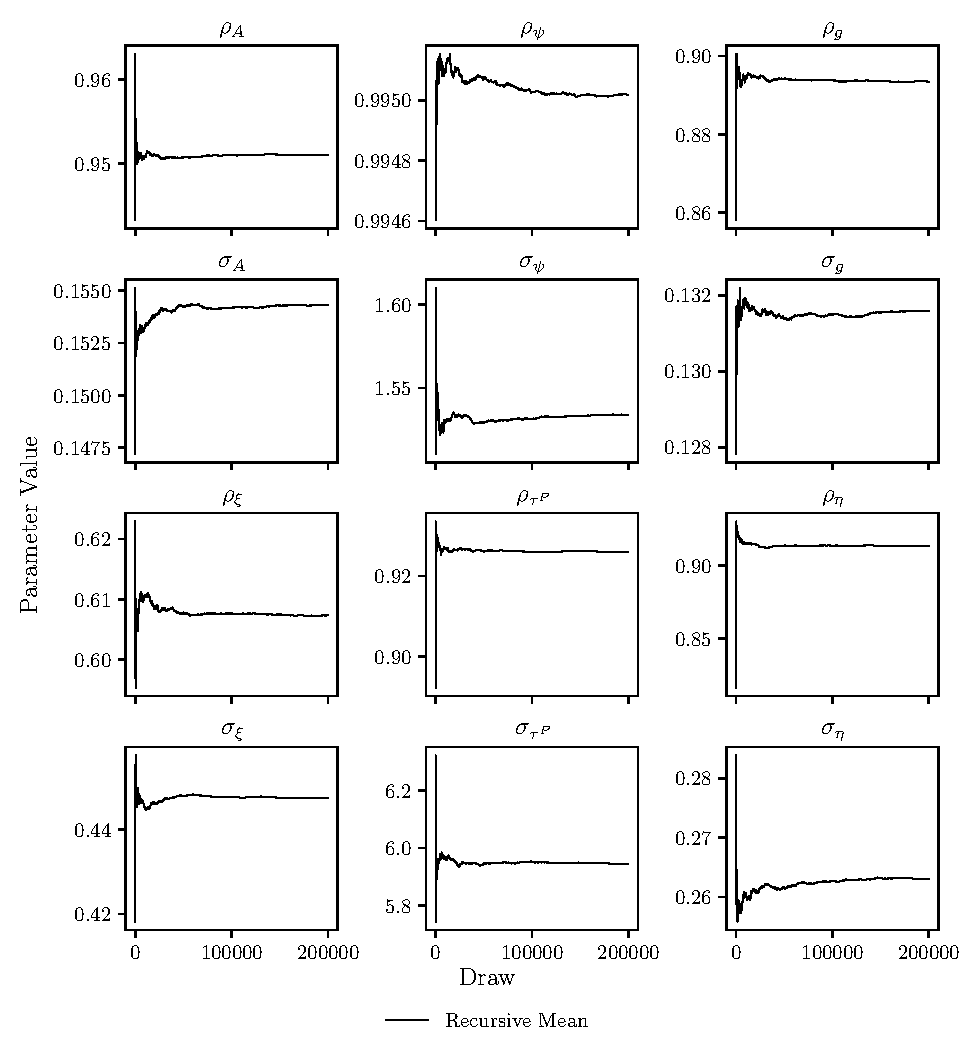
\includegraphics{figures/recursive_means.pdf}
    \label{fig:recursive-means}
\end{figure}

\begin{figure}[ht]
    \centering
    \caption{Posterior Distributions}
    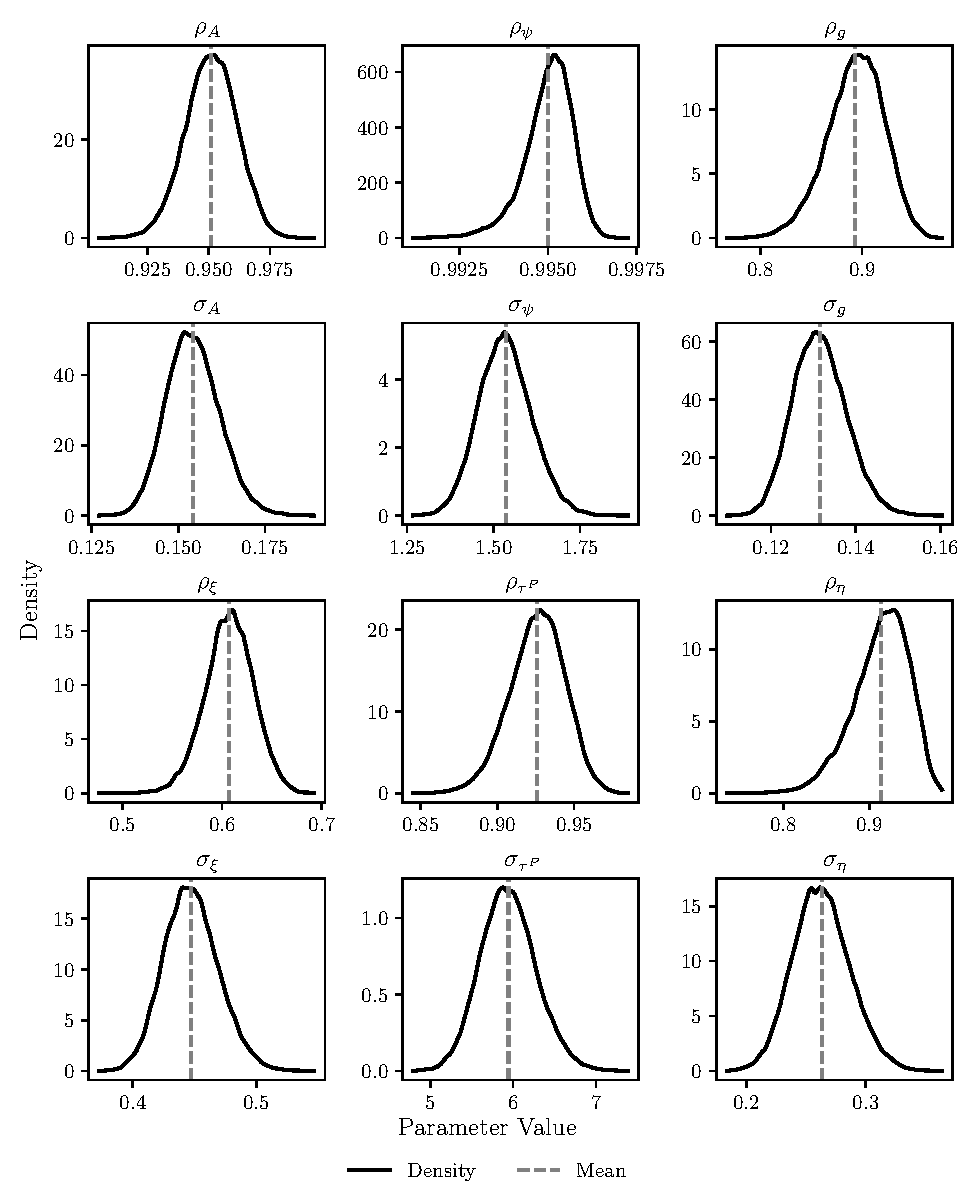
\includegraphics{figures/posteriors.pdf}
    \label{fig:posteriors}
\end{figure}

\begin{figure}[ht]
    \centering
    \caption{Posterior Covariences}
    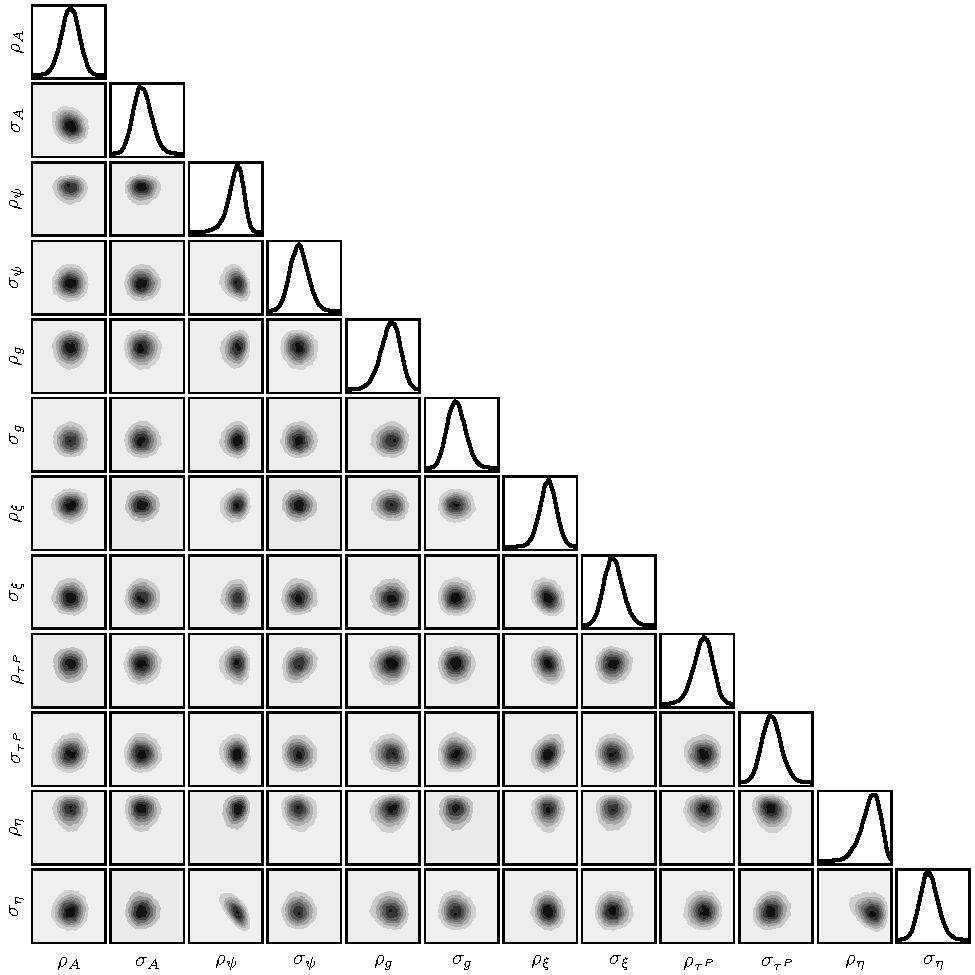
\includegraphics{figures/triangle.pdf}
    \label{fig:triangle}
\end{figure}

\FloatBarrier

% --- Aggregate IRFs ---
\section{Aggregate IRFs} \label{app:agg-irfs}
\begin{figure}[ht]
    \centering
    \caption{TFP ($A$) Shock Impulse Response Functions}
    %% Creator: Matplotlib, PGF backend
%%
%% To include the figure in your LaTeX document, write
%%   \input{<filename>.pgf}
%%
%% Make sure the required packages are loaded in your preamble
%%   \usepackage{pgf}
%%
%% Also ensure that all the required font packages are loaded; for instance,
%% the lmodern package is sometimes necessary when using math font.
%%   \usepackage{lmodern}
%%
%% Figures using additional raster images can only be included by \input if
%% they are in the same directory as the main LaTeX file. For loading figures
%% from other directories you can use the `import` package
%%   \usepackage{import}
%%
%% and then include the figures with
%%   \import{<path to file>}{<filename>.pgf}
%%
%% Matplotlib used the following preamble
%%   \def\mathdefault#1{#1}
%%   \everymath=\expandafter{\the\everymath\displaystyle}
%%   
%%   \ifdefined\pdftexversion\else  % non-pdftex case.
%%     \usepackage{fontspec}
%%     \setmainfont{DejaVuSerif.ttf}[Path=\detokenize{/opt/miniconda3/lib/python3.12/site-packages/matplotlib/mpl-data/fonts/ttf/}]
%%     \setsansfont{DejaVuSans.ttf}[Path=\detokenize{/opt/miniconda3/lib/python3.12/site-packages/matplotlib/mpl-data/fonts/ttf/}]
%%     \setmonofont{DejaVuSansMono.ttf}[Path=\detokenize{/opt/miniconda3/lib/python3.12/site-packages/matplotlib/mpl-data/fonts/ttf/}]
%%   \fi
%%   \makeatletter\@ifpackageloaded{underscore}{}{\usepackage[strings]{underscore}}\makeatother
%%
\begingroup%
\makeatletter%
\begin{pgfpicture}%
\pgfpathrectangle{\pgfpointorigin}{\pgfqpoint{6.500000in}{3.500000in}}%
\pgfusepath{use as bounding box, clip}%
\begin{pgfscope}%
\pgfsetbuttcap%
\pgfsetmiterjoin%
\definecolor{currentfill}{rgb}{1.000000,1.000000,1.000000}%
\pgfsetfillcolor{currentfill}%
\pgfsetlinewidth{0.000000pt}%
\definecolor{currentstroke}{rgb}{1.000000,1.000000,1.000000}%
\pgfsetstrokecolor{currentstroke}%
\pgfsetdash{}{0pt}%
\pgfpathmoveto{\pgfqpoint{0.000000in}{0.000000in}}%
\pgfpathlineto{\pgfqpoint{6.500000in}{0.000000in}}%
\pgfpathlineto{\pgfqpoint{6.500000in}{3.500000in}}%
\pgfpathlineto{\pgfqpoint{0.000000in}{3.500000in}}%
\pgfpathlineto{\pgfqpoint{0.000000in}{0.000000in}}%
\pgfpathclose%
\pgfusepath{fill}%
\end{pgfscope}%
\begin{pgfscope}%
\pgfsetbuttcap%
\pgfsetmiterjoin%
\definecolor{currentfill}{rgb}{1.000000,1.000000,1.000000}%
\pgfsetfillcolor{currentfill}%
\pgfsetlinewidth{0.000000pt}%
\definecolor{currentstroke}{rgb}{0.000000,0.000000,0.000000}%
\pgfsetstrokecolor{currentstroke}%
\pgfsetstrokeopacity{0.000000}%
\pgfsetdash{}{0pt}%
\pgfpathmoveto{\pgfqpoint{0.605098in}{2.526441in}}%
\pgfpathlineto{\pgfqpoint{1.648191in}{2.526441in}}%
\pgfpathlineto{\pgfqpoint{1.648191in}{3.251132in}}%
\pgfpathlineto{\pgfqpoint{0.605098in}{3.251132in}}%
\pgfpathlineto{\pgfqpoint{0.605098in}{2.526441in}}%
\pgfpathclose%
\pgfusepath{fill}%
\end{pgfscope}%
\begin{pgfscope}%
\pgfsetbuttcap%
\pgfsetroundjoin%
\definecolor{currentfill}{rgb}{0.000000,0.000000,0.000000}%
\pgfsetfillcolor{currentfill}%
\pgfsetlinewidth{0.803000pt}%
\definecolor{currentstroke}{rgb}{0.000000,0.000000,0.000000}%
\pgfsetstrokecolor{currentstroke}%
\pgfsetdash{}{0pt}%
\pgfsys@defobject{currentmarker}{\pgfqpoint{0.000000in}{-0.048611in}}{\pgfqpoint{0.000000in}{0.000000in}}{%
\pgfpathmoveto{\pgfqpoint{0.000000in}{0.000000in}}%
\pgfpathlineto{\pgfqpoint{0.000000in}{-0.048611in}}%
\pgfusepath{stroke,fill}%
}%
\begin{pgfscope}%
\pgfsys@transformshift{0.652512in}{2.526441in}%
\pgfsys@useobject{currentmarker}{}%
\end{pgfscope}%
\end{pgfscope}%
\begin{pgfscope}%
\pgfsetbuttcap%
\pgfsetroundjoin%
\definecolor{currentfill}{rgb}{0.000000,0.000000,0.000000}%
\pgfsetfillcolor{currentfill}%
\pgfsetlinewidth{0.803000pt}%
\definecolor{currentstroke}{rgb}{0.000000,0.000000,0.000000}%
\pgfsetstrokecolor{currentstroke}%
\pgfsetdash{}{0pt}%
\pgfsys@defobject{currentmarker}{\pgfqpoint{0.000000in}{-0.048611in}}{\pgfqpoint{0.000000in}{0.000000in}}{%
\pgfpathmoveto{\pgfqpoint{0.000000in}{0.000000in}}%
\pgfpathlineto{\pgfqpoint{0.000000in}{-0.048611in}}%
\pgfusepath{stroke,fill}%
}%
\begin{pgfscope}%
\pgfsys@transformshift{1.605543in}{2.526441in}%
\pgfsys@useobject{currentmarker}{}%
\end{pgfscope}%
\end{pgfscope}%
\begin{pgfscope}%
\pgfsetbuttcap%
\pgfsetroundjoin%
\definecolor{currentfill}{rgb}{0.000000,0.000000,0.000000}%
\pgfsetfillcolor{currentfill}%
\pgfsetlinewidth{0.803000pt}%
\definecolor{currentstroke}{rgb}{0.000000,0.000000,0.000000}%
\pgfsetstrokecolor{currentstroke}%
\pgfsetdash{}{0pt}%
\pgfsys@defobject{currentmarker}{\pgfqpoint{-0.048611in}{0.000000in}}{\pgfqpoint{-0.000000in}{0.000000in}}{%
\pgfpathmoveto{\pgfqpoint{-0.000000in}{0.000000in}}%
\pgfpathlineto{\pgfqpoint{-0.048611in}{0.000000in}}%
\pgfusepath{stroke,fill}%
}%
\begin{pgfscope}%
\pgfsys@transformshift{0.605098in}{2.559344in}%
\pgfsys@useobject{currentmarker}{}%
\end{pgfscope}%
\end{pgfscope}%
\begin{pgfscope}%
\definecolor{textcolor}{rgb}{0.000000,0.000000,0.000000}%
\pgfsetstrokecolor{textcolor}%
\pgfsetfillcolor{textcolor}%
\pgftext[x=0.330407in, y=2.506583in, left, base]{\color{textcolor}{\rmfamily\fontsize{10.000000}{12.000000}\selectfont\catcode`\^=\active\def^{\ifmmode\sp\else\^{}\fi}\catcode`\%=\active\def%{\%}$\mathdefault{0.0}$}}%
\end{pgfscope}%
\begin{pgfscope}%
\pgfsetbuttcap%
\pgfsetroundjoin%
\definecolor{currentfill}{rgb}{0.000000,0.000000,0.000000}%
\pgfsetfillcolor{currentfill}%
\pgfsetlinewidth{0.803000pt}%
\definecolor{currentstroke}{rgb}{0.000000,0.000000,0.000000}%
\pgfsetstrokecolor{currentstroke}%
\pgfsetdash{}{0pt}%
\pgfsys@defobject{currentmarker}{\pgfqpoint{-0.048611in}{0.000000in}}{\pgfqpoint{-0.000000in}{0.000000in}}{%
\pgfpathmoveto{\pgfqpoint{-0.000000in}{0.000000in}}%
\pgfpathlineto{\pgfqpoint{-0.048611in}{0.000000in}}%
\pgfusepath{stroke,fill}%
}%
\begin{pgfscope}%
\pgfsys@transformshift{0.605098in}{2.988816in}%
\pgfsys@useobject{currentmarker}{}%
\end{pgfscope}%
\end{pgfscope}%
\begin{pgfscope}%
\definecolor{textcolor}{rgb}{0.000000,0.000000,0.000000}%
\pgfsetstrokecolor{textcolor}%
\pgfsetfillcolor{textcolor}%
\pgftext[x=0.330407in, y=2.936055in, left, base]{\color{textcolor}{\rmfamily\fontsize{10.000000}{12.000000}\selectfont\catcode`\^=\active\def^{\ifmmode\sp\else\^{}\fi}\catcode`\%=\active\def%{\%}$\mathdefault{0.1}$}}%
\end{pgfscope}%
\begin{pgfscope}%
\pgfpathrectangle{\pgfqpoint{0.605098in}{2.526441in}}{\pgfqpoint{1.043093in}{0.724691in}}%
\pgfusepath{clip}%
\pgfsetrectcap%
\pgfsetroundjoin%
\pgfsetlinewidth{1.003750pt}%
\definecolor{currentstroke}{rgb}{0.000000,0.000000,0.000000}%
\pgfsetstrokecolor{currentstroke}%
\pgfsetdash{}{0pt}%
\pgfpathmoveto{\pgfqpoint{0.652512in}{3.218191in}}%
\pgfpathlineto{\pgfqpoint{0.666807in}{3.127919in}}%
\pgfpathlineto{\pgfqpoint{0.681103in}{3.050016in}}%
\pgfpathlineto{\pgfqpoint{0.695398in}{2.982786in}}%
\pgfpathlineto{\pgfqpoint{0.709694in}{2.924768in}}%
\pgfpathlineto{\pgfqpoint{0.723989in}{2.874700in}}%
\pgfpathlineto{\pgfqpoint{0.738285in}{2.831491in}}%
\pgfpathlineto{\pgfqpoint{0.752580in}{2.794203in}}%
\pgfpathlineto{\pgfqpoint{0.766876in}{2.762024in}}%
\pgfpathlineto{\pgfqpoint{0.781171in}{2.734254in}}%
\pgfpathlineto{\pgfqpoint{0.795466in}{2.710288in}}%
\pgfpathlineto{\pgfqpoint{0.814527in}{2.683363in}}%
\pgfpathlineto{\pgfqpoint{0.833588in}{2.661240in}}%
\pgfpathlineto{\pgfqpoint{0.852648in}{2.643064in}}%
\pgfpathlineto{\pgfqpoint{0.871709in}{2.628130in}}%
\pgfpathlineto{\pgfqpoint{0.890770in}{2.615860in}}%
\pgfpathlineto{\pgfqpoint{0.914595in}{2.603553in}}%
\pgfpathlineto{\pgfqpoint{0.938421in}{2.593926in}}%
\pgfpathlineto{\pgfqpoint{0.967012in}{2.585099in}}%
\pgfpathlineto{\pgfqpoint{0.995603in}{2.578525in}}%
\pgfpathlineto{\pgfqpoint{1.033724in}{2.572292in}}%
\pgfpathlineto{\pgfqpoint{1.076611in}{2.567666in}}%
\pgfpathlineto{\pgfqpoint{1.133792in}{2.563960in}}%
\pgfpathlineto{\pgfqpoint{1.210035in}{2.561448in}}%
\pgfpathlineto{\pgfqpoint{1.333929in}{2.559931in}}%
\pgfpathlineto{\pgfqpoint{1.600778in}{2.559382in}}%
\pgfpathlineto{\pgfqpoint{1.600778in}{2.559382in}}%
\pgfusepath{stroke}%
\end{pgfscope}%
\begin{pgfscope}%
\pgfpathrectangle{\pgfqpoint{0.605098in}{2.526441in}}{\pgfqpoint{1.043093in}{0.724691in}}%
\pgfusepath{clip}%
\pgfsetbuttcap%
\pgfsetroundjoin%
\pgfsetlinewidth{1.003750pt}%
\definecolor{currentstroke}{rgb}{0.000000,0.000000,0.000000}%
\pgfsetstrokecolor{currentstroke}%
\pgfsetdash{{3.700000pt}{1.600000pt}}{0.000000pt}%
\pgfpathmoveto{\pgfqpoint{0.605098in}{2.559344in}}%
\pgfpathlineto{\pgfqpoint{1.648191in}{2.559344in}}%
\pgfusepath{stroke}%
\end{pgfscope}%
\begin{pgfscope}%
\pgfsetrectcap%
\pgfsetmiterjoin%
\pgfsetlinewidth{0.803000pt}%
\definecolor{currentstroke}{rgb}{0.000000,0.000000,0.000000}%
\pgfsetstrokecolor{currentstroke}%
\pgfsetdash{}{0pt}%
\pgfpathmoveto{\pgfqpoint{0.605098in}{2.526441in}}%
\pgfpathlineto{\pgfqpoint{0.605098in}{3.251132in}}%
\pgfusepath{stroke}%
\end{pgfscope}%
\begin{pgfscope}%
\pgfsetrectcap%
\pgfsetmiterjoin%
\pgfsetlinewidth{0.803000pt}%
\definecolor{currentstroke}{rgb}{0.000000,0.000000,0.000000}%
\pgfsetstrokecolor{currentstroke}%
\pgfsetdash{}{0pt}%
\pgfpathmoveto{\pgfqpoint{1.648191in}{2.526441in}}%
\pgfpathlineto{\pgfqpoint{1.648191in}{3.251132in}}%
\pgfusepath{stroke}%
\end{pgfscope}%
\begin{pgfscope}%
\pgfsetrectcap%
\pgfsetmiterjoin%
\pgfsetlinewidth{0.803000pt}%
\definecolor{currentstroke}{rgb}{0.000000,0.000000,0.000000}%
\pgfsetstrokecolor{currentstroke}%
\pgfsetdash{}{0pt}%
\pgfpathmoveto{\pgfqpoint{0.605098in}{2.526441in}}%
\pgfpathlineto{\pgfqpoint{1.648191in}{2.526441in}}%
\pgfusepath{stroke}%
\end{pgfscope}%
\begin{pgfscope}%
\pgfsetrectcap%
\pgfsetmiterjoin%
\pgfsetlinewidth{0.803000pt}%
\definecolor{currentstroke}{rgb}{0.000000,0.000000,0.000000}%
\pgfsetstrokecolor{currentstroke}%
\pgfsetdash{}{0pt}%
\pgfpathmoveto{\pgfqpoint{0.605098in}{3.251132in}}%
\pgfpathlineto{\pgfqpoint{1.648191in}{3.251132in}}%
\pgfusepath{stroke}%
\end{pgfscope}%
\begin{pgfscope}%
\definecolor{textcolor}{rgb}{0.000000,0.000000,0.000000}%
\pgfsetstrokecolor{textcolor}%
\pgfsetfillcolor{textcolor}%
\pgftext[x=1.126645in,y=3.334465in,,base]{\color{textcolor}{\rmfamily\fontsize{10.000000}{12.000000}\selectfont\catcode`\^=\active\def^{\ifmmode\sp\else\^{}\fi}\catcode`\%=\active\def%{\%}$A$}}%
\end{pgfscope}%
\begin{pgfscope}%
\pgfsetbuttcap%
\pgfsetmiterjoin%
\definecolor{currentfill}{rgb}{1.000000,1.000000,1.000000}%
\pgfsetfillcolor{currentfill}%
\pgfsetlinewidth{0.000000pt}%
\definecolor{currentstroke}{rgb}{0.000000,0.000000,0.000000}%
\pgfsetstrokecolor{currentstroke}%
\pgfsetstrokeopacity{0.000000}%
\pgfsetdash{}{0pt}%
\pgfpathmoveto{\pgfqpoint{2.199220in}{2.526441in}}%
\pgfpathlineto{\pgfqpoint{3.242313in}{2.526441in}}%
\pgfpathlineto{\pgfqpoint{3.242313in}{3.251132in}}%
\pgfpathlineto{\pgfqpoint{2.199220in}{3.251132in}}%
\pgfpathlineto{\pgfqpoint{2.199220in}{2.526441in}}%
\pgfpathclose%
\pgfusepath{fill}%
\end{pgfscope}%
\begin{pgfscope}%
\pgfsetbuttcap%
\pgfsetroundjoin%
\definecolor{currentfill}{rgb}{0.000000,0.000000,0.000000}%
\pgfsetfillcolor{currentfill}%
\pgfsetlinewidth{0.803000pt}%
\definecolor{currentstroke}{rgb}{0.000000,0.000000,0.000000}%
\pgfsetstrokecolor{currentstroke}%
\pgfsetdash{}{0pt}%
\pgfsys@defobject{currentmarker}{\pgfqpoint{0.000000in}{-0.048611in}}{\pgfqpoint{0.000000in}{0.000000in}}{%
\pgfpathmoveto{\pgfqpoint{0.000000in}{0.000000in}}%
\pgfpathlineto{\pgfqpoint{0.000000in}{-0.048611in}}%
\pgfusepath{stroke,fill}%
}%
\begin{pgfscope}%
\pgfsys@transformshift{2.246633in}{2.526441in}%
\pgfsys@useobject{currentmarker}{}%
\end{pgfscope}%
\end{pgfscope}%
\begin{pgfscope}%
\pgfsetbuttcap%
\pgfsetroundjoin%
\definecolor{currentfill}{rgb}{0.000000,0.000000,0.000000}%
\pgfsetfillcolor{currentfill}%
\pgfsetlinewidth{0.803000pt}%
\definecolor{currentstroke}{rgb}{0.000000,0.000000,0.000000}%
\pgfsetstrokecolor{currentstroke}%
\pgfsetdash{}{0pt}%
\pgfsys@defobject{currentmarker}{\pgfqpoint{0.000000in}{-0.048611in}}{\pgfqpoint{0.000000in}{0.000000in}}{%
\pgfpathmoveto{\pgfqpoint{0.000000in}{0.000000in}}%
\pgfpathlineto{\pgfqpoint{0.000000in}{-0.048611in}}%
\pgfusepath{stroke,fill}%
}%
\begin{pgfscope}%
\pgfsys@transformshift{3.199664in}{2.526441in}%
\pgfsys@useobject{currentmarker}{}%
\end{pgfscope}%
\end{pgfscope}%
\begin{pgfscope}%
\pgfsetbuttcap%
\pgfsetroundjoin%
\definecolor{currentfill}{rgb}{0.000000,0.000000,0.000000}%
\pgfsetfillcolor{currentfill}%
\pgfsetlinewidth{0.803000pt}%
\definecolor{currentstroke}{rgb}{0.000000,0.000000,0.000000}%
\pgfsetstrokecolor{currentstroke}%
\pgfsetdash{}{0pt}%
\pgfsys@defobject{currentmarker}{\pgfqpoint{-0.048611in}{0.000000in}}{\pgfqpoint{-0.000000in}{0.000000in}}{%
\pgfpathmoveto{\pgfqpoint{-0.000000in}{0.000000in}}%
\pgfpathlineto{\pgfqpoint{-0.048611in}{0.000000in}}%
\pgfusepath{stroke,fill}%
}%
\begin{pgfscope}%
\pgfsys@transformshift{2.199220in}{2.559342in}%
\pgfsys@useobject{currentmarker}{}%
\end{pgfscope}%
\end{pgfscope}%
\begin{pgfscope}%
\definecolor{textcolor}{rgb}{0.000000,0.000000,0.000000}%
\pgfsetstrokecolor{textcolor}%
\pgfsetfillcolor{textcolor}%
\pgftext[x=1.855083in, y=2.506581in, left, base]{\color{textcolor}{\rmfamily\fontsize{10.000000}{12.000000}\selectfont\catcode`\^=\active\def^{\ifmmode\sp\else\^{}\fi}\catcode`\%=\active\def%{\%}$\mathdefault{0.00}$}}%
\end{pgfscope}%
\begin{pgfscope}%
\pgfsetbuttcap%
\pgfsetroundjoin%
\definecolor{currentfill}{rgb}{0.000000,0.000000,0.000000}%
\pgfsetfillcolor{currentfill}%
\pgfsetlinewidth{0.803000pt}%
\definecolor{currentstroke}{rgb}{0.000000,0.000000,0.000000}%
\pgfsetstrokecolor{currentstroke}%
\pgfsetdash{}{0pt}%
\pgfsys@defobject{currentmarker}{\pgfqpoint{-0.048611in}{0.000000in}}{\pgfqpoint{-0.000000in}{0.000000in}}{%
\pgfpathmoveto{\pgfqpoint{-0.000000in}{0.000000in}}%
\pgfpathlineto{\pgfqpoint{-0.048611in}{0.000000in}}%
\pgfusepath{stroke,fill}%
}%
\begin{pgfscope}%
\pgfsys@transformshift{2.199220in}{2.932782in}%
\pgfsys@useobject{currentmarker}{}%
\end{pgfscope}%
\end{pgfscope}%
\begin{pgfscope}%
\definecolor{textcolor}{rgb}{0.000000,0.000000,0.000000}%
\pgfsetstrokecolor{textcolor}%
\pgfsetfillcolor{textcolor}%
\pgftext[x=1.855083in, y=2.880021in, left, base]{\color{textcolor}{\rmfamily\fontsize{10.000000}{12.000000}\selectfont\catcode`\^=\active\def^{\ifmmode\sp\else\^{}\fi}\catcode`\%=\active\def%{\%}$\mathdefault{0.05}$}}%
\end{pgfscope}%
\begin{pgfscope}%
\pgfpathrectangle{\pgfqpoint{2.199220in}{2.526441in}}{\pgfqpoint{1.043093in}{0.724691in}}%
\pgfusepath{clip}%
\pgfsetrectcap%
\pgfsetroundjoin%
\pgfsetlinewidth{1.003750pt}%
\definecolor{currentstroke}{rgb}{0.000000,0.000000,0.000000}%
\pgfsetstrokecolor{currentstroke}%
\pgfsetdash{}{0pt}%
\pgfpathmoveto{\pgfqpoint{2.246633in}{3.218191in}}%
\pgfpathlineto{\pgfqpoint{2.251398in}{3.105361in}}%
\pgfpathlineto{\pgfqpoint{2.256164in}{3.048472in}}%
\pgfpathlineto{\pgfqpoint{2.260929in}{3.013908in}}%
\pgfpathlineto{\pgfqpoint{2.270459in}{2.967364in}}%
\pgfpathlineto{\pgfqpoint{2.284755in}{2.913534in}}%
\pgfpathlineto{\pgfqpoint{2.299050in}{2.867556in}}%
\pgfpathlineto{\pgfqpoint{2.313345in}{2.827511in}}%
\pgfpathlineto{\pgfqpoint{2.327641in}{2.792591in}}%
\pgfpathlineto{\pgfqpoint{2.341936in}{2.762149in}}%
\pgfpathlineto{\pgfqpoint{2.360997in}{2.727562in}}%
\pgfpathlineto{\pgfqpoint{2.380058in}{2.698804in}}%
\pgfpathlineto{\pgfqpoint{2.399118in}{2.674913in}}%
\pgfpathlineto{\pgfqpoint{2.418179in}{2.655080in}}%
\pgfpathlineto{\pgfqpoint{2.437240in}{2.638627in}}%
\pgfpathlineto{\pgfqpoint{2.456300in}{2.624984in}}%
\pgfpathlineto{\pgfqpoint{2.475361in}{2.613676in}}%
\pgfpathlineto{\pgfqpoint{2.499187in}{2.602228in}}%
\pgfpathlineto{\pgfqpoint{2.523012in}{2.593184in}}%
\pgfpathlineto{\pgfqpoint{2.551603in}{2.584804in}}%
\pgfpathlineto{\pgfqpoint{2.584959in}{2.577605in}}%
\pgfpathlineto{\pgfqpoint{2.623081in}{2.571829in}}%
\pgfpathlineto{\pgfqpoint{2.670732in}{2.567101in}}%
\pgfpathlineto{\pgfqpoint{2.732679in}{2.563517in}}%
\pgfpathlineto{\pgfqpoint{2.818452in}{2.561110in}}%
\pgfpathlineto{\pgfqpoint{2.956641in}{2.559783in}}%
\pgfpathlineto{\pgfqpoint{3.194899in}{2.559382in}}%
\pgfpathlineto{\pgfqpoint{3.194899in}{2.559382in}}%
\pgfusepath{stroke}%
\end{pgfscope}%
\begin{pgfscope}%
\pgfpathrectangle{\pgfqpoint{2.199220in}{2.526441in}}{\pgfqpoint{1.043093in}{0.724691in}}%
\pgfusepath{clip}%
\pgfsetbuttcap%
\pgfsetroundjoin%
\pgfsetlinewidth{1.003750pt}%
\definecolor{currentstroke}{rgb}{0.000000,0.000000,0.000000}%
\pgfsetstrokecolor{currentstroke}%
\pgfsetdash{{3.700000pt}{1.600000pt}}{0.000000pt}%
\pgfpathmoveto{\pgfqpoint{2.199220in}{2.559342in}}%
\pgfpathlineto{\pgfqpoint{3.242313in}{2.559342in}}%
\pgfusepath{stroke}%
\end{pgfscope}%
\begin{pgfscope}%
\pgfsetrectcap%
\pgfsetmiterjoin%
\pgfsetlinewidth{0.803000pt}%
\definecolor{currentstroke}{rgb}{0.000000,0.000000,0.000000}%
\pgfsetstrokecolor{currentstroke}%
\pgfsetdash{}{0pt}%
\pgfpathmoveto{\pgfqpoint{2.199220in}{2.526441in}}%
\pgfpathlineto{\pgfqpoint{2.199220in}{3.251132in}}%
\pgfusepath{stroke}%
\end{pgfscope}%
\begin{pgfscope}%
\pgfsetrectcap%
\pgfsetmiterjoin%
\pgfsetlinewidth{0.803000pt}%
\definecolor{currentstroke}{rgb}{0.000000,0.000000,0.000000}%
\pgfsetstrokecolor{currentstroke}%
\pgfsetdash{}{0pt}%
\pgfpathmoveto{\pgfqpoint{3.242313in}{2.526441in}}%
\pgfpathlineto{\pgfqpoint{3.242313in}{3.251132in}}%
\pgfusepath{stroke}%
\end{pgfscope}%
\begin{pgfscope}%
\pgfsetrectcap%
\pgfsetmiterjoin%
\pgfsetlinewidth{0.803000pt}%
\definecolor{currentstroke}{rgb}{0.000000,0.000000,0.000000}%
\pgfsetstrokecolor{currentstroke}%
\pgfsetdash{}{0pt}%
\pgfpathmoveto{\pgfqpoint{2.199220in}{2.526441in}}%
\pgfpathlineto{\pgfqpoint{3.242313in}{2.526441in}}%
\pgfusepath{stroke}%
\end{pgfscope}%
\begin{pgfscope}%
\pgfsetrectcap%
\pgfsetmiterjoin%
\pgfsetlinewidth{0.803000pt}%
\definecolor{currentstroke}{rgb}{0.000000,0.000000,0.000000}%
\pgfsetstrokecolor{currentstroke}%
\pgfsetdash{}{0pt}%
\pgfpathmoveto{\pgfqpoint{2.199220in}{3.251132in}}%
\pgfpathlineto{\pgfqpoint{3.242313in}{3.251132in}}%
\pgfusepath{stroke}%
\end{pgfscope}%
\begin{pgfscope}%
\definecolor{textcolor}{rgb}{0.000000,0.000000,0.000000}%
\pgfsetstrokecolor{textcolor}%
\pgfsetfillcolor{textcolor}%
\pgftext[x=2.720766in,y=3.334465in,,base]{\color{textcolor}{\rmfamily\fontsize{10.000000}{12.000000}\selectfont\catcode`\^=\active\def^{\ifmmode\sp\else\^{}\fi}\catcode`\%=\active\def%{\%}$Y$}}%
\end{pgfscope}%
\begin{pgfscope}%
\pgfsetbuttcap%
\pgfsetmiterjoin%
\definecolor{currentfill}{rgb}{1.000000,1.000000,1.000000}%
\pgfsetfillcolor{currentfill}%
\pgfsetlinewidth{0.000000pt}%
\definecolor{currentstroke}{rgb}{0.000000,0.000000,0.000000}%
\pgfsetstrokecolor{currentstroke}%
\pgfsetstrokeopacity{0.000000}%
\pgfsetdash{}{0pt}%
\pgfpathmoveto{\pgfqpoint{3.793341in}{2.526441in}}%
\pgfpathlineto{\pgfqpoint{4.836434in}{2.526441in}}%
\pgfpathlineto{\pgfqpoint{4.836434in}{3.251132in}}%
\pgfpathlineto{\pgfqpoint{3.793341in}{3.251132in}}%
\pgfpathlineto{\pgfqpoint{3.793341in}{2.526441in}}%
\pgfpathclose%
\pgfusepath{fill}%
\end{pgfscope}%
\begin{pgfscope}%
\pgfsetbuttcap%
\pgfsetroundjoin%
\definecolor{currentfill}{rgb}{0.000000,0.000000,0.000000}%
\pgfsetfillcolor{currentfill}%
\pgfsetlinewidth{0.803000pt}%
\definecolor{currentstroke}{rgb}{0.000000,0.000000,0.000000}%
\pgfsetstrokecolor{currentstroke}%
\pgfsetdash{}{0pt}%
\pgfsys@defobject{currentmarker}{\pgfqpoint{0.000000in}{-0.048611in}}{\pgfqpoint{0.000000in}{0.000000in}}{%
\pgfpathmoveto{\pgfqpoint{0.000000in}{0.000000in}}%
\pgfpathlineto{\pgfqpoint{0.000000in}{-0.048611in}}%
\pgfusepath{stroke,fill}%
}%
\begin{pgfscope}%
\pgfsys@transformshift{3.840755in}{2.526441in}%
\pgfsys@useobject{currentmarker}{}%
\end{pgfscope}%
\end{pgfscope}%
\begin{pgfscope}%
\pgfsetbuttcap%
\pgfsetroundjoin%
\definecolor{currentfill}{rgb}{0.000000,0.000000,0.000000}%
\pgfsetfillcolor{currentfill}%
\pgfsetlinewidth{0.803000pt}%
\definecolor{currentstroke}{rgb}{0.000000,0.000000,0.000000}%
\pgfsetstrokecolor{currentstroke}%
\pgfsetdash{}{0pt}%
\pgfsys@defobject{currentmarker}{\pgfqpoint{0.000000in}{-0.048611in}}{\pgfqpoint{0.000000in}{0.000000in}}{%
\pgfpathmoveto{\pgfqpoint{0.000000in}{0.000000in}}%
\pgfpathlineto{\pgfqpoint{0.000000in}{-0.048611in}}%
\pgfusepath{stroke,fill}%
}%
\begin{pgfscope}%
\pgfsys@transformshift{4.793786in}{2.526441in}%
\pgfsys@useobject{currentmarker}{}%
\end{pgfscope}%
\end{pgfscope}%
\begin{pgfscope}%
\pgfsetbuttcap%
\pgfsetroundjoin%
\definecolor{currentfill}{rgb}{0.000000,0.000000,0.000000}%
\pgfsetfillcolor{currentfill}%
\pgfsetlinewidth{0.803000pt}%
\definecolor{currentstroke}{rgb}{0.000000,0.000000,0.000000}%
\pgfsetstrokecolor{currentstroke}%
\pgfsetdash{}{0pt}%
\pgfsys@defobject{currentmarker}{\pgfqpoint{-0.048611in}{0.000000in}}{\pgfqpoint{-0.000000in}{0.000000in}}{%
\pgfpathmoveto{\pgfqpoint{-0.000000in}{0.000000in}}%
\pgfpathlineto{\pgfqpoint{-0.048611in}{0.000000in}}%
\pgfusepath{stroke,fill}%
}%
\begin{pgfscope}%
\pgfsys@transformshift{3.793341in}{2.583586in}%
\pgfsys@useobject{currentmarker}{}%
\end{pgfscope}%
\end{pgfscope}%
\begin{pgfscope}%
\definecolor{textcolor}{rgb}{0.000000,0.000000,0.000000}%
\pgfsetstrokecolor{textcolor}%
\pgfsetfillcolor{textcolor}%
\pgftext[x=3.341180in, y=2.530824in, left, base]{\color{textcolor}{\rmfamily\fontsize{10.000000}{12.000000}\selectfont\catcode`\^=\active\def^{\ifmmode\sp\else\^{}\fi}\catcode`\%=\active\def%{\%}$\mathdefault{\ensuremath{-}0.02}$}}%
\end{pgfscope}%
\begin{pgfscope}%
\pgfsetbuttcap%
\pgfsetroundjoin%
\definecolor{currentfill}{rgb}{0.000000,0.000000,0.000000}%
\pgfsetfillcolor{currentfill}%
\pgfsetlinewidth{0.803000pt}%
\definecolor{currentstroke}{rgb}{0.000000,0.000000,0.000000}%
\pgfsetstrokecolor{currentstroke}%
\pgfsetdash{}{0pt}%
\pgfsys@defobject{currentmarker}{\pgfqpoint{-0.048611in}{0.000000in}}{\pgfqpoint{-0.000000in}{0.000000in}}{%
\pgfpathmoveto{\pgfqpoint{-0.000000in}{0.000000in}}%
\pgfpathlineto{\pgfqpoint{-0.048611in}{0.000000in}}%
\pgfusepath{stroke,fill}%
}%
\begin{pgfscope}%
\pgfsys@transformshift{3.793341in}{3.215851in}%
\pgfsys@useobject{currentmarker}{}%
\end{pgfscope}%
\end{pgfscope}%
\begin{pgfscope}%
\definecolor{textcolor}{rgb}{0.000000,0.000000,0.000000}%
\pgfsetstrokecolor{textcolor}%
\pgfsetfillcolor{textcolor}%
\pgftext[x=3.449205in, y=3.163090in, left, base]{\color{textcolor}{\rmfamily\fontsize{10.000000}{12.000000}\selectfont\catcode`\^=\active\def^{\ifmmode\sp\else\^{}\fi}\catcode`\%=\active\def%{\%}$\mathdefault{0.00}$}}%
\end{pgfscope}%
\begin{pgfscope}%
\pgfpathrectangle{\pgfqpoint{3.793341in}{2.526441in}}{\pgfqpoint{1.043093in}{0.724691in}}%
\pgfusepath{clip}%
\pgfsetrectcap%
\pgfsetroundjoin%
\pgfsetlinewidth{1.003750pt}%
\definecolor{currentstroke}{rgb}{0.000000,0.000000,0.000000}%
\pgfsetstrokecolor{currentstroke}%
\pgfsetdash{}{0pt}%
\pgfpathmoveto{\pgfqpoint{3.840755in}{2.559382in}}%
\pgfpathlineto{\pgfqpoint{3.845520in}{2.735993in}}%
\pgfpathlineto{\pgfqpoint{3.850285in}{2.817446in}}%
\pgfpathlineto{\pgfqpoint{3.855050in}{2.861621in}}%
\pgfpathlineto{\pgfqpoint{3.864581in}{2.913836in}}%
\pgfpathlineto{\pgfqpoint{3.878876in}{2.969062in}}%
\pgfpathlineto{\pgfqpoint{3.893172in}{3.014308in}}%
\pgfpathlineto{\pgfqpoint{3.907467in}{3.051978in}}%
\pgfpathlineto{\pgfqpoint{3.921762in}{3.083126in}}%
\pgfpathlineto{\pgfqpoint{3.936058in}{3.108778in}}%
\pgfpathlineto{\pgfqpoint{3.950353in}{3.129863in}}%
\pgfpathlineto{\pgfqpoint{3.964649in}{3.147174in}}%
\pgfpathlineto{\pgfqpoint{3.978944in}{3.161364in}}%
\pgfpathlineto{\pgfqpoint{3.993240in}{3.172970in}}%
\pgfpathlineto{\pgfqpoint{4.012300in}{3.185180in}}%
\pgfpathlineto{\pgfqpoint{4.031361in}{3.194424in}}%
\pgfpathlineto{\pgfqpoint{4.050422in}{3.201366in}}%
\pgfpathlineto{\pgfqpoint{4.074247in}{3.207589in}}%
\pgfpathlineto{\pgfqpoint{4.102838in}{3.212451in}}%
\pgfpathlineto{\pgfqpoint{4.136194in}{3.215716in}}%
\pgfpathlineto{\pgfqpoint{4.179081in}{3.217630in}}%
\pgfpathlineto{\pgfqpoint{4.245793in}{3.218173in}}%
\pgfpathlineto{\pgfqpoint{4.789021in}{3.215896in}}%
\pgfpathlineto{\pgfqpoint{4.789021in}{3.215896in}}%
\pgfusepath{stroke}%
\end{pgfscope}%
\begin{pgfscope}%
\pgfpathrectangle{\pgfqpoint{3.793341in}{2.526441in}}{\pgfqpoint{1.043093in}{0.724691in}}%
\pgfusepath{clip}%
\pgfsetbuttcap%
\pgfsetroundjoin%
\pgfsetlinewidth{1.003750pt}%
\definecolor{currentstroke}{rgb}{0.000000,0.000000,0.000000}%
\pgfsetstrokecolor{currentstroke}%
\pgfsetdash{{3.700000pt}{1.600000pt}}{0.000000pt}%
\pgfpathmoveto{\pgfqpoint{3.793341in}{3.215851in}}%
\pgfpathlineto{\pgfqpoint{4.836434in}{3.215851in}}%
\pgfusepath{stroke}%
\end{pgfscope}%
\begin{pgfscope}%
\pgfsetrectcap%
\pgfsetmiterjoin%
\pgfsetlinewidth{0.803000pt}%
\definecolor{currentstroke}{rgb}{0.000000,0.000000,0.000000}%
\pgfsetstrokecolor{currentstroke}%
\pgfsetdash{}{0pt}%
\pgfpathmoveto{\pgfqpoint{3.793341in}{2.526441in}}%
\pgfpathlineto{\pgfqpoint{3.793341in}{3.251132in}}%
\pgfusepath{stroke}%
\end{pgfscope}%
\begin{pgfscope}%
\pgfsetrectcap%
\pgfsetmiterjoin%
\pgfsetlinewidth{0.803000pt}%
\definecolor{currentstroke}{rgb}{0.000000,0.000000,0.000000}%
\pgfsetstrokecolor{currentstroke}%
\pgfsetdash{}{0pt}%
\pgfpathmoveto{\pgfqpoint{4.836434in}{2.526441in}}%
\pgfpathlineto{\pgfqpoint{4.836434in}{3.251132in}}%
\pgfusepath{stroke}%
\end{pgfscope}%
\begin{pgfscope}%
\pgfsetrectcap%
\pgfsetmiterjoin%
\pgfsetlinewidth{0.803000pt}%
\definecolor{currentstroke}{rgb}{0.000000,0.000000,0.000000}%
\pgfsetstrokecolor{currentstroke}%
\pgfsetdash{}{0pt}%
\pgfpathmoveto{\pgfqpoint{3.793341in}{2.526441in}}%
\pgfpathlineto{\pgfqpoint{4.836434in}{2.526441in}}%
\pgfusepath{stroke}%
\end{pgfscope}%
\begin{pgfscope}%
\pgfsetrectcap%
\pgfsetmiterjoin%
\pgfsetlinewidth{0.803000pt}%
\definecolor{currentstroke}{rgb}{0.000000,0.000000,0.000000}%
\pgfsetstrokecolor{currentstroke}%
\pgfsetdash{}{0pt}%
\pgfpathmoveto{\pgfqpoint{3.793341in}{3.251132in}}%
\pgfpathlineto{\pgfqpoint{4.836434in}{3.251132in}}%
\pgfusepath{stroke}%
\end{pgfscope}%
\begin{pgfscope}%
\definecolor{textcolor}{rgb}{0.000000,0.000000,0.000000}%
\pgfsetstrokecolor{textcolor}%
\pgfsetfillcolor{textcolor}%
\pgftext[x=4.314888in,y=3.334465in,,base]{\color{textcolor}{\rmfamily\fontsize{10.000000}{12.000000}\selectfont\catcode`\^=\active\def^{\ifmmode\sp\else\^{}\fi}\catcode`\%=\active\def%{\%}$\pi$}}%
\end{pgfscope}%
\begin{pgfscope}%
\pgfsetbuttcap%
\pgfsetmiterjoin%
\definecolor{currentfill}{rgb}{1.000000,1.000000,1.000000}%
\pgfsetfillcolor{currentfill}%
\pgfsetlinewidth{0.000000pt}%
\definecolor{currentstroke}{rgb}{0.000000,0.000000,0.000000}%
\pgfsetstrokecolor{currentstroke}%
\pgfsetstrokeopacity{0.000000}%
\pgfsetdash{}{0pt}%
\pgfpathmoveto{\pgfqpoint{5.387463in}{2.526441in}}%
\pgfpathlineto{\pgfqpoint{6.430556in}{2.526441in}}%
\pgfpathlineto{\pgfqpoint{6.430556in}{3.251132in}}%
\pgfpathlineto{\pgfqpoint{5.387463in}{3.251132in}}%
\pgfpathlineto{\pgfqpoint{5.387463in}{2.526441in}}%
\pgfpathclose%
\pgfusepath{fill}%
\end{pgfscope}%
\begin{pgfscope}%
\pgfsetbuttcap%
\pgfsetroundjoin%
\definecolor{currentfill}{rgb}{0.000000,0.000000,0.000000}%
\pgfsetfillcolor{currentfill}%
\pgfsetlinewidth{0.803000pt}%
\definecolor{currentstroke}{rgb}{0.000000,0.000000,0.000000}%
\pgfsetstrokecolor{currentstroke}%
\pgfsetdash{}{0pt}%
\pgfsys@defobject{currentmarker}{\pgfqpoint{0.000000in}{-0.048611in}}{\pgfqpoint{0.000000in}{0.000000in}}{%
\pgfpathmoveto{\pgfqpoint{0.000000in}{0.000000in}}%
\pgfpathlineto{\pgfqpoint{0.000000in}{-0.048611in}}%
\pgfusepath{stroke,fill}%
}%
\begin{pgfscope}%
\pgfsys@transformshift{5.434876in}{2.526441in}%
\pgfsys@useobject{currentmarker}{}%
\end{pgfscope}%
\end{pgfscope}%
\begin{pgfscope}%
\pgfsetbuttcap%
\pgfsetroundjoin%
\definecolor{currentfill}{rgb}{0.000000,0.000000,0.000000}%
\pgfsetfillcolor{currentfill}%
\pgfsetlinewidth{0.803000pt}%
\definecolor{currentstroke}{rgb}{0.000000,0.000000,0.000000}%
\pgfsetstrokecolor{currentstroke}%
\pgfsetdash{}{0pt}%
\pgfsys@defobject{currentmarker}{\pgfqpoint{0.000000in}{-0.048611in}}{\pgfqpoint{0.000000in}{0.000000in}}{%
\pgfpathmoveto{\pgfqpoint{0.000000in}{0.000000in}}%
\pgfpathlineto{\pgfqpoint{0.000000in}{-0.048611in}}%
\pgfusepath{stroke,fill}%
}%
\begin{pgfscope}%
\pgfsys@transformshift{6.387907in}{2.526441in}%
\pgfsys@useobject{currentmarker}{}%
\end{pgfscope}%
\end{pgfscope}%
\begin{pgfscope}%
\pgfsetbuttcap%
\pgfsetroundjoin%
\definecolor{currentfill}{rgb}{0.000000,0.000000,0.000000}%
\pgfsetfillcolor{currentfill}%
\pgfsetlinewidth{0.803000pt}%
\definecolor{currentstroke}{rgb}{0.000000,0.000000,0.000000}%
\pgfsetstrokecolor{currentstroke}%
\pgfsetdash{}{0pt}%
\pgfsys@defobject{currentmarker}{\pgfqpoint{-0.048611in}{0.000000in}}{\pgfqpoint{-0.000000in}{0.000000in}}{%
\pgfpathmoveto{\pgfqpoint{-0.000000in}{0.000000in}}%
\pgfpathlineto{\pgfqpoint{-0.048611in}{0.000000in}}%
\pgfusepath{stroke,fill}%
}%
\begin{pgfscope}%
\pgfsys@transformshift{5.387463in}{2.559330in}%
\pgfsys@useobject{currentmarker}{}%
\end{pgfscope}%
\end{pgfscope}%
\begin{pgfscope}%
\definecolor{textcolor}{rgb}{0.000000,0.000000,0.000000}%
\pgfsetstrokecolor{textcolor}%
\pgfsetfillcolor{textcolor}%
\pgftext[x=5.112771in, y=2.506569in, left, base]{\color{textcolor}{\rmfamily\fontsize{10.000000}{12.000000}\selectfont\catcode`\^=\active\def^{\ifmmode\sp\else\^{}\fi}\catcode`\%=\active\def%{\%}$\mathdefault{0.0}$}}%
\end{pgfscope}%
\begin{pgfscope}%
\pgfsetbuttcap%
\pgfsetroundjoin%
\definecolor{currentfill}{rgb}{0.000000,0.000000,0.000000}%
\pgfsetfillcolor{currentfill}%
\pgfsetlinewidth{0.803000pt}%
\definecolor{currentstroke}{rgb}{0.000000,0.000000,0.000000}%
\pgfsetstrokecolor{currentstroke}%
\pgfsetdash{}{0pt}%
\pgfsys@defobject{currentmarker}{\pgfqpoint{-0.048611in}{0.000000in}}{\pgfqpoint{-0.000000in}{0.000000in}}{%
\pgfpathmoveto{\pgfqpoint{-0.000000in}{0.000000in}}%
\pgfpathlineto{\pgfqpoint{-0.048611in}{0.000000in}}%
\pgfusepath{stroke,fill}%
}%
\begin{pgfscope}%
\pgfsys@transformshift{5.387463in}{3.209430in}%
\pgfsys@useobject{currentmarker}{}%
\end{pgfscope}%
\end{pgfscope}%
\begin{pgfscope}%
\definecolor{textcolor}{rgb}{0.000000,0.000000,0.000000}%
\pgfsetstrokecolor{textcolor}%
\pgfsetfillcolor{textcolor}%
\pgftext[x=5.112771in, y=3.156668in, left, base]{\color{textcolor}{\rmfamily\fontsize{10.000000}{12.000000}\selectfont\catcode`\^=\active\def^{\ifmmode\sp\else\^{}\fi}\catcode`\%=\active\def%{\%}$\mathdefault{0.1}$}}%
\end{pgfscope}%
\begin{pgfscope}%
\pgfpathrectangle{\pgfqpoint{5.387463in}{2.526441in}}{\pgfqpoint{1.043093in}{0.724691in}}%
\pgfusepath{clip}%
\pgfsetrectcap%
\pgfsetroundjoin%
\pgfsetlinewidth{1.003750pt}%
\definecolor{currentstroke}{rgb}{0.000000,0.000000,0.000000}%
\pgfsetstrokecolor{currentstroke}%
\pgfsetdash{}{0pt}%
\pgfpathmoveto{\pgfqpoint{5.434876in}{3.022326in}}%
\pgfpathlineto{\pgfqpoint{5.439641in}{3.179008in}}%
\pgfpathlineto{\pgfqpoint{5.444407in}{3.218191in}}%
\pgfpathlineto{\pgfqpoint{5.449172in}{3.213056in}}%
\pgfpathlineto{\pgfqpoint{5.453937in}{3.191874in}}%
\pgfpathlineto{\pgfqpoint{5.482528in}{3.036639in}}%
\pgfpathlineto{\pgfqpoint{5.496823in}{2.972291in}}%
\pgfpathlineto{\pgfqpoint{5.511119in}{2.916710in}}%
\pgfpathlineto{\pgfqpoint{5.525414in}{2.868624in}}%
\pgfpathlineto{\pgfqpoint{5.539710in}{2.826992in}}%
\pgfpathlineto{\pgfqpoint{5.554005in}{2.790947in}}%
\pgfpathlineto{\pgfqpoint{5.568301in}{2.759747in}}%
\pgfpathlineto{\pgfqpoint{5.582596in}{2.732746in}}%
\pgfpathlineto{\pgfqpoint{5.596892in}{2.709381in}}%
\pgfpathlineto{\pgfqpoint{5.615952in}{2.683050in}}%
\pgfpathlineto{\pgfqpoint{5.635013in}{2.661342in}}%
\pgfpathlineto{\pgfqpoint{5.654073in}{2.643445in}}%
\pgfpathlineto{\pgfqpoint{5.673134in}{2.628691in}}%
\pgfpathlineto{\pgfqpoint{5.692195in}{2.616526in}}%
\pgfpathlineto{\pgfqpoint{5.716020in}{2.604276in}}%
\pgfpathlineto{\pgfqpoint{5.739846in}{2.594651in}}%
\pgfpathlineto{\pgfqpoint{5.768437in}{2.585780in}}%
\pgfpathlineto{\pgfqpoint{5.801793in}{2.578204in}}%
\pgfpathlineto{\pgfqpoint{5.839915in}{2.572163in}}%
\pgfpathlineto{\pgfqpoint{5.882801in}{2.567643in}}%
\pgfpathlineto{\pgfqpoint{5.939983in}{2.563988in}}%
\pgfpathlineto{\pgfqpoint{6.016225in}{2.561480in}}%
\pgfpathlineto{\pgfqpoint{6.140119in}{2.559941in}}%
\pgfpathlineto{\pgfqpoint{6.383142in}{2.559382in}}%
\pgfpathlineto{\pgfqpoint{6.383142in}{2.559382in}}%
\pgfusepath{stroke}%
\end{pgfscope}%
\begin{pgfscope}%
\pgfpathrectangle{\pgfqpoint{5.387463in}{2.526441in}}{\pgfqpoint{1.043093in}{0.724691in}}%
\pgfusepath{clip}%
\pgfsetbuttcap%
\pgfsetroundjoin%
\pgfsetlinewidth{1.003750pt}%
\definecolor{currentstroke}{rgb}{0.000000,0.000000,0.000000}%
\pgfsetstrokecolor{currentstroke}%
\pgfsetdash{{3.700000pt}{1.600000pt}}{0.000000pt}%
\pgfpathmoveto{\pgfqpoint{5.387463in}{2.559330in}}%
\pgfpathlineto{\pgfqpoint{6.430556in}{2.559330in}}%
\pgfusepath{stroke}%
\end{pgfscope}%
\begin{pgfscope}%
\pgfsetrectcap%
\pgfsetmiterjoin%
\pgfsetlinewidth{0.803000pt}%
\definecolor{currentstroke}{rgb}{0.000000,0.000000,0.000000}%
\pgfsetstrokecolor{currentstroke}%
\pgfsetdash{}{0pt}%
\pgfpathmoveto{\pgfqpoint{5.387463in}{2.526441in}}%
\pgfpathlineto{\pgfqpoint{5.387463in}{3.251132in}}%
\pgfusepath{stroke}%
\end{pgfscope}%
\begin{pgfscope}%
\pgfsetrectcap%
\pgfsetmiterjoin%
\pgfsetlinewidth{0.803000pt}%
\definecolor{currentstroke}{rgb}{0.000000,0.000000,0.000000}%
\pgfsetstrokecolor{currentstroke}%
\pgfsetdash{}{0pt}%
\pgfpathmoveto{\pgfqpoint{6.430556in}{2.526441in}}%
\pgfpathlineto{\pgfqpoint{6.430556in}{3.251132in}}%
\pgfusepath{stroke}%
\end{pgfscope}%
\begin{pgfscope}%
\pgfsetrectcap%
\pgfsetmiterjoin%
\pgfsetlinewidth{0.803000pt}%
\definecolor{currentstroke}{rgb}{0.000000,0.000000,0.000000}%
\pgfsetstrokecolor{currentstroke}%
\pgfsetdash{}{0pt}%
\pgfpathmoveto{\pgfqpoint{5.387463in}{2.526441in}}%
\pgfpathlineto{\pgfqpoint{6.430556in}{2.526441in}}%
\pgfusepath{stroke}%
\end{pgfscope}%
\begin{pgfscope}%
\pgfsetrectcap%
\pgfsetmiterjoin%
\pgfsetlinewidth{0.803000pt}%
\definecolor{currentstroke}{rgb}{0.000000,0.000000,0.000000}%
\pgfsetstrokecolor{currentstroke}%
\pgfsetdash{}{0pt}%
\pgfpathmoveto{\pgfqpoint{5.387463in}{3.251132in}}%
\pgfpathlineto{\pgfqpoint{6.430556in}{3.251132in}}%
\pgfusepath{stroke}%
\end{pgfscope}%
\begin{pgfscope}%
\definecolor{textcolor}{rgb}{0.000000,0.000000,0.000000}%
\pgfsetstrokecolor{textcolor}%
\pgfsetfillcolor{textcolor}%
\pgftext[x=5.909009in,y=3.334465in,,base]{\color{textcolor}{\rmfamily\fontsize{10.000000}{12.000000}\selectfont\catcode`\^=\active\def^{\ifmmode\sp\else\^{}\fi}\catcode`\%=\active\def%{\%}$W$}}%
\end{pgfscope}%
\begin{pgfscope}%
\pgfsetbuttcap%
\pgfsetmiterjoin%
\definecolor{currentfill}{rgb}{1.000000,1.000000,1.000000}%
\pgfsetfillcolor{currentfill}%
\pgfsetlinewidth{0.000000pt}%
\definecolor{currentstroke}{rgb}{0.000000,0.000000,0.000000}%
\pgfsetstrokecolor{currentstroke}%
\pgfsetstrokeopacity{0.000000}%
\pgfsetdash{}{0pt}%
\pgfpathmoveto{\pgfqpoint{0.605098in}{1.504272in}}%
\pgfpathlineto{\pgfqpoint{1.648191in}{1.504272in}}%
\pgfpathlineto{\pgfqpoint{1.648191in}{2.228962in}}%
\pgfpathlineto{\pgfqpoint{0.605098in}{2.228962in}}%
\pgfpathlineto{\pgfqpoint{0.605098in}{1.504272in}}%
\pgfpathclose%
\pgfusepath{fill}%
\end{pgfscope}%
\begin{pgfscope}%
\pgfsetbuttcap%
\pgfsetroundjoin%
\definecolor{currentfill}{rgb}{0.000000,0.000000,0.000000}%
\pgfsetfillcolor{currentfill}%
\pgfsetlinewidth{0.803000pt}%
\definecolor{currentstroke}{rgb}{0.000000,0.000000,0.000000}%
\pgfsetstrokecolor{currentstroke}%
\pgfsetdash{}{0pt}%
\pgfsys@defobject{currentmarker}{\pgfqpoint{0.000000in}{-0.048611in}}{\pgfqpoint{0.000000in}{0.000000in}}{%
\pgfpathmoveto{\pgfqpoint{0.000000in}{0.000000in}}%
\pgfpathlineto{\pgfqpoint{0.000000in}{-0.048611in}}%
\pgfusepath{stroke,fill}%
}%
\begin{pgfscope}%
\pgfsys@transformshift{0.652512in}{1.504272in}%
\pgfsys@useobject{currentmarker}{}%
\end{pgfscope}%
\end{pgfscope}%
\begin{pgfscope}%
\pgfsetbuttcap%
\pgfsetroundjoin%
\definecolor{currentfill}{rgb}{0.000000,0.000000,0.000000}%
\pgfsetfillcolor{currentfill}%
\pgfsetlinewidth{0.803000pt}%
\definecolor{currentstroke}{rgb}{0.000000,0.000000,0.000000}%
\pgfsetstrokecolor{currentstroke}%
\pgfsetdash{}{0pt}%
\pgfsys@defobject{currentmarker}{\pgfqpoint{0.000000in}{-0.048611in}}{\pgfqpoint{0.000000in}{0.000000in}}{%
\pgfpathmoveto{\pgfqpoint{0.000000in}{0.000000in}}%
\pgfpathlineto{\pgfqpoint{0.000000in}{-0.048611in}}%
\pgfusepath{stroke,fill}%
}%
\begin{pgfscope}%
\pgfsys@transformshift{1.605543in}{1.504272in}%
\pgfsys@useobject{currentmarker}{}%
\end{pgfscope}%
\end{pgfscope}%
\begin{pgfscope}%
\pgfsetbuttcap%
\pgfsetroundjoin%
\definecolor{currentfill}{rgb}{0.000000,0.000000,0.000000}%
\pgfsetfillcolor{currentfill}%
\pgfsetlinewidth{0.803000pt}%
\definecolor{currentstroke}{rgb}{0.000000,0.000000,0.000000}%
\pgfsetstrokecolor{currentstroke}%
\pgfsetdash{}{0pt}%
\pgfsys@defobject{currentmarker}{\pgfqpoint{-0.048611in}{0.000000in}}{\pgfqpoint{-0.000000in}{0.000000in}}{%
\pgfpathmoveto{\pgfqpoint{-0.000000in}{0.000000in}}%
\pgfpathlineto{\pgfqpoint{-0.048611in}{0.000000in}}%
\pgfusepath{stroke,fill}%
}%
\begin{pgfscope}%
\pgfsys@transformshift{0.605098in}{1.823609in}%
\pgfsys@useobject{currentmarker}{}%
\end{pgfscope}%
\end{pgfscope}%
\begin{pgfscope}%
\definecolor{textcolor}{rgb}{0.000000,0.000000,0.000000}%
\pgfsetstrokecolor{textcolor}%
\pgfsetfillcolor{textcolor}%
\pgftext[x=0.260962in, y=1.770848in, left, base]{\color{textcolor}{\rmfamily\fontsize{10.000000}{12.000000}\selectfont\catcode`\^=\active\def^{\ifmmode\sp\else\^{}\fi}\catcode`\%=\active\def%{\%}$\mathdefault{0.00}$}}%
\end{pgfscope}%
\begin{pgfscope}%
\pgfsetbuttcap%
\pgfsetroundjoin%
\definecolor{currentfill}{rgb}{0.000000,0.000000,0.000000}%
\pgfsetfillcolor{currentfill}%
\pgfsetlinewidth{0.803000pt}%
\definecolor{currentstroke}{rgb}{0.000000,0.000000,0.000000}%
\pgfsetstrokecolor{currentstroke}%
\pgfsetdash{}{0pt}%
\pgfsys@defobject{currentmarker}{\pgfqpoint{-0.048611in}{0.000000in}}{\pgfqpoint{-0.000000in}{0.000000in}}{%
\pgfpathmoveto{\pgfqpoint{-0.000000in}{0.000000in}}%
\pgfpathlineto{\pgfqpoint{-0.048611in}{0.000000in}}%
\pgfusepath{stroke,fill}%
}%
\begin{pgfscope}%
\pgfsys@transformshift{0.605098in}{2.180506in}%
\pgfsys@useobject{currentmarker}{}%
\end{pgfscope}%
\end{pgfscope}%
\begin{pgfscope}%
\definecolor{textcolor}{rgb}{0.000000,0.000000,0.000000}%
\pgfsetstrokecolor{textcolor}%
\pgfsetfillcolor{textcolor}%
\pgftext[x=0.260962in, y=2.127745in, left, base]{\color{textcolor}{\rmfamily\fontsize{10.000000}{12.000000}\selectfont\catcode`\^=\active\def^{\ifmmode\sp\else\^{}\fi}\catcode`\%=\active\def%{\%}$\mathdefault{0.02}$}}%
\end{pgfscope}%
\begin{pgfscope}%
\pgfpathrectangle{\pgfqpoint{0.605098in}{1.504272in}}{\pgfqpoint{1.043093in}{0.724691in}}%
\pgfusepath{clip}%
\pgfsetrectcap%
\pgfsetroundjoin%
\pgfsetlinewidth{1.003750pt}%
\definecolor{currentstroke}{rgb}{0.000000,0.000000,0.000000}%
\pgfsetstrokecolor{currentstroke}%
\pgfsetdash{}{0pt}%
\pgfpathmoveto{\pgfqpoint{0.652512in}{2.196022in}}%
\pgfpathlineto{\pgfqpoint{0.657277in}{1.537212in}}%
\pgfpathlineto{\pgfqpoint{0.662042in}{1.641290in}}%
\pgfpathlineto{\pgfqpoint{0.666807in}{1.685542in}}%
\pgfpathlineto{\pgfqpoint{0.671572in}{1.706534in}}%
\pgfpathlineto{\pgfqpoint{0.676338in}{1.718409in}}%
\pgfpathlineto{\pgfqpoint{0.685868in}{1.733257in}}%
\pgfpathlineto{\pgfqpoint{0.700163in}{1.749599in}}%
\pgfpathlineto{\pgfqpoint{0.714459in}{1.763111in}}%
\pgfpathlineto{\pgfqpoint{0.733519in}{1.777689in}}%
\pgfpathlineto{\pgfqpoint{0.752580in}{1.788987in}}%
\pgfpathlineto{\pgfqpoint{0.771641in}{1.797696in}}%
\pgfpathlineto{\pgfqpoint{0.795466in}{1.805810in}}%
\pgfpathlineto{\pgfqpoint{0.819292in}{1.811628in}}%
\pgfpathlineto{\pgfqpoint{0.847883in}{1.816437in}}%
\pgfpathlineto{\pgfqpoint{0.886004in}{1.820362in}}%
\pgfpathlineto{\pgfqpoint{0.933656in}{1.822853in}}%
\pgfpathlineto{\pgfqpoint{1.005133in}{1.824126in}}%
\pgfpathlineto{\pgfqpoint{1.167149in}{1.824063in}}%
\pgfpathlineto{\pgfqpoint{1.600778in}{1.823624in}}%
\pgfpathlineto{\pgfqpoint{1.600778in}{1.823624in}}%
\pgfusepath{stroke}%
\end{pgfscope}%
\begin{pgfscope}%
\pgfpathrectangle{\pgfqpoint{0.605098in}{1.504272in}}{\pgfqpoint{1.043093in}{0.724691in}}%
\pgfusepath{clip}%
\pgfsetbuttcap%
\pgfsetroundjoin%
\pgfsetlinewidth{1.003750pt}%
\definecolor{currentstroke}{rgb}{0.000000,0.000000,0.000000}%
\pgfsetstrokecolor{currentstroke}%
\pgfsetdash{{3.700000pt}{1.600000pt}}{0.000000pt}%
\pgfpathmoveto{\pgfqpoint{0.605098in}{1.823609in}}%
\pgfpathlineto{\pgfqpoint{1.648191in}{1.823609in}}%
\pgfusepath{stroke}%
\end{pgfscope}%
\begin{pgfscope}%
\pgfsetrectcap%
\pgfsetmiterjoin%
\pgfsetlinewidth{0.803000pt}%
\definecolor{currentstroke}{rgb}{0.000000,0.000000,0.000000}%
\pgfsetstrokecolor{currentstroke}%
\pgfsetdash{}{0pt}%
\pgfpathmoveto{\pgfqpoint{0.605098in}{1.504272in}}%
\pgfpathlineto{\pgfqpoint{0.605098in}{2.228962in}}%
\pgfusepath{stroke}%
\end{pgfscope}%
\begin{pgfscope}%
\pgfsetrectcap%
\pgfsetmiterjoin%
\pgfsetlinewidth{0.803000pt}%
\definecolor{currentstroke}{rgb}{0.000000,0.000000,0.000000}%
\pgfsetstrokecolor{currentstroke}%
\pgfsetdash{}{0pt}%
\pgfpathmoveto{\pgfqpoint{1.648191in}{1.504272in}}%
\pgfpathlineto{\pgfqpoint{1.648191in}{2.228962in}}%
\pgfusepath{stroke}%
\end{pgfscope}%
\begin{pgfscope}%
\pgfsetrectcap%
\pgfsetmiterjoin%
\pgfsetlinewidth{0.803000pt}%
\definecolor{currentstroke}{rgb}{0.000000,0.000000,0.000000}%
\pgfsetstrokecolor{currentstroke}%
\pgfsetdash{}{0pt}%
\pgfpathmoveto{\pgfqpoint{0.605098in}{1.504272in}}%
\pgfpathlineto{\pgfqpoint{1.648191in}{1.504272in}}%
\pgfusepath{stroke}%
\end{pgfscope}%
\begin{pgfscope}%
\pgfsetrectcap%
\pgfsetmiterjoin%
\pgfsetlinewidth{0.803000pt}%
\definecolor{currentstroke}{rgb}{0.000000,0.000000,0.000000}%
\pgfsetstrokecolor{currentstroke}%
\pgfsetdash{}{0pt}%
\pgfpathmoveto{\pgfqpoint{0.605098in}{2.228962in}}%
\pgfpathlineto{\pgfqpoint{1.648191in}{2.228962in}}%
\pgfusepath{stroke}%
\end{pgfscope}%
\begin{pgfscope}%
\definecolor{textcolor}{rgb}{0.000000,0.000000,0.000000}%
\pgfsetstrokecolor{textcolor}%
\pgfsetfillcolor{textcolor}%
\pgftext[x=1.126645in,y=2.312296in,,base]{\color{textcolor}{\rmfamily\fontsize{10.000000}{12.000000}\selectfont\catcode`\^=\active\def^{\ifmmode\sp\else\^{}\fi}\catcode`\%=\active\def%{\%}$R$}}%
\end{pgfscope}%
\begin{pgfscope}%
\pgfsetbuttcap%
\pgfsetmiterjoin%
\definecolor{currentfill}{rgb}{1.000000,1.000000,1.000000}%
\pgfsetfillcolor{currentfill}%
\pgfsetlinewidth{0.000000pt}%
\definecolor{currentstroke}{rgb}{0.000000,0.000000,0.000000}%
\pgfsetstrokecolor{currentstroke}%
\pgfsetstrokeopacity{0.000000}%
\pgfsetdash{}{0pt}%
\pgfpathmoveto{\pgfqpoint{2.199220in}{1.504272in}}%
\pgfpathlineto{\pgfqpoint{3.242313in}{1.504272in}}%
\pgfpathlineto{\pgfqpoint{3.242313in}{2.228962in}}%
\pgfpathlineto{\pgfqpoint{2.199220in}{2.228962in}}%
\pgfpathlineto{\pgfqpoint{2.199220in}{1.504272in}}%
\pgfpathclose%
\pgfusepath{fill}%
\end{pgfscope}%
\begin{pgfscope}%
\pgfsetbuttcap%
\pgfsetroundjoin%
\definecolor{currentfill}{rgb}{0.000000,0.000000,0.000000}%
\pgfsetfillcolor{currentfill}%
\pgfsetlinewidth{0.803000pt}%
\definecolor{currentstroke}{rgb}{0.000000,0.000000,0.000000}%
\pgfsetstrokecolor{currentstroke}%
\pgfsetdash{}{0pt}%
\pgfsys@defobject{currentmarker}{\pgfqpoint{0.000000in}{-0.048611in}}{\pgfqpoint{0.000000in}{0.000000in}}{%
\pgfpathmoveto{\pgfqpoint{0.000000in}{0.000000in}}%
\pgfpathlineto{\pgfqpoint{0.000000in}{-0.048611in}}%
\pgfusepath{stroke,fill}%
}%
\begin{pgfscope}%
\pgfsys@transformshift{2.246633in}{1.504272in}%
\pgfsys@useobject{currentmarker}{}%
\end{pgfscope}%
\end{pgfscope}%
\begin{pgfscope}%
\pgfsetbuttcap%
\pgfsetroundjoin%
\definecolor{currentfill}{rgb}{0.000000,0.000000,0.000000}%
\pgfsetfillcolor{currentfill}%
\pgfsetlinewidth{0.803000pt}%
\definecolor{currentstroke}{rgb}{0.000000,0.000000,0.000000}%
\pgfsetstrokecolor{currentstroke}%
\pgfsetdash{}{0pt}%
\pgfsys@defobject{currentmarker}{\pgfqpoint{0.000000in}{-0.048611in}}{\pgfqpoint{0.000000in}{0.000000in}}{%
\pgfpathmoveto{\pgfqpoint{0.000000in}{0.000000in}}%
\pgfpathlineto{\pgfqpoint{0.000000in}{-0.048611in}}%
\pgfusepath{stroke,fill}%
}%
\begin{pgfscope}%
\pgfsys@transformshift{3.199664in}{1.504272in}%
\pgfsys@useobject{currentmarker}{}%
\end{pgfscope}%
\end{pgfscope}%
\begin{pgfscope}%
\pgfsetbuttcap%
\pgfsetroundjoin%
\definecolor{currentfill}{rgb}{0.000000,0.000000,0.000000}%
\pgfsetfillcolor{currentfill}%
\pgfsetlinewidth{0.803000pt}%
\definecolor{currentstroke}{rgb}{0.000000,0.000000,0.000000}%
\pgfsetstrokecolor{currentstroke}%
\pgfsetdash{}{0pt}%
\pgfsys@defobject{currentmarker}{\pgfqpoint{-0.048611in}{0.000000in}}{\pgfqpoint{-0.000000in}{0.000000in}}{%
\pgfpathmoveto{\pgfqpoint{-0.000000in}{0.000000in}}%
\pgfpathlineto{\pgfqpoint{-0.048611in}{0.000000in}}%
\pgfusepath{stroke,fill}%
}%
\begin{pgfscope}%
\pgfsys@transformshift{2.199220in}{1.537210in}%
\pgfsys@useobject{currentmarker}{}%
\end{pgfscope}%
\end{pgfscope}%
\begin{pgfscope}%
\definecolor{textcolor}{rgb}{0.000000,0.000000,0.000000}%
\pgfsetstrokecolor{textcolor}%
\pgfsetfillcolor{textcolor}%
\pgftext[x=1.855083in, y=1.484449in, left, base]{\color{textcolor}{\rmfamily\fontsize{10.000000}{12.000000}\selectfont\catcode`\^=\active\def^{\ifmmode\sp\else\^{}\fi}\catcode`\%=\active\def%{\%}$\mathdefault{0.00}$}}%
\end{pgfscope}%
\begin{pgfscope}%
\pgfsetbuttcap%
\pgfsetroundjoin%
\definecolor{currentfill}{rgb}{0.000000,0.000000,0.000000}%
\pgfsetfillcolor{currentfill}%
\pgfsetlinewidth{0.803000pt}%
\definecolor{currentstroke}{rgb}{0.000000,0.000000,0.000000}%
\pgfsetstrokecolor{currentstroke}%
\pgfsetdash{}{0pt}%
\pgfsys@defobject{currentmarker}{\pgfqpoint{-0.048611in}{0.000000in}}{\pgfqpoint{-0.000000in}{0.000000in}}{%
\pgfpathmoveto{\pgfqpoint{-0.000000in}{0.000000in}}%
\pgfpathlineto{\pgfqpoint{-0.048611in}{0.000000in}}%
\pgfusepath{stroke,fill}%
}%
\begin{pgfscope}%
\pgfsys@transformshift{2.199220in}{1.999057in}%
\pgfsys@useobject{currentmarker}{}%
\end{pgfscope}%
\end{pgfscope}%
\begin{pgfscope}%
\definecolor{textcolor}{rgb}{0.000000,0.000000,0.000000}%
\pgfsetstrokecolor{textcolor}%
\pgfsetfillcolor{textcolor}%
\pgftext[x=1.855083in, y=1.946296in, left, base]{\color{textcolor}{\rmfamily\fontsize{10.000000}{12.000000}\selectfont\catcode`\^=\active\def^{\ifmmode\sp\else\^{}\fi}\catcode`\%=\active\def%{\%}$\mathdefault{0.05}$}}%
\end{pgfscope}%
\begin{pgfscope}%
\pgfpathrectangle{\pgfqpoint{2.199220in}{1.504272in}}{\pgfqpoint{1.043093in}{0.724691in}}%
\pgfusepath{clip}%
\pgfsetrectcap%
\pgfsetroundjoin%
\pgfsetlinewidth{1.003750pt}%
\definecolor{currentstroke}{rgb}{0.000000,0.000000,0.000000}%
\pgfsetstrokecolor{currentstroke}%
\pgfsetdash{}{0pt}%
\pgfpathmoveto{\pgfqpoint{2.246633in}{2.196022in}}%
\pgfpathlineto{\pgfqpoint{2.251398in}{1.893543in}}%
\pgfpathlineto{\pgfqpoint{2.256164in}{1.772254in}}%
\pgfpathlineto{\pgfqpoint{2.260929in}{1.721121in}}%
\pgfpathlineto{\pgfqpoint{2.265694in}{1.697151in}}%
\pgfpathlineto{\pgfqpoint{2.270459in}{1.683740in}}%
\pgfpathlineto{\pgfqpoint{2.279989in}{1.667011in}}%
\pgfpathlineto{\pgfqpoint{2.294285in}{1.648129in}}%
\pgfpathlineto{\pgfqpoint{2.313345in}{1.627011in}}%
\pgfpathlineto{\pgfqpoint{2.332406in}{1.609722in}}%
\pgfpathlineto{\pgfqpoint{2.351467in}{1.595740in}}%
\pgfpathlineto{\pgfqpoint{2.370527in}{1.584458in}}%
\pgfpathlineto{\pgfqpoint{2.394353in}{1.573351in}}%
\pgfpathlineto{\pgfqpoint{2.418179in}{1.564833in}}%
\pgfpathlineto{\pgfqpoint{2.446770in}{1.557189in}}%
\pgfpathlineto{\pgfqpoint{2.480126in}{1.550867in}}%
\pgfpathlineto{\pgfqpoint{2.518247in}{1.546022in}}%
\pgfpathlineto{\pgfqpoint{2.565899in}{1.542281in}}%
\pgfpathlineto{\pgfqpoint{2.632611in}{1.539532in}}%
\pgfpathlineto{\pgfqpoint{2.732679in}{1.537919in}}%
\pgfpathlineto{\pgfqpoint{2.947111in}{1.537263in}}%
\pgfpathlineto{\pgfqpoint{3.194899in}{1.537212in}}%
\pgfpathlineto{\pgfqpoint{3.194899in}{1.537212in}}%
\pgfusepath{stroke}%
\end{pgfscope}%
\begin{pgfscope}%
\pgfpathrectangle{\pgfqpoint{2.199220in}{1.504272in}}{\pgfqpoint{1.043093in}{0.724691in}}%
\pgfusepath{clip}%
\pgfsetbuttcap%
\pgfsetroundjoin%
\pgfsetlinewidth{1.003750pt}%
\definecolor{currentstroke}{rgb}{0.000000,0.000000,0.000000}%
\pgfsetstrokecolor{currentstroke}%
\pgfsetdash{{3.700000pt}{1.600000pt}}{0.000000pt}%
\pgfpathmoveto{\pgfqpoint{2.199220in}{1.537210in}}%
\pgfpathlineto{\pgfqpoint{3.242313in}{1.537210in}}%
\pgfusepath{stroke}%
\end{pgfscope}%
\begin{pgfscope}%
\pgfsetrectcap%
\pgfsetmiterjoin%
\pgfsetlinewidth{0.803000pt}%
\definecolor{currentstroke}{rgb}{0.000000,0.000000,0.000000}%
\pgfsetstrokecolor{currentstroke}%
\pgfsetdash{}{0pt}%
\pgfpathmoveto{\pgfqpoint{2.199220in}{1.504272in}}%
\pgfpathlineto{\pgfqpoint{2.199220in}{2.228962in}}%
\pgfusepath{stroke}%
\end{pgfscope}%
\begin{pgfscope}%
\pgfsetrectcap%
\pgfsetmiterjoin%
\pgfsetlinewidth{0.803000pt}%
\definecolor{currentstroke}{rgb}{0.000000,0.000000,0.000000}%
\pgfsetstrokecolor{currentstroke}%
\pgfsetdash{}{0pt}%
\pgfpathmoveto{\pgfqpoint{3.242313in}{1.504272in}}%
\pgfpathlineto{\pgfqpoint{3.242313in}{2.228962in}}%
\pgfusepath{stroke}%
\end{pgfscope}%
\begin{pgfscope}%
\pgfsetrectcap%
\pgfsetmiterjoin%
\pgfsetlinewidth{0.803000pt}%
\definecolor{currentstroke}{rgb}{0.000000,0.000000,0.000000}%
\pgfsetstrokecolor{currentstroke}%
\pgfsetdash{}{0pt}%
\pgfpathmoveto{\pgfqpoint{2.199220in}{1.504272in}}%
\pgfpathlineto{\pgfqpoint{3.242313in}{1.504272in}}%
\pgfusepath{stroke}%
\end{pgfscope}%
\begin{pgfscope}%
\pgfsetrectcap%
\pgfsetmiterjoin%
\pgfsetlinewidth{0.803000pt}%
\definecolor{currentstroke}{rgb}{0.000000,0.000000,0.000000}%
\pgfsetstrokecolor{currentstroke}%
\pgfsetdash{}{0pt}%
\pgfpathmoveto{\pgfqpoint{2.199220in}{2.228962in}}%
\pgfpathlineto{\pgfqpoint{3.242313in}{2.228962in}}%
\pgfusepath{stroke}%
\end{pgfscope}%
\begin{pgfscope}%
\definecolor{textcolor}{rgb}{0.000000,0.000000,0.000000}%
\pgfsetstrokecolor{textcolor}%
\pgfsetfillcolor{textcolor}%
\pgftext[x=2.720766in,y=2.312296in,,base]{\color{textcolor}{\rmfamily\fontsize{10.000000}{12.000000}\selectfont\catcode`\^=\active\def^{\ifmmode\sp\else\^{}\fi}\catcode`\%=\active\def%{\%}$D$}}%
\end{pgfscope}%
\begin{pgfscope}%
\pgfsetbuttcap%
\pgfsetmiterjoin%
\definecolor{currentfill}{rgb}{1.000000,1.000000,1.000000}%
\pgfsetfillcolor{currentfill}%
\pgfsetlinewidth{0.000000pt}%
\definecolor{currentstroke}{rgb}{0.000000,0.000000,0.000000}%
\pgfsetstrokecolor{currentstroke}%
\pgfsetstrokeopacity{0.000000}%
\pgfsetdash{}{0pt}%
\pgfpathmoveto{\pgfqpoint{3.793341in}{1.504272in}}%
\pgfpathlineto{\pgfqpoint{4.836434in}{1.504272in}}%
\pgfpathlineto{\pgfqpoint{4.836434in}{2.228962in}}%
\pgfpathlineto{\pgfqpoint{3.793341in}{2.228962in}}%
\pgfpathlineto{\pgfqpoint{3.793341in}{1.504272in}}%
\pgfpathclose%
\pgfusepath{fill}%
\end{pgfscope}%
\begin{pgfscope}%
\pgfsetbuttcap%
\pgfsetroundjoin%
\definecolor{currentfill}{rgb}{0.000000,0.000000,0.000000}%
\pgfsetfillcolor{currentfill}%
\pgfsetlinewidth{0.803000pt}%
\definecolor{currentstroke}{rgb}{0.000000,0.000000,0.000000}%
\pgfsetstrokecolor{currentstroke}%
\pgfsetdash{}{0pt}%
\pgfsys@defobject{currentmarker}{\pgfqpoint{0.000000in}{-0.048611in}}{\pgfqpoint{0.000000in}{0.000000in}}{%
\pgfpathmoveto{\pgfqpoint{0.000000in}{0.000000in}}%
\pgfpathlineto{\pgfqpoint{0.000000in}{-0.048611in}}%
\pgfusepath{stroke,fill}%
}%
\begin{pgfscope}%
\pgfsys@transformshift{3.840755in}{1.504272in}%
\pgfsys@useobject{currentmarker}{}%
\end{pgfscope}%
\end{pgfscope}%
\begin{pgfscope}%
\pgfsetbuttcap%
\pgfsetroundjoin%
\definecolor{currentfill}{rgb}{0.000000,0.000000,0.000000}%
\pgfsetfillcolor{currentfill}%
\pgfsetlinewidth{0.803000pt}%
\definecolor{currentstroke}{rgb}{0.000000,0.000000,0.000000}%
\pgfsetstrokecolor{currentstroke}%
\pgfsetdash{}{0pt}%
\pgfsys@defobject{currentmarker}{\pgfqpoint{0.000000in}{-0.048611in}}{\pgfqpoint{0.000000in}{0.000000in}}{%
\pgfpathmoveto{\pgfqpoint{0.000000in}{0.000000in}}%
\pgfpathlineto{\pgfqpoint{0.000000in}{-0.048611in}}%
\pgfusepath{stroke,fill}%
}%
\begin{pgfscope}%
\pgfsys@transformshift{4.793786in}{1.504272in}%
\pgfsys@useobject{currentmarker}{}%
\end{pgfscope}%
\end{pgfscope}%
\begin{pgfscope}%
\pgfsetbuttcap%
\pgfsetroundjoin%
\definecolor{currentfill}{rgb}{0.000000,0.000000,0.000000}%
\pgfsetfillcolor{currentfill}%
\pgfsetlinewidth{0.803000pt}%
\definecolor{currentstroke}{rgb}{0.000000,0.000000,0.000000}%
\pgfsetstrokecolor{currentstroke}%
\pgfsetdash{}{0pt}%
\pgfsys@defobject{currentmarker}{\pgfqpoint{-0.048611in}{0.000000in}}{\pgfqpoint{-0.000000in}{0.000000in}}{%
\pgfpathmoveto{\pgfqpoint{-0.000000in}{0.000000in}}%
\pgfpathlineto{\pgfqpoint{-0.048611in}{0.000000in}}%
\pgfusepath{stroke,fill}%
}%
\begin{pgfscope}%
\pgfsys@transformshift{3.793341in}{1.536575in}%
\pgfsys@useobject{currentmarker}{}%
\end{pgfscope}%
\end{pgfscope}%
\begin{pgfscope}%
\definecolor{textcolor}{rgb}{0.000000,0.000000,0.000000}%
\pgfsetstrokecolor{textcolor}%
\pgfsetfillcolor{textcolor}%
\pgftext[x=3.310316in, y=1.483813in, left, base]{\color{textcolor}{\rmfamily\fontsize{10.000000}{12.000000}\selectfont\catcode`\^=\active\def^{\ifmmode\sp\else\^{}\fi}\catcode`\%=\active\def%{\%}$\mathdefault{0.0000}$}}%
\end{pgfscope}%
\begin{pgfscope}%
\pgfsetbuttcap%
\pgfsetroundjoin%
\definecolor{currentfill}{rgb}{0.000000,0.000000,0.000000}%
\pgfsetfillcolor{currentfill}%
\pgfsetlinewidth{0.803000pt}%
\definecolor{currentstroke}{rgb}{0.000000,0.000000,0.000000}%
\pgfsetstrokecolor{currentstroke}%
\pgfsetdash{}{0pt}%
\pgfsys@defobject{currentmarker}{\pgfqpoint{-0.048611in}{0.000000in}}{\pgfqpoint{-0.000000in}{0.000000in}}{%
\pgfpathmoveto{\pgfqpoint{-0.000000in}{0.000000in}}%
\pgfpathlineto{\pgfqpoint{-0.048611in}{0.000000in}}%
\pgfusepath{stroke,fill}%
}%
\begin{pgfscope}%
\pgfsys@transformshift{3.793341in}{1.919753in}%
\pgfsys@useobject{currentmarker}{}%
\end{pgfscope}%
\end{pgfscope}%
\begin{pgfscope}%
\definecolor{textcolor}{rgb}{0.000000,0.000000,0.000000}%
\pgfsetstrokecolor{textcolor}%
\pgfsetfillcolor{textcolor}%
\pgftext[x=3.310316in, y=1.866992in, left, base]{\color{textcolor}{\rmfamily\fontsize{10.000000}{12.000000}\selectfont\catcode`\^=\active\def^{\ifmmode\sp\else\^{}\fi}\catcode`\%=\active\def%{\%}$\mathdefault{0.0025}$}}%
\end{pgfscope}%
\begin{pgfscope}%
\pgfpathrectangle{\pgfqpoint{3.793341in}{1.504272in}}{\pgfqpoint{1.043093in}{0.724691in}}%
\pgfusepath{clip}%
\pgfsetrectcap%
\pgfsetroundjoin%
\pgfsetlinewidth{1.003750pt}%
\definecolor{currentstroke}{rgb}{0.000000,0.000000,0.000000}%
\pgfsetstrokecolor{currentstroke}%
\pgfsetdash{}{0pt}%
\pgfpathmoveto{\pgfqpoint{3.840755in}{1.805933in}}%
\pgfpathlineto{\pgfqpoint{3.845520in}{1.837493in}}%
\pgfpathlineto{\pgfqpoint{3.864581in}{2.015544in}}%
\pgfpathlineto{\pgfqpoint{3.874111in}{2.080882in}}%
\pgfpathlineto{\pgfqpoint{3.883641in}{2.128765in}}%
\pgfpathlineto{\pgfqpoint{3.893172in}{2.161913in}}%
\pgfpathlineto{\pgfqpoint{3.902702in}{2.182811in}}%
\pgfpathlineto{\pgfqpoint{3.907467in}{2.189343in}}%
\pgfpathlineto{\pgfqpoint{3.912232in}{2.193581in}}%
\pgfpathlineto{\pgfqpoint{3.916997in}{2.195741in}}%
\pgfpathlineto{\pgfqpoint{3.921762in}{2.196022in}}%
\pgfpathlineto{\pgfqpoint{3.926528in}{2.194608in}}%
\pgfpathlineto{\pgfqpoint{3.931293in}{2.191669in}}%
\pgfpathlineto{\pgfqpoint{3.940823in}{2.181830in}}%
\pgfpathlineto{\pgfqpoint{3.950353in}{2.167624in}}%
\pgfpathlineto{\pgfqpoint{3.964649in}{2.140168in}}%
\pgfpathlineto{\pgfqpoint{3.983709in}{2.096010in}}%
\pgfpathlineto{\pgfqpoint{4.017066in}{2.009960in}}%
\pgfpathlineto{\pgfqpoint{4.055187in}{1.913325in}}%
\pgfpathlineto{\pgfqpoint{4.079013in}{1.858482in}}%
\pgfpathlineto{\pgfqpoint{4.102838in}{1.809245in}}%
\pgfpathlineto{\pgfqpoint{4.126664in}{1.765887in}}%
\pgfpathlineto{\pgfqpoint{4.145725in}{1.735347in}}%
\pgfpathlineto{\pgfqpoint{4.164785in}{1.708291in}}%
\pgfpathlineto{\pgfqpoint{4.183846in}{1.684473in}}%
\pgfpathlineto{\pgfqpoint{4.202907in}{1.663617in}}%
\pgfpathlineto{\pgfqpoint{4.221967in}{1.645439in}}%
\pgfpathlineto{\pgfqpoint{4.245793in}{1.626056in}}%
\pgfpathlineto{\pgfqpoint{4.269619in}{1.609902in}}%
\pgfpathlineto{\pgfqpoint{4.293445in}{1.596501in}}%
\pgfpathlineto{\pgfqpoint{4.317270in}{1.585429in}}%
\pgfpathlineto{\pgfqpoint{4.345861in}{1.574697in}}%
\pgfpathlineto{\pgfqpoint{4.374452in}{1.566238in}}%
\pgfpathlineto{\pgfqpoint{4.407808in}{1.558640in}}%
\pgfpathlineto{\pgfqpoint{4.445930in}{1.552248in}}%
\pgfpathlineto{\pgfqpoint{4.493581in}{1.546745in}}%
\pgfpathlineto{\pgfqpoint{4.550763in}{1.542589in}}%
\pgfpathlineto{\pgfqpoint{4.627005in}{1.539533in}}%
\pgfpathlineto{\pgfqpoint{4.736604in}{1.537626in}}%
\pgfpathlineto{\pgfqpoint{4.789021in}{1.537212in}}%
\pgfpathlineto{\pgfqpoint{4.789021in}{1.537212in}}%
\pgfusepath{stroke}%
\end{pgfscope}%
\begin{pgfscope}%
\pgfpathrectangle{\pgfqpoint{3.793341in}{1.504272in}}{\pgfqpoint{1.043093in}{0.724691in}}%
\pgfusepath{clip}%
\pgfsetbuttcap%
\pgfsetroundjoin%
\pgfsetlinewidth{1.003750pt}%
\definecolor{currentstroke}{rgb}{0.000000,0.000000,0.000000}%
\pgfsetstrokecolor{currentstroke}%
\pgfsetdash{{3.700000pt}{1.600000pt}}{0.000000pt}%
\pgfpathmoveto{\pgfqpoint{3.793341in}{1.536575in}}%
\pgfpathlineto{\pgfqpoint{4.836434in}{1.536575in}}%
\pgfusepath{stroke}%
\end{pgfscope}%
\begin{pgfscope}%
\pgfsetrectcap%
\pgfsetmiterjoin%
\pgfsetlinewidth{0.803000pt}%
\definecolor{currentstroke}{rgb}{0.000000,0.000000,0.000000}%
\pgfsetstrokecolor{currentstroke}%
\pgfsetdash{}{0pt}%
\pgfpathmoveto{\pgfqpoint{3.793341in}{1.504272in}}%
\pgfpathlineto{\pgfqpoint{3.793341in}{2.228962in}}%
\pgfusepath{stroke}%
\end{pgfscope}%
\begin{pgfscope}%
\pgfsetrectcap%
\pgfsetmiterjoin%
\pgfsetlinewidth{0.803000pt}%
\definecolor{currentstroke}{rgb}{0.000000,0.000000,0.000000}%
\pgfsetstrokecolor{currentstroke}%
\pgfsetdash{}{0pt}%
\pgfpathmoveto{\pgfqpoint{4.836434in}{1.504272in}}%
\pgfpathlineto{\pgfqpoint{4.836434in}{2.228962in}}%
\pgfusepath{stroke}%
\end{pgfscope}%
\begin{pgfscope}%
\pgfsetrectcap%
\pgfsetmiterjoin%
\pgfsetlinewidth{0.803000pt}%
\definecolor{currentstroke}{rgb}{0.000000,0.000000,0.000000}%
\pgfsetstrokecolor{currentstroke}%
\pgfsetdash{}{0pt}%
\pgfpathmoveto{\pgfqpoint{3.793341in}{1.504272in}}%
\pgfpathlineto{\pgfqpoint{4.836434in}{1.504272in}}%
\pgfusepath{stroke}%
\end{pgfscope}%
\begin{pgfscope}%
\pgfsetrectcap%
\pgfsetmiterjoin%
\pgfsetlinewidth{0.803000pt}%
\definecolor{currentstroke}{rgb}{0.000000,0.000000,0.000000}%
\pgfsetstrokecolor{currentstroke}%
\pgfsetdash{}{0pt}%
\pgfpathmoveto{\pgfqpoint{3.793341in}{2.228962in}}%
\pgfpathlineto{\pgfqpoint{4.836434in}{2.228962in}}%
\pgfusepath{stroke}%
\end{pgfscope}%
\begin{pgfscope}%
\definecolor{textcolor}{rgb}{0.000000,0.000000,0.000000}%
\pgfsetstrokecolor{textcolor}%
\pgfsetfillcolor{textcolor}%
\pgftext[x=4.314888in,y=2.312296in,,base]{\color{textcolor}{\rmfamily\fontsize{10.000000}{12.000000}\selectfont\catcode`\^=\active\def^{\ifmmode\sp\else\^{}\fi}\catcode`\%=\active\def%{\%}$\tau^L$}}%
\end{pgfscope}%
\begin{pgfscope}%
\pgfsetbuttcap%
\pgfsetmiterjoin%
\definecolor{currentfill}{rgb}{1.000000,1.000000,1.000000}%
\pgfsetfillcolor{currentfill}%
\pgfsetlinewidth{0.000000pt}%
\definecolor{currentstroke}{rgb}{0.000000,0.000000,0.000000}%
\pgfsetstrokecolor{currentstroke}%
\pgfsetstrokeopacity{0.000000}%
\pgfsetdash{}{0pt}%
\pgfpathmoveto{\pgfqpoint{5.387463in}{1.504272in}}%
\pgfpathlineto{\pgfqpoint{6.430556in}{1.504272in}}%
\pgfpathlineto{\pgfqpoint{6.430556in}{2.228962in}}%
\pgfpathlineto{\pgfqpoint{5.387463in}{2.228962in}}%
\pgfpathlineto{\pgfqpoint{5.387463in}{1.504272in}}%
\pgfpathclose%
\pgfusepath{fill}%
\end{pgfscope}%
\begin{pgfscope}%
\pgfsetbuttcap%
\pgfsetroundjoin%
\definecolor{currentfill}{rgb}{0.000000,0.000000,0.000000}%
\pgfsetfillcolor{currentfill}%
\pgfsetlinewidth{0.803000pt}%
\definecolor{currentstroke}{rgb}{0.000000,0.000000,0.000000}%
\pgfsetstrokecolor{currentstroke}%
\pgfsetdash{}{0pt}%
\pgfsys@defobject{currentmarker}{\pgfqpoint{0.000000in}{-0.048611in}}{\pgfqpoint{0.000000in}{0.000000in}}{%
\pgfpathmoveto{\pgfqpoint{0.000000in}{0.000000in}}%
\pgfpathlineto{\pgfqpoint{0.000000in}{-0.048611in}}%
\pgfusepath{stroke,fill}%
}%
\begin{pgfscope}%
\pgfsys@transformshift{5.434876in}{1.504272in}%
\pgfsys@useobject{currentmarker}{}%
\end{pgfscope}%
\end{pgfscope}%
\begin{pgfscope}%
\pgfsetbuttcap%
\pgfsetroundjoin%
\definecolor{currentfill}{rgb}{0.000000,0.000000,0.000000}%
\pgfsetfillcolor{currentfill}%
\pgfsetlinewidth{0.803000pt}%
\definecolor{currentstroke}{rgb}{0.000000,0.000000,0.000000}%
\pgfsetstrokecolor{currentstroke}%
\pgfsetdash{}{0pt}%
\pgfsys@defobject{currentmarker}{\pgfqpoint{0.000000in}{-0.048611in}}{\pgfqpoint{0.000000in}{0.000000in}}{%
\pgfpathmoveto{\pgfqpoint{0.000000in}{0.000000in}}%
\pgfpathlineto{\pgfqpoint{0.000000in}{-0.048611in}}%
\pgfusepath{stroke,fill}%
}%
\begin{pgfscope}%
\pgfsys@transformshift{6.387907in}{1.504272in}%
\pgfsys@useobject{currentmarker}{}%
\end{pgfscope}%
\end{pgfscope}%
\begin{pgfscope}%
\pgfsetbuttcap%
\pgfsetroundjoin%
\definecolor{currentfill}{rgb}{0.000000,0.000000,0.000000}%
\pgfsetfillcolor{currentfill}%
\pgfsetlinewidth{0.803000pt}%
\definecolor{currentstroke}{rgb}{0.000000,0.000000,0.000000}%
\pgfsetstrokecolor{currentstroke}%
\pgfsetdash{}{0pt}%
\pgfsys@defobject{currentmarker}{\pgfqpoint{-0.048611in}{0.000000in}}{\pgfqpoint{-0.000000in}{0.000000in}}{%
\pgfpathmoveto{\pgfqpoint{-0.000000in}{0.000000in}}%
\pgfpathlineto{\pgfqpoint{-0.048611in}{0.000000in}}%
\pgfusepath{stroke,fill}%
}%
\begin{pgfscope}%
\pgfsys@transformshift{5.387463in}{1.689764in}%
\pgfsys@useobject{currentmarker}{}%
\end{pgfscope}%
\end{pgfscope}%
\begin{pgfscope}%
\definecolor{textcolor}{rgb}{0.000000,0.000000,0.000000}%
\pgfsetstrokecolor{textcolor}%
\pgfsetfillcolor{textcolor}%
\pgftext[x=4.935301in, y=1.637002in, left, base]{\color{textcolor}{\rmfamily\fontsize{10.000000}{12.000000}\selectfont\catcode`\^=\active\def^{\ifmmode\sp\else\^{}\fi}\catcode`\%=\active\def%{\%}$\mathdefault{\ensuremath{-}0.05}$}}%
\end{pgfscope}%
\begin{pgfscope}%
\pgfsetbuttcap%
\pgfsetroundjoin%
\definecolor{currentfill}{rgb}{0.000000,0.000000,0.000000}%
\pgfsetfillcolor{currentfill}%
\pgfsetlinewidth{0.803000pt}%
\definecolor{currentstroke}{rgb}{0.000000,0.000000,0.000000}%
\pgfsetstrokecolor{currentstroke}%
\pgfsetdash{}{0pt}%
\pgfsys@defobject{currentmarker}{\pgfqpoint{-0.048611in}{0.000000in}}{\pgfqpoint{-0.000000in}{0.000000in}}{%
\pgfpathmoveto{\pgfqpoint{-0.000000in}{0.000000in}}%
\pgfpathlineto{\pgfqpoint{-0.048611in}{0.000000in}}%
\pgfusepath{stroke,fill}%
}%
\begin{pgfscope}%
\pgfsys@transformshift{5.387463in}{2.196052in}%
\pgfsys@useobject{currentmarker}{}%
\end{pgfscope}%
\end{pgfscope}%
\begin{pgfscope}%
\definecolor{textcolor}{rgb}{0.000000,0.000000,0.000000}%
\pgfsetstrokecolor{textcolor}%
\pgfsetfillcolor{textcolor}%
\pgftext[x=5.043326in, y=2.143291in, left, base]{\color{textcolor}{\rmfamily\fontsize{10.000000}{12.000000}\selectfont\catcode`\^=\active\def^{\ifmmode\sp\else\^{}\fi}\catcode`\%=\active\def%{\%}$\mathdefault{0.00}$}}%
\end{pgfscope}%
\begin{pgfscope}%
\pgfpathrectangle{\pgfqpoint{5.387463in}{1.504272in}}{\pgfqpoint{1.043093in}{0.724691in}}%
\pgfusepath{clip}%
\pgfsetrectcap%
\pgfsetroundjoin%
\pgfsetlinewidth{1.003750pt}%
\definecolor{currentstroke}{rgb}{0.000000,0.000000,0.000000}%
\pgfsetstrokecolor{currentstroke}%
\pgfsetdash{}{0pt}%
\pgfpathmoveto{\pgfqpoint{5.434876in}{1.612171in}}%
\pgfpathlineto{\pgfqpoint{5.439641in}{1.542730in}}%
\pgfpathlineto{\pgfqpoint{5.444407in}{1.537212in}}%
\pgfpathlineto{\pgfqpoint{5.449172in}{1.555460in}}%
\pgfpathlineto{\pgfqpoint{5.487293in}{1.765239in}}%
\pgfpathlineto{\pgfqpoint{5.501588in}{1.826888in}}%
\pgfpathlineto{\pgfqpoint{5.515884in}{1.879655in}}%
\pgfpathlineto{\pgfqpoint{5.530179in}{1.924825in}}%
\pgfpathlineto{\pgfqpoint{5.544475in}{1.963498in}}%
\pgfpathlineto{\pgfqpoint{5.558770in}{1.996620in}}%
\pgfpathlineto{\pgfqpoint{5.573066in}{2.024998in}}%
\pgfpathlineto{\pgfqpoint{5.587361in}{2.049318in}}%
\pgfpathlineto{\pgfqpoint{5.601657in}{2.070165in}}%
\pgfpathlineto{\pgfqpoint{5.620717in}{2.093413in}}%
\pgfpathlineto{\pgfqpoint{5.639778in}{2.112355in}}%
\pgfpathlineto{\pgfqpoint{5.658839in}{2.127794in}}%
\pgfpathlineto{\pgfqpoint{5.677899in}{2.140379in}}%
\pgfpathlineto{\pgfqpoint{5.696960in}{2.150641in}}%
\pgfpathlineto{\pgfqpoint{5.720786in}{2.160848in}}%
\pgfpathlineto{\pgfqpoint{5.744611in}{2.168758in}}%
\pgfpathlineto{\pgfqpoint{5.773202in}{2.175940in}}%
\pgfpathlineto{\pgfqpoint{5.806558in}{2.181966in}}%
\pgfpathlineto{\pgfqpoint{5.849445in}{2.187140in}}%
\pgfpathlineto{\pgfqpoint{5.901862in}{2.190958in}}%
\pgfpathlineto{\pgfqpoint{5.973339in}{2.193675in}}%
\pgfpathlineto{\pgfqpoint{6.082937in}{2.195313in}}%
\pgfpathlineto{\pgfqpoint{6.311665in}{2.195987in}}%
\pgfpathlineto{\pgfqpoint{6.383142in}{2.196022in}}%
\pgfpathlineto{\pgfqpoint{6.383142in}{2.196022in}}%
\pgfusepath{stroke}%
\end{pgfscope}%
\begin{pgfscope}%
\pgfpathrectangle{\pgfqpoint{5.387463in}{1.504272in}}{\pgfqpoint{1.043093in}{0.724691in}}%
\pgfusepath{clip}%
\pgfsetbuttcap%
\pgfsetroundjoin%
\pgfsetlinewidth{1.003750pt}%
\definecolor{currentstroke}{rgb}{0.000000,0.000000,0.000000}%
\pgfsetstrokecolor{currentstroke}%
\pgfsetdash{{3.700000pt}{1.600000pt}}{0.000000pt}%
\pgfpathmoveto{\pgfqpoint{5.387463in}{2.196052in}}%
\pgfpathlineto{\pgfqpoint{6.430556in}{2.196052in}}%
\pgfusepath{stroke}%
\end{pgfscope}%
\begin{pgfscope}%
\pgfsetrectcap%
\pgfsetmiterjoin%
\pgfsetlinewidth{0.803000pt}%
\definecolor{currentstroke}{rgb}{0.000000,0.000000,0.000000}%
\pgfsetstrokecolor{currentstroke}%
\pgfsetdash{}{0pt}%
\pgfpathmoveto{\pgfqpoint{5.387463in}{1.504272in}}%
\pgfpathlineto{\pgfqpoint{5.387463in}{2.228962in}}%
\pgfusepath{stroke}%
\end{pgfscope}%
\begin{pgfscope}%
\pgfsetrectcap%
\pgfsetmiterjoin%
\pgfsetlinewidth{0.803000pt}%
\definecolor{currentstroke}{rgb}{0.000000,0.000000,0.000000}%
\pgfsetstrokecolor{currentstroke}%
\pgfsetdash{}{0pt}%
\pgfpathmoveto{\pgfqpoint{6.430556in}{1.504272in}}%
\pgfpathlineto{\pgfqpoint{6.430556in}{2.228962in}}%
\pgfusepath{stroke}%
\end{pgfscope}%
\begin{pgfscope}%
\pgfsetrectcap%
\pgfsetmiterjoin%
\pgfsetlinewidth{0.803000pt}%
\definecolor{currentstroke}{rgb}{0.000000,0.000000,0.000000}%
\pgfsetstrokecolor{currentstroke}%
\pgfsetdash{}{0pt}%
\pgfpathmoveto{\pgfqpoint{5.387463in}{1.504272in}}%
\pgfpathlineto{\pgfqpoint{6.430556in}{1.504272in}}%
\pgfusepath{stroke}%
\end{pgfscope}%
\begin{pgfscope}%
\pgfsetrectcap%
\pgfsetmiterjoin%
\pgfsetlinewidth{0.803000pt}%
\definecolor{currentstroke}{rgb}{0.000000,0.000000,0.000000}%
\pgfsetstrokecolor{currentstroke}%
\pgfsetdash{}{0pt}%
\pgfpathmoveto{\pgfqpoint{5.387463in}{2.228962in}}%
\pgfpathlineto{\pgfqpoint{6.430556in}{2.228962in}}%
\pgfusepath{stroke}%
\end{pgfscope}%
\begin{pgfscope}%
\definecolor{textcolor}{rgb}{0.000000,0.000000,0.000000}%
\pgfsetstrokecolor{textcolor}%
\pgfsetfillcolor{textcolor}%
\pgftext[x=5.909009in,y=2.312296in,,base]{\color{textcolor}{\rmfamily\fontsize{10.000000}{12.000000}\selectfont\catcode`\^=\active\def^{\ifmmode\sp\else\^{}\fi}\catcode`\%=\active\def%{\%}$L$}}%
\end{pgfscope}%
\begin{pgfscope}%
\pgfsetbuttcap%
\pgfsetmiterjoin%
\definecolor{currentfill}{rgb}{1.000000,1.000000,1.000000}%
\pgfsetfillcolor{currentfill}%
\pgfsetlinewidth{0.000000pt}%
\definecolor{currentstroke}{rgb}{0.000000,0.000000,0.000000}%
\pgfsetstrokecolor{currentstroke}%
\pgfsetstrokeopacity{0.000000}%
\pgfsetdash{}{0pt}%
\pgfpathmoveto{\pgfqpoint{2.199220in}{0.482102in}}%
\pgfpathlineto{\pgfqpoint{3.242313in}{0.482102in}}%
\pgfpathlineto{\pgfqpoint{3.242313in}{1.206793in}}%
\pgfpathlineto{\pgfqpoint{2.199220in}{1.206793in}}%
\pgfpathlineto{\pgfqpoint{2.199220in}{0.482102in}}%
\pgfpathclose%
\pgfusepath{fill}%
\end{pgfscope}%
\begin{pgfscope}%
\pgfsetbuttcap%
\pgfsetroundjoin%
\definecolor{currentfill}{rgb}{0.000000,0.000000,0.000000}%
\pgfsetfillcolor{currentfill}%
\pgfsetlinewidth{0.803000pt}%
\definecolor{currentstroke}{rgb}{0.000000,0.000000,0.000000}%
\pgfsetstrokecolor{currentstroke}%
\pgfsetdash{}{0pt}%
\pgfsys@defobject{currentmarker}{\pgfqpoint{0.000000in}{-0.048611in}}{\pgfqpoint{0.000000in}{0.000000in}}{%
\pgfpathmoveto{\pgfqpoint{0.000000in}{0.000000in}}%
\pgfpathlineto{\pgfqpoint{0.000000in}{-0.048611in}}%
\pgfusepath{stroke,fill}%
}%
\begin{pgfscope}%
\pgfsys@transformshift{2.246633in}{0.482102in}%
\pgfsys@useobject{currentmarker}{}%
\end{pgfscope}%
\end{pgfscope}%
\begin{pgfscope}%
\definecolor{textcolor}{rgb}{0.000000,0.000000,0.000000}%
\pgfsetstrokecolor{textcolor}%
\pgfsetfillcolor{textcolor}%
\pgftext[x=2.246633in,y=0.384880in,,top]{\color{textcolor}{\rmfamily\fontsize{10.000000}{12.000000}\selectfont\catcode`\^=\active\def^{\ifmmode\sp\else\^{}\fi}\catcode`\%=\active\def%{\%}$\mathdefault{0}$}}%
\end{pgfscope}%
\begin{pgfscope}%
\pgfsetbuttcap%
\pgfsetroundjoin%
\definecolor{currentfill}{rgb}{0.000000,0.000000,0.000000}%
\pgfsetfillcolor{currentfill}%
\pgfsetlinewidth{0.803000pt}%
\definecolor{currentstroke}{rgb}{0.000000,0.000000,0.000000}%
\pgfsetstrokecolor{currentstroke}%
\pgfsetdash{}{0pt}%
\pgfsys@defobject{currentmarker}{\pgfqpoint{0.000000in}{-0.048611in}}{\pgfqpoint{0.000000in}{0.000000in}}{%
\pgfpathmoveto{\pgfqpoint{0.000000in}{0.000000in}}%
\pgfpathlineto{\pgfqpoint{0.000000in}{-0.048611in}}%
\pgfusepath{stroke,fill}%
}%
\begin{pgfscope}%
\pgfsys@transformshift{3.199664in}{0.482102in}%
\pgfsys@useobject{currentmarker}{}%
\end{pgfscope}%
\end{pgfscope}%
\begin{pgfscope}%
\definecolor{textcolor}{rgb}{0.000000,0.000000,0.000000}%
\pgfsetstrokecolor{textcolor}%
\pgfsetfillcolor{textcolor}%
\pgftext[x=3.199664in,y=0.384880in,,top]{\color{textcolor}{\rmfamily\fontsize{10.000000}{12.000000}\selectfont\catcode`\^=\active\def^{\ifmmode\sp\else\^{}\fi}\catcode`\%=\active\def%{\%}$\mathdefault{200}$}}%
\end{pgfscope}%
\begin{pgfscope}%
\pgfsetbuttcap%
\pgfsetroundjoin%
\definecolor{currentfill}{rgb}{0.000000,0.000000,0.000000}%
\pgfsetfillcolor{currentfill}%
\pgfsetlinewidth{0.803000pt}%
\definecolor{currentstroke}{rgb}{0.000000,0.000000,0.000000}%
\pgfsetstrokecolor{currentstroke}%
\pgfsetdash{}{0pt}%
\pgfsys@defobject{currentmarker}{\pgfqpoint{-0.048611in}{0.000000in}}{\pgfqpoint{-0.000000in}{0.000000in}}{%
\pgfpathmoveto{\pgfqpoint{-0.000000in}{0.000000in}}%
\pgfpathlineto{\pgfqpoint{-0.048611in}{0.000000in}}%
\pgfusepath{stroke,fill}%
}%
\begin{pgfscope}%
\pgfsys@transformshift{2.199220in}{0.515003in}%
\pgfsys@useobject{currentmarker}{}%
\end{pgfscope}%
\end{pgfscope}%
\begin{pgfscope}%
\definecolor{textcolor}{rgb}{0.000000,0.000000,0.000000}%
\pgfsetstrokecolor{textcolor}%
\pgfsetfillcolor{textcolor}%
\pgftext[x=1.855083in, y=0.462241in, left, base]{\color{textcolor}{\rmfamily\fontsize{10.000000}{12.000000}\selectfont\catcode`\^=\active\def^{\ifmmode\sp\else\^{}\fi}\catcode`\%=\active\def%{\%}$\mathdefault{0.00}$}}%
\end{pgfscope}%
\begin{pgfscope}%
\pgfsetbuttcap%
\pgfsetroundjoin%
\definecolor{currentfill}{rgb}{0.000000,0.000000,0.000000}%
\pgfsetfillcolor{currentfill}%
\pgfsetlinewidth{0.803000pt}%
\definecolor{currentstroke}{rgb}{0.000000,0.000000,0.000000}%
\pgfsetstrokecolor{currentstroke}%
\pgfsetdash{}{0pt}%
\pgfsys@defobject{currentmarker}{\pgfqpoint{-0.048611in}{0.000000in}}{\pgfqpoint{-0.000000in}{0.000000in}}{%
\pgfpathmoveto{\pgfqpoint{-0.000000in}{0.000000in}}%
\pgfpathlineto{\pgfqpoint{-0.048611in}{0.000000in}}%
\pgfusepath{stroke,fill}%
}%
\begin{pgfscope}%
\pgfsys@transformshift{2.199220in}{0.982387in}%
\pgfsys@useobject{currentmarker}{}%
\end{pgfscope}%
\end{pgfscope}%
\begin{pgfscope}%
\definecolor{textcolor}{rgb}{0.000000,0.000000,0.000000}%
\pgfsetstrokecolor{textcolor}%
\pgfsetfillcolor{textcolor}%
\pgftext[x=1.855083in, y=0.929626in, left, base]{\color{textcolor}{\rmfamily\fontsize{10.000000}{12.000000}\selectfont\catcode`\^=\active\def^{\ifmmode\sp\else\^{}\fi}\catcode`\%=\active\def%{\%}$\mathdefault{0.05}$}}%
\end{pgfscope}%
\begin{pgfscope}%
\pgfpathrectangle{\pgfqpoint{2.199220in}{0.482102in}}{\pgfqpoint{1.043093in}{0.724691in}}%
\pgfusepath{clip}%
\pgfsetrectcap%
\pgfsetroundjoin%
\pgfsetlinewidth{1.003750pt}%
\definecolor{currentstroke}{rgb}{0.000000,0.000000,0.000000}%
\pgfsetstrokecolor{currentstroke}%
\pgfsetdash{}{0pt}%
\pgfpathmoveto{\pgfqpoint{2.246633in}{1.173852in}}%
\pgfpathlineto{\pgfqpoint{2.251398in}{1.061022in}}%
\pgfpathlineto{\pgfqpoint{2.256164in}{1.004132in}}%
\pgfpathlineto{\pgfqpoint{2.260929in}{0.969569in}}%
\pgfpathlineto{\pgfqpoint{2.270459in}{0.923025in}}%
\pgfpathlineto{\pgfqpoint{2.284755in}{0.869194in}}%
\pgfpathlineto{\pgfqpoint{2.299050in}{0.823216in}}%
\pgfpathlineto{\pgfqpoint{2.313345in}{0.783172in}}%
\pgfpathlineto{\pgfqpoint{2.327641in}{0.748252in}}%
\pgfpathlineto{\pgfqpoint{2.341936in}{0.717809in}}%
\pgfpathlineto{\pgfqpoint{2.360997in}{0.683223in}}%
\pgfpathlineto{\pgfqpoint{2.380058in}{0.654464in}}%
\pgfpathlineto{\pgfqpoint{2.399118in}{0.630573in}}%
\pgfpathlineto{\pgfqpoint{2.418179in}{0.610741in}}%
\pgfpathlineto{\pgfqpoint{2.437240in}{0.594287in}}%
\pgfpathlineto{\pgfqpoint{2.456300in}{0.580644in}}%
\pgfpathlineto{\pgfqpoint{2.475361in}{0.569337in}}%
\pgfpathlineto{\pgfqpoint{2.499187in}{0.557889in}}%
\pgfpathlineto{\pgfqpoint{2.523012in}{0.548845in}}%
\pgfpathlineto{\pgfqpoint{2.551603in}{0.540465in}}%
\pgfpathlineto{\pgfqpoint{2.584959in}{0.533266in}}%
\pgfpathlineto{\pgfqpoint{2.623081in}{0.527489in}}%
\pgfpathlineto{\pgfqpoint{2.670732in}{0.522761in}}%
\pgfpathlineto{\pgfqpoint{2.732679in}{0.519178in}}%
\pgfpathlineto{\pgfqpoint{2.818452in}{0.516770in}}%
\pgfpathlineto{\pgfqpoint{2.956641in}{0.515444in}}%
\pgfpathlineto{\pgfqpoint{3.194899in}{0.515043in}}%
\pgfpathlineto{\pgfqpoint{3.194899in}{0.515043in}}%
\pgfusepath{stroke}%
\end{pgfscope}%
\begin{pgfscope}%
\pgfpathrectangle{\pgfqpoint{2.199220in}{0.482102in}}{\pgfqpoint{1.043093in}{0.724691in}}%
\pgfusepath{clip}%
\pgfsetbuttcap%
\pgfsetroundjoin%
\pgfsetlinewidth{1.003750pt}%
\definecolor{currentstroke}{rgb}{0.000000,0.000000,0.000000}%
\pgfsetstrokecolor{currentstroke}%
\pgfsetdash{{3.700000pt}{1.600000pt}}{0.000000pt}%
\pgfpathmoveto{\pgfqpoint{2.199220in}{0.515003in}}%
\pgfpathlineto{\pgfqpoint{3.242313in}{0.515003in}}%
\pgfusepath{stroke}%
\end{pgfscope}%
\begin{pgfscope}%
\pgfsetrectcap%
\pgfsetmiterjoin%
\pgfsetlinewidth{0.803000pt}%
\definecolor{currentstroke}{rgb}{0.000000,0.000000,0.000000}%
\pgfsetstrokecolor{currentstroke}%
\pgfsetdash{}{0pt}%
\pgfpathmoveto{\pgfqpoint{2.199220in}{0.482102in}}%
\pgfpathlineto{\pgfqpoint{2.199220in}{1.206793in}}%
\pgfusepath{stroke}%
\end{pgfscope}%
\begin{pgfscope}%
\pgfsetrectcap%
\pgfsetmiterjoin%
\pgfsetlinewidth{0.803000pt}%
\definecolor{currentstroke}{rgb}{0.000000,0.000000,0.000000}%
\pgfsetstrokecolor{currentstroke}%
\pgfsetdash{}{0pt}%
\pgfpathmoveto{\pgfqpoint{3.242313in}{0.482102in}}%
\pgfpathlineto{\pgfqpoint{3.242313in}{1.206793in}}%
\pgfusepath{stroke}%
\end{pgfscope}%
\begin{pgfscope}%
\pgfsetrectcap%
\pgfsetmiterjoin%
\pgfsetlinewidth{0.803000pt}%
\definecolor{currentstroke}{rgb}{0.000000,0.000000,0.000000}%
\pgfsetstrokecolor{currentstroke}%
\pgfsetdash{}{0pt}%
\pgfpathmoveto{\pgfqpoint{2.199220in}{0.482102in}}%
\pgfpathlineto{\pgfqpoint{3.242313in}{0.482102in}}%
\pgfusepath{stroke}%
\end{pgfscope}%
\begin{pgfscope}%
\pgfsetrectcap%
\pgfsetmiterjoin%
\pgfsetlinewidth{0.803000pt}%
\definecolor{currentstroke}{rgb}{0.000000,0.000000,0.000000}%
\pgfsetstrokecolor{currentstroke}%
\pgfsetdash{}{0pt}%
\pgfpathmoveto{\pgfqpoint{2.199220in}{1.206793in}}%
\pgfpathlineto{\pgfqpoint{3.242313in}{1.206793in}}%
\pgfusepath{stroke}%
\end{pgfscope}%
\begin{pgfscope}%
\definecolor{textcolor}{rgb}{0.000000,0.000000,0.000000}%
\pgfsetstrokecolor{textcolor}%
\pgfsetfillcolor{textcolor}%
\pgftext[x=2.720766in,y=1.290126in,,base]{\color{textcolor}{\rmfamily\fontsize{10.000000}{12.000000}\selectfont\catcode`\^=\active\def^{\ifmmode\sp\else\^{}\fi}\catcode`\%=\active\def%{\%}$C$}}%
\end{pgfscope}%
\begin{pgfscope}%
\pgfsetbuttcap%
\pgfsetmiterjoin%
\definecolor{currentfill}{rgb}{1.000000,1.000000,1.000000}%
\pgfsetfillcolor{currentfill}%
\pgfsetlinewidth{0.000000pt}%
\definecolor{currentstroke}{rgb}{0.000000,0.000000,0.000000}%
\pgfsetstrokecolor{currentstroke}%
\pgfsetstrokeopacity{0.000000}%
\pgfsetdash{}{0pt}%
\pgfpathmoveto{\pgfqpoint{3.793341in}{0.482102in}}%
\pgfpathlineto{\pgfqpoint{4.836434in}{0.482102in}}%
\pgfpathlineto{\pgfqpoint{4.836434in}{1.206793in}}%
\pgfpathlineto{\pgfqpoint{3.793341in}{1.206793in}}%
\pgfpathlineto{\pgfqpoint{3.793341in}{0.482102in}}%
\pgfpathclose%
\pgfusepath{fill}%
\end{pgfscope}%
\begin{pgfscope}%
\pgfsetbuttcap%
\pgfsetroundjoin%
\definecolor{currentfill}{rgb}{0.000000,0.000000,0.000000}%
\pgfsetfillcolor{currentfill}%
\pgfsetlinewidth{0.803000pt}%
\definecolor{currentstroke}{rgb}{0.000000,0.000000,0.000000}%
\pgfsetstrokecolor{currentstroke}%
\pgfsetdash{}{0pt}%
\pgfsys@defobject{currentmarker}{\pgfqpoint{0.000000in}{-0.048611in}}{\pgfqpoint{0.000000in}{0.000000in}}{%
\pgfpathmoveto{\pgfqpoint{0.000000in}{0.000000in}}%
\pgfpathlineto{\pgfqpoint{0.000000in}{-0.048611in}}%
\pgfusepath{stroke,fill}%
}%
\begin{pgfscope}%
\pgfsys@transformshift{3.840755in}{0.482102in}%
\pgfsys@useobject{currentmarker}{}%
\end{pgfscope}%
\end{pgfscope}%
\begin{pgfscope}%
\definecolor{textcolor}{rgb}{0.000000,0.000000,0.000000}%
\pgfsetstrokecolor{textcolor}%
\pgfsetfillcolor{textcolor}%
\pgftext[x=3.840755in,y=0.384880in,,top]{\color{textcolor}{\rmfamily\fontsize{10.000000}{12.000000}\selectfont\catcode`\^=\active\def^{\ifmmode\sp\else\^{}\fi}\catcode`\%=\active\def%{\%}$\mathdefault{0}$}}%
\end{pgfscope}%
\begin{pgfscope}%
\pgfsetbuttcap%
\pgfsetroundjoin%
\definecolor{currentfill}{rgb}{0.000000,0.000000,0.000000}%
\pgfsetfillcolor{currentfill}%
\pgfsetlinewidth{0.803000pt}%
\definecolor{currentstroke}{rgb}{0.000000,0.000000,0.000000}%
\pgfsetstrokecolor{currentstroke}%
\pgfsetdash{}{0pt}%
\pgfsys@defobject{currentmarker}{\pgfqpoint{0.000000in}{-0.048611in}}{\pgfqpoint{0.000000in}{0.000000in}}{%
\pgfpathmoveto{\pgfqpoint{0.000000in}{0.000000in}}%
\pgfpathlineto{\pgfqpoint{0.000000in}{-0.048611in}}%
\pgfusepath{stroke,fill}%
}%
\begin{pgfscope}%
\pgfsys@transformshift{4.793786in}{0.482102in}%
\pgfsys@useobject{currentmarker}{}%
\end{pgfscope}%
\end{pgfscope}%
\begin{pgfscope}%
\definecolor{textcolor}{rgb}{0.000000,0.000000,0.000000}%
\pgfsetstrokecolor{textcolor}%
\pgfsetfillcolor{textcolor}%
\pgftext[x=4.793786in,y=0.384880in,,top]{\color{textcolor}{\rmfamily\fontsize{10.000000}{12.000000}\selectfont\catcode`\^=\active\def^{\ifmmode\sp\else\^{}\fi}\catcode`\%=\active\def%{\%}$\mathdefault{200}$}}%
\end{pgfscope}%
\begin{pgfscope}%
\pgfsetbuttcap%
\pgfsetroundjoin%
\definecolor{currentfill}{rgb}{0.000000,0.000000,0.000000}%
\pgfsetfillcolor{currentfill}%
\pgfsetlinewidth{0.803000pt}%
\definecolor{currentstroke}{rgb}{0.000000,0.000000,0.000000}%
\pgfsetstrokecolor{currentstroke}%
\pgfsetdash{}{0pt}%
\pgfsys@defobject{currentmarker}{\pgfqpoint{-0.048611in}{0.000000in}}{\pgfqpoint{-0.000000in}{0.000000in}}{%
\pgfpathmoveto{\pgfqpoint{-0.000000in}{0.000000in}}%
\pgfpathlineto{\pgfqpoint{-0.048611in}{0.000000in}}%
\pgfusepath{stroke,fill}%
}%
\begin{pgfscope}%
\pgfsys@transformshift{3.793341in}{0.514405in}%
\pgfsys@useobject{currentmarker}{}%
\end{pgfscope}%
\end{pgfscope}%
\begin{pgfscope}%
\definecolor{textcolor}{rgb}{0.000000,0.000000,0.000000}%
\pgfsetstrokecolor{textcolor}%
\pgfsetfillcolor{textcolor}%
\pgftext[x=3.449205in, y=0.461644in, left, base]{\color{textcolor}{\rmfamily\fontsize{10.000000}{12.000000}\selectfont\catcode`\^=\active\def^{\ifmmode\sp\else\^{}\fi}\catcode`\%=\active\def%{\%}$\mathdefault{0.00}$}}%
\end{pgfscope}%
\begin{pgfscope}%
\pgfsetbuttcap%
\pgfsetroundjoin%
\definecolor{currentfill}{rgb}{0.000000,0.000000,0.000000}%
\pgfsetfillcolor{currentfill}%
\pgfsetlinewidth{0.803000pt}%
\definecolor{currentstroke}{rgb}{0.000000,0.000000,0.000000}%
\pgfsetstrokecolor{currentstroke}%
\pgfsetdash{}{0pt}%
\pgfsys@defobject{currentmarker}{\pgfqpoint{-0.048611in}{0.000000in}}{\pgfqpoint{-0.000000in}{0.000000in}}{%
\pgfpathmoveto{\pgfqpoint{-0.000000in}{0.000000in}}%
\pgfpathlineto{\pgfqpoint{-0.048611in}{0.000000in}}%
\pgfusepath{stroke,fill}%
}%
\begin{pgfscope}%
\pgfsys@transformshift{3.793341in}{1.000814in}%
\pgfsys@useobject{currentmarker}{}%
\end{pgfscope}%
\end{pgfscope}%
\begin{pgfscope}%
\definecolor{textcolor}{rgb}{0.000000,0.000000,0.000000}%
\pgfsetstrokecolor{textcolor}%
\pgfsetfillcolor{textcolor}%
\pgftext[x=3.449205in, y=0.948052in, left, base]{\color{textcolor}{\rmfamily\fontsize{10.000000}{12.000000}\selectfont\catcode`\^=\active\def^{\ifmmode\sp\else\^{}\fi}\catcode`\%=\active\def%{\%}$\mathdefault{0.05}$}}%
\end{pgfscope}%
\begin{pgfscope}%
\pgfpathrectangle{\pgfqpoint{3.793341in}{0.482102in}}{\pgfqpoint{1.043093in}{0.724691in}}%
\pgfusepath{clip}%
\pgfsetrectcap%
\pgfsetroundjoin%
\pgfsetlinewidth{1.003750pt}%
\definecolor{currentstroke}{rgb}{0.000000,0.000000,0.000000}%
\pgfsetstrokecolor{currentstroke}%
\pgfsetdash{}{0pt}%
\pgfpathmoveto{\pgfqpoint{3.840755in}{0.783764in}}%
\pgfpathlineto{\pgfqpoint{3.845520in}{0.815324in}}%
\pgfpathlineto{\pgfqpoint{3.864581in}{0.993374in}}%
\pgfpathlineto{\pgfqpoint{3.874111in}{1.058712in}}%
\pgfpathlineto{\pgfqpoint{3.883641in}{1.106595in}}%
\pgfpathlineto{\pgfqpoint{3.893172in}{1.139744in}}%
\pgfpathlineto{\pgfqpoint{3.902702in}{1.160642in}}%
\pgfpathlineto{\pgfqpoint{3.907467in}{1.167173in}}%
\pgfpathlineto{\pgfqpoint{3.912232in}{1.171411in}}%
\pgfpathlineto{\pgfqpoint{3.916997in}{1.173571in}}%
\pgfpathlineto{\pgfqpoint{3.921762in}{1.173852in}}%
\pgfpathlineto{\pgfqpoint{3.926528in}{1.172438in}}%
\pgfpathlineto{\pgfqpoint{3.931293in}{1.169499in}}%
\pgfpathlineto{\pgfqpoint{3.940823in}{1.159661in}}%
\pgfpathlineto{\pgfqpoint{3.950353in}{1.145454in}}%
\pgfpathlineto{\pgfqpoint{3.964649in}{1.117999in}}%
\pgfpathlineto{\pgfqpoint{3.983709in}{1.073841in}}%
\pgfpathlineto{\pgfqpoint{4.017066in}{0.987790in}}%
\pgfpathlineto{\pgfqpoint{4.055187in}{0.891156in}}%
\pgfpathlineto{\pgfqpoint{4.079013in}{0.836312in}}%
\pgfpathlineto{\pgfqpoint{4.102838in}{0.787075in}}%
\pgfpathlineto{\pgfqpoint{4.126664in}{0.743718in}}%
\pgfpathlineto{\pgfqpoint{4.145725in}{0.713177in}}%
\pgfpathlineto{\pgfqpoint{4.164785in}{0.686121in}}%
\pgfpathlineto{\pgfqpoint{4.183846in}{0.662303in}}%
\pgfpathlineto{\pgfqpoint{4.202907in}{0.641447in}}%
\pgfpathlineto{\pgfqpoint{4.221967in}{0.623269in}}%
\pgfpathlineto{\pgfqpoint{4.245793in}{0.603887in}}%
\pgfpathlineto{\pgfqpoint{4.269619in}{0.587732in}}%
\pgfpathlineto{\pgfqpoint{4.293445in}{0.574331in}}%
\pgfpathlineto{\pgfqpoint{4.317270in}{0.563259in}}%
\pgfpathlineto{\pgfqpoint{4.345861in}{0.552528in}}%
\pgfpathlineto{\pgfqpoint{4.374452in}{0.544069in}}%
\pgfpathlineto{\pgfqpoint{4.407808in}{0.536470in}}%
\pgfpathlineto{\pgfqpoint{4.445930in}{0.530079in}}%
\pgfpathlineto{\pgfqpoint{4.493581in}{0.524575in}}%
\pgfpathlineto{\pgfqpoint{4.550763in}{0.520419in}}%
\pgfpathlineto{\pgfqpoint{4.627005in}{0.517363in}}%
\pgfpathlineto{\pgfqpoint{4.736604in}{0.515456in}}%
\pgfpathlineto{\pgfqpoint{4.789021in}{0.515043in}}%
\pgfpathlineto{\pgfqpoint{4.789021in}{0.515043in}}%
\pgfusepath{stroke}%
\end{pgfscope}%
\begin{pgfscope}%
\pgfpathrectangle{\pgfqpoint{3.793341in}{0.482102in}}{\pgfqpoint{1.043093in}{0.724691in}}%
\pgfusepath{clip}%
\pgfsetbuttcap%
\pgfsetroundjoin%
\pgfsetlinewidth{1.003750pt}%
\definecolor{currentstroke}{rgb}{0.000000,0.000000,0.000000}%
\pgfsetstrokecolor{currentstroke}%
\pgfsetdash{{3.700000pt}{1.600000pt}}{0.000000pt}%
\pgfpathmoveto{\pgfqpoint{3.793341in}{0.514405in}}%
\pgfpathlineto{\pgfqpoint{4.836434in}{0.514405in}}%
\pgfusepath{stroke}%
\end{pgfscope}%
\begin{pgfscope}%
\pgfsetrectcap%
\pgfsetmiterjoin%
\pgfsetlinewidth{0.803000pt}%
\definecolor{currentstroke}{rgb}{0.000000,0.000000,0.000000}%
\pgfsetstrokecolor{currentstroke}%
\pgfsetdash{}{0pt}%
\pgfpathmoveto{\pgfqpoint{3.793341in}{0.482102in}}%
\pgfpathlineto{\pgfqpoint{3.793341in}{1.206793in}}%
\pgfusepath{stroke}%
\end{pgfscope}%
\begin{pgfscope}%
\pgfsetrectcap%
\pgfsetmiterjoin%
\pgfsetlinewidth{0.803000pt}%
\definecolor{currentstroke}{rgb}{0.000000,0.000000,0.000000}%
\pgfsetstrokecolor{currentstroke}%
\pgfsetdash{}{0pt}%
\pgfpathmoveto{\pgfqpoint{4.836434in}{0.482102in}}%
\pgfpathlineto{\pgfqpoint{4.836434in}{1.206793in}}%
\pgfusepath{stroke}%
\end{pgfscope}%
\begin{pgfscope}%
\pgfsetrectcap%
\pgfsetmiterjoin%
\pgfsetlinewidth{0.803000pt}%
\definecolor{currentstroke}{rgb}{0.000000,0.000000,0.000000}%
\pgfsetstrokecolor{currentstroke}%
\pgfsetdash{}{0pt}%
\pgfpathmoveto{\pgfqpoint{3.793341in}{0.482102in}}%
\pgfpathlineto{\pgfqpoint{4.836434in}{0.482102in}}%
\pgfusepath{stroke}%
\end{pgfscope}%
\begin{pgfscope}%
\pgfsetrectcap%
\pgfsetmiterjoin%
\pgfsetlinewidth{0.803000pt}%
\definecolor{currentstroke}{rgb}{0.000000,0.000000,0.000000}%
\pgfsetstrokecolor{currentstroke}%
\pgfsetdash{}{0pt}%
\pgfpathmoveto{\pgfqpoint{3.793341in}{1.206793in}}%
\pgfpathlineto{\pgfqpoint{4.836434in}{1.206793in}}%
\pgfusepath{stroke}%
\end{pgfscope}%
\begin{pgfscope}%
\definecolor{textcolor}{rgb}{0.000000,0.000000,0.000000}%
\pgfsetstrokecolor{textcolor}%
\pgfsetfillcolor{textcolor}%
\pgftext[x=4.314888in,y=1.290126in,,base]{\color{textcolor}{\rmfamily\fontsize{10.000000}{12.000000}\selectfont\catcode`\^=\active\def^{\ifmmode\sp\else\^{}\fi}\catcode`\%=\active\def%{\%}$B$}}%
\end{pgfscope}%
\begin{pgfscope}%
\definecolor{textcolor}{rgb}{0.000000,0.000000,0.000000}%
\pgfsetstrokecolor{textcolor}%
\pgfsetfillcolor{textcolor}%
\pgftext[x=3.250000in,y=0.035000in,,bottom]{\color{textcolor}{\rmfamily\fontsize{10.000000}{12.000000}\selectfont\catcode`\^=\active\def^{\ifmmode\sp\else\^{}\fi}\catcode`\%=\active\def%{\%}$t$}}%
\end{pgfscope}%
\begin{pgfscope}%
\definecolor{textcolor}{rgb}{0.000000,0.000000,0.000000}%
\pgfsetstrokecolor{textcolor}%
\pgfsetfillcolor{textcolor}%
\pgftext[x=0.235523in, y=1.200107in, left, base,rotate=90.000000]{\color{textcolor}{\rmfamily\fontsize{10.000000}{12.000000}\selectfont\catcode`\^=\active\def^{\ifmmode\sp\else\^{}\fi}\catcode`\%=\active\def%{\%}\% Dev. from SS}}%
\end{pgfscope}%
\end{pgfpicture}%
\makeatother%
\endgroup%

    \label{fig:A-agg-irf}
\end{figure}

\begin{figure}[ht]
    \centering
    \caption{Price Markup ($\psi$) Shock Impulse Response Functions}
    %% Creator: Matplotlib, PGF backend
%%
%% To include the figure in your LaTeX document, write
%%   \input{<filename>.pgf}
%%
%% Make sure the required packages are loaded in your preamble
%%   \usepackage{pgf}
%%
%% Also ensure that all the required font packages are loaded; for instance,
%% the lmodern package is sometimes necessary when using math font.
%%   \usepackage{lmodern}
%%
%% Figures using additional raster images can only be included by \input if
%% they are in the same directory as the main LaTeX file. For loading figures
%% from other directories you can use the `import` package
%%   \usepackage{import}
%%
%% and then include the figures with
%%   \import{<path to file>}{<filename>.pgf}
%%
%% Matplotlib used the following preamble
%%   \def\mathdefault#1{#1}
%%   \everymath=\expandafter{\the\everymath\displaystyle}
%%   
%%   \ifdefined\pdftexversion\else  % non-pdftex case.
%%     \usepackage{fontspec}
%%     \setmainfont{DejaVuSerif.ttf}[Path=\detokenize{/opt/miniconda3/lib/python3.12/site-packages/matplotlib/mpl-data/fonts/ttf/}]
%%     \setsansfont{DejaVuSans.ttf}[Path=\detokenize{/opt/miniconda3/lib/python3.12/site-packages/matplotlib/mpl-data/fonts/ttf/}]
%%     \setmonofont{DejaVuSansMono.ttf}[Path=\detokenize{/opt/miniconda3/lib/python3.12/site-packages/matplotlib/mpl-data/fonts/ttf/}]
%%   \fi
%%   \makeatletter\@ifpackageloaded{underscore}{}{\usepackage[strings]{underscore}}\makeatother
%%
\begingroup%
\makeatletter%
\begin{pgfpicture}%
\pgfpathrectangle{\pgfpointorigin}{\pgfqpoint{6.500000in}{3.500000in}}%
\pgfusepath{use as bounding box, clip}%
\begin{pgfscope}%
\pgfsetbuttcap%
\pgfsetmiterjoin%
\definecolor{currentfill}{rgb}{1.000000,1.000000,1.000000}%
\pgfsetfillcolor{currentfill}%
\pgfsetlinewidth{0.000000pt}%
\definecolor{currentstroke}{rgb}{1.000000,1.000000,1.000000}%
\pgfsetstrokecolor{currentstroke}%
\pgfsetdash{}{0pt}%
\pgfpathmoveto{\pgfqpoint{0.000000in}{0.000000in}}%
\pgfpathlineto{\pgfqpoint{6.500000in}{0.000000in}}%
\pgfpathlineto{\pgfqpoint{6.500000in}{3.500000in}}%
\pgfpathlineto{\pgfqpoint{0.000000in}{3.500000in}}%
\pgfpathlineto{\pgfqpoint{0.000000in}{0.000000in}}%
\pgfpathclose%
\pgfusepath{fill}%
\end{pgfscope}%
\begin{pgfscope}%
\pgfsetbuttcap%
\pgfsetmiterjoin%
\definecolor{currentfill}{rgb}{1.000000,1.000000,1.000000}%
\pgfsetfillcolor{currentfill}%
\pgfsetlinewidth{0.000000pt}%
\definecolor{currentstroke}{rgb}{0.000000,0.000000,0.000000}%
\pgfsetstrokecolor{currentstroke}%
\pgfsetstrokeopacity{0.000000}%
\pgfsetdash{}{0pt}%
\pgfpathmoveto{\pgfqpoint{0.668133in}{2.551382in}}%
\pgfpathlineto{\pgfqpoint{1.666640in}{2.551382in}}%
\pgfpathlineto{\pgfqpoint{1.666640in}{3.231914in}}%
\pgfpathlineto{\pgfqpoint{0.668133in}{3.231914in}}%
\pgfpathlineto{\pgfqpoint{0.668133in}{2.551382in}}%
\pgfpathclose%
\pgfusepath{fill}%
\end{pgfscope}%
\begin{pgfscope}%
\pgfsetbuttcap%
\pgfsetroundjoin%
\definecolor{currentfill}{rgb}{0.000000,0.000000,0.000000}%
\pgfsetfillcolor{currentfill}%
\pgfsetlinewidth{0.803000pt}%
\definecolor{currentstroke}{rgb}{0.000000,0.000000,0.000000}%
\pgfsetstrokecolor{currentstroke}%
\pgfsetdash{}{0pt}%
\pgfsys@defobject{currentmarker}{\pgfqpoint{0.000000in}{-0.048611in}}{\pgfqpoint{0.000000in}{0.000000in}}{%
\pgfpathmoveto{\pgfqpoint{0.000000in}{0.000000in}}%
\pgfpathlineto{\pgfqpoint{0.000000in}{-0.048611in}}%
\pgfusepath{stroke,fill}%
}%
\begin{pgfscope}%
\pgfsys@transformshift{0.713520in}{2.551382in}%
\pgfsys@useobject{currentmarker}{}%
\end{pgfscope}%
\end{pgfscope}%
\begin{pgfscope}%
\pgfsetbuttcap%
\pgfsetroundjoin%
\definecolor{currentfill}{rgb}{0.000000,0.000000,0.000000}%
\pgfsetfillcolor{currentfill}%
\pgfsetlinewidth{0.803000pt}%
\definecolor{currentstroke}{rgb}{0.000000,0.000000,0.000000}%
\pgfsetstrokecolor{currentstroke}%
\pgfsetdash{}{0pt}%
\pgfsys@defobject{currentmarker}{\pgfqpoint{0.000000in}{-0.048611in}}{\pgfqpoint{0.000000in}{0.000000in}}{%
\pgfpathmoveto{\pgfqpoint{0.000000in}{0.000000in}}%
\pgfpathlineto{\pgfqpoint{0.000000in}{-0.048611in}}%
\pgfusepath{stroke,fill}%
}%
\begin{pgfscope}%
\pgfsys@transformshift{1.625815in}{2.551382in}%
\pgfsys@useobject{currentmarker}{}%
\end{pgfscope}%
\end{pgfscope}%
\begin{pgfscope}%
\pgfsetbuttcap%
\pgfsetroundjoin%
\definecolor{currentfill}{rgb}{0.000000,0.000000,0.000000}%
\pgfsetfillcolor{currentfill}%
\pgfsetlinewidth{0.803000pt}%
\definecolor{currentstroke}{rgb}{0.000000,0.000000,0.000000}%
\pgfsetstrokecolor{currentstroke}%
\pgfsetdash{}{0pt}%
\pgfsys@defobject{currentmarker}{\pgfqpoint{-0.048611in}{0.000000in}}{\pgfqpoint{-0.000000in}{0.000000in}}{%
\pgfpathmoveto{\pgfqpoint{-0.000000in}{0.000000in}}%
\pgfpathlineto{\pgfqpoint{-0.048611in}{0.000000in}}%
\pgfusepath{stroke,fill}%
}%
\begin{pgfscope}%
\pgfsys@transformshift{0.668133in}{2.582315in}%
\pgfsys@useobject{currentmarker}{}%
\end{pgfscope}%
\end{pgfscope}%
\begin{pgfscope}%
\definecolor{textcolor}{rgb}{0.000000,0.000000,0.000000}%
\pgfsetstrokecolor{textcolor}%
\pgfsetfillcolor{textcolor}%
\pgftext[x=0.501466in, y=2.529553in, left, base]{\color{textcolor}{\rmfamily\fontsize{10.000000}{12.000000}\selectfont\catcode`\^=\active\def^{\ifmmode\sp\else\^{}\fi}\catcode`\%=\active\def%{\%}$\mathdefault{0}$}}%
\end{pgfscope}%
\begin{pgfscope}%
\pgfsetbuttcap%
\pgfsetroundjoin%
\definecolor{currentfill}{rgb}{0.000000,0.000000,0.000000}%
\pgfsetfillcolor{currentfill}%
\pgfsetlinewidth{0.803000pt}%
\definecolor{currentstroke}{rgb}{0.000000,0.000000,0.000000}%
\pgfsetstrokecolor{currentstroke}%
\pgfsetdash{}{0pt}%
\pgfsys@defobject{currentmarker}{\pgfqpoint{-0.048611in}{0.000000in}}{\pgfqpoint{-0.000000in}{0.000000in}}{%
\pgfpathmoveto{\pgfqpoint{-0.000000in}{0.000000in}}%
\pgfpathlineto{\pgfqpoint{-0.048611in}{0.000000in}}%
\pgfusepath{stroke,fill}%
}%
\begin{pgfscope}%
\pgfsys@transformshift{0.668133in}{2.985256in}%
\pgfsys@useobject{currentmarker}{}%
\end{pgfscope}%
\end{pgfscope}%
\begin{pgfscope}%
\definecolor{textcolor}{rgb}{0.000000,0.000000,0.000000}%
\pgfsetstrokecolor{textcolor}%
\pgfsetfillcolor{textcolor}%
\pgftext[x=0.501466in, y=2.932495in, left, base]{\color{textcolor}{\rmfamily\fontsize{10.000000}{12.000000}\selectfont\catcode`\^=\active\def^{\ifmmode\sp\else\^{}\fi}\catcode`\%=\active\def%{\%}$\mathdefault{1}$}}%
\end{pgfscope}%
\begin{pgfscope}%
\pgfpathrectangle{\pgfqpoint{0.668133in}{2.551382in}}{\pgfqpoint{0.998507in}{0.680532in}}%
\pgfusepath{clip}%
\pgfsetrectcap%
\pgfsetroundjoin%
\pgfsetlinewidth{1.003750pt}%
\definecolor{currentstroke}{rgb}{0.000000,0.000000,0.000000}%
\pgfsetstrokecolor{currentstroke}%
\pgfsetdash{}{0pt}%
\pgfpathmoveto{\pgfqpoint{0.713520in}{3.200981in}}%
\pgfpathlineto{\pgfqpoint{0.772819in}{3.161937in}}%
\pgfpathlineto{\pgfqpoint{0.836680in}{3.122642in}}%
\pgfpathlineto{\pgfqpoint{0.900540in}{3.086010in}}%
\pgfpathlineto{\pgfqpoint{0.964401in}{3.051862in}}%
\pgfpathlineto{\pgfqpoint{1.032823in}{3.017839in}}%
\pgfpathlineto{\pgfqpoint{1.101245in}{2.986282in}}%
\pgfpathlineto{\pgfqpoint{1.174229in}{2.955137in}}%
\pgfpathlineto{\pgfqpoint{1.247212in}{2.926393in}}%
\pgfpathlineto{\pgfqpoint{1.324758in}{2.898277in}}%
\pgfpathlineto{\pgfqpoint{1.402303in}{2.872458in}}%
\pgfpathlineto{\pgfqpoint{1.484409in}{2.847417in}}%
\pgfpathlineto{\pgfqpoint{1.571077in}{2.823325in}}%
\pgfpathlineto{\pgfqpoint{1.621253in}{2.810391in}}%
\pgfpathlineto{\pgfqpoint{1.621253in}{2.810391in}}%
\pgfusepath{stroke}%
\end{pgfscope}%
\begin{pgfscope}%
\pgfpathrectangle{\pgfqpoint{0.668133in}{2.551382in}}{\pgfqpoint{0.998507in}{0.680532in}}%
\pgfusepath{clip}%
\pgfsetbuttcap%
\pgfsetroundjoin%
\pgfsetlinewidth{1.003750pt}%
\definecolor{currentstroke}{rgb}{0.000000,0.000000,0.000000}%
\pgfsetstrokecolor{currentstroke}%
\pgfsetdash{{3.700000pt}{1.600000pt}}{0.000000pt}%
\pgfpathmoveto{\pgfqpoint{0.668133in}{2.582315in}}%
\pgfpathlineto{\pgfqpoint{1.666640in}{2.582315in}}%
\pgfusepath{stroke}%
\end{pgfscope}%
\begin{pgfscope}%
\pgfsetrectcap%
\pgfsetmiterjoin%
\pgfsetlinewidth{0.803000pt}%
\definecolor{currentstroke}{rgb}{0.000000,0.000000,0.000000}%
\pgfsetstrokecolor{currentstroke}%
\pgfsetdash{}{0pt}%
\pgfpathmoveto{\pgfqpoint{0.668133in}{2.551382in}}%
\pgfpathlineto{\pgfqpoint{0.668133in}{3.231914in}}%
\pgfusepath{stroke}%
\end{pgfscope}%
\begin{pgfscope}%
\pgfsetrectcap%
\pgfsetmiterjoin%
\pgfsetlinewidth{0.803000pt}%
\definecolor{currentstroke}{rgb}{0.000000,0.000000,0.000000}%
\pgfsetstrokecolor{currentstroke}%
\pgfsetdash{}{0pt}%
\pgfpathmoveto{\pgfqpoint{1.666640in}{2.551382in}}%
\pgfpathlineto{\pgfqpoint{1.666640in}{3.231914in}}%
\pgfusepath{stroke}%
\end{pgfscope}%
\begin{pgfscope}%
\pgfsetrectcap%
\pgfsetmiterjoin%
\pgfsetlinewidth{0.803000pt}%
\definecolor{currentstroke}{rgb}{0.000000,0.000000,0.000000}%
\pgfsetstrokecolor{currentstroke}%
\pgfsetdash{}{0pt}%
\pgfpathmoveto{\pgfqpoint{0.668133in}{2.551382in}}%
\pgfpathlineto{\pgfqpoint{1.666640in}{2.551382in}}%
\pgfusepath{stroke}%
\end{pgfscope}%
\begin{pgfscope}%
\pgfsetrectcap%
\pgfsetmiterjoin%
\pgfsetlinewidth{0.803000pt}%
\definecolor{currentstroke}{rgb}{0.000000,0.000000,0.000000}%
\pgfsetstrokecolor{currentstroke}%
\pgfsetdash{}{0pt}%
\pgfpathmoveto{\pgfqpoint{0.668133in}{3.231914in}}%
\pgfpathlineto{\pgfqpoint{1.666640in}{3.231914in}}%
\pgfusepath{stroke}%
\end{pgfscope}%
\begin{pgfscope}%
\definecolor{textcolor}{rgb}{0.000000,0.000000,0.000000}%
\pgfsetstrokecolor{textcolor}%
\pgfsetfillcolor{textcolor}%
\pgftext[x=1.167387in,y=3.315248in,,base]{\color{textcolor}{\rmfamily\fontsize{12.000000}{14.400000}\selectfont\catcode`\^=\active\def^{\ifmmode\sp\else\^{}\fi}\catcode`\%=\active\def%{\%}$\psi$}}%
\end{pgfscope}%
\begin{pgfscope}%
\pgfsetbuttcap%
\pgfsetmiterjoin%
\definecolor{currentfill}{rgb}{1.000000,1.000000,1.000000}%
\pgfsetfillcolor{currentfill}%
\pgfsetlinewidth{0.000000pt}%
\definecolor{currentstroke}{rgb}{0.000000,0.000000,0.000000}%
\pgfsetstrokecolor{currentstroke}%
\pgfsetstrokeopacity{0.000000}%
\pgfsetdash{}{0pt}%
\pgfpathmoveto{\pgfqpoint{2.256105in}{2.551382in}}%
\pgfpathlineto{\pgfqpoint{3.254612in}{2.551382in}}%
\pgfpathlineto{\pgfqpoint{3.254612in}{3.231914in}}%
\pgfpathlineto{\pgfqpoint{2.256105in}{3.231914in}}%
\pgfpathlineto{\pgfqpoint{2.256105in}{2.551382in}}%
\pgfpathclose%
\pgfusepath{fill}%
\end{pgfscope}%
\begin{pgfscope}%
\pgfsetbuttcap%
\pgfsetroundjoin%
\definecolor{currentfill}{rgb}{0.000000,0.000000,0.000000}%
\pgfsetfillcolor{currentfill}%
\pgfsetlinewidth{0.803000pt}%
\definecolor{currentstroke}{rgb}{0.000000,0.000000,0.000000}%
\pgfsetstrokecolor{currentstroke}%
\pgfsetdash{}{0pt}%
\pgfsys@defobject{currentmarker}{\pgfqpoint{0.000000in}{-0.048611in}}{\pgfqpoint{0.000000in}{0.000000in}}{%
\pgfpathmoveto{\pgfqpoint{0.000000in}{0.000000in}}%
\pgfpathlineto{\pgfqpoint{0.000000in}{-0.048611in}}%
\pgfusepath{stroke,fill}%
}%
\begin{pgfscope}%
\pgfsys@transformshift{2.301492in}{2.551382in}%
\pgfsys@useobject{currentmarker}{}%
\end{pgfscope}%
\end{pgfscope}%
\begin{pgfscope}%
\pgfsetbuttcap%
\pgfsetroundjoin%
\definecolor{currentfill}{rgb}{0.000000,0.000000,0.000000}%
\pgfsetfillcolor{currentfill}%
\pgfsetlinewidth{0.803000pt}%
\definecolor{currentstroke}{rgb}{0.000000,0.000000,0.000000}%
\pgfsetstrokecolor{currentstroke}%
\pgfsetdash{}{0pt}%
\pgfsys@defobject{currentmarker}{\pgfqpoint{0.000000in}{-0.048611in}}{\pgfqpoint{0.000000in}{0.000000in}}{%
\pgfpathmoveto{\pgfqpoint{0.000000in}{0.000000in}}%
\pgfpathlineto{\pgfqpoint{0.000000in}{-0.048611in}}%
\pgfusepath{stroke,fill}%
}%
\begin{pgfscope}%
\pgfsys@transformshift{3.213787in}{2.551382in}%
\pgfsys@useobject{currentmarker}{}%
\end{pgfscope}%
\end{pgfscope}%
\begin{pgfscope}%
\pgfsetbuttcap%
\pgfsetroundjoin%
\definecolor{currentfill}{rgb}{0.000000,0.000000,0.000000}%
\pgfsetfillcolor{currentfill}%
\pgfsetlinewidth{0.803000pt}%
\definecolor{currentstroke}{rgb}{0.000000,0.000000,0.000000}%
\pgfsetstrokecolor{currentstroke}%
\pgfsetdash{}{0pt}%
\pgfsys@defobject{currentmarker}{\pgfqpoint{-0.048611in}{0.000000in}}{\pgfqpoint{-0.000000in}{0.000000in}}{%
\pgfpathmoveto{\pgfqpoint{-0.000000in}{0.000000in}}%
\pgfpathlineto{\pgfqpoint{-0.048611in}{0.000000in}}%
\pgfusepath{stroke,fill}%
}%
\begin{pgfscope}%
\pgfsys@transformshift{2.256105in}{2.552436in}%
\pgfsys@useobject{currentmarker}{}%
\end{pgfscope}%
\end{pgfscope}%
\begin{pgfscope}%
\definecolor{textcolor}{rgb}{0.000000,0.000000,0.000000}%
\pgfsetstrokecolor{textcolor}%
\pgfsetfillcolor{textcolor}%
\pgftext[x=1.873388in, y=2.499675in, left, base]{\color{textcolor}{\rmfamily\fontsize{10.000000}{12.000000}\selectfont\catcode`\^=\active\def^{\ifmmode\sp\else\^{}\fi}\catcode`\%=\active\def%{\%}$\mathdefault{\ensuremath{-}0.2}$}}%
\end{pgfscope}%
\begin{pgfscope}%
\pgfsetbuttcap%
\pgfsetroundjoin%
\definecolor{currentfill}{rgb}{0.000000,0.000000,0.000000}%
\pgfsetfillcolor{currentfill}%
\pgfsetlinewidth{0.803000pt}%
\definecolor{currentstroke}{rgb}{0.000000,0.000000,0.000000}%
\pgfsetstrokecolor{currentstroke}%
\pgfsetdash{}{0pt}%
\pgfsys@defobject{currentmarker}{\pgfqpoint{-0.048611in}{0.000000in}}{\pgfqpoint{-0.000000in}{0.000000in}}{%
\pgfpathmoveto{\pgfqpoint{-0.000000in}{0.000000in}}%
\pgfpathlineto{\pgfqpoint{-0.048611in}{0.000000in}}%
\pgfusepath{stroke,fill}%
}%
\begin{pgfscope}%
\pgfsys@transformshift{2.256105in}{3.200981in}%
\pgfsys@useobject{currentmarker}{}%
\end{pgfscope}%
\end{pgfscope}%
\begin{pgfscope}%
\definecolor{textcolor}{rgb}{0.000000,0.000000,0.000000}%
\pgfsetstrokecolor{textcolor}%
\pgfsetfillcolor{textcolor}%
\pgftext[x=1.981413in, y=3.148219in, left, base]{\color{textcolor}{\rmfamily\fontsize{10.000000}{12.000000}\selectfont\catcode`\^=\active\def^{\ifmmode\sp\else\^{}\fi}\catcode`\%=\active\def%{\%}$\mathdefault{0.0}$}}%
\end{pgfscope}%
\begin{pgfscope}%
\pgfpathrectangle{\pgfqpoint{2.256105in}{2.551382in}}{\pgfqpoint{0.998507in}{0.680532in}}%
\pgfusepath{clip}%
\pgfsetrectcap%
\pgfsetroundjoin%
\pgfsetlinewidth{1.003750pt}%
\definecolor{currentstroke}{rgb}{0.000000,0.000000,0.000000}%
\pgfsetstrokecolor{currentstroke}%
\pgfsetdash{}{0pt}%
\pgfpathmoveto{\pgfqpoint{2.301492in}{2.586545in}}%
\pgfpathlineto{\pgfqpoint{2.306053in}{2.582315in}}%
\pgfpathlineto{\pgfqpoint{2.324299in}{2.590082in}}%
\pgfpathlineto{\pgfqpoint{2.351668in}{2.604651in}}%
\pgfpathlineto{\pgfqpoint{2.401844in}{2.634511in}}%
\pgfpathlineto{\pgfqpoint{2.483951in}{2.683096in}}%
\pgfpathlineto{\pgfqpoint{2.547811in}{2.718190in}}%
\pgfpathlineto{\pgfqpoint{2.616234in}{2.753115in}}%
\pgfpathlineto{\pgfqpoint{2.684656in}{2.785515in}}%
\pgfpathlineto{\pgfqpoint{2.757639in}{2.817511in}}%
\pgfpathlineto{\pgfqpoint{2.830623in}{2.847055in}}%
\pgfpathlineto{\pgfqpoint{2.908168in}{2.875964in}}%
\pgfpathlineto{\pgfqpoint{2.985713in}{2.902513in}}%
\pgfpathlineto{\pgfqpoint{3.067819in}{2.928281in}}%
\pgfpathlineto{\pgfqpoint{3.149926in}{2.951759in}}%
\pgfpathlineto{\pgfqpoint{3.209225in}{2.967602in}}%
\pgfpathlineto{\pgfqpoint{3.209225in}{2.967602in}}%
\pgfusepath{stroke}%
\end{pgfscope}%
\begin{pgfscope}%
\pgfpathrectangle{\pgfqpoint{2.256105in}{2.551382in}}{\pgfqpoint{0.998507in}{0.680532in}}%
\pgfusepath{clip}%
\pgfsetbuttcap%
\pgfsetroundjoin%
\pgfsetlinewidth{1.003750pt}%
\definecolor{currentstroke}{rgb}{0.000000,0.000000,0.000000}%
\pgfsetstrokecolor{currentstroke}%
\pgfsetdash{{3.700000pt}{1.600000pt}}{0.000000pt}%
\pgfpathmoveto{\pgfqpoint{2.256105in}{3.200981in}}%
\pgfpathlineto{\pgfqpoint{3.254612in}{3.200981in}}%
\pgfusepath{stroke}%
\end{pgfscope}%
\begin{pgfscope}%
\pgfsetrectcap%
\pgfsetmiterjoin%
\pgfsetlinewidth{0.803000pt}%
\definecolor{currentstroke}{rgb}{0.000000,0.000000,0.000000}%
\pgfsetstrokecolor{currentstroke}%
\pgfsetdash{}{0pt}%
\pgfpathmoveto{\pgfqpoint{2.256105in}{2.551382in}}%
\pgfpathlineto{\pgfqpoint{2.256105in}{3.231914in}}%
\pgfusepath{stroke}%
\end{pgfscope}%
\begin{pgfscope}%
\pgfsetrectcap%
\pgfsetmiterjoin%
\pgfsetlinewidth{0.803000pt}%
\definecolor{currentstroke}{rgb}{0.000000,0.000000,0.000000}%
\pgfsetstrokecolor{currentstroke}%
\pgfsetdash{}{0pt}%
\pgfpathmoveto{\pgfqpoint{3.254612in}{2.551382in}}%
\pgfpathlineto{\pgfqpoint{3.254612in}{3.231914in}}%
\pgfusepath{stroke}%
\end{pgfscope}%
\begin{pgfscope}%
\pgfsetrectcap%
\pgfsetmiterjoin%
\pgfsetlinewidth{0.803000pt}%
\definecolor{currentstroke}{rgb}{0.000000,0.000000,0.000000}%
\pgfsetstrokecolor{currentstroke}%
\pgfsetdash{}{0pt}%
\pgfpathmoveto{\pgfqpoint{2.256105in}{2.551382in}}%
\pgfpathlineto{\pgfqpoint{3.254612in}{2.551382in}}%
\pgfusepath{stroke}%
\end{pgfscope}%
\begin{pgfscope}%
\pgfsetrectcap%
\pgfsetmiterjoin%
\pgfsetlinewidth{0.803000pt}%
\definecolor{currentstroke}{rgb}{0.000000,0.000000,0.000000}%
\pgfsetstrokecolor{currentstroke}%
\pgfsetdash{}{0pt}%
\pgfpathmoveto{\pgfqpoint{2.256105in}{3.231914in}}%
\pgfpathlineto{\pgfqpoint{3.254612in}{3.231914in}}%
\pgfusepath{stroke}%
\end{pgfscope}%
\begin{pgfscope}%
\definecolor{textcolor}{rgb}{0.000000,0.000000,0.000000}%
\pgfsetstrokecolor{textcolor}%
\pgfsetfillcolor{textcolor}%
\pgftext[x=2.755359in,y=3.315248in,,base]{\color{textcolor}{\rmfamily\fontsize{12.000000}{14.400000}\selectfont\catcode`\^=\active\def^{\ifmmode\sp\else\^{}\fi}\catcode`\%=\active\def%{\%}$Y$}}%
\end{pgfscope}%
\begin{pgfscope}%
\pgfsetbuttcap%
\pgfsetmiterjoin%
\definecolor{currentfill}{rgb}{1.000000,1.000000,1.000000}%
\pgfsetfillcolor{currentfill}%
\pgfsetlinewidth{0.000000pt}%
\definecolor{currentstroke}{rgb}{0.000000,0.000000,0.000000}%
\pgfsetstrokecolor{currentstroke}%
\pgfsetstrokeopacity{0.000000}%
\pgfsetdash{}{0pt}%
\pgfpathmoveto{\pgfqpoint{3.844077in}{2.551382in}}%
\pgfpathlineto{\pgfqpoint{4.842584in}{2.551382in}}%
\pgfpathlineto{\pgfqpoint{4.842584in}{3.231914in}}%
\pgfpathlineto{\pgfqpoint{3.844077in}{3.231914in}}%
\pgfpathlineto{\pgfqpoint{3.844077in}{2.551382in}}%
\pgfpathclose%
\pgfusepath{fill}%
\end{pgfscope}%
\begin{pgfscope}%
\pgfsetbuttcap%
\pgfsetroundjoin%
\definecolor{currentfill}{rgb}{0.000000,0.000000,0.000000}%
\pgfsetfillcolor{currentfill}%
\pgfsetlinewidth{0.803000pt}%
\definecolor{currentstroke}{rgb}{0.000000,0.000000,0.000000}%
\pgfsetstrokecolor{currentstroke}%
\pgfsetdash{}{0pt}%
\pgfsys@defobject{currentmarker}{\pgfqpoint{0.000000in}{-0.048611in}}{\pgfqpoint{0.000000in}{0.000000in}}{%
\pgfpathmoveto{\pgfqpoint{0.000000in}{0.000000in}}%
\pgfpathlineto{\pgfqpoint{0.000000in}{-0.048611in}}%
\pgfusepath{stroke,fill}%
}%
\begin{pgfscope}%
\pgfsys@transformshift{3.889464in}{2.551382in}%
\pgfsys@useobject{currentmarker}{}%
\end{pgfscope}%
\end{pgfscope}%
\begin{pgfscope}%
\pgfsetbuttcap%
\pgfsetroundjoin%
\definecolor{currentfill}{rgb}{0.000000,0.000000,0.000000}%
\pgfsetfillcolor{currentfill}%
\pgfsetlinewidth{0.803000pt}%
\definecolor{currentstroke}{rgb}{0.000000,0.000000,0.000000}%
\pgfsetstrokecolor{currentstroke}%
\pgfsetdash{}{0pt}%
\pgfsys@defobject{currentmarker}{\pgfqpoint{0.000000in}{-0.048611in}}{\pgfqpoint{0.000000in}{0.000000in}}{%
\pgfpathmoveto{\pgfqpoint{0.000000in}{0.000000in}}%
\pgfpathlineto{\pgfqpoint{0.000000in}{-0.048611in}}%
\pgfusepath{stroke,fill}%
}%
\begin{pgfscope}%
\pgfsys@transformshift{4.801759in}{2.551382in}%
\pgfsys@useobject{currentmarker}{}%
\end{pgfscope}%
\end{pgfscope}%
\begin{pgfscope}%
\pgfsetbuttcap%
\pgfsetroundjoin%
\definecolor{currentfill}{rgb}{0.000000,0.000000,0.000000}%
\pgfsetfillcolor{currentfill}%
\pgfsetlinewidth{0.803000pt}%
\definecolor{currentstroke}{rgb}{0.000000,0.000000,0.000000}%
\pgfsetstrokecolor{currentstroke}%
\pgfsetdash{}{0pt}%
\pgfsys@defobject{currentmarker}{\pgfqpoint{-0.048611in}{0.000000in}}{\pgfqpoint{-0.000000in}{0.000000in}}{%
\pgfpathmoveto{\pgfqpoint{-0.000000in}{0.000000in}}%
\pgfpathlineto{\pgfqpoint{-0.048611in}{0.000000in}}%
\pgfusepath{stroke,fill}%
}%
\begin{pgfscope}%
\pgfsys@transformshift{3.844077in}{2.582315in}%
\pgfsys@useobject{currentmarker}{}%
\end{pgfscope}%
\end{pgfscope}%
\begin{pgfscope}%
\definecolor{textcolor}{rgb}{0.000000,0.000000,0.000000}%
\pgfsetstrokecolor{textcolor}%
\pgfsetfillcolor{textcolor}%
\pgftext[x=3.569385in, y=2.529553in, left, base]{\color{textcolor}{\rmfamily\fontsize{10.000000}{12.000000}\selectfont\catcode`\^=\active\def^{\ifmmode\sp\else\^{}\fi}\catcode`\%=\active\def%{\%}$\mathdefault{0.0}$}}%
\end{pgfscope}%
\begin{pgfscope}%
\pgfsetbuttcap%
\pgfsetroundjoin%
\definecolor{currentfill}{rgb}{0.000000,0.000000,0.000000}%
\pgfsetfillcolor{currentfill}%
\pgfsetlinewidth{0.803000pt}%
\definecolor{currentstroke}{rgb}{0.000000,0.000000,0.000000}%
\pgfsetstrokecolor{currentstroke}%
\pgfsetdash{}{0pt}%
\pgfsys@defobject{currentmarker}{\pgfqpoint{-0.048611in}{0.000000in}}{\pgfqpoint{-0.000000in}{0.000000in}}{%
\pgfpathmoveto{\pgfqpoint{-0.000000in}{0.000000in}}%
\pgfpathlineto{\pgfqpoint{-0.048611in}{0.000000in}}%
\pgfusepath{stroke,fill}%
}%
\begin{pgfscope}%
\pgfsys@transformshift{3.844077in}{3.163524in}%
\pgfsys@useobject{currentmarker}{}%
\end{pgfscope}%
\end{pgfscope}%
\begin{pgfscope}%
\definecolor{textcolor}{rgb}{0.000000,0.000000,0.000000}%
\pgfsetstrokecolor{textcolor}%
\pgfsetfillcolor{textcolor}%
\pgftext[x=3.569385in, y=3.110763in, left, base]{\color{textcolor}{\rmfamily\fontsize{10.000000}{12.000000}\selectfont\catcode`\^=\active\def^{\ifmmode\sp\else\^{}\fi}\catcode`\%=\active\def%{\%}$\mathdefault{0.1}$}}%
\end{pgfscope}%
\begin{pgfscope}%
\pgfpathrectangle{\pgfqpoint{3.844077in}{2.551382in}}{\pgfqpoint{0.998507in}{0.680532in}}%
\pgfusepath{clip}%
\pgfsetrectcap%
\pgfsetroundjoin%
\pgfsetlinewidth{1.003750pt}%
\definecolor{currentstroke}{rgb}{0.000000,0.000000,0.000000}%
\pgfsetstrokecolor{currentstroke}%
\pgfsetdash{}{0pt}%
\pgfpathmoveto{\pgfqpoint{3.889464in}{3.200981in}}%
\pgfpathlineto{\pgfqpoint{3.925955in}{3.185378in}}%
\pgfpathlineto{\pgfqpoint{3.971570in}{3.161828in}}%
\pgfpathlineto{\pgfqpoint{4.030869in}{3.128298in}}%
\pgfpathlineto{\pgfqpoint{4.131222in}{3.071564in}}%
\pgfpathlineto{\pgfqpoint{4.195082in}{3.038123in}}%
\pgfpathlineto{\pgfqpoint{4.263505in}{3.004891in}}%
\pgfpathlineto{\pgfqpoint{4.331927in}{2.974151in}}%
\pgfpathlineto{\pgfqpoint{4.404910in}{2.943865in}}%
\pgfpathlineto{\pgfqpoint{4.477894in}{2.915953in}}%
\pgfpathlineto{\pgfqpoint{4.555439in}{2.888649in}}%
\pgfpathlineto{\pgfqpoint{4.632984in}{2.863655in}}%
\pgfpathlineto{\pgfqpoint{4.724213in}{2.836658in}}%
\pgfpathlineto{\pgfqpoint{4.797197in}{2.817486in}}%
\pgfpathlineto{\pgfqpoint{4.797197in}{2.817486in}}%
\pgfusepath{stroke}%
\end{pgfscope}%
\begin{pgfscope}%
\pgfpathrectangle{\pgfqpoint{3.844077in}{2.551382in}}{\pgfqpoint{0.998507in}{0.680532in}}%
\pgfusepath{clip}%
\pgfsetbuttcap%
\pgfsetroundjoin%
\pgfsetlinewidth{1.003750pt}%
\definecolor{currentstroke}{rgb}{0.000000,0.000000,0.000000}%
\pgfsetstrokecolor{currentstroke}%
\pgfsetdash{{3.700000pt}{1.600000pt}}{0.000000pt}%
\pgfpathmoveto{\pgfqpoint{3.844077in}{2.582315in}}%
\pgfpathlineto{\pgfqpoint{4.842584in}{2.582315in}}%
\pgfusepath{stroke}%
\end{pgfscope}%
\begin{pgfscope}%
\pgfsetrectcap%
\pgfsetmiterjoin%
\pgfsetlinewidth{0.803000pt}%
\definecolor{currentstroke}{rgb}{0.000000,0.000000,0.000000}%
\pgfsetstrokecolor{currentstroke}%
\pgfsetdash{}{0pt}%
\pgfpathmoveto{\pgfqpoint{3.844077in}{2.551382in}}%
\pgfpathlineto{\pgfqpoint{3.844077in}{3.231914in}}%
\pgfusepath{stroke}%
\end{pgfscope}%
\begin{pgfscope}%
\pgfsetrectcap%
\pgfsetmiterjoin%
\pgfsetlinewidth{0.803000pt}%
\definecolor{currentstroke}{rgb}{0.000000,0.000000,0.000000}%
\pgfsetstrokecolor{currentstroke}%
\pgfsetdash{}{0pt}%
\pgfpathmoveto{\pgfqpoint{4.842584in}{2.551382in}}%
\pgfpathlineto{\pgfqpoint{4.842584in}{3.231914in}}%
\pgfusepath{stroke}%
\end{pgfscope}%
\begin{pgfscope}%
\pgfsetrectcap%
\pgfsetmiterjoin%
\pgfsetlinewidth{0.803000pt}%
\definecolor{currentstroke}{rgb}{0.000000,0.000000,0.000000}%
\pgfsetstrokecolor{currentstroke}%
\pgfsetdash{}{0pt}%
\pgfpathmoveto{\pgfqpoint{3.844077in}{2.551382in}}%
\pgfpathlineto{\pgfqpoint{4.842584in}{2.551382in}}%
\pgfusepath{stroke}%
\end{pgfscope}%
\begin{pgfscope}%
\pgfsetrectcap%
\pgfsetmiterjoin%
\pgfsetlinewidth{0.803000pt}%
\definecolor{currentstroke}{rgb}{0.000000,0.000000,0.000000}%
\pgfsetstrokecolor{currentstroke}%
\pgfsetdash{}{0pt}%
\pgfpathmoveto{\pgfqpoint{3.844077in}{3.231914in}}%
\pgfpathlineto{\pgfqpoint{4.842584in}{3.231914in}}%
\pgfusepath{stroke}%
\end{pgfscope}%
\begin{pgfscope}%
\definecolor{textcolor}{rgb}{0.000000,0.000000,0.000000}%
\pgfsetstrokecolor{textcolor}%
\pgfsetfillcolor{textcolor}%
\pgftext[x=4.343330in,y=3.315248in,,base]{\color{textcolor}{\rmfamily\fontsize{12.000000}{14.400000}\selectfont\catcode`\^=\active\def^{\ifmmode\sp\else\^{}\fi}\catcode`\%=\active\def%{\%}$\pi$}}%
\end{pgfscope}%
\begin{pgfscope}%
\pgfsetbuttcap%
\pgfsetmiterjoin%
\definecolor{currentfill}{rgb}{1.000000,1.000000,1.000000}%
\pgfsetfillcolor{currentfill}%
\pgfsetlinewidth{0.000000pt}%
\definecolor{currentstroke}{rgb}{0.000000,0.000000,0.000000}%
\pgfsetstrokecolor{currentstroke}%
\pgfsetstrokeopacity{0.000000}%
\pgfsetdash{}{0pt}%
\pgfpathmoveto{\pgfqpoint{5.432049in}{2.551382in}}%
\pgfpathlineto{\pgfqpoint{6.430556in}{2.551382in}}%
\pgfpathlineto{\pgfqpoint{6.430556in}{3.231914in}}%
\pgfpathlineto{\pgfqpoint{5.432049in}{3.231914in}}%
\pgfpathlineto{\pgfqpoint{5.432049in}{2.551382in}}%
\pgfpathclose%
\pgfusepath{fill}%
\end{pgfscope}%
\begin{pgfscope}%
\pgfsetbuttcap%
\pgfsetroundjoin%
\definecolor{currentfill}{rgb}{0.000000,0.000000,0.000000}%
\pgfsetfillcolor{currentfill}%
\pgfsetlinewidth{0.803000pt}%
\definecolor{currentstroke}{rgb}{0.000000,0.000000,0.000000}%
\pgfsetstrokecolor{currentstroke}%
\pgfsetdash{}{0pt}%
\pgfsys@defobject{currentmarker}{\pgfqpoint{0.000000in}{-0.048611in}}{\pgfqpoint{0.000000in}{0.000000in}}{%
\pgfpathmoveto{\pgfqpoint{0.000000in}{0.000000in}}%
\pgfpathlineto{\pgfqpoint{0.000000in}{-0.048611in}}%
\pgfusepath{stroke,fill}%
}%
\begin{pgfscope}%
\pgfsys@transformshift{5.477436in}{2.551382in}%
\pgfsys@useobject{currentmarker}{}%
\end{pgfscope}%
\end{pgfscope}%
\begin{pgfscope}%
\pgfsetbuttcap%
\pgfsetroundjoin%
\definecolor{currentfill}{rgb}{0.000000,0.000000,0.000000}%
\pgfsetfillcolor{currentfill}%
\pgfsetlinewidth{0.803000pt}%
\definecolor{currentstroke}{rgb}{0.000000,0.000000,0.000000}%
\pgfsetstrokecolor{currentstroke}%
\pgfsetdash{}{0pt}%
\pgfsys@defobject{currentmarker}{\pgfqpoint{0.000000in}{-0.048611in}}{\pgfqpoint{0.000000in}{0.000000in}}{%
\pgfpathmoveto{\pgfqpoint{0.000000in}{0.000000in}}%
\pgfpathlineto{\pgfqpoint{0.000000in}{-0.048611in}}%
\pgfusepath{stroke,fill}%
}%
\begin{pgfscope}%
\pgfsys@transformshift{6.389730in}{2.551382in}%
\pgfsys@useobject{currentmarker}{}%
\end{pgfscope}%
\end{pgfscope}%
\begin{pgfscope}%
\pgfsetbuttcap%
\pgfsetroundjoin%
\definecolor{currentfill}{rgb}{0.000000,0.000000,0.000000}%
\pgfsetfillcolor{currentfill}%
\pgfsetlinewidth{0.803000pt}%
\definecolor{currentstroke}{rgb}{0.000000,0.000000,0.000000}%
\pgfsetstrokecolor{currentstroke}%
\pgfsetdash{}{0pt}%
\pgfsys@defobject{currentmarker}{\pgfqpoint{-0.048611in}{0.000000in}}{\pgfqpoint{-0.000000in}{0.000000in}}{%
\pgfpathmoveto{\pgfqpoint{-0.000000in}{0.000000in}}%
\pgfpathlineto{\pgfqpoint{-0.048611in}{0.000000in}}%
\pgfusepath{stroke,fill}%
}%
\begin{pgfscope}%
\pgfsys@transformshift{5.432049in}{2.616117in}%
\pgfsys@useobject{currentmarker}{}%
\end{pgfscope}%
\end{pgfscope}%
\begin{pgfscope}%
\definecolor{textcolor}{rgb}{0.000000,0.000000,0.000000}%
\pgfsetstrokecolor{textcolor}%
\pgfsetfillcolor{textcolor}%
\pgftext[x=5.157357in, y=2.563356in, left, base]{\color{textcolor}{\rmfamily\fontsize{10.000000}{12.000000}\selectfont\catcode`\^=\active\def^{\ifmmode\sp\else\^{}\fi}\catcode`\%=\active\def%{\%}$\mathdefault{\ensuremath{-}1}$}}%
\end{pgfscope}%
\begin{pgfscope}%
\pgfsetbuttcap%
\pgfsetroundjoin%
\definecolor{currentfill}{rgb}{0.000000,0.000000,0.000000}%
\pgfsetfillcolor{currentfill}%
\pgfsetlinewidth{0.803000pt}%
\definecolor{currentstroke}{rgb}{0.000000,0.000000,0.000000}%
\pgfsetstrokecolor{currentstroke}%
\pgfsetdash{}{0pt}%
\pgfsys@defobject{currentmarker}{\pgfqpoint{-0.048611in}{0.000000in}}{\pgfqpoint{-0.000000in}{0.000000in}}{%
\pgfpathmoveto{\pgfqpoint{-0.000000in}{0.000000in}}%
\pgfpathlineto{\pgfqpoint{-0.048611in}{0.000000in}}%
\pgfusepath{stroke,fill}%
}%
\begin{pgfscope}%
\pgfsys@transformshift{5.432049in}{3.200981in}%
\pgfsys@useobject{currentmarker}{}%
\end{pgfscope}%
\end{pgfscope}%
\begin{pgfscope}%
\definecolor{textcolor}{rgb}{0.000000,0.000000,0.000000}%
\pgfsetstrokecolor{textcolor}%
\pgfsetfillcolor{textcolor}%
\pgftext[x=5.265382in, y=3.148219in, left, base]{\color{textcolor}{\rmfamily\fontsize{10.000000}{12.000000}\selectfont\catcode`\^=\active\def^{\ifmmode\sp\else\^{}\fi}\catcode`\%=\active\def%{\%}$\mathdefault{0}$}}%
\end{pgfscope}%
\begin{pgfscope}%
\pgfpathrectangle{\pgfqpoint{5.432049in}{2.551382in}}{\pgfqpoint{0.998507in}{0.680532in}}%
\pgfusepath{clip}%
\pgfsetrectcap%
\pgfsetroundjoin%
\pgfsetlinewidth{1.003750pt}%
\definecolor{currentstroke}{rgb}{0.000000,0.000000,0.000000}%
\pgfsetstrokecolor{currentstroke}%
\pgfsetdash{}{0pt}%
\pgfpathmoveto{\pgfqpoint{5.477436in}{2.582315in}}%
\pgfpathlineto{\pgfqpoint{5.614280in}{2.669860in}}%
\pgfpathlineto{\pgfqpoint{5.678140in}{2.705983in}}%
\pgfpathlineto{\pgfqpoint{5.742001in}{2.739554in}}%
\pgfpathlineto{\pgfqpoint{5.810423in}{2.772981in}}%
\pgfpathlineto{\pgfqpoint{5.878845in}{2.803986in}}%
\pgfpathlineto{\pgfqpoint{5.951829in}{2.834590in}}%
\pgfpathlineto{\pgfqpoint{6.024812in}{2.862835in}}%
\pgfpathlineto{\pgfqpoint{6.102357in}{2.890466in}}%
\pgfpathlineto{\pgfqpoint{6.184464in}{2.917259in}}%
\pgfpathlineto{\pgfqpoint{6.271132in}{2.943064in}}%
\pgfpathlineto{\pgfqpoint{6.357800in}{2.966450in}}%
\pgfpathlineto{\pgfqpoint{6.385169in}{2.973510in}}%
\pgfpathlineto{\pgfqpoint{6.385169in}{2.973510in}}%
\pgfusepath{stroke}%
\end{pgfscope}%
\begin{pgfscope}%
\pgfpathrectangle{\pgfqpoint{5.432049in}{2.551382in}}{\pgfqpoint{0.998507in}{0.680532in}}%
\pgfusepath{clip}%
\pgfsetbuttcap%
\pgfsetroundjoin%
\pgfsetlinewidth{1.003750pt}%
\definecolor{currentstroke}{rgb}{0.000000,0.000000,0.000000}%
\pgfsetstrokecolor{currentstroke}%
\pgfsetdash{{3.700000pt}{1.600000pt}}{0.000000pt}%
\pgfpathmoveto{\pgfqpoint{5.432049in}{3.200981in}}%
\pgfpathlineto{\pgfqpoint{6.430556in}{3.200981in}}%
\pgfusepath{stroke}%
\end{pgfscope}%
\begin{pgfscope}%
\pgfsetrectcap%
\pgfsetmiterjoin%
\pgfsetlinewidth{0.803000pt}%
\definecolor{currentstroke}{rgb}{0.000000,0.000000,0.000000}%
\pgfsetstrokecolor{currentstroke}%
\pgfsetdash{}{0pt}%
\pgfpathmoveto{\pgfqpoint{5.432049in}{2.551382in}}%
\pgfpathlineto{\pgfqpoint{5.432049in}{3.231914in}}%
\pgfusepath{stroke}%
\end{pgfscope}%
\begin{pgfscope}%
\pgfsetrectcap%
\pgfsetmiterjoin%
\pgfsetlinewidth{0.803000pt}%
\definecolor{currentstroke}{rgb}{0.000000,0.000000,0.000000}%
\pgfsetstrokecolor{currentstroke}%
\pgfsetdash{}{0pt}%
\pgfpathmoveto{\pgfqpoint{6.430556in}{2.551382in}}%
\pgfpathlineto{\pgfqpoint{6.430556in}{3.231914in}}%
\pgfusepath{stroke}%
\end{pgfscope}%
\begin{pgfscope}%
\pgfsetrectcap%
\pgfsetmiterjoin%
\pgfsetlinewidth{0.803000pt}%
\definecolor{currentstroke}{rgb}{0.000000,0.000000,0.000000}%
\pgfsetstrokecolor{currentstroke}%
\pgfsetdash{}{0pt}%
\pgfpathmoveto{\pgfqpoint{5.432049in}{2.551382in}}%
\pgfpathlineto{\pgfqpoint{6.430556in}{2.551382in}}%
\pgfusepath{stroke}%
\end{pgfscope}%
\begin{pgfscope}%
\pgfsetrectcap%
\pgfsetmiterjoin%
\pgfsetlinewidth{0.803000pt}%
\definecolor{currentstroke}{rgb}{0.000000,0.000000,0.000000}%
\pgfsetstrokecolor{currentstroke}%
\pgfsetdash{}{0pt}%
\pgfpathmoveto{\pgfqpoint{5.432049in}{3.231914in}}%
\pgfpathlineto{\pgfqpoint{6.430556in}{3.231914in}}%
\pgfusepath{stroke}%
\end{pgfscope}%
\begin{pgfscope}%
\definecolor{textcolor}{rgb}{0.000000,0.000000,0.000000}%
\pgfsetstrokecolor{textcolor}%
\pgfsetfillcolor{textcolor}%
\pgftext[x=5.931302in,y=3.315248in,,base]{\color{textcolor}{\rmfamily\fontsize{12.000000}{14.400000}\selectfont\catcode`\^=\active\def^{\ifmmode\sp\else\^{}\fi}\catcode`\%=\active\def%{\%}$W$}}%
\end{pgfscope}%
\begin{pgfscope}%
\pgfsetbuttcap%
\pgfsetmiterjoin%
\definecolor{currentfill}{rgb}{1.000000,1.000000,1.000000}%
\pgfsetfillcolor{currentfill}%
\pgfsetlinewidth{0.000000pt}%
\definecolor{currentstroke}{rgb}{0.000000,0.000000,0.000000}%
\pgfsetstrokecolor{currentstroke}%
\pgfsetstrokeopacity{0.000000}%
\pgfsetdash{}{0pt}%
\pgfpathmoveto{\pgfqpoint{0.668133in}{1.529041in}}%
\pgfpathlineto{\pgfqpoint{1.666640in}{1.529041in}}%
\pgfpathlineto{\pgfqpoint{1.666640in}{2.209574in}}%
\pgfpathlineto{\pgfqpoint{0.668133in}{2.209574in}}%
\pgfpathlineto{\pgfqpoint{0.668133in}{1.529041in}}%
\pgfpathclose%
\pgfusepath{fill}%
\end{pgfscope}%
\begin{pgfscope}%
\pgfsetbuttcap%
\pgfsetroundjoin%
\definecolor{currentfill}{rgb}{0.000000,0.000000,0.000000}%
\pgfsetfillcolor{currentfill}%
\pgfsetlinewidth{0.803000pt}%
\definecolor{currentstroke}{rgb}{0.000000,0.000000,0.000000}%
\pgfsetstrokecolor{currentstroke}%
\pgfsetdash{}{0pt}%
\pgfsys@defobject{currentmarker}{\pgfqpoint{0.000000in}{-0.048611in}}{\pgfqpoint{0.000000in}{0.000000in}}{%
\pgfpathmoveto{\pgfqpoint{0.000000in}{0.000000in}}%
\pgfpathlineto{\pgfqpoint{0.000000in}{-0.048611in}}%
\pgfusepath{stroke,fill}%
}%
\begin{pgfscope}%
\pgfsys@transformshift{0.713520in}{1.529041in}%
\pgfsys@useobject{currentmarker}{}%
\end{pgfscope}%
\end{pgfscope}%
\begin{pgfscope}%
\pgfsetbuttcap%
\pgfsetroundjoin%
\definecolor{currentfill}{rgb}{0.000000,0.000000,0.000000}%
\pgfsetfillcolor{currentfill}%
\pgfsetlinewidth{0.803000pt}%
\definecolor{currentstroke}{rgb}{0.000000,0.000000,0.000000}%
\pgfsetstrokecolor{currentstroke}%
\pgfsetdash{}{0pt}%
\pgfsys@defobject{currentmarker}{\pgfqpoint{0.000000in}{-0.048611in}}{\pgfqpoint{0.000000in}{0.000000in}}{%
\pgfpathmoveto{\pgfqpoint{0.000000in}{0.000000in}}%
\pgfpathlineto{\pgfqpoint{0.000000in}{-0.048611in}}%
\pgfusepath{stroke,fill}%
}%
\begin{pgfscope}%
\pgfsys@transformshift{1.625815in}{1.529041in}%
\pgfsys@useobject{currentmarker}{}%
\end{pgfscope}%
\end{pgfscope}%
\begin{pgfscope}%
\pgfsetbuttcap%
\pgfsetroundjoin%
\definecolor{currentfill}{rgb}{0.000000,0.000000,0.000000}%
\pgfsetfillcolor{currentfill}%
\pgfsetlinewidth{0.803000pt}%
\definecolor{currentstroke}{rgb}{0.000000,0.000000,0.000000}%
\pgfsetstrokecolor{currentstroke}%
\pgfsetdash{}{0pt}%
\pgfsys@defobject{currentmarker}{\pgfqpoint{-0.048611in}{0.000000in}}{\pgfqpoint{-0.000000in}{0.000000in}}{%
\pgfpathmoveto{\pgfqpoint{-0.000000in}{0.000000in}}%
\pgfpathlineto{\pgfqpoint{-0.048611in}{0.000000in}}%
\pgfusepath{stroke,fill}%
}%
\begin{pgfscope}%
\pgfsys@transformshift{0.668133in}{1.586820in}%
\pgfsys@useobject{currentmarker}{}%
\end{pgfscope}%
\end{pgfscope}%
\begin{pgfscope}%
\definecolor{textcolor}{rgb}{0.000000,0.000000,0.000000}%
\pgfsetstrokecolor{textcolor}%
\pgfsetfillcolor{textcolor}%
\pgftext[x=0.285416in, y=1.534059in, left, base]{\color{textcolor}{\rmfamily\fontsize{10.000000}{12.000000}\selectfont\catcode`\^=\active\def^{\ifmmode\sp\else\^{}\fi}\catcode`\%=\active\def%{\%}$\mathdefault{\ensuremath{-}0.1}$}}%
\end{pgfscope}%
\begin{pgfscope}%
\pgfsetbuttcap%
\pgfsetroundjoin%
\definecolor{currentfill}{rgb}{0.000000,0.000000,0.000000}%
\pgfsetfillcolor{currentfill}%
\pgfsetlinewidth{0.803000pt}%
\definecolor{currentstroke}{rgb}{0.000000,0.000000,0.000000}%
\pgfsetstrokecolor{currentstroke}%
\pgfsetdash{}{0pt}%
\pgfsys@defobject{currentmarker}{\pgfqpoint{-0.048611in}{0.000000in}}{\pgfqpoint{-0.000000in}{0.000000in}}{%
\pgfpathmoveto{\pgfqpoint{-0.000000in}{0.000000in}}%
\pgfpathlineto{\pgfqpoint{-0.048611in}{0.000000in}}%
\pgfusepath{stroke,fill}%
}%
\begin{pgfscope}%
\pgfsys@transformshift{0.668133in}{1.971604in}%
\pgfsys@useobject{currentmarker}{}%
\end{pgfscope}%
\end{pgfscope}%
\begin{pgfscope}%
\definecolor{textcolor}{rgb}{0.000000,0.000000,0.000000}%
\pgfsetstrokecolor{textcolor}%
\pgfsetfillcolor{textcolor}%
\pgftext[x=0.393441in, y=1.918843in, left, base]{\color{textcolor}{\rmfamily\fontsize{10.000000}{12.000000}\selectfont\catcode`\^=\active\def^{\ifmmode\sp\else\^{}\fi}\catcode`\%=\active\def%{\%}$\mathdefault{0.0}$}}%
\end{pgfscope}%
\begin{pgfscope}%
\pgfpathrectangle{\pgfqpoint{0.668133in}{1.529041in}}{\pgfqpoint{0.998507in}{0.680532in}}%
\pgfusepath{clip}%
\pgfsetrectcap%
\pgfsetroundjoin%
\pgfsetlinewidth{1.003750pt}%
\definecolor{currentstroke}{rgb}{0.000000,0.000000,0.000000}%
\pgfsetstrokecolor{currentstroke}%
\pgfsetdash{}{0pt}%
\pgfpathmoveto{\pgfqpoint{0.713520in}{1.559975in}}%
\pgfpathlineto{\pgfqpoint{0.718081in}{2.178640in}}%
\pgfpathlineto{\pgfqpoint{0.841241in}{2.158479in}}%
\pgfpathlineto{\pgfqpoint{1.028262in}{2.123997in}}%
\pgfpathlineto{\pgfqpoint{1.137737in}{2.106622in}}%
\pgfpathlineto{\pgfqpoint{1.256335in}{2.090075in}}%
\pgfpathlineto{\pgfqpoint{1.384057in}{2.074535in}}%
\pgfpathlineto{\pgfqpoint{1.520901in}{2.060133in}}%
\pgfpathlineto{\pgfqpoint{1.621253in}{2.051066in}}%
\pgfpathlineto{\pgfqpoint{1.621253in}{2.051066in}}%
\pgfusepath{stroke}%
\end{pgfscope}%
\begin{pgfscope}%
\pgfpathrectangle{\pgfqpoint{0.668133in}{1.529041in}}{\pgfqpoint{0.998507in}{0.680532in}}%
\pgfusepath{clip}%
\pgfsetbuttcap%
\pgfsetroundjoin%
\pgfsetlinewidth{1.003750pt}%
\definecolor{currentstroke}{rgb}{0.000000,0.000000,0.000000}%
\pgfsetstrokecolor{currentstroke}%
\pgfsetdash{{3.700000pt}{1.600000pt}}{0.000000pt}%
\pgfpathmoveto{\pgfqpoint{0.668133in}{1.971604in}}%
\pgfpathlineto{\pgfqpoint{1.666640in}{1.971604in}}%
\pgfusepath{stroke}%
\end{pgfscope}%
\begin{pgfscope}%
\pgfsetrectcap%
\pgfsetmiterjoin%
\pgfsetlinewidth{0.803000pt}%
\definecolor{currentstroke}{rgb}{0.000000,0.000000,0.000000}%
\pgfsetstrokecolor{currentstroke}%
\pgfsetdash{}{0pt}%
\pgfpathmoveto{\pgfqpoint{0.668133in}{1.529041in}}%
\pgfpathlineto{\pgfqpoint{0.668133in}{2.209574in}}%
\pgfusepath{stroke}%
\end{pgfscope}%
\begin{pgfscope}%
\pgfsetrectcap%
\pgfsetmiterjoin%
\pgfsetlinewidth{0.803000pt}%
\definecolor{currentstroke}{rgb}{0.000000,0.000000,0.000000}%
\pgfsetstrokecolor{currentstroke}%
\pgfsetdash{}{0pt}%
\pgfpathmoveto{\pgfqpoint{1.666640in}{1.529041in}}%
\pgfpathlineto{\pgfqpoint{1.666640in}{2.209574in}}%
\pgfusepath{stroke}%
\end{pgfscope}%
\begin{pgfscope}%
\pgfsetrectcap%
\pgfsetmiterjoin%
\pgfsetlinewidth{0.803000pt}%
\definecolor{currentstroke}{rgb}{0.000000,0.000000,0.000000}%
\pgfsetstrokecolor{currentstroke}%
\pgfsetdash{}{0pt}%
\pgfpathmoveto{\pgfqpoint{0.668133in}{1.529041in}}%
\pgfpathlineto{\pgfqpoint{1.666640in}{1.529041in}}%
\pgfusepath{stroke}%
\end{pgfscope}%
\begin{pgfscope}%
\pgfsetrectcap%
\pgfsetmiterjoin%
\pgfsetlinewidth{0.803000pt}%
\definecolor{currentstroke}{rgb}{0.000000,0.000000,0.000000}%
\pgfsetstrokecolor{currentstroke}%
\pgfsetdash{}{0pt}%
\pgfpathmoveto{\pgfqpoint{0.668133in}{2.209574in}}%
\pgfpathlineto{\pgfqpoint{1.666640in}{2.209574in}}%
\pgfusepath{stroke}%
\end{pgfscope}%
\begin{pgfscope}%
\definecolor{textcolor}{rgb}{0.000000,0.000000,0.000000}%
\pgfsetstrokecolor{textcolor}%
\pgfsetfillcolor{textcolor}%
\pgftext[x=1.167387in,y=2.292907in,,base]{\color{textcolor}{\rmfamily\fontsize{12.000000}{14.400000}\selectfont\catcode`\^=\active\def^{\ifmmode\sp\else\^{}\fi}\catcode`\%=\active\def%{\%}$R$}}%
\end{pgfscope}%
\begin{pgfscope}%
\pgfsetbuttcap%
\pgfsetmiterjoin%
\definecolor{currentfill}{rgb}{1.000000,1.000000,1.000000}%
\pgfsetfillcolor{currentfill}%
\pgfsetlinewidth{0.000000pt}%
\definecolor{currentstroke}{rgb}{0.000000,0.000000,0.000000}%
\pgfsetstrokecolor{currentstroke}%
\pgfsetstrokeopacity{0.000000}%
\pgfsetdash{}{0pt}%
\pgfpathmoveto{\pgfqpoint{2.256105in}{1.529041in}}%
\pgfpathlineto{\pgfqpoint{3.254612in}{1.529041in}}%
\pgfpathlineto{\pgfqpoint{3.254612in}{2.209574in}}%
\pgfpathlineto{\pgfqpoint{2.256105in}{2.209574in}}%
\pgfpathlineto{\pgfqpoint{2.256105in}{1.529041in}}%
\pgfpathclose%
\pgfusepath{fill}%
\end{pgfscope}%
\begin{pgfscope}%
\pgfsetbuttcap%
\pgfsetroundjoin%
\definecolor{currentfill}{rgb}{0.000000,0.000000,0.000000}%
\pgfsetfillcolor{currentfill}%
\pgfsetlinewidth{0.803000pt}%
\definecolor{currentstroke}{rgb}{0.000000,0.000000,0.000000}%
\pgfsetstrokecolor{currentstroke}%
\pgfsetdash{}{0pt}%
\pgfsys@defobject{currentmarker}{\pgfqpoint{0.000000in}{-0.048611in}}{\pgfqpoint{0.000000in}{0.000000in}}{%
\pgfpathmoveto{\pgfqpoint{0.000000in}{0.000000in}}%
\pgfpathlineto{\pgfqpoint{0.000000in}{-0.048611in}}%
\pgfusepath{stroke,fill}%
}%
\begin{pgfscope}%
\pgfsys@transformshift{2.301492in}{1.529041in}%
\pgfsys@useobject{currentmarker}{}%
\end{pgfscope}%
\end{pgfscope}%
\begin{pgfscope}%
\pgfsetbuttcap%
\pgfsetroundjoin%
\definecolor{currentfill}{rgb}{0.000000,0.000000,0.000000}%
\pgfsetfillcolor{currentfill}%
\pgfsetlinewidth{0.803000pt}%
\definecolor{currentstroke}{rgb}{0.000000,0.000000,0.000000}%
\pgfsetstrokecolor{currentstroke}%
\pgfsetdash{}{0pt}%
\pgfsys@defobject{currentmarker}{\pgfqpoint{0.000000in}{-0.048611in}}{\pgfqpoint{0.000000in}{0.000000in}}{%
\pgfpathmoveto{\pgfqpoint{0.000000in}{0.000000in}}%
\pgfpathlineto{\pgfqpoint{0.000000in}{-0.048611in}}%
\pgfusepath{stroke,fill}%
}%
\begin{pgfscope}%
\pgfsys@transformshift{3.213787in}{1.529041in}%
\pgfsys@useobject{currentmarker}{}%
\end{pgfscope}%
\end{pgfscope}%
\begin{pgfscope}%
\pgfsetbuttcap%
\pgfsetroundjoin%
\definecolor{currentfill}{rgb}{0.000000,0.000000,0.000000}%
\pgfsetfillcolor{currentfill}%
\pgfsetlinewidth{0.803000pt}%
\definecolor{currentstroke}{rgb}{0.000000,0.000000,0.000000}%
\pgfsetstrokecolor{currentstroke}%
\pgfsetdash{}{0pt}%
\pgfsys@defobject{currentmarker}{\pgfqpoint{-0.048611in}{0.000000in}}{\pgfqpoint{-0.000000in}{0.000000in}}{%
\pgfpathmoveto{\pgfqpoint{-0.000000in}{0.000000in}}%
\pgfpathlineto{\pgfqpoint{-0.048611in}{0.000000in}}%
\pgfusepath{stroke,fill}%
}%
\begin{pgfscope}%
\pgfsys@transformshift{2.256105in}{1.559975in}%
\pgfsys@useobject{currentmarker}{}%
\end{pgfscope}%
\end{pgfscope}%
\begin{pgfscope}%
\definecolor{textcolor}{rgb}{0.000000,0.000000,0.000000}%
\pgfsetstrokecolor{textcolor}%
\pgfsetfillcolor{textcolor}%
\pgftext[x=2.089438in, y=1.507213in, left, base]{\color{textcolor}{\rmfamily\fontsize{10.000000}{12.000000}\selectfont\catcode`\^=\active\def^{\ifmmode\sp\else\^{}\fi}\catcode`\%=\active\def%{\%}$\mathdefault{0}$}}%
\end{pgfscope}%
\begin{pgfscope}%
\pgfsetbuttcap%
\pgfsetroundjoin%
\definecolor{currentfill}{rgb}{0.000000,0.000000,0.000000}%
\pgfsetfillcolor{currentfill}%
\pgfsetlinewidth{0.803000pt}%
\definecolor{currentstroke}{rgb}{0.000000,0.000000,0.000000}%
\pgfsetstrokecolor{currentstroke}%
\pgfsetdash{}{0pt}%
\pgfsys@defobject{currentmarker}{\pgfqpoint{-0.048611in}{0.000000in}}{\pgfqpoint{-0.000000in}{0.000000in}}{%
\pgfpathmoveto{\pgfqpoint{-0.000000in}{0.000000in}}%
\pgfpathlineto{\pgfqpoint{-0.048611in}{0.000000in}}%
\pgfusepath{stroke,fill}%
}%
\begin{pgfscope}%
\pgfsys@transformshift{2.256105in}{2.162836in}%
\pgfsys@useobject{currentmarker}{}%
\end{pgfscope}%
\end{pgfscope}%
\begin{pgfscope}%
\definecolor{textcolor}{rgb}{0.000000,0.000000,0.000000}%
\pgfsetstrokecolor{textcolor}%
\pgfsetfillcolor{textcolor}%
\pgftext[x=2.089438in, y=2.110075in, left, base]{\color{textcolor}{\rmfamily\fontsize{10.000000}{12.000000}\selectfont\catcode`\^=\active\def^{\ifmmode\sp\else\^{}\fi}\catcode`\%=\active\def%{\%}$\mathdefault{1}$}}%
\end{pgfscope}%
\begin{pgfscope}%
\pgfpathrectangle{\pgfqpoint{2.256105in}{1.529041in}}{\pgfqpoint{0.998507in}{0.680532in}}%
\pgfusepath{clip}%
\pgfsetrectcap%
\pgfsetroundjoin%
\pgfsetlinewidth{1.003750pt}%
\definecolor{currentstroke}{rgb}{0.000000,0.000000,0.000000}%
\pgfsetstrokecolor{currentstroke}%
\pgfsetdash{}{0pt}%
\pgfpathmoveto{\pgfqpoint{2.301492in}{2.178640in}}%
\pgfpathlineto{\pgfqpoint{2.360791in}{2.138390in}}%
\pgfpathlineto{\pgfqpoint{2.420090in}{2.101402in}}%
\pgfpathlineto{\pgfqpoint{2.479389in}{2.067056in}}%
\pgfpathlineto{\pgfqpoint{2.543250in}{2.032642in}}%
\pgfpathlineto{\pgfqpoint{2.611672in}{1.998397in}}%
\pgfpathlineto{\pgfqpoint{2.680094in}{1.966636in}}%
\pgfpathlineto{\pgfqpoint{2.753078in}{1.935287in}}%
\pgfpathlineto{\pgfqpoint{2.826061in}{1.906353in}}%
\pgfpathlineto{\pgfqpoint{2.903606in}{1.878050in}}%
\pgfpathlineto{\pgfqpoint{2.981151in}{1.852061in}}%
\pgfpathlineto{\pgfqpoint{3.063258in}{1.826843in}}%
\pgfpathlineto{\pgfqpoint{3.145365in}{1.803856in}}%
\pgfpathlineto{\pgfqpoint{3.209225in}{1.787214in}}%
\pgfpathlineto{\pgfqpoint{3.209225in}{1.787214in}}%
\pgfusepath{stroke}%
\end{pgfscope}%
\begin{pgfscope}%
\pgfpathrectangle{\pgfqpoint{2.256105in}{1.529041in}}{\pgfqpoint{0.998507in}{0.680532in}}%
\pgfusepath{clip}%
\pgfsetbuttcap%
\pgfsetroundjoin%
\pgfsetlinewidth{1.003750pt}%
\definecolor{currentstroke}{rgb}{0.000000,0.000000,0.000000}%
\pgfsetstrokecolor{currentstroke}%
\pgfsetdash{{3.700000pt}{1.600000pt}}{0.000000pt}%
\pgfpathmoveto{\pgfqpoint{2.256105in}{1.559975in}}%
\pgfpathlineto{\pgfqpoint{3.254612in}{1.559975in}}%
\pgfusepath{stroke}%
\end{pgfscope}%
\begin{pgfscope}%
\pgfsetrectcap%
\pgfsetmiterjoin%
\pgfsetlinewidth{0.803000pt}%
\definecolor{currentstroke}{rgb}{0.000000,0.000000,0.000000}%
\pgfsetstrokecolor{currentstroke}%
\pgfsetdash{}{0pt}%
\pgfpathmoveto{\pgfqpoint{2.256105in}{1.529041in}}%
\pgfpathlineto{\pgfqpoint{2.256105in}{2.209574in}}%
\pgfusepath{stroke}%
\end{pgfscope}%
\begin{pgfscope}%
\pgfsetrectcap%
\pgfsetmiterjoin%
\pgfsetlinewidth{0.803000pt}%
\definecolor{currentstroke}{rgb}{0.000000,0.000000,0.000000}%
\pgfsetstrokecolor{currentstroke}%
\pgfsetdash{}{0pt}%
\pgfpathmoveto{\pgfqpoint{3.254612in}{1.529041in}}%
\pgfpathlineto{\pgfqpoint{3.254612in}{2.209574in}}%
\pgfusepath{stroke}%
\end{pgfscope}%
\begin{pgfscope}%
\pgfsetrectcap%
\pgfsetmiterjoin%
\pgfsetlinewidth{0.803000pt}%
\definecolor{currentstroke}{rgb}{0.000000,0.000000,0.000000}%
\pgfsetstrokecolor{currentstroke}%
\pgfsetdash{}{0pt}%
\pgfpathmoveto{\pgfqpoint{2.256105in}{1.529041in}}%
\pgfpathlineto{\pgfqpoint{3.254612in}{1.529041in}}%
\pgfusepath{stroke}%
\end{pgfscope}%
\begin{pgfscope}%
\pgfsetrectcap%
\pgfsetmiterjoin%
\pgfsetlinewidth{0.803000pt}%
\definecolor{currentstroke}{rgb}{0.000000,0.000000,0.000000}%
\pgfsetstrokecolor{currentstroke}%
\pgfsetdash{}{0pt}%
\pgfpathmoveto{\pgfqpoint{2.256105in}{2.209574in}}%
\pgfpathlineto{\pgfqpoint{3.254612in}{2.209574in}}%
\pgfusepath{stroke}%
\end{pgfscope}%
\begin{pgfscope}%
\definecolor{textcolor}{rgb}{0.000000,0.000000,0.000000}%
\pgfsetstrokecolor{textcolor}%
\pgfsetfillcolor{textcolor}%
\pgftext[x=2.755359in,y=2.292907in,,base]{\color{textcolor}{\rmfamily\fontsize{12.000000}{14.400000}\selectfont\catcode`\^=\active\def^{\ifmmode\sp\else\^{}\fi}\catcode`\%=\active\def%{\%}$D$}}%
\end{pgfscope}%
\begin{pgfscope}%
\pgfsetbuttcap%
\pgfsetmiterjoin%
\definecolor{currentfill}{rgb}{1.000000,1.000000,1.000000}%
\pgfsetfillcolor{currentfill}%
\pgfsetlinewidth{0.000000pt}%
\definecolor{currentstroke}{rgb}{0.000000,0.000000,0.000000}%
\pgfsetstrokecolor{currentstroke}%
\pgfsetstrokeopacity{0.000000}%
\pgfsetdash{}{0pt}%
\pgfpathmoveto{\pgfqpoint{3.844077in}{1.529041in}}%
\pgfpathlineto{\pgfqpoint{4.842584in}{1.529041in}}%
\pgfpathlineto{\pgfqpoint{4.842584in}{2.209574in}}%
\pgfpathlineto{\pgfqpoint{3.844077in}{2.209574in}}%
\pgfpathlineto{\pgfqpoint{3.844077in}{1.529041in}}%
\pgfpathclose%
\pgfusepath{fill}%
\end{pgfscope}%
\begin{pgfscope}%
\pgfsetbuttcap%
\pgfsetroundjoin%
\definecolor{currentfill}{rgb}{0.000000,0.000000,0.000000}%
\pgfsetfillcolor{currentfill}%
\pgfsetlinewidth{0.803000pt}%
\definecolor{currentstroke}{rgb}{0.000000,0.000000,0.000000}%
\pgfsetstrokecolor{currentstroke}%
\pgfsetdash{}{0pt}%
\pgfsys@defobject{currentmarker}{\pgfqpoint{0.000000in}{-0.048611in}}{\pgfqpoint{0.000000in}{0.000000in}}{%
\pgfpathmoveto{\pgfqpoint{0.000000in}{0.000000in}}%
\pgfpathlineto{\pgfqpoint{0.000000in}{-0.048611in}}%
\pgfusepath{stroke,fill}%
}%
\begin{pgfscope}%
\pgfsys@transformshift{3.889464in}{1.529041in}%
\pgfsys@useobject{currentmarker}{}%
\end{pgfscope}%
\end{pgfscope}%
\begin{pgfscope}%
\pgfsetbuttcap%
\pgfsetroundjoin%
\definecolor{currentfill}{rgb}{0.000000,0.000000,0.000000}%
\pgfsetfillcolor{currentfill}%
\pgfsetlinewidth{0.803000pt}%
\definecolor{currentstroke}{rgb}{0.000000,0.000000,0.000000}%
\pgfsetstrokecolor{currentstroke}%
\pgfsetdash{}{0pt}%
\pgfsys@defobject{currentmarker}{\pgfqpoint{0.000000in}{-0.048611in}}{\pgfqpoint{0.000000in}{0.000000in}}{%
\pgfpathmoveto{\pgfqpoint{0.000000in}{0.000000in}}%
\pgfpathlineto{\pgfqpoint{0.000000in}{-0.048611in}}%
\pgfusepath{stroke,fill}%
}%
\begin{pgfscope}%
\pgfsys@transformshift{4.801759in}{1.529041in}%
\pgfsys@useobject{currentmarker}{}%
\end{pgfscope}%
\end{pgfscope}%
\begin{pgfscope}%
\pgfsetbuttcap%
\pgfsetroundjoin%
\definecolor{currentfill}{rgb}{0.000000,0.000000,0.000000}%
\pgfsetfillcolor{currentfill}%
\pgfsetlinewidth{0.803000pt}%
\definecolor{currentstroke}{rgb}{0.000000,0.000000,0.000000}%
\pgfsetstrokecolor{currentstroke}%
\pgfsetdash{}{0pt}%
\pgfsys@defobject{currentmarker}{\pgfqpoint{-0.048611in}{0.000000in}}{\pgfqpoint{-0.000000in}{0.000000in}}{%
\pgfpathmoveto{\pgfqpoint{-0.000000in}{0.000000in}}%
\pgfpathlineto{\pgfqpoint{-0.048611in}{0.000000in}}%
\pgfusepath{stroke,fill}%
}%
\begin{pgfscope}%
\pgfsys@transformshift{3.844077in}{1.625255in}%
\pgfsys@useobject{currentmarker}{}%
\end{pgfscope}%
\end{pgfscope}%
\begin{pgfscope}%
\definecolor{textcolor}{rgb}{0.000000,0.000000,0.000000}%
\pgfsetstrokecolor{textcolor}%
\pgfsetfillcolor{textcolor}%
\pgftext[x=3.322471in, y=1.572494in, left, base]{\color{textcolor}{\rmfamily\fontsize{10.000000}{12.000000}\selectfont\catcode`\^=\active\def^{\ifmmode\sp\else\^{}\fi}\catcode`\%=\active\def%{\%}$\mathdefault{\ensuremath{-}0.005}$}}%
\end{pgfscope}%
\begin{pgfscope}%
\pgfsetbuttcap%
\pgfsetroundjoin%
\definecolor{currentfill}{rgb}{0.000000,0.000000,0.000000}%
\pgfsetfillcolor{currentfill}%
\pgfsetlinewidth{0.803000pt}%
\definecolor{currentstroke}{rgb}{0.000000,0.000000,0.000000}%
\pgfsetstrokecolor{currentstroke}%
\pgfsetdash{}{0pt}%
\pgfsys@defobject{currentmarker}{\pgfqpoint{-0.048611in}{0.000000in}}{\pgfqpoint{-0.000000in}{0.000000in}}{%
\pgfpathmoveto{\pgfqpoint{-0.000000in}{0.000000in}}%
\pgfpathlineto{\pgfqpoint{-0.048611in}{0.000000in}}%
\pgfusepath{stroke,fill}%
}%
\begin{pgfscope}%
\pgfsys@transformshift{3.844077in}{2.178640in}%
\pgfsys@useobject{currentmarker}{}%
\end{pgfscope}%
\end{pgfscope}%
\begin{pgfscope}%
\definecolor{textcolor}{rgb}{0.000000,0.000000,0.000000}%
\pgfsetstrokecolor{textcolor}%
\pgfsetfillcolor{textcolor}%
\pgftext[x=3.430496in, y=2.125879in, left, base]{\color{textcolor}{\rmfamily\fontsize{10.000000}{12.000000}\selectfont\catcode`\^=\active\def^{\ifmmode\sp\else\^{}\fi}\catcode`\%=\active\def%{\%}$\mathdefault{0.000}$}}%
\end{pgfscope}%
\begin{pgfscope}%
\pgfpathrectangle{\pgfqpoint{3.844077in}{1.529041in}}{\pgfqpoint{0.998507in}{0.680532in}}%
\pgfusepath{clip}%
\pgfsetrectcap%
\pgfsetroundjoin%
\pgfsetlinewidth{1.003750pt}%
\definecolor{currentstroke}{rgb}{0.000000,0.000000,0.000000}%
\pgfsetstrokecolor{currentstroke}%
\pgfsetdash{}{0pt}%
\pgfpathmoveto{\pgfqpoint{3.889464in}{1.712880in}}%
\pgfpathlineto{\pgfqpoint{3.903148in}{1.675810in}}%
\pgfpathlineto{\pgfqpoint{3.916833in}{1.645221in}}%
\pgfpathlineto{\pgfqpoint{3.930517in}{1.620550in}}%
\pgfpathlineto{\pgfqpoint{3.944201in}{1.601005in}}%
\pgfpathlineto{\pgfqpoint{3.957886in}{1.585993in}}%
\pgfpathlineto{\pgfqpoint{3.971570in}{1.574992in}}%
\pgfpathlineto{\pgfqpoint{3.985255in}{1.567433in}}%
\pgfpathlineto{\pgfqpoint{3.998939in}{1.562751in}}%
\pgfpathlineto{\pgfqpoint{4.012623in}{1.560431in}}%
\pgfpathlineto{\pgfqpoint{4.026308in}{1.560029in}}%
\pgfpathlineto{\pgfqpoint{4.044554in}{1.561840in}}%
\pgfpathlineto{\pgfqpoint{4.067361in}{1.566906in}}%
\pgfpathlineto{\pgfqpoint{4.094730in}{1.575793in}}%
\pgfpathlineto{\pgfqpoint{4.126660in}{1.588595in}}%
\pgfpathlineto{\pgfqpoint{4.172275in}{1.609427in}}%
\pgfpathlineto{\pgfqpoint{4.249820in}{1.647738in}}%
\pgfpathlineto{\pgfqpoint{4.395787in}{1.719994in}}%
\pgfpathlineto{\pgfqpoint{4.477894in}{1.758049in}}%
\pgfpathlineto{\pgfqpoint{4.555439in}{1.791641in}}%
\pgfpathlineto{\pgfqpoint{4.632984in}{1.822826in}}%
\pgfpathlineto{\pgfqpoint{4.705968in}{1.850050in}}%
\pgfpathlineto{\pgfqpoint{4.797197in}{1.881616in}}%
\pgfpathlineto{\pgfqpoint{4.797197in}{1.881616in}}%
\pgfusepath{stroke}%
\end{pgfscope}%
\begin{pgfscope}%
\pgfpathrectangle{\pgfqpoint{3.844077in}{1.529041in}}{\pgfqpoint{0.998507in}{0.680532in}}%
\pgfusepath{clip}%
\pgfsetbuttcap%
\pgfsetroundjoin%
\pgfsetlinewidth{1.003750pt}%
\definecolor{currentstroke}{rgb}{0.000000,0.000000,0.000000}%
\pgfsetstrokecolor{currentstroke}%
\pgfsetdash{{3.700000pt}{1.600000pt}}{0.000000pt}%
\pgfpathmoveto{\pgfqpoint{3.844077in}{2.178640in}}%
\pgfpathlineto{\pgfqpoint{4.842584in}{2.178640in}}%
\pgfusepath{stroke}%
\end{pgfscope}%
\begin{pgfscope}%
\pgfsetrectcap%
\pgfsetmiterjoin%
\pgfsetlinewidth{0.803000pt}%
\definecolor{currentstroke}{rgb}{0.000000,0.000000,0.000000}%
\pgfsetstrokecolor{currentstroke}%
\pgfsetdash{}{0pt}%
\pgfpathmoveto{\pgfqpoint{3.844077in}{1.529041in}}%
\pgfpathlineto{\pgfqpoint{3.844077in}{2.209574in}}%
\pgfusepath{stroke}%
\end{pgfscope}%
\begin{pgfscope}%
\pgfsetrectcap%
\pgfsetmiterjoin%
\pgfsetlinewidth{0.803000pt}%
\definecolor{currentstroke}{rgb}{0.000000,0.000000,0.000000}%
\pgfsetstrokecolor{currentstroke}%
\pgfsetdash{}{0pt}%
\pgfpathmoveto{\pgfqpoint{4.842584in}{1.529041in}}%
\pgfpathlineto{\pgfqpoint{4.842584in}{2.209574in}}%
\pgfusepath{stroke}%
\end{pgfscope}%
\begin{pgfscope}%
\pgfsetrectcap%
\pgfsetmiterjoin%
\pgfsetlinewidth{0.803000pt}%
\definecolor{currentstroke}{rgb}{0.000000,0.000000,0.000000}%
\pgfsetstrokecolor{currentstroke}%
\pgfsetdash{}{0pt}%
\pgfpathmoveto{\pgfqpoint{3.844077in}{1.529041in}}%
\pgfpathlineto{\pgfqpoint{4.842584in}{1.529041in}}%
\pgfusepath{stroke}%
\end{pgfscope}%
\begin{pgfscope}%
\pgfsetrectcap%
\pgfsetmiterjoin%
\pgfsetlinewidth{0.803000pt}%
\definecolor{currentstroke}{rgb}{0.000000,0.000000,0.000000}%
\pgfsetstrokecolor{currentstroke}%
\pgfsetdash{}{0pt}%
\pgfpathmoveto{\pgfqpoint{3.844077in}{2.209574in}}%
\pgfpathlineto{\pgfqpoint{4.842584in}{2.209574in}}%
\pgfusepath{stroke}%
\end{pgfscope}%
\begin{pgfscope}%
\definecolor{textcolor}{rgb}{0.000000,0.000000,0.000000}%
\pgfsetstrokecolor{textcolor}%
\pgfsetfillcolor{textcolor}%
\pgftext[x=4.343330in,y=2.292907in,,base]{\color{textcolor}{\rmfamily\fontsize{12.000000}{14.400000}\selectfont\catcode`\^=\active\def^{\ifmmode\sp\else\^{}\fi}\catcode`\%=\active\def%{\%}$\tau^L$}}%
\end{pgfscope}%
\begin{pgfscope}%
\pgfsetbuttcap%
\pgfsetmiterjoin%
\definecolor{currentfill}{rgb}{1.000000,1.000000,1.000000}%
\pgfsetfillcolor{currentfill}%
\pgfsetlinewidth{0.000000pt}%
\definecolor{currentstroke}{rgb}{0.000000,0.000000,0.000000}%
\pgfsetstrokecolor{currentstroke}%
\pgfsetstrokeopacity{0.000000}%
\pgfsetdash{}{0pt}%
\pgfpathmoveto{\pgfqpoint{5.432049in}{1.529041in}}%
\pgfpathlineto{\pgfqpoint{6.430556in}{1.529041in}}%
\pgfpathlineto{\pgfqpoint{6.430556in}{2.209574in}}%
\pgfpathlineto{\pgfqpoint{5.432049in}{2.209574in}}%
\pgfpathlineto{\pgfqpoint{5.432049in}{1.529041in}}%
\pgfpathclose%
\pgfusepath{fill}%
\end{pgfscope}%
\begin{pgfscope}%
\pgfsetbuttcap%
\pgfsetroundjoin%
\definecolor{currentfill}{rgb}{0.000000,0.000000,0.000000}%
\pgfsetfillcolor{currentfill}%
\pgfsetlinewidth{0.803000pt}%
\definecolor{currentstroke}{rgb}{0.000000,0.000000,0.000000}%
\pgfsetstrokecolor{currentstroke}%
\pgfsetdash{}{0pt}%
\pgfsys@defobject{currentmarker}{\pgfqpoint{0.000000in}{-0.048611in}}{\pgfqpoint{0.000000in}{0.000000in}}{%
\pgfpathmoveto{\pgfqpoint{0.000000in}{0.000000in}}%
\pgfpathlineto{\pgfqpoint{0.000000in}{-0.048611in}}%
\pgfusepath{stroke,fill}%
}%
\begin{pgfscope}%
\pgfsys@transformshift{5.477436in}{1.529041in}%
\pgfsys@useobject{currentmarker}{}%
\end{pgfscope}%
\end{pgfscope}%
\begin{pgfscope}%
\pgfsetbuttcap%
\pgfsetroundjoin%
\definecolor{currentfill}{rgb}{0.000000,0.000000,0.000000}%
\pgfsetfillcolor{currentfill}%
\pgfsetlinewidth{0.803000pt}%
\definecolor{currentstroke}{rgb}{0.000000,0.000000,0.000000}%
\pgfsetstrokecolor{currentstroke}%
\pgfsetdash{}{0pt}%
\pgfsys@defobject{currentmarker}{\pgfqpoint{0.000000in}{-0.048611in}}{\pgfqpoint{0.000000in}{0.000000in}}{%
\pgfpathmoveto{\pgfqpoint{0.000000in}{0.000000in}}%
\pgfpathlineto{\pgfqpoint{0.000000in}{-0.048611in}}%
\pgfusepath{stroke,fill}%
}%
\begin{pgfscope}%
\pgfsys@transformshift{6.389730in}{1.529041in}%
\pgfsys@useobject{currentmarker}{}%
\end{pgfscope}%
\end{pgfscope}%
\begin{pgfscope}%
\pgfsetbuttcap%
\pgfsetroundjoin%
\definecolor{currentfill}{rgb}{0.000000,0.000000,0.000000}%
\pgfsetfillcolor{currentfill}%
\pgfsetlinewidth{0.803000pt}%
\definecolor{currentstroke}{rgb}{0.000000,0.000000,0.000000}%
\pgfsetstrokecolor{currentstroke}%
\pgfsetdash{}{0pt}%
\pgfsys@defobject{currentmarker}{\pgfqpoint{-0.048611in}{0.000000in}}{\pgfqpoint{-0.000000in}{0.000000in}}{%
\pgfpathmoveto{\pgfqpoint{-0.000000in}{0.000000in}}%
\pgfpathlineto{\pgfqpoint{-0.048611in}{0.000000in}}%
\pgfusepath{stroke,fill}%
}%
\begin{pgfscope}%
\pgfsys@transformshift{5.432049in}{1.769999in}%
\pgfsys@useobject{currentmarker}{}%
\end{pgfscope}%
\end{pgfscope}%
\begin{pgfscope}%
\definecolor{textcolor}{rgb}{0.000000,0.000000,0.000000}%
\pgfsetstrokecolor{textcolor}%
\pgfsetfillcolor{textcolor}%
\pgftext[x=5.049332in, y=1.717237in, left, base]{\color{textcolor}{\rmfamily\fontsize{10.000000}{12.000000}\selectfont\catcode`\^=\active\def^{\ifmmode\sp\else\^{}\fi}\catcode`\%=\active\def%{\%}$\mathdefault{\ensuremath{-}0.1}$}}%
\end{pgfscope}%
\begin{pgfscope}%
\pgfsetbuttcap%
\pgfsetroundjoin%
\definecolor{currentfill}{rgb}{0.000000,0.000000,0.000000}%
\pgfsetfillcolor{currentfill}%
\pgfsetlinewidth{0.803000pt}%
\definecolor{currentstroke}{rgb}{0.000000,0.000000,0.000000}%
\pgfsetstrokecolor{currentstroke}%
\pgfsetdash{}{0pt}%
\pgfsys@defobject{currentmarker}{\pgfqpoint{-0.048611in}{0.000000in}}{\pgfqpoint{-0.000000in}{0.000000in}}{%
\pgfpathmoveto{\pgfqpoint{-0.000000in}{0.000000in}}%
\pgfpathlineto{\pgfqpoint{-0.048611in}{0.000000in}}%
\pgfusepath{stroke,fill}%
}%
\begin{pgfscope}%
\pgfsys@transformshift{5.432049in}{2.178640in}%
\pgfsys@useobject{currentmarker}{}%
\end{pgfscope}%
\end{pgfscope}%
\begin{pgfscope}%
\definecolor{textcolor}{rgb}{0.000000,0.000000,0.000000}%
\pgfsetstrokecolor{textcolor}%
\pgfsetfillcolor{textcolor}%
\pgftext[x=5.157357in, y=2.125879in, left, base]{\color{textcolor}{\rmfamily\fontsize{10.000000}{12.000000}\selectfont\catcode`\^=\active\def^{\ifmmode\sp\else\^{}\fi}\catcode`\%=\active\def%{\%}$\mathdefault{0.0}$}}%
\end{pgfscope}%
\begin{pgfscope}%
\pgfpathrectangle{\pgfqpoint{5.432049in}{1.529041in}}{\pgfqpoint{0.998507in}{0.680532in}}%
\pgfusepath{clip}%
\pgfsetrectcap%
\pgfsetroundjoin%
\pgfsetlinewidth{1.003750pt}%
\definecolor{currentstroke}{rgb}{0.000000,0.000000,0.000000}%
\pgfsetstrokecolor{currentstroke}%
\pgfsetdash{}{0pt}%
\pgfpathmoveto{\pgfqpoint{5.477436in}{1.559975in}}%
\pgfpathlineto{\pgfqpoint{5.513927in}{1.588593in}}%
\pgfpathlineto{\pgfqpoint{5.550419in}{1.613278in}}%
\pgfpathlineto{\pgfqpoint{5.600595in}{1.644291in}}%
\pgfpathlineto{\pgfqpoint{5.659895in}{1.678129in}}%
\pgfpathlineto{\pgfqpoint{5.723755in}{1.712026in}}%
\pgfpathlineto{\pgfqpoint{5.792177in}{1.745800in}}%
\pgfpathlineto{\pgfqpoint{5.860599in}{1.777143in}}%
\pgfpathlineto{\pgfqpoint{5.933583in}{1.808087in}}%
\pgfpathlineto{\pgfqpoint{6.006567in}{1.836649in}}%
\pgfpathlineto{\pgfqpoint{6.084112in}{1.864592in}}%
\pgfpathlineto{\pgfqpoint{6.161657in}{1.890250in}}%
\pgfpathlineto{\pgfqpoint{6.243763in}{1.915151in}}%
\pgfpathlineto{\pgfqpoint{6.325870in}{1.937837in}}%
\pgfpathlineto{\pgfqpoint{6.385169in}{1.953149in}}%
\pgfpathlineto{\pgfqpoint{6.385169in}{1.953149in}}%
\pgfusepath{stroke}%
\end{pgfscope}%
\begin{pgfscope}%
\pgfpathrectangle{\pgfqpoint{5.432049in}{1.529041in}}{\pgfqpoint{0.998507in}{0.680532in}}%
\pgfusepath{clip}%
\pgfsetbuttcap%
\pgfsetroundjoin%
\pgfsetlinewidth{1.003750pt}%
\definecolor{currentstroke}{rgb}{0.000000,0.000000,0.000000}%
\pgfsetstrokecolor{currentstroke}%
\pgfsetdash{{3.700000pt}{1.600000pt}}{0.000000pt}%
\pgfpathmoveto{\pgfqpoint{5.432049in}{2.178640in}}%
\pgfpathlineto{\pgfqpoint{6.430556in}{2.178640in}}%
\pgfusepath{stroke}%
\end{pgfscope}%
\begin{pgfscope}%
\pgfsetrectcap%
\pgfsetmiterjoin%
\pgfsetlinewidth{0.803000pt}%
\definecolor{currentstroke}{rgb}{0.000000,0.000000,0.000000}%
\pgfsetstrokecolor{currentstroke}%
\pgfsetdash{}{0pt}%
\pgfpathmoveto{\pgfqpoint{5.432049in}{1.529041in}}%
\pgfpathlineto{\pgfqpoint{5.432049in}{2.209574in}}%
\pgfusepath{stroke}%
\end{pgfscope}%
\begin{pgfscope}%
\pgfsetrectcap%
\pgfsetmiterjoin%
\pgfsetlinewidth{0.803000pt}%
\definecolor{currentstroke}{rgb}{0.000000,0.000000,0.000000}%
\pgfsetstrokecolor{currentstroke}%
\pgfsetdash{}{0pt}%
\pgfpathmoveto{\pgfqpoint{6.430556in}{1.529041in}}%
\pgfpathlineto{\pgfqpoint{6.430556in}{2.209574in}}%
\pgfusepath{stroke}%
\end{pgfscope}%
\begin{pgfscope}%
\pgfsetrectcap%
\pgfsetmiterjoin%
\pgfsetlinewidth{0.803000pt}%
\definecolor{currentstroke}{rgb}{0.000000,0.000000,0.000000}%
\pgfsetstrokecolor{currentstroke}%
\pgfsetdash{}{0pt}%
\pgfpathmoveto{\pgfqpoint{5.432049in}{1.529041in}}%
\pgfpathlineto{\pgfqpoint{6.430556in}{1.529041in}}%
\pgfusepath{stroke}%
\end{pgfscope}%
\begin{pgfscope}%
\pgfsetrectcap%
\pgfsetmiterjoin%
\pgfsetlinewidth{0.803000pt}%
\definecolor{currentstroke}{rgb}{0.000000,0.000000,0.000000}%
\pgfsetstrokecolor{currentstroke}%
\pgfsetdash{}{0pt}%
\pgfpathmoveto{\pgfqpoint{5.432049in}{2.209574in}}%
\pgfpathlineto{\pgfqpoint{6.430556in}{2.209574in}}%
\pgfusepath{stroke}%
\end{pgfscope}%
\begin{pgfscope}%
\definecolor{textcolor}{rgb}{0.000000,0.000000,0.000000}%
\pgfsetstrokecolor{textcolor}%
\pgfsetfillcolor{textcolor}%
\pgftext[x=5.931302in,y=2.292907in,,base]{\color{textcolor}{\rmfamily\fontsize{12.000000}{14.400000}\selectfont\catcode`\^=\active\def^{\ifmmode\sp\else\^{}\fi}\catcode`\%=\active\def%{\%}$C$}}%
\end{pgfscope}%
\begin{pgfscope}%
\pgfsetbuttcap%
\pgfsetmiterjoin%
\definecolor{currentfill}{rgb}{1.000000,1.000000,1.000000}%
\pgfsetfillcolor{currentfill}%
\pgfsetlinewidth{0.000000pt}%
\definecolor{currentstroke}{rgb}{0.000000,0.000000,0.000000}%
\pgfsetstrokecolor{currentstroke}%
\pgfsetstrokeopacity{0.000000}%
\pgfsetdash{}{0pt}%
\pgfpathmoveto{\pgfqpoint{2.256105in}{0.506701in}}%
\pgfpathlineto{\pgfqpoint{3.254612in}{0.506701in}}%
\pgfpathlineto{\pgfqpoint{3.254612in}{1.187233in}}%
\pgfpathlineto{\pgfqpoint{2.256105in}{1.187233in}}%
\pgfpathlineto{\pgfqpoint{2.256105in}{0.506701in}}%
\pgfpathclose%
\pgfusepath{fill}%
\end{pgfscope}%
\begin{pgfscope}%
\pgfsetbuttcap%
\pgfsetroundjoin%
\definecolor{currentfill}{rgb}{0.000000,0.000000,0.000000}%
\pgfsetfillcolor{currentfill}%
\pgfsetlinewidth{0.803000pt}%
\definecolor{currentstroke}{rgb}{0.000000,0.000000,0.000000}%
\pgfsetstrokecolor{currentstroke}%
\pgfsetdash{}{0pt}%
\pgfsys@defobject{currentmarker}{\pgfqpoint{0.000000in}{-0.048611in}}{\pgfqpoint{0.000000in}{0.000000in}}{%
\pgfpathmoveto{\pgfqpoint{0.000000in}{0.000000in}}%
\pgfpathlineto{\pgfqpoint{0.000000in}{-0.048611in}}%
\pgfusepath{stroke,fill}%
}%
\begin{pgfscope}%
\pgfsys@transformshift{2.301492in}{0.506701in}%
\pgfsys@useobject{currentmarker}{}%
\end{pgfscope}%
\end{pgfscope}%
\begin{pgfscope}%
\definecolor{textcolor}{rgb}{0.000000,0.000000,0.000000}%
\pgfsetstrokecolor{textcolor}%
\pgfsetfillcolor{textcolor}%
\pgftext[x=2.301492in,y=0.409479in,,top]{\color{textcolor}{\rmfamily\fontsize{10.000000}{12.000000}\selectfont\catcode`\^=\active\def^{\ifmmode\sp\else\^{}\fi}\catcode`\%=\active\def%{\%}$\mathdefault{0}$}}%
\end{pgfscope}%
\begin{pgfscope}%
\pgfsetbuttcap%
\pgfsetroundjoin%
\definecolor{currentfill}{rgb}{0.000000,0.000000,0.000000}%
\pgfsetfillcolor{currentfill}%
\pgfsetlinewidth{0.803000pt}%
\definecolor{currentstroke}{rgb}{0.000000,0.000000,0.000000}%
\pgfsetstrokecolor{currentstroke}%
\pgfsetdash{}{0pt}%
\pgfsys@defobject{currentmarker}{\pgfqpoint{0.000000in}{-0.048611in}}{\pgfqpoint{0.000000in}{0.000000in}}{%
\pgfpathmoveto{\pgfqpoint{0.000000in}{0.000000in}}%
\pgfpathlineto{\pgfqpoint{0.000000in}{-0.048611in}}%
\pgfusepath{stroke,fill}%
}%
\begin{pgfscope}%
\pgfsys@transformshift{3.213787in}{0.506701in}%
\pgfsys@useobject{currentmarker}{}%
\end{pgfscope}%
\end{pgfscope}%
\begin{pgfscope}%
\definecolor{textcolor}{rgb}{0.000000,0.000000,0.000000}%
\pgfsetstrokecolor{textcolor}%
\pgfsetfillcolor{textcolor}%
\pgftext[x=3.213787in,y=0.409479in,,top]{\color{textcolor}{\rmfamily\fontsize{10.000000}{12.000000}\selectfont\catcode`\^=\active\def^{\ifmmode\sp\else\^{}\fi}\catcode`\%=\active\def%{\%}$\mathdefault{200}$}}%
\end{pgfscope}%
\begin{pgfscope}%
\pgfsetbuttcap%
\pgfsetroundjoin%
\definecolor{currentfill}{rgb}{0.000000,0.000000,0.000000}%
\pgfsetfillcolor{currentfill}%
\pgfsetlinewidth{0.803000pt}%
\definecolor{currentstroke}{rgb}{0.000000,0.000000,0.000000}%
\pgfsetstrokecolor{currentstroke}%
\pgfsetdash{}{0pt}%
\pgfsys@defobject{currentmarker}{\pgfqpoint{-0.048611in}{0.000000in}}{\pgfqpoint{-0.000000in}{0.000000in}}{%
\pgfpathmoveto{\pgfqpoint{-0.000000in}{0.000000in}}%
\pgfpathlineto{\pgfqpoint{-0.048611in}{0.000000in}}%
\pgfusepath{stroke,fill}%
}%
\begin{pgfscope}%
\pgfsys@transformshift{2.256105in}{0.507755in}%
\pgfsys@useobject{currentmarker}{}%
\end{pgfscope}%
\end{pgfscope}%
\begin{pgfscope}%
\definecolor{textcolor}{rgb}{0.000000,0.000000,0.000000}%
\pgfsetstrokecolor{textcolor}%
\pgfsetfillcolor{textcolor}%
\pgftext[x=1.873388in, y=0.454994in, left, base]{\color{textcolor}{\rmfamily\fontsize{10.000000}{12.000000}\selectfont\catcode`\^=\active\def^{\ifmmode\sp\else\^{}\fi}\catcode`\%=\active\def%{\%}$\mathdefault{\ensuremath{-}0.2}$}}%
\end{pgfscope}%
\begin{pgfscope}%
\pgfsetbuttcap%
\pgfsetroundjoin%
\definecolor{currentfill}{rgb}{0.000000,0.000000,0.000000}%
\pgfsetfillcolor{currentfill}%
\pgfsetlinewidth{0.803000pt}%
\definecolor{currentstroke}{rgb}{0.000000,0.000000,0.000000}%
\pgfsetstrokecolor{currentstroke}%
\pgfsetdash{}{0pt}%
\pgfsys@defobject{currentmarker}{\pgfqpoint{-0.048611in}{0.000000in}}{\pgfqpoint{-0.000000in}{0.000000in}}{%
\pgfpathmoveto{\pgfqpoint{-0.000000in}{0.000000in}}%
\pgfpathlineto{\pgfqpoint{-0.048611in}{0.000000in}}%
\pgfusepath{stroke,fill}%
}%
\begin{pgfscope}%
\pgfsys@transformshift{2.256105in}{1.156300in}%
\pgfsys@useobject{currentmarker}{}%
\end{pgfscope}%
\end{pgfscope}%
\begin{pgfscope}%
\definecolor{textcolor}{rgb}{0.000000,0.000000,0.000000}%
\pgfsetstrokecolor{textcolor}%
\pgfsetfillcolor{textcolor}%
\pgftext[x=1.981413in, y=1.103538in, left, base]{\color{textcolor}{\rmfamily\fontsize{10.000000}{12.000000}\selectfont\catcode`\^=\active\def^{\ifmmode\sp\else\^{}\fi}\catcode`\%=\active\def%{\%}$\mathdefault{0.0}$}}%
\end{pgfscope}%
\begin{pgfscope}%
\pgfpathrectangle{\pgfqpoint{2.256105in}{0.506701in}}{\pgfqpoint{0.998507in}{0.680532in}}%
\pgfusepath{clip}%
\pgfsetrectcap%
\pgfsetroundjoin%
\pgfsetlinewidth{1.003750pt}%
\definecolor{currentstroke}{rgb}{0.000000,0.000000,0.000000}%
\pgfsetstrokecolor{currentstroke}%
\pgfsetdash{}{0pt}%
\pgfpathmoveto{\pgfqpoint{2.301492in}{0.541864in}}%
\pgfpathlineto{\pgfqpoint{2.306053in}{0.537634in}}%
\pgfpathlineto{\pgfqpoint{2.324299in}{0.545401in}}%
\pgfpathlineto{\pgfqpoint{2.351668in}{0.559970in}}%
\pgfpathlineto{\pgfqpoint{2.401844in}{0.589830in}}%
\pgfpathlineto{\pgfqpoint{2.483951in}{0.638415in}}%
\pgfpathlineto{\pgfqpoint{2.547811in}{0.673509in}}%
\pgfpathlineto{\pgfqpoint{2.616234in}{0.708434in}}%
\pgfpathlineto{\pgfqpoint{2.684656in}{0.740834in}}%
\pgfpathlineto{\pgfqpoint{2.757639in}{0.772830in}}%
\pgfpathlineto{\pgfqpoint{2.830623in}{0.802374in}}%
\pgfpathlineto{\pgfqpoint{2.908168in}{0.831283in}}%
\pgfpathlineto{\pgfqpoint{2.985713in}{0.857832in}}%
\pgfpathlineto{\pgfqpoint{3.067819in}{0.883600in}}%
\pgfpathlineto{\pgfqpoint{3.149926in}{0.907078in}}%
\pgfpathlineto{\pgfqpoint{3.209225in}{0.922921in}}%
\pgfpathlineto{\pgfqpoint{3.209225in}{0.922921in}}%
\pgfusepath{stroke}%
\end{pgfscope}%
\begin{pgfscope}%
\pgfpathrectangle{\pgfqpoint{2.256105in}{0.506701in}}{\pgfqpoint{0.998507in}{0.680532in}}%
\pgfusepath{clip}%
\pgfsetbuttcap%
\pgfsetroundjoin%
\pgfsetlinewidth{1.003750pt}%
\definecolor{currentstroke}{rgb}{0.000000,0.000000,0.000000}%
\pgfsetstrokecolor{currentstroke}%
\pgfsetdash{{3.700000pt}{1.600000pt}}{0.000000pt}%
\pgfpathmoveto{\pgfqpoint{2.256105in}{1.156300in}}%
\pgfpathlineto{\pgfqpoint{3.254612in}{1.156300in}}%
\pgfusepath{stroke}%
\end{pgfscope}%
\begin{pgfscope}%
\pgfsetrectcap%
\pgfsetmiterjoin%
\pgfsetlinewidth{0.803000pt}%
\definecolor{currentstroke}{rgb}{0.000000,0.000000,0.000000}%
\pgfsetstrokecolor{currentstroke}%
\pgfsetdash{}{0pt}%
\pgfpathmoveto{\pgfqpoint{2.256105in}{0.506701in}}%
\pgfpathlineto{\pgfqpoint{2.256105in}{1.187233in}}%
\pgfusepath{stroke}%
\end{pgfscope}%
\begin{pgfscope}%
\pgfsetrectcap%
\pgfsetmiterjoin%
\pgfsetlinewidth{0.803000pt}%
\definecolor{currentstroke}{rgb}{0.000000,0.000000,0.000000}%
\pgfsetstrokecolor{currentstroke}%
\pgfsetdash{}{0pt}%
\pgfpathmoveto{\pgfqpoint{3.254612in}{0.506701in}}%
\pgfpathlineto{\pgfqpoint{3.254612in}{1.187233in}}%
\pgfusepath{stroke}%
\end{pgfscope}%
\begin{pgfscope}%
\pgfsetrectcap%
\pgfsetmiterjoin%
\pgfsetlinewidth{0.803000pt}%
\definecolor{currentstroke}{rgb}{0.000000,0.000000,0.000000}%
\pgfsetstrokecolor{currentstroke}%
\pgfsetdash{}{0pt}%
\pgfpathmoveto{\pgfqpoint{2.256105in}{0.506701in}}%
\pgfpathlineto{\pgfqpoint{3.254612in}{0.506701in}}%
\pgfusepath{stroke}%
\end{pgfscope}%
\begin{pgfscope}%
\pgfsetrectcap%
\pgfsetmiterjoin%
\pgfsetlinewidth{0.803000pt}%
\definecolor{currentstroke}{rgb}{0.000000,0.000000,0.000000}%
\pgfsetstrokecolor{currentstroke}%
\pgfsetdash{}{0pt}%
\pgfpathmoveto{\pgfqpoint{2.256105in}{1.187233in}}%
\pgfpathlineto{\pgfqpoint{3.254612in}{1.187233in}}%
\pgfusepath{stroke}%
\end{pgfscope}%
\begin{pgfscope}%
\definecolor{textcolor}{rgb}{0.000000,0.000000,0.000000}%
\pgfsetstrokecolor{textcolor}%
\pgfsetfillcolor{textcolor}%
\pgftext[x=2.755359in,y=1.270567in,,base]{\color{textcolor}{\rmfamily\fontsize{12.000000}{14.400000}\selectfont\catcode`\^=\active\def^{\ifmmode\sp\else\^{}\fi}\catcode`\%=\active\def%{\%}$L$}}%
\end{pgfscope}%
\begin{pgfscope}%
\pgfsetbuttcap%
\pgfsetmiterjoin%
\definecolor{currentfill}{rgb}{1.000000,1.000000,1.000000}%
\pgfsetfillcolor{currentfill}%
\pgfsetlinewidth{0.000000pt}%
\definecolor{currentstroke}{rgb}{0.000000,0.000000,0.000000}%
\pgfsetstrokecolor{currentstroke}%
\pgfsetstrokeopacity{0.000000}%
\pgfsetdash{}{0pt}%
\pgfpathmoveto{\pgfqpoint{3.844077in}{0.506701in}}%
\pgfpathlineto{\pgfqpoint{4.842584in}{0.506701in}}%
\pgfpathlineto{\pgfqpoint{4.842584in}{1.187233in}}%
\pgfpathlineto{\pgfqpoint{3.844077in}{1.187233in}}%
\pgfpathlineto{\pgfqpoint{3.844077in}{0.506701in}}%
\pgfpathclose%
\pgfusepath{fill}%
\end{pgfscope}%
\begin{pgfscope}%
\pgfsetbuttcap%
\pgfsetroundjoin%
\definecolor{currentfill}{rgb}{0.000000,0.000000,0.000000}%
\pgfsetfillcolor{currentfill}%
\pgfsetlinewidth{0.803000pt}%
\definecolor{currentstroke}{rgb}{0.000000,0.000000,0.000000}%
\pgfsetstrokecolor{currentstroke}%
\pgfsetdash{}{0pt}%
\pgfsys@defobject{currentmarker}{\pgfqpoint{0.000000in}{-0.048611in}}{\pgfqpoint{0.000000in}{0.000000in}}{%
\pgfpathmoveto{\pgfqpoint{0.000000in}{0.000000in}}%
\pgfpathlineto{\pgfqpoint{0.000000in}{-0.048611in}}%
\pgfusepath{stroke,fill}%
}%
\begin{pgfscope}%
\pgfsys@transformshift{3.889464in}{0.506701in}%
\pgfsys@useobject{currentmarker}{}%
\end{pgfscope}%
\end{pgfscope}%
\begin{pgfscope}%
\definecolor{textcolor}{rgb}{0.000000,0.000000,0.000000}%
\pgfsetstrokecolor{textcolor}%
\pgfsetfillcolor{textcolor}%
\pgftext[x=3.889464in,y=0.409479in,,top]{\color{textcolor}{\rmfamily\fontsize{10.000000}{12.000000}\selectfont\catcode`\^=\active\def^{\ifmmode\sp\else\^{}\fi}\catcode`\%=\active\def%{\%}$\mathdefault{0}$}}%
\end{pgfscope}%
\begin{pgfscope}%
\pgfsetbuttcap%
\pgfsetroundjoin%
\definecolor{currentfill}{rgb}{0.000000,0.000000,0.000000}%
\pgfsetfillcolor{currentfill}%
\pgfsetlinewidth{0.803000pt}%
\definecolor{currentstroke}{rgb}{0.000000,0.000000,0.000000}%
\pgfsetstrokecolor{currentstroke}%
\pgfsetdash{}{0pt}%
\pgfsys@defobject{currentmarker}{\pgfqpoint{0.000000in}{-0.048611in}}{\pgfqpoint{0.000000in}{0.000000in}}{%
\pgfpathmoveto{\pgfqpoint{0.000000in}{0.000000in}}%
\pgfpathlineto{\pgfqpoint{0.000000in}{-0.048611in}}%
\pgfusepath{stroke,fill}%
}%
\begin{pgfscope}%
\pgfsys@transformshift{4.801759in}{0.506701in}%
\pgfsys@useobject{currentmarker}{}%
\end{pgfscope}%
\end{pgfscope}%
\begin{pgfscope}%
\definecolor{textcolor}{rgb}{0.000000,0.000000,0.000000}%
\pgfsetstrokecolor{textcolor}%
\pgfsetfillcolor{textcolor}%
\pgftext[x=4.801759in,y=0.409479in,,top]{\color{textcolor}{\rmfamily\fontsize{10.000000}{12.000000}\selectfont\catcode`\^=\active\def^{\ifmmode\sp\else\^{}\fi}\catcode`\%=\active\def%{\%}$\mathdefault{200}$}}%
\end{pgfscope}%
\begin{pgfscope}%
\pgfsetbuttcap%
\pgfsetroundjoin%
\definecolor{currentfill}{rgb}{0.000000,0.000000,0.000000}%
\pgfsetfillcolor{currentfill}%
\pgfsetlinewidth{0.803000pt}%
\definecolor{currentstroke}{rgb}{0.000000,0.000000,0.000000}%
\pgfsetstrokecolor{currentstroke}%
\pgfsetdash{}{0pt}%
\pgfsys@defobject{currentmarker}{\pgfqpoint{-0.048611in}{0.000000in}}{\pgfqpoint{-0.000000in}{0.000000in}}{%
\pgfpathmoveto{\pgfqpoint{-0.000000in}{0.000000in}}%
\pgfpathlineto{\pgfqpoint{-0.048611in}{0.000000in}}%
\pgfusepath{stroke,fill}%
}%
\begin{pgfscope}%
\pgfsys@transformshift{3.844077in}{0.665099in}%
\pgfsys@useobject{currentmarker}{}%
\end{pgfscope}%
\end{pgfscope}%
\begin{pgfscope}%
\definecolor{textcolor}{rgb}{0.000000,0.000000,0.000000}%
\pgfsetstrokecolor{textcolor}%
\pgfsetfillcolor{textcolor}%
\pgftext[x=3.461360in, y=0.612338in, left, base]{\color{textcolor}{\rmfamily\fontsize{10.000000}{12.000000}\selectfont\catcode`\^=\active\def^{\ifmmode\sp\else\^{}\fi}\catcode`\%=\active\def%{\%}$\mathdefault{\ensuremath{-}0.1}$}}%
\end{pgfscope}%
\begin{pgfscope}%
\pgfsetbuttcap%
\pgfsetroundjoin%
\definecolor{currentfill}{rgb}{0.000000,0.000000,0.000000}%
\pgfsetfillcolor{currentfill}%
\pgfsetlinewidth{0.803000pt}%
\definecolor{currentstroke}{rgb}{0.000000,0.000000,0.000000}%
\pgfsetstrokecolor{currentstroke}%
\pgfsetdash{}{0pt}%
\pgfsys@defobject{currentmarker}{\pgfqpoint{-0.048611in}{0.000000in}}{\pgfqpoint{-0.000000in}{0.000000in}}{%
\pgfpathmoveto{\pgfqpoint{-0.000000in}{0.000000in}}%
\pgfpathlineto{\pgfqpoint{-0.048611in}{0.000000in}}%
\pgfusepath{stroke,fill}%
}%
\begin{pgfscope}%
\pgfsys@transformshift{3.844077in}{1.156300in}%
\pgfsys@useobject{currentmarker}{}%
\end{pgfscope}%
\end{pgfscope}%
\begin{pgfscope}%
\definecolor{textcolor}{rgb}{0.000000,0.000000,0.000000}%
\pgfsetstrokecolor{textcolor}%
\pgfsetfillcolor{textcolor}%
\pgftext[x=3.569385in, y=1.103538in, left, base]{\color{textcolor}{\rmfamily\fontsize{10.000000}{12.000000}\selectfont\catcode`\^=\active\def^{\ifmmode\sp\else\^{}\fi}\catcode`\%=\active\def%{\%}$\mathdefault{0.0}$}}%
\end{pgfscope}%
\begin{pgfscope}%
\pgfpathrectangle{\pgfqpoint{3.844077in}{0.506701in}}{\pgfqpoint{0.998507in}{0.680532in}}%
\pgfusepath{clip}%
\pgfsetrectcap%
\pgfsetroundjoin%
\pgfsetlinewidth{1.003750pt}%
\definecolor{currentstroke}{rgb}{0.000000,0.000000,0.000000}%
\pgfsetstrokecolor{currentstroke}%
\pgfsetdash{}{0pt}%
\pgfpathmoveto{\pgfqpoint{3.889464in}{0.690540in}}%
\pgfpathlineto{\pgfqpoint{3.903148in}{0.653470in}}%
\pgfpathlineto{\pgfqpoint{3.916833in}{0.622880in}}%
\pgfpathlineto{\pgfqpoint{3.930517in}{0.598209in}}%
\pgfpathlineto{\pgfqpoint{3.944201in}{0.578665in}}%
\pgfpathlineto{\pgfqpoint{3.957886in}{0.563653in}}%
\pgfpathlineto{\pgfqpoint{3.971570in}{0.552651in}}%
\pgfpathlineto{\pgfqpoint{3.985255in}{0.545092in}}%
\pgfpathlineto{\pgfqpoint{3.998939in}{0.540411in}}%
\pgfpathlineto{\pgfqpoint{4.012623in}{0.538091in}}%
\pgfpathlineto{\pgfqpoint{4.026308in}{0.537689in}}%
\pgfpathlineto{\pgfqpoint{4.044554in}{0.539499in}}%
\pgfpathlineto{\pgfqpoint{4.067361in}{0.544566in}}%
\pgfpathlineto{\pgfqpoint{4.094730in}{0.553453in}}%
\pgfpathlineto{\pgfqpoint{4.126660in}{0.566254in}}%
\pgfpathlineto{\pgfqpoint{4.172275in}{0.587086in}}%
\pgfpathlineto{\pgfqpoint{4.249820in}{0.625398in}}%
\pgfpathlineto{\pgfqpoint{4.395787in}{0.697654in}}%
\pgfpathlineto{\pgfqpoint{4.477894in}{0.735709in}}%
\pgfpathlineto{\pgfqpoint{4.555439in}{0.769300in}}%
\pgfpathlineto{\pgfqpoint{4.632984in}{0.800486in}}%
\pgfpathlineto{\pgfqpoint{4.705968in}{0.827710in}}%
\pgfpathlineto{\pgfqpoint{4.797197in}{0.859275in}}%
\pgfpathlineto{\pgfqpoint{4.797197in}{0.859275in}}%
\pgfusepath{stroke}%
\end{pgfscope}%
\begin{pgfscope}%
\pgfpathrectangle{\pgfqpoint{3.844077in}{0.506701in}}{\pgfqpoint{0.998507in}{0.680532in}}%
\pgfusepath{clip}%
\pgfsetbuttcap%
\pgfsetroundjoin%
\pgfsetlinewidth{1.003750pt}%
\definecolor{currentstroke}{rgb}{0.000000,0.000000,0.000000}%
\pgfsetstrokecolor{currentstroke}%
\pgfsetdash{{3.700000pt}{1.600000pt}}{0.000000pt}%
\pgfpathmoveto{\pgfqpoint{3.844077in}{1.156300in}}%
\pgfpathlineto{\pgfqpoint{4.842584in}{1.156300in}}%
\pgfusepath{stroke}%
\end{pgfscope}%
\begin{pgfscope}%
\pgfsetrectcap%
\pgfsetmiterjoin%
\pgfsetlinewidth{0.803000pt}%
\definecolor{currentstroke}{rgb}{0.000000,0.000000,0.000000}%
\pgfsetstrokecolor{currentstroke}%
\pgfsetdash{}{0pt}%
\pgfpathmoveto{\pgfqpoint{3.844077in}{0.506701in}}%
\pgfpathlineto{\pgfqpoint{3.844077in}{1.187233in}}%
\pgfusepath{stroke}%
\end{pgfscope}%
\begin{pgfscope}%
\pgfsetrectcap%
\pgfsetmiterjoin%
\pgfsetlinewidth{0.803000pt}%
\definecolor{currentstroke}{rgb}{0.000000,0.000000,0.000000}%
\pgfsetstrokecolor{currentstroke}%
\pgfsetdash{}{0pt}%
\pgfpathmoveto{\pgfqpoint{4.842584in}{0.506701in}}%
\pgfpathlineto{\pgfqpoint{4.842584in}{1.187233in}}%
\pgfusepath{stroke}%
\end{pgfscope}%
\begin{pgfscope}%
\pgfsetrectcap%
\pgfsetmiterjoin%
\pgfsetlinewidth{0.803000pt}%
\definecolor{currentstroke}{rgb}{0.000000,0.000000,0.000000}%
\pgfsetstrokecolor{currentstroke}%
\pgfsetdash{}{0pt}%
\pgfpathmoveto{\pgfqpoint{3.844077in}{0.506701in}}%
\pgfpathlineto{\pgfqpoint{4.842584in}{0.506701in}}%
\pgfusepath{stroke}%
\end{pgfscope}%
\begin{pgfscope}%
\pgfsetrectcap%
\pgfsetmiterjoin%
\pgfsetlinewidth{0.803000pt}%
\definecolor{currentstroke}{rgb}{0.000000,0.000000,0.000000}%
\pgfsetstrokecolor{currentstroke}%
\pgfsetdash{}{0pt}%
\pgfpathmoveto{\pgfqpoint{3.844077in}{1.187233in}}%
\pgfpathlineto{\pgfqpoint{4.842584in}{1.187233in}}%
\pgfusepath{stroke}%
\end{pgfscope}%
\begin{pgfscope}%
\definecolor{textcolor}{rgb}{0.000000,0.000000,0.000000}%
\pgfsetstrokecolor{textcolor}%
\pgfsetfillcolor{textcolor}%
\pgftext[x=4.343330in,y=1.270567in,,base]{\color{textcolor}{\rmfamily\fontsize{12.000000}{14.400000}\selectfont\catcode`\^=\active\def^{\ifmmode\sp\else\^{}\fi}\catcode`\%=\active\def%{\%}$B$}}%
\end{pgfscope}%
\begin{pgfscope}%
\definecolor{textcolor}{rgb}{0.000000,0.000000,0.000000}%
\pgfsetstrokecolor{textcolor}%
\pgfsetfillcolor{textcolor}%
\pgftext[x=3.250000in,y=0.035000in,,bottom]{\color{textcolor}{\rmfamily\fontsize{12.000000}{14.400000}\selectfont\catcode`\^=\active\def^{\ifmmode\sp\else\^{}\fi}\catcode`\%=\active\def%{\%}$t$}}%
\end{pgfscope}%
\begin{pgfscope}%
\definecolor{textcolor}{rgb}{0.000000,0.000000,0.000000}%
\pgfsetstrokecolor{textcolor}%
\pgfsetfillcolor{textcolor}%
\pgftext[x=0.256628in, y=1.090129in, left, base,rotate=90.000000]{\color{textcolor}{\rmfamily\fontsize{12.000000}{14.400000}\selectfont\catcode`\^=\active\def^{\ifmmode\sp\else\^{}\fi}\catcode`\%=\active\def%{\%}\% Dev. from SS}}%
\end{pgfscope}%
\end{pgfpicture}%
\makeatother%
\endgroup%

    \label{fig:psi-agg-irf}
\end{figure}

\begin{figure}[ht]
    \centering
    \caption{Govt. Spending ($g$) Shock Impulse Response Functions}
    %% Creator: Matplotlib, PGF backend
%%
%% To include the figure in your LaTeX document, write
%%   \input{<filename>.pgf}
%%
%% Make sure the required packages are loaded in your preamble
%%   \usepackage{pgf}
%%
%% Also ensure that all the required font packages are loaded; for instance,
%% the lmodern package is sometimes necessary when using math font.
%%   \usepackage{lmodern}
%%
%% Figures using additional raster images can only be included by \input if
%% they are in the same directory as the main LaTeX file. For loading figures
%% from other directories you can use the `import` package
%%   \usepackage{import}
%%
%% and then include the figures with
%%   \import{<path to file>}{<filename>.pgf}
%%
%% Matplotlib used the following preamble
%%   \def\mathdefault#1{#1}
%%   \everymath=\expandafter{\the\everymath\displaystyle}
%%   
%%   \ifdefined\pdftexversion\else  % non-pdftex case.
%%     \usepackage{fontspec}
%%     \setmainfont{DejaVuSerif.ttf}[Path=\detokenize{/opt/miniconda3/lib/python3.12/site-packages/matplotlib/mpl-data/fonts/ttf/}]
%%     \setsansfont{DejaVuSans.ttf}[Path=\detokenize{/opt/miniconda3/lib/python3.12/site-packages/matplotlib/mpl-data/fonts/ttf/}]
%%     \setmonofont{DejaVuSansMono.ttf}[Path=\detokenize{/opt/miniconda3/lib/python3.12/site-packages/matplotlib/mpl-data/fonts/ttf/}]
%%   \fi
%%   \makeatletter\@ifpackageloaded{underscore}{}{\usepackage[strings]{underscore}}\makeatother
%%
\begingroup%
\makeatletter%
\begin{pgfpicture}%
\pgfpathrectangle{\pgfpointorigin}{\pgfqpoint{6.500000in}{3.500000in}}%
\pgfusepath{use as bounding box, clip}%
\begin{pgfscope}%
\pgfsetbuttcap%
\pgfsetmiterjoin%
\definecolor{currentfill}{rgb}{1.000000,1.000000,1.000000}%
\pgfsetfillcolor{currentfill}%
\pgfsetlinewidth{0.000000pt}%
\definecolor{currentstroke}{rgb}{1.000000,1.000000,1.000000}%
\pgfsetstrokecolor{currentstroke}%
\pgfsetdash{}{0pt}%
\pgfpathmoveto{\pgfqpoint{0.000000in}{0.000000in}}%
\pgfpathlineto{\pgfqpoint{6.500000in}{0.000000in}}%
\pgfpathlineto{\pgfqpoint{6.500000in}{3.500000in}}%
\pgfpathlineto{\pgfqpoint{0.000000in}{3.500000in}}%
\pgfpathlineto{\pgfqpoint{0.000000in}{0.000000in}}%
\pgfpathclose%
\pgfusepath{fill}%
\end{pgfscope}%
\begin{pgfscope}%
\pgfsetbuttcap%
\pgfsetmiterjoin%
\definecolor{currentfill}{rgb}{1.000000,1.000000,1.000000}%
\pgfsetfillcolor{currentfill}%
\pgfsetlinewidth{0.000000pt}%
\definecolor{currentstroke}{rgb}{0.000000,0.000000,0.000000}%
\pgfsetstrokecolor{currentstroke}%
\pgfsetstrokeopacity{0.000000}%
\pgfsetdash{}{0pt}%
\pgfpathmoveto{\pgfqpoint{0.643535in}{2.526441in}}%
\pgfpathlineto{\pgfqpoint{1.751969in}{2.526441in}}%
\pgfpathlineto{\pgfqpoint{1.751969in}{3.251132in}}%
\pgfpathlineto{\pgfqpoint{0.643535in}{3.251132in}}%
\pgfpathlineto{\pgfqpoint{0.643535in}{2.526441in}}%
\pgfpathclose%
\pgfusepath{fill}%
\end{pgfscope}%
\begin{pgfscope}%
\pgfsetbuttcap%
\pgfsetroundjoin%
\definecolor{currentfill}{rgb}{0.000000,0.000000,0.000000}%
\pgfsetfillcolor{currentfill}%
\pgfsetlinewidth{0.803000pt}%
\definecolor{currentstroke}{rgb}{0.000000,0.000000,0.000000}%
\pgfsetstrokecolor{currentstroke}%
\pgfsetdash{}{0pt}%
\pgfsys@defobject{currentmarker}{\pgfqpoint{0.000000in}{-0.048611in}}{\pgfqpoint{0.000000in}{0.000000in}}{%
\pgfpathmoveto{\pgfqpoint{0.000000in}{0.000000in}}%
\pgfpathlineto{\pgfqpoint{0.000000in}{-0.048611in}}%
\pgfusepath{stroke,fill}%
}%
\begin{pgfscope}%
\pgfsys@transformshift{0.693918in}{2.526441in}%
\pgfsys@useobject{currentmarker}{}%
\end{pgfscope}%
\end{pgfscope}%
\begin{pgfscope}%
\pgfsetbuttcap%
\pgfsetroundjoin%
\definecolor{currentfill}{rgb}{0.000000,0.000000,0.000000}%
\pgfsetfillcolor{currentfill}%
\pgfsetlinewidth{0.803000pt}%
\definecolor{currentstroke}{rgb}{0.000000,0.000000,0.000000}%
\pgfsetstrokecolor{currentstroke}%
\pgfsetdash{}{0pt}%
\pgfsys@defobject{currentmarker}{\pgfqpoint{0.000000in}{-0.048611in}}{\pgfqpoint{0.000000in}{0.000000in}}{%
\pgfpathmoveto{\pgfqpoint{0.000000in}{0.000000in}}%
\pgfpathlineto{\pgfqpoint{0.000000in}{-0.048611in}}%
\pgfusepath{stroke,fill}%
}%
\begin{pgfscope}%
\pgfsys@transformshift{1.706649in}{2.526441in}%
\pgfsys@useobject{currentmarker}{}%
\end{pgfscope}%
\end{pgfscope}%
\begin{pgfscope}%
\pgfsetbuttcap%
\pgfsetroundjoin%
\definecolor{currentfill}{rgb}{0.000000,0.000000,0.000000}%
\pgfsetfillcolor{currentfill}%
\pgfsetlinewidth{0.803000pt}%
\definecolor{currentstroke}{rgb}{0.000000,0.000000,0.000000}%
\pgfsetstrokecolor{currentstroke}%
\pgfsetdash{}{0pt}%
\pgfsys@defobject{currentmarker}{\pgfqpoint{-0.048611in}{0.000000in}}{\pgfqpoint{-0.000000in}{0.000000in}}{%
\pgfpathmoveto{\pgfqpoint{-0.000000in}{0.000000in}}%
\pgfpathlineto{\pgfqpoint{-0.048611in}{0.000000in}}%
\pgfusepath{stroke,fill}%
}%
\begin{pgfscope}%
\pgfsys@transformshift{0.643535in}{2.559382in}%
\pgfsys@useobject{currentmarker}{}%
\end{pgfscope}%
\end{pgfscope}%
\begin{pgfscope}%
\definecolor{textcolor}{rgb}{0.000000,0.000000,0.000000}%
\pgfsetstrokecolor{textcolor}%
\pgfsetfillcolor{textcolor}%
\pgftext[x=0.368843in, y=2.506620in, left, base]{\color{textcolor}{\rmfamily\fontsize{10.000000}{12.000000}\selectfont\catcode`\^=\active\def^{\ifmmode\sp\else\^{}\fi}\catcode`\%=\active\def%{\%}$\mathdefault{0.0}$}}%
\end{pgfscope}%
\begin{pgfscope}%
\pgfsetbuttcap%
\pgfsetroundjoin%
\definecolor{currentfill}{rgb}{0.000000,0.000000,0.000000}%
\pgfsetfillcolor{currentfill}%
\pgfsetlinewidth{0.803000pt}%
\definecolor{currentstroke}{rgb}{0.000000,0.000000,0.000000}%
\pgfsetstrokecolor{currentstroke}%
\pgfsetdash{}{0pt}%
\pgfsys@defobject{currentmarker}{\pgfqpoint{-0.048611in}{0.000000in}}{\pgfqpoint{-0.000000in}{0.000000in}}{%
\pgfpathmoveto{\pgfqpoint{-0.000000in}{0.000000in}}%
\pgfpathlineto{\pgfqpoint{-0.048611in}{0.000000in}}%
\pgfusepath{stroke,fill}%
}%
\begin{pgfscope}%
\pgfsys@transformshift{0.643535in}{3.064415in}%
\pgfsys@useobject{currentmarker}{}%
\end{pgfscope}%
\end{pgfscope}%
\begin{pgfscope}%
\definecolor{textcolor}{rgb}{0.000000,0.000000,0.000000}%
\pgfsetstrokecolor{textcolor}%
\pgfsetfillcolor{textcolor}%
\pgftext[x=0.368843in, y=3.011654in, left, base]{\color{textcolor}{\rmfamily\fontsize{10.000000}{12.000000}\selectfont\catcode`\^=\active\def^{\ifmmode\sp\else\^{}\fi}\catcode`\%=\active\def%{\%}$\mathdefault{0.5}$}}%
\end{pgfscope}%
\begin{pgfscope}%
\pgfpathrectangle{\pgfqpoint{0.643535in}{2.526441in}}{\pgfqpoint{1.108434in}{0.724691in}}%
\pgfusepath{clip}%
\pgfsetrectcap%
\pgfsetroundjoin%
\pgfsetlinewidth{1.003750pt}%
\definecolor{currentstroke}{rgb}{0.000000,0.000000,0.000000}%
\pgfsetstrokecolor{currentstroke}%
\pgfsetdash{}{0pt}%
\pgfpathmoveto{\pgfqpoint{0.693918in}{3.218191in}}%
\pgfpathlineto{\pgfqpoint{0.704045in}{3.042123in}}%
\pgfpathlineto{\pgfqpoint{0.714173in}{2.913109in}}%
\pgfpathlineto{\pgfqpoint{0.724300in}{2.818575in}}%
\pgfpathlineto{\pgfqpoint{0.734427in}{2.749305in}}%
\pgfpathlineto{\pgfqpoint{0.744555in}{2.698548in}}%
\pgfpathlineto{\pgfqpoint{0.754682in}{2.661355in}}%
\pgfpathlineto{\pgfqpoint{0.764809in}{2.634103in}}%
\pgfpathlineto{\pgfqpoint{0.774937in}{2.614133in}}%
\pgfpathlineto{\pgfqpoint{0.785064in}{2.599501in}}%
\pgfpathlineto{\pgfqpoint{0.795191in}{2.588779in}}%
\pgfpathlineto{\pgfqpoint{0.805319in}{2.580923in}}%
\pgfpathlineto{\pgfqpoint{0.820509in}{2.572893in}}%
\pgfpathlineto{\pgfqpoint{0.835700in}{2.567857in}}%
\pgfpathlineto{\pgfqpoint{0.855955in}{2.563932in}}%
\pgfpathlineto{\pgfqpoint{0.881273in}{2.561473in}}%
\pgfpathlineto{\pgfqpoint{0.921783in}{2.559985in}}%
\pgfpathlineto{\pgfqpoint{1.017992in}{2.559413in}}%
\pgfpathlineto{\pgfqpoint{1.701585in}{2.559382in}}%
\pgfpathlineto{\pgfqpoint{1.701585in}{2.559382in}}%
\pgfusepath{stroke}%
\end{pgfscope}%
\begin{pgfscope}%
\pgfpathrectangle{\pgfqpoint{0.643535in}{2.526441in}}{\pgfqpoint{1.108434in}{0.724691in}}%
\pgfusepath{clip}%
\pgfsetbuttcap%
\pgfsetroundjoin%
\pgfsetlinewidth{1.003750pt}%
\definecolor{currentstroke}{rgb}{0.000000,0.000000,0.000000}%
\pgfsetstrokecolor{currentstroke}%
\pgfsetdash{{3.700000pt}{1.600000pt}}{0.000000pt}%
\pgfpathmoveto{\pgfqpoint{0.643535in}{2.559382in}}%
\pgfpathlineto{\pgfqpoint{1.751969in}{2.559382in}}%
\pgfusepath{stroke}%
\end{pgfscope}%
\begin{pgfscope}%
\pgfsetrectcap%
\pgfsetmiterjoin%
\pgfsetlinewidth{0.803000pt}%
\definecolor{currentstroke}{rgb}{0.000000,0.000000,0.000000}%
\pgfsetstrokecolor{currentstroke}%
\pgfsetdash{}{0pt}%
\pgfpathmoveto{\pgfqpoint{0.643535in}{2.526441in}}%
\pgfpathlineto{\pgfqpoint{0.643535in}{3.251132in}}%
\pgfusepath{stroke}%
\end{pgfscope}%
\begin{pgfscope}%
\pgfsetrectcap%
\pgfsetmiterjoin%
\pgfsetlinewidth{0.803000pt}%
\definecolor{currentstroke}{rgb}{0.000000,0.000000,0.000000}%
\pgfsetstrokecolor{currentstroke}%
\pgfsetdash{}{0pt}%
\pgfpathmoveto{\pgfqpoint{1.751969in}{2.526441in}}%
\pgfpathlineto{\pgfqpoint{1.751969in}{3.251132in}}%
\pgfusepath{stroke}%
\end{pgfscope}%
\begin{pgfscope}%
\pgfsetrectcap%
\pgfsetmiterjoin%
\pgfsetlinewidth{0.803000pt}%
\definecolor{currentstroke}{rgb}{0.000000,0.000000,0.000000}%
\pgfsetstrokecolor{currentstroke}%
\pgfsetdash{}{0pt}%
\pgfpathmoveto{\pgfqpoint{0.643535in}{2.526441in}}%
\pgfpathlineto{\pgfqpoint{1.751969in}{2.526441in}}%
\pgfusepath{stroke}%
\end{pgfscope}%
\begin{pgfscope}%
\pgfsetrectcap%
\pgfsetmiterjoin%
\pgfsetlinewidth{0.803000pt}%
\definecolor{currentstroke}{rgb}{0.000000,0.000000,0.000000}%
\pgfsetstrokecolor{currentstroke}%
\pgfsetdash{}{0pt}%
\pgfpathmoveto{\pgfqpoint{0.643535in}{3.251132in}}%
\pgfpathlineto{\pgfqpoint{1.751969in}{3.251132in}}%
\pgfusepath{stroke}%
\end{pgfscope}%
\begin{pgfscope}%
\definecolor{textcolor}{rgb}{0.000000,0.000000,0.000000}%
\pgfsetstrokecolor{textcolor}%
\pgfsetfillcolor{textcolor}%
\pgftext[x=1.197752in,y=3.334465in,,base]{\color{textcolor}{\rmfamily\fontsize{10.000000}{12.000000}\selectfont\catcode`\^=\active\def^{\ifmmode\sp\else\^{}\fi}\catcode`\%=\active\def%{\%}$g$}}%
\end{pgfscope}%
\begin{pgfscope}%
\pgfsetbuttcap%
\pgfsetmiterjoin%
\definecolor{currentfill}{rgb}{1.000000,1.000000,1.000000}%
\pgfsetfillcolor{currentfill}%
\pgfsetlinewidth{0.000000pt}%
\definecolor{currentstroke}{rgb}{0.000000,0.000000,0.000000}%
\pgfsetstrokecolor{currentstroke}%
\pgfsetstrokeopacity{0.000000}%
\pgfsetdash{}{0pt}%
\pgfpathmoveto{\pgfqpoint{2.203064in}{2.526441in}}%
\pgfpathlineto{\pgfqpoint{3.311498in}{2.526441in}}%
\pgfpathlineto{\pgfqpoint{3.311498in}{3.251132in}}%
\pgfpathlineto{\pgfqpoint{2.203064in}{3.251132in}}%
\pgfpathlineto{\pgfqpoint{2.203064in}{2.526441in}}%
\pgfpathclose%
\pgfusepath{fill}%
\end{pgfscope}%
\begin{pgfscope}%
\pgfsetbuttcap%
\pgfsetroundjoin%
\definecolor{currentfill}{rgb}{0.000000,0.000000,0.000000}%
\pgfsetfillcolor{currentfill}%
\pgfsetlinewidth{0.803000pt}%
\definecolor{currentstroke}{rgb}{0.000000,0.000000,0.000000}%
\pgfsetstrokecolor{currentstroke}%
\pgfsetdash{}{0pt}%
\pgfsys@defobject{currentmarker}{\pgfqpoint{0.000000in}{-0.048611in}}{\pgfqpoint{0.000000in}{0.000000in}}{%
\pgfpathmoveto{\pgfqpoint{0.000000in}{0.000000in}}%
\pgfpathlineto{\pgfqpoint{0.000000in}{-0.048611in}}%
\pgfusepath{stroke,fill}%
}%
\begin{pgfscope}%
\pgfsys@transformshift{2.253447in}{2.526441in}%
\pgfsys@useobject{currentmarker}{}%
\end{pgfscope}%
\end{pgfscope}%
\begin{pgfscope}%
\pgfsetbuttcap%
\pgfsetroundjoin%
\definecolor{currentfill}{rgb}{0.000000,0.000000,0.000000}%
\pgfsetfillcolor{currentfill}%
\pgfsetlinewidth{0.803000pt}%
\definecolor{currentstroke}{rgb}{0.000000,0.000000,0.000000}%
\pgfsetstrokecolor{currentstroke}%
\pgfsetdash{}{0pt}%
\pgfsys@defobject{currentmarker}{\pgfqpoint{0.000000in}{-0.048611in}}{\pgfqpoint{0.000000in}{0.000000in}}{%
\pgfpathmoveto{\pgfqpoint{0.000000in}{0.000000in}}%
\pgfpathlineto{\pgfqpoint{0.000000in}{-0.048611in}}%
\pgfusepath{stroke,fill}%
}%
\begin{pgfscope}%
\pgfsys@transformshift{3.266178in}{2.526441in}%
\pgfsys@useobject{currentmarker}{}%
\end{pgfscope}%
\end{pgfscope}%
\begin{pgfscope}%
\pgfsetbuttcap%
\pgfsetroundjoin%
\definecolor{currentfill}{rgb}{0.000000,0.000000,0.000000}%
\pgfsetfillcolor{currentfill}%
\pgfsetlinewidth{0.803000pt}%
\definecolor{currentstroke}{rgb}{0.000000,0.000000,0.000000}%
\pgfsetstrokecolor{currentstroke}%
\pgfsetdash{}{0pt}%
\pgfsys@defobject{currentmarker}{\pgfqpoint{-0.048611in}{0.000000in}}{\pgfqpoint{-0.000000in}{0.000000in}}{%
\pgfpathmoveto{\pgfqpoint{-0.000000in}{0.000000in}}%
\pgfpathlineto{\pgfqpoint{-0.048611in}{0.000000in}}%
\pgfusepath{stroke,fill}%
}%
\begin{pgfscope}%
\pgfsys@transformshift{2.203064in}{2.559377in}%
\pgfsys@useobject{currentmarker}{}%
\end{pgfscope}%
\end{pgfscope}%
\begin{pgfscope}%
\definecolor{textcolor}{rgb}{0.000000,0.000000,0.000000}%
\pgfsetstrokecolor{textcolor}%
\pgfsetfillcolor{textcolor}%
\pgftext[x=1.928372in, y=2.506615in, left, base]{\color{textcolor}{\rmfamily\fontsize{10.000000}{12.000000}\selectfont\catcode`\^=\active\def^{\ifmmode\sp\else\^{}\fi}\catcode`\%=\active\def%{\%}$\mathdefault{0.0}$}}%
\end{pgfscope}%
\begin{pgfscope}%
\pgfsetbuttcap%
\pgfsetroundjoin%
\definecolor{currentfill}{rgb}{0.000000,0.000000,0.000000}%
\pgfsetfillcolor{currentfill}%
\pgfsetlinewidth{0.803000pt}%
\definecolor{currentstroke}{rgb}{0.000000,0.000000,0.000000}%
\pgfsetstrokecolor{currentstroke}%
\pgfsetdash{}{0pt}%
\pgfsys@defobject{currentmarker}{\pgfqpoint{-0.048611in}{0.000000in}}{\pgfqpoint{-0.000000in}{0.000000in}}{%
\pgfpathmoveto{\pgfqpoint{-0.000000in}{0.000000in}}%
\pgfpathlineto{\pgfqpoint{-0.048611in}{0.000000in}}%
\pgfusepath{stroke,fill}%
}%
\begin{pgfscope}%
\pgfsys@transformshift{2.203064in}{2.950748in}%
\pgfsys@useobject{currentmarker}{}%
\end{pgfscope}%
\end{pgfscope}%
\begin{pgfscope}%
\definecolor{textcolor}{rgb}{0.000000,0.000000,0.000000}%
\pgfsetstrokecolor{textcolor}%
\pgfsetfillcolor{textcolor}%
\pgftext[x=1.928372in, y=2.897987in, left, base]{\color{textcolor}{\rmfamily\fontsize{10.000000}{12.000000}\selectfont\catcode`\^=\active\def^{\ifmmode\sp\else\^{}\fi}\catcode`\%=\active\def%{\%}$\mathdefault{0.1}$}}%
\end{pgfscope}%
\begin{pgfscope}%
\pgfpathrectangle{\pgfqpoint{2.203064in}{2.526441in}}{\pgfqpoint{1.108434in}{0.724691in}}%
\pgfusepath{clip}%
\pgfsetrectcap%
\pgfsetroundjoin%
\pgfsetlinewidth{1.003750pt}%
\definecolor{currentstroke}{rgb}{0.000000,0.000000,0.000000}%
\pgfsetstrokecolor{currentstroke}%
\pgfsetdash{}{0pt}%
\pgfpathmoveto{\pgfqpoint{2.253447in}{3.218191in}}%
\pgfpathlineto{\pgfqpoint{2.258511in}{3.086514in}}%
\pgfpathlineto{\pgfqpoint{2.263574in}{3.007910in}}%
\pgfpathlineto{\pgfqpoint{2.273702in}{2.910079in}}%
\pgfpathlineto{\pgfqpoint{2.283829in}{2.843217in}}%
\pgfpathlineto{\pgfqpoint{2.293956in}{2.791983in}}%
\pgfpathlineto{\pgfqpoint{2.304084in}{2.751618in}}%
\pgfpathlineto{\pgfqpoint{2.314211in}{2.719480in}}%
\pgfpathlineto{\pgfqpoint{2.324338in}{2.693668in}}%
\pgfpathlineto{\pgfqpoint{2.334465in}{2.672761in}}%
\pgfpathlineto{\pgfqpoint{2.344593in}{2.655693in}}%
\pgfpathlineto{\pgfqpoint{2.359784in}{2.635581in}}%
\pgfpathlineto{\pgfqpoint{2.374975in}{2.620354in}}%
\pgfpathlineto{\pgfqpoint{2.390166in}{2.608661in}}%
\pgfpathlineto{\pgfqpoint{2.405357in}{2.599564in}}%
\pgfpathlineto{\pgfqpoint{2.425611in}{2.590357in}}%
\pgfpathlineto{\pgfqpoint{2.445866in}{2.583534in}}%
\pgfpathlineto{\pgfqpoint{2.471184in}{2.577308in}}%
\pgfpathlineto{\pgfqpoint{2.501566in}{2.572100in}}%
\pgfpathlineto{\pgfqpoint{2.542075in}{2.567570in}}%
\pgfpathlineto{\pgfqpoint{2.597776in}{2.563936in}}%
\pgfpathlineto{\pgfqpoint{2.673730in}{2.561458in}}%
\pgfpathlineto{\pgfqpoint{2.795258in}{2.559975in}}%
\pgfpathlineto{\pgfqpoint{3.073759in}{2.559411in}}%
\pgfpathlineto{\pgfqpoint{3.261114in}{2.559382in}}%
\pgfpathlineto{\pgfqpoint{3.261114in}{2.559382in}}%
\pgfusepath{stroke}%
\end{pgfscope}%
\begin{pgfscope}%
\pgfpathrectangle{\pgfqpoint{2.203064in}{2.526441in}}{\pgfqpoint{1.108434in}{0.724691in}}%
\pgfusepath{clip}%
\pgfsetbuttcap%
\pgfsetroundjoin%
\pgfsetlinewidth{1.003750pt}%
\definecolor{currentstroke}{rgb}{0.000000,0.000000,0.000000}%
\pgfsetstrokecolor{currentstroke}%
\pgfsetdash{{3.700000pt}{1.600000pt}}{0.000000pt}%
\pgfpathmoveto{\pgfqpoint{2.203064in}{2.559377in}}%
\pgfpathlineto{\pgfqpoint{3.311498in}{2.559377in}}%
\pgfusepath{stroke}%
\end{pgfscope}%
\begin{pgfscope}%
\pgfsetrectcap%
\pgfsetmiterjoin%
\pgfsetlinewidth{0.803000pt}%
\definecolor{currentstroke}{rgb}{0.000000,0.000000,0.000000}%
\pgfsetstrokecolor{currentstroke}%
\pgfsetdash{}{0pt}%
\pgfpathmoveto{\pgfqpoint{2.203064in}{2.526441in}}%
\pgfpathlineto{\pgfqpoint{2.203064in}{3.251132in}}%
\pgfusepath{stroke}%
\end{pgfscope}%
\begin{pgfscope}%
\pgfsetrectcap%
\pgfsetmiterjoin%
\pgfsetlinewidth{0.803000pt}%
\definecolor{currentstroke}{rgb}{0.000000,0.000000,0.000000}%
\pgfsetstrokecolor{currentstroke}%
\pgfsetdash{}{0pt}%
\pgfpathmoveto{\pgfqpoint{3.311498in}{2.526441in}}%
\pgfpathlineto{\pgfqpoint{3.311498in}{3.251132in}}%
\pgfusepath{stroke}%
\end{pgfscope}%
\begin{pgfscope}%
\pgfsetrectcap%
\pgfsetmiterjoin%
\pgfsetlinewidth{0.803000pt}%
\definecolor{currentstroke}{rgb}{0.000000,0.000000,0.000000}%
\pgfsetstrokecolor{currentstroke}%
\pgfsetdash{}{0pt}%
\pgfpathmoveto{\pgfqpoint{2.203064in}{2.526441in}}%
\pgfpathlineto{\pgfqpoint{3.311498in}{2.526441in}}%
\pgfusepath{stroke}%
\end{pgfscope}%
\begin{pgfscope}%
\pgfsetrectcap%
\pgfsetmiterjoin%
\pgfsetlinewidth{0.803000pt}%
\definecolor{currentstroke}{rgb}{0.000000,0.000000,0.000000}%
\pgfsetstrokecolor{currentstroke}%
\pgfsetdash{}{0pt}%
\pgfpathmoveto{\pgfqpoint{2.203064in}{3.251132in}}%
\pgfpathlineto{\pgfqpoint{3.311498in}{3.251132in}}%
\pgfusepath{stroke}%
\end{pgfscope}%
\begin{pgfscope}%
\definecolor{textcolor}{rgb}{0.000000,0.000000,0.000000}%
\pgfsetstrokecolor{textcolor}%
\pgfsetfillcolor{textcolor}%
\pgftext[x=2.757281in,y=3.334465in,,base]{\color{textcolor}{\rmfamily\fontsize{10.000000}{12.000000}\selectfont\catcode`\^=\active\def^{\ifmmode\sp\else\^{}\fi}\catcode`\%=\active\def%{\%}$Y$}}%
\end{pgfscope}%
\begin{pgfscope}%
\pgfsetbuttcap%
\pgfsetmiterjoin%
\definecolor{currentfill}{rgb}{1.000000,1.000000,1.000000}%
\pgfsetfillcolor{currentfill}%
\pgfsetlinewidth{0.000000pt}%
\definecolor{currentstroke}{rgb}{0.000000,0.000000,0.000000}%
\pgfsetstrokecolor{currentstroke}%
\pgfsetstrokeopacity{0.000000}%
\pgfsetdash{}{0pt}%
\pgfpathmoveto{\pgfqpoint{3.762593in}{2.526441in}}%
\pgfpathlineto{\pgfqpoint{4.871027in}{2.526441in}}%
\pgfpathlineto{\pgfqpoint{4.871027in}{3.251132in}}%
\pgfpathlineto{\pgfqpoint{3.762593in}{3.251132in}}%
\pgfpathlineto{\pgfqpoint{3.762593in}{2.526441in}}%
\pgfpathclose%
\pgfusepath{fill}%
\end{pgfscope}%
\begin{pgfscope}%
\pgfsetbuttcap%
\pgfsetroundjoin%
\definecolor{currentfill}{rgb}{0.000000,0.000000,0.000000}%
\pgfsetfillcolor{currentfill}%
\pgfsetlinewidth{0.803000pt}%
\definecolor{currentstroke}{rgb}{0.000000,0.000000,0.000000}%
\pgfsetstrokecolor{currentstroke}%
\pgfsetdash{}{0pt}%
\pgfsys@defobject{currentmarker}{\pgfqpoint{0.000000in}{-0.048611in}}{\pgfqpoint{0.000000in}{0.000000in}}{%
\pgfpathmoveto{\pgfqpoint{0.000000in}{0.000000in}}%
\pgfpathlineto{\pgfqpoint{0.000000in}{-0.048611in}}%
\pgfusepath{stroke,fill}%
}%
\begin{pgfscope}%
\pgfsys@transformshift{3.812976in}{2.526441in}%
\pgfsys@useobject{currentmarker}{}%
\end{pgfscope}%
\end{pgfscope}%
\begin{pgfscope}%
\pgfsetbuttcap%
\pgfsetroundjoin%
\definecolor{currentfill}{rgb}{0.000000,0.000000,0.000000}%
\pgfsetfillcolor{currentfill}%
\pgfsetlinewidth{0.803000pt}%
\definecolor{currentstroke}{rgb}{0.000000,0.000000,0.000000}%
\pgfsetstrokecolor{currentstroke}%
\pgfsetdash{}{0pt}%
\pgfsys@defobject{currentmarker}{\pgfqpoint{0.000000in}{-0.048611in}}{\pgfqpoint{0.000000in}{0.000000in}}{%
\pgfpathmoveto{\pgfqpoint{0.000000in}{0.000000in}}%
\pgfpathlineto{\pgfqpoint{0.000000in}{-0.048611in}}%
\pgfusepath{stroke,fill}%
}%
\begin{pgfscope}%
\pgfsys@transformshift{4.825707in}{2.526441in}%
\pgfsys@useobject{currentmarker}{}%
\end{pgfscope}%
\end{pgfscope}%
\begin{pgfscope}%
\pgfsetbuttcap%
\pgfsetroundjoin%
\definecolor{currentfill}{rgb}{0.000000,0.000000,0.000000}%
\pgfsetfillcolor{currentfill}%
\pgfsetlinewidth{0.803000pt}%
\definecolor{currentstroke}{rgb}{0.000000,0.000000,0.000000}%
\pgfsetstrokecolor{currentstroke}%
\pgfsetdash{}{0pt}%
\pgfsys@defobject{currentmarker}{\pgfqpoint{-0.048611in}{0.000000in}}{\pgfqpoint{-0.000000in}{0.000000in}}{%
\pgfpathmoveto{\pgfqpoint{-0.000000in}{0.000000in}}%
\pgfpathlineto{\pgfqpoint{-0.048611in}{0.000000in}}%
\pgfusepath{stroke,fill}%
}%
\begin{pgfscope}%
\pgfsys@transformshift{3.762593in}{2.559373in}%
\pgfsys@useobject{currentmarker}{}%
\end{pgfscope}%
\end{pgfscope}%
\begin{pgfscope}%
\definecolor{textcolor}{rgb}{0.000000,0.000000,0.000000}%
\pgfsetstrokecolor{textcolor}%
\pgfsetfillcolor{textcolor}%
\pgftext[x=3.487901in, y=2.506611in, left, base]{\color{textcolor}{\rmfamily\fontsize{10.000000}{12.000000}\selectfont\catcode`\^=\active\def^{\ifmmode\sp\else\^{}\fi}\catcode`\%=\active\def%{\%}$\mathdefault{0.0}$}}%
\end{pgfscope}%
\begin{pgfscope}%
\pgfsetbuttcap%
\pgfsetroundjoin%
\definecolor{currentfill}{rgb}{0.000000,0.000000,0.000000}%
\pgfsetfillcolor{currentfill}%
\pgfsetlinewidth{0.803000pt}%
\definecolor{currentstroke}{rgb}{0.000000,0.000000,0.000000}%
\pgfsetstrokecolor{currentstroke}%
\pgfsetdash{}{0pt}%
\pgfsys@defobject{currentmarker}{\pgfqpoint{-0.048611in}{0.000000in}}{\pgfqpoint{-0.000000in}{0.000000in}}{%
\pgfpathmoveto{\pgfqpoint{-0.000000in}{0.000000in}}%
\pgfpathlineto{\pgfqpoint{-0.048611in}{0.000000in}}%
\pgfusepath{stroke,fill}%
}%
\begin{pgfscope}%
\pgfsys@transformshift{3.762593in}{3.001550in}%
\pgfsys@useobject{currentmarker}{}%
\end{pgfscope}%
\end{pgfscope}%
\begin{pgfscope}%
\definecolor{textcolor}{rgb}{0.000000,0.000000,0.000000}%
\pgfsetstrokecolor{textcolor}%
\pgfsetfillcolor{textcolor}%
\pgftext[x=3.487901in, y=2.948788in, left, base]{\color{textcolor}{\rmfamily\fontsize{10.000000}{12.000000}\selectfont\catcode`\^=\active\def^{\ifmmode\sp\else\^{}\fi}\catcode`\%=\active\def%{\%}$\mathdefault{0.1}$}}%
\end{pgfscope}%
\begin{pgfscope}%
\pgfpathrectangle{\pgfqpoint{3.762593in}{2.526441in}}{\pgfqpoint{1.108434in}{0.724691in}}%
\pgfusepath{clip}%
\pgfsetrectcap%
\pgfsetroundjoin%
\pgfsetlinewidth{1.003750pt}%
\definecolor{currentstroke}{rgb}{0.000000,0.000000,0.000000}%
\pgfsetstrokecolor{currentstroke}%
\pgfsetdash{}{0pt}%
\pgfpathmoveto{\pgfqpoint{3.812976in}{3.218191in}}%
\pgfpathlineto{\pgfqpoint{3.818040in}{3.176229in}}%
\pgfpathlineto{\pgfqpoint{3.833231in}{3.017068in}}%
\pgfpathlineto{\pgfqpoint{3.843358in}{2.931262in}}%
\pgfpathlineto{\pgfqpoint{3.853485in}{2.863846in}}%
\pgfpathlineto{\pgfqpoint{3.863612in}{2.810975in}}%
\pgfpathlineto{\pgfqpoint{3.873740in}{2.769240in}}%
\pgfpathlineto{\pgfqpoint{3.883867in}{2.736013in}}%
\pgfpathlineto{\pgfqpoint{3.893994in}{2.709326in}}%
\pgfpathlineto{\pgfqpoint{3.904122in}{2.687710in}}%
\pgfpathlineto{\pgfqpoint{3.914249in}{2.670057in}}%
\pgfpathlineto{\pgfqpoint{3.929440in}{2.649207in}}%
\pgfpathlineto{\pgfqpoint{3.944631in}{2.633325in}}%
\pgfpathlineto{\pgfqpoint{3.959822in}{2.620987in}}%
\pgfpathlineto{\pgfqpoint{3.975013in}{2.611212in}}%
\pgfpathlineto{\pgfqpoint{3.995267in}{2.601028in}}%
\pgfpathlineto{\pgfqpoint{4.020586in}{2.591468in}}%
\pgfpathlineto{\pgfqpoint{4.045904in}{2.584302in}}%
\pgfpathlineto{\pgfqpoint{4.076286in}{2.577864in}}%
\pgfpathlineto{\pgfqpoint{4.116795in}{2.571794in}}%
\pgfpathlineto{\pgfqpoint{4.162368in}{2.567277in}}%
\pgfpathlineto{\pgfqpoint{4.223132in}{2.563661in}}%
\pgfpathlineto{\pgfqpoint{4.304150in}{2.561249in}}%
\pgfpathlineto{\pgfqpoint{4.435805in}{2.559857in}}%
\pgfpathlineto{\pgfqpoint{4.759879in}{2.559390in}}%
\pgfpathlineto{\pgfqpoint{4.820643in}{2.559382in}}%
\pgfpathlineto{\pgfqpoint{4.820643in}{2.559382in}}%
\pgfusepath{stroke}%
\end{pgfscope}%
\begin{pgfscope}%
\pgfpathrectangle{\pgfqpoint{3.762593in}{2.526441in}}{\pgfqpoint{1.108434in}{0.724691in}}%
\pgfusepath{clip}%
\pgfsetbuttcap%
\pgfsetroundjoin%
\pgfsetlinewidth{1.003750pt}%
\definecolor{currentstroke}{rgb}{0.000000,0.000000,0.000000}%
\pgfsetstrokecolor{currentstroke}%
\pgfsetdash{{3.700000pt}{1.600000pt}}{0.000000pt}%
\pgfpathmoveto{\pgfqpoint{3.762593in}{2.559373in}}%
\pgfpathlineto{\pgfqpoint{4.871027in}{2.559373in}}%
\pgfusepath{stroke}%
\end{pgfscope}%
\begin{pgfscope}%
\pgfsetrectcap%
\pgfsetmiterjoin%
\pgfsetlinewidth{0.803000pt}%
\definecolor{currentstroke}{rgb}{0.000000,0.000000,0.000000}%
\pgfsetstrokecolor{currentstroke}%
\pgfsetdash{}{0pt}%
\pgfpathmoveto{\pgfqpoint{3.762593in}{2.526441in}}%
\pgfpathlineto{\pgfqpoint{3.762593in}{3.251132in}}%
\pgfusepath{stroke}%
\end{pgfscope}%
\begin{pgfscope}%
\pgfsetrectcap%
\pgfsetmiterjoin%
\pgfsetlinewidth{0.803000pt}%
\definecolor{currentstroke}{rgb}{0.000000,0.000000,0.000000}%
\pgfsetstrokecolor{currentstroke}%
\pgfsetdash{}{0pt}%
\pgfpathmoveto{\pgfqpoint{4.871027in}{2.526441in}}%
\pgfpathlineto{\pgfqpoint{4.871027in}{3.251132in}}%
\pgfusepath{stroke}%
\end{pgfscope}%
\begin{pgfscope}%
\pgfsetrectcap%
\pgfsetmiterjoin%
\pgfsetlinewidth{0.803000pt}%
\definecolor{currentstroke}{rgb}{0.000000,0.000000,0.000000}%
\pgfsetstrokecolor{currentstroke}%
\pgfsetdash{}{0pt}%
\pgfpathmoveto{\pgfqpoint{3.762593in}{2.526441in}}%
\pgfpathlineto{\pgfqpoint{4.871027in}{2.526441in}}%
\pgfusepath{stroke}%
\end{pgfscope}%
\begin{pgfscope}%
\pgfsetrectcap%
\pgfsetmiterjoin%
\pgfsetlinewidth{0.803000pt}%
\definecolor{currentstroke}{rgb}{0.000000,0.000000,0.000000}%
\pgfsetstrokecolor{currentstroke}%
\pgfsetdash{}{0pt}%
\pgfpathmoveto{\pgfqpoint{3.762593in}{3.251132in}}%
\pgfpathlineto{\pgfqpoint{4.871027in}{3.251132in}}%
\pgfusepath{stroke}%
\end{pgfscope}%
\begin{pgfscope}%
\definecolor{textcolor}{rgb}{0.000000,0.000000,0.000000}%
\pgfsetstrokecolor{textcolor}%
\pgfsetfillcolor{textcolor}%
\pgftext[x=4.316810in,y=3.334465in,,base]{\color{textcolor}{\rmfamily\fontsize{10.000000}{12.000000}\selectfont\catcode`\^=\active\def^{\ifmmode\sp\else\^{}\fi}\catcode`\%=\active\def%{\%}$\pi$}}%
\end{pgfscope}%
\begin{pgfscope}%
\pgfsetbuttcap%
\pgfsetmiterjoin%
\definecolor{currentfill}{rgb}{1.000000,1.000000,1.000000}%
\pgfsetfillcolor{currentfill}%
\pgfsetlinewidth{0.000000pt}%
\definecolor{currentstroke}{rgb}{0.000000,0.000000,0.000000}%
\pgfsetstrokecolor{currentstroke}%
\pgfsetstrokeopacity{0.000000}%
\pgfsetdash{}{0pt}%
\pgfpathmoveto{\pgfqpoint{5.322121in}{2.526441in}}%
\pgfpathlineto{\pgfqpoint{6.430556in}{2.526441in}}%
\pgfpathlineto{\pgfqpoint{6.430556in}{3.251132in}}%
\pgfpathlineto{\pgfqpoint{5.322121in}{3.251132in}}%
\pgfpathlineto{\pgfqpoint{5.322121in}{2.526441in}}%
\pgfpathclose%
\pgfusepath{fill}%
\end{pgfscope}%
\begin{pgfscope}%
\pgfsetbuttcap%
\pgfsetroundjoin%
\definecolor{currentfill}{rgb}{0.000000,0.000000,0.000000}%
\pgfsetfillcolor{currentfill}%
\pgfsetlinewidth{0.803000pt}%
\definecolor{currentstroke}{rgb}{0.000000,0.000000,0.000000}%
\pgfsetstrokecolor{currentstroke}%
\pgfsetdash{}{0pt}%
\pgfsys@defobject{currentmarker}{\pgfqpoint{0.000000in}{-0.048611in}}{\pgfqpoint{0.000000in}{0.000000in}}{%
\pgfpathmoveto{\pgfqpoint{0.000000in}{0.000000in}}%
\pgfpathlineto{\pgfqpoint{0.000000in}{-0.048611in}}%
\pgfusepath{stroke,fill}%
}%
\begin{pgfscope}%
\pgfsys@transformshift{5.372505in}{2.526441in}%
\pgfsys@useobject{currentmarker}{}%
\end{pgfscope}%
\end{pgfscope}%
\begin{pgfscope}%
\pgfsetbuttcap%
\pgfsetroundjoin%
\definecolor{currentfill}{rgb}{0.000000,0.000000,0.000000}%
\pgfsetfillcolor{currentfill}%
\pgfsetlinewidth{0.803000pt}%
\definecolor{currentstroke}{rgb}{0.000000,0.000000,0.000000}%
\pgfsetstrokecolor{currentstroke}%
\pgfsetdash{}{0pt}%
\pgfsys@defobject{currentmarker}{\pgfqpoint{0.000000in}{-0.048611in}}{\pgfqpoint{0.000000in}{0.000000in}}{%
\pgfpathmoveto{\pgfqpoint{0.000000in}{0.000000in}}%
\pgfpathlineto{\pgfqpoint{0.000000in}{-0.048611in}}%
\pgfusepath{stroke,fill}%
}%
\begin{pgfscope}%
\pgfsys@transformshift{6.385236in}{2.526441in}%
\pgfsys@useobject{currentmarker}{}%
\end{pgfscope}%
\end{pgfscope}%
\begin{pgfscope}%
\pgfsetbuttcap%
\pgfsetroundjoin%
\definecolor{currentfill}{rgb}{0.000000,0.000000,0.000000}%
\pgfsetfillcolor{currentfill}%
\pgfsetlinewidth{0.803000pt}%
\definecolor{currentstroke}{rgb}{0.000000,0.000000,0.000000}%
\pgfsetstrokecolor{currentstroke}%
\pgfsetdash{}{0pt}%
\pgfsys@defobject{currentmarker}{\pgfqpoint{-0.048611in}{0.000000in}}{\pgfqpoint{-0.000000in}{0.000000in}}{%
\pgfpathmoveto{\pgfqpoint{-0.000000in}{0.000000in}}%
\pgfpathlineto{\pgfqpoint{-0.048611in}{0.000000in}}%
\pgfusepath{stroke,fill}%
}%
\begin{pgfscope}%
\pgfsys@transformshift{5.322121in}{2.559376in}%
\pgfsys@useobject{currentmarker}{}%
\end{pgfscope}%
\end{pgfscope}%
\begin{pgfscope}%
\definecolor{textcolor}{rgb}{0.000000,0.000000,0.000000}%
\pgfsetstrokecolor{textcolor}%
\pgfsetfillcolor{textcolor}%
\pgftext[x=5.047429in, y=2.506614in, left, base]{\color{textcolor}{\rmfamily\fontsize{10.000000}{12.000000}\selectfont\catcode`\^=\active\def^{\ifmmode\sp\else\^{}\fi}\catcode`\%=\active\def%{\%}$\mathdefault{0.0}$}}%
\end{pgfscope}%
\begin{pgfscope}%
\pgfsetbuttcap%
\pgfsetroundjoin%
\definecolor{currentfill}{rgb}{0.000000,0.000000,0.000000}%
\pgfsetfillcolor{currentfill}%
\pgfsetlinewidth{0.803000pt}%
\definecolor{currentstroke}{rgb}{0.000000,0.000000,0.000000}%
\pgfsetstrokecolor{currentstroke}%
\pgfsetdash{}{0pt}%
\pgfsys@defobject{currentmarker}{\pgfqpoint{-0.048611in}{0.000000in}}{\pgfqpoint{-0.000000in}{0.000000in}}{%
\pgfpathmoveto{\pgfqpoint{-0.000000in}{0.000000in}}%
\pgfpathlineto{\pgfqpoint{-0.048611in}{0.000000in}}%
\pgfusepath{stroke,fill}%
}%
\begin{pgfscope}%
\pgfsys@transformshift{5.322121in}{3.069903in}%
\pgfsys@useobject{currentmarker}{}%
\end{pgfscope}%
\end{pgfscope}%
\begin{pgfscope}%
\definecolor{textcolor}{rgb}{0.000000,0.000000,0.000000}%
\pgfsetstrokecolor{textcolor}%
\pgfsetfillcolor{textcolor}%
\pgftext[x=5.047429in, y=3.017141in, left, base]{\color{textcolor}{\rmfamily\fontsize{10.000000}{12.000000}\selectfont\catcode`\^=\active\def^{\ifmmode\sp\else\^{}\fi}\catcode`\%=\active\def%{\%}$\mathdefault{0.1}$}}%
\end{pgfscope}%
\begin{pgfscope}%
\pgfpathrectangle{\pgfqpoint{5.322121in}{2.526441in}}{\pgfqpoint{1.108434in}{0.724691in}}%
\pgfusepath{clip}%
\pgfsetrectcap%
\pgfsetroundjoin%
\pgfsetlinewidth{1.003750pt}%
\definecolor{currentstroke}{rgb}{0.000000,0.000000,0.000000}%
\pgfsetstrokecolor{currentstroke}%
\pgfsetdash{}{0pt}%
\pgfpathmoveto{\pgfqpoint{5.372505in}{3.079299in}}%
\pgfpathlineto{\pgfqpoint{5.377568in}{3.218191in}}%
\pgfpathlineto{\pgfqpoint{5.382632in}{3.216994in}}%
\pgfpathlineto{\pgfqpoint{5.387696in}{3.168366in}}%
\pgfpathlineto{\pgfqpoint{5.402887in}{2.991654in}}%
\pgfpathlineto{\pgfqpoint{5.413014in}{2.898792in}}%
\pgfpathlineto{\pgfqpoint{5.423141in}{2.827463in}}%
\pgfpathlineto{\pgfqpoint{5.433269in}{2.772945in}}%
\pgfpathlineto{\pgfqpoint{5.443396in}{2.731042in}}%
\pgfpathlineto{\pgfqpoint{5.453523in}{2.698558in}}%
\pgfpathlineto{\pgfqpoint{5.463651in}{2.673173in}}%
\pgfpathlineto{\pgfqpoint{5.473778in}{2.653205in}}%
\pgfpathlineto{\pgfqpoint{5.483905in}{2.637402in}}%
\pgfpathlineto{\pgfqpoint{5.494033in}{2.624825in}}%
\pgfpathlineto{\pgfqpoint{5.509223in}{2.610482in}}%
\pgfpathlineto{\pgfqpoint{5.524414in}{2.600052in}}%
\pgfpathlineto{\pgfqpoint{5.539605in}{2.592333in}}%
\pgfpathlineto{\pgfqpoint{5.559860in}{2.584879in}}%
\pgfpathlineto{\pgfqpoint{5.585178in}{2.578459in}}%
\pgfpathlineto{\pgfqpoint{5.615560in}{2.573261in}}%
\pgfpathlineto{\pgfqpoint{5.656069in}{2.568697in}}%
\pgfpathlineto{\pgfqpoint{5.711770in}{2.564820in}}%
\pgfpathlineto{\pgfqpoint{5.787725in}{2.561955in}}%
\pgfpathlineto{\pgfqpoint{5.899125in}{2.560211in}}%
\pgfpathlineto{\pgfqpoint{6.121926in}{2.559460in}}%
\pgfpathlineto{\pgfqpoint{6.380172in}{2.559382in}}%
\pgfpathlineto{\pgfqpoint{6.380172in}{2.559382in}}%
\pgfusepath{stroke}%
\end{pgfscope}%
\begin{pgfscope}%
\pgfpathrectangle{\pgfqpoint{5.322121in}{2.526441in}}{\pgfqpoint{1.108434in}{0.724691in}}%
\pgfusepath{clip}%
\pgfsetbuttcap%
\pgfsetroundjoin%
\pgfsetlinewidth{1.003750pt}%
\definecolor{currentstroke}{rgb}{0.000000,0.000000,0.000000}%
\pgfsetstrokecolor{currentstroke}%
\pgfsetdash{{3.700000pt}{1.600000pt}}{0.000000pt}%
\pgfpathmoveto{\pgfqpoint{5.322121in}{2.559376in}}%
\pgfpathlineto{\pgfqpoint{6.430556in}{2.559376in}}%
\pgfusepath{stroke}%
\end{pgfscope}%
\begin{pgfscope}%
\pgfsetrectcap%
\pgfsetmiterjoin%
\pgfsetlinewidth{0.803000pt}%
\definecolor{currentstroke}{rgb}{0.000000,0.000000,0.000000}%
\pgfsetstrokecolor{currentstroke}%
\pgfsetdash{}{0pt}%
\pgfpathmoveto{\pgfqpoint{5.322121in}{2.526441in}}%
\pgfpathlineto{\pgfqpoint{5.322121in}{3.251132in}}%
\pgfusepath{stroke}%
\end{pgfscope}%
\begin{pgfscope}%
\pgfsetrectcap%
\pgfsetmiterjoin%
\pgfsetlinewidth{0.803000pt}%
\definecolor{currentstroke}{rgb}{0.000000,0.000000,0.000000}%
\pgfsetstrokecolor{currentstroke}%
\pgfsetdash{}{0pt}%
\pgfpathmoveto{\pgfqpoint{6.430556in}{2.526441in}}%
\pgfpathlineto{\pgfqpoint{6.430556in}{3.251132in}}%
\pgfusepath{stroke}%
\end{pgfscope}%
\begin{pgfscope}%
\pgfsetrectcap%
\pgfsetmiterjoin%
\pgfsetlinewidth{0.803000pt}%
\definecolor{currentstroke}{rgb}{0.000000,0.000000,0.000000}%
\pgfsetstrokecolor{currentstroke}%
\pgfsetdash{}{0pt}%
\pgfpathmoveto{\pgfqpoint{5.322121in}{2.526441in}}%
\pgfpathlineto{\pgfqpoint{6.430556in}{2.526441in}}%
\pgfusepath{stroke}%
\end{pgfscope}%
\begin{pgfscope}%
\pgfsetrectcap%
\pgfsetmiterjoin%
\pgfsetlinewidth{0.803000pt}%
\definecolor{currentstroke}{rgb}{0.000000,0.000000,0.000000}%
\pgfsetstrokecolor{currentstroke}%
\pgfsetdash{}{0pt}%
\pgfpathmoveto{\pgfqpoint{5.322121in}{3.251132in}}%
\pgfpathlineto{\pgfqpoint{6.430556in}{3.251132in}}%
\pgfusepath{stroke}%
\end{pgfscope}%
\begin{pgfscope}%
\definecolor{textcolor}{rgb}{0.000000,0.000000,0.000000}%
\pgfsetstrokecolor{textcolor}%
\pgfsetfillcolor{textcolor}%
\pgftext[x=5.876338in,y=3.334465in,,base]{\color{textcolor}{\rmfamily\fontsize{10.000000}{12.000000}\selectfont\catcode`\^=\active\def^{\ifmmode\sp\else\^{}\fi}\catcode`\%=\active\def%{\%}$W$}}%
\end{pgfscope}%
\begin{pgfscope}%
\pgfsetbuttcap%
\pgfsetmiterjoin%
\definecolor{currentfill}{rgb}{1.000000,1.000000,1.000000}%
\pgfsetfillcolor{currentfill}%
\pgfsetlinewidth{0.000000pt}%
\definecolor{currentstroke}{rgb}{0.000000,0.000000,0.000000}%
\pgfsetstrokecolor{currentstroke}%
\pgfsetstrokeopacity{0.000000}%
\pgfsetdash{}{0pt}%
\pgfpathmoveto{\pgfqpoint{0.643535in}{1.504272in}}%
\pgfpathlineto{\pgfqpoint{1.751969in}{1.504272in}}%
\pgfpathlineto{\pgfqpoint{1.751969in}{2.228962in}}%
\pgfpathlineto{\pgfqpoint{0.643535in}{2.228962in}}%
\pgfpathlineto{\pgfqpoint{0.643535in}{1.504272in}}%
\pgfpathclose%
\pgfusepath{fill}%
\end{pgfscope}%
\begin{pgfscope}%
\pgfsetbuttcap%
\pgfsetroundjoin%
\definecolor{currentfill}{rgb}{0.000000,0.000000,0.000000}%
\pgfsetfillcolor{currentfill}%
\pgfsetlinewidth{0.803000pt}%
\definecolor{currentstroke}{rgb}{0.000000,0.000000,0.000000}%
\pgfsetstrokecolor{currentstroke}%
\pgfsetdash{}{0pt}%
\pgfsys@defobject{currentmarker}{\pgfqpoint{0.000000in}{-0.048611in}}{\pgfqpoint{0.000000in}{0.000000in}}{%
\pgfpathmoveto{\pgfqpoint{0.000000in}{0.000000in}}%
\pgfpathlineto{\pgfqpoint{0.000000in}{-0.048611in}}%
\pgfusepath{stroke,fill}%
}%
\begin{pgfscope}%
\pgfsys@transformshift{0.693918in}{1.504272in}%
\pgfsys@useobject{currentmarker}{}%
\end{pgfscope}%
\end{pgfscope}%
\begin{pgfscope}%
\pgfsetbuttcap%
\pgfsetroundjoin%
\definecolor{currentfill}{rgb}{0.000000,0.000000,0.000000}%
\pgfsetfillcolor{currentfill}%
\pgfsetlinewidth{0.803000pt}%
\definecolor{currentstroke}{rgb}{0.000000,0.000000,0.000000}%
\pgfsetstrokecolor{currentstroke}%
\pgfsetdash{}{0pt}%
\pgfsys@defobject{currentmarker}{\pgfqpoint{0.000000in}{-0.048611in}}{\pgfqpoint{0.000000in}{0.000000in}}{%
\pgfpathmoveto{\pgfqpoint{0.000000in}{0.000000in}}%
\pgfpathlineto{\pgfqpoint{0.000000in}{-0.048611in}}%
\pgfusepath{stroke,fill}%
}%
\begin{pgfscope}%
\pgfsys@transformshift{1.706649in}{1.504272in}%
\pgfsys@useobject{currentmarker}{}%
\end{pgfscope}%
\end{pgfscope}%
\begin{pgfscope}%
\pgfsetbuttcap%
\pgfsetroundjoin%
\definecolor{currentfill}{rgb}{0.000000,0.000000,0.000000}%
\pgfsetfillcolor{currentfill}%
\pgfsetlinewidth{0.803000pt}%
\definecolor{currentstroke}{rgb}{0.000000,0.000000,0.000000}%
\pgfsetstrokecolor{currentstroke}%
\pgfsetdash{}{0pt}%
\pgfsys@defobject{currentmarker}{\pgfqpoint{-0.048611in}{0.000000in}}{\pgfqpoint{-0.000000in}{0.000000in}}{%
\pgfpathmoveto{\pgfqpoint{-0.000000in}{0.000000in}}%
\pgfpathlineto{\pgfqpoint{-0.048611in}{0.000000in}}%
\pgfusepath{stroke,fill}%
}%
\begin{pgfscope}%
\pgfsys@transformshift{0.643535in}{1.677162in}%
\pgfsys@useobject{currentmarker}{}%
\end{pgfscope}%
\end{pgfscope}%
\begin{pgfscope}%
\definecolor{textcolor}{rgb}{0.000000,0.000000,0.000000}%
\pgfsetstrokecolor{textcolor}%
\pgfsetfillcolor{textcolor}%
\pgftext[x=0.260818in, y=1.624400in, left, base]{\color{textcolor}{\rmfamily\fontsize{10.000000}{12.000000}\selectfont\catcode`\^=\active\def^{\ifmmode\sp\else\^{}\fi}\catcode`\%=\active\def%{\%}$\mathdefault{\ensuremath{-}0.1}$}}%
\end{pgfscope}%
\begin{pgfscope}%
\pgfsetbuttcap%
\pgfsetroundjoin%
\definecolor{currentfill}{rgb}{0.000000,0.000000,0.000000}%
\pgfsetfillcolor{currentfill}%
\pgfsetlinewidth{0.803000pt}%
\definecolor{currentstroke}{rgb}{0.000000,0.000000,0.000000}%
\pgfsetstrokecolor{currentstroke}%
\pgfsetdash{}{0pt}%
\pgfsys@defobject{currentmarker}{\pgfqpoint{-0.048611in}{0.000000in}}{\pgfqpoint{-0.000000in}{0.000000in}}{%
\pgfpathmoveto{\pgfqpoint{-0.000000in}{0.000000in}}%
\pgfpathlineto{\pgfqpoint{-0.048611in}{0.000000in}}%
\pgfusepath{stroke,fill}%
}%
\begin{pgfscope}%
\pgfsys@transformshift{0.643535in}{1.958529in}%
\pgfsys@useobject{currentmarker}{}%
\end{pgfscope}%
\end{pgfscope}%
\begin{pgfscope}%
\definecolor{textcolor}{rgb}{0.000000,0.000000,0.000000}%
\pgfsetstrokecolor{textcolor}%
\pgfsetfillcolor{textcolor}%
\pgftext[x=0.368843in, y=1.905767in, left, base]{\color{textcolor}{\rmfamily\fontsize{10.000000}{12.000000}\selectfont\catcode`\^=\active\def^{\ifmmode\sp\else\^{}\fi}\catcode`\%=\active\def%{\%}$\mathdefault{0.0}$}}%
\end{pgfscope}%
\begin{pgfscope}%
\pgfpathrectangle{\pgfqpoint{0.643535in}{1.504272in}}{\pgfqpoint{1.108434in}{0.724691in}}%
\pgfusepath{clip}%
\pgfsetrectcap%
\pgfsetroundjoin%
\pgfsetlinewidth{1.003750pt}%
\definecolor{currentstroke}{rgb}{0.000000,0.000000,0.000000}%
\pgfsetstrokecolor{currentstroke}%
\pgfsetdash{}{0pt}%
\pgfpathmoveto{\pgfqpoint{0.693918in}{1.537212in}}%
\pgfpathlineto{\pgfqpoint{0.698982in}{2.196022in}}%
\pgfpathlineto{\pgfqpoint{0.704045in}{2.190470in}}%
\pgfpathlineto{\pgfqpoint{0.714173in}{2.153290in}}%
\pgfpathlineto{\pgfqpoint{0.724300in}{2.116185in}}%
\pgfpathlineto{\pgfqpoint{0.734427in}{2.086243in}}%
\pgfpathlineto{\pgfqpoint{0.744555in}{2.062815in}}%
\pgfpathlineto{\pgfqpoint{0.754682in}{2.044490in}}%
\pgfpathlineto{\pgfqpoint{0.764809in}{2.030057in}}%
\pgfpathlineto{\pgfqpoint{0.774937in}{2.018589in}}%
\pgfpathlineto{\pgfqpoint{0.790128in}{2.005489in}}%
\pgfpathlineto{\pgfqpoint{0.805319in}{1.995913in}}%
\pgfpathlineto{\pgfqpoint{0.820509in}{1.988784in}}%
\pgfpathlineto{\pgfqpoint{0.840764in}{1.981862in}}%
\pgfpathlineto{\pgfqpoint{0.866082in}{1.975883in}}%
\pgfpathlineto{\pgfqpoint{0.896464in}{1.971050in}}%
\pgfpathlineto{\pgfqpoint{0.936974in}{1.966849in}}%
\pgfpathlineto{\pgfqpoint{0.992674in}{1.963343in}}%
\pgfpathlineto{\pgfqpoint{1.073692in}{1.960684in}}%
\pgfpathlineto{\pgfqpoint{1.200284in}{1.959124in}}%
\pgfpathlineto{\pgfqpoint{1.478785in}{1.958562in}}%
\pgfpathlineto{\pgfqpoint{1.701585in}{1.958532in}}%
\pgfpathlineto{\pgfqpoint{1.701585in}{1.958532in}}%
\pgfusepath{stroke}%
\end{pgfscope}%
\begin{pgfscope}%
\pgfpathrectangle{\pgfqpoint{0.643535in}{1.504272in}}{\pgfqpoint{1.108434in}{0.724691in}}%
\pgfusepath{clip}%
\pgfsetbuttcap%
\pgfsetroundjoin%
\pgfsetlinewidth{1.003750pt}%
\definecolor{currentstroke}{rgb}{0.000000,0.000000,0.000000}%
\pgfsetstrokecolor{currentstroke}%
\pgfsetdash{{3.700000pt}{1.600000pt}}{0.000000pt}%
\pgfpathmoveto{\pgfqpoint{0.643535in}{1.958529in}}%
\pgfpathlineto{\pgfqpoint{1.751969in}{1.958529in}}%
\pgfusepath{stroke}%
\end{pgfscope}%
\begin{pgfscope}%
\pgfsetrectcap%
\pgfsetmiterjoin%
\pgfsetlinewidth{0.803000pt}%
\definecolor{currentstroke}{rgb}{0.000000,0.000000,0.000000}%
\pgfsetstrokecolor{currentstroke}%
\pgfsetdash{}{0pt}%
\pgfpathmoveto{\pgfqpoint{0.643535in}{1.504272in}}%
\pgfpathlineto{\pgfqpoint{0.643535in}{2.228962in}}%
\pgfusepath{stroke}%
\end{pgfscope}%
\begin{pgfscope}%
\pgfsetrectcap%
\pgfsetmiterjoin%
\pgfsetlinewidth{0.803000pt}%
\definecolor{currentstroke}{rgb}{0.000000,0.000000,0.000000}%
\pgfsetstrokecolor{currentstroke}%
\pgfsetdash{}{0pt}%
\pgfpathmoveto{\pgfqpoint{1.751969in}{1.504272in}}%
\pgfpathlineto{\pgfqpoint{1.751969in}{2.228962in}}%
\pgfusepath{stroke}%
\end{pgfscope}%
\begin{pgfscope}%
\pgfsetrectcap%
\pgfsetmiterjoin%
\pgfsetlinewidth{0.803000pt}%
\definecolor{currentstroke}{rgb}{0.000000,0.000000,0.000000}%
\pgfsetstrokecolor{currentstroke}%
\pgfsetdash{}{0pt}%
\pgfpathmoveto{\pgfqpoint{0.643535in}{1.504272in}}%
\pgfpathlineto{\pgfqpoint{1.751969in}{1.504272in}}%
\pgfusepath{stroke}%
\end{pgfscope}%
\begin{pgfscope}%
\pgfsetrectcap%
\pgfsetmiterjoin%
\pgfsetlinewidth{0.803000pt}%
\definecolor{currentstroke}{rgb}{0.000000,0.000000,0.000000}%
\pgfsetstrokecolor{currentstroke}%
\pgfsetdash{}{0pt}%
\pgfpathmoveto{\pgfqpoint{0.643535in}{2.228962in}}%
\pgfpathlineto{\pgfqpoint{1.751969in}{2.228962in}}%
\pgfusepath{stroke}%
\end{pgfscope}%
\begin{pgfscope}%
\definecolor{textcolor}{rgb}{0.000000,0.000000,0.000000}%
\pgfsetstrokecolor{textcolor}%
\pgfsetfillcolor{textcolor}%
\pgftext[x=1.197752in,y=2.312296in,,base]{\color{textcolor}{\rmfamily\fontsize{10.000000}{12.000000}\selectfont\catcode`\^=\active\def^{\ifmmode\sp\else\^{}\fi}\catcode`\%=\active\def%{\%}$R$}}%
\end{pgfscope}%
\begin{pgfscope}%
\pgfsetbuttcap%
\pgfsetmiterjoin%
\definecolor{currentfill}{rgb}{1.000000,1.000000,1.000000}%
\pgfsetfillcolor{currentfill}%
\pgfsetlinewidth{0.000000pt}%
\definecolor{currentstroke}{rgb}{0.000000,0.000000,0.000000}%
\pgfsetstrokecolor{currentstroke}%
\pgfsetstrokeopacity{0.000000}%
\pgfsetdash{}{0pt}%
\pgfpathmoveto{\pgfqpoint{2.203064in}{1.504272in}}%
\pgfpathlineto{\pgfqpoint{3.311498in}{1.504272in}}%
\pgfpathlineto{\pgfqpoint{3.311498in}{2.228962in}}%
\pgfpathlineto{\pgfqpoint{2.203064in}{2.228962in}}%
\pgfpathlineto{\pgfqpoint{2.203064in}{1.504272in}}%
\pgfpathclose%
\pgfusepath{fill}%
\end{pgfscope}%
\begin{pgfscope}%
\pgfsetbuttcap%
\pgfsetroundjoin%
\definecolor{currentfill}{rgb}{0.000000,0.000000,0.000000}%
\pgfsetfillcolor{currentfill}%
\pgfsetlinewidth{0.803000pt}%
\definecolor{currentstroke}{rgb}{0.000000,0.000000,0.000000}%
\pgfsetstrokecolor{currentstroke}%
\pgfsetdash{}{0pt}%
\pgfsys@defobject{currentmarker}{\pgfqpoint{0.000000in}{-0.048611in}}{\pgfqpoint{0.000000in}{0.000000in}}{%
\pgfpathmoveto{\pgfqpoint{0.000000in}{0.000000in}}%
\pgfpathlineto{\pgfqpoint{0.000000in}{-0.048611in}}%
\pgfusepath{stroke,fill}%
}%
\begin{pgfscope}%
\pgfsys@transformshift{2.253447in}{1.504272in}%
\pgfsys@useobject{currentmarker}{}%
\end{pgfscope}%
\end{pgfscope}%
\begin{pgfscope}%
\pgfsetbuttcap%
\pgfsetroundjoin%
\definecolor{currentfill}{rgb}{0.000000,0.000000,0.000000}%
\pgfsetfillcolor{currentfill}%
\pgfsetlinewidth{0.803000pt}%
\definecolor{currentstroke}{rgb}{0.000000,0.000000,0.000000}%
\pgfsetstrokecolor{currentstroke}%
\pgfsetdash{}{0pt}%
\pgfsys@defobject{currentmarker}{\pgfqpoint{0.000000in}{-0.048611in}}{\pgfqpoint{0.000000in}{0.000000in}}{%
\pgfpathmoveto{\pgfqpoint{0.000000in}{0.000000in}}%
\pgfpathlineto{\pgfqpoint{0.000000in}{-0.048611in}}%
\pgfusepath{stroke,fill}%
}%
\begin{pgfscope}%
\pgfsys@transformshift{3.266178in}{1.504272in}%
\pgfsys@useobject{currentmarker}{}%
\end{pgfscope}%
\end{pgfscope}%
\begin{pgfscope}%
\pgfsetbuttcap%
\pgfsetroundjoin%
\definecolor{currentfill}{rgb}{0.000000,0.000000,0.000000}%
\pgfsetfillcolor{currentfill}%
\pgfsetlinewidth{0.803000pt}%
\definecolor{currentstroke}{rgb}{0.000000,0.000000,0.000000}%
\pgfsetstrokecolor{currentstroke}%
\pgfsetdash{}{0pt}%
\pgfsys@defobject{currentmarker}{\pgfqpoint{-0.048611in}{0.000000in}}{\pgfqpoint{-0.000000in}{0.000000in}}{%
\pgfpathmoveto{\pgfqpoint{-0.000000in}{0.000000in}}%
\pgfpathlineto{\pgfqpoint{-0.048611in}{0.000000in}}%
\pgfusepath{stroke,fill}%
}%
\begin{pgfscope}%
\pgfsys@transformshift{2.203064in}{1.595526in}%
\pgfsys@useobject{currentmarker}{}%
\end{pgfscope}%
\end{pgfscope}%
\begin{pgfscope}%
\definecolor{textcolor}{rgb}{0.000000,0.000000,0.000000}%
\pgfsetstrokecolor{textcolor}%
\pgfsetfillcolor{textcolor}%
\pgftext[x=1.820347in, y=1.542764in, left, base]{\color{textcolor}{\rmfamily\fontsize{10.000000}{12.000000}\selectfont\catcode`\^=\active\def^{\ifmmode\sp\else\^{}\fi}\catcode`\%=\active\def%{\%}$\mathdefault{\ensuremath{-}0.1}$}}%
\end{pgfscope}%
\begin{pgfscope}%
\pgfsetbuttcap%
\pgfsetroundjoin%
\definecolor{currentfill}{rgb}{0.000000,0.000000,0.000000}%
\pgfsetfillcolor{currentfill}%
\pgfsetlinewidth{0.803000pt}%
\definecolor{currentstroke}{rgb}{0.000000,0.000000,0.000000}%
\pgfsetstrokecolor{currentstroke}%
\pgfsetdash{}{0pt}%
\pgfsys@defobject{currentmarker}{\pgfqpoint{-0.048611in}{0.000000in}}{\pgfqpoint{-0.000000in}{0.000000in}}{%
\pgfpathmoveto{\pgfqpoint{-0.000000in}{0.000000in}}%
\pgfpathlineto{\pgfqpoint{-0.048611in}{0.000000in}}%
\pgfusepath{stroke,fill}%
}%
\begin{pgfscope}%
\pgfsys@transformshift{2.203064in}{2.196028in}%
\pgfsys@useobject{currentmarker}{}%
\end{pgfscope}%
\end{pgfscope}%
\begin{pgfscope}%
\definecolor{textcolor}{rgb}{0.000000,0.000000,0.000000}%
\pgfsetstrokecolor{textcolor}%
\pgfsetfillcolor{textcolor}%
\pgftext[x=1.928372in, y=2.143266in, left, base]{\color{textcolor}{\rmfamily\fontsize{10.000000}{12.000000}\selectfont\catcode`\^=\active\def^{\ifmmode\sp\else\^{}\fi}\catcode`\%=\active\def%{\%}$\mathdefault{0.0}$}}%
\end{pgfscope}%
\begin{pgfscope}%
\pgfpathrectangle{\pgfqpoint{2.203064in}{1.504272in}}{\pgfqpoint{1.108434in}{0.724691in}}%
\pgfusepath{clip}%
\pgfsetrectcap%
\pgfsetroundjoin%
\pgfsetlinewidth{1.003750pt}%
\definecolor{currentstroke}{rgb}{0.000000,0.000000,0.000000}%
\pgfsetstrokecolor{currentstroke}%
\pgfsetdash{}{0pt}%
\pgfpathmoveto{\pgfqpoint{2.253447in}{1.752949in}}%
\pgfpathlineto{\pgfqpoint{2.258511in}{1.555905in}}%
\pgfpathlineto{\pgfqpoint{2.263574in}{1.537212in}}%
\pgfpathlineto{\pgfqpoint{2.268638in}{1.580376in}}%
\pgfpathlineto{\pgfqpoint{2.288893in}{1.811293in}}%
\pgfpathlineto{\pgfqpoint{2.299020in}{1.895587in}}%
\pgfpathlineto{\pgfqpoint{2.309147in}{1.959715in}}%
\pgfpathlineto{\pgfqpoint{2.319275in}{2.008521in}}%
\pgfpathlineto{\pgfqpoint{2.329402in}{2.045935in}}%
\pgfpathlineto{\pgfqpoint{2.339529in}{2.074856in}}%
\pgfpathlineto{\pgfqpoint{2.349656in}{2.097363in}}%
\pgfpathlineto{\pgfqpoint{2.359784in}{2.114980in}}%
\pgfpathlineto{\pgfqpoint{2.369911in}{2.128840in}}%
\pgfpathlineto{\pgfqpoint{2.380038in}{2.139800in}}%
\pgfpathlineto{\pgfqpoint{2.395229in}{2.152198in}}%
\pgfpathlineto{\pgfqpoint{2.410420in}{2.161126in}}%
\pgfpathlineto{\pgfqpoint{2.425611in}{2.167679in}}%
\pgfpathlineto{\pgfqpoint{2.445866in}{2.173966in}}%
\pgfpathlineto{\pgfqpoint{2.471184in}{2.179365in}}%
\pgfpathlineto{\pgfqpoint{2.506630in}{2.184347in}}%
\pgfpathlineto{\pgfqpoint{2.557266in}{2.188793in}}%
\pgfpathlineto{\pgfqpoint{2.623094in}{2.192163in}}%
\pgfpathlineto{\pgfqpoint{2.714240in}{2.194460in}}%
\pgfpathlineto{\pgfqpoint{2.866149in}{2.195696in}}%
\pgfpathlineto{\pgfqpoint{3.261114in}{2.196022in}}%
\pgfpathlineto{\pgfqpoint{3.261114in}{2.196022in}}%
\pgfusepath{stroke}%
\end{pgfscope}%
\begin{pgfscope}%
\pgfpathrectangle{\pgfqpoint{2.203064in}{1.504272in}}{\pgfqpoint{1.108434in}{0.724691in}}%
\pgfusepath{clip}%
\pgfsetbuttcap%
\pgfsetroundjoin%
\pgfsetlinewidth{1.003750pt}%
\definecolor{currentstroke}{rgb}{0.000000,0.000000,0.000000}%
\pgfsetstrokecolor{currentstroke}%
\pgfsetdash{{3.700000pt}{1.600000pt}}{0.000000pt}%
\pgfpathmoveto{\pgfqpoint{2.203064in}{2.196028in}}%
\pgfpathlineto{\pgfqpoint{3.311498in}{2.196028in}}%
\pgfusepath{stroke}%
\end{pgfscope}%
\begin{pgfscope}%
\pgfsetrectcap%
\pgfsetmiterjoin%
\pgfsetlinewidth{0.803000pt}%
\definecolor{currentstroke}{rgb}{0.000000,0.000000,0.000000}%
\pgfsetstrokecolor{currentstroke}%
\pgfsetdash{}{0pt}%
\pgfpathmoveto{\pgfqpoint{2.203064in}{1.504272in}}%
\pgfpathlineto{\pgfqpoint{2.203064in}{2.228962in}}%
\pgfusepath{stroke}%
\end{pgfscope}%
\begin{pgfscope}%
\pgfsetrectcap%
\pgfsetmiterjoin%
\pgfsetlinewidth{0.803000pt}%
\definecolor{currentstroke}{rgb}{0.000000,0.000000,0.000000}%
\pgfsetstrokecolor{currentstroke}%
\pgfsetdash{}{0pt}%
\pgfpathmoveto{\pgfqpoint{3.311498in}{1.504272in}}%
\pgfpathlineto{\pgfqpoint{3.311498in}{2.228962in}}%
\pgfusepath{stroke}%
\end{pgfscope}%
\begin{pgfscope}%
\pgfsetrectcap%
\pgfsetmiterjoin%
\pgfsetlinewidth{0.803000pt}%
\definecolor{currentstroke}{rgb}{0.000000,0.000000,0.000000}%
\pgfsetstrokecolor{currentstroke}%
\pgfsetdash{}{0pt}%
\pgfpathmoveto{\pgfqpoint{2.203064in}{1.504272in}}%
\pgfpathlineto{\pgfqpoint{3.311498in}{1.504272in}}%
\pgfusepath{stroke}%
\end{pgfscope}%
\begin{pgfscope}%
\pgfsetrectcap%
\pgfsetmiterjoin%
\pgfsetlinewidth{0.803000pt}%
\definecolor{currentstroke}{rgb}{0.000000,0.000000,0.000000}%
\pgfsetstrokecolor{currentstroke}%
\pgfsetdash{}{0pt}%
\pgfpathmoveto{\pgfqpoint{2.203064in}{2.228962in}}%
\pgfpathlineto{\pgfqpoint{3.311498in}{2.228962in}}%
\pgfusepath{stroke}%
\end{pgfscope}%
\begin{pgfscope}%
\definecolor{textcolor}{rgb}{0.000000,0.000000,0.000000}%
\pgfsetstrokecolor{textcolor}%
\pgfsetfillcolor{textcolor}%
\pgftext[x=2.757281in,y=2.312296in,,base]{\color{textcolor}{\rmfamily\fontsize{10.000000}{12.000000}\selectfont\catcode`\^=\active\def^{\ifmmode\sp\else\^{}\fi}\catcode`\%=\active\def%{\%}$D$}}%
\end{pgfscope}%
\begin{pgfscope}%
\pgfsetbuttcap%
\pgfsetmiterjoin%
\definecolor{currentfill}{rgb}{1.000000,1.000000,1.000000}%
\pgfsetfillcolor{currentfill}%
\pgfsetlinewidth{0.000000pt}%
\definecolor{currentstroke}{rgb}{0.000000,0.000000,0.000000}%
\pgfsetstrokecolor{currentstroke}%
\pgfsetstrokeopacity{0.000000}%
\pgfsetdash{}{0pt}%
\pgfpathmoveto{\pgfqpoint{3.762593in}{1.504272in}}%
\pgfpathlineto{\pgfqpoint{4.871027in}{1.504272in}}%
\pgfpathlineto{\pgfqpoint{4.871027in}{2.228962in}}%
\pgfpathlineto{\pgfqpoint{3.762593in}{2.228962in}}%
\pgfpathlineto{\pgfqpoint{3.762593in}{1.504272in}}%
\pgfpathclose%
\pgfusepath{fill}%
\end{pgfscope}%
\begin{pgfscope}%
\pgfsetbuttcap%
\pgfsetroundjoin%
\definecolor{currentfill}{rgb}{0.000000,0.000000,0.000000}%
\pgfsetfillcolor{currentfill}%
\pgfsetlinewidth{0.803000pt}%
\definecolor{currentstroke}{rgb}{0.000000,0.000000,0.000000}%
\pgfsetstrokecolor{currentstroke}%
\pgfsetdash{}{0pt}%
\pgfsys@defobject{currentmarker}{\pgfqpoint{0.000000in}{-0.048611in}}{\pgfqpoint{0.000000in}{0.000000in}}{%
\pgfpathmoveto{\pgfqpoint{0.000000in}{0.000000in}}%
\pgfpathlineto{\pgfqpoint{0.000000in}{-0.048611in}}%
\pgfusepath{stroke,fill}%
}%
\begin{pgfscope}%
\pgfsys@transformshift{3.812976in}{1.504272in}%
\pgfsys@useobject{currentmarker}{}%
\end{pgfscope}%
\end{pgfscope}%
\begin{pgfscope}%
\pgfsetbuttcap%
\pgfsetroundjoin%
\definecolor{currentfill}{rgb}{0.000000,0.000000,0.000000}%
\pgfsetfillcolor{currentfill}%
\pgfsetlinewidth{0.803000pt}%
\definecolor{currentstroke}{rgb}{0.000000,0.000000,0.000000}%
\pgfsetstrokecolor{currentstroke}%
\pgfsetdash{}{0pt}%
\pgfsys@defobject{currentmarker}{\pgfqpoint{0.000000in}{-0.048611in}}{\pgfqpoint{0.000000in}{0.000000in}}{%
\pgfpathmoveto{\pgfqpoint{0.000000in}{0.000000in}}%
\pgfpathlineto{\pgfqpoint{0.000000in}{-0.048611in}}%
\pgfusepath{stroke,fill}%
}%
\begin{pgfscope}%
\pgfsys@transformshift{4.825707in}{1.504272in}%
\pgfsys@useobject{currentmarker}{}%
\end{pgfscope}%
\end{pgfscope}%
\begin{pgfscope}%
\pgfsetbuttcap%
\pgfsetroundjoin%
\definecolor{currentfill}{rgb}{0.000000,0.000000,0.000000}%
\pgfsetfillcolor{currentfill}%
\pgfsetlinewidth{0.803000pt}%
\definecolor{currentstroke}{rgb}{0.000000,0.000000,0.000000}%
\pgfsetstrokecolor{currentstroke}%
\pgfsetdash{}{0pt}%
\pgfsys@defobject{currentmarker}{\pgfqpoint{-0.048611in}{0.000000in}}{\pgfqpoint{-0.000000in}{0.000000in}}{%
\pgfpathmoveto{\pgfqpoint{-0.000000in}{0.000000in}}%
\pgfpathlineto{\pgfqpoint{-0.048611in}{0.000000in}}%
\pgfusepath{stroke,fill}%
}%
\begin{pgfscope}%
\pgfsys@transformshift{3.762593in}{1.537163in}%
\pgfsys@useobject{currentmarker}{}%
\end{pgfscope}%
\end{pgfscope}%
\begin{pgfscope}%
\definecolor{textcolor}{rgb}{0.000000,0.000000,0.000000}%
\pgfsetstrokecolor{textcolor}%
\pgfsetfillcolor{textcolor}%
\pgftext[x=3.418456in, y=1.484401in, left, base]{\color{textcolor}{\rmfamily\fontsize{10.000000}{12.000000}\selectfont\catcode`\^=\active\def^{\ifmmode\sp\else\^{}\fi}\catcode`\%=\active\def%{\%}$\mathdefault{0.00}$}}%
\end{pgfscope}%
\begin{pgfscope}%
\pgfsetbuttcap%
\pgfsetroundjoin%
\definecolor{currentfill}{rgb}{0.000000,0.000000,0.000000}%
\pgfsetfillcolor{currentfill}%
\pgfsetlinewidth{0.803000pt}%
\definecolor{currentstroke}{rgb}{0.000000,0.000000,0.000000}%
\pgfsetstrokecolor{currentstroke}%
\pgfsetdash{}{0pt}%
\pgfsys@defobject{currentmarker}{\pgfqpoint{-0.048611in}{0.000000in}}{\pgfqpoint{-0.000000in}{0.000000in}}{%
\pgfpathmoveto{\pgfqpoint{-0.000000in}{0.000000in}}%
\pgfpathlineto{\pgfqpoint{-0.048611in}{0.000000in}}%
\pgfusepath{stroke,fill}%
}%
\begin{pgfscope}%
\pgfsys@transformshift{3.762593in}{2.209734in}%
\pgfsys@useobject{currentmarker}{}%
\end{pgfscope}%
\end{pgfscope}%
\begin{pgfscope}%
\definecolor{textcolor}{rgb}{0.000000,0.000000,0.000000}%
\pgfsetstrokecolor{textcolor}%
\pgfsetfillcolor{textcolor}%
\pgftext[x=3.418456in, y=2.156973in, left, base]{\color{textcolor}{\rmfamily\fontsize{10.000000}{12.000000}\selectfont\catcode`\^=\active\def^{\ifmmode\sp\else\^{}\fi}\catcode`\%=\active\def%{\%}$\mathdefault{0.05}$}}%
\end{pgfscope}%
\begin{pgfscope}%
\pgfpathrectangle{\pgfqpoint{3.762593in}{1.504272in}}{\pgfqpoint{1.108434in}{0.724691in}}%
\pgfusepath{clip}%
\pgfsetrectcap%
\pgfsetroundjoin%
\pgfsetlinewidth{1.003750pt}%
\definecolor{currentstroke}{rgb}{0.000000,0.000000,0.000000}%
\pgfsetstrokecolor{currentstroke}%
\pgfsetdash{}{0pt}%
\pgfpathmoveto{\pgfqpoint{3.812976in}{1.599521in}}%
\pgfpathlineto{\pgfqpoint{3.823103in}{1.863485in}}%
\pgfpathlineto{\pgfqpoint{3.833231in}{2.032834in}}%
\pgfpathlineto{\pgfqpoint{3.838294in}{2.089681in}}%
\pgfpathlineto{\pgfqpoint{3.843358in}{2.131773in}}%
\pgfpathlineto{\pgfqpoint{3.848421in}{2.161524in}}%
\pgfpathlineto{\pgfqpoint{3.853485in}{2.181011in}}%
\pgfpathlineto{\pgfqpoint{3.858549in}{2.192007in}}%
\pgfpathlineto{\pgfqpoint{3.863612in}{2.196022in}}%
\pgfpathlineto{\pgfqpoint{3.868676in}{2.194334in}}%
\pgfpathlineto{\pgfqpoint{3.873740in}{2.188025in}}%
\pgfpathlineto{\pgfqpoint{3.878803in}{2.178011in}}%
\pgfpathlineto{\pgfqpoint{3.888931in}{2.149822in}}%
\pgfpathlineto{\pgfqpoint{3.904122in}{2.095381in}}%
\pgfpathlineto{\pgfqpoint{3.954758in}{1.901405in}}%
\pgfpathlineto{\pgfqpoint{3.975013in}{1.836693in}}%
\pgfpathlineto{\pgfqpoint{3.990204in}{1.794674in}}%
\pgfpathlineto{\pgfqpoint{4.005395in}{1.757994in}}%
\pgfpathlineto{\pgfqpoint{4.020586in}{1.726217in}}%
\pgfpathlineto{\pgfqpoint{4.035777in}{1.698832in}}%
\pgfpathlineto{\pgfqpoint{4.050968in}{1.675318in}}%
\pgfpathlineto{\pgfqpoint{4.066159in}{1.655177in}}%
\pgfpathlineto{\pgfqpoint{4.081350in}{1.637953in}}%
\pgfpathlineto{\pgfqpoint{4.101604in}{1.618828in}}%
\pgfpathlineto{\pgfqpoint{4.121859in}{1.603340in}}%
\pgfpathlineto{\pgfqpoint{4.142113in}{1.590801in}}%
\pgfpathlineto{\pgfqpoint{4.162368in}{1.580650in}}%
\pgfpathlineto{\pgfqpoint{4.187686in}{1.570630in}}%
\pgfpathlineto{\pgfqpoint{4.213005in}{1.562929in}}%
\pgfpathlineto{\pgfqpoint{4.243387in}{1.555996in}}%
\pgfpathlineto{\pgfqpoint{4.278832in}{1.550233in}}%
\pgfpathlineto{\pgfqpoint{4.324405in}{1.545337in}}%
\pgfpathlineto{\pgfqpoint{4.380105in}{1.541771in}}%
\pgfpathlineto{\pgfqpoint{4.456060in}{1.539272in}}%
\pgfpathlineto{\pgfqpoint{4.577588in}{1.537767in}}%
\pgfpathlineto{\pgfqpoint{4.820643in}{1.537212in}}%
\pgfpathlineto{\pgfqpoint{4.820643in}{1.537212in}}%
\pgfusepath{stroke}%
\end{pgfscope}%
\begin{pgfscope}%
\pgfpathrectangle{\pgfqpoint{3.762593in}{1.504272in}}{\pgfqpoint{1.108434in}{0.724691in}}%
\pgfusepath{clip}%
\pgfsetbuttcap%
\pgfsetroundjoin%
\pgfsetlinewidth{1.003750pt}%
\definecolor{currentstroke}{rgb}{0.000000,0.000000,0.000000}%
\pgfsetstrokecolor{currentstroke}%
\pgfsetdash{{3.700000pt}{1.600000pt}}{0.000000pt}%
\pgfpathmoveto{\pgfqpoint{3.762593in}{1.537163in}}%
\pgfpathlineto{\pgfqpoint{4.871027in}{1.537163in}}%
\pgfusepath{stroke}%
\end{pgfscope}%
\begin{pgfscope}%
\pgfsetrectcap%
\pgfsetmiterjoin%
\pgfsetlinewidth{0.803000pt}%
\definecolor{currentstroke}{rgb}{0.000000,0.000000,0.000000}%
\pgfsetstrokecolor{currentstroke}%
\pgfsetdash{}{0pt}%
\pgfpathmoveto{\pgfqpoint{3.762593in}{1.504272in}}%
\pgfpathlineto{\pgfqpoint{3.762593in}{2.228962in}}%
\pgfusepath{stroke}%
\end{pgfscope}%
\begin{pgfscope}%
\pgfsetrectcap%
\pgfsetmiterjoin%
\pgfsetlinewidth{0.803000pt}%
\definecolor{currentstroke}{rgb}{0.000000,0.000000,0.000000}%
\pgfsetstrokecolor{currentstroke}%
\pgfsetdash{}{0pt}%
\pgfpathmoveto{\pgfqpoint{4.871027in}{1.504272in}}%
\pgfpathlineto{\pgfqpoint{4.871027in}{2.228962in}}%
\pgfusepath{stroke}%
\end{pgfscope}%
\begin{pgfscope}%
\pgfsetrectcap%
\pgfsetmiterjoin%
\pgfsetlinewidth{0.803000pt}%
\definecolor{currentstroke}{rgb}{0.000000,0.000000,0.000000}%
\pgfsetstrokecolor{currentstroke}%
\pgfsetdash{}{0pt}%
\pgfpathmoveto{\pgfqpoint{3.762593in}{1.504272in}}%
\pgfpathlineto{\pgfqpoint{4.871027in}{1.504272in}}%
\pgfusepath{stroke}%
\end{pgfscope}%
\begin{pgfscope}%
\pgfsetrectcap%
\pgfsetmiterjoin%
\pgfsetlinewidth{0.803000pt}%
\definecolor{currentstroke}{rgb}{0.000000,0.000000,0.000000}%
\pgfsetstrokecolor{currentstroke}%
\pgfsetdash{}{0pt}%
\pgfpathmoveto{\pgfqpoint{3.762593in}{2.228962in}}%
\pgfpathlineto{\pgfqpoint{4.871027in}{2.228962in}}%
\pgfusepath{stroke}%
\end{pgfscope}%
\begin{pgfscope}%
\definecolor{textcolor}{rgb}{0.000000,0.000000,0.000000}%
\pgfsetstrokecolor{textcolor}%
\pgfsetfillcolor{textcolor}%
\pgftext[x=4.316810in,y=2.312296in,,base]{\color{textcolor}{\rmfamily\fontsize{10.000000}{12.000000}\selectfont\catcode`\^=\active\def^{\ifmmode\sp\else\^{}\fi}\catcode`\%=\active\def%{\%}$\tau^L$}}%
\end{pgfscope}%
\begin{pgfscope}%
\pgfsetbuttcap%
\pgfsetmiterjoin%
\definecolor{currentfill}{rgb}{1.000000,1.000000,1.000000}%
\pgfsetfillcolor{currentfill}%
\pgfsetlinewidth{0.000000pt}%
\definecolor{currentstroke}{rgb}{0.000000,0.000000,0.000000}%
\pgfsetstrokecolor{currentstroke}%
\pgfsetstrokeopacity{0.000000}%
\pgfsetdash{}{0pt}%
\pgfpathmoveto{\pgfqpoint{5.322121in}{1.504272in}}%
\pgfpathlineto{\pgfqpoint{6.430556in}{1.504272in}}%
\pgfpathlineto{\pgfqpoint{6.430556in}{2.228962in}}%
\pgfpathlineto{\pgfqpoint{5.322121in}{2.228962in}}%
\pgfpathlineto{\pgfqpoint{5.322121in}{1.504272in}}%
\pgfpathclose%
\pgfusepath{fill}%
\end{pgfscope}%
\begin{pgfscope}%
\pgfsetbuttcap%
\pgfsetroundjoin%
\definecolor{currentfill}{rgb}{0.000000,0.000000,0.000000}%
\pgfsetfillcolor{currentfill}%
\pgfsetlinewidth{0.803000pt}%
\definecolor{currentstroke}{rgb}{0.000000,0.000000,0.000000}%
\pgfsetstrokecolor{currentstroke}%
\pgfsetdash{}{0pt}%
\pgfsys@defobject{currentmarker}{\pgfqpoint{0.000000in}{-0.048611in}}{\pgfqpoint{0.000000in}{0.000000in}}{%
\pgfpathmoveto{\pgfqpoint{0.000000in}{0.000000in}}%
\pgfpathlineto{\pgfqpoint{0.000000in}{-0.048611in}}%
\pgfusepath{stroke,fill}%
}%
\begin{pgfscope}%
\pgfsys@transformshift{5.372505in}{1.504272in}%
\pgfsys@useobject{currentmarker}{}%
\end{pgfscope}%
\end{pgfscope}%
\begin{pgfscope}%
\pgfsetbuttcap%
\pgfsetroundjoin%
\definecolor{currentfill}{rgb}{0.000000,0.000000,0.000000}%
\pgfsetfillcolor{currentfill}%
\pgfsetlinewidth{0.803000pt}%
\definecolor{currentstroke}{rgb}{0.000000,0.000000,0.000000}%
\pgfsetstrokecolor{currentstroke}%
\pgfsetdash{}{0pt}%
\pgfsys@defobject{currentmarker}{\pgfqpoint{0.000000in}{-0.048611in}}{\pgfqpoint{0.000000in}{0.000000in}}{%
\pgfpathmoveto{\pgfqpoint{0.000000in}{0.000000in}}%
\pgfpathlineto{\pgfqpoint{0.000000in}{-0.048611in}}%
\pgfusepath{stroke,fill}%
}%
\begin{pgfscope}%
\pgfsys@transformshift{6.385236in}{1.504272in}%
\pgfsys@useobject{currentmarker}{}%
\end{pgfscope}%
\end{pgfscope}%
\begin{pgfscope}%
\pgfsetbuttcap%
\pgfsetroundjoin%
\definecolor{currentfill}{rgb}{0.000000,0.000000,0.000000}%
\pgfsetfillcolor{currentfill}%
\pgfsetlinewidth{0.803000pt}%
\definecolor{currentstroke}{rgb}{0.000000,0.000000,0.000000}%
\pgfsetstrokecolor{currentstroke}%
\pgfsetdash{}{0pt}%
\pgfsys@defobject{currentmarker}{\pgfqpoint{-0.048611in}{0.000000in}}{\pgfqpoint{-0.000000in}{0.000000in}}{%
\pgfpathmoveto{\pgfqpoint{-0.000000in}{0.000000in}}%
\pgfpathlineto{\pgfqpoint{-0.048611in}{0.000000in}}%
\pgfusepath{stroke,fill}%
}%
\begin{pgfscope}%
\pgfsys@transformshift{5.322121in}{1.537207in}%
\pgfsys@useobject{currentmarker}{}%
\end{pgfscope}%
\end{pgfscope}%
\begin{pgfscope}%
\definecolor{textcolor}{rgb}{0.000000,0.000000,0.000000}%
\pgfsetstrokecolor{textcolor}%
\pgfsetfillcolor{textcolor}%
\pgftext[x=5.047429in, y=1.484446in, left, base]{\color{textcolor}{\rmfamily\fontsize{10.000000}{12.000000}\selectfont\catcode`\^=\active\def^{\ifmmode\sp\else\^{}\fi}\catcode`\%=\active\def%{\%}$\mathdefault{0.0}$}}%
\end{pgfscope}%
\begin{pgfscope}%
\pgfsetbuttcap%
\pgfsetroundjoin%
\definecolor{currentfill}{rgb}{0.000000,0.000000,0.000000}%
\pgfsetfillcolor{currentfill}%
\pgfsetlinewidth{0.803000pt}%
\definecolor{currentstroke}{rgb}{0.000000,0.000000,0.000000}%
\pgfsetstrokecolor{currentstroke}%
\pgfsetdash{}{0pt}%
\pgfsys@defobject{currentmarker}{\pgfqpoint{-0.048611in}{0.000000in}}{\pgfqpoint{-0.000000in}{0.000000in}}{%
\pgfpathmoveto{\pgfqpoint{-0.000000in}{0.000000in}}%
\pgfpathlineto{\pgfqpoint{-0.048611in}{0.000000in}}%
\pgfusepath{stroke,fill}%
}%
\begin{pgfscope}%
\pgfsys@transformshift{5.322121in}{1.979702in}%
\pgfsys@useobject{currentmarker}{}%
\end{pgfscope}%
\end{pgfscope}%
\begin{pgfscope}%
\definecolor{textcolor}{rgb}{0.000000,0.000000,0.000000}%
\pgfsetstrokecolor{textcolor}%
\pgfsetfillcolor{textcolor}%
\pgftext[x=5.047429in, y=1.926940in, left, base]{\color{textcolor}{\rmfamily\fontsize{10.000000}{12.000000}\selectfont\catcode`\^=\active\def^{\ifmmode\sp\else\^{}\fi}\catcode`\%=\active\def%{\%}$\mathdefault{0.1}$}}%
\end{pgfscope}%
\begin{pgfscope}%
\pgfpathrectangle{\pgfqpoint{5.322121in}{1.504272in}}{\pgfqpoint{1.108434in}{0.724691in}}%
\pgfusepath{clip}%
\pgfsetrectcap%
\pgfsetroundjoin%
\pgfsetlinewidth{1.003750pt}%
\definecolor{currentstroke}{rgb}{0.000000,0.000000,0.000000}%
\pgfsetstrokecolor{currentstroke}%
\pgfsetdash{}{0pt}%
\pgfpathmoveto{\pgfqpoint{5.372505in}{2.196022in}}%
\pgfpathlineto{\pgfqpoint{5.377568in}{2.064344in}}%
\pgfpathlineto{\pgfqpoint{5.382632in}{1.985741in}}%
\pgfpathlineto{\pgfqpoint{5.392759in}{1.887910in}}%
\pgfpathlineto{\pgfqpoint{5.402887in}{1.821047in}}%
\pgfpathlineto{\pgfqpoint{5.413014in}{1.769813in}}%
\pgfpathlineto{\pgfqpoint{5.423141in}{1.729449in}}%
\pgfpathlineto{\pgfqpoint{5.433269in}{1.697311in}}%
\pgfpathlineto{\pgfqpoint{5.443396in}{1.671498in}}%
\pgfpathlineto{\pgfqpoint{5.453523in}{1.650591in}}%
\pgfpathlineto{\pgfqpoint{5.463651in}{1.633524in}}%
\pgfpathlineto{\pgfqpoint{5.478842in}{1.613411in}}%
\pgfpathlineto{\pgfqpoint{5.494033in}{1.598184in}}%
\pgfpathlineto{\pgfqpoint{5.509223in}{1.586491in}}%
\pgfpathlineto{\pgfqpoint{5.524414in}{1.577395in}}%
\pgfpathlineto{\pgfqpoint{5.544669in}{1.568188in}}%
\pgfpathlineto{\pgfqpoint{5.564924in}{1.561364in}}%
\pgfpathlineto{\pgfqpoint{5.590242in}{1.555138in}}%
\pgfpathlineto{\pgfqpoint{5.620624in}{1.549931in}}%
\pgfpathlineto{\pgfqpoint{5.661133in}{1.545400in}}%
\pgfpathlineto{\pgfqpoint{5.716833in}{1.541766in}}%
\pgfpathlineto{\pgfqpoint{5.792788in}{1.539288in}}%
\pgfpathlineto{\pgfqpoint{5.914316in}{1.537805in}}%
\pgfpathlineto{\pgfqpoint{6.192817in}{1.537241in}}%
\pgfpathlineto{\pgfqpoint{6.380172in}{1.537212in}}%
\pgfpathlineto{\pgfqpoint{6.380172in}{1.537212in}}%
\pgfusepath{stroke}%
\end{pgfscope}%
\begin{pgfscope}%
\pgfpathrectangle{\pgfqpoint{5.322121in}{1.504272in}}{\pgfqpoint{1.108434in}{0.724691in}}%
\pgfusepath{clip}%
\pgfsetbuttcap%
\pgfsetroundjoin%
\pgfsetlinewidth{1.003750pt}%
\definecolor{currentstroke}{rgb}{0.000000,0.000000,0.000000}%
\pgfsetstrokecolor{currentstroke}%
\pgfsetdash{{3.700000pt}{1.600000pt}}{0.000000pt}%
\pgfpathmoveto{\pgfqpoint{5.322121in}{1.537207in}}%
\pgfpathlineto{\pgfqpoint{6.430556in}{1.537207in}}%
\pgfusepath{stroke}%
\end{pgfscope}%
\begin{pgfscope}%
\pgfsetrectcap%
\pgfsetmiterjoin%
\pgfsetlinewidth{0.803000pt}%
\definecolor{currentstroke}{rgb}{0.000000,0.000000,0.000000}%
\pgfsetstrokecolor{currentstroke}%
\pgfsetdash{}{0pt}%
\pgfpathmoveto{\pgfqpoint{5.322121in}{1.504272in}}%
\pgfpathlineto{\pgfqpoint{5.322121in}{2.228962in}}%
\pgfusepath{stroke}%
\end{pgfscope}%
\begin{pgfscope}%
\pgfsetrectcap%
\pgfsetmiterjoin%
\pgfsetlinewidth{0.803000pt}%
\definecolor{currentstroke}{rgb}{0.000000,0.000000,0.000000}%
\pgfsetstrokecolor{currentstroke}%
\pgfsetdash{}{0pt}%
\pgfpathmoveto{\pgfqpoint{6.430556in}{1.504272in}}%
\pgfpathlineto{\pgfqpoint{6.430556in}{2.228962in}}%
\pgfusepath{stroke}%
\end{pgfscope}%
\begin{pgfscope}%
\pgfsetrectcap%
\pgfsetmiterjoin%
\pgfsetlinewidth{0.803000pt}%
\definecolor{currentstroke}{rgb}{0.000000,0.000000,0.000000}%
\pgfsetstrokecolor{currentstroke}%
\pgfsetdash{}{0pt}%
\pgfpathmoveto{\pgfqpoint{5.322121in}{1.504272in}}%
\pgfpathlineto{\pgfqpoint{6.430556in}{1.504272in}}%
\pgfusepath{stroke}%
\end{pgfscope}%
\begin{pgfscope}%
\pgfsetrectcap%
\pgfsetmiterjoin%
\pgfsetlinewidth{0.803000pt}%
\definecolor{currentstroke}{rgb}{0.000000,0.000000,0.000000}%
\pgfsetstrokecolor{currentstroke}%
\pgfsetdash{}{0pt}%
\pgfpathmoveto{\pgfqpoint{5.322121in}{2.228962in}}%
\pgfpathlineto{\pgfqpoint{6.430556in}{2.228962in}}%
\pgfusepath{stroke}%
\end{pgfscope}%
\begin{pgfscope}%
\definecolor{textcolor}{rgb}{0.000000,0.000000,0.000000}%
\pgfsetstrokecolor{textcolor}%
\pgfsetfillcolor{textcolor}%
\pgftext[x=5.876338in,y=2.312296in,,base]{\color{textcolor}{\rmfamily\fontsize{10.000000}{12.000000}\selectfont\catcode`\^=\active\def^{\ifmmode\sp\else\^{}\fi}\catcode`\%=\active\def%{\%}$L$}}%
\end{pgfscope}%
\begin{pgfscope}%
\pgfsetbuttcap%
\pgfsetmiterjoin%
\definecolor{currentfill}{rgb}{1.000000,1.000000,1.000000}%
\pgfsetfillcolor{currentfill}%
\pgfsetlinewidth{0.000000pt}%
\definecolor{currentstroke}{rgb}{0.000000,0.000000,0.000000}%
\pgfsetstrokecolor{currentstroke}%
\pgfsetstrokeopacity{0.000000}%
\pgfsetdash{}{0pt}%
\pgfpathmoveto{\pgfqpoint{2.203064in}{0.482102in}}%
\pgfpathlineto{\pgfqpoint{3.311498in}{0.482102in}}%
\pgfpathlineto{\pgfqpoint{3.311498in}{1.206793in}}%
\pgfpathlineto{\pgfqpoint{2.203064in}{1.206793in}}%
\pgfpathlineto{\pgfqpoint{2.203064in}{0.482102in}}%
\pgfpathclose%
\pgfusepath{fill}%
\end{pgfscope}%
\begin{pgfscope}%
\pgfsetbuttcap%
\pgfsetroundjoin%
\definecolor{currentfill}{rgb}{0.000000,0.000000,0.000000}%
\pgfsetfillcolor{currentfill}%
\pgfsetlinewidth{0.803000pt}%
\definecolor{currentstroke}{rgb}{0.000000,0.000000,0.000000}%
\pgfsetstrokecolor{currentstroke}%
\pgfsetdash{}{0pt}%
\pgfsys@defobject{currentmarker}{\pgfqpoint{0.000000in}{-0.048611in}}{\pgfqpoint{0.000000in}{0.000000in}}{%
\pgfpathmoveto{\pgfqpoint{0.000000in}{0.000000in}}%
\pgfpathlineto{\pgfqpoint{0.000000in}{-0.048611in}}%
\pgfusepath{stroke,fill}%
}%
\begin{pgfscope}%
\pgfsys@transformshift{2.253447in}{0.482102in}%
\pgfsys@useobject{currentmarker}{}%
\end{pgfscope}%
\end{pgfscope}%
\begin{pgfscope}%
\definecolor{textcolor}{rgb}{0.000000,0.000000,0.000000}%
\pgfsetstrokecolor{textcolor}%
\pgfsetfillcolor{textcolor}%
\pgftext[x=2.253447in,y=0.384880in,,top]{\color{textcolor}{\rmfamily\fontsize{10.000000}{12.000000}\selectfont\catcode`\^=\active\def^{\ifmmode\sp\else\^{}\fi}\catcode`\%=\active\def%{\%}$\mathdefault{0}$}}%
\end{pgfscope}%
\begin{pgfscope}%
\pgfsetbuttcap%
\pgfsetroundjoin%
\definecolor{currentfill}{rgb}{0.000000,0.000000,0.000000}%
\pgfsetfillcolor{currentfill}%
\pgfsetlinewidth{0.803000pt}%
\definecolor{currentstroke}{rgb}{0.000000,0.000000,0.000000}%
\pgfsetstrokecolor{currentstroke}%
\pgfsetdash{}{0pt}%
\pgfsys@defobject{currentmarker}{\pgfqpoint{0.000000in}{-0.048611in}}{\pgfqpoint{0.000000in}{0.000000in}}{%
\pgfpathmoveto{\pgfqpoint{0.000000in}{0.000000in}}%
\pgfpathlineto{\pgfqpoint{0.000000in}{-0.048611in}}%
\pgfusepath{stroke,fill}%
}%
\begin{pgfscope}%
\pgfsys@transformshift{3.266178in}{0.482102in}%
\pgfsys@useobject{currentmarker}{}%
\end{pgfscope}%
\end{pgfscope}%
\begin{pgfscope}%
\definecolor{textcolor}{rgb}{0.000000,0.000000,0.000000}%
\pgfsetstrokecolor{textcolor}%
\pgfsetfillcolor{textcolor}%
\pgftext[x=3.266178in,y=0.384880in,,top]{\color{textcolor}{\rmfamily\fontsize{10.000000}{12.000000}\selectfont\catcode`\^=\active\def^{\ifmmode\sp\else\^{}\fi}\catcode`\%=\active\def%{\%}$\mathdefault{200}$}}%
\end{pgfscope}%
\begin{pgfscope}%
\pgfsetbuttcap%
\pgfsetroundjoin%
\definecolor{currentfill}{rgb}{0.000000,0.000000,0.000000}%
\pgfsetfillcolor{currentfill}%
\pgfsetlinewidth{0.803000pt}%
\definecolor{currentstroke}{rgb}{0.000000,0.000000,0.000000}%
\pgfsetstrokecolor{currentstroke}%
\pgfsetdash{}{0pt}%
\pgfsys@defobject{currentmarker}{\pgfqpoint{-0.048611in}{0.000000in}}{\pgfqpoint{-0.000000in}{0.000000in}}{%
\pgfpathmoveto{\pgfqpoint{-0.000000in}{0.000000in}}%
\pgfpathlineto{\pgfqpoint{-0.048611in}{0.000000in}}%
\pgfusepath{stroke,fill}%
}%
\begin{pgfscope}%
\pgfsys@transformshift{2.203064in}{0.691958in}%
\pgfsys@useobject{currentmarker}{}%
\end{pgfscope}%
\end{pgfscope}%
\begin{pgfscope}%
\definecolor{textcolor}{rgb}{0.000000,0.000000,0.000000}%
\pgfsetstrokecolor{textcolor}%
\pgfsetfillcolor{textcolor}%
\pgftext[x=1.858927in, y=0.639197in, left, base]{\color{textcolor}{\rmfamily\fontsize{10.000000}{12.000000}\selectfont\catcode`\^=\active\def^{\ifmmode\sp\else\^{}\fi}\catcode`\%=\active\def%{\%}$\mathdefault{0.00}$}}%
\end{pgfscope}%
\begin{pgfscope}%
\pgfsetbuttcap%
\pgfsetroundjoin%
\definecolor{currentfill}{rgb}{0.000000,0.000000,0.000000}%
\pgfsetfillcolor{currentfill}%
\pgfsetlinewidth{0.803000pt}%
\definecolor{currentstroke}{rgb}{0.000000,0.000000,0.000000}%
\pgfsetstrokecolor{currentstroke}%
\pgfsetdash{}{0pt}%
\pgfsys@defobject{currentmarker}{\pgfqpoint{-0.048611in}{0.000000in}}{\pgfqpoint{-0.000000in}{0.000000in}}{%
\pgfpathmoveto{\pgfqpoint{-0.000000in}{0.000000in}}%
\pgfpathlineto{\pgfqpoint{-0.048611in}{0.000000in}}%
\pgfusepath{stroke,fill}%
}%
\begin{pgfscope}%
\pgfsys@transformshift{2.203064in}{1.076034in}%
\pgfsys@useobject{currentmarker}{}%
\end{pgfscope}%
\end{pgfscope}%
\begin{pgfscope}%
\definecolor{textcolor}{rgb}{0.000000,0.000000,0.000000}%
\pgfsetstrokecolor{textcolor}%
\pgfsetfillcolor{textcolor}%
\pgftext[x=1.858927in, y=1.023273in, left, base]{\color{textcolor}{\rmfamily\fontsize{10.000000}{12.000000}\selectfont\catcode`\^=\active\def^{\ifmmode\sp\else\^{}\fi}\catcode`\%=\active\def%{\%}$\mathdefault{0.01}$}}%
\end{pgfscope}%
\begin{pgfscope}%
\pgfpathrectangle{\pgfqpoint{2.203064in}{0.482102in}}{\pgfqpoint{1.108434in}{0.724691in}}%
\pgfusepath{clip}%
\pgfsetrectcap%
\pgfsetroundjoin%
\pgfsetlinewidth{1.003750pt}%
\definecolor{currentstroke}{rgb}{0.000000,0.000000,0.000000}%
\pgfsetstrokecolor{currentstroke}%
\pgfsetdash{}{0pt}%
\pgfpathmoveto{\pgfqpoint{2.253447in}{0.822491in}}%
\pgfpathlineto{\pgfqpoint{2.258511in}{0.515043in}}%
\pgfpathlineto{\pgfqpoint{2.263574in}{0.519350in}}%
\pgfpathlineto{\pgfqpoint{2.273702in}{0.738301in}}%
\pgfpathlineto{\pgfqpoint{2.283829in}{0.936554in}}%
\pgfpathlineto{\pgfqpoint{2.288893in}{1.008604in}}%
\pgfpathlineto{\pgfqpoint{2.293956in}{1.064255in}}%
\pgfpathlineto{\pgfqpoint{2.299020in}{1.105854in}}%
\pgfpathlineto{\pgfqpoint{2.304084in}{1.135694in}}%
\pgfpathlineto{\pgfqpoint{2.309147in}{1.155829in}}%
\pgfpathlineto{\pgfqpoint{2.314211in}{1.167958in}}%
\pgfpathlineto{\pgfqpoint{2.319275in}{1.173550in}}%
\pgfpathlineto{\pgfqpoint{2.324338in}{1.173852in}}%
\pgfpathlineto{\pgfqpoint{2.329402in}{1.169888in}}%
\pgfpathlineto{\pgfqpoint{2.334465in}{1.162543in}}%
\pgfpathlineto{\pgfqpoint{2.344593in}{1.140551in}}%
\pgfpathlineto{\pgfqpoint{2.359784in}{1.097149in}}%
\pgfpathlineto{\pgfqpoint{2.400293in}{0.973494in}}%
\pgfpathlineto{\pgfqpoint{2.420548in}{0.921135in}}%
\pgfpathlineto{\pgfqpoint{2.435739in}{0.887516in}}%
\pgfpathlineto{\pgfqpoint{2.450930in}{0.858514in}}%
\pgfpathlineto{\pgfqpoint{2.466121in}{0.833695in}}%
\pgfpathlineto{\pgfqpoint{2.481311in}{0.812560in}}%
\pgfpathlineto{\pgfqpoint{2.496502in}{0.794607in}}%
\pgfpathlineto{\pgfqpoint{2.511693in}{0.779376in}}%
\pgfpathlineto{\pgfqpoint{2.531948in}{0.762598in}}%
\pgfpathlineto{\pgfqpoint{2.552203in}{0.749111in}}%
\pgfpathlineto{\pgfqpoint{2.572457in}{0.738250in}}%
\pgfpathlineto{\pgfqpoint{2.597776in}{0.727575in}}%
\pgfpathlineto{\pgfqpoint{2.623094in}{0.719390in}}%
\pgfpathlineto{\pgfqpoint{2.653476in}{0.712030in}}%
\pgfpathlineto{\pgfqpoint{2.688921in}{0.705908in}}%
\pgfpathlineto{\pgfqpoint{2.729431in}{0.701165in}}%
\pgfpathlineto{\pgfqpoint{2.780067in}{0.697434in}}%
\pgfpathlineto{\pgfqpoint{2.850958in}{0.694602in}}%
\pgfpathlineto{\pgfqpoint{2.957295in}{0.692844in}}%
\pgfpathlineto{\pgfqpoint{3.169969in}{0.692057in}}%
\pgfpathlineto{\pgfqpoint{3.261114in}{0.691997in}}%
\pgfpathlineto{\pgfqpoint{3.261114in}{0.691997in}}%
\pgfusepath{stroke}%
\end{pgfscope}%
\begin{pgfscope}%
\pgfpathrectangle{\pgfqpoint{2.203064in}{0.482102in}}{\pgfqpoint{1.108434in}{0.724691in}}%
\pgfusepath{clip}%
\pgfsetbuttcap%
\pgfsetroundjoin%
\pgfsetlinewidth{1.003750pt}%
\definecolor{currentstroke}{rgb}{0.000000,0.000000,0.000000}%
\pgfsetstrokecolor{currentstroke}%
\pgfsetdash{{3.700000pt}{1.600000pt}}{0.000000pt}%
\pgfpathmoveto{\pgfqpoint{2.203064in}{0.691958in}}%
\pgfpathlineto{\pgfqpoint{3.311498in}{0.691958in}}%
\pgfusepath{stroke}%
\end{pgfscope}%
\begin{pgfscope}%
\pgfsetrectcap%
\pgfsetmiterjoin%
\pgfsetlinewidth{0.803000pt}%
\definecolor{currentstroke}{rgb}{0.000000,0.000000,0.000000}%
\pgfsetstrokecolor{currentstroke}%
\pgfsetdash{}{0pt}%
\pgfpathmoveto{\pgfqpoint{2.203064in}{0.482102in}}%
\pgfpathlineto{\pgfqpoint{2.203064in}{1.206793in}}%
\pgfusepath{stroke}%
\end{pgfscope}%
\begin{pgfscope}%
\pgfsetrectcap%
\pgfsetmiterjoin%
\pgfsetlinewidth{0.803000pt}%
\definecolor{currentstroke}{rgb}{0.000000,0.000000,0.000000}%
\pgfsetstrokecolor{currentstroke}%
\pgfsetdash{}{0pt}%
\pgfpathmoveto{\pgfqpoint{3.311498in}{0.482102in}}%
\pgfpathlineto{\pgfqpoint{3.311498in}{1.206793in}}%
\pgfusepath{stroke}%
\end{pgfscope}%
\begin{pgfscope}%
\pgfsetrectcap%
\pgfsetmiterjoin%
\pgfsetlinewidth{0.803000pt}%
\definecolor{currentstroke}{rgb}{0.000000,0.000000,0.000000}%
\pgfsetstrokecolor{currentstroke}%
\pgfsetdash{}{0pt}%
\pgfpathmoveto{\pgfqpoint{2.203064in}{0.482102in}}%
\pgfpathlineto{\pgfqpoint{3.311498in}{0.482102in}}%
\pgfusepath{stroke}%
\end{pgfscope}%
\begin{pgfscope}%
\pgfsetrectcap%
\pgfsetmiterjoin%
\pgfsetlinewidth{0.803000pt}%
\definecolor{currentstroke}{rgb}{0.000000,0.000000,0.000000}%
\pgfsetstrokecolor{currentstroke}%
\pgfsetdash{}{0pt}%
\pgfpathmoveto{\pgfqpoint{2.203064in}{1.206793in}}%
\pgfpathlineto{\pgfqpoint{3.311498in}{1.206793in}}%
\pgfusepath{stroke}%
\end{pgfscope}%
\begin{pgfscope}%
\definecolor{textcolor}{rgb}{0.000000,0.000000,0.000000}%
\pgfsetstrokecolor{textcolor}%
\pgfsetfillcolor{textcolor}%
\pgftext[x=2.757281in,y=1.290126in,,base]{\color{textcolor}{\rmfamily\fontsize{10.000000}{12.000000}\selectfont\catcode`\^=\active\def^{\ifmmode\sp\else\^{}\fi}\catcode`\%=\active\def%{\%}$C$}}%
\end{pgfscope}%
\begin{pgfscope}%
\pgfsetbuttcap%
\pgfsetmiterjoin%
\definecolor{currentfill}{rgb}{1.000000,1.000000,1.000000}%
\pgfsetfillcolor{currentfill}%
\pgfsetlinewidth{0.000000pt}%
\definecolor{currentstroke}{rgb}{0.000000,0.000000,0.000000}%
\pgfsetstrokecolor{currentstroke}%
\pgfsetstrokeopacity{0.000000}%
\pgfsetdash{}{0pt}%
\pgfpathmoveto{\pgfqpoint{3.762593in}{0.482102in}}%
\pgfpathlineto{\pgfqpoint{4.871027in}{0.482102in}}%
\pgfpathlineto{\pgfqpoint{4.871027in}{1.206793in}}%
\pgfpathlineto{\pgfqpoint{3.762593in}{1.206793in}}%
\pgfpathlineto{\pgfqpoint{3.762593in}{0.482102in}}%
\pgfpathclose%
\pgfusepath{fill}%
\end{pgfscope}%
\begin{pgfscope}%
\pgfsetbuttcap%
\pgfsetroundjoin%
\definecolor{currentfill}{rgb}{0.000000,0.000000,0.000000}%
\pgfsetfillcolor{currentfill}%
\pgfsetlinewidth{0.803000pt}%
\definecolor{currentstroke}{rgb}{0.000000,0.000000,0.000000}%
\pgfsetstrokecolor{currentstroke}%
\pgfsetdash{}{0pt}%
\pgfsys@defobject{currentmarker}{\pgfqpoint{0.000000in}{-0.048611in}}{\pgfqpoint{0.000000in}{0.000000in}}{%
\pgfpathmoveto{\pgfqpoint{0.000000in}{0.000000in}}%
\pgfpathlineto{\pgfqpoint{0.000000in}{-0.048611in}}%
\pgfusepath{stroke,fill}%
}%
\begin{pgfscope}%
\pgfsys@transformshift{3.812976in}{0.482102in}%
\pgfsys@useobject{currentmarker}{}%
\end{pgfscope}%
\end{pgfscope}%
\begin{pgfscope}%
\definecolor{textcolor}{rgb}{0.000000,0.000000,0.000000}%
\pgfsetstrokecolor{textcolor}%
\pgfsetfillcolor{textcolor}%
\pgftext[x=3.812976in,y=0.384880in,,top]{\color{textcolor}{\rmfamily\fontsize{10.000000}{12.000000}\selectfont\catcode`\^=\active\def^{\ifmmode\sp\else\^{}\fi}\catcode`\%=\active\def%{\%}$\mathdefault{0}$}}%
\end{pgfscope}%
\begin{pgfscope}%
\pgfsetbuttcap%
\pgfsetroundjoin%
\definecolor{currentfill}{rgb}{0.000000,0.000000,0.000000}%
\pgfsetfillcolor{currentfill}%
\pgfsetlinewidth{0.803000pt}%
\definecolor{currentstroke}{rgb}{0.000000,0.000000,0.000000}%
\pgfsetstrokecolor{currentstroke}%
\pgfsetdash{}{0pt}%
\pgfsys@defobject{currentmarker}{\pgfqpoint{0.000000in}{-0.048611in}}{\pgfqpoint{0.000000in}{0.000000in}}{%
\pgfpathmoveto{\pgfqpoint{0.000000in}{0.000000in}}%
\pgfpathlineto{\pgfqpoint{0.000000in}{-0.048611in}}%
\pgfusepath{stroke,fill}%
}%
\begin{pgfscope}%
\pgfsys@transformshift{4.825707in}{0.482102in}%
\pgfsys@useobject{currentmarker}{}%
\end{pgfscope}%
\end{pgfscope}%
\begin{pgfscope}%
\definecolor{textcolor}{rgb}{0.000000,0.000000,0.000000}%
\pgfsetstrokecolor{textcolor}%
\pgfsetfillcolor{textcolor}%
\pgftext[x=4.825707in,y=0.384880in,,top]{\color{textcolor}{\rmfamily\fontsize{10.000000}{12.000000}\selectfont\catcode`\^=\active\def^{\ifmmode\sp\else\^{}\fi}\catcode`\%=\active\def%{\%}$\mathdefault{200}$}}%
\end{pgfscope}%
\begin{pgfscope}%
\pgfsetbuttcap%
\pgfsetroundjoin%
\definecolor{currentfill}{rgb}{0.000000,0.000000,0.000000}%
\pgfsetfillcolor{currentfill}%
\pgfsetlinewidth{0.803000pt}%
\definecolor{currentstroke}{rgb}{0.000000,0.000000,0.000000}%
\pgfsetstrokecolor{currentstroke}%
\pgfsetdash{}{0pt}%
\pgfsys@defobject{currentmarker}{\pgfqpoint{-0.048611in}{0.000000in}}{\pgfqpoint{-0.000000in}{0.000000in}}{%
\pgfpathmoveto{\pgfqpoint{-0.000000in}{0.000000in}}%
\pgfpathlineto{\pgfqpoint{-0.048611in}{0.000000in}}%
\pgfusepath{stroke,fill}%
}%
\begin{pgfscope}%
\pgfsys@transformshift{3.762593in}{0.514993in}%
\pgfsys@useobject{currentmarker}{}%
\end{pgfscope}%
\end{pgfscope}%
\begin{pgfscope}%
\definecolor{textcolor}{rgb}{0.000000,0.000000,0.000000}%
\pgfsetstrokecolor{textcolor}%
\pgfsetfillcolor{textcolor}%
\pgftext[x=3.487901in, y=0.462232in, left, base]{\color{textcolor}{\rmfamily\fontsize{10.000000}{12.000000}\selectfont\catcode`\^=\active\def^{\ifmmode\sp\else\^{}\fi}\catcode`\%=\active\def%{\%}$\mathdefault{0.0}$}}%
\end{pgfscope}%
\begin{pgfscope}%
\pgfsetbuttcap%
\pgfsetroundjoin%
\definecolor{currentfill}{rgb}{0.000000,0.000000,0.000000}%
\pgfsetfillcolor{currentfill}%
\pgfsetlinewidth{0.803000pt}%
\definecolor{currentstroke}{rgb}{0.000000,0.000000,0.000000}%
\pgfsetstrokecolor{currentstroke}%
\pgfsetdash{}{0pt}%
\pgfsys@defobject{currentmarker}{\pgfqpoint{-0.048611in}{0.000000in}}{\pgfqpoint{-0.000000in}{0.000000in}}{%
\pgfpathmoveto{\pgfqpoint{-0.000000in}{0.000000in}}%
\pgfpathlineto{\pgfqpoint{-0.048611in}{0.000000in}}%
\pgfusepath{stroke,fill}%
}%
\begin{pgfscope}%
\pgfsys@transformshift{3.762593in}{0.941876in}%
\pgfsys@useobject{currentmarker}{}%
\end{pgfscope}%
\end{pgfscope}%
\begin{pgfscope}%
\definecolor{textcolor}{rgb}{0.000000,0.000000,0.000000}%
\pgfsetstrokecolor{textcolor}%
\pgfsetfillcolor{textcolor}%
\pgftext[x=3.487901in, y=0.889114in, left, base]{\color{textcolor}{\rmfamily\fontsize{10.000000}{12.000000}\selectfont\catcode`\^=\active\def^{\ifmmode\sp\else\^{}\fi}\catcode`\%=\active\def%{\%}$\mathdefault{0.5}$}}%
\end{pgfscope}%
\begin{pgfscope}%
\pgfpathrectangle{\pgfqpoint{3.762593in}{0.482102in}}{\pgfqpoint{1.108434in}{0.724691in}}%
\pgfusepath{clip}%
\pgfsetrectcap%
\pgfsetroundjoin%
\pgfsetlinewidth{1.003750pt}%
\definecolor{currentstroke}{rgb}{0.000000,0.000000,0.000000}%
\pgfsetstrokecolor{currentstroke}%
\pgfsetdash{}{0pt}%
\pgfpathmoveto{\pgfqpoint{3.812976in}{0.577351in}}%
\pgfpathlineto{\pgfqpoint{3.823103in}{0.841316in}}%
\pgfpathlineto{\pgfqpoint{3.833231in}{1.010665in}}%
\pgfpathlineto{\pgfqpoint{3.838294in}{1.067512in}}%
\pgfpathlineto{\pgfqpoint{3.843358in}{1.109603in}}%
\pgfpathlineto{\pgfqpoint{3.848421in}{1.139354in}}%
\pgfpathlineto{\pgfqpoint{3.853485in}{1.158841in}}%
\pgfpathlineto{\pgfqpoint{3.858549in}{1.169838in}}%
\pgfpathlineto{\pgfqpoint{3.863612in}{1.173852in}}%
\pgfpathlineto{\pgfqpoint{3.868676in}{1.172164in}}%
\pgfpathlineto{\pgfqpoint{3.873740in}{1.165856in}}%
\pgfpathlineto{\pgfqpoint{3.878803in}{1.155841in}}%
\pgfpathlineto{\pgfqpoint{3.888931in}{1.127652in}}%
\pgfpathlineto{\pgfqpoint{3.904122in}{1.073212in}}%
\pgfpathlineto{\pgfqpoint{3.954758in}{0.879235in}}%
\pgfpathlineto{\pgfqpoint{3.975013in}{0.814523in}}%
\pgfpathlineto{\pgfqpoint{3.990204in}{0.772504in}}%
\pgfpathlineto{\pgfqpoint{4.005395in}{0.735824in}}%
\pgfpathlineto{\pgfqpoint{4.020586in}{0.704047in}}%
\pgfpathlineto{\pgfqpoint{4.035777in}{0.676662in}}%
\pgfpathlineto{\pgfqpoint{4.050968in}{0.653148in}}%
\pgfpathlineto{\pgfqpoint{4.066159in}{0.633007in}}%
\pgfpathlineto{\pgfqpoint{4.081350in}{0.615783in}}%
\pgfpathlineto{\pgfqpoint{4.101604in}{0.596659in}}%
\pgfpathlineto{\pgfqpoint{4.121859in}{0.581171in}}%
\pgfpathlineto{\pgfqpoint{4.142113in}{0.568632in}}%
\pgfpathlineto{\pgfqpoint{4.162368in}{0.558480in}}%
\pgfpathlineto{\pgfqpoint{4.187686in}{0.548460in}}%
\pgfpathlineto{\pgfqpoint{4.213005in}{0.540759in}}%
\pgfpathlineto{\pgfqpoint{4.243387in}{0.533826in}}%
\pgfpathlineto{\pgfqpoint{4.278832in}{0.528063in}}%
\pgfpathlineto{\pgfqpoint{4.324405in}{0.523168in}}%
\pgfpathlineto{\pgfqpoint{4.380105in}{0.519601in}}%
\pgfpathlineto{\pgfqpoint{4.456060in}{0.517102in}}%
\pgfpathlineto{\pgfqpoint{4.577588in}{0.515597in}}%
\pgfpathlineto{\pgfqpoint{4.820643in}{0.515043in}}%
\pgfpathlineto{\pgfqpoint{4.820643in}{0.515043in}}%
\pgfusepath{stroke}%
\end{pgfscope}%
\begin{pgfscope}%
\pgfpathrectangle{\pgfqpoint{3.762593in}{0.482102in}}{\pgfqpoint{1.108434in}{0.724691in}}%
\pgfusepath{clip}%
\pgfsetbuttcap%
\pgfsetroundjoin%
\pgfsetlinewidth{1.003750pt}%
\definecolor{currentstroke}{rgb}{0.000000,0.000000,0.000000}%
\pgfsetstrokecolor{currentstroke}%
\pgfsetdash{{3.700000pt}{1.600000pt}}{0.000000pt}%
\pgfpathmoveto{\pgfqpoint{3.762593in}{0.514993in}}%
\pgfpathlineto{\pgfqpoint{4.871027in}{0.514993in}}%
\pgfusepath{stroke}%
\end{pgfscope}%
\begin{pgfscope}%
\pgfsetrectcap%
\pgfsetmiterjoin%
\pgfsetlinewidth{0.803000pt}%
\definecolor{currentstroke}{rgb}{0.000000,0.000000,0.000000}%
\pgfsetstrokecolor{currentstroke}%
\pgfsetdash{}{0pt}%
\pgfpathmoveto{\pgfqpoint{3.762593in}{0.482102in}}%
\pgfpathlineto{\pgfqpoint{3.762593in}{1.206793in}}%
\pgfusepath{stroke}%
\end{pgfscope}%
\begin{pgfscope}%
\pgfsetrectcap%
\pgfsetmiterjoin%
\pgfsetlinewidth{0.803000pt}%
\definecolor{currentstroke}{rgb}{0.000000,0.000000,0.000000}%
\pgfsetstrokecolor{currentstroke}%
\pgfsetdash{}{0pt}%
\pgfpathmoveto{\pgfqpoint{4.871027in}{0.482102in}}%
\pgfpathlineto{\pgfqpoint{4.871027in}{1.206793in}}%
\pgfusepath{stroke}%
\end{pgfscope}%
\begin{pgfscope}%
\pgfsetrectcap%
\pgfsetmiterjoin%
\pgfsetlinewidth{0.803000pt}%
\definecolor{currentstroke}{rgb}{0.000000,0.000000,0.000000}%
\pgfsetstrokecolor{currentstroke}%
\pgfsetdash{}{0pt}%
\pgfpathmoveto{\pgfqpoint{3.762593in}{0.482102in}}%
\pgfpathlineto{\pgfqpoint{4.871027in}{0.482102in}}%
\pgfusepath{stroke}%
\end{pgfscope}%
\begin{pgfscope}%
\pgfsetrectcap%
\pgfsetmiterjoin%
\pgfsetlinewidth{0.803000pt}%
\definecolor{currentstroke}{rgb}{0.000000,0.000000,0.000000}%
\pgfsetstrokecolor{currentstroke}%
\pgfsetdash{}{0pt}%
\pgfpathmoveto{\pgfqpoint{3.762593in}{1.206793in}}%
\pgfpathlineto{\pgfqpoint{4.871027in}{1.206793in}}%
\pgfusepath{stroke}%
\end{pgfscope}%
\begin{pgfscope}%
\definecolor{textcolor}{rgb}{0.000000,0.000000,0.000000}%
\pgfsetstrokecolor{textcolor}%
\pgfsetfillcolor{textcolor}%
\pgftext[x=4.316810in,y=1.290126in,,base]{\color{textcolor}{\rmfamily\fontsize{10.000000}{12.000000}\selectfont\catcode`\^=\active\def^{\ifmmode\sp\else\^{}\fi}\catcode`\%=\active\def%{\%}$B$}}%
\end{pgfscope}%
\begin{pgfscope}%
\definecolor{textcolor}{rgb}{0.000000,0.000000,0.000000}%
\pgfsetstrokecolor{textcolor}%
\pgfsetfillcolor{textcolor}%
\pgftext[x=3.250000in,y=0.035000in,,bottom]{\color{textcolor}{\rmfamily\fontsize{10.000000}{12.000000}\selectfont\catcode`\^=\active\def^{\ifmmode\sp\else\^{}\fi}\catcode`\%=\active\def%{\%}$t$}}%
\end{pgfscope}%
\begin{pgfscope}%
\definecolor{textcolor}{rgb}{0.000000,0.000000,0.000000}%
\pgfsetstrokecolor{textcolor}%
\pgfsetfillcolor{textcolor}%
\pgftext[x=0.235523in, y=1.200107in, left, base,rotate=90.000000]{\color{textcolor}{\rmfamily\fontsize{10.000000}{12.000000}\selectfont\catcode`\^=\active\def^{\ifmmode\sp\else\^{}\fi}\catcode`\%=\active\def%{\%}\% Dev. from SS}}%
\end{pgfscope}%
\end{pgfpicture}%
\makeatother%
\endgroup%

    \label{fig:g-agg-irf}
\end{figure}

\begin{figure}[ht]
    \centering
    \caption{Monetary Policy ($\xi$) Shock Impulse Response Functions}
    %% Creator: Matplotlib, PGF backend
%%
%% To include the figure in your LaTeX document, write
%%   \input{<filename>.pgf}
%%
%% Make sure the required packages are loaded in your preamble
%%   \usepackage{pgf}
%%
%% Also ensure that all the required font packages are loaded; for instance,
%% the lmodern package is sometimes necessary when using math font.
%%   \usepackage{lmodern}
%%
%% Figures using additional raster images can only be included by \input if
%% they are in the same directory as the main LaTeX file. For loading figures
%% from other directories you can use the `import` package
%%   \usepackage{import}
%%
%% and then include the figures with
%%   \import{<path to file>}{<filename>.pgf}
%%
%% Matplotlib used the following preamble
%%   \def\mathdefault#1{#1}
%%   \everymath=\expandafter{\the\everymath\displaystyle}
%%   
%%   \ifdefined\pdftexversion\else  % non-pdftex case.
%%     \usepackage{fontspec}
%%     \setmainfont{DejaVuSerif.ttf}[Path=\detokenize{/opt/miniconda3/lib/python3.12/site-packages/matplotlib/mpl-data/fonts/ttf/}]
%%     \setsansfont{DejaVuSans.ttf}[Path=\detokenize{/opt/miniconda3/lib/python3.12/site-packages/matplotlib/mpl-data/fonts/ttf/}]
%%     \setmonofont{DejaVuSansMono.ttf}[Path=\detokenize{/opt/miniconda3/lib/python3.12/site-packages/matplotlib/mpl-data/fonts/ttf/}]
%%   \fi
%%   \makeatletter\@ifpackageloaded{underscore}{}{\usepackage[strings]{underscore}}\makeatother
%%
\begingroup%
\makeatletter%
\begin{pgfpicture}%
\pgfpathrectangle{\pgfpointorigin}{\pgfqpoint{6.500000in}{3.500000in}}%
\pgfusepath{use as bounding box, clip}%
\begin{pgfscope}%
\pgfsetbuttcap%
\pgfsetmiterjoin%
\definecolor{currentfill}{rgb}{1.000000,1.000000,1.000000}%
\pgfsetfillcolor{currentfill}%
\pgfsetlinewidth{0.000000pt}%
\definecolor{currentstroke}{rgb}{1.000000,1.000000,1.000000}%
\pgfsetstrokecolor{currentstroke}%
\pgfsetdash{}{0pt}%
\pgfpathmoveto{\pgfqpoint{0.000000in}{0.000000in}}%
\pgfpathlineto{\pgfqpoint{6.500000in}{0.000000in}}%
\pgfpathlineto{\pgfqpoint{6.500000in}{3.500000in}}%
\pgfpathlineto{\pgfqpoint{0.000000in}{3.500000in}}%
\pgfpathlineto{\pgfqpoint{0.000000in}{0.000000in}}%
\pgfpathclose%
\pgfusepath{fill}%
\end{pgfscope}%
\begin{pgfscope}%
\pgfsetbuttcap%
\pgfsetmiterjoin%
\definecolor{currentfill}{rgb}{1.000000,1.000000,1.000000}%
\pgfsetfillcolor{currentfill}%
\pgfsetlinewidth{0.000000pt}%
\definecolor{currentstroke}{rgb}{0.000000,0.000000,0.000000}%
\pgfsetstrokecolor{currentstroke}%
\pgfsetstrokeopacity{0.000000}%
\pgfsetdash{}{0pt}%
\pgfpathmoveto{\pgfqpoint{0.605098in}{2.541797in}}%
\pgfpathlineto{\pgfqpoint{1.671253in}{2.541797in}}%
\pgfpathlineto{\pgfqpoint{1.671253in}{3.251132in}}%
\pgfpathlineto{\pgfqpoint{0.605098in}{3.251132in}}%
\pgfpathlineto{\pgfqpoint{0.605098in}{2.541797in}}%
\pgfpathclose%
\pgfusepath{fill}%
\end{pgfscope}%
\begin{pgfscope}%
\pgfsetbuttcap%
\pgfsetroundjoin%
\definecolor{currentfill}{rgb}{0.000000,0.000000,0.000000}%
\pgfsetfillcolor{currentfill}%
\pgfsetlinewidth{0.803000pt}%
\definecolor{currentstroke}{rgb}{0.000000,0.000000,0.000000}%
\pgfsetstrokecolor{currentstroke}%
\pgfsetdash{}{0pt}%
\pgfsys@defobject{currentmarker}{\pgfqpoint{0.000000in}{-0.048611in}}{\pgfqpoint{0.000000in}{0.000000in}}{%
\pgfpathmoveto{\pgfqpoint{0.000000in}{0.000000in}}%
\pgfpathlineto{\pgfqpoint{0.000000in}{-0.048611in}}%
\pgfusepath{stroke,fill}%
}%
\begin{pgfscope}%
\pgfsys@transformshift{0.653560in}{2.541797in}%
\pgfsys@useobject{currentmarker}{}%
\end{pgfscope}%
\end{pgfscope}%
\begin{pgfscope}%
\pgfsetbuttcap%
\pgfsetroundjoin%
\definecolor{currentfill}{rgb}{0.000000,0.000000,0.000000}%
\pgfsetfillcolor{currentfill}%
\pgfsetlinewidth{0.803000pt}%
\definecolor{currentstroke}{rgb}{0.000000,0.000000,0.000000}%
\pgfsetstrokecolor{currentstroke}%
\pgfsetdash{}{0pt}%
\pgfsys@defobject{currentmarker}{\pgfqpoint{0.000000in}{-0.048611in}}{\pgfqpoint{0.000000in}{0.000000in}}{%
\pgfpathmoveto{\pgfqpoint{0.000000in}{0.000000in}}%
\pgfpathlineto{\pgfqpoint{0.000000in}{-0.048611in}}%
\pgfusepath{stroke,fill}%
}%
\begin{pgfscope}%
\pgfsys@transformshift{1.627662in}{2.541797in}%
\pgfsys@useobject{currentmarker}{}%
\end{pgfscope}%
\end{pgfscope}%
\begin{pgfscope}%
\pgfsetbuttcap%
\pgfsetroundjoin%
\definecolor{currentfill}{rgb}{0.000000,0.000000,0.000000}%
\pgfsetfillcolor{currentfill}%
\pgfsetlinewidth{0.803000pt}%
\definecolor{currentstroke}{rgb}{0.000000,0.000000,0.000000}%
\pgfsetstrokecolor{currentstroke}%
\pgfsetdash{}{0pt}%
\pgfsys@defobject{currentmarker}{\pgfqpoint{-0.048611in}{0.000000in}}{\pgfqpoint{-0.000000in}{0.000000in}}{%
\pgfpathmoveto{\pgfqpoint{-0.000000in}{0.000000in}}%
\pgfpathlineto{\pgfqpoint{-0.048611in}{0.000000in}}%
\pgfusepath{stroke,fill}%
}%
\begin{pgfscope}%
\pgfsys@transformshift{0.605098in}{2.574039in}%
\pgfsys@useobject{currentmarker}{}%
\end{pgfscope}%
\end{pgfscope}%
\begin{pgfscope}%
\definecolor{textcolor}{rgb}{0.000000,0.000000,0.000000}%
\pgfsetstrokecolor{textcolor}%
\pgfsetfillcolor{textcolor}%
\pgftext[x=0.260962in, y=2.521278in, left, base]{\color{textcolor}{\rmfamily\fontsize{10.000000}{12.000000}\selectfont\catcode`\^=\active\def^{\ifmmode\sp\else\^{}\fi}\catcode`\%=\active\def%{\%}$\mathdefault{0.00}$}}%
\end{pgfscope}%
\begin{pgfscope}%
\pgfsetbuttcap%
\pgfsetroundjoin%
\definecolor{currentfill}{rgb}{0.000000,0.000000,0.000000}%
\pgfsetfillcolor{currentfill}%
\pgfsetlinewidth{0.803000pt}%
\definecolor{currentstroke}{rgb}{0.000000,0.000000,0.000000}%
\pgfsetstrokecolor{currentstroke}%
\pgfsetdash{}{0pt}%
\pgfsys@defobject{currentmarker}{\pgfqpoint{-0.048611in}{0.000000in}}{\pgfqpoint{-0.000000in}{0.000000in}}{%
\pgfpathmoveto{\pgfqpoint{-0.000000in}{0.000000in}}%
\pgfpathlineto{\pgfqpoint{-0.048611in}{0.000000in}}%
\pgfusepath{stroke,fill}%
}%
\begin{pgfscope}%
\pgfsys@transformshift{0.605098in}{2.937128in}%
\pgfsys@useobject{currentmarker}{}%
\end{pgfscope}%
\end{pgfscope}%
\begin{pgfscope}%
\definecolor{textcolor}{rgb}{0.000000,0.000000,0.000000}%
\pgfsetstrokecolor{textcolor}%
\pgfsetfillcolor{textcolor}%
\pgftext[x=0.260962in, y=2.884367in, left, base]{\color{textcolor}{\rmfamily\fontsize{10.000000}{12.000000}\selectfont\catcode`\^=\active\def^{\ifmmode\sp\else\^{}\fi}\catcode`\%=\active\def%{\%}$\mathdefault{0.25}$}}%
\end{pgfscope}%
\begin{pgfscope}%
\pgfpathrectangle{\pgfqpoint{0.605098in}{2.541797in}}{\pgfqpoint{1.066154in}{0.709335in}}%
\pgfusepath{clip}%
\pgfsetrectcap%
\pgfsetroundjoin%
\pgfsetlinewidth{1.003750pt}%
\definecolor{currentstroke}{rgb}{0.000000,0.000000,0.000000}%
\pgfsetstrokecolor{currentstroke}%
\pgfsetdash{}{0pt}%
\pgfpathmoveto{\pgfqpoint{0.653560in}{3.218889in}}%
\pgfpathlineto{\pgfqpoint{0.658431in}{2.978492in}}%
\pgfpathlineto{\pgfqpoint{0.663301in}{2.827713in}}%
\pgfpathlineto{\pgfqpoint{0.668172in}{2.733145in}}%
\pgfpathlineto{\pgfqpoint{0.673042in}{2.673831in}}%
\pgfpathlineto{\pgfqpoint{0.677913in}{2.636629in}}%
\pgfpathlineto{\pgfqpoint{0.682783in}{2.613296in}}%
\pgfpathlineto{\pgfqpoint{0.687654in}{2.598661in}}%
\pgfpathlineto{\pgfqpoint{0.692524in}{2.589482in}}%
\pgfpathlineto{\pgfqpoint{0.697395in}{2.583725in}}%
\pgfpathlineto{\pgfqpoint{0.707136in}{2.577850in}}%
\pgfpathlineto{\pgfqpoint{0.716877in}{2.575538in}}%
\pgfpathlineto{\pgfqpoint{0.736359in}{2.574271in}}%
\pgfpathlineto{\pgfqpoint{0.809416in}{2.574039in}}%
\pgfpathlineto{\pgfqpoint{1.622791in}{2.574039in}}%
\pgfpathlineto{\pgfqpoint{1.622791in}{2.574039in}}%
\pgfusepath{stroke}%
\end{pgfscope}%
\begin{pgfscope}%
\pgfpathrectangle{\pgfqpoint{0.605098in}{2.541797in}}{\pgfqpoint{1.066154in}{0.709335in}}%
\pgfusepath{clip}%
\pgfsetbuttcap%
\pgfsetroundjoin%
\pgfsetlinewidth{1.003750pt}%
\definecolor{currentstroke}{rgb}{0.000000,0.000000,0.000000}%
\pgfsetstrokecolor{currentstroke}%
\pgfsetdash{{3.700000pt}{1.600000pt}}{0.000000pt}%
\pgfpathmoveto{\pgfqpoint{0.605098in}{2.574039in}}%
\pgfpathlineto{\pgfqpoint{1.671253in}{2.574039in}}%
\pgfusepath{stroke}%
\end{pgfscope}%
\begin{pgfscope}%
\pgfsetrectcap%
\pgfsetmiterjoin%
\pgfsetlinewidth{0.803000pt}%
\definecolor{currentstroke}{rgb}{0.000000,0.000000,0.000000}%
\pgfsetstrokecolor{currentstroke}%
\pgfsetdash{}{0pt}%
\pgfpathmoveto{\pgfqpoint{0.605098in}{2.541797in}}%
\pgfpathlineto{\pgfqpoint{0.605098in}{3.251132in}}%
\pgfusepath{stroke}%
\end{pgfscope}%
\begin{pgfscope}%
\pgfsetrectcap%
\pgfsetmiterjoin%
\pgfsetlinewidth{0.803000pt}%
\definecolor{currentstroke}{rgb}{0.000000,0.000000,0.000000}%
\pgfsetstrokecolor{currentstroke}%
\pgfsetdash{}{0pt}%
\pgfpathmoveto{\pgfqpoint{1.671253in}{2.541797in}}%
\pgfpathlineto{\pgfqpoint{1.671253in}{3.251132in}}%
\pgfusepath{stroke}%
\end{pgfscope}%
\begin{pgfscope}%
\pgfsetrectcap%
\pgfsetmiterjoin%
\pgfsetlinewidth{0.803000pt}%
\definecolor{currentstroke}{rgb}{0.000000,0.000000,0.000000}%
\pgfsetstrokecolor{currentstroke}%
\pgfsetdash{}{0pt}%
\pgfpathmoveto{\pgfqpoint{0.605098in}{2.541797in}}%
\pgfpathlineto{\pgfqpoint{1.671253in}{2.541797in}}%
\pgfusepath{stroke}%
\end{pgfscope}%
\begin{pgfscope}%
\pgfsetrectcap%
\pgfsetmiterjoin%
\pgfsetlinewidth{0.803000pt}%
\definecolor{currentstroke}{rgb}{0.000000,0.000000,0.000000}%
\pgfsetstrokecolor{currentstroke}%
\pgfsetdash{}{0pt}%
\pgfpathmoveto{\pgfqpoint{0.605098in}{3.251132in}}%
\pgfpathlineto{\pgfqpoint{1.671253in}{3.251132in}}%
\pgfusepath{stroke}%
\end{pgfscope}%
\begin{pgfscope}%
\definecolor{textcolor}{rgb}{0.000000,0.000000,0.000000}%
\pgfsetstrokecolor{textcolor}%
\pgfsetfillcolor{textcolor}%
\pgftext[x=1.138176in,y=3.334465in,,base]{\color{textcolor}{\rmfamily\fontsize{10.000000}{12.000000}\selectfont\catcode`\^=\active\def^{\ifmmode\sp\else\^{}\fi}\catcode`\%=\active\def%{\%}$\xi$}}%
\end{pgfscope}%
\begin{pgfscope}%
\pgfsetbuttcap%
\pgfsetmiterjoin%
\definecolor{currentfill}{rgb}{1.000000,1.000000,1.000000}%
\pgfsetfillcolor{currentfill}%
\pgfsetlinewidth{0.000000pt}%
\definecolor{currentstroke}{rgb}{0.000000,0.000000,0.000000}%
\pgfsetstrokecolor{currentstroke}%
\pgfsetstrokeopacity{0.000000}%
\pgfsetdash{}{0pt}%
\pgfpathmoveto{\pgfqpoint{2.191533in}{2.541797in}}%
\pgfpathlineto{\pgfqpoint{3.257687in}{2.541797in}}%
\pgfpathlineto{\pgfqpoint{3.257687in}{3.251132in}}%
\pgfpathlineto{\pgfqpoint{2.191533in}{3.251132in}}%
\pgfpathlineto{\pgfqpoint{2.191533in}{2.541797in}}%
\pgfpathclose%
\pgfusepath{fill}%
\end{pgfscope}%
\begin{pgfscope}%
\pgfsetbuttcap%
\pgfsetroundjoin%
\definecolor{currentfill}{rgb}{0.000000,0.000000,0.000000}%
\pgfsetfillcolor{currentfill}%
\pgfsetlinewidth{0.803000pt}%
\definecolor{currentstroke}{rgb}{0.000000,0.000000,0.000000}%
\pgfsetstrokecolor{currentstroke}%
\pgfsetdash{}{0pt}%
\pgfsys@defobject{currentmarker}{\pgfqpoint{0.000000in}{-0.048611in}}{\pgfqpoint{0.000000in}{0.000000in}}{%
\pgfpathmoveto{\pgfqpoint{0.000000in}{0.000000in}}%
\pgfpathlineto{\pgfqpoint{0.000000in}{-0.048611in}}%
\pgfusepath{stroke,fill}%
}%
\begin{pgfscope}%
\pgfsys@transformshift{2.239994in}{2.541797in}%
\pgfsys@useobject{currentmarker}{}%
\end{pgfscope}%
\end{pgfscope}%
\begin{pgfscope}%
\pgfsetbuttcap%
\pgfsetroundjoin%
\definecolor{currentfill}{rgb}{0.000000,0.000000,0.000000}%
\pgfsetfillcolor{currentfill}%
\pgfsetlinewidth{0.803000pt}%
\definecolor{currentstroke}{rgb}{0.000000,0.000000,0.000000}%
\pgfsetstrokecolor{currentstroke}%
\pgfsetdash{}{0pt}%
\pgfsys@defobject{currentmarker}{\pgfqpoint{0.000000in}{-0.048611in}}{\pgfqpoint{0.000000in}{0.000000in}}{%
\pgfpathmoveto{\pgfqpoint{0.000000in}{0.000000in}}%
\pgfpathlineto{\pgfqpoint{0.000000in}{-0.048611in}}%
\pgfusepath{stroke,fill}%
}%
\begin{pgfscope}%
\pgfsys@transformshift{3.214096in}{2.541797in}%
\pgfsys@useobject{currentmarker}{}%
\end{pgfscope}%
\end{pgfscope}%
\begin{pgfscope}%
\pgfsetbuttcap%
\pgfsetroundjoin%
\definecolor{currentfill}{rgb}{0.000000,0.000000,0.000000}%
\pgfsetfillcolor{currentfill}%
\pgfsetlinewidth{0.803000pt}%
\definecolor{currentstroke}{rgb}{0.000000,0.000000,0.000000}%
\pgfsetstrokecolor{currentstroke}%
\pgfsetdash{}{0pt}%
\pgfsys@defobject{currentmarker}{\pgfqpoint{-0.048611in}{0.000000in}}{\pgfqpoint{-0.000000in}{0.000000in}}{%
\pgfpathmoveto{\pgfqpoint{-0.000000in}{0.000000in}}%
\pgfpathlineto{\pgfqpoint{-0.048611in}{0.000000in}}%
\pgfusepath{stroke,fill}%
}%
\begin{pgfscope}%
\pgfsys@transformshift{2.191533in}{2.860734in}%
\pgfsys@useobject{currentmarker}{}%
\end{pgfscope}%
\end{pgfscope}%
\begin{pgfscope}%
\definecolor{textcolor}{rgb}{0.000000,0.000000,0.000000}%
\pgfsetstrokecolor{textcolor}%
\pgfsetfillcolor{textcolor}%
\pgftext[x=1.808816in, y=2.807972in, left, base]{\color{textcolor}{\rmfamily\fontsize{10.000000}{12.000000}\selectfont\catcode`\^=\active\def^{\ifmmode\sp\else\^{}\fi}\catcode`\%=\active\def%{\%}$\mathdefault{\ensuremath{-}0.1}$}}%
\end{pgfscope}%
\begin{pgfscope}%
\pgfsetbuttcap%
\pgfsetroundjoin%
\definecolor{currentfill}{rgb}{0.000000,0.000000,0.000000}%
\pgfsetfillcolor{currentfill}%
\pgfsetlinewidth{0.803000pt}%
\definecolor{currentstroke}{rgb}{0.000000,0.000000,0.000000}%
\pgfsetstrokecolor{currentstroke}%
\pgfsetdash{}{0pt}%
\pgfsys@defobject{currentmarker}{\pgfqpoint{-0.048611in}{0.000000in}}{\pgfqpoint{-0.000000in}{0.000000in}}{%
\pgfpathmoveto{\pgfqpoint{-0.000000in}{0.000000in}}%
\pgfpathlineto{\pgfqpoint{-0.048611in}{0.000000in}}%
\pgfusepath{stroke,fill}%
}%
\begin{pgfscope}%
\pgfsys@transformshift{2.191533in}{3.195642in}%
\pgfsys@useobject{currentmarker}{}%
\end{pgfscope}%
\end{pgfscope}%
\begin{pgfscope}%
\definecolor{textcolor}{rgb}{0.000000,0.000000,0.000000}%
\pgfsetstrokecolor{textcolor}%
\pgfsetfillcolor{textcolor}%
\pgftext[x=1.916841in, y=3.142881in, left, base]{\color{textcolor}{\rmfamily\fontsize{10.000000}{12.000000}\selectfont\catcode`\^=\active\def^{\ifmmode\sp\else\^{}\fi}\catcode`\%=\active\def%{\%}$\mathdefault{0.0}$}}%
\end{pgfscope}%
\begin{pgfscope}%
\pgfpathrectangle{\pgfqpoint{2.191533in}{2.541797in}}{\pgfqpoint{1.066154in}{0.709335in}}%
\pgfusepath{clip}%
\pgfsetrectcap%
\pgfsetroundjoin%
\pgfsetlinewidth{1.003750pt}%
\definecolor{currentstroke}{rgb}{0.000000,0.000000,0.000000}%
\pgfsetstrokecolor{currentstroke}%
\pgfsetdash{}{0pt}%
\pgfpathmoveto{\pgfqpoint{2.239994in}{2.574039in}}%
\pgfpathlineto{\pgfqpoint{2.244865in}{2.893581in}}%
\pgfpathlineto{\pgfqpoint{2.249735in}{3.049375in}}%
\pgfpathlineto{\pgfqpoint{2.254606in}{3.129072in}}%
\pgfpathlineto{\pgfqpoint{2.259476in}{3.171451in}}%
\pgfpathlineto{\pgfqpoint{2.264347in}{3.194542in}}%
\pgfpathlineto{\pgfqpoint{2.269217in}{3.207186in}}%
\pgfpathlineto{\pgfqpoint{2.274088in}{3.213944in}}%
\pgfpathlineto{\pgfqpoint{2.278958in}{3.217299in}}%
\pgfpathlineto{\pgfqpoint{2.283829in}{3.218674in}}%
\pgfpathlineto{\pgfqpoint{2.293570in}{3.218445in}}%
\pgfpathlineto{\pgfqpoint{2.317922in}{3.213360in}}%
\pgfpathlineto{\pgfqpoint{2.347145in}{3.207933in}}%
\pgfpathlineto{\pgfqpoint{2.381239in}{3.203799in}}%
\pgfpathlineto{\pgfqpoint{2.429944in}{3.200363in}}%
\pgfpathlineto{\pgfqpoint{2.503002in}{3.197821in}}%
\pgfpathlineto{\pgfqpoint{2.619894in}{3.196283in}}%
\pgfpathlineto{\pgfqpoint{2.878031in}{3.195683in}}%
\pgfpathlineto{\pgfqpoint{3.209225in}{3.195643in}}%
\pgfpathlineto{\pgfqpoint{3.209225in}{3.195643in}}%
\pgfusepath{stroke}%
\end{pgfscope}%
\begin{pgfscope}%
\pgfpathrectangle{\pgfqpoint{2.191533in}{2.541797in}}{\pgfqpoint{1.066154in}{0.709335in}}%
\pgfusepath{clip}%
\pgfsetbuttcap%
\pgfsetroundjoin%
\pgfsetlinewidth{1.003750pt}%
\definecolor{currentstroke}{rgb}{0.000000,0.000000,0.000000}%
\pgfsetstrokecolor{currentstroke}%
\pgfsetdash{{3.700000pt}{1.600000pt}}{0.000000pt}%
\pgfpathmoveto{\pgfqpoint{2.191533in}{3.195642in}}%
\pgfpathlineto{\pgfqpoint{3.257687in}{3.195642in}}%
\pgfusepath{stroke}%
\end{pgfscope}%
\begin{pgfscope}%
\pgfsetrectcap%
\pgfsetmiterjoin%
\pgfsetlinewidth{0.803000pt}%
\definecolor{currentstroke}{rgb}{0.000000,0.000000,0.000000}%
\pgfsetstrokecolor{currentstroke}%
\pgfsetdash{}{0pt}%
\pgfpathmoveto{\pgfqpoint{2.191533in}{2.541797in}}%
\pgfpathlineto{\pgfqpoint{2.191533in}{3.251132in}}%
\pgfusepath{stroke}%
\end{pgfscope}%
\begin{pgfscope}%
\pgfsetrectcap%
\pgfsetmiterjoin%
\pgfsetlinewidth{0.803000pt}%
\definecolor{currentstroke}{rgb}{0.000000,0.000000,0.000000}%
\pgfsetstrokecolor{currentstroke}%
\pgfsetdash{}{0pt}%
\pgfpathmoveto{\pgfqpoint{3.257687in}{2.541797in}}%
\pgfpathlineto{\pgfqpoint{3.257687in}{3.251132in}}%
\pgfusepath{stroke}%
\end{pgfscope}%
\begin{pgfscope}%
\pgfsetrectcap%
\pgfsetmiterjoin%
\pgfsetlinewidth{0.803000pt}%
\definecolor{currentstroke}{rgb}{0.000000,0.000000,0.000000}%
\pgfsetstrokecolor{currentstroke}%
\pgfsetdash{}{0pt}%
\pgfpathmoveto{\pgfqpoint{2.191533in}{2.541797in}}%
\pgfpathlineto{\pgfqpoint{3.257687in}{2.541797in}}%
\pgfusepath{stroke}%
\end{pgfscope}%
\begin{pgfscope}%
\pgfsetrectcap%
\pgfsetmiterjoin%
\pgfsetlinewidth{0.803000pt}%
\definecolor{currentstroke}{rgb}{0.000000,0.000000,0.000000}%
\pgfsetstrokecolor{currentstroke}%
\pgfsetdash{}{0pt}%
\pgfpathmoveto{\pgfqpoint{2.191533in}{3.251132in}}%
\pgfpathlineto{\pgfqpoint{3.257687in}{3.251132in}}%
\pgfusepath{stroke}%
\end{pgfscope}%
\begin{pgfscope}%
\definecolor{textcolor}{rgb}{0.000000,0.000000,0.000000}%
\pgfsetstrokecolor{textcolor}%
\pgfsetfillcolor{textcolor}%
\pgftext[x=2.724610in,y=3.334465in,,base]{\color{textcolor}{\rmfamily\fontsize{10.000000}{12.000000}\selectfont\catcode`\^=\active\def^{\ifmmode\sp\else\^{}\fi}\catcode`\%=\active\def%{\%}$Y$}}%
\end{pgfscope}%
\begin{pgfscope}%
\pgfsetbuttcap%
\pgfsetmiterjoin%
\definecolor{currentfill}{rgb}{1.000000,1.000000,1.000000}%
\pgfsetfillcolor{currentfill}%
\pgfsetlinewidth{0.000000pt}%
\definecolor{currentstroke}{rgb}{0.000000,0.000000,0.000000}%
\pgfsetstrokecolor{currentstroke}%
\pgfsetstrokeopacity{0.000000}%
\pgfsetdash{}{0pt}%
\pgfpathmoveto{\pgfqpoint{3.777967in}{2.541797in}}%
\pgfpathlineto{\pgfqpoint{4.844121in}{2.541797in}}%
\pgfpathlineto{\pgfqpoint{4.844121in}{3.251132in}}%
\pgfpathlineto{\pgfqpoint{3.777967in}{3.251132in}}%
\pgfpathlineto{\pgfqpoint{3.777967in}{2.541797in}}%
\pgfpathclose%
\pgfusepath{fill}%
\end{pgfscope}%
\begin{pgfscope}%
\pgfsetbuttcap%
\pgfsetroundjoin%
\definecolor{currentfill}{rgb}{0.000000,0.000000,0.000000}%
\pgfsetfillcolor{currentfill}%
\pgfsetlinewidth{0.803000pt}%
\definecolor{currentstroke}{rgb}{0.000000,0.000000,0.000000}%
\pgfsetstrokecolor{currentstroke}%
\pgfsetdash{}{0pt}%
\pgfsys@defobject{currentmarker}{\pgfqpoint{0.000000in}{-0.048611in}}{\pgfqpoint{0.000000in}{0.000000in}}{%
\pgfpathmoveto{\pgfqpoint{0.000000in}{0.000000in}}%
\pgfpathlineto{\pgfqpoint{0.000000in}{-0.048611in}}%
\pgfusepath{stroke,fill}%
}%
\begin{pgfscope}%
\pgfsys@transformshift{3.826429in}{2.541797in}%
\pgfsys@useobject{currentmarker}{}%
\end{pgfscope}%
\end{pgfscope}%
\begin{pgfscope}%
\pgfsetbuttcap%
\pgfsetroundjoin%
\definecolor{currentfill}{rgb}{0.000000,0.000000,0.000000}%
\pgfsetfillcolor{currentfill}%
\pgfsetlinewidth{0.803000pt}%
\definecolor{currentstroke}{rgb}{0.000000,0.000000,0.000000}%
\pgfsetstrokecolor{currentstroke}%
\pgfsetdash{}{0pt}%
\pgfsys@defobject{currentmarker}{\pgfqpoint{0.000000in}{-0.048611in}}{\pgfqpoint{0.000000in}{0.000000in}}{%
\pgfpathmoveto{\pgfqpoint{0.000000in}{0.000000in}}%
\pgfpathlineto{\pgfqpoint{0.000000in}{-0.048611in}}%
\pgfusepath{stroke,fill}%
}%
\begin{pgfscope}%
\pgfsys@transformshift{4.800530in}{2.541797in}%
\pgfsys@useobject{currentmarker}{}%
\end{pgfscope}%
\end{pgfscope}%
\begin{pgfscope}%
\pgfsetbuttcap%
\pgfsetroundjoin%
\definecolor{currentfill}{rgb}{0.000000,0.000000,0.000000}%
\pgfsetfillcolor{currentfill}%
\pgfsetlinewidth{0.803000pt}%
\definecolor{currentstroke}{rgb}{0.000000,0.000000,0.000000}%
\pgfsetstrokecolor{currentstroke}%
\pgfsetdash{}{0pt}%
\pgfsys@defobject{currentmarker}{\pgfqpoint{-0.048611in}{0.000000in}}{\pgfqpoint{-0.000000in}{0.000000in}}{%
\pgfpathmoveto{\pgfqpoint{-0.000000in}{0.000000in}}%
\pgfpathlineto{\pgfqpoint{-0.048611in}{0.000000in}}%
\pgfusepath{stroke,fill}%
}%
\begin{pgfscope}%
\pgfsys@transformshift{3.777967in}{2.544756in}%
\pgfsys@useobject{currentmarker}{}%
\end{pgfscope}%
\end{pgfscope}%
\begin{pgfscope}%
\definecolor{textcolor}{rgb}{0.000000,0.000000,0.000000}%
\pgfsetstrokecolor{textcolor}%
\pgfsetfillcolor{textcolor}%
\pgftext[x=3.325805in, y=2.491994in, left, base]{\color{textcolor}{\rmfamily\fontsize{10.000000}{12.000000}\selectfont\catcode`\^=\active\def^{\ifmmode\sp\else\^{}\fi}\catcode`\%=\active\def%{\%}$\mathdefault{\ensuremath{-}0.05}$}}%
\end{pgfscope}%
\begin{pgfscope}%
\pgfsetbuttcap%
\pgfsetroundjoin%
\definecolor{currentfill}{rgb}{0.000000,0.000000,0.000000}%
\pgfsetfillcolor{currentfill}%
\pgfsetlinewidth{0.803000pt}%
\definecolor{currentstroke}{rgb}{0.000000,0.000000,0.000000}%
\pgfsetstrokecolor{currentstroke}%
\pgfsetdash{}{0pt}%
\pgfsys@defobject{currentmarker}{\pgfqpoint{-0.048611in}{0.000000in}}{\pgfqpoint{-0.000000in}{0.000000in}}{%
\pgfpathmoveto{\pgfqpoint{-0.000000in}{0.000000in}}%
\pgfpathlineto{\pgfqpoint{-0.048611in}{0.000000in}}%
\pgfusepath{stroke,fill}%
}%
\begin{pgfscope}%
\pgfsys@transformshift{3.777967in}{3.147344in}%
\pgfsys@useobject{currentmarker}{}%
\end{pgfscope}%
\end{pgfscope}%
\begin{pgfscope}%
\definecolor{textcolor}{rgb}{0.000000,0.000000,0.000000}%
\pgfsetstrokecolor{textcolor}%
\pgfsetfillcolor{textcolor}%
\pgftext[x=3.433830in, y=3.094583in, left, base]{\color{textcolor}{\rmfamily\fontsize{10.000000}{12.000000}\selectfont\catcode`\^=\active\def^{\ifmmode\sp\else\^{}\fi}\catcode`\%=\active\def%{\%}$\mathdefault{0.00}$}}%
\end{pgfscope}%
\begin{pgfscope}%
\pgfpathrectangle{\pgfqpoint{3.777967in}{2.541797in}}{\pgfqpoint{1.066154in}{0.709335in}}%
\pgfusepath{clip}%
\pgfsetrectcap%
\pgfsetroundjoin%
\pgfsetlinewidth{1.003750pt}%
\definecolor{currentstroke}{rgb}{0.000000,0.000000,0.000000}%
\pgfsetstrokecolor{currentstroke}%
\pgfsetdash{}{0pt}%
\pgfpathmoveto{\pgfqpoint{3.826429in}{2.574039in}}%
\pgfpathlineto{\pgfqpoint{3.841040in}{3.012192in}}%
\pgfpathlineto{\pgfqpoint{3.845911in}{3.094987in}}%
\pgfpathlineto{\pgfqpoint{3.850781in}{3.148248in}}%
\pgfpathlineto{\pgfqpoint{3.855652in}{3.181035in}}%
\pgfpathlineto{\pgfqpoint{3.860522in}{3.200357in}}%
\pgfpathlineto{\pgfqpoint{3.865393in}{3.211105in}}%
\pgfpathlineto{\pgfqpoint{3.870263in}{3.216517in}}%
\pgfpathlineto{\pgfqpoint{3.875134in}{3.218675in}}%
\pgfpathlineto{\pgfqpoint{3.880004in}{3.218889in}}%
\pgfpathlineto{\pgfqpoint{3.889745in}{3.216424in}}%
\pgfpathlineto{\pgfqpoint{3.972544in}{3.185418in}}%
\pgfpathlineto{\pgfqpoint{4.011508in}{3.174836in}}%
\pgfpathlineto{\pgfqpoint{4.050472in}{3.166598in}}%
\pgfpathlineto{\pgfqpoint{4.089436in}{3.160498in}}%
\pgfpathlineto{\pgfqpoint{4.138141in}{3.155326in}}%
\pgfpathlineto{\pgfqpoint{4.196587in}{3.151646in}}%
\pgfpathlineto{\pgfqpoint{4.274515in}{3.149209in}}%
\pgfpathlineto{\pgfqpoint{4.401149in}{3.147823in}}%
\pgfpathlineto{\pgfqpoint{4.712861in}{3.147361in}}%
\pgfpathlineto{\pgfqpoint{4.795660in}{3.147351in}}%
\pgfpathlineto{\pgfqpoint{4.795660in}{3.147351in}}%
\pgfusepath{stroke}%
\end{pgfscope}%
\begin{pgfscope}%
\pgfpathrectangle{\pgfqpoint{3.777967in}{2.541797in}}{\pgfqpoint{1.066154in}{0.709335in}}%
\pgfusepath{clip}%
\pgfsetbuttcap%
\pgfsetroundjoin%
\pgfsetlinewidth{1.003750pt}%
\definecolor{currentstroke}{rgb}{0.000000,0.000000,0.000000}%
\pgfsetstrokecolor{currentstroke}%
\pgfsetdash{{3.700000pt}{1.600000pt}}{0.000000pt}%
\pgfpathmoveto{\pgfqpoint{3.777967in}{3.147344in}}%
\pgfpathlineto{\pgfqpoint{4.844121in}{3.147344in}}%
\pgfusepath{stroke}%
\end{pgfscope}%
\begin{pgfscope}%
\pgfsetrectcap%
\pgfsetmiterjoin%
\pgfsetlinewidth{0.803000pt}%
\definecolor{currentstroke}{rgb}{0.000000,0.000000,0.000000}%
\pgfsetstrokecolor{currentstroke}%
\pgfsetdash{}{0pt}%
\pgfpathmoveto{\pgfqpoint{3.777967in}{2.541797in}}%
\pgfpathlineto{\pgfqpoint{3.777967in}{3.251132in}}%
\pgfusepath{stroke}%
\end{pgfscope}%
\begin{pgfscope}%
\pgfsetrectcap%
\pgfsetmiterjoin%
\pgfsetlinewidth{0.803000pt}%
\definecolor{currentstroke}{rgb}{0.000000,0.000000,0.000000}%
\pgfsetstrokecolor{currentstroke}%
\pgfsetdash{}{0pt}%
\pgfpathmoveto{\pgfqpoint{4.844121in}{2.541797in}}%
\pgfpathlineto{\pgfqpoint{4.844121in}{3.251132in}}%
\pgfusepath{stroke}%
\end{pgfscope}%
\begin{pgfscope}%
\pgfsetrectcap%
\pgfsetmiterjoin%
\pgfsetlinewidth{0.803000pt}%
\definecolor{currentstroke}{rgb}{0.000000,0.000000,0.000000}%
\pgfsetstrokecolor{currentstroke}%
\pgfsetdash{}{0pt}%
\pgfpathmoveto{\pgfqpoint{3.777967in}{2.541797in}}%
\pgfpathlineto{\pgfqpoint{4.844121in}{2.541797in}}%
\pgfusepath{stroke}%
\end{pgfscope}%
\begin{pgfscope}%
\pgfsetrectcap%
\pgfsetmiterjoin%
\pgfsetlinewidth{0.803000pt}%
\definecolor{currentstroke}{rgb}{0.000000,0.000000,0.000000}%
\pgfsetstrokecolor{currentstroke}%
\pgfsetdash{}{0pt}%
\pgfpathmoveto{\pgfqpoint{3.777967in}{3.251132in}}%
\pgfpathlineto{\pgfqpoint{4.844121in}{3.251132in}}%
\pgfusepath{stroke}%
\end{pgfscope}%
\begin{pgfscope}%
\definecolor{textcolor}{rgb}{0.000000,0.000000,0.000000}%
\pgfsetstrokecolor{textcolor}%
\pgfsetfillcolor{textcolor}%
\pgftext[x=4.311044in,y=3.334465in,,base]{\color{textcolor}{\rmfamily\fontsize{10.000000}{12.000000}\selectfont\catcode`\^=\active\def^{\ifmmode\sp\else\^{}\fi}\catcode`\%=\active\def%{\%}$\pi$}}%
\end{pgfscope}%
\begin{pgfscope}%
\pgfsetbuttcap%
\pgfsetmiterjoin%
\definecolor{currentfill}{rgb}{1.000000,1.000000,1.000000}%
\pgfsetfillcolor{currentfill}%
\pgfsetlinewidth{0.000000pt}%
\definecolor{currentstroke}{rgb}{0.000000,0.000000,0.000000}%
\pgfsetstrokecolor{currentstroke}%
\pgfsetstrokeopacity{0.000000}%
\pgfsetdash{}{0pt}%
\pgfpathmoveto{\pgfqpoint{5.364401in}{2.541797in}}%
\pgfpathlineto{\pgfqpoint{6.430556in}{2.541797in}}%
\pgfpathlineto{\pgfqpoint{6.430556in}{3.251132in}}%
\pgfpathlineto{\pgfqpoint{5.364401in}{3.251132in}}%
\pgfpathlineto{\pgfqpoint{5.364401in}{2.541797in}}%
\pgfpathclose%
\pgfusepath{fill}%
\end{pgfscope}%
\begin{pgfscope}%
\pgfsetbuttcap%
\pgfsetroundjoin%
\definecolor{currentfill}{rgb}{0.000000,0.000000,0.000000}%
\pgfsetfillcolor{currentfill}%
\pgfsetlinewidth{0.803000pt}%
\definecolor{currentstroke}{rgb}{0.000000,0.000000,0.000000}%
\pgfsetstrokecolor{currentstroke}%
\pgfsetdash{}{0pt}%
\pgfsys@defobject{currentmarker}{\pgfqpoint{0.000000in}{-0.048611in}}{\pgfqpoint{0.000000in}{0.000000in}}{%
\pgfpathmoveto{\pgfqpoint{0.000000in}{0.000000in}}%
\pgfpathlineto{\pgfqpoint{0.000000in}{-0.048611in}}%
\pgfusepath{stroke,fill}%
}%
\begin{pgfscope}%
\pgfsys@transformshift{5.412863in}{2.541797in}%
\pgfsys@useobject{currentmarker}{}%
\end{pgfscope}%
\end{pgfscope}%
\begin{pgfscope}%
\pgfsetbuttcap%
\pgfsetroundjoin%
\definecolor{currentfill}{rgb}{0.000000,0.000000,0.000000}%
\pgfsetfillcolor{currentfill}%
\pgfsetlinewidth{0.803000pt}%
\definecolor{currentstroke}{rgb}{0.000000,0.000000,0.000000}%
\pgfsetstrokecolor{currentstroke}%
\pgfsetdash{}{0pt}%
\pgfsys@defobject{currentmarker}{\pgfqpoint{0.000000in}{-0.048611in}}{\pgfqpoint{0.000000in}{0.000000in}}{%
\pgfpathmoveto{\pgfqpoint{0.000000in}{0.000000in}}%
\pgfpathlineto{\pgfqpoint{0.000000in}{-0.048611in}}%
\pgfusepath{stroke,fill}%
}%
\begin{pgfscope}%
\pgfsys@transformshift{6.386965in}{2.541797in}%
\pgfsys@useobject{currentmarker}{}%
\end{pgfscope}%
\end{pgfscope}%
\begin{pgfscope}%
\pgfsetbuttcap%
\pgfsetroundjoin%
\definecolor{currentfill}{rgb}{0.000000,0.000000,0.000000}%
\pgfsetfillcolor{currentfill}%
\pgfsetlinewidth{0.803000pt}%
\definecolor{currentstroke}{rgb}{0.000000,0.000000,0.000000}%
\pgfsetstrokecolor{currentstroke}%
\pgfsetdash{}{0pt}%
\pgfsys@defobject{currentmarker}{\pgfqpoint{-0.048611in}{0.000000in}}{\pgfqpoint{-0.000000in}{0.000000in}}{%
\pgfpathmoveto{\pgfqpoint{-0.000000in}{0.000000in}}%
\pgfpathlineto{\pgfqpoint{-0.048611in}{0.000000in}}%
\pgfusepath{stroke,fill}%
}%
\begin{pgfscope}%
\pgfsys@transformshift{5.364401in}{2.731610in}%
\pgfsys@useobject{currentmarker}{}%
\end{pgfscope}%
\end{pgfscope}%
\begin{pgfscope}%
\definecolor{textcolor}{rgb}{0.000000,0.000000,0.000000}%
\pgfsetstrokecolor{textcolor}%
\pgfsetfillcolor{textcolor}%
\pgftext[x=4.981684in, y=2.678849in, left, base]{\color{textcolor}{\rmfamily\fontsize{10.000000}{12.000000}\selectfont\catcode`\^=\active\def^{\ifmmode\sp\else\^{}\fi}\catcode`\%=\active\def%{\%}$\mathdefault{\ensuremath{-}0.1}$}}%
\end{pgfscope}%
\begin{pgfscope}%
\pgfsetbuttcap%
\pgfsetroundjoin%
\definecolor{currentfill}{rgb}{0.000000,0.000000,0.000000}%
\pgfsetfillcolor{currentfill}%
\pgfsetlinewidth{0.803000pt}%
\definecolor{currentstroke}{rgb}{0.000000,0.000000,0.000000}%
\pgfsetstrokecolor{currentstroke}%
\pgfsetdash{}{0pt}%
\pgfsys@defobject{currentmarker}{\pgfqpoint{-0.048611in}{0.000000in}}{\pgfqpoint{-0.000000in}{0.000000in}}{%
\pgfpathmoveto{\pgfqpoint{-0.000000in}{0.000000in}}%
\pgfpathlineto{\pgfqpoint{-0.048611in}{0.000000in}}%
\pgfusepath{stroke,fill}%
}%
\begin{pgfscope}%
\pgfsys@transformshift{5.364401in}{3.209346in}%
\pgfsys@useobject{currentmarker}{}%
\end{pgfscope}%
\end{pgfscope}%
\begin{pgfscope}%
\definecolor{textcolor}{rgb}{0.000000,0.000000,0.000000}%
\pgfsetstrokecolor{textcolor}%
\pgfsetfillcolor{textcolor}%
\pgftext[x=5.089709in, y=3.156585in, left, base]{\color{textcolor}{\rmfamily\fontsize{10.000000}{12.000000}\selectfont\catcode`\^=\active\def^{\ifmmode\sp\else\^{}\fi}\catcode`\%=\active\def%{\%}$\mathdefault{0.0}$}}%
\end{pgfscope}%
\begin{pgfscope}%
\pgfpathrectangle{\pgfqpoint{5.364401in}{2.541797in}}{\pgfqpoint{1.066154in}{0.709335in}}%
\pgfusepath{clip}%
\pgfsetrectcap%
\pgfsetroundjoin%
\pgfsetlinewidth{1.003750pt}%
\definecolor{currentstroke}{rgb}{0.000000,0.000000,0.000000}%
\pgfsetstrokecolor{currentstroke}%
\pgfsetdash{}{0pt}%
\pgfpathmoveto{\pgfqpoint{5.412863in}{2.574878in}}%
\pgfpathlineto{\pgfqpoint{5.417733in}{2.574039in}}%
\pgfpathlineto{\pgfqpoint{5.432345in}{2.998236in}}%
\pgfpathlineto{\pgfqpoint{5.437215in}{3.080044in}}%
\pgfpathlineto{\pgfqpoint{5.442086in}{3.133798in}}%
\pgfpathlineto{\pgfqpoint{5.446956in}{3.168000in}}%
\pgfpathlineto{\pgfqpoint{5.451827in}{3.189257in}}%
\pgfpathlineto{\pgfqpoint{5.456697in}{3.202199in}}%
\pgfpathlineto{\pgfqpoint{5.461568in}{3.209906in}}%
\pgfpathlineto{\pgfqpoint{5.466438in}{3.214370in}}%
\pgfpathlineto{\pgfqpoint{5.476179in}{3.218137in}}%
\pgfpathlineto{\pgfqpoint{5.490791in}{3.218831in}}%
\pgfpathlineto{\pgfqpoint{5.739187in}{3.210832in}}%
\pgfpathlineto{\pgfqpoint{5.895043in}{3.209632in}}%
\pgfpathlineto{\pgfqpoint{6.357741in}{3.209348in}}%
\pgfpathlineto{\pgfqpoint{6.382094in}{3.209348in}}%
\pgfpathlineto{\pgfqpoint{6.382094in}{3.209348in}}%
\pgfusepath{stroke}%
\end{pgfscope}%
\begin{pgfscope}%
\pgfpathrectangle{\pgfqpoint{5.364401in}{2.541797in}}{\pgfqpoint{1.066154in}{0.709335in}}%
\pgfusepath{clip}%
\pgfsetbuttcap%
\pgfsetroundjoin%
\pgfsetlinewidth{1.003750pt}%
\definecolor{currentstroke}{rgb}{0.000000,0.000000,0.000000}%
\pgfsetstrokecolor{currentstroke}%
\pgfsetdash{{3.700000pt}{1.600000pt}}{0.000000pt}%
\pgfpathmoveto{\pgfqpoint{5.364401in}{3.209346in}}%
\pgfpathlineto{\pgfqpoint{6.430556in}{3.209346in}}%
\pgfusepath{stroke}%
\end{pgfscope}%
\begin{pgfscope}%
\pgfsetrectcap%
\pgfsetmiterjoin%
\pgfsetlinewidth{0.803000pt}%
\definecolor{currentstroke}{rgb}{0.000000,0.000000,0.000000}%
\pgfsetstrokecolor{currentstroke}%
\pgfsetdash{}{0pt}%
\pgfpathmoveto{\pgfqpoint{5.364401in}{2.541797in}}%
\pgfpathlineto{\pgfqpoint{5.364401in}{3.251132in}}%
\pgfusepath{stroke}%
\end{pgfscope}%
\begin{pgfscope}%
\pgfsetrectcap%
\pgfsetmiterjoin%
\pgfsetlinewidth{0.803000pt}%
\definecolor{currentstroke}{rgb}{0.000000,0.000000,0.000000}%
\pgfsetstrokecolor{currentstroke}%
\pgfsetdash{}{0pt}%
\pgfpathmoveto{\pgfqpoint{6.430556in}{2.541797in}}%
\pgfpathlineto{\pgfqpoint{6.430556in}{3.251132in}}%
\pgfusepath{stroke}%
\end{pgfscope}%
\begin{pgfscope}%
\pgfsetrectcap%
\pgfsetmiterjoin%
\pgfsetlinewidth{0.803000pt}%
\definecolor{currentstroke}{rgb}{0.000000,0.000000,0.000000}%
\pgfsetstrokecolor{currentstroke}%
\pgfsetdash{}{0pt}%
\pgfpathmoveto{\pgfqpoint{5.364401in}{2.541797in}}%
\pgfpathlineto{\pgfqpoint{6.430556in}{2.541797in}}%
\pgfusepath{stroke}%
\end{pgfscope}%
\begin{pgfscope}%
\pgfsetrectcap%
\pgfsetmiterjoin%
\pgfsetlinewidth{0.803000pt}%
\definecolor{currentstroke}{rgb}{0.000000,0.000000,0.000000}%
\pgfsetstrokecolor{currentstroke}%
\pgfsetdash{}{0pt}%
\pgfpathmoveto{\pgfqpoint{5.364401in}{3.251132in}}%
\pgfpathlineto{\pgfqpoint{6.430556in}{3.251132in}}%
\pgfusepath{stroke}%
\end{pgfscope}%
\begin{pgfscope}%
\definecolor{textcolor}{rgb}{0.000000,0.000000,0.000000}%
\pgfsetstrokecolor{textcolor}%
\pgfsetfillcolor{textcolor}%
\pgftext[x=5.897478in,y=3.334465in,,base]{\color{textcolor}{\rmfamily\fontsize{10.000000}{12.000000}\selectfont\catcode`\^=\active\def^{\ifmmode\sp\else\^{}\fi}\catcode`\%=\active\def%{\%}$W$}}%
\end{pgfscope}%
\begin{pgfscope}%
\pgfsetbuttcap%
\pgfsetmiterjoin%
\definecolor{currentfill}{rgb}{1.000000,1.000000,1.000000}%
\pgfsetfillcolor{currentfill}%
\pgfsetlinewidth{0.000000pt}%
\definecolor{currentstroke}{rgb}{0.000000,0.000000,0.000000}%
\pgfsetstrokecolor{currentstroke}%
\pgfsetstrokeopacity{0.000000}%
\pgfsetdash{}{0pt}%
\pgfpathmoveto{\pgfqpoint{0.605098in}{1.511949in}}%
\pgfpathlineto{\pgfqpoint{1.671253in}{1.511949in}}%
\pgfpathlineto{\pgfqpoint{1.671253in}{2.221285in}}%
\pgfpathlineto{\pgfqpoint{0.605098in}{2.221285in}}%
\pgfpathlineto{\pgfqpoint{0.605098in}{1.511949in}}%
\pgfpathclose%
\pgfusepath{fill}%
\end{pgfscope}%
\begin{pgfscope}%
\pgfsetbuttcap%
\pgfsetroundjoin%
\definecolor{currentfill}{rgb}{0.000000,0.000000,0.000000}%
\pgfsetfillcolor{currentfill}%
\pgfsetlinewidth{0.803000pt}%
\definecolor{currentstroke}{rgb}{0.000000,0.000000,0.000000}%
\pgfsetstrokecolor{currentstroke}%
\pgfsetdash{}{0pt}%
\pgfsys@defobject{currentmarker}{\pgfqpoint{0.000000in}{-0.048611in}}{\pgfqpoint{0.000000in}{0.000000in}}{%
\pgfpathmoveto{\pgfqpoint{0.000000in}{0.000000in}}%
\pgfpathlineto{\pgfqpoint{0.000000in}{-0.048611in}}%
\pgfusepath{stroke,fill}%
}%
\begin{pgfscope}%
\pgfsys@transformshift{0.653560in}{1.511949in}%
\pgfsys@useobject{currentmarker}{}%
\end{pgfscope}%
\end{pgfscope}%
\begin{pgfscope}%
\pgfsetbuttcap%
\pgfsetroundjoin%
\definecolor{currentfill}{rgb}{0.000000,0.000000,0.000000}%
\pgfsetfillcolor{currentfill}%
\pgfsetlinewidth{0.803000pt}%
\definecolor{currentstroke}{rgb}{0.000000,0.000000,0.000000}%
\pgfsetstrokecolor{currentstroke}%
\pgfsetdash{}{0pt}%
\pgfsys@defobject{currentmarker}{\pgfqpoint{0.000000in}{-0.048611in}}{\pgfqpoint{0.000000in}{0.000000in}}{%
\pgfpathmoveto{\pgfqpoint{0.000000in}{0.000000in}}%
\pgfpathlineto{\pgfqpoint{0.000000in}{-0.048611in}}%
\pgfusepath{stroke,fill}%
}%
\begin{pgfscope}%
\pgfsys@transformshift{1.627662in}{1.511949in}%
\pgfsys@useobject{currentmarker}{}%
\end{pgfscope}%
\end{pgfscope}%
\begin{pgfscope}%
\pgfsetbuttcap%
\pgfsetroundjoin%
\definecolor{currentfill}{rgb}{0.000000,0.000000,0.000000}%
\pgfsetfillcolor{currentfill}%
\pgfsetlinewidth{0.803000pt}%
\definecolor{currentstroke}{rgb}{0.000000,0.000000,0.000000}%
\pgfsetstrokecolor{currentstroke}%
\pgfsetdash{}{0pt}%
\pgfsys@defobject{currentmarker}{\pgfqpoint{-0.048611in}{0.000000in}}{\pgfqpoint{-0.000000in}{0.000000in}}{%
\pgfpathmoveto{\pgfqpoint{-0.000000in}{0.000000in}}%
\pgfpathlineto{\pgfqpoint{-0.048611in}{0.000000in}}%
\pgfusepath{stroke,fill}%
}%
\begin{pgfscope}%
\pgfsys@transformshift{0.605098in}{1.544191in}%
\pgfsys@useobject{currentmarker}{}%
\end{pgfscope}%
\end{pgfscope}%
\begin{pgfscope}%
\definecolor{textcolor}{rgb}{0.000000,0.000000,0.000000}%
\pgfsetstrokecolor{textcolor}%
\pgfsetfillcolor{textcolor}%
\pgftext[x=0.260962in, y=1.491430in, left, base]{\color{textcolor}{\rmfamily\fontsize{10.000000}{12.000000}\selectfont\catcode`\^=\active\def^{\ifmmode\sp\else\^{}\fi}\catcode`\%=\active\def%{\%}$\mathdefault{0.00}$}}%
\end{pgfscope}%
\begin{pgfscope}%
\pgfsetbuttcap%
\pgfsetroundjoin%
\definecolor{currentfill}{rgb}{0.000000,0.000000,0.000000}%
\pgfsetfillcolor{currentfill}%
\pgfsetlinewidth{0.803000pt}%
\definecolor{currentstroke}{rgb}{0.000000,0.000000,0.000000}%
\pgfsetstrokecolor{currentstroke}%
\pgfsetdash{}{0pt}%
\pgfsys@defobject{currentmarker}{\pgfqpoint{-0.048611in}{0.000000in}}{\pgfqpoint{-0.000000in}{0.000000in}}{%
\pgfpathmoveto{\pgfqpoint{-0.000000in}{0.000000in}}%
\pgfpathlineto{\pgfqpoint{-0.048611in}{0.000000in}}%
\pgfusepath{stroke,fill}%
}%
\begin{pgfscope}%
\pgfsys@transformshift{0.605098in}{1.938215in}%
\pgfsys@useobject{currentmarker}{}%
\end{pgfscope}%
\end{pgfscope}%
\begin{pgfscope}%
\definecolor{textcolor}{rgb}{0.000000,0.000000,0.000000}%
\pgfsetstrokecolor{textcolor}%
\pgfsetfillcolor{textcolor}%
\pgftext[x=0.260962in, y=1.885454in, left, base]{\color{textcolor}{\rmfamily\fontsize{10.000000}{12.000000}\selectfont\catcode`\^=\active\def^{\ifmmode\sp\else\^{}\fi}\catcode`\%=\active\def%{\%}$\mathdefault{0.25}$}}%
\end{pgfscope}%
\begin{pgfscope}%
\pgfpathrectangle{\pgfqpoint{0.605098in}{1.511949in}}{\pgfqpoint{1.066154in}{0.709335in}}%
\pgfusepath{clip}%
\pgfsetrectcap%
\pgfsetroundjoin%
\pgfsetlinewidth{1.003750pt}%
\definecolor{currentstroke}{rgb}{0.000000,0.000000,0.000000}%
\pgfsetstrokecolor{currentstroke}%
\pgfsetdash{}{0pt}%
\pgfpathmoveto{\pgfqpoint{0.653560in}{1.619541in}}%
\pgfpathlineto{\pgfqpoint{0.658431in}{2.189042in}}%
\pgfpathlineto{\pgfqpoint{0.663301in}{1.937109in}}%
\pgfpathlineto{\pgfqpoint{0.668172in}{1.788085in}}%
\pgfpathlineto{\pgfqpoint{0.673042in}{1.697952in}}%
\pgfpathlineto{\pgfqpoint{0.677913in}{1.642586in}}%
\pgfpathlineto{\pgfqpoint{0.682783in}{1.608204in}}%
\pgfpathlineto{\pgfqpoint{0.687654in}{1.586680in}}%
\pgfpathlineto{\pgfqpoint{0.692524in}{1.573116in}}%
\pgfpathlineto{\pgfqpoint{0.697395in}{1.564513in}}%
\pgfpathlineto{\pgfqpoint{0.702265in}{1.559017in}}%
\pgfpathlineto{\pgfqpoint{0.712006in}{1.553169in}}%
\pgfpathlineto{\pgfqpoint{0.721747in}{1.550613in}}%
\pgfpathlineto{\pgfqpoint{0.741229in}{1.548721in}}%
\pgfpathlineto{\pgfqpoint{0.799675in}{1.546989in}}%
\pgfpathlineto{\pgfqpoint{0.945791in}{1.544932in}}%
\pgfpathlineto{\pgfqpoint{1.184445in}{1.544250in}}%
\pgfpathlineto{\pgfqpoint{1.622791in}{1.544192in}}%
\pgfpathlineto{\pgfqpoint{1.622791in}{1.544192in}}%
\pgfusepath{stroke}%
\end{pgfscope}%
\begin{pgfscope}%
\pgfpathrectangle{\pgfqpoint{0.605098in}{1.511949in}}{\pgfqpoint{1.066154in}{0.709335in}}%
\pgfusepath{clip}%
\pgfsetbuttcap%
\pgfsetroundjoin%
\pgfsetlinewidth{1.003750pt}%
\definecolor{currentstroke}{rgb}{0.000000,0.000000,0.000000}%
\pgfsetstrokecolor{currentstroke}%
\pgfsetdash{{3.700000pt}{1.600000pt}}{0.000000pt}%
\pgfpathmoveto{\pgfqpoint{0.605098in}{1.544191in}}%
\pgfpathlineto{\pgfqpoint{1.671253in}{1.544191in}}%
\pgfusepath{stroke}%
\end{pgfscope}%
\begin{pgfscope}%
\pgfsetrectcap%
\pgfsetmiterjoin%
\pgfsetlinewidth{0.803000pt}%
\definecolor{currentstroke}{rgb}{0.000000,0.000000,0.000000}%
\pgfsetstrokecolor{currentstroke}%
\pgfsetdash{}{0pt}%
\pgfpathmoveto{\pgfqpoint{0.605098in}{1.511949in}}%
\pgfpathlineto{\pgfqpoint{0.605098in}{2.221285in}}%
\pgfusepath{stroke}%
\end{pgfscope}%
\begin{pgfscope}%
\pgfsetrectcap%
\pgfsetmiterjoin%
\pgfsetlinewidth{0.803000pt}%
\definecolor{currentstroke}{rgb}{0.000000,0.000000,0.000000}%
\pgfsetstrokecolor{currentstroke}%
\pgfsetdash{}{0pt}%
\pgfpathmoveto{\pgfqpoint{1.671253in}{1.511949in}}%
\pgfpathlineto{\pgfqpoint{1.671253in}{2.221285in}}%
\pgfusepath{stroke}%
\end{pgfscope}%
\begin{pgfscope}%
\pgfsetrectcap%
\pgfsetmiterjoin%
\pgfsetlinewidth{0.803000pt}%
\definecolor{currentstroke}{rgb}{0.000000,0.000000,0.000000}%
\pgfsetstrokecolor{currentstroke}%
\pgfsetdash{}{0pt}%
\pgfpathmoveto{\pgfqpoint{0.605098in}{1.511949in}}%
\pgfpathlineto{\pgfqpoint{1.671253in}{1.511949in}}%
\pgfusepath{stroke}%
\end{pgfscope}%
\begin{pgfscope}%
\pgfsetrectcap%
\pgfsetmiterjoin%
\pgfsetlinewidth{0.803000pt}%
\definecolor{currentstroke}{rgb}{0.000000,0.000000,0.000000}%
\pgfsetstrokecolor{currentstroke}%
\pgfsetdash{}{0pt}%
\pgfpathmoveto{\pgfqpoint{0.605098in}{2.221285in}}%
\pgfpathlineto{\pgfqpoint{1.671253in}{2.221285in}}%
\pgfusepath{stroke}%
\end{pgfscope}%
\begin{pgfscope}%
\definecolor{textcolor}{rgb}{0.000000,0.000000,0.000000}%
\pgfsetstrokecolor{textcolor}%
\pgfsetfillcolor{textcolor}%
\pgftext[x=1.138176in,y=2.304618in,,base]{\color{textcolor}{\rmfamily\fontsize{10.000000}{12.000000}\selectfont\catcode`\^=\active\def^{\ifmmode\sp\else\^{}\fi}\catcode`\%=\active\def%{\%}$R$}}%
\end{pgfscope}%
\begin{pgfscope}%
\pgfsetbuttcap%
\pgfsetmiterjoin%
\definecolor{currentfill}{rgb}{1.000000,1.000000,1.000000}%
\pgfsetfillcolor{currentfill}%
\pgfsetlinewidth{0.000000pt}%
\definecolor{currentstroke}{rgb}{0.000000,0.000000,0.000000}%
\pgfsetstrokecolor{currentstroke}%
\pgfsetstrokeopacity{0.000000}%
\pgfsetdash{}{0pt}%
\pgfpathmoveto{\pgfqpoint{2.191533in}{1.511949in}}%
\pgfpathlineto{\pgfqpoint{3.257687in}{1.511949in}}%
\pgfpathlineto{\pgfqpoint{3.257687in}{2.221285in}}%
\pgfpathlineto{\pgfqpoint{2.191533in}{2.221285in}}%
\pgfpathlineto{\pgfqpoint{2.191533in}{1.511949in}}%
\pgfpathclose%
\pgfusepath{fill}%
\end{pgfscope}%
\begin{pgfscope}%
\pgfsetbuttcap%
\pgfsetroundjoin%
\definecolor{currentfill}{rgb}{0.000000,0.000000,0.000000}%
\pgfsetfillcolor{currentfill}%
\pgfsetlinewidth{0.803000pt}%
\definecolor{currentstroke}{rgb}{0.000000,0.000000,0.000000}%
\pgfsetstrokecolor{currentstroke}%
\pgfsetdash{}{0pt}%
\pgfsys@defobject{currentmarker}{\pgfqpoint{0.000000in}{-0.048611in}}{\pgfqpoint{0.000000in}{0.000000in}}{%
\pgfpathmoveto{\pgfqpoint{0.000000in}{0.000000in}}%
\pgfpathlineto{\pgfqpoint{0.000000in}{-0.048611in}}%
\pgfusepath{stroke,fill}%
}%
\begin{pgfscope}%
\pgfsys@transformshift{2.239994in}{1.511949in}%
\pgfsys@useobject{currentmarker}{}%
\end{pgfscope}%
\end{pgfscope}%
\begin{pgfscope}%
\pgfsetbuttcap%
\pgfsetroundjoin%
\definecolor{currentfill}{rgb}{0.000000,0.000000,0.000000}%
\pgfsetfillcolor{currentfill}%
\pgfsetlinewidth{0.803000pt}%
\definecolor{currentstroke}{rgb}{0.000000,0.000000,0.000000}%
\pgfsetstrokecolor{currentstroke}%
\pgfsetdash{}{0pt}%
\pgfsys@defobject{currentmarker}{\pgfqpoint{0.000000in}{-0.048611in}}{\pgfqpoint{0.000000in}{0.000000in}}{%
\pgfpathmoveto{\pgfqpoint{0.000000in}{0.000000in}}%
\pgfpathlineto{\pgfqpoint{0.000000in}{-0.048611in}}%
\pgfusepath{stroke,fill}%
}%
\begin{pgfscope}%
\pgfsys@transformshift{3.214096in}{1.511949in}%
\pgfsys@useobject{currentmarker}{}%
\end{pgfscope}%
\end{pgfscope}%
\begin{pgfscope}%
\pgfsetbuttcap%
\pgfsetroundjoin%
\definecolor{currentfill}{rgb}{0.000000,0.000000,0.000000}%
\pgfsetfillcolor{currentfill}%
\pgfsetlinewidth{0.803000pt}%
\definecolor{currentstroke}{rgb}{0.000000,0.000000,0.000000}%
\pgfsetstrokecolor{currentstroke}%
\pgfsetdash{}{0pt}%
\pgfsys@defobject{currentmarker}{\pgfqpoint{-0.048611in}{0.000000in}}{\pgfqpoint{-0.000000in}{0.000000in}}{%
\pgfpathmoveto{\pgfqpoint{-0.000000in}{0.000000in}}%
\pgfpathlineto{\pgfqpoint{-0.048611in}{0.000000in}}%
\pgfusepath{stroke,fill}%
}%
\begin{pgfscope}%
\pgfsys@transformshift{2.191533in}{1.550255in}%
\pgfsys@useobject{currentmarker}{}%
\end{pgfscope}%
\end{pgfscope}%
\begin{pgfscope}%
\definecolor{textcolor}{rgb}{0.000000,0.000000,0.000000}%
\pgfsetstrokecolor{textcolor}%
\pgfsetfillcolor{textcolor}%
\pgftext[x=1.916841in, y=1.497494in, left, base]{\color{textcolor}{\rmfamily\fontsize{10.000000}{12.000000}\selectfont\catcode`\^=\active\def^{\ifmmode\sp\else\^{}\fi}\catcode`\%=\active\def%{\%}$\mathdefault{0.0}$}}%
\end{pgfscope}%
\begin{pgfscope}%
\pgfsetbuttcap%
\pgfsetroundjoin%
\definecolor{currentfill}{rgb}{0.000000,0.000000,0.000000}%
\pgfsetfillcolor{currentfill}%
\pgfsetlinewidth{0.803000pt}%
\definecolor{currentstroke}{rgb}{0.000000,0.000000,0.000000}%
\pgfsetstrokecolor{currentstroke}%
\pgfsetdash{}{0pt}%
\pgfsys@defobject{currentmarker}{\pgfqpoint{-0.048611in}{0.000000in}}{\pgfqpoint{-0.000000in}{0.000000in}}{%
\pgfpathmoveto{\pgfqpoint{-0.000000in}{0.000000in}}%
\pgfpathlineto{\pgfqpoint{-0.048611in}{0.000000in}}%
\pgfusepath{stroke,fill}%
}%
\begin{pgfscope}%
\pgfsys@transformshift{2.191533in}{2.091826in}%
\pgfsys@useobject{currentmarker}{}%
\end{pgfscope}%
\end{pgfscope}%
\begin{pgfscope}%
\definecolor{textcolor}{rgb}{0.000000,0.000000,0.000000}%
\pgfsetstrokecolor{textcolor}%
\pgfsetfillcolor{textcolor}%
\pgftext[x=1.916841in, y=2.039064in, left, base]{\color{textcolor}{\rmfamily\fontsize{10.000000}{12.000000}\selectfont\catcode`\^=\active\def^{\ifmmode\sp\else\^{}\fi}\catcode`\%=\active\def%{\%}$\mathdefault{0.1}$}}%
\end{pgfscope}%
\begin{pgfscope}%
\pgfpathrectangle{\pgfqpoint{2.191533in}{1.511949in}}{\pgfqpoint{1.066154in}{0.709335in}}%
\pgfusepath{clip}%
\pgfsetrectcap%
\pgfsetroundjoin%
\pgfsetlinewidth{1.003750pt}%
\definecolor{currentstroke}{rgb}{0.000000,0.000000,0.000000}%
\pgfsetstrokecolor{currentstroke}%
\pgfsetdash{}{0pt}%
\pgfpathmoveto{\pgfqpoint{2.239994in}{2.101971in}}%
\pgfpathlineto{\pgfqpoint{2.244865in}{2.189042in}}%
\pgfpathlineto{\pgfqpoint{2.259476in}{1.783054in}}%
\pgfpathlineto{\pgfqpoint{2.264347in}{1.696538in}}%
\pgfpathlineto{\pgfqpoint{2.269217in}{1.639010in}}%
\pgfpathlineto{\pgfqpoint{2.274088in}{1.602058in}}%
\pgfpathlineto{\pgfqpoint{2.278958in}{1.578866in}}%
\pgfpathlineto{\pgfqpoint{2.283829in}{1.564565in}}%
\pgfpathlineto{\pgfqpoint{2.288699in}{1.555887in}}%
\pgfpathlineto{\pgfqpoint{2.293570in}{1.550706in}}%
\pgfpathlineto{\pgfqpoint{2.303311in}{1.545945in}}%
\pgfpathlineto{\pgfqpoint{2.313052in}{1.544504in}}%
\pgfpathlineto{\pgfqpoint{2.337404in}{1.544269in}}%
\pgfpathlineto{\pgfqpoint{2.464038in}{1.546803in}}%
\pgfpathlineto{\pgfqpoint{2.605282in}{1.549330in}}%
\pgfpathlineto{\pgfqpoint{2.809844in}{1.550152in}}%
\pgfpathlineto{\pgfqpoint{3.209225in}{1.550254in}}%
\pgfpathlineto{\pgfqpoint{3.209225in}{1.550254in}}%
\pgfusepath{stroke}%
\end{pgfscope}%
\begin{pgfscope}%
\pgfpathrectangle{\pgfqpoint{2.191533in}{1.511949in}}{\pgfqpoint{1.066154in}{0.709335in}}%
\pgfusepath{clip}%
\pgfsetbuttcap%
\pgfsetroundjoin%
\pgfsetlinewidth{1.003750pt}%
\definecolor{currentstroke}{rgb}{0.000000,0.000000,0.000000}%
\pgfsetstrokecolor{currentstroke}%
\pgfsetdash{{3.700000pt}{1.600000pt}}{0.000000pt}%
\pgfpathmoveto{\pgfqpoint{2.191533in}{1.550255in}}%
\pgfpathlineto{\pgfqpoint{3.257687in}{1.550255in}}%
\pgfusepath{stroke}%
\end{pgfscope}%
\begin{pgfscope}%
\pgfsetrectcap%
\pgfsetmiterjoin%
\pgfsetlinewidth{0.803000pt}%
\definecolor{currentstroke}{rgb}{0.000000,0.000000,0.000000}%
\pgfsetstrokecolor{currentstroke}%
\pgfsetdash{}{0pt}%
\pgfpathmoveto{\pgfqpoint{2.191533in}{1.511949in}}%
\pgfpathlineto{\pgfqpoint{2.191533in}{2.221285in}}%
\pgfusepath{stroke}%
\end{pgfscope}%
\begin{pgfscope}%
\pgfsetrectcap%
\pgfsetmiterjoin%
\pgfsetlinewidth{0.803000pt}%
\definecolor{currentstroke}{rgb}{0.000000,0.000000,0.000000}%
\pgfsetstrokecolor{currentstroke}%
\pgfsetdash{}{0pt}%
\pgfpathmoveto{\pgfqpoint{3.257687in}{1.511949in}}%
\pgfpathlineto{\pgfqpoint{3.257687in}{2.221285in}}%
\pgfusepath{stroke}%
\end{pgfscope}%
\begin{pgfscope}%
\pgfsetrectcap%
\pgfsetmiterjoin%
\pgfsetlinewidth{0.803000pt}%
\definecolor{currentstroke}{rgb}{0.000000,0.000000,0.000000}%
\pgfsetstrokecolor{currentstroke}%
\pgfsetdash{}{0pt}%
\pgfpathmoveto{\pgfqpoint{2.191533in}{1.511949in}}%
\pgfpathlineto{\pgfqpoint{3.257687in}{1.511949in}}%
\pgfusepath{stroke}%
\end{pgfscope}%
\begin{pgfscope}%
\pgfsetrectcap%
\pgfsetmiterjoin%
\pgfsetlinewidth{0.803000pt}%
\definecolor{currentstroke}{rgb}{0.000000,0.000000,0.000000}%
\pgfsetstrokecolor{currentstroke}%
\pgfsetdash{}{0pt}%
\pgfpathmoveto{\pgfqpoint{2.191533in}{2.221285in}}%
\pgfpathlineto{\pgfqpoint{3.257687in}{2.221285in}}%
\pgfusepath{stroke}%
\end{pgfscope}%
\begin{pgfscope}%
\definecolor{textcolor}{rgb}{0.000000,0.000000,0.000000}%
\pgfsetstrokecolor{textcolor}%
\pgfsetfillcolor{textcolor}%
\pgftext[x=2.724610in,y=2.304618in,,base]{\color{textcolor}{\rmfamily\fontsize{10.000000}{12.000000}\selectfont\catcode`\^=\active\def^{\ifmmode\sp\else\^{}\fi}\catcode`\%=\active\def%{\%}$D$}}%
\end{pgfscope}%
\begin{pgfscope}%
\pgfsetbuttcap%
\pgfsetmiterjoin%
\definecolor{currentfill}{rgb}{1.000000,1.000000,1.000000}%
\pgfsetfillcolor{currentfill}%
\pgfsetlinewidth{0.000000pt}%
\definecolor{currentstroke}{rgb}{0.000000,0.000000,0.000000}%
\pgfsetstrokecolor{currentstroke}%
\pgfsetstrokeopacity{0.000000}%
\pgfsetdash{}{0pt}%
\pgfpathmoveto{\pgfqpoint{3.777967in}{1.511949in}}%
\pgfpathlineto{\pgfqpoint{4.844121in}{1.511949in}}%
\pgfpathlineto{\pgfqpoint{4.844121in}{2.221285in}}%
\pgfpathlineto{\pgfqpoint{3.777967in}{2.221285in}}%
\pgfpathlineto{\pgfqpoint{3.777967in}{1.511949in}}%
\pgfpathclose%
\pgfusepath{fill}%
\end{pgfscope}%
\begin{pgfscope}%
\pgfsetbuttcap%
\pgfsetroundjoin%
\definecolor{currentfill}{rgb}{0.000000,0.000000,0.000000}%
\pgfsetfillcolor{currentfill}%
\pgfsetlinewidth{0.803000pt}%
\definecolor{currentstroke}{rgb}{0.000000,0.000000,0.000000}%
\pgfsetstrokecolor{currentstroke}%
\pgfsetdash{}{0pt}%
\pgfsys@defobject{currentmarker}{\pgfqpoint{0.000000in}{-0.048611in}}{\pgfqpoint{0.000000in}{0.000000in}}{%
\pgfpathmoveto{\pgfqpoint{0.000000in}{0.000000in}}%
\pgfpathlineto{\pgfqpoint{0.000000in}{-0.048611in}}%
\pgfusepath{stroke,fill}%
}%
\begin{pgfscope}%
\pgfsys@transformshift{3.826429in}{1.511949in}%
\pgfsys@useobject{currentmarker}{}%
\end{pgfscope}%
\end{pgfscope}%
\begin{pgfscope}%
\pgfsetbuttcap%
\pgfsetroundjoin%
\definecolor{currentfill}{rgb}{0.000000,0.000000,0.000000}%
\pgfsetfillcolor{currentfill}%
\pgfsetlinewidth{0.803000pt}%
\definecolor{currentstroke}{rgb}{0.000000,0.000000,0.000000}%
\pgfsetstrokecolor{currentstroke}%
\pgfsetdash{}{0pt}%
\pgfsys@defobject{currentmarker}{\pgfqpoint{0.000000in}{-0.048611in}}{\pgfqpoint{0.000000in}{0.000000in}}{%
\pgfpathmoveto{\pgfqpoint{0.000000in}{0.000000in}}%
\pgfpathlineto{\pgfqpoint{0.000000in}{-0.048611in}}%
\pgfusepath{stroke,fill}%
}%
\begin{pgfscope}%
\pgfsys@transformshift{4.800530in}{1.511949in}%
\pgfsys@useobject{currentmarker}{}%
\end{pgfscope}%
\end{pgfscope}%
\begin{pgfscope}%
\pgfsetbuttcap%
\pgfsetroundjoin%
\definecolor{currentfill}{rgb}{0.000000,0.000000,0.000000}%
\pgfsetfillcolor{currentfill}%
\pgfsetlinewidth{0.803000pt}%
\definecolor{currentstroke}{rgb}{0.000000,0.000000,0.000000}%
\pgfsetstrokecolor{currentstroke}%
\pgfsetdash{}{0pt}%
\pgfsys@defobject{currentmarker}{\pgfqpoint{-0.048611in}{0.000000in}}{\pgfqpoint{-0.000000in}{0.000000in}}{%
\pgfpathmoveto{\pgfqpoint{-0.000000in}{0.000000in}}%
\pgfpathlineto{\pgfqpoint{-0.048611in}{0.000000in}}%
\pgfusepath{stroke,fill}%
}%
\begin{pgfscope}%
\pgfsys@transformshift{3.777967in}{1.558403in}%
\pgfsys@useobject{currentmarker}{}%
\end{pgfscope}%
\end{pgfscope}%
\begin{pgfscope}%
\definecolor{textcolor}{rgb}{0.000000,0.000000,0.000000}%
\pgfsetstrokecolor{textcolor}%
\pgfsetfillcolor{textcolor}%
\pgftext[x=3.433830in, y=1.505642in, left, base]{\color{textcolor}{\rmfamily\fontsize{10.000000}{12.000000}\selectfont\catcode`\^=\active\def^{\ifmmode\sp\else\^{}\fi}\catcode`\%=\active\def%{\%}$\mathdefault{0.00}$}}%
\end{pgfscope}%
\begin{pgfscope}%
\pgfsetbuttcap%
\pgfsetroundjoin%
\definecolor{currentfill}{rgb}{0.000000,0.000000,0.000000}%
\pgfsetfillcolor{currentfill}%
\pgfsetlinewidth{0.803000pt}%
\definecolor{currentstroke}{rgb}{0.000000,0.000000,0.000000}%
\pgfsetstrokecolor{currentstroke}%
\pgfsetdash{}{0pt}%
\pgfsys@defobject{currentmarker}{\pgfqpoint{-0.048611in}{0.000000in}}{\pgfqpoint{-0.000000in}{0.000000in}}{%
\pgfpathmoveto{\pgfqpoint{-0.000000in}{0.000000in}}%
\pgfpathlineto{\pgfqpoint{-0.048611in}{0.000000in}}%
\pgfusepath{stroke,fill}%
}%
\begin{pgfscope}%
\pgfsys@transformshift{3.777967in}{2.053728in}%
\pgfsys@useobject{currentmarker}{}%
\end{pgfscope}%
\end{pgfscope}%
\begin{pgfscope}%
\definecolor{textcolor}{rgb}{0.000000,0.000000,0.000000}%
\pgfsetstrokecolor{textcolor}%
\pgfsetfillcolor{textcolor}%
\pgftext[x=3.433830in, y=2.000967in, left, base]{\color{textcolor}{\rmfamily\fontsize{10.000000}{12.000000}\selectfont\catcode`\^=\active\def^{\ifmmode\sp\else\^{}\fi}\catcode`\%=\active\def%{\%}$\mathdefault{0.02}$}}%
\end{pgfscope}%
\begin{pgfscope}%
\pgfpathrectangle{\pgfqpoint{3.777967in}{1.511949in}}{\pgfqpoint{1.066154in}{0.709335in}}%
\pgfusepath{clip}%
\pgfsetrectcap%
\pgfsetroundjoin%
\pgfsetlinewidth{1.003750pt}%
\definecolor{currentstroke}{rgb}{0.000000,0.000000,0.000000}%
\pgfsetstrokecolor{currentstroke}%
\pgfsetdash{}{0pt}%
\pgfpathmoveto{\pgfqpoint{3.826429in}{1.544192in}}%
\pgfpathlineto{\pgfqpoint{3.831299in}{1.863735in}}%
\pgfpathlineto{\pgfqpoint{3.836170in}{2.041233in}}%
\pgfpathlineto{\pgfqpoint{3.841040in}{2.134369in}}%
\pgfpathlineto{\pgfqpoint{3.845911in}{2.176898in}}%
\pgfpathlineto{\pgfqpoint{3.850781in}{2.189042in}}%
\pgfpathlineto{\pgfqpoint{3.855652in}{2.183101in}}%
\pgfpathlineto{\pgfqpoint{3.860522in}{2.166622in}}%
\pgfpathlineto{\pgfqpoint{3.870263in}{2.118866in}}%
\pgfpathlineto{\pgfqpoint{3.894616in}{1.988846in}}%
\pgfpathlineto{\pgfqpoint{3.909227in}{1.922061in}}%
\pgfpathlineto{\pgfqpoint{3.923839in}{1.865411in}}%
\pgfpathlineto{\pgfqpoint{3.938450in}{1.817754in}}%
\pgfpathlineto{\pgfqpoint{3.953062in}{1.777741in}}%
\pgfpathlineto{\pgfqpoint{3.967673in}{1.744138in}}%
\pgfpathlineto{\pgfqpoint{3.982285in}{1.715889in}}%
\pgfpathlineto{\pgfqpoint{3.996896in}{1.692107in}}%
\pgfpathlineto{\pgfqpoint{4.011508in}{1.672055in}}%
\pgfpathlineto{\pgfqpoint{4.026119in}{1.655118in}}%
\pgfpathlineto{\pgfqpoint{4.045601in}{1.636514in}}%
\pgfpathlineto{\pgfqpoint{4.065083in}{1.621584in}}%
\pgfpathlineto{\pgfqpoint{4.084566in}{1.609569in}}%
\pgfpathlineto{\pgfqpoint{4.104048in}{1.599877in}}%
\pgfpathlineto{\pgfqpoint{4.128400in}{1.590333in}}%
\pgfpathlineto{\pgfqpoint{4.157623in}{1.581754in}}%
\pgfpathlineto{\pgfqpoint{4.186846in}{1.575489in}}%
\pgfpathlineto{\pgfqpoint{4.225810in}{1.569674in}}%
\pgfpathlineto{\pgfqpoint{4.269645in}{1.565461in}}%
\pgfpathlineto{\pgfqpoint{4.328091in}{1.562183in}}%
\pgfpathlineto{\pgfqpoint{4.410890in}{1.559963in}}%
\pgfpathlineto{\pgfqpoint{4.552134in}{1.558747in}}%
\pgfpathlineto{\pgfqpoint{4.795660in}{1.558429in}}%
\pgfpathlineto{\pgfqpoint{4.795660in}{1.558429in}}%
\pgfusepath{stroke}%
\end{pgfscope}%
\begin{pgfscope}%
\pgfpathrectangle{\pgfqpoint{3.777967in}{1.511949in}}{\pgfqpoint{1.066154in}{0.709335in}}%
\pgfusepath{clip}%
\pgfsetbuttcap%
\pgfsetroundjoin%
\pgfsetlinewidth{1.003750pt}%
\definecolor{currentstroke}{rgb}{0.000000,0.000000,0.000000}%
\pgfsetstrokecolor{currentstroke}%
\pgfsetdash{{3.700000pt}{1.600000pt}}{0.000000pt}%
\pgfpathmoveto{\pgfqpoint{3.777967in}{1.558403in}}%
\pgfpathlineto{\pgfqpoint{4.844121in}{1.558403in}}%
\pgfusepath{stroke}%
\end{pgfscope}%
\begin{pgfscope}%
\pgfsetrectcap%
\pgfsetmiterjoin%
\pgfsetlinewidth{0.803000pt}%
\definecolor{currentstroke}{rgb}{0.000000,0.000000,0.000000}%
\pgfsetstrokecolor{currentstroke}%
\pgfsetdash{}{0pt}%
\pgfpathmoveto{\pgfqpoint{3.777967in}{1.511949in}}%
\pgfpathlineto{\pgfqpoint{3.777967in}{2.221285in}}%
\pgfusepath{stroke}%
\end{pgfscope}%
\begin{pgfscope}%
\pgfsetrectcap%
\pgfsetmiterjoin%
\pgfsetlinewidth{0.803000pt}%
\definecolor{currentstroke}{rgb}{0.000000,0.000000,0.000000}%
\pgfsetstrokecolor{currentstroke}%
\pgfsetdash{}{0pt}%
\pgfpathmoveto{\pgfqpoint{4.844121in}{1.511949in}}%
\pgfpathlineto{\pgfqpoint{4.844121in}{2.221285in}}%
\pgfusepath{stroke}%
\end{pgfscope}%
\begin{pgfscope}%
\pgfsetrectcap%
\pgfsetmiterjoin%
\pgfsetlinewidth{0.803000pt}%
\definecolor{currentstroke}{rgb}{0.000000,0.000000,0.000000}%
\pgfsetstrokecolor{currentstroke}%
\pgfsetdash{}{0pt}%
\pgfpathmoveto{\pgfqpoint{3.777967in}{1.511949in}}%
\pgfpathlineto{\pgfqpoint{4.844121in}{1.511949in}}%
\pgfusepath{stroke}%
\end{pgfscope}%
\begin{pgfscope}%
\pgfsetrectcap%
\pgfsetmiterjoin%
\pgfsetlinewidth{0.803000pt}%
\definecolor{currentstroke}{rgb}{0.000000,0.000000,0.000000}%
\pgfsetstrokecolor{currentstroke}%
\pgfsetdash{}{0pt}%
\pgfpathmoveto{\pgfqpoint{3.777967in}{2.221285in}}%
\pgfpathlineto{\pgfqpoint{4.844121in}{2.221285in}}%
\pgfusepath{stroke}%
\end{pgfscope}%
\begin{pgfscope}%
\definecolor{textcolor}{rgb}{0.000000,0.000000,0.000000}%
\pgfsetstrokecolor{textcolor}%
\pgfsetfillcolor{textcolor}%
\pgftext[x=4.311044in,y=2.304618in,,base]{\color{textcolor}{\rmfamily\fontsize{10.000000}{12.000000}\selectfont\catcode`\^=\active\def^{\ifmmode\sp\else\^{}\fi}\catcode`\%=\active\def%{\%}$\tau^L$}}%
\end{pgfscope}%
\begin{pgfscope}%
\pgfsetbuttcap%
\pgfsetmiterjoin%
\definecolor{currentfill}{rgb}{1.000000,1.000000,1.000000}%
\pgfsetfillcolor{currentfill}%
\pgfsetlinewidth{0.000000pt}%
\definecolor{currentstroke}{rgb}{0.000000,0.000000,0.000000}%
\pgfsetstrokecolor{currentstroke}%
\pgfsetstrokeopacity{0.000000}%
\pgfsetdash{}{0pt}%
\pgfpathmoveto{\pgfqpoint{5.364401in}{1.511949in}}%
\pgfpathlineto{\pgfqpoint{6.430556in}{1.511949in}}%
\pgfpathlineto{\pgfqpoint{6.430556in}{2.221285in}}%
\pgfpathlineto{\pgfqpoint{5.364401in}{2.221285in}}%
\pgfpathlineto{\pgfqpoint{5.364401in}{1.511949in}}%
\pgfpathclose%
\pgfusepath{fill}%
\end{pgfscope}%
\begin{pgfscope}%
\pgfsetbuttcap%
\pgfsetroundjoin%
\definecolor{currentfill}{rgb}{0.000000,0.000000,0.000000}%
\pgfsetfillcolor{currentfill}%
\pgfsetlinewidth{0.803000pt}%
\definecolor{currentstroke}{rgb}{0.000000,0.000000,0.000000}%
\pgfsetstrokecolor{currentstroke}%
\pgfsetdash{}{0pt}%
\pgfsys@defobject{currentmarker}{\pgfqpoint{0.000000in}{-0.048611in}}{\pgfqpoint{0.000000in}{0.000000in}}{%
\pgfpathmoveto{\pgfqpoint{0.000000in}{0.000000in}}%
\pgfpathlineto{\pgfqpoint{0.000000in}{-0.048611in}}%
\pgfusepath{stroke,fill}%
}%
\begin{pgfscope}%
\pgfsys@transformshift{5.412863in}{1.511949in}%
\pgfsys@useobject{currentmarker}{}%
\end{pgfscope}%
\end{pgfscope}%
\begin{pgfscope}%
\pgfsetbuttcap%
\pgfsetroundjoin%
\definecolor{currentfill}{rgb}{0.000000,0.000000,0.000000}%
\pgfsetfillcolor{currentfill}%
\pgfsetlinewidth{0.803000pt}%
\definecolor{currentstroke}{rgb}{0.000000,0.000000,0.000000}%
\pgfsetstrokecolor{currentstroke}%
\pgfsetdash{}{0pt}%
\pgfsys@defobject{currentmarker}{\pgfqpoint{0.000000in}{-0.048611in}}{\pgfqpoint{0.000000in}{0.000000in}}{%
\pgfpathmoveto{\pgfqpoint{0.000000in}{0.000000in}}%
\pgfpathlineto{\pgfqpoint{0.000000in}{-0.048611in}}%
\pgfusepath{stroke,fill}%
}%
\begin{pgfscope}%
\pgfsys@transformshift{6.386965in}{1.511949in}%
\pgfsys@useobject{currentmarker}{}%
\end{pgfscope}%
\end{pgfscope}%
\begin{pgfscope}%
\pgfsetbuttcap%
\pgfsetroundjoin%
\definecolor{currentfill}{rgb}{0.000000,0.000000,0.000000}%
\pgfsetfillcolor{currentfill}%
\pgfsetlinewidth{0.803000pt}%
\definecolor{currentstroke}{rgb}{0.000000,0.000000,0.000000}%
\pgfsetstrokecolor{currentstroke}%
\pgfsetdash{}{0pt}%
\pgfsys@defobject{currentmarker}{\pgfqpoint{-0.048611in}{0.000000in}}{\pgfqpoint{-0.000000in}{0.000000in}}{%
\pgfpathmoveto{\pgfqpoint{-0.000000in}{0.000000in}}%
\pgfpathlineto{\pgfqpoint{-0.048611in}{0.000000in}}%
\pgfusepath{stroke,fill}%
}%
\begin{pgfscope}%
\pgfsys@transformshift{5.364401in}{1.787139in}%
\pgfsys@useobject{currentmarker}{}%
\end{pgfscope}%
\end{pgfscope}%
\begin{pgfscope}%
\definecolor{textcolor}{rgb}{0.000000,0.000000,0.000000}%
\pgfsetstrokecolor{textcolor}%
\pgfsetfillcolor{textcolor}%
\pgftext[x=4.981684in, y=1.734377in, left, base]{\color{textcolor}{\rmfamily\fontsize{10.000000}{12.000000}\selectfont\catcode`\^=\active\def^{\ifmmode\sp\else\^{}\fi}\catcode`\%=\active\def%{\%}$\mathdefault{\ensuremath{-}0.1}$}}%
\end{pgfscope}%
\begin{pgfscope}%
\pgfsetbuttcap%
\pgfsetroundjoin%
\definecolor{currentfill}{rgb}{0.000000,0.000000,0.000000}%
\pgfsetfillcolor{currentfill}%
\pgfsetlinewidth{0.803000pt}%
\definecolor{currentstroke}{rgb}{0.000000,0.000000,0.000000}%
\pgfsetstrokecolor{currentstroke}%
\pgfsetdash{}{0pt}%
\pgfsys@defobject{currentmarker}{\pgfqpoint{-0.048611in}{0.000000in}}{\pgfqpoint{-0.000000in}{0.000000in}}{%
\pgfpathmoveto{\pgfqpoint{-0.000000in}{0.000000in}}%
\pgfpathlineto{\pgfqpoint{-0.048611in}{0.000000in}}%
\pgfusepath{stroke,fill}%
}%
\begin{pgfscope}%
\pgfsys@transformshift{5.364401in}{2.165795in}%
\pgfsys@useobject{currentmarker}{}%
\end{pgfscope}%
\end{pgfscope}%
\begin{pgfscope}%
\definecolor{textcolor}{rgb}{0.000000,0.000000,0.000000}%
\pgfsetstrokecolor{textcolor}%
\pgfsetfillcolor{textcolor}%
\pgftext[x=5.089709in, y=2.113033in, left, base]{\color{textcolor}{\rmfamily\fontsize{10.000000}{12.000000}\selectfont\catcode`\^=\active\def^{\ifmmode\sp\else\^{}\fi}\catcode`\%=\active\def%{\%}$\mathdefault{0.0}$}}%
\end{pgfscope}%
\begin{pgfscope}%
\pgfpathrectangle{\pgfqpoint{5.364401in}{1.511949in}}{\pgfqpoint{1.066154in}{0.709335in}}%
\pgfusepath{clip}%
\pgfsetrectcap%
\pgfsetroundjoin%
\pgfsetlinewidth{1.003750pt}%
\definecolor{currentstroke}{rgb}{0.000000,0.000000,0.000000}%
\pgfsetstrokecolor{currentstroke}%
\pgfsetdash{}{0pt}%
\pgfpathmoveto{\pgfqpoint{5.412863in}{1.544192in}}%
\pgfpathlineto{\pgfqpoint{5.417733in}{1.863734in}}%
\pgfpathlineto{\pgfqpoint{5.422604in}{2.019528in}}%
\pgfpathlineto{\pgfqpoint{5.427474in}{2.099224in}}%
\pgfpathlineto{\pgfqpoint{5.432345in}{2.141603in}}%
\pgfpathlineto{\pgfqpoint{5.437215in}{2.164694in}}%
\pgfpathlineto{\pgfqpoint{5.442086in}{2.177339in}}%
\pgfpathlineto{\pgfqpoint{5.446956in}{2.184096in}}%
\pgfpathlineto{\pgfqpoint{5.451827in}{2.187452in}}%
\pgfpathlineto{\pgfqpoint{5.456697in}{2.188826in}}%
\pgfpathlineto{\pgfqpoint{5.466438in}{2.188598in}}%
\pgfpathlineto{\pgfqpoint{5.490791in}{2.183513in}}%
\pgfpathlineto{\pgfqpoint{5.520014in}{2.178086in}}%
\pgfpathlineto{\pgfqpoint{5.554108in}{2.173952in}}%
\pgfpathlineto{\pgfqpoint{5.602813in}{2.170516in}}%
\pgfpathlineto{\pgfqpoint{5.675870in}{2.167973in}}%
\pgfpathlineto{\pgfqpoint{5.792762in}{2.166436in}}%
\pgfpathlineto{\pgfqpoint{6.050899in}{2.165836in}}%
\pgfpathlineto{\pgfqpoint{6.382094in}{2.165796in}}%
\pgfpathlineto{\pgfqpoint{6.382094in}{2.165796in}}%
\pgfusepath{stroke}%
\end{pgfscope}%
\begin{pgfscope}%
\pgfpathrectangle{\pgfqpoint{5.364401in}{1.511949in}}{\pgfqpoint{1.066154in}{0.709335in}}%
\pgfusepath{clip}%
\pgfsetbuttcap%
\pgfsetroundjoin%
\pgfsetlinewidth{1.003750pt}%
\definecolor{currentstroke}{rgb}{0.000000,0.000000,0.000000}%
\pgfsetstrokecolor{currentstroke}%
\pgfsetdash{{3.700000pt}{1.600000pt}}{0.000000pt}%
\pgfpathmoveto{\pgfqpoint{5.364401in}{2.165795in}}%
\pgfpathlineto{\pgfqpoint{6.430556in}{2.165795in}}%
\pgfusepath{stroke}%
\end{pgfscope}%
\begin{pgfscope}%
\pgfsetrectcap%
\pgfsetmiterjoin%
\pgfsetlinewidth{0.803000pt}%
\definecolor{currentstroke}{rgb}{0.000000,0.000000,0.000000}%
\pgfsetstrokecolor{currentstroke}%
\pgfsetdash{}{0pt}%
\pgfpathmoveto{\pgfqpoint{5.364401in}{1.511949in}}%
\pgfpathlineto{\pgfqpoint{5.364401in}{2.221285in}}%
\pgfusepath{stroke}%
\end{pgfscope}%
\begin{pgfscope}%
\pgfsetrectcap%
\pgfsetmiterjoin%
\pgfsetlinewidth{0.803000pt}%
\definecolor{currentstroke}{rgb}{0.000000,0.000000,0.000000}%
\pgfsetstrokecolor{currentstroke}%
\pgfsetdash{}{0pt}%
\pgfpathmoveto{\pgfqpoint{6.430556in}{1.511949in}}%
\pgfpathlineto{\pgfqpoint{6.430556in}{2.221285in}}%
\pgfusepath{stroke}%
\end{pgfscope}%
\begin{pgfscope}%
\pgfsetrectcap%
\pgfsetmiterjoin%
\pgfsetlinewidth{0.803000pt}%
\definecolor{currentstroke}{rgb}{0.000000,0.000000,0.000000}%
\pgfsetstrokecolor{currentstroke}%
\pgfsetdash{}{0pt}%
\pgfpathmoveto{\pgfqpoint{5.364401in}{1.511949in}}%
\pgfpathlineto{\pgfqpoint{6.430556in}{1.511949in}}%
\pgfusepath{stroke}%
\end{pgfscope}%
\begin{pgfscope}%
\pgfsetrectcap%
\pgfsetmiterjoin%
\pgfsetlinewidth{0.803000pt}%
\definecolor{currentstroke}{rgb}{0.000000,0.000000,0.000000}%
\pgfsetstrokecolor{currentstroke}%
\pgfsetdash{}{0pt}%
\pgfpathmoveto{\pgfqpoint{5.364401in}{2.221285in}}%
\pgfpathlineto{\pgfqpoint{6.430556in}{2.221285in}}%
\pgfusepath{stroke}%
\end{pgfscope}%
\begin{pgfscope}%
\definecolor{textcolor}{rgb}{0.000000,0.000000,0.000000}%
\pgfsetstrokecolor{textcolor}%
\pgfsetfillcolor{textcolor}%
\pgftext[x=5.897478in,y=2.304618in,,base]{\color{textcolor}{\rmfamily\fontsize{10.000000}{12.000000}\selectfont\catcode`\^=\active\def^{\ifmmode\sp\else\^{}\fi}\catcode`\%=\active\def%{\%}$L$}}%
\end{pgfscope}%
\begin{pgfscope}%
\pgfsetbuttcap%
\pgfsetmiterjoin%
\definecolor{currentfill}{rgb}{1.000000,1.000000,1.000000}%
\pgfsetfillcolor{currentfill}%
\pgfsetlinewidth{0.000000pt}%
\definecolor{currentstroke}{rgb}{0.000000,0.000000,0.000000}%
\pgfsetstrokecolor{currentstroke}%
\pgfsetstrokeopacity{0.000000}%
\pgfsetdash{}{0pt}%
\pgfpathmoveto{\pgfqpoint{2.191533in}{0.482102in}}%
\pgfpathlineto{\pgfqpoint{3.257687in}{0.482102in}}%
\pgfpathlineto{\pgfqpoint{3.257687in}{1.191437in}}%
\pgfpathlineto{\pgfqpoint{2.191533in}{1.191437in}}%
\pgfpathlineto{\pgfqpoint{2.191533in}{0.482102in}}%
\pgfpathclose%
\pgfusepath{fill}%
\end{pgfscope}%
\begin{pgfscope}%
\pgfsetbuttcap%
\pgfsetroundjoin%
\definecolor{currentfill}{rgb}{0.000000,0.000000,0.000000}%
\pgfsetfillcolor{currentfill}%
\pgfsetlinewidth{0.803000pt}%
\definecolor{currentstroke}{rgb}{0.000000,0.000000,0.000000}%
\pgfsetstrokecolor{currentstroke}%
\pgfsetdash{}{0pt}%
\pgfsys@defobject{currentmarker}{\pgfqpoint{0.000000in}{-0.048611in}}{\pgfqpoint{0.000000in}{0.000000in}}{%
\pgfpathmoveto{\pgfqpoint{0.000000in}{0.000000in}}%
\pgfpathlineto{\pgfqpoint{0.000000in}{-0.048611in}}%
\pgfusepath{stroke,fill}%
}%
\begin{pgfscope}%
\pgfsys@transformshift{2.239994in}{0.482102in}%
\pgfsys@useobject{currentmarker}{}%
\end{pgfscope}%
\end{pgfscope}%
\begin{pgfscope}%
\definecolor{textcolor}{rgb}{0.000000,0.000000,0.000000}%
\pgfsetstrokecolor{textcolor}%
\pgfsetfillcolor{textcolor}%
\pgftext[x=2.239994in,y=0.384880in,,top]{\color{textcolor}{\rmfamily\fontsize{10.000000}{12.000000}\selectfont\catcode`\^=\active\def^{\ifmmode\sp\else\^{}\fi}\catcode`\%=\active\def%{\%}$\mathdefault{0}$}}%
\end{pgfscope}%
\begin{pgfscope}%
\pgfsetbuttcap%
\pgfsetroundjoin%
\definecolor{currentfill}{rgb}{0.000000,0.000000,0.000000}%
\pgfsetfillcolor{currentfill}%
\pgfsetlinewidth{0.803000pt}%
\definecolor{currentstroke}{rgb}{0.000000,0.000000,0.000000}%
\pgfsetstrokecolor{currentstroke}%
\pgfsetdash{}{0pt}%
\pgfsys@defobject{currentmarker}{\pgfqpoint{0.000000in}{-0.048611in}}{\pgfqpoint{0.000000in}{0.000000in}}{%
\pgfpathmoveto{\pgfqpoint{0.000000in}{0.000000in}}%
\pgfpathlineto{\pgfqpoint{0.000000in}{-0.048611in}}%
\pgfusepath{stroke,fill}%
}%
\begin{pgfscope}%
\pgfsys@transformshift{3.214096in}{0.482102in}%
\pgfsys@useobject{currentmarker}{}%
\end{pgfscope}%
\end{pgfscope}%
\begin{pgfscope}%
\definecolor{textcolor}{rgb}{0.000000,0.000000,0.000000}%
\pgfsetstrokecolor{textcolor}%
\pgfsetfillcolor{textcolor}%
\pgftext[x=3.214096in,y=0.384880in,,top]{\color{textcolor}{\rmfamily\fontsize{10.000000}{12.000000}\selectfont\catcode`\^=\active\def^{\ifmmode\sp\else\^{}\fi}\catcode`\%=\active\def%{\%}$\mathdefault{200}$}}%
\end{pgfscope}%
\begin{pgfscope}%
\pgfsetbuttcap%
\pgfsetroundjoin%
\definecolor{currentfill}{rgb}{0.000000,0.000000,0.000000}%
\pgfsetfillcolor{currentfill}%
\pgfsetlinewidth{0.803000pt}%
\definecolor{currentstroke}{rgb}{0.000000,0.000000,0.000000}%
\pgfsetstrokecolor{currentstroke}%
\pgfsetdash{}{0pt}%
\pgfsys@defobject{currentmarker}{\pgfqpoint{-0.048611in}{0.000000in}}{\pgfqpoint{-0.000000in}{0.000000in}}{%
\pgfpathmoveto{\pgfqpoint{-0.000000in}{0.000000in}}%
\pgfpathlineto{\pgfqpoint{-0.048611in}{0.000000in}}%
\pgfusepath{stroke,fill}%
}%
\begin{pgfscope}%
\pgfsys@transformshift{2.191533in}{0.716788in}%
\pgfsys@useobject{currentmarker}{}%
\end{pgfscope}%
\end{pgfscope}%
\begin{pgfscope}%
\definecolor{textcolor}{rgb}{0.000000,0.000000,0.000000}%
\pgfsetstrokecolor{textcolor}%
\pgfsetfillcolor{textcolor}%
\pgftext[x=1.808816in, y=0.664027in, left, base]{\color{textcolor}{\rmfamily\fontsize{10.000000}{12.000000}\selectfont\catcode`\^=\active\def^{\ifmmode\sp\else\^{}\fi}\catcode`\%=\active\def%{\%}$\mathdefault{\ensuremath{-}0.1}$}}%
\end{pgfscope}%
\begin{pgfscope}%
\pgfsetbuttcap%
\pgfsetroundjoin%
\definecolor{currentfill}{rgb}{0.000000,0.000000,0.000000}%
\pgfsetfillcolor{currentfill}%
\pgfsetlinewidth{0.803000pt}%
\definecolor{currentstroke}{rgb}{0.000000,0.000000,0.000000}%
\pgfsetstrokecolor{currentstroke}%
\pgfsetdash{}{0pt}%
\pgfsys@defobject{currentmarker}{\pgfqpoint{-0.048611in}{0.000000in}}{\pgfqpoint{-0.000000in}{0.000000in}}{%
\pgfpathmoveto{\pgfqpoint{-0.000000in}{0.000000in}}%
\pgfpathlineto{\pgfqpoint{-0.048611in}{0.000000in}}%
\pgfusepath{stroke,fill}%
}%
\begin{pgfscope}%
\pgfsys@transformshift{2.191533in}{1.135948in}%
\pgfsys@useobject{currentmarker}{}%
\end{pgfscope}%
\end{pgfscope}%
\begin{pgfscope}%
\definecolor{textcolor}{rgb}{0.000000,0.000000,0.000000}%
\pgfsetstrokecolor{textcolor}%
\pgfsetfillcolor{textcolor}%
\pgftext[x=1.916841in, y=1.083186in, left, base]{\color{textcolor}{\rmfamily\fontsize{10.000000}{12.000000}\selectfont\catcode`\^=\active\def^{\ifmmode\sp\else\^{}\fi}\catcode`\%=\active\def%{\%}$\mathdefault{0.0}$}}%
\end{pgfscope}%
\begin{pgfscope}%
\pgfpathrectangle{\pgfqpoint{2.191533in}{0.482102in}}{\pgfqpoint{1.066154in}{0.709335in}}%
\pgfusepath{clip}%
\pgfsetrectcap%
\pgfsetroundjoin%
\pgfsetlinewidth{1.003750pt}%
\definecolor{currentstroke}{rgb}{0.000000,0.000000,0.000000}%
\pgfsetstrokecolor{currentstroke}%
\pgfsetdash{}{0pt}%
\pgfpathmoveto{\pgfqpoint{2.239994in}{0.514345in}}%
\pgfpathlineto{\pgfqpoint{2.244865in}{0.833886in}}%
\pgfpathlineto{\pgfqpoint{2.249735in}{0.989681in}}%
\pgfpathlineto{\pgfqpoint{2.254606in}{1.069377in}}%
\pgfpathlineto{\pgfqpoint{2.259476in}{1.111756in}}%
\pgfpathlineto{\pgfqpoint{2.264347in}{1.134847in}}%
\pgfpathlineto{\pgfqpoint{2.269217in}{1.147492in}}%
\pgfpathlineto{\pgfqpoint{2.274088in}{1.154249in}}%
\pgfpathlineto{\pgfqpoint{2.278958in}{1.157604in}}%
\pgfpathlineto{\pgfqpoint{2.283829in}{1.158979in}}%
\pgfpathlineto{\pgfqpoint{2.293570in}{1.158750in}}%
\pgfpathlineto{\pgfqpoint{2.317922in}{1.153665in}}%
\pgfpathlineto{\pgfqpoint{2.347145in}{1.148239in}}%
\pgfpathlineto{\pgfqpoint{2.381239in}{1.144105in}}%
\pgfpathlineto{\pgfqpoint{2.429944in}{1.140668in}}%
\pgfpathlineto{\pgfqpoint{2.503002in}{1.138126in}}%
\pgfpathlineto{\pgfqpoint{2.619894in}{1.136588in}}%
\pgfpathlineto{\pgfqpoint{2.878031in}{1.135989in}}%
\pgfpathlineto{\pgfqpoint{3.209225in}{1.135949in}}%
\pgfpathlineto{\pgfqpoint{3.209225in}{1.135949in}}%
\pgfusepath{stroke}%
\end{pgfscope}%
\begin{pgfscope}%
\pgfpathrectangle{\pgfqpoint{2.191533in}{0.482102in}}{\pgfqpoint{1.066154in}{0.709335in}}%
\pgfusepath{clip}%
\pgfsetbuttcap%
\pgfsetroundjoin%
\pgfsetlinewidth{1.003750pt}%
\definecolor{currentstroke}{rgb}{0.000000,0.000000,0.000000}%
\pgfsetstrokecolor{currentstroke}%
\pgfsetdash{{3.700000pt}{1.600000pt}}{0.000000pt}%
\pgfpathmoveto{\pgfqpoint{2.191533in}{1.135948in}}%
\pgfpathlineto{\pgfqpoint{3.257687in}{1.135948in}}%
\pgfusepath{stroke}%
\end{pgfscope}%
\begin{pgfscope}%
\pgfsetrectcap%
\pgfsetmiterjoin%
\pgfsetlinewidth{0.803000pt}%
\definecolor{currentstroke}{rgb}{0.000000,0.000000,0.000000}%
\pgfsetstrokecolor{currentstroke}%
\pgfsetdash{}{0pt}%
\pgfpathmoveto{\pgfqpoint{2.191533in}{0.482102in}}%
\pgfpathlineto{\pgfqpoint{2.191533in}{1.191437in}}%
\pgfusepath{stroke}%
\end{pgfscope}%
\begin{pgfscope}%
\pgfsetrectcap%
\pgfsetmiterjoin%
\pgfsetlinewidth{0.803000pt}%
\definecolor{currentstroke}{rgb}{0.000000,0.000000,0.000000}%
\pgfsetstrokecolor{currentstroke}%
\pgfsetdash{}{0pt}%
\pgfpathmoveto{\pgfqpoint{3.257687in}{0.482102in}}%
\pgfpathlineto{\pgfqpoint{3.257687in}{1.191437in}}%
\pgfusepath{stroke}%
\end{pgfscope}%
\begin{pgfscope}%
\pgfsetrectcap%
\pgfsetmiterjoin%
\pgfsetlinewidth{0.803000pt}%
\definecolor{currentstroke}{rgb}{0.000000,0.000000,0.000000}%
\pgfsetstrokecolor{currentstroke}%
\pgfsetdash{}{0pt}%
\pgfpathmoveto{\pgfqpoint{2.191533in}{0.482102in}}%
\pgfpathlineto{\pgfqpoint{3.257687in}{0.482102in}}%
\pgfusepath{stroke}%
\end{pgfscope}%
\begin{pgfscope}%
\pgfsetrectcap%
\pgfsetmiterjoin%
\pgfsetlinewidth{0.803000pt}%
\definecolor{currentstroke}{rgb}{0.000000,0.000000,0.000000}%
\pgfsetstrokecolor{currentstroke}%
\pgfsetdash{}{0pt}%
\pgfpathmoveto{\pgfqpoint{2.191533in}{1.191437in}}%
\pgfpathlineto{\pgfqpoint{3.257687in}{1.191437in}}%
\pgfusepath{stroke}%
\end{pgfscope}%
\begin{pgfscope}%
\definecolor{textcolor}{rgb}{0.000000,0.000000,0.000000}%
\pgfsetstrokecolor{textcolor}%
\pgfsetfillcolor{textcolor}%
\pgftext[x=2.724610in,y=1.274771in,,base]{\color{textcolor}{\rmfamily\fontsize{10.000000}{12.000000}\selectfont\catcode`\^=\active\def^{\ifmmode\sp\else\^{}\fi}\catcode`\%=\active\def%{\%}$C$}}%
\end{pgfscope}%
\begin{pgfscope}%
\pgfsetbuttcap%
\pgfsetmiterjoin%
\definecolor{currentfill}{rgb}{1.000000,1.000000,1.000000}%
\pgfsetfillcolor{currentfill}%
\pgfsetlinewidth{0.000000pt}%
\definecolor{currentstroke}{rgb}{0.000000,0.000000,0.000000}%
\pgfsetstrokecolor{currentstroke}%
\pgfsetstrokeopacity{0.000000}%
\pgfsetdash{}{0pt}%
\pgfpathmoveto{\pgfqpoint{3.777967in}{0.482102in}}%
\pgfpathlineto{\pgfqpoint{4.844121in}{0.482102in}}%
\pgfpathlineto{\pgfqpoint{4.844121in}{1.191437in}}%
\pgfpathlineto{\pgfqpoint{3.777967in}{1.191437in}}%
\pgfpathlineto{\pgfqpoint{3.777967in}{0.482102in}}%
\pgfpathclose%
\pgfusepath{fill}%
\end{pgfscope}%
\begin{pgfscope}%
\pgfsetbuttcap%
\pgfsetroundjoin%
\definecolor{currentfill}{rgb}{0.000000,0.000000,0.000000}%
\pgfsetfillcolor{currentfill}%
\pgfsetlinewidth{0.803000pt}%
\definecolor{currentstroke}{rgb}{0.000000,0.000000,0.000000}%
\pgfsetstrokecolor{currentstroke}%
\pgfsetdash{}{0pt}%
\pgfsys@defobject{currentmarker}{\pgfqpoint{0.000000in}{-0.048611in}}{\pgfqpoint{0.000000in}{0.000000in}}{%
\pgfpathmoveto{\pgfqpoint{0.000000in}{0.000000in}}%
\pgfpathlineto{\pgfqpoint{0.000000in}{-0.048611in}}%
\pgfusepath{stroke,fill}%
}%
\begin{pgfscope}%
\pgfsys@transformshift{3.826429in}{0.482102in}%
\pgfsys@useobject{currentmarker}{}%
\end{pgfscope}%
\end{pgfscope}%
\begin{pgfscope}%
\definecolor{textcolor}{rgb}{0.000000,0.000000,0.000000}%
\pgfsetstrokecolor{textcolor}%
\pgfsetfillcolor{textcolor}%
\pgftext[x=3.826429in,y=0.384880in,,top]{\color{textcolor}{\rmfamily\fontsize{10.000000}{12.000000}\selectfont\catcode`\^=\active\def^{\ifmmode\sp\else\^{}\fi}\catcode`\%=\active\def%{\%}$\mathdefault{0}$}}%
\end{pgfscope}%
\begin{pgfscope}%
\pgfsetbuttcap%
\pgfsetroundjoin%
\definecolor{currentfill}{rgb}{0.000000,0.000000,0.000000}%
\pgfsetfillcolor{currentfill}%
\pgfsetlinewidth{0.803000pt}%
\definecolor{currentstroke}{rgb}{0.000000,0.000000,0.000000}%
\pgfsetstrokecolor{currentstroke}%
\pgfsetdash{}{0pt}%
\pgfsys@defobject{currentmarker}{\pgfqpoint{0.000000in}{-0.048611in}}{\pgfqpoint{0.000000in}{0.000000in}}{%
\pgfpathmoveto{\pgfqpoint{0.000000in}{0.000000in}}%
\pgfpathlineto{\pgfqpoint{0.000000in}{-0.048611in}}%
\pgfusepath{stroke,fill}%
}%
\begin{pgfscope}%
\pgfsys@transformshift{4.800530in}{0.482102in}%
\pgfsys@useobject{currentmarker}{}%
\end{pgfscope}%
\end{pgfscope}%
\begin{pgfscope}%
\definecolor{textcolor}{rgb}{0.000000,0.000000,0.000000}%
\pgfsetstrokecolor{textcolor}%
\pgfsetfillcolor{textcolor}%
\pgftext[x=4.800530in,y=0.384880in,,top]{\color{textcolor}{\rmfamily\fontsize{10.000000}{12.000000}\selectfont\catcode`\^=\active\def^{\ifmmode\sp\else\^{}\fi}\catcode`\%=\active\def%{\%}$\mathdefault{200}$}}%
\end{pgfscope}%
\begin{pgfscope}%
\pgfsetbuttcap%
\pgfsetroundjoin%
\definecolor{currentfill}{rgb}{0.000000,0.000000,0.000000}%
\pgfsetfillcolor{currentfill}%
\pgfsetlinewidth{0.803000pt}%
\definecolor{currentstroke}{rgb}{0.000000,0.000000,0.000000}%
\pgfsetstrokecolor{currentstroke}%
\pgfsetdash{}{0pt}%
\pgfsys@defobject{currentmarker}{\pgfqpoint{-0.048611in}{0.000000in}}{\pgfqpoint{-0.000000in}{0.000000in}}{%
\pgfpathmoveto{\pgfqpoint{-0.000000in}{0.000000in}}%
\pgfpathlineto{\pgfqpoint{-0.048611in}{0.000000in}}%
\pgfusepath{stroke,fill}%
}%
\begin{pgfscope}%
\pgfsys@transformshift{3.777967in}{0.528556in}%
\pgfsys@useobject{currentmarker}{}%
\end{pgfscope}%
\end{pgfscope}%
\begin{pgfscope}%
\definecolor{textcolor}{rgb}{0.000000,0.000000,0.000000}%
\pgfsetstrokecolor{textcolor}%
\pgfsetfillcolor{textcolor}%
\pgftext[x=3.433830in, y=0.475794in, left, base]{\color{textcolor}{\rmfamily\fontsize{10.000000}{12.000000}\selectfont\catcode`\^=\active\def^{\ifmmode\sp\else\^{}\fi}\catcode`\%=\active\def%{\%}$\mathdefault{0.00}$}}%
\end{pgfscope}%
\begin{pgfscope}%
\pgfsetbuttcap%
\pgfsetroundjoin%
\definecolor{currentfill}{rgb}{0.000000,0.000000,0.000000}%
\pgfsetfillcolor{currentfill}%
\pgfsetlinewidth{0.803000pt}%
\definecolor{currentstroke}{rgb}{0.000000,0.000000,0.000000}%
\pgfsetstrokecolor{currentstroke}%
\pgfsetdash{}{0pt}%
\pgfsys@defobject{currentmarker}{\pgfqpoint{-0.048611in}{0.000000in}}{\pgfqpoint{-0.000000in}{0.000000in}}{%
\pgfpathmoveto{\pgfqpoint{-0.000000in}{0.000000in}}%
\pgfpathlineto{\pgfqpoint{-0.048611in}{0.000000in}}%
\pgfusepath{stroke,fill}%
}%
\begin{pgfscope}%
\pgfsys@transformshift{3.777967in}{0.921536in}%
\pgfsys@useobject{currentmarker}{}%
\end{pgfscope}%
\end{pgfscope}%
\begin{pgfscope}%
\definecolor{textcolor}{rgb}{0.000000,0.000000,0.000000}%
\pgfsetstrokecolor{textcolor}%
\pgfsetfillcolor{textcolor}%
\pgftext[x=3.433830in, y=0.868774in, left, base]{\color{textcolor}{\rmfamily\fontsize{10.000000}{12.000000}\selectfont\catcode`\^=\active\def^{\ifmmode\sp\else\^{}\fi}\catcode`\%=\active\def%{\%}$\mathdefault{0.25}$}}%
\end{pgfscope}%
\begin{pgfscope}%
\pgfpathrectangle{\pgfqpoint{3.777967in}{0.482102in}}{\pgfqpoint{1.066154in}{0.709335in}}%
\pgfusepath{clip}%
\pgfsetrectcap%
\pgfsetroundjoin%
\pgfsetlinewidth{1.003750pt}%
\definecolor{currentstroke}{rgb}{0.000000,0.000000,0.000000}%
\pgfsetstrokecolor{currentstroke}%
\pgfsetdash{}{0pt}%
\pgfpathmoveto{\pgfqpoint{3.826429in}{0.514345in}}%
\pgfpathlineto{\pgfqpoint{3.831299in}{0.833888in}}%
\pgfpathlineto{\pgfqpoint{3.836170in}{1.011386in}}%
\pgfpathlineto{\pgfqpoint{3.841040in}{1.104521in}}%
\pgfpathlineto{\pgfqpoint{3.845911in}{1.147051in}}%
\pgfpathlineto{\pgfqpoint{3.850781in}{1.159195in}}%
\pgfpathlineto{\pgfqpoint{3.855652in}{1.153254in}}%
\pgfpathlineto{\pgfqpoint{3.860522in}{1.136775in}}%
\pgfpathlineto{\pgfqpoint{3.870263in}{1.089019in}}%
\pgfpathlineto{\pgfqpoint{3.894616in}{0.958999in}}%
\pgfpathlineto{\pgfqpoint{3.909227in}{0.892213in}}%
\pgfpathlineto{\pgfqpoint{3.923839in}{0.835564in}}%
\pgfpathlineto{\pgfqpoint{3.938450in}{0.787907in}}%
\pgfpathlineto{\pgfqpoint{3.953062in}{0.747894in}}%
\pgfpathlineto{\pgfqpoint{3.967673in}{0.714290in}}%
\pgfpathlineto{\pgfqpoint{3.982285in}{0.686041in}}%
\pgfpathlineto{\pgfqpoint{3.996896in}{0.662260in}}%
\pgfpathlineto{\pgfqpoint{4.011508in}{0.642208in}}%
\pgfpathlineto{\pgfqpoint{4.026119in}{0.625270in}}%
\pgfpathlineto{\pgfqpoint{4.045601in}{0.606667in}}%
\pgfpathlineto{\pgfqpoint{4.065083in}{0.591737in}}%
\pgfpathlineto{\pgfqpoint{4.084566in}{0.579721in}}%
\pgfpathlineto{\pgfqpoint{4.104048in}{0.570030in}}%
\pgfpathlineto{\pgfqpoint{4.128400in}{0.560485in}}%
\pgfpathlineto{\pgfqpoint{4.157623in}{0.551906in}}%
\pgfpathlineto{\pgfqpoint{4.186846in}{0.545642in}}%
\pgfpathlineto{\pgfqpoint{4.225810in}{0.539826in}}%
\pgfpathlineto{\pgfqpoint{4.269645in}{0.535613in}}%
\pgfpathlineto{\pgfqpoint{4.328091in}{0.532336in}}%
\pgfpathlineto{\pgfqpoint{4.410890in}{0.530115in}}%
\pgfpathlineto{\pgfqpoint{4.552134in}{0.528900in}}%
\pgfpathlineto{\pgfqpoint{4.795660in}{0.528581in}}%
\pgfpathlineto{\pgfqpoint{4.795660in}{0.528581in}}%
\pgfusepath{stroke}%
\end{pgfscope}%
\begin{pgfscope}%
\pgfpathrectangle{\pgfqpoint{3.777967in}{0.482102in}}{\pgfqpoint{1.066154in}{0.709335in}}%
\pgfusepath{clip}%
\pgfsetbuttcap%
\pgfsetroundjoin%
\pgfsetlinewidth{1.003750pt}%
\definecolor{currentstroke}{rgb}{0.000000,0.000000,0.000000}%
\pgfsetstrokecolor{currentstroke}%
\pgfsetdash{{3.700000pt}{1.600000pt}}{0.000000pt}%
\pgfpathmoveto{\pgfqpoint{3.777967in}{0.528556in}}%
\pgfpathlineto{\pgfqpoint{4.844121in}{0.528556in}}%
\pgfusepath{stroke}%
\end{pgfscope}%
\begin{pgfscope}%
\pgfsetrectcap%
\pgfsetmiterjoin%
\pgfsetlinewidth{0.803000pt}%
\definecolor{currentstroke}{rgb}{0.000000,0.000000,0.000000}%
\pgfsetstrokecolor{currentstroke}%
\pgfsetdash{}{0pt}%
\pgfpathmoveto{\pgfqpoint{3.777967in}{0.482102in}}%
\pgfpathlineto{\pgfqpoint{3.777967in}{1.191437in}}%
\pgfusepath{stroke}%
\end{pgfscope}%
\begin{pgfscope}%
\pgfsetrectcap%
\pgfsetmiterjoin%
\pgfsetlinewidth{0.803000pt}%
\definecolor{currentstroke}{rgb}{0.000000,0.000000,0.000000}%
\pgfsetstrokecolor{currentstroke}%
\pgfsetdash{}{0pt}%
\pgfpathmoveto{\pgfqpoint{4.844121in}{0.482102in}}%
\pgfpathlineto{\pgfqpoint{4.844121in}{1.191437in}}%
\pgfusepath{stroke}%
\end{pgfscope}%
\begin{pgfscope}%
\pgfsetrectcap%
\pgfsetmiterjoin%
\pgfsetlinewidth{0.803000pt}%
\definecolor{currentstroke}{rgb}{0.000000,0.000000,0.000000}%
\pgfsetstrokecolor{currentstroke}%
\pgfsetdash{}{0pt}%
\pgfpathmoveto{\pgfqpoint{3.777967in}{0.482102in}}%
\pgfpathlineto{\pgfqpoint{4.844121in}{0.482102in}}%
\pgfusepath{stroke}%
\end{pgfscope}%
\begin{pgfscope}%
\pgfsetrectcap%
\pgfsetmiterjoin%
\pgfsetlinewidth{0.803000pt}%
\definecolor{currentstroke}{rgb}{0.000000,0.000000,0.000000}%
\pgfsetstrokecolor{currentstroke}%
\pgfsetdash{}{0pt}%
\pgfpathmoveto{\pgfqpoint{3.777967in}{1.191437in}}%
\pgfpathlineto{\pgfqpoint{4.844121in}{1.191437in}}%
\pgfusepath{stroke}%
\end{pgfscope}%
\begin{pgfscope}%
\definecolor{textcolor}{rgb}{0.000000,0.000000,0.000000}%
\pgfsetstrokecolor{textcolor}%
\pgfsetfillcolor{textcolor}%
\pgftext[x=4.311044in,y=1.274771in,,base]{\color{textcolor}{\rmfamily\fontsize{10.000000}{12.000000}\selectfont\catcode`\^=\active\def^{\ifmmode\sp\else\^{}\fi}\catcode`\%=\active\def%{\%}$B$}}%
\end{pgfscope}%
\begin{pgfscope}%
\definecolor{textcolor}{rgb}{0.000000,0.000000,0.000000}%
\pgfsetstrokecolor{textcolor}%
\pgfsetfillcolor{textcolor}%
\pgftext[x=3.250000in,y=0.035000in,,bottom]{\color{textcolor}{\rmfamily\fontsize{10.000000}{12.000000}\selectfont\catcode`\^=\active\def^{\ifmmode\sp\else\^{}\fi}\catcode`\%=\active\def%{\%}$t$}}%
\end{pgfscope}%
\begin{pgfscope}%
\definecolor{textcolor}{rgb}{0.000000,0.000000,0.000000}%
\pgfsetstrokecolor{textcolor}%
\pgfsetfillcolor{textcolor}%
\pgftext[x=0.235523in, y=1.200107in, left, base,rotate=90.000000]{\color{textcolor}{\rmfamily\fontsize{10.000000}{12.000000}\selectfont\catcode`\^=\active\def^{\ifmmode\sp\else\^{}\fi}\catcode`\%=\active\def%{\%}\% Dev. from SS}}%
\end{pgfscope}%
\end{pgfpicture}%
\makeatother%
\endgroup%

    \label{fig:xi-agg-irf}
\end{figure}

\begin{figure}[ht]
    \centering
    \caption{Tax Progressivity ($\tau^P$) Shock Impulse Response Functions}
    %% Creator: Matplotlib, PGF backend
%%
%% To include the figure in your LaTeX document, write
%%   \input{<filename>.pgf}
%%
%% Make sure the required packages are loaded in your preamble
%%   \usepackage{pgf}
%%
%% Also ensure that all the required font packages are loaded; for instance,
%% the lmodern package is sometimes necessary when using math font.
%%   \usepackage{lmodern}
%%
%% Figures using additional raster images can only be included by \input if
%% they are in the same directory as the main LaTeX file. For loading figures
%% from other directories you can use the `import` package
%%   \usepackage{import}
%%
%% and then include the figures with
%%   \import{<path to file>}{<filename>.pgf}
%%
%% Matplotlib used the following preamble
%%   \def\mathdefault#1{#1}
%%   \everymath=\expandafter{\the\everymath\displaystyle}
%%   
%%   \ifdefined\pdftexversion\else  % non-pdftex case.
%%     \usepackage{fontspec}
%%     \setmainfont{DejaVuSerif.ttf}[Path=\detokenize{/opt/miniconda3/lib/python3.12/site-packages/matplotlib/mpl-data/fonts/ttf/}]
%%     \setsansfont{DejaVuSans.ttf}[Path=\detokenize{/opt/miniconda3/lib/python3.12/site-packages/matplotlib/mpl-data/fonts/ttf/}]
%%     \setmonofont{DejaVuSansMono.ttf}[Path=\detokenize{/opt/miniconda3/lib/python3.12/site-packages/matplotlib/mpl-data/fonts/ttf/}]
%%   \fi
%%   \makeatletter\@ifpackageloaded{underscore}{}{\usepackage[strings]{underscore}}\makeatother
%%
\begingroup%
\makeatletter%
\begin{pgfpicture}%
\pgfpathrectangle{\pgfpointorigin}{\pgfqpoint{6.500000in}{3.500000in}}%
\pgfusepath{use as bounding box, clip}%
\begin{pgfscope}%
\pgfsetbuttcap%
\pgfsetmiterjoin%
\definecolor{currentfill}{rgb}{1.000000,1.000000,1.000000}%
\pgfsetfillcolor{currentfill}%
\pgfsetlinewidth{0.000000pt}%
\definecolor{currentstroke}{rgb}{1.000000,1.000000,1.000000}%
\pgfsetstrokecolor{currentstroke}%
\pgfsetdash{}{0pt}%
\pgfpathmoveto{\pgfqpoint{0.000000in}{0.000000in}}%
\pgfpathlineto{\pgfqpoint{6.500000in}{0.000000in}}%
\pgfpathlineto{\pgfqpoint{6.500000in}{3.500000in}}%
\pgfpathlineto{\pgfqpoint{0.000000in}{3.500000in}}%
\pgfpathlineto{\pgfqpoint{0.000000in}{0.000000in}}%
\pgfpathclose%
\pgfusepath{fill}%
\end{pgfscope}%
\begin{pgfscope}%
\pgfsetbuttcap%
\pgfsetmiterjoin%
\definecolor{currentfill}{rgb}{1.000000,1.000000,1.000000}%
\pgfsetfillcolor{currentfill}%
\pgfsetlinewidth{0.000000pt}%
\definecolor{currentstroke}{rgb}{0.000000,0.000000,0.000000}%
\pgfsetstrokecolor{currentstroke}%
\pgfsetstrokeopacity{0.000000}%
\pgfsetdash{}{0pt}%
\pgfpathmoveto{\pgfqpoint{0.668133in}{2.534641in}}%
\pgfpathlineto{\pgfqpoint{1.718529in}{2.534641in}}%
\pgfpathlineto{\pgfqpoint{1.718529in}{3.231914in}}%
\pgfpathlineto{\pgfqpoint{0.668133in}{3.231914in}}%
\pgfpathlineto{\pgfqpoint{0.668133in}{2.534641in}}%
\pgfpathclose%
\pgfusepath{fill}%
\end{pgfscope}%
\begin{pgfscope}%
\pgfsetbuttcap%
\pgfsetroundjoin%
\definecolor{currentfill}{rgb}{0.000000,0.000000,0.000000}%
\pgfsetfillcolor{currentfill}%
\pgfsetlinewidth{0.803000pt}%
\definecolor{currentstroke}{rgb}{0.000000,0.000000,0.000000}%
\pgfsetstrokecolor{currentstroke}%
\pgfsetdash{}{0pt}%
\pgfsys@defobject{currentmarker}{\pgfqpoint{0.000000in}{-0.048611in}}{\pgfqpoint{0.000000in}{0.000000in}}{%
\pgfpathmoveto{\pgfqpoint{0.000000in}{0.000000in}}%
\pgfpathlineto{\pgfqpoint{0.000000in}{-0.048611in}}%
\pgfusepath{stroke,fill}%
}%
\begin{pgfscope}%
\pgfsys@transformshift{0.715879in}{2.534641in}%
\pgfsys@useobject{currentmarker}{}%
\end{pgfscope}%
\end{pgfscope}%
\begin{pgfscope}%
\pgfsetbuttcap%
\pgfsetroundjoin%
\definecolor{currentfill}{rgb}{0.000000,0.000000,0.000000}%
\pgfsetfillcolor{currentfill}%
\pgfsetlinewidth{0.803000pt}%
\definecolor{currentstroke}{rgb}{0.000000,0.000000,0.000000}%
\pgfsetstrokecolor{currentstroke}%
\pgfsetdash{}{0pt}%
\pgfsys@defobject{currentmarker}{\pgfqpoint{0.000000in}{-0.048611in}}{\pgfqpoint{0.000000in}{0.000000in}}{%
\pgfpathmoveto{\pgfqpoint{0.000000in}{0.000000in}}%
\pgfpathlineto{\pgfqpoint{0.000000in}{-0.048611in}}%
\pgfusepath{stroke,fill}%
}%
\begin{pgfscope}%
\pgfsys@transformshift{1.675582in}{2.534641in}%
\pgfsys@useobject{currentmarker}{}%
\end{pgfscope}%
\end{pgfscope}%
\begin{pgfscope}%
\pgfsetbuttcap%
\pgfsetroundjoin%
\definecolor{currentfill}{rgb}{0.000000,0.000000,0.000000}%
\pgfsetfillcolor{currentfill}%
\pgfsetlinewidth{0.803000pt}%
\definecolor{currentstroke}{rgb}{0.000000,0.000000,0.000000}%
\pgfsetstrokecolor{currentstroke}%
\pgfsetdash{}{0pt}%
\pgfsys@defobject{currentmarker}{\pgfqpoint{-0.048611in}{0.000000in}}{\pgfqpoint{-0.000000in}{0.000000in}}{%
\pgfpathmoveto{\pgfqpoint{-0.000000in}{0.000000in}}%
\pgfpathlineto{\pgfqpoint{-0.048611in}{0.000000in}}%
\pgfusepath{stroke,fill}%
}%
\begin{pgfscope}%
\pgfsys@transformshift{0.668133in}{2.566335in}%
\pgfsys@useobject{currentmarker}{}%
\end{pgfscope}%
\end{pgfscope}%
\begin{pgfscope}%
\definecolor{textcolor}{rgb}{0.000000,0.000000,0.000000}%
\pgfsetstrokecolor{textcolor}%
\pgfsetfillcolor{textcolor}%
\pgftext[x=0.501466in, y=2.513574in, left, base]{\color{textcolor}{\rmfamily\fontsize{10.000000}{12.000000}\selectfont\catcode`\^=\active\def^{\ifmmode\sp\else\^{}\fi}\catcode`\%=\active\def%{\%}$\mathdefault{0}$}}%
\end{pgfscope}%
\begin{pgfscope}%
\pgfsetbuttcap%
\pgfsetroundjoin%
\definecolor{currentfill}{rgb}{0.000000,0.000000,0.000000}%
\pgfsetfillcolor{currentfill}%
\pgfsetlinewidth{0.803000pt}%
\definecolor{currentstroke}{rgb}{0.000000,0.000000,0.000000}%
\pgfsetstrokecolor{currentstroke}%
\pgfsetdash{}{0pt}%
\pgfsys@defobject{currentmarker}{\pgfqpoint{-0.048611in}{0.000000in}}{\pgfqpoint{-0.000000in}{0.000000in}}{%
\pgfpathmoveto{\pgfqpoint{-0.000000in}{0.000000in}}%
\pgfpathlineto{\pgfqpoint{-0.048611in}{0.000000in}}%
\pgfusepath{stroke,fill}%
}%
\begin{pgfscope}%
\pgfsys@transformshift{0.668133in}{3.099618in}%
\pgfsys@useobject{currentmarker}{}%
\end{pgfscope}%
\end{pgfscope}%
\begin{pgfscope}%
\definecolor{textcolor}{rgb}{0.000000,0.000000,0.000000}%
\pgfsetstrokecolor{textcolor}%
\pgfsetfillcolor{textcolor}%
\pgftext[x=0.501466in, y=3.046856in, left, base]{\color{textcolor}{\rmfamily\fontsize{10.000000}{12.000000}\selectfont\catcode`\^=\active\def^{\ifmmode\sp\else\^{}\fi}\catcode`\%=\active\def%{\%}$\mathdefault{5}$}}%
\end{pgfscope}%
\begin{pgfscope}%
\pgfpathrectangle{\pgfqpoint{0.668133in}{2.534641in}}{\pgfqpoint{1.050396in}{0.697273in}}%
\pgfusepath{clip}%
\pgfsetrectcap%
\pgfsetroundjoin%
\pgfsetlinewidth{1.003750pt}%
\definecolor{currentstroke}{rgb}{0.000000,0.000000,0.000000}%
\pgfsetstrokecolor{currentstroke}%
\pgfsetdash{}{0pt}%
\pgfpathmoveto{\pgfqpoint{0.715879in}{3.200220in}}%
\pgfpathlineto{\pgfqpoint{0.730274in}{3.069371in}}%
\pgfpathlineto{\pgfqpoint{0.744670in}{2.965532in}}%
\pgfpathlineto{\pgfqpoint{0.759065in}{2.883128in}}%
\pgfpathlineto{\pgfqpoint{0.773461in}{2.817734in}}%
\pgfpathlineto{\pgfqpoint{0.787856in}{2.765839in}}%
\pgfpathlineto{\pgfqpoint{0.802252in}{2.724657in}}%
\pgfpathlineto{\pgfqpoint{0.816647in}{2.691975in}}%
\pgfpathlineto{\pgfqpoint{0.831043in}{2.666040in}}%
\pgfpathlineto{\pgfqpoint{0.845439in}{2.645459in}}%
\pgfpathlineto{\pgfqpoint{0.859834in}{2.629126in}}%
\pgfpathlineto{\pgfqpoint{0.874230in}{2.616164in}}%
\pgfpathlineto{\pgfqpoint{0.888625in}{2.605878in}}%
\pgfpathlineto{\pgfqpoint{0.907819in}{2.595388in}}%
\pgfpathlineto{\pgfqpoint{0.927013in}{2.587681in}}%
\pgfpathlineto{\pgfqpoint{0.951006in}{2.580855in}}%
\pgfpathlineto{\pgfqpoint{0.979797in}{2.575479in}}%
\pgfpathlineto{\pgfqpoint{1.013387in}{2.571666in}}%
\pgfpathlineto{\pgfqpoint{1.061372in}{2.568802in}}%
\pgfpathlineto{\pgfqpoint{1.133350in}{2.567111in}}%
\pgfpathlineto{\pgfqpoint{1.282104in}{2.566406in}}%
\pgfpathlineto{\pgfqpoint{1.670784in}{2.566335in}}%
\pgfpathlineto{\pgfqpoint{1.670784in}{2.566335in}}%
\pgfusepath{stroke}%
\end{pgfscope}%
\begin{pgfscope}%
\pgfpathrectangle{\pgfqpoint{0.668133in}{2.534641in}}{\pgfqpoint{1.050396in}{0.697273in}}%
\pgfusepath{clip}%
\pgfsetbuttcap%
\pgfsetroundjoin%
\pgfsetlinewidth{1.003750pt}%
\definecolor{currentstroke}{rgb}{0.000000,0.000000,0.000000}%
\pgfsetstrokecolor{currentstroke}%
\pgfsetdash{{3.700000pt}{1.600000pt}}{0.000000pt}%
\pgfpathmoveto{\pgfqpoint{0.668133in}{2.566335in}}%
\pgfpathlineto{\pgfqpoint{1.718529in}{2.566335in}}%
\pgfusepath{stroke}%
\end{pgfscope}%
\begin{pgfscope}%
\pgfsetrectcap%
\pgfsetmiterjoin%
\pgfsetlinewidth{0.803000pt}%
\definecolor{currentstroke}{rgb}{0.000000,0.000000,0.000000}%
\pgfsetstrokecolor{currentstroke}%
\pgfsetdash{}{0pt}%
\pgfpathmoveto{\pgfqpoint{0.668133in}{2.534641in}}%
\pgfpathlineto{\pgfqpoint{0.668133in}{3.231914in}}%
\pgfusepath{stroke}%
\end{pgfscope}%
\begin{pgfscope}%
\pgfsetrectcap%
\pgfsetmiterjoin%
\pgfsetlinewidth{0.803000pt}%
\definecolor{currentstroke}{rgb}{0.000000,0.000000,0.000000}%
\pgfsetstrokecolor{currentstroke}%
\pgfsetdash{}{0pt}%
\pgfpathmoveto{\pgfqpoint{1.718529in}{2.534641in}}%
\pgfpathlineto{\pgfqpoint{1.718529in}{3.231914in}}%
\pgfusepath{stroke}%
\end{pgfscope}%
\begin{pgfscope}%
\pgfsetrectcap%
\pgfsetmiterjoin%
\pgfsetlinewidth{0.803000pt}%
\definecolor{currentstroke}{rgb}{0.000000,0.000000,0.000000}%
\pgfsetstrokecolor{currentstroke}%
\pgfsetdash{}{0pt}%
\pgfpathmoveto{\pgfqpoint{0.668133in}{2.534641in}}%
\pgfpathlineto{\pgfqpoint{1.718529in}{2.534641in}}%
\pgfusepath{stroke}%
\end{pgfscope}%
\begin{pgfscope}%
\pgfsetrectcap%
\pgfsetmiterjoin%
\pgfsetlinewidth{0.803000pt}%
\definecolor{currentstroke}{rgb}{0.000000,0.000000,0.000000}%
\pgfsetstrokecolor{currentstroke}%
\pgfsetdash{}{0pt}%
\pgfpathmoveto{\pgfqpoint{0.668133in}{3.231914in}}%
\pgfpathlineto{\pgfqpoint{1.718529in}{3.231914in}}%
\pgfusepath{stroke}%
\end{pgfscope}%
\begin{pgfscope}%
\definecolor{textcolor}{rgb}{0.000000,0.000000,0.000000}%
\pgfsetstrokecolor{textcolor}%
\pgfsetfillcolor{textcolor}%
\pgftext[x=1.193331in,y=3.315248in,,base]{\color{textcolor}{\rmfamily\fontsize{12.000000}{14.400000}\selectfont\catcode`\^=\active\def^{\ifmmode\sp\else\^{}\fi}\catcode`\%=\active\def%{\%}$\tau^P$}}%
\end{pgfscope}%
\begin{pgfscope}%
\pgfsetbuttcap%
\pgfsetmiterjoin%
\definecolor{currentfill}{rgb}{1.000000,1.000000,1.000000}%
\pgfsetfillcolor{currentfill}%
\pgfsetlinewidth{0.000000pt}%
\definecolor{currentstroke}{rgb}{0.000000,0.000000,0.000000}%
\pgfsetstrokecolor{currentstroke}%
\pgfsetstrokeopacity{0.000000}%
\pgfsetdash{}{0pt}%
\pgfpathmoveto{\pgfqpoint{2.238809in}{2.534641in}}%
\pgfpathlineto{\pgfqpoint{3.289204in}{2.534641in}}%
\pgfpathlineto{\pgfqpoint{3.289204in}{3.231914in}}%
\pgfpathlineto{\pgfqpoint{2.238809in}{3.231914in}}%
\pgfpathlineto{\pgfqpoint{2.238809in}{2.534641in}}%
\pgfpathclose%
\pgfusepath{fill}%
\end{pgfscope}%
\begin{pgfscope}%
\pgfsetbuttcap%
\pgfsetroundjoin%
\definecolor{currentfill}{rgb}{0.000000,0.000000,0.000000}%
\pgfsetfillcolor{currentfill}%
\pgfsetlinewidth{0.803000pt}%
\definecolor{currentstroke}{rgb}{0.000000,0.000000,0.000000}%
\pgfsetstrokecolor{currentstroke}%
\pgfsetdash{}{0pt}%
\pgfsys@defobject{currentmarker}{\pgfqpoint{0.000000in}{-0.048611in}}{\pgfqpoint{0.000000in}{0.000000in}}{%
\pgfpathmoveto{\pgfqpoint{0.000000in}{0.000000in}}%
\pgfpathlineto{\pgfqpoint{0.000000in}{-0.048611in}}%
\pgfusepath{stroke,fill}%
}%
\begin{pgfscope}%
\pgfsys@transformshift{2.286554in}{2.534641in}%
\pgfsys@useobject{currentmarker}{}%
\end{pgfscope}%
\end{pgfscope}%
\begin{pgfscope}%
\pgfsetbuttcap%
\pgfsetroundjoin%
\definecolor{currentfill}{rgb}{0.000000,0.000000,0.000000}%
\pgfsetfillcolor{currentfill}%
\pgfsetlinewidth{0.803000pt}%
\definecolor{currentstroke}{rgb}{0.000000,0.000000,0.000000}%
\pgfsetstrokecolor{currentstroke}%
\pgfsetdash{}{0pt}%
\pgfsys@defobject{currentmarker}{\pgfqpoint{0.000000in}{-0.048611in}}{\pgfqpoint{0.000000in}{0.000000in}}{%
\pgfpathmoveto{\pgfqpoint{0.000000in}{0.000000in}}%
\pgfpathlineto{\pgfqpoint{0.000000in}{-0.048611in}}%
\pgfusepath{stroke,fill}%
}%
\begin{pgfscope}%
\pgfsys@transformshift{3.246258in}{2.534641in}%
\pgfsys@useobject{currentmarker}{}%
\end{pgfscope}%
\end{pgfscope}%
\begin{pgfscope}%
\pgfsetbuttcap%
\pgfsetroundjoin%
\definecolor{currentfill}{rgb}{0.000000,0.000000,0.000000}%
\pgfsetfillcolor{currentfill}%
\pgfsetlinewidth{0.803000pt}%
\definecolor{currentstroke}{rgb}{0.000000,0.000000,0.000000}%
\pgfsetstrokecolor{currentstroke}%
\pgfsetdash{}{0pt}%
\pgfsys@defobject{currentmarker}{\pgfqpoint{-0.048611in}{0.000000in}}{\pgfqpoint{-0.000000in}{0.000000in}}{%
\pgfpathmoveto{\pgfqpoint{-0.000000in}{0.000000in}}%
\pgfpathlineto{\pgfqpoint{-0.048611in}{0.000000in}}%
\pgfusepath{stroke,fill}%
}%
\begin{pgfscope}%
\pgfsys@transformshift{2.238809in}{2.565967in}%
\pgfsys@useobject{currentmarker}{}%
\end{pgfscope}%
\end{pgfscope}%
\begin{pgfscope}%
\definecolor{textcolor}{rgb}{0.000000,0.000000,0.000000}%
\pgfsetstrokecolor{textcolor}%
\pgfsetfillcolor{textcolor}%
\pgftext[x=1.894672in, y=2.513205in, left, base]{\color{textcolor}{\rmfamily\fontsize{10.000000}{12.000000}\selectfont\catcode`\^=\active\def^{\ifmmode\sp\else\^{}\fi}\catcode`\%=\active\def%{\%}$\mathdefault{0.00}$}}%
\end{pgfscope}%
\begin{pgfscope}%
\pgfsetbuttcap%
\pgfsetroundjoin%
\definecolor{currentfill}{rgb}{0.000000,0.000000,0.000000}%
\pgfsetfillcolor{currentfill}%
\pgfsetlinewidth{0.803000pt}%
\definecolor{currentstroke}{rgb}{0.000000,0.000000,0.000000}%
\pgfsetstrokecolor{currentstroke}%
\pgfsetdash{}{0pt}%
\pgfsys@defobject{currentmarker}{\pgfqpoint{-0.048611in}{0.000000in}}{\pgfqpoint{-0.000000in}{0.000000in}}{%
\pgfpathmoveto{\pgfqpoint{-0.000000in}{0.000000in}}%
\pgfpathlineto{\pgfqpoint{-0.048611in}{0.000000in}}%
\pgfusepath{stroke,fill}%
}%
\begin{pgfscope}%
\pgfsys@transformshift{2.238809in}{3.127292in}%
\pgfsys@useobject{currentmarker}{}%
\end{pgfscope}%
\end{pgfscope}%
\begin{pgfscope}%
\definecolor{textcolor}{rgb}{0.000000,0.000000,0.000000}%
\pgfsetstrokecolor{textcolor}%
\pgfsetfillcolor{textcolor}%
\pgftext[x=1.894672in, y=3.074531in, left, base]{\color{textcolor}{\rmfamily\fontsize{10.000000}{12.000000}\selectfont\catcode`\^=\active\def^{\ifmmode\sp\else\^{}\fi}\catcode`\%=\active\def%{\%}$\mathdefault{0.05}$}}%
\end{pgfscope}%
\begin{pgfscope}%
\pgfpathrectangle{\pgfqpoint{2.238809in}{2.534641in}}{\pgfqpoint{1.050396in}{0.697273in}}%
\pgfusepath{clip}%
\pgfsetrectcap%
\pgfsetroundjoin%
\pgfsetlinewidth{1.003750pt}%
\definecolor{currentstroke}{rgb}{0.000000,0.000000,0.000000}%
\pgfsetstrokecolor{currentstroke}%
\pgfsetdash{}{0pt}%
\pgfpathmoveto{\pgfqpoint{2.286554in}{3.200220in}}%
\pgfpathlineto{\pgfqpoint{2.291353in}{3.122695in}}%
\pgfpathlineto{\pgfqpoint{2.300950in}{3.058269in}}%
\pgfpathlineto{\pgfqpoint{2.310547in}{3.004706in}}%
\pgfpathlineto{\pgfqpoint{2.320144in}{2.959761in}}%
\pgfpathlineto{\pgfqpoint{2.334539in}{2.905092in}}%
\pgfpathlineto{\pgfqpoint{2.348935in}{2.861992in}}%
\pgfpathlineto{\pgfqpoint{2.363330in}{2.827356in}}%
\pgfpathlineto{\pgfqpoint{2.377726in}{2.798813in}}%
\pgfpathlineto{\pgfqpoint{2.392122in}{2.774635in}}%
\pgfpathlineto{\pgfqpoint{2.411316in}{2.747220in}}%
\pgfpathlineto{\pgfqpoint{2.430510in}{2.723823in}}%
\pgfpathlineto{\pgfqpoint{2.449704in}{2.703478in}}%
\pgfpathlineto{\pgfqpoint{2.473696in}{2.681463in}}%
\pgfpathlineto{\pgfqpoint{2.497689in}{2.662619in}}%
\pgfpathlineto{\pgfqpoint{2.521681in}{2.646535in}}%
\pgfpathlineto{\pgfqpoint{2.545674in}{2.632916in}}%
\pgfpathlineto{\pgfqpoint{2.574465in}{2.619437in}}%
\pgfpathlineto{\pgfqpoint{2.603256in}{2.608629in}}%
\pgfpathlineto{\pgfqpoint{2.636846in}{2.598768in}}%
\pgfpathlineto{\pgfqpoint{2.670436in}{2.591235in}}%
\pgfpathlineto{\pgfqpoint{2.708824in}{2.584777in}}%
\pgfpathlineto{\pgfqpoint{2.756809in}{2.579034in}}%
\pgfpathlineto{\pgfqpoint{2.814391in}{2.574453in}}%
\pgfpathlineto{\pgfqpoint{2.891167in}{2.570769in}}%
\pgfpathlineto{\pgfqpoint{2.996735in}{2.568176in}}%
\pgfpathlineto{\pgfqpoint{3.164683in}{2.566613in}}%
\pgfpathlineto{\pgfqpoint{3.241459in}{2.566335in}}%
\pgfpathlineto{\pgfqpoint{3.241459in}{2.566335in}}%
\pgfusepath{stroke}%
\end{pgfscope}%
\begin{pgfscope}%
\pgfpathrectangle{\pgfqpoint{2.238809in}{2.534641in}}{\pgfqpoint{1.050396in}{0.697273in}}%
\pgfusepath{clip}%
\pgfsetbuttcap%
\pgfsetroundjoin%
\pgfsetlinewidth{1.003750pt}%
\definecolor{currentstroke}{rgb}{0.000000,0.000000,0.000000}%
\pgfsetstrokecolor{currentstroke}%
\pgfsetdash{{3.700000pt}{1.600000pt}}{0.000000pt}%
\pgfpathmoveto{\pgfqpoint{2.238809in}{2.565967in}}%
\pgfpathlineto{\pgfqpoint{3.289204in}{2.565967in}}%
\pgfusepath{stroke}%
\end{pgfscope}%
\begin{pgfscope}%
\pgfsetrectcap%
\pgfsetmiterjoin%
\pgfsetlinewidth{0.803000pt}%
\definecolor{currentstroke}{rgb}{0.000000,0.000000,0.000000}%
\pgfsetstrokecolor{currentstroke}%
\pgfsetdash{}{0pt}%
\pgfpathmoveto{\pgfqpoint{2.238809in}{2.534641in}}%
\pgfpathlineto{\pgfqpoint{2.238809in}{3.231914in}}%
\pgfusepath{stroke}%
\end{pgfscope}%
\begin{pgfscope}%
\pgfsetrectcap%
\pgfsetmiterjoin%
\pgfsetlinewidth{0.803000pt}%
\definecolor{currentstroke}{rgb}{0.000000,0.000000,0.000000}%
\pgfsetstrokecolor{currentstroke}%
\pgfsetdash{}{0pt}%
\pgfpathmoveto{\pgfqpoint{3.289204in}{2.534641in}}%
\pgfpathlineto{\pgfqpoint{3.289204in}{3.231914in}}%
\pgfusepath{stroke}%
\end{pgfscope}%
\begin{pgfscope}%
\pgfsetrectcap%
\pgfsetmiterjoin%
\pgfsetlinewidth{0.803000pt}%
\definecolor{currentstroke}{rgb}{0.000000,0.000000,0.000000}%
\pgfsetstrokecolor{currentstroke}%
\pgfsetdash{}{0pt}%
\pgfpathmoveto{\pgfqpoint{2.238809in}{2.534641in}}%
\pgfpathlineto{\pgfqpoint{3.289204in}{2.534641in}}%
\pgfusepath{stroke}%
\end{pgfscope}%
\begin{pgfscope}%
\pgfsetrectcap%
\pgfsetmiterjoin%
\pgfsetlinewidth{0.803000pt}%
\definecolor{currentstroke}{rgb}{0.000000,0.000000,0.000000}%
\pgfsetstrokecolor{currentstroke}%
\pgfsetdash{}{0pt}%
\pgfpathmoveto{\pgfqpoint{2.238809in}{3.231914in}}%
\pgfpathlineto{\pgfqpoint{3.289204in}{3.231914in}}%
\pgfusepath{stroke}%
\end{pgfscope}%
\begin{pgfscope}%
\definecolor{textcolor}{rgb}{0.000000,0.000000,0.000000}%
\pgfsetstrokecolor{textcolor}%
\pgfsetfillcolor{textcolor}%
\pgftext[x=2.764007in,y=3.315248in,,base]{\color{textcolor}{\rmfamily\fontsize{12.000000}{14.400000}\selectfont\catcode`\^=\active\def^{\ifmmode\sp\else\^{}\fi}\catcode`\%=\active\def%{\%}$Y$}}%
\end{pgfscope}%
\begin{pgfscope}%
\pgfsetbuttcap%
\pgfsetmiterjoin%
\definecolor{currentfill}{rgb}{1.000000,1.000000,1.000000}%
\pgfsetfillcolor{currentfill}%
\pgfsetlinewidth{0.000000pt}%
\definecolor{currentstroke}{rgb}{0.000000,0.000000,0.000000}%
\pgfsetstrokecolor{currentstroke}%
\pgfsetstrokeopacity{0.000000}%
\pgfsetdash{}{0pt}%
\pgfpathmoveto{\pgfqpoint{3.809484in}{2.534641in}}%
\pgfpathlineto{\pgfqpoint{4.859880in}{2.534641in}}%
\pgfpathlineto{\pgfqpoint{4.859880in}{3.231914in}}%
\pgfpathlineto{\pgfqpoint{3.809484in}{3.231914in}}%
\pgfpathlineto{\pgfqpoint{3.809484in}{2.534641in}}%
\pgfpathclose%
\pgfusepath{fill}%
\end{pgfscope}%
\begin{pgfscope}%
\pgfsetbuttcap%
\pgfsetroundjoin%
\definecolor{currentfill}{rgb}{0.000000,0.000000,0.000000}%
\pgfsetfillcolor{currentfill}%
\pgfsetlinewidth{0.803000pt}%
\definecolor{currentstroke}{rgb}{0.000000,0.000000,0.000000}%
\pgfsetstrokecolor{currentstroke}%
\pgfsetdash{}{0pt}%
\pgfsys@defobject{currentmarker}{\pgfqpoint{0.000000in}{-0.048611in}}{\pgfqpoint{0.000000in}{0.000000in}}{%
\pgfpathmoveto{\pgfqpoint{0.000000in}{0.000000in}}%
\pgfpathlineto{\pgfqpoint{0.000000in}{-0.048611in}}%
\pgfusepath{stroke,fill}%
}%
\begin{pgfscope}%
\pgfsys@transformshift{3.857230in}{2.534641in}%
\pgfsys@useobject{currentmarker}{}%
\end{pgfscope}%
\end{pgfscope}%
\begin{pgfscope}%
\pgfsetbuttcap%
\pgfsetroundjoin%
\definecolor{currentfill}{rgb}{0.000000,0.000000,0.000000}%
\pgfsetfillcolor{currentfill}%
\pgfsetlinewidth{0.803000pt}%
\definecolor{currentstroke}{rgb}{0.000000,0.000000,0.000000}%
\pgfsetstrokecolor{currentstroke}%
\pgfsetdash{}{0pt}%
\pgfsys@defobject{currentmarker}{\pgfqpoint{0.000000in}{-0.048611in}}{\pgfqpoint{0.000000in}{0.000000in}}{%
\pgfpathmoveto{\pgfqpoint{0.000000in}{0.000000in}}%
\pgfpathlineto{\pgfqpoint{0.000000in}{-0.048611in}}%
\pgfusepath{stroke,fill}%
}%
\begin{pgfscope}%
\pgfsys@transformshift{4.816933in}{2.534641in}%
\pgfsys@useobject{currentmarker}{}%
\end{pgfscope}%
\end{pgfscope}%
\begin{pgfscope}%
\pgfsetbuttcap%
\pgfsetroundjoin%
\definecolor{currentfill}{rgb}{0.000000,0.000000,0.000000}%
\pgfsetfillcolor{currentfill}%
\pgfsetlinewidth{0.803000pt}%
\definecolor{currentstroke}{rgb}{0.000000,0.000000,0.000000}%
\pgfsetstrokecolor{currentstroke}%
\pgfsetdash{}{0pt}%
\pgfsys@defobject{currentmarker}{\pgfqpoint{-0.048611in}{0.000000in}}{\pgfqpoint{-0.000000in}{0.000000in}}{%
\pgfpathmoveto{\pgfqpoint{-0.000000in}{0.000000in}}%
\pgfpathlineto{\pgfqpoint{-0.048611in}{0.000000in}}%
\pgfusepath{stroke,fill}%
}%
\begin{pgfscope}%
\pgfsys@transformshift{3.809484in}{2.566157in}%
\pgfsys@useobject{currentmarker}{}%
\end{pgfscope}%
\end{pgfscope}%
\begin{pgfscope}%
\definecolor{textcolor}{rgb}{0.000000,0.000000,0.000000}%
\pgfsetstrokecolor{textcolor}%
\pgfsetfillcolor{textcolor}%
\pgftext[x=3.534792in, y=2.513396in, left, base]{\color{textcolor}{\rmfamily\fontsize{10.000000}{12.000000}\selectfont\catcode`\^=\active\def^{\ifmmode\sp\else\^{}\fi}\catcode`\%=\active\def%{\%}$\mathdefault{0.0}$}}%
\end{pgfscope}%
\begin{pgfscope}%
\pgfsetbuttcap%
\pgfsetroundjoin%
\definecolor{currentfill}{rgb}{0.000000,0.000000,0.000000}%
\pgfsetfillcolor{currentfill}%
\pgfsetlinewidth{0.803000pt}%
\definecolor{currentstroke}{rgb}{0.000000,0.000000,0.000000}%
\pgfsetstrokecolor{currentstroke}%
\pgfsetdash{}{0pt}%
\pgfsys@defobject{currentmarker}{\pgfqpoint{-0.048611in}{0.000000in}}{\pgfqpoint{-0.000000in}{0.000000in}}{%
\pgfpathmoveto{\pgfqpoint{-0.000000in}{0.000000in}}%
\pgfpathlineto{\pgfqpoint{-0.048611in}{0.000000in}}%
\pgfusepath{stroke,fill}%
}%
\begin{pgfscope}%
\pgfsys@transformshift{3.809484in}{3.173249in}%
\pgfsys@useobject{currentmarker}{}%
\end{pgfscope}%
\end{pgfscope}%
\begin{pgfscope}%
\definecolor{textcolor}{rgb}{0.000000,0.000000,0.000000}%
\pgfsetstrokecolor{textcolor}%
\pgfsetfillcolor{textcolor}%
\pgftext[x=3.534792in, y=3.120488in, left, base]{\color{textcolor}{\rmfamily\fontsize{10.000000}{12.000000}\selectfont\catcode`\^=\active\def^{\ifmmode\sp\else\^{}\fi}\catcode`\%=\active\def%{\%}$\mathdefault{0.2}$}}%
\end{pgfscope}%
\begin{pgfscope}%
\pgfpathrectangle{\pgfqpoint{3.809484in}{2.534641in}}{\pgfqpoint{1.050396in}{0.697273in}}%
\pgfusepath{clip}%
\pgfsetrectcap%
\pgfsetroundjoin%
\pgfsetlinewidth{1.003750pt}%
\definecolor{currentstroke}{rgb}{0.000000,0.000000,0.000000}%
\pgfsetstrokecolor{currentstroke}%
\pgfsetdash{}{0pt}%
\pgfpathmoveto{\pgfqpoint{3.857230in}{3.200220in}}%
\pgfpathlineto{\pgfqpoint{3.871625in}{3.111448in}}%
\pgfpathlineto{\pgfqpoint{3.886021in}{3.034817in}}%
\pgfpathlineto{\pgfqpoint{3.900416in}{2.968479in}}%
\pgfpathlineto{\pgfqpoint{3.914812in}{2.911240in}}%
\pgfpathlineto{\pgfqpoint{3.929207in}{2.861950in}}%
\pgfpathlineto{\pgfqpoint{3.943603in}{2.819540in}}%
\pgfpathlineto{\pgfqpoint{3.957999in}{2.783097in}}%
\pgfpathlineto{\pgfqpoint{3.972394in}{2.751842in}}%
\pgfpathlineto{\pgfqpoint{3.986790in}{2.725090in}}%
\pgfpathlineto{\pgfqpoint{4.001185in}{2.702233in}}%
\pgfpathlineto{\pgfqpoint{4.015581in}{2.682727in}}%
\pgfpathlineto{\pgfqpoint{4.029976in}{2.666099in}}%
\pgfpathlineto{\pgfqpoint{4.049170in}{2.647702in}}%
\pgfpathlineto{\pgfqpoint{4.068364in}{2.632870in}}%
\pgfpathlineto{\pgfqpoint{4.087559in}{2.620921in}}%
\pgfpathlineto{\pgfqpoint{4.106753in}{2.611291in}}%
\pgfpathlineto{\pgfqpoint{4.130745in}{2.601818in}}%
\pgfpathlineto{\pgfqpoint{4.159536in}{2.593294in}}%
\pgfpathlineto{\pgfqpoint{4.193126in}{2.586143in}}%
\pgfpathlineto{\pgfqpoint{4.231514in}{2.580463in}}%
\pgfpathlineto{\pgfqpoint{4.279499in}{2.575756in}}%
\pgfpathlineto{\pgfqpoint{4.341880in}{2.572001in}}%
\pgfpathlineto{\pgfqpoint{4.428253in}{2.569174in}}%
\pgfpathlineto{\pgfqpoint{4.562612in}{2.567267in}}%
\pgfpathlineto{\pgfqpoint{4.812135in}{2.566335in}}%
\pgfpathlineto{\pgfqpoint{4.812135in}{2.566335in}}%
\pgfusepath{stroke}%
\end{pgfscope}%
\begin{pgfscope}%
\pgfpathrectangle{\pgfqpoint{3.809484in}{2.534641in}}{\pgfqpoint{1.050396in}{0.697273in}}%
\pgfusepath{clip}%
\pgfsetbuttcap%
\pgfsetroundjoin%
\pgfsetlinewidth{1.003750pt}%
\definecolor{currentstroke}{rgb}{0.000000,0.000000,0.000000}%
\pgfsetstrokecolor{currentstroke}%
\pgfsetdash{{3.700000pt}{1.600000pt}}{0.000000pt}%
\pgfpathmoveto{\pgfqpoint{3.809484in}{2.566157in}}%
\pgfpathlineto{\pgfqpoint{4.859880in}{2.566157in}}%
\pgfusepath{stroke}%
\end{pgfscope}%
\begin{pgfscope}%
\pgfsetrectcap%
\pgfsetmiterjoin%
\pgfsetlinewidth{0.803000pt}%
\definecolor{currentstroke}{rgb}{0.000000,0.000000,0.000000}%
\pgfsetstrokecolor{currentstroke}%
\pgfsetdash{}{0pt}%
\pgfpathmoveto{\pgfqpoint{3.809484in}{2.534641in}}%
\pgfpathlineto{\pgfqpoint{3.809484in}{3.231914in}}%
\pgfusepath{stroke}%
\end{pgfscope}%
\begin{pgfscope}%
\pgfsetrectcap%
\pgfsetmiterjoin%
\pgfsetlinewidth{0.803000pt}%
\definecolor{currentstroke}{rgb}{0.000000,0.000000,0.000000}%
\pgfsetstrokecolor{currentstroke}%
\pgfsetdash{}{0pt}%
\pgfpathmoveto{\pgfqpoint{4.859880in}{2.534641in}}%
\pgfpathlineto{\pgfqpoint{4.859880in}{3.231914in}}%
\pgfusepath{stroke}%
\end{pgfscope}%
\begin{pgfscope}%
\pgfsetrectcap%
\pgfsetmiterjoin%
\pgfsetlinewidth{0.803000pt}%
\definecolor{currentstroke}{rgb}{0.000000,0.000000,0.000000}%
\pgfsetstrokecolor{currentstroke}%
\pgfsetdash{}{0pt}%
\pgfpathmoveto{\pgfqpoint{3.809484in}{2.534641in}}%
\pgfpathlineto{\pgfqpoint{4.859880in}{2.534641in}}%
\pgfusepath{stroke}%
\end{pgfscope}%
\begin{pgfscope}%
\pgfsetrectcap%
\pgfsetmiterjoin%
\pgfsetlinewidth{0.803000pt}%
\definecolor{currentstroke}{rgb}{0.000000,0.000000,0.000000}%
\pgfsetstrokecolor{currentstroke}%
\pgfsetdash{}{0pt}%
\pgfpathmoveto{\pgfqpoint{3.809484in}{3.231914in}}%
\pgfpathlineto{\pgfqpoint{4.859880in}{3.231914in}}%
\pgfusepath{stroke}%
\end{pgfscope}%
\begin{pgfscope}%
\definecolor{textcolor}{rgb}{0.000000,0.000000,0.000000}%
\pgfsetstrokecolor{textcolor}%
\pgfsetfillcolor{textcolor}%
\pgftext[x=4.334682in,y=3.315248in,,base]{\color{textcolor}{\rmfamily\fontsize{12.000000}{14.400000}\selectfont\catcode`\^=\active\def^{\ifmmode\sp\else\^{}\fi}\catcode`\%=\active\def%{\%}$\pi$}}%
\end{pgfscope}%
\begin{pgfscope}%
\pgfsetbuttcap%
\pgfsetmiterjoin%
\definecolor{currentfill}{rgb}{1.000000,1.000000,1.000000}%
\pgfsetfillcolor{currentfill}%
\pgfsetlinewidth{0.000000pt}%
\definecolor{currentstroke}{rgb}{0.000000,0.000000,0.000000}%
\pgfsetstrokecolor{currentstroke}%
\pgfsetstrokeopacity{0.000000}%
\pgfsetdash{}{0pt}%
\pgfpathmoveto{\pgfqpoint{5.380160in}{2.534641in}}%
\pgfpathlineto{\pgfqpoint{6.430556in}{2.534641in}}%
\pgfpathlineto{\pgfqpoint{6.430556in}{3.231914in}}%
\pgfpathlineto{\pgfqpoint{5.380160in}{3.231914in}}%
\pgfpathlineto{\pgfqpoint{5.380160in}{2.534641in}}%
\pgfpathclose%
\pgfusepath{fill}%
\end{pgfscope}%
\begin{pgfscope}%
\pgfsetbuttcap%
\pgfsetroundjoin%
\definecolor{currentfill}{rgb}{0.000000,0.000000,0.000000}%
\pgfsetfillcolor{currentfill}%
\pgfsetlinewidth{0.803000pt}%
\definecolor{currentstroke}{rgb}{0.000000,0.000000,0.000000}%
\pgfsetstrokecolor{currentstroke}%
\pgfsetdash{}{0pt}%
\pgfsys@defobject{currentmarker}{\pgfqpoint{0.000000in}{-0.048611in}}{\pgfqpoint{0.000000in}{0.000000in}}{%
\pgfpathmoveto{\pgfqpoint{0.000000in}{0.000000in}}%
\pgfpathlineto{\pgfqpoint{0.000000in}{-0.048611in}}%
\pgfusepath{stroke,fill}%
}%
\begin{pgfscope}%
\pgfsys@transformshift{5.427905in}{2.534641in}%
\pgfsys@useobject{currentmarker}{}%
\end{pgfscope}%
\end{pgfscope}%
\begin{pgfscope}%
\pgfsetbuttcap%
\pgfsetroundjoin%
\definecolor{currentfill}{rgb}{0.000000,0.000000,0.000000}%
\pgfsetfillcolor{currentfill}%
\pgfsetlinewidth{0.803000pt}%
\definecolor{currentstroke}{rgb}{0.000000,0.000000,0.000000}%
\pgfsetstrokecolor{currentstroke}%
\pgfsetdash{}{0pt}%
\pgfsys@defobject{currentmarker}{\pgfqpoint{0.000000in}{-0.048611in}}{\pgfqpoint{0.000000in}{0.000000in}}{%
\pgfpathmoveto{\pgfqpoint{0.000000in}{0.000000in}}%
\pgfpathlineto{\pgfqpoint{0.000000in}{-0.048611in}}%
\pgfusepath{stroke,fill}%
}%
\begin{pgfscope}%
\pgfsys@transformshift{6.387609in}{2.534641in}%
\pgfsys@useobject{currentmarker}{}%
\end{pgfscope}%
\end{pgfscope}%
\begin{pgfscope}%
\pgfsetbuttcap%
\pgfsetroundjoin%
\definecolor{currentfill}{rgb}{0.000000,0.000000,0.000000}%
\pgfsetfillcolor{currentfill}%
\pgfsetlinewidth{0.803000pt}%
\definecolor{currentstroke}{rgb}{0.000000,0.000000,0.000000}%
\pgfsetstrokecolor{currentstroke}%
\pgfsetdash{}{0pt}%
\pgfsys@defobject{currentmarker}{\pgfqpoint{-0.048611in}{0.000000in}}{\pgfqpoint{-0.000000in}{0.000000in}}{%
\pgfpathmoveto{\pgfqpoint{-0.000000in}{0.000000in}}%
\pgfpathlineto{\pgfqpoint{-0.048611in}{0.000000in}}%
\pgfusepath{stroke,fill}%
}%
\begin{pgfscope}%
\pgfsys@transformshift{5.380160in}{2.566206in}%
\pgfsys@useobject{currentmarker}{}%
\end{pgfscope}%
\end{pgfscope}%
\begin{pgfscope}%
\definecolor{textcolor}{rgb}{0.000000,0.000000,0.000000}%
\pgfsetstrokecolor{textcolor}%
\pgfsetfillcolor{textcolor}%
\pgftext[x=5.105468in, y=2.513444in, left, base]{\color{textcolor}{\rmfamily\fontsize{10.000000}{12.000000}\selectfont\catcode`\^=\active\def^{\ifmmode\sp\else\^{}\fi}\catcode`\%=\active\def%{\%}$\mathdefault{0.0}$}}%
\end{pgfscope}%
\begin{pgfscope}%
\pgfsetbuttcap%
\pgfsetroundjoin%
\definecolor{currentfill}{rgb}{0.000000,0.000000,0.000000}%
\pgfsetfillcolor{currentfill}%
\pgfsetlinewidth{0.803000pt}%
\definecolor{currentstroke}{rgb}{0.000000,0.000000,0.000000}%
\pgfsetstrokecolor{currentstroke}%
\pgfsetdash{}{0pt}%
\pgfsys@defobject{currentmarker}{\pgfqpoint{-0.048611in}{0.000000in}}{\pgfqpoint{-0.000000in}{0.000000in}}{%
\pgfpathmoveto{\pgfqpoint{-0.000000in}{0.000000in}}%
\pgfpathlineto{\pgfqpoint{-0.048611in}{0.000000in}}%
\pgfusepath{stroke,fill}%
}%
\begin{pgfscope}%
\pgfsys@transformshift{5.380160in}{3.128681in}%
\pgfsys@useobject{currentmarker}{}%
\end{pgfscope}%
\end{pgfscope}%
\begin{pgfscope}%
\definecolor{textcolor}{rgb}{0.000000,0.000000,0.000000}%
\pgfsetstrokecolor{textcolor}%
\pgfsetfillcolor{textcolor}%
\pgftext[x=5.105468in, y=3.075920in, left, base]{\color{textcolor}{\rmfamily\fontsize{10.000000}{12.000000}\selectfont\catcode`\^=\active\def^{\ifmmode\sp\else\^{}\fi}\catcode`\%=\active\def%{\%}$\mathdefault{0.1}$}}%
\end{pgfscope}%
\begin{pgfscope}%
\pgfpathrectangle{\pgfqpoint{5.380160in}{2.534641in}}{\pgfqpoint{1.050396in}{0.697273in}}%
\pgfusepath{clip}%
\pgfsetrectcap%
\pgfsetroundjoin%
\pgfsetlinewidth{1.003750pt}%
\definecolor{currentstroke}{rgb}{0.000000,0.000000,0.000000}%
\pgfsetstrokecolor{currentstroke}%
\pgfsetdash{}{0pt}%
\pgfpathmoveto{\pgfqpoint{5.427905in}{3.200220in}}%
\pgfpathlineto{\pgfqpoint{5.437502in}{3.136821in}}%
\pgfpathlineto{\pgfqpoint{5.451898in}{3.060453in}}%
\pgfpathlineto{\pgfqpoint{5.466293in}{2.993224in}}%
\pgfpathlineto{\pgfqpoint{5.480689in}{2.934160in}}%
\pgfpathlineto{\pgfqpoint{5.495084in}{2.882837in}}%
\pgfpathlineto{\pgfqpoint{5.509480in}{2.838461in}}%
\pgfpathlineto{\pgfqpoint{5.523876in}{2.799952in}}%
\pgfpathlineto{\pgfqpoint{5.538271in}{2.766509in}}%
\pgfpathlineto{\pgfqpoint{5.552667in}{2.737544in}}%
\pgfpathlineto{\pgfqpoint{5.567062in}{2.712565in}}%
\pgfpathlineto{\pgfqpoint{5.581458in}{2.691100in}}%
\pgfpathlineto{\pgfqpoint{5.595853in}{2.672694in}}%
\pgfpathlineto{\pgfqpoint{5.615047in}{2.652207in}}%
\pgfpathlineto{\pgfqpoint{5.634241in}{2.635604in}}%
\pgfpathlineto{\pgfqpoint{5.653436in}{2.622206in}}%
\pgfpathlineto{\pgfqpoint{5.672630in}{2.611447in}}%
\pgfpathlineto{\pgfqpoint{5.696622in}{2.600975in}}%
\pgfpathlineto{\pgfqpoint{5.720615in}{2.593080in}}%
\pgfpathlineto{\pgfqpoint{5.749406in}{2.586124in}}%
\pgfpathlineto{\pgfqpoint{5.782996in}{2.580458in}}%
\pgfpathlineto{\pgfqpoint{5.826182in}{2.575694in}}%
\pgfpathlineto{\pgfqpoint{5.883764in}{2.571922in}}%
\pgfpathlineto{\pgfqpoint{5.965339in}{2.569139in}}%
\pgfpathlineto{\pgfqpoint{6.094899in}{2.567290in}}%
\pgfpathlineto{\pgfqpoint{6.344422in}{2.566377in}}%
\pgfpathlineto{\pgfqpoint{6.382810in}{2.566335in}}%
\pgfpathlineto{\pgfqpoint{6.382810in}{2.566335in}}%
\pgfusepath{stroke}%
\end{pgfscope}%
\begin{pgfscope}%
\pgfpathrectangle{\pgfqpoint{5.380160in}{2.534641in}}{\pgfqpoint{1.050396in}{0.697273in}}%
\pgfusepath{clip}%
\pgfsetbuttcap%
\pgfsetroundjoin%
\pgfsetlinewidth{1.003750pt}%
\definecolor{currentstroke}{rgb}{0.000000,0.000000,0.000000}%
\pgfsetstrokecolor{currentstroke}%
\pgfsetdash{{3.700000pt}{1.600000pt}}{0.000000pt}%
\pgfpathmoveto{\pgfqpoint{5.380160in}{2.566206in}}%
\pgfpathlineto{\pgfqpoint{6.430556in}{2.566206in}}%
\pgfusepath{stroke}%
\end{pgfscope}%
\begin{pgfscope}%
\pgfsetrectcap%
\pgfsetmiterjoin%
\pgfsetlinewidth{0.803000pt}%
\definecolor{currentstroke}{rgb}{0.000000,0.000000,0.000000}%
\pgfsetstrokecolor{currentstroke}%
\pgfsetdash{}{0pt}%
\pgfpathmoveto{\pgfqpoint{5.380160in}{2.534641in}}%
\pgfpathlineto{\pgfqpoint{5.380160in}{3.231914in}}%
\pgfusepath{stroke}%
\end{pgfscope}%
\begin{pgfscope}%
\pgfsetrectcap%
\pgfsetmiterjoin%
\pgfsetlinewidth{0.803000pt}%
\definecolor{currentstroke}{rgb}{0.000000,0.000000,0.000000}%
\pgfsetstrokecolor{currentstroke}%
\pgfsetdash{}{0pt}%
\pgfpathmoveto{\pgfqpoint{6.430556in}{2.534641in}}%
\pgfpathlineto{\pgfqpoint{6.430556in}{3.231914in}}%
\pgfusepath{stroke}%
\end{pgfscope}%
\begin{pgfscope}%
\pgfsetrectcap%
\pgfsetmiterjoin%
\pgfsetlinewidth{0.803000pt}%
\definecolor{currentstroke}{rgb}{0.000000,0.000000,0.000000}%
\pgfsetstrokecolor{currentstroke}%
\pgfsetdash{}{0pt}%
\pgfpathmoveto{\pgfqpoint{5.380160in}{2.534641in}}%
\pgfpathlineto{\pgfqpoint{6.430556in}{2.534641in}}%
\pgfusepath{stroke}%
\end{pgfscope}%
\begin{pgfscope}%
\pgfsetrectcap%
\pgfsetmiterjoin%
\pgfsetlinewidth{0.803000pt}%
\definecolor{currentstroke}{rgb}{0.000000,0.000000,0.000000}%
\pgfsetstrokecolor{currentstroke}%
\pgfsetdash{}{0pt}%
\pgfpathmoveto{\pgfqpoint{5.380160in}{3.231914in}}%
\pgfpathlineto{\pgfqpoint{6.430556in}{3.231914in}}%
\pgfusepath{stroke}%
\end{pgfscope}%
\begin{pgfscope}%
\definecolor{textcolor}{rgb}{0.000000,0.000000,0.000000}%
\pgfsetstrokecolor{textcolor}%
\pgfsetfillcolor{textcolor}%
\pgftext[x=5.905358in,y=3.315248in,,base]{\color{textcolor}{\rmfamily\fontsize{12.000000}{14.400000}\selectfont\catcode`\^=\active\def^{\ifmmode\sp\else\^{}\fi}\catcode`\%=\active\def%{\%}$W$}}%
\end{pgfscope}%
\begin{pgfscope}%
\pgfsetbuttcap%
\pgfsetmiterjoin%
\definecolor{currentfill}{rgb}{1.000000,1.000000,1.000000}%
\pgfsetfillcolor{currentfill}%
\pgfsetlinewidth{0.000000pt}%
\definecolor{currentstroke}{rgb}{0.000000,0.000000,0.000000}%
\pgfsetstrokecolor{currentstroke}%
\pgfsetstrokeopacity{0.000000}%
\pgfsetdash{}{0pt}%
\pgfpathmoveto{\pgfqpoint{0.668133in}{1.520671in}}%
\pgfpathlineto{\pgfqpoint{1.718529in}{1.520671in}}%
\pgfpathlineto{\pgfqpoint{1.718529in}{2.217944in}}%
\pgfpathlineto{\pgfqpoint{0.668133in}{2.217944in}}%
\pgfpathlineto{\pgfqpoint{0.668133in}{1.520671in}}%
\pgfpathclose%
\pgfusepath{fill}%
\end{pgfscope}%
\begin{pgfscope}%
\pgfsetbuttcap%
\pgfsetroundjoin%
\definecolor{currentfill}{rgb}{0.000000,0.000000,0.000000}%
\pgfsetfillcolor{currentfill}%
\pgfsetlinewidth{0.803000pt}%
\definecolor{currentstroke}{rgb}{0.000000,0.000000,0.000000}%
\pgfsetstrokecolor{currentstroke}%
\pgfsetdash{}{0pt}%
\pgfsys@defobject{currentmarker}{\pgfqpoint{0.000000in}{-0.048611in}}{\pgfqpoint{0.000000in}{0.000000in}}{%
\pgfpathmoveto{\pgfqpoint{0.000000in}{0.000000in}}%
\pgfpathlineto{\pgfqpoint{0.000000in}{-0.048611in}}%
\pgfusepath{stroke,fill}%
}%
\begin{pgfscope}%
\pgfsys@transformshift{0.715879in}{1.520671in}%
\pgfsys@useobject{currentmarker}{}%
\end{pgfscope}%
\end{pgfscope}%
\begin{pgfscope}%
\pgfsetbuttcap%
\pgfsetroundjoin%
\definecolor{currentfill}{rgb}{0.000000,0.000000,0.000000}%
\pgfsetfillcolor{currentfill}%
\pgfsetlinewidth{0.803000pt}%
\definecolor{currentstroke}{rgb}{0.000000,0.000000,0.000000}%
\pgfsetstrokecolor{currentstroke}%
\pgfsetdash{}{0pt}%
\pgfsys@defobject{currentmarker}{\pgfqpoint{0.000000in}{-0.048611in}}{\pgfqpoint{0.000000in}{0.000000in}}{%
\pgfpathmoveto{\pgfqpoint{0.000000in}{0.000000in}}%
\pgfpathlineto{\pgfqpoint{0.000000in}{-0.048611in}}%
\pgfusepath{stroke,fill}%
}%
\begin{pgfscope}%
\pgfsys@transformshift{1.675582in}{1.520671in}%
\pgfsys@useobject{currentmarker}{}%
\end{pgfscope}%
\end{pgfscope}%
\begin{pgfscope}%
\pgfsetbuttcap%
\pgfsetroundjoin%
\definecolor{currentfill}{rgb}{0.000000,0.000000,0.000000}%
\pgfsetfillcolor{currentfill}%
\pgfsetlinewidth{0.803000pt}%
\definecolor{currentstroke}{rgb}{0.000000,0.000000,0.000000}%
\pgfsetstrokecolor{currentstroke}%
\pgfsetdash{}{0pt}%
\pgfsys@defobject{currentmarker}{\pgfqpoint{-0.048611in}{0.000000in}}{\pgfqpoint{-0.000000in}{0.000000in}}{%
\pgfpathmoveto{\pgfqpoint{-0.000000in}{0.000000in}}%
\pgfpathlineto{\pgfqpoint{-0.048611in}{0.000000in}}%
\pgfusepath{stroke,fill}%
}%
\begin{pgfscope}%
\pgfsys@transformshift{0.668133in}{1.571718in}%
\pgfsys@useobject{currentmarker}{}%
\end{pgfscope}%
\end{pgfscope}%
\begin{pgfscope}%
\definecolor{textcolor}{rgb}{0.000000,0.000000,0.000000}%
\pgfsetstrokecolor{textcolor}%
\pgfsetfillcolor{textcolor}%
\pgftext[x=0.285416in, y=1.518957in, left, base]{\color{textcolor}{\rmfamily\fontsize{10.000000}{12.000000}\selectfont\catcode`\^=\active\def^{\ifmmode\sp\else\^{}\fi}\catcode`\%=\active\def%{\%}$\mathdefault{\ensuremath{-}0.2}$}}%
\end{pgfscope}%
\begin{pgfscope}%
\pgfsetbuttcap%
\pgfsetroundjoin%
\definecolor{currentfill}{rgb}{0.000000,0.000000,0.000000}%
\pgfsetfillcolor{currentfill}%
\pgfsetlinewidth{0.803000pt}%
\definecolor{currentstroke}{rgb}{0.000000,0.000000,0.000000}%
\pgfsetstrokecolor{currentstroke}%
\pgfsetdash{}{0pt}%
\pgfsys@defobject{currentmarker}{\pgfqpoint{-0.048611in}{0.000000in}}{\pgfqpoint{-0.000000in}{0.000000in}}{%
\pgfpathmoveto{\pgfqpoint{-0.000000in}{0.000000in}}%
\pgfpathlineto{\pgfqpoint{-0.048611in}{0.000000in}}%
\pgfusepath{stroke,fill}%
}%
\begin{pgfscope}%
\pgfsys@transformshift{0.668133in}{1.961526in}%
\pgfsys@useobject{currentmarker}{}%
\end{pgfscope}%
\end{pgfscope}%
\begin{pgfscope}%
\definecolor{textcolor}{rgb}{0.000000,0.000000,0.000000}%
\pgfsetstrokecolor{textcolor}%
\pgfsetfillcolor{textcolor}%
\pgftext[x=0.393441in, y=1.908764in, left, base]{\color{textcolor}{\rmfamily\fontsize{10.000000}{12.000000}\selectfont\catcode`\^=\active\def^{\ifmmode\sp\else\^{}\fi}\catcode`\%=\active\def%{\%}$\mathdefault{0.0}$}}%
\end{pgfscope}%
\begin{pgfscope}%
\pgfpathrectangle{\pgfqpoint{0.668133in}{1.520671in}}{\pgfqpoint{1.050396in}{0.697273in}}%
\pgfusepath{clip}%
\pgfsetrectcap%
\pgfsetroundjoin%
\pgfsetlinewidth{1.003750pt}%
\definecolor{currentstroke}{rgb}{0.000000,0.000000,0.000000}%
\pgfsetstrokecolor{currentstroke}%
\pgfsetdash{}{0pt}%
\pgfpathmoveto{\pgfqpoint{0.715879in}{1.552365in}}%
\pgfpathlineto{\pgfqpoint{0.720677in}{2.186250in}}%
\pgfpathlineto{\pgfqpoint{0.735073in}{2.154736in}}%
\pgfpathlineto{\pgfqpoint{0.749468in}{2.127707in}}%
\pgfpathlineto{\pgfqpoint{0.763864in}{2.104262in}}%
\pgfpathlineto{\pgfqpoint{0.778259in}{2.084003in}}%
\pgfpathlineto{\pgfqpoint{0.797453in}{2.061286in}}%
\pgfpathlineto{\pgfqpoint{0.816647in}{2.042687in}}%
\pgfpathlineto{\pgfqpoint{0.835842in}{2.027494in}}%
\pgfpathlineto{\pgfqpoint{0.855036in}{2.015129in}}%
\pgfpathlineto{\pgfqpoint{0.874230in}{2.005100in}}%
\pgfpathlineto{\pgfqpoint{0.898222in}{1.995210in}}%
\pgfpathlineto{\pgfqpoint{0.922215in}{1.987639in}}%
\pgfpathlineto{\pgfqpoint{0.951006in}{1.980876in}}%
\pgfpathlineto{\pgfqpoint{0.984596in}{1.975314in}}%
\pgfpathlineto{\pgfqpoint{1.027782in}{1.970625in}}%
\pgfpathlineto{\pgfqpoint{1.085364in}{1.966942in}}%
\pgfpathlineto{\pgfqpoint{1.166939in}{1.964270in}}%
\pgfpathlineto{\pgfqpoint{1.296499in}{1.962531in}}%
\pgfpathlineto{\pgfqpoint{1.560418in}{1.961668in}}%
\pgfpathlineto{\pgfqpoint{1.670784in}{1.961589in}}%
\pgfpathlineto{\pgfqpoint{1.670784in}{1.961589in}}%
\pgfusepath{stroke}%
\end{pgfscope}%
\begin{pgfscope}%
\pgfpathrectangle{\pgfqpoint{0.668133in}{1.520671in}}{\pgfqpoint{1.050396in}{0.697273in}}%
\pgfusepath{clip}%
\pgfsetbuttcap%
\pgfsetroundjoin%
\pgfsetlinewidth{1.003750pt}%
\definecolor{currentstroke}{rgb}{0.000000,0.000000,0.000000}%
\pgfsetstrokecolor{currentstroke}%
\pgfsetdash{{3.700000pt}{1.600000pt}}{0.000000pt}%
\pgfpathmoveto{\pgfqpoint{0.668133in}{1.961526in}}%
\pgfpathlineto{\pgfqpoint{1.718529in}{1.961526in}}%
\pgfusepath{stroke}%
\end{pgfscope}%
\begin{pgfscope}%
\pgfsetrectcap%
\pgfsetmiterjoin%
\pgfsetlinewidth{0.803000pt}%
\definecolor{currentstroke}{rgb}{0.000000,0.000000,0.000000}%
\pgfsetstrokecolor{currentstroke}%
\pgfsetdash{}{0pt}%
\pgfpathmoveto{\pgfqpoint{0.668133in}{1.520671in}}%
\pgfpathlineto{\pgfqpoint{0.668133in}{2.217944in}}%
\pgfusepath{stroke}%
\end{pgfscope}%
\begin{pgfscope}%
\pgfsetrectcap%
\pgfsetmiterjoin%
\pgfsetlinewidth{0.803000pt}%
\definecolor{currentstroke}{rgb}{0.000000,0.000000,0.000000}%
\pgfsetstrokecolor{currentstroke}%
\pgfsetdash{}{0pt}%
\pgfpathmoveto{\pgfqpoint{1.718529in}{1.520671in}}%
\pgfpathlineto{\pgfqpoint{1.718529in}{2.217944in}}%
\pgfusepath{stroke}%
\end{pgfscope}%
\begin{pgfscope}%
\pgfsetrectcap%
\pgfsetmiterjoin%
\pgfsetlinewidth{0.803000pt}%
\definecolor{currentstroke}{rgb}{0.000000,0.000000,0.000000}%
\pgfsetstrokecolor{currentstroke}%
\pgfsetdash{}{0pt}%
\pgfpathmoveto{\pgfqpoint{0.668133in}{1.520671in}}%
\pgfpathlineto{\pgfqpoint{1.718529in}{1.520671in}}%
\pgfusepath{stroke}%
\end{pgfscope}%
\begin{pgfscope}%
\pgfsetrectcap%
\pgfsetmiterjoin%
\pgfsetlinewidth{0.803000pt}%
\definecolor{currentstroke}{rgb}{0.000000,0.000000,0.000000}%
\pgfsetstrokecolor{currentstroke}%
\pgfsetdash{}{0pt}%
\pgfpathmoveto{\pgfqpoint{0.668133in}{2.217944in}}%
\pgfpathlineto{\pgfqpoint{1.718529in}{2.217944in}}%
\pgfusepath{stroke}%
\end{pgfscope}%
\begin{pgfscope}%
\definecolor{textcolor}{rgb}{0.000000,0.000000,0.000000}%
\pgfsetstrokecolor{textcolor}%
\pgfsetfillcolor{textcolor}%
\pgftext[x=1.193331in,y=2.301277in,,base]{\color{textcolor}{\rmfamily\fontsize{12.000000}{14.400000}\selectfont\catcode`\^=\active\def^{\ifmmode\sp\else\^{}\fi}\catcode`\%=\active\def%{\%}$R$}}%
\end{pgfscope}%
\begin{pgfscope}%
\pgfsetbuttcap%
\pgfsetmiterjoin%
\definecolor{currentfill}{rgb}{1.000000,1.000000,1.000000}%
\pgfsetfillcolor{currentfill}%
\pgfsetlinewidth{0.000000pt}%
\definecolor{currentstroke}{rgb}{0.000000,0.000000,0.000000}%
\pgfsetstrokecolor{currentstroke}%
\pgfsetstrokeopacity{0.000000}%
\pgfsetdash{}{0pt}%
\pgfpathmoveto{\pgfqpoint{2.238809in}{1.520671in}}%
\pgfpathlineto{\pgfqpoint{3.289204in}{1.520671in}}%
\pgfpathlineto{\pgfqpoint{3.289204in}{2.217944in}}%
\pgfpathlineto{\pgfqpoint{2.238809in}{2.217944in}}%
\pgfpathlineto{\pgfqpoint{2.238809in}{1.520671in}}%
\pgfpathclose%
\pgfusepath{fill}%
\end{pgfscope}%
\begin{pgfscope}%
\pgfsetbuttcap%
\pgfsetroundjoin%
\definecolor{currentfill}{rgb}{0.000000,0.000000,0.000000}%
\pgfsetfillcolor{currentfill}%
\pgfsetlinewidth{0.803000pt}%
\definecolor{currentstroke}{rgb}{0.000000,0.000000,0.000000}%
\pgfsetstrokecolor{currentstroke}%
\pgfsetdash{}{0pt}%
\pgfsys@defobject{currentmarker}{\pgfqpoint{0.000000in}{-0.048611in}}{\pgfqpoint{0.000000in}{0.000000in}}{%
\pgfpathmoveto{\pgfqpoint{0.000000in}{0.000000in}}%
\pgfpathlineto{\pgfqpoint{0.000000in}{-0.048611in}}%
\pgfusepath{stroke,fill}%
}%
\begin{pgfscope}%
\pgfsys@transformshift{2.286554in}{1.520671in}%
\pgfsys@useobject{currentmarker}{}%
\end{pgfscope}%
\end{pgfscope}%
\begin{pgfscope}%
\pgfsetbuttcap%
\pgfsetroundjoin%
\definecolor{currentfill}{rgb}{0.000000,0.000000,0.000000}%
\pgfsetfillcolor{currentfill}%
\pgfsetlinewidth{0.803000pt}%
\definecolor{currentstroke}{rgb}{0.000000,0.000000,0.000000}%
\pgfsetstrokecolor{currentstroke}%
\pgfsetdash{}{0pt}%
\pgfsys@defobject{currentmarker}{\pgfqpoint{0.000000in}{-0.048611in}}{\pgfqpoint{0.000000in}{0.000000in}}{%
\pgfpathmoveto{\pgfqpoint{0.000000in}{0.000000in}}%
\pgfpathlineto{\pgfqpoint{0.000000in}{-0.048611in}}%
\pgfusepath{stroke,fill}%
}%
\begin{pgfscope}%
\pgfsys@transformshift{3.246258in}{1.520671in}%
\pgfsys@useobject{currentmarker}{}%
\end{pgfscope}%
\end{pgfscope}%
\begin{pgfscope}%
\pgfsetbuttcap%
\pgfsetroundjoin%
\definecolor{currentfill}{rgb}{0.000000,0.000000,0.000000}%
\pgfsetfillcolor{currentfill}%
\pgfsetlinewidth{0.803000pt}%
\definecolor{currentstroke}{rgb}{0.000000,0.000000,0.000000}%
\pgfsetstrokecolor{currentstroke}%
\pgfsetdash{}{0pt}%
\pgfsys@defobject{currentmarker}{\pgfqpoint{-0.048611in}{0.000000in}}{\pgfqpoint{-0.000000in}{0.000000in}}{%
\pgfpathmoveto{\pgfqpoint{-0.000000in}{0.000000in}}%
\pgfpathlineto{\pgfqpoint{-0.048611in}{0.000000in}}%
\pgfusepath{stroke,fill}%
}%
\begin{pgfscope}%
\pgfsys@transformshift{2.238809in}{1.572634in}%
\pgfsys@useobject{currentmarker}{}%
\end{pgfscope}%
\end{pgfscope}%
\begin{pgfscope}%
\definecolor{textcolor}{rgb}{0.000000,0.000000,0.000000}%
\pgfsetstrokecolor{textcolor}%
\pgfsetfillcolor{textcolor}%
\pgftext[x=1.856092in, y=1.519872in, left, base]{\color{textcolor}{\rmfamily\fontsize{10.000000}{12.000000}\selectfont\catcode`\^=\active\def^{\ifmmode\sp\else\^{}\fi}\catcode`\%=\active\def%{\%}$\mathdefault{\ensuremath{-}0.1}$}}%
\end{pgfscope}%
\begin{pgfscope}%
\pgfsetbuttcap%
\pgfsetroundjoin%
\definecolor{currentfill}{rgb}{0.000000,0.000000,0.000000}%
\pgfsetfillcolor{currentfill}%
\pgfsetlinewidth{0.803000pt}%
\definecolor{currentstroke}{rgb}{0.000000,0.000000,0.000000}%
\pgfsetstrokecolor{currentstroke}%
\pgfsetdash{}{0pt}%
\pgfsys@defobject{currentmarker}{\pgfqpoint{-0.048611in}{0.000000in}}{\pgfqpoint{-0.000000in}{0.000000in}}{%
\pgfpathmoveto{\pgfqpoint{-0.000000in}{0.000000in}}%
\pgfpathlineto{\pgfqpoint{-0.048611in}{0.000000in}}%
\pgfusepath{stroke,fill}%
}%
\begin{pgfscope}%
\pgfsys@transformshift{2.238809in}{2.186358in}%
\pgfsys@useobject{currentmarker}{}%
\end{pgfscope}%
\end{pgfscope}%
\begin{pgfscope}%
\definecolor{textcolor}{rgb}{0.000000,0.000000,0.000000}%
\pgfsetstrokecolor{textcolor}%
\pgfsetfillcolor{textcolor}%
\pgftext[x=1.964117in, y=2.133596in, left, base]{\color{textcolor}{\rmfamily\fontsize{10.000000}{12.000000}\selectfont\catcode`\^=\active\def^{\ifmmode\sp\else\^{}\fi}\catcode`\%=\active\def%{\%}$\mathdefault{0.0}$}}%
\end{pgfscope}%
\begin{pgfscope}%
\pgfpathrectangle{\pgfqpoint{2.238809in}{1.520671in}}{\pgfqpoint{1.050396in}{0.697273in}}%
\pgfusepath{clip}%
\pgfsetrectcap%
\pgfsetroundjoin%
\pgfsetlinewidth{1.003750pt}%
\definecolor{currentstroke}{rgb}{0.000000,0.000000,0.000000}%
\pgfsetstrokecolor{currentstroke}%
\pgfsetdash{}{0pt}%
\pgfpathmoveto{\pgfqpoint{2.286554in}{1.552365in}}%
\pgfpathlineto{\pgfqpoint{2.296151in}{1.611407in}}%
\pgfpathlineto{\pgfqpoint{2.310547in}{1.687052in}}%
\pgfpathlineto{\pgfqpoint{2.329741in}{1.775285in}}%
\pgfpathlineto{\pgfqpoint{2.344136in}{1.832649in}}%
\pgfpathlineto{\pgfqpoint{2.358532in}{1.882593in}}%
\pgfpathlineto{\pgfqpoint{2.372927in}{1.925997in}}%
\pgfpathlineto{\pgfqpoint{2.387323in}{1.963768in}}%
\pgfpathlineto{\pgfqpoint{2.401719in}{1.996564in}}%
\pgfpathlineto{\pgfqpoint{2.416114in}{2.024902in}}%
\pgfpathlineto{\pgfqpoint{2.430510in}{2.049253in}}%
\pgfpathlineto{\pgfqpoint{2.444905in}{2.070095in}}%
\pgfpathlineto{\pgfqpoint{2.459301in}{2.087887in}}%
\pgfpathlineto{\pgfqpoint{2.478495in}{2.107573in}}%
\pgfpathlineto{\pgfqpoint{2.497689in}{2.123399in}}%
\pgfpathlineto{\pgfqpoint{2.516883in}{2.136052in}}%
\pgfpathlineto{\pgfqpoint{2.536077in}{2.146114in}}%
\pgfpathlineto{\pgfqpoint{2.560070in}{2.155796in}}%
\pgfpathlineto{\pgfqpoint{2.584062in}{2.163003in}}%
\pgfpathlineto{\pgfqpoint{2.612853in}{2.169265in}}%
\pgfpathlineto{\pgfqpoint{2.646443in}{2.174286in}}%
\pgfpathlineto{\pgfqpoint{2.689630in}{2.178433in}}%
\pgfpathlineto{\pgfqpoint{2.747212in}{2.181649in}}%
\pgfpathlineto{\pgfqpoint{2.833585in}{2.184061in}}%
\pgfpathlineto{\pgfqpoint{2.982339in}{2.185627in}}%
\pgfpathlineto{\pgfqpoint{3.241459in}{2.186250in}}%
\pgfpathlineto{\pgfqpoint{3.241459in}{2.186250in}}%
\pgfusepath{stroke}%
\end{pgfscope}%
\begin{pgfscope}%
\pgfpathrectangle{\pgfqpoint{2.238809in}{1.520671in}}{\pgfqpoint{1.050396in}{0.697273in}}%
\pgfusepath{clip}%
\pgfsetbuttcap%
\pgfsetroundjoin%
\pgfsetlinewidth{1.003750pt}%
\definecolor{currentstroke}{rgb}{0.000000,0.000000,0.000000}%
\pgfsetstrokecolor{currentstroke}%
\pgfsetdash{{3.700000pt}{1.600000pt}}{0.000000pt}%
\pgfpathmoveto{\pgfqpoint{2.238809in}{2.186358in}}%
\pgfpathlineto{\pgfqpoint{3.289204in}{2.186358in}}%
\pgfusepath{stroke}%
\end{pgfscope}%
\begin{pgfscope}%
\pgfsetrectcap%
\pgfsetmiterjoin%
\pgfsetlinewidth{0.803000pt}%
\definecolor{currentstroke}{rgb}{0.000000,0.000000,0.000000}%
\pgfsetstrokecolor{currentstroke}%
\pgfsetdash{}{0pt}%
\pgfpathmoveto{\pgfqpoint{2.238809in}{1.520671in}}%
\pgfpathlineto{\pgfqpoint{2.238809in}{2.217944in}}%
\pgfusepath{stroke}%
\end{pgfscope}%
\begin{pgfscope}%
\pgfsetrectcap%
\pgfsetmiterjoin%
\pgfsetlinewidth{0.803000pt}%
\definecolor{currentstroke}{rgb}{0.000000,0.000000,0.000000}%
\pgfsetstrokecolor{currentstroke}%
\pgfsetdash{}{0pt}%
\pgfpathmoveto{\pgfqpoint{3.289204in}{1.520671in}}%
\pgfpathlineto{\pgfqpoint{3.289204in}{2.217944in}}%
\pgfusepath{stroke}%
\end{pgfscope}%
\begin{pgfscope}%
\pgfsetrectcap%
\pgfsetmiterjoin%
\pgfsetlinewidth{0.803000pt}%
\definecolor{currentstroke}{rgb}{0.000000,0.000000,0.000000}%
\pgfsetstrokecolor{currentstroke}%
\pgfsetdash{}{0pt}%
\pgfpathmoveto{\pgfqpoint{2.238809in}{1.520671in}}%
\pgfpathlineto{\pgfqpoint{3.289204in}{1.520671in}}%
\pgfusepath{stroke}%
\end{pgfscope}%
\begin{pgfscope}%
\pgfsetrectcap%
\pgfsetmiterjoin%
\pgfsetlinewidth{0.803000pt}%
\definecolor{currentstroke}{rgb}{0.000000,0.000000,0.000000}%
\pgfsetstrokecolor{currentstroke}%
\pgfsetdash{}{0pt}%
\pgfpathmoveto{\pgfqpoint{2.238809in}{2.217944in}}%
\pgfpathlineto{\pgfqpoint{3.289204in}{2.217944in}}%
\pgfusepath{stroke}%
\end{pgfscope}%
\begin{pgfscope}%
\definecolor{textcolor}{rgb}{0.000000,0.000000,0.000000}%
\pgfsetstrokecolor{textcolor}%
\pgfsetfillcolor{textcolor}%
\pgftext[x=2.764007in,y=2.301277in,,base]{\color{textcolor}{\rmfamily\fontsize{12.000000}{14.400000}\selectfont\catcode`\^=\active\def^{\ifmmode\sp\else\^{}\fi}\catcode`\%=\active\def%{\%}$D$}}%
\end{pgfscope}%
\begin{pgfscope}%
\pgfsetbuttcap%
\pgfsetmiterjoin%
\definecolor{currentfill}{rgb}{1.000000,1.000000,1.000000}%
\pgfsetfillcolor{currentfill}%
\pgfsetlinewidth{0.000000pt}%
\definecolor{currentstroke}{rgb}{0.000000,0.000000,0.000000}%
\pgfsetstrokecolor{currentstroke}%
\pgfsetstrokeopacity{0.000000}%
\pgfsetdash{}{0pt}%
\pgfpathmoveto{\pgfqpoint{3.809484in}{1.520671in}}%
\pgfpathlineto{\pgfqpoint{4.859880in}{1.520671in}}%
\pgfpathlineto{\pgfqpoint{4.859880in}{2.217944in}}%
\pgfpathlineto{\pgfqpoint{3.809484in}{2.217944in}}%
\pgfpathlineto{\pgfqpoint{3.809484in}{1.520671in}}%
\pgfpathclose%
\pgfusepath{fill}%
\end{pgfscope}%
\begin{pgfscope}%
\pgfsetbuttcap%
\pgfsetroundjoin%
\definecolor{currentfill}{rgb}{0.000000,0.000000,0.000000}%
\pgfsetfillcolor{currentfill}%
\pgfsetlinewidth{0.803000pt}%
\definecolor{currentstroke}{rgb}{0.000000,0.000000,0.000000}%
\pgfsetstrokecolor{currentstroke}%
\pgfsetdash{}{0pt}%
\pgfsys@defobject{currentmarker}{\pgfqpoint{0.000000in}{-0.048611in}}{\pgfqpoint{0.000000in}{0.000000in}}{%
\pgfpathmoveto{\pgfqpoint{0.000000in}{0.000000in}}%
\pgfpathlineto{\pgfqpoint{0.000000in}{-0.048611in}}%
\pgfusepath{stroke,fill}%
}%
\begin{pgfscope}%
\pgfsys@transformshift{3.857230in}{1.520671in}%
\pgfsys@useobject{currentmarker}{}%
\end{pgfscope}%
\end{pgfscope}%
\begin{pgfscope}%
\pgfsetbuttcap%
\pgfsetroundjoin%
\definecolor{currentfill}{rgb}{0.000000,0.000000,0.000000}%
\pgfsetfillcolor{currentfill}%
\pgfsetlinewidth{0.803000pt}%
\definecolor{currentstroke}{rgb}{0.000000,0.000000,0.000000}%
\pgfsetstrokecolor{currentstroke}%
\pgfsetdash{}{0pt}%
\pgfsys@defobject{currentmarker}{\pgfqpoint{0.000000in}{-0.048611in}}{\pgfqpoint{0.000000in}{0.000000in}}{%
\pgfpathmoveto{\pgfqpoint{0.000000in}{0.000000in}}%
\pgfpathlineto{\pgfqpoint{0.000000in}{-0.048611in}}%
\pgfusepath{stroke,fill}%
}%
\begin{pgfscope}%
\pgfsys@transformshift{4.816933in}{1.520671in}%
\pgfsys@useobject{currentmarker}{}%
\end{pgfscope}%
\end{pgfscope}%
\begin{pgfscope}%
\pgfsetbuttcap%
\pgfsetroundjoin%
\definecolor{currentfill}{rgb}{0.000000,0.000000,0.000000}%
\pgfsetfillcolor{currentfill}%
\pgfsetlinewidth{0.803000pt}%
\definecolor{currentstroke}{rgb}{0.000000,0.000000,0.000000}%
\pgfsetstrokecolor{currentstroke}%
\pgfsetdash{}{0pt}%
\pgfsys@defobject{currentmarker}{\pgfqpoint{-0.048611in}{0.000000in}}{\pgfqpoint{-0.000000in}{0.000000in}}{%
\pgfpathmoveto{\pgfqpoint{-0.000000in}{0.000000in}}%
\pgfpathlineto{\pgfqpoint{-0.048611in}{0.000000in}}%
\pgfusepath{stroke,fill}%
}%
\begin{pgfscope}%
\pgfsys@transformshift{3.809484in}{1.798605in}%
\pgfsys@useobject{currentmarker}{}%
\end{pgfscope}%
\end{pgfscope}%
\begin{pgfscope}%
\definecolor{textcolor}{rgb}{0.000000,0.000000,0.000000}%
\pgfsetstrokecolor{textcolor}%
\pgfsetfillcolor{textcolor}%
\pgftext[x=3.357323in, y=1.745843in, left, base]{\color{textcolor}{\rmfamily\fontsize{10.000000}{12.000000}\selectfont\catcode`\^=\active\def^{\ifmmode\sp\else\^{}\fi}\catcode`\%=\active\def%{\%}$\mathdefault{\ensuremath{-}0.25}$}}%
\end{pgfscope}%
\begin{pgfscope}%
\pgfsetbuttcap%
\pgfsetroundjoin%
\definecolor{currentfill}{rgb}{0.000000,0.000000,0.000000}%
\pgfsetfillcolor{currentfill}%
\pgfsetlinewidth{0.803000pt}%
\definecolor{currentstroke}{rgb}{0.000000,0.000000,0.000000}%
\pgfsetstrokecolor{currentstroke}%
\pgfsetdash{}{0pt}%
\pgfsys@defobject{currentmarker}{\pgfqpoint{-0.048611in}{0.000000in}}{\pgfqpoint{-0.000000in}{0.000000in}}{%
\pgfpathmoveto{\pgfqpoint{-0.000000in}{0.000000in}}%
\pgfpathlineto{\pgfqpoint{-0.048611in}{0.000000in}}%
\pgfusepath{stroke,fill}%
}%
\begin{pgfscope}%
\pgfsys@transformshift{3.809484in}{2.175479in}%
\pgfsys@useobject{currentmarker}{}%
\end{pgfscope}%
\end{pgfscope}%
\begin{pgfscope}%
\definecolor{textcolor}{rgb}{0.000000,0.000000,0.000000}%
\pgfsetstrokecolor{textcolor}%
\pgfsetfillcolor{textcolor}%
\pgftext[x=3.465348in, y=2.122717in, left, base]{\color{textcolor}{\rmfamily\fontsize{10.000000}{12.000000}\selectfont\catcode`\^=\active\def^{\ifmmode\sp\else\^{}\fi}\catcode`\%=\active\def%{\%}$\mathdefault{0.00}$}}%
\end{pgfscope}%
\begin{pgfscope}%
\pgfpathrectangle{\pgfqpoint{3.809484in}{1.520671in}}{\pgfqpoint{1.050396in}{0.697273in}}%
\pgfusepath{clip}%
\pgfsetrectcap%
\pgfsetroundjoin%
\pgfsetlinewidth{1.003750pt}%
\definecolor{currentstroke}{rgb}{0.000000,0.000000,0.000000}%
\pgfsetstrokecolor{currentstroke}%
\pgfsetdash{}{0pt}%
\pgfpathmoveto{\pgfqpoint{3.857230in}{1.552365in}}%
\pgfpathlineto{\pgfqpoint{3.871625in}{1.693674in}}%
\pgfpathlineto{\pgfqpoint{3.886021in}{1.805014in}}%
\pgfpathlineto{\pgfqpoint{3.900416in}{1.892568in}}%
\pgfpathlineto{\pgfqpoint{3.914812in}{1.961252in}}%
\pgfpathlineto{\pgfqpoint{3.929207in}{2.014982in}}%
\pgfpathlineto{\pgfqpoint{3.943603in}{2.056873in}}%
\pgfpathlineto{\pgfqpoint{3.957999in}{2.089401in}}%
\pgfpathlineto{\pgfqpoint{3.972394in}{2.114535in}}%
\pgfpathlineto{\pgfqpoint{3.986790in}{2.133841in}}%
\pgfpathlineto{\pgfqpoint{4.001185in}{2.148564in}}%
\pgfpathlineto{\pgfqpoint{4.015581in}{2.159691in}}%
\pgfpathlineto{\pgfqpoint{4.029976in}{2.168006in}}%
\pgfpathlineto{\pgfqpoint{4.044372in}{2.174129in}}%
\pgfpathlineto{\pgfqpoint{4.063566in}{2.179719in}}%
\pgfpathlineto{\pgfqpoint{4.087559in}{2.183770in}}%
\pgfpathlineto{\pgfqpoint{4.116350in}{2.185874in}}%
\pgfpathlineto{\pgfqpoint{4.154738in}{2.186110in}}%
\pgfpathlineto{\pgfqpoint{4.226716in}{2.183690in}}%
\pgfpathlineto{\pgfqpoint{4.370671in}{2.178896in}}%
\pgfpathlineto{\pgfqpoint{4.514627in}{2.176726in}}%
\pgfpathlineto{\pgfqpoint{4.754553in}{2.175698in}}%
\pgfpathlineto{\pgfqpoint{4.812135in}{2.175623in}}%
\pgfpathlineto{\pgfqpoint{4.812135in}{2.175623in}}%
\pgfusepath{stroke}%
\end{pgfscope}%
\begin{pgfscope}%
\pgfpathrectangle{\pgfqpoint{3.809484in}{1.520671in}}{\pgfqpoint{1.050396in}{0.697273in}}%
\pgfusepath{clip}%
\pgfsetbuttcap%
\pgfsetroundjoin%
\pgfsetlinewidth{1.003750pt}%
\definecolor{currentstroke}{rgb}{0.000000,0.000000,0.000000}%
\pgfsetstrokecolor{currentstroke}%
\pgfsetdash{{3.700000pt}{1.600000pt}}{0.000000pt}%
\pgfpathmoveto{\pgfqpoint{3.809484in}{2.175479in}}%
\pgfpathlineto{\pgfqpoint{4.859880in}{2.175479in}}%
\pgfusepath{stroke}%
\end{pgfscope}%
\begin{pgfscope}%
\pgfsetrectcap%
\pgfsetmiterjoin%
\pgfsetlinewidth{0.803000pt}%
\definecolor{currentstroke}{rgb}{0.000000,0.000000,0.000000}%
\pgfsetstrokecolor{currentstroke}%
\pgfsetdash{}{0pt}%
\pgfpathmoveto{\pgfqpoint{3.809484in}{1.520671in}}%
\pgfpathlineto{\pgfqpoint{3.809484in}{2.217944in}}%
\pgfusepath{stroke}%
\end{pgfscope}%
\begin{pgfscope}%
\pgfsetrectcap%
\pgfsetmiterjoin%
\pgfsetlinewidth{0.803000pt}%
\definecolor{currentstroke}{rgb}{0.000000,0.000000,0.000000}%
\pgfsetstrokecolor{currentstroke}%
\pgfsetdash{}{0pt}%
\pgfpathmoveto{\pgfqpoint{4.859880in}{1.520671in}}%
\pgfpathlineto{\pgfqpoint{4.859880in}{2.217944in}}%
\pgfusepath{stroke}%
\end{pgfscope}%
\begin{pgfscope}%
\pgfsetrectcap%
\pgfsetmiterjoin%
\pgfsetlinewidth{0.803000pt}%
\definecolor{currentstroke}{rgb}{0.000000,0.000000,0.000000}%
\pgfsetstrokecolor{currentstroke}%
\pgfsetdash{}{0pt}%
\pgfpathmoveto{\pgfqpoint{3.809484in}{1.520671in}}%
\pgfpathlineto{\pgfqpoint{4.859880in}{1.520671in}}%
\pgfusepath{stroke}%
\end{pgfscope}%
\begin{pgfscope}%
\pgfsetrectcap%
\pgfsetmiterjoin%
\pgfsetlinewidth{0.803000pt}%
\definecolor{currentstroke}{rgb}{0.000000,0.000000,0.000000}%
\pgfsetstrokecolor{currentstroke}%
\pgfsetdash{}{0pt}%
\pgfpathmoveto{\pgfqpoint{3.809484in}{2.217944in}}%
\pgfpathlineto{\pgfqpoint{4.859880in}{2.217944in}}%
\pgfusepath{stroke}%
\end{pgfscope}%
\begin{pgfscope}%
\definecolor{textcolor}{rgb}{0.000000,0.000000,0.000000}%
\pgfsetstrokecolor{textcolor}%
\pgfsetfillcolor{textcolor}%
\pgftext[x=4.334682in,y=2.301277in,,base]{\color{textcolor}{\rmfamily\fontsize{12.000000}{14.400000}\selectfont\catcode`\^=\active\def^{\ifmmode\sp\else\^{}\fi}\catcode`\%=\active\def%{\%}$\tau^L$}}%
\end{pgfscope}%
\begin{pgfscope}%
\pgfsetbuttcap%
\pgfsetmiterjoin%
\definecolor{currentfill}{rgb}{1.000000,1.000000,1.000000}%
\pgfsetfillcolor{currentfill}%
\pgfsetlinewidth{0.000000pt}%
\definecolor{currentstroke}{rgb}{0.000000,0.000000,0.000000}%
\pgfsetstrokecolor{currentstroke}%
\pgfsetstrokeopacity{0.000000}%
\pgfsetdash{}{0pt}%
\pgfpathmoveto{\pgfqpoint{5.380160in}{1.520671in}}%
\pgfpathlineto{\pgfqpoint{6.430556in}{1.520671in}}%
\pgfpathlineto{\pgfqpoint{6.430556in}{2.217944in}}%
\pgfpathlineto{\pgfqpoint{5.380160in}{2.217944in}}%
\pgfpathlineto{\pgfqpoint{5.380160in}{1.520671in}}%
\pgfpathclose%
\pgfusepath{fill}%
\end{pgfscope}%
\begin{pgfscope}%
\pgfsetbuttcap%
\pgfsetroundjoin%
\definecolor{currentfill}{rgb}{0.000000,0.000000,0.000000}%
\pgfsetfillcolor{currentfill}%
\pgfsetlinewidth{0.803000pt}%
\definecolor{currentstroke}{rgb}{0.000000,0.000000,0.000000}%
\pgfsetstrokecolor{currentstroke}%
\pgfsetdash{}{0pt}%
\pgfsys@defobject{currentmarker}{\pgfqpoint{0.000000in}{-0.048611in}}{\pgfqpoint{0.000000in}{0.000000in}}{%
\pgfpathmoveto{\pgfqpoint{0.000000in}{0.000000in}}%
\pgfpathlineto{\pgfqpoint{0.000000in}{-0.048611in}}%
\pgfusepath{stroke,fill}%
}%
\begin{pgfscope}%
\pgfsys@transformshift{5.427905in}{1.520671in}%
\pgfsys@useobject{currentmarker}{}%
\end{pgfscope}%
\end{pgfscope}%
\begin{pgfscope}%
\pgfsetbuttcap%
\pgfsetroundjoin%
\definecolor{currentfill}{rgb}{0.000000,0.000000,0.000000}%
\pgfsetfillcolor{currentfill}%
\pgfsetlinewidth{0.803000pt}%
\definecolor{currentstroke}{rgb}{0.000000,0.000000,0.000000}%
\pgfsetstrokecolor{currentstroke}%
\pgfsetdash{}{0pt}%
\pgfsys@defobject{currentmarker}{\pgfqpoint{0.000000in}{-0.048611in}}{\pgfqpoint{0.000000in}{0.000000in}}{%
\pgfpathmoveto{\pgfqpoint{0.000000in}{0.000000in}}%
\pgfpathlineto{\pgfqpoint{0.000000in}{-0.048611in}}%
\pgfusepath{stroke,fill}%
}%
\begin{pgfscope}%
\pgfsys@transformshift{6.387609in}{1.520671in}%
\pgfsys@useobject{currentmarker}{}%
\end{pgfscope}%
\end{pgfscope}%
\begin{pgfscope}%
\pgfsetbuttcap%
\pgfsetroundjoin%
\definecolor{currentfill}{rgb}{0.000000,0.000000,0.000000}%
\pgfsetfillcolor{currentfill}%
\pgfsetlinewidth{0.803000pt}%
\definecolor{currentstroke}{rgb}{0.000000,0.000000,0.000000}%
\pgfsetstrokecolor{currentstroke}%
\pgfsetdash{}{0pt}%
\pgfsys@defobject{currentmarker}{\pgfqpoint{-0.048611in}{0.000000in}}{\pgfqpoint{-0.000000in}{0.000000in}}{%
\pgfpathmoveto{\pgfqpoint{-0.000000in}{0.000000in}}%
\pgfpathlineto{\pgfqpoint{-0.048611in}{0.000000in}}%
\pgfusepath{stroke,fill}%
}%
\begin{pgfscope}%
\pgfsys@transformshift{5.380160in}{1.552261in}%
\pgfsys@useobject{currentmarker}{}%
\end{pgfscope}%
\end{pgfscope}%
\begin{pgfscope}%
\definecolor{textcolor}{rgb}{0.000000,0.000000,0.000000}%
\pgfsetstrokecolor{textcolor}%
\pgfsetfillcolor{textcolor}%
\pgftext[x=4.966579in, y=1.499500in, left, base]{\color{textcolor}{\rmfamily\fontsize{10.000000}{12.000000}\selectfont\catcode`\^=\active\def^{\ifmmode\sp\else\^{}\fi}\catcode`\%=\active\def%{\%}$\mathdefault{0.000}$}}%
\end{pgfscope}%
\begin{pgfscope}%
\pgfsetbuttcap%
\pgfsetroundjoin%
\definecolor{currentfill}{rgb}{0.000000,0.000000,0.000000}%
\pgfsetfillcolor{currentfill}%
\pgfsetlinewidth{0.803000pt}%
\definecolor{currentstroke}{rgb}{0.000000,0.000000,0.000000}%
\pgfsetstrokecolor{currentstroke}%
\pgfsetdash{}{0pt}%
\pgfsys@defobject{currentmarker}{\pgfqpoint{-0.048611in}{0.000000in}}{\pgfqpoint{-0.000000in}{0.000000in}}{%
\pgfpathmoveto{\pgfqpoint{-0.000000in}{0.000000in}}%
\pgfpathlineto{\pgfqpoint{-0.048611in}{0.000000in}}%
\pgfusepath{stroke,fill}%
}%
\begin{pgfscope}%
\pgfsys@transformshift{5.380160in}{1.903382in}%
\pgfsys@useobject{currentmarker}{}%
\end{pgfscope}%
\end{pgfscope}%
\begin{pgfscope}%
\definecolor{textcolor}{rgb}{0.000000,0.000000,0.000000}%
\pgfsetstrokecolor{textcolor}%
\pgfsetfillcolor{textcolor}%
\pgftext[x=4.966579in, y=1.850620in, left, base]{\color{textcolor}{\rmfamily\fontsize{10.000000}{12.000000}\selectfont\catcode`\^=\active\def^{\ifmmode\sp\else\^{}\fi}\catcode`\%=\active\def%{\%}$\mathdefault{0.025}$}}%
\end{pgfscope}%
\begin{pgfscope}%
\pgfpathrectangle{\pgfqpoint{5.380160in}{1.520671in}}{\pgfqpoint{1.050396in}{0.697273in}}%
\pgfusepath{clip}%
\pgfsetrectcap%
\pgfsetroundjoin%
\pgfsetlinewidth{1.003750pt}%
\definecolor{currentstroke}{rgb}{0.000000,0.000000,0.000000}%
\pgfsetstrokecolor{currentstroke}%
\pgfsetdash{}{0pt}%
\pgfpathmoveto{\pgfqpoint{5.427905in}{2.186250in}}%
\pgfpathlineto{\pgfqpoint{5.442301in}{2.094504in}}%
\pgfpathlineto{\pgfqpoint{5.461495in}{1.989843in}}%
\pgfpathlineto{\pgfqpoint{5.475890in}{1.922059in}}%
\pgfpathlineto{\pgfqpoint{5.490286in}{1.863376in}}%
\pgfpathlineto{\pgfqpoint{5.504682in}{1.813219in}}%
\pgfpathlineto{\pgfqpoint{5.519077in}{1.770619in}}%
\pgfpathlineto{\pgfqpoint{5.533473in}{1.734630in}}%
\pgfpathlineto{\pgfqpoint{5.547868in}{1.704394in}}%
\pgfpathlineto{\pgfqpoint{5.562264in}{1.679124in}}%
\pgfpathlineto{\pgfqpoint{5.576659in}{1.658094in}}%
\pgfpathlineto{\pgfqpoint{5.591055in}{1.640639in}}%
\pgfpathlineto{\pgfqpoint{5.605450in}{1.626175in}}%
\pgfpathlineto{\pgfqpoint{5.619846in}{1.614201in}}%
\pgfpathlineto{\pgfqpoint{5.639040in}{1.601387in}}%
\pgfpathlineto{\pgfqpoint{5.658234in}{1.591434in}}%
\pgfpathlineto{\pgfqpoint{5.682227in}{1.582042in}}%
\pgfpathlineto{\pgfqpoint{5.706219in}{1.575151in}}%
\pgfpathlineto{\pgfqpoint{5.735010in}{1.569204in}}%
\pgfpathlineto{\pgfqpoint{5.773399in}{1.563883in}}%
\pgfpathlineto{\pgfqpoint{5.821384in}{1.559760in}}%
\pgfpathlineto{\pgfqpoint{5.888563in}{1.556511in}}%
\pgfpathlineto{\pgfqpoint{5.989332in}{1.554182in}}%
\pgfpathlineto{\pgfqpoint{6.162078in}{1.552787in}}%
\pgfpathlineto{\pgfqpoint{6.382810in}{1.552365in}}%
\pgfpathlineto{\pgfqpoint{6.382810in}{1.552365in}}%
\pgfusepath{stroke}%
\end{pgfscope}%
\begin{pgfscope}%
\pgfpathrectangle{\pgfqpoint{5.380160in}{1.520671in}}{\pgfqpoint{1.050396in}{0.697273in}}%
\pgfusepath{clip}%
\pgfsetbuttcap%
\pgfsetroundjoin%
\pgfsetlinewidth{1.003750pt}%
\definecolor{currentstroke}{rgb}{0.000000,0.000000,0.000000}%
\pgfsetstrokecolor{currentstroke}%
\pgfsetdash{{3.700000pt}{1.600000pt}}{0.000000pt}%
\pgfpathmoveto{\pgfqpoint{5.380160in}{1.552261in}}%
\pgfpathlineto{\pgfqpoint{6.430556in}{1.552261in}}%
\pgfusepath{stroke}%
\end{pgfscope}%
\begin{pgfscope}%
\pgfsetrectcap%
\pgfsetmiterjoin%
\pgfsetlinewidth{0.803000pt}%
\definecolor{currentstroke}{rgb}{0.000000,0.000000,0.000000}%
\pgfsetstrokecolor{currentstroke}%
\pgfsetdash{}{0pt}%
\pgfpathmoveto{\pgfqpoint{5.380160in}{1.520671in}}%
\pgfpathlineto{\pgfqpoint{5.380160in}{2.217944in}}%
\pgfusepath{stroke}%
\end{pgfscope}%
\begin{pgfscope}%
\pgfsetrectcap%
\pgfsetmiterjoin%
\pgfsetlinewidth{0.803000pt}%
\definecolor{currentstroke}{rgb}{0.000000,0.000000,0.000000}%
\pgfsetstrokecolor{currentstroke}%
\pgfsetdash{}{0pt}%
\pgfpathmoveto{\pgfqpoint{6.430556in}{1.520671in}}%
\pgfpathlineto{\pgfqpoint{6.430556in}{2.217944in}}%
\pgfusepath{stroke}%
\end{pgfscope}%
\begin{pgfscope}%
\pgfsetrectcap%
\pgfsetmiterjoin%
\pgfsetlinewidth{0.803000pt}%
\definecolor{currentstroke}{rgb}{0.000000,0.000000,0.000000}%
\pgfsetstrokecolor{currentstroke}%
\pgfsetdash{}{0pt}%
\pgfpathmoveto{\pgfqpoint{5.380160in}{1.520671in}}%
\pgfpathlineto{\pgfqpoint{6.430556in}{1.520671in}}%
\pgfusepath{stroke}%
\end{pgfscope}%
\begin{pgfscope}%
\pgfsetrectcap%
\pgfsetmiterjoin%
\pgfsetlinewidth{0.803000pt}%
\definecolor{currentstroke}{rgb}{0.000000,0.000000,0.000000}%
\pgfsetstrokecolor{currentstroke}%
\pgfsetdash{}{0pt}%
\pgfpathmoveto{\pgfqpoint{5.380160in}{2.217944in}}%
\pgfpathlineto{\pgfqpoint{6.430556in}{2.217944in}}%
\pgfusepath{stroke}%
\end{pgfscope}%
\begin{pgfscope}%
\definecolor{textcolor}{rgb}{0.000000,0.000000,0.000000}%
\pgfsetstrokecolor{textcolor}%
\pgfsetfillcolor{textcolor}%
\pgftext[x=5.905358in,y=2.301277in,,base]{\color{textcolor}{\rmfamily\fontsize{12.000000}{14.400000}\selectfont\catcode`\^=\active\def^{\ifmmode\sp\else\^{}\fi}\catcode`\%=\active\def%{\%}$C$}}%
\end{pgfscope}%
\begin{pgfscope}%
\pgfsetbuttcap%
\pgfsetmiterjoin%
\definecolor{currentfill}{rgb}{1.000000,1.000000,1.000000}%
\pgfsetfillcolor{currentfill}%
\pgfsetlinewidth{0.000000pt}%
\definecolor{currentstroke}{rgb}{0.000000,0.000000,0.000000}%
\pgfsetstrokecolor{currentstroke}%
\pgfsetstrokeopacity{0.000000}%
\pgfsetdash{}{0pt}%
\pgfpathmoveto{\pgfqpoint{2.238809in}{0.506701in}}%
\pgfpathlineto{\pgfqpoint{3.289204in}{0.506701in}}%
\pgfpathlineto{\pgfqpoint{3.289204in}{1.203974in}}%
\pgfpathlineto{\pgfqpoint{2.238809in}{1.203974in}}%
\pgfpathlineto{\pgfqpoint{2.238809in}{0.506701in}}%
\pgfpathclose%
\pgfusepath{fill}%
\end{pgfscope}%
\begin{pgfscope}%
\pgfsetbuttcap%
\pgfsetroundjoin%
\definecolor{currentfill}{rgb}{0.000000,0.000000,0.000000}%
\pgfsetfillcolor{currentfill}%
\pgfsetlinewidth{0.803000pt}%
\definecolor{currentstroke}{rgb}{0.000000,0.000000,0.000000}%
\pgfsetstrokecolor{currentstroke}%
\pgfsetdash{}{0pt}%
\pgfsys@defobject{currentmarker}{\pgfqpoint{0.000000in}{-0.048611in}}{\pgfqpoint{0.000000in}{0.000000in}}{%
\pgfpathmoveto{\pgfqpoint{0.000000in}{0.000000in}}%
\pgfpathlineto{\pgfqpoint{0.000000in}{-0.048611in}}%
\pgfusepath{stroke,fill}%
}%
\begin{pgfscope}%
\pgfsys@transformshift{2.286554in}{0.506701in}%
\pgfsys@useobject{currentmarker}{}%
\end{pgfscope}%
\end{pgfscope}%
\begin{pgfscope}%
\definecolor{textcolor}{rgb}{0.000000,0.000000,0.000000}%
\pgfsetstrokecolor{textcolor}%
\pgfsetfillcolor{textcolor}%
\pgftext[x=2.286554in,y=0.409479in,,top]{\color{textcolor}{\rmfamily\fontsize{10.000000}{12.000000}\selectfont\catcode`\^=\active\def^{\ifmmode\sp\else\^{}\fi}\catcode`\%=\active\def%{\%}$\mathdefault{0}$}}%
\end{pgfscope}%
\begin{pgfscope}%
\pgfsetbuttcap%
\pgfsetroundjoin%
\definecolor{currentfill}{rgb}{0.000000,0.000000,0.000000}%
\pgfsetfillcolor{currentfill}%
\pgfsetlinewidth{0.803000pt}%
\definecolor{currentstroke}{rgb}{0.000000,0.000000,0.000000}%
\pgfsetstrokecolor{currentstroke}%
\pgfsetdash{}{0pt}%
\pgfsys@defobject{currentmarker}{\pgfqpoint{0.000000in}{-0.048611in}}{\pgfqpoint{0.000000in}{0.000000in}}{%
\pgfpathmoveto{\pgfqpoint{0.000000in}{0.000000in}}%
\pgfpathlineto{\pgfqpoint{0.000000in}{-0.048611in}}%
\pgfusepath{stroke,fill}%
}%
\begin{pgfscope}%
\pgfsys@transformshift{3.246258in}{0.506701in}%
\pgfsys@useobject{currentmarker}{}%
\end{pgfscope}%
\end{pgfscope}%
\begin{pgfscope}%
\definecolor{textcolor}{rgb}{0.000000,0.000000,0.000000}%
\pgfsetstrokecolor{textcolor}%
\pgfsetfillcolor{textcolor}%
\pgftext[x=3.246258in,y=0.409479in,,top]{\color{textcolor}{\rmfamily\fontsize{10.000000}{12.000000}\selectfont\catcode`\^=\active\def^{\ifmmode\sp\else\^{}\fi}\catcode`\%=\active\def%{\%}$\mathdefault{200}$}}%
\end{pgfscope}%
\begin{pgfscope}%
\pgfsetbuttcap%
\pgfsetroundjoin%
\definecolor{currentfill}{rgb}{0.000000,0.000000,0.000000}%
\pgfsetfillcolor{currentfill}%
\pgfsetlinewidth{0.803000pt}%
\definecolor{currentstroke}{rgb}{0.000000,0.000000,0.000000}%
\pgfsetstrokecolor{currentstroke}%
\pgfsetdash{}{0pt}%
\pgfsys@defobject{currentmarker}{\pgfqpoint{-0.048611in}{0.000000in}}{\pgfqpoint{-0.000000in}{0.000000in}}{%
\pgfpathmoveto{\pgfqpoint{-0.000000in}{0.000000in}}%
\pgfpathlineto{\pgfqpoint{-0.048611in}{0.000000in}}%
\pgfusepath{stroke,fill}%
}%
\begin{pgfscope}%
\pgfsys@transformshift{2.238809in}{0.538027in}%
\pgfsys@useobject{currentmarker}{}%
\end{pgfscope}%
\end{pgfscope}%
\begin{pgfscope}%
\definecolor{textcolor}{rgb}{0.000000,0.000000,0.000000}%
\pgfsetstrokecolor{textcolor}%
\pgfsetfillcolor{textcolor}%
\pgftext[x=1.894672in, y=0.485265in, left, base]{\color{textcolor}{\rmfamily\fontsize{10.000000}{12.000000}\selectfont\catcode`\^=\active\def^{\ifmmode\sp\else\^{}\fi}\catcode`\%=\active\def%{\%}$\mathdefault{0.00}$}}%
\end{pgfscope}%
\begin{pgfscope}%
\pgfsetbuttcap%
\pgfsetroundjoin%
\definecolor{currentfill}{rgb}{0.000000,0.000000,0.000000}%
\pgfsetfillcolor{currentfill}%
\pgfsetlinewidth{0.803000pt}%
\definecolor{currentstroke}{rgb}{0.000000,0.000000,0.000000}%
\pgfsetstrokecolor{currentstroke}%
\pgfsetdash{}{0pt}%
\pgfsys@defobject{currentmarker}{\pgfqpoint{-0.048611in}{0.000000in}}{\pgfqpoint{-0.000000in}{0.000000in}}{%
\pgfpathmoveto{\pgfqpoint{-0.000000in}{0.000000in}}%
\pgfpathlineto{\pgfqpoint{-0.048611in}{0.000000in}}%
\pgfusepath{stroke,fill}%
}%
\begin{pgfscope}%
\pgfsys@transformshift{2.238809in}{1.099352in}%
\pgfsys@useobject{currentmarker}{}%
\end{pgfscope}%
\end{pgfscope}%
\begin{pgfscope}%
\definecolor{textcolor}{rgb}{0.000000,0.000000,0.000000}%
\pgfsetstrokecolor{textcolor}%
\pgfsetfillcolor{textcolor}%
\pgftext[x=1.894672in, y=1.046590in, left, base]{\color{textcolor}{\rmfamily\fontsize{10.000000}{12.000000}\selectfont\catcode`\^=\active\def^{\ifmmode\sp\else\^{}\fi}\catcode`\%=\active\def%{\%}$\mathdefault{0.05}$}}%
\end{pgfscope}%
\begin{pgfscope}%
\pgfpathrectangle{\pgfqpoint{2.238809in}{0.506701in}}{\pgfqpoint{1.050396in}{0.697273in}}%
\pgfusepath{clip}%
\pgfsetrectcap%
\pgfsetroundjoin%
\pgfsetlinewidth{1.003750pt}%
\definecolor{currentstroke}{rgb}{0.000000,0.000000,0.000000}%
\pgfsetstrokecolor{currentstroke}%
\pgfsetdash{}{0pt}%
\pgfpathmoveto{\pgfqpoint{2.286554in}{1.172280in}}%
\pgfpathlineto{\pgfqpoint{2.291353in}{1.094755in}}%
\pgfpathlineto{\pgfqpoint{2.300950in}{1.030328in}}%
\pgfpathlineto{\pgfqpoint{2.310547in}{0.976766in}}%
\pgfpathlineto{\pgfqpoint{2.320144in}{0.931821in}}%
\pgfpathlineto{\pgfqpoint{2.334539in}{0.877152in}}%
\pgfpathlineto{\pgfqpoint{2.348935in}{0.834052in}}%
\pgfpathlineto{\pgfqpoint{2.363330in}{0.799416in}}%
\pgfpathlineto{\pgfqpoint{2.377726in}{0.770872in}}%
\pgfpathlineto{\pgfqpoint{2.392122in}{0.746695in}}%
\pgfpathlineto{\pgfqpoint{2.411316in}{0.719280in}}%
\pgfpathlineto{\pgfqpoint{2.430510in}{0.695883in}}%
\pgfpathlineto{\pgfqpoint{2.449704in}{0.675538in}}%
\pgfpathlineto{\pgfqpoint{2.473696in}{0.653523in}}%
\pgfpathlineto{\pgfqpoint{2.497689in}{0.634679in}}%
\pgfpathlineto{\pgfqpoint{2.521681in}{0.618595in}}%
\pgfpathlineto{\pgfqpoint{2.545674in}{0.604975in}}%
\pgfpathlineto{\pgfqpoint{2.574465in}{0.591497in}}%
\pgfpathlineto{\pgfqpoint{2.603256in}{0.580689in}}%
\pgfpathlineto{\pgfqpoint{2.636846in}{0.570827in}}%
\pgfpathlineto{\pgfqpoint{2.670436in}{0.563295in}}%
\pgfpathlineto{\pgfqpoint{2.708824in}{0.556837in}}%
\pgfpathlineto{\pgfqpoint{2.756809in}{0.551094in}}%
\pgfpathlineto{\pgfqpoint{2.814391in}{0.546512in}}%
\pgfpathlineto{\pgfqpoint{2.891167in}{0.542829in}}%
\pgfpathlineto{\pgfqpoint{2.996735in}{0.540235in}}%
\pgfpathlineto{\pgfqpoint{3.164683in}{0.538672in}}%
\pgfpathlineto{\pgfqpoint{3.241459in}{0.538395in}}%
\pgfpathlineto{\pgfqpoint{3.241459in}{0.538395in}}%
\pgfusepath{stroke}%
\end{pgfscope}%
\begin{pgfscope}%
\pgfpathrectangle{\pgfqpoint{2.238809in}{0.506701in}}{\pgfqpoint{1.050396in}{0.697273in}}%
\pgfusepath{clip}%
\pgfsetbuttcap%
\pgfsetroundjoin%
\pgfsetlinewidth{1.003750pt}%
\definecolor{currentstroke}{rgb}{0.000000,0.000000,0.000000}%
\pgfsetstrokecolor{currentstroke}%
\pgfsetdash{{3.700000pt}{1.600000pt}}{0.000000pt}%
\pgfpathmoveto{\pgfqpoint{2.238809in}{0.538027in}}%
\pgfpathlineto{\pgfqpoint{3.289204in}{0.538027in}}%
\pgfusepath{stroke}%
\end{pgfscope}%
\begin{pgfscope}%
\pgfsetrectcap%
\pgfsetmiterjoin%
\pgfsetlinewidth{0.803000pt}%
\definecolor{currentstroke}{rgb}{0.000000,0.000000,0.000000}%
\pgfsetstrokecolor{currentstroke}%
\pgfsetdash{}{0pt}%
\pgfpathmoveto{\pgfqpoint{2.238809in}{0.506701in}}%
\pgfpathlineto{\pgfqpoint{2.238809in}{1.203974in}}%
\pgfusepath{stroke}%
\end{pgfscope}%
\begin{pgfscope}%
\pgfsetrectcap%
\pgfsetmiterjoin%
\pgfsetlinewidth{0.803000pt}%
\definecolor{currentstroke}{rgb}{0.000000,0.000000,0.000000}%
\pgfsetstrokecolor{currentstroke}%
\pgfsetdash{}{0pt}%
\pgfpathmoveto{\pgfqpoint{3.289204in}{0.506701in}}%
\pgfpathlineto{\pgfqpoint{3.289204in}{1.203974in}}%
\pgfusepath{stroke}%
\end{pgfscope}%
\begin{pgfscope}%
\pgfsetrectcap%
\pgfsetmiterjoin%
\pgfsetlinewidth{0.803000pt}%
\definecolor{currentstroke}{rgb}{0.000000,0.000000,0.000000}%
\pgfsetstrokecolor{currentstroke}%
\pgfsetdash{}{0pt}%
\pgfpathmoveto{\pgfqpoint{2.238809in}{0.506701in}}%
\pgfpathlineto{\pgfqpoint{3.289204in}{0.506701in}}%
\pgfusepath{stroke}%
\end{pgfscope}%
\begin{pgfscope}%
\pgfsetrectcap%
\pgfsetmiterjoin%
\pgfsetlinewidth{0.803000pt}%
\definecolor{currentstroke}{rgb}{0.000000,0.000000,0.000000}%
\pgfsetstrokecolor{currentstroke}%
\pgfsetdash{}{0pt}%
\pgfpathmoveto{\pgfqpoint{2.238809in}{1.203974in}}%
\pgfpathlineto{\pgfqpoint{3.289204in}{1.203974in}}%
\pgfusepath{stroke}%
\end{pgfscope}%
\begin{pgfscope}%
\definecolor{textcolor}{rgb}{0.000000,0.000000,0.000000}%
\pgfsetstrokecolor{textcolor}%
\pgfsetfillcolor{textcolor}%
\pgftext[x=2.764007in,y=1.287307in,,base]{\color{textcolor}{\rmfamily\fontsize{12.000000}{14.400000}\selectfont\catcode`\^=\active\def^{\ifmmode\sp\else\^{}\fi}\catcode`\%=\active\def%{\%}$L$}}%
\end{pgfscope}%
\begin{pgfscope}%
\pgfsetbuttcap%
\pgfsetmiterjoin%
\definecolor{currentfill}{rgb}{1.000000,1.000000,1.000000}%
\pgfsetfillcolor{currentfill}%
\pgfsetlinewidth{0.000000pt}%
\definecolor{currentstroke}{rgb}{0.000000,0.000000,0.000000}%
\pgfsetstrokecolor{currentstroke}%
\pgfsetstrokeopacity{0.000000}%
\pgfsetdash{}{0pt}%
\pgfpathmoveto{\pgfqpoint{3.809484in}{0.506701in}}%
\pgfpathlineto{\pgfqpoint{4.859880in}{0.506701in}}%
\pgfpathlineto{\pgfqpoint{4.859880in}{1.203974in}}%
\pgfpathlineto{\pgfqpoint{3.809484in}{1.203974in}}%
\pgfpathlineto{\pgfqpoint{3.809484in}{0.506701in}}%
\pgfpathclose%
\pgfusepath{fill}%
\end{pgfscope}%
\begin{pgfscope}%
\pgfsetbuttcap%
\pgfsetroundjoin%
\definecolor{currentfill}{rgb}{0.000000,0.000000,0.000000}%
\pgfsetfillcolor{currentfill}%
\pgfsetlinewidth{0.803000pt}%
\definecolor{currentstroke}{rgb}{0.000000,0.000000,0.000000}%
\pgfsetstrokecolor{currentstroke}%
\pgfsetdash{}{0pt}%
\pgfsys@defobject{currentmarker}{\pgfqpoint{0.000000in}{-0.048611in}}{\pgfqpoint{0.000000in}{0.000000in}}{%
\pgfpathmoveto{\pgfqpoint{0.000000in}{0.000000in}}%
\pgfpathlineto{\pgfqpoint{0.000000in}{-0.048611in}}%
\pgfusepath{stroke,fill}%
}%
\begin{pgfscope}%
\pgfsys@transformshift{3.857230in}{0.506701in}%
\pgfsys@useobject{currentmarker}{}%
\end{pgfscope}%
\end{pgfscope}%
\begin{pgfscope}%
\definecolor{textcolor}{rgb}{0.000000,0.000000,0.000000}%
\pgfsetstrokecolor{textcolor}%
\pgfsetfillcolor{textcolor}%
\pgftext[x=3.857230in,y=0.409479in,,top]{\color{textcolor}{\rmfamily\fontsize{10.000000}{12.000000}\selectfont\catcode`\^=\active\def^{\ifmmode\sp\else\^{}\fi}\catcode`\%=\active\def%{\%}$\mathdefault{0}$}}%
\end{pgfscope}%
\begin{pgfscope}%
\pgfsetbuttcap%
\pgfsetroundjoin%
\definecolor{currentfill}{rgb}{0.000000,0.000000,0.000000}%
\pgfsetfillcolor{currentfill}%
\pgfsetlinewidth{0.803000pt}%
\definecolor{currentstroke}{rgb}{0.000000,0.000000,0.000000}%
\pgfsetstrokecolor{currentstroke}%
\pgfsetdash{}{0pt}%
\pgfsys@defobject{currentmarker}{\pgfqpoint{0.000000in}{-0.048611in}}{\pgfqpoint{0.000000in}{0.000000in}}{%
\pgfpathmoveto{\pgfqpoint{0.000000in}{0.000000in}}%
\pgfpathlineto{\pgfqpoint{0.000000in}{-0.048611in}}%
\pgfusepath{stroke,fill}%
}%
\begin{pgfscope}%
\pgfsys@transformshift{4.816933in}{0.506701in}%
\pgfsys@useobject{currentmarker}{}%
\end{pgfscope}%
\end{pgfscope}%
\begin{pgfscope}%
\definecolor{textcolor}{rgb}{0.000000,0.000000,0.000000}%
\pgfsetstrokecolor{textcolor}%
\pgfsetfillcolor{textcolor}%
\pgftext[x=4.816933in,y=0.409479in,,top]{\color{textcolor}{\rmfamily\fontsize{10.000000}{12.000000}\selectfont\catcode`\^=\active\def^{\ifmmode\sp\else\^{}\fi}\catcode`\%=\active\def%{\%}$\mathdefault{200}$}}%
\end{pgfscope}%
\begin{pgfscope}%
\pgfsetbuttcap%
\pgfsetroundjoin%
\definecolor{currentfill}{rgb}{0.000000,0.000000,0.000000}%
\pgfsetfillcolor{currentfill}%
\pgfsetlinewidth{0.803000pt}%
\definecolor{currentstroke}{rgb}{0.000000,0.000000,0.000000}%
\pgfsetstrokecolor{currentstroke}%
\pgfsetdash{}{0pt}%
\pgfsys@defobject{currentmarker}{\pgfqpoint{-0.048611in}{0.000000in}}{\pgfqpoint{-0.000000in}{0.000000in}}{%
\pgfpathmoveto{\pgfqpoint{-0.000000in}{0.000000in}}%
\pgfpathlineto{\pgfqpoint{-0.048611in}{0.000000in}}%
\pgfusepath{stroke,fill}%
}%
\begin{pgfscope}%
\pgfsys@transformshift{3.809484in}{0.641063in}%
\pgfsys@useobject{currentmarker}{}%
\end{pgfscope}%
\end{pgfscope}%
\begin{pgfscope}%
\definecolor{textcolor}{rgb}{0.000000,0.000000,0.000000}%
\pgfsetstrokecolor{textcolor}%
\pgfsetfillcolor{textcolor}%
\pgftext[x=3.534792in, y=0.588301in, left, base]{\color{textcolor}{\rmfamily\fontsize{10.000000}{12.000000}\selectfont\catcode`\^=\active\def^{\ifmmode\sp\else\^{}\fi}\catcode`\%=\active\def%{\%}$\mathdefault{0.0}$}}%
\end{pgfscope}%
\begin{pgfscope}%
\pgfsetbuttcap%
\pgfsetroundjoin%
\definecolor{currentfill}{rgb}{0.000000,0.000000,0.000000}%
\pgfsetfillcolor{currentfill}%
\pgfsetlinewidth{0.803000pt}%
\definecolor{currentstroke}{rgb}{0.000000,0.000000,0.000000}%
\pgfsetstrokecolor{currentstroke}%
\pgfsetdash{}{0pt}%
\pgfsys@defobject{currentmarker}{\pgfqpoint{-0.048611in}{0.000000in}}{\pgfqpoint{-0.000000in}{0.000000in}}{%
\pgfpathmoveto{\pgfqpoint{-0.000000in}{0.000000in}}%
\pgfpathlineto{\pgfqpoint{-0.048611in}{0.000000in}}%
\pgfusepath{stroke,fill}%
}%
\begin{pgfscope}%
\pgfsys@transformshift{3.809484in}{1.133308in}%
\pgfsys@useobject{currentmarker}{}%
\end{pgfscope}%
\end{pgfscope}%
\begin{pgfscope}%
\definecolor{textcolor}{rgb}{0.000000,0.000000,0.000000}%
\pgfsetstrokecolor{textcolor}%
\pgfsetfillcolor{textcolor}%
\pgftext[x=3.534792in, y=1.080546in, left, base]{\color{textcolor}{\rmfamily\fontsize{10.000000}{12.000000}\selectfont\catcode`\^=\active\def^{\ifmmode\sp\else\^{}\fi}\catcode`\%=\active\def%{\%}$\mathdefault{0.5}$}}%
\end{pgfscope}%
\begin{pgfscope}%
\pgfpathrectangle{\pgfqpoint{3.809484in}{0.506701in}}{\pgfqpoint{1.050396in}{0.697273in}}%
\pgfusepath{clip}%
\pgfsetrectcap%
\pgfsetroundjoin%
\pgfsetlinewidth{1.003750pt}%
\definecolor{currentstroke}{rgb}{0.000000,0.000000,0.000000}%
\pgfsetstrokecolor{currentstroke}%
\pgfsetdash{}{0pt}%
\pgfpathmoveto{\pgfqpoint{3.857230in}{0.538395in}}%
\pgfpathlineto{\pgfqpoint{3.866827in}{0.683663in}}%
\pgfpathlineto{\pgfqpoint{3.876424in}{0.802731in}}%
\pgfpathlineto{\pgfqpoint{3.886021in}{0.899371in}}%
\pgfpathlineto{\pgfqpoint{3.895618in}{0.976756in}}%
\pgfpathlineto{\pgfqpoint{3.905215in}{1.037652in}}%
\pgfpathlineto{\pgfqpoint{3.914812in}{1.084475in}}%
\pgfpathlineto{\pgfqpoint{3.924409in}{1.119333in}}%
\pgfpathlineto{\pgfqpoint{3.934006in}{1.144060in}}%
\pgfpathlineto{\pgfqpoint{3.943603in}{1.160243in}}%
\pgfpathlineto{\pgfqpoint{3.953200in}{1.169253in}}%
\pgfpathlineto{\pgfqpoint{3.957999in}{1.171447in}}%
\pgfpathlineto{\pgfqpoint{3.962797in}{1.172280in}}%
\pgfpathlineto{\pgfqpoint{3.967596in}{1.171875in}}%
\pgfpathlineto{\pgfqpoint{3.977193in}{1.167806in}}%
\pgfpathlineto{\pgfqpoint{3.986790in}{1.160065in}}%
\pgfpathlineto{\pgfqpoint{3.996387in}{1.149364in}}%
\pgfpathlineto{\pgfqpoint{4.010782in}{1.129077in}}%
\pgfpathlineto{\pgfqpoint{4.029976in}{1.096676in}}%
\pgfpathlineto{\pgfqpoint{4.058767in}{1.042479in}}%
\pgfpathlineto{\pgfqpoint{4.106753in}{0.952163in}}%
\pgfpathlineto{\pgfqpoint{4.135544in}{0.903263in}}%
\pgfpathlineto{\pgfqpoint{4.159536in}{0.866778in}}%
\pgfpathlineto{\pgfqpoint{4.183529in}{0.834367in}}%
\pgfpathlineto{\pgfqpoint{4.207521in}{0.805932in}}%
\pgfpathlineto{\pgfqpoint{4.231514in}{0.781223in}}%
\pgfpathlineto{\pgfqpoint{4.255507in}{0.759910in}}%
\pgfpathlineto{\pgfqpoint{4.279499in}{0.741630in}}%
\pgfpathlineto{\pgfqpoint{4.303492in}{0.726022in}}%
\pgfpathlineto{\pgfqpoint{4.327484in}{0.712742in}}%
\pgfpathlineto{\pgfqpoint{4.356276in}{0.699437in}}%
\pgfpathlineto{\pgfqpoint{4.385067in}{0.688547in}}%
\pgfpathlineto{\pgfqpoint{4.418656in}{0.678340in}}%
\pgfpathlineto{\pgfqpoint{4.457044in}{0.669302in}}%
\pgfpathlineto{\pgfqpoint{4.500231in}{0.661706in}}%
\pgfpathlineto{\pgfqpoint{4.548216in}{0.655625in}}%
\pgfpathlineto{\pgfqpoint{4.605798in}{0.650635in}}%
\pgfpathlineto{\pgfqpoint{4.677776in}{0.646725in}}%
\pgfpathlineto{\pgfqpoint{4.773747in}{0.643872in}}%
\pgfpathlineto{\pgfqpoint{4.812135in}{0.643185in}}%
\pgfpathlineto{\pgfqpoint{4.812135in}{0.643185in}}%
\pgfusepath{stroke}%
\end{pgfscope}%
\begin{pgfscope}%
\pgfpathrectangle{\pgfqpoint{3.809484in}{0.506701in}}{\pgfqpoint{1.050396in}{0.697273in}}%
\pgfusepath{clip}%
\pgfsetbuttcap%
\pgfsetroundjoin%
\pgfsetlinewidth{1.003750pt}%
\definecolor{currentstroke}{rgb}{0.000000,0.000000,0.000000}%
\pgfsetstrokecolor{currentstroke}%
\pgfsetdash{{3.700000pt}{1.600000pt}}{0.000000pt}%
\pgfpathmoveto{\pgfqpoint{3.809484in}{0.641063in}}%
\pgfpathlineto{\pgfqpoint{4.859880in}{0.641063in}}%
\pgfusepath{stroke}%
\end{pgfscope}%
\begin{pgfscope}%
\pgfsetrectcap%
\pgfsetmiterjoin%
\pgfsetlinewidth{0.803000pt}%
\definecolor{currentstroke}{rgb}{0.000000,0.000000,0.000000}%
\pgfsetstrokecolor{currentstroke}%
\pgfsetdash{}{0pt}%
\pgfpathmoveto{\pgfqpoint{3.809484in}{0.506701in}}%
\pgfpathlineto{\pgfqpoint{3.809484in}{1.203974in}}%
\pgfusepath{stroke}%
\end{pgfscope}%
\begin{pgfscope}%
\pgfsetrectcap%
\pgfsetmiterjoin%
\pgfsetlinewidth{0.803000pt}%
\definecolor{currentstroke}{rgb}{0.000000,0.000000,0.000000}%
\pgfsetstrokecolor{currentstroke}%
\pgfsetdash{}{0pt}%
\pgfpathmoveto{\pgfqpoint{4.859880in}{0.506701in}}%
\pgfpathlineto{\pgfqpoint{4.859880in}{1.203974in}}%
\pgfusepath{stroke}%
\end{pgfscope}%
\begin{pgfscope}%
\pgfsetrectcap%
\pgfsetmiterjoin%
\pgfsetlinewidth{0.803000pt}%
\definecolor{currentstroke}{rgb}{0.000000,0.000000,0.000000}%
\pgfsetstrokecolor{currentstroke}%
\pgfsetdash{}{0pt}%
\pgfpathmoveto{\pgfqpoint{3.809484in}{0.506701in}}%
\pgfpathlineto{\pgfqpoint{4.859880in}{0.506701in}}%
\pgfusepath{stroke}%
\end{pgfscope}%
\begin{pgfscope}%
\pgfsetrectcap%
\pgfsetmiterjoin%
\pgfsetlinewidth{0.803000pt}%
\definecolor{currentstroke}{rgb}{0.000000,0.000000,0.000000}%
\pgfsetstrokecolor{currentstroke}%
\pgfsetdash{}{0pt}%
\pgfpathmoveto{\pgfqpoint{3.809484in}{1.203974in}}%
\pgfpathlineto{\pgfqpoint{4.859880in}{1.203974in}}%
\pgfusepath{stroke}%
\end{pgfscope}%
\begin{pgfscope}%
\definecolor{textcolor}{rgb}{0.000000,0.000000,0.000000}%
\pgfsetstrokecolor{textcolor}%
\pgfsetfillcolor{textcolor}%
\pgftext[x=4.334682in,y=1.287307in,,base]{\color{textcolor}{\rmfamily\fontsize{12.000000}{14.400000}\selectfont\catcode`\^=\active\def^{\ifmmode\sp\else\^{}\fi}\catcode`\%=\active\def%{\%}$B$}}%
\end{pgfscope}%
\begin{pgfscope}%
\definecolor{textcolor}{rgb}{0.000000,0.000000,0.000000}%
\pgfsetstrokecolor{textcolor}%
\pgfsetfillcolor{textcolor}%
\pgftext[x=3.250000in,y=0.035000in,,bottom]{\color{textcolor}{\rmfamily\fontsize{12.000000}{14.400000}\selectfont\catcode`\^=\active\def^{\ifmmode\sp\else\^{}\fi}\catcode`\%=\active\def%{\%}$t$}}%
\end{pgfscope}%
\begin{pgfscope}%
\definecolor{textcolor}{rgb}{0.000000,0.000000,0.000000}%
\pgfsetstrokecolor{textcolor}%
\pgfsetfillcolor{textcolor}%
\pgftext[x=0.256628in, y=1.090129in, left, base,rotate=90.000000]{\color{textcolor}{\rmfamily\fontsize{12.000000}{14.400000}\selectfont\catcode`\^=\active\def^{\ifmmode\sp\else\^{}\fi}\catcode`\%=\active\def%{\%}\% Dev. from SS}}%
\end{pgfscope}%
\end{pgfpicture}%
\makeatother%
\endgroup%

    \label{fig:tauP-agg-irf}
\end{figure}

\begin{figure}[ht]
    \centering
    \caption{Household Transfer ($\eta$) Shock Impulse Response Functions}
    %% Creator: Matplotlib, PGF backend
%%
%% To include the figure in your LaTeX document, write
%%   \input{<filename>.pgf}
%%
%% Make sure the required packages are loaded in your preamble
%%   \usepackage{pgf}
%%
%% Also ensure that all the required font packages are loaded; for instance,
%% the lmodern package is sometimes necessary when using math font.
%%   \usepackage{lmodern}
%%
%% Figures using additional raster images can only be included by \input if
%% they are in the same directory as the main LaTeX file. For loading figures
%% from other directories you can use the `import` package
%%   \usepackage{import}
%%
%% and then include the figures with
%%   \import{<path to file>}{<filename>.pgf}
%%
%% Matplotlib used the following preamble
%%   \def\mathdefault#1{#1}
%%   \everymath=\expandafter{\the\everymath\displaystyle}
%%   
%%   \ifdefined\pdftexversion\else  % non-pdftex case.
%%     \usepackage{fontspec}
%%     \setmainfont{DejaVuSerif.ttf}[Path=\detokenize{/opt/miniconda3/lib/python3.12/site-packages/matplotlib/mpl-data/fonts/ttf/}]
%%     \setsansfont{DejaVuSans.ttf}[Path=\detokenize{/opt/miniconda3/lib/python3.12/site-packages/matplotlib/mpl-data/fonts/ttf/}]
%%     \setmonofont{DejaVuSansMono.ttf}[Path=\detokenize{/opt/miniconda3/lib/python3.12/site-packages/matplotlib/mpl-data/fonts/ttf/}]
%%   \fi
%%   \makeatletter\@ifpackageloaded{underscore}{}{\usepackage[strings]{underscore}}\makeatother
%%
\begingroup%
\makeatletter%
\begin{pgfpicture}%
\pgfpathrectangle{\pgfpointorigin}{\pgfqpoint{6.500000in}{3.500000in}}%
\pgfusepath{use as bounding box, clip}%
\begin{pgfscope}%
\pgfsetbuttcap%
\pgfsetmiterjoin%
\definecolor{currentfill}{rgb}{1.000000,1.000000,1.000000}%
\pgfsetfillcolor{currentfill}%
\pgfsetlinewidth{0.000000pt}%
\definecolor{currentstroke}{rgb}{1.000000,1.000000,1.000000}%
\pgfsetstrokecolor{currentstroke}%
\pgfsetdash{}{0pt}%
\pgfpathmoveto{\pgfqpoint{0.000000in}{0.000000in}}%
\pgfpathlineto{\pgfqpoint{6.500000in}{0.000000in}}%
\pgfpathlineto{\pgfqpoint{6.500000in}{3.500000in}}%
\pgfpathlineto{\pgfqpoint{0.000000in}{3.500000in}}%
\pgfpathlineto{\pgfqpoint{0.000000in}{0.000000in}}%
\pgfpathclose%
\pgfusepath{fill}%
\end{pgfscope}%
\begin{pgfscope}%
\pgfsetbuttcap%
\pgfsetmiterjoin%
\definecolor{currentfill}{rgb}{1.000000,1.000000,1.000000}%
\pgfsetfillcolor{currentfill}%
\pgfsetlinewidth{0.000000pt}%
\definecolor{currentstroke}{rgb}{0.000000,0.000000,0.000000}%
\pgfsetstrokecolor{currentstroke}%
\pgfsetstrokeopacity{0.000000}%
\pgfsetdash{}{0pt}%
\pgfpathmoveto{\pgfqpoint{0.643535in}{2.526441in}}%
\pgfpathlineto{\pgfqpoint{1.728907in}{2.526441in}}%
\pgfpathlineto{\pgfqpoint{1.728907in}{3.251132in}}%
\pgfpathlineto{\pgfqpoint{0.643535in}{3.251132in}}%
\pgfpathlineto{\pgfqpoint{0.643535in}{2.526441in}}%
\pgfpathclose%
\pgfusepath{fill}%
\end{pgfscope}%
\begin{pgfscope}%
\pgfsetbuttcap%
\pgfsetroundjoin%
\definecolor{currentfill}{rgb}{0.000000,0.000000,0.000000}%
\pgfsetfillcolor{currentfill}%
\pgfsetlinewidth{0.803000pt}%
\definecolor{currentstroke}{rgb}{0.000000,0.000000,0.000000}%
\pgfsetstrokecolor{currentstroke}%
\pgfsetdash{}{0pt}%
\pgfsys@defobject{currentmarker}{\pgfqpoint{0.000000in}{-0.048611in}}{\pgfqpoint{0.000000in}{0.000000in}}{%
\pgfpathmoveto{\pgfqpoint{0.000000in}{0.000000in}}%
\pgfpathlineto{\pgfqpoint{0.000000in}{-0.048611in}}%
\pgfusepath{stroke,fill}%
}%
\begin{pgfscope}%
\pgfsys@transformshift{0.692870in}{2.526441in}%
\pgfsys@useobject{currentmarker}{}%
\end{pgfscope}%
\end{pgfscope}%
\begin{pgfscope}%
\pgfsetbuttcap%
\pgfsetroundjoin%
\definecolor{currentfill}{rgb}{0.000000,0.000000,0.000000}%
\pgfsetfillcolor{currentfill}%
\pgfsetlinewidth{0.803000pt}%
\definecolor{currentstroke}{rgb}{0.000000,0.000000,0.000000}%
\pgfsetstrokecolor{currentstroke}%
\pgfsetdash{}{0pt}%
\pgfsys@defobject{currentmarker}{\pgfqpoint{0.000000in}{-0.048611in}}{\pgfqpoint{0.000000in}{0.000000in}}{%
\pgfpathmoveto{\pgfqpoint{0.000000in}{0.000000in}}%
\pgfpathlineto{\pgfqpoint{0.000000in}{-0.048611in}}%
\pgfusepath{stroke,fill}%
}%
\begin{pgfscope}%
\pgfsys@transformshift{1.684530in}{2.526441in}%
\pgfsys@useobject{currentmarker}{}%
\end{pgfscope}%
\end{pgfscope}%
\begin{pgfscope}%
\pgfsetbuttcap%
\pgfsetroundjoin%
\definecolor{currentfill}{rgb}{0.000000,0.000000,0.000000}%
\pgfsetfillcolor{currentfill}%
\pgfsetlinewidth{0.803000pt}%
\definecolor{currentstroke}{rgb}{0.000000,0.000000,0.000000}%
\pgfsetstrokecolor{currentstroke}%
\pgfsetdash{}{0pt}%
\pgfsys@defobject{currentmarker}{\pgfqpoint{-0.048611in}{0.000000in}}{\pgfqpoint{-0.000000in}{0.000000in}}{%
\pgfpathmoveto{\pgfqpoint{-0.000000in}{0.000000in}}%
\pgfpathlineto{\pgfqpoint{-0.048611in}{0.000000in}}%
\pgfusepath{stroke,fill}%
}%
\begin{pgfscope}%
\pgfsys@transformshift{0.643535in}{2.559382in}%
\pgfsys@useobject{currentmarker}{}%
\end{pgfscope}%
\end{pgfscope}%
\begin{pgfscope}%
\definecolor{textcolor}{rgb}{0.000000,0.000000,0.000000}%
\pgfsetstrokecolor{textcolor}%
\pgfsetfillcolor{textcolor}%
\pgftext[x=0.476868in, y=2.506620in, left, base]{\color{textcolor}{\rmfamily\fontsize{10.000000}{12.000000}\selectfont\catcode`\^=\active\def^{\ifmmode\sp\else\^{}\fi}\catcode`\%=\active\def%{\%}$\mathdefault{0}$}}%
\end{pgfscope}%
\begin{pgfscope}%
\pgfsetbuttcap%
\pgfsetroundjoin%
\definecolor{currentfill}{rgb}{0.000000,0.000000,0.000000}%
\pgfsetfillcolor{currentfill}%
\pgfsetlinewidth{0.803000pt}%
\definecolor{currentstroke}{rgb}{0.000000,0.000000,0.000000}%
\pgfsetstrokecolor{currentstroke}%
\pgfsetdash{}{0pt}%
\pgfsys@defobject{currentmarker}{\pgfqpoint{-0.048611in}{0.000000in}}{\pgfqpoint{-0.000000in}{0.000000in}}{%
\pgfpathmoveto{\pgfqpoint{-0.000000in}{0.000000in}}%
\pgfpathlineto{\pgfqpoint{-0.048611in}{0.000000in}}%
\pgfusepath{stroke,fill}%
}%
\begin{pgfscope}%
\pgfsys@transformshift{0.643535in}{3.106410in}%
\pgfsys@useobject{currentmarker}{}%
\end{pgfscope}%
\end{pgfscope}%
\begin{pgfscope}%
\definecolor{textcolor}{rgb}{0.000000,0.000000,0.000000}%
\pgfsetstrokecolor{textcolor}%
\pgfsetfillcolor{textcolor}%
\pgftext[x=0.476868in, y=3.053648in, left, base]{\color{textcolor}{\rmfamily\fontsize{10.000000}{12.000000}\selectfont\catcode`\^=\active\def^{\ifmmode\sp\else\^{}\fi}\catcode`\%=\active\def%{\%}$\mathdefault{2}$}}%
\end{pgfscope}%
\begin{pgfscope}%
\pgfpathrectangle{\pgfqpoint{0.643535in}{2.526441in}}{\pgfqpoint{1.085372in}{0.724691in}}%
\pgfusepath{clip}%
\pgfsetrectcap%
\pgfsetroundjoin%
\pgfsetlinewidth{1.003750pt}%
\definecolor{currentstroke}{rgb}{0.000000,0.000000,0.000000}%
\pgfsetstrokecolor{currentstroke}%
\pgfsetdash{}{0pt}%
\pgfpathmoveto{\pgfqpoint{0.692870in}{3.218191in}}%
\pgfpathlineto{\pgfqpoint{0.702786in}{3.036154in}}%
\pgfpathlineto{\pgfqpoint{0.712703in}{2.904415in}}%
\pgfpathlineto{\pgfqpoint{0.722620in}{2.809078in}}%
\pgfpathlineto{\pgfqpoint{0.732536in}{2.740083in}}%
\pgfpathlineto{\pgfqpoint{0.742453in}{2.690153in}}%
\pgfpathlineto{\pgfqpoint{0.752369in}{2.654019in}}%
\pgfpathlineto{\pgfqpoint{0.762286in}{2.627870in}}%
\pgfpathlineto{\pgfqpoint{0.772203in}{2.608946in}}%
\pgfpathlineto{\pgfqpoint{0.782119in}{2.595251in}}%
\pgfpathlineto{\pgfqpoint{0.792036in}{2.585340in}}%
\pgfpathlineto{\pgfqpoint{0.801952in}{2.578167in}}%
\pgfpathlineto{\pgfqpoint{0.816827in}{2.570947in}}%
\pgfpathlineto{\pgfqpoint{0.831702in}{2.566502in}}%
\pgfpathlineto{\pgfqpoint{0.851536in}{2.563111in}}%
\pgfpathlineto{\pgfqpoint{0.881285in}{2.560795in}}%
\pgfpathlineto{\pgfqpoint{0.930868in}{2.559662in}}%
\pgfpathlineto{\pgfqpoint{1.094492in}{2.559383in}}%
\pgfpathlineto{\pgfqpoint{1.679572in}{2.559382in}}%
\pgfpathlineto{\pgfqpoint{1.679572in}{2.559382in}}%
\pgfusepath{stroke}%
\end{pgfscope}%
\begin{pgfscope}%
\pgfpathrectangle{\pgfqpoint{0.643535in}{2.526441in}}{\pgfqpoint{1.085372in}{0.724691in}}%
\pgfusepath{clip}%
\pgfsetbuttcap%
\pgfsetroundjoin%
\pgfsetlinewidth{1.003750pt}%
\definecolor{currentstroke}{rgb}{0.000000,0.000000,0.000000}%
\pgfsetstrokecolor{currentstroke}%
\pgfsetdash{{3.700000pt}{1.600000pt}}{0.000000pt}%
\pgfpathmoveto{\pgfqpoint{0.643535in}{2.559382in}}%
\pgfpathlineto{\pgfqpoint{1.728907in}{2.559382in}}%
\pgfusepath{stroke}%
\end{pgfscope}%
\begin{pgfscope}%
\pgfsetrectcap%
\pgfsetmiterjoin%
\pgfsetlinewidth{0.803000pt}%
\definecolor{currentstroke}{rgb}{0.000000,0.000000,0.000000}%
\pgfsetstrokecolor{currentstroke}%
\pgfsetdash{}{0pt}%
\pgfpathmoveto{\pgfqpoint{0.643535in}{2.526441in}}%
\pgfpathlineto{\pgfqpoint{0.643535in}{3.251132in}}%
\pgfusepath{stroke}%
\end{pgfscope}%
\begin{pgfscope}%
\pgfsetrectcap%
\pgfsetmiterjoin%
\pgfsetlinewidth{0.803000pt}%
\definecolor{currentstroke}{rgb}{0.000000,0.000000,0.000000}%
\pgfsetstrokecolor{currentstroke}%
\pgfsetdash{}{0pt}%
\pgfpathmoveto{\pgfqpoint{1.728907in}{2.526441in}}%
\pgfpathlineto{\pgfqpoint{1.728907in}{3.251132in}}%
\pgfusepath{stroke}%
\end{pgfscope}%
\begin{pgfscope}%
\pgfsetrectcap%
\pgfsetmiterjoin%
\pgfsetlinewidth{0.803000pt}%
\definecolor{currentstroke}{rgb}{0.000000,0.000000,0.000000}%
\pgfsetstrokecolor{currentstroke}%
\pgfsetdash{}{0pt}%
\pgfpathmoveto{\pgfqpoint{0.643535in}{2.526441in}}%
\pgfpathlineto{\pgfqpoint{1.728907in}{2.526441in}}%
\pgfusepath{stroke}%
\end{pgfscope}%
\begin{pgfscope}%
\pgfsetrectcap%
\pgfsetmiterjoin%
\pgfsetlinewidth{0.803000pt}%
\definecolor{currentstroke}{rgb}{0.000000,0.000000,0.000000}%
\pgfsetstrokecolor{currentstroke}%
\pgfsetdash{}{0pt}%
\pgfpathmoveto{\pgfqpoint{0.643535in}{3.251132in}}%
\pgfpathlineto{\pgfqpoint{1.728907in}{3.251132in}}%
\pgfusepath{stroke}%
\end{pgfscope}%
\begin{pgfscope}%
\definecolor{textcolor}{rgb}{0.000000,0.000000,0.000000}%
\pgfsetstrokecolor{textcolor}%
\pgfsetfillcolor{textcolor}%
\pgftext[x=1.186221in,y=3.334465in,,base]{\color{textcolor}{\rmfamily\fontsize{10.000000}{12.000000}\selectfont\catcode`\^=\active\def^{\ifmmode\sp\else\^{}\fi}\catcode`\%=\active\def%{\%}$\eta$}}%
\end{pgfscope}%
\begin{pgfscope}%
\pgfsetbuttcap%
\pgfsetmiterjoin%
\definecolor{currentfill}{rgb}{1.000000,1.000000,1.000000}%
\pgfsetfillcolor{currentfill}%
\pgfsetlinewidth{0.000000pt}%
\definecolor{currentstroke}{rgb}{0.000000,0.000000,0.000000}%
\pgfsetstrokecolor{currentstroke}%
\pgfsetstrokeopacity{0.000000}%
\pgfsetdash{}{0pt}%
\pgfpathmoveto{\pgfqpoint{2.210751in}{2.526441in}}%
\pgfpathlineto{\pgfqpoint{3.296123in}{2.526441in}}%
\pgfpathlineto{\pgfqpoint{3.296123in}{3.251132in}}%
\pgfpathlineto{\pgfqpoint{2.210751in}{3.251132in}}%
\pgfpathlineto{\pgfqpoint{2.210751in}{2.526441in}}%
\pgfpathclose%
\pgfusepath{fill}%
\end{pgfscope}%
\begin{pgfscope}%
\pgfsetbuttcap%
\pgfsetroundjoin%
\definecolor{currentfill}{rgb}{0.000000,0.000000,0.000000}%
\pgfsetfillcolor{currentfill}%
\pgfsetlinewidth{0.803000pt}%
\definecolor{currentstroke}{rgb}{0.000000,0.000000,0.000000}%
\pgfsetstrokecolor{currentstroke}%
\pgfsetdash{}{0pt}%
\pgfsys@defobject{currentmarker}{\pgfqpoint{0.000000in}{-0.048611in}}{\pgfqpoint{0.000000in}{0.000000in}}{%
\pgfpathmoveto{\pgfqpoint{0.000000in}{0.000000in}}%
\pgfpathlineto{\pgfqpoint{0.000000in}{-0.048611in}}%
\pgfusepath{stroke,fill}%
}%
\begin{pgfscope}%
\pgfsys@transformshift{2.260086in}{2.526441in}%
\pgfsys@useobject{currentmarker}{}%
\end{pgfscope}%
\end{pgfscope}%
\begin{pgfscope}%
\pgfsetbuttcap%
\pgfsetroundjoin%
\definecolor{currentfill}{rgb}{0.000000,0.000000,0.000000}%
\pgfsetfillcolor{currentfill}%
\pgfsetlinewidth{0.803000pt}%
\definecolor{currentstroke}{rgb}{0.000000,0.000000,0.000000}%
\pgfsetstrokecolor{currentstroke}%
\pgfsetdash{}{0pt}%
\pgfsys@defobject{currentmarker}{\pgfqpoint{0.000000in}{-0.048611in}}{\pgfqpoint{0.000000in}{0.000000in}}{%
\pgfpathmoveto{\pgfqpoint{0.000000in}{0.000000in}}%
\pgfpathlineto{\pgfqpoint{0.000000in}{-0.048611in}}%
\pgfusepath{stroke,fill}%
}%
\begin{pgfscope}%
\pgfsys@transformshift{3.251746in}{2.526441in}%
\pgfsys@useobject{currentmarker}{}%
\end{pgfscope}%
\end{pgfscope}%
\begin{pgfscope}%
\pgfsetbuttcap%
\pgfsetroundjoin%
\definecolor{currentfill}{rgb}{0.000000,0.000000,0.000000}%
\pgfsetfillcolor{currentfill}%
\pgfsetlinewidth{0.803000pt}%
\definecolor{currentstroke}{rgb}{0.000000,0.000000,0.000000}%
\pgfsetstrokecolor{currentstroke}%
\pgfsetdash{}{0pt}%
\pgfsys@defobject{currentmarker}{\pgfqpoint{-0.048611in}{0.000000in}}{\pgfqpoint{-0.000000in}{0.000000in}}{%
\pgfpathmoveto{\pgfqpoint{-0.000000in}{0.000000in}}%
\pgfpathlineto{\pgfqpoint{-0.048611in}{0.000000in}}%
\pgfusepath{stroke,fill}%
}%
\begin{pgfscope}%
\pgfsys@transformshift{2.210751in}{2.559361in}%
\pgfsys@useobject{currentmarker}{}%
\end{pgfscope}%
\end{pgfscope}%
\begin{pgfscope}%
\definecolor{textcolor}{rgb}{0.000000,0.000000,0.000000}%
\pgfsetstrokecolor{textcolor}%
\pgfsetfillcolor{textcolor}%
\pgftext[x=1.866614in, y=2.506599in, left, base]{\color{textcolor}{\rmfamily\fontsize{10.000000}{12.000000}\selectfont\catcode`\^=\active\def^{\ifmmode\sp\else\^{}\fi}\catcode`\%=\active\def%{\%}$\mathdefault{0.00}$}}%
\end{pgfscope}%
\begin{pgfscope}%
\pgfsetbuttcap%
\pgfsetroundjoin%
\definecolor{currentfill}{rgb}{0.000000,0.000000,0.000000}%
\pgfsetfillcolor{currentfill}%
\pgfsetlinewidth{0.803000pt}%
\definecolor{currentstroke}{rgb}{0.000000,0.000000,0.000000}%
\pgfsetstrokecolor{currentstroke}%
\pgfsetdash{}{0pt}%
\pgfsys@defobject{currentmarker}{\pgfqpoint{-0.048611in}{0.000000in}}{\pgfqpoint{-0.000000in}{0.000000in}}{%
\pgfpathmoveto{\pgfqpoint{-0.000000in}{0.000000in}}%
\pgfpathlineto{\pgfqpoint{-0.048611in}{0.000000in}}%
\pgfusepath{stroke,fill}%
}%
\begin{pgfscope}%
\pgfsys@transformshift{2.210751in}{3.241800in}%
\pgfsys@useobject{currentmarker}{}%
\end{pgfscope}%
\end{pgfscope}%
\begin{pgfscope}%
\definecolor{textcolor}{rgb}{0.000000,0.000000,0.000000}%
\pgfsetstrokecolor{textcolor}%
\pgfsetfillcolor{textcolor}%
\pgftext[x=1.866614in, y=3.189039in, left, base]{\color{textcolor}{\rmfamily\fontsize{10.000000}{12.000000}\selectfont\catcode`\^=\active\def^{\ifmmode\sp\else\^{}\fi}\catcode`\%=\active\def%{\%}$\mathdefault{0.05}$}}%
\end{pgfscope}%
\begin{pgfscope}%
\pgfpathrectangle{\pgfqpoint{2.210751in}{2.526441in}}{\pgfqpoint{1.085372in}{0.724691in}}%
\pgfusepath{clip}%
\pgfsetrectcap%
\pgfsetroundjoin%
\pgfsetlinewidth{1.003750pt}%
\definecolor{currentstroke}{rgb}{0.000000,0.000000,0.000000}%
\pgfsetstrokecolor{currentstroke}%
\pgfsetdash{}{0pt}%
\pgfpathmoveto{\pgfqpoint{2.260086in}{3.218191in}}%
\pgfpathlineto{\pgfqpoint{2.265044in}{2.916401in}}%
\pgfpathlineto{\pgfqpoint{2.270003in}{2.835985in}}%
\pgfpathlineto{\pgfqpoint{2.274961in}{2.832363in}}%
\pgfpathlineto{\pgfqpoint{2.289836in}{2.889292in}}%
\pgfpathlineto{\pgfqpoint{2.294794in}{2.901297in}}%
\pgfpathlineto{\pgfqpoint{2.299752in}{2.908182in}}%
\pgfpathlineto{\pgfqpoint{2.304711in}{2.910641in}}%
\pgfpathlineto{\pgfqpoint{2.309669in}{2.909467in}}%
\pgfpathlineto{\pgfqpoint{2.314627in}{2.905398in}}%
\pgfpathlineto{\pgfqpoint{2.324544in}{2.890899in}}%
\pgfpathlineto{\pgfqpoint{2.334461in}{2.870961in}}%
\pgfpathlineto{\pgfqpoint{2.359252in}{2.812601in}}%
\pgfpathlineto{\pgfqpoint{2.379085in}{2.767382in}}%
\pgfpathlineto{\pgfqpoint{2.398918in}{2.727914in}}%
\pgfpathlineto{\pgfqpoint{2.413793in}{2.702640in}}%
\pgfpathlineto{\pgfqpoint{2.428668in}{2.680922in}}%
\pgfpathlineto{\pgfqpoint{2.443543in}{2.662423in}}%
\pgfpathlineto{\pgfqpoint{2.458418in}{2.646746in}}%
\pgfpathlineto{\pgfqpoint{2.478251in}{2.629553in}}%
\pgfpathlineto{\pgfqpoint{2.498084in}{2.615834in}}%
\pgfpathlineto{\pgfqpoint{2.517918in}{2.604879in}}%
\pgfpathlineto{\pgfqpoint{2.542709in}{2.594208in}}%
\pgfpathlineto{\pgfqpoint{2.567501in}{2.586101in}}%
\pgfpathlineto{\pgfqpoint{2.597251in}{2.578866in}}%
\pgfpathlineto{\pgfqpoint{2.631959in}{2.572889in}}%
\pgfpathlineto{\pgfqpoint{2.671625in}{2.568279in}}%
\pgfpathlineto{\pgfqpoint{2.726166in}{2.564395in}}%
\pgfpathlineto{\pgfqpoint{2.800541in}{2.561669in}}%
\pgfpathlineto{\pgfqpoint{2.914582in}{2.560058in}}%
\pgfpathlineto{\pgfqpoint{3.157539in}{2.559415in}}%
\pgfpathlineto{\pgfqpoint{3.246788in}{2.559382in}}%
\pgfpathlineto{\pgfqpoint{3.246788in}{2.559382in}}%
\pgfusepath{stroke}%
\end{pgfscope}%
\begin{pgfscope}%
\pgfpathrectangle{\pgfqpoint{2.210751in}{2.526441in}}{\pgfqpoint{1.085372in}{0.724691in}}%
\pgfusepath{clip}%
\pgfsetbuttcap%
\pgfsetroundjoin%
\pgfsetlinewidth{1.003750pt}%
\definecolor{currentstroke}{rgb}{0.000000,0.000000,0.000000}%
\pgfsetstrokecolor{currentstroke}%
\pgfsetdash{{3.700000pt}{1.600000pt}}{0.000000pt}%
\pgfpathmoveto{\pgfqpoint{2.210751in}{2.559361in}}%
\pgfpathlineto{\pgfqpoint{3.296123in}{2.559361in}}%
\pgfusepath{stroke}%
\end{pgfscope}%
\begin{pgfscope}%
\pgfsetrectcap%
\pgfsetmiterjoin%
\pgfsetlinewidth{0.803000pt}%
\definecolor{currentstroke}{rgb}{0.000000,0.000000,0.000000}%
\pgfsetstrokecolor{currentstroke}%
\pgfsetdash{}{0pt}%
\pgfpathmoveto{\pgfqpoint{2.210751in}{2.526441in}}%
\pgfpathlineto{\pgfqpoint{2.210751in}{3.251132in}}%
\pgfusepath{stroke}%
\end{pgfscope}%
\begin{pgfscope}%
\pgfsetrectcap%
\pgfsetmiterjoin%
\pgfsetlinewidth{0.803000pt}%
\definecolor{currentstroke}{rgb}{0.000000,0.000000,0.000000}%
\pgfsetstrokecolor{currentstroke}%
\pgfsetdash{}{0pt}%
\pgfpathmoveto{\pgfqpoint{3.296123in}{2.526441in}}%
\pgfpathlineto{\pgfqpoint{3.296123in}{3.251132in}}%
\pgfusepath{stroke}%
\end{pgfscope}%
\begin{pgfscope}%
\pgfsetrectcap%
\pgfsetmiterjoin%
\pgfsetlinewidth{0.803000pt}%
\definecolor{currentstroke}{rgb}{0.000000,0.000000,0.000000}%
\pgfsetstrokecolor{currentstroke}%
\pgfsetdash{}{0pt}%
\pgfpathmoveto{\pgfqpoint{2.210751in}{2.526441in}}%
\pgfpathlineto{\pgfqpoint{3.296123in}{2.526441in}}%
\pgfusepath{stroke}%
\end{pgfscope}%
\begin{pgfscope}%
\pgfsetrectcap%
\pgfsetmiterjoin%
\pgfsetlinewidth{0.803000pt}%
\definecolor{currentstroke}{rgb}{0.000000,0.000000,0.000000}%
\pgfsetstrokecolor{currentstroke}%
\pgfsetdash{}{0pt}%
\pgfpathmoveto{\pgfqpoint{2.210751in}{3.251132in}}%
\pgfpathlineto{\pgfqpoint{3.296123in}{3.251132in}}%
\pgfusepath{stroke}%
\end{pgfscope}%
\begin{pgfscope}%
\definecolor{textcolor}{rgb}{0.000000,0.000000,0.000000}%
\pgfsetstrokecolor{textcolor}%
\pgfsetfillcolor{textcolor}%
\pgftext[x=2.753437in,y=3.334465in,,base]{\color{textcolor}{\rmfamily\fontsize{10.000000}{12.000000}\selectfont\catcode`\^=\active\def^{\ifmmode\sp\else\^{}\fi}\catcode`\%=\active\def%{\%}$Y$}}%
\end{pgfscope}%
\begin{pgfscope}%
\pgfsetbuttcap%
\pgfsetmiterjoin%
\definecolor{currentfill}{rgb}{1.000000,1.000000,1.000000}%
\pgfsetfillcolor{currentfill}%
\pgfsetlinewidth{0.000000pt}%
\definecolor{currentstroke}{rgb}{0.000000,0.000000,0.000000}%
\pgfsetstrokecolor{currentstroke}%
\pgfsetstrokeopacity{0.000000}%
\pgfsetdash{}{0pt}%
\pgfpathmoveto{\pgfqpoint{3.777967in}{2.526441in}}%
\pgfpathlineto{\pgfqpoint{4.863339in}{2.526441in}}%
\pgfpathlineto{\pgfqpoint{4.863339in}{3.251132in}}%
\pgfpathlineto{\pgfqpoint{3.777967in}{3.251132in}}%
\pgfpathlineto{\pgfqpoint{3.777967in}{2.526441in}}%
\pgfpathclose%
\pgfusepath{fill}%
\end{pgfscope}%
\begin{pgfscope}%
\pgfsetbuttcap%
\pgfsetroundjoin%
\definecolor{currentfill}{rgb}{0.000000,0.000000,0.000000}%
\pgfsetfillcolor{currentfill}%
\pgfsetlinewidth{0.803000pt}%
\definecolor{currentstroke}{rgb}{0.000000,0.000000,0.000000}%
\pgfsetstrokecolor{currentstroke}%
\pgfsetdash{}{0pt}%
\pgfsys@defobject{currentmarker}{\pgfqpoint{0.000000in}{-0.048611in}}{\pgfqpoint{0.000000in}{0.000000in}}{%
\pgfpathmoveto{\pgfqpoint{0.000000in}{0.000000in}}%
\pgfpathlineto{\pgfqpoint{0.000000in}{-0.048611in}}%
\pgfusepath{stroke,fill}%
}%
\begin{pgfscope}%
\pgfsys@transformshift{3.827302in}{2.526441in}%
\pgfsys@useobject{currentmarker}{}%
\end{pgfscope}%
\end{pgfscope}%
\begin{pgfscope}%
\pgfsetbuttcap%
\pgfsetroundjoin%
\definecolor{currentfill}{rgb}{0.000000,0.000000,0.000000}%
\pgfsetfillcolor{currentfill}%
\pgfsetlinewidth{0.803000pt}%
\definecolor{currentstroke}{rgb}{0.000000,0.000000,0.000000}%
\pgfsetstrokecolor{currentstroke}%
\pgfsetdash{}{0pt}%
\pgfsys@defobject{currentmarker}{\pgfqpoint{0.000000in}{-0.048611in}}{\pgfqpoint{0.000000in}{0.000000in}}{%
\pgfpathmoveto{\pgfqpoint{0.000000in}{0.000000in}}%
\pgfpathlineto{\pgfqpoint{0.000000in}{-0.048611in}}%
\pgfusepath{stroke,fill}%
}%
\begin{pgfscope}%
\pgfsys@transformshift{4.818963in}{2.526441in}%
\pgfsys@useobject{currentmarker}{}%
\end{pgfscope}%
\end{pgfscope}%
\begin{pgfscope}%
\pgfsetbuttcap%
\pgfsetroundjoin%
\definecolor{currentfill}{rgb}{0.000000,0.000000,0.000000}%
\pgfsetfillcolor{currentfill}%
\pgfsetlinewidth{0.803000pt}%
\definecolor{currentstroke}{rgb}{0.000000,0.000000,0.000000}%
\pgfsetstrokecolor{currentstroke}%
\pgfsetdash{}{0pt}%
\pgfsys@defobject{currentmarker}{\pgfqpoint{-0.048611in}{0.000000in}}{\pgfqpoint{-0.000000in}{0.000000in}}{%
\pgfpathmoveto{\pgfqpoint{-0.000000in}{0.000000in}}%
\pgfpathlineto{\pgfqpoint{-0.048611in}{0.000000in}}%
\pgfusepath{stroke,fill}%
}%
\begin{pgfscope}%
\pgfsys@transformshift{3.777967in}{2.559374in}%
\pgfsys@useobject{currentmarker}{}%
\end{pgfscope}%
\end{pgfscope}%
\begin{pgfscope}%
\definecolor{textcolor}{rgb}{0.000000,0.000000,0.000000}%
\pgfsetstrokecolor{textcolor}%
\pgfsetfillcolor{textcolor}%
\pgftext[x=3.503275in, y=2.506612in, left, base]{\color{textcolor}{\rmfamily\fontsize{10.000000}{12.000000}\selectfont\catcode`\^=\active\def^{\ifmmode\sp\else\^{}\fi}\catcode`\%=\active\def%{\%}$\mathdefault{0.0}$}}%
\end{pgfscope}%
\begin{pgfscope}%
\pgfsetbuttcap%
\pgfsetroundjoin%
\definecolor{currentfill}{rgb}{0.000000,0.000000,0.000000}%
\pgfsetfillcolor{currentfill}%
\pgfsetlinewidth{0.803000pt}%
\definecolor{currentstroke}{rgb}{0.000000,0.000000,0.000000}%
\pgfsetstrokecolor{currentstroke}%
\pgfsetdash{}{0pt}%
\pgfsys@defobject{currentmarker}{\pgfqpoint{-0.048611in}{0.000000in}}{\pgfqpoint{-0.000000in}{0.000000in}}{%
\pgfpathmoveto{\pgfqpoint{-0.000000in}{0.000000in}}%
\pgfpathlineto{\pgfqpoint{-0.048611in}{0.000000in}}%
\pgfusepath{stroke,fill}%
}%
\begin{pgfscope}%
\pgfsys@transformshift{3.777967in}{3.191699in}%
\pgfsys@useobject{currentmarker}{}%
\end{pgfscope}%
\end{pgfscope}%
\begin{pgfscope}%
\definecolor{textcolor}{rgb}{0.000000,0.000000,0.000000}%
\pgfsetstrokecolor{textcolor}%
\pgfsetfillcolor{textcolor}%
\pgftext[x=3.503275in, y=3.138937in, left, base]{\color{textcolor}{\rmfamily\fontsize{10.000000}{12.000000}\selectfont\catcode`\^=\active\def^{\ifmmode\sp\else\^{}\fi}\catcode`\%=\active\def%{\%}$\mathdefault{0.2}$}}%
\end{pgfscope}%
\begin{pgfscope}%
\pgfpathrectangle{\pgfqpoint{3.777967in}{2.526441in}}{\pgfqpoint{1.085372in}{0.724691in}}%
\pgfusepath{clip}%
\pgfsetrectcap%
\pgfsetroundjoin%
\pgfsetlinewidth{1.003750pt}%
\definecolor{currentstroke}{rgb}{0.000000,0.000000,0.000000}%
\pgfsetstrokecolor{currentstroke}%
\pgfsetdash{}{0pt}%
\pgfpathmoveto{\pgfqpoint{3.827302in}{3.218191in}}%
\pgfpathlineto{\pgfqpoint{3.832260in}{3.173990in}}%
\pgfpathlineto{\pgfqpoint{3.847135in}{3.008169in}}%
\pgfpathlineto{\pgfqpoint{3.857052in}{2.920019in}}%
\pgfpathlineto{\pgfqpoint{3.866969in}{2.851557in}}%
\pgfpathlineto{\pgfqpoint{3.876885in}{2.798480in}}%
\pgfpathlineto{\pgfqpoint{3.886802in}{2.757054in}}%
\pgfpathlineto{\pgfqpoint{3.896718in}{2.724433in}}%
\pgfpathlineto{\pgfqpoint{3.906635in}{2.698507in}}%
\pgfpathlineto{\pgfqpoint{3.916552in}{2.677711in}}%
\pgfpathlineto{\pgfqpoint{3.926468in}{2.660879in}}%
\pgfpathlineto{\pgfqpoint{3.941343in}{2.641193in}}%
\pgfpathlineto{\pgfqpoint{3.956218in}{2.626352in}}%
\pgfpathlineto{\pgfqpoint{3.971093in}{2.614921in}}%
\pgfpathlineto{\pgfqpoint{3.985968in}{2.605931in}}%
\pgfpathlineto{\pgfqpoint{4.005801in}{2.596630in}}%
\pgfpathlineto{\pgfqpoint{4.030593in}{2.587962in}}%
\pgfpathlineto{\pgfqpoint{4.060342in}{2.580416in}}%
\pgfpathlineto{\pgfqpoint{4.095050in}{2.574181in}}%
\pgfpathlineto{\pgfqpoint{4.134717in}{2.569286in}}%
\pgfpathlineto{\pgfqpoint{4.184300in}{2.565348in}}%
\pgfpathlineto{\pgfqpoint{4.253716in}{2.562287in}}%
\pgfpathlineto{\pgfqpoint{4.352882in}{2.560406in}}%
\pgfpathlineto{\pgfqpoint{4.541298in}{2.559516in}}%
\pgfpathlineto{\pgfqpoint{4.814004in}{2.559382in}}%
\pgfpathlineto{\pgfqpoint{4.814004in}{2.559382in}}%
\pgfusepath{stroke}%
\end{pgfscope}%
\begin{pgfscope}%
\pgfpathrectangle{\pgfqpoint{3.777967in}{2.526441in}}{\pgfqpoint{1.085372in}{0.724691in}}%
\pgfusepath{clip}%
\pgfsetbuttcap%
\pgfsetroundjoin%
\pgfsetlinewidth{1.003750pt}%
\definecolor{currentstroke}{rgb}{0.000000,0.000000,0.000000}%
\pgfsetstrokecolor{currentstroke}%
\pgfsetdash{{3.700000pt}{1.600000pt}}{0.000000pt}%
\pgfpathmoveto{\pgfqpoint{3.777967in}{2.559374in}}%
\pgfpathlineto{\pgfqpoint{4.863339in}{2.559374in}}%
\pgfusepath{stroke}%
\end{pgfscope}%
\begin{pgfscope}%
\pgfsetrectcap%
\pgfsetmiterjoin%
\pgfsetlinewidth{0.803000pt}%
\definecolor{currentstroke}{rgb}{0.000000,0.000000,0.000000}%
\pgfsetstrokecolor{currentstroke}%
\pgfsetdash{}{0pt}%
\pgfpathmoveto{\pgfqpoint{3.777967in}{2.526441in}}%
\pgfpathlineto{\pgfqpoint{3.777967in}{3.251132in}}%
\pgfusepath{stroke}%
\end{pgfscope}%
\begin{pgfscope}%
\pgfsetrectcap%
\pgfsetmiterjoin%
\pgfsetlinewidth{0.803000pt}%
\definecolor{currentstroke}{rgb}{0.000000,0.000000,0.000000}%
\pgfsetstrokecolor{currentstroke}%
\pgfsetdash{}{0pt}%
\pgfpathmoveto{\pgfqpoint{4.863339in}{2.526441in}}%
\pgfpathlineto{\pgfqpoint{4.863339in}{3.251132in}}%
\pgfusepath{stroke}%
\end{pgfscope}%
\begin{pgfscope}%
\pgfsetrectcap%
\pgfsetmiterjoin%
\pgfsetlinewidth{0.803000pt}%
\definecolor{currentstroke}{rgb}{0.000000,0.000000,0.000000}%
\pgfsetstrokecolor{currentstroke}%
\pgfsetdash{}{0pt}%
\pgfpathmoveto{\pgfqpoint{3.777967in}{2.526441in}}%
\pgfpathlineto{\pgfqpoint{4.863339in}{2.526441in}}%
\pgfusepath{stroke}%
\end{pgfscope}%
\begin{pgfscope}%
\pgfsetrectcap%
\pgfsetmiterjoin%
\pgfsetlinewidth{0.803000pt}%
\definecolor{currentstroke}{rgb}{0.000000,0.000000,0.000000}%
\pgfsetstrokecolor{currentstroke}%
\pgfsetdash{}{0pt}%
\pgfpathmoveto{\pgfqpoint{3.777967in}{3.251132in}}%
\pgfpathlineto{\pgfqpoint{4.863339in}{3.251132in}}%
\pgfusepath{stroke}%
\end{pgfscope}%
\begin{pgfscope}%
\definecolor{textcolor}{rgb}{0.000000,0.000000,0.000000}%
\pgfsetstrokecolor{textcolor}%
\pgfsetfillcolor{textcolor}%
\pgftext[x=4.320653in,y=3.334465in,,base]{\color{textcolor}{\rmfamily\fontsize{10.000000}{12.000000}\selectfont\catcode`\^=\active\def^{\ifmmode\sp\else\^{}\fi}\catcode`\%=\active\def%{\%}$\pi$}}%
\end{pgfscope}%
\begin{pgfscope}%
\pgfsetbuttcap%
\pgfsetmiterjoin%
\definecolor{currentfill}{rgb}{1.000000,1.000000,1.000000}%
\pgfsetfillcolor{currentfill}%
\pgfsetlinewidth{0.000000pt}%
\definecolor{currentstroke}{rgb}{0.000000,0.000000,0.000000}%
\pgfsetstrokecolor{currentstroke}%
\pgfsetstrokeopacity{0.000000}%
\pgfsetdash{}{0pt}%
\pgfpathmoveto{\pgfqpoint{5.345183in}{2.526441in}}%
\pgfpathlineto{\pgfqpoint{6.430556in}{2.526441in}}%
\pgfpathlineto{\pgfqpoint{6.430556in}{3.251132in}}%
\pgfpathlineto{\pgfqpoint{5.345183in}{3.251132in}}%
\pgfpathlineto{\pgfqpoint{5.345183in}{2.526441in}}%
\pgfpathclose%
\pgfusepath{fill}%
\end{pgfscope}%
\begin{pgfscope}%
\pgfsetbuttcap%
\pgfsetroundjoin%
\definecolor{currentfill}{rgb}{0.000000,0.000000,0.000000}%
\pgfsetfillcolor{currentfill}%
\pgfsetlinewidth{0.803000pt}%
\definecolor{currentstroke}{rgb}{0.000000,0.000000,0.000000}%
\pgfsetstrokecolor{currentstroke}%
\pgfsetdash{}{0pt}%
\pgfsys@defobject{currentmarker}{\pgfqpoint{0.000000in}{-0.048611in}}{\pgfqpoint{0.000000in}{0.000000in}}{%
\pgfpathmoveto{\pgfqpoint{0.000000in}{0.000000in}}%
\pgfpathlineto{\pgfqpoint{0.000000in}{-0.048611in}}%
\pgfusepath{stroke,fill}%
}%
\begin{pgfscope}%
\pgfsys@transformshift{5.394518in}{2.526441in}%
\pgfsys@useobject{currentmarker}{}%
\end{pgfscope}%
\end{pgfscope}%
\begin{pgfscope}%
\pgfsetbuttcap%
\pgfsetroundjoin%
\definecolor{currentfill}{rgb}{0.000000,0.000000,0.000000}%
\pgfsetfillcolor{currentfill}%
\pgfsetlinewidth{0.803000pt}%
\definecolor{currentstroke}{rgb}{0.000000,0.000000,0.000000}%
\pgfsetstrokecolor{currentstroke}%
\pgfsetdash{}{0pt}%
\pgfsys@defobject{currentmarker}{\pgfqpoint{0.000000in}{-0.048611in}}{\pgfqpoint{0.000000in}{0.000000in}}{%
\pgfpathmoveto{\pgfqpoint{0.000000in}{0.000000in}}%
\pgfpathlineto{\pgfqpoint{0.000000in}{-0.048611in}}%
\pgfusepath{stroke,fill}%
}%
\begin{pgfscope}%
\pgfsys@transformshift{6.386179in}{2.526441in}%
\pgfsys@useobject{currentmarker}{}%
\end{pgfscope}%
\end{pgfscope}%
\begin{pgfscope}%
\pgfsetbuttcap%
\pgfsetroundjoin%
\definecolor{currentfill}{rgb}{0.000000,0.000000,0.000000}%
\pgfsetfillcolor{currentfill}%
\pgfsetlinewidth{0.803000pt}%
\definecolor{currentstroke}{rgb}{0.000000,0.000000,0.000000}%
\pgfsetstrokecolor{currentstroke}%
\pgfsetdash{}{0pt}%
\pgfsys@defobject{currentmarker}{\pgfqpoint{-0.048611in}{0.000000in}}{\pgfqpoint{-0.000000in}{0.000000in}}{%
\pgfpathmoveto{\pgfqpoint{-0.000000in}{0.000000in}}%
\pgfpathlineto{\pgfqpoint{-0.048611in}{0.000000in}}%
\pgfusepath{stroke,fill}%
}%
\begin{pgfscope}%
\pgfsys@transformshift{5.345183in}{2.559377in}%
\pgfsys@useobject{currentmarker}{}%
\end{pgfscope}%
\end{pgfscope}%
\begin{pgfscope}%
\definecolor{textcolor}{rgb}{0.000000,0.000000,0.000000}%
\pgfsetstrokecolor{textcolor}%
\pgfsetfillcolor{textcolor}%
\pgftext[x=5.070491in, y=2.506615in, left, base]{\color{textcolor}{\rmfamily\fontsize{10.000000}{12.000000}\selectfont\catcode`\^=\active\def^{\ifmmode\sp\else\^{}\fi}\catcode`\%=\active\def%{\%}$\mathdefault{0.0}$}}%
\end{pgfscope}%
\begin{pgfscope}%
\pgfsetbuttcap%
\pgfsetroundjoin%
\definecolor{currentfill}{rgb}{0.000000,0.000000,0.000000}%
\pgfsetfillcolor{currentfill}%
\pgfsetlinewidth{0.803000pt}%
\definecolor{currentstroke}{rgb}{0.000000,0.000000,0.000000}%
\pgfsetstrokecolor{currentstroke}%
\pgfsetdash{}{0pt}%
\pgfsys@defobject{currentmarker}{\pgfqpoint{-0.048611in}{0.000000in}}{\pgfqpoint{-0.000000in}{0.000000in}}{%
\pgfpathmoveto{\pgfqpoint{-0.000000in}{0.000000in}}%
\pgfpathlineto{\pgfqpoint{-0.048611in}{0.000000in}}%
\pgfusepath{stroke,fill}%
}%
\begin{pgfscope}%
\pgfsys@transformshift{5.345183in}{2.908810in}%
\pgfsys@useobject{currentmarker}{}%
\end{pgfscope}%
\end{pgfscope}%
\begin{pgfscope}%
\definecolor{textcolor}{rgb}{0.000000,0.000000,0.000000}%
\pgfsetstrokecolor{textcolor}%
\pgfsetfillcolor{textcolor}%
\pgftext[x=5.070491in, y=2.856049in, left, base]{\color{textcolor}{\rmfamily\fontsize{10.000000}{12.000000}\selectfont\catcode`\^=\active\def^{\ifmmode\sp\else\^{}\fi}\catcode`\%=\active\def%{\%}$\mathdefault{0.1}$}}%
\end{pgfscope}%
\begin{pgfscope}%
\pgfpathrectangle{\pgfqpoint{5.345183in}{2.526441in}}{\pgfqpoint{1.085372in}{0.724691in}}%
\pgfusepath{clip}%
\pgfsetrectcap%
\pgfsetroundjoin%
\pgfsetlinewidth{1.003750pt}%
\definecolor{currentstroke}{rgb}{0.000000,0.000000,0.000000}%
\pgfsetstrokecolor{currentstroke}%
\pgfsetdash{}{0pt}%
\pgfpathmoveto{\pgfqpoint{5.394518in}{3.081699in}}%
\pgfpathlineto{\pgfqpoint{5.399477in}{3.218191in}}%
\pgfpathlineto{\pgfqpoint{5.404435in}{3.213625in}}%
\pgfpathlineto{\pgfqpoint{5.409393in}{3.161932in}}%
\pgfpathlineto{\pgfqpoint{5.424268in}{2.979747in}}%
\pgfpathlineto{\pgfqpoint{5.434185in}{2.885647in}}%
\pgfpathlineto{\pgfqpoint{5.444101in}{2.814159in}}%
\pgfpathlineto{\pgfqpoint{5.454018in}{2.760106in}}%
\pgfpathlineto{\pgfqpoint{5.463934in}{2.719023in}}%
\pgfpathlineto{\pgfqpoint{5.473851in}{2.687539in}}%
\pgfpathlineto{\pgfqpoint{5.483768in}{2.663218in}}%
\pgfpathlineto{\pgfqpoint{5.493684in}{2.644297in}}%
\pgfpathlineto{\pgfqpoint{5.503601in}{2.629477in}}%
\pgfpathlineto{\pgfqpoint{5.513518in}{2.617794in}}%
\pgfpathlineto{\pgfqpoint{5.528392in}{2.604606in}}%
\pgfpathlineto{\pgfqpoint{5.543267in}{2.595120in}}%
\pgfpathlineto{\pgfqpoint{5.558142in}{2.588165in}}%
\pgfpathlineto{\pgfqpoint{5.577975in}{2.581508in}}%
\pgfpathlineto{\pgfqpoint{5.602767in}{2.575830in}}%
\pgfpathlineto{\pgfqpoint{5.637475in}{2.570674in}}%
\pgfpathlineto{\pgfqpoint{5.682100in}{2.566564in}}%
\pgfpathlineto{\pgfqpoint{5.746558in}{2.563154in}}%
\pgfpathlineto{\pgfqpoint{5.835807in}{2.560897in}}%
\pgfpathlineto{\pgfqpoint{5.984556in}{2.559699in}}%
\pgfpathlineto{\pgfqpoint{6.381220in}{2.559382in}}%
\pgfpathlineto{\pgfqpoint{6.381220in}{2.559382in}}%
\pgfusepath{stroke}%
\end{pgfscope}%
\begin{pgfscope}%
\pgfpathrectangle{\pgfqpoint{5.345183in}{2.526441in}}{\pgfqpoint{1.085372in}{0.724691in}}%
\pgfusepath{clip}%
\pgfsetbuttcap%
\pgfsetroundjoin%
\pgfsetlinewidth{1.003750pt}%
\definecolor{currentstroke}{rgb}{0.000000,0.000000,0.000000}%
\pgfsetstrokecolor{currentstroke}%
\pgfsetdash{{3.700000pt}{1.600000pt}}{0.000000pt}%
\pgfpathmoveto{\pgfqpoint{5.345183in}{2.559377in}}%
\pgfpathlineto{\pgfqpoint{6.430556in}{2.559377in}}%
\pgfusepath{stroke}%
\end{pgfscope}%
\begin{pgfscope}%
\pgfsetrectcap%
\pgfsetmiterjoin%
\pgfsetlinewidth{0.803000pt}%
\definecolor{currentstroke}{rgb}{0.000000,0.000000,0.000000}%
\pgfsetstrokecolor{currentstroke}%
\pgfsetdash{}{0pt}%
\pgfpathmoveto{\pgfqpoint{5.345183in}{2.526441in}}%
\pgfpathlineto{\pgfqpoint{5.345183in}{3.251132in}}%
\pgfusepath{stroke}%
\end{pgfscope}%
\begin{pgfscope}%
\pgfsetrectcap%
\pgfsetmiterjoin%
\pgfsetlinewidth{0.803000pt}%
\definecolor{currentstroke}{rgb}{0.000000,0.000000,0.000000}%
\pgfsetstrokecolor{currentstroke}%
\pgfsetdash{}{0pt}%
\pgfpathmoveto{\pgfqpoint{6.430556in}{2.526441in}}%
\pgfpathlineto{\pgfqpoint{6.430556in}{3.251132in}}%
\pgfusepath{stroke}%
\end{pgfscope}%
\begin{pgfscope}%
\pgfsetrectcap%
\pgfsetmiterjoin%
\pgfsetlinewidth{0.803000pt}%
\definecolor{currentstroke}{rgb}{0.000000,0.000000,0.000000}%
\pgfsetstrokecolor{currentstroke}%
\pgfsetdash{}{0pt}%
\pgfpathmoveto{\pgfqpoint{5.345183in}{2.526441in}}%
\pgfpathlineto{\pgfqpoint{6.430556in}{2.526441in}}%
\pgfusepath{stroke}%
\end{pgfscope}%
\begin{pgfscope}%
\pgfsetrectcap%
\pgfsetmiterjoin%
\pgfsetlinewidth{0.803000pt}%
\definecolor{currentstroke}{rgb}{0.000000,0.000000,0.000000}%
\pgfsetstrokecolor{currentstroke}%
\pgfsetdash{}{0pt}%
\pgfpathmoveto{\pgfqpoint{5.345183in}{3.251132in}}%
\pgfpathlineto{\pgfqpoint{6.430556in}{3.251132in}}%
\pgfusepath{stroke}%
\end{pgfscope}%
\begin{pgfscope}%
\definecolor{textcolor}{rgb}{0.000000,0.000000,0.000000}%
\pgfsetstrokecolor{textcolor}%
\pgfsetfillcolor{textcolor}%
\pgftext[x=5.887869in,y=3.334465in,,base]{\color{textcolor}{\rmfamily\fontsize{10.000000}{12.000000}\selectfont\catcode`\^=\active\def^{\ifmmode\sp\else\^{}\fi}\catcode`\%=\active\def%{\%}$W$}}%
\end{pgfscope}%
\begin{pgfscope}%
\pgfsetbuttcap%
\pgfsetmiterjoin%
\definecolor{currentfill}{rgb}{1.000000,1.000000,1.000000}%
\pgfsetfillcolor{currentfill}%
\pgfsetlinewidth{0.000000pt}%
\definecolor{currentstroke}{rgb}{0.000000,0.000000,0.000000}%
\pgfsetstrokecolor{currentstroke}%
\pgfsetstrokeopacity{0.000000}%
\pgfsetdash{}{0pt}%
\pgfpathmoveto{\pgfqpoint{0.643535in}{1.504272in}}%
\pgfpathlineto{\pgfqpoint{1.728907in}{1.504272in}}%
\pgfpathlineto{\pgfqpoint{1.728907in}{2.228962in}}%
\pgfpathlineto{\pgfqpoint{0.643535in}{2.228962in}}%
\pgfpathlineto{\pgfqpoint{0.643535in}{1.504272in}}%
\pgfpathclose%
\pgfusepath{fill}%
\end{pgfscope}%
\begin{pgfscope}%
\pgfsetbuttcap%
\pgfsetroundjoin%
\definecolor{currentfill}{rgb}{0.000000,0.000000,0.000000}%
\pgfsetfillcolor{currentfill}%
\pgfsetlinewidth{0.803000pt}%
\definecolor{currentstroke}{rgb}{0.000000,0.000000,0.000000}%
\pgfsetstrokecolor{currentstroke}%
\pgfsetdash{}{0pt}%
\pgfsys@defobject{currentmarker}{\pgfqpoint{0.000000in}{-0.048611in}}{\pgfqpoint{0.000000in}{0.000000in}}{%
\pgfpathmoveto{\pgfqpoint{0.000000in}{0.000000in}}%
\pgfpathlineto{\pgfqpoint{0.000000in}{-0.048611in}}%
\pgfusepath{stroke,fill}%
}%
\begin{pgfscope}%
\pgfsys@transformshift{0.692870in}{1.504272in}%
\pgfsys@useobject{currentmarker}{}%
\end{pgfscope}%
\end{pgfscope}%
\begin{pgfscope}%
\pgfsetbuttcap%
\pgfsetroundjoin%
\definecolor{currentfill}{rgb}{0.000000,0.000000,0.000000}%
\pgfsetfillcolor{currentfill}%
\pgfsetlinewidth{0.803000pt}%
\definecolor{currentstroke}{rgb}{0.000000,0.000000,0.000000}%
\pgfsetstrokecolor{currentstroke}%
\pgfsetdash{}{0pt}%
\pgfsys@defobject{currentmarker}{\pgfqpoint{0.000000in}{-0.048611in}}{\pgfqpoint{0.000000in}{0.000000in}}{%
\pgfpathmoveto{\pgfqpoint{0.000000in}{0.000000in}}%
\pgfpathlineto{\pgfqpoint{0.000000in}{-0.048611in}}%
\pgfusepath{stroke,fill}%
}%
\begin{pgfscope}%
\pgfsys@transformshift{1.684530in}{1.504272in}%
\pgfsys@useobject{currentmarker}{}%
\end{pgfscope}%
\end{pgfscope}%
\begin{pgfscope}%
\pgfsetbuttcap%
\pgfsetroundjoin%
\definecolor{currentfill}{rgb}{0.000000,0.000000,0.000000}%
\pgfsetfillcolor{currentfill}%
\pgfsetlinewidth{0.803000pt}%
\definecolor{currentstroke}{rgb}{0.000000,0.000000,0.000000}%
\pgfsetstrokecolor{currentstroke}%
\pgfsetdash{}{0pt}%
\pgfsys@defobject{currentmarker}{\pgfqpoint{-0.048611in}{0.000000in}}{\pgfqpoint{-0.000000in}{0.000000in}}{%
\pgfpathmoveto{\pgfqpoint{-0.000000in}{0.000000in}}%
\pgfpathlineto{\pgfqpoint{-0.048611in}{0.000000in}}%
\pgfusepath{stroke,fill}%
}%
\begin{pgfscope}%
\pgfsys@transformshift{0.643535in}{1.556125in}%
\pgfsys@useobject{currentmarker}{}%
\end{pgfscope}%
\end{pgfscope}%
\begin{pgfscope}%
\definecolor{textcolor}{rgb}{0.000000,0.000000,0.000000}%
\pgfsetstrokecolor{textcolor}%
\pgfsetfillcolor{textcolor}%
\pgftext[x=0.260818in, y=1.503364in, left, base]{\color{textcolor}{\rmfamily\fontsize{10.000000}{12.000000}\selectfont\catcode`\^=\active\def^{\ifmmode\sp\else\^{}\fi}\catcode`\%=\active\def%{\%}$\mathdefault{\ensuremath{-}0.2}$}}%
\end{pgfscope}%
\begin{pgfscope}%
\pgfsetbuttcap%
\pgfsetroundjoin%
\definecolor{currentfill}{rgb}{0.000000,0.000000,0.000000}%
\pgfsetfillcolor{currentfill}%
\pgfsetlinewidth{0.803000pt}%
\definecolor{currentstroke}{rgb}{0.000000,0.000000,0.000000}%
\pgfsetstrokecolor{currentstroke}%
\pgfsetdash{}{0pt}%
\pgfsys@defobject{currentmarker}{\pgfqpoint{-0.048611in}{0.000000in}}{\pgfqpoint{-0.000000in}{0.000000in}}{%
\pgfpathmoveto{\pgfqpoint{-0.000000in}{0.000000in}}%
\pgfpathlineto{\pgfqpoint{-0.048611in}{0.000000in}}%
\pgfusepath{stroke,fill}%
}%
\begin{pgfscope}%
\pgfsys@transformshift{0.643535in}{1.957615in}%
\pgfsys@useobject{currentmarker}{}%
\end{pgfscope}%
\end{pgfscope}%
\begin{pgfscope}%
\definecolor{textcolor}{rgb}{0.000000,0.000000,0.000000}%
\pgfsetstrokecolor{textcolor}%
\pgfsetfillcolor{textcolor}%
\pgftext[x=0.368843in, y=1.904853in, left, base]{\color{textcolor}{\rmfamily\fontsize{10.000000}{12.000000}\selectfont\catcode`\^=\active\def^{\ifmmode\sp\else\^{}\fi}\catcode`\%=\active\def%{\%}$\mathdefault{0.0}$}}%
\end{pgfscope}%
\begin{pgfscope}%
\pgfpathrectangle{\pgfqpoint{0.643535in}{1.504272in}}{\pgfqpoint{1.085372in}{0.724691in}}%
\pgfusepath{clip}%
\pgfsetrectcap%
\pgfsetroundjoin%
\pgfsetlinewidth{1.003750pt}%
\definecolor{currentstroke}{rgb}{0.000000,0.000000,0.000000}%
\pgfsetstrokecolor{currentstroke}%
\pgfsetdash{}{0pt}%
\pgfpathmoveto{\pgfqpoint{0.692870in}{1.537212in}}%
\pgfpathlineto{\pgfqpoint{0.697828in}{2.196022in}}%
\pgfpathlineto{\pgfqpoint{0.702786in}{2.189980in}}%
\pgfpathlineto{\pgfqpoint{0.712703in}{2.150853in}}%
\pgfpathlineto{\pgfqpoint{0.722620in}{2.112277in}}%
\pgfpathlineto{\pgfqpoint{0.732536in}{2.081507in}}%
\pgfpathlineto{\pgfqpoint{0.742453in}{2.057709in}}%
\pgfpathlineto{\pgfqpoint{0.752369in}{2.039307in}}%
\pgfpathlineto{\pgfqpoint{0.762286in}{2.024977in}}%
\pgfpathlineto{\pgfqpoint{0.772203in}{2.013717in}}%
\pgfpathlineto{\pgfqpoint{0.787078in}{2.001019in}}%
\pgfpathlineto{\pgfqpoint{0.801952in}{1.991870in}}%
\pgfpathlineto{\pgfqpoint{0.816827in}{1.985142in}}%
\pgfpathlineto{\pgfqpoint{0.836661in}{1.978687in}}%
\pgfpathlineto{\pgfqpoint{0.861452in}{1.973178in}}%
\pgfpathlineto{\pgfqpoint{0.896160in}{1.968199in}}%
\pgfpathlineto{\pgfqpoint{0.940785in}{1.964280in}}%
\pgfpathlineto{\pgfqpoint{1.005243in}{1.961088in}}%
\pgfpathlineto{\pgfqpoint{1.099451in}{1.958938in}}%
\pgfpathlineto{\pgfqpoint{1.263075in}{1.957854in}}%
\pgfpathlineto{\pgfqpoint{1.679572in}{1.957618in}}%
\pgfpathlineto{\pgfqpoint{1.679572in}{1.957618in}}%
\pgfusepath{stroke}%
\end{pgfscope}%
\begin{pgfscope}%
\pgfpathrectangle{\pgfqpoint{0.643535in}{1.504272in}}{\pgfqpoint{1.085372in}{0.724691in}}%
\pgfusepath{clip}%
\pgfsetbuttcap%
\pgfsetroundjoin%
\pgfsetlinewidth{1.003750pt}%
\definecolor{currentstroke}{rgb}{0.000000,0.000000,0.000000}%
\pgfsetstrokecolor{currentstroke}%
\pgfsetdash{{3.700000pt}{1.600000pt}}{0.000000pt}%
\pgfpathmoveto{\pgfqpoint{0.643535in}{1.957615in}}%
\pgfpathlineto{\pgfqpoint{1.728907in}{1.957615in}}%
\pgfusepath{stroke}%
\end{pgfscope}%
\begin{pgfscope}%
\pgfsetrectcap%
\pgfsetmiterjoin%
\pgfsetlinewidth{0.803000pt}%
\definecolor{currentstroke}{rgb}{0.000000,0.000000,0.000000}%
\pgfsetstrokecolor{currentstroke}%
\pgfsetdash{}{0pt}%
\pgfpathmoveto{\pgfqpoint{0.643535in}{1.504272in}}%
\pgfpathlineto{\pgfqpoint{0.643535in}{2.228962in}}%
\pgfusepath{stroke}%
\end{pgfscope}%
\begin{pgfscope}%
\pgfsetrectcap%
\pgfsetmiterjoin%
\pgfsetlinewidth{0.803000pt}%
\definecolor{currentstroke}{rgb}{0.000000,0.000000,0.000000}%
\pgfsetstrokecolor{currentstroke}%
\pgfsetdash{}{0pt}%
\pgfpathmoveto{\pgfqpoint{1.728907in}{1.504272in}}%
\pgfpathlineto{\pgfqpoint{1.728907in}{2.228962in}}%
\pgfusepath{stroke}%
\end{pgfscope}%
\begin{pgfscope}%
\pgfsetrectcap%
\pgfsetmiterjoin%
\pgfsetlinewidth{0.803000pt}%
\definecolor{currentstroke}{rgb}{0.000000,0.000000,0.000000}%
\pgfsetstrokecolor{currentstroke}%
\pgfsetdash{}{0pt}%
\pgfpathmoveto{\pgfqpoint{0.643535in}{1.504272in}}%
\pgfpathlineto{\pgfqpoint{1.728907in}{1.504272in}}%
\pgfusepath{stroke}%
\end{pgfscope}%
\begin{pgfscope}%
\pgfsetrectcap%
\pgfsetmiterjoin%
\pgfsetlinewidth{0.803000pt}%
\definecolor{currentstroke}{rgb}{0.000000,0.000000,0.000000}%
\pgfsetstrokecolor{currentstroke}%
\pgfsetdash{}{0pt}%
\pgfpathmoveto{\pgfqpoint{0.643535in}{2.228962in}}%
\pgfpathlineto{\pgfqpoint{1.728907in}{2.228962in}}%
\pgfusepath{stroke}%
\end{pgfscope}%
\begin{pgfscope}%
\definecolor{textcolor}{rgb}{0.000000,0.000000,0.000000}%
\pgfsetstrokecolor{textcolor}%
\pgfsetfillcolor{textcolor}%
\pgftext[x=1.186221in,y=2.312296in,,base]{\color{textcolor}{\rmfamily\fontsize{10.000000}{12.000000}\selectfont\catcode`\^=\active\def^{\ifmmode\sp\else\^{}\fi}\catcode`\%=\active\def%{\%}$R$}}%
\end{pgfscope}%
\begin{pgfscope}%
\pgfsetbuttcap%
\pgfsetmiterjoin%
\definecolor{currentfill}{rgb}{1.000000,1.000000,1.000000}%
\pgfsetfillcolor{currentfill}%
\pgfsetlinewidth{0.000000pt}%
\definecolor{currentstroke}{rgb}{0.000000,0.000000,0.000000}%
\pgfsetstrokecolor{currentstroke}%
\pgfsetstrokeopacity{0.000000}%
\pgfsetdash{}{0pt}%
\pgfpathmoveto{\pgfqpoint{2.210751in}{1.504272in}}%
\pgfpathlineto{\pgfqpoint{3.296123in}{1.504272in}}%
\pgfpathlineto{\pgfqpoint{3.296123in}{2.228962in}}%
\pgfpathlineto{\pgfqpoint{2.210751in}{2.228962in}}%
\pgfpathlineto{\pgfqpoint{2.210751in}{1.504272in}}%
\pgfpathclose%
\pgfusepath{fill}%
\end{pgfscope}%
\begin{pgfscope}%
\pgfsetbuttcap%
\pgfsetroundjoin%
\definecolor{currentfill}{rgb}{0.000000,0.000000,0.000000}%
\pgfsetfillcolor{currentfill}%
\pgfsetlinewidth{0.803000pt}%
\definecolor{currentstroke}{rgb}{0.000000,0.000000,0.000000}%
\pgfsetstrokecolor{currentstroke}%
\pgfsetdash{}{0pt}%
\pgfsys@defobject{currentmarker}{\pgfqpoint{0.000000in}{-0.048611in}}{\pgfqpoint{0.000000in}{0.000000in}}{%
\pgfpathmoveto{\pgfqpoint{0.000000in}{0.000000in}}%
\pgfpathlineto{\pgfqpoint{0.000000in}{-0.048611in}}%
\pgfusepath{stroke,fill}%
}%
\begin{pgfscope}%
\pgfsys@transformshift{2.260086in}{1.504272in}%
\pgfsys@useobject{currentmarker}{}%
\end{pgfscope}%
\end{pgfscope}%
\begin{pgfscope}%
\pgfsetbuttcap%
\pgfsetroundjoin%
\definecolor{currentfill}{rgb}{0.000000,0.000000,0.000000}%
\pgfsetfillcolor{currentfill}%
\pgfsetlinewidth{0.803000pt}%
\definecolor{currentstroke}{rgb}{0.000000,0.000000,0.000000}%
\pgfsetstrokecolor{currentstroke}%
\pgfsetdash{}{0pt}%
\pgfsys@defobject{currentmarker}{\pgfqpoint{0.000000in}{-0.048611in}}{\pgfqpoint{0.000000in}{0.000000in}}{%
\pgfpathmoveto{\pgfqpoint{0.000000in}{0.000000in}}%
\pgfpathlineto{\pgfqpoint{0.000000in}{-0.048611in}}%
\pgfusepath{stroke,fill}%
}%
\begin{pgfscope}%
\pgfsys@transformshift{3.251746in}{1.504272in}%
\pgfsys@useobject{currentmarker}{}%
\end{pgfscope}%
\end{pgfscope}%
\begin{pgfscope}%
\pgfsetbuttcap%
\pgfsetroundjoin%
\definecolor{currentfill}{rgb}{0.000000,0.000000,0.000000}%
\pgfsetfillcolor{currentfill}%
\pgfsetlinewidth{0.803000pt}%
\definecolor{currentstroke}{rgb}{0.000000,0.000000,0.000000}%
\pgfsetstrokecolor{currentstroke}%
\pgfsetdash{}{0pt}%
\pgfsys@defobject{currentmarker}{\pgfqpoint{-0.048611in}{0.000000in}}{\pgfqpoint{-0.000000in}{0.000000in}}{%
\pgfpathmoveto{\pgfqpoint{-0.000000in}{0.000000in}}%
\pgfpathlineto{\pgfqpoint{-0.048611in}{0.000000in}}%
\pgfusepath{stroke,fill}%
}%
\begin{pgfscope}%
\pgfsys@transformshift{2.210751in}{1.838321in}%
\pgfsys@useobject{currentmarker}{}%
\end{pgfscope}%
\end{pgfscope}%
\begin{pgfscope}%
\definecolor{textcolor}{rgb}{0.000000,0.000000,0.000000}%
\pgfsetstrokecolor{textcolor}%
\pgfsetfillcolor{textcolor}%
\pgftext[x=1.828034in, y=1.785560in, left, base]{\color{textcolor}{\rmfamily\fontsize{10.000000}{12.000000}\selectfont\catcode`\^=\active\def^{\ifmmode\sp\else\^{}\fi}\catcode`\%=\active\def%{\%}$\mathdefault{\ensuremath{-}0.1}$}}%
\end{pgfscope}%
\begin{pgfscope}%
\pgfsetbuttcap%
\pgfsetroundjoin%
\definecolor{currentfill}{rgb}{0.000000,0.000000,0.000000}%
\pgfsetfillcolor{currentfill}%
\pgfsetlinewidth{0.803000pt}%
\definecolor{currentstroke}{rgb}{0.000000,0.000000,0.000000}%
\pgfsetstrokecolor{currentstroke}%
\pgfsetdash{}{0pt}%
\pgfsys@defobject{currentmarker}{\pgfqpoint{-0.048611in}{0.000000in}}{\pgfqpoint{-0.000000in}{0.000000in}}{%
\pgfpathmoveto{\pgfqpoint{-0.000000in}{0.000000in}}%
\pgfpathlineto{\pgfqpoint{-0.048611in}{0.000000in}}%
\pgfusepath{stroke,fill}%
}%
\begin{pgfscope}%
\pgfsys@transformshift{2.210751in}{2.196026in}%
\pgfsys@useobject{currentmarker}{}%
\end{pgfscope}%
\end{pgfscope}%
\begin{pgfscope}%
\definecolor{textcolor}{rgb}{0.000000,0.000000,0.000000}%
\pgfsetstrokecolor{textcolor}%
\pgfsetfillcolor{textcolor}%
\pgftext[x=1.936059in, y=2.143264in, left, base]{\color{textcolor}{\rmfamily\fontsize{10.000000}{12.000000}\selectfont\catcode`\^=\active\def^{\ifmmode\sp\else\^{}\fi}\catcode`\%=\active\def%{\%}$\mathdefault{0.0}$}}%
\end{pgfscope}%
\begin{pgfscope}%
\pgfpathrectangle{\pgfqpoint{2.210751in}{1.504272in}}{\pgfqpoint{1.085372in}{0.724691in}}%
\pgfusepath{clip}%
\pgfsetrectcap%
\pgfsetroundjoin%
\pgfsetlinewidth{1.003750pt}%
\definecolor{currentstroke}{rgb}{0.000000,0.000000,0.000000}%
\pgfsetstrokecolor{currentstroke}%
\pgfsetdash{}{0pt}%
\pgfpathmoveto{\pgfqpoint{2.260086in}{1.690118in}}%
\pgfpathlineto{\pgfqpoint{2.265044in}{1.537212in}}%
\pgfpathlineto{\pgfqpoint{2.270003in}{1.538375in}}%
\pgfpathlineto{\pgfqpoint{2.274961in}{1.591133in}}%
\pgfpathlineto{\pgfqpoint{2.289836in}{1.780117in}}%
\pgfpathlineto{\pgfqpoint{2.299752in}{1.877270in}}%
\pgfpathlineto{\pgfqpoint{2.309669in}{1.950505in}}%
\pgfpathlineto{\pgfqpoint{2.319586in}{2.005382in}}%
\pgfpathlineto{\pgfqpoint{2.329502in}{2.046669in}}%
\pgfpathlineto{\pgfqpoint{2.339419in}{2.077954in}}%
\pgfpathlineto{\pgfqpoint{2.349335in}{2.101827in}}%
\pgfpathlineto{\pgfqpoint{2.359252in}{2.120157in}}%
\pgfpathlineto{\pgfqpoint{2.369169in}{2.134315in}}%
\pgfpathlineto{\pgfqpoint{2.379085in}{2.145313in}}%
\pgfpathlineto{\pgfqpoint{2.393960in}{2.157493in}}%
\pgfpathlineto{\pgfqpoint{2.408835in}{2.166045in}}%
\pgfpathlineto{\pgfqpoint{2.423710in}{2.172166in}}%
\pgfpathlineto{\pgfqpoint{2.443543in}{2.177872in}}%
\pgfpathlineto{\pgfqpoint{2.468335in}{2.182604in}}%
\pgfpathlineto{\pgfqpoint{2.503043in}{2.186798in}}%
\pgfpathlineto{\pgfqpoint{2.552626in}{2.190393in}}%
\pgfpathlineto{\pgfqpoint{2.627000in}{2.193320in}}%
\pgfpathlineto{\pgfqpoint{2.736083in}{2.195138in}}%
\pgfpathlineto{\pgfqpoint{2.944332in}{2.195926in}}%
\pgfpathlineto{\pgfqpoint{3.246788in}{2.196022in}}%
\pgfpathlineto{\pgfqpoint{3.246788in}{2.196022in}}%
\pgfusepath{stroke}%
\end{pgfscope}%
\begin{pgfscope}%
\pgfpathrectangle{\pgfqpoint{2.210751in}{1.504272in}}{\pgfqpoint{1.085372in}{0.724691in}}%
\pgfusepath{clip}%
\pgfsetbuttcap%
\pgfsetroundjoin%
\pgfsetlinewidth{1.003750pt}%
\definecolor{currentstroke}{rgb}{0.000000,0.000000,0.000000}%
\pgfsetstrokecolor{currentstroke}%
\pgfsetdash{{3.700000pt}{1.600000pt}}{0.000000pt}%
\pgfpathmoveto{\pgfqpoint{2.210751in}{2.196026in}}%
\pgfpathlineto{\pgfqpoint{3.296123in}{2.196026in}}%
\pgfusepath{stroke}%
\end{pgfscope}%
\begin{pgfscope}%
\pgfsetrectcap%
\pgfsetmiterjoin%
\pgfsetlinewidth{0.803000pt}%
\definecolor{currentstroke}{rgb}{0.000000,0.000000,0.000000}%
\pgfsetstrokecolor{currentstroke}%
\pgfsetdash{}{0pt}%
\pgfpathmoveto{\pgfqpoint{2.210751in}{1.504272in}}%
\pgfpathlineto{\pgfqpoint{2.210751in}{2.228962in}}%
\pgfusepath{stroke}%
\end{pgfscope}%
\begin{pgfscope}%
\pgfsetrectcap%
\pgfsetmiterjoin%
\pgfsetlinewidth{0.803000pt}%
\definecolor{currentstroke}{rgb}{0.000000,0.000000,0.000000}%
\pgfsetstrokecolor{currentstroke}%
\pgfsetdash{}{0pt}%
\pgfpathmoveto{\pgfqpoint{3.296123in}{1.504272in}}%
\pgfpathlineto{\pgfqpoint{3.296123in}{2.228962in}}%
\pgfusepath{stroke}%
\end{pgfscope}%
\begin{pgfscope}%
\pgfsetrectcap%
\pgfsetmiterjoin%
\pgfsetlinewidth{0.803000pt}%
\definecolor{currentstroke}{rgb}{0.000000,0.000000,0.000000}%
\pgfsetstrokecolor{currentstroke}%
\pgfsetdash{}{0pt}%
\pgfpathmoveto{\pgfqpoint{2.210751in}{1.504272in}}%
\pgfpathlineto{\pgfqpoint{3.296123in}{1.504272in}}%
\pgfusepath{stroke}%
\end{pgfscope}%
\begin{pgfscope}%
\pgfsetrectcap%
\pgfsetmiterjoin%
\pgfsetlinewidth{0.803000pt}%
\definecolor{currentstroke}{rgb}{0.000000,0.000000,0.000000}%
\pgfsetstrokecolor{currentstroke}%
\pgfsetdash{}{0pt}%
\pgfpathmoveto{\pgfqpoint{2.210751in}{2.228962in}}%
\pgfpathlineto{\pgfqpoint{3.296123in}{2.228962in}}%
\pgfusepath{stroke}%
\end{pgfscope}%
\begin{pgfscope}%
\definecolor{textcolor}{rgb}{0.000000,0.000000,0.000000}%
\pgfsetstrokecolor{textcolor}%
\pgfsetfillcolor{textcolor}%
\pgftext[x=2.753437in,y=2.312296in,,base]{\color{textcolor}{\rmfamily\fontsize{10.000000}{12.000000}\selectfont\catcode`\^=\active\def^{\ifmmode\sp\else\^{}\fi}\catcode`\%=\active\def%{\%}$D$}}%
\end{pgfscope}%
\begin{pgfscope}%
\pgfsetbuttcap%
\pgfsetmiterjoin%
\definecolor{currentfill}{rgb}{1.000000,1.000000,1.000000}%
\pgfsetfillcolor{currentfill}%
\pgfsetlinewidth{0.000000pt}%
\definecolor{currentstroke}{rgb}{0.000000,0.000000,0.000000}%
\pgfsetstrokecolor{currentstroke}%
\pgfsetstrokeopacity{0.000000}%
\pgfsetdash{}{0pt}%
\pgfpathmoveto{\pgfqpoint{3.777967in}{1.504272in}}%
\pgfpathlineto{\pgfqpoint{4.863339in}{1.504272in}}%
\pgfpathlineto{\pgfqpoint{4.863339in}{2.228962in}}%
\pgfpathlineto{\pgfqpoint{3.777967in}{2.228962in}}%
\pgfpathlineto{\pgfqpoint{3.777967in}{1.504272in}}%
\pgfpathclose%
\pgfusepath{fill}%
\end{pgfscope}%
\begin{pgfscope}%
\pgfsetbuttcap%
\pgfsetroundjoin%
\definecolor{currentfill}{rgb}{0.000000,0.000000,0.000000}%
\pgfsetfillcolor{currentfill}%
\pgfsetlinewidth{0.803000pt}%
\definecolor{currentstroke}{rgb}{0.000000,0.000000,0.000000}%
\pgfsetstrokecolor{currentstroke}%
\pgfsetdash{}{0pt}%
\pgfsys@defobject{currentmarker}{\pgfqpoint{0.000000in}{-0.048611in}}{\pgfqpoint{0.000000in}{0.000000in}}{%
\pgfpathmoveto{\pgfqpoint{0.000000in}{0.000000in}}%
\pgfpathlineto{\pgfqpoint{0.000000in}{-0.048611in}}%
\pgfusepath{stroke,fill}%
}%
\begin{pgfscope}%
\pgfsys@transformshift{3.827302in}{1.504272in}%
\pgfsys@useobject{currentmarker}{}%
\end{pgfscope}%
\end{pgfscope}%
\begin{pgfscope}%
\pgfsetbuttcap%
\pgfsetroundjoin%
\definecolor{currentfill}{rgb}{0.000000,0.000000,0.000000}%
\pgfsetfillcolor{currentfill}%
\pgfsetlinewidth{0.803000pt}%
\definecolor{currentstroke}{rgb}{0.000000,0.000000,0.000000}%
\pgfsetstrokecolor{currentstroke}%
\pgfsetdash{}{0pt}%
\pgfsys@defobject{currentmarker}{\pgfqpoint{0.000000in}{-0.048611in}}{\pgfqpoint{0.000000in}{0.000000in}}{%
\pgfpathmoveto{\pgfqpoint{0.000000in}{0.000000in}}%
\pgfpathlineto{\pgfqpoint{0.000000in}{-0.048611in}}%
\pgfusepath{stroke,fill}%
}%
\begin{pgfscope}%
\pgfsys@transformshift{4.818963in}{1.504272in}%
\pgfsys@useobject{currentmarker}{}%
\end{pgfscope}%
\end{pgfscope}%
\begin{pgfscope}%
\pgfsetbuttcap%
\pgfsetroundjoin%
\definecolor{currentfill}{rgb}{0.000000,0.000000,0.000000}%
\pgfsetfillcolor{currentfill}%
\pgfsetlinewidth{0.803000pt}%
\definecolor{currentstroke}{rgb}{0.000000,0.000000,0.000000}%
\pgfsetstrokecolor{currentstroke}%
\pgfsetdash{}{0pt}%
\pgfsys@defobject{currentmarker}{\pgfqpoint{-0.048611in}{0.000000in}}{\pgfqpoint{-0.000000in}{0.000000in}}{%
\pgfpathmoveto{\pgfqpoint{-0.000000in}{0.000000in}}%
\pgfpathlineto{\pgfqpoint{-0.048611in}{0.000000in}}%
\pgfusepath{stroke,fill}%
}%
\begin{pgfscope}%
\pgfsys@transformshift{3.777967in}{1.537164in}%
\pgfsys@useobject{currentmarker}{}%
\end{pgfscope}%
\end{pgfscope}%
\begin{pgfscope}%
\definecolor{textcolor}{rgb}{0.000000,0.000000,0.000000}%
\pgfsetstrokecolor{textcolor}%
\pgfsetfillcolor{textcolor}%
\pgftext[x=3.433830in, y=1.484402in, left, base]{\color{textcolor}{\rmfamily\fontsize{10.000000}{12.000000}\selectfont\catcode`\^=\active\def^{\ifmmode\sp\else\^{}\fi}\catcode`\%=\active\def%{\%}$\mathdefault{0.00}$}}%
\end{pgfscope}%
\begin{pgfscope}%
\pgfsetbuttcap%
\pgfsetroundjoin%
\definecolor{currentfill}{rgb}{0.000000,0.000000,0.000000}%
\pgfsetfillcolor{currentfill}%
\pgfsetlinewidth{0.803000pt}%
\definecolor{currentstroke}{rgb}{0.000000,0.000000,0.000000}%
\pgfsetstrokecolor{currentstroke}%
\pgfsetdash{}{0pt}%
\pgfsys@defobject{currentmarker}{\pgfqpoint{-0.048611in}{0.000000in}}{\pgfqpoint{-0.000000in}{0.000000in}}{%
\pgfpathmoveto{\pgfqpoint{-0.000000in}{0.000000in}}%
\pgfpathlineto{\pgfqpoint{-0.048611in}{0.000000in}}%
\pgfusepath{stroke,fill}%
}%
\begin{pgfscope}%
\pgfsys@transformshift{3.777967in}{2.076164in}%
\pgfsys@useobject{currentmarker}{}%
\end{pgfscope}%
\end{pgfscope}%
\begin{pgfscope}%
\definecolor{textcolor}{rgb}{0.000000,0.000000,0.000000}%
\pgfsetstrokecolor{textcolor}%
\pgfsetfillcolor{textcolor}%
\pgftext[x=3.433830in, y=2.023402in, left, base]{\color{textcolor}{\rmfamily\fontsize{10.000000}{12.000000}\selectfont\catcode`\^=\active\def^{\ifmmode\sp\else\^{}\fi}\catcode`\%=\active\def%{\%}$\mathdefault{0.05}$}}%
\end{pgfscope}%
\begin{pgfscope}%
\pgfpathrectangle{\pgfqpoint{3.777967in}{1.504272in}}{\pgfqpoint{1.085372in}{0.724691in}}%
\pgfusepath{clip}%
\pgfsetrectcap%
\pgfsetroundjoin%
\pgfsetlinewidth{1.003750pt}%
\definecolor{currentstroke}{rgb}{0.000000,0.000000,0.000000}%
\pgfsetstrokecolor{currentstroke}%
\pgfsetdash{}{0pt}%
\pgfpathmoveto{\pgfqpoint{3.827302in}{1.590595in}}%
\pgfpathlineto{\pgfqpoint{3.837219in}{1.861365in}}%
\pgfpathlineto{\pgfqpoint{3.847135in}{2.033902in}}%
\pgfpathlineto{\pgfqpoint{3.852094in}{2.091330in}}%
\pgfpathlineto{\pgfqpoint{3.857052in}{2.133547in}}%
\pgfpathlineto{\pgfqpoint{3.862010in}{2.163101in}}%
\pgfpathlineto{\pgfqpoint{3.866969in}{2.182176in}}%
\pgfpathlineto{\pgfqpoint{3.871927in}{2.192626in}}%
\pgfpathlineto{\pgfqpoint{3.876885in}{2.196022in}}%
\pgfpathlineto{\pgfqpoint{3.881843in}{2.193689in}}%
\pgfpathlineto{\pgfqpoint{3.886802in}{2.186743in}}%
\pgfpathlineto{\pgfqpoint{3.891760in}{2.176121in}}%
\pgfpathlineto{\pgfqpoint{3.901677in}{2.146865in}}%
\pgfpathlineto{\pgfqpoint{3.916552in}{2.091279in}}%
\pgfpathlineto{\pgfqpoint{3.961176in}{1.914315in}}%
\pgfpathlineto{\pgfqpoint{3.981009in}{1.847575in}}%
\pgfpathlineto{\pgfqpoint{3.995884in}{1.804128in}}%
\pgfpathlineto{\pgfqpoint{4.010759in}{1.766156in}}%
\pgfpathlineto{\pgfqpoint{4.025634in}{1.733237in}}%
\pgfpathlineto{\pgfqpoint{4.040509in}{1.704854in}}%
\pgfpathlineto{\pgfqpoint{4.055384in}{1.680476in}}%
\pgfpathlineto{\pgfqpoint{4.070259in}{1.659590in}}%
\pgfpathlineto{\pgfqpoint{4.085134in}{1.641727in}}%
\pgfpathlineto{\pgfqpoint{4.104967in}{1.621890in}}%
\pgfpathlineto{\pgfqpoint{4.124800in}{1.605824in}}%
\pgfpathlineto{\pgfqpoint{4.144633in}{1.592815in}}%
\pgfpathlineto{\pgfqpoint{4.164467in}{1.582283in}}%
\pgfpathlineto{\pgfqpoint{4.189258in}{1.571887in}}%
\pgfpathlineto{\pgfqpoint{4.214050in}{1.563895in}}%
\pgfpathlineto{\pgfqpoint{4.243800in}{1.556702in}}%
\pgfpathlineto{\pgfqpoint{4.278508in}{1.550723in}}%
\pgfpathlineto{\pgfqpoint{4.318174in}{1.546098in}}%
\pgfpathlineto{\pgfqpoint{4.372715in}{1.542199in}}%
\pgfpathlineto{\pgfqpoint{4.447090in}{1.539468in}}%
\pgfpathlineto{\pgfqpoint{4.561131in}{1.537859in}}%
\pgfpathlineto{\pgfqpoint{4.804088in}{1.537218in}}%
\pgfpathlineto{\pgfqpoint{4.814004in}{1.537212in}}%
\pgfpathlineto{\pgfqpoint{4.814004in}{1.537212in}}%
\pgfusepath{stroke}%
\end{pgfscope}%
\begin{pgfscope}%
\pgfpathrectangle{\pgfqpoint{3.777967in}{1.504272in}}{\pgfqpoint{1.085372in}{0.724691in}}%
\pgfusepath{clip}%
\pgfsetbuttcap%
\pgfsetroundjoin%
\pgfsetlinewidth{1.003750pt}%
\definecolor{currentstroke}{rgb}{0.000000,0.000000,0.000000}%
\pgfsetstrokecolor{currentstroke}%
\pgfsetdash{{3.700000pt}{1.600000pt}}{0.000000pt}%
\pgfpathmoveto{\pgfqpoint{3.777967in}{1.537164in}}%
\pgfpathlineto{\pgfqpoint{4.863339in}{1.537164in}}%
\pgfusepath{stroke}%
\end{pgfscope}%
\begin{pgfscope}%
\pgfsetrectcap%
\pgfsetmiterjoin%
\pgfsetlinewidth{0.803000pt}%
\definecolor{currentstroke}{rgb}{0.000000,0.000000,0.000000}%
\pgfsetstrokecolor{currentstroke}%
\pgfsetdash{}{0pt}%
\pgfpathmoveto{\pgfqpoint{3.777967in}{1.504272in}}%
\pgfpathlineto{\pgfqpoint{3.777967in}{2.228962in}}%
\pgfusepath{stroke}%
\end{pgfscope}%
\begin{pgfscope}%
\pgfsetrectcap%
\pgfsetmiterjoin%
\pgfsetlinewidth{0.803000pt}%
\definecolor{currentstroke}{rgb}{0.000000,0.000000,0.000000}%
\pgfsetstrokecolor{currentstroke}%
\pgfsetdash{}{0pt}%
\pgfpathmoveto{\pgfqpoint{4.863339in}{1.504272in}}%
\pgfpathlineto{\pgfqpoint{4.863339in}{2.228962in}}%
\pgfusepath{stroke}%
\end{pgfscope}%
\begin{pgfscope}%
\pgfsetrectcap%
\pgfsetmiterjoin%
\pgfsetlinewidth{0.803000pt}%
\definecolor{currentstroke}{rgb}{0.000000,0.000000,0.000000}%
\pgfsetstrokecolor{currentstroke}%
\pgfsetdash{}{0pt}%
\pgfpathmoveto{\pgfqpoint{3.777967in}{1.504272in}}%
\pgfpathlineto{\pgfqpoint{4.863339in}{1.504272in}}%
\pgfusepath{stroke}%
\end{pgfscope}%
\begin{pgfscope}%
\pgfsetrectcap%
\pgfsetmiterjoin%
\pgfsetlinewidth{0.803000pt}%
\definecolor{currentstroke}{rgb}{0.000000,0.000000,0.000000}%
\pgfsetstrokecolor{currentstroke}%
\pgfsetdash{}{0pt}%
\pgfpathmoveto{\pgfqpoint{3.777967in}{2.228962in}}%
\pgfpathlineto{\pgfqpoint{4.863339in}{2.228962in}}%
\pgfusepath{stroke}%
\end{pgfscope}%
\begin{pgfscope}%
\definecolor{textcolor}{rgb}{0.000000,0.000000,0.000000}%
\pgfsetstrokecolor{textcolor}%
\pgfsetfillcolor{textcolor}%
\pgftext[x=4.320653in,y=2.312296in,,base]{\color{textcolor}{\rmfamily\fontsize{10.000000}{12.000000}\selectfont\catcode`\^=\active\def^{\ifmmode\sp\else\^{}\fi}\catcode`\%=\active\def%{\%}$\tau^L$}}%
\end{pgfscope}%
\begin{pgfscope}%
\pgfsetbuttcap%
\pgfsetmiterjoin%
\definecolor{currentfill}{rgb}{1.000000,1.000000,1.000000}%
\pgfsetfillcolor{currentfill}%
\pgfsetlinewidth{0.000000pt}%
\definecolor{currentstroke}{rgb}{0.000000,0.000000,0.000000}%
\pgfsetstrokecolor{currentstroke}%
\pgfsetstrokeopacity{0.000000}%
\pgfsetdash{}{0pt}%
\pgfpathmoveto{\pgfqpoint{5.345183in}{1.504272in}}%
\pgfpathlineto{\pgfqpoint{6.430556in}{1.504272in}}%
\pgfpathlineto{\pgfqpoint{6.430556in}{2.228962in}}%
\pgfpathlineto{\pgfqpoint{5.345183in}{2.228962in}}%
\pgfpathlineto{\pgfqpoint{5.345183in}{1.504272in}}%
\pgfpathclose%
\pgfusepath{fill}%
\end{pgfscope}%
\begin{pgfscope}%
\pgfsetbuttcap%
\pgfsetroundjoin%
\definecolor{currentfill}{rgb}{0.000000,0.000000,0.000000}%
\pgfsetfillcolor{currentfill}%
\pgfsetlinewidth{0.803000pt}%
\definecolor{currentstroke}{rgb}{0.000000,0.000000,0.000000}%
\pgfsetstrokecolor{currentstroke}%
\pgfsetdash{}{0pt}%
\pgfsys@defobject{currentmarker}{\pgfqpoint{0.000000in}{-0.048611in}}{\pgfqpoint{0.000000in}{0.000000in}}{%
\pgfpathmoveto{\pgfqpoint{0.000000in}{0.000000in}}%
\pgfpathlineto{\pgfqpoint{0.000000in}{-0.048611in}}%
\pgfusepath{stroke,fill}%
}%
\begin{pgfscope}%
\pgfsys@transformshift{5.394518in}{1.504272in}%
\pgfsys@useobject{currentmarker}{}%
\end{pgfscope}%
\end{pgfscope}%
\begin{pgfscope}%
\pgfsetbuttcap%
\pgfsetroundjoin%
\definecolor{currentfill}{rgb}{0.000000,0.000000,0.000000}%
\pgfsetfillcolor{currentfill}%
\pgfsetlinewidth{0.803000pt}%
\definecolor{currentstroke}{rgb}{0.000000,0.000000,0.000000}%
\pgfsetstrokecolor{currentstroke}%
\pgfsetdash{}{0pt}%
\pgfsys@defobject{currentmarker}{\pgfqpoint{0.000000in}{-0.048611in}}{\pgfqpoint{0.000000in}{0.000000in}}{%
\pgfpathmoveto{\pgfqpoint{0.000000in}{0.000000in}}%
\pgfpathlineto{\pgfqpoint{0.000000in}{-0.048611in}}%
\pgfusepath{stroke,fill}%
}%
\begin{pgfscope}%
\pgfsys@transformshift{6.386179in}{1.504272in}%
\pgfsys@useobject{currentmarker}{}%
\end{pgfscope}%
\end{pgfscope}%
\begin{pgfscope}%
\pgfsetbuttcap%
\pgfsetroundjoin%
\definecolor{currentfill}{rgb}{0.000000,0.000000,0.000000}%
\pgfsetfillcolor{currentfill}%
\pgfsetlinewidth{0.803000pt}%
\definecolor{currentstroke}{rgb}{0.000000,0.000000,0.000000}%
\pgfsetstrokecolor{currentstroke}%
\pgfsetdash{}{0pt}%
\pgfsys@defobject{currentmarker}{\pgfqpoint{-0.048611in}{0.000000in}}{\pgfqpoint{-0.000000in}{0.000000in}}{%
\pgfpathmoveto{\pgfqpoint{-0.000000in}{0.000000in}}%
\pgfpathlineto{\pgfqpoint{-0.048611in}{0.000000in}}%
\pgfusepath{stroke,fill}%
}%
\begin{pgfscope}%
\pgfsys@transformshift{5.345183in}{1.537191in}%
\pgfsys@useobject{currentmarker}{}%
\end{pgfscope}%
\end{pgfscope}%
\begin{pgfscope}%
\definecolor{textcolor}{rgb}{0.000000,0.000000,0.000000}%
\pgfsetstrokecolor{textcolor}%
\pgfsetfillcolor{textcolor}%
\pgftext[x=4.931602in, y=1.484430in, left, base]{\color{textcolor}{\rmfamily\fontsize{10.000000}{12.000000}\selectfont\catcode`\^=\active\def^{\ifmmode\sp\else\^{}\fi}\catcode`\%=\active\def%{\%}$\mathdefault{0.000}$}}%
\end{pgfscope}%
\begin{pgfscope}%
\pgfsetbuttcap%
\pgfsetroundjoin%
\definecolor{currentfill}{rgb}{0.000000,0.000000,0.000000}%
\pgfsetfillcolor{currentfill}%
\pgfsetlinewidth{0.803000pt}%
\definecolor{currentstroke}{rgb}{0.000000,0.000000,0.000000}%
\pgfsetstrokecolor{currentstroke}%
\pgfsetdash{}{0pt}%
\pgfsys@defobject{currentmarker}{\pgfqpoint{-0.048611in}{0.000000in}}{\pgfqpoint{-0.000000in}{0.000000in}}{%
\pgfpathmoveto{\pgfqpoint{-0.000000in}{0.000000in}}%
\pgfpathlineto{\pgfqpoint{-0.048611in}{0.000000in}}%
\pgfusepath{stroke,fill}%
}%
\begin{pgfscope}%
\pgfsys@transformshift{5.345183in}{1.922983in}%
\pgfsys@useobject{currentmarker}{}%
\end{pgfscope}%
\end{pgfscope}%
\begin{pgfscope}%
\definecolor{textcolor}{rgb}{0.000000,0.000000,0.000000}%
\pgfsetstrokecolor{textcolor}%
\pgfsetfillcolor{textcolor}%
\pgftext[x=4.931602in, y=1.870221in, left, base]{\color{textcolor}{\rmfamily\fontsize{10.000000}{12.000000}\selectfont\catcode`\^=\active\def^{\ifmmode\sp\else\^{}\fi}\catcode`\%=\active\def%{\%}$\mathdefault{0.025}$}}%
\end{pgfscope}%
\begin{pgfscope}%
\pgfpathrectangle{\pgfqpoint{5.345183in}{1.504272in}}{\pgfqpoint{1.085372in}{0.724691in}}%
\pgfusepath{clip}%
\pgfsetrectcap%
\pgfsetroundjoin%
\pgfsetlinewidth{1.003750pt}%
\definecolor{currentstroke}{rgb}{0.000000,0.000000,0.000000}%
\pgfsetstrokecolor{currentstroke}%
\pgfsetdash{}{0pt}%
\pgfpathmoveto{\pgfqpoint{5.394518in}{2.196022in}}%
\pgfpathlineto{\pgfqpoint{5.399477in}{1.894232in}}%
\pgfpathlineto{\pgfqpoint{5.404435in}{1.813815in}}%
\pgfpathlineto{\pgfqpoint{5.409393in}{1.810194in}}%
\pgfpathlineto{\pgfqpoint{5.424268in}{1.867123in}}%
\pgfpathlineto{\pgfqpoint{5.429226in}{1.879128in}}%
\pgfpathlineto{\pgfqpoint{5.434185in}{1.886012in}}%
\pgfpathlineto{\pgfqpoint{5.439143in}{1.888471in}}%
\pgfpathlineto{\pgfqpoint{5.444101in}{1.887297in}}%
\pgfpathlineto{\pgfqpoint{5.449060in}{1.883229in}}%
\pgfpathlineto{\pgfqpoint{5.458976in}{1.868729in}}%
\pgfpathlineto{\pgfqpoint{5.468893in}{1.848792in}}%
\pgfpathlineto{\pgfqpoint{5.493684in}{1.790431in}}%
\pgfpathlineto{\pgfqpoint{5.513518in}{1.745212in}}%
\pgfpathlineto{\pgfqpoint{5.533351in}{1.705745in}}%
\pgfpathlineto{\pgfqpoint{5.548226in}{1.680470in}}%
\pgfpathlineto{\pgfqpoint{5.563101in}{1.658753in}}%
\pgfpathlineto{\pgfqpoint{5.577975in}{1.640254in}}%
\pgfpathlineto{\pgfqpoint{5.592850in}{1.624576in}}%
\pgfpathlineto{\pgfqpoint{5.612684in}{1.607384in}}%
\pgfpathlineto{\pgfqpoint{5.632517in}{1.593665in}}%
\pgfpathlineto{\pgfqpoint{5.652350in}{1.582709in}}%
\pgfpathlineto{\pgfqpoint{5.677142in}{1.572039in}}%
\pgfpathlineto{\pgfqpoint{5.701933in}{1.563931in}}%
\pgfpathlineto{\pgfqpoint{5.731683in}{1.556697in}}%
\pgfpathlineto{\pgfqpoint{5.766391in}{1.550719in}}%
\pgfpathlineto{\pgfqpoint{5.806057in}{1.546110in}}%
\pgfpathlineto{\pgfqpoint{5.860599in}{1.542225in}}%
\pgfpathlineto{\pgfqpoint{5.934973in}{1.539499in}}%
\pgfpathlineto{\pgfqpoint{6.049014in}{1.537888in}}%
\pgfpathlineto{\pgfqpoint{6.291971in}{1.537245in}}%
\pgfpathlineto{\pgfqpoint{6.381220in}{1.537212in}}%
\pgfpathlineto{\pgfqpoint{6.381220in}{1.537212in}}%
\pgfusepath{stroke}%
\end{pgfscope}%
\begin{pgfscope}%
\pgfpathrectangle{\pgfqpoint{5.345183in}{1.504272in}}{\pgfqpoint{1.085372in}{0.724691in}}%
\pgfusepath{clip}%
\pgfsetbuttcap%
\pgfsetroundjoin%
\pgfsetlinewidth{1.003750pt}%
\definecolor{currentstroke}{rgb}{0.000000,0.000000,0.000000}%
\pgfsetstrokecolor{currentstroke}%
\pgfsetdash{{3.700000pt}{1.600000pt}}{0.000000pt}%
\pgfpathmoveto{\pgfqpoint{5.345183in}{1.537191in}}%
\pgfpathlineto{\pgfqpoint{6.430556in}{1.537191in}}%
\pgfusepath{stroke}%
\end{pgfscope}%
\begin{pgfscope}%
\pgfsetrectcap%
\pgfsetmiterjoin%
\pgfsetlinewidth{0.803000pt}%
\definecolor{currentstroke}{rgb}{0.000000,0.000000,0.000000}%
\pgfsetstrokecolor{currentstroke}%
\pgfsetdash{}{0pt}%
\pgfpathmoveto{\pgfqpoint{5.345183in}{1.504272in}}%
\pgfpathlineto{\pgfqpoint{5.345183in}{2.228962in}}%
\pgfusepath{stroke}%
\end{pgfscope}%
\begin{pgfscope}%
\pgfsetrectcap%
\pgfsetmiterjoin%
\pgfsetlinewidth{0.803000pt}%
\definecolor{currentstroke}{rgb}{0.000000,0.000000,0.000000}%
\pgfsetstrokecolor{currentstroke}%
\pgfsetdash{}{0pt}%
\pgfpathmoveto{\pgfqpoint{6.430556in}{1.504272in}}%
\pgfpathlineto{\pgfqpoint{6.430556in}{2.228962in}}%
\pgfusepath{stroke}%
\end{pgfscope}%
\begin{pgfscope}%
\pgfsetrectcap%
\pgfsetmiterjoin%
\pgfsetlinewidth{0.803000pt}%
\definecolor{currentstroke}{rgb}{0.000000,0.000000,0.000000}%
\pgfsetstrokecolor{currentstroke}%
\pgfsetdash{}{0pt}%
\pgfpathmoveto{\pgfqpoint{5.345183in}{1.504272in}}%
\pgfpathlineto{\pgfqpoint{6.430556in}{1.504272in}}%
\pgfusepath{stroke}%
\end{pgfscope}%
\begin{pgfscope}%
\pgfsetrectcap%
\pgfsetmiterjoin%
\pgfsetlinewidth{0.803000pt}%
\definecolor{currentstroke}{rgb}{0.000000,0.000000,0.000000}%
\pgfsetstrokecolor{currentstroke}%
\pgfsetdash{}{0pt}%
\pgfpathmoveto{\pgfqpoint{5.345183in}{2.228962in}}%
\pgfpathlineto{\pgfqpoint{6.430556in}{2.228962in}}%
\pgfusepath{stroke}%
\end{pgfscope}%
\begin{pgfscope}%
\definecolor{textcolor}{rgb}{0.000000,0.000000,0.000000}%
\pgfsetstrokecolor{textcolor}%
\pgfsetfillcolor{textcolor}%
\pgftext[x=5.887869in,y=2.312296in,,base]{\color{textcolor}{\rmfamily\fontsize{10.000000}{12.000000}\selectfont\catcode`\^=\active\def^{\ifmmode\sp\else\^{}\fi}\catcode`\%=\active\def%{\%}$L$}}%
\end{pgfscope}%
\begin{pgfscope}%
\pgfsetbuttcap%
\pgfsetmiterjoin%
\definecolor{currentfill}{rgb}{1.000000,1.000000,1.000000}%
\pgfsetfillcolor{currentfill}%
\pgfsetlinewidth{0.000000pt}%
\definecolor{currentstroke}{rgb}{0.000000,0.000000,0.000000}%
\pgfsetstrokecolor{currentstroke}%
\pgfsetstrokeopacity{0.000000}%
\pgfsetdash{}{0pt}%
\pgfpathmoveto{\pgfqpoint{2.210751in}{0.482102in}}%
\pgfpathlineto{\pgfqpoint{3.296123in}{0.482102in}}%
\pgfpathlineto{\pgfqpoint{3.296123in}{1.206793in}}%
\pgfpathlineto{\pgfqpoint{2.210751in}{1.206793in}}%
\pgfpathlineto{\pgfqpoint{2.210751in}{0.482102in}}%
\pgfpathclose%
\pgfusepath{fill}%
\end{pgfscope}%
\begin{pgfscope}%
\pgfsetbuttcap%
\pgfsetroundjoin%
\definecolor{currentfill}{rgb}{0.000000,0.000000,0.000000}%
\pgfsetfillcolor{currentfill}%
\pgfsetlinewidth{0.803000pt}%
\definecolor{currentstroke}{rgb}{0.000000,0.000000,0.000000}%
\pgfsetstrokecolor{currentstroke}%
\pgfsetdash{}{0pt}%
\pgfsys@defobject{currentmarker}{\pgfqpoint{0.000000in}{-0.048611in}}{\pgfqpoint{0.000000in}{0.000000in}}{%
\pgfpathmoveto{\pgfqpoint{0.000000in}{0.000000in}}%
\pgfpathlineto{\pgfqpoint{0.000000in}{-0.048611in}}%
\pgfusepath{stroke,fill}%
}%
\begin{pgfscope}%
\pgfsys@transformshift{2.260086in}{0.482102in}%
\pgfsys@useobject{currentmarker}{}%
\end{pgfscope}%
\end{pgfscope}%
\begin{pgfscope}%
\definecolor{textcolor}{rgb}{0.000000,0.000000,0.000000}%
\pgfsetstrokecolor{textcolor}%
\pgfsetfillcolor{textcolor}%
\pgftext[x=2.260086in,y=0.384880in,,top]{\color{textcolor}{\rmfamily\fontsize{10.000000}{12.000000}\selectfont\catcode`\^=\active\def^{\ifmmode\sp\else\^{}\fi}\catcode`\%=\active\def%{\%}$\mathdefault{0}$}}%
\end{pgfscope}%
\begin{pgfscope}%
\pgfsetbuttcap%
\pgfsetroundjoin%
\definecolor{currentfill}{rgb}{0.000000,0.000000,0.000000}%
\pgfsetfillcolor{currentfill}%
\pgfsetlinewidth{0.803000pt}%
\definecolor{currentstroke}{rgb}{0.000000,0.000000,0.000000}%
\pgfsetstrokecolor{currentstroke}%
\pgfsetdash{}{0pt}%
\pgfsys@defobject{currentmarker}{\pgfqpoint{0.000000in}{-0.048611in}}{\pgfqpoint{0.000000in}{0.000000in}}{%
\pgfpathmoveto{\pgfqpoint{0.000000in}{0.000000in}}%
\pgfpathlineto{\pgfqpoint{0.000000in}{-0.048611in}}%
\pgfusepath{stroke,fill}%
}%
\begin{pgfscope}%
\pgfsys@transformshift{3.251746in}{0.482102in}%
\pgfsys@useobject{currentmarker}{}%
\end{pgfscope}%
\end{pgfscope}%
\begin{pgfscope}%
\definecolor{textcolor}{rgb}{0.000000,0.000000,0.000000}%
\pgfsetstrokecolor{textcolor}%
\pgfsetfillcolor{textcolor}%
\pgftext[x=3.251746in,y=0.384880in,,top]{\color{textcolor}{\rmfamily\fontsize{10.000000}{12.000000}\selectfont\catcode`\^=\active\def^{\ifmmode\sp\else\^{}\fi}\catcode`\%=\active\def%{\%}$\mathdefault{200}$}}%
\end{pgfscope}%
\begin{pgfscope}%
\pgfsetbuttcap%
\pgfsetroundjoin%
\definecolor{currentfill}{rgb}{0.000000,0.000000,0.000000}%
\pgfsetfillcolor{currentfill}%
\pgfsetlinewidth{0.803000pt}%
\definecolor{currentstroke}{rgb}{0.000000,0.000000,0.000000}%
\pgfsetstrokecolor{currentstroke}%
\pgfsetdash{}{0pt}%
\pgfsys@defobject{currentmarker}{\pgfqpoint{-0.048611in}{0.000000in}}{\pgfqpoint{-0.000000in}{0.000000in}}{%
\pgfpathmoveto{\pgfqpoint{-0.000000in}{0.000000in}}%
\pgfpathlineto{\pgfqpoint{-0.048611in}{0.000000in}}%
\pgfusepath{stroke,fill}%
}%
\begin{pgfscope}%
\pgfsys@transformshift{2.210751in}{0.515021in}%
\pgfsys@useobject{currentmarker}{}%
\end{pgfscope}%
\end{pgfscope}%
\begin{pgfscope}%
\definecolor{textcolor}{rgb}{0.000000,0.000000,0.000000}%
\pgfsetstrokecolor{textcolor}%
\pgfsetfillcolor{textcolor}%
\pgftext[x=1.797170in, y=0.462260in, left, base]{\color{textcolor}{\rmfamily\fontsize{10.000000}{12.000000}\selectfont\catcode`\^=\active\def^{\ifmmode\sp\else\^{}\fi}\catcode`\%=\active\def%{\%}$\mathdefault{0.000}$}}%
\end{pgfscope}%
\begin{pgfscope}%
\pgfsetbuttcap%
\pgfsetroundjoin%
\definecolor{currentfill}{rgb}{0.000000,0.000000,0.000000}%
\pgfsetfillcolor{currentfill}%
\pgfsetlinewidth{0.803000pt}%
\definecolor{currentstroke}{rgb}{0.000000,0.000000,0.000000}%
\pgfsetstrokecolor{currentstroke}%
\pgfsetdash{}{0pt}%
\pgfsys@defobject{currentmarker}{\pgfqpoint{-0.048611in}{0.000000in}}{\pgfqpoint{-0.000000in}{0.000000in}}{%
\pgfpathmoveto{\pgfqpoint{-0.000000in}{0.000000in}}%
\pgfpathlineto{\pgfqpoint{-0.048611in}{0.000000in}}%
\pgfusepath{stroke,fill}%
}%
\begin{pgfscope}%
\pgfsys@transformshift{2.210751in}{0.942080in}%
\pgfsys@useobject{currentmarker}{}%
\end{pgfscope}%
\end{pgfscope}%
\begin{pgfscope}%
\definecolor{textcolor}{rgb}{0.000000,0.000000,0.000000}%
\pgfsetstrokecolor{textcolor}%
\pgfsetfillcolor{textcolor}%
\pgftext[x=1.797170in, y=0.889318in, left, base]{\color{textcolor}{\rmfamily\fontsize{10.000000}{12.000000}\selectfont\catcode`\^=\active\def^{\ifmmode\sp\else\^{}\fi}\catcode`\%=\active\def%{\%}$\mathdefault{0.025}$}}%
\end{pgfscope}%
\begin{pgfscope}%
\pgfpathrectangle{\pgfqpoint{2.210751in}{0.482102in}}{\pgfqpoint{1.085372in}{0.724691in}}%
\pgfusepath{clip}%
\pgfsetrectcap%
\pgfsetroundjoin%
\pgfsetlinewidth{1.003750pt}%
\definecolor{currentstroke}{rgb}{0.000000,0.000000,0.000000}%
\pgfsetstrokecolor{currentstroke}%
\pgfsetdash{}{0pt}%
\pgfpathmoveto{\pgfqpoint{2.260086in}{1.173852in}}%
\pgfpathlineto{\pgfqpoint{2.265044in}{0.872062in}}%
\pgfpathlineto{\pgfqpoint{2.270003in}{0.791646in}}%
\pgfpathlineto{\pgfqpoint{2.274961in}{0.788024in}}%
\pgfpathlineto{\pgfqpoint{2.289836in}{0.844953in}}%
\pgfpathlineto{\pgfqpoint{2.294794in}{0.856958in}}%
\pgfpathlineto{\pgfqpoint{2.299752in}{0.863842in}}%
\pgfpathlineto{\pgfqpoint{2.304711in}{0.866302in}}%
\pgfpathlineto{\pgfqpoint{2.309669in}{0.865128in}}%
\pgfpathlineto{\pgfqpoint{2.314627in}{0.861059in}}%
\pgfpathlineto{\pgfqpoint{2.324544in}{0.846559in}}%
\pgfpathlineto{\pgfqpoint{2.334461in}{0.826622in}}%
\pgfpathlineto{\pgfqpoint{2.359252in}{0.768261in}}%
\pgfpathlineto{\pgfqpoint{2.379085in}{0.723042in}}%
\pgfpathlineto{\pgfqpoint{2.398918in}{0.683575in}}%
\pgfpathlineto{\pgfqpoint{2.413793in}{0.658300in}}%
\pgfpathlineto{\pgfqpoint{2.428668in}{0.636583in}}%
\pgfpathlineto{\pgfqpoint{2.443543in}{0.618084in}}%
\pgfpathlineto{\pgfqpoint{2.458418in}{0.602406in}}%
\pgfpathlineto{\pgfqpoint{2.478251in}{0.585214in}}%
\pgfpathlineto{\pgfqpoint{2.498084in}{0.571495in}}%
\pgfpathlineto{\pgfqpoint{2.517918in}{0.560540in}}%
\pgfpathlineto{\pgfqpoint{2.542709in}{0.549869in}}%
\pgfpathlineto{\pgfqpoint{2.567501in}{0.541761in}}%
\pgfpathlineto{\pgfqpoint{2.597251in}{0.534527in}}%
\pgfpathlineto{\pgfqpoint{2.631959in}{0.528550in}}%
\pgfpathlineto{\pgfqpoint{2.671625in}{0.523940in}}%
\pgfpathlineto{\pgfqpoint{2.726166in}{0.520056in}}%
\pgfpathlineto{\pgfqpoint{2.800541in}{0.517329in}}%
\pgfpathlineto{\pgfqpoint{2.914582in}{0.515718in}}%
\pgfpathlineto{\pgfqpoint{3.157539in}{0.515076in}}%
\pgfpathlineto{\pgfqpoint{3.246788in}{0.515043in}}%
\pgfpathlineto{\pgfqpoint{3.246788in}{0.515043in}}%
\pgfusepath{stroke}%
\end{pgfscope}%
\begin{pgfscope}%
\pgfpathrectangle{\pgfqpoint{2.210751in}{0.482102in}}{\pgfqpoint{1.085372in}{0.724691in}}%
\pgfusepath{clip}%
\pgfsetbuttcap%
\pgfsetroundjoin%
\pgfsetlinewidth{1.003750pt}%
\definecolor{currentstroke}{rgb}{0.000000,0.000000,0.000000}%
\pgfsetstrokecolor{currentstroke}%
\pgfsetdash{{3.700000pt}{1.600000pt}}{0.000000pt}%
\pgfpathmoveto{\pgfqpoint{2.210751in}{0.515021in}}%
\pgfpathlineto{\pgfqpoint{3.296123in}{0.515021in}}%
\pgfusepath{stroke}%
\end{pgfscope}%
\begin{pgfscope}%
\pgfsetrectcap%
\pgfsetmiterjoin%
\pgfsetlinewidth{0.803000pt}%
\definecolor{currentstroke}{rgb}{0.000000,0.000000,0.000000}%
\pgfsetstrokecolor{currentstroke}%
\pgfsetdash{}{0pt}%
\pgfpathmoveto{\pgfqpoint{2.210751in}{0.482102in}}%
\pgfpathlineto{\pgfqpoint{2.210751in}{1.206793in}}%
\pgfusepath{stroke}%
\end{pgfscope}%
\begin{pgfscope}%
\pgfsetrectcap%
\pgfsetmiterjoin%
\pgfsetlinewidth{0.803000pt}%
\definecolor{currentstroke}{rgb}{0.000000,0.000000,0.000000}%
\pgfsetstrokecolor{currentstroke}%
\pgfsetdash{}{0pt}%
\pgfpathmoveto{\pgfqpoint{3.296123in}{0.482102in}}%
\pgfpathlineto{\pgfqpoint{3.296123in}{1.206793in}}%
\pgfusepath{stroke}%
\end{pgfscope}%
\begin{pgfscope}%
\pgfsetrectcap%
\pgfsetmiterjoin%
\pgfsetlinewidth{0.803000pt}%
\definecolor{currentstroke}{rgb}{0.000000,0.000000,0.000000}%
\pgfsetstrokecolor{currentstroke}%
\pgfsetdash{}{0pt}%
\pgfpathmoveto{\pgfqpoint{2.210751in}{0.482102in}}%
\pgfpathlineto{\pgfqpoint{3.296123in}{0.482102in}}%
\pgfusepath{stroke}%
\end{pgfscope}%
\begin{pgfscope}%
\pgfsetrectcap%
\pgfsetmiterjoin%
\pgfsetlinewidth{0.803000pt}%
\definecolor{currentstroke}{rgb}{0.000000,0.000000,0.000000}%
\pgfsetstrokecolor{currentstroke}%
\pgfsetdash{}{0pt}%
\pgfpathmoveto{\pgfqpoint{2.210751in}{1.206793in}}%
\pgfpathlineto{\pgfqpoint{3.296123in}{1.206793in}}%
\pgfusepath{stroke}%
\end{pgfscope}%
\begin{pgfscope}%
\definecolor{textcolor}{rgb}{0.000000,0.000000,0.000000}%
\pgfsetstrokecolor{textcolor}%
\pgfsetfillcolor{textcolor}%
\pgftext[x=2.753437in,y=1.290126in,,base]{\color{textcolor}{\rmfamily\fontsize{10.000000}{12.000000}\selectfont\catcode`\^=\active\def^{\ifmmode\sp\else\^{}\fi}\catcode`\%=\active\def%{\%}$C$}}%
\end{pgfscope}%
\begin{pgfscope}%
\pgfsetbuttcap%
\pgfsetmiterjoin%
\definecolor{currentfill}{rgb}{1.000000,1.000000,1.000000}%
\pgfsetfillcolor{currentfill}%
\pgfsetlinewidth{0.000000pt}%
\definecolor{currentstroke}{rgb}{0.000000,0.000000,0.000000}%
\pgfsetstrokecolor{currentstroke}%
\pgfsetstrokeopacity{0.000000}%
\pgfsetdash{}{0pt}%
\pgfpathmoveto{\pgfqpoint{3.777967in}{0.482102in}}%
\pgfpathlineto{\pgfqpoint{4.863339in}{0.482102in}}%
\pgfpathlineto{\pgfqpoint{4.863339in}{1.206793in}}%
\pgfpathlineto{\pgfqpoint{3.777967in}{1.206793in}}%
\pgfpathlineto{\pgfqpoint{3.777967in}{0.482102in}}%
\pgfpathclose%
\pgfusepath{fill}%
\end{pgfscope}%
\begin{pgfscope}%
\pgfsetbuttcap%
\pgfsetroundjoin%
\definecolor{currentfill}{rgb}{0.000000,0.000000,0.000000}%
\pgfsetfillcolor{currentfill}%
\pgfsetlinewidth{0.803000pt}%
\definecolor{currentstroke}{rgb}{0.000000,0.000000,0.000000}%
\pgfsetstrokecolor{currentstroke}%
\pgfsetdash{}{0pt}%
\pgfsys@defobject{currentmarker}{\pgfqpoint{0.000000in}{-0.048611in}}{\pgfqpoint{0.000000in}{0.000000in}}{%
\pgfpathmoveto{\pgfqpoint{0.000000in}{0.000000in}}%
\pgfpathlineto{\pgfqpoint{0.000000in}{-0.048611in}}%
\pgfusepath{stroke,fill}%
}%
\begin{pgfscope}%
\pgfsys@transformshift{3.827302in}{0.482102in}%
\pgfsys@useobject{currentmarker}{}%
\end{pgfscope}%
\end{pgfscope}%
\begin{pgfscope}%
\definecolor{textcolor}{rgb}{0.000000,0.000000,0.000000}%
\pgfsetstrokecolor{textcolor}%
\pgfsetfillcolor{textcolor}%
\pgftext[x=3.827302in,y=0.384880in,,top]{\color{textcolor}{\rmfamily\fontsize{10.000000}{12.000000}\selectfont\catcode`\^=\active\def^{\ifmmode\sp\else\^{}\fi}\catcode`\%=\active\def%{\%}$\mathdefault{0}$}}%
\end{pgfscope}%
\begin{pgfscope}%
\pgfsetbuttcap%
\pgfsetroundjoin%
\definecolor{currentfill}{rgb}{0.000000,0.000000,0.000000}%
\pgfsetfillcolor{currentfill}%
\pgfsetlinewidth{0.803000pt}%
\definecolor{currentstroke}{rgb}{0.000000,0.000000,0.000000}%
\pgfsetstrokecolor{currentstroke}%
\pgfsetdash{}{0pt}%
\pgfsys@defobject{currentmarker}{\pgfqpoint{0.000000in}{-0.048611in}}{\pgfqpoint{0.000000in}{0.000000in}}{%
\pgfpathmoveto{\pgfqpoint{0.000000in}{0.000000in}}%
\pgfpathlineto{\pgfqpoint{0.000000in}{-0.048611in}}%
\pgfusepath{stroke,fill}%
}%
\begin{pgfscope}%
\pgfsys@transformshift{4.818963in}{0.482102in}%
\pgfsys@useobject{currentmarker}{}%
\end{pgfscope}%
\end{pgfscope}%
\begin{pgfscope}%
\definecolor{textcolor}{rgb}{0.000000,0.000000,0.000000}%
\pgfsetstrokecolor{textcolor}%
\pgfsetfillcolor{textcolor}%
\pgftext[x=4.818963in,y=0.384880in,,top]{\color{textcolor}{\rmfamily\fontsize{10.000000}{12.000000}\selectfont\catcode`\^=\active\def^{\ifmmode\sp\else\^{}\fi}\catcode`\%=\active\def%{\%}$\mathdefault{200}$}}%
\end{pgfscope}%
\begin{pgfscope}%
\pgfsetbuttcap%
\pgfsetroundjoin%
\definecolor{currentfill}{rgb}{0.000000,0.000000,0.000000}%
\pgfsetfillcolor{currentfill}%
\pgfsetlinewidth{0.803000pt}%
\definecolor{currentstroke}{rgb}{0.000000,0.000000,0.000000}%
\pgfsetstrokecolor{currentstroke}%
\pgfsetdash{}{0pt}%
\pgfsys@defobject{currentmarker}{\pgfqpoint{-0.048611in}{0.000000in}}{\pgfqpoint{-0.000000in}{0.000000in}}{%
\pgfpathmoveto{\pgfqpoint{-0.000000in}{0.000000in}}%
\pgfpathlineto{\pgfqpoint{-0.048611in}{0.000000in}}%
\pgfusepath{stroke,fill}%
}%
\begin{pgfscope}%
\pgfsys@transformshift{3.777967in}{0.514994in}%
\pgfsys@useobject{currentmarker}{}%
\end{pgfscope}%
\end{pgfscope}%
\begin{pgfscope}%
\definecolor{textcolor}{rgb}{0.000000,0.000000,0.000000}%
\pgfsetstrokecolor{textcolor}%
\pgfsetfillcolor{textcolor}%
\pgftext[x=3.611300in, y=0.462232in, left, base]{\color{textcolor}{\rmfamily\fontsize{10.000000}{12.000000}\selectfont\catcode`\^=\active\def^{\ifmmode\sp\else\^{}\fi}\catcode`\%=\active\def%{\%}$\mathdefault{0}$}}%
\end{pgfscope}%
\begin{pgfscope}%
\pgfsetbuttcap%
\pgfsetroundjoin%
\definecolor{currentfill}{rgb}{0.000000,0.000000,0.000000}%
\pgfsetfillcolor{currentfill}%
\pgfsetlinewidth{0.803000pt}%
\definecolor{currentstroke}{rgb}{0.000000,0.000000,0.000000}%
\pgfsetstrokecolor{currentstroke}%
\pgfsetdash{}{0pt}%
\pgfsys@defobject{currentmarker}{\pgfqpoint{-0.048611in}{0.000000in}}{\pgfqpoint{-0.000000in}{0.000000in}}{%
\pgfpathmoveto{\pgfqpoint{-0.000000in}{0.000000in}}%
\pgfpathlineto{\pgfqpoint{-0.048611in}{0.000000in}}%
\pgfusepath{stroke,fill}%
}%
\begin{pgfscope}%
\pgfsys@transformshift{3.777967in}{1.199203in}%
\pgfsys@useobject{currentmarker}{}%
\end{pgfscope}%
\end{pgfscope}%
\begin{pgfscope}%
\definecolor{textcolor}{rgb}{0.000000,0.000000,0.000000}%
\pgfsetstrokecolor{textcolor}%
\pgfsetfillcolor{textcolor}%
\pgftext[x=3.611300in, y=1.146441in, left, base]{\color{textcolor}{\rmfamily\fontsize{10.000000}{12.000000}\selectfont\catcode`\^=\active\def^{\ifmmode\sp\else\^{}\fi}\catcode`\%=\active\def%{\%}$\mathdefault{1}$}}%
\end{pgfscope}%
\begin{pgfscope}%
\pgfpathrectangle{\pgfqpoint{3.777967in}{0.482102in}}{\pgfqpoint{1.085372in}{0.724691in}}%
\pgfusepath{clip}%
\pgfsetrectcap%
\pgfsetroundjoin%
\pgfsetlinewidth{1.003750pt}%
\definecolor{currentstroke}{rgb}{0.000000,0.000000,0.000000}%
\pgfsetstrokecolor{currentstroke}%
\pgfsetdash{}{0pt}%
\pgfpathmoveto{\pgfqpoint{3.827302in}{0.568425in}}%
\pgfpathlineto{\pgfqpoint{3.837219in}{0.839195in}}%
\pgfpathlineto{\pgfqpoint{3.847135in}{1.011732in}}%
\pgfpathlineto{\pgfqpoint{3.852094in}{1.069160in}}%
\pgfpathlineto{\pgfqpoint{3.857052in}{1.111377in}}%
\pgfpathlineto{\pgfqpoint{3.862010in}{1.140932in}}%
\pgfpathlineto{\pgfqpoint{3.866969in}{1.160006in}}%
\pgfpathlineto{\pgfqpoint{3.871927in}{1.170456in}}%
\pgfpathlineto{\pgfqpoint{3.876885in}{1.173852in}}%
\pgfpathlineto{\pgfqpoint{3.881843in}{1.171519in}}%
\pgfpathlineto{\pgfqpoint{3.886802in}{1.164573in}}%
\pgfpathlineto{\pgfqpoint{3.891760in}{1.153951in}}%
\pgfpathlineto{\pgfqpoint{3.901677in}{1.124695in}}%
\pgfpathlineto{\pgfqpoint{3.916552in}{1.069109in}}%
\pgfpathlineto{\pgfqpoint{3.961176in}{0.892145in}}%
\pgfpathlineto{\pgfqpoint{3.981009in}{0.825405in}}%
\pgfpathlineto{\pgfqpoint{3.995884in}{0.781958in}}%
\pgfpathlineto{\pgfqpoint{4.010759in}{0.743987in}}%
\pgfpathlineto{\pgfqpoint{4.025634in}{0.711067in}}%
\pgfpathlineto{\pgfqpoint{4.040509in}{0.682684in}}%
\pgfpathlineto{\pgfqpoint{4.055384in}{0.658306in}}%
\pgfpathlineto{\pgfqpoint{4.070259in}{0.637421in}}%
\pgfpathlineto{\pgfqpoint{4.085134in}{0.619558in}}%
\pgfpathlineto{\pgfqpoint{4.104967in}{0.599721in}}%
\pgfpathlineto{\pgfqpoint{4.124800in}{0.583654in}}%
\pgfpathlineto{\pgfqpoint{4.144633in}{0.570646in}}%
\pgfpathlineto{\pgfqpoint{4.164467in}{0.560113in}}%
\pgfpathlineto{\pgfqpoint{4.189258in}{0.549717in}}%
\pgfpathlineto{\pgfqpoint{4.214050in}{0.541726in}}%
\pgfpathlineto{\pgfqpoint{4.243800in}{0.534532in}}%
\pgfpathlineto{\pgfqpoint{4.278508in}{0.528553in}}%
\pgfpathlineto{\pgfqpoint{4.318174in}{0.523928in}}%
\pgfpathlineto{\pgfqpoint{4.372715in}{0.520029in}}%
\pgfpathlineto{\pgfqpoint{4.447090in}{0.517298in}}%
\pgfpathlineto{\pgfqpoint{4.561131in}{0.515689in}}%
\pgfpathlineto{\pgfqpoint{4.804088in}{0.515048in}}%
\pgfpathlineto{\pgfqpoint{4.814004in}{0.515043in}}%
\pgfpathlineto{\pgfqpoint{4.814004in}{0.515043in}}%
\pgfusepath{stroke}%
\end{pgfscope}%
\begin{pgfscope}%
\pgfpathrectangle{\pgfqpoint{3.777967in}{0.482102in}}{\pgfqpoint{1.085372in}{0.724691in}}%
\pgfusepath{clip}%
\pgfsetbuttcap%
\pgfsetroundjoin%
\pgfsetlinewidth{1.003750pt}%
\definecolor{currentstroke}{rgb}{0.000000,0.000000,0.000000}%
\pgfsetstrokecolor{currentstroke}%
\pgfsetdash{{3.700000pt}{1.600000pt}}{0.000000pt}%
\pgfpathmoveto{\pgfqpoint{3.777967in}{0.514994in}}%
\pgfpathlineto{\pgfqpoint{4.863339in}{0.514994in}}%
\pgfusepath{stroke}%
\end{pgfscope}%
\begin{pgfscope}%
\pgfsetrectcap%
\pgfsetmiterjoin%
\pgfsetlinewidth{0.803000pt}%
\definecolor{currentstroke}{rgb}{0.000000,0.000000,0.000000}%
\pgfsetstrokecolor{currentstroke}%
\pgfsetdash{}{0pt}%
\pgfpathmoveto{\pgfqpoint{3.777967in}{0.482102in}}%
\pgfpathlineto{\pgfqpoint{3.777967in}{1.206793in}}%
\pgfusepath{stroke}%
\end{pgfscope}%
\begin{pgfscope}%
\pgfsetrectcap%
\pgfsetmiterjoin%
\pgfsetlinewidth{0.803000pt}%
\definecolor{currentstroke}{rgb}{0.000000,0.000000,0.000000}%
\pgfsetstrokecolor{currentstroke}%
\pgfsetdash{}{0pt}%
\pgfpathmoveto{\pgfqpoint{4.863339in}{0.482102in}}%
\pgfpathlineto{\pgfqpoint{4.863339in}{1.206793in}}%
\pgfusepath{stroke}%
\end{pgfscope}%
\begin{pgfscope}%
\pgfsetrectcap%
\pgfsetmiterjoin%
\pgfsetlinewidth{0.803000pt}%
\definecolor{currentstroke}{rgb}{0.000000,0.000000,0.000000}%
\pgfsetstrokecolor{currentstroke}%
\pgfsetdash{}{0pt}%
\pgfpathmoveto{\pgfqpoint{3.777967in}{0.482102in}}%
\pgfpathlineto{\pgfqpoint{4.863339in}{0.482102in}}%
\pgfusepath{stroke}%
\end{pgfscope}%
\begin{pgfscope}%
\pgfsetrectcap%
\pgfsetmiterjoin%
\pgfsetlinewidth{0.803000pt}%
\definecolor{currentstroke}{rgb}{0.000000,0.000000,0.000000}%
\pgfsetstrokecolor{currentstroke}%
\pgfsetdash{}{0pt}%
\pgfpathmoveto{\pgfqpoint{3.777967in}{1.206793in}}%
\pgfpathlineto{\pgfqpoint{4.863339in}{1.206793in}}%
\pgfusepath{stroke}%
\end{pgfscope}%
\begin{pgfscope}%
\definecolor{textcolor}{rgb}{0.000000,0.000000,0.000000}%
\pgfsetstrokecolor{textcolor}%
\pgfsetfillcolor{textcolor}%
\pgftext[x=4.320653in,y=1.290126in,,base]{\color{textcolor}{\rmfamily\fontsize{10.000000}{12.000000}\selectfont\catcode`\^=\active\def^{\ifmmode\sp\else\^{}\fi}\catcode`\%=\active\def%{\%}$B$}}%
\end{pgfscope}%
\begin{pgfscope}%
\definecolor{textcolor}{rgb}{0.000000,0.000000,0.000000}%
\pgfsetstrokecolor{textcolor}%
\pgfsetfillcolor{textcolor}%
\pgftext[x=3.250000in,y=0.035000in,,bottom]{\color{textcolor}{\rmfamily\fontsize{10.000000}{12.000000}\selectfont\catcode`\^=\active\def^{\ifmmode\sp\else\^{}\fi}\catcode`\%=\active\def%{\%}$t$}}%
\end{pgfscope}%
\begin{pgfscope}%
\definecolor{textcolor}{rgb}{0.000000,0.000000,0.000000}%
\pgfsetstrokecolor{textcolor}%
\pgfsetfillcolor{textcolor}%
\pgftext[x=0.235523in, y=1.200107in, left, base,rotate=90.000000]{\color{textcolor}{\rmfamily\fontsize{10.000000}{12.000000}\selectfont\catcode`\^=\active\def^{\ifmmode\sp\else\^{}\fi}\catcode`\%=\active\def%{\%}\% Dev. from SS}}%
\end{pgfscope}%
\end{pgfpicture}%
\makeatother%
\endgroup%

    \label{fig:eta-agg-irf}
\end{figure}

\FloatBarrier

% --- Forecast Error Varience Decomposition --- 
\section{Forecast Error Variance Decomposition Calculation} \label{app:fevd}
To calculate the forecast error variance decomposition (FEVD) in the sequence space, I start with the moving process from \textcite{auclert2021using}
\[
    d \mathbf{\tilde{X}}_t = \sum_{s = 0}^\infty d \mathbf{X}_s \epsilon_{t-s}
\]
where $d \mathbf{\tilde{X}}_t$ is a vector of outcome differences from trend $d \tilde{x}_{j, t}$, $d \mathbf{X}_s$ is a matrix of impulse responses where the $i$-$j$th element represents the change in outcome $j$ $s$ periods after a shock to $\epsilon_i$, $\frac{d x_{j, s}}{d \epsilon_{j, s}}$, and $\epsilon_{t}$ is a vector of iid shocks $\epsilon_{i, t}$ with diagonal variance-covariance matrix $\Sigma$. Assuming no effects from shocks at time $t$, we know
\[
    d \mathbf{\tilde{X}}_{t+h} - d \mathbf{\tilde{X}}_t = \sum_{s = 0}^{h - 1} d \mathbf{X}_s \epsilon_{t+h-s}.
\]
This gets Mean Squared Error for output $j$ of
\begin{align*}
    \text{MSE} \left(d \tilde{x}_{j, t+h}\right) &= \E \left[\left(\sum_{s = 0}^{h - 1} d x_{j, s} \epsilon_{t+h-s}\right)^2 \right] \\
    &= \E \left[\sum_{s = 0}^{h - 1} \sum_{r = 0}^{h - 1} d x_{j, s} \epsilon_{t+h-s} \epsilon_{t+r-s}^\top d x_{j, r}^\top\right] \\
    &= \sum_{s = 0}^{h - 1} d x_{j, s} \Sigma d x_{j, s}^\top \\
    &= \text{Var} \left(d \tilde{x}_{j, t+h}\right)
\end{align*}
where the part of the variance coming from by shock $i$ is
\[
    \sum_{s = 0}^{h - 1} d x_{ij, s} \sigma_i^2 d x_{ij, s}^\top.
\]

Therefore, the FEVD is
\[
    \text{FEVD}_{ij} = \frac{\sum_{s = 0}^{h - 1} d x_{ij, s} \sigma_i^2 d x_{ij, s}^\top}{\sum_{s = 0}^{h - 1} d x_{j, s} \Sigma d x_{j, s}^\top}.
\]

\FloatBarrier

% --- Household Decision Rules ---
\section{Household Decision Rules} \label{app:dec-rules}
\begin{figure}[ht]
    \centering
    \caption{Household Decision Rules}
    %% Creator: Matplotlib, PGF backend
%%
%% To include the figure in your LaTeX document, write
%%   \input{<filename>.pgf}
%%
%% Make sure the required packages are loaded in your preamble
%%   \usepackage{pgf}
%%
%% Also ensure that all the required font packages are loaded; for instance,
%% the lmodern package is sometimes necessary when using math font.
%%   \usepackage{lmodern}
%%
%% Figures using additional raster images can only be included by \input if
%% they are in the same directory as the main LaTeX file. For loading figures
%% from other directories you can use the `import` package
%%   \usepackage{import}
%%
%% and then include the figures with
%%   \import{<path to file>}{<filename>.pgf}
%%
%% Matplotlib used the following preamble
%%   \def\mathdefault#1{#1}
%%   \everymath=\expandafter{\the\everymath\displaystyle}
%%   
%%   \ifdefined\pdftexversion\else  % non-pdftex case.
%%     \usepackage{fontspec}
%%     \setmainfont{DejaVuSerif.ttf}[Path=\detokenize{/opt/miniconda3/lib/python3.12/site-packages/matplotlib/mpl-data/fonts/ttf/}]
%%     \setsansfont{DejaVuSans.ttf}[Path=\detokenize{/opt/miniconda3/lib/python3.12/site-packages/matplotlib/mpl-data/fonts/ttf/}]
%%     \setmonofont{DejaVuSansMono.ttf}[Path=\detokenize{/opt/miniconda3/lib/python3.12/site-packages/matplotlib/mpl-data/fonts/ttf/}]
%%   \fi
%%   \makeatletter\@ifpackageloaded{underscore}{}{\usepackage[strings]{underscore}}\makeatother
%%
\begingroup%
\makeatletter%
\begin{pgfpicture}%
\pgfpathrectangle{\pgfpointorigin}{\pgfqpoint{6.500000in}{3.500000in}}%
\pgfusepath{use as bounding box, clip}%
\begin{pgfscope}%
\pgfsetbuttcap%
\pgfsetmiterjoin%
\definecolor{currentfill}{rgb}{1.000000,1.000000,1.000000}%
\pgfsetfillcolor{currentfill}%
\pgfsetlinewidth{0.000000pt}%
\definecolor{currentstroke}{rgb}{1.000000,1.000000,1.000000}%
\pgfsetstrokecolor{currentstroke}%
\pgfsetdash{}{0pt}%
\pgfpathmoveto{\pgfqpoint{0.000000in}{0.000000in}}%
\pgfpathlineto{\pgfqpoint{6.500000in}{0.000000in}}%
\pgfpathlineto{\pgfqpoint{6.500000in}{3.500000in}}%
\pgfpathlineto{\pgfqpoint{0.000000in}{3.500000in}}%
\pgfpathlineto{\pgfqpoint{0.000000in}{0.000000in}}%
\pgfpathclose%
\pgfusepath{fill}%
\end{pgfscope}%
\begin{pgfscope}%
\pgfsetbuttcap%
\pgfsetmiterjoin%
\definecolor{currentfill}{rgb}{1.000000,1.000000,1.000000}%
\pgfsetfillcolor{currentfill}%
\pgfsetlinewidth{0.000000pt}%
\definecolor{currentstroke}{rgb}{0.000000,0.000000,0.000000}%
\pgfsetstrokecolor{currentstroke}%
\pgfsetstrokeopacity{0.000000}%
\pgfsetdash{}{0pt}%
\pgfpathmoveto{\pgfqpoint{0.347222in}{0.385417in}}%
\pgfpathlineto{\pgfqpoint{3.076389in}{0.385417in}}%
\pgfpathlineto{\pgfqpoint{3.076389in}{3.114583in}}%
\pgfpathlineto{\pgfqpoint{0.347222in}{3.114583in}}%
\pgfpathlineto{\pgfqpoint{0.347222in}{0.385417in}}%
\pgfpathclose%
\pgfusepath{fill}%
\end{pgfscope}%
\begin{pgfscope}%
\pgfsetbuttcap%
\pgfsetmiterjoin%
\definecolor{currentfill}{rgb}{0.950000,0.950000,0.950000}%
\pgfsetfillcolor{currentfill}%
\pgfsetfillopacity{0.500000}%
\pgfsetlinewidth{1.003750pt}%
\definecolor{currentstroke}{rgb}{0.950000,0.950000,0.950000}%
\pgfsetstrokecolor{currentstroke}%
\pgfsetstrokeopacity{0.500000}%
\pgfsetdash{}{0pt}%
\pgfpathmoveto{\pgfqpoint{0.553293in}{1.058342in}}%
\pgfpathlineto{\pgfqpoint{1.454553in}{1.813796in}}%
\pgfpathlineto{\pgfqpoint{1.442025in}{2.903295in}}%
\pgfpathlineto{\pgfqpoint{0.497635in}{2.214123in}}%
\pgfusepath{stroke,fill}%
\end{pgfscope}%
\begin{pgfscope}%
\pgfsetbuttcap%
\pgfsetmiterjoin%
\definecolor{currentfill}{rgb}{0.900000,0.900000,0.900000}%
\pgfsetfillcolor{currentfill}%
\pgfsetfillopacity{0.500000}%
\pgfsetlinewidth{1.003750pt}%
\definecolor{currentstroke}{rgb}{0.900000,0.900000,0.900000}%
\pgfsetstrokecolor{currentstroke}%
\pgfsetstrokeopacity{0.500000}%
\pgfsetdash{}{0pt}%
\pgfpathmoveto{\pgfqpoint{1.454553in}{1.813796in}}%
\pgfpathlineto{\pgfqpoint{2.900754in}{1.393442in}}%
\pgfpathlineto{\pgfqpoint{2.952364in}{2.520468in}}%
\pgfpathlineto{\pgfqpoint{1.442025in}{2.903295in}}%
\pgfusepath{stroke,fill}%
\end{pgfscope}%
\begin{pgfscope}%
\pgfsetbuttcap%
\pgfsetmiterjoin%
\definecolor{currentfill}{rgb}{0.925000,0.925000,0.925000}%
\pgfsetfillcolor{currentfill}%
\pgfsetfillopacity{0.500000}%
\pgfsetlinewidth{1.003750pt}%
\definecolor{currentstroke}{rgb}{0.925000,0.925000,0.925000}%
\pgfsetstrokecolor{currentstroke}%
\pgfsetstrokeopacity{0.500000}%
\pgfsetdash{}{0pt}%
\pgfpathmoveto{\pgfqpoint{0.553293in}{1.058342in}}%
\pgfpathlineto{\pgfqpoint{2.086336in}{0.557650in}}%
\pgfpathlineto{\pgfqpoint{2.900754in}{1.393442in}}%
\pgfpathlineto{\pgfqpoint{1.454553in}{1.813796in}}%
\pgfusepath{stroke,fill}%
\end{pgfscope}%
\begin{pgfscope}%
\pgfsetbuttcap%
\pgfsetroundjoin%
\pgfsetlinewidth{0.803000pt}%
\definecolor{currentstroke}{rgb}{0.690196,0.690196,0.690196}%
\pgfsetstrokecolor{currentstroke}%
\pgfsetdash{}{0pt}%
\pgfpathmoveto{\pgfqpoint{0.646142in}{1.028017in}}%
\pgfpathlineto{\pgfqpoint{1.542507in}{1.788231in}}%
\pgfpathlineto{\pgfqpoint{1.533697in}{2.880059in}}%
\pgfusepath{stroke}%
\end{pgfscope}%
\begin{pgfscope}%
\pgfsetbuttcap%
\pgfsetroundjoin%
\pgfsetlinewidth{0.803000pt}%
\definecolor{currentstroke}{rgb}{0.690196,0.690196,0.690196}%
\pgfsetstrokecolor{currentstroke}%
\pgfsetdash{}{0pt}%
\pgfpathmoveto{\pgfqpoint{0.905124in}{0.943434in}}%
\pgfpathlineto{\pgfqpoint{1.787584in}{1.716997in}}%
\pgfpathlineto{\pgfqpoint{1.789261in}{2.815281in}}%
\pgfusepath{stroke}%
\end{pgfscope}%
\begin{pgfscope}%
\pgfsetbuttcap%
\pgfsetroundjoin%
\pgfsetlinewidth{0.803000pt}%
\definecolor{currentstroke}{rgb}{0.690196,0.690196,0.690196}%
\pgfsetstrokecolor{currentstroke}%
\pgfsetdash{}{0pt}%
\pgfpathmoveto{\pgfqpoint{1.168873in}{0.857293in}}%
\pgfpathlineto{\pgfqpoint{2.036797in}{1.644560in}}%
\pgfpathlineto{\pgfqpoint{2.049324in}{2.749363in}}%
\pgfusepath{stroke}%
\end{pgfscope}%
\begin{pgfscope}%
\pgfsetbuttcap%
\pgfsetroundjoin%
\pgfsetlinewidth{0.803000pt}%
\definecolor{currentstroke}{rgb}{0.690196,0.690196,0.690196}%
\pgfsetstrokecolor{currentstroke}%
\pgfsetdash{}{0pt}%
\pgfpathmoveto{\pgfqpoint{1.437520in}{0.769553in}}%
\pgfpathlineto{\pgfqpoint{2.290249in}{1.570892in}}%
\pgfpathlineto{\pgfqpoint{2.314006in}{2.682274in}}%
\pgfusepath{stroke}%
\end{pgfscope}%
\begin{pgfscope}%
\pgfsetbuttcap%
\pgfsetroundjoin%
\pgfsetlinewidth{0.803000pt}%
\definecolor{currentstroke}{rgb}{0.690196,0.690196,0.690196}%
\pgfsetstrokecolor{currentstroke}%
\pgfsetdash{}{0pt}%
\pgfpathmoveto{\pgfqpoint{1.711205in}{0.680168in}}%
\pgfpathlineto{\pgfqpoint{2.548051in}{1.495959in}}%
\pgfpathlineto{\pgfqpoint{2.583431in}{2.613982in}}%
\pgfusepath{stroke}%
\end{pgfscope}%
\begin{pgfscope}%
\pgfsetbuttcap%
\pgfsetroundjoin%
\pgfsetlinewidth{0.803000pt}%
\definecolor{currentstroke}{rgb}{0.690196,0.690196,0.690196}%
\pgfsetstrokecolor{currentstroke}%
\pgfsetdash{}{0pt}%
\pgfpathmoveto{\pgfqpoint{1.990070in}{0.589090in}}%
\pgfpathlineto{\pgfqpoint{2.810316in}{1.419729in}}%
\pgfpathlineto{\pgfqpoint{2.857728in}{2.544456in}}%
\pgfusepath{stroke}%
\end{pgfscope}%
\begin{pgfscope}%
\pgfsetbuttcap%
\pgfsetroundjoin%
\pgfsetlinewidth{0.803000pt}%
\definecolor{currentstroke}{rgb}{0.690196,0.690196,0.690196}%
\pgfsetstrokecolor{currentstroke}%
\pgfsetdash{}{0pt}%
\pgfpathmoveto{\pgfqpoint{0.762532in}{2.407432in}}%
\pgfpathlineto{\pgfqpoint{0.805402in}{1.269665in}}%
\pgfpathlineto{\pgfqpoint{2.314878in}{0.792190in}}%
\pgfusepath{stroke}%
\end{pgfscope}%
\begin{pgfscope}%
\pgfsetbuttcap%
\pgfsetroundjoin%
\pgfsetlinewidth{0.803000pt}%
\definecolor{currentstroke}{rgb}{0.690196,0.690196,0.690196}%
\pgfsetstrokecolor{currentstroke}%
\pgfsetdash{}{0pt}%
\pgfpathmoveto{\pgfqpoint{1.033866in}{2.605440in}}%
\pgfpathlineto{\pgfqpoint{1.064195in}{1.486590in}}%
\pgfpathlineto{\pgfqpoint{2.548892in}{1.032345in}}%
\pgfusepath{stroke}%
\end{pgfscope}%
\begin{pgfscope}%
\pgfsetbuttcap%
\pgfsetroundjoin%
\pgfsetlinewidth{0.803000pt}%
\definecolor{currentstroke}{rgb}{0.690196,0.690196,0.690196}%
\pgfsetstrokecolor{currentstroke}%
\pgfsetdash{}{0pt}%
\pgfpathmoveto{\pgfqpoint{1.291926in}{2.793760in}}%
\pgfpathlineto{\pgfqpoint{1.310851in}{1.693342in}}%
\pgfpathlineto{\pgfqpoint{2.771380in}{1.260672in}}%
\pgfusepath{stroke}%
\end{pgfscope}%
\begin{pgfscope}%
\pgfsetbuttcap%
\pgfsetroundjoin%
\pgfsetlinewidth{0.803000pt}%
\definecolor{currentstroke}{rgb}{0.690196,0.690196,0.690196}%
\pgfsetstrokecolor{currentstroke}%
\pgfsetdash{}{0pt}%
\pgfpathmoveto{\pgfqpoint{2.905235in}{1.491299in}}%
\pgfpathlineto{\pgfqpoint{1.453463in}{1.908577in}}%
\pgfpathlineto{\pgfqpoint{0.548468in}{1.158541in}}%
\pgfusepath{stroke}%
\end{pgfscope}%
\begin{pgfscope}%
\pgfsetbuttcap%
\pgfsetroundjoin%
\pgfsetlinewidth{0.803000pt}%
\definecolor{currentstroke}{rgb}{0.690196,0.690196,0.690196}%
\pgfsetstrokecolor{currentstroke}%
\pgfsetdash{}{0pt}%
\pgfpathmoveto{\pgfqpoint{2.914901in}{1.702375in}}%
\pgfpathlineto{\pgfqpoint{1.451114in}{2.112900in}}%
\pgfpathlineto{\pgfqpoint{0.538055in}{1.374769in}}%
\pgfusepath{stroke}%
\end{pgfscope}%
\begin{pgfscope}%
\pgfsetbuttcap%
\pgfsetroundjoin%
\pgfsetlinewidth{0.803000pt}%
\definecolor{currentstroke}{rgb}{0.690196,0.690196,0.690196}%
\pgfsetstrokecolor{currentstroke}%
\pgfsetdash{}{0pt}%
\pgfpathmoveto{\pgfqpoint{2.924729in}{1.917009in}}%
\pgfpathlineto{\pgfqpoint{1.448726in}{2.320502in}}%
\pgfpathlineto{\pgfqpoint{0.527460in}{1.594782in}}%
\pgfusepath{stroke}%
\end{pgfscope}%
\begin{pgfscope}%
\pgfsetbuttcap%
\pgfsetroundjoin%
\pgfsetlinewidth{0.803000pt}%
\definecolor{currentstroke}{rgb}{0.690196,0.690196,0.690196}%
\pgfsetstrokecolor{currentstroke}%
\pgfsetdash{}{0pt}%
\pgfpathmoveto{\pgfqpoint{2.934725in}{2.135292in}}%
\pgfpathlineto{\pgfqpoint{1.446301in}{2.531461in}}%
\pgfpathlineto{\pgfqpoint{0.516678in}{1.818680in}}%
\pgfusepath{stroke}%
\end{pgfscope}%
\begin{pgfscope}%
\pgfsetbuttcap%
\pgfsetroundjoin%
\pgfsetlinewidth{0.803000pt}%
\definecolor{currentstroke}{rgb}{0.690196,0.690196,0.690196}%
\pgfsetstrokecolor{currentstroke}%
\pgfsetdash{}{0pt}%
\pgfpathmoveto{\pgfqpoint{2.944892in}{2.357316in}}%
\pgfpathlineto{\pgfqpoint{1.443835in}{2.745860in}}%
\pgfpathlineto{\pgfqpoint{0.505704in}{2.046566in}}%
\pgfusepath{stroke}%
\end{pgfscope}%
\begin{pgfscope}%
\pgfsetrectcap%
\pgfsetroundjoin%
\pgfsetlinewidth{0.803000pt}%
\definecolor{currentstroke}{rgb}{0.000000,0.000000,0.000000}%
\pgfsetstrokecolor{currentstroke}%
\pgfsetdash{}{0pt}%
\pgfpathmoveto{\pgfqpoint{0.553293in}{1.058342in}}%
\pgfpathlineto{\pgfqpoint{2.086336in}{0.557650in}}%
\pgfusepath{stroke}%
\end{pgfscope}%
\begin{pgfscope}%
\pgfsetrectcap%
\pgfsetroundjoin%
\pgfsetlinewidth{0.803000pt}%
\definecolor{currentstroke}{rgb}{0.000000,0.000000,0.000000}%
\pgfsetstrokecolor{currentstroke}%
\pgfsetdash{}{0pt}%
\pgfpathmoveto{\pgfqpoint{0.653948in}{1.034637in}}%
\pgfpathlineto{\pgfqpoint{0.630498in}{1.014749in}}%
\pgfusepath{stroke}%
\end{pgfscope}%
\begin{pgfscope}%
\definecolor{textcolor}{rgb}{0.000000,0.000000,0.000000}%
\pgfsetstrokecolor{textcolor}%
\pgfsetfillcolor{textcolor}%
\pgftext[x=0.541434in,y=0.809525in,,top]{\color{textcolor}{\rmfamily\fontsize{10.000000}{12.000000}\selectfont\catcode`\^=\active\def^{\ifmmode\sp\else\^{}\fi}\catcode`\%=\active\def%{\%}$\mathdefault{0}$}}%
\end{pgfscope}%
\begin{pgfscope}%
\pgfsetrectcap%
\pgfsetroundjoin%
\pgfsetlinewidth{0.803000pt}%
\definecolor{currentstroke}{rgb}{0.000000,0.000000,0.000000}%
\pgfsetstrokecolor{currentstroke}%
\pgfsetdash{}{0pt}%
\pgfpathmoveto{\pgfqpoint{0.912814in}{0.950175in}}%
\pgfpathlineto{\pgfqpoint{0.889711in}{0.929922in}}%
\pgfusepath{stroke}%
\end{pgfscope}%
\begin{pgfscope}%
\definecolor{textcolor}{rgb}{0.000000,0.000000,0.000000}%
\pgfsetstrokecolor{textcolor}%
\pgfsetfillcolor{textcolor}%
\pgftext[x=0.800774in,y=0.722509in,,top]{\color{textcolor}{\rmfamily\fontsize{10.000000}{12.000000}\selectfont\catcode`\^=\active\def^{\ifmmode\sp\else\^{}\fi}\catcode`\%=\active\def%{\%}$\mathdefault{2}$}}%
\end{pgfscope}%
\begin{pgfscope}%
\pgfsetrectcap%
\pgfsetroundjoin%
\pgfsetlinewidth{0.803000pt}%
\definecolor{currentstroke}{rgb}{0.000000,0.000000,0.000000}%
\pgfsetstrokecolor{currentstroke}%
\pgfsetdash{}{0pt}%
\pgfpathmoveto{\pgfqpoint{1.176442in}{0.864159in}}%
\pgfpathlineto{\pgfqpoint{1.153701in}{0.843532in}}%
\pgfusepath{stroke}%
\end{pgfscope}%
\begin{pgfscope}%
\definecolor{textcolor}{rgb}{0.000000,0.000000,0.000000}%
\pgfsetstrokecolor{textcolor}%
\pgfsetfillcolor{textcolor}%
\pgftext[x=1.064911in,y=0.633883in,,top]{\color{textcolor}{\rmfamily\fontsize{10.000000}{12.000000}\selectfont\catcode`\^=\active\def^{\ifmmode\sp\else\^{}\fi}\catcode`\%=\active\def%{\%}$\mathdefault{4}$}}%
\end{pgfscope}%
\begin{pgfscope}%
\pgfsetrectcap%
\pgfsetroundjoin%
\pgfsetlinewidth{0.803000pt}%
\definecolor{currentstroke}{rgb}{0.000000,0.000000,0.000000}%
\pgfsetstrokecolor{currentstroke}%
\pgfsetdash{}{0pt}%
\pgfpathmoveto{\pgfqpoint{1.444963in}{0.776547in}}%
\pgfpathlineto{\pgfqpoint{1.422603in}{0.755535in}}%
\pgfusepath{stroke}%
\end{pgfscope}%
\begin{pgfscope}%
\definecolor{textcolor}{rgb}{0.000000,0.000000,0.000000}%
\pgfsetstrokecolor{textcolor}%
\pgfsetfillcolor{textcolor}%
\pgftext[x=1.333981in,y=0.543602in,,top]{\color{textcolor}{\rmfamily\fontsize{10.000000}{12.000000}\selectfont\catcode`\^=\active\def^{\ifmmode\sp\else\^{}\fi}\catcode`\%=\active\def%{\%}$\mathdefault{6}$}}%
\end{pgfscope}%
\begin{pgfscope}%
\pgfsetrectcap%
\pgfsetroundjoin%
\pgfsetlinewidth{0.803000pt}%
\definecolor{currentstroke}{rgb}{0.000000,0.000000,0.000000}%
\pgfsetstrokecolor{currentstroke}%
\pgfsetdash{}{0pt}%
\pgfpathmoveto{\pgfqpoint{1.718515in}{0.687293in}}%
\pgfpathlineto{\pgfqpoint{1.696554in}{0.665885in}}%
\pgfusepath{stroke}%
\end{pgfscope}%
\begin{pgfscope}%
\definecolor{textcolor}{rgb}{0.000000,0.000000,0.000000}%
\pgfsetstrokecolor{textcolor}%
\pgfsetfillcolor{textcolor}%
\pgftext[x=1.608121in,y=0.451620in,,top]{\color{textcolor}{\rmfamily\fontsize{10.000000}{12.000000}\selectfont\catcode`\^=\active\def^{\ifmmode\sp\else\^{}\fi}\catcode`\%=\active\def%{\%}$\mathdefault{8}$}}%
\end{pgfscope}%
\begin{pgfscope}%
\pgfsetrectcap%
\pgfsetroundjoin%
\pgfsetlinewidth{0.803000pt}%
\definecolor{currentstroke}{rgb}{0.000000,0.000000,0.000000}%
\pgfsetstrokecolor{currentstroke}%
\pgfsetdash{}{0pt}%
\pgfpathmoveto{\pgfqpoint{1.997240in}{0.596351in}}%
\pgfpathlineto{\pgfqpoint{1.975698in}{0.574536in}}%
\pgfusepath{stroke}%
\end{pgfscope}%
\begin{pgfscope}%
\definecolor{textcolor}{rgb}{0.000000,0.000000,0.000000}%
\pgfsetstrokecolor{textcolor}%
\pgfsetfillcolor{textcolor}%
\pgftext[x=1.887478in,y=0.357887in,,top]{\color{textcolor}{\rmfamily\fontsize{10.000000}{12.000000}\selectfont\catcode`\^=\active\def^{\ifmmode\sp\else\^{}\fi}\catcode`\%=\active\def%{\%}$\mathdefault{10}$}}%
\end{pgfscope}%
\begin{pgfscope}%
\definecolor{textcolor}{rgb}{0.000000,0.000000,0.000000}%
\pgfsetstrokecolor{textcolor}%
\pgfsetfillcolor{textcolor}%
\pgftext[x=1.072669in,y=0.323261in,,]{\color{textcolor}{\rmfamily\fontsize{10.000000}{12.000000}\selectfont\catcode`\^=\active\def^{\ifmmode\sp\else\^{}\fi}\catcode`\%=\active\def%{\%}$a$}}%
\end{pgfscope}%
\begin{pgfscope}%
\pgfsetrectcap%
\pgfsetroundjoin%
\pgfsetlinewidth{0.803000pt}%
\definecolor{currentstroke}{rgb}{0.000000,0.000000,0.000000}%
\pgfsetstrokecolor{currentstroke}%
\pgfsetdash{}{0pt}%
\pgfpathmoveto{\pgfqpoint{2.900754in}{1.393442in}}%
\pgfpathlineto{\pgfqpoint{2.086336in}{0.557650in}}%
\pgfusepath{stroke}%
\end{pgfscope}%
\begin{pgfscope}%
\pgfsetrectcap%
\pgfsetroundjoin%
\pgfsetlinewidth{0.803000pt}%
\definecolor{currentstroke}{rgb}{0.000000,0.000000,0.000000}%
\pgfsetstrokecolor{currentstroke}%
\pgfsetdash{}{0pt}%
\pgfpathmoveto{\pgfqpoint{2.302170in}{0.796210in}}%
\pgfpathlineto{\pgfqpoint{2.340328in}{0.784140in}}%
\pgfusepath{stroke}%
\end{pgfscope}%
\begin{pgfscope}%
\definecolor{textcolor}{rgb}{0.000000,0.000000,0.000000}%
\pgfsetstrokecolor{textcolor}%
\pgfsetfillcolor{textcolor}%
\pgftext[x=2.490685in,y=0.609260in,,top]{\color{textcolor}{\rmfamily\fontsize{10.000000}{12.000000}\selectfont\catcode`\^=\active\def^{\ifmmode\sp\else\^{}\fi}\catcode`\%=\active\def%{\%}$\mathdefault{1}$}}%
\end{pgfscope}%
\begin{pgfscope}%
\pgfsetrectcap%
\pgfsetroundjoin%
\pgfsetlinewidth{0.803000pt}%
\definecolor{currentstroke}{rgb}{0.000000,0.000000,0.000000}%
\pgfsetstrokecolor{currentstroke}%
\pgfsetdash{}{0pt}%
\pgfpathmoveto{\pgfqpoint{2.536408in}{1.036165in}}%
\pgfpathlineto{\pgfqpoint{2.573891in}{1.024697in}}%
\pgfusepath{stroke}%
\end{pgfscope}%
\begin{pgfscope}%
\definecolor{textcolor}{rgb}{0.000000,0.000000,0.000000}%
\pgfsetstrokecolor{textcolor}%
\pgfsetfillcolor{textcolor}%
\pgftext[x=2.720438in,y=0.854224in,,top]{\color{textcolor}{\rmfamily\fontsize{10.000000}{12.000000}\selectfont\catcode`\^=\active\def^{\ifmmode\sp\else\^{}\fi}\catcode`\%=\active\def%{\%}$\mathdefault{2}$}}%
\end{pgfscope}%
\begin{pgfscope}%
\pgfsetrectcap%
\pgfsetroundjoin%
\pgfsetlinewidth{0.803000pt}%
\definecolor{currentstroke}{rgb}{0.000000,0.000000,0.000000}%
\pgfsetstrokecolor{currentstroke}%
\pgfsetdash{}{0pt}%
\pgfpathmoveto{\pgfqpoint{2.759113in}{1.264306in}}%
\pgfpathlineto{\pgfqpoint{2.795942in}{1.253396in}}%
\pgfusepath{stroke}%
\end{pgfscope}%
\begin{pgfscope}%
\definecolor{textcolor}{rgb}{0.000000,0.000000,0.000000}%
\pgfsetstrokecolor{textcolor}%
\pgfsetfillcolor{textcolor}%
\pgftext[x=2.938866in,y=1.087114in,,top]{\color{textcolor}{\rmfamily\fontsize{10.000000}{12.000000}\selectfont\catcode`\^=\active\def^{\ifmmode\sp\else\^{}\fi}\catcode`\%=\active\def%{\%}$\mathdefault{3}$}}%
\end{pgfscope}%
\begin{pgfscope}%
\definecolor{textcolor}{rgb}{0.000000,0.000000,0.000000}%
\pgfsetstrokecolor{textcolor}%
\pgfsetfillcolor{textcolor}%
\pgftext[x=2.886526in,y=0.605035in,,]{\color{textcolor}{\rmfamily\fontsize{10.000000}{12.000000}\selectfont\catcode`\^=\active\def^{\ifmmode\sp\else\^{}\fi}\catcode`\%=\active\def%{\%}$z$}}%
\end{pgfscope}%
\begin{pgfscope}%
\pgfsetrectcap%
\pgfsetroundjoin%
\pgfsetlinewidth{0.803000pt}%
\definecolor{currentstroke}{rgb}{0.000000,0.000000,0.000000}%
\pgfsetstrokecolor{currentstroke}%
\pgfsetdash{}{0pt}%
\pgfpathmoveto{\pgfqpoint{2.900754in}{1.393442in}}%
\pgfpathlineto{\pgfqpoint{2.952364in}{2.520468in}}%
\pgfusepath{stroke}%
\end{pgfscope}%
\begin{pgfscope}%
\pgfsetrectcap%
\pgfsetroundjoin%
\pgfsetlinewidth{0.803000pt}%
\definecolor{currentstroke}{rgb}{0.000000,0.000000,0.000000}%
\pgfsetstrokecolor{currentstroke}%
\pgfsetdash{}{0pt}%
\pgfpathmoveto{\pgfqpoint{2.893048in}{1.494802in}}%
\pgfpathlineto{\pgfqpoint{2.929637in}{1.484286in}}%
\pgfusepath{stroke}%
\end{pgfscope}%
\begin{pgfscope}%
\definecolor{textcolor}{rgb}{0.000000,0.000000,0.000000}%
\pgfsetstrokecolor{textcolor}%
\pgfsetfillcolor{textcolor}%
\pgftext[x=3.159382in,y=1.527183in,,top]{\color{textcolor}{\rmfamily\fontsize{10.000000}{12.000000}\selectfont\catcode`\^=\active\def^{\ifmmode\sp\else\^{}\fi}\catcode`\%=\active\def%{\%}$\mathdefault{0.50}$}}%
\end{pgfscope}%
\begin{pgfscope}%
\pgfsetrectcap%
\pgfsetroundjoin%
\pgfsetlinewidth{0.803000pt}%
\definecolor{currentstroke}{rgb}{0.000000,0.000000,0.000000}%
\pgfsetstrokecolor{currentstroke}%
\pgfsetdash{}{0pt}%
\pgfpathmoveto{\pgfqpoint{2.902608in}{1.705823in}}%
\pgfpathlineto{\pgfqpoint{2.939515in}{1.695472in}}%
\pgfusepath{stroke}%
\end{pgfscope}%
\begin{pgfscope}%
\definecolor{textcolor}{rgb}{0.000000,0.000000,0.000000}%
\pgfsetstrokecolor{textcolor}%
\pgfsetfillcolor{textcolor}%
\pgftext[x=3.171123in,y=1.737691in,,top]{\color{textcolor}{\rmfamily\fontsize{10.000000}{12.000000}\selectfont\catcode`\^=\active\def^{\ifmmode\sp\else\^{}\fi}\catcode`\%=\active\def%{\%}$\mathdefault{0.75}$}}%
\end{pgfscope}%
\begin{pgfscope}%
\pgfsetrectcap%
\pgfsetroundjoin%
\pgfsetlinewidth{0.803000pt}%
\definecolor{currentstroke}{rgb}{0.000000,0.000000,0.000000}%
\pgfsetstrokecolor{currentstroke}%
\pgfsetdash{}{0pt}%
\pgfpathmoveto{\pgfqpoint{2.912330in}{1.920399in}}%
\pgfpathlineto{\pgfqpoint{2.949559in}{1.910222in}}%
\pgfusepath{stroke}%
\end{pgfscope}%
\begin{pgfscope}%
\definecolor{textcolor}{rgb}{0.000000,0.000000,0.000000}%
\pgfsetstrokecolor{textcolor}%
\pgfsetfillcolor{textcolor}%
\pgftext[x=3.183062in,y=1.951733in,,top]{\color{textcolor}{\rmfamily\fontsize{10.000000}{12.000000}\selectfont\catcode`\^=\active\def^{\ifmmode\sp\else\^{}\fi}\catcode`\%=\active\def%{\%}$\mathdefault{1.00}$}}%
\end{pgfscope}%
\begin{pgfscope}%
\pgfsetrectcap%
\pgfsetroundjoin%
\pgfsetlinewidth{0.803000pt}%
\definecolor{currentstroke}{rgb}{0.000000,0.000000,0.000000}%
\pgfsetstrokecolor{currentstroke}%
\pgfsetdash{}{0pt}%
\pgfpathmoveto{\pgfqpoint{2.922216in}{2.138621in}}%
\pgfpathlineto{\pgfqpoint{2.959774in}{2.128624in}}%
\pgfusepath{stroke}%
\end{pgfscope}%
\begin{pgfscope}%
\definecolor{textcolor}{rgb}{0.000000,0.000000,0.000000}%
\pgfsetstrokecolor{textcolor}%
\pgfsetfillcolor{textcolor}%
\pgftext[x=3.195202in,y=2.169398in,,top]{\color{textcolor}{\rmfamily\fontsize{10.000000}{12.000000}\selectfont\catcode`\^=\active\def^{\ifmmode\sp\else\^{}\fi}\catcode`\%=\active\def%{\%}$\mathdefault{1.25}$}}%
\end{pgfscope}%
\begin{pgfscope}%
\pgfsetrectcap%
\pgfsetroundjoin%
\pgfsetlinewidth{0.803000pt}%
\definecolor{currentstroke}{rgb}{0.000000,0.000000,0.000000}%
\pgfsetstrokecolor{currentstroke}%
\pgfsetdash{}{0pt}%
\pgfpathmoveto{\pgfqpoint{2.932272in}{2.360583in}}%
\pgfpathlineto{\pgfqpoint{2.970165in}{2.350775in}}%
\pgfusepath{stroke}%
\end{pgfscope}%
\begin{pgfscope}%
\definecolor{textcolor}{rgb}{0.000000,0.000000,0.000000}%
\pgfsetstrokecolor{textcolor}%
\pgfsetfillcolor{textcolor}%
\pgftext[x=3.207550in,y=2.390779in,,top]{\color{textcolor}{\rmfamily\fontsize{10.000000}{12.000000}\selectfont\catcode`\^=\active\def^{\ifmmode\sp\else\^{}\fi}\catcode`\%=\active\def%{\%}$\mathdefault{1.50}$}}%
\end{pgfscope}%
\begin{pgfscope}%
\pgfpathrectangle{\pgfqpoint{0.347222in}{0.385417in}}{\pgfqpoint{2.729167in}{2.729167in}}%
\pgfusepath{clip}%
\pgfsetbuttcap%
\pgfsetroundjoin%
\definecolor{currentfill}{rgb}{0.865168,0.585882,0.302255}%
\pgfsetfillcolor{currentfill}%
\pgfsetlinewidth{0.000000pt}%
\definecolor{currentstroke}{rgb}{0.000000,0.000000,0.000000}%
\pgfsetstrokecolor{currentstroke}%
\pgfsetdash{}{0pt}%
\pgfpathmoveto{\pgfqpoint{1.204446in}{2.124862in}}%
\pgfpathlineto{\pgfqpoint{1.481942in}{2.524476in}}%
\pgfpathlineto{\pgfqpoint{1.481942in}{2.524476in}}%
\pgfpathlineto{\pgfqpoint{1.481942in}{2.524476in}}%
\pgfpathlineto{\pgfqpoint{1.481942in}{2.524476in}}%
\pgfpathlineto{\pgfqpoint{1.481942in}{2.524476in}}%
\pgfpathlineto{\pgfqpoint{1.481942in}{2.524476in}}%
\pgfpathlineto{\pgfqpoint{1.481942in}{2.524476in}}%
\pgfpathlineto{\pgfqpoint{1.481942in}{2.524476in}}%
\pgfpathlineto{\pgfqpoint{1.204446in}{2.124862in}}%
\pgfpathlineto{\pgfqpoint{1.204446in}{2.124862in}}%
\pgfpathlineto{\pgfqpoint{1.204446in}{2.124862in}}%
\pgfpathlineto{\pgfqpoint{1.204446in}{2.124862in}}%
\pgfpathlineto{\pgfqpoint{1.204446in}{2.124862in}}%
\pgfpathlineto{\pgfqpoint{1.204446in}{2.124862in}}%
\pgfpathlineto{\pgfqpoint{1.204446in}{2.124862in}}%
\pgfpathlineto{\pgfqpoint{1.204446in}{2.124862in}}%
\pgfpathclose%
\pgfusepath{fill}%
\end{pgfscope}%
\begin{pgfscope}%
\pgfpathrectangle{\pgfqpoint{0.347222in}{0.385417in}}{\pgfqpoint{2.729167in}{2.729167in}}%
\pgfusepath{clip}%
\pgfsetbuttcap%
\pgfsetroundjoin%
\definecolor{currentfill}{rgb}{0.865168,0.585882,0.302255}%
\pgfsetfillcolor{currentfill}%
\pgfsetlinewidth{0.000000pt}%
\definecolor{currentstroke}{rgb}{0.000000,0.000000,0.000000}%
\pgfsetstrokecolor{currentstroke}%
\pgfsetdash{}{0pt}%
\pgfpathmoveto{\pgfqpoint{1.204446in}{2.124862in}}%
\pgfpathlineto{\pgfqpoint{1.481942in}{2.524476in}}%
\pgfpathlineto{\pgfqpoint{1.481943in}{2.524476in}}%
\pgfpathlineto{\pgfqpoint{1.481943in}{2.524476in}}%
\pgfpathlineto{\pgfqpoint{1.481943in}{2.524476in}}%
\pgfpathlineto{\pgfqpoint{1.481944in}{2.524476in}}%
\pgfpathlineto{\pgfqpoint{1.481944in}{2.524476in}}%
\pgfpathlineto{\pgfqpoint{1.481945in}{2.524476in}}%
\pgfpathlineto{\pgfqpoint{1.481946in}{2.524476in}}%
\pgfpathlineto{\pgfqpoint{1.204450in}{2.124862in}}%
\pgfpathlineto{\pgfqpoint{1.204449in}{2.124862in}}%
\pgfpathlineto{\pgfqpoint{1.204448in}{2.124862in}}%
\pgfpathlineto{\pgfqpoint{1.204447in}{2.124862in}}%
\pgfpathlineto{\pgfqpoint{1.204447in}{2.124862in}}%
\pgfpathlineto{\pgfqpoint{1.204446in}{2.124862in}}%
\pgfpathlineto{\pgfqpoint{1.204446in}{2.124862in}}%
\pgfpathlineto{\pgfqpoint{1.204446in}{2.124862in}}%
\pgfpathclose%
\pgfusepath{fill}%
\end{pgfscope}%
\begin{pgfscope}%
\pgfpathrectangle{\pgfqpoint{0.347222in}{0.385417in}}{\pgfqpoint{2.729167in}{2.729167in}}%
\pgfusepath{clip}%
\pgfsetbuttcap%
\pgfsetroundjoin%
\definecolor{currentfill}{rgb}{0.865168,0.585882,0.302255}%
\pgfsetfillcolor{currentfill}%
\pgfsetlinewidth{0.000000pt}%
\definecolor{currentstroke}{rgb}{0.000000,0.000000,0.000000}%
\pgfsetstrokecolor{currentstroke}%
\pgfsetdash{}{0pt}%
\pgfpathmoveto{\pgfqpoint{1.204450in}{2.124862in}}%
\pgfpathlineto{\pgfqpoint{1.481946in}{2.524476in}}%
\pgfpathlineto{\pgfqpoint{1.481947in}{2.524476in}}%
\pgfpathlineto{\pgfqpoint{1.481949in}{2.524476in}}%
\pgfpathlineto{\pgfqpoint{1.481951in}{2.524477in}}%
\pgfpathlineto{\pgfqpoint{1.481953in}{2.524477in}}%
\pgfpathlineto{\pgfqpoint{1.481955in}{2.524477in}}%
\pgfpathlineto{\pgfqpoint{1.481958in}{2.524477in}}%
\pgfpathlineto{\pgfqpoint{1.481962in}{2.524477in}}%
\pgfpathlineto{\pgfqpoint{1.204465in}{2.124864in}}%
\pgfpathlineto{\pgfqpoint{1.204462in}{2.124864in}}%
\pgfpathlineto{\pgfqpoint{1.204459in}{2.124863in}}%
\pgfpathlineto{\pgfqpoint{1.204456in}{2.124863in}}%
\pgfpathlineto{\pgfqpoint{1.204454in}{2.124863in}}%
\pgfpathlineto{\pgfqpoint{1.204452in}{2.124863in}}%
\pgfpathlineto{\pgfqpoint{1.204451in}{2.124862in}}%
\pgfpathlineto{\pgfqpoint{1.204450in}{2.124862in}}%
\pgfpathclose%
\pgfusepath{fill}%
\end{pgfscope}%
\begin{pgfscope}%
\pgfpathrectangle{\pgfqpoint{0.347222in}{0.385417in}}{\pgfqpoint{2.729167in}{2.729167in}}%
\pgfusepath{clip}%
\pgfsetbuttcap%
\pgfsetroundjoin%
\definecolor{currentfill}{rgb}{0.865168,0.585882,0.302255}%
\pgfsetfillcolor{currentfill}%
\pgfsetlinewidth{0.000000pt}%
\definecolor{currentstroke}{rgb}{0.000000,0.000000,0.000000}%
\pgfsetstrokecolor{currentstroke}%
\pgfsetdash{}{0pt}%
\pgfpathmoveto{\pgfqpoint{1.204465in}{2.124864in}}%
\pgfpathlineto{\pgfqpoint{1.481962in}{2.524477in}}%
\pgfpathlineto{\pgfqpoint{1.481966in}{2.524477in}}%
\pgfpathlineto{\pgfqpoint{1.481970in}{2.524477in}}%
\pgfpathlineto{\pgfqpoint{1.481975in}{2.524477in}}%
\pgfpathlineto{\pgfqpoint{1.481981in}{2.524478in}}%
\pgfpathlineto{\pgfqpoint{1.481988in}{2.524478in}}%
\pgfpathlineto{\pgfqpoint{1.481995in}{2.524478in}}%
\pgfpathlineto{\pgfqpoint{1.482004in}{2.524478in}}%
\pgfpathlineto{\pgfqpoint{1.204508in}{2.124869in}}%
\pgfpathlineto{\pgfqpoint{1.204499in}{2.124868in}}%
\pgfpathlineto{\pgfqpoint{1.204492in}{2.124867in}}%
\pgfpathlineto{\pgfqpoint{1.204485in}{2.124867in}}%
\pgfpathlineto{\pgfqpoint{1.204479in}{2.124866in}}%
\pgfpathlineto{\pgfqpoint{1.204474in}{2.124865in}}%
\pgfpathlineto{\pgfqpoint{1.204469in}{2.124865in}}%
\pgfpathlineto{\pgfqpoint{1.204465in}{2.124864in}}%
\pgfpathclose%
\pgfusepath{fill}%
\end{pgfscope}%
\begin{pgfscope}%
\pgfpathrectangle{\pgfqpoint{0.347222in}{0.385417in}}{\pgfqpoint{2.729167in}{2.729167in}}%
\pgfusepath{clip}%
\pgfsetbuttcap%
\pgfsetroundjoin%
\definecolor{currentfill}{rgb}{0.865168,0.585882,0.302255}%
\pgfsetfillcolor{currentfill}%
\pgfsetlinewidth{0.000000pt}%
\definecolor{currentstroke}{rgb}{0.000000,0.000000,0.000000}%
\pgfsetstrokecolor{currentstroke}%
\pgfsetdash{}{0pt}%
\pgfpathmoveto{\pgfqpoint{1.204508in}{2.124869in}}%
\pgfpathlineto{\pgfqpoint{1.482004in}{2.524478in}}%
\pgfpathlineto{\pgfqpoint{1.482013in}{2.524479in}}%
\pgfpathlineto{\pgfqpoint{1.482023in}{2.524479in}}%
\pgfpathlineto{\pgfqpoint{1.482035in}{2.524480in}}%
\pgfpathlineto{\pgfqpoint{1.482047in}{2.524480in}}%
\pgfpathlineto{\pgfqpoint{1.482061in}{2.524480in}}%
\pgfpathlineto{\pgfqpoint{1.482076in}{2.524481in}}%
\pgfpathlineto{\pgfqpoint{1.482093in}{2.524482in}}%
\pgfpathlineto{\pgfqpoint{1.204597in}{2.124881in}}%
\pgfpathlineto{\pgfqpoint{1.204580in}{2.124879in}}%
\pgfpathlineto{\pgfqpoint{1.204565in}{2.124877in}}%
\pgfpathlineto{\pgfqpoint{1.204551in}{2.124875in}}%
\pgfpathlineto{\pgfqpoint{1.204539in}{2.124873in}}%
\pgfpathlineto{\pgfqpoint{1.204527in}{2.124872in}}%
\pgfpathlineto{\pgfqpoint{1.204517in}{2.124871in}}%
\pgfpathlineto{\pgfqpoint{1.204508in}{2.124869in}}%
\pgfpathclose%
\pgfusepath{fill}%
\end{pgfscope}%
\begin{pgfscope}%
\pgfpathrectangle{\pgfqpoint{0.347222in}{0.385417in}}{\pgfqpoint{2.729167in}{2.729167in}}%
\pgfusepath{clip}%
\pgfsetbuttcap%
\pgfsetroundjoin%
\definecolor{currentfill}{rgb}{0.865168,0.585882,0.302255}%
\pgfsetfillcolor{currentfill}%
\pgfsetlinewidth{0.000000pt}%
\definecolor{currentstroke}{rgb}{0.000000,0.000000,0.000000}%
\pgfsetstrokecolor{currentstroke}%
\pgfsetdash{}{0pt}%
\pgfpathmoveto{\pgfqpoint{1.204597in}{2.124881in}}%
\pgfpathlineto{\pgfqpoint{1.482093in}{2.524482in}}%
\pgfpathlineto{\pgfqpoint{1.482110in}{2.524482in}}%
\pgfpathlineto{\pgfqpoint{1.482130in}{2.524483in}}%
\pgfpathlineto{\pgfqpoint{1.482151in}{2.524484in}}%
\pgfpathlineto{\pgfqpoint{1.482174in}{2.524484in}}%
\pgfpathlineto{\pgfqpoint{1.482199in}{2.524485in}}%
\pgfpathlineto{\pgfqpoint{1.482225in}{2.524486in}}%
\pgfpathlineto{\pgfqpoint{1.482254in}{2.524487in}}%
\pgfpathlineto{\pgfqpoint{1.204759in}{2.124901in}}%
\pgfpathlineto{\pgfqpoint{1.204730in}{2.124897in}}%
\pgfpathlineto{\pgfqpoint{1.204704in}{2.124894in}}%
\pgfpathlineto{\pgfqpoint{1.204679in}{2.124891in}}%
\pgfpathlineto{\pgfqpoint{1.204656in}{2.124888in}}%
\pgfpathlineto{\pgfqpoint{1.204635in}{2.124885in}}%
\pgfpathlineto{\pgfqpoint{1.204615in}{2.124883in}}%
\pgfpathlineto{\pgfqpoint{1.204597in}{2.124881in}}%
\pgfpathclose%
\pgfusepath{fill}%
\end{pgfscope}%
\begin{pgfscope}%
\pgfpathrectangle{\pgfqpoint{0.347222in}{0.385417in}}{\pgfqpoint{2.729167in}{2.729167in}}%
\pgfusepath{clip}%
\pgfsetbuttcap%
\pgfsetroundjoin%
\definecolor{currentfill}{rgb}{0.865168,0.585882,0.302255}%
\pgfsetfillcolor{currentfill}%
\pgfsetlinewidth{0.000000pt}%
\definecolor{currentstroke}{rgb}{0.000000,0.000000,0.000000}%
\pgfsetstrokecolor{currentstroke}%
\pgfsetdash{}{0pt}%
\pgfpathmoveto{\pgfqpoint{1.204759in}{2.124901in}}%
\pgfpathlineto{\pgfqpoint{1.482254in}{2.524487in}}%
\pgfpathlineto{\pgfqpoint{1.482285in}{2.524488in}}%
\pgfpathlineto{\pgfqpoint{1.482318in}{2.524490in}}%
\pgfpathlineto{\pgfqpoint{1.482353in}{2.524491in}}%
\pgfpathlineto{\pgfqpoint{1.482391in}{2.524492in}}%
\pgfpathlineto{\pgfqpoint{1.482431in}{2.524494in}}%
\pgfpathlineto{\pgfqpoint{1.482474in}{2.524495in}}%
\pgfpathlineto{\pgfqpoint{1.482520in}{2.524497in}}%
\pgfpathlineto{\pgfqpoint{1.205026in}{2.124934in}}%
\pgfpathlineto{\pgfqpoint{1.204981in}{2.124929in}}%
\pgfpathlineto{\pgfqpoint{1.204937in}{2.124923in}}%
\pgfpathlineto{\pgfqpoint{1.204897in}{2.124918in}}%
\pgfpathlineto{\pgfqpoint{1.204859in}{2.124913in}}%
\pgfpathlineto{\pgfqpoint{1.204823in}{2.124909in}}%
\pgfpathlineto{\pgfqpoint{1.204790in}{2.124905in}}%
\pgfpathlineto{\pgfqpoint{1.204759in}{2.124901in}}%
\pgfpathclose%
\pgfusepath{fill}%
\end{pgfscope}%
\begin{pgfscope}%
\pgfpathrectangle{\pgfqpoint{0.347222in}{0.385417in}}{\pgfqpoint{2.729167in}{2.729167in}}%
\pgfusepath{clip}%
\pgfsetbuttcap%
\pgfsetroundjoin%
\definecolor{currentfill}{rgb}{0.865168,0.585882,0.302255}%
\pgfsetfillcolor{currentfill}%
\pgfsetlinewidth{0.000000pt}%
\definecolor{currentstroke}{rgb}{0.000000,0.000000,0.000000}%
\pgfsetstrokecolor{currentstroke}%
\pgfsetdash{}{0pt}%
\pgfpathmoveto{\pgfqpoint{1.205026in}{2.124934in}}%
\pgfpathlineto{\pgfqpoint{1.482520in}{2.524497in}}%
\pgfpathlineto{\pgfqpoint{1.482568in}{2.524499in}}%
\pgfpathlineto{\pgfqpoint{1.482620in}{2.524500in}}%
\pgfpathlineto{\pgfqpoint{1.482675in}{2.524502in}}%
\pgfpathlineto{\pgfqpoint{1.482733in}{2.524504in}}%
\pgfpathlineto{\pgfqpoint{1.482794in}{2.524507in}}%
\pgfpathlineto{\pgfqpoint{1.482859in}{2.524509in}}%
\pgfpathlineto{\pgfqpoint{1.482928in}{2.524511in}}%
\pgfpathlineto{\pgfqpoint{1.205437in}{2.124985in}}%
\pgfpathlineto{\pgfqpoint{1.205368in}{2.124977in}}%
\pgfpathlineto{\pgfqpoint{1.205302in}{2.124969in}}%
\pgfpathlineto{\pgfqpoint{1.205241in}{2.124961in}}%
\pgfpathlineto{\pgfqpoint{1.205182in}{2.124954in}}%
\pgfpathlineto{\pgfqpoint{1.205127in}{2.124947in}}%
\pgfpathlineto{\pgfqpoint{1.205075in}{2.124941in}}%
\pgfpathlineto{\pgfqpoint{1.205026in}{2.124934in}}%
\pgfpathclose%
\pgfusepath{fill}%
\end{pgfscope}%
\begin{pgfscope}%
\pgfpathrectangle{\pgfqpoint{0.347222in}{0.385417in}}{\pgfqpoint{2.729167in}{2.729167in}}%
\pgfusepath{clip}%
\pgfsetbuttcap%
\pgfsetroundjoin%
\definecolor{currentfill}{rgb}{0.865168,0.585882,0.302255}%
\pgfsetfillcolor{currentfill}%
\pgfsetlinewidth{0.000000pt}%
\definecolor{currentstroke}{rgb}{0.000000,0.000000,0.000000}%
\pgfsetstrokecolor{currentstroke}%
\pgfsetdash{}{0pt}%
\pgfpathmoveto{\pgfqpoint{1.205437in}{2.124985in}}%
\pgfpathlineto{\pgfqpoint{1.482928in}{2.524511in}}%
\pgfpathlineto{\pgfqpoint{1.483000in}{2.524514in}}%
\pgfpathlineto{\pgfqpoint{1.483076in}{2.524517in}}%
\pgfpathlineto{\pgfqpoint{1.483156in}{2.524519in}}%
\pgfpathlineto{\pgfqpoint{1.483241in}{2.524522in}}%
\pgfpathlineto{\pgfqpoint{1.483330in}{2.524525in}}%
\pgfpathlineto{\pgfqpoint{1.483423in}{2.524529in}}%
\pgfpathlineto{\pgfqpoint{1.483521in}{2.524532in}}%
\pgfpathlineto{\pgfqpoint{1.206033in}{2.125059in}}%
\pgfpathlineto{\pgfqpoint{1.205934in}{2.125047in}}%
\pgfpathlineto{\pgfqpoint{1.205841in}{2.125036in}}%
\pgfpathlineto{\pgfqpoint{1.205751in}{2.125024in}}%
\pgfpathlineto{\pgfqpoint{1.205667in}{2.125014in}}%
\pgfpathlineto{\pgfqpoint{1.205586in}{2.125004in}}%
\pgfpathlineto{\pgfqpoint{1.205509in}{2.124994in}}%
\pgfpathlineto{\pgfqpoint{1.205437in}{2.124985in}}%
\pgfpathclose%
\pgfusepath{fill}%
\end{pgfscope}%
\begin{pgfscope}%
\pgfpathrectangle{\pgfqpoint{0.347222in}{0.385417in}}{\pgfqpoint{2.729167in}{2.729167in}}%
\pgfusepath{clip}%
\pgfsetbuttcap%
\pgfsetroundjoin%
\definecolor{currentfill}{rgb}{0.865168,0.585882,0.302255}%
\pgfsetfillcolor{currentfill}%
\pgfsetlinewidth{0.000000pt}%
\definecolor{currentstroke}{rgb}{0.000000,0.000000,0.000000}%
\pgfsetstrokecolor{currentstroke}%
\pgfsetdash{}{0pt}%
\pgfpathmoveto{\pgfqpoint{1.206033in}{2.125059in}}%
\pgfpathlineto{\pgfqpoint{1.483521in}{2.524532in}}%
\pgfpathlineto{\pgfqpoint{1.483623in}{2.524536in}}%
\pgfpathlineto{\pgfqpoint{1.483731in}{2.524540in}}%
\pgfpathlineto{\pgfqpoint{1.483844in}{2.524544in}}%
\pgfpathlineto{\pgfqpoint{1.483962in}{2.524548in}}%
\pgfpathlineto{\pgfqpoint{1.484085in}{2.524552in}}%
\pgfpathlineto{\pgfqpoint{1.484214in}{2.524557in}}%
\pgfpathlineto{\pgfqpoint{1.484348in}{2.524561in}}%
\pgfpathlineto{\pgfqpoint{1.206865in}{2.125161in}}%
\pgfpathlineto{\pgfqpoint{1.206730in}{2.125145in}}%
\pgfpathlineto{\pgfqpoint{1.206600in}{2.125129in}}%
\pgfpathlineto{\pgfqpoint{1.206476in}{2.125114in}}%
\pgfpathlineto{\pgfqpoint{1.206358in}{2.125099in}}%
\pgfpathlineto{\pgfqpoint{1.206244in}{2.125085in}}%
\pgfpathlineto{\pgfqpoint{1.206136in}{2.125072in}}%
\pgfpathlineto{\pgfqpoint{1.206033in}{2.125059in}}%
\pgfpathclose%
\pgfusepath{fill}%
\end{pgfscope}%
\begin{pgfscope}%
\pgfpathrectangle{\pgfqpoint{0.347222in}{0.385417in}}{\pgfqpoint{2.729167in}{2.729167in}}%
\pgfusepath{clip}%
\pgfsetbuttcap%
\pgfsetroundjoin%
\definecolor{currentfill}{rgb}{0.865168,0.585882,0.302255}%
\pgfsetfillcolor{currentfill}%
\pgfsetlinewidth{0.000000pt}%
\definecolor{currentstroke}{rgb}{0.000000,0.000000,0.000000}%
\pgfsetstrokecolor{currentstroke}%
\pgfsetdash{}{0pt}%
\pgfpathmoveto{\pgfqpoint{1.206865in}{2.125161in}}%
\pgfpathlineto{\pgfqpoint{1.484348in}{2.524561in}}%
\pgfpathlineto{\pgfqpoint{1.484489in}{2.524566in}}%
\pgfpathlineto{\pgfqpoint{1.484635in}{2.524571in}}%
\pgfpathlineto{\pgfqpoint{1.484788in}{2.524577in}}%
\pgfpathlineto{\pgfqpoint{1.484947in}{2.524582in}}%
\pgfpathlineto{\pgfqpoint{1.485113in}{2.524588in}}%
\pgfpathlineto{\pgfqpoint{1.485286in}{2.524594in}}%
\pgfpathlineto{\pgfqpoint{1.485465in}{2.524600in}}%
\pgfpathlineto{\pgfqpoint{1.207988in}{2.125297in}}%
\pgfpathlineto{\pgfqpoint{1.207807in}{2.125276in}}%
\pgfpathlineto{\pgfqpoint{1.207634in}{2.125255in}}%
\pgfpathlineto{\pgfqpoint{1.207467in}{2.125234in}}%
\pgfpathlineto{\pgfqpoint{1.207307in}{2.125215in}}%
\pgfpathlineto{\pgfqpoint{1.207154in}{2.125196in}}%
\pgfpathlineto{\pgfqpoint{1.207006in}{2.125178in}}%
\pgfpathlineto{\pgfqpoint{1.206865in}{2.125161in}}%
\pgfpathclose%
\pgfusepath{fill}%
\end{pgfscope}%
\begin{pgfscope}%
\pgfpathrectangle{\pgfqpoint{0.347222in}{0.385417in}}{\pgfqpoint{2.729167in}{2.729167in}}%
\pgfusepath{clip}%
\pgfsetbuttcap%
\pgfsetroundjoin%
\definecolor{currentfill}{rgb}{0.865168,0.585882,0.302255}%
\pgfsetfillcolor{currentfill}%
\pgfsetlinewidth{0.000000pt}%
\definecolor{currentstroke}{rgb}{0.000000,0.000000,0.000000}%
\pgfsetstrokecolor{currentstroke}%
\pgfsetdash{}{0pt}%
\pgfpathmoveto{\pgfqpoint{1.207988in}{2.125297in}}%
\pgfpathlineto{\pgfqpoint{1.485465in}{2.524600in}}%
\pgfpathlineto{\pgfqpoint{1.485652in}{2.524606in}}%
\pgfpathlineto{\pgfqpoint{1.485846in}{2.524613in}}%
\pgfpathlineto{\pgfqpoint{1.486047in}{2.524620in}}%
\pgfpathlineto{\pgfqpoint{1.486256in}{2.524627in}}%
\pgfpathlineto{\pgfqpoint{1.486474in}{2.524635in}}%
\pgfpathlineto{\pgfqpoint{1.486699in}{2.524642in}}%
\pgfpathlineto{\pgfqpoint{1.486932in}{2.524650in}}%
\pgfpathlineto{\pgfqpoint{1.209463in}{2.125473in}}%
\pgfpathlineto{\pgfqpoint{1.209228in}{2.125446in}}%
\pgfpathlineto{\pgfqpoint{1.209002in}{2.125419in}}%
\pgfpathlineto{\pgfqpoint{1.208784in}{2.125393in}}%
\pgfpathlineto{\pgfqpoint{1.208573in}{2.125368in}}%
\pgfpathlineto{\pgfqpoint{1.208371in}{2.125343in}}%
\pgfpathlineto{\pgfqpoint{1.208176in}{2.125320in}}%
\pgfpathlineto{\pgfqpoint{1.207988in}{2.125297in}}%
\pgfpathclose%
\pgfusepath{fill}%
\end{pgfscope}%
\begin{pgfscope}%
\pgfpathrectangle{\pgfqpoint{0.347222in}{0.385417in}}{\pgfqpoint{2.729167in}{2.729167in}}%
\pgfusepath{clip}%
\pgfsetbuttcap%
\pgfsetroundjoin%
\definecolor{currentfill}{rgb}{0.871505,0.587352,0.309112}%
\pgfsetfillcolor{currentfill}%
\pgfsetlinewidth{0.000000pt}%
\definecolor{currentstroke}{rgb}{0.000000,0.000000,0.000000}%
\pgfsetstrokecolor{currentstroke}%
\pgfsetdash{}{0pt}%
\pgfpathmoveto{\pgfqpoint{1.209463in}{2.125473in}}%
\pgfpathlineto{\pgfqpoint{1.486932in}{2.524650in}}%
\pgfpathlineto{\pgfqpoint{1.487174in}{2.524658in}}%
\pgfpathlineto{\pgfqpoint{1.487425in}{2.524667in}}%
\pgfpathlineto{\pgfqpoint{1.487684in}{2.524676in}}%
\pgfpathlineto{\pgfqpoint{1.487953in}{2.524685in}}%
\pgfpathlineto{\pgfqpoint{1.488231in}{2.524694in}}%
\pgfpathlineto{\pgfqpoint{1.488519in}{2.524704in}}%
\pgfpathlineto{\pgfqpoint{1.488816in}{2.524714in}}%
\pgfpathlineto{\pgfqpoint{1.211357in}{2.125695in}}%
\pgfpathlineto{\pgfqpoint{1.211058in}{2.125661in}}%
\pgfpathlineto{\pgfqpoint{1.210769in}{2.125627in}}%
\pgfpathlineto{\pgfqpoint{1.210490in}{2.125594in}}%
\pgfpathlineto{\pgfqpoint{1.210219in}{2.125563in}}%
\pgfpathlineto{\pgfqpoint{1.209958in}{2.125532in}}%
\pgfpathlineto{\pgfqpoint{1.209706in}{2.125502in}}%
\pgfpathlineto{\pgfqpoint{1.209463in}{2.125473in}}%
\pgfpathclose%
\pgfusepath{fill}%
\end{pgfscope}%
\begin{pgfscope}%
\pgfpathrectangle{\pgfqpoint{0.347222in}{0.385417in}}{\pgfqpoint{2.729167in}{2.729167in}}%
\pgfusepath{clip}%
\pgfsetbuttcap%
\pgfsetroundjoin%
\definecolor{currentfill}{rgb}{0.871505,0.587352,0.309112}%
\pgfsetfillcolor{currentfill}%
\pgfsetlinewidth{0.000000pt}%
\definecolor{currentstroke}{rgb}{0.000000,0.000000,0.000000}%
\pgfsetstrokecolor{currentstroke}%
\pgfsetdash{}{0pt}%
\pgfpathmoveto{\pgfqpoint{1.211357in}{2.125695in}}%
\pgfpathlineto{\pgfqpoint{1.488816in}{2.524714in}}%
\pgfpathlineto{\pgfqpoint{1.489123in}{2.524724in}}%
\pgfpathlineto{\pgfqpoint{1.489441in}{2.524734in}}%
\pgfpathlineto{\pgfqpoint{1.489768in}{2.524745in}}%
\pgfpathlineto{\pgfqpoint{1.490107in}{2.524757in}}%
\pgfpathlineto{\pgfqpoint{1.490456in}{2.524768in}}%
\pgfpathlineto{\pgfqpoint{1.490817in}{2.524780in}}%
\pgfpathlineto{\pgfqpoint{1.491189in}{2.524792in}}%
\pgfpathlineto{\pgfqpoint{1.213744in}{2.125968in}}%
\pgfpathlineto{\pgfqpoint{1.213370in}{2.125926in}}%
\pgfpathlineto{\pgfqpoint{1.213007in}{2.125885in}}%
\pgfpathlineto{\pgfqpoint{1.212656in}{2.125845in}}%
\pgfpathlineto{\pgfqpoint{1.212315in}{2.125806in}}%
\pgfpathlineto{\pgfqpoint{1.211986in}{2.125768in}}%
\pgfpathlineto{\pgfqpoint{1.211666in}{2.125731in}}%
\pgfpathlineto{\pgfqpoint{1.211357in}{2.125695in}}%
\pgfpathclose%
\pgfusepath{fill}%
\end{pgfscope}%
\begin{pgfscope}%
\pgfpathrectangle{\pgfqpoint{0.347222in}{0.385417in}}{\pgfqpoint{2.729167in}{2.729167in}}%
\pgfusepath{clip}%
\pgfsetbuttcap%
\pgfsetroundjoin%
\definecolor{currentfill}{rgb}{0.871505,0.587352,0.309112}%
\pgfsetfillcolor{currentfill}%
\pgfsetlinewidth{0.000000pt}%
\definecolor{currentstroke}{rgb}{0.000000,0.000000,0.000000}%
\pgfsetstrokecolor{currentstroke}%
\pgfsetdash{}{0pt}%
\pgfpathmoveto{\pgfqpoint{1.213744in}{2.125968in}}%
\pgfpathlineto{\pgfqpoint{1.491189in}{2.524792in}}%
\pgfpathlineto{\pgfqpoint{1.491572in}{2.524805in}}%
\pgfpathlineto{\pgfqpoint{1.491967in}{2.524818in}}%
\pgfpathlineto{\pgfqpoint{1.492375in}{2.524831in}}%
\pgfpathlineto{\pgfqpoint{1.492794in}{2.524844in}}%
\pgfpathlineto{\pgfqpoint{1.493226in}{2.524858in}}%
\pgfpathlineto{\pgfqpoint{1.493671in}{2.524872in}}%
\pgfpathlineto{\pgfqpoint{1.494129in}{2.524886in}}%
\pgfpathlineto{\pgfqpoint{1.216701in}{2.126297in}}%
\pgfpathlineto{\pgfqpoint{1.216240in}{2.126247in}}%
\pgfpathlineto{\pgfqpoint{1.215793in}{2.126197in}}%
\pgfpathlineto{\pgfqpoint{1.215358in}{2.126149in}}%
\pgfpathlineto{\pgfqpoint{1.214936in}{2.126102in}}%
\pgfpathlineto{\pgfqpoint{1.214527in}{2.126056in}}%
\pgfpathlineto{\pgfqpoint{1.214129in}{2.126012in}}%
\pgfpathlineto{\pgfqpoint{1.213744in}{2.125968in}}%
\pgfpathclose%
\pgfusepath{fill}%
\end{pgfscope}%
\begin{pgfscope}%
\pgfpathrectangle{\pgfqpoint{0.347222in}{0.385417in}}{\pgfqpoint{2.729167in}{2.729167in}}%
\pgfusepath{clip}%
\pgfsetbuttcap%
\pgfsetroundjoin%
\definecolor{currentfill}{rgb}{0.871505,0.587352,0.309112}%
\pgfsetfillcolor{currentfill}%
\pgfsetlinewidth{0.000000pt}%
\definecolor{currentstroke}{rgb}{0.000000,0.000000,0.000000}%
\pgfsetstrokecolor{currentstroke}%
\pgfsetdash{}{0pt}%
\pgfpathmoveto{\pgfqpoint{1.216701in}{2.126297in}}%
\pgfpathlineto{\pgfqpoint{1.494129in}{2.524886in}}%
\pgfpathlineto{\pgfqpoint{1.494600in}{2.524901in}}%
\pgfpathlineto{\pgfqpoint{1.495085in}{2.524917in}}%
\pgfpathlineto{\pgfqpoint{1.495584in}{2.524932in}}%
\pgfpathlineto{\pgfqpoint{1.496096in}{2.524948in}}%
\pgfpathlineto{\pgfqpoint{1.496623in}{2.524964in}}%
\pgfpathlineto{\pgfqpoint{1.497165in}{2.524981in}}%
\pgfpathlineto{\pgfqpoint{1.497721in}{2.524998in}}%
\pgfpathlineto{\pgfqpoint{1.220314in}{2.126685in}}%
\pgfpathlineto{\pgfqpoint{1.219754in}{2.126626in}}%
\pgfpathlineto{\pgfqpoint{1.219209in}{2.126568in}}%
\pgfpathlineto{\pgfqpoint{1.218679in}{2.126511in}}%
\pgfpathlineto{\pgfqpoint{1.218164in}{2.126456in}}%
\pgfpathlineto{\pgfqpoint{1.217662in}{2.126402in}}%
\pgfpathlineto{\pgfqpoint{1.217175in}{2.126349in}}%
\pgfpathlineto{\pgfqpoint{1.216701in}{2.126297in}}%
\pgfpathclose%
\pgfusepath{fill}%
\end{pgfscope}%
\begin{pgfscope}%
\pgfpathrectangle{\pgfqpoint{0.347222in}{0.385417in}}{\pgfqpoint{2.729167in}{2.729167in}}%
\pgfusepath{clip}%
\pgfsetbuttcap%
\pgfsetroundjoin%
\definecolor{currentfill}{rgb}{0.877741,0.588873,0.316081}%
\pgfsetfillcolor{currentfill}%
\pgfsetlinewidth{0.000000pt}%
\definecolor{currentstroke}{rgb}{0.000000,0.000000,0.000000}%
\pgfsetstrokecolor{currentstroke}%
\pgfsetdash{}{0pt}%
\pgfpathmoveto{\pgfqpoint{1.220314in}{2.126685in}}%
\pgfpathlineto{\pgfqpoint{1.497721in}{2.524998in}}%
\pgfpathlineto{\pgfqpoint{1.498293in}{2.525015in}}%
\pgfpathlineto{\pgfqpoint{1.498880in}{2.525033in}}%
\pgfpathlineto{\pgfqpoint{1.499482in}{2.525051in}}%
\pgfpathlineto{\pgfqpoint{1.500101in}{2.525070in}}%
\pgfpathlineto{\pgfqpoint{1.500736in}{2.525089in}}%
\pgfpathlineto{\pgfqpoint{1.501387in}{2.525108in}}%
\pgfpathlineto{\pgfqpoint{1.502055in}{2.525127in}}%
\pgfpathlineto{\pgfqpoint{1.224674in}{2.127135in}}%
\pgfpathlineto{\pgfqpoint{1.224002in}{2.127067in}}%
\pgfpathlineto{\pgfqpoint{1.223347in}{2.127000in}}%
\pgfpathlineto{\pgfqpoint{1.222708in}{2.126935in}}%
\pgfpathlineto{\pgfqpoint{1.222086in}{2.126870in}}%
\pgfpathlineto{\pgfqpoint{1.221479in}{2.126807in}}%
\pgfpathlineto{\pgfqpoint{1.220889in}{2.126746in}}%
\pgfpathlineto{\pgfqpoint{1.220314in}{2.126685in}}%
\pgfpathclose%
\pgfusepath{fill}%
\end{pgfscope}%
\begin{pgfscope}%
\pgfpathrectangle{\pgfqpoint{0.347222in}{0.385417in}}{\pgfqpoint{2.729167in}{2.729167in}}%
\pgfusepath{clip}%
\pgfsetbuttcap%
\pgfsetroundjoin%
\definecolor{currentfill}{rgb}{0.877741,0.588873,0.316081}%
\pgfsetfillcolor{currentfill}%
\pgfsetlinewidth{0.000000pt}%
\definecolor{currentstroke}{rgb}{0.000000,0.000000,0.000000}%
\pgfsetstrokecolor{currentstroke}%
\pgfsetdash{}{0pt}%
\pgfpathmoveto{\pgfqpoint{1.224674in}{2.127135in}}%
\pgfpathlineto{\pgfqpoint{1.502055in}{2.525127in}}%
\pgfpathlineto{\pgfqpoint{1.502741in}{2.525147in}}%
\pgfpathlineto{\pgfqpoint{1.503444in}{2.525167in}}%
\pgfpathlineto{\pgfqpoint{1.504164in}{2.525188in}}%
\pgfpathlineto{\pgfqpoint{1.504902in}{2.525209in}}%
\pgfpathlineto{\pgfqpoint{1.505659in}{2.525230in}}%
\pgfpathlineto{\pgfqpoint{1.506434in}{2.525252in}}%
\pgfpathlineto{\pgfqpoint{1.507228in}{2.525274in}}%
\pgfpathlineto{\pgfqpoint{1.229879in}{2.127647in}}%
\pgfpathlineto{\pgfqpoint{1.229080in}{2.127570in}}%
\pgfpathlineto{\pgfqpoint{1.228299in}{2.127494in}}%
\pgfpathlineto{\pgfqpoint{1.227538in}{2.127420in}}%
\pgfpathlineto{\pgfqpoint{1.226795in}{2.127347in}}%
\pgfpathlineto{\pgfqpoint{1.226071in}{2.127275in}}%
\pgfpathlineto{\pgfqpoint{1.225364in}{2.127204in}}%
\pgfpathlineto{\pgfqpoint{1.224674in}{2.127135in}}%
\pgfpathclose%
\pgfusepath{fill}%
\end{pgfscope}%
\begin{pgfscope}%
\pgfpathrectangle{\pgfqpoint{0.347222in}{0.385417in}}{\pgfqpoint{2.729167in}{2.729167in}}%
\pgfusepath{clip}%
\pgfsetbuttcap%
\pgfsetroundjoin%
\definecolor{currentfill}{rgb}{0.883878,0.590450,0.323195}%
\pgfsetfillcolor{currentfill}%
\pgfsetlinewidth{0.000000pt}%
\definecolor{currentstroke}{rgb}{0.000000,0.000000,0.000000}%
\pgfsetstrokecolor{currentstroke}%
\pgfsetdash{}{0pt}%
\pgfpathmoveto{\pgfqpoint{1.229879in}{2.127647in}}%
\pgfpathlineto{\pgfqpoint{1.507228in}{2.525274in}}%
\pgfpathlineto{\pgfqpoint{1.508042in}{2.525296in}}%
\pgfpathlineto{\pgfqpoint{1.508875in}{2.525319in}}%
\pgfpathlineto{\pgfqpoint{1.509727in}{2.525342in}}%
\pgfpathlineto{\pgfqpoint{1.510600in}{2.525366in}}%
\pgfpathlineto{\pgfqpoint{1.511493in}{2.525389in}}%
\pgfpathlineto{\pgfqpoint{1.512407in}{2.525413in}}%
\pgfpathlineto{\pgfqpoint{1.513342in}{2.525438in}}%
\pgfpathlineto{\pgfqpoint{1.236031in}{2.128221in}}%
\pgfpathlineto{\pgfqpoint{1.235090in}{2.128135in}}%
\pgfpathlineto{\pgfqpoint{1.234170in}{2.128051in}}%
\pgfpathlineto{\pgfqpoint{1.233271in}{2.127968in}}%
\pgfpathlineto{\pgfqpoint{1.232393in}{2.127886in}}%
\pgfpathlineto{\pgfqpoint{1.231535in}{2.127805in}}%
\pgfpathlineto{\pgfqpoint{1.230697in}{2.127725in}}%
\pgfpathlineto{\pgfqpoint{1.229879in}{2.127647in}}%
\pgfpathclose%
\pgfusepath{fill}%
\end{pgfscope}%
\begin{pgfscope}%
\pgfpathrectangle{\pgfqpoint{0.347222in}{0.385417in}}{\pgfqpoint{2.729167in}{2.729167in}}%
\pgfusepath{clip}%
\pgfsetbuttcap%
\pgfsetroundjoin%
\definecolor{currentfill}{rgb}{0.883878,0.590450,0.323195}%
\pgfsetfillcolor{currentfill}%
\pgfsetlinewidth{0.000000pt}%
\definecolor{currentstroke}{rgb}{0.000000,0.000000,0.000000}%
\pgfsetstrokecolor{currentstroke}%
\pgfsetdash{}{0pt}%
\pgfpathmoveto{\pgfqpoint{1.236031in}{2.128221in}}%
\pgfpathlineto{\pgfqpoint{1.513342in}{2.525438in}}%
\pgfpathlineto{\pgfqpoint{1.514299in}{2.525462in}}%
\pgfpathlineto{\pgfqpoint{1.515277in}{2.525487in}}%
\pgfpathlineto{\pgfqpoint{1.516278in}{2.525512in}}%
\pgfpathlineto{\pgfqpoint{1.517300in}{2.525538in}}%
\pgfpathlineto{\pgfqpoint{1.518346in}{2.525564in}}%
\pgfpathlineto{\pgfqpoint{1.519414in}{2.525590in}}%
\pgfpathlineto{\pgfqpoint{1.520506in}{2.525616in}}%
\pgfpathlineto{\pgfqpoint{1.243240in}{2.128853in}}%
\pgfpathlineto{\pgfqpoint{1.242141in}{2.128759in}}%
\pgfpathlineto{\pgfqpoint{1.241066in}{2.128667in}}%
\pgfpathlineto{\pgfqpoint{1.240014in}{2.128575in}}%
\pgfpathlineto{\pgfqpoint{1.238984in}{2.128485in}}%
\pgfpathlineto{\pgfqpoint{1.237978in}{2.128396in}}%
\pgfpathlineto{\pgfqpoint{1.236993in}{2.128308in}}%
\pgfpathlineto{\pgfqpoint{1.236031in}{2.128221in}}%
\pgfpathclose%
\pgfusepath{fill}%
\end{pgfscope}%
\begin{pgfscope}%
\pgfpathrectangle{\pgfqpoint{0.347222in}{0.385417in}}{\pgfqpoint{2.729167in}{2.729167in}}%
\pgfusepath{clip}%
\pgfsetbuttcap%
\pgfsetroundjoin%
\definecolor{currentfill}{rgb}{0.889900,0.592087,0.330454}%
\pgfsetfillcolor{currentfill}%
\pgfsetlinewidth{0.000000pt}%
\definecolor{currentstroke}{rgb}{0.000000,0.000000,0.000000}%
\pgfsetstrokecolor{currentstroke}%
\pgfsetdash{}{0pt}%
\pgfpathmoveto{\pgfqpoint{1.243240in}{2.128853in}}%
\pgfpathlineto{\pgfqpoint{1.520506in}{2.525616in}}%
\pgfpathlineto{\pgfqpoint{1.521622in}{2.525642in}}%
\pgfpathlineto{\pgfqpoint{1.522762in}{2.525669in}}%
\pgfpathlineto{\pgfqpoint{1.523926in}{2.525696in}}%
\pgfpathlineto{\pgfqpoint{1.525116in}{2.525723in}}%
\pgfpathlineto{\pgfqpoint{1.526330in}{2.525751in}}%
\pgfpathlineto{\pgfqpoint{1.527570in}{2.525778in}}%
\pgfpathlineto{\pgfqpoint{1.528835in}{2.525806in}}%
\pgfpathlineto{\pgfqpoint{1.251624in}{2.129539in}}%
\pgfpathlineto{\pgfqpoint{1.250350in}{2.129438in}}%
\pgfpathlineto{\pgfqpoint{1.249102in}{2.129338in}}%
\pgfpathlineto{\pgfqpoint{1.247879in}{2.129239in}}%
\pgfpathlineto{\pgfqpoint{1.246682in}{2.129141in}}%
\pgfpathlineto{\pgfqpoint{1.245510in}{2.129044in}}%
\pgfpathlineto{\pgfqpoint{1.244363in}{2.128948in}}%
\pgfpathlineto{\pgfqpoint{1.243240in}{2.128853in}}%
\pgfpathclose%
\pgfusepath{fill}%
\end{pgfscope}%
\begin{pgfscope}%
\pgfpathrectangle{\pgfqpoint{0.347222in}{0.385417in}}{\pgfqpoint{2.729167in}{2.729167in}}%
\pgfusepath{clip}%
\pgfsetbuttcap%
\pgfsetroundjoin%
\definecolor{currentfill}{rgb}{0.895809,0.593765,0.337865}%
\pgfsetfillcolor{currentfill}%
\pgfsetlinewidth{0.000000pt}%
\definecolor{currentstroke}{rgb}{0.000000,0.000000,0.000000}%
\pgfsetstrokecolor{currentstroke}%
\pgfsetdash{}{0pt}%
\pgfpathmoveto{\pgfqpoint{1.251624in}{2.129539in}}%
\pgfpathlineto{\pgfqpoint{1.528835in}{2.525806in}}%
\pgfpathlineto{\pgfqpoint{1.530127in}{2.525834in}}%
\pgfpathlineto{\pgfqpoint{1.531446in}{2.525862in}}%
\pgfpathlineto{\pgfqpoint{1.532792in}{2.525891in}}%
\pgfpathlineto{\pgfqpoint{1.534165in}{2.525919in}}%
\pgfpathlineto{\pgfqpoint{1.535565in}{2.525947in}}%
\pgfpathlineto{\pgfqpoint{1.536994in}{2.525976in}}%
\pgfpathlineto{\pgfqpoint{1.538451in}{2.526004in}}%
\pgfpathlineto{\pgfqpoint{1.261304in}{2.130271in}}%
\pgfpathlineto{\pgfqpoint{1.259837in}{2.130164in}}%
\pgfpathlineto{\pgfqpoint{1.258398in}{2.130058in}}%
\pgfpathlineto{\pgfqpoint{1.256988in}{2.129952in}}%
\pgfpathlineto{\pgfqpoint{1.255606in}{2.129848in}}%
\pgfpathlineto{\pgfqpoint{1.254252in}{2.129744in}}%
\pgfpathlineto{\pgfqpoint{1.252924in}{2.129641in}}%
\pgfpathlineto{\pgfqpoint{1.251624in}{2.129539in}}%
\pgfpathclose%
\pgfusepath{fill}%
\end{pgfscope}%
\begin{pgfscope}%
\pgfpathrectangle{\pgfqpoint{0.347222in}{0.385417in}}{\pgfqpoint{2.729167in}{2.729167in}}%
\pgfusepath{clip}%
\pgfsetbuttcap%
\pgfsetroundjoin%
\definecolor{currentfill}{rgb}{0.895809,0.593765,0.337865}%
\pgfsetfillcolor{currentfill}%
\pgfsetlinewidth{0.000000pt}%
\definecolor{currentstroke}{rgb}{0.000000,0.000000,0.000000}%
\pgfsetstrokecolor{currentstroke}%
\pgfsetdash{}{0pt}%
\pgfpathmoveto{\pgfqpoint{1.261304in}{2.130271in}}%
\pgfpathlineto{\pgfqpoint{1.538451in}{2.526004in}}%
\pgfpathlineto{\pgfqpoint{1.539937in}{2.526033in}}%
\pgfpathlineto{\pgfqpoint{1.541453in}{2.526062in}}%
\pgfpathlineto{\pgfqpoint{1.542998in}{2.526090in}}%
\pgfpathlineto{\pgfqpoint{1.544573in}{2.526119in}}%
\pgfpathlineto{\pgfqpoint{1.546178in}{2.526147in}}%
\pgfpathlineto{\pgfqpoint{1.547815in}{2.526176in}}%
\pgfpathlineto{\pgfqpoint{1.549482in}{2.526204in}}%
\pgfpathlineto{\pgfqpoint{1.272411in}{2.131040in}}%
\pgfpathlineto{\pgfqpoint{1.270732in}{2.130929in}}%
\pgfpathlineto{\pgfqpoint{1.269084in}{2.130817in}}%
\pgfpathlineto{\pgfqpoint{1.267467in}{2.130707in}}%
\pgfpathlineto{\pgfqpoint{1.265882in}{2.130597in}}%
\pgfpathlineto{\pgfqpoint{1.264326in}{2.130488in}}%
\pgfpathlineto{\pgfqpoint{1.262800in}{2.130379in}}%
\pgfpathlineto{\pgfqpoint{1.261304in}{2.130271in}}%
\pgfpathclose%
\pgfusepath{fill}%
\end{pgfscope}%
\begin{pgfscope}%
\pgfpathrectangle{\pgfqpoint{0.347222in}{0.385417in}}{\pgfqpoint{2.729167in}{2.729167in}}%
\pgfusepath{clip}%
\pgfsetbuttcap%
\pgfsetroundjoin%
\definecolor{currentfill}{rgb}{0.901590,0.595507,0.345429}%
\pgfsetfillcolor{currentfill}%
\pgfsetlinewidth{0.000000pt}%
\definecolor{currentstroke}{rgb}{0.000000,0.000000,0.000000}%
\pgfsetstrokecolor{currentstroke}%
\pgfsetdash{}{0pt}%
\pgfpathmoveto{\pgfqpoint{1.272411in}{2.131040in}}%
\pgfpathlineto{\pgfqpoint{1.549482in}{2.526204in}}%
\pgfpathlineto{\pgfqpoint{1.551181in}{2.526233in}}%
\pgfpathlineto{\pgfqpoint{1.552913in}{2.526261in}}%
\pgfpathlineto{\pgfqpoint{1.554676in}{2.526289in}}%
\pgfpathlineto{\pgfqpoint{1.556473in}{2.526317in}}%
\pgfpathlineto{\pgfqpoint{1.558302in}{2.526344in}}%
\pgfpathlineto{\pgfqpoint{1.560166in}{2.526372in}}%
\pgfpathlineto{\pgfqpoint{1.562063in}{2.526399in}}%
\pgfpathlineto{\pgfqpoint{1.285081in}{2.131833in}}%
\pgfpathlineto{\pgfqpoint{1.283170in}{2.131719in}}%
\pgfpathlineto{\pgfqpoint{1.281293in}{2.131605in}}%
\pgfpathlineto{\pgfqpoint{1.279450in}{2.131491in}}%
\pgfpathlineto{\pgfqpoint{1.277641in}{2.131378in}}%
\pgfpathlineto{\pgfqpoint{1.275865in}{2.131265in}}%
\pgfpathlineto{\pgfqpoint{1.274122in}{2.131152in}}%
\pgfpathlineto{\pgfqpoint{1.272411in}{2.131040in}}%
\pgfpathclose%
\pgfusepath{fill}%
\end{pgfscope}%
\begin{pgfscope}%
\pgfpathrectangle{\pgfqpoint{0.347222in}{0.385417in}}{\pgfqpoint{2.729167in}{2.729167in}}%
\pgfusepath{clip}%
\pgfsetbuttcap%
\pgfsetroundjoin%
\definecolor{currentfill}{rgb}{0.912746,0.599191,0.360986}%
\pgfsetfillcolor{currentfill}%
\pgfsetlinewidth{0.000000pt}%
\definecolor{currentstroke}{rgb}{0.000000,0.000000,0.000000}%
\pgfsetstrokecolor{currentstroke}%
\pgfsetdash{}{0pt}%
\pgfpathmoveto{\pgfqpoint{1.285081in}{2.131833in}}%
\pgfpathlineto{\pgfqpoint{1.562063in}{2.526399in}}%
\pgfpathlineto{\pgfqpoint{1.563995in}{2.526426in}}%
\pgfpathlineto{\pgfqpoint{1.565962in}{2.526452in}}%
\pgfpathlineto{\pgfqpoint{1.567965in}{2.526479in}}%
\pgfpathlineto{\pgfqpoint{1.570003in}{2.526504in}}%
\pgfpathlineto{\pgfqpoint{1.572077in}{2.526530in}}%
\pgfpathlineto{\pgfqpoint{1.574188in}{2.526555in}}%
\pgfpathlineto{\pgfqpoint{1.576337in}{2.526580in}}%
\pgfpathlineto{\pgfqpoint{1.299458in}{2.132638in}}%
\pgfpathlineto{\pgfqpoint{1.297294in}{2.132523in}}%
\pgfpathlineto{\pgfqpoint{1.295167in}{2.132408in}}%
\pgfpathlineto{\pgfqpoint{1.293078in}{2.132293in}}%
\pgfpathlineto{\pgfqpoint{1.291025in}{2.132178in}}%
\pgfpathlineto{\pgfqpoint{1.289008in}{2.132063in}}%
\pgfpathlineto{\pgfqpoint{1.287027in}{2.131948in}}%
\pgfpathlineto{\pgfqpoint{1.285081in}{2.131833in}}%
\pgfpathclose%
\pgfusepath{fill}%
\end{pgfscope}%
\begin{pgfscope}%
\pgfpathrectangle{\pgfqpoint{0.347222in}{0.385417in}}{\pgfqpoint{2.729167in}{2.729167in}}%
\pgfusepath{clip}%
\pgfsetbuttcap%
\pgfsetroundjoin%
\definecolor{currentfill}{rgb}{0.918103,0.601126,0.368999}%
\pgfsetfillcolor{currentfill}%
\pgfsetlinewidth{0.000000pt}%
\definecolor{currentstroke}{rgb}{0.000000,0.000000,0.000000}%
\pgfsetstrokecolor{currentstroke}%
\pgfsetdash{}{0pt}%
\pgfpathmoveto{\pgfqpoint{1.299458in}{2.132638in}}%
\pgfpathlineto{\pgfqpoint{1.576337in}{2.526580in}}%
\pgfpathlineto{\pgfqpoint{1.578523in}{2.526604in}}%
\pgfpathlineto{\pgfqpoint{1.580746in}{2.526627in}}%
\pgfpathlineto{\pgfqpoint{1.583009in}{2.526650in}}%
\pgfpathlineto{\pgfqpoint{1.585310in}{2.526673in}}%
\pgfpathlineto{\pgfqpoint{1.587651in}{2.526694in}}%
\pgfpathlineto{\pgfqpoint{1.590031in}{2.526715in}}%
\pgfpathlineto{\pgfqpoint{1.592452in}{2.526736in}}%
\pgfpathlineto{\pgfqpoint{1.315693in}{2.133436in}}%
\pgfpathlineto{\pgfqpoint{1.313254in}{2.133323in}}%
\pgfpathlineto{\pgfqpoint{1.310856in}{2.133210in}}%
\pgfpathlineto{\pgfqpoint{1.308498in}{2.133096in}}%
\pgfpathlineto{\pgfqpoint{1.306179in}{2.132982in}}%
\pgfpathlineto{\pgfqpoint{1.303900in}{2.132867in}}%
\pgfpathlineto{\pgfqpoint{1.301660in}{2.132752in}}%
\pgfpathlineto{\pgfqpoint{1.299458in}{2.132638in}}%
\pgfpathclose%
\pgfusepath{fill}%
\end{pgfscope}%
\begin{pgfscope}%
\pgfpathrectangle{\pgfqpoint{0.347222in}{0.385417in}}{\pgfqpoint{2.729167in}{2.729167in}}%
\pgfusepath{clip}%
\pgfsetbuttcap%
\pgfsetroundjoin%
\definecolor{currentfill}{rgb}{0.923300,0.603137,0.377139}%
\pgfsetfillcolor{currentfill}%
\pgfsetlinewidth{0.000000pt}%
\definecolor{currentstroke}{rgb}{0.000000,0.000000,0.000000}%
\pgfsetstrokecolor{currentstroke}%
\pgfsetdash{}{0pt}%
\pgfpathmoveto{\pgfqpoint{1.315693in}{2.133436in}}%
\pgfpathlineto{\pgfqpoint{1.592452in}{2.526736in}}%
\pgfpathlineto{\pgfqpoint{1.594914in}{2.526755in}}%
\pgfpathlineto{\pgfqpoint{1.597416in}{2.526774in}}%
\pgfpathlineto{\pgfqpoint{1.599961in}{2.526792in}}%
\pgfpathlineto{\pgfqpoint{1.602548in}{2.526809in}}%
\pgfpathlineto{\pgfqpoint{1.605177in}{2.526825in}}%
\pgfpathlineto{\pgfqpoint{1.607850in}{2.526840in}}%
\pgfpathlineto{\pgfqpoint{1.610566in}{2.526854in}}%
\pgfpathlineto{\pgfqpoint{1.333946in}{2.134209in}}%
\pgfpathlineto{\pgfqpoint{1.331209in}{2.134101in}}%
\pgfpathlineto{\pgfqpoint{1.328515in}{2.133992in}}%
\pgfpathlineto{\pgfqpoint{1.325866in}{2.133882in}}%
\pgfpathlineto{\pgfqpoint{1.323259in}{2.133772in}}%
\pgfpathlineto{\pgfqpoint{1.320695in}{2.133660in}}%
\pgfpathlineto{\pgfqpoint{1.318173in}{2.133548in}}%
\pgfpathlineto{\pgfqpoint{1.315693in}{2.133436in}}%
\pgfpathclose%
\pgfusepath{fill}%
\end{pgfscope}%
\begin{pgfscope}%
\pgfpathrectangle{\pgfqpoint{0.347222in}{0.385417in}}{\pgfqpoint{2.729167in}{2.729167in}}%
\pgfusepath{clip}%
\pgfsetbuttcap%
\pgfsetroundjoin%
\definecolor{currentfill}{rgb}{0.933176,0.607369,0.393817}%
\pgfsetfillcolor{currentfill}%
\pgfsetlinewidth{0.000000pt}%
\definecolor{currentstroke}{rgb}{0.000000,0.000000,0.000000}%
\pgfsetstrokecolor{currentstroke}%
\pgfsetdash{}{0pt}%
\pgfpathmoveto{\pgfqpoint{1.333946in}{2.134209in}}%
\pgfpathlineto{\pgfqpoint{1.610566in}{2.526854in}}%
\pgfpathlineto{\pgfqpoint{1.613326in}{2.526867in}}%
\pgfpathlineto{\pgfqpoint{1.616131in}{2.526879in}}%
\pgfpathlineto{\pgfqpoint{1.618981in}{2.526890in}}%
\pgfpathlineto{\pgfqpoint{1.621877in}{2.526899in}}%
\pgfpathlineto{\pgfqpoint{1.624819in}{2.526908in}}%
\pgfpathlineto{\pgfqpoint{1.627807in}{2.526915in}}%
\pgfpathlineto{\pgfqpoint{1.630843in}{2.526921in}}%
\pgfpathlineto{\pgfqpoint{1.354383in}{2.134934in}}%
\pgfpathlineto{\pgfqpoint{1.351323in}{2.134835in}}%
\pgfpathlineto{\pgfqpoint{1.348311in}{2.134733in}}%
\pgfpathlineto{\pgfqpoint{1.345345in}{2.134631in}}%
\pgfpathlineto{\pgfqpoint{1.342427in}{2.134527in}}%
\pgfpathlineto{\pgfqpoint{1.339555in}{2.134422in}}%
\pgfpathlineto{\pgfqpoint{1.336728in}{2.134316in}}%
\pgfpathlineto{\pgfqpoint{1.333946in}{2.134209in}}%
\pgfpathclose%
\pgfusepath{fill}%
\end{pgfscope}%
\begin{pgfscope}%
\pgfpathrectangle{\pgfqpoint{0.347222in}{0.385417in}}{\pgfqpoint{2.729167in}{2.729167in}}%
\pgfusepath{clip}%
\pgfsetbuttcap%
\pgfsetroundjoin%
\definecolor{currentfill}{rgb}{0.937850,0.609582,0.402345}%
\pgfsetfillcolor{currentfill}%
\pgfsetlinewidth{0.000000pt}%
\definecolor{currentstroke}{rgb}{0.000000,0.000000,0.000000}%
\pgfsetstrokecolor{currentstroke}%
\pgfsetdash{}{0pt}%
\pgfpathmoveto{\pgfqpoint{1.354383in}{2.134934in}}%
\pgfpathlineto{\pgfqpoint{1.630843in}{2.526921in}}%
\pgfpathlineto{\pgfqpoint{1.633926in}{2.526925in}}%
\pgfpathlineto{\pgfqpoint{1.637058in}{2.526928in}}%
\pgfpathlineto{\pgfqpoint{1.640238in}{2.526930in}}%
\pgfpathlineto{\pgfqpoint{1.643467in}{2.526929in}}%
\pgfpathlineto{\pgfqpoint{1.646747in}{2.526928in}}%
\pgfpathlineto{\pgfqpoint{1.650076in}{2.526924in}}%
\pgfpathlineto{\pgfqpoint{1.653456in}{2.526919in}}%
\pgfpathlineto{\pgfqpoint{1.377178in}{2.135590in}}%
\pgfpathlineto{\pgfqpoint{1.373771in}{2.135502in}}%
\pgfpathlineto{\pgfqpoint{1.370414in}{2.135411in}}%
\pgfpathlineto{\pgfqpoint{1.367108in}{2.135319in}}%
\pgfpathlineto{\pgfqpoint{1.363853in}{2.135226in}}%
\pgfpathlineto{\pgfqpoint{1.360647in}{2.135130in}}%
\pgfpathlineto{\pgfqpoint{1.357490in}{2.135033in}}%
\pgfpathlineto{\pgfqpoint{1.354383in}{2.134934in}}%
\pgfpathclose%
\pgfusepath{fill}%
\end{pgfscope}%
\begin{pgfscope}%
\pgfpathrectangle{\pgfqpoint{0.347222in}{0.385417in}}{\pgfqpoint{2.729167in}{2.729167in}}%
\pgfusepath{clip}%
\pgfsetbuttcap%
\pgfsetroundjoin%
\definecolor{currentfill}{rgb}{0.946612,0.614218,0.419767}%
\pgfsetfillcolor{currentfill}%
\pgfsetlinewidth{0.000000pt}%
\definecolor{currentstroke}{rgb}{0.000000,0.000000,0.000000}%
\pgfsetstrokecolor{currentstroke}%
\pgfsetdash{}{0pt}%
\pgfpathmoveto{\pgfqpoint{1.377178in}{2.135590in}}%
\pgfpathlineto{\pgfqpoint{1.653456in}{2.526919in}}%
\pgfpathlineto{\pgfqpoint{1.656888in}{2.526912in}}%
\pgfpathlineto{\pgfqpoint{1.660371in}{2.526904in}}%
\pgfpathlineto{\pgfqpoint{1.663907in}{2.526893in}}%
\pgfpathlineto{\pgfqpoint{1.667496in}{2.526880in}}%
\pgfpathlineto{\pgfqpoint{1.671139in}{2.526866in}}%
\pgfpathlineto{\pgfqpoint{1.674836in}{2.526849in}}%
\pgfpathlineto{\pgfqpoint{1.678587in}{2.526831in}}%
\pgfpathlineto{\pgfqpoint{1.402517in}{2.136150in}}%
\pgfpathlineto{\pgfqpoint{1.398735in}{2.136077in}}%
\pgfpathlineto{\pgfqpoint{1.395007in}{2.136001in}}%
\pgfpathlineto{\pgfqpoint{1.391334in}{2.135923in}}%
\pgfpathlineto{\pgfqpoint{1.387716in}{2.135843in}}%
\pgfpathlineto{\pgfqpoint{1.384150in}{2.135761in}}%
\pgfpathlineto{\pgfqpoint{1.380638in}{2.135677in}}%
\pgfpathlineto{\pgfqpoint{1.377178in}{2.135590in}}%
\pgfpathclose%
\pgfusepath{fill}%
\end{pgfscope}%
\begin{pgfscope}%
\pgfpathrectangle{\pgfqpoint{0.347222in}{0.385417in}}{\pgfqpoint{2.729167in}{2.729167in}}%
\pgfusepath{clip}%
\pgfsetbuttcap%
\pgfsetroundjoin%
\definecolor{currentfill}{rgb}{0.954574,0.619137,0.437582}%
\pgfsetfillcolor{currentfill}%
\pgfsetlinewidth{0.000000pt}%
\definecolor{currentstroke}{rgb}{0.000000,0.000000,0.000000}%
\pgfsetstrokecolor{currentstroke}%
\pgfsetdash{}{0pt}%
\pgfpathmoveto{\pgfqpoint{1.402517in}{2.136150in}}%
\pgfpathlineto{\pgfqpoint{1.678587in}{2.526831in}}%
\pgfpathlineto{\pgfqpoint{1.682394in}{2.526810in}}%
\pgfpathlineto{\pgfqpoint{1.686256in}{2.526786in}}%
\pgfpathlineto{\pgfqpoint{1.690175in}{2.526761in}}%
\pgfpathlineto{\pgfqpoint{1.694150in}{2.526733in}}%
\pgfpathlineto{\pgfqpoint{1.698184in}{2.526702in}}%
\pgfpathlineto{\pgfqpoint{1.702275in}{2.526669in}}%
\pgfpathlineto{\pgfqpoint{1.706425in}{2.526634in}}%
\pgfpathlineto{\pgfqpoint{1.430592in}{2.136585in}}%
\pgfpathlineto{\pgfqpoint{1.426407in}{2.136531in}}%
\pgfpathlineto{\pgfqpoint{1.422280in}{2.136475in}}%
\pgfpathlineto{\pgfqpoint{1.418212in}{2.136416in}}%
\pgfpathlineto{\pgfqpoint{1.414203in}{2.136353in}}%
\pgfpathlineto{\pgfqpoint{1.410251in}{2.136288in}}%
\pgfpathlineto{\pgfqpoint{1.406356in}{2.136220in}}%
\pgfpathlineto{\pgfqpoint{1.402517in}{2.136150in}}%
\pgfpathclose%
\pgfusepath{fill}%
\end{pgfscope}%
\begin{pgfscope}%
\pgfpathrectangle{\pgfqpoint{0.347222in}{0.385417in}}{\pgfqpoint{2.729167in}{2.729167in}}%
\pgfusepath{clip}%
\pgfsetbuttcap%
\pgfsetroundjoin%
\definecolor{currentfill}{rgb}{0.961696,0.624282,0.455702}%
\pgfsetfillcolor{currentfill}%
\pgfsetlinewidth{0.000000pt}%
\definecolor{currentstroke}{rgb}{0.000000,0.000000,0.000000}%
\pgfsetstrokecolor{currentstroke}%
\pgfsetdash{}{0pt}%
\pgfpathmoveto{\pgfqpoint{1.430592in}{2.136585in}}%
\pgfpathlineto{\pgfqpoint{1.706425in}{2.526634in}}%
\pgfpathlineto{\pgfqpoint{1.710635in}{2.526596in}}%
\pgfpathlineto{\pgfqpoint{1.714904in}{2.526555in}}%
\pgfpathlineto{\pgfqpoint{1.719234in}{2.526511in}}%
\pgfpathlineto{\pgfqpoint{1.723625in}{2.526465in}}%
\pgfpathlineto{\pgfqpoint{1.728078in}{2.526415in}}%
\pgfpathlineto{\pgfqpoint{1.732593in}{2.526363in}}%
\pgfpathlineto{\pgfqpoint{1.737171in}{2.526307in}}%
\pgfpathlineto{\pgfqpoint{1.461606in}{2.136865in}}%
\pgfpathlineto{\pgfqpoint{1.456988in}{2.136835in}}%
\pgfpathlineto{\pgfqpoint{1.452433in}{2.136802in}}%
\pgfpathlineto{\pgfqpoint{1.447941in}{2.136765in}}%
\pgfpathlineto{\pgfqpoint{1.443512in}{2.136725in}}%
\pgfpathlineto{\pgfqpoint{1.439145in}{2.136682in}}%
\pgfpathlineto{\pgfqpoint{1.434838in}{2.136635in}}%
\pgfpathlineto{\pgfqpoint{1.430592in}{2.136585in}}%
\pgfpathclose%
\pgfusepath{fill}%
\end{pgfscope}%
\begin{pgfscope}%
\pgfpathrectangle{\pgfqpoint{0.347222in}{0.385417in}}{\pgfqpoint{2.729167in}{2.729167in}}%
\pgfusepath{clip}%
\pgfsetbuttcap%
\pgfsetroundjoin%
\definecolor{currentfill}{rgb}{0.970804,0.632394,0.483290}%
\pgfsetfillcolor{currentfill}%
\pgfsetlinewidth{0.000000pt}%
\definecolor{currentstroke}{rgb}{0.000000,0.000000,0.000000}%
\pgfsetstrokecolor{currentstroke}%
\pgfsetdash{}{0pt}%
\pgfpathmoveto{\pgfqpoint{1.461606in}{2.136865in}}%
\pgfpathlineto{\pgfqpoint{1.737171in}{2.526307in}}%
\pgfpathlineto{\pgfqpoint{1.741812in}{2.526248in}}%
\pgfpathlineto{\pgfqpoint{1.746518in}{2.526186in}}%
\pgfpathlineto{\pgfqpoint{1.751289in}{2.526120in}}%
\pgfpathlineto{\pgfqpoint{1.756125in}{2.526052in}}%
\pgfpathlineto{\pgfqpoint{1.761027in}{2.525979in}}%
\pgfpathlineto{\pgfqpoint{1.765996in}{2.525904in}}%
\pgfpathlineto{\pgfqpoint{1.771033in}{2.525825in}}%
\pgfpathlineto{\pgfqpoint{1.495771in}{2.136956in}}%
\pgfpathlineto{\pgfqpoint{1.490689in}{2.136956in}}%
\pgfpathlineto{\pgfqpoint{1.485675in}{2.136951in}}%
\pgfpathlineto{\pgfqpoint{1.480729in}{2.136942in}}%
\pgfpathlineto{\pgfqpoint{1.475849in}{2.136929in}}%
\pgfpathlineto{\pgfqpoint{1.471036in}{2.136912in}}%
\pgfpathlineto{\pgfqpoint{1.466289in}{2.136890in}}%
\pgfpathlineto{\pgfqpoint{1.461606in}{2.136865in}}%
\pgfpathclose%
\pgfusepath{fill}%
\end{pgfscope}%
\begin{pgfscope}%
\pgfpathrectangle{\pgfqpoint{0.347222in}{0.385417in}}{\pgfqpoint{2.729167in}{2.729167in}}%
\pgfusepath{clip}%
\pgfsetbuttcap%
\pgfsetroundjoin%
\definecolor{currentfill}{rgb}{0.975835,0.638012,0.501826}%
\pgfsetfillcolor{currentfill}%
\pgfsetlinewidth{0.000000pt}%
\definecolor{currentstroke}{rgb}{0.000000,0.000000,0.000000}%
\pgfsetstrokecolor{currentstroke}%
\pgfsetdash{}{0pt}%
\pgfpathmoveto{\pgfqpoint{1.495771in}{2.136956in}}%
\pgfpathlineto{\pgfqpoint{1.771033in}{2.525825in}}%
\pgfpathlineto{\pgfqpoint{1.776137in}{2.525741in}}%
\pgfpathlineto{\pgfqpoint{1.781311in}{2.525654in}}%
\pgfpathlineto{\pgfqpoint{1.786553in}{2.525563in}}%
\pgfpathlineto{\pgfqpoint{1.791866in}{2.525468in}}%
\pgfpathlineto{\pgfqpoint{1.797249in}{2.525369in}}%
\pgfpathlineto{\pgfqpoint{1.802704in}{2.525266in}}%
\pgfpathlineto{\pgfqpoint{1.808231in}{2.525159in}}%
\pgfpathlineto{\pgfqpoint{1.533310in}{2.136824in}}%
\pgfpathlineto{\pgfqpoint{1.527732in}{2.136858in}}%
\pgfpathlineto{\pgfqpoint{1.522227in}{2.136886in}}%
\pgfpathlineto{\pgfqpoint{1.516794in}{2.136910in}}%
\pgfpathlineto{\pgfqpoint{1.511433in}{2.136929in}}%
\pgfpathlineto{\pgfqpoint{1.506142in}{2.136942in}}%
\pgfpathlineto{\pgfqpoint{1.500922in}{2.136951in}}%
\pgfpathlineto{\pgfqpoint{1.495771in}{2.136956in}}%
\pgfpathclose%
\pgfusepath{fill}%
\end{pgfscope}%
\begin{pgfscope}%
\pgfpathrectangle{\pgfqpoint{0.347222in}{0.385417in}}{\pgfqpoint{2.729167in}{2.729167in}}%
\pgfusepath{clip}%
\pgfsetbuttcap%
\pgfsetroundjoin%
\definecolor{currentfill}{rgb}{0.981918,0.646664,0.529602}%
\pgfsetfillcolor{currentfill}%
\pgfsetlinewidth{0.000000pt}%
\definecolor{currentstroke}{rgb}{0.000000,0.000000,0.000000}%
\pgfsetstrokecolor{currentstroke}%
\pgfsetdash{}{0pt}%
\pgfpathmoveto{\pgfqpoint{1.533310in}{2.136824in}}%
\pgfpathlineto{\pgfqpoint{1.808231in}{2.525159in}}%
\pgfpathlineto{\pgfqpoint{1.813831in}{2.525047in}}%
\pgfpathlineto{\pgfqpoint{1.819504in}{2.524931in}}%
\pgfpathlineto{\pgfqpoint{1.825252in}{2.524811in}}%
\pgfpathlineto{\pgfqpoint{1.831074in}{2.524685in}}%
\pgfpathlineto{\pgfqpoint{1.836972in}{2.524555in}}%
\pgfpathlineto{\pgfqpoint{1.842946in}{2.524420in}}%
\pgfpathlineto{\pgfqpoint{1.848997in}{2.524281in}}%
\pgfpathlineto{\pgfqpoint{1.574459in}{2.136433in}}%
\pgfpathlineto{\pgfqpoint{1.568350in}{2.136506in}}%
\pgfpathlineto{\pgfqpoint{1.562320in}{2.136573in}}%
\pgfpathlineto{\pgfqpoint{1.556366in}{2.136635in}}%
\pgfpathlineto{\pgfqpoint{1.550489in}{2.136690in}}%
\pgfpathlineto{\pgfqpoint{1.544688in}{2.136740in}}%
\pgfpathlineto{\pgfqpoint{1.538962in}{2.136785in}}%
\pgfpathlineto{\pgfqpoint{1.533310in}{2.136824in}}%
\pgfpathclose%
\pgfusepath{fill}%
\end{pgfscope}%
\begin{pgfscope}%
\pgfpathrectangle{\pgfqpoint{0.347222in}{0.385417in}}{\pgfqpoint{2.729167in}{2.729167in}}%
\pgfusepath{clip}%
\pgfsetbuttcap%
\pgfsetroundjoin%
\definecolor{currentfill}{rgb}{0.525637,0.514746,0.187990}%
\pgfsetfillcolor{currentfill}%
\pgfsetlinewidth{0.000000pt}%
\definecolor{currentstroke}{rgb}{0.000000,0.000000,0.000000}%
\pgfsetstrokecolor{currentstroke}%
\pgfsetdash{}{0pt}%
\pgfpathmoveto{\pgfqpoint{1.014316in}{1.806780in}}%
\pgfpathlineto{\pgfqpoint{1.204446in}{2.124862in}}%
\pgfpathlineto{\pgfqpoint{1.204446in}{2.124862in}}%
\pgfpathlineto{\pgfqpoint{1.204446in}{2.124862in}}%
\pgfpathlineto{\pgfqpoint{1.204446in}{2.124862in}}%
\pgfpathlineto{\pgfqpoint{1.204446in}{2.124862in}}%
\pgfpathlineto{\pgfqpoint{1.204446in}{2.124862in}}%
\pgfpathlineto{\pgfqpoint{1.204446in}{2.124862in}}%
\pgfpathlineto{\pgfqpoint{1.204446in}{2.124862in}}%
\pgfpathlineto{\pgfqpoint{1.014316in}{1.806780in}}%
\pgfpathlineto{\pgfqpoint{1.014316in}{1.806780in}}%
\pgfpathlineto{\pgfqpoint{1.014316in}{1.806780in}}%
\pgfpathlineto{\pgfqpoint{1.014316in}{1.806780in}}%
\pgfpathlineto{\pgfqpoint{1.014316in}{1.806780in}}%
\pgfpathlineto{\pgfqpoint{1.014316in}{1.806780in}}%
\pgfpathlineto{\pgfqpoint{1.014316in}{1.806780in}}%
\pgfpathlineto{\pgfqpoint{1.014316in}{1.806780in}}%
\pgfpathclose%
\pgfusepath{fill}%
\end{pgfscope}%
\begin{pgfscope}%
\pgfpathrectangle{\pgfqpoint{0.347222in}{0.385417in}}{\pgfqpoint{2.729167in}{2.729167in}}%
\pgfusepath{clip}%
\pgfsetbuttcap%
\pgfsetroundjoin%
\definecolor{currentfill}{rgb}{0.525637,0.514746,0.187990}%
\pgfsetfillcolor{currentfill}%
\pgfsetlinewidth{0.000000pt}%
\definecolor{currentstroke}{rgb}{0.000000,0.000000,0.000000}%
\pgfsetstrokecolor{currentstroke}%
\pgfsetdash{}{0pt}%
\pgfpathmoveto{\pgfqpoint{1.014316in}{1.806780in}}%
\pgfpathlineto{\pgfqpoint{1.204446in}{2.124862in}}%
\pgfpathlineto{\pgfqpoint{1.204446in}{2.124862in}}%
\pgfpathlineto{\pgfqpoint{1.204446in}{2.124862in}}%
\pgfpathlineto{\pgfqpoint{1.204447in}{2.124862in}}%
\pgfpathlineto{\pgfqpoint{1.204447in}{2.124862in}}%
\pgfpathlineto{\pgfqpoint{1.204448in}{2.124862in}}%
\pgfpathlineto{\pgfqpoint{1.204449in}{2.124862in}}%
\pgfpathlineto{\pgfqpoint{1.204450in}{2.124862in}}%
\pgfpathlineto{\pgfqpoint{1.014319in}{1.806782in}}%
\pgfpathlineto{\pgfqpoint{1.014318in}{1.806781in}}%
\pgfpathlineto{\pgfqpoint{1.014318in}{1.806781in}}%
\pgfpathlineto{\pgfqpoint{1.014317in}{1.806781in}}%
\pgfpathlineto{\pgfqpoint{1.014317in}{1.806781in}}%
\pgfpathlineto{\pgfqpoint{1.014316in}{1.806781in}}%
\pgfpathlineto{\pgfqpoint{1.014316in}{1.806780in}}%
\pgfpathlineto{\pgfqpoint{1.014316in}{1.806780in}}%
\pgfpathclose%
\pgfusepath{fill}%
\end{pgfscope}%
\begin{pgfscope}%
\pgfpathrectangle{\pgfqpoint{0.347222in}{0.385417in}}{\pgfqpoint{2.729167in}{2.729167in}}%
\pgfusepath{clip}%
\pgfsetbuttcap%
\pgfsetroundjoin%
\definecolor{currentfill}{rgb}{0.525637,0.514746,0.187990}%
\pgfsetfillcolor{currentfill}%
\pgfsetlinewidth{0.000000pt}%
\definecolor{currentstroke}{rgb}{0.000000,0.000000,0.000000}%
\pgfsetstrokecolor{currentstroke}%
\pgfsetdash{}{0pt}%
\pgfpathmoveto{\pgfqpoint{1.014319in}{1.806782in}}%
\pgfpathlineto{\pgfqpoint{1.204450in}{2.124862in}}%
\pgfpathlineto{\pgfqpoint{1.204451in}{2.124862in}}%
\pgfpathlineto{\pgfqpoint{1.204452in}{2.124863in}}%
\pgfpathlineto{\pgfqpoint{1.204454in}{2.124863in}}%
\pgfpathlineto{\pgfqpoint{1.204456in}{2.124863in}}%
\pgfpathlineto{\pgfqpoint{1.204459in}{2.124863in}}%
\pgfpathlineto{\pgfqpoint{1.204462in}{2.124864in}}%
\pgfpathlineto{\pgfqpoint{1.204465in}{2.124864in}}%
\pgfpathlineto{\pgfqpoint{1.014335in}{1.806788in}}%
\pgfpathlineto{\pgfqpoint{1.014332in}{1.806787in}}%
\pgfpathlineto{\pgfqpoint{1.014329in}{1.806786in}}%
\pgfpathlineto{\pgfqpoint{1.014326in}{1.806785in}}%
\pgfpathlineto{\pgfqpoint{1.014324in}{1.806784in}}%
\pgfpathlineto{\pgfqpoint{1.014322in}{1.806783in}}%
\pgfpathlineto{\pgfqpoint{1.014321in}{1.806782in}}%
\pgfpathlineto{\pgfqpoint{1.014319in}{1.806782in}}%
\pgfpathclose%
\pgfusepath{fill}%
\end{pgfscope}%
\begin{pgfscope}%
\pgfpathrectangle{\pgfqpoint{0.347222in}{0.385417in}}{\pgfqpoint{2.729167in}{2.729167in}}%
\pgfusepath{clip}%
\pgfsetbuttcap%
\pgfsetroundjoin%
\definecolor{currentfill}{rgb}{0.525637,0.514746,0.187990}%
\pgfsetfillcolor{currentfill}%
\pgfsetlinewidth{0.000000pt}%
\definecolor{currentstroke}{rgb}{0.000000,0.000000,0.000000}%
\pgfsetstrokecolor{currentstroke}%
\pgfsetdash{}{0pt}%
\pgfpathmoveto{\pgfqpoint{1.014335in}{1.806788in}}%
\pgfpathlineto{\pgfqpoint{1.204465in}{2.124864in}}%
\pgfpathlineto{\pgfqpoint{1.204469in}{2.124865in}}%
\pgfpathlineto{\pgfqpoint{1.204474in}{2.124865in}}%
\pgfpathlineto{\pgfqpoint{1.204479in}{2.124866in}}%
\pgfpathlineto{\pgfqpoint{1.204485in}{2.124867in}}%
\pgfpathlineto{\pgfqpoint{1.204492in}{2.124867in}}%
\pgfpathlineto{\pgfqpoint{1.204499in}{2.124868in}}%
\pgfpathlineto{\pgfqpoint{1.204508in}{2.124869in}}%
\pgfpathlineto{\pgfqpoint{1.014377in}{1.806805in}}%
\pgfpathlineto{\pgfqpoint{1.014369in}{1.806802in}}%
\pgfpathlineto{\pgfqpoint{1.014361in}{1.806799in}}%
\pgfpathlineto{\pgfqpoint{1.014355in}{1.806796in}}%
\pgfpathlineto{\pgfqpoint{1.014349in}{1.806794in}}%
\pgfpathlineto{\pgfqpoint{1.014344in}{1.806792in}}%
\pgfpathlineto{\pgfqpoint{1.014339in}{1.806790in}}%
\pgfpathlineto{\pgfqpoint{1.014335in}{1.806788in}}%
\pgfpathclose%
\pgfusepath{fill}%
\end{pgfscope}%
\begin{pgfscope}%
\pgfpathrectangle{\pgfqpoint{0.347222in}{0.385417in}}{\pgfqpoint{2.729167in}{2.729167in}}%
\pgfusepath{clip}%
\pgfsetbuttcap%
\pgfsetroundjoin%
\definecolor{currentfill}{rgb}{0.525637,0.514746,0.187990}%
\pgfsetfillcolor{currentfill}%
\pgfsetlinewidth{0.000000pt}%
\definecolor{currentstroke}{rgb}{0.000000,0.000000,0.000000}%
\pgfsetstrokecolor{currentstroke}%
\pgfsetdash{}{0pt}%
\pgfpathmoveto{\pgfqpoint{1.014377in}{1.806805in}}%
\pgfpathlineto{\pgfqpoint{1.204508in}{2.124869in}}%
\pgfpathlineto{\pgfqpoint{1.204517in}{2.124871in}}%
\pgfpathlineto{\pgfqpoint{1.204527in}{2.124872in}}%
\pgfpathlineto{\pgfqpoint{1.204539in}{2.124873in}}%
\pgfpathlineto{\pgfqpoint{1.204551in}{2.124875in}}%
\pgfpathlineto{\pgfqpoint{1.204565in}{2.124877in}}%
\pgfpathlineto{\pgfqpoint{1.204580in}{2.124879in}}%
\pgfpathlineto{\pgfqpoint{1.204597in}{2.124881in}}%
\pgfpathlineto{\pgfqpoint{1.014466in}{1.806841in}}%
\pgfpathlineto{\pgfqpoint{1.014449in}{1.806834in}}%
\pgfpathlineto{\pgfqpoint{1.014434in}{1.806828in}}%
\pgfpathlineto{\pgfqpoint{1.014421in}{1.806823in}}%
\pgfpathlineto{\pgfqpoint{1.014408in}{1.806818in}}%
\pgfpathlineto{\pgfqpoint{1.014397in}{1.806813in}}%
\pgfpathlineto{\pgfqpoint{1.014386in}{1.806809in}}%
\pgfpathlineto{\pgfqpoint{1.014377in}{1.806805in}}%
\pgfpathclose%
\pgfusepath{fill}%
\end{pgfscope}%
\begin{pgfscope}%
\pgfpathrectangle{\pgfqpoint{0.347222in}{0.385417in}}{\pgfqpoint{2.729167in}{2.729167in}}%
\pgfusepath{clip}%
\pgfsetbuttcap%
\pgfsetroundjoin%
\definecolor{currentfill}{rgb}{0.525637,0.514746,0.187990}%
\pgfsetfillcolor{currentfill}%
\pgfsetlinewidth{0.000000pt}%
\definecolor{currentstroke}{rgb}{0.000000,0.000000,0.000000}%
\pgfsetstrokecolor{currentstroke}%
\pgfsetdash{}{0pt}%
\pgfpathmoveto{\pgfqpoint{1.014466in}{1.806841in}}%
\pgfpathlineto{\pgfqpoint{1.204597in}{2.124881in}}%
\pgfpathlineto{\pgfqpoint{1.204615in}{2.124883in}}%
\pgfpathlineto{\pgfqpoint{1.204635in}{2.124885in}}%
\pgfpathlineto{\pgfqpoint{1.204656in}{2.124888in}}%
\pgfpathlineto{\pgfqpoint{1.204679in}{2.124891in}}%
\pgfpathlineto{\pgfqpoint{1.204704in}{2.124894in}}%
\pgfpathlineto{\pgfqpoint{1.204730in}{2.124897in}}%
\pgfpathlineto{\pgfqpoint{1.204759in}{2.124901in}}%
\pgfpathlineto{\pgfqpoint{1.014627in}{1.806905in}}%
\pgfpathlineto{\pgfqpoint{1.014599in}{1.806894in}}%
\pgfpathlineto{\pgfqpoint{1.014572in}{1.806883in}}%
\pgfpathlineto{\pgfqpoint{1.014547in}{1.806873in}}%
\pgfpathlineto{\pgfqpoint{1.014524in}{1.806864in}}%
\pgfpathlineto{\pgfqpoint{1.014503in}{1.806856in}}%
\pgfpathlineto{\pgfqpoint{1.014484in}{1.806848in}}%
\pgfpathlineto{\pgfqpoint{1.014466in}{1.806841in}}%
\pgfpathclose%
\pgfusepath{fill}%
\end{pgfscope}%
\begin{pgfscope}%
\pgfpathrectangle{\pgfqpoint{0.347222in}{0.385417in}}{\pgfqpoint{2.729167in}{2.729167in}}%
\pgfusepath{clip}%
\pgfsetbuttcap%
\pgfsetroundjoin%
\definecolor{currentfill}{rgb}{0.525637,0.514746,0.187990}%
\pgfsetfillcolor{currentfill}%
\pgfsetlinewidth{0.000000pt}%
\definecolor{currentstroke}{rgb}{0.000000,0.000000,0.000000}%
\pgfsetstrokecolor{currentstroke}%
\pgfsetdash{}{0pt}%
\pgfpathmoveto{\pgfqpoint{1.014627in}{1.806905in}}%
\pgfpathlineto{\pgfqpoint{1.204759in}{2.124901in}}%
\pgfpathlineto{\pgfqpoint{1.204790in}{2.124905in}}%
\pgfpathlineto{\pgfqpoint{1.204823in}{2.124909in}}%
\pgfpathlineto{\pgfqpoint{1.204859in}{2.124913in}}%
\pgfpathlineto{\pgfqpoint{1.204897in}{2.124918in}}%
\pgfpathlineto{\pgfqpoint{1.204937in}{2.124923in}}%
\pgfpathlineto{\pgfqpoint{1.204981in}{2.124929in}}%
\pgfpathlineto{\pgfqpoint{1.205026in}{2.124934in}}%
\pgfpathlineto{\pgfqpoint{1.014893in}{1.807010in}}%
\pgfpathlineto{\pgfqpoint{1.014847in}{1.806992in}}%
\pgfpathlineto{\pgfqpoint{1.014804in}{1.806975in}}%
\pgfpathlineto{\pgfqpoint{1.014764in}{1.806959in}}%
\pgfpathlineto{\pgfqpoint{1.014726in}{1.806944in}}%
\pgfpathlineto{\pgfqpoint{1.014691in}{1.806930in}}%
\pgfpathlineto{\pgfqpoint{1.014658in}{1.806917in}}%
\pgfpathlineto{\pgfqpoint{1.014627in}{1.806905in}}%
\pgfpathclose%
\pgfusepath{fill}%
\end{pgfscope}%
\begin{pgfscope}%
\pgfpathrectangle{\pgfqpoint{0.347222in}{0.385417in}}{\pgfqpoint{2.729167in}{2.729167in}}%
\pgfusepath{clip}%
\pgfsetbuttcap%
\pgfsetroundjoin%
\definecolor{currentfill}{rgb}{0.525637,0.514746,0.187990}%
\pgfsetfillcolor{currentfill}%
\pgfsetlinewidth{0.000000pt}%
\definecolor{currentstroke}{rgb}{0.000000,0.000000,0.000000}%
\pgfsetstrokecolor{currentstroke}%
\pgfsetdash{}{0pt}%
\pgfpathmoveto{\pgfqpoint{1.014893in}{1.807010in}}%
\pgfpathlineto{\pgfqpoint{1.205026in}{2.124934in}}%
\pgfpathlineto{\pgfqpoint{1.205075in}{2.124941in}}%
\pgfpathlineto{\pgfqpoint{1.205127in}{2.124947in}}%
\pgfpathlineto{\pgfqpoint{1.205182in}{2.124954in}}%
\pgfpathlineto{\pgfqpoint{1.205241in}{2.124961in}}%
\pgfpathlineto{\pgfqpoint{1.205302in}{2.124969in}}%
\pgfpathlineto{\pgfqpoint{1.205368in}{2.124977in}}%
\pgfpathlineto{\pgfqpoint{1.205437in}{2.124985in}}%
\pgfpathlineto{\pgfqpoint{1.015301in}{1.807170in}}%
\pgfpathlineto{\pgfqpoint{1.015232in}{1.807143in}}%
\pgfpathlineto{\pgfqpoint{1.015167in}{1.807118in}}%
\pgfpathlineto{\pgfqpoint{1.015106in}{1.807094in}}%
\pgfpathlineto{\pgfqpoint{1.015048in}{1.807071in}}%
\pgfpathlineto{\pgfqpoint{1.014993in}{1.807050in}}%
\pgfpathlineto{\pgfqpoint{1.014942in}{1.807030in}}%
\pgfpathlineto{\pgfqpoint{1.014893in}{1.807010in}}%
\pgfpathclose%
\pgfusepath{fill}%
\end{pgfscope}%
\begin{pgfscope}%
\pgfpathrectangle{\pgfqpoint{0.347222in}{0.385417in}}{\pgfqpoint{2.729167in}{2.729167in}}%
\pgfusepath{clip}%
\pgfsetbuttcap%
\pgfsetroundjoin%
\definecolor{currentfill}{rgb}{0.525637,0.514746,0.187990}%
\pgfsetfillcolor{currentfill}%
\pgfsetlinewidth{0.000000pt}%
\definecolor{currentstroke}{rgb}{0.000000,0.000000,0.000000}%
\pgfsetstrokecolor{currentstroke}%
\pgfsetdash{}{0pt}%
\pgfpathmoveto{\pgfqpoint{1.015301in}{1.807170in}}%
\pgfpathlineto{\pgfqpoint{1.205437in}{2.124985in}}%
\pgfpathlineto{\pgfqpoint{1.205509in}{2.124994in}}%
\pgfpathlineto{\pgfqpoint{1.205586in}{2.125004in}}%
\pgfpathlineto{\pgfqpoint{1.205667in}{2.125014in}}%
\pgfpathlineto{\pgfqpoint{1.205751in}{2.125024in}}%
\pgfpathlineto{\pgfqpoint{1.205841in}{2.125036in}}%
\pgfpathlineto{\pgfqpoint{1.205934in}{2.125047in}}%
\pgfpathlineto{\pgfqpoint{1.206033in}{2.125059in}}%
\pgfpathlineto{\pgfqpoint{1.015894in}{1.807398in}}%
\pgfpathlineto{\pgfqpoint{1.015796in}{1.807361in}}%
\pgfpathlineto{\pgfqpoint{1.015703in}{1.807325in}}%
\pgfpathlineto{\pgfqpoint{1.015614in}{1.807291in}}%
\pgfpathlineto{\pgfqpoint{1.015530in}{1.807259in}}%
\pgfpathlineto{\pgfqpoint{1.015449in}{1.807228in}}%
\pgfpathlineto{\pgfqpoint{1.015373in}{1.807198in}}%
\pgfpathlineto{\pgfqpoint{1.015301in}{1.807170in}}%
\pgfpathclose%
\pgfusepath{fill}%
\end{pgfscope}%
\begin{pgfscope}%
\pgfpathrectangle{\pgfqpoint{0.347222in}{0.385417in}}{\pgfqpoint{2.729167in}{2.729167in}}%
\pgfusepath{clip}%
\pgfsetbuttcap%
\pgfsetroundjoin%
\definecolor{currentfill}{rgb}{0.525637,0.514746,0.187990}%
\pgfsetfillcolor{currentfill}%
\pgfsetlinewidth{0.000000pt}%
\definecolor{currentstroke}{rgb}{0.000000,0.000000,0.000000}%
\pgfsetstrokecolor{currentstroke}%
\pgfsetdash{}{0pt}%
\pgfpathmoveto{\pgfqpoint{1.015894in}{1.807398in}}%
\pgfpathlineto{\pgfqpoint{1.206033in}{2.125059in}}%
\pgfpathlineto{\pgfqpoint{1.206136in}{2.125072in}}%
\pgfpathlineto{\pgfqpoint{1.206244in}{2.125085in}}%
\pgfpathlineto{\pgfqpoint{1.206358in}{2.125099in}}%
\pgfpathlineto{\pgfqpoint{1.206476in}{2.125114in}}%
\pgfpathlineto{\pgfqpoint{1.206600in}{2.125129in}}%
\pgfpathlineto{\pgfqpoint{1.206730in}{2.125145in}}%
\pgfpathlineto{\pgfqpoint{1.206865in}{2.125161in}}%
\pgfpathlineto{\pgfqpoint{1.016722in}{1.807709in}}%
\pgfpathlineto{\pgfqpoint{1.016587in}{1.807659in}}%
\pgfpathlineto{\pgfqpoint{1.016458in}{1.807611in}}%
\pgfpathlineto{\pgfqpoint{1.016335in}{1.807565in}}%
\pgfpathlineto{\pgfqpoint{1.016217in}{1.807521in}}%
\pgfpathlineto{\pgfqpoint{1.016104in}{1.807478in}}%
\pgfpathlineto{\pgfqpoint{1.015997in}{1.807437in}}%
\pgfpathlineto{\pgfqpoint{1.015894in}{1.807398in}}%
\pgfpathclose%
\pgfusepath{fill}%
\end{pgfscope}%
\begin{pgfscope}%
\pgfpathrectangle{\pgfqpoint{0.347222in}{0.385417in}}{\pgfqpoint{2.729167in}{2.729167in}}%
\pgfusepath{clip}%
\pgfsetbuttcap%
\pgfsetroundjoin%
\definecolor{currentfill}{rgb}{0.525637,0.514746,0.187990}%
\pgfsetfillcolor{currentfill}%
\pgfsetlinewidth{0.000000pt}%
\definecolor{currentstroke}{rgb}{0.000000,0.000000,0.000000}%
\pgfsetstrokecolor{currentstroke}%
\pgfsetdash{}{0pt}%
\pgfpathmoveto{\pgfqpoint{1.016722in}{1.807709in}}%
\pgfpathlineto{\pgfqpoint{1.206865in}{2.125161in}}%
\pgfpathlineto{\pgfqpoint{1.207006in}{2.125178in}}%
\pgfpathlineto{\pgfqpoint{1.207154in}{2.125196in}}%
\pgfpathlineto{\pgfqpoint{1.207307in}{2.125215in}}%
\pgfpathlineto{\pgfqpoint{1.207467in}{2.125234in}}%
\pgfpathlineto{\pgfqpoint{1.207634in}{2.125255in}}%
\pgfpathlineto{\pgfqpoint{1.207807in}{2.125276in}}%
\pgfpathlineto{\pgfqpoint{1.207988in}{2.125297in}}%
\pgfpathlineto{\pgfqpoint{1.017839in}{1.808117in}}%
\pgfpathlineto{\pgfqpoint{1.017660in}{1.808052in}}%
\pgfpathlineto{\pgfqpoint{1.017487in}{1.807989in}}%
\pgfpathlineto{\pgfqpoint{1.017321in}{1.807929in}}%
\pgfpathlineto{\pgfqpoint{1.017162in}{1.807871in}}%
\pgfpathlineto{\pgfqpoint{1.017009in}{1.807814in}}%
\pgfpathlineto{\pgfqpoint{1.016862in}{1.807761in}}%
\pgfpathlineto{\pgfqpoint{1.016722in}{1.807709in}}%
\pgfpathclose%
\pgfusepath{fill}%
\end{pgfscope}%
\begin{pgfscope}%
\pgfpathrectangle{\pgfqpoint{0.347222in}{0.385417in}}{\pgfqpoint{2.729167in}{2.729167in}}%
\pgfusepath{clip}%
\pgfsetbuttcap%
\pgfsetroundjoin%
\definecolor{currentfill}{rgb}{0.532907,0.516662,0.185497}%
\pgfsetfillcolor{currentfill}%
\pgfsetlinewidth{0.000000pt}%
\definecolor{currentstroke}{rgb}{0.000000,0.000000,0.000000}%
\pgfsetstrokecolor{currentstroke}%
\pgfsetdash{}{0pt}%
\pgfpathmoveto{\pgfqpoint{1.017839in}{1.808117in}}%
\pgfpathlineto{\pgfqpoint{1.207988in}{2.125297in}}%
\pgfpathlineto{\pgfqpoint{1.208176in}{2.125320in}}%
\pgfpathlineto{\pgfqpoint{1.208371in}{2.125343in}}%
\pgfpathlineto{\pgfqpoint{1.208573in}{2.125368in}}%
\pgfpathlineto{\pgfqpoint{1.208784in}{2.125393in}}%
\pgfpathlineto{\pgfqpoint{1.209002in}{2.125419in}}%
\pgfpathlineto{\pgfqpoint{1.209228in}{2.125446in}}%
\pgfpathlineto{\pgfqpoint{1.209463in}{2.125473in}}%
\pgfpathlineto{\pgfqpoint{1.019308in}{1.808633in}}%
\pgfpathlineto{\pgfqpoint{1.019074in}{1.808553in}}%
\pgfpathlineto{\pgfqpoint{1.018849in}{1.808474in}}%
\pgfpathlineto{\pgfqpoint{1.018632in}{1.808399in}}%
\pgfpathlineto{\pgfqpoint{1.018422in}{1.808325in}}%
\pgfpathlineto{\pgfqpoint{1.018220in}{1.808253in}}%
\pgfpathlineto{\pgfqpoint{1.018026in}{1.808184in}}%
\pgfpathlineto{\pgfqpoint{1.017839in}{1.808117in}}%
\pgfpathclose%
\pgfusepath{fill}%
\end{pgfscope}%
\begin{pgfscope}%
\pgfpathrectangle{\pgfqpoint{0.347222in}{0.385417in}}{\pgfqpoint{2.729167in}{2.729167in}}%
\pgfusepath{clip}%
\pgfsetbuttcap%
\pgfsetroundjoin%
\definecolor{currentfill}{rgb}{0.532907,0.516662,0.185497}%
\pgfsetfillcolor{currentfill}%
\pgfsetlinewidth{0.000000pt}%
\definecolor{currentstroke}{rgb}{0.000000,0.000000,0.000000}%
\pgfsetstrokecolor{currentstroke}%
\pgfsetdash{}{0pt}%
\pgfpathmoveto{\pgfqpoint{1.019308in}{1.808633in}}%
\pgfpathlineto{\pgfqpoint{1.209463in}{2.125473in}}%
\pgfpathlineto{\pgfqpoint{1.209706in}{2.125502in}}%
\pgfpathlineto{\pgfqpoint{1.209958in}{2.125532in}}%
\pgfpathlineto{\pgfqpoint{1.210219in}{2.125563in}}%
\pgfpathlineto{\pgfqpoint{1.210490in}{2.125594in}}%
\pgfpathlineto{\pgfqpoint{1.210769in}{2.125627in}}%
\pgfpathlineto{\pgfqpoint{1.211058in}{2.125661in}}%
\pgfpathlineto{\pgfqpoint{1.211357in}{2.125695in}}%
\pgfpathlineto{\pgfqpoint{1.021195in}{1.809271in}}%
\pgfpathlineto{\pgfqpoint{1.020897in}{1.809172in}}%
\pgfpathlineto{\pgfqpoint{1.020609in}{1.809076in}}%
\pgfpathlineto{\pgfqpoint{1.020330in}{1.808982in}}%
\pgfpathlineto{\pgfqpoint{1.020061in}{1.808891in}}%
\pgfpathlineto{\pgfqpoint{1.019801in}{1.808803in}}%
\pgfpathlineto{\pgfqpoint{1.019550in}{1.808717in}}%
\pgfpathlineto{\pgfqpoint{1.019308in}{1.808633in}}%
\pgfpathclose%
\pgfusepath{fill}%
\end{pgfscope}%
\begin{pgfscope}%
\pgfpathrectangle{\pgfqpoint{0.347222in}{0.385417in}}{\pgfqpoint{2.729167in}{2.729167in}}%
\pgfusepath{clip}%
\pgfsetbuttcap%
\pgfsetroundjoin%
\definecolor{currentfill}{rgb}{0.532907,0.516662,0.185497}%
\pgfsetfillcolor{currentfill}%
\pgfsetlinewidth{0.000000pt}%
\definecolor{currentstroke}{rgb}{0.000000,0.000000,0.000000}%
\pgfsetstrokecolor{currentstroke}%
\pgfsetdash{}{0pt}%
\pgfpathmoveto{\pgfqpoint{1.021195in}{1.809271in}}%
\pgfpathlineto{\pgfqpoint{1.211357in}{2.125695in}}%
\pgfpathlineto{\pgfqpoint{1.211666in}{2.125731in}}%
\pgfpathlineto{\pgfqpoint{1.211986in}{2.125768in}}%
\pgfpathlineto{\pgfqpoint{1.212315in}{2.125806in}}%
\pgfpathlineto{\pgfqpoint{1.212656in}{2.125845in}}%
\pgfpathlineto{\pgfqpoint{1.213007in}{2.125885in}}%
\pgfpathlineto{\pgfqpoint{1.213370in}{2.125926in}}%
\pgfpathlineto{\pgfqpoint{1.213744in}{2.125968in}}%
\pgfpathlineto{\pgfqpoint{1.023572in}{1.810033in}}%
\pgfpathlineto{\pgfqpoint{1.023200in}{1.809916in}}%
\pgfpathlineto{\pgfqpoint{1.022838in}{1.809802in}}%
\pgfpathlineto{\pgfqpoint{1.022488in}{1.809690in}}%
\pgfpathlineto{\pgfqpoint{1.022149in}{1.809581in}}%
\pgfpathlineto{\pgfqpoint{1.021821in}{1.809475in}}%
\pgfpathlineto{\pgfqpoint{1.021502in}{1.809371in}}%
\pgfpathlineto{\pgfqpoint{1.021195in}{1.809271in}}%
\pgfpathclose%
\pgfusepath{fill}%
\end{pgfscope}%
\begin{pgfscope}%
\pgfpathrectangle{\pgfqpoint{0.347222in}{0.385417in}}{\pgfqpoint{2.729167in}{2.729167in}}%
\pgfusepath{clip}%
\pgfsetbuttcap%
\pgfsetroundjoin%
\definecolor{currentfill}{rgb}{0.540225,0.518584,0.183099}%
\pgfsetfillcolor{currentfill}%
\pgfsetlinewidth{0.000000pt}%
\definecolor{currentstroke}{rgb}{0.000000,0.000000,0.000000}%
\pgfsetstrokecolor{currentstroke}%
\pgfsetdash{}{0pt}%
\pgfpathmoveto{\pgfqpoint{1.023572in}{1.810033in}}%
\pgfpathlineto{\pgfqpoint{1.213744in}{2.125968in}}%
\pgfpathlineto{\pgfqpoint{1.214129in}{2.126012in}}%
\pgfpathlineto{\pgfqpoint{1.214527in}{2.126056in}}%
\pgfpathlineto{\pgfqpoint{1.214936in}{2.126102in}}%
\pgfpathlineto{\pgfqpoint{1.215358in}{2.126149in}}%
\pgfpathlineto{\pgfqpoint{1.215793in}{2.126197in}}%
\pgfpathlineto{\pgfqpoint{1.216240in}{2.126247in}}%
\pgfpathlineto{\pgfqpoint{1.216701in}{2.126297in}}%
\pgfpathlineto{\pgfqpoint{1.026520in}{1.810929in}}%
\pgfpathlineto{\pgfqpoint{1.026061in}{1.810793in}}%
\pgfpathlineto{\pgfqpoint{1.025615in}{1.810659in}}%
\pgfpathlineto{\pgfqpoint{1.025182in}{1.810528in}}%
\pgfpathlineto{\pgfqpoint{1.024761in}{1.810401in}}%
\pgfpathlineto{\pgfqpoint{1.024353in}{1.810275in}}%
\pgfpathlineto{\pgfqpoint{1.023957in}{1.810153in}}%
\pgfpathlineto{\pgfqpoint{1.023572in}{1.810033in}}%
\pgfpathclose%
\pgfusepath{fill}%
\end{pgfscope}%
\begin{pgfscope}%
\pgfpathrectangle{\pgfqpoint{0.347222in}{0.385417in}}{\pgfqpoint{2.729167in}{2.729167in}}%
\pgfusepath{clip}%
\pgfsetbuttcap%
\pgfsetroundjoin%
\definecolor{currentfill}{rgb}{0.540225,0.518584,0.183099}%
\pgfsetfillcolor{currentfill}%
\pgfsetlinewidth{0.000000pt}%
\definecolor{currentstroke}{rgb}{0.000000,0.000000,0.000000}%
\pgfsetstrokecolor{currentstroke}%
\pgfsetdash{}{0pt}%
\pgfpathmoveto{\pgfqpoint{1.026520in}{1.810929in}}%
\pgfpathlineto{\pgfqpoint{1.216701in}{2.126297in}}%
\pgfpathlineto{\pgfqpoint{1.217175in}{2.126349in}}%
\pgfpathlineto{\pgfqpoint{1.217662in}{2.126402in}}%
\pgfpathlineto{\pgfqpoint{1.218164in}{2.126456in}}%
\pgfpathlineto{\pgfqpoint{1.218679in}{2.126511in}}%
\pgfpathlineto{\pgfqpoint{1.219209in}{2.126568in}}%
\pgfpathlineto{\pgfqpoint{1.219754in}{2.126626in}}%
\pgfpathlineto{\pgfqpoint{1.220314in}{2.126685in}}%
\pgfpathlineto{\pgfqpoint{1.030124in}{1.811958in}}%
\pgfpathlineto{\pgfqpoint{1.029566in}{1.811803in}}%
\pgfpathlineto{\pgfqpoint{1.029022in}{1.811650in}}%
\pgfpathlineto{\pgfqpoint{1.028494in}{1.811500in}}%
\pgfpathlineto{\pgfqpoint{1.027979in}{1.811353in}}%
\pgfpathlineto{\pgfqpoint{1.027479in}{1.811209in}}%
\pgfpathlineto{\pgfqpoint{1.026993in}{1.811068in}}%
\pgfpathlineto{\pgfqpoint{1.026520in}{1.810929in}}%
\pgfpathclose%
\pgfusepath{fill}%
\end{pgfscope}%
\begin{pgfscope}%
\pgfpathrectangle{\pgfqpoint{0.347222in}{0.385417in}}{\pgfqpoint{2.729167in}{2.729167in}}%
\pgfusepath{clip}%
\pgfsetbuttcap%
\pgfsetroundjoin%
\definecolor{currentfill}{rgb}{0.540225,0.518584,0.183099}%
\pgfsetfillcolor{currentfill}%
\pgfsetlinewidth{0.000000pt}%
\definecolor{currentstroke}{rgb}{0.000000,0.000000,0.000000}%
\pgfsetstrokecolor{currentstroke}%
\pgfsetdash{}{0pt}%
\pgfpathmoveto{\pgfqpoint{1.030124in}{1.811958in}}%
\pgfpathlineto{\pgfqpoint{1.220314in}{2.126685in}}%
\pgfpathlineto{\pgfqpoint{1.220889in}{2.126746in}}%
\pgfpathlineto{\pgfqpoint{1.221479in}{2.126807in}}%
\pgfpathlineto{\pgfqpoint{1.222086in}{2.126870in}}%
\pgfpathlineto{\pgfqpoint{1.222708in}{2.126935in}}%
\pgfpathlineto{\pgfqpoint{1.223347in}{2.127000in}}%
\pgfpathlineto{\pgfqpoint{1.224002in}{2.127067in}}%
\pgfpathlineto{\pgfqpoint{1.224674in}{2.127135in}}%
\pgfpathlineto{\pgfqpoint{1.034475in}{1.813120in}}%
\pgfpathlineto{\pgfqpoint{1.033804in}{1.812946in}}%
\pgfpathlineto{\pgfqpoint{1.033150in}{1.812775in}}%
\pgfpathlineto{\pgfqpoint{1.032513in}{1.812606in}}%
\pgfpathlineto{\pgfqpoint{1.031892in}{1.812440in}}%
\pgfpathlineto{\pgfqpoint{1.031287in}{1.812277in}}%
\pgfpathlineto{\pgfqpoint{1.030698in}{1.812116in}}%
\pgfpathlineto{\pgfqpoint{1.030124in}{1.811958in}}%
\pgfpathclose%
\pgfusepath{fill}%
\end{pgfscope}%
\begin{pgfscope}%
\pgfpathrectangle{\pgfqpoint{0.347222in}{0.385417in}}{\pgfqpoint{2.729167in}{2.729167in}}%
\pgfusepath{clip}%
\pgfsetbuttcap%
\pgfsetroundjoin%
\definecolor{currentfill}{rgb}{0.547599,0.520486,0.180884}%
\pgfsetfillcolor{currentfill}%
\pgfsetlinewidth{0.000000pt}%
\definecolor{currentstroke}{rgb}{0.000000,0.000000,0.000000}%
\pgfsetstrokecolor{currentstroke}%
\pgfsetdash{}{0pt}%
\pgfpathmoveto{\pgfqpoint{1.034475in}{1.813120in}}%
\pgfpathlineto{\pgfqpoint{1.224674in}{2.127135in}}%
\pgfpathlineto{\pgfqpoint{1.225364in}{2.127204in}}%
\pgfpathlineto{\pgfqpoint{1.226071in}{2.127275in}}%
\pgfpathlineto{\pgfqpoint{1.226795in}{2.127347in}}%
\pgfpathlineto{\pgfqpoint{1.227538in}{2.127420in}}%
\pgfpathlineto{\pgfqpoint{1.228299in}{2.127494in}}%
\pgfpathlineto{\pgfqpoint{1.229080in}{2.127570in}}%
\pgfpathlineto{\pgfqpoint{1.229879in}{2.127647in}}%
\pgfpathlineto{\pgfqpoint{1.039671in}{1.814411in}}%
\pgfpathlineto{\pgfqpoint{1.038873in}{1.814219in}}%
\pgfpathlineto{\pgfqpoint{1.038094in}{1.814030in}}%
\pgfpathlineto{\pgfqpoint{1.037334in}{1.813843in}}%
\pgfpathlineto{\pgfqpoint{1.036592in}{1.813658in}}%
\pgfpathlineto{\pgfqpoint{1.035869in}{1.813476in}}%
\pgfpathlineto{\pgfqpoint{1.035163in}{1.813297in}}%
\pgfpathlineto{\pgfqpoint{1.034475in}{1.813120in}}%
\pgfpathclose%
\pgfusepath{fill}%
\end{pgfscope}%
\begin{pgfscope}%
\pgfpathrectangle{\pgfqpoint{0.347222in}{0.385417in}}{\pgfqpoint{2.729167in}{2.729167in}}%
\pgfusepath{clip}%
\pgfsetbuttcap%
\pgfsetroundjoin%
\definecolor{currentfill}{rgb}{0.986392,0.655470,0.557142}%
\pgfsetfillcolor{currentfill}%
\pgfsetlinewidth{0.000000pt}%
\definecolor{currentstroke}{rgb}{0.000000,0.000000,0.000000}%
\pgfsetstrokecolor{currentstroke}%
\pgfsetdash{}{0pt}%
\pgfpathmoveto{\pgfqpoint{1.574459in}{2.136433in}}%
\pgfpathlineto{\pgfqpoint{1.848997in}{2.524281in}}%
\pgfpathlineto{\pgfqpoint{1.855126in}{2.524136in}}%
\pgfpathlineto{\pgfqpoint{1.861333in}{2.523987in}}%
\pgfpathlineto{\pgfqpoint{1.867620in}{2.523832in}}%
\pgfpathlineto{\pgfqpoint{1.873986in}{2.523672in}}%
\pgfpathlineto{\pgfqpoint{1.880434in}{2.523507in}}%
\pgfpathlineto{\pgfqpoint{1.886962in}{2.523336in}}%
\pgfpathlineto{\pgfqpoint{1.893573in}{2.523160in}}%
\pgfpathlineto{\pgfqpoint{1.619463in}{2.135739in}}%
\pgfpathlineto{\pgfqpoint{1.612788in}{2.135858in}}%
\pgfpathlineto{\pgfqpoint{1.606197in}{2.135970in}}%
\pgfpathlineto{\pgfqpoint{1.599687in}{2.136076in}}%
\pgfpathlineto{\pgfqpoint{1.593259in}{2.136175in}}%
\pgfpathlineto{\pgfqpoint{1.586913in}{2.136267in}}%
\pgfpathlineto{\pgfqpoint{1.580646in}{2.136353in}}%
\pgfpathlineto{\pgfqpoint{1.574459in}{2.136433in}}%
\pgfpathclose%
\pgfusepath{fill}%
\end{pgfscope}%
\begin{pgfscope}%
\pgfpathrectangle{\pgfqpoint{0.347222in}{0.385417in}}{\pgfqpoint{2.729167in}{2.729167in}}%
\pgfusepath{clip}%
\pgfsetbuttcap%
\pgfsetroundjoin%
\definecolor{currentfill}{rgb}{0.555024,0.522391,0.178854}%
\pgfsetfillcolor{currentfill}%
\pgfsetlinewidth{0.000000pt}%
\definecolor{currentstroke}{rgb}{0.000000,0.000000,0.000000}%
\pgfsetstrokecolor{currentstroke}%
\pgfsetdash{}{0pt}%
\pgfpathmoveto{\pgfqpoint{1.039671in}{1.814411in}}%
\pgfpathlineto{\pgfqpoint{1.229879in}{2.127647in}}%
\pgfpathlineto{\pgfqpoint{1.230697in}{2.127725in}}%
\pgfpathlineto{\pgfqpoint{1.231535in}{2.127805in}}%
\pgfpathlineto{\pgfqpoint{1.232393in}{2.127886in}}%
\pgfpathlineto{\pgfqpoint{1.233271in}{2.127968in}}%
\pgfpathlineto{\pgfqpoint{1.234170in}{2.128051in}}%
\pgfpathlineto{\pgfqpoint{1.235090in}{2.128135in}}%
\pgfpathlineto{\pgfqpoint{1.236031in}{2.128221in}}%
\pgfpathlineto{\pgfqpoint{1.045816in}{1.815824in}}%
\pgfpathlineto{\pgfqpoint{1.044876in}{1.815615in}}%
\pgfpathlineto{\pgfqpoint{1.043957in}{1.815409in}}%
\pgfpathlineto{\pgfqpoint{1.043059in}{1.815204in}}%
\pgfpathlineto{\pgfqpoint{1.042182in}{1.815003in}}%
\pgfpathlineto{\pgfqpoint{1.041325in}{1.814803in}}%
\pgfpathlineto{\pgfqpoint{1.040488in}{1.814606in}}%
\pgfpathlineto{\pgfqpoint{1.039671in}{1.814411in}}%
\pgfpathclose%
\pgfusepath{fill}%
\end{pgfscope}%
\begin{pgfscope}%
\pgfpathrectangle{\pgfqpoint{0.347222in}{0.385417in}}{\pgfqpoint{2.729167in}{2.729167in}}%
\pgfusepath{clip}%
\pgfsetbuttcap%
\pgfsetroundjoin%
\definecolor{currentfill}{rgb}{0.562506,0.524293,0.176964}%
\pgfsetfillcolor{currentfill}%
\pgfsetlinewidth{0.000000pt}%
\definecolor{currentstroke}{rgb}{0.000000,0.000000,0.000000}%
\pgfsetstrokecolor{currentstroke}%
\pgfsetdash{}{0pt}%
\pgfpathmoveto{\pgfqpoint{1.045816in}{1.815824in}}%
\pgfpathlineto{\pgfqpoint{1.236031in}{2.128221in}}%
\pgfpathlineto{\pgfqpoint{1.236993in}{2.128308in}}%
\pgfpathlineto{\pgfqpoint{1.237978in}{2.128396in}}%
\pgfpathlineto{\pgfqpoint{1.238984in}{2.128485in}}%
\pgfpathlineto{\pgfqpoint{1.240014in}{2.128575in}}%
\pgfpathlineto{\pgfqpoint{1.241066in}{2.128667in}}%
\pgfpathlineto{\pgfqpoint{1.242141in}{2.128759in}}%
\pgfpathlineto{\pgfqpoint{1.243240in}{2.128853in}}%
\pgfpathlineto{\pgfqpoint{1.053020in}{1.817349in}}%
\pgfpathlineto{\pgfqpoint{1.051922in}{1.817125in}}%
\pgfpathlineto{\pgfqpoint{1.050847in}{1.816903in}}%
\pgfpathlineto{\pgfqpoint{1.049796in}{1.816683in}}%
\pgfpathlineto{\pgfqpoint{1.048767in}{1.816465in}}%
\pgfpathlineto{\pgfqpoint{1.047761in}{1.816249in}}%
\pgfpathlineto{\pgfqpoint{1.046778in}{1.816036in}}%
\pgfpathlineto{\pgfqpoint{1.045816in}{1.815824in}}%
\pgfpathclose%
\pgfusepath{fill}%
\end{pgfscope}%
\begin{pgfscope}%
\pgfpathrectangle{\pgfqpoint{0.347222in}{0.385417in}}{\pgfqpoint{2.729167in}{2.729167in}}%
\pgfusepath{clip}%
\pgfsetbuttcap%
\pgfsetroundjoin%
\definecolor{currentfill}{rgb}{0.562506,0.524293,0.176964}%
\pgfsetfillcolor{currentfill}%
\pgfsetlinewidth{0.000000pt}%
\definecolor{currentstroke}{rgb}{0.000000,0.000000,0.000000}%
\pgfsetstrokecolor{currentstroke}%
\pgfsetdash{}{0pt}%
\pgfpathmoveto{\pgfqpoint{1.053020in}{1.817349in}}%
\pgfpathlineto{\pgfqpoint{1.243240in}{2.128853in}}%
\pgfpathlineto{\pgfqpoint{1.244363in}{2.128948in}}%
\pgfpathlineto{\pgfqpoint{1.245510in}{2.129044in}}%
\pgfpathlineto{\pgfqpoint{1.246682in}{2.129141in}}%
\pgfpathlineto{\pgfqpoint{1.247879in}{2.129239in}}%
\pgfpathlineto{\pgfqpoint{1.249102in}{2.129338in}}%
\pgfpathlineto{\pgfqpoint{1.250350in}{2.129438in}}%
\pgfpathlineto{\pgfqpoint{1.251624in}{2.129539in}}%
\pgfpathlineto{\pgfqpoint{1.061402in}{1.818973in}}%
\pgfpathlineto{\pgfqpoint{1.060128in}{1.818736in}}%
\pgfpathlineto{\pgfqpoint{1.058880in}{1.818500in}}%
\pgfpathlineto{\pgfqpoint{1.057658in}{1.818266in}}%
\pgfpathlineto{\pgfqpoint{1.056461in}{1.818034in}}%
\pgfpathlineto{\pgfqpoint{1.055290in}{1.817804in}}%
\pgfpathlineto{\pgfqpoint{1.054143in}{1.817576in}}%
\pgfpathlineto{\pgfqpoint{1.053020in}{1.817349in}}%
\pgfpathclose%
\pgfusepath{fill}%
\end{pgfscope}%
\begin{pgfscope}%
\pgfpathrectangle{\pgfqpoint{0.347222in}{0.385417in}}{\pgfqpoint{2.729167in}{2.729167in}}%
\pgfusepath{clip}%
\pgfsetbuttcap%
\pgfsetroundjoin%
\definecolor{currentfill}{rgb}{0.570016,0.526186,0.175273}%
\pgfsetfillcolor{currentfill}%
\pgfsetlinewidth{0.000000pt}%
\definecolor{currentstroke}{rgb}{0.000000,0.000000,0.000000}%
\pgfsetstrokecolor{currentstroke}%
\pgfsetdash{}{0pt}%
\pgfpathmoveto{\pgfqpoint{1.061402in}{1.818973in}}%
\pgfpathlineto{\pgfqpoint{1.251624in}{2.129539in}}%
\pgfpathlineto{\pgfqpoint{1.252924in}{2.129641in}}%
\pgfpathlineto{\pgfqpoint{1.254252in}{2.129744in}}%
\pgfpathlineto{\pgfqpoint{1.255606in}{2.129848in}}%
\pgfpathlineto{\pgfqpoint{1.256988in}{2.129952in}}%
\pgfpathlineto{\pgfqpoint{1.258398in}{2.130058in}}%
\pgfpathlineto{\pgfqpoint{1.259837in}{2.130164in}}%
\pgfpathlineto{\pgfqpoint{1.261304in}{2.130271in}}%
\pgfpathlineto{\pgfqpoint{1.071084in}{1.820682in}}%
\pgfpathlineto{\pgfqpoint{1.069617in}{1.820433in}}%
\pgfpathlineto{\pgfqpoint{1.068178in}{1.820186in}}%
\pgfpathlineto{\pgfqpoint{1.066767in}{1.819940in}}%
\pgfpathlineto{\pgfqpoint{1.065385in}{1.819696in}}%
\pgfpathlineto{\pgfqpoint{1.064030in}{1.819454in}}%
\pgfpathlineto{\pgfqpoint{1.062703in}{1.819213in}}%
\pgfpathlineto{\pgfqpoint{1.061402in}{1.818973in}}%
\pgfpathclose%
\pgfusepath{fill}%
\end{pgfscope}%
\begin{pgfscope}%
\pgfpathrectangle{\pgfqpoint{0.347222in}{0.385417in}}{\pgfqpoint{2.729167in}{2.729167in}}%
\pgfusepath{clip}%
\pgfsetbuttcap%
\pgfsetroundjoin%
\definecolor{currentfill}{rgb}{0.585199,0.529927,0.172493}%
\pgfsetfillcolor{currentfill}%
\pgfsetlinewidth{0.000000pt}%
\definecolor{currentstroke}{rgb}{0.000000,0.000000,0.000000}%
\pgfsetstrokecolor{currentstroke}%
\pgfsetdash{}{0pt}%
\pgfpathmoveto{\pgfqpoint{1.071084in}{1.820682in}}%
\pgfpathlineto{\pgfqpoint{1.261304in}{2.130271in}}%
\pgfpathlineto{\pgfqpoint{1.262800in}{2.130379in}}%
\pgfpathlineto{\pgfqpoint{1.264326in}{2.130488in}}%
\pgfpathlineto{\pgfqpoint{1.265882in}{2.130597in}}%
\pgfpathlineto{\pgfqpoint{1.267467in}{2.130707in}}%
\pgfpathlineto{\pgfqpoint{1.269084in}{2.130817in}}%
\pgfpathlineto{\pgfqpoint{1.270732in}{2.130929in}}%
\pgfpathlineto{\pgfqpoint{1.272411in}{2.131040in}}%
\pgfpathlineto{\pgfqpoint{1.082198in}{1.822455in}}%
\pgfpathlineto{\pgfqpoint{1.080518in}{1.822198in}}%
\pgfpathlineto{\pgfqpoint{1.078869in}{1.821942in}}%
\pgfpathlineto{\pgfqpoint{1.077251in}{1.821688in}}%
\pgfpathlineto{\pgfqpoint{1.075664in}{1.821435in}}%
\pgfpathlineto{\pgfqpoint{1.074108in}{1.821182in}}%
\pgfpathlineto{\pgfqpoint{1.072581in}{1.820932in}}%
\pgfpathlineto{\pgfqpoint{1.071084in}{1.820682in}}%
\pgfpathclose%
\pgfusepath{fill}%
\end{pgfscope}%
\begin{pgfscope}%
\pgfpathrectangle{\pgfqpoint{0.347222in}{0.385417in}}{\pgfqpoint{2.729167in}{2.729167in}}%
\pgfusepath{clip}%
\pgfsetbuttcap%
\pgfsetroundjoin%
\definecolor{currentfill}{rgb}{0.989496,0.664329,0.584246}%
\pgfsetfillcolor{currentfill}%
\pgfsetlinewidth{0.000000pt}%
\definecolor{currentstroke}{rgb}{0.000000,0.000000,0.000000}%
\pgfsetstrokecolor{currentstroke}%
\pgfsetdash{}{0pt}%
\pgfpathmoveto{\pgfqpoint{1.619463in}{2.135739in}}%
\pgfpathlineto{\pgfqpoint{1.893573in}{2.523160in}}%
\pgfpathlineto{\pgfqpoint{1.900267in}{2.522978in}}%
\pgfpathlineto{\pgfqpoint{1.907044in}{2.522790in}}%
\pgfpathlineto{\pgfqpoint{1.913906in}{2.522596in}}%
\pgfpathlineto{\pgfqpoint{1.920853in}{2.522397in}}%
\pgfpathlineto{\pgfqpoint{1.927887in}{2.522191in}}%
\pgfpathlineto{\pgfqpoint{1.935007in}{2.521979in}}%
\pgfpathlineto{\pgfqpoint{1.942214in}{2.521761in}}%
\pgfpathlineto{\pgfqpoint{1.668584in}{2.134705in}}%
\pgfpathlineto{\pgfqpoint{1.661305in}{2.134875in}}%
\pgfpathlineto{\pgfqpoint{1.654114in}{2.135037in}}%
\pgfpathlineto{\pgfqpoint{1.647011in}{2.135192in}}%
\pgfpathlineto{\pgfqpoint{1.639995in}{2.135340in}}%
\pgfpathlineto{\pgfqpoint{1.633066in}{2.135480in}}%
\pgfpathlineto{\pgfqpoint{1.626222in}{2.135613in}}%
\pgfpathlineto{\pgfqpoint{1.619463in}{2.135739in}}%
\pgfpathclose%
\pgfusepath{fill}%
\end{pgfscope}%
\begin{pgfscope}%
\pgfpathrectangle{\pgfqpoint{0.347222in}{0.385417in}}{\pgfqpoint{2.729167in}{2.729167in}}%
\pgfusepath{clip}%
\pgfsetbuttcap%
\pgfsetroundjoin%
\definecolor{currentfill}{rgb}{0.592846,0.531777,0.171449}%
\pgfsetfillcolor{currentfill}%
\pgfsetlinewidth{0.000000pt}%
\definecolor{currentstroke}{rgb}{0.000000,0.000000,0.000000}%
\pgfsetstrokecolor{currentstroke}%
\pgfsetdash{}{0pt}%
\pgfpathmoveto{\pgfqpoint{1.082198in}{1.822455in}}%
\pgfpathlineto{\pgfqpoint{1.272411in}{2.131040in}}%
\pgfpathlineto{\pgfqpoint{1.274122in}{2.131152in}}%
\pgfpathlineto{\pgfqpoint{1.275865in}{2.131265in}}%
\pgfpathlineto{\pgfqpoint{1.277641in}{2.131378in}}%
\pgfpathlineto{\pgfqpoint{1.279450in}{2.131491in}}%
\pgfpathlineto{\pgfqpoint{1.281293in}{2.131605in}}%
\pgfpathlineto{\pgfqpoint{1.283170in}{2.131719in}}%
\pgfpathlineto{\pgfqpoint{1.285081in}{2.131833in}}%
\pgfpathlineto{\pgfqpoint{1.094881in}{1.824276in}}%
\pgfpathlineto{\pgfqpoint{1.092968in}{1.824014in}}%
\pgfpathlineto{\pgfqpoint{1.091089in}{1.823752in}}%
\pgfpathlineto{\pgfqpoint{1.089245in}{1.823491in}}%
\pgfpathlineto{\pgfqpoint{1.087433in}{1.823231in}}%
\pgfpathlineto{\pgfqpoint{1.085656in}{1.822971in}}%
\pgfpathlineto{\pgfqpoint{1.083911in}{1.822712in}}%
\pgfpathlineto{\pgfqpoint{1.082198in}{1.822455in}}%
\pgfpathclose%
\pgfusepath{fill}%
\end{pgfscope}%
\begin{pgfscope}%
\pgfpathrectangle{\pgfqpoint{0.347222in}{0.385417in}}{\pgfqpoint{2.729167in}{2.729167in}}%
\pgfusepath{clip}%
\pgfsetbuttcap%
\pgfsetroundjoin%
\definecolor{currentfill}{rgb}{0.600520,0.533605,0.170648}%
\pgfsetfillcolor{currentfill}%
\pgfsetlinewidth{0.000000pt}%
\definecolor{currentstroke}{rgb}{0.000000,0.000000,0.000000}%
\pgfsetstrokecolor{currentstroke}%
\pgfsetdash{}{0pt}%
\pgfpathmoveto{\pgfqpoint{1.094881in}{1.824276in}}%
\pgfpathlineto{\pgfqpoint{1.285081in}{2.131833in}}%
\pgfpathlineto{\pgfqpoint{1.287027in}{2.131948in}}%
\pgfpathlineto{\pgfqpoint{1.289008in}{2.132063in}}%
\pgfpathlineto{\pgfqpoint{1.291025in}{2.132178in}}%
\pgfpathlineto{\pgfqpoint{1.293078in}{2.132293in}}%
\pgfpathlineto{\pgfqpoint{1.295167in}{2.132408in}}%
\pgfpathlineto{\pgfqpoint{1.297294in}{2.132523in}}%
\pgfpathlineto{\pgfqpoint{1.299458in}{2.132638in}}%
\pgfpathlineto{\pgfqpoint{1.109279in}{1.826118in}}%
\pgfpathlineto{\pgfqpoint{1.107112in}{1.825855in}}%
\pgfpathlineto{\pgfqpoint{1.104982in}{1.825591in}}%
\pgfpathlineto{\pgfqpoint{1.102889in}{1.825328in}}%
\pgfpathlineto{\pgfqpoint{1.100833in}{1.825065in}}%
\pgfpathlineto{\pgfqpoint{1.098814in}{1.824802in}}%
\pgfpathlineto{\pgfqpoint{1.096830in}{1.824539in}}%
\pgfpathlineto{\pgfqpoint{1.094881in}{1.824276in}}%
\pgfpathclose%
\pgfusepath{fill}%
\end{pgfscope}%
\begin{pgfscope}%
\pgfpathrectangle{\pgfqpoint{0.347222in}{0.385417in}}{\pgfqpoint{2.729167in}{2.729167in}}%
\pgfusepath{clip}%
\pgfsetbuttcap%
\pgfsetroundjoin%
\definecolor{currentfill}{rgb}{0.615972,0.537231,0.169826}%
\pgfsetfillcolor{currentfill}%
\pgfsetlinewidth{0.000000pt}%
\definecolor{currentstroke}{rgb}{0.000000,0.000000,0.000000}%
\pgfsetstrokecolor{currentstroke}%
\pgfsetdash{}{0pt}%
\pgfpathmoveto{\pgfqpoint{1.109279in}{1.826118in}}%
\pgfpathlineto{\pgfqpoint{1.299458in}{2.132638in}}%
\pgfpathlineto{\pgfqpoint{1.301660in}{2.132752in}}%
\pgfpathlineto{\pgfqpoint{1.303900in}{2.132867in}}%
\pgfpathlineto{\pgfqpoint{1.306179in}{2.132982in}}%
\pgfpathlineto{\pgfqpoint{1.308498in}{2.133096in}}%
\pgfpathlineto{\pgfqpoint{1.310856in}{2.133210in}}%
\pgfpathlineto{\pgfqpoint{1.313254in}{2.133323in}}%
\pgfpathlineto{\pgfqpoint{1.315693in}{2.133436in}}%
\pgfpathlineto{\pgfqpoint{1.125544in}{1.827959in}}%
\pgfpathlineto{\pgfqpoint{1.123100in}{1.827697in}}%
\pgfpathlineto{\pgfqpoint{1.120697in}{1.827434in}}%
\pgfpathlineto{\pgfqpoint{1.118334in}{1.827172in}}%
\pgfpathlineto{\pgfqpoint{1.116012in}{1.826908in}}%
\pgfpathlineto{\pgfqpoint{1.113729in}{1.826645in}}%
\pgfpathlineto{\pgfqpoint{1.111485in}{1.826382in}}%
\pgfpathlineto{\pgfqpoint{1.109279in}{1.826118in}}%
\pgfpathclose%
\pgfusepath{fill}%
\end{pgfscope}%
\begin{pgfscope}%
\pgfpathrectangle{\pgfqpoint{0.347222in}{0.385417in}}{\pgfqpoint{2.729167in}{2.729167in}}%
\pgfusepath{clip}%
\pgfsetbuttcap%
\pgfsetroundjoin%
\definecolor{currentfill}{rgb}{0.991479,0.673165,0.610835}%
\pgfsetfillcolor{currentfill}%
\pgfsetlinewidth{0.000000pt}%
\definecolor{currentstroke}{rgb}{0.000000,0.000000,0.000000}%
\pgfsetstrokecolor{currentstroke}%
\pgfsetdash{}{0pt}%
\pgfpathmoveto{\pgfqpoint{1.668584in}{2.134705in}}%
\pgfpathlineto{\pgfqpoint{1.942214in}{2.521761in}}%
\pgfpathlineto{\pgfqpoint{1.949511in}{2.521537in}}%
\pgfpathlineto{\pgfqpoint{1.956896in}{2.521306in}}%
\pgfpathlineto{\pgfqpoint{1.964371in}{2.521068in}}%
\pgfpathlineto{\pgfqpoint{1.971938in}{2.520823in}}%
\pgfpathlineto{\pgfqpoint{1.979596in}{2.520572in}}%
\pgfpathlineto{\pgfqpoint{1.987346in}{2.520314in}}%
\pgfpathlineto{\pgfqpoint{1.995190in}{2.520048in}}%
\pgfpathlineto{\pgfqpoint{1.722094in}{2.133287in}}%
\pgfpathlineto{\pgfqpoint{1.714170in}{2.133515in}}%
\pgfpathlineto{\pgfqpoint{1.706341in}{2.133734in}}%
\pgfpathlineto{\pgfqpoint{1.698605in}{2.133944in}}%
\pgfpathlineto{\pgfqpoint{1.690963in}{2.134147in}}%
\pgfpathlineto{\pgfqpoint{1.683412in}{2.134341in}}%
\pgfpathlineto{\pgfqpoint{1.675953in}{2.134527in}}%
\pgfpathlineto{\pgfqpoint{1.668584in}{2.134705in}}%
\pgfpathclose%
\pgfusepath{fill}%
\end{pgfscope}%
\begin{pgfscope}%
\pgfpathrectangle{\pgfqpoint{0.347222in}{0.385417in}}{\pgfqpoint{2.729167in}{2.729167in}}%
\pgfusepath{clip}%
\pgfsetbuttcap%
\pgfsetroundjoin%
\definecolor{currentfill}{rgb}{0.623739,0.539002,0.169814}%
\pgfsetfillcolor{currentfill}%
\pgfsetlinewidth{0.000000pt}%
\definecolor{currentstroke}{rgb}{0.000000,0.000000,0.000000}%
\pgfsetstrokecolor{currentstroke}%
\pgfsetdash{}{0pt}%
\pgfpathmoveto{\pgfqpoint{1.125544in}{1.827959in}}%
\pgfpathlineto{\pgfqpoint{1.315693in}{2.133436in}}%
\pgfpathlineto{\pgfqpoint{1.318173in}{2.133548in}}%
\pgfpathlineto{\pgfqpoint{1.320695in}{2.133660in}}%
\pgfpathlineto{\pgfqpoint{1.323259in}{2.133772in}}%
\pgfpathlineto{\pgfqpoint{1.325866in}{2.133882in}}%
\pgfpathlineto{\pgfqpoint{1.328515in}{2.133992in}}%
\pgfpathlineto{\pgfqpoint{1.331209in}{2.134101in}}%
\pgfpathlineto{\pgfqpoint{1.333946in}{2.134209in}}%
\pgfpathlineto{\pgfqpoint{1.143835in}{1.829773in}}%
\pgfpathlineto{\pgfqpoint{1.141092in}{1.829516in}}%
\pgfpathlineto{\pgfqpoint{1.138393in}{1.829259in}}%
\pgfpathlineto{\pgfqpoint{1.135737in}{1.829000in}}%
\pgfpathlineto{\pgfqpoint{1.133125in}{1.828741in}}%
\pgfpathlineto{\pgfqpoint{1.130556in}{1.828481in}}%
\pgfpathlineto{\pgfqpoint{1.128029in}{1.828220in}}%
\pgfpathlineto{\pgfqpoint{1.125544in}{1.827959in}}%
\pgfpathclose%
\pgfusepath{fill}%
\end{pgfscope}%
\begin{pgfscope}%
\pgfpathrectangle{\pgfqpoint{0.347222in}{0.385417in}}{\pgfqpoint{2.729167in}{2.729167in}}%
\pgfusepath{clip}%
\pgfsetbuttcap%
\pgfsetroundjoin%
\definecolor{currentfill}{rgb}{0.639301,0.542484,0.170622}%
\pgfsetfillcolor{currentfill}%
\pgfsetlinewidth{0.000000pt}%
\definecolor{currentstroke}{rgb}{0.000000,0.000000,0.000000}%
\pgfsetstrokecolor{currentstroke}%
\pgfsetdash{}{0pt}%
\pgfpathmoveto{\pgfqpoint{1.143835in}{1.829773in}}%
\pgfpathlineto{\pgfqpoint{1.333946in}{2.134209in}}%
\pgfpathlineto{\pgfqpoint{1.336728in}{2.134316in}}%
\pgfpathlineto{\pgfqpoint{1.339555in}{2.134422in}}%
\pgfpathlineto{\pgfqpoint{1.342427in}{2.134527in}}%
\pgfpathlineto{\pgfqpoint{1.345345in}{2.134631in}}%
\pgfpathlineto{\pgfqpoint{1.348311in}{2.134733in}}%
\pgfpathlineto{\pgfqpoint{1.351323in}{2.134835in}}%
\pgfpathlineto{\pgfqpoint{1.354383in}{2.134934in}}%
\pgfpathlineto{\pgfqpoint{1.164323in}{1.831529in}}%
\pgfpathlineto{\pgfqpoint{1.161255in}{1.831283in}}%
\pgfpathlineto{\pgfqpoint{1.158235in}{1.831035in}}%
\pgfpathlineto{\pgfqpoint{1.155262in}{1.830786in}}%
\pgfpathlineto{\pgfqpoint{1.152337in}{1.830535in}}%
\pgfpathlineto{\pgfqpoint{1.149457in}{1.830282in}}%
\pgfpathlineto{\pgfqpoint{1.146624in}{1.830028in}}%
\pgfpathlineto{\pgfqpoint{1.143835in}{1.829773in}}%
\pgfpathclose%
\pgfusepath{fill}%
\end{pgfscope}%
\begin{pgfscope}%
\pgfpathrectangle{\pgfqpoint{0.347222in}{0.385417in}}{\pgfqpoint{2.729167in}{2.729167in}}%
\pgfusepath{clip}%
\pgfsetbuttcap%
\pgfsetroundjoin%
\definecolor{currentfill}{rgb}{0.992595,0.681914,0.636869}%
\pgfsetfillcolor{currentfill}%
\pgfsetlinewidth{0.000000pt}%
\definecolor{currentstroke}{rgb}{0.000000,0.000000,0.000000}%
\pgfsetstrokecolor{currentstroke}%
\pgfsetdash{}{0pt}%
\pgfpathmoveto{\pgfqpoint{1.722094in}{2.133287in}}%
\pgfpathlineto{\pgfqpoint{1.995190in}{2.520048in}}%
\pgfpathlineto{\pgfqpoint{2.003128in}{2.519776in}}%
\pgfpathlineto{\pgfqpoint{2.011162in}{2.519496in}}%
\pgfpathlineto{\pgfqpoint{2.019291in}{2.519209in}}%
\pgfpathlineto{\pgfqpoint{2.027517in}{2.518914in}}%
\pgfpathlineto{\pgfqpoint{2.035840in}{2.518611in}}%
\pgfpathlineto{\pgfqpoint{2.044262in}{2.518301in}}%
\pgfpathlineto{\pgfqpoint{2.052784in}{2.517983in}}%
\pgfpathlineto{\pgfqpoint{1.780281in}{2.131439in}}%
\pgfpathlineto{\pgfqpoint{1.771671in}{2.131731in}}%
\pgfpathlineto{\pgfqpoint{1.763162in}{2.132014in}}%
\pgfpathlineto{\pgfqpoint{1.754752in}{2.132287in}}%
\pgfpathlineto{\pgfqpoint{1.746441in}{2.132550in}}%
\pgfpathlineto{\pgfqpoint{1.738228in}{2.132805in}}%
\pgfpathlineto{\pgfqpoint{1.730113in}{2.133050in}}%
\pgfpathlineto{\pgfqpoint{1.722094in}{2.133287in}}%
\pgfpathclose%
\pgfusepath{fill}%
\end{pgfscope}%
\begin{pgfscope}%
\pgfpathrectangle{\pgfqpoint{0.347222in}{0.385417in}}{\pgfqpoint{2.729167in}{2.729167in}}%
\pgfusepath{clip}%
\pgfsetbuttcap%
\pgfsetroundjoin%
\definecolor{currentfill}{rgb}{0.654889,0.545863,0.172603}%
\pgfsetfillcolor{currentfill}%
\pgfsetlinewidth{0.000000pt}%
\definecolor{currentstroke}{rgb}{0.000000,0.000000,0.000000}%
\pgfsetstrokecolor{currentstroke}%
\pgfsetdash{}{0pt}%
\pgfpathmoveto{\pgfqpoint{1.164323in}{1.831529in}}%
\pgfpathlineto{\pgfqpoint{1.354383in}{2.134934in}}%
\pgfpathlineto{\pgfqpoint{1.357490in}{2.135033in}}%
\pgfpathlineto{\pgfqpoint{1.360647in}{2.135130in}}%
\pgfpathlineto{\pgfqpoint{1.363853in}{2.135226in}}%
\pgfpathlineto{\pgfqpoint{1.367108in}{2.135319in}}%
\pgfpathlineto{\pgfqpoint{1.370414in}{2.135411in}}%
\pgfpathlineto{\pgfqpoint{1.373771in}{2.135502in}}%
\pgfpathlineto{\pgfqpoint{1.377178in}{2.135590in}}%
\pgfpathlineto{\pgfqpoint{1.187183in}{1.833194in}}%
\pgfpathlineto{\pgfqpoint{1.183765in}{1.832963in}}%
\pgfpathlineto{\pgfqpoint{1.180398in}{1.832729in}}%
\pgfpathlineto{\pgfqpoint{1.177083in}{1.832493in}}%
\pgfpathlineto{\pgfqpoint{1.173819in}{1.832255in}}%
\pgfpathlineto{\pgfqpoint{1.170604in}{1.832015in}}%
\pgfpathlineto{\pgfqpoint{1.167439in}{1.831773in}}%
\pgfpathlineto{\pgfqpoint{1.164323in}{1.831529in}}%
\pgfpathclose%
\pgfusepath{fill}%
\end{pgfscope}%
\begin{pgfscope}%
\pgfpathrectangle{\pgfqpoint{0.347222in}{0.385417in}}{\pgfqpoint{2.729167in}{2.729167in}}%
\pgfusepath{clip}%
\pgfsetbuttcap%
\pgfsetroundjoin%
\definecolor{currentfill}{rgb}{0.670477,0.549127,0.175747}%
\pgfsetfillcolor{currentfill}%
\pgfsetlinewidth{0.000000pt}%
\definecolor{currentstroke}{rgb}{0.000000,0.000000,0.000000}%
\pgfsetstrokecolor{currentstroke}%
\pgfsetdash{}{0pt}%
\pgfpathmoveto{\pgfqpoint{1.187183in}{1.833194in}}%
\pgfpathlineto{\pgfqpoint{1.377178in}{2.135590in}}%
\pgfpathlineto{\pgfqpoint{1.380638in}{2.135677in}}%
\pgfpathlineto{\pgfqpoint{1.384150in}{2.135761in}}%
\pgfpathlineto{\pgfqpoint{1.387716in}{2.135843in}}%
\pgfpathlineto{\pgfqpoint{1.391334in}{2.135923in}}%
\pgfpathlineto{\pgfqpoint{1.395007in}{2.136001in}}%
\pgfpathlineto{\pgfqpoint{1.398735in}{2.136077in}}%
\pgfpathlineto{\pgfqpoint{1.402517in}{2.136150in}}%
\pgfpathlineto{\pgfqpoint{1.212600in}{1.834738in}}%
\pgfpathlineto{\pgfqpoint{1.208805in}{1.834526in}}%
\pgfpathlineto{\pgfqpoint{1.205066in}{1.834311in}}%
\pgfpathlineto{\pgfqpoint{1.201381in}{1.834093in}}%
\pgfpathlineto{\pgfqpoint{1.197751in}{1.833873in}}%
\pgfpathlineto{\pgfqpoint{1.194175in}{1.833649in}}%
\pgfpathlineto{\pgfqpoint{1.190653in}{1.833423in}}%
\pgfpathlineto{\pgfqpoint{1.187183in}{1.833194in}}%
\pgfpathclose%
\pgfusepath{fill}%
\end{pgfscope}%
\begin{pgfscope}%
\pgfpathrectangle{\pgfqpoint{0.347222in}{0.385417in}}{\pgfqpoint{2.729167in}{2.729167in}}%
\pgfusepath{clip}%
\pgfsetbuttcap%
\pgfsetroundjoin%
\definecolor{currentfill}{rgb}{0.254452,0.434529,0.326434}%
\pgfsetfillcolor{currentfill}%
\pgfsetlinewidth{0.000000pt}%
\definecolor{currentstroke}{rgb}{0.000000,0.000000,0.000000}%
\pgfsetstrokecolor{currentstroke}%
\pgfsetdash{}{0pt}%
\pgfpathmoveto{\pgfqpoint{0.886451in}{1.548358in}}%
\pgfpathlineto{\pgfqpoint{1.014316in}{1.806780in}}%
\pgfpathlineto{\pgfqpoint{1.014316in}{1.806780in}}%
\pgfpathlineto{\pgfqpoint{1.014316in}{1.806780in}}%
\pgfpathlineto{\pgfqpoint{1.014316in}{1.806780in}}%
\pgfpathlineto{\pgfqpoint{1.014316in}{1.806780in}}%
\pgfpathlineto{\pgfqpoint{1.014316in}{1.806780in}}%
\pgfpathlineto{\pgfqpoint{1.014316in}{1.806780in}}%
\pgfpathlineto{\pgfqpoint{1.014316in}{1.806780in}}%
\pgfpathlineto{\pgfqpoint{0.886451in}{1.548360in}}%
\pgfpathlineto{\pgfqpoint{0.886451in}{1.548359in}}%
\pgfpathlineto{\pgfqpoint{0.886451in}{1.548359in}}%
\pgfpathlineto{\pgfqpoint{0.886451in}{1.548358in}}%
\pgfpathlineto{\pgfqpoint{0.886451in}{1.548358in}}%
\pgfpathlineto{\pgfqpoint{0.886451in}{1.548358in}}%
\pgfpathlineto{\pgfqpoint{0.886451in}{1.548358in}}%
\pgfpathlineto{\pgfqpoint{0.886451in}{1.548358in}}%
\pgfpathclose%
\pgfusepath{fill}%
\end{pgfscope}%
\begin{pgfscope}%
\pgfpathrectangle{\pgfqpoint{0.347222in}{0.385417in}}{\pgfqpoint{2.729167in}{2.729167in}}%
\pgfusepath{clip}%
\pgfsetbuttcap%
\pgfsetroundjoin%
\definecolor{currentfill}{rgb}{0.254452,0.434529,0.326434}%
\pgfsetfillcolor{currentfill}%
\pgfsetlinewidth{0.000000pt}%
\definecolor{currentstroke}{rgb}{0.000000,0.000000,0.000000}%
\pgfsetstrokecolor{currentstroke}%
\pgfsetdash{}{0pt}%
\pgfpathmoveto{\pgfqpoint{0.886451in}{1.548360in}}%
\pgfpathlineto{\pgfqpoint{1.014316in}{1.806780in}}%
\pgfpathlineto{\pgfqpoint{1.014316in}{1.806780in}}%
\pgfpathlineto{\pgfqpoint{1.014316in}{1.806781in}}%
\pgfpathlineto{\pgfqpoint{1.014317in}{1.806781in}}%
\pgfpathlineto{\pgfqpoint{1.014317in}{1.806781in}}%
\pgfpathlineto{\pgfqpoint{1.014318in}{1.806781in}}%
\pgfpathlineto{\pgfqpoint{1.014318in}{1.806781in}}%
\pgfpathlineto{\pgfqpoint{1.014319in}{1.806782in}}%
\pgfpathlineto{\pgfqpoint{0.886454in}{1.548384in}}%
\pgfpathlineto{\pgfqpoint{0.886453in}{1.548377in}}%
\pgfpathlineto{\pgfqpoint{0.886453in}{1.548372in}}%
\pgfpathlineto{\pgfqpoint{0.886452in}{1.548368in}}%
\pgfpathlineto{\pgfqpoint{0.886452in}{1.548365in}}%
\pgfpathlineto{\pgfqpoint{0.886452in}{1.548363in}}%
\pgfpathlineto{\pgfqpoint{0.886452in}{1.548361in}}%
\pgfpathlineto{\pgfqpoint{0.886451in}{1.548360in}}%
\pgfpathclose%
\pgfusepath{fill}%
\end{pgfscope}%
\begin{pgfscope}%
\pgfpathrectangle{\pgfqpoint{0.347222in}{0.385417in}}{\pgfqpoint{2.729167in}{2.729167in}}%
\pgfusepath{clip}%
\pgfsetbuttcap%
\pgfsetroundjoin%
\definecolor{currentfill}{rgb}{0.254452,0.434529,0.326434}%
\pgfsetfillcolor{currentfill}%
\pgfsetlinewidth{0.000000pt}%
\definecolor{currentstroke}{rgb}{0.000000,0.000000,0.000000}%
\pgfsetstrokecolor{currentstroke}%
\pgfsetdash{}{0pt}%
\pgfpathmoveto{\pgfqpoint{0.886454in}{1.548384in}}%
\pgfpathlineto{\pgfqpoint{1.014319in}{1.806782in}}%
\pgfpathlineto{\pgfqpoint{1.014321in}{1.806782in}}%
\pgfpathlineto{\pgfqpoint{1.014322in}{1.806783in}}%
\pgfpathlineto{\pgfqpoint{1.014324in}{1.806784in}}%
\pgfpathlineto{\pgfqpoint{1.014326in}{1.806785in}}%
\pgfpathlineto{\pgfqpoint{1.014329in}{1.806786in}}%
\pgfpathlineto{\pgfqpoint{1.014332in}{1.806787in}}%
\pgfpathlineto{\pgfqpoint{1.014335in}{1.806788in}}%
\pgfpathlineto{\pgfqpoint{0.886468in}{1.548456in}}%
\pgfpathlineto{\pgfqpoint{0.886464in}{1.548445in}}%
\pgfpathlineto{\pgfqpoint{0.886462in}{1.548436in}}%
\pgfpathlineto{\pgfqpoint{0.886460in}{1.548428in}}%
\pgfpathlineto{\pgfqpoint{0.886458in}{1.548413in}}%
\pgfpathlineto{\pgfqpoint{0.886456in}{1.548401in}}%
\pgfpathlineto{\pgfqpoint{0.886455in}{1.548392in}}%
\pgfpathlineto{\pgfqpoint{0.886454in}{1.548384in}}%
\pgfpathclose%
\pgfusepath{fill}%
\end{pgfscope}%
\begin{pgfscope}%
\pgfpathrectangle{\pgfqpoint{0.347222in}{0.385417in}}{\pgfqpoint{2.729167in}{2.729167in}}%
\pgfusepath{clip}%
\pgfsetbuttcap%
\pgfsetroundjoin%
\definecolor{currentfill}{rgb}{0.254452,0.434529,0.326434}%
\pgfsetfillcolor{currentfill}%
\pgfsetlinewidth{0.000000pt}%
\definecolor{currentstroke}{rgb}{0.000000,0.000000,0.000000}%
\pgfsetstrokecolor{currentstroke}%
\pgfsetdash{}{0pt}%
\pgfpathmoveto{\pgfqpoint{0.886468in}{1.548456in}}%
\pgfpathlineto{\pgfqpoint{1.014335in}{1.806788in}}%
\pgfpathlineto{\pgfqpoint{1.014339in}{1.806790in}}%
\pgfpathlineto{\pgfqpoint{1.014344in}{1.806792in}}%
\pgfpathlineto{\pgfqpoint{1.014349in}{1.806794in}}%
\pgfpathlineto{\pgfqpoint{1.014355in}{1.806796in}}%
\pgfpathlineto{\pgfqpoint{1.014361in}{1.806799in}}%
\pgfpathlineto{\pgfqpoint{1.014369in}{1.806802in}}%
\pgfpathlineto{\pgfqpoint{1.014377in}{1.806805in}}%
\pgfpathlineto{\pgfqpoint{0.886507in}{1.548563in}}%
\pgfpathlineto{\pgfqpoint{0.886499in}{1.548544in}}%
\pgfpathlineto{\pgfqpoint{0.886492in}{1.548527in}}%
\pgfpathlineto{\pgfqpoint{0.886486in}{1.548512in}}%
\pgfpathlineto{\pgfqpoint{0.886480in}{1.548499in}}%
\pgfpathlineto{\pgfqpoint{0.886475in}{1.548483in}}%
\pgfpathlineto{\pgfqpoint{0.886471in}{1.548469in}}%
\pgfpathlineto{\pgfqpoint{0.886468in}{1.548456in}}%
\pgfpathclose%
\pgfusepath{fill}%
\end{pgfscope}%
\begin{pgfscope}%
\pgfpathrectangle{\pgfqpoint{0.347222in}{0.385417in}}{\pgfqpoint{2.729167in}{2.729167in}}%
\pgfusepath{clip}%
\pgfsetbuttcap%
\pgfsetroundjoin%
\definecolor{currentfill}{rgb}{0.254452,0.434529,0.326434}%
\pgfsetfillcolor{currentfill}%
\pgfsetlinewidth{0.000000pt}%
\definecolor{currentstroke}{rgb}{0.000000,0.000000,0.000000}%
\pgfsetstrokecolor{currentstroke}%
\pgfsetdash{}{0pt}%
\pgfpathmoveto{\pgfqpoint{0.886507in}{1.548563in}}%
\pgfpathlineto{\pgfqpoint{1.014377in}{1.806805in}}%
\pgfpathlineto{\pgfqpoint{1.014386in}{1.806809in}}%
\pgfpathlineto{\pgfqpoint{1.014397in}{1.806813in}}%
\pgfpathlineto{\pgfqpoint{1.014408in}{1.806818in}}%
\pgfpathlineto{\pgfqpoint{1.014421in}{1.806823in}}%
\pgfpathlineto{\pgfqpoint{1.014434in}{1.806828in}}%
\pgfpathlineto{\pgfqpoint{1.014449in}{1.806834in}}%
\pgfpathlineto{\pgfqpoint{1.014466in}{1.806841in}}%
\pgfpathlineto{\pgfqpoint{0.886591in}{1.548732in}}%
\pgfpathlineto{\pgfqpoint{0.886575in}{1.548702in}}%
\pgfpathlineto{\pgfqpoint{0.886561in}{1.548675in}}%
\pgfpathlineto{\pgfqpoint{0.886548in}{1.548649in}}%
\pgfpathlineto{\pgfqpoint{0.886536in}{1.548624in}}%
\pgfpathlineto{\pgfqpoint{0.886525in}{1.548602in}}%
\pgfpathlineto{\pgfqpoint{0.886515in}{1.548582in}}%
\pgfpathlineto{\pgfqpoint{0.886507in}{1.548563in}}%
\pgfpathclose%
\pgfusepath{fill}%
\end{pgfscope}%
\begin{pgfscope}%
\pgfpathrectangle{\pgfqpoint{0.347222in}{0.385417in}}{\pgfqpoint{2.729167in}{2.729167in}}%
\pgfusepath{clip}%
\pgfsetbuttcap%
\pgfsetroundjoin%
\definecolor{currentfill}{rgb}{0.254452,0.434529,0.326434}%
\pgfsetfillcolor{currentfill}%
\pgfsetlinewidth{0.000000pt}%
\definecolor{currentstroke}{rgb}{0.000000,0.000000,0.000000}%
\pgfsetstrokecolor{currentstroke}%
\pgfsetdash{}{0pt}%
\pgfpathmoveto{\pgfqpoint{0.886591in}{1.548732in}}%
\pgfpathlineto{\pgfqpoint{1.014466in}{1.806841in}}%
\pgfpathlineto{\pgfqpoint{1.014484in}{1.806848in}}%
\pgfpathlineto{\pgfqpoint{1.014503in}{1.806856in}}%
\pgfpathlineto{\pgfqpoint{1.014524in}{1.806864in}}%
\pgfpathlineto{\pgfqpoint{1.014547in}{1.806873in}}%
\pgfpathlineto{\pgfqpoint{1.014572in}{1.806883in}}%
\pgfpathlineto{\pgfqpoint{1.014599in}{1.806894in}}%
\pgfpathlineto{\pgfqpoint{1.014627in}{1.806905in}}%
\pgfpathlineto{\pgfqpoint{0.886744in}{1.549017in}}%
\pgfpathlineto{\pgfqpoint{0.886717in}{1.548967in}}%
\pgfpathlineto{\pgfqpoint{0.886691in}{1.548920in}}%
\pgfpathlineto{\pgfqpoint{0.886668in}{1.548877in}}%
\pgfpathlineto{\pgfqpoint{0.886646in}{1.548837in}}%
\pgfpathlineto{\pgfqpoint{0.886626in}{1.548799in}}%
\pgfpathlineto{\pgfqpoint{0.886608in}{1.548765in}}%
\pgfpathlineto{\pgfqpoint{0.886591in}{1.548732in}}%
\pgfpathclose%
\pgfusepath{fill}%
\end{pgfscope}%
\begin{pgfscope}%
\pgfpathrectangle{\pgfqpoint{0.347222in}{0.385417in}}{\pgfqpoint{2.729167in}{2.729167in}}%
\pgfusepath{clip}%
\pgfsetbuttcap%
\pgfsetroundjoin%
\definecolor{currentfill}{rgb}{0.254452,0.434529,0.326434}%
\pgfsetfillcolor{currentfill}%
\pgfsetlinewidth{0.000000pt}%
\definecolor{currentstroke}{rgb}{0.000000,0.000000,0.000000}%
\pgfsetstrokecolor{currentstroke}%
\pgfsetdash{}{0pt}%
\pgfpathmoveto{\pgfqpoint{0.886744in}{1.549017in}}%
\pgfpathlineto{\pgfqpoint{1.014627in}{1.806905in}}%
\pgfpathlineto{\pgfqpoint{1.014658in}{1.806917in}}%
\pgfpathlineto{\pgfqpoint{1.014691in}{1.806930in}}%
\pgfpathlineto{\pgfqpoint{1.014726in}{1.806944in}}%
\pgfpathlineto{\pgfqpoint{1.014764in}{1.806959in}}%
\pgfpathlineto{\pgfqpoint{1.014804in}{1.806975in}}%
\pgfpathlineto{\pgfqpoint{1.014847in}{1.806992in}}%
\pgfpathlineto{\pgfqpoint{1.014893in}{1.807010in}}%
\pgfpathlineto{\pgfqpoint{0.886997in}{1.549474in}}%
\pgfpathlineto{\pgfqpoint{0.886954in}{1.549396in}}%
\pgfpathlineto{\pgfqpoint{0.886913in}{1.549322in}}%
\pgfpathlineto{\pgfqpoint{0.886874in}{1.549253in}}%
\pgfpathlineto{\pgfqpoint{0.886839in}{1.549188in}}%
\pgfpathlineto{\pgfqpoint{0.886805in}{1.549127in}}%
\pgfpathlineto{\pgfqpoint{0.886773in}{1.549070in}}%
\pgfpathlineto{\pgfqpoint{0.886744in}{1.549017in}}%
\pgfpathclose%
\pgfusepath{fill}%
\end{pgfscope}%
\begin{pgfscope}%
\pgfpathrectangle{\pgfqpoint{0.347222in}{0.385417in}}{\pgfqpoint{2.729167in}{2.729167in}}%
\pgfusepath{clip}%
\pgfsetbuttcap%
\pgfsetroundjoin%
\definecolor{currentfill}{rgb}{0.260320,0.436556,0.323285}%
\pgfsetfillcolor{currentfill}%
\pgfsetlinewidth{0.000000pt}%
\definecolor{currentstroke}{rgb}{0.000000,0.000000,0.000000}%
\pgfsetstrokecolor{currentstroke}%
\pgfsetdash{}{0pt}%
\pgfpathmoveto{\pgfqpoint{0.886997in}{1.549474in}}%
\pgfpathlineto{\pgfqpoint{1.014893in}{1.807010in}}%
\pgfpathlineto{\pgfqpoint{1.014942in}{1.807030in}}%
\pgfpathlineto{\pgfqpoint{1.014993in}{1.807050in}}%
\pgfpathlineto{\pgfqpoint{1.015048in}{1.807071in}}%
\pgfpathlineto{\pgfqpoint{1.015106in}{1.807094in}}%
\pgfpathlineto{\pgfqpoint{1.015167in}{1.807118in}}%
\pgfpathlineto{\pgfqpoint{1.015232in}{1.807143in}}%
\pgfpathlineto{\pgfqpoint{1.015301in}{1.807170in}}%
\pgfpathlineto{\pgfqpoint{0.887386in}{1.550170in}}%
\pgfpathlineto{\pgfqpoint{0.887321in}{1.550053in}}%
\pgfpathlineto{\pgfqpoint{0.887259in}{1.549943in}}%
\pgfpathlineto{\pgfqpoint{0.887200in}{1.549838in}}%
\pgfpathlineto{\pgfqpoint{0.887145in}{1.549739in}}%
\pgfpathlineto{\pgfqpoint{0.887093in}{1.549646in}}%
\pgfpathlineto{\pgfqpoint{0.887044in}{1.549557in}}%
\pgfpathlineto{\pgfqpoint{0.886997in}{1.549474in}}%
\pgfpathclose%
\pgfusepath{fill}%
\end{pgfscope}%
\begin{pgfscope}%
\pgfpathrectangle{\pgfqpoint{0.347222in}{0.385417in}}{\pgfqpoint{2.729167in}{2.729167in}}%
\pgfusepath{clip}%
\pgfsetbuttcap%
\pgfsetroundjoin%
\definecolor{currentfill}{rgb}{0.260320,0.436556,0.323285}%
\pgfsetfillcolor{currentfill}%
\pgfsetlinewidth{0.000000pt}%
\definecolor{currentstroke}{rgb}{0.000000,0.000000,0.000000}%
\pgfsetstrokecolor{currentstroke}%
\pgfsetdash{}{0pt}%
\pgfpathmoveto{\pgfqpoint{0.887386in}{1.550170in}}%
\pgfpathlineto{\pgfqpoint{1.015301in}{1.807170in}}%
\pgfpathlineto{\pgfqpoint{1.015373in}{1.807198in}}%
\pgfpathlineto{\pgfqpoint{1.015449in}{1.807228in}}%
\pgfpathlineto{\pgfqpoint{1.015530in}{1.807259in}}%
\pgfpathlineto{\pgfqpoint{1.015614in}{1.807291in}}%
\pgfpathlineto{\pgfqpoint{1.015703in}{1.807325in}}%
\pgfpathlineto{\pgfqpoint{1.015796in}{1.807361in}}%
\pgfpathlineto{\pgfqpoint{1.015894in}{1.807398in}}%
\pgfpathlineto{\pgfqpoint{0.887954in}{1.551117in}}%
\pgfpathlineto{\pgfqpoint{0.887860in}{1.550978in}}%
\pgfpathlineto{\pgfqpoint{0.887770in}{1.550843in}}%
\pgfpathlineto{\pgfqpoint{0.887685in}{1.550701in}}%
\pgfpathlineto{\pgfqpoint{0.887604in}{1.550558in}}%
\pgfpathlineto{\pgfqpoint{0.887528in}{1.550422in}}%
\pgfpathlineto{\pgfqpoint{0.887455in}{1.550292in}}%
\pgfpathlineto{\pgfqpoint{0.887386in}{1.550170in}}%
\pgfpathclose%
\pgfusepath{fill}%
\end{pgfscope}%
\begin{pgfscope}%
\pgfpathrectangle{\pgfqpoint{0.347222in}{0.385417in}}{\pgfqpoint{2.729167in}{2.729167in}}%
\pgfusepath{clip}%
\pgfsetbuttcap%
\pgfsetroundjoin%
\definecolor{currentfill}{rgb}{0.260320,0.436556,0.323285}%
\pgfsetfillcolor{currentfill}%
\pgfsetlinewidth{0.000000pt}%
\definecolor{currentstroke}{rgb}{0.000000,0.000000,0.000000}%
\pgfsetstrokecolor{currentstroke}%
\pgfsetdash{}{0pt}%
\pgfpathmoveto{\pgfqpoint{0.887954in}{1.551117in}}%
\pgfpathlineto{\pgfqpoint{1.015894in}{1.807398in}}%
\pgfpathlineto{\pgfqpoint{1.015997in}{1.807437in}}%
\pgfpathlineto{\pgfqpoint{1.016104in}{1.807478in}}%
\pgfpathlineto{\pgfqpoint{1.016217in}{1.807521in}}%
\pgfpathlineto{\pgfqpoint{1.016335in}{1.807565in}}%
\pgfpathlineto{\pgfqpoint{1.016458in}{1.807611in}}%
\pgfpathlineto{\pgfqpoint{1.016587in}{1.807659in}}%
\pgfpathlineto{\pgfqpoint{1.016722in}{1.807709in}}%
\pgfpathlineto{\pgfqpoint{0.888753in}{1.552213in}}%
\pgfpathlineto{\pgfqpoint{0.888623in}{1.552043in}}%
\pgfpathlineto{\pgfqpoint{0.888498in}{1.551881in}}%
\pgfpathlineto{\pgfqpoint{0.888379in}{1.551724in}}%
\pgfpathlineto{\pgfqpoint{0.888265in}{1.551570in}}%
\pgfpathlineto{\pgfqpoint{0.888156in}{1.551415in}}%
\pgfpathlineto{\pgfqpoint{0.888053in}{1.551263in}}%
\pgfpathlineto{\pgfqpoint{0.887954in}{1.551117in}}%
\pgfpathclose%
\pgfusepath{fill}%
\end{pgfscope}%
\begin{pgfscope}%
\pgfpathrectangle{\pgfqpoint{0.347222in}{0.385417in}}{\pgfqpoint{2.729167in}{2.729167in}}%
\pgfusepath{clip}%
\pgfsetbuttcap%
\pgfsetroundjoin%
\definecolor{currentfill}{rgb}{0.260320,0.436556,0.323285}%
\pgfsetfillcolor{currentfill}%
\pgfsetlinewidth{0.000000pt}%
\definecolor{currentstroke}{rgb}{0.000000,0.000000,0.000000}%
\pgfsetstrokecolor{currentstroke}%
\pgfsetdash{}{0pt}%
\pgfpathmoveto{\pgfqpoint{0.888753in}{1.552213in}}%
\pgfpathlineto{\pgfqpoint{1.016722in}{1.807709in}}%
\pgfpathlineto{\pgfqpoint{1.016862in}{1.807761in}}%
\pgfpathlineto{\pgfqpoint{1.017009in}{1.807814in}}%
\pgfpathlineto{\pgfqpoint{1.017162in}{1.807871in}}%
\pgfpathlineto{\pgfqpoint{1.017321in}{1.807929in}}%
\pgfpathlineto{\pgfqpoint{1.017487in}{1.807989in}}%
\pgfpathlineto{\pgfqpoint{1.017660in}{1.808052in}}%
\pgfpathlineto{\pgfqpoint{1.017839in}{1.808117in}}%
\pgfpathlineto{\pgfqpoint{0.889838in}{1.553543in}}%
\pgfpathlineto{\pgfqpoint{0.889664in}{1.553335in}}%
\pgfpathlineto{\pgfqpoint{0.889496in}{1.553132in}}%
\pgfpathlineto{\pgfqpoint{0.889335in}{1.552937in}}%
\pgfpathlineto{\pgfqpoint{0.889180in}{1.552749in}}%
\pgfpathlineto{\pgfqpoint{0.889032in}{1.552567in}}%
\pgfpathlineto{\pgfqpoint{0.888890in}{1.552388in}}%
\pgfpathlineto{\pgfqpoint{0.888753in}{1.552213in}}%
\pgfpathclose%
\pgfusepath{fill}%
\end{pgfscope}%
\begin{pgfscope}%
\pgfpathrectangle{\pgfqpoint{0.347222in}{0.385417in}}{\pgfqpoint{2.729167in}{2.729167in}}%
\pgfusepath{clip}%
\pgfsetbuttcap%
\pgfsetroundjoin%
\definecolor{currentfill}{rgb}{0.266241,0.438555,0.320085}%
\pgfsetfillcolor{currentfill}%
\pgfsetlinewidth{0.000000pt}%
\definecolor{currentstroke}{rgb}{0.000000,0.000000,0.000000}%
\pgfsetstrokecolor{currentstroke}%
\pgfsetdash{}{0pt}%
\pgfpathmoveto{\pgfqpoint{0.889838in}{1.553543in}}%
\pgfpathlineto{\pgfqpoint{1.017839in}{1.808117in}}%
\pgfpathlineto{\pgfqpoint{1.018026in}{1.808184in}}%
\pgfpathlineto{\pgfqpoint{1.018220in}{1.808253in}}%
\pgfpathlineto{\pgfqpoint{1.018422in}{1.808325in}}%
\pgfpathlineto{\pgfqpoint{1.018632in}{1.808399in}}%
\pgfpathlineto{\pgfqpoint{1.018849in}{1.808474in}}%
\pgfpathlineto{\pgfqpoint{1.019074in}{1.808553in}}%
\pgfpathlineto{\pgfqpoint{1.019308in}{1.808633in}}%
\pgfpathlineto{\pgfqpoint{0.891270in}{1.555079in}}%
\pgfpathlineto{\pgfqpoint{0.891041in}{1.554848in}}%
\pgfpathlineto{\pgfqpoint{0.890821in}{1.554620in}}%
\pgfpathlineto{\pgfqpoint{0.890609in}{1.554397in}}%
\pgfpathlineto{\pgfqpoint{0.890405in}{1.554180in}}%
\pgfpathlineto{\pgfqpoint{0.890209in}{1.553968in}}%
\pgfpathlineto{\pgfqpoint{0.890020in}{1.553755in}}%
\pgfpathlineto{\pgfqpoint{0.889838in}{1.553543in}}%
\pgfpathclose%
\pgfusepath{fill}%
\end{pgfscope}%
\begin{pgfscope}%
\pgfpathrectangle{\pgfqpoint{0.347222in}{0.385417in}}{\pgfqpoint{2.729167in}{2.729167in}}%
\pgfusepath{clip}%
\pgfsetbuttcap%
\pgfsetroundjoin%
\definecolor{currentfill}{rgb}{0.266241,0.438555,0.320085}%
\pgfsetfillcolor{currentfill}%
\pgfsetlinewidth{0.000000pt}%
\definecolor{currentstroke}{rgb}{0.000000,0.000000,0.000000}%
\pgfsetstrokecolor{currentstroke}%
\pgfsetdash{}{0pt}%
\pgfpathmoveto{\pgfqpoint{0.891270in}{1.555079in}}%
\pgfpathlineto{\pgfqpoint{1.019308in}{1.808633in}}%
\pgfpathlineto{\pgfqpoint{1.019550in}{1.808717in}}%
\pgfpathlineto{\pgfqpoint{1.019801in}{1.808803in}}%
\pgfpathlineto{\pgfqpoint{1.020061in}{1.808891in}}%
\pgfpathlineto{\pgfqpoint{1.020330in}{1.808982in}}%
\pgfpathlineto{\pgfqpoint{1.020609in}{1.809076in}}%
\pgfpathlineto{\pgfqpoint{1.020897in}{1.809172in}}%
\pgfpathlineto{\pgfqpoint{1.021195in}{1.809271in}}%
\pgfpathlineto{\pgfqpoint{0.893116in}{1.556819in}}%
\pgfpathlineto{\pgfqpoint{0.892825in}{1.556555in}}%
\pgfpathlineto{\pgfqpoint{0.892542in}{1.556296in}}%
\pgfpathlineto{\pgfqpoint{0.892270in}{1.556041in}}%
\pgfpathlineto{\pgfqpoint{0.892006in}{1.555792in}}%
\pgfpathlineto{\pgfqpoint{0.891752in}{1.555549in}}%
\pgfpathlineto{\pgfqpoint{0.891507in}{1.555312in}}%
\pgfpathlineto{\pgfqpoint{0.891270in}{1.555079in}}%
\pgfpathclose%
\pgfusepath{fill}%
\end{pgfscope}%
\begin{pgfscope}%
\pgfpathrectangle{\pgfqpoint{0.347222in}{0.385417in}}{\pgfqpoint{2.729167in}{2.729167in}}%
\pgfusepath{clip}%
\pgfsetbuttcap%
\pgfsetroundjoin%
\definecolor{currentfill}{rgb}{0.272168,0.440541,0.316831}%
\pgfsetfillcolor{currentfill}%
\pgfsetlinewidth{0.000000pt}%
\definecolor{currentstroke}{rgb}{0.000000,0.000000,0.000000}%
\pgfsetstrokecolor{currentstroke}%
\pgfsetdash{}{0pt}%
\pgfpathmoveto{\pgfqpoint{0.893116in}{1.556819in}}%
\pgfpathlineto{\pgfqpoint{1.021195in}{1.809271in}}%
\pgfpathlineto{\pgfqpoint{1.021502in}{1.809371in}}%
\pgfpathlineto{\pgfqpoint{1.021821in}{1.809475in}}%
\pgfpathlineto{\pgfqpoint{1.022149in}{1.809581in}}%
\pgfpathlineto{\pgfqpoint{1.022488in}{1.809690in}}%
\pgfpathlineto{\pgfqpoint{1.022838in}{1.809802in}}%
\pgfpathlineto{\pgfqpoint{1.023200in}{1.809916in}}%
\pgfpathlineto{\pgfqpoint{1.023572in}{1.810033in}}%
\pgfpathlineto{\pgfqpoint{0.895451in}{1.558765in}}%
\pgfpathlineto{\pgfqpoint{0.895085in}{1.558475in}}%
\pgfpathlineto{\pgfqpoint{0.894730in}{1.558188in}}%
\pgfpathlineto{\pgfqpoint{0.894386in}{1.557908in}}%
\pgfpathlineto{\pgfqpoint{0.894053in}{1.557631in}}%
\pgfpathlineto{\pgfqpoint{0.893730in}{1.557359in}}%
\pgfpathlineto{\pgfqpoint{0.893418in}{1.557088in}}%
\pgfpathlineto{\pgfqpoint{0.893116in}{1.556819in}}%
\pgfpathclose%
\pgfusepath{fill}%
\end{pgfscope}%
\begin{pgfscope}%
\pgfpathrectangle{\pgfqpoint{0.347222in}{0.385417in}}{\pgfqpoint{2.729167in}{2.729167in}}%
\pgfusepath{clip}%
\pgfsetbuttcap%
\pgfsetroundjoin%
\definecolor{currentfill}{rgb}{0.272168,0.440541,0.316831}%
\pgfsetfillcolor{currentfill}%
\pgfsetlinewidth{0.000000pt}%
\definecolor{currentstroke}{rgb}{0.000000,0.000000,0.000000}%
\pgfsetstrokecolor{currentstroke}%
\pgfsetdash{}{0pt}%
\pgfpathmoveto{\pgfqpoint{0.895451in}{1.558765in}}%
\pgfpathlineto{\pgfqpoint{1.023572in}{1.810033in}}%
\pgfpathlineto{\pgfqpoint{1.023957in}{1.810153in}}%
\pgfpathlineto{\pgfqpoint{1.024353in}{1.810275in}}%
\pgfpathlineto{\pgfqpoint{1.024761in}{1.810401in}}%
\pgfpathlineto{\pgfqpoint{1.025182in}{1.810528in}}%
\pgfpathlineto{\pgfqpoint{1.025615in}{1.810659in}}%
\pgfpathlineto{\pgfqpoint{1.026061in}{1.810793in}}%
\pgfpathlineto{\pgfqpoint{1.026520in}{1.810929in}}%
\pgfpathlineto{\pgfqpoint{0.898354in}{1.560908in}}%
\pgfpathlineto{\pgfqpoint{0.897901in}{1.560591in}}%
\pgfpathlineto{\pgfqpoint{0.897462in}{1.560275in}}%
\pgfpathlineto{\pgfqpoint{0.897035in}{1.559962in}}%
\pgfpathlineto{\pgfqpoint{0.896621in}{1.559654in}}%
\pgfpathlineto{\pgfqpoint{0.896219in}{1.559353in}}%
\pgfpathlineto{\pgfqpoint{0.895829in}{1.559057in}}%
\pgfpathlineto{\pgfqpoint{0.895451in}{1.558765in}}%
\pgfpathclose%
\pgfusepath{fill}%
\end{pgfscope}%
\begin{pgfscope}%
\pgfpathrectangle{\pgfqpoint{0.347222in}{0.385417in}}{\pgfqpoint{2.729167in}{2.729167in}}%
\pgfusepath{clip}%
\pgfsetbuttcap%
\pgfsetroundjoin%
\definecolor{currentfill}{rgb}{0.278171,0.442524,0.313552}%
\pgfsetfillcolor{currentfill}%
\pgfsetlinewidth{0.000000pt}%
\definecolor{currentstroke}{rgb}{0.000000,0.000000,0.000000}%
\pgfsetstrokecolor{currentstroke}%
\pgfsetdash{}{0pt}%
\pgfpathmoveto{\pgfqpoint{0.898354in}{1.560908in}}%
\pgfpathlineto{\pgfqpoint{1.026520in}{1.810929in}}%
\pgfpathlineto{\pgfqpoint{1.026993in}{1.811068in}}%
\pgfpathlineto{\pgfqpoint{1.027479in}{1.811209in}}%
\pgfpathlineto{\pgfqpoint{1.027979in}{1.811353in}}%
\pgfpathlineto{\pgfqpoint{1.028494in}{1.811500in}}%
\pgfpathlineto{\pgfqpoint{1.029022in}{1.811650in}}%
\pgfpathlineto{\pgfqpoint{1.029566in}{1.811803in}}%
\pgfpathlineto{\pgfqpoint{1.030124in}{1.811958in}}%
\pgfpathlineto{\pgfqpoint{0.901911in}{1.563227in}}%
\pgfpathlineto{\pgfqpoint{0.901359in}{1.562885in}}%
\pgfpathlineto{\pgfqpoint{0.900822in}{1.562548in}}%
\pgfpathlineto{\pgfqpoint{0.900300in}{1.562212in}}%
\pgfpathlineto{\pgfqpoint{0.899793in}{1.561878in}}%
\pgfpathlineto{\pgfqpoint{0.899299in}{1.561550in}}%
\pgfpathlineto{\pgfqpoint{0.898820in}{1.561226in}}%
\pgfpathlineto{\pgfqpoint{0.898354in}{1.560908in}}%
\pgfpathclose%
\pgfusepath{fill}%
\end{pgfscope}%
\begin{pgfscope}%
\pgfpathrectangle{\pgfqpoint{0.347222in}{0.385417in}}{\pgfqpoint{2.729167in}{2.729167in}}%
\pgfusepath{clip}%
\pgfsetbuttcap%
\pgfsetroundjoin%
\definecolor{currentfill}{rgb}{0.693720,0.553797,0.182610}%
\pgfsetfillcolor{currentfill}%
\pgfsetlinewidth{0.000000pt}%
\definecolor{currentstroke}{rgb}{0.000000,0.000000,0.000000}%
\pgfsetstrokecolor{currentstroke}%
\pgfsetdash{}{0pt}%
\pgfpathmoveto{\pgfqpoint{1.212600in}{1.834738in}}%
\pgfpathlineto{\pgfqpoint{1.402517in}{2.136150in}}%
\pgfpathlineto{\pgfqpoint{1.406356in}{2.136220in}}%
\pgfpathlineto{\pgfqpoint{1.410251in}{2.136288in}}%
\pgfpathlineto{\pgfqpoint{1.414203in}{2.136353in}}%
\pgfpathlineto{\pgfqpoint{1.418212in}{2.136416in}}%
\pgfpathlineto{\pgfqpoint{1.422280in}{2.136475in}}%
\pgfpathlineto{\pgfqpoint{1.426407in}{2.136531in}}%
\pgfpathlineto{\pgfqpoint{1.430592in}{2.136585in}}%
\pgfpathlineto{\pgfqpoint{1.240770in}{1.836126in}}%
\pgfpathlineto{\pgfqpoint{1.236570in}{1.835939in}}%
\pgfpathlineto{\pgfqpoint{1.232429in}{1.835748in}}%
\pgfpathlineto{\pgfqpoint{1.228348in}{1.835553in}}%
\pgfpathlineto{\pgfqpoint{1.224324in}{1.835354in}}%
\pgfpathlineto{\pgfqpoint{1.220359in}{1.835152in}}%
\pgfpathlineto{\pgfqpoint{1.216451in}{1.834947in}}%
\pgfpathlineto{\pgfqpoint{1.212600in}{1.834738in}}%
\pgfpathclose%
\pgfusepath{fill}%
\end{pgfscope}%
\begin{pgfscope}%
\pgfpathrectangle{\pgfqpoint{0.347222in}{0.385417in}}{\pgfqpoint{2.729167in}{2.729167in}}%
\pgfusepath{clip}%
\pgfsetbuttcap%
\pgfsetroundjoin%
\definecolor{currentfill}{rgb}{0.993111,0.693451,0.670810}%
\pgfsetfillcolor{currentfill}%
\pgfsetlinewidth{0.000000pt}%
\definecolor{currentstroke}{rgb}{0.000000,0.000000,0.000000}%
\pgfsetstrokecolor{currentstroke}%
\pgfsetdash{}{0pt}%
\pgfpathmoveto{\pgfqpoint{1.780281in}{2.131439in}}%
\pgfpathlineto{\pgfqpoint{2.052784in}{2.517983in}}%
\pgfpathlineto{\pgfqpoint{2.061405in}{2.517656in}}%
\pgfpathlineto{\pgfqpoint{2.070128in}{2.517322in}}%
\pgfpathlineto{\pgfqpoint{2.078953in}{2.516979in}}%
\pgfpathlineto{\pgfqpoint{2.087882in}{2.516628in}}%
\pgfpathlineto{\pgfqpoint{2.096914in}{2.516268in}}%
\pgfpathlineto{\pgfqpoint{2.106051in}{2.515900in}}%
\pgfpathlineto{\pgfqpoint{2.115293in}{2.515523in}}%
\pgfpathlineto{\pgfqpoint{1.843451in}{2.129107in}}%
\pgfpathlineto{\pgfqpoint{1.834110in}{2.129471in}}%
\pgfpathlineto{\pgfqpoint{1.824876in}{2.129825in}}%
\pgfpathlineto{\pgfqpoint{1.815748in}{2.130169in}}%
\pgfpathlineto{\pgfqpoint{1.806726in}{2.130502in}}%
\pgfpathlineto{\pgfqpoint{1.797808in}{2.130825in}}%
\pgfpathlineto{\pgfqpoint{1.788993in}{2.131137in}}%
\pgfpathlineto{\pgfqpoint{1.780281in}{2.131439in}}%
\pgfpathclose%
\pgfusepath{fill}%
\end{pgfscope}%
\begin{pgfscope}%
\pgfpathrectangle{\pgfqpoint{0.347222in}{0.385417in}}{\pgfqpoint{2.729167in}{2.729167in}}%
\pgfusepath{clip}%
\pgfsetbuttcap%
\pgfsetroundjoin%
\definecolor{currentfill}{rgb}{0.284175,0.444484,0.310243}%
\pgfsetfillcolor{currentfill}%
\pgfsetlinewidth{0.000000pt}%
\definecolor{currentstroke}{rgb}{0.000000,0.000000,0.000000}%
\pgfsetstrokecolor{currentstroke}%
\pgfsetdash{}{0pt}%
\pgfpathmoveto{\pgfqpoint{0.901911in}{1.563227in}}%
\pgfpathlineto{\pgfqpoint{1.030124in}{1.811958in}}%
\pgfpathlineto{\pgfqpoint{1.030698in}{1.812116in}}%
\pgfpathlineto{\pgfqpoint{1.031287in}{1.812277in}}%
\pgfpathlineto{\pgfqpoint{1.031892in}{1.812440in}}%
\pgfpathlineto{\pgfqpoint{1.032513in}{1.812606in}}%
\pgfpathlineto{\pgfqpoint{1.033150in}{1.812775in}}%
\pgfpathlineto{\pgfqpoint{1.033804in}{1.812946in}}%
\pgfpathlineto{\pgfqpoint{1.034475in}{1.813120in}}%
\pgfpathlineto{\pgfqpoint{0.906213in}{1.565725in}}%
\pgfpathlineto{\pgfqpoint{0.905549in}{1.565358in}}%
\pgfpathlineto{\pgfqpoint{0.904902in}{1.564996in}}%
\pgfpathlineto{\pgfqpoint{0.904272in}{1.564638in}}%
\pgfpathlineto{\pgfqpoint{0.903658in}{1.564283in}}%
\pgfpathlineto{\pgfqpoint{0.903060in}{1.563927in}}%
\pgfpathlineto{\pgfqpoint{0.902477in}{1.563574in}}%
\pgfpathlineto{\pgfqpoint{0.901911in}{1.563227in}}%
\pgfpathclose%
\pgfusepath{fill}%
\end{pgfscope}%
\begin{pgfscope}%
\pgfpathrectangle{\pgfqpoint{0.347222in}{0.385417in}}{\pgfqpoint{2.729167in}{2.729167in}}%
\pgfusepath{clip}%
\pgfsetbuttcap%
\pgfsetroundjoin%
\definecolor{currentfill}{rgb}{0.284175,0.444484,0.310243}%
\pgfsetfillcolor{currentfill}%
\pgfsetlinewidth{0.000000pt}%
\definecolor{currentstroke}{rgb}{0.000000,0.000000,0.000000}%
\pgfsetstrokecolor{currentstroke}%
\pgfsetdash{}{0pt}%
\pgfpathmoveto{\pgfqpoint{0.906213in}{1.565725in}}%
\pgfpathlineto{\pgfqpoint{1.034475in}{1.813120in}}%
\pgfpathlineto{\pgfqpoint{1.035163in}{1.813297in}}%
\pgfpathlineto{\pgfqpoint{1.035869in}{1.813476in}}%
\pgfpathlineto{\pgfqpoint{1.036592in}{1.813658in}}%
\pgfpathlineto{\pgfqpoint{1.037334in}{1.813843in}}%
\pgfpathlineto{\pgfqpoint{1.038094in}{1.814030in}}%
\pgfpathlineto{\pgfqpoint{1.038873in}{1.814219in}}%
\pgfpathlineto{\pgfqpoint{1.039671in}{1.814411in}}%
\pgfpathlineto{\pgfqpoint{0.911360in}{1.568382in}}%
\pgfpathlineto{\pgfqpoint{0.910569in}{1.567994in}}%
\pgfpathlineto{\pgfqpoint{0.909798in}{1.567607in}}%
\pgfpathlineto{\pgfqpoint{0.909045in}{1.567223in}}%
\pgfpathlineto{\pgfqpoint{0.908310in}{1.566844in}}%
\pgfpathlineto{\pgfqpoint{0.907593in}{1.566469in}}%
\pgfpathlineto{\pgfqpoint{0.906894in}{1.566096in}}%
\pgfpathlineto{\pgfqpoint{0.906213in}{1.565725in}}%
\pgfpathclose%
\pgfusepath{fill}%
\end{pgfscope}%
\begin{pgfscope}%
\pgfpathrectangle{\pgfqpoint{0.347222in}{0.385417in}}{\pgfqpoint{2.729167in}{2.729167in}}%
\pgfusepath{clip}%
\pgfsetbuttcap%
\pgfsetroundjoin%
\definecolor{currentfill}{rgb}{0.290214,0.446420,0.306889}%
\pgfsetfillcolor{currentfill}%
\pgfsetlinewidth{0.000000pt}%
\definecolor{currentstroke}{rgb}{0.000000,0.000000,0.000000}%
\pgfsetstrokecolor{currentstroke}%
\pgfsetdash{}{0pt}%
\pgfpathmoveto{\pgfqpoint{0.911360in}{1.568382in}}%
\pgfpathlineto{\pgfqpoint{1.039671in}{1.814411in}}%
\pgfpathlineto{\pgfqpoint{1.040488in}{1.814606in}}%
\pgfpathlineto{\pgfqpoint{1.041325in}{1.814803in}}%
\pgfpathlineto{\pgfqpoint{1.042182in}{1.815003in}}%
\pgfpathlineto{\pgfqpoint{1.043059in}{1.815204in}}%
\pgfpathlineto{\pgfqpoint{1.043957in}{1.815409in}}%
\pgfpathlineto{\pgfqpoint{1.044876in}{1.815615in}}%
\pgfpathlineto{\pgfqpoint{1.045816in}{1.815824in}}%
\pgfpathlineto{\pgfqpoint{0.917457in}{1.571173in}}%
\pgfpathlineto{\pgfqpoint{0.916524in}{1.570766in}}%
\pgfpathlineto{\pgfqpoint{0.915612in}{1.570362in}}%
\pgfpathlineto{\pgfqpoint{0.914721in}{1.569960in}}%
\pgfpathlineto{\pgfqpoint{0.913851in}{1.569559in}}%
\pgfpathlineto{\pgfqpoint{0.913001in}{1.569162in}}%
\pgfpathlineto{\pgfqpoint{0.912171in}{1.568770in}}%
\pgfpathlineto{\pgfqpoint{0.911360in}{1.568382in}}%
\pgfpathclose%
\pgfusepath{fill}%
\end{pgfscope}%
\begin{pgfscope}%
\pgfpathrectangle{\pgfqpoint{0.347222in}{0.385417in}}{\pgfqpoint{2.729167in}{2.729167in}}%
\pgfusepath{clip}%
\pgfsetbuttcap%
\pgfsetroundjoin%
\definecolor{currentfill}{rgb}{0.302379,0.450282,0.300122}%
\pgfsetfillcolor{currentfill}%
\pgfsetlinewidth{0.000000pt}%
\definecolor{currentstroke}{rgb}{0.000000,0.000000,0.000000}%
\pgfsetstrokecolor{currentstroke}%
\pgfsetdash{}{0pt}%
\pgfpathmoveto{\pgfqpoint{0.917457in}{1.571173in}}%
\pgfpathlineto{\pgfqpoint{1.045816in}{1.815824in}}%
\pgfpathlineto{\pgfqpoint{1.046778in}{1.816036in}}%
\pgfpathlineto{\pgfqpoint{1.047761in}{1.816249in}}%
\pgfpathlineto{\pgfqpoint{1.048767in}{1.816465in}}%
\pgfpathlineto{\pgfqpoint{1.049796in}{1.816683in}}%
\pgfpathlineto{\pgfqpoint{1.050847in}{1.816903in}}%
\pgfpathlineto{\pgfqpoint{1.051922in}{1.817125in}}%
\pgfpathlineto{\pgfqpoint{1.053020in}{1.817349in}}%
\pgfpathlineto{\pgfqpoint{0.924613in}{1.574087in}}%
\pgfpathlineto{\pgfqpoint{0.923522in}{1.573663in}}%
\pgfpathlineto{\pgfqpoint{0.922454in}{1.573242in}}%
\pgfpathlineto{\pgfqpoint{0.921409in}{1.572823in}}%
\pgfpathlineto{\pgfqpoint{0.920387in}{1.572408in}}%
\pgfpathlineto{\pgfqpoint{0.919388in}{1.571996in}}%
\pgfpathlineto{\pgfqpoint{0.918411in}{1.571584in}}%
\pgfpathlineto{\pgfqpoint{0.917457in}{1.571173in}}%
\pgfpathclose%
\pgfusepath{fill}%
\end{pgfscope}%
\begin{pgfscope}%
\pgfpathrectangle{\pgfqpoint{0.347222in}{0.385417in}}{\pgfqpoint{2.729167in}{2.729167in}}%
\pgfusepath{clip}%
\pgfsetbuttcap%
\pgfsetroundjoin%
\definecolor{currentfill}{rgb}{0.709098,0.556772,0.188546}%
\pgfsetfillcolor{currentfill}%
\pgfsetlinewidth{0.000000pt}%
\definecolor{currentstroke}{rgb}{0.000000,0.000000,0.000000}%
\pgfsetstrokecolor{currentstroke}%
\pgfsetdash{}{0pt}%
\pgfpathmoveto{\pgfqpoint{1.240770in}{1.836126in}}%
\pgfpathlineto{\pgfqpoint{1.430592in}{2.136585in}}%
\pgfpathlineto{\pgfqpoint{1.434838in}{2.136635in}}%
\pgfpathlineto{\pgfqpoint{1.439145in}{2.136682in}}%
\pgfpathlineto{\pgfqpoint{1.443512in}{2.136725in}}%
\pgfpathlineto{\pgfqpoint{1.447941in}{2.136765in}}%
\pgfpathlineto{\pgfqpoint{1.452433in}{2.136802in}}%
\pgfpathlineto{\pgfqpoint{1.456988in}{2.136835in}}%
\pgfpathlineto{\pgfqpoint{1.461606in}{2.136865in}}%
\pgfpathlineto{\pgfqpoint{1.271898in}{1.837321in}}%
\pgfpathlineto{\pgfqpoint{1.267262in}{1.837163in}}%
\pgfpathlineto{\pgfqpoint{1.262690in}{1.837001in}}%
\pgfpathlineto{\pgfqpoint{1.258182in}{1.836835in}}%
\pgfpathlineto{\pgfqpoint{1.253736in}{1.836664in}}%
\pgfpathlineto{\pgfqpoint{1.249353in}{1.836489in}}%
\pgfpathlineto{\pgfqpoint{1.245031in}{1.836309in}}%
\pgfpathlineto{\pgfqpoint{1.240770in}{1.836126in}}%
\pgfpathclose%
\pgfusepath{fill}%
\end{pgfscope}%
\begin{pgfscope}%
\pgfpathrectangle{\pgfqpoint{0.347222in}{0.385417in}}{\pgfqpoint{2.729167in}{2.729167in}}%
\pgfusepath{clip}%
\pgfsetbuttcap%
\pgfsetroundjoin%
\definecolor{currentfill}{rgb}{0.308517,0.452205,0.296721}%
\pgfsetfillcolor{currentfill}%
\pgfsetlinewidth{0.000000pt}%
\definecolor{currentstroke}{rgb}{0.000000,0.000000,0.000000}%
\pgfsetstrokecolor{currentstroke}%
\pgfsetdash{}{0pt}%
\pgfpathmoveto{\pgfqpoint{0.924613in}{1.574087in}}%
\pgfpathlineto{\pgfqpoint{1.053020in}{1.817349in}}%
\pgfpathlineto{\pgfqpoint{1.054143in}{1.817576in}}%
\pgfpathlineto{\pgfqpoint{1.055290in}{1.817804in}}%
\pgfpathlineto{\pgfqpoint{1.056461in}{1.818034in}}%
\pgfpathlineto{\pgfqpoint{1.057658in}{1.818266in}}%
\pgfpathlineto{\pgfqpoint{1.058880in}{1.818500in}}%
\pgfpathlineto{\pgfqpoint{1.060128in}{1.818736in}}%
\pgfpathlineto{\pgfqpoint{1.061402in}{1.818973in}}%
\pgfpathlineto{\pgfqpoint{0.932948in}{1.577100in}}%
\pgfpathlineto{\pgfqpoint{0.931681in}{1.576664in}}%
\pgfpathlineto{\pgfqpoint{0.930440in}{1.576230in}}%
\pgfpathlineto{\pgfqpoint{0.929224in}{1.575799in}}%
\pgfpathlineto{\pgfqpoint{0.928034in}{1.575368in}}%
\pgfpathlineto{\pgfqpoint{0.926869in}{1.574940in}}%
\pgfpathlineto{\pgfqpoint{0.925729in}{1.574512in}}%
\pgfpathlineto{\pgfqpoint{0.924613in}{1.574087in}}%
\pgfpathclose%
\pgfusepath{fill}%
\end{pgfscope}%
\begin{pgfscope}%
\pgfpathrectangle{\pgfqpoint{0.347222in}{0.385417in}}{\pgfqpoint{2.729167in}{2.729167in}}%
\pgfusepath{clip}%
\pgfsetbuttcap%
\pgfsetroundjoin%
\definecolor{currentfill}{rgb}{0.314648,0.454107,0.293279}%
\pgfsetfillcolor{currentfill}%
\pgfsetlinewidth{0.000000pt}%
\definecolor{currentstroke}{rgb}{0.000000,0.000000,0.000000}%
\pgfsetstrokecolor{currentstroke}%
\pgfsetdash{}{0pt}%
\pgfpathmoveto{\pgfqpoint{0.932948in}{1.577100in}}%
\pgfpathlineto{\pgfqpoint{1.061402in}{1.818973in}}%
\pgfpathlineto{\pgfqpoint{1.062703in}{1.819213in}}%
\pgfpathlineto{\pgfqpoint{1.064030in}{1.819454in}}%
\pgfpathlineto{\pgfqpoint{1.065385in}{1.819696in}}%
\pgfpathlineto{\pgfqpoint{1.066767in}{1.819940in}}%
\pgfpathlineto{\pgfqpoint{1.068178in}{1.820186in}}%
\pgfpathlineto{\pgfqpoint{1.069617in}{1.820433in}}%
\pgfpathlineto{\pgfqpoint{1.071084in}{1.820682in}}%
\pgfpathlineto{\pgfqpoint{0.942586in}{1.580190in}}%
\pgfpathlineto{\pgfqpoint{0.941125in}{1.579745in}}%
\pgfpathlineto{\pgfqpoint{0.939692in}{1.579302in}}%
\pgfpathlineto{\pgfqpoint{0.938288in}{1.578859in}}%
\pgfpathlineto{\pgfqpoint{0.936912in}{1.578418in}}%
\pgfpathlineto{\pgfqpoint{0.935564in}{1.577977in}}%
\pgfpathlineto{\pgfqpoint{0.934242in}{1.577537in}}%
\pgfpathlineto{\pgfqpoint{0.932948in}{1.577100in}}%
\pgfpathclose%
\pgfusepath{fill}%
\end{pgfscope}%
\begin{pgfscope}%
\pgfpathrectangle{\pgfqpoint{0.347222in}{0.385417in}}{\pgfqpoint{2.729167in}{2.729167in}}%
\pgfusepath{clip}%
\pgfsetbuttcap%
\pgfsetroundjoin%
\definecolor{currentfill}{rgb}{0.327007,0.457900,0.286377}%
\pgfsetfillcolor{currentfill}%
\pgfsetlinewidth{0.000000pt}%
\definecolor{currentstroke}{rgb}{0.000000,0.000000,0.000000}%
\pgfsetstrokecolor{currentstroke}%
\pgfsetdash{}{0pt}%
\pgfpathmoveto{\pgfqpoint{0.942586in}{1.580190in}}%
\pgfpathlineto{\pgfqpoint{1.071084in}{1.820682in}}%
\pgfpathlineto{\pgfqpoint{1.072581in}{1.820932in}}%
\pgfpathlineto{\pgfqpoint{1.074108in}{1.821182in}}%
\pgfpathlineto{\pgfqpoint{1.075664in}{1.821435in}}%
\pgfpathlineto{\pgfqpoint{1.077251in}{1.821688in}}%
\pgfpathlineto{\pgfqpoint{1.078869in}{1.821942in}}%
\pgfpathlineto{\pgfqpoint{1.080518in}{1.822198in}}%
\pgfpathlineto{\pgfqpoint{1.082198in}{1.822455in}}%
\pgfpathlineto{\pgfqpoint{0.953658in}{1.583332in}}%
\pgfpathlineto{\pgfqpoint{0.951984in}{1.582882in}}%
\pgfpathlineto{\pgfqpoint{0.950341in}{1.582431in}}%
\pgfpathlineto{\pgfqpoint{0.948729in}{1.581982in}}%
\pgfpathlineto{\pgfqpoint{0.947148in}{1.581532in}}%
\pgfpathlineto{\pgfqpoint{0.945597in}{1.581084in}}%
\pgfpathlineto{\pgfqpoint{0.944077in}{1.580636in}}%
\pgfpathlineto{\pgfqpoint{0.942586in}{1.580190in}}%
\pgfpathclose%
\pgfusepath{fill}%
\end{pgfscope}%
\begin{pgfscope}%
\pgfpathrectangle{\pgfqpoint{0.347222in}{0.385417in}}{\pgfqpoint{2.729167in}{2.729167in}}%
\pgfusepath{clip}%
\pgfsetbuttcap%
\pgfsetroundjoin%
\definecolor{currentfill}{rgb}{0.992900,0.704852,0.704114}%
\pgfsetfillcolor{currentfill}%
\pgfsetlinewidth{0.000000pt}%
\definecolor{currentstroke}{rgb}{0.000000,0.000000,0.000000}%
\pgfsetstrokecolor{currentstroke}%
\pgfsetdash{}{0pt}%
\pgfpathmoveto{\pgfqpoint{1.843451in}{2.129107in}}%
\pgfpathlineto{\pgfqpoint{2.115293in}{2.515523in}}%
\pgfpathlineto{\pgfqpoint{2.124643in}{2.515137in}}%
\pgfpathlineto{\pgfqpoint{2.134100in}{2.514742in}}%
\pgfpathlineto{\pgfqpoint{2.143666in}{2.514338in}}%
\pgfpathlineto{\pgfqpoint{2.153341in}{2.513925in}}%
\pgfpathlineto{\pgfqpoint{2.163127in}{2.513502in}}%
\pgfpathlineto{\pgfqpoint{2.173025in}{2.513070in}}%
\pgfpathlineto{\pgfqpoint{2.183035in}{2.512627in}}%
\pgfpathlineto{\pgfqpoint{1.911925in}{2.126242in}}%
\pgfpathlineto{\pgfqpoint{1.901806in}{2.126686in}}%
\pgfpathlineto{\pgfqpoint{1.891800in}{2.127118in}}%
\pgfpathlineto{\pgfqpoint{1.881908in}{2.127538in}}%
\pgfpathlineto{\pgfqpoint{1.872128in}{2.127947in}}%
\pgfpathlineto{\pgfqpoint{1.862459in}{2.128345in}}%
\pgfpathlineto{\pgfqpoint{1.852901in}{2.128731in}}%
\pgfpathlineto{\pgfqpoint{1.843451in}{2.129107in}}%
\pgfpathclose%
\pgfusepath{fill}%
\end{pgfscope}%
\begin{pgfscope}%
\pgfpathrectangle{\pgfqpoint{0.347222in}{0.385417in}}{\pgfqpoint{2.729167in}{2.729167in}}%
\pgfusepath{clip}%
\pgfsetbuttcap%
\pgfsetroundjoin%
\definecolor{currentfill}{rgb}{0.731878,0.561011,0.199174}%
\pgfsetfillcolor{currentfill}%
\pgfsetlinewidth{0.000000pt}%
\definecolor{currentstroke}{rgb}{0.000000,0.000000,0.000000}%
\pgfsetstrokecolor{currentstroke}%
\pgfsetdash{}{0pt}%
\pgfpathmoveto{\pgfqpoint{1.271898in}{1.837321in}}%
\pgfpathlineto{\pgfqpoint{1.461606in}{2.136865in}}%
\pgfpathlineto{\pgfqpoint{1.466289in}{2.136890in}}%
\pgfpathlineto{\pgfqpoint{1.471036in}{2.136912in}}%
\pgfpathlineto{\pgfqpoint{1.475849in}{2.136929in}}%
\pgfpathlineto{\pgfqpoint{1.480729in}{2.136942in}}%
\pgfpathlineto{\pgfqpoint{1.485675in}{2.136951in}}%
\pgfpathlineto{\pgfqpoint{1.490689in}{2.136956in}}%
\pgfpathlineto{\pgfqpoint{1.495771in}{2.136956in}}%
\pgfpathlineto{\pgfqpoint{1.306197in}{1.838283in}}%
\pgfpathlineto{\pgfqpoint{1.301095in}{1.838161in}}%
\pgfpathlineto{\pgfqpoint{1.296061in}{1.838034in}}%
\pgfpathlineto{\pgfqpoint{1.291095in}{1.837902in}}%
\pgfpathlineto{\pgfqpoint{1.286196in}{1.837764in}}%
\pgfpathlineto{\pgfqpoint{1.281364in}{1.837621in}}%
\pgfpathlineto{\pgfqpoint{1.276599in}{1.837473in}}%
\pgfpathlineto{\pgfqpoint{1.271898in}{1.837321in}}%
\pgfpathclose%
\pgfusepath{fill}%
\end{pgfscope}%
\begin{pgfscope}%
\pgfpathrectangle{\pgfqpoint{0.347222in}{0.385417in}}{\pgfqpoint{2.729167in}{2.729167in}}%
\pgfusepath{clip}%
\pgfsetbuttcap%
\pgfsetroundjoin%
\definecolor{currentfill}{rgb}{0.333235,0.459794,0.282937}%
\pgfsetfillcolor{currentfill}%
\pgfsetlinewidth{0.000000pt}%
\definecolor{currentstroke}{rgb}{0.000000,0.000000,0.000000}%
\pgfsetstrokecolor{currentstroke}%
\pgfsetdash{}{0pt}%
\pgfpathmoveto{\pgfqpoint{0.953658in}{1.583332in}}%
\pgfpathlineto{\pgfqpoint{1.082198in}{1.822455in}}%
\pgfpathlineto{\pgfqpoint{1.083911in}{1.822712in}}%
\pgfpathlineto{\pgfqpoint{1.085656in}{1.822971in}}%
\pgfpathlineto{\pgfqpoint{1.087433in}{1.823231in}}%
\pgfpathlineto{\pgfqpoint{1.089245in}{1.823491in}}%
\pgfpathlineto{\pgfqpoint{1.091089in}{1.823752in}}%
\pgfpathlineto{\pgfqpoint{1.092968in}{1.824014in}}%
\pgfpathlineto{\pgfqpoint{1.094881in}{1.824276in}}%
\pgfpathlineto{\pgfqpoint{0.966303in}{1.586499in}}%
\pgfpathlineto{\pgfqpoint{0.964395in}{1.586046in}}%
\pgfpathlineto{\pgfqpoint{0.962522in}{1.585594in}}%
\pgfpathlineto{\pgfqpoint{0.960682in}{1.585141in}}%
\pgfpathlineto{\pgfqpoint{0.958877in}{1.584688in}}%
\pgfpathlineto{\pgfqpoint{0.957105in}{1.584235in}}%
\pgfpathlineto{\pgfqpoint{0.955365in}{1.583783in}}%
\pgfpathlineto{\pgfqpoint{0.953658in}{1.583332in}}%
\pgfpathclose%
\pgfusepath{fill}%
\end{pgfscope}%
\begin{pgfscope}%
\pgfpathrectangle{\pgfqpoint{0.347222in}{0.385417in}}{\pgfqpoint{2.729167in}{2.729167in}}%
\pgfusepath{clip}%
\pgfsetbuttcap%
\pgfsetroundjoin%
\definecolor{currentfill}{rgb}{0.092304,0.329220,0.385040}%
\pgfsetfillcolor{currentfill}%
\pgfsetlinewidth{0.000000pt}%
\definecolor{currentstroke}{rgb}{0.000000,0.000000,0.000000}%
\pgfsetstrokecolor{currentstroke}%
\pgfsetdash{}{0pt}%
\pgfpathmoveto{\pgfqpoint{0.801543in}{1.341748in}}%
\pgfpathlineto{\pgfqpoint{0.886451in}{1.548358in}}%
\pgfpathlineto{\pgfqpoint{0.886451in}{1.548358in}}%
\pgfpathlineto{\pgfqpoint{0.886451in}{1.548358in}}%
\pgfpathlineto{\pgfqpoint{0.886451in}{1.548358in}}%
\pgfpathlineto{\pgfqpoint{0.886451in}{1.548358in}}%
\pgfpathlineto{\pgfqpoint{0.886451in}{1.548359in}}%
\pgfpathlineto{\pgfqpoint{0.886451in}{1.548359in}}%
\pgfpathlineto{\pgfqpoint{0.886451in}{1.548360in}}%
\pgfpathlineto{\pgfqpoint{0.801543in}{1.341749in}}%
\pgfpathlineto{\pgfqpoint{0.801543in}{1.341749in}}%
\pgfpathlineto{\pgfqpoint{0.801543in}{1.341748in}}%
\pgfpathlineto{\pgfqpoint{0.801543in}{1.341748in}}%
\pgfpathlineto{\pgfqpoint{0.801543in}{1.341748in}}%
\pgfpathlineto{\pgfqpoint{0.801543in}{1.341748in}}%
\pgfpathlineto{\pgfqpoint{0.801543in}{1.341748in}}%
\pgfpathlineto{\pgfqpoint{0.801543in}{1.341748in}}%
\pgfpathclose%
\pgfusepath{fill}%
\end{pgfscope}%
\begin{pgfscope}%
\pgfpathrectangle{\pgfqpoint{0.347222in}{0.385417in}}{\pgfqpoint{2.729167in}{2.729167in}}%
\pgfusepath{clip}%
\pgfsetbuttcap%
\pgfsetroundjoin%
\definecolor{currentfill}{rgb}{0.092304,0.329220,0.385040}%
\pgfsetfillcolor{currentfill}%
\pgfsetlinewidth{0.000000pt}%
\definecolor{currentstroke}{rgb}{0.000000,0.000000,0.000000}%
\pgfsetstrokecolor{currentstroke}%
\pgfsetdash{}{0pt}%
\pgfpathmoveto{\pgfqpoint{0.801543in}{1.341749in}}%
\pgfpathlineto{\pgfqpoint{0.886451in}{1.548360in}}%
\pgfpathlineto{\pgfqpoint{0.886452in}{1.548361in}}%
\pgfpathlineto{\pgfqpoint{0.886452in}{1.548363in}}%
\pgfpathlineto{\pgfqpoint{0.886452in}{1.548365in}}%
\pgfpathlineto{\pgfqpoint{0.886452in}{1.548368in}}%
\pgfpathlineto{\pgfqpoint{0.886453in}{1.548372in}}%
\pgfpathlineto{\pgfqpoint{0.886453in}{1.548377in}}%
\pgfpathlineto{\pgfqpoint{0.886454in}{1.548384in}}%
\pgfpathlineto{\pgfqpoint{0.801546in}{1.341773in}}%
\pgfpathlineto{\pgfqpoint{0.801545in}{1.341766in}}%
\pgfpathlineto{\pgfqpoint{0.801545in}{1.341761in}}%
\pgfpathlineto{\pgfqpoint{0.801544in}{1.341757in}}%
\pgfpathlineto{\pgfqpoint{0.801544in}{1.341754in}}%
\pgfpathlineto{\pgfqpoint{0.801543in}{1.341752in}}%
\pgfpathlineto{\pgfqpoint{0.801543in}{1.341750in}}%
\pgfpathlineto{\pgfqpoint{0.801543in}{1.341749in}}%
\pgfpathclose%
\pgfusepath{fill}%
\end{pgfscope}%
\begin{pgfscope}%
\pgfpathrectangle{\pgfqpoint{0.347222in}{0.385417in}}{\pgfqpoint{2.729167in}{2.729167in}}%
\pgfusepath{clip}%
\pgfsetbuttcap%
\pgfsetroundjoin%
\definecolor{currentfill}{rgb}{0.092304,0.329220,0.385040}%
\pgfsetfillcolor{currentfill}%
\pgfsetlinewidth{0.000000pt}%
\definecolor{currentstroke}{rgb}{0.000000,0.000000,0.000000}%
\pgfsetstrokecolor{currentstroke}%
\pgfsetdash{}{0pt}%
\pgfpathmoveto{\pgfqpoint{0.801546in}{1.341773in}}%
\pgfpathlineto{\pgfqpoint{0.886454in}{1.548384in}}%
\pgfpathlineto{\pgfqpoint{0.886455in}{1.548392in}}%
\pgfpathlineto{\pgfqpoint{0.886456in}{1.548401in}}%
\pgfpathlineto{\pgfqpoint{0.886458in}{1.548413in}}%
\pgfpathlineto{\pgfqpoint{0.886460in}{1.548428in}}%
\pgfpathlineto{\pgfqpoint{0.886462in}{1.548436in}}%
\pgfpathlineto{\pgfqpoint{0.886464in}{1.548445in}}%
\pgfpathlineto{\pgfqpoint{0.886468in}{1.548456in}}%
\pgfpathlineto{\pgfqpoint{0.801558in}{1.341875in}}%
\pgfpathlineto{\pgfqpoint{0.801555in}{1.341853in}}%
\pgfpathlineto{\pgfqpoint{0.801553in}{1.341833in}}%
\pgfpathlineto{\pgfqpoint{0.801551in}{1.341817in}}%
\pgfpathlineto{\pgfqpoint{0.801549in}{1.341803in}}%
\pgfpathlineto{\pgfqpoint{0.801548in}{1.341791in}}%
\pgfpathlineto{\pgfqpoint{0.801547in}{1.341781in}}%
\pgfpathlineto{\pgfqpoint{0.801546in}{1.341773in}}%
\pgfpathclose%
\pgfusepath{fill}%
\end{pgfscope}%
\begin{pgfscope}%
\pgfpathrectangle{\pgfqpoint{0.347222in}{0.385417in}}{\pgfqpoint{2.729167in}{2.729167in}}%
\pgfusepath{clip}%
\pgfsetbuttcap%
\pgfsetroundjoin%
\definecolor{currentfill}{rgb}{0.092304,0.329220,0.385040}%
\pgfsetfillcolor{currentfill}%
\pgfsetlinewidth{0.000000pt}%
\definecolor{currentstroke}{rgb}{0.000000,0.000000,0.000000}%
\pgfsetstrokecolor{currentstroke}%
\pgfsetdash{}{0pt}%
\pgfpathmoveto{\pgfqpoint{0.801558in}{1.341875in}}%
\pgfpathlineto{\pgfqpoint{0.886468in}{1.548456in}}%
\pgfpathlineto{\pgfqpoint{0.886471in}{1.548469in}}%
\pgfpathlineto{\pgfqpoint{0.886475in}{1.548483in}}%
\pgfpathlineto{\pgfqpoint{0.886480in}{1.548499in}}%
\pgfpathlineto{\pgfqpoint{0.886486in}{1.548512in}}%
\pgfpathlineto{\pgfqpoint{0.886492in}{1.548527in}}%
\pgfpathlineto{\pgfqpoint{0.886499in}{1.548544in}}%
\pgfpathlineto{\pgfqpoint{0.886507in}{1.548563in}}%
\pgfpathlineto{\pgfqpoint{0.801590in}{1.342151in}}%
\pgfpathlineto{\pgfqpoint{0.801584in}{1.342097in}}%
\pgfpathlineto{\pgfqpoint{0.801578in}{1.342048in}}%
\pgfpathlineto{\pgfqpoint{0.801573in}{1.342004in}}%
\pgfpathlineto{\pgfqpoint{0.801568in}{1.341965in}}%
\pgfpathlineto{\pgfqpoint{0.801564in}{1.341931in}}%
\pgfpathlineto{\pgfqpoint{0.801561in}{1.341901in}}%
\pgfpathlineto{\pgfqpoint{0.801558in}{1.341875in}}%
\pgfpathclose%
\pgfusepath{fill}%
\end{pgfscope}%
\begin{pgfscope}%
\pgfpathrectangle{\pgfqpoint{0.347222in}{0.385417in}}{\pgfqpoint{2.729167in}{2.729167in}}%
\pgfusepath{clip}%
\pgfsetbuttcap%
\pgfsetroundjoin%
\definecolor{currentfill}{rgb}{0.094462,0.332712,0.385116}%
\pgfsetfillcolor{currentfill}%
\pgfsetlinewidth{0.000000pt}%
\definecolor{currentstroke}{rgb}{0.000000,0.000000,0.000000}%
\pgfsetstrokecolor{currentstroke}%
\pgfsetdash{}{0pt}%
\pgfpathmoveto{\pgfqpoint{0.801590in}{1.342151in}}%
\pgfpathlineto{\pgfqpoint{0.886507in}{1.548563in}}%
\pgfpathlineto{\pgfqpoint{0.886515in}{1.548582in}}%
\pgfpathlineto{\pgfqpoint{0.886525in}{1.548602in}}%
\pgfpathlineto{\pgfqpoint{0.886536in}{1.548624in}}%
\pgfpathlineto{\pgfqpoint{0.886548in}{1.548649in}}%
\pgfpathlineto{\pgfqpoint{0.886561in}{1.548675in}}%
\pgfpathlineto{\pgfqpoint{0.886575in}{1.548702in}}%
\pgfpathlineto{\pgfqpoint{0.886591in}{1.548732in}}%
\pgfpathlineto{\pgfqpoint{0.801658in}{1.342733in}}%
\pgfpathlineto{\pgfqpoint{0.801645in}{1.342625in}}%
\pgfpathlineto{\pgfqpoint{0.801634in}{1.342526in}}%
\pgfpathlineto{\pgfqpoint{0.801623in}{1.342436in}}%
\pgfpathlineto{\pgfqpoint{0.801614in}{1.342354in}}%
\pgfpathlineto{\pgfqpoint{0.801605in}{1.342279in}}%
\pgfpathlineto{\pgfqpoint{0.801597in}{1.342212in}}%
\pgfpathlineto{\pgfqpoint{0.801590in}{1.342151in}}%
\pgfpathclose%
\pgfusepath{fill}%
\end{pgfscope}%
\begin{pgfscope}%
\pgfpathrectangle{\pgfqpoint{0.347222in}{0.385417in}}{\pgfqpoint{2.729167in}{2.729167in}}%
\pgfusepath{clip}%
\pgfsetbuttcap%
\pgfsetroundjoin%
\definecolor{currentfill}{rgb}{0.094462,0.332712,0.385116}%
\pgfsetfillcolor{currentfill}%
\pgfsetlinewidth{0.000000pt}%
\definecolor{currentstroke}{rgb}{0.000000,0.000000,0.000000}%
\pgfsetstrokecolor{currentstroke}%
\pgfsetdash{}{0pt}%
\pgfpathmoveto{\pgfqpoint{0.801658in}{1.342733in}}%
\pgfpathlineto{\pgfqpoint{0.886591in}{1.548732in}}%
\pgfpathlineto{\pgfqpoint{0.886608in}{1.548765in}}%
\pgfpathlineto{\pgfqpoint{0.886626in}{1.548799in}}%
\pgfpathlineto{\pgfqpoint{0.886646in}{1.548837in}}%
\pgfpathlineto{\pgfqpoint{0.886668in}{1.548877in}}%
\pgfpathlineto{\pgfqpoint{0.886691in}{1.548920in}}%
\pgfpathlineto{\pgfqpoint{0.886717in}{1.548967in}}%
\pgfpathlineto{\pgfqpoint{0.886744in}{1.549017in}}%
\pgfpathlineto{\pgfqpoint{0.801781in}{1.343790in}}%
\pgfpathlineto{\pgfqpoint{0.801759in}{1.343603in}}%
\pgfpathlineto{\pgfqpoint{0.801739in}{1.343428in}}%
\pgfpathlineto{\pgfqpoint{0.801720in}{1.343266in}}%
\pgfpathlineto{\pgfqpoint{0.801702in}{1.343116in}}%
\pgfpathlineto{\pgfqpoint{0.801686in}{1.342978in}}%
\pgfpathlineto{\pgfqpoint{0.801671in}{1.342850in}}%
\pgfpathlineto{\pgfqpoint{0.801658in}{1.342733in}}%
\pgfpathclose%
\pgfusepath{fill}%
\end{pgfscope}%
\begin{pgfscope}%
\pgfpathrectangle{\pgfqpoint{0.347222in}{0.385417in}}{\pgfqpoint{2.729167in}{2.729167in}}%
\pgfusepath{clip}%
\pgfsetbuttcap%
\pgfsetroundjoin%
\definecolor{currentfill}{rgb}{0.094462,0.332712,0.385116}%
\pgfsetfillcolor{currentfill}%
\pgfsetlinewidth{0.000000pt}%
\definecolor{currentstroke}{rgb}{0.000000,0.000000,0.000000}%
\pgfsetstrokecolor{currentstroke}%
\pgfsetdash{}{0pt}%
\pgfpathmoveto{\pgfqpoint{0.801781in}{1.343790in}}%
\pgfpathlineto{\pgfqpoint{0.886744in}{1.549017in}}%
\pgfpathlineto{\pgfqpoint{0.886773in}{1.549070in}}%
\pgfpathlineto{\pgfqpoint{0.886805in}{1.549127in}}%
\pgfpathlineto{\pgfqpoint{0.886839in}{1.549188in}}%
\pgfpathlineto{\pgfqpoint{0.886874in}{1.549253in}}%
\pgfpathlineto{\pgfqpoint{0.886913in}{1.549322in}}%
\pgfpathlineto{\pgfqpoint{0.886954in}{1.549396in}}%
\pgfpathlineto{\pgfqpoint{0.886997in}{1.549474in}}%
\pgfpathlineto{\pgfqpoint{0.801984in}{1.345532in}}%
\pgfpathlineto{\pgfqpoint{0.801949in}{1.345233in}}%
\pgfpathlineto{\pgfqpoint{0.801916in}{1.344951in}}%
\pgfpathlineto{\pgfqpoint{0.801885in}{1.344687in}}%
\pgfpathlineto{\pgfqpoint{0.801856in}{1.344440in}}%
\pgfpathlineto{\pgfqpoint{0.801829in}{1.344208in}}%
\pgfpathlineto{\pgfqpoint{0.801804in}{1.343992in}}%
\pgfpathlineto{\pgfqpoint{0.801781in}{1.343790in}}%
\pgfpathclose%
\pgfusepath{fill}%
\end{pgfscope}%
\begin{pgfscope}%
\pgfpathrectangle{\pgfqpoint{0.347222in}{0.385417in}}{\pgfqpoint{2.729167in}{2.729167in}}%
\pgfusepath{clip}%
\pgfsetbuttcap%
\pgfsetroundjoin%
\definecolor{currentfill}{rgb}{0.094462,0.332712,0.385116}%
\pgfsetfillcolor{currentfill}%
\pgfsetlinewidth{0.000000pt}%
\definecolor{currentstroke}{rgb}{0.000000,0.000000,0.000000}%
\pgfsetstrokecolor{currentstroke}%
\pgfsetdash{}{0pt}%
\pgfpathmoveto{\pgfqpoint{0.801984in}{1.345532in}}%
\pgfpathlineto{\pgfqpoint{0.886997in}{1.549474in}}%
\pgfpathlineto{\pgfqpoint{0.887044in}{1.549557in}}%
\pgfpathlineto{\pgfqpoint{0.887093in}{1.549646in}}%
\pgfpathlineto{\pgfqpoint{0.887145in}{1.549739in}}%
\pgfpathlineto{\pgfqpoint{0.887200in}{1.549838in}}%
\pgfpathlineto{\pgfqpoint{0.887259in}{1.549943in}}%
\pgfpathlineto{\pgfqpoint{0.887321in}{1.550053in}}%
\pgfpathlineto{\pgfqpoint{0.887386in}{1.550170in}}%
\pgfpathlineto{\pgfqpoint{0.802299in}{1.348100in}}%
\pgfpathlineto{\pgfqpoint{0.802243in}{1.347756in}}%
\pgfpathlineto{\pgfqpoint{0.802193in}{1.347330in}}%
\pgfpathlineto{\pgfqpoint{0.802146in}{1.346928in}}%
\pgfpathlineto{\pgfqpoint{0.802102in}{1.346548in}}%
\pgfpathlineto{\pgfqpoint{0.802060in}{1.346189in}}%
\pgfpathlineto{\pgfqpoint{0.802021in}{1.345851in}}%
\pgfpathlineto{\pgfqpoint{0.801984in}{1.345532in}}%
\pgfpathclose%
\pgfusepath{fill}%
\end{pgfscope}%
\begin{pgfscope}%
\pgfpathrectangle{\pgfqpoint{0.347222in}{0.385417in}}{\pgfqpoint{2.729167in}{2.729167in}}%
\pgfusepath{clip}%
\pgfsetbuttcap%
\pgfsetroundjoin%
\definecolor{currentfill}{rgb}{0.096618,0.336161,0.385134}%
\pgfsetfillcolor{currentfill}%
\pgfsetlinewidth{0.000000pt}%
\definecolor{currentstroke}{rgb}{0.000000,0.000000,0.000000}%
\pgfsetstrokecolor{currentstroke}%
\pgfsetdash{}{0pt}%
\pgfpathmoveto{\pgfqpoint{0.802299in}{1.348100in}}%
\pgfpathlineto{\pgfqpoint{0.887386in}{1.550170in}}%
\pgfpathlineto{\pgfqpoint{0.887455in}{1.550292in}}%
\pgfpathlineto{\pgfqpoint{0.887528in}{1.550422in}}%
\pgfpathlineto{\pgfqpoint{0.887604in}{1.550558in}}%
\pgfpathlineto{\pgfqpoint{0.887685in}{1.550701in}}%
\pgfpathlineto{\pgfqpoint{0.887770in}{1.550843in}}%
\pgfpathlineto{\pgfqpoint{0.887860in}{1.550978in}}%
\pgfpathlineto{\pgfqpoint{0.887954in}{1.551117in}}%
\pgfpathlineto{\pgfqpoint{0.802828in}{1.349964in}}%
\pgfpathlineto{\pgfqpoint{0.802740in}{1.349657in}}%
\pgfpathlineto{\pgfqpoint{0.802657in}{1.349364in}}%
\pgfpathlineto{\pgfqpoint{0.802578in}{1.349085in}}%
\pgfpathlineto{\pgfqpoint{0.802503in}{1.348819in}}%
\pgfpathlineto{\pgfqpoint{0.802431in}{1.348567in}}%
\pgfpathlineto{\pgfqpoint{0.802363in}{1.348328in}}%
\pgfpathlineto{\pgfqpoint{0.802299in}{1.348100in}}%
\pgfpathclose%
\pgfusepath{fill}%
\end{pgfscope}%
\begin{pgfscope}%
\pgfpathrectangle{\pgfqpoint{0.347222in}{0.385417in}}{\pgfqpoint{2.729167in}{2.729167in}}%
\pgfusepath{clip}%
\pgfsetbuttcap%
\pgfsetroundjoin%
\definecolor{currentfill}{rgb}{0.096618,0.336161,0.385134}%
\pgfsetfillcolor{currentfill}%
\pgfsetlinewidth{0.000000pt}%
\definecolor{currentstroke}{rgb}{0.000000,0.000000,0.000000}%
\pgfsetstrokecolor{currentstroke}%
\pgfsetdash{}{0pt}%
\pgfpathmoveto{\pgfqpoint{0.802828in}{1.349964in}}%
\pgfpathlineto{\pgfqpoint{0.887954in}{1.551117in}}%
\pgfpathlineto{\pgfqpoint{0.888053in}{1.551263in}}%
\pgfpathlineto{\pgfqpoint{0.888156in}{1.551415in}}%
\pgfpathlineto{\pgfqpoint{0.888265in}{1.551570in}}%
\pgfpathlineto{\pgfqpoint{0.888379in}{1.551724in}}%
\pgfpathlineto{\pgfqpoint{0.888498in}{1.551881in}}%
\pgfpathlineto{\pgfqpoint{0.888623in}{1.552043in}}%
\pgfpathlineto{\pgfqpoint{0.888753in}{1.552213in}}%
\pgfpathlineto{\pgfqpoint{0.803566in}{1.352563in}}%
\pgfpathlineto{\pgfqpoint{0.803446in}{1.352141in}}%
\pgfpathlineto{\pgfqpoint{0.803331in}{1.351736in}}%
\pgfpathlineto{\pgfqpoint{0.803221in}{1.351349in}}%
\pgfpathlineto{\pgfqpoint{0.803116in}{1.350978in}}%
\pgfpathlineto{\pgfqpoint{0.803015in}{1.350624in}}%
\pgfpathlineto{\pgfqpoint{0.802919in}{1.350286in}}%
\pgfpathlineto{\pgfqpoint{0.802828in}{1.349964in}}%
\pgfpathclose%
\pgfusepath{fill}%
\end{pgfscope}%
\begin{pgfscope}%
\pgfpathrectangle{\pgfqpoint{0.347222in}{0.385417in}}{\pgfqpoint{2.729167in}{2.729167in}}%
\pgfusepath{clip}%
\pgfsetbuttcap%
\pgfsetroundjoin%
\definecolor{currentfill}{rgb}{0.099015,0.339621,0.385090}%
\pgfsetfillcolor{currentfill}%
\pgfsetlinewidth{0.000000pt}%
\definecolor{currentstroke}{rgb}{0.000000,0.000000,0.000000}%
\pgfsetstrokecolor{currentstroke}%
\pgfsetdash{}{0pt}%
\pgfpathmoveto{\pgfqpoint{0.803566in}{1.352563in}}%
\pgfpathlineto{\pgfqpoint{0.888753in}{1.552213in}}%
\pgfpathlineto{\pgfqpoint{0.888890in}{1.552388in}}%
\pgfpathlineto{\pgfqpoint{0.889032in}{1.552567in}}%
\pgfpathlineto{\pgfqpoint{0.889180in}{1.552749in}}%
\pgfpathlineto{\pgfqpoint{0.889335in}{1.552937in}}%
\pgfpathlineto{\pgfqpoint{0.889496in}{1.553132in}}%
\pgfpathlineto{\pgfqpoint{0.889664in}{1.553335in}}%
\pgfpathlineto{\pgfqpoint{0.889838in}{1.553543in}}%
\pgfpathlineto{\pgfqpoint{0.804588in}{1.355406in}}%
\pgfpathlineto{\pgfqpoint{0.804420in}{1.355036in}}%
\pgfpathlineto{\pgfqpoint{0.804260in}{1.354666in}}%
\pgfpathlineto{\pgfqpoint{0.804106in}{1.354310in}}%
\pgfpathlineto{\pgfqpoint{0.803959in}{1.353924in}}%
\pgfpathlineto{\pgfqpoint{0.803822in}{1.353465in}}%
\pgfpathlineto{\pgfqpoint{0.803691in}{1.353005in}}%
\pgfpathlineto{\pgfqpoint{0.803566in}{1.352563in}}%
\pgfpathclose%
\pgfusepath{fill}%
\end{pgfscope}%
\begin{pgfscope}%
\pgfpathrectangle{\pgfqpoint{0.347222in}{0.385417in}}{\pgfqpoint{2.729167in}{2.729167in}}%
\pgfusepath{clip}%
\pgfsetbuttcap%
\pgfsetroundjoin%
\definecolor{currentfill}{rgb}{0.345703,0.463563,0.275998}%
\pgfsetfillcolor{currentfill}%
\pgfsetlinewidth{0.000000pt}%
\definecolor{currentstroke}{rgb}{0.000000,0.000000,0.000000}%
\pgfsetstrokecolor{currentstroke}%
\pgfsetdash{}{0pt}%
\pgfpathmoveto{\pgfqpoint{0.966303in}{1.586499in}}%
\pgfpathlineto{\pgfqpoint{1.094881in}{1.824276in}}%
\pgfpathlineto{\pgfqpoint{1.096830in}{1.824539in}}%
\pgfpathlineto{\pgfqpoint{1.098814in}{1.824802in}}%
\pgfpathlineto{\pgfqpoint{1.100833in}{1.825065in}}%
\pgfpathlineto{\pgfqpoint{1.102889in}{1.825328in}}%
\pgfpathlineto{\pgfqpoint{1.104982in}{1.825591in}}%
\pgfpathlineto{\pgfqpoint{1.107112in}{1.825855in}}%
\pgfpathlineto{\pgfqpoint{1.109279in}{1.826118in}}%
\pgfpathlineto{\pgfqpoint{0.980667in}{1.589663in}}%
\pgfpathlineto{\pgfqpoint{0.978504in}{1.589213in}}%
\pgfpathlineto{\pgfqpoint{0.976379in}{1.588762in}}%
\pgfpathlineto{\pgfqpoint{0.974291in}{1.588310in}}%
\pgfpathlineto{\pgfqpoint{0.972240in}{1.587857in}}%
\pgfpathlineto{\pgfqpoint{0.970225in}{1.587405in}}%
\pgfpathlineto{\pgfqpoint{0.968247in}{1.586952in}}%
\pgfpathlineto{\pgfqpoint{0.966303in}{1.586499in}}%
\pgfpathclose%
\pgfusepath{fill}%
\end{pgfscope}%
\begin{pgfscope}%
\pgfpathrectangle{\pgfqpoint{0.347222in}{0.385417in}}{\pgfqpoint{2.729167in}{2.729167in}}%
\pgfusepath{clip}%
\pgfsetbuttcap%
\pgfsetroundjoin%
\definecolor{currentfill}{rgb}{0.101481,0.343036,0.384981}%
\pgfsetfillcolor{currentfill}%
\pgfsetlinewidth{0.000000pt}%
\definecolor{currentstroke}{rgb}{0.000000,0.000000,0.000000}%
\pgfsetstrokecolor{currentstroke}%
\pgfsetdash{}{0pt}%
\pgfpathmoveto{\pgfqpoint{0.804588in}{1.355406in}}%
\pgfpathlineto{\pgfqpoint{0.889838in}{1.553543in}}%
\pgfpathlineto{\pgfqpoint{0.890020in}{1.553755in}}%
\pgfpathlineto{\pgfqpoint{0.890209in}{1.553968in}}%
\pgfpathlineto{\pgfqpoint{0.890405in}{1.554180in}}%
\pgfpathlineto{\pgfqpoint{0.890609in}{1.554397in}}%
\pgfpathlineto{\pgfqpoint{0.890821in}{1.554620in}}%
\pgfpathlineto{\pgfqpoint{0.891041in}{1.554848in}}%
\pgfpathlineto{\pgfqpoint{0.891270in}{1.555079in}}%
\pgfpathlineto{\pgfqpoint{0.805959in}{1.358354in}}%
\pgfpathlineto{\pgfqpoint{0.805741in}{1.357885in}}%
\pgfpathlineto{\pgfqpoint{0.805530in}{1.357433in}}%
\pgfpathlineto{\pgfqpoint{0.805327in}{1.356997in}}%
\pgfpathlineto{\pgfqpoint{0.805132in}{1.356576in}}%
\pgfpathlineto{\pgfqpoint{0.804943in}{1.356171in}}%
\pgfpathlineto{\pgfqpoint{0.804762in}{1.355781in}}%
\pgfpathlineto{\pgfqpoint{0.804588in}{1.355406in}}%
\pgfpathclose%
\pgfusepath{fill}%
\end{pgfscope}%
\begin{pgfscope}%
\pgfpathrectangle{\pgfqpoint{0.347222in}{0.385417in}}{\pgfqpoint{2.729167in}{2.729167in}}%
\pgfusepath{clip}%
\pgfsetbuttcap%
\pgfsetroundjoin%
\definecolor{currentfill}{rgb}{0.101481,0.343036,0.384981}%
\pgfsetfillcolor{currentfill}%
\pgfsetlinewidth{0.000000pt}%
\definecolor{currentstroke}{rgb}{0.000000,0.000000,0.000000}%
\pgfsetstrokecolor{currentstroke}%
\pgfsetdash{}{0pt}%
\pgfpathmoveto{\pgfqpoint{0.805959in}{1.358354in}}%
\pgfpathlineto{\pgfqpoint{0.891270in}{1.555079in}}%
\pgfpathlineto{\pgfqpoint{0.891507in}{1.555312in}}%
\pgfpathlineto{\pgfqpoint{0.891752in}{1.555549in}}%
\pgfpathlineto{\pgfqpoint{0.892006in}{1.555792in}}%
\pgfpathlineto{\pgfqpoint{0.892270in}{1.556041in}}%
\pgfpathlineto{\pgfqpoint{0.892542in}{1.556296in}}%
\pgfpathlineto{\pgfqpoint{0.892825in}{1.556555in}}%
\pgfpathlineto{\pgfqpoint{0.893116in}{1.556819in}}%
\pgfpathlineto{\pgfqpoint{0.807740in}{1.361626in}}%
\pgfpathlineto{\pgfqpoint{0.807457in}{1.361177in}}%
\pgfpathlineto{\pgfqpoint{0.807183in}{1.360733in}}%
\pgfpathlineto{\pgfqpoint{0.806918in}{1.360296in}}%
\pgfpathlineto{\pgfqpoint{0.806663in}{1.359847in}}%
\pgfpathlineto{\pgfqpoint{0.806420in}{1.359343in}}%
\pgfpathlineto{\pgfqpoint{0.806186in}{1.358840in}}%
\pgfpathlineto{\pgfqpoint{0.805959in}{1.358354in}}%
\pgfpathclose%
\pgfusepath{fill}%
\end{pgfscope}%
\begin{pgfscope}%
\pgfpathrectangle{\pgfqpoint{0.347222in}{0.385417in}}{\pgfqpoint{2.729167in}{2.729167in}}%
\pgfusepath{clip}%
\pgfsetbuttcap%
\pgfsetroundjoin%
\definecolor{currentfill}{rgb}{0.754268,0.565033,0.211761}%
\pgfsetfillcolor{currentfill}%
\pgfsetlinewidth{0.000000pt}%
\definecolor{currentstroke}{rgb}{0.000000,0.000000,0.000000}%
\pgfsetstrokecolor{currentstroke}%
\pgfsetdash{}{0pt}%
\pgfpathmoveto{\pgfqpoint{1.306197in}{1.838283in}}%
\pgfpathlineto{\pgfqpoint{1.495771in}{2.136956in}}%
\pgfpathlineto{\pgfqpoint{1.500922in}{2.136951in}}%
\pgfpathlineto{\pgfqpoint{1.506142in}{2.136942in}}%
\pgfpathlineto{\pgfqpoint{1.511433in}{2.136929in}}%
\pgfpathlineto{\pgfqpoint{1.516794in}{2.136910in}}%
\pgfpathlineto{\pgfqpoint{1.522227in}{2.136886in}}%
\pgfpathlineto{\pgfqpoint{1.527732in}{2.136858in}}%
\pgfpathlineto{\pgfqpoint{1.533310in}{2.136824in}}%
\pgfpathlineto{\pgfqpoint{1.343894in}{1.838971in}}%
\pgfpathlineto{\pgfqpoint{1.338292in}{1.838891in}}%
\pgfpathlineto{\pgfqpoint{1.332763in}{1.838805in}}%
\pgfpathlineto{\pgfqpoint{1.327307in}{1.838713in}}%
\pgfpathlineto{\pgfqpoint{1.321924in}{1.838614in}}%
\pgfpathlineto{\pgfqpoint{1.316611in}{1.838510in}}%
\pgfpathlineto{\pgfqpoint{1.311369in}{1.838399in}}%
\pgfpathlineto{\pgfqpoint{1.306197in}{1.838283in}}%
\pgfpathclose%
\pgfusepath{fill}%
\end{pgfscope}%
\begin{pgfscope}%
\pgfpathrectangle{\pgfqpoint{0.347222in}{0.385417in}}{\pgfqpoint{2.729167in}{2.729167in}}%
\pgfusepath{clip}%
\pgfsetbuttcap%
\pgfsetroundjoin%
\definecolor{currentfill}{rgb}{0.104078,0.346410,0.384801}%
\pgfsetfillcolor{currentfill}%
\pgfsetlinewidth{0.000000pt}%
\definecolor{currentstroke}{rgb}{0.000000,0.000000,0.000000}%
\pgfsetstrokecolor{currentstroke}%
\pgfsetdash{}{0pt}%
\pgfpathmoveto{\pgfqpoint{0.807740in}{1.361626in}}%
\pgfpathlineto{\pgfqpoint{0.893116in}{1.556819in}}%
\pgfpathlineto{\pgfqpoint{0.893418in}{1.557088in}}%
\pgfpathlineto{\pgfqpoint{0.893730in}{1.557359in}}%
\pgfpathlineto{\pgfqpoint{0.894053in}{1.557631in}}%
\pgfpathlineto{\pgfqpoint{0.894386in}{1.557908in}}%
\pgfpathlineto{\pgfqpoint{0.894730in}{1.558188in}}%
\pgfpathlineto{\pgfqpoint{0.895085in}{1.558475in}}%
\pgfpathlineto{\pgfqpoint{0.895451in}{1.558765in}}%
\pgfpathlineto{\pgfqpoint{0.810010in}{1.365071in}}%
\pgfpathlineto{\pgfqpoint{0.809654in}{1.364534in}}%
\pgfpathlineto{\pgfqpoint{0.809309in}{1.364014in}}%
\pgfpathlineto{\pgfqpoint{0.808975in}{1.363510in}}%
\pgfpathlineto{\pgfqpoint{0.808651in}{1.363021in}}%
\pgfpathlineto{\pgfqpoint{0.808337in}{1.362547in}}%
\pgfpathlineto{\pgfqpoint{0.808034in}{1.362087in}}%
\pgfpathlineto{\pgfqpoint{0.807740in}{1.361626in}}%
\pgfpathclose%
\pgfusepath{fill}%
\end{pgfscope}%
\begin{pgfscope}%
\pgfpathrectangle{\pgfqpoint{0.347222in}{0.385417in}}{\pgfqpoint{2.729167in}{2.729167in}}%
\pgfusepath{clip}%
\pgfsetbuttcap%
\pgfsetroundjoin%
\definecolor{currentfill}{rgb}{0.106842,0.349774,0.384548}%
\pgfsetfillcolor{currentfill}%
\pgfsetlinewidth{0.000000pt}%
\definecolor{currentstroke}{rgb}{0.000000,0.000000,0.000000}%
\pgfsetstrokecolor{currentstroke}%
\pgfsetdash{}{0pt}%
\pgfpathmoveto{\pgfqpoint{0.810010in}{1.365071in}}%
\pgfpathlineto{\pgfqpoint{0.895451in}{1.558765in}}%
\pgfpathlineto{\pgfqpoint{0.895829in}{1.559057in}}%
\pgfpathlineto{\pgfqpoint{0.896219in}{1.559353in}}%
\pgfpathlineto{\pgfqpoint{0.896621in}{1.559654in}}%
\pgfpathlineto{\pgfqpoint{0.897035in}{1.559962in}}%
\pgfpathlineto{\pgfqpoint{0.897462in}{1.560275in}}%
\pgfpathlineto{\pgfqpoint{0.897901in}{1.560591in}}%
\pgfpathlineto{\pgfqpoint{0.898354in}{1.560908in}}%
\pgfpathlineto{\pgfqpoint{0.812849in}{1.368642in}}%
\pgfpathlineto{\pgfqpoint{0.812406in}{1.368121in}}%
\pgfpathlineto{\pgfqpoint{0.811975in}{1.367608in}}%
\pgfpathlineto{\pgfqpoint{0.811557in}{1.367102in}}%
\pgfpathlineto{\pgfqpoint{0.811152in}{1.366603in}}%
\pgfpathlineto{\pgfqpoint{0.810758in}{1.366112in}}%
\pgfpathlineto{\pgfqpoint{0.810377in}{1.365613in}}%
\pgfpathlineto{\pgfqpoint{0.810010in}{1.365071in}}%
\pgfpathclose%
\pgfusepath{fill}%
\end{pgfscope}%
\begin{pgfscope}%
\pgfpathrectangle{\pgfqpoint{0.347222in}{0.385417in}}{\pgfqpoint{2.729167in}{2.729167in}}%
\pgfusepath{clip}%
\pgfsetbuttcap%
\pgfsetroundjoin%
\definecolor{currentfill}{rgb}{0.358277,0.467331,0.269037}%
\pgfsetfillcolor{currentfill}%
\pgfsetlinewidth{0.000000pt}%
\definecolor{currentstroke}{rgb}{0.000000,0.000000,0.000000}%
\pgfsetstrokecolor{currentstroke}%
\pgfsetdash{}{0pt}%
\pgfpathmoveto{\pgfqpoint{0.980667in}{1.589663in}}%
\pgfpathlineto{\pgfqpoint{1.109279in}{1.826118in}}%
\pgfpathlineto{\pgfqpoint{1.111485in}{1.826382in}}%
\pgfpathlineto{\pgfqpoint{1.113729in}{1.826645in}}%
\pgfpathlineto{\pgfqpoint{1.116012in}{1.826908in}}%
\pgfpathlineto{\pgfqpoint{1.118334in}{1.827172in}}%
\pgfpathlineto{\pgfqpoint{1.120697in}{1.827434in}}%
\pgfpathlineto{\pgfqpoint{1.123100in}{1.827697in}}%
\pgfpathlineto{\pgfqpoint{1.125544in}{1.827959in}}%
\pgfpathlineto{\pgfqpoint{0.996903in}{1.592795in}}%
\pgfpathlineto{\pgfqpoint{0.994463in}{1.592351in}}%
\pgfpathlineto{\pgfqpoint{0.992064in}{1.591906in}}%
\pgfpathlineto{\pgfqpoint{0.989705in}{1.591459in}}%
\pgfpathlineto{\pgfqpoint{0.987387in}{1.591011in}}%
\pgfpathlineto{\pgfqpoint{0.985108in}{1.590563in}}%
\pgfpathlineto{\pgfqpoint{0.982868in}{1.590113in}}%
\pgfpathlineto{\pgfqpoint{0.980667in}{1.589663in}}%
\pgfpathclose%
\pgfusepath{fill}%
\end{pgfscope}%
\begin{pgfscope}%
\pgfpathrectangle{\pgfqpoint{0.347222in}{0.385417in}}{\pgfqpoint{2.729167in}{2.729167in}}%
\pgfusepath{clip}%
\pgfsetbuttcap%
\pgfsetroundjoin%
\definecolor{currentfill}{rgb}{0.109695,0.353098,0.384217}%
\pgfsetfillcolor{currentfill}%
\pgfsetlinewidth{0.000000pt}%
\definecolor{currentstroke}{rgb}{0.000000,0.000000,0.000000}%
\pgfsetstrokecolor{currentstroke}%
\pgfsetdash{}{0pt}%
\pgfpathmoveto{\pgfqpoint{0.812849in}{1.368642in}}%
\pgfpathlineto{\pgfqpoint{0.898354in}{1.560908in}}%
\pgfpathlineto{\pgfqpoint{0.898820in}{1.561226in}}%
\pgfpathlineto{\pgfqpoint{0.899299in}{1.561550in}}%
\pgfpathlineto{\pgfqpoint{0.899793in}{1.561878in}}%
\pgfpathlineto{\pgfqpoint{0.900300in}{1.562212in}}%
\pgfpathlineto{\pgfqpoint{0.900822in}{1.562548in}}%
\pgfpathlineto{\pgfqpoint{0.901359in}{1.562885in}}%
\pgfpathlineto{\pgfqpoint{0.901911in}{1.563227in}}%
\pgfpathlineto{\pgfqpoint{0.816340in}{1.372450in}}%
\pgfpathlineto{\pgfqpoint{0.815797in}{1.371916in}}%
\pgfpathlineto{\pgfqpoint{0.815269in}{1.371382in}}%
\pgfpathlineto{\pgfqpoint{0.814757in}{1.370820in}}%
\pgfpathlineto{\pgfqpoint{0.814260in}{1.370256in}}%
\pgfpathlineto{\pgfqpoint{0.813776in}{1.369705in}}%
\pgfpathlineto{\pgfqpoint{0.813306in}{1.369168in}}%
\pgfpathlineto{\pgfqpoint{0.812849in}{1.368642in}}%
\pgfpathclose%
\pgfusepath{fill}%
\end{pgfscope}%
\begin{pgfscope}%
\pgfpathrectangle{\pgfqpoint{0.347222in}{0.385417in}}{\pgfqpoint{2.729167in}{2.729167in}}%
\pgfusepath{clip}%
\pgfsetbuttcap%
\pgfsetroundjoin%
\definecolor{currentfill}{rgb}{0.112655,0.356391,0.383807}%
\pgfsetfillcolor{currentfill}%
\pgfsetlinewidth{0.000000pt}%
\definecolor{currentstroke}{rgb}{0.000000,0.000000,0.000000}%
\pgfsetstrokecolor{currentstroke}%
\pgfsetdash{}{0pt}%
\pgfpathmoveto{\pgfqpoint{0.816340in}{1.372450in}}%
\pgfpathlineto{\pgfqpoint{0.901911in}{1.563227in}}%
\pgfpathlineto{\pgfqpoint{0.902477in}{1.563574in}}%
\pgfpathlineto{\pgfqpoint{0.903060in}{1.563927in}}%
\pgfpathlineto{\pgfqpoint{0.903658in}{1.564283in}}%
\pgfpathlineto{\pgfqpoint{0.904272in}{1.564638in}}%
\pgfpathlineto{\pgfqpoint{0.904902in}{1.564996in}}%
\pgfpathlineto{\pgfqpoint{0.905549in}{1.565358in}}%
\pgfpathlineto{\pgfqpoint{0.906213in}{1.565725in}}%
\pgfpathlineto{\pgfqpoint{0.820577in}{1.376391in}}%
\pgfpathlineto{\pgfqpoint{0.819923in}{1.375806in}}%
\pgfpathlineto{\pgfqpoint{0.819285in}{1.375230in}}%
\pgfpathlineto{\pgfqpoint{0.818664in}{1.374659in}}%
\pgfpathlineto{\pgfqpoint{0.818060in}{1.374096in}}%
\pgfpathlineto{\pgfqpoint{0.817471in}{1.373540in}}%
\pgfpathlineto{\pgfqpoint{0.816898in}{1.372992in}}%
\pgfpathlineto{\pgfqpoint{0.816340in}{1.372450in}}%
\pgfpathclose%
\pgfusepath{fill}%
\end{pgfscope}%
\begin{pgfscope}%
\pgfpathrectangle{\pgfqpoint{0.347222in}{0.385417in}}{\pgfqpoint{2.729167in}{2.729167in}}%
\pgfusepath{clip}%
\pgfsetbuttcap%
\pgfsetroundjoin%
\definecolor{currentfill}{rgb}{0.992258,0.716210,0.737146}%
\pgfsetfillcolor{currentfill}%
\pgfsetlinewidth{0.000000pt}%
\definecolor{currentstroke}{rgb}{0.000000,0.000000,0.000000}%
\pgfsetstrokecolor{currentstroke}%
\pgfsetdash{}{0pt}%
\pgfpathmoveto{\pgfqpoint{1.911925in}{2.126242in}}%
\pgfpathlineto{\pgfqpoint{2.183035in}{2.512627in}}%
\pgfpathlineto{\pgfqpoint{2.193159in}{2.512176in}}%
\pgfpathlineto{\pgfqpoint{2.203397in}{2.511714in}}%
\pgfpathlineto{\pgfqpoint{2.213751in}{2.511241in}}%
\pgfpathlineto{\pgfqpoint{2.224221in}{2.510759in}}%
\pgfpathlineto{\pgfqpoint{2.234809in}{2.510266in}}%
\pgfpathlineto{\pgfqpoint{2.245516in}{2.509762in}}%
\pgfpathlineto{\pgfqpoint{2.256342in}{2.509248in}}%
\pgfpathlineto{\pgfqpoint{1.986043in}{2.122792in}}%
\pgfpathlineto{\pgfqpoint{1.975096in}{2.123323in}}%
\pgfpathlineto{\pgfqpoint{1.964270in}{2.123841in}}%
\pgfpathlineto{\pgfqpoint{1.953564in}{2.124346in}}%
\pgfpathlineto{\pgfqpoint{1.942978in}{2.124838in}}%
\pgfpathlineto{\pgfqpoint{1.932510in}{2.125318in}}%
\pgfpathlineto{\pgfqpoint{1.922160in}{2.125786in}}%
\pgfpathlineto{\pgfqpoint{1.911925in}{2.126242in}}%
\pgfpathclose%
\pgfusepath{fill}%
\end{pgfscope}%
\begin{pgfscope}%
\pgfpathrectangle{\pgfqpoint{0.347222in}{0.385417in}}{\pgfqpoint{2.729167in}{2.729167in}}%
\pgfusepath{clip}%
\pgfsetbuttcap%
\pgfsetroundjoin%
\definecolor{currentfill}{rgb}{0.118992,0.362849,0.382713}%
\pgfsetfillcolor{currentfill}%
\pgfsetlinewidth{0.000000pt}%
\definecolor{currentstroke}{rgb}{0.000000,0.000000,0.000000}%
\pgfsetstrokecolor{currentstroke}%
\pgfsetdash{}{0pt}%
\pgfpathmoveto{\pgfqpoint{0.820577in}{1.376391in}}%
\pgfpathlineto{\pgfqpoint{0.906213in}{1.565725in}}%
\pgfpathlineto{\pgfqpoint{0.906894in}{1.566096in}}%
\pgfpathlineto{\pgfqpoint{0.907593in}{1.566469in}}%
\pgfpathlineto{\pgfqpoint{0.908310in}{1.566844in}}%
\pgfpathlineto{\pgfqpoint{0.909045in}{1.567223in}}%
\pgfpathlineto{\pgfqpoint{0.909798in}{1.567607in}}%
\pgfpathlineto{\pgfqpoint{0.910569in}{1.567994in}}%
\pgfpathlineto{\pgfqpoint{0.911360in}{1.568382in}}%
\pgfpathlineto{\pgfqpoint{0.825660in}{1.380430in}}%
\pgfpathlineto{\pgfqpoint{0.824879in}{1.379836in}}%
\pgfpathlineto{\pgfqpoint{0.824116in}{1.379250in}}%
\pgfpathlineto{\pgfqpoint{0.823372in}{1.378671in}}%
\pgfpathlineto{\pgfqpoint{0.822647in}{1.378099in}}%
\pgfpathlineto{\pgfqpoint{0.821939in}{1.377534in}}%
\pgfpathlineto{\pgfqpoint{0.821249in}{1.376972in}}%
\pgfpathlineto{\pgfqpoint{0.820577in}{1.376391in}}%
\pgfpathclose%
\pgfusepath{fill}%
\end{pgfscope}%
\begin{pgfscope}%
\pgfpathrectangle{\pgfqpoint{0.347222in}{0.385417in}}{\pgfqpoint{2.729167in}{2.729167in}}%
\pgfusepath{clip}%
\pgfsetbuttcap%
\pgfsetroundjoin%
\definecolor{currentfill}{rgb}{0.370922,0.471085,0.262064}%
\pgfsetfillcolor{currentfill}%
\pgfsetlinewidth{0.000000pt}%
\definecolor{currentstroke}{rgb}{0.000000,0.000000,0.000000}%
\pgfsetstrokecolor{currentstroke}%
\pgfsetdash{}{0pt}%
\pgfpathmoveto{\pgfqpoint{0.996903in}{1.592795in}}%
\pgfpathlineto{\pgfqpoint{1.125544in}{1.827959in}}%
\pgfpathlineto{\pgfqpoint{1.128029in}{1.828220in}}%
\pgfpathlineto{\pgfqpoint{1.130556in}{1.828481in}}%
\pgfpathlineto{\pgfqpoint{1.133125in}{1.828741in}}%
\pgfpathlineto{\pgfqpoint{1.135737in}{1.829000in}}%
\pgfpathlineto{\pgfqpoint{1.138393in}{1.829259in}}%
\pgfpathlineto{\pgfqpoint{1.141092in}{1.829516in}}%
\pgfpathlineto{\pgfqpoint{1.143835in}{1.829773in}}%
\pgfpathlineto{\pgfqpoint{1.015172in}{1.595862in}}%
\pgfpathlineto{\pgfqpoint{1.012431in}{1.595429in}}%
\pgfpathlineto{\pgfqpoint{1.009735in}{1.594995in}}%
\pgfpathlineto{\pgfqpoint{1.007083in}{1.594558in}}%
\pgfpathlineto{\pgfqpoint{1.004474in}{1.594120in}}%
\pgfpathlineto{\pgfqpoint{1.001908in}{1.593680in}}%
\pgfpathlineto{\pgfqpoint{0.999384in}{1.593238in}}%
\pgfpathlineto{\pgfqpoint{0.996903in}{1.592795in}}%
\pgfpathclose%
\pgfusepath{fill}%
\end{pgfscope}%
\begin{pgfscope}%
\pgfpathrectangle{\pgfqpoint{0.347222in}{0.385417in}}{\pgfqpoint{2.729167in}{2.729167in}}%
\pgfusepath{clip}%
\pgfsetbuttcap%
\pgfsetroundjoin%
\definecolor{currentfill}{rgb}{0.054721,0.211234,0.369184}%
\pgfsetfillcolor{currentfill}%
\pgfsetlinewidth{0.000000pt}%
\definecolor{currentstroke}{rgb}{0.000000,0.000000,0.000000}%
\pgfsetstrokecolor{currentstroke}%
\pgfsetdash{}{0pt}%
\pgfpathmoveto{\pgfqpoint{0.744821in}{1.199703in}}%
\pgfpathlineto{\pgfqpoint{0.801543in}{1.341748in}}%
\pgfpathlineto{\pgfqpoint{0.801543in}{1.341748in}}%
\pgfpathlineto{\pgfqpoint{0.801543in}{1.341748in}}%
\pgfpathlineto{\pgfqpoint{0.801543in}{1.341748in}}%
\pgfpathlineto{\pgfqpoint{0.801543in}{1.341748in}}%
\pgfpathlineto{\pgfqpoint{0.801543in}{1.341748in}}%
\pgfpathlineto{\pgfqpoint{0.801543in}{1.341749in}}%
\pgfpathlineto{\pgfqpoint{0.801543in}{1.341749in}}%
\pgfpathlineto{\pgfqpoint{0.744822in}{1.199705in}}%
\pgfpathlineto{\pgfqpoint{0.744821in}{1.199704in}}%
\pgfpathlineto{\pgfqpoint{0.744821in}{1.199703in}}%
\pgfpathlineto{\pgfqpoint{0.744821in}{1.199703in}}%
\pgfpathlineto{\pgfqpoint{0.744821in}{1.199703in}}%
\pgfpathlineto{\pgfqpoint{0.744821in}{1.199703in}}%
\pgfpathlineto{\pgfqpoint{0.744821in}{1.199703in}}%
\pgfpathlineto{\pgfqpoint{0.744821in}{1.199703in}}%
\pgfpathclose%
\pgfusepath{fill}%
\end{pgfscope}%
\begin{pgfscope}%
\pgfpathrectangle{\pgfqpoint{0.347222in}{0.385417in}}{\pgfqpoint{2.729167in}{2.729167in}}%
\pgfusepath{clip}%
\pgfsetbuttcap%
\pgfsetroundjoin%
\definecolor{currentfill}{rgb}{0.054721,0.211234,0.369184}%
\pgfsetfillcolor{currentfill}%
\pgfsetlinewidth{0.000000pt}%
\definecolor{currentstroke}{rgb}{0.000000,0.000000,0.000000}%
\pgfsetstrokecolor{currentstroke}%
\pgfsetdash{}{0pt}%
\pgfpathmoveto{\pgfqpoint{0.744822in}{1.199705in}}%
\pgfpathlineto{\pgfqpoint{0.801543in}{1.341749in}}%
\pgfpathlineto{\pgfqpoint{0.801543in}{1.341750in}}%
\pgfpathlineto{\pgfqpoint{0.801543in}{1.341752in}}%
\pgfpathlineto{\pgfqpoint{0.801544in}{1.341754in}}%
\pgfpathlineto{\pgfqpoint{0.801544in}{1.341757in}}%
\pgfpathlineto{\pgfqpoint{0.801545in}{1.341761in}}%
\pgfpathlineto{\pgfqpoint{0.801545in}{1.341766in}}%
\pgfpathlineto{\pgfqpoint{0.801546in}{1.341773in}}%
\pgfpathlineto{\pgfqpoint{0.744824in}{1.199728in}}%
\pgfpathlineto{\pgfqpoint{0.744824in}{1.199722in}}%
\pgfpathlineto{\pgfqpoint{0.744823in}{1.199717in}}%
\pgfpathlineto{\pgfqpoint{0.744822in}{1.199713in}}%
\pgfpathlineto{\pgfqpoint{0.744822in}{1.199710in}}%
\pgfpathlineto{\pgfqpoint{0.744822in}{1.199707in}}%
\pgfpathlineto{\pgfqpoint{0.744822in}{1.199706in}}%
\pgfpathlineto{\pgfqpoint{0.744822in}{1.199705in}}%
\pgfpathclose%
\pgfusepath{fill}%
\end{pgfscope}%
\begin{pgfscope}%
\pgfpathrectangle{\pgfqpoint{0.347222in}{0.385417in}}{\pgfqpoint{2.729167in}{2.729167in}}%
\pgfusepath{clip}%
\pgfsetbuttcap%
\pgfsetroundjoin%
\definecolor{currentfill}{rgb}{0.054721,0.211234,0.369184}%
\pgfsetfillcolor{currentfill}%
\pgfsetlinewidth{0.000000pt}%
\definecolor{currentstroke}{rgb}{0.000000,0.000000,0.000000}%
\pgfsetstrokecolor{currentstroke}%
\pgfsetdash{}{0pt}%
\pgfpathmoveto{\pgfqpoint{0.744824in}{1.199728in}}%
\pgfpathlineto{\pgfqpoint{0.801546in}{1.341773in}}%
\pgfpathlineto{\pgfqpoint{0.801547in}{1.341781in}}%
\pgfpathlineto{\pgfqpoint{0.801548in}{1.341791in}}%
\pgfpathlineto{\pgfqpoint{0.801549in}{1.341803in}}%
\pgfpathlineto{\pgfqpoint{0.801551in}{1.341817in}}%
\pgfpathlineto{\pgfqpoint{0.801553in}{1.341833in}}%
\pgfpathlineto{\pgfqpoint{0.801555in}{1.341853in}}%
\pgfpathlineto{\pgfqpoint{0.801558in}{1.341875in}}%
\pgfpathlineto{\pgfqpoint{0.744836in}{1.199830in}}%
\pgfpathlineto{\pgfqpoint{0.744833in}{1.199808in}}%
\pgfpathlineto{\pgfqpoint{0.744831in}{1.199788in}}%
\pgfpathlineto{\pgfqpoint{0.744829in}{1.199772in}}%
\pgfpathlineto{\pgfqpoint{0.744828in}{1.199758in}}%
\pgfpathlineto{\pgfqpoint{0.744826in}{1.199746in}}%
\pgfpathlineto{\pgfqpoint{0.744825in}{1.199736in}}%
\pgfpathlineto{\pgfqpoint{0.744824in}{1.199728in}}%
\pgfpathclose%
\pgfusepath{fill}%
\end{pgfscope}%
\begin{pgfscope}%
\pgfpathrectangle{\pgfqpoint{0.347222in}{0.385417in}}{\pgfqpoint{2.729167in}{2.729167in}}%
\pgfusepath{clip}%
\pgfsetbuttcap%
\pgfsetroundjoin%
\definecolor{currentfill}{rgb}{0.054721,0.211234,0.369184}%
\pgfsetfillcolor{currentfill}%
\pgfsetlinewidth{0.000000pt}%
\definecolor{currentstroke}{rgb}{0.000000,0.000000,0.000000}%
\pgfsetstrokecolor{currentstroke}%
\pgfsetdash{}{0pt}%
\pgfpathmoveto{\pgfqpoint{0.744836in}{1.199830in}}%
\pgfpathlineto{\pgfqpoint{0.801558in}{1.341875in}}%
\pgfpathlineto{\pgfqpoint{0.801561in}{1.341901in}}%
\pgfpathlineto{\pgfqpoint{0.801564in}{1.341931in}}%
\pgfpathlineto{\pgfqpoint{0.801568in}{1.341965in}}%
\pgfpathlineto{\pgfqpoint{0.801573in}{1.342004in}}%
\pgfpathlineto{\pgfqpoint{0.801578in}{1.342048in}}%
\pgfpathlineto{\pgfqpoint{0.801584in}{1.342097in}}%
\pgfpathlineto{\pgfqpoint{0.801590in}{1.342151in}}%
\pgfpathlineto{\pgfqpoint{0.744867in}{1.200105in}}%
\pgfpathlineto{\pgfqpoint{0.744861in}{1.200050in}}%
\pgfpathlineto{\pgfqpoint{0.744856in}{1.200002in}}%
\pgfpathlineto{\pgfqpoint{0.744851in}{1.199958in}}%
\pgfpathlineto{\pgfqpoint{0.744846in}{1.199920in}}%
\pgfpathlineto{\pgfqpoint{0.744842in}{1.199886in}}%
\pgfpathlineto{\pgfqpoint{0.744839in}{1.199856in}}%
\pgfpathlineto{\pgfqpoint{0.744836in}{1.199830in}}%
\pgfpathclose%
\pgfusepath{fill}%
\end{pgfscope}%
\begin{pgfscope}%
\pgfpathrectangle{\pgfqpoint{0.347222in}{0.385417in}}{\pgfqpoint{2.729167in}{2.729167in}}%
\pgfusepath{clip}%
\pgfsetbuttcap%
\pgfsetroundjoin%
\definecolor{currentfill}{rgb}{0.055928,0.216046,0.369974}%
\pgfsetfillcolor{currentfill}%
\pgfsetlinewidth{0.000000pt}%
\definecolor{currentstroke}{rgb}{0.000000,0.000000,0.000000}%
\pgfsetstrokecolor{currentstroke}%
\pgfsetdash{}{0pt}%
\pgfpathmoveto{\pgfqpoint{0.744867in}{1.200105in}}%
\pgfpathlineto{\pgfqpoint{0.801590in}{1.342151in}}%
\pgfpathlineto{\pgfqpoint{0.801597in}{1.342212in}}%
\pgfpathlineto{\pgfqpoint{0.801605in}{1.342279in}}%
\pgfpathlineto{\pgfqpoint{0.801614in}{1.342354in}}%
\pgfpathlineto{\pgfqpoint{0.801623in}{1.342436in}}%
\pgfpathlineto{\pgfqpoint{0.801634in}{1.342526in}}%
\pgfpathlineto{\pgfqpoint{0.801645in}{1.342625in}}%
\pgfpathlineto{\pgfqpoint{0.801658in}{1.342733in}}%
\pgfpathlineto{\pgfqpoint{0.744934in}{1.200683in}}%
\pgfpathlineto{\pgfqpoint{0.744921in}{1.200576in}}%
\pgfpathlineto{\pgfqpoint{0.744910in}{1.200478in}}%
\pgfpathlineto{\pgfqpoint{0.744900in}{1.200388in}}%
\pgfpathlineto{\pgfqpoint{0.744890in}{1.200306in}}%
\pgfpathlineto{\pgfqpoint{0.744882in}{1.200232in}}%
\pgfpathlineto{\pgfqpoint{0.744874in}{1.200165in}}%
\pgfpathlineto{\pgfqpoint{0.744867in}{1.200105in}}%
\pgfpathclose%
\pgfusepath{fill}%
\end{pgfscope}%
\begin{pgfscope}%
\pgfpathrectangle{\pgfqpoint{0.347222in}{0.385417in}}{\pgfqpoint{2.729167in}{2.729167in}}%
\pgfusepath{clip}%
\pgfsetbuttcap%
\pgfsetroundjoin%
\definecolor{currentfill}{rgb}{0.055928,0.216046,0.369974}%
\pgfsetfillcolor{currentfill}%
\pgfsetlinewidth{0.000000pt}%
\definecolor{currentstroke}{rgb}{0.000000,0.000000,0.000000}%
\pgfsetstrokecolor{currentstroke}%
\pgfsetdash{}{0pt}%
\pgfpathmoveto{\pgfqpoint{0.744934in}{1.200683in}}%
\pgfpathlineto{\pgfqpoint{0.801658in}{1.342733in}}%
\pgfpathlineto{\pgfqpoint{0.801671in}{1.342850in}}%
\pgfpathlineto{\pgfqpoint{0.801686in}{1.342978in}}%
\pgfpathlineto{\pgfqpoint{0.801702in}{1.343116in}}%
\pgfpathlineto{\pgfqpoint{0.801720in}{1.343266in}}%
\pgfpathlineto{\pgfqpoint{0.801739in}{1.343428in}}%
\pgfpathlineto{\pgfqpoint{0.801759in}{1.343603in}}%
\pgfpathlineto{\pgfqpoint{0.801781in}{1.343790in}}%
\pgfpathlineto{\pgfqpoint{0.745054in}{1.201736in}}%
\pgfpathlineto{\pgfqpoint{0.745033in}{1.201549in}}%
\pgfpathlineto{\pgfqpoint{0.745013in}{1.201375in}}%
\pgfpathlineto{\pgfqpoint{0.744994in}{1.201214in}}%
\pgfpathlineto{\pgfqpoint{0.744977in}{1.201065in}}%
\pgfpathlineto{\pgfqpoint{0.744962in}{1.200927in}}%
\pgfpathlineto{\pgfqpoint{0.744947in}{1.200800in}}%
\pgfpathlineto{\pgfqpoint{0.744934in}{1.200683in}}%
\pgfpathclose%
\pgfusepath{fill}%
\end{pgfscope}%
\begin{pgfscope}%
\pgfpathrectangle{\pgfqpoint{0.347222in}{0.385417in}}{\pgfqpoint{2.729167in}{2.729167in}}%
\pgfusepath{clip}%
\pgfsetbuttcap%
\pgfsetroundjoin%
\definecolor{currentfill}{rgb}{0.122320,0.366030,0.382026}%
\pgfsetfillcolor{currentfill}%
\pgfsetlinewidth{0.000000pt}%
\definecolor{currentstroke}{rgb}{0.000000,0.000000,0.000000}%
\pgfsetstrokecolor{currentstroke}%
\pgfsetdash{}{0pt}%
\pgfpathmoveto{\pgfqpoint{0.825660in}{1.380430in}}%
\pgfpathlineto{\pgfqpoint{0.911360in}{1.568382in}}%
\pgfpathlineto{\pgfqpoint{0.912171in}{1.568770in}}%
\pgfpathlineto{\pgfqpoint{0.913001in}{1.569162in}}%
\pgfpathlineto{\pgfqpoint{0.913851in}{1.569559in}}%
\pgfpathlineto{\pgfqpoint{0.914721in}{1.569960in}}%
\pgfpathlineto{\pgfqpoint{0.915612in}{1.570362in}}%
\pgfpathlineto{\pgfqpoint{0.916524in}{1.570766in}}%
\pgfpathlineto{\pgfqpoint{0.917457in}{1.571173in}}%
\pgfpathlineto{\pgfqpoint{0.831693in}{1.384597in}}%
\pgfpathlineto{\pgfqpoint{0.830769in}{1.383998in}}%
\pgfpathlineto{\pgfqpoint{0.829866in}{1.383406in}}%
\pgfpathlineto{\pgfqpoint{0.828984in}{1.382821in}}%
\pgfpathlineto{\pgfqpoint{0.828122in}{1.382236in}}%
\pgfpathlineto{\pgfqpoint{0.827281in}{1.381636in}}%
\pgfpathlineto{\pgfqpoint{0.826461in}{1.381031in}}%
\pgfpathlineto{\pgfqpoint{0.825660in}{1.380430in}}%
\pgfpathclose%
\pgfusepath{fill}%
\end{pgfscope}%
\begin{pgfscope}%
\pgfpathrectangle{\pgfqpoint{0.347222in}{0.385417in}}{\pgfqpoint{2.729167in}{2.729167in}}%
\pgfusepath{clip}%
\pgfsetbuttcap%
\pgfsetroundjoin%
\definecolor{currentfill}{rgb}{0.055928,0.216046,0.369974}%
\pgfsetfillcolor{currentfill}%
\pgfsetlinewidth{0.000000pt}%
\definecolor{currentstroke}{rgb}{0.000000,0.000000,0.000000}%
\pgfsetstrokecolor{currentstroke}%
\pgfsetdash{}{0pt}%
\pgfpathmoveto{\pgfqpoint{0.745054in}{1.201736in}}%
\pgfpathlineto{\pgfqpoint{0.801781in}{1.343790in}}%
\pgfpathlineto{\pgfqpoint{0.801804in}{1.343992in}}%
\pgfpathlineto{\pgfqpoint{0.801829in}{1.344208in}}%
\pgfpathlineto{\pgfqpoint{0.801856in}{1.344440in}}%
\pgfpathlineto{\pgfqpoint{0.801885in}{1.344687in}}%
\pgfpathlineto{\pgfqpoint{0.801916in}{1.344951in}}%
\pgfpathlineto{\pgfqpoint{0.801949in}{1.345233in}}%
\pgfpathlineto{\pgfqpoint{0.801984in}{1.345532in}}%
\pgfpathlineto{\pgfqpoint{0.745253in}{1.203469in}}%
\pgfpathlineto{\pgfqpoint{0.745219in}{1.203171in}}%
\pgfpathlineto{\pgfqpoint{0.745187in}{1.202891in}}%
\pgfpathlineto{\pgfqpoint{0.745156in}{1.202628in}}%
\pgfpathlineto{\pgfqpoint{0.745128in}{1.202382in}}%
\pgfpathlineto{\pgfqpoint{0.745102in}{1.202152in}}%
\pgfpathlineto{\pgfqpoint{0.745077in}{1.201936in}}%
\pgfpathlineto{\pgfqpoint{0.745054in}{1.201736in}}%
\pgfpathclose%
\pgfusepath{fill}%
\end{pgfscope}%
\begin{pgfscope}%
\pgfpathrectangle{\pgfqpoint{0.347222in}{0.385417in}}{\pgfqpoint{2.729167in}{2.729167in}}%
\pgfusepath{clip}%
\pgfsetbuttcap%
\pgfsetroundjoin%
\definecolor{currentfill}{rgb}{0.057033,0.220754,0.370750}%
\pgfsetfillcolor{currentfill}%
\pgfsetlinewidth{0.000000pt}%
\definecolor{currentstroke}{rgb}{0.000000,0.000000,0.000000}%
\pgfsetstrokecolor{currentstroke}%
\pgfsetdash{}{0pt}%
\pgfpathmoveto{\pgfqpoint{0.745253in}{1.203469in}}%
\pgfpathlineto{\pgfqpoint{0.801984in}{1.345532in}}%
\pgfpathlineto{\pgfqpoint{0.802021in}{1.345851in}}%
\pgfpathlineto{\pgfqpoint{0.802060in}{1.346189in}}%
\pgfpathlineto{\pgfqpoint{0.802102in}{1.346548in}}%
\pgfpathlineto{\pgfqpoint{0.802146in}{1.346928in}}%
\pgfpathlineto{\pgfqpoint{0.802193in}{1.347330in}}%
\pgfpathlineto{\pgfqpoint{0.802243in}{1.347756in}}%
\pgfpathlineto{\pgfqpoint{0.802299in}{1.348100in}}%
\pgfpathlineto{\pgfqpoint{0.745557in}{1.206129in}}%
\pgfpathlineto{\pgfqpoint{0.745506in}{1.205682in}}%
\pgfpathlineto{\pgfqpoint{0.745458in}{1.205259in}}%
\pgfpathlineto{\pgfqpoint{0.745412in}{1.204858in}}%
\pgfpathlineto{\pgfqpoint{0.745369in}{1.204480in}}%
\pgfpathlineto{\pgfqpoint{0.745328in}{1.204123in}}%
\pgfpathlineto{\pgfqpoint{0.745289in}{1.203786in}}%
\pgfpathlineto{\pgfqpoint{0.745253in}{1.203469in}}%
\pgfpathclose%
\pgfusepath{fill}%
\end{pgfscope}%
\begin{pgfscope}%
\pgfpathrectangle{\pgfqpoint{0.347222in}{0.385417in}}{\pgfqpoint{2.729167in}{2.729167in}}%
\pgfusepath{clip}%
\pgfsetbuttcap%
\pgfsetroundjoin%
\definecolor{currentfill}{rgb}{0.768942,0.567630,0.221045}%
\pgfsetfillcolor{currentfill}%
\pgfsetlinewidth{0.000000pt}%
\definecolor{currentstroke}{rgb}{0.000000,0.000000,0.000000}%
\pgfsetstrokecolor{currentstroke}%
\pgfsetdash{}{0pt}%
\pgfpathmoveto{\pgfqpoint{1.343894in}{1.838971in}}%
\pgfpathlineto{\pgfqpoint{1.533310in}{2.136824in}}%
\pgfpathlineto{\pgfqpoint{1.538962in}{2.136785in}}%
\pgfpathlineto{\pgfqpoint{1.544688in}{2.136740in}}%
\pgfpathlineto{\pgfqpoint{1.550489in}{2.136690in}}%
\pgfpathlineto{\pgfqpoint{1.556366in}{2.136635in}}%
\pgfpathlineto{\pgfqpoint{1.562320in}{2.136573in}}%
\pgfpathlineto{\pgfqpoint{1.568350in}{2.136506in}}%
\pgfpathlineto{\pgfqpoint{1.574459in}{2.136433in}}%
\pgfpathlineto{\pgfqpoint{1.385226in}{1.839341in}}%
\pgfpathlineto{\pgfqpoint{1.379089in}{1.839309in}}%
\pgfpathlineto{\pgfqpoint{1.373032in}{1.839270in}}%
\pgfpathlineto{\pgfqpoint{1.367051in}{1.839224in}}%
\pgfpathlineto{\pgfqpoint{1.361148in}{1.839171in}}%
\pgfpathlineto{\pgfqpoint{1.355322in}{1.839111in}}%
\pgfpathlineto{\pgfqpoint{1.349571in}{1.839044in}}%
\pgfpathlineto{\pgfqpoint{1.343894in}{1.838971in}}%
\pgfpathclose%
\pgfusepath{fill}%
\end{pgfscope}%
\begin{pgfscope}%
\pgfpathrectangle{\pgfqpoint{0.347222in}{0.385417in}}{\pgfqpoint{2.729167in}{2.729167in}}%
\pgfusepath{clip}%
\pgfsetbuttcap%
\pgfsetroundjoin%
\definecolor{currentfill}{rgb}{0.057033,0.220754,0.370750}%
\pgfsetfillcolor{currentfill}%
\pgfsetlinewidth{0.000000pt}%
\definecolor{currentstroke}{rgb}{0.000000,0.000000,0.000000}%
\pgfsetstrokecolor{currentstroke}%
\pgfsetdash{}{0pt}%
\pgfpathmoveto{\pgfqpoint{0.745557in}{1.206129in}}%
\pgfpathlineto{\pgfqpoint{0.802299in}{1.348100in}}%
\pgfpathlineto{\pgfqpoint{0.802363in}{1.348328in}}%
\pgfpathlineto{\pgfqpoint{0.802431in}{1.348567in}}%
\pgfpathlineto{\pgfqpoint{0.802503in}{1.348819in}}%
\pgfpathlineto{\pgfqpoint{0.802578in}{1.349085in}}%
\pgfpathlineto{\pgfqpoint{0.802657in}{1.349364in}}%
\pgfpathlineto{\pgfqpoint{0.802740in}{1.349657in}}%
\pgfpathlineto{\pgfqpoint{0.802828in}{1.349964in}}%
\pgfpathlineto{\pgfqpoint{0.746038in}{1.209055in}}%
\pgfpathlineto{\pgfqpoint{0.745952in}{1.208748in}}%
\pgfpathlineto{\pgfqpoint{0.745870in}{1.208455in}}%
\pgfpathlineto{\pgfqpoint{0.745791in}{1.208172in}}%
\pgfpathlineto{\pgfqpoint{0.745728in}{1.207621in}}%
\pgfpathlineto{\pgfqpoint{0.745668in}{1.207098in}}%
\pgfpathlineto{\pgfqpoint{0.745611in}{1.206601in}}%
\pgfpathlineto{\pgfqpoint{0.745557in}{1.206129in}}%
\pgfpathclose%
\pgfusepath{fill}%
\end{pgfscope}%
\begin{pgfscope}%
\pgfpathrectangle{\pgfqpoint{0.347222in}{0.385417in}}{\pgfqpoint{2.729167in}{2.729167in}}%
\pgfusepath{clip}%
\pgfsetbuttcap%
\pgfsetroundjoin%
\definecolor{currentfill}{rgb}{0.058032,0.225340,0.371509}%
\pgfsetfillcolor{currentfill}%
\pgfsetlinewidth{0.000000pt}%
\definecolor{currentstroke}{rgb}{0.000000,0.000000,0.000000}%
\pgfsetstrokecolor{currentstroke}%
\pgfsetdash{}{0pt}%
\pgfpathmoveto{\pgfqpoint{0.746038in}{1.209055in}}%
\pgfpathlineto{\pgfqpoint{0.802828in}{1.349964in}}%
\pgfpathlineto{\pgfqpoint{0.802919in}{1.350286in}}%
\pgfpathlineto{\pgfqpoint{0.803015in}{1.350624in}}%
\pgfpathlineto{\pgfqpoint{0.803116in}{1.350978in}}%
\pgfpathlineto{\pgfqpoint{0.803221in}{1.351349in}}%
\pgfpathlineto{\pgfqpoint{0.803331in}{1.351736in}}%
\pgfpathlineto{\pgfqpoint{0.803446in}{1.352141in}}%
\pgfpathlineto{\pgfqpoint{0.803566in}{1.352563in}}%
\pgfpathlineto{\pgfqpoint{0.746769in}{1.211655in}}%
\pgfpathlineto{\pgfqpoint{0.746650in}{1.211232in}}%
\pgfpathlineto{\pgfqpoint{0.746537in}{1.210827in}}%
\pgfpathlineto{\pgfqpoint{0.746428in}{1.210440in}}%
\pgfpathlineto{\pgfqpoint{0.746324in}{1.210069in}}%
\pgfpathlineto{\pgfqpoint{0.746224in}{1.209715in}}%
\pgfpathlineto{\pgfqpoint{0.746129in}{1.209378in}}%
\pgfpathlineto{\pgfqpoint{0.746038in}{1.209055in}}%
\pgfpathclose%
\pgfusepath{fill}%
\end{pgfscope}%
\begin{pgfscope}%
\pgfpathrectangle{\pgfqpoint{0.347222in}{0.385417in}}{\pgfqpoint{2.729167in}{2.729167in}}%
\pgfusepath{clip}%
\pgfsetbuttcap%
\pgfsetroundjoin%
\definecolor{currentfill}{rgb}{0.129519,0.372238,0.380378}%
\pgfsetfillcolor{currentfill}%
\pgfsetlinewidth{0.000000pt}%
\definecolor{currentstroke}{rgb}{0.000000,0.000000,0.000000}%
\pgfsetstrokecolor{currentstroke}%
\pgfsetdash{}{0pt}%
\pgfpathmoveto{\pgfqpoint{0.831693in}{1.384597in}}%
\pgfpathlineto{\pgfqpoint{0.917457in}{1.571173in}}%
\pgfpathlineto{\pgfqpoint{0.918411in}{1.571584in}}%
\pgfpathlineto{\pgfqpoint{0.919388in}{1.571996in}}%
\pgfpathlineto{\pgfqpoint{0.920387in}{1.572408in}}%
\pgfpathlineto{\pgfqpoint{0.921409in}{1.572823in}}%
\pgfpathlineto{\pgfqpoint{0.922454in}{1.573242in}}%
\pgfpathlineto{\pgfqpoint{0.923522in}{1.573663in}}%
\pgfpathlineto{\pgfqpoint{0.924613in}{1.574087in}}%
\pgfpathlineto{\pgfqpoint{0.838787in}{1.388869in}}%
\pgfpathlineto{\pgfqpoint{0.837703in}{1.388267in}}%
\pgfpathlineto{\pgfqpoint{0.836644in}{1.387666in}}%
\pgfpathlineto{\pgfqpoint{0.835608in}{1.387056in}}%
\pgfpathlineto{\pgfqpoint{0.834596in}{1.386435in}}%
\pgfpathlineto{\pgfqpoint{0.833606in}{1.385816in}}%
\pgfpathlineto{\pgfqpoint{0.832639in}{1.385203in}}%
\pgfpathlineto{\pgfqpoint{0.831693in}{1.384597in}}%
\pgfpathclose%
\pgfusepath{fill}%
\end{pgfscope}%
\begin{pgfscope}%
\pgfpathrectangle{\pgfqpoint{0.347222in}{0.385417in}}{\pgfqpoint{2.729167in}{2.729167in}}%
\pgfusepath{clip}%
\pgfsetbuttcap%
\pgfsetroundjoin%
\definecolor{currentfill}{rgb}{0.059164,0.229842,0.372252}%
\pgfsetfillcolor{currentfill}%
\pgfsetlinewidth{0.000000pt}%
\definecolor{currentstroke}{rgb}{0.000000,0.000000,0.000000}%
\pgfsetstrokecolor{currentstroke}%
\pgfsetdash{}{0pt}%
\pgfpathmoveto{\pgfqpoint{0.746769in}{1.211655in}}%
\pgfpathlineto{\pgfqpoint{0.803566in}{1.352563in}}%
\pgfpathlineto{\pgfqpoint{0.803691in}{1.353005in}}%
\pgfpathlineto{\pgfqpoint{0.803822in}{1.353465in}}%
\pgfpathlineto{\pgfqpoint{0.803959in}{1.353924in}}%
\pgfpathlineto{\pgfqpoint{0.804106in}{1.354310in}}%
\pgfpathlineto{\pgfqpoint{0.804260in}{1.354666in}}%
\pgfpathlineto{\pgfqpoint{0.804420in}{1.355036in}}%
\pgfpathlineto{\pgfqpoint{0.804588in}{1.355406in}}%
\pgfpathlineto{\pgfqpoint{0.747756in}{1.215156in}}%
\pgfpathlineto{\pgfqpoint{0.747597in}{1.214597in}}%
\pgfpathlineto{\pgfqpoint{0.747445in}{1.214058in}}%
\pgfpathlineto{\pgfqpoint{0.747298in}{1.213537in}}%
\pgfpathlineto{\pgfqpoint{0.747158in}{1.213037in}}%
\pgfpathlineto{\pgfqpoint{0.747023in}{1.212557in}}%
\pgfpathlineto{\pgfqpoint{0.746893in}{1.212096in}}%
\pgfpathlineto{\pgfqpoint{0.746769in}{1.211655in}}%
\pgfpathclose%
\pgfusepath{fill}%
\end{pgfscope}%
\begin{pgfscope}%
\pgfpathrectangle{\pgfqpoint{0.347222in}{0.385417in}}{\pgfqpoint{2.729167in}{2.729167in}}%
\pgfusepath{clip}%
\pgfsetbuttcap%
\pgfsetroundjoin%
\definecolor{currentfill}{rgb}{0.383675,0.474842,0.255131}%
\pgfsetfillcolor{currentfill}%
\pgfsetlinewidth{0.000000pt}%
\definecolor{currentstroke}{rgb}{0.000000,0.000000,0.000000}%
\pgfsetstrokecolor{currentstroke}%
\pgfsetdash{}{0pt}%
\pgfpathmoveto{\pgfqpoint{1.015172in}{1.595862in}}%
\pgfpathlineto{\pgfqpoint{1.143835in}{1.829773in}}%
\pgfpathlineto{\pgfqpoint{1.146624in}{1.830028in}}%
\pgfpathlineto{\pgfqpoint{1.149457in}{1.830282in}}%
\pgfpathlineto{\pgfqpoint{1.152337in}{1.830535in}}%
\pgfpathlineto{\pgfqpoint{1.155262in}{1.830786in}}%
\pgfpathlineto{\pgfqpoint{1.158235in}{1.831035in}}%
\pgfpathlineto{\pgfqpoint{1.161255in}{1.831283in}}%
\pgfpathlineto{\pgfqpoint{1.164323in}{1.831529in}}%
\pgfpathlineto{\pgfqpoint{1.035643in}{1.598832in}}%
\pgfpathlineto{\pgfqpoint{1.032577in}{1.598415in}}%
\pgfpathlineto{\pgfqpoint{1.029559in}{1.597996in}}%
\pgfpathlineto{\pgfqpoint{1.026589in}{1.597574in}}%
\pgfpathlineto{\pgfqpoint{1.023665in}{1.597149in}}%
\pgfpathlineto{\pgfqpoint{1.020788in}{1.596723in}}%
\pgfpathlineto{\pgfqpoint{1.017957in}{1.596294in}}%
\pgfpathlineto{\pgfqpoint{1.015172in}{1.595862in}}%
\pgfpathclose%
\pgfusepath{fill}%
\end{pgfscope}%
\begin{pgfscope}%
\pgfpathrectangle{\pgfqpoint{0.347222in}{0.385417in}}{\pgfqpoint{2.729167in}{2.729167in}}%
\pgfusepath{clip}%
\pgfsetbuttcap%
\pgfsetroundjoin%
\definecolor{currentfill}{rgb}{0.060167,0.234299,0.372978}%
\pgfsetfillcolor{currentfill}%
\pgfsetlinewidth{0.000000pt}%
\definecolor{currentstroke}{rgb}{0.000000,0.000000,0.000000}%
\pgfsetstrokecolor{currentstroke}%
\pgfsetdash{}{0pt}%
\pgfpathmoveto{\pgfqpoint{0.747756in}{1.215156in}}%
\pgfpathlineto{\pgfqpoint{0.804588in}{1.355406in}}%
\pgfpathlineto{\pgfqpoint{0.804762in}{1.355781in}}%
\pgfpathlineto{\pgfqpoint{0.804943in}{1.356171in}}%
\pgfpathlineto{\pgfqpoint{0.805132in}{1.356576in}}%
\pgfpathlineto{\pgfqpoint{0.805327in}{1.356997in}}%
\pgfpathlineto{\pgfqpoint{0.805530in}{1.357433in}}%
\pgfpathlineto{\pgfqpoint{0.805741in}{1.357885in}}%
\pgfpathlineto{\pgfqpoint{0.805959in}{1.358354in}}%
\pgfpathlineto{\pgfqpoint{0.749101in}{1.218548in}}%
\pgfpathlineto{\pgfqpoint{0.748885in}{1.218077in}}%
\pgfpathlineto{\pgfqpoint{0.748675in}{1.217624in}}%
\pgfpathlineto{\pgfqpoint{0.748474in}{1.217186in}}%
\pgfpathlineto{\pgfqpoint{0.748279in}{1.216765in}}%
\pgfpathlineto{\pgfqpoint{0.748093in}{1.216341in}}%
\pgfpathlineto{\pgfqpoint{0.747921in}{1.215737in}}%
\pgfpathlineto{\pgfqpoint{0.747756in}{1.215156in}}%
\pgfpathclose%
\pgfusepath{fill}%
\end{pgfscope}%
\begin{pgfscope}%
\pgfpathrectangle{\pgfqpoint{0.347222in}{0.385417in}}{\pgfqpoint{2.729167in}{2.729167in}}%
\pgfusepath{clip}%
\pgfsetbuttcap%
\pgfsetroundjoin%
\definecolor{currentfill}{rgb}{0.061052,0.238625,0.373691}%
\pgfsetfillcolor{currentfill}%
\pgfsetlinewidth{0.000000pt}%
\definecolor{currentstroke}{rgb}{0.000000,0.000000,0.000000}%
\pgfsetstrokecolor{currentstroke}%
\pgfsetdash{}{0pt}%
\pgfpathmoveto{\pgfqpoint{0.749101in}{1.218548in}}%
\pgfpathlineto{\pgfqpoint{0.805959in}{1.358354in}}%
\pgfpathlineto{\pgfqpoint{0.806186in}{1.358840in}}%
\pgfpathlineto{\pgfqpoint{0.806420in}{1.359343in}}%
\pgfpathlineto{\pgfqpoint{0.806663in}{1.359847in}}%
\pgfpathlineto{\pgfqpoint{0.806918in}{1.360296in}}%
\pgfpathlineto{\pgfqpoint{0.807183in}{1.360733in}}%
\pgfpathlineto{\pgfqpoint{0.807457in}{1.361177in}}%
\pgfpathlineto{\pgfqpoint{0.807740in}{1.361626in}}%
\pgfpathlineto{\pgfqpoint{0.750852in}{1.222334in}}%
\pgfpathlineto{\pgfqpoint{0.750575in}{1.221740in}}%
\pgfpathlineto{\pgfqpoint{0.750308in}{1.221164in}}%
\pgfpathlineto{\pgfqpoint{0.750050in}{1.220605in}}%
\pgfpathlineto{\pgfqpoint{0.749800in}{1.220063in}}%
\pgfpathlineto{\pgfqpoint{0.749559in}{1.219540in}}%
\pgfpathlineto{\pgfqpoint{0.749326in}{1.219035in}}%
\pgfpathlineto{\pgfqpoint{0.749101in}{1.218548in}}%
\pgfpathclose%
\pgfusepath{fill}%
\end{pgfscope}%
\begin{pgfscope}%
\pgfpathrectangle{\pgfqpoint{0.347222in}{0.385417in}}{\pgfqpoint{2.729167in}{2.729167in}}%
\pgfusepath{clip}%
\pgfsetbuttcap%
\pgfsetroundjoin%
\definecolor{currentfill}{rgb}{0.133298,0.375282,0.379395}%
\pgfsetfillcolor{currentfill}%
\pgfsetlinewidth{0.000000pt}%
\definecolor{currentstroke}{rgb}{0.000000,0.000000,0.000000}%
\pgfsetstrokecolor{currentstroke}%
\pgfsetdash{}{0pt}%
\pgfpathmoveto{\pgfqpoint{0.838787in}{1.388869in}}%
\pgfpathlineto{\pgfqpoint{0.924613in}{1.574087in}}%
\pgfpathlineto{\pgfqpoint{0.925729in}{1.574512in}}%
\pgfpathlineto{\pgfqpoint{0.926869in}{1.574940in}}%
\pgfpathlineto{\pgfqpoint{0.928034in}{1.575368in}}%
\pgfpathlineto{\pgfqpoint{0.929224in}{1.575799in}}%
\pgfpathlineto{\pgfqpoint{0.930440in}{1.576230in}}%
\pgfpathlineto{\pgfqpoint{0.931681in}{1.576664in}}%
\pgfpathlineto{\pgfqpoint{0.932948in}{1.577100in}}%
\pgfpathlineto{\pgfqpoint{0.847059in}{1.393214in}}%
\pgfpathlineto{\pgfqpoint{0.845800in}{1.392599in}}%
\pgfpathlineto{\pgfqpoint{0.844568in}{1.391974in}}%
\pgfpathlineto{\pgfqpoint{0.843362in}{1.391343in}}%
\pgfpathlineto{\pgfqpoint{0.842181in}{1.390715in}}%
\pgfpathlineto{\pgfqpoint{0.841025in}{1.390093in}}%
\pgfpathlineto{\pgfqpoint{0.839894in}{1.389478in}}%
\pgfpathlineto{\pgfqpoint{0.838787in}{1.388869in}}%
\pgfpathclose%
\pgfusepath{fill}%
\end{pgfscope}%
\begin{pgfscope}%
\pgfpathrectangle{\pgfqpoint{0.347222in}{0.385417in}}{\pgfqpoint{2.729167in}{2.729167in}}%
\pgfusepath{clip}%
\pgfsetbuttcap%
\pgfsetroundjoin%
\definecolor{currentfill}{rgb}{0.062060,0.242888,0.374386}%
\pgfsetfillcolor{currentfill}%
\pgfsetlinewidth{0.000000pt}%
\definecolor{currentstroke}{rgb}{0.000000,0.000000,0.000000}%
\pgfsetstrokecolor{currentstroke}%
\pgfsetdash{}{0pt}%
\pgfpathmoveto{\pgfqpoint{0.750852in}{1.222334in}}%
\pgfpathlineto{\pgfqpoint{0.807740in}{1.361626in}}%
\pgfpathlineto{\pgfqpoint{0.808034in}{1.362087in}}%
\pgfpathlineto{\pgfqpoint{0.808337in}{1.362547in}}%
\pgfpathlineto{\pgfqpoint{0.808651in}{1.363021in}}%
\pgfpathlineto{\pgfqpoint{0.808975in}{1.363510in}}%
\pgfpathlineto{\pgfqpoint{0.809309in}{1.364014in}}%
\pgfpathlineto{\pgfqpoint{0.809654in}{1.364534in}}%
\pgfpathlineto{\pgfqpoint{0.810010in}{1.365071in}}%
\pgfpathlineto{\pgfqpoint{0.753089in}{1.226316in}}%
\pgfpathlineto{\pgfqpoint{0.752735in}{1.225776in}}%
\pgfpathlineto{\pgfqpoint{0.752392in}{1.225253in}}%
\pgfpathlineto{\pgfqpoint{0.752059in}{1.224745in}}%
\pgfpathlineto{\pgfqpoint{0.751738in}{1.224227in}}%
\pgfpathlineto{\pgfqpoint{0.751433in}{1.223576in}}%
\pgfpathlineto{\pgfqpoint{0.751138in}{1.222945in}}%
\pgfpathlineto{\pgfqpoint{0.750852in}{1.222334in}}%
\pgfpathclose%
\pgfusepath{fill}%
\end{pgfscope}%
\begin{pgfscope}%
\pgfpathrectangle{\pgfqpoint{0.347222in}{0.385417in}}{\pgfqpoint{2.729167in}{2.729167in}}%
\pgfusepath{clip}%
\pgfsetbuttcap%
\pgfsetroundjoin%
\definecolor{currentfill}{rgb}{0.005193,0.098238,0.349842}%
\pgfsetfillcolor{currentfill}%
\pgfsetlinewidth{0.000000pt}%
\definecolor{currentstroke}{rgb}{0.000000,0.000000,0.000000}%
\pgfsetstrokecolor{currentstroke}%
\pgfsetdash{}{0pt}%
\pgfpathmoveto{\pgfqpoint{0.707000in}{1.102489in}}%
\pgfpathlineto{\pgfqpoint{0.744821in}{1.199703in}}%
\pgfpathlineto{\pgfqpoint{0.744821in}{1.199703in}}%
\pgfpathlineto{\pgfqpoint{0.744821in}{1.199703in}}%
\pgfpathlineto{\pgfqpoint{0.744821in}{1.199703in}}%
\pgfpathlineto{\pgfqpoint{0.744821in}{1.199703in}}%
\pgfpathlineto{\pgfqpoint{0.744821in}{1.199703in}}%
\pgfpathlineto{\pgfqpoint{0.744821in}{1.199704in}}%
\pgfpathlineto{\pgfqpoint{0.744822in}{1.199705in}}%
\pgfpathlineto{\pgfqpoint{0.707000in}{1.102491in}}%
\pgfpathlineto{\pgfqpoint{0.707000in}{1.102490in}}%
\pgfpathlineto{\pgfqpoint{0.707000in}{1.102489in}}%
\pgfpathlineto{\pgfqpoint{0.707000in}{1.102489in}}%
\pgfpathlineto{\pgfqpoint{0.707000in}{1.102489in}}%
\pgfpathlineto{\pgfqpoint{0.707000in}{1.102489in}}%
\pgfpathlineto{\pgfqpoint{0.707000in}{1.102489in}}%
\pgfpathlineto{\pgfqpoint{0.707000in}{1.102489in}}%
\pgfpathclose%
\pgfusepath{fill}%
\end{pgfscope}%
\begin{pgfscope}%
\pgfpathrectangle{\pgfqpoint{0.347222in}{0.385417in}}{\pgfqpoint{2.729167in}{2.729167in}}%
\pgfusepath{clip}%
\pgfsetbuttcap%
\pgfsetroundjoin%
\definecolor{currentfill}{rgb}{0.005193,0.098238,0.349842}%
\pgfsetfillcolor{currentfill}%
\pgfsetlinewidth{0.000000pt}%
\definecolor{currentstroke}{rgb}{0.000000,0.000000,0.000000}%
\pgfsetstrokecolor{currentstroke}%
\pgfsetdash{}{0pt}%
\pgfpathmoveto{\pgfqpoint{0.707000in}{1.102491in}}%
\pgfpathlineto{\pgfqpoint{0.744822in}{1.199705in}}%
\pgfpathlineto{\pgfqpoint{0.744822in}{1.199706in}}%
\pgfpathlineto{\pgfqpoint{0.744822in}{1.199707in}}%
\pgfpathlineto{\pgfqpoint{0.744822in}{1.199710in}}%
\pgfpathlineto{\pgfqpoint{0.744822in}{1.199713in}}%
\pgfpathlineto{\pgfqpoint{0.744823in}{1.199717in}}%
\pgfpathlineto{\pgfqpoint{0.744824in}{1.199722in}}%
\pgfpathlineto{\pgfqpoint{0.744824in}{1.199728in}}%
\pgfpathlineto{\pgfqpoint{0.707003in}{1.102514in}}%
\pgfpathlineto{\pgfqpoint{0.707002in}{1.102508in}}%
\pgfpathlineto{\pgfqpoint{0.707002in}{1.102503in}}%
\pgfpathlineto{\pgfqpoint{0.707001in}{1.102499in}}%
\pgfpathlineto{\pgfqpoint{0.707001in}{1.102496in}}%
\pgfpathlineto{\pgfqpoint{0.707001in}{1.102493in}}%
\pgfpathlineto{\pgfqpoint{0.707000in}{1.102492in}}%
\pgfpathlineto{\pgfqpoint{0.707000in}{1.102491in}}%
\pgfpathclose%
\pgfusepath{fill}%
\end{pgfscope}%
\begin{pgfscope}%
\pgfpathrectangle{\pgfqpoint{0.347222in}{0.385417in}}{\pgfqpoint{2.729167in}{2.729167in}}%
\pgfusepath{clip}%
\pgfsetbuttcap%
\pgfsetroundjoin%
\definecolor{currentfill}{rgb}{0.005193,0.098238,0.349842}%
\pgfsetfillcolor{currentfill}%
\pgfsetlinewidth{0.000000pt}%
\definecolor{currentstroke}{rgb}{0.000000,0.000000,0.000000}%
\pgfsetstrokecolor{currentstroke}%
\pgfsetdash{}{0pt}%
\pgfpathmoveto{\pgfqpoint{0.707003in}{1.102514in}}%
\pgfpathlineto{\pgfqpoint{0.744824in}{1.199728in}}%
\pgfpathlineto{\pgfqpoint{0.744825in}{1.199736in}}%
\pgfpathlineto{\pgfqpoint{0.744826in}{1.199746in}}%
\pgfpathlineto{\pgfqpoint{0.744828in}{1.199758in}}%
\pgfpathlineto{\pgfqpoint{0.744829in}{1.199772in}}%
\pgfpathlineto{\pgfqpoint{0.744831in}{1.199788in}}%
\pgfpathlineto{\pgfqpoint{0.744833in}{1.199808in}}%
\pgfpathlineto{\pgfqpoint{0.744836in}{1.199830in}}%
\pgfpathlineto{\pgfqpoint{0.707014in}{1.102616in}}%
\pgfpathlineto{\pgfqpoint{0.707012in}{1.102593in}}%
\pgfpathlineto{\pgfqpoint{0.707010in}{1.102574in}}%
\pgfpathlineto{\pgfqpoint{0.707008in}{1.102557in}}%
\pgfpathlineto{\pgfqpoint{0.707006in}{1.102543in}}%
\pgfpathlineto{\pgfqpoint{0.707005in}{1.102532in}}%
\pgfpathlineto{\pgfqpoint{0.707004in}{1.102522in}}%
\pgfpathlineto{\pgfqpoint{0.707003in}{1.102514in}}%
\pgfpathclose%
\pgfusepath{fill}%
\end{pgfscope}%
\begin{pgfscope}%
\pgfpathrectangle{\pgfqpoint{0.347222in}{0.385417in}}{\pgfqpoint{2.729167in}{2.729167in}}%
\pgfusepath{clip}%
\pgfsetbuttcap%
\pgfsetroundjoin%
\definecolor{currentfill}{rgb}{0.005193,0.098238,0.349842}%
\pgfsetfillcolor{currentfill}%
\pgfsetlinewidth{0.000000pt}%
\definecolor{currentstroke}{rgb}{0.000000,0.000000,0.000000}%
\pgfsetstrokecolor{currentstroke}%
\pgfsetdash{}{0pt}%
\pgfpathmoveto{\pgfqpoint{0.707014in}{1.102616in}}%
\pgfpathlineto{\pgfqpoint{0.744836in}{1.199830in}}%
\pgfpathlineto{\pgfqpoint{0.744839in}{1.199856in}}%
\pgfpathlineto{\pgfqpoint{0.744842in}{1.199886in}}%
\pgfpathlineto{\pgfqpoint{0.744846in}{1.199920in}}%
\pgfpathlineto{\pgfqpoint{0.744851in}{1.199958in}}%
\pgfpathlineto{\pgfqpoint{0.744856in}{1.200002in}}%
\pgfpathlineto{\pgfqpoint{0.744861in}{1.200050in}}%
\pgfpathlineto{\pgfqpoint{0.744867in}{1.200105in}}%
\pgfpathlineto{\pgfqpoint{0.707045in}{1.102889in}}%
\pgfpathlineto{\pgfqpoint{0.707039in}{1.102835in}}%
\pgfpathlineto{\pgfqpoint{0.707034in}{1.102787in}}%
\pgfpathlineto{\pgfqpoint{0.707029in}{1.102743in}}%
\pgfpathlineto{\pgfqpoint{0.707025in}{1.102705in}}%
\pgfpathlineto{\pgfqpoint{0.707021in}{1.102671in}}%
\pgfpathlineto{\pgfqpoint{0.707017in}{1.102642in}}%
\pgfpathlineto{\pgfqpoint{0.707014in}{1.102616in}}%
\pgfpathclose%
\pgfusepath{fill}%
\end{pgfscope}%
\begin{pgfscope}%
\pgfpathrectangle{\pgfqpoint{0.347222in}{0.385417in}}{\pgfqpoint{2.729167in}{2.729167in}}%
\pgfusepath{clip}%
\pgfsetbuttcap%
\pgfsetroundjoin%
\definecolor{currentfill}{rgb}{0.005193,0.098238,0.349842}%
\pgfsetfillcolor{currentfill}%
\pgfsetlinewidth{0.000000pt}%
\definecolor{currentstroke}{rgb}{0.000000,0.000000,0.000000}%
\pgfsetstrokecolor{currentstroke}%
\pgfsetdash{}{0pt}%
\pgfpathmoveto{\pgfqpoint{0.707045in}{1.102889in}}%
\pgfpathlineto{\pgfqpoint{0.744867in}{1.200105in}}%
\pgfpathlineto{\pgfqpoint{0.744874in}{1.200165in}}%
\pgfpathlineto{\pgfqpoint{0.744882in}{1.200232in}}%
\pgfpathlineto{\pgfqpoint{0.744890in}{1.200306in}}%
\pgfpathlineto{\pgfqpoint{0.744900in}{1.200388in}}%
\pgfpathlineto{\pgfqpoint{0.744910in}{1.200478in}}%
\pgfpathlineto{\pgfqpoint{0.744921in}{1.200576in}}%
\pgfpathlineto{\pgfqpoint{0.744934in}{1.200683in}}%
\pgfpathlineto{\pgfqpoint{0.707111in}{1.103466in}}%
\pgfpathlineto{\pgfqpoint{0.707099in}{1.103359in}}%
\pgfpathlineto{\pgfqpoint{0.707088in}{1.103261in}}%
\pgfpathlineto{\pgfqpoint{0.707077in}{1.103172in}}%
\pgfpathlineto{\pgfqpoint{0.707068in}{1.103090in}}%
\pgfpathlineto{\pgfqpoint{0.707060in}{1.103016in}}%
\pgfpathlineto{\pgfqpoint{0.707052in}{1.102950in}}%
\pgfpathlineto{\pgfqpoint{0.707045in}{1.102889in}}%
\pgfpathclose%
\pgfusepath{fill}%
\end{pgfscope}%
\begin{pgfscope}%
\pgfpathrectangle{\pgfqpoint{0.347222in}{0.385417in}}{\pgfqpoint{2.729167in}{2.729167in}}%
\pgfusepath{clip}%
\pgfsetbuttcap%
\pgfsetroundjoin%
\definecolor{currentfill}{rgb}{0.063071,0.247085,0.375050}%
\pgfsetfillcolor{currentfill}%
\pgfsetlinewidth{0.000000pt}%
\definecolor{currentstroke}{rgb}{0.000000,0.000000,0.000000}%
\pgfsetstrokecolor{currentstroke}%
\pgfsetdash{}{0pt}%
\pgfpathmoveto{\pgfqpoint{0.753089in}{1.226316in}}%
\pgfpathlineto{\pgfqpoint{0.810010in}{1.365071in}}%
\pgfpathlineto{\pgfqpoint{0.810377in}{1.365613in}}%
\pgfpathlineto{\pgfqpoint{0.810758in}{1.366112in}}%
\pgfpathlineto{\pgfqpoint{0.811152in}{1.366603in}}%
\pgfpathlineto{\pgfqpoint{0.811557in}{1.367102in}}%
\pgfpathlineto{\pgfqpoint{0.811975in}{1.367608in}}%
\pgfpathlineto{\pgfqpoint{0.812406in}{1.368121in}}%
\pgfpathlineto{\pgfqpoint{0.812849in}{1.368642in}}%
\pgfpathlineto{\pgfqpoint{0.755890in}{1.230554in}}%
\pgfpathlineto{\pgfqpoint{0.755454in}{1.229900in}}%
\pgfpathlineto{\pgfqpoint{0.755030in}{1.229263in}}%
\pgfpathlineto{\pgfqpoint{0.754618in}{1.228641in}}%
\pgfpathlineto{\pgfqpoint{0.754218in}{1.228036in}}%
\pgfpathlineto{\pgfqpoint{0.753831in}{1.227446in}}%
\pgfpathlineto{\pgfqpoint{0.753454in}{1.226872in}}%
\pgfpathlineto{\pgfqpoint{0.753089in}{1.226316in}}%
\pgfpathclose%
\pgfusepath{fill}%
\end{pgfscope}%
\begin{pgfscope}%
\pgfpathrectangle{\pgfqpoint{0.347222in}{0.385417in}}{\pgfqpoint{2.729167in}{2.729167in}}%
\pgfusepath{clip}%
\pgfsetbuttcap%
\pgfsetroundjoin%
\definecolor{currentfill}{rgb}{0.005193,0.098238,0.349842}%
\pgfsetfillcolor{currentfill}%
\pgfsetlinewidth{0.000000pt}%
\definecolor{currentstroke}{rgb}{0.000000,0.000000,0.000000}%
\pgfsetstrokecolor{currentstroke}%
\pgfsetdash{}{0pt}%
\pgfpathmoveto{\pgfqpoint{0.707111in}{1.103466in}}%
\pgfpathlineto{\pgfqpoint{0.744934in}{1.200683in}}%
\pgfpathlineto{\pgfqpoint{0.744947in}{1.200800in}}%
\pgfpathlineto{\pgfqpoint{0.744962in}{1.200927in}}%
\pgfpathlineto{\pgfqpoint{0.744977in}{1.201065in}}%
\pgfpathlineto{\pgfqpoint{0.744994in}{1.201214in}}%
\pgfpathlineto{\pgfqpoint{0.745013in}{1.201375in}}%
\pgfpathlineto{\pgfqpoint{0.745033in}{1.201549in}}%
\pgfpathlineto{\pgfqpoint{0.745054in}{1.201736in}}%
\pgfpathlineto{\pgfqpoint{0.707230in}{1.104515in}}%
\pgfpathlineto{\pgfqpoint{0.707208in}{1.104329in}}%
\pgfpathlineto{\pgfqpoint{0.707189in}{1.104156in}}%
\pgfpathlineto{\pgfqpoint{0.707171in}{1.103995in}}%
\pgfpathlineto{\pgfqpoint{0.707154in}{1.103847in}}%
\pgfpathlineto{\pgfqpoint{0.707138in}{1.103709in}}%
\pgfpathlineto{\pgfqpoint{0.707124in}{1.103583in}}%
\pgfpathlineto{\pgfqpoint{0.707111in}{1.103466in}}%
\pgfpathclose%
\pgfusepath{fill}%
\end{pgfscope}%
\begin{pgfscope}%
\pgfpathrectangle{\pgfqpoint{0.347222in}{0.385417in}}{\pgfqpoint{2.729167in}{2.729167in}}%
\pgfusepath{clip}%
\pgfsetbuttcap%
\pgfsetroundjoin%
\definecolor{currentfill}{rgb}{0.141260,0.381240,0.377135}%
\pgfsetfillcolor{currentfill}%
\pgfsetlinewidth{0.000000pt}%
\definecolor{currentstroke}{rgb}{0.000000,0.000000,0.000000}%
\pgfsetstrokecolor{currentstroke}%
\pgfsetdash{}{0pt}%
\pgfpathmoveto{\pgfqpoint{0.847059in}{1.393214in}}%
\pgfpathlineto{\pgfqpoint{0.932948in}{1.577100in}}%
\pgfpathlineto{\pgfqpoint{0.934242in}{1.577537in}}%
\pgfpathlineto{\pgfqpoint{0.935564in}{1.577977in}}%
\pgfpathlineto{\pgfqpoint{0.936912in}{1.578418in}}%
\pgfpathlineto{\pgfqpoint{0.938288in}{1.578859in}}%
\pgfpathlineto{\pgfqpoint{0.939692in}{1.579302in}}%
\pgfpathlineto{\pgfqpoint{0.941125in}{1.579745in}}%
\pgfpathlineto{\pgfqpoint{0.942586in}{1.580190in}}%
\pgfpathlineto{\pgfqpoint{0.856637in}{1.397587in}}%
\pgfpathlineto{\pgfqpoint{0.855184in}{1.396958in}}%
\pgfpathlineto{\pgfqpoint{0.853760in}{1.396324in}}%
\pgfpathlineto{\pgfqpoint{0.852365in}{1.395691in}}%
\pgfpathlineto{\pgfqpoint{0.850998in}{1.395063in}}%
\pgfpathlineto{\pgfqpoint{0.849658in}{1.394441in}}%
\pgfpathlineto{\pgfqpoint{0.848345in}{1.393826in}}%
\pgfpathlineto{\pgfqpoint{0.847059in}{1.393214in}}%
\pgfpathclose%
\pgfusepath{fill}%
\end{pgfscope}%
\begin{pgfscope}%
\pgfpathrectangle{\pgfqpoint{0.347222in}{0.385417in}}{\pgfqpoint{2.729167in}{2.729167in}}%
\pgfusepath{clip}%
\pgfsetbuttcap%
\pgfsetroundjoin%
\definecolor{currentfill}{rgb}{0.005193,0.098238,0.349842}%
\pgfsetfillcolor{currentfill}%
\pgfsetlinewidth{0.000000pt}%
\definecolor{currentstroke}{rgb}{0.000000,0.000000,0.000000}%
\pgfsetstrokecolor{currentstroke}%
\pgfsetdash{}{0pt}%
\pgfpathmoveto{\pgfqpoint{0.707230in}{1.104515in}}%
\pgfpathlineto{\pgfqpoint{0.745054in}{1.201736in}}%
\pgfpathlineto{\pgfqpoint{0.745077in}{1.201936in}}%
\pgfpathlineto{\pgfqpoint{0.745102in}{1.202152in}}%
\pgfpathlineto{\pgfqpoint{0.745128in}{1.202382in}}%
\pgfpathlineto{\pgfqpoint{0.745156in}{1.202628in}}%
\pgfpathlineto{\pgfqpoint{0.745187in}{1.202891in}}%
\pgfpathlineto{\pgfqpoint{0.745219in}{1.203171in}}%
\pgfpathlineto{\pgfqpoint{0.745253in}{1.203469in}}%
\pgfpathlineto{\pgfqpoint{0.707425in}{1.106242in}}%
\pgfpathlineto{\pgfqpoint{0.707392in}{1.105945in}}%
\pgfpathlineto{\pgfqpoint{0.707360in}{1.105666in}}%
\pgfpathlineto{\pgfqpoint{0.707330in}{1.105404in}}%
\pgfpathlineto{\pgfqpoint{0.707302in}{1.105159in}}%
\pgfpathlineto{\pgfqpoint{0.707276in}{1.104929in}}%
\pgfpathlineto{\pgfqpoint{0.707252in}{1.104715in}}%
\pgfpathlineto{\pgfqpoint{0.707230in}{1.104515in}}%
\pgfpathclose%
\pgfusepath{fill}%
\end{pgfscope}%
\begin{pgfscope}%
\pgfpathrectangle{\pgfqpoint{0.347222in}{0.385417in}}{\pgfqpoint{2.729167in}{2.729167in}}%
\pgfusepath{clip}%
\pgfsetbuttcap%
\pgfsetroundjoin%
\definecolor{currentfill}{rgb}{0.009065,0.104487,0.350933}%
\pgfsetfillcolor{currentfill}%
\pgfsetlinewidth{0.000000pt}%
\definecolor{currentstroke}{rgb}{0.000000,0.000000,0.000000}%
\pgfsetstrokecolor{currentstroke}%
\pgfsetdash{}{0pt}%
\pgfpathmoveto{\pgfqpoint{0.707425in}{1.106242in}}%
\pgfpathlineto{\pgfqpoint{0.745253in}{1.203469in}}%
\pgfpathlineto{\pgfqpoint{0.745289in}{1.203786in}}%
\pgfpathlineto{\pgfqpoint{0.745328in}{1.204123in}}%
\pgfpathlineto{\pgfqpoint{0.745369in}{1.204480in}}%
\pgfpathlineto{\pgfqpoint{0.745412in}{1.204858in}}%
\pgfpathlineto{\pgfqpoint{0.745458in}{1.205259in}}%
\pgfpathlineto{\pgfqpoint{0.745506in}{1.205682in}}%
\pgfpathlineto{\pgfqpoint{0.745557in}{1.206129in}}%
\pgfpathlineto{\pgfqpoint{0.707725in}{1.108893in}}%
\pgfpathlineto{\pgfqpoint{0.707675in}{1.108448in}}%
\pgfpathlineto{\pgfqpoint{0.707627in}{1.108026in}}%
\pgfpathlineto{\pgfqpoint{0.707582in}{1.107627in}}%
\pgfpathlineto{\pgfqpoint{0.707539in}{1.107250in}}%
\pgfpathlineto{\pgfqpoint{0.707499in}{1.106894in}}%
\pgfpathlineto{\pgfqpoint{0.707461in}{1.106558in}}%
\pgfpathlineto{\pgfqpoint{0.707425in}{1.106242in}}%
\pgfpathclose%
\pgfusepath{fill}%
\end{pgfscope}%
\begin{pgfscope}%
\pgfpathrectangle{\pgfqpoint{0.347222in}{0.385417in}}{\pgfqpoint{2.729167in}{2.729167in}}%
\pgfusepath{clip}%
\pgfsetbuttcap%
\pgfsetroundjoin%
\definecolor{currentfill}{rgb}{0.396505,0.478587,0.248212}%
\pgfsetfillcolor{currentfill}%
\pgfsetlinewidth{0.000000pt}%
\definecolor{currentstroke}{rgb}{0.000000,0.000000,0.000000}%
\pgfsetstrokecolor{currentstroke}%
\pgfsetdash{}{0pt}%
\pgfpathmoveto{\pgfqpoint{1.035643in}{1.598832in}}%
\pgfpathlineto{\pgfqpoint{1.164323in}{1.831529in}}%
\pgfpathlineto{\pgfqpoint{1.167439in}{1.831773in}}%
\pgfpathlineto{\pgfqpoint{1.170604in}{1.832015in}}%
\pgfpathlineto{\pgfqpoint{1.173819in}{1.832255in}}%
\pgfpathlineto{\pgfqpoint{1.177083in}{1.832493in}}%
\pgfpathlineto{\pgfqpoint{1.180398in}{1.832729in}}%
\pgfpathlineto{\pgfqpoint{1.183765in}{1.832963in}}%
\pgfpathlineto{\pgfqpoint{1.187183in}{1.833194in}}%
\pgfpathlineto{\pgfqpoint{1.058495in}{1.601670in}}%
\pgfpathlineto{\pgfqpoint{1.055077in}{1.601274in}}%
\pgfpathlineto{\pgfqpoint{1.051712in}{1.600875in}}%
\pgfpathlineto{\pgfqpoint{1.048398in}{1.600473in}}%
\pgfpathlineto{\pgfqpoint{1.045134in}{1.600067in}}%
\pgfpathlineto{\pgfqpoint{1.041921in}{1.599659in}}%
\pgfpathlineto{\pgfqpoint{1.038758in}{1.599247in}}%
\pgfpathlineto{\pgfqpoint{1.035643in}{1.598832in}}%
\pgfpathclose%
\pgfusepath{fill}%
\end{pgfscope}%
\begin{pgfscope}%
\pgfpathrectangle{\pgfqpoint{0.347222in}{0.385417in}}{\pgfqpoint{2.729167in}{2.729167in}}%
\pgfusepath{clip}%
\pgfsetbuttcap%
\pgfsetroundjoin%
\definecolor{currentfill}{rgb}{0.064936,0.255264,0.376362}%
\pgfsetfillcolor{currentfill}%
\pgfsetlinewidth{0.000000pt}%
\definecolor{currentstroke}{rgb}{0.000000,0.000000,0.000000}%
\pgfsetstrokecolor{currentstroke}%
\pgfsetdash{}{0pt}%
\pgfpathmoveto{\pgfqpoint{0.755890in}{1.230554in}}%
\pgfpathlineto{\pgfqpoint{0.812849in}{1.368642in}}%
\pgfpathlineto{\pgfqpoint{0.813306in}{1.369168in}}%
\pgfpathlineto{\pgfqpoint{0.813776in}{1.369705in}}%
\pgfpathlineto{\pgfqpoint{0.814260in}{1.370256in}}%
\pgfpathlineto{\pgfqpoint{0.814757in}{1.370820in}}%
\pgfpathlineto{\pgfqpoint{0.815269in}{1.371382in}}%
\pgfpathlineto{\pgfqpoint{0.815797in}{1.371916in}}%
\pgfpathlineto{\pgfqpoint{0.816340in}{1.372450in}}%
\pgfpathlineto{\pgfqpoint{0.759348in}{1.234865in}}%
\pgfpathlineto{\pgfqpoint{0.758810in}{1.234248in}}%
\pgfpathlineto{\pgfqpoint{0.758287in}{1.233646in}}%
\pgfpathlineto{\pgfqpoint{0.757778in}{1.233059in}}%
\pgfpathlineto{\pgfqpoint{0.757283in}{1.232487in}}%
\pgfpathlineto{\pgfqpoint{0.756802in}{1.231908in}}%
\pgfpathlineto{\pgfqpoint{0.756340in}{1.231226in}}%
\pgfpathlineto{\pgfqpoint{0.755890in}{1.230554in}}%
\pgfpathclose%
\pgfusepath{fill}%
\end{pgfscope}%
\begin{pgfscope}%
\pgfpathrectangle{\pgfqpoint{0.347222in}{0.385417in}}{\pgfqpoint{2.729167in}{2.729167in}}%
\pgfusepath{clip}%
\pgfsetbuttcap%
\pgfsetroundjoin%
\definecolor{currentfill}{rgb}{0.012963,0.110779,0.351992}%
\pgfsetfillcolor{currentfill}%
\pgfsetlinewidth{0.000000pt}%
\definecolor{currentstroke}{rgb}{0.000000,0.000000,0.000000}%
\pgfsetstrokecolor{currentstroke}%
\pgfsetdash{}{0pt}%
\pgfpathmoveto{\pgfqpoint{0.707725in}{1.108893in}}%
\pgfpathlineto{\pgfqpoint{0.745557in}{1.206129in}}%
\pgfpathlineto{\pgfqpoint{0.745611in}{1.206601in}}%
\pgfpathlineto{\pgfqpoint{0.745668in}{1.207098in}}%
\pgfpathlineto{\pgfqpoint{0.745728in}{1.207621in}}%
\pgfpathlineto{\pgfqpoint{0.745791in}{1.208172in}}%
\pgfpathlineto{\pgfqpoint{0.745870in}{1.208455in}}%
\pgfpathlineto{\pgfqpoint{0.745952in}{1.208748in}}%
\pgfpathlineto{\pgfqpoint{0.746038in}{1.209055in}}%
\pgfpathlineto{\pgfqpoint{0.708192in}{1.112043in}}%
\pgfpathlineto{\pgfqpoint{0.708106in}{1.111737in}}%
\pgfpathlineto{\pgfqpoint{0.708024in}{1.111445in}}%
\pgfpathlineto{\pgfqpoint{0.707956in}{1.110929in}}%
\pgfpathlineto{\pgfqpoint{0.707894in}{1.110380in}}%
\pgfpathlineto{\pgfqpoint{0.707835in}{1.109858in}}%
\pgfpathlineto{\pgfqpoint{0.707779in}{1.109363in}}%
\pgfpathlineto{\pgfqpoint{0.707725in}{1.108893in}}%
\pgfpathclose%
\pgfusepath{fill}%
\end{pgfscope}%
\begin{pgfscope}%
\pgfpathrectangle{\pgfqpoint{0.347222in}{0.385417in}}{\pgfqpoint{2.729167in}{2.729167in}}%
\pgfusepath{clip}%
\pgfsetbuttcap%
\pgfsetroundjoin%
\definecolor{currentfill}{rgb}{0.016530,0.116913,0.353070}%
\pgfsetfillcolor{currentfill}%
\pgfsetlinewidth{0.000000pt}%
\definecolor{currentstroke}{rgb}{0.000000,0.000000,0.000000}%
\pgfsetstrokecolor{currentstroke}%
\pgfsetdash{}{0pt}%
\pgfpathmoveto{\pgfqpoint{0.708192in}{1.112043in}}%
\pgfpathlineto{\pgfqpoint{0.746038in}{1.209055in}}%
\pgfpathlineto{\pgfqpoint{0.746129in}{1.209378in}}%
\pgfpathlineto{\pgfqpoint{0.746224in}{1.209715in}}%
\pgfpathlineto{\pgfqpoint{0.746324in}{1.210069in}}%
\pgfpathlineto{\pgfqpoint{0.746428in}{1.210440in}}%
\pgfpathlineto{\pgfqpoint{0.746537in}{1.210827in}}%
\pgfpathlineto{\pgfqpoint{0.746650in}{1.211232in}}%
\pgfpathlineto{\pgfqpoint{0.746769in}{1.211655in}}%
\pgfpathlineto{\pgfqpoint{0.708918in}{1.114628in}}%
\pgfpathlineto{\pgfqpoint{0.708800in}{1.114208in}}%
\pgfpathlineto{\pgfqpoint{0.708687in}{1.113805in}}%
\pgfpathlineto{\pgfqpoint{0.708579in}{1.113420in}}%
\pgfpathlineto{\pgfqpoint{0.708475in}{1.113051in}}%
\pgfpathlineto{\pgfqpoint{0.708376in}{1.112699in}}%
\pgfpathlineto{\pgfqpoint{0.708282in}{1.112363in}}%
\pgfpathlineto{\pgfqpoint{0.708192in}{1.112043in}}%
\pgfpathclose%
\pgfusepath{fill}%
\end{pgfscope}%
\begin{pgfscope}%
\pgfpathrectangle{\pgfqpoint{0.347222in}{0.385417in}}{\pgfqpoint{2.729167in}{2.729167in}}%
\pgfusepath{clip}%
\pgfsetbuttcap%
\pgfsetroundjoin%
\definecolor{currentfill}{rgb}{0.797665,0.572682,0.241490}%
\pgfsetfillcolor{currentfill}%
\pgfsetlinewidth{0.000000pt}%
\definecolor{currentstroke}{rgb}{0.000000,0.000000,0.000000}%
\pgfsetstrokecolor{currentstroke}%
\pgfsetdash{}{0pt}%
\pgfpathmoveto{\pgfqpoint{1.385226in}{1.839341in}}%
\pgfpathlineto{\pgfqpoint{1.574459in}{2.136433in}}%
\pgfpathlineto{\pgfqpoint{1.580646in}{2.136353in}}%
\pgfpathlineto{\pgfqpoint{1.586913in}{2.136267in}}%
\pgfpathlineto{\pgfqpoint{1.593259in}{2.136175in}}%
\pgfpathlineto{\pgfqpoint{1.599687in}{2.136076in}}%
\pgfpathlineto{\pgfqpoint{1.606197in}{2.135970in}}%
\pgfpathlineto{\pgfqpoint{1.612788in}{2.135858in}}%
\pgfpathlineto{\pgfqpoint{1.619463in}{2.135739in}}%
\pgfpathlineto{\pgfqpoint{1.430441in}{1.839349in}}%
\pgfpathlineto{\pgfqpoint{1.423734in}{1.839371in}}%
\pgfpathlineto{\pgfqpoint{1.417111in}{1.839386in}}%
\pgfpathlineto{\pgfqpoint{1.410571in}{1.839393in}}%
\pgfpathlineto{\pgfqpoint{1.404113in}{1.839391in}}%
\pgfpathlineto{\pgfqpoint{1.397737in}{1.839382in}}%
\pgfpathlineto{\pgfqpoint{1.391441in}{1.839365in}}%
\pgfpathlineto{\pgfqpoint{1.385226in}{1.839341in}}%
\pgfpathclose%
\pgfusepath{fill}%
\end{pgfscope}%
\begin{pgfscope}%
\pgfpathrectangle{\pgfqpoint{0.347222in}{0.385417in}}{\pgfqpoint{2.729167in}{2.729167in}}%
\pgfusepath{clip}%
\pgfsetbuttcap%
\pgfsetroundjoin%
\definecolor{currentfill}{rgb}{0.016530,0.116913,0.353070}%
\pgfsetfillcolor{currentfill}%
\pgfsetlinewidth{0.000000pt}%
\definecolor{currentstroke}{rgb}{0.000000,0.000000,0.000000}%
\pgfsetstrokecolor{currentstroke}%
\pgfsetdash{}{0pt}%
\pgfpathmoveto{\pgfqpoint{0.708918in}{1.114628in}}%
\pgfpathlineto{\pgfqpoint{0.746769in}{1.211655in}}%
\pgfpathlineto{\pgfqpoint{0.746893in}{1.212096in}}%
\pgfpathlineto{\pgfqpoint{0.747023in}{1.212557in}}%
\pgfpathlineto{\pgfqpoint{0.747158in}{1.213037in}}%
\pgfpathlineto{\pgfqpoint{0.747298in}{1.213537in}}%
\pgfpathlineto{\pgfqpoint{0.747445in}{1.214058in}}%
\pgfpathlineto{\pgfqpoint{0.747597in}{1.214597in}}%
\pgfpathlineto{\pgfqpoint{0.747756in}{1.215156in}}%
\pgfpathlineto{\pgfqpoint{0.709899in}{1.118119in}}%
\pgfpathlineto{\pgfqpoint{0.709741in}{1.117558in}}%
\pgfpathlineto{\pgfqpoint{0.709590in}{1.117019in}}%
\pgfpathlineto{\pgfqpoint{0.709444in}{1.116501in}}%
\pgfpathlineto{\pgfqpoint{0.709304in}{1.116003in}}%
\pgfpathlineto{\pgfqpoint{0.709170in}{1.115525in}}%
\pgfpathlineto{\pgfqpoint{0.709041in}{1.115067in}}%
\pgfpathlineto{\pgfqpoint{0.708918in}{1.114628in}}%
\pgfpathclose%
\pgfusepath{fill}%
\end{pgfscope}%
\begin{pgfscope}%
\pgfpathrectangle{\pgfqpoint{0.347222in}{0.385417in}}{\pgfqpoint{2.729167in}{2.729167in}}%
\pgfusepath{clip}%
\pgfsetbuttcap%
\pgfsetroundjoin%
\definecolor{currentfill}{rgb}{0.065903,0.259257,0.376987}%
\pgfsetfillcolor{currentfill}%
\pgfsetlinewidth{0.000000pt}%
\definecolor{currentstroke}{rgb}{0.000000,0.000000,0.000000}%
\pgfsetstrokecolor{currentstroke}%
\pgfsetdash{}{0pt}%
\pgfpathmoveto{\pgfqpoint{0.759348in}{1.234865in}}%
\pgfpathlineto{\pgfqpoint{0.816340in}{1.372450in}}%
\pgfpathlineto{\pgfqpoint{0.816898in}{1.372992in}}%
\pgfpathlineto{\pgfqpoint{0.817471in}{1.373540in}}%
\pgfpathlineto{\pgfqpoint{0.818060in}{1.374096in}}%
\pgfpathlineto{\pgfqpoint{0.818664in}{1.374659in}}%
\pgfpathlineto{\pgfqpoint{0.819285in}{1.375230in}}%
\pgfpathlineto{\pgfqpoint{0.819923in}{1.375806in}}%
\pgfpathlineto{\pgfqpoint{0.820577in}{1.376391in}}%
\pgfpathlineto{\pgfqpoint{0.763542in}{1.239555in}}%
\pgfpathlineto{\pgfqpoint{0.762894in}{1.238883in}}%
\pgfpathlineto{\pgfqpoint{0.762263in}{1.238177in}}%
\pgfpathlineto{\pgfqpoint{0.761649in}{1.237484in}}%
\pgfpathlineto{\pgfqpoint{0.761051in}{1.236807in}}%
\pgfpathlineto{\pgfqpoint{0.760468in}{1.236145in}}%
\pgfpathlineto{\pgfqpoint{0.759901in}{1.235498in}}%
\pgfpathlineto{\pgfqpoint{0.759348in}{1.234865in}}%
\pgfpathclose%
\pgfusepath{fill}%
\end{pgfscope}%
\begin{pgfscope}%
\pgfpathrectangle{\pgfqpoint{0.347222in}{0.385417in}}{\pgfqpoint{2.729167in}{2.729167in}}%
\pgfusepath{clip}%
\pgfsetbuttcap%
\pgfsetroundjoin%
\definecolor{currentfill}{rgb}{0.149706,0.386975,0.374449}%
\pgfsetfillcolor{currentfill}%
\pgfsetlinewidth{0.000000pt}%
\definecolor{currentstroke}{rgb}{0.000000,0.000000,0.000000}%
\pgfsetstrokecolor{currentstroke}%
\pgfsetdash{}{0pt}%
\pgfpathmoveto{\pgfqpoint{0.856637in}{1.397587in}}%
\pgfpathlineto{\pgfqpoint{0.942586in}{1.580190in}}%
\pgfpathlineto{\pgfqpoint{0.944077in}{1.580636in}}%
\pgfpathlineto{\pgfqpoint{0.945597in}{1.581084in}}%
\pgfpathlineto{\pgfqpoint{0.947148in}{1.581532in}}%
\pgfpathlineto{\pgfqpoint{0.948729in}{1.581982in}}%
\pgfpathlineto{\pgfqpoint{0.950341in}{1.582431in}}%
\pgfpathlineto{\pgfqpoint{0.951984in}{1.582882in}}%
\pgfpathlineto{\pgfqpoint{0.953658in}{1.583332in}}%
\pgfpathlineto{\pgfqpoint{0.867651in}{1.401967in}}%
\pgfpathlineto{\pgfqpoint{0.865985in}{1.401336in}}%
\pgfpathlineto{\pgfqpoint{0.864350in}{1.400702in}}%
\pgfpathlineto{\pgfqpoint{0.862747in}{1.400072in}}%
\pgfpathlineto{\pgfqpoint{0.861174in}{1.399447in}}%
\pgfpathlineto{\pgfqpoint{0.859632in}{1.398827in}}%
\pgfpathlineto{\pgfqpoint{0.858119in}{1.398208in}}%
\pgfpathlineto{\pgfqpoint{0.856637in}{1.397587in}}%
\pgfpathclose%
\pgfusepath{fill}%
\end{pgfscope}%
\begin{pgfscope}%
\pgfpathrectangle{\pgfqpoint{0.347222in}{0.385417in}}{\pgfqpoint{2.729167in}{2.729167in}}%
\pgfusepath{clip}%
\pgfsetbuttcap%
\pgfsetroundjoin%
\definecolor{currentfill}{rgb}{0.023189,0.129035,0.355182}%
\pgfsetfillcolor{currentfill}%
\pgfsetlinewidth{0.000000pt}%
\definecolor{currentstroke}{rgb}{0.000000,0.000000,0.000000}%
\pgfsetstrokecolor{currentstroke}%
\pgfsetdash{}{0pt}%
\pgfpathmoveto{\pgfqpoint{0.709899in}{1.118119in}}%
\pgfpathlineto{\pgfqpoint{0.747756in}{1.215156in}}%
\pgfpathlineto{\pgfqpoint{0.747921in}{1.215737in}}%
\pgfpathlineto{\pgfqpoint{0.748093in}{1.216341in}}%
\pgfpathlineto{\pgfqpoint{0.748279in}{1.216765in}}%
\pgfpathlineto{\pgfqpoint{0.748474in}{1.217186in}}%
\pgfpathlineto{\pgfqpoint{0.748675in}{1.217624in}}%
\pgfpathlineto{\pgfqpoint{0.748885in}{1.218077in}}%
\pgfpathlineto{\pgfqpoint{0.749101in}{1.218548in}}%
\pgfpathlineto{\pgfqpoint{0.711228in}{1.121725in}}%
\pgfpathlineto{\pgfqpoint{0.711012in}{1.121258in}}%
\pgfpathlineto{\pgfqpoint{0.710804in}{1.120807in}}%
\pgfpathlineto{\pgfqpoint{0.710603in}{1.120373in}}%
\pgfpathlineto{\pgfqpoint{0.710411in}{1.119912in}}%
\pgfpathlineto{\pgfqpoint{0.710233in}{1.119308in}}%
\pgfpathlineto{\pgfqpoint{0.710063in}{1.118702in}}%
\pgfpathlineto{\pgfqpoint{0.709899in}{1.118119in}}%
\pgfpathclose%
\pgfusepath{fill}%
\end{pgfscope}%
\begin{pgfscope}%
\pgfpathrectangle{\pgfqpoint{0.347222in}{0.385417in}}{\pgfqpoint{2.729167in}{2.729167in}}%
\pgfusepath{clip}%
\pgfsetbuttcap%
\pgfsetroundjoin%
\definecolor{currentfill}{rgb}{0.067921,0.267056,0.378191}%
\pgfsetfillcolor{currentfill}%
\pgfsetlinewidth{0.000000pt}%
\definecolor{currentstroke}{rgb}{0.000000,0.000000,0.000000}%
\pgfsetstrokecolor{currentstroke}%
\pgfsetdash{}{0pt}%
\pgfpathmoveto{\pgfqpoint{0.763542in}{1.239555in}}%
\pgfpathlineto{\pgfqpoint{0.820577in}{1.376391in}}%
\pgfpathlineto{\pgfqpoint{0.821249in}{1.376972in}}%
\pgfpathlineto{\pgfqpoint{0.821939in}{1.377534in}}%
\pgfpathlineto{\pgfqpoint{0.822647in}{1.378099in}}%
\pgfpathlineto{\pgfqpoint{0.823372in}{1.378671in}}%
\pgfpathlineto{\pgfqpoint{0.824116in}{1.379250in}}%
\pgfpathlineto{\pgfqpoint{0.824879in}{1.379836in}}%
\pgfpathlineto{\pgfqpoint{0.825660in}{1.380430in}}%
\pgfpathlineto{\pgfqpoint{0.768590in}{1.244124in}}%
\pgfpathlineto{\pgfqpoint{0.767815in}{1.243432in}}%
\pgfpathlineto{\pgfqpoint{0.767058in}{1.242753in}}%
\pgfpathlineto{\pgfqpoint{0.766319in}{1.242088in}}%
\pgfpathlineto{\pgfqpoint{0.765599in}{1.241438in}}%
\pgfpathlineto{\pgfqpoint{0.764896in}{1.240801in}}%
\pgfpathlineto{\pgfqpoint{0.764210in}{1.240176in}}%
\pgfpathlineto{\pgfqpoint{0.763542in}{1.239555in}}%
\pgfpathclose%
\pgfusepath{fill}%
\end{pgfscope}%
\begin{pgfscope}%
\pgfpathrectangle{\pgfqpoint{0.347222in}{0.385417in}}{\pgfqpoint{2.729167in}{2.729167in}}%
\pgfusepath{clip}%
\pgfsetbuttcap%
\pgfsetroundjoin%
\definecolor{currentfill}{rgb}{0.026291,0.135044,0.356210}%
\pgfsetfillcolor{currentfill}%
\pgfsetlinewidth{0.000000pt}%
\definecolor{currentstroke}{rgb}{0.000000,0.000000,0.000000}%
\pgfsetstrokecolor{currentstroke}%
\pgfsetdash{}{0pt}%
\pgfpathmoveto{\pgfqpoint{0.711228in}{1.121725in}}%
\pgfpathlineto{\pgfqpoint{0.749101in}{1.218548in}}%
\pgfpathlineto{\pgfqpoint{0.749326in}{1.219035in}}%
\pgfpathlineto{\pgfqpoint{0.749559in}{1.219540in}}%
\pgfpathlineto{\pgfqpoint{0.749800in}{1.220063in}}%
\pgfpathlineto{\pgfqpoint{0.750050in}{1.220605in}}%
\pgfpathlineto{\pgfqpoint{0.750308in}{1.221164in}}%
\pgfpathlineto{\pgfqpoint{0.750575in}{1.221740in}}%
\pgfpathlineto{\pgfqpoint{0.750852in}{1.222334in}}%
\pgfpathlineto{\pgfqpoint{0.712971in}{1.125493in}}%
\pgfpathlineto{\pgfqpoint{0.712696in}{1.124898in}}%
\pgfpathlineto{\pgfqpoint{0.712430in}{1.124323in}}%
\pgfpathlineto{\pgfqpoint{0.712173in}{1.123767in}}%
\pgfpathlineto{\pgfqpoint{0.711924in}{1.123229in}}%
\pgfpathlineto{\pgfqpoint{0.711684in}{1.122710in}}%
\pgfpathlineto{\pgfqpoint{0.711452in}{1.122209in}}%
\pgfpathlineto{\pgfqpoint{0.711228in}{1.121725in}}%
\pgfpathclose%
\pgfusepath{fill}%
\end{pgfscope}%
\begin{pgfscope}%
\pgfpathrectangle{\pgfqpoint{0.347222in}{0.385417in}}{\pgfqpoint{2.729167in}{2.729167in}}%
\pgfusepath{clip}%
\pgfsetbuttcap%
\pgfsetroundjoin%
\definecolor{currentfill}{rgb}{0.991367,0.727614,0.770270}%
\pgfsetfillcolor{currentfill}%
\pgfsetlinewidth{0.000000pt}%
\definecolor{currentstroke}{rgb}{0.000000,0.000000,0.000000}%
\pgfsetstrokecolor{currentstroke}%
\pgfsetdash{}{0pt}%
\pgfpathmoveto{\pgfqpoint{1.986043in}{2.122792in}}%
\pgfpathlineto{\pgfqpoint{2.256342in}{2.509248in}}%
\pgfpathlineto{\pgfqpoint{2.267290in}{2.508724in}}%
\pgfpathlineto{\pgfqpoint{2.278359in}{2.508188in}}%
\pgfpathlineto{\pgfqpoint{2.289550in}{2.507641in}}%
\pgfpathlineto{\pgfqpoint{2.300866in}{2.507083in}}%
\pgfpathlineto{\pgfqpoint{2.312307in}{2.506513in}}%
\pgfpathlineto{\pgfqpoint{2.323874in}{2.505932in}}%
\pgfpathlineto{\pgfqpoint{2.335569in}{2.505339in}}%
\pgfpathlineto{\pgfqpoint{2.066166in}{2.118701in}}%
\pgfpathlineto{\pgfqpoint{2.054338in}{2.119327in}}%
\pgfpathlineto{\pgfqpoint{2.042639in}{2.119939in}}%
\pgfpathlineto{\pgfqpoint{2.031068in}{2.120537in}}%
\pgfpathlineto{\pgfqpoint{2.019624in}{2.121121in}}%
\pgfpathlineto{\pgfqpoint{2.008306in}{2.121691in}}%
\pgfpathlineto{\pgfqpoint{1.997113in}{2.122248in}}%
\pgfpathlineto{\pgfqpoint{1.986043in}{2.122792in}}%
\pgfpathclose%
\pgfusepath{fill}%
\end{pgfscope}%
\begin{pgfscope}%
\pgfpathrectangle{\pgfqpoint{0.347222in}{0.385417in}}{\pgfqpoint{2.729167in}{2.729167in}}%
\pgfusepath{clip}%
\pgfsetbuttcap%
\pgfsetroundjoin%
\definecolor{currentfill}{rgb}{0.029245,0.140964,0.357239}%
\pgfsetfillcolor{currentfill}%
\pgfsetlinewidth{0.000000pt}%
\definecolor{currentstroke}{rgb}{0.000000,0.000000,0.000000}%
\pgfsetstrokecolor{currentstroke}%
\pgfsetdash{}{0pt}%
\pgfpathmoveto{\pgfqpoint{0.712971in}{1.125493in}}%
\pgfpathlineto{\pgfqpoint{0.750852in}{1.222334in}}%
\pgfpathlineto{\pgfqpoint{0.751138in}{1.222945in}}%
\pgfpathlineto{\pgfqpoint{0.751433in}{1.223576in}}%
\pgfpathlineto{\pgfqpoint{0.751738in}{1.224227in}}%
\pgfpathlineto{\pgfqpoint{0.752059in}{1.224745in}}%
\pgfpathlineto{\pgfqpoint{0.752392in}{1.225253in}}%
\pgfpathlineto{\pgfqpoint{0.752735in}{1.225776in}}%
\pgfpathlineto{\pgfqpoint{0.753089in}{1.226316in}}%
\pgfpathlineto{\pgfqpoint{0.715191in}{1.129686in}}%
\pgfpathlineto{\pgfqpoint{0.714838in}{1.129151in}}%
\pgfpathlineto{\pgfqpoint{0.714496in}{1.128630in}}%
\pgfpathlineto{\pgfqpoint{0.714167in}{1.128058in}}%
\pgfpathlineto{\pgfqpoint{0.713853in}{1.127398in}}%
\pgfpathlineto{\pgfqpoint{0.713550in}{1.126742in}}%
\pgfpathlineto{\pgfqpoint{0.713256in}{1.126107in}}%
\pgfpathlineto{\pgfqpoint{0.712971in}{1.125493in}}%
\pgfpathclose%
\pgfusepath{fill}%
\end{pgfscope}%
\begin{pgfscope}%
\pgfpathrectangle{\pgfqpoint{0.347222in}{0.385417in}}{\pgfqpoint{2.729167in}{2.729167in}}%
\pgfusepath{clip}%
\pgfsetbuttcap%
\pgfsetroundjoin%
\definecolor{currentfill}{rgb}{0.158620,0.392531,0.371320}%
\pgfsetfillcolor{currentfill}%
\pgfsetlinewidth{0.000000pt}%
\definecolor{currentstroke}{rgb}{0.000000,0.000000,0.000000}%
\pgfsetstrokecolor{currentstroke}%
\pgfsetdash{}{0pt}%
\pgfpathmoveto{\pgfqpoint{0.867651in}{1.401967in}}%
\pgfpathlineto{\pgfqpoint{0.953658in}{1.583332in}}%
\pgfpathlineto{\pgfqpoint{0.955365in}{1.583783in}}%
\pgfpathlineto{\pgfqpoint{0.957105in}{1.584235in}}%
\pgfpathlineto{\pgfqpoint{0.958877in}{1.584688in}}%
\pgfpathlineto{\pgfqpoint{0.960682in}{1.585141in}}%
\pgfpathlineto{\pgfqpoint{0.962522in}{1.585594in}}%
\pgfpathlineto{\pgfqpoint{0.964395in}{1.586046in}}%
\pgfpathlineto{\pgfqpoint{0.966303in}{1.586499in}}%
\pgfpathlineto{\pgfqpoint{0.880240in}{1.406336in}}%
\pgfpathlineto{\pgfqpoint{0.878340in}{1.405709in}}%
\pgfpathlineto{\pgfqpoint{0.876474in}{1.405081in}}%
\pgfpathlineto{\pgfqpoint{0.874643in}{1.404457in}}%
\pgfpathlineto{\pgfqpoint{0.872845in}{1.403835in}}%
\pgfpathlineto{\pgfqpoint{0.871081in}{1.403214in}}%
\pgfpathlineto{\pgfqpoint{0.869350in}{1.402592in}}%
\pgfpathlineto{\pgfqpoint{0.867651in}{1.401967in}}%
\pgfpathclose%
\pgfusepath{fill}%
\end{pgfscope}%
\begin{pgfscope}%
\pgfpathrectangle{\pgfqpoint{0.347222in}{0.385417in}}{\pgfqpoint{2.729167in}{2.729167in}}%
\pgfusepath{clip}%
\pgfsetbuttcap%
\pgfsetroundjoin%
\definecolor{currentfill}{rgb}{0.415967,0.484225,0.237895}%
\pgfsetfillcolor{currentfill}%
\pgfsetlinewidth{0.000000pt}%
\definecolor{currentstroke}{rgb}{0.000000,0.000000,0.000000}%
\pgfsetstrokecolor{currentstroke}%
\pgfsetdash{}{0pt}%
\pgfpathmoveto{\pgfqpoint{1.058495in}{1.601670in}}%
\pgfpathlineto{\pgfqpoint{1.187183in}{1.833194in}}%
\pgfpathlineto{\pgfqpoint{1.190653in}{1.833423in}}%
\pgfpathlineto{\pgfqpoint{1.194175in}{1.833649in}}%
\pgfpathlineto{\pgfqpoint{1.197751in}{1.833873in}}%
\pgfpathlineto{\pgfqpoint{1.201381in}{1.834093in}}%
\pgfpathlineto{\pgfqpoint{1.205066in}{1.834311in}}%
\pgfpathlineto{\pgfqpoint{1.208805in}{1.834526in}}%
\pgfpathlineto{\pgfqpoint{1.212600in}{1.834738in}}%
\pgfpathlineto{\pgfqpoint{1.083913in}{1.604339in}}%
\pgfpathlineto{\pgfqpoint{1.080117in}{1.603970in}}%
\pgfpathlineto{\pgfqpoint{1.076377in}{1.603596in}}%
\pgfpathlineto{\pgfqpoint{1.072693in}{1.603218in}}%
\pgfpathlineto{\pgfqpoint{1.069063in}{1.602837in}}%
\pgfpathlineto{\pgfqpoint{1.065487in}{1.602452in}}%
\pgfpathlineto{\pgfqpoint{1.061964in}{1.602063in}}%
\pgfpathlineto{\pgfqpoint{1.058495in}{1.601670in}}%
\pgfpathclose%
\pgfusepath{fill}%
\end{pgfscope}%
\begin{pgfscope}%
\pgfpathrectangle{\pgfqpoint{0.347222in}{0.385417in}}{\pgfqpoint{2.729167in}{2.729167in}}%
\pgfusepath{clip}%
\pgfsetbuttcap%
\pgfsetroundjoin%
\definecolor{currentfill}{rgb}{0.070001,0.274713,0.379342}%
\pgfsetfillcolor{currentfill}%
\pgfsetlinewidth{0.000000pt}%
\definecolor{currentstroke}{rgb}{0.000000,0.000000,0.000000}%
\pgfsetstrokecolor{currentstroke}%
\pgfsetdash{}{0pt}%
\pgfpathmoveto{\pgfqpoint{0.768590in}{1.244124in}}%
\pgfpathlineto{\pgfqpoint{0.825660in}{1.380430in}}%
\pgfpathlineto{\pgfqpoint{0.826461in}{1.381031in}}%
\pgfpathlineto{\pgfqpoint{0.827281in}{1.381636in}}%
\pgfpathlineto{\pgfqpoint{0.828122in}{1.382236in}}%
\pgfpathlineto{\pgfqpoint{0.828984in}{1.382821in}}%
\pgfpathlineto{\pgfqpoint{0.829866in}{1.383406in}}%
\pgfpathlineto{\pgfqpoint{0.830769in}{1.383998in}}%
\pgfpathlineto{\pgfqpoint{0.831693in}{1.384597in}}%
\pgfpathlineto{\pgfqpoint{0.774583in}{1.248932in}}%
\pgfpathlineto{\pgfqpoint{0.773663in}{1.248260in}}%
\pgfpathlineto{\pgfqpoint{0.772765in}{1.247599in}}%
\pgfpathlineto{\pgfqpoint{0.771888in}{1.246945in}}%
\pgfpathlineto{\pgfqpoint{0.771032in}{1.246269in}}%
\pgfpathlineto{\pgfqpoint{0.770198in}{1.245553in}}%
\pgfpathlineto{\pgfqpoint{0.769385in}{1.244831in}}%
\pgfpathlineto{\pgfqpoint{0.768590in}{1.244124in}}%
\pgfpathclose%
\pgfusepath{fill}%
\end{pgfscope}%
\begin{pgfscope}%
\pgfpathrectangle{\pgfqpoint{0.347222in}{0.385417in}}{\pgfqpoint{2.729167in}{2.729167in}}%
\pgfusepath{clip}%
\pgfsetbuttcap%
\pgfsetroundjoin%
\definecolor{currentfill}{rgb}{0.032053,0.146774,0.358239}%
\pgfsetfillcolor{currentfill}%
\pgfsetlinewidth{0.000000pt}%
\definecolor{currentstroke}{rgb}{0.000000,0.000000,0.000000}%
\pgfsetstrokecolor{currentstroke}%
\pgfsetdash{}{0pt}%
\pgfpathmoveto{\pgfqpoint{0.715191in}{1.129686in}}%
\pgfpathlineto{\pgfqpoint{0.753089in}{1.226316in}}%
\pgfpathlineto{\pgfqpoint{0.753454in}{1.226872in}}%
\pgfpathlineto{\pgfqpoint{0.753831in}{1.227446in}}%
\pgfpathlineto{\pgfqpoint{0.754218in}{1.228036in}}%
\pgfpathlineto{\pgfqpoint{0.754618in}{1.228641in}}%
\pgfpathlineto{\pgfqpoint{0.755030in}{1.229263in}}%
\pgfpathlineto{\pgfqpoint{0.755454in}{1.229900in}}%
\pgfpathlineto{\pgfqpoint{0.755890in}{1.230554in}}%
\pgfpathlineto{\pgfqpoint{0.717983in}{1.133913in}}%
\pgfpathlineto{\pgfqpoint{0.717548in}{1.133255in}}%
\pgfpathlineto{\pgfqpoint{0.717126in}{1.132616in}}%
\pgfpathlineto{\pgfqpoint{0.716715in}{1.131994in}}%
\pgfpathlineto{\pgfqpoint{0.716317in}{1.131391in}}%
\pgfpathlineto{\pgfqpoint{0.715930in}{1.130805in}}%
\pgfpathlineto{\pgfqpoint{0.715555in}{1.130237in}}%
\pgfpathlineto{\pgfqpoint{0.715191in}{1.129686in}}%
\pgfpathclose%
\pgfusepath{fill}%
\end{pgfscope}%
\begin{pgfscope}%
\pgfpathrectangle{\pgfqpoint{0.347222in}{0.385417in}}{\pgfqpoint{2.729167in}{2.729167in}}%
\pgfusepath{clip}%
\pgfsetbuttcap%
\pgfsetroundjoin%
\definecolor{currentfill}{rgb}{0.037449,0.158313,0.360216}%
\pgfsetfillcolor{currentfill}%
\pgfsetlinewidth{0.000000pt}%
\definecolor{currentstroke}{rgb}{0.000000,0.000000,0.000000}%
\pgfsetstrokecolor{currentstroke}%
\pgfsetdash{}{0pt}%
\pgfpathmoveto{\pgfqpoint{0.717983in}{1.133913in}}%
\pgfpathlineto{\pgfqpoint{0.755890in}{1.230554in}}%
\pgfpathlineto{\pgfqpoint{0.756340in}{1.231226in}}%
\pgfpathlineto{\pgfqpoint{0.756802in}{1.231908in}}%
\pgfpathlineto{\pgfqpoint{0.757283in}{1.232487in}}%
\pgfpathlineto{\pgfqpoint{0.757778in}{1.233059in}}%
\pgfpathlineto{\pgfqpoint{0.758287in}{1.233646in}}%
\pgfpathlineto{\pgfqpoint{0.758810in}{1.234248in}}%
\pgfpathlineto{\pgfqpoint{0.759348in}{1.234865in}}%
\pgfpathlineto{\pgfqpoint{0.721423in}{1.138414in}}%
\pgfpathlineto{\pgfqpoint{0.720887in}{1.137801in}}%
\pgfpathlineto{\pgfqpoint{0.720365in}{1.137205in}}%
\pgfpathlineto{\pgfqpoint{0.719857in}{1.136623in}}%
\pgfpathlineto{\pgfqpoint{0.719366in}{1.135988in}}%
\pgfpathlineto{\pgfqpoint{0.718891in}{1.135287in}}%
\pgfpathlineto{\pgfqpoint{0.718431in}{1.134590in}}%
\pgfpathlineto{\pgfqpoint{0.717983in}{1.133913in}}%
\pgfpathclose%
\pgfusepath{fill}%
\end{pgfscope}%
\begin{pgfscope}%
\pgfpathrectangle{\pgfqpoint{0.347222in}{0.385417in}}{\pgfqpoint{2.729167in}{2.729167in}}%
\pgfusepath{clip}%
\pgfsetbuttcap%
\pgfsetroundjoin%
\definecolor{currentfill}{rgb}{0.071115,0.278497,0.379895}%
\pgfsetfillcolor{currentfill}%
\pgfsetlinewidth{0.000000pt}%
\definecolor{currentstroke}{rgb}{0.000000,0.000000,0.000000}%
\pgfsetstrokecolor{currentstroke}%
\pgfsetdash{}{0pt}%
\pgfpathmoveto{\pgfqpoint{0.774583in}{1.248932in}}%
\pgfpathlineto{\pgfqpoint{0.831693in}{1.384597in}}%
\pgfpathlineto{\pgfqpoint{0.832639in}{1.385203in}}%
\pgfpathlineto{\pgfqpoint{0.833606in}{1.385816in}}%
\pgfpathlineto{\pgfqpoint{0.834596in}{1.386435in}}%
\pgfpathlineto{\pgfqpoint{0.835608in}{1.387056in}}%
\pgfpathlineto{\pgfqpoint{0.836644in}{1.387666in}}%
\pgfpathlineto{\pgfqpoint{0.837703in}{1.388267in}}%
\pgfpathlineto{\pgfqpoint{0.838787in}{1.388869in}}%
\pgfpathlineto{\pgfqpoint{0.781633in}{1.253902in}}%
\pgfpathlineto{\pgfqpoint{0.780555in}{1.253212in}}%
\pgfpathlineto{\pgfqpoint{0.779503in}{1.252489in}}%
\pgfpathlineto{\pgfqpoint{0.778474in}{1.251754in}}%
\pgfpathlineto{\pgfqpoint{0.777468in}{1.251029in}}%
\pgfpathlineto{\pgfqpoint{0.776485in}{1.250317in}}%
\pgfpathlineto{\pgfqpoint{0.775523in}{1.249618in}}%
\pgfpathlineto{\pgfqpoint{0.774583in}{1.248932in}}%
\pgfpathclose%
\pgfusepath{fill}%
\end{pgfscope}%
\begin{pgfscope}%
\pgfpathrectangle{\pgfqpoint{0.347222in}{0.385417in}}{\pgfqpoint{2.729167in}{2.729167in}}%
\pgfusepath{clip}%
\pgfsetbuttcap%
\pgfsetroundjoin%
\definecolor{currentfill}{rgb}{0.167952,0.397889,0.367784}%
\pgfsetfillcolor{currentfill}%
\pgfsetlinewidth{0.000000pt}%
\definecolor{currentstroke}{rgb}{0.000000,0.000000,0.000000}%
\pgfsetstrokecolor{currentstroke}%
\pgfsetdash{}{0pt}%
\pgfpathmoveto{\pgfqpoint{0.880240in}{1.406336in}}%
\pgfpathlineto{\pgfqpoint{0.966303in}{1.586499in}}%
\pgfpathlineto{\pgfqpoint{0.968247in}{1.586952in}}%
\pgfpathlineto{\pgfqpoint{0.970225in}{1.587405in}}%
\pgfpathlineto{\pgfqpoint{0.972240in}{1.587857in}}%
\pgfpathlineto{\pgfqpoint{0.974291in}{1.588310in}}%
\pgfpathlineto{\pgfqpoint{0.976379in}{1.588762in}}%
\pgfpathlineto{\pgfqpoint{0.978504in}{1.589213in}}%
\pgfpathlineto{\pgfqpoint{0.980667in}{1.589663in}}%
\pgfpathlineto{\pgfqpoint{0.894550in}{1.410663in}}%
\pgfpathlineto{\pgfqpoint{0.892395in}{1.410047in}}%
\pgfpathlineto{\pgfqpoint{0.890278in}{1.409428in}}%
\pgfpathlineto{\pgfqpoint{0.888197in}{1.408811in}}%
\pgfpathlineto{\pgfqpoint{0.886154in}{1.408194in}}%
\pgfpathlineto{\pgfqpoint{0.884147in}{1.407577in}}%
\pgfpathlineto{\pgfqpoint{0.882176in}{1.406958in}}%
\pgfpathlineto{\pgfqpoint{0.880240in}{1.406336in}}%
\pgfpathclose%
\pgfusepath{fill}%
\end{pgfscope}%
\begin{pgfscope}%
\pgfpathrectangle{\pgfqpoint{0.347222in}{0.385417in}}{\pgfqpoint{2.729167in}{2.729167in}}%
\pgfusepath{clip}%
\pgfsetbuttcap%
\pgfsetroundjoin%
\definecolor{currentfill}{rgb}{0.039845,0.163978,0.361187}%
\pgfsetfillcolor{currentfill}%
\pgfsetlinewidth{0.000000pt}%
\definecolor{currentstroke}{rgb}{0.000000,0.000000,0.000000}%
\pgfsetstrokecolor{currentstroke}%
\pgfsetdash{}{0pt}%
\pgfpathmoveto{\pgfqpoint{0.721423in}{1.138414in}}%
\pgfpathlineto{\pgfqpoint{0.759348in}{1.234865in}}%
\pgfpathlineto{\pgfqpoint{0.759901in}{1.235498in}}%
\pgfpathlineto{\pgfqpoint{0.760468in}{1.236145in}}%
\pgfpathlineto{\pgfqpoint{0.761051in}{1.236807in}}%
\pgfpathlineto{\pgfqpoint{0.761649in}{1.237484in}}%
\pgfpathlineto{\pgfqpoint{0.762263in}{1.238177in}}%
\pgfpathlineto{\pgfqpoint{0.762894in}{1.238883in}}%
\pgfpathlineto{\pgfqpoint{0.763542in}{1.239555in}}%
\pgfpathlineto{\pgfqpoint{0.725603in}{1.143176in}}%
\pgfpathlineto{\pgfqpoint{0.724958in}{1.142446in}}%
\pgfpathlineto{\pgfqpoint{0.724330in}{1.141730in}}%
\pgfpathlineto{\pgfqpoint{0.723718in}{1.141032in}}%
\pgfpathlineto{\pgfqpoint{0.723121in}{1.140352in}}%
\pgfpathlineto{\pgfqpoint{0.722540in}{1.139689in}}%
\pgfpathlineto{\pgfqpoint{0.721974in}{1.139043in}}%
\pgfpathlineto{\pgfqpoint{0.721423in}{1.138414in}}%
\pgfpathclose%
\pgfusepath{fill}%
\end{pgfscope}%
\begin{pgfscope}%
\pgfpathrectangle{\pgfqpoint{0.347222in}{0.385417in}}{\pgfqpoint{2.729167in}{2.729167in}}%
\pgfusepath{clip}%
\pgfsetbuttcap%
\pgfsetroundjoin%
\definecolor{currentfill}{rgb}{0.073440,0.285942,0.380957}%
\pgfsetfillcolor{currentfill}%
\pgfsetlinewidth{0.000000pt}%
\definecolor{currentstroke}{rgb}{0.000000,0.000000,0.000000}%
\pgfsetstrokecolor{currentstroke}%
\pgfsetdash{}{0pt}%
\pgfpathmoveto{\pgfqpoint{0.781633in}{1.253902in}}%
\pgfpathlineto{\pgfqpoint{0.838787in}{1.388869in}}%
\pgfpathlineto{\pgfqpoint{0.839894in}{1.389478in}}%
\pgfpathlineto{\pgfqpoint{0.841025in}{1.390093in}}%
\pgfpathlineto{\pgfqpoint{0.842181in}{1.390715in}}%
\pgfpathlineto{\pgfqpoint{0.843362in}{1.391343in}}%
\pgfpathlineto{\pgfqpoint{0.844568in}{1.391974in}}%
\pgfpathlineto{\pgfqpoint{0.845800in}{1.392599in}}%
\pgfpathlineto{\pgfqpoint{0.847059in}{1.393214in}}%
\pgfpathlineto{\pgfqpoint{0.789865in}{1.258854in}}%
\pgfpathlineto{\pgfqpoint{0.788613in}{1.258113in}}%
\pgfpathlineto{\pgfqpoint{0.787387in}{1.257382in}}%
\pgfpathlineto{\pgfqpoint{0.786187in}{1.256663in}}%
\pgfpathlineto{\pgfqpoint{0.785012in}{1.255956in}}%
\pgfpathlineto{\pgfqpoint{0.783861in}{1.255261in}}%
\pgfpathlineto{\pgfqpoint{0.782735in}{1.254578in}}%
\pgfpathlineto{\pgfqpoint{0.781633in}{1.253902in}}%
\pgfpathclose%
\pgfusepath{fill}%
\end{pgfscope}%
\begin{pgfscope}%
\pgfpathrectangle{\pgfqpoint{0.347222in}{0.385417in}}{\pgfqpoint{2.729167in}{2.729167in}}%
\pgfusepath{clip}%
\pgfsetbuttcap%
\pgfsetroundjoin%
\definecolor{currentfill}{rgb}{0.818610,0.576462,0.258303}%
\pgfsetfillcolor{currentfill}%
\pgfsetlinewidth{0.000000pt}%
\definecolor{currentstroke}{rgb}{0.000000,0.000000,0.000000}%
\pgfsetstrokecolor{currentstroke}%
\pgfsetdash{}{0pt}%
\pgfpathmoveto{\pgfqpoint{1.430441in}{1.839349in}}%
\pgfpathlineto{\pgfqpoint{1.619463in}{2.135739in}}%
\pgfpathlineto{\pgfqpoint{1.626222in}{2.135613in}}%
\pgfpathlineto{\pgfqpoint{1.633066in}{2.135480in}}%
\pgfpathlineto{\pgfqpoint{1.639995in}{2.135340in}}%
\pgfpathlineto{\pgfqpoint{1.647011in}{2.135192in}}%
\pgfpathlineto{\pgfqpoint{1.654114in}{2.135037in}}%
\pgfpathlineto{\pgfqpoint{1.661305in}{2.134875in}}%
\pgfpathlineto{\pgfqpoint{1.668584in}{2.134705in}}%
\pgfpathlineto{\pgfqpoint{1.479803in}{1.838947in}}%
\pgfpathlineto{\pgfqpoint{1.472488in}{1.839032in}}%
\pgfpathlineto{\pgfqpoint{1.465261in}{1.839107in}}%
\pgfpathlineto{\pgfqpoint{1.458123in}{1.839173in}}%
\pgfpathlineto{\pgfqpoint{1.451073in}{1.839230in}}%
\pgfpathlineto{\pgfqpoint{1.444110in}{1.839278in}}%
\pgfpathlineto{\pgfqpoint{1.437233in}{1.839317in}}%
\pgfpathlineto{\pgfqpoint{1.430441in}{1.839349in}}%
\pgfpathclose%
\pgfusepath{fill}%
\end{pgfscope}%
\begin{pgfscope}%
\pgfpathrectangle{\pgfqpoint{0.347222in}{0.385417in}}{\pgfqpoint{2.729167in}{2.729167in}}%
\pgfusepath{clip}%
\pgfsetbuttcap%
\pgfsetroundjoin%
\definecolor{currentfill}{rgb}{0.435714,0.489890,0.227728}%
\pgfsetfillcolor{currentfill}%
\pgfsetlinewidth{0.000000pt}%
\definecolor{currentstroke}{rgb}{0.000000,0.000000,0.000000}%
\pgfsetstrokecolor{currentstroke}%
\pgfsetdash{}{0pt}%
\pgfpathmoveto{\pgfqpoint{1.083913in}{1.604339in}}%
\pgfpathlineto{\pgfqpoint{1.212600in}{1.834738in}}%
\pgfpathlineto{\pgfqpoint{1.216451in}{1.834947in}}%
\pgfpathlineto{\pgfqpoint{1.220359in}{1.835152in}}%
\pgfpathlineto{\pgfqpoint{1.224324in}{1.835354in}}%
\pgfpathlineto{\pgfqpoint{1.228348in}{1.835553in}}%
\pgfpathlineto{\pgfqpoint{1.232429in}{1.835748in}}%
\pgfpathlineto{\pgfqpoint{1.236570in}{1.835939in}}%
\pgfpathlineto{\pgfqpoint{1.240770in}{1.836126in}}%
\pgfpathlineto{\pgfqpoint{1.112094in}{1.606801in}}%
\pgfpathlineto{\pgfqpoint{1.107891in}{1.606463in}}%
\pgfpathlineto{\pgfqpoint{1.103748in}{1.606121in}}%
\pgfpathlineto{\pgfqpoint{1.099665in}{1.605774in}}%
\pgfpathlineto{\pgfqpoint{1.095640in}{1.605422in}}%
\pgfpathlineto{\pgfqpoint{1.091674in}{1.605065in}}%
\pgfpathlineto{\pgfqpoint{1.087765in}{1.604705in}}%
\pgfpathlineto{\pgfqpoint{1.083913in}{1.604339in}}%
\pgfpathclose%
\pgfusepath{fill}%
\end{pgfscope}%
\begin{pgfscope}%
\pgfpathrectangle{\pgfqpoint{0.347222in}{0.385417in}}{\pgfqpoint{2.729167in}{2.729167in}}%
\pgfusepath{clip}%
\pgfsetbuttcap%
\pgfsetroundjoin%
\definecolor{currentfill}{rgb}{0.044069,0.175053,0.363084}%
\pgfsetfillcolor{currentfill}%
\pgfsetlinewidth{0.000000pt}%
\definecolor{currentstroke}{rgb}{0.000000,0.000000,0.000000}%
\pgfsetstrokecolor{currentstroke}%
\pgfsetdash{}{0pt}%
\pgfpathmoveto{\pgfqpoint{0.725603in}{1.143176in}}%
\pgfpathlineto{\pgfqpoint{0.763542in}{1.239555in}}%
\pgfpathlineto{\pgfqpoint{0.764210in}{1.240176in}}%
\pgfpathlineto{\pgfqpoint{0.764896in}{1.240801in}}%
\pgfpathlineto{\pgfqpoint{0.765599in}{1.241438in}}%
\pgfpathlineto{\pgfqpoint{0.766319in}{1.242088in}}%
\pgfpathlineto{\pgfqpoint{0.767058in}{1.242753in}}%
\pgfpathlineto{\pgfqpoint{0.767815in}{1.243432in}}%
\pgfpathlineto{\pgfqpoint{0.768590in}{1.244124in}}%
\pgfpathlineto{\pgfqpoint{0.730634in}{1.147859in}}%
\pgfpathlineto{\pgfqpoint{0.729861in}{1.147164in}}%
\pgfpathlineto{\pgfqpoint{0.729106in}{1.146486in}}%
\pgfpathlineto{\pgfqpoint{0.728369in}{1.145823in}}%
\pgfpathlineto{\pgfqpoint{0.727650in}{1.145177in}}%
\pgfpathlineto{\pgfqpoint{0.726948in}{1.144545in}}%
\pgfpathlineto{\pgfqpoint{0.726265in}{1.143890in}}%
\pgfpathlineto{\pgfqpoint{0.725603in}{1.143176in}}%
\pgfpathclose%
\pgfusepath{fill}%
\end{pgfscope}%
\begin{pgfscope}%
\pgfpathrectangle{\pgfqpoint{0.347222in}{0.385417in}}{\pgfqpoint{2.729167in}{2.729167in}}%
\pgfusepath{clip}%
\pgfsetbuttcap%
\pgfsetroundjoin%
\definecolor{currentfill}{rgb}{0.177752,0.403041,0.363833}%
\pgfsetfillcolor{currentfill}%
\pgfsetlinewidth{0.000000pt}%
\definecolor{currentstroke}{rgb}{0.000000,0.000000,0.000000}%
\pgfsetstrokecolor{currentstroke}%
\pgfsetdash{}{0pt}%
\pgfpathmoveto{\pgfqpoint{0.894550in}{1.410663in}}%
\pgfpathlineto{\pgfqpoint{0.980667in}{1.589663in}}%
\pgfpathlineto{\pgfqpoint{0.982868in}{1.590113in}}%
\pgfpathlineto{\pgfqpoint{0.985108in}{1.590563in}}%
\pgfpathlineto{\pgfqpoint{0.987387in}{1.591011in}}%
\pgfpathlineto{\pgfqpoint{0.989705in}{1.591459in}}%
\pgfpathlineto{\pgfqpoint{0.992064in}{1.591906in}}%
\pgfpathlineto{\pgfqpoint{0.994463in}{1.592351in}}%
\pgfpathlineto{\pgfqpoint{0.996903in}{1.592795in}}%
\pgfpathlineto{\pgfqpoint{0.910736in}{1.414917in}}%
\pgfpathlineto{\pgfqpoint{0.908303in}{1.414315in}}%
\pgfpathlineto{\pgfqpoint{0.905911in}{1.413709in}}%
\pgfpathlineto{\pgfqpoint{0.903560in}{1.413102in}}%
\pgfpathlineto{\pgfqpoint{0.901248in}{1.412495in}}%
\pgfpathlineto{\pgfqpoint{0.898977in}{1.411886in}}%
\pgfpathlineto{\pgfqpoint{0.896744in}{1.411276in}}%
\pgfpathlineto{\pgfqpoint{0.894550in}{1.410663in}}%
\pgfpathclose%
\pgfusepath{fill}%
\end{pgfscope}%
\begin{pgfscope}%
\pgfpathrectangle{\pgfqpoint{0.347222in}{0.385417in}}{\pgfqpoint{2.729167in}{2.729167in}}%
\pgfusepath{clip}%
\pgfsetbuttcap%
\pgfsetroundjoin%
\definecolor{currentfill}{rgb}{0.075833,0.293321,0.381922}%
\pgfsetfillcolor{currentfill}%
\pgfsetlinewidth{0.000000pt}%
\definecolor{currentstroke}{rgb}{0.000000,0.000000,0.000000}%
\pgfsetstrokecolor{currentstroke}%
\pgfsetdash{}{0pt}%
\pgfpathmoveto{\pgfqpoint{0.789865in}{1.258854in}}%
\pgfpathlineto{\pgfqpoint{0.847059in}{1.393214in}}%
\pgfpathlineto{\pgfqpoint{0.848345in}{1.393826in}}%
\pgfpathlineto{\pgfqpoint{0.849658in}{1.394441in}}%
\pgfpathlineto{\pgfqpoint{0.850998in}{1.395063in}}%
\pgfpathlineto{\pgfqpoint{0.852365in}{1.395691in}}%
\pgfpathlineto{\pgfqpoint{0.853760in}{1.396324in}}%
\pgfpathlineto{\pgfqpoint{0.855184in}{1.396958in}}%
\pgfpathlineto{\pgfqpoint{0.856637in}{1.397587in}}%
\pgfpathlineto{\pgfqpoint{0.799402in}{1.263820in}}%
\pgfpathlineto{\pgfqpoint{0.797955in}{1.263094in}}%
\pgfpathlineto{\pgfqpoint{0.796537in}{1.262380in}}%
\pgfpathlineto{\pgfqpoint{0.795147in}{1.261677in}}%
\pgfpathlineto{\pgfqpoint{0.793785in}{1.260984in}}%
\pgfpathlineto{\pgfqpoint{0.792450in}{1.260294in}}%
\pgfpathlineto{\pgfqpoint{0.791144in}{1.259588in}}%
\pgfpathlineto{\pgfqpoint{0.789865in}{1.258854in}}%
\pgfpathclose%
\pgfusepath{fill}%
\end{pgfscope}%
\begin{pgfscope}%
\pgfpathrectangle{\pgfqpoint{0.347222in}{0.385417in}}{\pgfqpoint{2.729167in}{2.729167in}}%
\pgfusepath{clip}%
\pgfsetbuttcap%
\pgfsetroundjoin%
\definecolor{currentfill}{rgb}{0.047665,0.185844,0.364915}%
\pgfsetfillcolor{currentfill}%
\pgfsetlinewidth{0.000000pt}%
\definecolor{currentstroke}{rgb}{0.000000,0.000000,0.000000}%
\pgfsetstrokecolor{currentstroke}%
\pgfsetdash{}{0pt}%
\pgfpathmoveto{\pgfqpoint{0.730634in}{1.147859in}}%
\pgfpathlineto{\pgfqpoint{0.768590in}{1.244124in}}%
\pgfpathlineto{\pgfqpoint{0.769385in}{1.244831in}}%
\pgfpathlineto{\pgfqpoint{0.770198in}{1.245553in}}%
\pgfpathlineto{\pgfqpoint{0.771032in}{1.246269in}}%
\pgfpathlineto{\pgfqpoint{0.771888in}{1.246945in}}%
\pgfpathlineto{\pgfqpoint{0.772765in}{1.247599in}}%
\pgfpathlineto{\pgfqpoint{0.773663in}{1.248260in}}%
\pgfpathlineto{\pgfqpoint{0.774583in}{1.248932in}}%
\pgfpathlineto{\pgfqpoint{0.736606in}{1.152851in}}%
\pgfpathlineto{\pgfqpoint{0.735689in}{1.152182in}}%
\pgfpathlineto{\pgfqpoint{0.734793in}{1.151507in}}%
\pgfpathlineto{\pgfqpoint{0.733920in}{1.150789in}}%
\pgfpathlineto{\pgfqpoint{0.733069in}{1.150042in}}%
\pgfpathlineto{\pgfqpoint{0.732238in}{1.149298in}}%
\pgfpathlineto{\pgfqpoint{0.731427in}{1.148570in}}%
\pgfpathlineto{\pgfqpoint{0.730634in}{1.147859in}}%
\pgfpathclose%
\pgfusepath{fill}%
\end{pgfscope}%
\begin{pgfscope}%
\pgfpathrectangle{\pgfqpoint{0.347222in}{0.385417in}}{\pgfqpoint{2.729167in}{2.729167in}}%
\pgfusepath{clip}%
\pgfsetbuttcap%
\pgfsetroundjoin%
\definecolor{currentfill}{rgb}{0.050795,0.196274,0.366684}%
\pgfsetfillcolor{currentfill}%
\pgfsetlinewidth{0.000000pt}%
\definecolor{currentstroke}{rgb}{0.000000,0.000000,0.000000}%
\pgfsetstrokecolor{currentstroke}%
\pgfsetdash{}{0pt}%
\pgfpathmoveto{\pgfqpoint{0.736606in}{1.152851in}}%
\pgfpathlineto{\pgfqpoint{0.774583in}{1.248932in}}%
\pgfpathlineto{\pgfqpoint{0.775523in}{1.249618in}}%
\pgfpathlineto{\pgfqpoint{0.776485in}{1.250317in}}%
\pgfpathlineto{\pgfqpoint{0.777468in}{1.251029in}}%
\pgfpathlineto{\pgfqpoint{0.778474in}{1.251754in}}%
\pgfpathlineto{\pgfqpoint{0.779503in}{1.252489in}}%
\pgfpathlineto{\pgfqpoint{0.780555in}{1.253212in}}%
\pgfpathlineto{\pgfqpoint{0.781633in}{1.253902in}}%
\pgfpathlineto{\pgfqpoint{0.743638in}{1.157940in}}%
\pgfpathlineto{\pgfqpoint{0.742565in}{1.157182in}}%
\pgfpathlineto{\pgfqpoint{0.741516in}{1.156422in}}%
\pgfpathlineto{\pgfqpoint{0.740490in}{1.155677in}}%
\pgfpathlineto{\pgfqpoint{0.739486in}{1.154947in}}%
\pgfpathlineto{\pgfqpoint{0.738505in}{1.154233in}}%
\pgfpathlineto{\pgfqpoint{0.737545in}{1.153534in}}%
\pgfpathlineto{\pgfqpoint{0.736606in}{1.152851in}}%
\pgfpathclose%
\pgfusepath{fill}%
\end{pgfscope}%
\begin{pgfscope}%
\pgfpathrectangle{\pgfqpoint{0.347222in}{0.385417in}}{\pgfqpoint{2.729167in}{2.729167in}}%
\pgfusepath{clip}%
\pgfsetbuttcap%
\pgfsetroundjoin%
\definecolor{currentfill}{rgb}{0.078517,0.300622,0.382814}%
\pgfsetfillcolor{currentfill}%
\pgfsetlinewidth{0.000000pt}%
\definecolor{currentstroke}{rgb}{0.000000,0.000000,0.000000}%
\pgfsetstrokecolor{currentstroke}%
\pgfsetdash{}{0pt}%
\pgfpathmoveto{\pgfqpoint{0.799402in}{1.263820in}}%
\pgfpathlineto{\pgfqpoint{0.856637in}{1.397587in}}%
\pgfpathlineto{\pgfqpoint{0.858119in}{1.398208in}}%
\pgfpathlineto{\pgfqpoint{0.859632in}{1.398827in}}%
\pgfpathlineto{\pgfqpoint{0.861174in}{1.399447in}}%
\pgfpathlineto{\pgfqpoint{0.862747in}{1.400072in}}%
\pgfpathlineto{\pgfqpoint{0.864350in}{1.400702in}}%
\pgfpathlineto{\pgfqpoint{0.865985in}{1.401336in}}%
\pgfpathlineto{\pgfqpoint{0.867651in}{1.401967in}}%
\pgfpathlineto{\pgfqpoint{0.810374in}{1.268831in}}%
\pgfpathlineto{\pgfqpoint{0.808713in}{1.268121in}}%
\pgfpathlineto{\pgfqpoint{0.807084in}{1.267421in}}%
\pgfpathlineto{\pgfqpoint{0.805486in}{1.266725in}}%
\pgfpathlineto{\pgfqpoint{0.803919in}{1.266022in}}%
\pgfpathlineto{\pgfqpoint{0.802383in}{1.265296in}}%
\pgfpathlineto{\pgfqpoint{0.800878in}{1.264556in}}%
\pgfpathlineto{\pgfqpoint{0.799402in}{1.263820in}}%
\pgfpathclose%
\pgfusepath{fill}%
\end{pgfscope}%
\begin{pgfscope}%
\pgfpathrectangle{\pgfqpoint{0.347222in}{0.385417in}}{\pgfqpoint{2.729167in}{2.729167in}}%
\pgfusepath{clip}%
\pgfsetbuttcap%
\pgfsetroundjoin%
\definecolor{currentfill}{rgb}{0.193050,0.410427,0.357177}%
\pgfsetfillcolor{currentfill}%
\pgfsetlinewidth{0.000000pt}%
\definecolor{currentstroke}{rgb}{0.000000,0.000000,0.000000}%
\pgfsetstrokecolor{currentstroke}%
\pgfsetdash{}{0pt}%
\pgfpathmoveto{\pgfqpoint{0.910736in}{1.414917in}}%
\pgfpathlineto{\pgfqpoint{0.996903in}{1.592795in}}%
\pgfpathlineto{\pgfqpoint{0.999384in}{1.593238in}}%
\pgfpathlineto{\pgfqpoint{1.001908in}{1.593680in}}%
\pgfpathlineto{\pgfqpoint{1.004474in}{1.594120in}}%
\pgfpathlineto{\pgfqpoint{1.007083in}{1.594558in}}%
\pgfpathlineto{\pgfqpoint{1.009735in}{1.594995in}}%
\pgfpathlineto{\pgfqpoint{1.012431in}{1.595429in}}%
\pgfpathlineto{\pgfqpoint{1.015172in}{1.595862in}}%
\pgfpathlineto{\pgfqpoint{0.928958in}{1.419063in}}%
\pgfpathlineto{\pgfqpoint{0.926224in}{1.418479in}}%
\pgfpathlineto{\pgfqpoint{0.923534in}{1.417892in}}%
\pgfpathlineto{\pgfqpoint{0.920888in}{1.417300in}}%
\pgfpathlineto{\pgfqpoint{0.918286in}{1.416707in}}%
\pgfpathlineto{\pgfqpoint{0.915727in}{1.416111in}}%
\pgfpathlineto{\pgfqpoint{0.913210in}{1.415515in}}%
\pgfpathlineto{\pgfqpoint{0.910736in}{1.414917in}}%
\pgfpathclose%
\pgfusepath{fill}%
\end{pgfscope}%
\begin{pgfscope}%
\pgfpathrectangle{\pgfqpoint{0.347222in}{0.385417in}}{\pgfqpoint{2.729167in}{2.729167in}}%
\pgfusepath{clip}%
\pgfsetbuttcap%
\pgfsetroundjoin%
\definecolor{currentfill}{rgb}{0.449052,0.493684,0.221074}%
\pgfsetfillcolor{currentfill}%
\pgfsetlinewidth{0.000000pt}%
\definecolor{currentstroke}{rgb}{0.000000,0.000000,0.000000}%
\pgfsetstrokecolor{currentstroke}%
\pgfsetdash{}{0pt}%
\pgfpathmoveto{\pgfqpoint{1.112094in}{1.606801in}}%
\pgfpathlineto{\pgfqpoint{1.240770in}{1.836126in}}%
\pgfpathlineto{\pgfqpoint{1.245031in}{1.836309in}}%
\pgfpathlineto{\pgfqpoint{1.249353in}{1.836489in}}%
\pgfpathlineto{\pgfqpoint{1.253736in}{1.836664in}}%
\pgfpathlineto{\pgfqpoint{1.258182in}{1.836835in}}%
\pgfpathlineto{\pgfqpoint{1.262690in}{1.837001in}}%
\pgfpathlineto{\pgfqpoint{1.267262in}{1.837163in}}%
\pgfpathlineto{\pgfqpoint{1.271898in}{1.837321in}}%
\pgfpathlineto{\pgfqpoint{1.143243in}{1.609015in}}%
\pgfpathlineto{\pgfqpoint{1.138603in}{1.608715in}}%
\pgfpathlineto{\pgfqpoint{1.134028in}{1.608410in}}%
\pgfpathlineto{\pgfqpoint{1.129516in}{1.608099in}}%
\pgfpathlineto{\pgfqpoint{1.125068in}{1.607782in}}%
\pgfpathlineto{\pgfqpoint{1.120682in}{1.607460in}}%
\pgfpathlineto{\pgfqpoint{1.116357in}{1.607133in}}%
\pgfpathlineto{\pgfqpoint{1.112094in}{1.606801in}}%
\pgfpathclose%
\pgfusepath{fill}%
\end{pgfscope}%
\begin{pgfscope}%
\pgfpathrectangle{\pgfqpoint{0.347222in}{0.385417in}}{\pgfqpoint{2.729167in}{2.729167in}}%
\pgfusepath{clip}%
\pgfsetbuttcap%
\pgfsetroundjoin%
\definecolor{currentfill}{rgb}{0.053471,0.206357,0.368370}%
\pgfsetfillcolor{currentfill}%
\pgfsetlinewidth{0.000000pt}%
\definecolor{currentstroke}{rgb}{0.000000,0.000000,0.000000}%
\pgfsetstrokecolor{currentstroke}%
\pgfsetdash{}{0pt}%
\pgfpathmoveto{\pgfqpoint{0.743638in}{1.157940in}}%
\pgfpathlineto{\pgfqpoint{0.781633in}{1.253902in}}%
\pgfpathlineto{\pgfqpoint{0.782735in}{1.254578in}}%
\pgfpathlineto{\pgfqpoint{0.783861in}{1.255261in}}%
\pgfpathlineto{\pgfqpoint{0.785012in}{1.255956in}}%
\pgfpathlineto{\pgfqpoint{0.786187in}{1.256663in}}%
\pgfpathlineto{\pgfqpoint{0.787387in}{1.257382in}}%
\pgfpathlineto{\pgfqpoint{0.788613in}{1.258113in}}%
\pgfpathlineto{\pgfqpoint{0.789865in}{1.258854in}}%
\pgfpathlineto{\pgfqpoint{0.751852in}{1.162963in}}%
\pgfpathlineto{\pgfqpoint{0.750603in}{1.162214in}}%
\pgfpathlineto{\pgfqpoint{0.749380in}{1.161479in}}%
\pgfpathlineto{\pgfqpoint{0.748182in}{1.160758in}}%
\pgfpathlineto{\pgfqpoint{0.747008in}{1.160052in}}%
\pgfpathlineto{\pgfqpoint{0.745860in}{1.159360in}}%
\pgfpathlineto{\pgfqpoint{0.744736in}{1.158667in}}%
\pgfpathlineto{\pgfqpoint{0.743638in}{1.157940in}}%
\pgfpathclose%
\pgfusepath{fill}%
\end{pgfscope}%
\begin{pgfscope}%
\pgfpathrectangle{\pgfqpoint{0.347222in}{0.385417in}}{\pgfqpoint{2.729167in}{2.729167in}}%
\pgfusepath{clip}%
\pgfsetbuttcap%
\pgfsetroundjoin%
\definecolor{currentfill}{rgb}{0.083082,0.311461,0.383936}%
\pgfsetfillcolor{currentfill}%
\pgfsetlinewidth{0.000000pt}%
\definecolor{currentstroke}{rgb}{0.000000,0.000000,0.000000}%
\pgfsetstrokecolor{currentstroke}%
\pgfsetdash{}{0pt}%
\pgfpathmoveto{\pgfqpoint{0.810374in}{1.268831in}}%
\pgfpathlineto{\pgfqpoint{0.867651in}{1.401967in}}%
\pgfpathlineto{\pgfqpoint{0.869350in}{1.402592in}}%
\pgfpathlineto{\pgfqpoint{0.871081in}{1.403214in}}%
\pgfpathlineto{\pgfqpoint{0.872845in}{1.403835in}}%
\pgfpathlineto{\pgfqpoint{0.874643in}{1.404457in}}%
\pgfpathlineto{\pgfqpoint{0.876474in}{1.405081in}}%
\pgfpathlineto{\pgfqpoint{0.878340in}{1.405709in}}%
\pgfpathlineto{\pgfqpoint{0.880240in}{1.406336in}}%
\pgfpathlineto{\pgfqpoint{0.822920in}{1.273836in}}%
\pgfpathlineto{\pgfqpoint{0.821025in}{1.273140in}}%
\pgfpathlineto{\pgfqpoint{0.819165in}{1.272445in}}%
\pgfpathlineto{\pgfqpoint{0.817340in}{1.271739in}}%
\pgfpathlineto{\pgfqpoint{0.815548in}{1.271014in}}%
\pgfpathlineto{\pgfqpoint{0.813791in}{1.270280in}}%
\pgfpathlineto{\pgfqpoint{0.812066in}{1.269551in}}%
\pgfpathlineto{\pgfqpoint{0.810374in}{1.268831in}}%
\pgfpathclose%
\pgfusepath{fill}%
\end{pgfscope}%
\begin{pgfscope}%
\pgfpathrectangle{\pgfqpoint{0.347222in}{0.385417in}}{\pgfqpoint{2.729167in}{2.729167in}}%
\pgfusepath{clip}%
\pgfsetbuttcap%
\pgfsetroundjoin%
\definecolor{currentfill}{rgb}{0.990018,0.742102,0.812285}%
\pgfsetfillcolor{currentfill}%
\pgfsetlinewidth{0.000000pt}%
\definecolor{currentstroke}{rgb}{0.000000,0.000000,0.000000}%
\pgfsetstrokecolor{currentstroke}%
\pgfsetdash{}{0pt}%
\pgfpathmoveto{\pgfqpoint{2.066166in}{2.118701in}}%
\pgfpathlineto{\pgfqpoint{2.335569in}{2.505339in}}%
\pgfpathlineto{\pgfqpoint{2.347392in}{2.504734in}}%
\pgfpathlineto{\pgfqpoint{2.359344in}{2.504117in}}%
\pgfpathlineto{\pgfqpoint{2.371427in}{2.503488in}}%
\pgfpathlineto{\pgfqpoint{2.383642in}{2.502847in}}%
\pgfpathlineto{\pgfqpoint{2.395989in}{2.502192in}}%
\pgfpathlineto{\pgfqpoint{2.408471in}{2.501526in}}%
\pgfpathlineto{\pgfqpoint{2.421089in}{2.500846in}}%
\pgfpathlineto{\pgfqpoint{2.152676in}{2.113907in}}%
\pgfpathlineto{\pgfqpoint{2.139911in}{2.114637in}}%
\pgfpathlineto{\pgfqpoint{2.127284in}{2.115352in}}%
\pgfpathlineto{\pgfqpoint{2.114793in}{2.116051in}}%
\pgfpathlineto{\pgfqpoint{2.102436in}{2.116736in}}%
\pgfpathlineto{\pgfqpoint{2.090214in}{2.117405in}}%
\pgfpathlineto{\pgfqpoint{2.078124in}{2.118060in}}%
\pgfpathlineto{\pgfqpoint{2.066166in}{2.118701in}}%
\pgfpathclose%
\pgfusepath{fill}%
\end{pgfscope}%
\begin{pgfscope}%
\pgfpathrectangle{\pgfqpoint{0.347222in}{0.385417in}}{\pgfqpoint{2.729167in}{2.729167in}}%
\pgfusepath{clip}%
\pgfsetbuttcap%
\pgfsetroundjoin%
\definecolor{currentfill}{rgb}{0.055928,0.216046,0.369974}%
\pgfsetfillcolor{currentfill}%
\pgfsetlinewidth{0.000000pt}%
\definecolor{currentstroke}{rgb}{0.000000,0.000000,0.000000}%
\pgfsetstrokecolor{currentstroke}%
\pgfsetdash{}{0pt}%
\pgfpathmoveto{\pgfqpoint{0.751852in}{1.162963in}}%
\pgfpathlineto{\pgfqpoint{0.789865in}{1.258854in}}%
\pgfpathlineto{\pgfqpoint{0.791144in}{1.259588in}}%
\pgfpathlineto{\pgfqpoint{0.792450in}{1.260294in}}%
\pgfpathlineto{\pgfqpoint{0.793785in}{1.260984in}}%
\pgfpathlineto{\pgfqpoint{0.795147in}{1.261677in}}%
\pgfpathlineto{\pgfqpoint{0.796537in}{1.262380in}}%
\pgfpathlineto{\pgfqpoint{0.797955in}{1.263094in}}%
\pgfpathlineto{\pgfqpoint{0.799402in}{1.263820in}}%
\pgfpathlineto{\pgfqpoint{0.761367in}{1.168092in}}%
\pgfpathlineto{\pgfqpoint{0.759923in}{1.167364in}}%
\pgfpathlineto{\pgfqpoint{0.758507in}{1.166650in}}%
\pgfpathlineto{\pgfqpoint{0.757119in}{1.165947in}}%
\pgfpathlineto{\pgfqpoint{0.755760in}{1.165235in}}%
\pgfpathlineto{\pgfqpoint{0.754430in}{1.164491in}}%
\pgfpathlineto{\pgfqpoint{0.753128in}{1.163726in}}%
\pgfpathlineto{\pgfqpoint{0.751852in}{1.162963in}}%
\pgfpathclose%
\pgfusepath{fill}%
\end{pgfscope}%
\begin{pgfscope}%
\pgfpathrectangle{\pgfqpoint{0.347222in}{0.385417in}}{\pgfqpoint{2.729167in}{2.729167in}}%
\pgfusepath{clip}%
\pgfsetbuttcap%
\pgfsetroundjoin%
\definecolor{currentfill}{rgb}{0.845657,0.581672,0.282631}%
\pgfsetfillcolor{currentfill}%
\pgfsetlinewidth{0.000000pt}%
\definecolor{currentstroke}{rgb}{0.000000,0.000000,0.000000}%
\pgfsetstrokecolor{currentstroke}%
\pgfsetdash{}{0pt}%
\pgfpathmoveto{\pgfqpoint{1.479803in}{1.838947in}}%
\pgfpathlineto{\pgfqpoint{1.668584in}{2.134705in}}%
\pgfpathlineto{\pgfqpoint{1.675953in}{2.134527in}}%
\pgfpathlineto{\pgfqpoint{1.683412in}{2.134341in}}%
\pgfpathlineto{\pgfqpoint{1.690963in}{2.134147in}}%
\pgfpathlineto{\pgfqpoint{1.698605in}{2.133944in}}%
\pgfpathlineto{\pgfqpoint{1.706341in}{2.133734in}}%
\pgfpathlineto{\pgfqpoint{1.714170in}{2.133515in}}%
\pgfpathlineto{\pgfqpoint{1.722094in}{2.133287in}}%
\pgfpathlineto{\pgfqpoint{1.533589in}{1.838088in}}%
\pgfpathlineto{\pgfqpoint{1.525623in}{1.838241in}}%
\pgfpathlineto{\pgfqpoint{1.517753in}{1.838383in}}%
\pgfpathlineto{\pgfqpoint{1.509978in}{1.838516in}}%
\pgfpathlineto{\pgfqpoint{1.502296in}{1.838638in}}%
\pgfpathlineto{\pgfqpoint{1.494707in}{1.838751in}}%
\pgfpathlineto{\pgfqpoint{1.487210in}{1.838854in}}%
\pgfpathlineto{\pgfqpoint{1.479803in}{1.838947in}}%
\pgfpathclose%
\pgfusepath{fill}%
\end{pgfscope}%
\begin{pgfscope}%
\pgfpathrectangle{\pgfqpoint{0.347222in}{0.385417in}}{\pgfqpoint{2.729167in}{2.729167in}}%
\pgfusepath{clip}%
\pgfsetbuttcap%
\pgfsetroundjoin%
\definecolor{currentfill}{rgb}{0.203676,0.415116,0.352253}%
\pgfsetfillcolor{currentfill}%
\pgfsetlinewidth{0.000000pt}%
\definecolor{currentstroke}{rgb}{0.000000,0.000000,0.000000}%
\pgfsetstrokecolor{currentstroke}%
\pgfsetdash{}{0pt}%
\pgfpathmoveto{\pgfqpoint{0.928958in}{1.419063in}}%
\pgfpathlineto{\pgfqpoint{1.015172in}{1.595862in}}%
\pgfpathlineto{\pgfqpoint{1.017957in}{1.596294in}}%
\pgfpathlineto{\pgfqpoint{1.020788in}{1.596723in}}%
\pgfpathlineto{\pgfqpoint{1.023665in}{1.597149in}}%
\pgfpathlineto{\pgfqpoint{1.026589in}{1.597574in}}%
\pgfpathlineto{\pgfqpoint{1.029559in}{1.597996in}}%
\pgfpathlineto{\pgfqpoint{1.032577in}{1.598415in}}%
\pgfpathlineto{\pgfqpoint{1.035643in}{1.598832in}}%
\pgfpathlineto{\pgfqpoint{0.949386in}{1.423067in}}%
\pgfpathlineto{\pgfqpoint{0.946326in}{1.422507in}}%
\pgfpathlineto{\pgfqpoint{0.943314in}{1.421942in}}%
\pgfpathlineto{\pgfqpoint{0.940350in}{1.421372in}}%
\pgfpathlineto{\pgfqpoint{0.937433in}{1.420798in}}%
\pgfpathlineto{\pgfqpoint{0.934562in}{1.420221in}}%
\pgfpathlineto{\pgfqpoint{0.931737in}{1.419643in}}%
\pgfpathlineto{\pgfqpoint{0.928958in}{1.419063in}}%
\pgfpathclose%
\pgfusepath{fill}%
\end{pgfscope}%
\begin{pgfscope}%
\pgfpathrectangle{\pgfqpoint{0.347222in}{0.385417in}}{\pgfqpoint{2.729167in}{2.729167in}}%
\pgfusepath{clip}%
\pgfsetbuttcap%
\pgfsetroundjoin%
\definecolor{currentfill}{rgb}{0.086503,0.318615,0.384506}%
\pgfsetfillcolor{currentfill}%
\pgfsetlinewidth{0.000000pt}%
\definecolor{currentstroke}{rgb}{0.000000,0.000000,0.000000}%
\pgfsetstrokecolor{currentstroke}%
\pgfsetdash{}{0pt}%
\pgfpathmoveto{\pgfqpoint{0.822920in}{1.273836in}}%
\pgfpathlineto{\pgfqpoint{0.880240in}{1.406336in}}%
\pgfpathlineto{\pgfqpoint{0.882176in}{1.406958in}}%
\pgfpathlineto{\pgfqpoint{0.884147in}{1.407577in}}%
\pgfpathlineto{\pgfqpoint{0.886154in}{1.408194in}}%
\pgfpathlineto{\pgfqpoint{0.888197in}{1.408811in}}%
\pgfpathlineto{\pgfqpoint{0.890278in}{1.409428in}}%
\pgfpathlineto{\pgfqpoint{0.892395in}{1.410047in}}%
\pgfpathlineto{\pgfqpoint{0.894550in}{1.410663in}}%
\pgfpathlineto{\pgfqpoint{0.837188in}{1.278790in}}%
\pgfpathlineto{\pgfqpoint{0.835038in}{1.278103in}}%
\pgfpathlineto{\pgfqpoint{0.832926in}{1.277408in}}%
\pgfpathlineto{\pgfqpoint{0.830852in}{1.276695in}}%
\pgfpathlineto{\pgfqpoint{0.828815in}{1.275972in}}%
\pgfpathlineto{\pgfqpoint{0.826815in}{1.275252in}}%
\pgfpathlineto{\pgfqpoint{0.824850in}{1.274540in}}%
\pgfpathlineto{\pgfqpoint{0.822920in}{1.273836in}}%
\pgfpathclose%
\pgfusepath{fill}%
\end{pgfscope}%
\begin{pgfscope}%
\pgfpathrectangle{\pgfqpoint{0.347222in}{0.385417in}}{\pgfqpoint{2.729167in}{2.729167in}}%
\pgfusepath{clip}%
\pgfsetbuttcap%
\pgfsetroundjoin%
\definecolor{currentfill}{rgb}{0.058032,0.225340,0.371509}%
\pgfsetfillcolor{currentfill}%
\pgfsetlinewidth{0.000000pt}%
\definecolor{currentstroke}{rgb}{0.000000,0.000000,0.000000}%
\pgfsetstrokecolor{currentstroke}%
\pgfsetdash{}{0pt}%
\pgfpathmoveto{\pgfqpoint{0.761367in}{1.168092in}}%
\pgfpathlineto{\pgfqpoint{0.799402in}{1.263820in}}%
\pgfpathlineto{\pgfqpoint{0.800878in}{1.264556in}}%
\pgfpathlineto{\pgfqpoint{0.802383in}{1.265296in}}%
\pgfpathlineto{\pgfqpoint{0.803919in}{1.266022in}}%
\pgfpathlineto{\pgfqpoint{0.805486in}{1.266725in}}%
\pgfpathlineto{\pgfqpoint{0.807084in}{1.267421in}}%
\pgfpathlineto{\pgfqpoint{0.808713in}{1.268121in}}%
\pgfpathlineto{\pgfqpoint{0.810374in}{1.268831in}}%
\pgfpathlineto{\pgfqpoint{0.772316in}{1.173270in}}%
\pgfpathlineto{\pgfqpoint{0.770658in}{1.172560in}}%
\pgfpathlineto{\pgfqpoint{0.769031in}{1.171848in}}%
\pgfpathlineto{\pgfqpoint{0.767437in}{1.171112in}}%
\pgfpathlineto{\pgfqpoint{0.765874in}{1.170352in}}%
\pgfpathlineto{\pgfqpoint{0.764343in}{1.169588in}}%
\pgfpathlineto{\pgfqpoint{0.762840in}{1.168833in}}%
\pgfpathlineto{\pgfqpoint{0.761367in}{1.168092in}}%
\pgfpathclose%
\pgfusepath{fill}%
\end{pgfscope}%
\begin{pgfscope}%
\pgfpathrectangle{\pgfqpoint{0.347222in}{0.385417in}}{\pgfqpoint{2.729167in}{2.729167in}}%
\pgfusepath{clip}%
\pgfsetbuttcap%
\pgfsetroundjoin%
\definecolor{currentfill}{rgb}{0.469368,0.499393,0.211318}%
\pgfsetfillcolor{currentfill}%
\pgfsetlinewidth{0.000000pt}%
\definecolor{currentstroke}{rgb}{0.000000,0.000000,0.000000}%
\pgfsetstrokecolor{currentstroke}%
\pgfsetdash{}{0pt}%
\pgfpathmoveto{\pgfqpoint{1.143243in}{1.609015in}}%
\pgfpathlineto{\pgfqpoint{1.271898in}{1.837321in}}%
\pgfpathlineto{\pgfqpoint{1.276599in}{1.837473in}}%
\pgfpathlineto{\pgfqpoint{1.281364in}{1.837621in}}%
\pgfpathlineto{\pgfqpoint{1.286196in}{1.837764in}}%
\pgfpathlineto{\pgfqpoint{1.291095in}{1.837902in}}%
\pgfpathlineto{\pgfqpoint{1.296061in}{1.838034in}}%
\pgfpathlineto{\pgfqpoint{1.301095in}{1.838161in}}%
\pgfpathlineto{\pgfqpoint{1.306197in}{1.838283in}}%
\pgfpathlineto{\pgfqpoint{1.177577in}{1.610939in}}%
\pgfpathlineto{\pgfqpoint{1.172468in}{1.610684in}}%
\pgfpathlineto{\pgfqpoint{1.167429in}{1.610422in}}%
\pgfpathlineto{\pgfqpoint{1.162458in}{1.610153in}}%
\pgfpathlineto{\pgfqpoint{1.157555in}{1.609878in}}%
\pgfpathlineto{\pgfqpoint{1.152718in}{1.609596in}}%
\pgfpathlineto{\pgfqpoint{1.147948in}{1.609308in}}%
\pgfpathlineto{\pgfqpoint{1.143243in}{1.609015in}}%
\pgfpathclose%
\pgfusepath{fill}%
\end{pgfscope}%
\begin{pgfscope}%
\pgfpathrectangle{\pgfqpoint{0.347222in}{0.385417in}}{\pgfqpoint{2.729167in}{2.729167in}}%
\pgfusepath{clip}%
\pgfsetbuttcap%
\pgfsetroundjoin%
\definecolor{currentfill}{rgb}{0.220112,0.421864,0.344261}%
\pgfsetfillcolor{currentfill}%
\pgfsetlinewidth{0.000000pt}%
\definecolor{currentstroke}{rgb}{0.000000,0.000000,0.000000}%
\pgfsetstrokecolor{currentstroke}%
\pgfsetdash{}{0pt}%
\pgfpathmoveto{\pgfqpoint{0.949386in}{1.423067in}}%
\pgfpathlineto{\pgfqpoint{1.035643in}{1.598832in}}%
\pgfpathlineto{\pgfqpoint{1.038758in}{1.599247in}}%
\pgfpathlineto{\pgfqpoint{1.041921in}{1.599659in}}%
\pgfpathlineto{\pgfqpoint{1.045134in}{1.600067in}}%
\pgfpathlineto{\pgfqpoint{1.048398in}{1.600473in}}%
\pgfpathlineto{\pgfqpoint{1.051712in}{1.600875in}}%
\pgfpathlineto{\pgfqpoint{1.055077in}{1.601274in}}%
\pgfpathlineto{\pgfqpoint{1.058495in}{1.601670in}}%
\pgfpathlineto{\pgfqpoint{0.972199in}{1.426895in}}%
\pgfpathlineto{\pgfqpoint{0.968787in}{1.426362in}}%
\pgfpathlineto{\pgfqpoint{0.965427in}{1.425825in}}%
\pgfpathlineto{\pgfqpoint{0.962118in}{1.425282in}}%
\pgfpathlineto{\pgfqpoint{0.958860in}{1.424733in}}%
\pgfpathlineto{\pgfqpoint{0.955653in}{1.424180in}}%
\pgfpathlineto{\pgfqpoint{0.952495in}{1.423625in}}%
\pgfpathlineto{\pgfqpoint{0.949386in}{1.423067in}}%
\pgfpathclose%
\pgfusepath{fill}%
\end{pgfscope}%
\begin{pgfscope}%
\pgfpathrectangle{\pgfqpoint{0.347222in}{0.385417in}}{\pgfqpoint{2.729167in}{2.729167in}}%
\pgfusepath{clip}%
\pgfsetbuttcap%
\pgfsetroundjoin%
\definecolor{currentfill}{rgb}{0.092304,0.329220,0.385040}%
\pgfsetfillcolor{currentfill}%
\pgfsetlinewidth{0.000000pt}%
\definecolor{currentstroke}{rgb}{0.000000,0.000000,0.000000}%
\pgfsetstrokecolor{currentstroke}%
\pgfsetdash{}{0pt}%
\pgfpathmoveto{\pgfqpoint{0.837188in}{1.278790in}}%
\pgfpathlineto{\pgfqpoint{0.894550in}{1.410663in}}%
\pgfpathlineto{\pgfqpoint{0.896744in}{1.411276in}}%
\pgfpathlineto{\pgfqpoint{0.898977in}{1.411886in}}%
\pgfpathlineto{\pgfqpoint{0.901248in}{1.412495in}}%
\pgfpathlineto{\pgfqpoint{0.903560in}{1.413102in}}%
\pgfpathlineto{\pgfqpoint{0.905911in}{1.413709in}}%
\pgfpathlineto{\pgfqpoint{0.908303in}{1.414315in}}%
\pgfpathlineto{\pgfqpoint{0.910736in}{1.414917in}}%
\pgfpathlineto{\pgfqpoint{0.853331in}{1.283650in}}%
\pgfpathlineto{\pgfqpoint{0.850904in}{1.282973in}}%
\pgfpathlineto{\pgfqpoint{0.848518in}{1.282283in}}%
\pgfpathlineto{\pgfqpoint{0.846173in}{1.281579in}}%
\pgfpathlineto{\pgfqpoint{0.843868in}{1.280873in}}%
\pgfpathlineto{\pgfqpoint{0.841603in}{1.280172in}}%
\pgfpathlineto{\pgfqpoint{0.839376in}{1.279478in}}%
\pgfpathlineto{\pgfqpoint{0.837188in}{1.278790in}}%
\pgfpathclose%
\pgfusepath{fill}%
\end{pgfscope}%
\begin{pgfscope}%
\pgfpathrectangle{\pgfqpoint{0.347222in}{0.385417in}}{\pgfqpoint{2.729167in}{2.729167in}}%
\pgfusepath{clip}%
\pgfsetbuttcap%
\pgfsetroundjoin%
\definecolor{currentfill}{rgb}{0.060167,0.234299,0.372978}%
\pgfsetfillcolor{currentfill}%
\pgfsetlinewidth{0.000000pt}%
\definecolor{currentstroke}{rgb}{0.000000,0.000000,0.000000}%
\pgfsetstrokecolor{currentstroke}%
\pgfsetdash{}{0pt}%
\pgfpathmoveto{\pgfqpoint{0.772316in}{1.173270in}}%
\pgfpathlineto{\pgfqpoint{0.810374in}{1.268831in}}%
\pgfpathlineto{\pgfqpoint{0.812066in}{1.269551in}}%
\pgfpathlineto{\pgfqpoint{0.813791in}{1.270280in}}%
\pgfpathlineto{\pgfqpoint{0.815548in}{1.271014in}}%
\pgfpathlineto{\pgfqpoint{0.817340in}{1.271739in}}%
\pgfpathlineto{\pgfqpoint{0.819165in}{1.272445in}}%
\pgfpathlineto{\pgfqpoint{0.821025in}{1.273140in}}%
\pgfpathlineto{\pgfqpoint{0.822920in}{1.273836in}}%
\pgfpathlineto{\pgfqpoint{0.784838in}{1.178435in}}%
\pgfpathlineto{\pgfqpoint{0.782947in}{1.177720in}}%
\pgfpathlineto{\pgfqpoint{0.781091in}{1.176982in}}%
\pgfpathlineto{\pgfqpoint{0.779270in}{1.176226in}}%
\pgfpathlineto{\pgfqpoint{0.777482in}{1.175471in}}%
\pgfpathlineto{\pgfqpoint{0.775728in}{1.174725in}}%
\pgfpathlineto{\pgfqpoint{0.774006in}{1.173991in}}%
\pgfpathlineto{\pgfqpoint{0.772316in}{1.173270in}}%
\pgfpathclose%
\pgfusepath{fill}%
\end{pgfscope}%
\begin{pgfscope}%
\pgfpathrectangle{\pgfqpoint{0.347222in}{0.385417in}}{\pgfqpoint{2.729167in}{2.729167in}}%
\pgfusepath{clip}%
\pgfsetbuttcap%
\pgfsetroundjoin%
\definecolor{currentfill}{rgb}{0.063071,0.247085,0.375050}%
\pgfsetfillcolor{currentfill}%
\pgfsetlinewidth{0.000000pt}%
\definecolor{currentstroke}{rgb}{0.000000,0.000000,0.000000}%
\pgfsetstrokecolor{currentstroke}%
\pgfsetdash{}{0pt}%
\pgfpathmoveto{\pgfqpoint{0.784838in}{1.178435in}}%
\pgfpathlineto{\pgfqpoint{0.822920in}{1.273836in}}%
\pgfpathlineto{\pgfqpoint{0.824850in}{1.274540in}}%
\pgfpathlineto{\pgfqpoint{0.826815in}{1.275252in}}%
\pgfpathlineto{\pgfqpoint{0.828815in}{1.275972in}}%
\pgfpathlineto{\pgfqpoint{0.830852in}{1.276695in}}%
\pgfpathlineto{\pgfqpoint{0.832926in}{1.277408in}}%
\pgfpathlineto{\pgfqpoint{0.835038in}{1.278103in}}%
\pgfpathlineto{\pgfqpoint{0.837188in}{1.278790in}}%
\pgfpathlineto{\pgfqpoint{0.799082in}{1.183532in}}%
\pgfpathlineto{\pgfqpoint{0.796936in}{1.182807in}}%
\pgfpathlineto{\pgfqpoint{0.794829in}{1.182063in}}%
\pgfpathlineto{\pgfqpoint{0.792759in}{1.181318in}}%
\pgfpathlineto{\pgfqpoint{0.790725in}{1.180582in}}%
\pgfpathlineto{\pgfqpoint{0.788728in}{1.179856in}}%
\pgfpathlineto{\pgfqpoint{0.786765in}{1.179142in}}%
\pgfpathlineto{\pgfqpoint{0.784838in}{1.178435in}}%
\pgfpathclose%
\pgfusepath{fill}%
\end{pgfscope}%
\begin{pgfscope}%
\pgfpathrectangle{\pgfqpoint{0.347222in}{0.385417in}}{\pgfqpoint{2.729167in}{2.729167in}}%
\pgfusepath{clip}%
\pgfsetbuttcap%
\pgfsetroundjoin%
\definecolor{currentfill}{rgb}{0.096618,0.336161,0.385134}%
\pgfsetfillcolor{currentfill}%
\pgfsetlinewidth{0.000000pt}%
\definecolor{currentstroke}{rgb}{0.000000,0.000000,0.000000}%
\pgfsetstrokecolor{currentstroke}%
\pgfsetdash{}{0pt}%
\pgfpathmoveto{\pgfqpoint{0.853331in}{1.283650in}}%
\pgfpathlineto{\pgfqpoint{0.910736in}{1.414917in}}%
\pgfpathlineto{\pgfqpoint{0.913210in}{1.415515in}}%
\pgfpathlineto{\pgfqpoint{0.915727in}{1.416111in}}%
\pgfpathlineto{\pgfqpoint{0.918286in}{1.416707in}}%
\pgfpathlineto{\pgfqpoint{0.920888in}{1.417300in}}%
\pgfpathlineto{\pgfqpoint{0.923534in}{1.417892in}}%
\pgfpathlineto{\pgfqpoint{0.926224in}{1.418479in}}%
\pgfpathlineto{\pgfqpoint{0.928958in}{1.419063in}}%
\pgfpathlineto{\pgfqpoint{0.871512in}{1.288385in}}%
\pgfpathlineto{\pgfqpoint{0.868784in}{1.287723in}}%
\pgfpathlineto{\pgfqpoint{0.866100in}{1.287049in}}%
\pgfpathlineto{\pgfqpoint{0.863461in}{1.286364in}}%
\pgfpathlineto{\pgfqpoint{0.860865in}{1.285679in}}%
\pgfpathlineto{\pgfqpoint{0.858312in}{1.284998in}}%
\pgfpathlineto{\pgfqpoint{0.855801in}{1.284323in}}%
\pgfpathlineto{\pgfqpoint{0.853331in}{1.283650in}}%
\pgfpathclose%
\pgfusepath{fill}%
\end{pgfscope}%
\begin{pgfscope}%
\pgfpathrectangle{\pgfqpoint{0.347222in}{0.385417in}}{\pgfqpoint{2.729167in}{2.729167in}}%
\pgfusepath{clip}%
\pgfsetbuttcap%
\pgfsetroundjoin%
\definecolor{currentfill}{rgb}{0.865168,0.585882,0.302255}%
\pgfsetfillcolor{currentfill}%
\pgfsetlinewidth{0.000000pt}%
\definecolor{currentstroke}{rgb}{0.000000,0.000000,0.000000}%
\pgfsetstrokecolor{currentstroke}%
\pgfsetdash{}{0pt}%
\pgfpathmoveto{\pgfqpoint{1.533589in}{1.838088in}}%
\pgfpathlineto{\pgfqpoint{1.722094in}{2.133287in}}%
\pgfpathlineto{\pgfqpoint{1.730113in}{2.133050in}}%
\pgfpathlineto{\pgfqpoint{1.738228in}{2.132805in}}%
\pgfpathlineto{\pgfqpoint{1.746441in}{2.132550in}}%
\pgfpathlineto{\pgfqpoint{1.754752in}{2.132287in}}%
\pgfpathlineto{\pgfqpoint{1.763162in}{2.132014in}}%
\pgfpathlineto{\pgfqpoint{1.771671in}{2.131731in}}%
\pgfpathlineto{\pgfqpoint{1.780281in}{2.131439in}}%
\pgfpathlineto{\pgfqpoint{1.592089in}{1.836720in}}%
\pgfpathlineto{\pgfqpoint{1.583432in}{1.836948in}}%
\pgfpathlineto{\pgfqpoint{1.574876in}{1.837166in}}%
\pgfpathlineto{\pgfqpoint{1.566421in}{1.837372in}}%
\pgfpathlineto{\pgfqpoint{1.558065in}{1.837567in}}%
\pgfpathlineto{\pgfqpoint{1.549809in}{1.837752in}}%
\pgfpathlineto{\pgfqpoint{1.541650in}{1.837925in}}%
\pgfpathlineto{\pgfqpoint{1.533589in}{1.838088in}}%
\pgfpathclose%
\pgfusepath{fill}%
\end{pgfscope}%
\begin{pgfscope}%
\pgfpathrectangle{\pgfqpoint{0.347222in}{0.385417in}}{\pgfqpoint{2.729167in}{2.729167in}}%
\pgfusepath{clip}%
\pgfsetbuttcap%
\pgfsetroundjoin%
\definecolor{currentfill}{rgb}{0.497089,0.507058,0.198994}%
\pgfsetfillcolor{currentfill}%
\pgfsetlinewidth{0.000000pt}%
\definecolor{currentstroke}{rgb}{0.000000,0.000000,0.000000}%
\pgfsetstrokecolor{currentstroke}%
\pgfsetdash{}{0pt}%
\pgfpathmoveto{\pgfqpoint{1.177577in}{1.610939in}}%
\pgfpathlineto{\pgfqpoint{1.306197in}{1.838283in}}%
\pgfpathlineto{\pgfqpoint{1.311369in}{1.838399in}}%
\pgfpathlineto{\pgfqpoint{1.316611in}{1.838510in}}%
\pgfpathlineto{\pgfqpoint{1.321924in}{1.838614in}}%
\pgfpathlineto{\pgfqpoint{1.327307in}{1.838713in}}%
\pgfpathlineto{\pgfqpoint{1.332763in}{1.838805in}}%
\pgfpathlineto{\pgfqpoint{1.338292in}{1.838891in}}%
\pgfpathlineto{\pgfqpoint{1.343894in}{1.838971in}}%
\pgfpathlineto{\pgfqpoint{1.215321in}{1.612531in}}%
\pgfpathlineto{\pgfqpoint{1.209711in}{1.612326in}}%
\pgfpathlineto{\pgfqpoint{1.204175in}{1.612113in}}%
\pgfpathlineto{\pgfqpoint{1.198712in}{1.611893in}}%
\pgfpathlineto{\pgfqpoint{1.193322in}{1.611665in}}%
\pgfpathlineto{\pgfqpoint{1.188003in}{1.611430in}}%
\pgfpathlineto{\pgfqpoint{1.182754in}{1.611188in}}%
\pgfpathlineto{\pgfqpoint{1.177577in}{1.610939in}}%
\pgfpathclose%
\pgfusepath{fill}%
\end{pgfscope}%
\begin{pgfscope}%
\pgfpathrectangle{\pgfqpoint{0.347222in}{0.385417in}}{\pgfqpoint{2.729167in}{2.729167in}}%
\pgfusepath{clip}%
\pgfsetbuttcap%
\pgfsetroundjoin%
\definecolor{currentfill}{rgb}{0.237075,0.428325,0.335634}%
\pgfsetfillcolor{currentfill}%
\pgfsetlinewidth{0.000000pt}%
\definecolor{currentstroke}{rgb}{0.000000,0.000000,0.000000}%
\pgfsetstrokecolor{currentstroke}%
\pgfsetdash{}{0pt}%
\pgfpathmoveto{\pgfqpoint{0.972199in}{1.426895in}}%
\pgfpathlineto{\pgfqpoint{1.058495in}{1.601670in}}%
\pgfpathlineto{\pgfqpoint{1.061964in}{1.602063in}}%
\pgfpathlineto{\pgfqpoint{1.065487in}{1.602452in}}%
\pgfpathlineto{\pgfqpoint{1.069063in}{1.602837in}}%
\pgfpathlineto{\pgfqpoint{1.072693in}{1.603218in}}%
\pgfpathlineto{\pgfqpoint{1.076377in}{1.603596in}}%
\pgfpathlineto{\pgfqpoint{1.080117in}{1.603970in}}%
\pgfpathlineto{\pgfqpoint{1.083913in}{1.604339in}}%
\pgfpathlineto{\pgfqpoint{0.997584in}{1.430509in}}%
\pgfpathlineto{\pgfqpoint{0.993792in}{1.430008in}}%
\pgfpathlineto{\pgfqpoint{0.990057in}{1.429503in}}%
\pgfpathlineto{\pgfqpoint{0.986377in}{1.428993in}}%
\pgfpathlineto{\pgfqpoint{0.982752in}{1.428476in}}%
\pgfpathlineto{\pgfqpoint{0.979181in}{1.427953in}}%
\pgfpathlineto{\pgfqpoint{0.975663in}{1.427426in}}%
\pgfpathlineto{\pgfqpoint{0.972199in}{1.426895in}}%
\pgfpathclose%
\pgfusepath{fill}%
\end{pgfscope}%
\begin{pgfscope}%
\pgfpathrectangle{\pgfqpoint{0.347222in}{0.385417in}}{\pgfqpoint{2.729167in}{2.729167in}}%
\pgfusepath{clip}%
\pgfsetbuttcap%
\pgfsetroundjoin%
\definecolor{currentfill}{rgb}{0.065903,0.259257,0.376987}%
\pgfsetfillcolor{currentfill}%
\pgfsetlinewidth{0.000000pt}%
\definecolor{currentstroke}{rgb}{0.000000,0.000000,0.000000}%
\pgfsetstrokecolor{currentstroke}%
\pgfsetdash{}{0pt}%
\pgfpathmoveto{\pgfqpoint{0.799082in}{1.183532in}}%
\pgfpathlineto{\pgfqpoint{0.837188in}{1.278790in}}%
\pgfpathlineto{\pgfqpoint{0.839376in}{1.279478in}}%
\pgfpathlineto{\pgfqpoint{0.841603in}{1.280172in}}%
\pgfpathlineto{\pgfqpoint{0.843868in}{1.280873in}}%
\pgfpathlineto{\pgfqpoint{0.846173in}{1.281579in}}%
\pgfpathlineto{\pgfqpoint{0.848518in}{1.282283in}}%
\pgfpathlineto{\pgfqpoint{0.850904in}{1.282973in}}%
\pgfpathlineto{\pgfqpoint{0.853331in}{1.283650in}}%
\pgfpathlineto{\pgfqpoint{0.815201in}{1.188525in}}%
\pgfpathlineto{\pgfqpoint{0.812778in}{1.187805in}}%
\pgfpathlineto{\pgfqpoint{0.810396in}{1.187077in}}%
\pgfpathlineto{\pgfqpoint{0.808055in}{1.186353in}}%
\pgfpathlineto{\pgfqpoint{0.805753in}{1.185638in}}%
\pgfpathlineto{\pgfqpoint{0.803491in}{1.184933in}}%
\pgfpathlineto{\pgfqpoint{0.801267in}{1.184235in}}%
\pgfpathlineto{\pgfqpoint{0.799082in}{1.183532in}}%
\pgfpathclose%
\pgfusepath{fill}%
\end{pgfscope}%
\begin{pgfscope}%
\pgfpathrectangle{\pgfqpoint{0.347222in}{0.385417in}}{\pgfqpoint{2.729167in}{2.729167in}}%
\pgfusepath{clip}%
\pgfsetbuttcap%
\pgfsetroundjoin%
\definecolor{currentfill}{rgb}{0.988754,0.753949,0.846627}%
\pgfsetfillcolor{currentfill}%
\pgfsetlinewidth{0.000000pt}%
\definecolor{currentstroke}{rgb}{0.000000,0.000000,0.000000}%
\pgfsetstrokecolor{currentstroke}%
\pgfsetdash{}{0pt}%
\pgfpathmoveto{\pgfqpoint{2.152676in}{2.113907in}}%
\pgfpathlineto{\pgfqpoint{2.421089in}{2.500846in}}%
\pgfpathlineto{\pgfqpoint{2.433842in}{2.500153in}}%
\pgfpathlineto{\pgfqpoint{2.446734in}{2.499447in}}%
\pgfpathlineto{\pgfqpoint{2.459764in}{2.498728in}}%
\pgfpathlineto{\pgfqpoint{2.472935in}{2.497995in}}%
\pgfpathlineto{\pgfqpoint{2.486247in}{2.497248in}}%
\pgfpathlineto{\pgfqpoint{2.499701in}{2.496488in}}%
\pgfpathlineto{\pgfqpoint{2.513300in}{2.495713in}}%
\pgfpathlineto{\pgfqpoint{2.245980in}{2.108348in}}%
\pgfpathlineto{\pgfqpoint{2.232219in}{2.109192in}}%
\pgfpathlineto{\pgfqpoint{2.218604in}{2.110018in}}%
\pgfpathlineto{\pgfqpoint{2.205134in}{2.110829in}}%
\pgfpathlineto{\pgfqpoint{2.191807in}{2.111622in}}%
\pgfpathlineto{\pgfqpoint{2.178623in}{2.112400in}}%
\pgfpathlineto{\pgfqpoint{2.165580in}{2.113161in}}%
\pgfpathlineto{\pgfqpoint{2.152676in}{2.113907in}}%
\pgfpathclose%
\pgfusepath{fill}%
\end{pgfscope}%
\begin{pgfscope}%
\pgfpathrectangle{\pgfqpoint{0.347222in}{0.385417in}}{\pgfqpoint{2.729167in}{2.729167in}}%
\pgfusepath{clip}%
\pgfsetbuttcap%
\pgfsetroundjoin%
\definecolor{currentfill}{rgb}{0.104078,0.346410,0.384801}%
\pgfsetfillcolor{currentfill}%
\pgfsetlinewidth{0.000000pt}%
\definecolor{currentstroke}{rgb}{0.000000,0.000000,0.000000}%
\pgfsetstrokecolor{currentstroke}%
\pgfsetdash{}{0pt}%
\pgfpathmoveto{\pgfqpoint{0.871512in}{1.288385in}}%
\pgfpathlineto{\pgfqpoint{0.928958in}{1.419063in}}%
\pgfpathlineto{\pgfqpoint{0.931737in}{1.419643in}}%
\pgfpathlineto{\pgfqpoint{0.934562in}{1.420221in}}%
\pgfpathlineto{\pgfqpoint{0.937433in}{1.420798in}}%
\pgfpathlineto{\pgfqpoint{0.940350in}{1.421372in}}%
\pgfpathlineto{\pgfqpoint{0.943314in}{1.421942in}}%
\pgfpathlineto{\pgfqpoint{0.946326in}{1.422507in}}%
\pgfpathlineto{\pgfqpoint{0.949386in}{1.423067in}}%
\pgfpathlineto{\pgfqpoint{0.891901in}{1.292959in}}%
\pgfpathlineto{\pgfqpoint{0.888846in}{1.292322in}}%
\pgfpathlineto{\pgfqpoint{0.885840in}{1.291672in}}%
\pgfpathlineto{\pgfqpoint{0.882882in}{1.291011in}}%
\pgfpathlineto{\pgfqpoint{0.879970in}{1.290350in}}%
\pgfpathlineto{\pgfqpoint{0.877105in}{1.289692in}}%
\pgfpathlineto{\pgfqpoint{0.874286in}{1.289039in}}%
\pgfpathlineto{\pgfqpoint{0.871512in}{1.288385in}}%
\pgfpathclose%
\pgfusepath{fill}%
\end{pgfscope}%
\begin{pgfscope}%
\pgfpathrectangle{\pgfqpoint{0.347222in}{0.385417in}}{\pgfqpoint{2.729167in}{2.729167in}}%
\pgfusepath{clip}%
\pgfsetbuttcap%
\pgfsetroundjoin%
\definecolor{currentfill}{rgb}{0.254452,0.434529,0.326434}%
\pgfsetfillcolor{currentfill}%
\pgfsetlinewidth{0.000000pt}%
\definecolor{currentstroke}{rgb}{0.000000,0.000000,0.000000}%
\pgfsetstrokecolor{currentstroke}%
\pgfsetdash{}{0pt}%
\pgfpathmoveto{\pgfqpoint{0.997584in}{1.430509in}}%
\pgfpathlineto{\pgfqpoint{1.083913in}{1.604339in}}%
\pgfpathlineto{\pgfqpoint{1.087765in}{1.604705in}}%
\pgfpathlineto{\pgfqpoint{1.091674in}{1.605065in}}%
\pgfpathlineto{\pgfqpoint{1.095640in}{1.605422in}}%
\pgfpathlineto{\pgfqpoint{1.099665in}{1.605774in}}%
\pgfpathlineto{\pgfqpoint{1.103748in}{1.606121in}}%
\pgfpathlineto{\pgfqpoint{1.107891in}{1.606463in}}%
\pgfpathlineto{\pgfqpoint{1.112094in}{1.606801in}}%
\pgfpathlineto{\pgfqpoint{1.025736in}{1.433869in}}%
\pgfpathlineto{\pgfqpoint{1.021537in}{1.433405in}}%
\pgfpathlineto{\pgfqpoint{1.017398in}{1.432937in}}%
\pgfpathlineto{\pgfqpoint{1.013319in}{1.432464in}}%
\pgfpathlineto{\pgfqpoint{1.009298in}{1.431985in}}%
\pgfpathlineto{\pgfqpoint{1.005336in}{1.431499in}}%
\pgfpathlineto{\pgfqpoint{1.001431in}{1.431007in}}%
\pgfpathlineto{\pgfqpoint{0.997584in}{1.430509in}}%
\pgfpathclose%
\pgfusepath{fill}%
\end{pgfscope}%
\begin{pgfscope}%
\pgfpathrectangle{\pgfqpoint{0.347222in}{0.385417in}}{\pgfqpoint{2.729167in}{2.729167in}}%
\pgfusepath{clip}%
\pgfsetbuttcap%
\pgfsetroundjoin%
\definecolor{currentfill}{rgb}{0.067921,0.267056,0.378191}%
\pgfsetfillcolor{currentfill}%
\pgfsetlinewidth{0.000000pt}%
\definecolor{currentstroke}{rgb}{0.000000,0.000000,0.000000}%
\pgfsetstrokecolor{currentstroke}%
\pgfsetdash{}{0pt}%
\pgfpathmoveto{\pgfqpoint{0.815201in}{1.188525in}}%
\pgfpathlineto{\pgfqpoint{0.853331in}{1.283650in}}%
\pgfpathlineto{\pgfqpoint{0.855801in}{1.284323in}}%
\pgfpathlineto{\pgfqpoint{0.858312in}{1.284998in}}%
\pgfpathlineto{\pgfqpoint{0.860865in}{1.285679in}}%
\pgfpathlineto{\pgfqpoint{0.863461in}{1.286364in}}%
\pgfpathlineto{\pgfqpoint{0.866100in}{1.287049in}}%
\pgfpathlineto{\pgfqpoint{0.868784in}{1.287723in}}%
\pgfpathlineto{\pgfqpoint{0.871512in}{1.288385in}}%
\pgfpathlineto{\pgfqpoint{0.833357in}{1.193393in}}%
\pgfpathlineto{\pgfqpoint{0.830632in}{1.192693in}}%
\pgfpathlineto{\pgfqpoint{0.827953in}{1.191988in}}%
\pgfpathlineto{\pgfqpoint{0.825317in}{1.191287in}}%
\pgfpathlineto{\pgfqpoint{0.822724in}{1.190595in}}%
\pgfpathlineto{\pgfqpoint{0.820174in}{1.189910in}}%
\pgfpathlineto{\pgfqpoint{0.817666in}{1.189225in}}%
\pgfpathlineto{\pgfqpoint{0.815201in}{1.188525in}}%
\pgfpathclose%
\pgfusepath{fill}%
\end{pgfscope}%
\begin{pgfscope}%
\pgfpathrectangle{\pgfqpoint{0.347222in}{0.385417in}}{\pgfqpoint{2.729167in}{2.729167in}}%
\pgfusepath{clip}%
\pgfsetbuttcap%
\pgfsetroundjoin%
\definecolor{currentfill}{rgb}{0.518425,0.512822,0.190566}%
\pgfsetfillcolor{currentfill}%
\pgfsetlinewidth{0.000000pt}%
\definecolor{currentstroke}{rgb}{0.000000,0.000000,0.000000}%
\pgfsetstrokecolor{currentstroke}%
\pgfsetdash{}{0pt}%
\pgfpathmoveto{\pgfqpoint{1.215321in}{1.612531in}}%
\pgfpathlineto{\pgfqpoint{1.343894in}{1.838971in}}%
\pgfpathlineto{\pgfqpoint{1.349571in}{1.839044in}}%
\pgfpathlineto{\pgfqpoint{1.355322in}{1.839111in}}%
\pgfpathlineto{\pgfqpoint{1.361148in}{1.839171in}}%
\pgfpathlineto{\pgfqpoint{1.367051in}{1.839224in}}%
\pgfpathlineto{\pgfqpoint{1.373032in}{1.839270in}}%
\pgfpathlineto{\pgfqpoint{1.379089in}{1.839309in}}%
\pgfpathlineto{\pgfqpoint{1.385226in}{1.839341in}}%
\pgfpathlineto{\pgfqpoint{1.256716in}{1.613744in}}%
\pgfpathlineto{\pgfqpoint{1.250570in}{1.613595in}}%
\pgfpathlineto{\pgfqpoint{1.244502in}{1.613438in}}%
\pgfpathlineto{\pgfqpoint{1.238513in}{1.613273in}}%
\pgfpathlineto{\pgfqpoint{1.232601in}{1.613100in}}%
\pgfpathlineto{\pgfqpoint{1.226765in}{1.612918in}}%
\pgfpathlineto{\pgfqpoint{1.221006in}{1.612728in}}%
\pgfpathlineto{\pgfqpoint{1.215321in}{1.612531in}}%
\pgfpathclose%
\pgfusepath{fill}%
\end{pgfscope}%
\begin{pgfscope}%
\pgfpathrectangle{\pgfqpoint{0.347222in}{0.385417in}}{\pgfqpoint{2.729167in}{2.729167in}}%
\pgfusepath{clip}%
\pgfsetbuttcap%
\pgfsetroundjoin%
\definecolor{currentfill}{rgb}{0.112655,0.356391,0.383807}%
\pgfsetfillcolor{currentfill}%
\pgfsetlinewidth{0.000000pt}%
\definecolor{currentstroke}{rgb}{0.000000,0.000000,0.000000}%
\pgfsetstrokecolor{currentstroke}%
\pgfsetdash{}{0pt}%
\pgfpathmoveto{\pgfqpoint{0.891901in}{1.292959in}}%
\pgfpathlineto{\pgfqpoint{0.949386in}{1.423067in}}%
\pgfpathlineto{\pgfqpoint{0.952495in}{1.423625in}}%
\pgfpathlineto{\pgfqpoint{0.955653in}{1.424180in}}%
\pgfpathlineto{\pgfqpoint{0.958860in}{1.424733in}}%
\pgfpathlineto{\pgfqpoint{0.962118in}{1.425282in}}%
\pgfpathlineto{\pgfqpoint{0.965427in}{1.425825in}}%
\pgfpathlineto{\pgfqpoint{0.968787in}{1.426362in}}%
\pgfpathlineto{\pgfqpoint{0.972199in}{1.426895in}}%
\pgfpathlineto{\pgfqpoint{0.914675in}{1.297335in}}%
\pgfpathlineto{\pgfqpoint{0.911268in}{1.296728in}}%
\pgfpathlineto{\pgfqpoint{0.907914in}{1.296110in}}%
\pgfpathlineto{\pgfqpoint{0.904611in}{1.295480in}}%
\pgfpathlineto{\pgfqpoint{0.901359in}{1.294847in}}%
\pgfpathlineto{\pgfqpoint{0.898157in}{1.294217in}}%
\pgfpathlineto{\pgfqpoint{0.895004in}{1.293588in}}%
\pgfpathlineto{\pgfqpoint{0.891901in}{1.292959in}}%
\pgfpathclose%
\pgfusepath{fill}%
\end{pgfscope}%
\begin{pgfscope}%
\pgfpathrectangle{\pgfqpoint{0.347222in}{0.385417in}}{\pgfqpoint{2.729167in}{2.729167in}}%
\pgfusepath{clip}%
\pgfsetbuttcap%
\pgfsetroundjoin%
\definecolor{currentfill}{rgb}{0.889900,0.592087,0.330454}%
\pgfsetfillcolor{currentfill}%
\pgfsetlinewidth{0.000000pt}%
\definecolor{currentstroke}{rgb}{0.000000,0.000000,0.000000}%
\pgfsetstrokecolor{currentstroke}%
\pgfsetdash{}{0pt}%
\pgfpathmoveto{\pgfqpoint{1.592089in}{1.836720in}}%
\pgfpathlineto{\pgfqpoint{1.780281in}{2.131439in}}%
\pgfpathlineto{\pgfqpoint{1.788993in}{2.131137in}}%
\pgfpathlineto{\pgfqpoint{1.797808in}{2.130825in}}%
\pgfpathlineto{\pgfqpoint{1.806726in}{2.130502in}}%
\pgfpathlineto{\pgfqpoint{1.815748in}{2.130169in}}%
\pgfpathlineto{\pgfqpoint{1.824876in}{2.129825in}}%
\pgfpathlineto{\pgfqpoint{1.834110in}{2.129471in}}%
\pgfpathlineto{\pgfqpoint{1.843451in}{2.129107in}}%
\pgfpathlineto{\pgfqpoint{1.655612in}{1.834787in}}%
\pgfpathlineto{\pgfqpoint{1.646218in}{1.835100in}}%
\pgfpathlineto{\pgfqpoint{1.636932in}{1.835400in}}%
\pgfpathlineto{\pgfqpoint{1.627753in}{1.835688in}}%
\pgfpathlineto{\pgfqpoint{1.618680in}{1.835964in}}%
\pgfpathlineto{\pgfqpoint{1.609712in}{1.836227in}}%
\pgfpathlineto{\pgfqpoint{1.600849in}{1.836479in}}%
\pgfpathlineto{\pgfqpoint{1.592089in}{1.836720in}}%
\pgfpathclose%
\pgfusepath{fill}%
\end{pgfscope}%
\begin{pgfscope}%
\pgfpathrectangle{\pgfqpoint{0.347222in}{0.385417in}}{\pgfqpoint{2.729167in}{2.729167in}}%
\pgfusepath{clip}%
\pgfsetbuttcap%
\pgfsetroundjoin%
\definecolor{currentfill}{rgb}{0.071115,0.278497,0.379895}%
\pgfsetfillcolor{currentfill}%
\pgfsetlinewidth{0.000000pt}%
\definecolor{currentstroke}{rgb}{0.000000,0.000000,0.000000}%
\pgfsetstrokecolor{currentstroke}%
\pgfsetdash{}{0pt}%
\pgfpathmoveto{\pgfqpoint{0.833357in}{1.193393in}}%
\pgfpathlineto{\pgfqpoint{0.871512in}{1.288385in}}%
\pgfpathlineto{\pgfqpoint{0.874286in}{1.289039in}}%
\pgfpathlineto{\pgfqpoint{0.877105in}{1.289692in}}%
\pgfpathlineto{\pgfqpoint{0.879970in}{1.290350in}}%
\pgfpathlineto{\pgfqpoint{0.882882in}{1.291011in}}%
\pgfpathlineto{\pgfqpoint{0.885840in}{1.291672in}}%
\pgfpathlineto{\pgfqpoint{0.888846in}{1.292322in}}%
\pgfpathlineto{\pgfqpoint{0.891901in}{1.292959in}}%
\pgfpathlineto{\pgfqpoint{0.853719in}{1.198107in}}%
\pgfpathlineto{\pgfqpoint{0.850668in}{1.197433in}}%
\pgfpathlineto{\pgfqpoint{0.847666in}{1.196754in}}%
\pgfpathlineto{\pgfqpoint{0.844712in}{1.196079in}}%
\pgfpathlineto{\pgfqpoint{0.841804in}{1.195411in}}%
\pgfpathlineto{\pgfqpoint{0.838942in}{1.194748in}}%
\pgfpathlineto{\pgfqpoint{0.836126in}{1.194079in}}%
\pgfpathlineto{\pgfqpoint{0.833357in}{1.193393in}}%
\pgfpathclose%
\pgfusepath{fill}%
\end{pgfscope}%
\begin{pgfscope}%
\pgfpathrectangle{\pgfqpoint{0.347222in}{0.385417in}}{\pgfqpoint{2.729167in}{2.729167in}}%
\pgfusepath{clip}%
\pgfsetbuttcap%
\pgfsetroundjoin%
\definecolor{currentfill}{rgb}{0.272168,0.440541,0.316831}%
\pgfsetfillcolor{currentfill}%
\pgfsetlinewidth{0.000000pt}%
\definecolor{currentstroke}{rgb}{0.000000,0.000000,0.000000}%
\pgfsetstrokecolor{currentstroke}%
\pgfsetdash{}{0pt}%
\pgfpathmoveto{\pgfqpoint{1.025736in}{1.433869in}}%
\pgfpathlineto{\pgfqpoint{1.112094in}{1.606801in}}%
\pgfpathlineto{\pgfqpoint{1.116357in}{1.607133in}}%
\pgfpathlineto{\pgfqpoint{1.120682in}{1.607460in}}%
\pgfpathlineto{\pgfqpoint{1.125068in}{1.607782in}}%
\pgfpathlineto{\pgfqpoint{1.129516in}{1.608099in}}%
\pgfpathlineto{\pgfqpoint{1.134028in}{1.608410in}}%
\pgfpathlineto{\pgfqpoint{1.138603in}{1.608715in}}%
\pgfpathlineto{\pgfqpoint{1.143243in}{1.609015in}}%
\pgfpathlineto{\pgfqpoint{1.056863in}{1.436931in}}%
\pgfpathlineto{\pgfqpoint{1.052227in}{1.436513in}}%
\pgfpathlineto{\pgfqpoint{1.047654in}{1.436088in}}%
\pgfpathlineto{\pgfqpoint{1.043145in}{1.435657in}}%
\pgfpathlineto{\pgfqpoint{1.038700in}{1.435220in}}%
\pgfpathlineto{\pgfqpoint{1.034317in}{1.434777in}}%
\pgfpathlineto{\pgfqpoint{1.029996in}{1.434326in}}%
\pgfpathlineto{\pgfqpoint{1.025736in}{1.433869in}}%
\pgfpathclose%
\pgfusepath{fill}%
\end{pgfscope}%
\begin{pgfscope}%
\pgfpathrectangle{\pgfqpoint{0.347222in}{0.385417in}}{\pgfqpoint{2.729167in}{2.729167in}}%
\pgfusepath{clip}%
\pgfsetbuttcap%
\pgfsetroundjoin%
\definecolor{currentfill}{rgb}{0.122320,0.366030,0.382026}%
\pgfsetfillcolor{currentfill}%
\pgfsetlinewidth{0.000000pt}%
\definecolor{currentstroke}{rgb}{0.000000,0.000000,0.000000}%
\pgfsetstrokecolor{currentstroke}%
\pgfsetdash{}{0pt}%
\pgfpathmoveto{\pgfqpoint{0.914675in}{1.297335in}}%
\pgfpathlineto{\pgfqpoint{0.972199in}{1.426895in}}%
\pgfpathlineto{\pgfqpoint{0.975663in}{1.427426in}}%
\pgfpathlineto{\pgfqpoint{0.979181in}{1.427953in}}%
\pgfpathlineto{\pgfqpoint{0.982752in}{1.428476in}}%
\pgfpathlineto{\pgfqpoint{0.986377in}{1.428993in}}%
\pgfpathlineto{\pgfqpoint{0.990057in}{1.429503in}}%
\pgfpathlineto{\pgfqpoint{0.993792in}{1.430008in}}%
\pgfpathlineto{\pgfqpoint{0.997584in}{1.430509in}}%
\pgfpathlineto{\pgfqpoint{0.940023in}{1.301473in}}%
\pgfpathlineto{\pgfqpoint{0.936237in}{1.300903in}}%
\pgfpathlineto{\pgfqpoint{0.932507in}{1.300323in}}%
\pgfpathlineto{\pgfqpoint{0.928832in}{1.299731in}}%
\pgfpathlineto{\pgfqpoint{0.925212in}{1.299132in}}%
\pgfpathlineto{\pgfqpoint{0.921647in}{1.298533in}}%
\pgfpathlineto{\pgfqpoint{0.918134in}{1.297934in}}%
\pgfpathlineto{\pgfqpoint{0.914675in}{1.297335in}}%
\pgfpathclose%
\pgfusepath{fill}%
\end{pgfscope}%
\begin{pgfscope}%
\pgfpathrectangle{\pgfqpoint{0.347222in}{0.385417in}}{\pgfqpoint{2.729167in}{2.729167in}}%
\pgfusepath{clip}%
\pgfsetbuttcap%
\pgfsetroundjoin%
\definecolor{currentfill}{rgb}{0.540225,0.518584,0.183099}%
\pgfsetfillcolor{currentfill}%
\pgfsetlinewidth{0.000000pt}%
\definecolor{currentstroke}{rgb}{0.000000,0.000000,0.000000}%
\pgfsetstrokecolor{currentstroke}%
\pgfsetdash{}{0pt}%
\pgfpathmoveto{\pgfqpoint{1.256716in}{1.613744in}}%
\pgfpathlineto{\pgfqpoint{1.385226in}{1.839341in}}%
\pgfpathlineto{\pgfqpoint{1.391441in}{1.839365in}}%
\pgfpathlineto{\pgfqpoint{1.397737in}{1.839382in}}%
\pgfpathlineto{\pgfqpoint{1.404113in}{1.839391in}}%
\pgfpathlineto{\pgfqpoint{1.410571in}{1.839393in}}%
\pgfpathlineto{\pgfqpoint{1.417111in}{1.839386in}}%
\pgfpathlineto{\pgfqpoint{1.423734in}{1.839371in}}%
\pgfpathlineto{\pgfqpoint{1.430441in}{1.839349in}}%
\pgfpathlineto{\pgfqpoint{1.302011in}{1.614530in}}%
\pgfpathlineto{\pgfqpoint{1.295292in}{1.614445in}}%
\pgfpathlineto{\pgfqpoint{1.288656in}{1.614351in}}%
\pgfpathlineto{\pgfqpoint{1.282105in}{1.614248in}}%
\pgfpathlineto{\pgfqpoint{1.275635in}{1.614136in}}%
\pgfpathlineto{\pgfqpoint{1.269248in}{1.614014in}}%
\pgfpathlineto{\pgfqpoint{1.262942in}{1.613883in}}%
\pgfpathlineto{\pgfqpoint{1.256716in}{1.613744in}}%
\pgfpathclose%
\pgfusepath{fill}%
\end{pgfscope}%
\begin{pgfscope}%
\pgfpathrectangle{\pgfqpoint{0.347222in}{0.385417in}}{\pgfqpoint{2.729167in}{2.729167in}}%
\pgfusepath{clip}%
\pgfsetbuttcap%
\pgfsetroundjoin%
\definecolor{currentfill}{rgb}{0.074595,0.289653,0.381452}%
\pgfsetfillcolor{currentfill}%
\pgfsetlinewidth{0.000000pt}%
\definecolor{currentstroke}{rgb}{0.000000,0.000000,0.000000}%
\pgfsetstrokecolor{currentstroke}%
\pgfsetdash{}{0pt}%
\pgfpathmoveto{\pgfqpoint{0.853719in}{1.198107in}}%
\pgfpathlineto{\pgfqpoint{0.891901in}{1.292959in}}%
\pgfpathlineto{\pgfqpoint{0.895004in}{1.293588in}}%
\pgfpathlineto{\pgfqpoint{0.898157in}{1.294217in}}%
\pgfpathlineto{\pgfqpoint{0.901359in}{1.294847in}}%
\pgfpathlineto{\pgfqpoint{0.904611in}{1.295480in}}%
\pgfpathlineto{\pgfqpoint{0.907914in}{1.296110in}}%
\pgfpathlineto{\pgfqpoint{0.911268in}{1.296728in}}%
\pgfpathlineto{\pgfqpoint{0.914675in}{1.297335in}}%
\pgfpathlineto{\pgfqpoint{0.876466in}{1.202624in}}%
\pgfpathlineto{\pgfqpoint{0.873063in}{1.201983in}}%
\pgfpathlineto{\pgfqpoint{0.869713in}{1.201336in}}%
\pgfpathlineto{\pgfqpoint{0.866414in}{1.200690in}}%
\pgfpathlineto{\pgfqpoint{0.863165in}{1.200049in}}%
\pgfpathlineto{\pgfqpoint{0.859967in}{1.199412in}}%
\pgfpathlineto{\pgfqpoint{0.856818in}{1.198768in}}%
\pgfpathlineto{\pgfqpoint{0.853719in}{1.198107in}}%
\pgfpathclose%
\pgfusepath{fill}%
\end{pgfscope}%
\begin{pgfscope}%
\pgfpathrectangle{\pgfqpoint{0.347222in}{0.385417in}}{\pgfqpoint{2.729167in}{2.729167in}}%
\pgfusepath{clip}%
\pgfsetbuttcap%
\pgfsetroundjoin%
\definecolor{currentfill}{rgb}{0.290214,0.446420,0.306889}%
\pgfsetfillcolor{currentfill}%
\pgfsetlinewidth{0.000000pt}%
\definecolor{currentstroke}{rgb}{0.000000,0.000000,0.000000}%
\pgfsetstrokecolor{currentstroke}%
\pgfsetdash{}{0pt}%
\pgfpathmoveto{\pgfqpoint{1.056863in}{1.436931in}}%
\pgfpathlineto{\pgfqpoint{1.143243in}{1.609015in}}%
\pgfpathlineto{\pgfqpoint{1.147948in}{1.609308in}}%
\pgfpathlineto{\pgfqpoint{1.152718in}{1.609596in}}%
\pgfpathlineto{\pgfqpoint{1.157555in}{1.609878in}}%
\pgfpathlineto{\pgfqpoint{1.162458in}{1.610153in}}%
\pgfpathlineto{\pgfqpoint{1.167429in}{1.610422in}}%
\pgfpathlineto{\pgfqpoint{1.172468in}{1.610684in}}%
\pgfpathlineto{\pgfqpoint{1.177577in}{1.610939in}}%
\pgfpathlineto{\pgfqpoint{1.091182in}{1.439653in}}%
\pgfpathlineto{\pgfqpoint{1.086075in}{1.439287in}}%
\pgfpathlineto{\pgfqpoint{1.081038in}{1.438912in}}%
\pgfpathlineto{\pgfqpoint{1.076069in}{1.438530in}}%
\pgfpathlineto{\pgfqpoint{1.071168in}{1.438141in}}%
\pgfpathlineto{\pgfqpoint{1.066333in}{1.437745in}}%
\pgfpathlineto{\pgfqpoint{1.061566in}{1.437342in}}%
\pgfpathlineto{\pgfqpoint{1.056863in}{1.436931in}}%
\pgfpathclose%
\pgfusepath{fill}%
\end{pgfscope}%
\begin{pgfscope}%
\pgfpathrectangle{\pgfqpoint{0.347222in}{0.385417in}}{\pgfqpoint{2.729167in}{2.729167in}}%
\pgfusepath{clip}%
\pgfsetbuttcap%
\pgfsetroundjoin%
\definecolor{currentfill}{rgb}{0.986868,0.769105,0.890573}%
\pgfsetfillcolor{currentfill}%
\pgfsetlinewidth{0.000000pt}%
\definecolor{currentstroke}{rgb}{0.000000,0.000000,0.000000}%
\pgfsetstrokecolor{currentstroke}%
\pgfsetdash{}{0pt}%
\pgfpathmoveto{\pgfqpoint{2.245980in}{2.108348in}}%
\pgfpathlineto{\pgfqpoint{2.513300in}{2.495713in}}%
\pgfpathlineto{\pgfqpoint{2.527043in}{2.494924in}}%
\pgfpathlineto{\pgfqpoint{2.540933in}{2.494121in}}%
\pgfpathlineto{\pgfqpoint{2.554971in}{2.493304in}}%
\pgfpathlineto{\pgfqpoint{2.569157in}{2.492472in}}%
\pgfpathlineto{\pgfqpoint{2.583494in}{2.491625in}}%
\pgfpathlineto{\pgfqpoint{2.597983in}{2.490762in}}%
\pgfpathlineto{\pgfqpoint{2.612625in}{2.489885in}}%
\pgfpathlineto{\pgfqpoint{2.346511in}{2.101956in}}%
\pgfpathlineto{\pgfqpoint{2.331690in}{2.102923in}}%
\pgfpathlineto{\pgfqpoint{2.317024in}{2.103872in}}%
\pgfpathlineto{\pgfqpoint{2.302513in}{2.104802in}}%
\pgfpathlineto{\pgfqpoint{2.288154in}{2.105715in}}%
\pgfpathlineto{\pgfqpoint{2.273946in}{2.106610in}}%
\pgfpathlineto{\pgfqpoint{2.259889in}{2.107488in}}%
\pgfpathlineto{\pgfqpoint{2.245980in}{2.108348in}}%
\pgfpathclose%
\pgfusepath{fill}%
\end{pgfscope}%
\begin{pgfscope}%
\pgfpathrectangle{\pgfqpoint{0.347222in}{0.385417in}}{\pgfqpoint{2.729167in}{2.729167in}}%
\pgfusepath{clip}%
\pgfsetbuttcap%
\pgfsetroundjoin%
\definecolor{currentfill}{rgb}{0.133298,0.375282,0.379395}%
\pgfsetfillcolor{currentfill}%
\pgfsetlinewidth{0.000000pt}%
\definecolor{currentstroke}{rgb}{0.000000,0.000000,0.000000}%
\pgfsetstrokecolor{currentstroke}%
\pgfsetdash{}{0pt}%
\pgfpathmoveto{\pgfqpoint{0.940023in}{1.301473in}}%
\pgfpathlineto{\pgfqpoint{0.997584in}{1.430509in}}%
\pgfpathlineto{\pgfqpoint{1.001431in}{1.431007in}}%
\pgfpathlineto{\pgfqpoint{1.005336in}{1.431499in}}%
\pgfpathlineto{\pgfqpoint{1.009298in}{1.431985in}}%
\pgfpathlineto{\pgfqpoint{1.013319in}{1.432464in}}%
\pgfpathlineto{\pgfqpoint{1.017398in}{1.432937in}}%
\pgfpathlineto{\pgfqpoint{1.021537in}{1.433405in}}%
\pgfpathlineto{\pgfqpoint{1.025736in}{1.433869in}}%
\pgfpathlineto{\pgfqpoint{0.968140in}{1.305336in}}%
\pgfpathlineto{\pgfqpoint{0.963946in}{1.304807in}}%
\pgfpathlineto{\pgfqpoint{0.959812in}{1.304270in}}%
\pgfpathlineto{\pgfqpoint{0.955738in}{1.303722in}}%
\pgfpathlineto{\pgfqpoint{0.951722in}{1.303164in}}%
\pgfpathlineto{\pgfqpoint{0.947765in}{1.302602in}}%
\pgfpathlineto{\pgfqpoint{0.943865in}{1.302038in}}%
\pgfpathlineto{\pgfqpoint{0.940023in}{1.301473in}}%
\pgfpathclose%
\pgfusepath{fill}%
\end{pgfscope}%
\begin{pgfscope}%
\pgfpathrectangle{\pgfqpoint{0.347222in}{0.385417in}}{\pgfqpoint{2.729167in}{2.729167in}}%
\pgfusepath{clip}%
\pgfsetbuttcap%
\pgfsetroundjoin%
\definecolor{currentfill}{rgb}{0.079984,0.304252,0.383224}%
\pgfsetfillcolor{currentfill}%
\pgfsetlinewidth{0.000000pt}%
\definecolor{currentstroke}{rgb}{0.000000,0.000000,0.000000}%
\pgfsetstrokecolor{currentstroke}%
\pgfsetdash{}{0pt}%
\pgfpathmoveto{\pgfqpoint{0.876466in}{1.202624in}}%
\pgfpathlineto{\pgfqpoint{0.914675in}{1.297335in}}%
\pgfpathlineto{\pgfqpoint{0.918134in}{1.297934in}}%
\pgfpathlineto{\pgfqpoint{0.921647in}{1.298533in}}%
\pgfpathlineto{\pgfqpoint{0.925212in}{1.299132in}}%
\pgfpathlineto{\pgfqpoint{0.928832in}{1.299731in}}%
\pgfpathlineto{\pgfqpoint{0.932507in}{1.300323in}}%
\pgfpathlineto{\pgfqpoint{0.936237in}{1.300903in}}%
\pgfpathlineto{\pgfqpoint{0.940023in}{1.301473in}}%
\pgfpathlineto{\pgfqpoint{0.901785in}{1.206901in}}%
\pgfpathlineto{\pgfqpoint{0.898004in}{1.206301in}}%
\pgfpathlineto{\pgfqpoint{0.894278in}{1.205690in}}%
\pgfpathlineto{\pgfqpoint{0.890607in}{1.205078in}}%
\pgfpathlineto{\pgfqpoint{0.886991in}{1.204469in}}%
\pgfpathlineto{\pgfqpoint{0.883429in}{1.203863in}}%
\pgfpathlineto{\pgfqpoint{0.879921in}{1.203251in}}%
\pgfpathlineto{\pgfqpoint{0.876466in}{1.202624in}}%
\pgfpathclose%
\pgfusepath{fill}%
\end{pgfscope}%
\begin{pgfscope}%
\pgfpathrectangle{\pgfqpoint{0.347222in}{0.385417in}}{\pgfqpoint{2.729167in}{2.729167in}}%
\pgfusepath{clip}%
\pgfsetbuttcap%
\pgfsetroundjoin%
\definecolor{currentfill}{rgb}{0.912746,0.599191,0.360986}%
\pgfsetfillcolor{currentfill}%
\pgfsetlinewidth{0.000000pt}%
\definecolor{currentstroke}{rgb}{0.000000,0.000000,0.000000}%
\pgfsetstrokecolor{currentstroke}%
\pgfsetdash{}{0pt}%
\pgfpathmoveto{\pgfqpoint{1.655612in}{1.834787in}}%
\pgfpathlineto{\pgfqpoint{1.843451in}{2.129107in}}%
\pgfpathlineto{\pgfqpoint{1.852901in}{2.128731in}}%
\pgfpathlineto{\pgfqpoint{1.862459in}{2.128345in}}%
\pgfpathlineto{\pgfqpoint{1.872128in}{2.127947in}}%
\pgfpathlineto{\pgfqpoint{1.881908in}{2.127538in}}%
\pgfpathlineto{\pgfqpoint{1.891800in}{2.127118in}}%
\pgfpathlineto{\pgfqpoint{1.901806in}{2.126686in}}%
\pgfpathlineto{\pgfqpoint{1.911925in}{2.126242in}}%
\pgfpathlineto{\pgfqpoint{1.724484in}{1.832234in}}%
\pgfpathlineto{\pgfqpoint{1.714305in}{1.832639in}}%
\pgfpathlineto{\pgfqpoint{1.704241in}{1.833030in}}%
\pgfpathlineto{\pgfqpoint{1.694291in}{1.833408in}}%
\pgfpathlineto{\pgfqpoint{1.684454in}{1.833772in}}%
\pgfpathlineto{\pgfqpoint{1.674730in}{1.834123in}}%
\pgfpathlineto{\pgfqpoint{1.665116in}{1.834462in}}%
\pgfpathlineto{\pgfqpoint{1.655612in}{1.834787in}}%
\pgfpathclose%
\pgfusepath{fill}%
\end{pgfscope}%
\begin{pgfscope}%
\pgfpathrectangle{\pgfqpoint{0.347222in}{0.385417in}}{\pgfqpoint{2.729167in}{2.729167in}}%
\pgfusepath{clip}%
\pgfsetbuttcap%
\pgfsetroundjoin%
\definecolor{currentfill}{rgb}{0.570016,0.526186,0.175273}%
\pgfsetfillcolor{currentfill}%
\pgfsetlinewidth{0.000000pt}%
\definecolor{currentstroke}{rgb}{0.000000,0.000000,0.000000}%
\pgfsetstrokecolor{currentstroke}%
\pgfsetdash{}{0pt}%
\pgfpathmoveto{\pgfqpoint{1.302011in}{1.614530in}}%
\pgfpathlineto{\pgfqpoint{1.430441in}{1.839349in}}%
\pgfpathlineto{\pgfqpoint{1.437233in}{1.839317in}}%
\pgfpathlineto{\pgfqpoint{1.444110in}{1.839278in}}%
\pgfpathlineto{\pgfqpoint{1.451073in}{1.839230in}}%
\pgfpathlineto{\pgfqpoint{1.458123in}{1.839173in}}%
\pgfpathlineto{\pgfqpoint{1.465261in}{1.839107in}}%
\pgfpathlineto{\pgfqpoint{1.472488in}{1.839032in}}%
\pgfpathlineto{\pgfqpoint{1.479803in}{1.838947in}}%
\pgfpathlineto{\pgfqpoint{1.351471in}{1.614840in}}%
\pgfpathlineto{\pgfqpoint{1.344140in}{1.614827in}}%
\pgfpathlineto{\pgfqpoint{1.336899in}{1.614803in}}%
\pgfpathlineto{\pgfqpoint{1.329747in}{1.614768in}}%
\pgfpathlineto{\pgfqpoint{1.322682in}{1.614724in}}%
\pgfpathlineto{\pgfqpoint{1.315706in}{1.614669in}}%
\pgfpathlineto{\pgfqpoint{1.308816in}{1.614604in}}%
\pgfpathlineto{\pgfqpoint{1.302011in}{1.614530in}}%
\pgfpathclose%
\pgfusepath{fill}%
\end{pgfscope}%
\begin{pgfscope}%
\pgfpathrectangle{\pgfqpoint{0.347222in}{0.385417in}}{\pgfqpoint{2.729167in}{2.729167in}}%
\pgfusepath{clip}%
\pgfsetbuttcap%
\pgfsetroundjoin%
\definecolor{currentfill}{rgb}{0.308517,0.452205,0.296721}%
\pgfsetfillcolor{currentfill}%
\pgfsetlinewidth{0.000000pt}%
\definecolor{currentstroke}{rgb}{0.000000,0.000000,0.000000}%
\pgfsetstrokecolor{currentstroke}%
\pgfsetdash{}{0pt}%
\pgfpathmoveto{\pgfqpoint{1.091182in}{1.439653in}}%
\pgfpathlineto{\pgfqpoint{1.177577in}{1.610939in}}%
\pgfpathlineto{\pgfqpoint{1.182754in}{1.611188in}}%
\pgfpathlineto{\pgfqpoint{1.188003in}{1.611430in}}%
\pgfpathlineto{\pgfqpoint{1.193322in}{1.611665in}}%
\pgfpathlineto{\pgfqpoint{1.198712in}{1.611893in}}%
\pgfpathlineto{\pgfqpoint{1.204175in}{1.612113in}}%
\pgfpathlineto{\pgfqpoint{1.209711in}{1.612326in}}%
\pgfpathlineto{\pgfqpoint{1.215321in}{1.612531in}}%
\pgfpathlineto{\pgfqpoint{1.128919in}{1.441992in}}%
\pgfpathlineto{\pgfqpoint{1.123310in}{1.441683in}}%
\pgfpathlineto{\pgfqpoint{1.117774in}{1.441366in}}%
\pgfpathlineto{\pgfqpoint{1.112312in}{1.441040in}}%
\pgfpathlineto{\pgfqpoint{1.106923in}{1.440705in}}%
\pgfpathlineto{\pgfqpoint{1.101605in}{1.440362in}}%
\pgfpathlineto{\pgfqpoint{1.096358in}{1.440012in}}%
\pgfpathlineto{\pgfqpoint{1.091182in}{1.439653in}}%
\pgfpathclose%
\pgfusepath{fill}%
\end{pgfscope}%
\begin{pgfscope}%
\pgfpathrectangle{\pgfqpoint{0.347222in}{0.385417in}}{\pgfqpoint{2.729167in}{2.729167in}}%
\pgfusepath{clip}%
\pgfsetbuttcap%
\pgfsetroundjoin%
\definecolor{currentfill}{rgb}{0.149706,0.386975,0.374449}%
\pgfsetfillcolor{currentfill}%
\pgfsetlinewidth{0.000000pt}%
\definecolor{currentstroke}{rgb}{0.000000,0.000000,0.000000}%
\pgfsetstrokecolor{currentstroke}%
\pgfsetdash{}{0pt}%
\pgfpathmoveto{\pgfqpoint{0.968140in}{1.305336in}}%
\pgfpathlineto{\pgfqpoint{1.025736in}{1.433869in}}%
\pgfpathlineto{\pgfqpoint{1.029996in}{1.434326in}}%
\pgfpathlineto{\pgfqpoint{1.034317in}{1.434777in}}%
\pgfpathlineto{\pgfqpoint{1.038700in}{1.435220in}}%
\pgfpathlineto{\pgfqpoint{1.043145in}{1.435657in}}%
\pgfpathlineto{\pgfqpoint{1.047654in}{1.436088in}}%
\pgfpathlineto{\pgfqpoint{1.052227in}{1.436513in}}%
\pgfpathlineto{\pgfqpoint{1.056863in}{1.436931in}}%
\pgfpathlineto{\pgfqpoint{0.999235in}{1.308880in}}%
\pgfpathlineto{\pgfqpoint{0.994602in}{1.308398in}}%
\pgfpathlineto{\pgfqpoint{0.990034in}{1.307909in}}%
\pgfpathlineto{\pgfqpoint{0.985530in}{1.307411in}}%
\pgfpathlineto{\pgfqpoint{0.981090in}{1.306902in}}%
\pgfpathlineto{\pgfqpoint{0.976711in}{1.306383in}}%
\pgfpathlineto{\pgfqpoint{0.972395in}{1.305861in}}%
\pgfpathlineto{\pgfqpoint{0.968140in}{1.305336in}}%
\pgfpathclose%
\pgfusepath{fill}%
\end{pgfscope}%
\begin{pgfscope}%
\pgfpathrectangle{\pgfqpoint{0.347222in}{0.385417in}}{\pgfqpoint{2.729167in}{2.729167in}}%
\pgfusepath{clip}%
\pgfsetbuttcap%
\pgfsetroundjoin%
\definecolor{currentfill}{rgb}{0.084778,0.315043,0.384240}%
\pgfsetfillcolor{currentfill}%
\pgfsetlinewidth{0.000000pt}%
\definecolor{currentstroke}{rgb}{0.000000,0.000000,0.000000}%
\pgfsetstrokecolor{currentstroke}%
\pgfsetdash{}{0pt}%
\pgfpathmoveto{\pgfqpoint{0.901785in}{1.206901in}}%
\pgfpathlineto{\pgfqpoint{0.940023in}{1.301473in}}%
\pgfpathlineto{\pgfqpoint{0.943865in}{1.302038in}}%
\pgfpathlineto{\pgfqpoint{0.947765in}{1.302602in}}%
\pgfpathlineto{\pgfqpoint{0.951722in}{1.303164in}}%
\pgfpathlineto{\pgfqpoint{0.955738in}{1.303722in}}%
\pgfpathlineto{\pgfqpoint{0.959812in}{1.304270in}}%
\pgfpathlineto{\pgfqpoint{0.963946in}{1.304807in}}%
\pgfpathlineto{\pgfqpoint{0.968140in}{1.305336in}}%
\pgfpathlineto{\pgfqpoint{0.929875in}{1.210895in}}%
\pgfpathlineto{\pgfqpoint{0.925685in}{1.210342in}}%
\pgfpathlineto{\pgfqpoint{0.921555in}{1.209776in}}%
\pgfpathlineto{\pgfqpoint{0.917485in}{1.209204in}}%
\pgfpathlineto{\pgfqpoint{0.913473in}{1.208632in}}%
\pgfpathlineto{\pgfqpoint{0.909520in}{1.208061in}}%
\pgfpathlineto{\pgfqpoint{0.905624in}{1.207487in}}%
\pgfpathlineto{\pgfqpoint{0.901785in}{1.206901in}}%
\pgfpathclose%
\pgfusepath{fill}%
\end{pgfscope}%
\begin{pgfscope}%
\pgfpathrectangle{\pgfqpoint{0.347222in}{0.385417in}}{\pgfqpoint{2.729167in}{2.729167in}}%
\pgfusepath{clip}%
\pgfsetbuttcap%
\pgfsetroundjoin%
\definecolor{currentfill}{rgb}{0.163246,0.395237,0.369609}%
\pgfsetfillcolor{currentfill}%
\pgfsetlinewidth{0.000000pt}%
\definecolor{currentstroke}{rgb}{0.000000,0.000000,0.000000}%
\pgfsetstrokecolor{currentstroke}%
\pgfsetdash{}{0pt}%
\pgfpathmoveto{\pgfqpoint{0.999235in}{1.308880in}}%
\pgfpathlineto{\pgfqpoint{1.056863in}{1.436931in}}%
\pgfpathlineto{\pgfqpoint{1.061566in}{1.437342in}}%
\pgfpathlineto{\pgfqpoint{1.066333in}{1.437745in}}%
\pgfpathlineto{\pgfqpoint{1.071168in}{1.438141in}}%
\pgfpathlineto{\pgfqpoint{1.076069in}{1.438530in}}%
\pgfpathlineto{\pgfqpoint{1.081038in}{1.438912in}}%
\pgfpathlineto{\pgfqpoint{1.086075in}{1.439287in}}%
\pgfpathlineto{\pgfqpoint{1.091182in}{1.439653in}}%
\pgfpathlineto{\pgfqpoint{1.033523in}{1.312064in}}%
\pgfpathlineto{\pgfqpoint{1.028420in}{1.311633in}}%
\pgfpathlineto{\pgfqpoint{1.023387in}{1.311196in}}%
\pgfpathlineto{\pgfqpoint{1.018422in}{1.310753in}}%
\pgfpathlineto{\pgfqpoint{1.013525in}{1.310299in}}%
\pgfpathlineto{\pgfqpoint{1.008695in}{1.309834in}}%
\pgfpathlineto{\pgfqpoint{1.003932in}{1.309360in}}%
\pgfpathlineto{\pgfqpoint{0.999235in}{1.308880in}}%
\pgfpathclose%
\pgfusepath{fill}%
\end{pgfscope}%
\begin{pgfscope}%
\pgfpathrectangle{\pgfqpoint{0.347222in}{0.385417in}}{\pgfqpoint{2.729167in}{2.729167in}}%
\pgfusepath{clip}%
\pgfsetbuttcap%
\pgfsetroundjoin%
\definecolor{currentfill}{rgb}{0.333235,0.459794,0.282937}%
\pgfsetfillcolor{currentfill}%
\pgfsetlinewidth{0.000000pt}%
\definecolor{currentstroke}{rgb}{0.000000,0.000000,0.000000}%
\pgfsetstrokecolor{currentstroke}%
\pgfsetdash{}{0pt}%
\pgfpathmoveto{\pgfqpoint{1.128919in}{1.441992in}}%
\pgfpathlineto{\pgfqpoint{1.215321in}{1.612531in}}%
\pgfpathlineto{\pgfqpoint{1.221006in}{1.612728in}}%
\pgfpathlineto{\pgfqpoint{1.226765in}{1.612918in}}%
\pgfpathlineto{\pgfqpoint{1.232601in}{1.613100in}}%
\pgfpathlineto{\pgfqpoint{1.238513in}{1.613273in}}%
\pgfpathlineto{\pgfqpoint{1.244502in}{1.613438in}}%
\pgfpathlineto{\pgfqpoint{1.250570in}{1.613595in}}%
\pgfpathlineto{\pgfqpoint{1.256716in}{1.613744in}}%
\pgfpathlineto{\pgfqpoint{1.170314in}{1.443901in}}%
\pgfpathlineto{\pgfqpoint{1.164167in}{1.443656in}}%
\pgfpathlineto{\pgfqpoint{1.158099in}{1.443402in}}%
\pgfpathlineto{\pgfqpoint{1.152110in}{1.443138in}}%
\pgfpathlineto{\pgfqpoint{1.146197in}{1.442865in}}%
\pgfpathlineto{\pgfqpoint{1.140362in}{1.442583in}}%
\pgfpathlineto{\pgfqpoint{1.134603in}{1.442292in}}%
\pgfpathlineto{\pgfqpoint{1.128919in}{1.441992in}}%
\pgfpathclose%
\pgfusepath{fill}%
\end{pgfscope}%
\begin{pgfscope}%
\pgfpathrectangle{\pgfqpoint{0.347222in}{0.385417in}}{\pgfqpoint{2.729167in}{2.729167in}}%
\pgfusepath{clip}%
\pgfsetbuttcap%
\pgfsetroundjoin%
\definecolor{currentfill}{rgb}{0.600520,0.533605,0.170648}%
\pgfsetfillcolor{currentfill}%
\pgfsetlinewidth{0.000000pt}%
\definecolor{currentstroke}{rgb}{0.000000,0.000000,0.000000}%
\pgfsetstrokecolor{currentstroke}%
\pgfsetdash{}{0pt}%
\pgfpathmoveto{\pgfqpoint{1.351471in}{1.614840in}}%
\pgfpathlineto{\pgfqpoint{1.479803in}{1.838947in}}%
\pgfpathlineto{\pgfqpoint{1.487210in}{1.838854in}}%
\pgfpathlineto{\pgfqpoint{1.494707in}{1.838751in}}%
\pgfpathlineto{\pgfqpoint{1.502296in}{1.838638in}}%
\pgfpathlineto{\pgfqpoint{1.509978in}{1.838516in}}%
\pgfpathlineto{\pgfqpoint{1.517753in}{1.838383in}}%
\pgfpathlineto{\pgfqpoint{1.525623in}{1.838241in}}%
\pgfpathlineto{\pgfqpoint{1.533589in}{1.838088in}}%
\pgfpathlineto{\pgfqpoint{1.405375in}{1.614622in}}%
\pgfpathlineto{\pgfqpoint{1.397392in}{1.614687in}}%
\pgfpathlineto{\pgfqpoint{1.389504in}{1.614741in}}%
\pgfpathlineto{\pgfqpoint{1.381711in}{1.614783in}}%
\pgfpathlineto{\pgfqpoint{1.374012in}{1.614814in}}%
\pgfpathlineto{\pgfqpoint{1.366407in}{1.614834in}}%
\pgfpathlineto{\pgfqpoint{1.358893in}{1.614842in}}%
\pgfpathlineto{\pgfqpoint{1.351471in}{1.614840in}}%
\pgfpathclose%
\pgfusepath{fill}%
\end{pgfscope}%
\begin{pgfscope}%
\pgfpathrectangle{\pgfqpoint{0.347222in}{0.385417in}}{\pgfqpoint{2.729167in}{2.729167in}}%
\pgfusepath{clip}%
\pgfsetbuttcap%
\pgfsetroundjoin%
\definecolor{currentfill}{rgb}{0.090281,0.325685,0.384910}%
\pgfsetfillcolor{currentfill}%
\pgfsetlinewidth{0.000000pt}%
\definecolor{currentstroke}{rgb}{0.000000,0.000000,0.000000}%
\pgfsetstrokecolor{currentstroke}%
\pgfsetdash{}{0pt}%
\pgfpathmoveto{\pgfqpoint{0.929875in}{1.210895in}}%
\pgfpathlineto{\pgfqpoint{0.968140in}{1.305336in}}%
\pgfpathlineto{\pgfqpoint{0.972395in}{1.305861in}}%
\pgfpathlineto{\pgfqpoint{0.976711in}{1.306383in}}%
\pgfpathlineto{\pgfqpoint{0.981090in}{1.306902in}}%
\pgfpathlineto{\pgfqpoint{0.985530in}{1.307411in}}%
\pgfpathlineto{\pgfqpoint{0.990034in}{1.307909in}}%
\pgfpathlineto{\pgfqpoint{0.994602in}{1.308398in}}%
\pgfpathlineto{\pgfqpoint{0.999235in}{1.308880in}}%
\pgfpathlineto{\pgfqpoint{0.960941in}{1.214561in}}%
\pgfpathlineto{\pgfqpoint{0.956312in}{1.214062in}}%
\pgfpathlineto{\pgfqpoint{0.951749in}{1.213549in}}%
\pgfpathlineto{\pgfqpoint{0.947249in}{1.213025in}}%
\pgfpathlineto{\pgfqpoint{0.942812in}{1.212496in}}%
\pgfpathlineto{\pgfqpoint{0.938438in}{1.211966in}}%
\pgfpathlineto{\pgfqpoint{0.934126in}{1.211434in}}%
\pgfpathlineto{\pgfqpoint{0.929875in}{1.210895in}}%
\pgfpathclose%
\pgfusepath{fill}%
\end{pgfscope}%
\begin{pgfscope}%
\pgfpathrectangle{\pgfqpoint{0.347222in}{0.385417in}}{\pgfqpoint{2.729167in}{2.729167in}}%
\pgfusepath{clip}%
\pgfsetbuttcap%
\pgfsetroundjoin%
\definecolor{currentfill}{rgb}{0.937850,0.609582,0.402345}%
\pgfsetfillcolor{currentfill}%
\pgfsetlinewidth{0.000000pt}%
\definecolor{currentstroke}{rgb}{0.000000,0.000000,0.000000}%
\pgfsetstrokecolor{currentstroke}%
\pgfsetdash{}{0pt}%
\pgfpathmoveto{\pgfqpoint{1.724484in}{1.832234in}}%
\pgfpathlineto{\pgfqpoint{1.911925in}{2.126242in}}%
\pgfpathlineto{\pgfqpoint{1.922160in}{2.125786in}}%
\pgfpathlineto{\pgfqpoint{1.932510in}{2.125318in}}%
\pgfpathlineto{\pgfqpoint{1.942978in}{2.124838in}}%
\pgfpathlineto{\pgfqpoint{1.953564in}{2.124346in}}%
\pgfpathlineto{\pgfqpoint{1.964270in}{2.123841in}}%
\pgfpathlineto{\pgfqpoint{1.975096in}{2.123323in}}%
\pgfpathlineto{\pgfqpoint{1.986043in}{2.122792in}}%
\pgfpathlineto{\pgfqpoint{1.799049in}{1.829000in}}%
\pgfpathlineto{\pgfqpoint{1.788035in}{1.829506in}}%
\pgfpathlineto{\pgfqpoint{1.777143in}{1.829997in}}%
\pgfpathlineto{\pgfqpoint{1.766373in}{1.830473in}}%
\pgfpathlineto{\pgfqpoint{1.755723in}{1.830935in}}%
\pgfpathlineto{\pgfqpoint{1.745192in}{1.831382in}}%
\pgfpathlineto{\pgfqpoint{1.734779in}{1.831815in}}%
\pgfpathlineto{\pgfqpoint{1.724484in}{1.832234in}}%
\pgfpathclose%
\pgfusepath{fill}%
\end{pgfscope}%
\begin{pgfscope}%
\pgfpathrectangle{\pgfqpoint{0.347222in}{0.385417in}}{\pgfqpoint{2.729167in}{2.729167in}}%
\pgfusepath{clip}%
\pgfsetbuttcap%
\pgfsetroundjoin%
\definecolor{currentfill}{rgb}{0.983913,0.787757,0.944626}%
\pgfsetfillcolor{currentfill}%
\pgfsetlinewidth{0.000000pt}%
\definecolor{currentstroke}{rgb}{0.000000,0.000000,0.000000}%
\pgfsetstrokecolor{currentstroke}%
\pgfsetdash{}{0pt}%
\pgfpathmoveto{\pgfqpoint{2.346511in}{2.101956in}}%
\pgfpathlineto{\pgfqpoint{2.612625in}{2.489885in}}%
\pgfpathlineto{\pgfqpoint{2.627421in}{2.488992in}}%
\pgfpathlineto{\pgfqpoint{2.642372in}{2.488084in}}%
\pgfpathlineto{\pgfqpoint{2.657481in}{2.487159in}}%
\pgfpathlineto{\pgfqpoint{2.672748in}{2.486219in}}%
\pgfpathlineto{\pgfqpoint{2.688175in}{2.485263in}}%
\pgfpathlineto{\pgfqpoint{2.703764in}{2.484290in}}%
\pgfpathlineto{\pgfqpoint{2.719515in}{2.483301in}}%
\pgfpathlineto{\pgfqpoint{2.454729in}{2.094659in}}%
\pgfpathlineto{\pgfqpoint{2.438780in}{2.095759in}}%
\pgfpathlineto{\pgfqpoint{2.422997in}{2.096840in}}%
\pgfpathlineto{\pgfqpoint{2.407377in}{2.097901in}}%
\pgfpathlineto{\pgfqpoint{2.391921in}{2.098943in}}%
\pgfpathlineto{\pgfqpoint{2.376625in}{2.099966in}}%
\pgfpathlineto{\pgfqpoint{2.361489in}{2.100971in}}%
\pgfpathlineto{\pgfqpoint{2.346511in}{2.101956in}}%
\pgfpathclose%
\pgfusepath{fill}%
\end{pgfscope}%
\begin{pgfscope}%
\pgfpathrectangle{\pgfqpoint{0.347222in}{0.385417in}}{\pgfqpoint{2.729167in}{2.729167in}}%
\pgfusepath{clip}%
\pgfsetbuttcap%
\pgfsetroundjoin%
\definecolor{currentfill}{rgb}{0.182732,0.405551,0.361714}%
\pgfsetfillcolor{currentfill}%
\pgfsetlinewidth{0.000000pt}%
\definecolor{currentstroke}{rgb}{0.000000,0.000000,0.000000}%
\pgfsetstrokecolor{currentstroke}%
\pgfsetdash{}{0pt}%
\pgfpathmoveto{\pgfqpoint{1.033523in}{1.312064in}}%
\pgfpathlineto{\pgfqpoint{1.091182in}{1.439653in}}%
\pgfpathlineto{\pgfqpoint{1.096358in}{1.440012in}}%
\pgfpathlineto{\pgfqpoint{1.101605in}{1.440362in}}%
\pgfpathlineto{\pgfqpoint{1.106923in}{1.440705in}}%
\pgfpathlineto{\pgfqpoint{1.112312in}{1.441040in}}%
\pgfpathlineto{\pgfqpoint{1.117774in}{1.441366in}}%
\pgfpathlineto{\pgfqpoint{1.123310in}{1.441683in}}%
\pgfpathlineto{\pgfqpoint{1.128919in}{1.441992in}}%
\pgfpathlineto{\pgfqpoint{1.071232in}{1.314838in}}%
\pgfpathlineto{\pgfqpoint{1.065627in}{1.314466in}}%
\pgfpathlineto{\pgfqpoint{1.060095in}{1.314087in}}%
\pgfpathlineto{\pgfqpoint{1.054637in}{1.313702in}}%
\pgfpathlineto{\pgfqpoint{1.049251in}{1.313309in}}%
\pgfpathlineto{\pgfqpoint{1.043937in}{1.312905in}}%
\pgfpathlineto{\pgfqpoint{1.038695in}{1.312489in}}%
\pgfpathlineto{\pgfqpoint{1.033523in}{1.312064in}}%
\pgfpathclose%
\pgfusepath{fill}%
\end{pgfscope}%
\begin{pgfscope}%
\pgfpathrectangle{\pgfqpoint{0.347222in}{0.385417in}}{\pgfqpoint{2.729167in}{2.729167in}}%
\pgfusepath{clip}%
\pgfsetbuttcap%
\pgfsetroundjoin%
\definecolor{currentfill}{rgb}{0.099015,0.339621,0.385090}%
\pgfsetfillcolor{currentfill}%
\pgfsetlinewidth{0.000000pt}%
\definecolor{currentstroke}{rgb}{0.000000,0.000000,0.000000}%
\pgfsetstrokecolor{currentstroke}%
\pgfsetdash{}{0pt}%
\pgfpathmoveto{\pgfqpoint{0.960941in}{1.214561in}}%
\pgfpathlineto{\pgfqpoint{0.999235in}{1.308880in}}%
\pgfpathlineto{\pgfqpoint{1.003932in}{1.309360in}}%
\pgfpathlineto{\pgfqpoint{1.008695in}{1.309834in}}%
\pgfpathlineto{\pgfqpoint{1.013525in}{1.310299in}}%
\pgfpathlineto{\pgfqpoint{1.018422in}{1.310753in}}%
\pgfpathlineto{\pgfqpoint{1.023387in}{1.311196in}}%
\pgfpathlineto{\pgfqpoint{1.028420in}{1.311633in}}%
\pgfpathlineto{\pgfqpoint{1.033523in}{1.312064in}}%
\pgfpathlineto{\pgfqpoint{0.995200in}{1.217856in}}%
\pgfpathlineto{\pgfqpoint{0.990102in}{1.217414in}}%
\pgfpathlineto{\pgfqpoint{0.985073in}{1.216962in}}%
\pgfpathlineto{\pgfqpoint{0.980112in}{1.216495in}}%
\pgfpathlineto{\pgfqpoint{0.975220in}{1.216018in}}%
\pgfpathlineto{\pgfqpoint{0.970394in}{1.215535in}}%
\pgfpathlineto{\pgfqpoint{0.965635in}{1.215050in}}%
\pgfpathlineto{\pgfqpoint{0.960941in}{1.214561in}}%
\pgfpathclose%
\pgfusepath{fill}%
\end{pgfscope}%
\begin{pgfscope}%
\pgfpathrectangle{\pgfqpoint{0.347222in}{0.385417in}}{\pgfqpoint{2.729167in}{2.729167in}}%
\pgfusepath{clip}%
\pgfsetbuttcap%
\pgfsetroundjoin%
\definecolor{currentfill}{rgb}{0.358277,0.467331,0.269037}%
\pgfsetfillcolor{currentfill}%
\pgfsetlinewidth{0.000000pt}%
\definecolor{currentstroke}{rgb}{0.000000,0.000000,0.000000}%
\pgfsetstrokecolor{currentstroke}%
\pgfsetdash{}{0pt}%
\pgfpathmoveto{\pgfqpoint{1.170314in}{1.443901in}}%
\pgfpathlineto{\pgfqpoint{1.256716in}{1.613744in}}%
\pgfpathlineto{\pgfqpoint{1.262942in}{1.613883in}}%
\pgfpathlineto{\pgfqpoint{1.269248in}{1.614014in}}%
\pgfpathlineto{\pgfqpoint{1.275635in}{1.614136in}}%
\pgfpathlineto{\pgfqpoint{1.282105in}{1.614248in}}%
\pgfpathlineto{\pgfqpoint{1.288656in}{1.614351in}}%
\pgfpathlineto{\pgfqpoint{1.295292in}{1.614445in}}%
\pgfpathlineto{\pgfqpoint{1.302011in}{1.614530in}}%
\pgfpathlineto{\pgfqpoint{1.215619in}{1.445330in}}%
\pgfpathlineto{\pgfqpoint{1.208898in}{1.445157in}}%
\pgfpathlineto{\pgfqpoint{1.202261in}{1.444973in}}%
\pgfpathlineto{\pgfqpoint{1.195707in}{1.444779in}}%
\pgfpathlineto{\pgfqpoint{1.189237in}{1.444575in}}%
\pgfpathlineto{\pgfqpoint{1.182848in}{1.444360in}}%
\pgfpathlineto{\pgfqpoint{1.176541in}{1.444135in}}%
\pgfpathlineto{\pgfqpoint{1.170314in}{1.443901in}}%
\pgfpathclose%
\pgfusepath{fill}%
\end{pgfscope}%
\begin{pgfscope}%
\pgfpathrectangle{\pgfqpoint{0.347222in}{0.385417in}}{\pgfqpoint{2.729167in}{2.729167in}}%
\pgfusepath{clip}%
\pgfsetbuttcap%
\pgfsetroundjoin%
\definecolor{currentfill}{rgb}{0.631513,0.540752,0.170075}%
\pgfsetfillcolor{currentfill}%
\pgfsetlinewidth{0.000000pt}%
\definecolor{currentstroke}{rgb}{0.000000,0.000000,0.000000}%
\pgfsetstrokecolor{currentstroke}%
\pgfsetdash{}{0pt}%
\pgfpathmoveto{\pgfqpoint{1.405375in}{1.614622in}}%
\pgfpathlineto{\pgfqpoint{1.533589in}{1.838088in}}%
\pgfpathlineto{\pgfqpoint{1.541650in}{1.837925in}}%
\pgfpathlineto{\pgfqpoint{1.549809in}{1.837752in}}%
\pgfpathlineto{\pgfqpoint{1.558065in}{1.837567in}}%
\pgfpathlineto{\pgfqpoint{1.566421in}{1.837372in}}%
\pgfpathlineto{\pgfqpoint{1.574876in}{1.837166in}}%
\pgfpathlineto{\pgfqpoint{1.583432in}{1.836948in}}%
\pgfpathlineto{\pgfqpoint{1.592089in}{1.836720in}}%
\pgfpathlineto{\pgfqpoint{1.464016in}{1.613821in}}%
\pgfpathlineto{\pgfqpoint{1.455337in}{1.613973in}}%
\pgfpathlineto{\pgfqpoint{1.446760in}{1.614112in}}%
\pgfpathlineto{\pgfqpoint{1.438285in}{1.614239in}}%
\pgfpathlineto{\pgfqpoint{1.429909in}{1.614353in}}%
\pgfpathlineto{\pgfqpoint{1.421633in}{1.614455in}}%
\pgfpathlineto{\pgfqpoint{1.413455in}{1.614544in}}%
\pgfpathlineto{\pgfqpoint{1.405375in}{1.614622in}}%
\pgfpathclose%
\pgfusepath{fill}%
\end{pgfscope}%
\begin{pgfscope}%
\pgfpathrectangle{\pgfqpoint{0.347222in}{0.385417in}}{\pgfqpoint{2.729167in}{2.729167in}}%
\pgfusepath{clip}%
\pgfsetbuttcap%
\pgfsetroundjoin%
\definecolor{currentfill}{rgb}{0.954574,0.619137,0.437582}%
\pgfsetfillcolor{currentfill}%
\pgfsetlinewidth{0.000000pt}%
\definecolor{currentstroke}{rgb}{0.000000,0.000000,0.000000}%
\pgfsetstrokecolor{currentstroke}%
\pgfsetdash{}{0pt}%
\pgfpathmoveto{\pgfqpoint{1.799049in}{1.829000in}}%
\pgfpathlineto{\pgfqpoint{1.986043in}{2.122792in}}%
\pgfpathlineto{\pgfqpoint{1.997113in}{2.122248in}}%
\pgfpathlineto{\pgfqpoint{2.008306in}{2.121691in}}%
\pgfpathlineto{\pgfqpoint{2.019624in}{2.121121in}}%
\pgfpathlineto{\pgfqpoint{2.031068in}{2.120537in}}%
\pgfpathlineto{\pgfqpoint{2.042639in}{2.119939in}}%
\pgfpathlineto{\pgfqpoint{2.054338in}{2.119327in}}%
\pgfpathlineto{\pgfqpoint{2.066166in}{2.118701in}}%
\pgfpathlineto{\pgfqpoint{1.879672in}{1.825025in}}%
\pgfpathlineto{\pgfqpoint{1.867769in}{1.825641in}}%
\pgfpathlineto{\pgfqpoint{1.855997in}{1.826240in}}%
\pgfpathlineto{\pgfqpoint{1.844353in}{1.826824in}}%
\pgfpathlineto{\pgfqpoint{1.832838in}{1.827391in}}%
\pgfpathlineto{\pgfqpoint{1.821450in}{1.827943in}}%
\pgfpathlineto{\pgfqpoint{1.810187in}{1.828479in}}%
\pgfpathlineto{\pgfqpoint{1.799049in}{1.829000in}}%
\pgfpathclose%
\pgfusepath{fill}%
\end{pgfscope}%
\begin{pgfscope}%
\pgfpathrectangle{\pgfqpoint{0.347222in}{0.385417in}}{\pgfqpoint{2.729167in}{2.729167in}}%
\pgfusepath{clip}%
\pgfsetbuttcap%
\pgfsetroundjoin%
\definecolor{currentfill}{rgb}{0.203676,0.415116,0.352253}%
\pgfsetfillcolor{currentfill}%
\pgfsetlinewidth{0.000000pt}%
\definecolor{currentstroke}{rgb}{0.000000,0.000000,0.000000}%
\pgfsetstrokecolor{currentstroke}%
\pgfsetdash{}{0pt}%
\pgfpathmoveto{\pgfqpoint{1.071232in}{1.314838in}}%
\pgfpathlineto{\pgfqpoint{1.128919in}{1.441992in}}%
\pgfpathlineto{\pgfqpoint{1.134603in}{1.442292in}}%
\pgfpathlineto{\pgfqpoint{1.140362in}{1.442583in}}%
\pgfpathlineto{\pgfqpoint{1.146197in}{1.442865in}}%
\pgfpathlineto{\pgfqpoint{1.152110in}{1.443138in}}%
\pgfpathlineto{\pgfqpoint{1.158099in}{1.443402in}}%
\pgfpathlineto{\pgfqpoint{1.164167in}{1.443656in}}%
\pgfpathlineto{\pgfqpoint{1.170314in}{1.443901in}}%
\pgfpathlineto{\pgfqpoint{1.112604in}{1.317148in}}%
\pgfpathlineto{\pgfqpoint{1.106460in}{1.316848in}}%
\pgfpathlineto{\pgfqpoint{1.100395in}{1.316535in}}%
\pgfpathlineto{\pgfqpoint{1.094409in}{1.316214in}}%
\pgfpathlineto{\pgfqpoint{1.088500in}{1.315885in}}%
\pgfpathlineto{\pgfqpoint{1.082668in}{1.315547in}}%
\pgfpathlineto{\pgfqpoint{1.076913in}{1.315198in}}%
\pgfpathlineto{\pgfqpoint{1.071232in}{1.314838in}}%
\pgfpathclose%
\pgfusepath{fill}%
\end{pgfscope}%
\begin{pgfscope}%
\pgfpathrectangle{\pgfqpoint{0.347222in}{0.385417in}}{\pgfqpoint{2.729167in}{2.729167in}}%
\pgfusepath{clip}%
\pgfsetbuttcap%
\pgfsetroundjoin%
\definecolor{currentfill}{rgb}{0.109695,0.353098,0.384217}%
\pgfsetfillcolor{currentfill}%
\pgfsetlinewidth{0.000000pt}%
\definecolor{currentstroke}{rgb}{0.000000,0.000000,0.000000}%
\pgfsetstrokecolor{currentstroke}%
\pgfsetdash{}{0pt}%
\pgfpathmoveto{\pgfqpoint{0.995200in}{1.217856in}}%
\pgfpathlineto{\pgfqpoint{1.033523in}{1.312064in}}%
\pgfpathlineto{\pgfqpoint{1.038695in}{1.312489in}}%
\pgfpathlineto{\pgfqpoint{1.043937in}{1.312905in}}%
\pgfpathlineto{\pgfqpoint{1.049251in}{1.313309in}}%
\pgfpathlineto{\pgfqpoint{1.054637in}{1.313702in}}%
\pgfpathlineto{\pgfqpoint{1.060095in}{1.314087in}}%
\pgfpathlineto{\pgfqpoint{1.065627in}{1.314466in}}%
\pgfpathlineto{\pgfqpoint{1.071232in}{1.314838in}}%
\pgfpathlineto{\pgfqpoint{1.032881in}{1.220736in}}%
\pgfpathlineto{\pgfqpoint{1.027280in}{1.220354in}}%
\pgfpathlineto{\pgfqpoint{1.021752in}{1.219965in}}%
\pgfpathlineto{\pgfqpoint{1.016298in}{1.219565in}}%
\pgfpathlineto{\pgfqpoint{1.010917in}{1.219150in}}%
\pgfpathlineto{\pgfqpoint{1.005607in}{1.218724in}}%
\pgfpathlineto{\pgfqpoint{1.000368in}{1.218292in}}%
\pgfpathlineto{\pgfqpoint{0.995200in}{1.217856in}}%
\pgfpathclose%
\pgfusepath{fill}%
\end{pgfscope}%
\begin{pgfscope}%
\pgfpathrectangle{\pgfqpoint{0.347222in}{0.385417in}}{\pgfqpoint{2.729167in}{2.729167in}}%
\pgfusepath{clip}%
\pgfsetbuttcap%
\pgfsetroundjoin%
\definecolor{currentfill}{rgb}{0.383675,0.474842,0.255131}%
\pgfsetfillcolor{currentfill}%
\pgfsetlinewidth{0.000000pt}%
\definecolor{currentstroke}{rgb}{0.000000,0.000000,0.000000}%
\pgfsetstrokecolor{currentstroke}%
\pgfsetdash{}{0pt}%
\pgfpathmoveto{\pgfqpoint{1.215619in}{1.445330in}}%
\pgfpathlineto{\pgfqpoint{1.302011in}{1.614530in}}%
\pgfpathlineto{\pgfqpoint{1.308816in}{1.614604in}}%
\pgfpathlineto{\pgfqpoint{1.315706in}{1.614669in}}%
\pgfpathlineto{\pgfqpoint{1.322682in}{1.614724in}}%
\pgfpathlineto{\pgfqpoint{1.329747in}{1.614768in}}%
\pgfpathlineto{\pgfqpoint{1.336899in}{1.614803in}}%
\pgfpathlineto{\pgfqpoint{1.344140in}{1.614827in}}%
\pgfpathlineto{\pgfqpoint{1.351471in}{1.614840in}}%
\pgfpathlineto{\pgfqpoint{1.265100in}{1.446229in}}%
\pgfpathlineto{\pgfqpoint{1.257765in}{1.446135in}}%
\pgfpathlineto{\pgfqpoint{1.250521in}{1.446029in}}%
\pgfpathlineto{\pgfqpoint{1.243365in}{1.445912in}}%
\pgfpathlineto{\pgfqpoint{1.236298in}{1.445783in}}%
\pgfpathlineto{\pgfqpoint{1.229319in}{1.445643in}}%
\pgfpathlineto{\pgfqpoint{1.222426in}{1.445492in}}%
\pgfpathlineto{\pgfqpoint{1.215619in}{1.445330in}}%
\pgfpathclose%
\pgfusepath{fill}%
\end{pgfscope}%
\begin{pgfscope}%
\pgfpathrectangle{\pgfqpoint{0.347222in}{0.385417in}}{\pgfqpoint{2.729167in}{2.729167in}}%
\pgfusepath{clip}%
\pgfsetbuttcap%
\pgfsetroundjoin%
\definecolor{currentfill}{rgb}{0.981354,0.800406,0.981267}%
\pgfsetfillcolor{currentfill}%
\pgfsetlinewidth{0.000000pt}%
\definecolor{currentstroke}{rgb}{0.000000,0.000000,0.000000}%
\pgfsetstrokecolor{currentstroke}%
\pgfsetdash{}{0pt}%
\pgfpathmoveto{\pgfqpoint{2.454729in}{2.094659in}}%
\pgfpathlineto{\pgfqpoint{2.719515in}{2.483301in}}%
\pgfpathlineto{\pgfqpoint{2.735430in}{2.482294in}}%
\pgfpathlineto{\pgfqpoint{2.751510in}{2.481271in}}%
\pgfpathlineto{\pgfqpoint{2.767758in}{2.480231in}}%
\pgfpathlineto{\pgfqpoint{2.784175in}{2.479173in}}%
\pgfpathlineto{\pgfqpoint{2.800761in}{2.478098in}}%
\pgfpathlineto{\pgfqpoint{2.537005in}{2.088853in}}%
\pgfpathlineto{\pgfqpoint{2.520207in}{2.090055in}}%
\pgfpathlineto{\pgfqpoint{2.503582in}{2.091237in}}%
\pgfpathlineto{\pgfqpoint{2.487128in}{2.092398in}}%
\pgfpathlineto{\pgfqpoint{2.470844in}{2.093538in}}%
\pgfpathlineto{\pgfqpoint{2.454729in}{2.094659in}}%
\pgfpathclose%
\pgfusepath{fill}%
\end{pgfscope}%
\begin{pgfscope}%
\pgfpathrectangle{\pgfqpoint{0.347222in}{0.385417in}}{\pgfqpoint{2.729167in}{2.729167in}}%
\pgfusepath{clip}%
\pgfsetbuttcap%
\pgfsetroundjoin%
\definecolor{currentfill}{rgb}{0.662691,0.547503,0.174044}%
\pgfsetfillcolor{currentfill}%
\pgfsetlinewidth{0.000000pt}%
\definecolor{currentstroke}{rgb}{0.000000,0.000000,0.000000}%
\pgfsetstrokecolor{currentstroke}%
\pgfsetdash{}{0pt}%
\pgfpathmoveto{\pgfqpoint{1.464016in}{1.613821in}}%
\pgfpathlineto{\pgfqpoint{1.592089in}{1.836720in}}%
\pgfpathlineto{\pgfqpoint{1.600849in}{1.836479in}}%
\pgfpathlineto{\pgfqpoint{1.609712in}{1.836227in}}%
\pgfpathlineto{\pgfqpoint{1.618680in}{1.835964in}}%
\pgfpathlineto{\pgfqpoint{1.627753in}{1.835688in}}%
\pgfpathlineto{\pgfqpoint{1.636932in}{1.835400in}}%
\pgfpathlineto{\pgfqpoint{1.646218in}{1.835100in}}%
\pgfpathlineto{\pgfqpoint{1.655612in}{1.834787in}}%
\pgfpathlineto{\pgfqpoint{1.527705in}{1.612379in}}%
\pgfpathlineto{\pgfqpoint{1.518285in}{1.612627in}}%
\pgfpathlineto{\pgfqpoint{1.508974in}{1.612860in}}%
\pgfpathlineto{\pgfqpoint{1.499771in}{1.613079in}}%
\pgfpathlineto{\pgfqpoint{1.490674in}{1.613285in}}%
\pgfpathlineto{\pgfqpoint{1.481684in}{1.613477in}}%
\pgfpathlineto{\pgfqpoint{1.472798in}{1.613655in}}%
\pgfpathlineto{\pgfqpoint{1.464016in}{1.613821in}}%
\pgfpathclose%
\pgfusepath{fill}%
\end{pgfscope}%
\begin{pgfscope}%
\pgfpathrectangle{\pgfqpoint{0.347222in}{0.385417in}}{\pgfqpoint{2.729167in}{2.729167in}}%
\pgfusepath{clip}%
\pgfsetbuttcap%
\pgfsetroundjoin%
\definecolor{currentfill}{rgb}{0.122320,0.366030,0.382026}%
\pgfsetfillcolor{currentfill}%
\pgfsetlinewidth{0.000000pt}%
\definecolor{currentstroke}{rgb}{0.000000,0.000000,0.000000}%
\pgfsetstrokecolor{currentstroke}%
\pgfsetdash{}{0pt}%
\pgfpathmoveto{\pgfqpoint{1.032881in}{1.220736in}}%
\pgfpathlineto{\pgfqpoint{1.071232in}{1.314838in}}%
\pgfpathlineto{\pgfqpoint{1.076913in}{1.315198in}}%
\pgfpathlineto{\pgfqpoint{1.082668in}{1.315547in}}%
\pgfpathlineto{\pgfqpoint{1.088500in}{1.315885in}}%
\pgfpathlineto{\pgfqpoint{1.094409in}{1.316214in}}%
\pgfpathlineto{\pgfqpoint{1.100395in}{1.316535in}}%
\pgfpathlineto{\pgfqpoint{1.106460in}{1.316848in}}%
\pgfpathlineto{\pgfqpoint{1.112604in}{1.317148in}}%
\pgfpathlineto{\pgfqpoint{1.074224in}{1.223152in}}%
\pgfpathlineto{\pgfqpoint{1.068085in}{1.222835in}}%
\pgfpathlineto{\pgfqpoint{1.062024in}{1.222512in}}%
\pgfpathlineto{\pgfqpoint{1.056042in}{1.222181in}}%
\pgfpathlineto{\pgfqpoint{1.050137in}{1.221839in}}%
\pgfpathlineto{\pgfqpoint{1.044309in}{1.221482in}}%
\pgfpathlineto{\pgfqpoint{1.038558in}{1.221113in}}%
\pgfpathlineto{\pgfqpoint{1.032881in}{1.220736in}}%
\pgfpathclose%
\pgfusepath{fill}%
\end{pgfscope}%
\begin{pgfscope}%
\pgfpathrectangle{\pgfqpoint{0.347222in}{0.385417in}}{\pgfqpoint{2.729167in}{2.729167in}}%
\pgfusepath{clip}%
\pgfsetbuttcap%
\pgfsetroundjoin%
\definecolor{currentfill}{rgb}{0.225707,0.424049,0.341459}%
\pgfsetfillcolor{currentfill}%
\pgfsetlinewidth{0.000000pt}%
\definecolor{currentstroke}{rgb}{0.000000,0.000000,0.000000}%
\pgfsetstrokecolor{currentstroke}%
\pgfsetdash{}{0pt}%
\pgfpathmoveto{\pgfqpoint{1.112604in}{1.317148in}}%
\pgfpathlineto{\pgfqpoint{1.170314in}{1.443901in}}%
\pgfpathlineto{\pgfqpoint{1.176541in}{1.444135in}}%
\pgfpathlineto{\pgfqpoint{1.182848in}{1.444360in}}%
\pgfpathlineto{\pgfqpoint{1.189237in}{1.444575in}}%
\pgfpathlineto{\pgfqpoint{1.195707in}{1.444779in}}%
\pgfpathlineto{\pgfqpoint{1.202261in}{1.444973in}}%
\pgfpathlineto{\pgfqpoint{1.208898in}{1.445157in}}%
\pgfpathlineto{\pgfqpoint{1.215619in}{1.445330in}}%
\pgfpathlineto{\pgfqpoint{1.157889in}{1.318946in}}%
\pgfpathlineto{\pgfqpoint{1.151170in}{1.318723in}}%
\pgfpathlineto{\pgfqpoint{1.144536in}{1.318488in}}%
\pgfpathlineto{\pgfqpoint{1.137985in}{1.318241in}}%
\pgfpathlineto{\pgfqpoint{1.131517in}{1.317982in}}%
\pgfpathlineto{\pgfqpoint{1.125132in}{1.317714in}}%
\pgfpathlineto{\pgfqpoint{1.118827in}{1.317437in}}%
\pgfpathlineto{\pgfqpoint{1.112604in}{1.317148in}}%
\pgfpathclose%
\pgfusepath{fill}%
\end{pgfscope}%
\begin{pgfscope}%
\pgfpathrectangle{\pgfqpoint{0.347222in}{0.385417in}}{\pgfqpoint{2.729167in}{2.729167in}}%
\pgfusepath{clip}%
\pgfsetbuttcap%
\pgfsetroundjoin%
\definecolor{currentfill}{rgb}{0.409455,0.482351,0.241314}%
\pgfsetfillcolor{currentfill}%
\pgfsetlinewidth{0.000000pt}%
\definecolor{currentstroke}{rgb}{0.000000,0.000000,0.000000}%
\pgfsetstrokecolor{currentstroke}%
\pgfsetdash{}{0pt}%
\pgfpathmoveto{\pgfqpoint{1.265100in}{1.446229in}}%
\pgfpathlineto{\pgfqpoint{1.351471in}{1.614840in}}%
\pgfpathlineto{\pgfqpoint{1.358893in}{1.614842in}}%
\pgfpathlineto{\pgfqpoint{1.366407in}{1.614834in}}%
\pgfpathlineto{\pgfqpoint{1.374012in}{1.614814in}}%
\pgfpathlineto{\pgfqpoint{1.381711in}{1.614783in}}%
\pgfpathlineto{\pgfqpoint{1.389504in}{1.614741in}}%
\pgfpathlineto{\pgfqpoint{1.397392in}{1.614687in}}%
\pgfpathlineto{\pgfqpoint{1.405375in}{1.614622in}}%
\pgfpathlineto{\pgfqpoint{1.319035in}{1.446542in}}%
\pgfpathlineto{\pgfqpoint{1.311046in}{1.446535in}}%
\pgfpathlineto{\pgfqpoint{1.303154in}{1.446516in}}%
\pgfpathlineto{\pgfqpoint{1.295356in}{1.446483in}}%
\pgfpathlineto{\pgfqpoint{1.287653in}{1.446438in}}%
\pgfpathlineto{\pgfqpoint{1.280043in}{1.446380in}}%
\pgfpathlineto{\pgfqpoint{1.272525in}{1.446311in}}%
\pgfpathlineto{\pgfqpoint{1.265100in}{1.446229in}}%
\pgfpathclose%
\pgfusepath{fill}%
\end{pgfscope}%
\begin{pgfscope}%
\pgfpathrectangle{\pgfqpoint{0.347222in}{0.385417in}}{\pgfqpoint{2.729167in}{2.729167in}}%
\pgfusepath{clip}%
\pgfsetbuttcap%
\pgfsetroundjoin%
\definecolor{currentfill}{rgb}{0.970804,0.632394,0.483290}%
\pgfsetfillcolor{currentfill}%
\pgfsetlinewidth{0.000000pt}%
\definecolor{currentstroke}{rgb}{0.000000,0.000000,0.000000}%
\pgfsetstrokecolor{currentstroke}%
\pgfsetdash{}{0pt}%
\pgfpathmoveto{\pgfqpoint{1.879672in}{1.825025in}}%
\pgfpathlineto{\pgfqpoint{2.066166in}{2.118701in}}%
\pgfpathlineto{\pgfqpoint{2.078124in}{2.118060in}}%
\pgfpathlineto{\pgfqpoint{2.090214in}{2.117405in}}%
\pgfpathlineto{\pgfqpoint{2.102436in}{2.116736in}}%
\pgfpathlineto{\pgfqpoint{2.114793in}{2.116051in}}%
\pgfpathlineto{\pgfqpoint{2.127284in}{2.115352in}}%
\pgfpathlineto{\pgfqpoint{2.139911in}{2.114637in}}%
\pgfpathlineto{\pgfqpoint{2.152676in}{2.113907in}}%
\pgfpathlineto{\pgfqpoint{1.966742in}{1.820242in}}%
\pgfpathlineto{\pgfqpoint{1.953893in}{1.820977in}}%
\pgfpathlineto{\pgfqpoint{1.941183in}{1.821695in}}%
\pgfpathlineto{\pgfqpoint{1.928611in}{1.822395in}}%
\pgfpathlineto{\pgfqpoint{1.916175in}{1.823078in}}%
\pgfpathlineto{\pgfqpoint{1.903874in}{1.823744in}}%
\pgfpathlineto{\pgfqpoint{1.891707in}{1.824393in}}%
\pgfpathlineto{\pgfqpoint{1.879672in}{1.825025in}}%
\pgfpathclose%
\pgfusepath{fill}%
\end{pgfscope}%
\begin{pgfscope}%
\pgfpathrectangle{\pgfqpoint{0.347222in}{0.385417in}}{\pgfqpoint{2.729167in}{2.729167in}}%
\pgfusepath{clip}%
\pgfsetbuttcap%
\pgfsetroundjoin%
\definecolor{currentfill}{rgb}{0.137212,0.378282,0.378315}%
\pgfsetfillcolor{currentfill}%
\pgfsetlinewidth{0.000000pt}%
\definecolor{currentstroke}{rgb}{0.000000,0.000000,0.000000}%
\pgfsetstrokecolor{currentstroke}%
\pgfsetdash{}{0pt}%
\pgfpathmoveto{\pgfqpoint{1.074224in}{1.223152in}}%
\pgfpathlineto{\pgfqpoint{1.112604in}{1.317148in}}%
\pgfpathlineto{\pgfqpoint{1.118827in}{1.317437in}}%
\pgfpathlineto{\pgfqpoint{1.125132in}{1.317714in}}%
\pgfpathlineto{\pgfqpoint{1.131517in}{1.317982in}}%
\pgfpathlineto{\pgfqpoint{1.137985in}{1.318241in}}%
\pgfpathlineto{\pgfqpoint{1.144536in}{1.318488in}}%
\pgfpathlineto{\pgfqpoint{1.151170in}{1.318723in}}%
\pgfpathlineto{\pgfqpoint{1.157889in}{1.318946in}}%
\pgfpathlineto{\pgfqpoint{1.119482in}{1.225045in}}%
\pgfpathlineto{\pgfqpoint{1.112767in}{1.224807in}}%
\pgfpathlineto{\pgfqpoint{1.106136in}{1.224557in}}%
\pgfpathlineto{\pgfqpoint{1.099590in}{1.224297in}}%
\pgfpathlineto{\pgfqpoint{1.093126in}{1.224030in}}%
\pgfpathlineto{\pgfqpoint{1.086744in}{1.223751in}}%
\pgfpathlineto{\pgfqpoint{1.080444in}{1.223458in}}%
\pgfpathlineto{\pgfqpoint{1.074224in}{1.223152in}}%
\pgfpathclose%
\pgfusepath{fill}%
\end{pgfscope}%
\begin{pgfscope}%
\pgfpathrectangle{\pgfqpoint{0.347222in}{0.385417in}}{\pgfqpoint{2.729167in}{2.729167in}}%
\pgfusepath{clip}%
\pgfsetbuttcap%
\pgfsetroundjoin%
\definecolor{currentfill}{rgb}{0.248617,0.432493,0.329571}%
\pgfsetfillcolor{currentfill}%
\pgfsetlinewidth{0.000000pt}%
\definecolor{currentstroke}{rgb}{0.000000,0.000000,0.000000}%
\pgfsetstrokecolor{currentstroke}%
\pgfsetdash{}{0pt}%
\pgfpathmoveto{\pgfqpoint{1.157889in}{1.318946in}}%
\pgfpathlineto{\pgfqpoint{1.215619in}{1.445330in}}%
\pgfpathlineto{\pgfqpoint{1.222426in}{1.445492in}}%
\pgfpathlineto{\pgfqpoint{1.229319in}{1.445643in}}%
\pgfpathlineto{\pgfqpoint{1.236298in}{1.445783in}}%
\pgfpathlineto{\pgfqpoint{1.243365in}{1.445912in}}%
\pgfpathlineto{\pgfqpoint{1.250521in}{1.446029in}}%
\pgfpathlineto{\pgfqpoint{1.257765in}{1.446135in}}%
\pgfpathlineto{\pgfqpoint{1.265100in}{1.446229in}}%
\pgfpathlineto{\pgfqpoint{1.207354in}{1.320182in}}%
\pgfpathlineto{\pgfqpoint{1.200022in}{1.320042in}}%
\pgfpathlineto{\pgfqpoint{1.192779in}{1.319891in}}%
\pgfpathlineto{\pgfqpoint{1.185626in}{1.319726in}}%
\pgfpathlineto{\pgfqpoint{1.178561in}{1.319549in}}%
\pgfpathlineto{\pgfqpoint{1.171584in}{1.319359in}}%
\pgfpathlineto{\pgfqpoint{1.164693in}{1.319157in}}%
\pgfpathlineto{\pgfqpoint{1.157889in}{1.318946in}}%
\pgfpathclose%
\pgfusepath{fill}%
\end{pgfscope}%
\begin{pgfscope}%
\pgfpathrectangle{\pgfqpoint{0.347222in}{0.385417in}}{\pgfqpoint{2.729167in}{2.729167in}}%
\pgfusepath{clip}%
\pgfsetbuttcap%
\pgfsetroundjoin%
\definecolor{currentfill}{rgb}{0.701421,0.555294,0.185478}%
\pgfsetfillcolor{currentfill}%
\pgfsetlinewidth{0.000000pt}%
\definecolor{currentstroke}{rgb}{0.000000,0.000000,0.000000}%
\pgfsetstrokecolor{currentstroke}%
\pgfsetdash{}{0pt}%
\pgfpathmoveto{\pgfqpoint{1.527705in}{1.612379in}}%
\pgfpathlineto{\pgfqpoint{1.655612in}{1.834787in}}%
\pgfpathlineto{\pgfqpoint{1.665116in}{1.834462in}}%
\pgfpathlineto{\pgfqpoint{1.674730in}{1.834123in}}%
\pgfpathlineto{\pgfqpoint{1.684454in}{1.833772in}}%
\pgfpathlineto{\pgfqpoint{1.694291in}{1.833408in}}%
\pgfpathlineto{\pgfqpoint{1.704241in}{1.833030in}}%
\pgfpathlineto{\pgfqpoint{1.714305in}{1.832639in}}%
\pgfpathlineto{\pgfqpoint{1.724484in}{1.832234in}}%
\pgfpathlineto{\pgfqpoint{1.596768in}{1.610239in}}%
\pgfpathlineto{\pgfqpoint{1.586560in}{1.610590in}}%
\pgfpathlineto{\pgfqpoint{1.576467in}{1.610925in}}%
\pgfpathlineto{\pgfqpoint{1.566490in}{1.611246in}}%
\pgfpathlineto{\pgfqpoint{1.556625in}{1.611551in}}%
\pgfpathlineto{\pgfqpoint{1.546874in}{1.611842in}}%
\pgfpathlineto{\pgfqpoint{1.537234in}{1.612118in}}%
\pgfpathlineto{\pgfqpoint{1.527705in}{1.612379in}}%
\pgfpathclose%
\pgfusepath{fill}%
\end{pgfscope}%
\begin{pgfscope}%
\pgfpathrectangle{\pgfqpoint{0.347222in}{0.385417in}}{\pgfqpoint{2.729167in}{2.729167in}}%
\pgfusepath{clip}%
\pgfsetbuttcap%
\pgfsetroundjoin%
\definecolor{currentfill}{rgb}{0.435714,0.489890,0.227728}%
\pgfsetfillcolor{currentfill}%
\pgfsetlinewidth{0.000000pt}%
\definecolor{currentstroke}{rgb}{0.000000,0.000000,0.000000}%
\pgfsetstrokecolor{currentstroke}%
\pgfsetdash{}{0pt}%
\pgfpathmoveto{\pgfqpoint{1.319035in}{1.446542in}}%
\pgfpathlineto{\pgfqpoint{1.405375in}{1.614622in}}%
\pgfpathlineto{\pgfqpoint{1.413455in}{1.614544in}}%
\pgfpathlineto{\pgfqpoint{1.421633in}{1.614455in}}%
\pgfpathlineto{\pgfqpoint{1.429909in}{1.614353in}}%
\pgfpathlineto{\pgfqpoint{1.438285in}{1.614239in}}%
\pgfpathlineto{\pgfqpoint{1.446760in}{1.614112in}}%
\pgfpathlineto{\pgfqpoint{1.455337in}{1.613973in}}%
\pgfpathlineto{\pgfqpoint{1.464016in}{1.613821in}}%
\pgfpathlineto{\pgfqpoint{1.377720in}{1.446215in}}%
\pgfpathlineto{\pgfqpoint{1.369034in}{1.446303in}}%
\pgfpathlineto{\pgfqpoint{1.360450in}{1.446377in}}%
\pgfpathlineto{\pgfqpoint{1.351968in}{1.446437in}}%
\pgfpathlineto{\pgfqpoint{1.343586in}{1.446484in}}%
\pgfpathlineto{\pgfqpoint{1.335304in}{1.446516in}}%
\pgfpathlineto{\pgfqpoint{1.327121in}{1.446536in}}%
\pgfpathlineto{\pgfqpoint{1.319035in}{1.446542in}}%
\pgfpathclose%
\pgfusepath{fill}%
\end{pgfscope}%
\begin{pgfscope}%
\pgfpathrectangle{\pgfqpoint{0.347222in}{0.385417in}}{\pgfqpoint{2.729167in}{2.729167in}}%
\pgfusepath{clip}%
\pgfsetbuttcap%
\pgfsetroundjoin%
\definecolor{currentfill}{rgb}{0.154073,0.389777,0.372934}%
\pgfsetfillcolor{currentfill}%
\pgfsetlinewidth{0.000000pt}%
\definecolor{currentstroke}{rgb}{0.000000,0.000000,0.000000}%
\pgfsetstrokecolor{currentstroke}%
\pgfsetdash{}{0pt}%
\pgfpathmoveto{\pgfqpoint{1.119482in}{1.225045in}}%
\pgfpathlineto{\pgfqpoint{1.157889in}{1.318946in}}%
\pgfpathlineto{\pgfqpoint{1.164693in}{1.319157in}}%
\pgfpathlineto{\pgfqpoint{1.171584in}{1.319359in}}%
\pgfpathlineto{\pgfqpoint{1.178561in}{1.319549in}}%
\pgfpathlineto{\pgfqpoint{1.185626in}{1.319726in}}%
\pgfpathlineto{\pgfqpoint{1.192779in}{1.319891in}}%
\pgfpathlineto{\pgfqpoint{1.200022in}{1.320042in}}%
\pgfpathlineto{\pgfqpoint{1.207354in}{1.320182in}}%
\pgfpathlineto{\pgfqpoint{1.168919in}{1.226358in}}%
\pgfpathlineto{\pgfqpoint{1.161590in}{1.226209in}}%
\pgfpathlineto{\pgfqpoint{1.154352in}{1.226045in}}%
\pgfpathlineto{\pgfqpoint{1.147202in}{1.225867in}}%
\pgfpathlineto{\pgfqpoint{1.140141in}{1.225678in}}%
\pgfpathlineto{\pgfqpoint{1.133168in}{1.225479in}}%
\pgfpathlineto{\pgfqpoint{1.126282in}{1.225269in}}%
\pgfpathlineto{\pgfqpoint{1.119482in}{1.225045in}}%
\pgfpathclose%
\pgfusepath{fill}%
\end{pgfscope}%
\begin{pgfscope}%
\pgfpathrectangle{\pgfqpoint{0.347222in}{0.385417in}}{\pgfqpoint{2.729167in}{2.729167in}}%
\pgfusepath{clip}%
\pgfsetbuttcap%
\pgfsetroundjoin%
\definecolor{currentfill}{rgb}{0.272168,0.440541,0.316831}%
\pgfsetfillcolor{currentfill}%
\pgfsetlinewidth{0.000000pt}%
\definecolor{currentstroke}{rgb}{0.000000,0.000000,0.000000}%
\pgfsetstrokecolor{currentstroke}%
\pgfsetdash{}{0pt}%
\pgfpathmoveto{\pgfqpoint{1.207354in}{1.320182in}}%
\pgfpathlineto{\pgfqpoint{1.265100in}{1.446229in}}%
\pgfpathlineto{\pgfqpoint{1.272525in}{1.446311in}}%
\pgfpathlineto{\pgfqpoint{1.280043in}{1.446380in}}%
\pgfpathlineto{\pgfqpoint{1.287653in}{1.446438in}}%
\pgfpathlineto{\pgfqpoint{1.295356in}{1.446483in}}%
\pgfpathlineto{\pgfqpoint{1.303154in}{1.446516in}}%
\pgfpathlineto{\pgfqpoint{1.311046in}{1.446535in}}%
\pgfpathlineto{\pgfqpoint{1.319035in}{1.446542in}}%
\pgfpathlineto{\pgfqpoint{1.261279in}{1.320803in}}%
\pgfpathlineto{\pgfqpoint{1.253292in}{1.320754in}}%
\pgfpathlineto{\pgfqpoint{1.245400in}{1.320691in}}%
\pgfpathlineto{\pgfqpoint{1.237604in}{1.320616in}}%
\pgfpathlineto{\pgfqpoint{1.229902in}{1.320528in}}%
\pgfpathlineto{\pgfqpoint{1.222294in}{1.320426in}}%
\pgfpathlineto{\pgfqpoint{1.214778in}{1.320311in}}%
\pgfpathlineto{\pgfqpoint{1.207354in}{1.320182in}}%
\pgfpathclose%
\pgfusepath{fill}%
\end{pgfscope}%
\begin{pgfscope}%
\pgfpathrectangle{\pgfqpoint{0.347222in}{0.385417in}}{\pgfqpoint{2.729167in}{2.729167in}}%
\pgfusepath{clip}%
\pgfsetbuttcap%
\pgfsetroundjoin%
\definecolor{currentfill}{rgb}{0.981918,0.646664,0.529602}%
\pgfsetfillcolor{currentfill}%
\pgfsetlinewidth{0.000000pt}%
\definecolor{currentstroke}{rgb}{0.000000,0.000000,0.000000}%
\pgfsetstrokecolor{currentstroke}%
\pgfsetdash{}{0pt}%
\pgfpathmoveto{\pgfqpoint{1.966742in}{1.820242in}}%
\pgfpathlineto{\pgfqpoint{2.152676in}{2.113907in}}%
\pgfpathlineto{\pgfqpoint{2.165580in}{2.113161in}}%
\pgfpathlineto{\pgfqpoint{2.178623in}{2.112400in}}%
\pgfpathlineto{\pgfqpoint{2.191807in}{2.111622in}}%
\pgfpathlineto{\pgfqpoint{2.205134in}{2.110829in}}%
\pgfpathlineto{\pgfqpoint{2.218604in}{2.110018in}}%
\pgfpathlineto{\pgfqpoint{2.232219in}{2.109192in}}%
\pgfpathlineto{\pgfqpoint{2.245980in}{2.108348in}}%
\pgfpathlineto{\pgfqpoint{2.060669in}{1.814582in}}%
\pgfpathlineto{\pgfqpoint{2.046815in}{1.815447in}}%
\pgfpathlineto{\pgfqpoint{2.033108in}{1.816293in}}%
\pgfpathlineto{\pgfqpoint{2.019547in}{1.817120in}}%
\pgfpathlineto{\pgfqpoint{2.006132in}{1.817928in}}%
\pgfpathlineto{\pgfqpoint{1.992860in}{1.818717in}}%
\pgfpathlineto{\pgfqpoint{1.979730in}{1.819488in}}%
\pgfpathlineto{\pgfqpoint{1.966742in}{1.820242in}}%
\pgfpathclose%
\pgfusepath{fill}%
\end{pgfscope}%
\begin{pgfscope}%
\pgfpathrectangle{\pgfqpoint{0.347222in}{0.385417in}}{\pgfqpoint{2.729167in}{2.729167in}}%
\pgfusepath{clip}%
\pgfsetbuttcap%
\pgfsetroundjoin%
\definecolor{currentfill}{rgb}{0.731878,0.561011,0.199174}%
\pgfsetfillcolor{currentfill}%
\pgfsetlinewidth{0.000000pt}%
\definecolor{currentstroke}{rgb}{0.000000,0.000000,0.000000}%
\pgfsetstrokecolor{currentstroke}%
\pgfsetdash{}{0pt}%
\pgfpathmoveto{\pgfqpoint{1.596768in}{1.610239in}}%
\pgfpathlineto{\pgfqpoint{1.724484in}{1.832234in}}%
\pgfpathlineto{\pgfqpoint{1.734779in}{1.831815in}}%
\pgfpathlineto{\pgfqpoint{1.745192in}{1.831382in}}%
\pgfpathlineto{\pgfqpoint{1.755723in}{1.830935in}}%
\pgfpathlineto{\pgfqpoint{1.766373in}{1.830473in}}%
\pgfpathlineto{\pgfqpoint{1.777143in}{1.829997in}}%
\pgfpathlineto{\pgfqpoint{1.788035in}{1.829506in}}%
\pgfpathlineto{\pgfqpoint{1.799049in}{1.829000in}}%
\pgfpathlineto{\pgfqpoint{1.671555in}{1.607336in}}%
\pgfpathlineto{\pgfqpoint{1.660507in}{1.607800in}}%
\pgfpathlineto{\pgfqpoint{1.649582in}{1.608247in}}%
\pgfpathlineto{\pgfqpoint{1.638779in}{1.608677in}}%
\pgfpathlineto{\pgfqpoint{1.628098in}{1.609092in}}%
\pgfpathlineto{\pgfqpoint{1.617536in}{1.609490in}}%
\pgfpathlineto{\pgfqpoint{1.607093in}{1.609872in}}%
\pgfpathlineto{\pgfqpoint{1.596768in}{1.610239in}}%
\pgfpathclose%
\pgfusepath{fill}%
\end{pgfscope}%
\begin{pgfscope}%
\pgfpathrectangle{\pgfqpoint{0.347222in}{0.385417in}}{\pgfqpoint{2.729167in}{2.729167in}}%
\pgfusepath{clip}%
\pgfsetbuttcap%
\pgfsetroundjoin%
\definecolor{currentfill}{rgb}{0.469368,0.499393,0.211318}%
\pgfsetfillcolor{currentfill}%
\pgfsetlinewidth{0.000000pt}%
\definecolor{currentstroke}{rgb}{0.000000,0.000000,0.000000}%
\pgfsetstrokecolor{currentstroke}%
\pgfsetdash{}{0pt}%
\pgfpathmoveto{\pgfqpoint{1.377720in}{1.446215in}}%
\pgfpathlineto{\pgfqpoint{1.464016in}{1.613821in}}%
\pgfpathlineto{\pgfqpoint{1.472798in}{1.613655in}}%
\pgfpathlineto{\pgfqpoint{1.481684in}{1.613477in}}%
\pgfpathlineto{\pgfqpoint{1.490674in}{1.613285in}}%
\pgfpathlineto{\pgfqpoint{1.499771in}{1.613079in}}%
\pgfpathlineto{\pgfqpoint{1.508974in}{1.612860in}}%
\pgfpathlineto{\pgfqpoint{1.518285in}{1.612627in}}%
\pgfpathlineto{\pgfqpoint{1.527705in}{1.612379in}}%
\pgfpathlineto{\pgfqpoint{1.441466in}{1.445189in}}%
\pgfpathlineto{\pgfqpoint{1.432037in}{1.445381in}}%
\pgfpathlineto{\pgfqpoint{1.422717in}{1.445557in}}%
\pgfpathlineto{\pgfqpoint{1.413506in}{1.445718in}}%
\pgfpathlineto{\pgfqpoint{1.404401in}{1.445864in}}%
\pgfpathlineto{\pgfqpoint{1.395403in}{1.445996in}}%
\pgfpathlineto{\pgfqpoint{1.386509in}{1.446113in}}%
\pgfpathlineto{\pgfqpoint{1.377720in}{1.446215in}}%
\pgfpathclose%
\pgfusepath{fill}%
\end{pgfscope}%
\begin{pgfscope}%
\pgfpathrectangle{\pgfqpoint{0.347222in}{0.385417in}}{\pgfqpoint{2.729167in}{2.729167in}}%
\pgfusepath{clip}%
\pgfsetbuttcap%
\pgfsetroundjoin%
\definecolor{currentfill}{rgb}{0.177752,0.403041,0.363833}%
\pgfsetfillcolor{currentfill}%
\pgfsetlinewidth{0.000000pt}%
\definecolor{currentstroke}{rgb}{0.000000,0.000000,0.000000}%
\pgfsetstrokecolor{currentstroke}%
\pgfsetdash{}{0pt}%
\pgfpathmoveto{\pgfqpoint{1.168919in}{1.226358in}}%
\pgfpathlineto{\pgfqpoint{1.207354in}{1.320182in}}%
\pgfpathlineto{\pgfqpoint{1.214778in}{1.320311in}}%
\pgfpathlineto{\pgfqpoint{1.222294in}{1.320426in}}%
\pgfpathlineto{\pgfqpoint{1.229902in}{1.320528in}}%
\pgfpathlineto{\pgfqpoint{1.237604in}{1.320616in}}%
\pgfpathlineto{\pgfqpoint{1.245400in}{1.320691in}}%
\pgfpathlineto{\pgfqpoint{1.253292in}{1.320754in}}%
\pgfpathlineto{\pgfqpoint{1.261279in}{1.320803in}}%
\pgfpathlineto{\pgfqpoint{1.222818in}{1.227039in}}%
\pgfpathlineto{\pgfqpoint{1.214834in}{1.226983in}}%
\pgfpathlineto{\pgfqpoint{1.206946in}{1.226914in}}%
\pgfpathlineto{\pgfqpoint{1.199154in}{1.226830in}}%
\pgfpathlineto{\pgfqpoint{1.191456in}{1.226731in}}%
\pgfpathlineto{\pgfqpoint{1.183851in}{1.226618in}}%
\pgfpathlineto{\pgfqpoint{1.176339in}{1.226494in}}%
\pgfpathlineto{\pgfqpoint{1.168919in}{1.226358in}}%
\pgfpathclose%
\pgfusepath{fill}%
\end{pgfscope}%
\begin{pgfscope}%
\pgfpathrectangle{\pgfqpoint{0.347222in}{0.385417in}}{\pgfqpoint{2.729167in}{2.729167in}}%
\pgfusepath{clip}%
\pgfsetbuttcap%
\pgfsetroundjoin%
\definecolor{currentfill}{rgb}{0.302379,0.450282,0.300122}%
\pgfsetfillcolor{currentfill}%
\pgfsetlinewidth{0.000000pt}%
\definecolor{currentstroke}{rgb}{0.000000,0.000000,0.000000}%
\pgfsetstrokecolor{currentstroke}%
\pgfsetdash{}{0pt}%
\pgfpathmoveto{\pgfqpoint{1.261279in}{1.320803in}}%
\pgfpathlineto{\pgfqpoint{1.319035in}{1.446542in}}%
\pgfpathlineto{\pgfqpoint{1.327121in}{1.446536in}}%
\pgfpathlineto{\pgfqpoint{1.335304in}{1.446516in}}%
\pgfpathlineto{\pgfqpoint{1.343586in}{1.446484in}}%
\pgfpathlineto{\pgfqpoint{1.351968in}{1.446437in}}%
\pgfpathlineto{\pgfqpoint{1.360450in}{1.446377in}}%
\pgfpathlineto{\pgfqpoint{1.369034in}{1.446303in}}%
\pgfpathlineto{\pgfqpoint{1.377720in}{1.446215in}}%
\pgfpathlineto{\pgfqpoint{1.319959in}{1.320748in}}%
\pgfpathlineto{\pgfqpoint{1.311274in}{1.320800in}}%
\pgfpathlineto{\pgfqpoint{1.302690in}{1.320836in}}%
\pgfpathlineto{\pgfqpoint{1.294209in}{1.320857in}}%
\pgfpathlineto{\pgfqpoint{1.285828in}{1.320865in}}%
\pgfpathlineto{\pgfqpoint{1.277546in}{1.320858in}}%
\pgfpathlineto{\pgfqpoint{1.269364in}{1.320838in}}%
\pgfpathlineto{\pgfqpoint{1.261279in}{1.320803in}}%
\pgfpathclose%
\pgfusepath{fill}%
\end{pgfscope}%
\begin{pgfscope}%
\pgfpathrectangle{\pgfqpoint{0.347222in}{0.385417in}}{\pgfqpoint{2.729167in}{2.729167in}}%
\pgfusepath{clip}%
\pgfsetbuttcap%
\pgfsetroundjoin%
\definecolor{currentfill}{rgb}{0.768942,0.567630,0.221045}%
\pgfsetfillcolor{currentfill}%
\pgfsetlinewidth{0.000000pt}%
\definecolor{currentstroke}{rgb}{0.000000,0.000000,0.000000}%
\pgfsetstrokecolor{currentstroke}%
\pgfsetdash{}{0pt}%
\pgfpathmoveto{\pgfqpoint{1.671555in}{1.607336in}}%
\pgfpathlineto{\pgfqpoint{1.799049in}{1.829000in}}%
\pgfpathlineto{\pgfqpoint{1.810187in}{1.828479in}}%
\pgfpathlineto{\pgfqpoint{1.821450in}{1.827943in}}%
\pgfpathlineto{\pgfqpoint{1.832838in}{1.827391in}}%
\pgfpathlineto{\pgfqpoint{1.844353in}{1.826824in}}%
\pgfpathlineto{\pgfqpoint{1.855997in}{1.826240in}}%
\pgfpathlineto{\pgfqpoint{1.867769in}{1.825641in}}%
\pgfpathlineto{\pgfqpoint{1.879672in}{1.825025in}}%
\pgfpathlineto{\pgfqpoint{1.752431in}{1.603607in}}%
\pgfpathlineto{\pgfqpoint{1.740490in}{1.604193in}}%
\pgfpathlineto{\pgfqpoint{1.728680in}{1.604761in}}%
\pgfpathlineto{\pgfqpoint{1.717000in}{1.605311in}}%
\pgfpathlineto{\pgfqpoint{1.705448in}{1.605843in}}%
\pgfpathlineto{\pgfqpoint{1.694024in}{1.606358in}}%
\pgfpathlineto{\pgfqpoint{1.682727in}{1.606856in}}%
\pgfpathlineto{\pgfqpoint{1.671555in}{1.607336in}}%
\pgfpathclose%
\pgfusepath{fill}%
\end{pgfscope}%
\begin{pgfscope}%
\pgfpathrectangle{\pgfqpoint{0.347222in}{0.385417in}}{\pgfqpoint{2.729167in}{2.729167in}}%
\pgfusepath{clip}%
\pgfsetbuttcap%
\pgfsetroundjoin%
\definecolor{currentfill}{rgb}{0.989496,0.664329,0.584246}%
\pgfsetfillcolor{currentfill}%
\pgfsetlinewidth{0.000000pt}%
\definecolor{currentstroke}{rgb}{0.000000,0.000000,0.000000}%
\pgfsetstrokecolor{currentstroke}%
\pgfsetdash{}{0pt}%
\pgfpathmoveto{\pgfqpoint{2.060669in}{1.814582in}}%
\pgfpathlineto{\pgfqpoint{2.245980in}{2.108348in}}%
\pgfpathlineto{\pgfqpoint{2.259889in}{2.107488in}}%
\pgfpathlineto{\pgfqpoint{2.273946in}{2.106610in}}%
\pgfpathlineto{\pgfqpoint{2.288154in}{2.105715in}}%
\pgfpathlineto{\pgfqpoint{2.302513in}{2.104802in}}%
\pgfpathlineto{\pgfqpoint{2.317024in}{2.103872in}}%
\pgfpathlineto{\pgfqpoint{2.331690in}{2.102923in}}%
\pgfpathlineto{\pgfqpoint{2.346511in}{2.101956in}}%
\pgfpathlineto{\pgfqpoint{2.161893in}{1.807973in}}%
\pgfpathlineto{\pgfqpoint{2.146968in}{1.808979in}}%
\pgfpathlineto{\pgfqpoint{2.132201in}{1.809963in}}%
\pgfpathlineto{\pgfqpoint{2.117589in}{1.810927in}}%
\pgfpathlineto{\pgfqpoint{2.103131in}{1.811870in}}%
\pgfpathlineto{\pgfqpoint{2.088826in}{1.812794in}}%
\pgfpathlineto{\pgfqpoint{2.074672in}{1.813698in}}%
\pgfpathlineto{\pgfqpoint{2.060669in}{1.814582in}}%
\pgfpathclose%
\pgfusepath{fill}%
\end{pgfscope}%
\begin{pgfscope}%
\pgfpathrectangle{\pgfqpoint{0.347222in}{0.385417in}}{\pgfqpoint{2.729167in}{2.729167in}}%
\pgfusepath{clip}%
\pgfsetbuttcap%
\pgfsetroundjoin%
\definecolor{currentfill}{rgb}{0.504153,0.508984,0.196118}%
\pgfsetfillcolor{currentfill}%
\pgfsetlinewidth{0.000000pt}%
\definecolor{currentstroke}{rgb}{0.000000,0.000000,0.000000}%
\pgfsetstrokecolor{currentstroke}%
\pgfsetdash{}{0pt}%
\pgfpathmoveto{\pgfqpoint{1.441466in}{1.445189in}}%
\pgfpathlineto{\pgfqpoint{1.527705in}{1.612379in}}%
\pgfpathlineto{\pgfqpoint{1.537234in}{1.612118in}}%
\pgfpathlineto{\pgfqpoint{1.546874in}{1.611842in}}%
\pgfpathlineto{\pgfqpoint{1.556625in}{1.611551in}}%
\pgfpathlineto{\pgfqpoint{1.566490in}{1.611246in}}%
\pgfpathlineto{\pgfqpoint{1.576467in}{1.610925in}}%
\pgfpathlineto{\pgfqpoint{1.586560in}{1.610590in}}%
\pgfpathlineto{\pgfqpoint{1.596768in}{1.610239in}}%
\pgfpathlineto{\pgfqpoint{1.510602in}{1.443403in}}%
\pgfpathlineto{\pgfqpoint{1.500382in}{1.443707in}}%
\pgfpathlineto{\pgfqpoint{1.490279in}{1.443994in}}%
\pgfpathlineto{\pgfqpoint{1.480290in}{1.444265in}}%
\pgfpathlineto{\pgfqpoint{1.470416in}{1.444520in}}%
\pgfpathlineto{\pgfqpoint{1.460654in}{1.444759in}}%
\pgfpathlineto{\pgfqpoint{1.451005in}{1.444982in}}%
\pgfpathlineto{\pgfqpoint{1.441466in}{1.445189in}}%
\pgfpathclose%
\pgfusepath{fill}%
\end{pgfscope}%
\begin{pgfscope}%
\pgfpathrectangle{\pgfqpoint{0.347222in}{0.385417in}}{\pgfqpoint{2.729167in}{2.729167in}}%
\pgfusepath{clip}%
\pgfsetbuttcap%
\pgfsetroundjoin%
\definecolor{currentfill}{rgb}{0.198310,0.412798,0.354767}%
\pgfsetfillcolor{currentfill}%
\pgfsetlinewidth{0.000000pt}%
\definecolor{currentstroke}{rgb}{0.000000,0.000000,0.000000}%
\pgfsetstrokecolor{currentstroke}%
\pgfsetdash{}{0pt}%
\pgfpathmoveto{\pgfqpoint{1.222818in}{1.227039in}}%
\pgfpathlineto{\pgfqpoint{1.261279in}{1.320803in}}%
\pgfpathlineto{\pgfqpoint{1.269364in}{1.320838in}}%
\pgfpathlineto{\pgfqpoint{1.277546in}{1.320858in}}%
\pgfpathlineto{\pgfqpoint{1.285828in}{1.320865in}}%
\pgfpathlineto{\pgfqpoint{1.294209in}{1.320857in}}%
\pgfpathlineto{\pgfqpoint{1.302690in}{1.320836in}}%
\pgfpathlineto{\pgfqpoint{1.311274in}{1.320800in}}%
\pgfpathlineto{\pgfqpoint{1.319959in}{1.320748in}}%
\pgfpathlineto{\pgfqpoint{1.281472in}{1.227033in}}%
\pgfpathlineto{\pgfqpoint{1.272790in}{1.227078in}}%
\pgfpathlineto{\pgfqpoint{1.264211in}{1.227108in}}%
\pgfpathlineto{\pgfqpoint{1.255733in}{1.227125in}}%
\pgfpathlineto{\pgfqpoint{1.247355in}{1.227126in}}%
\pgfpathlineto{\pgfqpoint{1.239078in}{1.227112in}}%
\pgfpathlineto{\pgfqpoint{1.230899in}{1.227083in}}%
\pgfpathlineto{\pgfqpoint{1.222818in}{1.227039in}}%
\pgfpathclose%
\pgfusepath{fill}%
\end{pgfscope}%
\begin{pgfscope}%
\pgfpathrectangle{\pgfqpoint{0.347222in}{0.385417in}}{\pgfqpoint{2.729167in}{2.729167in}}%
\pgfusepath{clip}%
\pgfsetbuttcap%
\pgfsetroundjoin%
\definecolor{currentfill}{rgb}{0.327007,0.457900,0.286377}%
\pgfsetfillcolor{currentfill}%
\pgfsetlinewidth{0.000000pt}%
\definecolor{currentstroke}{rgb}{0.000000,0.000000,0.000000}%
\pgfsetstrokecolor{currentstroke}%
\pgfsetdash{}{0pt}%
\pgfpathmoveto{\pgfqpoint{1.319959in}{1.320748in}}%
\pgfpathlineto{\pgfqpoint{1.377720in}{1.446215in}}%
\pgfpathlineto{\pgfqpoint{1.386509in}{1.446113in}}%
\pgfpathlineto{\pgfqpoint{1.395403in}{1.445996in}}%
\pgfpathlineto{\pgfqpoint{1.404401in}{1.445864in}}%
\pgfpathlineto{\pgfqpoint{1.413506in}{1.445718in}}%
\pgfpathlineto{\pgfqpoint{1.422717in}{1.445557in}}%
\pgfpathlineto{\pgfqpoint{1.432037in}{1.445381in}}%
\pgfpathlineto{\pgfqpoint{1.441466in}{1.445189in}}%
\pgfpathlineto{\pgfqpoint{1.383707in}{1.319958in}}%
\pgfpathlineto{\pgfqpoint{1.374277in}{1.320118in}}%
\pgfpathlineto{\pgfqpoint{1.364957in}{1.320262in}}%
\pgfpathlineto{\pgfqpoint{1.355745in}{1.320391in}}%
\pgfpathlineto{\pgfqpoint{1.346640in}{1.320503in}}%
\pgfpathlineto{\pgfqpoint{1.337642in}{1.320599in}}%
\pgfpathlineto{\pgfqpoint{1.328748in}{1.320681in}}%
\pgfpathlineto{\pgfqpoint{1.319959in}{1.320748in}}%
\pgfpathclose%
\pgfusepath{fill}%
\end{pgfscope}%
\begin{pgfscope}%
\pgfpathrectangle{\pgfqpoint{0.347222in}{0.385417in}}{\pgfqpoint{2.729167in}{2.729167in}}%
\pgfusepath{clip}%
\pgfsetbuttcap%
\pgfsetroundjoin%
\definecolor{currentfill}{rgb}{0.225707,0.424049,0.341459}%
\pgfsetfillcolor{currentfill}%
\pgfsetlinewidth{0.000000pt}%
\definecolor{currentstroke}{rgb}{0.000000,0.000000,0.000000}%
\pgfsetstrokecolor{currentstroke}%
\pgfsetdash{}{0pt}%
\pgfpathmoveto{\pgfqpoint{1.281472in}{1.227033in}}%
\pgfpathlineto{\pgfqpoint{1.319959in}{1.320748in}}%
\pgfpathlineto{\pgfqpoint{1.328748in}{1.320681in}}%
\pgfpathlineto{\pgfqpoint{1.337642in}{1.320599in}}%
\pgfpathlineto{\pgfqpoint{1.346640in}{1.320503in}}%
\pgfpathlineto{\pgfqpoint{1.355745in}{1.320391in}}%
\pgfpathlineto{\pgfqpoint{1.364957in}{1.320262in}}%
\pgfpathlineto{\pgfqpoint{1.374277in}{1.320118in}}%
\pgfpathlineto{\pgfqpoint{1.383707in}{1.319958in}}%
\pgfpathlineto{\pgfqpoint{1.345196in}{1.226274in}}%
\pgfpathlineto{\pgfqpoint{1.335770in}{1.226431in}}%
\pgfpathlineto{\pgfqpoint{1.326453in}{1.226571in}}%
\pgfpathlineto{\pgfqpoint{1.317245in}{1.226695in}}%
\pgfpathlineto{\pgfqpoint{1.308143in}{1.226803in}}%
\pgfpathlineto{\pgfqpoint{1.299148in}{1.226896in}}%
\pgfpathlineto{\pgfqpoint{1.290258in}{1.226973in}}%
\pgfpathlineto{\pgfqpoint{1.281472in}{1.227033in}}%
\pgfpathclose%
\pgfusepath{fill}%
\end{pgfscope}%
\begin{pgfscope}%
\pgfpathrectangle{\pgfqpoint{0.347222in}{0.385417in}}{\pgfqpoint{2.729167in}{2.729167in}}%
\pgfusepath{clip}%
\pgfsetbuttcap%
\pgfsetroundjoin%
\definecolor{currentfill}{rgb}{0.540225,0.518584,0.183099}%
\pgfsetfillcolor{currentfill}%
\pgfsetlinewidth{0.000000pt}%
\definecolor{currentstroke}{rgb}{0.000000,0.000000,0.000000}%
\pgfsetstrokecolor{currentstroke}%
\pgfsetdash{}{0pt}%
\pgfpathmoveto{\pgfqpoint{1.510602in}{1.443403in}}%
\pgfpathlineto{\pgfqpoint{1.596768in}{1.610239in}}%
\pgfpathlineto{\pgfqpoint{1.607093in}{1.609872in}}%
\pgfpathlineto{\pgfqpoint{1.617536in}{1.609490in}}%
\pgfpathlineto{\pgfqpoint{1.628098in}{1.609092in}}%
\pgfpathlineto{\pgfqpoint{1.638779in}{1.608677in}}%
\pgfpathlineto{\pgfqpoint{1.649582in}{1.608247in}}%
\pgfpathlineto{\pgfqpoint{1.660507in}{1.607800in}}%
\pgfpathlineto{\pgfqpoint{1.671555in}{1.607336in}}%
\pgfpathlineto{\pgfqpoint{1.585477in}{1.440793in}}%
\pgfpathlineto{\pgfqpoint{1.574416in}{1.441218in}}%
\pgfpathlineto{\pgfqpoint{1.563478in}{1.441626in}}%
\pgfpathlineto{\pgfqpoint{1.552662in}{1.442016in}}%
\pgfpathlineto{\pgfqpoint{1.541968in}{1.442389in}}%
\pgfpathlineto{\pgfqpoint{1.531394in}{1.442744in}}%
\pgfpathlineto{\pgfqpoint{1.520939in}{1.443082in}}%
\pgfpathlineto{\pgfqpoint{1.510602in}{1.443403in}}%
\pgfpathclose%
\pgfusepath{fill}%
\end{pgfscope}%
\begin{pgfscope}%
\pgfpathrectangle{\pgfqpoint{0.347222in}{0.385417in}}{\pgfqpoint{2.729167in}{2.729167in}}%
\pgfusepath{clip}%
\pgfsetbuttcap%
\pgfsetroundjoin%
\definecolor{currentfill}{rgb}{0.804709,0.573928,0.246955}%
\pgfsetfillcolor{currentfill}%
\pgfsetlinewidth{0.000000pt}%
\definecolor{currentstroke}{rgb}{0.000000,0.000000,0.000000}%
\pgfsetstrokecolor{currentstroke}%
\pgfsetdash{}{0pt}%
\pgfpathmoveto{\pgfqpoint{1.752431in}{1.603607in}}%
\pgfpathlineto{\pgfqpoint{1.879672in}{1.825025in}}%
\pgfpathlineto{\pgfqpoint{1.891707in}{1.824393in}}%
\pgfpathlineto{\pgfqpoint{1.903874in}{1.823744in}}%
\pgfpathlineto{\pgfqpoint{1.916175in}{1.823078in}}%
\pgfpathlineto{\pgfqpoint{1.928611in}{1.822395in}}%
\pgfpathlineto{\pgfqpoint{1.941183in}{1.821695in}}%
\pgfpathlineto{\pgfqpoint{1.953893in}{1.820977in}}%
\pgfpathlineto{\pgfqpoint{1.966742in}{1.820242in}}%
\pgfpathlineto{\pgfqpoint{1.839790in}{1.598982in}}%
\pgfpathlineto{\pgfqpoint{1.826898in}{1.599700in}}%
\pgfpathlineto{\pgfqpoint{1.814145in}{1.600399in}}%
\pgfpathlineto{\pgfqpoint{1.801531in}{1.601078in}}%
\pgfpathlineto{\pgfqpoint{1.789053in}{1.601738in}}%
\pgfpathlineto{\pgfqpoint{1.776712in}{1.602380in}}%
\pgfpathlineto{\pgfqpoint{1.764505in}{1.603002in}}%
\pgfpathlineto{\pgfqpoint{1.752431in}{1.603607in}}%
\pgfpathclose%
\pgfusepath{fill}%
\end{pgfscope}%
\begin{pgfscope}%
\pgfpathrectangle{\pgfqpoint{0.347222in}{0.385417in}}{\pgfqpoint{2.729167in}{2.729167in}}%
\pgfusepath{clip}%
\pgfsetbuttcap%
\pgfsetroundjoin%
\definecolor{currentfill}{rgb}{0.358277,0.467331,0.269037}%
\pgfsetfillcolor{currentfill}%
\pgfsetlinewidth{0.000000pt}%
\definecolor{currentstroke}{rgb}{0.000000,0.000000,0.000000}%
\pgfsetstrokecolor{currentstroke}%
\pgfsetdash{}{0pt}%
\pgfpathmoveto{\pgfqpoint{1.383707in}{1.319958in}}%
\pgfpathlineto{\pgfqpoint{1.441466in}{1.445189in}}%
\pgfpathlineto{\pgfqpoint{1.451005in}{1.444982in}}%
\pgfpathlineto{\pgfqpoint{1.460654in}{1.444759in}}%
\pgfpathlineto{\pgfqpoint{1.470416in}{1.444520in}}%
\pgfpathlineto{\pgfqpoint{1.480290in}{1.444265in}}%
\pgfpathlineto{\pgfqpoint{1.490279in}{1.443994in}}%
\pgfpathlineto{\pgfqpoint{1.500382in}{1.443707in}}%
\pgfpathlineto{\pgfqpoint{1.510602in}{1.443403in}}%
\pgfpathlineto{\pgfqpoint{1.452852in}{1.318370in}}%
\pgfpathlineto{\pgfqpoint{1.442630in}{1.318649in}}%
\pgfpathlineto{\pgfqpoint{1.432525in}{1.318909in}}%
\pgfpathlineto{\pgfqpoint{1.422535in}{1.319153in}}%
\pgfpathlineto{\pgfqpoint{1.412659in}{1.319379in}}%
\pgfpathlineto{\pgfqpoint{1.402897in}{1.319589in}}%
\pgfpathlineto{\pgfqpoint{1.393246in}{1.319782in}}%
\pgfpathlineto{\pgfqpoint{1.383707in}{1.319958in}}%
\pgfpathclose%
\pgfusepath{fill}%
\end{pgfscope}%
\begin{pgfscope}%
\pgfpathrectangle{\pgfqpoint{0.347222in}{0.385417in}}{\pgfqpoint{2.729167in}{2.729167in}}%
\pgfusepath{clip}%
\pgfsetbuttcap%
\pgfsetroundjoin%
\definecolor{currentfill}{rgb}{0.992305,0.679007,0.628251}%
\pgfsetfillcolor{currentfill}%
\pgfsetlinewidth{0.000000pt}%
\definecolor{currentstroke}{rgb}{0.000000,0.000000,0.000000}%
\pgfsetstrokecolor{currentstroke}%
\pgfsetdash{}{0pt}%
\pgfpathmoveto{\pgfqpoint{2.161893in}{1.807973in}}%
\pgfpathlineto{\pgfqpoint{2.346511in}{2.101956in}}%
\pgfpathlineto{\pgfqpoint{2.361489in}{2.100971in}}%
\pgfpathlineto{\pgfqpoint{2.376625in}{2.099966in}}%
\pgfpathlineto{\pgfqpoint{2.391921in}{2.098943in}}%
\pgfpathlineto{\pgfqpoint{2.407377in}{2.097901in}}%
\pgfpathlineto{\pgfqpoint{2.422997in}{2.096840in}}%
\pgfpathlineto{\pgfqpoint{2.438780in}{2.095759in}}%
\pgfpathlineto{\pgfqpoint{2.454729in}{2.094659in}}%
\pgfpathlineto{\pgfqpoint{2.270882in}{1.800339in}}%
\pgfpathlineto{\pgfqpoint{2.254818in}{1.801496in}}%
\pgfpathlineto{\pgfqpoint{2.238922in}{1.802630in}}%
\pgfpathlineto{\pgfqpoint{2.223191in}{1.803742in}}%
\pgfpathlineto{\pgfqpoint{2.207624in}{1.804832in}}%
\pgfpathlineto{\pgfqpoint{2.192219in}{1.805900in}}%
\pgfpathlineto{\pgfqpoint{2.176976in}{1.806948in}}%
\pgfpathlineto{\pgfqpoint{2.161893in}{1.807973in}}%
\pgfpathclose%
\pgfusepath{fill}%
\end{pgfscope}%
\begin{pgfscope}%
\pgfpathrectangle{\pgfqpoint{0.347222in}{0.385417in}}{\pgfqpoint{2.729167in}{2.729167in}}%
\pgfusepath{clip}%
\pgfsetbuttcap%
\pgfsetroundjoin%
\definecolor{currentfill}{rgb}{0.254452,0.434529,0.326434}%
\pgfsetfillcolor{currentfill}%
\pgfsetlinewidth{0.000000pt}%
\definecolor{currentstroke}{rgb}{0.000000,0.000000,0.000000}%
\pgfsetstrokecolor{currentstroke}%
\pgfsetdash{}{0pt}%
\pgfpathmoveto{\pgfqpoint{1.345196in}{1.226274in}}%
\pgfpathlineto{\pgfqpoint{1.383707in}{1.319958in}}%
\pgfpathlineto{\pgfqpoint{1.393246in}{1.319782in}}%
\pgfpathlineto{\pgfqpoint{1.402897in}{1.319589in}}%
\pgfpathlineto{\pgfqpoint{1.412659in}{1.319379in}}%
\pgfpathlineto{\pgfqpoint{1.422535in}{1.319153in}}%
\pgfpathlineto{\pgfqpoint{1.432525in}{1.318909in}}%
\pgfpathlineto{\pgfqpoint{1.442630in}{1.318649in}}%
\pgfpathlineto{\pgfqpoint{1.452852in}{1.318370in}}%
\pgfpathlineto{\pgfqpoint{1.414319in}{1.224698in}}%
\pgfpathlineto{\pgfqpoint{1.404101in}{1.224976in}}%
\pgfpathlineto{\pgfqpoint{1.393999in}{1.225236in}}%
\pgfpathlineto{\pgfqpoint{1.384012in}{1.225478in}}%
\pgfpathlineto{\pgfqpoint{1.374139in}{1.225703in}}%
\pgfpathlineto{\pgfqpoint{1.364380in}{1.225910in}}%
\pgfpathlineto{\pgfqpoint{1.354732in}{1.226100in}}%
\pgfpathlineto{\pgfqpoint{1.345196in}{1.226274in}}%
\pgfpathclose%
\pgfusepath{fill}%
\end{pgfscope}%
\begin{pgfscope}%
\pgfpathrectangle{\pgfqpoint{0.347222in}{0.385417in}}{\pgfqpoint{2.729167in}{2.729167in}}%
\pgfusepath{clip}%
\pgfsetbuttcap%
\pgfsetroundjoin%
\definecolor{currentfill}{rgb}{0.577582,0.528058,0.173775}%
\pgfsetfillcolor{currentfill}%
\pgfsetlinewidth{0.000000pt}%
\definecolor{currentstroke}{rgb}{0.000000,0.000000,0.000000}%
\pgfsetstrokecolor{currentstroke}%
\pgfsetdash{}{0pt}%
\pgfpathmoveto{\pgfqpoint{1.585477in}{1.440793in}}%
\pgfpathlineto{\pgfqpoint{1.671555in}{1.607336in}}%
\pgfpathlineto{\pgfqpoint{1.682727in}{1.606856in}}%
\pgfpathlineto{\pgfqpoint{1.694024in}{1.606358in}}%
\pgfpathlineto{\pgfqpoint{1.705448in}{1.605843in}}%
\pgfpathlineto{\pgfqpoint{1.717000in}{1.605311in}}%
\pgfpathlineto{\pgfqpoint{1.728680in}{1.604761in}}%
\pgfpathlineto{\pgfqpoint{1.740490in}{1.604193in}}%
\pgfpathlineto{\pgfqpoint{1.752431in}{1.603607in}}%
\pgfpathlineto{\pgfqpoint{1.666461in}{1.437291in}}%
\pgfpathlineto{\pgfqpoint{1.654504in}{1.437849in}}%
\pgfpathlineto{\pgfqpoint{1.642677in}{1.438387in}}%
\pgfpathlineto{\pgfqpoint{1.630981in}{1.438905in}}%
\pgfpathlineto{\pgfqpoint{1.619414in}{1.439405in}}%
\pgfpathlineto{\pgfqpoint{1.607976in}{1.439886in}}%
\pgfpathlineto{\pgfqpoint{1.596664in}{1.440349in}}%
\pgfpathlineto{\pgfqpoint{1.585477in}{1.440793in}}%
\pgfpathclose%
\pgfusepath{fill}%
\end{pgfscope}%
\begin{pgfscope}%
\pgfpathrectangle{\pgfqpoint{0.347222in}{0.385417in}}{\pgfqpoint{2.729167in}{2.729167in}}%
\pgfusepath{clip}%
\pgfsetbuttcap%
\pgfsetroundjoin%
\definecolor{currentfill}{rgb}{0.396505,0.478587,0.248212}%
\pgfsetfillcolor{currentfill}%
\pgfsetlinewidth{0.000000pt}%
\definecolor{currentstroke}{rgb}{0.000000,0.000000,0.000000}%
\pgfsetstrokecolor{currentstroke}%
\pgfsetdash{}{0pt}%
\pgfpathmoveto{\pgfqpoint{1.452852in}{1.318370in}}%
\pgfpathlineto{\pgfqpoint{1.510602in}{1.443403in}}%
\pgfpathlineto{\pgfqpoint{1.520939in}{1.443082in}}%
\pgfpathlineto{\pgfqpoint{1.531394in}{1.442744in}}%
\pgfpathlineto{\pgfqpoint{1.541968in}{1.442389in}}%
\pgfpathlineto{\pgfqpoint{1.552662in}{1.442016in}}%
\pgfpathlineto{\pgfqpoint{1.563478in}{1.441626in}}%
\pgfpathlineto{\pgfqpoint{1.574416in}{1.441218in}}%
\pgfpathlineto{\pgfqpoint{1.585477in}{1.440793in}}%
\pgfpathlineto{\pgfqpoint{1.527743in}{1.315917in}}%
\pgfpathlineto{\pgfqpoint{1.516679in}{1.316323in}}%
\pgfpathlineto{\pgfqpoint{1.505738in}{1.316711in}}%
\pgfpathlineto{\pgfqpoint{1.494920in}{1.317079in}}%
\pgfpathlineto{\pgfqpoint{1.484223in}{1.317429in}}%
\pgfpathlineto{\pgfqpoint{1.473647in}{1.317761in}}%
\pgfpathlineto{\pgfqpoint{1.463190in}{1.318075in}}%
\pgfpathlineto{\pgfqpoint{1.452852in}{1.318370in}}%
\pgfpathclose%
\pgfusepath{fill}%
\end{pgfscope}%
\begin{pgfscope}%
\pgfpathrectangle{\pgfqpoint{0.347222in}{0.385417in}}{\pgfqpoint{2.729167in}{2.729167in}}%
\pgfusepath{clip}%
\pgfsetbuttcap%
\pgfsetroundjoin%
\definecolor{currentfill}{rgb}{0.845657,0.581672,0.282631}%
\pgfsetfillcolor{currentfill}%
\pgfsetlinewidth{0.000000pt}%
\definecolor{currentstroke}{rgb}{0.000000,0.000000,0.000000}%
\pgfsetstrokecolor{currentstroke}%
\pgfsetdash{}{0pt}%
\pgfpathmoveto{\pgfqpoint{1.839790in}{1.598982in}}%
\pgfpathlineto{\pgfqpoint{1.966742in}{1.820242in}}%
\pgfpathlineto{\pgfqpoint{1.979730in}{1.819488in}}%
\pgfpathlineto{\pgfqpoint{1.992860in}{1.818717in}}%
\pgfpathlineto{\pgfqpoint{2.006132in}{1.817928in}}%
\pgfpathlineto{\pgfqpoint{2.019547in}{1.817120in}}%
\pgfpathlineto{\pgfqpoint{2.033108in}{1.816293in}}%
\pgfpathlineto{\pgfqpoint{2.046815in}{1.815447in}}%
\pgfpathlineto{\pgfqpoint{2.060669in}{1.814582in}}%
\pgfpathlineto{\pgfqpoint{1.934045in}{1.593389in}}%
\pgfpathlineto{\pgfqpoint{1.920141in}{1.594250in}}%
\pgfpathlineto{\pgfqpoint{1.906386in}{1.595090in}}%
\pgfpathlineto{\pgfqpoint{1.892777in}{1.595909in}}%
\pgfpathlineto{\pgfqpoint{1.879315in}{1.596707in}}%
\pgfpathlineto{\pgfqpoint{1.865997in}{1.597486in}}%
\pgfpathlineto{\pgfqpoint{1.852822in}{1.598244in}}%
\pgfpathlineto{\pgfqpoint{1.839790in}{1.598982in}}%
\pgfpathclose%
\pgfusepath{fill}%
\end{pgfscope}%
\begin{pgfscope}%
\pgfpathrectangle{\pgfqpoint{0.347222in}{0.385417in}}{\pgfqpoint{2.729167in}{2.729167in}}%
\pgfusepath{clip}%
\pgfsetbuttcap%
\pgfsetroundjoin%
\definecolor{currentfill}{rgb}{0.993111,0.693451,0.670810}%
\pgfsetfillcolor{currentfill}%
\pgfsetlinewidth{0.000000pt}%
\definecolor{currentstroke}{rgb}{0.000000,0.000000,0.000000}%
\pgfsetstrokecolor{currentstroke}%
\pgfsetdash{}{0pt}%
\pgfpathmoveto{\pgfqpoint{2.270882in}{1.800339in}}%
\pgfpathlineto{\pgfqpoint{2.454729in}{2.094659in}}%
\pgfpathlineto{\pgfqpoint{2.470844in}{2.093538in}}%
\pgfpathlineto{\pgfqpoint{2.487128in}{2.092398in}}%
\pgfpathlineto{\pgfqpoint{2.503582in}{2.091237in}}%
\pgfpathlineto{\pgfqpoint{2.520207in}{2.090055in}}%
\pgfpathlineto{\pgfqpoint{2.537005in}{2.088853in}}%
\pgfpathlineto{\pgfqpoint{2.353761in}{1.794214in}}%
\pgfpathlineto{\pgfqpoint{2.336839in}{1.795485in}}%
\pgfpathlineto{\pgfqpoint{2.320091in}{1.796734in}}%
\pgfpathlineto{\pgfqpoint{2.303517in}{1.797958in}}%
\pgfpathlineto{\pgfqpoint{2.287114in}{1.799160in}}%
\pgfpathlineto{\pgfqpoint{2.270882in}{1.800339in}}%
\pgfpathclose%
\pgfusepath{fill}%
\end{pgfscope}%
\begin{pgfscope}%
\pgfpathrectangle{\pgfqpoint{0.347222in}{0.385417in}}{\pgfqpoint{2.729167in}{2.729167in}}%
\pgfusepath{clip}%
\pgfsetbuttcap%
\pgfsetroundjoin%
\definecolor{currentfill}{rgb}{0.290214,0.446420,0.306889}%
\pgfsetfillcolor{currentfill}%
\pgfsetlinewidth{0.000000pt}%
\definecolor{currentstroke}{rgb}{0.000000,0.000000,0.000000}%
\pgfsetstrokecolor{currentstroke}%
\pgfsetdash{}{0pt}%
\pgfpathmoveto{\pgfqpoint{1.414319in}{1.224698in}}%
\pgfpathlineto{\pgfqpoint{1.452852in}{1.318370in}}%
\pgfpathlineto{\pgfqpoint{1.463190in}{1.318075in}}%
\pgfpathlineto{\pgfqpoint{1.473647in}{1.317761in}}%
\pgfpathlineto{\pgfqpoint{1.484223in}{1.317429in}}%
\pgfpathlineto{\pgfqpoint{1.494920in}{1.317079in}}%
\pgfpathlineto{\pgfqpoint{1.505738in}{1.316711in}}%
\pgfpathlineto{\pgfqpoint{1.516679in}{1.316323in}}%
\pgfpathlineto{\pgfqpoint{1.527743in}{1.315917in}}%
\pgfpathlineto{\pgfqpoint{1.489191in}{1.222239in}}%
\pgfpathlineto{\pgfqpoint{1.478129in}{1.222647in}}%
\pgfpathlineto{\pgfqpoint{1.467191in}{1.223036in}}%
\pgfpathlineto{\pgfqpoint{1.456376in}{1.223406in}}%
\pgfpathlineto{\pgfqpoint{1.445682in}{1.223757in}}%
\pgfpathlineto{\pgfqpoint{1.435109in}{1.224089in}}%
\pgfpathlineto{\pgfqpoint{1.424655in}{1.224403in}}%
\pgfpathlineto{\pgfqpoint{1.414319in}{1.224698in}}%
\pgfpathclose%
\pgfusepath{fill}%
\end{pgfscope}%
\begin{pgfscope}%
\pgfpathrectangle{\pgfqpoint{0.347222in}{0.385417in}}{\pgfqpoint{2.729167in}{2.729167in}}%
\pgfusepath{clip}%
\pgfsetbuttcap%
\pgfsetroundjoin%
\definecolor{currentfill}{rgb}{0.615972,0.537231,0.169826}%
\pgfsetfillcolor{currentfill}%
\pgfsetlinewidth{0.000000pt}%
\definecolor{currentstroke}{rgb}{0.000000,0.000000,0.000000}%
\pgfsetstrokecolor{currentstroke}%
\pgfsetdash{}{0pt}%
\pgfpathmoveto{\pgfqpoint{1.666461in}{1.437291in}}%
\pgfpathlineto{\pgfqpoint{1.752431in}{1.603607in}}%
\pgfpathlineto{\pgfqpoint{1.764505in}{1.603002in}}%
\pgfpathlineto{\pgfqpoint{1.776712in}{1.602380in}}%
\pgfpathlineto{\pgfqpoint{1.789053in}{1.601738in}}%
\pgfpathlineto{\pgfqpoint{1.801531in}{1.601078in}}%
\pgfpathlineto{\pgfqpoint{1.814145in}{1.600399in}}%
\pgfpathlineto{\pgfqpoint{1.826898in}{1.599700in}}%
\pgfpathlineto{\pgfqpoint{1.839790in}{1.598982in}}%
\pgfpathlineto{\pgfqpoint{1.753947in}{1.432827in}}%
\pgfpathlineto{\pgfqpoint{1.741035in}{1.433527in}}%
\pgfpathlineto{\pgfqpoint{1.728264in}{1.434205in}}%
\pgfpathlineto{\pgfqpoint{1.715631in}{1.434863in}}%
\pgfpathlineto{\pgfqpoint{1.703135in}{1.435500in}}%
\pgfpathlineto{\pgfqpoint{1.690776in}{1.436117in}}%
\pgfpathlineto{\pgfqpoint{1.678552in}{1.436714in}}%
\pgfpathlineto{\pgfqpoint{1.666461in}{1.437291in}}%
\pgfpathclose%
\pgfusepath{fill}%
\end{pgfscope}%
\begin{pgfscope}%
\pgfpathrectangle{\pgfqpoint{0.347222in}{0.385417in}}{\pgfqpoint{2.729167in}{2.729167in}}%
\pgfusepath{clip}%
\pgfsetbuttcap%
\pgfsetroundjoin%
\definecolor{currentfill}{rgb}{0.429094,0.488011,0.231096}%
\pgfsetfillcolor{currentfill}%
\pgfsetlinewidth{0.000000pt}%
\definecolor{currentstroke}{rgb}{0.000000,0.000000,0.000000}%
\pgfsetstrokecolor{currentstroke}%
\pgfsetdash{}{0pt}%
\pgfpathmoveto{\pgfqpoint{1.527743in}{1.315917in}}%
\pgfpathlineto{\pgfqpoint{1.585477in}{1.440793in}}%
\pgfpathlineto{\pgfqpoint{1.596664in}{1.440349in}}%
\pgfpathlineto{\pgfqpoint{1.607976in}{1.439886in}}%
\pgfpathlineto{\pgfqpoint{1.619414in}{1.439405in}}%
\pgfpathlineto{\pgfqpoint{1.630981in}{1.438905in}}%
\pgfpathlineto{\pgfqpoint{1.642677in}{1.438387in}}%
\pgfpathlineto{\pgfqpoint{1.654504in}{1.437849in}}%
\pgfpathlineto{\pgfqpoint{1.666461in}{1.437291in}}%
\pgfpathlineto{\pgfqpoint{1.608753in}{1.312531in}}%
\pgfpathlineto{\pgfqpoint{1.596791in}{1.313074in}}%
\pgfpathlineto{\pgfqpoint{1.584961in}{1.313598in}}%
\pgfpathlineto{\pgfqpoint{1.573261in}{1.314101in}}%
\pgfpathlineto{\pgfqpoint{1.561690in}{1.314585in}}%
\pgfpathlineto{\pgfqpoint{1.550248in}{1.315048in}}%
\pgfpathlineto{\pgfqpoint{1.538933in}{1.315492in}}%
\pgfpathlineto{\pgfqpoint{1.527743in}{1.315917in}}%
\pgfpathclose%
\pgfusepath{fill}%
\end{pgfscope}%
\begin{pgfscope}%
\pgfpathrectangle{\pgfqpoint{0.347222in}{0.385417in}}{\pgfqpoint{2.729167in}{2.729167in}}%
\pgfusepath{clip}%
\pgfsetbuttcap%
\pgfsetroundjoin%
\definecolor{currentfill}{rgb}{0.877741,0.588873,0.316081}%
\pgfsetfillcolor{currentfill}%
\pgfsetlinewidth{0.000000pt}%
\definecolor{currentstroke}{rgb}{0.000000,0.000000,0.000000}%
\pgfsetstrokecolor{currentstroke}%
\pgfsetdash{}{0pt}%
\pgfpathmoveto{\pgfqpoint{1.934045in}{1.593389in}}%
\pgfpathlineto{\pgfqpoint{2.060669in}{1.814582in}}%
\pgfpathlineto{\pgfqpoint{2.074672in}{1.813698in}}%
\pgfpathlineto{\pgfqpoint{2.088826in}{1.812794in}}%
\pgfpathlineto{\pgfqpoint{2.103131in}{1.811870in}}%
\pgfpathlineto{\pgfqpoint{2.117589in}{1.810927in}}%
\pgfpathlineto{\pgfqpoint{2.132201in}{1.809963in}}%
\pgfpathlineto{\pgfqpoint{2.146968in}{1.808979in}}%
\pgfpathlineto{\pgfqpoint{2.161893in}{1.807973in}}%
\pgfpathlineto{\pgfqpoint{2.035639in}{1.586751in}}%
\pgfpathlineto{\pgfqpoint{2.020659in}{1.587766in}}%
\pgfpathlineto{\pgfqpoint{2.005836in}{1.588759in}}%
\pgfpathlineto{\pgfqpoint{1.991170in}{1.589729in}}%
\pgfpathlineto{\pgfqpoint{1.976660in}{1.590676in}}%
\pgfpathlineto{\pgfqpoint{1.962303in}{1.591602in}}%
\pgfpathlineto{\pgfqpoint{1.948098in}{1.592506in}}%
\pgfpathlineto{\pgfqpoint{1.934045in}{1.593389in}}%
\pgfpathclose%
\pgfusepath{fill}%
\end{pgfscope}%
\begin{pgfscope}%
\pgfpathrectangle{\pgfqpoint{0.347222in}{0.385417in}}{\pgfqpoint{2.729167in}{2.729167in}}%
\pgfusepath{clip}%
\pgfsetbuttcap%
\pgfsetroundjoin%
\definecolor{currentfill}{rgb}{0.320834,0.456006,0.289841}%
\pgfsetfillcolor{currentfill}%
\pgfsetlinewidth{0.000000pt}%
\definecolor{currentstroke}{rgb}{0.000000,0.000000,0.000000}%
\pgfsetstrokecolor{currentstroke}%
\pgfsetdash{}{0pt}%
\pgfpathmoveto{\pgfqpoint{1.489191in}{1.222239in}}%
\pgfpathlineto{\pgfqpoint{1.527743in}{1.315917in}}%
\pgfpathlineto{\pgfqpoint{1.538933in}{1.315492in}}%
\pgfpathlineto{\pgfqpoint{1.550248in}{1.315048in}}%
\pgfpathlineto{\pgfqpoint{1.561690in}{1.314585in}}%
\pgfpathlineto{\pgfqpoint{1.573261in}{1.314101in}}%
\pgfpathlineto{\pgfqpoint{1.584961in}{1.313598in}}%
\pgfpathlineto{\pgfqpoint{1.596791in}{1.313074in}}%
\pgfpathlineto{\pgfqpoint{1.608753in}{1.312531in}}%
\pgfpathlineto{\pgfqpoint{1.570183in}{1.218822in}}%
\pgfpathlineto{\pgfqpoint{1.558224in}{1.219372in}}%
\pgfpathlineto{\pgfqpoint{1.546396in}{1.219901in}}%
\pgfpathlineto{\pgfqpoint{1.534698in}{1.220409in}}%
\pgfpathlineto{\pgfqpoint{1.523130in}{1.220896in}}%
\pgfpathlineto{\pgfqpoint{1.511690in}{1.221363in}}%
\pgfpathlineto{\pgfqpoint{1.500378in}{1.221811in}}%
\pgfpathlineto{\pgfqpoint{1.489191in}{1.222239in}}%
\pgfpathclose%
\pgfusepath{fill}%
\end{pgfscope}%
\begin{pgfscope}%
\pgfpathrectangle{\pgfqpoint{0.347222in}{0.385417in}}{\pgfqpoint{2.729167in}{2.729167in}}%
\pgfusepath{clip}%
\pgfsetbuttcap%
\pgfsetroundjoin%
\definecolor{currentfill}{rgb}{0.662691,0.547503,0.174044}%
\pgfsetfillcolor{currentfill}%
\pgfsetlinewidth{0.000000pt}%
\definecolor{currentstroke}{rgb}{0.000000,0.000000,0.000000}%
\pgfsetstrokecolor{currentstroke}%
\pgfsetdash{}{0pt}%
\pgfpathmoveto{\pgfqpoint{1.753947in}{1.432827in}}%
\pgfpathlineto{\pgfqpoint{1.839790in}{1.598982in}}%
\pgfpathlineto{\pgfqpoint{1.852822in}{1.598244in}}%
\pgfpathlineto{\pgfqpoint{1.865997in}{1.597486in}}%
\pgfpathlineto{\pgfqpoint{1.879315in}{1.596707in}}%
\pgfpathlineto{\pgfqpoint{1.892777in}{1.595909in}}%
\pgfpathlineto{\pgfqpoint{1.906386in}{1.595090in}}%
\pgfpathlineto{\pgfqpoint{1.920141in}{1.594250in}}%
\pgfpathlineto{\pgfqpoint{1.934045in}{1.593389in}}%
\pgfpathlineto{\pgfqpoint{1.848351in}{1.427327in}}%
\pgfpathlineto{\pgfqpoint{1.834424in}{1.428179in}}%
\pgfpathlineto{\pgfqpoint{1.820647in}{1.429009in}}%
\pgfpathlineto{\pgfqpoint{1.807017in}{1.429816in}}%
\pgfpathlineto{\pgfqpoint{1.793533in}{1.430601in}}%
\pgfpathlineto{\pgfqpoint{1.780194in}{1.431365in}}%
\pgfpathlineto{\pgfqpoint{1.766999in}{1.432107in}}%
\pgfpathlineto{\pgfqpoint{1.753947in}{1.432827in}}%
\pgfpathclose%
\pgfusepath{fill}%
\end{pgfscope}%
\begin{pgfscope}%
\pgfpathrectangle{\pgfqpoint{0.347222in}{0.385417in}}{\pgfqpoint{2.729167in}{2.729167in}}%
\pgfusepath{clip}%
\pgfsetbuttcap%
\pgfsetroundjoin%
\definecolor{currentfill}{rgb}{0.462539,0.497497,0.214518}%
\pgfsetfillcolor{currentfill}%
\pgfsetlinewidth{0.000000pt}%
\definecolor{currentstroke}{rgb}{0.000000,0.000000,0.000000}%
\pgfsetstrokecolor{currentstroke}%
\pgfsetdash{}{0pt}%
\pgfpathmoveto{\pgfqpoint{1.608753in}{1.312531in}}%
\pgfpathlineto{\pgfqpoint{1.666461in}{1.437291in}}%
\pgfpathlineto{\pgfqpoint{1.678552in}{1.436714in}}%
\pgfpathlineto{\pgfqpoint{1.690776in}{1.436117in}}%
\pgfpathlineto{\pgfqpoint{1.703135in}{1.435500in}}%
\pgfpathlineto{\pgfqpoint{1.715631in}{1.434863in}}%
\pgfpathlineto{\pgfqpoint{1.728264in}{1.434205in}}%
\pgfpathlineto{\pgfqpoint{1.741035in}{1.433527in}}%
\pgfpathlineto{\pgfqpoint{1.753947in}{1.432827in}}%
\pgfpathlineto{\pgfqpoint{1.696273in}{1.308136in}}%
\pgfpathlineto{\pgfqpoint{1.683356in}{1.308829in}}%
\pgfpathlineto{\pgfqpoint{1.670579in}{1.309499in}}%
\pgfpathlineto{\pgfqpoint{1.657941in}{1.310148in}}%
\pgfpathlineto{\pgfqpoint{1.645440in}{1.310775in}}%
\pgfpathlineto{\pgfqpoint{1.633076in}{1.311381in}}%
\pgfpathlineto{\pgfqpoint{1.620848in}{1.311966in}}%
\pgfpathlineto{\pgfqpoint{1.608753in}{1.312531in}}%
\pgfpathclose%
\pgfusepath{fill}%
\end{pgfscope}%
\begin{pgfscope}%
\pgfpathrectangle{\pgfqpoint{0.347222in}{0.385417in}}{\pgfqpoint{2.729167in}{2.729167in}}%
\pgfusepath{clip}%
\pgfsetbuttcap%
\pgfsetroundjoin%
\definecolor{currentfill}{rgb}{0.912746,0.599191,0.360986}%
\pgfsetfillcolor{currentfill}%
\pgfsetlinewidth{0.000000pt}%
\definecolor{currentstroke}{rgb}{0.000000,0.000000,0.000000}%
\pgfsetstrokecolor{currentstroke}%
\pgfsetdash{}{0pt}%
\pgfpathmoveto{\pgfqpoint{2.035639in}{1.586751in}}%
\pgfpathlineto{\pgfqpoint{2.161893in}{1.807973in}}%
\pgfpathlineto{\pgfqpoint{2.176976in}{1.806948in}}%
\pgfpathlineto{\pgfqpoint{2.192219in}{1.805900in}}%
\pgfpathlineto{\pgfqpoint{2.207624in}{1.804832in}}%
\pgfpathlineto{\pgfqpoint{2.223191in}{1.803742in}}%
\pgfpathlineto{\pgfqpoint{2.238922in}{1.802630in}}%
\pgfpathlineto{\pgfqpoint{2.254818in}{1.801496in}}%
\pgfpathlineto{\pgfqpoint{2.270882in}{1.800339in}}%
\pgfpathlineto{\pgfqpoint{2.145045in}{1.578990in}}%
\pgfpathlineto{\pgfqpoint{2.128919in}{1.580171in}}%
\pgfpathlineto{\pgfqpoint{2.112960in}{1.581327in}}%
\pgfpathlineto{\pgfqpoint{2.097169in}{1.582459in}}%
\pgfpathlineto{\pgfqpoint{2.081542in}{1.583568in}}%
\pgfpathlineto{\pgfqpoint{2.066079in}{1.584652in}}%
\pgfpathlineto{\pgfqpoint{2.050779in}{1.585713in}}%
\pgfpathlineto{\pgfqpoint{2.035639in}{1.586751in}}%
\pgfpathclose%
\pgfusepath{fill}%
\end{pgfscope}%
\begin{pgfscope}%
\pgfpathrectangle{\pgfqpoint{0.347222in}{0.385417in}}{\pgfqpoint{2.729167in}{2.729167in}}%
\pgfusepath{clip}%
\pgfsetbuttcap%
\pgfsetroundjoin%
\definecolor{currentfill}{rgb}{0.358277,0.467331,0.269037}%
\pgfsetfillcolor{currentfill}%
\pgfsetlinewidth{0.000000pt}%
\definecolor{currentstroke}{rgb}{0.000000,0.000000,0.000000}%
\pgfsetstrokecolor{currentstroke}%
\pgfsetdash{}{0pt}%
\pgfpathmoveto{\pgfqpoint{1.570183in}{1.218822in}}%
\pgfpathlineto{\pgfqpoint{1.608753in}{1.312531in}}%
\pgfpathlineto{\pgfqpoint{1.620848in}{1.311966in}}%
\pgfpathlineto{\pgfqpoint{1.633076in}{1.311381in}}%
\pgfpathlineto{\pgfqpoint{1.645440in}{1.310775in}}%
\pgfpathlineto{\pgfqpoint{1.657941in}{1.310148in}}%
\pgfpathlineto{\pgfqpoint{1.670579in}{1.309499in}}%
\pgfpathlineto{\pgfqpoint{1.683356in}{1.308829in}}%
\pgfpathlineto{\pgfqpoint{1.696273in}{1.308136in}}%
\pgfpathlineto{\pgfqpoint{1.657690in}{1.214375in}}%
\pgfpathlineto{\pgfqpoint{1.644775in}{1.215076in}}%
\pgfpathlineto{\pgfqpoint{1.631999in}{1.215755in}}%
\pgfpathlineto{\pgfqpoint{1.619363in}{1.216412in}}%
\pgfpathlineto{\pgfqpoint{1.606865in}{1.217047in}}%
\pgfpathlineto{\pgfqpoint{1.594503in}{1.217660in}}%
\pgfpathlineto{\pgfqpoint{1.582276in}{1.218252in}}%
\pgfpathlineto{\pgfqpoint{1.570183in}{1.218822in}}%
\pgfpathclose%
\pgfusepath{fill}%
\end{pgfscope}%
\begin{pgfscope}%
\pgfpathrectangle{\pgfqpoint{0.347222in}{0.385417in}}{\pgfqpoint{2.729167in}{2.729167in}}%
\pgfusepath{clip}%
\pgfsetbuttcap%
\pgfsetroundjoin%
\definecolor{currentfill}{rgb}{0.504153,0.508984,0.196118}%
\pgfsetfillcolor{currentfill}%
\pgfsetlinewidth{0.000000pt}%
\definecolor{currentstroke}{rgb}{0.000000,0.000000,0.000000}%
\pgfsetstrokecolor{currentstroke}%
\pgfsetdash{}{0pt}%
\pgfpathmoveto{\pgfqpoint{1.696273in}{1.308136in}}%
\pgfpathlineto{\pgfqpoint{1.753947in}{1.432827in}}%
\pgfpathlineto{\pgfqpoint{1.766999in}{1.432107in}}%
\pgfpathlineto{\pgfqpoint{1.780194in}{1.431365in}}%
\pgfpathlineto{\pgfqpoint{1.793533in}{1.430601in}}%
\pgfpathlineto{\pgfqpoint{1.807017in}{1.429816in}}%
\pgfpathlineto{\pgfqpoint{1.820647in}{1.429009in}}%
\pgfpathlineto{\pgfqpoint{1.834424in}{1.428179in}}%
\pgfpathlineto{\pgfqpoint{1.848351in}{1.427327in}}%
\pgfpathlineto{\pgfqpoint{1.790724in}{1.302659in}}%
\pgfpathlineto{\pgfqpoint{1.776790in}{1.303511in}}%
\pgfpathlineto{\pgfqpoint{1.763005in}{1.304339in}}%
\pgfpathlineto{\pgfqpoint{1.749368in}{1.305144in}}%
\pgfpathlineto{\pgfqpoint{1.735878in}{1.305926in}}%
\pgfpathlineto{\pgfqpoint{1.722533in}{1.306685in}}%
\pgfpathlineto{\pgfqpoint{1.709332in}{1.307422in}}%
\pgfpathlineto{\pgfqpoint{1.696273in}{1.308136in}}%
\pgfpathclose%
\pgfusepath{fill}%
\end{pgfscope}%
\begin{pgfscope}%
\pgfpathrectangle{\pgfqpoint{0.347222in}{0.385417in}}{\pgfqpoint{2.729167in}{2.729167in}}%
\pgfusepath{clip}%
\pgfsetbuttcap%
\pgfsetroundjoin%
\definecolor{currentfill}{rgb}{0.709098,0.556772,0.188546}%
\pgfsetfillcolor{currentfill}%
\pgfsetlinewidth{0.000000pt}%
\definecolor{currentstroke}{rgb}{0.000000,0.000000,0.000000}%
\pgfsetstrokecolor{currentstroke}%
\pgfsetdash{}{0pt}%
\pgfpathmoveto{\pgfqpoint{1.848351in}{1.427327in}}%
\pgfpathlineto{\pgfqpoint{1.934045in}{1.593389in}}%
\pgfpathlineto{\pgfqpoint{1.948098in}{1.592506in}}%
\pgfpathlineto{\pgfqpoint{1.962303in}{1.591602in}}%
\pgfpathlineto{\pgfqpoint{1.976660in}{1.590676in}}%
\pgfpathlineto{\pgfqpoint{1.991170in}{1.589729in}}%
\pgfpathlineto{\pgfqpoint{2.005836in}{1.588759in}}%
\pgfpathlineto{\pgfqpoint{2.020659in}{1.587766in}}%
\pgfpathlineto{\pgfqpoint{2.035639in}{1.586751in}}%
\pgfpathlineto{\pgfqpoint{1.950119in}{1.420710in}}%
\pgfpathlineto{\pgfqpoint{1.935112in}{1.421727in}}%
\pgfpathlineto{\pgfqpoint{1.920264in}{1.422719in}}%
\pgfpathlineto{\pgfqpoint{1.905572in}{1.423688in}}%
\pgfpathlineto{\pgfqpoint{1.891037in}{1.424632in}}%
\pgfpathlineto{\pgfqpoint{1.876656in}{1.425554in}}%
\pgfpathlineto{\pgfqpoint{1.862428in}{1.426452in}}%
\pgfpathlineto{\pgfqpoint{1.848351in}{1.427327in}}%
\pgfpathclose%
\pgfusepath{fill}%
\end{pgfscope}%
\begin{pgfscope}%
\pgfpathrectangle{\pgfqpoint{0.347222in}{0.385417in}}{\pgfqpoint{2.729167in}{2.729167in}}%
\pgfusepath{clip}%
\pgfsetbuttcap%
\pgfsetroundjoin%
\definecolor{currentfill}{rgb}{0.937850,0.609582,0.402345}%
\pgfsetfillcolor{currentfill}%
\pgfsetlinewidth{0.000000pt}%
\definecolor{currentstroke}{rgb}{0.000000,0.000000,0.000000}%
\pgfsetstrokecolor{currentstroke}%
\pgfsetdash{}{0pt}%
\pgfpathmoveto{\pgfqpoint{2.145045in}{1.578990in}}%
\pgfpathlineto{\pgfqpoint{2.270882in}{1.800339in}}%
\pgfpathlineto{\pgfqpoint{2.287114in}{1.799160in}}%
\pgfpathlineto{\pgfqpoint{2.303517in}{1.797958in}}%
\pgfpathlineto{\pgfqpoint{2.320091in}{1.796734in}}%
\pgfpathlineto{\pgfqpoint{2.336839in}{1.795485in}}%
\pgfpathlineto{\pgfqpoint{2.353761in}{1.794214in}}%
\pgfpathlineto{\pgfqpoint{2.228253in}{1.572710in}}%
\pgfpathlineto{\pgfqpoint{2.211263in}{1.574017in}}%
\pgfpathlineto{\pgfqpoint{2.194448in}{1.575298in}}%
\pgfpathlineto{\pgfqpoint{2.177808in}{1.576554in}}%
\pgfpathlineto{\pgfqpoint{2.161341in}{1.577784in}}%
\pgfpathlineto{\pgfqpoint{2.145045in}{1.578990in}}%
\pgfpathclose%
\pgfusepath{fill}%
\end{pgfscope}%
\begin{pgfscope}%
\pgfpathrectangle{\pgfqpoint{0.347222in}{0.385417in}}{\pgfqpoint{2.729167in}{2.729167in}}%
\pgfusepath{clip}%
\pgfsetbuttcap%
\pgfsetroundjoin%
\definecolor{currentfill}{rgb}{0.396505,0.478587,0.248212}%
\pgfsetfillcolor{currentfill}%
\pgfsetlinewidth{0.000000pt}%
\definecolor{currentstroke}{rgb}{0.000000,0.000000,0.000000}%
\pgfsetstrokecolor{currentstroke}%
\pgfsetdash{}{0pt}%
\pgfpathmoveto{\pgfqpoint{1.657690in}{1.214375in}}%
\pgfpathlineto{\pgfqpoint{1.696273in}{1.308136in}}%
\pgfpathlineto{\pgfqpoint{1.709332in}{1.307422in}}%
\pgfpathlineto{\pgfqpoint{1.722533in}{1.306685in}}%
\pgfpathlineto{\pgfqpoint{1.735878in}{1.305926in}}%
\pgfpathlineto{\pgfqpoint{1.749368in}{1.305144in}}%
\pgfpathlineto{\pgfqpoint{1.763005in}{1.304339in}}%
\pgfpathlineto{\pgfqpoint{1.776790in}{1.303511in}}%
\pgfpathlineto{\pgfqpoint{1.790724in}{1.302659in}}%
\pgfpathlineto{\pgfqpoint{1.752130in}{1.208816in}}%
\pgfpathlineto{\pgfqpoint{1.738198in}{1.209682in}}%
\pgfpathlineto{\pgfqpoint{1.724414in}{1.210523in}}%
\pgfpathlineto{\pgfqpoint{1.710779in}{1.211340in}}%
\pgfpathlineto{\pgfqpoint{1.697290in}{1.212133in}}%
\pgfpathlineto{\pgfqpoint{1.683946in}{1.212903in}}%
\pgfpathlineto{\pgfqpoint{1.670747in}{1.213651in}}%
\pgfpathlineto{\pgfqpoint{1.657690in}{1.214375in}}%
\pgfpathclose%
\pgfusepath{fill}%
\end{pgfscope}%
\begin{pgfscope}%
\pgfpathrectangle{\pgfqpoint{0.347222in}{0.385417in}}{\pgfqpoint{2.729167in}{2.729167in}}%
\pgfusepath{clip}%
\pgfsetbuttcap%
\pgfsetroundjoin%
\definecolor{currentfill}{rgb}{0.547599,0.520486,0.180884}%
\pgfsetfillcolor{currentfill}%
\pgfsetlinewidth{0.000000pt}%
\definecolor{currentstroke}{rgb}{0.000000,0.000000,0.000000}%
\pgfsetstrokecolor{currentstroke}%
\pgfsetdash{}{0pt}%
\pgfpathmoveto{\pgfqpoint{1.790724in}{1.302659in}}%
\pgfpathlineto{\pgfqpoint{1.848351in}{1.427327in}}%
\pgfpathlineto{\pgfqpoint{1.862428in}{1.426452in}}%
\pgfpathlineto{\pgfqpoint{1.876656in}{1.425554in}}%
\pgfpathlineto{\pgfqpoint{1.891037in}{1.424632in}}%
\pgfpathlineto{\pgfqpoint{1.905572in}{1.423688in}}%
\pgfpathlineto{\pgfqpoint{1.920264in}{1.422719in}}%
\pgfpathlineto{\pgfqpoint{1.935112in}{1.421727in}}%
\pgfpathlineto{\pgfqpoint{1.950119in}{1.420710in}}%
\pgfpathlineto{\pgfqpoint{1.892550in}{1.296017in}}%
\pgfpathlineto{\pgfqpoint{1.877534in}{1.297040in}}%
\pgfpathlineto{\pgfqpoint{1.862677in}{1.298038in}}%
\pgfpathlineto{\pgfqpoint{1.847977in}{1.299011in}}%
\pgfpathlineto{\pgfqpoint{1.833433in}{1.299960in}}%
\pgfpathlineto{\pgfqpoint{1.819044in}{1.300884in}}%
\pgfpathlineto{\pgfqpoint{1.804808in}{1.301783in}}%
\pgfpathlineto{\pgfqpoint{1.790724in}{1.302659in}}%
\pgfpathclose%
\pgfusepath{fill}%
\end{pgfscope}%
\begin{pgfscope}%
\pgfpathrectangle{\pgfqpoint{0.347222in}{0.385417in}}{\pgfqpoint{2.729167in}{2.729167in}}%
\pgfusepath{clip}%
\pgfsetbuttcap%
\pgfsetroundjoin%
\definecolor{currentfill}{rgb}{0.754268,0.565033,0.211761}%
\pgfsetfillcolor{currentfill}%
\pgfsetlinewidth{0.000000pt}%
\definecolor{currentstroke}{rgb}{0.000000,0.000000,0.000000}%
\pgfsetstrokecolor{currentstroke}%
\pgfsetdash{}{0pt}%
\pgfpathmoveto{\pgfqpoint{1.950119in}{1.420710in}}%
\pgfpathlineto{\pgfqpoint{2.035639in}{1.586751in}}%
\pgfpathlineto{\pgfqpoint{2.050779in}{1.585713in}}%
\pgfpathlineto{\pgfqpoint{2.066079in}{1.584652in}}%
\pgfpathlineto{\pgfqpoint{2.081542in}{1.583568in}}%
\pgfpathlineto{\pgfqpoint{2.097169in}{1.582459in}}%
\pgfpathlineto{\pgfqpoint{2.112960in}{1.581327in}}%
\pgfpathlineto{\pgfqpoint{2.128919in}{1.580171in}}%
\pgfpathlineto{\pgfqpoint{2.145045in}{1.578990in}}%
\pgfpathlineto{\pgfqpoint{2.059725in}{1.412895in}}%
\pgfpathlineto{\pgfqpoint{2.043568in}{1.414088in}}%
\pgfpathlineto{\pgfqpoint{2.027580in}{1.415255in}}%
\pgfpathlineto{\pgfqpoint{2.011759in}{1.416397in}}%
\pgfpathlineto{\pgfqpoint{1.996104in}{1.417513in}}%
\pgfpathlineto{\pgfqpoint{1.980613in}{1.418603in}}%
\pgfpathlineto{\pgfqpoint{1.965285in}{1.419669in}}%
\pgfpathlineto{\pgfqpoint{1.950119in}{1.420710in}}%
\pgfpathclose%
\pgfusepath{fill}%
\end{pgfscope}%
\begin{pgfscope}%
\pgfpathrectangle{\pgfqpoint{0.347222in}{0.385417in}}{\pgfqpoint{2.729167in}{2.729167in}}%
\pgfusepath{clip}%
\pgfsetbuttcap%
\pgfsetroundjoin%
\definecolor{currentfill}{rgb}{0.435714,0.489890,0.227728}%
\pgfsetfillcolor{currentfill}%
\pgfsetlinewidth{0.000000pt}%
\definecolor{currentstroke}{rgb}{0.000000,0.000000,0.000000}%
\pgfsetstrokecolor{currentstroke}%
\pgfsetdash{}{0pt}%
\pgfpathmoveto{\pgfqpoint{1.752130in}{1.208816in}}%
\pgfpathlineto{\pgfqpoint{1.790724in}{1.302659in}}%
\pgfpathlineto{\pgfqpoint{1.804808in}{1.301783in}}%
\pgfpathlineto{\pgfqpoint{1.819044in}{1.300884in}}%
\pgfpathlineto{\pgfqpoint{1.833433in}{1.299960in}}%
\pgfpathlineto{\pgfqpoint{1.847977in}{1.299011in}}%
\pgfpathlineto{\pgfqpoint{1.862677in}{1.298038in}}%
\pgfpathlineto{\pgfqpoint{1.877534in}{1.297040in}}%
\pgfpathlineto{\pgfqpoint{1.892550in}{1.296017in}}%
\pgfpathlineto{\pgfqpoint{1.853950in}{1.202065in}}%
\pgfpathlineto{\pgfqpoint{1.838935in}{1.203106in}}%
\pgfpathlineto{\pgfqpoint{1.824078in}{1.204121in}}%
\pgfpathlineto{\pgfqpoint{1.809379in}{1.205110in}}%
\pgfpathlineto{\pgfqpoint{1.794837in}{1.206074in}}%
\pgfpathlineto{\pgfqpoint{1.780448in}{1.207013in}}%
\pgfpathlineto{\pgfqpoint{1.766213in}{1.207927in}}%
\pgfpathlineto{\pgfqpoint{1.752130in}{1.208816in}}%
\pgfpathclose%
\pgfusepath{fill}%
\end{pgfscope}%
\begin{pgfscope}%
\pgfpathrectangle{\pgfqpoint{0.347222in}{0.385417in}}{\pgfqpoint{2.729167in}{2.729167in}}%
\pgfusepath{clip}%
\pgfsetbuttcap%
\pgfsetroundjoin%
\definecolor{currentfill}{rgb}{0.790568,0.571421,0.236160}%
\pgfsetfillcolor{currentfill}%
\pgfsetlinewidth{0.000000pt}%
\definecolor{currentstroke}{rgb}{0.000000,0.000000,0.000000}%
\pgfsetstrokecolor{currentstroke}%
\pgfsetdash{}{0pt}%
\pgfpathmoveto{\pgfqpoint{2.059725in}{1.412895in}}%
\pgfpathlineto{\pgfqpoint{2.145045in}{1.578990in}}%
\pgfpathlineto{\pgfqpoint{2.161341in}{1.577784in}}%
\pgfpathlineto{\pgfqpoint{2.177808in}{1.576554in}}%
\pgfpathlineto{\pgfqpoint{2.194448in}{1.575298in}}%
\pgfpathlineto{\pgfqpoint{2.211263in}{1.574017in}}%
\pgfpathlineto{\pgfqpoint{2.228253in}{1.572710in}}%
\pgfpathlineto{\pgfqpoint{2.143093in}{1.406529in}}%
\pgfpathlineto{\pgfqpoint{2.126069in}{1.407856in}}%
\pgfpathlineto{\pgfqpoint{2.109222in}{1.409156in}}%
\pgfpathlineto{\pgfqpoint{2.092550in}{1.410429in}}%
\pgfpathlineto{\pgfqpoint{2.076052in}{1.411675in}}%
\pgfpathlineto{\pgfqpoint{2.059725in}{1.412895in}}%
\pgfpathclose%
\pgfusepath{fill}%
\end{pgfscope}%
\begin{pgfscope}%
\pgfpathrectangle{\pgfqpoint{0.347222in}{0.385417in}}{\pgfqpoint{2.729167in}{2.729167in}}%
\pgfusepath{clip}%
\pgfsetbuttcap%
\pgfsetroundjoin%
\definecolor{currentfill}{rgb}{0.592846,0.531777,0.171449}%
\pgfsetfillcolor{currentfill}%
\pgfsetlinewidth{0.000000pt}%
\definecolor{currentstroke}{rgb}{0.000000,0.000000,0.000000}%
\pgfsetstrokecolor{currentstroke}%
\pgfsetdash{}{0pt}%
\pgfpathmoveto{\pgfqpoint{1.892550in}{1.296017in}}%
\pgfpathlineto{\pgfqpoint{1.950119in}{1.420710in}}%
\pgfpathlineto{\pgfqpoint{1.965285in}{1.419669in}}%
\pgfpathlineto{\pgfqpoint{1.980613in}{1.418603in}}%
\pgfpathlineto{\pgfqpoint{1.996104in}{1.417513in}}%
\pgfpathlineto{\pgfqpoint{2.011759in}{1.416397in}}%
\pgfpathlineto{\pgfqpoint{2.027580in}{1.415255in}}%
\pgfpathlineto{\pgfqpoint{2.043568in}{1.414088in}}%
\pgfpathlineto{\pgfqpoint{2.059725in}{1.412895in}}%
\pgfpathlineto{\pgfqpoint{2.002227in}{1.288125in}}%
\pgfpathlineto{\pgfqpoint{1.986059in}{1.289332in}}%
\pgfpathlineto{\pgfqpoint{1.970060in}{1.290512in}}%
\pgfpathlineto{\pgfqpoint{1.954229in}{1.291666in}}%
\pgfpathlineto{\pgfqpoint{1.938564in}{1.292793in}}%
\pgfpathlineto{\pgfqpoint{1.923063in}{1.293893in}}%
\pgfpathlineto{\pgfqpoint{1.907726in}{1.294968in}}%
\pgfpathlineto{\pgfqpoint{1.892550in}{1.296017in}}%
\pgfpathclose%
\pgfusepath{fill}%
\end{pgfscope}%
\begin{pgfscope}%
\pgfpathrectangle{\pgfqpoint{0.347222in}{0.385417in}}{\pgfqpoint{2.729167in}{2.729167in}}%
\pgfusepath{clip}%
\pgfsetbuttcap%
\pgfsetroundjoin%
\definecolor{currentfill}{rgb}{0.476221,0.501314,0.208148}%
\pgfsetfillcolor{currentfill}%
\pgfsetlinewidth{0.000000pt}%
\definecolor{currentstroke}{rgb}{0.000000,0.000000,0.000000}%
\pgfsetstrokecolor{currentstroke}%
\pgfsetdash{}{0pt}%
\pgfpathmoveto{\pgfqpoint{1.853950in}{1.202065in}}%
\pgfpathlineto{\pgfqpoint{1.892550in}{1.296017in}}%
\pgfpathlineto{\pgfqpoint{1.907726in}{1.294968in}}%
\pgfpathlineto{\pgfqpoint{1.923063in}{1.293893in}}%
\pgfpathlineto{\pgfqpoint{1.938564in}{1.292793in}}%
\pgfpathlineto{\pgfqpoint{1.954229in}{1.291666in}}%
\pgfpathlineto{\pgfqpoint{1.970060in}{1.290512in}}%
\pgfpathlineto{\pgfqpoint{1.986059in}{1.289332in}}%
\pgfpathlineto{\pgfqpoint{2.002227in}{1.288125in}}%
\pgfpathlineto{\pgfqpoint{1.963627in}{1.194033in}}%
\pgfpathlineto{\pgfqpoint{1.947459in}{1.195262in}}%
\pgfpathlineto{\pgfqpoint{1.931460in}{1.196464in}}%
\pgfpathlineto{\pgfqpoint{1.915629in}{1.197638in}}%
\pgfpathlineto{\pgfqpoint{1.899964in}{1.198785in}}%
\pgfpathlineto{\pgfqpoint{1.884463in}{1.199905in}}%
\pgfpathlineto{\pgfqpoint{1.869126in}{1.200998in}}%
\pgfpathlineto{\pgfqpoint{1.853950in}{1.202065in}}%
\pgfpathclose%
\pgfusepath{fill}%
\end{pgfscope}%
\begin{pgfscope}%
\pgfpathrectangle{\pgfqpoint{0.347222in}{0.385417in}}{\pgfqpoint{2.729167in}{2.729167in}}%
\pgfusepath{clip}%
\pgfsetbuttcap%
\pgfsetroundjoin%
\definecolor{currentfill}{rgb}{0.639301,0.542484,0.170622}%
\pgfsetfillcolor{currentfill}%
\pgfsetlinewidth{0.000000pt}%
\definecolor{currentstroke}{rgb}{0.000000,0.000000,0.000000}%
\pgfsetstrokecolor{currentstroke}%
\pgfsetdash{}{0pt}%
\pgfpathmoveto{\pgfqpoint{2.002227in}{1.288125in}}%
\pgfpathlineto{\pgfqpoint{2.059725in}{1.412895in}}%
\pgfpathlineto{\pgfqpoint{2.076052in}{1.411675in}}%
\pgfpathlineto{\pgfqpoint{2.092550in}{1.410429in}}%
\pgfpathlineto{\pgfqpoint{2.109222in}{1.409156in}}%
\pgfpathlineto{\pgfqpoint{2.126069in}{1.407856in}}%
\pgfpathlineto{\pgfqpoint{2.143093in}{1.406529in}}%
\pgfpathlineto{\pgfqpoint{2.085656in}{1.281672in}}%
\pgfpathlineto{\pgfqpoint{2.068620in}{1.283019in}}%
\pgfpathlineto{\pgfqpoint{2.051760in}{1.284337in}}%
\pgfpathlineto{\pgfqpoint{2.035076in}{1.285628in}}%
\pgfpathlineto{\pgfqpoint{2.018566in}{1.286890in}}%
\pgfpathlineto{\pgfqpoint{2.002227in}{1.288125in}}%
\pgfpathclose%
\pgfusepath{fill}%
\end{pgfscope}%
\begin{pgfscope}%
\pgfpathrectangle{\pgfqpoint{0.347222in}{0.385417in}}{\pgfqpoint{2.729167in}{2.729167in}}%
\pgfusepath{clip}%
\pgfsetbuttcap%
\pgfsetroundjoin%
\definecolor{currentfill}{rgb}{0.518425,0.512822,0.190566}%
\pgfsetfillcolor{currentfill}%
\pgfsetlinewidth{0.000000pt}%
\definecolor{currentstroke}{rgb}{0.000000,0.000000,0.000000}%
\pgfsetstrokecolor{currentstroke}%
\pgfsetdash{}{0pt}%
\pgfpathmoveto{\pgfqpoint{1.963627in}{1.194033in}}%
\pgfpathlineto{\pgfqpoint{2.002227in}{1.288125in}}%
\pgfpathlineto{\pgfqpoint{2.018566in}{1.286890in}}%
\pgfpathlineto{\pgfqpoint{2.035076in}{1.285628in}}%
\pgfpathlineto{\pgfqpoint{2.051760in}{1.284337in}}%
\pgfpathlineto{\pgfqpoint{2.068620in}{1.283019in}}%
\pgfpathlineto{\pgfqpoint{2.085656in}{1.281672in}}%
\pgfpathlineto{\pgfqpoint{2.047058in}{1.187460in}}%
\pgfpathlineto{\pgfqpoint{2.030021in}{1.188832in}}%
\pgfpathlineto{\pgfqpoint{2.013161in}{1.190175in}}%
\pgfpathlineto{\pgfqpoint{1.996477in}{1.191489in}}%
\pgfpathlineto{\pgfqpoint{1.979966in}{1.192775in}}%
\pgfpathlineto{\pgfqpoint{1.963627in}{1.194033in}}%
\pgfpathclose%
\pgfusepath{fill}%
\end{pgfscope}%
\begin{pgfscope}%
\definecolor{textcolor}{rgb}{0.000000,0.000000,0.000000}%
\pgfsetstrokecolor{textcolor}%
\pgfsetfillcolor{textcolor}%
\pgftext[x=1.711806in,y=3.197917in,,base]{\color{textcolor}{\rmfamily\fontsize{10.000000}{12.000000}\selectfont\catcode`\^=\active\def^{\ifmmode\sp\else\^{}\fi}\catcode`\%=\active\def%{\%}Consumption}}%
\end{pgfscope}%
\begin{pgfscope}%
\pgfsetbuttcap%
\pgfsetmiterjoin%
\definecolor{currentfill}{rgb}{1.000000,1.000000,1.000000}%
\pgfsetfillcolor{currentfill}%
\pgfsetlinewidth{0.000000pt}%
\definecolor{currentstroke}{rgb}{0.000000,0.000000,0.000000}%
\pgfsetstrokecolor{currentstroke}%
\pgfsetstrokeopacity{0.000000}%
\pgfsetdash{}{0pt}%
\pgfpathmoveto{\pgfqpoint{3.423611in}{0.385417in}}%
\pgfpathlineto{\pgfqpoint{6.152778in}{0.385417in}}%
\pgfpathlineto{\pgfqpoint{6.152778in}{3.114583in}}%
\pgfpathlineto{\pgfqpoint{3.423611in}{3.114583in}}%
\pgfpathlineto{\pgfqpoint{3.423611in}{0.385417in}}%
\pgfpathclose%
\pgfusepath{fill}%
\end{pgfscope}%
\begin{pgfscope}%
\pgfsetbuttcap%
\pgfsetmiterjoin%
\definecolor{currentfill}{rgb}{0.950000,0.950000,0.950000}%
\pgfsetfillcolor{currentfill}%
\pgfsetfillopacity{0.500000}%
\pgfsetlinewidth{1.003750pt}%
\definecolor{currentstroke}{rgb}{0.950000,0.950000,0.950000}%
\pgfsetstrokecolor{currentstroke}%
\pgfsetstrokeopacity{0.500000}%
\pgfsetdash{}{0pt}%
\pgfpathmoveto{\pgfqpoint{3.629682in}{1.058342in}}%
\pgfpathlineto{\pgfqpoint{4.530942in}{1.813796in}}%
\pgfpathlineto{\pgfqpoint{4.518414in}{2.903295in}}%
\pgfpathlineto{\pgfqpoint{3.574024in}{2.214123in}}%
\pgfusepath{stroke,fill}%
\end{pgfscope}%
\begin{pgfscope}%
\pgfsetbuttcap%
\pgfsetmiterjoin%
\definecolor{currentfill}{rgb}{0.900000,0.900000,0.900000}%
\pgfsetfillcolor{currentfill}%
\pgfsetfillopacity{0.500000}%
\pgfsetlinewidth{1.003750pt}%
\definecolor{currentstroke}{rgb}{0.900000,0.900000,0.900000}%
\pgfsetstrokecolor{currentstroke}%
\pgfsetstrokeopacity{0.500000}%
\pgfsetdash{}{0pt}%
\pgfpathmoveto{\pgfqpoint{4.530942in}{1.813796in}}%
\pgfpathlineto{\pgfqpoint{5.977143in}{1.393442in}}%
\pgfpathlineto{\pgfqpoint{6.028752in}{2.520468in}}%
\pgfpathlineto{\pgfqpoint{4.518414in}{2.903295in}}%
\pgfusepath{stroke,fill}%
\end{pgfscope}%
\begin{pgfscope}%
\pgfsetbuttcap%
\pgfsetmiterjoin%
\definecolor{currentfill}{rgb}{0.925000,0.925000,0.925000}%
\pgfsetfillcolor{currentfill}%
\pgfsetfillopacity{0.500000}%
\pgfsetlinewidth{1.003750pt}%
\definecolor{currentstroke}{rgb}{0.925000,0.925000,0.925000}%
\pgfsetstrokecolor{currentstroke}%
\pgfsetstrokeopacity{0.500000}%
\pgfsetdash{}{0pt}%
\pgfpathmoveto{\pgfqpoint{3.629682in}{1.058342in}}%
\pgfpathlineto{\pgfqpoint{5.162725in}{0.557650in}}%
\pgfpathlineto{\pgfqpoint{5.977143in}{1.393442in}}%
\pgfpathlineto{\pgfqpoint{4.530942in}{1.813796in}}%
\pgfusepath{stroke,fill}%
\end{pgfscope}%
\begin{pgfscope}%
\pgfsetbuttcap%
\pgfsetroundjoin%
\pgfsetlinewidth{0.803000pt}%
\definecolor{currentstroke}{rgb}{0.690196,0.690196,0.690196}%
\pgfsetstrokecolor{currentstroke}%
\pgfsetdash{}{0pt}%
\pgfpathmoveto{\pgfqpoint{3.722531in}{1.028017in}}%
\pgfpathlineto{\pgfqpoint{4.618895in}{1.788231in}}%
\pgfpathlineto{\pgfqpoint{4.610086in}{2.880059in}}%
\pgfusepath{stroke}%
\end{pgfscope}%
\begin{pgfscope}%
\pgfsetbuttcap%
\pgfsetroundjoin%
\pgfsetlinewidth{0.803000pt}%
\definecolor{currentstroke}{rgb}{0.690196,0.690196,0.690196}%
\pgfsetstrokecolor{currentstroke}%
\pgfsetdash{}{0pt}%
\pgfpathmoveto{\pgfqpoint{3.981513in}{0.943434in}}%
\pgfpathlineto{\pgfqpoint{4.863973in}{1.716997in}}%
\pgfpathlineto{\pgfqpoint{4.865650in}{2.815281in}}%
\pgfusepath{stroke}%
\end{pgfscope}%
\begin{pgfscope}%
\pgfsetbuttcap%
\pgfsetroundjoin%
\pgfsetlinewidth{0.803000pt}%
\definecolor{currentstroke}{rgb}{0.690196,0.690196,0.690196}%
\pgfsetstrokecolor{currentstroke}%
\pgfsetdash{}{0pt}%
\pgfpathmoveto{\pgfqpoint{4.245262in}{0.857293in}}%
\pgfpathlineto{\pgfqpoint{5.113186in}{1.644560in}}%
\pgfpathlineto{\pgfqpoint{5.125713in}{2.749363in}}%
\pgfusepath{stroke}%
\end{pgfscope}%
\begin{pgfscope}%
\pgfsetbuttcap%
\pgfsetroundjoin%
\pgfsetlinewidth{0.803000pt}%
\definecolor{currentstroke}{rgb}{0.690196,0.690196,0.690196}%
\pgfsetstrokecolor{currentstroke}%
\pgfsetdash{}{0pt}%
\pgfpathmoveto{\pgfqpoint{4.513909in}{0.769553in}}%
\pgfpathlineto{\pgfqpoint{5.366638in}{1.570892in}}%
\pgfpathlineto{\pgfqpoint{5.390395in}{2.682274in}}%
\pgfusepath{stroke}%
\end{pgfscope}%
\begin{pgfscope}%
\pgfsetbuttcap%
\pgfsetroundjoin%
\pgfsetlinewidth{0.803000pt}%
\definecolor{currentstroke}{rgb}{0.690196,0.690196,0.690196}%
\pgfsetstrokecolor{currentstroke}%
\pgfsetdash{}{0pt}%
\pgfpathmoveto{\pgfqpoint{4.787594in}{0.680168in}}%
\pgfpathlineto{\pgfqpoint{5.624440in}{1.495959in}}%
\pgfpathlineto{\pgfqpoint{5.659820in}{2.613982in}}%
\pgfusepath{stroke}%
\end{pgfscope}%
\begin{pgfscope}%
\pgfsetbuttcap%
\pgfsetroundjoin%
\pgfsetlinewidth{0.803000pt}%
\definecolor{currentstroke}{rgb}{0.690196,0.690196,0.690196}%
\pgfsetstrokecolor{currentstroke}%
\pgfsetdash{}{0pt}%
\pgfpathmoveto{\pgfqpoint{5.066459in}{0.589090in}}%
\pgfpathlineto{\pgfqpoint{5.886705in}{1.419729in}}%
\pgfpathlineto{\pgfqpoint{5.934116in}{2.544456in}}%
\pgfusepath{stroke}%
\end{pgfscope}%
\begin{pgfscope}%
\pgfsetbuttcap%
\pgfsetroundjoin%
\pgfsetlinewidth{0.803000pt}%
\definecolor{currentstroke}{rgb}{0.690196,0.690196,0.690196}%
\pgfsetstrokecolor{currentstroke}%
\pgfsetdash{}{0pt}%
\pgfpathmoveto{\pgfqpoint{3.838921in}{2.407432in}}%
\pgfpathlineto{\pgfqpoint{3.881791in}{1.269665in}}%
\pgfpathlineto{\pgfqpoint{5.391267in}{0.792190in}}%
\pgfusepath{stroke}%
\end{pgfscope}%
\begin{pgfscope}%
\pgfsetbuttcap%
\pgfsetroundjoin%
\pgfsetlinewidth{0.803000pt}%
\definecolor{currentstroke}{rgb}{0.690196,0.690196,0.690196}%
\pgfsetstrokecolor{currentstroke}%
\pgfsetdash{}{0pt}%
\pgfpathmoveto{\pgfqpoint{4.110255in}{2.605440in}}%
\pgfpathlineto{\pgfqpoint{4.140584in}{1.486590in}}%
\pgfpathlineto{\pgfqpoint{5.625281in}{1.032345in}}%
\pgfusepath{stroke}%
\end{pgfscope}%
\begin{pgfscope}%
\pgfsetbuttcap%
\pgfsetroundjoin%
\pgfsetlinewidth{0.803000pt}%
\definecolor{currentstroke}{rgb}{0.690196,0.690196,0.690196}%
\pgfsetstrokecolor{currentstroke}%
\pgfsetdash{}{0pt}%
\pgfpathmoveto{\pgfqpoint{4.368315in}{2.793760in}}%
\pgfpathlineto{\pgfqpoint{4.387240in}{1.693342in}}%
\pgfpathlineto{\pgfqpoint{5.847768in}{1.260672in}}%
\pgfusepath{stroke}%
\end{pgfscope}%
\begin{pgfscope}%
\pgfsetbuttcap%
\pgfsetroundjoin%
\pgfsetlinewidth{0.803000pt}%
\definecolor{currentstroke}{rgb}{0.690196,0.690196,0.690196}%
\pgfsetstrokecolor{currentstroke}%
\pgfsetdash{}{0pt}%
\pgfpathmoveto{\pgfqpoint{5.978131in}{1.415035in}}%
\pgfpathlineto{\pgfqpoint{4.530701in}{1.834713in}}%
\pgfpathlineto{\pgfqpoint{3.628617in}{1.080449in}}%
\pgfusepath{stroke}%
\end{pgfscope}%
\begin{pgfscope}%
\pgfsetbuttcap%
\pgfsetroundjoin%
\pgfsetlinewidth{0.803000pt}%
\definecolor{currentstroke}{rgb}{0.690196,0.690196,0.690196}%
\pgfsetstrokecolor{currentstroke}%
\pgfsetdash{}{0pt}%
\pgfpathmoveto{\pgfqpoint{5.987636in}{1.622582in}}%
\pgfpathlineto{\pgfqpoint{4.528391in}{2.035679in}}%
\pgfpathlineto{\pgfqpoint{3.618381in}{1.293012in}}%
\pgfusepath{stroke}%
\end{pgfscope}%
\begin{pgfscope}%
\pgfsetbuttcap%
\pgfsetroundjoin%
\pgfsetlinewidth{0.803000pt}%
\definecolor{currentstroke}{rgb}{0.690196,0.690196,0.690196}%
\pgfsetstrokecolor{currentstroke}%
\pgfsetdash{}{0pt}%
\pgfpathmoveto{\pgfqpoint{5.997298in}{1.833579in}}%
\pgfpathlineto{\pgfqpoint{4.526043in}{2.239825in}}%
\pgfpathlineto{\pgfqpoint{3.607968in}{1.509245in}}%
\pgfusepath{stroke}%
\end{pgfscope}%
\begin{pgfscope}%
\pgfsetbuttcap%
\pgfsetroundjoin%
\pgfsetlinewidth{0.803000pt}%
\definecolor{currentstroke}{rgb}{0.690196,0.690196,0.690196}%
\pgfsetstrokecolor{currentstroke}%
\pgfsetdash{}{0pt}%
\pgfpathmoveto{\pgfqpoint{6.007122in}{2.048113in}}%
\pgfpathlineto{\pgfqpoint{4.523658in}{2.447228in}}%
\pgfpathlineto{\pgfqpoint{3.597374in}{1.729241in}}%
\pgfusepath{stroke}%
\end{pgfscope}%
\begin{pgfscope}%
\pgfsetbuttcap%
\pgfsetroundjoin%
\pgfsetlinewidth{0.803000pt}%
\definecolor{currentstroke}{rgb}{0.690196,0.690196,0.690196}%
\pgfsetstrokecolor{currentstroke}%
\pgfsetdash{}{0pt}%
\pgfpathmoveto{\pgfqpoint{6.017112in}{2.266274in}}%
\pgfpathlineto{\pgfqpoint{4.521235in}{2.657966in}}%
\pgfpathlineto{\pgfqpoint{3.586594in}{1.953102in}}%
\pgfusepath{stroke}%
\end{pgfscope}%
\begin{pgfscope}%
\pgfsetbuttcap%
\pgfsetroundjoin%
\pgfsetlinewidth{0.803000pt}%
\definecolor{currentstroke}{rgb}{0.690196,0.690196,0.690196}%
\pgfsetstrokecolor{currentstroke}%
\pgfsetdash{}{0pt}%
\pgfpathmoveto{\pgfqpoint{6.027273in}{2.488153in}}%
\pgfpathlineto{\pgfqpoint{4.518772in}{2.872120in}}%
\pgfpathlineto{\pgfqpoint{3.575622in}{2.180928in}}%
\pgfusepath{stroke}%
\end{pgfscope}%
\begin{pgfscope}%
\pgfsetrectcap%
\pgfsetroundjoin%
\pgfsetlinewidth{0.803000pt}%
\definecolor{currentstroke}{rgb}{0.000000,0.000000,0.000000}%
\pgfsetstrokecolor{currentstroke}%
\pgfsetdash{}{0pt}%
\pgfpathmoveto{\pgfqpoint{3.629682in}{1.058342in}}%
\pgfpathlineto{\pgfqpoint{5.162725in}{0.557650in}}%
\pgfusepath{stroke}%
\end{pgfscope}%
\begin{pgfscope}%
\pgfsetrectcap%
\pgfsetroundjoin%
\pgfsetlinewidth{0.803000pt}%
\definecolor{currentstroke}{rgb}{0.000000,0.000000,0.000000}%
\pgfsetstrokecolor{currentstroke}%
\pgfsetdash{}{0pt}%
\pgfpathmoveto{\pgfqpoint{3.730337in}{1.034637in}}%
\pgfpathlineto{\pgfqpoint{3.706887in}{1.014749in}}%
\pgfusepath{stroke}%
\end{pgfscope}%
\begin{pgfscope}%
\definecolor{textcolor}{rgb}{0.000000,0.000000,0.000000}%
\pgfsetstrokecolor{textcolor}%
\pgfsetfillcolor{textcolor}%
\pgftext[x=3.617823in,y=0.809525in,,top]{\color{textcolor}{\rmfamily\fontsize{10.000000}{12.000000}\selectfont\catcode`\^=\active\def^{\ifmmode\sp\else\^{}\fi}\catcode`\%=\active\def%{\%}$\mathdefault{0}$}}%
\end{pgfscope}%
\begin{pgfscope}%
\pgfsetrectcap%
\pgfsetroundjoin%
\pgfsetlinewidth{0.803000pt}%
\definecolor{currentstroke}{rgb}{0.000000,0.000000,0.000000}%
\pgfsetstrokecolor{currentstroke}%
\pgfsetdash{}{0pt}%
\pgfpathmoveto{\pgfqpoint{3.989203in}{0.950175in}}%
\pgfpathlineto{\pgfqpoint{3.966100in}{0.929922in}}%
\pgfusepath{stroke}%
\end{pgfscope}%
\begin{pgfscope}%
\definecolor{textcolor}{rgb}{0.000000,0.000000,0.000000}%
\pgfsetstrokecolor{textcolor}%
\pgfsetfillcolor{textcolor}%
\pgftext[x=3.877163in,y=0.722509in,,top]{\color{textcolor}{\rmfamily\fontsize{10.000000}{12.000000}\selectfont\catcode`\^=\active\def^{\ifmmode\sp\else\^{}\fi}\catcode`\%=\active\def%{\%}$\mathdefault{2}$}}%
\end{pgfscope}%
\begin{pgfscope}%
\pgfsetrectcap%
\pgfsetroundjoin%
\pgfsetlinewidth{0.803000pt}%
\definecolor{currentstroke}{rgb}{0.000000,0.000000,0.000000}%
\pgfsetstrokecolor{currentstroke}%
\pgfsetdash{}{0pt}%
\pgfpathmoveto{\pgfqpoint{4.252831in}{0.864159in}}%
\pgfpathlineto{\pgfqpoint{4.230090in}{0.843532in}}%
\pgfusepath{stroke}%
\end{pgfscope}%
\begin{pgfscope}%
\definecolor{textcolor}{rgb}{0.000000,0.000000,0.000000}%
\pgfsetstrokecolor{textcolor}%
\pgfsetfillcolor{textcolor}%
\pgftext[x=4.141300in,y=0.633883in,,top]{\color{textcolor}{\rmfamily\fontsize{10.000000}{12.000000}\selectfont\catcode`\^=\active\def^{\ifmmode\sp\else\^{}\fi}\catcode`\%=\active\def%{\%}$\mathdefault{4}$}}%
\end{pgfscope}%
\begin{pgfscope}%
\pgfsetrectcap%
\pgfsetroundjoin%
\pgfsetlinewidth{0.803000pt}%
\definecolor{currentstroke}{rgb}{0.000000,0.000000,0.000000}%
\pgfsetstrokecolor{currentstroke}%
\pgfsetdash{}{0pt}%
\pgfpathmoveto{\pgfqpoint{4.521352in}{0.776547in}}%
\pgfpathlineto{\pgfqpoint{4.498992in}{0.755535in}}%
\pgfusepath{stroke}%
\end{pgfscope}%
\begin{pgfscope}%
\definecolor{textcolor}{rgb}{0.000000,0.000000,0.000000}%
\pgfsetstrokecolor{textcolor}%
\pgfsetfillcolor{textcolor}%
\pgftext[x=4.410370in,y=0.543602in,,top]{\color{textcolor}{\rmfamily\fontsize{10.000000}{12.000000}\selectfont\catcode`\^=\active\def^{\ifmmode\sp\else\^{}\fi}\catcode`\%=\active\def%{\%}$\mathdefault{6}$}}%
\end{pgfscope}%
\begin{pgfscope}%
\pgfsetrectcap%
\pgfsetroundjoin%
\pgfsetlinewidth{0.803000pt}%
\definecolor{currentstroke}{rgb}{0.000000,0.000000,0.000000}%
\pgfsetstrokecolor{currentstroke}%
\pgfsetdash{}{0pt}%
\pgfpathmoveto{\pgfqpoint{4.794904in}{0.687293in}}%
\pgfpathlineto{\pgfqpoint{4.772943in}{0.665885in}}%
\pgfusepath{stroke}%
\end{pgfscope}%
\begin{pgfscope}%
\definecolor{textcolor}{rgb}{0.000000,0.000000,0.000000}%
\pgfsetstrokecolor{textcolor}%
\pgfsetfillcolor{textcolor}%
\pgftext[x=4.684510in,y=0.451620in,,top]{\color{textcolor}{\rmfamily\fontsize{10.000000}{12.000000}\selectfont\catcode`\^=\active\def^{\ifmmode\sp\else\^{}\fi}\catcode`\%=\active\def%{\%}$\mathdefault{8}$}}%
\end{pgfscope}%
\begin{pgfscope}%
\pgfsetrectcap%
\pgfsetroundjoin%
\pgfsetlinewidth{0.803000pt}%
\definecolor{currentstroke}{rgb}{0.000000,0.000000,0.000000}%
\pgfsetstrokecolor{currentstroke}%
\pgfsetdash{}{0pt}%
\pgfpathmoveto{\pgfqpoint{5.073629in}{0.596351in}}%
\pgfpathlineto{\pgfqpoint{5.052087in}{0.574536in}}%
\pgfusepath{stroke}%
\end{pgfscope}%
\begin{pgfscope}%
\definecolor{textcolor}{rgb}{0.000000,0.000000,0.000000}%
\pgfsetstrokecolor{textcolor}%
\pgfsetfillcolor{textcolor}%
\pgftext[x=4.963867in,y=0.357887in,,top]{\color{textcolor}{\rmfamily\fontsize{10.000000}{12.000000}\selectfont\catcode`\^=\active\def^{\ifmmode\sp\else\^{}\fi}\catcode`\%=\active\def%{\%}$\mathdefault{10}$}}%
\end{pgfscope}%
\begin{pgfscope}%
\definecolor{textcolor}{rgb}{0.000000,0.000000,0.000000}%
\pgfsetstrokecolor{textcolor}%
\pgfsetfillcolor{textcolor}%
\pgftext[x=4.149058in,y=0.323261in,,]{\color{textcolor}{\rmfamily\fontsize{10.000000}{12.000000}\selectfont\catcode`\^=\active\def^{\ifmmode\sp\else\^{}\fi}\catcode`\%=\active\def%{\%}$a$}}%
\end{pgfscope}%
\begin{pgfscope}%
\pgfsetrectcap%
\pgfsetroundjoin%
\pgfsetlinewidth{0.803000pt}%
\definecolor{currentstroke}{rgb}{0.000000,0.000000,0.000000}%
\pgfsetstrokecolor{currentstroke}%
\pgfsetdash{}{0pt}%
\pgfpathmoveto{\pgfqpoint{5.977143in}{1.393442in}}%
\pgfpathlineto{\pgfqpoint{5.162725in}{0.557650in}}%
\pgfusepath{stroke}%
\end{pgfscope}%
\begin{pgfscope}%
\pgfsetrectcap%
\pgfsetroundjoin%
\pgfsetlinewidth{0.803000pt}%
\definecolor{currentstroke}{rgb}{0.000000,0.000000,0.000000}%
\pgfsetstrokecolor{currentstroke}%
\pgfsetdash{}{0pt}%
\pgfpathmoveto{\pgfqpoint{5.378559in}{0.796210in}}%
\pgfpathlineto{\pgfqpoint{5.416717in}{0.784140in}}%
\pgfusepath{stroke}%
\end{pgfscope}%
\begin{pgfscope}%
\definecolor{textcolor}{rgb}{0.000000,0.000000,0.000000}%
\pgfsetstrokecolor{textcolor}%
\pgfsetfillcolor{textcolor}%
\pgftext[x=5.567074in,y=0.609260in,,top]{\color{textcolor}{\rmfamily\fontsize{10.000000}{12.000000}\selectfont\catcode`\^=\active\def^{\ifmmode\sp\else\^{}\fi}\catcode`\%=\active\def%{\%}$\mathdefault{1}$}}%
\end{pgfscope}%
\begin{pgfscope}%
\pgfsetrectcap%
\pgfsetroundjoin%
\pgfsetlinewidth{0.803000pt}%
\definecolor{currentstroke}{rgb}{0.000000,0.000000,0.000000}%
\pgfsetstrokecolor{currentstroke}%
\pgfsetdash{}{0pt}%
\pgfpathmoveto{\pgfqpoint{5.612796in}{1.036165in}}%
\pgfpathlineto{\pgfqpoint{5.650280in}{1.024697in}}%
\pgfusepath{stroke}%
\end{pgfscope}%
\begin{pgfscope}%
\definecolor{textcolor}{rgb}{0.000000,0.000000,0.000000}%
\pgfsetstrokecolor{textcolor}%
\pgfsetfillcolor{textcolor}%
\pgftext[x=5.796827in,y=0.854224in,,top]{\color{textcolor}{\rmfamily\fontsize{10.000000}{12.000000}\selectfont\catcode`\^=\active\def^{\ifmmode\sp\else\^{}\fi}\catcode`\%=\active\def%{\%}$\mathdefault{2}$}}%
\end{pgfscope}%
\begin{pgfscope}%
\pgfsetrectcap%
\pgfsetroundjoin%
\pgfsetlinewidth{0.803000pt}%
\definecolor{currentstroke}{rgb}{0.000000,0.000000,0.000000}%
\pgfsetstrokecolor{currentstroke}%
\pgfsetdash{}{0pt}%
\pgfpathmoveto{\pgfqpoint{5.835502in}{1.264306in}}%
\pgfpathlineto{\pgfqpoint{5.872331in}{1.253396in}}%
\pgfusepath{stroke}%
\end{pgfscope}%
\begin{pgfscope}%
\definecolor{textcolor}{rgb}{0.000000,0.000000,0.000000}%
\pgfsetstrokecolor{textcolor}%
\pgfsetfillcolor{textcolor}%
\pgftext[x=6.015255in,y=1.087114in,,top]{\color{textcolor}{\rmfamily\fontsize{10.000000}{12.000000}\selectfont\catcode`\^=\active\def^{\ifmmode\sp\else\^{}\fi}\catcode`\%=\active\def%{\%}$\mathdefault{3}$}}%
\end{pgfscope}%
\begin{pgfscope}%
\definecolor{textcolor}{rgb}{0.000000,0.000000,0.000000}%
\pgfsetstrokecolor{textcolor}%
\pgfsetfillcolor{textcolor}%
\pgftext[x=5.962915in,y=0.605035in,,]{\color{textcolor}{\rmfamily\fontsize{10.000000}{12.000000}\selectfont\catcode`\^=\active\def^{\ifmmode\sp\else\^{}\fi}\catcode`\%=\active\def%{\%}$z$}}%
\end{pgfscope}%
\begin{pgfscope}%
\pgfsetrectcap%
\pgfsetroundjoin%
\pgfsetlinewidth{0.803000pt}%
\definecolor{currentstroke}{rgb}{0.000000,0.000000,0.000000}%
\pgfsetstrokecolor{currentstroke}%
\pgfsetdash{}{0pt}%
\pgfpathmoveto{\pgfqpoint{5.977143in}{1.393442in}}%
\pgfpathlineto{\pgfqpoint{6.028752in}{2.520468in}}%
\pgfusepath{stroke}%
\end{pgfscope}%
\begin{pgfscope}%
\pgfsetrectcap%
\pgfsetroundjoin%
\pgfsetlinewidth{0.803000pt}%
\definecolor{currentstroke}{rgb}{0.000000,0.000000,0.000000}%
\pgfsetstrokecolor{currentstroke}%
\pgfsetdash{}{0pt}%
\pgfpathmoveto{\pgfqpoint{5.965983in}{1.418557in}}%
\pgfpathlineto{\pgfqpoint{6.002457in}{1.407982in}}%
\pgfusepath{stroke}%
\end{pgfscope}%
\begin{pgfscope}%
\definecolor{textcolor}{rgb}{0.000000,0.000000,0.000000}%
\pgfsetstrokecolor{textcolor}%
\pgfsetfillcolor{textcolor}%
\pgftext[x=6.231528in,y=1.451120in,,top]{\color{textcolor}{\rmfamily\fontsize{10.000000}{12.000000}\selectfont\catcode`\^=\active\def^{\ifmmode\sp\else\^{}\fi}\catcode`\%=\active\def%{\%}$\mathdefault{0}$}}%
\end{pgfscope}%
\begin{pgfscope}%
\pgfsetrectcap%
\pgfsetroundjoin%
\pgfsetlinewidth{0.803000pt}%
\definecolor{currentstroke}{rgb}{0.000000,0.000000,0.000000}%
\pgfsetstrokecolor{currentstroke}%
\pgfsetdash{}{0pt}%
\pgfpathmoveto{\pgfqpoint{5.975383in}{1.626051in}}%
\pgfpathlineto{\pgfqpoint{6.012170in}{1.615637in}}%
\pgfusepath{stroke}%
\end{pgfscope}%
\begin{pgfscope}%
\definecolor{textcolor}{rgb}{0.000000,0.000000,0.000000}%
\pgfsetstrokecolor{textcolor}%
\pgfsetfillcolor{textcolor}%
\pgftext[x=6.243074in,y=1.658114in,,top]{\color{textcolor}{\rmfamily\fontsize{10.000000}{12.000000}\selectfont\catcode`\^=\active\def^{\ifmmode\sp\else\^{}\fi}\catcode`\%=\active\def%{\%}$\mathdefault{2}$}}%
\end{pgfscope}%
\begin{pgfscope}%
\pgfsetrectcap%
\pgfsetroundjoin%
\pgfsetlinewidth{0.803000pt}%
\definecolor{currentstroke}{rgb}{0.000000,0.000000,0.000000}%
\pgfsetstrokecolor{currentstroke}%
\pgfsetdash{}{0pt}%
\pgfpathmoveto{\pgfqpoint{5.984940in}{1.836992in}}%
\pgfpathlineto{\pgfqpoint{6.022044in}{1.826747in}}%
\pgfusepath{stroke}%
\end{pgfscope}%
\begin{pgfscope}%
\definecolor{textcolor}{rgb}{0.000000,0.000000,0.000000}%
\pgfsetstrokecolor{textcolor}%
\pgfsetfillcolor{textcolor}%
\pgftext[x=6.254810in,y=1.868535in,,top]{\color{textcolor}{\rmfamily\fontsize{10.000000}{12.000000}\selectfont\catcode`\^=\active\def^{\ifmmode\sp\else\^{}\fi}\catcode`\%=\active\def%{\%}$\mathdefault{4}$}}%
\end{pgfscope}%
\begin{pgfscope}%
\pgfsetrectcap%
\pgfsetroundjoin%
\pgfsetlinewidth{0.803000pt}%
\definecolor{currentstroke}{rgb}{0.000000,0.000000,0.000000}%
\pgfsetstrokecolor{currentstroke}%
\pgfsetdash{}{0pt}%
\pgfpathmoveto{\pgfqpoint{5.994656in}{2.051467in}}%
\pgfpathlineto{\pgfqpoint{6.032083in}{2.041398in}}%
\pgfusepath{stroke}%
\end{pgfscope}%
\begin{pgfscope}%
\definecolor{textcolor}{rgb}{0.000000,0.000000,0.000000}%
\pgfsetstrokecolor{textcolor}%
\pgfsetfillcolor{textcolor}%
\pgftext[x=6.266743in,y=2.082468in,,top]{\color{textcolor}{\rmfamily\fontsize{10.000000}{12.000000}\selectfont\catcode`\^=\active\def^{\ifmmode\sp\else\^{}\fi}\catcode`\%=\active\def%{\%}$\mathdefault{6}$}}%
\end{pgfscope}%
\begin{pgfscope}%
\pgfsetrectcap%
\pgfsetroundjoin%
\pgfsetlinewidth{0.803000pt}%
\definecolor{currentstroke}{rgb}{0.000000,0.000000,0.000000}%
\pgfsetstrokecolor{currentstroke}%
\pgfsetdash{}{0pt}%
\pgfpathmoveto{\pgfqpoint{6.004537in}{2.269566in}}%
\pgfpathlineto{\pgfqpoint{6.042293in}{2.259680in}}%
\pgfusepath{stroke}%
\end{pgfscope}%
\begin{pgfscope}%
\definecolor{textcolor}{rgb}{0.000000,0.000000,0.000000}%
\pgfsetstrokecolor{textcolor}%
\pgfsetfillcolor{textcolor}%
\pgftext[x=6.278876in,y=2.300002in,,top]{\color{textcolor}{\rmfamily\fontsize{10.000000}{12.000000}\selectfont\catcode`\^=\active\def^{\ifmmode\sp\else\^{}\fi}\catcode`\%=\active\def%{\%}$\mathdefault{8}$}}%
\end{pgfscope}%
\begin{pgfscope}%
\pgfsetrectcap%
\pgfsetroundjoin%
\pgfsetlinewidth{0.803000pt}%
\definecolor{currentstroke}{rgb}{0.000000,0.000000,0.000000}%
\pgfsetstrokecolor{currentstroke}%
\pgfsetdash{}{0pt}%
\pgfpathmoveto{\pgfqpoint{6.014586in}{2.491382in}}%
\pgfpathlineto{\pgfqpoint{6.052677in}{2.481687in}}%
\pgfusepath{stroke}%
\end{pgfscope}%
\begin{pgfscope}%
\definecolor{textcolor}{rgb}{0.000000,0.000000,0.000000}%
\pgfsetstrokecolor{textcolor}%
\pgfsetfillcolor{textcolor}%
\pgftext[x=6.291215in,y=2.521228in,,top]{\color{textcolor}{\rmfamily\fontsize{10.000000}{12.000000}\selectfont\catcode`\^=\active\def^{\ifmmode\sp\else\^{}\fi}\catcode`\%=\active\def%{\%}$\mathdefault{10}$}}%
\end{pgfscope}%
\begin{pgfscope}%
\pgfpathrectangle{\pgfqpoint{3.423611in}{0.385417in}}{\pgfqpoint{2.729167in}{2.729167in}}%
\pgfusepath{clip}%
\pgfsetbuttcap%
\pgfsetroundjoin%
\definecolor{currentfill}{rgb}{0.029245,0.140964,0.357239}%
\pgfsetfillcolor{currentfill}%
\pgfsetlinewidth{0.000000pt}%
\definecolor{currentstroke}{rgb}{0.000000,0.000000,0.000000}%
\pgfsetstrokecolor{currentstroke}%
\pgfsetdash{}{0pt}%
\pgfpathmoveto{\pgfqpoint{4.292888in}{1.551490in}}%
\pgfpathlineto{\pgfqpoint{4.565624in}{1.805693in}}%
\pgfpathlineto{\pgfqpoint{4.565624in}{1.805693in}}%
\pgfpathlineto{\pgfqpoint{4.565624in}{1.805693in}}%
\pgfpathlineto{\pgfqpoint{4.565624in}{1.805693in}}%
\pgfpathlineto{\pgfqpoint{4.565624in}{1.805693in}}%
\pgfpathlineto{\pgfqpoint{4.565624in}{1.805693in}}%
\pgfpathlineto{\pgfqpoint{4.565624in}{1.805693in}}%
\pgfpathlineto{\pgfqpoint{4.565624in}{1.805693in}}%
\pgfpathlineto{\pgfqpoint{4.292888in}{1.551490in}}%
\pgfpathlineto{\pgfqpoint{4.292888in}{1.551490in}}%
\pgfpathlineto{\pgfqpoint{4.292888in}{1.551490in}}%
\pgfpathlineto{\pgfqpoint{4.292888in}{1.551490in}}%
\pgfpathlineto{\pgfqpoint{4.292888in}{1.551490in}}%
\pgfpathlineto{\pgfqpoint{4.292888in}{1.551490in}}%
\pgfpathlineto{\pgfqpoint{4.292888in}{1.551490in}}%
\pgfpathlineto{\pgfqpoint{4.292888in}{1.551490in}}%
\pgfpathclose%
\pgfusepath{fill}%
\end{pgfscope}%
\begin{pgfscope}%
\pgfpathrectangle{\pgfqpoint{3.423611in}{0.385417in}}{\pgfqpoint{2.729167in}{2.729167in}}%
\pgfusepath{clip}%
\pgfsetbuttcap%
\pgfsetroundjoin%
\definecolor{currentfill}{rgb}{0.029245,0.140964,0.357239}%
\pgfsetfillcolor{currentfill}%
\pgfsetlinewidth{0.000000pt}%
\definecolor{currentstroke}{rgb}{0.000000,0.000000,0.000000}%
\pgfsetstrokecolor{currentstroke}%
\pgfsetdash{}{0pt}%
\pgfpathmoveto{\pgfqpoint{4.292888in}{1.551490in}}%
\pgfpathlineto{\pgfqpoint{4.565624in}{1.805693in}}%
\pgfpathlineto{\pgfqpoint{4.565625in}{1.805693in}}%
\pgfpathlineto{\pgfqpoint{4.565625in}{1.805693in}}%
\pgfpathlineto{\pgfqpoint{4.565625in}{1.805693in}}%
\pgfpathlineto{\pgfqpoint{4.565626in}{1.805693in}}%
\pgfpathlineto{\pgfqpoint{4.565626in}{1.805694in}}%
\pgfpathlineto{\pgfqpoint{4.565627in}{1.805694in}}%
\pgfpathlineto{\pgfqpoint{4.565628in}{1.805695in}}%
\pgfpathlineto{\pgfqpoint{4.292892in}{1.551492in}}%
\pgfpathlineto{\pgfqpoint{4.292891in}{1.551491in}}%
\pgfpathlineto{\pgfqpoint{4.292890in}{1.551491in}}%
\pgfpathlineto{\pgfqpoint{4.292889in}{1.551491in}}%
\pgfpathlineto{\pgfqpoint{4.292889in}{1.551491in}}%
\pgfpathlineto{\pgfqpoint{4.292888in}{1.551490in}}%
\pgfpathlineto{\pgfqpoint{4.292888in}{1.551490in}}%
\pgfpathlineto{\pgfqpoint{4.292888in}{1.551490in}}%
\pgfpathclose%
\pgfusepath{fill}%
\end{pgfscope}%
\begin{pgfscope}%
\pgfpathrectangle{\pgfqpoint{3.423611in}{0.385417in}}{\pgfqpoint{2.729167in}{2.729167in}}%
\pgfusepath{clip}%
\pgfsetbuttcap%
\pgfsetroundjoin%
\definecolor{currentfill}{rgb}{0.029245,0.140964,0.357239}%
\pgfsetfillcolor{currentfill}%
\pgfsetlinewidth{0.000000pt}%
\definecolor{currentstroke}{rgb}{0.000000,0.000000,0.000000}%
\pgfsetstrokecolor{currentstroke}%
\pgfsetdash{}{0pt}%
\pgfpathmoveto{\pgfqpoint{4.292892in}{1.551492in}}%
\pgfpathlineto{\pgfqpoint{4.565628in}{1.805695in}}%
\pgfpathlineto{\pgfqpoint{4.565629in}{1.805695in}}%
\pgfpathlineto{\pgfqpoint{4.565631in}{1.805696in}}%
\pgfpathlineto{\pgfqpoint{4.565632in}{1.805697in}}%
\pgfpathlineto{\pgfqpoint{4.565634in}{1.805698in}}%
\pgfpathlineto{\pgfqpoint{4.565637in}{1.805699in}}%
\pgfpathlineto{\pgfqpoint{4.565640in}{1.805700in}}%
\pgfpathlineto{\pgfqpoint{4.565643in}{1.805702in}}%
\pgfpathlineto{\pgfqpoint{4.292907in}{1.551499in}}%
\pgfpathlineto{\pgfqpoint{4.292903in}{1.551498in}}%
\pgfpathlineto{\pgfqpoint{4.292901in}{1.551496in}}%
\pgfpathlineto{\pgfqpoint{4.292898in}{1.551495in}}%
\pgfpathlineto{\pgfqpoint{4.292896in}{1.551494in}}%
\pgfpathlineto{\pgfqpoint{4.292894in}{1.551493in}}%
\pgfpathlineto{\pgfqpoint{4.292893in}{1.551493in}}%
\pgfpathlineto{\pgfqpoint{4.292892in}{1.551492in}}%
\pgfpathclose%
\pgfusepath{fill}%
\end{pgfscope}%
\begin{pgfscope}%
\pgfpathrectangle{\pgfqpoint{3.423611in}{0.385417in}}{\pgfqpoint{2.729167in}{2.729167in}}%
\pgfusepath{clip}%
\pgfsetbuttcap%
\pgfsetroundjoin%
\definecolor{currentfill}{rgb}{0.029245,0.140964,0.357239}%
\pgfsetfillcolor{currentfill}%
\pgfsetlinewidth{0.000000pt}%
\definecolor{currentstroke}{rgb}{0.000000,0.000000,0.000000}%
\pgfsetstrokecolor{currentstroke}%
\pgfsetdash{}{0pt}%
\pgfpathmoveto{\pgfqpoint{4.292907in}{1.551499in}}%
\pgfpathlineto{\pgfqpoint{4.565643in}{1.805702in}}%
\pgfpathlineto{\pgfqpoint{4.565647in}{1.805704in}}%
\pgfpathlineto{\pgfqpoint{4.565651in}{1.805706in}}%
\pgfpathlineto{\pgfqpoint{4.565656in}{1.805709in}}%
\pgfpathlineto{\pgfqpoint{4.565662in}{1.805712in}}%
\pgfpathlineto{\pgfqpoint{4.565669in}{1.805715in}}%
\pgfpathlineto{\pgfqpoint{4.565676in}{1.805719in}}%
\pgfpathlineto{\pgfqpoint{4.565684in}{1.805723in}}%
\pgfpathlineto{\pgfqpoint{4.292948in}{1.551519in}}%
\pgfpathlineto{\pgfqpoint{4.292940in}{1.551515in}}%
\pgfpathlineto{\pgfqpoint{4.292932in}{1.551512in}}%
\pgfpathlineto{\pgfqpoint{4.292926in}{1.551509in}}%
\pgfpathlineto{\pgfqpoint{4.292920in}{1.551506in}}%
\pgfpathlineto{\pgfqpoint{4.292915in}{1.551503in}}%
\pgfpathlineto{\pgfqpoint{4.292911in}{1.551501in}}%
\pgfpathlineto{\pgfqpoint{4.292907in}{1.551499in}}%
\pgfpathclose%
\pgfusepath{fill}%
\end{pgfscope}%
\begin{pgfscope}%
\pgfpathrectangle{\pgfqpoint{3.423611in}{0.385417in}}{\pgfqpoint{2.729167in}{2.729167in}}%
\pgfusepath{clip}%
\pgfsetbuttcap%
\pgfsetroundjoin%
\definecolor{currentfill}{rgb}{0.029245,0.140964,0.357239}%
\pgfsetfillcolor{currentfill}%
\pgfsetlinewidth{0.000000pt}%
\definecolor{currentstroke}{rgb}{0.000000,0.000000,0.000000}%
\pgfsetstrokecolor{currentstroke}%
\pgfsetdash{}{0pt}%
\pgfpathmoveto{\pgfqpoint{4.292948in}{1.551519in}}%
\pgfpathlineto{\pgfqpoint{4.565684in}{1.805723in}}%
\pgfpathlineto{\pgfqpoint{4.565693in}{1.805727in}}%
\pgfpathlineto{\pgfqpoint{4.565703in}{1.805732in}}%
\pgfpathlineto{\pgfqpoint{4.565714in}{1.805738in}}%
\pgfpathlineto{\pgfqpoint{4.565726in}{1.805744in}}%
\pgfpathlineto{\pgfqpoint{4.565739in}{1.805751in}}%
\pgfpathlineto{\pgfqpoint{4.565754in}{1.805758in}}%
\pgfpathlineto{\pgfqpoint{4.565770in}{1.805766in}}%
\pgfpathlineto{\pgfqpoint{4.293034in}{1.551561in}}%
\pgfpathlineto{\pgfqpoint{4.293018in}{1.551553in}}%
\pgfpathlineto{\pgfqpoint{4.293004in}{1.551546in}}%
\pgfpathlineto{\pgfqpoint{4.292990in}{1.551540in}}%
\pgfpathlineto{\pgfqpoint{4.292978in}{1.551534in}}%
\pgfpathlineto{\pgfqpoint{4.292967in}{1.551528in}}%
\pgfpathlineto{\pgfqpoint{4.292957in}{1.551524in}}%
\pgfpathlineto{\pgfqpoint{4.292948in}{1.551519in}}%
\pgfpathclose%
\pgfusepath{fill}%
\end{pgfscope}%
\begin{pgfscope}%
\pgfpathrectangle{\pgfqpoint{3.423611in}{0.385417in}}{\pgfqpoint{2.729167in}{2.729167in}}%
\pgfusepath{clip}%
\pgfsetbuttcap%
\pgfsetroundjoin%
\definecolor{currentfill}{rgb}{0.029245,0.140964,0.357239}%
\pgfsetfillcolor{currentfill}%
\pgfsetlinewidth{0.000000pt}%
\definecolor{currentstroke}{rgb}{0.000000,0.000000,0.000000}%
\pgfsetstrokecolor{currentstroke}%
\pgfsetdash{}{0pt}%
\pgfpathmoveto{\pgfqpoint{4.293034in}{1.551561in}}%
\pgfpathlineto{\pgfqpoint{4.565770in}{1.805766in}}%
\pgfpathlineto{\pgfqpoint{4.565787in}{1.805775in}}%
\pgfpathlineto{\pgfqpoint{4.565806in}{1.805784in}}%
\pgfpathlineto{\pgfqpoint{4.565826in}{1.805795in}}%
\pgfpathlineto{\pgfqpoint{4.565849in}{1.805806in}}%
\pgfpathlineto{\pgfqpoint{4.565873in}{1.805818in}}%
\pgfpathlineto{\pgfqpoint{4.565898in}{1.805831in}}%
\pgfpathlineto{\pgfqpoint{4.565926in}{1.805845in}}%
\pgfpathlineto{\pgfqpoint{4.293192in}{1.551637in}}%
\pgfpathlineto{\pgfqpoint{4.293164in}{1.551624in}}%
\pgfpathlineto{\pgfqpoint{4.293138in}{1.551611in}}%
\pgfpathlineto{\pgfqpoint{4.293114in}{1.551599in}}%
\pgfpathlineto{\pgfqpoint{4.293092in}{1.551589in}}%
\pgfpathlineto{\pgfqpoint{4.293071in}{1.551579in}}%
\pgfpathlineto{\pgfqpoint{4.293052in}{1.551569in}}%
\pgfpathlineto{\pgfqpoint{4.293034in}{1.551561in}}%
\pgfpathclose%
\pgfusepath{fill}%
\end{pgfscope}%
\begin{pgfscope}%
\pgfpathrectangle{\pgfqpoint{3.423611in}{0.385417in}}{\pgfqpoint{2.729167in}{2.729167in}}%
\pgfusepath{clip}%
\pgfsetbuttcap%
\pgfsetroundjoin%
\definecolor{currentfill}{rgb}{0.029245,0.140964,0.357239}%
\pgfsetfillcolor{currentfill}%
\pgfsetlinewidth{0.000000pt}%
\definecolor{currentstroke}{rgb}{0.000000,0.000000,0.000000}%
\pgfsetstrokecolor{currentstroke}%
\pgfsetdash{}{0pt}%
\pgfpathmoveto{\pgfqpoint{4.293192in}{1.551637in}}%
\pgfpathlineto{\pgfqpoint{4.565926in}{1.805845in}}%
\pgfpathlineto{\pgfqpoint{4.565956in}{1.805860in}}%
\pgfpathlineto{\pgfqpoint{4.565988in}{1.805876in}}%
\pgfpathlineto{\pgfqpoint{4.566022in}{1.805893in}}%
\pgfpathlineto{\pgfqpoint{4.566059in}{1.805912in}}%
\pgfpathlineto{\pgfqpoint{4.566098in}{1.805931in}}%
\pgfpathlineto{\pgfqpoint{4.566139in}{1.805952in}}%
\pgfpathlineto{\pgfqpoint{4.566183in}{1.805975in}}%
\pgfpathlineto{\pgfqpoint{4.293451in}{1.551762in}}%
\pgfpathlineto{\pgfqpoint{4.293407in}{1.551741in}}%
\pgfpathlineto{\pgfqpoint{4.293365in}{1.551721in}}%
\pgfpathlineto{\pgfqpoint{4.293326in}{1.551702in}}%
\pgfpathlineto{\pgfqpoint{4.293289in}{1.551684in}}%
\pgfpathlineto{\pgfqpoint{4.293254in}{1.551667in}}%
\pgfpathlineto{\pgfqpoint{4.293222in}{1.551652in}}%
\pgfpathlineto{\pgfqpoint{4.293192in}{1.551637in}}%
\pgfpathclose%
\pgfusepath{fill}%
\end{pgfscope}%
\begin{pgfscope}%
\pgfpathrectangle{\pgfqpoint{3.423611in}{0.385417in}}{\pgfqpoint{2.729167in}{2.729167in}}%
\pgfusepath{clip}%
\pgfsetbuttcap%
\pgfsetroundjoin%
\definecolor{currentfill}{rgb}{0.029245,0.140964,0.357239}%
\pgfsetfillcolor{currentfill}%
\pgfsetlinewidth{0.000000pt}%
\definecolor{currentstroke}{rgb}{0.000000,0.000000,0.000000}%
\pgfsetstrokecolor{currentstroke}%
\pgfsetdash{}{0pt}%
\pgfpathmoveto{\pgfqpoint{4.293451in}{1.551762in}}%
\pgfpathlineto{\pgfqpoint{4.566183in}{1.805975in}}%
\pgfpathlineto{\pgfqpoint{4.566230in}{1.805998in}}%
\pgfpathlineto{\pgfqpoint{4.566280in}{1.806023in}}%
\pgfpathlineto{\pgfqpoint{4.566333in}{1.806050in}}%
\pgfpathlineto{\pgfqpoint{4.566390in}{1.806078in}}%
\pgfpathlineto{\pgfqpoint{4.566449in}{1.806108in}}%
\pgfpathlineto{\pgfqpoint{4.566512in}{1.806140in}}%
\pgfpathlineto{\pgfqpoint{4.566578in}{1.806174in}}%
\pgfpathlineto{\pgfqpoint{4.293849in}{1.551955in}}%
\pgfpathlineto{\pgfqpoint{4.293783in}{1.551922in}}%
\pgfpathlineto{\pgfqpoint{4.293719in}{1.551892in}}%
\pgfpathlineto{\pgfqpoint{4.293659in}{1.551863in}}%
\pgfpathlineto{\pgfqpoint{4.293603in}{1.551836in}}%
\pgfpathlineto{\pgfqpoint{4.293549in}{1.551810in}}%
\pgfpathlineto{\pgfqpoint{4.293499in}{1.551785in}}%
\pgfpathlineto{\pgfqpoint{4.293451in}{1.551762in}}%
\pgfpathclose%
\pgfusepath{fill}%
\end{pgfscope}%
\begin{pgfscope}%
\pgfpathrectangle{\pgfqpoint{3.423611in}{0.385417in}}{\pgfqpoint{2.729167in}{2.729167in}}%
\pgfusepath{clip}%
\pgfsetbuttcap%
\pgfsetroundjoin%
\definecolor{currentfill}{rgb}{0.029245,0.140964,0.357239}%
\pgfsetfillcolor{currentfill}%
\pgfsetlinewidth{0.000000pt}%
\definecolor{currentstroke}{rgb}{0.000000,0.000000,0.000000}%
\pgfsetstrokecolor{currentstroke}%
\pgfsetdash{}{0pt}%
\pgfpathmoveto{\pgfqpoint{4.293849in}{1.551955in}}%
\pgfpathlineto{\pgfqpoint{4.566578in}{1.806174in}}%
\pgfpathlineto{\pgfqpoint{4.566648in}{1.806209in}}%
\pgfpathlineto{\pgfqpoint{4.566722in}{1.806246in}}%
\pgfpathlineto{\pgfqpoint{4.566800in}{1.806285in}}%
\pgfpathlineto{\pgfqpoint{4.566881in}{1.806326in}}%
\pgfpathlineto{\pgfqpoint{4.566967in}{1.806370in}}%
\pgfpathlineto{\pgfqpoint{4.567058in}{1.806415in}}%
\pgfpathlineto{\pgfqpoint{4.567152in}{1.806463in}}%
\pgfpathlineto{\pgfqpoint{4.294428in}{1.552234in}}%
\pgfpathlineto{\pgfqpoint{4.294333in}{1.552188in}}%
\pgfpathlineto{\pgfqpoint{4.294242in}{1.552144in}}%
\pgfpathlineto{\pgfqpoint{4.294155in}{1.552102in}}%
\pgfpathlineto{\pgfqpoint{4.294073in}{1.552063in}}%
\pgfpathlineto{\pgfqpoint{4.293994in}{1.552025in}}%
\pgfpathlineto{\pgfqpoint{4.293920in}{1.551989in}}%
\pgfpathlineto{\pgfqpoint{4.293849in}{1.551955in}}%
\pgfpathclose%
\pgfusepath{fill}%
\end{pgfscope}%
\begin{pgfscope}%
\pgfpathrectangle{\pgfqpoint{3.423611in}{0.385417in}}{\pgfqpoint{2.729167in}{2.729167in}}%
\pgfusepath{clip}%
\pgfsetbuttcap%
\pgfsetroundjoin%
\definecolor{currentfill}{rgb}{0.032053,0.146774,0.358239}%
\pgfsetfillcolor{currentfill}%
\pgfsetlinewidth{0.000000pt}%
\definecolor{currentstroke}{rgb}{0.000000,0.000000,0.000000}%
\pgfsetstrokecolor{currentstroke}%
\pgfsetdash{}{0pt}%
\pgfpathmoveto{\pgfqpoint{4.294428in}{1.552234in}}%
\pgfpathlineto{\pgfqpoint{4.567152in}{1.806463in}}%
\pgfpathlineto{\pgfqpoint{4.567252in}{1.806513in}}%
\pgfpathlineto{\pgfqpoint{4.567356in}{1.806566in}}%
\pgfpathlineto{\pgfqpoint{4.567465in}{1.806621in}}%
\pgfpathlineto{\pgfqpoint{4.567579in}{1.806678in}}%
\pgfpathlineto{\pgfqpoint{4.567699in}{1.806738in}}%
\pgfpathlineto{\pgfqpoint{4.567823in}{1.806801in}}%
\pgfpathlineto{\pgfqpoint{4.567954in}{1.806867in}}%
\pgfpathlineto{\pgfqpoint{4.295236in}{1.552625in}}%
\pgfpathlineto{\pgfqpoint{4.295104in}{1.552561in}}%
\pgfpathlineto{\pgfqpoint{4.294979in}{1.552500in}}%
\pgfpathlineto{\pgfqpoint{4.294858in}{1.552442in}}%
\pgfpathlineto{\pgfqpoint{4.294743in}{1.552387in}}%
\pgfpathlineto{\pgfqpoint{4.294633in}{1.552334in}}%
\pgfpathlineto{\pgfqpoint{4.294528in}{1.552283in}}%
\pgfpathlineto{\pgfqpoint{4.294428in}{1.552234in}}%
\pgfpathclose%
\pgfusepath{fill}%
\end{pgfscope}%
\begin{pgfscope}%
\pgfpathrectangle{\pgfqpoint{3.423611in}{0.385417in}}{\pgfqpoint{2.729167in}{2.729167in}}%
\pgfusepath{clip}%
\pgfsetbuttcap%
\pgfsetroundjoin%
\definecolor{currentfill}{rgb}{0.032053,0.146774,0.358239}%
\pgfsetfillcolor{currentfill}%
\pgfsetlinewidth{0.000000pt}%
\definecolor{currentstroke}{rgb}{0.000000,0.000000,0.000000}%
\pgfsetstrokecolor{currentstroke}%
\pgfsetdash{}{0pt}%
\pgfpathmoveto{\pgfqpoint{4.295236in}{1.552625in}}%
\pgfpathlineto{\pgfqpoint{4.567954in}{1.806867in}}%
\pgfpathlineto{\pgfqpoint{4.568090in}{1.806935in}}%
\pgfpathlineto{\pgfqpoint{4.568231in}{1.807007in}}%
\pgfpathlineto{\pgfqpoint{4.568379in}{1.807082in}}%
\pgfpathlineto{\pgfqpoint{4.568534in}{1.807159in}}%
\pgfpathlineto{\pgfqpoint{4.568694in}{1.807240in}}%
\pgfpathlineto{\pgfqpoint{4.568861in}{1.807324in}}%
\pgfpathlineto{\pgfqpoint{4.569035in}{1.807412in}}%
\pgfpathlineto{\pgfqpoint{4.296326in}{1.553152in}}%
\pgfpathlineto{\pgfqpoint{4.296151in}{1.553067in}}%
\pgfpathlineto{\pgfqpoint{4.295982in}{1.552986in}}%
\pgfpathlineto{\pgfqpoint{4.295820in}{1.552907in}}%
\pgfpathlineto{\pgfqpoint{4.295665in}{1.552832in}}%
\pgfpathlineto{\pgfqpoint{4.295516in}{1.552760in}}%
\pgfpathlineto{\pgfqpoint{4.295373in}{1.552691in}}%
\pgfpathlineto{\pgfqpoint{4.295236in}{1.552625in}}%
\pgfpathclose%
\pgfusepath{fill}%
\end{pgfscope}%
\begin{pgfscope}%
\pgfpathrectangle{\pgfqpoint{3.423611in}{0.385417in}}{\pgfqpoint{2.729167in}{2.729167in}}%
\pgfusepath{clip}%
\pgfsetbuttcap%
\pgfsetroundjoin%
\definecolor{currentfill}{rgb}{0.032053,0.146774,0.358239}%
\pgfsetfillcolor{currentfill}%
\pgfsetlinewidth{0.000000pt}%
\definecolor{currentstroke}{rgb}{0.000000,0.000000,0.000000}%
\pgfsetstrokecolor{currentstroke}%
\pgfsetdash{}{0pt}%
\pgfpathmoveto{\pgfqpoint{4.296326in}{1.553152in}}%
\pgfpathlineto{\pgfqpoint{4.569035in}{1.807412in}}%
\pgfpathlineto{\pgfqpoint{4.569216in}{1.807503in}}%
\pgfpathlineto{\pgfqpoint{4.569403in}{1.807598in}}%
\pgfpathlineto{\pgfqpoint{4.569598in}{1.807696in}}%
\pgfpathlineto{\pgfqpoint{4.569801in}{1.807798in}}%
\pgfpathlineto{\pgfqpoint{4.570011in}{1.807904in}}%
\pgfpathlineto{\pgfqpoint{4.570229in}{1.808014in}}%
\pgfpathlineto{\pgfqpoint{4.570455in}{1.808128in}}%
\pgfpathlineto{\pgfqpoint{4.297757in}{1.553844in}}%
\pgfpathlineto{\pgfqpoint{4.297530in}{1.553734in}}%
\pgfpathlineto{\pgfqpoint{4.297310in}{1.553628in}}%
\pgfpathlineto{\pgfqpoint{4.297098in}{1.553525in}}%
\pgfpathlineto{\pgfqpoint{4.296894in}{1.553427in}}%
\pgfpathlineto{\pgfqpoint{4.296697in}{1.553331in}}%
\pgfpathlineto{\pgfqpoint{4.296508in}{1.553240in}}%
\pgfpathlineto{\pgfqpoint{4.296326in}{1.553152in}}%
\pgfpathclose%
\pgfusepath{fill}%
\end{pgfscope}%
\begin{pgfscope}%
\pgfpathrectangle{\pgfqpoint{3.423611in}{0.385417in}}{\pgfqpoint{2.729167in}{2.729167in}}%
\pgfusepath{clip}%
\pgfsetbuttcap%
\pgfsetroundjoin%
\definecolor{currentfill}{rgb}{0.032053,0.146774,0.358239}%
\pgfsetfillcolor{currentfill}%
\pgfsetlinewidth{0.000000pt}%
\definecolor{currentstroke}{rgb}{0.000000,0.000000,0.000000}%
\pgfsetstrokecolor{currentstroke}%
\pgfsetdash{}{0pt}%
\pgfpathmoveto{\pgfqpoint{4.297757in}{1.553844in}}%
\pgfpathlineto{\pgfqpoint{4.570455in}{1.808128in}}%
\pgfpathlineto{\pgfqpoint{4.570689in}{1.808246in}}%
\pgfpathlineto{\pgfqpoint{4.570932in}{1.808369in}}%
\pgfpathlineto{\pgfqpoint{4.571183in}{1.808496in}}%
\pgfpathlineto{\pgfqpoint{4.571444in}{1.808627in}}%
\pgfpathlineto{\pgfqpoint{4.571713in}{1.808763in}}%
\pgfpathlineto{\pgfqpoint{4.571991in}{1.808903in}}%
\pgfpathlineto{\pgfqpoint{4.572279in}{1.809048in}}%
\pgfpathlineto{\pgfqpoint{4.299596in}{1.554734in}}%
\pgfpathlineto{\pgfqpoint{4.299306in}{1.554594in}}%
\pgfpathlineto{\pgfqpoint{4.299025in}{1.554458in}}%
\pgfpathlineto{\pgfqpoint{4.298754in}{1.554326in}}%
\pgfpathlineto{\pgfqpoint{4.298492in}{1.554200in}}%
\pgfpathlineto{\pgfqpoint{4.298238in}{1.554077in}}%
\pgfpathlineto{\pgfqpoint{4.297994in}{1.553959in}}%
\pgfpathlineto{\pgfqpoint{4.297757in}{1.553844in}}%
\pgfpathclose%
\pgfusepath{fill}%
\end{pgfscope}%
\begin{pgfscope}%
\pgfpathrectangle{\pgfqpoint{3.423611in}{0.385417in}}{\pgfqpoint{2.729167in}{2.729167in}}%
\pgfusepath{clip}%
\pgfsetbuttcap%
\pgfsetroundjoin%
\definecolor{currentfill}{rgb}{0.034853,0.152558,0.359233}%
\pgfsetfillcolor{currentfill}%
\pgfsetlinewidth{0.000000pt}%
\definecolor{currentstroke}{rgb}{0.000000,0.000000,0.000000}%
\pgfsetstrokecolor{currentstroke}%
\pgfsetdash{}{0pt}%
\pgfpathmoveto{\pgfqpoint{4.299596in}{1.554734in}}%
\pgfpathlineto{\pgfqpoint{4.572279in}{1.809048in}}%
\pgfpathlineto{\pgfqpoint{4.572577in}{1.809198in}}%
\pgfpathlineto{\pgfqpoint{4.572884in}{1.809353in}}%
\pgfpathlineto{\pgfqpoint{4.573201in}{1.809513in}}%
\pgfpathlineto{\pgfqpoint{4.573529in}{1.809679in}}%
\pgfpathlineto{\pgfqpoint{4.573868in}{1.809849in}}%
\pgfpathlineto{\pgfqpoint{4.574217in}{1.810025in}}%
\pgfpathlineto{\pgfqpoint{4.574577in}{1.810207in}}%
\pgfpathlineto{\pgfqpoint{4.301912in}{1.555856in}}%
\pgfpathlineto{\pgfqpoint{4.301549in}{1.555680in}}%
\pgfpathlineto{\pgfqpoint{4.301197in}{1.555510in}}%
\pgfpathlineto{\pgfqpoint{4.300856in}{1.555344in}}%
\pgfpathlineto{\pgfqpoint{4.300526in}{1.555184in}}%
\pgfpathlineto{\pgfqpoint{4.300206in}{1.555029in}}%
\pgfpathlineto{\pgfqpoint{4.299896in}{1.554879in}}%
\pgfpathlineto{\pgfqpoint{4.299596in}{1.554734in}}%
\pgfpathclose%
\pgfusepath{fill}%
\end{pgfscope}%
\begin{pgfscope}%
\pgfpathrectangle{\pgfqpoint{3.423611in}{0.385417in}}{\pgfqpoint{2.729167in}{2.729167in}}%
\pgfusepath{clip}%
\pgfsetbuttcap%
\pgfsetroundjoin%
\definecolor{currentfill}{rgb}{0.034853,0.152558,0.359233}%
\pgfsetfillcolor{currentfill}%
\pgfsetlinewidth{0.000000pt}%
\definecolor{currentstroke}{rgb}{0.000000,0.000000,0.000000}%
\pgfsetstrokecolor{currentstroke}%
\pgfsetdash{}{0pt}%
\pgfpathmoveto{\pgfqpoint{4.301912in}{1.555856in}}%
\pgfpathlineto{\pgfqpoint{4.574577in}{1.810207in}}%
\pgfpathlineto{\pgfqpoint{4.574948in}{1.810394in}}%
\pgfpathlineto{\pgfqpoint{4.575331in}{1.810587in}}%
\pgfpathlineto{\pgfqpoint{4.575725in}{1.810786in}}%
\pgfpathlineto{\pgfqpoint{4.576131in}{1.810991in}}%
\pgfpathlineto{\pgfqpoint{4.576550in}{1.811202in}}%
\pgfpathlineto{\pgfqpoint{4.576981in}{1.811420in}}%
\pgfpathlineto{\pgfqpoint{4.577424in}{1.811644in}}%
\pgfpathlineto{\pgfqpoint{4.304782in}{1.557247in}}%
\pgfpathlineto{\pgfqpoint{4.304335in}{1.557030in}}%
\pgfpathlineto{\pgfqpoint{4.303901in}{1.556820in}}%
\pgfpathlineto{\pgfqpoint{4.303479in}{1.556615in}}%
\pgfpathlineto{\pgfqpoint{4.303069in}{1.556417in}}%
\pgfpathlineto{\pgfqpoint{4.302672in}{1.556224in}}%
\pgfpathlineto{\pgfqpoint{4.302286in}{1.556037in}}%
\pgfpathlineto{\pgfqpoint{4.301912in}{1.555856in}}%
\pgfpathclose%
\pgfusepath{fill}%
\end{pgfscope}%
\begin{pgfscope}%
\pgfpathrectangle{\pgfqpoint{3.423611in}{0.385417in}}{\pgfqpoint{2.729167in}{2.729167in}}%
\pgfusepath{clip}%
\pgfsetbuttcap%
\pgfsetroundjoin%
\definecolor{currentfill}{rgb}{0.037449,0.158313,0.360216}%
\pgfsetfillcolor{currentfill}%
\pgfsetlinewidth{0.000000pt}%
\definecolor{currentstroke}{rgb}{0.000000,0.000000,0.000000}%
\pgfsetstrokecolor{currentstroke}%
\pgfsetdash{}{0pt}%
\pgfpathmoveto{\pgfqpoint{4.304782in}{1.557247in}}%
\pgfpathlineto{\pgfqpoint{4.577424in}{1.811644in}}%
\pgfpathlineto{\pgfqpoint{4.577880in}{1.811874in}}%
\pgfpathlineto{\pgfqpoint{4.578350in}{1.812111in}}%
\pgfpathlineto{\pgfqpoint{4.578833in}{1.812354in}}%
\pgfpathlineto{\pgfqpoint{4.579329in}{1.812605in}}%
\pgfpathlineto{\pgfqpoint{4.579840in}{1.812863in}}%
\pgfpathlineto{\pgfqpoint{4.580364in}{1.813127in}}%
\pgfpathlineto{\pgfqpoint{4.580903in}{1.813399in}}%
\pgfpathlineto{\pgfqpoint{4.308289in}{1.558949in}}%
\pgfpathlineto{\pgfqpoint{4.307746in}{1.558685in}}%
\pgfpathlineto{\pgfqpoint{4.307217in}{1.558429in}}%
\pgfpathlineto{\pgfqpoint{4.306702in}{1.558179in}}%
\pgfpathlineto{\pgfqpoint{4.306202in}{1.557936in}}%
\pgfpathlineto{\pgfqpoint{4.305715in}{1.557700in}}%
\pgfpathlineto{\pgfqpoint{4.305242in}{1.557470in}}%
\pgfpathlineto{\pgfqpoint{4.304782in}{1.557247in}}%
\pgfpathclose%
\pgfusepath{fill}%
\end{pgfscope}%
\begin{pgfscope}%
\pgfpathrectangle{\pgfqpoint{3.423611in}{0.385417in}}{\pgfqpoint{2.729167in}{2.729167in}}%
\pgfusepath{clip}%
\pgfsetbuttcap%
\pgfsetroundjoin%
\definecolor{currentfill}{rgb}{0.039845,0.163978,0.361187}%
\pgfsetfillcolor{currentfill}%
\pgfsetlinewidth{0.000000pt}%
\definecolor{currentstroke}{rgb}{0.000000,0.000000,0.000000}%
\pgfsetstrokecolor{currentstroke}%
\pgfsetdash{}{0pt}%
\pgfpathmoveto{\pgfqpoint{4.308289in}{1.558949in}}%
\pgfpathlineto{\pgfqpoint{4.580903in}{1.813399in}}%
\pgfpathlineto{\pgfqpoint{4.581457in}{1.813679in}}%
\pgfpathlineto{\pgfqpoint{4.582025in}{1.813966in}}%
\pgfpathlineto{\pgfqpoint{4.582609in}{1.814260in}}%
\pgfpathlineto{\pgfqpoint{4.583208in}{1.814563in}}%
\pgfpathlineto{\pgfqpoint{4.583823in}{1.814873in}}%
\pgfpathlineto{\pgfqpoint{4.584454in}{1.815192in}}%
\pgfpathlineto{\pgfqpoint{4.585101in}{1.815518in}}%
\pgfpathlineto{\pgfqpoint{4.312521in}{1.561004in}}%
\pgfpathlineto{\pgfqpoint{4.311868in}{1.560687in}}%
\pgfpathlineto{\pgfqpoint{4.311232in}{1.560378in}}%
\pgfpathlineto{\pgfqpoint{4.310612in}{1.560077in}}%
\pgfpathlineto{\pgfqpoint{4.310008in}{1.559784in}}%
\pgfpathlineto{\pgfqpoint{4.309420in}{1.559498in}}%
\pgfpathlineto{\pgfqpoint{4.308847in}{1.559220in}}%
\pgfpathlineto{\pgfqpoint{4.308289in}{1.558949in}}%
\pgfpathclose%
\pgfusepath{fill}%
\end{pgfscope}%
\begin{pgfscope}%
\pgfpathrectangle{\pgfqpoint{3.423611in}{0.385417in}}{\pgfqpoint{2.729167in}{2.729167in}}%
\pgfusepath{clip}%
\pgfsetbuttcap%
\pgfsetroundjoin%
\definecolor{currentfill}{rgb}{0.042104,0.169557,0.362151}%
\pgfsetfillcolor{currentfill}%
\pgfsetlinewidth{0.000000pt}%
\definecolor{currentstroke}{rgb}{0.000000,0.000000,0.000000}%
\pgfsetstrokecolor{currentstroke}%
\pgfsetdash{}{0pt}%
\pgfpathmoveto{\pgfqpoint{4.312521in}{1.561004in}}%
\pgfpathlineto{\pgfqpoint{4.585101in}{1.815518in}}%
\pgfpathlineto{\pgfqpoint{4.585765in}{1.815854in}}%
\pgfpathlineto{\pgfqpoint{4.586446in}{1.816197in}}%
\pgfpathlineto{\pgfqpoint{4.587144in}{1.816550in}}%
\pgfpathlineto{\pgfqpoint{4.587859in}{1.816911in}}%
\pgfpathlineto{\pgfqpoint{4.588592in}{1.817281in}}%
\pgfpathlineto{\pgfqpoint{4.589343in}{1.817660in}}%
\pgfpathlineto{\pgfqpoint{4.590113in}{1.818049in}}%
\pgfpathlineto{\pgfqpoint{4.317572in}{1.563461in}}%
\pgfpathlineto{\pgfqpoint{4.316796in}{1.563084in}}%
\pgfpathlineto{\pgfqpoint{4.316039in}{1.562715in}}%
\pgfpathlineto{\pgfqpoint{4.315300in}{1.562356in}}%
\pgfpathlineto{\pgfqpoint{4.314579in}{1.562005in}}%
\pgfpathlineto{\pgfqpoint{4.313876in}{1.561663in}}%
\pgfpathlineto{\pgfqpoint{4.313190in}{1.561330in}}%
\pgfpathlineto{\pgfqpoint{4.312521in}{1.561004in}}%
\pgfpathclose%
\pgfusepath{fill}%
\end{pgfscope}%
\begin{pgfscope}%
\pgfpathrectangle{\pgfqpoint{3.423611in}{0.385417in}}{\pgfqpoint{2.729167in}{2.729167in}}%
\pgfusepath{clip}%
\pgfsetbuttcap%
\pgfsetroundjoin%
\definecolor{currentfill}{rgb}{0.044069,0.175053,0.363084}%
\pgfsetfillcolor{currentfill}%
\pgfsetlinewidth{0.000000pt}%
\definecolor{currentstroke}{rgb}{0.000000,0.000000,0.000000}%
\pgfsetstrokecolor{currentstroke}%
\pgfsetdash{}{0pt}%
\pgfpathmoveto{\pgfqpoint{4.317572in}{1.563461in}}%
\pgfpathlineto{\pgfqpoint{4.590113in}{1.818049in}}%
\pgfpathlineto{\pgfqpoint{4.590901in}{1.818447in}}%
\pgfpathlineto{\pgfqpoint{4.591708in}{1.818855in}}%
\pgfpathlineto{\pgfqpoint{4.592534in}{1.819272in}}%
\pgfpathlineto{\pgfqpoint{4.593380in}{1.819699in}}%
\pgfpathlineto{\pgfqpoint{4.594245in}{1.820136in}}%
\pgfpathlineto{\pgfqpoint{4.595131in}{1.820584in}}%
\pgfpathlineto{\pgfqpoint{4.596037in}{1.821042in}}%
\pgfpathlineto{\pgfqpoint{4.323544in}{1.566369in}}%
\pgfpathlineto{\pgfqpoint{4.322630in}{1.565924in}}%
\pgfpathlineto{\pgfqpoint{4.321737in}{1.565489in}}%
\pgfpathlineto{\pgfqpoint{4.320865in}{1.565064in}}%
\pgfpathlineto{\pgfqpoint{4.320013in}{1.564649in}}%
\pgfpathlineto{\pgfqpoint{4.319180in}{1.564244in}}%
\pgfpathlineto{\pgfqpoint{4.318366in}{1.563848in}}%
\pgfpathlineto{\pgfqpoint{4.317572in}{1.563461in}}%
\pgfpathclose%
\pgfusepath{fill}%
\end{pgfscope}%
\begin{pgfscope}%
\pgfpathrectangle{\pgfqpoint{3.423611in}{0.385417in}}{\pgfqpoint{2.729167in}{2.729167in}}%
\pgfusepath{clip}%
\pgfsetbuttcap%
\pgfsetroundjoin%
\definecolor{currentfill}{rgb}{0.045905,0.180460,0.364007}%
\pgfsetfillcolor{currentfill}%
\pgfsetlinewidth{0.000000pt}%
\definecolor{currentstroke}{rgb}{0.000000,0.000000,0.000000}%
\pgfsetstrokecolor{currentstroke}%
\pgfsetdash{}{0pt}%
\pgfpathmoveto{\pgfqpoint{4.323544in}{1.566369in}}%
\pgfpathlineto{\pgfqpoint{4.596037in}{1.821042in}}%
\pgfpathlineto{\pgfqpoint{4.596964in}{1.821510in}}%
\pgfpathlineto{\pgfqpoint{4.597912in}{1.821989in}}%
\pgfpathlineto{\pgfqpoint{4.598881in}{1.822479in}}%
\pgfpathlineto{\pgfqpoint{4.599873in}{1.822980in}}%
\pgfpathlineto{\pgfqpoint{4.600886in}{1.823492in}}%
\pgfpathlineto{\pgfqpoint{4.601922in}{1.824016in}}%
\pgfpathlineto{\pgfqpoint{4.602980in}{1.824551in}}%
\pgfpathlineto{\pgfqpoint{4.330542in}{1.569782in}}%
\pgfpathlineto{\pgfqpoint{4.329475in}{1.569261in}}%
\pgfpathlineto{\pgfqpoint{4.328431in}{1.568752in}}%
\pgfpathlineto{\pgfqpoint{4.327410in}{1.568254in}}%
\pgfpathlineto{\pgfqpoint{4.326411in}{1.567767in}}%
\pgfpathlineto{\pgfqpoint{4.325434in}{1.567290in}}%
\pgfpathlineto{\pgfqpoint{4.324478in}{1.566824in}}%
\pgfpathlineto{\pgfqpoint{4.323544in}{1.566369in}}%
\pgfpathclose%
\pgfusepath{fill}%
\end{pgfscope}%
\begin{pgfscope}%
\pgfpathrectangle{\pgfqpoint{3.423611in}{0.385417in}}{\pgfqpoint{2.729167in}{2.729167in}}%
\pgfusepath{clip}%
\pgfsetbuttcap%
\pgfsetroundjoin%
\definecolor{currentfill}{rgb}{0.049378,0.191076,0.365810}%
\pgfsetfillcolor{currentfill}%
\pgfsetlinewidth{0.000000pt}%
\definecolor{currentstroke}{rgb}{0.000000,0.000000,0.000000}%
\pgfsetstrokecolor{currentstroke}%
\pgfsetdash{}{0pt}%
\pgfpathmoveto{\pgfqpoint{4.330542in}{1.569782in}}%
\pgfpathlineto{\pgfqpoint{4.602980in}{1.824551in}}%
\pgfpathlineto{\pgfqpoint{4.604061in}{1.825097in}}%
\pgfpathlineto{\pgfqpoint{4.605166in}{1.825656in}}%
\pgfpathlineto{\pgfqpoint{4.606295in}{1.826227in}}%
\pgfpathlineto{\pgfqpoint{4.607448in}{1.826810in}}%
\pgfpathlineto{\pgfqpoint{4.608625in}{1.827405in}}%
\pgfpathlineto{\pgfqpoint{4.609827in}{1.828013in}}%
\pgfpathlineto{\pgfqpoint{4.611054in}{1.828633in}}%
\pgfpathlineto{\pgfqpoint{4.338681in}{1.573757in}}%
\pgfpathlineto{\pgfqpoint{4.337444in}{1.573152in}}%
\pgfpathlineto{\pgfqpoint{4.336233in}{1.572560in}}%
\pgfpathlineto{\pgfqpoint{4.335046in}{1.571980in}}%
\pgfpathlineto{\pgfqpoint{4.333884in}{1.571413in}}%
\pgfpathlineto{\pgfqpoint{4.332746in}{1.570858in}}%
\pgfpathlineto{\pgfqpoint{4.331632in}{1.570314in}}%
\pgfpathlineto{\pgfqpoint{4.330542in}{1.569782in}}%
\pgfpathclose%
\pgfusepath{fill}%
\end{pgfscope}%
\begin{pgfscope}%
\pgfpathrectangle{\pgfqpoint{3.423611in}{0.385417in}}{\pgfqpoint{2.729167in}{2.729167in}}%
\pgfusepath{clip}%
\pgfsetbuttcap%
\pgfsetroundjoin%
\definecolor{currentfill}{rgb}{0.052164,0.201323,0.367524}%
\pgfsetfillcolor{currentfill}%
\pgfsetlinewidth{0.000000pt}%
\definecolor{currentstroke}{rgb}{0.000000,0.000000,0.000000}%
\pgfsetstrokecolor{currentstroke}%
\pgfsetdash{}{0pt}%
\pgfpathmoveto{\pgfqpoint{4.338681in}{1.573757in}}%
\pgfpathlineto{\pgfqpoint{4.611054in}{1.828633in}}%
\pgfpathlineto{\pgfqpoint{4.612307in}{1.829267in}}%
\pgfpathlineto{\pgfqpoint{4.613586in}{1.829914in}}%
\pgfpathlineto{\pgfqpoint{4.614890in}{1.830574in}}%
\pgfpathlineto{\pgfqpoint{4.616222in}{1.831247in}}%
\pgfpathlineto{\pgfqpoint{4.617580in}{1.831934in}}%
\pgfpathlineto{\pgfqpoint{4.618966in}{1.832636in}}%
\pgfpathlineto{\pgfqpoint{4.620379in}{1.833351in}}%
\pgfpathlineto{\pgfqpoint{4.348081in}{1.578354in}}%
\pgfpathlineto{\pgfqpoint{4.346656in}{1.577657in}}%
\pgfpathlineto{\pgfqpoint{4.345259in}{1.576973in}}%
\pgfpathlineto{\pgfqpoint{4.343890in}{1.576303in}}%
\pgfpathlineto{\pgfqpoint{4.342548in}{1.575647in}}%
\pgfpathlineto{\pgfqpoint{4.341233in}{1.575004in}}%
\pgfpathlineto{\pgfqpoint{4.339944in}{1.574374in}}%
\pgfpathlineto{\pgfqpoint{4.338681in}{1.573757in}}%
\pgfpathclose%
\pgfusepath{fill}%
\end{pgfscope}%
\begin{pgfscope}%
\pgfpathrectangle{\pgfqpoint{3.423611in}{0.385417in}}{\pgfqpoint{2.729167in}{2.729167in}}%
\pgfusepath{clip}%
\pgfsetbuttcap%
\pgfsetroundjoin%
\definecolor{currentfill}{rgb}{0.054721,0.211234,0.369184}%
\pgfsetfillcolor{currentfill}%
\pgfsetlinewidth{0.000000pt}%
\definecolor{currentstroke}{rgb}{0.000000,0.000000,0.000000}%
\pgfsetstrokecolor{currentstroke}%
\pgfsetdash{}{0pt}%
\pgfpathmoveto{\pgfqpoint{4.348081in}{1.578354in}}%
\pgfpathlineto{\pgfqpoint{4.620379in}{1.833351in}}%
\pgfpathlineto{\pgfqpoint{4.621820in}{1.834080in}}%
\pgfpathlineto{\pgfqpoint{4.623290in}{1.834824in}}%
\pgfpathlineto{\pgfqpoint{4.624789in}{1.835583in}}%
\pgfpathlineto{\pgfqpoint{4.626317in}{1.836356in}}%
\pgfpathlineto{\pgfqpoint{4.627874in}{1.837145in}}%
\pgfpathlineto{\pgfqpoint{4.629462in}{1.837948in}}%
\pgfpathlineto{\pgfqpoint{4.631080in}{1.838768in}}%
\pgfpathlineto{\pgfqpoint{4.358867in}{1.583639in}}%
\pgfpathlineto{\pgfqpoint{4.357237in}{1.582839in}}%
\pgfpathlineto{\pgfqpoint{4.355636in}{1.582055in}}%
\pgfpathlineto{\pgfqpoint{4.354066in}{1.581285in}}%
\pgfpathlineto{\pgfqpoint{4.352526in}{1.580531in}}%
\pgfpathlineto{\pgfqpoint{4.351015in}{1.579791in}}%
\pgfpathlineto{\pgfqpoint{4.349534in}{1.579065in}}%
\pgfpathlineto{\pgfqpoint{4.348081in}{1.578354in}}%
\pgfpathclose%
\pgfusepath{fill}%
\end{pgfscope}%
\begin{pgfscope}%
\pgfpathrectangle{\pgfqpoint{3.423611in}{0.385417in}}{\pgfqpoint{2.729167in}{2.729167in}}%
\pgfusepath{clip}%
\pgfsetbuttcap%
\pgfsetroundjoin%
\definecolor{currentfill}{rgb}{0.057033,0.220754,0.370750}%
\pgfsetfillcolor{currentfill}%
\pgfsetlinewidth{0.000000pt}%
\definecolor{currentstroke}{rgb}{0.000000,0.000000,0.000000}%
\pgfsetstrokecolor{currentstroke}%
\pgfsetdash{}{0pt}%
\pgfpathmoveto{\pgfqpoint{4.358867in}{1.583639in}}%
\pgfpathlineto{\pgfqpoint{4.631080in}{1.838768in}}%
\pgfpathlineto{\pgfqpoint{4.632728in}{1.839602in}}%
\pgfpathlineto{\pgfqpoint{4.634408in}{1.840453in}}%
\pgfpathlineto{\pgfqpoint{4.636120in}{1.841320in}}%
\pgfpathlineto{\pgfqpoint{4.637863in}{1.842203in}}%
\pgfpathlineto{\pgfqpoint{4.639639in}{1.843103in}}%
\pgfpathlineto{\pgfqpoint{4.641447in}{1.844019in}}%
\pgfpathlineto{\pgfqpoint{4.643289in}{1.844952in}}%
\pgfpathlineto{\pgfqpoint{4.371175in}{1.589679in}}%
\pgfpathlineto{\pgfqpoint{4.369319in}{1.588767in}}%
\pgfpathlineto{\pgfqpoint{4.367496in}{1.587872in}}%
\pgfpathlineto{\pgfqpoint{4.365705in}{1.586993in}}%
\pgfpathlineto{\pgfqpoint{4.363948in}{1.586131in}}%
\pgfpathlineto{\pgfqpoint{4.362223in}{1.585284in}}%
\pgfpathlineto{\pgfqpoint{4.360529in}{1.584454in}}%
\pgfpathlineto{\pgfqpoint{4.358867in}{1.583639in}}%
\pgfpathclose%
\pgfusepath{fill}%
\end{pgfscope}%
\begin{pgfscope}%
\pgfpathrectangle{\pgfqpoint{3.423611in}{0.385417in}}{\pgfqpoint{2.729167in}{2.729167in}}%
\pgfusepath{clip}%
\pgfsetbuttcap%
\pgfsetroundjoin%
\definecolor{currentfill}{rgb}{0.060167,0.234299,0.372978}%
\pgfsetfillcolor{currentfill}%
\pgfsetlinewidth{0.000000pt}%
\definecolor{currentstroke}{rgb}{0.000000,0.000000,0.000000}%
\pgfsetstrokecolor{currentstroke}%
\pgfsetdash{}{0pt}%
\pgfpathmoveto{\pgfqpoint{4.371175in}{1.589679in}}%
\pgfpathlineto{\pgfqpoint{4.643289in}{1.844952in}}%
\pgfpathlineto{\pgfqpoint{4.645165in}{1.845902in}}%
\pgfpathlineto{\pgfqpoint{4.647074in}{1.846870in}}%
\pgfpathlineto{\pgfqpoint{4.649018in}{1.847855in}}%
\pgfpathlineto{\pgfqpoint{4.650997in}{1.848859in}}%
\pgfpathlineto{\pgfqpoint{4.653012in}{1.849880in}}%
\pgfpathlineto{\pgfqpoint{4.655062in}{1.850919in}}%
\pgfpathlineto{\pgfqpoint{4.657148in}{1.851977in}}%
\pgfpathlineto{\pgfqpoint{4.385146in}{1.596546in}}%
\pgfpathlineto{\pgfqpoint{4.383043in}{1.595511in}}%
\pgfpathlineto{\pgfqpoint{4.380976in}{1.594495in}}%
\pgfpathlineto{\pgfqpoint{4.378946in}{1.593496in}}%
\pgfpathlineto{\pgfqpoint{4.376951in}{1.592516in}}%
\pgfpathlineto{\pgfqpoint{4.374991in}{1.591553in}}%
\pgfpathlineto{\pgfqpoint{4.373066in}{1.590607in}}%
\pgfpathlineto{\pgfqpoint{4.371175in}{1.589679in}}%
\pgfpathclose%
\pgfusepath{fill}%
\end{pgfscope}%
\begin{pgfscope}%
\pgfpathrectangle{\pgfqpoint{3.423611in}{0.385417in}}{\pgfqpoint{2.729167in}{2.729167in}}%
\pgfusepath{clip}%
\pgfsetbuttcap%
\pgfsetroundjoin%
\definecolor{currentfill}{rgb}{0.063071,0.247085,0.375050}%
\pgfsetfillcolor{currentfill}%
\pgfsetlinewidth{0.000000pt}%
\definecolor{currentstroke}{rgb}{0.000000,0.000000,0.000000}%
\pgfsetstrokecolor{currentstroke}%
\pgfsetdash{}{0pt}%
\pgfpathmoveto{\pgfqpoint{4.385146in}{1.596546in}}%
\pgfpathlineto{\pgfqpoint{4.657148in}{1.851977in}}%
\pgfpathlineto{\pgfqpoint{4.659271in}{1.853053in}}%
\pgfpathlineto{\pgfqpoint{4.661431in}{1.854149in}}%
\pgfpathlineto{\pgfqpoint{4.663628in}{1.855263in}}%
\pgfpathlineto{\pgfqpoint{4.665864in}{1.856397in}}%
\pgfpathlineto{\pgfqpoint{4.668138in}{1.857551in}}%
\pgfpathlineto{\pgfqpoint{4.670451in}{1.858724in}}%
\pgfpathlineto{\pgfqpoint{4.672803in}{1.859918in}}%
\pgfpathlineto{\pgfqpoint{4.400929in}{1.604317in}}%
\pgfpathlineto{\pgfqpoint{4.398557in}{1.603148in}}%
\pgfpathlineto{\pgfqpoint{4.396225in}{1.602000in}}%
\pgfpathlineto{\pgfqpoint{4.393933in}{1.600870in}}%
\pgfpathlineto{\pgfqpoint{4.391679in}{1.599761in}}%
\pgfpathlineto{\pgfqpoint{4.389464in}{1.598670in}}%
\pgfpathlineto{\pgfqpoint{4.387286in}{1.597599in}}%
\pgfpathlineto{\pgfqpoint{4.385146in}{1.596546in}}%
\pgfpathclose%
\pgfusepath{fill}%
\end{pgfscope}%
\begin{pgfscope}%
\pgfpathrectangle{\pgfqpoint{3.423611in}{0.385417in}}{\pgfqpoint{2.729167in}{2.729167in}}%
\pgfusepath{clip}%
\pgfsetbuttcap%
\pgfsetroundjoin%
\definecolor{currentfill}{rgb}{0.065903,0.259257,0.376987}%
\pgfsetfillcolor{currentfill}%
\pgfsetlinewidth{0.000000pt}%
\definecolor{currentstroke}{rgb}{0.000000,0.000000,0.000000}%
\pgfsetstrokecolor{currentstroke}%
\pgfsetdash{}{0pt}%
\pgfpathmoveto{\pgfqpoint{4.400929in}{1.604317in}}%
\pgfpathlineto{\pgfqpoint{4.672803in}{1.859918in}}%
\pgfpathlineto{\pgfqpoint{4.675195in}{1.861132in}}%
\pgfpathlineto{\pgfqpoint{4.677628in}{1.862366in}}%
\pgfpathlineto{\pgfqpoint{4.680101in}{1.863621in}}%
\pgfpathlineto{\pgfqpoint{4.682616in}{1.864898in}}%
\pgfpathlineto{\pgfqpoint{4.685172in}{1.866195in}}%
\pgfpathlineto{\pgfqpoint{4.687770in}{1.867515in}}%
\pgfpathlineto{\pgfqpoint{4.690411in}{1.868856in}}%
\pgfpathlineto{\pgfqpoint{4.418680in}{1.613072in}}%
\pgfpathlineto{\pgfqpoint{4.416017in}{1.611758in}}%
\pgfpathlineto{\pgfqpoint{4.413398in}{1.610465in}}%
\pgfpathlineto{\pgfqpoint{4.410821in}{1.609194in}}%
\pgfpathlineto{\pgfqpoint{4.408286in}{1.607944in}}%
\pgfpathlineto{\pgfqpoint{4.405792in}{1.606714in}}%
\pgfpathlineto{\pgfqpoint{4.403340in}{1.605505in}}%
\pgfpathlineto{\pgfqpoint{4.400929in}{1.604317in}}%
\pgfpathclose%
\pgfusepath{fill}%
\end{pgfscope}%
\begin{pgfscope}%
\pgfpathrectangle{\pgfqpoint{3.423611in}{0.385417in}}{\pgfqpoint{2.729167in}{2.729167in}}%
\pgfusepath{clip}%
\pgfsetbuttcap%
\pgfsetroundjoin%
\definecolor{currentfill}{rgb}{0.070001,0.274713,0.379342}%
\pgfsetfillcolor{currentfill}%
\pgfsetlinewidth{0.000000pt}%
\definecolor{currentstroke}{rgb}{0.000000,0.000000,0.000000}%
\pgfsetstrokecolor{currentstroke}%
\pgfsetdash{}{0pt}%
\pgfpathmoveto{\pgfqpoint{4.418680in}{1.613072in}}%
\pgfpathlineto{\pgfqpoint{4.690411in}{1.868856in}}%
\pgfpathlineto{\pgfqpoint{4.693096in}{1.870219in}}%
\pgfpathlineto{\pgfqpoint{4.695824in}{1.871605in}}%
\pgfpathlineto{\pgfqpoint{4.698596in}{1.873013in}}%
\pgfpathlineto{\pgfqpoint{4.701413in}{1.874444in}}%
\pgfpathlineto{\pgfqpoint{4.704275in}{1.875898in}}%
\pgfpathlineto{\pgfqpoint{4.707183in}{1.877375in}}%
\pgfpathlineto{\pgfqpoint{4.710136in}{1.878876in}}%
\pgfpathlineto{\pgfqpoint{4.438567in}{1.622897in}}%
\pgfpathlineto{\pgfqpoint{4.435589in}{1.621425in}}%
\pgfpathlineto{\pgfqpoint{4.432657in}{1.619976in}}%
\pgfpathlineto{\pgfqpoint{4.429771in}{1.618550in}}%
\pgfpathlineto{\pgfqpoint{4.426932in}{1.617147in}}%
\pgfpathlineto{\pgfqpoint{4.424137in}{1.615766in}}%
\pgfpathlineto{\pgfqpoint{4.421386in}{1.614408in}}%
\pgfpathlineto{\pgfqpoint{4.418680in}{1.613072in}}%
\pgfpathclose%
\pgfusepath{fill}%
\end{pgfscope}%
\begin{pgfscope}%
\pgfpathrectangle{\pgfqpoint{3.423611in}{0.385417in}}{\pgfqpoint{2.729167in}{2.729167in}}%
\pgfusepath{clip}%
\pgfsetbuttcap%
\pgfsetroundjoin%
\definecolor{currentfill}{rgb}{0.074595,0.289653,0.381452}%
\pgfsetfillcolor{currentfill}%
\pgfsetlinewidth{0.000000pt}%
\definecolor{currentstroke}{rgb}{0.000000,0.000000,0.000000}%
\pgfsetstrokecolor{currentstroke}%
\pgfsetdash{}{0pt}%
\pgfpathmoveto{\pgfqpoint{4.438567in}{1.622897in}}%
\pgfpathlineto{\pgfqpoint{4.710136in}{1.878876in}}%
\pgfpathlineto{\pgfqpoint{4.713137in}{1.880401in}}%
\pgfpathlineto{\pgfqpoint{4.716185in}{1.881951in}}%
\pgfpathlineto{\pgfqpoint{4.719281in}{1.883524in}}%
\pgfpathlineto{\pgfqpoint{4.722425in}{1.885123in}}%
\pgfpathlineto{\pgfqpoint{4.725618in}{1.886746in}}%
\pgfpathlineto{\pgfqpoint{4.728860in}{1.888395in}}%
\pgfpathlineto{\pgfqpoint{4.732152in}{1.890069in}}%
\pgfpathlineto{\pgfqpoint{4.460764in}{1.633882in}}%
\pgfpathlineto{\pgfqpoint{4.457444in}{1.632238in}}%
\pgfpathlineto{\pgfqpoint{4.454175in}{1.630620in}}%
\pgfpathlineto{\pgfqpoint{4.450956in}{1.629026in}}%
\pgfpathlineto{\pgfqpoint{4.447786in}{1.627458in}}%
\pgfpathlineto{\pgfqpoint{4.444665in}{1.625913in}}%
\pgfpathlineto{\pgfqpoint{4.441592in}{1.624393in}}%
\pgfpathlineto{\pgfqpoint{4.438567in}{1.622897in}}%
\pgfpathclose%
\pgfusepath{fill}%
\end{pgfscope}%
\begin{pgfscope}%
\pgfpathrectangle{\pgfqpoint{3.423611in}{0.385417in}}{\pgfqpoint{2.729167in}{2.729167in}}%
\pgfusepath{clip}%
\pgfsetbuttcap%
\pgfsetroundjoin%
\definecolor{currentfill}{rgb}{0.081553,0.307858,0.383598}%
\pgfsetfillcolor{currentfill}%
\pgfsetlinewidth{0.000000pt}%
\definecolor{currentstroke}{rgb}{0.000000,0.000000,0.000000}%
\pgfsetstrokecolor{currentstroke}%
\pgfsetdash{}{0pt}%
\pgfpathmoveto{\pgfqpoint{4.460764in}{1.633882in}}%
\pgfpathlineto{\pgfqpoint{4.732152in}{1.890069in}}%
\pgfpathlineto{\pgfqpoint{4.735494in}{1.891769in}}%
\pgfpathlineto{\pgfqpoint{4.738888in}{1.893496in}}%
\pgfpathlineto{\pgfqpoint{4.742333in}{1.895249in}}%
\pgfpathlineto{\pgfqpoint{4.745830in}{1.897028in}}%
\pgfpathlineto{\pgfqpoint{4.749380in}{1.898835in}}%
\pgfpathlineto{\pgfqpoint{4.752983in}{1.900668in}}%
\pgfpathlineto{\pgfqpoint{4.756640in}{1.902530in}}%
\pgfpathlineto{\pgfqpoint{4.485456in}{1.646122in}}%
\pgfpathlineto{\pgfqpoint{4.481768in}{1.644293in}}%
\pgfpathlineto{\pgfqpoint{4.478135in}{1.642491in}}%
\pgfpathlineto{\pgfqpoint{4.474556in}{1.640716in}}%
\pgfpathlineto{\pgfqpoint{4.471029in}{1.638968in}}%
\pgfpathlineto{\pgfqpoint{4.467556in}{1.637247in}}%
\pgfpathlineto{\pgfqpoint{4.464134in}{1.635552in}}%
\pgfpathlineto{\pgfqpoint{4.460764in}{1.633882in}}%
\pgfpathclose%
\pgfusepath{fill}%
\end{pgfscope}%
\begin{pgfscope}%
\pgfpathrectangle{\pgfqpoint{3.423611in}{0.385417in}}{\pgfqpoint{2.729167in}{2.729167in}}%
\pgfusepath{clip}%
\pgfsetbuttcap%
\pgfsetroundjoin%
\definecolor{currentfill}{rgb}{0.092304,0.329220,0.385040}%
\pgfsetfillcolor{currentfill}%
\pgfsetlinewidth{0.000000pt}%
\definecolor{currentstroke}{rgb}{0.000000,0.000000,0.000000}%
\pgfsetstrokecolor{currentstroke}%
\pgfsetdash{}{0pt}%
\pgfpathmoveto{\pgfqpoint{4.485456in}{1.646122in}}%
\pgfpathlineto{\pgfqpoint{4.756640in}{1.902530in}}%
\pgfpathlineto{\pgfqpoint{4.760352in}{1.904419in}}%
\pgfpathlineto{\pgfqpoint{4.764118in}{1.906337in}}%
\pgfpathlineto{\pgfqpoint{4.767940in}{1.908283in}}%
\pgfpathlineto{\pgfqpoint{4.771818in}{1.910258in}}%
\pgfpathlineto{\pgfqpoint{4.775753in}{1.912262in}}%
\pgfpathlineto{\pgfqpoint{4.779745in}{1.914296in}}%
\pgfpathlineto{\pgfqpoint{4.783795in}{1.916359in}}%
\pgfpathlineto{\pgfqpoint{4.512838in}{1.659718in}}%
\pgfpathlineto{\pgfqpoint{4.508754in}{1.657689in}}%
\pgfpathlineto{\pgfqpoint{4.504728in}{1.655689in}}%
\pgfpathlineto{\pgfqpoint{4.500760in}{1.653718in}}%
\pgfpathlineto{\pgfqpoint{4.496850in}{1.651777in}}%
\pgfpathlineto{\pgfqpoint{4.492996in}{1.649864in}}%
\pgfpathlineto{\pgfqpoint{4.489198in}{1.647979in}}%
\pgfpathlineto{\pgfqpoint{4.485456in}{1.646122in}}%
\pgfpathclose%
\pgfusepath{fill}%
\end{pgfscope}%
\begin{pgfscope}%
\pgfpathrectangle{\pgfqpoint{3.423611in}{0.385417in}}{\pgfqpoint{2.729167in}{2.729167in}}%
\pgfusepath{clip}%
\pgfsetbuttcap%
\pgfsetroundjoin%
\definecolor{currentfill}{rgb}{0.104078,0.346410,0.384801}%
\pgfsetfillcolor{currentfill}%
\pgfsetlinewidth{0.000000pt}%
\definecolor{currentstroke}{rgb}{0.000000,0.000000,0.000000}%
\pgfsetstrokecolor{currentstroke}%
\pgfsetdash{}{0pt}%
\pgfpathmoveto{\pgfqpoint{4.512838in}{1.659718in}}%
\pgfpathlineto{\pgfqpoint{4.783795in}{1.916359in}}%
\pgfpathlineto{\pgfqpoint{4.787904in}{1.918452in}}%
\pgfpathlineto{\pgfqpoint{4.792072in}{1.920576in}}%
\pgfpathlineto{\pgfqpoint{4.796299in}{1.922731in}}%
\pgfpathlineto{\pgfqpoint{4.800587in}{1.924916in}}%
\pgfpathlineto{\pgfqpoint{4.804936in}{1.927133in}}%
\pgfpathlineto{\pgfqpoint{4.809347in}{1.929382in}}%
\pgfpathlineto{\pgfqpoint{4.813820in}{1.931662in}}%
\pgfpathlineto{\pgfqpoint{4.543116in}{1.674776in}}%
\pgfpathlineto{\pgfqpoint{4.538605in}{1.672531in}}%
\pgfpathlineto{\pgfqpoint{4.534157in}{1.670318in}}%
\pgfpathlineto{\pgfqpoint{4.529771in}{1.668136in}}%
\pgfpathlineto{\pgfqpoint{4.525447in}{1.665986in}}%
\pgfpathlineto{\pgfqpoint{4.521184in}{1.663866in}}%
\pgfpathlineto{\pgfqpoint{4.516981in}{1.661777in}}%
\pgfpathlineto{\pgfqpoint{4.512838in}{1.659718in}}%
\pgfpathclose%
\pgfusepath{fill}%
\end{pgfscope}%
\begin{pgfscope}%
\pgfpathrectangle{\pgfqpoint{3.423611in}{0.385417in}}{\pgfqpoint{2.729167in}{2.729167in}}%
\pgfusepath{clip}%
\pgfsetbuttcap%
\pgfsetroundjoin%
\definecolor{currentfill}{rgb}{0.125889,0.369160,0.381259}%
\pgfsetfillcolor{currentfill}%
\pgfsetlinewidth{0.000000pt}%
\definecolor{currentstroke}{rgb}{0.000000,0.000000,0.000000}%
\pgfsetstrokecolor{currentstroke}%
\pgfsetdash{}{0pt}%
\pgfpathmoveto{\pgfqpoint{4.543116in}{1.674776in}}%
\pgfpathlineto{\pgfqpoint{4.813820in}{1.931662in}}%
\pgfpathlineto{\pgfqpoint{4.818356in}{1.933976in}}%
\pgfpathlineto{\pgfqpoint{4.822956in}{1.936321in}}%
\pgfpathlineto{\pgfqpoint{4.827620in}{1.938700in}}%
\pgfpathlineto{\pgfqpoint{4.832348in}{1.941113in}}%
\pgfpathlineto{\pgfqpoint{4.837143in}{1.943559in}}%
\pgfpathlineto{\pgfqpoint{4.842003in}{1.946039in}}%
\pgfpathlineto{\pgfqpoint{4.846931in}{1.948553in}}%
\pgfpathlineto{\pgfqpoint{4.576510in}{1.691409in}}%
\pgfpathlineto{\pgfqpoint{4.571540in}{1.688932in}}%
\pgfpathlineto{\pgfqpoint{4.566638in}{1.686489in}}%
\pgfpathlineto{\pgfqpoint{4.561803in}{1.684080in}}%
\pgfpathlineto{\pgfqpoint{4.557033in}{1.681705in}}%
\pgfpathlineto{\pgfqpoint{4.552330in}{1.679362in}}%
\pgfpathlineto{\pgfqpoint{4.547691in}{1.677053in}}%
\pgfpathlineto{\pgfqpoint{4.543116in}{1.674776in}}%
\pgfpathclose%
\pgfusepath{fill}%
\end{pgfscope}%
\begin{pgfscope}%
\pgfpathrectangle{\pgfqpoint{3.423611in}{0.385417in}}{\pgfqpoint{2.729167in}{2.729167in}}%
\pgfusepath{clip}%
\pgfsetbuttcap%
\pgfsetroundjoin%
\definecolor{currentfill}{rgb}{0.154073,0.389777,0.372934}%
\pgfsetfillcolor{currentfill}%
\pgfsetlinewidth{0.000000pt}%
\definecolor{currentstroke}{rgb}{0.000000,0.000000,0.000000}%
\pgfsetstrokecolor{currentstroke}%
\pgfsetdash{}{0pt}%
\pgfpathmoveto{\pgfqpoint{4.576510in}{1.691409in}}%
\pgfpathlineto{\pgfqpoint{4.846931in}{1.948553in}}%
\pgfpathlineto{\pgfqpoint{4.851926in}{1.951103in}}%
\pgfpathlineto{\pgfqpoint{4.856990in}{1.953687in}}%
\pgfpathlineto{\pgfqpoint{4.862122in}{1.956308in}}%
\pgfpathlineto{\pgfqpoint{4.867324in}{1.958964in}}%
\pgfpathlineto{\pgfqpoint{4.872597in}{1.961656in}}%
\pgfpathlineto{\pgfqpoint{4.877941in}{1.964385in}}%
\pgfpathlineto{\pgfqpoint{4.883356in}{1.967151in}}%
\pgfpathlineto{\pgfqpoint{4.613250in}{1.709737in}}%
\pgfpathlineto{\pgfqpoint{4.607788in}{1.707010in}}%
\pgfpathlineto{\pgfqpoint{4.602398in}{1.704320in}}%
\pgfpathlineto{\pgfqpoint{4.597079in}{1.701667in}}%
\pgfpathlineto{\pgfqpoint{4.591832in}{1.699049in}}%
\pgfpathlineto{\pgfqpoint{4.586655in}{1.696467in}}%
\pgfpathlineto{\pgfqpoint{4.581548in}{1.693921in}}%
\pgfpathlineto{\pgfqpoint{4.576510in}{1.691409in}}%
\pgfpathclose%
\pgfusepath{fill}%
\end{pgfscope}%
\begin{pgfscope}%
\pgfpathrectangle{\pgfqpoint{3.423611in}{0.385417in}}{\pgfqpoint{2.729167in}{2.729167in}}%
\pgfusepath{clip}%
\pgfsetbuttcap%
\pgfsetroundjoin%
\definecolor{currentfill}{rgb}{0.012963,0.110779,0.351992}%
\pgfsetfillcolor{currentfill}%
\pgfsetlinewidth{0.000000pt}%
\definecolor{currentstroke}{rgb}{0.000000,0.000000,0.000000}%
\pgfsetstrokecolor{currentstroke}%
\pgfsetdash{}{0pt}%
\pgfpathmoveto{\pgfqpoint{4.103023in}{1.377823in}}%
\pgfpathlineto{\pgfqpoint{4.292888in}{1.551490in}}%
\pgfpathlineto{\pgfqpoint{4.292888in}{1.551490in}}%
\pgfpathlineto{\pgfqpoint{4.292888in}{1.551490in}}%
\pgfpathlineto{\pgfqpoint{4.292888in}{1.551490in}}%
\pgfpathlineto{\pgfqpoint{4.292888in}{1.551490in}}%
\pgfpathlineto{\pgfqpoint{4.292888in}{1.551490in}}%
\pgfpathlineto{\pgfqpoint{4.292888in}{1.551490in}}%
\pgfpathlineto{\pgfqpoint{4.292888in}{1.551490in}}%
\pgfpathlineto{\pgfqpoint{4.103024in}{1.377823in}}%
\pgfpathlineto{\pgfqpoint{4.103023in}{1.377823in}}%
\pgfpathlineto{\pgfqpoint{4.103023in}{1.377823in}}%
\pgfpathlineto{\pgfqpoint{4.103023in}{1.377823in}}%
\pgfpathlineto{\pgfqpoint{4.103023in}{1.377823in}}%
\pgfpathlineto{\pgfqpoint{4.103023in}{1.377823in}}%
\pgfpathlineto{\pgfqpoint{4.103023in}{1.377823in}}%
\pgfpathlineto{\pgfqpoint{4.103023in}{1.377823in}}%
\pgfpathclose%
\pgfusepath{fill}%
\end{pgfscope}%
\begin{pgfscope}%
\pgfpathrectangle{\pgfqpoint{3.423611in}{0.385417in}}{\pgfqpoint{2.729167in}{2.729167in}}%
\pgfusepath{clip}%
\pgfsetbuttcap%
\pgfsetroundjoin%
\definecolor{currentfill}{rgb}{0.012963,0.110779,0.351992}%
\pgfsetfillcolor{currentfill}%
\pgfsetlinewidth{0.000000pt}%
\definecolor{currentstroke}{rgb}{0.000000,0.000000,0.000000}%
\pgfsetstrokecolor{currentstroke}%
\pgfsetdash{}{0pt}%
\pgfpathmoveto{\pgfqpoint{4.103024in}{1.377823in}}%
\pgfpathlineto{\pgfqpoint{4.292888in}{1.551490in}}%
\pgfpathlineto{\pgfqpoint{4.292888in}{1.551490in}}%
\pgfpathlineto{\pgfqpoint{4.292888in}{1.551490in}}%
\pgfpathlineto{\pgfqpoint{4.292889in}{1.551491in}}%
\pgfpathlineto{\pgfqpoint{4.292889in}{1.551491in}}%
\pgfpathlineto{\pgfqpoint{4.292890in}{1.551491in}}%
\pgfpathlineto{\pgfqpoint{4.292891in}{1.551491in}}%
\pgfpathlineto{\pgfqpoint{4.292892in}{1.551492in}}%
\pgfpathlineto{\pgfqpoint{4.103027in}{1.377824in}}%
\pgfpathlineto{\pgfqpoint{4.103026in}{1.377824in}}%
\pgfpathlineto{\pgfqpoint{4.103025in}{1.377823in}}%
\pgfpathlineto{\pgfqpoint{4.103025in}{1.377823in}}%
\pgfpathlineto{\pgfqpoint{4.103024in}{1.377823in}}%
\pgfpathlineto{\pgfqpoint{4.103024in}{1.377823in}}%
\pgfpathlineto{\pgfqpoint{4.103024in}{1.377823in}}%
\pgfpathlineto{\pgfqpoint{4.103024in}{1.377823in}}%
\pgfpathclose%
\pgfusepath{fill}%
\end{pgfscope}%
\begin{pgfscope}%
\pgfpathrectangle{\pgfqpoint{3.423611in}{0.385417in}}{\pgfqpoint{2.729167in}{2.729167in}}%
\pgfusepath{clip}%
\pgfsetbuttcap%
\pgfsetroundjoin%
\definecolor{currentfill}{rgb}{0.012963,0.110779,0.351992}%
\pgfsetfillcolor{currentfill}%
\pgfsetlinewidth{0.000000pt}%
\definecolor{currentstroke}{rgb}{0.000000,0.000000,0.000000}%
\pgfsetstrokecolor{currentstroke}%
\pgfsetdash{}{0pt}%
\pgfpathmoveto{\pgfqpoint{4.103027in}{1.377824in}}%
\pgfpathlineto{\pgfqpoint{4.292892in}{1.551492in}}%
\pgfpathlineto{\pgfqpoint{4.292893in}{1.551493in}}%
\pgfpathlineto{\pgfqpoint{4.292894in}{1.551493in}}%
\pgfpathlineto{\pgfqpoint{4.292896in}{1.551494in}}%
\pgfpathlineto{\pgfqpoint{4.292898in}{1.551495in}}%
\pgfpathlineto{\pgfqpoint{4.292901in}{1.551496in}}%
\pgfpathlineto{\pgfqpoint{4.292903in}{1.551498in}}%
\pgfpathlineto{\pgfqpoint{4.292907in}{1.551499in}}%
\pgfpathlineto{\pgfqpoint{4.103042in}{1.377831in}}%
\pgfpathlineto{\pgfqpoint{4.103039in}{1.377830in}}%
\pgfpathlineto{\pgfqpoint{4.103036in}{1.377828in}}%
\pgfpathlineto{\pgfqpoint{4.103034in}{1.377827in}}%
\pgfpathlineto{\pgfqpoint{4.103032in}{1.377826in}}%
\pgfpathlineto{\pgfqpoint{4.103030in}{1.377825in}}%
\pgfpathlineto{\pgfqpoint{4.103028in}{1.377825in}}%
\pgfpathlineto{\pgfqpoint{4.103027in}{1.377824in}}%
\pgfpathclose%
\pgfusepath{fill}%
\end{pgfscope}%
\begin{pgfscope}%
\pgfpathrectangle{\pgfqpoint{3.423611in}{0.385417in}}{\pgfqpoint{2.729167in}{2.729167in}}%
\pgfusepath{clip}%
\pgfsetbuttcap%
\pgfsetroundjoin%
\definecolor{currentfill}{rgb}{0.012963,0.110779,0.351992}%
\pgfsetfillcolor{currentfill}%
\pgfsetlinewidth{0.000000pt}%
\definecolor{currentstroke}{rgb}{0.000000,0.000000,0.000000}%
\pgfsetstrokecolor{currentstroke}%
\pgfsetdash{}{0pt}%
\pgfpathmoveto{\pgfqpoint{4.103042in}{1.377831in}}%
\pgfpathlineto{\pgfqpoint{4.292907in}{1.551499in}}%
\pgfpathlineto{\pgfqpoint{4.292911in}{1.551501in}}%
\pgfpathlineto{\pgfqpoint{4.292915in}{1.551503in}}%
\pgfpathlineto{\pgfqpoint{4.292920in}{1.551506in}}%
\pgfpathlineto{\pgfqpoint{4.292926in}{1.551509in}}%
\pgfpathlineto{\pgfqpoint{4.292932in}{1.551512in}}%
\pgfpathlineto{\pgfqpoint{4.292940in}{1.551515in}}%
\pgfpathlineto{\pgfqpoint{4.292948in}{1.551519in}}%
\pgfpathlineto{\pgfqpoint{4.103084in}{1.377849in}}%
\pgfpathlineto{\pgfqpoint{4.103076in}{1.377846in}}%
\pgfpathlineto{\pgfqpoint{4.103068in}{1.377842in}}%
\pgfpathlineto{\pgfqpoint{4.103062in}{1.377840in}}%
\pgfpathlineto{\pgfqpoint{4.103056in}{1.377837in}}%
\pgfpathlineto{\pgfqpoint{4.103051in}{1.377835in}}%
\pgfpathlineto{\pgfqpoint{4.103046in}{1.377833in}}%
\pgfpathlineto{\pgfqpoint{4.103042in}{1.377831in}}%
\pgfpathclose%
\pgfusepath{fill}%
\end{pgfscope}%
\begin{pgfscope}%
\pgfpathrectangle{\pgfqpoint{3.423611in}{0.385417in}}{\pgfqpoint{2.729167in}{2.729167in}}%
\pgfusepath{clip}%
\pgfsetbuttcap%
\pgfsetroundjoin%
\definecolor{currentfill}{rgb}{0.012963,0.110779,0.351992}%
\pgfsetfillcolor{currentfill}%
\pgfsetlinewidth{0.000000pt}%
\definecolor{currentstroke}{rgb}{0.000000,0.000000,0.000000}%
\pgfsetstrokecolor{currentstroke}%
\pgfsetdash{}{0pt}%
\pgfpathmoveto{\pgfqpoint{4.103084in}{1.377849in}}%
\pgfpathlineto{\pgfqpoint{4.292948in}{1.551519in}}%
\pgfpathlineto{\pgfqpoint{4.292957in}{1.551524in}}%
\pgfpathlineto{\pgfqpoint{4.292967in}{1.551528in}}%
\pgfpathlineto{\pgfqpoint{4.292978in}{1.551534in}}%
\pgfpathlineto{\pgfqpoint{4.292990in}{1.551540in}}%
\pgfpathlineto{\pgfqpoint{4.293004in}{1.551546in}}%
\pgfpathlineto{\pgfqpoint{4.293018in}{1.551553in}}%
\pgfpathlineto{\pgfqpoint{4.293034in}{1.551561in}}%
\pgfpathlineto{\pgfqpoint{4.103171in}{1.377888in}}%
\pgfpathlineto{\pgfqpoint{4.103155in}{1.377881in}}%
\pgfpathlineto{\pgfqpoint{4.103140in}{1.377874in}}%
\pgfpathlineto{\pgfqpoint{4.103126in}{1.377868in}}%
\pgfpathlineto{\pgfqpoint{4.103114in}{1.377863in}}%
\pgfpathlineto{\pgfqpoint{4.103103in}{1.377858in}}%
\pgfpathlineto{\pgfqpoint{4.103093in}{1.377853in}}%
\pgfpathlineto{\pgfqpoint{4.103084in}{1.377849in}}%
\pgfpathclose%
\pgfusepath{fill}%
\end{pgfscope}%
\begin{pgfscope}%
\pgfpathrectangle{\pgfqpoint{3.423611in}{0.385417in}}{\pgfqpoint{2.729167in}{2.729167in}}%
\pgfusepath{clip}%
\pgfsetbuttcap%
\pgfsetroundjoin%
\definecolor{currentfill}{rgb}{0.012963,0.110779,0.351992}%
\pgfsetfillcolor{currentfill}%
\pgfsetlinewidth{0.000000pt}%
\definecolor{currentstroke}{rgb}{0.000000,0.000000,0.000000}%
\pgfsetstrokecolor{currentstroke}%
\pgfsetdash{}{0pt}%
\pgfpathmoveto{\pgfqpoint{4.103171in}{1.377888in}}%
\pgfpathlineto{\pgfqpoint{4.293034in}{1.551561in}}%
\pgfpathlineto{\pgfqpoint{4.293052in}{1.551569in}}%
\pgfpathlineto{\pgfqpoint{4.293071in}{1.551579in}}%
\pgfpathlineto{\pgfqpoint{4.293092in}{1.551589in}}%
\pgfpathlineto{\pgfqpoint{4.293114in}{1.551599in}}%
\pgfpathlineto{\pgfqpoint{4.293138in}{1.551611in}}%
\pgfpathlineto{\pgfqpoint{4.293164in}{1.551624in}}%
\pgfpathlineto{\pgfqpoint{4.293192in}{1.551637in}}%
\pgfpathlineto{\pgfqpoint{4.103329in}{1.377958in}}%
\pgfpathlineto{\pgfqpoint{4.103301in}{1.377945in}}%
\pgfpathlineto{\pgfqpoint{4.103275in}{1.377934in}}%
\pgfpathlineto{\pgfqpoint{4.103251in}{1.377923in}}%
\pgfpathlineto{\pgfqpoint{4.103228in}{1.377913in}}%
\pgfpathlineto{\pgfqpoint{4.103208in}{1.377904in}}%
\pgfpathlineto{\pgfqpoint{4.103189in}{1.377896in}}%
\pgfpathlineto{\pgfqpoint{4.103171in}{1.377888in}}%
\pgfpathclose%
\pgfusepath{fill}%
\end{pgfscope}%
\begin{pgfscope}%
\pgfpathrectangle{\pgfqpoint{3.423611in}{0.385417in}}{\pgfqpoint{2.729167in}{2.729167in}}%
\pgfusepath{clip}%
\pgfsetbuttcap%
\pgfsetroundjoin%
\definecolor{currentfill}{rgb}{0.012963,0.110779,0.351992}%
\pgfsetfillcolor{currentfill}%
\pgfsetlinewidth{0.000000pt}%
\definecolor{currentstroke}{rgb}{0.000000,0.000000,0.000000}%
\pgfsetstrokecolor{currentstroke}%
\pgfsetdash{}{0pt}%
\pgfpathmoveto{\pgfqpoint{4.103329in}{1.377958in}}%
\pgfpathlineto{\pgfqpoint{4.293192in}{1.551637in}}%
\pgfpathlineto{\pgfqpoint{4.293222in}{1.551652in}}%
\pgfpathlineto{\pgfqpoint{4.293254in}{1.551667in}}%
\pgfpathlineto{\pgfqpoint{4.293289in}{1.551684in}}%
\pgfpathlineto{\pgfqpoint{4.293326in}{1.551702in}}%
\pgfpathlineto{\pgfqpoint{4.293365in}{1.551721in}}%
\pgfpathlineto{\pgfqpoint{4.293407in}{1.551741in}}%
\pgfpathlineto{\pgfqpoint{4.293451in}{1.551762in}}%
\pgfpathlineto{\pgfqpoint{4.103590in}{1.378073in}}%
\pgfpathlineto{\pgfqpoint{4.103546in}{1.378053in}}%
\pgfpathlineto{\pgfqpoint{4.103503in}{1.378035in}}%
\pgfpathlineto{\pgfqpoint{4.103464in}{1.378017in}}%
\pgfpathlineto{\pgfqpoint{4.103427in}{1.378001in}}%
\pgfpathlineto{\pgfqpoint{4.103392in}{1.377986in}}%
\pgfpathlineto{\pgfqpoint{4.103360in}{1.377971in}}%
\pgfpathlineto{\pgfqpoint{4.103329in}{1.377958in}}%
\pgfpathclose%
\pgfusepath{fill}%
\end{pgfscope}%
\begin{pgfscope}%
\pgfpathrectangle{\pgfqpoint{3.423611in}{0.385417in}}{\pgfqpoint{2.729167in}{2.729167in}}%
\pgfusepath{clip}%
\pgfsetbuttcap%
\pgfsetroundjoin%
\definecolor{currentfill}{rgb}{0.016530,0.116913,0.353070}%
\pgfsetfillcolor{currentfill}%
\pgfsetlinewidth{0.000000pt}%
\definecolor{currentstroke}{rgb}{0.000000,0.000000,0.000000}%
\pgfsetstrokecolor{currentstroke}%
\pgfsetdash{}{0pt}%
\pgfpathmoveto{\pgfqpoint{4.103590in}{1.378073in}}%
\pgfpathlineto{\pgfqpoint{4.293451in}{1.551762in}}%
\pgfpathlineto{\pgfqpoint{4.293499in}{1.551785in}}%
\pgfpathlineto{\pgfqpoint{4.293549in}{1.551810in}}%
\pgfpathlineto{\pgfqpoint{4.293603in}{1.551836in}}%
\pgfpathlineto{\pgfqpoint{4.293659in}{1.551863in}}%
\pgfpathlineto{\pgfqpoint{4.293719in}{1.551892in}}%
\pgfpathlineto{\pgfqpoint{4.293783in}{1.551922in}}%
\pgfpathlineto{\pgfqpoint{4.293849in}{1.551955in}}%
\pgfpathlineto{\pgfqpoint{4.103991in}{1.378251in}}%
\pgfpathlineto{\pgfqpoint{4.103924in}{1.378221in}}%
\pgfpathlineto{\pgfqpoint{4.103860in}{1.378193in}}%
\pgfpathlineto{\pgfqpoint{4.103800in}{1.378166in}}%
\pgfpathlineto{\pgfqpoint{4.103743in}{1.378141in}}%
\pgfpathlineto{\pgfqpoint{4.103689in}{1.378117in}}%
\pgfpathlineto{\pgfqpoint{4.103638in}{1.378094in}}%
\pgfpathlineto{\pgfqpoint{4.103590in}{1.378073in}}%
\pgfpathclose%
\pgfusepath{fill}%
\end{pgfscope}%
\begin{pgfscope}%
\pgfpathrectangle{\pgfqpoint{3.423611in}{0.385417in}}{\pgfqpoint{2.729167in}{2.729167in}}%
\pgfusepath{clip}%
\pgfsetbuttcap%
\pgfsetroundjoin%
\definecolor{currentfill}{rgb}{0.016530,0.116913,0.353070}%
\pgfsetfillcolor{currentfill}%
\pgfsetlinewidth{0.000000pt}%
\definecolor{currentstroke}{rgb}{0.000000,0.000000,0.000000}%
\pgfsetstrokecolor{currentstroke}%
\pgfsetdash{}{0pt}%
\pgfpathmoveto{\pgfqpoint{4.103991in}{1.378251in}}%
\pgfpathlineto{\pgfqpoint{4.293849in}{1.551955in}}%
\pgfpathlineto{\pgfqpoint{4.293920in}{1.551989in}}%
\pgfpathlineto{\pgfqpoint{4.293994in}{1.552025in}}%
\pgfpathlineto{\pgfqpoint{4.294073in}{1.552063in}}%
\pgfpathlineto{\pgfqpoint{4.294155in}{1.552102in}}%
\pgfpathlineto{\pgfqpoint{4.294242in}{1.552144in}}%
\pgfpathlineto{\pgfqpoint{4.294333in}{1.552188in}}%
\pgfpathlineto{\pgfqpoint{4.294428in}{1.552234in}}%
\pgfpathlineto{\pgfqpoint{4.104573in}{1.378509in}}%
\pgfpathlineto{\pgfqpoint{4.104477in}{1.378466in}}%
\pgfpathlineto{\pgfqpoint{4.104385in}{1.378426in}}%
\pgfpathlineto{\pgfqpoint{4.104298in}{1.378387in}}%
\pgfpathlineto{\pgfqpoint{4.104215in}{1.378350in}}%
\pgfpathlineto{\pgfqpoint{4.104137in}{1.378315in}}%
\pgfpathlineto{\pgfqpoint{4.104062in}{1.378282in}}%
\pgfpathlineto{\pgfqpoint{4.103991in}{1.378251in}}%
\pgfpathclose%
\pgfusepath{fill}%
\end{pgfscope}%
\begin{pgfscope}%
\pgfpathrectangle{\pgfqpoint{3.423611in}{0.385417in}}{\pgfqpoint{2.729167in}{2.729167in}}%
\pgfusepath{clip}%
\pgfsetbuttcap%
\pgfsetroundjoin%
\definecolor{currentfill}{rgb}{0.016530,0.116913,0.353070}%
\pgfsetfillcolor{currentfill}%
\pgfsetlinewidth{0.000000pt}%
\definecolor{currentstroke}{rgb}{0.000000,0.000000,0.000000}%
\pgfsetstrokecolor{currentstroke}%
\pgfsetdash{}{0pt}%
\pgfpathmoveto{\pgfqpoint{4.104573in}{1.378509in}}%
\pgfpathlineto{\pgfqpoint{4.294428in}{1.552234in}}%
\pgfpathlineto{\pgfqpoint{4.294528in}{1.552283in}}%
\pgfpathlineto{\pgfqpoint{4.294633in}{1.552334in}}%
\pgfpathlineto{\pgfqpoint{4.294743in}{1.552387in}}%
\pgfpathlineto{\pgfqpoint{4.294858in}{1.552442in}}%
\pgfpathlineto{\pgfqpoint{4.294979in}{1.552500in}}%
\pgfpathlineto{\pgfqpoint{4.295104in}{1.552561in}}%
\pgfpathlineto{\pgfqpoint{4.295236in}{1.552625in}}%
\pgfpathlineto{\pgfqpoint{4.105385in}{1.378870in}}%
\pgfpathlineto{\pgfqpoint{4.105253in}{1.378812in}}%
\pgfpathlineto{\pgfqpoint{4.105127in}{1.378755in}}%
\pgfpathlineto{\pgfqpoint{4.105006in}{1.378701in}}%
\pgfpathlineto{\pgfqpoint{4.104890in}{1.378650in}}%
\pgfpathlineto{\pgfqpoint{4.104779in}{1.378601in}}%
\pgfpathlineto{\pgfqpoint{4.104674in}{1.378554in}}%
\pgfpathlineto{\pgfqpoint{4.104573in}{1.378509in}}%
\pgfpathclose%
\pgfusepath{fill}%
\end{pgfscope}%
\begin{pgfscope}%
\pgfpathrectangle{\pgfqpoint{3.423611in}{0.385417in}}{\pgfqpoint{2.729167in}{2.729167in}}%
\pgfusepath{clip}%
\pgfsetbuttcap%
\pgfsetroundjoin%
\definecolor{currentfill}{rgb}{0.016530,0.116913,0.353070}%
\pgfsetfillcolor{currentfill}%
\pgfsetlinewidth{0.000000pt}%
\definecolor{currentstroke}{rgb}{0.000000,0.000000,0.000000}%
\pgfsetstrokecolor{currentstroke}%
\pgfsetdash{}{0pt}%
\pgfpathmoveto{\pgfqpoint{4.105385in}{1.378870in}}%
\pgfpathlineto{\pgfqpoint{4.295236in}{1.552625in}}%
\pgfpathlineto{\pgfqpoint{4.295373in}{1.552691in}}%
\pgfpathlineto{\pgfqpoint{4.295516in}{1.552760in}}%
\pgfpathlineto{\pgfqpoint{4.295665in}{1.552832in}}%
\pgfpathlineto{\pgfqpoint{4.295820in}{1.552907in}}%
\pgfpathlineto{\pgfqpoint{4.295982in}{1.552986in}}%
\pgfpathlineto{\pgfqpoint{4.296151in}{1.553067in}}%
\pgfpathlineto{\pgfqpoint{4.296326in}{1.553152in}}%
\pgfpathlineto{\pgfqpoint{4.106482in}{1.379360in}}%
\pgfpathlineto{\pgfqpoint{4.106306in}{1.379281in}}%
\pgfpathlineto{\pgfqpoint{4.106136in}{1.379205in}}%
\pgfpathlineto{\pgfqpoint{4.105973in}{1.379133in}}%
\pgfpathlineto{\pgfqpoint{4.105817in}{1.379063in}}%
\pgfpathlineto{\pgfqpoint{4.105667in}{1.378996in}}%
\pgfpathlineto{\pgfqpoint{4.105523in}{1.378932in}}%
\pgfpathlineto{\pgfqpoint{4.105385in}{1.378870in}}%
\pgfpathclose%
\pgfusepath{fill}%
\end{pgfscope}%
\begin{pgfscope}%
\pgfpathrectangle{\pgfqpoint{3.423611in}{0.385417in}}{\pgfqpoint{2.729167in}{2.729167in}}%
\pgfusepath{clip}%
\pgfsetbuttcap%
\pgfsetroundjoin%
\definecolor{currentfill}{rgb}{0.016530,0.116913,0.353070}%
\pgfsetfillcolor{currentfill}%
\pgfsetlinewidth{0.000000pt}%
\definecolor{currentstroke}{rgb}{0.000000,0.000000,0.000000}%
\pgfsetstrokecolor{currentstroke}%
\pgfsetdash{}{0pt}%
\pgfpathmoveto{\pgfqpoint{4.106482in}{1.379360in}}%
\pgfpathlineto{\pgfqpoint{4.296326in}{1.553152in}}%
\pgfpathlineto{\pgfqpoint{4.296508in}{1.553240in}}%
\pgfpathlineto{\pgfqpoint{4.296697in}{1.553331in}}%
\pgfpathlineto{\pgfqpoint{4.296894in}{1.553427in}}%
\pgfpathlineto{\pgfqpoint{4.297098in}{1.553525in}}%
\pgfpathlineto{\pgfqpoint{4.297310in}{1.553628in}}%
\pgfpathlineto{\pgfqpoint{4.297530in}{1.553734in}}%
\pgfpathlineto{\pgfqpoint{4.297757in}{1.553844in}}%
\pgfpathlineto{\pgfqpoint{4.107922in}{1.380004in}}%
\pgfpathlineto{\pgfqpoint{4.107693in}{1.379902in}}%
\pgfpathlineto{\pgfqpoint{4.107472in}{1.379802in}}%
\pgfpathlineto{\pgfqpoint{4.107259in}{1.379707in}}%
\pgfpathlineto{\pgfqpoint{4.107053in}{1.379615in}}%
\pgfpathlineto{\pgfqpoint{4.106855in}{1.379527in}}%
\pgfpathlineto{\pgfqpoint{4.106665in}{1.379441in}}%
\pgfpathlineto{\pgfqpoint{4.106482in}{1.379360in}}%
\pgfpathclose%
\pgfusepath{fill}%
\end{pgfscope}%
\begin{pgfscope}%
\pgfpathrectangle{\pgfqpoint{3.423611in}{0.385417in}}{\pgfqpoint{2.729167in}{2.729167in}}%
\pgfusepath{clip}%
\pgfsetbuttcap%
\pgfsetroundjoin%
\definecolor{currentfill}{rgb}{0.019936,0.122985,0.354120}%
\pgfsetfillcolor{currentfill}%
\pgfsetlinewidth{0.000000pt}%
\definecolor{currentstroke}{rgb}{0.000000,0.000000,0.000000}%
\pgfsetstrokecolor{currentstroke}%
\pgfsetdash{}{0pt}%
\pgfpathmoveto{\pgfqpoint{4.107922in}{1.380004in}}%
\pgfpathlineto{\pgfqpoint{4.297757in}{1.553844in}}%
\pgfpathlineto{\pgfqpoint{4.297994in}{1.553959in}}%
\pgfpathlineto{\pgfqpoint{4.298238in}{1.554077in}}%
\pgfpathlineto{\pgfqpoint{4.298492in}{1.554200in}}%
\pgfpathlineto{\pgfqpoint{4.298754in}{1.554326in}}%
\pgfpathlineto{\pgfqpoint{4.299025in}{1.554458in}}%
\pgfpathlineto{\pgfqpoint{4.299306in}{1.554594in}}%
\pgfpathlineto{\pgfqpoint{4.299596in}{1.554734in}}%
\pgfpathlineto{\pgfqpoint{4.109771in}{1.380836in}}%
\pgfpathlineto{\pgfqpoint{4.109479in}{1.380704in}}%
\pgfpathlineto{\pgfqpoint{4.109197in}{1.380577in}}%
\pgfpathlineto{\pgfqpoint{4.108924in}{1.380454in}}%
\pgfpathlineto{\pgfqpoint{4.108660in}{1.380336in}}%
\pgfpathlineto{\pgfqpoint{4.108405in}{1.380221in}}%
\pgfpathlineto{\pgfqpoint{4.108159in}{1.380111in}}%
\pgfpathlineto{\pgfqpoint{4.107922in}{1.380004in}}%
\pgfpathclose%
\pgfusepath{fill}%
\end{pgfscope}%
\begin{pgfscope}%
\pgfpathrectangle{\pgfqpoint{3.423611in}{0.385417in}}{\pgfqpoint{2.729167in}{2.729167in}}%
\pgfusepath{clip}%
\pgfsetbuttcap%
\pgfsetroundjoin%
\definecolor{currentfill}{rgb}{0.019936,0.122985,0.354120}%
\pgfsetfillcolor{currentfill}%
\pgfsetlinewidth{0.000000pt}%
\definecolor{currentstroke}{rgb}{0.000000,0.000000,0.000000}%
\pgfsetstrokecolor{currentstroke}%
\pgfsetdash{}{0pt}%
\pgfpathmoveto{\pgfqpoint{4.109771in}{1.380836in}}%
\pgfpathlineto{\pgfqpoint{4.299596in}{1.554734in}}%
\pgfpathlineto{\pgfqpoint{4.299896in}{1.554879in}}%
\pgfpathlineto{\pgfqpoint{4.300206in}{1.555029in}}%
\pgfpathlineto{\pgfqpoint{4.300526in}{1.555184in}}%
\pgfpathlineto{\pgfqpoint{4.300856in}{1.555344in}}%
\pgfpathlineto{\pgfqpoint{4.301197in}{1.555510in}}%
\pgfpathlineto{\pgfqpoint{4.301549in}{1.555680in}}%
\pgfpathlineto{\pgfqpoint{4.301912in}{1.555856in}}%
\pgfpathlineto{\pgfqpoint{4.112100in}{1.381887in}}%
\pgfpathlineto{\pgfqpoint{4.111735in}{1.381722in}}%
\pgfpathlineto{\pgfqpoint{4.111381in}{1.381562in}}%
\pgfpathlineto{\pgfqpoint{4.111038in}{1.381407in}}%
\pgfpathlineto{\pgfqpoint{4.110706in}{1.381257in}}%
\pgfpathlineto{\pgfqpoint{4.110384in}{1.381112in}}%
\pgfpathlineto{\pgfqpoint{4.110073in}{1.380971in}}%
\pgfpathlineto{\pgfqpoint{4.109771in}{1.380836in}}%
\pgfpathclose%
\pgfusepath{fill}%
\end{pgfscope}%
\begin{pgfscope}%
\pgfpathrectangle{\pgfqpoint{3.423611in}{0.385417in}}{\pgfqpoint{2.729167in}{2.729167in}}%
\pgfusepath{clip}%
\pgfsetbuttcap%
\pgfsetroundjoin%
\definecolor{currentfill}{rgb}{0.193050,0.410427,0.357177}%
\pgfsetfillcolor{currentfill}%
\pgfsetlinewidth{0.000000pt}%
\definecolor{currentstroke}{rgb}{0.000000,0.000000,0.000000}%
\pgfsetstrokecolor{currentstroke}%
\pgfsetdash{}{0pt}%
\pgfpathmoveto{\pgfqpoint{4.613250in}{1.709737in}}%
\pgfpathlineto{\pgfqpoint{4.883356in}{1.967151in}}%
\pgfpathlineto{\pgfqpoint{4.888844in}{1.969955in}}%
\pgfpathlineto{\pgfqpoint{4.894406in}{1.972796in}}%
\pgfpathlineto{\pgfqpoint{4.900041in}{1.975675in}}%
\pgfpathlineto{\pgfqpoint{4.905751in}{1.978593in}}%
\pgfpathlineto{\pgfqpoint{4.911537in}{1.981550in}}%
\pgfpathlineto{\pgfqpoint{4.917399in}{1.984546in}}%
\pgfpathlineto{\pgfqpoint{4.923338in}{1.987582in}}%
\pgfpathlineto{\pgfqpoint{4.653582in}{1.729886in}}%
\pgfpathlineto{\pgfqpoint{4.647591in}{1.726891in}}%
\pgfpathlineto{\pgfqpoint{4.641678in}{1.723936in}}%
\pgfpathlineto{\pgfqpoint{4.635841in}{1.721019in}}%
\pgfpathlineto{\pgfqpoint{4.630081in}{1.718142in}}%
\pgfpathlineto{\pgfqpoint{4.624396in}{1.715302in}}%
\pgfpathlineto{\pgfqpoint{4.618786in}{1.712501in}}%
\pgfpathlineto{\pgfqpoint{4.613250in}{1.709737in}}%
\pgfpathclose%
\pgfusepath{fill}%
\end{pgfscope}%
\begin{pgfscope}%
\pgfpathrectangle{\pgfqpoint{3.423611in}{0.385417in}}{\pgfqpoint{2.729167in}{2.729167in}}%
\pgfusepath{clip}%
\pgfsetbuttcap%
\pgfsetroundjoin%
\definecolor{currentfill}{rgb}{0.023189,0.129035,0.355182}%
\pgfsetfillcolor{currentfill}%
\pgfsetlinewidth{0.000000pt}%
\definecolor{currentstroke}{rgb}{0.000000,0.000000,0.000000}%
\pgfsetstrokecolor{currentstroke}%
\pgfsetdash{}{0pt}%
\pgfpathmoveto{\pgfqpoint{4.112100in}{1.381887in}}%
\pgfpathlineto{\pgfqpoint{4.301912in}{1.555856in}}%
\pgfpathlineto{\pgfqpoint{4.302286in}{1.556037in}}%
\pgfpathlineto{\pgfqpoint{4.302672in}{1.556224in}}%
\pgfpathlineto{\pgfqpoint{4.303069in}{1.556417in}}%
\pgfpathlineto{\pgfqpoint{4.303479in}{1.556615in}}%
\pgfpathlineto{\pgfqpoint{4.303901in}{1.556820in}}%
\pgfpathlineto{\pgfqpoint{4.304335in}{1.557030in}}%
\pgfpathlineto{\pgfqpoint{4.304782in}{1.557247in}}%
\pgfpathlineto{\pgfqpoint{4.114987in}{1.383197in}}%
\pgfpathlineto{\pgfqpoint{4.114537in}{1.382992in}}%
\pgfpathlineto{\pgfqpoint{4.114101in}{1.382794in}}%
\pgfpathlineto{\pgfqpoint{4.113676in}{1.382602in}}%
\pgfpathlineto{\pgfqpoint{4.113265in}{1.382415in}}%
\pgfpathlineto{\pgfqpoint{4.112865in}{1.382233in}}%
\pgfpathlineto{\pgfqpoint{4.112477in}{1.382058in}}%
\pgfpathlineto{\pgfqpoint{4.112100in}{1.381887in}}%
\pgfpathclose%
\pgfusepath{fill}%
\end{pgfscope}%
\begin{pgfscope}%
\pgfpathrectangle{\pgfqpoint{3.423611in}{0.385417in}}{\pgfqpoint{2.729167in}{2.729167in}}%
\pgfusepath{clip}%
\pgfsetbuttcap%
\pgfsetroundjoin%
\definecolor{currentfill}{rgb}{0.023189,0.129035,0.355182}%
\pgfsetfillcolor{currentfill}%
\pgfsetlinewidth{0.000000pt}%
\definecolor{currentstroke}{rgb}{0.000000,0.000000,0.000000}%
\pgfsetstrokecolor{currentstroke}%
\pgfsetdash{}{0pt}%
\pgfpathmoveto{\pgfqpoint{4.114987in}{1.383197in}}%
\pgfpathlineto{\pgfqpoint{4.304782in}{1.557247in}}%
\pgfpathlineto{\pgfqpoint{4.305242in}{1.557470in}}%
\pgfpathlineto{\pgfqpoint{4.305715in}{1.557700in}}%
\pgfpathlineto{\pgfqpoint{4.306202in}{1.557936in}}%
\pgfpathlineto{\pgfqpoint{4.306702in}{1.558179in}}%
\pgfpathlineto{\pgfqpoint{4.307217in}{1.558429in}}%
\pgfpathlineto{\pgfqpoint{4.307746in}{1.558685in}}%
\pgfpathlineto{\pgfqpoint{4.308289in}{1.558949in}}%
\pgfpathlineto{\pgfqpoint{4.118514in}{1.384805in}}%
\pgfpathlineto{\pgfqpoint{4.117967in}{1.384555in}}%
\pgfpathlineto{\pgfqpoint{4.117436in}{1.384312in}}%
\pgfpathlineto{\pgfqpoint{4.116918in}{1.384076in}}%
\pgfpathlineto{\pgfqpoint{4.116415in}{1.383847in}}%
\pgfpathlineto{\pgfqpoint{4.115926in}{1.383624in}}%
\pgfpathlineto{\pgfqpoint{4.115450in}{1.383407in}}%
\pgfpathlineto{\pgfqpoint{4.114987in}{1.383197in}}%
\pgfpathclose%
\pgfusepath{fill}%
\end{pgfscope}%
\begin{pgfscope}%
\pgfpathrectangle{\pgfqpoint{3.423611in}{0.385417in}}{\pgfqpoint{2.729167in}{2.729167in}}%
\pgfusepath{clip}%
\pgfsetbuttcap%
\pgfsetroundjoin%
\definecolor{currentfill}{rgb}{0.026291,0.135044,0.356210}%
\pgfsetfillcolor{currentfill}%
\pgfsetlinewidth{0.000000pt}%
\definecolor{currentstroke}{rgb}{0.000000,0.000000,0.000000}%
\pgfsetstrokecolor{currentstroke}%
\pgfsetdash{}{0pt}%
\pgfpathmoveto{\pgfqpoint{4.118514in}{1.384805in}}%
\pgfpathlineto{\pgfqpoint{4.308289in}{1.558949in}}%
\pgfpathlineto{\pgfqpoint{4.308847in}{1.559220in}}%
\pgfpathlineto{\pgfqpoint{4.309420in}{1.559498in}}%
\pgfpathlineto{\pgfqpoint{4.310008in}{1.559784in}}%
\pgfpathlineto{\pgfqpoint{4.310612in}{1.560077in}}%
\pgfpathlineto{\pgfqpoint{4.311232in}{1.560378in}}%
\pgfpathlineto{\pgfqpoint{4.311868in}{1.560687in}}%
\pgfpathlineto{\pgfqpoint{4.312521in}{1.561004in}}%
\pgfpathlineto{\pgfqpoint{4.122769in}{1.386754in}}%
\pgfpathlineto{\pgfqpoint{4.122113in}{1.386453in}}%
\pgfpathlineto{\pgfqpoint{4.121474in}{1.386160in}}%
\pgfpathlineto{\pgfqpoint{4.120850in}{1.385874in}}%
\pgfpathlineto{\pgfqpoint{4.120243in}{1.385596in}}%
\pgfpathlineto{\pgfqpoint{4.119651in}{1.385325in}}%
\pgfpathlineto{\pgfqpoint{4.119075in}{1.385061in}}%
\pgfpathlineto{\pgfqpoint{4.118514in}{1.384805in}}%
\pgfpathclose%
\pgfusepath{fill}%
\end{pgfscope}%
\begin{pgfscope}%
\pgfpathrectangle{\pgfqpoint{3.423611in}{0.385417in}}{\pgfqpoint{2.729167in}{2.729167in}}%
\pgfusepath{clip}%
\pgfsetbuttcap%
\pgfsetroundjoin%
\definecolor{currentfill}{rgb}{0.029245,0.140964,0.357239}%
\pgfsetfillcolor{currentfill}%
\pgfsetlinewidth{0.000000pt}%
\definecolor{currentstroke}{rgb}{0.000000,0.000000,0.000000}%
\pgfsetstrokecolor{currentstroke}%
\pgfsetdash{}{0pt}%
\pgfpathmoveto{\pgfqpoint{4.122769in}{1.386754in}}%
\pgfpathlineto{\pgfqpoint{4.312521in}{1.561004in}}%
\pgfpathlineto{\pgfqpoint{4.313190in}{1.561330in}}%
\pgfpathlineto{\pgfqpoint{4.313876in}{1.561663in}}%
\pgfpathlineto{\pgfqpoint{4.314579in}{1.562005in}}%
\pgfpathlineto{\pgfqpoint{4.315300in}{1.562356in}}%
\pgfpathlineto{\pgfqpoint{4.316039in}{1.562715in}}%
\pgfpathlineto{\pgfqpoint{4.316796in}{1.563084in}}%
\pgfpathlineto{\pgfqpoint{4.317572in}{1.563461in}}%
\pgfpathlineto{\pgfqpoint{4.127849in}{1.389093in}}%
\pgfpathlineto{\pgfqpoint{4.127069in}{1.388733in}}%
\pgfpathlineto{\pgfqpoint{4.126308in}{1.388382in}}%
\pgfpathlineto{\pgfqpoint{4.125565in}{1.388040in}}%
\pgfpathlineto{\pgfqpoint{4.124840in}{1.387706in}}%
\pgfpathlineto{\pgfqpoint{4.124132in}{1.387381in}}%
\pgfpathlineto{\pgfqpoint{4.123442in}{1.387063in}}%
\pgfpathlineto{\pgfqpoint{4.122769in}{1.386754in}}%
\pgfpathclose%
\pgfusepath{fill}%
\end{pgfscope}%
\begin{pgfscope}%
\pgfpathrectangle{\pgfqpoint{3.423611in}{0.385417in}}{\pgfqpoint{2.729167in}{2.729167in}}%
\pgfusepath{clip}%
\pgfsetbuttcap%
\pgfsetroundjoin%
\definecolor{currentfill}{rgb}{0.032053,0.146774,0.358239}%
\pgfsetfillcolor{currentfill}%
\pgfsetlinewidth{0.000000pt}%
\definecolor{currentstroke}{rgb}{0.000000,0.000000,0.000000}%
\pgfsetstrokecolor{currentstroke}%
\pgfsetdash{}{0pt}%
\pgfpathmoveto{\pgfqpoint{4.127849in}{1.389093in}}%
\pgfpathlineto{\pgfqpoint{4.317572in}{1.563461in}}%
\pgfpathlineto{\pgfqpoint{4.318366in}{1.563848in}}%
\pgfpathlineto{\pgfqpoint{4.319180in}{1.564244in}}%
\pgfpathlineto{\pgfqpoint{4.320013in}{1.564649in}}%
\pgfpathlineto{\pgfqpoint{4.320865in}{1.565064in}}%
\pgfpathlineto{\pgfqpoint{4.321737in}{1.565489in}}%
\pgfpathlineto{\pgfqpoint{4.322630in}{1.565924in}}%
\pgfpathlineto{\pgfqpoint{4.323544in}{1.566369in}}%
\pgfpathlineto{\pgfqpoint{4.133854in}{1.391871in}}%
\pgfpathlineto{\pgfqpoint{4.132935in}{1.391446in}}%
\pgfpathlineto{\pgfqpoint{4.132037in}{1.391030in}}%
\pgfpathlineto{\pgfqpoint{4.131160in}{1.390623in}}%
\pgfpathlineto{\pgfqpoint{4.130303in}{1.390227in}}%
\pgfpathlineto{\pgfqpoint{4.129466in}{1.389840in}}%
\pgfpathlineto{\pgfqpoint{4.128648in}{1.389462in}}%
\pgfpathlineto{\pgfqpoint{4.127849in}{1.389093in}}%
\pgfpathclose%
\pgfusepath{fill}%
\end{pgfscope}%
\begin{pgfscope}%
\pgfpathrectangle{\pgfqpoint{3.423611in}{0.385417in}}{\pgfqpoint{2.729167in}{2.729167in}}%
\pgfusepath{clip}%
\pgfsetbuttcap%
\pgfsetroundjoin%
\definecolor{currentfill}{rgb}{0.034853,0.152558,0.359233}%
\pgfsetfillcolor{currentfill}%
\pgfsetlinewidth{0.000000pt}%
\definecolor{currentstroke}{rgb}{0.000000,0.000000,0.000000}%
\pgfsetstrokecolor{currentstroke}%
\pgfsetdash{}{0pt}%
\pgfpathmoveto{\pgfqpoint{4.133854in}{1.391871in}}%
\pgfpathlineto{\pgfqpoint{4.323544in}{1.566369in}}%
\pgfpathlineto{\pgfqpoint{4.324478in}{1.566824in}}%
\pgfpathlineto{\pgfqpoint{4.325434in}{1.567290in}}%
\pgfpathlineto{\pgfqpoint{4.326411in}{1.567767in}}%
\pgfpathlineto{\pgfqpoint{4.327410in}{1.568254in}}%
\pgfpathlineto{\pgfqpoint{4.328431in}{1.568752in}}%
\pgfpathlineto{\pgfqpoint{4.329475in}{1.569261in}}%
\pgfpathlineto{\pgfqpoint{4.330542in}{1.569782in}}%
\pgfpathlineto{\pgfqpoint{4.140891in}{1.395143in}}%
\pgfpathlineto{\pgfqpoint{4.139818in}{1.394644in}}%
\pgfpathlineto{\pgfqpoint{4.138768in}{1.394155in}}%
\pgfpathlineto{\pgfqpoint{4.137741in}{1.393677in}}%
\pgfpathlineto{\pgfqpoint{4.136736in}{1.393210in}}%
\pgfpathlineto{\pgfqpoint{4.135754in}{1.392753in}}%
\pgfpathlineto{\pgfqpoint{4.134793in}{1.392307in}}%
\pgfpathlineto{\pgfqpoint{4.133854in}{1.391871in}}%
\pgfpathclose%
\pgfusepath{fill}%
\end{pgfscope}%
\begin{pgfscope}%
\pgfpathrectangle{\pgfqpoint{3.423611in}{0.385417in}}{\pgfqpoint{2.729167in}{2.729167in}}%
\pgfusepath{clip}%
\pgfsetbuttcap%
\pgfsetroundjoin%
\definecolor{currentfill}{rgb}{0.039845,0.163978,0.361187}%
\pgfsetfillcolor{currentfill}%
\pgfsetlinewidth{0.000000pt}%
\definecolor{currentstroke}{rgb}{0.000000,0.000000,0.000000}%
\pgfsetstrokecolor{currentstroke}%
\pgfsetdash{}{0pt}%
\pgfpathmoveto{\pgfqpoint{4.140891in}{1.395143in}}%
\pgfpathlineto{\pgfqpoint{4.330542in}{1.569782in}}%
\pgfpathlineto{\pgfqpoint{4.331632in}{1.570314in}}%
\pgfpathlineto{\pgfqpoint{4.332746in}{1.570858in}}%
\pgfpathlineto{\pgfqpoint{4.333884in}{1.571413in}}%
\pgfpathlineto{\pgfqpoint{4.335046in}{1.571980in}}%
\pgfpathlineto{\pgfqpoint{4.336233in}{1.572560in}}%
\pgfpathlineto{\pgfqpoint{4.337444in}{1.573152in}}%
\pgfpathlineto{\pgfqpoint{4.338681in}{1.573757in}}%
\pgfpathlineto{\pgfqpoint{4.149074in}{1.398966in}}%
\pgfpathlineto{\pgfqpoint{4.147830in}{1.398384in}}%
\pgfpathlineto{\pgfqpoint{4.146612in}{1.397814in}}%
\pgfpathlineto{\pgfqpoint{4.145419in}{1.397257in}}%
\pgfpathlineto{\pgfqpoint{4.144251in}{1.396711in}}%
\pgfpathlineto{\pgfqpoint{4.143107in}{1.396177in}}%
\pgfpathlineto{\pgfqpoint{4.141987in}{1.395654in}}%
\pgfpathlineto{\pgfqpoint{4.140891in}{1.395143in}}%
\pgfpathclose%
\pgfusepath{fill}%
\end{pgfscope}%
\begin{pgfscope}%
\pgfpathrectangle{\pgfqpoint{3.423611in}{0.385417in}}{\pgfqpoint{2.729167in}{2.729167in}}%
\pgfusepath{clip}%
\pgfsetbuttcap%
\pgfsetroundjoin%
\definecolor{currentfill}{rgb}{0.237075,0.428325,0.335634}%
\pgfsetfillcolor{currentfill}%
\pgfsetlinewidth{0.000000pt}%
\definecolor{currentstroke}{rgb}{0.000000,0.000000,0.000000}%
\pgfsetstrokecolor{currentstroke}%
\pgfsetdash{}{0pt}%
\pgfpathmoveto{\pgfqpoint{4.653582in}{1.729886in}}%
\pgfpathlineto{\pgfqpoint{4.923338in}{1.987582in}}%
\pgfpathlineto{\pgfqpoint{4.929355in}{1.990658in}}%
\pgfpathlineto{\pgfqpoint{4.935450in}{1.993775in}}%
\pgfpathlineto{\pgfqpoint{4.941625in}{1.996933in}}%
\pgfpathlineto{\pgfqpoint{4.947880in}{2.000132in}}%
\pgfpathlineto{\pgfqpoint{4.954216in}{2.003373in}}%
\pgfpathlineto{\pgfqpoint{4.960633in}{2.006656in}}%
\pgfpathlineto{\pgfqpoint{4.967133in}{2.009981in}}%
\pgfpathlineto{\pgfqpoint{4.697767in}{1.751992in}}%
\pgfpathlineto{\pgfqpoint{4.691209in}{1.748709in}}%
\pgfpathlineto{\pgfqpoint{4.684734in}{1.745469in}}%
\pgfpathlineto{\pgfqpoint{4.678342in}{1.742270in}}%
\pgfpathlineto{\pgfqpoint{4.672031in}{1.739113in}}%
\pgfpathlineto{\pgfqpoint{4.665802in}{1.735997in}}%
\pgfpathlineto{\pgfqpoint{4.659652in}{1.732921in}}%
\pgfpathlineto{\pgfqpoint{4.653582in}{1.729886in}}%
\pgfpathclose%
\pgfusepath{fill}%
\end{pgfscope}%
\begin{pgfscope}%
\pgfpathrectangle{\pgfqpoint{3.423611in}{0.385417in}}{\pgfqpoint{2.729167in}{2.729167in}}%
\pgfusepath{clip}%
\pgfsetbuttcap%
\pgfsetroundjoin%
\definecolor{currentfill}{rgb}{0.044069,0.175053,0.363084}%
\pgfsetfillcolor{currentfill}%
\pgfsetlinewidth{0.000000pt}%
\definecolor{currentstroke}{rgb}{0.000000,0.000000,0.000000}%
\pgfsetstrokecolor{currentstroke}%
\pgfsetdash{}{0pt}%
\pgfpathmoveto{\pgfqpoint{4.149074in}{1.398966in}}%
\pgfpathlineto{\pgfqpoint{4.338681in}{1.573757in}}%
\pgfpathlineto{\pgfqpoint{4.339944in}{1.574374in}}%
\pgfpathlineto{\pgfqpoint{4.341233in}{1.575004in}}%
\pgfpathlineto{\pgfqpoint{4.342548in}{1.575647in}}%
\pgfpathlineto{\pgfqpoint{4.343890in}{1.576303in}}%
\pgfpathlineto{\pgfqpoint{4.345259in}{1.576973in}}%
\pgfpathlineto{\pgfqpoint{4.346656in}{1.577657in}}%
\pgfpathlineto{\pgfqpoint{4.348081in}{1.578354in}}%
\pgfpathlineto{\pgfqpoint{4.158524in}{1.403402in}}%
\pgfpathlineto{\pgfqpoint{4.157092in}{1.402728in}}%
\pgfpathlineto{\pgfqpoint{4.155688in}{1.402068in}}%
\pgfpathlineto{\pgfqpoint{4.154311in}{1.401422in}}%
\pgfpathlineto{\pgfqpoint{4.152962in}{1.400789in}}%
\pgfpathlineto{\pgfqpoint{4.151639in}{1.400168in}}%
\pgfpathlineto{\pgfqpoint{4.150344in}{1.399561in}}%
\pgfpathlineto{\pgfqpoint{4.149074in}{1.398966in}}%
\pgfpathclose%
\pgfusepath{fill}%
\end{pgfscope}%
\begin{pgfscope}%
\pgfpathrectangle{\pgfqpoint{3.423611in}{0.385417in}}{\pgfqpoint{2.729167in}{2.729167in}}%
\pgfusepath{clip}%
\pgfsetbuttcap%
\pgfsetroundjoin%
\definecolor{currentfill}{rgb}{0.047665,0.185844,0.364915}%
\pgfsetfillcolor{currentfill}%
\pgfsetlinewidth{0.000000pt}%
\definecolor{currentstroke}{rgb}{0.000000,0.000000,0.000000}%
\pgfsetstrokecolor{currentstroke}%
\pgfsetdash{}{0pt}%
\pgfpathmoveto{\pgfqpoint{4.158524in}{1.403402in}}%
\pgfpathlineto{\pgfqpoint{4.348081in}{1.578354in}}%
\pgfpathlineto{\pgfqpoint{4.349534in}{1.579065in}}%
\pgfpathlineto{\pgfqpoint{4.351015in}{1.579791in}}%
\pgfpathlineto{\pgfqpoint{4.352526in}{1.580531in}}%
\pgfpathlineto{\pgfqpoint{4.354066in}{1.581285in}}%
\pgfpathlineto{\pgfqpoint{4.355636in}{1.582055in}}%
\pgfpathlineto{\pgfqpoint{4.357237in}{1.582839in}}%
\pgfpathlineto{\pgfqpoint{4.358867in}{1.583639in}}%
\pgfpathlineto{\pgfqpoint{4.169369in}{1.408514in}}%
\pgfpathlineto{\pgfqpoint{4.167730in}{1.407740in}}%
\pgfpathlineto{\pgfqpoint{4.166121in}{1.406980in}}%
\pgfpathlineto{\pgfqpoint{4.164542in}{1.406236in}}%
\pgfpathlineto{\pgfqpoint{4.162994in}{1.405506in}}%
\pgfpathlineto{\pgfqpoint{4.161475in}{1.404790in}}%
\pgfpathlineto{\pgfqpoint{4.159985in}{1.404089in}}%
\pgfpathlineto{\pgfqpoint{4.158524in}{1.403402in}}%
\pgfpathclose%
\pgfusepath{fill}%
\end{pgfscope}%
\begin{pgfscope}%
\pgfpathrectangle{\pgfqpoint{3.423611in}{0.385417in}}{\pgfqpoint{2.729167in}{2.729167in}}%
\pgfusepath{clip}%
\pgfsetbuttcap%
\pgfsetroundjoin%
\definecolor{currentfill}{rgb}{0.050795,0.196274,0.366684}%
\pgfsetfillcolor{currentfill}%
\pgfsetlinewidth{0.000000pt}%
\definecolor{currentstroke}{rgb}{0.000000,0.000000,0.000000}%
\pgfsetstrokecolor{currentstroke}%
\pgfsetdash{}{0pt}%
\pgfpathmoveto{\pgfqpoint{4.169369in}{1.408514in}}%
\pgfpathlineto{\pgfqpoint{4.358867in}{1.583639in}}%
\pgfpathlineto{\pgfqpoint{4.360529in}{1.584454in}}%
\pgfpathlineto{\pgfqpoint{4.362223in}{1.585284in}}%
\pgfpathlineto{\pgfqpoint{4.363948in}{1.586131in}}%
\pgfpathlineto{\pgfqpoint{4.365705in}{1.586993in}}%
\pgfpathlineto{\pgfqpoint{4.367496in}{1.587872in}}%
\pgfpathlineto{\pgfqpoint{4.369319in}{1.588767in}}%
\pgfpathlineto{\pgfqpoint{4.371175in}{1.589679in}}%
\pgfpathlineto{\pgfqpoint{4.181743in}{1.414372in}}%
\pgfpathlineto{\pgfqpoint{4.179877in}{1.413486in}}%
\pgfpathlineto{\pgfqpoint{4.178044in}{1.412618in}}%
\pgfpathlineto{\pgfqpoint{4.176244in}{1.411765in}}%
\pgfpathlineto{\pgfqpoint{4.174477in}{1.410929in}}%
\pgfpathlineto{\pgfqpoint{4.172743in}{1.410108in}}%
\pgfpathlineto{\pgfqpoint{4.171040in}{1.409304in}}%
\pgfpathlineto{\pgfqpoint{4.169369in}{1.408514in}}%
\pgfpathclose%
\pgfusepath{fill}%
\end{pgfscope}%
\begin{pgfscope}%
\pgfpathrectangle{\pgfqpoint{3.423611in}{0.385417in}}{\pgfqpoint{2.729167in}{2.729167in}}%
\pgfusepath{clip}%
\pgfsetbuttcap%
\pgfsetroundjoin%
\definecolor{currentfill}{rgb}{0.054721,0.211234,0.369184}%
\pgfsetfillcolor{currentfill}%
\pgfsetlinewidth{0.000000pt}%
\definecolor{currentstroke}{rgb}{0.000000,0.000000,0.000000}%
\pgfsetstrokecolor{currentstroke}%
\pgfsetdash{}{0pt}%
\pgfpathmoveto{\pgfqpoint{4.181743in}{1.414372in}}%
\pgfpathlineto{\pgfqpoint{4.371175in}{1.589679in}}%
\pgfpathlineto{\pgfqpoint{4.373066in}{1.590607in}}%
\pgfpathlineto{\pgfqpoint{4.374991in}{1.591553in}}%
\pgfpathlineto{\pgfqpoint{4.376951in}{1.592516in}}%
\pgfpathlineto{\pgfqpoint{4.378946in}{1.593496in}}%
\pgfpathlineto{\pgfqpoint{4.380976in}{1.594495in}}%
\pgfpathlineto{\pgfqpoint{4.383043in}{1.595511in}}%
\pgfpathlineto{\pgfqpoint{4.385146in}{1.596546in}}%
\pgfpathlineto{\pgfqpoint{4.195789in}{1.421048in}}%
\pgfpathlineto{\pgfqpoint{4.193675in}{1.420041in}}%
\pgfpathlineto{\pgfqpoint{4.191597in}{1.419052in}}%
\pgfpathlineto{\pgfqpoint{4.189555in}{1.418081in}}%
\pgfpathlineto{\pgfqpoint{4.187550in}{1.417128in}}%
\pgfpathlineto{\pgfqpoint{4.185580in}{1.416192in}}%
\pgfpathlineto{\pgfqpoint{4.183644in}{1.415273in}}%
\pgfpathlineto{\pgfqpoint{4.181743in}{1.414372in}}%
\pgfpathclose%
\pgfusepath{fill}%
\end{pgfscope}%
\begin{pgfscope}%
\pgfpathrectangle{\pgfqpoint{3.423611in}{0.385417in}}{\pgfqpoint{2.729167in}{2.729167in}}%
\pgfusepath{clip}%
\pgfsetbuttcap%
\pgfsetroundjoin%
\definecolor{currentfill}{rgb}{0.290214,0.446420,0.306889}%
\pgfsetfillcolor{currentfill}%
\pgfsetlinewidth{0.000000pt}%
\definecolor{currentstroke}{rgb}{0.000000,0.000000,0.000000}%
\pgfsetstrokecolor{currentstroke}%
\pgfsetdash{}{0pt}%
\pgfpathmoveto{\pgfqpoint{4.697767in}{1.751992in}}%
\pgfpathlineto{\pgfqpoint{4.967133in}{2.009981in}}%
\pgfpathlineto{\pgfqpoint{4.973717in}{2.013350in}}%
\pgfpathlineto{\pgfqpoint{4.980385in}{2.016762in}}%
\pgfpathlineto{\pgfqpoint{4.987138in}{2.020219in}}%
\pgfpathlineto{\pgfqpoint{4.993976in}{2.023719in}}%
\pgfpathlineto{\pgfqpoint{5.000902in}{2.027265in}}%
\pgfpathlineto{\pgfqpoint{5.007915in}{2.030855in}}%
\pgfpathlineto{\pgfqpoint{5.015016in}{2.034492in}}%
\pgfpathlineto{\pgfqpoint{4.746082in}{1.776198in}}%
\pgfpathlineto{\pgfqpoint{4.738916in}{1.772606in}}%
\pgfpathlineto{\pgfqpoint{4.731839in}{1.769059in}}%
\pgfpathlineto{\pgfqpoint{4.724851in}{1.765558in}}%
\pgfpathlineto{\pgfqpoint{4.717951in}{1.762101in}}%
\pgfpathlineto{\pgfqpoint{4.711137in}{1.758688in}}%
\pgfpathlineto{\pgfqpoint{4.704409in}{1.755318in}}%
\pgfpathlineto{\pgfqpoint{4.697767in}{1.751992in}}%
\pgfpathclose%
\pgfusepath{fill}%
\end{pgfscope}%
\begin{pgfscope}%
\pgfpathrectangle{\pgfqpoint{3.423611in}{0.385417in}}{\pgfqpoint{2.729167in}{2.729167in}}%
\pgfusepath{clip}%
\pgfsetbuttcap%
\pgfsetroundjoin%
\definecolor{currentfill}{rgb}{0.058032,0.225340,0.371509}%
\pgfsetfillcolor{currentfill}%
\pgfsetlinewidth{0.000000pt}%
\definecolor{currentstroke}{rgb}{0.000000,0.000000,0.000000}%
\pgfsetstrokecolor{currentstroke}%
\pgfsetdash{}{0pt}%
\pgfpathmoveto{\pgfqpoint{4.195789in}{1.421048in}}%
\pgfpathlineto{\pgfqpoint{4.385146in}{1.596546in}}%
\pgfpathlineto{\pgfqpoint{4.387286in}{1.597599in}}%
\pgfpathlineto{\pgfqpoint{4.389464in}{1.598670in}}%
\pgfpathlineto{\pgfqpoint{4.391679in}{1.599761in}}%
\pgfpathlineto{\pgfqpoint{4.393933in}{1.600870in}}%
\pgfpathlineto{\pgfqpoint{4.396225in}{1.602000in}}%
\pgfpathlineto{\pgfqpoint{4.398557in}{1.603148in}}%
\pgfpathlineto{\pgfqpoint{4.400929in}{1.604317in}}%
\pgfpathlineto{\pgfqpoint{4.211656in}{1.428618in}}%
\pgfpathlineto{\pgfqpoint{4.209272in}{1.427479in}}%
\pgfpathlineto{\pgfqpoint{4.206928in}{1.426359in}}%
\pgfpathlineto{\pgfqpoint{4.204623in}{1.425259in}}%
\pgfpathlineto{\pgfqpoint{4.202357in}{1.424178in}}%
\pgfpathlineto{\pgfqpoint{4.200130in}{1.423116in}}%
\pgfpathlineto{\pgfqpoint{4.197941in}{1.422072in}}%
\pgfpathlineto{\pgfqpoint{4.195789in}{1.421048in}}%
\pgfpathclose%
\pgfusepath{fill}%
\end{pgfscope}%
\begin{pgfscope}%
\pgfpathrectangle{\pgfqpoint{3.423611in}{0.385417in}}{\pgfqpoint{2.729167in}{2.729167in}}%
\pgfusepath{clip}%
\pgfsetbuttcap%
\pgfsetroundjoin%
\definecolor{currentfill}{rgb}{0.061052,0.238625,0.373691}%
\pgfsetfillcolor{currentfill}%
\pgfsetlinewidth{0.000000pt}%
\definecolor{currentstroke}{rgb}{0.000000,0.000000,0.000000}%
\pgfsetstrokecolor{currentstroke}%
\pgfsetdash{}{0pt}%
\pgfpathmoveto{\pgfqpoint{4.211656in}{1.428618in}}%
\pgfpathlineto{\pgfqpoint{4.400929in}{1.604317in}}%
\pgfpathlineto{\pgfqpoint{4.403340in}{1.605505in}}%
\pgfpathlineto{\pgfqpoint{4.405792in}{1.606714in}}%
\pgfpathlineto{\pgfqpoint{4.408286in}{1.607944in}}%
\pgfpathlineto{\pgfqpoint{4.410821in}{1.609194in}}%
\pgfpathlineto{\pgfqpoint{4.413398in}{1.610465in}}%
\pgfpathlineto{\pgfqpoint{4.416017in}{1.611758in}}%
\pgfpathlineto{\pgfqpoint{4.418680in}{1.613072in}}%
\pgfpathlineto{\pgfqpoint{4.229502in}{1.437165in}}%
\pgfpathlineto{\pgfqpoint{4.226825in}{1.435881in}}%
\pgfpathlineto{\pgfqpoint{4.224192in}{1.434618in}}%
\pgfpathlineto{\pgfqpoint{4.221601in}{1.433377in}}%
\pgfpathlineto{\pgfqpoint{4.219052in}{1.432157in}}%
\pgfpathlineto{\pgfqpoint{4.216546in}{1.430957in}}%
\pgfpathlineto{\pgfqpoint{4.214080in}{1.429778in}}%
\pgfpathlineto{\pgfqpoint{4.211656in}{1.428618in}}%
\pgfpathclose%
\pgfusepath{fill}%
\end{pgfscope}%
\begin{pgfscope}%
\pgfpathrectangle{\pgfqpoint{3.423611in}{0.385417in}}{\pgfqpoint{2.729167in}{2.729167in}}%
\pgfusepath{clip}%
\pgfsetbuttcap%
\pgfsetroundjoin%
\definecolor{currentfill}{rgb}{0.064936,0.255264,0.376362}%
\pgfsetfillcolor{currentfill}%
\pgfsetlinewidth{0.000000pt}%
\definecolor{currentstroke}{rgb}{0.000000,0.000000,0.000000}%
\pgfsetstrokecolor{currentstroke}%
\pgfsetdash{}{0pt}%
\pgfpathmoveto{\pgfqpoint{4.229502in}{1.437165in}}%
\pgfpathlineto{\pgfqpoint{4.418680in}{1.613072in}}%
\pgfpathlineto{\pgfqpoint{4.421386in}{1.614408in}}%
\pgfpathlineto{\pgfqpoint{4.424137in}{1.615766in}}%
\pgfpathlineto{\pgfqpoint{4.426932in}{1.617147in}}%
\pgfpathlineto{\pgfqpoint{4.429771in}{1.618550in}}%
\pgfpathlineto{\pgfqpoint{4.432657in}{1.619976in}}%
\pgfpathlineto{\pgfqpoint{4.435589in}{1.621425in}}%
\pgfpathlineto{\pgfqpoint{4.438567in}{1.622897in}}%
\pgfpathlineto{\pgfqpoint{4.249496in}{1.446772in}}%
\pgfpathlineto{\pgfqpoint{4.246501in}{1.445331in}}%
\pgfpathlineto{\pgfqpoint{4.243554in}{1.443914in}}%
\pgfpathlineto{\pgfqpoint{4.240653in}{1.442519in}}%
\pgfpathlineto{\pgfqpoint{4.237798in}{1.441147in}}%
\pgfpathlineto{\pgfqpoint{4.234988in}{1.439797in}}%
\pgfpathlineto{\pgfqpoint{4.232223in}{1.438470in}}%
\pgfpathlineto{\pgfqpoint{4.229502in}{1.437165in}}%
\pgfpathclose%
\pgfusepath{fill}%
\end{pgfscope}%
\begin{pgfscope}%
\pgfpathrectangle{\pgfqpoint{3.423611in}{0.385417in}}{\pgfqpoint{2.729167in}{2.729167in}}%
\pgfusepath{clip}%
\pgfsetbuttcap%
\pgfsetroundjoin%
\definecolor{currentfill}{rgb}{0.351976,0.465440,0.272492}%
\pgfsetfillcolor{currentfill}%
\pgfsetlinewidth{0.000000pt}%
\definecolor{currentstroke}{rgb}{0.000000,0.000000,0.000000}%
\pgfsetstrokecolor{currentstroke}%
\pgfsetdash{}{0pt}%
\pgfpathmoveto{\pgfqpoint{4.746082in}{1.776198in}}%
\pgfpathlineto{\pgfqpoint{5.015016in}{2.034492in}}%
\pgfpathlineto{\pgfqpoint{5.022207in}{2.038174in}}%
\pgfpathlineto{\pgfqpoint{5.029488in}{2.041903in}}%
\pgfpathlineto{\pgfqpoint{5.036860in}{2.045680in}}%
\pgfpathlineto{\pgfqpoint{5.044324in}{2.049504in}}%
\pgfpathlineto{\pgfqpoint{5.051880in}{2.053376in}}%
\pgfpathlineto{\pgfqpoint{5.059531in}{2.057296in}}%
\pgfpathlineto{\pgfqpoint{5.067277in}{2.061265in}}%
\pgfpathlineto{\pgfqpoint{4.798822in}{1.802656in}}%
\pgfpathlineto{\pgfqpoint{4.791005in}{1.798733in}}%
\pgfpathlineto{\pgfqpoint{4.783284in}{1.794858in}}%
\pgfpathlineto{\pgfqpoint{4.775657in}{1.791031in}}%
\pgfpathlineto{\pgfqpoint{4.768125in}{1.787252in}}%
\pgfpathlineto{\pgfqpoint{4.760685in}{1.783521in}}%
\pgfpathlineto{\pgfqpoint{4.753338in}{1.779836in}}%
\pgfpathlineto{\pgfqpoint{4.746082in}{1.776198in}}%
\pgfpathclose%
\pgfusepath{fill}%
\end{pgfscope}%
\begin{pgfscope}%
\pgfpathrectangle{\pgfqpoint{3.423611in}{0.385417in}}{\pgfqpoint{2.729167in}{2.729167in}}%
\pgfusepath{clip}%
\pgfsetbuttcap%
\pgfsetroundjoin%
\definecolor{currentfill}{rgb}{0.069002,0.270922,0.378774}%
\pgfsetfillcolor{currentfill}%
\pgfsetlinewidth{0.000000pt}%
\definecolor{currentstroke}{rgb}{0.000000,0.000000,0.000000}%
\pgfsetstrokecolor{currentstroke}%
\pgfsetdash{}{0pt}%
\pgfpathmoveto{\pgfqpoint{4.249496in}{1.446772in}}%
\pgfpathlineto{\pgfqpoint{4.438567in}{1.622897in}}%
\pgfpathlineto{\pgfqpoint{4.441592in}{1.624393in}}%
\pgfpathlineto{\pgfqpoint{4.444665in}{1.625913in}}%
\pgfpathlineto{\pgfqpoint{4.447786in}{1.627458in}}%
\pgfpathlineto{\pgfqpoint{4.450956in}{1.629026in}}%
\pgfpathlineto{\pgfqpoint{4.454175in}{1.630620in}}%
\pgfpathlineto{\pgfqpoint{4.457444in}{1.632238in}}%
\pgfpathlineto{\pgfqpoint{4.460764in}{1.633882in}}%
\pgfpathlineto{\pgfqpoint{4.271812in}{1.457532in}}%
\pgfpathlineto{\pgfqpoint{4.268475in}{1.455921in}}%
\pgfpathlineto{\pgfqpoint{4.265188in}{1.454335in}}%
\pgfpathlineto{\pgfqpoint{4.261952in}{1.452774in}}%
\pgfpathlineto{\pgfqpoint{4.258765in}{1.451237in}}%
\pgfpathlineto{\pgfqpoint{4.255627in}{1.449725in}}%
\pgfpathlineto{\pgfqpoint{4.252537in}{1.448237in}}%
\pgfpathlineto{\pgfqpoint{4.249496in}{1.446772in}}%
\pgfpathclose%
\pgfusepath{fill}%
\end{pgfscope}%
\begin{pgfscope}%
\pgfpathrectangle{\pgfqpoint{3.423611in}{0.385417in}}{\pgfqpoint{2.729167in}{2.729167in}}%
\pgfusepath{clip}%
\pgfsetbuttcap%
\pgfsetroundjoin%
\definecolor{currentfill}{rgb}{0.074595,0.289653,0.381452}%
\pgfsetfillcolor{currentfill}%
\pgfsetlinewidth{0.000000pt}%
\definecolor{currentstroke}{rgb}{0.000000,0.000000,0.000000}%
\pgfsetstrokecolor{currentstroke}%
\pgfsetdash{}{0pt}%
\pgfpathmoveto{\pgfqpoint{4.271812in}{1.457532in}}%
\pgfpathlineto{\pgfqpoint{4.460764in}{1.633882in}}%
\pgfpathlineto{\pgfqpoint{4.464134in}{1.635552in}}%
\pgfpathlineto{\pgfqpoint{4.467556in}{1.637247in}}%
\pgfpathlineto{\pgfqpoint{4.471029in}{1.638968in}}%
\pgfpathlineto{\pgfqpoint{4.474556in}{1.640716in}}%
\pgfpathlineto{\pgfqpoint{4.478135in}{1.642491in}}%
\pgfpathlineto{\pgfqpoint{4.481768in}{1.644293in}}%
\pgfpathlineto{\pgfqpoint{4.485456in}{1.646122in}}%
\pgfpathlineto{\pgfqpoint{4.296637in}{1.469538in}}%
\pgfpathlineto{\pgfqpoint{4.292929in}{1.467743in}}%
\pgfpathlineto{\pgfqpoint{4.289277in}{1.465975in}}%
\pgfpathlineto{\pgfqpoint{4.285678in}{1.464234in}}%
\pgfpathlineto{\pgfqpoint{4.282133in}{1.462519in}}%
\pgfpathlineto{\pgfqpoint{4.278640in}{1.460831in}}%
\pgfpathlineto{\pgfqpoint{4.275200in}{1.459168in}}%
\pgfpathlineto{\pgfqpoint{4.271812in}{1.457532in}}%
\pgfpathclose%
\pgfusepath{fill}%
\end{pgfscope}%
\begin{pgfscope}%
\pgfpathrectangle{\pgfqpoint{3.423611in}{0.385417in}}{\pgfqpoint{2.729167in}{2.729167in}}%
\pgfusepath{clip}%
\pgfsetbuttcap%
\pgfsetroundjoin%
\definecolor{currentfill}{rgb}{0.422507,0.486113,0.234493}%
\pgfsetfillcolor{currentfill}%
\pgfsetlinewidth{0.000000pt}%
\definecolor{currentstroke}{rgb}{0.000000,0.000000,0.000000}%
\pgfsetstrokecolor{currentstroke}%
\pgfsetdash{}{0pt}%
\pgfpathmoveto{\pgfqpoint{4.798822in}{1.802656in}}%
\pgfpathlineto{\pgfqpoint{5.067277in}{2.061265in}}%
\pgfpathlineto{\pgfqpoint{5.075118in}{2.065284in}}%
\pgfpathlineto{\pgfqpoint{5.083055in}{2.069353in}}%
\pgfpathlineto{\pgfqpoint{5.091090in}{2.073473in}}%
\pgfpathlineto{\pgfqpoint{5.099224in}{2.077643in}}%
\pgfpathlineto{\pgfqpoint{5.107457in}{2.081865in}}%
\pgfpathlineto{\pgfqpoint{5.115791in}{2.086139in}}%
\pgfpathlineto{\pgfqpoint{5.124226in}{2.090466in}}%
\pgfpathlineto{\pgfqpoint{4.856304in}{1.831530in}}%
\pgfpathlineto{\pgfqpoint{4.847790in}{1.827251in}}%
\pgfpathlineto{\pgfqpoint{4.839378in}{1.823024in}}%
\pgfpathlineto{\pgfqpoint{4.831067in}{1.818849in}}%
\pgfpathlineto{\pgfqpoint{4.822858in}{1.814725in}}%
\pgfpathlineto{\pgfqpoint{4.814747in}{1.810652in}}%
\pgfpathlineto{\pgfqpoint{4.806736in}{1.806629in}}%
\pgfpathlineto{\pgfqpoint{4.798822in}{1.802656in}}%
\pgfpathclose%
\pgfusepath{fill}%
\end{pgfscope}%
\begin{pgfscope}%
\pgfpathrectangle{\pgfqpoint{3.423611in}{0.385417in}}{\pgfqpoint{2.729167in}{2.729167in}}%
\pgfusepath{clip}%
\pgfsetbuttcap%
\pgfsetroundjoin%
\definecolor{currentfill}{rgb}{0.081553,0.307858,0.383598}%
\pgfsetfillcolor{currentfill}%
\pgfsetlinewidth{0.000000pt}%
\definecolor{currentstroke}{rgb}{0.000000,0.000000,0.000000}%
\pgfsetstrokecolor{currentstroke}%
\pgfsetdash{}{0pt}%
\pgfpathmoveto{\pgfqpoint{4.296637in}{1.469538in}}%
\pgfpathlineto{\pgfqpoint{4.485456in}{1.646122in}}%
\pgfpathlineto{\pgfqpoint{4.489198in}{1.647979in}}%
\pgfpathlineto{\pgfqpoint{4.492996in}{1.649864in}}%
\pgfpathlineto{\pgfqpoint{4.496850in}{1.651777in}}%
\pgfpathlineto{\pgfqpoint{4.500760in}{1.653718in}}%
\pgfpathlineto{\pgfqpoint{4.504728in}{1.655689in}}%
\pgfpathlineto{\pgfqpoint{4.508754in}{1.657689in}}%
\pgfpathlineto{\pgfqpoint{4.512838in}{1.659718in}}%
\pgfpathlineto{\pgfqpoint{4.324167in}{1.482893in}}%
\pgfpathlineto{\pgfqpoint{4.320061in}{1.480898in}}%
\pgfpathlineto{\pgfqpoint{4.316014in}{1.478933in}}%
\pgfpathlineto{\pgfqpoint{4.312024in}{1.476998in}}%
\pgfpathlineto{\pgfqpoint{4.308092in}{1.475090in}}%
\pgfpathlineto{\pgfqpoint{4.304218in}{1.473212in}}%
\pgfpathlineto{\pgfqpoint{4.300399in}{1.471361in}}%
\pgfpathlineto{\pgfqpoint{4.296637in}{1.469538in}}%
\pgfpathclose%
\pgfusepath{fill}%
\end{pgfscope}%
\begin{pgfscope}%
\pgfpathrectangle{\pgfqpoint{3.423611in}{0.385417in}}{\pgfqpoint{2.729167in}{2.729167in}}%
\pgfusepath{clip}%
\pgfsetbuttcap%
\pgfsetroundjoin%
\definecolor{currentfill}{rgb}{0.005193,0.098238,0.349842}%
\pgfsetfillcolor{currentfill}%
\pgfsetlinewidth{0.000000pt}%
\definecolor{currentstroke}{rgb}{0.000000,0.000000,0.000000}%
\pgfsetstrokecolor{currentstroke}%
\pgfsetdash{}{0pt}%
\pgfpathmoveto{\pgfqpoint{3.972576in}{1.262542in}}%
\pgfpathlineto{\pgfqpoint{4.103023in}{1.377823in}}%
\pgfpathlineto{\pgfqpoint{4.103023in}{1.377823in}}%
\pgfpathlineto{\pgfqpoint{4.103023in}{1.377823in}}%
\pgfpathlineto{\pgfqpoint{4.103023in}{1.377823in}}%
\pgfpathlineto{\pgfqpoint{4.103023in}{1.377823in}}%
\pgfpathlineto{\pgfqpoint{4.103023in}{1.377823in}}%
\pgfpathlineto{\pgfqpoint{4.103023in}{1.377823in}}%
\pgfpathlineto{\pgfqpoint{4.103024in}{1.377823in}}%
\pgfpathlineto{\pgfqpoint{3.972576in}{1.262542in}}%
\pgfpathlineto{\pgfqpoint{3.972576in}{1.262542in}}%
\pgfpathlineto{\pgfqpoint{3.972576in}{1.262542in}}%
\pgfpathlineto{\pgfqpoint{3.972576in}{1.262542in}}%
\pgfpathlineto{\pgfqpoint{3.972576in}{1.262542in}}%
\pgfpathlineto{\pgfqpoint{3.972576in}{1.262542in}}%
\pgfpathlineto{\pgfqpoint{3.972576in}{1.262542in}}%
\pgfpathlineto{\pgfqpoint{3.972576in}{1.262542in}}%
\pgfpathclose%
\pgfusepath{fill}%
\end{pgfscope}%
\begin{pgfscope}%
\pgfpathrectangle{\pgfqpoint{3.423611in}{0.385417in}}{\pgfqpoint{2.729167in}{2.729167in}}%
\pgfusepath{clip}%
\pgfsetbuttcap%
\pgfsetroundjoin%
\definecolor{currentfill}{rgb}{0.005193,0.098238,0.349842}%
\pgfsetfillcolor{currentfill}%
\pgfsetlinewidth{0.000000pt}%
\definecolor{currentstroke}{rgb}{0.000000,0.000000,0.000000}%
\pgfsetstrokecolor{currentstroke}%
\pgfsetdash{}{0pt}%
\pgfpathmoveto{\pgfqpoint{3.972576in}{1.262542in}}%
\pgfpathlineto{\pgfqpoint{4.103024in}{1.377823in}}%
\pgfpathlineto{\pgfqpoint{4.103024in}{1.377823in}}%
\pgfpathlineto{\pgfqpoint{4.103024in}{1.377823in}}%
\pgfpathlineto{\pgfqpoint{4.103024in}{1.377823in}}%
\pgfpathlineto{\pgfqpoint{4.103025in}{1.377823in}}%
\pgfpathlineto{\pgfqpoint{4.103025in}{1.377823in}}%
\pgfpathlineto{\pgfqpoint{4.103026in}{1.377824in}}%
\pgfpathlineto{\pgfqpoint{4.103027in}{1.377824in}}%
\pgfpathlineto{\pgfqpoint{3.972580in}{1.262541in}}%
\pgfpathlineto{\pgfqpoint{3.972579in}{1.262541in}}%
\pgfpathlineto{\pgfqpoint{3.972578in}{1.262542in}}%
\pgfpathlineto{\pgfqpoint{3.972577in}{1.262542in}}%
\pgfpathlineto{\pgfqpoint{3.972577in}{1.262542in}}%
\pgfpathlineto{\pgfqpoint{3.972576in}{1.262542in}}%
\pgfpathlineto{\pgfqpoint{3.972576in}{1.262542in}}%
\pgfpathlineto{\pgfqpoint{3.972576in}{1.262542in}}%
\pgfpathclose%
\pgfusepath{fill}%
\end{pgfscope}%
\begin{pgfscope}%
\pgfpathrectangle{\pgfqpoint{3.423611in}{0.385417in}}{\pgfqpoint{2.729167in}{2.729167in}}%
\pgfusepath{clip}%
\pgfsetbuttcap%
\pgfsetroundjoin%
\definecolor{currentfill}{rgb}{0.005193,0.098238,0.349842}%
\pgfsetfillcolor{currentfill}%
\pgfsetlinewidth{0.000000pt}%
\definecolor{currentstroke}{rgb}{0.000000,0.000000,0.000000}%
\pgfsetstrokecolor{currentstroke}%
\pgfsetdash{}{0pt}%
\pgfpathmoveto{\pgfqpoint{3.972580in}{1.262541in}}%
\pgfpathlineto{\pgfqpoint{4.103027in}{1.377824in}}%
\pgfpathlineto{\pgfqpoint{4.103028in}{1.377825in}}%
\pgfpathlineto{\pgfqpoint{4.103030in}{1.377825in}}%
\pgfpathlineto{\pgfqpoint{4.103032in}{1.377826in}}%
\pgfpathlineto{\pgfqpoint{4.103034in}{1.377827in}}%
\pgfpathlineto{\pgfqpoint{4.103036in}{1.377828in}}%
\pgfpathlineto{\pgfqpoint{4.103039in}{1.377830in}}%
\pgfpathlineto{\pgfqpoint{4.103042in}{1.377831in}}%
\pgfpathlineto{\pgfqpoint{3.972595in}{1.262540in}}%
\pgfpathlineto{\pgfqpoint{3.972592in}{1.262540in}}%
\pgfpathlineto{\pgfqpoint{3.972589in}{1.262539in}}%
\pgfpathlineto{\pgfqpoint{3.972586in}{1.262539in}}%
\pgfpathlineto{\pgfqpoint{3.972584in}{1.262540in}}%
\pgfpathlineto{\pgfqpoint{3.972582in}{1.262540in}}%
\pgfpathlineto{\pgfqpoint{3.972581in}{1.262541in}}%
\pgfpathlineto{\pgfqpoint{3.972580in}{1.262541in}}%
\pgfpathclose%
\pgfusepath{fill}%
\end{pgfscope}%
\begin{pgfscope}%
\pgfpathrectangle{\pgfqpoint{3.423611in}{0.385417in}}{\pgfqpoint{2.729167in}{2.729167in}}%
\pgfusepath{clip}%
\pgfsetbuttcap%
\pgfsetroundjoin%
\definecolor{currentfill}{rgb}{0.005193,0.098238,0.349842}%
\pgfsetfillcolor{currentfill}%
\pgfsetlinewidth{0.000000pt}%
\definecolor{currentstroke}{rgb}{0.000000,0.000000,0.000000}%
\pgfsetstrokecolor{currentstroke}%
\pgfsetdash{}{0pt}%
\pgfpathmoveto{\pgfqpoint{3.972595in}{1.262540in}}%
\pgfpathlineto{\pgfqpoint{4.103042in}{1.377831in}}%
\pgfpathlineto{\pgfqpoint{4.103046in}{1.377833in}}%
\pgfpathlineto{\pgfqpoint{4.103051in}{1.377835in}}%
\pgfpathlineto{\pgfqpoint{4.103056in}{1.377837in}}%
\pgfpathlineto{\pgfqpoint{4.103062in}{1.377840in}}%
\pgfpathlineto{\pgfqpoint{4.103068in}{1.377842in}}%
\pgfpathlineto{\pgfqpoint{4.103076in}{1.377846in}}%
\pgfpathlineto{\pgfqpoint{4.103084in}{1.377849in}}%
\pgfpathlineto{\pgfqpoint{3.972637in}{1.262547in}}%
\pgfpathlineto{\pgfqpoint{3.972629in}{1.262545in}}%
\pgfpathlineto{\pgfqpoint{3.972622in}{1.262544in}}%
\pgfpathlineto{\pgfqpoint{3.972615in}{1.262542in}}%
\pgfpathlineto{\pgfqpoint{3.972609in}{1.262541in}}%
\pgfpathlineto{\pgfqpoint{3.972604in}{1.262541in}}%
\pgfpathlineto{\pgfqpoint{3.972599in}{1.262540in}}%
\pgfpathlineto{\pgfqpoint{3.972595in}{1.262540in}}%
\pgfpathclose%
\pgfusepath{fill}%
\end{pgfscope}%
\begin{pgfscope}%
\pgfpathrectangle{\pgfqpoint{3.423611in}{0.385417in}}{\pgfqpoint{2.729167in}{2.729167in}}%
\pgfusepath{clip}%
\pgfsetbuttcap%
\pgfsetroundjoin%
\definecolor{currentfill}{rgb}{0.005193,0.098238,0.349842}%
\pgfsetfillcolor{currentfill}%
\pgfsetlinewidth{0.000000pt}%
\definecolor{currentstroke}{rgb}{0.000000,0.000000,0.000000}%
\pgfsetstrokecolor{currentstroke}%
\pgfsetdash{}{0pt}%
\pgfpathmoveto{\pgfqpoint{3.972637in}{1.262547in}}%
\pgfpathlineto{\pgfqpoint{4.103084in}{1.377849in}}%
\pgfpathlineto{\pgfqpoint{4.103093in}{1.377853in}}%
\pgfpathlineto{\pgfqpoint{4.103103in}{1.377858in}}%
\pgfpathlineto{\pgfqpoint{4.103114in}{1.377863in}}%
\pgfpathlineto{\pgfqpoint{4.103126in}{1.377868in}}%
\pgfpathlineto{\pgfqpoint{4.103140in}{1.377874in}}%
\pgfpathlineto{\pgfqpoint{4.103155in}{1.377881in}}%
\pgfpathlineto{\pgfqpoint{4.103171in}{1.377888in}}%
\pgfpathlineto{\pgfqpoint{3.972725in}{1.262569in}}%
\pgfpathlineto{\pgfqpoint{3.972709in}{1.262565in}}%
\pgfpathlineto{\pgfqpoint{3.972694in}{1.262561in}}%
\pgfpathlineto{\pgfqpoint{3.972680in}{1.262557in}}%
\pgfpathlineto{\pgfqpoint{3.972668in}{1.262554in}}%
\pgfpathlineto{\pgfqpoint{3.972657in}{1.262552in}}%
\pgfpathlineto{\pgfqpoint{3.972646in}{1.262549in}}%
\pgfpathlineto{\pgfqpoint{3.972637in}{1.262547in}}%
\pgfpathclose%
\pgfusepath{fill}%
\end{pgfscope}%
\begin{pgfscope}%
\pgfpathrectangle{\pgfqpoint{3.423611in}{0.385417in}}{\pgfqpoint{2.729167in}{2.729167in}}%
\pgfusepath{clip}%
\pgfsetbuttcap%
\pgfsetroundjoin%
\definecolor{currentfill}{rgb}{0.005193,0.098238,0.349842}%
\pgfsetfillcolor{currentfill}%
\pgfsetlinewidth{0.000000pt}%
\definecolor{currentstroke}{rgb}{0.000000,0.000000,0.000000}%
\pgfsetstrokecolor{currentstroke}%
\pgfsetdash{}{0pt}%
\pgfpathmoveto{\pgfqpoint{3.972725in}{1.262569in}}%
\pgfpathlineto{\pgfqpoint{4.103171in}{1.377888in}}%
\pgfpathlineto{\pgfqpoint{4.103189in}{1.377896in}}%
\pgfpathlineto{\pgfqpoint{4.103208in}{1.377904in}}%
\pgfpathlineto{\pgfqpoint{4.103228in}{1.377913in}}%
\pgfpathlineto{\pgfqpoint{4.103251in}{1.377923in}}%
\pgfpathlineto{\pgfqpoint{4.103275in}{1.377934in}}%
\pgfpathlineto{\pgfqpoint{4.103301in}{1.377945in}}%
\pgfpathlineto{\pgfqpoint{4.103329in}{1.377958in}}%
\pgfpathlineto{\pgfqpoint{3.972885in}{1.262612in}}%
\pgfpathlineto{\pgfqpoint{3.972857in}{1.262604in}}%
\pgfpathlineto{\pgfqpoint{3.972830in}{1.262597in}}%
\pgfpathlineto{\pgfqpoint{3.972806in}{1.262591in}}%
\pgfpathlineto{\pgfqpoint{3.972783in}{1.262584in}}%
\pgfpathlineto{\pgfqpoint{3.972762in}{1.262579in}}%
\pgfpathlineto{\pgfqpoint{3.972743in}{1.262574in}}%
\pgfpathlineto{\pgfqpoint{3.972725in}{1.262569in}}%
\pgfpathclose%
\pgfusepath{fill}%
\end{pgfscope}%
\begin{pgfscope}%
\pgfpathrectangle{\pgfqpoint{3.423611in}{0.385417in}}{\pgfqpoint{2.729167in}{2.729167in}}%
\pgfusepath{clip}%
\pgfsetbuttcap%
\pgfsetroundjoin%
\definecolor{currentfill}{rgb}{0.005193,0.098238,0.349842}%
\pgfsetfillcolor{currentfill}%
\pgfsetlinewidth{0.000000pt}%
\definecolor{currentstroke}{rgb}{0.000000,0.000000,0.000000}%
\pgfsetstrokecolor{currentstroke}%
\pgfsetdash{}{0pt}%
\pgfpathmoveto{\pgfqpoint{3.972885in}{1.262612in}}%
\pgfpathlineto{\pgfqpoint{4.103329in}{1.377958in}}%
\pgfpathlineto{\pgfqpoint{4.103360in}{1.377971in}}%
\pgfpathlineto{\pgfqpoint{4.103392in}{1.377986in}}%
\pgfpathlineto{\pgfqpoint{4.103427in}{1.378001in}}%
\pgfpathlineto{\pgfqpoint{4.103464in}{1.378017in}}%
\pgfpathlineto{\pgfqpoint{4.103503in}{1.378035in}}%
\pgfpathlineto{\pgfqpoint{4.103546in}{1.378053in}}%
\pgfpathlineto{\pgfqpoint{4.103590in}{1.378073in}}%
\pgfpathlineto{\pgfqpoint{3.973149in}{1.262684in}}%
\pgfpathlineto{\pgfqpoint{3.973103in}{1.262671in}}%
\pgfpathlineto{\pgfqpoint{3.973061in}{1.262660in}}%
\pgfpathlineto{\pgfqpoint{3.973021in}{1.262649in}}%
\pgfpathlineto{\pgfqpoint{3.972983in}{1.262639in}}%
\pgfpathlineto{\pgfqpoint{3.972948in}{1.262629in}}%
\pgfpathlineto{\pgfqpoint{3.972916in}{1.262620in}}%
\pgfpathlineto{\pgfqpoint{3.972885in}{1.262612in}}%
\pgfpathclose%
\pgfusepath{fill}%
\end{pgfscope}%
\begin{pgfscope}%
\pgfpathrectangle{\pgfqpoint{3.423611in}{0.385417in}}{\pgfqpoint{2.729167in}{2.729167in}}%
\pgfusepath{clip}%
\pgfsetbuttcap%
\pgfsetroundjoin%
\definecolor{currentfill}{rgb}{0.005193,0.098238,0.349842}%
\pgfsetfillcolor{currentfill}%
\pgfsetlinewidth{0.000000pt}%
\definecolor{currentstroke}{rgb}{0.000000,0.000000,0.000000}%
\pgfsetstrokecolor{currentstroke}%
\pgfsetdash{}{0pt}%
\pgfpathmoveto{\pgfqpoint{3.973149in}{1.262684in}}%
\pgfpathlineto{\pgfqpoint{4.103590in}{1.378073in}}%
\pgfpathlineto{\pgfqpoint{4.103638in}{1.378094in}}%
\pgfpathlineto{\pgfqpoint{4.103689in}{1.378117in}}%
\pgfpathlineto{\pgfqpoint{4.103743in}{1.378141in}}%
\pgfpathlineto{\pgfqpoint{4.103800in}{1.378166in}}%
\pgfpathlineto{\pgfqpoint{4.103860in}{1.378193in}}%
\pgfpathlineto{\pgfqpoint{4.103924in}{1.378221in}}%
\pgfpathlineto{\pgfqpoint{4.103991in}{1.378251in}}%
\pgfpathlineto{\pgfqpoint{3.973553in}{1.262795in}}%
\pgfpathlineto{\pgfqpoint{3.973485in}{1.262776in}}%
\pgfpathlineto{\pgfqpoint{3.973420in}{1.262758in}}%
\pgfpathlineto{\pgfqpoint{3.973360in}{1.262742in}}%
\pgfpathlineto{\pgfqpoint{3.973302in}{1.262726in}}%
\pgfpathlineto{\pgfqpoint{3.973248in}{1.262711in}}%
\pgfpathlineto{\pgfqpoint{3.973197in}{1.262697in}}%
\pgfpathlineto{\pgfqpoint{3.973149in}{1.262684in}}%
\pgfpathclose%
\pgfusepath{fill}%
\end{pgfscope}%
\begin{pgfscope}%
\pgfpathrectangle{\pgfqpoint{3.423611in}{0.385417in}}{\pgfqpoint{2.729167in}{2.729167in}}%
\pgfusepath{clip}%
\pgfsetbuttcap%
\pgfsetroundjoin%
\definecolor{currentfill}{rgb}{0.005193,0.098238,0.349842}%
\pgfsetfillcolor{currentfill}%
\pgfsetlinewidth{0.000000pt}%
\definecolor{currentstroke}{rgb}{0.000000,0.000000,0.000000}%
\pgfsetstrokecolor{currentstroke}%
\pgfsetdash{}{0pt}%
\pgfpathmoveto{\pgfqpoint{3.973553in}{1.262795in}}%
\pgfpathlineto{\pgfqpoint{4.103991in}{1.378251in}}%
\pgfpathlineto{\pgfqpoint{4.104062in}{1.378282in}}%
\pgfpathlineto{\pgfqpoint{4.104137in}{1.378315in}}%
\pgfpathlineto{\pgfqpoint{4.104215in}{1.378350in}}%
\pgfpathlineto{\pgfqpoint{4.104298in}{1.378387in}}%
\pgfpathlineto{\pgfqpoint{4.104385in}{1.378426in}}%
\pgfpathlineto{\pgfqpoint{4.104477in}{1.378466in}}%
\pgfpathlineto{\pgfqpoint{4.104573in}{1.378509in}}%
\pgfpathlineto{\pgfqpoint{3.974140in}{1.262964in}}%
\pgfpathlineto{\pgfqpoint{3.974043in}{1.262934in}}%
\pgfpathlineto{\pgfqpoint{3.973951in}{1.262906in}}%
\pgfpathlineto{\pgfqpoint{3.973863in}{1.262880in}}%
\pgfpathlineto{\pgfqpoint{3.973779in}{1.262857in}}%
\pgfpathlineto{\pgfqpoint{3.973700in}{1.262835in}}%
\pgfpathlineto{\pgfqpoint{3.973624in}{1.262814in}}%
\pgfpathlineto{\pgfqpoint{3.973553in}{1.262795in}}%
\pgfpathclose%
\pgfusepath{fill}%
\end{pgfscope}%
\begin{pgfscope}%
\pgfpathrectangle{\pgfqpoint{3.423611in}{0.385417in}}{\pgfqpoint{2.729167in}{2.729167in}}%
\pgfusepath{clip}%
\pgfsetbuttcap%
\pgfsetroundjoin%
\definecolor{currentfill}{rgb}{0.005193,0.098238,0.349842}%
\pgfsetfillcolor{currentfill}%
\pgfsetlinewidth{0.000000pt}%
\definecolor{currentstroke}{rgb}{0.000000,0.000000,0.000000}%
\pgfsetstrokecolor{currentstroke}%
\pgfsetdash{}{0pt}%
\pgfpathmoveto{\pgfqpoint{3.974140in}{1.262964in}}%
\pgfpathlineto{\pgfqpoint{4.104573in}{1.378509in}}%
\pgfpathlineto{\pgfqpoint{4.104674in}{1.378554in}}%
\pgfpathlineto{\pgfqpoint{4.104779in}{1.378601in}}%
\pgfpathlineto{\pgfqpoint{4.104890in}{1.378650in}}%
\pgfpathlineto{\pgfqpoint{4.105006in}{1.378701in}}%
\pgfpathlineto{\pgfqpoint{4.105127in}{1.378755in}}%
\pgfpathlineto{\pgfqpoint{4.105253in}{1.378812in}}%
\pgfpathlineto{\pgfqpoint{4.105385in}{1.378870in}}%
\pgfpathlineto{\pgfqpoint{3.974958in}{1.263227in}}%
\pgfpathlineto{\pgfqpoint{3.974825in}{1.263183in}}%
\pgfpathlineto{\pgfqpoint{3.974698in}{1.263141in}}%
\pgfpathlineto{\pgfqpoint{3.974576in}{1.263101in}}%
\pgfpathlineto{\pgfqpoint{3.974459in}{1.263063in}}%
\pgfpathlineto{\pgfqpoint{3.974348in}{1.263028in}}%
\pgfpathlineto{\pgfqpoint{3.974241in}{1.262995in}}%
\pgfpathlineto{\pgfqpoint{3.974140in}{1.262964in}}%
\pgfpathclose%
\pgfusepath{fill}%
\end{pgfscope}%
\begin{pgfscope}%
\pgfpathrectangle{\pgfqpoint{3.423611in}{0.385417in}}{\pgfqpoint{2.729167in}{2.729167in}}%
\pgfusepath{clip}%
\pgfsetbuttcap%
\pgfsetroundjoin%
\definecolor{currentfill}{rgb}{0.009065,0.104487,0.350933}%
\pgfsetfillcolor{currentfill}%
\pgfsetlinewidth{0.000000pt}%
\definecolor{currentstroke}{rgb}{0.000000,0.000000,0.000000}%
\pgfsetstrokecolor{currentstroke}%
\pgfsetdash{}{0pt}%
\pgfpathmoveto{\pgfqpoint{3.974958in}{1.263227in}}%
\pgfpathlineto{\pgfqpoint{4.105385in}{1.378870in}}%
\pgfpathlineto{\pgfqpoint{4.105523in}{1.378932in}}%
\pgfpathlineto{\pgfqpoint{4.105667in}{1.378996in}}%
\pgfpathlineto{\pgfqpoint{4.105817in}{1.379063in}}%
\pgfpathlineto{\pgfqpoint{4.105973in}{1.379133in}}%
\pgfpathlineto{\pgfqpoint{4.106136in}{1.379205in}}%
\pgfpathlineto{\pgfqpoint{4.106306in}{1.379281in}}%
\pgfpathlineto{\pgfqpoint{4.106482in}{1.379360in}}%
\pgfpathlineto{\pgfqpoint{3.976062in}{1.263601in}}%
\pgfpathlineto{\pgfqpoint{3.975885in}{1.263540in}}%
\pgfpathlineto{\pgfqpoint{3.975714in}{1.263482in}}%
\pgfpathlineto{\pgfqpoint{3.975550in}{1.263426in}}%
\pgfpathlineto{\pgfqpoint{3.975393in}{1.263373in}}%
\pgfpathlineto{\pgfqpoint{3.975242in}{1.263322in}}%
\pgfpathlineto{\pgfqpoint{3.975097in}{1.263273in}}%
\pgfpathlineto{\pgfqpoint{3.974958in}{1.263227in}}%
\pgfpathclose%
\pgfusepath{fill}%
\end{pgfscope}%
\begin{pgfscope}%
\pgfpathrectangle{\pgfqpoint{3.423611in}{0.385417in}}{\pgfqpoint{2.729167in}{2.729167in}}%
\pgfusepath{clip}%
\pgfsetbuttcap%
\pgfsetroundjoin%
\definecolor{currentfill}{rgb}{0.009065,0.104487,0.350933}%
\pgfsetfillcolor{currentfill}%
\pgfsetlinewidth{0.000000pt}%
\definecolor{currentstroke}{rgb}{0.000000,0.000000,0.000000}%
\pgfsetstrokecolor{currentstroke}%
\pgfsetdash{}{0pt}%
\pgfpathmoveto{\pgfqpoint{3.976062in}{1.263601in}}%
\pgfpathlineto{\pgfqpoint{4.106482in}{1.379360in}}%
\pgfpathlineto{\pgfqpoint{4.106665in}{1.379441in}}%
\pgfpathlineto{\pgfqpoint{4.106855in}{1.379527in}}%
\pgfpathlineto{\pgfqpoint{4.107053in}{1.379615in}}%
\pgfpathlineto{\pgfqpoint{4.107259in}{1.379707in}}%
\pgfpathlineto{\pgfqpoint{4.107472in}{1.379802in}}%
\pgfpathlineto{\pgfqpoint{4.107693in}{1.379902in}}%
\pgfpathlineto{\pgfqpoint{4.107922in}{1.380004in}}%
\pgfpathlineto{\pgfqpoint{3.977512in}{1.264116in}}%
\pgfpathlineto{\pgfqpoint{3.977281in}{1.264033in}}%
\pgfpathlineto{\pgfqpoint{3.977059in}{1.263953in}}%
\pgfpathlineto{\pgfqpoint{3.976844in}{1.263876in}}%
\pgfpathlineto{\pgfqpoint{3.976638in}{1.263802in}}%
\pgfpathlineto{\pgfqpoint{3.976438in}{1.263731in}}%
\pgfpathlineto{\pgfqpoint{3.976247in}{1.263664in}}%
\pgfpathlineto{\pgfqpoint{3.976062in}{1.263601in}}%
\pgfpathclose%
\pgfusepath{fill}%
\end{pgfscope}%
\begin{pgfscope}%
\pgfpathrectangle{\pgfqpoint{3.423611in}{0.385417in}}{\pgfqpoint{2.729167in}{2.729167in}}%
\pgfusepath{clip}%
\pgfsetbuttcap%
\pgfsetroundjoin%
\definecolor{currentfill}{rgb}{0.009065,0.104487,0.350933}%
\pgfsetfillcolor{currentfill}%
\pgfsetlinewidth{0.000000pt}%
\definecolor{currentstroke}{rgb}{0.000000,0.000000,0.000000}%
\pgfsetstrokecolor{currentstroke}%
\pgfsetdash{}{0pt}%
\pgfpathmoveto{\pgfqpoint{3.977512in}{1.264116in}}%
\pgfpathlineto{\pgfqpoint{4.107922in}{1.380004in}}%
\pgfpathlineto{\pgfqpoint{4.108159in}{1.380111in}}%
\pgfpathlineto{\pgfqpoint{4.108405in}{1.380221in}}%
\pgfpathlineto{\pgfqpoint{4.108660in}{1.380336in}}%
\pgfpathlineto{\pgfqpoint{4.108924in}{1.380454in}}%
\pgfpathlineto{\pgfqpoint{4.109197in}{1.380577in}}%
\pgfpathlineto{\pgfqpoint{4.109479in}{1.380704in}}%
\pgfpathlineto{\pgfqpoint{4.109771in}{1.380836in}}%
\pgfpathlineto{\pgfqpoint{3.979372in}{1.264807in}}%
\pgfpathlineto{\pgfqpoint{3.979078in}{1.264697in}}%
\pgfpathlineto{\pgfqpoint{3.978794in}{1.264591in}}%
\pgfpathlineto{\pgfqpoint{3.978520in}{1.264489in}}%
\pgfpathlineto{\pgfqpoint{3.978254in}{1.264390in}}%
\pgfpathlineto{\pgfqpoint{3.977998in}{1.264295in}}%
\pgfpathlineto{\pgfqpoint{3.977751in}{1.264204in}}%
\pgfpathlineto{\pgfqpoint{3.977512in}{1.264116in}}%
\pgfpathclose%
\pgfusepath{fill}%
\end{pgfscope}%
\begin{pgfscope}%
\pgfpathrectangle{\pgfqpoint{3.423611in}{0.385417in}}{\pgfqpoint{2.729167in}{2.729167in}}%
\pgfusepath{clip}%
\pgfsetbuttcap%
\pgfsetroundjoin%
\definecolor{currentfill}{rgb}{0.012963,0.110779,0.351992}%
\pgfsetfillcolor{currentfill}%
\pgfsetlinewidth{0.000000pt}%
\definecolor{currentstroke}{rgb}{0.000000,0.000000,0.000000}%
\pgfsetstrokecolor{currentstroke}%
\pgfsetdash{}{0pt}%
\pgfpathmoveto{\pgfqpoint{3.979372in}{1.264807in}}%
\pgfpathlineto{\pgfqpoint{4.109771in}{1.380836in}}%
\pgfpathlineto{\pgfqpoint{4.110073in}{1.380971in}}%
\pgfpathlineto{\pgfqpoint{4.110384in}{1.381112in}}%
\pgfpathlineto{\pgfqpoint{4.110706in}{1.381257in}}%
\pgfpathlineto{\pgfqpoint{4.111038in}{1.381407in}}%
\pgfpathlineto{\pgfqpoint{4.111381in}{1.381562in}}%
\pgfpathlineto{\pgfqpoint{4.111735in}{1.381722in}}%
\pgfpathlineto{\pgfqpoint{4.112100in}{1.381887in}}%
\pgfpathlineto{\pgfqpoint{3.981714in}{1.265707in}}%
\pgfpathlineto{\pgfqpoint{3.981347in}{1.265564in}}%
\pgfpathlineto{\pgfqpoint{3.980991in}{1.265426in}}%
\pgfpathlineto{\pgfqpoint{3.980646in}{1.265293in}}%
\pgfpathlineto{\pgfqpoint{3.980312in}{1.265165in}}%
\pgfpathlineto{\pgfqpoint{3.979989in}{1.265041in}}%
\pgfpathlineto{\pgfqpoint{3.979675in}{1.264922in}}%
\pgfpathlineto{\pgfqpoint{3.979372in}{1.264807in}}%
\pgfpathclose%
\pgfusepath{fill}%
\end{pgfscope}%
\begin{pgfscope}%
\pgfpathrectangle{\pgfqpoint{3.423611in}{0.385417in}}{\pgfqpoint{2.729167in}{2.729167in}}%
\pgfusepath{clip}%
\pgfsetbuttcap%
\pgfsetroundjoin%
\definecolor{currentfill}{rgb}{0.012963,0.110779,0.351992}%
\pgfsetfillcolor{currentfill}%
\pgfsetlinewidth{0.000000pt}%
\definecolor{currentstroke}{rgb}{0.000000,0.000000,0.000000}%
\pgfsetstrokecolor{currentstroke}%
\pgfsetdash{}{0pt}%
\pgfpathmoveto{\pgfqpoint{3.981714in}{1.265707in}}%
\pgfpathlineto{\pgfqpoint{4.112100in}{1.381887in}}%
\pgfpathlineto{\pgfqpoint{4.112477in}{1.382058in}}%
\pgfpathlineto{\pgfqpoint{4.112865in}{1.382233in}}%
\pgfpathlineto{\pgfqpoint{4.113265in}{1.382415in}}%
\pgfpathlineto{\pgfqpoint{4.113676in}{1.382602in}}%
\pgfpathlineto{\pgfqpoint{4.114101in}{1.382794in}}%
\pgfpathlineto{\pgfqpoint{4.114537in}{1.382992in}}%
\pgfpathlineto{\pgfqpoint{4.114987in}{1.383197in}}%
\pgfpathlineto{\pgfqpoint{3.984616in}{1.266855in}}%
\pgfpathlineto{\pgfqpoint{3.984164in}{1.266674in}}%
\pgfpathlineto{\pgfqpoint{3.983725in}{1.266499in}}%
\pgfpathlineto{\pgfqpoint{3.983298in}{1.266330in}}%
\pgfpathlineto{\pgfqpoint{3.982884in}{1.266167in}}%
\pgfpathlineto{\pgfqpoint{3.982483in}{1.266008in}}%
\pgfpathlineto{\pgfqpoint{3.982092in}{1.265855in}}%
\pgfpathlineto{\pgfqpoint{3.981714in}{1.265707in}}%
\pgfpathclose%
\pgfusepath{fill}%
\end{pgfscope}%
\begin{pgfscope}%
\pgfpathrectangle{\pgfqpoint{3.423611in}{0.385417in}}{\pgfqpoint{2.729167in}{2.729167in}}%
\pgfusepath{clip}%
\pgfsetbuttcap%
\pgfsetroundjoin%
\definecolor{currentfill}{rgb}{0.092304,0.329220,0.385040}%
\pgfsetfillcolor{currentfill}%
\pgfsetlinewidth{0.000000pt}%
\definecolor{currentstroke}{rgb}{0.000000,0.000000,0.000000}%
\pgfsetstrokecolor{currentstroke}%
\pgfsetdash{}{0pt}%
\pgfpathmoveto{\pgfqpoint{4.324167in}{1.482893in}}%
\pgfpathlineto{\pgfqpoint{4.512838in}{1.659718in}}%
\pgfpathlineto{\pgfqpoint{4.516981in}{1.661777in}}%
\pgfpathlineto{\pgfqpoint{4.521184in}{1.663866in}}%
\pgfpathlineto{\pgfqpoint{4.525447in}{1.665986in}}%
\pgfpathlineto{\pgfqpoint{4.529771in}{1.668136in}}%
\pgfpathlineto{\pgfqpoint{4.534157in}{1.670318in}}%
\pgfpathlineto{\pgfqpoint{4.538605in}{1.672531in}}%
\pgfpathlineto{\pgfqpoint{4.543116in}{1.674776in}}%
\pgfpathlineto{\pgfqpoint{4.354612in}{1.497701in}}%
\pgfpathlineto{\pgfqpoint{4.350076in}{1.495492in}}%
\pgfpathlineto{\pgfqpoint{4.345603in}{1.493315in}}%
\pgfpathlineto{\pgfqpoint{4.341194in}{1.491169in}}%
\pgfpathlineto{\pgfqpoint{4.336846in}{1.489055in}}%
\pgfpathlineto{\pgfqpoint{4.332559in}{1.486970in}}%
\pgfpathlineto{\pgfqpoint{4.328333in}{1.484916in}}%
\pgfpathlineto{\pgfqpoint{4.324167in}{1.482893in}}%
\pgfpathclose%
\pgfusepath{fill}%
\end{pgfscope}%
\begin{pgfscope}%
\pgfpathrectangle{\pgfqpoint{3.423611in}{0.385417in}}{\pgfqpoint{2.729167in}{2.729167in}}%
\pgfusepath{clip}%
\pgfsetbuttcap%
\pgfsetroundjoin%
\definecolor{currentfill}{rgb}{0.016530,0.116913,0.353070}%
\pgfsetfillcolor{currentfill}%
\pgfsetlinewidth{0.000000pt}%
\definecolor{currentstroke}{rgb}{0.000000,0.000000,0.000000}%
\pgfsetstrokecolor{currentstroke}%
\pgfsetdash{}{0pt}%
\pgfpathmoveto{\pgfqpoint{3.984616in}{1.266855in}}%
\pgfpathlineto{\pgfqpoint{4.114987in}{1.383197in}}%
\pgfpathlineto{\pgfqpoint{4.115450in}{1.383407in}}%
\pgfpathlineto{\pgfqpoint{4.115926in}{1.383624in}}%
\pgfpathlineto{\pgfqpoint{4.116415in}{1.383847in}}%
\pgfpathlineto{\pgfqpoint{4.116918in}{1.384076in}}%
\pgfpathlineto{\pgfqpoint{4.117436in}{1.384312in}}%
\pgfpathlineto{\pgfqpoint{4.117967in}{1.384555in}}%
\pgfpathlineto{\pgfqpoint{4.118514in}{1.384805in}}%
\pgfpathlineto{\pgfqpoint{3.988160in}{1.268293in}}%
\pgfpathlineto{\pgfqpoint{3.987611in}{1.268068in}}%
\pgfpathlineto{\pgfqpoint{3.987077in}{1.267850in}}%
\pgfpathlineto{\pgfqpoint{3.986557in}{1.267638in}}%
\pgfpathlineto{\pgfqpoint{3.986051in}{1.267433in}}%
\pgfpathlineto{\pgfqpoint{3.985559in}{1.267235in}}%
\pgfpathlineto{\pgfqpoint{3.985081in}{1.267042in}}%
\pgfpathlineto{\pgfqpoint{3.984616in}{1.266855in}}%
\pgfpathclose%
\pgfusepath{fill}%
\end{pgfscope}%
\begin{pgfscope}%
\pgfpathrectangle{\pgfqpoint{3.423611in}{0.385417in}}{\pgfqpoint{2.729167in}{2.729167in}}%
\pgfusepath{clip}%
\pgfsetbuttcap%
\pgfsetroundjoin%
\definecolor{currentfill}{rgb}{0.016530,0.116913,0.353070}%
\pgfsetfillcolor{currentfill}%
\pgfsetlinewidth{0.000000pt}%
\definecolor{currentstroke}{rgb}{0.000000,0.000000,0.000000}%
\pgfsetstrokecolor{currentstroke}%
\pgfsetdash{}{0pt}%
\pgfpathmoveto{\pgfqpoint{3.988160in}{1.268293in}}%
\pgfpathlineto{\pgfqpoint{4.118514in}{1.384805in}}%
\pgfpathlineto{\pgfqpoint{4.119075in}{1.385061in}}%
\pgfpathlineto{\pgfqpoint{4.119651in}{1.385325in}}%
\pgfpathlineto{\pgfqpoint{4.120243in}{1.385596in}}%
\pgfpathlineto{\pgfqpoint{4.120850in}{1.385874in}}%
\pgfpathlineto{\pgfqpoint{4.121474in}{1.386160in}}%
\pgfpathlineto{\pgfqpoint{4.122113in}{1.386453in}}%
\pgfpathlineto{\pgfqpoint{4.122769in}{1.386754in}}%
\pgfpathlineto{\pgfqpoint{3.992436in}{1.270065in}}%
\pgfpathlineto{\pgfqpoint{3.991776in}{1.269790in}}%
\pgfpathlineto{\pgfqpoint{3.991134in}{1.269522in}}%
\pgfpathlineto{\pgfqpoint{3.990508in}{1.269261in}}%
\pgfpathlineto{\pgfqpoint{3.989897in}{1.269008in}}%
\pgfpathlineto{\pgfqpoint{3.989303in}{1.268763in}}%
\pgfpathlineto{\pgfqpoint{3.988724in}{1.268525in}}%
\pgfpathlineto{\pgfqpoint{3.988160in}{1.268293in}}%
\pgfpathclose%
\pgfusepath{fill}%
\end{pgfscope}%
\begin{pgfscope}%
\pgfpathrectangle{\pgfqpoint{3.423611in}{0.385417in}}{\pgfqpoint{2.729167in}{2.729167in}}%
\pgfusepath{clip}%
\pgfsetbuttcap%
\pgfsetroundjoin%
\definecolor{currentfill}{rgb}{0.019936,0.122985,0.354120}%
\pgfsetfillcolor{currentfill}%
\pgfsetlinewidth{0.000000pt}%
\definecolor{currentstroke}{rgb}{0.000000,0.000000,0.000000}%
\pgfsetstrokecolor{currentstroke}%
\pgfsetdash{}{0pt}%
\pgfpathmoveto{\pgfqpoint{3.992436in}{1.270065in}}%
\pgfpathlineto{\pgfqpoint{4.122769in}{1.386754in}}%
\pgfpathlineto{\pgfqpoint{4.123442in}{1.387063in}}%
\pgfpathlineto{\pgfqpoint{4.124132in}{1.387381in}}%
\pgfpathlineto{\pgfqpoint{4.124840in}{1.387706in}}%
\pgfpathlineto{\pgfqpoint{4.125565in}{1.388040in}}%
\pgfpathlineto{\pgfqpoint{4.126308in}{1.388382in}}%
\pgfpathlineto{\pgfqpoint{4.127069in}{1.388733in}}%
\pgfpathlineto{\pgfqpoint{4.127849in}{1.389093in}}%
\pgfpathlineto{\pgfqpoint{3.997538in}{1.272220in}}%
\pgfpathlineto{\pgfqpoint{3.996755in}{1.271887in}}%
\pgfpathlineto{\pgfqpoint{3.995990in}{1.271562in}}%
\pgfpathlineto{\pgfqpoint{3.995244in}{1.271247in}}%
\pgfpathlineto{\pgfqpoint{3.994515in}{1.270939in}}%
\pgfpathlineto{\pgfqpoint{3.993805in}{1.270640in}}%
\pgfpathlineto{\pgfqpoint{3.993112in}{1.270348in}}%
\pgfpathlineto{\pgfqpoint{3.992436in}{1.270065in}}%
\pgfpathclose%
\pgfusepath{fill}%
\end{pgfscope}%
\begin{pgfscope}%
\pgfpathrectangle{\pgfqpoint{3.423611in}{0.385417in}}{\pgfqpoint{2.729167in}{2.729167in}}%
\pgfusepath{clip}%
\pgfsetbuttcap%
\pgfsetroundjoin%
\definecolor{currentfill}{rgb}{0.023189,0.129035,0.355182}%
\pgfsetfillcolor{currentfill}%
\pgfsetlinewidth{0.000000pt}%
\definecolor{currentstroke}{rgb}{0.000000,0.000000,0.000000}%
\pgfsetstrokecolor{currentstroke}%
\pgfsetdash{}{0pt}%
\pgfpathmoveto{\pgfqpoint{3.997538in}{1.272220in}}%
\pgfpathlineto{\pgfqpoint{4.127849in}{1.389093in}}%
\pgfpathlineto{\pgfqpoint{4.128648in}{1.389462in}}%
\pgfpathlineto{\pgfqpoint{4.129466in}{1.389840in}}%
\pgfpathlineto{\pgfqpoint{4.130303in}{1.390227in}}%
\pgfpathlineto{\pgfqpoint{4.131160in}{1.390623in}}%
\pgfpathlineto{\pgfqpoint{4.132037in}{1.391030in}}%
\pgfpathlineto{\pgfqpoint{4.132935in}{1.391446in}}%
\pgfpathlineto{\pgfqpoint{4.133854in}{1.391871in}}%
\pgfpathlineto{\pgfqpoint{4.003569in}{1.274809in}}%
\pgfpathlineto{\pgfqpoint{4.002646in}{1.274411in}}%
\pgfpathlineto{\pgfqpoint{4.001745in}{1.274022in}}%
\pgfpathlineto{\pgfqpoint{4.000864in}{1.273643in}}%
\pgfpathlineto{\pgfqpoint{4.000003in}{1.273274in}}%
\pgfpathlineto{\pgfqpoint{3.999162in}{1.272913in}}%
\pgfpathlineto{\pgfqpoint{3.998340in}{1.272562in}}%
\pgfpathlineto{\pgfqpoint{3.997538in}{1.272220in}}%
\pgfpathclose%
\pgfusepath{fill}%
\end{pgfscope}%
\begin{pgfscope}%
\pgfpathrectangle{\pgfqpoint{3.423611in}{0.385417in}}{\pgfqpoint{2.729167in}{2.729167in}}%
\pgfusepath{clip}%
\pgfsetbuttcap%
\pgfsetroundjoin%
\definecolor{currentfill}{rgb}{0.504153,0.508984,0.196118}%
\pgfsetfillcolor{currentfill}%
\pgfsetlinewidth{0.000000pt}%
\definecolor{currentstroke}{rgb}{0.000000,0.000000,0.000000}%
\pgfsetstrokecolor{currentstroke}%
\pgfsetdash{}{0pt}%
\pgfpathmoveto{\pgfqpoint{4.856304in}{1.831530in}}%
\pgfpathlineto{\pgfqpoint{5.124226in}{2.090466in}}%
\pgfpathlineto{\pgfqpoint{5.132763in}{2.094845in}}%
\pgfpathlineto{\pgfqpoint{5.141404in}{2.099278in}}%
\pgfpathlineto{\pgfqpoint{5.150150in}{2.103766in}}%
\pgfpathlineto{\pgfqpoint{5.159001in}{2.108307in}}%
\pgfpathlineto{\pgfqpoint{5.167958in}{2.112904in}}%
\pgfpathlineto{\pgfqpoint{5.177023in}{2.117557in}}%
\pgfpathlineto{\pgfqpoint{5.186196in}{2.122266in}}%
\pgfpathlineto{\pgfqpoint{4.918866in}{1.862995in}}%
\pgfpathlineto{\pgfqpoint{4.909604in}{1.858335in}}%
\pgfpathlineto{\pgfqpoint{4.900452in}{1.853730in}}%
\pgfpathlineto{\pgfqpoint{4.891409in}{1.849181in}}%
\pgfpathlineto{\pgfqpoint{4.882474in}{1.844687in}}%
\pgfpathlineto{\pgfqpoint{4.873645in}{1.840248in}}%
\pgfpathlineto{\pgfqpoint{4.864923in}{1.835862in}}%
\pgfpathlineto{\pgfqpoint{4.856304in}{1.831530in}}%
\pgfpathclose%
\pgfusepath{fill}%
\end{pgfscope}%
\begin{pgfscope}%
\pgfpathrectangle{\pgfqpoint{3.423611in}{0.385417in}}{\pgfqpoint{2.729167in}{2.729167in}}%
\pgfusepath{clip}%
\pgfsetbuttcap%
\pgfsetroundjoin%
\definecolor{currentfill}{rgb}{0.029245,0.140964,0.357239}%
\pgfsetfillcolor{currentfill}%
\pgfsetlinewidth{0.000000pt}%
\definecolor{currentstroke}{rgb}{0.000000,0.000000,0.000000}%
\pgfsetstrokecolor{currentstroke}%
\pgfsetdash{}{0pt}%
\pgfpathmoveto{\pgfqpoint{4.003569in}{1.274809in}}%
\pgfpathlineto{\pgfqpoint{4.133854in}{1.391871in}}%
\pgfpathlineto{\pgfqpoint{4.134793in}{1.392307in}}%
\pgfpathlineto{\pgfqpoint{4.135754in}{1.392753in}}%
\pgfpathlineto{\pgfqpoint{4.136736in}{1.393210in}}%
\pgfpathlineto{\pgfqpoint{4.137741in}{1.393677in}}%
\pgfpathlineto{\pgfqpoint{4.138768in}{1.394155in}}%
\pgfpathlineto{\pgfqpoint{4.139818in}{1.394644in}}%
\pgfpathlineto{\pgfqpoint{4.140891in}{1.395143in}}%
\pgfpathlineto{\pgfqpoint{4.010635in}{1.277887in}}%
\pgfpathlineto{\pgfqpoint{4.009558in}{1.277415in}}%
\pgfpathlineto{\pgfqpoint{4.008504in}{1.276955in}}%
\pgfpathlineto{\pgfqpoint{4.007473in}{1.276505in}}%
\pgfpathlineto{\pgfqpoint{4.006464in}{1.276065in}}%
\pgfpathlineto{\pgfqpoint{4.005477in}{1.275636in}}%
\pgfpathlineto{\pgfqpoint{4.004512in}{1.275218in}}%
\pgfpathlineto{\pgfqpoint{4.003569in}{1.274809in}}%
\pgfpathclose%
\pgfusepath{fill}%
\end{pgfscope}%
\begin{pgfscope}%
\pgfpathrectangle{\pgfqpoint{3.423611in}{0.385417in}}{\pgfqpoint{2.729167in}{2.729167in}}%
\pgfusepath{clip}%
\pgfsetbuttcap%
\pgfsetroundjoin%
\definecolor{currentfill}{rgb}{0.032053,0.146774,0.358239}%
\pgfsetfillcolor{currentfill}%
\pgfsetlinewidth{0.000000pt}%
\definecolor{currentstroke}{rgb}{0.000000,0.000000,0.000000}%
\pgfsetstrokecolor{currentstroke}%
\pgfsetdash{}{0pt}%
\pgfpathmoveto{\pgfqpoint{4.010635in}{1.277887in}}%
\pgfpathlineto{\pgfqpoint{4.140891in}{1.395143in}}%
\pgfpathlineto{\pgfqpoint{4.141987in}{1.395654in}}%
\pgfpathlineto{\pgfqpoint{4.143107in}{1.396177in}}%
\pgfpathlineto{\pgfqpoint{4.144251in}{1.396711in}}%
\pgfpathlineto{\pgfqpoint{4.145419in}{1.397257in}}%
\pgfpathlineto{\pgfqpoint{4.146612in}{1.397814in}}%
\pgfpathlineto{\pgfqpoint{4.147830in}{1.398384in}}%
\pgfpathlineto{\pgfqpoint{4.149074in}{1.398966in}}%
\pgfpathlineto{\pgfqpoint{4.018852in}{1.281512in}}%
\pgfpathlineto{\pgfqpoint{4.017603in}{1.280959in}}%
\pgfpathlineto{\pgfqpoint{4.016380in}{1.280417in}}%
\pgfpathlineto{\pgfqpoint{4.015182in}{1.279888in}}%
\pgfpathlineto{\pgfqpoint{4.014009in}{1.279370in}}%
\pgfpathlineto{\pgfqpoint{4.012860in}{1.278864in}}%
\pgfpathlineto{\pgfqpoint{4.011736in}{1.278370in}}%
\pgfpathlineto{\pgfqpoint{4.010635in}{1.277887in}}%
\pgfpathclose%
\pgfusepath{fill}%
\end{pgfscope}%
\begin{pgfscope}%
\pgfpathrectangle{\pgfqpoint{3.423611in}{0.385417in}}{\pgfqpoint{2.729167in}{2.729167in}}%
\pgfusepath{clip}%
\pgfsetbuttcap%
\pgfsetroundjoin%
\definecolor{currentfill}{rgb}{0.106842,0.349774,0.384548}%
\pgfsetfillcolor{currentfill}%
\pgfsetlinewidth{0.000000pt}%
\definecolor{currentstroke}{rgb}{0.000000,0.000000,0.000000}%
\pgfsetstrokecolor{currentstroke}%
\pgfsetdash{}{0pt}%
\pgfpathmoveto{\pgfqpoint{4.354612in}{1.497701in}}%
\pgfpathlineto{\pgfqpoint{4.543116in}{1.674776in}}%
\pgfpathlineto{\pgfqpoint{4.547691in}{1.677053in}}%
\pgfpathlineto{\pgfqpoint{4.552330in}{1.679362in}}%
\pgfpathlineto{\pgfqpoint{4.557033in}{1.681705in}}%
\pgfpathlineto{\pgfqpoint{4.561803in}{1.684080in}}%
\pgfpathlineto{\pgfqpoint{4.566638in}{1.686489in}}%
\pgfpathlineto{\pgfqpoint{4.571540in}{1.688932in}}%
\pgfpathlineto{\pgfqpoint{4.576510in}{1.691409in}}%
\pgfpathlineto{\pgfqpoint{4.388189in}{1.514077in}}%
\pgfpathlineto{\pgfqpoint{4.383192in}{1.511637in}}%
\pgfpathlineto{\pgfqpoint{4.378263in}{1.509231in}}%
\pgfpathlineto{\pgfqpoint{4.373401in}{1.506859in}}%
\pgfpathlineto{\pgfqpoint{4.368605in}{1.504521in}}%
\pgfpathlineto{\pgfqpoint{4.363876in}{1.502215in}}%
\pgfpathlineto{\pgfqpoint{4.359211in}{1.499942in}}%
\pgfpathlineto{\pgfqpoint{4.354612in}{1.497701in}}%
\pgfpathclose%
\pgfusepath{fill}%
\end{pgfscope}%
\begin{pgfscope}%
\pgfpathrectangle{\pgfqpoint{3.423611in}{0.385417in}}{\pgfqpoint{2.729167in}{2.729167in}}%
\pgfusepath{clip}%
\pgfsetbuttcap%
\pgfsetroundjoin%
\definecolor{currentfill}{rgb}{0.037449,0.158313,0.360216}%
\pgfsetfillcolor{currentfill}%
\pgfsetlinewidth{0.000000pt}%
\definecolor{currentstroke}{rgb}{0.000000,0.000000,0.000000}%
\pgfsetstrokecolor{currentstroke}%
\pgfsetdash{}{0pt}%
\pgfpathmoveto{\pgfqpoint{4.018852in}{1.281512in}}%
\pgfpathlineto{\pgfqpoint{4.149074in}{1.398966in}}%
\pgfpathlineto{\pgfqpoint{4.150344in}{1.399561in}}%
\pgfpathlineto{\pgfqpoint{4.151639in}{1.400168in}}%
\pgfpathlineto{\pgfqpoint{4.152962in}{1.400789in}}%
\pgfpathlineto{\pgfqpoint{4.154311in}{1.401422in}}%
\pgfpathlineto{\pgfqpoint{4.155688in}{1.402068in}}%
\pgfpathlineto{\pgfqpoint{4.157092in}{1.402728in}}%
\pgfpathlineto{\pgfqpoint{4.158524in}{1.403402in}}%
\pgfpathlineto{\pgfqpoint{4.028340in}{1.285746in}}%
\pgfpathlineto{\pgfqpoint{4.026902in}{1.285101in}}%
\pgfpathlineto{\pgfqpoint{4.025492in}{1.284470in}}%
\pgfpathlineto{\pgfqpoint{4.024110in}{1.283852in}}%
\pgfpathlineto{\pgfqpoint{4.022755in}{1.283248in}}%
\pgfpathlineto{\pgfqpoint{4.021428in}{1.282657in}}%
\pgfpathlineto{\pgfqpoint{4.020127in}{1.282078in}}%
\pgfpathlineto{\pgfqpoint{4.018852in}{1.281512in}}%
\pgfpathclose%
\pgfusepath{fill}%
\end{pgfscope}%
\begin{pgfscope}%
\pgfpathrectangle{\pgfqpoint{3.423611in}{0.385417in}}{\pgfqpoint{2.729167in}{2.729167in}}%
\pgfusepath{clip}%
\pgfsetbuttcap%
\pgfsetroundjoin%
\definecolor{currentfill}{rgb}{0.042104,0.169557,0.362151}%
\pgfsetfillcolor{currentfill}%
\pgfsetlinewidth{0.000000pt}%
\definecolor{currentstroke}{rgb}{0.000000,0.000000,0.000000}%
\pgfsetstrokecolor{currentstroke}%
\pgfsetdash{}{0pt}%
\pgfpathmoveto{\pgfqpoint{4.028340in}{1.285746in}}%
\pgfpathlineto{\pgfqpoint{4.158524in}{1.403402in}}%
\pgfpathlineto{\pgfqpoint{4.159985in}{1.404089in}}%
\pgfpathlineto{\pgfqpoint{4.161475in}{1.404790in}}%
\pgfpathlineto{\pgfqpoint{4.162994in}{1.405506in}}%
\pgfpathlineto{\pgfqpoint{4.164542in}{1.406236in}}%
\pgfpathlineto{\pgfqpoint{4.166121in}{1.406980in}}%
\pgfpathlineto{\pgfqpoint{4.167730in}{1.407740in}}%
\pgfpathlineto{\pgfqpoint{4.169369in}{1.408514in}}%
\pgfpathlineto{\pgfqpoint{4.039227in}{1.290653in}}%
\pgfpathlineto{\pgfqpoint{4.037581in}{1.289908in}}%
\pgfpathlineto{\pgfqpoint{4.035966in}{1.289178in}}%
\pgfpathlineto{\pgfqpoint{4.034381in}{1.288463in}}%
\pgfpathlineto{\pgfqpoint{4.032827in}{1.287762in}}%
\pgfpathlineto{\pgfqpoint{4.031302in}{1.287076in}}%
\pgfpathlineto{\pgfqpoint{4.029807in}{1.286404in}}%
\pgfpathlineto{\pgfqpoint{4.028340in}{1.285746in}}%
\pgfpathclose%
\pgfusepath{fill}%
\end{pgfscope}%
\begin{pgfscope}%
\pgfpathrectangle{\pgfqpoint{3.423611in}{0.385417in}}{\pgfqpoint{2.729167in}{2.729167in}}%
\pgfusepath{clip}%
\pgfsetbuttcap%
\pgfsetroundjoin%
\definecolor{currentfill}{rgb}{0.045905,0.180460,0.364007}%
\pgfsetfillcolor{currentfill}%
\pgfsetlinewidth{0.000000pt}%
\definecolor{currentstroke}{rgb}{0.000000,0.000000,0.000000}%
\pgfsetstrokecolor{currentstroke}%
\pgfsetdash{}{0pt}%
\pgfpathmoveto{\pgfqpoint{4.039227in}{1.290653in}}%
\pgfpathlineto{\pgfqpoint{4.169369in}{1.408514in}}%
\pgfpathlineto{\pgfqpoint{4.171040in}{1.409304in}}%
\pgfpathlineto{\pgfqpoint{4.172743in}{1.410108in}}%
\pgfpathlineto{\pgfqpoint{4.174477in}{1.410929in}}%
\pgfpathlineto{\pgfqpoint{4.176244in}{1.411765in}}%
\pgfpathlineto{\pgfqpoint{4.178044in}{1.412618in}}%
\pgfpathlineto{\pgfqpoint{4.179877in}{1.413486in}}%
\pgfpathlineto{\pgfqpoint{4.181743in}{1.414372in}}%
\pgfpathlineto{\pgfqpoint{4.051648in}{1.296303in}}%
\pgfpathlineto{\pgfqpoint{4.049775in}{1.295447in}}%
\pgfpathlineto{\pgfqpoint{4.047935in}{1.294608in}}%
\pgfpathlineto{\pgfqpoint{4.046128in}{1.293786in}}%
\pgfpathlineto{\pgfqpoint{4.044354in}{1.292979in}}%
\pgfpathlineto{\pgfqpoint{4.042613in}{1.292188in}}%
\pgfpathlineto{\pgfqpoint{4.040904in}{1.291413in}}%
\pgfpathlineto{\pgfqpoint{4.039227in}{1.290653in}}%
\pgfpathclose%
\pgfusepath{fill}%
\end{pgfscope}%
\begin{pgfscope}%
\pgfpathrectangle{\pgfqpoint{3.423611in}{0.385417in}}{\pgfqpoint{2.729167in}{2.729167in}}%
\pgfusepath{clip}%
\pgfsetbuttcap%
\pgfsetroundjoin%
\definecolor{currentfill}{rgb}{0.133298,0.375282,0.379395}%
\pgfsetfillcolor{currentfill}%
\pgfsetlinewidth{0.000000pt}%
\definecolor{currentstroke}{rgb}{0.000000,0.000000,0.000000}%
\pgfsetstrokecolor{currentstroke}%
\pgfsetdash{}{0pt}%
\pgfpathmoveto{\pgfqpoint{4.388189in}{1.514077in}}%
\pgfpathlineto{\pgfqpoint{4.576510in}{1.691409in}}%
\pgfpathlineto{\pgfqpoint{4.581548in}{1.693921in}}%
\pgfpathlineto{\pgfqpoint{4.586655in}{1.696467in}}%
\pgfpathlineto{\pgfqpoint{4.591832in}{1.699049in}}%
\pgfpathlineto{\pgfqpoint{4.597079in}{1.701667in}}%
\pgfpathlineto{\pgfqpoint{4.602398in}{1.704320in}}%
\pgfpathlineto{\pgfqpoint{4.607788in}{1.707010in}}%
\pgfpathlineto{\pgfqpoint{4.613250in}{1.709737in}}%
\pgfpathlineto{\pgfqpoint{4.425134in}{1.532140in}}%
\pgfpathlineto{\pgfqpoint{4.419641in}{1.529451in}}%
\pgfpathlineto{\pgfqpoint{4.414221in}{1.526800in}}%
\pgfpathlineto{\pgfqpoint{4.408873in}{1.524184in}}%
\pgfpathlineto{\pgfqpoint{4.403596in}{1.521604in}}%
\pgfpathlineto{\pgfqpoint{4.398391in}{1.519060in}}%
\pgfpathlineto{\pgfqpoint{4.393255in}{1.516551in}}%
\pgfpathlineto{\pgfqpoint{4.388189in}{1.514077in}}%
\pgfpathclose%
\pgfusepath{fill}%
\end{pgfscope}%
\begin{pgfscope}%
\pgfpathrectangle{\pgfqpoint{3.423611in}{0.385417in}}{\pgfqpoint{2.729167in}{2.729167in}}%
\pgfusepath{clip}%
\pgfsetbuttcap%
\pgfsetroundjoin%
\definecolor{currentfill}{rgb}{0.050795,0.196274,0.366684}%
\pgfsetfillcolor{currentfill}%
\pgfsetlinewidth{0.000000pt}%
\definecolor{currentstroke}{rgb}{0.000000,0.000000,0.000000}%
\pgfsetstrokecolor{currentstroke}%
\pgfsetdash{}{0pt}%
\pgfpathmoveto{\pgfqpoint{4.051648in}{1.296303in}}%
\pgfpathlineto{\pgfqpoint{4.181743in}{1.414372in}}%
\pgfpathlineto{\pgfqpoint{4.183644in}{1.415273in}}%
\pgfpathlineto{\pgfqpoint{4.185580in}{1.416192in}}%
\pgfpathlineto{\pgfqpoint{4.187550in}{1.417128in}}%
\pgfpathlineto{\pgfqpoint{4.189555in}{1.418081in}}%
\pgfpathlineto{\pgfqpoint{4.191597in}{1.419052in}}%
\pgfpathlineto{\pgfqpoint{4.193675in}{1.420041in}}%
\pgfpathlineto{\pgfqpoint{4.195789in}{1.421048in}}%
\pgfpathlineto{\pgfqpoint{4.065746in}{1.302768in}}%
\pgfpathlineto{\pgfqpoint{4.063624in}{1.301792in}}%
\pgfpathlineto{\pgfqpoint{4.061539in}{1.300833in}}%
\pgfpathlineto{\pgfqpoint{4.059490in}{1.299893in}}%
\pgfpathlineto{\pgfqpoint{4.057476in}{1.298969in}}%
\pgfpathlineto{\pgfqpoint{4.055499in}{1.298064in}}%
\pgfpathlineto{\pgfqpoint{4.053556in}{1.297175in}}%
\pgfpathlineto{\pgfqpoint{4.051648in}{1.296303in}}%
\pgfpathclose%
\pgfusepath{fill}%
\end{pgfscope}%
\begin{pgfscope}%
\pgfpathrectangle{\pgfqpoint{3.423611in}{0.385417in}}{\pgfqpoint{2.729167in}{2.729167in}}%
\pgfusepath{clip}%
\pgfsetbuttcap%
\pgfsetroundjoin%
\definecolor{currentfill}{rgb}{0.600520,0.533605,0.170648}%
\pgfsetfillcolor{currentfill}%
\pgfsetlinewidth{0.000000pt}%
\definecolor{currentstroke}{rgb}{0.000000,0.000000,0.000000}%
\pgfsetstrokecolor{currentstroke}%
\pgfsetdash{}{0pt}%
\pgfpathmoveto{\pgfqpoint{4.918866in}{1.862995in}}%
\pgfpathlineto{\pgfqpoint{5.186196in}{2.122266in}}%
\pgfpathlineto{\pgfqpoint{5.195480in}{2.127032in}}%
\pgfpathlineto{\pgfqpoint{5.204873in}{2.131855in}}%
\pgfpathlineto{\pgfqpoint{5.214379in}{2.136737in}}%
\pgfpathlineto{\pgfqpoint{5.223998in}{2.141676in}}%
\pgfpathlineto{\pgfqpoint{5.233731in}{2.146675in}}%
\pgfpathlineto{\pgfqpoint{5.243579in}{2.151734in}}%
\pgfpathlineto{\pgfqpoint{5.253543in}{2.156853in}}%
\pgfpathlineto{\pgfqpoint{4.986870in}{1.897238in}}%
\pgfpathlineto{\pgfqpoint{4.976808in}{1.892169in}}%
\pgfpathlineto{\pgfqpoint{4.966863in}{1.887159in}}%
\pgfpathlineto{\pgfqpoint{4.957035in}{1.882210in}}%
\pgfpathlineto{\pgfqpoint{4.947322in}{1.877319in}}%
\pgfpathlineto{\pgfqpoint{4.937724in}{1.872487in}}%
\pgfpathlineto{\pgfqpoint{4.928239in}{1.867713in}}%
\pgfpathlineto{\pgfqpoint{4.918866in}{1.862995in}}%
\pgfpathclose%
\pgfusepath{fill}%
\end{pgfscope}%
\begin{pgfscope}%
\pgfpathrectangle{\pgfqpoint{3.423611in}{0.385417in}}{\pgfqpoint{2.729167in}{2.729167in}}%
\pgfusepath{clip}%
\pgfsetbuttcap%
\pgfsetroundjoin%
\definecolor{currentfill}{rgb}{0.054721,0.211234,0.369184}%
\pgfsetfillcolor{currentfill}%
\pgfsetlinewidth{0.000000pt}%
\definecolor{currentstroke}{rgb}{0.000000,0.000000,0.000000}%
\pgfsetstrokecolor{currentstroke}%
\pgfsetdash{}{0pt}%
\pgfpathmoveto{\pgfqpoint{4.065746in}{1.302768in}}%
\pgfpathlineto{\pgfqpoint{4.195789in}{1.421048in}}%
\pgfpathlineto{\pgfqpoint{4.197941in}{1.422072in}}%
\pgfpathlineto{\pgfqpoint{4.200130in}{1.423116in}}%
\pgfpathlineto{\pgfqpoint{4.202357in}{1.424178in}}%
\pgfpathlineto{\pgfqpoint{4.204623in}{1.425259in}}%
\pgfpathlineto{\pgfqpoint{4.206928in}{1.426359in}}%
\pgfpathlineto{\pgfqpoint{4.209272in}{1.427479in}}%
\pgfpathlineto{\pgfqpoint{4.211656in}{1.428618in}}%
\pgfpathlineto{\pgfqpoint{4.081672in}{1.310126in}}%
\pgfpathlineto{\pgfqpoint{4.079279in}{1.309017in}}%
\pgfpathlineto{\pgfqpoint{4.076926in}{1.307928in}}%
\pgfpathlineto{\pgfqpoint{4.074613in}{1.306858in}}%
\pgfpathlineto{\pgfqpoint{4.072339in}{1.305808in}}%
\pgfpathlineto{\pgfqpoint{4.070103in}{1.304776in}}%
\pgfpathlineto{\pgfqpoint{4.067906in}{1.303763in}}%
\pgfpathlineto{\pgfqpoint{4.065746in}{1.302768in}}%
\pgfpathclose%
\pgfusepath{fill}%
\end{pgfscope}%
\begin{pgfscope}%
\pgfpathrectangle{\pgfqpoint{3.423611in}{0.385417in}}{\pgfqpoint{2.729167in}{2.729167in}}%
\pgfusepath{clip}%
\pgfsetbuttcap%
\pgfsetroundjoin%
\definecolor{currentfill}{rgb}{0.163246,0.395237,0.369609}%
\pgfsetfillcolor{currentfill}%
\pgfsetlinewidth{0.000000pt}%
\definecolor{currentstroke}{rgb}{0.000000,0.000000,0.000000}%
\pgfsetstrokecolor{currentstroke}%
\pgfsetdash{}{0pt}%
\pgfpathmoveto{\pgfqpoint{4.425134in}{1.532140in}}%
\pgfpathlineto{\pgfqpoint{4.613250in}{1.709737in}}%
\pgfpathlineto{\pgfqpoint{4.618786in}{1.712501in}}%
\pgfpathlineto{\pgfqpoint{4.624396in}{1.715302in}}%
\pgfpathlineto{\pgfqpoint{4.630081in}{1.718142in}}%
\pgfpathlineto{\pgfqpoint{4.635841in}{1.721019in}}%
\pgfpathlineto{\pgfqpoint{4.641678in}{1.723936in}}%
\pgfpathlineto{\pgfqpoint{4.647591in}{1.726891in}}%
\pgfpathlineto{\pgfqpoint{4.653582in}{1.729886in}}%
\pgfpathlineto{\pgfqpoint{4.465693in}{1.552017in}}%
\pgfpathlineto{\pgfqpoint{4.459668in}{1.549061in}}%
\pgfpathlineto{\pgfqpoint{4.453721in}{1.546145in}}%
\pgfpathlineto{\pgfqpoint{4.447852in}{1.543268in}}%
\pgfpathlineto{\pgfqpoint{4.442059in}{1.540429in}}%
\pgfpathlineto{\pgfqpoint{4.436342in}{1.537628in}}%
\pgfpathlineto{\pgfqpoint{4.430701in}{1.534865in}}%
\pgfpathlineto{\pgfqpoint{4.425134in}{1.532140in}}%
\pgfpathclose%
\pgfusepath{fill}%
\end{pgfscope}%
\begin{pgfscope}%
\pgfpathrectangle{\pgfqpoint{3.423611in}{0.385417in}}{\pgfqpoint{2.729167in}{2.729167in}}%
\pgfusepath{clip}%
\pgfsetbuttcap%
\pgfsetroundjoin%
\definecolor{currentfill}{rgb}{0.058032,0.225340,0.371509}%
\pgfsetfillcolor{currentfill}%
\pgfsetlinewidth{0.000000pt}%
\definecolor{currentstroke}{rgb}{0.000000,0.000000,0.000000}%
\pgfsetstrokecolor{currentstroke}%
\pgfsetdash{}{0pt}%
\pgfpathmoveto{\pgfqpoint{4.081672in}{1.310126in}}%
\pgfpathlineto{\pgfqpoint{4.211656in}{1.428618in}}%
\pgfpathlineto{\pgfqpoint{4.214080in}{1.429778in}}%
\pgfpathlineto{\pgfqpoint{4.216546in}{1.430957in}}%
\pgfpathlineto{\pgfqpoint{4.219052in}{1.432157in}}%
\pgfpathlineto{\pgfqpoint{4.221601in}{1.433377in}}%
\pgfpathlineto{\pgfqpoint{4.224192in}{1.434618in}}%
\pgfpathlineto{\pgfqpoint{4.226825in}{1.435881in}}%
\pgfpathlineto{\pgfqpoint{4.229502in}{1.437165in}}%
\pgfpathlineto{\pgfqpoint{4.099584in}{1.318457in}}%
\pgfpathlineto{\pgfqpoint{4.096897in}{1.317204in}}%
\pgfpathlineto{\pgfqpoint{4.094254in}{1.315972in}}%
\pgfpathlineto{\pgfqpoint{4.091654in}{1.314762in}}%
\pgfpathlineto{\pgfqpoint{4.089096in}{1.313572in}}%
\pgfpathlineto{\pgfqpoint{4.086580in}{1.312403in}}%
\pgfpathlineto{\pgfqpoint{4.084106in}{1.311254in}}%
\pgfpathlineto{\pgfqpoint{4.081672in}{1.310126in}}%
\pgfpathclose%
\pgfusepath{fill}%
\end{pgfscope}%
\begin{pgfscope}%
\pgfpathrectangle{\pgfqpoint{3.423611in}{0.385417in}}{\pgfqpoint{2.729167in}{2.729167in}}%
\pgfusepath{clip}%
\pgfsetbuttcap%
\pgfsetroundjoin%
\definecolor{currentfill}{rgb}{0.062060,0.242888,0.374386}%
\pgfsetfillcolor{currentfill}%
\pgfsetlinewidth{0.000000pt}%
\definecolor{currentstroke}{rgb}{0.000000,0.000000,0.000000}%
\pgfsetstrokecolor{currentstroke}%
\pgfsetdash{}{0pt}%
\pgfpathmoveto{\pgfqpoint{4.099584in}{1.318457in}}%
\pgfpathlineto{\pgfqpoint{4.229502in}{1.437165in}}%
\pgfpathlineto{\pgfqpoint{4.232223in}{1.438470in}}%
\pgfpathlineto{\pgfqpoint{4.234988in}{1.439797in}}%
\pgfpathlineto{\pgfqpoint{4.237798in}{1.441147in}}%
\pgfpathlineto{\pgfqpoint{4.240653in}{1.442519in}}%
\pgfpathlineto{\pgfqpoint{4.243554in}{1.443914in}}%
\pgfpathlineto{\pgfqpoint{4.246501in}{1.445331in}}%
\pgfpathlineto{\pgfqpoint{4.249496in}{1.446772in}}%
\pgfpathlineto{\pgfqpoint{4.119650in}{1.327847in}}%
\pgfpathlineto{\pgfqpoint{4.116645in}{1.326437in}}%
\pgfpathlineto{\pgfqpoint{4.113687in}{1.325051in}}%
\pgfpathlineto{\pgfqpoint{4.110776in}{1.323687in}}%
\pgfpathlineto{\pgfqpoint{4.107910in}{1.322346in}}%
\pgfpathlineto{\pgfqpoint{4.105090in}{1.321028in}}%
\pgfpathlineto{\pgfqpoint{4.102315in}{1.319731in}}%
\pgfpathlineto{\pgfqpoint{4.099584in}{1.318457in}}%
\pgfpathclose%
\pgfusepath{fill}%
\end{pgfscope}%
\begin{pgfscope}%
\pgfpathrectangle{\pgfqpoint{3.423611in}{0.385417in}}{\pgfqpoint{2.729167in}{2.729167in}}%
\pgfusepath{clip}%
\pgfsetbuttcap%
\pgfsetroundjoin%
\definecolor{currentfill}{rgb}{0.005193,0.098238,0.349842}%
\pgfsetfillcolor{currentfill}%
\pgfsetlinewidth{0.000000pt}%
\definecolor{currentstroke}{rgb}{0.000000,0.000000,0.000000}%
\pgfsetstrokecolor{currentstroke}%
\pgfsetdash{}{0pt}%
\pgfpathmoveto{\pgfqpoint{3.883755in}{1.187399in}}%
\pgfpathlineto{\pgfqpoint{3.972576in}{1.262542in}}%
\pgfpathlineto{\pgfqpoint{3.972576in}{1.262542in}}%
\pgfpathlineto{\pgfqpoint{3.972576in}{1.262542in}}%
\pgfpathlineto{\pgfqpoint{3.972576in}{1.262542in}}%
\pgfpathlineto{\pgfqpoint{3.972576in}{1.262542in}}%
\pgfpathlineto{\pgfqpoint{3.972576in}{1.262542in}}%
\pgfpathlineto{\pgfqpoint{3.972576in}{1.262542in}}%
\pgfpathlineto{\pgfqpoint{3.972576in}{1.262542in}}%
\pgfpathlineto{\pgfqpoint{3.883755in}{1.187399in}}%
\pgfpathlineto{\pgfqpoint{3.883755in}{1.187399in}}%
\pgfpathlineto{\pgfqpoint{3.883755in}{1.187399in}}%
\pgfpathlineto{\pgfqpoint{3.883755in}{1.187399in}}%
\pgfpathlineto{\pgfqpoint{3.883755in}{1.187399in}}%
\pgfpathlineto{\pgfqpoint{3.883755in}{1.187399in}}%
\pgfpathlineto{\pgfqpoint{3.883755in}{1.187399in}}%
\pgfpathlineto{\pgfqpoint{3.883755in}{1.187399in}}%
\pgfpathclose%
\pgfusepath{fill}%
\end{pgfscope}%
\begin{pgfscope}%
\pgfpathrectangle{\pgfqpoint{3.423611in}{0.385417in}}{\pgfqpoint{2.729167in}{2.729167in}}%
\pgfusepath{clip}%
\pgfsetbuttcap%
\pgfsetroundjoin%
\definecolor{currentfill}{rgb}{0.005193,0.098238,0.349842}%
\pgfsetfillcolor{currentfill}%
\pgfsetlinewidth{0.000000pt}%
\definecolor{currentstroke}{rgb}{0.000000,0.000000,0.000000}%
\pgfsetstrokecolor{currentstroke}%
\pgfsetdash{}{0pt}%
\pgfpathmoveto{\pgfqpoint{3.883755in}{1.187399in}}%
\pgfpathlineto{\pgfqpoint{3.972576in}{1.262542in}}%
\pgfpathlineto{\pgfqpoint{3.972576in}{1.262542in}}%
\pgfpathlineto{\pgfqpoint{3.972576in}{1.262542in}}%
\pgfpathlineto{\pgfqpoint{3.972577in}{1.262542in}}%
\pgfpathlineto{\pgfqpoint{3.972577in}{1.262542in}}%
\pgfpathlineto{\pgfqpoint{3.972578in}{1.262542in}}%
\pgfpathlineto{\pgfqpoint{3.972579in}{1.262541in}}%
\pgfpathlineto{\pgfqpoint{3.972580in}{1.262541in}}%
\pgfpathlineto{\pgfqpoint{3.883759in}{1.187398in}}%
\pgfpathlineto{\pgfqpoint{3.883758in}{1.187398in}}%
\pgfpathlineto{\pgfqpoint{3.883757in}{1.187398in}}%
\pgfpathlineto{\pgfqpoint{3.883756in}{1.187399in}}%
\pgfpathlineto{\pgfqpoint{3.883756in}{1.187399in}}%
\pgfpathlineto{\pgfqpoint{3.883755in}{1.187399in}}%
\pgfpathlineto{\pgfqpoint{3.883755in}{1.187399in}}%
\pgfpathlineto{\pgfqpoint{3.883755in}{1.187399in}}%
\pgfpathclose%
\pgfusepath{fill}%
\end{pgfscope}%
\begin{pgfscope}%
\pgfpathrectangle{\pgfqpoint{3.423611in}{0.385417in}}{\pgfqpoint{2.729167in}{2.729167in}}%
\pgfusepath{clip}%
\pgfsetbuttcap%
\pgfsetroundjoin%
\definecolor{currentfill}{rgb}{0.005193,0.098238,0.349842}%
\pgfsetfillcolor{currentfill}%
\pgfsetlinewidth{0.000000pt}%
\definecolor{currentstroke}{rgb}{0.000000,0.000000,0.000000}%
\pgfsetstrokecolor{currentstroke}%
\pgfsetdash{}{0pt}%
\pgfpathmoveto{\pgfqpoint{3.883759in}{1.187398in}}%
\pgfpathlineto{\pgfqpoint{3.972580in}{1.262541in}}%
\pgfpathlineto{\pgfqpoint{3.972581in}{1.262541in}}%
\pgfpathlineto{\pgfqpoint{3.972582in}{1.262540in}}%
\pgfpathlineto{\pgfqpoint{3.972584in}{1.262540in}}%
\pgfpathlineto{\pgfqpoint{3.972586in}{1.262539in}}%
\pgfpathlineto{\pgfqpoint{3.972589in}{1.262539in}}%
\pgfpathlineto{\pgfqpoint{3.972592in}{1.262540in}}%
\pgfpathlineto{\pgfqpoint{3.972595in}{1.262540in}}%
\pgfpathlineto{\pgfqpoint{3.883774in}{1.187393in}}%
\pgfpathlineto{\pgfqpoint{3.883771in}{1.187394in}}%
\pgfpathlineto{\pgfqpoint{3.883768in}{1.187395in}}%
\pgfpathlineto{\pgfqpoint{3.883765in}{1.187396in}}%
\pgfpathlineto{\pgfqpoint{3.883763in}{1.187396in}}%
\pgfpathlineto{\pgfqpoint{3.883761in}{1.187397in}}%
\pgfpathlineto{\pgfqpoint{3.883760in}{1.187397in}}%
\pgfpathlineto{\pgfqpoint{3.883759in}{1.187398in}}%
\pgfpathclose%
\pgfusepath{fill}%
\end{pgfscope}%
\begin{pgfscope}%
\pgfpathrectangle{\pgfqpoint{3.423611in}{0.385417in}}{\pgfqpoint{2.729167in}{2.729167in}}%
\pgfusepath{clip}%
\pgfsetbuttcap%
\pgfsetroundjoin%
\definecolor{currentfill}{rgb}{0.005193,0.098238,0.349842}%
\pgfsetfillcolor{currentfill}%
\pgfsetlinewidth{0.000000pt}%
\definecolor{currentstroke}{rgb}{0.000000,0.000000,0.000000}%
\pgfsetstrokecolor{currentstroke}%
\pgfsetdash{}{0pt}%
\pgfpathmoveto{\pgfqpoint{3.883774in}{1.187393in}}%
\pgfpathlineto{\pgfqpoint{3.972595in}{1.262540in}}%
\pgfpathlineto{\pgfqpoint{3.972599in}{1.262540in}}%
\pgfpathlineto{\pgfqpoint{3.972604in}{1.262541in}}%
\pgfpathlineto{\pgfqpoint{3.972609in}{1.262541in}}%
\pgfpathlineto{\pgfqpoint{3.972615in}{1.262542in}}%
\pgfpathlineto{\pgfqpoint{3.972622in}{1.262544in}}%
\pgfpathlineto{\pgfqpoint{3.972629in}{1.262545in}}%
\pgfpathlineto{\pgfqpoint{3.972637in}{1.262547in}}%
\pgfpathlineto{\pgfqpoint{3.883817in}{1.187379in}}%
\pgfpathlineto{\pgfqpoint{3.883809in}{1.187382in}}%
\pgfpathlineto{\pgfqpoint{3.883801in}{1.187384in}}%
\pgfpathlineto{\pgfqpoint{3.883794in}{1.187386in}}%
\pgfpathlineto{\pgfqpoint{3.883788in}{1.187388in}}%
\pgfpathlineto{\pgfqpoint{3.883783in}{1.187390in}}%
\pgfpathlineto{\pgfqpoint{3.883778in}{1.187391in}}%
\pgfpathlineto{\pgfqpoint{3.883774in}{1.187393in}}%
\pgfpathclose%
\pgfusepath{fill}%
\end{pgfscope}%
\begin{pgfscope}%
\pgfpathrectangle{\pgfqpoint{3.423611in}{0.385417in}}{\pgfqpoint{2.729167in}{2.729167in}}%
\pgfusepath{clip}%
\pgfsetbuttcap%
\pgfsetroundjoin%
\definecolor{currentfill}{rgb}{0.005193,0.098238,0.349842}%
\pgfsetfillcolor{currentfill}%
\pgfsetlinewidth{0.000000pt}%
\definecolor{currentstroke}{rgb}{0.000000,0.000000,0.000000}%
\pgfsetstrokecolor{currentstroke}%
\pgfsetdash{}{0pt}%
\pgfpathmoveto{\pgfqpoint{3.883817in}{1.187379in}}%
\pgfpathlineto{\pgfqpoint{3.972637in}{1.262547in}}%
\pgfpathlineto{\pgfqpoint{3.972646in}{1.262549in}}%
\pgfpathlineto{\pgfqpoint{3.972657in}{1.262552in}}%
\pgfpathlineto{\pgfqpoint{3.972668in}{1.262554in}}%
\pgfpathlineto{\pgfqpoint{3.972680in}{1.262557in}}%
\pgfpathlineto{\pgfqpoint{3.972694in}{1.262561in}}%
\pgfpathlineto{\pgfqpoint{3.972709in}{1.262565in}}%
\pgfpathlineto{\pgfqpoint{3.972725in}{1.262569in}}%
\pgfpathlineto{\pgfqpoint{3.883907in}{1.187350in}}%
\pgfpathlineto{\pgfqpoint{3.883891in}{1.187356in}}%
\pgfpathlineto{\pgfqpoint{3.883875in}{1.187361in}}%
\pgfpathlineto{\pgfqpoint{3.883861in}{1.187365in}}%
\pgfpathlineto{\pgfqpoint{3.883849in}{1.187369in}}%
\pgfpathlineto{\pgfqpoint{3.883837in}{1.187373in}}%
\pgfpathlineto{\pgfqpoint{3.883827in}{1.187376in}}%
\pgfpathlineto{\pgfqpoint{3.883817in}{1.187379in}}%
\pgfpathclose%
\pgfusepath{fill}%
\end{pgfscope}%
\begin{pgfscope}%
\pgfpathrectangle{\pgfqpoint{3.423611in}{0.385417in}}{\pgfqpoint{2.729167in}{2.729167in}}%
\pgfusepath{clip}%
\pgfsetbuttcap%
\pgfsetroundjoin%
\definecolor{currentfill}{rgb}{0.005193,0.098238,0.349842}%
\pgfsetfillcolor{currentfill}%
\pgfsetlinewidth{0.000000pt}%
\definecolor{currentstroke}{rgb}{0.000000,0.000000,0.000000}%
\pgfsetstrokecolor{currentstroke}%
\pgfsetdash{}{0pt}%
\pgfpathmoveto{\pgfqpoint{3.883907in}{1.187350in}}%
\pgfpathlineto{\pgfqpoint{3.972725in}{1.262569in}}%
\pgfpathlineto{\pgfqpoint{3.972743in}{1.262574in}}%
\pgfpathlineto{\pgfqpoint{3.972762in}{1.262579in}}%
\pgfpathlineto{\pgfqpoint{3.972783in}{1.262584in}}%
\pgfpathlineto{\pgfqpoint{3.972806in}{1.262591in}}%
\pgfpathlineto{\pgfqpoint{3.972830in}{1.262597in}}%
\pgfpathlineto{\pgfqpoint{3.972857in}{1.262604in}}%
\pgfpathlineto{\pgfqpoint{3.972885in}{1.262612in}}%
\pgfpathlineto{\pgfqpoint{3.884071in}{1.187298in}}%
\pgfpathlineto{\pgfqpoint{3.884042in}{1.187307in}}%
\pgfpathlineto{\pgfqpoint{3.884015in}{1.187316in}}%
\pgfpathlineto{\pgfqpoint{3.883990in}{1.187324in}}%
\pgfpathlineto{\pgfqpoint{3.883967in}{1.187331in}}%
\pgfpathlineto{\pgfqpoint{3.883945in}{1.187338in}}%
\pgfpathlineto{\pgfqpoint{3.883926in}{1.187345in}}%
\pgfpathlineto{\pgfqpoint{3.883907in}{1.187350in}}%
\pgfpathclose%
\pgfusepath{fill}%
\end{pgfscope}%
\begin{pgfscope}%
\pgfpathrectangle{\pgfqpoint{3.423611in}{0.385417in}}{\pgfqpoint{2.729167in}{2.729167in}}%
\pgfusepath{clip}%
\pgfsetbuttcap%
\pgfsetroundjoin%
\definecolor{currentfill}{rgb}{0.005193,0.098238,0.349842}%
\pgfsetfillcolor{currentfill}%
\pgfsetlinewidth{0.000000pt}%
\definecolor{currentstroke}{rgb}{0.000000,0.000000,0.000000}%
\pgfsetstrokecolor{currentstroke}%
\pgfsetdash{}{0pt}%
\pgfpathmoveto{\pgfqpoint{3.884071in}{1.187298in}}%
\pgfpathlineto{\pgfqpoint{3.972885in}{1.262612in}}%
\pgfpathlineto{\pgfqpoint{3.972916in}{1.262620in}}%
\pgfpathlineto{\pgfqpoint{3.972948in}{1.262629in}}%
\pgfpathlineto{\pgfqpoint{3.972983in}{1.262639in}}%
\pgfpathlineto{\pgfqpoint{3.973021in}{1.262649in}}%
\pgfpathlineto{\pgfqpoint{3.973061in}{1.262660in}}%
\pgfpathlineto{\pgfqpoint{3.973103in}{1.262671in}}%
\pgfpathlineto{\pgfqpoint{3.973149in}{1.262684in}}%
\pgfpathlineto{\pgfqpoint{3.884342in}{1.187212in}}%
\pgfpathlineto{\pgfqpoint{3.884295in}{1.187227in}}%
\pgfpathlineto{\pgfqpoint{3.884251in}{1.187241in}}%
\pgfpathlineto{\pgfqpoint{3.884210in}{1.187254in}}%
\pgfpathlineto{\pgfqpoint{3.884172in}{1.187266in}}%
\pgfpathlineto{\pgfqpoint{3.884136in}{1.187277in}}%
\pgfpathlineto{\pgfqpoint{3.884103in}{1.187288in}}%
\pgfpathlineto{\pgfqpoint{3.884071in}{1.187298in}}%
\pgfpathclose%
\pgfusepath{fill}%
\end{pgfscope}%
\begin{pgfscope}%
\pgfpathrectangle{\pgfqpoint{3.423611in}{0.385417in}}{\pgfqpoint{2.729167in}{2.729167in}}%
\pgfusepath{clip}%
\pgfsetbuttcap%
\pgfsetroundjoin%
\definecolor{currentfill}{rgb}{0.005193,0.098238,0.349842}%
\pgfsetfillcolor{currentfill}%
\pgfsetlinewidth{0.000000pt}%
\definecolor{currentstroke}{rgb}{0.000000,0.000000,0.000000}%
\pgfsetstrokecolor{currentstroke}%
\pgfsetdash{}{0pt}%
\pgfpathmoveto{\pgfqpoint{3.884342in}{1.187212in}}%
\pgfpathlineto{\pgfqpoint{3.973149in}{1.262684in}}%
\pgfpathlineto{\pgfqpoint{3.973197in}{1.262697in}}%
\pgfpathlineto{\pgfqpoint{3.973248in}{1.262711in}}%
\pgfpathlineto{\pgfqpoint{3.973302in}{1.262726in}}%
\pgfpathlineto{\pgfqpoint{3.973360in}{1.262742in}}%
\pgfpathlineto{\pgfqpoint{3.973420in}{1.262758in}}%
\pgfpathlineto{\pgfqpoint{3.973485in}{1.262776in}}%
\pgfpathlineto{\pgfqpoint{3.973553in}{1.262795in}}%
\pgfpathlineto{\pgfqpoint{3.884755in}{1.187092in}}%
\pgfpathlineto{\pgfqpoint{3.884686in}{1.187102in}}%
\pgfpathlineto{\pgfqpoint{3.884620in}{1.187123in}}%
\pgfpathlineto{\pgfqpoint{3.884558in}{1.187143in}}%
\pgfpathlineto{\pgfqpoint{3.884499in}{1.187162in}}%
\pgfpathlineto{\pgfqpoint{3.884443in}{1.187179in}}%
\pgfpathlineto{\pgfqpoint{3.884391in}{1.187196in}}%
\pgfpathlineto{\pgfqpoint{3.884342in}{1.187212in}}%
\pgfpathclose%
\pgfusepath{fill}%
\end{pgfscope}%
\begin{pgfscope}%
\pgfpathrectangle{\pgfqpoint{3.423611in}{0.385417in}}{\pgfqpoint{2.729167in}{2.729167in}}%
\pgfusepath{clip}%
\pgfsetbuttcap%
\pgfsetroundjoin%
\definecolor{currentfill}{rgb}{0.005193,0.098238,0.349842}%
\pgfsetfillcolor{currentfill}%
\pgfsetlinewidth{0.000000pt}%
\definecolor{currentstroke}{rgb}{0.000000,0.000000,0.000000}%
\pgfsetstrokecolor{currentstroke}%
\pgfsetdash{}{0pt}%
\pgfpathmoveto{\pgfqpoint{3.884755in}{1.187092in}}%
\pgfpathlineto{\pgfqpoint{3.973553in}{1.262795in}}%
\pgfpathlineto{\pgfqpoint{3.973624in}{1.262814in}}%
\pgfpathlineto{\pgfqpoint{3.973700in}{1.262835in}}%
\pgfpathlineto{\pgfqpoint{3.973779in}{1.262857in}}%
\pgfpathlineto{\pgfqpoint{3.973863in}{1.262880in}}%
\pgfpathlineto{\pgfqpoint{3.973951in}{1.262906in}}%
\pgfpathlineto{\pgfqpoint{3.974043in}{1.262934in}}%
\pgfpathlineto{\pgfqpoint{3.974140in}{1.262964in}}%
\pgfpathlineto{\pgfqpoint{3.885349in}{1.187147in}}%
\pgfpathlineto{\pgfqpoint{3.885251in}{1.187138in}}%
\pgfpathlineto{\pgfqpoint{3.885157in}{1.187129in}}%
\pgfpathlineto{\pgfqpoint{3.885069in}{1.187121in}}%
\pgfpathlineto{\pgfqpoint{3.884984in}{1.187113in}}%
\pgfpathlineto{\pgfqpoint{3.884904in}{1.187106in}}%
\pgfpathlineto{\pgfqpoint{3.884828in}{1.187099in}}%
\pgfpathlineto{\pgfqpoint{3.884755in}{1.187092in}}%
\pgfpathclose%
\pgfusepath{fill}%
\end{pgfscope}%
\begin{pgfscope}%
\pgfpathrectangle{\pgfqpoint{3.423611in}{0.385417in}}{\pgfqpoint{2.729167in}{2.729167in}}%
\pgfusepath{clip}%
\pgfsetbuttcap%
\pgfsetroundjoin%
\definecolor{currentfill}{rgb}{0.005193,0.098238,0.349842}%
\pgfsetfillcolor{currentfill}%
\pgfsetlinewidth{0.000000pt}%
\definecolor{currentstroke}{rgb}{0.000000,0.000000,0.000000}%
\pgfsetstrokecolor{currentstroke}%
\pgfsetdash{}{0pt}%
\pgfpathmoveto{\pgfqpoint{3.885349in}{1.187147in}}%
\pgfpathlineto{\pgfqpoint{3.974140in}{1.262964in}}%
\pgfpathlineto{\pgfqpoint{3.974241in}{1.262995in}}%
\pgfpathlineto{\pgfqpoint{3.974348in}{1.263028in}}%
\pgfpathlineto{\pgfqpoint{3.974459in}{1.263063in}}%
\pgfpathlineto{\pgfqpoint{3.974576in}{1.263101in}}%
\pgfpathlineto{\pgfqpoint{3.974698in}{1.263141in}}%
\pgfpathlineto{\pgfqpoint{3.974825in}{1.263183in}}%
\pgfpathlineto{\pgfqpoint{3.974958in}{1.263227in}}%
\pgfpathlineto{\pgfqpoint{3.886176in}{1.187224in}}%
\pgfpathlineto{\pgfqpoint{3.886042in}{1.187211in}}%
\pgfpathlineto{\pgfqpoint{3.885913in}{1.187199in}}%
\pgfpathlineto{\pgfqpoint{3.885789in}{1.187188in}}%
\pgfpathlineto{\pgfqpoint{3.885672in}{1.187177in}}%
\pgfpathlineto{\pgfqpoint{3.885559in}{1.187166in}}%
\pgfpathlineto{\pgfqpoint{3.885451in}{1.187157in}}%
\pgfpathlineto{\pgfqpoint{3.885349in}{1.187147in}}%
\pgfpathclose%
\pgfusepath{fill}%
\end{pgfscope}%
\begin{pgfscope}%
\pgfpathrectangle{\pgfqpoint{3.423611in}{0.385417in}}{\pgfqpoint{2.729167in}{2.729167in}}%
\pgfusepath{clip}%
\pgfsetbuttcap%
\pgfsetroundjoin%
\definecolor{currentfill}{rgb}{0.005193,0.098238,0.349842}%
\pgfsetfillcolor{currentfill}%
\pgfsetlinewidth{0.000000pt}%
\definecolor{currentstroke}{rgb}{0.000000,0.000000,0.000000}%
\pgfsetstrokecolor{currentstroke}%
\pgfsetdash{}{0pt}%
\pgfpathmoveto{\pgfqpoint{3.886176in}{1.187224in}}%
\pgfpathlineto{\pgfqpoint{3.974958in}{1.263227in}}%
\pgfpathlineto{\pgfqpoint{3.975097in}{1.263273in}}%
\pgfpathlineto{\pgfqpoint{3.975242in}{1.263322in}}%
\pgfpathlineto{\pgfqpoint{3.975393in}{1.263373in}}%
\pgfpathlineto{\pgfqpoint{3.975550in}{1.263426in}}%
\pgfpathlineto{\pgfqpoint{3.975714in}{1.263482in}}%
\pgfpathlineto{\pgfqpoint{3.975885in}{1.263540in}}%
\pgfpathlineto{\pgfqpoint{3.976062in}{1.263601in}}%
\pgfpathlineto{\pgfqpoint{3.887290in}{1.187408in}}%
\pgfpathlineto{\pgfqpoint{3.887112in}{1.187368in}}%
\pgfpathlineto{\pgfqpoint{3.886940in}{1.187331in}}%
\pgfpathlineto{\pgfqpoint{3.886775in}{1.187296in}}%
\pgfpathlineto{\pgfqpoint{3.886616in}{1.187267in}}%
\pgfpathlineto{\pgfqpoint{3.886463in}{1.187250in}}%
\pgfpathlineto{\pgfqpoint{3.886317in}{1.187237in}}%
\pgfpathlineto{\pgfqpoint{3.886176in}{1.187224in}}%
\pgfpathclose%
\pgfusepath{fill}%
\end{pgfscope}%
\begin{pgfscope}%
\pgfpathrectangle{\pgfqpoint{3.423611in}{0.385417in}}{\pgfqpoint{2.729167in}{2.729167in}}%
\pgfusepath{clip}%
\pgfsetbuttcap%
\pgfsetroundjoin%
\definecolor{currentfill}{rgb}{0.005193,0.098238,0.349842}%
\pgfsetfillcolor{currentfill}%
\pgfsetlinewidth{0.000000pt}%
\definecolor{currentstroke}{rgb}{0.000000,0.000000,0.000000}%
\pgfsetstrokecolor{currentstroke}%
\pgfsetdash{}{0pt}%
\pgfpathmoveto{\pgfqpoint{3.887290in}{1.187408in}}%
\pgfpathlineto{\pgfqpoint{3.976062in}{1.263601in}}%
\pgfpathlineto{\pgfqpoint{3.976247in}{1.263664in}}%
\pgfpathlineto{\pgfqpoint{3.976438in}{1.263731in}}%
\pgfpathlineto{\pgfqpoint{3.976638in}{1.263802in}}%
\pgfpathlineto{\pgfqpoint{3.976844in}{1.263876in}}%
\pgfpathlineto{\pgfqpoint{3.977059in}{1.263953in}}%
\pgfpathlineto{\pgfqpoint{3.977281in}{1.264033in}}%
\pgfpathlineto{\pgfqpoint{3.977512in}{1.264116in}}%
\pgfpathlineto{\pgfqpoint{3.888750in}{1.187747in}}%
\pgfpathlineto{\pgfqpoint{3.888518in}{1.187693in}}%
\pgfpathlineto{\pgfqpoint{3.888294in}{1.187641in}}%
\pgfpathlineto{\pgfqpoint{3.888078in}{1.187591in}}%
\pgfpathlineto{\pgfqpoint{3.887870in}{1.187542in}}%
\pgfpathlineto{\pgfqpoint{3.887669in}{1.187496in}}%
\pgfpathlineto{\pgfqpoint{3.887476in}{1.187451in}}%
\pgfpathlineto{\pgfqpoint{3.887290in}{1.187408in}}%
\pgfpathclose%
\pgfusepath{fill}%
\end{pgfscope}%
\begin{pgfscope}%
\pgfpathrectangle{\pgfqpoint{3.423611in}{0.385417in}}{\pgfqpoint{2.729167in}{2.729167in}}%
\pgfusepath{clip}%
\pgfsetbuttcap%
\pgfsetroundjoin%
\definecolor{currentfill}{rgb}{0.065903,0.259257,0.376987}%
\pgfsetfillcolor{currentfill}%
\pgfsetlinewidth{0.000000pt}%
\definecolor{currentstroke}{rgb}{0.000000,0.000000,0.000000}%
\pgfsetstrokecolor{currentstroke}%
\pgfsetdash{}{0pt}%
\pgfpathmoveto{\pgfqpoint{4.119650in}{1.327847in}}%
\pgfpathlineto{\pgfqpoint{4.249496in}{1.446772in}}%
\pgfpathlineto{\pgfqpoint{4.252537in}{1.448237in}}%
\pgfpathlineto{\pgfqpoint{4.255627in}{1.449725in}}%
\pgfpathlineto{\pgfqpoint{4.258765in}{1.451237in}}%
\pgfpathlineto{\pgfqpoint{4.261952in}{1.452774in}}%
\pgfpathlineto{\pgfqpoint{4.265188in}{1.454335in}}%
\pgfpathlineto{\pgfqpoint{4.268475in}{1.455921in}}%
\pgfpathlineto{\pgfqpoint{4.271812in}{1.457532in}}%
\pgfpathlineto{\pgfqpoint{4.142047in}{1.338386in}}%
\pgfpathlineto{\pgfqpoint{4.138698in}{1.336806in}}%
\pgfpathlineto{\pgfqpoint{4.135399in}{1.335252in}}%
\pgfpathlineto{\pgfqpoint{4.132151in}{1.333722in}}%
\pgfpathlineto{\pgfqpoint{4.128953in}{1.332217in}}%
\pgfpathlineto{\pgfqpoint{4.125803in}{1.330737in}}%
\pgfpathlineto{\pgfqpoint{4.122703in}{1.329280in}}%
\pgfpathlineto{\pgfqpoint{4.119650in}{1.327847in}}%
\pgfpathclose%
\pgfusepath{fill}%
\end{pgfscope}%
\begin{pgfscope}%
\pgfpathrectangle{\pgfqpoint{3.423611in}{0.385417in}}{\pgfqpoint{2.729167in}{2.729167in}}%
\pgfusepath{clip}%
\pgfsetbuttcap%
\pgfsetroundjoin%
\definecolor{currentfill}{rgb}{0.005193,0.098238,0.349842}%
\pgfsetfillcolor{currentfill}%
\pgfsetlinewidth{0.000000pt}%
\definecolor{currentstroke}{rgb}{0.000000,0.000000,0.000000}%
\pgfsetstrokecolor{currentstroke}%
\pgfsetdash{}{0pt}%
\pgfpathmoveto{\pgfqpoint{3.888750in}{1.187747in}}%
\pgfpathlineto{\pgfqpoint{3.977512in}{1.264116in}}%
\pgfpathlineto{\pgfqpoint{3.977751in}{1.264204in}}%
\pgfpathlineto{\pgfqpoint{3.977998in}{1.264295in}}%
\pgfpathlineto{\pgfqpoint{3.978254in}{1.264390in}}%
\pgfpathlineto{\pgfqpoint{3.978520in}{1.264489in}}%
\pgfpathlineto{\pgfqpoint{3.978794in}{1.264591in}}%
\pgfpathlineto{\pgfqpoint{3.979078in}{1.264697in}}%
\pgfpathlineto{\pgfqpoint{3.979372in}{1.264807in}}%
\pgfpathlineto{\pgfqpoint{3.890622in}{1.188244in}}%
\pgfpathlineto{\pgfqpoint{3.890327in}{1.188157in}}%
\pgfpathlineto{\pgfqpoint{3.890041in}{1.188075in}}%
\pgfpathlineto{\pgfqpoint{3.889765in}{1.187996in}}%
\pgfpathlineto{\pgfqpoint{3.889498in}{1.187922in}}%
\pgfpathlineto{\pgfqpoint{3.889240in}{1.187860in}}%
\pgfpathlineto{\pgfqpoint{3.888991in}{1.187803in}}%
\pgfpathlineto{\pgfqpoint{3.888750in}{1.187747in}}%
\pgfpathclose%
\pgfusepath{fill}%
\end{pgfscope}%
\begin{pgfscope}%
\pgfpathrectangle{\pgfqpoint{3.423611in}{0.385417in}}{\pgfqpoint{2.729167in}{2.729167in}}%
\pgfusepath{clip}%
\pgfsetbuttcap%
\pgfsetroundjoin%
\definecolor{currentfill}{rgb}{0.209075,0.417412,0.349677}%
\pgfsetfillcolor{currentfill}%
\pgfsetlinewidth{0.000000pt}%
\definecolor{currentstroke}{rgb}{0.000000,0.000000,0.000000}%
\pgfsetstrokecolor{currentstroke}%
\pgfsetdash{}{0pt}%
\pgfpathmoveto{\pgfqpoint{4.465693in}{1.552017in}}%
\pgfpathlineto{\pgfqpoint{4.653582in}{1.729886in}}%
\pgfpathlineto{\pgfqpoint{4.659652in}{1.732921in}}%
\pgfpathlineto{\pgfqpoint{4.665802in}{1.735997in}}%
\pgfpathlineto{\pgfqpoint{4.672031in}{1.739113in}}%
\pgfpathlineto{\pgfqpoint{4.678342in}{1.742270in}}%
\pgfpathlineto{\pgfqpoint{4.684734in}{1.745469in}}%
\pgfpathlineto{\pgfqpoint{4.691209in}{1.748709in}}%
\pgfpathlineto{\pgfqpoint{4.697767in}{1.751992in}}%
\pgfpathlineto{\pgfqpoint{4.510130in}{1.573842in}}%
\pgfpathlineto{\pgfqpoint{4.503534in}{1.570600in}}%
\pgfpathlineto{\pgfqpoint{4.497022in}{1.567400in}}%
\pgfpathlineto{\pgfqpoint{4.490593in}{1.564241in}}%
\pgfpathlineto{\pgfqpoint{4.484247in}{1.561124in}}%
\pgfpathlineto{\pgfqpoint{4.477982in}{1.558048in}}%
\pgfpathlineto{\pgfqpoint{4.471798in}{1.555012in}}%
\pgfpathlineto{\pgfqpoint{4.465693in}{1.552017in}}%
\pgfpathclose%
\pgfusepath{fill}%
\end{pgfscope}%
\begin{pgfscope}%
\pgfpathrectangle{\pgfqpoint{3.423611in}{0.385417in}}{\pgfqpoint{2.729167in}{2.729167in}}%
\pgfusepath{clip}%
\pgfsetbuttcap%
\pgfsetroundjoin%
\definecolor{currentfill}{rgb}{0.009065,0.104487,0.350933}%
\pgfsetfillcolor{currentfill}%
\pgfsetlinewidth{0.000000pt}%
\definecolor{currentstroke}{rgb}{0.000000,0.000000,0.000000}%
\pgfsetstrokecolor{currentstroke}%
\pgfsetdash{}{0pt}%
\pgfpathmoveto{\pgfqpoint{3.890622in}{1.188244in}}%
\pgfpathlineto{\pgfqpoint{3.979372in}{1.264807in}}%
\pgfpathlineto{\pgfqpoint{3.979675in}{1.264922in}}%
\pgfpathlineto{\pgfqpoint{3.979989in}{1.265041in}}%
\pgfpathlineto{\pgfqpoint{3.980312in}{1.265165in}}%
\pgfpathlineto{\pgfqpoint{3.980646in}{1.265293in}}%
\pgfpathlineto{\pgfqpoint{3.980991in}{1.265426in}}%
\pgfpathlineto{\pgfqpoint{3.981347in}{1.265564in}}%
\pgfpathlineto{\pgfqpoint{3.981714in}{1.265707in}}%
\pgfpathlineto{\pgfqpoint{3.892977in}{1.188953in}}%
\pgfpathlineto{\pgfqpoint{3.892608in}{1.188842in}}%
\pgfpathlineto{\pgfqpoint{3.892250in}{1.188733in}}%
\pgfpathlineto{\pgfqpoint{3.891904in}{1.188629in}}%
\pgfpathlineto{\pgfqpoint{3.891568in}{1.188527in}}%
\pgfpathlineto{\pgfqpoint{3.891242in}{1.188429in}}%
\pgfpathlineto{\pgfqpoint{3.890927in}{1.188334in}}%
\pgfpathlineto{\pgfqpoint{3.890622in}{1.188244in}}%
\pgfpathclose%
\pgfusepath{fill}%
\end{pgfscope}%
\begin{pgfscope}%
\pgfpathrectangle{\pgfqpoint{3.423611in}{0.385417in}}{\pgfqpoint{2.729167in}{2.729167in}}%
\pgfusepath{clip}%
\pgfsetbuttcap%
\pgfsetroundjoin%
\definecolor{currentfill}{rgb}{0.701421,0.555294,0.185478}%
\pgfsetfillcolor{currentfill}%
\pgfsetlinewidth{0.000000pt}%
\definecolor{currentstroke}{rgb}{0.000000,0.000000,0.000000}%
\pgfsetstrokecolor{currentstroke}%
\pgfsetdash{}{0pt}%
\pgfpathmoveto{\pgfqpoint{4.986870in}{1.897238in}}%
\pgfpathlineto{\pgfqpoint{5.253543in}{2.156853in}}%
\pgfpathlineto{\pgfqpoint{5.263625in}{2.162033in}}%
\pgfpathlineto{\pgfqpoint{5.273825in}{2.167275in}}%
\pgfpathlineto{\pgfqpoint{5.284146in}{2.172578in}}%
\pgfpathlineto{\pgfqpoint{5.294587in}{2.177945in}}%
\pgfpathlineto{\pgfqpoint{5.305150in}{2.183374in}}%
\pgfpathlineto{\pgfqpoint{5.315837in}{2.188868in}}%
\pgfpathlineto{\pgfqpoint{5.326648in}{2.194427in}}%
\pgfpathlineto{\pgfqpoint{5.060705in}{1.934459in}}%
\pgfpathlineto{\pgfqpoint{5.049785in}{1.928952in}}%
\pgfpathlineto{\pgfqpoint{5.038991in}{1.923508in}}%
\pgfpathlineto{\pgfqpoint{5.028321in}{1.918129in}}%
\pgfpathlineto{\pgfqpoint{5.017776in}{1.912813in}}%
\pgfpathlineto{\pgfqpoint{5.007353in}{1.907560in}}%
\pgfpathlineto{\pgfqpoint{4.997051in}{1.902368in}}%
\pgfpathlineto{\pgfqpoint{4.986870in}{1.897238in}}%
\pgfpathclose%
\pgfusepath{fill}%
\end{pgfscope}%
\begin{pgfscope}%
\pgfpathrectangle{\pgfqpoint{3.423611in}{0.385417in}}{\pgfqpoint{2.729167in}{2.729167in}}%
\pgfusepath{clip}%
\pgfsetbuttcap%
\pgfsetroundjoin%
\definecolor{currentfill}{rgb}{0.009065,0.104487,0.350933}%
\pgfsetfillcolor{currentfill}%
\pgfsetlinewidth{0.000000pt}%
\definecolor{currentstroke}{rgb}{0.000000,0.000000,0.000000}%
\pgfsetstrokecolor{currentstroke}%
\pgfsetdash{}{0pt}%
\pgfpathmoveto{\pgfqpoint{3.892977in}{1.188953in}}%
\pgfpathlineto{\pgfqpoint{3.981714in}{1.265707in}}%
\pgfpathlineto{\pgfqpoint{3.982092in}{1.265855in}}%
\pgfpathlineto{\pgfqpoint{3.982483in}{1.266008in}}%
\pgfpathlineto{\pgfqpoint{3.982884in}{1.266167in}}%
\pgfpathlineto{\pgfqpoint{3.983298in}{1.266330in}}%
\pgfpathlineto{\pgfqpoint{3.983725in}{1.266499in}}%
\pgfpathlineto{\pgfqpoint{3.984164in}{1.266674in}}%
\pgfpathlineto{\pgfqpoint{3.984616in}{1.266855in}}%
\pgfpathlineto{\pgfqpoint{3.895893in}{1.189917in}}%
\pgfpathlineto{\pgfqpoint{3.895439in}{1.189763in}}%
\pgfpathlineto{\pgfqpoint{3.894998in}{1.189614in}}%
\pgfpathlineto{\pgfqpoint{3.894570in}{1.189470in}}%
\pgfpathlineto{\pgfqpoint{3.894154in}{1.189331in}}%
\pgfpathlineto{\pgfqpoint{3.893750in}{1.189197in}}%
\pgfpathlineto{\pgfqpoint{3.893358in}{1.189070in}}%
\pgfpathlineto{\pgfqpoint{3.892977in}{1.188953in}}%
\pgfpathclose%
\pgfusepath{fill}%
\end{pgfscope}%
\begin{pgfscope}%
\pgfpathrectangle{\pgfqpoint{3.423611in}{0.385417in}}{\pgfqpoint{2.729167in}{2.729167in}}%
\pgfusepath{clip}%
\pgfsetbuttcap%
\pgfsetroundjoin%
\definecolor{currentfill}{rgb}{0.012963,0.110779,0.351992}%
\pgfsetfillcolor{currentfill}%
\pgfsetlinewidth{0.000000pt}%
\definecolor{currentstroke}{rgb}{0.000000,0.000000,0.000000}%
\pgfsetstrokecolor{currentstroke}%
\pgfsetdash{}{0pt}%
\pgfpathmoveto{\pgfqpoint{3.895893in}{1.189917in}}%
\pgfpathlineto{\pgfqpoint{3.984616in}{1.266855in}}%
\pgfpathlineto{\pgfqpoint{3.985081in}{1.267042in}}%
\pgfpathlineto{\pgfqpoint{3.985559in}{1.267235in}}%
\pgfpathlineto{\pgfqpoint{3.986051in}{1.267433in}}%
\pgfpathlineto{\pgfqpoint{3.986557in}{1.267638in}}%
\pgfpathlineto{\pgfqpoint{3.987077in}{1.267850in}}%
\pgfpathlineto{\pgfqpoint{3.987611in}{1.268068in}}%
\pgfpathlineto{\pgfqpoint{3.988160in}{1.268293in}}%
\pgfpathlineto{\pgfqpoint{3.899453in}{1.191163in}}%
\pgfpathlineto{\pgfqpoint{3.898901in}{1.190963in}}%
\pgfpathlineto{\pgfqpoint{3.898365in}{1.190771in}}%
\pgfpathlineto{\pgfqpoint{3.897843in}{1.190588in}}%
\pgfpathlineto{\pgfqpoint{3.897335in}{1.190413in}}%
\pgfpathlineto{\pgfqpoint{3.896840in}{1.190243in}}%
\pgfpathlineto{\pgfqpoint{3.896360in}{1.190077in}}%
\pgfpathlineto{\pgfqpoint{3.895893in}{1.189917in}}%
\pgfpathclose%
\pgfusepath{fill}%
\end{pgfscope}%
\begin{pgfscope}%
\pgfpathrectangle{\pgfqpoint{3.423611in}{0.385417in}}{\pgfqpoint{2.729167in}{2.729167in}}%
\pgfusepath{clip}%
\pgfsetbuttcap%
\pgfsetroundjoin%
\definecolor{currentfill}{rgb}{0.012963,0.110779,0.351992}%
\pgfsetfillcolor{currentfill}%
\pgfsetlinewidth{0.000000pt}%
\definecolor{currentstroke}{rgb}{0.000000,0.000000,0.000000}%
\pgfsetstrokecolor{currentstroke}%
\pgfsetdash{}{0pt}%
\pgfpathmoveto{\pgfqpoint{3.899453in}{1.191163in}}%
\pgfpathlineto{\pgfqpoint{3.988160in}{1.268293in}}%
\pgfpathlineto{\pgfqpoint{3.988724in}{1.268525in}}%
\pgfpathlineto{\pgfqpoint{3.989303in}{1.268763in}}%
\pgfpathlineto{\pgfqpoint{3.989897in}{1.269008in}}%
\pgfpathlineto{\pgfqpoint{3.990508in}{1.269261in}}%
\pgfpathlineto{\pgfqpoint{3.991134in}{1.269522in}}%
\pgfpathlineto{\pgfqpoint{3.991776in}{1.269790in}}%
\pgfpathlineto{\pgfqpoint{3.992436in}{1.270065in}}%
\pgfpathlineto{\pgfqpoint{3.903745in}{1.192746in}}%
\pgfpathlineto{\pgfqpoint{3.903084in}{1.192499in}}%
\pgfpathlineto{\pgfqpoint{3.902439in}{1.192259in}}%
\pgfpathlineto{\pgfqpoint{3.901810in}{1.192027in}}%
\pgfpathlineto{\pgfqpoint{3.901197in}{1.191801in}}%
\pgfpathlineto{\pgfqpoint{3.900600in}{1.191582in}}%
\pgfpathlineto{\pgfqpoint{3.900019in}{1.191369in}}%
\pgfpathlineto{\pgfqpoint{3.899453in}{1.191163in}}%
\pgfpathclose%
\pgfusepath{fill}%
\end{pgfscope}%
\begin{pgfscope}%
\pgfpathrectangle{\pgfqpoint{3.423611in}{0.385417in}}{\pgfqpoint{2.729167in}{2.729167in}}%
\pgfusepath{clip}%
\pgfsetbuttcap%
\pgfsetroundjoin%
\definecolor{currentfill}{rgb}{0.016530,0.116913,0.353070}%
\pgfsetfillcolor{currentfill}%
\pgfsetlinewidth{0.000000pt}%
\definecolor{currentstroke}{rgb}{0.000000,0.000000,0.000000}%
\pgfsetstrokecolor{currentstroke}%
\pgfsetdash{}{0pt}%
\pgfpathmoveto{\pgfqpoint{3.903745in}{1.192746in}}%
\pgfpathlineto{\pgfqpoint{3.992436in}{1.270065in}}%
\pgfpathlineto{\pgfqpoint{3.993112in}{1.270348in}}%
\pgfpathlineto{\pgfqpoint{3.993805in}{1.270640in}}%
\pgfpathlineto{\pgfqpoint{3.994515in}{1.270939in}}%
\pgfpathlineto{\pgfqpoint{3.995244in}{1.271247in}}%
\pgfpathlineto{\pgfqpoint{3.995990in}{1.271562in}}%
\pgfpathlineto{\pgfqpoint{3.996755in}{1.271887in}}%
\pgfpathlineto{\pgfqpoint{3.997538in}{1.272220in}}%
\pgfpathlineto{\pgfqpoint{3.908866in}{1.194717in}}%
\pgfpathlineto{\pgfqpoint{3.908080in}{1.194411in}}%
\pgfpathlineto{\pgfqpoint{3.907313in}{1.194114in}}%
\pgfpathlineto{\pgfqpoint{3.906564in}{1.193824in}}%
\pgfpathlineto{\pgfqpoint{3.905833in}{1.193542in}}%
\pgfpathlineto{\pgfqpoint{3.905120in}{1.193268in}}%
\pgfpathlineto{\pgfqpoint{3.904424in}{1.193002in}}%
\pgfpathlineto{\pgfqpoint{3.903745in}{1.192746in}}%
\pgfpathclose%
\pgfusepath{fill}%
\end{pgfscope}%
\begin{pgfscope}%
\pgfpathrectangle{\pgfqpoint{3.423611in}{0.385417in}}{\pgfqpoint{2.729167in}{2.729167in}}%
\pgfusepath{clip}%
\pgfsetbuttcap%
\pgfsetroundjoin%
\definecolor{currentfill}{rgb}{0.019936,0.122985,0.354120}%
\pgfsetfillcolor{currentfill}%
\pgfsetlinewidth{0.000000pt}%
\definecolor{currentstroke}{rgb}{0.000000,0.000000,0.000000}%
\pgfsetstrokecolor{currentstroke}%
\pgfsetdash{}{0pt}%
\pgfpathmoveto{\pgfqpoint{3.908866in}{1.194717in}}%
\pgfpathlineto{\pgfqpoint{3.997538in}{1.272220in}}%
\pgfpathlineto{\pgfqpoint{3.998340in}{1.272562in}}%
\pgfpathlineto{\pgfqpoint{3.999162in}{1.272913in}}%
\pgfpathlineto{\pgfqpoint{4.000003in}{1.273274in}}%
\pgfpathlineto{\pgfqpoint{4.000864in}{1.273643in}}%
\pgfpathlineto{\pgfqpoint{4.001745in}{1.274022in}}%
\pgfpathlineto{\pgfqpoint{4.002646in}{1.274411in}}%
\pgfpathlineto{\pgfqpoint{4.003569in}{1.274809in}}%
\pgfpathlineto{\pgfqpoint{3.914918in}{1.197121in}}%
\pgfpathlineto{\pgfqpoint{3.913992in}{1.196749in}}%
\pgfpathlineto{\pgfqpoint{3.913088in}{1.196386in}}%
\pgfpathlineto{\pgfqpoint{3.912204in}{1.196032in}}%
\pgfpathlineto{\pgfqpoint{3.911340in}{1.195687in}}%
\pgfpathlineto{\pgfqpoint{3.910496in}{1.195354in}}%
\pgfpathlineto{\pgfqpoint{3.909672in}{1.195031in}}%
\pgfpathlineto{\pgfqpoint{3.908866in}{1.194717in}}%
\pgfpathclose%
\pgfusepath{fill}%
\end{pgfscope}%
\begin{pgfscope}%
\pgfpathrectangle{\pgfqpoint{3.423611in}{0.385417in}}{\pgfqpoint{2.729167in}{2.729167in}}%
\pgfusepath{clip}%
\pgfsetbuttcap%
\pgfsetroundjoin%
\definecolor{currentfill}{rgb}{0.071115,0.278497,0.379895}%
\pgfsetfillcolor{currentfill}%
\pgfsetlinewidth{0.000000pt}%
\definecolor{currentstroke}{rgb}{0.000000,0.000000,0.000000}%
\pgfsetstrokecolor{currentstroke}%
\pgfsetdash{}{0pt}%
\pgfpathmoveto{\pgfqpoint{4.142047in}{1.338386in}}%
\pgfpathlineto{\pgfqpoint{4.271812in}{1.457532in}}%
\pgfpathlineto{\pgfqpoint{4.275200in}{1.459168in}}%
\pgfpathlineto{\pgfqpoint{4.278640in}{1.460831in}}%
\pgfpathlineto{\pgfqpoint{4.282133in}{1.462519in}}%
\pgfpathlineto{\pgfqpoint{4.285678in}{1.464234in}}%
\pgfpathlineto{\pgfqpoint{4.289277in}{1.465975in}}%
\pgfpathlineto{\pgfqpoint{4.292929in}{1.467743in}}%
\pgfpathlineto{\pgfqpoint{4.296637in}{1.469538in}}%
\pgfpathlineto{\pgfqpoint{4.166962in}{1.350169in}}%
\pgfpathlineto{\pgfqpoint{4.163241in}{1.348406in}}%
\pgfpathlineto{\pgfqpoint{4.159575in}{1.346670in}}%
\pgfpathlineto{\pgfqpoint{4.155964in}{1.344960in}}%
\pgfpathlineto{\pgfqpoint{4.152405in}{1.343278in}}%
\pgfpathlineto{\pgfqpoint{4.148900in}{1.341621in}}%
\pgfpathlineto{\pgfqpoint{4.145448in}{1.339991in}}%
\pgfpathlineto{\pgfqpoint{4.142047in}{1.338386in}}%
\pgfpathclose%
\pgfusepath{fill}%
\end{pgfscope}%
\begin{pgfscope}%
\pgfpathrectangle{\pgfqpoint{3.423611in}{0.385417in}}{\pgfqpoint{2.729167in}{2.729167in}}%
\pgfusepath{clip}%
\pgfsetbuttcap%
\pgfsetroundjoin%
\definecolor{currentfill}{rgb}{0.026291,0.135044,0.356210}%
\pgfsetfillcolor{currentfill}%
\pgfsetlinewidth{0.000000pt}%
\definecolor{currentstroke}{rgb}{0.000000,0.000000,0.000000}%
\pgfsetstrokecolor{currentstroke}%
\pgfsetdash{}{0pt}%
\pgfpathmoveto{\pgfqpoint{3.914918in}{1.197121in}}%
\pgfpathlineto{\pgfqpoint{4.003569in}{1.274809in}}%
\pgfpathlineto{\pgfqpoint{4.004512in}{1.275218in}}%
\pgfpathlineto{\pgfqpoint{4.005477in}{1.275636in}}%
\pgfpathlineto{\pgfqpoint{4.006464in}{1.276065in}}%
\pgfpathlineto{\pgfqpoint{4.007473in}{1.276505in}}%
\pgfpathlineto{\pgfqpoint{4.008504in}{1.276955in}}%
\pgfpathlineto{\pgfqpoint{4.009558in}{1.277415in}}%
\pgfpathlineto{\pgfqpoint{4.010635in}{1.277887in}}%
\pgfpathlineto{\pgfqpoint{3.922007in}{1.200013in}}%
\pgfpathlineto{\pgfqpoint{3.920927in}{1.199567in}}%
\pgfpathlineto{\pgfqpoint{3.919869in}{1.199131in}}%
\pgfpathlineto{\pgfqpoint{3.918835in}{1.198707in}}%
\pgfpathlineto{\pgfqpoint{3.917822in}{1.198295in}}%
\pgfpathlineto{\pgfqpoint{3.916832in}{1.197894in}}%
\pgfpathlineto{\pgfqpoint{3.915864in}{1.197503in}}%
\pgfpathlineto{\pgfqpoint{3.914918in}{1.197121in}}%
\pgfpathclose%
\pgfusepath{fill}%
\end{pgfscope}%
\begin{pgfscope}%
\pgfpathrectangle{\pgfqpoint{3.423611in}{0.385417in}}{\pgfqpoint{2.729167in}{2.729167in}}%
\pgfusepath{clip}%
\pgfsetbuttcap%
\pgfsetroundjoin%
\definecolor{currentfill}{rgb}{0.029245,0.140964,0.357239}%
\pgfsetfillcolor{currentfill}%
\pgfsetlinewidth{0.000000pt}%
\definecolor{currentstroke}{rgb}{0.000000,0.000000,0.000000}%
\pgfsetstrokecolor{currentstroke}%
\pgfsetdash{}{0pt}%
\pgfpathmoveto{\pgfqpoint{3.922007in}{1.200013in}}%
\pgfpathlineto{\pgfqpoint{4.010635in}{1.277887in}}%
\pgfpathlineto{\pgfqpoint{4.011736in}{1.278370in}}%
\pgfpathlineto{\pgfqpoint{4.012860in}{1.278864in}}%
\pgfpathlineto{\pgfqpoint{4.014009in}{1.279370in}}%
\pgfpathlineto{\pgfqpoint{4.015182in}{1.279888in}}%
\pgfpathlineto{\pgfqpoint{4.016380in}{1.280417in}}%
\pgfpathlineto{\pgfqpoint{4.017603in}{1.280959in}}%
\pgfpathlineto{\pgfqpoint{4.018852in}{1.281512in}}%
\pgfpathlineto{\pgfqpoint{3.930249in}{1.203453in}}%
\pgfpathlineto{\pgfqpoint{3.928997in}{1.202925in}}%
\pgfpathlineto{\pgfqpoint{3.927770in}{1.202410in}}%
\pgfpathlineto{\pgfqpoint{3.926568in}{1.201908in}}%
\pgfpathlineto{\pgfqpoint{3.925391in}{1.201418in}}%
\pgfpathlineto{\pgfqpoint{3.924239in}{1.200939in}}%
\pgfpathlineto{\pgfqpoint{3.923111in}{1.200471in}}%
\pgfpathlineto{\pgfqpoint{3.922007in}{1.200013in}}%
\pgfpathclose%
\pgfusepath{fill}%
\end{pgfscope}%
\begin{pgfscope}%
\pgfpathrectangle{\pgfqpoint{3.423611in}{0.385417in}}{\pgfqpoint{2.729167in}{2.729167in}}%
\pgfusepath{clip}%
\pgfsetbuttcap%
\pgfsetroundjoin%
\definecolor{currentfill}{rgb}{0.034853,0.152558,0.359233}%
\pgfsetfillcolor{currentfill}%
\pgfsetlinewidth{0.000000pt}%
\definecolor{currentstroke}{rgb}{0.000000,0.000000,0.000000}%
\pgfsetstrokecolor{currentstroke}%
\pgfsetdash{}{0pt}%
\pgfpathmoveto{\pgfqpoint{3.930249in}{1.203453in}}%
\pgfpathlineto{\pgfqpoint{4.018852in}{1.281512in}}%
\pgfpathlineto{\pgfqpoint{4.020127in}{1.282078in}}%
\pgfpathlineto{\pgfqpoint{4.021428in}{1.282657in}}%
\pgfpathlineto{\pgfqpoint{4.022755in}{1.283248in}}%
\pgfpathlineto{\pgfqpoint{4.024110in}{1.283852in}}%
\pgfpathlineto{\pgfqpoint{4.025492in}{1.284470in}}%
\pgfpathlineto{\pgfqpoint{4.026902in}{1.285101in}}%
\pgfpathlineto{\pgfqpoint{4.028340in}{1.285746in}}%
\pgfpathlineto{\pgfqpoint{3.939765in}{1.207504in}}%
\pgfpathlineto{\pgfqpoint{3.938322in}{1.206886in}}%
\pgfpathlineto{\pgfqpoint{3.936908in}{1.206282in}}%
\pgfpathlineto{\pgfqpoint{3.935522in}{1.205691in}}%
\pgfpathlineto{\pgfqpoint{3.934164in}{1.205113in}}%
\pgfpathlineto{\pgfqpoint{3.932832in}{1.204548in}}%
\pgfpathlineto{\pgfqpoint{3.931527in}{1.203994in}}%
\pgfpathlineto{\pgfqpoint{3.930249in}{1.203453in}}%
\pgfpathclose%
\pgfusepath{fill}%
\end{pgfscope}%
\begin{pgfscope}%
\pgfpathrectangle{\pgfqpoint{3.423611in}{0.385417in}}{\pgfqpoint{2.729167in}{2.729167in}}%
\pgfusepath{clip}%
\pgfsetbuttcap%
\pgfsetroundjoin%
\definecolor{currentfill}{rgb}{0.260320,0.436556,0.323285}%
\pgfsetfillcolor{currentfill}%
\pgfsetlinewidth{0.000000pt}%
\definecolor{currentstroke}{rgb}{0.000000,0.000000,0.000000}%
\pgfsetstrokecolor{currentstroke}%
\pgfsetdash{}{0pt}%
\pgfpathmoveto{\pgfqpoint{4.510130in}{1.573842in}}%
\pgfpathlineto{\pgfqpoint{4.697767in}{1.751992in}}%
\pgfpathlineto{\pgfqpoint{4.704409in}{1.755318in}}%
\pgfpathlineto{\pgfqpoint{4.711137in}{1.758688in}}%
\pgfpathlineto{\pgfqpoint{4.717951in}{1.762101in}}%
\pgfpathlineto{\pgfqpoint{4.724851in}{1.765558in}}%
\pgfpathlineto{\pgfqpoint{4.731839in}{1.769059in}}%
\pgfpathlineto{\pgfqpoint{4.738916in}{1.772606in}}%
\pgfpathlineto{\pgfqpoint{4.746082in}{1.776198in}}%
\pgfpathlineto{\pgfqpoint{4.558725in}{1.597760in}}%
\pgfpathlineto{\pgfqpoint{4.551517in}{1.594210in}}%
\pgfpathlineto{\pgfqpoint{4.544400in}{1.590704in}}%
\pgfpathlineto{\pgfqpoint{4.537371in}{1.587244in}}%
\pgfpathlineto{\pgfqpoint{4.530431in}{1.583828in}}%
\pgfpathlineto{\pgfqpoint{4.523578in}{1.580456in}}%
\pgfpathlineto{\pgfqpoint{4.516811in}{1.577128in}}%
\pgfpathlineto{\pgfqpoint{4.510130in}{1.573842in}}%
\pgfpathclose%
\pgfusepath{fill}%
\end{pgfscope}%
\begin{pgfscope}%
\pgfpathrectangle{\pgfqpoint{3.423611in}{0.385417in}}{\pgfqpoint{2.729167in}{2.729167in}}%
\pgfusepath{clip}%
\pgfsetbuttcap%
\pgfsetroundjoin%
\definecolor{currentfill}{rgb}{0.077136,0.296996,0.382376}%
\pgfsetfillcolor{currentfill}%
\pgfsetlinewidth{0.000000pt}%
\definecolor{currentstroke}{rgb}{0.000000,0.000000,0.000000}%
\pgfsetstrokecolor{currentstroke}%
\pgfsetdash{}{0pt}%
\pgfpathmoveto{\pgfqpoint{4.166962in}{1.350169in}}%
\pgfpathlineto{\pgfqpoint{4.296637in}{1.469538in}}%
\pgfpathlineto{\pgfqpoint{4.300399in}{1.471361in}}%
\pgfpathlineto{\pgfqpoint{4.304218in}{1.473212in}}%
\pgfpathlineto{\pgfqpoint{4.308092in}{1.475090in}}%
\pgfpathlineto{\pgfqpoint{4.312024in}{1.476998in}}%
\pgfpathlineto{\pgfqpoint{4.316014in}{1.478933in}}%
\pgfpathlineto{\pgfqpoint{4.320061in}{1.480898in}}%
\pgfpathlineto{\pgfqpoint{4.324167in}{1.482893in}}%
\pgfpathlineto{\pgfqpoint{4.194592in}{1.363298in}}%
\pgfpathlineto{\pgfqpoint{4.190471in}{1.361336in}}%
\pgfpathlineto{\pgfqpoint{4.186409in}{1.359403in}}%
\pgfpathlineto{\pgfqpoint{4.182405in}{1.357500in}}%
\pgfpathlineto{\pgfqpoint{4.178459in}{1.355625in}}%
\pgfpathlineto{\pgfqpoint{4.174570in}{1.353778in}}%
\pgfpathlineto{\pgfqpoint{4.170738in}{1.351960in}}%
\pgfpathlineto{\pgfqpoint{4.166962in}{1.350169in}}%
\pgfpathclose%
\pgfusepath{fill}%
\end{pgfscope}%
\begin{pgfscope}%
\pgfpathrectangle{\pgfqpoint{3.423611in}{0.385417in}}{\pgfqpoint{2.729167in}{2.729167in}}%
\pgfusepath{clip}%
\pgfsetbuttcap%
\pgfsetroundjoin%
\definecolor{currentfill}{rgb}{0.039845,0.163978,0.361187}%
\pgfsetfillcolor{currentfill}%
\pgfsetlinewidth{0.000000pt}%
\definecolor{currentstroke}{rgb}{0.000000,0.000000,0.000000}%
\pgfsetstrokecolor{currentstroke}%
\pgfsetdash{}{0pt}%
\pgfpathmoveto{\pgfqpoint{3.939765in}{1.207504in}}%
\pgfpathlineto{\pgfqpoint{4.028340in}{1.285746in}}%
\pgfpathlineto{\pgfqpoint{4.029807in}{1.286404in}}%
\pgfpathlineto{\pgfqpoint{4.031302in}{1.287076in}}%
\pgfpathlineto{\pgfqpoint{4.032827in}{1.287762in}}%
\pgfpathlineto{\pgfqpoint{4.034381in}{1.288463in}}%
\pgfpathlineto{\pgfqpoint{4.035966in}{1.289178in}}%
\pgfpathlineto{\pgfqpoint{4.037581in}{1.289908in}}%
\pgfpathlineto{\pgfqpoint{4.039227in}{1.290653in}}%
\pgfpathlineto{\pgfqpoint{3.950682in}{1.212231in}}%
\pgfpathlineto{\pgfqpoint{3.949032in}{1.211512in}}%
\pgfpathlineto{\pgfqpoint{3.947412in}{1.210809in}}%
\pgfpathlineto{\pgfqpoint{3.945823in}{1.210120in}}%
\pgfpathlineto{\pgfqpoint{3.944264in}{1.209445in}}%
\pgfpathlineto{\pgfqpoint{3.942735in}{1.208784in}}%
\pgfpathlineto{\pgfqpoint{3.941235in}{1.208137in}}%
\pgfpathlineto{\pgfqpoint{3.939765in}{1.207504in}}%
\pgfpathclose%
\pgfusepath{fill}%
\end{pgfscope}%
\begin{pgfscope}%
\pgfpathrectangle{\pgfqpoint{3.423611in}{0.385417in}}{\pgfqpoint{2.729167in}{2.729167in}}%
\pgfusepath{clip}%
\pgfsetbuttcap%
\pgfsetroundjoin%
\definecolor{currentfill}{rgb}{0.044069,0.175053,0.363084}%
\pgfsetfillcolor{currentfill}%
\pgfsetlinewidth{0.000000pt}%
\definecolor{currentstroke}{rgb}{0.000000,0.000000,0.000000}%
\pgfsetstrokecolor{currentstroke}%
\pgfsetdash{}{0pt}%
\pgfpathmoveto{\pgfqpoint{3.950682in}{1.212231in}}%
\pgfpathlineto{\pgfqpoint{4.039227in}{1.290653in}}%
\pgfpathlineto{\pgfqpoint{4.040904in}{1.291413in}}%
\pgfpathlineto{\pgfqpoint{4.042613in}{1.292188in}}%
\pgfpathlineto{\pgfqpoint{4.044354in}{1.292979in}}%
\pgfpathlineto{\pgfqpoint{4.046128in}{1.293786in}}%
\pgfpathlineto{\pgfqpoint{4.047935in}{1.294608in}}%
\pgfpathlineto{\pgfqpoint{4.049775in}{1.295447in}}%
\pgfpathlineto{\pgfqpoint{4.051648in}{1.296303in}}%
\pgfpathlineto{\pgfqpoint{3.963137in}{1.217701in}}%
\pgfpathlineto{\pgfqpoint{3.961259in}{1.216871in}}%
\pgfpathlineto{\pgfqpoint{3.959414in}{1.216059in}}%
\pgfpathlineto{\pgfqpoint{3.957602in}{1.215262in}}%
\pgfpathlineto{\pgfqpoint{3.955824in}{1.214481in}}%
\pgfpathlineto{\pgfqpoint{3.954078in}{1.213715in}}%
\pgfpathlineto{\pgfqpoint{3.952364in}{1.212965in}}%
\pgfpathlineto{\pgfqpoint{3.950682in}{1.212231in}}%
\pgfpathclose%
\pgfusepath{fill}%
\end{pgfscope}%
\begin{pgfscope}%
\pgfpathrectangle{\pgfqpoint{3.423611in}{0.385417in}}{\pgfqpoint{2.729167in}{2.729167in}}%
\pgfusepath{clip}%
\pgfsetbuttcap%
\pgfsetroundjoin%
\definecolor{currentfill}{rgb}{0.811692,0.575187,0.252572}%
\pgfsetfillcolor{currentfill}%
\pgfsetlinewidth{0.000000pt}%
\definecolor{currentstroke}{rgb}{0.000000,0.000000,0.000000}%
\pgfsetstrokecolor{currentstroke}%
\pgfsetdash{}{0pt}%
\pgfpathmoveto{\pgfqpoint{5.060705in}{1.934459in}}%
\pgfpathlineto{\pgfqpoint{5.326648in}{2.194427in}}%
\pgfpathlineto{\pgfqpoint{5.337586in}{2.200051in}}%
\pgfpathlineto{\pgfqpoint{5.348650in}{2.205740in}}%
\pgfpathlineto{\pgfqpoint{5.359843in}{2.211497in}}%
\pgfpathlineto{\pgfqpoint{5.371165in}{2.217320in}}%
\pgfpathlineto{\pgfqpoint{5.382618in}{2.223212in}}%
\pgfpathlineto{\pgfqpoint{5.394204in}{2.229172in}}%
\pgfpathlineto{\pgfqpoint{5.405923in}{2.235202in}}%
\pgfpathlineto{\pgfqpoint{5.140791in}{1.974875in}}%
\pgfpathlineto{\pgfqpoint{5.128950in}{1.968897in}}%
\pgfpathlineto{\pgfqpoint{5.117246in}{1.962989in}}%
\pgfpathlineto{\pgfqpoint{5.105675in}{1.957148in}}%
\pgfpathlineto{\pgfqpoint{5.094237in}{1.951376in}}%
\pgfpathlineto{\pgfqpoint{5.082930in}{1.945671in}}%
\pgfpathlineto{\pgfqpoint{5.071753in}{1.940032in}}%
\pgfpathlineto{\pgfqpoint{5.060705in}{1.934459in}}%
\pgfpathclose%
\pgfusepath{fill}%
\end{pgfscope}%
\begin{pgfscope}%
\pgfpathrectangle{\pgfqpoint{3.423611in}{0.385417in}}{\pgfqpoint{2.729167in}{2.729167in}}%
\pgfusepath{clip}%
\pgfsetbuttcap%
\pgfsetroundjoin%
\definecolor{currentfill}{rgb}{0.086503,0.318615,0.384506}%
\pgfsetfillcolor{currentfill}%
\pgfsetlinewidth{0.000000pt}%
\definecolor{currentstroke}{rgb}{0.000000,0.000000,0.000000}%
\pgfsetstrokecolor{currentstroke}%
\pgfsetdash{}{0pt}%
\pgfpathmoveto{\pgfqpoint{4.194592in}{1.363298in}}%
\pgfpathlineto{\pgfqpoint{4.324167in}{1.482893in}}%
\pgfpathlineto{\pgfqpoint{4.328333in}{1.484916in}}%
\pgfpathlineto{\pgfqpoint{4.332559in}{1.486970in}}%
\pgfpathlineto{\pgfqpoint{4.336846in}{1.489055in}}%
\pgfpathlineto{\pgfqpoint{4.341194in}{1.491169in}}%
\pgfpathlineto{\pgfqpoint{4.345603in}{1.493315in}}%
\pgfpathlineto{\pgfqpoint{4.350076in}{1.495492in}}%
\pgfpathlineto{\pgfqpoint{4.354612in}{1.497701in}}%
\pgfpathlineto{\pgfqpoint{4.225147in}{1.377878in}}%
\pgfpathlineto{\pgfqpoint{4.220595in}{1.375702in}}%
\pgfpathlineto{\pgfqpoint{4.216106in}{1.373558in}}%
\pgfpathlineto{\pgfqpoint{4.211680in}{1.371444in}}%
\pgfpathlineto{\pgfqpoint{4.207317in}{1.369362in}}%
\pgfpathlineto{\pgfqpoint{4.203015in}{1.367311in}}%
\pgfpathlineto{\pgfqpoint{4.198773in}{1.365289in}}%
\pgfpathlineto{\pgfqpoint{4.194592in}{1.363298in}}%
\pgfpathclose%
\pgfusepath{fill}%
\end{pgfscope}%
\begin{pgfscope}%
\pgfpathrectangle{\pgfqpoint{3.423611in}{0.385417in}}{\pgfqpoint{2.729167in}{2.729167in}}%
\pgfusepath{clip}%
\pgfsetbuttcap%
\pgfsetroundjoin%
\definecolor{currentfill}{rgb}{0.047665,0.185844,0.364915}%
\pgfsetfillcolor{currentfill}%
\pgfsetlinewidth{0.000000pt}%
\definecolor{currentstroke}{rgb}{0.000000,0.000000,0.000000}%
\pgfsetstrokecolor{currentstroke}%
\pgfsetdash{}{0pt}%
\pgfpathmoveto{\pgfqpoint{3.963137in}{1.217701in}}%
\pgfpathlineto{\pgfqpoint{4.051648in}{1.296303in}}%
\pgfpathlineto{\pgfqpoint{4.053556in}{1.297175in}}%
\pgfpathlineto{\pgfqpoint{4.055499in}{1.298064in}}%
\pgfpathlineto{\pgfqpoint{4.057476in}{1.298969in}}%
\pgfpathlineto{\pgfqpoint{4.059490in}{1.299893in}}%
\pgfpathlineto{\pgfqpoint{4.061539in}{1.300833in}}%
\pgfpathlineto{\pgfqpoint{4.063624in}{1.301792in}}%
\pgfpathlineto{\pgfqpoint{4.065746in}{1.302768in}}%
\pgfpathlineto{\pgfqpoint{3.977273in}{1.223987in}}%
\pgfpathlineto{\pgfqpoint{3.975145in}{1.223036in}}%
\pgfpathlineto{\pgfqpoint{3.973054in}{1.222103in}}%
\pgfpathlineto{\pgfqpoint{3.970999in}{1.221188in}}%
\pgfpathlineto{\pgfqpoint{3.968981in}{1.220291in}}%
\pgfpathlineto{\pgfqpoint{3.966998in}{1.219410in}}%
\pgfpathlineto{\pgfqpoint{3.965050in}{1.218547in}}%
\pgfpathlineto{\pgfqpoint{3.963137in}{1.217701in}}%
\pgfpathclose%
\pgfusepath{fill}%
\end{pgfscope}%
\begin{pgfscope}%
\pgfpathrectangle{\pgfqpoint{3.423611in}{0.385417in}}{\pgfqpoint{2.729167in}{2.729167in}}%
\pgfusepath{clip}%
\pgfsetbuttcap%
\pgfsetroundjoin%
\definecolor{currentfill}{rgb}{0.052164,0.201323,0.367524}%
\pgfsetfillcolor{currentfill}%
\pgfsetlinewidth{0.000000pt}%
\definecolor{currentstroke}{rgb}{0.000000,0.000000,0.000000}%
\pgfsetstrokecolor{currentstroke}%
\pgfsetdash{}{0pt}%
\pgfpathmoveto{\pgfqpoint{3.977273in}{1.223987in}}%
\pgfpathlineto{\pgfqpoint{4.065746in}{1.302768in}}%
\pgfpathlineto{\pgfqpoint{4.067906in}{1.303763in}}%
\pgfpathlineto{\pgfqpoint{4.070103in}{1.304776in}}%
\pgfpathlineto{\pgfqpoint{4.072339in}{1.305808in}}%
\pgfpathlineto{\pgfqpoint{4.074613in}{1.306858in}}%
\pgfpathlineto{\pgfqpoint{4.076926in}{1.307928in}}%
\pgfpathlineto{\pgfqpoint{4.079279in}{1.309017in}}%
\pgfpathlineto{\pgfqpoint{4.081672in}{1.310126in}}%
\pgfpathlineto{\pgfqpoint{3.993240in}{1.231166in}}%
\pgfpathlineto{\pgfqpoint{3.990841in}{1.230082in}}%
\pgfpathlineto{\pgfqpoint{3.988482in}{1.229019in}}%
\pgfpathlineto{\pgfqpoint{3.986163in}{1.227975in}}%
\pgfpathlineto{\pgfqpoint{3.983882in}{1.226950in}}%
\pgfpathlineto{\pgfqpoint{3.981641in}{1.225943in}}%
\pgfpathlineto{\pgfqpoint{3.979438in}{1.224956in}}%
\pgfpathlineto{\pgfqpoint{3.977273in}{1.223987in}}%
\pgfpathclose%
\pgfusepath{fill}%
\end{pgfscope}%
\begin{pgfscope}%
\pgfpathrectangle{\pgfqpoint{3.423611in}{0.385417in}}{\pgfqpoint{2.729167in}{2.729167in}}%
\pgfusepath{clip}%
\pgfsetbuttcap%
\pgfsetroundjoin%
\definecolor{currentfill}{rgb}{0.320834,0.456006,0.289841}%
\pgfsetfillcolor{currentfill}%
\pgfsetlinewidth{0.000000pt}%
\definecolor{currentstroke}{rgb}{0.000000,0.000000,0.000000}%
\pgfsetstrokecolor{currentstroke}%
\pgfsetdash{}{0pt}%
\pgfpathmoveto{\pgfqpoint{4.558725in}{1.597760in}}%
\pgfpathlineto{\pgfqpoint{4.746082in}{1.776198in}}%
\pgfpathlineto{\pgfqpoint{4.753338in}{1.779836in}}%
\pgfpathlineto{\pgfqpoint{4.760685in}{1.783521in}}%
\pgfpathlineto{\pgfqpoint{4.768125in}{1.787252in}}%
\pgfpathlineto{\pgfqpoint{4.775657in}{1.791031in}}%
\pgfpathlineto{\pgfqpoint{4.783284in}{1.794858in}}%
\pgfpathlineto{\pgfqpoint{4.791005in}{1.798733in}}%
\pgfpathlineto{\pgfqpoint{4.798822in}{1.802656in}}%
\pgfpathlineto{\pgfqpoint{4.611777in}{1.623923in}}%
\pgfpathlineto{\pgfqpoint{4.603913in}{1.620042in}}%
\pgfpathlineto{\pgfqpoint{4.596146in}{1.616210in}}%
\pgfpathlineto{\pgfqpoint{4.588475in}{1.612425in}}%
\pgfpathlineto{\pgfqpoint{4.580898in}{1.608689in}}%
\pgfpathlineto{\pgfqpoint{4.573415in}{1.604999in}}%
\pgfpathlineto{\pgfqpoint{4.566024in}{1.601357in}}%
\pgfpathlineto{\pgfqpoint{4.558725in}{1.597760in}}%
\pgfpathclose%
\pgfusepath{fill}%
\end{pgfscope}%
\begin{pgfscope}%
\pgfpathrectangle{\pgfqpoint{3.423611in}{0.385417in}}{\pgfqpoint{2.729167in}{2.729167in}}%
\pgfusepath{clip}%
\pgfsetbuttcap%
\pgfsetroundjoin%
\definecolor{currentfill}{rgb}{0.005193,0.098238,0.349842}%
\pgfsetfillcolor{currentfill}%
\pgfsetlinewidth{0.000000pt}%
\definecolor{currentstroke}{rgb}{0.000000,0.000000,0.000000}%
\pgfsetstrokecolor{currentstroke}%
\pgfsetdash{}{0pt}%
\pgfpathmoveto{\pgfqpoint{3.823746in}{1.136632in}}%
\pgfpathlineto{\pgfqpoint{3.883755in}{1.187399in}}%
\pgfpathlineto{\pgfqpoint{3.883755in}{1.187399in}}%
\pgfpathlineto{\pgfqpoint{3.883755in}{1.187399in}}%
\pgfpathlineto{\pgfqpoint{3.883755in}{1.187399in}}%
\pgfpathlineto{\pgfqpoint{3.883755in}{1.187399in}}%
\pgfpathlineto{\pgfqpoint{3.883755in}{1.187399in}}%
\pgfpathlineto{\pgfqpoint{3.883755in}{1.187399in}}%
\pgfpathlineto{\pgfqpoint{3.883755in}{1.187399in}}%
\pgfpathlineto{\pgfqpoint{3.823747in}{1.136632in}}%
\pgfpathlineto{\pgfqpoint{3.823747in}{1.136632in}}%
\pgfpathlineto{\pgfqpoint{3.823747in}{1.136632in}}%
\pgfpathlineto{\pgfqpoint{3.823747in}{1.136632in}}%
\pgfpathlineto{\pgfqpoint{3.823746in}{1.136632in}}%
\pgfpathlineto{\pgfqpoint{3.823746in}{1.136632in}}%
\pgfpathlineto{\pgfqpoint{3.823746in}{1.136632in}}%
\pgfpathlineto{\pgfqpoint{3.823746in}{1.136632in}}%
\pgfpathclose%
\pgfusepath{fill}%
\end{pgfscope}%
\begin{pgfscope}%
\pgfpathrectangle{\pgfqpoint{3.423611in}{0.385417in}}{\pgfqpoint{2.729167in}{2.729167in}}%
\pgfusepath{clip}%
\pgfsetbuttcap%
\pgfsetroundjoin%
\definecolor{currentfill}{rgb}{0.005193,0.098238,0.349842}%
\pgfsetfillcolor{currentfill}%
\pgfsetlinewidth{0.000000pt}%
\definecolor{currentstroke}{rgb}{0.000000,0.000000,0.000000}%
\pgfsetstrokecolor{currentstroke}%
\pgfsetdash{}{0pt}%
\pgfpathmoveto{\pgfqpoint{3.823747in}{1.136632in}}%
\pgfpathlineto{\pgfqpoint{3.883755in}{1.187399in}}%
\pgfpathlineto{\pgfqpoint{3.883755in}{1.187399in}}%
\pgfpathlineto{\pgfqpoint{3.883755in}{1.187399in}}%
\pgfpathlineto{\pgfqpoint{3.883756in}{1.187399in}}%
\pgfpathlineto{\pgfqpoint{3.883756in}{1.187399in}}%
\pgfpathlineto{\pgfqpoint{3.883757in}{1.187398in}}%
\pgfpathlineto{\pgfqpoint{3.883758in}{1.187398in}}%
\pgfpathlineto{\pgfqpoint{3.883759in}{1.187398in}}%
\pgfpathlineto{\pgfqpoint{3.823750in}{1.136631in}}%
\pgfpathlineto{\pgfqpoint{3.823749in}{1.136631in}}%
\pgfpathlineto{\pgfqpoint{3.823749in}{1.136631in}}%
\pgfpathlineto{\pgfqpoint{3.823748in}{1.136631in}}%
\pgfpathlineto{\pgfqpoint{3.823748in}{1.136631in}}%
\pgfpathlineto{\pgfqpoint{3.823747in}{1.136632in}}%
\pgfpathlineto{\pgfqpoint{3.823747in}{1.136632in}}%
\pgfpathlineto{\pgfqpoint{3.823747in}{1.136632in}}%
\pgfpathclose%
\pgfusepath{fill}%
\end{pgfscope}%
\begin{pgfscope}%
\pgfpathrectangle{\pgfqpoint{3.423611in}{0.385417in}}{\pgfqpoint{2.729167in}{2.729167in}}%
\pgfusepath{clip}%
\pgfsetbuttcap%
\pgfsetroundjoin%
\definecolor{currentfill}{rgb}{0.005193,0.098238,0.349842}%
\pgfsetfillcolor{currentfill}%
\pgfsetlinewidth{0.000000pt}%
\definecolor{currentstroke}{rgb}{0.000000,0.000000,0.000000}%
\pgfsetstrokecolor{currentstroke}%
\pgfsetdash{}{0pt}%
\pgfpathmoveto{\pgfqpoint{3.823750in}{1.136631in}}%
\pgfpathlineto{\pgfqpoint{3.883759in}{1.187398in}}%
\pgfpathlineto{\pgfqpoint{3.883760in}{1.187397in}}%
\pgfpathlineto{\pgfqpoint{3.883761in}{1.187397in}}%
\pgfpathlineto{\pgfqpoint{3.883763in}{1.187396in}}%
\pgfpathlineto{\pgfqpoint{3.883765in}{1.187396in}}%
\pgfpathlineto{\pgfqpoint{3.883768in}{1.187395in}}%
\pgfpathlineto{\pgfqpoint{3.883771in}{1.187394in}}%
\pgfpathlineto{\pgfqpoint{3.883774in}{1.187393in}}%
\pgfpathlineto{\pgfqpoint{3.823766in}{1.136625in}}%
\pgfpathlineto{\pgfqpoint{3.823763in}{1.136627in}}%
\pgfpathlineto{\pgfqpoint{3.823760in}{1.136628in}}%
\pgfpathlineto{\pgfqpoint{3.823757in}{1.136628in}}%
\pgfpathlineto{\pgfqpoint{3.823755in}{1.136629in}}%
\pgfpathlineto{\pgfqpoint{3.823753in}{1.136630in}}%
\pgfpathlineto{\pgfqpoint{3.823752in}{1.136630in}}%
\pgfpathlineto{\pgfqpoint{3.823750in}{1.136631in}}%
\pgfpathclose%
\pgfusepath{fill}%
\end{pgfscope}%
\begin{pgfscope}%
\pgfpathrectangle{\pgfqpoint{3.423611in}{0.385417in}}{\pgfqpoint{2.729167in}{2.729167in}}%
\pgfusepath{clip}%
\pgfsetbuttcap%
\pgfsetroundjoin%
\definecolor{currentfill}{rgb}{0.005193,0.098238,0.349842}%
\pgfsetfillcolor{currentfill}%
\pgfsetlinewidth{0.000000pt}%
\definecolor{currentstroke}{rgb}{0.000000,0.000000,0.000000}%
\pgfsetstrokecolor{currentstroke}%
\pgfsetdash{}{0pt}%
\pgfpathmoveto{\pgfqpoint{3.823766in}{1.136625in}}%
\pgfpathlineto{\pgfqpoint{3.883774in}{1.187393in}}%
\pgfpathlineto{\pgfqpoint{3.883778in}{1.187391in}}%
\pgfpathlineto{\pgfqpoint{3.883783in}{1.187390in}}%
\pgfpathlineto{\pgfqpoint{3.883788in}{1.187388in}}%
\pgfpathlineto{\pgfqpoint{3.883794in}{1.187386in}}%
\pgfpathlineto{\pgfqpoint{3.883801in}{1.187384in}}%
\pgfpathlineto{\pgfqpoint{3.883809in}{1.187382in}}%
\pgfpathlineto{\pgfqpoint{3.883817in}{1.187379in}}%
\pgfpathlineto{\pgfqpoint{3.823809in}{1.136612in}}%
\pgfpathlineto{\pgfqpoint{3.823801in}{1.136614in}}%
\pgfpathlineto{\pgfqpoint{3.823793in}{1.136617in}}%
\pgfpathlineto{\pgfqpoint{3.823786in}{1.136619in}}%
\pgfpathlineto{\pgfqpoint{3.823780in}{1.136621in}}%
\pgfpathlineto{\pgfqpoint{3.823775in}{1.136623in}}%
\pgfpathlineto{\pgfqpoint{3.823770in}{1.136624in}}%
\pgfpathlineto{\pgfqpoint{3.823766in}{1.136625in}}%
\pgfpathclose%
\pgfusepath{fill}%
\end{pgfscope}%
\begin{pgfscope}%
\pgfpathrectangle{\pgfqpoint{3.423611in}{0.385417in}}{\pgfqpoint{2.729167in}{2.729167in}}%
\pgfusepath{clip}%
\pgfsetbuttcap%
\pgfsetroundjoin%
\definecolor{currentfill}{rgb}{0.005193,0.098238,0.349842}%
\pgfsetfillcolor{currentfill}%
\pgfsetlinewidth{0.000000pt}%
\definecolor{currentstroke}{rgb}{0.000000,0.000000,0.000000}%
\pgfsetstrokecolor{currentstroke}%
\pgfsetdash{}{0pt}%
\pgfpathmoveto{\pgfqpoint{3.823809in}{1.136612in}}%
\pgfpathlineto{\pgfqpoint{3.883817in}{1.187379in}}%
\pgfpathlineto{\pgfqpoint{3.883827in}{1.187376in}}%
\pgfpathlineto{\pgfqpoint{3.883837in}{1.187373in}}%
\pgfpathlineto{\pgfqpoint{3.883849in}{1.187369in}}%
\pgfpathlineto{\pgfqpoint{3.883861in}{1.187365in}}%
\pgfpathlineto{\pgfqpoint{3.883875in}{1.187361in}}%
\pgfpathlineto{\pgfqpoint{3.883891in}{1.187356in}}%
\pgfpathlineto{\pgfqpoint{3.883907in}{1.187350in}}%
\pgfpathlineto{\pgfqpoint{3.823900in}{1.136582in}}%
\pgfpathlineto{\pgfqpoint{3.823883in}{1.136588in}}%
\pgfpathlineto{\pgfqpoint{3.823868in}{1.136593in}}%
\pgfpathlineto{\pgfqpoint{3.823854in}{1.136597in}}%
\pgfpathlineto{\pgfqpoint{3.823841in}{1.136601in}}%
\pgfpathlineto{\pgfqpoint{3.823829in}{1.136605in}}%
\pgfpathlineto{\pgfqpoint{3.823819in}{1.136609in}}%
\pgfpathlineto{\pgfqpoint{3.823809in}{1.136612in}}%
\pgfpathclose%
\pgfusepath{fill}%
\end{pgfscope}%
\begin{pgfscope}%
\pgfpathrectangle{\pgfqpoint{3.423611in}{0.385417in}}{\pgfqpoint{2.729167in}{2.729167in}}%
\pgfusepath{clip}%
\pgfsetbuttcap%
\pgfsetroundjoin%
\definecolor{currentfill}{rgb}{0.005193,0.098238,0.349842}%
\pgfsetfillcolor{currentfill}%
\pgfsetlinewidth{0.000000pt}%
\definecolor{currentstroke}{rgb}{0.000000,0.000000,0.000000}%
\pgfsetstrokecolor{currentstroke}%
\pgfsetdash{}{0pt}%
\pgfpathmoveto{\pgfqpoint{3.823900in}{1.136582in}}%
\pgfpathlineto{\pgfqpoint{3.883907in}{1.187350in}}%
\pgfpathlineto{\pgfqpoint{3.883926in}{1.187345in}}%
\pgfpathlineto{\pgfqpoint{3.883945in}{1.187338in}}%
\pgfpathlineto{\pgfqpoint{3.883967in}{1.187331in}}%
\pgfpathlineto{\pgfqpoint{3.883990in}{1.187324in}}%
\pgfpathlineto{\pgfqpoint{3.884015in}{1.187316in}}%
\pgfpathlineto{\pgfqpoint{3.884042in}{1.187307in}}%
\pgfpathlineto{\pgfqpoint{3.884071in}{1.187298in}}%
\pgfpathlineto{\pgfqpoint{3.824064in}{1.136530in}}%
\pgfpathlineto{\pgfqpoint{3.824035in}{1.136539in}}%
\pgfpathlineto{\pgfqpoint{3.824008in}{1.136548in}}%
\pgfpathlineto{\pgfqpoint{3.823983in}{1.136556in}}%
\pgfpathlineto{\pgfqpoint{3.823959in}{1.136563in}}%
\pgfpathlineto{\pgfqpoint{3.823938in}{1.136570in}}%
\pgfpathlineto{\pgfqpoint{3.823918in}{1.136577in}}%
\pgfpathlineto{\pgfqpoint{3.823900in}{1.136582in}}%
\pgfpathclose%
\pgfusepath{fill}%
\end{pgfscope}%
\begin{pgfscope}%
\pgfpathrectangle{\pgfqpoint{3.423611in}{0.385417in}}{\pgfqpoint{2.729167in}{2.729167in}}%
\pgfusepath{clip}%
\pgfsetbuttcap%
\pgfsetroundjoin%
\definecolor{currentfill}{rgb}{0.005193,0.098238,0.349842}%
\pgfsetfillcolor{currentfill}%
\pgfsetlinewidth{0.000000pt}%
\definecolor{currentstroke}{rgb}{0.000000,0.000000,0.000000}%
\pgfsetstrokecolor{currentstroke}%
\pgfsetdash{}{0pt}%
\pgfpathmoveto{\pgfqpoint{3.824064in}{1.136530in}}%
\pgfpathlineto{\pgfqpoint{3.884071in}{1.187298in}}%
\pgfpathlineto{\pgfqpoint{3.884103in}{1.187288in}}%
\pgfpathlineto{\pgfqpoint{3.884136in}{1.187277in}}%
\pgfpathlineto{\pgfqpoint{3.884172in}{1.187266in}}%
\pgfpathlineto{\pgfqpoint{3.884210in}{1.187254in}}%
\pgfpathlineto{\pgfqpoint{3.884251in}{1.187241in}}%
\pgfpathlineto{\pgfqpoint{3.884295in}{1.187227in}}%
\pgfpathlineto{\pgfqpoint{3.884342in}{1.187212in}}%
\pgfpathlineto{\pgfqpoint{3.824335in}{1.136442in}}%
\pgfpathlineto{\pgfqpoint{3.824289in}{1.136457in}}%
\pgfpathlineto{\pgfqpoint{3.824245in}{1.136471in}}%
\pgfpathlineto{\pgfqpoint{3.824204in}{1.136485in}}%
\pgfpathlineto{\pgfqpoint{3.824165in}{1.136497in}}%
\pgfpathlineto{\pgfqpoint{3.824129in}{1.136509in}}%
\pgfpathlineto{\pgfqpoint{3.824096in}{1.136519in}}%
\pgfpathlineto{\pgfqpoint{3.824064in}{1.136530in}}%
\pgfpathclose%
\pgfusepath{fill}%
\end{pgfscope}%
\begin{pgfscope}%
\pgfpathrectangle{\pgfqpoint{3.423611in}{0.385417in}}{\pgfqpoint{2.729167in}{2.729167in}}%
\pgfusepath{clip}%
\pgfsetbuttcap%
\pgfsetroundjoin%
\definecolor{currentfill}{rgb}{0.005193,0.098238,0.349842}%
\pgfsetfillcolor{currentfill}%
\pgfsetlinewidth{0.000000pt}%
\definecolor{currentstroke}{rgb}{0.000000,0.000000,0.000000}%
\pgfsetstrokecolor{currentstroke}%
\pgfsetdash{}{0pt}%
\pgfpathmoveto{\pgfqpoint{3.824335in}{1.136442in}}%
\pgfpathlineto{\pgfqpoint{3.884342in}{1.187212in}}%
\pgfpathlineto{\pgfqpoint{3.884391in}{1.187196in}}%
\pgfpathlineto{\pgfqpoint{3.884443in}{1.187179in}}%
\pgfpathlineto{\pgfqpoint{3.884499in}{1.187162in}}%
\pgfpathlineto{\pgfqpoint{3.884558in}{1.187143in}}%
\pgfpathlineto{\pgfqpoint{3.884620in}{1.187123in}}%
\pgfpathlineto{\pgfqpoint{3.884686in}{1.187102in}}%
\pgfpathlineto{\pgfqpoint{3.884755in}{1.187092in}}%
\pgfpathlineto{\pgfqpoint{3.824751in}{1.136309in}}%
\pgfpathlineto{\pgfqpoint{3.824681in}{1.136331in}}%
\pgfpathlineto{\pgfqpoint{3.824615in}{1.136352in}}%
\pgfpathlineto{\pgfqpoint{3.824553in}{1.136373in}}%
\pgfpathlineto{\pgfqpoint{3.824493in}{1.136392in}}%
\pgfpathlineto{\pgfqpoint{3.824438in}{1.136410in}}%
\pgfpathlineto{\pgfqpoint{3.824385in}{1.136426in}}%
\pgfpathlineto{\pgfqpoint{3.824335in}{1.136442in}}%
\pgfpathclose%
\pgfusepath{fill}%
\end{pgfscope}%
\begin{pgfscope}%
\pgfpathrectangle{\pgfqpoint{3.423611in}{0.385417in}}{\pgfqpoint{2.729167in}{2.729167in}}%
\pgfusepath{clip}%
\pgfsetbuttcap%
\pgfsetroundjoin%
\definecolor{currentfill}{rgb}{0.005193,0.098238,0.349842}%
\pgfsetfillcolor{currentfill}%
\pgfsetlinewidth{0.000000pt}%
\definecolor{currentstroke}{rgb}{0.000000,0.000000,0.000000}%
\pgfsetstrokecolor{currentstroke}%
\pgfsetdash{}{0pt}%
\pgfpathmoveto{\pgfqpoint{3.824751in}{1.136309in}}%
\pgfpathlineto{\pgfqpoint{3.884755in}{1.187092in}}%
\pgfpathlineto{\pgfqpoint{3.884828in}{1.187099in}}%
\pgfpathlineto{\pgfqpoint{3.884904in}{1.187106in}}%
\pgfpathlineto{\pgfqpoint{3.884984in}{1.187113in}}%
\pgfpathlineto{\pgfqpoint{3.885069in}{1.187121in}}%
\pgfpathlineto{\pgfqpoint{3.885157in}{1.187129in}}%
\pgfpathlineto{\pgfqpoint{3.885251in}{1.187138in}}%
\pgfpathlineto{\pgfqpoint{3.885349in}{1.187147in}}%
\pgfpathlineto{\pgfqpoint{3.825351in}{1.136230in}}%
\pgfpathlineto{\pgfqpoint{3.825253in}{1.136222in}}%
\pgfpathlineto{\pgfqpoint{3.825159in}{1.136213in}}%
\pgfpathlineto{\pgfqpoint{3.825070in}{1.136206in}}%
\pgfpathlineto{\pgfqpoint{3.824984in}{1.136234in}}%
\pgfpathlineto{\pgfqpoint{3.824903in}{1.136260in}}%
\pgfpathlineto{\pgfqpoint{3.824825in}{1.136285in}}%
\pgfpathlineto{\pgfqpoint{3.824751in}{1.136309in}}%
\pgfpathclose%
\pgfusepath{fill}%
\end{pgfscope}%
\begin{pgfscope}%
\pgfpathrectangle{\pgfqpoint{3.423611in}{0.385417in}}{\pgfqpoint{2.729167in}{2.729167in}}%
\pgfusepath{clip}%
\pgfsetbuttcap%
\pgfsetroundjoin%
\definecolor{currentfill}{rgb}{0.005193,0.098238,0.349842}%
\pgfsetfillcolor{currentfill}%
\pgfsetlinewidth{0.000000pt}%
\definecolor{currentstroke}{rgb}{0.000000,0.000000,0.000000}%
\pgfsetstrokecolor{currentstroke}%
\pgfsetdash{}{0pt}%
\pgfpathmoveto{\pgfqpoint{3.825351in}{1.136230in}}%
\pgfpathlineto{\pgfqpoint{3.885349in}{1.187147in}}%
\pgfpathlineto{\pgfqpoint{3.885451in}{1.187157in}}%
\pgfpathlineto{\pgfqpoint{3.885559in}{1.187166in}}%
\pgfpathlineto{\pgfqpoint{3.885672in}{1.187177in}}%
\pgfpathlineto{\pgfqpoint{3.885789in}{1.187188in}}%
\pgfpathlineto{\pgfqpoint{3.885913in}{1.187199in}}%
\pgfpathlineto{\pgfqpoint{3.886042in}{1.187211in}}%
\pgfpathlineto{\pgfqpoint{3.886176in}{1.187224in}}%
\pgfpathlineto{\pgfqpoint{3.826181in}{1.136303in}}%
\pgfpathlineto{\pgfqpoint{3.826046in}{1.136291in}}%
\pgfpathlineto{\pgfqpoint{3.825917in}{1.136280in}}%
\pgfpathlineto{\pgfqpoint{3.825793in}{1.136269in}}%
\pgfpathlineto{\pgfqpoint{3.825675in}{1.136259in}}%
\pgfpathlineto{\pgfqpoint{3.825562in}{1.136249in}}%
\pgfpathlineto{\pgfqpoint{3.825454in}{1.136239in}}%
\pgfpathlineto{\pgfqpoint{3.825351in}{1.136230in}}%
\pgfpathclose%
\pgfusepath{fill}%
\end{pgfscope}%
\begin{pgfscope}%
\pgfpathrectangle{\pgfqpoint{3.423611in}{0.385417in}}{\pgfqpoint{2.729167in}{2.729167in}}%
\pgfusepath{clip}%
\pgfsetbuttcap%
\pgfsetroundjoin%
\definecolor{currentfill}{rgb}{0.005193,0.098238,0.349842}%
\pgfsetfillcolor{currentfill}%
\pgfsetlinewidth{0.000000pt}%
\definecolor{currentstroke}{rgb}{0.000000,0.000000,0.000000}%
\pgfsetstrokecolor{currentstroke}%
\pgfsetdash{}{0pt}%
\pgfpathmoveto{\pgfqpoint{3.826181in}{1.136303in}}%
\pgfpathlineto{\pgfqpoint{3.886176in}{1.187224in}}%
\pgfpathlineto{\pgfqpoint{3.886317in}{1.187237in}}%
\pgfpathlineto{\pgfqpoint{3.886463in}{1.187250in}}%
\pgfpathlineto{\pgfqpoint{3.886616in}{1.187267in}}%
\pgfpathlineto{\pgfqpoint{3.886775in}{1.187296in}}%
\pgfpathlineto{\pgfqpoint{3.886940in}{1.187331in}}%
\pgfpathlineto{\pgfqpoint{3.887112in}{1.187368in}}%
\pgfpathlineto{\pgfqpoint{3.887290in}{1.187408in}}%
\pgfpathlineto{\pgfqpoint{3.827301in}{1.136402in}}%
\pgfpathlineto{\pgfqpoint{3.827121in}{1.136386in}}%
\pgfpathlineto{\pgfqpoint{3.826948in}{1.136370in}}%
\pgfpathlineto{\pgfqpoint{3.826782in}{1.136356in}}%
\pgfpathlineto{\pgfqpoint{3.826622in}{1.136342in}}%
\pgfpathlineto{\pgfqpoint{3.826469in}{1.136328in}}%
\pgfpathlineto{\pgfqpoint{3.826322in}{1.136315in}}%
\pgfpathlineto{\pgfqpoint{3.826181in}{1.136303in}}%
\pgfpathclose%
\pgfusepath{fill}%
\end{pgfscope}%
\begin{pgfscope}%
\pgfpathrectangle{\pgfqpoint{3.423611in}{0.385417in}}{\pgfqpoint{2.729167in}{2.729167in}}%
\pgfusepath{clip}%
\pgfsetbuttcap%
\pgfsetroundjoin%
\definecolor{currentfill}{rgb}{0.005193,0.098238,0.349842}%
\pgfsetfillcolor{currentfill}%
\pgfsetlinewidth{0.000000pt}%
\definecolor{currentstroke}{rgb}{0.000000,0.000000,0.000000}%
\pgfsetstrokecolor{currentstroke}%
\pgfsetdash{}{0pt}%
\pgfpathmoveto{\pgfqpoint{3.827301in}{1.136402in}}%
\pgfpathlineto{\pgfqpoint{3.887290in}{1.187408in}}%
\pgfpathlineto{\pgfqpoint{3.887476in}{1.187451in}}%
\pgfpathlineto{\pgfqpoint{3.887669in}{1.187496in}}%
\pgfpathlineto{\pgfqpoint{3.887870in}{1.187542in}}%
\pgfpathlineto{\pgfqpoint{3.888078in}{1.187591in}}%
\pgfpathlineto{\pgfqpoint{3.888294in}{1.187641in}}%
\pgfpathlineto{\pgfqpoint{3.888518in}{1.187693in}}%
\pgfpathlineto{\pgfqpoint{3.888750in}{1.187747in}}%
\pgfpathlineto{\pgfqpoint{3.828766in}{1.136681in}}%
\pgfpathlineto{\pgfqpoint{3.828533in}{1.136628in}}%
\pgfpathlineto{\pgfqpoint{3.828308in}{1.136577in}}%
\pgfpathlineto{\pgfqpoint{3.828092in}{1.136528in}}%
\pgfpathlineto{\pgfqpoint{3.827883in}{1.136481in}}%
\pgfpathlineto{\pgfqpoint{3.827682in}{1.136437in}}%
\pgfpathlineto{\pgfqpoint{3.827488in}{1.136419in}}%
\pgfpathlineto{\pgfqpoint{3.827301in}{1.136402in}}%
\pgfpathclose%
\pgfusepath{fill}%
\end{pgfscope}%
\begin{pgfscope}%
\pgfpathrectangle{\pgfqpoint{3.423611in}{0.385417in}}{\pgfqpoint{2.729167in}{2.729167in}}%
\pgfusepath{clip}%
\pgfsetbuttcap%
\pgfsetroundjoin%
\definecolor{currentfill}{rgb}{0.005193,0.098238,0.349842}%
\pgfsetfillcolor{currentfill}%
\pgfsetlinewidth{0.000000pt}%
\definecolor{currentstroke}{rgb}{0.000000,0.000000,0.000000}%
\pgfsetstrokecolor{currentstroke}%
\pgfsetdash{}{0pt}%
\pgfpathmoveto{\pgfqpoint{3.828766in}{1.136681in}}%
\pgfpathlineto{\pgfqpoint{3.888750in}{1.187747in}}%
\pgfpathlineto{\pgfqpoint{3.888991in}{1.187803in}}%
\pgfpathlineto{\pgfqpoint{3.889240in}{1.187860in}}%
\pgfpathlineto{\pgfqpoint{3.889498in}{1.187922in}}%
\pgfpathlineto{\pgfqpoint{3.889765in}{1.187996in}}%
\pgfpathlineto{\pgfqpoint{3.890041in}{1.188075in}}%
\pgfpathlineto{\pgfqpoint{3.890327in}{1.188157in}}%
\pgfpathlineto{\pgfqpoint{3.890622in}{1.188244in}}%
\pgfpathlineto{\pgfqpoint{3.830644in}{1.137110in}}%
\pgfpathlineto{\pgfqpoint{3.830348in}{1.137041in}}%
\pgfpathlineto{\pgfqpoint{3.830061in}{1.136976in}}%
\pgfpathlineto{\pgfqpoint{3.829784in}{1.136913in}}%
\pgfpathlineto{\pgfqpoint{3.829516in}{1.136852in}}%
\pgfpathlineto{\pgfqpoint{3.829257in}{1.136793in}}%
\pgfpathlineto{\pgfqpoint{3.829007in}{1.136736in}}%
\pgfpathlineto{\pgfqpoint{3.828766in}{1.136681in}}%
\pgfpathclose%
\pgfusepath{fill}%
\end{pgfscope}%
\begin{pgfscope}%
\pgfpathrectangle{\pgfqpoint{3.423611in}{0.385417in}}{\pgfqpoint{2.729167in}{2.729167in}}%
\pgfusepath{clip}%
\pgfsetbuttcap%
\pgfsetroundjoin%
\definecolor{currentfill}{rgb}{0.005193,0.098238,0.349842}%
\pgfsetfillcolor{currentfill}%
\pgfsetlinewidth{0.000000pt}%
\definecolor{currentstroke}{rgb}{0.000000,0.000000,0.000000}%
\pgfsetstrokecolor{currentstroke}%
\pgfsetdash{}{0pt}%
\pgfpathmoveto{\pgfqpoint{3.830644in}{1.137110in}}%
\pgfpathlineto{\pgfqpoint{3.890622in}{1.188244in}}%
\pgfpathlineto{\pgfqpoint{3.890927in}{1.188334in}}%
\pgfpathlineto{\pgfqpoint{3.891242in}{1.188429in}}%
\pgfpathlineto{\pgfqpoint{3.891568in}{1.188527in}}%
\pgfpathlineto{\pgfqpoint{3.891904in}{1.188629in}}%
\pgfpathlineto{\pgfqpoint{3.892250in}{1.188733in}}%
\pgfpathlineto{\pgfqpoint{3.892608in}{1.188842in}}%
\pgfpathlineto{\pgfqpoint{3.892977in}{1.188953in}}%
\pgfpathlineto{\pgfqpoint{3.833007in}{1.137746in}}%
\pgfpathlineto{\pgfqpoint{3.832637in}{1.137636in}}%
\pgfpathlineto{\pgfqpoint{3.832278in}{1.137529in}}%
\pgfpathlineto{\pgfqpoint{3.831931in}{1.137426in}}%
\pgfpathlineto{\pgfqpoint{3.831594in}{1.137329in}}%
\pgfpathlineto{\pgfqpoint{3.831267in}{1.137253in}}%
\pgfpathlineto{\pgfqpoint{3.830951in}{1.137180in}}%
\pgfpathlineto{\pgfqpoint{3.830644in}{1.137110in}}%
\pgfpathclose%
\pgfusepath{fill}%
\end{pgfscope}%
\begin{pgfscope}%
\pgfpathrectangle{\pgfqpoint{3.423611in}{0.385417in}}{\pgfqpoint{2.729167in}{2.729167in}}%
\pgfusepath{clip}%
\pgfsetbuttcap%
\pgfsetroundjoin%
\definecolor{currentfill}{rgb}{0.009065,0.104487,0.350933}%
\pgfsetfillcolor{currentfill}%
\pgfsetlinewidth{0.000000pt}%
\definecolor{currentstroke}{rgb}{0.000000,0.000000,0.000000}%
\pgfsetstrokecolor{currentstroke}%
\pgfsetdash{}{0pt}%
\pgfpathmoveto{\pgfqpoint{3.833007in}{1.137746in}}%
\pgfpathlineto{\pgfqpoint{3.892977in}{1.188953in}}%
\pgfpathlineto{\pgfqpoint{3.893358in}{1.189070in}}%
\pgfpathlineto{\pgfqpoint{3.893750in}{1.189197in}}%
\pgfpathlineto{\pgfqpoint{3.894154in}{1.189331in}}%
\pgfpathlineto{\pgfqpoint{3.894570in}{1.189470in}}%
\pgfpathlineto{\pgfqpoint{3.894998in}{1.189614in}}%
\pgfpathlineto{\pgfqpoint{3.895439in}{1.189763in}}%
\pgfpathlineto{\pgfqpoint{3.895893in}{1.189917in}}%
\pgfpathlineto{\pgfqpoint{3.835931in}{1.138620in}}%
\pgfpathlineto{\pgfqpoint{3.835475in}{1.138483in}}%
\pgfpathlineto{\pgfqpoint{3.835033in}{1.138350in}}%
\pgfpathlineto{\pgfqpoint{3.834603in}{1.138222in}}%
\pgfpathlineto{\pgfqpoint{3.834186in}{1.138097in}}%
\pgfpathlineto{\pgfqpoint{3.833781in}{1.137976in}}%
\pgfpathlineto{\pgfqpoint{3.833388in}{1.137859in}}%
\pgfpathlineto{\pgfqpoint{3.833007in}{1.137746in}}%
\pgfpathclose%
\pgfusepath{fill}%
\end{pgfscope}%
\begin{pgfscope}%
\pgfpathrectangle{\pgfqpoint{3.423611in}{0.385417in}}{\pgfqpoint{2.729167in}{2.729167in}}%
\pgfusepath{clip}%
\pgfsetbuttcap%
\pgfsetroundjoin%
\definecolor{currentfill}{rgb}{0.099015,0.339621,0.385090}%
\pgfsetfillcolor{currentfill}%
\pgfsetlinewidth{0.000000pt}%
\definecolor{currentstroke}{rgb}{0.000000,0.000000,0.000000}%
\pgfsetstrokecolor{currentstroke}%
\pgfsetdash{}{0pt}%
\pgfpathmoveto{\pgfqpoint{4.225147in}{1.377878in}}%
\pgfpathlineto{\pgfqpoint{4.354612in}{1.497701in}}%
\pgfpathlineto{\pgfqpoint{4.359211in}{1.499942in}}%
\pgfpathlineto{\pgfqpoint{4.363876in}{1.502215in}}%
\pgfpathlineto{\pgfqpoint{4.368605in}{1.504521in}}%
\pgfpathlineto{\pgfqpoint{4.373401in}{1.506859in}}%
\pgfpathlineto{\pgfqpoint{4.378263in}{1.509231in}}%
\pgfpathlineto{\pgfqpoint{4.383192in}{1.511637in}}%
\pgfpathlineto{\pgfqpoint{4.388189in}{1.514077in}}%
\pgfpathlineto{\pgfqpoint{4.258847in}{1.394022in}}%
\pgfpathlineto{\pgfqpoint{4.253832in}{1.391616in}}%
\pgfpathlineto{\pgfqpoint{4.248884in}{1.389243in}}%
\pgfpathlineto{\pgfqpoint{4.244005in}{1.386904in}}%
\pgfpathlineto{\pgfqpoint{4.239192in}{1.384599in}}%
\pgfpathlineto{\pgfqpoint{4.234445in}{1.382326in}}%
\pgfpathlineto{\pgfqpoint{4.229764in}{1.380086in}}%
\pgfpathlineto{\pgfqpoint{4.225147in}{1.377878in}}%
\pgfpathclose%
\pgfusepath{fill}%
\end{pgfscope}%
\begin{pgfscope}%
\pgfpathrectangle{\pgfqpoint{3.423611in}{0.385417in}}{\pgfqpoint{2.729167in}{2.729167in}}%
\pgfusepath{clip}%
\pgfsetbuttcap%
\pgfsetroundjoin%
\definecolor{currentfill}{rgb}{0.009065,0.104487,0.350933}%
\pgfsetfillcolor{currentfill}%
\pgfsetlinewidth{0.000000pt}%
\definecolor{currentstroke}{rgb}{0.000000,0.000000,0.000000}%
\pgfsetstrokecolor{currentstroke}%
\pgfsetdash{}{0pt}%
\pgfpathmoveto{\pgfqpoint{3.835931in}{1.138620in}}%
\pgfpathlineto{\pgfqpoint{3.895893in}{1.189917in}}%
\pgfpathlineto{\pgfqpoint{3.896360in}{1.190077in}}%
\pgfpathlineto{\pgfqpoint{3.896840in}{1.190243in}}%
\pgfpathlineto{\pgfqpoint{3.897335in}{1.190413in}}%
\pgfpathlineto{\pgfqpoint{3.897843in}{1.190588in}}%
\pgfpathlineto{\pgfqpoint{3.898365in}{1.190771in}}%
\pgfpathlineto{\pgfqpoint{3.898901in}{1.190963in}}%
\pgfpathlineto{\pgfqpoint{3.899453in}{1.191163in}}%
\pgfpathlineto{\pgfqpoint{3.839499in}{1.139795in}}%
\pgfpathlineto{\pgfqpoint{3.838947in}{1.139607in}}%
\pgfpathlineto{\pgfqpoint{3.838409in}{1.139424in}}%
\pgfpathlineto{\pgfqpoint{3.837886in}{1.139246in}}%
\pgfpathlineto{\pgfqpoint{3.837377in}{1.139073in}}%
\pgfpathlineto{\pgfqpoint{3.836881in}{1.138907in}}%
\pgfpathlineto{\pgfqpoint{3.836399in}{1.138761in}}%
\pgfpathlineto{\pgfqpoint{3.835931in}{1.138620in}}%
\pgfpathclose%
\pgfusepath{fill}%
\end{pgfscope}%
\begin{pgfscope}%
\pgfpathrectangle{\pgfqpoint{3.423611in}{0.385417in}}{\pgfqpoint{2.729167in}{2.729167in}}%
\pgfusepath{clip}%
\pgfsetbuttcap%
\pgfsetroundjoin%
\definecolor{currentfill}{rgb}{0.057033,0.220754,0.370750}%
\pgfsetfillcolor{currentfill}%
\pgfsetlinewidth{0.000000pt}%
\definecolor{currentstroke}{rgb}{0.000000,0.000000,0.000000}%
\pgfsetstrokecolor{currentstroke}%
\pgfsetdash{}{0pt}%
\pgfpathmoveto{\pgfqpoint{3.993240in}{1.231166in}}%
\pgfpathlineto{\pgfqpoint{4.081672in}{1.310126in}}%
\pgfpathlineto{\pgfqpoint{4.084106in}{1.311254in}}%
\pgfpathlineto{\pgfqpoint{4.086580in}{1.312403in}}%
\pgfpathlineto{\pgfqpoint{4.089096in}{1.313572in}}%
\pgfpathlineto{\pgfqpoint{4.091654in}{1.314762in}}%
\pgfpathlineto{\pgfqpoint{4.094254in}{1.315972in}}%
\pgfpathlineto{\pgfqpoint{4.096897in}{1.317204in}}%
\pgfpathlineto{\pgfqpoint{4.099584in}{1.318457in}}%
\pgfpathlineto{\pgfqpoint{4.011197in}{1.239318in}}%
\pgfpathlineto{\pgfqpoint{4.008504in}{1.238091in}}%
\pgfpathlineto{\pgfqpoint{4.005854in}{1.236885in}}%
\pgfpathlineto{\pgfqpoint{4.003247in}{1.235700in}}%
\pgfpathlineto{\pgfqpoint{4.000683in}{1.234536in}}%
\pgfpathlineto{\pgfqpoint{3.998160in}{1.233392in}}%
\pgfpathlineto{\pgfqpoint{3.995679in}{1.232269in}}%
\pgfpathlineto{\pgfqpoint{3.993240in}{1.231166in}}%
\pgfpathclose%
\pgfusepath{fill}%
\end{pgfscope}%
\begin{pgfscope}%
\pgfpathrectangle{\pgfqpoint{3.423611in}{0.385417in}}{\pgfqpoint{2.729167in}{2.729167in}}%
\pgfusepath{clip}%
\pgfsetbuttcap%
\pgfsetroundjoin%
\definecolor{currentfill}{rgb}{0.012963,0.110779,0.351992}%
\pgfsetfillcolor{currentfill}%
\pgfsetlinewidth{0.000000pt}%
\definecolor{currentstroke}{rgb}{0.000000,0.000000,0.000000}%
\pgfsetstrokecolor{currentstroke}%
\pgfsetdash{}{0pt}%
\pgfpathmoveto{\pgfqpoint{3.839499in}{1.139795in}}%
\pgfpathlineto{\pgfqpoint{3.899453in}{1.191163in}}%
\pgfpathlineto{\pgfqpoint{3.900019in}{1.191369in}}%
\pgfpathlineto{\pgfqpoint{3.900600in}{1.191582in}}%
\pgfpathlineto{\pgfqpoint{3.901197in}{1.191801in}}%
\pgfpathlineto{\pgfqpoint{3.901810in}{1.192027in}}%
\pgfpathlineto{\pgfqpoint{3.902439in}{1.192259in}}%
\pgfpathlineto{\pgfqpoint{3.903084in}{1.192499in}}%
\pgfpathlineto{\pgfqpoint{3.903745in}{1.192746in}}%
\pgfpathlineto{\pgfqpoint{3.843803in}{1.141276in}}%
\pgfpathlineto{\pgfqpoint{3.843140in}{1.141041in}}%
\pgfpathlineto{\pgfqpoint{3.842493in}{1.140819in}}%
\pgfpathlineto{\pgfqpoint{3.841863in}{1.140603in}}%
\pgfpathlineto{\pgfqpoint{3.841248in}{1.140392in}}%
\pgfpathlineto{\pgfqpoint{3.840650in}{1.140187in}}%
\pgfpathlineto{\pgfqpoint{3.840067in}{1.139988in}}%
\pgfpathlineto{\pgfqpoint{3.839499in}{1.139795in}}%
\pgfpathclose%
\pgfusepath{fill}%
\end{pgfscope}%
\begin{pgfscope}%
\pgfpathrectangle{\pgfqpoint{3.423611in}{0.385417in}}{\pgfqpoint{2.729167in}{2.729167in}}%
\pgfusepath{clip}%
\pgfsetbuttcap%
\pgfsetroundjoin%
\definecolor{currentfill}{rgb}{0.016530,0.116913,0.353070}%
\pgfsetfillcolor{currentfill}%
\pgfsetlinewidth{0.000000pt}%
\definecolor{currentstroke}{rgb}{0.000000,0.000000,0.000000}%
\pgfsetstrokecolor{currentstroke}%
\pgfsetdash{}{0pt}%
\pgfpathmoveto{\pgfqpoint{3.843803in}{1.141276in}}%
\pgfpathlineto{\pgfqpoint{3.903745in}{1.192746in}}%
\pgfpathlineto{\pgfqpoint{3.904424in}{1.193002in}}%
\pgfpathlineto{\pgfqpoint{3.905120in}{1.193268in}}%
\pgfpathlineto{\pgfqpoint{3.905833in}{1.193542in}}%
\pgfpathlineto{\pgfqpoint{3.906564in}{1.193824in}}%
\pgfpathlineto{\pgfqpoint{3.907313in}{1.194114in}}%
\pgfpathlineto{\pgfqpoint{3.908080in}{1.194411in}}%
\pgfpathlineto{\pgfqpoint{3.908866in}{1.194717in}}%
\pgfpathlineto{\pgfqpoint{3.848936in}{1.143170in}}%
\pgfpathlineto{\pgfqpoint{3.848148in}{1.142878in}}%
\pgfpathlineto{\pgfqpoint{3.847379in}{1.142593in}}%
\pgfpathlineto{\pgfqpoint{3.846628in}{1.142316in}}%
\pgfpathlineto{\pgfqpoint{3.845895in}{1.142045in}}%
\pgfpathlineto{\pgfqpoint{3.845180in}{1.141781in}}%
\pgfpathlineto{\pgfqpoint{3.844483in}{1.141525in}}%
\pgfpathlineto{\pgfqpoint{3.843803in}{1.141276in}}%
\pgfpathclose%
\pgfusepath{fill}%
\end{pgfscope}%
\begin{pgfscope}%
\pgfpathrectangle{\pgfqpoint{3.423611in}{0.385417in}}{\pgfqpoint{2.729167in}{2.729167in}}%
\pgfusepath{clip}%
\pgfsetbuttcap%
\pgfsetroundjoin%
\definecolor{currentfill}{rgb}{0.019936,0.122985,0.354120}%
\pgfsetfillcolor{currentfill}%
\pgfsetlinewidth{0.000000pt}%
\definecolor{currentstroke}{rgb}{0.000000,0.000000,0.000000}%
\pgfsetstrokecolor{currentstroke}%
\pgfsetdash{}{0pt}%
\pgfpathmoveto{\pgfqpoint{3.848936in}{1.143170in}}%
\pgfpathlineto{\pgfqpoint{3.908866in}{1.194717in}}%
\pgfpathlineto{\pgfqpoint{3.909672in}{1.195031in}}%
\pgfpathlineto{\pgfqpoint{3.910496in}{1.195354in}}%
\pgfpathlineto{\pgfqpoint{3.911340in}{1.195687in}}%
\pgfpathlineto{\pgfqpoint{3.912204in}{1.196032in}}%
\pgfpathlineto{\pgfqpoint{3.913088in}{1.196386in}}%
\pgfpathlineto{\pgfqpoint{3.913992in}{1.196749in}}%
\pgfpathlineto{\pgfqpoint{3.914918in}{1.197121in}}%
\pgfpathlineto{\pgfqpoint{3.855000in}{1.145481in}}%
\pgfpathlineto{\pgfqpoint{3.854073in}{1.145120in}}%
\pgfpathlineto{\pgfqpoint{3.853166in}{1.144767in}}%
\pgfpathlineto{\pgfqpoint{3.852281in}{1.144424in}}%
\pgfpathlineto{\pgfqpoint{3.851415in}{1.144092in}}%
\pgfpathlineto{\pgfqpoint{3.850569in}{1.143775in}}%
\pgfpathlineto{\pgfqpoint{3.849743in}{1.143469in}}%
\pgfpathlineto{\pgfqpoint{3.848936in}{1.143170in}}%
\pgfpathclose%
\pgfusepath{fill}%
\end{pgfscope}%
\begin{pgfscope}%
\pgfpathrectangle{\pgfqpoint{3.423611in}{0.385417in}}{\pgfqpoint{2.729167in}{2.729167in}}%
\pgfusepath{clip}%
\pgfsetbuttcap%
\pgfsetroundjoin%
\definecolor{currentfill}{rgb}{0.060167,0.234299,0.372978}%
\pgfsetfillcolor{currentfill}%
\pgfsetlinewidth{0.000000pt}%
\definecolor{currentstroke}{rgb}{0.000000,0.000000,0.000000}%
\pgfsetstrokecolor{currentstroke}%
\pgfsetdash{}{0pt}%
\pgfpathmoveto{\pgfqpoint{4.011197in}{1.239318in}}%
\pgfpathlineto{\pgfqpoint{4.099584in}{1.318457in}}%
\pgfpathlineto{\pgfqpoint{4.102315in}{1.319731in}}%
\pgfpathlineto{\pgfqpoint{4.105090in}{1.321028in}}%
\pgfpathlineto{\pgfqpoint{4.107910in}{1.322346in}}%
\pgfpathlineto{\pgfqpoint{4.110776in}{1.323687in}}%
\pgfpathlineto{\pgfqpoint{4.113687in}{1.325051in}}%
\pgfpathlineto{\pgfqpoint{4.116645in}{1.326437in}}%
\pgfpathlineto{\pgfqpoint{4.119650in}{1.327847in}}%
\pgfpathlineto{\pgfqpoint{4.031314in}{1.248530in}}%
\pgfpathlineto{\pgfqpoint{4.028301in}{1.247146in}}%
\pgfpathlineto{\pgfqpoint{4.025336in}{1.245785in}}%
\pgfpathlineto{\pgfqpoint{4.022417in}{1.244447in}}%
\pgfpathlineto{\pgfqpoint{4.019544in}{1.243132in}}%
\pgfpathlineto{\pgfqpoint{4.016717in}{1.241839in}}%
\pgfpathlineto{\pgfqpoint{4.013935in}{1.240568in}}%
\pgfpathlineto{\pgfqpoint{4.011197in}{1.239318in}}%
\pgfpathclose%
\pgfusepath{fill}%
\end{pgfscope}%
\begin{pgfscope}%
\pgfpathrectangle{\pgfqpoint{3.423611in}{0.385417in}}{\pgfqpoint{2.729167in}{2.729167in}}%
\pgfusepath{clip}%
\pgfsetbuttcap%
\pgfsetroundjoin%
\definecolor{currentfill}{rgb}{0.023189,0.129035,0.355182}%
\pgfsetfillcolor{currentfill}%
\pgfsetlinewidth{0.000000pt}%
\definecolor{currentstroke}{rgb}{0.000000,0.000000,0.000000}%
\pgfsetstrokecolor{currentstroke}%
\pgfsetdash{}{0pt}%
\pgfpathmoveto{\pgfqpoint{3.855000in}{1.145481in}}%
\pgfpathlineto{\pgfqpoint{3.914918in}{1.197121in}}%
\pgfpathlineto{\pgfqpoint{3.915864in}{1.197503in}}%
\pgfpathlineto{\pgfqpoint{3.916832in}{1.197894in}}%
\pgfpathlineto{\pgfqpoint{3.917822in}{1.198295in}}%
\pgfpathlineto{\pgfqpoint{3.918835in}{1.198707in}}%
\pgfpathlineto{\pgfqpoint{3.919869in}{1.199131in}}%
\pgfpathlineto{\pgfqpoint{3.920927in}{1.199567in}}%
\pgfpathlineto{\pgfqpoint{3.922007in}{1.200013in}}%
\pgfpathlineto{\pgfqpoint{3.862104in}{1.148273in}}%
\pgfpathlineto{\pgfqpoint{3.861022in}{1.147839in}}%
\pgfpathlineto{\pgfqpoint{3.859962in}{1.147420in}}%
\pgfpathlineto{\pgfqpoint{3.858925in}{1.147014in}}%
\pgfpathlineto{\pgfqpoint{3.857911in}{1.146617in}}%
\pgfpathlineto{\pgfqpoint{3.856919in}{1.146230in}}%
\pgfpathlineto{\pgfqpoint{3.855949in}{1.145851in}}%
\pgfpathlineto{\pgfqpoint{3.855000in}{1.145481in}}%
\pgfpathclose%
\pgfusepath{fill}%
\end{pgfscope}%
\begin{pgfscope}%
\pgfpathrectangle{\pgfqpoint{3.423611in}{0.385417in}}{\pgfqpoint{2.729167in}{2.729167in}}%
\pgfusepath{clip}%
\pgfsetbuttcap%
\pgfsetroundjoin%
\definecolor{currentfill}{rgb}{0.026291,0.135044,0.356210}%
\pgfsetfillcolor{currentfill}%
\pgfsetlinewidth{0.000000pt}%
\definecolor{currentstroke}{rgb}{0.000000,0.000000,0.000000}%
\pgfsetstrokecolor{currentstroke}%
\pgfsetdash{}{0pt}%
\pgfpathmoveto{\pgfqpoint{3.862104in}{1.148273in}}%
\pgfpathlineto{\pgfqpoint{3.922007in}{1.200013in}}%
\pgfpathlineto{\pgfqpoint{3.923111in}{1.200471in}}%
\pgfpathlineto{\pgfqpoint{3.924239in}{1.200939in}}%
\pgfpathlineto{\pgfqpoint{3.925391in}{1.201418in}}%
\pgfpathlineto{\pgfqpoint{3.926568in}{1.201908in}}%
\pgfpathlineto{\pgfqpoint{3.927770in}{1.202410in}}%
\pgfpathlineto{\pgfqpoint{3.928997in}{1.202925in}}%
\pgfpathlineto{\pgfqpoint{3.930249in}{1.203453in}}%
\pgfpathlineto{\pgfqpoint{3.870363in}{1.151620in}}%
\pgfpathlineto{\pgfqpoint{3.869108in}{1.151110in}}%
\pgfpathlineto{\pgfqpoint{3.867878in}{1.150611in}}%
\pgfpathlineto{\pgfqpoint{3.866674in}{1.150122in}}%
\pgfpathlineto{\pgfqpoint{3.865495in}{1.149644in}}%
\pgfpathlineto{\pgfqpoint{3.864341in}{1.149177in}}%
\pgfpathlineto{\pgfqpoint{3.863211in}{1.148719in}}%
\pgfpathlineto{\pgfqpoint{3.862104in}{1.148273in}}%
\pgfpathclose%
\pgfusepath{fill}%
\end{pgfscope}%
\begin{pgfscope}%
\pgfpathrectangle{\pgfqpoint{3.423611in}{0.385417in}}{\pgfqpoint{2.729167in}{2.729167in}}%
\pgfusepath{clip}%
\pgfsetbuttcap%
\pgfsetroundjoin%
\definecolor{currentfill}{rgb}{0.118992,0.362849,0.382713}%
\pgfsetfillcolor{currentfill}%
\pgfsetlinewidth{0.000000pt}%
\definecolor{currentstroke}{rgb}{0.000000,0.000000,0.000000}%
\pgfsetstrokecolor{currentstroke}%
\pgfsetdash{}{0pt}%
\pgfpathmoveto{\pgfqpoint{4.258847in}{1.394022in}}%
\pgfpathlineto{\pgfqpoint{4.388189in}{1.514077in}}%
\pgfpathlineto{\pgfqpoint{4.393255in}{1.516551in}}%
\pgfpathlineto{\pgfqpoint{4.398391in}{1.519060in}}%
\pgfpathlineto{\pgfqpoint{4.403596in}{1.521604in}}%
\pgfpathlineto{\pgfqpoint{4.408873in}{1.524184in}}%
\pgfpathlineto{\pgfqpoint{4.414221in}{1.526800in}}%
\pgfpathlineto{\pgfqpoint{4.419641in}{1.529451in}}%
\pgfpathlineto{\pgfqpoint{4.425134in}{1.532140in}}%
\pgfpathlineto{\pgfqpoint{4.295928in}{1.411851in}}%
\pgfpathlineto{\pgfqpoint{4.290415in}{1.409196in}}%
\pgfpathlineto{\pgfqpoint{4.284974in}{1.406578in}}%
\pgfpathlineto{\pgfqpoint{4.279607in}{1.403996in}}%
\pgfpathlineto{\pgfqpoint{4.274311in}{1.401450in}}%
\pgfpathlineto{\pgfqpoint{4.269086in}{1.398939in}}%
\pgfpathlineto{\pgfqpoint{4.263932in}{1.396463in}}%
\pgfpathlineto{\pgfqpoint{4.258847in}{1.394022in}}%
\pgfpathclose%
\pgfusepath{fill}%
\end{pgfscope}%
\begin{pgfscope}%
\pgfpathrectangle{\pgfqpoint{3.423611in}{0.385417in}}{\pgfqpoint{2.729167in}{2.729167in}}%
\pgfusepath{clip}%
\pgfsetbuttcap%
\pgfsetroundjoin%
\definecolor{currentfill}{rgb}{0.032053,0.146774,0.358239}%
\pgfsetfillcolor{currentfill}%
\pgfsetlinewidth{0.000000pt}%
\definecolor{currentstroke}{rgb}{0.000000,0.000000,0.000000}%
\pgfsetstrokecolor{currentstroke}%
\pgfsetdash{}{0pt}%
\pgfpathmoveto{\pgfqpoint{3.870363in}{1.151620in}}%
\pgfpathlineto{\pgfqpoint{3.930249in}{1.203453in}}%
\pgfpathlineto{\pgfqpoint{3.931527in}{1.203994in}}%
\pgfpathlineto{\pgfqpoint{3.932832in}{1.204548in}}%
\pgfpathlineto{\pgfqpoint{3.934164in}{1.205113in}}%
\pgfpathlineto{\pgfqpoint{3.935522in}{1.205691in}}%
\pgfpathlineto{\pgfqpoint{3.936908in}{1.206282in}}%
\pgfpathlineto{\pgfqpoint{3.938322in}{1.206886in}}%
\pgfpathlineto{\pgfqpoint{3.939765in}{1.207504in}}%
\pgfpathlineto{\pgfqpoint{3.879896in}{1.155579in}}%
\pgfpathlineto{\pgfqpoint{3.878451in}{1.154975in}}%
\pgfpathlineto{\pgfqpoint{3.877035in}{1.154384in}}%
\pgfpathlineto{\pgfqpoint{3.875646in}{1.153805in}}%
\pgfpathlineto{\pgfqpoint{3.874285in}{1.153238in}}%
\pgfpathlineto{\pgfqpoint{3.872951in}{1.152683in}}%
\pgfpathlineto{\pgfqpoint{3.871644in}{1.152144in}}%
\pgfpathlineto{\pgfqpoint{3.870363in}{1.151620in}}%
\pgfpathclose%
\pgfusepath{fill}%
\end{pgfscope}%
\begin{pgfscope}%
\pgfpathrectangle{\pgfqpoint{3.423611in}{0.385417in}}{\pgfqpoint{2.729167in}{2.729167in}}%
\pgfusepath{clip}%
\pgfsetbuttcap%
\pgfsetroundjoin%
\definecolor{currentfill}{rgb}{0.390070,0.476711,0.251665}%
\pgfsetfillcolor{currentfill}%
\pgfsetlinewidth{0.000000pt}%
\definecolor{currentstroke}{rgb}{0.000000,0.000000,0.000000}%
\pgfsetstrokecolor{currentstroke}%
\pgfsetdash{}{0pt}%
\pgfpathmoveto{\pgfqpoint{4.611777in}{1.623923in}}%
\pgfpathlineto{\pgfqpoint{4.798822in}{1.802656in}}%
\pgfpathlineto{\pgfqpoint{4.806736in}{1.806629in}}%
\pgfpathlineto{\pgfqpoint{4.814747in}{1.810652in}}%
\pgfpathlineto{\pgfqpoint{4.822858in}{1.814725in}}%
\pgfpathlineto{\pgfqpoint{4.831067in}{1.818849in}}%
\pgfpathlineto{\pgfqpoint{4.839378in}{1.823024in}}%
\pgfpathlineto{\pgfqpoint{4.847790in}{1.827251in}}%
\pgfpathlineto{\pgfqpoint{4.856304in}{1.831530in}}%
\pgfpathlineto{\pgfqpoint{4.669605in}{1.652495in}}%
\pgfpathlineto{\pgfqpoint{4.661039in}{1.648259in}}%
\pgfpathlineto{\pgfqpoint{4.652576in}{1.644076in}}%
\pgfpathlineto{\pgfqpoint{4.644215in}{1.639944in}}%
\pgfpathlineto{\pgfqpoint{4.635956in}{1.635863in}}%
\pgfpathlineto{\pgfqpoint{4.627797in}{1.631833in}}%
\pgfpathlineto{\pgfqpoint{4.619738in}{1.627853in}}%
\pgfpathlineto{\pgfqpoint{4.611777in}{1.623923in}}%
\pgfpathclose%
\pgfusepath{fill}%
\end{pgfscope}%
\begin{pgfscope}%
\pgfpathrectangle{\pgfqpoint{3.423611in}{0.385417in}}{\pgfqpoint{2.729167in}{2.729167in}}%
\pgfusepath{clip}%
\pgfsetbuttcap%
\pgfsetroundjoin%
\definecolor{currentfill}{rgb}{0.064936,0.255264,0.376362}%
\pgfsetfillcolor{currentfill}%
\pgfsetlinewidth{0.000000pt}%
\definecolor{currentstroke}{rgb}{0.000000,0.000000,0.000000}%
\pgfsetstrokecolor{currentstroke}%
\pgfsetdash{}{0pt}%
\pgfpathmoveto{\pgfqpoint{4.031314in}{1.248530in}}%
\pgfpathlineto{\pgfqpoint{4.119650in}{1.327847in}}%
\pgfpathlineto{\pgfqpoint{4.122703in}{1.329280in}}%
\pgfpathlineto{\pgfqpoint{4.125803in}{1.330737in}}%
\pgfpathlineto{\pgfqpoint{4.128953in}{1.332217in}}%
\pgfpathlineto{\pgfqpoint{4.132151in}{1.333722in}}%
\pgfpathlineto{\pgfqpoint{4.135399in}{1.335252in}}%
\pgfpathlineto{\pgfqpoint{4.138698in}{1.336806in}}%
\pgfpathlineto{\pgfqpoint{4.142047in}{1.338386in}}%
\pgfpathlineto{\pgfqpoint{4.053766in}{1.258891in}}%
\pgfpathlineto{\pgfqpoint{4.050409in}{1.257337in}}%
\pgfpathlineto{\pgfqpoint{4.047102in}{1.255808in}}%
\pgfpathlineto{\pgfqpoint{4.043846in}{1.254304in}}%
\pgfpathlineto{\pgfqpoint{4.040640in}{1.252825in}}%
\pgfpathlineto{\pgfqpoint{4.037482in}{1.251369in}}%
\pgfpathlineto{\pgfqpoint{4.034374in}{1.249938in}}%
\pgfpathlineto{\pgfqpoint{4.031314in}{1.248530in}}%
\pgfpathclose%
\pgfusepath{fill}%
\end{pgfscope}%
\begin{pgfscope}%
\pgfpathrectangle{\pgfqpoint{3.423611in}{0.385417in}}{\pgfqpoint{2.729167in}{2.729167in}}%
\pgfusepath{clip}%
\pgfsetbuttcap%
\pgfsetroundjoin%
\definecolor{currentfill}{rgb}{0.912746,0.599191,0.360986}%
\pgfsetfillcolor{currentfill}%
\pgfsetlinewidth{0.000000pt}%
\definecolor{currentstroke}{rgb}{0.000000,0.000000,0.000000}%
\pgfsetstrokecolor{currentstroke}%
\pgfsetdash{}{0pt}%
\pgfpathmoveto{\pgfqpoint{5.140791in}{1.974875in}}%
\pgfpathlineto{\pgfqpoint{5.405923in}{2.235202in}}%
\pgfpathlineto{\pgfqpoint{5.417777in}{2.241301in}}%
\pgfpathlineto{\pgfqpoint{5.429767in}{2.247472in}}%
\pgfpathlineto{\pgfqpoint{5.441894in}{2.253714in}}%
\pgfpathlineto{\pgfqpoint{5.454161in}{2.260028in}}%
\pgfpathlineto{\pgfqpoint{5.466568in}{2.266415in}}%
\pgfpathlineto{\pgfqpoint{5.479117in}{2.272875in}}%
\pgfpathlineto{\pgfqpoint{5.491809in}{2.279410in}}%
\pgfpathlineto{\pgfqpoint{5.227579in}{2.018720in}}%
\pgfpathlineto{\pgfqpoint{5.214752in}{2.012237in}}%
\pgfpathlineto{\pgfqpoint{5.202071in}{2.005829in}}%
\pgfpathlineto{\pgfqpoint{5.189533in}{1.999494in}}%
\pgfpathlineto{\pgfqpoint{5.177137in}{1.993232in}}%
\pgfpathlineto{\pgfqpoint{5.164883in}{1.987042in}}%
\pgfpathlineto{\pgfqpoint{5.152768in}{1.980923in}}%
\pgfpathlineto{\pgfqpoint{5.140791in}{1.974875in}}%
\pgfpathclose%
\pgfusepath{fill}%
\end{pgfscope}%
\begin{pgfscope}%
\pgfpathrectangle{\pgfqpoint{3.423611in}{0.385417in}}{\pgfqpoint{2.729167in}{2.729167in}}%
\pgfusepath{clip}%
\pgfsetbuttcap%
\pgfsetroundjoin%
\definecolor{currentfill}{rgb}{0.037449,0.158313,0.360216}%
\pgfsetfillcolor{currentfill}%
\pgfsetlinewidth{0.000000pt}%
\definecolor{currentstroke}{rgb}{0.000000,0.000000,0.000000}%
\pgfsetstrokecolor{currentstroke}%
\pgfsetdash{}{0pt}%
\pgfpathmoveto{\pgfqpoint{3.879896in}{1.155579in}}%
\pgfpathlineto{\pgfqpoint{3.939765in}{1.207504in}}%
\pgfpathlineto{\pgfqpoint{3.941235in}{1.208137in}}%
\pgfpathlineto{\pgfqpoint{3.942735in}{1.208784in}}%
\pgfpathlineto{\pgfqpoint{3.944264in}{1.209445in}}%
\pgfpathlineto{\pgfqpoint{3.945823in}{1.210120in}}%
\pgfpathlineto{\pgfqpoint{3.947412in}{1.210809in}}%
\pgfpathlineto{\pgfqpoint{3.949032in}{1.211512in}}%
\pgfpathlineto{\pgfqpoint{3.950682in}{1.212231in}}%
\pgfpathlineto{\pgfqpoint{3.890834in}{1.160206in}}%
\pgfpathlineto{\pgfqpoint{3.889181in}{1.159500in}}%
\pgfpathlineto{\pgfqpoint{3.887558in}{1.158809in}}%
\pgfpathlineto{\pgfqpoint{3.885966in}{1.158131in}}%
\pgfpathlineto{\pgfqpoint{3.884405in}{1.157469in}}%
\pgfpathlineto{\pgfqpoint{3.882873in}{1.156824in}}%
\pgfpathlineto{\pgfqpoint{3.881370in}{1.156195in}}%
\pgfpathlineto{\pgfqpoint{3.879896in}{1.155579in}}%
\pgfpathclose%
\pgfusepath{fill}%
\end{pgfscope}%
\begin{pgfscope}%
\pgfpathrectangle{\pgfqpoint{3.423611in}{0.385417in}}{\pgfqpoint{2.729167in}{2.729167in}}%
\pgfusepath{clip}%
\pgfsetbuttcap%
\pgfsetroundjoin%
\definecolor{currentfill}{rgb}{0.005193,0.098238,0.349842}%
\pgfsetfillcolor{currentfill}%
\pgfsetlinewidth{0.000000pt}%
\definecolor{currentstroke}{rgb}{0.000000,0.000000,0.000000}%
\pgfsetstrokecolor{currentstroke}%
\pgfsetdash{}{0pt}%
\pgfpathmoveto{\pgfqpoint{3.783389in}{1.102489in}}%
\pgfpathlineto{\pgfqpoint{3.823746in}{1.136632in}}%
\pgfpathlineto{\pgfqpoint{3.823746in}{1.136632in}}%
\pgfpathlineto{\pgfqpoint{3.823746in}{1.136632in}}%
\pgfpathlineto{\pgfqpoint{3.823746in}{1.136632in}}%
\pgfpathlineto{\pgfqpoint{3.823747in}{1.136632in}}%
\pgfpathlineto{\pgfqpoint{3.823747in}{1.136632in}}%
\pgfpathlineto{\pgfqpoint{3.823747in}{1.136632in}}%
\pgfpathlineto{\pgfqpoint{3.823747in}{1.136632in}}%
\pgfpathlineto{\pgfqpoint{3.783389in}{1.102489in}}%
\pgfpathlineto{\pgfqpoint{3.783389in}{1.102489in}}%
\pgfpathlineto{\pgfqpoint{3.783389in}{1.102489in}}%
\pgfpathlineto{\pgfqpoint{3.783389in}{1.102489in}}%
\pgfpathlineto{\pgfqpoint{3.783389in}{1.102489in}}%
\pgfpathlineto{\pgfqpoint{3.783389in}{1.102489in}}%
\pgfpathlineto{\pgfqpoint{3.783389in}{1.102489in}}%
\pgfpathlineto{\pgfqpoint{3.783389in}{1.102489in}}%
\pgfpathclose%
\pgfusepath{fill}%
\end{pgfscope}%
\begin{pgfscope}%
\pgfpathrectangle{\pgfqpoint{3.423611in}{0.385417in}}{\pgfqpoint{2.729167in}{2.729167in}}%
\pgfusepath{clip}%
\pgfsetbuttcap%
\pgfsetroundjoin%
\definecolor{currentfill}{rgb}{0.005193,0.098238,0.349842}%
\pgfsetfillcolor{currentfill}%
\pgfsetlinewidth{0.000000pt}%
\definecolor{currentstroke}{rgb}{0.000000,0.000000,0.000000}%
\pgfsetstrokecolor{currentstroke}%
\pgfsetdash{}{0pt}%
\pgfpathmoveto{\pgfqpoint{3.783389in}{1.102489in}}%
\pgfpathlineto{\pgfqpoint{3.823747in}{1.136632in}}%
\pgfpathlineto{\pgfqpoint{3.823747in}{1.136632in}}%
\pgfpathlineto{\pgfqpoint{3.823747in}{1.136632in}}%
\pgfpathlineto{\pgfqpoint{3.823748in}{1.136631in}}%
\pgfpathlineto{\pgfqpoint{3.823748in}{1.136631in}}%
\pgfpathlineto{\pgfqpoint{3.823749in}{1.136631in}}%
\pgfpathlineto{\pgfqpoint{3.823749in}{1.136631in}}%
\pgfpathlineto{\pgfqpoint{3.823750in}{1.136631in}}%
\pgfpathlineto{\pgfqpoint{3.783393in}{1.102488in}}%
\pgfpathlineto{\pgfqpoint{3.783392in}{1.102488in}}%
\pgfpathlineto{\pgfqpoint{3.783391in}{1.102488in}}%
\pgfpathlineto{\pgfqpoint{3.783390in}{1.102489in}}%
\pgfpathlineto{\pgfqpoint{3.783390in}{1.102489in}}%
\pgfpathlineto{\pgfqpoint{3.783390in}{1.102489in}}%
\pgfpathlineto{\pgfqpoint{3.783389in}{1.102489in}}%
\pgfpathlineto{\pgfqpoint{3.783389in}{1.102489in}}%
\pgfpathclose%
\pgfusepath{fill}%
\end{pgfscope}%
\begin{pgfscope}%
\pgfpathrectangle{\pgfqpoint{3.423611in}{0.385417in}}{\pgfqpoint{2.729167in}{2.729167in}}%
\pgfusepath{clip}%
\pgfsetbuttcap%
\pgfsetroundjoin%
\definecolor{currentfill}{rgb}{0.005193,0.098238,0.349842}%
\pgfsetfillcolor{currentfill}%
\pgfsetlinewidth{0.000000pt}%
\definecolor{currentstroke}{rgb}{0.000000,0.000000,0.000000}%
\pgfsetstrokecolor{currentstroke}%
\pgfsetdash{}{0pt}%
\pgfpathmoveto{\pgfqpoint{3.783393in}{1.102488in}}%
\pgfpathlineto{\pgfqpoint{3.823750in}{1.136631in}}%
\pgfpathlineto{\pgfqpoint{3.823752in}{1.136630in}}%
\pgfpathlineto{\pgfqpoint{3.823753in}{1.136630in}}%
\pgfpathlineto{\pgfqpoint{3.823755in}{1.136629in}}%
\pgfpathlineto{\pgfqpoint{3.823757in}{1.136628in}}%
\pgfpathlineto{\pgfqpoint{3.823760in}{1.136628in}}%
\pgfpathlineto{\pgfqpoint{3.823763in}{1.136627in}}%
\pgfpathlineto{\pgfqpoint{3.823766in}{1.136625in}}%
\pgfpathlineto{\pgfqpoint{3.783409in}{1.102483in}}%
\pgfpathlineto{\pgfqpoint{3.783405in}{1.102484in}}%
\pgfpathlineto{\pgfqpoint{3.783402in}{1.102485in}}%
\pgfpathlineto{\pgfqpoint{3.783400in}{1.102486in}}%
\pgfpathlineto{\pgfqpoint{3.783398in}{1.102486in}}%
\pgfpathlineto{\pgfqpoint{3.783396in}{1.102487in}}%
\pgfpathlineto{\pgfqpoint{3.783394in}{1.102487in}}%
\pgfpathlineto{\pgfqpoint{3.783393in}{1.102488in}}%
\pgfpathclose%
\pgfusepath{fill}%
\end{pgfscope}%
\begin{pgfscope}%
\pgfpathrectangle{\pgfqpoint{3.423611in}{0.385417in}}{\pgfqpoint{2.729167in}{2.729167in}}%
\pgfusepath{clip}%
\pgfsetbuttcap%
\pgfsetroundjoin%
\definecolor{currentfill}{rgb}{0.005193,0.098238,0.349842}%
\pgfsetfillcolor{currentfill}%
\pgfsetlinewidth{0.000000pt}%
\definecolor{currentstroke}{rgb}{0.000000,0.000000,0.000000}%
\pgfsetstrokecolor{currentstroke}%
\pgfsetdash{}{0pt}%
\pgfpathmoveto{\pgfqpoint{3.783409in}{1.102483in}}%
\pgfpathlineto{\pgfqpoint{3.823766in}{1.136625in}}%
\pgfpathlineto{\pgfqpoint{3.823770in}{1.136624in}}%
\pgfpathlineto{\pgfqpoint{3.823775in}{1.136623in}}%
\pgfpathlineto{\pgfqpoint{3.823780in}{1.136621in}}%
\pgfpathlineto{\pgfqpoint{3.823786in}{1.136619in}}%
\pgfpathlineto{\pgfqpoint{3.823793in}{1.136617in}}%
\pgfpathlineto{\pgfqpoint{3.823801in}{1.136614in}}%
\pgfpathlineto{\pgfqpoint{3.823809in}{1.136612in}}%
\pgfpathlineto{\pgfqpoint{3.783452in}{1.102469in}}%
\pgfpathlineto{\pgfqpoint{3.783443in}{1.102471in}}%
\pgfpathlineto{\pgfqpoint{3.783436in}{1.102474in}}%
\pgfpathlineto{\pgfqpoint{3.783429in}{1.102476in}}%
\pgfpathlineto{\pgfqpoint{3.783423in}{1.102478in}}%
\pgfpathlineto{\pgfqpoint{3.783418in}{1.102480in}}%
\pgfpathlineto{\pgfqpoint{3.783413in}{1.102481in}}%
\pgfpathlineto{\pgfqpoint{3.783409in}{1.102483in}}%
\pgfpathclose%
\pgfusepath{fill}%
\end{pgfscope}%
\begin{pgfscope}%
\pgfpathrectangle{\pgfqpoint{3.423611in}{0.385417in}}{\pgfqpoint{2.729167in}{2.729167in}}%
\pgfusepath{clip}%
\pgfsetbuttcap%
\pgfsetroundjoin%
\definecolor{currentfill}{rgb}{0.005193,0.098238,0.349842}%
\pgfsetfillcolor{currentfill}%
\pgfsetlinewidth{0.000000pt}%
\definecolor{currentstroke}{rgb}{0.000000,0.000000,0.000000}%
\pgfsetstrokecolor{currentstroke}%
\pgfsetdash{}{0pt}%
\pgfpathmoveto{\pgfqpoint{3.783452in}{1.102469in}}%
\pgfpathlineto{\pgfqpoint{3.823809in}{1.136612in}}%
\pgfpathlineto{\pgfqpoint{3.823819in}{1.136609in}}%
\pgfpathlineto{\pgfqpoint{3.823829in}{1.136605in}}%
\pgfpathlineto{\pgfqpoint{3.823841in}{1.136601in}}%
\pgfpathlineto{\pgfqpoint{3.823854in}{1.136597in}}%
\pgfpathlineto{\pgfqpoint{3.823868in}{1.136593in}}%
\pgfpathlineto{\pgfqpoint{3.823883in}{1.136588in}}%
\pgfpathlineto{\pgfqpoint{3.823900in}{1.136582in}}%
\pgfpathlineto{\pgfqpoint{3.783543in}{1.102439in}}%
\pgfpathlineto{\pgfqpoint{3.783526in}{1.102445in}}%
\pgfpathlineto{\pgfqpoint{3.783510in}{1.102450in}}%
\pgfpathlineto{\pgfqpoint{3.783496in}{1.102454in}}%
\pgfpathlineto{\pgfqpoint{3.783484in}{1.102459in}}%
\pgfpathlineto{\pgfqpoint{3.783472in}{1.102462in}}%
\pgfpathlineto{\pgfqpoint{3.783461in}{1.102466in}}%
\pgfpathlineto{\pgfqpoint{3.783452in}{1.102469in}}%
\pgfpathclose%
\pgfusepath{fill}%
\end{pgfscope}%
\begin{pgfscope}%
\pgfpathrectangle{\pgfqpoint{3.423611in}{0.385417in}}{\pgfqpoint{2.729167in}{2.729167in}}%
\pgfusepath{clip}%
\pgfsetbuttcap%
\pgfsetroundjoin%
\definecolor{currentfill}{rgb}{0.005193,0.098238,0.349842}%
\pgfsetfillcolor{currentfill}%
\pgfsetlinewidth{0.000000pt}%
\definecolor{currentstroke}{rgb}{0.000000,0.000000,0.000000}%
\pgfsetstrokecolor{currentstroke}%
\pgfsetdash{}{0pt}%
\pgfpathmoveto{\pgfqpoint{3.783543in}{1.102439in}}%
\pgfpathlineto{\pgfqpoint{3.823900in}{1.136582in}}%
\pgfpathlineto{\pgfqpoint{3.823918in}{1.136577in}}%
\pgfpathlineto{\pgfqpoint{3.823938in}{1.136570in}}%
\pgfpathlineto{\pgfqpoint{3.823959in}{1.136563in}}%
\pgfpathlineto{\pgfqpoint{3.823983in}{1.136556in}}%
\pgfpathlineto{\pgfqpoint{3.824008in}{1.136548in}}%
\pgfpathlineto{\pgfqpoint{3.824035in}{1.136539in}}%
\pgfpathlineto{\pgfqpoint{3.824064in}{1.136530in}}%
\pgfpathlineto{\pgfqpoint{3.783708in}{1.102386in}}%
\pgfpathlineto{\pgfqpoint{3.783678in}{1.102396in}}%
\pgfpathlineto{\pgfqpoint{3.783651in}{1.102404in}}%
\pgfpathlineto{\pgfqpoint{3.783626in}{1.102413in}}%
\pgfpathlineto{\pgfqpoint{3.783602in}{1.102420in}}%
\pgfpathlineto{\pgfqpoint{3.783581in}{1.102427in}}%
\pgfpathlineto{\pgfqpoint{3.783561in}{1.102433in}}%
\pgfpathlineto{\pgfqpoint{3.783543in}{1.102439in}}%
\pgfpathclose%
\pgfusepath{fill}%
\end{pgfscope}%
\begin{pgfscope}%
\pgfpathrectangle{\pgfqpoint{3.423611in}{0.385417in}}{\pgfqpoint{2.729167in}{2.729167in}}%
\pgfusepath{clip}%
\pgfsetbuttcap%
\pgfsetroundjoin%
\definecolor{currentfill}{rgb}{0.005193,0.098238,0.349842}%
\pgfsetfillcolor{currentfill}%
\pgfsetlinewidth{0.000000pt}%
\definecolor{currentstroke}{rgb}{0.000000,0.000000,0.000000}%
\pgfsetstrokecolor{currentstroke}%
\pgfsetdash{}{0pt}%
\pgfpathmoveto{\pgfqpoint{3.783708in}{1.102386in}}%
\pgfpathlineto{\pgfqpoint{3.824064in}{1.136530in}}%
\pgfpathlineto{\pgfqpoint{3.824096in}{1.136519in}}%
\pgfpathlineto{\pgfqpoint{3.824129in}{1.136509in}}%
\pgfpathlineto{\pgfqpoint{3.824165in}{1.136497in}}%
\pgfpathlineto{\pgfqpoint{3.824204in}{1.136485in}}%
\pgfpathlineto{\pgfqpoint{3.824245in}{1.136471in}}%
\pgfpathlineto{\pgfqpoint{3.824289in}{1.136457in}}%
\pgfpathlineto{\pgfqpoint{3.824335in}{1.136442in}}%
\pgfpathlineto{\pgfqpoint{3.783979in}{1.102298in}}%
\pgfpathlineto{\pgfqpoint{3.783933in}{1.102313in}}%
\pgfpathlineto{\pgfqpoint{3.783889in}{1.102328in}}%
\pgfpathlineto{\pgfqpoint{3.783847in}{1.102341in}}%
\pgfpathlineto{\pgfqpoint{3.783809in}{1.102353in}}%
\pgfpathlineto{\pgfqpoint{3.783773in}{1.102365in}}%
\pgfpathlineto{\pgfqpoint{3.783739in}{1.102376in}}%
\pgfpathlineto{\pgfqpoint{3.783708in}{1.102386in}}%
\pgfpathclose%
\pgfusepath{fill}%
\end{pgfscope}%
\begin{pgfscope}%
\pgfpathrectangle{\pgfqpoint{3.423611in}{0.385417in}}{\pgfqpoint{2.729167in}{2.729167in}}%
\pgfusepath{clip}%
\pgfsetbuttcap%
\pgfsetroundjoin%
\definecolor{currentfill}{rgb}{0.005193,0.098238,0.349842}%
\pgfsetfillcolor{currentfill}%
\pgfsetlinewidth{0.000000pt}%
\definecolor{currentstroke}{rgb}{0.000000,0.000000,0.000000}%
\pgfsetstrokecolor{currentstroke}%
\pgfsetdash{}{0pt}%
\pgfpathmoveto{\pgfqpoint{3.783979in}{1.102298in}}%
\pgfpathlineto{\pgfqpoint{3.824335in}{1.136442in}}%
\pgfpathlineto{\pgfqpoint{3.824385in}{1.136426in}}%
\pgfpathlineto{\pgfqpoint{3.824438in}{1.136410in}}%
\pgfpathlineto{\pgfqpoint{3.824493in}{1.136392in}}%
\pgfpathlineto{\pgfqpoint{3.824553in}{1.136373in}}%
\pgfpathlineto{\pgfqpoint{3.824615in}{1.136352in}}%
\pgfpathlineto{\pgfqpoint{3.824681in}{1.136331in}}%
\pgfpathlineto{\pgfqpoint{3.824751in}{1.136309in}}%
\pgfpathlineto{\pgfqpoint{3.784396in}{1.102164in}}%
\pgfpathlineto{\pgfqpoint{3.784326in}{1.102186in}}%
\pgfpathlineto{\pgfqpoint{3.784260in}{1.102208in}}%
\pgfpathlineto{\pgfqpoint{3.784197in}{1.102228in}}%
\pgfpathlineto{\pgfqpoint{3.784138in}{1.102247in}}%
\pgfpathlineto{\pgfqpoint{3.784082in}{1.102265in}}%
\pgfpathlineto{\pgfqpoint{3.784029in}{1.102282in}}%
\pgfpathlineto{\pgfqpoint{3.783979in}{1.102298in}}%
\pgfpathclose%
\pgfusepath{fill}%
\end{pgfscope}%
\begin{pgfscope}%
\pgfpathrectangle{\pgfqpoint{3.423611in}{0.385417in}}{\pgfqpoint{2.729167in}{2.729167in}}%
\pgfusepath{clip}%
\pgfsetbuttcap%
\pgfsetroundjoin%
\definecolor{currentfill}{rgb}{0.042104,0.169557,0.362151}%
\pgfsetfillcolor{currentfill}%
\pgfsetlinewidth{0.000000pt}%
\definecolor{currentstroke}{rgb}{0.000000,0.000000,0.000000}%
\pgfsetstrokecolor{currentstroke}%
\pgfsetdash{}{0pt}%
\pgfpathmoveto{\pgfqpoint{3.890834in}{1.160206in}}%
\pgfpathlineto{\pgfqpoint{3.950682in}{1.212231in}}%
\pgfpathlineto{\pgfqpoint{3.952364in}{1.212965in}}%
\pgfpathlineto{\pgfqpoint{3.954078in}{1.213715in}}%
\pgfpathlineto{\pgfqpoint{3.955824in}{1.214481in}}%
\pgfpathlineto{\pgfqpoint{3.957602in}{1.215262in}}%
\pgfpathlineto{\pgfqpoint{3.959414in}{1.216059in}}%
\pgfpathlineto{\pgfqpoint{3.961259in}{1.216871in}}%
\pgfpathlineto{\pgfqpoint{3.963137in}{1.217701in}}%
\pgfpathlineto{\pgfqpoint{3.903312in}{1.165573in}}%
\pgfpathlineto{\pgfqpoint{3.901430in}{1.164756in}}%
\pgfpathlineto{\pgfqpoint{3.899582in}{1.163956in}}%
\pgfpathlineto{\pgfqpoint{3.897767in}{1.163172in}}%
\pgfpathlineto{\pgfqpoint{3.895985in}{1.162407in}}%
\pgfpathlineto{\pgfqpoint{3.894236in}{1.161659in}}%
\pgfpathlineto{\pgfqpoint{3.892519in}{1.160925in}}%
\pgfpathlineto{\pgfqpoint{3.890834in}{1.160206in}}%
\pgfpathclose%
\pgfusepath{fill}%
\end{pgfscope}%
\begin{pgfscope}%
\pgfpathrectangle{\pgfqpoint{3.423611in}{0.385417in}}{\pgfqpoint{2.729167in}{2.729167in}}%
\pgfusepath{clip}%
\pgfsetbuttcap%
\pgfsetroundjoin%
\definecolor{currentfill}{rgb}{0.005193,0.098238,0.349842}%
\pgfsetfillcolor{currentfill}%
\pgfsetlinewidth{0.000000pt}%
\definecolor{currentstroke}{rgb}{0.000000,0.000000,0.000000}%
\pgfsetstrokecolor{currentstroke}%
\pgfsetdash{}{0pt}%
\pgfpathmoveto{\pgfqpoint{3.784396in}{1.102164in}}%
\pgfpathlineto{\pgfqpoint{3.824751in}{1.136309in}}%
\pgfpathlineto{\pgfqpoint{3.824825in}{1.136285in}}%
\pgfpathlineto{\pgfqpoint{3.824903in}{1.136260in}}%
\pgfpathlineto{\pgfqpoint{3.824984in}{1.136234in}}%
\pgfpathlineto{\pgfqpoint{3.825070in}{1.136206in}}%
\pgfpathlineto{\pgfqpoint{3.825159in}{1.136213in}}%
\pgfpathlineto{\pgfqpoint{3.825253in}{1.136222in}}%
\pgfpathlineto{\pgfqpoint{3.825351in}{1.136230in}}%
\pgfpathlineto{\pgfqpoint{3.784998in}{1.102055in}}%
\pgfpathlineto{\pgfqpoint{3.784900in}{1.102046in}}%
\pgfpathlineto{\pgfqpoint{3.784806in}{1.102038in}}%
\pgfpathlineto{\pgfqpoint{3.784716in}{1.102060in}}%
\pgfpathlineto{\pgfqpoint{3.784630in}{1.102088in}}%
\pgfpathlineto{\pgfqpoint{3.784548in}{1.102114in}}%
\pgfpathlineto{\pgfqpoint{3.784470in}{1.102140in}}%
\pgfpathlineto{\pgfqpoint{3.784396in}{1.102164in}}%
\pgfpathclose%
\pgfusepath{fill}%
\end{pgfscope}%
\begin{pgfscope}%
\pgfpathrectangle{\pgfqpoint{3.423611in}{0.385417in}}{\pgfqpoint{2.729167in}{2.729167in}}%
\pgfusepath{clip}%
\pgfsetbuttcap%
\pgfsetroundjoin%
\definecolor{currentfill}{rgb}{0.005193,0.098238,0.349842}%
\pgfsetfillcolor{currentfill}%
\pgfsetlinewidth{0.000000pt}%
\definecolor{currentstroke}{rgb}{0.000000,0.000000,0.000000}%
\pgfsetstrokecolor{currentstroke}%
\pgfsetdash{}{0pt}%
\pgfpathmoveto{\pgfqpoint{3.784998in}{1.102055in}}%
\pgfpathlineto{\pgfqpoint{3.825351in}{1.136230in}}%
\pgfpathlineto{\pgfqpoint{3.825454in}{1.136239in}}%
\pgfpathlineto{\pgfqpoint{3.825562in}{1.136249in}}%
\pgfpathlineto{\pgfqpoint{3.825675in}{1.136259in}}%
\pgfpathlineto{\pgfqpoint{3.825793in}{1.136269in}}%
\pgfpathlineto{\pgfqpoint{3.825917in}{1.136280in}}%
\pgfpathlineto{\pgfqpoint{3.826046in}{1.136291in}}%
\pgfpathlineto{\pgfqpoint{3.826181in}{1.136303in}}%
\pgfpathlineto{\pgfqpoint{3.785829in}{1.102127in}}%
\pgfpathlineto{\pgfqpoint{3.785694in}{1.102115in}}%
\pgfpathlineto{\pgfqpoint{3.785565in}{1.102104in}}%
\pgfpathlineto{\pgfqpoint{3.785441in}{1.102093in}}%
\pgfpathlineto{\pgfqpoint{3.785323in}{1.102083in}}%
\pgfpathlineto{\pgfqpoint{3.785209in}{1.102073in}}%
\pgfpathlineto{\pgfqpoint{3.785101in}{1.102064in}}%
\pgfpathlineto{\pgfqpoint{3.784998in}{1.102055in}}%
\pgfpathclose%
\pgfusepath{fill}%
\end{pgfscope}%
\begin{pgfscope}%
\pgfpathrectangle{\pgfqpoint{3.423611in}{0.385417in}}{\pgfqpoint{2.729167in}{2.729167in}}%
\pgfusepath{clip}%
\pgfsetbuttcap%
\pgfsetroundjoin%
\definecolor{currentfill}{rgb}{0.005193,0.098238,0.349842}%
\pgfsetfillcolor{currentfill}%
\pgfsetlinewidth{0.000000pt}%
\definecolor{currentstroke}{rgb}{0.000000,0.000000,0.000000}%
\pgfsetstrokecolor{currentstroke}%
\pgfsetdash{}{0pt}%
\pgfpathmoveto{\pgfqpoint{3.785829in}{1.102127in}}%
\pgfpathlineto{\pgfqpoint{3.826181in}{1.136303in}}%
\pgfpathlineto{\pgfqpoint{3.826322in}{1.136315in}}%
\pgfpathlineto{\pgfqpoint{3.826469in}{1.136328in}}%
\pgfpathlineto{\pgfqpoint{3.826622in}{1.136342in}}%
\pgfpathlineto{\pgfqpoint{3.826782in}{1.136356in}}%
\pgfpathlineto{\pgfqpoint{3.826948in}{1.136370in}}%
\pgfpathlineto{\pgfqpoint{3.827121in}{1.136386in}}%
\pgfpathlineto{\pgfqpoint{3.827301in}{1.136402in}}%
\pgfpathlineto{\pgfqpoint{3.786951in}{1.102224in}}%
\pgfpathlineto{\pgfqpoint{3.786771in}{1.102208in}}%
\pgfpathlineto{\pgfqpoint{3.786598in}{1.102193in}}%
\pgfpathlineto{\pgfqpoint{3.786431in}{1.102179in}}%
\pgfpathlineto{\pgfqpoint{3.786271in}{1.102165in}}%
\pgfpathlineto{\pgfqpoint{3.786118in}{1.102152in}}%
\pgfpathlineto{\pgfqpoint{3.785971in}{1.102139in}}%
\pgfpathlineto{\pgfqpoint{3.785829in}{1.102127in}}%
\pgfpathclose%
\pgfusepath{fill}%
\end{pgfscope}%
\begin{pgfscope}%
\pgfpathrectangle{\pgfqpoint{3.423611in}{0.385417in}}{\pgfqpoint{2.729167in}{2.729167in}}%
\pgfusepath{clip}%
\pgfsetbuttcap%
\pgfsetroundjoin%
\definecolor{currentfill}{rgb}{0.005193,0.098238,0.349842}%
\pgfsetfillcolor{currentfill}%
\pgfsetlinewidth{0.000000pt}%
\definecolor{currentstroke}{rgb}{0.000000,0.000000,0.000000}%
\pgfsetstrokecolor{currentstroke}%
\pgfsetdash{}{0pt}%
\pgfpathmoveto{\pgfqpoint{3.786951in}{1.102224in}}%
\pgfpathlineto{\pgfqpoint{3.827301in}{1.136402in}}%
\pgfpathlineto{\pgfqpoint{3.827488in}{1.136419in}}%
\pgfpathlineto{\pgfqpoint{3.827682in}{1.136437in}}%
\pgfpathlineto{\pgfqpoint{3.827883in}{1.136481in}}%
\pgfpathlineto{\pgfqpoint{3.828092in}{1.136528in}}%
\pgfpathlineto{\pgfqpoint{3.828308in}{1.136577in}}%
\pgfpathlineto{\pgfqpoint{3.828533in}{1.136628in}}%
\pgfpathlineto{\pgfqpoint{3.828766in}{1.136681in}}%
\pgfpathlineto{\pgfqpoint{3.788419in}{1.102473in}}%
\pgfpathlineto{\pgfqpoint{3.788186in}{1.102420in}}%
\pgfpathlineto{\pgfqpoint{3.787961in}{1.102369in}}%
\pgfpathlineto{\pgfqpoint{3.787745in}{1.102320in}}%
\pgfpathlineto{\pgfqpoint{3.787536in}{1.102278in}}%
\pgfpathlineto{\pgfqpoint{3.787333in}{1.102257in}}%
\pgfpathlineto{\pgfqpoint{3.787139in}{1.102240in}}%
\pgfpathlineto{\pgfqpoint{3.786951in}{1.102224in}}%
\pgfpathclose%
\pgfusepath{fill}%
\end{pgfscope}%
\begin{pgfscope}%
\pgfpathrectangle{\pgfqpoint{3.423611in}{0.385417in}}{\pgfqpoint{2.729167in}{2.729167in}}%
\pgfusepath{clip}%
\pgfsetbuttcap%
\pgfsetroundjoin%
\definecolor{currentfill}{rgb}{0.005193,0.098238,0.349842}%
\pgfsetfillcolor{currentfill}%
\pgfsetlinewidth{0.000000pt}%
\definecolor{currentstroke}{rgb}{0.000000,0.000000,0.000000}%
\pgfsetstrokecolor{currentstroke}%
\pgfsetdash{}{0pt}%
\pgfpathmoveto{\pgfqpoint{3.788419in}{1.102473in}}%
\pgfpathlineto{\pgfqpoint{3.828766in}{1.136681in}}%
\pgfpathlineto{\pgfqpoint{3.829007in}{1.136736in}}%
\pgfpathlineto{\pgfqpoint{3.829257in}{1.136793in}}%
\pgfpathlineto{\pgfqpoint{3.829516in}{1.136852in}}%
\pgfpathlineto{\pgfqpoint{3.829784in}{1.136913in}}%
\pgfpathlineto{\pgfqpoint{3.830061in}{1.136976in}}%
\pgfpathlineto{\pgfqpoint{3.830348in}{1.137041in}}%
\pgfpathlineto{\pgfqpoint{3.830644in}{1.137110in}}%
\pgfpathlineto{\pgfqpoint{3.790300in}{1.102899in}}%
\pgfpathlineto{\pgfqpoint{3.790003in}{1.102831in}}%
\pgfpathlineto{\pgfqpoint{3.789716in}{1.102766in}}%
\pgfpathlineto{\pgfqpoint{3.789439in}{1.102704in}}%
\pgfpathlineto{\pgfqpoint{3.789170in}{1.102643in}}%
\pgfpathlineto{\pgfqpoint{3.788911in}{1.102584in}}%
\pgfpathlineto{\pgfqpoint{3.788661in}{1.102527in}}%
\pgfpathlineto{\pgfqpoint{3.788419in}{1.102473in}}%
\pgfpathclose%
\pgfusepath{fill}%
\end{pgfscope}%
\begin{pgfscope}%
\pgfpathrectangle{\pgfqpoint{3.423611in}{0.385417in}}{\pgfqpoint{2.729167in}{2.729167in}}%
\pgfusepath{clip}%
\pgfsetbuttcap%
\pgfsetroundjoin%
\definecolor{currentfill}{rgb}{0.005193,0.098238,0.349842}%
\pgfsetfillcolor{currentfill}%
\pgfsetlinewidth{0.000000pt}%
\definecolor{currentstroke}{rgb}{0.000000,0.000000,0.000000}%
\pgfsetstrokecolor{currentstroke}%
\pgfsetdash{}{0pt}%
\pgfpathmoveto{\pgfqpoint{3.790300in}{1.102899in}}%
\pgfpathlineto{\pgfqpoint{3.830644in}{1.137110in}}%
\pgfpathlineto{\pgfqpoint{3.830951in}{1.137180in}}%
\pgfpathlineto{\pgfqpoint{3.831267in}{1.137253in}}%
\pgfpathlineto{\pgfqpoint{3.831594in}{1.137329in}}%
\pgfpathlineto{\pgfqpoint{3.831931in}{1.137426in}}%
\pgfpathlineto{\pgfqpoint{3.832278in}{1.137529in}}%
\pgfpathlineto{\pgfqpoint{3.832637in}{1.137636in}}%
\pgfpathlineto{\pgfqpoint{3.833007in}{1.137746in}}%
\pgfpathlineto{\pgfqpoint{3.792667in}{1.103504in}}%
\pgfpathlineto{\pgfqpoint{3.792297in}{1.103394in}}%
\pgfpathlineto{\pgfqpoint{3.791938in}{1.103288in}}%
\pgfpathlineto{\pgfqpoint{3.791590in}{1.103193in}}%
\pgfpathlineto{\pgfqpoint{3.791252in}{1.103114in}}%
\pgfpathlineto{\pgfqpoint{3.790924in}{1.103040in}}%
\pgfpathlineto{\pgfqpoint{3.790607in}{1.102968in}}%
\pgfpathlineto{\pgfqpoint{3.790300in}{1.102899in}}%
\pgfpathclose%
\pgfusepath{fill}%
\end{pgfscope}%
\begin{pgfscope}%
\pgfpathrectangle{\pgfqpoint{3.423611in}{0.385417in}}{\pgfqpoint{2.729167in}{2.729167in}}%
\pgfusepath{clip}%
\pgfsetbuttcap%
\pgfsetroundjoin%
\definecolor{currentfill}{rgb}{0.069002,0.270922,0.378774}%
\pgfsetfillcolor{currentfill}%
\pgfsetlinewidth{0.000000pt}%
\definecolor{currentstroke}{rgb}{0.000000,0.000000,0.000000}%
\pgfsetstrokecolor{currentstroke}%
\pgfsetdash{}{0pt}%
\pgfpathmoveto{\pgfqpoint{4.053766in}{1.258891in}}%
\pgfpathlineto{\pgfqpoint{4.142047in}{1.338386in}}%
\pgfpathlineto{\pgfqpoint{4.145448in}{1.339991in}}%
\pgfpathlineto{\pgfqpoint{4.148900in}{1.341621in}}%
\pgfpathlineto{\pgfqpoint{4.152405in}{1.343278in}}%
\pgfpathlineto{\pgfqpoint{4.155964in}{1.344960in}}%
\pgfpathlineto{\pgfqpoint{4.159575in}{1.346670in}}%
\pgfpathlineto{\pgfqpoint{4.163241in}{1.348406in}}%
\pgfpathlineto{\pgfqpoint{4.166962in}{1.350169in}}%
\pgfpathlineto{\pgfqpoint{4.078743in}{1.270497in}}%
\pgfpathlineto{\pgfqpoint{4.075013in}{1.268759in}}%
\pgfpathlineto{\pgfqpoint{4.071338in}{1.267048in}}%
\pgfpathlineto{\pgfqpoint{4.067717in}{1.265364in}}%
\pgfpathlineto{\pgfqpoint{4.064150in}{1.263707in}}%
\pgfpathlineto{\pgfqpoint{4.060636in}{1.262076in}}%
\pgfpathlineto{\pgfqpoint{4.057175in}{1.260471in}}%
\pgfpathlineto{\pgfqpoint{4.053766in}{1.258891in}}%
\pgfpathclose%
\pgfusepath{fill}%
\end{pgfscope}%
\begin{pgfscope}%
\pgfpathrectangle{\pgfqpoint{3.423611in}{0.385417in}}{\pgfqpoint{2.729167in}{2.729167in}}%
\pgfusepath{clip}%
\pgfsetbuttcap%
\pgfsetroundjoin%
\definecolor{currentfill}{rgb}{0.009065,0.104487,0.350933}%
\pgfsetfillcolor{currentfill}%
\pgfsetlinewidth{0.000000pt}%
\definecolor{currentstroke}{rgb}{0.000000,0.000000,0.000000}%
\pgfsetstrokecolor{currentstroke}%
\pgfsetdash{}{0pt}%
\pgfpathmoveto{\pgfqpoint{3.792667in}{1.103504in}}%
\pgfpathlineto{\pgfqpoint{3.833007in}{1.137746in}}%
\pgfpathlineto{\pgfqpoint{3.833388in}{1.137859in}}%
\pgfpathlineto{\pgfqpoint{3.833781in}{1.137976in}}%
\pgfpathlineto{\pgfqpoint{3.834186in}{1.138097in}}%
\pgfpathlineto{\pgfqpoint{3.834603in}{1.138222in}}%
\pgfpathlineto{\pgfqpoint{3.835033in}{1.138350in}}%
\pgfpathlineto{\pgfqpoint{3.835475in}{1.138483in}}%
\pgfpathlineto{\pgfqpoint{3.835931in}{1.138620in}}%
\pgfpathlineto{\pgfqpoint{3.795595in}{1.104373in}}%
\pgfpathlineto{\pgfqpoint{3.795139in}{1.104238in}}%
\pgfpathlineto{\pgfqpoint{3.794696in}{1.104106in}}%
\pgfpathlineto{\pgfqpoint{3.794266in}{1.103979in}}%
\pgfpathlineto{\pgfqpoint{3.793848in}{1.103854in}}%
\pgfpathlineto{\pgfqpoint{3.793442in}{1.103734in}}%
\pgfpathlineto{\pgfqpoint{3.793049in}{1.103617in}}%
\pgfpathlineto{\pgfqpoint{3.792667in}{1.103504in}}%
\pgfpathclose%
\pgfusepath{fill}%
\end{pgfscope}%
\begin{pgfscope}%
\pgfpathrectangle{\pgfqpoint{3.423611in}{0.385417in}}{\pgfqpoint{2.729167in}{2.729167in}}%
\pgfusepath{clip}%
\pgfsetbuttcap%
\pgfsetroundjoin%
\definecolor{currentfill}{rgb}{0.009065,0.104487,0.350933}%
\pgfsetfillcolor{currentfill}%
\pgfsetlinewidth{0.000000pt}%
\definecolor{currentstroke}{rgb}{0.000000,0.000000,0.000000}%
\pgfsetstrokecolor{currentstroke}%
\pgfsetdash{}{0pt}%
\pgfpathmoveto{\pgfqpoint{3.795595in}{1.104373in}}%
\pgfpathlineto{\pgfqpoint{3.835931in}{1.138620in}}%
\pgfpathlineto{\pgfqpoint{3.836399in}{1.138761in}}%
\pgfpathlineto{\pgfqpoint{3.836881in}{1.138907in}}%
\pgfpathlineto{\pgfqpoint{3.837377in}{1.139073in}}%
\pgfpathlineto{\pgfqpoint{3.837886in}{1.139246in}}%
\pgfpathlineto{\pgfqpoint{3.838409in}{1.139424in}}%
\pgfpathlineto{\pgfqpoint{3.838947in}{1.139607in}}%
\pgfpathlineto{\pgfqpoint{3.839499in}{1.139795in}}%
\pgfpathlineto{\pgfqpoint{3.799169in}{1.105518in}}%
\pgfpathlineto{\pgfqpoint{3.798616in}{1.105330in}}%
\pgfpathlineto{\pgfqpoint{3.798077in}{1.105148in}}%
\pgfpathlineto{\pgfqpoint{3.797553in}{1.104970in}}%
\pgfpathlineto{\pgfqpoint{3.797043in}{1.104806in}}%
\pgfpathlineto{\pgfqpoint{3.796547in}{1.104656in}}%
\pgfpathlineto{\pgfqpoint{3.796064in}{1.104513in}}%
\pgfpathlineto{\pgfqpoint{3.795595in}{1.104373in}}%
\pgfpathclose%
\pgfusepath{fill}%
\end{pgfscope}%
\begin{pgfscope}%
\pgfpathrectangle{\pgfqpoint{3.423611in}{0.385417in}}{\pgfqpoint{2.729167in}{2.729167in}}%
\pgfusepath{clip}%
\pgfsetbuttcap%
\pgfsetroundjoin%
\definecolor{currentfill}{rgb}{0.047665,0.185844,0.364915}%
\pgfsetfillcolor{currentfill}%
\pgfsetlinewidth{0.000000pt}%
\definecolor{currentstroke}{rgb}{0.000000,0.000000,0.000000}%
\pgfsetstrokecolor{currentstroke}%
\pgfsetdash{}{0pt}%
\pgfpathmoveto{\pgfqpoint{3.903312in}{1.165573in}}%
\pgfpathlineto{\pgfqpoint{3.963137in}{1.217701in}}%
\pgfpathlineto{\pgfqpoint{3.965050in}{1.218547in}}%
\pgfpathlineto{\pgfqpoint{3.966998in}{1.219410in}}%
\pgfpathlineto{\pgfqpoint{3.968981in}{1.220291in}}%
\pgfpathlineto{\pgfqpoint{3.970999in}{1.221188in}}%
\pgfpathlineto{\pgfqpoint{3.973054in}{1.222103in}}%
\pgfpathlineto{\pgfqpoint{3.975145in}{1.223036in}}%
\pgfpathlineto{\pgfqpoint{3.977273in}{1.223987in}}%
\pgfpathlineto{\pgfqpoint{3.917473in}{1.171755in}}%
\pgfpathlineto{\pgfqpoint{3.915341in}{1.170817in}}%
\pgfpathlineto{\pgfqpoint{3.913246in}{1.169898in}}%
\pgfpathlineto{\pgfqpoint{3.911188in}{1.168999in}}%
\pgfpathlineto{\pgfqpoint{3.909166in}{1.168118in}}%
\pgfpathlineto{\pgfqpoint{3.907180in}{1.167254in}}%
\pgfpathlineto{\pgfqpoint{3.905228in}{1.166406in}}%
\pgfpathlineto{\pgfqpoint{3.903312in}{1.165573in}}%
\pgfpathclose%
\pgfusepath{fill}%
\end{pgfscope}%
\begin{pgfscope}%
\pgfpathrectangle{\pgfqpoint{3.423611in}{0.385417in}}{\pgfqpoint{2.729167in}{2.729167in}}%
\pgfusepath{clip}%
\pgfsetbuttcap%
\pgfsetroundjoin%
\definecolor{currentfill}{rgb}{0.012963,0.110779,0.351992}%
\pgfsetfillcolor{currentfill}%
\pgfsetlinewidth{0.000000pt}%
\definecolor{currentstroke}{rgb}{0.000000,0.000000,0.000000}%
\pgfsetstrokecolor{currentstroke}%
\pgfsetdash{}{0pt}%
\pgfpathmoveto{\pgfqpoint{3.799169in}{1.105518in}}%
\pgfpathlineto{\pgfqpoint{3.839499in}{1.139795in}}%
\pgfpathlineto{\pgfqpoint{3.840067in}{1.139988in}}%
\pgfpathlineto{\pgfqpoint{3.840650in}{1.140187in}}%
\pgfpathlineto{\pgfqpoint{3.841248in}{1.140392in}}%
\pgfpathlineto{\pgfqpoint{3.841863in}{1.140603in}}%
\pgfpathlineto{\pgfqpoint{3.842493in}{1.140819in}}%
\pgfpathlineto{\pgfqpoint{3.843140in}{1.141041in}}%
\pgfpathlineto{\pgfqpoint{3.843803in}{1.141276in}}%
\pgfpathlineto{\pgfqpoint{3.803478in}{1.106982in}}%
\pgfpathlineto{\pgfqpoint{3.802814in}{1.106756in}}%
\pgfpathlineto{\pgfqpoint{3.802166in}{1.106536in}}%
\pgfpathlineto{\pgfqpoint{3.801535in}{1.106321in}}%
\pgfpathlineto{\pgfqpoint{3.800920in}{1.106112in}}%
\pgfpathlineto{\pgfqpoint{3.800321in}{1.105909in}}%
\pgfpathlineto{\pgfqpoint{3.799737in}{1.105711in}}%
\pgfpathlineto{\pgfqpoint{3.799169in}{1.105518in}}%
\pgfpathclose%
\pgfusepath{fill}%
\end{pgfscope}%
\begin{pgfscope}%
\pgfpathrectangle{\pgfqpoint{3.423611in}{0.385417in}}{\pgfqpoint{2.729167in}{2.729167in}}%
\pgfusepath{clip}%
\pgfsetbuttcap%
\pgfsetroundjoin%
\definecolor{currentfill}{rgb}{0.149706,0.386975,0.374449}%
\pgfsetfillcolor{currentfill}%
\pgfsetlinewidth{0.000000pt}%
\definecolor{currentstroke}{rgb}{0.000000,0.000000,0.000000}%
\pgfsetstrokecolor{currentstroke}%
\pgfsetdash{}{0pt}%
\pgfpathmoveto{\pgfqpoint{4.295928in}{1.411851in}}%
\pgfpathlineto{\pgfqpoint{4.425134in}{1.532140in}}%
\pgfpathlineto{\pgfqpoint{4.430701in}{1.534865in}}%
\pgfpathlineto{\pgfqpoint{4.436342in}{1.537628in}}%
\pgfpathlineto{\pgfqpoint{4.442059in}{1.540429in}}%
\pgfpathlineto{\pgfqpoint{4.447852in}{1.543268in}}%
\pgfpathlineto{\pgfqpoint{4.453721in}{1.546145in}}%
\pgfpathlineto{\pgfqpoint{4.459668in}{1.549061in}}%
\pgfpathlineto{\pgfqpoint{4.465693in}{1.552017in}}%
\pgfpathlineto{\pgfqpoint{4.336638in}{1.431489in}}%
\pgfpathlineto{\pgfqpoint{4.330590in}{1.428568in}}%
\pgfpathlineto{\pgfqpoint{4.324621in}{1.425686in}}%
\pgfpathlineto{\pgfqpoint{4.318730in}{1.422843in}}%
\pgfpathlineto{\pgfqpoint{4.312916in}{1.420038in}}%
\pgfpathlineto{\pgfqpoint{4.307178in}{1.417271in}}%
\pgfpathlineto{\pgfqpoint{4.301515in}{1.414542in}}%
\pgfpathlineto{\pgfqpoint{4.295928in}{1.411851in}}%
\pgfpathclose%
\pgfusepath{fill}%
\end{pgfscope}%
\begin{pgfscope}%
\pgfpathrectangle{\pgfqpoint{3.423611in}{0.385417in}}{\pgfqpoint{2.729167in}{2.729167in}}%
\pgfusepath{clip}%
\pgfsetbuttcap%
\pgfsetroundjoin%
\definecolor{currentfill}{rgb}{0.016530,0.116913,0.353070}%
\pgfsetfillcolor{currentfill}%
\pgfsetlinewidth{0.000000pt}%
\definecolor{currentstroke}{rgb}{0.000000,0.000000,0.000000}%
\pgfsetstrokecolor{currentstroke}%
\pgfsetdash{}{0pt}%
\pgfpathmoveto{\pgfqpoint{3.803478in}{1.106982in}}%
\pgfpathlineto{\pgfqpoint{3.843803in}{1.141276in}}%
\pgfpathlineto{\pgfqpoint{3.844483in}{1.141525in}}%
\pgfpathlineto{\pgfqpoint{3.845180in}{1.141781in}}%
\pgfpathlineto{\pgfqpoint{3.845895in}{1.142045in}}%
\pgfpathlineto{\pgfqpoint{3.846628in}{1.142316in}}%
\pgfpathlineto{\pgfqpoint{3.847379in}{1.142593in}}%
\pgfpathlineto{\pgfqpoint{3.848148in}{1.142878in}}%
\pgfpathlineto{\pgfqpoint{3.848936in}{1.143170in}}%
\pgfpathlineto{\pgfqpoint{3.808617in}{1.108853in}}%
\pgfpathlineto{\pgfqpoint{3.807828in}{1.108563in}}%
\pgfpathlineto{\pgfqpoint{3.807058in}{1.108280in}}%
\pgfpathlineto{\pgfqpoint{3.806307in}{1.108003in}}%
\pgfpathlineto{\pgfqpoint{3.805573in}{1.107733in}}%
\pgfpathlineto{\pgfqpoint{3.804858in}{1.107470in}}%
\pgfpathlineto{\pgfqpoint{3.804160in}{1.107218in}}%
\pgfpathlineto{\pgfqpoint{3.803478in}{1.106982in}}%
\pgfpathclose%
\pgfusepath{fill}%
\end{pgfscope}%
\begin{pgfscope}%
\pgfpathrectangle{\pgfqpoint{3.423611in}{0.385417in}}{\pgfqpoint{2.729167in}{2.729167in}}%
\pgfusepath{clip}%
\pgfsetbuttcap%
\pgfsetroundjoin%
\definecolor{currentfill}{rgb}{0.019936,0.122985,0.354120}%
\pgfsetfillcolor{currentfill}%
\pgfsetlinewidth{0.000000pt}%
\definecolor{currentstroke}{rgb}{0.000000,0.000000,0.000000}%
\pgfsetstrokecolor{currentstroke}%
\pgfsetdash{}{0pt}%
\pgfpathmoveto{\pgfqpoint{3.808617in}{1.108853in}}%
\pgfpathlineto{\pgfqpoint{3.848936in}{1.143170in}}%
\pgfpathlineto{\pgfqpoint{3.849743in}{1.143469in}}%
\pgfpathlineto{\pgfqpoint{3.850569in}{1.143775in}}%
\pgfpathlineto{\pgfqpoint{3.851415in}{1.144092in}}%
\pgfpathlineto{\pgfqpoint{3.852281in}{1.144424in}}%
\pgfpathlineto{\pgfqpoint{3.853166in}{1.144767in}}%
\pgfpathlineto{\pgfqpoint{3.854073in}{1.145120in}}%
\pgfpathlineto{\pgfqpoint{3.855000in}{1.145481in}}%
\pgfpathlineto{\pgfqpoint{3.814690in}{1.111132in}}%
\pgfpathlineto{\pgfqpoint{3.813761in}{1.110772in}}%
\pgfpathlineto{\pgfqpoint{3.812854in}{1.110422in}}%
\pgfpathlineto{\pgfqpoint{3.811967in}{1.110088in}}%
\pgfpathlineto{\pgfqpoint{3.811100in}{1.109767in}}%
\pgfpathlineto{\pgfqpoint{3.810253in}{1.109455in}}%
\pgfpathlineto{\pgfqpoint{3.809425in}{1.109150in}}%
\pgfpathlineto{\pgfqpoint{3.808617in}{1.108853in}}%
\pgfpathclose%
\pgfusepath{fill}%
\end{pgfscope}%
\begin{pgfscope}%
\pgfpathrectangle{\pgfqpoint{3.423611in}{0.385417in}}{\pgfqpoint{2.729167in}{2.729167in}}%
\pgfusepath{clip}%
\pgfsetbuttcap%
\pgfsetroundjoin%
\definecolor{currentfill}{rgb}{0.052164,0.201323,0.367524}%
\pgfsetfillcolor{currentfill}%
\pgfsetlinewidth{0.000000pt}%
\definecolor{currentstroke}{rgb}{0.000000,0.000000,0.000000}%
\pgfsetstrokecolor{currentstroke}%
\pgfsetdash{}{0pt}%
\pgfpathmoveto{\pgfqpoint{3.917473in}{1.171755in}}%
\pgfpathlineto{\pgfqpoint{3.977273in}{1.223987in}}%
\pgfpathlineto{\pgfqpoint{3.979438in}{1.224956in}}%
\pgfpathlineto{\pgfqpoint{3.981641in}{1.225943in}}%
\pgfpathlineto{\pgfqpoint{3.983882in}{1.226950in}}%
\pgfpathlineto{\pgfqpoint{3.986163in}{1.227975in}}%
\pgfpathlineto{\pgfqpoint{3.988482in}{1.229019in}}%
\pgfpathlineto{\pgfqpoint{3.990841in}{1.230082in}}%
\pgfpathlineto{\pgfqpoint{3.993240in}{1.231166in}}%
\pgfpathlineto{\pgfqpoint{3.933467in}{1.178830in}}%
\pgfpathlineto{\pgfqpoint{3.931064in}{1.177760in}}%
\pgfpathlineto{\pgfqpoint{3.928701in}{1.176712in}}%
\pgfpathlineto{\pgfqpoint{3.926378in}{1.175684in}}%
\pgfpathlineto{\pgfqpoint{3.924094in}{1.174675in}}%
\pgfpathlineto{\pgfqpoint{3.921848in}{1.173684in}}%
\pgfpathlineto{\pgfqpoint{3.919642in}{1.172711in}}%
\pgfpathlineto{\pgfqpoint{3.917473in}{1.171755in}}%
\pgfpathclose%
\pgfusepath{fill}%
\end{pgfscope}%
\begin{pgfscope}%
\pgfpathrectangle{\pgfqpoint{3.423611in}{0.385417in}}{\pgfqpoint{2.729167in}{2.729167in}}%
\pgfusepath{clip}%
\pgfsetbuttcap%
\pgfsetroundjoin%
\definecolor{currentfill}{rgb}{0.023189,0.129035,0.355182}%
\pgfsetfillcolor{currentfill}%
\pgfsetlinewidth{0.000000pt}%
\definecolor{currentstroke}{rgb}{0.000000,0.000000,0.000000}%
\pgfsetstrokecolor{currentstroke}%
\pgfsetdash{}{0pt}%
\pgfpathmoveto{\pgfqpoint{3.814690in}{1.111132in}}%
\pgfpathlineto{\pgfqpoint{3.855000in}{1.145481in}}%
\pgfpathlineto{\pgfqpoint{3.855949in}{1.145851in}}%
\pgfpathlineto{\pgfqpoint{3.856919in}{1.146230in}}%
\pgfpathlineto{\pgfqpoint{3.857911in}{1.146617in}}%
\pgfpathlineto{\pgfqpoint{3.858925in}{1.147014in}}%
\pgfpathlineto{\pgfqpoint{3.859962in}{1.147420in}}%
\pgfpathlineto{\pgfqpoint{3.861022in}{1.147839in}}%
\pgfpathlineto{\pgfqpoint{3.862104in}{1.148273in}}%
\pgfpathlineto{\pgfqpoint{3.821803in}{1.113897in}}%
\pgfpathlineto{\pgfqpoint{3.820718in}{1.113474in}}%
\pgfpathlineto{\pgfqpoint{3.819657in}{1.113061in}}%
\pgfpathlineto{\pgfqpoint{3.818619in}{1.112658in}}%
\pgfpathlineto{\pgfqpoint{3.817604in}{1.112264in}}%
\pgfpathlineto{\pgfqpoint{3.816611in}{1.111878in}}%
\pgfpathlineto{\pgfqpoint{3.815639in}{1.111501in}}%
\pgfpathlineto{\pgfqpoint{3.814690in}{1.111132in}}%
\pgfpathclose%
\pgfusepath{fill}%
\end{pgfscope}%
\begin{pgfscope}%
\pgfpathrectangle{\pgfqpoint{3.423611in}{0.385417in}}{\pgfqpoint{2.729167in}{2.729167in}}%
\pgfusepath{clip}%
\pgfsetbuttcap%
\pgfsetroundjoin%
\definecolor{currentfill}{rgb}{0.075833,0.293321,0.381922}%
\pgfsetfillcolor{currentfill}%
\pgfsetlinewidth{0.000000pt}%
\definecolor{currentstroke}{rgb}{0.000000,0.000000,0.000000}%
\pgfsetstrokecolor{currentstroke}%
\pgfsetdash{}{0pt}%
\pgfpathmoveto{\pgfqpoint{4.078743in}{1.270497in}}%
\pgfpathlineto{\pgfqpoint{4.166962in}{1.350169in}}%
\pgfpathlineto{\pgfqpoint{4.170738in}{1.351960in}}%
\pgfpathlineto{\pgfqpoint{4.174570in}{1.353778in}}%
\pgfpathlineto{\pgfqpoint{4.178459in}{1.355625in}}%
\pgfpathlineto{\pgfqpoint{4.182405in}{1.357500in}}%
\pgfpathlineto{\pgfqpoint{4.186409in}{1.359403in}}%
\pgfpathlineto{\pgfqpoint{4.190471in}{1.361336in}}%
\pgfpathlineto{\pgfqpoint{4.194592in}{1.363298in}}%
\pgfpathlineto{\pgfqpoint{4.106441in}{1.283446in}}%
\pgfpathlineto{\pgfqpoint{4.102309in}{1.281510in}}%
\pgfpathlineto{\pgfqpoint{4.098237in}{1.279603in}}%
\pgfpathlineto{\pgfqpoint{4.094224in}{1.277725in}}%
\pgfpathlineto{\pgfqpoint{4.090268in}{1.275875in}}%
\pgfpathlineto{\pgfqpoint{4.086370in}{1.274054in}}%
\pgfpathlineto{\pgfqpoint{4.082528in}{1.272262in}}%
\pgfpathlineto{\pgfqpoint{4.078743in}{1.270497in}}%
\pgfpathclose%
\pgfusepath{fill}%
\end{pgfscope}%
\begin{pgfscope}%
\pgfpathrectangle{\pgfqpoint{3.423611in}{0.385417in}}{\pgfqpoint{2.729167in}{2.729167in}}%
\pgfusepath{clip}%
\pgfsetbuttcap%
\pgfsetroundjoin%
\definecolor{currentfill}{rgb}{0.026291,0.135044,0.356210}%
\pgfsetfillcolor{currentfill}%
\pgfsetlinewidth{0.000000pt}%
\definecolor{currentstroke}{rgb}{0.000000,0.000000,0.000000}%
\pgfsetstrokecolor{currentstroke}%
\pgfsetdash{}{0pt}%
\pgfpathmoveto{\pgfqpoint{3.821803in}{1.113897in}}%
\pgfpathlineto{\pgfqpoint{3.862104in}{1.148273in}}%
\pgfpathlineto{\pgfqpoint{3.863211in}{1.148719in}}%
\pgfpathlineto{\pgfqpoint{3.864341in}{1.149177in}}%
\pgfpathlineto{\pgfqpoint{3.865495in}{1.149644in}}%
\pgfpathlineto{\pgfqpoint{3.866674in}{1.150122in}}%
\pgfpathlineto{\pgfqpoint{3.867878in}{1.150611in}}%
\pgfpathlineto{\pgfqpoint{3.869108in}{1.151110in}}%
\pgfpathlineto{\pgfqpoint{3.870363in}{1.151620in}}%
\pgfpathlineto{\pgfqpoint{3.830070in}{1.117224in}}%
\pgfpathlineto{\pgfqpoint{3.828814in}{1.116716in}}%
\pgfpathlineto{\pgfqpoint{3.827583in}{1.116220in}}%
\pgfpathlineto{\pgfqpoint{3.826378in}{1.115733in}}%
\pgfpathlineto{\pgfqpoint{3.825197in}{1.115257in}}%
\pgfpathlineto{\pgfqpoint{3.824042in}{1.114791in}}%
\pgfpathlineto{\pgfqpoint{3.822910in}{1.114336in}}%
\pgfpathlineto{\pgfqpoint{3.821803in}{1.113897in}}%
\pgfpathclose%
\pgfusepath{fill}%
\end{pgfscope}%
\begin{pgfscope}%
\pgfpathrectangle{\pgfqpoint{3.423611in}{0.385417in}}{\pgfqpoint{2.729167in}{2.729167in}}%
\pgfusepath{clip}%
\pgfsetbuttcap%
\pgfsetroundjoin%
\definecolor{currentfill}{rgb}{0.462539,0.497497,0.214518}%
\pgfsetfillcolor{currentfill}%
\pgfsetlinewidth{0.000000pt}%
\definecolor{currentstroke}{rgb}{0.000000,0.000000,0.000000}%
\pgfsetstrokecolor{currentstroke}%
\pgfsetdash{}{0pt}%
\pgfpathmoveto{\pgfqpoint{4.669605in}{1.652495in}}%
\pgfpathlineto{\pgfqpoint{4.856304in}{1.831530in}}%
\pgfpathlineto{\pgfqpoint{4.864923in}{1.835862in}}%
\pgfpathlineto{\pgfqpoint{4.873645in}{1.840248in}}%
\pgfpathlineto{\pgfqpoint{4.882474in}{1.844687in}}%
\pgfpathlineto{\pgfqpoint{4.891409in}{1.849181in}}%
\pgfpathlineto{\pgfqpoint{4.900452in}{1.853730in}}%
\pgfpathlineto{\pgfqpoint{4.909604in}{1.858335in}}%
\pgfpathlineto{\pgfqpoint{4.918866in}{1.862995in}}%
\pgfpathlineto{\pgfqpoint{4.732551in}{1.683649in}}%
\pgfpathlineto{\pgfqpoint{4.723232in}{1.679034in}}%
\pgfpathlineto{\pgfqpoint{4.714023in}{1.674474in}}%
\pgfpathlineto{\pgfqpoint{4.704924in}{1.669969in}}%
\pgfpathlineto{\pgfqpoint{4.695934in}{1.665520in}}%
\pgfpathlineto{\pgfqpoint{4.687052in}{1.661124in}}%
\pgfpathlineto{\pgfqpoint{4.678275in}{1.656783in}}%
\pgfpathlineto{\pgfqpoint{4.669605in}{1.652495in}}%
\pgfpathclose%
\pgfusepath{fill}%
\end{pgfscope}%
\begin{pgfscope}%
\pgfpathrectangle{\pgfqpoint{3.423611in}{0.385417in}}{\pgfqpoint{2.729167in}{2.729167in}}%
\pgfusepath{clip}%
\pgfsetbuttcap%
\pgfsetroundjoin%
\definecolor{currentfill}{rgb}{0.055928,0.216046,0.369974}%
\pgfsetfillcolor{currentfill}%
\pgfsetlinewidth{0.000000pt}%
\definecolor{currentstroke}{rgb}{0.000000,0.000000,0.000000}%
\pgfsetstrokecolor{currentstroke}%
\pgfsetdash{}{0pt}%
\pgfpathmoveto{\pgfqpoint{3.933467in}{1.178830in}}%
\pgfpathlineto{\pgfqpoint{3.993240in}{1.231166in}}%
\pgfpathlineto{\pgfqpoint{3.995679in}{1.232269in}}%
\pgfpathlineto{\pgfqpoint{3.998160in}{1.233392in}}%
\pgfpathlineto{\pgfqpoint{4.000683in}{1.234536in}}%
\pgfpathlineto{\pgfqpoint{4.003247in}{1.235700in}}%
\pgfpathlineto{\pgfqpoint{4.005854in}{1.236885in}}%
\pgfpathlineto{\pgfqpoint{4.008504in}{1.238091in}}%
\pgfpathlineto{\pgfqpoint{4.011197in}{1.239318in}}%
\pgfpathlineto{\pgfqpoint{3.951455in}{1.186877in}}%
\pgfpathlineto{\pgfqpoint{3.948757in}{1.185664in}}%
\pgfpathlineto{\pgfqpoint{3.946103in}{1.184473in}}%
\pgfpathlineto{\pgfqpoint{3.943491in}{1.183305in}}%
\pgfpathlineto{\pgfqpoint{3.940923in}{1.182157in}}%
\pgfpathlineto{\pgfqpoint{3.938396in}{1.181028in}}%
\pgfpathlineto{\pgfqpoint{3.935911in}{1.179919in}}%
\pgfpathlineto{\pgfqpoint{3.933467in}{1.178830in}}%
\pgfpathclose%
\pgfusepath{fill}%
\end{pgfscope}%
\begin{pgfscope}%
\pgfpathrectangle{\pgfqpoint{3.423611in}{0.385417in}}{\pgfqpoint{2.729167in}{2.729167in}}%
\pgfusepath{clip}%
\pgfsetbuttcap%
\pgfsetroundjoin%
\definecolor{currentfill}{rgb}{0.032053,0.146774,0.358239}%
\pgfsetfillcolor{currentfill}%
\pgfsetlinewidth{0.000000pt}%
\definecolor{currentstroke}{rgb}{0.000000,0.000000,0.000000}%
\pgfsetstrokecolor{currentstroke}%
\pgfsetdash{}{0pt}%
\pgfpathmoveto{\pgfqpoint{3.830070in}{1.117224in}}%
\pgfpathlineto{\pgfqpoint{3.870363in}{1.151620in}}%
\pgfpathlineto{\pgfqpoint{3.871644in}{1.152144in}}%
\pgfpathlineto{\pgfqpoint{3.872951in}{1.152683in}}%
\pgfpathlineto{\pgfqpoint{3.874285in}{1.153238in}}%
\pgfpathlineto{\pgfqpoint{3.875646in}{1.153805in}}%
\pgfpathlineto{\pgfqpoint{3.877035in}{1.154384in}}%
\pgfpathlineto{\pgfqpoint{3.878451in}{1.154975in}}%
\pgfpathlineto{\pgfqpoint{3.879896in}{1.155579in}}%
\pgfpathlineto{\pgfqpoint{3.839615in}{1.121148in}}%
\pgfpathlineto{\pgfqpoint{3.838169in}{1.120547in}}%
\pgfpathlineto{\pgfqpoint{3.836751in}{1.119958in}}%
\pgfpathlineto{\pgfqpoint{3.835360in}{1.119381in}}%
\pgfpathlineto{\pgfqpoint{3.833998in}{1.118818in}}%
\pgfpathlineto{\pgfqpoint{3.832662in}{1.118272in}}%
\pgfpathlineto{\pgfqpoint{3.831353in}{1.117742in}}%
\pgfpathlineto{\pgfqpoint{3.830070in}{1.117224in}}%
\pgfpathclose%
\pgfusepath{fill}%
\end{pgfscope}%
\begin{pgfscope}%
\pgfpathrectangle{\pgfqpoint{3.423611in}{0.385417in}}{\pgfqpoint{2.729167in}{2.729167in}}%
\pgfusepath{clip}%
\pgfsetbuttcap%
\pgfsetroundjoin%
\definecolor{currentfill}{rgb}{0.037449,0.158313,0.360216}%
\pgfsetfillcolor{currentfill}%
\pgfsetlinewidth{0.000000pt}%
\definecolor{currentstroke}{rgb}{0.000000,0.000000,0.000000}%
\pgfsetstrokecolor{currentstroke}%
\pgfsetdash{}{0pt}%
\pgfpathmoveto{\pgfqpoint{3.839615in}{1.121148in}}%
\pgfpathlineto{\pgfqpoint{3.879896in}{1.155579in}}%
\pgfpathlineto{\pgfqpoint{3.881370in}{1.156195in}}%
\pgfpathlineto{\pgfqpoint{3.882873in}{1.156824in}}%
\pgfpathlineto{\pgfqpoint{3.884405in}{1.157469in}}%
\pgfpathlineto{\pgfqpoint{3.885966in}{1.158131in}}%
\pgfpathlineto{\pgfqpoint{3.887558in}{1.158809in}}%
\pgfpathlineto{\pgfqpoint{3.889181in}{1.159500in}}%
\pgfpathlineto{\pgfqpoint{3.890834in}{1.160206in}}%
\pgfpathlineto{\pgfqpoint{3.850566in}{1.125739in}}%
\pgfpathlineto{\pgfqpoint{3.848910in}{1.125036in}}%
\pgfpathlineto{\pgfqpoint{3.847286in}{1.124348in}}%
\pgfpathlineto{\pgfqpoint{3.845692in}{1.123678in}}%
\pgfpathlineto{\pgfqpoint{3.844129in}{1.123025in}}%
\pgfpathlineto{\pgfqpoint{3.842595in}{1.122386in}}%
\pgfpathlineto{\pgfqpoint{3.841090in}{1.121761in}}%
\pgfpathlineto{\pgfqpoint{3.839615in}{1.121148in}}%
\pgfpathclose%
\pgfusepath{fill}%
\end{pgfscope}%
\begin{pgfscope}%
\pgfpathrectangle{\pgfqpoint{3.423611in}{0.385417in}}{\pgfqpoint{2.729167in}{2.729167in}}%
\pgfusepath{clip}%
\pgfsetbuttcap%
\pgfsetroundjoin%
\definecolor{currentfill}{rgb}{0.187886,0.408003,0.359484}%
\pgfsetfillcolor{currentfill}%
\pgfsetlinewidth{0.000000pt}%
\definecolor{currentstroke}{rgb}{0.000000,0.000000,0.000000}%
\pgfsetstrokecolor{currentstroke}%
\pgfsetdash{}{0pt}%
\pgfpathmoveto{\pgfqpoint{4.336638in}{1.431489in}}%
\pgfpathlineto{\pgfqpoint{4.465693in}{1.552017in}}%
\pgfpathlineto{\pgfqpoint{4.471798in}{1.555012in}}%
\pgfpathlineto{\pgfqpoint{4.477982in}{1.558048in}}%
\pgfpathlineto{\pgfqpoint{4.484247in}{1.561124in}}%
\pgfpathlineto{\pgfqpoint{4.490593in}{1.564241in}}%
\pgfpathlineto{\pgfqpoint{4.497022in}{1.567400in}}%
\pgfpathlineto{\pgfqpoint{4.503534in}{1.570600in}}%
\pgfpathlineto{\pgfqpoint{4.510130in}{1.573842in}}%
\pgfpathlineto{\pgfqpoint{4.381242in}{1.453073in}}%
\pgfpathlineto{\pgfqpoint{4.374621in}{1.449865in}}%
\pgfpathlineto{\pgfqpoint{4.368084in}{1.446700in}}%
\pgfpathlineto{\pgfqpoint{4.361631in}{1.443576in}}%
\pgfpathlineto{\pgfqpoint{4.355261in}{1.440493in}}%
\pgfpathlineto{\pgfqpoint{4.348972in}{1.437452in}}%
\pgfpathlineto{\pgfqpoint{4.342765in}{1.434450in}}%
\pgfpathlineto{\pgfqpoint{4.336638in}{1.431489in}}%
\pgfpathclose%
\pgfusepath{fill}%
\end{pgfscope}%
\begin{pgfscope}%
\pgfpathrectangle{\pgfqpoint{3.423611in}{0.385417in}}{\pgfqpoint{2.729167in}{2.729167in}}%
\pgfusepath{clip}%
\pgfsetbuttcap%
\pgfsetroundjoin%
\definecolor{currentfill}{rgb}{0.083082,0.311461,0.383936}%
\pgfsetfillcolor{currentfill}%
\pgfsetlinewidth{0.000000pt}%
\definecolor{currentstroke}{rgb}{0.000000,0.000000,0.000000}%
\pgfsetstrokecolor{currentstroke}%
\pgfsetdash{}{0pt}%
\pgfpathmoveto{\pgfqpoint{4.106441in}{1.283446in}}%
\pgfpathlineto{\pgfqpoint{4.194592in}{1.363298in}}%
\pgfpathlineto{\pgfqpoint{4.198773in}{1.365289in}}%
\pgfpathlineto{\pgfqpoint{4.203015in}{1.367311in}}%
\pgfpathlineto{\pgfqpoint{4.207317in}{1.369362in}}%
\pgfpathlineto{\pgfqpoint{4.211680in}{1.371444in}}%
\pgfpathlineto{\pgfqpoint{4.216106in}{1.373558in}}%
\pgfpathlineto{\pgfqpoint{4.220595in}{1.375702in}}%
\pgfpathlineto{\pgfqpoint{4.225147in}{1.377878in}}%
\pgfpathlineto{\pgfqpoint{4.137070in}{1.297847in}}%
\pgfpathlineto{\pgfqpoint{4.132507in}{1.295697in}}%
\pgfpathlineto{\pgfqpoint{4.128007in}{1.293578in}}%
\pgfpathlineto{\pgfqpoint{4.123571in}{1.291491in}}%
\pgfpathlineto{\pgfqpoint{4.119196in}{1.289434in}}%
\pgfpathlineto{\pgfqpoint{4.114884in}{1.287408in}}%
\pgfpathlineto{\pgfqpoint{4.110632in}{1.285412in}}%
\pgfpathlineto{\pgfqpoint{4.106441in}{1.283446in}}%
\pgfpathclose%
\pgfusepath{fill}%
\end{pgfscope}%
\begin{pgfscope}%
\pgfpathrectangle{\pgfqpoint{3.423611in}{0.385417in}}{\pgfqpoint{2.729167in}{2.729167in}}%
\pgfusepath{clip}%
\pgfsetbuttcap%
\pgfsetroundjoin%
\definecolor{currentfill}{rgb}{0.060167,0.234299,0.372978}%
\pgfsetfillcolor{currentfill}%
\pgfsetlinewidth{0.000000pt}%
\definecolor{currentstroke}{rgb}{0.000000,0.000000,0.000000}%
\pgfsetstrokecolor{currentstroke}%
\pgfsetdash{}{0pt}%
\pgfpathmoveto{\pgfqpoint{3.951455in}{1.186877in}}%
\pgfpathlineto{\pgfqpoint{4.011197in}{1.239318in}}%
\pgfpathlineto{\pgfqpoint{4.013935in}{1.240568in}}%
\pgfpathlineto{\pgfqpoint{4.016717in}{1.241839in}}%
\pgfpathlineto{\pgfqpoint{4.019544in}{1.243132in}}%
\pgfpathlineto{\pgfqpoint{4.022417in}{1.244447in}}%
\pgfpathlineto{\pgfqpoint{4.025336in}{1.245785in}}%
\pgfpathlineto{\pgfqpoint{4.028301in}{1.247146in}}%
\pgfpathlineto{\pgfqpoint{4.031314in}{1.248530in}}%
\pgfpathlineto{\pgfqpoint{3.971606in}{1.195982in}}%
\pgfpathlineto{\pgfqpoint{3.968588in}{1.194612in}}%
\pgfpathlineto{\pgfqpoint{3.965618in}{1.193267in}}%
\pgfpathlineto{\pgfqpoint{3.962694in}{1.191946in}}%
\pgfpathlineto{\pgfqpoint{3.959816in}{1.190646in}}%
\pgfpathlineto{\pgfqpoint{3.956984in}{1.189369in}}%
\pgfpathlineto{\pgfqpoint{3.954198in}{1.188112in}}%
\pgfpathlineto{\pgfqpoint{3.951455in}{1.186877in}}%
\pgfpathclose%
\pgfusepath{fill}%
\end{pgfscope}%
\begin{pgfscope}%
\pgfpathrectangle{\pgfqpoint{3.423611in}{0.385417in}}{\pgfqpoint{2.729167in}{2.729167in}}%
\pgfusepath{clip}%
\pgfsetbuttcap%
\pgfsetroundjoin%
\definecolor{currentfill}{rgb}{0.978052,0.640868,0.511090}%
\pgfsetfillcolor{currentfill}%
\pgfsetlinewidth{0.000000pt}%
\definecolor{currentstroke}{rgb}{0.000000,0.000000,0.000000}%
\pgfsetstrokecolor{currentstroke}%
\pgfsetdash{}{0pt}%
\pgfpathmoveto{\pgfqpoint{5.227579in}{2.018720in}}%
\pgfpathlineto{\pgfqpoint{5.491809in}{2.279410in}}%
\pgfpathlineto{\pgfqpoint{5.504645in}{2.286021in}}%
\pgfpathlineto{\pgfqpoint{5.517628in}{2.292707in}}%
\pgfpathlineto{\pgfqpoint{5.530758in}{2.299469in}}%
\pgfpathlineto{\pgfqpoint{5.544038in}{2.306310in}}%
\pgfpathlineto{\pgfqpoint{5.557467in}{2.313228in}}%
\pgfpathlineto{\pgfqpoint{5.571049in}{2.320226in}}%
\pgfpathlineto{\pgfqpoint{5.584785in}{2.327303in}}%
\pgfpathlineto{\pgfqpoint{5.321560in}{2.066246in}}%
\pgfpathlineto{\pgfqpoint{5.307674in}{2.059221in}}%
\pgfpathlineto{\pgfqpoint{5.293944in}{2.052276in}}%
\pgfpathlineto{\pgfqpoint{5.280369in}{2.045410in}}%
\pgfpathlineto{\pgfqpoint{5.266946in}{2.038622in}}%
\pgfpathlineto{\pgfqpoint{5.253674in}{2.031912in}}%
\pgfpathlineto{\pgfqpoint{5.240553in}{2.025278in}}%
\pgfpathlineto{\pgfqpoint{5.227579in}{2.018720in}}%
\pgfpathclose%
\pgfusepath{fill}%
\end{pgfscope}%
\begin{pgfscope}%
\pgfpathrectangle{\pgfqpoint{3.423611in}{0.385417in}}{\pgfqpoint{2.729167in}{2.729167in}}%
\pgfusepath{clip}%
\pgfsetbuttcap%
\pgfsetroundjoin%
\definecolor{currentfill}{rgb}{0.042104,0.169557,0.362151}%
\pgfsetfillcolor{currentfill}%
\pgfsetlinewidth{0.000000pt}%
\definecolor{currentstroke}{rgb}{0.000000,0.000000,0.000000}%
\pgfsetstrokecolor{currentstroke}%
\pgfsetdash{}{0pt}%
\pgfpathmoveto{\pgfqpoint{3.850566in}{1.125739in}}%
\pgfpathlineto{\pgfqpoint{3.890834in}{1.160206in}}%
\pgfpathlineto{\pgfqpoint{3.892519in}{1.160925in}}%
\pgfpathlineto{\pgfqpoint{3.894236in}{1.161659in}}%
\pgfpathlineto{\pgfqpoint{3.895985in}{1.162407in}}%
\pgfpathlineto{\pgfqpoint{3.897767in}{1.163172in}}%
\pgfpathlineto{\pgfqpoint{3.899582in}{1.163956in}}%
\pgfpathlineto{\pgfqpoint{3.901430in}{1.164756in}}%
\pgfpathlineto{\pgfqpoint{3.903312in}{1.165573in}}%
\pgfpathlineto{\pgfqpoint{3.863058in}{1.131069in}}%
\pgfpathlineto{\pgfqpoint{3.861173in}{1.130257in}}%
\pgfpathlineto{\pgfqpoint{3.859323in}{1.129465in}}%
\pgfpathlineto{\pgfqpoint{3.857506in}{1.128690in}}%
\pgfpathlineto{\pgfqpoint{3.855722in}{1.127931in}}%
\pgfpathlineto{\pgfqpoint{3.853971in}{1.127187in}}%
\pgfpathlineto{\pgfqpoint{3.852253in}{1.126456in}}%
\pgfpathlineto{\pgfqpoint{3.850566in}{1.125739in}}%
\pgfpathclose%
\pgfusepath{fill}%
\end{pgfscope}%
\begin{pgfscope}%
\pgfpathrectangle{\pgfqpoint{3.423611in}{0.385417in}}{\pgfqpoint{2.729167in}{2.729167in}}%
\pgfusepath{clip}%
\pgfsetbuttcap%
\pgfsetroundjoin%
\definecolor{currentfill}{rgb}{0.047665,0.185844,0.364915}%
\pgfsetfillcolor{currentfill}%
\pgfsetlinewidth{0.000000pt}%
\definecolor{currentstroke}{rgb}{0.000000,0.000000,0.000000}%
\pgfsetstrokecolor{currentstroke}%
\pgfsetdash{}{0pt}%
\pgfpathmoveto{\pgfqpoint{3.863058in}{1.131069in}}%
\pgfpathlineto{\pgfqpoint{3.903312in}{1.165573in}}%
\pgfpathlineto{\pgfqpoint{3.905228in}{1.166406in}}%
\pgfpathlineto{\pgfqpoint{3.907180in}{1.167254in}}%
\pgfpathlineto{\pgfqpoint{3.909166in}{1.168118in}}%
\pgfpathlineto{\pgfqpoint{3.911188in}{1.168999in}}%
\pgfpathlineto{\pgfqpoint{3.913246in}{1.169898in}}%
\pgfpathlineto{\pgfqpoint{3.915341in}{1.170817in}}%
\pgfpathlineto{\pgfqpoint{3.917473in}{1.171755in}}%
\pgfpathlineto{\pgfqpoint{3.877234in}{1.137214in}}%
\pgfpathlineto{\pgfqpoint{3.875100in}{1.136284in}}%
\pgfpathlineto{\pgfqpoint{3.873003in}{1.135374in}}%
\pgfpathlineto{\pgfqpoint{3.870942in}{1.134481in}}%
\pgfpathlineto{\pgfqpoint{3.868918in}{1.133605in}}%
\pgfpathlineto{\pgfqpoint{3.866929in}{1.132744in}}%
\pgfpathlineto{\pgfqpoint{3.864976in}{1.131899in}}%
\pgfpathlineto{\pgfqpoint{3.863058in}{1.131069in}}%
\pgfpathclose%
\pgfusepath{fill}%
\end{pgfscope}%
\begin{pgfscope}%
\pgfpathrectangle{\pgfqpoint{3.423611in}{0.385417in}}{\pgfqpoint{2.729167in}{2.729167in}}%
\pgfusepath{clip}%
\pgfsetbuttcap%
\pgfsetroundjoin%
\definecolor{currentfill}{rgb}{0.063982,0.251213,0.375709}%
\pgfsetfillcolor{currentfill}%
\pgfsetlinewidth{0.000000pt}%
\definecolor{currentstroke}{rgb}{0.000000,0.000000,0.000000}%
\pgfsetstrokecolor{currentstroke}%
\pgfsetdash{}{0pt}%
\pgfpathmoveto{\pgfqpoint{3.971606in}{1.195982in}}%
\pgfpathlineto{\pgfqpoint{4.031314in}{1.248530in}}%
\pgfpathlineto{\pgfqpoint{4.034374in}{1.249938in}}%
\pgfpathlineto{\pgfqpoint{4.037482in}{1.251369in}}%
\pgfpathlineto{\pgfqpoint{4.040640in}{1.252825in}}%
\pgfpathlineto{\pgfqpoint{4.043846in}{1.254304in}}%
\pgfpathlineto{\pgfqpoint{4.047102in}{1.255808in}}%
\pgfpathlineto{\pgfqpoint{4.050409in}{1.257337in}}%
\pgfpathlineto{\pgfqpoint{4.053766in}{1.258891in}}%
\pgfpathlineto{\pgfqpoint{3.994096in}{1.206235in}}%
\pgfpathlineto{\pgfqpoint{3.990733in}{1.204696in}}%
\pgfpathlineto{\pgfqpoint{3.987420in}{1.203183in}}%
\pgfpathlineto{\pgfqpoint{3.984159in}{1.201695in}}%
\pgfpathlineto{\pgfqpoint{3.980947in}{1.200232in}}%
\pgfpathlineto{\pgfqpoint{3.977784in}{1.198792in}}%
\pgfpathlineto{\pgfqpoint{3.974671in}{1.197375in}}%
\pgfpathlineto{\pgfqpoint{3.971606in}{1.195982in}}%
\pgfpathclose%
\pgfusepath{fill}%
\end{pgfscope}%
\begin{pgfscope}%
\pgfpathrectangle{\pgfqpoint{3.423611in}{0.385417in}}{\pgfqpoint{2.729167in}{2.729167in}}%
\pgfusepath{clip}%
\pgfsetbuttcap%
\pgfsetroundjoin%
\definecolor{currentfill}{rgb}{0.096618,0.336161,0.385134}%
\pgfsetfillcolor{currentfill}%
\pgfsetlinewidth{0.000000pt}%
\definecolor{currentstroke}{rgb}{0.000000,0.000000,0.000000}%
\pgfsetstrokecolor{currentstroke}%
\pgfsetdash{}{0pt}%
\pgfpathmoveto{\pgfqpoint{4.137070in}{1.297847in}}%
\pgfpathlineto{\pgfqpoint{4.225147in}{1.377878in}}%
\pgfpathlineto{\pgfqpoint{4.229764in}{1.380086in}}%
\pgfpathlineto{\pgfqpoint{4.234445in}{1.382326in}}%
\pgfpathlineto{\pgfqpoint{4.239192in}{1.384599in}}%
\pgfpathlineto{\pgfqpoint{4.244005in}{1.386904in}}%
\pgfpathlineto{\pgfqpoint{4.248884in}{1.389243in}}%
\pgfpathlineto{\pgfqpoint{4.253832in}{1.391616in}}%
\pgfpathlineto{\pgfqpoint{4.258847in}{1.394022in}}%
\pgfpathlineto{\pgfqpoint{4.170854in}{1.313812in}}%
\pgfpathlineto{\pgfqpoint{4.165826in}{1.311431in}}%
\pgfpathlineto{\pgfqpoint{4.160866in}{1.309084in}}%
\pgfpathlineto{\pgfqpoint{4.155974in}{1.306771in}}%
\pgfpathlineto{\pgfqpoint{4.151149in}{1.304491in}}%
\pgfpathlineto{\pgfqpoint{4.146391in}{1.302244in}}%
\pgfpathlineto{\pgfqpoint{4.141698in}{1.300029in}}%
\pgfpathlineto{\pgfqpoint{4.137070in}{1.297847in}}%
\pgfpathclose%
\pgfusepath{fill}%
\end{pgfscope}%
\begin{pgfscope}%
\pgfpathrectangle{\pgfqpoint{3.423611in}{0.385417in}}{\pgfqpoint{2.729167in}{2.729167in}}%
\pgfusepath{clip}%
\pgfsetbuttcap%
\pgfsetroundjoin%
\definecolor{currentfill}{rgb}{0.052164,0.201323,0.367524}%
\pgfsetfillcolor{currentfill}%
\pgfsetlinewidth{0.000000pt}%
\definecolor{currentstroke}{rgb}{0.000000,0.000000,0.000000}%
\pgfsetstrokecolor{currentstroke}%
\pgfsetdash{}{0pt}%
\pgfpathmoveto{\pgfqpoint{3.877234in}{1.137214in}}%
\pgfpathlineto{\pgfqpoint{3.917473in}{1.171755in}}%
\pgfpathlineto{\pgfqpoint{3.919642in}{1.172711in}}%
\pgfpathlineto{\pgfqpoint{3.921848in}{1.173684in}}%
\pgfpathlineto{\pgfqpoint{3.924094in}{1.174675in}}%
\pgfpathlineto{\pgfqpoint{3.926378in}{1.175684in}}%
\pgfpathlineto{\pgfqpoint{3.928701in}{1.176712in}}%
\pgfpathlineto{\pgfqpoint{3.931064in}{1.177760in}}%
\pgfpathlineto{\pgfqpoint{3.933467in}{1.178830in}}%
\pgfpathlineto{\pgfqpoint{3.893246in}{1.144251in}}%
\pgfpathlineto{\pgfqpoint{3.890840in}{1.143190in}}%
\pgfpathlineto{\pgfqpoint{3.888475in}{1.142149in}}%
\pgfpathlineto{\pgfqpoint{3.886149in}{1.141127in}}%
\pgfpathlineto{\pgfqpoint{3.883862in}{1.140122in}}%
\pgfpathlineto{\pgfqpoint{3.881615in}{1.139135in}}%
\pgfpathlineto{\pgfqpoint{3.879405in}{1.138165in}}%
\pgfpathlineto{\pgfqpoint{3.877234in}{1.137214in}}%
\pgfpathclose%
\pgfusepath{fill}%
\end{pgfscope}%
\begin{pgfscope}%
\pgfpathrectangle{\pgfqpoint{3.423611in}{0.385417in}}{\pgfqpoint{2.729167in}{2.729167in}}%
\pgfusepath{clip}%
\pgfsetbuttcap%
\pgfsetroundjoin%
\definecolor{currentfill}{rgb}{0.555024,0.522391,0.178854}%
\pgfsetfillcolor{currentfill}%
\pgfsetlinewidth{0.000000pt}%
\definecolor{currentstroke}{rgb}{0.000000,0.000000,0.000000}%
\pgfsetstrokecolor{currentstroke}%
\pgfsetdash{}{0pt}%
\pgfpathmoveto{\pgfqpoint{4.732551in}{1.683649in}}%
\pgfpathlineto{\pgfqpoint{4.918866in}{1.862995in}}%
\pgfpathlineto{\pgfqpoint{4.928239in}{1.867713in}}%
\pgfpathlineto{\pgfqpoint{4.937724in}{1.872487in}}%
\pgfpathlineto{\pgfqpoint{4.947322in}{1.877319in}}%
\pgfpathlineto{\pgfqpoint{4.957035in}{1.882210in}}%
\pgfpathlineto{\pgfqpoint{4.966863in}{1.887159in}}%
\pgfpathlineto{\pgfqpoint{4.976808in}{1.892169in}}%
\pgfpathlineto{\pgfqpoint{4.986870in}{1.897238in}}%
\pgfpathlineto{\pgfqpoint{4.800981in}{1.717575in}}%
\pgfpathlineto{\pgfqpoint{4.790855in}{1.712551in}}%
\pgfpathlineto{\pgfqpoint{4.780848in}{1.707588in}}%
\pgfpathlineto{\pgfqpoint{4.770958in}{1.702684in}}%
\pgfpathlineto{\pgfqpoint{4.761184in}{1.697838in}}%
\pgfpathlineto{\pgfqpoint{4.751526in}{1.693051in}}%
\pgfpathlineto{\pgfqpoint{4.741982in}{1.688322in}}%
\pgfpathlineto{\pgfqpoint{4.732551in}{1.683649in}}%
\pgfpathclose%
\pgfusepath{fill}%
\end{pgfscope}%
\begin{pgfscope}%
\pgfpathrectangle{\pgfqpoint{3.423611in}{0.385417in}}{\pgfqpoint{2.729167in}{2.729167in}}%
\pgfusepath{clip}%
\pgfsetbuttcap%
\pgfsetroundjoin%
\definecolor{currentfill}{rgb}{0.237075,0.428325,0.335634}%
\pgfsetfillcolor{currentfill}%
\pgfsetlinewidth{0.000000pt}%
\definecolor{currentstroke}{rgb}{0.000000,0.000000,0.000000}%
\pgfsetstrokecolor{currentstroke}%
\pgfsetdash{}{0pt}%
\pgfpathmoveto{\pgfqpoint{4.381242in}{1.453073in}}%
\pgfpathlineto{\pgfqpoint{4.510130in}{1.573842in}}%
\pgfpathlineto{\pgfqpoint{4.516811in}{1.577128in}}%
\pgfpathlineto{\pgfqpoint{4.523578in}{1.580456in}}%
\pgfpathlineto{\pgfqpoint{4.530431in}{1.583828in}}%
\pgfpathlineto{\pgfqpoint{4.537371in}{1.587244in}}%
\pgfpathlineto{\pgfqpoint{4.544400in}{1.590704in}}%
\pgfpathlineto{\pgfqpoint{4.551517in}{1.594210in}}%
\pgfpathlineto{\pgfqpoint{4.558725in}{1.597760in}}%
\pgfpathlineto{\pgfqpoint{4.430022in}{1.476745in}}%
\pgfpathlineto{\pgfqpoint{4.422786in}{1.473230in}}%
\pgfpathlineto{\pgfqpoint{4.415641in}{1.469760in}}%
\pgfpathlineto{\pgfqpoint{4.408586in}{1.466335in}}%
\pgfpathlineto{\pgfqpoint{4.401619in}{1.462954in}}%
\pgfpathlineto{\pgfqpoint{4.394740in}{1.459617in}}%
\pgfpathlineto{\pgfqpoint{4.387948in}{1.456324in}}%
\pgfpathlineto{\pgfqpoint{4.381242in}{1.453073in}}%
\pgfpathclose%
\pgfusepath{fill}%
\end{pgfscope}%
\begin{pgfscope}%
\pgfpathrectangle{\pgfqpoint{3.423611in}{0.385417in}}{\pgfqpoint{2.729167in}{2.729167in}}%
\pgfusepath{clip}%
\pgfsetbuttcap%
\pgfsetroundjoin%
\definecolor{currentfill}{rgb}{0.069002,0.270922,0.378774}%
\pgfsetfillcolor{currentfill}%
\pgfsetlinewidth{0.000000pt}%
\definecolor{currentstroke}{rgb}{0.000000,0.000000,0.000000}%
\pgfsetstrokecolor{currentstroke}%
\pgfsetdash{}{0pt}%
\pgfpathmoveto{\pgfqpoint{3.994096in}{1.206235in}}%
\pgfpathlineto{\pgfqpoint{4.053766in}{1.258891in}}%
\pgfpathlineto{\pgfqpoint{4.057175in}{1.260471in}}%
\pgfpathlineto{\pgfqpoint{4.060636in}{1.262076in}}%
\pgfpathlineto{\pgfqpoint{4.064150in}{1.263707in}}%
\pgfpathlineto{\pgfqpoint{4.067717in}{1.265364in}}%
\pgfpathlineto{\pgfqpoint{4.071338in}{1.267048in}}%
\pgfpathlineto{\pgfqpoint{4.075013in}{1.268759in}}%
\pgfpathlineto{\pgfqpoint{4.078743in}{1.270497in}}%
\pgfpathlineto{\pgfqpoint{4.019113in}{1.217731in}}%
\pgfpathlineto{\pgfqpoint{4.015377in}{1.216008in}}%
\pgfpathlineto{\pgfqpoint{4.011696in}{1.214313in}}%
\pgfpathlineto{\pgfqpoint{4.008069in}{1.212646in}}%
\pgfpathlineto{\pgfqpoint{4.004497in}{1.211005in}}%
\pgfpathlineto{\pgfqpoint{4.000977in}{1.209390in}}%
\pgfpathlineto{\pgfqpoint{3.997510in}{1.207800in}}%
\pgfpathlineto{\pgfqpoint{3.994096in}{1.206235in}}%
\pgfpathclose%
\pgfusepath{fill}%
\end{pgfscope}%
\begin{pgfscope}%
\pgfpathrectangle{\pgfqpoint{3.423611in}{0.385417in}}{\pgfqpoint{2.729167in}{2.729167in}}%
\pgfusepath{clip}%
\pgfsetbuttcap%
\pgfsetroundjoin%
\definecolor{currentfill}{rgb}{0.055928,0.216046,0.369974}%
\pgfsetfillcolor{currentfill}%
\pgfsetlinewidth{0.000000pt}%
\definecolor{currentstroke}{rgb}{0.000000,0.000000,0.000000}%
\pgfsetstrokecolor{currentstroke}%
\pgfsetdash{}{0pt}%
\pgfpathmoveto{\pgfqpoint{3.893246in}{1.144251in}}%
\pgfpathlineto{\pgfqpoint{3.933467in}{1.178830in}}%
\pgfpathlineto{\pgfqpoint{3.935911in}{1.179919in}}%
\pgfpathlineto{\pgfqpoint{3.938396in}{1.181028in}}%
\pgfpathlineto{\pgfqpoint{3.940923in}{1.182157in}}%
\pgfpathlineto{\pgfqpoint{3.943491in}{1.183305in}}%
\pgfpathlineto{\pgfqpoint{3.946103in}{1.184473in}}%
\pgfpathlineto{\pgfqpoint{3.948757in}{1.185664in}}%
\pgfpathlineto{\pgfqpoint{3.951455in}{1.186877in}}%
\pgfpathlineto{\pgfqpoint{3.911254in}{1.152258in}}%
\pgfpathlineto{\pgfqpoint{3.908553in}{1.151053in}}%
\pgfpathlineto{\pgfqpoint{3.905896in}{1.149870in}}%
\pgfpathlineto{\pgfqpoint{3.903281in}{1.148707in}}%
\pgfpathlineto{\pgfqpoint{3.900710in}{1.147563in}}%
\pgfpathlineto{\pgfqpoint{3.898180in}{1.146439in}}%
\pgfpathlineto{\pgfqpoint{3.895693in}{1.145334in}}%
\pgfpathlineto{\pgfqpoint{3.893246in}{1.144251in}}%
\pgfpathclose%
\pgfusepath{fill}%
\end{pgfscope}%
\begin{pgfscope}%
\pgfpathrectangle{\pgfqpoint{3.423611in}{0.385417in}}{\pgfqpoint{2.729167in}{2.729167in}}%
\pgfusepath{clip}%
\pgfsetbuttcap%
\pgfsetroundjoin%
\definecolor{currentfill}{rgb}{0.115748,0.359638,0.383310}%
\pgfsetfillcolor{currentfill}%
\pgfsetlinewidth{0.000000pt}%
\definecolor{currentstroke}{rgb}{0.000000,0.000000,0.000000}%
\pgfsetstrokecolor{currentstroke}%
\pgfsetdash{}{0pt}%
\pgfpathmoveto{\pgfqpoint{4.170854in}{1.313812in}}%
\pgfpathlineto{\pgfqpoint{4.258847in}{1.394022in}}%
\pgfpathlineto{\pgfqpoint{4.263932in}{1.396463in}}%
\pgfpathlineto{\pgfqpoint{4.269086in}{1.398939in}}%
\pgfpathlineto{\pgfqpoint{4.274311in}{1.401450in}}%
\pgfpathlineto{\pgfqpoint{4.279607in}{1.403996in}}%
\pgfpathlineto{\pgfqpoint{4.284974in}{1.406578in}}%
\pgfpathlineto{\pgfqpoint{4.290415in}{1.409196in}}%
\pgfpathlineto{\pgfqpoint{4.295928in}{1.411851in}}%
\pgfpathlineto{\pgfqpoint{4.208026in}{1.331458in}}%
\pgfpathlineto{\pgfqpoint{4.202498in}{1.328830in}}%
\pgfpathlineto{\pgfqpoint{4.197045in}{1.326238in}}%
\pgfpathlineto{\pgfqpoint{4.191664in}{1.323682in}}%
\pgfpathlineto{\pgfqpoint{4.186355in}{1.321161in}}%
\pgfpathlineto{\pgfqpoint{4.181118in}{1.318677in}}%
\pgfpathlineto{\pgfqpoint{4.175951in}{1.316227in}}%
\pgfpathlineto{\pgfqpoint{4.170854in}{1.313812in}}%
\pgfpathclose%
\pgfusepath{fill}%
\end{pgfscope}%
\begin{pgfscope}%
\pgfpathrectangle{\pgfqpoint{3.423611in}{0.385417in}}{\pgfqpoint{2.729167in}{2.729167in}}%
\pgfusepath{clip}%
\pgfsetbuttcap%
\pgfsetroundjoin%
\definecolor{currentfill}{rgb}{0.060167,0.234299,0.372978}%
\pgfsetfillcolor{currentfill}%
\pgfsetlinewidth{0.000000pt}%
\definecolor{currentstroke}{rgb}{0.000000,0.000000,0.000000}%
\pgfsetstrokecolor{currentstroke}%
\pgfsetdash{}{0pt}%
\pgfpathmoveto{\pgfqpoint{3.911254in}{1.152258in}}%
\pgfpathlineto{\pgfqpoint{3.951455in}{1.186877in}}%
\pgfpathlineto{\pgfqpoint{3.954198in}{1.188112in}}%
\pgfpathlineto{\pgfqpoint{3.956984in}{1.189369in}}%
\pgfpathlineto{\pgfqpoint{3.959816in}{1.190646in}}%
\pgfpathlineto{\pgfqpoint{3.962694in}{1.191946in}}%
\pgfpathlineto{\pgfqpoint{3.965618in}{1.193267in}}%
\pgfpathlineto{\pgfqpoint{3.968588in}{1.194612in}}%
\pgfpathlineto{\pgfqpoint{3.971606in}{1.195982in}}%
\pgfpathlineto{\pgfqpoint{3.931426in}{1.161320in}}%
\pgfpathlineto{\pgfqpoint{3.928405in}{1.159959in}}%
\pgfpathlineto{\pgfqpoint{3.925432in}{1.158621in}}%
\pgfpathlineto{\pgfqpoint{3.922505in}{1.157305in}}%
\pgfpathlineto{\pgfqpoint{3.919624in}{1.156010in}}%
\pgfpathlineto{\pgfqpoint{3.916789in}{1.154737in}}%
\pgfpathlineto{\pgfqpoint{3.913999in}{1.153486in}}%
\pgfpathlineto{\pgfqpoint{3.911254in}{1.152258in}}%
\pgfpathclose%
\pgfusepath{fill}%
\end{pgfscope}%
\begin{pgfscope}%
\pgfpathrectangle{\pgfqpoint{3.423611in}{0.385417in}}{\pgfqpoint{2.729167in}{2.729167in}}%
\pgfusepath{clip}%
\pgfsetbuttcap%
\pgfsetroundjoin%
\definecolor{currentfill}{rgb}{0.074595,0.289653,0.381452}%
\pgfsetfillcolor{currentfill}%
\pgfsetlinewidth{0.000000pt}%
\definecolor{currentstroke}{rgb}{0.000000,0.000000,0.000000}%
\pgfsetstrokecolor{currentstroke}%
\pgfsetdash{}{0pt}%
\pgfpathmoveto{\pgfqpoint{4.019113in}{1.217731in}}%
\pgfpathlineto{\pgfqpoint{4.078743in}{1.270497in}}%
\pgfpathlineto{\pgfqpoint{4.082528in}{1.272262in}}%
\pgfpathlineto{\pgfqpoint{4.086370in}{1.274054in}}%
\pgfpathlineto{\pgfqpoint{4.090268in}{1.275875in}}%
\pgfpathlineto{\pgfqpoint{4.094224in}{1.277725in}}%
\pgfpathlineto{\pgfqpoint{4.098237in}{1.279603in}}%
\pgfpathlineto{\pgfqpoint{4.102309in}{1.281510in}}%
\pgfpathlineto{\pgfqpoint{4.106441in}{1.283446in}}%
\pgfpathlineto{\pgfqpoint{4.046857in}{1.230570in}}%
\pgfpathlineto{\pgfqpoint{4.042719in}{1.228649in}}%
\pgfpathlineto{\pgfqpoint{4.038640in}{1.226758in}}%
\pgfpathlineto{\pgfqpoint{4.034620in}{1.224896in}}%
\pgfpathlineto{\pgfqpoint{4.030658in}{1.223063in}}%
\pgfpathlineto{\pgfqpoint{4.026753in}{1.221259in}}%
\pgfpathlineto{\pgfqpoint{4.022905in}{1.219481in}}%
\pgfpathlineto{\pgfqpoint{4.019113in}{1.217731in}}%
\pgfpathclose%
\pgfusepath{fill}%
\end{pgfscope}%
\begin{pgfscope}%
\pgfpathrectangle{\pgfqpoint{3.423611in}{0.385417in}}{\pgfqpoint{2.729167in}{2.729167in}}%
\pgfusepath{clip}%
\pgfsetbuttcap%
\pgfsetroundjoin%
\definecolor{currentfill}{rgb}{0.296294,0.448357,0.303509}%
\pgfsetfillcolor{currentfill}%
\pgfsetlinewidth{0.000000pt}%
\definecolor{currentstroke}{rgb}{0.000000,0.000000,0.000000}%
\pgfsetstrokecolor{currentstroke}%
\pgfsetdash{}{0pt}%
\pgfpathmoveto{\pgfqpoint{4.430022in}{1.476745in}}%
\pgfpathlineto{\pgfqpoint{4.558725in}{1.597760in}}%
\pgfpathlineto{\pgfqpoint{4.566024in}{1.601357in}}%
\pgfpathlineto{\pgfqpoint{4.573415in}{1.604999in}}%
\pgfpathlineto{\pgfqpoint{4.580898in}{1.608689in}}%
\pgfpathlineto{\pgfqpoint{4.588475in}{1.612425in}}%
\pgfpathlineto{\pgfqpoint{4.596146in}{1.616210in}}%
\pgfpathlineto{\pgfqpoint{4.603913in}{1.620042in}}%
\pgfpathlineto{\pgfqpoint{4.611777in}{1.623923in}}%
\pgfpathlineto{\pgfqpoint{4.483279in}{1.502659in}}%
\pgfpathlineto{\pgfqpoint{4.475384in}{1.498813in}}%
\pgfpathlineto{\pgfqpoint{4.467587in}{1.495017in}}%
\pgfpathlineto{\pgfqpoint{4.459886in}{1.491268in}}%
\pgfpathlineto{\pgfqpoint{4.452280in}{1.487567in}}%
\pgfpathlineto{\pgfqpoint{4.444767in}{1.483913in}}%
\pgfpathlineto{\pgfqpoint{4.437348in}{1.480306in}}%
\pgfpathlineto{\pgfqpoint{4.430022in}{1.476745in}}%
\pgfpathclose%
\pgfusepath{fill}%
\end{pgfscope}%
\begin{pgfscope}%
\pgfpathrectangle{\pgfqpoint{3.423611in}{0.385417in}}{\pgfqpoint{2.729167in}{2.729167in}}%
\pgfusepath{clip}%
\pgfsetbuttcap%
\pgfsetroundjoin%
\definecolor{currentfill}{rgb}{0.063982,0.251213,0.375709}%
\pgfsetfillcolor{currentfill}%
\pgfsetlinewidth{0.000000pt}%
\definecolor{currentstroke}{rgb}{0.000000,0.000000,0.000000}%
\pgfsetstrokecolor{currentstroke}%
\pgfsetdash{}{0pt}%
\pgfpathmoveto{\pgfqpoint{3.931426in}{1.161320in}}%
\pgfpathlineto{\pgfqpoint{3.971606in}{1.195982in}}%
\pgfpathlineto{\pgfqpoint{3.974671in}{1.197375in}}%
\pgfpathlineto{\pgfqpoint{3.977784in}{1.198792in}}%
\pgfpathlineto{\pgfqpoint{3.980947in}{1.200232in}}%
\pgfpathlineto{\pgfqpoint{3.984159in}{1.201695in}}%
\pgfpathlineto{\pgfqpoint{3.987420in}{1.203183in}}%
\pgfpathlineto{\pgfqpoint{3.990733in}{1.204696in}}%
\pgfpathlineto{\pgfqpoint{3.994096in}{1.206235in}}%
\pgfpathlineto{\pgfqpoint{3.953941in}{1.171528in}}%
\pgfpathlineto{\pgfqpoint{3.950574in}{1.169997in}}%
\pgfpathlineto{\pgfqpoint{3.947258in}{1.168491in}}%
\pgfpathlineto{\pgfqpoint{3.943993in}{1.167010in}}%
\pgfpathlineto{\pgfqpoint{3.940778in}{1.165552in}}%
\pgfpathlineto{\pgfqpoint{3.937612in}{1.164117in}}%
\pgfpathlineto{\pgfqpoint{3.934495in}{1.162706in}}%
\pgfpathlineto{\pgfqpoint{3.931426in}{1.161320in}}%
\pgfpathclose%
\pgfusepath{fill}%
\end{pgfscope}%
\begin{pgfscope}%
\pgfpathrectangle{\pgfqpoint{3.423611in}{0.385417in}}{\pgfqpoint{2.729167in}{2.729167in}}%
\pgfusepath{clip}%
\pgfsetbuttcap%
\pgfsetroundjoin%
\definecolor{currentfill}{rgb}{0.993111,0.693451,0.670810}%
\pgfsetfillcolor{currentfill}%
\pgfsetlinewidth{0.000000pt}%
\definecolor{currentstroke}{rgb}{0.000000,0.000000,0.000000}%
\pgfsetstrokecolor{currentstroke}%
\pgfsetdash{}{0pt}%
\pgfpathmoveto{\pgfqpoint{5.321560in}{2.066246in}}%
\pgfpathlineto{\pgfqpoint{5.584785in}{2.327303in}}%
\pgfpathlineto{\pgfqpoint{5.598676in}{2.334461in}}%
\pgfpathlineto{\pgfqpoint{5.612723in}{2.341701in}}%
\pgfpathlineto{\pgfqpoint{5.626929in}{2.349023in}}%
\pgfpathlineto{\pgfqpoint{5.641295in}{2.356428in}}%
\pgfpathlineto{\pgfqpoint{5.655823in}{2.363917in}}%
\pgfpathlineto{\pgfqpoint{5.670514in}{2.371491in}}%
\pgfpathlineto{\pgfqpoint{5.685370in}{2.379151in}}%
\pgfpathlineto{\pgfqpoint{5.423264in}{2.117726in}}%
\pgfpathlineto{\pgfqpoint{5.408241in}{2.110119in}}%
\pgfpathlineto{\pgfqpoint{5.393385in}{2.102597in}}%
\pgfpathlineto{\pgfqpoint{5.378695in}{2.095160in}}%
\pgfpathlineto{\pgfqpoint{5.364169in}{2.087808in}}%
\pgfpathlineto{\pgfqpoint{5.349806in}{2.080538in}}%
\pgfpathlineto{\pgfqpoint{5.335603in}{2.073351in}}%
\pgfpathlineto{\pgfqpoint{5.321560in}{2.066246in}}%
\pgfpathclose%
\pgfusepath{fill}%
\end{pgfscope}%
\begin{pgfscope}%
\pgfpathrectangle{\pgfqpoint{3.423611in}{0.385417in}}{\pgfqpoint{2.729167in}{2.729167in}}%
\pgfusepath{clip}%
\pgfsetbuttcap%
\pgfsetroundjoin%
\definecolor{currentfill}{rgb}{0.081553,0.307858,0.383598}%
\pgfsetfillcolor{currentfill}%
\pgfsetlinewidth{0.000000pt}%
\definecolor{currentstroke}{rgb}{0.000000,0.000000,0.000000}%
\pgfsetstrokecolor{currentstroke}%
\pgfsetdash{}{0pt}%
\pgfpathmoveto{\pgfqpoint{4.046857in}{1.230570in}}%
\pgfpathlineto{\pgfqpoint{4.106441in}{1.283446in}}%
\pgfpathlineto{\pgfqpoint{4.110632in}{1.285412in}}%
\pgfpathlineto{\pgfqpoint{4.114884in}{1.287408in}}%
\pgfpathlineto{\pgfqpoint{4.119196in}{1.289434in}}%
\pgfpathlineto{\pgfqpoint{4.123571in}{1.291491in}}%
\pgfpathlineto{\pgfqpoint{4.128007in}{1.293578in}}%
\pgfpathlineto{\pgfqpoint{4.132507in}{1.295697in}}%
\pgfpathlineto{\pgfqpoint{4.137070in}{1.297847in}}%
\pgfpathlineto{\pgfqpoint{4.077537in}{1.244859in}}%
\pgfpathlineto{\pgfqpoint{4.072966in}{1.242724in}}%
\pgfpathlineto{\pgfqpoint{4.068459in}{1.240621in}}%
\pgfpathlineto{\pgfqpoint{4.064015in}{1.238550in}}%
\pgfpathlineto{\pgfqpoint{4.059634in}{1.236509in}}%
\pgfpathlineto{\pgfqpoint{4.055314in}{1.234500in}}%
\pgfpathlineto{\pgfqpoint{4.051055in}{1.232520in}}%
\pgfpathlineto{\pgfqpoint{4.046857in}{1.230570in}}%
\pgfpathclose%
\pgfusepath{fill}%
\end{pgfscope}%
\begin{pgfscope}%
\pgfpathrectangle{\pgfqpoint{3.423611in}{0.385417in}}{\pgfqpoint{2.729167in}{2.729167in}}%
\pgfusepath{clip}%
\pgfsetbuttcap%
\pgfsetroundjoin%
\definecolor{currentfill}{rgb}{0.141260,0.381240,0.377135}%
\pgfsetfillcolor{currentfill}%
\pgfsetlinewidth{0.000000pt}%
\definecolor{currentstroke}{rgb}{0.000000,0.000000,0.000000}%
\pgfsetstrokecolor{currentstroke}%
\pgfsetdash{}{0pt}%
\pgfpathmoveto{\pgfqpoint{4.208026in}{1.331458in}}%
\pgfpathlineto{\pgfqpoint{4.295928in}{1.411851in}}%
\pgfpathlineto{\pgfqpoint{4.301515in}{1.414542in}}%
\pgfpathlineto{\pgfqpoint{4.307178in}{1.417271in}}%
\pgfpathlineto{\pgfqpoint{4.312916in}{1.420038in}}%
\pgfpathlineto{\pgfqpoint{4.318730in}{1.422843in}}%
\pgfpathlineto{\pgfqpoint{4.324621in}{1.425686in}}%
\pgfpathlineto{\pgfqpoint{4.330590in}{1.428568in}}%
\pgfpathlineto{\pgfqpoint{4.336638in}{1.431489in}}%
\pgfpathlineto{\pgfqpoint{4.248836in}{1.350914in}}%
\pgfpathlineto{\pgfqpoint{4.242774in}{1.348019in}}%
\pgfpathlineto{\pgfqpoint{4.236790in}{1.345163in}}%
\pgfpathlineto{\pgfqpoint{4.230884in}{1.342346in}}%
\pgfpathlineto{\pgfqpoint{4.225055in}{1.339568in}}%
\pgfpathlineto{\pgfqpoint{4.219303in}{1.336827in}}%
\pgfpathlineto{\pgfqpoint{4.213627in}{1.334124in}}%
\pgfpathlineto{\pgfqpoint{4.208026in}{1.331458in}}%
\pgfpathclose%
\pgfusepath{fill}%
\end{pgfscope}%
\begin{pgfscope}%
\pgfpathrectangle{\pgfqpoint{3.423611in}{0.385417in}}{\pgfqpoint{2.729167in}{2.729167in}}%
\pgfusepath{clip}%
\pgfsetbuttcap%
\pgfsetroundjoin%
\definecolor{currentfill}{rgb}{0.654889,0.545863,0.172603}%
\pgfsetfillcolor{currentfill}%
\pgfsetlinewidth{0.000000pt}%
\definecolor{currentstroke}{rgb}{0.000000,0.000000,0.000000}%
\pgfsetstrokecolor{currentstroke}%
\pgfsetdash{}{0pt}%
\pgfpathmoveto{\pgfqpoint{4.800981in}{1.717575in}}%
\pgfpathlineto{\pgfqpoint{4.986870in}{1.897238in}}%
\pgfpathlineto{\pgfqpoint{4.997051in}{1.902368in}}%
\pgfpathlineto{\pgfqpoint{5.007353in}{1.907560in}}%
\pgfpathlineto{\pgfqpoint{5.017776in}{1.912813in}}%
\pgfpathlineto{\pgfqpoint{5.028321in}{1.918129in}}%
\pgfpathlineto{\pgfqpoint{5.038991in}{1.923508in}}%
\pgfpathlineto{\pgfqpoint{5.049785in}{1.928952in}}%
\pgfpathlineto{\pgfqpoint{5.060705in}{1.934459in}}%
\pgfpathlineto{\pgfqpoint{4.875291in}{1.754473in}}%
\pgfpathlineto{\pgfqpoint{4.864300in}{1.749012in}}%
\pgfpathlineto{\pgfqpoint{4.853436in}{1.743615in}}%
\pgfpathlineto{\pgfqpoint{4.842698in}{1.738282in}}%
\pgfpathlineto{\pgfqpoint{4.832085in}{1.733012in}}%
\pgfpathlineto{\pgfqpoint{4.821595in}{1.727805in}}%
\pgfpathlineto{\pgfqpoint{4.811228in}{1.722659in}}%
\pgfpathlineto{\pgfqpoint{4.800981in}{1.717575in}}%
\pgfpathclose%
\pgfusepath{fill}%
\end{pgfscope}%
\begin{pgfscope}%
\pgfpathrectangle{\pgfqpoint{3.423611in}{0.385417in}}{\pgfqpoint{2.729167in}{2.729167in}}%
\pgfusepath{clip}%
\pgfsetbuttcap%
\pgfsetroundjoin%
\definecolor{currentfill}{rgb}{0.067921,0.267056,0.378191}%
\pgfsetfillcolor{currentfill}%
\pgfsetlinewidth{0.000000pt}%
\definecolor{currentstroke}{rgb}{0.000000,0.000000,0.000000}%
\pgfsetstrokecolor{currentstroke}%
\pgfsetdash{}{0pt}%
\pgfpathmoveto{\pgfqpoint{3.953941in}{1.171528in}}%
\pgfpathlineto{\pgfqpoint{3.994096in}{1.206235in}}%
\pgfpathlineto{\pgfqpoint{3.997510in}{1.207800in}}%
\pgfpathlineto{\pgfqpoint{4.000977in}{1.209390in}}%
\pgfpathlineto{\pgfqpoint{4.004497in}{1.211005in}}%
\pgfpathlineto{\pgfqpoint{4.008069in}{1.212646in}}%
\pgfpathlineto{\pgfqpoint{4.011696in}{1.214313in}}%
\pgfpathlineto{\pgfqpoint{4.015377in}{1.216008in}}%
\pgfpathlineto{\pgfqpoint{4.019113in}{1.217731in}}%
\pgfpathlineto{\pgfqpoint{3.978986in}{1.182976in}}%
\pgfpathlineto{\pgfqpoint{3.975246in}{1.181261in}}%
\pgfpathlineto{\pgfqpoint{3.971560in}{1.179574in}}%
\pgfpathlineto{\pgfqpoint{3.967930in}{1.177914in}}%
\pgfpathlineto{\pgfqpoint{3.964353in}{1.176279in}}%
\pgfpathlineto{\pgfqpoint{3.960830in}{1.174669in}}%
\pgfpathlineto{\pgfqpoint{3.957359in}{1.173085in}}%
\pgfpathlineto{\pgfqpoint{3.953941in}{1.171528in}}%
\pgfpathclose%
\pgfusepath{fill}%
\end{pgfscope}%
\begin{pgfscope}%
\pgfpathrectangle{\pgfqpoint{3.423611in}{0.385417in}}{\pgfqpoint{2.729167in}{2.729167in}}%
\pgfusepath{clip}%
\pgfsetbuttcap%
\pgfsetroundjoin%
\definecolor{currentfill}{rgb}{0.094462,0.332712,0.385116}%
\pgfsetfillcolor{currentfill}%
\pgfsetlinewidth{0.000000pt}%
\definecolor{currentstroke}{rgb}{0.000000,0.000000,0.000000}%
\pgfsetstrokecolor{currentstroke}%
\pgfsetdash{}{0pt}%
\pgfpathmoveto{\pgfqpoint{4.077537in}{1.244859in}}%
\pgfpathlineto{\pgfqpoint{4.137070in}{1.297847in}}%
\pgfpathlineto{\pgfqpoint{4.141698in}{1.300029in}}%
\pgfpathlineto{\pgfqpoint{4.146391in}{1.302244in}}%
\pgfpathlineto{\pgfqpoint{4.151149in}{1.304491in}}%
\pgfpathlineto{\pgfqpoint{4.155974in}{1.306771in}}%
\pgfpathlineto{\pgfqpoint{4.160866in}{1.309084in}}%
\pgfpathlineto{\pgfqpoint{4.165826in}{1.311431in}}%
\pgfpathlineto{\pgfqpoint{4.170854in}{1.313812in}}%
\pgfpathlineto{\pgfqpoint{4.111376in}{1.260708in}}%
\pgfpathlineto{\pgfqpoint{4.106340in}{1.258344in}}%
\pgfpathlineto{\pgfqpoint{4.101372in}{1.256013in}}%
\pgfpathlineto{\pgfqpoint{4.096472in}{1.253716in}}%
\pgfpathlineto{\pgfqpoint{4.091639in}{1.251452in}}%
\pgfpathlineto{\pgfqpoint{4.086873in}{1.249222in}}%
\pgfpathlineto{\pgfqpoint{4.082173in}{1.247024in}}%
\pgfpathlineto{\pgfqpoint{4.077537in}{1.244859in}}%
\pgfpathclose%
\pgfusepath{fill}%
\end{pgfscope}%
\begin{pgfscope}%
\pgfpathrectangle{\pgfqpoint{3.423611in}{0.385417in}}{\pgfqpoint{2.729167in}{2.729167in}}%
\pgfusepath{clip}%
\pgfsetbuttcap%
\pgfsetroundjoin%
\definecolor{currentfill}{rgb}{0.073440,0.285942,0.380957}%
\pgfsetfillcolor{currentfill}%
\pgfsetlinewidth{0.000000pt}%
\definecolor{currentstroke}{rgb}{0.000000,0.000000,0.000000}%
\pgfsetstrokecolor{currentstroke}%
\pgfsetdash{}{0pt}%
\pgfpathmoveto{\pgfqpoint{3.978986in}{1.182976in}}%
\pgfpathlineto{\pgfqpoint{4.019113in}{1.217731in}}%
\pgfpathlineto{\pgfqpoint{4.022905in}{1.219481in}}%
\pgfpathlineto{\pgfqpoint{4.026753in}{1.221259in}}%
\pgfpathlineto{\pgfqpoint{4.030658in}{1.223063in}}%
\pgfpathlineto{\pgfqpoint{4.034620in}{1.224896in}}%
\pgfpathlineto{\pgfqpoint{4.038640in}{1.226758in}}%
\pgfpathlineto{\pgfqpoint{4.042719in}{1.228649in}}%
\pgfpathlineto{\pgfqpoint{4.046857in}{1.230570in}}%
\pgfpathlineto{\pgfqpoint{4.006760in}{1.195765in}}%
\pgfpathlineto{\pgfqpoint{4.002617in}{1.193852in}}%
\pgfpathlineto{\pgfqpoint{3.998534in}{1.191969in}}%
\pgfpathlineto{\pgfqpoint{3.994509in}{1.190115in}}%
\pgfpathlineto{\pgfqpoint{3.990543in}{1.188289in}}%
\pgfpathlineto{\pgfqpoint{3.986634in}{1.186490in}}%
\pgfpathlineto{\pgfqpoint{3.982782in}{1.184718in}}%
\pgfpathlineto{\pgfqpoint{3.978986in}{1.182976in}}%
\pgfpathclose%
\pgfusepath{fill}%
\end{pgfscope}%
\begin{pgfscope}%
\pgfpathrectangle{\pgfqpoint{3.423611in}{0.385417in}}{\pgfqpoint{2.729167in}{2.729167in}}%
\pgfusepath{clip}%
\pgfsetbuttcap%
\pgfsetroundjoin%
\definecolor{currentfill}{rgb}{0.364589,0.469213,0.265543}%
\pgfsetfillcolor{currentfill}%
\pgfsetlinewidth{0.000000pt}%
\definecolor{currentstroke}{rgb}{0.000000,0.000000,0.000000}%
\pgfsetstrokecolor{currentstroke}%
\pgfsetdash{}{0pt}%
\pgfpathmoveto{\pgfqpoint{4.483279in}{1.502659in}}%
\pgfpathlineto{\pgfqpoint{4.611777in}{1.623923in}}%
\pgfpathlineto{\pgfqpoint{4.619738in}{1.627853in}}%
\pgfpathlineto{\pgfqpoint{4.627797in}{1.631833in}}%
\pgfpathlineto{\pgfqpoint{4.635956in}{1.635863in}}%
\pgfpathlineto{\pgfqpoint{4.644215in}{1.639944in}}%
\pgfpathlineto{\pgfqpoint{4.652576in}{1.644076in}}%
\pgfpathlineto{\pgfqpoint{4.661039in}{1.648259in}}%
\pgfpathlineto{\pgfqpoint{4.669605in}{1.652495in}}%
\pgfpathlineto{\pgfqpoint{4.541334in}{1.530977in}}%
\pgfpathlineto{\pgfqpoint{4.532734in}{1.526777in}}%
\pgfpathlineto{\pgfqpoint{4.524238in}{1.522630in}}%
\pgfpathlineto{\pgfqpoint{4.515844in}{1.518535in}}%
\pgfpathlineto{\pgfqpoint{4.507552in}{1.514491in}}%
\pgfpathlineto{\pgfqpoint{4.499362in}{1.510497in}}%
\pgfpathlineto{\pgfqpoint{4.491271in}{1.506553in}}%
\pgfpathlineto{\pgfqpoint{4.483279in}{1.502659in}}%
\pgfpathclose%
\pgfusepath{fill}%
\end{pgfscope}%
\begin{pgfscope}%
\pgfpathrectangle{\pgfqpoint{3.423611in}{0.385417in}}{\pgfqpoint{2.729167in}{2.729167in}}%
\pgfusepath{clip}%
\pgfsetbuttcap%
\pgfsetroundjoin%
\definecolor{currentfill}{rgb}{0.182732,0.405551,0.361714}%
\pgfsetfillcolor{currentfill}%
\pgfsetlinewidth{0.000000pt}%
\definecolor{currentstroke}{rgb}{0.000000,0.000000,0.000000}%
\pgfsetstrokecolor{currentstroke}%
\pgfsetdash{}{0pt}%
\pgfpathmoveto{\pgfqpoint{4.248836in}{1.350914in}}%
\pgfpathlineto{\pgfqpoint{4.336638in}{1.431489in}}%
\pgfpathlineto{\pgfqpoint{4.342765in}{1.434450in}}%
\pgfpathlineto{\pgfqpoint{4.348972in}{1.437452in}}%
\pgfpathlineto{\pgfqpoint{4.355261in}{1.440493in}}%
\pgfpathlineto{\pgfqpoint{4.361631in}{1.443576in}}%
\pgfpathlineto{\pgfqpoint{4.368084in}{1.446700in}}%
\pgfpathlineto{\pgfqpoint{4.374621in}{1.449865in}}%
\pgfpathlineto{\pgfqpoint{4.381242in}{1.453073in}}%
\pgfpathlineto{\pgfqpoint{4.293552in}{1.372313in}}%
\pgfpathlineto{\pgfqpoint{4.286915in}{1.369132in}}%
\pgfpathlineto{\pgfqpoint{4.280362in}{1.365993in}}%
\pgfpathlineto{\pgfqpoint{4.273892in}{1.362895in}}%
\pgfpathlineto{\pgfqpoint{4.267506in}{1.359839in}}%
\pgfpathlineto{\pgfqpoint{4.261202in}{1.356824in}}%
\pgfpathlineto{\pgfqpoint{4.254979in}{1.353849in}}%
\pgfpathlineto{\pgfqpoint{4.248836in}{1.350914in}}%
\pgfpathclose%
\pgfusepath{fill}%
\end{pgfscope}%
\begin{pgfscope}%
\pgfpathrectangle{\pgfqpoint{3.423611in}{0.385417in}}{\pgfqpoint{2.729167in}{2.729167in}}%
\pgfusepath{clip}%
\pgfsetbuttcap%
\pgfsetroundjoin%
\definecolor{currentfill}{rgb}{0.112655,0.356391,0.383807}%
\pgfsetfillcolor{currentfill}%
\pgfsetlinewidth{0.000000pt}%
\definecolor{currentstroke}{rgb}{0.000000,0.000000,0.000000}%
\pgfsetstrokecolor{currentstroke}%
\pgfsetdash{}{0pt}%
\pgfpathmoveto{\pgfqpoint{4.111376in}{1.260708in}}%
\pgfpathlineto{\pgfqpoint{4.170854in}{1.313812in}}%
\pgfpathlineto{\pgfqpoint{4.175951in}{1.316227in}}%
\pgfpathlineto{\pgfqpoint{4.181118in}{1.318677in}}%
\pgfpathlineto{\pgfqpoint{4.186355in}{1.321161in}}%
\pgfpathlineto{\pgfqpoint{4.191664in}{1.323682in}}%
\pgfpathlineto{\pgfqpoint{4.197045in}{1.326238in}}%
\pgfpathlineto{\pgfqpoint{4.202498in}{1.328830in}}%
\pgfpathlineto{\pgfqpoint{4.208026in}{1.331458in}}%
\pgfpathlineto{\pgfqpoint{4.148610in}{1.278239in}}%
\pgfpathlineto{\pgfqpoint{4.143074in}{1.275627in}}%
\pgfpathlineto{\pgfqpoint{4.137611in}{1.273051in}}%
\pgfpathlineto{\pgfqpoint{4.132221in}{1.270512in}}%
\pgfpathlineto{\pgfqpoint{4.126903in}{1.268008in}}%
\pgfpathlineto{\pgfqpoint{4.121657in}{1.265539in}}%
\pgfpathlineto{\pgfqpoint{4.116482in}{1.263106in}}%
\pgfpathlineto{\pgfqpoint{4.111376in}{1.260708in}}%
\pgfpathclose%
\pgfusepath{fill}%
\end{pgfscope}%
\begin{pgfscope}%
\pgfpathrectangle{\pgfqpoint{3.423611in}{0.385417in}}{\pgfqpoint{2.729167in}{2.729167in}}%
\pgfusepath{clip}%
\pgfsetbuttcap%
\pgfsetroundjoin%
\definecolor{currentfill}{rgb}{0.081553,0.307858,0.383598}%
\pgfsetfillcolor{currentfill}%
\pgfsetlinewidth{0.000000pt}%
\definecolor{currentstroke}{rgb}{0.000000,0.000000,0.000000}%
\pgfsetstrokecolor{currentstroke}%
\pgfsetdash{}{0pt}%
\pgfpathmoveto{\pgfqpoint{4.006760in}{1.195765in}}%
\pgfpathlineto{\pgfqpoint{4.046857in}{1.230570in}}%
\pgfpathlineto{\pgfqpoint{4.051055in}{1.232520in}}%
\pgfpathlineto{\pgfqpoint{4.055314in}{1.234500in}}%
\pgfpathlineto{\pgfqpoint{4.059634in}{1.236509in}}%
\pgfpathlineto{\pgfqpoint{4.064015in}{1.238550in}}%
\pgfpathlineto{\pgfqpoint{4.068459in}{1.240621in}}%
\pgfpathlineto{\pgfqpoint{4.072966in}{1.242724in}}%
\pgfpathlineto{\pgfqpoint{4.077537in}{1.244859in}}%
\pgfpathlineto{\pgfqpoint{4.037474in}{1.210001in}}%
\pgfpathlineto{\pgfqpoint{4.032898in}{1.207874in}}%
\pgfpathlineto{\pgfqpoint{4.028386in}{1.205780in}}%
\pgfpathlineto{\pgfqpoint{4.023937in}{1.203717in}}%
\pgfpathlineto{\pgfqpoint{4.019550in}{1.201684in}}%
\pgfpathlineto{\pgfqpoint{4.015226in}{1.199681in}}%
\pgfpathlineto{\pgfqpoint{4.010962in}{1.197708in}}%
\pgfpathlineto{\pgfqpoint{4.006760in}{1.195765in}}%
\pgfpathclose%
\pgfusepath{fill}%
\end{pgfscope}%
\begin{pgfscope}%
\pgfpathrectangle{\pgfqpoint{3.423611in}{0.385417in}}{\pgfqpoint{2.729167in}{2.729167in}}%
\pgfusepath{clip}%
\pgfsetbuttcap%
\pgfsetroundjoin%
\definecolor{currentfill}{rgb}{0.768942,0.567630,0.221045}%
\pgfsetfillcolor{currentfill}%
\pgfsetlinewidth{0.000000pt}%
\definecolor{currentstroke}{rgb}{0.000000,0.000000,0.000000}%
\pgfsetstrokecolor{currentstroke}%
\pgfsetdash{}{0pt}%
\pgfpathmoveto{\pgfqpoint{4.875291in}{1.754473in}}%
\pgfpathlineto{\pgfqpoint{5.060705in}{1.934459in}}%
\pgfpathlineto{\pgfqpoint{5.071753in}{1.940032in}}%
\pgfpathlineto{\pgfqpoint{5.082930in}{1.945671in}}%
\pgfpathlineto{\pgfqpoint{5.094237in}{1.951376in}}%
\pgfpathlineto{\pgfqpoint{5.105675in}{1.957148in}}%
\pgfpathlineto{\pgfqpoint{5.117246in}{1.962989in}}%
\pgfpathlineto{\pgfqpoint{5.128950in}{1.968897in}}%
\pgfpathlineto{\pgfqpoint{5.140791in}{1.974875in}}%
\pgfpathlineto{\pgfqpoint{4.955905in}{1.794560in}}%
\pgfpathlineto{\pgfqpoint{4.943986in}{1.788629in}}%
\pgfpathlineto{\pgfqpoint{4.932203in}{1.782768in}}%
\pgfpathlineto{\pgfqpoint{4.920556in}{1.776975in}}%
\pgfpathlineto{\pgfqpoint{4.909042in}{1.771249in}}%
\pgfpathlineto{\pgfqpoint{4.897661in}{1.765591in}}%
\pgfpathlineto{\pgfqpoint{4.886411in}{1.759999in}}%
\pgfpathlineto{\pgfqpoint{4.875291in}{1.754473in}}%
\pgfpathclose%
\pgfusepath{fill}%
\end{pgfscope}%
\begin{pgfscope}%
\pgfpathrectangle{\pgfqpoint{3.423611in}{0.385417in}}{\pgfqpoint{2.729167in}{2.729167in}}%
\pgfusepath{clip}%
\pgfsetbuttcap%
\pgfsetroundjoin%
\definecolor{currentfill}{rgb}{0.231362,0.426197,0.338572}%
\pgfsetfillcolor{currentfill}%
\pgfsetlinewidth{0.000000pt}%
\definecolor{currentstroke}{rgb}{0.000000,0.000000,0.000000}%
\pgfsetstrokecolor{currentstroke}%
\pgfsetdash{}{0pt}%
\pgfpathmoveto{\pgfqpoint{4.293552in}{1.372313in}}%
\pgfpathlineto{\pgfqpoint{4.381242in}{1.453073in}}%
\pgfpathlineto{\pgfqpoint{4.387948in}{1.456324in}}%
\pgfpathlineto{\pgfqpoint{4.394740in}{1.459617in}}%
\pgfpathlineto{\pgfqpoint{4.401619in}{1.462954in}}%
\pgfpathlineto{\pgfqpoint{4.408586in}{1.466335in}}%
\pgfpathlineto{\pgfqpoint{4.415641in}{1.469760in}}%
\pgfpathlineto{\pgfqpoint{4.422786in}{1.473230in}}%
\pgfpathlineto{\pgfqpoint{4.430022in}{1.476745in}}%
\pgfpathlineto{\pgfqpoint{4.342456in}{1.395799in}}%
\pgfpathlineto{\pgfqpoint{4.335202in}{1.392311in}}%
\pgfpathlineto{\pgfqpoint{4.328039in}{1.388867in}}%
\pgfpathlineto{\pgfqpoint{4.320966in}{1.385469in}}%
\pgfpathlineto{\pgfqpoint{4.313981in}{1.382115in}}%
\pgfpathlineto{\pgfqpoint{4.307085in}{1.378804in}}%
\pgfpathlineto{\pgfqpoint{4.300275in}{1.375537in}}%
\pgfpathlineto{\pgfqpoint{4.293552in}{1.372313in}}%
\pgfpathclose%
\pgfusepath{fill}%
\end{pgfscope}%
\begin{pgfscope}%
\pgfpathrectangle{\pgfqpoint{3.423611in}{0.385417in}}{\pgfqpoint{2.729167in}{2.729167in}}%
\pgfusepath{clip}%
\pgfsetbuttcap%
\pgfsetroundjoin%
\definecolor{currentfill}{rgb}{0.989411,0.747997,0.829372}%
\pgfsetfillcolor{currentfill}%
\pgfsetlinewidth{0.000000pt}%
\definecolor{currentstroke}{rgb}{0.000000,0.000000,0.000000}%
\pgfsetstrokecolor{currentstroke}%
\pgfsetdash{}{0pt}%
\pgfpathmoveto{\pgfqpoint{5.423264in}{2.117726in}}%
\pgfpathlineto{\pgfqpoint{5.685370in}{2.379151in}}%
\pgfpathlineto{\pgfqpoint{5.700392in}{2.386898in}}%
\pgfpathlineto{\pgfqpoint{5.715583in}{2.394732in}}%
\pgfpathlineto{\pgfqpoint{5.730945in}{2.402655in}}%
\pgfpathlineto{\pgfqpoint{5.746478in}{2.410667in}}%
\pgfpathlineto{\pgfqpoint{5.762184in}{2.418769in}}%
\pgfpathlineto{\pgfqpoint{5.778067in}{2.426963in}}%
\pgfpathlineto{\pgfqpoint{5.794126in}{2.435249in}}%
\pgfpathlineto{\pgfqpoint{5.533269in}{2.173459in}}%
\pgfpathlineto{\pgfqpoint{5.517023in}{2.165225in}}%
\pgfpathlineto{\pgfqpoint{5.500956in}{2.157083in}}%
\pgfpathlineto{\pgfqpoint{5.485069in}{2.149033in}}%
\pgfpathlineto{\pgfqpoint{5.469357in}{2.141073in}}%
\pgfpathlineto{\pgfqpoint{5.453821in}{2.133202in}}%
\pgfpathlineto{\pgfqpoint{5.438457in}{2.125420in}}%
\pgfpathlineto{\pgfqpoint{5.423264in}{2.117726in}}%
\pgfpathclose%
\pgfusepath{fill}%
\end{pgfscope}%
\begin{pgfscope}%
\pgfpathrectangle{\pgfqpoint{3.423611in}{0.385417in}}{\pgfqpoint{2.729167in}{2.729167in}}%
\pgfusepath{clip}%
\pgfsetbuttcap%
\pgfsetroundjoin%
\definecolor{currentfill}{rgb}{0.092304,0.329220,0.385040}%
\pgfsetfillcolor{currentfill}%
\pgfsetlinewidth{0.000000pt}%
\definecolor{currentstroke}{rgb}{0.000000,0.000000,0.000000}%
\pgfsetstrokecolor{currentstroke}%
\pgfsetdash{}{0pt}%
\pgfpathmoveto{\pgfqpoint{4.037474in}{1.210001in}}%
\pgfpathlineto{\pgfqpoint{4.077537in}{1.244859in}}%
\pgfpathlineto{\pgfqpoint{4.082173in}{1.247024in}}%
\pgfpathlineto{\pgfqpoint{4.086873in}{1.249222in}}%
\pgfpathlineto{\pgfqpoint{4.091639in}{1.251452in}}%
\pgfpathlineto{\pgfqpoint{4.096472in}{1.253716in}}%
\pgfpathlineto{\pgfqpoint{4.101372in}{1.256013in}}%
\pgfpathlineto{\pgfqpoint{4.106340in}{1.258344in}}%
\pgfpathlineto{\pgfqpoint{4.111376in}{1.260708in}}%
\pgfpathlineto{\pgfqpoint{4.071350in}{1.225797in}}%
\pgfpathlineto{\pgfqpoint{4.066308in}{1.223440in}}%
\pgfpathlineto{\pgfqpoint{4.061335in}{1.221117in}}%
\pgfpathlineto{\pgfqpoint{4.056429in}{1.218829in}}%
\pgfpathlineto{\pgfqpoint{4.051591in}{1.216574in}}%
\pgfpathlineto{\pgfqpoint{4.046820in}{1.214351in}}%
\pgfpathlineto{\pgfqpoint{4.042114in}{1.212160in}}%
\pgfpathlineto{\pgfqpoint{4.037474in}{1.210001in}}%
\pgfpathclose%
\pgfusepath{fill}%
\end{pgfscope}%
\begin{pgfscope}%
\pgfpathrectangle{\pgfqpoint{3.423611in}{0.385417in}}{\pgfqpoint{2.729167in}{2.729167in}}%
\pgfusepath{clip}%
\pgfsetbuttcap%
\pgfsetroundjoin%
\definecolor{currentfill}{rgb}{0.442365,0.491795,0.224354}%
\pgfsetfillcolor{currentfill}%
\pgfsetlinewidth{0.000000pt}%
\definecolor{currentstroke}{rgb}{0.000000,0.000000,0.000000}%
\pgfsetstrokecolor{currentstroke}%
\pgfsetdash{}{0pt}%
\pgfpathmoveto{\pgfqpoint{4.541334in}{1.530977in}}%
\pgfpathlineto{\pgfqpoint{4.669605in}{1.652495in}}%
\pgfpathlineto{\pgfqpoint{4.678275in}{1.656783in}}%
\pgfpathlineto{\pgfqpoint{4.687052in}{1.661124in}}%
\pgfpathlineto{\pgfqpoint{4.695934in}{1.665520in}}%
\pgfpathlineto{\pgfqpoint{4.704924in}{1.669969in}}%
\pgfpathlineto{\pgfqpoint{4.714023in}{1.674474in}}%
\pgfpathlineto{\pgfqpoint{4.723232in}{1.679034in}}%
\pgfpathlineto{\pgfqpoint{4.732551in}{1.683649in}}%
\pgfpathlineto{\pgfqpoint{4.604533in}{1.561874in}}%
\pgfpathlineto{\pgfqpoint{4.595176in}{1.557295in}}%
\pgfpathlineto{\pgfqpoint{4.585931in}{1.552772in}}%
\pgfpathlineto{\pgfqpoint{4.576795in}{1.548305in}}%
\pgfpathlineto{\pgfqpoint{4.567769in}{1.543892in}}%
\pgfpathlineto{\pgfqpoint{4.558851in}{1.539533in}}%
\pgfpathlineto{\pgfqpoint{4.550039in}{1.535228in}}%
\pgfpathlineto{\pgfqpoint{4.541334in}{1.530977in}}%
\pgfpathclose%
\pgfusepath{fill}%
\end{pgfscope}%
\begin{pgfscope}%
\pgfpathrectangle{\pgfqpoint{3.423611in}{0.385417in}}{\pgfqpoint{2.729167in}{2.729167in}}%
\pgfusepath{clip}%
\pgfsetbuttcap%
\pgfsetroundjoin%
\definecolor{currentfill}{rgb}{0.137212,0.378282,0.378315}%
\pgfsetfillcolor{currentfill}%
\pgfsetlinewidth{0.000000pt}%
\definecolor{currentstroke}{rgb}{0.000000,0.000000,0.000000}%
\pgfsetstrokecolor{currentstroke}%
\pgfsetdash{}{0pt}%
\pgfpathmoveto{\pgfqpoint{4.148610in}{1.278239in}}%
\pgfpathlineto{\pgfqpoint{4.208026in}{1.331458in}}%
\pgfpathlineto{\pgfqpoint{4.213627in}{1.334124in}}%
\pgfpathlineto{\pgfqpoint{4.219303in}{1.336827in}}%
\pgfpathlineto{\pgfqpoint{4.225055in}{1.339568in}}%
\pgfpathlineto{\pgfqpoint{4.230884in}{1.342346in}}%
\pgfpathlineto{\pgfqpoint{4.236790in}{1.345163in}}%
\pgfpathlineto{\pgfqpoint{4.242774in}{1.348019in}}%
\pgfpathlineto{\pgfqpoint{4.248836in}{1.350914in}}%
\pgfpathlineto{\pgfqpoint{4.189489in}{1.297576in}}%
\pgfpathlineto{\pgfqpoint{4.183416in}{1.294698in}}%
\pgfpathlineto{\pgfqpoint{4.177422in}{1.291860in}}%
\pgfpathlineto{\pgfqpoint{4.171506in}{1.289059in}}%
\pgfpathlineto{\pgfqpoint{4.165668in}{1.286298in}}%
\pgfpathlineto{\pgfqpoint{4.159906in}{1.283574in}}%
\pgfpathlineto{\pgfqpoint{4.154220in}{1.280887in}}%
\pgfpathlineto{\pgfqpoint{4.148610in}{1.278239in}}%
\pgfpathclose%
\pgfusepath{fill}%
\end{pgfscope}%
\begin{pgfscope}%
\pgfpathrectangle{\pgfqpoint{3.423611in}{0.385417in}}{\pgfqpoint{2.729167in}{2.729167in}}%
\pgfusepath{clip}%
\pgfsetbuttcap%
\pgfsetroundjoin%
\definecolor{currentfill}{rgb}{0.109695,0.353098,0.384217}%
\pgfsetfillcolor{currentfill}%
\pgfsetlinewidth{0.000000pt}%
\definecolor{currentstroke}{rgb}{0.000000,0.000000,0.000000}%
\pgfsetstrokecolor{currentstroke}%
\pgfsetdash{}{0pt}%
\pgfpathmoveto{\pgfqpoint{4.071350in}{1.225797in}}%
\pgfpathlineto{\pgfqpoint{4.111376in}{1.260708in}}%
\pgfpathlineto{\pgfqpoint{4.116482in}{1.263106in}}%
\pgfpathlineto{\pgfqpoint{4.121657in}{1.265539in}}%
\pgfpathlineto{\pgfqpoint{4.126903in}{1.268008in}}%
\pgfpathlineto{\pgfqpoint{4.132221in}{1.270512in}}%
\pgfpathlineto{\pgfqpoint{4.137611in}{1.273051in}}%
\pgfpathlineto{\pgfqpoint{4.143074in}{1.275627in}}%
\pgfpathlineto{\pgfqpoint{4.148610in}{1.278239in}}%
\pgfpathlineto{\pgfqpoint{4.108625in}{1.243271in}}%
\pgfpathlineto{\pgfqpoint{4.103082in}{1.240667in}}%
\pgfpathlineto{\pgfqpoint{4.097614in}{1.238099in}}%
\pgfpathlineto{\pgfqpoint{4.092218in}{1.235568in}}%
\pgfpathlineto{\pgfqpoint{4.086894in}{1.233073in}}%
\pgfpathlineto{\pgfqpoint{4.081642in}{1.230613in}}%
\pgfpathlineto{\pgfqpoint{4.076461in}{1.228188in}}%
\pgfpathlineto{\pgfqpoint{4.071350in}{1.225797in}}%
\pgfpathclose%
\pgfusepath{fill}%
\end{pgfscope}%
\begin{pgfscope}%
\pgfpathrectangle{\pgfqpoint{3.423611in}{0.385417in}}{\pgfqpoint{2.729167in}{2.729167in}}%
\pgfusepath{clip}%
\pgfsetbuttcap%
\pgfsetroundjoin%
\definecolor{currentfill}{rgb}{0.290214,0.446420,0.306889}%
\pgfsetfillcolor{currentfill}%
\pgfsetlinewidth{0.000000pt}%
\definecolor{currentstroke}{rgb}{0.000000,0.000000,0.000000}%
\pgfsetstrokecolor{currentstroke}%
\pgfsetdash{}{0pt}%
\pgfpathmoveto{\pgfqpoint{4.342456in}{1.395799in}}%
\pgfpathlineto{\pgfqpoint{4.430022in}{1.476745in}}%
\pgfpathlineto{\pgfqpoint{4.437348in}{1.480306in}}%
\pgfpathlineto{\pgfqpoint{4.444767in}{1.483913in}}%
\pgfpathlineto{\pgfqpoint{4.452280in}{1.487567in}}%
\pgfpathlineto{\pgfqpoint{4.459886in}{1.491268in}}%
\pgfpathlineto{\pgfqpoint{4.467587in}{1.495017in}}%
\pgfpathlineto{\pgfqpoint{4.475384in}{1.498813in}}%
\pgfpathlineto{\pgfqpoint{4.483279in}{1.502659in}}%
\pgfpathlineto{\pgfqpoint{4.395850in}{1.421524in}}%
\pgfpathlineto{\pgfqpoint{4.387936in}{1.417706in}}%
\pgfpathlineto{\pgfqpoint{4.380118in}{1.413936in}}%
\pgfpathlineto{\pgfqpoint{4.372397in}{1.410215in}}%
\pgfpathlineto{\pgfqpoint{4.364771in}{1.406541in}}%
\pgfpathlineto{\pgfqpoint{4.357240in}{1.402914in}}%
\pgfpathlineto{\pgfqpoint{4.349802in}{1.399333in}}%
\pgfpathlineto{\pgfqpoint{4.342456in}{1.395799in}}%
\pgfpathclose%
\pgfusepath{fill}%
\end{pgfscope}%
\begin{pgfscope}%
\pgfpathrectangle{\pgfqpoint{3.423611in}{0.385417in}}{\pgfqpoint{2.729167in}{2.729167in}}%
\pgfusepath{clip}%
\pgfsetbuttcap%
\pgfsetroundjoin%
\definecolor{currentfill}{rgb}{0.177752,0.403041,0.363833}%
\pgfsetfillcolor{currentfill}%
\pgfsetlinewidth{0.000000pt}%
\definecolor{currentstroke}{rgb}{0.000000,0.000000,0.000000}%
\pgfsetstrokecolor{currentstroke}%
\pgfsetdash{}{0pt}%
\pgfpathmoveto{\pgfqpoint{4.189489in}{1.297576in}}%
\pgfpathlineto{\pgfqpoint{4.248836in}{1.350914in}}%
\pgfpathlineto{\pgfqpoint{4.254979in}{1.353849in}}%
\pgfpathlineto{\pgfqpoint{4.261202in}{1.356824in}}%
\pgfpathlineto{\pgfqpoint{4.267506in}{1.359839in}}%
\pgfpathlineto{\pgfqpoint{4.273892in}{1.362895in}}%
\pgfpathlineto{\pgfqpoint{4.280362in}{1.365993in}}%
\pgfpathlineto{\pgfqpoint{4.286915in}{1.369132in}}%
\pgfpathlineto{\pgfqpoint{4.293552in}{1.372313in}}%
\pgfpathlineto{\pgfqpoint{4.234280in}{1.318856in}}%
\pgfpathlineto{\pgfqpoint{4.227631in}{1.315692in}}%
\pgfpathlineto{\pgfqpoint{4.221067in}{1.312570in}}%
\pgfpathlineto{\pgfqpoint{4.214587in}{1.309490in}}%
\pgfpathlineto{\pgfqpoint{4.208190in}{1.306451in}}%
\pgfpathlineto{\pgfqpoint{4.201875in}{1.303453in}}%
\pgfpathlineto{\pgfqpoint{4.195642in}{1.300495in}}%
\pgfpathlineto{\pgfqpoint{4.189489in}{1.297576in}}%
\pgfpathclose%
\pgfusepath{fill}%
\end{pgfscope}%
\begin{pgfscope}%
\pgfpathrectangle{\pgfqpoint{3.423611in}{0.385417in}}{\pgfqpoint{2.729167in}{2.729167in}}%
\pgfusepath{clip}%
\pgfsetbuttcap%
\pgfsetroundjoin%
\definecolor{currentfill}{rgb}{0.877741,0.588873,0.316081}%
\pgfsetfillcolor{currentfill}%
\pgfsetlinewidth{0.000000pt}%
\definecolor{currentstroke}{rgb}{0.000000,0.000000,0.000000}%
\pgfsetstrokecolor{currentstroke}%
\pgfsetdash{}{0pt}%
\pgfpathmoveto{\pgfqpoint{4.955905in}{1.794560in}}%
\pgfpathlineto{\pgfqpoint{5.140791in}{1.974875in}}%
\pgfpathlineto{\pgfqpoint{5.152768in}{1.980923in}}%
\pgfpathlineto{\pgfqpoint{5.164883in}{1.987042in}}%
\pgfpathlineto{\pgfqpoint{5.177137in}{1.993232in}}%
\pgfpathlineto{\pgfqpoint{5.189533in}{1.999494in}}%
\pgfpathlineto{\pgfqpoint{5.202071in}{2.005829in}}%
\pgfpathlineto{\pgfqpoint{5.214752in}{2.012237in}}%
\pgfpathlineto{\pgfqpoint{5.227579in}{2.018720in}}%
\pgfpathlineto{\pgfqpoint{5.043283in}{1.838071in}}%
\pgfpathlineto{\pgfqpoint{5.030368in}{1.831636in}}%
\pgfpathlineto{\pgfqpoint{5.017599in}{1.825275in}}%
\pgfpathlineto{\pgfqpoint{5.004976in}{1.818988in}}%
\pgfpathlineto{\pgfqpoint{4.992496in}{1.812774in}}%
\pgfpathlineto{\pgfqpoint{4.980159in}{1.806632in}}%
\pgfpathlineto{\pgfqpoint{4.967963in}{1.800560in}}%
\pgfpathlineto{\pgfqpoint{4.955905in}{1.794560in}}%
\pgfpathclose%
\pgfusepath{fill}%
\end{pgfscope}%
\begin{pgfscope}%
\pgfpathrectangle{\pgfqpoint{3.423611in}{0.385417in}}{\pgfqpoint{2.729167in}{2.729167in}}%
\pgfusepath{clip}%
\pgfsetbuttcap%
\pgfsetroundjoin%
\definecolor{currentfill}{rgb}{0.525637,0.514746,0.187990}%
\pgfsetfillcolor{currentfill}%
\pgfsetlinewidth{0.000000pt}%
\definecolor{currentstroke}{rgb}{0.000000,0.000000,0.000000}%
\pgfsetstrokecolor{currentstroke}%
\pgfsetdash{}{0pt}%
\pgfpathmoveto{\pgfqpoint{4.604533in}{1.561874in}}%
\pgfpathlineto{\pgfqpoint{4.732551in}{1.683649in}}%
\pgfpathlineto{\pgfqpoint{4.741982in}{1.688322in}}%
\pgfpathlineto{\pgfqpoint{4.751526in}{1.693051in}}%
\pgfpathlineto{\pgfqpoint{4.761184in}{1.697838in}}%
\pgfpathlineto{\pgfqpoint{4.770958in}{1.702684in}}%
\pgfpathlineto{\pgfqpoint{4.780848in}{1.707588in}}%
\pgfpathlineto{\pgfqpoint{4.790855in}{1.712551in}}%
\pgfpathlineto{\pgfqpoint{4.800981in}{1.717575in}}%
\pgfpathlineto{\pgfqpoint{4.673245in}{1.595538in}}%
\pgfpathlineto{\pgfqpoint{4.663077in}{1.590552in}}%
\pgfpathlineto{\pgfqpoint{4.653028in}{1.585626in}}%
\pgfpathlineto{\pgfqpoint{4.643097in}{1.580759in}}%
\pgfpathlineto{\pgfqpoint{4.633284in}{1.575951in}}%
\pgfpathlineto{\pgfqpoint{4.623586in}{1.571201in}}%
\pgfpathlineto{\pgfqpoint{4.614003in}{1.566509in}}%
\pgfpathlineto{\pgfqpoint{4.604533in}{1.561874in}}%
\pgfpathclose%
\pgfusepath{fill}%
\end{pgfscope}%
\begin{pgfscope}%
\pgfpathrectangle{\pgfqpoint{3.423611in}{0.385417in}}{\pgfqpoint{2.729167in}{2.729167in}}%
\pgfusepath{clip}%
\pgfsetbuttcap%
\pgfsetroundjoin%
\definecolor{currentfill}{rgb}{0.137212,0.378282,0.378315}%
\pgfsetfillcolor{currentfill}%
\pgfsetlinewidth{0.000000pt}%
\definecolor{currentstroke}{rgb}{0.000000,0.000000,0.000000}%
\pgfsetstrokecolor{currentstroke}%
\pgfsetdash{}{0pt}%
\pgfpathmoveto{\pgfqpoint{4.108625in}{1.243271in}}%
\pgfpathlineto{\pgfqpoint{4.148610in}{1.278239in}}%
\pgfpathlineto{\pgfqpoint{4.154220in}{1.280887in}}%
\pgfpathlineto{\pgfqpoint{4.159906in}{1.283574in}}%
\pgfpathlineto{\pgfqpoint{4.165668in}{1.286298in}}%
\pgfpathlineto{\pgfqpoint{4.171506in}{1.289059in}}%
\pgfpathlineto{\pgfqpoint{4.177422in}{1.291860in}}%
\pgfpathlineto{\pgfqpoint{4.183416in}{1.294698in}}%
\pgfpathlineto{\pgfqpoint{4.189489in}{1.297576in}}%
\pgfpathlineto{\pgfqpoint{4.149550in}{1.262550in}}%
\pgfpathlineto{\pgfqpoint{4.143470in}{1.259680in}}%
\pgfpathlineto{\pgfqpoint{4.137469in}{1.256850in}}%
\pgfpathlineto{\pgfqpoint{4.131547in}{1.254057in}}%
\pgfpathlineto{\pgfqpoint{4.125702in}{1.251304in}}%
\pgfpathlineto{\pgfqpoint{4.119934in}{1.248589in}}%
\pgfpathlineto{\pgfqpoint{4.114242in}{1.245911in}}%
\pgfpathlineto{\pgfqpoint{4.108625in}{1.243271in}}%
\pgfpathclose%
\pgfusepath{fill}%
\end{pgfscope}%
\begin{pgfscope}%
\pgfpathrectangle{\pgfqpoint{3.423611in}{0.385417in}}{\pgfqpoint{2.729167in}{2.729167in}}%
\pgfusepath{clip}%
\pgfsetbuttcap%
\pgfsetroundjoin%
\definecolor{currentfill}{rgb}{0.981354,0.800406,0.981267}%
\pgfsetfillcolor{currentfill}%
\pgfsetlinewidth{0.000000pt}%
\definecolor{currentstroke}{rgb}{0.000000,0.000000,0.000000}%
\pgfsetstrokecolor{currentstroke}%
\pgfsetdash{}{0pt}%
\pgfpathmoveto{\pgfqpoint{5.533269in}{2.173459in}}%
\pgfpathlineto{\pgfqpoint{5.794126in}{2.435249in}}%
\pgfpathlineto{\pgfqpoint{5.810365in}{2.443628in}}%
\pgfpathlineto{\pgfqpoint{5.826785in}{2.452102in}}%
\pgfpathlineto{\pgfqpoint{5.843388in}{2.460670in}}%
\pgfpathlineto{\pgfqpoint{5.860175in}{2.469335in}}%
\pgfpathlineto{\pgfqpoint{5.877150in}{2.478098in}}%
\pgfpathlineto{\pgfqpoint{5.617273in}{2.216051in}}%
\pgfpathlineto{\pgfqpoint{5.600096in}{2.207340in}}%
\pgfpathlineto{\pgfqpoint{5.583109in}{2.198726in}}%
\pgfpathlineto{\pgfqpoint{5.566310in}{2.190209in}}%
\pgfpathlineto{\pgfqpoint{5.549698in}{2.181787in}}%
\pgfpathlineto{\pgfqpoint{5.533269in}{2.173459in}}%
\pgfpathclose%
\pgfusepath{fill}%
\end{pgfscope}%
\begin{pgfscope}%
\pgfpathrectangle{\pgfqpoint{3.423611in}{0.385417in}}{\pgfqpoint{2.729167in}{2.729167in}}%
\pgfusepath{clip}%
\pgfsetbuttcap%
\pgfsetroundjoin%
\definecolor{currentfill}{rgb}{0.225707,0.424049,0.341459}%
\pgfsetfillcolor{currentfill}%
\pgfsetlinewidth{0.000000pt}%
\definecolor{currentstroke}{rgb}{0.000000,0.000000,0.000000}%
\pgfsetstrokecolor{currentstroke}%
\pgfsetdash{}{0pt}%
\pgfpathmoveto{\pgfqpoint{4.234280in}{1.318856in}}%
\pgfpathlineto{\pgfqpoint{4.293552in}{1.372313in}}%
\pgfpathlineto{\pgfqpoint{4.300275in}{1.375537in}}%
\pgfpathlineto{\pgfqpoint{4.307085in}{1.378804in}}%
\pgfpathlineto{\pgfqpoint{4.313981in}{1.382115in}}%
\pgfpathlineto{\pgfqpoint{4.320966in}{1.385469in}}%
\pgfpathlineto{\pgfqpoint{4.328039in}{1.388867in}}%
\pgfpathlineto{\pgfqpoint{4.335202in}{1.392311in}}%
\pgfpathlineto{\pgfqpoint{4.342456in}{1.395799in}}%
\pgfpathlineto{\pgfqpoint{4.283268in}{1.342221in}}%
\pgfpathlineto{\pgfqpoint{4.276001in}{1.338750in}}%
\pgfpathlineto{\pgfqpoint{4.268826in}{1.335324in}}%
\pgfpathlineto{\pgfqpoint{4.261740in}{1.331943in}}%
\pgfpathlineto{\pgfqpoint{4.254744in}{1.328606in}}%
\pgfpathlineto{\pgfqpoint{4.247836in}{1.325313in}}%
\pgfpathlineto{\pgfqpoint{4.241015in}{1.322063in}}%
\pgfpathlineto{\pgfqpoint{4.234280in}{1.318856in}}%
\pgfpathclose%
\pgfusepath{fill}%
\end{pgfscope}%
\begin{pgfscope}%
\pgfpathrectangle{\pgfqpoint{3.423611in}{0.385417in}}{\pgfqpoint{2.729167in}{2.729167in}}%
\pgfusepath{clip}%
\pgfsetbuttcap%
\pgfsetroundjoin%
\definecolor{currentfill}{rgb}{0.351976,0.465440,0.272492}%
\pgfsetfillcolor{currentfill}%
\pgfsetlinewidth{0.000000pt}%
\definecolor{currentstroke}{rgb}{0.000000,0.000000,0.000000}%
\pgfsetstrokecolor{currentstroke}%
\pgfsetdash{}{0pt}%
\pgfpathmoveto{\pgfqpoint{4.395850in}{1.421524in}}%
\pgfpathlineto{\pgfqpoint{4.483279in}{1.502659in}}%
\pgfpathlineto{\pgfqpoint{4.491271in}{1.506553in}}%
\pgfpathlineto{\pgfqpoint{4.499362in}{1.510497in}}%
\pgfpathlineto{\pgfqpoint{4.507552in}{1.514491in}}%
\pgfpathlineto{\pgfqpoint{4.515844in}{1.518535in}}%
\pgfpathlineto{\pgfqpoint{4.524238in}{1.522630in}}%
\pgfpathlineto{\pgfqpoint{4.532734in}{1.526777in}}%
\pgfpathlineto{\pgfqpoint{4.541334in}{1.530977in}}%
\pgfpathlineto{\pgfqpoint{4.454058in}{1.449652in}}%
\pgfpathlineto{\pgfqpoint{4.445435in}{1.445480in}}%
\pgfpathlineto{\pgfqpoint{4.436917in}{1.441360in}}%
\pgfpathlineto{\pgfqpoint{4.428501in}{1.437292in}}%
\pgfpathlineto{\pgfqpoint{4.420188in}{1.433275in}}%
\pgfpathlineto{\pgfqpoint{4.411975in}{1.429308in}}%
\pgfpathlineto{\pgfqpoint{4.403863in}{1.425391in}}%
\pgfpathlineto{\pgfqpoint{4.395850in}{1.421524in}}%
\pgfpathclose%
\pgfusepath{fill}%
\end{pgfscope}%
\begin{pgfscope}%
\pgfpathrectangle{\pgfqpoint{3.423611in}{0.385417in}}{\pgfqpoint{2.729167in}{2.729167in}}%
\pgfusepath{clip}%
\pgfsetbuttcap%
\pgfsetroundjoin%
\definecolor{currentfill}{rgb}{0.172788,0.400496,0.365867}%
\pgfsetfillcolor{currentfill}%
\pgfsetlinewidth{0.000000pt}%
\definecolor{currentstroke}{rgb}{0.000000,0.000000,0.000000}%
\pgfsetstrokecolor{currentstroke}%
\pgfsetdash{}{0pt}%
\pgfpathmoveto{\pgfqpoint{4.149550in}{1.262550in}}%
\pgfpathlineto{\pgfqpoint{4.189489in}{1.297576in}}%
\pgfpathlineto{\pgfqpoint{4.195642in}{1.300495in}}%
\pgfpathlineto{\pgfqpoint{4.201875in}{1.303453in}}%
\pgfpathlineto{\pgfqpoint{4.208190in}{1.306451in}}%
\pgfpathlineto{\pgfqpoint{4.214587in}{1.309490in}}%
\pgfpathlineto{\pgfqpoint{4.221067in}{1.312570in}}%
\pgfpathlineto{\pgfqpoint{4.227631in}{1.315692in}}%
\pgfpathlineto{\pgfqpoint{4.234280in}{1.318856in}}%
\pgfpathlineto{\pgfqpoint{4.194392in}{1.283767in}}%
\pgfpathlineto{\pgfqpoint{4.187736in}{1.280612in}}%
\pgfpathlineto{\pgfqpoint{4.181164in}{1.277500in}}%
\pgfpathlineto{\pgfqpoint{4.174676in}{1.274428in}}%
\pgfpathlineto{\pgfqpoint{4.168272in}{1.271397in}}%
\pgfpathlineto{\pgfqpoint{4.161950in}{1.268407in}}%
\pgfpathlineto{\pgfqpoint{4.155710in}{1.265458in}}%
\pgfpathlineto{\pgfqpoint{4.149550in}{1.262550in}}%
\pgfpathclose%
\pgfusepath{fill}%
\end{pgfscope}%
\begin{pgfscope}%
\pgfpathrectangle{\pgfqpoint{3.423611in}{0.385417in}}{\pgfqpoint{2.729167in}{2.729167in}}%
\pgfusepath{clip}%
\pgfsetbuttcap%
\pgfsetroundjoin%
\definecolor{currentfill}{rgb}{0.631513,0.540752,0.170075}%
\pgfsetfillcolor{currentfill}%
\pgfsetlinewidth{0.000000pt}%
\definecolor{currentstroke}{rgb}{0.000000,0.000000,0.000000}%
\pgfsetstrokecolor{currentstroke}%
\pgfsetdash{}{0pt}%
\pgfpathmoveto{\pgfqpoint{4.673245in}{1.595538in}}%
\pgfpathlineto{\pgfqpoint{4.800981in}{1.717575in}}%
\pgfpathlineto{\pgfqpoint{4.811228in}{1.722659in}}%
\pgfpathlineto{\pgfqpoint{4.821595in}{1.727805in}}%
\pgfpathlineto{\pgfqpoint{4.832085in}{1.733012in}}%
\pgfpathlineto{\pgfqpoint{4.842698in}{1.738282in}}%
\pgfpathlineto{\pgfqpoint{4.853436in}{1.743615in}}%
\pgfpathlineto{\pgfqpoint{4.864300in}{1.749012in}}%
\pgfpathlineto{\pgfqpoint{4.875291in}{1.754473in}}%
\pgfpathlineto{\pgfqpoint{4.747868in}{1.632171in}}%
\pgfpathlineto{\pgfqpoint{4.736830in}{1.626748in}}%
\pgfpathlineto{\pgfqpoint{4.725920in}{1.621389in}}%
\pgfpathlineto{\pgfqpoint{4.715136in}{1.616094in}}%
\pgfpathlineto{\pgfqpoint{4.704478in}{1.610862in}}%
\pgfpathlineto{\pgfqpoint{4.693945in}{1.605692in}}%
\pgfpathlineto{\pgfqpoint{4.683534in}{1.600585in}}%
\pgfpathlineto{\pgfqpoint{4.673245in}{1.595538in}}%
\pgfpathclose%
\pgfusepath{fill}%
\end{pgfscope}%
\begin{pgfscope}%
\pgfpathrectangle{\pgfqpoint{3.423611in}{0.385417in}}{\pgfqpoint{2.729167in}{2.729167in}}%
\pgfusepath{clip}%
\pgfsetbuttcap%
\pgfsetroundjoin%
\definecolor{currentfill}{rgb}{0.961696,0.624282,0.455702}%
\pgfsetfillcolor{currentfill}%
\pgfsetlinewidth{0.000000pt}%
\definecolor{currentstroke}{rgb}{0.000000,0.000000,0.000000}%
\pgfsetstrokecolor{currentstroke}%
\pgfsetdash{}{0pt}%
\pgfpathmoveto{\pgfqpoint{5.043283in}{1.838071in}}%
\pgfpathlineto{\pgfqpoint{5.227579in}{2.018720in}}%
\pgfpathlineto{\pgfqpoint{5.240553in}{2.025278in}}%
\pgfpathlineto{\pgfqpoint{5.253674in}{2.031912in}}%
\pgfpathlineto{\pgfqpoint{5.266946in}{2.038622in}}%
\pgfpathlineto{\pgfqpoint{5.280369in}{2.045410in}}%
\pgfpathlineto{\pgfqpoint{5.293944in}{2.052276in}}%
\pgfpathlineto{\pgfqpoint{5.307674in}{2.059221in}}%
\pgfpathlineto{\pgfqpoint{5.321560in}{2.066246in}}%
\pgfpathlineto{\pgfqpoint{5.137920in}{1.885258in}}%
\pgfpathlineto{\pgfqpoint{5.123936in}{1.878282in}}%
\pgfpathlineto{\pgfqpoint{5.110109in}{1.871385in}}%
\pgfpathlineto{\pgfqpoint{5.096438in}{1.864568in}}%
\pgfpathlineto{\pgfqpoint{5.082922in}{1.857828in}}%
\pgfpathlineto{\pgfqpoint{5.069558in}{1.851166in}}%
\pgfpathlineto{\pgfqpoint{5.056346in}{1.844580in}}%
\pgfpathlineto{\pgfqpoint{5.043283in}{1.838071in}}%
\pgfpathclose%
\pgfusepath{fill}%
\end{pgfscope}%
\begin{pgfscope}%
\pgfpathrectangle{\pgfqpoint{3.423611in}{0.385417in}}{\pgfqpoint{2.729167in}{2.729167in}}%
\pgfusepath{clip}%
\pgfsetbuttcap%
\pgfsetroundjoin%
\definecolor{currentfill}{rgb}{0.284175,0.444484,0.310243}%
\pgfsetfillcolor{currentfill}%
\pgfsetlinewidth{0.000000pt}%
\definecolor{currentstroke}{rgb}{0.000000,0.000000,0.000000}%
\pgfsetstrokecolor{currentstroke}%
\pgfsetdash{}{0pt}%
\pgfpathmoveto{\pgfqpoint{4.283268in}{1.342221in}}%
\pgfpathlineto{\pgfqpoint{4.342456in}{1.395799in}}%
\pgfpathlineto{\pgfqpoint{4.349802in}{1.399333in}}%
\pgfpathlineto{\pgfqpoint{4.357240in}{1.402914in}}%
\pgfpathlineto{\pgfqpoint{4.364771in}{1.406541in}}%
\pgfpathlineto{\pgfqpoint{4.372397in}{1.410215in}}%
\pgfpathlineto{\pgfqpoint{4.380118in}{1.413936in}}%
\pgfpathlineto{\pgfqpoint{4.387936in}{1.417706in}}%
\pgfpathlineto{\pgfqpoint{4.395850in}{1.421524in}}%
\pgfpathlineto{\pgfqpoint{4.336754in}{1.367822in}}%
\pgfpathlineto{\pgfqpoint{4.328826in}{1.364022in}}%
\pgfpathlineto{\pgfqpoint{4.320995in}{1.360270in}}%
\pgfpathlineto{\pgfqpoint{4.313260in}{1.356566in}}%
\pgfpathlineto{\pgfqpoint{4.305621in}{1.352910in}}%
\pgfpathlineto{\pgfqpoint{4.298077in}{1.349300in}}%
\pgfpathlineto{\pgfqpoint{4.290626in}{1.345738in}}%
\pgfpathlineto{\pgfqpoint{4.283268in}{1.342221in}}%
\pgfpathclose%
\pgfusepath{fill}%
\end{pgfscope}%
\begin{pgfscope}%
\pgfpathrectangle{\pgfqpoint{3.423611in}{0.385417in}}{\pgfqpoint{2.729167in}{2.729167in}}%
\pgfusepath{clip}%
\pgfsetbuttcap%
\pgfsetroundjoin%
\definecolor{currentfill}{rgb}{0.429094,0.488011,0.231096}%
\pgfsetfillcolor{currentfill}%
\pgfsetlinewidth{0.000000pt}%
\definecolor{currentstroke}{rgb}{0.000000,0.000000,0.000000}%
\pgfsetstrokecolor{currentstroke}%
\pgfsetdash{}{0pt}%
\pgfpathmoveto{\pgfqpoint{4.454058in}{1.449652in}}%
\pgfpathlineto{\pgfqpoint{4.541334in}{1.530977in}}%
\pgfpathlineto{\pgfqpoint{4.550039in}{1.535228in}}%
\pgfpathlineto{\pgfqpoint{4.558851in}{1.539533in}}%
\pgfpathlineto{\pgfqpoint{4.567769in}{1.543892in}}%
\pgfpathlineto{\pgfqpoint{4.576795in}{1.548305in}}%
\pgfpathlineto{\pgfqpoint{4.585931in}{1.552772in}}%
\pgfpathlineto{\pgfqpoint{4.595176in}{1.557295in}}%
\pgfpathlineto{\pgfqpoint{4.604533in}{1.561874in}}%
\pgfpathlineto{\pgfqpoint{4.517426in}{1.480356in}}%
\pgfpathlineto{\pgfqpoint{4.508044in}{1.475805in}}%
\pgfpathlineto{\pgfqpoint{4.498773in}{1.471310in}}%
\pgfpathlineto{\pgfqpoint{4.489613in}{1.466870in}}%
\pgfpathlineto{\pgfqpoint{4.480563in}{1.462485in}}%
\pgfpathlineto{\pgfqpoint{4.471621in}{1.458153in}}%
\pgfpathlineto{\pgfqpoint{4.462787in}{1.453876in}}%
\pgfpathlineto{\pgfqpoint{4.454058in}{1.449652in}}%
\pgfpathclose%
\pgfusepath{fill}%
\end{pgfscope}%
\begin{pgfscope}%
\pgfpathrectangle{\pgfqpoint{3.423611in}{0.385417in}}{\pgfqpoint{2.729167in}{2.729167in}}%
\pgfusepath{clip}%
\pgfsetbuttcap%
\pgfsetroundjoin%
\definecolor{currentfill}{rgb}{0.220112,0.421864,0.344261}%
\pgfsetfillcolor{currentfill}%
\pgfsetlinewidth{0.000000pt}%
\definecolor{currentstroke}{rgb}{0.000000,0.000000,0.000000}%
\pgfsetstrokecolor{currentstroke}%
\pgfsetdash{}{0pt}%
\pgfpathmoveto{\pgfqpoint{4.194392in}{1.283767in}}%
\pgfpathlineto{\pgfqpoint{4.234280in}{1.318856in}}%
\pgfpathlineto{\pgfqpoint{4.241015in}{1.322063in}}%
\pgfpathlineto{\pgfqpoint{4.247836in}{1.325313in}}%
\pgfpathlineto{\pgfqpoint{4.254744in}{1.328606in}}%
\pgfpathlineto{\pgfqpoint{4.261740in}{1.331943in}}%
\pgfpathlineto{\pgfqpoint{4.268826in}{1.335324in}}%
\pgfpathlineto{\pgfqpoint{4.276001in}{1.338750in}}%
\pgfpathlineto{\pgfqpoint{4.283268in}{1.342221in}}%
\pgfpathlineto{\pgfqpoint{4.243436in}{1.307068in}}%
\pgfpathlineto{\pgfqpoint{4.236161in}{1.303606in}}%
\pgfpathlineto{\pgfqpoint{4.228977in}{1.300190in}}%
\pgfpathlineto{\pgfqpoint{4.221883in}{1.296818in}}%
\pgfpathlineto{\pgfqpoint{4.214879in}{1.293490in}}%
\pgfpathlineto{\pgfqpoint{4.207963in}{1.290206in}}%
\pgfpathlineto{\pgfqpoint{4.201134in}{1.286965in}}%
\pgfpathlineto{\pgfqpoint{4.194392in}{1.283767in}}%
\pgfpathclose%
\pgfusepath{fill}%
\end{pgfscope}%
\begin{pgfscope}%
\pgfpathrectangle{\pgfqpoint{3.423611in}{0.385417in}}{\pgfqpoint{2.729167in}{2.729167in}}%
\pgfusepath{clip}%
\pgfsetbuttcap%
\pgfsetroundjoin%
\definecolor{currentfill}{rgb}{0.345703,0.463563,0.275998}%
\pgfsetfillcolor{currentfill}%
\pgfsetlinewidth{0.000000pt}%
\definecolor{currentstroke}{rgb}{0.000000,0.000000,0.000000}%
\pgfsetstrokecolor{currentstroke}%
\pgfsetdash{}{0pt}%
\pgfpathmoveto{\pgfqpoint{4.336754in}{1.367822in}}%
\pgfpathlineto{\pgfqpoint{4.395850in}{1.421524in}}%
\pgfpathlineto{\pgfqpoint{4.403863in}{1.425391in}}%
\pgfpathlineto{\pgfqpoint{4.411975in}{1.429308in}}%
\pgfpathlineto{\pgfqpoint{4.420188in}{1.433275in}}%
\pgfpathlineto{\pgfqpoint{4.428501in}{1.437292in}}%
\pgfpathlineto{\pgfqpoint{4.436917in}{1.441360in}}%
\pgfpathlineto{\pgfqpoint{4.445435in}{1.445480in}}%
\pgfpathlineto{\pgfqpoint{4.454058in}{1.449652in}}%
\pgfpathlineto{\pgfqpoint{4.395065in}{1.395825in}}%
\pgfpathlineto{\pgfqpoint{4.386427in}{1.391671in}}%
\pgfpathlineto{\pgfqpoint{4.377893in}{1.387569in}}%
\pgfpathlineto{\pgfqpoint{4.369462in}{1.383519in}}%
\pgfpathlineto{\pgfqpoint{4.361134in}{1.379520in}}%
\pgfpathlineto{\pgfqpoint{4.352908in}{1.375571in}}%
\pgfpathlineto{\pgfqpoint{4.344781in}{1.371672in}}%
\pgfpathlineto{\pgfqpoint{4.336754in}{1.367822in}}%
\pgfpathclose%
\pgfusepath{fill}%
\end{pgfscope}%
\begin{pgfscope}%
\pgfpathrectangle{\pgfqpoint{3.423611in}{0.385417in}}{\pgfqpoint{2.729167in}{2.729167in}}%
\pgfusepath{clip}%
\pgfsetbuttcap%
\pgfsetroundjoin%
\definecolor{currentfill}{rgb}{0.746850,0.563725,0.207375}%
\pgfsetfillcolor{currentfill}%
\pgfsetlinewidth{0.000000pt}%
\definecolor{currentstroke}{rgb}{0.000000,0.000000,0.000000}%
\pgfsetstrokecolor{currentstroke}%
\pgfsetdash{}{0pt}%
\pgfpathmoveto{\pgfqpoint{4.747868in}{1.632171in}}%
\pgfpathlineto{\pgfqpoint{4.875291in}{1.754473in}}%
\pgfpathlineto{\pgfqpoint{4.886411in}{1.759999in}}%
\pgfpathlineto{\pgfqpoint{4.897661in}{1.765591in}}%
\pgfpathlineto{\pgfqpoint{4.909042in}{1.771249in}}%
\pgfpathlineto{\pgfqpoint{4.920556in}{1.776975in}}%
\pgfpathlineto{\pgfqpoint{4.932203in}{1.782768in}}%
\pgfpathlineto{\pgfqpoint{4.943986in}{1.788629in}}%
\pgfpathlineto{\pgfqpoint{4.955905in}{1.794560in}}%
\pgfpathlineto{\pgfqpoint{4.828830in}{1.671989in}}%
\pgfpathlineto{\pgfqpoint{4.816859in}{1.666097in}}%
\pgfpathlineto{\pgfqpoint{4.805025in}{1.660274in}}%
\pgfpathlineto{\pgfqpoint{4.793327in}{1.654519in}}%
\pgfpathlineto{\pgfqpoint{4.781764in}{1.648832in}}%
\pgfpathlineto{\pgfqpoint{4.770334in}{1.643212in}}%
\pgfpathlineto{\pgfqpoint{4.759035in}{1.637659in}}%
\pgfpathlineto{\pgfqpoint{4.747868in}{1.632171in}}%
\pgfpathclose%
\pgfusepath{fill}%
\end{pgfscope}%
\begin{pgfscope}%
\pgfpathrectangle{\pgfqpoint{3.423611in}{0.385417in}}{\pgfqpoint{2.729167in}{2.729167in}}%
\pgfusepath{clip}%
\pgfsetbuttcap%
\pgfsetroundjoin%
\definecolor{currentfill}{rgb}{0.278171,0.442524,0.313552}%
\pgfsetfillcolor{currentfill}%
\pgfsetlinewidth{0.000000pt}%
\definecolor{currentstroke}{rgb}{0.000000,0.000000,0.000000}%
\pgfsetstrokecolor{currentstroke}%
\pgfsetdash{}{0pt}%
\pgfpathmoveto{\pgfqpoint{4.243436in}{1.307068in}}%
\pgfpathlineto{\pgfqpoint{4.283268in}{1.342221in}}%
\pgfpathlineto{\pgfqpoint{4.290626in}{1.345738in}}%
\pgfpathlineto{\pgfqpoint{4.298077in}{1.349300in}}%
\pgfpathlineto{\pgfqpoint{4.305621in}{1.352910in}}%
\pgfpathlineto{\pgfqpoint{4.313260in}{1.356566in}}%
\pgfpathlineto{\pgfqpoint{4.320995in}{1.360270in}}%
\pgfpathlineto{\pgfqpoint{4.328826in}{1.364022in}}%
\pgfpathlineto{\pgfqpoint{4.336754in}{1.367822in}}%
\pgfpathlineto{\pgfqpoint{4.296985in}{1.332604in}}%
\pgfpathlineto{\pgfqpoint{4.289047in}{1.328813in}}%
\pgfpathlineto{\pgfqpoint{4.281207in}{1.325071in}}%
\pgfpathlineto{\pgfqpoint{4.273464in}{1.321376in}}%
\pgfpathlineto{\pgfqpoint{4.265815in}{1.317729in}}%
\pgfpathlineto{\pgfqpoint{4.258262in}{1.314129in}}%
\pgfpathlineto{\pgfqpoint{4.250803in}{1.310576in}}%
\pgfpathlineto{\pgfqpoint{4.243436in}{1.307068in}}%
\pgfpathclose%
\pgfusepath{fill}%
\end{pgfscope}%
\begin{pgfscope}%
\pgfpathrectangle{\pgfqpoint{3.423611in}{0.385417in}}{\pgfqpoint{2.729167in}{2.729167in}}%
\pgfusepath{clip}%
\pgfsetbuttcap%
\pgfsetroundjoin%
\definecolor{currentfill}{rgb}{0.511253,0.510898,0.193296}%
\pgfsetfillcolor{currentfill}%
\pgfsetlinewidth{0.000000pt}%
\definecolor{currentstroke}{rgb}{0.000000,0.000000,0.000000}%
\pgfsetstrokecolor{currentstroke}%
\pgfsetdash{}{0pt}%
\pgfpathmoveto{\pgfqpoint{4.517426in}{1.480356in}}%
\pgfpathlineto{\pgfqpoint{4.604533in}{1.561874in}}%
\pgfpathlineto{\pgfqpoint{4.614003in}{1.566509in}}%
\pgfpathlineto{\pgfqpoint{4.623586in}{1.571201in}}%
\pgfpathlineto{\pgfqpoint{4.633284in}{1.575951in}}%
\pgfpathlineto{\pgfqpoint{4.643097in}{1.580759in}}%
\pgfpathlineto{\pgfqpoint{4.653028in}{1.585626in}}%
\pgfpathlineto{\pgfqpoint{4.663077in}{1.590552in}}%
\pgfpathlineto{\pgfqpoint{4.673245in}{1.595538in}}%
\pgfpathlineto{\pgfqpoint{4.586326in}{1.513825in}}%
\pgfpathlineto{\pgfqpoint{4.576129in}{1.508867in}}%
\pgfpathlineto{\pgfqpoint{4.566053in}{1.503969in}}%
\pgfpathlineto{\pgfqpoint{4.556095in}{1.499130in}}%
\pgfpathlineto{\pgfqpoint{4.546255in}{1.494350in}}%
\pgfpathlineto{\pgfqpoint{4.536530in}{1.489628in}}%
\pgfpathlineto{\pgfqpoint{4.526921in}{1.484964in}}%
\pgfpathlineto{\pgfqpoint{4.517426in}{1.480356in}}%
\pgfpathclose%
\pgfusepath{fill}%
\end{pgfscope}%
\begin{pgfscope}%
\pgfpathrectangle{\pgfqpoint{3.423611in}{0.385417in}}{\pgfqpoint{2.729167in}{2.729167in}}%
\pgfusepath{clip}%
\pgfsetbuttcap%
\pgfsetroundjoin%
\definecolor{currentfill}{rgb}{0.991935,0.676091,0.619575}%
\pgfsetfillcolor{currentfill}%
\pgfsetlinewidth{0.000000pt}%
\definecolor{currentstroke}{rgb}{0.000000,0.000000,0.000000}%
\pgfsetstrokecolor{currentstroke}%
\pgfsetdash{}{0pt}%
\pgfpathmoveto{\pgfqpoint{5.137920in}{1.885258in}}%
\pgfpathlineto{\pgfqpoint{5.321560in}{2.066246in}}%
\pgfpathlineto{\pgfqpoint{5.335603in}{2.073351in}}%
\pgfpathlineto{\pgfqpoint{5.349806in}{2.080538in}}%
\pgfpathlineto{\pgfqpoint{5.364169in}{2.087808in}}%
\pgfpathlineto{\pgfqpoint{5.378695in}{2.095160in}}%
\pgfpathlineto{\pgfqpoint{5.393385in}{2.102597in}}%
\pgfpathlineto{\pgfqpoint{5.408241in}{2.110119in}}%
\pgfpathlineto{\pgfqpoint{5.423264in}{2.117726in}}%
\pgfpathlineto{\pgfqpoint{5.240357in}{1.936398in}}%
\pgfpathlineto{\pgfqpoint{5.225224in}{1.928839in}}%
\pgfpathlineto{\pgfqpoint{5.210260in}{1.921367in}}%
\pgfpathlineto{\pgfqpoint{5.195464in}{1.913979in}}%
\pgfpathlineto{\pgfqpoint{5.180833in}{1.906675in}}%
\pgfpathlineto{\pgfqpoint{5.166367in}{1.899454in}}%
\pgfpathlineto{\pgfqpoint{5.152063in}{1.892315in}}%
\pgfpathlineto{\pgfqpoint{5.137920in}{1.885258in}}%
\pgfpathclose%
\pgfusepath{fill}%
\end{pgfscope}%
\begin{pgfscope}%
\pgfpathrectangle{\pgfqpoint{3.423611in}{0.385417in}}{\pgfqpoint{2.729167in}{2.729167in}}%
\pgfusepath{clip}%
\pgfsetbuttcap%
\pgfsetroundjoin%
\definecolor{currentfill}{rgb}{0.422507,0.486113,0.234493}%
\pgfsetfillcolor{currentfill}%
\pgfsetlinewidth{0.000000pt}%
\definecolor{currentstroke}{rgb}{0.000000,0.000000,0.000000}%
\pgfsetstrokecolor{currentstroke}%
\pgfsetdash{}{0pt}%
\pgfpathmoveto{\pgfqpoint{4.395065in}{1.395825in}}%
\pgfpathlineto{\pgfqpoint{4.454058in}{1.449652in}}%
\pgfpathlineto{\pgfqpoint{4.462787in}{1.453876in}}%
\pgfpathlineto{\pgfqpoint{4.471621in}{1.458153in}}%
\pgfpathlineto{\pgfqpoint{4.480563in}{1.462485in}}%
\pgfpathlineto{\pgfqpoint{4.489613in}{1.466870in}}%
\pgfpathlineto{\pgfqpoint{4.498773in}{1.471310in}}%
\pgfpathlineto{\pgfqpoint{4.508044in}{1.475805in}}%
\pgfpathlineto{\pgfqpoint{4.517426in}{1.480356in}}%
\pgfpathlineto{\pgfqpoint{4.458547in}{1.426402in}}%
\pgfpathlineto{\pgfqpoint{4.449148in}{1.421869in}}%
\pgfpathlineto{\pgfqpoint{4.439860in}{1.417392in}}%
\pgfpathlineto{\pgfqpoint{4.430684in}{1.412970in}}%
\pgfpathlineto{\pgfqpoint{4.421617in}{1.408603in}}%
\pgfpathlineto{\pgfqpoint{4.412659in}{1.404290in}}%
\pgfpathlineto{\pgfqpoint{4.403809in}{1.400031in}}%
\pgfpathlineto{\pgfqpoint{4.395065in}{1.395825in}}%
\pgfpathclose%
\pgfusepath{fill}%
\end{pgfscope}%
\begin{pgfscope}%
\pgfpathrectangle{\pgfqpoint{3.423611in}{0.385417in}}{\pgfqpoint{2.729167in}{2.729167in}}%
\pgfusepath{clip}%
\pgfsetbuttcap%
\pgfsetroundjoin%
\definecolor{currentfill}{rgb}{0.345703,0.463563,0.275998}%
\pgfsetfillcolor{currentfill}%
\pgfsetlinewidth{0.000000pt}%
\definecolor{currentstroke}{rgb}{0.000000,0.000000,0.000000}%
\pgfsetstrokecolor{currentstroke}%
\pgfsetdash{}{0pt}%
\pgfpathmoveto{\pgfqpoint{4.296985in}{1.332604in}}%
\pgfpathlineto{\pgfqpoint{4.336754in}{1.367822in}}%
\pgfpathlineto{\pgfqpoint{4.344781in}{1.371672in}}%
\pgfpathlineto{\pgfqpoint{4.352908in}{1.375571in}}%
\pgfpathlineto{\pgfqpoint{4.361134in}{1.379520in}}%
\pgfpathlineto{\pgfqpoint{4.369462in}{1.383519in}}%
\pgfpathlineto{\pgfqpoint{4.377893in}{1.387569in}}%
\pgfpathlineto{\pgfqpoint{4.386427in}{1.391671in}}%
\pgfpathlineto{\pgfqpoint{4.395065in}{1.395825in}}%
\pgfpathlineto{\pgfqpoint{4.355366in}{1.360538in}}%
\pgfpathlineto{\pgfqpoint{4.346717in}{1.356394in}}%
\pgfpathlineto{\pgfqpoint{4.338173in}{1.352302in}}%
\pgfpathlineto{\pgfqpoint{4.329732in}{1.348262in}}%
\pgfpathlineto{\pgfqpoint{4.321394in}{1.344272in}}%
\pgfpathlineto{\pgfqpoint{4.313158in}{1.340333in}}%
\pgfpathlineto{\pgfqpoint{4.305022in}{1.336444in}}%
\pgfpathlineto{\pgfqpoint{4.296985in}{1.332604in}}%
\pgfpathclose%
\pgfusepath{fill}%
\end{pgfscope}%
\begin{pgfscope}%
\pgfpathrectangle{\pgfqpoint{3.423611in}{0.385417in}}{\pgfqpoint{2.729167in}{2.729167in}}%
\pgfusepath{clip}%
\pgfsetbuttcap%
\pgfsetroundjoin%
\definecolor{currentfill}{rgb}{0.852247,0.583037,0.289036}%
\pgfsetfillcolor{currentfill}%
\pgfsetlinewidth{0.000000pt}%
\definecolor{currentstroke}{rgb}{0.000000,0.000000,0.000000}%
\pgfsetstrokecolor{currentstroke}%
\pgfsetdash{}{0pt}%
\pgfpathmoveto{\pgfqpoint{4.828830in}{1.671989in}}%
\pgfpathlineto{\pgfqpoint{4.955905in}{1.794560in}}%
\pgfpathlineto{\pgfqpoint{4.967963in}{1.800560in}}%
\pgfpathlineto{\pgfqpoint{4.980159in}{1.806632in}}%
\pgfpathlineto{\pgfqpoint{4.992496in}{1.812774in}}%
\pgfpathlineto{\pgfqpoint{5.004976in}{1.818988in}}%
\pgfpathlineto{\pgfqpoint{5.017599in}{1.825275in}}%
\pgfpathlineto{\pgfqpoint{5.030368in}{1.831636in}}%
\pgfpathlineto{\pgfqpoint{5.043283in}{1.838071in}}%
\pgfpathlineto{\pgfqpoint{4.916596in}{1.715227in}}%
\pgfpathlineto{\pgfqpoint{4.903623in}{1.708831in}}%
\pgfpathlineto{\pgfqpoint{4.890797in}{1.702510in}}%
\pgfpathlineto{\pgfqpoint{4.878118in}{1.696262in}}%
\pgfpathlineto{\pgfqpoint{4.865583in}{1.690086in}}%
\pgfpathlineto{\pgfqpoint{4.853191in}{1.683983in}}%
\pgfpathlineto{\pgfqpoint{4.840941in}{1.677951in}}%
\pgfpathlineto{\pgfqpoint{4.828830in}{1.671989in}}%
\pgfpathclose%
\pgfusepath{fill}%
\end{pgfscope}%
\begin{pgfscope}%
\pgfpathrectangle{\pgfqpoint{3.423611in}{0.385417in}}{\pgfqpoint{2.729167in}{2.729167in}}%
\pgfusepath{clip}%
\pgfsetbuttcap%
\pgfsetroundjoin%
\definecolor{currentfill}{rgb}{0.615972,0.537231,0.169826}%
\pgfsetfillcolor{currentfill}%
\pgfsetlinewidth{0.000000pt}%
\definecolor{currentstroke}{rgb}{0.000000,0.000000,0.000000}%
\pgfsetstrokecolor{currentstroke}%
\pgfsetdash{}{0pt}%
\pgfpathmoveto{\pgfqpoint{4.586326in}{1.513825in}}%
\pgfpathlineto{\pgfqpoint{4.673245in}{1.595538in}}%
\pgfpathlineto{\pgfqpoint{4.683534in}{1.600585in}}%
\pgfpathlineto{\pgfqpoint{4.693945in}{1.605692in}}%
\pgfpathlineto{\pgfqpoint{4.704478in}{1.610862in}}%
\pgfpathlineto{\pgfqpoint{4.715136in}{1.616094in}}%
\pgfpathlineto{\pgfqpoint{4.725920in}{1.621389in}}%
\pgfpathlineto{\pgfqpoint{4.736830in}{1.626748in}}%
\pgfpathlineto{\pgfqpoint{4.747868in}{1.632171in}}%
\pgfpathlineto{\pgfqpoint{4.661157in}{1.550260in}}%
\pgfpathlineto{\pgfqpoint{4.650088in}{1.544866in}}%
\pgfpathlineto{\pgfqpoint{4.639147in}{1.539535in}}%
\pgfpathlineto{\pgfqpoint{4.628333in}{1.534269in}}%
\pgfpathlineto{\pgfqpoint{4.617646in}{1.529065in}}%
\pgfpathlineto{\pgfqpoint{4.607083in}{1.523923in}}%
\pgfpathlineto{\pgfqpoint{4.596643in}{1.518844in}}%
\pgfpathlineto{\pgfqpoint{4.586326in}{1.513825in}}%
\pgfpathclose%
\pgfusepath{fill}%
\end{pgfscope}%
\begin{pgfscope}%
\pgfpathrectangle{\pgfqpoint{3.423611in}{0.385417in}}{\pgfqpoint{2.729167in}{2.729167in}}%
\pgfusepath{clip}%
\pgfsetbuttcap%
\pgfsetroundjoin%
\definecolor{currentfill}{rgb}{0.504153,0.508984,0.196118}%
\pgfsetfillcolor{currentfill}%
\pgfsetlinewidth{0.000000pt}%
\definecolor{currentstroke}{rgb}{0.000000,0.000000,0.000000}%
\pgfsetstrokecolor{currentstroke}%
\pgfsetdash{}{0pt}%
\pgfpathmoveto{\pgfqpoint{4.458547in}{1.426402in}}%
\pgfpathlineto{\pgfqpoint{4.517426in}{1.480356in}}%
\pgfpathlineto{\pgfqpoint{4.526921in}{1.484964in}}%
\pgfpathlineto{\pgfqpoint{4.536530in}{1.489628in}}%
\pgfpathlineto{\pgfqpoint{4.546255in}{1.494350in}}%
\pgfpathlineto{\pgfqpoint{4.556095in}{1.499130in}}%
\pgfpathlineto{\pgfqpoint{4.566053in}{1.503969in}}%
\pgfpathlineto{\pgfqpoint{4.576129in}{1.508867in}}%
\pgfpathlineto{\pgfqpoint{4.586326in}{1.513825in}}%
\pgfpathlineto{\pgfqpoint{4.527573in}{1.459741in}}%
\pgfpathlineto{\pgfqpoint{4.517358in}{1.454802in}}%
\pgfpathlineto{\pgfqpoint{4.507263in}{1.449922in}}%
\pgfpathlineto{\pgfqpoint{4.497286in}{1.445102in}}%
\pgfpathlineto{\pgfqpoint{4.487428in}{1.440340in}}%
\pgfpathlineto{\pgfqpoint{4.477686in}{1.435637in}}%
\pgfpathlineto{\pgfqpoint{4.468059in}{1.430991in}}%
\pgfpathlineto{\pgfqpoint{4.458547in}{1.426402in}}%
\pgfpathclose%
\pgfusepath{fill}%
\end{pgfscope}%
\begin{pgfscope}%
\pgfpathrectangle{\pgfqpoint{3.423611in}{0.385417in}}{\pgfqpoint{2.729167in}{2.729167in}}%
\pgfusepath{clip}%
\pgfsetbuttcap%
\pgfsetroundjoin%
\definecolor{currentfill}{rgb}{0.415967,0.484225,0.237895}%
\pgfsetfillcolor{currentfill}%
\pgfsetlinewidth{0.000000pt}%
\definecolor{currentstroke}{rgb}{0.000000,0.000000,0.000000}%
\pgfsetstrokecolor{currentstroke}%
\pgfsetdash{}{0pt}%
\pgfpathmoveto{\pgfqpoint{4.355366in}{1.360538in}}%
\pgfpathlineto{\pgfqpoint{4.395065in}{1.395825in}}%
\pgfpathlineto{\pgfqpoint{4.403809in}{1.400031in}}%
\pgfpathlineto{\pgfqpoint{4.412659in}{1.404290in}}%
\pgfpathlineto{\pgfqpoint{4.421617in}{1.408603in}}%
\pgfpathlineto{\pgfqpoint{4.430684in}{1.412970in}}%
\pgfpathlineto{\pgfqpoint{4.439860in}{1.417392in}}%
\pgfpathlineto{\pgfqpoint{4.449148in}{1.421869in}}%
\pgfpathlineto{\pgfqpoint{4.458547in}{1.426402in}}%
\pgfpathlineto{\pgfqpoint{4.418925in}{1.391045in}}%
\pgfpathlineto{\pgfqpoint{4.409514in}{1.386522in}}%
\pgfpathlineto{\pgfqpoint{4.400215in}{1.382055in}}%
\pgfpathlineto{\pgfqpoint{4.391028in}{1.377644in}}%
\pgfpathlineto{\pgfqpoint{4.381950in}{1.373287in}}%
\pgfpathlineto{\pgfqpoint{4.372981in}{1.368984in}}%
\pgfpathlineto{\pgfqpoint{4.364120in}{1.364734in}}%
\pgfpathlineto{\pgfqpoint{4.355366in}{1.360538in}}%
\pgfpathclose%
\pgfusepath{fill}%
\end{pgfscope}%
\begin{pgfscope}%
\pgfpathrectangle{\pgfqpoint{3.423611in}{0.385417in}}{\pgfqpoint{2.729167in}{2.729167in}}%
\pgfusepath{clip}%
\pgfsetbuttcap%
\pgfsetroundjoin%
\definecolor{currentfill}{rgb}{0.991116,0.730489,0.778606}%
\pgfsetfillcolor{currentfill}%
\pgfsetlinewidth{0.000000pt}%
\definecolor{currentstroke}{rgb}{0.000000,0.000000,0.000000}%
\pgfsetstrokecolor{currentstroke}%
\pgfsetdash{}{0pt}%
\pgfpathmoveto{\pgfqpoint{5.240357in}{1.936398in}}%
\pgfpathlineto{\pgfqpoint{5.423264in}{2.117726in}}%
\pgfpathlineto{\pgfqpoint{5.438457in}{2.125420in}}%
\pgfpathlineto{\pgfqpoint{5.453821in}{2.133202in}}%
\pgfpathlineto{\pgfqpoint{5.469357in}{2.141073in}}%
\pgfpathlineto{\pgfqpoint{5.485069in}{2.149033in}}%
\pgfpathlineto{\pgfqpoint{5.500956in}{2.157083in}}%
\pgfpathlineto{\pgfqpoint{5.517023in}{2.165225in}}%
\pgfpathlineto{\pgfqpoint{5.533269in}{2.173459in}}%
\pgfpathlineto{\pgfqpoint{5.351182in}{1.991790in}}%
\pgfpathlineto{\pgfqpoint{5.334812in}{1.983604in}}%
\pgfpathlineto{\pgfqpoint{5.318625in}{1.975511in}}%
\pgfpathlineto{\pgfqpoint{5.302619in}{1.967510in}}%
\pgfpathlineto{\pgfqpoint{5.286790in}{1.959598in}}%
\pgfpathlineto{\pgfqpoint{5.271139in}{1.951777in}}%
\pgfpathlineto{\pgfqpoint{5.255661in}{1.944044in}}%
\pgfpathlineto{\pgfqpoint{5.240357in}{1.936398in}}%
\pgfpathclose%
\pgfusepath{fill}%
\end{pgfscope}%
\begin{pgfscope}%
\pgfpathrectangle{\pgfqpoint{3.423611in}{0.385417in}}{\pgfqpoint{2.729167in}{2.729167in}}%
\pgfusepath{clip}%
\pgfsetbuttcap%
\pgfsetroundjoin%
\definecolor{currentfill}{rgb}{0.731878,0.561011,0.199174}%
\pgfsetfillcolor{currentfill}%
\pgfsetlinewidth{0.000000pt}%
\definecolor{currentstroke}{rgb}{0.000000,0.000000,0.000000}%
\pgfsetstrokecolor{currentstroke}%
\pgfsetdash{}{0pt}%
\pgfpathmoveto{\pgfqpoint{4.661157in}{1.550260in}}%
\pgfpathlineto{\pgfqpoint{4.747868in}{1.632171in}}%
\pgfpathlineto{\pgfqpoint{4.759035in}{1.637659in}}%
\pgfpathlineto{\pgfqpoint{4.770334in}{1.643212in}}%
\pgfpathlineto{\pgfqpoint{4.781764in}{1.648832in}}%
\pgfpathlineto{\pgfqpoint{4.793327in}{1.654519in}}%
\pgfpathlineto{\pgfqpoint{4.805025in}{1.660274in}}%
\pgfpathlineto{\pgfqpoint{4.816859in}{1.666097in}}%
\pgfpathlineto{\pgfqpoint{4.828830in}{1.671989in}}%
\pgfpathlineto{\pgfqpoint{4.742352in}{1.589879in}}%
\pgfpathlineto{\pgfqpoint{4.730346in}{1.584016in}}%
\pgfpathlineto{\pgfqpoint{4.718478in}{1.578221in}}%
\pgfpathlineto{\pgfqpoint{4.706746in}{1.572495in}}%
\pgfpathlineto{\pgfqpoint{4.695150in}{1.566837in}}%
\pgfpathlineto{\pgfqpoint{4.683687in}{1.561245in}}%
\pgfpathlineto{\pgfqpoint{4.672357in}{1.555720in}}%
\pgfpathlineto{\pgfqpoint{4.661157in}{1.550260in}}%
\pgfpathclose%
\pgfusepath{fill}%
\end{pgfscope}%
\begin{pgfscope}%
\pgfpathrectangle{\pgfqpoint{3.423611in}{0.385417in}}{\pgfqpoint{2.729167in}{2.729167in}}%
\pgfusepath{clip}%
\pgfsetbuttcap%
\pgfsetroundjoin%
\definecolor{currentfill}{rgb}{0.946612,0.614218,0.419767}%
\pgfsetfillcolor{currentfill}%
\pgfsetlinewidth{0.000000pt}%
\definecolor{currentstroke}{rgb}{0.000000,0.000000,0.000000}%
\pgfsetstrokecolor{currentstroke}%
\pgfsetdash{}{0pt}%
\pgfpathmoveto{\pgfqpoint{4.916596in}{1.715227in}}%
\pgfpathlineto{\pgfqpoint{5.043283in}{1.838071in}}%
\pgfpathlineto{\pgfqpoint{5.056346in}{1.844580in}}%
\pgfpathlineto{\pgfqpoint{5.069558in}{1.851166in}}%
\pgfpathlineto{\pgfqpoint{5.082922in}{1.857828in}}%
\pgfpathlineto{\pgfqpoint{5.096438in}{1.864568in}}%
\pgfpathlineto{\pgfqpoint{5.110109in}{1.871385in}}%
\pgfpathlineto{\pgfqpoint{5.123936in}{1.878282in}}%
\pgfpathlineto{\pgfqpoint{5.137920in}{1.885258in}}%
\pgfpathlineto{\pgfqpoint{5.011667in}{1.762140in}}%
\pgfpathlineto{\pgfqpoint{4.997618in}{1.755203in}}%
\pgfpathlineto{\pgfqpoint{4.983728in}{1.748346in}}%
\pgfpathlineto{\pgfqpoint{4.969994in}{1.741567in}}%
\pgfpathlineto{\pgfqpoint{4.956415in}{1.734867in}}%
\pgfpathlineto{\pgfqpoint{4.942991in}{1.728244in}}%
\pgfpathlineto{\pgfqpoint{4.929718in}{1.721698in}}%
\pgfpathlineto{\pgfqpoint{4.916596in}{1.715227in}}%
\pgfpathclose%
\pgfusepath{fill}%
\end{pgfscope}%
\begin{pgfscope}%
\pgfpathrectangle{\pgfqpoint{3.423611in}{0.385417in}}{\pgfqpoint{2.729167in}{2.729167in}}%
\pgfusepath{clip}%
\pgfsetbuttcap%
\pgfsetroundjoin%
\definecolor{currentfill}{rgb}{0.608240,0.535423,0.170104}%
\pgfsetfillcolor{currentfill}%
\pgfsetlinewidth{0.000000pt}%
\definecolor{currentstroke}{rgb}{0.000000,0.000000,0.000000}%
\pgfsetstrokecolor{currentstroke}%
\pgfsetdash{}{0pt}%
\pgfpathmoveto{\pgfqpoint{4.527573in}{1.459741in}}%
\pgfpathlineto{\pgfqpoint{4.586326in}{1.513825in}}%
\pgfpathlineto{\pgfqpoint{4.596643in}{1.518844in}}%
\pgfpathlineto{\pgfqpoint{4.607083in}{1.523923in}}%
\pgfpathlineto{\pgfqpoint{4.617646in}{1.529065in}}%
\pgfpathlineto{\pgfqpoint{4.628333in}{1.534269in}}%
\pgfpathlineto{\pgfqpoint{4.639147in}{1.539535in}}%
\pgfpathlineto{\pgfqpoint{4.650088in}{1.544866in}}%
\pgfpathlineto{\pgfqpoint{4.661157in}{1.550260in}}%
\pgfpathlineto{\pgfqpoint{4.602545in}{1.496045in}}%
\pgfpathlineto{\pgfqpoint{4.591455in}{1.490669in}}%
\pgfpathlineto{\pgfqpoint{4.580493in}{1.485358in}}%
\pgfpathlineto{\pgfqpoint{4.569659in}{1.480110in}}%
\pgfpathlineto{\pgfqpoint{4.558952in}{1.474925in}}%
\pgfpathlineto{\pgfqpoint{4.548369in}{1.469802in}}%
\pgfpathlineto{\pgfqpoint{4.537910in}{1.464741in}}%
\pgfpathlineto{\pgfqpoint{4.527573in}{1.459741in}}%
\pgfpathclose%
\pgfusepath{fill}%
\end{pgfscope}%
\begin{pgfscope}%
\pgfpathrectangle{\pgfqpoint{3.423611in}{0.385417in}}{\pgfqpoint{2.729167in}{2.729167in}}%
\pgfusepath{clip}%
\pgfsetbuttcap%
\pgfsetroundjoin%
\definecolor{currentfill}{rgb}{0.504153,0.508984,0.196118}%
\pgfsetfillcolor{currentfill}%
\pgfsetlinewidth{0.000000pt}%
\definecolor{currentstroke}{rgb}{0.000000,0.000000,0.000000}%
\pgfsetstrokecolor{currentstroke}%
\pgfsetdash{}{0pt}%
\pgfpathmoveto{\pgfqpoint{4.418925in}{1.391045in}}%
\pgfpathlineto{\pgfqpoint{4.458547in}{1.426402in}}%
\pgfpathlineto{\pgfqpoint{4.468059in}{1.430991in}}%
\pgfpathlineto{\pgfqpoint{4.477686in}{1.435637in}}%
\pgfpathlineto{\pgfqpoint{4.487428in}{1.440340in}}%
\pgfpathlineto{\pgfqpoint{4.497286in}{1.445102in}}%
\pgfpathlineto{\pgfqpoint{4.507263in}{1.449922in}}%
\pgfpathlineto{\pgfqpoint{4.517358in}{1.454802in}}%
\pgfpathlineto{\pgfqpoint{4.527573in}{1.459741in}}%
\pgfpathlineto{\pgfqpoint{4.488037in}{1.424312in}}%
\pgfpathlineto{\pgfqpoint{4.477809in}{1.419383in}}%
\pgfpathlineto{\pgfqpoint{4.467701in}{1.414514in}}%
\pgfpathlineto{\pgfqpoint{4.457712in}{1.409704in}}%
\pgfpathlineto{\pgfqpoint{4.447841in}{1.404953in}}%
\pgfpathlineto{\pgfqpoint{4.438087in}{1.400260in}}%
\pgfpathlineto{\pgfqpoint{4.428449in}{1.395624in}}%
\pgfpathlineto{\pgfqpoint{4.418925in}{1.391045in}}%
\pgfpathclose%
\pgfusepath{fill}%
\end{pgfscope}%
\begin{pgfscope}%
\pgfpathrectangle{\pgfqpoint{3.423611in}{0.385417in}}{\pgfqpoint{2.729167in}{2.729167in}}%
\pgfusepath{clip}%
\pgfsetbuttcap%
\pgfsetroundjoin%
\definecolor{currentfill}{rgb}{0.984473,0.784624,0.935531}%
\pgfsetfillcolor{currentfill}%
\pgfsetlinewidth{0.000000pt}%
\definecolor{currentstroke}{rgb}{0.000000,0.000000,0.000000}%
\pgfsetstrokecolor{currentstroke}%
\pgfsetdash{}{0pt}%
\pgfpathmoveto{\pgfqpoint{5.351182in}{1.991790in}}%
\pgfpathlineto{\pgfqpoint{5.533269in}{2.173459in}}%
\pgfpathlineto{\pgfqpoint{5.549698in}{2.181787in}}%
\pgfpathlineto{\pgfqpoint{5.566310in}{2.190209in}}%
\pgfpathlineto{\pgfqpoint{5.583109in}{2.198726in}}%
\pgfpathlineto{\pgfqpoint{5.600096in}{2.207340in}}%
\pgfpathlineto{\pgfqpoint{5.617273in}{2.216051in}}%
\pgfpathlineto{\pgfqpoint{5.435829in}{2.034137in}}%
\pgfpathlineto{\pgfqpoint{5.418520in}{2.025475in}}%
\pgfpathlineto{\pgfqpoint{5.401402in}{2.016910in}}%
\pgfpathlineto{\pgfqpoint{5.384474in}{2.008441in}}%
\pgfpathlineto{\pgfqpoint{5.367735in}{2.000068in}}%
\pgfpathlineto{\pgfqpoint{5.351182in}{1.991790in}}%
\pgfpathclose%
\pgfusepath{fill}%
\end{pgfscope}%
\begin{pgfscope}%
\pgfpathrectangle{\pgfqpoint{3.423611in}{0.385417in}}{\pgfqpoint{2.729167in}{2.729167in}}%
\pgfusepath{clip}%
\pgfsetbuttcap%
\pgfsetroundjoin%
\definecolor{currentfill}{rgb}{0.838999,0.580339,0.276353}%
\pgfsetfillcolor{currentfill}%
\pgfsetlinewidth{0.000000pt}%
\definecolor{currentstroke}{rgb}{0.000000,0.000000,0.000000}%
\pgfsetstrokecolor{currentstroke}%
\pgfsetdash{}{0pt}%
\pgfpathmoveto{\pgfqpoint{4.742352in}{1.589879in}}%
\pgfpathlineto{\pgfqpoint{4.828830in}{1.671989in}}%
\pgfpathlineto{\pgfqpoint{4.840941in}{1.677951in}}%
\pgfpathlineto{\pgfqpoint{4.853191in}{1.683983in}}%
\pgfpathlineto{\pgfqpoint{4.865583in}{1.690086in}}%
\pgfpathlineto{\pgfqpoint{4.878118in}{1.696262in}}%
\pgfpathlineto{\pgfqpoint{4.890797in}{1.702510in}}%
\pgfpathlineto{\pgfqpoint{4.903623in}{1.708831in}}%
\pgfpathlineto{\pgfqpoint{4.916596in}{1.715227in}}%
\pgfpathlineto{\pgfqpoint{4.830377in}{1.632916in}}%
\pgfpathlineto{\pgfqpoint{4.817365in}{1.626549in}}%
\pgfpathlineto{\pgfqpoint{4.804502in}{1.620256in}}%
\pgfpathlineto{\pgfqpoint{4.791785in}{1.614037in}}%
\pgfpathlineto{\pgfqpoint{4.779212in}{1.607890in}}%
\pgfpathlineto{\pgfqpoint{4.766784in}{1.601816in}}%
\pgfpathlineto{\pgfqpoint{4.754498in}{1.595812in}}%
\pgfpathlineto{\pgfqpoint{4.742352in}{1.589879in}}%
\pgfpathclose%
\pgfusepath{fill}%
\end{pgfscope}%
\begin{pgfscope}%
\pgfpathrectangle{\pgfqpoint{3.423611in}{0.385417in}}{\pgfqpoint{2.729167in}{2.729167in}}%
\pgfusepath{clip}%
\pgfsetbuttcap%
\pgfsetroundjoin%
\definecolor{currentfill}{rgb}{0.608240,0.535423,0.170104}%
\pgfsetfillcolor{currentfill}%
\pgfsetlinewidth{0.000000pt}%
\definecolor{currentstroke}{rgb}{0.000000,0.000000,0.000000}%
\pgfsetstrokecolor{currentstroke}%
\pgfsetdash{}{0pt}%
\pgfpathmoveto{\pgfqpoint{4.488037in}{1.424312in}}%
\pgfpathlineto{\pgfqpoint{4.527573in}{1.459741in}}%
\pgfpathlineto{\pgfqpoint{4.537910in}{1.464741in}}%
\pgfpathlineto{\pgfqpoint{4.548369in}{1.469802in}}%
\pgfpathlineto{\pgfqpoint{4.558952in}{1.474925in}}%
\pgfpathlineto{\pgfqpoint{4.569659in}{1.480110in}}%
\pgfpathlineto{\pgfqpoint{4.580493in}{1.485358in}}%
\pgfpathlineto{\pgfqpoint{4.591455in}{1.490669in}}%
\pgfpathlineto{\pgfqpoint{4.602545in}{1.496045in}}%
\pgfpathlineto{\pgfqpoint{4.563105in}{1.460542in}}%
\pgfpathlineto{\pgfqpoint{4.552000in}{1.455177in}}%
\pgfpathlineto{\pgfqpoint{4.541025in}{1.449876in}}%
\pgfpathlineto{\pgfqpoint{4.530177in}{1.444638in}}%
\pgfpathlineto{\pgfqpoint{4.519455in}{1.439464in}}%
\pgfpathlineto{\pgfqpoint{4.508859in}{1.434352in}}%
\pgfpathlineto{\pgfqpoint{4.498387in}{1.429301in}}%
\pgfpathlineto{\pgfqpoint{4.488037in}{1.424312in}}%
\pgfpathclose%
\pgfusepath{fill}%
\end{pgfscope}%
\begin{pgfscope}%
\pgfpathrectangle{\pgfqpoint{3.423611in}{0.385417in}}{\pgfqpoint{2.729167in}{2.729167in}}%
\pgfusepath{clip}%
\pgfsetbuttcap%
\pgfsetroundjoin%
\definecolor{currentfill}{rgb}{0.989496,0.664329,0.584246}%
\pgfsetfillcolor{currentfill}%
\pgfsetlinewidth{0.000000pt}%
\definecolor{currentstroke}{rgb}{0.000000,0.000000,0.000000}%
\pgfsetstrokecolor{currentstroke}%
\pgfsetdash{}{0pt}%
\pgfpathmoveto{\pgfqpoint{5.011667in}{1.762140in}}%
\pgfpathlineto{\pgfqpoint{5.137920in}{1.885258in}}%
\pgfpathlineto{\pgfqpoint{5.152063in}{1.892315in}}%
\pgfpathlineto{\pgfqpoint{5.166367in}{1.899454in}}%
\pgfpathlineto{\pgfqpoint{5.180833in}{1.906675in}}%
\pgfpathlineto{\pgfqpoint{5.195464in}{1.913979in}}%
\pgfpathlineto{\pgfqpoint{5.210260in}{1.921367in}}%
\pgfpathlineto{\pgfqpoint{5.225224in}{1.928839in}}%
\pgfpathlineto{\pgfqpoint{5.240357in}{1.936398in}}%
\pgfpathlineto{\pgfqpoint{5.114589in}{1.813003in}}%
\pgfpathlineto{\pgfqpoint{5.099383in}{1.805484in}}%
\pgfpathlineto{\pgfqpoint{5.084348in}{1.798050in}}%
\pgfpathlineto{\pgfqpoint{5.069481in}{1.790702in}}%
\pgfpathlineto{\pgfqpoint{5.054782in}{1.783438in}}%
\pgfpathlineto{\pgfqpoint{5.040247in}{1.776256in}}%
\pgfpathlineto{\pgfqpoint{5.025876in}{1.769157in}}%
\pgfpathlineto{\pgfqpoint{5.011667in}{1.762140in}}%
\pgfpathclose%
\pgfusepath{fill}%
\end{pgfscope}%
\begin{pgfscope}%
\pgfpathrectangle{\pgfqpoint{3.423611in}{0.385417in}}{\pgfqpoint{2.729167in}{2.729167in}}%
\pgfusepath{clip}%
\pgfsetbuttcap%
\pgfsetroundjoin%
\definecolor{currentfill}{rgb}{0.724322,0.559628,0.195408}%
\pgfsetfillcolor{currentfill}%
\pgfsetlinewidth{0.000000pt}%
\definecolor{currentstroke}{rgb}{0.000000,0.000000,0.000000}%
\pgfsetstrokecolor{currentstroke}%
\pgfsetdash{}{0pt}%
\pgfpathmoveto{\pgfqpoint{4.602545in}{1.496045in}}%
\pgfpathlineto{\pgfqpoint{4.661157in}{1.550260in}}%
\pgfpathlineto{\pgfqpoint{4.672357in}{1.555720in}}%
\pgfpathlineto{\pgfqpoint{4.683687in}{1.561245in}}%
\pgfpathlineto{\pgfqpoint{4.695150in}{1.566837in}}%
\pgfpathlineto{\pgfqpoint{4.706746in}{1.572495in}}%
\pgfpathlineto{\pgfqpoint{4.718478in}{1.578221in}}%
\pgfpathlineto{\pgfqpoint{4.730346in}{1.584016in}}%
\pgfpathlineto{\pgfqpoint{4.742352in}{1.589879in}}%
\pgfpathlineto{\pgfqpoint{4.683897in}{1.535531in}}%
\pgfpathlineto{\pgfqpoint{4.671868in}{1.529686in}}%
\pgfpathlineto{\pgfqpoint{4.659976in}{1.523911in}}%
\pgfpathlineto{\pgfqpoint{4.648222in}{1.518204in}}%
\pgfpathlineto{\pgfqpoint{4.636603in}{1.512565in}}%
\pgfpathlineto{\pgfqpoint{4.625118in}{1.506992in}}%
\pgfpathlineto{\pgfqpoint{4.613766in}{1.501486in}}%
\pgfpathlineto{\pgfqpoint{4.602545in}{1.496045in}}%
\pgfpathclose%
\pgfusepath{fill}%
\end{pgfscope}%
\begin{pgfscope}%
\pgfpathrectangle{\pgfqpoint{3.423611in}{0.385417in}}{\pgfqpoint{2.729167in}{2.729167in}}%
\pgfusepath{clip}%
\pgfsetbuttcap%
\pgfsetroundjoin%
\definecolor{currentfill}{rgb}{0.937850,0.609582,0.402345}%
\pgfsetfillcolor{currentfill}%
\pgfsetlinewidth{0.000000pt}%
\definecolor{currentstroke}{rgb}{0.000000,0.000000,0.000000}%
\pgfsetstrokecolor{currentstroke}%
\pgfsetdash{}{0pt}%
\pgfpathmoveto{\pgfqpoint{4.830377in}{1.632916in}}%
\pgfpathlineto{\pgfqpoint{4.916596in}{1.715227in}}%
\pgfpathlineto{\pgfqpoint{4.929718in}{1.721698in}}%
\pgfpathlineto{\pgfqpoint{4.942991in}{1.728244in}}%
\pgfpathlineto{\pgfqpoint{4.956415in}{1.734867in}}%
\pgfpathlineto{\pgfqpoint{4.969994in}{1.741567in}}%
\pgfpathlineto{\pgfqpoint{4.983728in}{1.748346in}}%
\pgfpathlineto{\pgfqpoint{4.997618in}{1.755203in}}%
\pgfpathlineto{\pgfqpoint{5.011667in}{1.762140in}}%
\pgfpathlineto{\pgfqpoint{4.925738in}{1.679625in}}%
\pgfpathlineto{\pgfqpoint{4.911646in}{1.672717in}}%
\pgfpathlineto{\pgfqpoint{4.897712in}{1.665889in}}%
\pgfpathlineto{\pgfqpoint{4.883937in}{1.659140in}}%
\pgfpathlineto{\pgfqpoint{4.870317in}{1.652469in}}%
\pgfpathlineto{\pgfqpoint{4.856852in}{1.645875in}}%
\pgfpathlineto{\pgfqpoint{4.843539in}{1.639357in}}%
\pgfpathlineto{\pgfqpoint{4.830377in}{1.632916in}}%
\pgfpathclose%
\pgfusepath{fill}%
\end{pgfscope}%
\begin{pgfscope}%
\pgfpathrectangle{\pgfqpoint{3.423611in}{0.385417in}}{\pgfqpoint{2.729167in}{2.729167in}}%
\pgfusepath{clip}%
\pgfsetbuttcap%
\pgfsetroundjoin%
\definecolor{currentfill}{rgb}{0.716731,0.558205,0.191851}%
\pgfsetfillcolor{currentfill}%
\pgfsetlinewidth{0.000000pt}%
\definecolor{currentstroke}{rgb}{0.000000,0.000000,0.000000}%
\pgfsetstrokecolor{currentstroke}%
\pgfsetdash{}{0pt}%
\pgfpathmoveto{\pgfqpoint{4.563105in}{1.460542in}}%
\pgfpathlineto{\pgfqpoint{4.602545in}{1.496045in}}%
\pgfpathlineto{\pgfqpoint{4.613766in}{1.501486in}}%
\pgfpathlineto{\pgfqpoint{4.625118in}{1.506992in}}%
\pgfpathlineto{\pgfqpoint{4.636603in}{1.512565in}}%
\pgfpathlineto{\pgfqpoint{4.648222in}{1.518204in}}%
\pgfpathlineto{\pgfqpoint{4.659976in}{1.523911in}}%
\pgfpathlineto{\pgfqpoint{4.671868in}{1.529686in}}%
\pgfpathlineto{\pgfqpoint{4.683897in}{1.535531in}}%
\pgfpathlineto{\pgfqpoint{4.644564in}{1.499951in}}%
\pgfpathlineto{\pgfqpoint{4.632518in}{1.494118in}}%
\pgfpathlineto{\pgfqpoint{4.620611in}{1.488353in}}%
\pgfpathlineto{\pgfqpoint{4.608841in}{1.482657in}}%
\pgfpathlineto{\pgfqpoint{4.597207in}{1.477029in}}%
\pgfpathlineto{\pgfqpoint{4.585707in}{1.471467in}}%
\pgfpathlineto{\pgfqpoint{4.574340in}{1.465972in}}%
\pgfpathlineto{\pgfqpoint{4.563105in}{1.460542in}}%
\pgfpathclose%
\pgfusepath{fill}%
\end{pgfscope}%
\begin{pgfscope}%
\pgfpathrectangle{\pgfqpoint{3.423611in}{0.385417in}}{\pgfqpoint{2.729167in}{2.729167in}}%
\pgfusepath{clip}%
\pgfsetbuttcap%
\pgfsetroundjoin%
\definecolor{currentfill}{rgb}{0.832272,0.579026,0.270211}%
\pgfsetfillcolor{currentfill}%
\pgfsetlinewidth{0.000000pt}%
\definecolor{currentstroke}{rgb}{0.000000,0.000000,0.000000}%
\pgfsetstrokecolor{currentstroke}%
\pgfsetdash{}{0pt}%
\pgfpathmoveto{\pgfqpoint{4.683897in}{1.535531in}}%
\pgfpathlineto{\pgfqpoint{4.742352in}{1.589879in}}%
\pgfpathlineto{\pgfqpoint{4.754498in}{1.595812in}}%
\pgfpathlineto{\pgfqpoint{4.766784in}{1.601816in}}%
\pgfpathlineto{\pgfqpoint{4.779212in}{1.607890in}}%
\pgfpathlineto{\pgfqpoint{4.791785in}{1.614037in}}%
\pgfpathlineto{\pgfqpoint{4.804502in}{1.620256in}}%
\pgfpathlineto{\pgfqpoint{4.817365in}{1.626549in}}%
\pgfpathlineto{\pgfqpoint{4.830377in}{1.632916in}}%
\pgfpathlineto{\pgfqpoint{4.772097in}{1.578433in}}%
\pgfpathlineto{\pgfqpoint{4.759059in}{1.572086in}}%
\pgfpathlineto{\pgfqpoint{4.746170in}{1.565812in}}%
\pgfpathlineto{\pgfqpoint{4.733427in}{1.559612in}}%
\pgfpathlineto{\pgfqpoint{4.720830in}{1.553485in}}%
\pgfpathlineto{\pgfqpoint{4.708377in}{1.547429in}}%
\pgfpathlineto{\pgfqpoint{4.696067in}{1.541445in}}%
\pgfpathlineto{\pgfqpoint{4.683897in}{1.535531in}}%
\pgfpathclose%
\pgfusepath{fill}%
\end{pgfscope}%
\begin{pgfscope}%
\pgfpathrectangle{\pgfqpoint{3.423611in}{0.385417in}}{\pgfqpoint{2.729167in}{2.729167in}}%
\pgfusepath{clip}%
\pgfsetbuttcap%
\pgfsetroundjoin%
\definecolor{currentfill}{rgb}{0.992054,0.719049,0.745403}%
\pgfsetfillcolor{currentfill}%
\pgfsetlinewidth{0.000000pt}%
\definecolor{currentstroke}{rgb}{0.000000,0.000000,0.000000}%
\pgfsetstrokecolor{currentstroke}%
\pgfsetdash{}{0pt}%
\pgfpathmoveto{\pgfqpoint{5.114589in}{1.813003in}}%
\pgfpathlineto{\pgfqpoint{5.240357in}{1.936398in}}%
\pgfpathlineto{\pgfqpoint{5.255661in}{1.944044in}}%
\pgfpathlineto{\pgfqpoint{5.271139in}{1.951777in}}%
\pgfpathlineto{\pgfqpoint{5.286790in}{1.959598in}}%
\pgfpathlineto{\pgfqpoint{5.302619in}{1.967510in}}%
\pgfpathlineto{\pgfqpoint{5.318625in}{1.975511in}}%
\pgfpathlineto{\pgfqpoint{5.334812in}{1.983604in}}%
\pgfpathlineto{\pgfqpoint{5.351182in}{1.991790in}}%
\pgfpathlineto{\pgfqpoint{5.225956in}{1.868116in}}%
\pgfpathlineto{\pgfqpoint{5.209505in}{1.859970in}}%
\pgfpathlineto{\pgfqpoint{5.193238in}{1.851917in}}%
\pgfpathlineto{\pgfqpoint{5.177153in}{1.843955in}}%
\pgfpathlineto{\pgfqpoint{5.161247in}{1.836084in}}%
\pgfpathlineto{\pgfqpoint{5.145519in}{1.828302in}}%
\pgfpathlineto{\pgfqpoint{5.129967in}{1.820608in}}%
\pgfpathlineto{\pgfqpoint{5.114589in}{1.813003in}}%
\pgfpathclose%
\pgfusepath{fill}%
\end{pgfscope}%
\begin{pgfscope}%
\pgfpathrectangle{\pgfqpoint{3.423611in}{0.385417in}}{\pgfqpoint{2.729167in}{2.729167in}}%
\pgfusepath{clip}%
\pgfsetbuttcap%
\pgfsetroundjoin%
\definecolor{currentfill}{rgb}{0.832272,0.579026,0.270211}%
\pgfsetfillcolor{currentfill}%
\pgfsetlinewidth{0.000000pt}%
\definecolor{currentstroke}{rgb}{0.000000,0.000000,0.000000}%
\pgfsetstrokecolor{currentstroke}%
\pgfsetdash{}{0pt}%
\pgfpathmoveto{\pgfqpoint{4.644564in}{1.499951in}}%
\pgfpathlineto{\pgfqpoint{4.683897in}{1.535531in}}%
\pgfpathlineto{\pgfqpoint{4.696067in}{1.541445in}}%
\pgfpathlineto{\pgfqpoint{4.708377in}{1.547429in}}%
\pgfpathlineto{\pgfqpoint{4.720830in}{1.553485in}}%
\pgfpathlineto{\pgfqpoint{4.733427in}{1.559612in}}%
\pgfpathlineto{\pgfqpoint{4.746170in}{1.565812in}}%
\pgfpathlineto{\pgfqpoint{4.759059in}{1.572086in}}%
\pgfpathlineto{\pgfqpoint{4.772097in}{1.578433in}}%
\pgfpathlineto{\pgfqpoint{4.732883in}{1.542776in}}%
\pgfpathlineto{\pgfqpoint{4.719827in}{1.536440in}}%
\pgfpathlineto{\pgfqpoint{4.706920in}{1.530178in}}%
\pgfpathlineto{\pgfqpoint{4.694160in}{1.523989in}}%
\pgfpathlineto{\pgfqpoint{4.681546in}{1.517872in}}%
\pgfpathlineto{\pgfqpoint{4.669076in}{1.511828in}}%
\pgfpathlineto{\pgfqpoint{4.656749in}{1.505854in}}%
\pgfpathlineto{\pgfqpoint{4.644564in}{1.499951in}}%
\pgfpathclose%
\pgfusepath{fill}%
\end{pgfscope}%
\begin{pgfscope}%
\pgfpathrectangle{\pgfqpoint{3.423611in}{0.385417in}}{\pgfqpoint{2.729167in}{2.729167in}}%
\pgfusepath{clip}%
\pgfsetbuttcap%
\pgfsetroundjoin%
\definecolor{currentfill}{rgb}{0.987567,0.658422,0.566226}%
\pgfsetfillcolor{currentfill}%
\pgfsetlinewidth{0.000000pt}%
\definecolor{currentstroke}{rgb}{0.000000,0.000000,0.000000}%
\pgfsetstrokecolor{currentstroke}%
\pgfsetdash{}{0pt}%
\pgfpathmoveto{\pgfqpoint{4.925738in}{1.679625in}}%
\pgfpathlineto{\pgfqpoint{5.011667in}{1.762140in}}%
\pgfpathlineto{\pgfqpoint{5.025876in}{1.769157in}}%
\pgfpathlineto{\pgfqpoint{5.040247in}{1.776256in}}%
\pgfpathlineto{\pgfqpoint{5.054782in}{1.783438in}}%
\pgfpathlineto{\pgfqpoint{5.069481in}{1.790702in}}%
\pgfpathlineto{\pgfqpoint{5.084348in}{1.798050in}}%
\pgfpathlineto{\pgfqpoint{5.099383in}{1.805484in}}%
\pgfpathlineto{\pgfqpoint{5.114589in}{1.813003in}}%
\pgfpathlineto{\pgfqpoint{5.028983in}{1.730283in}}%
\pgfpathlineto{\pgfqpoint{5.013729in}{1.722793in}}%
\pgfpathlineto{\pgfqpoint{4.998646in}{1.715389in}}%
\pgfpathlineto{\pgfqpoint{4.983733in}{1.708070in}}%
\pgfpathlineto{\pgfqpoint{4.968987in}{1.700835in}}%
\pgfpathlineto{\pgfqpoint{4.954407in}{1.693683in}}%
\pgfpathlineto{\pgfqpoint{4.939991in}{1.686613in}}%
\pgfpathlineto{\pgfqpoint{4.925738in}{1.679625in}}%
\pgfpathclose%
\pgfusepath{fill}%
\end{pgfscope}%
\begin{pgfscope}%
\pgfpathrectangle{\pgfqpoint{3.423611in}{0.385417in}}{\pgfqpoint{2.729167in}{2.729167in}}%
\pgfusepath{clip}%
\pgfsetbuttcap%
\pgfsetroundjoin%
\definecolor{currentfill}{rgb}{0.933176,0.607369,0.393817}%
\pgfsetfillcolor{currentfill}%
\pgfsetlinewidth{0.000000pt}%
\definecolor{currentstroke}{rgb}{0.000000,0.000000,0.000000}%
\pgfsetstrokecolor{currentstroke}%
\pgfsetdash{}{0pt}%
\pgfpathmoveto{\pgfqpoint{4.772097in}{1.578433in}}%
\pgfpathlineto{\pgfqpoint{4.830377in}{1.632916in}}%
\pgfpathlineto{\pgfqpoint{4.843539in}{1.639357in}}%
\pgfpathlineto{\pgfqpoint{4.856852in}{1.645875in}}%
\pgfpathlineto{\pgfqpoint{4.870317in}{1.652469in}}%
\pgfpathlineto{\pgfqpoint{4.883937in}{1.659140in}}%
\pgfpathlineto{\pgfqpoint{4.897712in}{1.665889in}}%
\pgfpathlineto{\pgfqpoint{4.911646in}{1.672717in}}%
\pgfpathlineto{\pgfqpoint{4.925738in}{1.679625in}}%
\pgfpathlineto{\pgfqpoint{4.867653in}{1.625007in}}%
\pgfpathlineto{\pgfqpoint{4.853531in}{1.618119in}}%
\pgfpathlineto{\pgfqpoint{4.839569in}{1.611310in}}%
\pgfpathlineto{\pgfqpoint{4.825765in}{1.604580in}}%
\pgfpathlineto{\pgfqpoint{4.812118in}{1.597928in}}%
\pgfpathlineto{\pgfqpoint{4.798625in}{1.591354in}}%
\pgfpathlineto{\pgfqpoint{4.785285in}{1.584856in}}%
\pgfpathlineto{\pgfqpoint{4.772097in}{1.578433in}}%
\pgfpathclose%
\pgfusepath{fill}%
\end{pgfscope}%
\begin{pgfscope}%
\pgfpathrectangle{\pgfqpoint{3.423611in}{0.385417in}}{\pgfqpoint{2.729167in}{2.729167in}}%
\pgfusepath{clip}%
\pgfsetbuttcap%
\pgfsetroundjoin%
\definecolor{currentfill}{rgb}{0.986435,0.772184,0.899493}%
\pgfsetfillcolor{currentfill}%
\pgfsetlinewidth{0.000000pt}%
\definecolor{currentstroke}{rgb}{0.000000,0.000000,0.000000}%
\pgfsetstrokecolor{currentstroke}%
\pgfsetdash{}{0pt}%
\pgfpathmoveto{\pgfqpoint{5.225956in}{1.868116in}}%
\pgfpathlineto{\pgfqpoint{5.351182in}{1.991790in}}%
\pgfpathlineto{\pgfqpoint{5.367735in}{2.000068in}}%
\pgfpathlineto{\pgfqpoint{5.384474in}{2.008441in}}%
\pgfpathlineto{\pgfqpoint{5.401402in}{2.016910in}}%
\pgfpathlineto{\pgfqpoint{5.418520in}{2.025475in}}%
\pgfpathlineto{\pgfqpoint{5.435829in}{2.034137in}}%
\pgfpathlineto{\pgfqpoint{5.311031in}{1.910265in}}%
\pgfpathlineto{\pgfqpoint{5.293633in}{1.901642in}}%
\pgfpathlineto{\pgfqpoint{5.276428in}{1.893117in}}%
\pgfpathlineto{\pgfqpoint{5.259415in}{1.884688in}}%
\pgfpathlineto{\pgfqpoint{5.242592in}{1.876355in}}%
\pgfpathlineto{\pgfqpoint{5.225956in}{1.868116in}}%
\pgfpathclose%
\pgfusepath{fill}%
\end{pgfscope}%
\begin{pgfscope}%
\pgfpathrectangle{\pgfqpoint{3.423611in}{0.385417in}}{\pgfqpoint{2.729167in}{2.729167in}}%
\pgfusepath{clip}%
\pgfsetbuttcap%
\pgfsetroundjoin%
\definecolor{currentfill}{rgb}{0.928323,0.605212,0.385404}%
\pgfsetfillcolor{currentfill}%
\pgfsetlinewidth{0.000000pt}%
\definecolor{currentstroke}{rgb}{0.000000,0.000000,0.000000}%
\pgfsetstrokecolor{currentstroke}%
\pgfsetdash{}{0pt}%
\pgfpathmoveto{\pgfqpoint{4.732883in}{1.542776in}}%
\pgfpathlineto{\pgfqpoint{4.772097in}{1.578433in}}%
\pgfpathlineto{\pgfqpoint{4.785285in}{1.584856in}}%
\pgfpathlineto{\pgfqpoint{4.798625in}{1.591354in}}%
\pgfpathlineto{\pgfqpoint{4.812118in}{1.597928in}}%
\pgfpathlineto{\pgfqpoint{4.825765in}{1.604580in}}%
\pgfpathlineto{\pgfqpoint{4.839569in}{1.611310in}}%
\pgfpathlineto{\pgfqpoint{4.853531in}{1.618119in}}%
\pgfpathlineto{\pgfqpoint{4.867653in}{1.625007in}}%
\pgfpathlineto{\pgfqpoint{4.828571in}{1.589271in}}%
\pgfpathlineto{\pgfqpoint{4.814430in}{1.582394in}}%
\pgfpathlineto{\pgfqpoint{4.800448in}{1.575597in}}%
\pgfpathlineto{\pgfqpoint{4.786625in}{1.568878in}}%
\pgfpathlineto{\pgfqpoint{4.772958in}{1.562238in}}%
\pgfpathlineto{\pgfqpoint{4.759447in}{1.555674in}}%
\pgfpathlineto{\pgfqpoint{4.746089in}{1.549187in}}%
\pgfpathlineto{\pgfqpoint{4.732883in}{1.542776in}}%
\pgfpathclose%
\pgfusepath{fill}%
\end{pgfscope}%
\begin{pgfscope}%
\pgfpathrectangle{\pgfqpoint{3.423611in}{0.385417in}}{\pgfqpoint{2.729167in}{2.729167in}}%
\pgfusepath{clip}%
\pgfsetbuttcap%
\pgfsetroundjoin%
\definecolor{currentfill}{rgb}{0.992447,0.713366,0.728892}%
\pgfsetfillcolor{currentfill}%
\pgfsetlinewidth{0.000000pt}%
\definecolor{currentstroke}{rgb}{0.000000,0.000000,0.000000}%
\pgfsetstrokecolor{currentstroke}%
\pgfsetdash{}{0pt}%
\pgfpathmoveto{\pgfqpoint{5.028983in}{1.730283in}}%
\pgfpathlineto{\pgfqpoint{5.114589in}{1.813003in}}%
\pgfpathlineto{\pgfqpoint{5.129967in}{1.820608in}}%
\pgfpathlineto{\pgfqpoint{5.145519in}{1.828302in}}%
\pgfpathlineto{\pgfqpoint{5.161247in}{1.836084in}}%
\pgfpathlineto{\pgfqpoint{5.177153in}{1.843955in}}%
\pgfpathlineto{\pgfqpoint{5.193238in}{1.851917in}}%
\pgfpathlineto{\pgfqpoint{5.209505in}{1.859970in}}%
\pgfpathlineto{\pgfqpoint{5.225956in}{1.868116in}}%
\pgfpathlineto{\pgfqpoint{5.140713in}{1.785191in}}%
\pgfpathlineto{\pgfqpoint{5.124208in}{1.777075in}}%
\pgfpathlineto{\pgfqpoint{5.107887in}{1.769051in}}%
\pgfpathlineto{\pgfqpoint{5.091749in}{1.761118in}}%
\pgfpathlineto{\pgfqpoint{5.075792in}{1.753276in}}%
\pgfpathlineto{\pgfqpoint{5.060013in}{1.745524in}}%
\pgfpathlineto{\pgfqpoint{5.044411in}{1.737860in}}%
\pgfpathlineto{\pgfqpoint{5.028983in}{1.730283in}}%
\pgfpathclose%
\pgfusepath{fill}%
\end{pgfscope}%
\begin{pgfscope}%
\pgfpathrectangle{\pgfqpoint{3.423611in}{0.385417in}}{\pgfqpoint{2.729167in}{2.729167in}}%
\pgfusepath{clip}%
\pgfsetbuttcap%
\pgfsetroundjoin%
\definecolor{currentfill}{rgb}{0.986392,0.655470,0.557142}%
\pgfsetfillcolor{currentfill}%
\pgfsetlinewidth{0.000000pt}%
\definecolor{currentstroke}{rgb}{0.000000,0.000000,0.000000}%
\pgfsetstrokecolor{currentstroke}%
\pgfsetdash{}{0pt}%
\pgfpathmoveto{\pgfqpoint{4.867653in}{1.625007in}}%
\pgfpathlineto{\pgfqpoint{4.925738in}{1.679625in}}%
\pgfpathlineto{\pgfqpoint{4.939991in}{1.686613in}}%
\pgfpathlineto{\pgfqpoint{4.954407in}{1.693683in}}%
\pgfpathlineto{\pgfqpoint{4.968987in}{1.700835in}}%
\pgfpathlineto{\pgfqpoint{4.983733in}{1.708070in}}%
\pgfpathlineto{\pgfqpoint{4.998646in}{1.715389in}}%
\pgfpathlineto{\pgfqpoint{5.013729in}{1.722793in}}%
\pgfpathlineto{\pgfqpoint{5.028983in}{1.730283in}}%
\pgfpathlineto{\pgfqpoint{4.971117in}{1.675529in}}%
\pgfpathlineto{\pgfqpoint{4.955830in}{1.668059in}}%
\pgfpathlineto{\pgfqpoint{4.940715in}{1.660674in}}%
\pgfpathlineto{\pgfqpoint{4.925770in}{1.653374in}}%
\pgfpathlineto{\pgfqpoint{4.910993in}{1.646159in}}%
\pgfpathlineto{\pgfqpoint{4.896382in}{1.639026in}}%
\pgfpathlineto{\pgfqpoint{4.881936in}{1.631976in}}%
\pgfpathlineto{\pgfqpoint{4.867653in}{1.625007in}}%
\pgfpathclose%
\pgfusepath{fill}%
\end{pgfscope}%
\begin{pgfscope}%
\pgfpathrectangle{\pgfqpoint{3.423611in}{0.385417in}}{\pgfqpoint{2.729167in}{2.729167in}}%
\pgfusepath{clip}%
\pgfsetbuttcap%
\pgfsetroundjoin%
\definecolor{currentfill}{rgb}{0.985066,0.652522,0.547998}%
\pgfsetfillcolor{currentfill}%
\pgfsetlinewidth{0.000000pt}%
\definecolor{currentstroke}{rgb}{0.000000,0.000000,0.000000}%
\pgfsetstrokecolor{currentstroke}%
\pgfsetdash{}{0pt}%
\pgfpathmoveto{\pgfqpoint{4.828571in}{1.589271in}}%
\pgfpathlineto{\pgfqpoint{4.867653in}{1.625007in}}%
\pgfpathlineto{\pgfqpoint{4.881936in}{1.631976in}}%
\pgfpathlineto{\pgfqpoint{4.896382in}{1.639026in}}%
\pgfpathlineto{\pgfqpoint{4.910993in}{1.646159in}}%
\pgfpathlineto{\pgfqpoint{4.925770in}{1.653374in}}%
\pgfpathlineto{\pgfqpoint{4.940715in}{1.660674in}}%
\pgfpathlineto{\pgfqpoint{4.955830in}{1.668059in}}%
\pgfpathlineto{\pgfqpoint{4.971117in}{1.675529in}}%
\pgfpathlineto{\pgfqpoint{4.932184in}{1.639714in}}%
\pgfpathlineto{\pgfqpoint{4.916875in}{1.632255in}}%
\pgfpathlineto{\pgfqpoint{4.901738in}{1.624882in}}%
\pgfpathlineto{\pgfqpoint{4.886771in}{1.617594in}}%
\pgfpathlineto{\pgfqpoint{4.871973in}{1.610389in}}%
\pgfpathlineto{\pgfqpoint{4.857341in}{1.603268in}}%
\pgfpathlineto{\pgfqpoint{4.842875in}{1.596229in}}%
\pgfpathlineto{\pgfqpoint{4.828571in}{1.589271in}}%
\pgfpathclose%
\pgfusepath{fill}%
\end{pgfscope}%
\begin{pgfscope}%
\pgfpathrectangle{\pgfqpoint{3.423611in}{0.385417in}}{\pgfqpoint{2.729167in}{2.729167in}}%
\pgfusepath{clip}%
\pgfsetbuttcap%
\pgfsetroundjoin%
\definecolor{currentfill}{rgb}{0.987280,0.766047,0.881699}%
\pgfsetfillcolor{currentfill}%
\pgfsetlinewidth{0.000000pt}%
\definecolor{currentstroke}{rgb}{0.000000,0.000000,0.000000}%
\pgfsetstrokecolor{currentstroke}%
\pgfsetdash{}{0pt}%
\pgfpathmoveto{\pgfqpoint{5.140713in}{1.785191in}}%
\pgfpathlineto{\pgfqpoint{5.225956in}{1.868116in}}%
\pgfpathlineto{\pgfqpoint{5.242592in}{1.876355in}}%
\pgfpathlineto{\pgfqpoint{5.259415in}{1.884688in}}%
\pgfpathlineto{\pgfqpoint{5.276428in}{1.893117in}}%
\pgfpathlineto{\pgfqpoint{5.293633in}{1.901642in}}%
\pgfpathlineto{\pgfqpoint{5.311031in}{1.910265in}}%
\pgfpathlineto{\pgfqpoint{5.226073in}{1.827194in}}%
\pgfpathlineto{\pgfqpoint{5.208616in}{1.818600in}}%
\pgfpathlineto{\pgfqpoint{5.191354in}{1.810104in}}%
\pgfpathlineto{\pgfqpoint{5.174284in}{1.801705in}}%
\pgfpathlineto{\pgfqpoint{5.157404in}{1.793401in}}%
\pgfpathlineto{\pgfqpoint{5.140713in}{1.785191in}}%
\pgfpathclose%
\pgfusepath{fill}%
\end{pgfscope}%
\begin{pgfscope}%
\pgfpathrectangle{\pgfqpoint{3.423611in}{0.385417in}}{\pgfqpoint{2.729167in}{2.729167in}}%
\pgfusepath{clip}%
\pgfsetbuttcap%
\pgfsetroundjoin%
\definecolor{currentfill}{rgb}{0.992619,0.710530,0.720639}%
\pgfsetfillcolor{currentfill}%
\pgfsetlinewidth{0.000000pt}%
\definecolor{currentstroke}{rgb}{0.000000,0.000000,0.000000}%
\pgfsetstrokecolor{currentstroke}%
\pgfsetdash{}{0pt}%
\pgfpathmoveto{\pgfqpoint{4.971117in}{1.675529in}}%
\pgfpathlineto{\pgfqpoint{5.028983in}{1.730283in}}%
\pgfpathlineto{\pgfqpoint{5.044411in}{1.737860in}}%
\pgfpathlineto{\pgfqpoint{5.060013in}{1.745524in}}%
\pgfpathlineto{\pgfqpoint{5.075792in}{1.753276in}}%
\pgfpathlineto{\pgfqpoint{5.091749in}{1.761118in}}%
\pgfpathlineto{\pgfqpoint{5.107887in}{1.769051in}}%
\pgfpathlineto{\pgfqpoint{5.124208in}{1.777075in}}%
\pgfpathlineto{\pgfqpoint{5.140713in}{1.785191in}}%
\pgfpathlineto{\pgfqpoint{5.083091in}{1.730300in}}%
\pgfpathlineto{\pgfqpoint{5.066549in}{1.722203in}}%
\pgfpathlineto{\pgfqpoint{5.050193in}{1.714199in}}%
\pgfpathlineto{\pgfqpoint{5.034019in}{1.706286in}}%
\pgfpathlineto{\pgfqpoint{5.018027in}{1.698463in}}%
\pgfpathlineto{\pgfqpoint{5.002214in}{1.690730in}}%
\pgfpathlineto{\pgfqpoint{4.986578in}{1.683086in}}%
\pgfpathlineto{\pgfqpoint{4.971117in}{1.675529in}}%
\pgfpathclose%
\pgfusepath{fill}%
\end{pgfscope}%
\begin{pgfscope}%
\pgfpathrectangle{\pgfqpoint{3.423611in}{0.385417in}}{\pgfqpoint{2.729167in}{2.729167in}}%
\pgfusepath{clip}%
\pgfsetbuttcap%
\pgfsetroundjoin%
\definecolor{currentfill}{rgb}{0.992619,0.710530,0.720639}%
\pgfsetfillcolor{currentfill}%
\pgfsetlinewidth{0.000000pt}%
\definecolor{currentstroke}{rgb}{0.000000,0.000000,0.000000}%
\pgfsetstrokecolor{currentstroke}%
\pgfsetdash{}{0pt}%
\pgfpathmoveto{\pgfqpoint{4.932184in}{1.639714in}}%
\pgfpathlineto{\pgfqpoint{4.971117in}{1.675529in}}%
\pgfpathlineto{\pgfqpoint{4.986578in}{1.683086in}}%
\pgfpathlineto{\pgfqpoint{5.002214in}{1.690730in}}%
\pgfpathlineto{\pgfqpoint{5.018027in}{1.698463in}}%
\pgfpathlineto{\pgfqpoint{5.034019in}{1.706286in}}%
\pgfpathlineto{\pgfqpoint{5.050193in}{1.714199in}}%
\pgfpathlineto{\pgfqpoint{5.066549in}{1.722203in}}%
\pgfpathlineto{\pgfqpoint{5.083091in}{1.730300in}}%
\pgfpathlineto{\pgfqpoint{5.044325in}{1.694405in}}%
\pgfpathlineto{\pgfqpoint{5.027758in}{1.686320in}}%
\pgfpathlineto{\pgfqpoint{5.011377in}{1.678327in}}%
\pgfpathlineto{\pgfqpoint{4.995179in}{1.670425in}}%
\pgfpathlineto{\pgfqpoint{4.979163in}{1.662614in}}%
\pgfpathlineto{\pgfqpoint{4.963327in}{1.654892in}}%
\pgfpathlineto{\pgfqpoint{4.947667in}{1.647259in}}%
\pgfpathlineto{\pgfqpoint{4.932184in}{1.639714in}}%
\pgfpathclose%
\pgfusepath{fill}%
\end{pgfscope}%
\begin{pgfscope}%
\pgfpathrectangle{\pgfqpoint{3.423611in}{0.385417in}}{\pgfqpoint{2.729167in}{2.729167in}}%
\pgfusepath{clip}%
\pgfsetbuttcap%
\pgfsetroundjoin%
\definecolor{currentfill}{rgb}{0.987672,0.762996,0.872864}%
\pgfsetfillcolor{currentfill}%
\pgfsetlinewidth{0.000000pt}%
\definecolor{currentstroke}{rgb}{0.000000,0.000000,0.000000}%
\pgfsetstrokecolor{currentstroke}%
\pgfsetdash{}{0pt}%
\pgfpathmoveto{\pgfqpoint{5.083091in}{1.730300in}}%
\pgfpathlineto{\pgfqpoint{5.140713in}{1.785191in}}%
\pgfpathlineto{\pgfqpoint{5.157404in}{1.793401in}}%
\pgfpathlineto{\pgfqpoint{5.174284in}{1.801705in}}%
\pgfpathlineto{\pgfqpoint{5.191354in}{1.810104in}}%
\pgfpathlineto{\pgfqpoint{5.208616in}{1.818600in}}%
\pgfpathlineto{\pgfqpoint{5.226073in}{1.827194in}}%
\pgfpathlineto{\pgfqpoint{5.168644in}{1.772205in}}%
\pgfpathlineto{\pgfqpoint{5.151147in}{1.763631in}}%
\pgfpathlineto{\pgfqpoint{5.133846in}{1.755155in}}%
\pgfpathlineto{\pgfqpoint{5.116737in}{1.746775in}}%
\pgfpathlineto{\pgfqpoint{5.099819in}{1.738490in}}%
\pgfpathlineto{\pgfqpoint{5.083091in}{1.730300in}}%
\pgfpathclose%
\pgfusepath{fill}%
\end{pgfscope}%
\begin{pgfscope}%
\pgfpathrectangle{\pgfqpoint{3.423611in}{0.385417in}}{\pgfqpoint{2.729167in}{2.729167in}}%
\pgfusepath{clip}%
\pgfsetbuttcap%
\pgfsetroundjoin%
\definecolor{currentfill}{rgb}{0.988046,0.759964,0.864078}%
\pgfsetfillcolor{currentfill}%
\pgfsetlinewidth{0.000000pt}%
\definecolor{currentstroke}{rgb}{0.000000,0.000000,0.000000}%
\pgfsetstrokecolor{currentstroke}%
\pgfsetdash{}{0pt}%
\pgfpathmoveto{\pgfqpoint{5.044325in}{1.694405in}}%
\pgfpathlineto{\pgfqpoint{5.083091in}{1.730300in}}%
\pgfpathlineto{\pgfqpoint{5.099819in}{1.738490in}}%
\pgfpathlineto{\pgfqpoint{5.116737in}{1.746775in}}%
\pgfpathlineto{\pgfqpoint{5.133846in}{1.755155in}}%
\pgfpathlineto{\pgfqpoint{5.151147in}{1.763631in}}%
\pgfpathlineto{\pgfqpoint{5.168644in}{1.772205in}}%
\pgfpathlineto{\pgfqpoint{5.130010in}{1.736253in}}%
\pgfpathlineto{\pgfqpoint{5.112485in}{1.727691in}}%
\pgfpathlineto{\pgfqpoint{5.095157in}{1.719226in}}%
\pgfpathlineto{\pgfqpoint{5.078022in}{1.710857in}}%
\pgfpathlineto{\pgfqpoint{5.061079in}{1.702584in}}%
\pgfpathlineto{\pgfqpoint{5.044325in}{1.694405in}}%
\pgfpathclose%
\pgfusepath{fill}%
\end{pgfscope}%
\begin{pgfscope}%
\definecolor{textcolor}{rgb}{0.000000,0.000000,0.000000}%
\pgfsetstrokecolor{textcolor}%
\pgfsetfillcolor{textcolor}%
\pgftext[x=4.788194in,y=3.197917in,,base]{\color{textcolor}{\rmfamily\fontsize{10.000000}{12.000000}\selectfont\catcode`\^=\active\def^{\ifmmode\sp\else\^{}\fi}\catcode`\%=\active\def%{\%}Savings}}%
\end{pgfscope}%
\end{pgfpicture}%
\makeatother%
\endgroup%

    \label{fig:hh-pol-rules}
\end{figure}

\begin{figure}[ht]
    \centering
    \caption{Household Income Shares}
    %% Creator: Matplotlib, PGF backend
%%
%% To include the figure in your LaTeX document, write
%%   \input{<filename>.pgf}
%%
%% Make sure the required packages are loaded in your preamble
%%   \usepackage{pgf}
%%
%% Also ensure that all the required font packages are loaded; for instance,
%% the lmodern package is sometimes necessary when using math font.
%%   \usepackage{lmodern}
%%
%% Figures using additional raster images can only be included by \input if
%% they are in the same directory as the main LaTeX file. For loading figures
%% from other directories you can use the `import` package
%%   \usepackage{import}
%%
%% and then include the figures with
%%   \import{<path to file>}{<filename>.pgf}
%%
%% Matplotlib used the following preamble
%%   \def\mathdefault#1{#1}
%%   \everymath=\expandafter{\the\everymath\displaystyle}
%%   
%%   \ifdefined\pdftexversion\else  % non-pdftex case.
%%     \usepackage{fontspec}
%%     \setmainfont{DejaVuSerif.ttf}[Path=\detokenize{/opt/miniconda3/lib/python3.12/site-packages/matplotlib/mpl-data/fonts/ttf/}]
%%     \setsansfont{DejaVuSans.ttf}[Path=\detokenize{/opt/miniconda3/lib/python3.12/site-packages/matplotlib/mpl-data/fonts/ttf/}]
%%     \setmonofont{DejaVuSansMono.ttf}[Path=\detokenize{/opt/miniconda3/lib/python3.12/site-packages/matplotlib/mpl-data/fonts/ttf/}]
%%   \fi
%%   \makeatletter\@ifpackageloaded{underscore}{}{\usepackage[strings]{underscore}}\makeatother
%%
\begingroup%
\makeatletter%
\begin{pgfpicture}%
\pgfpathrectangle{\pgfpointorigin}{\pgfqpoint{6.500000in}{2.000000in}}%
\pgfusepath{use as bounding box, clip}%
\begin{pgfscope}%
\pgfsetbuttcap%
\pgfsetmiterjoin%
\definecolor{currentfill}{rgb}{1.000000,1.000000,1.000000}%
\pgfsetfillcolor{currentfill}%
\pgfsetlinewidth{0.000000pt}%
\definecolor{currentstroke}{rgb}{1.000000,1.000000,1.000000}%
\pgfsetstrokecolor{currentstroke}%
\pgfsetdash{}{0pt}%
\pgfpathmoveto{\pgfqpoint{0.000000in}{0.000000in}}%
\pgfpathlineto{\pgfqpoint{6.500000in}{0.000000in}}%
\pgfpathlineto{\pgfqpoint{6.500000in}{2.000000in}}%
\pgfpathlineto{\pgfqpoint{0.000000in}{2.000000in}}%
\pgfpathlineto{\pgfqpoint{0.000000in}{0.000000in}}%
\pgfpathclose%
\pgfusepath{fill}%
\end{pgfscope}%
\begin{pgfscope}%
\pgfsetbuttcap%
\pgfsetmiterjoin%
\definecolor{currentfill}{rgb}{1.000000,1.000000,1.000000}%
\pgfsetfillcolor{currentfill}%
\pgfsetlinewidth{0.000000pt}%
\definecolor{currentstroke}{rgb}{0.000000,0.000000,0.000000}%
\pgfsetstrokecolor{currentstroke}%
\pgfsetstrokeopacity{0.000000}%
\pgfsetdash{}{0pt}%
\pgfpathmoveto{\pgfqpoint{0.347222in}{0.404514in}}%
\pgfpathlineto{\pgfqpoint{1.538194in}{0.404514in}}%
\pgfpathlineto{\pgfqpoint{1.538194in}{1.595486in}}%
\pgfpathlineto{\pgfqpoint{0.347222in}{1.595486in}}%
\pgfpathlineto{\pgfqpoint{0.347222in}{0.404514in}}%
\pgfpathclose%
\pgfusepath{fill}%
\end{pgfscope}%
\begin{pgfscope}%
\pgfsetbuttcap%
\pgfsetmiterjoin%
\definecolor{currentfill}{rgb}{0.950000,0.950000,0.950000}%
\pgfsetfillcolor{currentfill}%
\pgfsetfillopacity{0.500000}%
\pgfsetlinewidth{1.003750pt}%
\definecolor{currentstroke}{rgb}{0.950000,0.950000,0.950000}%
\pgfsetstrokecolor{currentstroke}%
\pgfsetstrokeopacity{0.500000}%
\pgfsetdash{}{0pt}%
\pgfpathmoveto{\pgfqpoint{0.437149in}{0.698169in}}%
\pgfpathlineto{\pgfqpoint{0.830447in}{1.027840in}}%
\pgfpathlineto{\pgfqpoint{0.824980in}{1.503283in}}%
\pgfpathlineto{\pgfqpoint{0.412860in}{1.202537in}}%
\pgfusepath{stroke,fill}%
\end{pgfscope}%
\begin{pgfscope}%
\pgfsetbuttcap%
\pgfsetmiterjoin%
\definecolor{currentfill}{rgb}{0.900000,0.900000,0.900000}%
\pgfsetfillcolor{currentfill}%
\pgfsetfillopacity{0.500000}%
\pgfsetlinewidth{1.003750pt}%
\definecolor{currentstroke}{rgb}{0.900000,0.900000,0.900000}%
\pgfsetstrokecolor{currentstroke}%
\pgfsetstrokeopacity{0.500000}%
\pgfsetdash{}{0pt}%
\pgfpathmoveto{\pgfqpoint{0.830447in}{1.027840in}}%
\pgfpathlineto{\pgfqpoint{1.461550in}{0.844403in}}%
\pgfpathlineto{\pgfqpoint{1.484071in}{1.336222in}}%
\pgfpathlineto{\pgfqpoint{0.824980in}{1.503283in}}%
\pgfusepath{stroke,fill}%
\end{pgfscope}%
\begin{pgfscope}%
\pgfsetbuttcap%
\pgfsetmiterjoin%
\definecolor{currentfill}{rgb}{0.925000,0.925000,0.925000}%
\pgfsetfillcolor{currentfill}%
\pgfsetfillopacity{0.500000}%
\pgfsetlinewidth{1.003750pt}%
\definecolor{currentstroke}{rgb}{0.925000,0.925000,0.925000}%
\pgfsetstrokecolor{currentstroke}%
\pgfsetstrokeopacity{0.500000}%
\pgfsetdash{}{0pt}%
\pgfpathmoveto{\pgfqpoint{0.437149in}{0.698169in}}%
\pgfpathlineto{\pgfqpoint{1.106149in}{0.479674in}}%
\pgfpathlineto{\pgfqpoint{1.461550in}{0.844403in}}%
\pgfpathlineto{\pgfqpoint{0.830447in}{1.027840in}}%
\pgfusepath{stroke,fill}%
\end{pgfscope}%
\begin{pgfscope}%
\pgfsetbuttcap%
\pgfsetroundjoin%
\pgfsetlinewidth{0.803000pt}%
\definecolor{currentstroke}{rgb}{0.690196,0.690196,0.690196}%
\pgfsetstrokecolor{currentstroke}%
\pgfsetdash{}{0pt}%
\pgfpathmoveto{\pgfqpoint{0.477667in}{0.684936in}}%
\pgfpathlineto{\pgfqpoint{0.868829in}{1.016684in}}%
\pgfpathlineto{\pgfqpoint{0.864984in}{1.493143in}}%
\pgfusepath{stroke}%
\end{pgfscope}%
\begin{pgfscope}%
\pgfsetbuttcap%
\pgfsetroundjoin%
\pgfsetlinewidth{0.803000pt}%
\definecolor{currentstroke}{rgb}{0.690196,0.690196,0.690196}%
\pgfsetstrokecolor{currentstroke}%
\pgfsetdash{}{0pt}%
\pgfpathmoveto{\pgfqpoint{1.064139in}{0.493394in}}%
\pgfpathlineto{\pgfqpoint{1.422084in}{0.855874in}}%
\pgfpathlineto{\pgfqpoint{1.442774in}{1.346690in}}%
\pgfusepath{stroke}%
\end{pgfscope}%
\begin{pgfscope}%
\pgfsetbuttcap%
\pgfsetroundjoin%
\pgfsetlinewidth{0.803000pt}%
\definecolor{currentstroke}{rgb}{0.690196,0.690196,0.690196}%
\pgfsetstrokecolor{currentstroke}%
\pgfsetdash{}{0pt}%
\pgfpathmoveto{\pgfqpoint{0.528458in}{1.286895in}}%
\pgfpathlineto{\pgfqpoint{0.547166in}{0.790388in}}%
\pgfpathlineto{\pgfqpoint{1.205881in}{0.582024in}}%
\pgfusepath{stroke}%
\end{pgfscope}%
\begin{pgfscope}%
\pgfsetbuttcap%
\pgfsetroundjoin%
\pgfsetlinewidth{0.803000pt}%
\definecolor{currentstroke}{rgb}{0.690196,0.690196,0.690196}%
\pgfsetstrokecolor{currentstroke}%
\pgfsetdash{}{0pt}%
\pgfpathmoveto{\pgfqpoint{0.646865in}{1.373303in}}%
\pgfpathlineto{\pgfqpoint{0.660100in}{0.885051in}}%
\pgfpathlineto{\pgfqpoint{1.308002in}{0.686825in}}%
\pgfusepath{stroke}%
\end{pgfscope}%
\begin{pgfscope}%
\pgfsetbuttcap%
\pgfsetroundjoin%
\pgfsetlinewidth{0.803000pt}%
\definecolor{currentstroke}{rgb}{0.690196,0.690196,0.690196}%
\pgfsetstrokecolor{currentstroke}%
\pgfsetdash{}{0pt}%
\pgfpathmoveto{\pgfqpoint{0.759478in}{1.455483in}}%
\pgfpathlineto{\pgfqpoint{0.767737in}{0.975275in}}%
\pgfpathlineto{\pgfqpoint{1.405092in}{0.786464in}}%
\pgfusepath{stroke}%
\end{pgfscope}%
\begin{pgfscope}%
\pgfsetbuttcap%
\pgfsetroundjoin%
\pgfsetlinewidth{0.803000pt}%
\definecolor{currentstroke}{rgb}{0.690196,0.690196,0.690196}%
\pgfsetstrokecolor{currentstroke}%
\pgfsetdash{}{0pt}%
\pgfpathmoveto{\pgfqpoint{1.461746in}{0.848690in}}%
\pgfpathlineto{\pgfqpoint{0.830399in}{1.031992in}}%
\pgfpathlineto{\pgfqpoint{0.436937in}{0.702558in}}%
\pgfusepath{stroke}%
\end{pgfscope}%
\begin{pgfscope}%
\pgfsetbuttcap%
\pgfsetroundjoin%
\pgfsetlinewidth{0.803000pt}%
\definecolor{currentstroke}{rgb}{0.690196,0.690196,0.690196}%
\pgfsetstrokecolor{currentstroke}%
\pgfsetdash{}{0pt}%
\pgfpathmoveto{\pgfqpoint{1.473565in}{1.106790in}}%
\pgfpathlineto{\pgfqpoint{0.827527in}{1.281740in}}%
\pgfpathlineto{\pgfqpoint{0.424201in}{0.967040in}}%
\pgfusepath{stroke}%
\end{pgfscope}%
\begin{pgfscope}%
\pgfsetrectcap%
\pgfsetroundjoin%
\pgfsetlinewidth{0.803000pt}%
\definecolor{currentstroke}{rgb}{0.000000,0.000000,0.000000}%
\pgfsetstrokecolor{currentstroke}%
\pgfsetdash{}{0pt}%
\pgfpathmoveto{\pgfqpoint{0.437149in}{0.698169in}}%
\pgfpathlineto{\pgfqpoint{1.106149in}{0.479674in}}%
\pgfusepath{stroke}%
\end{pgfscope}%
\begin{pgfscope}%
\pgfsetrectcap%
\pgfsetroundjoin%
\pgfsetlinewidth{0.803000pt}%
\definecolor{currentstroke}{rgb}{0.000000,0.000000,0.000000}%
\pgfsetstrokecolor{currentstroke}%
\pgfsetdash{}{0pt}%
\pgfpathmoveto{\pgfqpoint{0.481073in}{0.687825in}}%
\pgfpathlineto{\pgfqpoint{0.470840in}{0.679146in}}%
\pgfusepath{stroke}%
\end{pgfscope}%
\begin{pgfscope}%
\definecolor{textcolor}{rgb}{0.000000,0.000000,0.000000}%
\pgfsetstrokecolor{textcolor}%
\pgfsetfillcolor{textcolor}%
\pgftext[x=0.372273in,y=0.465012in,,top]{\color{textcolor}{\rmfamily\fontsize{10.000000}{12.000000}\selectfont\catcode`\^=\active\def^{\ifmmode\sp\else\^{}\fi}\catcode`\%=\active\def%{\%}$\mathdefault{0}$}}%
\end{pgfscope}%
\begin{pgfscope}%
\pgfsetrectcap%
\pgfsetroundjoin%
\pgfsetlinewidth{0.803000pt}%
\definecolor{currentstroke}{rgb}{0.000000,0.000000,0.000000}%
\pgfsetstrokecolor{currentstroke}%
\pgfsetdash{}{0pt}%
\pgfpathmoveto{\pgfqpoint{1.067268in}{0.496563in}}%
\pgfpathlineto{\pgfqpoint{1.057867in}{0.487043in}}%
\pgfusepath{stroke}%
\end{pgfscope}%
\begin{pgfscope}%
\definecolor{textcolor}{rgb}{0.000000,0.000000,0.000000}%
\pgfsetstrokecolor{textcolor}%
\pgfsetfillcolor{textcolor}%
\pgftext[x=0.960843in,y=0.260604in,,top]{\color{textcolor}{\rmfamily\fontsize{10.000000}{12.000000}\selectfont\catcode`\^=\active\def^{\ifmmode\sp\else\^{}\fi}\catcode`\%=\active\def%{\%}$\mathdefault{10}$}}%
\end{pgfscope}%
\begin{pgfscope}%
\definecolor{textcolor}{rgb}{0.000000,0.000000,0.000000}%
\pgfsetstrokecolor{textcolor}%
\pgfsetfillcolor{textcolor}%
\pgftext[x=0.532537in,y=0.093203in,,]{\color{textcolor}{\rmfamily\fontsize{10.000000}{12.000000}\selectfont\catcode`\^=\active\def^{\ifmmode\sp\else\^{}\fi}\catcode`\%=\active\def%{\%}$b$}}%
\end{pgfscope}%
\begin{pgfscope}%
\pgfsetrectcap%
\pgfsetroundjoin%
\pgfsetlinewidth{0.803000pt}%
\definecolor{currentstroke}{rgb}{0.000000,0.000000,0.000000}%
\pgfsetstrokecolor{currentstroke}%
\pgfsetdash{}{0pt}%
\pgfpathmoveto{\pgfqpoint{1.461550in}{0.844403in}}%
\pgfpathlineto{\pgfqpoint{1.106149in}{0.479674in}}%
\pgfusepath{stroke}%
\end{pgfscope}%
\begin{pgfscope}%
\pgfsetrectcap%
\pgfsetroundjoin%
\pgfsetlinewidth{0.803000pt}%
\definecolor{currentstroke}{rgb}{0.000000,0.000000,0.000000}%
\pgfsetstrokecolor{currentstroke}%
\pgfsetdash{}{0pt}%
\pgfpathmoveto{\pgfqpoint{1.200335in}{0.583779in}}%
\pgfpathlineto{\pgfqpoint{1.216987in}{0.578511in}}%
\pgfusepath{stroke}%
\end{pgfscope}%
\begin{pgfscope}%
\definecolor{textcolor}{rgb}{0.000000,0.000000,0.000000}%
\pgfsetstrokecolor{textcolor}%
\pgfsetfillcolor{textcolor}%
\pgftext[x=1.381869in,y=0.398906in,,top]{\color{textcolor}{\rmfamily\fontsize{10.000000}{12.000000}\selectfont\catcode`\^=\active\def^{\ifmmode\sp\else\^{}\fi}\catcode`\%=\active\def%{\%}$\mathdefault{1}$}}%
\end{pgfscope}%
\begin{pgfscope}%
\pgfsetrectcap%
\pgfsetroundjoin%
\pgfsetlinewidth{0.803000pt}%
\definecolor{currentstroke}{rgb}{0.000000,0.000000,0.000000}%
\pgfsetstrokecolor{currentstroke}%
\pgfsetdash{}{0pt}%
\pgfpathmoveto{\pgfqpoint{1.302554in}{0.688492in}}%
\pgfpathlineto{\pgfqpoint{1.318911in}{0.683487in}}%
\pgfusepath{stroke}%
\end{pgfscope}%
\begin{pgfscope}%
\definecolor{textcolor}{rgb}{0.000000,0.000000,0.000000}%
\pgfsetstrokecolor{textcolor}%
\pgfsetfillcolor{textcolor}%
\pgftext[x=1.479720in,y=0.508525in,,top]{\color{textcolor}{\rmfamily\fontsize{10.000000}{12.000000}\selectfont\catcode`\^=\active\def^{\ifmmode\sp\else\^{}\fi}\catcode`\%=\active\def%{\%}$\mathdefault{2}$}}%
\end{pgfscope}%
\begin{pgfscope}%
\pgfsetrectcap%
\pgfsetroundjoin%
\pgfsetlinewidth{0.803000pt}%
\definecolor{currentstroke}{rgb}{0.000000,0.000000,0.000000}%
\pgfsetstrokecolor{currentstroke}%
\pgfsetdash{}{0pt}%
\pgfpathmoveto{\pgfqpoint{1.399740in}{0.788050in}}%
\pgfpathlineto{\pgfqpoint{1.415811in}{0.783289in}}%
\pgfusepath{stroke}%
\end{pgfscope}%
\begin{pgfscope}%
\definecolor{textcolor}{rgb}{0.000000,0.000000,0.000000}%
\pgfsetstrokecolor{textcolor}%
\pgfsetfillcolor{textcolor}%
\pgftext[x=1.572743in,y=0.612736in,,top]{\color{textcolor}{\rmfamily\fontsize{10.000000}{12.000000}\selectfont\catcode`\^=\active\def^{\ifmmode\sp\else\^{}\fi}\catcode`\%=\active\def%{\%}$\mathdefault{3}$}}%
\end{pgfscope}%
\begin{pgfscope}%
\definecolor{textcolor}{rgb}{0.000000,0.000000,0.000000}%
\pgfsetstrokecolor{textcolor}%
\pgfsetfillcolor{textcolor}%
\pgftext[x=1.667371in,y=0.280122in,,]{\color{textcolor}{\rmfamily\fontsize{10.000000}{12.000000}\selectfont\catcode`\^=\active\def^{\ifmmode\sp\else\^{}\fi}\catcode`\%=\active\def%{\%}$z$}}%
\end{pgfscope}%
\begin{pgfscope}%
\pgfsetrectcap%
\pgfsetroundjoin%
\pgfsetlinewidth{0.803000pt}%
\definecolor{currentstroke}{rgb}{0.000000,0.000000,0.000000}%
\pgfsetstrokecolor{currentstroke}%
\pgfsetdash{}{0pt}%
\pgfpathmoveto{\pgfqpoint{1.461550in}{0.844403in}}%
\pgfpathlineto{\pgfqpoint{1.484071in}{1.336222in}}%
\pgfusepath{stroke}%
\end{pgfscope}%
\begin{pgfscope}%
\pgfsetrectcap%
\pgfsetroundjoin%
\pgfsetlinewidth{0.803000pt}%
\definecolor{currentstroke}{rgb}{0.000000,0.000000,0.000000}%
\pgfsetstrokecolor{currentstroke}%
\pgfsetdash{}{0pt}%
\pgfpathmoveto{\pgfqpoint{1.456447in}{0.850228in}}%
\pgfpathlineto{\pgfqpoint{1.472356in}{0.845609in}}%
\pgfusepath{stroke}%
\end{pgfscope}%
\begin{pgfscope}%
\definecolor{textcolor}{rgb}{0.000000,0.000000,0.000000}%
\pgfsetstrokecolor{textcolor}%
\pgfsetfillcolor{textcolor}%
\pgftext[x=1.713707in,y=0.884618in,,top]{\color{textcolor}{\rmfamily\fontsize{10.000000}{12.000000}\selectfont\catcode`\^=\active\def^{\ifmmode\sp\else\^{}\fi}\catcode`\%=\active\def%{\%}$\mathdefault{0}$}}%
\end{pgfscope}%
\begin{pgfscope}%
\pgfsetrectcap%
\pgfsetroundjoin%
\pgfsetlinewidth{0.803000pt}%
\definecolor{currentstroke}{rgb}{0.000000,0.000000,0.000000}%
\pgfsetstrokecolor{currentstroke}%
\pgfsetdash{}{0pt}%
\pgfpathmoveto{\pgfqpoint{1.468137in}{1.108260in}}%
\pgfpathlineto{\pgfqpoint{1.484435in}{1.103847in}}%
\pgfusepath{stroke}%
\end{pgfscope}%
\begin{pgfscope}%
\definecolor{textcolor}{rgb}{0.000000,0.000000,0.000000}%
\pgfsetstrokecolor{textcolor}%
\pgfsetfillcolor{textcolor}%
\pgftext[x=1.731279in,y=1.141112in,,top]{\color{textcolor}{\rmfamily\fontsize{10.000000}{12.000000}\selectfont\catcode`\^=\active\def^{\ifmmode\sp\else\^{}\fi}\catcode`\%=\active\def%{\%}$\mathdefault{50}$}}%
\end{pgfscope}%
\begin{pgfscope}%
\pgfpathrectangle{\pgfqpoint{0.347222in}{0.404514in}}{\pgfqpoint{1.190972in}{1.190972in}}%
\pgfusepath{clip}%
\pgfsetbuttcap%
\pgfsetroundjoin%
\definecolor{currentfill}{rgb}{0.448447,0.451053,0.456264}%
\pgfsetfillcolor{currentfill}%
\pgfsetlinewidth{0.000000pt}%
\definecolor{currentstroke}{rgb}{0.000000,0.000000,0.000000}%
\pgfsetstrokecolor{currentstroke}%
\pgfsetdash{}{0pt}%
\pgfpathmoveto{\pgfqpoint{0.849567in}{1.052762in}}%
\pgfpathlineto{\pgfqpoint{0.968442in}{1.206331in}}%
\pgfpathlineto{\pgfqpoint{0.970641in}{1.203629in}}%
\pgfpathlineto{\pgfqpoint{0.972869in}{1.200924in}}%
\pgfpathlineto{\pgfqpoint{0.975125in}{1.198219in}}%
\pgfpathlineto{\pgfqpoint{0.977411in}{1.195512in}}%
\pgfpathlineto{\pgfqpoint{0.979726in}{1.192803in}}%
\pgfpathlineto{\pgfqpoint{0.982071in}{1.190094in}}%
\pgfpathlineto{\pgfqpoint{0.984445in}{1.187384in}}%
\pgfpathlineto{\pgfqpoint{0.865934in}{1.034248in}}%
\pgfpathlineto{\pgfqpoint{0.863507in}{1.036879in}}%
\pgfpathlineto{\pgfqpoint{0.861109in}{1.039516in}}%
\pgfpathlineto{\pgfqpoint{0.858742in}{1.042156in}}%
\pgfpathlineto{\pgfqpoint{0.856404in}{1.044801in}}%
\pgfpathlineto{\pgfqpoint{0.854096in}{1.047451in}}%
\pgfpathlineto{\pgfqpoint{0.851817in}{1.050104in}}%
\pgfpathlineto{\pgfqpoint{0.849567in}{1.052762in}}%
\pgfpathclose%
\pgfusepath{fill}%
\end{pgfscope}%
\begin{pgfscope}%
\pgfpathrectangle{\pgfqpoint{0.347222in}{0.404514in}}{\pgfqpoint{1.190972in}{1.190972in}}%
\pgfusepath{clip}%
\pgfsetbuttcap%
\pgfsetroundjoin%
\definecolor{currentfill}{rgb}{0.421748,0.428531,0.446640}%
\pgfsetfillcolor{currentfill}%
\pgfsetlinewidth{0.000000pt}%
\definecolor{currentstroke}{rgb}{0.000000,0.000000,0.000000}%
\pgfsetstrokecolor{currentstroke}%
\pgfsetdash{}{0pt}%
\pgfpathmoveto{\pgfqpoint{0.865934in}{1.034248in}}%
\pgfpathlineto{\pgfqpoint{0.984445in}{1.187384in}}%
\pgfpathlineto{\pgfqpoint{0.986850in}{1.184674in}}%
\pgfpathlineto{\pgfqpoint{0.989286in}{1.181962in}}%
\pgfpathlineto{\pgfqpoint{0.991752in}{1.179251in}}%
\pgfpathlineto{\pgfqpoint{0.994249in}{1.176539in}}%
\pgfpathlineto{\pgfqpoint{0.996778in}{1.173827in}}%
\pgfpathlineto{\pgfqpoint{0.999338in}{1.171114in}}%
\pgfpathlineto{\pgfqpoint{1.001930in}{1.168402in}}%
\pgfpathlineto{\pgfqpoint{0.883799in}{1.015954in}}%
\pgfpathlineto{\pgfqpoint{0.881151in}{1.018553in}}%
\pgfpathlineto{\pgfqpoint{0.878536in}{1.021158in}}%
\pgfpathlineto{\pgfqpoint{0.875953in}{1.023767in}}%
\pgfpathlineto{\pgfqpoint{0.873401in}{1.026380in}}%
\pgfpathlineto{\pgfqpoint{0.870881in}{1.028998in}}%
\pgfpathlineto{\pgfqpoint{0.868392in}{1.031621in}}%
\pgfpathlineto{\pgfqpoint{0.865934in}{1.034248in}}%
\pgfpathclose%
\pgfusepath{fill}%
\end{pgfscope}%
\begin{pgfscope}%
\pgfpathrectangle{\pgfqpoint{0.347222in}{0.404514in}}{\pgfqpoint{1.190972in}{1.190972in}}%
\pgfusepath{clip}%
\pgfsetbuttcap%
\pgfsetroundjoin%
\definecolor{currentfill}{rgb}{0.474812,0.473832,0.467681}%
\pgfsetfillcolor{currentfill}%
\pgfsetlinewidth{0.000000pt}%
\definecolor{currentstroke}{rgb}{0.000000,0.000000,0.000000}%
\pgfsetstrokecolor{currentstroke}%
\pgfsetdash{}{0pt}%
\pgfpathmoveto{\pgfqpoint{0.834603in}{1.071478in}}%
\pgfpathlineto{\pgfqpoint{0.953827in}{1.225187in}}%
\pgfpathlineto{\pgfqpoint{0.955833in}{1.222501in}}%
\pgfpathlineto{\pgfqpoint{0.957866in}{1.219813in}}%
\pgfpathlineto{\pgfqpoint{0.959926in}{1.217121in}}%
\pgfpathlineto{\pgfqpoint{0.962014in}{1.214427in}}%
\pgfpathlineto{\pgfqpoint{0.964128in}{1.211731in}}%
\pgfpathlineto{\pgfqpoint{0.966271in}{1.209032in}}%
\pgfpathlineto{\pgfqpoint{0.968442in}{1.206331in}}%
\pgfpathlineto{\pgfqpoint{0.849567in}{1.052762in}}%
\pgfpathlineto{\pgfqpoint{0.847346in}{1.055424in}}%
\pgfpathlineto{\pgfqpoint{0.845153in}{1.058090in}}%
\pgfpathlineto{\pgfqpoint{0.842988in}{1.060760in}}%
\pgfpathlineto{\pgfqpoint{0.840851in}{1.063434in}}%
\pgfpathlineto{\pgfqpoint{0.838741in}{1.066112in}}%
\pgfpathlineto{\pgfqpoint{0.836659in}{1.068793in}}%
\pgfpathlineto{\pgfqpoint{0.834603in}{1.071478in}}%
\pgfpathclose%
\pgfusepath{fill}%
\end{pgfscope}%
\begin{pgfscope}%
\pgfpathrectangle{\pgfqpoint{0.347222in}{0.404514in}}{\pgfqpoint{1.190972in}{1.190972in}}%
\pgfusepath{clip}%
\pgfsetbuttcap%
\pgfsetroundjoin%
\definecolor{currentfill}{rgb}{0.503185,0.496851,0.472305}%
\pgfsetfillcolor{currentfill}%
\pgfsetlinewidth{0.000000pt}%
\definecolor{currentstroke}{rgb}{0.000000,0.000000,0.000000}%
\pgfsetstrokecolor{currentstroke}%
\pgfsetdash{}{0pt}%
\pgfpathmoveto{\pgfqpoint{0.820953in}{1.090354in}}%
\pgfpathlineto{\pgfqpoint{0.940513in}{1.243878in}}%
\pgfpathlineto{\pgfqpoint{0.942339in}{1.241221in}}%
\pgfpathlineto{\pgfqpoint{0.944189in}{1.238559in}}%
\pgfpathlineto{\pgfqpoint{0.946065in}{1.235893in}}%
\pgfpathlineto{\pgfqpoint{0.947967in}{1.233222in}}%
\pgfpathlineto{\pgfqpoint{0.949894in}{1.230547in}}%
\pgfpathlineto{\pgfqpoint{0.951847in}{1.227869in}}%
\pgfpathlineto{\pgfqpoint{0.953827in}{1.225187in}}%
\pgfpathlineto{\pgfqpoint{0.834603in}{1.071478in}}%
\pgfpathlineto{\pgfqpoint{0.832575in}{1.074166in}}%
\pgfpathlineto{\pgfqpoint{0.830573in}{1.076857in}}%
\pgfpathlineto{\pgfqpoint{0.828597in}{1.079551in}}%
\pgfpathlineto{\pgfqpoint{0.826648in}{1.082248in}}%
\pgfpathlineto{\pgfqpoint{0.824724in}{1.084947in}}%
\pgfpathlineto{\pgfqpoint{0.822826in}{1.087649in}}%
\pgfpathlineto{\pgfqpoint{0.820953in}{1.090354in}}%
\pgfpathclose%
\pgfusepath{fill}%
\end{pgfscope}%
\begin{pgfscope}%
\pgfpathrectangle{\pgfqpoint{0.347222in}{0.404514in}}{\pgfqpoint{1.190972in}{1.190972in}}%
\pgfusepath{clip}%
\pgfsetbuttcap%
\pgfsetroundjoin%
\definecolor{currentfill}{rgb}{0.394568,0.406236,0.438986}%
\pgfsetfillcolor{currentfill}%
\pgfsetlinewidth{0.000000pt}%
\definecolor{currentstroke}{rgb}{0.000000,0.000000,0.000000}%
\pgfsetstrokecolor{currentstroke}%
\pgfsetdash{}{0pt}%
\pgfpathmoveto{\pgfqpoint{0.883799in}{1.015954in}}%
\pgfpathlineto{\pgfqpoint{1.001930in}{1.168402in}}%
\pgfpathlineto{\pgfqpoint{1.004555in}{1.165690in}}%
\pgfpathlineto{\pgfqpoint{1.007211in}{1.162979in}}%
\pgfpathlineto{\pgfqpoint{1.009901in}{1.160267in}}%
\pgfpathlineto{\pgfqpoint{1.012624in}{1.157556in}}%
\pgfpathlineto{\pgfqpoint{1.015380in}{1.154846in}}%
\pgfpathlineto{\pgfqpoint{1.018169in}{1.152136in}}%
\pgfpathlineto{\pgfqpoint{1.020993in}{1.149427in}}%
\pgfpathlineto{\pgfqpoint{0.903262in}{0.997880in}}%
\pgfpathlineto{\pgfqpoint{0.900380in}{1.000449in}}%
\pgfpathlineto{\pgfqpoint{0.897532in}{1.003022in}}%
\pgfpathlineto{\pgfqpoint{0.894718in}{1.005600in}}%
\pgfpathlineto{\pgfqpoint{0.891939in}{1.008181in}}%
\pgfpathlineto{\pgfqpoint{0.889192in}{1.010768in}}%
\pgfpathlineto{\pgfqpoint{0.886479in}{1.013358in}}%
\pgfpathlineto{\pgfqpoint{0.883799in}{1.015954in}}%
\pgfpathclose%
\pgfusepath{fill}%
\end{pgfscope}%
\begin{pgfscope}%
\pgfpathrectangle{\pgfqpoint{0.347222in}{0.404514in}}{\pgfqpoint{1.190972in}{1.190972in}}%
\pgfusepath{clip}%
\pgfsetbuttcap%
\pgfsetroundjoin%
\definecolor{currentfill}{rgb}{0.536553,0.523067,0.472352}%
\pgfsetfillcolor{currentfill}%
\pgfsetlinewidth{0.000000pt}%
\definecolor{currentstroke}{rgb}{0.000000,0.000000,0.000000}%
\pgfsetstrokecolor{currentstroke}%
\pgfsetdash{}{0pt}%
\pgfpathmoveto{\pgfqpoint{0.808530in}{1.109328in}}%
\pgfpathlineto{\pgfqpoint{0.928417in}{1.262319in}}%
\pgfpathlineto{\pgfqpoint{0.930073in}{1.259703in}}%
\pgfpathlineto{\pgfqpoint{0.931753in}{1.257081in}}%
\pgfpathlineto{\pgfqpoint{0.933457in}{1.254452in}}%
\pgfpathlineto{\pgfqpoint{0.935185in}{1.251817in}}%
\pgfpathlineto{\pgfqpoint{0.936936in}{1.249176in}}%
\pgfpathlineto{\pgfqpoint{0.938712in}{1.246530in}}%
\pgfpathlineto{\pgfqpoint{0.940513in}{1.243878in}}%
\pgfpathlineto{\pgfqpoint{0.820953in}{1.090354in}}%
\pgfpathlineto{\pgfqpoint{0.819105in}{1.093060in}}%
\pgfpathlineto{\pgfqpoint{0.817282in}{1.095768in}}%
\pgfpathlineto{\pgfqpoint{0.815483in}{1.098478in}}%
\pgfpathlineto{\pgfqpoint{0.813709in}{1.101189in}}%
\pgfpathlineto{\pgfqpoint{0.811959in}{1.103901in}}%
\pgfpathlineto{\pgfqpoint{0.810233in}{1.106614in}}%
\pgfpathlineto{\pgfqpoint{0.808530in}{1.109328in}}%
\pgfpathclose%
\pgfusepath{fill}%
\end{pgfscope}%
\begin{pgfscope}%
\pgfpathrectangle{\pgfqpoint{0.347222in}{0.404514in}}{\pgfqpoint{1.190972in}{1.190972in}}%
\pgfusepath{clip}%
\pgfsetbuttcap%
\pgfsetroundjoin%
\definecolor{currentfill}{rgb}{0.370430,0.386890,0.433428}%
\pgfsetfillcolor{currentfill}%
\pgfsetlinewidth{0.000000pt}%
\definecolor{currentstroke}{rgb}{0.000000,0.000000,0.000000}%
\pgfsetstrokecolor{currentstroke}%
\pgfsetdash{}{0pt}%
\pgfpathmoveto{\pgfqpoint{0.903262in}{0.997880in}}%
\pgfpathlineto{\pgfqpoint{1.020993in}{1.149427in}}%
\pgfpathlineto{\pgfqpoint{1.023851in}{1.146718in}}%
\pgfpathlineto{\pgfqpoint{1.026744in}{1.144010in}}%
\pgfpathlineto{\pgfqpoint{1.029671in}{1.141303in}}%
\pgfpathlineto{\pgfqpoint{1.032634in}{1.138596in}}%
\pgfpathlineto{\pgfqpoint{1.035632in}{1.135891in}}%
\pgfpathlineto{\pgfqpoint{1.038667in}{1.133186in}}%
\pgfpathlineto{\pgfqpoint{1.041737in}{1.130482in}}%
\pgfpathlineto{\pgfqpoint{0.924428in}{0.980010in}}%
\pgfpathlineto{\pgfqpoint{0.921296in}{0.982551in}}%
\pgfpathlineto{\pgfqpoint{0.918200in}{0.985096in}}%
\pgfpathlineto{\pgfqpoint{0.915141in}{0.987645in}}%
\pgfpathlineto{\pgfqpoint{0.912118in}{0.990198in}}%
\pgfpathlineto{\pgfqpoint{0.909131in}{0.992755in}}%
\pgfpathlineto{\pgfqpoint{0.906179in}{0.995315in}}%
\pgfpathlineto{\pgfqpoint{0.903262in}{0.997880in}}%
\pgfpathclose%
\pgfusepath{fill}%
\end{pgfscope}%
\begin{pgfscope}%
\pgfpathrectangle{\pgfqpoint{0.347222in}{0.404514in}}{\pgfqpoint{1.190972in}{1.190972in}}%
\pgfusepath{clip}%
\pgfsetbuttcap%
\pgfsetroundjoin%
\definecolor{currentfill}{rgb}{0.570607,0.549695,0.469593}%
\pgfsetfillcolor{currentfill}%
\pgfsetlinewidth{0.000000pt}%
\definecolor{currentstroke}{rgb}{0.000000,0.000000,0.000000}%
\pgfsetstrokecolor{currentstroke}%
\pgfsetdash{}{0pt}%
\pgfpathmoveto{\pgfqpoint{0.797255in}{1.128315in}}%
\pgfpathlineto{\pgfqpoint{0.917458in}{1.280411in}}%
\pgfpathlineto{\pgfqpoint{0.918957in}{1.277852in}}%
\pgfpathlineto{\pgfqpoint{0.920477in}{1.275283in}}%
\pgfpathlineto{\pgfqpoint{0.922020in}{1.272707in}}%
\pgfpathlineto{\pgfqpoint{0.923585in}{1.270121in}}%
\pgfpathlineto{\pgfqpoint{0.925173in}{1.267528in}}%
\pgfpathlineto{\pgfqpoint{0.926783in}{1.264927in}}%
\pgfpathlineto{\pgfqpoint{0.928417in}{1.262319in}}%
\pgfpathlineto{\pgfqpoint{0.808530in}{1.109328in}}%
\pgfpathlineto{\pgfqpoint{0.806851in}{1.112041in}}%
\pgfpathlineto{\pgfqpoint{0.805195in}{1.114755in}}%
\pgfpathlineto{\pgfqpoint{0.803562in}{1.117469in}}%
\pgfpathlineto{\pgfqpoint{0.801951in}{1.120182in}}%
\pgfpathlineto{\pgfqpoint{0.800364in}{1.122894in}}%
\pgfpathlineto{\pgfqpoint{0.798798in}{1.125605in}}%
\pgfpathlineto{\pgfqpoint{0.797255in}{1.128315in}}%
\pgfpathclose%
\pgfusepath{fill}%
\end{pgfscope}%
\begin{pgfscope}%
\pgfpathrectangle{\pgfqpoint{0.347222in}{0.404514in}}{\pgfqpoint{1.190972in}{1.190972in}}%
\pgfusepath{clip}%
\pgfsetbuttcap%
\pgfsetroundjoin%
\definecolor{currentfill}{rgb}{0.345793,0.367676,0.429127}%
\pgfsetfillcolor{currentfill}%
\pgfsetlinewidth{0.000000pt}%
\definecolor{currentstroke}{rgb}{0.000000,0.000000,0.000000}%
\pgfsetstrokecolor{currentstroke}%
\pgfsetdash{}{0pt}%
\pgfpathmoveto{\pgfqpoint{0.924428in}{0.980010in}}%
\pgfpathlineto{\pgfqpoint{1.041737in}{1.130482in}}%
\pgfpathlineto{\pgfqpoint{1.044844in}{1.127779in}}%
\pgfpathlineto{\pgfqpoint{1.047987in}{1.125076in}}%
\pgfpathlineto{\pgfqpoint{1.051168in}{1.122375in}}%
\pgfpathlineto{\pgfqpoint{1.054386in}{1.119674in}}%
\pgfpathlineto{\pgfqpoint{1.057642in}{1.116975in}}%
\pgfpathlineto{\pgfqpoint{1.060936in}{1.114276in}}%
\pgfpathlineto{\pgfqpoint{1.064269in}{1.111577in}}%
\pgfpathlineto{\pgfqpoint{0.947408in}{0.962311in}}%
\pgfpathlineto{\pgfqpoint{0.944010in}{0.964830in}}%
\pgfpathlineto{\pgfqpoint{0.940651in}{0.967352in}}%
\pgfpathlineto{\pgfqpoint{0.937330in}{0.969878in}}%
\pgfpathlineto{\pgfqpoint{0.934048in}{0.972406in}}%
\pgfpathlineto{\pgfqpoint{0.930804in}{0.974937in}}%
\pgfpathlineto{\pgfqpoint{0.927597in}{0.977472in}}%
\pgfpathlineto{\pgfqpoint{0.924428in}{0.980010in}}%
\pgfpathclose%
\pgfusepath{fill}%
\end{pgfscope}%
\begin{pgfscope}%
\pgfpathrectangle{\pgfqpoint{0.347222in}{0.404514in}}{\pgfqpoint{1.190972in}{1.190972in}}%
\pgfusepath{clip}%
\pgfsetbuttcap%
\pgfsetroundjoin%
\definecolor{currentfill}{rgb}{0.601354,0.573743,0.465074}%
\pgfsetfillcolor{currentfill}%
\pgfsetlinewidth{0.000000pt}%
\definecolor{currentstroke}{rgb}{0.000000,0.000000,0.000000}%
\pgfsetstrokecolor{currentstroke}%
\pgfsetdash{}{0pt}%
\pgfpathmoveto{\pgfqpoint{0.787050in}{1.147210in}}%
\pgfpathlineto{\pgfqpoint{0.907561in}{1.298049in}}%
\pgfpathlineto{\pgfqpoint{0.908913in}{1.295561in}}%
\pgfpathlineto{\pgfqpoint{0.910285in}{1.293062in}}%
\pgfpathlineto{\pgfqpoint{0.911677in}{1.290552in}}%
\pgfpathlineto{\pgfqpoint{0.913091in}{1.288032in}}%
\pgfpathlineto{\pgfqpoint{0.914525in}{1.285502in}}%
\pgfpathlineto{\pgfqpoint{0.915981in}{1.282961in}}%
\pgfpathlineto{\pgfqpoint{0.917458in}{1.280411in}}%
\pgfpathlineto{\pgfqpoint{0.797255in}{1.128315in}}%
\pgfpathlineto{\pgfqpoint{0.795733in}{1.131022in}}%
\pgfpathlineto{\pgfqpoint{0.794233in}{1.133728in}}%
\pgfpathlineto{\pgfqpoint{0.792754in}{1.136431in}}%
\pgfpathlineto{\pgfqpoint{0.791297in}{1.139131in}}%
\pgfpathlineto{\pgfqpoint{0.789861in}{1.141827in}}%
\pgfpathlineto{\pgfqpoint{0.788445in}{1.144521in}}%
\pgfpathlineto{\pgfqpoint{0.787050in}{1.147210in}}%
\pgfpathclose%
\pgfusepath{fill}%
\end{pgfscope}%
\begin{pgfscope}%
\pgfpathrectangle{\pgfqpoint{0.347222in}{0.404514in}}{\pgfqpoint{1.190972in}{1.190972in}}%
\pgfusepath{clip}%
\pgfsetbuttcap%
\pgfsetroundjoin%
\definecolor{currentfill}{rgb}{0.324250,0.351289,0.426250}%
\pgfsetfillcolor{currentfill}%
\pgfsetlinewidth{0.000000pt}%
\definecolor{currentstroke}{rgb}{0.000000,0.000000,0.000000}%
\pgfsetstrokecolor{currentstroke}%
\pgfsetdash{}{0pt}%
\pgfpathmoveto{\pgfqpoint{0.947408in}{0.962311in}}%
\pgfpathlineto{\pgfqpoint{1.064269in}{1.111577in}}%
\pgfpathlineto{\pgfqpoint{1.067640in}{1.108880in}}%
\pgfpathlineto{\pgfqpoint{1.071050in}{1.106183in}}%
\pgfpathlineto{\pgfqpoint{1.074500in}{1.103487in}}%
\pgfpathlineto{\pgfqpoint{1.077990in}{1.100791in}}%
\pgfpathlineto{\pgfqpoint{1.081520in}{1.098096in}}%
\pgfpathlineto{\pgfqpoint{1.085090in}{1.095402in}}%
\pgfpathlineto{\pgfqpoint{1.088702in}{1.092708in}}%
\pgfpathlineto{\pgfqpoint{0.972320in}{0.944737in}}%
\pgfpathlineto{\pgfqpoint{0.968638in}{0.947242in}}%
\pgfpathlineto{\pgfqpoint{0.964998in}{0.949748in}}%
\pgfpathlineto{\pgfqpoint{0.961399in}{0.952257in}}%
\pgfpathlineto{\pgfqpoint{0.957841in}{0.954767in}}%
\pgfpathlineto{\pgfqpoint{0.954324in}{0.957279in}}%
\pgfpathlineto{\pgfqpoint{0.950846in}{0.959794in}}%
\pgfpathlineto{\pgfqpoint{0.947408in}{0.962311in}}%
\pgfpathclose%
\pgfusepath{fill}%
\end{pgfscope}%
\begin{pgfscope}%
\pgfpathrectangle{\pgfqpoint{0.347222in}{0.404514in}}{\pgfqpoint{1.190972in}{1.190972in}}%
\pgfusepath{clip}%
\pgfsetbuttcap%
\pgfsetroundjoin%
\definecolor{currentfill}{rgb}{0.636412,0.601264,0.457818}%
\pgfsetfillcolor{currentfill}%
\pgfsetlinewidth{0.000000pt}%
\definecolor{currentstroke}{rgb}{0.000000,0.000000,0.000000}%
\pgfsetstrokecolor{currentstroke}%
\pgfsetdash{}{0pt}%
\pgfpathmoveto{\pgfqpoint{0.777844in}{1.165887in}}%
\pgfpathlineto{\pgfqpoint{0.898654in}{1.315120in}}%
\pgfpathlineto{\pgfqpoint{0.899869in}{1.312720in}}%
\pgfpathlineto{\pgfqpoint{0.901102in}{1.310307in}}%
\pgfpathlineto{\pgfqpoint{0.902355in}{1.307880in}}%
\pgfpathlineto{\pgfqpoint{0.903627in}{1.305441in}}%
\pgfpathlineto{\pgfqpoint{0.904918in}{1.302989in}}%
\pgfpathlineto{\pgfqpoint{0.906230in}{1.300525in}}%
\pgfpathlineto{\pgfqpoint{0.907561in}{1.298049in}}%
\pgfpathlineto{\pgfqpoint{0.787050in}{1.147210in}}%
\pgfpathlineto{\pgfqpoint{0.785675in}{1.149894in}}%
\pgfpathlineto{\pgfqpoint{0.784321in}{1.152574in}}%
\pgfpathlineto{\pgfqpoint{0.782986in}{1.155249in}}%
\pgfpathlineto{\pgfqpoint{0.781671in}{1.157918in}}%
\pgfpathlineto{\pgfqpoint{0.780376in}{1.160581in}}%
\pgfpathlineto{\pgfqpoint{0.779100in}{1.163238in}}%
\pgfpathlineto{\pgfqpoint{0.777844in}{1.165887in}}%
\pgfpathclose%
\pgfusepath{fill}%
\end{pgfscope}%
\begin{pgfscope}%
\pgfpathrectangle{\pgfqpoint{0.347222in}{0.404514in}}{\pgfqpoint{1.190972in}{1.190972in}}%
\pgfusepath{clip}%
\pgfsetbuttcap%
\pgfsetroundjoin%
\definecolor{currentfill}{rgb}{0.671991,0.629316,0.448018}%
\pgfsetfillcolor{currentfill}%
\pgfsetlinewidth{0.000000pt}%
\definecolor{currentstroke}{rgb}{0.000000,0.000000,0.000000}%
\pgfsetstrokecolor{currentstroke}%
\pgfsetdash{}{0pt}%
\pgfpathmoveto{\pgfqpoint{0.769568in}{1.184209in}}%
\pgfpathlineto{\pgfqpoint{0.890668in}{1.331513in}}%
\pgfpathlineto{\pgfqpoint{0.891755in}{1.329217in}}%
\pgfpathlineto{\pgfqpoint{0.892860in}{1.326905in}}%
\pgfpathlineto{\pgfqpoint{0.893982in}{1.324578in}}%
\pgfpathlineto{\pgfqpoint{0.895123in}{1.322235in}}%
\pgfpathlineto{\pgfqpoint{0.896281in}{1.319878in}}%
\pgfpathlineto{\pgfqpoint{0.897458in}{1.317506in}}%
\pgfpathlineto{\pgfqpoint{0.898654in}{1.315120in}}%
\pgfpathlineto{\pgfqpoint{0.777844in}{1.165887in}}%
\pgfpathlineto{\pgfqpoint{0.776606in}{1.168530in}}%
\pgfpathlineto{\pgfqpoint{0.775387in}{1.171165in}}%
\pgfpathlineto{\pgfqpoint{0.774187in}{1.173792in}}%
\pgfpathlineto{\pgfqpoint{0.773005in}{1.176410in}}%
\pgfpathlineto{\pgfqpoint{0.771841in}{1.179019in}}%
\pgfpathlineto{\pgfqpoint{0.770696in}{1.181619in}}%
\pgfpathlineto{\pgfqpoint{0.769568in}{1.184209in}}%
\pgfpathclose%
\pgfusepath{fill}%
\end{pgfscope}%
\begin{pgfscope}%
\pgfpathrectangle{\pgfqpoint{0.347222in}{0.404514in}}{\pgfqpoint{1.190972in}{1.190972in}}%
\pgfusepath{clip}%
\pgfsetbuttcap%
\pgfsetroundjoin%
\definecolor{currentfill}{rgb}{0.298421,0.332247,0.423973}%
\pgfsetfillcolor{currentfill}%
\pgfsetlinewidth{0.000000pt}%
\definecolor{currentstroke}{rgb}{0.000000,0.000000,0.000000}%
\pgfsetstrokecolor{currentstroke}%
\pgfsetdash{}{0pt}%
\pgfpathmoveto{\pgfqpoint{0.972320in}{0.944737in}}%
\pgfpathlineto{\pgfqpoint{1.088702in}{1.092708in}}%
\pgfpathlineto{\pgfqpoint{1.092354in}{1.090014in}}%
\pgfpathlineto{\pgfqpoint{1.096048in}{1.087321in}}%
\pgfpathlineto{\pgfqpoint{1.099784in}{1.084628in}}%
\pgfpathlineto{\pgfqpoint{1.103563in}{1.081935in}}%
\pgfpathlineto{\pgfqpoint{1.107384in}{1.079242in}}%
\pgfpathlineto{\pgfqpoint{1.111248in}{1.076548in}}%
\pgfpathlineto{\pgfqpoint{1.115155in}{1.073855in}}%
\pgfpathlineto{\pgfqpoint{0.999285in}{0.927235in}}%
\pgfpathlineto{\pgfqpoint{0.995302in}{0.929734in}}%
\pgfpathlineto{\pgfqpoint{0.991364in}{0.932232in}}%
\pgfpathlineto{\pgfqpoint{0.987469in}{0.934732in}}%
\pgfpathlineto{\pgfqpoint{0.983617in}{0.937231in}}%
\pgfpathlineto{\pgfqpoint{0.979809in}{0.939732in}}%
\pgfpathlineto{\pgfqpoint{0.976043in}{0.942234in}}%
\pgfpathlineto{\pgfqpoint{0.972320in}{0.944737in}}%
\pgfpathclose%
\pgfusepath{fill}%
\end{pgfscope}%
\begin{pgfscope}%
\pgfpathrectangle{\pgfqpoint{0.347222in}{0.404514in}}{\pgfqpoint{1.190972in}{1.190972in}}%
\pgfusepath{clip}%
\pgfsetbuttcap%
\pgfsetroundjoin%
\definecolor{currentfill}{rgb}{0.704037,0.654731,0.437147}%
\pgfsetfillcolor{currentfill}%
\pgfsetlinewidth{0.000000pt}%
\definecolor{currentstroke}{rgb}{0.000000,0.000000,0.000000}%
\pgfsetstrokecolor{currentstroke}%
\pgfsetdash{}{0pt}%
\pgfpathmoveto{\pgfqpoint{0.762157in}{1.202026in}}%
\pgfpathlineto{\pgfqpoint{0.883538in}{1.347122in}}%
\pgfpathlineto{\pgfqpoint{0.884506in}{1.344944in}}%
\pgfpathlineto{\pgfqpoint{0.885491in}{1.342748in}}%
\pgfpathlineto{\pgfqpoint{0.886493in}{1.340535in}}%
\pgfpathlineto{\pgfqpoint{0.887511in}{1.338305in}}%
\pgfpathlineto{\pgfqpoint{0.888546in}{1.336058in}}%
\pgfpathlineto{\pgfqpoint{0.889599in}{1.333794in}}%
\pgfpathlineto{\pgfqpoint{0.890668in}{1.331513in}}%
\pgfpathlineto{\pgfqpoint{0.769568in}{1.184209in}}%
\pgfpathlineto{\pgfqpoint{0.768458in}{1.186789in}}%
\pgfpathlineto{\pgfqpoint{0.767365in}{1.189358in}}%
\pgfpathlineto{\pgfqpoint{0.766290in}{1.191915in}}%
\pgfpathlineto{\pgfqpoint{0.765231in}{1.194462in}}%
\pgfpathlineto{\pgfqpoint{0.764190in}{1.196996in}}%
\pgfpathlineto{\pgfqpoint{0.763165in}{1.199517in}}%
\pgfpathlineto{\pgfqpoint{0.762157in}{1.202026in}}%
\pgfpathclose%
\pgfusepath{fill}%
\end{pgfscope}%
\begin{pgfscope}%
\pgfpathrectangle{\pgfqpoint{0.347222in}{0.404514in}}{\pgfqpoint{1.190972in}{1.190972in}}%
\pgfusepath{clip}%
\pgfsetbuttcap%
\pgfsetroundjoin%
\definecolor{currentfill}{rgb}{0.279411,0.318677,0.423031}%
\pgfsetfillcolor{currentfill}%
\pgfsetlinewidth{0.000000pt}%
\definecolor{currentstroke}{rgb}{0.000000,0.000000,0.000000}%
\pgfsetstrokecolor{currentstroke}%
\pgfsetdash{}{0pt}%
\pgfpathmoveto{\pgfqpoint{0.999285in}{0.927235in}}%
\pgfpathlineto{\pgfqpoint{1.115155in}{1.073855in}}%
\pgfpathlineto{\pgfqpoint{1.119106in}{1.071162in}}%
\pgfpathlineto{\pgfqpoint{1.123102in}{1.068468in}}%
\pgfpathlineto{\pgfqpoint{1.127142in}{1.065773in}}%
\pgfpathlineto{\pgfqpoint{1.131227in}{1.063078in}}%
\pgfpathlineto{\pgfqpoint{1.135357in}{1.060383in}}%
\pgfpathlineto{\pgfqpoint{1.139533in}{1.057686in}}%
\pgfpathlineto{\pgfqpoint{1.143755in}{1.054988in}}%
\pgfpathlineto{\pgfqpoint{1.028434in}{0.909740in}}%
\pgfpathlineto{\pgfqpoint{1.024131in}{0.912242in}}%
\pgfpathlineto{\pgfqpoint{1.019875in}{0.914742in}}%
\pgfpathlineto{\pgfqpoint{1.015665in}{0.917242in}}%
\pgfpathlineto{\pgfqpoint{1.011502in}{0.919741in}}%
\pgfpathlineto{\pgfqpoint{1.007385in}{0.922239in}}%
\pgfpathlineto{\pgfqpoint{1.003312in}{0.924737in}}%
\pgfpathlineto{\pgfqpoint{0.999285in}{0.927235in}}%
\pgfpathclose%
\pgfusepath{fill}%
\end{pgfscope}%
\begin{pgfscope}%
\pgfpathrectangle{\pgfqpoint{0.347222in}{0.404514in}}{\pgfqpoint{1.190972in}{1.190972in}}%
\pgfusepath{clip}%
\pgfsetbuttcap%
\pgfsetroundjoin%
\definecolor{currentfill}{rgb}{0.736488,0.680629,0.424028}%
\pgfsetfillcolor{currentfill}%
\pgfsetlinewidth{0.000000pt}%
\definecolor{currentstroke}{rgb}{0.000000,0.000000,0.000000}%
\pgfsetstrokecolor{currentstroke}%
\pgfsetdash{}{0pt}%
\pgfpathmoveto{\pgfqpoint{0.755550in}{1.219185in}}%
\pgfpathlineto{\pgfqpoint{0.877199in}{1.361847in}}%
\pgfpathlineto{\pgfqpoint{0.878059in}{1.359801in}}%
\pgfpathlineto{\pgfqpoint{0.878933in}{1.357735in}}%
\pgfpathlineto{\pgfqpoint{0.879823in}{1.355650in}}%
\pgfpathlineto{\pgfqpoint{0.880728in}{1.353546in}}%
\pgfpathlineto{\pgfqpoint{0.881648in}{1.351423in}}%
\pgfpathlineto{\pgfqpoint{0.882585in}{1.349282in}}%
\pgfpathlineto{\pgfqpoint{0.883538in}{1.347122in}}%
\pgfpathlineto{\pgfqpoint{0.762157in}{1.202026in}}%
\pgfpathlineto{\pgfqpoint{0.761166in}{1.204521in}}%
\pgfpathlineto{\pgfqpoint{0.760190in}{1.207002in}}%
\pgfpathlineto{\pgfqpoint{0.759231in}{1.209469in}}%
\pgfpathlineto{\pgfqpoint{0.758287in}{1.211921in}}%
\pgfpathlineto{\pgfqpoint{0.757360in}{1.214358in}}%
\pgfpathlineto{\pgfqpoint{0.756447in}{1.216780in}}%
\pgfpathlineto{\pgfqpoint{0.755550in}{1.219185in}}%
\pgfpathclose%
\pgfusepath{fill}%
\end{pgfscope}%
\begin{pgfscope}%
\pgfpathrectangle{\pgfqpoint{0.347222in}{0.404514in}}{\pgfqpoint{1.190972in}{1.190972in}}%
\pgfusepath{clip}%
\pgfsetbuttcap%
\pgfsetroundjoin%
\definecolor{currentfill}{rgb}{0.769353,0.707035,0.408516}%
\pgfsetfillcolor{currentfill}%
\pgfsetlinewidth{0.000000pt}%
\definecolor{currentstroke}{rgb}{0.000000,0.000000,0.000000}%
\pgfsetstrokecolor{currentstroke}%
\pgfsetdash{}{0pt}%
\pgfpathmoveto{\pgfqpoint{0.749688in}{1.235540in}}%
\pgfpathlineto{\pgfqpoint{0.871593in}{1.375603in}}%
\pgfpathlineto{\pgfqpoint{0.872351in}{1.373700in}}%
\pgfpathlineto{\pgfqpoint{0.873124in}{1.371776in}}%
\pgfpathlineto{\pgfqpoint{0.873910in}{1.369831in}}%
\pgfpathlineto{\pgfqpoint{0.874710in}{1.367865in}}%
\pgfpathlineto{\pgfqpoint{0.875525in}{1.365879in}}%
\pgfpathlineto{\pgfqpoint{0.876355in}{1.363873in}}%
\pgfpathlineto{\pgfqpoint{0.877199in}{1.361847in}}%
\pgfpathlineto{\pgfqpoint{0.755550in}{1.219185in}}%
\pgfpathlineto{\pgfqpoint{0.754669in}{1.221574in}}%
\pgfpathlineto{\pgfqpoint{0.753802in}{1.223946in}}%
\pgfpathlineto{\pgfqpoint{0.752950in}{1.226301in}}%
\pgfpathlineto{\pgfqpoint{0.752113in}{1.228638in}}%
\pgfpathlineto{\pgfqpoint{0.751291in}{1.230958in}}%
\pgfpathlineto{\pgfqpoint{0.750482in}{1.233258in}}%
\pgfpathlineto{\pgfqpoint{0.749688in}{1.235540in}}%
\pgfpathclose%
\pgfusepath{fill}%
\end{pgfscope}%
\begin{pgfscope}%
\pgfpathrectangle{\pgfqpoint{0.347222in}{0.404514in}}{\pgfqpoint{1.190972in}{1.190972in}}%
\pgfusepath{clip}%
\pgfsetbuttcap%
\pgfsetroundjoin%
\definecolor{currentfill}{rgb}{0.255731,0.302409,0.422814}%
\pgfsetfillcolor{currentfill}%
\pgfsetlinewidth{0.000000pt}%
\definecolor{currentstroke}{rgb}{0.000000,0.000000,0.000000}%
\pgfsetstrokecolor{currentstroke}%
\pgfsetdash{}{0pt}%
\pgfpathmoveto{\pgfqpoint{1.028434in}{0.909740in}}%
\pgfpathlineto{\pgfqpoint{1.143755in}{1.054988in}}%
\pgfpathlineto{\pgfqpoint{1.148023in}{1.052290in}}%
\pgfpathlineto{\pgfqpoint{1.152338in}{1.049590in}}%
\pgfpathlineto{\pgfqpoint{1.156701in}{1.046889in}}%
\pgfpathlineto{\pgfqpoint{1.161111in}{1.044186in}}%
\pgfpathlineto{\pgfqpoint{1.165570in}{1.041481in}}%
\pgfpathlineto{\pgfqpoint{1.170076in}{1.038775in}}%
\pgfpathlineto{\pgfqpoint{1.174632in}{1.036067in}}%
\pgfpathlineto{\pgfqpoint{1.059902in}{0.892181in}}%
\pgfpathlineto{\pgfqpoint{1.055259in}{0.894696in}}%
\pgfpathlineto{\pgfqpoint{1.050666in}{0.897209in}}%
\pgfpathlineto{\pgfqpoint{1.046122in}{0.899719in}}%
\pgfpathlineto{\pgfqpoint{1.041628in}{0.902227in}}%
\pgfpathlineto{\pgfqpoint{1.037182in}{0.904733in}}%
\pgfpathlineto{\pgfqpoint{1.032784in}{0.907238in}}%
\pgfpathlineto{\pgfqpoint{1.028434in}{0.909740in}}%
\pgfpathclose%
\pgfusepath{fill}%
\end{pgfscope}%
\begin{pgfscope}%
\pgfpathrectangle{\pgfqpoint{0.347222in}{0.404514in}}{\pgfqpoint{1.190972in}{1.190972in}}%
\pgfusepath{clip}%
\pgfsetbuttcap%
\pgfsetroundjoin%
\definecolor{currentfill}{rgb}{0.798480,0.730580,0.392597}%
\pgfsetfillcolor{currentfill}%
\pgfsetlinewidth{0.000000pt}%
\definecolor{currentstroke}{rgb}{0.000000,0.000000,0.000000}%
\pgfsetstrokecolor{currentstroke}%
\pgfsetdash{}{0pt}%
\pgfpathmoveto{\pgfqpoint{0.744515in}{1.250952in}}%
\pgfpathlineto{\pgfqpoint{0.866662in}{1.388322in}}%
\pgfpathlineto{\pgfqpoint{0.867327in}{1.386570in}}%
\pgfpathlineto{\pgfqpoint{0.868005in}{1.384797in}}%
\pgfpathlineto{\pgfqpoint{0.868696in}{1.383001in}}%
\pgfpathlineto{\pgfqpoint{0.869400in}{1.381184in}}%
\pgfpathlineto{\pgfqpoint{0.870118in}{1.379345in}}%
\pgfpathlineto{\pgfqpoint{0.870849in}{1.377485in}}%
\pgfpathlineto{\pgfqpoint{0.871593in}{1.375603in}}%
\pgfpathlineto{\pgfqpoint{0.749688in}{1.235540in}}%
\pgfpathlineto{\pgfqpoint{0.748909in}{1.237802in}}%
\pgfpathlineto{\pgfqpoint{0.748143in}{1.240045in}}%
\pgfpathlineto{\pgfqpoint{0.747390in}{1.242268in}}%
\pgfpathlineto{\pgfqpoint{0.746652in}{1.244470in}}%
\pgfpathlineto{\pgfqpoint{0.745926in}{1.246652in}}%
\pgfpathlineto{\pgfqpoint{0.745214in}{1.248813in}}%
\pgfpathlineto{\pgfqpoint{0.744515in}{1.250952in}}%
\pgfpathclose%
\pgfusepath{fill}%
\end{pgfscope}%
\begin{pgfscope}%
\pgfpathrectangle{\pgfqpoint{0.347222in}{0.404514in}}{\pgfqpoint{1.190972in}{1.190972in}}%
\pgfusepath{clip}%
\pgfsetbuttcap%
\pgfsetroundjoin%
\definecolor{currentfill}{rgb}{0.827959,0.754553,0.374292}%
\pgfsetfillcolor{currentfill}%
\pgfsetlinewidth{0.000000pt}%
\definecolor{currentstroke}{rgb}{0.000000,0.000000,0.000000}%
\pgfsetstrokecolor{currentstroke}%
\pgfsetdash{}{0pt}%
\pgfpathmoveto{\pgfqpoint{0.739978in}{1.265303in}}%
\pgfpathlineto{\pgfqpoint{0.862349in}{1.399955in}}%
\pgfpathlineto{\pgfqpoint{0.862929in}{1.398361in}}%
\pgfpathlineto{\pgfqpoint{0.863521in}{1.396744in}}%
\pgfpathlineto{\pgfqpoint{0.864125in}{1.395105in}}%
\pgfpathlineto{\pgfqpoint{0.864741in}{1.393443in}}%
\pgfpathlineto{\pgfqpoint{0.865369in}{1.391758in}}%
\pgfpathlineto{\pgfqpoint{0.866009in}{1.390051in}}%
\pgfpathlineto{\pgfqpoint{0.866662in}{1.388322in}}%
\pgfpathlineto{\pgfqpoint{0.744515in}{1.250952in}}%
\pgfpathlineto{\pgfqpoint{0.743830in}{1.253070in}}%
\pgfpathlineto{\pgfqpoint{0.743156in}{1.255165in}}%
\pgfpathlineto{\pgfqpoint{0.742496in}{1.257239in}}%
\pgfpathlineto{\pgfqpoint{0.741848in}{1.259289in}}%
\pgfpathlineto{\pgfqpoint{0.741212in}{1.261317in}}%
\pgfpathlineto{\pgfqpoint{0.740589in}{1.263322in}}%
\pgfpathlineto{\pgfqpoint{0.739978in}{1.265303in}}%
\pgfpathclose%
\pgfusepath{fill}%
\end{pgfscope}%
\begin{pgfscope}%
\pgfpathrectangle{\pgfqpoint{0.347222in}{0.404514in}}{\pgfqpoint{1.190972in}{1.190972in}}%
\pgfusepath{clip}%
\pgfsetbuttcap%
\pgfsetroundjoin%
\definecolor{currentfill}{rgb}{0.853515,0.775454,0.356500}%
\pgfsetfillcolor{currentfill}%
\pgfsetlinewidth{0.000000pt}%
\definecolor{currentstroke}{rgb}{0.000000,0.000000,0.000000}%
\pgfsetstrokecolor{currentstroke}%
\pgfsetdash{}{0pt}%
\pgfpathmoveto{\pgfqpoint{0.736024in}{1.278497in}}%
\pgfpathlineto{\pgfqpoint{0.858603in}{1.410475in}}%
\pgfpathlineto{\pgfqpoint{0.859105in}{1.409040in}}%
\pgfpathlineto{\pgfqpoint{0.859619in}{1.407583in}}%
\pgfpathlineto{\pgfqpoint{0.860142in}{1.406103in}}%
\pgfpathlineto{\pgfqpoint{0.860677in}{1.404601in}}%
\pgfpathlineto{\pgfqpoint{0.861223in}{1.403075in}}%
\pgfpathlineto{\pgfqpoint{0.861780in}{1.401526in}}%
\pgfpathlineto{\pgfqpoint{0.862349in}{1.399955in}}%
\pgfpathlineto{\pgfqpoint{0.739978in}{1.265303in}}%
\pgfpathlineto{\pgfqpoint{0.739378in}{1.267261in}}%
\pgfpathlineto{\pgfqpoint{0.738791in}{1.269194in}}%
\pgfpathlineto{\pgfqpoint{0.738215in}{1.271104in}}%
\pgfpathlineto{\pgfqpoint{0.737650in}{1.272989in}}%
\pgfpathlineto{\pgfqpoint{0.737097in}{1.274850in}}%
\pgfpathlineto{\pgfqpoint{0.736555in}{1.276686in}}%
\pgfpathlineto{\pgfqpoint{0.736024in}{1.278497in}}%
\pgfpathclose%
\pgfusepath{fill}%
\end{pgfscope}%
\begin{pgfscope}%
\pgfpathrectangle{\pgfqpoint{0.347222in}{0.404514in}}{\pgfqpoint{1.190972in}{1.190972in}}%
\pgfusepath{clip}%
\pgfsetbuttcap%
\pgfsetroundjoin%
\definecolor{currentfill}{rgb}{0.235120,0.288848,0.423304}%
\pgfsetfillcolor{currentfill}%
\pgfsetlinewidth{0.000000pt}%
\definecolor{currentstroke}{rgb}{0.000000,0.000000,0.000000}%
\pgfsetstrokecolor{currentstroke}%
\pgfsetdash{}{0pt}%
\pgfpathmoveto{\pgfqpoint{1.059902in}{0.892181in}}%
\pgfpathlineto{\pgfqpoint{1.174632in}{1.036067in}}%
\pgfpathlineto{\pgfqpoint{1.179237in}{1.033356in}}%
\pgfpathlineto{\pgfqpoint{1.183892in}{1.030644in}}%
\pgfpathlineto{\pgfqpoint{1.188597in}{1.027929in}}%
\pgfpathlineto{\pgfqpoint{1.193353in}{1.025211in}}%
\pgfpathlineto{\pgfqpoint{1.198159in}{1.022490in}}%
\pgfpathlineto{\pgfqpoint{1.203017in}{1.019767in}}%
\pgfpathlineto{\pgfqpoint{1.207927in}{1.017040in}}%
\pgfpathlineto{\pgfqpoint{1.093833in}{0.874482in}}%
\pgfpathlineto{\pgfqpoint{1.088830in}{0.877022in}}%
\pgfpathlineto{\pgfqpoint{1.083879in}{0.879558in}}%
\pgfpathlineto{\pgfqpoint{1.078980in}{0.882090in}}%
\pgfpathlineto{\pgfqpoint{1.074134in}{0.884618in}}%
\pgfpathlineto{\pgfqpoint{1.069339in}{0.887142in}}%
\pgfpathlineto{\pgfqpoint{1.064595in}{0.889663in}}%
\pgfpathlineto{\pgfqpoint{1.059902in}{0.892181in}}%
\pgfpathclose%
\pgfusepath{fill}%
\end{pgfscope}%
\begin{pgfscope}%
\pgfpathrectangle{\pgfqpoint{0.347222in}{0.404514in}}{\pgfqpoint{1.190972in}{1.190972in}}%
\pgfusepath{clip}%
\pgfsetbuttcap%
\pgfsetroundjoin%
\definecolor{currentfill}{rgb}{0.879378,0.796687,0.336241}%
\pgfsetfillcolor{currentfill}%
\pgfsetlinewidth{0.000000pt}%
\definecolor{currentstroke}{rgb}{0.000000,0.000000,0.000000}%
\pgfsetstrokecolor{currentstroke}%
\pgfsetdash{}{0pt}%
\pgfpathmoveto{\pgfqpoint{0.732603in}{1.290467in}}%
\pgfpathlineto{\pgfqpoint{0.855372in}{1.419875in}}%
\pgfpathlineto{\pgfqpoint{0.855804in}{1.418600in}}%
\pgfpathlineto{\pgfqpoint{0.856246in}{1.417303in}}%
\pgfpathlineto{\pgfqpoint{0.856697in}{1.415983in}}%
\pgfpathlineto{\pgfqpoint{0.857158in}{1.414640in}}%
\pgfpathlineto{\pgfqpoint{0.857629in}{1.413274in}}%
\pgfpathlineto{\pgfqpoint{0.858111in}{1.411886in}}%
\pgfpathlineto{\pgfqpoint{0.858603in}{1.410475in}}%
\pgfpathlineto{\pgfqpoint{0.736024in}{1.278497in}}%
\pgfpathlineto{\pgfqpoint{0.735503in}{1.280283in}}%
\pgfpathlineto{\pgfqpoint{0.734994in}{1.282044in}}%
\pgfpathlineto{\pgfqpoint{0.734495in}{1.283780in}}%
\pgfpathlineto{\pgfqpoint{0.734007in}{1.285490in}}%
\pgfpathlineto{\pgfqpoint{0.733529in}{1.287175in}}%
\pgfpathlineto{\pgfqpoint{0.733061in}{1.288834in}}%
\pgfpathlineto{\pgfqpoint{0.732603in}{1.290467in}}%
\pgfpathclose%
\pgfusepath{fill}%
\end{pgfscope}%
\begin{pgfscope}%
\pgfpathrectangle{\pgfqpoint{0.347222in}{0.404514in}}{\pgfqpoint{1.190972in}{1.190972in}}%
\pgfusepath{clip}%
\pgfsetbuttcap%
\pgfsetroundjoin%
\definecolor{currentfill}{rgb}{0.901195,0.814639,0.317021}%
\pgfsetfillcolor{currentfill}%
\pgfsetlinewidth{0.000000pt}%
\definecolor{currentstroke}{rgb}{0.000000,0.000000,0.000000}%
\pgfsetstrokecolor{currentstroke}%
\pgfsetdash{}{0pt}%
\pgfpathmoveto{\pgfqpoint{0.729669in}{1.301175in}}%
\pgfpathlineto{\pgfqpoint{0.852608in}{1.428170in}}%
\pgfpathlineto{\pgfqpoint{0.852976in}{1.427051in}}%
\pgfpathlineto{\pgfqpoint{0.853353in}{1.425911in}}%
\pgfpathlineto{\pgfqpoint{0.853739in}{1.424748in}}%
\pgfpathlineto{\pgfqpoint{0.854133in}{1.423563in}}%
\pgfpathlineto{\pgfqpoint{0.854537in}{1.422356in}}%
\pgfpathlineto{\pgfqpoint{0.854950in}{1.421127in}}%
\pgfpathlineto{\pgfqpoint{0.855372in}{1.419875in}}%
\pgfpathlineto{\pgfqpoint{0.732603in}{1.290467in}}%
\pgfpathlineto{\pgfqpoint{0.732155in}{1.292074in}}%
\pgfpathlineto{\pgfqpoint{0.731717in}{1.293656in}}%
\pgfpathlineto{\pgfqpoint{0.731289in}{1.295212in}}%
\pgfpathlineto{\pgfqpoint{0.730870in}{1.296742in}}%
\pgfpathlineto{\pgfqpoint{0.730461in}{1.298245in}}%
\pgfpathlineto{\pgfqpoint{0.730060in}{1.299723in}}%
\pgfpathlineto{\pgfqpoint{0.729669in}{1.301175in}}%
\pgfpathclose%
\pgfusepath{fill}%
\end{pgfscope}%
\begin{pgfscope}%
\pgfpathrectangle{\pgfqpoint{0.347222in}{0.404514in}}{\pgfqpoint{1.190972in}{1.190972in}}%
\pgfusepath{clip}%
\pgfsetbuttcap%
\pgfsetroundjoin%
\definecolor{currentfill}{rgb}{0.918828,0.829168,0.299960}%
\pgfsetfillcolor{currentfill}%
\pgfsetlinewidth{0.000000pt}%
\definecolor{currentstroke}{rgb}{0.000000,0.000000,0.000000}%
\pgfsetstrokecolor{currentstroke}%
\pgfsetdash{}{0pt}%
\pgfpathmoveto{\pgfqpoint{0.727175in}{1.310615in}}%
\pgfpathlineto{\pgfqpoint{0.850265in}{1.435395in}}%
\pgfpathlineto{\pgfqpoint{0.850576in}{1.434427in}}%
\pgfpathlineto{\pgfqpoint{0.850894in}{1.433437in}}%
\pgfpathlineto{\pgfqpoint{0.851221in}{1.432427in}}%
\pgfpathlineto{\pgfqpoint{0.851555in}{1.431395in}}%
\pgfpathlineto{\pgfqpoint{0.851898in}{1.430342in}}%
\pgfpathlineto{\pgfqpoint{0.852249in}{1.429267in}}%
\pgfpathlineto{\pgfqpoint{0.852608in}{1.428170in}}%
\pgfpathlineto{\pgfqpoint{0.729669in}{1.301175in}}%
\pgfpathlineto{\pgfqpoint{0.729287in}{1.302601in}}%
\pgfpathlineto{\pgfqpoint{0.728914in}{1.304001in}}%
\pgfpathlineto{\pgfqpoint{0.728549in}{1.305376in}}%
\pgfpathlineto{\pgfqpoint{0.728193in}{1.306724in}}%
\pgfpathlineto{\pgfqpoint{0.727845in}{1.308047in}}%
\pgfpathlineto{\pgfqpoint{0.727506in}{1.309344in}}%
\pgfpathlineto{\pgfqpoint{0.727175in}{1.310615in}}%
\pgfpathclose%
\pgfusepath{fill}%
\end{pgfscope}%
\begin{pgfscope}%
\pgfpathrectangle{\pgfqpoint{0.347222in}{0.404514in}}{\pgfqpoint{1.190972in}{1.190972in}}%
\pgfusepath{clip}%
\pgfsetbuttcap%
\pgfsetroundjoin%
\definecolor{currentfill}{rgb}{0.213431,0.275266,0.424480}%
\pgfsetfillcolor{currentfill}%
\pgfsetlinewidth{0.000000pt}%
\definecolor{currentstroke}{rgb}{0.000000,0.000000,0.000000}%
\pgfsetstrokecolor{currentstroke}%
\pgfsetdash{}{0pt}%
\pgfpathmoveto{\pgfqpoint{1.093833in}{0.874482in}}%
\pgfpathlineto{\pgfqpoint{1.207927in}{1.017040in}}%
\pgfpathlineto{\pgfqpoint{1.212889in}{1.014310in}}%
\pgfpathlineto{\pgfqpoint{1.217904in}{1.011577in}}%
\pgfpathlineto{\pgfqpoint{1.222973in}{1.008840in}}%
\pgfpathlineto{\pgfqpoint{1.228095in}{1.006099in}}%
\pgfpathlineto{\pgfqpoint{1.233271in}{1.003354in}}%
\pgfpathlineto{\pgfqpoint{1.238501in}{1.000604in}}%
\pgfpathlineto{\pgfqpoint{1.243787in}{0.997850in}}%
\pgfpathlineto{\pgfqpoint{1.130380in}{0.856562in}}%
\pgfpathlineto{\pgfqpoint{1.124993in}{0.859139in}}%
\pgfpathlineto{\pgfqpoint{1.119662in}{0.861709in}}%
\pgfpathlineto{\pgfqpoint{1.114387in}{0.864274in}}%
\pgfpathlineto{\pgfqpoint{1.109167in}{0.866834in}}%
\pgfpathlineto{\pgfqpoint{1.104002in}{0.869388in}}%
\pgfpathlineto{\pgfqpoint{1.098891in}{0.871937in}}%
\pgfpathlineto{\pgfqpoint{1.093833in}{0.874482in}}%
\pgfpathclose%
\pgfusepath{fill}%
\end{pgfscope}%
\begin{pgfscope}%
\pgfpathrectangle{\pgfqpoint{0.347222in}{0.404514in}}{\pgfqpoint{1.190972in}{1.190972in}}%
\pgfusepath{clip}%
\pgfsetbuttcap%
\pgfsetroundjoin%
\definecolor{currentfill}{rgb}{0.936660,0.843841,0.280876}%
\pgfsetfillcolor{currentfill}%
\pgfsetlinewidth{0.000000pt}%
\definecolor{currentstroke}{rgb}{0.000000,0.000000,0.000000}%
\pgfsetstrokecolor{currentstroke}%
\pgfsetdash{}{0pt}%
\pgfpathmoveto{\pgfqpoint{0.725076in}{1.318811in}}%
\pgfpathlineto{\pgfqpoint{0.848298in}{1.441602in}}%
\pgfpathlineto{\pgfqpoint{0.848557in}{1.440775in}}%
\pgfpathlineto{\pgfqpoint{0.848824in}{1.439929in}}%
\pgfpathlineto{\pgfqpoint{0.849097in}{1.439063in}}%
\pgfpathlineto{\pgfqpoint{0.849378in}{1.438177in}}%
\pgfpathlineto{\pgfqpoint{0.849666in}{1.437270in}}%
\pgfpathlineto{\pgfqpoint{0.849962in}{1.436343in}}%
\pgfpathlineto{\pgfqpoint{0.850265in}{1.435395in}}%
\pgfpathlineto{\pgfqpoint{0.727175in}{1.310615in}}%
\pgfpathlineto{\pgfqpoint{0.726852in}{1.311861in}}%
\pgfpathlineto{\pgfqpoint{0.726537in}{1.313082in}}%
\pgfpathlineto{\pgfqpoint{0.726230in}{1.314278in}}%
\pgfpathlineto{\pgfqpoint{0.725930in}{1.315448in}}%
\pgfpathlineto{\pgfqpoint{0.725638in}{1.316594in}}%
\pgfpathlineto{\pgfqpoint{0.725354in}{1.317714in}}%
\pgfpathlineto{\pgfqpoint{0.725076in}{1.318811in}}%
\pgfpathclose%
\pgfusepath{fill}%
\end{pgfscope}%
\begin{pgfscope}%
\pgfpathrectangle{\pgfqpoint{0.347222in}{0.404514in}}{\pgfqpoint{1.190972in}{1.190972in}}%
\pgfusepath{clip}%
\pgfsetbuttcap%
\pgfsetroundjoin%
\definecolor{currentfill}{rgb}{0.954725,0.858646,0.259365}%
\pgfsetfillcolor{currentfill}%
\pgfsetlinewidth{0.000000pt}%
\definecolor{currentstroke}{rgb}{0.000000,0.000000,0.000000}%
\pgfsetstrokecolor{currentstroke}%
\pgfsetdash{}{0pt}%
\pgfpathmoveto{\pgfqpoint{0.723331in}{1.325810in}}%
\pgfpathlineto{\pgfqpoint{0.846665in}{1.446855in}}%
\pgfpathlineto{\pgfqpoint{0.846879in}{1.446160in}}%
\pgfpathlineto{\pgfqpoint{0.847099in}{1.445447in}}%
\pgfpathlineto{\pgfqpoint{0.847326in}{1.444716in}}%
\pgfpathlineto{\pgfqpoint{0.847559in}{1.443966in}}%
\pgfpathlineto{\pgfqpoint{0.847799in}{1.443197in}}%
\pgfpathlineto{\pgfqpoint{0.848045in}{1.442409in}}%
\pgfpathlineto{\pgfqpoint{0.848298in}{1.441602in}}%
\pgfpathlineto{\pgfqpoint{0.725076in}{1.318811in}}%
\pgfpathlineto{\pgfqpoint{0.724806in}{1.319882in}}%
\pgfpathlineto{\pgfqpoint{0.724543in}{1.320930in}}%
\pgfpathlineto{\pgfqpoint{0.724287in}{1.321953in}}%
\pgfpathlineto{\pgfqpoint{0.724038in}{1.322953in}}%
\pgfpathlineto{\pgfqpoint{0.723796in}{1.323929in}}%
\pgfpathlineto{\pgfqpoint{0.723560in}{1.324881in}}%
\pgfpathlineto{\pgfqpoint{0.723331in}{1.325810in}}%
\pgfpathclose%
\pgfusepath{fill}%
\end{pgfscope}%
\begin{pgfscope}%
\pgfpathrectangle{\pgfqpoint{0.347222in}{0.404514in}}{\pgfqpoint{1.190972in}{1.190972in}}%
\pgfusepath{clip}%
\pgfsetbuttcap%
\pgfsetroundjoin%
\definecolor{currentfill}{rgb}{0.968469,0.869819,0.241310}%
\pgfsetfillcolor{currentfill}%
\pgfsetlinewidth{0.000000pt}%
\definecolor{currentstroke}{rgb}{0.000000,0.000000,0.000000}%
\pgfsetstrokecolor{currentstroke}%
\pgfsetdash{}{0pt}%
\pgfpathmoveto{\pgfqpoint{0.721897in}{1.331686in}}%
\pgfpathlineto{\pgfqpoint{0.845326in}{1.451231in}}%
\pgfpathlineto{\pgfqpoint{0.845501in}{1.450657in}}%
\pgfpathlineto{\pgfqpoint{0.845681in}{1.450066in}}%
\pgfpathlineto{\pgfqpoint{0.845866in}{1.449458in}}%
\pgfpathlineto{\pgfqpoint{0.846057in}{1.448833in}}%
\pgfpathlineto{\pgfqpoint{0.846254in}{1.448191in}}%
\pgfpathlineto{\pgfqpoint{0.846456in}{1.447532in}}%
\pgfpathlineto{\pgfqpoint{0.846665in}{1.446855in}}%
\pgfpathlineto{\pgfqpoint{0.723331in}{1.325810in}}%
\pgfpathlineto{\pgfqpoint{0.723108in}{1.326717in}}%
\pgfpathlineto{\pgfqpoint{0.722891in}{1.327600in}}%
\pgfpathlineto{\pgfqpoint{0.722681in}{1.328461in}}%
\pgfpathlineto{\pgfqpoint{0.722476in}{1.329300in}}%
\pgfpathlineto{\pgfqpoint{0.722277in}{1.330117in}}%
\pgfpathlineto{\pgfqpoint{0.722085in}{1.330912in}}%
\pgfpathlineto{\pgfqpoint{0.721897in}{1.331686in}}%
\pgfpathclose%
\pgfusepath{fill}%
\end{pgfscope}%
\begin{pgfscope}%
\pgfpathrectangle{\pgfqpoint{0.347222in}{0.404514in}}{\pgfqpoint{1.190972in}{1.190972in}}%
\pgfusepath{clip}%
\pgfsetbuttcap%
\pgfsetroundjoin%
\definecolor{currentfill}{rgb}{0.977780,0.877281,0.227954}%
\pgfsetfillcolor{currentfill}%
\pgfsetlinewidth{0.000000pt}%
\definecolor{currentstroke}{rgb}{0.000000,0.000000,0.000000}%
\pgfsetstrokecolor{currentstroke}%
\pgfsetdash{}{0pt}%
\pgfpathmoveto{\pgfqpoint{0.720738in}{1.336528in}}%
\pgfpathlineto{\pgfqpoint{0.844245in}{1.454814in}}%
\pgfpathlineto{\pgfqpoint{0.844385in}{1.454348in}}%
\pgfpathlineto{\pgfqpoint{0.844529in}{1.453866in}}%
\pgfpathlineto{\pgfqpoint{0.844679in}{1.453370in}}%
\pgfpathlineto{\pgfqpoint{0.844833in}{1.452859in}}%
\pgfpathlineto{\pgfqpoint{0.844992in}{1.452332in}}%
\pgfpathlineto{\pgfqpoint{0.845157in}{1.451790in}}%
\pgfpathlineto{\pgfqpoint{0.845326in}{1.451231in}}%
\pgfpathlineto{\pgfqpoint{0.721897in}{1.331686in}}%
\pgfpathlineto{\pgfqpoint{0.721716in}{1.332439in}}%
\pgfpathlineto{\pgfqpoint{0.721540in}{1.333171in}}%
\pgfpathlineto{\pgfqpoint{0.721369in}{1.333882in}}%
\pgfpathlineto{\pgfqpoint{0.721204in}{1.334573in}}%
\pgfpathlineto{\pgfqpoint{0.721043in}{1.335244in}}%
\pgfpathlineto{\pgfqpoint{0.720888in}{1.335896in}}%
\pgfpathlineto{\pgfqpoint{0.720738in}{1.336528in}}%
\pgfpathclose%
\pgfusepath{fill}%
\end{pgfscope}%
\begin{pgfscope}%
\pgfpathrectangle{\pgfqpoint{0.347222in}{0.404514in}}{\pgfqpoint{1.190972in}{1.190972in}}%
\pgfusepath{clip}%
\pgfsetbuttcap%
\pgfsetroundjoin%
\definecolor{currentfill}{rgb}{0.987293,0.884718,0.213336}%
\pgfsetfillcolor{currentfill}%
\pgfsetlinewidth{0.000000pt}%
\definecolor{currentstroke}{rgb}{0.000000,0.000000,0.000000}%
\pgfsetstrokecolor{currentstroke}%
\pgfsetdash{}{0pt}%
\pgfpathmoveto{\pgfqpoint{0.719815in}{1.340437in}}%
\pgfpathlineto{\pgfqpoint{0.843385in}{1.457692in}}%
\pgfpathlineto{\pgfqpoint{0.843496in}{1.457321in}}%
\pgfpathlineto{\pgfqpoint{0.843610in}{1.456936in}}%
\pgfpathlineto{\pgfqpoint{0.843729in}{1.456539in}}%
\pgfpathlineto{\pgfqpoint{0.843851in}{1.456129in}}%
\pgfpathlineto{\pgfqpoint{0.843978in}{1.455704in}}%
\pgfpathlineto{\pgfqpoint{0.844109in}{1.455266in}}%
\pgfpathlineto{\pgfqpoint{0.844245in}{1.454814in}}%
\pgfpathlineto{\pgfqpoint{0.720738in}{1.336528in}}%
\pgfpathlineto{\pgfqpoint{0.720592in}{1.337141in}}%
\pgfpathlineto{\pgfqpoint{0.720451in}{1.337735in}}%
\pgfpathlineto{\pgfqpoint{0.720315in}{1.338311in}}%
\pgfpathlineto{\pgfqpoint{0.720184in}{1.338869in}}%
\pgfpathlineto{\pgfqpoint{0.720056in}{1.339409in}}%
\pgfpathlineto{\pgfqpoint{0.719934in}{1.339931in}}%
\pgfpathlineto{\pgfqpoint{0.719815in}{1.340437in}}%
\pgfpathclose%
\pgfusepath{fill}%
\end{pgfscope}%
\begin{pgfscope}%
\pgfpathrectangle{\pgfqpoint{0.347222in}{0.404514in}}{\pgfqpoint{1.190972in}{1.190972in}}%
\pgfusepath{clip}%
\pgfsetbuttcap%
\pgfsetroundjoin%
\definecolor{currentfill}{rgb}{0.992218,0.888385,0.205468}%
\pgfsetfillcolor{currentfill}%
\pgfsetlinewidth{0.000000pt}%
\definecolor{currentstroke}{rgb}{0.000000,0.000000,0.000000}%
\pgfsetstrokecolor{currentstroke}%
\pgfsetdash{}{0pt}%
\pgfpathmoveto{\pgfqpoint{0.719095in}{1.343522in}}%
\pgfpathlineto{\pgfqpoint{0.842716in}{1.459954in}}%
\pgfpathlineto{\pgfqpoint{0.842801in}{1.459665in}}%
\pgfpathlineto{\pgfqpoint{0.842889in}{1.459365in}}%
\pgfpathlineto{\pgfqpoint{0.842981in}{1.459054in}}%
\pgfpathlineto{\pgfqpoint{0.843077in}{1.458731in}}%
\pgfpathlineto{\pgfqpoint{0.843176in}{1.458397in}}%
\pgfpathlineto{\pgfqpoint{0.843279in}{1.458051in}}%
\pgfpathlineto{\pgfqpoint{0.843385in}{1.457692in}}%
\pgfpathlineto{\pgfqpoint{0.719815in}{1.340437in}}%
\pgfpathlineto{\pgfqpoint{0.719700in}{1.340925in}}%
\pgfpathlineto{\pgfqpoint{0.719590in}{1.341397in}}%
\pgfpathlineto{\pgfqpoint{0.719483in}{1.341853in}}%
\pgfpathlineto{\pgfqpoint{0.719381in}{1.342293in}}%
\pgfpathlineto{\pgfqpoint{0.719282in}{1.342718in}}%
\pgfpathlineto{\pgfqpoint{0.719187in}{1.343127in}}%
\pgfpathlineto{\pgfqpoint{0.719095in}{1.343522in}}%
\pgfpathclose%
\pgfusepath{fill}%
\end{pgfscope}%
\begin{pgfscope}%
\pgfpathrectangle{\pgfqpoint{0.347222in}{0.404514in}}{\pgfqpoint{1.190972in}{1.190972in}}%
\pgfusepath{clip}%
\pgfsetbuttcap%
\pgfsetroundjoin%
\definecolor{currentfill}{rgb}{0.995249,0.898384,0.207561}%
\pgfsetfillcolor{currentfill}%
\pgfsetlinewidth{0.000000pt}%
\definecolor{currentstroke}{rgb}{0.000000,0.000000,0.000000}%
\pgfsetstrokecolor{currentstroke}%
\pgfsetdash{}{0pt}%
\pgfpathmoveto{\pgfqpoint{0.718546in}{1.345895in}}%
\pgfpathlineto{\pgfqpoint{0.842205in}{1.461688in}}%
\pgfpathlineto{\pgfqpoint{0.842270in}{1.461469in}}%
\pgfpathlineto{\pgfqpoint{0.842337in}{1.461241in}}%
\pgfpathlineto{\pgfqpoint{0.842406in}{1.461004in}}%
\pgfpathlineto{\pgfqpoint{0.842479in}{1.460756in}}%
\pgfpathlineto{\pgfqpoint{0.842555in}{1.460499in}}%
\pgfpathlineto{\pgfqpoint{0.842634in}{1.460232in}}%
\pgfpathlineto{\pgfqpoint{0.842716in}{1.459954in}}%
\pgfpathlineto{\pgfqpoint{0.719095in}{1.343522in}}%
\pgfpathlineto{\pgfqpoint{0.719007in}{1.343902in}}%
\pgfpathlineto{\pgfqpoint{0.718922in}{1.344268in}}%
\pgfpathlineto{\pgfqpoint{0.718841in}{1.344620in}}%
\pgfpathlineto{\pgfqpoint{0.718762in}{1.344958in}}%
\pgfpathlineto{\pgfqpoint{0.718687in}{1.345283in}}%
\pgfpathlineto{\pgfqpoint{0.718615in}{1.345596in}}%
\pgfpathlineto{\pgfqpoint{0.718546in}{1.345895in}}%
\pgfpathclose%
\pgfusepath{fill}%
\end{pgfscope}%
\begin{pgfscope}%
\pgfpathrectangle{\pgfqpoint{0.347222in}{0.404514in}}{\pgfqpoint{1.190972in}{1.190972in}}%
\pgfusepath{clip}%
\pgfsetbuttcap%
\pgfsetroundjoin%
\definecolor{currentfill}{rgb}{0.995503,0.903866,0.212370}%
\pgfsetfillcolor{currentfill}%
\pgfsetlinewidth{0.000000pt}%
\definecolor{currentstroke}{rgb}{0.000000,0.000000,0.000000}%
\pgfsetstrokecolor{currentstroke}%
\pgfsetdash{}{0pt}%
\pgfpathmoveto{\pgfqpoint{0.718139in}{1.347668in}}%
\pgfpathlineto{\pgfqpoint{0.841827in}{1.462980in}}%
\pgfpathlineto{\pgfqpoint{0.841874in}{1.462820in}}%
\pgfpathlineto{\pgfqpoint{0.841923in}{1.462651in}}%
\pgfpathlineto{\pgfqpoint{0.841975in}{1.462475in}}%
\pgfpathlineto{\pgfqpoint{0.842029in}{1.462291in}}%
\pgfpathlineto{\pgfqpoint{0.842085in}{1.462099in}}%
\pgfpathlineto{\pgfqpoint{0.842144in}{1.461898in}}%
\pgfpathlineto{\pgfqpoint{0.842205in}{1.461688in}}%
\pgfpathlineto{\pgfqpoint{0.718546in}{1.345895in}}%
\pgfpathlineto{\pgfqpoint{0.718480in}{1.346183in}}%
\pgfpathlineto{\pgfqpoint{0.718417in}{1.346458in}}%
\pgfpathlineto{\pgfqpoint{0.718356in}{1.346722in}}%
\pgfpathlineto{\pgfqpoint{0.718298in}{1.346975in}}%
\pgfpathlineto{\pgfqpoint{0.718243in}{1.347216in}}%
\pgfpathlineto{\pgfqpoint{0.718190in}{1.347447in}}%
\pgfpathlineto{\pgfqpoint{0.718139in}{1.347668in}}%
\pgfpathclose%
\pgfusepath{fill}%
\end{pgfscope}%
\begin{pgfscope}%
\pgfpathrectangle{\pgfqpoint{0.347222in}{0.404514in}}{\pgfqpoint{1.190972in}{1.190972in}}%
\pgfusepath{clip}%
\pgfsetbuttcap%
\pgfsetroundjoin%
\definecolor{currentfill}{rgb}{0.995503,0.903866,0.212370}%
\pgfsetfillcolor{currentfill}%
\pgfsetlinewidth{0.000000pt}%
\definecolor{currentstroke}{rgb}{0.000000,0.000000,0.000000}%
\pgfsetstrokecolor{currentstroke}%
\pgfsetdash{}{0pt}%
\pgfpathmoveto{\pgfqpoint{0.717847in}{1.348946in}}%
\pgfpathlineto{\pgfqpoint{0.841556in}{1.463910in}}%
\pgfpathlineto{\pgfqpoint{0.841589in}{1.463796in}}%
\pgfpathlineto{\pgfqpoint{0.841624in}{1.463677in}}%
\pgfpathlineto{\pgfqpoint{0.841661in}{1.463551in}}%
\pgfpathlineto{\pgfqpoint{0.841699in}{1.463418in}}%
\pgfpathlineto{\pgfqpoint{0.841740in}{1.463279in}}%
\pgfpathlineto{\pgfqpoint{0.841782in}{1.463133in}}%
\pgfpathlineto{\pgfqpoint{0.841827in}{1.462980in}}%
\pgfpathlineto{\pgfqpoint{0.718139in}{1.347668in}}%
\pgfpathlineto{\pgfqpoint{0.718091in}{1.347878in}}%
\pgfpathlineto{\pgfqpoint{0.718045in}{1.348079in}}%
\pgfpathlineto{\pgfqpoint{0.718001in}{1.348270in}}%
\pgfpathlineto{\pgfqpoint{0.717960in}{1.348452in}}%
\pgfpathlineto{\pgfqpoint{0.717920in}{1.348625in}}%
\pgfpathlineto{\pgfqpoint{0.717883in}{1.348790in}}%
\pgfpathlineto{\pgfqpoint{0.717847in}{1.348946in}}%
\pgfpathclose%
\pgfusepath{fill}%
\end{pgfscope}%
\begin{pgfscope}%
\pgfpathrectangle{\pgfqpoint{0.347222in}{0.404514in}}{\pgfqpoint{1.190972in}{1.190972in}}%
\pgfusepath{clip}%
\pgfsetbuttcap%
\pgfsetroundjoin%
\definecolor{currentfill}{rgb}{0.995737,0.909344,0.217772}%
\pgfsetfillcolor{currentfill}%
\pgfsetlinewidth{0.000000pt}%
\definecolor{currentstroke}{rgb}{0.000000,0.000000,0.000000}%
\pgfsetstrokecolor{currentstroke}%
\pgfsetdash{}{0pt}%
\pgfpathmoveto{\pgfqpoint{0.717646in}{1.349828in}}%
\pgfpathlineto{\pgfqpoint{0.841370in}{1.464551in}}%
\pgfpathlineto{\pgfqpoint{0.841392in}{1.464474in}}%
\pgfpathlineto{\pgfqpoint{0.841415in}{1.464393in}}%
\pgfpathlineto{\pgfqpoint{0.841440in}{1.464307in}}%
\pgfpathlineto{\pgfqpoint{0.841467in}{1.464216in}}%
\pgfpathlineto{\pgfqpoint{0.841495in}{1.464119in}}%
\pgfpathlineto{\pgfqpoint{0.841525in}{1.464017in}}%
\pgfpathlineto{\pgfqpoint{0.841556in}{1.463910in}}%
\pgfpathlineto{\pgfqpoint{0.717847in}{1.348946in}}%
\pgfpathlineto{\pgfqpoint{0.717814in}{1.349094in}}%
\pgfpathlineto{\pgfqpoint{0.717782in}{1.349234in}}%
\pgfpathlineto{\pgfqpoint{0.717751in}{1.349367in}}%
\pgfpathlineto{\pgfqpoint{0.717723in}{1.349492in}}%
\pgfpathlineto{\pgfqpoint{0.717696in}{1.349611in}}%
\pgfpathlineto{\pgfqpoint{0.717670in}{1.349722in}}%
\pgfpathlineto{\pgfqpoint{0.717646in}{1.349828in}}%
\pgfpathclose%
\pgfusepath{fill}%
\end{pgfscope}%
\begin{pgfscope}%
\pgfpathrectangle{\pgfqpoint{0.347222in}{0.404514in}}{\pgfqpoint{1.190972in}{1.190972in}}%
\pgfusepath{clip}%
\pgfsetbuttcap%
\pgfsetroundjoin%
\definecolor{currentfill}{rgb}{0.995737,0.909344,0.217772}%
\pgfsetfillcolor{currentfill}%
\pgfsetlinewidth{0.000000pt}%
\definecolor{currentstroke}{rgb}{0.000000,0.000000,0.000000}%
\pgfsetstrokecolor{currentstroke}%
\pgfsetdash{}{0pt}%
\pgfpathmoveto{\pgfqpoint{0.717515in}{1.350404in}}%
\pgfpathlineto{\pgfqpoint{0.841248in}{1.464970in}}%
\pgfpathlineto{\pgfqpoint{0.841262in}{1.464921in}}%
\pgfpathlineto{\pgfqpoint{0.841277in}{1.464869in}}%
\pgfpathlineto{\pgfqpoint{0.841293in}{1.464814in}}%
\pgfpathlineto{\pgfqpoint{0.841311in}{1.464754in}}%
\pgfpathlineto{\pgfqpoint{0.841329in}{1.464691in}}%
\pgfpathlineto{\pgfqpoint{0.841349in}{1.464623in}}%
\pgfpathlineto{\pgfqpoint{0.841370in}{1.464551in}}%
\pgfpathlineto{\pgfqpoint{0.717646in}{1.349828in}}%
\pgfpathlineto{\pgfqpoint{0.717624in}{1.349927in}}%
\pgfpathlineto{\pgfqpoint{0.717603in}{1.350020in}}%
\pgfpathlineto{\pgfqpoint{0.717583in}{1.350107in}}%
\pgfpathlineto{\pgfqpoint{0.717564in}{1.350189in}}%
\pgfpathlineto{\pgfqpoint{0.717547in}{1.350266in}}%
\pgfpathlineto{\pgfqpoint{0.717531in}{1.350338in}}%
\pgfpathlineto{\pgfqpoint{0.717515in}{1.350404in}}%
\pgfpathclose%
\pgfusepath{fill}%
\end{pgfscope}%
\begin{pgfscope}%
\pgfpathrectangle{\pgfqpoint{0.347222in}{0.404514in}}{\pgfqpoint{1.190972in}{1.190972in}}%
\pgfusepath{clip}%
\pgfsetbuttcap%
\pgfsetroundjoin%
\definecolor{currentfill}{rgb}{0.995737,0.909344,0.217772}%
\pgfsetfillcolor{currentfill}%
\pgfsetlinewidth{0.000000pt}%
\definecolor{currentstroke}{rgb}{0.000000,0.000000,0.000000}%
\pgfsetstrokecolor{currentstroke}%
\pgfsetdash{}{0pt}%
\pgfpathmoveto{\pgfqpoint{0.717436in}{1.350755in}}%
\pgfpathlineto{\pgfqpoint{0.841174in}{1.465224in}}%
\pgfpathlineto{\pgfqpoint{0.841182in}{1.465196in}}%
\pgfpathlineto{\pgfqpoint{0.841191in}{1.465165in}}%
\pgfpathlineto{\pgfqpoint{0.841201in}{1.465132in}}%
\pgfpathlineto{\pgfqpoint{0.841211in}{1.465096in}}%
\pgfpathlineto{\pgfqpoint{0.841223in}{1.465057in}}%
\pgfpathlineto{\pgfqpoint{0.841235in}{1.465015in}}%
\pgfpathlineto{\pgfqpoint{0.841248in}{1.464970in}}%
\pgfpathlineto{\pgfqpoint{0.717515in}{1.350404in}}%
\pgfpathlineto{\pgfqpoint{0.717501in}{1.350467in}}%
\pgfpathlineto{\pgfqpoint{0.717488in}{1.350524in}}%
\pgfpathlineto{\pgfqpoint{0.717476in}{1.350578in}}%
\pgfpathlineto{\pgfqpoint{0.717465in}{1.350628in}}%
\pgfpathlineto{\pgfqpoint{0.717454in}{1.350674in}}%
\pgfpathlineto{\pgfqpoint{0.717445in}{1.350716in}}%
\pgfpathlineto{\pgfqpoint{0.717436in}{1.350755in}}%
\pgfpathclose%
\pgfusepath{fill}%
\end{pgfscope}%
\begin{pgfscope}%
\pgfpathrectangle{\pgfqpoint{0.347222in}{0.404514in}}{\pgfqpoint{1.190972in}{1.190972in}}%
\pgfusepath{clip}%
\pgfsetbuttcap%
\pgfsetroundjoin%
\definecolor{currentfill}{rgb}{0.995737,0.909344,0.217772}%
\pgfsetfillcolor{currentfill}%
\pgfsetlinewidth{0.000000pt}%
\definecolor{currentstroke}{rgb}{0.000000,0.000000,0.000000}%
\pgfsetstrokecolor{currentstroke}%
\pgfsetdash{}{0pt}%
\pgfpathmoveto{\pgfqpoint{0.717392in}{1.350948in}}%
\pgfpathlineto{\pgfqpoint{0.841134in}{1.465364in}}%
\pgfpathlineto{\pgfqpoint{0.841138in}{1.465350in}}%
\pgfpathlineto{\pgfqpoint{0.841143in}{1.465333in}}%
\pgfpathlineto{\pgfqpoint{0.841148in}{1.465315in}}%
\pgfpathlineto{\pgfqpoint{0.841153in}{1.465296in}}%
\pgfpathlineto{\pgfqpoint{0.841160in}{1.465274in}}%
\pgfpathlineto{\pgfqpoint{0.841167in}{1.465250in}}%
\pgfpathlineto{\pgfqpoint{0.841174in}{1.465224in}}%
\pgfpathlineto{\pgfqpoint{0.717436in}{1.350755in}}%
\pgfpathlineto{\pgfqpoint{0.717428in}{1.350791in}}%
\pgfpathlineto{\pgfqpoint{0.717420in}{1.350824in}}%
\pgfpathlineto{\pgfqpoint{0.717414in}{1.350854in}}%
\pgfpathlineto{\pgfqpoint{0.717407in}{1.350881in}}%
\pgfpathlineto{\pgfqpoint{0.717402in}{1.350906in}}%
\pgfpathlineto{\pgfqpoint{0.717397in}{1.350928in}}%
\pgfpathlineto{\pgfqpoint{0.717392in}{1.350948in}}%
\pgfpathclose%
\pgfusepath{fill}%
\end{pgfscope}%
\begin{pgfscope}%
\pgfpathrectangle{\pgfqpoint{0.347222in}{0.404514in}}{\pgfqpoint{1.190972in}{1.190972in}}%
\pgfusepath{clip}%
\pgfsetbuttcap%
\pgfsetroundjoin%
\definecolor{currentfill}{rgb}{0.995737,0.909344,0.217772}%
\pgfsetfillcolor{currentfill}%
\pgfsetlinewidth{0.000000pt}%
\definecolor{currentstroke}{rgb}{0.000000,0.000000,0.000000}%
\pgfsetstrokecolor{currentstroke}%
\pgfsetdash{}{0pt}%
\pgfpathmoveto{\pgfqpoint{0.717371in}{1.351040in}}%
\pgfpathlineto{\pgfqpoint{0.841114in}{1.465431in}}%
\pgfpathlineto{\pgfqpoint{0.841116in}{1.465424in}}%
\pgfpathlineto{\pgfqpoint{0.841118in}{1.465417in}}%
\pgfpathlineto{\pgfqpoint{0.841121in}{1.465409in}}%
\pgfpathlineto{\pgfqpoint{0.841123in}{1.465400in}}%
\pgfpathlineto{\pgfqpoint{0.841126in}{1.465389in}}%
\pgfpathlineto{\pgfqpoint{0.841130in}{1.465377in}}%
\pgfpathlineto{\pgfqpoint{0.841134in}{1.465364in}}%
\pgfpathlineto{\pgfqpoint{0.717392in}{1.350948in}}%
\pgfpathlineto{\pgfqpoint{0.717388in}{1.350966in}}%
\pgfpathlineto{\pgfqpoint{0.717384in}{1.350983in}}%
\pgfpathlineto{\pgfqpoint{0.717381in}{1.350997in}}%
\pgfpathlineto{\pgfqpoint{0.717378in}{1.351010in}}%
\pgfpathlineto{\pgfqpoint{0.717376in}{1.351021in}}%
\pgfpathlineto{\pgfqpoint{0.717373in}{1.351031in}}%
\pgfpathlineto{\pgfqpoint{0.717371in}{1.351040in}}%
\pgfpathclose%
\pgfusepath{fill}%
\end{pgfscope}%
\begin{pgfscope}%
\pgfpathrectangle{\pgfqpoint{0.347222in}{0.404514in}}{\pgfqpoint{1.190972in}{1.190972in}}%
\pgfusepath{clip}%
\pgfsetbuttcap%
\pgfsetroundjoin%
\definecolor{currentfill}{rgb}{0.995737,0.909344,0.217772}%
\pgfsetfillcolor{currentfill}%
\pgfsetlinewidth{0.000000pt}%
\definecolor{currentstroke}{rgb}{0.000000,0.000000,0.000000}%
\pgfsetstrokecolor{currentstroke}%
\pgfsetdash{}{0pt}%
\pgfpathmoveto{\pgfqpoint{0.717364in}{1.351074in}}%
\pgfpathlineto{\pgfqpoint{0.841107in}{1.465455in}}%
\pgfpathlineto{\pgfqpoint{0.841108in}{1.465453in}}%
\pgfpathlineto{\pgfqpoint{0.841108in}{1.465451in}}%
\pgfpathlineto{\pgfqpoint{0.841109in}{1.465448in}}%
\pgfpathlineto{\pgfqpoint{0.841110in}{1.465445in}}%
\pgfpathlineto{\pgfqpoint{0.841111in}{1.465441in}}%
\pgfpathlineto{\pgfqpoint{0.841113in}{1.465436in}}%
\pgfpathlineto{\pgfqpoint{0.841114in}{1.465431in}}%
\pgfpathlineto{\pgfqpoint{0.717371in}{1.351040in}}%
\pgfpathlineto{\pgfqpoint{0.717370in}{1.351047in}}%
\pgfpathlineto{\pgfqpoint{0.717368in}{1.351054in}}%
\pgfpathlineto{\pgfqpoint{0.717367in}{1.351059in}}%
\pgfpathlineto{\pgfqpoint{0.717366in}{1.351064in}}%
\pgfpathlineto{\pgfqpoint{0.717365in}{1.351068in}}%
\pgfpathlineto{\pgfqpoint{0.717364in}{1.351071in}}%
\pgfpathlineto{\pgfqpoint{0.717364in}{1.351074in}}%
\pgfpathclose%
\pgfusepath{fill}%
\end{pgfscope}%
\begin{pgfscope}%
\pgfpathrectangle{\pgfqpoint{0.347222in}{0.404514in}}{\pgfqpoint{1.190972in}{1.190972in}}%
\pgfusepath{clip}%
\pgfsetbuttcap%
\pgfsetroundjoin%
\definecolor{currentfill}{rgb}{0.995737,0.909344,0.217772}%
\pgfsetfillcolor{currentfill}%
\pgfsetlinewidth{0.000000pt}%
\definecolor{currentstroke}{rgb}{0.000000,0.000000,0.000000}%
\pgfsetstrokecolor{currentstroke}%
\pgfsetdash{}{0pt}%
\pgfpathmoveto{\pgfqpoint{0.717362in}{1.351082in}}%
\pgfpathlineto{\pgfqpoint{0.841106in}{1.465461in}}%
\pgfpathlineto{\pgfqpoint{0.841106in}{1.465461in}}%
\pgfpathlineto{\pgfqpoint{0.841106in}{1.465460in}}%
\pgfpathlineto{\pgfqpoint{0.841106in}{1.465460in}}%
\pgfpathlineto{\pgfqpoint{0.841106in}{1.465459in}}%
\pgfpathlineto{\pgfqpoint{0.841106in}{1.465458in}}%
\pgfpathlineto{\pgfqpoint{0.841107in}{1.465457in}}%
\pgfpathlineto{\pgfqpoint{0.841107in}{1.465455in}}%
\pgfpathlineto{\pgfqpoint{0.717364in}{1.351074in}}%
\pgfpathlineto{\pgfqpoint{0.717363in}{1.351076in}}%
\pgfpathlineto{\pgfqpoint{0.717363in}{1.351078in}}%
\pgfpathlineto{\pgfqpoint{0.717362in}{1.351079in}}%
\pgfpathlineto{\pgfqpoint{0.717362in}{1.351080in}}%
\pgfpathlineto{\pgfqpoint{0.717362in}{1.351081in}}%
\pgfpathlineto{\pgfqpoint{0.717362in}{1.351081in}}%
\pgfpathlineto{\pgfqpoint{0.717362in}{1.351082in}}%
\pgfpathclose%
\pgfusepath{fill}%
\end{pgfscope}%
\begin{pgfscope}%
\pgfpathrectangle{\pgfqpoint{0.347222in}{0.404514in}}{\pgfqpoint{1.190972in}{1.190972in}}%
\pgfusepath{clip}%
\pgfsetbuttcap%
\pgfsetroundjoin%
\definecolor{currentfill}{rgb}{0.995737,0.909344,0.217772}%
\pgfsetfillcolor{currentfill}%
\pgfsetlinewidth{0.000000pt}%
\definecolor{currentstroke}{rgb}{0.000000,0.000000,0.000000}%
\pgfsetstrokecolor{currentstroke}%
\pgfsetdash{}{0pt}%
\pgfpathmoveto{\pgfqpoint{0.717362in}{1.351082in}}%
\pgfpathlineto{\pgfqpoint{0.841105in}{1.465462in}}%
\pgfpathlineto{\pgfqpoint{0.841105in}{1.465462in}}%
\pgfpathlineto{\pgfqpoint{0.841105in}{1.465461in}}%
\pgfpathlineto{\pgfqpoint{0.841105in}{1.465461in}}%
\pgfpathlineto{\pgfqpoint{0.841105in}{1.465461in}}%
\pgfpathlineto{\pgfqpoint{0.841105in}{1.465461in}}%
\pgfpathlineto{\pgfqpoint{0.841105in}{1.465461in}}%
\pgfpathlineto{\pgfqpoint{0.841106in}{1.465461in}}%
\pgfpathlineto{\pgfqpoint{0.717362in}{1.351082in}}%
\pgfpathlineto{\pgfqpoint{0.717362in}{1.351082in}}%
\pgfpathlineto{\pgfqpoint{0.717362in}{1.351082in}}%
\pgfpathlineto{\pgfqpoint{0.717362in}{1.351082in}}%
\pgfpathlineto{\pgfqpoint{0.717362in}{1.351082in}}%
\pgfpathlineto{\pgfqpoint{0.717362in}{1.351082in}}%
\pgfpathlineto{\pgfqpoint{0.717362in}{1.351082in}}%
\pgfpathlineto{\pgfqpoint{0.717362in}{1.351082in}}%
\pgfpathclose%
\pgfusepath{fill}%
\end{pgfscope}%
\begin{pgfscope}%
\pgfpathrectangle{\pgfqpoint{0.347222in}{0.404514in}}{\pgfqpoint{1.190972in}{1.190972in}}%
\pgfusepath{clip}%
\pgfsetbuttcap%
\pgfsetroundjoin%
\definecolor{currentfill}{rgb}{0.195057,0.264372,0.425924}%
\pgfsetfillcolor{currentfill}%
\pgfsetlinewidth{0.000000pt}%
\definecolor{currentstroke}{rgb}{0.000000,0.000000,0.000000}%
\pgfsetstrokecolor{currentstroke}%
\pgfsetdash{}{0pt}%
\pgfpathmoveto{\pgfqpoint{1.130380in}{0.856562in}}%
\pgfpathlineto{\pgfqpoint{1.243787in}{0.997850in}}%
\pgfpathlineto{\pgfqpoint{1.249128in}{0.995092in}}%
\pgfpathlineto{\pgfqpoint{1.254525in}{0.992329in}}%
\pgfpathlineto{\pgfqpoint{1.259979in}{0.989560in}}%
\pgfpathlineto{\pgfqpoint{1.265489in}{0.986787in}}%
\pgfpathlineto{\pgfqpoint{1.271057in}{0.984008in}}%
\pgfpathlineto{\pgfqpoint{1.276683in}{0.981223in}}%
\pgfpathlineto{\pgfqpoint{1.282367in}{0.978432in}}%
\pgfpathlineto{\pgfqpoint{1.169702in}{0.838338in}}%
\pgfpathlineto{\pgfqpoint{1.163909in}{0.840963in}}%
\pgfpathlineto{\pgfqpoint{1.158174in}{0.843581in}}%
\pgfpathlineto{\pgfqpoint{1.152499in}{0.846191in}}%
\pgfpathlineto{\pgfqpoint{1.146883in}{0.848794in}}%
\pgfpathlineto{\pgfqpoint{1.141325in}{0.851390in}}%
\pgfpathlineto{\pgfqpoint{1.135824in}{0.853979in}}%
\pgfpathlineto{\pgfqpoint{1.130380in}{0.856562in}}%
\pgfpathclose%
\pgfusepath{fill}%
\end{pgfscope}%
\begin{pgfscope}%
\pgfpathrectangle{\pgfqpoint{0.347222in}{0.404514in}}{\pgfqpoint{1.190972in}{1.190972in}}%
\pgfusepath{clip}%
\pgfsetbuttcap%
\pgfsetroundjoin%
\definecolor{currentfill}{rgb}{0.175490,0.253444,0.427790}%
\pgfsetfillcolor{currentfill}%
\pgfsetlinewidth{0.000000pt}%
\definecolor{currentstroke}{rgb}{0.000000,0.000000,0.000000}%
\pgfsetstrokecolor{currentstroke}%
\pgfsetdash{}{0pt}%
\pgfpathmoveto{\pgfqpoint{1.169702in}{0.838338in}}%
\pgfpathlineto{\pgfqpoint{1.282367in}{0.978432in}}%
\pgfpathlineto{\pgfqpoint{1.288110in}{0.975636in}}%
\pgfpathlineto{\pgfqpoint{1.293912in}{0.972833in}}%
\pgfpathlineto{\pgfqpoint{1.299774in}{0.970023in}}%
\pgfpathlineto{\pgfqpoint{1.305696in}{0.967207in}}%
\pgfpathlineto{\pgfqpoint{1.311680in}{0.964384in}}%
\pgfpathlineto{\pgfqpoint{1.317724in}{0.961554in}}%
\pgfpathlineto{\pgfqpoint{1.323831in}{0.958716in}}%
\pgfpathlineto{\pgfqpoint{1.211969in}{0.819722in}}%
\pgfpathlineto{\pgfqpoint{1.205744in}{0.822408in}}%
\pgfpathlineto{\pgfqpoint{1.199582in}{0.825086in}}%
\pgfpathlineto{\pgfqpoint{1.193483in}{0.827754in}}%
\pgfpathlineto{\pgfqpoint{1.187446in}{0.830412in}}%
\pgfpathlineto{\pgfqpoint{1.181470in}{0.833063in}}%
\pgfpathlineto{\pgfqpoint{1.175556in}{0.835704in}}%
\pgfpathlineto{\pgfqpoint{1.169702in}{0.838338in}}%
\pgfpathclose%
\pgfusepath{fill}%
\end{pgfscope}%
\begin{pgfscope}%
\pgfpathrectangle{\pgfqpoint{0.347222in}{0.404514in}}{\pgfqpoint{1.190972in}{1.190972in}}%
\pgfusepath{clip}%
\pgfsetbuttcap%
\pgfsetroundjoin%
\definecolor{currentfill}{rgb}{0.154261,0.242475,0.430120}%
\pgfsetfillcolor{currentfill}%
\pgfsetlinewidth{0.000000pt}%
\definecolor{currentstroke}{rgb}{0.000000,0.000000,0.000000}%
\pgfsetstrokecolor{currentstroke}%
\pgfsetdash{}{0pt}%
\pgfpathmoveto{\pgfqpoint{1.211969in}{0.819722in}}%
\pgfpathlineto{\pgfqpoint{1.323831in}{0.958716in}}%
\pgfpathlineto{\pgfqpoint{1.330000in}{0.955870in}}%
\pgfpathlineto{\pgfqpoint{1.336232in}{0.953017in}}%
\pgfpathlineto{\pgfqpoint{1.342527in}{0.950156in}}%
\pgfpathlineto{\pgfqpoint{1.348886in}{0.947286in}}%
\pgfpathlineto{\pgfqpoint{1.355310in}{0.944408in}}%
\pgfpathlineto{\pgfqpoint{1.361799in}{0.941520in}}%
\pgfpathlineto{\pgfqpoint{1.368353in}{0.938624in}}%
\pgfpathlineto{\pgfqpoint{1.257360in}{0.800625in}}%
\pgfpathlineto{\pgfqpoint{1.250677in}{0.803386in}}%
\pgfpathlineto{\pgfqpoint{1.244062in}{0.806135in}}%
\pgfpathlineto{\pgfqpoint{1.237512in}{0.808874in}}%
\pgfpathlineto{\pgfqpoint{1.231029in}{0.811601in}}%
\pgfpathlineto{\pgfqpoint{1.224611in}{0.814318in}}%
\pgfpathlineto{\pgfqpoint{1.218258in}{0.817025in}}%
\pgfpathlineto{\pgfqpoint{1.211969in}{0.819722in}}%
\pgfpathclose%
\pgfusepath{fill}%
\end{pgfscope}%
\begin{pgfscope}%
\pgfpathrectangle{\pgfqpoint{0.347222in}{0.404514in}}{\pgfqpoint{1.190972in}{1.190972in}}%
\pgfusepath{clip}%
\pgfsetbuttcap%
\pgfsetroundjoin%
\definecolor{currentfill}{rgb}{0.373884,0.389646,0.434209}%
\pgfsetfillcolor{currentfill}%
\pgfsetlinewidth{0.000000pt}%
\definecolor{currentstroke}{rgb}{0.000000,0.000000,0.000000}%
\pgfsetstrokecolor{currentstroke}%
\pgfsetdash{}{0pt}%
\pgfpathmoveto{\pgfqpoint{0.752342in}{0.952020in}}%
\pgfpathlineto{\pgfqpoint{0.834603in}{1.071478in}}%
\pgfpathlineto{\pgfqpoint{0.836659in}{1.068793in}}%
\pgfpathlineto{\pgfqpoint{0.838741in}{1.066112in}}%
\pgfpathlineto{\pgfqpoint{0.840851in}{1.063434in}}%
\pgfpathlineto{\pgfqpoint{0.842988in}{1.060760in}}%
\pgfpathlineto{\pgfqpoint{0.845153in}{1.058090in}}%
\pgfpathlineto{\pgfqpoint{0.847346in}{1.055424in}}%
\pgfpathlineto{\pgfqpoint{0.849567in}{1.052762in}}%
\pgfpathlineto{\pgfqpoint{0.767502in}{0.934603in}}%
\pgfpathlineto{\pgfqpoint{0.765252in}{0.937067in}}%
\pgfpathlineto{\pgfqpoint{0.763031in}{0.939539in}}%
\pgfpathlineto{\pgfqpoint{0.760838in}{0.942020in}}%
\pgfpathlineto{\pgfqpoint{0.758672in}{0.944508in}}%
\pgfpathlineto{\pgfqpoint{0.756535in}{0.947004in}}%
\pgfpathlineto{\pgfqpoint{0.754425in}{0.949508in}}%
\pgfpathlineto{\pgfqpoint{0.752342in}{0.952020in}}%
\pgfpathclose%
\pgfusepath{fill}%
\end{pgfscope}%
\begin{pgfscope}%
\pgfpathrectangle{\pgfqpoint{0.347222in}{0.404514in}}{\pgfqpoint{1.190972in}{1.190972in}}%
\pgfusepath{clip}%
\pgfsetbuttcap%
\pgfsetroundjoin%
\definecolor{currentfill}{rgb}{0.349341,0.370414,0.429685}%
\pgfsetfillcolor{currentfill}%
\pgfsetlinewidth{0.000000pt}%
\definecolor{currentstroke}{rgb}{0.000000,0.000000,0.000000}%
\pgfsetstrokecolor{currentstroke}%
\pgfsetdash{}{0pt}%
\pgfpathmoveto{\pgfqpoint{0.767502in}{0.934603in}}%
\pgfpathlineto{\pgfqpoint{0.849567in}{1.052762in}}%
\pgfpathlineto{\pgfqpoint{0.851817in}{1.050104in}}%
\pgfpathlineto{\pgfqpoint{0.854096in}{1.047451in}}%
\pgfpathlineto{\pgfqpoint{0.856404in}{1.044801in}}%
\pgfpathlineto{\pgfqpoint{0.858742in}{1.042156in}}%
\pgfpathlineto{\pgfqpoint{0.861109in}{1.039516in}}%
\pgfpathlineto{\pgfqpoint{0.863507in}{1.036879in}}%
\pgfpathlineto{\pgfqpoint{0.865934in}{1.034248in}}%
\pgfpathlineto{\pgfqpoint{0.784074in}{0.917568in}}%
\pgfpathlineto{\pgfqpoint{0.781616in}{0.919979in}}%
\pgfpathlineto{\pgfqpoint{0.779190in}{0.922397in}}%
\pgfpathlineto{\pgfqpoint{0.776793in}{0.924823in}}%
\pgfpathlineto{\pgfqpoint{0.774426in}{0.927257in}}%
\pgfpathlineto{\pgfqpoint{0.772089in}{0.929698in}}%
\pgfpathlineto{\pgfqpoint{0.769781in}{0.932146in}}%
\pgfpathlineto{\pgfqpoint{0.767502in}{0.934603in}}%
\pgfpathclose%
\pgfusepath{fill}%
\end{pgfscope}%
\begin{pgfscope}%
\pgfpathrectangle{\pgfqpoint{0.347222in}{0.404514in}}{\pgfqpoint{1.190972in}{1.190972in}}%
\pgfusepath{clip}%
\pgfsetbuttcap%
\pgfsetroundjoin%
\definecolor{currentfill}{rgb}{0.401418,0.411790,0.440708}%
\pgfsetfillcolor{currentfill}%
\pgfsetlinewidth{0.000000pt}%
\definecolor{currentstroke}{rgb}{0.000000,0.000000,0.000000}%
\pgfsetstrokecolor{currentstroke}%
\pgfsetdash{}{0pt}%
\pgfpathmoveto{\pgfqpoint{0.738499in}{0.969827in}}%
\pgfpathlineto{\pgfqpoint{0.820953in}{1.090354in}}%
\pgfpathlineto{\pgfqpoint{0.822826in}{1.087649in}}%
\pgfpathlineto{\pgfqpoint{0.824724in}{1.084947in}}%
\pgfpathlineto{\pgfqpoint{0.826648in}{1.082248in}}%
\pgfpathlineto{\pgfqpoint{0.828597in}{1.079551in}}%
\pgfpathlineto{\pgfqpoint{0.830573in}{1.076857in}}%
\pgfpathlineto{\pgfqpoint{0.832575in}{1.074166in}}%
\pgfpathlineto{\pgfqpoint{0.834603in}{1.071478in}}%
\pgfpathlineto{\pgfqpoint{0.752342in}{0.952020in}}%
\pgfpathlineto{\pgfqpoint{0.750286in}{0.954540in}}%
\pgfpathlineto{\pgfqpoint{0.748256in}{0.957068in}}%
\pgfpathlineto{\pgfqpoint{0.746253in}{0.959604in}}%
\pgfpathlineto{\pgfqpoint{0.744276in}{0.962148in}}%
\pgfpathlineto{\pgfqpoint{0.742325in}{0.964700in}}%
\pgfpathlineto{\pgfqpoint{0.740399in}{0.967260in}}%
\pgfpathlineto{\pgfqpoint{0.738499in}{0.969827in}}%
\pgfpathclose%
\pgfusepath{fill}%
\end{pgfscope}%
\begin{pgfscope}%
\pgfpathrectangle{\pgfqpoint{0.347222in}{0.404514in}}{\pgfqpoint{1.190972in}{1.190972in}}%
\pgfusepath{clip}%
\pgfsetbuttcap%
\pgfsetroundjoin%
\definecolor{currentfill}{rgb}{0.324250,0.351289,0.426250}%
\pgfsetfillcolor{currentfill}%
\pgfsetlinewidth{0.000000pt}%
\definecolor{currentstroke}{rgb}{0.000000,0.000000,0.000000}%
\pgfsetstrokecolor{currentstroke}%
\pgfsetdash{}{0pt}%
\pgfpathmoveto{\pgfqpoint{0.784074in}{0.917568in}}%
\pgfpathlineto{\pgfqpoint{0.865934in}{1.034248in}}%
\pgfpathlineto{\pgfqpoint{0.868392in}{1.031621in}}%
\pgfpathlineto{\pgfqpoint{0.870881in}{1.028998in}}%
\pgfpathlineto{\pgfqpoint{0.873401in}{1.026380in}}%
\pgfpathlineto{\pgfqpoint{0.875953in}{1.023767in}}%
\pgfpathlineto{\pgfqpoint{0.878536in}{1.021158in}}%
\pgfpathlineto{\pgfqpoint{0.881151in}{1.018553in}}%
\pgfpathlineto{\pgfqpoint{0.883799in}{1.015954in}}%
\pgfpathlineto{\pgfqpoint{0.802154in}{0.900887in}}%
\pgfpathlineto{\pgfqpoint{0.799475in}{0.903250in}}%
\pgfpathlineto{\pgfqpoint{0.796828in}{0.905619in}}%
\pgfpathlineto{\pgfqpoint{0.794214in}{0.907995in}}%
\pgfpathlineto{\pgfqpoint{0.791632in}{0.910378in}}%
\pgfpathlineto{\pgfqpoint{0.789081in}{0.912767in}}%
\pgfpathlineto{\pgfqpoint{0.786562in}{0.915164in}}%
\pgfpathlineto{\pgfqpoint{0.784074in}{0.917568in}}%
\pgfpathclose%
\pgfusepath{fill}%
\end{pgfscope}%
\begin{pgfscope}%
\pgfpathrectangle{\pgfqpoint{0.347222in}{0.404514in}}{\pgfqpoint{1.190972in}{1.190972in}}%
\pgfusepath{clip}%
\pgfsetbuttcap%
\pgfsetroundjoin%
\definecolor{currentfill}{rgb}{0.431817,0.436950,0.449982}%
\pgfsetfillcolor{currentfill}%
\pgfsetlinewidth{0.000000pt}%
\definecolor{currentstroke}{rgb}{0.000000,0.000000,0.000000}%
\pgfsetstrokecolor{currentstroke}%
\pgfsetdash{}{0pt}%
\pgfpathmoveto{\pgfqpoint{0.725887in}{0.988009in}}%
\pgfpathlineto{\pgfqpoint{0.808530in}{1.109328in}}%
\pgfpathlineto{\pgfqpoint{0.810233in}{1.106614in}}%
\pgfpathlineto{\pgfqpoint{0.811959in}{1.103901in}}%
\pgfpathlineto{\pgfqpoint{0.813709in}{1.101189in}}%
\pgfpathlineto{\pgfqpoint{0.815483in}{1.098478in}}%
\pgfpathlineto{\pgfqpoint{0.817282in}{1.095768in}}%
\pgfpathlineto{\pgfqpoint{0.819105in}{1.093060in}}%
\pgfpathlineto{\pgfqpoint{0.820953in}{1.090354in}}%
\pgfpathlineto{\pgfqpoint{0.738499in}{0.969827in}}%
\pgfpathlineto{\pgfqpoint{0.736624in}{0.972402in}}%
\pgfpathlineto{\pgfqpoint{0.734774in}{0.974985in}}%
\pgfpathlineto{\pgfqpoint{0.732948in}{0.977575in}}%
\pgfpathlineto{\pgfqpoint{0.731147in}{0.980173in}}%
\pgfpathlineto{\pgfqpoint{0.729370in}{0.982778in}}%
\pgfpathlineto{\pgfqpoint{0.727617in}{0.985390in}}%
\pgfpathlineto{\pgfqpoint{0.725887in}{0.988009in}}%
\pgfpathclose%
\pgfusepath{fill}%
\end{pgfscope}%
\begin{pgfscope}%
\pgfpathrectangle{\pgfqpoint{0.347222in}{0.404514in}}{\pgfqpoint{1.190972in}{1.190972in}}%
\pgfusepath{clip}%
\pgfsetbuttcap%
\pgfsetroundjoin%
\definecolor{currentfill}{rgb}{0.298421,0.332247,0.423973}%
\pgfsetfillcolor{currentfill}%
\pgfsetlinewidth{0.000000pt}%
\definecolor{currentstroke}{rgb}{0.000000,0.000000,0.000000}%
\pgfsetstrokecolor{currentstroke}%
\pgfsetdash{}{0pt}%
\pgfpathmoveto{\pgfqpoint{0.802154in}{0.900887in}}%
\pgfpathlineto{\pgfqpoint{0.883799in}{1.015954in}}%
\pgfpathlineto{\pgfqpoint{0.886479in}{1.013358in}}%
\pgfpathlineto{\pgfqpoint{0.889192in}{1.010768in}}%
\pgfpathlineto{\pgfqpoint{0.891939in}{1.008181in}}%
\pgfpathlineto{\pgfqpoint{0.894718in}{1.005600in}}%
\pgfpathlineto{\pgfqpoint{0.897532in}{1.003022in}}%
\pgfpathlineto{\pgfqpoint{0.900380in}{1.000449in}}%
\pgfpathlineto{\pgfqpoint{0.903262in}{0.997880in}}%
\pgfpathlineto{\pgfqpoint{0.821845in}{0.884515in}}%
\pgfpathlineto{\pgfqpoint{0.818929in}{0.886837in}}%
\pgfpathlineto{\pgfqpoint{0.816048in}{0.889164in}}%
\pgfpathlineto{\pgfqpoint{0.813202in}{0.891497in}}%
\pgfpathlineto{\pgfqpoint{0.810389in}{0.893836in}}%
\pgfpathlineto{\pgfqpoint{0.807611in}{0.896180in}}%
\pgfpathlineto{\pgfqpoint{0.804866in}{0.898530in}}%
\pgfpathlineto{\pgfqpoint{0.802154in}{0.900887in}}%
\pgfpathclose%
\pgfusepath{fill}%
\end{pgfscope}%
\begin{pgfscope}%
\pgfpathrectangle{\pgfqpoint{0.347222in}{0.404514in}}{\pgfqpoint{1.190972in}{1.190972in}}%
\pgfusepath{clip}%
\pgfsetbuttcap%
\pgfsetroundjoin%
\definecolor{currentfill}{rgb}{0.458366,0.459552,0.460457}%
\pgfsetfillcolor{currentfill}%
\pgfsetlinewidth{0.000000pt}%
\definecolor{currentstroke}{rgb}{0.000000,0.000000,0.000000}%
\pgfsetstrokecolor{currentstroke}%
\pgfsetdash{}{0pt}%
\pgfpathmoveto{\pgfqpoint{0.714423in}{1.006523in}}%
\pgfpathlineto{\pgfqpoint{0.797255in}{1.128315in}}%
\pgfpathlineto{\pgfqpoint{0.798798in}{1.125605in}}%
\pgfpathlineto{\pgfqpoint{0.800364in}{1.122894in}}%
\pgfpathlineto{\pgfqpoint{0.801951in}{1.120182in}}%
\pgfpathlineto{\pgfqpoint{0.803562in}{1.117469in}}%
\pgfpathlineto{\pgfqpoint{0.805195in}{1.114755in}}%
\pgfpathlineto{\pgfqpoint{0.806851in}{1.112041in}}%
\pgfpathlineto{\pgfqpoint{0.808530in}{1.109328in}}%
\pgfpathlineto{\pgfqpoint{0.725887in}{0.988009in}}%
\pgfpathlineto{\pgfqpoint{0.724181in}{0.990635in}}%
\pgfpathlineto{\pgfqpoint{0.722498in}{0.993267in}}%
\pgfpathlineto{\pgfqpoint{0.720838in}{0.995906in}}%
\pgfpathlineto{\pgfqpoint{0.719201in}{0.998552in}}%
\pgfpathlineto{\pgfqpoint{0.717586in}{1.001203in}}%
\pgfpathlineto{\pgfqpoint{0.715994in}{1.003860in}}%
\pgfpathlineto{\pgfqpoint{0.714423in}{1.006523in}}%
\pgfpathclose%
\pgfusepath{fill}%
\end{pgfscope}%
\begin{pgfscope}%
\pgfpathrectangle{\pgfqpoint{0.347222in}{0.404514in}}{\pgfqpoint{1.190972in}{1.190972in}}%
\pgfusepath{clip}%
\pgfsetbuttcap%
\pgfsetroundjoin%
\definecolor{currentfill}{rgb}{0.136830,0.234216,0.432148}%
\pgfsetfillcolor{currentfill}%
\pgfsetlinewidth{0.000000pt}%
\definecolor{currentstroke}{rgb}{0.000000,0.000000,0.000000}%
\pgfsetstrokecolor{currentstroke}%
\pgfsetdash{}{0pt}%
\pgfpathmoveto{\pgfqpoint{1.257360in}{0.800625in}}%
\pgfpathlineto{\pgfqpoint{1.368353in}{0.938624in}}%
\pgfpathlineto{\pgfqpoint{1.374974in}{0.935719in}}%
\pgfpathlineto{\pgfqpoint{1.381661in}{0.932804in}}%
\pgfpathlineto{\pgfqpoint{1.388416in}{0.929879in}}%
\pgfpathlineto{\pgfqpoint{1.395238in}{0.926944in}}%
\pgfpathlineto{\pgfqpoint{1.402129in}{0.923999in}}%
\pgfpathlineto{\pgfqpoint{1.291800in}{0.786639in}}%
\pgfpathlineto{\pgfqpoint{1.284773in}{0.789461in}}%
\pgfpathlineto{\pgfqpoint{1.277817in}{0.792271in}}%
\pgfpathlineto{\pgfqpoint{1.270929in}{0.795067in}}%
\pgfpathlineto{\pgfqpoint{1.264110in}{0.797852in}}%
\pgfpathlineto{\pgfqpoint{1.257360in}{0.800625in}}%
\pgfpathclose%
\pgfusepath{fill}%
\end{pgfscope}%
\begin{pgfscope}%
\pgfpathrectangle{\pgfqpoint{0.347222in}{0.404514in}}{\pgfqpoint{1.190972in}{1.190972in}}%
\pgfusepath{clip}%
\pgfsetbuttcap%
\pgfsetroundjoin%
\definecolor{currentfill}{rgb}{0.275513,0.315965,0.422979}%
\pgfsetfillcolor{currentfill}%
\pgfsetlinewidth{0.000000pt}%
\definecolor{currentstroke}{rgb}{0.000000,0.000000,0.000000}%
\pgfsetstrokecolor{currentstroke}%
\pgfsetdash{}{0pt}%
\pgfpathmoveto{\pgfqpoint{0.821845in}{0.884515in}}%
\pgfpathlineto{\pgfqpoint{0.903262in}{0.997880in}}%
\pgfpathlineto{\pgfqpoint{0.906179in}{0.995315in}}%
\pgfpathlineto{\pgfqpoint{0.909131in}{0.992755in}}%
\pgfpathlineto{\pgfqpoint{0.912118in}{0.990198in}}%
\pgfpathlineto{\pgfqpoint{0.915141in}{0.987645in}}%
\pgfpathlineto{\pgfqpoint{0.918200in}{0.985096in}}%
\pgfpathlineto{\pgfqpoint{0.921296in}{0.982551in}}%
\pgfpathlineto{\pgfqpoint{0.924428in}{0.980010in}}%
\pgfpathlineto{\pgfqpoint{0.843255in}{0.868395in}}%
\pgfpathlineto{\pgfqpoint{0.840087in}{0.870685in}}%
\pgfpathlineto{\pgfqpoint{0.836956in}{0.872979in}}%
\pgfpathlineto{\pgfqpoint{0.833862in}{0.875277in}}%
\pgfpathlineto{\pgfqpoint{0.830804in}{0.877579in}}%
\pgfpathlineto{\pgfqpoint{0.827782in}{0.879886in}}%
\pgfpathlineto{\pgfqpoint{0.824796in}{0.882198in}}%
\pgfpathlineto{\pgfqpoint{0.821845in}{0.884515in}}%
\pgfpathclose%
\pgfusepath{fill}%
\end{pgfscope}%
\begin{pgfscope}%
\pgfpathrectangle{\pgfqpoint{0.347222in}{0.404514in}}{\pgfqpoint{1.190972in}{1.190972in}}%
\pgfusepath{clip}%
\pgfsetbuttcap%
\pgfsetroundjoin%
\definecolor{currentfill}{rgb}{0.488697,0.485318,0.471008}%
\pgfsetfillcolor{currentfill}%
\pgfsetlinewidth{0.000000pt}%
\definecolor{currentstroke}{rgb}{0.000000,0.000000,0.000000}%
\pgfsetstrokecolor{currentstroke}%
\pgfsetdash{}{0pt}%
\pgfpathmoveto{\pgfqpoint{0.704029in}{1.025300in}}%
\pgfpathlineto{\pgfqpoint{0.787050in}{1.147210in}}%
\pgfpathlineto{\pgfqpoint{0.788445in}{1.144521in}}%
\pgfpathlineto{\pgfqpoint{0.789861in}{1.141827in}}%
\pgfpathlineto{\pgfqpoint{0.791297in}{1.139131in}}%
\pgfpathlineto{\pgfqpoint{0.792754in}{1.136431in}}%
\pgfpathlineto{\pgfqpoint{0.794233in}{1.133728in}}%
\pgfpathlineto{\pgfqpoint{0.795733in}{1.131022in}}%
\pgfpathlineto{\pgfqpoint{0.797255in}{1.128315in}}%
\pgfpathlineto{\pgfqpoint{0.714423in}{1.006523in}}%
\pgfpathlineto{\pgfqpoint{0.712874in}{1.009192in}}%
\pgfpathlineto{\pgfqpoint{0.711347in}{1.011865in}}%
\pgfpathlineto{\pgfqpoint{0.709842in}{1.014544in}}%
\pgfpathlineto{\pgfqpoint{0.708357in}{1.017227in}}%
\pgfpathlineto{\pgfqpoint{0.706894in}{1.019914in}}%
\pgfpathlineto{\pgfqpoint{0.705451in}{1.022605in}}%
\pgfpathlineto{\pgfqpoint{0.704029in}{1.025300in}}%
\pgfpathclose%
\pgfusepath{fill}%
\end{pgfscope}%
\begin{pgfscope}%
\pgfpathrectangle{\pgfqpoint{0.347222in}{0.404514in}}{\pgfqpoint{1.190972in}{1.190972in}}%
\pgfusepath{clip}%
\pgfsetbuttcap%
\pgfsetroundjoin%
\definecolor{currentfill}{rgb}{0.251675,0.299698,0.422873}%
\pgfsetfillcolor{currentfill}%
\pgfsetlinewidth{0.000000pt}%
\definecolor{currentstroke}{rgb}{0.000000,0.000000,0.000000}%
\pgfsetstrokecolor{currentstroke}%
\pgfsetdash{}{0pt}%
\pgfpathmoveto{\pgfqpoint{0.843255in}{0.868395in}}%
\pgfpathlineto{\pgfqpoint{0.924428in}{0.980010in}}%
\pgfpathlineto{\pgfqpoint{0.927597in}{0.977472in}}%
\pgfpathlineto{\pgfqpoint{0.930804in}{0.974937in}}%
\pgfpathlineto{\pgfqpoint{0.934048in}{0.972406in}}%
\pgfpathlineto{\pgfqpoint{0.937330in}{0.969878in}}%
\pgfpathlineto{\pgfqpoint{0.940651in}{0.967352in}}%
\pgfpathlineto{\pgfqpoint{0.944010in}{0.964830in}}%
\pgfpathlineto{\pgfqpoint{0.947408in}{0.962311in}}%
\pgfpathlineto{\pgfqpoint{0.866499in}{0.852458in}}%
\pgfpathlineto{\pgfqpoint{0.863062in}{0.854726in}}%
\pgfpathlineto{\pgfqpoint{0.859664in}{0.856997in}}%
\pgfpathlineto{\pgfqpoint{0.856306in}{0.859270in}}%
\pgfpathlineto{\pgfqpoint{0.852986in}{0.861546in}}%
\pgfpathlineto{\pgfqpoint{0.849704in}{0.863826in}}%
\pgfpathlineto{\pgfqpoint{0.846461in}{0.866108in}}%
\pgfpathlineto{\pgfqpoint{0.843255in}{0.868395in}}%
\pgfpathclose%
\pgfusepath{fill}%
\end{pgfscope}%
\begin{pgfscope}%
\pgfpathrectangle{\pgfqpoint{0.347222in}{0.404514in}}{\pgfqpoint{1.190972in}{1.190972in}}%
\pgfusepath{clip}%
\pgfsetbuttcap%
\pgfsetroundjoin%
\definecolor{currentfill}{rgb}{0.521643,0.511367,0.472639}%
\pgfsetfillcolor{currentfill}%
\pgfsetlinewidth{0.000000pt}%
\definecolor{currentstroke}{rgb}{0.000000,0.000000,0.000000}%
\pgfsetstrokecolor{currentstroke}%
\pgfsetdash{}{0pt}%
\pgfpathmoveto{\pgfqpoint{0.694631in}{1.044238in}}%
\pgfpathlineto{\pgfqpoint{0.777844in}{1.165887in}}%
\pgfpathlineto{\pgfqpoint{0.779100in}{1.163238in}}%
\pgfpathlineto{\pgfqpoint{0.780376in}{1.160581in}}%
\pgfpathlineto{\pgfqpoint{0.781671in}{1.157918in}}%
\pgfpathlineto{\pgfqpoint{0.782986in}{1.155249in}}%
\pgfpathlineto{\pgfqpoint{0.784321in}{1.152574in}}%
\pgfpathlineto{\pgfqpoint{0.785675in}{1.149894in}}%
\pgfpathlineto{\pgfqpoint{0.787050in}{1.147210in}}%
\pgfpathlineto{\pgfqpoint{0.704029in}{1.025300in}}%
\pgfpathlineto{\pgfqpoint{0.702627in}{1.027998in}}%
\pgfpathlineto{\pgfqpoint{0.701245in}{1.030699in}}%
\pgfpathlineto{\pgfqpoint{0.699883in}{1.033403in}}%
\pgfpathlineto{\pgfqpoint{0.698541in}{1.036109in}}%
\pgfpathlineto{\pgfqpoint{0.697218in}{1.038818in}}%
\pgfpathlineto{\pgfqpoint{0.695915in}{1.041527in}}%
\pgfpathlineto{\pgfqpoint{0.694631in}{1.044238in}}%
\pgfpathclose%
\pgfusepath{fill}%
\end{pgfscope}%
\begin{pgfscope}%
\pgfpathrectangle{\pgfqpoint{0.347222in}{0.404514in}}{\pgfqpoint{1.190972in}{1.190972in}}%
\pgfusepath{clip}%
\pgfsetbuttcap%
\pgfsetroundjoin%
\definecolor{currentfill}{rgb}{0.555393,0.537807,0.471147}%
\pgfsetfillcolor{currentfill}%
\pgfsetlinewidth{0.000000pt}%
\definecolor{currentstroke}{rgb}{0.000000,0.000000,0.000000}%
\pgfsetstrokecolor{currentstroke}%
\pgfsetdash{}{0pt}%
\pgfpathmoveto{\pgfqpoint{0.686161in}{1.063208in}}%
\pgfpathlineto{\pgfqpoint{0.769568in}{1.184209in}}%
\pgfpathlineto{\pgfqpoint{0.770696in}{1.181619in}}%
\pgfpathlineto{\pgfqpoint{0.771841in}{1.179019in}}%
\pgfpathlineto{\pgfqpoint{0.773005in}{1.176410in}}%
\pgfpathlineto{\pgfqpoint{0.774187in}{1.173792in}}%
\pgfpathlineto{\pgfqpoint{0.775387in}{1.171165in}}%
\pgfpathlineto{\pgfqpoint{0.776606in}{1.168530in}}%
\pgfpathlineto{\pgfqpoint{0.777844in}{1.165887in}}%
\pgfpathlineto{\pgfqpoint{0.694631in}{1.044238in}}%
\pgfpathlineto{\pgfqpoint{0.693366in}{1.046949in}}%
\pgfpathlineto{\pgfqpoint{0.692119in}{1.049661in}}%
\pgfpathlineto{\pgfqpoint{0.690891in}{1.052372in}}%
\pgfpathlineto{\pgfqpoint{0.689681in}{1.055083in}}%
\pgfpathlineto{\pgfqpoint{0.688490in}{1.057793in}}%
\pgfpathlineto{\pgfqpoint{0.687316in}{1.060501in}}%
\pgfpathlineto{\pgfqpoint{0.686161in}{1.063208in}}%
\pgfpathclose%
\pgfusepath{fill}%
\end{pgfscope}%
\begin{pgfscope}%
\pgfpathrectangle{\pgfqpoint{0.347222in}{0.404514in}}{\pgfqpoint{1.190972in}{1.190972in}}%
\pgfusepath{clip}%
\pgfsetbuttcap%
\pgfsetroundjoin%
\definecolor{currentfill}{rgb}{0.230871,0.286134,0.423498}%
\pgfsetfillcolor{currentfill}%
\pgfsetlinewidth{0.000000pt}%
\definecolor{currentstroke}{rgb}{0.000000,0.000000,0.000000}%
\pgfsetstrokecolor{currentstroke}%
\pgfsetdash{}{0pt}%
\pgfpathmoveto{\pgfqpoint{0.866499in}{0.852458in}}%
\pgfpathlineto{\pgfqpoint{0.947408in}{0.962311in}}%
\pgfpathlineto{\pgfqpoint{0.950846in}{0.959794in}}%
\pgfpathlineto{\pgfqpoint{0.954324in}{0.957279in}}%
\pgfpathlineto{\pgfqpoint{0.957841in}{0.954767in}}%
\pgfpathlineto{\pgfqpoint{0.961399in}{0.952257in}}%
\pgfpathlineto{\pgfqpoint{0.964998in}{0.949748in}}%
\pgfpathlineto{\pgfqpoint{0.968638in}{0.947242in}}%
\pgfpathlineto{\pgfqpoint{0.972320in}{0.944737in}}%
\pgfpathlineto{\pgfqpoint{0.891696in}{0.836628in}}%
\pgfpathlineto{\pgfqpoint{0.887973in}{0.838886in}}%
\pgfpathlineto{\pgfqpoint{0.884291in}{0.841145in}}%
\pgfpathlineto{\pgfqpoint{0.880651in}{0.843404in}}%
\pgfpathlineto{\pgfqpoint{0.877052in}{0.845665in}}%
\pgfpathlineto{\pgfqpoint{0.873494in}{0.847927in}}%
\pgfpathlineto{\pgfqpoint{0.869977in}{0.850192in}}%
\pgfpathlineto{\pgfqpoint{0.866499in}{0.852458in}}%
\pgfpathclose%
\pgfusepath{fill}%
\end{pgfscope}%
\begin{pgfscope}%
\pgfpathrectangle{\pgfqpoint{0.347222in}{0.404514in}}{\pgfqpoint{1.190972in}{1.190972in}}%
\pgfusepath{clip}%
\pgfsetbuttcap%
\pgfsetroundjoin%
\definecolor{currentfill}{rgb}{0.589753,0.564682,0.467090}%
\pgfsetfillcolor{currentfill}%
\pgfsetlinewidth{0.000000pt}%
\definecolor{currentstroke}{rgb}{0.000000,0.000000,0.000000}%
\pgfsetstrokecolor{currentstroke}%
\pgfsetdash{}{0pt}%
\pgfpathmoveto{\pgfqpoint{0.678554in}{1.082054in}}%
\pgfpathlineto{\pgfqpoint{0.762157in}{1.202026in}}%
\pgfpathlineto{\pgfqpoint{0.763165in}{1.199517in}}%
\pgfpathlineto{\pgfqpoint{0.764190in}{1.196996in}}%
\pgfpathlineto{\pgfqpoint{0.765231in}{1.194462in}}%
\pgfpathlineto{\pgfqpoint{0.766290in}{1.191915in}}%
\pgfpathlineto{\pgfqpoint{0.767365in}{1.189358in}}%
\pgfpathlineto{\pgfqpoint{0.768458in}{1.186789in}}%
\pgfpathlineto{\pgfqpoint{0.769568in}{1.184209in}}%
\pgfpathlineto{\pgfqpoint{0.686161in}{1.063208in}}%
\pgfpathlineto{\pgfqpoint{0.685023in}{1.065911in}}%
\pgfpathlineto{\pgfqpoint{0.683902in}{1.068612in}}%
\pgfpathlineto{\pgfqpoint{0.682798in}{1.071310in}}%
\pgfpathlineto{\pgfqpoint{0.681712in}{1.074003in}}%
\pgfpathlineto{\pgfqpoint{0.680643in}{1.076692in}}%
\pgfpathlineto{\pgfqpoint{0.679590in}{1.079376in}}%
\pgfpathlineto{\pgfqpoint{0.678554in}{1.082054in}}%
\pgfpathclose%
\pgfusepath{fill}%
\end{pgfscope}%
\begin{pgfscope}%
\pgfpathrectangle{\pgfqpoint{0.347222in}{0.404514in}}{\pgfqpoint{1.190972in}{1.190972in}}%
\pgfusepath{clip}%
\pgfsetbuttcap%
\pgfsetroundjoin%
\definecolor{currentfill}{rgb}{0.208926,0.272546,0.424809}%
\pgfsetfillcolor{currentfill}%
\pgfsetlinewidth{0.000000pt}%
\definecolor{currentstroke}{rgb}{0.000000,0.000000,0.000000}%
\pgfsetstrokecolor{currentstroke}%
\pgfsetdash{}{0pt}%
\pgfpathmoveto{\pgfqpoint{0.891696in}{0.836628in}}%
\pgfpathlineto{\pgfqpoint{0.972320in}{0.944737in}}%
\pgfpathlineto{\pgfqpoint{0.976043in}{0.942234in}}%
\pgfpathlineto{\pgfqpoint{0.979809in}{0.939732in}}%
\pgfpathlineto{\pgfqpoint{0.983617in}{0.937231in}}%
\pgfpathlineto{\pgfqpoint{0.987469in}{0.934732in}}%
\pgfpathlineto{\pgfqpoint{0.991364in}{0.932232in}}%
\pgfpathlineto{\pgfqpoint{0.995302in}{0.929734in}}%
\pgfpathlineto{\pgfqpoint{0.999285in}{0.927235in}}%
\pgfpathlineto{\pgfqpoint{0.918972in}{0.820825in}}%
\pgfpathlineto{\pgfqpoint{0.914944in}{0.823084in}}%
\pgfpathlineto{\pgfqpoint{0.910959in}{0.825342in}}%
\pgfpathlineto{\pgfqpoint{0.907020in}{0.827600in}}%
\pgfpathlineto{\pgfqpoint{0.903124in}{0.829857in}}%
\pgfpathlineto{\pgfqpoint{0.899272in}{0.832114in}}%
\pgfpathlineto{\pgfqpoint{0.895463in}{0.834371in}}%
\pgfpathlineto{\pgfqpoint{0.891696in}{0.836628in}}%
\pgfpathclose%
\pgfusepath{fill}%
\end{pgfscope}%
\begin{pgfscope}%
\pgfpathrectangle{\pgfqpoint{0.347222in}{0.404514in}}{\pgfqpoint{1.190972in}{1.190972in}}%
\pgfusepath{clip}%
\pgfsetbuttcap%
\pgfsetroundjoin%
\definecolor{currentfill}{rgb}{0.624654,0.592034,0.460583}%
\pgfsetfillcolor{currentfill}%
\pgfsetlinewidth{0.000000pt}%
\definecolor{currentstroke}{rgb}{0.000000,0.000000,0.000000}%
\pgfsetstrokecolor{currentstroke}%
\pgfsetdash{}{0pt}%
\pgfpathmoveto{\pgfqpoint{0.671749in}{1.100601in}}%
\pgfpathlineto{\pgfqpoint{0.755550in}{1.219185in}}%
\pgfpathlineto{\pgfqpoint{0.756447in}{1.216780in}}%
\pgfpathlineto{\pgfqpoint{0.757360in}{1.214358in}}%
\pgfpathlineto{\pgfqpoint{0.758287in}{1.211921in}}%
\pgfpathlineto{\pgfqpoint{0.759231in}{1.209469in}}%
\pgfpathlineto{\pgfqpoint{0.760190in}{1.207002in}}%
\pgfpathlineto{\pgfqpoint{0.761166in}{1.204521in}}%
\pgfpathlineto{\pgfqpoint{0.762157in}{1.202026in}}%
\pgfpathlineto{\pgfqpoint{0.678554in}{1.082054in}}%
\pgfpathlineto{\pgfqpoint{0.677534in}{1.084726in}}%
\pgfpathlineto{\pgfqpoint{0.676530in}{1.087392in}}%
\pgfpathlineto{\pgfqpoint{0.675542in}{1.090050in}}%
\pgfpathlineto{\pgfqpoint{0.674570in}{1.092701in}}%
\pgfpathlineto{\pgfqpoint{0.673614in}{1.095343in}}%
\pgfpathlineto{\pgfqpoint{0.672674in}{1.097977in}}%
\pgfpathlineto{\pgfqpoint{0.671749in}{1.100601in}}%
\pgfpathclose%
\pgfusepath{fill}%
\end{pgfscope}%
\begin{pgfscope}%
\pgfpathrectangle{\pgfqpoint{0.347222in}{0.404514in}}{\pgfqpoint{1.190972in}{1.190972in}}%
\pgfusepath{clip}%
\pgfsetbuttcap%
\pgfsetroundjoin%
\definecolor{currentfill}{rgb}{0.660082,0.619904,0.451534}%
\pgfsetfillcolor{currentfill}%
\pgfsetlinewidth{0.000000pt}%
\definecolor{currentstroke}{rgb}{0.000000,0.000000,0.000000}%
\pgfsetstrokecolor{currentstroke}%
\pgfsetdash{}{0pt}%
\pgfpathmoveto{\pgfqpoint{0.665689in}{1.118657in}}%
\pgfpathlineto{\pgfqpoint{0.749688in}{1.235540in}}%
\pgfpathlineto{\pgfqpoint{0.750482in}{1.233258in}}%
\pgfpathlineto{\pgfqpoint{0.751291in}{1.230958in}}%
\pgfpathlineto{\pgfqpoint{0.752113in}{1.228638in}}%
\pgfpathlineto{\pgfqpoint{0.752950in}{1.226301in}}%
\pgfpathlineto{\pgfqpoint{0.753802in}{1.223946in}}%
\pgfpathlineto{\pgfqpoint{0.754669in}{1.221574in}}%
\pgfpathlineto{\pgfqpoint{0.755550in}{1.219185in}}%
\pgfpathlineto{\pgfqpoint{0.671749in}{1.100601in}}%
\pgfpathlineto{\pgfqpoint{0.670839in}{1.103215in}}%
\pgfpathlineto{\pgfqpoint{0.669944in}{1.105818in}}%
\pgfpathlineto{\pgfqpoint{0.669064in}{1.108410in}}%
\pgfpathlineto{\pgfqpoint{0.668198in}{1.110991in}}%
\pgfpathlineto{\pgfqpoint{0.667347in}{1.113560in}}%
\pgfpathlineto{\pgfqpoint{0.666511in}{1.116115in}}%
\pgfpathlineto{\pgfqpoint{0.665689in}{1.118657in}}%
\pgfpathclose%
\pgfusepath{fill}%
\end{pgfscope}%
\begin{pgfscope}%
\pgfpathrectangle{\pgfqpoint{0.347222in}{0.404514in}}{\pgfqpoint{1.190972in}{1.190972in}}%
\pgfusepath{clip}%
\pgfsetbuttcap%
\pgfsetroundjoin%
\definecolor{currentfill}{rgb}{0.185453,0.258914,0.426788}%
\pgfsetfillcolor{currentfill}%
\pgfsetlinewidth{0.000000pt}%
\definecolor{currentstroke}{rgb}{0.000000,0.000000,0.000000}%
\pgfsetstrokecolor{currentstroke}%
\pgfsetdash{}{0pt}%
\pgfpathmoveto{\pgfqpoint{0.918972in}{0.820825in}}%
\pgfpathlineto{\pgfqpoint{0.999285in}{0.927235in}}%
\pgfpathlineto{\pgfqpoint{1.003312in}{0.924737in}}%
\pgfpathlineto{\pgfqpoint{1.007385in}{0.922239in}}%
\pgfpathlineto{\pgfqpoint{1.011502in}{0.919741in}}%
\pgfpathlineto{\pgfqpoint{1.015665in}{0.917242in}}%
\pgfpathlineto{\pgfqpoint{1.019875in}{0.914742in}}%
\pgfpathlineto{\pgfqpoint{1.024131in}{0.912242in}}%
\pgfpathlineto{\pgfqpoint{1.028434in}{0.909740in}}%
\pgfpathlineto{\pgfqpoint{0.948459in}{0.804962in}}%
\pgfpathlineto{\pgfqpoint{0.944106in}{0.807235in}}%
\pgfpathlineto{\pgfqpoint{0.939801in}{0.809505in}}%
\pgfpathlineto{\pgfqpoint{0.935543in}{0.811773in}}%
\pgfpathlineto{\pgfqpoint{0.931331in}{0.814039in}}%
\pgfpathlineto{\pgfqpoint{0.927166in}{0.816302in}}%
\pgfpathlineto{\pgfqpoint{0.923046in}{0.818564in}}%
\pgfpathlineto{\pgfqpoint{0.918972in}{0.820825in}}%
\pgfpathclose%
\pgfusepath{fill}%
\end{pgfscope}%
\begin{pgfscope}%
\pgfpathrectangle{\pgfqpoint{0.347222in}{0.404514in}}{\pgfqpoint{1.190972in}{1.190972in}}%
\pgfusepath{clip}%
\pgfsetbuttcap%
\pgfsetroundjoin%
\definecolor{currentfill}{rgb}{0.691971,0.645145,0.441491}%
\pgfsetfillcolor{currentfill}%
\pgfsetlinewidth{0.000000pt}%
\definecolor{currentstroke}{rgb}{0.000000,0.000000,0.000000}%
\pgfsetstrokecolor{currentstroke}%
\pgfsetdash{}{0pt}%
\pgfpathmoveto{\pgfqpoint{0.660320in}{1.136030in}}%
\pgfpathlineto{\pgfqpoint{0.744515in}{1.250952in}}%
\pgfpathlineto{\pgfqpoint{0.745214in}{1.248813in}}%
\pgfpathlineto{\pgfqpoint{0.745926in}{1.246652in}}%
\pgfpathlineto{\pgfqpoint{0.746652in}{1.244470in}}%
\pgfpathlineto{\pgfqpoint{0.747390in}{1.242268in}}%
\pgfpathlineto{\pgfqpoint{0.748143in}{1.240045in}}%
\pgfpathlineto{\pgfqpoint{0.748909in}{1.237802in}}%
\pgfpathlineto{\pgfqpoint{0.749688in}{1.235540in}}%
\pgfpathlineto{\pgfqpoint{0.665689in}{1.118657in}}%
\pgfpathlineto{\pgfqpoint{0.664881in}{1.121185in}}%
\pgfpathlineto{\pgfqpoint{0.664087in}{1.123699in}}%
\pgfpathlineto{\pgfqpoint{0.663307in}{1.126197in}}%
\pgfpathlineto{\pgfqpoint{0.662540in}{1.128680in}}%
\pgfpathlineto{\pgfqpoint{0.661787in}{1.131147in}}%
\pgfpathlineto{\pgfqpoint{0.661047in}{1.133597in}}%
\pgfpathlineto{\pgfqpoint{0.660320in}{1.136030in}}%
\pgfpathclose%
\pgfusepath{fill}%
\end{pgfscope}%
\begin{pgfscope}%
\pgfpathrectangle{\pgfqpoint{0.347222in}{0.404514in}}{\pgfqpoint{1.190972in}{1.190972in}}%
\pgfusepath{clip}%
\pgfsetbuttcap%
\pgfsetroundjoin%
\definecolor{currentfill}{rgb}{0.165113,0.247965,0.428908}%
\pgfsetfillcolor{currentfill}%
\pgfsetlinewidth{0.000000pt}%
\definecolor{currentstroke}{rgb}{0.000000,0.000000,0.000000}%
\pgfsetstrokecolor{currentstroke}%
\pgfsetdash{}{0pt}%
\pgfpathmoveto{\pgfqpoint{0.948459in}{0.804962in}}%
\pgfpathlineto{\pgfqpoint{1.028434in}{0.909740in}}%
\pgfpathlineto{\pgfqpoint{1.032784in}{0.907238in}}%
\pgfpathlineto{\pgfqpoint{1.037182in}{0.904733in}}%
\pgfpathlineto{\pgfqpoint{1.041628in}{0.902227in}}%
\pgfpathlineto{\pgfqpoint{1.046122in}{0.899719in}}%
\pgfpathlineto{\pgfqpoint{1.050666in}{0.897209in}}%
\pgfpathlineto{\pgfqpoint{1.055259in}{0.894696in}}%
\pgfpathlineto{\pgfqpoint{1.059902in}{0.892181in}}%
\pgfpathlineto{\pgfqpoint{0.980297in}{0.788952in}}%
\pgfpathlineto{\pgfqpoint{0.975599in}{0.791252in}}%
\pgfpathlineto{\pgfqpoint{0.970952in}{0.793547in}}%
\pgfpathlineto{\pgfqpoint{0.966355in}{0.795837in}}%
\pgfpathlineto{\pgfqpoint{0.961808in}{0.798124in}}%
\pgfpathlineto{\pgfqpoint{0.957310in}{0.800407in}}%
\pgfpathlineto{\pgfqpoint{0.952860in}{0.802686in}}%
\pgfpathlineto{\pgfqpoint{0.948459in}{0.804962in}}%
\pgfpathclose%
\pgfusepath{fill}%
\end{pgfscope}%
\begin{pgfscope}%
\pgfpathrectangle{\pgfqpoint{0.347222in}{0.404514in}}{\pgfqpoint{1.190972in}{1.190972in}}%
\pgfusepath{clip}%
\pgfsetbuttcap%
\pgfsetroundjoin%
\definecolor{currentfill}{rgb}{0.724274,0.670859,0.429194}%
\pgfsetfillcolor{currentfill}%
\pgfsetlinewidth{0.000000pt}%
\definecolor{currentstroke}{rgb}{0.000000,0.000000,0.000000}%
\pgfsetstrokecolor{currentstroke}%
\pgfsetdash{}{0pt}%
\pgfpathmoveto{\pgfqpoint{0.655592in}{1.152529in}}%
\pgfpathlineto{\pgfqpoint{0.739978in}{1.265303in}}%
\pgfpathlineto{\pgfqpoint{0.740589in}{1.263322in}}%
\pgfpathlineto{\pgfqpoint{0.741212in}{1.261317in}}%
\pgfpathlineto{\pgfqpoint{0.741848in}{1.259289in}}%
\pgfpathlineto{\pgfqpoint{0.742496in}{1.257239in}}%
\pgfpathlineto{\pgfqpoint{0.743156in}{1.255165in}}%
\pgfpathlineto{\pgfqpoint{0.743830in}{1.253070in}}%
\pgfpathlineto{\pgfqpoint{0.744515in}{1.250952in}}%
\pgfpathlineto{\pgfqpoint{0.660320in}{1.136030in}}%
\pgfpathlineto{\pgfqpoint{0.659607in}{1.138444in}}%
\pgfpathlineto{\pgfqpoint{0.658906in}{1.140841in}}%
\pgfpathlineto{\pgfqpoint{0.658218in}{1.143218in}}%
\pgfpathlineto{\pgfqpoint{0.657543in}{1.145576in}}%
\pgfpathlineto{\pgfqpoint{0.656880in}{1.147914in}}%
\pgfpathlineto{\pgfqpoint{0.656230in}{1.150232in}}%
\pgfpathlineto{\pgfqpoint{0.655592in}{1.152529in}}%
\pgfpathclose%
\pgfusepath{fill}%
\end{pgfscope}%
\begin{pgfscope}%
\pgfpathrectangle{\pgfqpoint{0.347222in}{0.404514in}}{\pgfqpoint{1.190972in}{1.190972in}}%
\pgfusepath{clip}%
\pgfsetbuttcap%
\pgfsetroundjoin%
\definecolor{currentfill}{rgb}{0.756975,0.697071,0.414659}%
\pgfsetfillcolor{currentfill}%
\pgfsetlinewidth{0.000000pt}%
\definecolor{currentstroke}{rgb}{0.000000,0.000000,0.000000}%
\pgfsetstrokecolor{currentstroke}%
\pgfsetdash{}{0pt}%
\pgfpathmoveto{\pgfqpoint{0.651454in}{1.167984in}}%
\pgfpathlineto{\pgfqpoint{0.736024in}{1.278497in}}%
\pgfpathlineto{\pgfqpoint{0.736555in}{1.276686in}}%
\pgfpathlineto{\pgfqpoint{0.737097in}{1.274850in}}%
\pgfpathlineto{\pgfqpoint{0.737650in}{1.272989in}}%
\pgfpathlineto{\pgfqpoint{0.738215in}{1.271104in}}%
\pgfpathlineto{\pgfqpoint{0.738791in}{1.269194in}}%
\pgfpathlineto{\pgfqpoint{0.739378in}{1.267261in}}%
\pgfpathlineto{\pgfqpoint{0.739978in}{1.265303in}}%
\pgfpathlineto{\pgfqpoint{0.655592in}{1.152529in}}%
\pgfpathlineto{\pgfqpoint{0.654966in}{1.154805in}}%
\pgfpathlineto{\pgfqpoint{0.654352in}{1.157058in}}%
\pgfpathlineto{\pgfqpoint{0.653749in}{1.159290in}}%
\pgfpathlineto{\pgfqpoint{0.653158in}{1.161499in}}%
\pgfpathlineto{\pgfqpoint{0.652579in}{1.163684in}}%
\pgfpathlineto{\pgfqpoint{0.652011in}{1.165846in}}%
\pgfpathlineto{\pgfqpoint{0.651454in}{1.167984in}}%
\pgfpathclose%
\pgfusepath{fill}%
\end{pgfscope}%
\begin{pgfscope}%
\pgfpathrectangle{\pgfqpoint{0.347222in}{0.404514in}}{\pgfqpoint{1.190972in}{1.190972in}}%
\pgfusepath{clip}%
\pgfsetbuttcap%
\pgfsetroundjoin%
\definecolor{currentfill}{rgb}{0.785965,0.720438,0.399613}%
\pgfsetfillcolor{currentfill}%
\pgfsetlinewidth{0.000000pt}%
\definecolor{currentstroke}{rgb}{0.000000,0.000000,0.000000}%
\pgfsetstrokecolor{currentstroke}%
\pgfsetdash{}{0pt}%
\pgfpathmoveto{\pgfqpoint{0.647861in}{1.182250in}}%
\pgfpathlineto{\pgfqpoint{0.732603in}{1.290467in}}%
\pgfpathlineto{\pgfqpoint{0.733061in}{1.288834in}}%
\pgfpathlineto{\pgfqpoint{0.733529in}{1.287175in}}%
\pgfpathlineto{\pgfqpoint{0.734007in}{1.285490in}}%
\pgfpathlineto{\pgfqpoint{0.734495in}{1.283780in}}%
\pgfpathlineto{\pgfqpoint{0.734994in}{1.282044in}}%
\pgfpathlineto{\pgfqpoint{0.735503in}{1.280283in}}%
\pgfpathlineto{\pgfqpoint{0.736024in}{1.278497in}}%
\pgfpathlineto{\pgfqpoint{0.651454in}{1.167984in}}%
\pgfpathlineto{\pgfqpoint{0.650909in}{1.170098in}}%
\pgfpathlineto{\pgfqpoint{0.650374in}{1.172187in}}%
\pgfpathlineto{\pgfqpoint{0.649850in}{1.174251in}}%
\pgfpathlineto{\pgfqpoint{0.649337in}{1.176290in}}%
\pgfpathlineto{\pgfqpoint{0.648835in}{1.178303in}}%
\pgfpathlineto{\pgfqpoint{0.648343in}{1.180290in}}%
\pgfpathlineto{\pgfqpoint{0.647861in}{1.182250in}}%
\pgfpathclose%
\pgfusepath{fill}%
\end{pgfscope}%
\begin{pgfscope}%
\pgfpathrectangle{\pgfqpoint{0.347222in}{0.404514in}}{\pgfqpoint{1.190972in}{1.190972in}}%
\pgfusepath{clip}%
\pgfsetbuttcap%
\pgfsetroundjoin%
\definecolor{currentfill}{rgb}{0.142852,0.236972,0.431404}%
\pgfsetfillcolor{currentfill}%
\pgfsetlinewidth{0.000000pt}%
\definecolor{currentstroke}{rgb}{0.000000,0.000000,0.000000}%
\pgfsetstrokecolor{currentstroke}%
\pgfsetdash{}{0pt}%
\pgfpathmoveto{\pgfqpoint{0.980297in}{0.788952in}}%
\pgfpathlineto{\pgfqpoint{1.059902in}{0.892181in}}%
\pgfpathlineto{\pgfqpoint{1.064595in}{0.889663in}}%
\pgfpathlineto{\pgfqpoint{1.069339in}{0.887142in}}%
\pgfpathlineto{\pgfqpoint{1.074134in}{0.884618in}}%
\pgfpathlineto{\pgfqpoint{1.078980in}{0.882090in}}%
\pgfpathlineto{\pgfqpoint{1.083879in}{0.879558in}}%
\pgfpathlineto{\pgfqpoint{1.088830in}{0.877022in}}%
\pgfpathlineto{\pgfqpoint{1.093833in}{0.874482in}}%
\pgfpathlineto{\pgfqpoint{1.014632in}{0.772706in}}%
\pgfpathlineto{\pgfqpoint{1.009568in}{0.775045in}}%
\pgfpathlineto{\pgfqpoint{1.004558in}{0.777377in}}%
\pgfpathlineto{\pgfqpoint{0.999602in}{0.779703in}}%
\pgfpathlineto{\pgfqpoint{0.994697in}{0.782024in}}%
\pgfpathlineto{\pgfqpoint{0.989846in}{0.784339in}}%
\pgfpathlineto{\pgfqpoint{0.985046in}{0.786648in}}%
\pgfpathlineto{\pgfqpoint{0.980297in}{0.788952in}}%
\pgfpathclose%
\pgfusepath{fill}%
\end{pgfscope}%
\begin{pgfscope}%
\pgfpathrectangle{\pgfqpoint{0.347222in}{0.404514in}}{\pgfqpoint{1.190972in}{1.190972in}}%
\pgfusepath{clip}%
\pgfsetbuttcap%
\pgfsetroundjoin%
\definecolor{currentfill}{rgb}{0.811054,0.740801,0.385198}%
\pgfsetfillcolor{currentfill}%
\pgfsetlinewidth{0.000000pt}%
\definecolor{currentstroke}{rgb}{0.000000,0.000000,0.000000}%
\pgfsetstrokecolor{currentstroke}%
\pgfsetdash{}{0pt}%
\pgfpathmoveto{\pgfqpoint{0.644766in}{1.195216in}}%
\pgfpathlineto{\pgfqpoint{0.729669in}{1.301175in}}%
\pgfpathlineto{\pgfqpoint{0.730060in}{1.299723in}}%
\pgfpathlineto{\pgfqpoint{0.730461in}{1.298245in}}%
\pgfpathlineto{\pgfqpoint{0.730870in}{1.296742in}}%
\pgfpathlineto{\pgfqpoint{0.731289in}{1.295212in}}%
\pgfpathlineto{\pgfqpoint{0.731717in}{1.293656in}}%
\pgfpathlineto{\pgfqpoint{0.732155in}{1.292074in}}%
\pgfpathlineto{\pgfqpoint{0.732603in}{1.290467in}}%
\pgfpathlineto{\pgfqpoint{0.647861in}{1.182250in}}%
\pgfpathlineto{\pgfqpoint{0.647389in}{1.184184in}}%
\pgfpathlineto{\pgfqpoint{0.646928in}{1.186091in}}%
\pgfpathlineto{\pgfqpoint{0.646476in}{1.187971in}}%
\pgfpathlineto{\pgfqpoint{0.646034in}{1.189824in}}%
\pgfpathlineto{\pgfqpoint{0.645602in}{1.191649in}}%
\pgfpathlineto{\pgfqpoint{0.645179in}{1.193446in}}%
\pgfpathlineto{\pgfqpoint{0.644766in}{1.195216in}}%
\pgfpathclose%
\pgfusepath{fill}%
\end{pgfscope}%
\begin{pgfscope}%
\pgfpathrectangle{\pgfqpoint{0.347222in}{0.404514in}}{\pgfqpoint{1.190972in}{1.190972in}}%
\pgfusepath{clip}%
\pgfsetbuttcap%
\pgfsetroundjoin%
\definecolor{currentfill}{rgb}{0.836429,0.761483,0.368747}%
\pgfsetfillcolor{currentfill}%
\pgfsetlinewidth{0.000000pt}%
\definecolor{currentstroke}{rgb}{0.000000,0.000000,0.000000}%
\pgfsetstrokecolor{currentstroke}%
\pgfsetdash{}{0pt}%
\pgfpathmoveto{\pgfqpoint{0.642125in}{1.206809in}}%
\pgfpathlineto{\pgfqpoint{0.727175in}{1.310615in}}%
\pgfpathlineto{\pgfqpoint{0.727506in}{1.309344in}}%
\pgfpathlineto{\pgfqpoint{0.727845in}{1.308047in}}%
\pgfpathlineto{\pgfqpoint{0.728193in}{1.306724in}}%
\pgfpathlineto{\pgfqpoint{0.728549in}{1.305376in}}%
\pgfpathlineto{\pgfqpoint{0.728914in}{1.304001in}}%
\pgfpathlineto{\pgfqpoint{0.729287in}{1.302601in}}%
\pgfpathlineto{\pgfqpoint{0.729669in}{1.301175in}}%
\pgfpathlineto{\pgfqpoint{0.644766in}{1.195216in}}%
\pgfpathlineto{\pgfqpoint{0.644362in}{1.196957in}}%
\pgfpathlineto{\pgfqpoint{0.643967in}{1.198670in}}%
\pgfpathlineto{\pgfqpoint{0.643581in}{1.200355in}}%
\pgfpathlineto{\pgfqpoint{0.643204in}{1.202011in}}%
\pgfpathlineto{\pgfqpoint{0.642835in}{1.203639in}}%
\pgfpathlineto{\pgfqpoint{0.642476in}{1.205238in}}%
\pgfpathlineto{\pgfqpoint{0.642125in}{1.206809in}}%
\pgfpathclose%
\pgfusepath{fill}%
\end{pgfscope}%
\begin{pgfscope}%
\pgfpathrectangle{\pgfqpoint{0.347222in}{0.404514in}}{\pgfqpoint{1.190972in}{1.190972in}}%
\pgfusepath{clip}%
\pgfsetbuttcap%
\pgfsetroundjoin%
\definecolor{currentfill}{rgb}{0.857809,0.778969,0.353259}%
\pgfsetfillcolor{currentfill}%
\pgfsetlinewidth{0.000000pt}%
\definecolor{currentstroke}{rgb}{0.000000,0.000000,0.000000}%
\pgfsetstrokecolor{currentstroke}%
\pgfsetdash{}{0pt}%
\pgfpathmoveto{\pgfqpoint{0.639895in}{1.216999in}}%
\pgfpathlineto{\pgfqpoint{0.725076in}{1.318811in}}%
\pgfpathlineto{\pgfqpoint{0.725354in}{1.317714in}}%
\pgfpathlineto{\pgfqpoint{0.725638in}{1.316594in}}%
\pgfpathlineto{\pgfqpoint{0.725930in}{1.315448in}}%
\pgfpathlineto{\pgfqpoint{0.726230in}{1.314278in}}%
\pgfpathlineto{\pgfqpoint{0.726537in}{1.313082in}}%
\pgfpathlineto{\pgfqpoint{0.726852in}{1.311861in}}%
\pgfpathlineto{\pgfqpoint{0.727175in}{1.310615in}}%
\pgfpathlineto{\pgfqpoint{0.642125in}{1.206809in}}%
\pgfpathlineto{\pgfqpoint{0.641782in}{1.208351in}}%
\pgfpathlineto{\pgfqpoint{0.641447in}{1.209864in}}%
\pgfpathlineto{\pgfqpoint{0.641121in}{1.211348in}}%
\pgfpathlineto{\pgfqpoint{0.640803in}{1.212804in}}%
\pgfpathlineto{\pgfqpoint{0.640492in}{1.214231in}}%
\pgfpathlineto{\pgfqpoint{0.640190in}{1.215630in}}%
\pgfpathlineto{\pgfqpoint{0.639895in}{1.216999in}}%
\pgfpathclose%
\pgfusepath{fill}%
\end{pgfscope}%
\begin{pgfscope}%
\pgfpathrectangle{\pgfqpoint{0.347222in}{0.404514in}}{\pgfqpoint{1.190972in}{1.190972in}}%
\pgfusepath{clip}%
\pgfsetbuttcap%
\pgfsetroundjoin%
\definecolor{currentfill}{rgb}{0.117612,0.225935,0.434308}%
\pgfsetfillcolor{currentfill}%
\pgfsetlinewidth{0.000000pt}%
\definecolor{currentstroke}{rgb}{0.000000,0.000000,0.000000}%
\pgfsetstrokecolor{currentstroke}%
\pgfsetdash{}{0pt}%
\pgfpathmoveto{\pgfqpoint{1.014632in}{0.772706in}}%
\pgfpathlineto{\pgfqpoint{1.093833in}{0.874482in}}%
\pgfpathlineto{\pgfqpoint{1.098891in}{0.871937in}}%
\pgfpathlineto{\pgfqpoint{1.104002in}{0.869388in}}%
\pgfpathlineto{\pgfqpoint{1.109167in}{0.866834in}}%
\pgfpathlineto{\pgfqpoint{1.114387in}{0.864274in}}%
\pgfpathlineto{\pgfqpoint{1.119662in}{0.861709in}}%
\pgfpathlineto{\pgfqpoint{1.124993in}{0.859139in}}%
\pgfpathlineto{\pgfqpoint{1.130380in}{0.856562in}}%
\pgfpathlineto{\pgfqpoint{1.051619in}{0.756131in}}%
\pgfpathlineto{\pgfqpoint{1.046167in}{0.758522in}}%
\pgfpathlineto{\pgfqpoint{1.040772in}{0.760905in}}%
\pgfpathlineto{\pgfqpoint{1.035433in}{0.763280in}}%
\pgfpathlineto{\pgfqpoint{1.030150in}{0.765648in}}%
\pgfpathlineto{\pgfqpoint{1.024922in}{0.768008in}}%
\pgfpathlineto{\pgfqpoint{1.019750in}{0.770360in}}%
\pgfpathlineto{\pgfqpoint{1.014632in}{0.772706in}}%
\pgfpathclose%
\pgfusepath{fill}%
\end{pgfscope}%
\begin{pgfscope}%
\pgfpathrectangle{\pgfqpoint{0.347222in}{0.404514in}}{\pgfqpoint{1.190972in}{1.190972in}}%
\pgfusepath{clip}%
\pgfsetbuttcap%
\pgfsetroundjoin%
\definecolor{currentfill}{rgb}{0.309601,0.340399,0.424790}%
\pgfsetfillcolor{currentfill}%
\pgfsetlinewidth{0.000000pt}%
\definecolor{currentstroke}{rgb}{0.000000,0.000000,0.000000}%
\pgfsetstrokecolor{currentstroke}%
\pgfsetdash{}{0pt}%
\pgfpathmoveto{\pgfqpoint{0.682492in}{0.878143in}}%
\pgfpathlineto{\pgfqpoint{0.738499in}{0.969827in}}%
\pgfpathlineto{\pgfqpoint{0.740399in}{0.967260in}}%
\pgfpathlineto{\pgfqpoint{0.742325in}{0.964700in}}%
\pgfpathlineto{\pgfqpoint{0.744276in}{0.962148in}}%
\pgfpathlineto{\pgfqpoint{0.746253in}{0.959604in}}%
\pgfpathlineto{\pgfqpoint{0.748256in}{0.957068in}}%
\pgfpathlineto{\pgfqpoint{0.750286in}{0.954540in}}%
\pgfpathlineto{\pgfqpoint{0.752342in}{0.952020in}}%
\pgfpathlineto{\pgfqpoint{0.696417in}{0.862139in}}%
\pgfpathlineto{\pgfqpoint{0.694349in}{0.864394in}}%
\pgfpathlineto{\pgfqpoint{0.692307in}{0.866660in}}%
\pgfpathlineto{\pgfqpoint{0.690292in}{0.868935in}}%
\pgfpathlineto{\pgfqpoint{0.688304in}{0.871221in}}%
\pgfpathlineto{\pgfqpoint{0.686341in}{0.873518in}}%
\pgfpathlineto{\pgfqpoint{0.684403in}{0.875825in}}%
\pgfpathlineto{\pgfqpoint{0.682492in}{0.878143in}}%
\pgfpathclose%
\pgfusepath{fill}%
\end{pgfscope}%
\begin{pgfscope}%
\pgfpathrectangle{\pgfqpoint{0.347222in}{0.404514in}}{\pgfqpoint{1.190972in}{1.190972in}}%
\pgfusepath{clip}%
\pgfsetbuttcap%
\pgfsetroundjoin%
\definecolor{currentfill}{rgb}{0.283240,0.321390,0.423211}%
\pgfsetfillcolor{currentfill}%
\pgfsetlinewidth{0.000000pt}%
\definecolor{currentstroke}{rgb}{0.000000,0.000000,0.000000}%
\pgfsetstrokecolor{currentstroke}%
\pgfsetdash{}{0pt}%
\pgfpathmoveto{\pgfqpoint{0.696417in}{0.862139in}}%
\pgfpathlineto{\pgfqpoint{0.752342in}{0.952020in}}%
\pgfpathlineto{\pgfqpoint{0.754425in}{0.949508in}}%
\pgfpathlineto{\pgfqpoint{0.756535in}{0.947004in}}%
\pgfpathlineto{\pgfqpoint{0.758672in}{0.944508in}}%
\pgfpathlineto{\pgfqpoint{0.760838in}{0.942020in}}%
\pgfpathlineto{\pgfqpoint{0.763031in}{0.939539in}}%
\pgfpathlineto{\pgfqpoint{0.765252in}{0.937067in}}%
\pgfpathlineto{\pgfqpoint{0.767502in}{0.934603in}}%
\pgfpathlineto{\pgfqpoint{0.711664in}{0.846625in}}%
\pgfpathlineto{\pgfqpoint{0.709401in}{0.848813in}}%
\pgfpathlineto{\pgfqpoint{0.707167in}{0.851010in}}%
\pgfpathlineto{\pgfqpoint{0.704962in}{0.853217in}}%
\pgfpathlineto{\pgfqpoint{0.702784in}{0.855433in}}%
\pgfpathlineto{\pgfqpoint{0.700634in}{0.857659in}}%
\pgfpathlineto{\pgfqpoint{0.698512in}{0.859894in}}%
\pgfpathlineto{\pgfqpoint{0.696417in}{0.862139in}}%
\pgfpathclose%
\pgfusepath{fill}%
\end{pgfscope}%
\begin{pgfscope}%
\pgfpathrectangle{\pgfqpoint{0.347222in}{0.404514in}}{\pgfqpoint{1.190972in}{1.190972in}}%
\pgfusepath{clip}%
\pgfsetbuttcap%
\pgfsetroundjoin%
\definecolor{currentfill}{rgb}{0.335073,0.359474,0.427605}%
\pgfsetfillcolor{currentfill}%
\pgfsetlinewidth{0.000000pt}%
\definecolor{currentstroke}{rgb}{0.000000,0.000000,0.000000}%
\pgfsetstrokecolor{currentstroke}%
\pgfsetdash{}{0pt}%
\pgfpathmoveto{\pgfqpoint{0.669799in}{0.894673in}}%
\pgfpathlineto{\pgfqpoint{0.725887in}{0.988009in}}%
\pgfpathlineto{\pgfqpoint{0.727617in}{0.985390in}}%
\pgfpathlineto{\pgfqpoint{0.729370in}{0.982778in}}%
\pgfpathlineto{\pgfqpoint{0.731147in}{0.980173in}}%
\pgfpathlineto{\pgfqpoint{0.732948in}{0.977575in}}%
\pgfpathlineto{\pgfqpoint{0.734774in}{0.974985in}}%
\pgfpathlineto{\pgfqpoint{0.736624in}{0.972402in}}%
\pgfpathlineto{\pgfqpoint{0.738499in}{0.969827in}}%
\pgfpathlineto{\pgfqpoint{0.682492in}{0.878143in}}%
\pgfpathlineto{\pgfqpoint{0.680605in}{0.880472in}}%
\pgfpathlineto{\pgfqpoint{0.678743in}{0.882811in}}%
\pgfpathlineto{\pgfqpoint{0.676906in}{0.885161in}}%
\pgfpathlineto{\pgfqpoint{0.675093in}{0.887523in}}%
\pgfpathlineto{\pgfqpoint{0.673305in}{0.889895in}}%
\pgfpathlineto{\pgfqpoint{0.671540in}{0.892278in}}%
\pgfpathlineto{\pgfqpoint{0.669799in}{0.894673in}}%
\pgfpathclose%
\pgfusepath{fill}%
\end{pgfscope}%
\begin{pgfscope}%
\pgfpathrectangle{\pgfqpoint{0.347222in}{0.404514in}}{\pgfqpoint{1.190972in}{1.190972in}}%
\pgfusepath{clip}%
\pgfsetbuttcap%
\pgfsetroundjoin%
\definecolor{currentfill}{rgb}{0.259740,0.305120,0.422810}%
\pgfsetfillcolor{currentfill}%
\pgfsetlinewidth{0.000000pt}%
\definecolor{currentstroke}{rgb}{0.000000,0.000000,0.000000}%
\pgfsetstrokecolor{currentstroke}%
\pgfsetdash{}{0pt}%
\pgfpathmoveto{\pgfqpoint{0.711664in}{0.846625in}}%
\pgfpathlineto{\pgfqpoint{0.767502in}{0.934603in}}%
\pgfpathlineto{\pgfqpoint{0.769781in}{0.932146in}}%
\pgfpathlineto{\pgfqpoint{0.772089in}{0.929698in}}%
\pgfpathlineto{\pgfqpoint{0.774426in}{0.927257in}}%
\pgfpathlineto{\pgfqpoint{0.776793in}{0.924823in}}%
\pgfpathlineto{\pgfqpoint{0.779190in}{0.922397in}}%
\pgfpathlineto{\pgfqpoint{0.781616in}{0.919979in}}%
\pgfpathlineto{\pgfqpoint{0.784074in}{0.917568in}}%
\pgfpathlineto{\pgfqpoint{0.728329in}{0.831547in}}%
\pgfpathlineto{\pgfqpoint{0.725858in}{0.833677in}}%
\pgfpathlineto{\pgfqpoint{0.723417in}{0.835814in}}%
\pgfpathlineto{\pgfqpoint{0.721007in}{0.837960in}}%
\pgfpathlineto{\pgfqpoint{0.718627in}{0.840113in}}%
\pgfpathlineto{\pgfqpoint{0.716276in}{0.842275in}}%
\pgfpathlineto{\pgfqpoint{0.713956in}{0.844446in}}%
\pgfpathlineto{\pgfqpoint{0.711664in}{0.846625in}}%
\pgfpathclose%
\pgfusepath{fill}%
\end{pgfscope}%
\begin{pgfscope}%
\pgfpathrectangle{\pgfqpoint{0.347222in}{0.404514in}}{\pgfqpoint{1.190972in}{1.190972in}}%
\pgfusepath{clip}%
\pgfsetbuttcap%
\pgfsetroundjoin%
\definecolor{currentfill}{rgb}{0.875057,0.793125,0.339685}%
\pgfsetfillcolor{currentfill}%
\pgfsetlinewidth{0.000000pt}%
\definecolor{currentstroke}{rgb}{0.000000,0.000000,0.000000}%
\pgfsetstrokecolor{currentstroke}%
\pgfsetdash{}{0pt}%
\pgfpathmoveto{\pgfqpoint{0.638034in}{1.225798in}}%
\pgfpathlineto{\pgfqpoint{0.723331in}{1.325810in}}%
\pgfpathlineto{\pgfqpoint{0.723560in}{1.324881in}}%
\pgfpathlineto{\pgfqpoint{0.723796in}{1.323929in}}%
\pgfpathlineto{\pgfqpoint{0.724038in}{1.322953in}}%
\pgfpathlineto{\pgfqpoint{0.724287in}{1.321953in}}%
\pgfpathlineto{\pgfqpoint{0.724543in}{1.320930in}}%
\pgfpathlineto{\pgfqpoint{0.724806in}{1.319882in}}%
\pgfpathlineto{\pgfqpoint{0.725076in}{1.318811in}}%
\pgfpathlineto{\pgfqpoint{0.639895in}{1.216999in}}%
\pgfpathlineto{\pgfqpoint{0.639607in}{1.218341in}}%
\pgfpathlineto{\pgfqpoint{0.639327in}{1.219654in}}%
\pgfpathlineto{\pgfqpoint{0.639054in}{1.220939in}}%
\pgfpathlineto{\pgfqpoint{0.638789in}{1.222195in}}%
\pgfpathlineto{\pgfqpoint{0.638530in}{1.223424in}}%
\pgfpathlineto{\pgfqpoint{0.638279in}{1.224625in}}%
\pgfpathlineto{\pgfqpoint{0.638034in}{1.225798in}}%
\pgfpathclose%
\pgfusepath{fill}%
\end{pgfscope}%
\begin{pgfscope}%
\pgfpathrectangle{\pgfqpoint{0.347222in}{0.404514in}}{\pgfqpoint{1.190972in}{1.190972in}}%
\pgfusepath{clip}%
\pgfsetbuttcap%
\pgfsetroundjoin%
\definecolor{currentfill}{rgb}{0.363446,0.381388,0.432075}%
\pgfsetfillcolor{currentfill}%
\pgfsetlinewidth{0.000000pt}%
\definecolor{currentstroke}{rgb}{0.000000,0.000000,0.000000}%
\pgfsetstrokecolor{currentstroke}%
\pgfsetdash{}{0pt}%
\pgfpathmoveto{\pgfqpoint{0.658252in}{0.911740in}}%
\pgfpathlineto{\pgfqpoint{0.714423in}{1.006523in}}%
\pgfpathlineto{\pgfqpoint{0.715994in}{1.003860in}}%
\pgfpathlineto{\pgfqpoint{0.717586in}{1.001203in}}%
\pgfpathlineto{\pgfqpoint{0.719201in}{0.998552in}}%
\pgfpathlineto{\pgfqpoint{0.720838in}{0.995906in}}%
\pgfpathlineto{\pgfqpoint{0.722498in}{0.993267in}}%
\pgfpathlineto{\pgfqpoint{0.724181in}{0.990635in}}%
\pgfpathlineto{\pgfqpoint{0.725887in}{0.988009in}}%
\pgfpathlineto{\pgfqpoint{0.669799in}{0.894673in}}%
\pgfpathlineto{\pgfqpoint{0.668081in}{0.897078in}}%
\pgfpathlineto{\pgfqpoint{0.666386in}{0.899494in}}%
\pgfpathlineto{\pgfqpoint{0.664715in}{0.901922in}}%
\pgfpathlineto{\pgfqpoint{0.663066in}{0.904360in}}%
\pgfpathlineto{\pgfqpoint{0.661439in}{0.906809in}}%
\pgfpathlineto{\pgfqpoint{0.659835in}{0.909269in}}%
\pgfpathlineto{\pgfqpoint{0.658252in}{0.911740in}}%
\pgfpathclose%
\pgfusepath{fill}%
\end{pgfscope}%
\begin{pgfscope}%
\pgfpathrectangle{\pgfqpoint{0.347222in}{0.404514in}}{\pgfqpoint{1.190972in}{1.190972in}}%
\pgfusepath{clip}%
\pgfsetbuttcap%
\pgfsetroundjoin%
\definecolor{currentfill}{rgb}{0.235120,0.288848,0.423304}%
\pgfsetfillcolor{currentfill}%
\pgfsetlinewidth{0.000000pt}%
\definecolor{currentstroke}{rgb}{0.000000,0.000000,0.000000}%
\pgfsetstrokecolor{currentstroke}%
\pgfsetdash{}{0pt}%
\pgfpathmoveto{\pgfqpoint{0.728329in}{0.831547in}}%
\pgfpathlineto{\pgfqpoint{0.784074in}{0.917568in}}%
\pgfpathlineto{\pgfqpoint{0.786562in}{0.915164in}}%
\pgfpathlineto{\pgfqpoint{0.789081in}{0.912767in}}%
\pgfpathlineto{\pgfqpoint{0.791632in}{0.910378in}}%
\pgfpathlineto{\pgfqpoint{0.794214in}{0.907995in}}%
\pgfpathlineto{\pgfqpoint{0.796828in}{0.905619in}}%
\pgfpathlineto{\pgfqpoint{0.799475in}{0.903250in}}%
\pgfpathlineto{\pgfqpoint{0.802154in}{0.900887in}}%
\pgfpathlineto{\pgfqpoint{0.746511in}{0.816836in}}%
\pgfpathlineto{\pgfqpoint{0.743817in}{0.818918in}}%
\pgfpathlineto{\pgfqpoint{0.741155in}{0.821006in}}%
\pgfpathlineto{\pgfqpoint{0.738526in}{0.823100in}}%
\pgfpathlineto{\pgfqpoint{0.735929in}{0.825202in}}%
\pgfpathlineto{\pgfqpoint{0.733364in}{0.827310in}}%
\pgfpathlineto{\pgfqpoint{0.730831in}{0.829425in}}%
\pgfpathlineto{\pgfqpoint{0.728329in}{0.831547in}}%
\pgfpathclose%
\pgfusepath{fill}%
\end{pgfscope}%
\begin{pgfscope}%
\pgfpathrectangle{\pgfqpoint{0.347222in}{0.404514in}}{\pgfqpoint{1.190972in}{1.190972in}}%
\pgfusepath{clip}%
\pgfsetbuttcap%
\pgfsetroundjoin%
\definecolor{currentfill}{rgb}{0.892440,0.807430,0.324968}%
\pgfsetfillcolor{currentfill}%
\pgfsetlinewidth{0.000000pt}%
\definecolor{currentstroke}{rgb}{0.000000,0.000000,0.000000}%
\pgfsetstrokecolor{currentstroke}%
\pgfsetdash{}{0pt}%
\pgfpathmoveto{\pgfqpoint{0.636502in}{1.233254in}}%
\pgfpathlineto{\pgfqpoint{0.721897in}{1.331686in}}%
\pgfpathlineto{\pgfqpoint{0.722085in}{1.330912in}}%
\pgfpathlineto{\pgfqpoint{0.722277in}{1.330117in}}%
\pgfpathlineto{\pgfqpoint{0.722476in}{1.329300in}}%
\pgfpathlineto{\pgfqpoint{0.722681in}{1.328461in}}%
\pgfpathlineto{\pgfqpoint{0.722891in}{1.327600in}}%
\pgfpathlineto{\pgfqpoint{0.723108in}{1.326717in}}%
\pgfpathlineto{\pgfqpoint{0.723331in}{1.325810in}}%
\pgfpathlineto{\pgfqpoint{0.638034in}{1.225798in}}%
\pgfpathlineto{\pgfqpoint{0.637796in}{1.226944in}}%
\pgfpathlineto{\pgfqpoint{0.637564in}{1.228063in}}%
\pgfpathlineto{\pgfqpoint{0.637339in}{1.229154in}}%
\pgfpathlineto{\pgfqpoint{0.637121in}{1.230219in}}%
\pgfpathlineto{\pgfqpoint{0.636908in}{1.231257in}}%
\pgfpathlineto{\pgfqpoint{0.636702in}{1.232268in}}%
\pgfpathlineto{\pgfqpoint{0.636502in}{1.233254in}}%
\pgfpathclose%
\pgfusepath{fill}%
\end{pgfscope}%
\begin{pgfscope}%
\pgfpathrectangle{\pgfqpoint{0.347222in}{0.404514in}}{\pgfqpoint{1.190972in}{1.190972in}}%
\pgfusepath{clip}%
\pgfsetbuttcap%
\pgfsetroundjoin%
\definecolor{currentfill}{rgb}{0.394568,0.406236,0.438986}%
\pgfsetfillcolor{currentfill}%
\pgfsetlinewidth{0.000000pt}%
\definecolor{currentstroke}{rgb}{0.000000,0.000000,0.000000}%
\pgfsetstrokecolor{currentstroke}%
\pgfsetdash{}{0pt}%
\pgfpathmoveto{\pgfqpoint{0.647772in}{0.929327in}}%
\pgfpathlineto{\pgfqpoint{0.704029in}{1.025300in}}%
\pgfpathlineto{\pgfqpoint{0.705451in}{1.022605in}}%
\pgfpathlineto{\pgfqpoint{0.706894in}{1.019914in}}%
\pgfpathlineto{\pgfqpoint{0.708357in}{1.017227in}}%
\pgfpathlineto{\pgfqpoint{0.709842in}{1.014544in}}%
\pgfpathlineto{\pgfqpoint{0.711347in}{1.011865in}}%
\pgfpathlineto{\pgfqpoint{0.712874in}{1.009192in}}%
\pgfpathlineto{\pgfqpoint{0.714423in}{1.006523in}}%
\pgfpathlineto{\pgfqpoint{0.658252in}{0.911740in}}%
\pgfpathlineto{\pgfqpoint{0.656692in}{0.914221in}}%
\pgfpathlineto{\pgfqpoint{0.655153in}{0.916713in}}%
\pgfpathlineto{\pgfqpoint{0.653635in}{0.919215in}}%
\pgfpathlineto{\pgfqpoint{0.652138in}{0.921728in}}%
\pgfpathlineto{\pgfqpoint{0.650662in}{0.924251in}}%
\pgfpathlineto{\pgfqpoint{0.649207in}{0.926784in}}%
\pgfpathlineto{\pgfqpoint{0.647772in}{0.929327in}}%
\pgfpathclose%
\pgfusepath{fill}%
\end{pgfscope}%
\begin{pgfscope}%
\pgfpathrectangle{\pgfqpoint{0.347222in}{0.404514in}}{\pgfqpoint{1.190972in}{1.190972in}}%
\pgfusepath{clip}%
\pgfsetbuttcap%
\pgfsetroundjoin%
\definecolor{currentfill}{rgb}{0.208926,0.272546,0.424809}%
\pgfsetfillcolor{currentfill}%
\pgfsetlinewidth{0.000000pt}%
\definecolor{currentstroke}{rgb}{0.000000,0.000000,0.000000}%
\pgfsetstrokecolor{currentstroke}%
\pgfsetdash{}{0pt}%
\pgfpathmoveto{\pgfqpoint{0.746511in}{0.816836in}}%
\pgfpathlineto{\pgfqpoint{0.802154in}{0.900887in}}%
\pgfpathlineto{\pgfqpoint{0.804866in}{0.898530in}}%
\pgfpathlineto{\pgfqpoint{0.807611in}{0.896180in}}%
\pgfpathlineto{\pgfqpoint{0.810389in}{0.893836in}}%
\pgfpathlineto{\pgfqpoint{0.813202in}{0.891497in}}%
\pgfpathlineto{\pgfqpoint{0.816048in}{0.889164in}}%
\pgfpathlineto{\pgfqpoint{0.818929in}{0.886837in}}%
\pgfpathlineto{\pgfqpoint{0.821845in}{0.884515in}}%
\pgfpathlineto{\pgfqpoint{0.766317in}{0.802413in}}%
\pgfpathlineto{\pgfqpoint{0.763384in}{0.804459in}}%
\pgfpathlineto{\pgfqpoint{0.760486in}{0.806509in}}%
\pgfpathlineto{\pgfqpoint{0.757623in}{0.808564in}}%
\pgfpathlineto{\pgfqpoint{0.754794in}{0.810624in}}%
\pgfpathlineto{\pgfqpoint{0.752000in}{0.812689in}}%
\pgfpathlineto{\pgfqpoint{0.749239in}{0.814760in}}%
\pgfpathlineto{\pgfqpoint{0.746511in}{0.816836in}}%
\pgfpathclose%
\pgfusepath{fill}%
\end{pgfscope}%
\begin{pgfscope}%
\pgfpathrectangle{\pgfqpoint{0.347222in}{0.404514in}}{\pgfqpoint{1.190972in}{1.190972in}}%
\pgfusepath{clip}%
\pgfsetbuttcap%
\pgfsetroundjoin%
\definecolor{currentfill}{rgb}{0.905589,0.818257,0.312889}%
\pgfsetfillcolor{currentfill}%
\pgfsetlinewidth{0.000000pt}%
\definecolor{currentstroke}{rgb}{0.000000,0.000000,0.000000}%
\pgfsetstrokecolor{currentstroke}%
\pgfsetdash{}{0pt}%
\pgfpathmoveto{\pgfqpoint{0.635259in}{1.239444in}}%
\pgfpathlineto{\pgfqpoint{0.720738in}{1.336528in}}%
\pgfpathlineto{\pgfqpoint{0.720888in}{1.335896in}}%
\pgfpathlineto{\pgfqpoint{0.721043in}{1.335244in}}%
\pgfpathlineto{\pgfqpoint{0.721204in}{1.334573in}}%
\pgfpathlineto{\pgfqpoint{0.721369in}{1.333882in}}%
\pgfpathlineto{\pgfqpoint{0.721540in}{1.333171in}}%
\pgfpathlineto{\pgfqpoint{0.721716in}{1.332439in}}%
\pgfpathlineto{\pgfqpoint{0.721897in}{1.331686in}}%
\pgfpathlineto{\pgfqpoint{0.636502in}{1.233254in}}%
\pgfpathlineto{\pgfqpoint{0.636308in}{1.234213in}}%
\pgfpathlineto{\pgfqpoint{0.636119in}{1.235147in}}%
\pgfpathlineto{\pgfqpoint{0.635936in}{1.236056in}}%
\pgfpathlineto{\pgfqpoint{0.635759in}{1.236939in}}%
\pgfpathlineto{\pgfqpoint{0.635587in}{1.237798in}}%
\pgfpathlineto{\pgfqpoint{0.635421in}{1.238633in}}%
\pgfpathlineto{\pgfqpoint{0.635259in}{1.239444in}}%
\pgfpathclose%
\pgfusepath{fill}%
\end{pgfscope}%
\begin{pgfscope}%
\pgfpathrectangle{\pgfqpoint{0.347222in}{0.404514in}}{\pgfqpoint{1.190972in}{1.190972in}}%
\pgfusepath{clip}%
\pgfsetbuttcap%
\pgfsetroundjoin%
\definecolor{currentfill}{rgb}{0.421748,0.428531,0.446640}%
\pgfsetfillcolor{currentfill}%
\pgfsetlinewidth{0.000000pt}%
\definecolor{currentstroke}{rgb}{0.000000,0.000000,0.000000}%
\pgfsetstrokecolor{currentstroke}%
\pgfsetdash{}{0pt}%
\pgfpathmoveto{\pgfqpoint{0.638283in}{0.947385in}}%
\pgfpathlineto{\pgfqpoint{0.694631in}{1.044238in}}%
\pgfpathlineto{\pgfqpoint{0.695915in}{1.041527in}}%
\pgfpathlineto{\pgfqpoint{0.697218in}{1.038818in}}%
\pgfpathlineto{\pgfqpoint{0.698541in}{1.036109in}}%
\pgfpathlineto{\pgfqpoint{0.699883in}{1.033403in}}%
\pgfpathlineto{\pgfqpoint{0.701245in}{1.030699in}}%
\pgfpathlineto{\pgfqpoint{0.702627in}{1.027998in}}%
\pgfpathlineto{\pgfqpoint{0.704029in}{1.025300in}}%
\pgfpathlineto{\pgfqpoint{0.647772in}{0.929327in}}%
\pgfpathlineto{\pgfqpoint{0.646358in}{0.931880in}}%
\pgfpathlineto{\pgfqpoint{0.644963in}{0.934441in}}%
\pgfpathlineto{\pgfqpoint{0.643588in}{0.937013in}}%
\pgfpathlineto{\pgfqpoint{0.642233in}{0.939593in}}%
\pgfpathlineto{\pgfqpoint{0.640897in}{0.942182in}}%
\pgfpathlineto{\pgfqpoint{0.639581in}{0.944779in}}%
\pgfpathlineto{\pgfqpoint{0.638283in}{0.947385in}}%
\pgfpathclose%
\pgfusepath{fill}%
\end{pgfscope}%
\begin{pgfscope}%
\pgfpathrectangle{\pgfqpoint{0.347222in}{0.404514in}}{\pgfqpoint{1.190972in}{1.190972in}}%
\pgfusepath{clip}%
\pgfsetbuttcap%
\pgfsetroundjoin%
\definecolor{currentfill}{rgb}{0.918828,0.829168,0.299960}%
\pgfsetfillcolor{currentfill}%
\pgfsetlinewidth{0.000000pt}%
\definecolor{currentstroke}{rgb}{0.000000,0.000000,0.000000}%
\pgfsetstrokecolor{currentstroke}%
\pgfsetdash{}{0pt}%
\pgfpathmoveto{\pgfqpoint{0.634269in}{1.244474in}}%
\pgfpathlineto{\pgfqpoint{0.719815in}{1.340437in}}%
\pgfpathlineto{\pgfqpoint{0.719934in}{1.339931in}}%
\pgfpathlineto{\pgfqpoint{0.720056in}{1.339409in}}%
\pgfpathlineto{\pgfqpoint{0.720184in}{1.338869in}}%
\pgfpathlineto{\pgfqpoint{0.720315in}{1.338311in}}%
\pgfpathlineto{\pgfqpoint{0.720451in}{1.337735in}}%
\pgfpathlineto{\pgfqpoint{0.720592in}{1.337141in}}%
\pgfpathlineto{\pgfqpoint{0.720738in}{1.336528in}}%
\pgfpathlineto{\pgfqpoint{0.635259in}{1.239444in}}%
\pgfpathlineto{\pgfqpoint{0.635103in}{1.240231in}}%
\pgfpathlineto{\pgfqpoint{0.634952in}{1.240994in}}%
\pgfpathlineto{\pgfqpoint{0.634806in}{1.241735in}}%
\pgfpathlineto{\pgfqpoint{0.634665in}{1.242453in}}%
\pgfpathlineto{\pgfqpoint{0.634528in}{1.243148in}}%
\pgfpathlineto{\pgfqpoint{0.634396in}{1.243822in}}%
\pgfpathlineto{\pgfqpoint{0.634269in}{1.244474in}}%
\pgfpathclose%
\pgfusepath{fill}%
\end{pgfscope}%
\begin{pgfscope}%
\pgfpathrectangle{\pgfqpoint{0.347222in}{0.404514in}}{\pgfqpoint{1.190972in}{1.190972in}}%
\pgfusepath{clip}%
\pgfsetbuttcap%
\pgfsetroundjoin%
\definecolor{currentfill}{rgb}{0.927724,0.836486,0.290611}%
\pgfsetfillcolor{currentfill}%
\pgfsetlinewidth{0.000000pt}%
\definecolor{currentstroke}{rgb}{0.000000,0.000000,0.000000}%
\pgfsetstrokecolor{currentstroke}%
\pgfsetdash{}{0pt}%
\pgfpathmoveto{\pgfqpoint{0.633495in}{1.248463in}}%
\pgfpathlineto{\pgfqpoint{0.719095in}{1.343522in}}%
\pgfpathlineto{\pgfqpoint{0.719187in}{1.343127in}}%
\pgfpathlineto{\pgfqpoint{0.719282in}{1.342718in}}%
\pgfpathlineto{\pgfqpoint{0.719381in}{1.342293in}}%
\pgfpathlineto{\pgfqpoint{0.719483in}{1.341853in}}%
\pgfpathlineto{\pgfqpoint{0.719590in}{1.341397in}}%
\pgfpathlineto{\pgfqpoint{0.719700in}{1.340925in}}%
\pgfpathlineto{\pgfqpoint{0.719815in}{1.340437in}}%
\pgfpathlineto{\pgfqpoint{0.634269in}{1.244474in}}%
\pgfpathlineto{\pgfqpoint{0.634146in}{1.245104in}}%
\pgfpathlineto{\pgfqpoint{0.634027in}{1.245714in}}%
\pgfpathlineto{\pgfqpoint{0.633912in}{1.246303in}}%
\pgfpathlineto{\pgfqpoint{0.633802in}{1.246873in}}%
\pgfpathlineto{\pgfqpoint{0.633696in}{1.247422in}}%
\pgfpathlineto{\pgfqpoint{0.633593in}{1.247952in}}%
\pgfpathlineto{\pgfqpoint{0.633495in}{1.248463in}}%
\pgfpathclose%
\pgfusepath{fill}%
\end{pgfscope}%
\begin{pgfscope}%
\pgfpathrectangle{\pgfqpoint{0.347222in}{0.404514in}}{\pgfqpoint{1.190972in}{1.190972in}}%
\pgfusepath{clip}%
\pgfsetbuttcap%
\pgfsetroundjoin%
\definecolor{currentfill}{rgb}{0.185453,0.258914,0.426788}%
\pgfsetfillcolor{currentfill}%
\pgfsetlinewidth{0.000000pt}%
\definecolor{currentstroke}{rgb}{0.000000,0.000000,0.000000}%
\pgfsetstrokecolor{currentstroke}%
\pgfsetdash{}{0pt}%
\pgfpathmoveto{\pgfqpoint{0.766317in}{0.802413in}}%
\pgfpathlineto{\pgfqpoint{0.821845in}{0.884515in}}%
\pgfpathlineto{\pgfqpoint{0.824796in}{0.882198in}}%
\pgfpathlineto{\pgfqpoint{0.827782in}{0.879886in}}%
\pgfpathlineto{\pgfqpoint{0.830804in}{0.877579in}}%
\pgfpathlineto{\pgfqpoint{0.833862in}{0.875277in}}%
\pgfpathlineto{\pgfqpoint{0.836956in}{0.872979in}}%
\pgfpathlineto{\pgfqpoint{0.840087in}{0.870685in}}%
\pgfpathlineto{\pgfqpoint{0.843255in}{0.868395in}}%
\pgfpathlineto{\pgfqpoint{0.787855in}{0.788192in}}%
\pgfpathlineto{\pgfqpoint{0.784668in}{0.790215in}}%
\pgfpathlineto{\pgfqpoint{0.781518in}{0.792240in}}%
\pgfpathlineto{\pgfqpoint{0.778405in}{0.794268in}}%
\pgfpathlineto{\pgfqpoint{0.775328in}{0.796299in}}%
\pgfpathlineto{\pgfqpoint{0.772289in}{0.798333in}}%
\pgfpathlineto{\pgfqpoint{0.769285in}{0.800371in}}%
\pgfpathlineto{\pgfqpoint{0.766317in}{0.802413in}}%
\pgfpathclose%
\pgfusepath{fill}%
\end{pgfscope}%
\begin{pgfscope}%
\pgfpathrectangle{\pgfqpoint{0.347222in}{0.404514in}}{\pgfqpoint{1.190972in}{1.190972in}}%
\pgfusepath{clip}%
\pgfsetbuttcap%
\pgfsetroundjoin%
\definecolor{currentfill}{rgb}{0.932180,0.840159,0.285880}%
\pgfsetfillcolor{currentfill}%
\pgfsetlinewidth{0.000000pt}%
\definecolor{currentstroke}{rgb}{0.000000,0.000000,0.000000}%
\pgfsetstrokecolor{currentstroke}%
\pgfsetdash{}{0pt}%
\pgfpathmoveto{\pgfqpoint{0.632904in}{1.251546in}}%
\pgfpathlineto{\pgfqpoint{0.718546in}{1.345895in}}%
\pgfpathlineto{\pgfqpoint{0.718615in}{1.345596in}}%
\pgfpathlineto{\pgfqpoint{0.718687in}{1.345283in}}%
\pgfpathlineto{\pgfqpoint{0.718762in}{1.344958in}}%
\pgfpathlineto{\pgfqpoint{0.718841in}{1.344620in}}%
\pgfpathlineto{\pgfqpoint{0.718922in}{1.344268in}}%
\pgfpathlineto{\pgfqpoint{0.719007in}{1.343902in}}%
\pgfpathlineto{\pgfqpoint{0.719095in}{1.343522in}}%
\pgfpathlineto{\pgfqpoint{0.633495in}{1.248463in}}%
\pgfpathlineto{\pgfqpoint{0.633400in}{1.248956in}}%
\pgfpathlineto{\pgfqpoint{0.633309in}{1.249431in}}%
\pgfpathlineto{\pgfqpoint{0.633221in}{1.249888in}}%
\pgfpathlineto{\pgfqpoint{0.633137in}{1.250327in}}%
\pgfpathlineto{\pgfqpoint{0.633056in}{1.250750in}}%
\pgfpathlineto{\pgfqpoint{0.632978in}{1.251156in}}%
\pgfpathlineto{\pgfqpoint{0.632904in}{1.251546in}}%
\pgfpathclose%
\pgfusepath{fill}%
\end{pgfscope}%
\begin{pgfscope}%
\pgfpathrectangle{\pgfqpoint{0.347222in}{0.404514in}}{\pgfqpoint{1.190972in}{1.190972in}}%
\pgfusepath{clip}%
\pgfsetbuttcap%
\pgfsetroundjoin%
\definecolor{currentfill}{rgb}{0.936660,0.843841,0.280876}%
\pgfsetfillcolor{currentfill}%
\pgfsetlinewidth{0.000000pt}%
\definecolor{currentstroke}{rgb}{0.000000,0.000000,0.000000}%
\pgfsetstrokecolor{currentstroke}%
\pgfsetdash{}{0pt}%
\pgfpathmoveto{\pgfqpoint{0.632465in}{1.253854in}}%
\pgfpathlineto{\pgfqpoint{0.718139in}{1.347668in}}%
\pgfpathlineto{\pgfqpoint{0.718190in}{1.347447in}}%
\pgfpathlineto{\pgfqpoint{0.718243in}{1.347216in}}%
\pgfpathlineto{\pgfqpoint{0.718298in}{1.346975in}}%
\pgfpathlineto{\pgfqpoint{0.718356in}{1.346722in}}%
\pgfpathlineto{\pgfqpoint{0.718417in}{1.346458in}}%
\pgfpathlineto{\pgfqpoint{0.718480in}{1.346183in}}%
\pgfpathlineto{\pgfqpoint{0.718546in}{1.345895in}}%
\pgfpathlineto{\pgfqpoint{0.632904in}{1.251546in}}%
\pgfpathlineto{\pgfqpoint{0.632832in}{1.251920in}}%
\pgfpathlineto{\pgfqpoint{0.632764in}{1.252278in}}%
\pgfpathlineto{\pgfqpoint{0.632699in}{1.252622in}}%
\pgfpathlineto{\pgfqpoint{0.632636in}{1.252951in}}%
\pgfpathlineto{\pgfqpoint{0.632577in}{1.253266in}}%
\pgfpathlineto{\pgfqpoint{0.632520in}{1.253567in}}%
\pgfpathlineto{\pgfqpoint{0.632465in}{1.253854in}}%
\pgfpathclose%
\pgfusepath{fill}%
\end{pgfscope}%
\begin{pgfscope}%
\pgfpathrectangle{\pgfqpoint{0.347222in}{0.404514in}}{\pgfqpoint{1.190972in}{1.190972in}}%
\pgfusepath{clip}%
\pgfsetbuttcap%
\pgfsetroundjoin%
\definecolor{currentfill}{rgb}{0.095645,0.217643,0.436593}%
\pgfsetfillcolor{currentfill}%
\pgfsetlinewidth{0.000000pt}%
\definecolor{currentstroke}{rgb}{0.000000,0.000000,0.000000}%
\pgfsetstrokecolor{currentstroke}%
\pgfsetdash{}{0pt}%
\pgfpathmoveto{\pgfqpoint{1.051619in}{0.756131in}}%
\pgfpathlineto{\pgfqpoint{1.130380in}{0.856562in}}%
\pgfpathlineto{\pgfqpoint{1.135824in}{0.853979in}}%
\pgfpathlineto{\pgfqpoint{1.141325in}{0.851390in}}%
\pgfpathlineto{\pgfqpoint{1.146883in}{0.848794in}}%
\pgfpathlineto{\pgfqpoint{1.152499in}{0.846191in}}%
\pgfpathlineto{\pgfqpoint{1.158174in}{0.843581in}}%
\pgfpathlineto{\pgfqpoint{1.163909in}{0.840963in}}%
\pgfpathlineto{\pgfqpoint{1.169702in}{0.838338in}}%
\pgfpathlineto{\pgfqpoint{1.091422in}{0.739137in}}%
\pgfpathlineto{\pgfqpoint{1.085557in}{0.741594in}}%
\pgfpathlineto{\pgfqpoint{1.079753in}{0.744041in}}%
\pgfpathlineto{\pgfqpoint{1.074008in}{0.746478in}}%
\pgfpathlineto{\pgfqpoint{1.068323in}{0.748905in}}%
\pgfpathlineto{\pgfqpoint{1.062697in}{0.751323in}}%
\pgfpathlineto{\pgfqpoint{1.057129in}{0.753731in}}%
\pgfpathlineto{\pgfqpoint{1.051619in}{0.756131in}}%
\pgfpathclose%
\pgfusepath{fill}%
\end{pgfscope}%
\begin{pgfscope}%
\pgfpathrectangle{\pgfqpoint{0.347222in}{0.404514in}}{\pgfqpoint{1.190972in}{1.190972in}}%
\pgfusepath{clip}%
\pgfsetbuttcap%
\pgfsetroundjoin%
\definecolor{currentfill}{rgb}{0.451759,0.453887,0.457582}%
\pgfsetfillcolor{currentfill}%
\pgfsetlinewidth{0.000000pt}%
\definecolor{currentstroke}{rgb}{0.000000,0.000000,0.000000}%
\pgfsetstrokecolor{currentstroke}%
\pgfsetdash{}{0pt}%
\pgfpathmoveto{\pgfqpoint{0.629714in}{0.965826in}}%
\pgfpathlineto{\pgfqpoint{0.686161in}{1.063208in}}%
\pgfpathlineto{\pgfqpoint{0.687316in}{1.060501in}}%
\pgfpathlineto{\pgfqpoint{0.688490in}{1.057793in}}%
\pgfpathlineto{\pgfqpoint{0.689681in}{1.055083in}}%
\pgfpathlineto{\pgfqpoint{0.690891in}{1.052372in}}%
\pgfpathlineto{\pgfqpoint{0.692119in}{1.049661in}}%
\pgfpathlineto{\pgfqpoint{0.693366in}{1.046949in}}%
\pgfpathlineto{\pgfqpoint{0.694631in}{1.044238in}}%
\pgfpathlineto{\pgfqpoint{0.638283in}{0.947385in}}%
\pgfpathlineto{\pgfqpoint{0.637004in}{0.949998in}}%
\pgfpathlineto{\pgfqpoint{0.635744in}{0.952619in}}%
\pgfpathlineto{\pgfqpoint{0.634502in}{0.955247in}}%
\pgfpathlineto{\pgfqpoint{0.633278in}{0.957882in}}%
\pgfpathlineto{\pgfqpoint{0.632072in}{0.960524in}}%
\pgfpathlineto{\pgfqpoint{0.630884in}{0.963172in}}%
\pgfpathlineto{\pgfqpoint{0.629714in}{0.965826in}}%
\pgfpathclose%
\pgfusepath{fill}%
\end{pgfscope}%
\begin{pgfscope}%
\pgfpathrectangle{\pgfqpoint{0.347222in}{0.404514in}}{\pgfqpoint{1.190972in}{1.190972in}}%
\pgfusepath{clip}%
\pgfsetbuttcap%
\pgfsetroundjoin%
\definecolor{currentfill}{rgb}{0.941147,0.847530,0.275815}%
\pgfsetfillcolor{currentfill}%
\pgfsetlinewidth{0.000000pt}%
\definecolor{currentstroke}{rgb}{0.000000,0.000000,0.000000}%
\pgfsetstrokecolor{currentstroke}%
\pgfsetdash{}{0pt}%
\pgfpathmoveto{\pgfqpoint{0.632150in}{1.255522in}}%
\pgfpathlineto{\pgfqpoint{0.717847in}{1.348946in}}%
\pgfpathlineto{\pgfqpoint{0.717883in}{1.348790in}}%
\pgfpathlineto{\pgfqpoint{0.717920in}{1.348625in}}%
\pgfpathlineto{\pgfqpoint{0.717960in}{1.348452in}}%
\pgfpathlineto{\pgfqpoint{0.718001in}{1.348270in}}%
\pgfpathlineto{\pgfqpoint{0.718045in}{1.348079in}}%
\pgfpathlineto{\pgfqpoint{0.718091in}{1.347878in}}%
\pgfpathlineto{\pgfqpoint{0.718139in}{1.347668in}}%
\pgfpathlineto{\pgfqpoint{0.632465in}{1.253854in}}%
\pgfpathlineto{\pgfqpoint{0.632413in}{1.254129in}}%
\pgfpathlineto{\pgfqpoint{0.632364in}{1.254391in}}%
\pgfpathlineto{\pgfqpoint{0.632317in}{1.254640in}}%
\pgfpathlineto{\pgfqpoint{0.632272in}{1.254878in}}%
\pgfpathlineto{\pgfqpoint{0.632229in}{1.255104in}}%
\pgfpathlineto{\pgfqpoint{0.632189in}{1.255318in}}%
\pgfpathlineto{\pgfqpoint{0.632150in}{1.255522in}}%
\pgfpathclose%
\pgfusepath{fill}%
\end{pgfscope}%
\begin{pgfscope}%
\pgfpathrectangle{\pgfqpoint{0.347222in}{0.404514in}}{\pgfqpoint{1.190972in}{1.190972in}}%
\pgfusepath{clip}%
\pgfsetbuttcap%
\pgfsetroundjoin%
\definecolor{currentfill}{rgb}{0.945654,0.851228,0.270532}%
\pgfsetfillcolor{currentfill}%
\pgfsetlinewidth{0.000000pt}%
\definecolor{currentstroke}{rgb}{0.000000,0.000000,0.000000}%
\pgfsetstrokecolor{currentstroke}%
\pgfsetdash{}{0pt}%
\pgfpathmoveto{\pgfqpoint{0.631933in}{1.256676in}}%
\pgfpathlineto{\pgfqpoint{0.717646in}{1.349828in}}%
\pgfpathlineto{\pgfqpoint{0.717670in}{1.349722in}}%
\pgfpathlineto{\pgfqpoint{0.717696in}{1.349611in}}%
\pgfpathlineto{\pgfqpoint{0.717723in}{1.349492in}}%
\pgfpathlineto{\pgfqpoint{0.717751in}{1.349367in}}%
\pgfpathlineto{\pgfqpoint{0.717782in}{1.349234in}}%
\pgfpathlineto{\pgfqpoint{0.717814in}{1.349094in}}%
\pgfpathlineto{\pgfqpoint{0.717847in}{1.348946in}}%
\pgfpathlineto{\pgfqpoint{0.632150in}{1.255522in}}%
\pgfpathlineto{\pgfqpoint{0.632114in}{1.255716in}}%
\pgfpathlineto{\pgfqpoint{0.632079in}{1.255899in}}%
\pgfpathlineto{\pgfqpoint{0.632047in}{1.256073in}}%
\pgfpathlineto{\pgfqpoint{0.632016in}{1.256237in}}%
\pgfpathlineto{\pgfqpoint{0.631987in}{1.256392in}}%
\pgfpathlineto{\pgfqpoint{0.631959in}{1.256538in}}%
\pgfpathlineto{\pgfqpoint{0.631933in}{1.256676in}}%
\pgfpathclose%
\pgfusepath{fill}%
\end{pgfscope}%
\begin{pgfscope}%
\pgfpathrectangle{\pgfqpoint{0.347222in}{0.404514in}}{\pgfqpoint{1.190972in}{1.190972in}}%
\pgfusepath{clip}%
\pgfsetbuttcap%
\pgfsetroundjoin%
\definecolor{currentfill}{rgb}{0.945654,0.851228,0.270532}%
\pgfsetfillcolor{currentfill}%
\pgfsetlinewidth{0.000000pt}%
\definecolor{currentstroke}{rgb}{0.000000,0.000000,0.000000}%
\pgfsetstrokecolor{currentstroke}%
\pgfsetdash{}{0pt}%
\pgfpathmoveto{\pgfqpoint{0.631792in}{1.257430in}}%
\pgfpathlineto{\pgfqpoint{0.717515in}{1.350404in}}%
\pgfpathlineto{\pgfqpoint{0.717531in}{1.350338in}}%
\pgfpathlineto{\pgfqpoint{0.717547in}{1.350266in}}%
\pgfpathlineto{\pgfqpoint{0.717564in}{1.350189in}}%
\pgfpathlineto{\pgfqpoint{0.717583in}{1.350107in}}%
\pgfpathlineto{\pgfqpoint{0.717603in}{1.350020in}}%
\pgfpathlineto{\pgfqpoint{0.717624in}{1.349927in}}%
\pgfpathlineto{\pgfqpoint{0.717646in}{1.349828in}}%
\pgfpathlineto{\pgfqpoint{0.631933in}{1.256676in}}%
\pgfpathlineto{\pgfqpoint{0.631909in}{1.256805in}}%
\pgfpathlineto{\pgfqpoint{0.631886in}{1.256927in}}%
\pgfpathlineto{\pgfqpoint{0.631865in}{1.257042in}}%
\pgfpathlineto{\pgfqpoint{0.631845in}{1.257149in}}%
\pgfpathlineto{\pgfqpoint{0.631826in}{1.257249in}}%
\pgfpathlineto{\pgfqpoint{0.631808in}{1.257343in}}%
\pgfpathlineto{\pgfqpoint{0.631792in}{1.257430in}}%
\pgfpathclose%
\pgfusepath{fill}%
\end{pgfscope}%
\begin{pgfscope}%
\pgfpathrectangle{\pgfqpoint{0.347222in}{0.404514in}}{\pgfqpoint{1.190972in}{1.190972in}}%
\pgfusepath{clip}%
\pgfsetbuttcap%
\pgfsetroundjoin%
\definecolor{currentfill}{rgb}{0.950178,0.854933,0.265085}%
\pgfsetfillcolor{currentfill}%
\pgfsetlinewidth{0.000000pt}%
\definecolor{currentstroke}{rgb}{0.000000,0.000000,0.000000}%
\pgfsetstrokecolor{currentstroke}%
\pgfsetdash{}{0pt}%
\pgfpathmoveto{\pgfqpoint{0.631706in}{1.257890in}}%
\pgfpathlineto{\pgfqpoint{0.717436in}{1.350755in}}%
\pgfpathlineto{\pgfqpoint{0.717445in}{1.350716in}}%
\pgfpathlineto{\pgfqpoint{0.717454in}{1.350674in}}%
\pgfpathlineto{\pgfqpoint{0.717465in}{1.350628in}}%
\pgfpathlineto{\pgfqpoint{0.717476in}{1.350578in}}%
\pgfpathlineto{\pgfqpoint{0.717488in}{1.350524in}}%
\pgfpathlineto{\pgfqpoint{0.717501in}{1.350467in}}%
\pgfpathlineto{\pgfqpoint{0.717515in}{1.350404in}}%
\pgfpathlineto{\pgfqpoint{0.631792in}{1.257430in}}%
\pgfpathlineto{\pgfqpoint{0.631777in}{1.257512in}}%
\pgfpathlineto{\pgfqpoint{0.631763in}{1.257588in}}%
\pgfpathlineto{\pgfqpoint{0.631749in}{1.257658in}}%
\pgfpathlineto{\pgfqpoint{0.631737in}{1.257723in}}%
\pgfpathlineto{\pgfqpoint{0.631726in}{1.257783in}}%
\pgfpathlineto{\pgfqpoint{0.631716in}{1.257839in}}%
\pgfpathlineto{\pgfqpoint{0.631706in}{1.257890in}}%
\pgfpathclose%
\pgfusepath{fill}%
\end{pgfscope}%
\begin{pgfscope}%
\pgfpathrectangle{\pgfqpoint{0.347222in}{0.404514in}}{\pgfqpoint{1.190972in}{1.190972in}}%
\pgfusepath{clip}%
\pgfsetbuttcap%
\pgfsetroundjoin%
\definecolor{currentfill}{rgb}{0.950178,0.854933,0.265085}%
\pgfsetfillcolor{currentfill}%
\pgfsetlinewidth{0.000000pt}%
\definecolor{currentstroke}{rgb}{0.000000,0.000000,0.000000}%
\pgfsetstrokecolor{currentstroke}%
\pgfsetdash{}{0pt}%
\pgfpathmoveto{\pgfqpoint{0.631659in}{1.258143in}}%
\pgfpathlineto{\pgfqpoint{0.717392in}{1.350948in}}%
\pgfpathlineto{\pgfqpoint{0.717397in}{1.350928in}}%
\pgfpathlineto{\pgfqpoint{0.717402in}{1.350906in}}%
\pgfpathlineto{\pgfqpoint{0.717407in}{1.350881in}}%
\pgfpathlineto{\pgfqpoint{0.717414in}{1.350854in}}%
\pgfpathlineto{\pgfqpoint{0.717420in}{1.350824in}}%
\pgfpathlineto{\pgfqpoint{0.717428in}{1.350791in}}%
\pgfpathlineto{\pgfqpoint{0.717436in}{1.350755in}}%
\pgfpathlineto{\pgfqpoint{0.631706in}{1.257890in}}%
\pgfpathlineto{\pgfqpoint{0.631697in}{1.257937in}}%
\pgfpathlineto{\pgfqpoint{0.631689in}{1.257980in}}%
\pgfpathlineto{\pgfqpoint{0.631682in}{1.258019in}}%
\pgfpathlineto{\pgfqpoint{0.631675in}{1.258055in}}%
\pgfpathlineto{\pgfqpoint{0.631669in}{1.258087in}}%
\pgfpathlineto{\pgfqpoint{0.631664in}{1.258116in}}%
\pgfpathlineto{\pgfqpoint{0.631659in}{1.258143in}}%
\pgfpathclose%
\pgfusepath{fill}%
\end{pgfscope}%
\begin{pgfscope}%
\pgfpathrectangle{\pgfqpoint{0.347222in}{0.404514in}}{\pgfqpoint{1.190972in}{1.190972in}}%
\pgfusepath{clip}%
\pgfsetbuttcap%
\pgfsetroundjoin%
\definecolor{currentfill}{rgb}{0.950178,0.854933,0.265085}%
\pgfsetfillcolor{currentfill}%
\pgfsetlinewidth{0.000000pt}%
\definecolor{currentstroke}{rgb}{0.000000,0.000000,0.000000}%
\pgfsetstrokecolor{currentstroke}%
\pgfsetdash{}{0pt}%
\pgfpathmoveto{\pgfqpoint{0.631636in}{1.258263in}}%
\pgfpathlineto{\pgfqpoint{0.717371in}{1.351040in}}%
\pgfpathlineto{\pgfqpoint{0.717373in}{1.351031in}}%
\pgfpathlineto{\pgfqpoint{0.717376in}{1.351021in}}%
\pgfpathlineto{\pgfqpoint{0.717378in}{1.351010in}}%
\pgfpathlineto{\pgfqpoint{0.717381in}{1.350997in}}%
\pgfpathlineto{\pgfqpoint{0.717384in}{1.350983in}}%
\pgfpathlineto{\pgfqpoint{0.717388in}{1.350966in}}%
\pgfpathlineto{\pgfqpoint{0.717392in}{1.350948in}}%
\pgfpathlineto{\pgfqpoint{0.631659in}{1.258143in}}%
\pgfpathlineto{\pgfqpoint{0.631654in}{1.258167in}}%
\pgfpathlineto{\pgfqpoint{0.631650in}{1.258188in}}%
\pgfpathlineto{\pgfqpoint{0.631647in}{1.258207in}}%
\pgfpathlineto{\pgfqpoint{0.631644in}{1.258224in}}%
\pgfpathlineto{\pgfqpoint{0.631641in}{1.258239in}}%
\pgfpathlineto{\pgfqpoint{0.631639in}{1.258252in}}%
\pgfpathlineto{\pgfqpoint{0.631636in}{1.258263in}}%
\pgfpathclose%
\pgfusepath{fill}%
\end{pgfscope}%
\begin{pgfscope}%
\pgfpathrectangle{\pgfqpoint{0.347222in}{0.404514in}}{\pgfqpoint{1.190972in}{1.190972in}}%
\pgfusepath{clip}%
\pgfsetbuttcap%
\pgfsetroundjoin%
\definecolor{currentfill}{rgb}{0.950178,0.854933,0.265085}%
\pgfsetfillcolor{currentfill}%
\pgfsetlinewidth{0.000000pt}%
\definecolor{currentstroke}{rgb}{0.000000,0.000000,0.000000}%
\pgfsetstrokecolor{currentstroke}%
\pgfsetdash{}{0pt}%
\pgfpathmoveto{\pgfqpoint{0.631628in}{1.258308in}}%
\pgfpathlineto{\pgfqpoint{0.717364in}{1.351074in}}%
\pgfpathlineto{\pgfqpoint{0.717364in}{1.351071in}}%
\pgfpathlineto{\pgfqpoint{0.717365in}{1.351068in}}%
\pgfpathlineto{\pgfqpoint{0.717366in}{1.351064in}}%
\pgfpathlineto{\pgfqpoint{0.717367in}{1.351059in}}%
\pgfpathlineto{\pgfqpoint{0.717368in}{1.351054in}}%
\pgfpathlineto{\pgfqpoint{0.717370in}{1.351047in}}%
\pgfpathlineto{\pgfqpoint{0.717371in}{1.351040in}}%
\pgfpathlineto{\pgfqpoint{0.631636in}{1.258263in}}%
\pgfpathlineto{\pgfqpoint{0.631635in}{1.258273in}}%
\pgfpathlineto{\pgfqpoint{0.631633in}{1.258281in}}%
\pgfpathlineto{\pgfqpoint{0.631632in}{1.258289in}}%
\pgfpathlineto{\pgfqpoint{0.631630in}{1.258295in}}%
\pgfpathlineto{\pgfqpoint{0.631630in}{1.258300in}}%
\pgfpathlineto{\pgfqpoint{0.631629in}{1.258304in}}%
\pgfpathlineto{\pgfqpoint{0.631628in}{1.258308in}}%
\pgfpathclose%
\pgfusepath{fill}%
\end{pgfscope}%
\begin{pgfscope}%
\pgfpathrectangle{\pgfqpoint{0.347222in}{0.404514in}}{\pgfqpoint{1.190972in}{1.190972in}}%
\pgfusepath{clip}%
\pgfsetbuttcap%
\pgfsetroundjoin%
\definecolor{currentfill}{rgb}{0.950178,0.854933,0.265085}%
\pgfsetfillcolor{currentfill}%
\pgfsetlinewidth{0.000000pt}%
\definecolor{currentstroke}{rgb}{0.000000,0.000000,0.000000}%
\pgfsetstrokecolor{currentstroke}%
\pgfsetdash{}{0pt}%
\pgfpathmoveto{\pgfqpoint{0.631626in}{1.258318in}}%
\pgfpathlineto{\pgfqpoint{0.717362in}{1.351082in}}%
\pgfpathlineto{\pgfqpoint{0.717362in}{1.351081in}}%
\pgfpathlineto{\pgfqpoint{0.717362in}{1.351081in}}%
\pgfpathlineto{\pgfqpoint{0.717362in}{1.351080in}}%
\pgfpathlineto{\pgfqpoint{0.717362in}{1.351079in}}%
\pgfpathlineto{\pgfqpoint{0.717363in}{1.351078in}}%
\pgfpathlineto{\pgfqpoint{0.717363in}{1.351076in}}%
\pgfpathlineto{\pgfqpoint{0.717364in}{1.351074in}}%
\pgfpathlineto{\pgfqpoint{0.631628in}{1.258308in}}%
\pgfpathlineto{\pgfqpoint{0.631628in}{1.258310in}}%
\pgfpathlineto{\pgfqpoint{0.631627in}{1.258313in}}%
\pgfpathlineto{\pgfqpoint{0.631627in}{1.258314in}}%
\pgfpathlineto{\pgfqpoint{0.631627in}{1.258316in}}%
\pgfpathlineto{\pgfqpoint{0.631626in}{1.258317in}}%
\pgfpathlineto{\pgfqpoint{0.631626in}{1.258317in}}%
\pgfpathlineto{\pgfqpoint{0.631626in}{1.258318in}}%
\pgfpathclose%
\pgfusepath{fill}%
\end{pgfscope}%
\begin{pgfscope}%
\pgfpathrectangle{\pgfqpoint{0.347222in}{0.404514in}}{\pgfqpoint{1.190972in}{1.190972in}}%
\pgfusepath{clip}%
\pgfsetbuttcap%
\pgfsetroundjoin%
\definecolor{currentfill}{rgb}{0.950178,0.854933,0.265085}%
\pgfsetfillcolor{currentfill}%
\pgfsetlinewidth{0.000000pt}%
\definecolor{currentstroke}{rgb}{0.000000,0.000000,0.000000}%
\pgfsetstrokecolor{currentstroke}%
\pgfsetdash{}{0pt}%
\pgfpathmoveto{\pgfqpoint{0.631626in}{1.258319in}}%
\pgfpathlineto{\pgfqpoint{0.717362in}{1.351082in}}%
\pgfpathlineto{\pgfqpoint{0.717362in}{1.351082in}}%
\pgfpathlineto{\pgfqpoint{0.717362in}{1.351082in}}%
\pgfpathlineto{\pgfqpoint{0.717362in}{1.351082in}}%
\pgfpathlineto{\pgfqpoint{0.717362in}{1.351082in}}%
\pgfpathlineto{\pgfqpoint{0.717362in}{1.351082in}}%
\pgfpathlineto{\pgfqpoint{0.717362in}{1.351082in}}%
\pgfpathlineto{\pgfqpoint{0.717362in}{1.351082in}}%
\pgfpathlineto{\pgfqpoint{0.631626in}{1.258318in}}%
\pgfpathlineto{\pgfqpoint{0.631626in}{1.258318in}}%
\pgfpathlineto{\pgfqpoint{0.631626in}{1.258318in}}%
\pgfpathlineto{\pgfqpoint{0.631626in}{1.258319in}}%
\pgfpathlineto{\pgfqpoint{0.631626in}{1.258319in}}%
\pgfpathlineto{\pgfqpoint{0.631626in}{1.258319in}}%
\pgfpathlineto{\pgfqpoint{0.631626in}{1.258319in}}%
\pgfpathlineto{\pgfqpoint{0.631626in}{1.258319in}}%
\pgfpathclose%
\pgfusepath{fill}%
\end{pgfscope}%
\begin{pgfscope}%
\pgfpathrectangle{\pgfqpoint{0.347222in}{0.404514in}}{\pgfqpoint{1.190972in}{1.190972in}}%
\pgfusepath{clip}%
\pgfsetbuttcap%
\pgfsetroundjoin%
\definecolor{currentfill}{rgb}{0.159733,0.245221,0.429528}%
\pgfsetfillcolor{currentfill}%
\pgfsetlinewidth{0.000000pt}%
\definecolor{currentstroke}{rgb}{0.000000,0.000000,0.000000}%
\pgfsetstrokecolor{currentstroke}%
\pgfsetdash{}{0pt}%
\pgfpathmoveto{\pgfqpoint{0.787855in}{0.788192in}}%
\pgfpathlineto{\pgfqpoint{0.843255in}{0.868395in}}%
\pgfpathlineto{\pgfqpoint{0.846461in}{0.866108in}}%
\pgfpathlineto{\pgfqpoint{0.849704in}{0.863826in}}%
\pgfpathlineto{\pgfqpoint{0.852986in}{0.861546in}}%
\pgfpathlineto{\pgfqpoint{0.856306in}{0.859270in}}%
\pgfpathlineto{\pgfqpoint{0.859664in}{0.856997in}}%
\pgfpathlineto{\pgfqpoint{0.863062in}{0.854726in}}%
\pgfpathlineto{\pgfqpoint{0.866499in}{0.852458in}}%
\pgfpathlineto{\pgfqpoint{0.811243in}{0.774083in}}%
\pgfpathlineto{\pgfqpoint{0.807784in}{0.776096in}}%
\pgfpathlineto{\pgfqpoint{0.804365in}{0.778109in}}%
\pgfpathlineto{\pgfqpoint{0.800986in}{0.780122in}}%
\pgfpathlineto{\pgfqpoint{0.797645in}{0.782137in}}%
\pgfpathlineto{\pgfqpoint{0.794343in}{0.784154in}}%
\pgfpathlineto{\pgfqpoint{0.791080in}{0.786172in}}%
\pgfpathlineto{\pgfqpoint{0.787855in}{0.788192in}}%
\pgfpathclose%
\pgfusepath{fill}%
\end{pgfscope}%
\begin{pgfscope}%
\pgfpathrectangle{\pgfqpoint{0.347222in}{0.404514in}}{\pgfqpoint{1.190972in}{1.190972in}}%
\pgfusepath{clip}%
\pgfsetbuttcap%
\pgfsetroundjoin%
\definecolor{currentfill}{rgb}{0.481622,0.479573,0.469767}%
\pgfsetfillcolor{currentfill}%
\pgfsetlinewidth{0.000000pt}%
\definecolor{currentstroke}{rgb}{0.000000,0.000000,0.000000}%
\pgfsetstrokecolor{currentstroke}%
\pgfsetdash{}{0pt}%
\pgfpathmoveto{\pgfqpoint{0.621999in}{0.984524in}}%
\pgfpathlineto{\pgfqpoint{0.678554in}{1.082054in}}%
\pgfpathlineto{\pgfqpoint{0.679590in}{1.079376in}}%
\pgfpathlineto{\pgfqpoint{0.680643in}{1.076692in}}%
\pgfpathlineto{\pgfqpoint{0.681712in}{1.074003in}}%
\pgfpathlineto{\pgfqpoint{0.682798in}{1.071310in}}%
\pgfpathlineto{\pgfqpoint{0.683902in}{1.068612in}}%
\pgfpathlineto{\pgfqpoint{0.685023in}{1.065911in}}%
\pgfpathlineto{\pgfqpoint{0.686161in}{1.063208in}}%
\pgfpathlineto{\pgfqpoint{0.629714in}{0.965826in}}%
\pgfpathlineto{\pgfqpoint{0.628561in}{0.968485in}}%
\pgfpathlineto{\pgfqpoint{0.627425in}{0.971148in}}%
\pgfpathlineto{\pgfqpoint{0.626306in}{0.973816in}}%
\pgfpathlineto{\pgfqpoint{0.625204in}{0.976488in}}%
\pgfpathlineto{\pgfqpoint{0.624119in}{0.979164in}}%
\pgfpathlineto{\pgfqpoint{0.623051in}{0.981843in}}%
\pgfpathlineto{\pgfqpoint{0.621999in}{0.984524in}}%
\pgfpathclose%
\pgfusepath{fill}%
\end{pgfscope}%
\begin{pgfscope}%
\pgfpathrectangle{\pgfqpoint{0.347222in}{0.404514in}}{\pgfqpoint{1.190972in}{1.190972in}}%
\pgfusepath{clip}%
\pgfsetbuttcap%
\pgfsetroundjoin%
\definecolor{currentfill}{rgb}{0.136830,0.234216,0.432148}%
\pgfsetfillcolor{currentfill}%
\pgfsetlinewidth{0.000000pt}%
\definecolor{currentstroke}{rgb}{0.000000,0.000000,0.000000}%
\pgfsetstrokecolor{currentstroke}%
\pgfsetdash{}{0pt}%
\pgfpathmoveto{\pgfqpoint{0.811243in}{0.774083in}}%
\pgfpathlineto{\pgfqpoint{0.866499in}{0.852458in}}%
\pgfpathlineto{\pgfqpoint{0.869977in}{0.850192in}}%
\pgfpathlineto{\pgfqpoint{0.873494in}{0.847927in}}%
\pgfpathlineto{\pgfqpoint{0.877052in}{0.845665in}}%
\pgfpathlineto{\pgfqpoint{0.880651in}{0.843404in}}%
\pgfpathlineto{\pgfqpoint{0.884291in}{0.841145in}}%
\pgfpathlineto{\pgfqpoint{0.887973in}{0.838886in}}%
\pgfpathlineto{\pgfqpoint{0.891696in}{0.836628in}}%
\pgfpathlineto{\pgfqpoint{0.836602in}{0.759994in}}%
\pgfpathlineto{\pgfqpoint{0.832854in}{0.762009in}}%
\pgfpathlineto{\pgfqpoint{0.829148in}{0.764023in}}%
\pgfpathlineto{\pgfqpoint{0.825484in}{0.766036in}}%
\pgfpathlineto{\pgfqpoint{0.821862in}{0.768048in}}%
\pgfpathlineto{\pgfqpoint{0.818282in}{0.770060in}}%
\pgfpathlineto{\pgfqpoint{0.814742in}{0.772072in}}%
\pgfpathlineto{\pgfqpoint{0.811243in}{0.774083in}}%
\pgfpathclose%
\pgfusepath{fill}%
\end{pgfscope}%
\begin{pgfscope}%
\pgfpathrectangle{\pgfqpoint{0.347222in}{0.404514in}}{\pgfqpoint{1.190972in}{1.190972in}}%
\pgfusepath{clip}%
\pgfsetbuttcap%
\pgfsetroundjoin%
\definecolor{currentfill}{rgb}{0.514226,0.505546,0.472640}%
\pgfsetfillcolor{currentfill}%
\pgfsetlinewidth{0.000000pt}%
\definecolor{currentstroke}{rgb}{0.000000,0.000000,0.000000}%
\pgfsetstrokecolor{currentstroke}%
\pgfsetdash{}{0pt}%
\pgfpathmoveto{\pgfqpoint{0.615077in}{1.003318in}}%
\pgfpathlineto{\pgfqpoint{0.671749in}{1.100601in}}%
\pgfpathlineto{\pgfqpoint{0.672674in}{1.097977in}}%
\pgfpathlineto{\pgfqpoint{0.673614in}{1.095343in}}%
\pgfpathlineto{\pgfqpoint{0.674570in}{1.092701in}}%
\pgfpathlineto{\pgfqpoint{0.675542in}{1.090050in}}%
\pgfpathlineto{\pgfqpoint{0.676530in}{1.087392in}}%
\pgfpathlineto{\pgfqpoint{0.677534in}{1.084726in}}%
\pgfpathlineto{\pgfqpoint{0.678554in}{1.082054in}}%
\pgfpathlineto{\pgfqpoint{0.621999in}{0.984524in}}%
\pgfpathlineto{\pgfqpoint{0.620962in}{0.987207in}}%
\pgfpathlineto{\pgfqpoint{0.619942in}{0.989892in}}%
\pgfpathlineto{\pgfqpoint{0.618938in}{0.992578in}}%
\pgfpathlineto{\pgfqpoint{0.617950in}{0.995264in}}%
\pgfpathlineto{\pgfqpoint{0.616977in}{0.997950in}}%
\pgfpathlineto{\pgfqpoint{0.616019in}{1.000635in}}%
\pgfpathlineto{\pgfqpoint{0.615077in}{1.003318in}}%
\pgfpathclose%
\pgfusepath{fill}%
\end{pgfscope}%
\begin{pgfscope}%
\pgfpathrectangle{\pgfqpoint{0.347222in}{0.404514in}}{\pgfqpoint{1.190972in}{1.190972in}}%
\pgfusepath{clip}%
\pgfsetbuttcap%
\pgfsetroundjoin%
\definecolor{currentfill}{rgb}{0.068968,0.209372,0.438863}%
\pgfsetfillcolor{currentfill}%
\pgfsetlinewidth{0.000000pt}%
\definecolor{currentstroke}{rgb}{0.000000,0.000000,0.000000}%
\pgfsetstrokecolor{currentstroke}%
\pgfsetdash{}{0pt}%
\pgfpathmoveto{\pgfqpoint{1.091422in}{0.739137in}}%
\pgfpathlineto{\pgfqpoint{1.169702in}{0.838338in}}%
\pgfpathlineto{\pgfqpoint{1.175556in}{0.835704in}}%
\pgfpathlineto{\pgfqpoint{1.181470in}{0.833063in}}%
\pgfpathlineto{\pgfqpoint{1.187446in}{0.830412in}}%
\pgfpathlineto{\pgfqpoint{1.193483in}{0.827754in}}%
\pgfpathlineto{\pgfqpoint{1.199582in}{0.825086in}}%
\pgfpathlineto{\pgfqpoint{1.205744in}{0.822408in}}%
\pgfpathlineto{\pgfqpoint{1.211969in}{0.819722in}}%
\pgfpathlineto{\pgfqpoint{1.134214in}{0.721631in}}%
\pgfpathlineto{\pgfqpoint{1.127911in}{0.724167in}}%
\pgfpathlineto{\pgfqpoint{1.121672in}{0.726691in}}%
\pgfpathlineto{\pgfqpoint{1.115497in}{0.729202in}}%
\pgfpathlineto{\pgfqpoint{1.109385in}{0.731703in}}%
\pgfpathlineto{\pgfqpoint{1.103336in}{0.734192in}}%
\pgfpathlineto{\pgfqpoint{1.097348in}{0.736670in}}%
\pgfpathlineto{\pgfqpoint{1.091422in}{0.739137in}}%
\pgfpathclose%
\pgfusepath{fill}%
\end{pgfscope}%
\begin{pgfscope}%
\pgfpathrectangle{\pgfqpoint{0.347222in}{0.404514in}}{\pgfqpoint{1.190972in}{1.190972in}}%
\pgfusepath{clip}%
\pgfsetbuttcap%
\pgfsetroundjoin%
\definecolor{currentfill}{rgb}{0.551612,0.534849,0.471439}%
\pgfsetfillcolor{currentfill}%
\pgfsetlinewidth{0.000000pt}%
\definecolor{currentstroke}{rgb}{0.000000,0.000000,0.000000}%
\pgfsetstrokecolor{currentstroke}%
\pgfsetdash{}{0pt}%
\pgfpathmoveto{\pgfqpoint{0.608891in}{1.022013in}}%
\pgfpathlineto{\pgfqpoint{0.665689in}{1.118657in}}%
\pgfpathlineto{\pgfqpoint{0.666511in}{1.116115in}}%
\pgfpathlineto{\pgfqpoint{0.667347in}{1.113560in}}%
\pgfpathlineto{\pgfqpoint{0.668198in}{1.110991in}}%
\pgfpathlineto{\pgfqpoint{0.669064in}{1.108410in}}%
\pgfpathlineto{\pgfqpoint{0.669944in}{1.105818in}}%
\pgfpathlineto{\pgfqpoint{0.670839in}{1.103215in}}%
\pgfpathlineto{\pgfqpoint{0.671749in}{1.100601in}}%
\pgfpathlineto{\pgfqpoint{0.615077in}{1.003318in}}%
\pgfpathlineto{\pgfqpoint{0.614149in}{1.006000in}}%
\pgfpathlineto{\pgfqpoint{0.613237in}{1.008679in}}%
\pgfpathlineto{\pgfqpoint{0.612339in}{1.011354in}}%
\pgfpathlineto{\pgfqpoint{0.611455in}{1.014027in}}%
\pgfpathlineto{\pgfqpoint{0.610587in}{1.016694in}}%
\pgfpathlineto{\pgfqpoint{0.609732in}{1.019357in}}%
\pgfpathlineto{\pgfqpoint{0.608891in}{1.022013in}}%
\pgfpathclose%
\pgfusepath{fill}%
\end{pgfscope}%
\begin{pgfscope}%
\pgfpathrectangle{\pgfqpoint{0.347222in}{0.404514in}}{\pgfqpoint{1.190972in}{1.190972in}}%
\pgfusepath{clip}%
\pgfsetbuttcap%
\pgfsetroundjoin%
\definecolor{currentfill}{rgb}{0.110658,0.223170,0.435067}%
\pgfsetfillcolor{currentfill}%
\pgfsetlinewidth{0.000000pt}%
\definecolor{currentstroke}{rgb}{0.000000,0.000000,0.000000}%
\pgfsetstrokecolor{currentstroke}%
\pgfsetdash{}{0pt}%
\pgfpathmoveto{\pgfqpoint{0.836602in}{0.759994in}}%
\pgfpathlineto{\pgfqpoint{0.891696in}{0.836628in}}%
\pgfpathlineto{\pgfqpoint{0.895463in}{0.834371in}}%
\pgfpathlineto{\pgfqpoint{0.899272in}{0.832114in}}%
\pgfpathlineto{\pgfqpoint{0.903124in}{0.829857in}}%
\pgfpathlineto{\pgfqpoint{0.907020in}{0.827600in}}%
\pgfpathlineto{\pgfqpoint{0.910959in}{0.825342in}}%
\pgfpathlineto{\pgfqpoint{0.914944in}{0.823084in}}%
\pgfpathlineto{\pgfqpoint{0.918972in}{0.820825in}}%
\pgfpathlineto{\pgfqpoint{0.864059in}{0.745829in}}%
\pgfpathlineto{\pgfqpoint{0.860003in}{0.747860in}}%
\pgfpathlineto{\pgfqpoint{0.855993in}{0.749889in}}%
\pgfpathlineto{\pgfqpoint{0.852026in}{0.751915in}}%
\pgfpathlineto{\pgfqpoint{0.848105in}{0.753938in}}%
\pgfpathlineto{\pgfqpoint{0.844227in}{0.755958in}}%
\pgfpathlineto{\pgfqpoint{0.840393in}{0.757977in}}%
\pgfpathlineto{\pgfqpoint{0.836602in}{0.759994in}}%
\pgfpathclose%
\pgfusepath{fill}%
\end{pgfscope}%
\begin{pgfscope}%
\pgfpathrectangle{\pgfqpoint{0.347222in}{0.404514in}}{\pgfqpoint{1.190972in}{1.190972in}}%
\pgfusepath{clip}%
\pgfsetbuttcap%
\pgfsetroundjoin%
\definecolor{currentfill}{rgb}{0.585916,0.561674,0.467618}%
\pgfsetfillcolor{currentfill}%
\pgfsetlinewidth{0.000000pt}%
\definecolor{currentstroke}{rgb}{0.000000,0.000000,0.000000}%
\pgfsetstrokecolor{currentstroke}%
\pgfsetdash{}{0pt}%
\pgfpathmoveto{\pgfqpoint{0.603390in}{1.040387in}}%
\pgfpathlineto{\pgfqpoint{0.660320in}{1.136030in}}%
\pgfpathlineto{\pgfqpoint{0.661047in}{1.133597in}}%
\pgfpathlineto{\pgfqpoint{0.661787in}{1.131147in}}%
\pgfpathlineto{\pgfqpoint{0.662540in}{1.128680in}}%
\pgfpathlineto{\pgfqpoint{0.663307in}{1.126197in}}%
\pgfpathlineto{\pgfqpoint{0.664087in}{1.123699in}}%
\pgfpathlineto{\pgfqpoint{0.664881in}{1.121185in}}%
\pgfpathlineto{\pgfqpoint{0.665689in}{1.118657in}}%
\pgfpathlineto{\pgfqpoint{0.608891in}{1.022013in}}%
\pgfpathlineto{\pgfqpoint{0.608065in}{1.024663in}}%
\pgfpathlineto{\pgfqpoint{0.607252in}{1.027305in}}%
\pgfpathlineto{\pgfqpoint{0.606453in}{1.029940in}}%
\pgfpathlineto{\pgfqpoint{0.605667in}{1.032566in}}%
\pgfpathlineto{\pgfqpoint{0.604895in}{1.035184in}}%
\pgfpathlineto{\pgfqpoint{0.604136in}{1.037791in}}%
\pgfpathlineto{\pgfqpoint{0.603390in}{1.040387in}}%
\pgfpathclose%
\pgfusepath{fill}%
\end{pgfscope}%
\begin{pgfscope}%
\pgfpathrectangle{\pgfqpoint{0.347222in}{0.404514in}}{\pgfqpoint{1.190972in}{1.190972in}}%
\pgfusepath{clip}%
\pgfsetbuttcap%
\pgfsetroundjoin%
\definecolor{currentfill}{rgb}{0.251675,0.299698,0.422873}%
\pgfsetfillcolor{currentfill}%
\pgfsetlinewidth{0.000000pt}%
\definecolor{currentstroke}{rgb}{0.000000,0.000000,0.000000}%
\pgfsetstrokecolor{currentstroke}%
\pgfsetdash{}{0pt}%
\pgfpathmoveto{\pgfqpoint{0.632104in}{0.824581in}}%
\pgfpathlineto{\pgfqpoint{0.669799in}{0.894673in}}%
\pgfpathlineto{\pgfqpoint{0.671540in}{0.892278in}}%
\pgfpathlineto{\pgfqpoint{0.673305in}{0.889895in}}%
\pgfpathlineto{\pgfqpoint{0.675093in}{0.887523in}}%
\pgfpathlineto{\pgfqpoint{0.676906in}{0.885161in}}%
\pgfpathlineto{\pgfqpoint{0.678743in}{0.882811in}}%
\pgfpathlineto{\pgfqpoint{0.680605in}{0.880472in}}%
\pgfpathlineto{\pgfqpoint{0.682492in}{0.878143in}}%
\pgfpathlineto{\pgfqpoint{0.644807in}{0.810111in}}%
\pgfpathlineto{\pgfqpoint{0.642919in}{0.812143in}}%
\pgfpathlineto{\pgfqpoint{0.641055in}{0.814186in}}%
\pgfpathlineto{\pgfqpoint{0.639217in}{0.816241in}}%
\pgfpathlineto{\pgfqpoint{0.637403in}{0.818308in}}%
\pgfpathlineto{\pgfqpoint{0.635613in}{0.820386in}}%
\pgfpathlineto{\pgfqpoint{0.633847in}{0.822477in}}%
\pgfpathlineto{\pgfqpoint{0.632104in}{0.824581in}}%
\pgfpathclose%
\pgfusepath{fill}%
\end{pgfscope}%
\begin{pgfscope}%
\pgfpathrectangle{\pgfqpoint{0.347222in}{0.404514in}}{\pgfqpoint{1.190972in}{1.190972in}}%
\pgfusepath{clip}%
\pgfsetbuttcap%
\pgfsetroundjoin%
\definecolor{currentfill}{rgb}{0.222264,0.280702,0.423914}%
\pgfsetfillcolor{currentfill}%
\pgfsetlinewidth{0.000000pt}%
\definecolor{currentstroke}{rgb}{0.000000,0.000000,0.000000}%
\pgfsetstrokecolor{currentstroke}%
\pgfsetdash{}{0pt}%
\pgfpathmoveto{\pgfqpoint{0.644807in}{0.810111in}}%
\pgfpathlineto{\pgfqpoint{0.682492in}{0.878143in}}%
\pgfpathlineto{\pgfqpoint{0.684403in}{0.875825in}}%
\pgfpathlineto{\pgfqpoint{0.686341in}{0.873518in}}%
\pgfpathlineto{\pgfqpoint{0.688304in}{0.871221in}}%
\pgfpathlineto{\pgfqpoint{0.690292in}{0.868935in}}%
\pgfpathlineto{\pgfqpoint{0.692307in}{0.866660in}}%
\pgfpathlineto{\pgfqpoint{0.694349in}{0.864394in}}%
\pgfpathlineto{\pgfqpoint{0.696417in}{0.862139in}}%
\pgfpathlineto{\pgfqpoint{0.658745in}{0.796192in}}%
\pgfpathlineto{\pgfqpoint{0.656674in}{0.798150in}}%
\pgfpathlineto{\pgfqpoint{0.654631in}{0.800117in}}%
\pgfpathlineto{\pgfqpoint{0.652614in}{0.802095in}}%
\pgfpathlineto{\pgfqpoint{0.650624in}{0.804082in}}%
\pgfpathlineto{\pgfqpoint{0.648659in}{0.806081in}}%
\pgfpathlineto{\pgfqpoint{0.646720in}{0.808090in}}%
\pgfpathlineto{\pgfqpoint{0.644807in}{0.810111in}}%
\pgfpathclose%
\pgfusepath{fill}%
\end{pgfscope}%
\begin{pgfscope}%
\pgfpathrectangle{\pgfqpoint{0.347222in}{0.404514in}}{\pgfqpoint{1.190972in}{1.190972in}}%
\pgfusepath{clip}%
\pgfsetbuttcap%
\pgfsetroundjoin%
\definecolor{currentfill}{rgb}{0.279411,0.318677,0.423031}%
\pgfsetfillcolor{currentfill}%
\pgfsetlinewidth{0.000000pt}%
\definecolor{currentstroke}{rgb}{0.000000,0.000000,0.000000}%
\pgfsetstrokecolor{currentstroke}%
\pgfsetdash{}{0pt}%
\pgfpathmoveto{\pgfqpoint{0.620550in}{0.839661in}}%
\pgfpathlineto{\pgfqpoint{0.658252in}{0.911740in}}%
\pgfpathlineto{\pgfqpoint{0.659835in}{0.909269in}}%
\pgfpathlineto{\pgfqpoint{0.661439in}{0.906809in}}%
\pgfpathlineto{\pgfqpoint{0.663066in}{0.904360in}}%
\pgfpathlineto{\pgfqpoint{0.664715in}{0.901922in}}%
\pgfpathlineto{\pgfqpoint{0.666386in}{0.899494in}}%
\pgfpathlineto{\pgfqpoint{0.668081in}{0.897078in}}%
\pgfpathlineto{\pgfqpoint{0.669799in}{0.894673in}}%
\pgfpathlineto{\pgfqpoint{0.632104in}{0.824581in}}%
\pgfpathlineto{\pgfqpoint{0.630386in}{0.826697in}}%
\pgfpathlineto{\pgfqpoint{0.628690in}{0.828826in}}%
\pgfpathlineto{\pgfqpoint{0.627017in}{0.830967in}}%
\pgfpathlineto{\pgfqpoint{0.625367in}{0.833121in}}%
\pgfpathlineto{\pgfqpoint{0.623739in}{0.835288in}}%
\pgfpathlineto{\pgfqpoint{0.622134in}{0.837467in}}%
\pgfpathlineto{\pgfqpoint{0.620550in}{0.839661in}}%
\pgfpathclose%
\pgfusepath{fill}%
\end{pgfscope}%
\begin{pgfscope}%
\pgfpathrectangle{\pgfqpoint{0.347222in}{0.404514in}}{\pgfqpoint{1.190972in}{1.190972in}}%
\pgfusepath{clip}%
\pgfsetbuttcap%
\pgfsetroundjoin%
\definecolor{currentfill}{rgb}{0.199764,0.267099,0.425497}%
\pgfsetfillcolor{currentfill}%
\pgfsetlinewidth{0.000000pt}%
\definecolor{currentstroke}{rgb}{0.000000,0.000000,0.000000}%
\pgfsetstrokecolor{currentstroke}%
\pgfsetdash{}{0pt}%
\pgfpathmoveto{\pgfqpoint{0.658745in}{0.796192in}}%
\pgfpathlineto{\pgfqpoint{0.696417in}{0.862139in}}%
\pgfpathlineto{\pgfqpoint{0.698512in}{0.859894in}}%
\pgfpathlineto{\pgfqpoint{0.700634in}{0.857659in}}%
\pgfpathlineto{\pgfqpoint{0.702784in}{0.855433in}}%
\pgfpathlineto{\pgfqpoint{0.704962in}{0.853217in}}%
\pgfpathlineto{\pgfqpoint{0.707167in}{0.851010in}}%
\pgfpathlineto{\pgfqpoint{0.709401in}{0.848813in}}%
\pgfpathlineto{\pgfqpoint{0.711664in}{0.846625in}}%
\pgfpathlineto{\pgfqpoint{0.674011in}{0.782749in}}%
\pgfpathlineto{\pgfqpoint{0.671745in}{0.784643in}}%
\pgfpathlineto{\pgfqpoint{0.669508in}{0.786546in}}%
\pgfpathlineto{\pgfqpoint{0.667299in}{0.788458in}}%
\pgfpathlineto{\pgfqpoint{0.665119in}{0.790378in}}%
\pgfpathlineto{\pgfqpoint{0.662967in}{0.792307in}}%
\pgfpathlineto{\pgfqpoint{0.660842in}{0.794245in}}%
\pgfpathlineto{\pgfqpoint{0.658745in}{0.796192in}}%
\pgfpathclose%
\pgfusepath{fill}%
\end{pgfscope}%
\begin{pgfscope}%
\pgfpathrectangle{\pgfqpoint{0.347222in}{0.404514in}}{\pgfqpoint{1.190972in}{1.190972in}}%
\pgfusepath{clip}%
\pgfsetbuttcap%
\pgfsetroundjoin%
\definecolor{currentfill}{rgb}{0.087465,0.214879,0.437342}%
\pgfsetfillcolor{currentfill}%
\pgfsetlinewidth{0.000000pt}%
\definecolor{currentstroke}{rgb}{0.000000,0.000000,0.000000}%
\pgfsetstrokecolor{currentstroke}%
\pgfsetdash{}{0pt}%
\pgfpathmoveto{\pgfqpoint{0.864059in}{0.745829in}}%
\pgfpathlineto{\pgfqpoint{0.918972in}{0.820825in}}%
\pgfpathlineto{\pgfqpoint{0.923046in}{0.818564in}}%
\pgfpathlineto{\pgfqpoint{0.927166in}{0.816302in}}%
\pgfpathlineto{\pgfqpoint{0.931331in}{0.814039in}}%
\pgfpathlineto{\pgfqpoint{0.935543in}{0.811773in}}%
\pgfpathlineto{\pgfqpoint{0.939801in}{0.809505in}}%
\pgfpathlineto{\pgfqpoint{0.944106in}{0.807235in}}%
\pgfpathlineto{\pgfqpoint{0.948459in}{0.804962in}}%
\pgfpathlineto{\pgfqpoint{0.893750in}{0.731495in}}%
\pgfpathlineto{\pgfqpoint{0.889366in}{0.733556in}}%
\pgfpathlineto{\pgfqpoint{0.885031in}{0.735613in}}%
\pgfpathlineto{\pgfqpoint{0.880743in}{0.737665in}}%
\pgfpathlineto{\pgfqpoint{0.876502in}{0.739712in}}%
\pgfpathlineto{\pgfqpoint{0.872309in}{0.741755in}}%
\pgfpathlineto{\pgfqpoint{0.868161in}{0.743794in}}%
\pgfpathlineto{\pgfqpoint{0.864059in}{0.745829in}}%
\pgfpathclose%
\pgfusepath{fill}%
\end{pgfscope}%
\begin{pgfscope}%
\pgfpathrectangle{\pgfqpoint{0.347222in}{0.404514in}}{\pgfqpoint{1.190972in}{1.190972in}}%
\pgfusepath{clip}%
\pgfsetbuttcap%
\pgfsetroundjoin%
\definecolor{currentfill}{rgb}{0.620765,0.588970,0.461351}%
\pgfsetfillcolor{currentfill}%
\pgfsetlinewidth{0.000000pt}%
\definecolor{currentstroke}{rgb}{0.000000,0.000000,0.000000}%
\pgfsetstrokecolor{currentstroke}%
\pgfsetdash{}{0pt}%
\pgfpathmoveto{\pgfqpoint{0.598523in}{1.058208in}}%
\pgfpathlineto{\pgfqpoint{0.655592in}{1.152529in}}%
\pgfpathlineto{\pgfqpoint{0.656230in}{1.150232in}}%
\pgfpathlineto{\pgfqpoint{0.656880in}{1.147914in}}%
\pgfpathlineto{\pgfqpoint{0.657543in}{1.145576in}}%
\pgfpathlineto{\pgfqpoint{0.658218in}{1.143218in}}%
\pgfpathlineto{\pgfqpoint{0.658906in}{1.140841in}}%
\pgfpathlineto{\pgfqpoint{0.659607in}{1.138444in}}%
\pgfpathlineto{\pgfqpoint{0.660320in}{1.136030in}}%
\pgfpathlineto{\pgfqpoint{0.603390in}{1.040387in}}%
\pgfpathlineto{\pgfqpoint{0.602657in}{1.042973in}}%
\pgfpathlineto{\pgfqpoint{0.601937in}{1.045546in}}%
\pgfpathlineto{\pgfqpoint{0.601229in}{1.048106in}}%
\pgfpathlineto{\pgfqpoint{0.600534in}{1.050654in}}%
\pgfpathlineto{\pgfqpoint{0.599851in}{1.053187in}}%
\pgfpathlineto{\pgfqpoint{0.599181in}{1.055705in}}%
\pgfpathlineto{\pgfqpoint{0.598523in}{1.058208in}}%
\pgfpathclose%
\pgfusepath{fill}%
\end{pgfscope}%
\begin{pgfscope}%
\pgfpathrectangle{\pgfqpoint{0.347222in}{0.404514in}}{\pgfqpoint{1.190972in}{1.190972in}}%
\pgfusepath{clip}%
\pgfsetbuttcap%
\pgfsetroundjoin%
\definecolor{currentfill}{rgb}{0.305886,0.337681,0.424512}%
\pgfsetfillcolor{currentfill}%
\pgfsetlinewidth{0.000000pt}%
\definecolor{currentstroke}{rgb}{0.000000,0.000000,0.000000}%
\pgfsetstrokecolor{currentstroke}%
\pgfsetdash{}{0pt}%
\pgfpathmoveto{\pgfqpoint{0.610060in}{0.855389in}}%
\pgfpathlineto{\pgfqpoint{0.647772in}{0.929327in}}%
\pgfpathlineto{\pgfqpoint{0.649207in}{0.926784in}}%
\pgfpathlineto{\pgfqpoint{0.650662in}{0.924251in}}%
\pgfpathlineto{\pgfqpoint{0.652138in}{0.921728in}}%
\pgfpathlineto{\pgfqpoint{0.653635in}{0.919215in}}%
\pgfpathlineto{\pgfqpoint{0.655153in}{0.916713in}}%
\pgfpathlineto{\pgfqpoint{0.656692in}{0.914221in}}%
\pgfpathlineto{\pgfqpoint{0.658252in}{0.911740in}}%
\pgfpathlineto{\pgfqpoint{0.620550in}{0.839661in}}%
\pgfpathlineto{\pgfqpoint{0.618988in}{0.841868in}}%
\pgfpathlineto{\pgfqpoint{0.617448in}{0.844089in}}%
\pgfpathlineto{\pgfqpoint{0.615929in}{0.846323in}}%
\pgfpathlineto{\pgfqpoint{0.614431in}{0.848570in}}%
\pgfpathlineto{\pgfqpoint{0.612953in}{0.850829in}}%
\pgfpathlineto{\pgfqpoint{0.611497in}{0.853102in}}%
\pgfpathlineto{\pgfqpoint{0.610060in}{0.855389in}}%
\pgfpathclose%
\pgfusepath{fill}%
\end{pgfscope}%
\begin{pgfscope}%
\pgfpathrectangle{\pgfqpoint{0.347222in}{0.404514in}}{\pgfqpoint{1.190972in}{1.190972in}}%
\pgfusepath{clip}%
\pgfsetbuttcap%
\pgfsetroundjoin%
\definecolor{currentfill}{rgb}{0.170362,0.250707,0.428325}%
\pgfsetfillcolor{currentfill}%
\pgfsetlinewidth{0.000000pt}%
\definecolor{currentstroke}{rgb}{0.000000,0.000000,0.000000}%
\pgfsetstrokecolor{currentstroke}%
\pgfsetdash{}{0pt}%
\pgfpathmoveto{\pgfqpoint{0.674011in}{0.782749in}}%
\pgfpathlineto{\pgfqpoint{0.711664in}{0.846625in}}%
\pgfpathlineto{\pgfqpoint{0.713956in}{0.844446in}}%
\pgfpathlineto{\pgfqpoint{0.716276in}{0.842275in}}%
\pgfpathlineto{\pgfqpoint{0.718627in}{0.840113in}}%
\pgfpathlineto{\pgfqpoint{0.721007in}{0.837960in}}%
\pgfpathlineto{\pgfqpoint{0.723417in}{0.835814in}}%
\pgfpathlineto{\pgfqpoint{0.725858in}{0.833677in}}%
\pgfpathlineto{\pgfqpoint{0.728329in}{0.831547in}}%
\pgfpathlineto{\pgfqpoint{0.690702in}{0.769693in}}%
\pgfpathlineto{\pgfqpoint{0.688227in}{0.771538in}}%
\pgfpathlineto{\pgfqpoint{0.685782in}{0.773389in}}%
\pgfpathlineto{\pgfqpoint{0.683368in}{0.775247in}}%
\pgfpathlineto{\pgfqpoint{0.680984in}{0.777112in}}%
\pgfpathlineto{\pgfqpoint{0.678630in}{0.778983in}}%
\pgfpathlineto{\pgfqpoint{0.676306in}{0.780862in}}%
\pgfpathlineto{\pgfqpoint{0.674011in}{0.782749in}}%
\pgfpathclose%
\pgfusepath{fill}%
\end{pgfscope}%
\begin{pgfscope}%
\pgfpathrectangle{\pgfqpoint{0.347222in}{0.404514in}}{\pgfqpoint{1.190972in}{1.190972in}}%
\pgfusepath{clip}%
\pgfsetbuttcap%
\pgfsetroundjoin%
\definecolor{currentfill}{rgb}{0.032110,0.201199,0.440785}%
\pgfsetfillcolor{currentfill}%
\pgfsetlinewidth{0.000000pt}%
\definecolor{currentstroke}{rgb}{0.000000,0.000000,0.000000}%
\pgfsetstrokecolor{currentstroke}%
\pgfsetdash{}{0pt}%
\pgfpathmoveto{\pgfqpoint{1.134214in}{0.721631in}}%
\pgfpathlineto{\pgfqpoint{1.211969in}{0.819722in}}%
\pgfpathlineto{\pgfqpoint{1.218258in}{0.817025in}}%
\pgfpathlineto{\pgfqpoint{1.224611in}{0.814318in}}%
\pgfpathlineto{\pgfqpoint{1.231029in}{0.811601in}}%
\pgfpathlineto{\pgfqpoint{1.237512in}{0.808874in}}%
\pgfpathlineto{\pgfqpoint{1.244062in}{0.806135in}}%
\pgfpathlineto{\pgfqpoint{1.250677in}{0.803386in}}%
\pgfpathlineto{\pgfqpoint{1.257360in}{0.800625in}}%
\pgfpathlineto{\pgfqpoint{1.180177in}{0.703521in}}%
\pgfpathlineto{\pgfqpoint{1.173410in}{0.706149in}}%
\pgfpathlineto{\pgfqpoint{1.166710in}{0.708762in}}%
\pgfpathlineto{\pgfqpoint{1.160078in}{0.711362in}}%
\pgfpathlineto{\pgfqpoint{1.153513in}{0.713949in}}%
\pgfpathlineto{\pgfqpoint{1.147014in}{0.716523in}}%
\pgfpathlineto{\pgfqpoint{1.140582in}{0.719083in}}%
\pgfpathlineto{\pgfqpoint{1.134214in}{0.721631in}}%
\pgfpathclose%
\pgfusepath{fill}%
\end{pgfscope}%
\begin{pgfscope}%
\pgfpathrectangle{\pgfqpoint{0.347222in}{0.404514in}}{\pgfqpoint{1.190972in}{1.190972in}}%
\pgfusepath{clip}%
\pgfsetbuttcap%
\pgfsetroundjoin%
\definecolor{currentfill}{rgb}{0.335073,0.359474,0.427605}%
\pgfsetfillcolor{currentfill}%
\pgfsetlinewidth{0.000000pt}%
\definecolor{currentstroke}{rgb}{0.000000,0.000000,0.000000}%
\pgfsetstrokecolor{currentstroke}%
\pgfsetdash{}{0pt}%
\pgfpathmoveto{\pgfqpoint{0.600557in}{0.871773in}}%
\pgfpathlineto{\pgfqpoint{0.638283in}{0.947385in}}%
\pgfpathlineto{\pgfqpoint{0.639581in}{0.944779in}}%
\pgfpathlineto{\pgfqpoint{0.640897in}{0.942182in}}%
\pgfpathlineto{\pgfqpoint{0.642233in}{0.939593in}}%
\pgfpathlineto{\pgfqpoint{0.643588in}{0.937013in}}%
\pgfpathlineto{\pgfqpoint{0.644963in}{0.934441in}}%
\pgfpathlineto{\pgfqpoint{0.646358in}{0.931880in}}%
\pgfpathlineto{\pgfqpoint{0.647772in}{0.929327in}}%
\pgfpathlineto{\pgfqpoint{0.610060in}{0.855389in}}%
\pgfpathlineto{\pgfqpoint{0.608644in}{0.857689in}}%
\pgfpathlineto{\pgfqpoint{0.607248in}{0.860005in}}%
\pgfpathlineto{\pgfqpoint{0.605871in}{0.862334in}}%
\pgfpathlineto{\pgfqpoint{0.604514in}{0.864675in}}%
\pgfpathlineto{\pgfqpoint{0.603176in}{0.867028in}}%
\pgfpathlineto{\pgfqpoint{0.601857in}{0.869394in}}%
\pgfpathlineto{\pgfqpoint{0.600557in}{0.871773in}}%
\pgfpathclose%
\pgfusepath{fill}%
\end{pgfscope}%
\begin{pgfscope}%
\pgfpathrectangle{\pgfqpoint{0.347222in}{0.404514in}}{\pgfqpoint{1.190972in}{1.190972in}}%
\pgfusepath{clip}%
\pgfsetbuttcap%
\pgfsetroundjoin%
\definecolor{currentfill}{rgb}{0.148638,0.239724,0.430752}%
\pgfsetfillcolor{currentfill}%
\pgfsetlinewidth{0.000000pt}%
\definecolor{currentstroke}{rgb}{0.000000,0.000000,0.000000}%
\pgfsetstrokecolor{currentstroke}%
\pgfsetdash{}{0pt}%
\pgfpathmoveto{\pgfqpoint{0.690702in}{0.769693in}}%
\pgfpathlineto{\pgfqpoint{0.728329in}{0.831547in}}%
\pgfpathlineto{\pgfqpoint{0.730831in}{0.829425in}}%
\pgfpathlineto{\pgfqpoint{0.733364in}{0.827310in}}%
\pgfpathlineto{\pgfqpoint{0.735929in}{0.825202in}}%
\pgfpathlineto{\pgfqpoint{0.738526in}{0.823100in}}%
\pgfpathlineto{\pgfqpoint{0.741155in}{0.821006in}}%
\pgfpathlineto{\pgfqpoint{0.743817in}{0.818918in}}%
\pgfpathlineto{\pgfqpoint{0.746511in}{0.816836in}}%
\pgfpathlineto{\pgfqpoint{0.708921in}{0.756931in}}%
\pgfpathlineto{\pgfqpoint{0.706221in}{0.758740in}}%
\pgfpathlineto{\pgfqpoint{0.703553in}{0.760553in}}%
\pgfpathlineto{\pgfqpoint{0.700919in}{0.762371in}}%
\pgfpathlineto{\pgfqpoint{0.698317in}{0.764193in}}%
\pgfpathlineto{\pgfqpoint{0.695747in}{0.766021in}}%
\pgfpathlineto{\pgfqpoint{0.693209in}{0.767854in}}%
\pgfpathlineto{\pgfqpoint{0.690702in}{0.769693in}}%
\pgfpathclose%
\pgfusepath{fill}%
\end{pgfscope}%
\begin{pgfscope}%
\pgfpathrectangle{\pgfqpoint{0.347222in}{0.404514in}}{\pgfqpoint{1.190972in}{1.190972in}}%
\pgfusepath{clip}%
\pgfsetbuttcap%
\pgfsetroundjoin%
\definecolor{currentfill}{rgb}{0.652178,0.613664,0.453689}%
\pgfsetfillcolor{currentfill}%
\pgfsetlinewidth{0.000000pt}%
\definecolor{currentstroke}{rgb}{0.000000,0.000000,0.000000}%
\pgfsetstrokecolor{currentstroke}%
\pgfsetdash{}{0pt}%
\pgfpathmoveto{\pgfqpoint{0.594245in}{1.075241in}}%
\pgfpathlineto{\pgfqpoint{0.651454in}{1.167984in}}%
\pgfpathlineto{\pgfqpoint{0.652011in}{1.165846in}}%
\pgfpathlineto{\pgfqpoint{0.652579in}{1.163684in}}%
\pgfpathlineto{\pgfqpoint{0.653158in}{1.161499in}}%
\pgfpathlineto{\pgfqpoint{0.653749in}{1.159290in}}%
\pgfpathlineto{\pgfqpoint{0.654352in}{1.157058in}}%
\pgfpathlineto{\pgfqpoint{0.654966in}{1.154805in}}%
\pgfpathlineto{\pgfqpoint{0.655592in}{1.152529in}}%
\pgfpathlineto{\pgfqpoint{0.598523in}{1.058208in}}%
\pgfpathlineto{\pgfqpoint{0.597877in}{1.060695in}}%
\pgfpathlineto{\pgfqpoint{0.597242in}{1.063165in}}%
\pgfpathlineto{\pgfqpoint{0.596620in}{1.065617in}}%
\pgfpathlineto{\pgfqpoint{0.596009in}{1.068052in}}%
\pgfpathlineto{\pgfqpoint{0.595409in}{1.070469in}}%
\pgfpathlineto{\pgfqpoint{0.594821in}{1.072865in}}%
\pgfpathlineto{\pgfqpoint{0.594245in}{1.075241in}}%
\pgfpathclose%
\pgfusepath{fill}%
\end{pgfscope}%
\begin{pgfscope}%
\pgfpathrectangle{\pgfqpoint{0.347222in}{0.404514in}}{\pgfqpoint{1.190972in}{1.190972in}}%
\pgfusepath{clip}%
\pgfsetbuttcap%
\pgfsetroundjoin%
\definecolor{currentfill}{rgb}{0.363446,0.381388,0.432075}%
\pgfsetfillcolor{currentfill}%
\pgfsetlinewidth{0.000000pt}%
\definecolor{currentstroke}{rgb}{0.000000,0.000000,0.000000}%
\pgfsetstrokecolor{currentstroke}%
\pgfsetdash{}{0pt}%
\pgfpathmoveto{\pgfqpoint{0.591967in}{0.888787in}}%
\pgfpathlineto{\pgfqpoint{0.629714in}{0.965826in}}%
\pgfpathlineto{\pgfqpoint{0.630884in}{0.963172in}}%
\pgfpathlineto{\pgfqpoint{0.632072in}{0.960524in}}%
\pgfpathlineto{\pgfqpoint{0.633278in}{0.957882in}}%
\pgfpathlineto{\pgfqpoint{0.634502in}{0.955247in}}%
\pgfpathlineto{\pgfqpoint{0.635744in}{0.952619in}}%
\pgfpathlineto{\pgfqpoint{0.637004in}{0.949998in}}%
\pgfpathlineto{\pgfqpoint{0.638283in}{0.947385in}}%
\pgfpathlineto{\pgfqpoint{0.600557in}{0.871773in}}%
\pgfpathlineto{\pgfqpoint{0.599276in}{0.874165in}}%
\pgfpathlineto{\pgfqpoint{0.598013in}{0.876571in}}%
\pgfpathlineto{\pgfqpoint{0.596768in}{0.878991in}}%
\pgfpathlineto{\pgfqpoint{0.595541in}{0.881423in}}%
\pgfpathlineto{\pgfqpoint{0.594332in}{0.883867in}}%
\pgfpathlineto{\pgfqpoint{0.593141in}{0.886321in}}%
\pgfpathlineto{\pgfqpoint{0.591967in}{0.888787in}}%
\pgfpathclose%
\pgfusepath{fill}%
\end{pgfscope}%
\begin{pgfscope}%
\pgfpathrectangle{\pgfqpoint{0.347222in}{0.404514in}}{\pgfqpoint{1.190972in}{1.190972in}}%
\pgfusepath{clip}%
\pgfsetbuttcap%
\pgfsetroundjoin%
\definecolor{currentfill}{rgb}{0.117612,0.225935,0.434308}%
\pgfsetfillcolor{currentfill}%
\pgfsetlinewidth{0.000000pt}%
\definecolor{currentstroke}{rgb}{0.000000,0.000000,0.000000}%
\pgfsetstrokecolor{currentstroke}%
\pgfsetdash{}{0pt}%
\pgfpathmoveto{\pgfqpoint{0.708921in}{0.756931in}}%
\pgfpathlineto{\pgfqpoint{0.746511in}{0.816836in}}%
\pgfpathlineto{\pgfqpoint{0.749239in}{0.814760in}}%
\pgfpathlineto{\pgfqpoint{0.752000in}{0.812689in}}%
\pgfpathlineto{\pgfqpoint{0.754794in}{0.810624in}}%
\pgfpathlineto{\pgfqpoint{0.757623in}{0.808564in}}%
\pgfpathlineto{\pgfqpoint{0.760486in}{0.806509in}}%
\pgfpathlineto{\pgfqpoint{0.763384in}{0.804459in}}%
\pgfpathlineto{\pgfqpoint{0.766317in}{0.802413in}}%
\pgfpathlineto{\pgfqpoint{0.728773in}{0.744364in}}%
\pgfpathlineto{\pgfqpoint{0.725833in}{0.746151in}}%
\pgfpathlineto{\pgfqpoint{0.722928in}{0.747940in}}%
\pgfpathlineto{\pgfqpoint{0.720058in}{0.749732in}}%
\pgfpathlineto{\pgfqpoint{0.717223in}{0.751527in}}%
\pgfpathlineto{\pgfqpoint{0.714421in}{0.753325in}}%
\pgfpathlineto{\pgfqpoint{0.711654in}{0.755126in}}%
\pgfpathlineto{\pgfqpoint{0.708921in}{0.756931in}}%
\pgfpathclose%
\pgfusepath{fill}%
\end{pgfscope}%
\begin{pgfscope}%
\pgfpathrectangle{\pgfqpoint{0.347222in}{0.404514in}}{\pgfqpoint{1.190972in}{1.190972in}}%
\pgfusepath{clip}%
\pgfsetbuttcap%
\pgfsetroundjoin%
\definecolor{currentfill}{rgb}{0.058378,0.206629,0.439531}%
\pgfsetfillcolor{currentfill}%
\pgfsetlinewidth{0.000000pt}%
\definecolor{currentstroke}{rgb}{0.000000,0.000000,0.000000}%
\pgfsetstrokecolor{currentstroke}%
\pgfsetdash{}{0pt}%
\pgfpathmoveto{\pgfqpoint{0.893750in}{0.731495in}}%
\pgfpathlineto{\pgfqpoint{0.948459in}{0.804962in}}%
\pgfpathlineto{\pgfqpoint{0.952860in}{0.802686in}}%
\pgfpathlineto{\pgfqpoint{0.957310in}{0.800407in}}%
\pgfpathlineto{\pgfqpoint{0.961808in}{0.798124in}}%
\pgfpathlineto{\pgfqpoint{0.966355in}{0.795837in}}%
\pgfpathlineto{\pgfqpoint{0.970952in}{0.793547in}}%
\pgfpathlineto{\pgfqpoint{0.975599in}{0.791252in}}%
\pgfpathlineto{\pgfqpoint{0.980297in}{0.788952in}}%
\pgfpathlineto{\pgfqpoint{0.925815in}{0.716898in}}%
\pgfpathlineto{\pgfqpoint{0.921083in}{0.719003in}}%
\pgfpathlineto{\pgfqpoint{0.916403in}{0.721101in}}%
\pgfpathlineto{\pgfqpoint{0.911773in}{0.723192in}}%
\pgfpathlineto{\pgfqpoint{0.907193in}{0.725277in}}%
\pgfpathlineto{\pgfqpoint{0.902663in}{0.727355in}}%
\pgfpathlineto{\pgfqpoint{0.898182in}{0.729428in}}%
\pgfpathlineto{\pgfqpoint{0.893750in}{0.731495in}}%
\pgfpathclose%
\pgfusepath{fill}%
\end{pgfscope}%
\begin{pgfscope}%
\pgfpathrectangle{\pgfqpoint{0.347222in}{0.404514in}}{\pgfqpoint{1.190972in}{1.190972in}}%
\pgfusepath{clip}%
\pgfsetbuttcap%
\pgfsetroundjoin%
\definecolor{currentfill}{rgb}{0.394568,0.406236,0.438986}%
\pgfsetfillcolor{currentfill}%
\pgfsetlinewidth{0.000000pt}%
\definecolor{currentstroke}{rgb}{0.000000,0.000000,0.000000}%
\pgfsetstrokecolor{currentstroke}%
\pgfsetdash{}{0pt}%
\pgfpathmoveto{\pgfqpoint{0.584222in}{0.906357in}}%
\pgfpathlineto{\pgfqpoint{0.621999in}{0.984524in}}%
\pgfpathlineto{\pgfqpoint{0.623051in}{0.981843in}}%
\pgfpathlineto{\pgfqpoint{0.624119in}{0.979164in}}%
\pgfpathlineto{\pgfqpoint{0.625204in}{0.976488in}}%
\pgfpathlineto{\pgfqpoint{0.626306in}{0.973816in}}%
\pgfpathlineto{\pgfqpoint{0.627425in}{0.971148in}}%
\pgfpathlineto{\pgfqpoint{0.628561in}{0.968485in}}%
\pgfpathlineto{\pgfqpoint{0.629714in}{0.965826in}}%
\pgfpathlineto{\pgfqpoint{0.591967in}{0.888787in}}%
\pgfpathlineto{\pgfqpoint{0.590810in}{0.891263in}}%
\pgfpathlineto{\pgfqpoint{0.589671in}{0.893749in}}%
\pgfpathlineto{\pgfqpoint{0.588548in}{0.896249in}}%
\pgfpathlineto{\pgfqpoint{0.587442in}{0.898761in}}%
\pgfpathlineto{\pgfqpoint{0.586352in}{0.901284in}}%
\pgfpathlineto{\pgfqpoint{0.585279in}{0.903816in}}%
\pgfpathlineto{\pgfqpoint{0.584222in}{0.906357in}}%
\pgfpathclose%
\pgfusepath{fill}%
\end{pgfscope}%
\begin{pgfscope}%
\pgfpathrectangle{\pgfqpoint{0.347222in}{0.404514in}}{\pgfqpoint{1.190972in}{1.190972in}}%
\pgfusepath{clip}%
\pgfsetbuttcap%
\pgfsetroundjoin%
\definecolor{currentfill}{rgb}{0.683950,0.638793,0.444251}%
\pgfsetfillcolor{currentfill}%
\pgfsetlinewidth{0.000000pt}%
\definecolor{currentstroke}{rgb}{0.000000,0.000000,0.000000}%
\pgfsetstrokecolor{currentstroke}%
\pgfsetdash{}{0pt}%
\pgfpathmoveto{\pgfqpoint{0.590510in}{1.091265in}}%
\pgfpathlineto{\pgfqpoint{0.647861in}{1.182250in}}%
\pgfpathlineto{\pgfqpoint{0.648343in}{1.180290in}}%
\pgfpathlineto{\pgfqpoint{0.648835in}{1.178303in}}%
\pgfpathlineto{\pgfqpoint{0.649337in}{1.176290in}}%
\pgfpathlineto{\pgfqpoint{0.649850in}{1.174251in}}%
\pgfpathlineto{\pgfqpoint{0.650374in}{1.172187in}}%
\pgfpathlineto{\pgfqpoint{0.650909in}{1.170098in}}%
\pgfpathlineto{\pgfqpoint{0.651454in}{1.167984in}}%
\pgfpathlineto{\pgfqpoint{0.594245in}{1.075241in}}%
\pgfpathlineto{\pgfqpoint{0.593679in}{1.077596in}}%
\pgfpathlineto{\pgfqpoint{0.593124in}{1.079930in}}%
\pgfpathlineto{\pgfqpoint{0.592580in}{1.082243in}}%
\pgfpathlineto{\pgfqpoint{0.592047in}{1.084534in}}%
\pgfpathlineto{\pgfqpoint{0.591524in}{1.086802in}}%
\pgfpathlineto{\pgfqpoint{0.591012in}{1.089046in}}%
\pgfpathlineto{\pgfqpoint{0.590510in}{1.091265in}}%
\pgfpathclose%
\pgfusepath{fill}%
\end{pgfscope}%
\begin{pgfscope}%
\pgfpathrectangle{\pgfqpoint{0.347222in}{0.404514in}}{\pgfqpoint{1.190972in}{1.190972in}}%
\pgfusepath{clip}%
\pgfsetbuttcap%
\pgfsetroundjoin%
\definecolor{currentfill}{rgb}{0.087465,0.214879,0.437342}%
\pgfsetfillcolor{currentfill}%
\pgfsetlinewidth{0.000000pt}%
\definecolor{currentstroke}{rgb}{0.000000,0.000000,0.000000}%
\pgfsetstrokecolor{currentstroke}%
\pgfsetdash{}{0pt}%
\pgfpathmoveto{\pgfqpoint{0.728773in}{0.744364in}}%
\pgfpathlineto{\pgfqpoint{0.766317in}{0.802413in}}%
\pgfpathlineto{\pgfqpoint{0.769285in}{0.800371in}}%
\pgfpathlineto{\pgfqpoint{0.772289in}{0.798333in}}%
\pgfpathlineto{\pgfqpoint{0.775328in}{0.796299in}}%
\pgfpathlineto{\pgfqpoint{0.778405in}{0.794268in}}%
\pgfpathlineto{\pgfqpoint{0.781518in}{0.792240in}}%
\pgfpathlineto{\pgfqpoint{0.784668in}{0.790215in}}%
\pgfpathlineto{\pgfqpoint{0.787855in}{0.788192in}}%
\pgfpathlineto{\pgfqpoint{0.750372in}{0.731894in}}%
\pgfpathlineto{\pgfqpoint{0.747175in}{0.733673in}}%
\pgfpathlineto{\pgfqpoint{0.744016in}{0.735453in}}%
\pgfpathlineto{\pgfqpoint{0.740894in}{0.737233in}}%
\pgfpathlineto{\pgfqpoint{0.737809in}{0.739014in}}%
\pgfpathlineto{\pgfqpoint{0.734761in}{0.740796in}}%
\pgfpathlineto{\pgfqpoint{0.731749in}{0.742579in}}%
\pgfpathlineto{\pgfqpoint{0.728773in}{0.744364in}}%
\pgfpathclose%
\pgfusepath{fill}%
\end{pgfscope}%
\begin{pgfscope}%
\pgfpathrectangle{\pgfqpoint{0.347222in}{0.404514in}}{\pgfqpoint{1.190972in}{1.190972in}}%
\pgfusepath{clip}%
\pgfsetbuttcap%
\pgfsetroundjoin%
\definecolor{currentfill}{rgb}{0.425120,0.431334,0.447692}%
\pgfsetfillcolor{currentfill}%
\pgfsetlinewidth{0.000000pt}%
\definecolor{currentstroke}{rgb}{0.000000,0.000000,0.000000}%
\pgfsetstrokecolor{currentstroke}%
\pgfsetdash{}{0pt}%
\pgfpathmoveto{\pgfqpoint{0.577260in}{0.924364in}}%
\pgfpathlineto{\pgfqpoint{0.615077in}{1.003318in}}%
\pgfpathlineto{\pgfqpoint{0.616019in}{1.000635in}}%
\pgfpathlineto{\pgfqpoint{0.616977in}{0.997950in}}%
\pgfpathlineto{\pgfqpoint{0.617950in}{0.995264in}}%
\pgfpathlineto{\pgfqpoint{0.618938in}{0.992578in}}%
\pgfpathlineto{\pgfqpoint{0.619942in}{0.989892in}}%
\pgfpathlineto{\pgfqpoint{0.620962in}{0.987207in}}%
\pgfpathlineto{\pgfqpoint{0.621999in}{0.984524in}}%
\pgfpathlineto{\pgfqpoint{0.584222in}{0.906357in}}%
\pgfpathlineto{\pgfqpoint{0.583181in}{0.908906in}}%
\pgfpathlineto{\pgfqpoint{0.582156in}{0.911462in}}%
\pgfpathlineto{\pgfqpoint{0.581146in}{0.914026in}}%
\pgfpathlineto{\pgfqpoint{0.580152in}{0.916597in}}%
\pgfpathlineto{\pgfqpoint{0.579173in}{0.919177in}}%
\pgfpathlineto{\pgfqpoint{0.578209in}{0.921767in}}%
\pgfpathlineto{\pgfqpoint{0.577260in}{0.924364in}}%
\pgfpathclose%
\pgfusepath{fill}%
\end{pgfscope}%
\begin{pgfscope}%
\pgfpathrectangle{\pgfqpoint{0.347222in}{0.404514in}}{\pgfqpoint{1.190972in}{1.190972in}}%
\pgfusepath{clip}%
\pgfsetbuttcap%
\pgfsetroundjoin%
\definecolor{currentfill}{rgb}{0.716177,0.664384,0.432386}%
\pgfsetfillcolor{currentfill}%
\pgfsetlinewidth{0.000000pt}%
\definecolor{currentstroke}{rgb}{0.000000,0.000000,0.000000}%
\pgfsetstrokecolor{currentstroke}%
\pgfsetdash{}{0pt}%
\pgfpathmoveto{\pgfqpoint{0.587278in}{1.106090in}}%
\pgfpathlineto{\pgfqpoint{0.644766in}{1.195216in}}%
\pgfpathlineto{\pgfqpoint{0.645179in}{1.193446in}}%
\pgfpathlineto{\pgfqpoint{0.645602in}{1.191649in}}%
\pgfpathlineto{\pgfqpoint{0.646034in}{1.189824in}}%
\pgfpathlineto{\pgfqpoint{0.646476in}{1.187971in}}%
\pgfpathlineto{\pgfqpoint{0.646928in}{1.186091in}}%
\pgfpathlineto{\pgfqpoint{0.647389in}{1.184184in}}%
\pgfpathlineto{\pgfqpoint{0.647861in}{1.182250in}}%
\pgfpathlineto{\pgfqpoint{0.590510in}{1.091265in}}%
\pgfpathlineto{\pgfqpoint{0.590019in}{1.093460in}}%
\pgfpathlineto{\pgfqpoint{0.589538in}{1.095630in}}%
\pgfpathlineto{\pgfqpoint{0.589066in}{1.097775in}}%
\pgfpathlineto{\pgfqpoint{0.588605in}{1.099894in}}%
\pgfpathlineto{\pgfqpoint{0.588153in}{1.101986in}}%
\pgfpathlineto{\pgfqpoint{0.587711in}{1.104052in}}%
\pgfpathlineto{\pgfqpoint{0.587278in}{1.106090in}}%
\pgfpathclose%
\pgfusepath{fill}%
\end{pgfscope}%
\begin{pgfscope}%
\pgfpathrectangle{\pgfqpoint{0.347222in}{0.404514in}}{\pgfqpoint{1.190972in}{1.190972in}}%
\pgfusepath{clip}%
\pgfsetbuttcap%
\pgfsetroundjoin%
\definecolor{currentfill}{rgb}{0.003602,0.195911,0.441564}%
\pgfsetfillcolor{currentfill}%
\pgfsetlinewidth{0.000000pt}%
\definecolor{currentstroke}{rgb}{0.000000,0.000000,0.000000}%
\pgfsetstrokecolor{currentstroke}%
\pgfsetdash{}{0pt}%
\pgfpathmoveto{\pgfqpoint{1.180177in}{0.703521in}}%
\pgfpathlineto{\pgfqpoint{1.257360in}{0.800625in}}%
\pgfpathlineto{\pgfqpoint{1.264110in}{0.797852in}}%
\pgfpathlineto{\pgfqpoint{1.270929in}{0.795067in}}%
\pgfpathlineto{\pgfqpoint{1.277817in}{0.792271in}}%
\pgfpathlineto{\pgfqpoint{1.284773in}{0.789461in}}%
\pgfpathlineto{\pgfqpoint{1.291800in}{0.786639in}}%
\pgfpathlineto{\pgfqpoint{1.215057in}{0.690162in}}%
\pgfpathlineto{\pgfqpoint{1.207940in}{0.692864in}}%
\pgfpathlineto{\pgfqpoint{1.200895in}{0.695551in}}%
\pgfpathlineto{\pgfqpoint{1.193919in}{0.698222in}}%
\pgfpathlineto{\pgfqpoint{1.187014in}{0.700879in}}%
\pgfpathlineto{\pgfqpoint{1.180177in}{0.703521in}}%
\pgfpathclose%
\pgfusepath{fill}%
\end{pgfscope}%
\begin{pgfscope}%
\pgfpathrectangle{\pgfqpoint{0.347222in}{0.404514in}}{\pgfqpoint{1.190972in}{1.190972in}}%
\pgfusepath{clip}%
\pgfsetbuttcap%
\pgfsetroundjoin%
\definecolor{currentfill}{rgb}{0.195057,0.264372,0.425924}%
\pgfsetfillcolor{currentfill}%
\pgfsetlinewidth{0.000000pt}%
\definecolor{currentstroke}{rgb}{0.000000,0.000000,0.000000}%
\pgfsetstrokecolor{currentstroke}%
\pgfsetdash{}{0pt}%
\pgfpathmoveto{\pgfqpoint{0.595410in}{0.785675in}}%
\pgfpathlineto{\pgfqpoint{0.620550in}{0.839661in}}%
\pgfpathlineto{\pgfqpoint{0.622134in}{0.837467in}}%
\pgfpathlineto{\pgfqpoint{0.623739in}{0.835288in}}%
\pgfpathlineto{\pgfqpoint{0.625367in}{0.833121in}}%
\pgfpathlineto{\pgfqpoint{0.627017in}{0.830967in}}%
\pgfpathlineto{\pgfqpoint{0.628690in}{0.828826in}}%
\pgfpathlineto{\pgfqpoint{0.630386in}{0.826697in}}%
\pgfpathlineto{\pgfqpoint{0.632104in}{0.824581in}}%
\pgfpathlineto{\pgfqpoint{0.606928in}{0.772795in}}%
\pgfpathlineto{\pgfqpoint{0.605214in}{0.774596in}}%
\pgfpathlineto{\pgfqpoint{0.603523in}{0.776409in}}%
\pgfpathlineto{\pgfqpoint{0.601856in}{0.778235in}}%
\pgfpathlineto{\pgfqpoint{0.600211in}{0.780076in}}%
\pgfpathlineto{\pgfqpoint{0.598588in}{0.781931in}}%
\pgfpathlineto{\pgfqpoint{0.596988in}{0.783797in}}%
\pgfpathlineto{\pgfqpoint{0.595410in}{0.785675in}}%
\pgfpathclose%
\pgfusepath{fill}%
\end{pgfscope}%
\begin{pgfscope}%
\pgfpathrectangle{\pgfqpoint{0.347222in}{0.404514in}}{\pgfqpoint{1.190972in}{1.190972in}}%
\pgfusepath{clip}%
\pgfsetbuttcap%
\pgfsetroundjoin%
\definecolor{currentfill}{rgb}{0.170362,0.250707,0.428325}%
\pgfsetfillcolor{currentfill}%
\pgfsetlinewidth{0.000000pt}%
\definecolor{currentstroke}{rgb}{0.000000,0.000000,0.000000}%
\pgfsetstrokecolor{currentstroke}%
\pgfsetdash{}{0pt}%
\pgfpathmoveto{\pgfqpoint{0.606928in}{0.772795in}}%
\pgfpathlineto{\pgfqpoint{0.632104in}{0.824581in}}%
\pgfpathlineto{\pgfqpoint{0.633847in}{0.822477in}}%
\pgfpathlineto{\pgfqpoint{0.635613in}{0.820386in}}%
\pgfpathlineto{\pgfqpoint{0.637403in}{0.818308in}}%
\pgfpathlineto{\pgfqpoint{0.639217in}{0.816241in}}%
\pgfpathlineto{\pgfqpoint{0.641055in}{0.814186in}}%
\pgfpathlineto{\pgfqpoint{0.642919in}{0.812143in}}%
\pgfpathlineto{\pgfqpoint{0.644807in}{0.810111in}}%
\pgfpathlineto{\pgfqpoint{0.619598in}{0.760482in}}%
\pgfpathlineto{\pgfqpoint{0.617715in}{0.762208in}}%
\pgfpathlineto{\pgfqpoint{0.615856in}{0.763945in}}%
\pgfpathlineto{\pgfqpoint{0.614022in}{0.765694in}}%
\pgfpathlineto{\pgfqpoint{0.612212in}{0.767454in}}%
\pgfpathlineto{\pgfqpoint{0.610427in}{0.769225in}}%
\pgfpathlineto{\pgfqpoint{0.608665in}{0.771005in}}%
\pgfpathlineto{\pgfqpoint{0.606928in}{0.772795in}}%
\pgfpathclose%
\pgfusepath{fill}%
\end{pgfscope}%
\begin{pgfscope}%
\pgfpathrectangle{\pgfqpoint{0.347222in}{0.404514in}}{\pgfqpoint{1.190972in}{1.190972in}}%
\pgfusepath{clip}%
\pgfsetbuttcap%
\pgfsetroundjoin%
\definecolor{currentfill}{rgb}{0.058378,0.206629,0.439531}%
\pgfsetfillcolor{currentfill}%
\pgfsetlinewidth{0.000000pt}%
\definecolor{currentstroke}{rgb}{0.000000,0.000000,0.000000}%
\pgfsetstrokecolor{currentstroke}%
\pgfsetdash{}{0pt}%
\pgfpathmoveto{\pgfqpoint{0.750372in}{0.731894in}}%
\pgfpathlineto{\pgfqpoint{0.787855in}{0.788192in}}%
\pgfpathlineto{\pgfqpoint{0.791080in}{0.786172in}}%
\pgfpathlineto{\pgfqpoint{0.794343in}{0.784154in}}%
\pgfpathlineto{\pgfqpoint{0.797645in}{0.782137in}}%
\pgfpathlineto{\pgfqpoint{0.800986in}{0.780122in}}%
\pgfpathlineto{\pgfqpoint{0.804365in}{0.778109in}}%
\pgfpathlineto{\pgfqpoint{0.807784in}{0.776096in}}%
\pgfpathlineto{\pgfqpoint{0.811243in}{0.774083in}}%
\pgfpathlineto{\pgfqpoint{0.773833in}{0.719420in}}%
\pgfpathlineto{\pgfqpoint{0.770363in}{0.721206in}}%
\pgfpathlineto{\pgfqpoint{0.766933in}{0.722990in}}%
\pgfpathlineto{\pgfqpoint{0.763543in}{0.724773in}}%
\pgfpathlineto{\pgfqpoint{0.760192in}{0.726554in}}%
\pgfpathlineto{\pgfqpoint{0.756880in}{0.728334in}}%
\pgfpathlineto{\pgfqpoint{0.753607in}{0.730114in}}%
\pgfpathlineto{\pgfqpoint{0.750372in}{0.731894in}}%
\pgfpathclose%
\pgfusepath{fill}%
\end{pgfscope}%
\begin{pgfscope}%
\pgfpathrectangle{\pgfqpoint{0.347222in}{0.404514in}}{\pgfqpoint{1.190972in}{1.190972in}}%
\pgfusepath{clip}%
\pgfsetbuttcap%
\pgfsetroundjoin%
\definecolor{currentfill}{rgb}{0.222264,0.280702,0.423914}%
\pgfsetfillcolor{currentfill}%
\pgfsetlinewidth{0.000000pt}%
\definecolor{currentstroke}{rgb}{0.000000,0.000000,0.000000}%
\pgfsetstrokecolor{currentstroke}%
\pgfsetdash{}{0pt}%
\pgfpathmoveto{\pgfqpoint{0.584959in}{0.799196in}}%
\pgfpathlineto{\pgfqpoint{0.610060in}{0.855389in}}%
\pgfpathlineto{\pgfqpoint{0.611497in}{0.853102in}}%
\pgfpathlineto{\pgfqpoint{0.612953in}{0.850829in}}%
\pgfpathlineto{\pgfqpoint{0.614431in}{0.848570in}}%
\pgfpathlineto{\pgfqpoint{0.615929in}{0.846323in}}%
\pgfpathlineto{\pgfqpoint{0.617448in}{0.844089in}}%
\pgfpathlineto{\pgfqpoint{0.618988in}{0.841868in}}%
\pgfpathlineto{\pgfqpoint{0.620550in}{0.839661in}}%
\pgfpathlineto{\pgfqpoint{0.595410in}{0.785675in}}%
\pgfpathlineto{\pgfqpoint{0.593854in}{0.787564in}}%
\pgfpathlineto{\pgfqpoint{0.592319in}{0.789465in}}%
\pgfpathlineto{\pgfqpoint{0.590805in}{0.791380in}}%
\pgfpathlineto{\pgfqpoint{0.589313in}{0.793310in}}%
\pgfpathlineto{\pgfqpoint{0.587841in}{0.795257in}}%
\pgfpathlineto{\pgfqpoint{0.586390in}{0.797220in}}%
\pgfpathlineto{\pgfqpoint{0.584959in}{0.799196in}}%
\pgfpathclose%
\pgfusepath{fill}%
\end{pgfscope}%
\begin{pgfscope}%
\pgfpathrectangle{\pgfqpoint{0.347222in}{0.404514in}}{\pgfqpoint{1.190972in}{1.190972in}}%
\pgfusepath{clip}%
\pgfsetbuttcap%
\pgfsetroundjoin%
\definecolor{currentfill}{rgb}{0.017852,0.198528,0.441248}%
\pgfsetfillcolor{currentfill}%
\pgfsetlinewidth{0.000000pt}%
\definecolor{currentstroke}{rgb}{0.000000,0.000000,0.000000}%
\pgfsetstrokecolor{currentstroke}%
\pgfsetdash{}{0pt}%
\pgfpathmoveto{\pgfqpoint{0.925815in}{0.716898in}}%
\pgfpathlineto{\pgfqpoint{0.980297in}{0.788952in}}%
\pgfpathlineto{\pgfqpoint{0.985046in}{0.786648in}}%
\pgfpathlineto{\pgfqpoint{0.989846in}{0.784339in}}%
\pgfpathlineto{\pgfqpoint{0.994697in}{0.782024in}}%
\pgfpathlineto{\pgfqpoint{0.999602in}{0.779703in}}%
\pgfpathlineto{\pgfqpoint{1.004558in}{0.777377in}}%
\pgfpathlineto{\pgfqpoint{1.009568in}{0.775045in}}%
\pgfpathlineto{\pgfqpoint{1.014632in}{0.772706in}}%
\pgfpathlineto{\pgfqpoint{0.960402in}{0.701946in}}%
\pgfpathlineto{\pgfqpoint{0.955301in}{0.704107in}}%
\pgfpathlineto{\pgfqpoint{0.950254in}{0.706260in}}%
\pgfpathlineto{\pgfqpoint{0.945260in}{0.708404in}}%
\pgfpathlineto{\pgfqpoint{0.940320in}{0.710539in}}%
\pgfpathlineto{\pgfqpoint{0.935433in}{0.712666in}}%
\pgfpathlineto{\pgfqpoint{0.930598in}{0.714786in}}%
\pgfpathlineto{\pgfqpoint{0.925815in}{0.716898in}}%
\pgfpathclose%
\pgfusepath{fill}%
\end{pgfscope}%
\begin{pgfscope}%
\pgfpathrectangle{\pgfqpoint{0.347222in}{0.404514in}}{\pgfqpoint{1.190972in}{1.190972in}}%
\pgfusepath{clip}%
\pgfsetbuttcap%
\pgfsetroundjoin%
\definecolor{currentfill}{rgb}{0.142852,0.236972,0.431404}%
\pgfsetfillcolor{currentfill}%
\pgfsetlinewidth{0.000000pt}%
\definecolor{currentstroke}{rgb}{0.000000,0.000000,0.000000}%
\pgfsetstrokecolor{currentstroke}%
\pgfsetdash{}{0pt}%
\pgfpathmoveto{\pgfqpoint{0.619598in}{0.760482in}}%
\pgfpathlineto{\pgfqpoint{0.644807in}{0.810111in}}%
\pgfpathlineto{\pgfqpoint{0.646720in}{0.808090in}}%
\pgfpathlineto{\pgfqpoint{0.648659in}{0.806081in}}%
\pgfpathlineto{\pgfqpoint{0.650624in}{0.804082in}}%
\pgfpathlineto{\pgfqpoint{0.652614in}{0.802095in}}%
\pgfpathlineto{\pgfqpoint{0.654631in}{0.800117in}}%
\pgfpathlineto{\pgfqpoint{0.656674in}{0.798150in}}%
\pgfpathlineto{\pgfqpoint{0.658745in}{0.796192in}}%
\pgfpathlineto{\pgfqpoint{0.633511in}{0.748644in}}%
\pgfpathlineto{\pgfqpoint{0.631444in}{0.750309in}}%
\pgfpathlineto{\pgfqpoint{0.629404in}{0.751983in}}%
\pgfpathlineto{\pgfqpoint{0.627391in}{0.753666in}}%
\pgfpathlineto{\pgfqpoint{0.625404in}{0.755358in}}%
\pgfpathlineto{\pgfqpoint{0.623443in}{0.757058in}}%
\pgfpathlineto{\pgfqpoint{0.621508in}{0.758765in}}%
\pgfpathlineto{\pgfqpoint{0.619598in}{0.760482in}}%
\pgfpathclose%
\pgfusepath{fill}%
\end{pgfscope}%
\begin{pgfscope}%
\pgfpathrectangle{\pgfqpoint{0.347222in}{0.404514in}}{\pgfqpoint{1.190972in}{1.190972in}}%
\pgfusepath{clip}%
\pgfsetbuttcap%
\pgfsetroundjoin%
\definecolor{currentfill}{rgb}{0.740589,0.683900,0.422131}%
\pgfsetfillcolor{currentfill}%
\pgfsetlinewidth{0.000000pt}%
\definecolor{currentstroke}{rgb}{0.000000,0.000000,0.000000}%
\pgfsetstrokecolor{currentstroke}%
\pgfsetdash{}{0pt}%
\pgfpathmoveto{\pgfqpoint{0.584507in}{1.119566in}}%
\pgfpathlineto{\pgfqpoint{0.642125in}{1.206809in}}%
\pgfpathlineto{\pgfqpoint{0.642476in}{1.205238in}}%
\pgfpathlineto{\pgfqpoint{0.642835in}{1.203639in}}%
\pgfpathlineto{\pgfqpoint{0.643204in}{1.202011in}}%
\pgfpathlineto{\pgfqpoint{0.643581in}{1.200355in}}%
\pgfpathlineto{\pgfqpoint{0.643967in}{1.198670in}}%
\pgfpathlineto{\pgfqpoint{0.644362in}{1.196957in}}%
\pgfpathlineto{\pgfqpoint{0.644766in}{1.195216in}}%
\pgfpathlineto{\pgfqpoint{0.587278in}{1.106090in}}%
\pgfpathlineto{\pgfqpoint{0.586855in}{1.108100in}}%
\pgfpathlineto{\pgfqpoint{0.586441in}{1.110082in}}%
\pgfpathlineto{\pgfqpoint{0.586037in}{1.112036in}}%
\pgfpathlineto{\pgfqpoint{0.585641in}{1.113962in}}%
\pgfpathlineto{\pgfqpoint{0.585254in}{1.115859in}}%
\pgfpathlineto{\pgfqpoint{0.584877in}{1.117728in}}%
\pgfpathlineto{\pgfqpoint{0.584507in}{1.119566in}}%
\pgfpathclose%
\pgfusepath{fill}%
\end{pgfscope}%
\begin{pgfscope}%
\pgfpathrectangle{\pgfqpoint{0.347222in}{0.404514in}}{\pgfqpoint{1.190972in}{1.190972in}}%
\pgfusepath{clip}%
\pgfsetbuttcap%
\pgfsetroundjoin%
\definecolor{currentfill}{rgb}{0.455072,0.456718,0.458976}%
\pgfsetfillcolor{currentfill}%
\pgfsetlinewidth{0.000000pt}%
\definecolor{currentstroke}{rgb}{0.000000,0.000000,0.000000}%
\pgfsetstrokecolor{currentstroke}%
\pgfsetdash{}{0pt}%
\pgfpathmoveto{\pgfqpoint{0.571021in}{0.942646in}}%
\pgfpathlineto{\pgfqpoint{0.608891in}{1.022013in}}%
\pgfpathlineto{\pgfqpoint{0.609732in}{1.019357in}}%
\pgfpathlineto{\pgfqpoint{0.610587in}{1.016694in}}%
\pgfpathlineto{\pgfqpoint{0.611455in}{1.014027in}}%
\pgfpathlineto{\pgfqpoint{0.612339in}{1.011354in}}%
\pgfpathlineto{\pgfqpoint{0.613237in}{1.008679in}}%
\pgfpathlineto{\pgfqpoint{0.614149in}{1.006000in}}%
\pgfpathlineto{\pgfqpoint{0.615077in}{1.003318in}}%
\pgfpathlineto{\pgfqpoint{0.577260in}{0.924364in}}%
\pgfpathlineto{\pgfqpoint{0.576325in}{0.926967in}}%
\pgfpathlineto{\pgfqpoint{0.575406in}{0.929573in}}%
\pgfpathlineto{\pgfqpoint{0.574500in}{0.932182in}}%
\pgfpathlineto{\pgfqpoint{0.573610in}{0.934795in}}%
\pgfpathlineto{\pgfqpoint{0.572733in}{0.937409in}}%
\pgfpathlineto{\pgfqpoint{0.571870in}{0.940026in}}%
\pgfpathlineto{\pgfqpoint{0.571021in}{0.942646in}}%
\pgfpathclose%
\pgfusepath{fill}%
\end{pgfscope}%
\begin{pgfscope}%
\pgfpathrectangle{\pgfqpoint{0.347222in}{0.404514in}}{\pgfqpoint{1.190972in}{1.190972in}}%
\pgfusepath{clip}%
\pgfsetbuttcap%
\pgfsetroundjoin%
\definecolor{currentfill}{rgb}{0.251675,0.299698,0.422873}%
\pgfsetfillcolor{currentfill}%
\pgfsetlinewidth{0.000000pt}%
\definecolor{currentstroke}{rgb}{0.000000,0.000000,0.000000}%
\pgfsetstrokecolor{currentstroke}%
\pgfsetdash{}{0pt}%
\pgfpathmoveto{\pgfqpoint{0.575495in}{0.813410in}}%
\pgfpathlineto{\pgfqpoint{0.600557in}{0.871773in}}%
\pgfpathlineto{\pgfqpoint{0.601857in}{0.869394in}}%
\pgfpathlineto{\pgfqpoint{0.603176in}{0.867028in}}%
\pgfpathlineto{\pgfqpoint{0.604514in}{0.864675in}}%
\pgfpathlineto{\pgfqpoint{0.605871in}{0.862334in}}%
\pgfpathlineto{\pgfqpoint{0.607248in}{0.860005in}}%
\pgfpathlineto{\pgfqpoint{0.608644in}{0.857689in}}%
\pgfpathlineto{\pgfqpoint{0.610060in}{0.855389in}}%
\pgfpathlineto{\pgfqpoint{0.584959in}{0.799196in}}%
\pgfpathlineto{\pgfqpoint{0.583549in}{0.801185in}}%
\pgfpathlineto{\pgfqpoint{0.582158in}{0.803186in}}%
\pgfpathlineto{\pgfqpoint{0.580787in}{0.805199in}}%
\pgfpathlineto{\pgfqpoint{0.579436in}{0.807227in}}%
\pgfpathlineto{\pgfqpoint{0.578103in}{0.809269in}}%
\pgfpathlineto{\pgfqpoint{0.576790in}{0.811330in}}%
\pgfpathlineto{\pgfqpoint{0.575495in}{0.813410in}}%
\pgfpathclose%
\pgfusepath{fill}%
\end{pgfscope}%
\begin{pgfscope}%
\pgfpathrectangle{\pgfqpoint{0.347222in}{0.404514in}}{\pgfqpoint{1.190972in}{1.190972in}}%
\pgfusepath{clip}%
\pgfsetbuttcap%
\pgfsetroundjoin%
\definecolor{currentfill}{rgb}{0.110658,0.223170,0.435067}%
\pgfsetfillcolor{currentfill}%
\pgfsetlinewidth{0.000000pt}%
\definecolor{currentstroke}{rgb}{0.000000,0.000000,0.000000}%
\pgfsetstrokecolor{currentstroke}%
\pgfsetdash{}{0pt}%
\pgfpathmoveto{\pgfqpoint{0.633511in}{0.748644in}}%
\pgfpathlineto{\pgfqpoint{0.658745in}{0.796192in}}%
\pgfpathlineto{\pgfqpoint{0.660842in}{0.794245in}}%
\pgfpathlineto{\pgfqpoint{0.662967in}{0.792307in}}%
\pgfpathlineto{\pgfqpoint{0.665119in}{0.790378in}}%
\pgfpathlineto{\pgfqpoint{0.667299in}{0.788458in}}%
\pgfpathlineto{\pgfqpoint{0.669508in}{0.786546in}}%
\pgfpathlineto{\pgfqpoint{0.671745in}{0.784643in}}%
\pgfpathlineto{\pgfqpoint{0.674011in}{0.782749in}}%
\pgfpathlineto{\pgfqpoint{0.648760in}{0.737182in}}%
\pgfpathlineto{\pgfqpoint{0.646496in}{0.738800in}}%
\pgfpathlineto{\pgfqpoint{0.644261in}{0.740424in}}%
\pgfpathlineto{\pgfqpoint{0.642055in}{0.742056in}}%
\pgfpathlineto{\pgfqpoint{0.639877in}{0.743694in}}%
\pgfpathlineto{\pgfqpoint{0.637727in}{0.745337in}}%
\pgfpathlineto{\pgfqpoint{0.635605in}{0.746987in}}%
\pgfpathlineto{\pgfqpoint{0.633511in}{0.748644in}}%
\pgfpathclose%
\pgfusepath{fill}%
\end{pgfscope}%
\begin{pgfscope}%
\pgfpathrectangle{\pgfqpoint{0.347222in}{0.404514in}}{\pgfqpoint{1.190972in}{1.190972in}}%
\pgfusepath{clip}%
\pgfsetbuttcap%
\pgfsetroundjoin%
\definecolor{currentfill}{rgb}{0.279411,0.318677,0.423031}%
\pgfsetfillcolor{currentfill}%
\pgfsetlinewidth{0.000000pt}%
\definecolor{currentstroke}{rgb}{0.000000,0.000000,0.000000}%
\pgfsetstrokecolor{currentstroke}%
\pgfsetdash{}{0pt}%
\pgfpathmoveto{\pgfqpoint{0.566943in}{0.828352in}}%
\pgfpathlineto{\pgfqpoint{0.591967in}{0.888787in}}%
\pgfpathlineto{\pgfqpoint{0.593141in}{0.886321in}}%
\pgfpathlineto{\pgfqpoint{0.594332in}{0.883867in}}%
\pgfpathlineto{\pgfqpoint{0.595541in}{0.881423in}}%
\pgfpathlineto{\pgfqpoint{0.596768in}{0.878991in}}%
\pgfpathlineto{\pgfqpoint{0.598013in}{0.876571in}}%
\pgfpathlineto{\pgfqpoint{0.599276in}{0.874165in}}%
\pgfpathlineto{\pgfqpoint{0.600557in}{0.871773in}}%
\pgfpathlineto{\pgfqpoint{0.575495in}{0.813410in}}%
\pgfpathlineto{\pgfqpoint{0.574219in}{0.815506in}}%
\pgfpathlineto{\pgfqpoint{0.572962in}{0.817614in}}%
\pgfpathlineto{\pgfqpoint{0.571722in}{0.819736in}}%
\pgfpathlineto{\pgfqpoint{0.570501in}{0.821869in}}%
\pgfpathlineto{\pgfqpoint{0.569297in}{0.824016in}}%
\pgfpathlineto{\pgfqpoint{0.568111in}{0.826176in}}%
\pgfpathlineto{\pgfqpoint{0.566943in}{0.828352in}}%
\pgfpathclose%
\pgfusepath{fill}%
\end{pgfscope}%
\begin{pgfscope}%
\pgfpathrectangle{\pgfqpoint{0.347222in}{0.404514in}}{\pgfqpoint{1.190972in}{1.190972in}}%
\pgfusepath{clip}%
\pgfsetbuttcap%
\pgfsetroundjoin%
\definecolor{currentfill}{rgb}{0.765223,0.703705,0.410587}%
\pgfsetfillcolor{currentfill}%
\pgfsetlinewidth{0.000000pt}%
\definecolor{currentstroke}{rgb}{0.000000,0.000000,0.000000}%
\pgfsetstrokecolor{currentstroke}%
\pgfsetdash{}{0pt}%
\pgfpathmoveto{\pgfqpoint{0.582157in}{1.131587in}}%
\pgfpathlineto{\pgfqpoint{0.639895in}{1.216999in}}%
\pgfpathlineto{\pgfqpoint{0.640190in}{1.215630in}}%
\pgfpathlineto{\pgfqpoint{0.640492in}{1.214231in}}%
\pgfpathlineto{\pgfqpoint{0.640803in}{1.212804in}}%
\pgfpathlineto{\pgfqpoint{0.641121in}{1.211348in}}%
\pgfpathlineto{\pgfqpoint{0.641447in}{1.209864in}}%
\pgfpathlineto{\pgfqpoint{0.641782in}{1.208351in}}%
\pgfpathlineto{\pgfqpoint{0.642125in}{1.206809in}}%
\pgfpathlineto{\pgfqpoint{0.584507in}{1.119566in}}%
\pgfpathlineto{\pgfqpoint{0.584147in}{1.121375in}}%
\pgfpathlineto{\pgfqpoint{0.583795in}{1.123152in}}%
\pgfpathlineto{\pgfqpoint{0.583451in}{1.124899in}}%
\pgfpathlineto{\pgfqpoint{0.583115in}{1.126616in}}%
\pgfpathlineto{\pgfqpoint{0.582788in}{1.128303in}}%
\pgfpathlineto{\pgfqpoint{0.582468in}{1.129960in}}%
\pgfpathlineto{\pgfqpoint{0.582157in}{1.131587in}}%
\pgfpathclose%
\pgfusepath{fill}%
\end{pgfscope}%
\begin{pgfscope}%
\pgfpathrectangle{\pgfqpoint{0.347222in}{0.404514in}}{\pgfqpoint{1.190972in}{1.190972in}}%
\pgfusepath{clip}%
\pgfsetbuttcap%
\pgfsetroundjoin%
\definecolor{currentfill}{rgb}{0.078624,0.212122,0.438105}%
\pgfsetfillcolor{currentfill}%
\pgfsetlinewidth{0.000000pt}%
\definecolor{currentstroke}{rgb}{0.000000,0.000000,0.000000}%
\pgfsetstrokecolor{currentstroke}%
\pgfsetdash{}{0pt}%
\pgfpathmoveto{\pgfqpoint{0.648760in}{0.737182in}}%
\pgfpathlineto{\pgfqpoint{0.674011in}{0.782749in}}%
\pgfpathlineto{\pgfqpoint{0.676306in}{0.780862in}}%
\pgfpathlineto{\pgfqpoint{0.678630in}{0.778983in}}%
\pgfpathlineto{\pgfqpoint{0.680984in}{0.777112in}}%
\pgfpathlineto{\pgfqpoint{0.683368in}{0.775247in}}%
\pgfpathlineto{\pgfqpoint{0.685782in}{0.773389in}}%
\pgfpathlineto{\pgfqpoint{0.688227in}{0.771538in}}%
\pgfpathlineto{\pgfqpoint{0.690702in}{0.769693in}}%
\pgfpathlineto{\pgfqpoint{0.665443in}{0.725993in}}%
\pgfpathlineto{\pgfqpoint{0.662968in}{0.727578in}}%
\pgfpathlineto{\pgfqpoint{0.660524in}{0.729168in}}%
\pgfpathlineto{\pgfqpoint{0.658111in}{0.730762in}}%
\pgfpathlineto{\pgfqpoint{0.655728in}{0.732361in}}%
\pgfpathlineto{\pgfqpoint{0.653375in}{0.733963in}}%
\pgfpathlineto{\pgfqpoint{0.651053in}{0.735570in}}%
\pgfpathlineto{\pgfqpoint{0.648760in}{0.737182in}}%
\pgfpathclose%
\pgfusepath{fill}%
\end{pgfscope}%
\begin{pgfscope}%
\pgfpathrectangle{\pgfqpoint{0.347222in}{0.404514in}}{\pgfqpoint{1.190972in}{1.190972in}}%
\pgfusepath{clip}%
\pgfsetbuttcap%
\pgfsetroundjoin%
\definecolor{currentfill}{rgb}{0.485141,0.482451,0.470384}%
\pgfsetfillcolor{currentfill}%
\pgfsetlinewidth{0.000000pt}%
\definecolor{currentstroke}{rgb}{0.000000,0.000000,0.000000}%
\pgfsetstrokecolor{currentstroke}%
\pgfsetdash{}{0pt}%
\pgfpathmoveto{\pgfqpoint{0.565454in}{0.961014in}}%
\pgfpathlineto{\pgfqpoint{0.603390in}{1.040387in}}%
\pgfpathlineto{\pgfqpoint{0.604136in}{1.037791in}}%
\pgfpathlineto{\pgfqpoint{0.604895in}{1.035184in}}%
\pgfpathlineto{\pgfqpoint{0.605667in}{1.032566in}}%
\pgfpathlineto{\pgfqpoint{0.606453in}{1.029940in}}%
\pgfpathlineto{\pgfqpoint{0.607252in}{1.027305in}}%
\pgfpathlineto{\pgfqpoint{0.608065in}{1.024663in}}%
\pgfpathlineto{\pgfqpoint{0.608891in}{1.022013in}}%
\pgfpathlineto{\pgfqpoint{0.571021in}{0.942646in}}%
\pgfpathlineto{\pgfqpoint{0.570186in}{0.945272in}}%
\pgfpathlineto{\pgfqpoint{0.569364in}{0.947900in}}%
\pgfpathlineto{\pgfqpoint{0.568556in}{0.950528in}}%
\pgfpathlineto{\pgfqpoint{0.567761in}{0.953153in}}%
\pgfpathlineto{\pgfqpoint{0.566979in}{0.955777in}}%
\pgfpathlineto{\pgfqpoint{0.566210in}{0.958397in}}%
\pgfpathlineto{\pgfqpoint{0.565454in}{0.961014in}}%
\pgfpathclose%
\pgfusepath{fill}%
\end{pgfscope}%
\begin{pgfscope}%
\pgfpathrectangle{\pgfqpoint{0.347222in}{0.404514in}}{\pgfqpoint{1.190972in}{1.190972in}}%
\pgfusepath{clip}%
\pgfsetbuttcap%
\pgfsetroundjoin%
\definecolor{currentfill}{rgb}{0.017852,0.198528,0.441248}%
\pgfsetfillcolor{currentfill}%
\pgfsetlinewidth{0.000000pt}%
\definecolor{currentstroke}{rgb}{0.000000,0.000000,0.000000}%
\pgfsetstrokecolor{currentstroke}%
\pgfsetdash{}{0pt}%
\pgfpathmoveto{\pgfqpoint{0.773833in}{0.719420in}}%
\pgfpathlineto{\pgfqpoint{0.811243in}{0.774083in}}%
\pgfpathlineto{\pgfqpoint{0.814742in}{0.772072in}}%
\pgfpathlineto{\pgfqpoint{0.818282in}{0.770060in}}%
\pgfpathlineto{\pgfqpoint{0.821862in}{0.768048in}}%
\pgfpathlineto{\pgfqpoint{0.825484in}{0.766036in}}%
\pgfpathlineto{\pgfqpoint{0.829148in}{0.764023in}}%
\pgfpathlineto{\pgfqpoint{0.832854in}{0.762009in}}%
\pgfpathlineto{\pgfqpoint{0.836602in}{0.759994in}}%
\pgfpathlineto{\pgfqpoint{0.799281in}{0.706846in}}%
\pgfpathlineto{\pgfqpoint{0.795519in}{0.708652in}}%
\pgfpathlineto{\pgfqpoint{0.791800in}{0.710455in}}%
\pgfpathlineto{\pgfqpoint{0.788123in}{0.712254in}}%
\pgfpathlineto{\pgfqpoint{0.784489in}{0.714050in}}%
\pgfpathlineto{\pgfqpoint{0.780896in}{0.715842in}}%
\pgfpathlineto{\pgfqpoint{0.777344in}{0.717632in}}%
\pgfpathlineto{\pgfqpoint{0.773833in}{0.719420in}}%
\pgfpathclose%
\pgfusepath{fill}%
\end{pgfscope}%
\begin{pgfscope}%
\pgfpathrectangle{\pgfqpoint{0.347222in}{0.404514in}}{\pgfqpoint{1.190972in}{1.190972in}}%
\pgfusepath{clip}%
\pgfsetbuttcap%
\pgfsetroundjoin%
\definecolor{currentfill}{rgb}{0.309601,0.340399,0.424790}%
\pgfsetfillcolor{currentfill}%
\pgfsetlinewidth{0.000000pt}%
\definecolor{currentstroke}{rgb}{0.000000,0.000000,0.000000}%
\pgfsetstrokecolor{currentstroke}%
\pgfsetdash{}{0pt}%
\pgfpathmoveto{\pgfqpoint{0.559229in}{0.844032in}}%
\pgfpathlineto{\pgfqpoint{0.584222in}{0.906357in}}%
\pgfpathlineto{\pgfqpoint{0.585279in}{0.903816in}}%
\pgfpathlineto{\pgfqpoint{0.586352in}{0.901284in}}%
\pgfpathlineto{\pgfqpoint{0.587442in}{0.898761in}}%
\pgfpathlineto{\pgfqpoint{0.588548in}{0.896249in}}%
\pgfpathlineto{\pgfqpoint{0.589671in}{0.893749in}}%
\pgfpathlineto{\pgfqpoint{0.590810in}{0.891263in}}%
\pgfpathlineto{\pgfqpoint{0.591967in}{0.888787in}}%
\pgfpathlineto{\pgfqpoint{0.566943in}{0.828352in}}%
\pgfpathlineto{\pgfqpoint{0.565791in}{0.830547in}}%
\pgfpathlineto{\pgfqpoint{0.564656in}{0.832762in}}%
\pgfpathlineto{\pgfqpoint{0.563538in}{0.834993in}}%
\pgfpathlineto{\pgfqpoint{0.562436in}{0.837235in}}%
\pgfpathlineto{\pgfqpoint{0.561351in}{0.839490in}}%
\pgfpathlineto{\pgfqpoint{0.560282in}{0.841755in}}%
\pgfpathlineto{\pgfqpoint{0.559229in}{0.844032in}}%
\pgfpathclose%
\pgfusepath{fill}%
\end{pgfscope}%
\begin{pgfscope}%
\pgfpathrectangle{\pgfqpoint{0.347222in}{0.404514in}}{\pgfqpoint{1.190972in}{1.190972in}}%
\pgfusepath{clip}%
\pgfsetbuttcap%
\pgfsetroundjoin%
\definecolor{currentfill}{rgb}{0.790116,0.723810,0.397423}%
\pgfsetfillcolor{currentfill}%
\pgfsetlinewidth{0.000000pt}%
\definecolor{currentstroke}{rgb}{0.000000,0.000000,0.000000}%
\pgfsetstrokecolor{currentstroke}%
\pgfsetdash{}{0pt}%
\pgfpathmoveto{\pgfqpoint{0.580187in}{1.142110in}}%
\pgfpathlineto{\pgfqpoint{0.638034in}{1.225798in}}%
\pgfpathlineto{\pgfqpoint{0.638279in}{1.224625in}}%
\pgfpathlineto{\pgfqpoint{0.638530in}{1.223424in}}%
\pgfpathlineto{\pgfqpoint{0.638789in}{1.222195in}}%
\pgfpathlineto{\pgfqpoint{0.639054in}{1.220939in}}%
\pgfpathlineto{\pgfqpoint{0.639327in}{1.219654in}}%
\pgfpathlineto{\pgfqpoint{0.639607in}{1.218341in}}%
\pgfpathlineto{\pgfqpoint{0.639895in}{1.216999in}}%
\pgfpathlineto{\pgfqpoint{0.582157in}{1.131587in}}%
\pgfpathlineto{\pgfqpoint{0.581853in}{1.133184in}}%
\pgfpathlineto{\pgfqpoint{0.581557in}{1.134750in}}%
\pgfpathlineto{\pgfqpoint{0.581268in}{1.136284in}}%
\pgfpathlineto{\pgfqpoint{0.580987in}{1.137786in}}%
\pgfpathlineto{\pgfqpoint{0.580713in}{1.139258in}}%
\pgfpathlineto{\pgfqpoint{0.580446in}{1.140698in}}%
\pgfpathlineto{\pgfqpoint{0.580187in}{1.142110in}}%
\pgfpathclose%
\pgfusepath{fill}%
\end{pgfscope}%
\begin{pgfscope}%
\pgfpathrectangle{\pgfqpoint{0.347222in}{0.404514in}}{\pgfqpoint{1.190972in}{1.190972in}}%
\pgfusepath{clip}%
\pgfsetbuttcap%
\pgfsetroundjoin%
\definecolor{currentfill}{rgb}{0.032110,0.201199,0.440785}%
\pgfsetfillcolor{currentfill}%
\pgfsetlinewidth{0.000000pt}%
\definecolor{currentstroke}{rgb}{0.000000,0.000000,0.000000}%
\pgfsetstrokecolor{currentstroke}%
\pgfsetdash{}{0pt}%
\pgfpathmoveto{\pgfqpoint{0.665443in}{0.725993in}}%
\pgfpathlineto{\pgfqpoint{0.690702in}{0.769693in}}%
\pgfpathlineto{\pgfqpoint{0.693209in}{0.767854in}}%
\pgfpathlineto{\pgfqpoint{0.695747in}{0.766021in}}%
\pgfpathlineto{\pgfqpoint{0.698317in}{0.764193in}}%
\pgfpathlineto{\pgfqpoint{0.700919in}{0.762371in}}%
\pgfpathlineto{\pgfqpoint{0.703553in}{0.760553in}}%
\pgfpathlineto{\pgfqpoint{0.706221in}{0.758740in}}%
\pgfpathlineto{\pgfqpoint{0.708921in}{0.756931in}}%
\pgfpathlineto{\pgfqpoint{0.683663in}{0.714972in}}%
\pgfpathlineto{\pgfqpoint{0.680962in}{0.716540in}}%
\pgfpathlineto{\pgfqpoint{0.678294in}{0.718109in}}%
\pgfpathlineto{\pgfqpoint{0.675659in}{0.719681in}}%
\pgfpathlineto{\pgfqpoint{0.673057in}{0.721256in}}%
\pgfpathlineto{\pgfqpoint{0.670487in}{0.722832in}}%
\pgfpathlineto{\pgfqpoint{0.667949in}{0.724411in}}%
\pgfpathlineto{\pgfqpoint{0.665443in}{0.725993in}}%
\pgfpathclose%
\pgfusepath{fill}%
\end{pgfscope}%
\begin{pgfscope}%
\pgfpathrectangle{\pgfqpoint{0.347222in}{0.404514in}}{\pgfqpoint{1.190972in}{1.190972in}}%
\pgfusepath{clip}%
\pgfsetbuttcap%
\pgfsetroundjoin%
\definecolor{currentfill}{rgb}{0.142852,0.236972,0.431404}%
\pgfsetfillcolor{currentfill}%
\pgfsetlinewidth{0.000000pt}%
\definecolor{currentstroke}{rgb}{0.000000,0.000000,0.000000}%
\pgfsetstrokecolor{currentstroke}%
\pgfsetdash{}{0pt}%
\pgfpathmoveto{\pgfqpoint{0.568323in}{0.757145in}}%
\pgfpathlineto{\pgfqpoint{0.584959in}{0.799196in}}%
\pgfpathlineto{\pgfqpoint{0.586390in}{0.797220in}}%
\pgfpathlineto{\pgfqpoint{0.587841in}{0.795257in}}%
\pgfpathlineto{\pgfqpoint{0.589313in}{0.793310in}}%
\pgfpathlineto{\pgfqpoint{0.590805in}{0.791380in}}%
\pgfpathlineto{\pgfqpoint{0.592319in}{0.789465in}}%
\pgfpathlineto{\pgfqpoint{0.593854in}{0.787564in}}%
\pgfpathlineto{\pgfqpoint{0.595410in}{0.785675in}}%
\pgfpathlineto{\pgfqpoint{0.578710in}{0.745874in}}%
\pgfpathlineto{\pgfqpoint{0.577163in}{0.747444in}}%
\pgfpathlineto{\pgfqpoint{0.575637in}{0.749027in}}%
\pgfpathlineto{\pgfqpoint{0.574132in}{0.750626in}}%
\pgfpathlineto{\pgfqpoint{0.572649in}{0.752239in}}%
\pgfpathlineto{\pgfqpoint{0.571186in}{0.753864in}}%
\pgfpathlineto{\pgfqpoint{0.569744in}{0.755499in}}%
\pgfpathlineto{\pgfqpoint{0.568323in}{0.757145in}}%
\pgfpathclose%
\pgfusepath{fill}%
\end{pgfscope}%
\begin{pgfscope}%
\pgfpathrectangle{\pgfqpoint{0.347222in}{0.404514in}}{\pgfqpoint{1.190972in}{1.190972in}}%
\pgfusepath{clip}%
\pgfsetbuttcap%
\pgfsetroundjoin%
\definecolor{currentfill}{rgb}{0.110658,0.223170,0.435067}%
\pgfsetfillcolor{currentfill}%
\pgfsetlinewidth{0.000000pt}%
\definecolor{currentstroke}{rgb}{0.000000,0.000000,0.000000}%
\pgfsetstrokecolor{currentstroke}%
\pgfsetdash{}{0pt}%
\pgfpathmoveto{\pgfqpoint{0.578710in}{0.745874in}}%
\pgfpathlineto{\pgfqpoint{0.595410in}{0.785675in}}%
\pgfpathlineto{\pgfqpoint{0.596988in}{0.783797in}}%
\pgfpathlineto{\pgfqpoint{0.598588in}{0.781931in}}%
\pgfpathlineto{\pgfqpoint{0.600211in}{0.780076in}}%
\pgfpathlineto{\pgfqpoint{0.601856in}{0.778235in}}%
\pgfpathlineto{\pgfqpoint{0.603523in}{0.776409in}}%
\pgfpathlineto{\pgfqpoint{0.605214in}{0.774596in}}%
\pgfpathlineto{\pgfqpoint{0.606928in}{0.772795in}}%
\pgfpathlineto{\pgfqpoint{0.590171in}{0.735142in}}%
\pgfpathlineto{\pgfqpoint{0.588465in}{0.736644in}}%
\pgfpathlineto{\pgfqpoint{0.586782in}{0.738158in}}%
\pgfpathlineto{\pgfqpoint{0.585122in}{0.739683in}}%
\pgfpathlineto{\pgfqpoint{0.583485in}{0.741218in}}%
\pgfpathlineto{\pgfqpoint{0.581871in}{0.742761in}}%
\pgfpathlineto{\pgfqpoint{0.580280in}{0.744313in}}%
\pgfpathlineto{\pgfqpoint{0.578710in}{0.745874in}}%
\pgfpathclose%
\pgfusepath{fill}%
\end{pgfscope}%
\begin{pgfscope}%
\pgfpathrectangle{\pgfqpoint{0.347222in}{0.404514in}}{\pgfqpoint{1.190972in}{1.190972in}}%
\pgfusepath{clip}%
\pgfsetbuttcap%
\pgfsetroundjoin%
\definecolor{currentfill}{rgb}{0.170362,0.250707,0.428325}%
\pgfsetfillcolor{currentfill}%
\pgfsetlinewidth{0.000000pt}%
\definecolor{currentstroke}{rgb}{0.000000,0.000000,0.000000}%
\pgfsetstrokecolor{currentstroke}%
\pgfsetdash{}{0pt}%
\pgfpathmoveto{\pgfqpoint{0.558927in}{0.769038in}}%
\pgfpathlineto{\pgfqpoint{0.575495in}{0.813410in}}%
\pgfpathlineto{\pgfqpoint{0.576790in}{0.811330in}}%
\pgfpathlineto{\pgfqpoint{0.578103in}{0.809269in}}%
\pgfpathlineto{\pgfqpoint{0.579436in}{0.807227in}}%
\pgfpathlineto{\pgfqpoint{0.580787in}{0.805199in}}%
\pgfpathlineto{\pgfqpoint{0.582158in}{0.803186in}}%
\pgfpathlineto{\pgfqpoint{0.583549in}{0.801185in}}%
\pgfpathlineto{\pgfqpoint{0.584959in}{0.799196in}}%
\pgfpathlineto{\pgfqpoint{0.568323in}{0.757145in}}%
\pgfpathlineto{\pgfqpoint{0.566922in}{0.758801in}}%
\pgfpathlineto{\pgfqpoint{0.565541in}{0.760467in}}%
\pgfpathlineto{\pgfqpoint{0.564180in}{0.762147in}}%
\pgfpathlineto{\pgfqpoint{0.562838in}{0.763845in}}%
\pgfpathlineto{\pgfqpoint{0.561515in}{0.765562in}}%
\pgfpathlineto{\pgfqpoint{0.560212in}{0.767294in}}%
\pgfpathlineto{\pgfqpoint{0.558927in}{0.769038in}}%
\pgfpathclose%
\pgfusepath{fill}%
\end{pgfscope}%
\begin{pgfscope}%
\pgfpathrectangle{\pgfqpoint{0.347222in}{0.404514in}}{\pgfqpoint{1.190972in}{1.190972in}}%
\pgfusepath{clip}%
\pgfsetbuttcap%
\pgfsetroundjoin%
\definecolor{currentfill}{rgb}{0.338673,0.362206,0.428053}%
\pgfsetfillcolor{currentfill}%
\pgfsetlinewidth{0.000000pt}%
\definecolor{currentstroke}{rgb}{0.000000,0.000000,0.000000}%
\pgfsetstrokecolor{currentstroke}%
\pgfsetdash{}{0pt}%
\pgfpathmoveto{\pgfqpoint{0.552290in}{0.860373in}}%
\pgfpathlineto{\pgfqpoint{0.577260in}{0.924364in}}%
\pgfpathlineto{\pgfqpoint{0.578209in}{0.921767in}}%
\pgfpathlineto{\pgfqpoint{0.579173in}{0.919177in}}%
\pgfpathlineto{\pgfqpoint{0.580152in}{0.916597in}}%
\pgfpathlineto{\pgfqpoint{0.581146in}{0.914026in}}%
\pgfpathlineto{\pgfqpoint{0.582156in}{0.911462in}}%
\pgfpathlineto{\pgfqpoint{0.583181in}{0.908906in}}%
\pgfpathlineto{\pgfqpoint{0.584222in}{0.906357in}}%
\pgfpathlineto{\pgfqpoint{0.559229in}{0.844032in}}%
\pgfpathlineto{\pgfqpoint{0.558192in}{0.846320in}}%
\pgfpathlineto{\pgfqpoint{0.557171in}{0.848622in}}%
\pgfpathlineto{\pgfqpoint{0.556165in}{0.850939in}}%
\pgfpathlineto{\pgfqpoint{0.555174in}{0.853277in}}%
\pgfpathlineto{\pgfqpoint{0.554198in}{0.855633in}}%
\pgfpathlineto{\pgfqpoint{0.553237in}{0.857998in}}%
\pgfpathlineto{\pgfqpoint{0.552290in}{0.860373in}}%
\pgfpathclose%
\pgfusepath{fill}%
\end{pgfscope}%
\begin{pgfscope}%
\pgfpathrectangle{\pgfqpoint{0.347222in}{0.404514in}}{\pgfqpoint{1.190972in}{1.190972in}}%
\pgfusepath{clip}%
\pgfsetbuttcap%
\pgfsetroundjoin%
\definecolor{currentfill}{rgb}{0.078624,0.212122,0.438105}%
\pgfsetfillcolor{currentfill}%
\pgfsetlinewidth{0.000000pt}%
\definecolor{currentstroke}{rgb}{0.000000,0.000000,0.000000}%
\pgfsetstrokecolor{currentstroke}%
\pgfsetdash{}{0pt}%
\pgfpathmoveto{\pgfqpoint{0.590171in}{0.735142in}}%
\pgfpathlineto{\pgfqpoint{0.606928in}{0.772795in}}%
\pgfpathlineto{\pgfqpoint{0.608665in}{0.771005in}}%
\pgfpathlineto{\pgfqpoint{0.610427in}{0.769225in}}%
\pgfpathlineto{\pgfqpoint{0.612212in}{0.767454in}}%
\pgfpathlineto{\pgfqpoint{0.614022in}{0.765694in}}%
\pgfpathlineto{\pgfqpoint{0.615856in}{0.763945in}}%
\pgfpathlineto{\pgfqpoint{0.617715in}{0.762208in}}%
\pgfpathlineto{\pgfqpoint{0.619598in}{0.760482in}}%
\pgfpathlineto{\pgfqpoint{0.602792in}{0.724853in}}%
\pgfpathlineto{\pgfqpoint{0.600914in}{0.726301in}}%
\pgfpathlineto{\pgfqpoint{0.599062in}{0.727757in}}%
\pgfpathlineto{\pgfqpoint{0.597235in}{0.729221in}}%
\pgfpathlineto{\pgfqpoint{0.595433in}{0.730691in}}%
\pgfpathlineto{\pgfqpoint{0.593655in}{0.732168in}}%
\pgfpathlineto{\pgfqpoint{0.591901in}{0.733651in}}%
\pgfpathlineto{\pgfqpoint{0.590171in}{0.735142in}}%
\pgfpathclose%
\pgfusepath{fill}%
\end{pgfscope}%
\begin{pgfscope}%
\pgfpathrectangle{\pgfqpoint{0.347222in}{0.404514in}}{\pgfqpoint{1.190972in}{1.190972in}}%
\pgfusepath{clip}%
\pgfsetbuttcap%
\pgfsetroundjoin%
\definecolor{currentfill}{rgb}{0.806859,0.737385,0.387684}%
\pgfsetfillcolor{currentfill}%
\pgfsetlinewidth{0.000000pt}%
\definecolor{currentstroke}{rgb}{0.000000,0.000000,0.000000}%
\pgfsetstrokecolor{currentstroke}%
\pgfsetdash{}{0pt}%
\pgfpathmoveto{\pgfqpoint{0.578558in}{1.151134in}}%
\pgfpathlineto{\pgfqpoint{0.636502in}{1.233254in}}%
\pgfpathlineto{\pgfqpoint{0.636702in}{1.232268in}}%
\pgfpathlineto{\pgfqpoint{0.636908in}{1.231257in}}%
\pgfpathlineto{\pgfqpoint{0.637121in}{1.230219in}}%
\pgfpathlineto{\pgfqpoint{0.637339in}{1.229154in}}%
\pgfpathlineto{\pgfqpoint{0.637564in}{1.228063in}}%
\pgfpathlineto{\pgfqpoint{0.637796in}{1.226944in}}%
\pgfpathlineto{\pgfqpoint{0.638034in}{1.225798in}}%
\pgfpathlineto{\pgfqpoint{0.580187in}{1.142110in}}%
\pgfpathlineto{\pgfqpoint{0.579934in}{1.143492in}}%
\pgfpathlineto{\pgfqpoint{0.579688in}{1.144843in}}%
\pgfpathlineto{\pgfqpoint{0.579449in}{1.146163in}}%
\pgfpathlineto{\pgfqpoint{0.579217in}{1.147452in}}%
\pgfpathlineto{\pgfqpoint{0.578991in}{1.148710in}}%
\pgfpathlineto{\pgfqpoint{0.578771in}{1.149937in}}%
\pgfpathlineto{\pgfqpoint{0.578558in}{1.151134in}}%
\pgfpathclose%
\pgfusepath{fill}%
\end{pgfscope}%
\begin{pgfscope}%
\pgfpathrectangle{\pgfqpoint{0.347222in}{0.404514in}}{\pgfqpoint{1.190972in}{1.190972in}}%
\pgfusepath{clip}%
\pgfsetbuttcap%
\pgfsetroundjoin%
\definecolor{currentfill}{rgb}{0.199764,0.267099,0.425497}%
\pgfsetfillcolor{currentfill}%
\pgfsetlinewidth{0.000000pt}%
\definecolor{currentstroke}{rgb}{0.000000,0.000000,0.000000}%
\pgfsetstrokecolor{currentstroke}%
\pgfsetdash{}{0pt}%
\pgfpathmoveto{\pgfqpoint{0.550446in}{0.781616in}}%
\pgfpathlineto{\pgfqpoint{0.566943in}{0.828352in}}%
\pgfpathlineto{\pgfqpoint{0.568111in}{0.826176in}}%
\pgfpathlineto{\pgfqpoint{0.569297in}{0.824016in}}%
\pgfpathlineto{\pgfqpoint{0.570501in}{0.821869in}}%
\pgfpathlineto{\pgfqpoint{0.571722in}{0.819736in}}%
\pgfpathlineto{\pgfqpoint{0.572962in}{0.817614in}}%
\pgfpathlineto{\pgfqpoint{0.574219in}{0.815506in}}%
\pgfpathlineto{\pgfqpoint{0.575495in}{0.813410in}}%
\pgfpathlineto{\pgfqpoint{0.558927in}{0.769038in}}%
\pgfpathlineto{\pgfqpoint{0.557661in}{0.770794in}}%
\pgfpathlineto{\pgfqpoint{0.556414in}{0.772562in}}%
\pgfpathlineto{\pgfqpoint{0.555185in}{0.774341in}}%
\pgfpathlineto{\pgfqpoint{0.553974in}{0.776132in}}%
\pgfpathlineto{\pgfqpoint{0.552780in}{0.777939in}}%
\pgfpathlineto{\pgfqpoint{0.551604in}{0.779767in}}%
\pgfpathlineto{\pgfqpoint{0.550446in}{0.781616in}}%
\pgfpathclose%
\pgfusepath{fill}%
\end{pgfscope}%
\begin{pgfscope}%
\pgfpathrectangle{\pgfqpoint{0.347222in}{0.404514in}}{\pgfqpoint{1.190972in}{1.190972in}}%
\pgfusepath{clip}%
\pgfsetbuttcap%
\pgfsetroundjoin%
\definecolor{currentfill}{rgb}{0.000000,0.190950,0.441085}%
\pgfsetfillcolor{currentfill}%
\pgfsetlinewidth{0.000000pt}%
\definecolor{currentstroke}{rgb}{0.000000,0.000000,0.000000}%
\pgfsetstrokecolor{currentstroke}%
\pgfsetdash{}{0pt}%
\pgfpathmoveto{\pgfqpoint{0.960402in}{0.701946in}}%
\pgfpathlineto{\pgfqpoint{1.014632in}{0.772706in}}%
\pgfpathlineto{\pgfqpoint{1.019750in}{0.770360in}}%
\pgfpathlineto{\pgfqpoint{1.024922in}{0.768008in}}%
\pgfpathlineto{\pgfqpoint{1.030150in}{0.765648in}}%
\pgfpathlineto{\pgfqpoint{1.035433in}{0.763280in}}%
\pgfpathlineto{\pgfqpoint{1.040772in}{0.760905in}}%
\pgfpathlineto{\pgfqpoint{1.046167in}{0.758522in}}%
\pgfpathlineto{\pgfqpoint{1.051619in}{0.756131in}}%
\pgfpathlineto{\pgfqpoint{0.997670in}{0.686547in}}%
\pgfpathlineto{\pgfqpoint{0.992176in}{0.688777in}}%
\pgfpathlineto{\pgfqpoint{0.986739in}{0.690997in}}%
\pgfpathlineto{\pgfqpoint{0.981359in}{0.693207in}}%
\pgfpathlineto{\pgfqpoint{0.976036in}{0.695406in}}%
\pgfpathlineto{\pgfqpoint{0.970770in}{0.697596in}}%
\pgfpathlineto{\pgfqpoint{0.965558in}{0.699776in}}%
\pgfpathlineto{\pgfqpoint{0.960402in}{0.701946in}}%
\pgfpathclose%
\pgfusepath{fill}%
\end{pgfscope}%
\begin{pgfscope}%
\pgfpathrectangle{\pgfqpoint{0.347222in}{0.404514in}}{\pgfqpoint{1.190972in}{1.190972in}}%
\pgfusepath{clip}%
\pgfsetbuttcap%
\pgfsetroundjoin%
\definecolor{currentfill}{rgb}{0.517920,0.508454,0.472707}%
\pgfsetfillcolor{currentfill}%
\pgfsetlinewidth{0.000000pt}%
\definecolor{currentstroke}{rgb}{0.000000,0.000000,0.000000}%
\pgfsetstrokecolor{currentstroke}%
\pgfsetdash{}{0pt}%
\pgfpathmoveto{\pgfqpoint{0.560510in}{0.979206in}}%
\pgfpathlineto{\pgfqpoint{0.598523in}{1.058208in}}%
\pgfpathlineto{\pgfqpoint{0.599181in}{1.055705in}}%
\pgfpathlineto{\pgfqpoint{0.599851in}{1.053187in}}%
\pgfpathlineto{\pgfqpoint{0.600534in}{1.050654in}}%
\pgfpathlineto{\pgfqpoint{0.601229in}{1.048106in}}%
\pgfpathlineto{\pgfqpoint{0.601937in}{1.045546in}}%
\pgfpathlineto{\pgfqpoint{0.602657in}{1.042973in}}%
\pgfpathlineto{\pgfqpoint{0.603390in}{1.040387in}}%
\pgfpathlineto{\pgfqpoint{0.565454in}{0.961014in}}%
\pgfpathlineto{\pgfqpoint{0.564711in}{0.963626in}}%
\pgfpathlineto{\pgfqpoint{0.563980in}{0.966233in}}%
\pgfpathlineto{\pgfqpoint{0.563262in}{0.968838in}}%
\pgfpathlineto{\pgfqpoint{0.562556in}{0.971441in}}%
\pgfpathlineto{\pgfqpoint{0.561862in}{0.974038in}}%
\pgfpathlineto{\pgfqpoint{0.561180in}{0.976627in}}%
\pgfpathlineto{\pgfqpoint{0.560510in}{0.979206in}}%
\pgfpathclose%
\pgfusepath{fill}%
\end{pgfscope}%
\begin{pgfscope}%
\pgfpathrectangle{\pgfqpoint{0.347222in}{0.404514in}}{\pgfqpoint{1.190972in}{1.190972in}}%
\pgfusepath{clip}%
\pgfsetbuttcap%
\pgfsetroundjoin%
\definecolor{currentfill}{rgb}{0.032110,0.201199,0.440785}%
\pgfsetfillcolor{currentfill}%
\pgfsetlinewidth{0.000000pt}%
\definecolor{currentstroke}{rgb}{0.000000,0.000000,0.000000}%
\pgfsetstrokecolor{currentstroke}%
\pgfsetdash{}{0pt}%
\pgfpathmoveto{\pgfqpoint{0.602792in}{0.724853in}}%
\pgfpathlineto{\pgfqpoint{0.619598in}{0.760482in}}%
\pgfpathlineto{\pgfqpoint{0.621508in}{0.758765in}}%
\pgfpathlineto{\pgfqpoint{0.623443in}{0.757058in}}%
\pgfpathlineto{\pgfqpoint{0.625404in}{0.755358in}}%
\pgfpathlineto{\pgfqpoint{0.627391in}{0.753666in}}%
\pgfpathlineto{\pgfqpoint{0.629404in}{0.751983in}}%
\pgfpathlineto{\pgfqpoint{0.631444in}{0.750309in}}%
\pgfpathlineto{\pgfqpoint{0.633511in}{0.748644in}}%
\pgfpathlineto{\pgfqpoint{0.616663in}{0.714902in}}%
\pgfpathlineto{\pgfqpoint{0.614601in}{0.716308in}}%
\pgfpathlineto{\pgfqpoint{0.612567in}{0.717720in}}%
\pgfpathlineto{\pgfqpoint{0.610559in}{0.719137in}}%
\pgfpathlineto{\pgfqpoint{0.608578in}{0.720558in}}%
\pgfpathlineto{\pgfqpoint{0.606623in}{0.721984in}}%
\pgfpathlineto{\pgfqpoint{0.604695in}{0.723415in}}%
\pgfpathlineto{\pgfqpoint{0.602792in}{0.724853in}}%
\pgfpathclose%
\pgfusepath{fill}%
\end{pgfscope}%
\begin{pgfscope}%
\pgfpathrectangle{\pgfqpoint{0.347222in}{0.404514in}}{\pgfqpoint{1.190972in}{1.190972in}}%
\pgfusepath{clip}%
\pgfsetbuttcap%
\pgfsetroundjoin%
\definecolor{currentfill}{rgb}{0.000000,0.193366,0.441561}%
\pgfsetfillcolor{currentfill}%
\pgfsetlinewidth{0.000000pt}%
\definecolor{currentstroke}{rgb}{0.000000,0.000000,0.000000}%
\pgfsetstrokecolor{currentstroke}%
\pgfsetdash{}{0pt}%
\pgfpathmoveto{\pgfqpoint{0.683663in}{0.714972in}}%
\pgfpathlineto{\pgfqpoint{0.708921in}{0.756931in}}%
\pgfpathlineto{\pgfqpoint{0.711654in}{0.755126in}}%
\pgfpathlineto{\pgfqpoint{0.714421in}{0.753325in}}%
\pgfpathlineto{\pgfqpoint{0.717223in}{0.751527in}}%
\pgfpathlineto{\pgfqpoint{0.720058in}{0.749732in}}%
\pgfpathlineto{\pgfqpoint{0.722928in}{0.747940in}}%
\pgfpathlineto{\pgfqpoint{0.725833in}{0.746151in}}%
\pgfpathlineto{\pgfqpoint{0.728773in}{0.744364in}}%
\pgfpathlineto{\pgfqpoint{0.703527in}{0.704017in}}%
\pgfpathlineto{\pgfqpoint{0.700585in}{0.705581in}}%
\pgfpathlineto{\pgfqpoint{0.697677in}{0.707146in}}%
\pgfpathlineto{\pgfqpoint{0.694805in}{0.708710in}}%
\pgfpathlineto{\pgfqpoint{0.691968in}{0.710275in}}%
\pgfpathlineto{\pgfqpoint{0.689166in}{0.711840in}}%
\pgfpathlineto{\pgfqpoint{0.686397in}{0.713406in}}%
\pgfpathlineto{\pgfqpoint{0.683663in}{0.714972in}}%
\pgfpathclose%
\pgfusepath{fill}%
\end{pgfscope}%
\begin{pgfscope}%
\pgfpathrectangle{\pgfqpoint{0.347222in}{0.404514in}}{\pgfqpoint{1.190972in}{1.190972in}}%
\pgfusepath{clip}%
\pgfsetbuttcap%
\pgfsetroundjoin%
\definecolor{currentfill}{rgb}{0.230871,0.286134,0.423498}%
\pgfsetfillcolor{currentfill}%
\pgfsetlinewidth{0.000000pt}%
\definecolor{currentstroke}{rgb}{0.000000,0.000000,0.000000}%
\pgfsetstrokecolor{currentstroke}%
\pgfsetdash{}{0pt}%
\pgfpathmoveto{\pgfqpoint{0.542804in}{0.794936in}}%
\pgfpathlineto{\pgfqpoint{0.559229in}{0.844032in}}%
\pgfpathlineto{\pgfqpoint{0.560282in}{0.841755in}}%
\pgfpathlineto{\pgfqpoint{0.561351in}{0.839490in}}%
\pgfpathlineto{\pgfqpoint{0.562436in}{0.837235in}}%
\pgfpathlineto{\pgfqpoint{0.563538in}{0.834993in}}%
\pgfpathlineto{\pgfqpoint{0.564656in}{0.832762in}}%
\pgfpathlineto{\pgfqpoint{0.565791in}{0.830547in}}%
\pgfpathlineto{\pgfqpoint{0.566943in}{0.828352in}}%
\pgfpathlineto{\pgfqpoint{0.550446in}{0.781616in}}%
\pgfpathlineto{\pgfqpoint{0.549304in}{0.783481in}}%
\pgfpathlineto{\pgfqpoint{0.548179in}{0.785360in}}%
\pgfpathlineto{\pgfqpoint{0.547071in}{0.787251in}}%
\pgfpathlineto{\pgfqpoint{0.545980in}{0.789154in}}%
\pgfpathlineto{\pgfqpoint{0.544905in}{0.791070in}}%
\pgfpathlineto{\pgfqpoint{0.543847in}{0.792997in}}%
\pgfpathlineto{\pgfqpoint{0.542804in}{0.794936in}}%
\pgfpathclose%
\pgfusepath{fill}%
\end{pgfscope}%
\begin{pgfscope}%
\pgfpathrectangle{\pgfqpoint{0.347222in}{0.404514in}}{\pgfqpoint{1.190972in}{1.190972in}}%
\pgfusepath{clip}%
\pgfsetbuttcap%
\pgfsetroundjoin%
\definecolor{currentfill}{rgb}{0.823729,0.751101,0.377043}%
\pgfsetfillcolor{currentfill}%
\pgfsetlinewidth{0.000000pt}%
\definecolor{currentstroke}{rgb}{0.000000,0.000000,0.000000}%
\pgfsetstrokecolor{currentstroke}%
\pgfsetdash{}{0pt}%
\pgfpathmoveto{\pgfqpoint{0.577232in}{1.158721in}}%
\pgfpathlineto{\pgfqpoint{0.635259in}{1.239444in}}%
\pgfpathlineto{\pgfqpoint{0.635421in}{1.238633in}}%
\pgfpathlineto{\pgfqpoint{0.635587in}{1.237798in}}%
\pgfpathlineto{\pgfqpoint{0.635759in}{1.236939in}}%
\pgfpathlineto{\pgfqpoint{0.635936in}{1.236056in}}%
\pgfpathlineto{\pgfqpoint{0.636119in}{1.235147in}}%
\pgfpathlineto{\pgfqpoint{0.636308in}{1.234213in}}%
\pgfpathlineto{\pgfqpoint{0.636502in}{1.233254in}}%
\pgfpathlineto{\pgfqpoint{0.578558in}{1.151134in}}%
\pgfpathlineto{\pgfqpoint{0.578351in}{1.152302in}}%
\pgfpathlineto{\pgfqpoint{0.578150in}{1.153443in}}%
\pgfpathlineto{\pgfqpoint{0.577955in}{1.154557in}}%
\pgfpathlineto{\pgfqpoint{0.577766in}{1.155642in}}%
\pgfpathlineto{\pgfqpoint{0.577582in}{1.156697in}}%
\pgfpathlineto{\pgfqpoint{0.577404in}{1.157723in}}%
\pgfpathlineto{\pgfqpoint{0.577232in}{1.158721in}}%
\pgfpathclose%
\pgfusepath{fill}%
\end{pgfscope}%
\begin{pgfscope}%
\pgfpathrectangle{\pgfqpoint{0.347222in}{0.404514in}}{\pgfqpoint{1.190972in}{1.190972in}}%
\pgfusepath{clip}%
\pgfsetbuttcap%
\pgfsetroundjoin%
\definecolor{currentfill}{rgb}{0.000000,0.190950,0.441085}%
\pgfsetfillcolor{currentfill}%
\pgfsetlinewidth{0.000000pt}%
\definecolor{currentstroke}{rgb}{0.000000,0.000000,0.000000}%
\pgfsetstrokecolor{currentstroke}%
\pgfsetdash{}{0pt}%
\pgfpathmoveto{\pgfqpoint{0.799281in}{0.706846in}}%
\pgfpathlineto{\pgfqpoint{0.836602in}{0.759994in}}%
\pgfpathlineto{\pgfqpoint{0.840393in}{0.757977in}}%
\pgfpathlineto{\pgfqpoint{0.844227in}{0.755958in}}%
\pgfpathlineto{\pgfqpoint{0.848105in}{0.753938in}}%
\pgfpathlineto{\pgfqpoint{0.852026in}{0.751915in}}%
\pgfpathlineto{\pgfqpoint{0.855993in}{0.749889in}}%
\pgfpathlineto{\pgfqpoint{0.860003in}{0.747860in}}%
\pgfpathlineto{\pgfqpoint{0.864059in}{0.745829in}}%
\pgfpathlineto{\pgfqpoint{0.826843in}{0.694076in}}%
\pgfpathlineto{\pgfqpoint{0.822771in}{0.695916in}}%
\pgfpathlineto{\pgfqpoint{0.818744in}{0.697750in}}%
\pgfpathlineto{\pgfqpoint{0.814763in}{0.699579in}}%
\pgfpathlineto{\pgfqpoint{0.810826in}{0.701403in}}%
\pgfpathlineto{\pgfqpoint{0.806934in}{0.703222in}}%
\pgfpathlineto{\pgfqpoint{0.803086in}{0.705036in}}%
\pgfpathlineto{\pgfqpoint{0.799281in}{0.706846in}}%
\pgfpathclose%
\pgfusepath{fill}%
\end{pgfscope}%
\begin{pgfscope}%
\pgfpathrectangle{\pgfqpoint{0.347222in}{0.404514in}}{\pgfqpoint{1.190972in}{1.190972in}}%
\pgfusepath{clip}%
\pgfsetbuttcap%
\pgfsetroundjoin%
\definecolor{currentfill}{rgb}{0.370430,0.386890,0.433428}%
\pgfsetfillcolor{currentfill}%
\pgfsetlinewidth{0.000000pt}%
\definecolor{currentstroke}{rgb}{0.000000,0.000000,0.000000}%
\pgfsetstrokecolor{currentstroke}%
\pgfsetdash{}{0pt}%
\pgfpathmoveto{\pgfqpoint{0.546066in}{0.877244in}}%
\pgfpathlineto{\pgfqpoint{0.571021in}{0.942646in}}%
\pgfpathlineto{\pgfqpoint{0.571870in}{0.940026in}}%
\pgfpathlineto{\pgfqpoint{0.572733in}{0.937409in}}%
\pgfpathlineto{\pgfqpoint{0.573610in}{0.934795in}}%
\pgfpathlineto{\pgfqpoint{0.574500in}{0.932182in}}%
\pgfpathlineto{\pgfqpoint{0.575406in}{0.929573in}}%
\pgfpathlineto{\pgfqpoint{0.576325in}{0.926967in}}%
\pgfpathlineto{\pgfqpoint{0.577260in}{0.924364in}}%
\pgfpathlineto{\pgfqpoint{0.552290in}{0.860373in}}%
\pgfpathlineto{\pgfqpoint{0.551359in}{0.862757in}}%
\pgfpathlineto{\pgfqpoint{0.550441in}{0.865149in}}%
\pgfpathlineto{\pgfqpoint{0.549539in}{0.867548in}}%
\pgfpathlineto{\pgfqpoint{0.548650in}{0.869956in}}%
\pgfpathlineto{\pgfqpoint{0.547775in}{0.872372in}}%
\pgfpathlineto{\pgfqpoint{0.546914in}{0.874798in}}%
\pgfpathlineto{\pgfqpoint{0.546066in}{0.877244in}}%
\pgfpathclose%
\pgfusepath{fill}%
\end{pgfscope}%
\begin{pgfscope}%
\pgfpathrectangle{\pgfqpoint{0.347222in}{0.404514in}}{\pgfqpoint{1.190972in}{1.190972in}}%
\pgfusepath{clip}%
\pgfsetbuttcap%
\pgfsetroundjoin%
\definecolor{currentfill}{rgb}{0.000000,0.190950,0.441085}%
\pgfsetfillcolor{currentfill}%
\pgfsetlinewidth{0.000000pt}%
\definecolor{currentstroke}{rgb}{0.000000,0.000000,0.000000}%
\pgfsetstrokecolor{currentstroke}%
\pgfsetdash{}{0pt}%
\pgfpathmoveto{\pgfqpoint{0.616663in}{0.714902in}}%
\pgfpathlineto{\pgfqpoint{0.633511in}{0.748644in}}%
\pgfpathlineto{\pgfqpoint{0.635605in}{0.746987in}}%
\pgfpathlineto{\pgfqpoint{0.637727in}{0.745337in}}%
\pgfpathlineto{\pgfqpoint{0.639877in}{0.743694in}}%
\pgfpathlineto{\pgfqpoint{0.642055in}{0.742056in}}%
\pgfpathlineto{\pgfqpoint{0.644261in}{0.740424in}}%
\pgfpathlineto{\pgfqpoint{0.646496in}{0.738800in}}%
\pgfpathlineto{\pgfqpoint{0.648760in}{0.737182in}}%
\pgfpathlineto{\pgfqpoint{0.631879in}{0.705179in}}%
\pgfpathlineto{\pgfqpoint{0.629620in}{0.706559in}}%
\pgfpathlineto{\pgfqpoint{0.627389in}{0.707942in}}%
\pgfpathlineto{\pgfqpoint{0.625187in}{0.709328in}}%
\pgfpathlineto{\pgfqpoint{0.623014in}{0.710716in}}%
\pgfpathlineto{\pgfqpoint{0.620869in}{0.712107in}}%
\pgfpathlineto{\pgfqpoint{0.618752in}{0.713502in}}%
\pgfpathlineto{\pgfqpoint{0.616663in}{0.714902in}}%
\pgfpathclose%
\pgfusepath{fill}%
\end{pgfscope}%
\begin{pgfscope}%
\pgfpathrectangle{\pgfqpoint{0.347222in}{0.404514in}}{\pgfqpoint{1.190972in}{1.190972in}}%
\pgfusepath{clip}%
\pgfsetbuttcap%
\pgfsetroundjoin%
\definecolor{currentfill}{rgb}{0.840693,0.764962,0.365746}%
\pgfsetfillcolor{currentfill}%
\pgfsetlinewidth{0.000000pt}%
\definecolor{currentstroke}{rgb}{0.000000,0.000000,0.000000}%
\pgfsetstrokecolor{currentstroke}%
\pgfsetdash{}{0pt}%
\pgfpathmoveto{\pgfqpoint{0.576171in}{1.164945in}}%
\pgfpathlineto{\pgfqpoint{0.634269in}{1.244474in}}%
\pgfpathlineto{\pgfqpoint{0.634396in}{1.243822in}}%
\pgfpathlineto{\pgfqpoint{0.634528in}{1.243148in}}%
\pgfpathlineto{\pgfqpoint{0.634665in}{1.242453in}}%
\pgfpathlineto{\pgfqpoint{0.634806in}{1.241735in}}%
\pgfpathlineto{\pgfqpoint{0.634952in}{1.240994in}}%
\pgfpathlineto{\pgfqpoint{0.635103in}{1.240231in}}%
\pgfpathlineto{\pgfqpoint{0.635259in}{1.239444in}}%
\pgfpathlineto{\pgfqpoint{0.577232in}{1.158721in}}%
\pgfpathlineto{\pgfqpoint{0.577065in}{1.159689in}}%
\pgfpathlineto{\pgfqpoint{0.576904in}{1.160630in}}%
\pgfpathlineto{\pgfqpoint{0.576747in}{1.161544in}}%
\pgfpathlineto{\pgfqpoint{0.576596in}{1.162432in}}%
\pgfpathlineto{\pgfqpoint{0.576450in}{1.163294in}}%
\pgfpathlineto{\pgfqpoint{0.576308in}{1.164132in}}%
\pgfpathlineto{\pgfqpoint{0.576171in}{1.164945in}}%
\pgfpathclose%
\pgfusepath{fill}%
\end{pgfscope}%
\begin{pgfscope}%
\pgfpathrectangle{\pgfqpoint{0.347222in}{0.404514in}}{\pgfqpoint{1.190972in}{1.190972in}}%
\pgfusepath{clip}%
\pgfsetbuttcap%
\pgfsetroundjoin%
\definecolor{currentfill}{rgb}{0.259740,0.305120,0.422810}%
\pgfsetfillcolor{currentfill}%
\pgfsetlinewidth{0.000000pt}%
\definecolor{currentstroke}{rgb}{0.000000,0.000000,0.000000}%
\pgfsetstrokecolor{currentstroke}%
\pgfsetdash{}{0pt}%
\pgfpathmoveto{\pgfqpoint{0.535933in}{0.809036in}}%
\pgfpathlineto{\pgfqpoint{0.552290in}{0.860373in}}%
\pgfpathlineto{\pgfqpoint{0.553237in}{0.857998in}}%
\pgfpathlineto{\pgfqpoint{0.554198in}{0.855633in}}%
\pgfpathlineto{\pgfqpoint{0.555174in}{0.853277in}}%
\pgfpathlineto{\pgfqpoint{0.556165in}{0.850939in}}%
\pgfpathlineto{\pgfqpoint{0.557171in}{0.848622in}}%
\pgfpathlineto{\pgfqpoint{0.558192in}{0.846320in}}%
\pgfpathlineto{\pgfqpoint{0.559229in}{0.844032in}}%
\pgfpathlineto{\pgfqpoint{0.542804in}{0.794936in}}%
\pgfpathlineto{\pgfqpoint{0.541777in}{0.796896in}}%
\pgfpathlineto{\pgfqpoint{0.540765in}{0.798882in}}%
\pgfpathlineto{\pgfqpoint{0.539769in}{0.800888in}}%
\pgfpathlineto{\pgfqpoint{0.538787in}{0.802907in}}%
\pgfpathlineto{\pgfqpoint{0.537821in}{0.804939in}}%
\pgfpathlineto{\pgfqpoint{0.536870in}{0.806982in}}%
\pgfpathlineto{\pgfqpoint{0.535933in}{0.809036in}}%
\pgfpathclose%
\pgfusepath{fill}%
\end{pgfscope}%
\begin{pgfscope}%
\pgfpathrectangle{\pgfqpoint{0.347222in}{0.404514in}}{\pgfqpoint{1.190972in}{1.190972in}}%
\pgfusepath{clip}%
\pgfsetbuttcap%
\pgfsetroundjoin%
\definecolor{currentfill}{rgb}{0.551612,0.534849,0.471439}%
\pgfsetfillcolor{currentfill}%
\pgfsetlinewidth{0.000000pt}%
\definecolor{currentstroke}{rgb}{0.000000,0.000000,0.000000}%
\pgfsetstrokecolor{currentstroke}%
\pgfsetdash{}{0pt}%
\pgfpathmoveto{\pgfqpoint{0.556144in}{0.996950in}}%
\pgfpathlineto{\pgfqpoint{0.594245in}{1.075241in}}%
\pgfpathlineto{\pgfqpoint{0.594821in}{1.072865in}}%
\pgfpathlineto{\pgfqpoint{0.595409in}{1.070469in}}%
\pgfpathlineto{\pgfqpoint{0.596009in}{1.068052in}}%
\pgfpathlineto{\pgfqpoint{0.596620in}{1.065617in}}%
\pgfpathlineto{\pgfqpoint{0.597242in}{1.063165in}}%
\pgfpathlineto{\pgfqpoint{0.597877in}{1.060695in}}%
\pgfpathlineto{\pgfqpoint{0.598523in}{1.058208in}}%
\pgfpathlineto{\pgfqpoint{0.560510in}{0.979206in}}%
\pgfpathlineto{\pgfqpoint{0.559852in}{0.981776in}}%
\pgfpathlineto{\pgfqpoint{0.559205in}{0.984334in}}%
\pgfpathlineto{\pgfqpoint{0.558570in}{0.986881in}}%
\pgfpathlineto{\pgfqpoint{0.557947in}{0.989416in}}%
\pgfpathlineto{\pgfqpoint{0.557335in}{0.991938in}}%
\pgfpathlineto{\pgfqpoint{0.556734in}{0.994448in}}%
\pgfpathlineto{\pgfqpoint{0.556144in}{0.996950in}}%
\pgfpathclose%
\pgfusepath{fill}%
\end{pgfscope}%
\begin{pgfscope}%
\pgfpathrectangle{\pgfqpoint{0.347222in}{0.404514in}}{\pgfqpoint{1.190972in}{1.190972in}}%
\pgfusepath{clip}%
\pgfsetbuttcap%
\pgfsetroundjoin%
\definecolor{currentfill}{rgb}{0.849223,0.771947,0.359729}%
\pgfsetfillcolor{currentfill}%
\pgfsetlinewidth{0.000000pt}%
\definecolor{currentstroke}{rgb}{0.000000,0.000000,0.000000}%
\pgfsetstrokecolor{currentstroke}%
\pgfsetdash{}{0pt}%
\pgfpathmoveto{\pgfqpoint{0.575340in}{1.169929in}}%
\pgfpathlineto{\pgfqpoint{0.633495in}{1.248463in}}%
\pgfpathlineto{\pgfqpoint{0.633593in}{1.247952in}}%
\pgfpathlineto{\pgfqpoint{0.633696in}{1.247422in}}%
\pgfpathlineto{\pgfqpoint{0.633802in}{1.246873in}}%
\pgfpathlineto{\pgfqpoint{0.633912in}{1.246303in}}%
\pgfpathlineto{\pgfqpoint{0.634027in}{1.245714in}}%
\pgfpathlineto{\pgfqpoint{0.634146in}{1.245104in}}%
\pgfpathlineto{\pgfqpoint{0.634269in}{1.244474in}}%
\pgfpathlineto{\pgfqpoint{0.576171in}{1.164945in}}%
\pgfpathlineto{\pgfqpoint{0.576039in}{1.165731in}}%
\pgfpathlineto{\pgfqpoint{0.575912in}{1.166492in}}%
\pgfpathlineto{\pgfqpoint{0.575789in}{1.167227in}}%
\pgfpathlineto{\pgfqpoint{0.575670in}{1.167938in}}%
\pgfpathlineto{\pgfqpoint{0.575556in}{1.168624in}}%
\pgfpathlineto{\pgfqpoint{0.575446in}{1.169287in}}%
\pgfpathlineto{\pgfqpoint{0.575340in}{1.169929in}}%
\pgfpathclose%
\pgfusepath{fill}%
\end{pgfscope}%
\begin{pgfscope}%
\pgfpathrectangle{\pgfqpoint{0.347222in}{0.404514in}}{\pgfqpoint{1.190972in}{1.190972in}}%
\pgfusepath{clip}%
\pgfsetbuttcap%
\pgfsetroundjoin%
\definecolor{currentfill}{rgb}{0.000000,0.186915,0.435532}%
\pgfsetfillcolor{currentfill}%
\pgfsetlinewidth{0.000000pt}%
\definecolor{currentstroke}{rgb}{0.000000,0.000000,0.000000}%
\pgfsetstrokecolor{currentstroke}%
\pgfsetdash{}{0pt}%
\pgfpathmoveto{\pgfqpoint{0.703527in}{0.704017in}}%
\pgfpathlineto{\pgfqpoint{0.728773in}{0.744364in}}%
\pgfpathlineto{\pgfqpoint{0.731749in}{0.742579in}}%
\pgfpathlineto{\pgfqpoint{0.734761in}{0.740796in}}%
\pgfpathlineto{\pgfqpoint{0.737809in}{0.739014in}}%
\pgfpathlineto{\pgfqpoint{0.740894in}{0.737233in}}%
\pgfpathlineto{\pgfqpoint{0.744016in}{0.735453in}}%
\pgfpathlineto{\pgfqpoint{0.747175in}{0.733673in}}%
\pgfpathlineto{\pgfqpoint{0.750372in}{0.731894in}}%
\pgfpathlineto{\pgfqpoint{0.725149in}{0.693027in}}%
\pgfpathlineto{\pgfqpoint{0.721948in}{0.694603in}}%
\pgfpathlineto{\pgfqpoint{0.718786in}{0.696176in}}%
\pgfpathlineto{\pgfqpoint{0.715660in}{0.697747in}}%
\pgfpathlineto{\pgfqpoint{0.712572in}{0.699317in}}%
\pgfpathlineto{\pgfqpoint{0.709521in}{0.700885in}}%
\pgfpathlineto{\pgfqpoint{0.706506in}{0.702452in}}%
\pgfpathlineto{\pgfqpoint{0.703527in}{0.704017in}}%
\pgfpathclose%
\pgfusepath{fill}%
\end{pgfscope}%
\begin{pgfscope}%
\pgfpathrectangle{\pgfqpoint{0.347222in}{0.404514in}}{\pgfqpoint{1.190972in}{1.190972in}}%
\pgfusepath{clip}%
\pgfsetbuttcap%
\pgfsetroundjoin%
\definecolor{currentfill}{rgb}{0.000000,0.184550,0.428802}%
\pgfsetfillcolor{currentfill}%
\pgfsetlinewidth{0.000000pt}%
\definecolor{currentstroke}{rgb}{0.000000,0.000000,0.000000}%
\pgfsetstrokecolor{currentstroke}%
\pgfsetdash{}{0pt}%
\pgfpathmoveto{\pgfqpoint{0.631879in}{0.705179in}}%
\pgfpathlineto{\pgfqpoint{0.648760in}{0.737182in}}%
\pgfpathlineto{\pgfqpoint{0.651053in}{0.735570in}}%
\pgfpathlineto{\pgfqpoint{0.653375in}{0.733963in}}%
\pgfpathlineto{\pgfqpoint{0.655728in}{0.732361in}}%
\pgfpathlineto{\pgfqpoint{0.658111in}{0.730762in}}%
\pgfpathlineto{\pgfqpoint{0.660524in}{0.729168in}}%
\pgfpathlineto{\pgfqpoint{0.662968in}{0.727578in}}%
\pgfpathlineto{\pgfqpoint{0.665443in}{0.725993in}}%
\pgfpathlineto{\pgfqpoint{0.648539in}{0.695582in}}%
\pgfpathlineto{\pgfqpoint{0.646067in}{0.696950in}}%
\pgfpathlineto{\pgfqpoint{0.643626in}{0.698319in}}%
\pgfpathlineto{\pgfqpoint{0.641216in}{0.699689in}}%
\pgfpathlineto{\pgfqpoint{0.638837in}{0.701059in}}%
\pgfpathlineto{\pgfqpoint{0.636488in}{0.702430in}}%
\pgfpathlineto{\pgfqpoint{0.634169in}{0.703803in}}%
\pgfpathlineto{\pgfqpoint{0.631879in}{0.705179in}}%
\pgfpathclose%
\pgfusepath{fill}%
\end{pgfscope}%
\begin{pgfscope}%
\pgfpathrectangle{\pgfqpoint{0.347222in}{0.404514in}}{\pgfqpoint{1.190972in}{1.190972in}}%
\pgfusepath{clip}%
\pgfsetbuttcap%
\pgfsetroundjoin%
\definecolor{currentfill}{rgb}{0.857809,0.778969,0.353259}%
\pgfsetfillcolor{currentfill}%
\pgfsetlinewidth{0.000000pt}%
\definecolor{currentstroke}{rgb}{0.000000,0.000000,0.000000}%
\pgfsetstrokecolor{currentstroke}%
\pgfsetdash{}{0pt}%
\pgfpathmoveto{\pgfqpoint{0.574703in}{1.173841in}}%
\pgfpathlineto{\pgfqpoint{0.632904in}{1.251546in}}%
\pgfpathlineto{\pgfqpoint{0.632978in}{1.251156in}}%
\pgfpathlineto{\pgfqpoint{0.633056in}{1.250750in}}%
\pgfpathlineto{\pgfqpoint{0.633137in}{1.250327in}}%
\pgfpathlineto{\pgfqpoint{0.633221in}{1.249888in}}%
\pgfpathlineto{\pgfqpoint{0.633309in}{1.249431in}}%
\pgfpathlineto{\pgfqpoint{0.633400in}{1.248956in}}%
\pgfpathlineto{\pgfqpoint{0.633495in}{1.248463in}}%
\pgfpathlineto{\pgfqpoint{0.575340in}{1.169929in}}%
\pgfpathlineto{\pgfqpoint{0.575238in}{1.170549in}}%
\pgfpathlineto{\pgfqpoint{0.575140in}{1.171149in}}%
\pgfpathlineto{\pgfqpoint{0.575045in}{1.171730in}}%
\pgfpathlineto{\pgfqpoint{0.574954in}{1.172290in}}%
\pgfpathlineto{\pgfqpoint{0.574867in}{1.172828in}}%
\pgfpathlineto{\pgfqpoint{0.574783in}{1.173344in}}%
\pgfpathlineto{\pgfqpoint{0.574703in}{1.173841in}}%
\pgfpathclose%
\pgfusepath{fill}%
\end{pgfscope}%
\begin{pgfscope}%
\pgfpathrectangle{\pgfqpoint{0.347222in}{0.404514in}}{\pgfqpoint{1.190972in}{1.190972in}}%
\pgfusepath{clip}%
\pgfsetbuttcap%
\pgfsetroundjoin%
\definecolor{currentfill}{rgb}{0.401418,0.411790,0.440708}%
\pgfsetfillcolor{currentfill}%
\pgfsetlinewidth{0.000000pt}%
\definecolor{currentstroke}{rgb}{0.000000,0.000000,0.000000}%
\pgfsetstrokecolor{currentstroke}%
\pgfsetdash{}{0pt}%
\pgfpathmoveto{\pgfqpoint{0.540500in}{0.894564in}}%
\pgfpathlineto{\pgfqpoint{0.565454in}{0.961014in}}%
\pgfpathlineto{\pgfqpoint{0.566210in}{0.958397in}}%
\pgfpathlineto{\pgfqpoint{0.566979in}{0.955777in}}%
\pgfpathlineto{\pgfqpoint{0.567761in}{0.953153in}}%
\pgfpathlineto{\pgfqpoint{0.568556in}{0.950528in}}%
\pgfpathlineto{\pgfqpoint{0.569364in}{0.947900in}}%
\pgfpathlineto{\pgfqpoint{0.570186in}{0.945272in}}%
\pgfpathlineto{\pgfqpoint{0.571021in}{0.942646in}}%
\pgfpathlineto{\pgfqpoint{0.546066in}{0.877244in}}%
\pgfpathlineto{\pgfqpoint{0.545232in}{0.879707in}}%
\pgfpathlineto{\pgfqpoint{0.544410in}{0.882175in}}%
\pgfpathlineto{\pgfqpoint{0.543602in}{0.884647in}}%
\pgfpathlineto{\pgfqpoint{0.542807in}{0.887123in}}%
\pgfpathlineto{\pgfqpoint{0.542025in}{0.889602in}}%
\pgfpathlineto{\pgfqpoint{0.541256in}{0.892082in}}%
\pgfpathlineto{\pgfqpoint{0.540500in}{0.894564in}}%
\pgfpathclose%
\pgfusepath{fill}%
\end{pgfscope}%
\begin{pgfscope}%
\pgfpathrectangle{\pgfqpoint{0.347222in}{0.404514in}}{\pgfqpoint{1.190972in}{1.190972in}}%
\pgfusepath{clip}%
\pgfsetbuttcap%
\pgfsetroundjoin%
\definecolor{currentfill}{rgb}{0.287065,0.324103,0.423373}%
\pgfsetfillcolor{currentfill}%
\pgfsetlinewidth{0.000000pt}%
\definecolor{currentstroke}{rgb}{0.000000,0.000000,0.000000}%
\pgfsetstrokecolor{currentstroke}%
\pgfsetdash{}{0pt}%
\pgfpathmoveto{\pgfqpoint{0.529772in}{0.823810in}}%
\pgfpathlineto{\pgfqpoint{0.546066in}{0.877244in}}%
\pgfpathlineto{\pgfqpoint{0.546914in}{0.874798in}}%
\pgfpathlineto{\pgfqpoint{0.547775in}{0.872372in}}%
\pgfpathlineto{\pgfqpoint{0.548650in}{0.869956in}}%
\pgfpathlineto{\pgfqpoint{0.549539in}{0.867548in}}%
\pgfpathlineto{\pgfqpoint{0.550441in}{0.865149in}}%
\pgfpathlineto{\pgfqpoint{0.551359in}{0.862757in}}%
\pgfpathlineto{\pgfqpoint{0.552290in}{0.860373in}}%
\pgfpathlineto{\pgfqpoint{0.535933in}{0.809036in}}%
\pgfpathlineto{\pgfqpoint{0.535011in}{0.811100in}}%
\pgfpathlineto{\pgfqpoint{0.534104in}{0.813175in}}%
\pgfpathlineto{\pgfqpoint{0.533210in}{0.815260in}}%
\pgfpathlineto{\pgfqpoint{0.532331in}{0.817361in}}%
\pgfpathlineto{\pgfqpoint{0.531465in}{0.819494in}}%
\pgfpathlineto{\pgfqpoint{0.530612in}{0.821646in}}%
\pgfpathlineto{\pgfqpoint{0.529772in}{0.823810in}}%
\pgfpathclose%
\pgfusepath{fill}%
\end{pgfscope}%
\begin{pgfscope}%
\pgfpathrectangle{\pgfqpoint{0.347222in}{0.404514in}}{\pgfqpoint{1.190972in}{1.190972in}}%
\pgfusepath{clip}%
\pgfsetbuttcap%
\pgfsetroundjoin%
\definecolor{currentfill}{rgb}{0.866421,0.786028,0.346571}%
\pgfsetfillcolor{currentfill}%
\pgfsetlinewidth{0.000000pt}%
\definecolor{currentstroke}{rgb}{0.000000,0.000000,0.000000}%
\pgfsetstrokecolor{currentstroke}%
\pgfsetdash{}{0pt}%
\pgfpathmoveto{\pgfqpoint{0.574229in}{1.176783in}}%
\pgfpathlineto{\pgfqpoint{0.632465in}{1.253854in}}%
\pgfpathlineto{\pgfqpoint{0.632520in}{1.253567in}}%
\pgfpathlineto{\pgfqpoint{0.632577in}{1.253266in}}%
\pgfpathlineto{\pgfqpoint{0.632636in}{1.252951in}}%
\pgfpathlineto{\pgfqpoint{0.632699in}{1.252622in}}%
\pgfpathlineto{\pgfqpoint{0.632764in}{1.252278in}}%
\pgfpathlineto{\pgfqpoint{0.632832in}{1.251920in}}%
\pgfpathlineto{\pgfqpoint{0.632904in}{1.251546in}}%
\pgfpathlineto{\pgfqpoint{0.574703in}{1.173841in}}%
\pgfpathlineto{\pgfqpoint{0.574626in}{1.174317in}}%
\pgfpathlineto{\pgfqpoint{0.574552in}{1.174774in}}%
\pgfpathlineto{\pgfqpoint{0.574481in}{1.175212in}}%
\pgfpathlineto{\pgfqpoint{0.574414in}{1.175631in}}%
\pgfpathlineto{\pgfqpoint{0.574349in}{1.176032in}}%
\pgfpathlineto{\pgfqpoint{0.574288in}{1.176416in}}%
\pgfpathlineto{\pgfqpoint{0.574229in}{1.176783in}}%
\pgfpathclose%
\pgfusepath{fill}%
\end{pgfscope}%
\begin{pgfscope}%
\pgfpathrectangle{\pgfqpoint{0.347222in}{0.404514in}}{\pgfqpoint{1.190972in}{1.190972in}}%
\pgfusepath{clip}%
\pgfsetbuttcap%
\pgfsetroundjoin%
\definecolor{currentfill}{rgb}{0.870717,0.789572,0.343333}%
\pgfsetfillcolor{currentfill}%
\pgfsetlinewidth{0.000000pt}%
\definecolor{currentstroke}{rgb}{0.000000,0.000000,0.000000}%
\pgfsetstrokecolor{currentstroke}%
\pgfsetdash{}{0pt}%
\pgfpathmoveto{\pgfqpoint{0.573887in}{1.178968in}}%
\pgfpathlineto{\pgfqpoint{0.632150in}{1.255522in}}%
\pgfpathlineto{\pgfqpoint{0.632189in}{1.255318in}}%
\pgfpathlineto{\pgfqpoint{0.632229in}{1.255104in}}%
\pgfpathlineto{\pgfqpoint{0.632272in}{1.254878in}}%
\pgfpathlineto{\pgfqpoint{0.632317in}{1.254640in}}%
\pgfpathlineto{\pgfqpoint{0.632364in}{1.254391in}}%
\pgfpathlineto{\pgfqpoint{0.632413in}{1.254129in}}%
\pgfpathlineto{\pgfqpoint{0.632465in}{1.253854in}}%
\pgfpathlineto{\pgfqpoint{0.574229in}{1.176783in}}%
\pgfpathlineto{\pgfqpoint{0.574172in}{1.177143in}}%
\pgfpathlineto{\pgfqpoint{0.574119in}{1.177486in}}%
\pgfpathlineto{\pgfqpoint{0.574067in}{1.177812in}}%
\pgfpathlineto{\pgfqpoint{0.574019in}{1.178124in}}%
\pgfpathlineto{\pgfqpoint{0.573972in}{1.178420in}}%
\pgfpathlineto{\pgfqpoint{0.573928in}{1.178701in}}%
\pgfpathlineto{\pgfqpoint{0.573887in}{1.178968in}}%
\pgfpathclose%
\pgfusepath{fill}%
\end{pgfscope}%
\begin{pgfscope}%
\pgfpathrectangle{\pgfqpoint{0.347222in}{0.404514in}}{\pgfqpoint{1.190972in}{1.190972in}}%
\pgfusepath{clip}%
\pgfsetbuttcap%
\pgfsetroundjoin%
\definecolor{currentfill}{rgb}{0.875057,0.793125,0.339685}%
\pgfsetfillcolor{currentfill}%
\pgfsetlinewidth{0.000000pt}%
\definecolor{currentstroke}{rgb}{0.000000,0.000000,0.000000}%
\pgfsetstrokecolor{currentstroke}%
\pgfsetdash{}{0pt}%
\pgfpathmoveto{\pgfqpoint{0.573651in}{1.180478in}}%
\pgfpathlineto{\pgfqpoint{0.631933in}{1.256676in}}%
\pgfpathlineto{\pgfqpoint{0.631959in}{1.256538in}}%
\pgfpathlineto{\pgfqpoint{0.631987in}{1.256392in}}%
\pgfpathlineto{\pgfqpoint{0.632016in}{1.256237in}}%
\pgfpathlineto{\pgfqpoint{0.632047in}{1.256073in}}%
\pgfpathlineto{\pgfqpoint{0.632079in}{1.255899in}}%
\pgfpathlineto{\pgfqpoint{0.632114in}{1.255716in}}%
\pgfpathlineto{\pgfqpoint{0.632150in}{1.255522in}}%
\pgfpathlineto{\pgfqpoint{0.573887in}{1.178968in}}%
\pgfpathlineto{\pgfqpoint{0.573847in}{1.179221in}}%
\pgfpathlineto{\pgfqpoint{0.573809in}{1.179461in}}%
\pgfpathlineto{\pgfqpoint{0.573774in}{1.179689in}}%
\pgfpathlineto{\pgfqpoint{0.573740in}{1.179904in}}%
\pgfpathlineto{\pgfqpoint{0.573709in}{1.180107in}}%
\pgfpathlineto{\pgfqpoint{0.573679in}{1.180298in}}%
\pgfpathlineto{\pgfqpoint{0.573651in}{1.180478in}}%
\pgfpathclose%
\pgfusepath{fill}%
\end{pgfscope}%
\begin{pgfscope}%
\pgfpathrectangle{\pgfqpoint{0.347222in}{0.404514in}}{\pgfqpoint{1.190972in}{1.190972in}}%
\pgfusepath{clip}%
\pgfsetbuttcap%
\pgfsetroundjoin%
\definecolor{currentfill}{rgb}{0.875057,0.793125,0.339685}%
\pgfsetfillcolor{currentfill}%
\pgfsetlinewidth{0.000000pt}%
\definecolor{currentstroke}{rgb}{0.000000,0.000000,0.000000}%
\pgfsetstrokecolor{currentstroke}%
\pgfsetdash{}{0pt}%
\pgfpathmoveto{\pgfqpoint{0.573494in}{1.181543in}}%
\pgfpathlineto{\pgfqpoint{0.631792in}{1.257430in}}%
\pgfpathlineto{\pgfqpoint{0.631808in}{1.257343in}}%
\pgfpathlineto{\pgfqpoint{0.631826in}{1.257249in}}%
\pgfpathlineto{\pgfqpoint{0.631845in}{1.257149in}}%
\pgfpathlineto{\pgfqpoint{0.631865in}{1.257042in}}%
\pgfpathlineto{\pgfqpoint{0.631886in}{1.256927in}}%
\pgfpathlineto{\pgfqpoint{0.631909in}{1.256805in}}%
\pgfpathlineto{\pgfqpoint{0.631933in}{1.256676in}}%
\pgfpathlineto{\pgfqpoint{0.573651in}{1.180478in}}%
\pgfpathlineto{\pgfqpoint{0.573624in}{1.180648in}}%
\pgfpathlineto{\pgfqpoint{0.573599in}{1.180822in}}%
\pgfpathlineto{\pgfqpoint{0.573575in}{1.180986in}}%
\pgfpathlineto{\pgfqpoint{0.573553in}{1.181140in}}%
\pgfpathlineto{\pgfqpoint{0.573532in}{1.181283in}}%
\pgfpathlineto{\pgfqpoint{0.573513in}{1.181417in}}%
\pgfpathlineto{\pgfqpoint{0.573494in}{1.181543in}}%
\pgfpathclose%
\pgfusepath{fill}%
\end{pgfscope}%
\begin{pgfscope}%
\pgfpathrectangle{\pgfqpoint{0.347222in}{0.404514in}}{\pgfqpoint{1.190972in}{1.190972in}}%
\pgfusepath{clip}%
\pgfsetbuttcap%
\pgfsetroundjoin%
\definecolor{currentfill}{rgb}{0.879378,0.796687,0.336241}%
\pgfsetfillcolor{currentfill}%
\pgfsetlinewidth{0.000000pt}%
\definecolor{currentstroke}{rgb}{0.000000,0.000000,0.000000}%
\pgfsetstrokecolor{currentstroke}%
\pgfsetdash{}{0pt}%
\pgfpathmoveto{\pgfqpoint{0.573399in}{1.182200in}}%
\pgfpathlineto{\pgfqpoint{0.631706in}{1.257890in}}%
\pgfpathlineto{\pgfqpoint{0.631716in}{1.257839in}}%
\pgfpathlineto{\pgfqpoint{0.631726in}{1.257783in}}%
\pgfpathlineto{\pgfqpoint{0.631737in}{1.257723in}}%
\pgfpathlineto{\pgfqpoint{0.631749in}{1.257658in}}%
\pgfpathlineto{\pgfqpoint{0.631763in}{1.257588in}}%
\pgfpathlineto{\pgfqpoint{0.631777in}{1.257512in}}%
\pgfpathlineto{\pgfqpoint{0.631792in}{1.257430in}}%
\pgfpathlineto{\pgfqpoint{0.573494in}{1.181543in}}%
\pgfpathlineto{\pgfqpoint{0.573478in}{1.181659in}}%
\pgfpathlineto{\pgfqpoint{0.573462in}{1.181768in}}%
\pgfpathlineto{\pgfqpoint{0.573447in}{1.181868in}}%
\pgfpathlineto{\pgfqpoint{0.573434in}{1.181961in}}%
\pgfpathlineto{\pgfqpoint{0.573421in}{1.182047in}}%
\pgfpathlineto{\pgfqpoint{0.573410in}{1.182127in}}%
\pgfpathlineto{\pgfqpoint{0.573399in}{1.182200in}}%
\pgfpathclose%
\pgfusepath{fill}%
\end{pgfscope}%
\begin{pgfscope}%
\pgfpathrectangle{\pgfqpoint{0.347222in}{0.404514in}}{\pgfqpoint{1.190972in}{1.190972in}}%
\pgfusepath{clip}%
\pgfsetbuttcap%
\pgfsetroundjoin%
\definecolor{currentfill}{rgb}{0.879378,0.796687,0.336241}%
\pgfsetfillcolor{currentfill}%
\pgfsetlinewidth{0.000000pt}%
\definecolor{currentstroke}{rgb}{0.000000,0.000000,0.000000}%
\pgfsetstrokecolor{currentstroke}%
\pgfsetdash{}{0pt}%
\pgfpathmoveto{\pgfqpoint{0.573347in}{1.182561in}}%
\pgfpathlineto{\pgfqpoint{0.631659in}{1.258143in}}%
\pgfpathlineto{\pgfqpoint{0.631664in}{1.258116in}}%
\pgfpathlineto{\pgfqpoint{0.631669in}{1.258087in}}%
\pgfpathlineto{\pgfqpoint{0.631675in}{1.258055in}}%
\pgfpathlineto{\pgfqpoint{0.631682in}{1.258019in}}%
\pgfpathlineto{\pgfqpoint{0.631689in}{1.257980in}}%
\pgfpathlineto{\pgfqpoint{0.631697in}{1.257937in}}%
\pgfpathlineto{\pgfqpoint{0.631706in}{1.257890in}}%
\pgfpathlineto{\pgfqpoint{0.573399in}{1.182200in}}%
\pgfpathlineto{\pgfqpoint{0.573389in}{1.182267in}}%
\pgfpathlineto{\pgfqpoint{0.573380in}{1.182328in}}%
\pgfpathlineto{\pgfqpoint{0.573372in}{1.182384in}}%
\pgfpathlineto{\pgfqpoint{0.573365in}{1.182435in}}%
\pgfpathlineto{\pgfqpoint{0.573358in}{1.182482in}}%
\pgfpathlineto{\pgfqpoint{0.573352in}{1.182524in}}%
\pgfpathlineto{\pgfqpoint{0.573347in}{1.182561in}}%
\pgfpathclose%
\pgfusepath{fill}%
\end{pgfscope}%
\begin{pgfscope}%
\pgfpathrectangle{\pgfqpoint{0.347222in}{0.404514in}}{\pgfqpoint{1.190972in}{1.190972in}}%
\pgfusepath{clip}%
\pgfsetbuttcap%
\pgfsetroundjoin%
\definecolor{currentfill}{rgb}{0.879378,0.796687,0.336241}%
\pgfsetfillcolor{currentfill}%
\pgfsetlinewidth{0.000000pt}%
\definecolor{currentstroke}{rgb}{0.000000,0.000000,0.000000}%
\pgfsetstrokecolor{currentstroke}%
\pgfsetdash{}{0pt}%
\pgfpathmoveto{\pgfqpoint{0.573322in}{1.182733in}}%
\pgfpathlineto{\pgfqpoint{0.631636in}{1.258263in}}%
\pgfpathlineto{\pgfqpoint{0.631639in}{1.258252in}}%
\pgfpathlineto{\pgfqpoint{0.631641in}{1.258239in}}%
\pgfpathlineto{\pgfqpoint{0.631644in}{1.258224in}}%
\pgfpathlineto{\pgfqpoint{0.631647in}{1.258207in}}%
\pgfpathlineto{\pgfqpoint{0.631650in}{1.258188in}}%
\pgfpathlineto{\pgfqpoint{0.631654in}{1.258167in}}%
\pgfpathlineto{\pgfqpoint{0.631659in}{1.258143in}}%
\pgfpathlineto{\pgfqpoint{0.573347in}{1.182561in}}%
\pgfpathlineto{\pgfqpoint{0.573342in}{1.182595in}}%
\pgfpathlineto{\pgfqpoint{0.573337in}{1.182626in}}%
\pgfpathlineto{\pgfqpoint{0.573333in}{1.182653in}}%
\pgfpathlineto{\pgfqpoint{0.573330in}{1.182677in}}%
\pgfpathlineto{\pgfqpoint{0.573327in}{1.182698in}}%
\pgfpathlineto{\pgfqpoint{0.573324in}{1.182717in}}%
\pgfpathlineto{\pgfqpoint{0.573322in}{1.182733in}}%
\pgfpathclose%
\pgfusepath{fill}%
\end{pgfscope}%
\begin{pgfscope}%
\pgfpathrectangle{\pgfqpoint{0.347222in}{0.404514in}}{\pgfqpoint{1.190972in}{1.190972in}}%
\pgfusepath{clip}%
\pgfsetbuttcap%
\pgfsetroundjoin%
\definecolor{currentfill}{rgb}{0.879378,0.796687,0.336241}%
\pgfsetfillcolor{currentfill}%
\pgfsetlinewidth{0.000000pt}%
\definecolor{currentstroke}{rgb}{0.000000,0.000000,0.000000}%
\pgfsetstrokecolor{currentstroke}%
\pgfsetdash{}{0pt}%
\pgfpathmoveto{\pgfqpoint{0.573312in}{1.182797in}}%
\pgfpathlineto{\pgfqpoint{0.631628in}{1.258308in}}%
\pgfpathlineto{\pgfqpoint{0.631629in}{1.258304in}}%
\pgfpathlineto{\pgfqpoint{0.631630in}{1.258300in}}%
\pgfpathlineto{\pgfqpoint{0.631630in}{1.258295in}}%
\pgfpathlineto{\pgfqpoint{0.631632in}{1.258289in}}%
\pgfpathlineto{\pgfqpoint{0.631633in}{1.258281in}}%
\pgfpathlineto{\pgfqpoint{0.631635in}{1.258273in}}%
\pgfpathlineto{\pgfqpoint{0.631636in}{1.258263in}}%
\pgfpathlineto{\pgfqpoint{0.573322in}{1.182733in}}%
\pgfpathlineto{\pgfqpoint{0.573320in}{1.182747in}}%
\pgfpathlineto{\pgfqpoint{0.573318in}{1.182759in}}%
\pgfpathlineto{\pgfqpoint{0.573316in}{1.182769in}}%
\pgfpathlineto{\pgfqpoint{0.573315in}{1.182778in}}%
\pgfpathlineto{\pgfqpoint{0.573314in}{1.182786in}}%
\pgfpathlineto{\pgfqpoint{0.573313in}{1.182792in}}%
\pgfpathlineto{\pgfqpoint{0.573312in}{1.182797in}}%
\pgfpathclose%
\pgfusepath{fill}%
\end{pgfscope}%
\begin{pgfscope}%
\pgfpathrectangle{\pgfqpoint{0.347222in}{0.404514in}}{\pgfqpoint{1.190972in}{1.190972in}}%
\pgfusepath{clip}%
\pgfsetbuttcap%
\pgfsetroundjoin%
\definecolor{currentfill}{rgb}{0.879378,0.796687,0.336241}%
\pgfsetfillcolor{currentfill}%
\pgfsetlinewidth{0.000000pt}%
\definecolor{currentstroke}{rgb}{0.000000,0.000000,0.000000}%
\pgfsetstrokecolor{currentstroke}%
\pgfsetdash{}{0pt}%
\pgfpathmoveto{\pgfqpoint{0.573310in}{1.182811in}}%
\pgfpathlineto{\pgfqpoint{0.631626in}{1.258318in}}%
\pgfpathlineto{\pgfqpoint{0.631626in}{1.258317in}}%
\pgfpathlineto{\pgfqpoint{0.631626in}{1.258317in}}%
\pgfpathlineto{\pgfqpoint{0.631627in}{1.258316in}}%
\pgfpathlineto{\pgfqpoint{0.631627in}{1.258314in}}%
\pgfpathlineto{\pgfqpoint{0.631627in}{1.258313in}}%
\pgfpathlineto{\pgfqpoint{0.631628in}{1.258310in}}%
\pgfpathlineto{\pgfqpoint{0.631628in}{1.258308in}}%
\pgfpathlineto{\pgfqpoint{0.573312in}{1.182797in}}%
\pgfpathlineto{\pgfqpoint{0.573312in}{1.182801in}}%
\pgfpathlineto{\pgfqpoint{0.573311in}{1.182804in}}%
\pgfpathlineto{\pgfqpoint{0.573311in}{1.182806in}}%
\pgfpathlineto{\pgfqpoint{0.573311in}{1.182808in}}%
\pgfpathlineto{\pgfqpoint{0.573311in}{1.182810in}}%
\pgfpathlineto{\pgfqpoint{0.573310in}{1.182811in}}%
\pgfpathlineto{\pgfqpoint{0.573310in}{1.182811in}}%
\pgfpathclose%
\pgfusepath{fill}%
\end{pgfscope}%
\begin{pgfscope}%
\pgfpathrectangle{\pgfqpoint{0.347222in}{0.404514in}}{\pgfqpoint{1.190972in}{1.190972in}}%
\pgfusepath{clip}%
\pgfsetbuttcap%
\pgfsetroundjoin%
\definecolor{currentfill}{rgb}{0.879378,0.796687,0.336241}%
\pgfsetfillcolor{currentfill}%
\pgfsetlinewidth{0.000000pt}%
\definecolor{currentstroke}{rgb}{0.000000,0.000000,0.000000}%
\pgfsetstrokecolor{currentstroke}%
\pgfsetdash{}{0pt}%
\pgfpathmoveto{\pgfqpoint{0.573310in}{1.182812in}}%
\pgfpathlineto{\pgfqpoint{0.631626in}{1.258319in}}%
\pgfpathlineto{\pgfqpoint{0.631626in}{1.258319in}}%
\pgfpathlineto{\pgfqpoint{0.631626in}{1.258319in}}%
\pgfpathlineto{\pgfqpoint{0.631626in}{1.258319in}}%
\pgfpathlineto{\pgfqpoint{0.631626in}{1.258319in}}%
\pgfpathlineto{\pgfqpoint{0.631626in}{1.258318in}}%
\pgfpathlineto{\pgfqpoint{0.631626in}{1.258318in}}%
\pgfpathlineto{\pgfqpoint{0.631626in}{1.258318in}}%
\pgfpathlineto{\pgfqpoint{0.573310in}{1.182811in}}%
\pgfpathlineto{\pgfqpoint{0.573310in}{1.182812in}}%
\pgfpathlineto{\pgfqpoint{0.573310in}{1.182812in}}%
\pgfpathlineto{\pgfqpoint{0.573310in}{1.182812in}}%
\pgfpathlineto{\pgfqpoint{0.573310in}{1.182812in}}%
\pgfpathlineto{\pgfqpoint{0.573310in}{1.182812in}}%
\pgfpathlineto{\pgfqpoint{0.573310in}{1.182812in}}%
\pgfpathlineto{\pgfqpoint{0.573310in}{1.182812in}}%
\pgfpathclose%
\pgfusepath{fill}%
\end{pgfscope}%
\begin{pgfscope}%
\pgfpathrectangle{\pgfqpoint{0.347222in}{0.404514in}}{\pgfqpoint{1.190972in}{1.190972in}}%
\pgfusepath{clip}%
\pgfsetbuttcap%
\pgfsetroundjoin%
\definecolor{currentfill}{rgb}{0.585916,0.561674,0.467618}%
\pgfsetfillcolor{currentfill}%
\pgfsetlinewidth{0.000000pt}%
\definecolor{currentstroke}{rgb}{0.000000,0.000000,0.000000}%
\pgfsetstrokecolor{currentstroke}%
\pgfsetdash{}{0pt}%
\pgfpathmoveto{\pgfqpoint{0.552314in}{1.014001in}}%
\pgfpathlineto{\pgfqpoint{0.590510in}{1.091265in}}%
\pgfpathlineto{\pgfqpoint{0.591012in}{1.089046in}}%
\pgfpathlineto{\pgfqpoint{0.591524in}{1.086802in}}%
\pgfpathlineto{\pgfqpoint{0.592047in}{1.084534in}}%
\pgfpathlineto{\pgfqpoint{0.592580in}{1.082243in}}%
\pgfpathlineto{\pgfqpoint{0.593124in}{1.079930in}}%
\pgfpathlineto{\pgfqpoint{0.593679in}{1.077596in}}%
\pgfpathlineto{\pgfqpoint{0.594245in}{1.075241in}}%
\pgfpathlineto{\pgfqpoint{0.556144in}{0.996950in}}%
\pgfpathlineto{\pgfqpoint{0.555565in}{0.999440in}}%
\pgfpathlineto{\pgfqpoint{0.554997in}{1.001913in}}%
\pgfpathlineto{\pgfqpoint{0.554439in}{1.004368in}}%
\pgfpathlineto{\pgfqpoint{0.553892in}{1.006805in}}%
\pgfpathlineto{\pgfqpoint{0.553356in}{1.009223in}}%
\pgfpathlineto{\pgfqpoint{0.552830in}{1.011622in}}%
\pgfpathlineto{\pgfqpoint{0.552314in}{1.014001in}}%
\pgfpathclose%
\pgfusepath{fill}%
\end{pgfscope}%
\begin{pgfscope}%
\pgfpathrectangle{\pgfqpoint{0.347222in}{0.404514in}}{\pgfqpoint{1.190972in}{1.190972in}}%
\pgfusepath{clip}%
\pgfsetbuttcap%
\pgfsetroundjoin%
\definecolor{currentfill}{rgb}{0.000000,0.184550,0.428802}%
\pgfsetfillcolor{currentfill}%
\pgfsetlinewidth{0.000000pt}%
\definecolor{currentstroke}{rgb}{0.000000,0.000000,0.000000}%
\pgfsetstrokecolor{currentstroke}%
\pgfsetdash{}{0pt}%
\pgfpathmoveto{\pgfqpoint{0.826843in}{0.694076in}}%
\pgfpathlineto{\pgfqpoint{0.864059in}{0.745829in}}%
\pgfpathlineto{\pgfqpoint{0.868161in}{0.743794in}}%
\pgfpathlineto{\pgfqpoint{0.872309in}{0.741755in}}%
\pgfpathlineto{\pgfqpoint{0.876502in}{0.739712in}}%
\pgfpathlineto{\pgfqpoint{0.880743in}{0.737665in}}%
\pgfpathlineto{\pgfqpoint{0.885031in}{0.735613in}}%
\pgfpathlineto{\pgfqpoint{0.889366in}{0.733556in}}%
\pgfpathlineto{\pgfqpoint{0.893750in}{0.731495in}}%
\pgfpathlineto{\pgfqpoint{0.856655in}{0.681017in}}%
\pgfpathlineto{\pgfqpoint{0.852253in}{0.682904in}}%
\pgfpathlineto{\pgfqpoint{0.847899in}{0.684783in}}%
\pgfpathlineto{\pgfqpoint{0.843594in}{0.686655in}}%
\pgfpathlineto{\pgfqpoint{0.839336in}{0.688520in}}%
\pgfpathlineto{\pgfqpoint{0.835125in}{0.690379in}}%
\pgfpathlineto{\pgfqpoint{0.830961in}{0.692231in}}%
\pgfpathlineto{\pgfqpoint{0.826843in}{0.694076in}}%
\pgfpathclose%
\pgfusepath{fill}%
\end{pgfscope}%
\begin{pgfscope}%
\pgfpathrectangle{\pgfqpoint{0.347222in}{0.404514in}}{\pgfqpoint{1.190972in}{1.190972in}}%
\pgfusepath{clip}%
\pgfsetbuttcap%
\pgfsetroundjoin%
\definecolor{currentfill}{rgb}{0.000000,0.176082,0.407577}%
\pgfsetfillcolor{currentfill}%
\pgfsetlinewidth{0.000000pt}%
\definecolor{currentstroke}{rgb}{0.000000,0.000000,0.000000}%
\pgfsetstrokecolor{currentstroke}%
\pgfsetdash{}{0pt}%
\pgfpathmoveto{\pgfqpoint{0.648539in}{0.695582in}}%
\pgfpathlineto{\pgfqpoint{0.665443in}{0.725993in}}%
\pgfpathlineto{\pgfqpoint{0.667949in}{0.724411in}}%
\pgfpathlineto{\pgfqpoint{0.670487in}{0.722832in}}%
\pgfpathlineto{\pgfqpoint{0.673057in}{0.721256in}}%
\pgfpathlineto{\pgfqpoint{0.675659in}{0.719681in}}%
\pgfpathlineto{\pgfqpoint{0.678294in}{0.718109in}}%
\pgfpathlineto{\pgfqpoint{0.680962in}{0.716540in}}%
\pgfpathlineto{\pgfqpoint{0.683663in}{0.714972in}}%
\pgfpathlineto{\pgfqpoint{0.666746in}{0.686010in}}%
\pgfpathlineto{\pgfqpoint{0.664046in}{0.687380in}}%
\pgfpathlineto{\pgfqpoint{0.661380in}{0.688750in}}%
\pgfpathlineto{\pgfqpoint{0.658747in}{0.690118in}}%
\pgfpathlineto{\pgfqpoint{0.656146in}{0.691485in}}%
\pgfpathlineto{\pgfqpoint{0.653579in}{0.692851in}}%
\pgfpathlineto{\pgfqpoint{0.651043in}{0.694216in}}%
\pgfpathlineto{\pgfqpoint{0.648539in}{0.695582in}}%
\pgfpathclose%
\pgfusepath{fill}%
\end{pgfscope}%
\begin{pgfscope}%
\pgfpathrectangle{\pgfqpoint{0.347222in}{0.404514in}}{\pgfqpoint{1.190972in}{1.190972in}}%
\pgfusepath{clip}%
\pgfsetbuttcap%
\pgfsetroundjoin%
\definecolor{currentfill}{rgb}{0.000000,0.186915,0.435532}%
\pgfsetfillcolor{currentfill}%
\pgfsetlinewidth{0.000000pt}%
\definecolor{currentstroke}{rgb}{0.000000,0.000000,0.000000}%
\pgfsetstrokecolor{currentstroke}%
\pgfsetdash{}{0pt}%
\pgfpathmoveto{\pgfqpoint{0.997670in}{0.686547in}}%
\pgfpathlineto{\pgfqpoint{1.051619in}{0.756131in}}%
\pgfpathlineto{\pgfqpoint{1.057129in}{0.753731in}}%
\pgfpathlineto{\pgfqpoint{1.062697in}{0.751323in}}%
\pgfpathlineto{\pgfqpoint{1.068323in}{0.748905in}}%
\pgfpathlineto{\pgfqpoint{1.074008in}{0.746478in}}%
\pgfpathlineto{\pgfqpoint{1.079753in}{0.744041in}}%
\pgfpathlineto{\pgfqpoint{1.085557in}{0.741594in}}%
\pgfpathlineto{\pgfqpoint{1.091422in}{0.739137in}}%
\pgfpathlineto{\pgfqpoint{1.037782in}{0.670608in}}%
\pgfpathlineto{\pgfqpoint{1.031871in}{0.672922in}}%
\pgfpathlineto{\pgfqpoint{1.026021in}{0.675222in}}%
\pgfpathlineto{\pgfqpoint{1.020232in}{0.677511in}}%
\pgfpathlineto{\pgfqpoint{1.014502in}{0.679787in}}%
\pgfpathlineto{\pgfqpoint{1.008833in}{0.682052in}}%
\pgfpathlineto{\pgfqpoint{1.003222in}{0.684305in}}%
\pgfpathlineto{\pgfqpoint{0.997670in}{0.686547in}}%
\pgfpathclose%
\pgfusepath{fill}%
\end{pgfscope}%
\begin{pgfscope}%
\pgfpathrectangle{\pgfqpoint{0.347222in}{0.404514in}}{\pgfqpoint{1.190972in}{1.190972in}}%
\pgfusepath{clip}%
\pgfsetbuttcap%
\pgfsetroundjoin%
\definecolor{currentfill}{rgb}{0.316941,0.345842,0.425512}%
\pgfsetfillcolor{currentfill}%
\pgfsetlinewidth{0.000000pt}%
\definecolor{currentstroke}{rgb}{0.000000,0.000000,0.000000}%
\pgfsetstrokecolor{currentstroke}%
\pgfsetdash{}{0pt}%
\pgfpathmoveto{\pgfqpoint{0.524262in}{0.839180in}}%
\pgfpathlineto{\pgfqpoint{0.540500in}{0.894564in}}%
\pgfpathlineto{\pgfqpoint{0.541256in}{0.892082in}}%
\pgfpathlineto{\pgfqpoint{0.542025in}{0.889602in}}%
\pgfpathlineto{\pgfqpoint{0.542807in}{0.887123in}}%
\pgfpathlineto{\pgfqpoint{0.543602in}{0.884647in}}%
\pgfpathlineto{\pgfqpoint{0.544410in}{0.882175in}}%
\pgfpathlineto{\pgfqpoint{0.545232in}{0.879707in}}%
\pgfpathlineto{\pgfqpoint{0.546066in}{0.877244in}}%
\pgfpathlineto{\pgfqpoint{0.529772in}{0.823810in}}%
\pgfpathlineto{\pgfqpoint{0.528946in}{0.825984in}}%
\pgfpathlineto{\pgfqpoint{0.528133in}{0.828166in}}%
\pgfpathlineto{\pgfqpoint{0.527333in}{0.830355in}}%
\pgfpathlineto{\pgfqpoint{0.526546in}{0.832552in}}%
\pgfpathlineto{\pgfqpoint{0.525772in}{0.834755in}}%
\pgfpathlineto{\pgfqpoint{0.525011in}{0.836965in}}%
\pgfpathlineto{\pgfqpoint{0.524262in}{0.839180in}}%
\pgfpathclose%
\pgfusepath{fill}%
\end{pgfscope}%
\begin{pgfscope}%
\pgfpathrectangle{\pgfqpoint{0.347222in}{0.404514in}}{\pgfqpoint{1.190972in}{1.190972in}}%
\pgfusepath{clip}%
\pgfsetbuttcap%
\pgfsetroundjoin%
\definecolor{currentfill}{rgb}{0.000000,0.178802,0.414764}%
\pgfsetfillcolor{currentfill}%
\pgfsetlinewidth{0.000000pt}%
\definecolor{currentstroke}{rgb}{0.000000,0.000000,0.000000}%
\pgfsetstrokecolor{currentstroke}%
\pgfsetdash{}{0pt}%
\pgfpathmoveto{\pgfqpoint{0.725149in}{0.693027in}}%
\pgfpathlineto{\pgfqpoint{0.750372in}{0.731894in}}%
\pgfpathlineto{\pgfqpoint{0.753607in}{0.730114in}}%
\pgfpathlineto{\pgfqpoint{0.756880in}{0.728334in}}%
\pgfpathlineto{\pgfqpoint{0.760192in}{0.726554in}}%
\pgfpathlineto{\pgfqpoint{0.763543in}{0.724773in}}%
\pgfpathlineto{\pgfqpoint{0.766933in}{0.722990in}}%
\pgfpathlineto{\pgfqpoint{0.770363in}{0.721206in}}%
\pgfpathlineto{\pgfqpoint{0.773833in}{0.719420in}}%
\pgfpathlineto{\pgfqpoint{0.748646in}{0.681906in}}%
\pgfpathlineto{\pgfqpoint{0.745170in}{0.683506in}}%
\pgfpathlineto{\pgfqpoint{0.741734in}{0.685102in}}%
\pgfpathlineto{\pgfqpoint{0.738339in}{0.686694in}}%
\pgfpathlineto{\pgfqpoint{0.734983in}{0.688282in}}%
\pgfpathlineto{\pgfqpoint{0.731666in}{0.689867in}}%
\pgfpathlineto{\pgfqpoint{0.728388in}{0.691449in}}%
\pgfpathlineto{\pgfqpoint{0.725149in}{0.693027in}}%
\pgfpathclose%
\pgfusepath{fill}%
\end{pgfscope}%
\begin{pgfscope}%
\pgfpathrectangle{\pgfqpoint{0.347222in}{0.404514in}}{\pgfqpoint{1.190972in}{1.190972in}}%
\pgfusepath{clip}%
\pgfsetbuttcap%
\pgfsetroundjoin%
\definecolor{currentfill}{rgb}{0.431817,0.436950,0.449982}%
\pgfsetfillcolor{currentfill}%
\pgfsetlinewidth{0.000000pt}%
\definecolor{currentstroke}{rgb}{0.000000,0.000000,0.000000}%
\pgfsetstrokecolor{currentstroke}%
\pgfsetdash{}{0pt}%
\pgfpathmoveto{\pgfqpoint{0.535543in}{0.912066in}}%
\pgfpathlineto{\pgfqpoint{0.560510in}{0.979206in}}%
\pgfpathlineto{\pgfqpoint{0.561180in}{0.976627in}}%
\pgfpathlineto{\pgfqpoint{0.561862in}{0.974038in}}%
\pgfpathlineto{\pgfqpoint{0.562556in}{0.971441in}}%
\pgfpathlineto{\pgfqpoint{0.563262in}{0.968838in}}%
\pgfpathlineto{\pgfqpoint{0.563980in}{0.966233in}}%
\pgfpathlineto{\pgfqpoint{0.564711in}{0.963626in}}%
\pgfpathlineto{\pgfqpoint{0.565454in}{0.961014in}}%
\pgfpathlineto{\pgfqpoint{0.540500in}{0.894564in}}%
\pgfpathlineto{\pgfqpoint{0.539756in}{0.897047in}}%
\pgfpathlineto{\pgfqpoint{0.539024in}{0.899532in}}%
\pgfpathlineto{\pgfqpoint{0.538305in}{0.902022in}}%
\pgfpathlineto{\pgfqpoint{0.537597in}{0.904527in}}%
\pgfpathlineto{\pgfqpoint{0.536900in}{0.907042in}}%
\pgfpathlineto{\pgfqpoint{0.536215in}{0.909556in}}%
\pgfpathlineto{\pgfqpoint{0.535543in}{0.912066in}}%
\pgfpathclose%
\pgfusepath{fill}%
\end{pgfscope}%
\begin{pgfscope}%
\pgfpathrectangle{\pgfqpoint{0.347222in}{0.404514in}}{\pgfqpoint{1.190972in}{1.190972in}}%
\pgfusepath{clip}%
\pgfsetbuttcap%
\pgfsetroundjoin%
\definecolor{currentfill}{rgb}{0.616852,0.585913,0.462237}%
\pgfsetfillcolor{currentfill}%
\pgfsetlinewidth{0.000000pt}%
\definecolor{currentstroke}{rgb}{0.000000,0.000000,0.000000}%
\pgfsetstrokecolor{currentstroke}%
\pgfsetdash{}{0pt}%
\pgfpathmoveto{\pgfqpoint{0.548982in}{1.030087in}}%
\pgfpathlineto{\pgfqpoint{0.587278in}{1.106090in}}%
\pgfpathlineto{\pgfqpoint{0.587711in}{1.104052in}}%
\pgfpathlineto{\pgfqpoint{0.588153in}{1.101986in}}%
\pgfpathlineto{\pgfqpoint{0.588605in}{1.099894in}}%
\pgfpathlineto{\pgfqpoint{0.589066in}{1.097775in}}%
\pgfpathlineto{\pgfqpoint{0.589538in}{1.095630in}}%
\pgfpathlineto{\pgfqpoint{0.590019in}{1.093460in}}%
\pgfpathlineto{\pgfqpoint{0.590510in}{1.091265in}}%
\pgfpathlineto{\pgfqpoint{0.552314in}{1.014001in}}%
\pgfpathlineto{\pgfqpoint{0.551809in}{1.016359in}}%
\pgfpathlineto{\pgfqpoint{0.551313in}{1.018696in}}%
\pgfpathlineto{\pgfqpoint{0.550828in}{1.021011in}}%
\pgfpathlineto{\pgfqpoint{0.550352in}{1.023311in}}%
\pgfpathlineto{\pgfqpoint{0.549886in}{1.025595in}}%
\pgfpathlineto{\pgfqpoint{0.549429in}{1.027854in}}%
\pgfpathlineto{\pgfqpoint{0.548982in}{1.030087in}}%
\pgfpathclose%
\pgfusepath{fill}%
\end{pgfscope}%
\begin{pgfscope}%
\pgfpathrectangle{\pgfqpoint{0.347222in}{0.404514in}}{\pgfqpoint{1.190972in}{1.190972in}}%
\pgfusepath{clip}%
\pgfsetbuttcap%
\pgfsetroundjoin%
\definecolor{currentfill}{rgb}{0.000000,0.170800,0.393100}%
\pgfsetfillcolor{currentfill}%
\pgfsetlinewidth{0.000000pt}%
\definecolor{currentstroke}{rgb}{0.000000,0.000000,0.000000}%
\pgfsetstrokecolor{currentstroke}%
\pgfsetdash{}{0pt}%
\pgfpathmoveto{\pgfqpoint{0.666746in}{0.686010in}}%
\pgfpathlineto{\pgfqpoint{0.683663in}{0.714972in}}%
\pgfpathlineto{\pgfqpoint{0.686397in}{0.713406in}}%
\pgfpathlineto{\pgfqpoint{0.689166in}{0.711840in}}%
\pgfpathlineto{\pgfqpoint{0.691968in}{0.710275in}}%
\pgfpathlineto{\pgfqpoint{0.694805in}{0.708710in}}%
\pgfpathlineto{\pgfqpoint{0.697677in}{0.707146in}}%
\pgfpathlineto{\pgfqpoint{0.700585in}{0.705581in}}%
\pgfpathlineto{\pgfqpoint{0.703527in}{0.704017in}}%
\pgfpathlineto{\pgfqpoint{0.686607in}{0.676366in}}%
\pgfpathlineto{\pgfqpoint{0.683664in}{0.677752in}}%
\pgfpathlineto{\pgfqpoint{0.680757in}{0.679135in}}%
\pgfpathlineto{\pgfqpoint{0.677885in}{0.680515in}}%
\pgfpathlineto{\pgfqpoint{0.675049in}{0.681893in}}%
\pgfpathlineto{\pgfqpoint{0.672247in}{0.683268in}}%
\pgfpathlineto{\pgfqpoint{0.669479in}{0.684640in}}%
\pgfpathlineto{\pgfqpoint{0.666746in}{0.686010in}}%
\pgfpathclose%
\pgfusepath{fill}%
\end{pgfscope}%
\begin{pgfscope}%
\pgfpathrectangle{\pgfqpoint{0.347222in}{0.404514in}}{\pgfqpoint{1.190972in}{1.190972in}}%
\pgfusepath{clip}%
\pgfsetbuttcap%
\pgfsetroundjoin%
\definecolor{currentfill}{rgb}{0.349341,0.370414,0.429685}%
\pgfsetfillcolor{currentfill}%
\pgfsetlinewidth{0.000000pt}%
\definecolor{currentstroke}{rgb}{0.000000,0.000000,0.000000}%
\pgfsetstrokecolor{currentstroke}%
\pgfsetdash{}{0pt}%
\pgfpathmoveto{\pgfqpoint{0.519348in}{0.855093in}}%
\pgfpathlineto{\pgfqpoint{0.535543in}{0.912066in}}%
\pgfpathlineto{\pgfqpoint{0.536215in}{0.909556in}}%
\pgfpathlineto{\pgfqpoint{0.536900in}{0.907042in}}%
\pgfpathlineto{\pgfqpoint{0.537597in}{0.904527in}}%
\pgfpathlineto{\pgfqpoint{0.538305in}{0.902022in}}%
\pgfpathlineto{\pgfqpoint{0.539024in}{0.899532in}}%
\pgfpathlineto{\pgfqpoint{0.539756in}{0.897047in}}%
\pgfpathlineto{\pgfqpoint{0.540500in}{0.894564in}}%
\pgfpathlineto{\pgfqpoint{0.524262in}{0.839180in}}%
\pgfpathlineto{\pgfqpoint{0.523526in}{0.841409in}}%
\pgfpathlineto{\pgfqpoint{0.522800in}{0.843669in}}%
\pgfpathlineto{\pgfqpoint{0.522086in}{0.845945in}}%
\pgfpathlineto{\pgfqpoint{0.521384in}{0.848228in}}%
\pgfpathlineto{\pgfqpoint{0.520694in}{0.850515in}}%
\pgfpathlineto{\pgfqpoint{0.520015in}{0.852803in}}%
\pgfpathlineto{\pgfqpoint{0.519348in}{0.855093in}}%
\pgfpathclose%
\pgfusepath{fill}%
\end{pgfscope}%
\begin{pgfscope}%
\pgfpathrectangle{\pgfqpoint{0.347222in}{0.404514in}}{\pgfqpoint{1.190972in}{1.190972in}}%
\pgfusepath{clip}%
\pgfsetbuttcap%
\pgfsetroundjoin%
\definecolor{currentfill}{rgb}{0.461616,0.462405,0.461969}%
\pgfsetfillcolor{currentfill}%
\pgfsetlinewidth{0.000000pt}%
\definecolor{currentstroke}{rgb}{0.000000,0.000000,0.000000}%
\pgfsetstrokecolor{currentstroke}%
\pgfsetdash{}{0pt}%
\pgfpathmoveto{\pgfqpoint{0.531152in}{0.929459in}}%
\pgfpathlineto{\pgfqpoint{0.556144in}{0.996950in}}%
\pgfpathlineto{\pgfqpoint{0.556734in}{0.994448in}}%
\pgfpathlineto{\pgfqpoint{0.557335in}{0.991938in}}%
\pgfpathlineto{\pgfqpoint{0.557947in}{0.989416in}}%
\pgfpathlineto{\pgfqpoint{0.558570in}{0.986881in}}%
\pgfpathlineto{\pgfqpoint{0.559205in}{0.984334in}}%
\pgfpathlineto{\pgfqpoint{0.559852in}{0.981776in}}%
\pgfpathlineto{\pgfqpoint{0.560510in}{0.979206in}}%
\pgfpathlineto{\pgfqpoint{0.535543in}{0.912066in}}%
\pgfpathlineto{\pgfqpoint{0.534881in}{0.914571in}}%
\pgfpathlineto{\pgfqpoint{0.534232in}{0.917071in}}%
\pgfpathlineto{\pgfqpoint{0.533593in}{0.919564in}}%
\pgfpathlineto{\pgfqpoint{0.532966in}{0.922050in}}%
\pgfpathlineto{\pgfqpoint{0.532351in}{0.924528in}}%
\pgfpathlineto{\pgfqpoint{0.531746in}{0.926998in}}%
\pgfpathlineto{\pgfqpoint{0.531152in}{0.929459in}}%
\pgfpathclose%
\pgfusepath{fill}%
\end{pgfscope}%
\begin{pgfscope}%
\pgfpathrectangle{\pgfqpoint{0.347222in}{0.404514in}}{\pgfqpoint{1.190972in}{1.190972in}}%
\pgfusepath{clip}%
\pgfsetbuttcap%
\pgfsetroundjoin%
\definecolor{currentfill}{rgb}{0.000000,0.178802,0.414764}%
\pgfsetfillcolor{currentfill}%
\pgfsetlinewidth{0.000000pt}%
\definecolor{currentstroke}{rgb}{0.000000,0.000000,0.000000}%
\pgfsetstrokecolor{currentstroke}%
\pgfsetdash{}{0pt}%
\pgfpathmoveto{\pgfqpoint{0.856655in}{0.681017in}}%
\pgfpathlineto{\pgfqpoint{0.893750in}{0.731495in}}%
\pgfpathlineto{\pgfqpoint{0.898182in}{0.729428in}}%
\pgfpathlineto{\pgfqpoint{0.902663in}{0.727355in}}%
\pgfpathlineto{\pgfqpoint{0.907193in}{0.725277in}}%
\pgfpathlineto{\pgfqpoint{0.911773in}{0.723192in}}%
\pgfpathlineto{\pgfqpoint{0.916403in}{0.721101in}}%
\pgfpathlineto{\pgfqpoint{0.921083in}{0.719003in}}%
\pgfpathlineto{\pgfqpoint{0.925815in}{0.716898in}}%
\pgfpathlineto{\pgfqpoint{0.888859in}{0.667576in}}%
\pgfpathlineto{\pgfqpoint{0.884106in}{0.669523in}}%
\pgfpathlineto{\pgfqpoint{0.879405in}{0.671460in}}%
\pgfpathlineto{\pgfqpoint{0.874755in}{0.673389in}}%
\pgfpathlineto{\pgfqpoint{0.870155in}{0.675308in}}%
\pgfpathlineto{\pgfqpoint{0.865606in}{0.677219in}}%
\pgfpathlineto{\pgfqpoint{0.861106in}{0.679122in}}%
\pgfpathlineto{\pgfqpoint{0.856655in}{0.681017in}}%
\pgfpathclose%
\pgfusepath{fill}%
\end{pgfscope}%
\begin{pgfscope}%
\pgfpathrectangle{\pgfqpoint{0.347222in}{0.404514in}}{\pgfqpoint{1.190972in}{1.190972in}}%
\pgfusepath{clip}%
\pgfsetbuttcap%
\pgfsetroundjoin%
\definecolor{currentfill}{rgb}{0.000000,0.173420,0.400353}%
\pgfsetfillcolor{currentfill}%
\pgfsetlinewidth{0.000000pt}%
\definecolor{currentstroke}{rgb}{0.000000,0.000000,0.000000}%
\pgfsetstrokecolor{currentstroke}%
\pgfsetdash{}{0pt}%
\pgfpathmoveto{\pgfqpoint{0.748646in}{0.681906in}}%
\pgfpathlineto{\pgfqpoint{0.773833in}{0.719420in}}%
\pgfpathlineto{\pgfqpoint{0.777344in}{0.717632in}}%
\pgfpathlineto{\pgfqpoint{0.780896in}{0.715842in}}%
\pgfpathlineto{\pgfqpoint{0.784489in}{0.714050in}}%
\pgfpathlineto{\pgfqpoint{0.788123in}{0.712254in}}%
\pgfpathlineto{\pgfqpoint{0.791800in}{0.710455in}}%
\pgfpathlineto{\pgfqpoint{0.795519in}{0.708652in}}%
\pgfpathlineto{\pgfqpoint{0.799281in}{0.706846in}}%
\pgfpathlineto{\pgfqpoint{0.774141in}{0.670559in}}%
\pgfpathlineto{\pgfqpoint{0.770371in}{0.672197in}}%
\pgfpathlineto{\pgfqpoint{0.766645in}{0.673829in}}%
\pgfpathlineto{\pgfqpoint{0.762962in}{0.675455in}}%
\pgfpathlineto{\pgfqpoint{0.759320in}{0.677075in}}%
\pgfpathlineto{\pgfqpoint{0.755721in}{0.678690in}}%
\pgfpathlineto{\pgfqpoint{0.752163in}{0.680300in}}%
\pgfpathlineto{\pgfqpoint{0.748646in}{0.681906in}}%
\pgfpathclose%
\pgfusepath{fill}%
\end{pgfscope}%
\begin{pgfscope}%
\pgfpathrectangle{\pgfqpoint{0.347222in}{0.404514in}}{\pgfqpoint{1.190972in}{1.190972in}}%
\pgfusepath{clip}%
\pgfsetbuttcap%
\pgfsetroundjoin%
\definecolor{currentfill}{rgb}{0.648222,0.610553,0.454801}%
\pgfsetfillcolor{currentfill}%
\pgfsetlinewidth{0.000000pt}%
\definecolor{currentstroke}{rgb}{0.000000,0.000000,0.000000}%
\pgfsetstrokecolor{currentstroke}%
\pgfsetdash{}{0pt}%
\pgfpathmoveto{\pgfqpoint{0.546110in}{1.044949in}}%
\pgfpathlineto{\pgfqpoint{0.584507in}{1.119566in}}%
\pgfpathlineto{\pgfqpoint{0.584877in}{1.117728in}}%
\pgfpathlineto{\pgfqpoint{0.585254in}{1.115859in}}%
\pgfpathlineto{\pgfqpoint{0.585641in}{1.113962in}}%
\pgfpathlineto{\pgfqpoint{0.586037in}{1.112036in}}%
\pgfpathlineto{\pgfqpoint{0.586441in}{1.110082in}}%
\pgfpathlineto{\pgfqpoint{0.586855in}{1.108100in}}%
\pgfpathlineto{\pgfqpoint{0.587278in}{1.106090in}}%
\pgfpathlineto{\pgfqpoint{0.548982in}{1.030087in}}%
\pgfpathlineto{\pgfqpoint{0.548544in}{1.032292in}}%
\pgfpathlineto{\pgfqpoint{0.548116in}{1.034469in}}%
\pgfpathlineto{\pgfqpoint{0.547697in}{1.036620in}}%
\pgfpathlineto{\pgfqpoint{0.547287in}{1.038744in}}%
\pgfpathlineto{\pgfqpoint{0.546886in}{1.040841in}}%
\pgfpathlineto{\pgfqpoint{0.546493in}{1.042909in}}%
\pgfpathlineto{\pgfqpoint{0.546110in}{1.044949in}}%
\pgfpathclose%
\pgfusepath{fill}%
\end{pgfscope}%
\begin{pgfscope}%
\pgfpathrectangle{\pgfqpoint{0.347222in}{0.404514in}}{\pgfqpoint{1.190972in}{1.190972in}}%
\pgfusepath{clip}%
\pgfsetbuttcap%
\pgfsetroundjoin%
\definecolor{currentfill}{rgb}{0.377371,0.392404,0.434890}%
\pgfsetfillcolor{currentfill}%
\pgfsetlinewidth{0.000000pt}%
\definecolor{currentstroke}{rgb}{0.000000,0.000000,0.000000}%
\pgfsetstrokecolor{currentstroke}%
\pgfsetdash{}{0pt}%
\pgfpathmoveto{\pgfqpoint{0.514990in}{0.871150in}}%
\pgfpathlineto{\pgfqpoint{0.531152in}{0.929459in}}%
\pgfpathlineto{\pgfqpoint{0.531746in}{0.926998in}}%
\pgfpathlineto{\pgfqpoint{0.532351in}{0.924528in}}%
\pgfpathlineto{\pgfqpoint{0.532966in}{0.922050in}}%
\pgfpathlineto{\pgfqpoint{0.533593in}{0.919564in}}%
\pgfpathlineto{\pgfqpoint{0.534232in}{0.917071in}}%
\pgfpathlineto{\pgfqpoint{0.534881in}{0.914571in}}%
\pgfpathlineto{\pgfqpoint{0.535543in}{0.912066in}}%
\pgfpathlineto{\pgfqpoint{0.519348in}{0.855093in}}%
\pgfpathlineto{\pgfqpoint{0.518692in}{0.857383in}}%
\pgfpathlineto{\pgfqpoint{0.518048in}{0.859673in}}%
\pgfpathlineto{\pgfqpoint{0.517415in}{0.861962in}}%
\pgfpathlineto{\pgfqpoint{0.516793in}{0.864250in}}%
\pgfpathlineto{\pgfqpoint{0.516182in}{0.866535in}}%
\pgfpathlineto{\pgfqpoint{0.515581in}{0.868829in}}%
\pgfpathlineto{\pgfqpoint{0.514990in}{0.871150in}}%
\pgfpathclose%
\pgfusepath{fill}%
\end{pgfscope}%
\begin{pgfscope}%
\pgfpathrectangle{\pgfqpoint{0.347222in}{0.404514in}}{\pgfqpoint{1.190972in}{1.190972in}}%
\pgfusepath{clip}%
\pgfsetbuttcap%
\pgfsetroundjoin%
\definecolor{currentfill}{rgb}{0.000000,0.165621,0.378769}%
\pgfsetfillcolor{currentfill}%
\pgfsetlinewidth{0.000000pt}%
\definecolor{currentstroke}{rgb}{0.000000,0.000000,0.000000}%
\pgfsetstrokecolor{currentstroke}%
\pgfsetdash{}{0pt}%
\pgfpathmoveto{\pgfqpoint{0.686607in}{0.676366in}}%
\pgfpathlineto{\pgfqpoint{0.703527in}{0.704017in}}%
\pgfpathlineto{\pgfqpoint{0.706506in}{0.702452in}}%
\pgfpathlineto{\pgfqpoint{0.709521in}{0.700885in}}%
\pgfpathlineto{\pgfqpoint{0.712572in}{0.699317in}}%
\pgfpathlineto{\pgfqpoint{0.715660in}{0.697747in}}%
\pgfpathlineto{\pgfqpoint{0.718786in}{0.696176in}}%
\pgfpathlineto{\pgfqpoint{0.721948in}{0.694603in}}%
\pgfpathlineto{\pgfqpoint{0.725149in}{0.693027in}}%
\pgfpathlineto{\pgfqpoint{0.708234in}{0.666556in}}%
\pgfpathlineto{\pgfqpoint{0.705032in}{0.667970in}}%
\pgfpathlineto{\pgfqpoint{0.701868in}{0.669380in}}%
\pgfpathlineto{\pgfqpoint{0.698742in}{0.670786in}}%
\pgfpathlineto{\pgfqpoint{0.695653in}{0.672188in}}%
\pgfpathlineto{\pgfqpoint{0.692601in}{0.673585in}}%
\pgfpathlineto{\pgfqpoint{0.689585in}{0.674977in}}%
\pgfpathlineto{\pgfqpoint{0.686607in}{0.676366in}}%
\pgfpathclose%
\pgfusepath{fill}%
\end{pgfscope}%
\begin{pgfscope}%
\pgfpathrectangle{\pgfqpoint{0.347222in}{0.404514in}}{\pgfqpoint{1.190972in}{1.190972in}}%
\pgfusepath{clip}%
\pgfsetbuttcap%
\pgfsetroundjoin%
\definecolor{currentfill}{rgb}{0.492278,0.488198,0.471453}%
\pgfsetfillcolor{currentfill}%
\pgfsetlinewidth{0.000000pt}%
\definecolor{currentstroke}{rgb}{0.000000,0.000000,0.000000}%
\pgfsetstrokecolor{currentstroke}%
\pgfsetdash{}{0pt}%
\pgfpathmoveto{\pgfqpoint{0.527281in}{0.946590in}}%
\pgfpathlineto{\pgfqpoint{0.552314in}{1.014001in}}%
\pgfpathlineto{\pgfqpoint{0.552830in}{1.011622in}}%
\pgfpathlineto{\pgfqpoint{0.553356in}{1.009223in}}%
\pgfpathlineto{\pgfqpoint{0.553892in}{1.006805in}}%
\pgfpathlineto{\pgfqpoint{0.554439in}{1.004368in}}%
\pgfpathlineto{\pgfqpoint{0.554997in}{1.001913in}}%
\pgfpathlineto{\pgfqpoint{0.555565in}{0.999440in}}%
\pgfpathlineto{\pgfqpoint{0.556144in}{0.996950in}}%
\pgfpathlineto{\pgfqpoint{0.531152in}{0.929459in}}%
\pgfpathlineto{\pgfqpoint{0.530568in}{0.931916in}}%
\pgfpathlineto{\pgfqpoint{0.529995in}{0.934383in}}%
\pgfpathlineto{\pgfqpoint{0.529431in}{0.936853in}}%
\pgfpathlineto{\pgfqpoint{0.528878in}{0.939310in}}%
\pgfpathlineto{\pgfqpoint{0.528336in}{0.941752in}}%
\pgfpathlineto{\pgfqpoint{0.527804in}{0.944179in}}%
\pgfpathlineto{\pgfqpoint{0.527281in}{0.946590in}}%
\pgfpathclose%
\pgfusepath{fill}%
\end{pgfscope}%
\begin{pgfscope}%
\pgfpathrectangle{\pgfqpoint{0.347222in}{0.404514in}}{\pgfqpoint{1.190972in}{1.190972in}}%
\pgfusepath{clip}%
\pgfsetbuttcap%
\pgfsetroundjoin%
\definecolor{currentfill}{rgb}{0.000000,0.178802,0.414764}%
\pgfsetfillcolor{currentfill}%
\pgfsetlinewidth{0.000000pt}%
\definecolor{currentstroke}{rgb}{0.000000,0.000000,0.000000}%
\pgfsetstrokecolor{currentstroke}%
\pgfsetdash{}{0pt}%
\pgfpathmoveto{\pgfqpoint{1.037782in}{0.670608in}}%
\pgfpathlineto{\pgfqpoint{1.091422in}{0.739137in}}%
\pgfpathlineto{\pgfqpoint{1.097348in}{0.736670in}}%
\pgfpathlineto{\pgfqpoint{1.103336in}{0.734192in}}%
\pgfpathlineto{\pgfqpoint{1.109385in}{0.731703in}}%
\pgfpathlineto{\pgfqpoint{1.115497in}{0.729202in}}%
\pgfpathlineto{\pgfqpoint{1.121672in}{0.726691in}}%
\pgfpathlineto{\pgfqpoint{1.127911in}{0.724167in}}%
\pgfpathlineto{\pgfqpoint{1.134214in}{0.721631in}}%
\pgfpathlineto{\pgfqpoint{1.080915in}{0.654040in}}%
\pgfpathlineto{\pgfqpoint{1.074562in}{0.656449in}}%
\pgfpathlineto{\pgfqpoint{1.068273in}{0.658843in}}%
\pgfpathlineto{\pgfqpoint{1.062048in}{0.661224in}}%
\pgfpathlineto{\pgfqpoint{1.055888in}{0.663590in}}%
\pgfpathlineto{\pgfqpoint{1.049790in}{0.665943in}}%
\pgfpathlineto{\pgfqpoint{1.043755in}{0.668282in}}%
\pgfpathlineto{\pgfqpoint{1.037782in}{0.670608in}}%
\pgfpathclose%
\pgfusepath{fill}%
\end{pgfscope}%
\begin{pgfscope}%
\pgfpathrectangle{\pgfqpoint{0.347222in}{0.404514in}}{\pgfqpoint{1.190972in}{1.190972in}}%
\pgfusepath{clip}%
\pgfsetbuttcap%
\pgfsetroundjoin%
\definecolor{currentfill}{rgb}{0.675981,0.632468,0.446736}%
\pgfsetfillcolor{currentfill}%
\pgfsetlinewidth{0.000000pt}%
\definecolor{currentstroke}{rgb}{0.000000,0.000000,0.000000}%
\pgfsetstrokecolor{currentstroke}%
\pgfsetdash{}{0pt}%
\pgfpathmoveto{\pgfqpoint{0.543659in}{1.058483in}}%
\pgfpathlineto{\pgfqpoint{0.582157in}{1.131587in}}%
\pgfpathlineto{\pgfqpoint{0.582468in}{1.129960in}}%
\pgfpathlineto{\pgfqpoint{0.582788in}{1.128303in}}%
\pgfpathlineto{\pgfqpoint{0.583115in}{1.126616in}}%
\pgfpathlineto{\pgfqpoint{0.583451in}{1.124899in}}%
\pgfpathlineto{\pgfqpoint{0.583795in}{1.123152in}}%
\pgfpathlineto{\pgfqpoint{0.584147in}{1.121375in}}%
\pgfpathlineto{\pgfqpoint{0.584507in}{1.119566in}}%
\pgfpathlineto{\pgfqpoint{0.546110in}{1.044949in}}%
\pgfpathlineto{\pgfqpoint{0.545735in}{1.046960in}}%
\pgfpathlineto{\pgfqpoint{0.545369in}{1.048944in}}%
\pgfpathlineto{\pgfqpoint{0.545010in}{1.050915in}}%
\pgfpathlineto{\pgfqpoint{0.544660in}{1.052856in}}%
\pgfpathlineto{\pgfqpoint{0.544318in}{1.054765in}}%
\pgfpathlineto{\pgfqpoint{0.543984in}{1.056641in}}%
\pgfpathlineto{\pgfqpoint{0.543659in}{1.058483in}}%
\pgfpathclose%
\pgfusepath{fill}%
\end{pgfscope}%
\begin{pgfscope}%
\pgfpathrectangle{\pgfqpoint{0.347222in}{0.404514in}}{\pgfqpoint{1.190972in}{1.190972in}}%
\pgfusepath{clip}%
\pgfsetbuttcap%
\pgfsetroundjoin%
\definecolor{currentfill}{rgb}{0.408226,0.417357,0.442570}%
\pgfsetfillcolor{currentfill}%
\pgfsetlinewidth{0.000000pt}%
\definecolor{currentstroke}{rgb}{0.000000,0.000000,0.000000}%
\pgfsetstrokecolor{currentstroke}%
\pgfsetdash{}{0pt}%
\pgfpathmoveto{\pgfqpoint{0.511136in}{0.887339in}}%
\pgfpathlineto{\pgfqpoint{0.527281in}{0.946590in}}%
\pgfpathlineto{\pgfqpoint{0.527804in}{0.944179in}}%
\pgfpathlineto{\pgfqpoint{0.528336in}{0.941752in}}%
\pgfpathlineto{\pgfqpoint{0.528878in}{0.939310in}}%
\pgfpathlineto{\pgfqpoint{0.529431in}{0.936853in}}%
\pgfpathlineto{\pgfqpoint{0.529995in}{0.934383in}}%
\pgfpathlineto{\pgfqpoint{0.530568in}{0.931916in}}%
\pgfpathlineto{\pgfqpoint{0.531152in}{0.929459in}}%
\pgfpathlineto{\pgfqpoint{0.514990in}{0.871150in}}%
\pgfpathlineto{\pgfqpoint{0.514408in}{0.873481in}}%
\pgfpathlineto{\pgfqpoint{0.513837in}{0.875811in}}%
\pgfpathlineto{\pgfqpoint{0.513277in}{0.878133in}}%
\pgfpathlineto{\pgfqpoint{0.512726in}{0.880449in}}%
\pgfpathlineto{\pgfqpoint{0.512186in}{0.882755in}}%
\pgfpathlineto{\pgfqpoint{0.511656in}{0.885052in}}%
\pgfpathlineto{\pgfqpoint{0.511136in}{0.887339in}}%
\pgfpathclose%
\pgfusepath{fill}%
\end{pgfscope}%
\begin{pgfscope}%
\pgfpathrectangle{\pgfqpoint{0.347222in}{0.404514in}}{\pgfqpoint{1.190972in}{1.190972in}}%
\pgfusepath{clip}%
\pgfsetbuttcap%
\pgfsetroundjoin%
\definecolor{currentfill}{rgb}{0.000000,0.168204,0.385902}%
\pgfsetfillcolor{currentfill}%
\pgfsetlinewidth{0.000000pt}%
\definecolor{currentstroke}{rgb}{0.000000,0.000000,0.000000}%
\pgfsetstrokecolor{currentstroke}%
\pgfsetdash{}{0pt}%
\pgfpathmoveto{\pgfqpoint{0.774141in}{0.670559in}}%
\pgfpathlineto{\pgfqpoint{0.799281in}{0.706846in}}%
\pgfpathlineto{\pgfqpoint{0.803086in}{0.705036in}}%
\pgfpathlineto{\pgfqpoint{0.806934in}{0.703222in}}%
\pgfpathlineto{\pgfqpoint{0.810826in}{0.701403in}}%
\pgfpathlineto{\pgfqpoint{0.814763in}{0.699579in}}%
\pgfpathlineto{\pgfqpoint{0.818744in}{0.697750in}}%
\pgfpathlineto{\pgfqpoint{0.822771in}{0.695916in}}%
\pgfpathlineto{\pgfqpoint{0.826843in}{0.694076in}}%
\pgfpathlineto{\pgfqpoint{0.801763in}{0.658897in}}%
\pgfpathlineto{\pgfqpoint{0.797682in}{0.660585in}}%
\pgfpathlineto{\pgfqpoint{0.793646in}{0.662266in}}%
\pgfpathlineto{\pgfqpoint{0.789656in}{0.663939in}}%
\pgfpathlineto{\pgfqpoint{0.785711in}{0.665605in}}%
\pgfpathlineto{\pgfqpoint{0.781810in}{0.667263in}}%
\pgfpathlineto{\pgfqpoint{0.777953in}{0.668914in}}%
\pgfpathlineto{\pgfqpoint{0.774141in}{0.670559in}}%
\pgfpathclose%
\pgfusepath{fill}%
\end{pgfscope}%
\begin{pgfscope}%
\pgfpathrectangle{\pgfqpoint{0.347222in}{0.404514in}}{\pgfqpoint{1.190972in}{1.190972in}}%
\pgfusepath{clip}%
\pgfsetbuttcap%
\pgfsetroundjoin%
\definecolor{currentfill}{rgb}{0.700008,0.651529,0.438624}%
\pgfsetfillcolor{currentfill}%
\pgfsetlinewidth{0.000000pt}%
\definecolor{currentstroke}{rgb}{0.000000,0.000000,0.000000}%
\pgfsetstrokecolor{currentstroke}%
\pgfsetdash{}{0pt}%
\pgfpathmoveto{\pgfqpoint{0.541596in}{1.070456in}}%
\pgfpathlineto{\pgfqpoint{0.580187in}{1.142110in}}%
\pgfpathlineto{\pgfqpoint{0.580446in}{1.140698in}}%
\pgfpathlineto{\pgfqpoint{0.580713in}{1.139258in}}%
\pgfpathlineto{\pgfqpoint{0.580987in}{1.137786in}}%
\pgfpathlineto{\pgfqpoint{0.581268in}{1.136284in}}%
\pgfpathlineto{\pgfqpoint{0.581557in}{1.134750in}}%
\pgfpathlineto{\pgfqpoint{0.581853in}{1.133184in}}%
\pgfpathlineto{\pgfqpoint{0.582157in}{1.131587in}}%
\pgfpathlineto{\pgfqpoint{0.543659in}{1.058483in}}%
\pgfpathlineto{\pgfqpoint{0.543341in}{1.060292in}}%
\pgfpathlineto{\pgfqpoint{0.543031in}{1.062067in}}%
\pgfpathlineto{\pgfqpoint{0.542729in}{1.063809in}}%
\pgfpathlineto{\pgfqpoint{0.542435in}{1.065519in}}%
\pgfpathlineto{\pgfqpoint{0.542148in}{1.067197in}}%
\pgfpathlineto{\pgfqpoint{0.541868in}{1.068842in}}%
\pgfpathlineto{\pgfqpoint{0.541596in}{1.070456in}}%
\pgfpathclose%
\pgfusepath{fill}%
\end{pgfscope}%
\begin{pgfscope}%
\pgfpathrectangle{\pgfqpoint{0.347222in}{0.404514in}}{\pgfqpoint{1.190972in}{1.190972in}}%
\pgfusepath{clip}%
\pgfsetbuttcap%
\pgfsetroundjoin%
\definecolor{currentfill}{rgb}{0.000000,0.160495,0.364534}%
\pgfsetfillcolor{currentfill}%
\pgfsetlinewidth{0.000000pt}%
\definecolor{currentstroke}{rgb}{0.000000,0.000000,0.000000}%
\pgfsetstrokecolor{currentstroke}%
\pgfsetdash{}{0pt}%
\pgfpathmoveto{\pgfqpoint{0.708234in}{0.666556in}}%
\pgfpathlineto{\pgfqpoint{0.725149in}{0.693027in}}%
\pgfpathlineto{\pgfqpoint{0.728388in}{0.691449in}}%
\pgfpathlineto{\pgfqpoint{0.731666in}{0.689867in}}%
\pgfpathlineto{\pgfqpoint{0.734983in}{0.688282in}}%
\pgfpathlineto{\pgfqpoint{0.738339in}{0.686694in}}%
\pgfpathlineto{\pgfqpoint{0.741734in}{0.685102in}}%
\pgfpathlineto{\pgfqpoint{0.745170in}{0.683506in}}%
\pgfpathlineto{\pgfqpoint{0.748646in}{0.681906in}}%
\pgfpathlineto{\pgfqpoint{0.731747in}{0.656491in}}%
\pgfpathlineto{\pgfqpoint{0.728268in}{0.657947in}}%
\pgfpathlineto{\pgfqpoint{0.724829in}{0.659397in}}%
\pgfpathlineto{\pgfqpoint{0.721431in}{0.660840in}}%
\pgfpathlineto{\pgfqpoint{0.718073in}{0.662278in}}%
\pgfpathlineto{\pgfqpoint{0.714755in}{0.663710in}}%
\pgfpathlineto{\pgfqpoint{0.711475in}{0.665136in}}%
\pgfpathlineto{\pgfqpoint{0.708234in}{0.666556in}}%
\pgfpathclose%
\pgfusepath{fill}%
\end{pgfscope}%
\begin{pgfscope}%
\pgfpathrectangle{\pgfqpoint{0.347222in}{0.404514in}}{\pgfqpoint{1.190972in}{1.190972in}}%
\pgfusepath{clip}%
\pgfsetbuttcap%
\pgfsetroundjoin%
\definecolor{currentfill}{rgb}{0.521643,0.511367,0.472639}%
\pgfsetfillcolor{currentfill}%
\pgfsetlinewidth{0.000000pt}%
\definecolor{currentstroke}{rgb}{0.000000,0.000000,0.000000}%
\pgfsetstrokecolor{currentstroke}%
\pgfsetdash{}{0pt}%
\pgfpathmoveto{\pgfqpoint{0.523902in}{0.962953in}}%
\pgfpathlineto{\pgfqpoint{0.548982in}{1.030087in}}%
\pgfpathlineto{\pgfqpoint{0.549429in}{1.027854in}}%
\pgfpathlineto{\pgfqpoint{0.549886in}{1.025595in}}%
\pgfpathlineto{\pgfqpoint{0.550352in}{1.023311in}}%
\pgfpathlineto{\pgfqpoint{0.550828in}{1.021011in}}%
\pgfpathlineto{\pgfqpoint{0.551313in}{1.018696in}}%
\pgfpathlineto{\pgfqpoint{0.551809in}{1.016359in}}%
\pgfpathlineto{\pgfqpoint{0.552314in}{1.014001in}}%
\pgfpathlineto{\pgfqpoint{0.527281in}{0.946590in}}%
\pgfpathlineto{\pgfqpoint{0.526769in}{0.948984in}}%
\pgfpathlineto{\pgfqpoint{0.526267in}{0.951361in}}%
\pgfpathlineto{\pgfqpoint{0.525775in}{0.953719in}}%
\pgfpathlineto{\pgfqpoint{0.525292in}{0.956057in}}%
\pgfpathlineto{\pgfqpoint{0.524819in}{0.958375in}}%
\pgfpathlineto{\pgfqpoint{0.524356in}{0.960672in}}%
\pgfpathlineto{\pgfqpoint{0.523902in}{0.962953in}}%
\pgfpathclose%
\pgfusepath{fill}%
\end{pgfscope}%
\begin{pgfscope}%
\pgfpathrectangle{\pgfqpoint{0.347222in}{0.404514in}}{\pgfqpoint{1.190972in}{1.190972in}}%
\pgfusepath{clip}%
\pgfsetbuttcap%
\pgfsetroundjoin%
\definecolor{currentfill}{rgb}{0.000000,0.173420,0.400353}%
\pgfsetfillcolor{currentfill}%
\pgfsetlinewidth{0.000000pt}%
\definecolor{currentstroke}{rgb}{0.000000,0.000000,0.000000}%
\pgfsetstrokecolor{currentstroke}%
\pgfsetdash{}{0pt}%
\pgfpathmoveto{\pgfqpoint{0.888859in}{0.667576in}}%
\pgfpathlineto{\pgfqpoint{0.925815in}{0.716898in}}%
\pgfpathlineto{\pgfqpoint{0.930598in}{0.714786in}}%
\pgfpathlineto{\pgfqpoint{0.935433in}{0.712666in}}%
\pgfpathlineto{\pgfqpoint{0.940320in}{0.710539in}}%
\pgfpathlineto{\pgfqpoint{0.945260in}{0.708404in}}%
\pgfpathlineto{\pgfqpoint{0.950254in}{0.706260in}}%
\pgfpathlineto{\pgfqpoint{0.955301in}{0.704107in}}%
\pgfpathlineto{\pgfqpoint{0.960402in}{0.701946in}}%
\pgfpathlineto{\pgfqpoint{0.923605in}{0.653665in}}%
\pgfpathlineto{\pgfqpoint{0.918480in}{0.655684in}}%
\pgfpathlineto{\pgfqpoint{0.913409in}{0.657692in}}%
\pgfpathlineto{\pgfqpoint{0.908393in}{0.659690in}}%
\pgfpathlineto{\pgfqpoint{0.903430in}{0.661677in}}%
\pgfpathlineto{\pgfqpoint{0.898521in}{0.663653in}}%
\pgfpathlineto{\pgfqpoint{0.893664in}{0.665619in}}%
\pgfpathlineto{\pgfqpoint{0.888859in}{0.667576in}}%
\pgfpathclose%
\pgfusepath{fill}%
\end{pgfscope}%
\begin{pgfscope}%
\pgfpathrectangle{\pgfqpoint{0.347222in}{0.404514in}}{\pgfqpoint{1.190972in}{1.190972in}}%
\pgfusepath{clip}%
\pgfsetbuttcap%
\pgfsetroundjoin%
\definecolor{currentfill}{rgb}{0.435168,0.439763,0.451134}%
\pgfsetfillcolor{currentfill}%
\pgfsetlinewidth{0.000000pt}%
\definecolor{currentstroke}{rgb}{0.000000,0.000000,0.000000}%
\pgfsetstrokecolor{currentstroke}%
\pgfsetdash{}{0pt}%
\pgfpathmoveto{\pgfqpoint{0.507760in}{0.903107in}}%
\pgfpathlineto{\pgfqpoint{0.523902in}{0.962953in}}%
\pgfpathlineto{\pgfqpoint{0.524356in}{0.960672in}}%
\pgfpathlineto{\pgfqpoint{0.524819in}{0.958375in}}%
\pgfpathlineto{\pgfqpoint{0.525292in}{0.956057in}}%
\pgfpathlineto{\pgfqpoint{0.525775in}{0.953719in}}%
\pgfpathlineto{\pgfqpoint{0.526267in}{0.951361in}}%
\pgfpathlineto{\pgfqpoint{0.526769in}{0.948984in}}%
\pgfpathlineto{\pgfqpoint{0.527281in}{0.946590in}}%
\pgfpathlineto{\pgfqpoint{0.511136in}{0.887339in}}%
\pgfpathlineto{\pgfqpoint{0.510626in}{0.889615in}}%
\pgfpathlineto{\pgfqpoint{0.510125in}{0.891878in}}%
\pgfpathlineto{\pgfqpoint{0.509634in}{0.894129in}}%
\pgfpathlineto{\pgfqpoint{0.509153in}{0.896366in}}%
\pgfpathlineto{\pgfqpoint{0.508681in}{0.898594in}}%
\pgfpathlineto{\pgfqpoint{0.508216in}{0.900847in}}%
\pgfpathlineto{\pgfqpoint{0.507760in}{0.903107in}}%
\pgfpathclose%
\pgfusepath{fill}%
\end{pgfscope}%
\begin{pgfscope}%
\pgfpathrectangle{\pgfqpoint{0.347222in}{0.404514in}}{\pgfqpoint{1.190972in}{1.190972in}}%
\pgfusepath{clip}%
\pgfsetbuttcap%
\pgfsetroundjoin%
\definecolor{currentfill}{rgb}{0.720222,0.667618,0.430805}%
\pgfsetfillcolor{currentfill}%
\pgfsetlinewidth{0.000000pt}%
\definecolor{currentstroke}{rgb}{0.000000,0.000000,0.000000}%
\pgfsetstrokecolor{currentstroke}%
\pgfsetdash{}{0pt}%
\pgfpathmoveto{\pgfqpoint{0.539878in}{1.080953in}}%
\pgfpathlineto{\pgfqpoint{0.578558in}{1.151134in}}%
\pgfpathlineto{\pgfqpoint{0.578771in}{1.149937in}}%
\pgfpathlineto{\pgfqpoint{0.578991in}{1.148710in}}%
\pgfpathlineto{\pgfqpoint{0.579217in}{1.147452in}}%
\pgfpathlineto{\pgfqpoint{0.579449in}{1.146163in}}%
\pgfpathlineto{\pgfqpoint{0.579688in}{1.144843in}}%
\pgfpathlineto{\pgfqpoint{0.579934in}{1.143492in}}%
\pgfpathlineto{\pgfqpoint{0.580187in}{1.142110in}}%
\pgfpathlineto{\pgfqpoint{0.541596in}{1.070456in}}%
\pgfpathlineto{\pgfqpoint{0.541330in}{1.072036in}}%
\pgfpathlineto{\pgfqpoint{0.541072in}{1.073589in}}%
\pgfpathlineto{\pgfqpoint{0.540820in}{1.075128in}}%
\pgfpathlineto{\pgfqpoint{0.540574in}{1.076637in}}%
\pgfpathlineto{\pgfqpoint{0.540336in}{1.078111in}}%
\pgfpathlineto{\pgfqpoint{0.540104in}{1.079549in}}%
\pgfpathlineto{\pgfqpoint{0.539878in}{1.080953in}}%
\pgfpathclose%
\pgfusepath{fill}%
\end{pgfscope}%
\begin{pgfscope}%
\pgfpathrectangle{\pgfqpoint{0.347222in}{0.404514in}}{\pgfqpoint{1.190972in}{1.190972in}}%
\pgfusepath{clip}%
\pgfsetbuttcap%
\pgfsetroundjoin%
\definecolor{currentfill}{rgb}{0.551612,0.534849,0.471439}%
\pgfsetfillcolor{currentfill}%
\pgfsetlinewidth{0.000000pt}%
\definecolor{currentstroke}{rgb}{0.000000,0.000000,0.000000}%
\pgfsetstrokecolor{currentstroke}%
\pgfsetdash{}{0pt}%
\pgfpathmoveto{\pgfqpoint{0.520968in}{0.978544in}}%
\pgfpathlineto{\pgfqpoint{0.546110in}{1.044949in}}%
\pgfpathlineto{\pgfqpoint{0.546493in}{1.042909in}}%
\pgfpathlineto{\pgfqpoint{0.546886in}{1.040841in}}%
\pgfpathlineto{\pgfqpoint{0.547287in}{1.038744in}}%
\pgfpathlineto{\pgfqpoint{0.547697in}{1.036620in}}%
\pgfpathlineto{\pgfqpoint{0.548116in}{1.034469in}}%
\pgfpathlineto{\pgfqpoint{0.548544in}{1.032292in}}%
\pgfpathlineto{\pgfqpoint{0.548982in}{1.030087in}}%
\pgfpathlineto{\pgfqpoint{0.523902in}{0.962953in}}%
\pgfpathlineto{\pgfqpoint{0.523456in}{0.965236in}}%
\pgfpathlineto{\pgfqpoint{0.523019in}{0.967517in}}%
\pgfpathlineto{\pgfqpoint{0.522591in}{0.969775in}}%
\pgfpathlineto{\pgfqpoint{0.522172in}{0.972007in}}%
\pgfpathlineto{\pgfqpoint{0.521762in}{0.974213in}}%
\pgfpathlineto{\pgfqpoint{0.521360in}{0.976392in}}%
\pgfpathlineto{\pgfqpoint{0.520968in}{0.978544in}}%
\pgfpathclose%
\pgfusepath{fill}%
\end{pgfscope}%
\begin{pgfscope}%
\pgfpathrectangle{\pgfqpoint{0.347222in}{0.404514in}}{\pgfqpoint{1.190972in}{1.190972in}}%
\pgfusepath{clip}%
\pgfsetbuttcap%
\pgfsetroundjoin%
\definecolor{currentfill}{rgb}{0.740589,0.683900,0.422131}%
\pgfsetfillcolor{currentfill}%
\pgfsetlinewidth{0.000000pt}%
\definecolor{currentstroke}{rgb}{0.000000,0.000000,0.000000}%
\pgfsetstrokecolor{currentstroke}%
\pgfsetdash{}{0pt}%
\pgfpathmoveto{\pgfqpoint{0.538476in}{1.089826in}}%
\pgfpathlineto{\pgfqpoint{0.577232in}{1.158721in}}%
\pgfpathlineto{\pgfqpoint{0.577404in}{1.157723in}}%
\pgfpathlineto{\pgfqpoint{0.577582in}{1.156697in}}%
\pgfpathlineto{\pgfqpoint{0.577766in}{1.155642in}}%
\pgfpathlineto{\pgfqpoint{0.577955in}{1.154557in}}%
\pgfpathlineto{\pgfqpoint{0.578150in}{1.153443in}}%
\pgfpathlineto{\pgfqpoint{0.578351in}{1.152302in}}%
\pgfpathlineto{\pgfqpoint{0.578558in}{1.151134in}}%
\pgfpathlineto{\pgfqpoint{0.539878in}{1.080953in}}%
\pgfpathlineto{\pgfqpoint{0.539659in}{1.082323in}}%
\pgfpathlineto{\pgfqpoint{0.539447in}{1.083657in}}%
\pgfpathlineto{\pgfqpoint{0.539241in}{1.084958in}}%
\pgfpathlineto{\pgfqpoint{0.539040in}{1.086225in}}%
\pgfpathlineto{\pgfqpoint{0.538846in}{1.087458in}}%
\pgfpathlineto{\pgfqpoint{0.538658in}{1.088659in}}%
\pgfpathlineto{\pgfqpoint{0.538476in}{1.089826in}}%
\pgfpathclose%
\pgfusepath{fill}%
\end{pgfscope}%
\begin{pgfscope}%
\pgfpathrectangle{\pgfqpoint{0.347222in}{0.404514in}}{\pgfqpoint{1.190972in}{1.190972in}}%
\pgfusepath{clip}%
\pgfsetbuttcap%
\pgfsetroundjoin%
\definecolor{currentfill}{rgb}{0.000000,0.157932,0.357521}%
\pgfsetfillcolor{currentfill}%
\pgfsetlinewidth{0.000000pt}%
\definecolor{currentstroke}{rgb}{0.000000,0.000000,0.000000}%
\pgfsetstrokecolor{currentstroke}%
\pgfsetdash{}{0pt}%
\pgfpathmoveto{\pgfqpoint{0.731747in}{0.656491in}}%
\pgfpathlineto{\pgfqpoint{0.748646in}{0.681906in}}%
\pgfpathlineto{\pgfqpoint{0.752163in}{0.680300in}}%
\pgfpathlineto{\pgfqpoint{0.755721in}{0.678690in}}%
\pgfpathlineto{\pgfqpoint{0.759320in}{0.677075in}}%
\pgfpathlineto{\pgfqpoint{0.762962in}{0.675455in}}%
\pgfpathlineto{\pgfqpoint{0.766645in}{0.673829in}}%
\pgfpathlineto{\pgfqpoint{0.770371in}{0.672197in}}%
\pgfpathlineto{\pgfqpoint{0.774141in}{0.670559in}}%
\pgfpathlineto{\pgfqpoint{0.757267in}{0.646086in}}%
\pgfpathlineto{\pgfqpoint{0.753493in}{0.647596in}}%
\pgfpathlineto{\pgfqpoint{0.749763in}{0.649098in}}%
\pgfpathlineto{\pgfqpoint{0.746075in}{0.650592in}}%
\pgfpathlineto{\pgfqpoint{0.742430in}{0.652077in}}%
\pgfpathlineto{\pgfqpoint{0.738828in}{0.653556in}}%
\pgfpathlineto{\pgfqpoint{0.735266in}{0.655027in}}%
\pgfpathlineto{\pgfqpoint{0.731747in}{0.656491in}}%
\pgfpathclose%
\pgfusepath{fill}%
\end{pgfscope}%
\begin{pgfscope}%
\pgfpathrectangle{\pgfqpoint{0.347222in}{0.404514in}}{\pgfqpoint{1.190972in}{1.190972in}}%
\pgfusepath{clip}%
\pgfsetbuttcap%
\pgfsetroundjoin%
\definecolor{currentfill}{rgb}{0.000000,0.163058,0.371608}%
\pgfsetfillcolor{currentfill}%
\pgfsetlinewidth{0.000000pt}%
\definecolor{currentstroke}{rgb}{0.000000,0.000000,0.000000}%
\pgfsetstrokecolor{currentstroke}%
\pgfsetdash{}{0pt}%
\pgfpathmoveto{\pgfqpoint{0.801763in}{0.658897in}}%
\pgfpathlineto{\pgfqpoint{0.826843in}{0.694076in}}%
\pgfpathlineto{\pgfqpoint{0.830961in}{0.692231in}}%
\pgfpathlineto{\pgfqpoint{0.835125in}{0.690379in}}%
\pgfpathlineto{\pgfqpoint{0.839336in}{0.688520in}}%
\pgfpathlineto{\pgfqpoint{0.843594in}{0.686655in}}%
\pgfpathlineto{\pgfqpoint{0.847899in}{0.684783in}}%
\pgfpathlineto{\pgfqpoint{0.852253in}{0.682904in}}%
\pgfpathlineto{\pgfqpoint{0.856655in}{0.681017in}}%
\pgfpathlineto{\pgfqpoint{0.831648in}{0.646831in}}%
\pgfpathlineto{\pgfqpoint{0.827235in}{0.648583in}}%
\pgfpathlineto{\pgfqpoint{0.822870in}{0.650325in}}%
\pgfpathlineto{\pgfqpoint{0.818554in}{0.652057in}}%
\pgfpathlineto{\pgfqpoint{0.814286in}{0.653780in}}%
\pgfpathlineto{\pgfqpoint{0.810064in}{0.655494in}}%
\pgfpathlineto{\pgfqpoint{0.805890in}{0.657200in}}%
\pgfpathlineto{\pgfqpoint{0.801763in}{0.658897in}}%
\pgfpathclose%
\pgfusepath{fill}%
\end{pgfscope}%
\begin{pgfscope}%
\pgfpathrectangle{\pgfqpoint{0.347222in}{0.404514in}}{\pgfqpoint{1.190972in}{1.190972in}}%
\pgfusepath{clip}%
\pgfsetbuttcap%
\pgfsetroundjoin%
\definecolor{currentfill}{rgb}{0.464947,0.465241,0.463395}%
\pgfsetfillcolor{currentfill}%
\pgfsetlinewidth{0.000000pt}%
\definecolor{currentstroke}{rgb}{0.000000,0.000000,0.000000}%
\pgfsetstrokecolor{currentstroke}%
\pgfsetdash{}{0pt}%
\pgfpathmoveto{\pgfqpoint{0.504817in}{0.918417in}}%
\pgfpathlineto{\pgfqpoint{0.520968in}{0.978544in}}%
\pgfpathlineto{\pgfqpoint{0.521360in}{0.976392in}}%
\pgfpathlineto{\pgfqpoint{0.521762in}{0.974213in}}%
\pgfpathlineto{\pgfqpoint{0.522172in}{0.972007in}}%
\pgfpathlineto{\pgfqpoint{0.522591in}{0.969775in}}%
\pgfpathlineto{\pgfqpoint{0.523019in}{0.967517in}}%
\pgfpathlineto{\pgfqpoint{0.523456in}{0.965236in}}%
\pgfpathlineto{\pgfqpoint{0.523902in}{0.962953in}}%
\pgfpathlineto{\pgfqpoint{0.507760in}{0.903107in}}%
\pgfpathlineto{\pgfqpoint{0.507313in}{0.905354in}}%
\pgfpathlineto{\pgfqpoint{0.506874in}{0.907584in}}%
\pgfpathlineto{\pgfqpoint{0.506445in}{0.909793in}}%
\pgfpathlineto{\pgfqpoint{0.506025in}{0.911982in}}%
\pgfpathlineto{\pgfqpoint{0.505613in}{0.914150in}}%
\pgfpathlineto{\pgfqpoint{0.505211in}{0.916295in}}%
\pgfpathlineto{\pgfqpoint{0.504817in}{0.918417in}}%
\pgfpathclose%
\pgfusepath{fill}%
\end{pgfscope}%
\begin{pgfscope}%
\pgfpathrectangle{\pgfqpoint{0.347222in}{0.404514in}}{\pgfqpoint{1.190972in}{1.190972in}}%
\pgfusepath{clip}%
\pgfsetbuttcap%
\pgfsetroundjoin%
\definecolor{currentfill}{rgb}{0.756975,0.697071,0.414659}%
\pgfsetfillcolor{currentfill}%
\pgfsetlinewidth{0.000000pt}%
\definecolor{currentstroke}{rgb}{0.000000,0.000000,0.000000}%
\pgfsetstrokecolor{currentstroke}%
\pgfsetdash{}{0pt}%
\pgfpathmoveto{\pgfqpoint{0.537347in}{1.097246in}}%
\pgfpathlineto{\pgfqpoint{0.576171in}{1.164945in}}%
\pgfpathlineto{\pgfqpoint{0.576308in}{1.164132in}}%
\pgfpathlineto{\pgfqpoint{0.576450in}{1.163294in}}%
\pgfpathlineto{\pgfqpoint{0.576596in}{1.162432in}}%
\pgfpathlineto{\pgfqpoint{0.576747in}{1.161544in}}%
\pgfpathlineto{\pgfqpoint{0.576904in}{1.160630in}}%
\pgfpathlineto{\pgfqpoint{0.577065in}{1.159689in}}%
\pgfpathlineto{\pgfqpoint{0.577232in}{1.158721in}}%
\pgfpathlineto{\pgfqpoint{0.538476in}{1.089826in}}%
\pgfpathlineto{\pgfqpoint{0.538299in}{1.090963in}}%
\pgfpathlineto{\pgfqpoint{0.538127in}{1.092071in}}%
\pgfpathlineto{\pgfqpoint{0.537962in}{1.093147in}}%
\pgfpathlineto{\pgfqpoint{0.537801in}{1.094191in}}%
\pgfpathlineto{\pgfqpoint{0.537645in}{1.095234in}}%
\pgfpathlineto{\pgfqpoint{0.537493in}{1.096256in}}%
\pgfpathlineto{\pgfqpoint{0.537347in}{1.097246in}}%
\pgfpathclose%
\pgfusepath{fill}%
\end{pgfscope}%
\begin{pgfscope}%
\pgfpathrectangle{\pgfqpoint{0.347222in}{0.404514in}}{\pgfqpoint{1.190972in}{1.190972in}}%
\pgfusepath{clip}%
\pgfsetbuttcap%
\pgfsetroundjoin%
\definecolor{currentfill}{rgb}{0.000000,0.173420,0.400353}%
\pgfsetfillcolor{currentfill}%
\pgfsetlinewidth{0.000000pt}%
\definecolor{currentstroke}{rgb}{0.000000,0.000000,0.000000}%
\pgfsetstrokecolor{currentstroke}%
\pgfsetdash{}{0pt}%
\pgfpathmoveto{\pgfqpoint{1.080915in}{0.654040in}}%
\pgfpathlineto{\pgfqpoint{1.134214in}{0.721631in}}%
\pgfpathlineto{\pgfqpoint{1.140582in}{0.719083in}}%
\pgfpathlineto{\pgfqpoint{1.147014in}{0.716523in}}%
\pgfpathlineto{\pgfqpoint{1.153513in}{0.713949in}}%
\pgfpathlineto{\pgfqpoint{1.160078in}{0.711362in}}%
\pgfpathlineto{\pgfqpoint{1.166710in}{0.708762in}}%
\pgfpathlineto{\pgfqpoint{1.173410in}{0.706149in}}%
\pgfpathlineto{\pgfqpoint{1.180177in}{0.703521in}}%
\pgfpathlineto{\pgfqpoint{1.127254in}{0.636751in}}%
\pgfpathlineto{\pgfqpoint{1.120431in}{0.639268in}}%
\pgfpathlineto{\pgfqpoint{1.113676in}{0.641770in}}%
\pgfpathlineto{\pgfqpoint{1.106990in}{0.644255in}}%
\pgfpathlineto{\pgfqpoint{1.100371in}{0.646724in}}%
\pgfpathlineto{\pgfqpoint{1.093820in}{0.649178in}}%
\pgfpathlineto{\pgfqpoint{1.087335in}{0.651617in}}%
\pgfpathlineto{\pgfqpoint{1.080915in}{0.654040in}}%
\pgfpathclose%
\pgfusepath{fill}%
\end{pgfscope}%
\begin{pgfscope}%
\pgfpathrectangle{\pgfqpoint{0.347222in}{0.404514in}}{\pgfqpoint{1.190972in}{1.190972in}}%
\pgfusepath{clip}%
\pgfsetbuttcap%
\pgfsetroundjoin%
\definecolor{currentfill}{rgb}{0.582087,0.558670,0.468118}%
\pgfsetfillcolor{currentfill}%
\pgfsetlinewidth{0.000000pt}%
\definecolor{currentstroke}{rgb}{0.000000,0.000000,0.000000}%
\pgfsetstrokecolor{currentstroke}%
\pgfsetdash{}{0pt}%
\pgfpathmoveto{\pgfqpoint{0.518458in}{0.992788in}}%
\pgfpathlineto{\pgfqpoint{0.543659in}{1.058483in}}%
\pgfpathlineto{\pgfqpoint{0.543984in}{1.056641in}}%
\pgfpathlineto{\pgfqpoint{0.544318in}{1.054765in}}%
\pgfpathlineto{\pgfqpoint{0.544660in}{1.052856in}}%
\pgfpathlineto{\pgfqpoint{0.545010in}{1.050915in}}%
\pgfpathlineto{\pgfqpoint{0.545369in}{1.048944in}}%
\pgfpathlineto{\pgfqpoint{0.545735in}{1.046960in}}%
\pgfpathlineto{\pgfqpoint{0.546110in}{1.044949in}}%
\pgfpathlineto{\pgfqpoint{0.520968in}{0.978544in}}%
\pgfpathlineto{\pgfqpoint{0.520584in}{0.980669in}}%
\pgfpathlineto{\pgfqpoint{0.520209in}{0.982764in}}%
\pgfpathlineto{\pgfqpoint{0.519842in}{0.984830in}}%
\pgfpathlineto{\pgfqpoint{0.519484in}{0.986866in}}%
\pgfpathlineto{\pgfqpoint{0.519134in}{0.988871in}}%
\pgfpathlineto{\pgfqpoint{0.518792in}{0.990844in}}%
\pgfpathlineto{\pgfqpoint{0.518458in}{0.992788in}}%
\pgfpathclose%
\pgfusepath{fill}%
\end{pgfscope}%
\begin{pgfscope}%
\pgfpathrectangle{\pgfqpoint{0.347222in}{0.404514in}}{\pgfqpoint{1.190972in}{1.190972in}}%
\pgfusepath{clip}%
\pgfsetbuttcap%
\pgfsetroundjoin%
\definecolor{currentfill}{rgb}{0.769353,0.707035,0.408516}%
\pgfsetfillcolor{currentfill}%
\pgfsetlinewidth{0.000000pt}%
\definecolor{currentstroke}{rgb}{0.000000,0.000000,0.000000}%
\pgfsetstrokecolor{currentstroke}%
\pgfsetdash{}{0pt}%
\pgfpathmoveto{\pgfqpoint{0.536456in}{1.103321in}}%
\pgfpathlineto{\pgfqpoint{0.575340in}{1.169929in}}%
\pgfpathlineto{\pgfqpoint{0.575446in}{1.169287in}}%
\pgfpathlineto{\pgfqpoint{0.575556in}{1.168624in}}%
\pgfpathlineto{\pgfqpoint{0.575670in}{1.167938in}}%
\pgfpathlineto{\pgfqpoint{0.575789in}{1.167227in}}%
\pgfpathlineto{\pgfqpoint{0.575912in}{1.166492in}}%
\pgfpathlineto{\pgfqpoint{0.576039in}{1.165731in}}%
\pgfpathlineto{\pgfqpoint{0.576171in}{1.164945in}}%
\pgfpathlineto{\pgfqpoint{0.537347in}{1.097246in}}%
\pgfpathlineto{\pgfqpoint{0.537205in}{1.098205in}}%
\pgfpathlineto{\pgfqpoint{0.537069in}{1.099132in}}%
\pgfpathlineto{\pgfqpoint{0.536937in}{1.100029in}}%
\pgfpathlineto{\pgfqpoint{0.536810in}{1.100896in}}%
\pgfpathlineto{\pgfqpoint{0.536687in}{1.101733in}}%
\pgfpathlineto{\pgfqpoint{0.536569in}{1.102541in}}%
\pgfpathlineto{\pgfqpoint{0.536456in}{1.103321in}}%
\pgfpathclose%
\pgfusepath{fill}%
\end{pgfscope}%
\begin{pgfscope}%
\pgfpathrectangle{\pgfqpoint{0.347222in}{0.404514in}}{\pgfqpoint{1.190972in}{1.190972in}}%
\pgfusepath{clip}%
\pgfsetbuttcap%
\pgfsetroundjoin%
\definecolor{currentfill}{rgb}{0.000000,0.168204,0.385902}%
\pgfsetfillcolor{currentfill}%
\pgfsetlinewidth{0.000000pt}%
\definecolor{currentstroke}{rgb}{0.000000,0.000000,0.000000}%
\pgfsetstrokecolor{currentstroke}%
\pgfsetdash{}{0pt}%
\pgfpathmoveto{\pgfqpoint{0.923605in}{0.653665in}}%
\pgfpathlineto{\pgfqpoint{0.960402in}{0.701946in}}%
\pgfpathlineto{\pgfqpoint{0.965558in}{0.699776in}}%
\pgfpathlineto{\pgfqpoint{0.970770in}{0.697596in}}%
\pgfpathlineto{\pgfqpoint{0.976036in}{0.695406in}}%
\pgfpathlineto{\pgfqpoint{0.981359in}{0.693207in}}%
\pgfpathlineto{\pgfqpoint{0.986739in}{0.690997in}}%
\pgfpathlineto{\pgfqpoint{0.992176in}{0.688777in}}%
\pgfpathlineto{\pgfqpoint{0.997670in}{0.686547in}}%
\pgfpathlineto{\pgfqpoint{0.961052in}{0.639195in}}%
\pgfpathlineto{\pgfqpoint{0.955531in}{0.641300in}}%
\pgfpathlineto{\pgfqpoint{0.950068in}{0.643391in}}%
\pgfpathlineto{\pgfqpoint{0.944662in}{0.645470in}}%
\pgfpathlineto{\pgfqpoint{0.939314in}{0.647537in}}%
\pgfpathlineto{\pgfqpoint{0.934022in}{0.649591in}}%
\pgfpathlineto{\pgfqpoint{0.928786in}{0.651634in}}%
\pgfpathlineto{\pgfqpoint{0.923605in}{0.653665in}}%
\pgfpathclose%
\pgfusepath{fill}%
\end{pgfscope}%
\begin{pgfscope}%
\pgfpathrectangle{\pgfqpoint{0.347222in}{0.404514in}}{\pgfqpoint{1.190972in}{1.190972in}}%
\pgfusepath{clip}%
\pgfsetbuttcap%
\pgfsetroundjoin%
\definecolor{currentfill}{rgb}{0.781795,0.717074,0.401966}%
\pgfsetfillcolor{currentfill}%
\pgfsetlinewidth{0.000000pt}%
\definecolor{currentstroke}{rgb}{0.000000,0.000000,0.000000}%
\pgfsetstrokecolor{currentstroke}%
\pgfsetdash{}{0pt}%
\pgfpathmoveto{\pgfqpoint{0.535773in}{1.108032in}}%
\pgfpathlineto{\pgfqpoint{0.574703in}{1.173841in}}%
\pgfpathlineto{\pgfqpoint{0.574783in}{1.173344in}}%
\pgfpathlineto{\pgfqpoint{0.574867in}{1.172828in}}%
\pgfpathlineto{\pgfqpoint{0.574954in}{1.172290in}}%
\pgfpathlineto{\pgfqpoint{0.575045in}{1.171730in}}%
\pgfpathlineto{\pgfqpoint{0.575140in}{1.171149in}}%
\pgfpathlineto{\pgfqpoint{0.575238in}{1.170549in}}%
\pgfpathlineto{\pgfqpoint{0.575340in}{1.169929in}}%
\pgfpathlineto{\pgfqpoint{0.536456in}{1.103321in}}%
\pgfpathlineto{\pgfqpoint{0.536346in}{1.104073in}}%
\pgfpathlineto{\pgfqpoint{0.536241in}{1.104798in}}%
\pgfpathlineto{\pgfqpoint{0.536140in}{1.105496in}}%
\pgfpathlineto{\pgfqpoint{0.536042in}{1.106168in}}%
\pgfpathlineto{\pgfqpoint{0.535949in}{1.106814in}}%
\pgfpathlineto{\pgfqpoint{0.535859in}{1.107435in}}%
\pgfpathlineto{\pgfqpoint{0.535773in}{1.108032in}}%
\pgfpathclose%
\pgfusepath{fill}%
\end{pgfscope}%
\begin{pgfscope}%
\pgfpathrectangle{\pgfqpoint{0.347222in}{0.404514in}}{\pgfqpoint{1.190972in}{1.190972in}}%
\pgfusepath{clip}%
\pgfsetbuttcap%
\pgfsetroundjoin%
\definecolor{currentfill}{rgb}{0.488697,0.485318,0.471008}%
\pgfsetfillcolor{currentfill}%
\pgfsetlinewidth{0.000000pt}%
\definecolor{currentstroke}{rgb}{0.000000,0.000000,0.000000}%
\pgfsetstrokecolor{currentstroke}%
\pgfsetdash{}{0pt}%
\pgfpathmoveto{\pgfqpoint{0.502288in}{0.932636in}}%
\pgfpathlineto{\pgfqpoint{0.518458in}{0.992788in}}%
\pgfpathlineto{\pgfqpoint{0.518792in}{0.990844in}}%
\pgfpathlineto{\pgfqpoint{0.519134in}{0.988871in}}%
\pgfpathlineto{\pgfqpoint{0.519484in}{0.986866in}}%
\pgfpathlineto{\pgfqpoint{0.519842in}{0.984830in}}%
\pgfpathlineto{\pgfqpoint{0.520209in}{0.982764in}}%
\pgfpathlineto{\pgfqpoint{0.520584in}{0.980669in}}%
\pgfpathlineto{\pgfqpoint{0.520968in}{0.978544in}}%
\pgfpathlineto{\pgfqpoint{0.504817in}{0.918417in}}%
\pgfpathlineto{\pgfqpoint{0.504431in}{0.920516in}}%
\pgfpathlineto{\pgfqpoint{0.504054in}{0.922590in}}%
\pgfpathlineto{\pgfqpoint{0.503685in}{0.924639in}}%
\pgfpathlineto{\pgfqpoint{0.503324in}{0.926662in}}%
\pgfpathlineto{\pgfqpoint{0.502972in}{0.928659in}}%
\pgfpathlineto{\pgfqpoint{0.502627in}{0.930638in}}%
\pgfpathlineto{\pgfqpoint{0.502288in}{0.932636in}}%
\pgfpathclose%
\pgfusepath{fill}%
\end{pgfscope}%
\begin{pgfscope}%
\pgfpathrectangle{\pgfqpoint{0.347222in}{0.404514in}}{\pgfqpoint{1.190972in}{1.190972in}}%
\pgfusepath{clip}%
\pgfsetbuttcap%
\pgfsetroundjoin%
\definecolor{currentfill}{rgb}{0.790116,0.723810,0.397423}%
\pgfsetfillcolor{currentfill}%
\pgfsetlinewidth{0.000000pt}%
\definecolor{currentstroke}{rgb}{0.000000,0.000000,0.000000}%
\pgfsetstrokecolor{currentstroke}%
\pgfsetdash{}{0pt}%
\pgfpathmoveto{\pgfqpoint{0.535260in}{1.111739in}}%
\pgfpathlineto{\pgfqpoint{0.574229in}{1.176783in}}%
\pgfpathlineto{\pgfqpoint{0.574288in}{1.176416in}}%
\pgfpathlineto{\pgfqpoint{0.574349in}{1.176032in}}%
\pgfpathlineto{\pgfqpoint{0.574414in}{1.175631in}}%
\pgfpathlineto{\pgfqpoint{0.574481in}{1.175212in}}%
\pgfpathlineto{\pgfqpoint{0.574552in}{1.174774in}}%
\pgfpathlineto{\pgfqpoint{0.574626in}{1.174317in}}%
\pgfpathlineto{\pgfqpoint{0.574703in}{1.173841in}}%
\pgfpathlineto{\pgfqpoint{0.535773in}{1.108032in}}%
\pgfpathlineto{\pgfqpoint{0.535691in}{1.108605in}}%
\pgfpathlineto{\pgfqpoint{0.535612in}{1.109155in}}%
\pgfpathlineto{\pgfqpoint{0.535536in}{1.109682in}}%
\pgfpathlineto{\pgfqpoint{0.535464in}{1.110186in}}%
\pgfpathlineto{\pgfqpoint{0.535393in}{1.110726in}}%
\pgfpathlineto{\pgfqpoint{0.535325in}{1.111244in}}%
\pgfpathlineto{\pgfqpoint{0.535260in}{1.111739in}}%
\pgfpathclose%
\pgfusepath{fill}%
\end{pgfscope}%
\begin{pgfscope}%
\pgfpathrectangle{\pgfqpoint{0.347222in}{0.404514in}}{\pgfqpoint{1.190972in}{1.190972in}}%
\pgfusepath{clip}%
\pgfsetbuttcap%
\pgfsetroundjoin%
\definecolor{currentfill}{rgb}{0.609105,0.579816,0.463638}%
\pgfsetfillcolor{currentfill}%
\pgfsetlinewidth{0.000000pt}%
\definecolor{currentstroke}{rgb}{0.000000,0.000000,0.000000}%
\pgfsetstrokecolor{currentstroke}%
\pgfsetdash{}{0pt}%
\pgfpathmoveto{\pgfqpoint{0.516324in}{1.005836in}}%
\pgfpathlineto{\pgfqpoint{0.541596in}{1.070456in}}%
\pgfpathlineto{\pgfqpoint{0.541868in}{1.068842in}}%
\pgfpathlineto{\pgfqpoint{0.542148in}{1.067197in}}%
\pgfpathlineto{\pgfqpoint{0.542435in}{1.065519in}}%
\pgfpathlineto{\pgfqpoint{0.542729in}{1.063809in}}%
\pgfpathlineto{\pgfqpoint{0.543031in}{1.062067in}}%
\pgfpathlineto{\pgfqpoint{0.543341in}{1.060292in}}%
\pgfpathlineto{\pgfqpoint{0.543659in}{1.058483in}}%
\pgfpathlineto{\pgfqpoint{0.518458in}{0.992788in}}%
\pgfpathlineto{\pgfqpoint{0.518132in}{0.994707in}}%
\pgfpathlineto{\pgfqpoint{0.517812in}{0.996627in}}%
\pgfpathlineto{\pgfqpoint{0.517499in}{0.998537in}}%
\pgfpathlineto{\pgfqpoint{0.517194in}{1.000414in}}%
\pgfpathlineto{\pgfqpoint{0.516897in}{1.002255in}}%
\pgfpathlineto{\pgfqpoint{0.516607in}{1.004063in}}%
\pgfpathlineto{\pgfqpoint{0.516324in}{1.005836in}}%
\pgfpathclose%
\pgfusepath{fill}%
\end{pgfscope}%
\begin{pgfscope}%
\pgfpathrectangle{\pgfqpoint{0.347222in}{0.404514in}}{\pgfqpoint{1.190972in}{1.190972in}}%
\pgfusepath{clip}%
\pgfsetbuttcap%
\pgfsetroundjoin%
\definecolor{currentfill}{rgb}{0.794298,0.727190,0.395016}%
\pgfsetfillcolor{currentfill}%
\pgfsetlinewidth{0.000000pt}%
\definecolor{currentstroke}{rgb}{0.000000,0.000000,0.000000}%
\pgfsetstrokecolor{currentstroke}%
\pgfsetdash{}{0pt}%
\pgfpathmoveto{\pgfqpoint{0.534883in}{1.114607in}}%
\pgfpathlineto{\pgfqpoint{0.573887in}{1.178968in}}%
\pgfpathlineto{\pgfqpoint{0.573928in}{1.178701in}}%
\pgfpathlineto{\pgfqpoint{0.573972in}{1.178420in}}%
\pgfpathlineto{\pgfqpoint{0.574019in}{1.178124in}}%
\pgfpathlineto{\pgfqpoint{0.574067in}{1.177812in}}%
\pgfpathlineto{\pgfqpoint{0.574119in}{1.177486in}}%
\pgfpathlineto{\pgfqpoint{0.574172in}{1.177143in}}%
\pgfpathlineto{\pgfqpoint{0.574229in}{1.176783in}}%
\pgfpathlineto{\pgfqpoint{0.535260in}{1.111739in}}%
\pgfpathlineto{\pgfqpoint{0.535198in}{1.112211in}}%
\pgfpathlineto{\pgfqpoint{0.535138in}{1.112661in}}%
\pgfpathlineto{\pgfqpoint{0.535082in}{1.113090in}}%
\pgfpathlineto{\pgfqpoint{0.535028in}{1.113499in}}%
\pgfpathlineto{\pgfqpoint{0.534978in}{1.113887in}}%
\pgfpathlineto{\pgfqpoint{0.534929in}{1.114256in}}%
\pgfpathlineto{\pgfqpoint{0.534883in}{1.114607in}}%
\pgfpathclose%
\pgfusepath{fill}%
\end{pgfscope}%
\begin{pgfscope}%
\pgfpathrectangle{\pgfqpoint{0.347222in}{0.404514in}}{\pgfqpoint{1.190972in}{1.190972in}}%
\pgfusepath{clip}%
\pgfsetbuttcap%
\pgfsetroundjoin%
\definecolor{currentfill}{rgb}{0.798480,0.730580,0.392597}%
\pgfsetfillcolor{currentfill}%
\pgfsetlinewidth{0.000000pt}%
\definecolor{currentstroke}{rgb}{0.000000,0.000000,0.000000}%
\pgfsetstrokecolor{currentstroke}%
\pgfsetdash{}{0pt}%
\pgfpathmoveto{\pgfqpoint{0.534624in}{1.116588in}}%
\pgfpathlineto{\pgfqpoint{0.573651in}{1.180478in}}%
\pgfpathlineto{\pgfqpoint{0.573679in}{1.180298in}}%
\pgfpathlineto{\pgfqpoint{0.573709in}{1.180107in}}%
\pgfpathlineto{\pgfqpoint{0.573740in}{1.179904in}}%
\pgfpathlineto{\pgfqpoint{0.573774in}{1.179689in}}%
\pgfpathlineto{\pgfqpoint{0.573809in}{1.179461in}}%
\pgfpathlineto{\pgfqpoint{0.573847in}{1.179221in}}%
\pgfpathlineto{\pgfqpoint{0.573887in}{1.178968in}}%
\pgfpathlineto{\pgfqpoint{0.534883in}{1.114607in}}%
\pgfpathlineto{\pgfqpoint{0.534840in}{1.114939in}}%
\pgfpathlineto{\pgfqpoint{0.534798in}{1.115254in}}%
\pgfpathlineto{\pgfqpoint{0.534759in}{1.115552in}}%
\pgfpathlineto{\pgfqpoint{0.534723in}{1.115834in}}%
\pgfpathlineto{\pgfqpoint{0.534688in}{1.116100in}}%
\pgfpathlineto{\pgfqpoint{0.534655in}{1.116351in}}%
\pgfpathlineto{\pgfqpoint{0.534624in}{1.116588in}}%
\pgfpathclose%
\pgfusepath{fill}%
\end{pgfscope}%
\begin{pgfscope}%
\pgfpathrectangle{\pgfqpoint{0.347222in}{0.404514in}}{\pgfqpoint{1.190972in}{1.190972in}}%
\pgfusepath{clip}%
\pgfsetbuttcap%
\pgfsetroundjoin%
\definecolor{currentfill}{rgb}{0.000000,0.152673,0.343704}%
\pgfsetfillcolor{currentfill}%
\pgfsetlinewidth{0.000000pt}%
\definecolor{currentstroke}{rgb}{0.000000,0.000000,0.000000}%
\pgfsetstrokecolor{currentstroke}%
\pgfsetdash{}{0pt}%
\pgfpathmoveto{\pgfqpoint{0.757267in}{0.646086in}}%
\pgfpathlineto{\pgfqpoint{0.774141in}{0.670559in}}%
\pgfpathlineto{\pgfqpoint{0.777953in}{0.668914in}}%
\pgfpathlineto{\pgfqpoint{0.781810in}{0.667263in}}%
\pgfpathlineto{\pgfqpoint{0.785711in}{0.665605in}}%
\pgfpathlineto{\pgfqpoint{0.789656in}{0.663939in}}%
\pgfpathlineto{\pgfqpoint{0.793646in}{0.662266in}}%
\pgfpathlineto{\pgfqpoint{0.797682in}{0.660585in}}%
\pgfpathlineto{\pgfqpoint{0.801763in}{0.658897in}}%
\pgfpathlineto{\pgfqpoint{0.784924in}{0.635260in}}%
\pgfpathlineto{\pgfqpoint{0.780837in}{0.636835in}}%
\pgfpathlineto{\pgfqpoint{0.776796in}{0.638401in}}%
\pgfpathlineto{\pgfqpoint{0.772800in}{0.639957in}}%
\pgfpathlineto{\pgfqpoint{0.768850in}{0.641502in}}%
\pgfpathlineto{\pgfqpoint{0.764945in}{0.643039in}}%
\pgfpathlineto{\pgfqpoint{0.761084in}{0.644567in}}%
\pgfpathlineto{\pgfqpoint{0.757267in}{0.646086in}}%
\pgfpathclose%
\pgfusepath{fill}%
\end{pgfscope}%
\begin{pgfscope}%
\pgfpathrectangle{\pgfqpoint{0.347222in}{0.404514in}}{\pgfqpoint{1.190972in}{1.190972in}}%
\pgfusepath{clip}%
\pgfsetbuttcap%
\pgfsetroundjoin%
\definecolor{currentfill}{rgb}{0.802667,0.733978,0.390153}%
\pgfsetfillcolor{currentfill}%
\pgfsetlinewidth{0.000000pt}%
\definecolor{currentstroke}{rgb}{0.000000,0.000000,0.000000}%
\pgfsetstrokecolor{currentstroke}%
\pgfsetdash{}{0pt}%
\pgfpathmoveto{\pgfqpoint{0.534455in}{1.117883in}}%
\pgfpathlineto{\pgfqpoint{0.573494in}{1.181543in}}%
\pgfpathlineto{\pgfqpoint{0.573513in}{1.181417in}}%
\pgfpathlineto{\pgfqpoint{0.573532in}{1.181283in}}%
\pgfpathlineto{\pgfqpoint{0.573553in}{1.181140in}}%
\pgfpathlineto{\pgfqpoint{0.573575in}{1.180986in}}%
\pgfpathlineto{\pgfqpoint{0.573599in}{1.180822in}}%
\pgfpathlineto{\pgfqpoint{0.573624in}{1.180648in}}%
\pgfpathlineto{\pgfqpoint{0.573651in}{1.180478in}}%
\pgfpathlineto{\pgfqpoint{0.534624in}{1.116588in}}%
\pgfpathlineto{\pgfqpoint{0.534595in}{1.116810in}}%
\pgfpathlineto{\pgfqpoint{0.534568in}{1.117020in}}%
\pgfpathlineto{\pgfqpoint{0.534542in}{1.117216in}}%
\pgfpathlineto{\pgfqpoint{0.534518in}{1.117400in}}%
\pgfpathlineto{\pgfqpoint{0.534495in}{1.117572in}}%
\pgfpathlineto{\pgfqpoint{0.534474in}{1.117733in}}%
\pgfpathlineto{\pgfqpoint{0.534455in}{1.117883in}}%
\pgfpathclose%
\pgfusepath{fill}%
\end{pgfscope}%
\begin{pgfscope}%
\pgfpathrectangle{\pgfqpoint{0.347222in}{0.404514in}}{\pgfqpoint{1.190972in}{1.190972in}}%
\pgfusepath{clip}%
\pgfsetbuttcap%
\pgfsetroundjoin%
\definecolor{currentfill}{rgb}{0.806859,0.737385,0.387684}%
\pgfsetfillcolor{currentfill}%
\pgfsetlinewidth{0.000000pt}%
\definecolor{currentstroke}{rgb}{0.000000,0.000000,0.000000}%
\pgfsetstrokecolor{currentstroke}%
\pgfsetdash{}{0pt}%
\pgfpathmoveto{\pgfqpoint{0.534352in}{1.118671in}}%
\pgfpathlineto{\pgfqpoint{0.573399in}{1.182200in}}%
\pgfpathlineto{\pgfqpoint{0.573410in}{1.182127in}}%
\pgfpathlineto{\pgfqpoint{0.573421in}{1.182047in}}%
\pgfpathlineto{\pgfqpoint{0.573434in}{1.181961in}}%
\pgfpathlineto{\pgfqpoint{0.573447in}{1.181868in}}%
\pgfpathlineto{\pgfqpoint{0.573462in}{1.181768in}}%
\pgfpathlineto{\pgfqpoint{0.573478in}{1.181659in}}%
\pgfpathlineto{\pgfqpoint{0.573494in}{1.181543in}}%
\pgfpathlineto{\pgfqpoint{0.534455in}{1.117883in}}%
\pgfpathlineto{\pgfqpoint{0.534437in}{1.118023in}}%
\pgfpathlineto{\pgfqpoint{0.534420in}{1.118153in}}%
\pgfpathlineto{\pgfqpoint{0.534404in}{1.118273in}}%
\pgfpathlineto{\pgfqpoint{0.534389in}{1.118385in}}%
\pgfpathlineto{\pgfqpoint{0.534376in}{1.118488in}}%
\pgfpathlineto{\pgfqpoint{0.534363in}{1.118584in}}%
\pgfpathlineto{\pgfqpoint{0.534352in}{1.118671in}}%
\pgfpathclose%
\pgfusepath{fill}%
\end{pgfscope}%
\begin{pgfscope}%
\pgfpathrectangle{\pgfqpoint{0.347222in}{0.404514in}}{\pgfqpoint{1.190972in}{1.190972in}}%
\pgfusepath{clip}%
\pgfsetbuttcap%
\pgfsetroundjoin%
\definecolor{currentfill}{rgb}{0.806859,0.737385,0.387684}%
\pgfsetfillcolor{currentfill}%
\pgfsetlinewidth{0.000000pt}%
\definecolor{currentstroke}{rgb}{0.000000,0.000000,0.000000}%
\pgfsetstrokecolor{currentstroke}%
\pgfsetdash{}{0pt}%
\pgfpathmoveto{\pgfqpoint{0.534295in}{1.119105in}}%
\pgfpathlineto{\pgfqpoint{0.573347in}{1.182561in}}%
\pgfpathlineto{\pgfqpoint{0.573352in}{1.182524in}}%
\pgfpathlineto{\pgfqpoint{0.573358in}{1.182482in}}%
\pgfpathlineto{\pgfqpoint{0.573365in}{1.182435in}}%
\pgfpathlineto{\pgfqpoint{0.573372in}{1.182384in}}%
\pgfpathlineto{\pgfqpoint{0.573380in}{1.182328in}}%
\pgfpathlineto{\pgfqpoint{0.573389in}{1.182267in}}%
\pgfpathlineto{\pgfqpoint{0.573399in}{1.182200in}}%
\pgfpathlineto{\pgfqpoint{0.534352in}{1.118671in}}%
\pgfpathlineto{\pgfqpoint{0.534342in}{1.118752in}}%
\pgfpathlineto{\pgfqpoint{0.534332in}{1.118825in}}%
\pgfpathlineto{\pgfqpoint{0.534323in}{1.118892in}}%
\pgfpathlineto{\pgfqpoint{0.534315in}{1.118954in}}%
\pgfpathlineto{\pgfqpoint{0.534308in}{1.119009in}}%
\pgfpathlineto{\pgfqpoint{0.534301in}{1.119060in}}%
\pgfpathlineto{\pgfqpoint{0.534295in}{1.119105in}}%
\pgfpathclose%
\pgfusepath{fill}%
\end{pgfscope}%
\begin{pgfscope}%
\pgfpathrectangle{\pgfqpoint{0.347222in}{0.404514in}}{\pgfqpoint{1.190972in}{1.190972in}}%
\pgfusepath{clip}%
\pgfsetbuttcap%
\pgfsetroundjoin%
\definecolor{currentfill}{rgb}{0.806859,0.737385,0.387684}%
\pgfsetfillcolor{currentfill}%
\pgfsetlinewidth{0.000000pt}%
\definecolor{currentstroke}{rgb}{0.000000,0.000000,0.000000}%
\pgfsetstrokecolor{currentstroke}%
\pgfsetdash{}{0pt}%
\pgfpathmoveto{\pgfqpoint{0.534269in}{1.119311in}}%
\pgfpathlineto{\pgfqpoint{0.573322in}{1.182733in}}%
\pgfpathlineto{\pgfqpoint{0.573324in}{1.182717in}}%
\pgfpathlineto{\pgfqpoint{0.573327in}{1.182698in}}%
\pgfpathlineto{\pgfqpoint{0.573330in}{1.182677in}}%
\pgfpathlineto{\pgfqpoint{0.573333in}{1.182653in}}%
\pgfpathlineto{\pgfqpoint{0.573337in}{1.182626in}}%
\pgfpathlineto{\pgfqpoint{0.573342in}{1.182595in}}%
\pgfpathlineto{\pgfqpoint{0.573347in}{1.182561in}}%
\pgfpathlineto{\pgfqpoint{0.534295in}{1.119105in}}%
\pgfpathlineto{\pgfqpoint{0.534290in}{1.119146in}}%
\pgfpathlineto{\pgfqpoint{0.534285in}{1.119182in}}%
\pgfpathlineto{\pgfqpoint{0.534281in}{1.119215in}}%
\pgfpathlineto{\pgfqpoint{0.534277in}{1.119244in}}%
\pgfpathlineto{\pgfqpoint{0.534274in}{1.119269in}}%
\pgfpathlineto{\pgfqpoint{0.534271in}{1.119291in}}%
\pgfpathlineto{\pgfqpoint{0.534269in}{1.119311in}}%
\pgfpathclose%
\pgfusepath{fill}%
\end{pgfscope}%
\begin{pgfscope}%
\pgfpathrectangle{\pgfqpoint{0.347222in}{0.404514in}}{\pgfqpoint{1.190972in}{1.190972in}}%
\pgfusepath{clip}%
\pgfsetbuttcap%
\pgfsetroundjoin%
\definecolor{currentfill}{rgb}{0.806859,0.737385,0.387684}%
\pgfsetfillcolor{currentfill}%
\pgfsetlinewidth{0.000000pt}%
\definecolor{currentstroke}{rgb}{0.000000,0.000000,0.000000}%
\pgfsetstrokecolor{currentstroke}%
\pgfsetdash{}{0pt}%
\pgfpathmoveto{\pgfqpoint{0.534259in}{1.119387in}}%
\pgfpathlineto{\pgfqpoint{0.573312in}{1.182797in}}%
\pgfpathlineto{\pgfqpoint{0.573313in}{1.182792in}}%
\pgfpathlineto{\pgfqpoint{0.573314in}{1.182786in}}%
\pgfpathlineto{\pgfqpoint{0.573315in}{1.182778in}}%
\pgfpathlineto{\pgfqpoint{0.573316in}{1.182769in}}%
\pgfpathlineto{\pgfqpoint{0.573318in}{1.182759in}}%
\pgfpathlineto{\pgfqpoint{0.573320in}{1.182747in}}%
\pgfpathlineto{\pgfqpoint{0.573322in}{1.182733in}}%
\pgfpathlineto{\pgfqpoint{0.534269in}{1.119311in}}%
\pgfpathlineto{\pgfqpoint{0.534266in}{1.119328in}}%
\pgfpathlineto{\pgfqpoint{0.534265in}{1.119342in}}%
\pgfpathlineto{\pgfqpoint{0.534263in}{1.119355in}}%
\pgfpathlineto{\pgfqpoint{0.534262in}{1.119365in}}%
\pgfpathlineto{\pgfqpoint{0.534260in}{1.119374in}}%
\pgfpathlineto{\pgfqpoint{0.534259in}{1.119381in}}%
\pgfpathlineto{\pgfqpoint{0.534259in}{1.119387in}}%
\pgfpathclose%
\pgfusepath{fill}%
\end{pgfscope}%
\begin{pgfscope}%
\pgfpathrectangle{\pgfqpoint{0.347222in}{0.404514in}}{\pgfqpoint{1.190972in}{1.190972in}}%
\pgfusepath{clip}%
\pgfsetbuttcap%
\pgfsetroundjoin%
\definecolor{currentfill}{rgb}{0.806859,0.737385,0.387684}%
\pgfsetfillcolor{currentfill}%
\pgfsetlinewidth{0.000000pt}%
\definecolor{currentstroke}{rgb}{0.000000,0.000000,0.000000}%
\pgfsetstrokecolor{currentstroke}%
\pgfsetdash{}{0pt}%
\pgfpathmoveto{\pgfqpoint{0.534256in}{1.119405in}}%
\pgfpathlineto{\pgfqpoint{0.573310in}{1.182811in}}%
\pgfpathlineto{\pgfqpoint{0.573310in}{1.182811in}}%
\pgfpathlineto{\pgfqpoint{0.573311in}{1.182810in}}%
\pgfpathlineto{\pgfqpoint{0.573311in}{1.182808in}}%
\pgfpathlineto{\pgfqpoint{0.573311in}{1.182806in}}%
\pgfpathlineto{\pgfqpoint{0.573311in}{1.182804in}}%
\pgfpathlineto{\pgfqpoint{0.573312in}{1.182801in}}%
\pgfpathlineto{\pgfqpoint{0.573312in}{1.182797in}}%
\pgfpathlineto{\pgfqpoint{0.534259in}{1.119387in}}%
\pgfpathlineto{\pgfqpoint{0.534258in}{1.119392in}}%
\pgfpathlineto{\pgfqpoint{0.534258in}{1.119396in}}%
\pgfpathlineto{\pgfqpoint{0.534257in}{1.119399in}}%
\pgfpathlineto{\pgfqpoint{0.534257in}{1.119401in}}%
\pgfpathlineto{\pgfqpoint{0.534257in}{1.119403in}}%
\pgfpathlineto{\pgfqpoint{0.534257in}{1.119404in}}%
\pgfpathlineto{\pgfqpoint{0.534256in}{1.119405in}}%
\pgfpathclose%
\pgfusepath{fill}%
\end{pgfscope}%
\begin{pgfscope}%
\pgfpathrectangle{\pgfqpoint{0.347222in}{0.404514in}}{\pgfqpoint{1.190972in}{1.190972in}}%
\pgfusepath{clip}%
\pgfsetbuttcap%
\pgfsetroundjoin%
\definecolor{currentfill}{rgb}{0.806859,0.737385,0.387684}%
\pgfsetfillcolor{currentfill}%
\pgfsetlinewidth{0.000000pt}%
\definecolor{currentstroke}{rgb}{0.000000,0.000000,0.000000}%
\pgfsetstrokecolor{currentstroke}%
\pgfsetdash{}{0pt}%
\pgfpathmoveto{\pgfqpoint{0.534256in}{1.119406in}}%
\pgfpathlineto{\pgfqpoint{0.573310in}{1.182812in}}%
\pgfpathlineto{\pgfqpoint{0.573310in}{1.182812in}}%
\pgfpathlineto{\pgfqpoint{0.573310in}{1.182812in}}%
\pgfpathlineto{\pgfqpoint{0.573310in}{1.182812in}}%
\pgfpathlineto{\pgfqpoint{0.573310in}{1.182812in}}%
\pgfpathlineto{\pgfqpoint{0.573310in}{1.182812in}}%
\pgfpathlineto{\pgfqpoint{0.573310in}{1.182812in}}%
\pgfpathlineto{\pgfqpoint{0.573310in}{1.182811in}}%
\pgfpathlineto{\pgfqpoint{0.534256in}{1.119405in}}%
\pgfpathlineto{\pgfqpoint{0.534256in}{1.119405in}}%
\pgfpathlineto{\pgfqpoint{0.534256in}{1.119406in}}%
\pgfpathlineto{\pgfqpoint{0.534256in}{1.119406in}}%
\pgfpathlineto{\pgfqpoint{0.534256in}{1.119406in}}%
\pgfpathlineto{\pgfqpoint{0.534256in}{1.119406in}}%
\pgfpathlineto{\pgfqpoint{0.534256in}{1.119406in}}%
\pgfpathlineto{\pgfqpoint{0.534256in}{1.119406in}}%
\pgfpathclose%
\pgfusepath{fill}%
\end{pgfscope}%
\begin{pgfscope}%
\pgfpathrectangle{\pgfqpoint{0.347222in}{0.404514in}}{\pgfqpoint{1.190972in}{1.190972in}}%
\pgfusepath{clip}%
\pgfsetbuttcap%
\pgfsetroundjoin%
\definecolor{currentfill}{rgb}{0.000000,0.160495,0.364534}%
\pgfsetfillcolor{currentfill}%
\pgfsetlinewidth{0.000000pt}%
\definecolor{currentstroke}{rgb}{0.000000,0.000000,0.000000}%
\pgfsetstrokecolor{currentstroke}%
\pgfsetdash{}{0pt}%
\pgfpathmoveto{\pgfqpoint{0.831648in}{0.646831in}}%
\pgfpathlineto{\pgfqpoint{0.856655in}{0.681017in}}%
\pgfpathlineto{\pgfqpoint{0.861106in}{0.679122in}}%
\pgfpathlineto{\pgfqpoint{0.865606in}{0.677219in}}%
\pgfpathlineto{\pgfqpoint{0.870155in}{0.675308in}}%
\pgfpathlineto{\pgfqpoint{0.874755in}{0.673389in}}%
\pgfpathlineto{\pgfqpoint{0.879405in}{0.671460in}}%
\pgfpathlineto{\pgfqpoint{0.884106in}{0.669523in}}%
\pgfpathlineto{\pgfqpoint{0.888859in}{0.667576in}}%
\pgfpathlineto{\pgfqpoint{0.863939in}{0.634278in}}%
\pgfpathlineto{\pgfqpoint{0.859173in}{0.636105in}}%
\pgfpathlineto{\pgfqpoint{0.854459in}{0.637920in}}%
\pgfpathlineto{\pgfqpoint{0.849796in}{0.639723in}}%
\pgfpathlineto{\pgfqpoint{0.845184in}{0.641516in}}%
\pgfpathlineto{\pgfqpoint{0.840622in}{0.643298in}}%
\pgfpathlineto{\pgfqpoint{0.836110in}{0.645070in}}%
\pgfpathlineto{\pgfqpoint{0.831648in}{0.646831in}}%
\pgfpathclose%
\pgfusepath{fill}%
\end{pgfscope}%
\begin{pgfscope}%
\pgfpathrectangle{\pgfqpoint{0.347222in}{0.404514in}}{\pgfqpoint{1.190972in}{1.190972in}}%
\pgfusepath{clip}%
\pgfsetbuttcap%
\pgfsetroundjoin%
\definecolor{currentfill}{rgb}{0.517920,0.508454,0.472707}%
\pgfsetfillcolor{currentfill}%
\pgfsetlinewidth{0.000000pt}%
\definecolor{currentstroke}{rgb}{0.000000,0.000000,0.000000}%
\pgfsetstrokecolor{currentstroke}%
\pgfsetdash{}{0pt}%
\pgfpathmoveto{\pgfqpoint{0.500123in}{0.946007in}}%
\pgfpathlineto{\pgfqpoint{0.516324in}{1.005836in}}%
\pgfpathlineto{\pgfqpoint{0.516607in}{1.004063in}}%
\pgfpathlineto{\pgfqpoint{0.516897in}{1.002255in}}%
\pgfpathlineto{\pgfqpoint{0.517194in}{1.000414in}}%
\pgfpathlineto{\pgfqpoint{0.517499in}{0.998537in}}%
\pgfpathlineto{\pgfqpoint{0.517812in}{0.996627in}}%
\pgfpathlineto{\pgfqpoint{0.518132in}{0.994707in}}%
\pgfpathlineto{\pgfqpoint{0.518458in}{0.992788in}}%
\pgfpathlineto{\pgfqpoint{0.502288in}{0.932636in}}%
\pgfpathlineto{\pgfqpoint{0.501956in}{0.934635in}}%
\pgfpathlineto{\pgfqpoint{0.501631in}{0.936609in}}%
\pgfpathlineto{\pgfqpoint{0.501315in}{0.938553in}}%
\pgfpathlineto{\pgfqpoint{0.501006in}{0.940465in}}%
\pgfpathlineto{\pgfqpoint{0.500704in}{0.942345in}}%
\pgfpathlineto{\pgfqpoint{0.500410in}{0.944192in}}%
\pgfpathlineto{\pgfqpoint{0.500123in}{0.946007in}}%
\pgfpathclose%
\pgfusepath{fill}%
\end{pgfscope}%
\begin{pgfscope}%
\pgfpathrectangle{\pgfqpoint{0.347222in}{0.404514in}}{\pgfqpoint{1.190972in}{1.190972in}}%
\pgfusepath{clip}%
\pgfsetbuttcap%
\pgfsetroundjoin%
\definecolor{currentfill}{rgb}{0.632506,0.598180,0.458668}%
\pgfsetfillcolor{currentfill}%
\pgfsetlinewidth{0.000000pt}%
\definecolor{currentstroke}{rgb}{0.000000,0.000000,0.000000}%
\pgfsetstrokecolor{currentstroke}%
\pgfsetdash{}{0pt}%
\pgfpathmoveto{\pgfqpoint{0.514546in}{1.017257in}}%
\pgfpathlineto{\pgfqpoint{0.539878in}{1.080953in}}%
\pgfpathlineto{\pgfqpoint{0.540104in}{1.079549in}}%
\pgfpathlineto{\pgfqpoint{0.540336in}{1.078111in}}%
\pgfpathlineto{\pgfqpoint{0.540574in}{1.076637in}}%
\pgfpathlineto{\pgfqpoint{0.540820in}{1.075128in}}%
\pgfpathlineto{\pgfqpoint{0.541072in}{1.073589in}}%
\pgfpathlineto{\pgfqpoint{0.541330in}{1.072036in}}%
\pgfpathlineto{\pgfqpoint{0.541596in}{1.070456in}}%
\pgfpathlineto{\pgfqpoint{0.516324in}{1.005836in}}%
\pgfpathlineto{\pgfqpoint{0.516049in}{1.007574in}}%
\pgfpathlineto{\pgfqpoint{0.515781in}{1.009277in}}%
\pgfpathlineto{\pgfqpoint{0.515520in}{1.010945in}}%
\pgfpathlineto{\pgfqpoint{0.515266in}{1.012577in}}%
\pgfpathlineto{\pgfqpoint{0.515019in}{1.014173in}}%
\pgfpathlineto{\pgfqpoint{0.514779in}{1.015733in}}%
\pgfpathlineto{\pgfqpoint{0.514546in}{1.017257in}}%
\pgfpathclose%
\pgfusepath{fill}%
\end{pgfscope}%
\begin{pgfscope}%
\pgfpathrectangle{\pgfqpoint{0.347222in}{0.404514in}}{\pgfqpoint{1.190972in}{1.190972in}}%
\pgfusepath{clip}%
\pgfsetbuttcap%
\pgfsetroundjoin%
\definecolor{currentfill}{rgb}{0.652178,0.613664,0.453689}%
\pgfsetfillcolor{currentfill}%
\pgfsetlinewidth{0.000000pt}%
\definecolor{currentstroke}{rgb}{0.000000,0.000000,0.000000}%
\pgfsetstrokecolor{currentstroke}%
\pgfsetdash{}{0pt}%
\pgfpathmoveto{\pgfqpoint{0.513083in}{1.027116in}}%
\pgfpathlineto{\pgfqpoint{0.538476in}{1.089826in}}%
\pgfpathlineto{\pgfqpoint{0.538658in}{1.088659in}}%
\pgfpathlineto{\pgfqpoint{0.538846in}{1.087458in}}%
\pgfpathlineto{\pgfqpoint{0.539040in}{1.086225in}}%
\pgfpathlineto{\pgfqpoint{0.539241in}{1.084958in}}%
\pgfpathlineto{\pgfqpoint{0.539447in}{1.083657in}}%
\pgfpathlineto{\pgfqpoint{0.539659in}{1.082323in}}%
\pgfpathlineto{\pgfqpoint{0.539878in}{1.080953in}}%
\pgfpathlineto{\pgfqpoint{0.514546in}{1.017257in}}%
\pgfpathlineto{\pgfqpoint{0.514319in}{1.018746in}}%
\pgfpathlineto{\pgfqpoint{0.514098in}{1.020199in}}%
\pgfpathlineto{\pgfqpoint{0.513884in}{1.021617in}}%
\pgfpathlineto{\pgfqpoint{0.513676in}{1.023001in}}%
\pgfpathlineto{\pgfqpoint{0.513474in}{1.024371in}}%
\pgfpathlineto{\pgfqpoint{0.513275in}{1.025762in}}%
\pgfpathlineto{\pgfqpoint{0.513083in}{1.027116in}}%
\pgfpathclose%
\pgfusepath{fill}%
\end{pgfscope}%
\begin{pgfscope}%
\pgfpathrectangle{\pgfqpoint{0.347222in}{0.404514in}}{\pgfqpoint{1.190972in}{1.190972in}}%
\pgfusepath{clip}%
\pgfsetbuttcap%
\pgfsetroundjoin%
\definecolor{currentfill}{rgb}{0.540307,0.526005,0.472163}%
\pgfsetfillcolor{currentfill}%
\pgfsetlinewidth{0.000000pt}%
\definecolor{currentstroke}{rgb}{0.000000,0.000000,0.000000}%
\pgfsetstrokecolor{currentstroke}%
\pgfsetdash{}{0pt}%
\pgfpathmoveto{\pgfqpoint{0.498314in}{0.957765in}}%
\pgfpathlineto{\pgfqpoint{0.514546in}{1.017257in}}%
\pgfpathlineto{\pgfqpoint{0.514779in}{1.015733in}}%
\pgfpathlineto{\pgfqpoint{0.515019in}{1.014173in}}%
\pgfpathlineto{\pgfqpoint{0.515266in}{1.012577in}}%
\pgfpathlineto{\pgfqpoint{0.515520in}{1.010945in}}%
\pgfpathlineto{\pgfqpoint{0.515781in}{1.009277in}}%
\pgfpathlineto{\pgfqpoint{0.516049in}{1.007574in}}%
\pgfpathlineto{\pgfqpoint{0.516324in}{1.005836in}}%
\pgfpathlineto{\pgfqpoint{0.500123in}{0.946007in}}%
\pgfpathlineto{\pgfqpoint{0.499844in}{0.947788in}}%
\pgfpathlineto{\pgfqpoint{0.499571in}{0.949536in}}%
\pgfpathlineto{\pgfqpoint{0.499306in}{0.951250in}}%
\pgfpathlineto{\pgfqpoint{0.499048in}{0.952930in}}%
\pgfpathlineto{\pgfqpoint{0.498797in}{0.954576in}}%
\pgfpathlineto{\pgfqpoint{0.498552in}{0.956187in}}%
\pgfpathlineto{\pgfqpoint{0.498314in}{0.957765in}}%
\pgfpathclose%
\pgfusepath{fill}%
\end{pgfscope}%
\begin{pgfscope}%
\pgfpathrectangle{\pgfqpoint{0.347222in}{0.404514in}}{\pgfqpoint{1.190972in}{1.190972in}}%
\pgfusepath{clip}%
\pgfsetbuttcap%
\pgfsetroundjoin%
\definecolor{currentfill}{rgb}{0.000000,0.170800,0.393100}%
\pgfsetfillcolor{currentfill}%
\pgfsetlinewidth{0.000000pt}%
\definecolor{currentstroke}{rgb}{0.000000,0.000000,0.000000}%
\pgfsetstrokecolor{currentstroke}%
\pgfsetdash{}{0pt}%
\pgfpathmoveto{\pgfqpoint{1.127254in}{0.636751in}}%
\pgfpathlineto{\pgfqpoint{1.180177in}{0.703521in}}%
\pgfpathlineto{\pgfqpoint{1.187014in}{0.700879in}}%
\pgfpathlineto{\pgfqpoint{1.193919in}{0.698222in}}%
\pgfpathlineto{\pgfqpoint{1.200895in}{0.695551in}}%
\pgfpathlineto{\pgfqpoint{1.207940in}{0.692864in}}%
\pgfpathlineto{\pgfqpoint{1.215057in}{0.690162in}}%
\pgfpathlineto{\pgfqpoint{1.162425in}{0.623909in}}%
\pgfpathlineto{\pgfqpoint{1.155248in}{0.626512in}}%
\pgfpathlineto{\pgfqpoint{1.148144in}{0.629098in}}%
\pgfpathlineto{\pgfqpoint{1.141110in}{0.631666in}}%
\pgfpathlineto{\pgfqpoint{1.134147in}{0.634217in}}%
\pgfpathlineto{\pgfqpoint{1.127254in}{0.636751in}}%
\pgfpathclose%
\pgfusepath{fill}%
\end{pgfscope}%
\begin{pgfscope}%
\pgfpathrectangle{\pgfqpoint{0.347222in}{0.404514in}}{\pgfqpoint{1.190972in}{1.190972in}}%
\pgfusepath{clip}%
\pgfsetbuttcap%
\pgfsetroundjoin%
\definecolor{currentfill}{rgb}{0.000000,0.163058,0.371608}%
\pgfsetfillcolor{currentfill}%
\pgfsetlinewidth{0.000000pt}%
\definecolor{currentstroke}{rgb}{0.000000,0.000000,0.000000}%
\pgfsetstrokecolor{currentstroke}%
\pgfsetdash{}{0pt}%
\pgfpathmoveto{\pgfqpoint{0.961052in}{0.639195in}}%
\pgfpathlineto{\pgfqpoint{0.997670in}{0.686547in}}%
\pgfpathlineto{\pgfqpoint{1.003222in}{0.684305in}}%
\pgfpathlineto{\pgfqpoint{1.008833in}{0.682052in}}%
\pgfpathlineto{\pgfqpoint{1.014502in}{0.679787in}}%
\pgfpathlineto{\pgfqpoint{1.020232in}{0.677511in}}%
\pgfpathlineto{\pgfqpoint{1.026021in}{0.675222in}}%
\pgfpathlineto{\pgfqpoint{1.031871in}{0.672922in}}%
\pgfpathlineto{\pgfqpoint{1.037782in}{0.670608in}}%
\pgfpathlineto{\pgfqpoint{1.001365in}{0.624080in}}%
\pgfpathlineto{\pgfqpoint{0.995424in}{0.626282in}}%
\pgfpathlineto{\pgfqpoint{0.989544in}{0.628470in}}%
\pgfpathlineto{\pgfqpoint{0.983726in}{0.630643in}}%
\pgfpathlineto{\pgfqpoint{0.977968in}{0.632801in}}%
\pgfpathlineto{\pgfqpoint{0.972270in}{0.634946in}}%
\pgfpathlineto{\pgfqpoint{0.966631in}{0.637077in}}%
\pgfpathlineto{\pgfqpoint{0.961052in}{0.639195in}}%
\pgfpathclose%
\pgfusepath{fill}%
\end{pgfscope}%
\begin{pgfscope}%
\pgfpathrectangle{\pgfqpoint{0.347222in}{0.404514in}}{\pgfqpoint{1.190972in}{1.190972in}}%
\pgfusepath{clip}%
\pgfsetbuttcap%
\pgfsetroundjoin%
\definecolor{currentfill}{rgb}{0.000000,0.149791,0.337065}%
\pgfsetfillcolor{currentfill}%
\pgfsetlinewidth{0.000000pt}%
\definecolor{currentstroke}{rgb}{0.000000,0.000000,0.000000}%
\pgfsetstrokecolor{currentstroke}%
\pgfsetdash{}{0pt}%
\pgfpathmoveto{\pgfqpoint{0.784924in}{0.635260in}}%
\pgfpathlineto{\pgfqpoint{0.801763in}{0.658897in}}%
\pgfpathlineto{\pgfqpoint{0.805890in}{0.657200in}}%
\pgfpathlineto{\pgfqpoint{0.810064in}{0.655494in}}%
\pgfpathlineto{\pgfqpoint{0.814286in}{0.653780in}}%
\pgfpathlineto{\pgfqpoint{0.818554in}{0.652057in}}%
\pgfpathlineto{\pgfqpoint{0.822870in}{0.650325in}}%
\pgfpathlineto{\pgfqpoint{0.827235in}{0.648583in}}%
\pgfpathlineto{\pgfqpoint{0.831648in}{0.646831in}}%
\pgfpathlineto{\pgfqpoint{0.814854in}{0.623935in}}%
\pgfpathlineto{\pgfqpoint{0.810434in}{0.625586in}}%
\pgfpathlineto{\pgfqpoint{0.806062in}{0.627226in}}%
\pgfpathlineto{\pgfqpoint{0.801739in}{0.628855in}}%
\pgfpathlineto{\pgfqpoint{0.797464in}{0.630472in}}%
\pgfpathlineto{\pgfqpoint{0.793237in}{0.632079in}}%
\pgfpathlineto{\pgfqpoint{0.789057in}{0.633675in}}%
\pgfpathlineto{\pgfqpoint{0.784924in}{0.635260in}}%
\pgfpathclose%
\pgfusepath{fill}%
\end{pgfscope}%
\begin{pgfscope}%
\pgfpathrectangle{\pgfqpoint{0.347222in}{0.404514in}}{\pgfqpoint{1.190972in}{1.190972in}}%
\pgfusepath{clip}%
\pgfsetbuttcap%
\pgfsetroundjoin%
\definecolor{currentfill}{rgb}{0.671991,0.629316,0.448018}%
\pgfsetfillcolor{currentfill}%
\pgfsetlinewidth{0.000000pt}%
\definecolor{currentstroke}{rgb}{0.000000,0.000000,0.000000}%
\pgfsetstrokecolor{currentstroke}%
\pgfsetdash{}{0pt}%
\pgfpathmoveto{\pgfqpoint{0.511894in}{1.035589in}}%
\pgfpathlineto{\pgfqpoint{0.537347in}{1.097246in}}%
\pgfpathlineto{\pgfqpoint{0.537493in}{1.096256in}}%
\pgfpathlineto{\pgfqpoint{0.537645in}{1.095234in}}%
\pgfpathlineto{\pgfqpoint{0.537801in}{1.094191in}}%
\pgfpathlineto{\pgfqpoint{0.537962in}{1.093147in}}%
\pgfpathlineto{\pgfqpoint{0.538127in}{1.092071in}}%
\pgfpathlineto{\pgfqpoint{0.538299in}{1.090963in}}%
\pgfpathlineto{\pgfqpoint{0.538476in}{1.089826in}}%
\pgfpathlineto{\pgfqpoint{0.513083in}{1.027116in}}%
\pgfpathlineto{\pgfqpoint{0.512896in}{1.028434in}}%
\pgfpathlineto{\pgfqpoint{0.512715in}{1.029714in}}%
\pgfpathlineto{\pgfqpoint{0.512540in}{1.030961in}}%
\pgfpathlineto{\pgfqpoint{0.512370in}{1.032171in}}%
\pgfpathlineto{\pgfqpoint{0.512206in}{1.033345in}}%
\pgfpathlineto{\pgfqpoint{0.512047in}{1.034485in}}%
\pgfpathlineto{\pgfqpoint{0.511894in}{1.035589in}}%
\pgfpathclose%
\pgfusepath{fill}%
\end{pgfscope}%
\begin{pgfscope}%
\pgfpathrectangle{\pgfqpoint{0.347222in}{0.404514in}}{\pgfqpoint{1.190972in}{1.190972in}}%
\pgfusepath{clip}%
\pgfsetbuttcap%
\pgfsetroundjoin%
\definecolor{currentfill}{rgb}{0.562972,0.543741,0.470488}%
\pgfsetfillcolor{currentfill}%
\pgfsetlinewidth{0.000000pt}%
\definecolor{currentstroke}{rgb}{0.000000,0.000000,0.000000}%
\pgfsetstrokecolor{currentstroke}%
\pgfsetdash{}{0pt}%
\pgfpathmoveto{\pgfqpoint{0.496811in}{0.968266in}}%
\pgfpathlineto{\pgfqpoint{0.513083in}{1.027116in}}%
\pgfpathlineto{\pgfqpoint{0.513275in}{1.025762in}}%
\pgfpathlineto{\pgfqpoint{0.513474in}{1.024371in}}%
\pgfpathlineto{\pgfqpoint{0.513676in}{1.023001in}}%
\pgfpathlineto{\pgfqpoint{0.513884in}{1.021617in}}%
\pgfpathlineto{\pgfqpoint{0.514098in}{1.020199in}}%
\pgfpathlineto{\pgfqpoint{0.514319in}{1.018746in}}%
\pgfpathlineto{\pgfqpoint{0.514546in}{1.017257in}}%
\pgfpathlineto{\pgfqpoint{0.498314in}{0.957765in}}%
\pgfpathlineto{\pgfqpoint{0.498083in}{0.959307in}}%
\pgfpathlineto{\pgfqpoint{0.497858in}{0.960815in}}%
\pgfpathlineto{\pgfqpoint{0.497639in}{0.962310in}}%
\pgfpathlineto{\pgfqpoint{0.497423in}{0.963840in}}%
\pgfpathlineto{\pgfqpoint{0.497213in}{0.965352in}}%
\pgfpathlineto{\pgfqpoint{0.497009in}{0.966828in}}%
\pgfpathlineto{\pgfqpoint{0.496811in}{0.968266in}}%
\pgfpathclose%
\pgfusepath{fill}%
\end{pgfscope}%
\begin{pgfscope}%
\pgfpathrectangle{\pgfqpoint{0.347222in}{0.404514in}}{\pgfqpoint{1.190972in}{1.190972in}}%
\pgfusepath{clip}%
\pgfsetbuttcap%
\pgfsetroundjoin%
\definecolor{currentfill}{rgb}{0.687957,0.641966,0.442886}%
\pgfsetfillcolor{currentfill}%
\pgfsetlinewidth{0.000000pt}%
\definecolor{currentstroke}{rgb}{0.000000,0.000000,0.000000}%
\pgfsetstrokecolor{currentstroke}%
\pgfsetdash{}{0pt}%
\pgfpathmoveto{\pgfqpoint{0.510959in}{1.042386in}}%
\pgfpathlineto{\pgfqpoint{0.536456in}{1.103321in}}%
\pgfpathlineto{\pgfqpoint{0.536569in}{1.102541in}}%
\pgfpathlineto{\pgfqpoint{0.536687in}{1.101733in}}%
\pgfpathlineto{\pgfqpoint{0.536810in}{1.100896in}}%
\pgfpathlineto{\pgfqpoint{0.536937in}{1.100029in}}%
\pgfpathlineto{\pgfqpoint{0.537069in}{1.099132in}}%
\pgfpathlineto{\pgfqpoint{0.537205in}{1.098205in}}%
\pgfpathlineto{\pgfqpoint{0.537347in}{1.097246in}}%
\pgfpathlineto{\pgfqpoint{0.511894in}{1.035589in}}%
\pgfpathlineto{\pgfqpoint{0.511746in}{1.036659in}}%
\pgfpathlineto{\pgfqpoint{0.511603in}{1.037695in}}%
\pgfpathlineto{\pgfqpoint{0.511464in}{1.038698in}}%
\pgfpathlineto{\pgfqpoint{0.511331in}{1.039668in}}%
\pgfpathlineto{\pgfqpoint{0.511203in}{1.040606in}}%
\pgfpathlineto{\pgfqpoint{0.511079in}{1.041511in}}%
\pgfpathlineto{\pgfqpoint{0.510959in}{1.042386in}}%
\pgfpathclose%
\pgfusepath{fill}%
\end{pgfscope}%
\begin{pgfscope}%
\pgfpathrectangle{\pgfqpoint{0.347222in}{0.404514in}}{\pgfqpoint{1.190972in}{1.190972in}}%
\pgfusepath{clip}%
\pgfsetbuttcap%
\pgfsetroundjoin%
\definecolor{currentfill}{rgb}{0.000000,0.155377,0.350500}%
\pgfsetfillcolor{currentfill}%
\pgfsetlinewidth{0.000000pt}%
\definecolor{currentstroke}{rgb}{0.000000,0.000000,0.000000}%
\pgfsetstrokecolor{currentstroke}%
\pgfsetdash{}{0pt}%
\pgfpathmoveto{\pgfqpoint{0.863939in}{0.634278in}}%
\pgfpathlineto{\pgfqpoint{0.888859in}{0.667576in}}%
\pgfpathlineto{\pgfqpoint{0.893664in}{0.665619in}}%
\pgfpathlineto{\pgfqpoint{0.898521in}{0.663653in}}%
\pgfpathlineto{\pgfqpoint{0.903430in}{0.661677in}}%
\pgfpathlineto{\pgfqpoint{0.908393in}{0.659690in}}%
\pgfpathlineto{\pgfqpoint{0.913409in}{0.657692in}}%
\pgfpathlineto{\pgfqpoint{0.918480in}{0.655684in}}%
\pgfpathlineto{\pgfqpoint{0.923605in}{0.653665in}}%
\pgfpathlineto{\pgfqpoint{0.898786in}{0.621154in}}%
\pgfpathlineto{\pgfqpoint{0.893646in}{0.623067in}}%
\pgfpathlineto{\pgfqpoint{0.888560in}{0.624967in}}%
\pgfpathlineto{\pgfqpoint{0.883529in}{0.626854in}}%
\pgfpathlineto{\pgfqpoint{0.878552in}{0.628728in}}%
\pgfpathlineto{\pgfqpoint{0.873628in}{0.630590in}}%
\pgfpathlineto{\pgfqpoint{0.868757in}{0.632440in}}%
\pgfpathlineto{\pgfqpoint{0.863939in}{0.634278in}}%
\pgfpathclose%
\pgfusepath{fill}%
\end{pgfscope}%
\begin{pgfscope}%
\pgfpathrectangle{\pgfqpoint{0.347222in}{0.404514in}}{\pgfqpoint{1.190972in}{1.190972in}}%
\pgfusepath{clip}%
\pgfsetbuttcap%
\pgfsetroundjoin%
\definecolor{currentfill}{rgb}{0.582087,0.558670,0.468118}%
\pgfsetfillcolor{currentfill}%
\pgfsetlinewidth{0.000000pt}%
\definecolor{currentstroke}{rgb}{0.000000,0.000000,0.000000}%
\pgfsetstrokecolor{currentstroke}%
\pgfsetdash{}{0pt}%
\pgfpathmoveto{\pgfqpoint{0.495587in}{0.977292in}}%
\pgfpathlineto{\pgfqpoint{0.511894in}{1.035589in}}%
\pgfpathlineto{\pgfqpoint{0.512047in}{1.034485in}}%
\pgfpathlineto{\pgfqpoint{0.512206in}{1.033345in}}%
\pgfpathlineto{\pgfqpoint{0.512370in}{1.032171in}}%
\pgfpathlineto{\pgfqpoint{0.512540in}{1.030961in}}%
\pgfpathlineto{\pgfqpoint{0.512715in}{1.029714in}}%
\pgfpathlineto{\pgfqpoint{0.512896in}{1.028434in}}%
\pgfpathlineto{\pgfqpoint{0.513083in}{1.027116in}}%
\pgfpathlineto{\pgfqpoint{0.496811in}{0.968266in}}%
\pgfpathlineto{\pgfqpoint{0.496619in}{0.969666in}}%
\pgfpathlineto{\pgfqpoint{0.496432in}{0.971029in}}%
\pgfpathlineto{\pgfqpoint{0.496252in}{0.972355in}}%
\pgfpathlineto{\pgfqpoint{0.496077in}{0.973643in}}%
\pgfpathlineto{\pgfqpoint{0.495908in}{0.974896in}}%
\pgfpathlineto{\pgfqpoint{0.495745in}{0.976112in}}%
\pgfpathlineto{\pgfqpoint{0.495587in}{0.977292in}}%
\pgfpathclose%
\pgfusepath{fill}%
\end{pgfscope}%
\begin{pgfscope}%
\pgfpathrectangle{\pgfqpoint{0.347222in}{0.404514in}}{\pgfqpoint{1.190972in}{1.190972in}}%
\pgfusepath{clip}%
\pgfsetbuttcap%
\pgfsetroundjoin%
\definecolor{currentfill}{rgb}{0.700008,0.651529,0.438624}%
\pgfsetfillcolor{currentfill}%
\pgfsetlinewidth{0.000000pt}%
\definecolor{currentstroke}{rgb}{0.000000,0.000000,0.000000}%
\pgfsetstrokecolor{currentstroke}%
\pgfsetdash{}{0pt}%
\pgfpathmoveto{\pgfqpoint{0.510239in}{1.047781in}}%
\pgfpathlineto{\pgfqpoint{0.535773in}{1.108032in}}%
\pgfpathlineto{\pgfqpoint{0.535859in}{1.107435in}}%
\pgfpathlineto{\pgfqpoint{0.535949in}{1.106814in}}%
\pgfpathlineto{\pgfqpoint{0.536042in}{1.106168in}}%
\pgfpathlineto{\pgfqpoint{0.536140in}{1.105496in}}%
\pgfpathlineto{\pgfqpoint{0.536241in}{1.104798in}}%
\pgfpathlineto{\pgfqpoint{0.536346in}{1.104073in}}%
\pgfpathlineto{\pgfqpoint{0.536456in}{1.103321in}}%
\pgfpathlineto{\pgfqpoint{0.510959in}{1.042386in}}%
\pgfpathlineto{\pgfqpoint{0.510845in}{1.043230in}}%
\pgfpathlineto{\pgfqpoint{0.510734in}{1.044043in}}%
\pgfpathlineto{\pgfqpoint{0.510628in}{1.044828in}}%
\pgfpathlineto{\pgfqpoint{0.510525in}{1.045583in}}%
\pgfpathlineto{\pgfqpoint{0.510427in}{1.046309in}}%
\pgfpathlineto{\pgfqpoint{0.510333in}{1.047008in}}%
\pgfpathlineto{\pgfqpoint{0.510239in}{1.047781in}}%
\pgfpathclose%
\pgfusepath{fill}%
\end{pgfscope}%
\begin{pgfscope}%
\pgfpathrectangle{\pgfqpoint{0.347222in}{0.404514in}}{\pgfqpoint{1.190972in}{1.190972in}}%
\pgfusepath{clip}%
\pgfsetbuttcap%
\pgfsetroundjoin%
\definecolor{currentfill}{rgb}{0.708067,0.657942,0.435647}%
\pgfsetfillcolor{currentfill}%
\pgfsetlinewidth{0.000000pt}%
\definecolor{currentstroke}{rgb}{0.000000,0.000000,0.000000}%
\pgfsetstrokecolor{currentstroke}%
\pgfsetdash{}{0pt}%
\pgfpathmoveto{\pgfqpoint{0.509680in}{1.052381in}}%
\pgfpathlineto{\pgfqpoint{0.535260in}{1.111739in}}%
\pgfpathlineto{\pgfqpoint{0.535325in}{1.111244in}}%
\pgfpathlineto{\pgfqpoint{0.535393in}{1.110726in}}%
\pgfpathlineto{\pgfqpoint{0.535464in}{1.110186in}}%
\pgfpathlineto{\pgfqpoint{0.535536in}{1.109682in}}%
\pgfpathlineto{\pgfqpoint{0.535612in}{1.109155in}}%
\pgfpathlineto{\pgfqpoint{0.535691in}{1.108605in}}%
\pgfpathlineto{\pgfqpoint{0.535773in}{1.108032in}}%
\pgfpathlineto{\pgfqpoint{0.510239in}{1.047781in}}%
\pgfpathlineto{\pgfqpoint{0.510148in}{1.048526in}}%
\pgfpathlineto{\pgfqpoint{0.510061in}{1.049240in}}%
\pgfpathlineto{\pgfqpoint{0.509978in}{1.049925in}}%
\pgfpathlineto{\pgfqpoint{0.509898in}{1.050581in}}%
\pgfpathlineto{\pgfqpoint{0.509822in}{1.051208in}}%
\pgfpathlineto{\pgfqpoint{0.509749in}{1.051808in}}%
\pgfpathlineto{\pgfqpoint{0.509680in}{1.052381in}}%
\pgfpathclose%
\pgfusepath{fill}%
\end{pgfscope}%
\begin{pgfscope}%
\pgfpathrectangle{\pgfqpoint{0.347222in}{0.404514in}}{\pgfqpoint{1.190972in}{1.190972in}}%
\pgfusepath{clip}%
\pgfsetbuttcap%
\pgfsetroundjoin%
\definecolor{currentfill}{rgb}{0.597469,0.570718,0.465821}%
\pgfsetfillcolor{currentfill}%
\pgfsetlinewidth{0.000000pt}%
\definecolor{currentstroke}{rgb}{0.000000,0.000000,0.000000}%
\pgfsetstrokecolor{currentstroke}%
\pgfsetdash{}{0pt}%
\pgfpathmoveto{\pgfqpoint{0.494622in}{0.984581in}}%
\pgfpathlineto{\pgfqpoint{0.510959in}{1.042386in}}%
\pgfpathlineto{\pgfqpoint{0.511079in}{1.041511in}}%
\pgfpathlineto{\pgfqpoint{0.511203in}{1.040606in}}%
\pgfpathlineto{\pgfqpoint{0.511331in}{1.039668in}}%
\pgfpathlineto{\pgfqpoint{0.511464in}{1.038698in}}%
\pgfpathlineto{\pgfqpoint{0.511603in}{1.037695in}}%
\pgfpathlineto{\pgfqpoint{0.511746in}{1.036659in}}%
\pgfpathlineto{\pgfqpoint{0.511894in}{1.035589in}}%
\pgfpathlineto{\pgfqpoint{0.495587in}{0.977292in}}%
\pgfpathlineto{\pgfqpoint{0.495434in}{0.978436in}}%
\pgfpathlineto{\pgfqpoint{0.495286in}{0.979545in}}%
\pgfpathlineto{\pgfqpoint{0.495143in}{0.980620in}}%
\pgfpathlineto{\pgfqpoint{0.495006in}{0.981660in}}%
\pgfpathlineto{\pgfqpoint{0.494873in}{0.982667in}}%
\pgfpathlineto{\pgfqpoint{0.494745in}{0.983640in}}%
\pgfpathlineto{\pgfqpoint{0.494622in}{0.984581in}}%
\pgfpathclose%
\pgfusepath{fill}%
\end{pgfscope}%
\begin{pgfscope}%
\pgfpathrectangle{\pgfqpoint{0.347222in}{0.404514in}}{\pgfqpoint{1.190972in}{1.190972in}}%
\pgfusepath{clip}%
\pgfsetbuttcap%
\pgfsetroundjoin%
\definecolor{currentfill}{rgb}{0.716177,0.664384,0.432386}%
\pgfsetfillcolor{currentfill}%
\pgfsetlinewidth{0.000000pt}%
\definecolor{currentstroke}{rgb}{0.000000,0.000000,0.000000}%
\pgfsetstrokecolor{currentstroke}%
\pgfsetdash{}{0pt}%
\pgfpathmoveto{\pgfqpoint{0.509278in}{1.055708in}}%
\pgfpathlineto{\pgfqpoint{0.534883in}{1.114607in}}%
\pgfpathlineto{\pgfqpoint{0.534929in}{1.114256in}}%
\pgfpathlineto{\pgfqpoint{0.534978in}{1.113887in}}%
\pgfpathlineto{\pgfqpoint{0.535028in}{1.113499in}}%
\pgfpathlineto{\pgfqpoint{0.535082in}{1.113090in}}%
\pgfpathlineto{\pgfqpoint{0.535138in}{1.112661in}}%
\pgfpathlineto{\pgfqpoint{0.535198in}{1.112211in}}%
\pgfpathlineto{\pgfqpoint{0.535260in}{1.111739in}}%
\pgfpathlineto{\pgfqpoint{0.509680in}{1.052381in}}%
\pgfpathlineto{\pgfqpoint{0.509614in}{1.052929in}}%
\pgfpathlineto{\pgfqpoint{0.509551in}{1.053451in}}%
\pgfpathlineto{\pgfqpoint{0.509491in}{1.053948in}}%
\pgfpathlineto{\pgfqpoint{0.509433in}{1.054422in}}%
\pgfpathlineto{\pgfqpoint{0.509379in}{1.054873in}}%
\pgfpathlineto{\pgfqpoint{0.509327in}{1.055301in}}%
\pgfpathlineto{\pgfqpoint{0.509278in}{1.055708in}}%
\pgfpathclose%
\pgfusepath{fill}%
\end{pgfscope}%
\begin{pgfscope}%
\pgfpathrectangle{\pgfqpoint{0.347222in}{0.404514in}}{\pgfqpoint{1.190972in}{1.190972in}}%
\pgfusepath{clip}%
\pgfsetbuttcap%
\pgfsetroundjoin%
\definecolor{currentfill}{rgb}{0.720222,0.667618,0.430805}%
\pgfsetfillcolor{currentfill}%
\pgfsetlinewidth{0.000000pt}%
\definecolor{currentstroke}{rgb}{0.000000,0.000000,0.000000}%
\pgfsetstrokecolor{currentstroke}%
\pgfsetdash{}{0pt}%
\pgfpathmoveto{\pgfqpoint{0.509001in}{1.058010in}}%
\pgfpathlineto{\pgfqpoint{0.534624in}{1.116588in}}%
\pgfpathlineto{\pgfqpoint{0.534655in}{1.116351in}}%
\pgfpathlineto{\pgfqpoint{0.534688in}{1.116100in}}%
\pgfpathlineto{\pgfqpoint{0.534723in}{1.115834in}}%
\pgfpathlineto{\pgfqpoint{0.534759in}{1.115552in}}%
\pgfpathlineto{\pgfqpoint{0.534798in}{1.115254in}}%
\pgfpathlineto{\pgfqpoint{0.534840in}{1.114939in}}%
\pgfpathlineto{\pgfqpoint{0.534883in}{1.114607in}}%
\pgfpathlineto{\pgfqpoint{0.509278in}{1.055708in}}%
\pgfpathlineto{\pgfqpoint{0.509232in}{1.056094in}}%
\pgfpathlineto{\pgfqpoint{0.509188in}{1.056460in}}%
\pgfpathlineto{\pgfqpoint{0.509146in}{1.056806in}}%
\pgfpathlineto{\pgfqpoint{0.509107in}{1.057134in}}%
\pgfpathlineto{\pgfqpoint{0.509069in}{1.057443in}}%
\pgfpathlineto{\pgfqpoint{0.509034in}{1.057735in}}%
\pgfpathlineto{\pgfqpoint{0.509001in}{1.058010in}}%
\pgfpathclose%
\pgfusepath{fill}%
\end{pgfscope}%
\begin{pgfscope}%
\pgfpathrectangle{\pgfqpoint{0.347222in}{0.404514in}}{\pgfqpoint{1.190972in}{1.190972in}}%
\pgfusepath{clip}%
\pgfsetbuttcap%
\pgfsetroundjoin%
\definecolor{currentfill}{rgb}{0.724274,0.670859,0.429194}%
\pgfsetfillcolor{currentfill}%
\pgfsetlinewidth{0.000000pt}%
\definecolor{currentstroke}{rgb}{0.000000,0.000000,0.000000}%
\pgfsetstrokecolor{currentstroke}%
\pgfsetdash{}{0pt}%
\pgfpathmoveto{\pgfqpoint{0.508820in}{1.059516in}}%
\pgfpathlineto{\pgfqpoint{0.534455in}{1.117883in}}%
\pgfpathlineto{\pgfqpoint{0.534474in}{1.117733in}}%
\pgfpathlineto{\pgfqpoint{0.534495in}{1.117572in}}%
\pgfpathlineto{\pgfqpoint{0.534518in}{1.117400in}}%
\pgfpathlineto{\pgfqpoint{0.534542in}{1.117216in}}%
\pgfpathlineto{\pgfqpoint{0.534568in}{1.117020in}}%
\pgfpathlineto{\pgfqpoint{0.534595in}{1.116810in}}%
\pgfpathlineto{\pgfqpoint{0.534624in}{1.116588in}}%
\pgfpathlineto{\pgfqpoint{0.509001in}{1.058010in}}%
\pgfpathlineto{\pgfqpoint{0.508970in}{1.058268in}}%
\pgfpathlineto{\pgfqpoint{0.508941in}{1.058512in}}%
\pgfpathlineto{\pgfqpoint{0.508914in}{1.058740in}}%
\pgfpathlineto{\pgfqpoint{0.508888in}{1.058954in}}%
\pgfpathlineto{\pgfqpoint{0.508864in}{1.059154in}}%
\pgfpathlineto{\pgfqpoint{0.508841in}{1.059342in}}%
\pgfpathlineto{\pgfqpoint{0.508820in}{1.059516in}}%
\pgfpathclose%
\pgfusepath{fill}%
\end{pgfscope}%
\begin{pgfscope}%
\pgfpathrectangle{\pgfqpoint{0.347222in}{0.404514in}}{\pgfqpoint{1.190972in}{1.190972in}}%
\pgfusepath{clip}%
\pgfsetbuttcap%
\pgfsetroundjoin%
\definecolor{currentfill}{rgb}{0.609105,0.579816,0.463638}%
\pgfsetfillcolor{currentfill}%
\pgfsetlinewidth{0.000000pt}%
\definecolor{currentstroke}{rgb}{0.000000,0.000000,0.000000}%
\pgfsetstrokecolor{currentstroke}%
\pgfsetdash{}{0pt}%
\pgfpathmoveto{\pgfqpoint{0.493865in}{0.990636in}}%
\pgfpathlineto{\pgfqpoint{0.510239in}{1.047781in}}%
\pgfpathlineto{\pgfqpoint{0.510333in}{1.047008in}}%
\pgfpathlineto{\pgfqpoint{0.510427in}{1.046309in}}%
\pgfpathlineto{\pgfqpoint{0.510525in}{1.045583in}}%
\pgfpathlineto{\pgfqpoint{0.510628in}{1.044828in}}%
\pgfpathlineto{\pgfqpoint{0.510734in}{1.044043in}}%
\pgfpathlineto{\pgfqpoint{0.510845in}{1.043230in}}%
\pgfpathlineto{\pgfqpoint{0.510959in}{1.042386in}}%
\pgfpathlineto{\pgfqpoint{0.494622in}{0.984581in}}%
\pgfpathlineto{\pgfqpoint{0.494503in}{0.985489in}}%
\pgfpathlineto{\pgfqpoint{0.494388in}{0.986365in}}%
\pgfpathlineto{\pgfqpoint{0.494278in}{0.987210in}}%
\pgfpathlineto{\pgfqpoint{0.494173in}{0.988025in}}%
\pgfpathlineto{\pgfqpoint{0.494068in}{0.988870in}}%
\pgfpathlineto{\pgfqpoint{0.493965in}{0.989770in}}%
\pgfpathlineto{\pgfqpoint{0.493865in}{0.990636in}}%
\pgfpathclose%
\pgfusepath{fill}%
\end{pgfscope}%
\begin{pgfscope}%
\pgfpathrectangle{\pgfqpoint{0.347222in}{0.404514in}}{\pgfqpoint{1.190972in}{1.190972in}}%
\pgfusepath{clip}%
\pgfsetbuttcap%
\pgfsetroundjoin%
\definecolor{currentfill}{rgb}{0.728334,0.674107,0.427554}%
\pgfsetfillcolor{currentfill}%
\pgfsetlinewidth{0.000000pt}%
\definecolor{currentstroke}{rgb}{0.000000,0.000000,0.000000}%
\pgfsetstrokecolor{currentstroke}%
\pgfsetdash{}{0pt}%
\pgfpathmoveto{\pgfqpoint{0.508711in}{1.060434in}}%
\pgfpathlineto{\pgfqpoint{0.534352in}{1.118671in}}%
\pgfpathlineto{\pgfqpoint{0.534363in}{1.118584in}}%
\pgfpathlineto{\pgfqpoint{0.534376in}{1.118488in}}%
\pgfpathlineto{\pgfqpoint{0.534389in}{1.118385in}}%
\pgfpathlineto{\pgfqpoint{0.534404in}{1.118273in}}%
\pgfpathlineto{\pgfqpoint{0.534420in}{1.118153in}}%
\pgfpathlineto{\pgfqpoint{0.534437in}{1.118023in}}%
\pgfpathlineto{\pgfqpoint{0.534455in}{1.117883in}}%
\pgfpathlineto{\pgfqpoint{0.508820in}{1.059516in}}%
\pgfpathlineto{\pgfqpoint{0.508801in}{1.059679in}}%
\pgfpathlineto{\pgfqpoint{0.508783in}{1.059830in}}%
\pgfpathlineto{\pgfqpoint{0.508766in}{1.059971in}}%
\pgfpathlineto{\pgfqpoint{0.508750in}{1.060101in}}%
\pgfpathlineto{\pgfqpoint{0.508736in}{1.060221in}}%
\pgfpathlineto{\pgfqpoint{0.508723in}{1.060332in}}%
\pgfpathlineto{\pgfqpoint{0.508711in}{1.060434in}}%
\pgfpathclose%
\pgfusepath{fill}%
\end{pgfscope}%
\begin{pgfscope}%
\pgfpathrectangle{\pgfqpoint{0.347222in}{0.404514in}}{\pgfqpoint{1.190972in}{1.190972in}}%
\pgfusepath{clip}%
\pgfsetbuttcap%
\pgfsetroundjoin%
\definecolor{currentfill}{rgb}{0.728334,0.674107,0.427554}%
\pgfsetfillcolor{currentfill}%
\pgfsetlinewidth{0.000000pt}%
\definecolor{currentstroke}{rgb}{0.000000,0.000000,0.000000}%
\pgfsetstrokecolor{currentstroke}%
\pgfsetdash{}{0pt}%
\pgfpathmoveto{\pgfqpoint{0.508650in}{1.060939in}}%
\pgfpathlineto{\pgfqpoint{0.534295in}{1.119105in}}%
\pgfpathlineto{\pgfqpoint{0.534301in}{1.119060in}}%
\pgfpathlineto{\pgfqpoint{0.534308in}{1.119009in}}%
\pgfpathlineto{\pgfqpoint{0.534315in}{1.118954in}}%
\pgfpathlineto{\pgfqpoint{0.534323in}{1.118892in}}%
\pgfpathlineto{\pgfqpoint{0.534332in}{1.118825in}}%
\pgfpathlineto{\pgfqpoint{0.534342in}{1.118752in}}%
\pgfpathlineto{\pgfqpoint{0.534352in}{1.118671in}}%
\pgfpathlineto{\pgfqpoint{0.508711in}{1.060434in}}%
\pgfpathlineto{\pgfqpoint{0.508699in}{1.060527in}}%
\pgfpathlineto{\pgfqpoint{0.508689in}{1.060613in}}%
\pgfpathlineto{\pgfqpoint{0.508680in}{1.060691in}}%
\pgfpathlineto{\pgfqpoint{0.508671in}{1.060763in}}%
\pgfpathlineto{\pgfqpoint{0.508663in}{1.060827in}}%
\pgfpathlineto{\pgfqpoint{0.508656in}{1.060886in}}%
\pgfpathlineto{\pgfqpoint{0.508650in}{1.060939in}}%
\pgfpathclose%
\pgfusepath{fill}%
\end{pgfscope}%
\begin{pgfscope}%
\pgfpathrectangle{\pgfqpoint{0.347222in}{0.404514in}}{\pgfqpoint{1.190972in}{1.190972in}}%
\pgfusepath{clip}%
\pgfsetbuttcap%
\pgfsetroundjoin%
\definecolor{currentfill}{rgb}{0.728334,0.674107,0.427554}%
\pgfsetfillcolor{currentfill}%
\pgfsetlinewidth{0.000000pt}%
\definecolor{currentstroke}{rgb}{0.000000,0.000000,0.000000}%
\pgfsetstrokecolor{currentstroke}%
\pgfsetdash{}{0pt}%
\pgfpathmoveto{\pgfqpoint{0.508621in}{1.061179in}}%
\pgfpathlineto{\pgfqpoint{0.534269in}{1.119311in}}%
\pgfpathlineto{\pgfqpoint{0.534271in}{1.119291in}}%
\pgfpathlineto{\pgfqpoint{0.534274in}{1.119269in}}%
\pgfpathlineto{\pgfqpoint{0.534277in}{1.119244in}}%
\pgfpathlineto{\pgfqpoint{0.534281in}{1.119215in}}%
\pgfpathlineto{\pgfqpoint{0.534285in}{1.119182in}}%
\pgfpathlineto{\pgfqpoint{0.534290in}{1.119146in}}%
\pgfpathlineto{\pgfqpoint{0.534295in}{1.119105in}}%
\pgfpathlineto{\pgfqpoint{0.508650in}{1.060939in}}%
\pgfpathlineto{\pgfqpoint{0.508644in}{1.060986in}}%
\pgfpathlineto{\pgfqpoint{0.508639in}{1.061029in}}%
\pgfpathlineto{\pgfqpoint{0.508635in}{1.061067in}}%
\pgfpathlineto{\pgfqpoint{0.508631in}{1.061100in}}%
\pgfpathlineto{\pgfqpoint{0.508627in}{1.061130in}}%
\pgfpathlineto{\pgfqpoint{0.508624in}{1.061156in}}%
\pgfpathlineto{\pgfqpoint{0.508621in}{1.061179in}}%
\pgfpathclose%
\pgfusepath{fill}%
\end{pgfscope}%
\begin{pgfscope}%
\pgfpathrectangle{\pgfqpoint{0.347222in}{0.404514in}}{\pgfqpoint{1.190972in}{1.190972in}}%
\pgfusepath{clip}%
\pgfsetbuttcap%
\pgfsetroundjoin%
\definecolor{currentfill}{rgb}{0.728334,0.674107,0.427554}%
\pgfsetfillcolor{currentfill}%
\pgfsetlinewidth{0.000000pt}%
\definecolor{currentstroke}{rgb}{0.000000,0.000000,0.000000}%
\pgfsetstrokecolor{currentstroke}%
\pgfsetdash{}{0pt}%
\pgfpathmoveto{\pgfqpoint{0.508611in}{1.061268in}}%
\pgfpathlineto{\pgfqpoint{0.534259in}{1.119387in}}%
\pgfpathlineto{\pgfqpoint{0.534259in}{1.119381in}}%
\pgfpathlineto{\pgfqpoint{0.534260in}{1.119374in}}%
\pgfpathlineto{\pgfqpoint{0.534262in}{1.119365in}}%
\pgfpathlineto{\pgfqpoint{0.534263in}{1.119355in}}%
\pgfpathlineto{\pgfqpoint{0.534265in}{1.119342in}}%
\pgfpathlineto{\pgfqpoint{0.534266in}{1.119328in}}%
\pgfpathlineto{\pgfqpoint{0.534269in}{1.119311in}}%
\pgfpathlineto{\pgfqpoint{0.508621in}{1.061179in}}%
\pgfpathlineto{\pgfqpoint{0.508619in}{1.061198in}}%
\pgfpathlineto{\pgfqpoint{0.508617in}{1.061215in}}%
\pgfpathlineto{\pgfqpoint{0.508615in}{1.061230in}}%
\pgfpathlineto{\pgfqpoint{0.508614in}{1.061242in}}%
\pgfpathlineto{\pgfqpoint{0.508613in}{1.061252in}}%
\pgfpathlineto{\pgfqpoint{0.508612in}{1.061261in}}%
\pgfpathlineto{\pgfqpoint{0.508611in}{1.061268in}}%
\pgfpathclose%
\pgfusepath{fill}%
\end{pgfscope}%
\begin{pgfscope}%
\pgfpathrectangle{\pgfqpoint{0.347222in}{0.404514in}}{\pgfqpoint{1.190972in}{1.190972in}}%
\pgfusepath{clip}%
\pgfsetbuttcap%
\pgfsetroundjoin%
\definecolor{currentfill}{rgb}{0.728334,0.674107,0.427554}%
\pgfsetfillcolor{currentfill}%
\pgfsetlinewidth{0.000000pt}%
\definecolor{currentstroke}{rgb}{0.000000,0.000000,0.000000}%
\pgfsetstrokecolor{currentstroke}%
\pgfsetdash{}{0pt}%
\pgfpathmoveto{\pgfqpoint{0.508608in}{1.061288in}}%
\pgfpathlineto{\pgfqpoint{0.534256in}{1.119405in}}%
\pgfpathlineto{\pgfqpoint{0.534257in}{1.119404in}}%
\pgfpathlineto{\pgfqpoint{0.534257in}{1.119403in}}%
\pgfpathlineto{\pgfqpoint{0.534257in}{1.119401in}}%
\pgfpathlineto{\pgfqpoint{0.534257in}{1.119399in}}%
\pgfpathlineto{\pgfqpoint{0.534258in}{1.119396in}}%
\pgfpathlineto{\pgfqpoint{0.534258in}{1.119392in}}%
\pgfpathlineto{\pgfqpoint{0.534259in}{1.119387in}}%
\pgfpathlineto{\pgfqpoint{0.508611in}{1.061268in}}%
\pgfpathlineto{\pgfqpoint{0.508610in}{1.061273in}}%
\pgfpathlineto{\pgfqpoint{0.508610in}{1.061278in}}%
\pgfpathlineto{\pgfqpoint{0.508609in}{1.061281in}}%
\pgfpathlineto{\pgfqpoint{0.508609in}{1.061284in}}%
\pgfpathlineto{\pgfqpoint{0.508609in}{1.061286in}}%
\pgfpathlineto{\pgfqpoint{0.508608in}{1.061287in}}%
\pgfpathlineto{\pgfqpoint{0.508608in}{1.061288in}}%
\pgfpathclose%
\pgfusepath{fill}%
\end{pgfscope}%
\begin{pgfscope}%
\pgfpathrectangle{\pgfqpoint{0.347222in}{0.404514in}}{\pgfqpoint{1.190972in}{1.190972in}}%
\pgfusepath{clip}%
\pgfsetbuttcap%
\pgfsetroundjoin%
\definecolor{currentfill}{rgb}{0.728334,0.674107,0.427554}%
\pgfsetfillcolor{currentfill}%
\pgfsetlinewidth{0.000000pt}%
\definecolor{currentstroke}{rgb}{0.000000,0.000000,0.000000}%
\pgfsetstrokecolor{currentstroke}%
\pgfsetdash{}{0pt}%
\pgfpathmoveto{\pgfqpoint{0.508608in}{1.061290in}}%
\pgfpathlineto{\pgfqpoint{0.534256in}{1.119406in}}%
\pgfpathlineto{\pgfqpoint{0.534256in}{1.119406in}}%
\pgfpathlineto{\pgfqpoint{0.534256in}{1.119406in}}%
\pgfpathlineto{\pgfqpoint{0.534256in}{1.119406in}}%
\pgfpathlineto{\pgfqpoint{0.534256in}{1.119406in}}%
\pgfpathlineto{\pgfqpoint{0.534256in}{1.119406in}}%
\pgfpathlineto{\pgfqpoint{0.534256in}{1.119405in}}%
\pgfpathlineto{\pgfqpoint{0.534256in}{1.119405in}}%
\pgfpathlineto{\pgfqpoint{0.508608in}{1.061288in}}%
\pgfpathlineto{\pgfqpoint{0.508608in}{1.061289in}}%
\pgfpathlineto{\pgfqpoint{0.508608in}{1.061289in}}%
\pgfpathlineto{\pgfqpoint{0.508608in}{1.061289in}}%
\pgfpathlineto{\pgfqpoint{0.508608in}{1.061289in}}%
\pgfpathlineto{\pgfqpoint{0.508608in}{1.061290in}}%
\pgfpathlineto{\pgfqpoint{0.508608in}{1.061290in}}%
\pgfpathlineto{\pgfqpoint{0.508608in}{1.061290in}}%
\pgfpathclose%
\pgfusepath{fill}%
\end{pgfscope}%
\begin{pgfscope}%
\pgfpathrectangle{\pgfqpoint{0.347222in}{0.404514in}}{\pgfqpoint{1.190972in}{1.190972in}}%
\pgfusepath{clip}%
\pgfsetbuttcap%
\pgfsetroundjoin%
\definecolor{currentfill}{rgb}{0.000000,0.146877,0.330479}%
\pgfsetfillcolor{currentfill}%
\pgfsetlinewidth{0.000000pt}%
\definecolor{currentstroke}{rgb}{0.000000,0.000000,0.000000}%
\pgfsetstrokecolor{currentstroke}%
\pgfsetdash{}{0pt}%
\pgfpathmoveto{\pgfqpoint{0.814854in}{0.623935in}}%
\pgfpathlineto{\pgfqpoint{0.831648in}{0.646831in}}%
\pgfpathlineto{\pgfqpoint{0.836110in}{0.645070in}}%
\pgfpathlineto{\pgfqpoint{0.840622in}{0.643298in}}%
\pgfpathlineto{\pgfqpoint{0.845184in}{0.641516in}}%
\pgfpathlineto{\pgfqpoint{0.849796in}{0.639723in}}%
\pgfpathlineto{\pgfqpoint{0.854459in}{0.637920in}}%
\pgfpathlineto{\pgfqpoint{0.859173in}{0.636105in}}%
\pgfpathlineto{\pgfqpoint{0.863939in}{0.634278in}}%
\pgfpathlineto{\pgfqpoint{0.847200in}{0.612032in}}%
\pgfpathlineto{\pgfqpoint{0.842425in}{0.613771in}}%
\pgfpathlineto{\pgfqpoint{0.837703in}{0.615496in}}%
\pgfpathlineto{\pgfqpoint{0.833032in}{0.617209in}}%
\pgfpathlineto{\pgfqpoint{0.828412in}{0.618908in}}%
\pgfpathlineto{\pgfqpoint{0.823842in}{0.620596in}}%
\pgfpathlineto{\pgfqpoint{0.819323in}{0.622271in}}%
\pgfpathlineto{\pgfqpoint{0.814854in}{0.623935in}}%
\pgfpathclose%
\pgfusepath{fill}%
\end{pgfscope}%
\begin{pgfscope}%
\pgfpathrectangle{\pgfqpoint{0.347222in}{0.404514in}}{\pgfqpoint{1.190972in}{1.190972in}}%
\pgfusepath{clip}%
\pgfsetbuttcap%
\pgfsetroundjoin%
\definecolor{currentfill}{rgb}{0.620765,0.588970,0.461351}%
\pgfsetfillcolor{currentfill}%
\pgfsetlinewidth{0.000000pt}%
\definecolor{currentstroke}{rgb}{0.000000,0.000000,0.000000}%
\pgfsetstrokecolor{currentstroke}%
\pgfsetdash{}{0pt}%
\pgfpathmoveto{\pgfqpoint{0.493277in}{0.995776in}}%
\pgfpathlineto{\pgfqpoint{0.509680in}{1.052381in}}%
\pgfpathlineto{\pgfqpoint{0.509749in}{1.051808in}}%
\pgfpathlineto{\pgfqpoint{0.509822in}{1.051208in}}%
\pgfpathlineto{\pgfqpoint{0.509898in}{1.050581in}}%
\pgfpathlineto{\pgfqpoint{0.509978in}{1.049925in}}%
\pgfpathlineto{\pgfqpoint{0.510061in}{1.049240in}}%
\pgfpathlineto{\pgfqpoint{0.510148in}{1.048526in}}%
\pgfpathlineto{\pgfqpoint{0.510239in}{1.047781in}}%
\pgfpathlineto{\pgfqpoint{0.493865in}{0.990636in}}%
\pgfpathlineto{\pgfqpoint{0.493770in}{0.991467in}}%
\pgfpathlineto{\pgfqpoint{0.493678in}{0.992264in}}%
\pgfpathlineto{\pgfqpoint{0.493591in}{0.993029in}}%
\pgfpathlineto{\pgfqpoint{0.493507in}{0.993762in}}%
\pgfpathlineto{\pgfqpoint{0.493427in}{0.994463in}}%
\pgfpathlineto{\pgfqpoint{0.493350in}{0.995134in}}%
\pgfpathlineto{\pgfqpoint{0.493277in}{0.995776in}}%
\pgfpathclose%
\pgfusepath{fill}%
\end{pgfscope}%
\begin{pgfscope}%
\pgfpathrectangle{\pgfqpoint{0.347222in}{0.404514in}}{\pgfqpoint{1.190972in}{1.190972in}}%
\pgfusepath{clip}%
\pgfsetbuttcap%
\pgfsetroundjoin%
\definecolor{currentfill}{rgb}{0.628576,0.595104,0.459641}%
\pgfsetfillcolor{currentfill}%
\pgfsetlinewidth{0.000000pt}%
\definecolor{currentstroke}{rgb}{0.000000,0.000000,0.000000}%
\pgfsetstrokecolor{currentstroke}%
\pgfsetdash{}{0pt}%
\pgfpathmoveto{\pgfqpoint{0.492853in}{0.999505in}}%
\pgfpathlineto{\pgfqpoint{0.509278in}{1.055708in}}%
\pgfpathlineto{\pgfqpoint{0.509327in}{1.055301in}}%
\pgfpathlineto{\pgfqpoint{0.509379in}{1.054873in}}%
\pgfpathlineto{\pgfqpoint{0.509433in}{1.054422in}}%
\pgfpathlineto{\pgfqpoint{0.509491in}{1.053948in}}%
\pgfpathlineto{\pgfqpoint{0.509551in}{1.053451in}}%
\pgfpathlineto{\pgfqpoint{0.509614in}{1.052929in}}%
\pgfpathlineto{\pgfqpoint{0.509680in}{1.052381in}}%
\pgfpathlineto{\pgfqpoint{0.493277in}{0.995776in}}%
\pgfpathlineto{\pgfqpoint{0.493207in}{0.996389in}}%
\pgfpathlineto{\pgfqpoint{0.493141in}{0.996973in}}%
\pgfpathlineto{\pgfqpoint{0.493077in}{0.997531in}}%
\pgfpathlineto{\pgfqpoint{0.493017in}{0.998062in}}%
\pgfpathlineto{\pgfqpoint{0.492960in}{0.998567in}}%
\pgfpathlineto{\pgfqpoint{0.492905in}{0.999048in}}%
\pgfpathlineto{\pgfqpoint{0.492853in}{0.999505in}}%
\pgfpathclose%
\pgfusepath{fill}%
\end{pgfscope}%
\begin{pgfscope}%
\pgfpathrectangle{\pgfqpoint{0.347222in}{0.404514in}}{\pgfqpoint{1.190972in}{1.190972in}}%
\pgfusepath{clip}%
\pgfsetbuttcap%
\pgfsetroundjoin%
\definecolor{currentfill}{rgb}{0.000000,0.160495,0.364534}%
\pgfsetfillcolor{currentfill}%
\pgfsetlinewidth{0.000000pt}%
\definecolor{currentstroke}{rgb}{0.000000,0.000000,0.000000}%
\pgfsetstrokecolor{currentstroke}%
\pgfsetdash{}{0pt}%
\pgfpathmoveto{\pgfqpoint{1.001365in}{0.624080in}}%
\pgfpathlineto{\pgfqpoint{1.037782in}{0.670608in}}%
\pgfpathlineto{\pgfqpoint{1.043755in}{0.668282in}}%
\pgfpathlineto{\pgfqpoint{1.049790in}{0.665943in}}%
\pgfpathlineto{\pgfqpoint{1.055888in}{0.663590in}}%
\pgfpathlineto{\pgfqpoint{1.062048in}{0.661224in}}%
\pgfpathlineto{\pgfqpoint{1.068273in}{0.658843in}}%
\pgfpathlineto{\pgfqpoint{1.074562in}{0.656449in}}%
\pgfpathlineto{\pgfqpoint{1.080915in}{0.654040in}}%
\pgfpathlineto{\pgfqpoint{1.044721in}{0.608233in}}%
\pgfpathlineto{\pgfqpoint{1.038334in}{0.610545in}}%
\pgfpathlineto{\pgfqpoint{1.032012in}{0.612841in}}%
\pgfpathlineto{\pgfqpoint{1.025755in}{0.615120in}}%
\pgfpathlineto{\pgfqpoint{1.019563in}{0.617383in}}%
\pgfpathlineto{\pgfqpoint{1.013434in}{0.619631in}}%
\pgfpathlineto{\pgfqpoint{1.007368in}{0.621863in}}%
\pgfpathlineto{\pgfqpoint{1.001365in}{0.624080in}}%
\pgfpathclose%
\pgfusepath{fill}%
\end{pgfscope}%
\begin{pgfscope}%
\pgfpathrectangle{\pgfqpoint{0.347222in}{0.404514in}}{\pgfqpoint{1.190972in}{1.190972in}}%
\pgfusepath{clip}%
\pgfsetbuttcap%
\pgfsetroundjoin%
\definecolor{currentfill}{rgb}{0.636412,0.601264,0.457818}%
\pgfsetfillcolor{currentfill}%
\pgfsetlinewidth{0.000000pt}%
\definecolor{currentstroke}{rgb}{0.000000,0.000000,0.000000}%
\pgfsetstrokecolor{currentstroke}%
\pgfsetdash{}{0pt}%
\pgfpathmoveto{\pgfqpoint{0.492561in}{1.002090in}}%
\pgfpathlineto{\pgfqpoint{0.509001in}{1.058010in}}%
\pgfpathlineto{\pgfqpoint{0.509034in}{1.057735in}}%
\pgfpathlineto{\pgfqpoint{0.509069in}{1.057443in}}%
\pgfpathlineto{\pgfqpoint{0.509107in}{1.057134in}}%
\pgfpathlineto{\pgfqpoint{0.509146in}{1.056806in}}%
\pgfpathlineto{\pgfqpoint{0.509188in}{1.056460in}}%
\pgfpathlineto{\pgfqpoint{0.509232in}{1.056094in}}%
\pgfpathlineto{\pgfqpoint{0.509278in}{1.055708in}}%
\pgfpathlineto{\pgfqpoint{0.492853in}{0.999505in}}%
\pgfpathlineto{\pgfqpoint{0.492804in}{0.999938in}}%
\pgfpathlineto{\pgfqpoint{0.492758in}{1.000349in}}%
\pgfpathlineto{\pgfqpoint{0.492714in}{1.000738in}}%
\pgfpathlineto{\pgfqpoint{0.492672in}{1.001105in}}%
\pgfpathlineto{\pgfqpoint{0.492633in}{1.001453in}}%
\pgfpathlineto{\pgfqpoint{0.492596in}{1.001781in}}%
\pgfpathlineto{\pgfqpoint{0.492561in}{1.002090in}}%
\pgfpathclose%
\pgfusepath{fill}%
\end{pgfscope}%
\begin{pgfscope}%
\pgfpathrectangle{\pgfqpoint{0.347222in}{0.404514in}}{\pgfqpoint{1.190972in}{1.190972in}}%
\pgfusepath{clip}%
\pgfsetbuttcap%
\pgfsetroundjoin%
\definecolor{currentfill}{rgb}{0.640352,0.604354,0.456791}%
\pgfsetfillcolor{currentfill}%
\pgfsetlinewidth{0.000000pt}%
\definecolor{currentstroke}{rgb}{0.000000,0.000000,0.000000}%
\pgfsetstrokecolor{currentstroke}%
\pgfsetdash{}{0pt}%
\pgfpathmoveto{\pgfqpoint{0.492370in}{1.003785in}}%
\pgfpathlineto{\pgfqpoint{0.508820in}{1.059516in}}%
\pgfpathlineto{\pgfqpoint{0.508841in}{1.059342in}}%
\pgfpathlineto{\pgfqpoint{0.508864in}{1.059154in}}%
\pgfpathlineto{\pgfqpoint{0.508888in}{1.058954in}}%
\pgfpathlineto{\pgfqpoint{0.508914in}{1.058740in}}%
\pgfpathlineto{\pgfqpoint{0.508941in}{1.058512in}}%
\pgfpathlineto{\pgfqpoint{0.508970in}{1.058268in}}%
\pgfpathlineto{\pgfqpoint{0.509001in}{1.058010in}}%
\pgfpathlineto{\pgfqpoint{0.492561in}{1.002090in}}%
\pgfpathlineto{\pgfqpoint{0.492528in}{1.002381in}}%
\pgfpathlineto{\pgfqpoint{0.492497in}{1.002655in}}%
\pgfpathlineto{\pgfqpoint{0.492468in}{1.002912in}}%
\pgfpathlineto{\pgfqpoint{0.492441in}{1.003153in}}%
\pgfpathlineto{\pgfqpoint{0.492416in}{1.003378in}}%
\pgfpathlineto{\pgfqpoint{0.492392in}{1.003589in}}%
\pgfpathlineto{\pgfqpoint{0.492370in}{1.003785in}}%
\pgfpathclose%
\pgfusepath{fill}%
\end{pgfscope}%
\begin{pgfscope}%
\pgfpathrectangle{\pgfqpoint{0.347222in}{0.404514in}}{\pgfqpoint{1.190972in}{1.190972in}}%
\pgfusepath{clip}%
\pgfsetbuttcap%
\pgfsetroundjoin%
\definecolor{currentfill}{rgb}{0.000000,0.152673,0.343704}%
\pgfsetfillcolor{currentfill}%
\pgfsetlinewidth{0.000000pt}%
\definecolor{currentstroke}{rgb}{0.000000,0.000000,0.000000}%
\pgfsetstrokecolor{currentstroke}%
\pgfsetdash{}{0pt}%
\pgfpathmoveto{\pgfqpoint{0.898786in}{0.621154in}}%
\pgfpathlineto{\pgfqpoint{0.923605in}{0.653665in}}%
\pgfpathlineto{\pgfqpoint{0.928786in}{0.651634in}}%
\pgfpathlineto{\pgfqpoint{0.934022in}{0.649591in}}%
\pgfpathlineto{\pgfqpoint{0.939314in}{0.647537in}}%
\pgfpathlineto{\pgfqpoint{0.944662in}{0.645470in}}%
\pgfpathlineto{\pgfqpoint{0.950068in}{0.643391in}}%
\pgfpathlineto{\pgfqpoint{0.955531in}{0.641300in}}%
\pgfpathlineto{\pgfqpoint{0.961052in}{0.639195in}}%
\pgfpathlineto{\pgfqpoint{0.936348in}{0.607378in}}%
\pgfpathlineto{\pgfqpoint{0.930810in}{0.609389in}}%
\pgfpathlineto{\pgfqpoint{0.925329in}{0.611385in}}%
\pgfpathlineto{\pgfqpoint{0.919907in}{0.613367in}}%
\pgfpathlineto{\pgfqpoint{0.914542in}{0.615335in}}%
\pgfpathlineto{\pgfqpoint{0.909234in}{0.617288in}}%
\pgfpathlineto{\pgfqpoint{0.903982in}{0.619228in}}%
\pgfpathlineto{\pgfqpoint{0.898786in}{0.621154in}}%
\pgfpathclose%
\pgfusepath{fill}%
\end{pgfscope}%
\begin{pgfscope}%
\pgfpathrectangle{\pgfqpoint{0.347222in}{0.404514in}}{\pgfqpoint{1.190972in}{1.190972in}}%
\pgfusepath{clip}%
\pgfsetbuttcap%
\pgfsetroundjoin%
\definecolor{currentfill}{rgb}{0.644270,0.607450,0.455886}%
\pgfsetfillcolor{currentfill}%
\pgfsetlinewidth{0.000000pt}%
\definecolor{currentstroke}{rgb}{0.000000,0.000000,0.000000}%
\pgfsetstrokecolor{currentstroke}%
\pgfsetdash{}{0pt}%
\pgfpathmoveto{\pgfqpoint{0.492254in}{1.004818in}}%
\pgfpathlineto{\pgfqpoint{0.508711in}{1.060434in}}%
\pgfpathlineto{\pgfqpoint{0.508723in}{1.060332in}}%
\pgfpathlineto{\pgfqpoint{0.508736in}{1.060221in}}%
\pgfpathlineto{\pgfqpoint{0.508750in}{1.060101in}}%
\pgfpathlineto{\pgfqpoint{0.508766in}{1.059971in}}%
\pgfpathlineto{\pgfqpoint{0.508783in}{1.059830in}}%
\pgfpathlineto{\pgfqpoint{0.508801in}{1.059679in}}%
\pgfpathlineto{\pgfqpoint{0.508820in}{1.059516in}}%
\pgfpathlineto{\pgfqpoint{0.492370in}{1.003785in}}%
\pgfpathlineto{\pgfqpoint{0.492350in}{1.003969in}}%
\pgfpathlineto{\pgfqpoint{0.492330in}{1.004139in}}%
\pgfpathlineto{\pgfqpoint{0.492313in}{1.004297in}}%
\pgfpathlineto{\pgfqpoint{0.492296in}{1.004443in}}%
\pgfpathlineto{\pgfqpoint{0.492281in}{1.004579in}}%
\pgfpathlineto{\pgfqpoint{0.492267in}{1.004703in}}%
\pgfpathlineto{\pgfqpoint{0.492254in}{1.004818in}}%
\pgfpathclose%
\pgfusepath{fill}%
\end{pgfscope}%
\begin{pgfscope}%
\pgfpathrectangle{\pgfqpoint{0.347222in}{0.404514in}}{\pgfqpoint{1.190972in}{1.190972in}}%
\pgfusepath{clip}%
\pgfsetbuttcap%
\pgfsetroundjoin%
\definecolor{currentfill}{rgb}{0.644270,0.607450,0.455886}%
\pgfsetfillcolor{currentfill}%
\pgfsetlinewidth{0.000000pt}%
\definecolor{currentstroke}{rgb}{0.000000,0.000000,0.000000}%
\pgfsetstrokecolor{currentstroke}%
\pgfsetdash{}{0pt}%
\pgfpathmoveto{\pgfqpoint{0.492190in}{1.005388in}}%
\pgfpathlineto{\pgfqpoint{0.508650in}{1.060939in}}%
\pgfpathlineto{\pgfqpoint{0.508656in}{1.060886in}}%
\pgfpathlineto{\pgfqpoint{0.508663in}{1.060827in}}%
\pgfpathlineto{\pgfqpoint{0.508671in}{1.060763in}}%
\pgfpathlineto{\pgfqpoint{0.508680in}{1.060691in}}%
\pgfpathlineto{\pgfqpoint{0.508689in}{1.060613in}}%
\pgfpathlineto{\pgfqpoint{0.508699in}{1.060527in}}%
\pgfpathlineto{\pgfqpoint{0.508711in}{1.060434in}}%
\pgfpathlineto{\pgfqpoint{0.492254in}{1.004818in}}%
\pgfpathlineto{\pgfqpoint{0.492242in}{1.004924in}}%
\pgfpathlineto{\pgfqpoint{0.492231in}{1.005021in}}%
\pgfpathlineto{\pgfqpoint{0.492221in}{1.005109in}}%
\pgfpathlineto{\pgfqpoint{0.492212in}{1.005189in}}%
\pgfpathlineto{\pgfqpoint{0.492204in}{1.005262in}}%
\pgfpathlineto{\pgfqpoint{0.492197in}{1.005328in}}%
\pgfpathlineto{\pgfqpoint{0.492190in}{1.005388in}}%
\pgfpathclose%
\pgfusepath{fill}%
\end{pgfscope}%
\begin{pgfscope}%
\pgfpathrectangle{\pgfqpoint{0.347222in}{0.404514in}}{\pgfqpoint{1.190972in}{1.190972in}}%
\pgfusepath{clip}%
\pgfsetbuttcap%
\pgfsetroundjoin%
\definecolor{currentfill}{rgb}{0.644270,0.607450,0.455886}%
\pgfsetfillcolor{currentfill}%
\pgfsetlinewidth{0.000000pt}%
\definecolor{currentstroke}{rgb}{0.000000,0.000000,0.000000}%
\pgfsetstrokecolor{currentstroke}%
\pgfsetdash{}{0pt}%
\pgfpathmoveto{\pgfqpoint{0.492160in}{1.005658in}}%
\pgfpathlineto{\pgfqpoint{0.508621in}{1.061179in}}%
\pgfpathlineto{\pgfqpoint{0.508624in}{1.061156in}}%
\pgfpathlineto{\pgfqpoint{0.508627in}{1.061130in}}%
\pgfpathlineto{\pgfqpoint{0.508631in}{1.061100in}}%
\pgfpathlineto{\pgfqpoint{0.508635in}{1.061067in}}%
\pgfpathlineto{\pgfqpoint{0.508639in}{1.061029in}}%
\pgfpathlineto{\pgfqpoint{0.508644in}{1.060986in}}%
\pgfpathlineto{\pgfqpoint{0.508650in}{1.060939in}}%
\pgfpathlineto{\pgfqpoint{0.492190in}{1.005388in}}%
\pgfpathlineto{\pgfqpoint{0.492184in}{1.005441in}}%
\pgfpathlineto{\pgfqpoint{0.492179in}{1.005489in}}%
\pgfpathlineto{\pgfqpoint{0.492174in}{1.005532in}}%
\pgfpathlineto{\pgfqpoint{0.492170in}{1.005570in}}%
\pgfpathlineto{\pgfqpoint{0.492166in}{1.005603in}}%
\pgfpathlineto{\pgfqpoint{0.492163in}{1.005632in}}%
\pgfpathlineto{\pgfqpoint{0.492160in}{1.005658in}}%
\pgfpathclose%
\pgfusepath{fill}%
\end{pgfscope}%
\begin{pgfscope}%
\pgfpathrectangle{\pgfqpoint{0.347222in}{0.404514in}}{\pgfqpoint{1.190972in}{1.190972in}}%
\pgfusepath{clip}%
\pgfsetbuttcap%
\pgfsetroundjoin%
\definecolor{currentfill}{rgb}{0.644270,0.607450,0.455886}%
\pgfsetfillcolor{currentfill}%
\pgfsetlinewidth{0.000000pt}%
\definecolor{currentstroke}{rgb}{0.000000,0.000000,0.000000}%
\pgfsetstrokecolor{currentstroke}%
\pgfsetdash{}{0pt}%
\pgfpathmoveto{\pgfqpoint{0.492148in}{1.005758in}}%
\pgfpathlineto{\pgfqpoint{0.508611in}{1.061268in}}%
\pgfpathlineto{\pgfqpoint{0.508612in}{1.061261in}}%
\pgfpathlineto{\pgfqpoint{0.508613in}{1.061252in}}%
\pgfpathlineto{\pgfqpoint{0.508614in}{1.061242in}}%
\pgfpathlineto{\pgfqpoint{0.508615in}{1.061230in}}%
\pgfpathlineto{\pgfqpoint{0.508617in}{1.061215in}}%
\pgfpathlineto{\pgfqpoint{0.508619in}{1.061198in}}%
\pgfpathlineto{\pgfqpoint{0.508621in}{1.061179in}}%
\pgfpathlineto{\pgfqpoint{0.492160in}{1.005658in}}%
\pgfpathlineto{\pgfqpoint{0.492157in}{1.005680in}}%
\pgfpathlineto{\pgfqpoint{0.492155in}{1.005699in}}%
\pgfpathlineto{\pgfqpoint{0.492153in}{1.005716in}}%
\pgfpathlineto{\pgfqpoint{0.492152in}{1.005729in}}%
\pgfpathlineto{\pgfqpoint{0.492150in}{1.005741in}}%
\pgfpathlineto{\pgfqpoint{0.492149in}{1.005750in}}%
\pgfpathlineto{\pgfqpoint{0.492148in}{1.005758in}}%
\pgfpathclose%
\pgfusepath{fill}%
\end{pgfscope}%
\begin{pgfscope}%
\pgfpathrectangle{\pgfqpoint{0.347222in}{0.404514in}}{\pgfqpoint{1.190972in}{1.190972in}}%
\pgfusepath{clip}%
\pgfsetbuttcap%
\pgfsetroundjoin%
\definecolor{currentfill}{rgb}{0.644270,0.607450,0.455886}%
\pgfsetfillcolor{currentfill}%
\pgfsetlinewidth{0.000000pt}%
\definecolor{currentstroke}{rgb}{0.000000,0.000000,0.000000}%
\pgfsetstrokecolor{currentstroke}%
\pgfsetdash{}{0pt}%
\pgfpathmoveto{\pgfqpoint{0.492146in}{1.005782in}}%
\pgfpathlineto{\pgfqpoint{0.508608in}{1.061288in}}%
\pgfpathlineto{\pgfqpoint{0.508608in}{1.061287in}}%
\pgfpathlineto{\pgfqpoint{0.508609in}{1.061286in}}%
\pgfpathlineto{\pgfqpoint{0.508609in}{1.061284in}}%
\pgfpathlineto{\pgfqpoint{0.508609in}{1.061281in}}%
\pgfpathlineto{\pgfqpoint{0.508610in}{1.061278in}}%
\pgfpathlineto{\pgfqpoint{0.508610in}{1.061273in}}%
\pgfpathlineto{\pgfqpoint{0.508611in}{1.061268in}}%
\pgfpathlineto{\pgfqpoint{0.492148in}{1.005758in}}%
\pgfpathlineto{\pgfqpoint{0.492148in}{1.005765in}}%
\pgfpathlineto{\pgfqpoint{0.492147in}{1.005770in}}%
\pgfpathlineto{\pgfqpoint{0.492147in}{1.005774in}}%
\pgfpathlineto{\pgfqpoint{0.492146in}{1.005777in}}%
\pgfpathlineto{\pgfqpoint{0.492146in}{1.005779in}}%
\pgfpathlineto{\pgfqpoint{0.492146in}{1.005780in}}%
\pgfpathlineto{\pgfqpoint{0.492146in}{1.005782in}}%
\pgfpathclose%
\pgfusepath{fill}%
\end{pgfscope}%
\begin{pgfscope}%
\pgfpathrectangle{\pgfqpoint{0.347222in}{0.404514in}}{\pgfqpoint{1.190972in}{1.190972in}}%
\pgfusepath{clip}%
\pgfsetbuttcap%
\pgfsetroundjoin%
\definecolor{currentfill}{rgb}{0.644270,0.607450,0.455886}%
\pgfsetfillcolor{currentfill}%
\pgfsetlinewidth{0.000000pt}%
\definecolor{currentstroke}{rgb}{0.000000,0.000000,0.000000}%
\pgfsetstrokecolor{currentstroke}%
\pgfsetdash{}{0pt}%
\pgfpathmoveto{\pgfqpoint{0.492146in}{1.005783in}}%
\pgfpathlineto{\pgfqpoint{0.508608in}{1.061290in}}%
\pgfpathlineto{\pgfqpoint{0.508608in}{1.061290in}}%
\pgfpathlineto{\pgfqpoint{0.508608in}{1.061290in}}%
\pgfpathlineto{\pgfqpoint{0.508608in}{1.061289in}}%
\pgfpathlineto{\pgfqpoint{0.508608in}{1.061289in}}%
\pgfpathlineto{\pgfqpoint{0.508608in}{1.061289in}}%
\pgfpathlineto{\pgfqpoint{0.508608in}{1.061289in}}%
\pgfpathlineto{\pgfqpoint{0.508608in}{1.061288in}}%
\pgfpathlineto{\pgfqpoint{0.492146in}{1.005782in}}%
\pgfpathlineto{\pgfqpoint{0.492146in}{1.005782in}}%
\pgfpathlineto{\pgfqpoint{0.492146in}{1.005783in}}%
\pgfpathlineto{\pgfqpoint{0.492146in}{1.005783in}}%
\pgfpathlineto{\pgfqpoint{0.492146in}{1.005783in}}%
\pgfpathlineto{\pgfqpoint{0.492146in}{1.005783in}}%
\pgfpathlineto{\pgfqpoint{0.492146in}{1.005783in}}%
\pgfpathlineto{\pgfqpoint{0.492146in}{1.005783in}}%
\pgfpathclose%
\pgfusepath{fill}%
\end{pgfscope}%
\begin{pgfscope}%
\pgfpathrectangle{\pgfqpoint{0.347222in}{0.404514in}}{\pgfqpoint{1.190972in}{1.190972in}}%
\pgfusepath{clip}%
\pgfsetbuttcap%
\pgfsetroundjoin%
\definecolor{currentfill}{rgb}{0.000000,0.143951,0.323982}%
\pgfsetfillcolor{currentfill}%
\pgfsetlinewidth{0.000000pt}%
\definecolor{currentstroke}{rgb}{0.000000,0.000000,0.000000}%
\pgfsetstrokecolor{currentstroke}%
\pgfsetdash{}{0pt}%
\pgfpathmoveto{\pgfqpoint{0.847200in}{0.612032in}}%
\pgfpathlineto{\pgfqpoint{0.863939in}{0.634278in}}%
\pgfpathlineto{\pgfqpoint{0.868757in}{0.632440in}}%
\pgfpathlineto{\pgfqpoint{0.873628in}{0.630590in}}%
\pgfpathlineto{\pgfqpoint{0.878552in}{0.628728in}}%
\pgfpathlineto{\pgfqpoint{0.883529in}{0.626854in}}%
\pgfpathlineto{\pgfqpoint{0.888560in}{0.624967in}}%
\pgfpathlineto{\pgfqpoint{0.893646in}{0.623067in}}%
\pgfpathlineto{\pgfqpoint{0.898786in}{0.621154in}}%
\pgfpathlineto{\pgfqpoint{0.882112in}{0.599477in}}%
\pgfpathlineto{\pgfqpoint{0.876961in}{0.601314in}}%
\pgfpathlineto{\pgfqpoint{0.871866in}{0.603135in}}%
\pgfpathlineto{\pgfqpoint{0.866825in}{0.604943in}}%
\pgfpathlineto{\pgfqpoint{0.861839in}{0.606736in}}%
\pgfpathlineto{\pgfqpoint{0.856906in}{0.608515in}}%
\pgfpathlineto{\pgfqpoint{0.852026in}{0.610280in}}%
\pgfpathlineto{\pgfqpoint{0.847200in}{0.612032in}}%
\pgfpathclose%
\pgfusepath{fill}%
\end{pgfscope}%
\begin{pgfscope}%
\pgfpathrectangle{\pgfqpoint{0.347222in}{0.404514in}}{\pgfqpoint{1.190972in}{1.190972in}}%
\pgfusepath{clip}%
\pgfsetbuttcap%
\pgfsetroundjoin%
\definecolor{currentfill}{rgb}{0.000000,0.155377,0.350500}%
\pgfsetfillcolor{currentfill}%
\pgfsetlinewidth{0.000000pt}%
\definecolor{currentstroke}{rgb}{0.000000,0.000000,0.000000}%
\pgfsetstrokecolor{currentstroke}%
\pgfsetdash{}{0pt}%
\pgfpathmoveto{\pgfqpoint{1.044721in}{0.608233in}}%
\pgfpathlineto{\pgfqpoint{1.080915in}{0.654040in}}%
\pgfpathlineto{\pgfqpoint{1.087335in}{0.651617in}}%
\pgfpathlineto{\pgfqpoint{1.093820in}{0.649178in}}%
\pgfpathlineto{\pgfqpoint{1.100371in}{0.646724in}}%
\pgfpathlineto{\pgfqpoint{1.106990in}{0.644255in}}%
\pgfpathlineto{\pgfqpoint{1.113676in}{0.641770in}}%
\pgfpathlineto{\pgfqpoint{1.120431in}{0.639268in}}%
\pgfpathlineto{\pgfqpoint{1.127254in}{0.636751in}}%
\pgfpathlineto{\pgfqpoint{1.091307in}{0.591568in}}%
\pgfpathlineto{\pgfqpoint{1.084447in}{0.594002in}}%
\pgfpathlineto{\pgfqpoint{1.077656in}{0.596418in}}%
\pgfpathlineto{\pgfqpoint{1.070934in}{0.598816in}}%
\pgfpathlineto{\pgfqpoint{1.064280in}{0.601196in}}%
\pgfpathlineto{\pgfqpoint{1.057693in}{0.603559in}}%
\pgfpathlineto{\pgfqpoint{1.051174in}{0.605905in}}%
\pgfpathlineto{\pgfqpoint{1.044721in}{0.608233in}}%
\pgfpathclose%
\pgfusepath{fill}%
\end{pgfscope}%
\begin{pgfscope}%
\pgfpathrectangle{\pgfqpoint{0.347222in}{0.404514in}}{\pgfqpoint{1.190972in}{1.190972in}}%
\pgfusepath{clip}%
\pgfsetbuttcap%
\pgfsetroundjoin%
\definecolor{currentfill}{rgb}{0.000000,0.149791,0.337065}%
\pgfsetfillcolor{currentfill}%
\pgfsetlinewidth{0.000000pt}%
\definecolor{currentstroke}{rgb}{0.000000,0.000000,0.000000}%
\pgfsetstrokecolor{currentstroke}%
\pgfsetdash{}{0pt}%
\pgfpathmoveto{\pgfqpoint{0.936348in}{0.607378in}}%
\pgfpathlineto{\pgfqpoint{0.961052in}{0.639195in}}%
\pgfpathlineto{\pgfqpoint{0.966631in}{0.637077in}}%
\pgfpathlineto{\pgfqpoint{0.972270in}{0.634946in}}%
\pgfpathlineto{\pgfqpoint{0.977968in}{0.632801in}}%
\pgfpathlineto{\pgfqpoint{0.983726in}{0.630643in}}%
\pgfpathlineto{\pgfqpoint{0.989544in}{0.628470in}}%
\pgfpathlineto{\pgfqpoint{0.995424in}{0.626282in}}%
\pgfpathlineto{\pgfqpoint{1.001365in}{0.624080in}}%
\pgfpathlineto{\pgfqpoint{0.976792in}{0.592869in}}%
\pgfpathlineto{\pgfqpoint{0.970831in}{0.594990in}}%
\pgfpathlineto{\pgfqpoint{0.964932in}{0.597094in}}%
\pgfpathlineto{\pgfqpoint{0.959095in}{0.599182in}}%
\pgfpathlineto{\pgfqpoint{0.953318in}{0.601254in}}%
\pgfpathlineto{\pgfqpoint{0.947602in}{0.603311in}}%
\pgfpathlineto{\pgfqpoint{0.941945in}{0.605352in}}%
\pgfpathlineto{\pgfqpoint{0.936348in}{0.607378in}}%
\pgfpathclose%
\pgfusepath{fill}%
\end{pgfscope}%
\begin{pgfscope}%
\pgfpathrectangle{\pgfqpoint{0.347222in}{0.404514in}}{\pgfqpoint{1.190972in}{1.190972in}}%
\pgfusepath{clip}%
\pgfsetbuttcap%
\pgfsetroundjoin%
\definecolor{currentfill}{rgb}{0.000000,0.141013,0.317579}%
\pgfsetfillcolor{currentfill}%
\pgfsetlinewidth{0.000000pt}%
\definecolor{currentstroke}{rgb}{0.000000,0.000000,0.000000}%
\pgfsetstrokecolor{currentstroke}%
\pgfsetdash{}{0pt}%
\pgfpathmoveto{\pgfqpoint{0.882112in}{0.599477in}}%
\pgfpathlineto{\pgfqpoint{0.898786in}{0.621154in}}%
\pgfpathlineto{\pgfqpoint{0.903982in}{0.619228in}}%
\pgfpathlineto{\pgfqpoint{0.909234in}{0.617288in}}%
\pgfpathlineto{\pgfqpoint{0.914542in}{0.615335in}}%
\pgfpathlineto{\pgfqpoint{0.919907in}{0.613367in}}%
\pgfpathlineto{\pgfqpoint{0.925329in}{0.611385in}}%
\pgfpathlineto{\pgfqpoint{0.930810in}{0.609389in}}%
\pgfpathlineto{\pgfqpoint{0.936348in}{0.607378in}}%
\pgfpathlineto{\pgfqpoint{0.919749in}{0.586196in}}%
\pgfpathlineto{\pgfqpoint{0.914199in}{0.588141in}}%
\pgfpathlineto{\pgfqpoint{0.908708in}{0.590069in}}%
\pgfpathlineto{\pgfqpoint{0.903275in}{0.591982in}}%
\pgfpathlineto{\pgfqpoint{0.897899in}{0.593879in}}%
\pgfpathlineto{\pgfqpoint{0.892580in}{0.595760in}}%
\pgfpathlineto{\pgfqpoint{0.887318in}{0.597626in}}%
\pgfpathlineto{\pgfqpoint{0.882112in}{0.599477in}}%
\pgfpathclose%
\pgfusepath{fill}%
\end{pgfscope}%
\begin{pgfscope}%
\pgfpathrectangle{\pgfqpoint{0.347222in}{0.404514in}}{\pgfqpoint{1.190972in}{1.190972in}}%
\pgfusepath{clip}%
\pgfsetbuttcap%
\pgfsetroundjoin%
\definecolor{currentfill}{rgb}{0.000000,0.152673,0.343704}%
\pgfsetfillcolor{currentfill}%
\pgfsetlinewidth{0.000000pt}%
\definecolor{currentstroke}{rgb}{0.000000,0.000000,0.000000}%
\pgfsetstrokecolor{currentstroke}%
\pgfsetdash{}{0pt}%
\pgfpathmoveto{\pgfqpoint{1.091307in}{0.591568in}}%
\pgfpathlineto{\pgfqpoint{1.127254in}{0.636751in}}%
\pgfpathlineto{\pgfqpoint{1.134147in}{0.634217in}}%
\pgfpathlineto{\pgfqpoint{1.141110in}{0.631666in}}%
\pgfpathlineto{\pgfqpoint{1.148144in}{0.629098in}}%
\pgfpathlineto{\pgfqpoint{1.155248in}{0.626512in}}%
\pgfpathlineto{\pgfqpoint{1.162425in}{0.623909in}}%
\pgfpathlineto{\pgfqpoint{1.126670in}{0.579115in}}%
\pgfpathlineto{\pgfqpoint{1.119454in}{0.581644in}}%
\pgfpathlineto{\pgfqpoint{1.112310in}{0.584154in}}%
\pgfpathlineto{\pgfqpoint{1.105238in}{0.586644in}}%
\pgfpathlineto{\pgfqpoint{1.098238in}{0.589115in}}%
\pgfpathlineto{\pgfqpoint{1.091307in}{0.591568in}}%
\pgfpathclose%
\pgfusepath{fill}%
\end{pgfscope}%
\begin{pgfscope}%
\pgfpathrectangle{\pgfqpoint{0.347222in}{0.404514in}}{\pgfqpoint{1.190972in}{1.190972in}}%
\pgfusepath{clip}%
\pgfsetbuttcap%
\pgfsetroundjoin%
\definecolor{currentfill}{rgb}{0.000000,0.146877,0.330479}%
\pgfsetfillcolor{currentfill}%
\pgfsetlinewidth{0.000000pt}%
\definecolor{currentstroke}{rgb}{0.000000,0.000000,0.000000}%
\pgfsetstrokecolor{currentstroke}%
\pgfsetdash{}{0pt}%
\pgfpathmoveto{\pgfqpoint{0.976792in}{0.592869in}}%
\pgfpathlineto{\pgfqpoint{1.001365in}{0.624080in}}%
\pgfpathlineto{\pgfqpoint{1.007368in}{0.621863in}}%
\pgfpathlineto{\pgfqpoint{1.013434in}{0.619631in}}%
\pgfpathlineto{\pgfqpoint{1.019563in}{0.617383in}}%
\pgfpathlineto{\pgfqpoint{1.025755in}{0.615120in}}%
\pgfpathlineto{\pgfqpoint{1.032012in}{0.612841in}}%
\pgfpathlineto{\pgfqpoint{1.038334in}{0.610545in}}%
\pgfpathlineto{\pgfqpoint{1.044721in}{0.608233in}}%
\pgfpathlineto{\pgfqpoint{1.020295in}{0.577546in}}%
\pgfpathlineto{\pgfqpoint{1.013886in}{0.579788in}}%
\pgfpathlineto{\pgfqpoint{1.007542in}{0.582012in}}%
\pgfpathlineto{\pgfqpoint{1.001264in}{0.584218in}}%
\pgfpathlineto{\pgfqpoint{0.995051in}{0.586406in}}%
\pgfpathlineto{\pgfqpoint{0.988901in}{0.588578in}}%
\pgfpathlineto{\pgfqpoint{0.982815in}{0.590732in}}%
\pgfpathlineto{\pgfqpoint{0.976792in}{0.592869in}}%
\pgfpathclose%
\pgfusepath{fill}%
\end{pgfscope}%
\begin{pgfscope}%
\pgfpathrectangle{\pgfqpoint{0.347222in}{0.404514in}}{\pgfqpoint{1.190972in}{1.190972in}}%
\pgfusepath{clip}%
\pgfsetbuttcap%
\pgfsetroundjoin%
\definecolor{currentfill}{rgb}{0.000000,0.138068,0.311105}%
\pgfsetfillcolor{currentfill}%
\pgfsetlinewidth{0.000000pt}%
\definecolor{currentstroke}{rgb}{0.000000,0.000000,0.000000}%
\pgfsetstrokecolor{currentstroke}%
\pgfsetdash{}{0pt}%
\pgfpathmoveto{\pgfqpoint{0.919749in}{0.586196in}}%
\pgfpathlineto{\pgfqpoint{0.936348in}{0.607378in}}%
\pgfpathlineto{\pgfqpoint{0.941945in}{0.605352in}}%
\pgfpathlineto{\pgfqpoint{0.947602in}{0.603311in}}%
\pgfpathlineto{\pgfqpoint{0.953318in}{0.601254in}}%
\pgfpathlineto{\pgfqpoint{0.959095in}{0.599182in}}%
\pgfpathlineto{\pgfqpoint{0.964932in}{0.597094in}}%
\pgfpathlineto{\pgfqpoint{0.970831in}{0.594990in}}%
\pgfpathlineto{\pgfqpoint{0.976792in}{0.592869in}}%
\pgfpathlineto{\pgfqpoint{0.960279in}{0.572114in}}%
\pgfpathlineto{\pgfqpoint{0.954305in}{0.574178in}}%
\pgfpathlineto{\pgfqpoint{0.948394in}{0.576224in}}%
\pgfpathlineto{\pgfqpoint{0.942544in}{0.578252in}}%
\pgfpathlineto{\pgfqpoint{0.936755in}{0.580263in}}%
\pgfpathlineto{\pgfqpoint{0.931026in}{0.582258in}}%
\pgfpathlineto{\pgfqpoint{0.925358in}{0.584235in}}%
\pgfpathlineto{\pgfqpoint{0.919749in}{0.586196in}}%
\pgfpathclose%
\pgfusepath{fill}%
\end{pgfscope}%
\begin{pgfscope}%
\pgfpathrectangle{\pgfqpoint{0.347222in}{0.404514in}}{\pgfqpoint{1.190972in}{1.190972in}}%
\pgfusepath{clip}%
\pgfsetbuttcap%
\pgfsetroundjoin%
\definecolor{currentfill}{rgb}{0.000000,0.143951,0.323982}%
\pgfsetfillcolor{currentfill}%
\pgfsetlinewidth{0.000000pt}%
\definecolor{currentstroke}{rgb}{0.000000,0.000000,0.000000}%
\pgfsetstrokecolor{currentstroke}%
\pgfsetdash{}{0pt}%
\pgfpathmoveto{\pgfqpoint{1.020295in}{0.577546in}}%
\pgfpathlineto{\pgfqpoint{1.044721in}{0.608233in}}%
\pgfpathlineto{\pgfqpoint{1.051174in}{0.605905in}}%
\pgfpathlineto{\pgfqpoint{1.057693in}{0.603559in}}%
\pgfpathlineto{\pgfqpoint{1.064280in}{0.601196in}}%
\pgfpathlineto{\pgfqpoint{1.070934in}{0.598816in}}%
\pgfpathlineto{\pgfqpoint{1.077656in}{0.596418in}}%
\pgfpathlineto{\pgfqpoint{1.084447in}{0.594002in}}%
\pgfpathlineto{\pgfqpoint{1.091307in}{0.591568in}}%
\pgfpathlineto{\pgfqpoint{1.067045in}{0.561328in}}%
\pgfpathlineto{\pgfqpoint{1.060160in}{0.563703in}}%
\pgfpathlineto{\pgfqpoint{1.053345in}{0.566058in}}%
\pgfpathlineto{\pgfqpoint{1.046599in}{0.568394in}}%
\pgfpathlineto{\pgfqpoint{1.039922in}{0.570710in}}%
\pgfpathlineto{\pgfqpoint{1.033312in}{0.573007in}}%
\pgfpathlineto{\pgfqpoint{1.026770in}{0.575286in}}%
\pgfpathlineto{\pgfqpoint{1.020295in}{0.577546in}}%
\pgfpathclose%
\pgfusepath{fill}%
\end{pgfscope}%
\begin{pgfscope}%
\pgfpathrectangle{\pgfqpoint{0.347222in}{0.404514in}}{\pgfqpoint{1.190972in}{1.190972in}}%
\pgfusepath{clip}%
\pgfsetbuttcap%
\pgfsetroundjoin%
\definecolor{currentfill}{rgb}{0.000000,0.138068,0.311105}%
\pgfsetfillcolor{currentfill}%
\pgfsetlinewidth{0.000000pt}%
\definecolor{currentstroke}{rgb}{0.000000,0.000000,0.000000}%
\pgfsetstrokecolor{currentstroke}%
\pgfsetdash{}{0pt}%
\pgfpathmoveto{\pgfqpoint{0.960279in}{0.572114in}}%
\pgfpathlineto{\pgfqpoint{0.976792in}{0.592869in}}%
\pgfpathlineto{\pgfqpoint{0.982815in}{0.590732in}}%
\pgfpathlineto{\pgfqpoint{0.988901in}{0.588578in}}%
\pgfpathlineto{\pgfqpoint{0.995051in}{0.586406in}}%
\pgfpathlineto{\pgfqpoint{1.001264in}{0.584218in}}%
\pgfpathlineto{\pgfqpoint{1.007542in}{0.582012in}}%
\pgfpathlineto{\pgfqpoint{1.013886in}{0.579788in}}%
\pgfpathlineto{\pgfqpoint{1.020295in}{0.577546in}}%
\pgfpathlineto{\pgfqpoint{1.003879in}{0.557155in}}%
\pgfpathlineto{\pgfqpoint{0.997456in}{0.559349in}}%
\pgfpathlineto{\pgfqpoint{0.991098in}{0.561523in}}%
\pgfpathlineto{\pgfqpoint{0.984806in}{0.563678in}}%
\pgfpathlineto{\pgfqpoint{0.978578in}{0.565815in}}%
\pgfpathlineto{\pgfqpoint{0.972415in}{0.567933in}}%
\pgfpathlineto{\pgfqpoint{0.966315in}{0.570032in}}%
\pgfpathlineto{\pgfqpoint{0.960279in}{0.572114in}}%
\pgfpathclose%
\pgfusepath{fill}%
\end{pgfscope}%
\begin{pgfscope}%
\pgfpathrectangle{\pgfqpoint{0.347222in}{0.404514in}}{\pgfqpoint{1.190972in}{1.190972in}}%
\pgfusepath{clip}%
\pgfsetbuttcap%
\pgfsetroundjoin%
\definecolor{currentfill}{rgb}{0.000000,0.141013,0.317579}%
\pgfsetfillcolor{currentfill}%
\pgfsetlinewidth{0.000000pt}%
\definecolor{currentstroke}{rgb}{0.000000,0.000000,0.000000}%
\pgfsetstrokecolor{currentstroke}%
\pgfsetdash{}{0pt}%
\pgfpathmoveto{\pgfqpoint{1.067045in}{0.561328in}}%
\pgfpathlineto{\pgfqpoint{1.091307in}{0.591568in}}%
\pgfpathlineto{\pgfqpoint{1.098238in}{0.589115in}}%
\pgfpathlineto{\pgfqpoint{1.105238in}{0.586644in}}%
\pgfpathlineto{\pgfqpoint{1.112310in}{0.584154in}}%
\pgfpathlineto{\pgfqpoint{1.119454in}{0.581644in}}%
\pgfpathlineto{\pgfqpoint{1.126670in}{0.579115in}}%
\pgfpathlineto{\pgfqpoint{1.102536in}{0.549151in}}%
\pgfpathlineto{\pgfqpoint{1.095293in}{0.551628in}}%
\pgfpathlineto{\pgfqpoint{1.088123in}{0.554084in}}%
\pgfpathlineto{\pgfqpoint{1.081026in}{0.556519in}}%
\pgfpathlineto{\pgfqpoint{1.074000in}{0.558934in}}%
\pgfpathlineto{\pgfqpoint{1.067045in}{0.561328in}}%
\pgfpathclose%
\pgfusepath{fill}%
\end{pgfscope}%
\begin{pgfscope}%
\pgfpathrectangle{\pgfqpoint{0.347222in}{0.404514in}}{\pgfqpoint{1.190972in}{1.190972in}}%
\pgfusepath{clip}%
\pgfsetbuttcap%
\pgfsetroundjoin%
\definecolor{currentfill}{rgb}{0.000000,0.135112,0.304751}%
\pgfsetfillcolor{currentfill}%
\pgfsetlinewidth{0.000000pt}%
\definecolor{currentstroke}{rgb}{0.000000,0.000000,0.000000}%
\pgfsetstrokecolor{currentstroke}%
\pgfsetdash{}{0pt}%
\pgfpathmoveto{\pgfqpoint{1.003879in}{0.557155in}}%
\pgfpathlineto{\pgfqpoint{1.020295in}{0.577546in}}%
\pgfpathlineto{\pgfqpoint{1.026770in}{0.575286in}}%
\pgfpathlineto{\pgfqpoint{1.033312in}{0.573007in}}%
\pgfpathlineto{\pgfqpoint{1.039922in}{0.570710in}}%
\pgfpathlineto{\pgfqpoint{1.046599in}{0.568394in}}%
\pgfpathlineto{\pgfqpoint{1.053345in}{0.566058in}}%
\pgfpathlineto{\pgfqpoint{1.060160in}{0.563703in}}%
\pgfpathlineto{\pgfqpoint{1.067045in}{0.561328in}}%
\pgfpathlineto{\pgfqpoint{1.050738in}{0.541245in}}%
\pgfpathlineto{\pgfqpoint{1.043837in}{0.543579in}}%
\pgfpathlineto{\pgfqpoint{1.037006in}{0.545892in}}%
\pgfpathlineto{\pgfqpoint{1.030244in}{0.548185in}}%
\pgfpathlineto{\pgfqpoint{1.023551in}{0.550458in}}%
\pgfpathlineto{\pgfqpoint{1.016927in}{0.552710in}}%
\pgfpathlineto{\pgfqpoint{1.010370in}{0.554942in}}%
\pgfpathlineto{\pgfqpoint{1.003879in}{0.557155in}}%
\pgfpathclose%
\pgfusepath{fill}%
\end{pgfscope}%
\begin{pgfscope}%
\pgfpathrectangle{\pgfqpoint{0.347222in}{0.404514in}}{\pgfqpoint{1.190972in}{1.190972in}}%
\pgfusepath{clip}%
\pgfsetbuttcap%
\pgfsetroundjoin%
\definecolor{currentfill}{rgb}{0.000000,0.135112,0.304751}%
\pgfsetfillcolor{currentfill}%
\pgfsetlinewidth{0.000000pt}%
\definecolor{currentstroke}{rgb}{0.000000,0.000000,0.000000}%
\pgfsetstrokecolor{currentstroke}%
\pgfsetdash{}{0pt}%
\pgfpathmoveto{\pgfqpoint{1.050738in}{0.541245in}}%
\pgfpathlineto{\pgfqpoint{1.067045in}{0.561328in}}%
\pgfpathlineto{\pgfqpoint{1.074000in}{0.558934in}}%
\pgfpathlineto{\pgfqpoint{1.081026in}{0.556519in}}%
\pgfpathlineto{\pgfqpoint{1.088123in}{0.554084in}}%
\pgfpathlineto{\pgfqpoint{1.095293in}{0.551628in}}%
\pgfpathlineto{\pgfqpoint{1.102536in}{0.549151in}}%
\pgfpathlineto{\pgfqpoint{1.086315in}{0.529254in}}%
\pgfpathlineto{\pgfqpoint{1.079055in}{0.531695in}}%
\pgfpathlineto{\pgfqpoint{1.071868in}{0.534115in}}%
\pgfpathlineto{\pgfqpoint{1.064753in}{0.536513in}}%
\pgfpathlineto{\pgfqpoint{1.057710in}{0.538889in}}%
\pgfpathlineto{\pgfqpoint{1.050738in}{0.541245in}}%
\pgfpathclose%
\pgfusepath{fill}%
\end{pgfscope}%
\begin{pgfscope}%
\definecolor{textcolor}{rgb}{0.000000,0.000000,0.000000}%
\pgfsetstrokecolor{textcolor}%
\pgfsetfillcolor{textcolor}%
\pgftext[x=0.942708in,y=1.678819in,,base]{\color{textcolor}{\rmfamily\fontsize{12.000000}{14.400000}\selectfont\catcode`\^=\active\def^{\ifmmode\sp\else\^{}\fi}\catcode`\%=\active\def%{\%}Wage (\%)}}%
\end{pgfscope}%
\begin{pgfscope}%
\pgfsetbuttcap%
\pgfsetmiterjoin%
\definecolor{currentfill}{rgb}{1.000000,1.000000,1.000000}%
\pgfsetfillcolor{currentfill}%
\pgfsetlinewidth{0.000000pt}%
\definecolor{currentstroke}{rgb}{0.000000,0.000000,0.000000}%
\pgfsetstrokecolor{currentstroke}%
\pgfsetstrokeopacity{0.000000}%
\pgfsetdash{}{0pt}%
\pgfpathmoveto{\pgfqpoint{1.885417in}{0.404514in}}%
\pgfpathlineto{\pgfqpoint{3.076389in}{0.404514in}}%
\pgfpathlineto{\pgfqpoint{3.076389in}{1.595486in}}%
\pgfpathlineto{\pgfqpoint{1.885417in}{1.595486in}}%
\pgfpathlineto{\pgfqpoint{1.885417in}{0.404514in}}%
\pgfpathclose%
\pgfusepath{fill}%
\end{pgfscope}%
\begin{pgfscope}%
\pgfsetbuttcap%
\pgfsetmiterjoin%
\definecolor{currentfill}{rgb}{0.950000,0.950000,0.950000}%
\pgfsetfillcolor{currentfill}%
\pgfsetfillopacity{0.500000}%
\pgfsetlinewidth{1.003750pt}%
\definecolor{currentstroke}{rgb}{0.950000,0.950000,0.950000}%
\pgfsetstrokecolor{currentstroke}%
\pgfsetstrokeopacity{0.500000}%
\pgfsetdash{}{0pt}%
\pgfpathmoveto{\pgfqpoint{1.975343in}{0.698169in}}%
\pgfpathlineto{\pgfqpoint{2.368641in}{1.027840in}}%
\pgfpathlineto{\pgfqpoint{2.363174in}{1.503283in}}%
\pgfpathlineto{\pgfqpoint{1.951055in}{1.202537in}}%
\pgfusepath{stroke,fill}%
\end{pgfscope}%
\begin{pgfscope}%
\pgfsetbuttcap%
\pgfsetmiterjoin%
\definecolor{currentfill}{rgb}{0.900000,0.900000,0.900000}%
\pgfsetfillcolor{currentfill}%
\pgfsetfillopacity{0.500000}%
\pgfsetlinewidth{1.003750pt}%
\definecolor{currentstroke}{rgb}{0.900000,0.900000,0.900000}%
\pgfsetstrokecolor{currentstroke}%
\pgfsetstrokeopacity{0.500000}%
\pgfsetdash{}{0pt}%
\pgfpathmoveto{\pgfqpoint{2.368641in}{1.027840in}}%
\pgfpathlineto{\pgfqpoint{2.999744in}{0.844403in}}%
\pgfpathlineto{\pgfqpoint{3.022266in}{1.336222in}}%
\pgfpathlineto{\pgfqpoint{2.363174in}{1.503283in}}%
\pgfusepath{stroke,fill}%
\end{pgfscope}%
\begin{pgfscope}%
\pgfsetbuttcap%
\pgfsetmiterjoin%
\definecolor{currentfill}{rgb}{0.925000,0.925000,0.925000}%
\pgfsetfillcolor{currentfill}%
\pgfsetfillopacity{0.500000}%
\pgfsetlinewidth{1.003750pt}%
\definecolor{currentstroke}{rgb}{0.925000,0.925000,0.925000}%
\pgfsetstrokecolor{currentstroke}%
\pgfsetstrokeopacity{0.500000}%
\pgfsetdash{}{0pt}%
\pgfpathmoveto{\pgfqpoint{1.975343in}{0.698169in}}%
\pgfpathlineto{\pgfqpoint{2.644343in}{0.479674in}}%
\pgfpathlineto{\pgfqpoint{2.999744in}{0.844403in}}%
\pgfpathlineto{\pgfqpoint{2.368641in}{1.027840in}}%
\pgfusepath{stroke,fill}%
\end{pgfscope}%
\begin{pgfscope}%
\pgfsetbuttcap%
\pgfsetroundjoin%
\pgfsetlinewidth{0.803000pt}%
\definecolor{currentstroke}{rgb}{0.690196,0.690196,0.690196}%
\pgfsetstrokecolor{currentstroke}%
\pgfsetdash{}{0pt}%
\pgfpathmoveto{\pgfqpoint{2.015861in}{0.684936in}}%
\pgfpathlineto{\pgfqpoint{2.407023in}{1.016684in}}%
\pgfpathlineto{\pgfqpoint{2.403179in}{1.493143in}}%
\pgfusepath{stroke}%
\end{pgfscope}%
\begin{pgfscope}%
\pgfsetbuttcap%
\pgfsetroundjoin%
\pgfsetlinewidth{0.803000pt}%
\definecolor{currentstroke}{rgb}{0.690196,0.690196,0.690196}%
\pgfsetstrokecolor{currentstroke}%
\pgfsetdash{}{0pt}%
\pgfpathmoveto{\pgfqpoint{2.602334in}{0.493394in}}%
\pgfpathlineto{\pgfqpoint{2.960278in}{0.855874in}}%
\pgfpathlineto{\pgfqpoint{2.980968in}{1.346690in}}%
\pgfusepath{stroke}%
\end{pgfscope}%
\begin{pgfscope}%
\pgfsetbuttcap%
\pgfsetroundjoin%
\pgfsetlinewidth{0.803000pt}%
\definecolor{currentstroke}{rgb}{0.690196,0.690196,0.690196}%
\pgfsetstrokecolor{currentstroke}%
\pgfsetdash{}{0pt}%
\pgfpathmoveto{\pgfqpoint{2.066652in}{1.286895in}}%
\pgfpathlineto{\pgfqpoint{2.085360in}{0.790388in}}%
\pgfpathlineto{\pgfqpoint{2.744076in}{0.582024in}}%
\pgfusepath{stroke}%
\end{pgfscope}%
\begin{pgfscope}%
\pgfsetbuttcap%
\pgfsetroundjoin%
\pgfsetlinewidth{0.803000pt}%
\definecolor{currentstroke}{rgb}{0.690196,0.690196,0.690196}%
\pgfsetstrokecolor{currentstroke}%
\pgfsetdash{}{0pt}%
\pgfpathmoveto{\pgfqpoint{2.185059in}{1.373303in}}%
\pgfpathlineto{\pgfqpoint{2.198294in}{0.885051in}}%
\pgfpathlineto{\pgfqpoint{2.846196in}{0.686825in}}%
\pgfusepath{stroke}%
\end{pgfscope}%
\begin{pgfscope}%
\pgfsetbuttcap%
\pgfsetroundjoin%
\pgfsetlinewidth{0.803000pt}%
\definecolor{currentstroke}{rgb}{0.690196,0.690196,0.690196}%
\pgfsetstrokecolor{currentstroke}%
\pgfsetdash{}{0pt}%
\pgfpathmoveto{\pgfqpoint{2.297673in}{1.455483in}}%
\pgfpathlineto{\pgfqpoint{2.305932in}{0.975275in}}%
\pgfpathlineto{\pgfqpoint{2.943287in}{0.786464in}}%
\pgfusepath{stroke}%
\end{pgfscope}%
\begin{pgfscope}%
\pgfsetbuttcap%
\pgfsetroundjoin%
\pgfsetlinewidth{0.803000pt}%
\definecolor{currentstroke}{rgb}{0.690196,0.690196,0.690196}%
\pgfsetstrokecolor{currentstroke}%
\pgfsetdash{}{0pt}%
\pgfpathmoveto{\pgfqpoint{3.000176in}{0.853826in}}%
\pgfpathlineto{\pgfqpoint{2.368536in}{1.036967in}}%
\pgfpathlineto{\pgfqpoint{1.974879in}{0.707817in}}%
\pgfusepath{stroke}%
\end{pgfscope}%
\begin{pgfscope}%
\pgfsetbuttcap%
\pgfsetroundjoin%
\pgfsetlinewidth{0.803000pt}%
\definecolor{currentstroke}{rgb}{0.690196,0.690196,0.690196}%
\pgfsetstrokecolor{currentstroke}%
\pgfsetdash{}{0pt}%
\pgfpathmoveto{\pgfqpoint{3.011140in}{1.093259in}}%
\pgfpathlineto{\pgfqpoint{2.365872in}{1.268660in}}%
\pgfpathlineto{\pgfqpoint{1.963064in}{0.953162in}}%
\pgfusepath{stroke}%
\end{pgfscope}%
\begin{pgfscope}%
\pgfsetrectcap%
\pgfsetroundjoin%
\pgfsetlinewidth{0.803000pt}%
\definecolor{currentstroke}{rgb}{0.000000,0.000000,0.000000}%
\pgfsetstrokecolor{currentstroke}%
\pgfsetdash{}{0pt}%
\pgfpathmoveto{\pgfqpoint{1.975343in}{0.698169in}}%
\pgfpathlineto{\pgfqpoint{2.644343in}{0.479674in}}%
\pgfusepath{stroke}%
\end{pgfscope}%
\begin{pgfscope}%
\pgfsetrectcap%
\pgfsetroundjoin%
\pgfsetlinewidth{0.803000pt}%
\definecolor{currentstroke}{rgb}{0.000000,0.000000,0.000000}%
\pgfsetstrokecolor{currentstroke}%
\pgfsetdash{}{0pt}%
\pgfpathmoveto{\pgfqpoint{2.019268in}{0.687825in}}%
\pgfpathlineto{\pgfqpoint{2.009034in}{0.679146in}}%
\pgfusepath{stroke}%
\end{pgfscope}%
\begin{pgfscope}%
\definecolor{textcolor}{rgb}{0.000000,0.000000,0.000000}%
\pgfsetstrokecolor{textcolor}%
\pgfsetfillcolor{textcolor}%
\pgftext[x=1.910467in,y=0.465012in,,top]{\color{textcolor}{\rmfamily\fontsize{10.000000}{12.000000}\selectfont\catcode`\^=\active\def^{\ifmmode\sp\else\^{}\fi}\catcode`\%=\active\def%{\%}$\mathdefault{0}$}}%
\end{pgfscope}%
\begin{pgfscope}%
\pgfsetrectcap%
\pgfsetroundjoin%
\pgfsetlinewidth{0.803000pt}%
\definecolor{currentstroke}{rgb}{0.000000,0.000000,0.000000}%
\pgfsetstrokecolor{currentstroke}%
\pgfsetdash{}{0pt}%
\pgfpathmoveto{\pgfqpoint{2.605463in}{0.496563in}}%
\pgfpathlineto{\pgfqpoint{2.596062in}{0.487043in}}%
\pgfusepath{stroke}%
\end{pgfscope}%
\begin{pgfscope}%
\definecolor{textcolor}{rgb}{0.000000,0.000000,0.000000}%
\pgfsetstrokecolor{textcolor}%
\pgfsetfillcolor{textcolor}%
\pgftext[x=2.499037in,y=0.260604in,,top]{\color{textcolor}{\rmfamily\fontsize{10.000000}{12.000000}\selectfont\catcode`\^=\active\def^{\ifmmode\sp\else\^{}\fi}\catcode`\%=\active\def%{\%}$\mathdefault{10}$}}%
\end{pgfscope}%
\begin{pgfscope}%
\definecolor{textcolor}{rgb}{0.000000,0.000000,0.000000}%
\pgfsetstrokecolor{textcolor}%
\pgfsetfillcolor{textcolor}%
\pgftext[x=2.070732in,y=0.093203in,,]{\color{textcolor}{\rmfamily\fontsize{10.000000}{12.000000}\selectfont\catcode`\^=\active\def^{\ifmmode\sp\else\^{}\fi}\catcode`\%=\active\def%{\%}$b$}}%
\end{pgfscope}%
\begin{pgfscope}%
\pgfsetrectcap%
\pgfsetroundjoin%
\pgfsetlinewidth{0.803000pt}%
\definecolor{currentstroke}{rgb}{0.000000,0.000000,0.000000}%
\pgfsetstrokecolor{currentstroke}%
\pgfsetdash{}{0pt}%
\pgfpathmoveto{\pgfqpoint{2.999744in}{0.844403in}}%
\pgfpathlineto{\pgfqpoint{2.644343in}{0.479674in}}%
\pgfusepath{stroke}%
\end{pgfscope}%
\begin{pgfscope}%
\pgfsetrectcap%
\pgfsetroundjoin%
\pgfsetlinewidth{0.803000pt}%
\definecolor{currentstroke}{rgb}{0.000000,0.000000,0.000000}%
\pgfsetstrokecolor{currentstroke}%
\pgfsetdash{}{0pt}%
\pgfpathmoveto{\pgfqpoint{2.738530in}{0.583779in}}%
\pgfpathlineto{\pgfqpoint{2.755182in}{0.578511in}}%
\pgfusepath{stroke}%
\end{pgfscope}%
\begin{pgfscope}%
\definecolor{textcolor}{rgb}{0.000000,0.000000,0.000000}%
\pgfsetstrokecolor{textcolor}%
\pgfsetfillcolor{textcolor}%
\pgftext[x=2.920063in,y=0.398906in,,top]{\color{textcolor}{\rmfamily\fontsize{10.000000}{12.000000}\selectfont\catcode`\^=\active\def^{\ifmmode\sp\else\^{}\fi}\catcode`\%=\active\def%{\%}$\mathdefault{1}$}}%
\end{pgfscope}%
\begin{pgfscope}%
\pgfsetrectcap%
\pgfsetroundjoin%
\pgfsetlinewidth{0.803000pt}%
\definecolor{currentstroke}{rgb}{0.000000,0.000000,0.000000}%
\pgfsetstrokecolor{currentstroke}%
\pgfsetdash{}{0pt}%
\pgfpathmoveto{\pgfqpoint{2.840748in}{0.688492in}}%
\pgfpathlineto{\pgfqpoint{2.857106in}{0.683487in}}%
\pgfusepath{stroke}%
\end{pgfscope}%
\begin{pgfscope}%
\definecolor{textcolor}{rgb}{0.000000,0.000000,0.000000}%
\pgfsetstrokecolor{textcolor}%
\pgfsetfillcolor{textcolor}%
\pgftext[x=3.017914in,y=0.508525in,,top]{\color{textcolor}{\rmfamily\fontsize{10.000000}{12.000000}\selectfont\catcode`\^=\active\def^{\ifmmode\sp\else\^{}\fi}\catcode`\%=\active\def%{\%}$\mathdefault{2}$}}%
\end{pgfscope}%
\begin{pgfscope}%
\pgfsetrectcap%
\pgfsetroundjoin%
\pgfsetlinewidth{0.803000pt}%
\definecolor{currentstroke}{rgb}{0.000000,0.000000,0.000000}%
\pgfsetstrokecolor{currentstroke}%
\pgfsetdash{}{0pt}%
\pgfpathmoveto{\pgfqpoint{2.937934in}{0.788050in}}%
\pgfpathlineto{\pgfqpoint{2.954006in}{0.783289in}}%
\pgfusepath{stroke}%
\end{pgfscope}%
\begin{pgfscope}%
\definecolor{textcolor}{rgb}{0.000000,0.000000,0.000000}%
\pgfsetstrokecolor{textcolor}%
\pgfsetfillcolor{textcolor}%
\pgftext[x=3.110937in,y=0.612736in,,top]{\color{textcolor}{\rmfamily\fontsize{10.000000}{12.000000}\selectfont\catcode`\^=\active\def^{\ifmmode\sp\else\^{}\fi}\catcode`\%=\active\def%{\%}$\mathdefault{3}$}}%
\end{pgfscope}%
\begin{pgfscope}%
\definecolor{textcolor}{rgb}{0.000000,0.000000,0.000000}%
\pgfsetstrokecolor{textcolor}%
\pgfsetfillcolor{textcolor}%
\pgftext[x=3.205566in,y=0.280122in,,]{\color{textcolor}{\rmfamily\fontsize{10.000000}{12.000000}\selectfont\catcode`\^=\active\def^{\ifmmode\sp\else\^{}\fi}\catcode`\%=\active\def%{\%}$z$}}%
\end{pgfscope}%
\begin{pgfscope}%
\pgfsetrectcap%
\pgfsetroundjoin%
\pgfsetlinewidth{0.803000pt}%
\definecolor{currentstroke}{rgb}{0.000000,0.000000,0.000000}%
\pgfsetstrokecolor{currentstroke}%
\pgfsetdash{}{0pt}%
\pgfpathmoveto{\pgfqpoint{2.999744in}{0.844403in}}%
\pgfpathlineto{\pgfqpoint{3.022266in}{1.336222in}}%
\pgfusepath{stroke}%
\end{pgfscope}%
\begin{pgfscope}%
\pgfsetrectcap%
\pgfsetroundjoin%
\pgfsetlinewidth{0.803000pt}%
\definecolor{currentstroke}{rgb}{0.000000,0.000000,0.000000}%
\pgfsetstrokecolor{currentstroke}%
\pgfsetdash{}{0pt}%
\pgfpathmoveto{\pgfqpoint{2.994874in}{0.855363in}}%
\pgfpathlineto{\pgfqpoint{3.010791in}{0.850748in}}%
\pgfusepath{stroke}%
\end{pgfscope}%
\begin{pgfscope}%
\definecolor{textcolor}{rgb}{0.000000,0.000000,0.000000}%
\pgfsetstrokecolor{textcolor}%
\pgfsetfillcolor{textcolor}%
\pgftext[x=3.252251in,y=0.889723in,,top]{\color{textcolor}{\rmfamily\fontsize{10.000000}{12.000000}\selectfont\catcode`\^=\active\def^{\ifmmode\sp\else\^{}\fi}\catcode`\%=\active\def%{\%}$\mathdefault{0}$}}%
\end{pgfscope}%
\begin{pgfscope}%
\pgfsetrectcap%
\pgfsetroundjoin%
\pgfsetlinewidth{0.803000pt}%
\definecolor{currentstroke}{rgb}{0.000000,0.000000,0.000000}%
\pgfsetstrokecolor{currentstroke}%
\pgfsetdash{}{0pt}%
\pgfpathmoveto{\pgfqpoint{3.005719in}{1.094732in}}%
\pgfpathlineto{\pgfqpoint{3.021996in}{1.090308in}}%
\pgfusepath{stroke}%
\end{pgfscope}%
\begin{pgfscope}%
\definecolor{textcolor}{rgb}{0.000000,0.000000,0.000000}%
\pgfsetstrokecolor{textcolor}%
\pgfsetfillcolor{textcolor}%
\pgftext[x=3.268552in,y=1.127667in,,top]{\color{textcolor}{\rmfamily\fontsize{10.000000}{12.000000}\selectfont\catcode`\^=\active\def^{\ifmmode\sp\else\^{}\fi}\catcode`\%=\active\def%{\%}$\mathdefault{50}$}}%
\end{pgfscope}%
\begin{pgfscope}%
\pgfpathrectangle{\pgfqpoint{1.885417in}{0.404514in}}{\pgfqpoint{1.190972in}{1.190972in}}%
\pgfusepath{clip}%
\pgfsetbuttcap%
\pgfsetroundjoin%
\definecolor{currentfill}{rgb}{0.000000,0.135112,0.304751}%
\pgfsetfillcolor{currentfill}%
\pgfsetlinewidth{0.000000pt}%
\definecolor{currentstroke}{rgb}{0.000000,0.000000,0.000000}%
\pgfsetstrokecolor{currentstroke}%
\pgfsetdash{}{0pt}%
\pgfpathmoveto{\pgfqpoint{2.264919in}{0.905672in}}%
\pgfpathlineto{\pgfqpoint{2.383958in}{1.006379in}}%
\pgfpathlineto{\pgfqpoint{2.383958in}{1.006379in}}%
\pgfpathlineto{\pgfqpoint{2.383958in}{1.006379in}}%
\pgfpathlineto{\pgfqpoint{2.383958in}{1.006379in}}%
\pgfpathlineto{\pgfqpoint{2.383958in}{1.006379in}}%
\pgfpathlineto{\pgfqpoint{2.383958in}{1.006379in}}%
\pgfpathlineto{\pgfqpoint{2.383958in}{1.006379in}}%
\pgfpathlineto{\pgfqpoint{2.383958in}{1.006379in}}%
\pgfpathlineto{\pgfqpoint{2.264919in}{0.905672in}}%
\pgfpathlineto{\pgfqpoint{2.264919in}{0.905672in}}%
\pgfpathlineto{\pgfqpoint{2.264919in}{0.905672in}}%
\pgfpathlineto{\pgfqpoint{2.264919in}{0.905672in}}%
\pgfpathlineto{\pgfqpoint{2.264919in}{0.905672in}}%
\pgfpathlineto{\pgfqpoint{2.264919in}{0.905672in}}%
\pgfpathlineto{\pgfqpoint{2.264919in}{0.905672in}}%
\pgfpathlineto{\pgfqpoint{2.264919in}{0.905672in}}%
\pgfpathclose%
\pgfusepath{fill}%
\end{pgfscope}%
\begin{pgfscope}%
\pgfpathrectangle{\pgfqpoint{1.885417in}{0.404514in}}{\pgfqpoint{1.190972in}{1.190972in}}%
\pgfusepath{clip}%
\pgfsetbuttcap%
\pgfsetroundjoin%
\definecolor{currentfill}{rgb}{0.000000,0.135112,0.304751}%
\pgfsetfillcolor{currentfill}%
\pgfsetlinewidth{0.000000pt}%
\definecolor{currentstroke}{rgb}{0.000000,0.000000,0.000000}%
\pgfsetstrokecolor{currentstroke}%
\pgfsetdash{}{0pt}%
\pgfpathmoveto{\pgfqpoint{2.264919in}{0.905672in}}%
\pgfpathlineto{\pgfqpoint{2.383958in}{1.006379in}}%
\pgfpathlineto{\pgfqpoint{2.383958in}{1.006380in}}%
\pgfpathlineto{\pgfqpoint{2.383958in}{1.006380in}}%
\pgfpathlineto{\pgfqpoint{2.383958in}{1.006380in}}%
\pgfpathlineto{\pgfqpoint{2.383959in}{1.006381in}}%
\pgfpathlineto{\pgfqpoint{2.383959in}{1.006382in}}%
\pgfpathlineto{\pgfqpoint{2.383959in}{1.006383in}}%
\pgfpathlineto{\pgfqpoint{2.383960in}{1.006384in}}%
\pgfpathlineto{\pgfqpoint{2.264921in}{0.905679in}}%
\pgfpathlineto{\pgfqpoint{2.264921in}{0.905677in}}%
\pgfpathlineto{\pgfqpoint{2.264920in}{0.905676in}}%
\pgfpathlineto{\pgfqpoint{2.264920in}{0.905674in}}%
\pgfpathlineto{\pgfqpoint{2.264920in}{0.905674in}}%
\pgfpathlineto{\pgfqpoint{2.264920in}{0.905673in}}%
\pgfpathlineto{\pgfqpoint{2.264920in}{0.905672in}}%
\pgfpathlineto{\pgfqpoint{2.264919in}{0.905672in}}%
\pgfpathclose%
\pgfusepath{fill}%
\end{pgfscope}%
\begin{pgfscope}%
\pgfpathrectangle{\pgfqpoint{1.885417in}{0.404514in}}{\pgfqpoint{1.190972in}{1.190972in}}%
\pgfusepath{clip}%
\pgfsetbuttcap%
\pgfsetroundjoin%
\definecolor{currentfill}{rgb}{0.000000,0.135112,0.304751}%
\pgfsetfillcolor{currentfill}%
\pgfsetlinewidth{0.000000pt}%
\definecolor{currentstroke}{rgb}{0.000000,0.000000,0.000000}%
\pgfsetstrokecolor{currentstroke}%
\pgfsetdash{}{0pt}%
\pgfpathmoveto{\pgfqpoint{2.264921in}{0.905679in}}%
\pgfpathlineto{\pgfqpoint{2.383960in}{1.006384in}}%
\pgfpathlineto{\pgfqpoint{2.383960in}{1.006385in}}%
\pgfpathlineto{\pgfqpoint{2.383961in}{1.006387in}}%
\pgfpathlineto{\pgfqpoint{2.383961in}{1.006389in}}%
\pgfpathlineto{\pgfqpoint{2.383962in}{1.006392in}}%
\pgfpathlineto{\pgfqpoint{2.383963in}{1.006395in}}%
\pgfpathlineto{\pgfqpoint{2.383965in}{1.006399in}}%
\pgfpathlineto{\pgfqpoint{2.383966in}{1.006403in}}%
\pgfpathlineto{\pgfqpoint{2.264927in}{0.905708in}}%
\pgfpathlineto{\pgfqpoint{2.264926in}{0.905702in}}%
\pgfpathlineto{\pgfqpoint{2.264924in}{0.905696in}}%
\pgfpathlineto{\pgfqpoint{2.264923in}{0.905692in}}%
\pgfpathlineto{\pgfqpoint{2.264923in}{0.905687in}}%
\pgfpathlineto{\pgfqpoint{2.264922in}{0.905684in}}%
\pgfpathlineto{\pgfqpoint{2.264921in}{0.905681in}}%
\pgfpathlineto{\pgfqpoint{2.264921in}{0.905679in}}%
\pgfpathclose%
\pgfusepath{fill}%
\end{pgfscope}%
\begin{pgfscope}%
\pgfpathrectangle{\pgfqpoint{1.885417in}{0.404514in}}{\pgfqpoint{1.190972in}{1.190972in}}%
\pgfusepath{clip}%
\pgfsetbuttcap%
\pgfsetroundjoin%
\definecolor{currentfill}{rgb}{0.000000,0.135112,0.304751}%
\pgfsetfillcolor{currentfill}%
\pgfsetlinewidth{0.000000pt}%
\definecolor{currentstroke}{rgb}{0.000000,0.000000,0.000000}%
\pgfsetstrokecolor{currentstroke}%
\pgfsetdash{}{0pt}%
\pgfpathmoveto{\pgfqpoint{2.264927in}{0.905708in}}%
\pgfpathlineto{\pgfqpoint{2.383966in}{1.006403in}}%
\pgfpathlineto{\pgfqpoint{2.383968in}{1.006408in}}%
\pgfpathlineto{\pgfqpoint{2.383969in}{1.006414in}}%
\pgfpathlineto{\pgfqpoint{2.383972in}{1.006421in}}%
\pgfpathlineto{\pgfqpoint{2.383974in}{1.006428in}}%
\pgfpathlineto{\pgfqpoint{2.383977in}{1.006436in}}%
\pgfpathlineto{\pgfqpoint{2.383980in}{1.006446in}}%
\pgfpathlineto{\pgfqpoint{2.383983in}{1.006456in}}%
\pgfpathlineto{\pgfqpoint{2.264943in}{0.905788in}}%
\pgfpathlineto{\pgfqpoint{2.264940in}{0.905772in}}%
\pgfpathlineto{\pgfqpoint{2.264937in}{0.905758in}}%
\pgfpathlineto{\pgfqpoint{2.264935in}{0.905746in}}%
\pgfpathlineto{\pgfqpoint{2.264932in}{0.905734in}}%
\pgfpathlineto{\pgfqpoint{2.264930in}{0.905725in}}%
\pgfpathlineto{\pgfqpoint{2.264929in}{0.905716in}}%
\pgfpathlineto{\pgfqpoint{2.264927in}{0.905708in}}%
\pgfpathclose%
\pgfusepath{fill}%
\end{pgfscope}%
\begin{pgfscope}%
\pgfpathrectangle{\pgfqpoint{1.885417in}{0.404514in}}{\pgfqpoint{1.190972in}{1.190972in}}%
\pgfusepath{clip}%
\pgfsetbuttcap%
\pgfsetroundjoin%
\definecolor{currentfill}{rgb}{0.000000,0.135112,0.304751}%
\pgfsetfillcolor{currentfill}%
\pgfsetlinewidth{0.000000pt}%
\definecolor{currentstroke}{rgb}{0.000000,0.000000,0.000000}%
\pgfsetstrokecolor{currentstroke}%
\pgfsetdash{}{0pt}%
\pgfpathmoveto{\pgfqpoint{2.264943in}{0.905788in}}%
\pgfpathlineto{\pgfqpoint{2.383983in}{1.006456in}}%
\pgfpathlineto{\pgfqpoint{2.383987in}{1.006468in}}%
\pgfpathlineto{\pgfqpoint{2.383991in}{1.006481in}}%
\pgfpathlineto{\pgfqpoint{2.383996in}{1.006495in}}%
\pgfpathlineto{\pgfqpoint{2.384001in}{1.006511in}}%
\pgfpathlineto{\pgfqpoint{2.384007in}{1.006528in}}%
\pgfpathlineto{\pgfqpoint{2.384013in}{1.006547in}}%
\pgfpathlineto{\pgfqpoint{2.384020in}{1.006567in}}%
\pgfpathlineto{\pgfqpoint{2.264978in}{0.905956in}}%
\pgfpathlineto{\pgfqpoint{2.264972in}{0.905925in}}%
\pgfpathlineto{\pgfqpoint{2.264966in}{0.905896in}}%
\pgfpathlineto{\pgfqpoint{2.264960in}{0.905870in}}%
\pgfpathlineto{\pgfqpoint{2.264955in}{0.905846in}}%
\pgfpathlineto{\pgfqpoint{2.264951in}{0.905825in}}%
\pgfpathlineto{\pgfqpoint{2.264947in}{0.905806in}}%
\pgfpathlineto{\pgfqpoint{2.264943in}{0.905788in}}%
\pgfpathclose%
\pgfusepath{fill}%
\end{pgfscope}%
\begin{pgfscope}%
\pgfpathrectangle{\pgfqpoint{1.885417in}{0.404514in}}{\pgfqpoint{1.190972in}{1.190972in}}%
\pgfusepath{clip}%
\pgfsetbuttcap%
\pgfsetroundjoin%
\definecolor{currentfill}{rgb}{0.000000,0.135112,0.304751}%
\pgfsetfillcolor{currentfill}%
\pgfsetlinewidth{0.000000pt}%
\definecolor{currentstroke}{rgb}{0.000000,0.000000,0.000000}%
\pgfsetstrokecolor{currentstroke}%
\pgfsetdash{}{0pt}%
\pgfpathmoveto{\pgfqpoint{2.264978in}{0.905956in}}%
\pgfpathlineto{\pgfqpoint{2.384020in}{1.006567in}}%
\pgfpathlineto{\pgfqpoint{2.384027in}{1.006590in}}%
\pgfpathlineto{\pgfqpoint{2.384035in}{1.006614in}}%
\pgfpathlineto{\pgfqpoint{2.384044in}{1.006641in}}%
\pgfpathlineto{\pgfqpoint{2.384053in}{1.006669in}}%
\pgfpathlineto{\pgfqpoint{2.384063in}{1.006700in}}%
\pgfpathlineto{\pgfqpoint{2.384074in}{1.006733in}}%
\pgfpathlineto{\pgfqpoint{2.384086in}{1.006769in}}%
\pgfpathlineto{\pgfqpoint{2.265041in}{0.906260in}}%
\pgfpathlineto{\pgfqpoint{2.265030in}{0.906206in}}%
\pgfpathlineto{\pgfqpoint{2.265019in}{0.906156in}}%
\pgfpathlineto{\pgfqpoint{2.265010in}{0.906109in}}%
\pgfpathlineto{\pgfqpoint{2.265001in}{0.906066in}}%
\pgfpathlineto{\pgfqpoint{2.264993in}{0.906026in}}%
\pgfpathlineto{\pgfqpoint{2.264985in}{0.905989in}}%
\pgfpathlineto{\pgfqpoint{2.264978in}{0.905956in}}%
\pgfpathclose%
\pgfusepath{fill}%
\end{pgfscope}%
\begin{pgfscope}%
\pgfpathrectangle{\pgfqpoint{1.885417in}{0.404514in}}{\pgfqpoint{1.190972in}{1.190972in}}%
\pgfusepath{clip}%
\pgfsetbuttcap%
\pgfsetroundjoin%
\definecolor{currentfill}{rgb}{0.000000,0.135112,0.304751}%
\pgfsetfillcolor{currentfill}%
\pgfsetlinewidth{0.000000pt}%
\definecolor{currentstroke}{rgb}{0.000000,0.000000,0.000000}%
\pgfsetstrokecolor{currentstroke}%
\pgfsetdash{}{0pt}%
\pgfpathmoveto{\pgfqpoint{2.265041in}{0.906260in}}%
\pgfpathlineto{\pgfqpoint{2.384086in}{1.006769in}}%
\pgfpathlineto{\pgfqpoint{2.384099in}{1.006808in}}%
\pgfpathlineto{\pgfqpoint{2.384112in}{1.006849in}}%
\pgfpathlineto{\pgfqpoint{2.384127in}{1.006893in}}%
\pgfpathlineto{\pgfqpoint{2.384142in}{1.006940in}}%
\pgfpathlineto{\pgfqpoint{2.384159in}{1.006991in}}%
\pgfpathlineto{\pgfqpoint{2.384177in}{1.007044in}}%
\pgfpathlineto{\pgfqpoint{2.384196in}{1.007101in}}%
\pgfpathlineto{\pgfqpoint{2.265145in}{0.906761in}}%
\pgfpathlineto{\pgfqpoint{2.265127in}{0.906675in}}%
\pgfpathlineto{\pgfqpoint{2.265110in}{0.906594in}}%
\pgfpathlineto{\pgfqpoint{2.265094in}{0.906518in}}%
\pgfpathlineto{\pgfqpoint{2.265080in}{0.906447in}}%
\pgfpathlineto{\pgfqpoint{2.265066in}{0.906380in}}%
\pgfpathlineto{\pgfqpoint{2.265053in}{0.906318in}}%
\pgfpathlineto{\pgfqpoint{2.265041in}{0.906260in}}%
\pgfpathclose%
\pgfusepath{fill}%
\end{pgfscope}%
\begin{pgfscope}%
\pgfpathrectangle{\pgfqpoint{1.885417in}{0.404514in}}{\pgfqpoint{1.190972in}{1.190972in}}%
\pgfusepath{clip}%
\pgfsetbuttcap%
\pgfsetroundjoin%
\definecolor{currentfill}{rgb}{0.000000,0.135112,0.304751}%
\pgfsetfillcolor{currentfill}%
\pgfsetlinewidth{0.000000pt}%
\definecolor{currentstroke}{rgb}{0.000000,0.000000,0.000000}%
\pgfsetstrokecolor{currentstroke}%
\pgfsetdash{}{0pt}%
\pgfpathmoveto{\pgfqpoint{2.265145in}{0.906761in}}%
\pgfpathlineto{\pgfqpoint{2.384196in}{1.007101in}}%
\pgfpathlineto{\pgfqpoint{2.384216in}{1.007162in}}%
\pgfpathlineto{\pgfqpoint{2.384237in}{1.007227in}}%
\pgfpathlineto{\pgfqpoint{2.384259in}{1.007295in}}%
\pgfpathlineto{\pgfqpoint{2.384283in}{1.007367in}}%
\pgfpathlineto{\pgfqpoint{2.384308in}{1.007444in}}%
\pgfpathlineto{\pgfqpoint{2.384335in}{1.007525in}}%
\pgfpathlineto{\pgfqpoint{2.384363in}{1.007610in}}%
\pgfpathlineto{\pgfqpoint{2.265304in}{0.907526in}}%
\pgfpathlineto{\pgfqpoint{2.265277in}{0.907398in}}%
\pgfpathlineto{\pgfqpoint{2.265252in}{0.907276in}}%
\pgfpathlineto{\pgfqpoint{2.265228in}{0.907161in}}%
\pgfpathlineto{\pgfqpoint{2.265205in}{0.907052in}}%
\pgfpathlineto{\pgfqpoint{2.265184in}{0.906949in}}%
\pgfpathlineto{\pgfqpoint{2.265164in}{0.906852in}}%
\pgfpathlineto{\pgfqpoint{2.265145in}{0.906761in}}%
\pgfpathclose%
\pgfusepath{fill}%
\end{pgfscope}%
\begin{pgfscope}%
\pgfpathrectangle{\pgfqpoint{1.885417in}{0.404514in}}{\pgfqpoint{1.190972in}{1.190972in}}%
\pgfusepath{clip}%
\pgfsetbuttcap%
\pgfsetroundjoin%
\definecolor{currentfill}{rgb}{0.000000,0.138068,0.311105}%
\pgfsetfillcolor{currentfill}%
\pgfsetlinewidth{0.000000pt}%
\definecolor{currentstroke}{rgb}{0.000000,0.000000,0.000000}%
\pgfsetstrokecolor{currentstroke}%
\pgfsetdash{}{0pt}%
\pgfpathmoveto{\pgfqpoint{2.265304in}{0.907526in}}%
\pgfpathlineto{\pgfqpoint{2.384363in}{1.007610in}}%
\pgfpathlineto{\pgfqpoint{2.384393in}{1.007700in}}%
\pgfpathlineto{\pgfqpoint{2.384424in}{1.007795in}}%
\pgfpathlineto{\pgfqpoint{2.384457in}{1.007895in}}%
\pgfpathlineto{\pgfqpoint{2.384492in}{1.008000in}}%
\pgfpathlineto{\pgfqpoint{2.384529in}{1.008110in}}%
\pgfpathlineto{\pgfqpoint{2.384567in}{1.008226in}}%
\pgfpathlineto{\pgfqpoint{2.384607in}{1.008347in}}%
\pgfpathlineto{\pgfqpoint{2.265536in}{0.908635in}}%
\pgfpathlineto{\pgfqpoint{2.265498in}{0.908453in}}%
\pgfpathlineto{\pgfqpoint{2.265461in}{0.908279in}}%
\pgfpathlineto{\pgfqpoint{2.265426in}{0.908113in}}%
\pgfpathlineto{\pgfqpoint{2.265393in}{0.907955in}}%
\pgfpathlineto{\pgfqpoint{2.265362in}{0.907805in}}%
\pgfpathlineto{\pgfqpoint{2.265332in}{0.907662in}}%
\pgfpathlineto{\pgfqpoint{2.265304in}{0.907526in}}%
\pgfpathclose%
\pgfusepath{fill}%
\end{pgfscope}%
\begin{pgfscope}%
\pgfpathrectangle{\pgfqpoint{1.885417in}{0.404514in}}{\pgfqpoint{1.190972in}{1.190972in}}%
\pgfusepath{clip}%
\pgfsetbuttcap%
\pgfsetroundjoin%
\definecolor{currentfill}{rgb}{0.000000,0.138068,0.311105}%
\pgfsetfillcolor{currentfill}%
\pgfsetlinewidth{0.000000pt}%
\definecolor{currentstroke}{rgb}{0.000000,0.000000,0.000000}%
\pgfsetstrokecolor{currentstroke}%
\pgfsetdash{}{0pt}%
\pgfpathmoveto{\pgfqpoint{2.265536in}{0.908635in}}%
\pgfpathlineto{\pgfqpoint{2.384607in}{1.008347in}}%
\pgfpathlineto{\pgfqpoint{2.384650in}{1.008475in}}%
\pgfpathlineto{\pgfqpoint{2.384694in}{1.008608in}}%
\pgfpathlineto{\pgfqpoint{2.384740in}{1.008748in}}%
\pgfpathlineto{\pgfqpoint{2.384789in}{1.008893in}}%
\pgfpathlineto{\pgfqpoint{2.384839in}{1.009046in}}%
\pgfpathlineto{\pgfqpoint{2.384892in}{1.009205in}}%
\pgfpathlineto{\pgfqpoint{2.384948in}{1.009372in}}%
\pgfpathlineto{\pgfqpoint{2.265859in}{0.910173in}}%
\pgfpathlineto{\pgfqpoint{2.265807in}{0.909924in}}%
\pgfpathlineto{\pgfqpoint{2.265756in}{0.909685in}}%
\pgfpathlineto{\pgfqpoint{2.265708in}{0.909456in}}%
\pgfpathlineto{\pgfqpoint{2.265662in}{0.909237in}}%
\pgfpathlineto{\pgfqpoint{2.265618in}{0.909027in}}%
\pgfpathlineto{\pgfqpoint{2.265576in}{0.908827in}}%
\pgfpathlineto{\pgfqpoint{2.265536in}{0.908635in}}%
\pgfpathclose%
\pgfusepath{fill}%
\end{pgfscope}%
\begin{pgfscope}%
\pgfpathrectangle{\pgfqpoint{1.885417in}{0.404514in}}{\pgfqpoint{1.190972in}{1.190972in}}%
\pgfusepath{clip}%
\pgfsetbuttcap%
\pgfsetroundjoin%
\definecolor{currentfill}{rgb}{0.000000,0.141013,0.317579}%
\pgfsetfillcolor{currentfill}%
\pgfsetlinewidth{0.000000pt}%
\definecolor{currentstroke}{rgb}{0.000000,0.000000,0.000000}%
\pgfsetstrokecolor{currentstroke}%
\pgfsetdash{}{0pt}%
\pgfpathmoveto{\pgfqpoint{2.265859in}{0.910173in}}%
\pgfpathlineto{\pgfqpoint{2.384948in}{1.009372in}}%
\pgfpathlineto{\pgfqpoint{2.385006in}{1.009545in}}%
\pgfpathlineto{\pgfqpoint{2.385066in}{1.009726in}}%
\pgfpathlineto{\pgfqpoint{2.385129in}{1.009914in}}%
\pgfpathlineto{\pgfqpoint{2.385194in}{1.010110in}}%
\pgfpathlineto{\pgfqpoint{2.385263in}{1.010314in}}%
\pgfpathlineto{\pgfqpoint{2.385334in}{1.010526in}}%
\pgfpathlineto{\pgfqpoint{2.385408in}{1.010746in}}%
\pgfpathlineto{\pgfqpoint{2.266297in}{0.912232in}}%
\pgfpathlineto{\pgfqpoint{2.266226in}{0.911902in}}%
\pgfpathlineto{\pgfqpoint{2.266159in}{0.911585in}}%
\pgfpathlineto{\pgfqpoint{2.266094in}{0.911280in}}%
\pgfpathlineto{\pgfqpoint{2.266032in}{0.910986in}}%
\pgfpathlineto{\pgfqpoint{2.265972in}{0.910704in}}%
\pgfpathlineto{\pgfqpoint{2.265914in}{0.910433in}}%
\pgfpathlineto{\pgfqpoint{2.265859in}{0.910173in}}%
\pgfpathclose%
\pgfusepath{fill}%
\end{pgfscope}%
\begin{pgfscope}%
\pgfpathrectangle{\pgfqpoint{1.885417in}{0.404514in}}{\pgfqpoint{1.190972in}{1.190972in}}%
\pgfusepath{clip}%
\pgfsetbuttcap%
\pgfsetroundjoin%
\definecolor{currentfill}{rgb}{0.000000,0.146877,0.330479}%
\pgfsetfillcolor{currentfill}%
\pgfsetlinewidth{0.000000pt}%
\definecolor{currentstroke}{rgb}{0.000000,0.000000,0.000000}%
\pgfsetstrokecolor{currentstroke}%
\pgfsetdash{}{0pt}%
\pgfpathmoveto{\pgfqpoint{2.266297in}{0.912232in}}%
\pgfpathlineto{\pgfqpoint{2.385408in}{1.010746in}}%
\pgfpathlineto{\pgfqpoint{2.385485in}{1.010975in}}%
\pgfpathlineto{\pgfqpoint{2.385564in}{1.011212in}}%
\pgfpathlineto{\pgfqpoint{2.385647in}{1.011458in}}%
\pgfpathlineto{\pgfqpoint{2.385734in}{1.011714in}}%
\pgfpathlineto{\pgfqpoint{2.385823in}{1.011979in}}%
\pgfpathlineto{\pgfqpoint{2.385916in}{1.012253in}}%
\pgfpathlineto{\pgfqpoint{2.386012in}{1.012537in}}%
\pgfpathlineto{\pgfqpoint{2.266872in}{0.914907in}}%
\pgfpathlineto{\pgfqpoint{2.266780in}{0.914484in}}%
\pgfpathlineto{\pgfqpoint{2.266692in}{0.914074in}}%
\pgfpathlineto{\pgfqpoint{2.266607in}{0.913679in}}%
\pgfpathlineto{\pgfqpoint{2.266525in}{0.913297in}}%
\pgfpathlineto{\pgfqpoint{2.266446in}{0.912929in}}%
\pgfpathlineto{\pgfqpoint{2.266370in}{0.912574in}}%
\pgfpathlineto{\pgfqpoint{2.266297in}{0.912232in}}%
\pgfpathclose%
\pgfusepath{fill}%
\end{pgfscope}%
\begin{pgfscope}%
\pgfpathrectangle{\pgfqpoint{1.885417in}{0.404514in}}{\pgfqpoint{1.190972in}{1.190972in}}%
\pgfusepath{clip}%
\pgfsetbuttcap%
\pgfsetroundjoin%
\definecolor{currentfill}{rgb}{0.000000,0.149791,0.337065}%
\pgfsetfillcolor{currentfill}%
\pgfsetlinewidth{0.000000pt}%
\definecolor{currentstroke}{rgb}{0.000000,0.000000,0.000000}%
\pgfsetstrokecolor{currentstroke}%
\pgfsetdash{}{0pt}%
\pgfpathmoveto{\pgfqpoint{2.266872in}{0.914907in}}%
\pgfpathlineto{\pgfqpoint{2.386012in}{1.012537in}}%
\pgfpathlineto{\pgfqpoint{2.386112in}{1.012831in}}%
\pgfpathlineto{\pgfqpoint{2.386215in}{1.013135in}}%
\pgfpathlineto{\pgfqpoint{2.386322in}{1.013449in}}%
\pgfpathlineto{\pgfqpoint{2.386433in}{1.013774in}}%
\pgfpathlineto{\pgfqpoint{2.386547in}{1.014109in}}%
\pgfpathlineto{\pgfqpoint{2.386666in}{1.014456in}}%
\pgfpathlineto{\pgfqpoint{2.386788in}{1.014814in}}%
\pgfpathlineto{\pgfqpoint{2.267612in}{0.918294in}}%
\pgfpathlineto{\pgfqpoint{2.267495in}{0.917763in}}%
\pgfpathlineto{\pgfqpoint{2.267382in}{0.917248in}}%
\pgfpathlineto{\pgfqpoint{2.267273in}{0.916749in}}%
\pgfpathlineto{\pgfqpoint{2.267167in}{0.916266in}}%
\pgfpathlineto{\pgfqpoint{2.267065in}{0.915798in}}%
\pgfpathlineto{\pgfqpoint{2.266967in}{0.915345in}}%
\pgfpathlineto{\pgfqpoint{2.266872in}{0.914907in}}%
\pgfpathclose%
\pgfusepath{fill}%
\end{pgfscope}%
\begin{pgfscope}%
\pgfpathrectangle{\pgfqpoint{1.885417in}{0.404514in}}{\pgfqpoint{1.190972in}{1.190972in}}%
\pgfusepath{clip}%
\pgfsetbuttcap%
\pgfsetroundjoin%
\definecolor{currentfill}{rgb}{0.000000,0.155377,0.350500}%
\pgfsetfillcolor{currentfill}%
\pgfsetlinewidth{0.000000pt}%
\definecolor{currentstroke}{rgb}{0.000000,0.000000,0.000000}%
\pgfsetstrokecolor{currentstroke}%
\pgfsetdash{}{0pt}%
\pgfpathmoveto{\pgfqpoint{2.267612in}{0.918294in}}%
\pgfpathlineto{\pgfqpoint{2.386788in}{1.014814in}}%
\pgfpathlineto{\pgfqpoint{2.386915in}{1.015182in}}%
\pgfpathlineto{\pgfqpoint{2.387046in}{1.015563in}}%
\pgfpathlineto{\pgfqpoint{2.387181in}{1.015955in}}%
\pgfpathlineto{\pgfqpoint{2.387321in}{1.016359in}}%
\pgfpathlineto{\pgfqpoint{2.387465in}{1.016775in}}%
\pgfpathlineto{\pgfqpoint{2.387614in}{1.017204in}}%
\pgfpathlineto{\pgfqpoint{2.387767in}{1.017645in}}%
\pgfpathlineto{\pgfqpoint{2.268547in}{0.922487in}}%
\pgfpathlineto{\pgfqpoint{2.268400in}{0.921835in}}%
\pgfpathlineto{\pgfqpoint{2.268258in}{0.921202in}}%
\pgfpathlineto{\pgfqpoint{2.268120in}{0.920586in}}%
\pgfpathlineto{\pgfqpoint{2.267987in}{0.919987in}}%
\pgfpathlineto{\pgfqpoint{2.267858in}{0.919406in}}%
\pgfpathlineto{\pgfqpoint{2.267733in}{0.918842in}}%
\pgfpathlineto{\pgfqpoint{2.267612in}{0.918294in}}%
\pgfpathclose%
\pgfusepath{fill}%
\end{pgfscope}%
\begin{pgfscope}%
\pgfpathrectangle{\pgfqpoint{1.885417in}{0.404514in}}{\pgfqpoint{1.190972in}{1.190972in}}%
\pgfusepath{clip}%
\pgfsetbuttcap%
\pgfsetroundjoin%
\definecolor{currentfill}{rgb}{0.000000,0.163058,0.371608}%
\pgfsetfillcolor{currentfill}%
\pgfsetlinewidth{0.000000pt}%
\definecolor{currentstroke}{rgb}{0.000000,0.000000,0.000000}%
\pgfsetstrokecolor{currentstroke}%
\pgfsetdash{}{0pt}%
\pgfpathmoveto{\pgfqpoint{2.268547in}{0.922487in}}%
\pgfpathlineto{\pgfqpoint{2.387767in}{1.017645in}}%
\pgfpathlineto{\pgfqpoint{2.387926in}{1.018099in}}%
\pgfpathlineto{\pgfqpoint{2.388089in}{1.018565in}}%
\pgfpathlineto{\pgfqpoint{2.388257in}{1.019045in}}%
\pgfpathlineto{\pgfqpoint{2.388430in}{1.019538in}}%
\pgfpathlineto{\pgfqpoint{2.388609in}{1.020045in}}%
\pgfpathlineto{\pgfqpoint{2.388792in}{1.020565in}}%
\pgfpathlineto{\pgfqpoint{2.388982in}{1.021099in}}%
\pgfpathlineto{\pgfqpoint{2.269708in}{0.927570in}}%
\pgfpathlineto{\pgfqpoint{2.269527in}{0.926786in}}%
\pgfpathlineto{\pgfqpoint{2.269351in}{0.926022in}}%
\pgfpathlineto{\pgfqpoint{2.269180in}{0.925277in}}%
\pgfpathlineto{\pgfqpoint{2.269014in}{0.924551in}}%
\pgfpathlineto{\pgfqpoint{2.268854in}{0.923845in}}%
\pgfpathlineto{\pgfqpoint{2.268698in}{0.923156in}}%
\pgfpathlineto{\pgfqpoint{2.268547in}{0.922487in}}%
\pgfpathclose%
\pgfusepath{fill}%
\end{pgfscope}%
\begin{pgfscope}%
\pgfpathrectangle{\pgfqpoint{1.885417in}{0.404514in}}{\pgfqpoint{1.190972in}{1.190972in}}%
\pgfusepath{clip}%
\pgfsetbuttcap%
\pgfsetroundjoin%
\definecolor{currentfill}{rgb}{0.000000,0.170800,0.393100}%
\pgfsetfillcolor{currentfill}%
\pgfsetlinewidth{0.000000pt}%
\definecolor{currentstroke}{rgb}{0.000000,0.000000,0.000000}%
\pgfsetstrokecolor{currentstroke}%
\pgfsetdash{}{0pt}%
\pgfpathmoveto{\pgfqpoint{2.269708in}{0.927570in}}%
\pgfpathlineto{\pgfqpoint{2.388982in}{1.021099in}}%
\pgfpathlineto{\pgfqpoint{2.389176in}{1.021646in}}%
\pgfpathlineto{\pgfqpoint{2.389377in}{1.022208in}}%
\pgfpathlineto{\pgfqpoint{2.389583in}{1.022785in}}%
\pgfpathlineto{\pgfqpoint{2.389795in}{1.023376in}}%
\pgfpathlineto{\pgfqpoint{2.390013in}{1.023981in}}%
\pgfpathlineto{\pgfqpoint{2.390237in}{1.024602in}}%
\pgfpathlineto{\pgfqpoint{2.390467in}{1.025237in}}%
\pgfpathlineto{\pgfqpoint{2.271132in}{0.933616in}}%
\pgfpathlineto{\pgfqpoint{2.270911in}{0.932691in}}%
\pgfpathlineto{\pgfqpoint{2.270696in}{0.931787in}}%
\pgfpathlineto{\pgfqpoint{2.270487in}{0.930903in}}%
\pgfpathlineto{\pgfqpoint{2.270284in}{0.930039in}}%
\pgfpathlineto{\pgfqpoint{2.270086in}{0.929196in}}%
\pgfpathlineto{\pgfqpoint{2.269894in}{0.928373in}}%
\pgfpathlineto{\pgfqpoint{2.269708in}{0.927570in}}%
\pgfpathclose%
\pgfusepath{fill}%
\end{pgfscope}%
\begin{pgfscope}%
\pgfpathrectangle{\pgfqpoint{1.885417in}{0.404514in}}{\pgfqpoint{1.190972in}{1.190972in}}%
\pgfusepath{clip}%
\pgfsetbuttcap%
\pgfsetroundjoin%
\definecolor{currentfill}{rgb}{0.000000,0.178802,0.414764}%
\pgfsetfillcolor{currentfill}%
\pgfsetlinewidth{0.000000pt}%
\definecolor{currentstroke}{rgb}{0.000000,0.000000,0.000000}%
\pgfsetstrokecolor{currentstroke}%
\pgfsetdash{}{0pt}%
\pgfpathmoveto{\pgfqpoint{2.271132in}{0.933616in}}%
\pgfpathlineto{\pgfqpoint{2.390467in}{1.025237in}}%
\pgfpathlineto{\pgfqpoint{2.390703in}{1.025887in}}%
\pgfpathlineto{\pgfqpoint{2.390946in}{1.026553in}}%
\pgfpathlineto{\pgfqpoint{2.391196in}{1.027234in}}%
\pgfpathlineto{\pgfqpoint{2.391452in}{1.027931in}}%
\pgfpathlineto{\pgfqpoint{2.391715in}{1.028643in}}%
\pgfpathlineto{\pgfqpoint{2.391984in}{1.029371in}}%
\pgfpathlineto{\pgfqpoint{2.392261in}{1.030115in}}%
\pgfpathlineto{\pgfqpoint{2.272856in}{0.940684in}}%
\pgfpathlineto{\pgfqpoint{2.272590in}{0.939610in}}%
\pgfpathlineto{\pgfqpoint{2.272330in}{0.938558in}}%
\pgfpathlineto{\pgfqpoint{2.272078in}{0.937527in}}%
\pgfpathlineto{\pgfqpoint{2.271832in}{0.936518in}}%
\pgfpathlineto{\pgfqpoint{2.271592in}{0.935530in}}%
\pgfpathlineto{\pgfqpoint{2.271359in}{0.934563in}}%
\pgfpathlineto{\pgfqpoint{2.271132in}{0.933616in}}%
\pgfpathclose%
\pgfusepath{fill}%
\end{pgfscope}%
\begin{pgfscope}%
\pgfpathrectangle{\pgfqpoint{1.885417in}{0.404514in}}{\pgfqpoint{1.190972in}{1.190972in}}%
\pgfusepath{clip}%
\pgfsetbuttcap%
\pgfsetroundjoin%
\definecolor{currentfill}{rgb}{0.000000,0.188769,0.439563}%
\pgfsetfillcolor{currentfill}%
\pgfsetlinewidth{0.000000pt}%
\definecolor{currentstroke}{rgb}{0.000000,0.000000,0.000000}%
\pgfsetstrokecolor{currentstroke}%
\pgfsetdash{}{0pt}%
\pgfpathmoveto{\pgfqpoint{2.272856in}{0.940684in}}%
\pgfpathlineto{\pgfqpoint{2.392261in}{1.030115in}}%
\pgfpathlineto{\pgfqpoint{2.392545in}{1.030875in}}%
\pgfpathlineto{\pgfqpoint{2.392837in}{1.031651in}}%
\pgfpathlineto{\pgfqpoint{2.393135in}{1.032444in}}%
\pgfpathlineto{\pgfqpoint{2.393442in}{1.033253in}}%
\pgfpathlineto{\pgfqpoint{2.393755in}{1.034078in}}%
\pgfpathlineto{\pgfqpoint{2.394077in}{1.034920in}}%
\pgfpathlineto{\pgfqpoint{2.394407in}{1.035778in}}%
\pgfpathlineto{\pgfqpoint{2.274924in}{0.948805in}}%
\pgfpathlineto{\pgfqpoint{2.274606in}{0.947580in}}%
\pgfpathlineto{\pgfqpoint{2.274296in}{0.946376in}}%
\pgfpathlineto{\pgfqpoint{2.273993in}{0.945194in}}%
\pgfpathlineto{\pgfqpoint{2.273698in}{0.944034in}}%
\pgfpathlineto{\pgfqpoint{2.273410in}{0.942896in}}%
\pgfpathlineto{\pgfqpoint{2.273130in}{0.941779in}}%
\pgfpathlineto{\pgfqpoint{2.272856in}{0.940684in}}%
\pgfpathclose%
\pgfusepath{fill}%
\end{pgfscope}%
\begin{pgfscope}%
\pgfpathrectangle{\pgfqpoint{1.885417in}{0.404514in}}{\pgfqpoint{1.190972in}{1.190972in}}%
\pgfusepath{clip}%
\pgfsetbuttcap%
\pgfsetroundjoin%
\definecolor{currentfill}{rgb}{0.032110,0.201199,0.440785}%
\pgfsetfillcolor{currentfill}%
\pgfsetlinewidth{0.000000pt}%
\definecolor{currentstroke}{rgb}{0.000000,0.000000,0.000000}%
\pgfsetstrokecolor{currentstroke}%
\pgfsetdash{}{0pt}%
\pgfpathmoveto{\pgfqpoint{2.274924in}{0.948805in}}%
\pgfpathlineto{\pgfqpoint{2.394407in}{1.035778in}}%
\pgfpathlineto{\pgfqpoint{2.394744in}{1.036653in}}%
\pgfpathlineto{\pgfqpoint{2.395090in}{1.037545in}}%
\pgfpathlineto{\pgfqpoint{2.395444in}{1.038454in}}%
\pgfpathlineto{\pgfqpoint{2.395807in}{1.039379in}}%
\pgfpathlineto{\pgfqpoint{2.396178in}{1.040321in}}%
\pgfpathlineto{\pgfqpoint{2.396558in}{1.041281in}}%
\pgfpathlineto{\pgfqpoint{2.396947in}{1.042257in}}%
\pgfpathlineto{\pgfqpoint{2.277380in}{0.957991in}}%
\pgfpathlineto{\pgfqpoint{2.277004in}{0.956614in}}%
\pgfpathlineto{\pgfqpoint{2.276636in}{0.955258in}}%
\pgfpathlineto{\pgfqpoint{2.276277in}{0.953925in}}%
\pgfpathlineto{\pgfqpoint{2.275926in}{0.952612in}}%
\pgfpathlineto{\pgfqpoint{2.275584in}{0.951322in}}%
\pgfpathlineto{\pgfqpoint{2.275250in}{0.950053in}}%
\pgfpathlineto{\pgfqpoint{2.274924in}{0.948805in}}%
\pgfpathclose%
\pgfusepath{fill}%
\end{pgfscope}%
\begin{pgfscope}%
\pgfpathrectangle{\pgfqpoint{1.885417in}{0.404514in}}{\pgfqpoint{1.190972in}{1.190972in}}%
\pgfusepath{clip}%
\pgfsetbuttcap%
\pgfsetroundjoin%
\definecolor{currentfill}{rgb}{0.087465,0.214879,0.437342}%
\pgfsetfillcolor{currentfill}%
\pgfsetlinewidth{0.000000pt}%
\definecolor{currentstroke}{rgb}{0.000000,0.000000,0.000000}%
\pgfsetstrokecolor{currentstroke}%
\pgfsetdash{}{0pt}%
\pgfpathmoveto{\pgfqpoint{2.277380in}{0.957991in}}%
\pgfpathlineto{\pgfqpoint{2.396947in}{1.042257in}}%
\pgfpathlineto{\pgfqpoint{2.397345in}{1.043250in}}%
\pgfpathlineto{\pgfqpoint{2.397752in}{1.044261in}}%
\pgfpathlineto{\pgfqpoint{2.398168in}{1.045288in}}%
\pgfpathlineto{\pgfqpoint{2.398594in}{1.046332in}}%
\pgfpathlineto{\pgfqpoint{2.399030in}{1.047393in}}%
\pgfpathlineto{\pgfqpoint{2.399475in}{1.048472in}}%
\pgfpathlineto{\pgfqpoint{2.399930in}{1.049567in}}%
\pgfpathlineto{\pgfqpoint{2.280275in}{0.968218in}}%
\pgfpathlineto{\pgfqpoint{2.279832in}{0.966695in}}%
\pgfpathlineto{\pgfqpoint{2.279400in}{0.965192in}}%
\pgfpathlineto{\pgfqpoint{2.278977in}{0.963710in}}%
\pgfpathlineto{\pgfqpoint{2.278564in}{0.962248in}}%
\pgfpathlineto{\pgfqpoint{2.278160in}{0.960808in}}%
\pgfpathlineto{\pgfqpoint{2.277766in}{0.959389in}}%
\pgfpathlineto{\pgfqpoint{2.277380in}{0.957991in}}%
\pgfpathclose%
\pgfusepath{fill}%
\end{pgfscope}%
\begin{pgfscope}%
\pgfpathrectangle{\pgfqpoint{1.885417in}{0.404514in}}{\pgfqpoint{1.190972in}{1.190972in}}%
\pgfusepath{clip}%
\pgfsetbuttcap%
\pgfsetroundjoin%
\definecolor{currentfill}{rgb}{0.130669,0.231458,0.432840}%
\pgfsetfillcolor{currentfill}%
\pgfsetlinewidth{0.000000pt}%
\definecolor{currentstroke}{rgb}{0.000000,0.000000,0.000000}%
\pgfsetstrokecolor{currentstroke}%
\pgfsetdash{}{0pt}%
\pgfpathmoveto{\pgfqpoint{2.280275in}{0.968218in}}%
\pgfpathlineto{\pgfqpoint{2.399930in}{1.049567in}}%
\pgfpathlineto{\pgfqpoint{2.400395in}{1.050679in}}%
\pgfpathlineto{\pgfqpoint{2.400870in}{1.051808in}}%
\pgfpathlineto{\pgfqpoint{2.401356in}{1.052954in}}%
\pgfpathlineto{\pgfqpoint{2.401852in}{1.054116in}}%
\pgfpathlineto{\pgfqpoint{2.402359in}{1.055296in}}%
\pgfpathlineto{\pgfqpoint{2.402877in}{1.056491in}}%
\pgfpathlineto{\pgfqpoint{2.403406in}{1.057704in}}%
\pgfpathlineto{\pgfqpoint{2.283660in}{0.979435in}}%
\pgfpathlineto{\pgfqpoint{2.283144in}{0.977774in}}%
\pgfpathlineto{\pgfqpoint{2.282639in}{0.976133in}}%
\pgfpathlineto{\pgfqpoint{2.282145in}{0.974511in}}%
\pgfpathlineto{\pgfqpoint{2.281662in}{0.972908in}}%
\pgfpathlineto{\pgfqpoint{2.281189in}{0.971325in}}%
\pgfpathlineto{\pgfqpoint{2.280727in}{0.969761in}}%
\pgfpathlineto{\pgfqpoint{2.280275in}{0.968218in}}%
\pgfpathclose%
\pgfusepath{fill}%
\end{pgfscope}%
\begin{pgfscope}%
\pgfpathrectangle{\pgfqpoint{1.885417in}{0.404514in}}{\pgfqpoint{1.190972in}{1.190972in}}%
\pgfusepath{clip}%
\pgfsetbuttcap%
\pgfsetroundjoin%
\definecolor{currentfill}{rgb}{0.165113,0.247965,0.428908}%
\pgfsetfillcolor{currentfill}%
\pgfsetlinewidth{0.000000pt}%
\definecolor{currentstroke}{rgb}{0.000000,0.000000,0.000000}%
\pgfsetstrokecolor{currentstroke}%
\pgfsetdash{}{0pt}%
\pgfpathmoveto{\pgfqpoint{2.283660in}{0.979435in}}%
\pgfpathlineto{\pgfqpoint{2.403406in}{1.057704in}}%
\pgfpathlineto{\pgfqpoint{2.403945in}{1.058933in}}%
\pgfpathlineto{\pgfqpoint{2.404497in}{1.060178in}}%
\pgfpathlineto{\pgfqpoint{2.405059in}{1.061439in}}%
\pgfpathlineto{\pgfqpoint{2.405634in}{1.062716in}}%
\pgfpathlineto{\pgfqpoint{2.406220in}{1.064010in}}%
\pgfpathlineto{\pgfqpoint{2.406818in}{1.065319in}}%
\pgfpathlineto{\pgfqpoint{2.407428in}{1.066643in}}%
\pgfpathlineto{\pgfqpoint{2.287592in}{0.991557in}}%
\pgfpathlineto{\pgfqpoint{2.286995in}{0.989773in}}%
\pgfpathlineto{\pgfqpoint{2.286409in}{0.988007in}}%
\pgfpathlineto{\pgfqpoint{2.285836in}{0.986257in}}%
\pgfpathlineto{\pgfqpoint{2.285274in}{0.984525in}}%
\pgfpathlineto{\pgfqpoint{2.284725in}{0.982810in}}%
\pgfpathlineto{\pgfqpoint{2.284186in}{0.981113in}}%
\pgfpathlineto{\pgfqpoint{2.283660in}{0.979435in}}%
\pgfpathclose%
\pgfusepath{fill}%
\end{pgfscope}%
\begin{pgfscope}%
\pgfpathrectangle{\pgfqpoint{1.885417in}{0.404514in}}{\pgfqpoint{1.190972in}{1.190972in}}%
\pgfusepath{clip}%
\pgfsetbuttcap%
\pgfsetroundjoin%
\definecolor{currentfill}{rgb}{0.199764,0.267099,0.425497}%
\pgfsetfillcolor{currentfill}%
\pgfsetlinewidth{0.000000pt}%
\definecolor{currentstroke}{rgb}{0.000000,0.000000,0.000000}%
\pgfsetstrokecolor{currentstroke}%
\pgfsetdash{}{0pt}%
\pgfpathmoveto{\pgfqpoint{2.287592in}{0.991557in}}%
\pgfpathlineto{\pgfqpoint{2.407428in}{1.066643in}}%
\pgfpathlineto{\pgfqpoint{2.408051in}{1.067983in}}%
\pgfpathlineto{\pgfqpoint{2.408686in}{1.069339in}}%
\pgfpathlineto{\pgfqpoint{2.409334in}{1.070709in}}%
\pgfpathlineto{\pgfqpoint{2.409994in}{1.072095in}}%
\pgfpathlineto{\pgfqpoint{2.410668in}{1.073495in}}%
\pgfpathlineto{\pgfqpoint{2.411355in}{1.074910in}}%
\pgfpathlineto{\pgfqpoint{2.412055in}{1.076339in}}%
\pgfpathlineto{\pgfqpoint{2.292133in}{1.004469in}}%
\pgfpathlineto{\pgfqpoint{2.291444in}{1.002581in}}%
\pgfpathlineto{\pgfqpoint{2.290770in}{1.000707in}}%
\pgfpathlineto{\pgfqpoint{2.290108in}{0.998847in}}%
\pgfpathlineto{\pgfqpoint{2.289460in}{0.997001in}}%
\pgfpathlineto{\pgfqpoint{2.288825in}{0.995171in}}%
\pgfpathlineto{\pgfqpoint{2.288202in}{0.993356in}}%
\pgfpathlineto{\pgfqpoint{2.287592in}{0.991557in}}%
\pgfpathclose%
\pgfusepath{fill}%
\end{pgfscope}%
\begin{pgfscope}%
\pgfpathrectangle{\pgfqpoint{1.885417in}{0.404514in}}{\pgfqpoint{1.190972in}{1.190972in}}%
\pgfusepath{clip}%
\pgfsetbuttcap%
\pgfsetroundjoin%
\definecolor{currentfill}{rgb}{0.230871,0.286134,0.423498}%
\pgfsetfillcolor{currentfill}%
\pgfsetlinewidth{0.000000pt}%
\definecolor{currentstroke}{rgb}{0.000000,0.000000,0.000000}%
\pgfsetstrokecolor{currentstroke}%
\pgfsetdash{}{0pt}%
\pgfpathmoveto{\pgfqpoint{2.292133in}{1.004469in}}%
\pgfpathlineto{\pgfqpoint{2.412055in}{1.076339in}}%
\pgfpathlineto{\pgfqpoint{2.412769in}{1.077782in}}%
\pgfpathlineto{\pgfqpoint{2.413496in}{1.079239in}}%
\pgfpathlineto{\pgfqpoint{2.414238in}{1.080710in}}%
\pgfpathlineto{\pgfqpoint{2.414993in}{1.082194in}}%
\pgfpathlineto{\pgfqpoint{2.415763in}{1.083691in}}%
\pgfpathlineto{\pgfqpoint{2.416548in}{1.085201in}}%
\pgfpathlineto{\pgfqpoint{2.417347in}{1.086723in}}%
\pgfpathlineto{\pgfqpoint{2.297346in}{1.018030in}}%
\pgfpathlineto{\pgfqpoint{2.296558in}{1.016059in}}%
\pgfpathlineto{\pgfqpoint{2.295784in}{1.014098in}}%
\pgfpathlineto{\pgfqpoint{2.295025in}{1.012149in}}%
\pgfpathlineto{\pgfqpoint{2.294281in}{1.010210in}}%
\pgfpathlineto{\pgfqpoint{2.293551in}{1.008284in}}%
\pgfpathlineto{\pgfqpoint{2.292835in}{1.006370in}}%
\pgfpathlineto{\pgfqpoint{2.292133in}{1.004469in}}%
\pgfpathclose%
\pgfusepath{fill}%
\end{pgfscope}%
\begin{pgfscope}%
\pgfpathrectangle{\pgfqpoint{1.885417in}{0.404514in}}{\pgfqpoint{1.190972in}{1.190972in}}%
\pgfusepath{clip}%
\pgfsetbuttcap%
\pgfsetroundjoin%
\definecolor{currentfill}{rgb}{0.263738,0.307831,0.422789}%
\pgfsetfillcolor{currentfill}%
\pgfsetlinewidth{0.000000pt}%
\definecolor{currentstroke}{rgb}{0.000000,0.000000,0.000000}%
\pgfsetstrokecolor{currentstroke}%
\pgfsetdash{}{0pt}%
\pgfpathmoveto{\pgfqpoint{2.297346in}{1.018030in}}%
\pgfpathlineto{\pgfqpoint{2.417347in}{1.086723in}}%
\pgfpathlineto{\pgfqpoint{2.418161in}{1.088258in}}%
\pgfpathlineto{\pgfqpoint{2.418989in}{1.089805in}}%
\pgfpathlineto{\pgfqpoint{2.419834in}{1.091363in}}%
\pgfpathlineto{\pgfqpoint{2.420693in}{1.092933in}}%
\pgfpathlineto{\pgfqpoint{2.421569in}{1.094514in}}%
\pgfpathlineto{\pgfqpoint{2.422460in}{1.096106in}}%
\pgfpathlineto{\pgfqpoint{2.423367in}{1.097708in}}%
\pgfpathlineto{\pgfqpoint{2.303300in}{1.032074in}}%
\pgfpathlineto{\pgfqpoint{2.302401in}{1.030045in}}%
\pgfpathlineto{\pgfqpoint{2.301519in}{1.028023in}}%
\pgfpathlineto{\pgfqpoint{2.300653in}{1.026007in}}%
\pgfpathlineto{\pgfqpoint{2.299803in}{1.024000in}}%
\pgfpathlineto{\pgfqpoint{2.298968in}{1.022001in}}%
\pgfpathlineto{\pgfqpoint{2.298150in}{1.020010in}}%
\pgfpathlineto{\pgfqpoint{2.297346in}{1.018030in}}%
\pgfpathclose%
\pgfusepath{fill}%
\end{pgfscope}%
\begin{pgfscope}%
\pgfpathrectangle{\pgfqpoint{1.885417in}{0.404514in}}{\pgfqpoint{1.190972in}{1.190972in}}%
\pgfusepath{clip}%
\pgfsetbuttcap%
\pgfsetroundjoin%
\definecolor{currentfill}{rgb}{0.298421,0.332247,0.423973}%
\pgfsetfillcolor{currentfill}%
\pgfsetlinewidth{0.000000pt}%
\definecolor{currentstroke}{rgb}{0.000000,0.000000,0.000000}%
\pgfsetstrokecolor{currentstroke}%
\pgfsetdash{}{0pt}%
\pgfpathmoveto{\pgfqpoint{2.303300in}{1.032074in}}%
\pgfpathlineto{\pgfqpoint{2.423367in}{1.097708in}}%
\pgfpathlineto{\pgfqpoint{2.424290in}{1.099320in}}%
\pgfpathlineto{\pgfqpoint{2.425230in}{1.100941in}}%
\pgfpathlineto{\pgfqpoint{2.426187in}{1.102573in}}%
\pgfpathlineto{\pgfqpoint{2.427160in}{1.104213in}}%
\pgfpathlineto{\pgfqpoint{2.428151in}{1.105862in}}%
\pgfpathlineto{\pgfqpoint{2.429159in}{1.107519in}}%
\pgfpathlineto{\pgfqpoint{2.430184in}{1.109184in}}%
\pgfpathlineto{\pgfqpoint{2.310066in}{1.046423in}}%
\pgfpathlineto{\pgfqpoint{2.309047in}{1.044362in}}%
\pgfpathlineto{\pgfqpoint{2.308046in}{1.042303in}}%
\pgfpathlineto{\pgfqpoint{2.307062in}{1.040249in}}%
\pgfpathlineto{\pgfqpoint{2.306096in}{1.038198in}}%
\pgfpathlineto{\pgfqpoint{2.305147in}{1.036151in}}%
\pgfpathlineto{\pgfqpoint{2.304215in}{1.034110in}}%
\pgfpathlineto{\pgfqpoint{2.303300in}{1.032074in}}%
\pgfpathclose%
\pgfusepath{fill}%
\end{pgfscope}%
\begin{pgfscope}%
\pgfpathrectangle{\pgfqpoint{1.885417in}{0.404514in}}{\pgfqpoint{1.190972in}{1.190972in}}%
\pgfusepath{clip}%
\pgfsetbuttcap%
\pgfsetroundjoin%
\definecolor{currentfill}{rgb}{0.327875,0.354016,0.426670}%
\pgfsetfillcolor{currentfill}%
\pgfsetlinewidth{0.000000pt}%
\definecolor{currentstroke}{rgb}{0.000000,0.000000,0.000000}%
\pgfsetstrokecolor{currentstroke}%
\pgfsetdash{}{0pt}%
\pgfpathmoveto{\pgfqpoint{2.310066in}{1.046423in}}%
\pgfpathlineto{\pgfqpoint{2.430184in}{1.109184in}}%
\pgfpathlineto{\pgfqpoint{2.431227in}{1.110857in}}%
\pgfpathlineto{\pgfqpoint{2.432288in}{1.112536in}}%
\pgfpathlineto{\pgfqpoint{2.433367in}{1.114223in}}%
\pgfpathlineto{\pgfqpoint{2.434464in}{1.115916in}}%
\pgfpathlineto{\pgfqpoint{2.435580in}{1.117615in}}%
\pgfpathlineto{\pgfqpoint{2.436715in}{1.119319in}}%
\pgfpathlineto{\pgfqpoint{2.437868in}{1.121029in}}%
\pgfpathlineto{\pgfqpoint{2.317720in}{1.060886in}}%
\pgfpathlineto{\pgfqpoint{2.316569in}{1.058820in}}%
\pgfpathlineto{\pgfqpoint{2.315438in}{1.056753in}}%
\pgfpathlineto{\pgfqpoint{2.314326in}{1.054686in}}%
\pgfpathlineto{\pgfqpoint{2.313233in}{1.052619in}}%
\pgfpathlineto{\pgfqpoint{2.312159in}{1.050552in}}%
\pgfpathlineto{\pgfqpoint{2.311103in}{1.048487in}}%
\pgfpathlineto{\pgfqpoint{2.310066in}{1.046423in}}%
\pgfpathclose%
\pgfusepath{fill}%
\end{pgfscope}%
\begin{pgfscope}%
\pgfpathrectangle{\pgfqpoint{1.885417in}{0.404514in}}{\pgfqpoint{1.190972in}{1.190972in}}%
\pgfusepath{clip}%
\pgfsetbuttcap%
\pgfsetroundjoin%
\definecolor{currentfill}{rgb}{0.359916,0.378641,0.431501}%
\pgfsetfillcolor{currentfill}%
\pgfsetlinewidth{0.000000pt}%
\definecolor{currentstroke}{rgb}{0.000000,0.000000,0.000000}%
\pgfsetstrokecolor{currentstroke}%
\pgfsetdash{}{0pt}%
\pgfpathmoveto{\pgfqpoint{2.317720in}{1.060886in}}%
\pgfpathlineto{\pgfqpoint{2.437868in}{1.121029in}}%
\pgfpathlineto{\pgfqpoint{2.439041in}{1.122743in}}%
\pgfpathlineto{\pgfqpoint{2.440233in}{1.124462in}}%
\pgfpathlineto{\pgfqpoint{2.441445in}{1.126185in}}%
\pgfpathlineto{\pgfqpoint{2.442677in}{1.127911in}}%
\pgfpathlineto{\pgfqpoint{2.443929in}{1.129641in}}%
\pgfpathlineto{\pgfqpoint{2.445202in}{1.131373in}}%
\pgfpathlineto{\pgfqpoint{2.446495in}{1.133107in}}%
\pgfpathlineto{\pgfqpoint{2.326340in}{1.075269in}}%
\pgfpathlineto{\pgfqpoint{2.325046in}{1.073227in}}%
\pgfpathlineto{\pgfqpoint{2.323773in}{1.071179in}}%
\pgfpathlineto{\pgfqpoint{2.322522in}{1.069127in}}%
\pgfpathlineto{\pgfqpoint{2.321291in}{1.067071in}}%
\pgfpathlineto{\pgfqpoint{2.320080in}{1.065012in}}%
\pgfpathlineto{\pgfqpoint{2.318890in}{1.062950in}}%
\pgfpathlineto{\pgfqpoint{2.317720in}{1.060886in}}%
\pgfpathclose%
\pgfusepath{fill}%
\end{pgfscope}%
\begin{pgfscope}%
\pgfpathrectangle{\pgfqpoint{1.885417in}{0.404514in}}{\pgfqpoint{1.190972in}{1.190972in}}%
\pgfusepath{clip}%
\pgfsetbuttcap%
\pgfsetroundjoin%
\definecolor{currentfill}{rgb}{0.391151,0.403464,0.438096}%
\pgfsetfillcolor{currentfill}%
\pgfsetlinewidth{0.000000pt}%
\definecolor{currentstroke}{rgb}{0.000000,0.000000,0.000000}%
\pgfsetstrokecolor{currentstroke}%
\pgfsetdash{}{0pt}%
\pgfpathmoveto{\pgfqpoint{2.326340in}{1.075269in}}%
\pgfpathlineto{\pgfqpoint{2.446495in}{1.133107in}}%
\pgfpathlineto{\pgfqpoint{2.447809in}{1.134843in}}%
\pgfpathlineto{\pgfqpoint{2.449143in}{1.136581in}}%
\pgfpathlineto{\pgfqpoint{2.450500in}{1.138319in}}%
\pgfpathlineto{\pgfqpoint{2.451877in}{1.140058in}}%
\pgfpathlineto{\pgfqpoint{2.453277in}{1.141797in}}%
\pgfpathlineto{\pgfqpoint{2.454698in}{1.143536in}}%
\pgfpathlineto{\pgfqpoint{2.456142in}{1.145274in}}%
\pgfpathlineto{\pgfqpoint{2.336007in}{1.089386in}}%
\pgfpathlineto{\pgfqpoint{2.334559in}{1.087393in}}%
\pgfpathlineto{\pgfqpoint{2.333133in}{1.085391in}}%
\pgfpathlineto{\pgfqpoint{2.331730in}{1.083381in}}%
\pgfpathlineto{\pgfqpoint{2.330350in}{1.081363in}}%
\pgfpathlineto{\pgfqpoint{2.328991in}{1.079338in}}%
\pgfpathlineto{\pgfqpoint{2.327655in}{1.077307in}}%
\pgfpathlineto{\pgfqpoint{2.326340in}{1.075269in}}%
\pgfpathclose%
\pgfusepath{fill}%
\end{pgfscope}%
\begin{pgfscope}%
\pgfpathrectangle{\pgfqpoint{1.885417in}{0.404514in}}{\pgfqpoint{1.190972in}{1.190972in}}%
\pgfusepath{clip}%
\pgfsetbuttcap%
\pgfsetroundjoin%
\definecolor{currentfill}{rgb}{0.000000,0.135112,0.304751}%
\pgfsetfillcolor{currentfill}%
\pgfsetlinewidth{0.000000pt}%
\definecolor{currentstroke}{rgb}{0.000000,0.000000,0.000000}%
\pgfsetstrokecolor{currentstroke}%
\pgfsetdash{}{0pt}%
\pgfpathmoveto{\pgfqpoint{2.181963in}{0.835490in}}%
\pgfpathlineto{\pgfqpoint{2.264919in}{0.905672in}}%
\pgfpathlineto{\pgfqpoint{2.264919in}{0.905672in}}%
\pgfpathlineto{\pgfqpoint{2.264919in}{0.905672in}}%
\pgfpathlineto{\pgfqpoint{2.264919in}{0.905672in}}%
\pgfpathlineto{\pgfqpoint{2.264919in}{0.905672in}}%
\pgfpathlineto{\pgfqpoint{2.264919in}{0.905672in}}%
\pgfpathlineto{\pgfqpoint{2.264919in}{0.905672in}}%
\pgfpathlineto{\pgfqpoint{2.264919in}{0.905672in}}%
\pgfpathlineto{\pgfqpoint{2.181963in}{0.835491in}}%
\pgfpathlineto{\pgfqpoint{2.181963in}{0.835491in}}%
\pgfpathlineto{\pgfqpoint{2.181963in}{0.835490in}}%
\pgfpathlineto{\pgfqpoint{2.181963in}{0.835490in}}%
\pgfpathlineto{\pgfqpoint{2.181963in}{0.835490in}}%
\pgfpathlineto{\pgfqpoint{2.181963in}{0.835490in}}%
\pgfpathlineto{\pgfqpoint{2.181963in}{0.835490in}}%
\pgfpathlineto{\pgfqpoint{2.181963in}{0.835490in}}%
\pgfpathclose%
\pgfusepath{fill}%
\end{pgfscope}%
\begin{pgfscope}%
\pgfpathrectangle{\pgfqpoint{1.885417in}{0.404514in}}{\pgfqpoint{1.190972in}{1.190972in}}%
\pgfusepath{clip}%
\pgfsetbuttcap%
\pgfsetroundjoin%
\definecolor{currentfill}{rgb}{0.000000,0.135112,0.304751}%
\pgfsetfillcolor{currentfill}%
\pgfsetlinewidth{0.000000pt}%
\definecolor{currentstroke}{rgb}{0.000000,0.000000,0.000000}%
\pgfsetstrokecolor{currentstroke}%
\pgfsetdash{}{0pt}%
\pgfpathmoveto{\pgfqpoint{2.181963in}{0.835491in}}%
\pgfpathlineto{\pgfqpoint{2.264919in}{0.905672in}}%
\pgfpathlineto{\pgfqpoint{2.264920in}{0.905672in}}%
\pgfpathlineto{\pgfqpoint{2.264920in}{0.905673in}}%
\pgfpathlineto{\pgfqpoint{2.264920in}{0.905674in}}%
\pgfpathlineto{\pgfqpoint{2.264920in}{0.905674in}}%
\pgfpathlineto{\pgfqpoint{2.264920in}{0.905676in}}%
\pgfpathlineto{\pgfqpoint{2.264921in}{0.905677in}}%
\pgfpathlineto{\pgfqpoint{2.264921in}{0.905679in}}%
\pgfpathlineto{\pgfqpoint{2.181965in}{0.835501in}}%
\pgfpathlineto{\pgfqpoint{2.181964in}{0.835498in}}%
\pgfpathlineto{\pgfqpoint{2.181964in}{0.835496in}}%
\pgfpathlineto{\pgfqpoint{2.181964in}{0.835494in}}%
\pgfpathlineto{\pgfqpoint{2.181964in}{0.835493in}}%
\pgfpathlineto{\pgfqpoint{2.181964in}{0.835492in}}%
\pgfpathlineto{\pgfqpoint{2.181964in}{0.835491in}}%
\pgfpathlineto{\pgfqpoint{2.181963in}{0.835491in}}%
\pgfpathclose%
\pgfusepath{fill}%
\end{pgfscope}%
\begin{pgfscope}%
\pgfpathrectangle{\pgfqpoint{1.885417in}{0.404514in}}{\pgfqpoint{1.190972in}{1.190972in}}%
\pgfusepath{clip}%
\pgfsetbuttcap%
\pgfsetroundjoin%
\definecolor{currentfill}{rgb}{0.000000,0.135112,0.304751}%
\pgfsetfillcolor{currentfill}%
\pgfsetlinewidth{0.000000pt}%
\definecolor{currentstroke}{rgb}{0.000000,0.000000,0.000000}%
\pgfsetstrokecolor{currentstroke}%
\pgfsetdash{}{0pt}%
\pgfpathmoveto{\pgfqpoint{2.181965in}{0.835501in}}%
\pgfpathlineto{\pgfqpoint{2.264921in}{0.905679in}}%
\pgfpathlineto{\pgfqpoint{2.264921in}{0.905681in}}%
\pgfpathlineto{\pgfqpoint{2.264922in}{0.905684in}}%
\pgfpathlineto{\pgfqpoint{2.264923in}{0.905687in}}%
\pgfpathlineto{\pgfqpoint{2.264923in}{0.905692in}}%
\pgfpathlineto{\pgfqpoint{2.264924in}{0.905696in}}%
\pgfpathlineto{\pgfqpoint{2.264926in}{0.905702in}}%
\pgfpathlineto{\pgfqpoint{2.264927in}{0.905708in}}%
\pgfpathlineto{\pgfqpoint{2.181970in}{0.835543in}}%
\pgfpathlineto{\pgfqpoint{2.181969in}{0.835533in}}%
\pgfpathlineto{\pgfqpoint{2.181968in}{0.835525in}}%
\pgfpathlineto{\pgfqpoint{2.181967in}{0.835519in}}%
\pgfpathlineto{\pgfqpoint{2.181966in}{0.835513in}}%
\pgfpathlineto{\pgfqpoint{2.181966in}{0.835508in}}%
\pgfpathlineto{\pgfqpoint{2.181965in}{0.835504in}}%
\pgfpathlineto{\pgfqpoint{2.181965in}{0.835501in}}%
\pgfpathclose%
\pgfusepath{fill}%
\end{pgfscope}%
\begin{pgfscope}%
\pgfpathrectangle{\pgfqpoint{1.885417in}{0.404514in}}{\pgfqpoint{1.190972in}{1.190972in}}%
\pgfusepath{clip}%
\pgfsetbuttcap%
\pgfsetroundjoin%
\definecolor{currentfill}{rgb}{0.000000,0.135112,0.304751}%
\pgfsetfillcolor{currentfill}%
\pgfsetlinewidth{0.000000pt}%
\definecolor{currentstroke}{rgb}{0.000000,0.000000,0.000000}%
\pgfsetstrokecolor{currentstroke}%
\pgfsetdash{}{0pt}%
\pgfpathmoveto{\pgfqpoint{2.181970in}{0.835543in}}%
\pgfpathlineto{\pgfqpoint{2.264927in}{0.905708in}}%
\pgfpathlineto{\pgfqpoint{2.264929in}{0.905716in}}%
\pgfpathlineto{\pgfqpoint{2.264930in}{0.905725in}}%
\pgfpathlineto{\pgfqpoint{2.264932in}{0.905734in}}%
\pgfpathlineto{\pgfqpoint{2.264935in}{0.905746in}}%
\pgfpathlineto{\pgfqpoint{2.264937in}{0.905758in}}%
\pgfpathlineto{\pgfqpoint{2.264940in}{0.905772in}}%
\pgfpathlineto{\pgfqpoint{2.264943in}{0.905788in}}%
\pgfpathlineto{\pgfqpoint{2.181985in}{0.835656in}}%
\pgfpathlineto{\pgfqpoint{2.181982in}{0.835634in}}%
\pgfpathlineto{\pgfqpoint{2.181980in}{0.835614in}}%
\pgfpathlineto{\pgfqpoint{2.181977in}{0.835596in}}%
\pgfpathlineto{\pgfqpoint{2.181975in}{0.835580in}}%
\pgfpathlineto{\pgfqpoint{2.181973in}{0.835566in}}%
\pgfpathlineto{\pgfqpoint{2.181972in}{0.835554in}}%
\pgfpathlineto{\pgfqpoint{2.181970in}{0.835543in}}%
\pgfpathclose%
\pgfusepath{fill}%
\end{pgfscope}%
\begin{pgfscope}%
\pgfpathrectangle{\pgfqpoint{1.885417in}{0.404514in}}{\pgfqpoint{1.190972in}{1.190972in}}%
\pgfusepath{clip}%
\pgfsetbuttcap%
\pgfsetroundjoin%
\definecolor{currentfill}{rgb}{0.000000,0.135112,0.304751}%
\pgfsetfillcolor{currentfill}%
\pgfsetlinewidth{0.000000pt}%
\definecolor{currentstroke}{rgb}{0.000000,0.000000,0.000000}%
\pgfsetstrokecolor{currentstroke}%
\pgfsetdash{}{0pt}%
\pgfpathmoveto{\pgfqpoint{2.181985in}{0.835656in}}%
\pgfpathlineto{\pgfqpoint{2.264943in}{0.905788in}}%
\pgfpathlineto{\pgfqpoint{2.264947in}{0.905806in}}%
\pgfpathlineto{\pgfqpoint{2.264951in}{0.905825in}}%
\pgfpathlineto{\pgfqpoint{2.264955in}{0.905846in}}%
\pgfpathlineto{\pgfqpoint{2.264960in}{0.905870in}}%
\pgfpathlineto{\pgfqpoint{2.264966in}{0.905896in}}%
\pgfpathlineto{\pgfqpoint{2.264972in}{0.905925in}}%
\pgfpathlineto{\pgfqpoint{2.264978in}{0.905956in}}%
\pgfpathlineto{\pgfqpoint{2.182017in}{0.835895in}}%
\pgfpathlineto{\pgfqpoint{2.182011in}{0.835851in}}%
\pgfpathlineto{\pgfqpoint{2.182006in}{0.835810in}}%
\pgfpathlineto{\pgfqpoint{2.182001in}{0.835773in}}%
\pgfpathlineto{\pgfqpoint{2.181996in}{0.835739in}}%
\pgfpathlineto{\pgfqpoint{2.181992in}{0.835709in}}%
\pgfpathlineto{\pgfqpoint{2.181989in}{0.835681in}}%
\pgfpathlineto{\pgfqpoint{2.181985in}{0.835656in}}%
\pgfpathclose%
\pgfusepath{fill}%
\end{pgfscope}%
\begin{pgfscope}%
\pgfpathrectangle{\pgfqpoint{1.885417in}{0.404514in}}{\pgfqpoint{1.190972in}{1.190972in}}%
\pgfusepath{clip}%
\pgfsetbuttcap%
\pgfsetroundjoin%
\definecolor{currentfill}{rgb}{0.000000,0.135112,0.304751}%
\pgfsetfillcolor{currentfill}%
\pgfsetlinewidth{0.000000pt}%
\definecolor{currentstroke}{rgb}{0.000000,0.000000,0.000000}%
\pgfsetstrokecolor{currentstroke}%
\pgfsetdash{}{0pt}%
\pgfpathmoveto{\pgfqpoint{2.182017in}{0.835895in}}%
\pgfpathlineto{\pgfqpoint{2.264978in}{0.905956in}}%
\pgfpathlineto{\pgfqpoint{2.264985in}{0.905989in}}%
\pgfpathlineto{\pgfqpoint{2.264993in}{0.906026in}}%
\pgfpathlineto{\pgfqpoint{2.265001in}{0.906066in}}%
\pgfpathlineto{\pgfqpoint{2.265010in}{0.906109in}}%
\pgfpathlineto{\pgfqpoint{2.265019in}{0.906156in}}%
\pgfpathlineto{\pgfqpoint{2.265030in}{0.906206in}}%
\pgfpathlineto{\pgfqpoint{2.265041in}{0.906260in}}%
\pgfpathlineto{\pgfqpoint{2.182075in}{0.836329in}}%
\pgfpathlineto{\pgfqpoint{2.182064in}{0.836252in}}%
\pgfpathlineto{\pgfqpoint{2.182055in}{0.836180in}}%
\pgfpathlineto{\pgfqpoint{2.182046in}{0.836114in}}%
\pgfpathlineto{\pgfqpoint{2.182038in}{0.836052in}}%
\pgfpathlineto{\pgfqpoint{2.182030in}{0.835996in}}%
\pgfpathlineto{\pgfqpoint{2.182023in}{0.835943in}}%
\pgfpathlineto{\pgfqpoint{2.182017in}{0.835895in}}%
\pgfpathclose%
\pgfusepath{fill}%
\end{pgfscope}%
\begin{pgfscope}%
\pgfpathrectangle{\pgfqpoint{1.885417in}{0.404514in}}{\pgfqpoint{1.190972in}{1.190972in}}%
\pgfusepath{clip}%
\pgfsetbuttcap%
\pgfsetroundjoin%
\definecolor{currentfill}{rgb}{0.000000,0.135112,0.304751}%
\pgfsetfillcolor{currentfill}%
\pgfsetlinewidth{0.000000pt}%
\definecolor{currentstroke}{rgb}{0.000000,0.000000,0.000000}%
\pgfsetstrokecolor{currentstroke}%
\pgfsetdash{}{0pt}%
\pgfpathmoveto{\pgfqpoint{2.182075in}{0.836329in}}%
\pgfpathlineto{\pgfqpoint{2.265041in}{0.906260in}}%
\pgfpathlineto{\pgfqpoint{2.265053in}{0.906318in}}%
\pgfpathlineto{\pgfqpoint{2.265066in}{0.906380in}}%
\pgfpathlineto{\pgfqpoint{2.265080in}{0.906447in}}%
\pgfpathlineto{\pgfqpoint{2.265094in}{0.906518in}}%
\pgfpathlineto{\pgfqpoint{2.265110in}{0.906594in}}%
\pgfpathlineto{\pgfqpoint{2.265127in}{0.906675in}}%
\pgfpathlineto{\pgfqpoint{2.265145in}{0.906761in}}%
\pgfpathlineto{\pgfqpoint{2.182169in}{0.837041in}}%
\pgfpathlineto{\pgfqpoint{2.182153in}{0.836919in}}%
\pgfpathlineto{\pgfqpoint{2.182138in}{0.836804in}}%
\pgfpathlineto{\pgfqpoint{2.182123in}{0.836696in}}%
\pgfpathlineto{\pgfqpoint{2.182110in}{0.836595in}}%
\pgfpathlineto{\pgfqpoint{2.182097in}{0.836500in}}%
\pgfpathlineto{\pgfqpoint{2.182086in}{0.836411in}}%
\pgfpathlineto{\pgfqpoint{2.182075in}{0.836329in}}%
\pgfpathclose%
\pgfusepath{fill}%
\end{pgfscope}%
\begin{pgfscope}%
\pgfpathrectangle{\pgfqpoint{1.885417in}{0.404514in}}{\pgfqpoint{1.190972in}{1.190972in}}%
\pgfusepath{clip}%
\pgfsetbuttcap%
\pgfsetroundjoin%
\definecolor{currentfill}{rgb}{0.000000,0.138068,0.311105}%
\pgfsetfillcolor{currentfill}%
\pgfsetlinewidth{0.000000pt}%
\definecolor{currentstroke}{rgb}{0.000000,0.000000,0.000000}%
\pgfsetstrokecolor{currentstroke}%
\pgfsetdash{}{0pt}%
\pgfpathmoveto{\pgfqpoint{2.182169in}{0.837041in}}%
\pgfpathlineto{\pgfqpoint{2.265145in}{0.906761in}}%
\pgfpathlineto{\pgfqpoint{2.265164in}{0.906852in}}%
\pgfpathlineto{\pgfqpoint{2.265184in}{0.906949in}}%
\pgfpathlineto{\pgfqpoint{2.265205in}{0.907052in}}%
\pgfpathlineto{\pgfqpoint{2.265228in}{0.907161in}}%
\pgfpathlineto{\pgfqpoint{2.265252in}{0.907276in}}%
\pgfpathlineto{\pgfqpoint{2.265277in}{0.907398in}}%
\pgfpathlineto{\pgfqpoint{2.265304in}{0.907526in}}%
\pgfpathlineto{\pgfqpoint{2.182315in}{0.838130in}}%
\pgfpathlineto{\pgfqpoint{2.182291in}{0.837948in}}%
\pgfpathlineto{\pgfqpoint{2.182267in}{0.837775in}}%
\pgfpathlineto{\pgfqpoint{2.182246in}{0.837611in}}%
\pgfpathlineto{\pgfqpoint{2.182225in}{0.837456in}}%
\pgfpathlineto{\pgfqpoint{2.182205in}{0.837309in}}%
\pgfpathlineto{\pgfqpoint{2.182187in}{0.837171in}}%
\pgfpathlineto{\pgfqpoint{2.182169in}{0.837041in}}%
\pgfpathclose%
\pgfusepath{fill}%
\end{pgfscope}%
\begin{pgfscope}%
\pgfpathrectangle{\pgfqpoint{1.885417in}{0.404514in}}{\pgfqpoint{1.190972in}{1.190972in}}%
\pgfusepath{clip}%
\pgfsetbuttcap%
\pgfsetroundjoin%
\definecolor{currentfill}{rgb}{0.000000,0.138068,0.311105}%
\pgfsetfillcolor{currentfill}%
\pgfsetlinewidth{0.000000pt}%
\definecolor{currentstroke}{rgb}{0.000000,0.000000,0.000000}%
\pgfsetstrokecolor{currentstroke}%
\pgfsetdash{}{0pt}%
\pgfpathmoveto{\pgfqpoint{2.182315in}{0.838130in}}%
\pgfpathlineto{\pgfqpoint{2.265304in}{0.907526in}}%
\pgfpathlineto{\pgfqpoint{2.265332in}{0.907662in}}%
\pgfpathlineto{\pgfqpoint{2.265362in}{0.907805in}}%
\pgfpathlineto{\pgfqpoint{2.265393in}{0.907955in}}%
\pgfpathlineto{\pgfqpoint{2.265426in}{0.908113in}}%
\pgfpathlineto{\pgfqpoint{2.265461in}{0.908279in}}%
\pgfpathlineto{\pgfqpoint{2.265498in}{0.908453in}}%
\pgfpathlineto{\pgfqpoint{2.265536in}{0.908635in}}%
\pgfpathlineto{\pgfqpoint{2.182527in}{0.839705in}}%
\pgfpathlineto{\pgfqpoint{2.182492in}{0.839446in}}%
\pgfpathlineto{\pgfqpoint{2.182459in}{0.839199in}}%
\pgfpathlineto{\pgfqpoint{2.182427in}{0.838963in}}%
\pgfpathlineto{\pgfqpoint{2.182397in}{0.838739in}}%
\pgfpathlineto{\pgfqpoint{2.182368in}{0.838526in}}%
\pgfpathlineto{\pgfqpoint{2.182341in}{0.838323in}}%
\pgfpathlineto{\pgfqpoint{2.182315in}{0.838130in}}%
\pgfpathclose%
\pgfusepath{fill}%
\end{pgfscope}%
\begin{pgfscope}%
\pgfpathrectangle{\pgfqpoint{1.885417in}{0.404514in}}{\pgfqpoint{1.190972in}{1.190972in}}%
\pgfusepath{clip}%
\pgfsetbuttcap%
\pgfsetroundjoin%
\definecolor{currentfill}{rgb}{0.000000,0.141013,0.317579}%
\pgfsetfillcolor{currentfill}%
\pgfsetlinewidth{0.000000pt}%
\definecolor{currentstroke}{rgb}{0.000000,0.000000,0.000000}%
\pgfsetstrokecolor{currentstroke}%
\pgfsetdash{}{0pt}%
\pgfpathmoveto{\pgfqpoint{2.182527in}{0.839705in}}%
\pgfpathlineto{\pgfqpoint{2.265536in}{0.908635in}}%
\pgfpathlineto{\pgfqpoint{2.265576in}{0.908827in}}%
\pgfpathlineto{\pgfqpoint{2.265618in}{0.909027in}}%
\pgfpathlineto{\pgfqpoint{2.265662in}{0.909237in}}%
\pgfpathlineto{\pgfqpoint{2.265708in}{0.909456in}}%
\pgfpathlineto{\pgfqpoint{2.265756in}{0.909685in}}%
\pgfpathlineto{\pgfqpoint{2.265807in}{0.909924in}}%
\pgfpathlineto{\pgfqpoint{2.265859in}{0.910173in}}%
\pgfpathlineto{\pgfqpoint{2.182824in}{0.841886in}}%
\pgfpathlineto{\pgfqpoint{2.182776in}{0.841532in}}%
\pgfpathlineto{\pgfqpoint{2.182729in}{0.841194in}}%
\pgfpathlineto{\pgfqpoint{2.182685in}{0.840869in}}%
\pgfpathlineto{\pgfqpoint{2.182643in}{0.840558in}}%
\pgfpathlineto{\pgfqpoint{2.182603in}{0.840261in}}%
\pgfpathlineto{\pgfqpoint{2.182564in}{0.839977in}}%
\pgfpathlineto{\pgfqpoint{2.182527in}{0.839705in}}%
\pgfpathclose%
\pgfusepath{fill}%
\end{pgfscope}%
\begin{pgfscope}%
\pgfpathrectangle{\pgfqpoint{1.885417in}{0.404514in}}{\pgfqpoint{1.190972in}{1.190972in}}%
\pgfusepath{clip}%
\pgfsetbuttcap%
\pgfsetroundjoin%
\definecolor{currentfill}{rgb}{0.000000,0.146877,0.330479}%
\pgfsetfillcolor{currentfill}%
\pgfsetlinewidth{0.000000pt}%
\definecolor{currentstroke}{rgb}{0.000000,0.000000,0.000000}%
\pgfsetstrokecolor{currentstroke}%
\pgfsetdash{}{0pt}%
\pgfpathmoveto{\pgfqpoint{2.182824in}{0.841886in}}%
\pgfpathlineto{\pgfqpoint{2.265859in}{0.910173in}}%
\pgfpathlineto{\pgfqpoint{2.265914in}{0.910433in}}%
\pgfpathlineto{\pgfqpoint{2.265972in}{0.910704in}}%
\pgfpathlineto{\pgfqpoint{2.266032in}{0.910986in}}%
\pgfpathlineto{\pgfqpoint{2.266094in}{0.911280in}}%
\pgfpathlineto{\pgfqpoint{2.266159in}{0.911585in}}%
\pgfpathlineto{\pgfqpoint{2.266226in}{0.911902in}}%
\pgfpathlineto{\pgfqpoint{2.266297in}{0.912232in}}%
\pgfpathlineto{\pgfqpoint{2.183226in}{0.844797in}}%
\pgfpathlineto{\pgfqpoint{2.183161in}{0.844332in}}%
\pgfpathlineto{\pgfqpoint{2.183099in}{0.843883in}}%
\pgfpathlineto{\pgfqpoint{2.183039in}{0.843452in}}%
\pgfpathlineto{\pgfqpoint{2.182982in}{0.843036in}}%
\pgfpathlineto{\pgfqpoint{2.182927in}{0.842637in}}%
\pgfpathlineto{\pgfqpoint{2.182874in}{0.842254in}}%
\pgfpathlineto{\pgfqpoint{2.182824in}{0.841886in}}%
\pgfpathclose%
\pgfusepath{fill}%
\end{pgfscope}%
\begin{pgfscope}%
\pgfpathrectangle{\pgfqpoint{1.885417in}{0.404514in}}{\pgfqpoint{1.190972in}{1.190972in}}%
\pgfusepath{clip}%
\pgfsetbuttcap%
\pgfsetroundjoin%
\definecolor{currentfill}{rgb}{0.421748,0.428531,0.446640}%
\pgfsetfillcolor{currentfill}%
\pgfsetlinewidth{0.000000pt}%
\definecolor{currentstroke}{rgb}{0.000000,0.000000,0.000000}%
\pgfsetstrokecolor{currentstroke}%
\pgfsetdash{}{0pt}%
\pgfpathmoveto{\pgfqpoint{2.336007in}{1.089386in}}%
\pgfpathlineto{\pgfqpoint{2.456142in}{1.145274in}}%
\pgfpathlineto{\pgfqpoint{2.457608in}{1.147010in}}%
\pgfpathlineto{\pgfqpoint{2.459097in}{1.148746in}}%
\pgfpathlineto{\pgfqpoint{2.460609in}{1.150479in}}%
\pgfpathlineto{\pgfqpoint{2.462144in}{1.152209in}}%
\pgfpathlineto{\pgfqpoint{2.463702in}{1.153937in}}%
\pgfpathlineto{\pgfqpoint{2.465285in}{1.155661in}}%
\pgfpathlineto{\pgfqpoint{2.466891in}{1.157381in}}%
\pgfpathlineto{\pgfqpoint{2.346808in}{1.103057in}}%
\pgfpathlineto{\pgfqpoint{2.345193in}{1.101138in}}%
\pgfpathlineto{\pgfqpoint{2.343602in}{1.099206in}}%
\pgfpathlineto{\pgfqpoint{2.342035in}{1.097264in}}%
\pgfpathlineto{\pgfqpoint{2.340493in}{1.095310in}}%
\pgfpathlineto{\pgfqpoint{2.338974in}{1.093345in}}%
\pgfpathlineto{\pgfqpoint{2.337479in}{1.091370in}}%
\pgfpathlineto{\pgfqpoint{2.336007in}{1.089386in}}%
\pgfpathclose%
\pgfusepath{fill}%
\end{pgfscope}%
\begin{pgfscope}%
\pgfpathrectangle{\pgfqpoint{1.885417in}{0.404514in}}{\pgfqpoint{1.190972in}{1.190972in}}%
\pgfusepath{clip}%
\pgfsetbuttcap%
\pgfsetroundjoin%
\definecolor{currentfill}{rgb}{0.000000,0.149791,0.337065}%
\pgfsetfillcolor{currentfill}%
\pgfsetlinewidth{0.000000pt}%
\definecolor{currentstroke}{rgb}{0.000000,0.000000,0.000000}%
\pgfsetstrokecolor{currentstroke}%
\pgfsetdash{}{0pt}%
\pgfpathmoveto{\pgfqpoint{2.183226in}{0.844797in}}%
\pgfpathlineto{\pgfqpoint{2.266297in}{0.912232in}}%
\pgfpathlineto{\pgfqpoint{2.266370in}{0.912574in}}%
\pgfpathlineto{\pgfqpoint{2.266446in}{0.912929in}}%
\pgfpathlineto{\pgfqpoint{2.266525in}{0.913297in}}%
\pgfpathlineto{\pgfqpoint{2.266607in}{0.913679in}}%
\pgfpathlineto{\pgfqpoint{2.266692in}{0.914074in}}%
\pgfpathlineto{\pgfqpoint{2.266780in}{0.914484in}}%
\pgfpathlineto{\pgfqpoint{2.266872in}{0.914907in}}%
\pgfpathlineto{\pgfqpoint{2.183755in}{0.848567in}}%
\pgfpathlineto{\pgfqpoint{2.183670in}{0.847971in}}%
\pgfpathlineto{\pgfqpoint{2.183589in}{0.847395in}}%
\pgfpathlineto{\pgfqpoint{2.183511in}{0.846838in}}%
\pgfpathlineto{\pgfqpoint{2.183435in}{0.846300in}}%
\pgfpathlineto{\pgfqpoint{2.183363in}{0.845781in}}%
\pgfpathlineto{\pgfqpoint{2.183293in}{0.845280in}}%
\pgfpathlineto{\pgfqpoint{2.183226in}{0.844797in}}%
\pgfpathclose%
\pgfusepath{fill}%
\end{pgfscope}%
\begin{pgfscope}%
\pgfpathrectangle{\pgfqpoint{1.885417in}{0.404514in}}{\pgfqpoint{1.190972in}{1.190972in}}%
\pgfusepath{clip}%
\pgfsetbuttcap%
\pgfsetroundjoin%
\definecolor{currentfill}{rgb}{0.000000,0.155377,0.350500}%
\pgfsetfillcolor{currentfill}%
\pgfsetlinewidth{0.000000pt}%
\definecolor{currentstroke}{rgb}{0.000000,0.000000,0.000000}%
\pgfsetstrokecolor{currentstroke}%
\pgfsetdash{}{0pt}%
\pgfpathmoveto{\pgfqpoint{2.183755in}{0.848567in}}%
\pgfpathlineto{\pgfqpoint{2.266872in}{0.914907in}}%
\pgfpathlineto{\pgfqpoint{2.266967in}{0.915345in}}%
\pgfpathlineto{\pgfqpoint{2.267065in}{0.915798in}}%
\pgfpathlineto{\pgfqpoint{2.267167in}{0.916266in}}%
\pgfpathlineto{\pgfqpoint{2.267273in}{0.916749in}}%
\pgfpathlineto{\pgfqpoint{2.267382in}{0.917248in}}%
\pgfpathlineto{\pgfqpoint{2.267495in}{0.917763in}}%
\pgfpathlineto{\pgfqpoint{2.267612in}{0.918294in}}%
\pgfpathlineto{\pgfqpoint{2.184438in}{0.853320in}}%
\pgfpathlineto{\pgfqpoint{2.184330in}{0.852576in}}%
\pgfpathlineto{\pgfqpoint{2.184225in}{0.851855in}}%
\pgfpathlineto{\pgfqpoint{2.184124in}{0.851155in}}%
\pgfpathlineto{\pgfqpoint{2.184027in}{0.850477in}}%
\pgfpathlineto{\pgfqpoint{2.183933in}{0.849819in}}%
\pgfpathlineto{\pgfqpoint{2.183842in}{0.849183in}}%
\pgfpathlineto{\pgfqpoint{2.183755in}{0.848567in}}%
\pgfpathclose%
\pgfusepath{fill}%
\end{pgfscope}%
\begin{pgfscope}%
\pgfpathrectangle{\pgfqpoint{1.885417in}{0.404514in}}{\pgfqpoint{1.190972in}{1.190972in}}%
\pgfusepath{clip}%
\pgfsetbuttcap%
\pgfsetroundjoin%
\definecolor{currentfill}{rgb}{0.000000,0.163058,0.371608}%
\pgfsetfillcolor{currentfill}%
\pgfsetlinewidth{0.000000pt}%
\definecolor{currentstroke}{rgb}{0.000000,0.000000,0.000000}%
\pgfsetstrokecolor{currentstroke}%
\pgfsetdash{}{0pt}%
\pgfpathmoveto{\pgfqpoint{2.184438in}{0.853320in}}%
\pgfpathlineto{\pgfqpoint{2.267612in}{0.918294in}}%
\pgfpathlineto{\pgfqpoint{2.267733in}{0.918842in}}%
\pgfpathlineto{\pgfqpoint{2.267858in}{0.919406in}}%
\pgfpathlineto{\pgfqpoint{2.267987in}{0.919987in}}%
\pgfpathlineto{\pgfqpoint{2.268120in}{0.920586in}}%
\pgfpathlineto{\pgfqpoint{2.268258in}{0.921202in}}%
\pgfpathlineto{\pgfqpoint{2.268400in}{0.921835in}}%
\pgfpathlineto{\pgfqpoint{2.268547in}{0.922487in}}%
\pgfpathlineto{\pgfqpoint{2.185303in}{0.859170in}}%
\pgfpathlineto{\pgfqpoint{2.185167in}{0.858263in}}%
\pgfpathlineto{\pgfqpoint{2.185035in}{0.857381in}}%
\pgfpathlineto{\pgfqpoint{2.184908in}{0.856522in}}%
\pgfpathlineto{\pgfqpoint{2.184784in}{0.855687in}}%
\pgfpathlineto{\pgfqpoint{2.184665in}{0.854875in}}%
\pgfpathlineto{\pgfqpoint{2.184549in}{0.854086in}}%
\pgfpathlineto{\pgfqpoint{2.184438in}{0.853320in}}%
\pgfpathclose%
\pgfusepath{fill}%
\end{pgfscope}%
\begin{pgfscope}%
\pgfpathrectangle{\pgfqpoint{1.885417in}{0.404514in}}{\pgfqpoint{1.190972in}{1.190972in}}%
\pgfusepath{clip}%
\pgfsetbuttcap%
\pgfsetroundjoin%
\definecolor{currentfill}{rgb}{0.000000,0.170800,0.393100}%
\pgfsetfillcolor{currentfill}%
\pgfsetlinewidth{0.000000pt}%
\definecolor{currentstroke}{rgb}{0.000000,0.000000,0.000000}%
\pgfsetstrokecolor{currentstroke}%
\pgfsetdash{}{0pt}%
\pgfpathmoveto{\pgfqpoint{2.185303in}{0.859170in}}%
\pgfpathlineto{\pgfqpoint{2.268547in}{0.922487in}}%
\pgfpathlineto{\pgfqpoint{2.268698in}{0.923156in}}%
\pgfpathlineto{\pgfqpoint{2.268854in}{0.923845in}}%
\pgfpathlineto{\pgfqpoint{2.269014in}{0.924551in}}%
\pgfpathlineto{\pgfqpoint{2.269180in}{0.925277in}}%
\pgfpathlineto{\pgfqpoint{2.269351in}{0.926022in}}%
\pgfpathlineto{\pgfqpoint{2.269527in}{0.926786in}}%
\pgfpathlineto{\pgfqpoint{2.269708in}{0.927570in}}%
\pgfpathlineto{\pgfqpoint{2.186382in}{0.866215in}}%
\pgfpathlineto{\pgfqpoint{2.186213in}{0.865132in}}%
\pgfpathlineto{\pgfqpoint{2.186050in}{0.864075in}}%
\pgfpathlineto{\pgfqpoint{2.185891in}{0.863044in}}%
\pgfpathlineto{\pgfqpoint{2.185737in}{0.862038in}}%
\pgfpathlineto{\pgfqpoint{2.185588in}{0.861057in}}%
\pgfpathlineto{\pgfqpoint{2.185443in}{0.860101in}}%
\pgfpathlineto{\pgfqpoint{2.185303in}{0.859170in}}%
\pgfpathclose%
\pgfusepath{fill}%
\end{pgfscope}%
\begin{pgfscope}%
\pgfpathrectangle{\pgfqpoint{1.885417in}{0.404514in}}{\pgfqpoint{1.190972in}{1.190972in}}%
\pgfusepath{clip}%
\pgfsetbuttcap%
\pgfsetroundjoin%
\definecolor{currentfill}{rgb}{0.448447,0.451053,0.456264}%
\pgfsetfillcolor{currentfill}%
\pgfsetlinewidth{0.000000pt}%
\definecolor{currentstroke}{rgb}{0.000000,0.000000,0.000000}%
\pgfsetstrokecolor{currentstroke}%
\pgfsetdash{}{0pt}%
\pgfpathmoveto{\pgfqpoint{2.346808in}{1.103057in}}%
\pgfpathlineto{\pgfqpoint{2.466891in}{1.157381in}}%
\pgfpathlineto{\pgfqpoint{2.468521in}{1.159097in}}%
\pgfpathlineto{\pgfqpoint{2.470176in}{1.160809in}}%
\pgfpathlineto{\pgfqpoint{2.471856in}{1.162515in}}%
\pgfpathlineto{\pgfqpoint{2.473561in}{1.164216in}}%
\pgfpathlineto{\pgfqpoint{2.475291in}{1.165911in}}%
\pgfpathlineto{\pgfqpoint{2.477046in}{1.167599in}}%
\pgfpathlineto{\pgfqpoint{2.478828in}{1.169281in}}%
\pgfpathlineto{\pgfqpoint{2.358831in}{1.116117in}}%
\pgfpathlineto{\pgfqpoint{2.357035in}{1.114295in}}%
\pgfpathlineto{\pgfqpoint{2.355266in}{1.112457in}}%
\pgfpathlineto{\pgfqpoint{2.353523in}{1.110605in}}%
\pgfpathlineto{\pgfqpoint{2.351806in}{1.108738in}}%
\pgfpathlineto{\pgfqpoint{2.350115in}{1.106858in}}%
\pgfpathlineto{\pgfqpoint{2.348449in}{1.104964in}}%
\pgfpathlineto{\pgfqpoint{2.346808in}{1.103057in}}%
\pgfpathclose%
\pgfusepath{fill}%
\end{pgfscope}%
\begin{pgfscope}%
\pgfpathrectangle{\pgfqpoint{1.885417in}{0.404514in}}{\pgfqpoint{1.190972in}{1.190972in}}%
\pgfusepath{clip}%
\pgfsetbuttcap%
\pgfsetroundjoin%
\definecolor{currentfill}{rgb}{0.000000,0.181610,0.421859}%
\pgfsetfillcolor{currentfill}%
\pgfsetlinewidth{0.000000pt}%
\definecolor{currentstroke}{rgb}{0.000000,0.000000,0.000000}%
\pgfsetstrokecolor{currentstroke}%
\pgfsetdash{}{0pt}%
\pgfpathmoveto{\pgfqpoint{2.186382in}{0.866215in}}%
\pgfpathlineto{\pgfqpoint{2.269708in}{0.927570in}}%
\pgfpathlineto{\pgfqpoint{2.269894in}{0.928373in}}%
\pgfpathlineto{\pgfqpoint{2.270086in}{0.929196in}}%
\pgfpathlineto{\pgfqpoint{2.270284in}{0.930039in}}%
\pgfpathlineto{\pgfqpoint{2.270487in}{0.930903in}}%
\pgfpathlineto{\pgfqpoint{2.270696in}{0.931787in}}%
\pgfpathlineto{\pgfqpoint{2.270911in}{0.932691in}}%
\pgfpathlineto{\pgfqpoint{2.271132in}{0.933616in}}%
\pgfpathlineto{\pgfqpoint{2.187711in}{0.874526in}}%
\pgfpathlineto{\pgfqpoint{2.187504in}{0.873259in}}%
\pgfpathlineto{\pgfqpoint{2.187303in}{0.872019in}}%
\pgfpathlineto{\pgfqpoint{2.187108in}{0.870806in}}%
\pgfpathlineto{\pgfqpoint{2.186919in}{0.869618in}}%
\pgfpathlineto{\pgfqpoint{2.186734in}{0.868458in}}%
\pgfpathlineto{\pgfqpoint{2.186555in}{0.867323in}}%
\pgfpathlineto{\pgfqpoint{2.186382in}{0.866215in}}%
\pgfpathclose%
\pgfusepath{fill}%
\end{pgfscope}%
\begin{pgfscope}%
\pgfpathrectangle{\pgfqpoint{1.885417in}{0.404514in}}{\pgfqpoint{1.190972in}{1.190972in}}%
\pgfusepath{clip}%
\pgfsetbuttcap%
\pgfsetroundjoin%
\definecolor{currentfill}{rgb}{0.000000,0.193366,0.441561}%
\pgfsetfillcolor{currentfill}%
\pgfsetlinewidth{0.000000pt}%
\definecolor{currentstroke}{rgb}{0.000000,0.000000,0.000000}%
\pgfsetstrokecolor{currentstroke}%
\pgfsetdash{}{0pt}%
\pgfpathmoveto{\pgfqpoint{2.187711in}{0.874526in}}%
\pgfpathlineto{\pgfqpoint{2.271132in}{0.933616in}}%
\pgfpathlineto{\pgfqpoint{2.271359in}{0.934563in}}%
\pgfpathlineto{\pgfqpoint{2.271592in}{0.935530in}}%
\pgfpathlineto{\pgfqpoint{2.271832in}{0.936518in}}%
\pgfpathlineto{\pgfqpoint{2.272078in}{0.937527in}}%
\pgfpathlineto{\pgfqpoint{2.272330in}{0.938558in}}%
\pgfpathlineto{\pgfqpoint{2.272590in}{0.939610in}}%
\pgfpathlineto{\pgfqpoint{2.272856in}{0.940684in}}%
\pgfpathlineto{\pgfqpoint{2.189329in}{0.884145in}}%
\pgfpathlineto{\pgfqpoint{2.189078in}{0.882690in}}%
\pgfpathlineto{\pgfqpoint{2.188835in}{0.881262in}}%
\pgfpathlineto{\pgfqpoint{2.188597in}{0.879861in}}%
\pgfpathlineto{\pgfqpoint{2.188366in}{0.878487in}}%
\pgfpathlineto{\pgfqpoint{2.188142in}{0.877140in}}%
\pgfpathlineto{\pgfqpoint{2.187923in}{0.875820in}}%
\pgfpathlineto{\pgfqpoint{2.187711in}{0.874526in}}%
\pgfpathclose%
\pgfusepath{fill}%
\end{pgfscope}%
\begin{pgfscope}%
\pgfpathrectangle{\pgfqpoint{1.885417in}{0.404514in}}{\pgfqpoint{1.190972in}{1.190972in}}%
\pgfusepath{clip}%
\pgfsetbuttcap%
\pgfsetroundjoin%
\definecolor{currentfill}{rgb}{0.068968,0.209372,0.438863}%
\pgfsetfillcolor{currentfill}%
\pgfsetlinewidth{0.000000pt}%
\definecolor{currentstroke}{rgb}{0.000000,0.000000,0.000000}%
\pgfsetstrokecolor{currentstroke}%
\pgfsetdash{}{0pt}%
\pgfpathmoveto{\pgfqpoint{2.189329in}{0.884145in}}%
\pgfpathlineto{\pgfqpoint{2.272856in}{0.940684in}}%
\pgfpathlineto{\pgfqpoint{2.273130in}{0.941779in}}%
\pgfpathlineto{\pgfqpoint{2.273410in}{0.942896in}}%
\pgfpathlineto{\pgfqpoint{2.273698in}{0.944034in}}%
\pgfpathlineto{\pgfqpoint{2.273993in}{0.945194in}}%
\pgfpathlineto{\pgfqpoint{2.274296in}{0.946376in}}%
\pgfpathlineto{\pgfqpoint{2.274606in}{0.947580in}}%
\pgfpathlineto{\pgfqpoint{2.274924in}{0.948805in}}%
\pgfpathlineto{\pgfqpoint{2.191280in}{0.895072in}}%
\pgfpathlineto{\pgfqpoint{2.190979in}{0.893432in}}%
\pgfpathlineto{\pgfqpoint{2.190686in}{0.891818in}}%
\pgfpathlineto{\pgfqpoint{2.190400in}{0.890230in}}%
\pgfpathlineto{\pgfqpoint{2.190121in}{0.888669in}}%
\pgfpathlineto{\pgfqpoint{2.189850in}{0.887134in}}%
\pgfpathlineto{\pgfqpoint{2.189586in}{0.885626in}}%
\pgfpathlineto{\pgfqpoint{2.189329in}{0.884145in}}%
\pgfpathclose%
\pgfusepath{fill}%
\end{pgfscope}%
\begin{pgfscope}%
\pgfpathrectangle{\pgfqpoint{1.885417in}{0.404514in}}{\pgfqpoint{1.190972in}{1.190972in}}%
\pgfusepath{clip}%
\pgfsetbuttcap%
\pgfsetroundjoin%
\definecolor{currentfill}{rgb}{0.478186,0.476699,0.468845}%
\pgfsetfillcolor{currentfill}%
\pgfsetlinewidth{0.000000pt}%
\definecolor{currentstroke}{rgb}{0.000000,0.000000,0.000000}%
\pgfsetstrokecolor{currentstroke}%
\pgfsetdash{}{0pt}%
\pgfpathmoveto{\pgfqpoint{2.358831in}{1.116117in}}%
\pgfpathlineto{\pgfqpoint{2.478828in}{1.169281in}}%
\pgfpathlineto{\pgfqpoint{2.480635in}{1.170956in}}%
\pgfpathlineto{\pgfqpoint{2.482469in}{1.172622in}}%
\pgfpathlineto{\pgfqpoint{2.484329in}{1.174281in}}%
\pgfpathlineto{\pgfqpoint{2.486216in}{1.175932in}}%
\pgfpathlineto{\pgfqpoint{2.488130in}{1.177574in}}%
\pgfpathlineto{\pgfqpoint{2.490072in}{1.179206in}}%
\pgfpathlineto{\pgfqpoint{2.492041in}{1.180829in}}%
\pgfpathlineto{\pgfqpoint{2.372167in}{1.128419in}}%
\pgfpathlineto{\pgfqpoint{2.370178in}{1.126713in}}%
\pgfpathlineto{\pgfqpoint{2.368217in}{1.124990in}}%
\pgfpathlineto{\pgfqpoint{2.366285in}{1.123249in}}%
\pgfpathlineto{\pgfqpoint{2.364380in}{1.121490in}}%
\pgfpathlineto{\pgfqpoint{2.362503in}{1.119715in}}%
\pgfpathlineto{\pgfqpoint{2.360653in}{1.117924in}}%
\pgfpathlineto{\pgfqpoint{2.358831in}{1.116117in}}%
\pgfpathclose%
\pgfusepath{fill}%
\end{pgfscope}%
\begin{pgfscope}%
\pgfpathrectangle{\pgfqpoint{1.885417in}{0.404514in}}{\pgfqpoint{1.190972in}{1.190972in}}%
\pgfusepath{clip}%
\pgfsetbuttcap%
\pgfsetroundjoin%
\definecolor{currentfill}{rgb}{0.117612,0.225935,0.434308}%
\pgfsetfillcolor{currentfill}%
\pgfsetlinewidth{0.000000pt}%
\definecolor{currentstroke}{rgb}{0.000000,0.000000,0.000000}%
\pgfsetstrokecolor{currentstroke}%
\pgfsetdash{}{0pt}%
\pgfpathmoveto{\pgfqpoint{2.191280in}{0.895072in}}%
\pgfpathlineto{\pgfqpoint{2.274924in}{0.948805in}}%
\pgfpathlineto{\pgfqpoint{2.275250in}{0.950053in}}%
\pgfpathlineto{\pgfqpoint{2.275584in}{0.951322in}}%
\pgfpathlineto{\pgfqpoint{2.275926in}{0.952612in}}%
\pgfpathlineto{\pgfqpoint{2.276277in}{0.953925in}}%
\pgfpathlineto{\pgfqpoint{2.276636in}{0.955258in}}%
\pgfpathlineto{\pgfqpoint{2.277004in}{0.956614in}}%
\pgfpathlineto{\pgfqpoint{2.277380in}{0.957991in}}%
\pgfpathlineto{\pgfqpoint{2.193611in}{0.907268in}}%
\pgfpathlineto{\pgfqpoint{2.193253in}{0.905451in}}%
\pgfpathlineto{\pgfqpoint{2.192903in}{0.903658in}}%
\pgfpathlineto{\pgfqpoint{2.192562in}{0.901891in}}%
\pgfpathlineto{\pgfqpoint{2.192229in}{0.900148in}}%
\pgfpathlineto{\pgfqpoint{2.191905in}{0.898430in}}%
\pgfpathlineto{\pgfqpoint{2.191588in}{0.896739in}}%
\pgfpathlineto{\pgfqpoint{2.191280in}{0.895072in}}%
\pgfpathclose%
\pgfusepath{fill}%
\end{pgfscope}%
\begin{pgfscope}%
\pgfpathrectangle{\pgfqpoint{1.885417in}{0.404514in}}{\pgfqpoint{1.190972in}{1.190972in}}%
\pgfusepath{clip}%
\pgfsetbuttcap%
\pgfsetroundjoin%
\definecolor{currentfill}{rgb}{0.154261,0.242475,0.430120}%
\pgfsetfillcolor{currentfill}%
\pgfsetlinewidth{0.000000pt}%
\definecolor{currentstroke}{rgb}{0.000000,0.000000,0.000000}%
\pgfsetstrokecolor{currentstroke}%
\pgfsetdash{}{0pt}%
\pgfpathmoveto{\pgfqpoint{2.193611in}{0.907268in}}%
\pgfpathlineto{\pgfqpoint{2.277380in}{0.957991in}}%
\pgfpathlineto{\pgfqpoint{2.277766in}{0.959389in}}%
\pgfpathlineto{\pgfqpoint{2.278160in}{0.960808in}}%
\pgfpathlineto{\pgfqpoint{2.278564in}{0.962248in}}%
\pgfpathlineto{\pgfqpoint{2.278977in}{0.963710in}}%
\pgfpathlineto{\pgfqpoint{2.279400in}{0.965192in}}%
\pgfpathlineto{\pgfqpoint{2.279832in}{0.966695in}}%
\pgfpathlineto{\pgfqpoint{2.280275in}{0.968218in}}%
\pgfpathlineto{\pgfqpoint{2.196375in}{0.920645in}}%
\pgfpathlineto{\pgfqpoint{2.195951in}{0.918666in}}%
\pgfpathlineto{\pgfqpoint{2.195538in}{0.916709in}}%
\pgfpathlineto{\pgfqpoint{2.195134in}{0.914775in}}%
\pgfpathlineto{\pgfqpoint{2.194739in}{0.912863in}}%
\pgfpathlineto{\pgfqpoint{2.194354in}{0.910974in}}%
\pgfpathlineto{\pgfqpoint{2.193978in}{0.909109in}}%
\pgfpathlineto{\pgfqpoint{2.193611in}{0.907268in}}%
\pgfpathclose%
\pgfusepath{fill}%
\end{pgfscope}%
\begin{pgfscope}%
\pgfpathrectangle{\pgfqpoint{1.885417in}{0.404514in}}{\pgfqpoint{1.190972in}{1.190972in}}%
\pgfusepath{clip}%
\pgfsetbuttcap%
\pgfsetroundjoin%
\definecolor{currentfill}{rgb}{0.510540,0.502643,0.472550}%
\pgfsetfillcolor{currentfill}%
\pgfsetlinewidth{0.000000pt}%
\definecolor{currentstroke}{rgb}{0.000000,0.000000,0.000000}%
\pgfsetstrokecolor{currentstroke}%
\pgfsetdash{}{0pt}%
\pgfpathmoveto{\pgfqpoint{2.372167in}{1.128419in}}%
\pgfpathlineto{\pgfqpoint{2.492041in}{1.180829in}}%
\pgfpathlineto{\pgfqpoint{2.494038in}{1.182442in}}%
\pgfpathlineto{\pgfqpoint{2.496064in}{1.184045in}}%
\pgfpathlineto{\pgfqpoint{2.498118in}{1.185636in}}%
\pgfpathlineto{\pgfqpoint{2.500200in}{1.187217in}}%
\pgfpathlineto{\pgfqpoint{2.502312in}{1.188786in}}%
\pgfpathlineto{\pgfqpoint{2.504453in}{1.190343in}}%
\pgfpathlineto{\pgfqpoint{2.506624in}{1.191889in}}%
\pgfpathlineto{\pgfqpoint{2.386912in}{1.139835in}}%
\pgfpathlineto{\pgfqpoint{2.384715in}{1.138263in}}%
\pgfpathlineto{\pgfqpoint{2.382549in}{1.136671in}}%
\pgfpathlineto{\pgfqpoint{2.380414in}{1.135059in}}%
\pgfpathlineto{\pgfqpoint{2.378308in}{1.133427in}}%
\pgfpathlineto{\pgfqpoint{2.376232in}{1.131777in}}%
\pgfpathlineto{\pgfqpoint{2.374185in}{1.130107in}}%
\pgfpathlineto{\pgfqpoint{2.372167in}{1.128419in}}%
\pgfpathclose%
\pgfusepath{fill}%
\end{pgfscope}%
\begin{pgfscope}%
\pgfpathrectangle{\pgfqpoint{1.885417in}{0.404514in}}{\pgfqpoint{1.190972in}{1.190972in}}%
\pgfusepath{clip}%
\pgfsetbuttcap%
\pgfsetroundjoin%
\definecolor{currentfill}{rgb}{0.195057,0.264372,0.425924}%
\pgfsetfillcolor{currentfill}%
\pgfsetlinewidth{0.000000pt}%
\definecolor{currentstroke}{rgb}{0.000000,0.000000,0.000000}%
\pgfsetstrokecolor{currentstroke}%
\pgfsetdash{}{0pt}%
\pgfpathmoveto{\pgfqpoint{2.196375in}{0.920645in}}%
\pgfpathlineto{\pgfqpoint{2.280275in}{0.968218in}}%
\pgfpathlineto{\pgfqpoint{2.280727in}{0.969761in}}%
\pgfpathlineto{\pgfqpoint{2.281189in}{0.971325in}}%
\pgfpathlineto{\pgfqpoint{2.281662in}{0.972908in}}%
\pgfpathlineto{\pgfqpoint{2.282145in}{0.974511in}}%
\pgfpathlineto{\pgfqpoint{2.282639in}{0.976133in}}%
\pgfpathlineto{\pgfqpoint{2.283144in}{0.977774in}}%
\pgfpathlineto{\pgfqpoint{2.283660in}{0.979435in}}%
\pgfpathlineto{\pgfqpoint{2.199628in}{0.935073in}}%
\pgfpathlineto{\pgfqpoint{2.199131in}{0.932954in}}%
\pgfpathlineto{\pgfqpoint{2.198645in}{0.930853in}}%
\pgfpathlineto{\pgfqpoint{2.198170in}{0.928771in}}%
\pgfpathlineto{\pgfqpoint{2.197706in}{0.926709in}}%
\pgfpathlineto{\pgfqpoint{2.197252in}{0.924667in}}%
\pgfpathlineto{\pgfqpoint{2.196808in}{0.922646in}}%
\pgfpathlineto{\pgfqpoint{2.196375in}{0.920645in}}%
\pgfpathclose%
\pgfusepath{fill}%
\end{pgfscope}%
\begin{pgfscope}%
\pgfpathrectangle{\pgfqpoint{1.885417in}{0.404514in}}{\pgfqpoint{1.190972in}{1.190972in}}%
\pgfusepath{clip}%
\pgfsetbuttcap%
\pgfsetroundjoin%
\definecolor{currentfill}{rgb}{0.540307,0.526005,0.472163}%
\pgfsetfillcolor{currentfill}%
\pgfsetlinewidth{0.000000pt}%
\definecolor{currentstroke}{rgb}{0.000000,0.000000,0.000000}%
\pgfsetstrokecolor{currentstroke}%
\pgfsetdash{}{0pt}%
\pgfpathmoveto{\pgfqpoint{2.386912in}{1.139835in}}%
\pgfpathlineto{\pgfqpoint{2.506624in}{1.191889in}}%
\pgfpathlineto{\pgfqpoint{2.508825in}{1.193421in}}%
\pgfpathlineto{\pgfqpoint{2.511056in}{1.194940in}}%
\pgfpathlineto{\pgfqpoint{2.513317in}{1.196447in}}%
\pgfpathlineto{\pgfqpoint{2.515609in}{1.197939in}}%
\pgfpathlineto{\pgfqpoint{2.517933in}{1.199418in}}%
\pgfpathlineto{\pgfqpoint{2.520287in}{1.200882in}}%
\pgfpathlineto{\pgfqpoint{2.522674in}{1.202332in}}%
\pgfpathlineto{\pgfqpoint{2.403164in}{1.150256in}}%
\pgfpathlineto{\pgfqpoint{2.400746in}{1.148832in}}%
\pgfpathlineto{\pgfqpoint{2.398361in}{1.147386in}}%
\pgfpathlineto{\pgfqpoint{2.396008in}{1.145918in}}%
\pgfpathlineto{\pgfqpoint{2.393686in}{1.144429in}}%
\pgfpathlineto{\pgfqpoint{2.391397in}{1.142918in}}%
\pgfpathlineto{\pgfqpoint{2.389139in}{1.141387in}}%
\pgfpathlineto{\pgfqpoint{2.386912in}{1.139835in}}%
\pgfpathclose%
\pgfusepath{fill}%
\end{pgfscope}%
\begin{pgfscope}%
\pgfpathrectangle{\pgfqpoint{1.885417in}{0.404514in}}{\pgfqpoint{1.190972in}{1.190972in}}%
\pgfusepath{clip}%
\pgfsetbuttcap%
\pgfsetroundjoin%
\definecolor{currentfill}{rgb}{0.230871,0.286134,0.423498}%
\pgfsetfillcolor{currentfill}%
\pgfsetlinewidth{0.000000pt}%
\definecolor{currentstroke}{rgb}{0.000000,0.000000,0.000000}%
\pgfsetstrokecolor{currentstroke}%
\pgfsetdash{}{0pt}%
\pgfpathmoveto{\pgfqpoint{2.199628in}{0.935073in}}%
\pgfpathlineto{\pgfqpoint{2.283660in}{0.979435in}}%
\pgfpathlineto{\pgfqpoint{2.284186in}{0.981113in}}%
\pgfpathlineto{\pgfqpoint{2.284725in}{0.982810in}}%
\pgfpathlineto{\pgfqpoint{2.285274in}{0.984525in}}%
\pgfpathlineto{\pgfqpoint{2.285836in}{0.986257in}}%
\pgfpathlineto{\pgfqpoint{2.286409in}{0.988007in}}%
\pgfpathlineto{\pgfqpoint{2.286995in}{0.989773in}}%
\pgfpathlineto{\pgfqpoint{2.287592in}{0.991557in}}%
\pgfpathlineto{\pgfqpoint{2.203432in}{0.950381in}}%
\pgfpathlineto{\pgfqpoint{2.202852in}{0.948148in}}%
\pgfpathlineto{\pgfqpoint{2.202285in}{0.945929in}}%
\pgfpathlineto{\pgfqpoint{2.201730in}{0.943726in}}%
\pgfpathlineto{\pgfqpoint{2.201187in}{0.941537in}}%
\pgfpathlineto{\pgfqpoint{2.200656in}{0.939366in}}%
\pgfpathlineto{\pgfqpoint{2.200136in}{0.937211in}}%
\pgfpathlineto{\pgfqpoint{2.199628in}{0.935073in}}%
\pgfpathclose%
\pgfusepath{fill}%
\end{pgfscope}%
\begin{pgfscope}%
\pgfpathrectangle{\pgfqpoint{1.885417in}{0.404514in}}{\pgfqpoint{1.190972in}{1.190972in}}%
\pgfusepath{clip}%
\pgfsetbuttcap%
\pgfsetroundjoin%
\definecolor{currentfill}{rgb}{0.267693,0.310542,0.422821}%
\pgfsetfillcolor{currentfill}%
\pgfsetlinewidth{0.000000pt}%
\definecolor{currentstroke}{rgb}{0.000000,0.000000,0.000000}%
\pgfsetstrokecolor{currentstroke}%
\pgfsetdash{}{0pt}%
\pgfpathmoveto{\pgfqpoint{2.203432in}{0.950381in}}%
\pgfpathlineto{\pgfqpoint{2.287592in}{0.991557in}}%
\pgfpathlineto{\pgfqpoint{2.288202in}{0.993356in}}%
\pgfpathlineto{\pgfqpoint{2.288825in}{0.995171in}}%
\pgfpathlineto{\pgfqpoint{2.289460in}{0.997001in}}%
\pgfpathlineto{\pgfqpoint{2.290108in}{0.998847in}}%
\pgfpathlineto{\pgfqpoint{2.290770in}{1.000707in}}%
\pgfpathlineto{\pgfqpoint{2.291444in}{1.002581in}}%
\pgfpathlineto{\pgfqpoint{2.292133in}{1.004469in}}%
\pgfpathlineto{\pgfqpoint{2.207850in}{0.966365in}}%
\pgfpathlineto{\pgfqpoint{2.207179in}{0.964049in}}%
\pgfpathlineto{\pgfqpoint{2.206521in}{0.961742in}}%
\pgfpathlineto{\pgfqpoint{2.205877in}{0.959446in}}%
\pgfpathlineto{\pgfqpoint{2.205246in}{0.957162in}}%
\pgfpathlineto{\pgfqpoint{2.204628in}{0.954889in}}%
\pgfpathlineto{\pgfqpoint{2.204024in}{0.952629in}}%
\pgfpathlineto{\pgfqpoint{2.203432in}{0.950381in}}%
\pgfpathclose%
\pgfusepath{fill}%
\end{pgfscope}%
\begin{pgfscope}%
\pgfpathrectangle{\pgfqpoint{1.885417in}{0.404514in}}{\pgfqpoint{1.190972in}{1.190972in}}%
\pgfusepath{clip}%
\pgfsetbuttcap%
\pgfsetroundjoin%
\definecolor{currentfill}{rgb}{0.570607,0.549695,0.469593}%
\pgfsetfillcolor{currentfill}%
\pgfsetlinewidth{0.000000pt}%
\definecolor{currentstroke}{rgb}{0.000000,0.000000,0.000000}%
\pgfsetstrokecolor{currentstroke}%
\pgfsetdash{}{0pt}%
\pgfpathmoveto{\pgfqpoint{2.403164in}{1.150256in}}%
\pgfpathlineto{\pgfqpoint{2.522674in}{1.202332in}}%
\pgfpathlineto{\pgfqpoint{2.525092in}{1.203766in}}%
\pgfpathlineto{\pgfqpoint{2.527543in}{1.205185in}}%
\pgfpathlineto{\pgfqpoint{2.530026in}{1.206589in}}%
\pgfpathlineto{\pgfqpoint{2.532542in}{1.207977in}}%
\pgfpathlineto{\pgfqpoint{2.535092in}{1.209349in}}%
\pgfpathlineto{\pgfqpoint{2.537674in}{1.210704in}}%
\pgfpathlineto{\pgfqpoint{2.540291in}{1.212042in}}%
\pgfpathlineto{\pgfqpoint{2.421027in}{1.159591in}}%
\pgfpathlineto{\pgfqpoint{2.418373in}{1.158327in}}%
\pgfpathlineto{\pgfqpoint{2.415753in}{1.157039in}}%
\pgfpathlineto{\pgfqpoint{2.413168in}{1.155728in}}%
\pgfpathlineto{\pgfqpoint{2.410616in}{1.154394in}}%
\pgfpathlineto{\pgfqpoint{2.408099in}{1.153037in}}%
\pgfpathlineto{\pgfqpoint{2.405615in}{1.151658in}}%
\pgfpathlineto{\pgfqpoint{2.403164in}{1.150256in}}%
\pgfpathclose%
\pgfusepath{fill}%
\end{pgfscope}%
\begin{pgfscope}%
\pgfpathrectangle{\pgfqpoint{1.885417in}{0.404514in}}{\pgfqpoint{1.190972in}{1.190972in}}%
\pgfusepath{clip}%
\pgfsetbuttcap%
\pgfsetroundjoin%
\definecolor{currentfill}{rgb}{0.302169,0.334963,0.424213}%
\pgfsetfillcolor{currentfill}%
\pgfsetlinewidth{0.000000pt}%
\definecolor{currentstroke}{rgb}{0.000000,0.000000,0.000000}%
\pgfsetstrokecolor{currentstroke}%
\pgfsetdash{}{0pt}%
\pgfpathmoveto{\pgfqpoint{2.207850in}{0.966365in}}%
\pgfpathlineto{\pgfqpoint{2.292133in}{1.004469in}}%
\pgfpathlineto{\pgfqpoint{2.292835in}{1.006370in}}%
\pgfpathlineto{\pgfqpoint{2.293551in}{1.008284in}}%
\pgfpathlineto{\pgfqpoint{2.294281in}{1.010210in}}%
\pgfpathlineto{\pgfqpoint{2.295025in}{1.012149in}}%
\pgfpathlineto{\pgfqpoint{2.295784in}{1.014098in}}%
\pgfpathlineto{\pgfqpoint{2.296558in}{1.016059in}}%
\pgfpathlineto{\pgfqpoint{2.297346in}{1.018030in}}%
\pgfpathlineto{\pgfqpoint{2.212953in}{0.982795in}}%
\pgfpathlineto{\pgfqpoint{2.212179in}{0.980429in}}%
\pgfpathlineto{\pgfqpoint{2.211421in}{0.978069in}}%
\pgfpathlineto{\pgfqpoint{2.210678in}{0.975714in}}%
\pgfpathlineto{\pgfqpoint{2.209949in}{0.973366in}}%
\pgfpathlineto{\pgfqpoint{2.209235in}{0.971024in}}%
\pgfpathlineto{\pgfqpoint{2.208536in}{0.968690in}}%
\pgfpathlineto{\pgfqpoint{2.207850in}{0.966365in}}%
\pgfpathclose%
\pgfusepath{fill}%
\end{pgfscope}%
\begin{pgfscope}%
\pgfpathrectangle{\pgfqpoint{1.885417in}{0.404514in}}{\pgfqpoint{1.190972in}{1.190972in}}%
\pgfusepath{clip}%
\pgfsetbuttcap%
\pgfsetroundjoin%
\definecolor{currentfill}{rgb}{0.000000,0.135112,0.304751}%
\pgfsetfillcolor{currentfill}%
\pgfsetlinewidth{0.000000pt}%
\definecolor{currentstroke}{rgb}{0.000000,0.000000,0.000000}%
\pgfsetstrokecolor{currentstroke}%
\pgfsetdash{}{0pt}%
\pgfpathmoveto{\pgfqpoint{2.124978in}{0.787280in}}%
\pgfpathlineto{\pgfqpoint{2.181963in}{0.835490in}}%
\pgfpathlineto{\pgfqpoint{2.181963in}{0.835490in}}%
\pgfpathlineto{\pgfqpoint{2.181963in}{0.835490in}}%
\pgfpathlineto{\pgfqpoint{2.181963in}{0.835490in}}%
\pgfpathlineto{\pgfqpoint{2.181963in}{0.835490in}}%
\pgfpathlineto{\pgfqpoint{2.181963in}{0.835490in}}%
\pgfpathlineto{\pgfqpoint{2.181963in}{0.835491in}}%
\pgfpathlineto{\pgfqpoint{2.181963in}{0.835491in}}%
\pgfpathlineto{\pgfqpoint{2.124978in}{0.787281in}}%
\pgfpathlineto{\pgfqpoint{2.124978in}{0.787280in}}%
\pgfpathlineto{\pgfqpoint{2.124978in}{0.787280in}}%
\pgfpathlineto{\pgfqpoint{2.124978in}{0.787280in}}%
\pgfpathlineto{\pgfqpoint{2.124978in}{0.787280in}}%
\pgfpathlineto{\pgfqpoint{2.124978in}{0.787280in}}%
\pgfpathlineto{\pgfqpoint{2.124978in}{0.787280in}}%
\pgfpathlineto{\pgfqpoint{2.124978in}{0.787280in}}%
\pgfpathclose%
\pgfusepath{fill}%
\end{pgfscope}%
\begin{pgfscope}%
\pgfpathrectangle{\pgfqpoint{1.885417in}{0.404514in}}{\pgfqpoint{1.190972in}{1.190972in}}%
\pgfusepath{clip}%
\pgfsetbuttcap%
\pgfsetroundjoin%
\definecolor{currentfill}{rgb}{0.000000,0.135112,0.304751}%
\pgfsetfillcolor{currentfill}%
\pgfsetlinewidth{0.000000pt}%
\definecolor{currentstroke}{rgb}{0.000000,0.000000,0.000000}%
\pgfsetstrokecolor{currentstroke}%
\pgfsetdash{}{0pt}%
\pgfpathmoveto{\pgfqpoint{2.124978in}{0.787281in}}%
\pgfpathlineto{\pgfqpoint{2.181963in}{0.835491in}}%
\pgfpathlineto{\pgfqpoint{2.181964in}{0.835491in}}%
\pgfpathlineto{\pgfqpoint{2.181964in}{0.835492in}}%
\pgfpathlineto{\pgfqpoint{2.181964in}{0.835493in}}%
\pgfpathlineto{\pgfqpoint{2.181964in}{0.835494in}}%
\pgfpathlineto{\pgfqpoint{2.181964in}{0.835496in}}%
\pgfpathlineto{\pgfqpoint{2.181964in}{0.835498in}}%
\pgfpathlineto{\pgfqpoint{2.181965in}{0.835501in}}%
\pgfpathlineto{\pgfqpoint{2.124979in}{0.787294in}}%
\pgfpathlineto{\pgfqpoint{2.124978in}{0.787290in}}%
\pgfpathlineto{\pgfqpoint{2.124978in}{0.787287in}}%
\pgfpathlineto{\pgfqpoint{2.124978in}{0.787285in}}%
\pgfpathlineto{\pgfqpoint{2.124978in}{0.787284in}}%
\pgfpathlineto{\pgfqpoint{2.124978in}{0.787282in}}%
\pgfpathlineto{\pgfqpoint{2.124978in}{0.787281in}}%
\pgfpathlineto{\pgfqpoint{2.124978in}{0.787281in}}%
\pgfpathclose%
\pgfusepath{fill}%
\end{pgfscope}%
\begin{pgfscope}%
\pgfpathrectangle{\pgfqpoint{1.885417in}{0.404514in}}{\pgfqpoint{1.190972in}{1.190972in}}%
\pgfusepath{clip}%
\pgfsetbuttcap%
\pgfsetroundjoin%
\definecolor{currentfill}{rgb}{0.000000,0.135112,0.304751}%
\pgfsetfillcolor{currentfill}%
\pgfsetlinewidth{0.000000pt}%
\definecolor{currentstroke}{rgb}{0.000000,0.000000,0.000000}%
\pgfsetstrokecolor{currentstroke}%
\pgfsetdash{}{0pt}%
\pgfpathmoveto{\pgfqpoint{2.124979in}{0.787294in}}%
\pgfpathlineto{\pgfqpoint{2.181965in}{0.835501in}}%
\pgfpathlineto{\pgfqpoint{2.181965in}{0.835504in}}%
\pgfpathlineto{\pgfqpoint{2.181966in}{0.835508in}}%
\pgfpathlineto{\pgfqpoint{2.181966in}{0.835513in}}%
\pgfpathlineto{\pgfqpoint{2.181967in}{0.835519in}}%
\pgfpathlineto{\pgfqpoint{2.181968in}{0.835525in}}%
\pgfpathlineto{\pgfqpoint{2.181969in}{0.835533in}}%
\pgfpathlineto{\pgfqpoint{2.181970in}{0.835543in}}%
\pgfpathlineto{\pgfqpoint{2.124984in}{0.787350in}}%
\pgfpathlineto{\pgfqpoint{2.124983in}{0.787337in}}%
\pgfpathlineto{\pgfqpoint{2.124982in}{0.787327in}}%
\pgfpathlineto{\pgfqpoint{2.124981in}{0.787318in}}%
\pgfpathlineto{\pgfqpoint{2.124980in}{0.787310in}}%
\pgfpathlineto{\pgfqpoint{2.124980in}{0.787303in}}%
\pgfpathlineto{\pgfqpoint{2.124979in}{0.787298in}}%
\pgfpathlineto{\pgfqpoint{2.124979in}{0.787294in}}%
\pgfpathclose%
\pgfusepath{fill}%
\end{pgfscope}%
\begin{pgfscope}%
\pgfpathrectangle{\pgfqpoint{1.885417in}{0.404514in}}{\pgfqpoint{1.190972in}{1.190972in}}%
\pgfusepath{clip}%
\pgfsetbuttcap%
\pgfsetroundjoin%
\definecolor{currentfill}{rgb}{0.000000,0.135112,0.304751}%
\pgfsetfillcolor{currentfill}%
\pgfsetlinewidth{0.000000pt}%
\definecolor{currentstroke}{rgb}{0.000000,0.000000,0.000000}%
\pgfsetstrokecolor{currentstroke}%
\pgfsetdash{}{0pt}%
\pgfpathmoveto{\pgfqpoint{2.124984in}{0.787350in}}%
\pgfpathlineto{\pgfqpoint{2.181970in}{0.835543in}}%
\pgfpathlineto{\pgfqpoint{2.181972in}{0.835554in}}%
\pgfpathlineto{\pgfqpoint{2.181973in}{0.835566in}}%
\pgfpathlineto{\pgfqpoint{2.181975in}{0.835580in}}%
\pgfpathlineto{\pgfqpoint{2.181977in}{0.835596in}}%
\pgfpathlineto{\pgfqpoint{2.181980in}{0.835614in}}%
\pgfpathlineto{\pgfqpoint{2.181982in}{0.835634in}}%
\pgfpathlineto{\pgfqpoint{2.181985in}{0.835656in}}%
\pgfpathlineto{\pgfqpoint{2.124997in}{0.787500in}}%
\pgfpathlineto{\pgfqpoint{2.124994in}{0.787470in}}%
\pgfpathlineto{\pgfqpoint{2.124992in}{0.787444in}}%
\pgfpathlineto{\pgfqpoint{2.124990in}{0.787420in}}%
\pgfpathlineto{\pgfqpoint{2.124988in}{0.787399in}}%
\pgfpathlineto{\pgfqpoint{2.124986in}{0.787380in}}%
\pgfpathlineto{\pgfqpoint{2.124985in}{0.787364in}}%
\pgfpathlineto{\pgfqpoint{2.124984in}{0.787350in}}%
\pgfpathclose%
\pgfusepath{fill}%
\end{pgfscope}%
\begin{pgfscope}%
\pgfpathrectangle{\pgfqpoint{1.885417in}{0.404514in}}{\pgfqpoint{1.190972in}{1.190972in}}%
\pgfusepath{clip}%
\pgfsetbuttcap%
\pgfsetroundjoin%
\definecolor{currentfill}{rgb}{0.000000,0.135112,0.304751}%
\pgfsetfillcolor{currentfill}%
\pgfsetlinewidth{0.000000pt}%
\definecolor{currentstroke}{rgb}{0.000000,0.000000,0.000000}%
\pgfsetstrokecolor{currentstroke}%
\pgfsetdash{}{0pt}%
\pgfpathmoveto{\pgfqpoint{2.124997in}{0.787500in}}%
\pgfpathlineto{\pgfqpoint{2.181985in}{0.835656in}}%
\pgfpathlineto{\pgfqpoint{2.181989in}{0.835681in}}%
\pgfpathlineto{\pgfqpoint{2.181992in}{0.835709in}}%
\pgfpathlineto{\pgfqpoint{2.181996in}{0.835739in}}%
\pgfpathlineto{\pgfqpoint{2.182001in}{0.835773in}}%
\pgfpathlineto{\pgfqpoint{2.182006in}{0.835810in}}%
\pgfpathlineto{\pgfqpoint{2.182011in}{0.835851in}}%
\pgfpathlineto{\pgfqpoint{2.182017in}{0.835895in}}%
\pgfpathlineto{\pgfqpoint{2.125025in}{0.787817in}}%
\pgfpathlineto{\pgfqpoint{2.125020in}{0.787758in}}%
\pgfpathlineto{\pgfqpoint{2.125015in}{0.787705in}}%
\pgfpathlineto{\pgfqpoint{2.125011in}{0.787655in}}%
\pgfpathlineto{\pgfqpoint{2.125007in}{0.787611in}}%
\pgfpathlineto{\pgfqpoint{2.125003in}{0.787570in}}%
\pgfpathlineto{\pgfqpoint{2.125000in}{0.787533in}}%
\pgfpathlineto{\pgfqpoint{2.124997in}{0.787500in}}%
\pgfpathclose%
\pgfusepath{fill}%
\end{pgfscope}%
\begin{pgfscope}%
\pgfpathrectangle{\pgfqpoint{1.885417in}{0.404514in}}{\pgfqpoint{1.190972in}{1.190972in}}%
\pgfusepath{clip}%
\pgfsetbuttcap%
\pgfsetroundjoin%
\definecolor{currentfill}{rgb}{0.000000,0.135112,0.304751}%
\pgfsetfillcolor{currentfill}%
\pgfsetlinewidth{0.000000pt}%
\definecolor{currentstroke}{rgb}{0.000000,0.000000,0.000000}%
\pgfsetstrokecolor{currentstroke}%
\pgfsetdash{}{0pt}%
\pgfpathmoveto{\pgfqpoint{2.125025in}{0.787817in}}%
\pgfpathlineto{\pgfqpoint{2.182017in}{0.835895in}}%
\pgfpathlineto{\pgfqpoint{2.182023in}{0.835943in}}%
\pgfpathlineto{\pgfqpoint{2.182030in}{0.835996in}}%
\pgfpathlineto{\pgfqpoint{2.182038in}{0.836052in}}%
\pgfpathlineto{\pgfqpoint{2.182046in}{0.836114in}}%
\pgfpathlineto{\pgfqpoint{2.182055in}{0.836180in}}%
\pgfpathlineto{\pgfqpoint{2.182064in}{0.836252in}}%
\pgfpathlineto{\pgfqpoint{2.182075in}{0.836329in}}%
\pgfpathlineto{\pgfqpoint{2.125076in}{0.788394in}}%
\pgfpathlineto{\pgfqpoint{2.125067in}{0.788291in}}%
\pgfpathlineto{\pgfqpoint{2.125058in}{0.788196in}}%
\pgfpathlineto{\pgfqpoint{2.125051in}{0.788108in}}%
\pgfpathlineto{\pgfqpoint{2.125043in}{0.788026in}}%
\pgfpathlineto{\pgfqpoint{2.125037in}{0.787951in}}%
\pgfpathlineto{\pgfqpoint{2.125031in}{0.787881in}}%
\pgfpathlineto{\pgfqpoint{2.125025in}{0.787817in}}%
\pgfpathclose%
\pgfusepath{fill}%
\end{pgfscope}%
\begin{pgfscope}%
\pgfpathrectangle{\pgfqpoint{1.885417in}{0.404514in}}{\pgfqpoint{1.190972in}{1.190972in}}%
\pgfusepath{clip}%
\pgfsetbuttcap%
\pgfsetroundjoin%
\definecolor{currentfill}{rgb}{0.000000,0.135112,0.304751}%
\pgfsetfillcolor{currentfill}%
\pgfsetlinewidth{0.000000pt}%
\definecolor{currentstroke}{rgb}{0.000000,0.000000,0.000000}%
\pgfsetstrokecolor{currentstroke}%
\pgfsetdash{}{0pt}%
\pgfpathmoveto{\pgfqpoint{2.125076in}{0.788394in}}%
\pgfpathlineto{\pgfqpoint{2.182075in}{0.836329in}}%
\pgfpathlineto{\pgfqpoint{2.182086in}{0.836411in}}%
\pgfpathlineto{\pgfqpoint{2.182097in}{0.836500in}}%
\pgfpathlineto{\pgfqpoint{2.182110in}{0.836595in}}%
\pgfpathlineto{\pgfqpoint{2.182123in}{0.836696in}}%
\pgfpathlineto{\pgfqpoint{2.182138in}{0.836804in}}%
\pgfpathlineto{\pgfqpoint{2.182153in}{0.836919in}}%
\pgfpathlineto{\pgfqpoint{2.182169in}{0.837041in}}%
\pgfpathlineto{\pgfqpoint{2.125159in}{0.789342in}}%
\pgfpathlineto{\pgfqpoint{2.125145in}{0.789179in}}%
\pgfpathlineto{\pgfqpoint{2.125132in}{0.789026in}}%
\pgfpathlineto{\pgfqpoint{2.125119in}{0.788882in}}%
\pgfpathlineto{\pgfqpoint{2.125107in}{0.788747in}}%
\pgfpathlineto{\pgfqpoint{2.125096in}{0.788621in}}%
\pgfpathlineto{\pgfqpoint{2.125085in}{0.788503in}}%
\pgfpathlineto{\pgfqpoint{2.125076in}{0.788394in}}%
\pgfpathclose%
\pgfusepath{fill}%
\end{pgfscope}%
\begin{pgfscope}%
\pgfpathrectangle{\pgfqpoint{1.885417in}{0.404514in}}{\pgfqpoint{1.190972in}{1.190972in}}%
\pgfusepath{clip}%
\pgfsetbuttcap%
\pgfsetroundjoin%
\definecolor{currentfill}{rgb}{0.000000,0.138068,0.311105}%
\pgfsetfillcolor{currentfill}%
\pgfsetlinewidth{0.000000pt}%
\definecolor{currentstroke}{rgb}{0.000000,0.000000,0.000000}%
\pgfsetstrokecolor{currentstroke}%
\pgfsetdash{}{0pt}%
\pgfpathmoveto{\pgfqpoint{2.125159in}{0.789342in}}%
\pgfpathlineto{\pgfqpoint{2.182169in}{0.837041in}}%
\pgfpathlineto{\pgfqpoint{2.182187in}{0.837171in}}%
\pgfpathlineto{\pgfqpoint{2.182205in}{0.837309in}}%
\pgfpathlineto{\pgfqpoint{2.182225in}{0.837456in}}%
\pgfpathlineto{\pgfqpoint{2.182246in}{0.837611in}}%
\pgfpathlineto{\pgfqpoint{2.182267in}{0.837775in}}%
\pgfpathlineto{\pgfqpoint{2.182291in}{0.837948in}}%
\pgfpathlineto{\pgfqpoint{2.182315in}{0.838130in}}%
\pgfpathlineto{\pgfqpoint{2.125288in}{0.790790in}}%
\pgfpathlineto{\pgfqpoint{2.125267in}{0.790547in}}%
\pgfpathlineto{\pgfqpoint{2.125246in}{0.790317in}}%
\pgfpathlineto{\pgfqpoint{2.125227in}{0.790099in}}%
\pgfpathlineto{\pgfqpoint{2.125208in}{0.789893in}}%
\pgfpathlineto{\pgfqpoint{2.125191in}{0.789698in}}%
\pgfpathlineto{\pgfqpoint{2.125175in}{0.789515in}}%
\pgfpathlineto{\pgfqpoint{2.125159in}{0.789342in}}%
\pgfpathclose%
\pgfusepath{fill}%
\end{pgfscope}%
\begin{pgfscope}%
\pgfpathrectangle{\pgfqpoint{1.885417in}{0.404514in}}{\pgfqpoint{1.190972in}{1.190972in}}%
\pgfusepath{clip}%
\pgfsetbuttcap%
\pgfsetroundjoin%
\definecolor{currentfill}{rgb}{0.000000,0.141013,0.317579}%
\pgfsetfillcolor{currentfill}%
\pgfsetlinewidth{0.000000pt}%
\definecolor{currentstroke}{rgb}{0.000000,0.000000,0.000000}%
\pgfsetstrokecolor{currentstroke}%
\pgfsetdash{}{0pt}%
\pgfpathmoveto{\pgfqpoint{2.125288in}{0.790790in}}%
\pgfpathlineto{\pgfqpoint{2.182315in}{0.838130in}}%
\pgfpathlineto{\pgfqpoint{2.182341in}{0.838323in}}%
\pgfpathlineto{\pgfqpoint{2.182368in}{0.838526in}}%
\pgfpathlineto{\pgfqpoint{2.182397in}{0.838739in}}%
\pgfpathlineto{\pgfqpoint{2.182427in}{0.838963in}}%
\pgfpathlineto{\pgfqpoint{2.182459in}{0.839199in}}%
\pgfpathlineto{\pgfqpoint{2.182492in}{0.839446in}}%
\pgfpathlineto{\pgfqpoint{2.182527in}{0.839705in}}%
\pgfpathlineto{\pgfqpoint{2.125476in}{0.792885in}}%
\pgfpathlineto{\pgfqpoint{2.125445in}{0.792540in}}%
\pgfpathlineto{\pgfqpoint{2.125415in}{0.792211in}}%
\pgfpathlineto{\pgfqpoint{2.125387in}{0.791898in}}%
\pgfpathlineto{\pgfqpoint{2.125360in}{0.791599in}}%
\pgfpathlineto{\pgfqpoint{2.125335in}{0.791316in}}%
\pgfpathlineto{\pgfqpoint{2.125311in}{0.791046in}}%
\pgfpathlineto{\pgfqpoint{2.125288in}{0.790790in}}%
\pgfpathclose%
\pgfusepath{fill}%
\end{pgfscope}%
\begin{pgfscope}%
\pgfpathrectangle{\pgfqpoint{1.885417in}{0.404514in}}{\pgfqpoint{1.190972in}{1.190972in}}%
\pgfusepath{clip}%
\pgfsetbuttcap%
\pgfsetroundjoin%
\definecolor{currentfill}{rgb}{0.000000,0.143951,0.323982}%
\pgfsetfillcolor{currentfill}%
\pgfsetlinewidth{0.000000pt}%
\definecolor{currentstroke}{rgb}{0.000000,0.000000,0.000000}%
\pgfsetstrokecolor{currentstroke}%
\pgfsetdash{}{0pt}%
\pgfpathmoveto{\pgfqpoint{2.125476in}{0.792885in}}%
\pgfpathlineto{\pgfqpoint{2.182527in}{0.839705in}}%
\pgfpathlineto{\pgfqpoint{2.182564in}{0.839977in}}%
\pgfpathlineto{\pgfqpoint{2.182603in}{0.840261in}}%
\pgfpathlineto{\pgfqpoint{2.182643in}{0.840558in}}%
\pgfpathlineto{\pgfqpoint{2.182685in}{0.840869in}}%
\pgfpathlineto{\pgfqpoint{2.182729in}{0.841194in}}%
\pgfpathlineto{\pgfqpoint{2.182776in}{0.841532in}}%
\pgfpathlineto{\pgfqpoint{2.182824in}{0.841886in}}%
\pgfpathlineto{\pgfqpoint{2.125739in}{0.795783in}}%
\pgfpathlineto{\pgfqpoint{2.125696in}{0.795313in}}%
\pgfpathlineto{\pgfqpoint{2.125655in}{0.794863in}}%
\pgfpathlineto{\pgfqpoint{2.125616in}{0.794432in}}%
\pgfpathlineto{\pgfqpoint{2.125578in}{0.794019in}}%
\pgfpathlineto{\pgfqpoint{2.125542in}{0.793624in}}%
\pgfpathlineto{\pgfqpoint{2.125508in}{0.793246in}}%
\pgfpathlineto{\pgfqpoint{2.125476in}{0.792885in}}%
\pgfpathclose%
\pgfusepath{fill}%
\end{pgfscope}%
\begin{pgfscope}%
\pgfpathrectangle{\pgfqpoint{1.885417in}{0.404514in}}{\pgfqpoint{1.190972in}{1.190972in}}%
\pgfusepath{clip}%
\pgfsetbuttcap%
\pgfsetroundjoin%
\definecolor{currentfill}{rgb}{0.601354,0.573743,0.465074}%
\pgfsetfillcolor{currentfill}%
\pgfsetlinewidth{0.000000pt}%
\definecolor{currentstroke}{rgb}{0.000000,0.000000,0.000000}%
\pgfsetstrokecolor{currentstroke}%
\pgfsetdash{}{0pt}%
\pgfpathmoveto{\pgfqpoint{2.421027in}{1.159591in}}%
\pgfpathlineto{\pgfqpoint{2.540291in}{1.212042in}}%
\pgfpathlineto{\pgfqpoint{2.542942in}{1.213363in}}%
\pgfpathlineto{\pgfqpoint{2.545627in}{1.214667in}}%
\pgfpathlineto{\pgfqpoint{2.548347in}{1.215953in}}%
\pgfpathlineto{\pgfqpoint{2.551102in}{1.217221in}}%
\pgfpathlineto{\pgfqpoint{2.553893in}{1.218471in}}%
\pgfpathlineto{\pgfqpoint{2.556719in}{1.219703in}}%
\pgfpathlineto{\pgfqpoint{2.559582in}{1.220916in}}%
\pgfpathlineto{\pgfqpoint{2.440609in}{1.167770in}}%
\pgfpathlineto{\pgfqpoint{2.437702in}{1.166674in}}%
\pgfpathlineto{\pgfqpoint{2.434832in}{1.165554in}}%
\pgfpathlineto{\pgfqpoint{2.431999in}{1.164410in}}%
\pgfpathlineto{\pgfqpoint{2.429203in}{1.163241in}}%
\pgfpathlineto{\pgfqpoint{2.426442in}{1.162049in}}%
\pgfpathlineto{\pgfqpoint{2.423717in}{1.160832in}}%
\pgfpathlineto{\pgfqpoint{2.421027in}{1.159591in}}%
\pgfpathclose%
\pgfusepath{fill}%
\end{pgfscope}%
\begin{pgfscope}%
\pgfpathrectangle{\pgfqpoint{1.885417in}{0.404514in}}{\pgfqpoint{1.190972in}{1.190972in}}%
\pgfusepath{clip}%
\pgfsetbuttcap%
\pgfsetroundjoin%
\definecolor{currentfill}{rgb}{0.000000,0.149791,0.337065}%
\pgfsetfillcolor{currentfill}%
\pgfsetlinewidth{0.000000pt}%
\definecolor{currentstroke}{rgb}{0.000000,0.000000,0.000000}%
\pgfsetstrokecolor{currentstroke}%
\pgfsetdash{}{0pt}%
\pgfpathmoveto{\pgfqpoint{2.125739in}{0.795783in}}%
\pgfpathlineto{\pgfqpoint{2.182824in}{0.841886in}}%
\pgfpathlineto{\pgfqpoint{2.182874in}{0.842254in}}%
\pgfpathlineto{\pgfqpoint{2.182927in}{0.842637in}}%
\pgfpathlineto{\pgfqpoint{2.182982in}{0.843036in}}%
\pgfpathlineto{\pgfqpoint{2.183039in}{0.843452in}}%
\pgfpathlineto{\pgfqpoint{2.183099in}{0.843883in}}%
\pgfpathlineto{\pgfqpoint{2.183161in}{0.844332in}}%
\pgfpathlineto{\pgfqpoint{2.183226in}{0.844797in}}%
\pgfpathlineto{\pgfqpoint{2.126095in}{0.799648in}}%
\pgfpathlineto{\pgfqpoint{2.126038in}{0.799031in}}%
\pgfpathlineto{\pgfqpoint{2.125983in}{0.798436in}}%
\pgfpathlineto{\pgfqpoint{2.125930in}{0.797862in}}%
\pgfpathlineto{\pgfqpoint{2.125879in}{0.797311in}}%
\pgfpathlineto{\pgfqpoint{2.125830in}{0.796781in}}%
\pgfpathlineto{\pgfqpoint{2.125783in}{0.796272in}}%
\pgfpathlineto{\pgfqpoint{2.125739in}{0.795783in}}%
\pgfpathclose%
\pgfusepath{fill}%
\end{pgfscope}%
\begin{pgfscope}%
\pgfpathrectangle{\pgfqpoint{1.885417in}{0.404514in}}{\pgfqpoint{1.190972in}{1.190972in}}%
\pgfusepath{clip}%
\pgfsetbuttcap%
\pgfsetroundjoin%
\definecolor{currentfill}{rgb}{0.335073,0.359474,0.427605}%
\pgfsetfillcolor{currentfill}%
\pgfsetlinewidth{0.000000pt}%
\definecolor{currentstroke}{rgb}{0.000000,0.000000,0.000000}%
\pgfsetstrokecolor{currentstroke}%
\pgfsetdash{}{0pt}%
\pgfpathmoveto{\pgfqpoint{2.212953in}{0.982795in}}%
\pgfpathlineto{\pgfqpoint{2.297346in}{1.018030in}}%
\pgfpathlineto{\pgfqpoint{2.298150in}{1.020010in}}%
\pgfpathlineto{\pgfqpoint{2.298968in}{1.022001in}}%
\pgfpathlineto{\pgfqpoint{2.299803in}{1.024000in}}%
\pgfpathlineto{\pgfqpoint{2.300653in}{1.026007in}}%
\pgfpathlineto{\pgfqpoint{2.301519in}{1.028023in}}%
\pgfpathlineto{\pgfqpoint{2.302401in}{1.030045in}}%
\pgfpathlineto{\pgfqpoint{2.303300in}{1.032074in}}%
\pgfpathlineto{\pgfqpoint{2.218812in}{0.999428in}}%
\pgfpathlineto{\pgfqpoint{2.217926in}{0.997049in}}%
\pgfpathlineto{\pgfqpoint{2.217057in}{0.994669in}}%
\pgfpathlineto{\pgfqpoint{2.216204in}{0.992290in}}%
\pgfpathlineto{\pgfqpoint{2.215367in}{0.989913in}}%
\pgfpathlineto{\pgfqpoint{2.214547in}{0.987537in}}%
\pgfpathlineto{\pgfqpoint{2.213742in}{0.985164in}}%
\pgfpathlineto{\pgfqpoint{2.212953in}{0.982795in}}%
\pgfpathclose%
\pgfusepath{fill}%
\end{pgfscope}%
\begin{pgfscope}%
\pgfpathrectangle{\pgfqpoint{1.885417in}{0.404514in}}{\pgfqpoint{1.190972in}{1.190972in}}%
\pgfusepath{clip}%
\pgfsetbuttcap%
\pgfsetroundjoin%
\definecolor{currentfill}{rgb}{0.000000,0.155377,0.350500}%
\pgfsetfillcolor{currentfill}%
\pgfsetlinewidth{0.000000pt}%
\definecolor{currentstroke}{rgb}{0.000000,0.000000,0.000000}%
\pgfsetstrokecolor{currentstroke}%
\pgfsetdash{}{0pt}%
\pgfpathmoveto{\pgfqpoint{2.126095in}{0.799648in}}%
\pgfpathlineto{\pgfqpoint{2.183226in}{0.844797in}}%
\pgfpathlineto{\pgfqpoint{2.183293in}{0.845280in}}%
\pgfpathlineto{\pgfqpoint{2.183363in}{0.845781in}}%
\pgfpathlineto{\pgfqpoint{2.183435in}{0.846300in}}%
\pgfpathlineto{\pgfqpoint{2.183511in}{0.846838in}}%
\pgfpathlineto{\pgfqpoint{2.183589in}{0.847395in}}%
\pgfpathlineto{\pgfqpoint{2.183670in}{0.847971in}}%
\pgfpathlineto{\pgfqpoint{2.183755in}{0.848567in}}%
\pgfpathlineto{\pgfqpoint{2.126567in}{0.804640in}}%
\pgfpathlineto{\pgfqpoint{2.126492in}{0.803852in}}%
\pgfpathlineto{\pgfqpoint{2.126419in}{0.803089in}}%
\pgfpathlineto{\pgfqpoint{2.126349in}{0.802352in}}%
\pgfpathlineto{\pgfqpoint{2.126282in}{0.801640in}}%
\pgfpathlineto{\pgfqpoint{2.126217in}{0.800952in}}%
\pgfpathlineto{\pgfqpoint{2.126155in}{0.800288in}}%
\pgfpathlineto{\pgfqpoint{2.126095in}{0.799648in}}%
\pgfpathclose%
\pgfusepath{fill}%
\end{pgfscope}%
\begin{pgfscope}%
\pgfpathrectangle{\pgfqpoint{1.885417in}{0.404514in}}{\pgfqpoint{1.190972in}{1.190972in}}%
\pgfusepath{clip}%
\pgfsetbuttcap%
\pgfsetroundjoin%
\definecolor{currentfill}{rgb}{0.000000,0.163058,0.371608}%
\pgfsetfillcolor{currentfill}%
\pgfsetlinewidth{0.000000pt}%
\definecolor{currentstroke}{rgb}{0.000000,0.000000,0.000000}%
\pgfsetstrokecolor{currentstroke}%
\pgfsetdash{}{0pt}%
\pgfpathmoveto{\pgfqpoint{2.126567in}{0.804640in}}%
\pgfpathlineto{\pgfqpoint{2.183755in}{0.848567in}}%
\pgfpathlineto{\pgfqpoint{2.183842in}{0.849183in}}%
\pgfpathlineto{\pgfqpoint{2.183933in}{0.849819in}}%
\pgfpathlineto{\pgfqpoint{2.184027in}{0.850477in}}%
\pgfpathlineto{\pgfqpoint{2.184124in}{0.851155in}}%
\pgfpathlineto{\pgfqpoint{2.184225in}{0.851855in}}%
\pgfpathlineto{\pgfqpoint{2.184330in}{0.852576in}}%
\pgfpathlineto{\pgfqpoint{2.184438in}{0.853320in}}%
\pgfpathlineto{\pgfqpoint{2.127178in}{0.810912in}}%
\pgfpathlineto{\pgfqpoint{2.127081in}{0.809933in}}%
\pgfpathlineto{\pgfqpoint{2.126988in}{0.808982in}}%
\pgfpathlineto{\pgfqpoint{2.126897in}{0.808059in}}%
\pgfpathlineto{\pgfqpoint{2.126810in}{0.807164in}}%
\pgfpathlineto{\pgfqpoint{2.126726in}{0.806296in}}%
\pgfpathlineto{\pgfqpoint{2.126645in}{0.805454in}}%
\pgfpathlineto{\pgfqpoint{2.126567in}{0.804640in}}%
\pgfpathclose%
\pgfusepath{fill}%
\end{pgfscope}%
\begin{pgfscope}%
\pgfpathrectangle{\pgfqpoint{1.885417in}{0.404514in}}{\pgfqpoint{1.190972in}{1.190972in}}%
\pgfusepath{clip}%
\pgfsetbuttcap%
\pgfsetroundjoin%
\definecolor{currentfill}{rgb}{0.000000,0.173420,0.400353}%
\pgfsetfillcolor{currentfill}%
\pgfsetlinewidth{0.000000pt}%
\definecolor{currentstroke}{rgb}{0.000000,0.000000,0.000000}%
\pgfsetstrokecolor{currentstroke}%
\pgfsetdash{}{0pt}%
\pgfpathmoveto{\pgfqpoint{2.127178in}{0.810912in}}%
\pgfpathlineto{\pgfqpoint{2.184438in}{0.853320in}}%
\pgfpathlineto{\pgfqpoint{2.184549in}{0.854086in}}%
\pgfpathlineto{\pgfqpoint{2.184665in}{0.854875in}}%
\pgfpathlineto{\pgfqpoint{2.184784in}{0.855687in}}%
\pgfpathlineto{\pgfqpoint{2.184908in}{0.856522in}}%
\pgfpathlineto{\pgfqpoint{2.185035in}{0.857381in}}%
\pgfpathlineto{\pgfqpoint{2.185167in}{0.858263in}}%
\pgfpathlineto{\pgfqpoint{2.185303in}{0.859170in}}%
\pgfpathlineto{\pgfqpoint{2.127957in}{0.818597in}}%
\pgfpathlineto{\pgfqpoint{2.127834in}{0.817409in}}%
\pgfpathlineto{\pgfqpoint{2.127715in}{0.816251in}}%
\pgfpathlineto{\pgfqpoint{2.127601in}{0.815123in}}%
\pgfpathlineto{\pgfqpoint{2.127490in}{0.814026in}}%
\pgfpathlineto{\pgfqpoint{2.127382in}{0.812958in}}%
\pgfpathlineto{\pgfqpoint{2.127278in}{0.811921in}}%
\pgfpathlineto{\pgfqpoint{2.127178in}{0.810912in}}%
\pgfpathclose%
\pgfusepath{fill}%
\end{pgfscope}%
\begin{pgfscope}%
\pgfpathrectangle{\pgfqpoint{1.885417in}{0.404514in}}{\pgfqpoint{1.190972in}{1.190972in}}%
\pgfusepath{clip}%
\pgfsetbuttcap%
\pgfsetroundjoin%
\definecolor{currentfill}{rgb}{0.370430,0.386890,0.433428}%
\pgfsetfillcolor{currentfill}%
\pgfsetlinewidth{0.000000pt}%
\definecolor{currentstroke}{rgb}{0.000000,0.000000,0.000000}%
\pgfsetstrokecolor{currentstroke}%
\pgfsetdash{}{0pt}%
\pgfpathmoveto{\pgfqpoint{2.218812in}{0.999428in}}%
\pgfpathlineto{\pgfqpoint{2.303300in}{1.032074in}}%
\pgfpathlineto{\pgfqpoint{2.304215in}{1.034110in}}%
\pgfpathlineto{\pgfqpoint{2.305147in}{1.036151in}}%
\pgfpathlineto{\pgfqpoint{2.306096in}{1.038198in}}%
\pgfpathlineto{\pgfqpoint{2.307062in}{1.040249in}}%
\pgfpathlineto{\pgfqpoint{2.308046in}{1.042303in}}%
\pgfpathlineto{\pgfqpoint{2.309047in}{1.044362in}}%
\pgfpathlineto{\pgfqpoint{2.310066in}{1.046423in}}%
\pgfpathlineto{\pgfqpoint{2.225504in}{1.016018in}}%
\pgfpathlineto{\pgfqpoint{2.224494in}{1.013660in}}%
\pgfpathlineto{\pgfqpoint{2.223503in}{1.011297in}}%
\pgfpathlineto{\pgfqpoint{2.222529in}{1.008929in}}%
\pgfpathlineto{\pgfqpoint{2.221574in}{1.006558in}}%
\pgfpathlineto{\pgfqpoint{2.220636in}{1.004183in}}%
\pgfpathlineto{\pgfqpoint{2.219716in}{1.001806in}}%
\pgfpathlineto{\pgfqpoint{2.218812in}{0.999428in}}%
\pgfpathclose%
\pgfusepath{fill}%
\end{pgfscope}%
\begin{pgfscope}%
\pgfpathrectangle{\pgfqpoint{1.885417in}{0.404514in}}{\pgfqpoint{1.190972in}{1.190972in}}%
\pgfusepath{clip}%
\pgfsetbuttcap%
\pgfsetroundjoin%
\definecolor{currentfill}{rgb}{0.000000,0.184550,0.428802}%
\pgfsetfillcolor{currentfill}%
\pgfsetlinewidth{0.000000pt}%
\definecolor{currentstroke}{rgb}{0.000000,0.000000,0.000000}%
\pgfsetstrokecolor{currentstroke}%
\pgfsetdash{}{0pt}%
\pgfpathmoveto{\pgfqpoint{2.127957in}{0.818597in}}%
\pgfpathlineto{\pgfqpoint{2.185303in}{0.859170in}}%
\pgfpathlineto{\pgfqpoint{2.185443in}{0.860101in}}%
\pgfpathlineto{\pgfqpoint{2.185588in}{0.861057in}}%
\pgfpathlineto{\pgfqpoint{2.185737in}{0.862038in}}%
\pgfpathlineto{\pgfqpoint{2.185891in}{0.863044in}}%
\pgfpathlineto{\pgfqpoint{2.186050in}{0.864075in}}%
\pgfpathlineto{\pgfqpoint{2.186213in}{0.865132in}}%
\pgfpathlineto{\pgfqpoint{2.186382in}{0.866215in}}%
\pgfpathlineto{\pgfqpoint{2.128935in}{0.827790in}}%
\pgfpathlineto{\pgfqpoint{2.128781in}{0.826381in}}%
\pgfpathlineto{\pgfqpoint{2.128633in}{0.825004in}}%
\pgfpathlineto{\pgfqpoint{2.128489in}{0.823660in}}%
\pgfpathlineto{\pgfqpoint{2.128350in}{0.822347in}}%
\pgfpathlineto{\pgfqpoint{2.128214in}{0.821065in}}%
\pgfpathlineto{\pgfqpoint{2.128083in}{0.819815in}}%
\pgfpathlineto{\pgfqpoint{2.127957in}{0.818597in}}%
\pgfpathclose%
\pgfusepath{fill}%
\end{pgfscope}%
\begin{pgfscope}%
\pgfpathrectangle{\pgfqpoint{1.885417in}{0.404514in}}{\pgfqpoint{1.190972in}{1.190972in}}%
\pgfusepath{clip}%
\pgfsetbuttcap%
\pgfsetroundjoin%
\definecolor{currentfill}{rgb}{0.628576,0.595104,0.459641}%
\pgfsetfillcolor{currentfill}%
\pgfsetlinewidth{0.000000pt}%
\definecolor{currentstroke}{rgb}{0.000000,0.000000,0.000000}%
\pgfsetstrokecolor{currentstroke}%
\pgfsetdash{}{0pt}%
\pgfpathmoveto{\pgfqpoint{2.440609in}{1.167770in}}%
\pgfpathlineto{\pgfqpoint{2.559582in}{1.220916in}}%
\pgfpathlineto{\pgfqpoint{2.562480in}{1.222110in}}%
\pgfpathlineto{\pgfqpoint{2.565416in}{1.223285in}}%
\pgfpathlineto{\pgfqpoint{2.568388in}{1.224440in}}%
\pgfpathlineto{\pgfqpoint{2.571398in}{1.225576in}}%
\pgfpathlineto{\pgfqpoint{2.574446in}{1.226691in}}%
\pgfpathlineto{\pgfqpoint{2.577532in}{1.227787in}}%
\pgfpathlineto{\pgfqpoint{2.580656in}{1.228862in}}%
\pgfpathlineto{\pgfqpoint{2.462020in}{1.174734in}}%
\pgfpathlineto{\pgfqpoint{2.458845in}{1.173815in}}%
\pgfpathlineto{\pgfqpoint{2.455709in}{1.172871in}}%
\pgfpathlineto{\pgfqpoint{2.452612in}{1.171901in}}%
\pgfpathlineto{\pgfqpoint{2.449554in}{1.170906in}}%
\pgfpathlineto{\pgfqpoint{2.446535in}{1.169885in}}%
\pgfpathlineto{\pgfqpoint{2.443553in}{1.168840in}}%
\pgfpathlineto{\pgfqpoint{2.440609in}{1.167770in}}%
\pgfpathclose%
\pgfusepath{fill}%
\end{pgfscope}%
\begin{pgfscope}%
\pgfpathrectangle{\pgfqpoint{1.885417in}{0.404514in}}{\pgfqpoint{1.190972in}{1.190972in}}%
\pgfusepath{clip}%
\pgfsetbuttcap%
\pgfsetroundjoin%
\definecolor{currentfill}{rgb}{0.003602,0.195911,0.441564}%
\pgfsetfillcolor{currentfill}%
\pgfsetlinewidth{0.000000pt}%
\definecolor{currentstroke}{rgb}{0.000000,0.000000,0.000000}%
\pgfsetstrokecolor{currentstroke}%
\pgfsetdash{}{0pt}%
\pgfpathmoveto{\pgfqpoint{2.128935in}{0.827790in}}%
\pgfpathlineto{\pgfqpoint{2.186382in}{0.866215in}}%
\pgfpathlineto{\pgfqpoint{2.186555in}{0.867323in}}%
\pgfpathlineto{\pgfqpoint{2.186734in}{0.868458in}}%
\pgfpathlineto{\pgfqpoint{2.186919in}{0.869618in}}%
\pgfpathlineto{\pgfqpoint{2.187108in}{0.870806in}}%
\pgfpathlineto{\pgfqpoint{2.187303in}{0.872019in}}%
\pgfpathlineto{\pgfqpoint{2.187504in}{0.873259in}}%
\pgfpathlineto{\pgfqpoint{2.187711in}{0.874526in}}%
\pgfpathlineto{\pgfqpoint{2.130148in}{0.838551in}}%
\pgfpathlineto{\pgfqpoint{2.129959in}{0.836917in}}%
\pgfpathlineto{\pgfqpoint{2.129775in}{0.835315in}}%
\pgfpathlineto{\pgfqpoint{2.129597in}{0.833745in}}%
\pgfpathlineto{\pgfqpoint{2.129424in}{0.832208in}}%
\pgfpathlineto{\pgfqpoint{2.129256in}{0.830704in}}%
\pgfpathlineto{\pgfqpoint{2.129093in}{0.829231in}}%
\pgfpathlineto{\pgfqpoint{2.128935in}{0.827790in}}%
\pgfpathclose%
\pgfusepath{fill}%
\end{pgfscope}%
\begin{pgfscope}%
\pgfpathrectangle{\pgfqpoint{1.885417in}{0.404514in}}{\pgfqpoint{1.190972in}{1.190972in}}%
\pgfusepath{clip}%
\pgfsetbuttcap%
\pgfsetroundjoin%
\definecolor{currentfill}{rgb}{0.078624,0.212122,0.438105}%
\pgfsetfillcolor{currentfill}%
\pgfsetlinewidth{0.000000pt}%
\definecolor{currentstroke}{rgb}{0.000000,0.000000,0.000000}%
\pgfsetstrokecolor{currentstroke}%
\pgfsetdash{}{0pt}%
\pgfpathmoveto{\pgfqpoint{2.130148in}{0.838551in}}%
\pgfpathlineto{\pgfqpoint{2.187711in}{0.874526in}}%
\pgfpathlineto{\pgfqpoint{2.187923in}{0.875820in}}%
\pgfpathlineto{\pgfqpoint{2.188142in}{0.877140in}}%
\pgfpathlineto{\pgfqpoint{2.188366in}{0.878487in}}%
\pgfpathlineto{\pgfqpoint{2.188597in}{0.879861in}}%
\pgfpathlineto{\pgfqpoint{2.188835in}{0.881262in}}%
\pgfpathlineto{\pgfqpoint{2.189078in}{0.882690in}}%
\pgfpathlineto{\pgfqpoint{2.189329in}{0.884145in}}%
\pgfpathlineto{\pgfqpoint{2.131638in}{0.850881in}}%
\pgfpathlineto{\pgfqpoint{2.131407in}{0.849025in}}%
\pgfpathlineto{\pgfqpoint{2.131182in}{0.847200in}}%
\pgfpathlineto{\pgfqpoint{2.130963in}{0.845407in}}%
\pgfpathlineto{\pgfqpoint{2.130750in}{0.843645in}}%
\pgfpathlineto{\pgfqpoint{2.130544in}{0.841916in}}%
\pgfpathlineto{\pgfqpoint{2.130343in}{0.840217in}}%
\pgfpathlineto{\pgfqpoint{2.130148in}{0.838551in}}%
\pgfpathclose%
\pgfusepath{fill}%
\end{pgfscope}%
\begin{pgfscope}%
\pgfpathrectangle{\pgfqpoint{1.885417in}{0.404514in}}{\pgfqpoint{1.190972in}{1.190972in}}%
\pgfusepath{clip}%
\pgfsetbuttcap%
\pgfsetroundjoin%
\definecolor{currentfill}{rgb}{0.401418,0.411790,0.440708}%
\pgfsetfillcolor{currentfill}%
\pgfsetlinewidth{0.000000pt}%
\definecolor{currentstroke}{rgb}{0.000000,0.000000,0.000000}%
\pgfsetstrokecolor{currentstroke}%
\pgfsetdash{}{0pt}%
\pgfpathmoveto{\pgfqpoint{2.225504in}{1.016018in}}%
\pgfpathlineto{\pgfqpoint{2.310066in}{1.046423in}}%
\pgfpathlineto{\pgfqpoint{2.311103in}{1.048487in}}%
\pgfpathlineto{\pgfqpoint{2.312159in}{1.050552in}}%
\pgfpathlineto{\pgfqpoint{2.313233in}{1.052619in}}%
\pgfpathlineto{\pgfqpoint{2.314326in}{1.054686in}}%
\pgfpathlineto{\pgfqpoint{2.315438in}{1.056753in}}%
\pgfpathlineto{\pgfqpoint{2.316569in}{1.058820in}}%
\pgfpathlineto{\pgfqpoint{2.317720in}{1.060886in}}%
\pgfpathlineto{\pgfqpoint{2.233107in}{1.032327in}}%
\pgfpathlineto{\pgfqpoint{2.231962in}{1.030023in}}%
\pgfpathlineto{\pgfqpoint{2.230837in}{1.027710in}}%
\pgfpathlineto{\pgfqpoint{2.229732in}{1.025387in}}%
\pgfpathlineto{\pgfqpoint{2.228646in}{1.023056in}}%
\pgfpathlineto{\pgfqpoint{2.227580in}{1.020717in}}%
\pgfpathlineto{\pgfqpoint{2.226533in}{1.018371in}}%
\pgfpathlineto{\pgfqpoint{2.225504in}{1.016018in}}%
\pgfpathclose%
\pgfusepath{fill}%
\end{pgfscope}%
\begin{pgfscope}%
\pgfpathrectangle{\pgfqpoint{1.885417in}{0.404514in}}{\pgfqpoint{1.190972in}{1.190972in}}%
\pgfusepath{clip}%
\pgfsetbuttcap%
\pgfsetroundjoin%
\definecolor{currentfill}{rgb}{0.656114,0.616780,0.452702}%
\pgfsetfillcolor{currentfill}%
\pgfsetlinewidth{0.000000pt}%
\definecolor{currentstroke}{rgb}{0.000000,0.000000,0.000000}%
\pgfsetstrokecolor{currentstroke}%
\pgfsetdash{}{0pt}%
\pgfpathmoveto{\pgfqpoint{2.462020in}{1.174734in}}%
\pgfpathlineto{\pgfqpoint{2.580656in}{1.228862in}}%
\pgfpathlineto{\pgfqpoint{2.583818in}{1.229917in}}%
\pgfpathlineto{\pgfqpoint{2.587020in}{1.230951in}}%
\pgfpathlineto{\pgfqpoint{2.590262in}{1.231964in}}%
\pgfpathlineto{\pgfqpoint{2.593543in}{1.232956in}}%
\pgfpathlineto{\pgfqpoint{2.596864in}{1.233926in}}%
\pgfpathlineto{\pgfqpoint{2.600226in}{1.234875in}}%
\pgfpathlineto{\pgfqpoint{2.603628in}{1.235802in}}%
\pgfpathlineto{\pgfqpoint{2.485379in}{1.180443in}}%
\pgfpathlineto{\pgfqpoint{2.481918in}{1.179706in}}%
\pgfpathlineto{\pgfqpoint{2.478499in}{1.178942in}}%
\pgfpathlineto{\pgfqpoint{2.475122in}{1.178153in}}%
\pgfpathlineto{\pgfqpoint{2.471786in}{1.177337in}}%
\pgfpathlineto{\pgfqpoint{2.468490in}{1.176495in}}%
\pgfpathlineto{\pgfqpoint{2.465235in}{1.175628in}}%
\pgfpathlineto{\pgfqpoint{2.462020in}{1.174734in}}%
\pgfpathclose%
\pgfusepath{fill}%
\end{pgfscope}%
\begin{pgfscope}%
\pgfpathrectangle{\pgfqpoint{1.885417in}{0.404514in}}{\pgfqpoint{1.190972in}{1.190972in}}%
\pgfusepath{clip}%
\pgfsetbuttcap%
\pgfsetroundjoin%
\definecolor{currentfill}{rgb}{0.130669,0.231458,0.432840}%
\pgfsetfillcolor{currentfill}%
\pgfsetlinewidth{0.000000pt}%
\definecolor{currentstroke}{rgb}{0.000000,0.000000,0.000000}%
\pgfsetstrokecolor{currentstroke}%
\pgfsetdash{}{0pt}%
\pgfpathmoveto{\pgfqpoint{2.131638in}{0.850881in}}%
\pgfpathlineto{\pgfqpoint{2.189329in}{0.884145in}}%
\pgfpathlineto{\pgfqpoint{2.189586in}{0.885626in}}%
\pgfpathlineto{\pgfqpoint{2.189850in}{0.887134in}}%
\pgfpathlineto{\pgfqpoint{2.190121in}{0.888669in}}%
\pgfpathlineto{\pgfqpoint{2.190400in}{0.890230in}}%
\pgfpathlineto{\pgfqpoint{2.190686in}{0.891818in}}%
\pgfpathlineto{\pgfqpoint{2.190979in}{0.893432in}}%
\pgfpathlineto{\pgfqpoint{2.191280in}{0.895072in}}%
\pgfpathlineto{\pgfqpoint{2.133451in}{0.864728in}}%
\pgfpathlineto{\pgfqpoint{2.133170in}{0.862661in}}%
\pgfpathlineto{\pgfqpoint{2.132897in}{0.860624in}}%
\pgfpathlineto{\pgfqpoint{2.132631in}{0.858615in}}%
\pgfpathlineto{\pgfqpoint{2.132372in}{0.856636in}}%
\pgfpathlineto{\pgfqpoint{2.132121in}{0.854687in}}%
\pgfpathlineto{\pgfqpoint{2.131876in}{0.852769in}}%
\pgfpathlineto{\pgfqpoint{2.131638in}{0.850881in}}%
\pgfpathclose%
\pgfusepath{fill}%
\end{pgfscope}%
\begin{pgfscope}%
\pgfpathrectangle{\pgfqpoint{1.885417in}{0.404514in}}{\pgfqpoint{1.190972in}{1.190972in}}%
\pgfusepath{clip}%
\pgfsetbuttcap%
\pgfsetroundjoin%
\definecolor{currentfill}{rgb}{0.435168,0.439763,0.451134}%
\pgfsetfillcolor{currentfill}%
\pgfsetlinewidth{0.000000pt}%
\definecolor{currentstroke}{rgb}{0.000000,0.000000,0.000000}%
\pgfsetstrokecolor{currentstroke}%
\pgfsetdash{}{0pt}%
\pgfpathmoveto{\pgfqpoint{2.233107in}{1.032327in}}%
\pgfpathlineto{\pgfqpoint{2.317720in}{1.060886in}}%
\pgfpathlineto{\pgfqpoint{2.318890in}{1.062950in}}%
\pgfpathlineto{\pgfqpoint{2.320080in}{1.065012in}}%
\pgfpathlineto{\pgfqpoint{2.321291in}{1.067071in}}%
\pgfpathlineto{\pgfqpoint{2.322522in}{1.069127in}}%
\pgfpathlineto{\pgfqpoint{2.323773in}{1.071179in}}%
\pgfpathlineto{\pgfqpoint{2.325046in}{1.073227in}}%
\pgfpathlineto{\pgfqpoint{2.326340in}{1.075269in}}%
\pgfpathlineto{\pgfqpoint{2.241702in}{1.048131in}}%
\pgfpathlineto{\pgfqpoint{2.240410in}{1.045912in}}%
\pgfpathlineto{\pgfqpoint{2.239140in}{1.043680in}}%
\pgfpathlineto{\pgfqpoint{2.237891in}{1.041433in}}%
\pgfpathlineto{\pgfqpoint{2.236664in}{1.039175in}}%
\pgfpathlineto{\pgfqpoint{2.235458in}{1.036903in}}%
\pgfpathlineto{\pgfqpoint{2.234272in}{1.034621in}}%
\pgfpathlineto{\pgfqpoint{2.233107in}{1.032327in}}%
\pgfpathclose%
\pgfusepath{fill}%
\end{pgfscope}%
\begin{pgfscope}%
\pgfpathrectangle{\pgfqpoint{1.885417in}{0.404514in}}{\pgfqpoint{1.190972in}{1.190972in}}%
\pgfusepath{clip}%
\pgfsetbuttcap%
\pgfsetroundjoin%
\definecolor{currentfill}{rgb}{0.175490,0.253444,0.427790}%
\pgfsetfillcolor{currentfill}%
\pgfsetlinewidth{0.000000pt}%
\definecolor{currentstroke}{rgb}{0.000000,0.000000,0.000000}%
\pgfsetstrokecolor{currentstroke}%
\pgfsetdash{}{0pt}%
\pgfpathmoveto{\pgfqpoint{2.133451in}{0.864728in}}%
\pgfpathlineto{\pgfqpoint{2.191280in}{0.895072in}}%
\pgfpathlineto{\pgfqpoint{2.191588in}{0.896739in}}%
\pgfpathlineto{\pgfqpoint{2.191905in}{0.898430in}}%
\pgfpathlineto{\pgfqpoint{2.192229in}{0.900148in}}%
\pgfpathlineto{\pgfqpoint{2.192562in}{0.901891in}}%
\pgfpathlineto{\pgfqpoint{2.192903in}{0.903658in}}%
\pgfpathlineto{\pgfqpoint{2.193253in}{0.905451in}}%
\pgfpathlineto{\pgfqpoint{2.193611in}{0.907268in}}%
\pgfpathlineto{\pgfqpoint{2.135637in}{0.879972in}}%
\pgfpathlineto{\pgfqpoint{2.135300in}{0.877715in}}%
\pgfpathlineto{\pgfqpoint{2.134971in}{0.875483in}}%
\pgfpathlineto{\pgfqpoint{2.134651in}{0.873278in}}%
\pgfpathlineto{\pgfqpoint{2.134339in}{0.871099in}}%
\pgfpathlineto{\pgfqpoint{2.134035in}{0.868948in}}%
\pgfpathlineto{\pgfqpoint{2.133739in}{0.866824in}}%
\pgfpathlineto{\pgfqpoint{2.133451in}{0.864728in}}%
\pgfpathclose%
\pgfusepath{fill}%
\end{pgfscope}%
\begin{pgfscope}%
\pgfpathrectangle{\pgfqpoint{1.885417in}{0.404514in}}{\pgfqpoint{1.190972in}{1.190972in}}%
\pgfusepath{clip}%
\pgfsetbuttcap%
\pgfsetroundjoin%
\definecolor{currentfill}{rgb}{0.683950,0.638793,0.444251}%
\pgfsetfillcolor{currentfill}%
\pgfsetlinewidth{0.000000pt}%
\definecolor{currentstroke}{rgb}{0.000000,0.000000,0.000000}%
\pgfsetstrokecolor{currentstroke}%
\pgfsetdash{}{0pt}%
\pgfpathmoveto{\pgfqpoint{2.485379in}{1.180443in}}%
\pgfpathlineto{\pgfqpoint{2.603628in}{1.235802in}}%
\pgfpathlineto{\pgfqpoint{2.607072in}{1.236708in}}%
\pgfpathlineto{\pgfqpoint{2.610557in}{1.237591in}}%
\pgfpathlineto{\pgfqpoint{2.614084in}{1.238451in}}%
\pgfpathlineto{\pgfqpoint{2.617654in}{1.239290in}}%
\pgfpathlineto{\pgfqpoint{2.621266in}{1.240106in}}%
\pgfpathlineto{\pgfqpoint{2.624921in}{1.240899in}}%
\pgfpathlineto{\pgfqpoint{2.628620in}{1.241669in}}%
\pgfpathlineto{\pgfqpoint{2.510807in}{1.184865in}}%
\pgfpathlineto{\pgfqpoint{2.507043in}{1.184313in}}%
\pgfpathlineto{\pgfqpoint{2.503323in}{1.183735in}}%
\pgfpathlineto{\pgfqpoint{2.499648in}{1.183129in}}%
\pgfpathlineto{\pgfqpoint{2.496016in}{1.182498in}}%
\pgfpathlineto{\pgfqpoint{2.492427in}{1.181839in}}%
\pgfpathlineto{\pgfqpoint{2.488882in}{1.181155in}}%
\pgfpathlineto{\pgfqpoint{2.485379in}{1.180443in}}%
\pgfpathclose%
\pgfusepath{fill}%
\end{pgfscope}%
\begin{pgfscope}%
\pgfpathrectangle{\pgfqpoint{1.885417in}{0.404514in}}{\pgfqpoint{1.190972in}{1.190972in}}%
\pgfusepath{clip}%
\pgfsetbuttcap%
\pgfsetroundjoin%
\definecolor{currentfill}{rgb}{0.213431,0.275266,0.424480}%
\pgfsetfillcolor{currentfill}%
\pgfsetlinewidth{0.000000pt}%
\definecolor{currentstroke}{rgb}{0.000000,0.000000,0.000000}%
\pgfsetstrokecolor{currentstroke}%
\pgfsetdash{}{0pt}%
\pgfpathmoveto{\pgfqpoint{2.135637in}{0.879972in}}%
\pgfpathlineto{\pgfqpoint{2.193611in}{0.907268in}}%
\pgfpathlineto{\pgfqpoint{2.193978in}{0.909109in}}%
\pgfpathlineto{\pgfqpoint{2.194354in}{0.910974in}}%
\pgfpathlineto{\pgfqpoint{2.194739in}{0.912863in}}%
\pgfpathlineto{\pgfqpoint{2.195134in}{0.914775in}}%
\pgfpathlineto{\pgfqpoint{2.195538in}{0.916709in}}%
\pgfpathlineto{\pgfqpoint{2.195951in}{0.918666in}}%
\pgfpathlineto{\pgfqpoint{2.196375in}{0.920645in}}%
\pgfpathlineto{\pgfqpoint{2.138254in}{0.896434in}}%
\pgfpathlineto{\pgfqpoint{2.137852in}{0.894016in}}%
\pgfpathlineto{\pgfqpoint{2.137459in}{0.891619in}}%
\pgfpathlineto{\pgfqpoint{2.137076in}{0.889244in}}%
\pgfpathlineto{\pgfqpoint{2.136702in}{0.886890in}}%
\pgfpathlineto{\pgfqpoint{2.136338in}{0.884560in}}%
\pgfpathlineto{\pgfqpoint{2.135983in}{0.882253in}}%
\pgfpathlineto{\pgfqpoint{2.135637in}{0.879972in}}%
\pgfpathclose%
\pgfusepath{fill}%
\end{pgfscope}%
\begin{pgfscope}%
\pgfpathrectangle{\pgfqpoint{1.885417in}{0.404514in}}{\pgfqpoint{1.190972in}{1.190972in}}%
\pgfusepath{clip}%
\pgfsetbuttcap%
\pgfsetroundjoin%
\definecolor{currentfill}{rgb}{0.468254,0.468083,0.464908}%
\pgfsetfillcolor{currentfill}%
\pgfsetlinewidth{0.000000pt}%
\definecolor{currentstroke}{rgb}{0.000000,0.000000,0.000000}%
\pgfsetstrokecolor{currentstroke}%
\pgfsetdash{}{0pt}%
\pgfpathmoveto{\pgfqpoint{2.241702in}{1.048131in}}%
\pgfpathlineto{\pgfqpoint{2.326340in}{1.075269in}}%
\pgfpathlineto{\pgfqpoint{2.327655in}{1.077307in}}%
\pgfpathlineto{\pgfqpoint{2.328991in}{1.079338in}}%
\pgfpathlineto{\pgfqpoint{2.330350in}{1.081363in}}%
\pgfpathlineto{\pgfqpoint{2.331730in}{1.083381in}}%
\pgfpathlineto{\pgfqpoint{2.333133in}{1.085391in}}%
\pgfpathlineto{\pgfqpoint{2.334559in}{1.087393in}}%
\pgfpathlineto{\pgfqpoint{2.336007in}{1.089386in}}%
\pgfpathlineto{\pgfqpoint{2.251374in}{1.063230in}}%
\pgfpathlineto{\pgfqpoint{2.249923in}{1.061123in}}%
\pgfpathlineto{\pgfqpoint{2.248495in}{1.058999in}}%
\pgfpathlineto{\pgfqpoint{2.247091in}{1.056857in}}%
\pgfpathlineto{\pgfqpoint{2.245710in}{1.054699in}}%
\pgfpathlineto{\pgfqpoint{2.244352in}{1.052525in}}%
\pgfpathlineto{\pgfqpoint{2.243016in}{1.050336in}}%
\pgfpathlineto{\pgfqpoint{2.241702in}{1.048131in}}%
\pgfpathclose%
\pgfusepath{fill}%
\end{pgfscope}%
\begin{pgfscope}%
\pgfpathrectangle{\pgfqpoint{1.885417in}{0.404514in}}{\pgfqpoint{1.190972in}{1.190972in}}%
\pgfusepath{clip}%
\pgfsetbuttcap%
\pgfsetroundjoin%
\definecolor{currentfill}{rgb}{0.000000,0.135112,0.304751}%
\pgfsetfillcolor{currentfill}%
\pgfsetlinewidth{0.000000pt}%
\definecolor{currentstroke}{rgb}{0.000000,0.000000,0.000000}%
\pgfsetstrokecolor{currentstroke}%
\pgfsetdash{}{0pt}%
\pgfpathmoveto{\pgfqpoint{2.086217in}{0.754488in}}%
\pgfpathlineto{\pgfqpoint{2.124978in}{0.787280in}}%
\pgfpathlineto{\pgfqpoint{2.124978in}{0.787280in}}%
\pgfpathlineto{\pgfqpoint{2.124978in}{0.787280in}}%
\pgfpathlineto{\pgfqpoint{2.124978in}{0.787280in}}%
\pgfpathlineto{\pgfqpoint{2.124978in}{0.787280in}}%
\pgfpathlineto{\pgfqpoint{2.124978in}{0.787280in}}%
\pgfpathlineto{\pgfqpoint{2.124978in}{0.787280in}}%
\pgfpathlineto{\pgfqpoint{2.124978in}{0.787281in}}%
\pgfpathlineto{\pgfqpoint{2.086217in}{0.754489in}}%
\pgfpathlineto{\pgfqpoint{2.086217in}{0.754489in}}%
\pgfpathlineto{\pgfqpoint{2.086217in}{0.754489in}}%
\pgfpathlineto{\pgfqpoint{2.086217in}{0.754489in}}%
\pgfpathlineto{\pgfqpoint{2.086217in}{0.754488in}}%
\pgfpathlineto{\pgfqpoint{2.086217in}{0.754488in}}%
\pgfpathlineto{\pgfqpoint{2.086217in}{0.754488in}}%
\pgfpathlineto{\pgfqpoint{2.086217in}{0.754488in}}%
\pgfpathclose%
\pgfusepath{fill}%
\end{pgfscope}%
\begin{pgfscope}%
\pgfpathrectangle{\pgfqpoint{1.885417in}{0.404514in}}{\pgfqpoint{1.190972in}{1.190972in}}%
\pgfusepath{clip}%
\pgfsetbuttcap%
\pgfsetroundjoin%
\definecolor{currentfill}{rgb}{0.000000,0.135112,0.304751}%
\pgfsetfillcolor{currentfill}%
\pgfsetlinewidth{0.000000pt}%
\definecolor{currentstroke}{rgb}{0.000000,0.000000,0.000000}%
\pgfsetstrokecolor{currentstroke}%
\pgfsetdash{}{0pt}%
\pgfpathmoveto{\pgfqpoint{2.086217in}{0.754489in}}%
\pgfpathlineto{\pgfqpoint{2.124978in}{0.787281in}}%
\pgfpathlineto{\pgfqpoint{2.124978in}{0.787281in}}%
\pgfpathlineto{\pgfqpoint{2.124978in}{0.787282in}}%
\pgfpathlineto{\pgfqpoint{2.124978in}{0.787284in}}%
\pgfpathlineto{\pgfqpoint{2.124978in}{0.787285in}}%
\pgfpathlineto{\pgfqpoint{2.124978in}{0.787287in}}%
\pgfpathlineto{\pgfqpoint{2.124978in}{0.787290in}}%
\pgfpathlineto{\pgfqpoint{2.124979in}{0.787294in}}%
\pgfpathlineto{\pgfqpoint{2.086218in}{0.754506in}}%
\pgfpathlineto{\pgfqpoint{2.086218in}{0.754501in}}%
\pgfpathlineto{\pgfqpoint{2.086218in}{0.754498in}}%
\pgfpathlineto{\pgfqpoint{2.086218in}{0.754495in}}%
\pgfpathlineto{\pgfqpoint{2.086217in}{0.754493in}}%
\pgfpathlineto{\pgfqpoint{2.086217in}{0.754491in}}%
\pgfpathlineto{\pgfqpoint{2.086217in}{0.754490in}}%
\pgfpathlineto{\pgfqpoint{2.086217in}{0.754489in}}%
\pgfpathclose%
\pgfusepath{fill}%
\end{pgfscope}%
\begin{pgfscope}%
\pgfpathrectangle{\pgfqpoint{1.885417in}{0.404514in}}{\pgfqpoint{1.190972in}{1.190972in}}%
\pgfusepath{clip}%
\pgfsetbuttcap%
\pgfsetroundjoin%
\definecolor{currentfill}{rgb}{0.000000,0.135112,0.304751}%
\pgfsetfillcolor{currentfill}%
\pgfsetlinewidth{0.000000pt}%
\definecolor{currentstroke}{rgb}{0.000000,0.000000,0.000000}%
\pgfsetstrokecolor{currentstroke}%
\pgfsetdash{}{0pt}%
\pgfpathmoveto{\pgfqpoint{2.086218in}{0.754506in}}%
\pgfpathlineto{\pgfqpoint{2.124979in}{0.787294in}}%
\pgfpathlineto{\pgfqpoint{2.124979in}{0.787298in}}%
\pgfpathlineto{\pgfqpoint{2.124980in}{0.787303in}}%
\pgfpathlineto{\pgfqpoint{2.124980in}{0.787310in}}%
\pgfpathlineto{\pgfqpoint{2.124981in}{0.787318in}}%
\pgfpathlineto{\pgfqpoint{2.124982in}{0.787327in}}%
\pgfpathlineto{\pgfqpoint{2.124983in}{0.787337in}}%
\pgfpathlineto{\pgfqpoint{2.124984in}{0.787350in}}%
\pgfpathlineto{\pgfqpoint{2.086222in}{0.754576in}}%
\pgfpathlineto{\pgfqpoint{2.086222in}{0.754561in}}%
\pgfpathlineto{\pgfqpoint{2.086221in}{0.754547in}}%
\pgfpathlineto{\pgfqpoint{2.086220in}{0.754536in}}%
\pgfpathlineto{\pgfqpoint{2.086219in}{0.754526in}}%
\pgfpathlineto{\pgfqpoint{2.086219in}{0.754518in}}%
\pgfpathlineto{\pgfqpoint{2.086219in}{0.754511in}}%
\pgfpathlineto{\pgfqpoint{2.086218in}{0.754506in}}%
\pgfpathclose%
\pgfusepath{fill}%
\end{pgfscope}%
\begin{pgfscope}%
\pgfpathrectangle{\pgfqpoint{1.885417in}{0.404514in}}{\pgfqpoint{1.190972in}{1.190972in}}%
\pgfusepath{clip}%
\pgfsetbuttcap%
\pgfsetroundjoin%
\definecolor{currentfill}{rgb}{0.000000,0.135112,0.304751}%
\pgfsetfillcolor{currentfill}%
\pgfsetlinewidth{0.000000pt}%
\definecolor{currentstroke}{rgb}{0.000000,0.000000,0.000000}%
\pgfsetstrokecolor{currentstroke}%
\pgfsetdash{}{0pt}%
\pgfpathmoveto{\pgfqpoint{2.086222in}{0.754576in}}%
\pgfpathlineto{\pgfqpoint{2.124984in}{0.787350in}}%
\pgfpathlineto{\pgfqpoint{2.124985in}{0.787364in}}%
\pgfpathlineto{\pgfqpoint{2.124986in}{0.787380in}}%
\pgfpathlineto{\pgfqpoint{2.124988in}{0.787399in}}%
\pgfpathlineto{\pgfqpoint{2.124990in}{0.787420in}}%
\pgfpathlineto{\pgfqpoint{2.124992in}{0.787444in}}%
\pgfpathlineto{\pgfqpoint{2.124994in}{0.787470in}}%
\pgfpathlineto{\pgfqpoint{2.124997in}{0.787500in}}%
\pgfpathlineto{\pgfqpoint{2.086234in}{0.754766in}}%
\pgfpathlineto{\pgfqpoint{2.086231in}{0.754729in}}%
\pgfpathlineto{\pgfqpoint{2.086229in}{0.754695in}}%
\pgfpathlineto{\pgfqpoint{2.086228in}{0.754665in}}%
\pgfpathlineto{\pgfqpoint{2.086226in}{0.754638in}}%
\pgfpathlineto{\pgfqpoint{2.086225in}{0.754615in}}%
\pgfpathlineto{\pgfqpoint{2.086224in}{0.754594in}}%
\pgfpathlineto{\pgfqpoint{2.086222in}{0.754576in}}%
\pgfpathclose%
\pgfusepath{fill}%
\end{pgfscope}%
\begin{pgfscope}%
\pgfpathrectangle{\pgfqpoint{1.885417in}{0.404514in}}{\pgfqpoint{1.190972in}{1.190972in}}%
\pgfusepath{clip}%
\pgfsetbuttcap%
\pgfsetroundjoin%
\definecolor{currentfill}{rgb}{0.000000,0.135112,0.304751}%
\pgfsetfillcolor{currentfill}%
\pgfsetlinewidth{0.000000pt}%
\definecolor{currentstroke}{rgb}{0.000000,0.000000,0.000000}%
\pgfsetstrokecolor{currentstroke}%
\pgfsetdash{}{0pt}%
\pgfpathmoveto{\pgfqpoint{2.086234in}{0.754766in}}%
\pgfpathlineto{\pgfqpoint{2.124997in}{0.787500in}}%
\pgfpathlineto{\pgfqpoint{2.125000in}{0.787533in}}%
\pgfpathlineto{\pgfqpoint{2.125003in}{0.787570in}}%
\pgfpathlineto{\pgfqpoint{2.125007in}{0.787611in}}%
\pgfpathlineto{\pgfqpoint{2.125011in}{0.787655in}}%
\pgfpathlineto{\pgfqpoint{2.125015in}{0.787705in}}%
\pgfpathlineto{\pgfqpoint{2.125020in}{0.787758in}}%
\pgfpathlineto{\pgfqpoint{2.125025in}{0.787817in}}%
\pgfpathlineto{\pgfqpoint{2.086257in}{0.755167in}}%
\pgfpathlineto{\pgfqpoint{2.086253in}{0.755092in}}%
\pgfpathlineto{\pgfqpoint{2.086249in}{0.755025in}}%
\pgfpathlineto{\pgfqpoint{2.086245in}{0.754962in}}%
\pgfpathlineto{\pgfqpoint{2.086242in}{0.754906in}}%
\pgfpathlineto{\pgfqpoint{2.086239in}{0.754855in}}%
\pgfpathlineto{\pgfqpoint{2.086236in}{0.754808in}}%
\pgfpathlineto{\pgfqpoint{2.086234in}{0.754766in}}%
\pgfpathclose%
\pgfusepath{fill}%
\end{pgfscope}%
\begin{pgfscope}%
\pgfpathrectangle{\pgfqpoint{1.885417in}{0.404514in}}{\pgfqpoint{1.190972in}{1.190972in}}%
\pgfusepath{clip}%
\pgfsetbuttcap%
\pgfsetroundjoin%
\definecolor{currentfill}{rgb}{0.000000,0.135112,0.304751}%
\pgfsetfillcolor{currentfill}%
\pgfsetlinewidth{0.000000pt}%
\definecolor{currentstroke}{rgb}{0.000000,0.000000,0.000000}%
\pgfsetstrokecolor{currentstroke}%
\pgfsetdash{}{0pt}%
\pgfpathmoveto{\pgfqpoint{2.086257in}{0.755167in}}%
\pgfpathlineto{\pgfqpoint{2.125025in}{0.787817in}}%
\pgfpathlineto{\pgfqpoint{2.125031in}{0.787881in}}%
\pgfpathlineto{\pgfqpoint{2.125037in}{0.787951in}}%
\pgfpathlineto{\pgfqpoint{2.125043in}{0.788026in}}%
\pgfpathlineto{\pgfqpoint{2.125051in}{0.788108in}}%
\pgfpathlineto{\pgfqpoint{2.125058in}{0.788196in}}%
\pgfpathlineto{\pgfqpoint{2.125067in}{0.788291in}}%
\pgfpathlineto{\pgfqpoint{2.125076in}{0.788394in}}%
\pgfpathlineto{\pgfqpoint{2.086301in}{0.755894in}}%
\pgfpathlineto{\pgfqpoint{2.086293in}{0.755765in}}%
\pgfpathlineto{\pgfqpoint{2.086286in}{0.755645in}}%
\pgfpathlineto{\pgfqpoint{2.086279in}{0.755534in}}%
\pgfpathlineto{\pgfqpoint{2.086273in}{0.755431in}}%
\pgfpathlineto{\pgfqpoint{2.086268in}{0.755335in}}%
\pgfpathlineto{\pgfqpoint{2.086262in}{0.755248in}}%
\pgfpathlineto{\pgfqpoint{2.086257in}{0.755167in}}%
\pgfpathclose%
\pgfusepath{fill}%
\end{pgfscope}%
\begin{pgfscope}%
\pgfpathrectangle{\pgfqpoint{1.885417in}{0.404514in}}{\pgfqpoint{1.190972in}{1.190972in}}%
\pgfusepath{clip}%
\pgfsetbuttcap%
\pgfsetroundjoin%
\definecolor{currentfill}{rgb}{0.000000,0.138068,0.311105}%
\pgfsetfillcolor{currentfill}%
\pgfsetlinewidth{0.000000pt}%
\definecolor{currentstroke}{rgb}{0.000000,0.000000,0.000000}%
\pgfsetstrokecolor{currentstroke}%
\pgfsetdash{}{0pt}%
\pgfpathmoveto{\pgfqpoint{2.086301in}{0.755894in}}%
\pgfpathlineto{\pgfqpoint{2.125076in}{0.788394in}}%
\pgfpathlineto{\pgfqpoint{2.125085in}{0.788503in}}%
\pgfpathlineto{\pgfqpoint{2.125096in}{0.788621in}}%
\pgfpathlineto{\pgfqpoint{2.125107in}{0.788747in}}%
\pgfpathlineto{\pgfqpoint{2.125119in}{0.788882in}}%
\pgfpathlineto{\pgfqpoint{2.125132in}{0.789026in}}%
\pgfpathlineto{\pgfqpoint{2.125145in}{0.789179in}}%
\pgfpathlineto{\pgfqpoint{2.125159in}{0.789342in}}%
\pgfpathlineto{\pgfqpoint{2.086372in}{0.757090in}}%
\pgfpathlineto{\pgfqpoint{2.086360in}{0.756885in}}%
\pgfpathlineto{\pgfqpoint{2.086348in}{0.756692in}}%
\pgfpathlineto{\pgfqpoint{2.086337in}{0.756510in}}%
\pgfpathlineto{\pgfqpoint{2.086327in}{0.756340in}}%
\pgfpathlineto{\pgfqpoint{2.086318in}{0.756181in}}%
\pgfpathlineto{\pgfqpoint{2.086309in}{0.756033in}}%
\pgfpathlineto{\pgfqpoint{2.086301in}{0.755894in}}%
\pgfpathclose%
\pgfusepath{fill}%
\end{pgfscope}%
\begin{pgfscope}%
\pgfpathrectangle{\pgfqpoint{1.885417in}{0.404514in}}{\pgfqpoint{1.190972in}{1.190972in}}%
\pgfusepath{clip}%
\pgfsetbuttcap%
\pgfsetroundjoin%
\definecolor{currentfill}{rgb}{0.000000,0.138068,0.311105}%
\pgfsetfillcolor{currentfill}%
\pgfsetlinewidth{0.000000pt}%
\definecolor{currentstroke}{rgb}{0.000000,0.000000,0.000000}%
\pgfsetstrokecolor{currentstroke}%
\pgfsetdash{}{0pt}%
\pgfpathmoveto{\pgfqpoint{2.086372in}{0.757090in}}%
\pgfpathlineto{\pgfqpoint{2.125159in}{0.789342in}}%
\pgfpathlineto{\pgfqpoint{2.125175in}{0.789515in}}%
\pgfpathlineto{\pgfqpoint{2.125191in}{0.789698in}}%
\pgfpathlineto{\pgfqpoint{2.125208in}{0.789893in}}%
\pgfpathlineto{\pgfqpoint{2.125227in}{0.790099in}}%
\pgfpathlineto{\pgfqpoint{2.125246in}{0.790317in}}%
\pgfpathlineto{\pgfqpoint{2.125267in}{0.790547in}}%
\pgfpathlineto{\pgfqpoint{2.125288in}{0.790790in}}%
\pgfpathlineto{\pgfqpoint{2.086482in}{0.758922in}}%
\pgfpathlineto{\pgfqpoint{2.086463in}{0.758614in}}%
\pgfpathlineto{\pgfqpoint{2.086446in}{0.758323in}}%
\pgfpathlineto{\pgfqpoint{2.086429in}{0.758047in}}%
\pgfpathlineto{\pgfqpoint{2.086414in}{0.757787in}}%
\pgfpathlineto{\pgfqpoint{2.086399in}{0.757541in}}%
\pgfpathlineto{\pgfqpoint{2.086385in}{0.757309in}}%
\pgfpathlineto{\pgfqpoint{2.086372in}{0.757090in}}%
\pgfpathclose%
\pgfusepath{fill}%
\end{pgfscope}%
\begin{pgfscope}%
\pgfpathrectangle{\pgfqpoint{1.885417in}{0.404514in}}{\pgfqpoint{1.190972in}{1.190972in}}%
\pgfusepath{clip}%
\pgfsetbuttcap%
\pgfsetroundjoin%
\definecolor{currentfill}{rgb}{0.000000,0.141013,0.317579}%
\pgfsetfillcolor{currentfill}%
\pgfsetlinewidth{0.000000pt}%
\definecolor{currentstroke}{rgb}{0.000000,0.000000,0.000000}%
\pgfsetstrokecolor{currentstroke}%
\pgfsetdash{}{0pt}%
\pgfpathmoveto{\pgfqpoint{2.086482in}{0.758922in}}%
\pgfpathlineto{\pgfqpoint{2.125288in}{0.790790in}}%
\pgfpathlineto{\pgfqpoint{2.125311in}{0.791046in}}%
\pgfpathlineto{\pgfqpoint{2.125335in}{0.791316in}}%
\pgfpathlineto{\pgfqpoint{2.125360in}{0.791599in}}%
\pgfpathlineto{\pgfqpoint{2.125387in}{0.791898in}}%
\pgfpathlineto{\pgfqpoint{2.125415in}{0.792211in}}%
\pgfpathlineto{\pgfqpoint{2.125445in}{0.792540in}}%
\pgfpathlineto{\pgfqpoint{2.125476in}{0.792885in}}%
\pgfpathlineto{\pgfqpoint{2.086642in}{0.761576in}}%
\pgfpathlineto{\pgfqpoint{2.086615in}{0.761138in}}%
\pgfpathlineto{\pgfqpoint{2.086590in}{0.760721in}}%
\pgfpathlineto{\pgfqpoint{2.086566in}{0.760324in}}%
\pgfpathlineto{\pgfqpoint{2.086543in}{0.759946in}}%
\pgfpathlineto{\pgfqpoint{2.086522in}{0.759587in}}%
\pgfpathlineto{\pgfqpoint{2.086501in}{0.759246in}}%
\pgfpathlineto{\pgfqpoint{2.086482in}{0.758922in}}%
\pgfpathclose%
\pgfusepath{fill}%
\end{pgfscope}%
\begin{pgfscope}%
\pgfpathrectangle{\pgfqpoint{1.885417in}{0.404514in}}{\pgfqpoint{1.190972in}{1.190972in}}%
\pgfusepath{clip}%
\pgfsetbuttcap%
\pgfsetroundjoin%
\definecolor{currentfill}{rgb}{0.000000,0.146877,0.330479}%
\pgfsetfillcolor{currentfill}%
\pgfsetlinewidth{0.000000pt}%
\definecolor{currentstroke}{rgb}{0.000000,0.000000,0.000000}%
\pgfsetstrokecolor{currentstroke}%
\pgfsetdash{}{0pt}%
\pgfpathmoveto{\pgfqpoint{2.086642in}{0.761576in}}%
\pgfpathlineto{\pgfqpoint{2.125476in}{0.792885in}}%
\pgfpathlineto{\pgfqpoint{2.125508in}{0.793246in}}%
\pgfpathlineto{\pgfqpoint{2.125542in}{0.793624in}}%
\pgfpathlineto{\pgfqpoint{2.125578in}{0.794019in}}%
\pgfpathlineto{\pgfqpoint{2.125616in}{0.794432in}}%
\pgfpathlineto{\pgfqpoint{2.125655in}{0.794863in}}%
\pgfpathlineto{\pgfqpoint{2.125696in}{0.795313in}}%
\pgfpathlineto{\pgfqpoint{2.125739in}{0.795783in}}%
\pgfpathlineto{\pgfqpoint{2.086866in}{0.765244in}}%
\pgfpathlineto{\pgfqpoint{2.086830in}{0.764651in}}%
\pgfpathlineto{\pgfqpoint{2.086795in}{0.764083in}}%
\pgfpathlineto{\pgfqpoint{2.086761in}{0.763538in}}%
\pgfpathlineto{\pgfqpoint{2.086729in}{0.763016in}}%
\pgfpathlineto{\pgfqpoint{2.086699in}{0.762514in}}%
\pgfpathlineto{\pgfqpoint{2.086669in}{0.762034in}}%
\pgfpathlineto{\pgfqpoint{2.086642in}{0.761576in}}%
\pgfpathclose%
\pgfusepath{fill}%
\end{pgfscope}%
\begin{pgfscope}%
\pgfpathrectangle{\pgfqpoint{1.885417in}{0.404514in}}{\pgfqpoint{1.190972in}{1.190972in}}%
\pgfusepath{clip}%
\pgfsetbuttcap%
\pgfsetroundjoin%
\definecolor{currentfill}{rgb}{0.000000,0.152673,0.343704}%
\pgfsetfillcolor{currentfill}%
\pgfsetlinewidth{0.000000pt}%
\definecolor{currentstroke}{rgb}{0.000000,0.000000,0.000000}%
\pgfsetstrokecolor{currentstroke}%
\pgfsetdash{}{0pt}%
\pgfpathmoveto{\pgfqpoint{2.086866in}{0.765244in}}%
\pgfpathlineto{\pgfqpoint{2.125739in}{0.795783in}}%
\pgfpathlineto{\pgfqpoint{2.125783in}{0.796272in}}%
\pgfpathlineto{\pgfqpoint{2.125830in}{0.796781in}}%
\pgfpathlineto{\pgfqpoint{2.125879in}{0.797311in}}%
\pgfpathlineto{\pgfqpoint{2.125930in}{0.797862in}}%
\pgfpathlineto{\pgfqpoint{2.125983in}{0.798436in}}%
\pgfpathlineto{\pgfqpoint{2.126038in}{0.799031in}}%
\pgfpathlineto{\pgfqpoint{2.126095in}{0.799648in}}%
\pgfpathlineto{\pgfqpoint{2.087173in}{0.770123in}}%
\pgfpathlineto{\pgfqpoint{2.087123in}{0.769344in}}%
\pgfpathlineto{\pgfqpoint{2.087076in}{0.768593in}}%
\pgfpathlineto{\pgfqpoint{2.087030in}{0.767870in}}%
\pgfpathlineto{\pgfqpoint{2.086987in}{0.767174in}}%
\pgfpathlineto{\pgfqpoint{2.086945in}{0.766505in}}%
\pgfpathlineto{\pgfqpoint{2.086905in}{0.765862in}}%
\pgfpathlineto{\pgfqpoint{2.086866in}{0.765244in}}%
\pgfpathclose%
\pgfusepath{fill}%
\end{pgfscope}%
\begin{pgfscope}%
\pgfpathrectangle{\pgfqpoint{1.885417in}{0.404514in}}{\pgfqpoint{1.190972in}{1.190972in}}%
\pgfusepath{clip}%
\pgfsetbuttcap%
\pgfsetroundjoin%
\definecolor{currentfill}{rgb}{0.251675,0.299698,0.422873}%
\pgfsetfillcolor{currentfill}%
\pgfsetlinewidth{0.000000pt}%
\definecolor{currentstroke}{rgb}{0.000000,0.000000,0.000000}%
\pgfsetstrokecolor{currentstroke}%
\pgfsetdash{}{0pt}%
\pgfpathmoveto{\pgfqpoint{2.138254in}{0.896434in}}%
\pgfpathlineto{\pgfqpoint{2.196375in}{0.920645in}}%
\pgfpathlineto{\pgfqpoint{2.196808in}{0.922646in}}%
\pgfpathlineto{\pgfqpoint{2.197252in}{0.924667in}}%
\pgfpathlineto{\pgfqpoint{2.197706in}{0.926709in}}%
\pgfpathlineto{\pgfqpoint{2.198170in}{0.928771in}}%
\pgfpathlineto{\pgfqpoint{2.198645in}{0.930853in}}%
\pgfpathlineto{\pgfqpoint{2.199131in}{0.932954in}}%
\pgfpathlineto{\pgfqpoint{2.199628in}{0.935073in}}%
\pgfpathlineto{\pgfqpoint{2.141363in}{0.913886in}}%
\pgfpathlineto{\pgfqpoint{2.140886in}{0.911342in}}%
\pgfpathlineto{\pgfqpoint{2.140421in}{0.908814in}}%
\pgfpathlineto{\pgfqpoint{2.139966in}{0.906302in}}%
\pgfpathlineto{\pgfqpoint{2.139523in}{0.903808in}}%
\pgfpathlineto{\pgfqpoint{2.139089in}{0.901331in}}%
\pgfpathlineto{\pgfqpoint{2.138667in}{0.898873in}}%
\pgfpathlineto{\pgfqpoint{2.138254in}{0.896434in}}%
\pgfpathclose%
\pgfusepath{fill}%
\end{pgfscope}%
\begin{pgfscope}%
\pgfpathrectangle{\pgfqpoint{1.885417in}{0.404514in}}{\pgfqpoint{1.190972in}{1.190972in}}%
\pgfusepath{clip}%
\pgfsetbuttcap%
\pgfsetroundjoin%
\definecolor{currentfill}{rgb}{0.000000,0.160495,0.364534}%
\pgfsetfillcolor{currentfill}%
\pgfsetlinewidth{0.000000pt}%
\definecolor{currentstroke}{rgb}{0.000000,0.000000,0.000000}%
\pgfsetstrokecolor{currentstroke}%
\pgfsetdash{}{0pt}%
\pgfpathmoveto{\pgfqpoint{2.087173in}{0.770123in}}%
\pgfpathlineto{\pgfqpoint{2.126095in}{0.799648in}}%
\pgfpathlineto{\pgfqpoint{2.126155in}{0.800288in}}%
\pgfpathlineto{\pgfqpoint{2.126217in}{0.800952in}}%
\pgfpathlineto{\pgfqpoint{2.126282in}{0.801640in}}%
\pgfpathlineto{\pgfqpoint{2.126349in}{0.802352in}}%
\pgfpathlineto{\pgfqpoint{2.126419in}{0.803089in}}%
\pgfpathlineto{\pgfqpoint{2.126492in}{0.803852in}}%
\pgfpathlineto{\pgfqpoint{2.126567in}{0.804640in}}%
\pgfpathlineto{\pgfqpoint{2.087580in}{0.776426in}}%
\pgfpathlineto{\pgfqpoint{2.087515in}{0.775431in}}%
\pgfpathlineto{\pgfqpoint{2.087452in}{0.774469in}}%
\pgfpathlineto{\pgfqpoint{2.087392in}{0.773538in}}%
\pgfpathlineto{\pgfqpoint{2.087334in}{0.772639in}}%
\pgfpathlineto{\pgfqpoint{2.087278in}{0.771770in}}%
\pgfpathlineto{\pgfqpoint{2.087224in}{0.770932in}}%
\pgfpathlineto{\pgfqpoint{2.087173in}{0.770123in}}%
\pgfpathclose%
\pgfusepath{fill}%
\end{pgfscope}%
\begin{pgfscope}%
\pgfpathrectangle{\pgfqpoint{1.885417in}{0.404514in}}{\pgfqpoint{1.190972in}{1.190972in}}%
\pgfusepath{clip}%
\pgfsetbuttcap%
\pgfsetroundjoin%
\definecolor{currentfill}{rgb}{0.708067,0.657942,0.435647}%
\pgfsetfillcolor{currentfill}%
\pgfsetlinewidth{0.000000pt}%
\definecolor{currentstroke}{rgb}{0.000000,0.000000,0.000000}%
\pgfsetstrokecolor{currentstroke}%
\pgfsetdash{}{0pt}%
\pgfpathmoveto{\pgfqpoint{2.510807in}{1.184865in}}%
\pgfpathlineto{\pgfqpoint{2.628620in}{1.241669in}}%
\pgfpathlineto{\pgfqpoint{2.632362in}{1.242416in}}%
\pgfpathlineto{\pgfqpoint{2.636148in}{1.243139in}}%
\pgfpathlineto{\pgfqpoint{2.639979in}{1.243840in}}%
\pgfpathlineto{\pgfqpoint{2.643855in}{1.244516in}}%
\pgfpathlineto{\pgfqpoint{2.647777in}{1.245170in}}%
\pgfpathlineto{\pgfqpoint{2.651744in}{1.245799in}}%
\pgfpathlineto{\pgfqpoint{2.655757in}{1.246404in}}%
\pgfpathlineto{\pgfqpoint{2.538434in}{1.187976in}}%
\pgfpathlineto{\pgfqpoint{2.534347in}{1.187612in}}%
\pgfpathlineto{\pgfqpoint{2.530308in}{1.187222in}}%
\pgfpathlineto{\pgfqpoint{2.526316in}{1.186804in}}%
\pgfpathlineto{\pgfqpoint{2.522370in}{1.186360in}}%
\pgfpathlineto{\pgfqpoint{2.518470in}{1.185888in}}%
\pgfpathlineto{\pgfqpoint{2.514616in}{1.185390in}}%
\pgfpathlineto{\pgfqpoint{2.510807in}{1.184865in}}%
\pgfpathclose%
\pgfusepath{fill}%
\end{pgfscope}%
\begin{pgfscope}%
\pgfpathrectangle{\pgfqpoint{1.885417in}{0.404514in}}{\pgfqpoint{1.190972in}{1.190972in}}%
\pgfusepath{clip}%
\pgfsetbuttcap%
\pgfsetroundjoin%
\definecolor{currentfill}{rgb}{0.499552,0.493960,0.472032}%
\pgfsetfillcolor{currentfill}%
\pgfsetlinewidth{0.000000pt}%
\definecolor{currentstroke}{rgb}{0.000000,0.000000,0.000000}%
\pgfsetstrokecolor{currentstroke}%
\pgfsetdash{}{0pt}%
\pgfpathmoveto{\pgfqpoint{2.251374in}{1.063230in}}%
\pgfpathlineto{\pgfqpoint{2.336007in}{1.089386in}}%
\pgfpathlineto{\pgfqpoint{2.337479in}{1.091370in}}%
\pgfpathlineto{\pgfqpoint{2.338974in}{1.093345in}}%
\pgfpathlineto{\pgfqpoint{2.340493in}{1.095310in}}%
\pgfpathlineto{\pgfqpoint{2.342035in}{1.097264in}}%
\pgfpathlineto{\pgfqpoint{2.343602in}{1.099206in}}%
\pgfpathlineto{\pgfqpoint{2.345193in}{1.101138in}}%
\pgfpathlineto{\pgfqpoint{2.346808in}{1.103057in}}%
\pgfpathlineto{\pgfqpoint{2.262209in}{1.077448in}}%
\pgfpathlineto{\pgfqpoint{2.260586in}{1.075477in}}%
\pgfpathlineto{\pgfqpoint{2.258989in}{1.073485in}}%
\pgfpathlineto{\pgfqpoint{2.257417in}{1.071472in}}%
\pgfpathlineto{\pgfqpoint{2.255870in}{1.069440in}}%
\pgfpathlineto{\pgfqpoint{2.254347in}{1.067389in}}%
\pgfpathlineto{\pgfqpoint{2.252848in}{1.065319in}}%
\pgfpathlineto{\pgfqpoint{2.251374in}{1.063230in}}%
\pgfpathclose%
\pgfusepath{fill}%
\end{pgfscope}%
\begin{pgfscope}%
\pgfpathrectangle{\pgfqpoint{1.885417in}{0.404514in}}{\pgfqpoint{1.190972in}{1.190972in}}%
\pgfusepath{clip}%
\pgfsetbuttcap%
\pgfsetroundjoin%
\definecolor{currentfill}{rgb}{0.000000,0.170800,0.393100}%
\pgfsetfillcolor{currentfill}%
\pgfsetlinewidth{0.000000pt}%
\definecolor{currentstroke}{rgb}{0.000000,0.000000,0.000000}%
\pgfsetstrokecolor{currentstroke}%
\pgfsetdash{}{0pt}%
\pgfpathmoveto{\pgfqpoint{2.087580in}{0.776426in}}%
\pgfpathlineto{\pgfqpoint{2.126567in}{0.804640in}}%
\pgfpathlineto{\pgfqpoint{2.126645in}{0.805454in}}%
\pgfpathlineto{\pgfqpoint{2.126726in}{0.806296in}}%
\pgfpathlineto{\pgfqpoint{2.126810in}{0.807164in}}%
\pgfpathlineto{\pgfqpoint{2.126897in}{0.808059in}}%
\pgfpathlineto{\pgfqpoint{2.126988in}{0.808982in}}%
\pgfpathlineto{\pgfqpoint{2.127081in}{0.809933in}}%
\pgfpathlineto{\pgfqpoint{2.127178in}{0.810912in}}%
\pgfpathlineto{\pgfqpoint{2.088111in}{0.784315in}}%
\pgfpathlineto{\pgfqpoint{2.088026in}{0.783087in}}%
\pgfpathlineto{\pgfqpoint{2.087945in}{0.781893in}}%
\pgfpathlineto{\pgfqpoint{2.087866in}{0.780735in}}%
\pgfpathlineto{\pgfqpoint{2.087790in}{0.779610in}}%
\pgfpathlineto{\pgfqpoint{2.087717in}{0.778516in}}%
\pgfpathlineto{\pgfqpoint{2.087647in}{0.777455in}}%
\pgfpathlineto{\pgfqpoint{2.087580in}{0.776426in}}%
\pgfpathclose%
\pgfusepath{fill}%
\end{pgfscope}%
\begin{pgfscope}%
\pgfpathrectangle{\pgfqpoint{1.885417in}{0.404514in}}{\pgfqpoint{1.190972in}{1.190972in}}%
\pgfusepath{clip}%
\pgfsetbuttcap%
\pgfsetroundjoin%
\definecolor{currentfill}{rgb}{0.000000,0.181610,0.421859}%
\pgfsetfillcolor{currentfill}%
\pgfsetlinewidth{0.000000pt}%
\definecolor{currentstroke}{rgb}{0.000000,0.000000,0.000000}%
\pgfsetstrokecolor{currentstroke}%
\pgfsetdash{}{0pt}%
\pgfpathmoveto{\pgfqpoint{2.088111in}{0.784315in}}%
\pgfpathlineto{\pgfqpoint{2.127178in}{0.810912in}}%
\pgfpathlineto{\pgfqpoint{2.127278in}{0.811921in}}%
\pgfpathlineto{\pgfqpoint{2.127382in}{0.812958in}}%
\pgfpathlineto{\pgfqpoint{2.127490in}{0.814026in}}%
\pgfpathlineto{\pgfqpoint{2.127601in}{0.815123in}}%
\pgfpathlineto{\pgfqpoint{2.127715in}{0.816251in}}%
\pgfpathlineto{\pgfqpoint{2.127834in}{0.817409in}}%
\pgfpathlineto{\pgfqpoint{2.127957in}{0.818597in}}%
\pgfpathlineto{\pgfqpoint{2.088794in}{0.793925in}}%
\pgfpathlineto{\pgfqpoint{2.088686in}{0.792441in}}%
\pgfpathlineto{\pgfqpoint{2.088582in}{0.790995in}}%
\pgfpathlineto{\pgfqpoint{2.088481in}{0.789586in}}%
\pgfpathlineto{\pgfqpoint{2.088383in}{0.788213in}}%
\pgfpathlineto{\pgfqpoint{2.088289in}{0.786878in}}%
\pgfpathlineto{\pgfqpoint{2.088199in}{0.785578in}}%
\pgfpathlineto{\pgfqpoint{2.088111in}{0.784315in}}%
\pgfpathclose%
\pgfusepath{fill}%
\end{pgfscope}%
\begin{pgfscope}%
\pgfpathrectangle{\pgfqpoint{1.885417in}{0.404514in}}{\pgfqpoint{1.190972in}{1.190972in}}%
\pgfusepath{clip}%
\pgfsetbuttcap%
\pgfsetroundjoin%
\definecolor{currentfill}{rgb}{0.290884,0.326816,0.423517}%
\pgfsetfillcolor{currentfill}%
\pgfsetlinewidth{0.000000pt}%
\definecolor{currentstroke}{rgb}{0.000000,0.000000,0.000000}%
\pgfsetstrokecolor{currentstroke}%
\pgfsetdash{}{0pt}%
\pgfpathmoveto{\pgfqpoint{2.141363in}{0.913886in}}%
\pgfpathlineto{\pgfqpoint{2.199628in}{0.935073in}}%
\pgfpathlineto{\pgfqpoint{2.200136in}{0.937211in}}%
\pgfpathlineto{\pgfqpoint{2.200656in}{0.939366in}}%
\pgfpathlineto{\pgfqpoint{2.201187in}{0.941537in}}%
\pgfpathlineto{\pgfqpoint{2.201730in}{0.943726in}}%
\pgfpathlineto{\pgfqpoint{2.202285in}{0.945929in}}%
\pgfpathlineto{\pgfqpoint{2.202852in}{0.948148in}}%
\pgfpathlineto{\pgfqpoint{2.203432in}{0.950381in}}%
\pgfpathlineto{\pgfqpoint{2.145030in}{0.932052in}}%
\pgfpathlineto{\pgfqpoint{2.144469in}{0.929424in}}%
\pgfpathlineto{\pgfqpoint{2.143921in}{0.926806in}}%
\pgfpathlineto{\pgfqpoint{2.143386in}{0.924198in}}%
\pgfpathlineto{\pgfqpoint{2.142862in}{0.921601in}}%
\pgfpathlineto{\pgfqpoint{2.142351in}{0.919016in}}%
\pgfpathlineto{\pgfqpoint{2.141851in}{0.916444in}}%
\pgfpathlineto{\pgfqpoint{2.141363in}{0.913886in}}%
\pgfpathclose%
\pgfusepath{fill}%
\end{pgfscope}%
\begin{pgfscope}%
\pgfpathrectangle{\pgfqpoint{1.885417in}{0.404514in}}{\pgfqpoint{1.190972in}{1.190972in}}%
\pgfusepath{clip}%
\pgfsetbuttcap%
\pgfsetroundjoin%
\definecolor{currentfill}{rgb}{0.003602,0.195911,0.441564}%
\pgfsetfillcolor{currentfill}%
\pgfsetlinewidth{0.000000pt}%
\definecolor{currentstroke}{rgb}{0.000000,0.000000,0.000000}%
\pgfsetstrokecolor{currentstroke}%
\pgfsetdash{}{0pt}%
\pgfpathmoveto{\pgfqpoint{2.088794in}{0.793925in}}%
\pgfpathlineto{\pgfqpoint{2.127957in}{0.818597in}}%
\pgfpathlineto{\pgfqpoint{2.128083in}{0.819815in}}%
\pgfpathlineto{\pgfqpoint{2.128214in}{0.821065in}}%
\pgfpathlineto{\pgfqpoint{2.128350in}{0.822347in}}%
\pgfpathlineto{\pgfqpoint{2.128489in}{0.823660in}}%
\pgfpathlineto{\pgfqpoint{2.128633in}{0.825004in}}%
\pgfpathlineto{\pgfqpoint{2.128781in}{0.826381in}}%
\pgfpathlineto{\pgfqpoint{2.128935in}{0.827790in}}%
\pgfpathlineto{\pgfqpoint{2.089661in}{0.805368in}}%
\pgfpathlineto{\pgfqpoint{2.089524in}{0.803624in}}%
\pgfpathlineto{\pgfqpoint{2.089392in}{0.801916in}}%
\pgfpathlineto{\pgfqpoint{2.089264in}{0.800242in}}%
\pgfpathlineto{\pgfqpoint{2.089141in}{0.798606in}}%
\pgfpathlineto{\pgfqpoint{2.089021in}{0.797007in}}%
\pgfpathlineto{\pgfqpoint{2.088906in}{0.795447in}}%
\pgfpathlineto{\pgfqpoint{2.088794in}{0.793925in}}%
\pgfpathclose%
\pgfusepath{fill}%
\end{pgfscope}%
\begin{pgfscope}%
\pgfpathrectangle{\pgfqpoint{1.885417in}{0.404514in}}{\pgfqpoint{1.190972in}{1.190972in}}%
\pgfusepath{clip}%
\pgfsetbuttcap%
\pgfsetroundjoin%
\definecolor{currentfill}{rgb}{0.532829,0.520135,0.472401}%
\pgfsetfillcolor{currentfill}%
\pgfsetlinewidth{0.000000pt}%
\definecolor{currentstroke}{rgb}{0.000000,0.000000,0.000000}%
\pgfsetstrokecolor{currentstroke}%
\pgfsetdash{}{0pt}%
\pgfpathmoveto{\pgfqpoint{2.262209in}{1.077448in}}%
\pgfpathlineto{\pgfqpoint{2.346808in}{1.103057in}}%
\pgfpathlineto{\pgfqpoint{2.348449in}{1.104964in}}%
\pgfpathlineto{\pgfqpoint{2.350115in}{1.106858in}}%
\pgfpathlineto{\pgfqpoint{2.351806in}{1.108738in}}%
\pgfpathlineto{\pgfqpoint{2.353523in}{1.110605in}}%
\pgfpathlineto{\pgfqpoint{2.355266in}{1.112457in}}%
\pgfpathlineto{\pgfqpoint{2.357035in}{1.114295in}}%
\pgfpathlineto{\pgfqpoint{2.358831in}{1.116117in}}%
\pgfpathlineto{\pgfqpoint{2.274297in}{1.090641in}}%
\pgfpathlineto{\pgfqpoint{2.272490in}{1.088824in}}%
\pgfpathlineto{\pgfqpoint{2.270710in}{1.086984in}}%
\pgfpathlineto{\pgfqpoint{2.268957in}{1.085121in}}%
\pgfpathlineto{\pgfqpoint{2.267230in}{1.083235in}}%
\pgfpathlineto{\pgfqpoint{2.265531in}{1.081328in}}%
\pgfpathlineto{\pgfqpoint{2.263857in}{1.079399in}}%
\pgfpathlineto{\pgfqpoint{2.262209in}{1.077448in}}%
\pgfpathclose%
\pgfusepath{fill}%
\end{pgfscope}%
\begin{pgfscope}%
\pgfpathrectangle{\pgfqpoint{1.885417in}{0.404514in}}{\pgfqpoint{1.190972in}{1.190972in}}%
\pgfusepath{clip}%
\pgfsetbuttcap%
\pgfsetroundjoin%
\definecolor{currentfill}{rgb}{0.327875,0.354016,0.426670}%
\pgfsetfillcolor{currentfill}%
\pgfsetlinewidth{0.000000pt}%
\definecolor{currentstroke}{rgb}{0.000000,0.000000,0.000000}%
\pgfsetstrokecolor{currentstroke}%
\pgfsetdash{}{0pt}%
\pgfpathmoveto{\pgfqpoint{2.145030in}{0.932052in}}%
\pgfpathlineto{\pgfqpoint{2.203432in}{0.950381in}}%
\pgfpathlineto{\pgfqpoint{2.204024in}{0.952629in}}%
\pgfpathlineto{\pgfqpoint{2.204628in}{0.954889in}}%
\pgfpathlineto{\pgfqpoint{2.205246in}{0.957162in}}%
\pgfpathlineto{\pgfqpoint{2.205877in}{0.959446in}}%
\pgfpathlineto{\pgfqpoint{2.206521in}{0.961742in}}%
\pgfpathlineto{\pgfqpoint{2.207179in}{0.964049in}}%
\pgfpathlineto{\pgfqpoint{2.207850in}{0.966365in}}%
\pgfpathlineto{\pgfqpoint{2.149325in}{0.950634in}}%
\pgfpathlineto{\pgfqpoint{2.148670in}{0.947966in}}%
\pgfpathlineto{\pgfqpoint{2.148029in}{0.945301in}}%
\pgfpathlineto{\pgfqpoint{2.147402in}{0.942640in}}%
\pgfpathlineto{\pgfqpoint{2.146789in}{0.939983in}}%
\pgfpathlineto{\pgfqpoint{2.146190in}{0.937332in}}%
\pgfpathlineto{\pgfqpoint{2.145603in}{0.934688in}}%
\pgfpathlineto{\pgfqpoint{2.145030in}{0.932052in}}%
\pgfpathclose%
\pgfusepath{fill}%
\end{pgfscope}%
\begin{pgfscope}%
\pgfpathrectangle{\pgfqpoint{1.885417in}{0.404514in}}{\pgfqpoint{1.190972in}{1.190972in}}%
\pgfusepath{clip}%
\pgfsetbuttcap%
\pgfsetroundjoin%
\definecolor{currentfill}{rgb}{0.732422,0.677364,0.425717}%
\pgfsetfillcolor{currentfill}%
\pgfsetlinewidth{0.000000pt}%
\definecolor{currentstroke}{rgb}{0.000000,0.000000,0.000000}%
\pgfsetstrokecolor{currentstroke}%
\pgfsetdash{}{0pt}%
\pgfpathmoveto{\pgfqpoint{2.538434in}{1.187976in}}%
\pgfpathlineto{\pgfqpoint{2.655757in}{1.246404in}}%
\pgfpathlineto{\pgfqpoint{2.659816in}{1.246986in}}%
\pgfpathlineto{\pgfqpoint{2.663923in}{1.247543in}}%
\pgfpathlineto{\pgfqpoint{2.668076in}{1.248076in}}%
\pgfpathlineto{\pgfqpoint{2.672278in}{1.248584in}}%
\pgfpathlineto{\pgfqpoint{2.676527in}{1.249068in}}%
\pgfpathlineto{\pgfqpoint{2.680825in}{1.249527in}}%
\pgfpathlineto{\pgfqpoint{2.685172in}{1.249962in}}%
\pgfpathlineto{\pgfqpoint{2.568393in}{1.189760in}}%
\pgfpathlineto{\pgfqpoint{2.563965in}{1.189587in}}%
\pgfpathlineto{\pgfqpoint{2.559587in}{1.189387in}}%
\pgfpathlineto{\pgfqpoint{2.555259in}{1.189159in}}%
\pgfpathlineto{\pgfqpoint{2.550980in}{1.188904in}}%
\pgfpathlineto{\pgfqpoint{2.546749in}{1.188622in}}%
\pgfpathlineto{\pgfqpoint{2.542568in}{1.188312in}}%
\pgfpathlineto{\pgfqpoint{2.538434in}{1.187976in}}%
\pgfpathclose%
\pgfusepath{fill}%
\end{pgfscope}%
\begin{pgfscope}%
\pgfpathrectangle{\pgfqpoint{1.885417in}{0.404514in}}{\pgfqpoint{1.190972in}{1.190972in}}%
\pgfusepath{clip}%
\pgfsetbuttcap%
\pgfsetroundjoin%
\definecolor{currentfill}{rgb}{0.078624,0.212122,0.438105}%
\pgfsetfillcolor{currentfill}%
\pgfsetlinewidth{0.000000pt}%
\definecolor{currentstroke}{rgb}{0.000000,0.000000,0.000000}%
\pgfsetstrokecolor{currentstroke}%
\pgfsetdash{}{0pt}%
\pgfpathmoveto{\pgfqpoint{2.089661in}{0.805368in}}%
\pgfpathlineto{\pgfqpoint{2.128935in}{0.827790in}}%
\pgfpathlineto{\pgfqpoint{2.129093in}{0.829231in}}%
\pgfpathlineto{\pgfqpoint{2.129256in}{0.830704in}}%
\pgfpathlineto{\pgfqpoint{2.129424in}{0.832208in}}%
\pgfpathlineto{\pgfqpoint{2.129597in}{0.833745in}}%
\pgfpathlineto{\pgfqpoint{2.129775in}{0.835315in}}%
\pgfpathlineto{\pgfqpoint{2.129959in}{0.836917in}}%
\pgfpathlineto{\pgfqpoint{2.130148in}{0.838551in}}%
\pgfpathlineto{\pgfqpoint{2.090750in}{0.818629in}}%
\pgfpathlineto{\pgfqpoint{2.090579in}{0.816622in}}%
\pgfpathlineto{\pgfqpoint{2.090413in}{0.814653in}}%
\pgfpathlineto{\pgfqpoint{2.090253in}{0.812721in}}%
\pgfpathlineto{\pgfqpoint{2.090098in}{0.810827in}}%
\pgfpathlineto{\pgfqpoint{2.089947in}{0.808969in}}%
\pgfpathlineto{\pgfqpoint{2.089802in}{0.807150in}}%
\pgfpathlineto{\pgfqpoint{2.089661in}{0.805368in}}%
\pgfpathclose%
\pgfusepath{fill}%
\end{pgfscope}%
\begin{pgfscope}%
\pgfpathrectangle{\pgfqpoint{1.885417in}{0.404514in}}{\pgfqpoint{1.190972in}{1.190972in}}%
\pgfusepath{clip}%
\pgfsetbuttcap%
\pgfsetroundjoin%
\definecolor{currentfill}{rgb}{0.136830,0.234216,0.432148}%
\pgfsetfillcolor{currentfill}%
\pgfsetlinewidth{0.000000pt}%
\definecolor{currentstroke}{rgb}{0.000000,0.000000,0.000000}%
\pgfsetstrokecolor{currentstroke}%
\pgfsetdash{}{0pt}%
\pgfpathmoveto{\pgfqpoint{2.090750in}{0.818629in}}%
\pgfpathlineto{\pgfqpoint{2.130148in}{0.838551in}}%
\pgfpathlineto{\pgfqpoint{2.130343in}{0.840217in}}%
\pgfpathlineto{\pgfqpoint{2.130544in}{0.841916in}}%
\pgfpathlineto{\pgfqpoint{2.130750in}{0.843645in}}%
\pgfpathlineto{\pgfqpoint{2.130963in}{0.845407in}}%
\pgfpathlineto{\pgfqpoint{2.131182in}{0.847200in}}%
\pgfpathlineto{\pgfqpoint{2.131407in}{0.849025in}}%
\pgfpathlineto{\pgfqpoint{2.131638in}{0.850881in}}%
\pgfpathlineto{\pgfqpoint{2.092103in}{0.833691in}}%
\pgfpathlineto{\pgfqpoint{2.091892in}{0.831438in}}%
\pgfpathlineto{\pgfqpoint{2.091686in}{0.829218in}}%
\pgfpathlineto{\pgfqpoint{2.091487in}{0.827028in}}%
\pgfpathlineto{\pgfqpoint{2.091294in}{0.824873in}}%
\pgfpathlineto{\pgfqpoint{2.091107in}{0.822755in}}%
\pgfpathlineto{\pgfqpoint{2.090926in}{0.820673in}}%
\pgfpathlineto{\pgfqpoint{2.090750in}{0.818629in}}%
\pgfpathclose%
\pgfusepath{fill}%
\end{pgfscope}%
\begin{pgfscope}%
\pgfpathrectangle{\pgfqpoint{1.885417in}{0.404514in}}{\pgfqpoint{1.190972in}{1.190972in}}%
\pgfusepath{clip}%
\pgfsetbuttcap%
\pgfsetroundjoin%
\definecolor{currentfill}{rgb}{0.000000,0.135112,0.304751}%
\pgfsetfillcolor{currentfill}%
\pgfsetlinewidth{0.000000pt}%
\definecolor{currentstroke}{rgb}{0.000000,0.000000,0.000000}%
\pgfsetstrokecolor{currentstroke}%
\pgfsetdash{}{0pt}%
\pgfpathmoveto{\pgfqpoint{2.060030in}{0.732334in}}%
\pgfpathlineto{\pgfqpoint{2.086217in}{0.754488in}}%
\pgfpathlineto{\pgfqpoint{2.086217in}{0.754488in}}%
\pgfpathlineto{\pgfqpoint{2.086217in}{0.754488in}}%
\pgfpathlineto{\pgfqpoint{2.086217in}{0.754488in}}%
\pgfpathlineto{\pgfqpoint{2.086217in}{0.754489in}}%
\pgfpathlineto{\pgfqpoint{2.086217in}{0.754489in}}%
\pgfpathlineto{\pgfqpoint{2.086217in}{0.754489in}}%
\pgfpathlineto{\pgfqpoint{2.086217in}{0.754489in}}%
\pgfpathlineto{\pgfqpoint{2.060031in}{0.732336in}}%
\pgfpathlineto{\pgfqpoint{2.060030in}{0.732335in}}%
\pgfpathlineto{\pgfqpoint{2.060030in}{0.732335in}}%
\pgfpathlineto{\pgfqpoint{2.060030in}{0.732334in}}%
\pgfpathlineto{\pgfqpoint{2.060030in}{0.732334in}}%
\pgfpathlineto{\pgfqpoint{2.060030in}{0.732334in}}%
\pgfpathlineto{\pgfqpoint{2.060030in}{0.732334in}}%
\pgfpathlineto{\pgfqpoint{2.060030in}{0.732334in}}%
\pgfpathclose%
\pgfusepath{fill}%
\end{pgfscope}%
\begin{pgfscope}%
\pgfpathrectangle{\pgfqpoint{1.885417in}{0.404514in}}{\pgfqpoint{1.190972in}{1.190972in}}%
\pgfusepath{clip}%
\pgfsetbuttcap%
\pgfsetroundjoin%
\definecolor{currentfill}{rgb}{0.000000,0.135112,0.304751}%
\pgfsetfillcolor{currentfill}%
\pgfsetlinewidth{0.000000pt}%
\definecolor{currentstroke}{rgb}{0.000000,0.000000,0.000000}%
\pgfsetstrokecolor{currentstroke}%
\pgfsetdash{}{0pt}%
\pgfpathmoveto{\pgfqpoint{2.060031in}{0.732336in}}%
\pgfpathlineto{\pgfqpoint{2.086217in}{0.754489in}}%
\pgfpathlineto{\pgfqpoint{2.086217in}{0.754490in}}%
\pgfpathlineto{\pgfqpoint{2.086217in}{0.754491in}}%
\pgfpathlineto{\pgfqpoint{2.086217in}{0.754493in}}%
\pgfpathlineto{\pgfqpoint{2.086218in}{0.754495in}}%
\pgfpathlineto{\pgfqpoint{2.086218in}{0.754498in}}%
\pgfpathlineto{\pgfqpoint{2.086218in}{0.754501in}}%
\pgfpathlineto{\pgfqpoint{2.086218in}{0.754506in}}%
\pgfpathlineto{\pgfqpoint{2.060031in}{0.732356in}}%
\pgfpathlineto{\pgfqpoint{2.060031in}{0.732350in}}%
\pgfpathlineto{\pgfqpoint{2.060031in}{0.732346in}}%
\pgfpathlineto{\pgfqpoint{2.060031in}{0.732342in}}%
\pgfpathlineto{\pgfqpoint{2.060031in}{0.732340in}}%
\pgfpathlineto{\pgfqpoint{2.060031in}{0.732338in}}%
\pgfpathlineto{\pgfqpoint{2.060031in}{0.732337in}}%
\pgfpathlineto{\pgfqpoint{2.060031in}{0.732336in}}%
\pgfpathclose%
\pgfusepath{fill}%
\end{pgfscope}%
\begin{pgfscope}%
\pgfpathrectangle{\pgfqpoint{1.885417in}{0.404514in}}{\pgfqpoint{1.190972in}{1.190972in}}%
\pgfusepath{clip}%
\pgfsetbuttcap%
\pgfsetroundjoin%
\definecolor{currentfill}{rgb}{0.000000,0.135112,0.304751}%
\pgfsetfillcolor{currentfill}%
\pgfsetlinewidth{0.000000pt}%
\definecolor{currentstroke}{rgb}{0.000000,0.000000,0.000000}%
\pgfsetstrokecolor{currentstroke}%
\pgfsetdash{}{0pt}%
\pgfpathmoveto{\pgfqpoint{2.060031in}{0.732356in}}%
\pgfpathlineto{\pgfqpoint{2.086218in}{0.754506in}}%
\pgfpathlineto{\pgfqpoint{2.086219in}{0.754511in}}%
\pgfpathlineto{\pgfqpoint{2.086219in}{0.754518in}}%
\pgfpathlineto{\pgfqpoint{2.086219in}{0.754526in}}%
\pgfpathlineto{\pgfqpoint{2.086220in}{0.754536in}}%
\pgfpathlineto{\pgfqpoint{2.086221in}{0.754547in}}%
\pgfpathlineto{\pgfqpoint{2.086222in}{0.754561in}}%
\pgfpathlineto{\pgfqpoint{2.086222in}{0.754576in}}%
\pgfpathlineto{\pgfqpoint{2.060035in}{0.732443in}}%
\pgfpathlineto{\pgfqpoint{2.060034in}{0.732424in}}%
\pgfpathlineto{\pgfqpoint{2.060033in}{0.732407in}}%
\pgfpathlineto{\pgfqpoint{2.060033in}{0.732393in}}%
\pgfpathlineto{\pgfqpoint{2.060032in}{0.732381in}}%
\pgfpathlineto{\pgfqpoint{2.060032in}{0.732371in}}%
\pgfpathlineto{\pgfqpoint{2.060032in}{0.732363in}}%
\pgfpathlineto{\pgfqpoint{2.060031in}{0.732356in}}%
\pgfpathclose%
\pgfusepath{fill}%
\end{pgfscope}%
\begin{pgfscope}%
\pgfpathrectangle{\pgfqpoint{1.885417in}{0.404514in}}{\pgfqpoint{1.190972in}{1.190972in}}%
\pgfusepath{clip}%
\pgfsetbuttcap%
\pgfsetroundjoin%
\definecolor{currentfill}{rgb}{0.000000,0.135112,0.304751}%
\pgfsetfillcolor{currentfill}%
\pgfsetlinewidth{0.000000pt}%
\definecolor{currentstroke}{rgb}{0.000000,0.000000,0.000000}%
\pgfsetstrokecolor{currentstroke}%
\pgfsetdash{}{0pt}%
\pgfpathmoveto{\pgfqpoint{2.060035in}{0.732443in}}%
\pgfpathlineto{\pgfqpoint{2.086222in}{0.754576in}}%
\pgfpathlineto{\pgfqpoint{2.086224in}{0.754594in}}%
\pgfpathlineto{\pgfqpoint{2.086225in}{0.754615in}}%
\pgfpathlineto{\pgfqpoint{2.086226in}{0.754638in}}%
\pgfpathlineto{\pgfqpoint{2.086228in}{0.754665in}}%
\pgfpathlineto{\pgfqpoint{2.086229in}{0.754695in}}%
\pgfpathlineto{\pgfqpoint{2.086231in}{0.754729in}}%
\pgfpathlineto{\pgfqpoint{2.086234in}{0.754766in}}%
\pgfpathlineto{\pgfqpoint{2.060044in}{0.732678in}}%
\pgfpathlineto{\pgfqpoint{2.060042in}{0.732631in}}%
\pgfpathlineto{\pgfqpoint{2.060040in}{0.732590in}}%
\pgfpathlineto{\pgfqpoint{2.060039in}{0.732553in}}%
\pgfpathlineto{\pgfqpoint{2.060038in}{0.732520in}}%
\pgfpathlineto{\pgfqpoint{2.060036in}{0.732491in}}%
\pgfpathlineto{\pgfqpoint{2.060035in}{0.732465in}}%
\pgfpathlineto{\pgfqpoint{2.060035in}{0.732443in}}%
\pgfpathclose%
\pgfusepath{fill}%
\end{pgfscope}%
\begin{pgfscope}%
\pgfpathrectangle{\pgfqpoint{1.885417in}{0.404514in}}{\pgfqpoint{1.190972in}{1.190972in}}%
\pgfusepath{clip}%
\pgfsetbuttcap%
\pgfsetroundjoin%
\definecolor{currentfill}{rgb}{0.000000,0.135112,0.304751}%
\pgfsetfillcolor{currentfill}%
\pgfsetlinewidth{0.000000pt}%
\definecolor{currentstroke}{rgb}{0.000000,0.000000,0.000000}%
\pgfsetstrokecolor{currentstroke}%
\pgfsetdash{}{0pt}%
\pgfpathmoveto{\pgfqpoint{2.060044in}{0.732678in}}%
\pgfpathlineto{\pgfqpoint{2.086234in}{0.754766in}}%
\pgfpathlineto{\pgfqpoint{2.086236in}{0.754808in}}%
\pgfpathlineto{\pgfqpoint{2.086239in}{0.754855in}}%
\pgfpathlineto{\pgfqpoint{2.086242in}{0.754906in}}%
\pgfpathlineto{\pgfqpoint{2.086245in}{0.754962in}}%
\pgfpathlineto{\pgfqpoint{2.086249in}{0.755025in}}%
\pgfpathlineto{\pgfqpoint{2.086253in}{0.755092in}}%
\pgfpathlineto{\pgfqpoint{2.086257in}{0.755167in}}%
\pgfpathlineto{\pgfqpoint{2.060063in}{0.733173in}}%
\pgfpathlineto{\pgfqpoint{2.060059in}{0.733081in}}%
\pgfpathlineto{\pgfqpoint{2.060056in}{0.732997in}}%
\pgfpathlineto{\pgfqpoint{2.060053in}{0.732920in}}%
\pgfpathlineto{\pgfqpoint{2.060050in}{0.732851in}}%
\pgfpathlineto{\pgfqpoint{2.060048in}{0.732787in}}%
\pgfpathlineto{\pgfqpoint{2.060046in}{0.732730in}}%
\pgfpathlineto{\pgfqpoint{2.060044in}{0.732678in}}%
\pgfpathclose%
\pgfusepath{fill}%
\end{pgfscope}%
\begin{pgfscope}%
\pgfpathrectangle{\pgfqpoint{1.885417in}{0.404514in}}{\pgfqpoint{1.190972in}{1.190972in}}%
\pgfusepath{clip}%
\pgfsetbuttcap%
\pgfsetroundjoin%
\definecolor{currentfill}{rgb}{0.000000,0.135112,0.304751}%
\pgfsetfillcolor{currentfill}%
\pgfsetlinewidth{0.000000pt}%
\definecolor{currentstroke}{rgb}{0.000000,0.000000,0.000000}%
\pgfsetstrokecolor{currentstroke}%
\pgfsetdash{}{0pt}%
\pgfpathmoveto{\pgfqpoint{2.060063in}{0.733173in}}%
\pgfpathlineto{\pgfqpoint{2.086257in}{0.755167in}}%
\pgfpathlineto{\pgfqpoint{2.086262in}{0.755248in}}%
\pgfpathlineto{\pgfqpoint{2.086268in}{0.755335in}}%
\pgfpathlineto{\pgfqpoint{2.086273in}{0.755431in}}%
\pgfpathlineto{\pgfqpoint{2.086279in}{0.755534in}}%
\pgfpathlineto{\pgfqpoint{2.086286in}{0.755645in}}%
\pgfpathlineto{\pgfqpoint{2.086293in}{0.755765in}}%
\pgfpathlineto{\pgfqpoint{2.086301in}{0.755894in}}%
\pgfpathlineto{\pgfqpoint{2.060098in}{0.734072in}}%
\pgfpathlineto{\pgfqpoint{2.060091in}{0.733913in}}%
\pgfpathlineto{\pgfqpoint{2.060086in}{0.733764in}}%
\pgfpathlineto{\pgfqpoint{2.060080in}{0.733627in}}%
\pgfpathlineto{\pgfqpoint{2.060075in}{0.733499in}}%
\pgfpathlineto{\pgfqpoint{2.060071in}{0.733382in}}%
\pgfpathlineto{\pgfqpoint{2.060067in}{0.733273in}}%
\pgfpathlineto{\pgfqpoint{2.060063in}{0.733173in}}%
\pgfpathclose%
\pgfusepath{fill}%
\end{pgfscope}%
\begin{pgfscope}%
\pgfpathrectangle{\pgfqpoint{1.885417in}{0.404514in}}{\pgfqpoint{1.190972in}{1.190972in}}%
\pgfusepath{clip}%
\pgfsetbuttcap%
\pgfsetroundjoin%
\definecolor{currentfill}{rgb}{0.000000,0.138068,0.311105}%
\pgfsetfillcolor{currentfill}%
\pgfsetlinewidth{0.000000pt}%
\definecolor{currentstroke}{rgb}{0.000000,0.000000,0.000000}%
\pgfsetstrokecolor{currentstroke}%
\pgfsetdash{}{0pt}%
\pgfpathmoveto{\pgfqpoint{2.060098in}{0.734072in}}%
\pgfpathlineto{\pgfqpoint{2.086301in}{0.755894in}}%
\pgfpathlineto{\pgfqpoint{2.086309in}{0.756033in}}%
\pgfpathlineto{\pgfqpoint{2.086318in}{0.756181in}}%
\pgfpathlineto{\pgfqpoint{2.086327in}{0.756340in}}%
\pgfpathlineto{\pgfqpoint{2.086337in}{0.756510in}}%
\pgfpathlineto{\pgfqpoint{2.086348in}{0.756692in}}%
\pgfpathlineto{\pgfqpoint{2.086360in}{0.756885in}}%
\pgfpathlineto{\pgfqpoint{2.086372in}{0.757090in}}%
\pgfpathlineto{\pgfqpoint{2.060155in}{0.735550in}}%
\pgfpathlineto{\pgfqpoint{2.060145in}{0.735296in}}%
\pgfpathlineto{\pgfqpoint{2.060136in}{0.735058in}}%
\pgfpathlineto{\pgfqpoint{2.060127in}{0.734834in}}%
\pgfpathlineto{\pgfqpoint{2.060119in}{0.734624in}}%
\pgfpathlineto{\pgfqpoint{2.060111in}{0.734427in}}%
\pgfpathlineto{\pgfqpoint{2.060104in}{0.734243in}}%
\pgfpathlineto{\pgfqpoint{2.060098in}{0.734072in}}%
\pgfpathclose%
\pgfusepath{fill}%
\end{pgfscope}%
\begin{pgfscope}%
\pgfpathrectangle{\pgfqpoint{1.885417in}{0.404514in}}{\pgfqpoint{1.190972in}{1.190972in}}%
\pgfusepath{clip}%
\pgfsetbuttcap%
\pgfsetroundjoin%
\definecolor{currentfill}{rgb}{0.566802,0.546715,0.469988}%
\pgfsetfillcolor{currentfill}%
\pgfsetlinewidth{0.000000pt}%
\definecolor{currentstroke}{rgb}{0.000000,0.000000,0.000000}%
\pgfsetstrokecolor{currentstroke}%
\pgfsetdash{}{0pt}%
\pgfpathmoveto{\pgfqpoint{2.274297in}{1.090641in}}%
\pgfpathlineto{\pgfqpoint{2.358831in}{1.116117in}}%
\pgfpathlineto{\pgfqpoint{2.360653in}{1.117924in}}%
\pgfpathlineto{\pgfqpoint{2.362503in}{1.119715in}}%
\pgfpathlineto{\pgfqpoint{2.364380in}{1.121490in}}%
\pgfpathlineto{\pgfqpoint{2.366285in}{1.123249in}}%
\pgfpathlineto{\pgfqpoint{2.368217in}{1.124990in}}%
\pgfpathlineto{\pgfqpoint{2.370178in}{1.126713in}}%
\pgfpathlineto{\pgfqpoint{2.372167in}{1.128419in}}%
\pgfpathlineto{\pgfqpoint{2.287730in}{1.102691in}}%
\pgfpathlineto{\pgfqpoint{2.285725in}{1.101043in}}%
\pgfpathlineto{\pgfqpoint{2.283749in}{1.099370in}}%
\pgfpathlineto{\pgfqpoint{2.281802in}{1.097673in}}%
\pgfpathlineto{\pgfqpoint{2.279884in}{1.095951in}}%
\pgfpathlineto{\pgfqpoint{2.277993in}{1.094205in}}%
\pgfpathlineto{\pgfqpoint{2.276131in}{1.092435in}}%
\pgfpathlineto{\pgfqpoint{2.274297in}{1.090641in}}%
\pgfpathclose%
\pgfusepath{fill}%
\end{pgfscope}%
\begin{pgfscope}%
\pgfpathrectangle{\pgfqpoint{1.885417in}{0.404514in}}{\pgfqpoint{1.190972in}{1.190972in}}%
\pgfusepath{clip}%
\pgfsetbuttcap%
\pgfsetroundjoin%
\definecolor{currentfill}{rgb}{0.000000,0.141013,0.317579}%
\pgfsetfillcolor{currentfill}%
\pgfsetlinewidth{0.000000pt}%
\definecolor{currentstroke}{rgb}{0.000000,0.000000,0.000000}%
\pgfsetstrokecolor{currentstroke}%
\pgfsetdash{}{0pt}%
\pgfpathmoveto{\pgfqpoint{2.060155in}{0.735550in}}%
\pgfpathlineto{\pgfqpoint{2.086372in}{0.757090in}}%
\pgfpathlineto{\pgfqpoint{2.086385in}{0.757309in}}%
\pgfpathlineto{\pgfqpoint{2.086399in}{0.757541in}}%
\pgfpathlineto{\pgfqpoint{2.086414in}{0.757787in}}%
\pgfpathlineto{\pgfqpoint{2.086429in}{0.758047in}}%
\pgfpathlineto{\pgfqpoint{2.086446in}{0.758323in}}%
\pgfpathlineto{\pgfqpoint{2.086463in}{0.758614in}}%
\pgfpathlineto{\pgfqpoint{2.086482in}{0.758922in}}%
\pgfpathlineto{\pgfqpoint{2.060243in}{0.737811in}}%
\pgfpathlineto{\pgfqpoint{2.060228in}{0.737431in}}%
\pgfpathlineto{\pgfqpoint{2.060214in}{0.737072in}}%
\pgfpathlineto{\pgfqpoint{2.060201in}{0.736732in}}%
\pgfpathlineto{\pgfqpoint{2.060188in}{0.736410in}}%
\pgfpathlineto{\pgfqpoint{2.060177in}{0.736107in}}%
\pgfpathlineto{\pgfqpoint{2.060165in}{0.735820in}}%
\pgfpathlineto{\pgfqpoint{2.060155in}{0.735550in}}%
\pgfpathclose%
\pgfusepath{fill}%
\end{pgfscope}%
\begin{pgfscope}%
\pgfpathrectangle{\pgfqpoint{1.885417in}{0.404514in}}{\pgfqpoint{1.190972in}{1.190972in}}%
\pgfusepath{clip}%
\pgfsetbuttcap%
\pgfsetroundjoin%
\definecolor{currentfill}{rgb}{0.366923,0.384139,0.432796}%
\pgfsetfillcolor{currentfill}%
\pgfsetlinewidth{0.000000pt}%
\definecolor{currentstroke}{rgb}{0.000000,0.000000,0.000000}%
\pgfsetstrokecolor{currentstroke}%
\pgfsetdash{}{0pt}%
\pgfpathmoveto{\pgfqpoint{2.149325in}{0.950634in}}%
\pgfpathlineto{\pgfqpoint{2.207850in}{0.966365in}}%
\pgfpathlineto{\pgfqpoint{2.208536in}{0.968690in}}%
\pgfpathlineto{\pgfqpoint{2.209235in}{0.971024in}}%
\pgfpathlineto{\pgfqpoint{2.209949in}{0.973366in}}%
\pgfpathlineto{\pgfqpoint{2.210678in}{0.975714in}}%
\pgfpathlineto{\pgfqpoint{2.211421in}{0.978069in}}%
\pgfpathlineto{\pgfqpoint{2.212179in}{0.980429in}}%
\pgfpathlineto{\pgfqpoint{2.212953in}{0.982795in}}%
\pgfpathlineto{\pgfqpoint{2.154320in}{0.969323in}}%
\pgfpathlineto{\pgfqpoint{2.153561in}{0.966658in}}%
\pgfpathlineto{\pgfqpoint{2.152817in}{0.963991in}}%
\pgfpathlineto{\pgfqpoint{2.152089in}{0.961321in}}%
\pgfpathlineto{\pgfqpoint{2.151375in}{0.958649in}}%
\pgfpathlineto{\pgfqpoint{2.150677in}{0.955977in}}%
\pgfpathlineto{\pgfqpoint{2.149994in}{0.953305in}}%
\pgfpathlineto{\pgfqpoint{2.149325in}{0.950634in}}%
\pgfpathclose%
\pgfusepath{fill}%
\end{pgfscope}%
\begin{pgfscope}%
\pgfpathrectangle{\pgfqpoint{1.885417in}{0.404514in}}{\pgfqpoint{1.190972in}{1.190972in}}%
\pgfusepath{clip}%
\pgfsetbuttcap%
\pgfsetroundjoin%
\definecolor{currentfill}{rgb}{0.000000,0.143951,0.323982}%
\pgfsetfillcolor{currentfill}%
\pgfsetlinewidth{0.000000pt}%
\definecolor{currentstroke}{rgb}{0.000000,0.000000,0.000000}%
\pgfsetstrokecolor{currentstroke}%
\pgfsetdash{}{0pt}%
\pgfpathmoveto{\pgfqpoint{2.060243in}{0.737811in}}%
\pgfpathlineto{\pgfqpoint{2.086482in}{0.758922in}}%
\pgfpathlineto{\pgfqpoint{2.086501in}{0.759246in}}%
\pgfpathlineto{\pgfqpoint{2.086522in}{0.759587in}}%
\pgfpathlineto{\pgfqpoint{2.086543in}{0.759946in}}%
\pgfpathlineto{\pgfqpoint{2.086566in}{0.760324in}}%
\pgfpathlineto{\pgfqpoint{2.086590in}{0.760721in}}%
\pgfpathlineto{\pgfqpoint{2.086615in}{0.761138in}}%
\pgfpathlineto{\pgfqpoint{2.086642in}{0.761576in}}%
\pgfpathlineto{\pgfqpoint{2.060372in}{0.741083in}}%
\pgfpathlineto{\pgfqpoint{2.060351in}{0.740544in}}%
\pgfpathlineto{\pgfqpoint{2.060331in}{0.740031in}}%
\pgfpathlineto{\pgfqpoint{2.060311in}{0.739541in}}%
\pgfpathlineto{\pgfqpoint{2.060293in}{0.739075in}}%
\pgfpathlineto{\pgfqpoint{2.060275in}{0.738632in}}%
\pgfpathlineto{\pgfqpoint{2.060259in}{0.738211in}}%
\pgfpathlineto{\pgfqpoint{2.060243in}{0.737811in}}%
\pgfpathclose%
\pgfusepath{fill}%
\end{pgfscope}%
\begin{pgfscope}%
\pgfpathrectangle{\pgfqpoint{1.885417in}{0.404514in}}{\pgfqpoint{1.190972in}{1.190972in}}%
\pgfusepath{clip}%
\pgfsetbuttcap%
\pgfsetroundjoin%
\definecolor{currentfill}{rgb}{0.000000,0.149791,0.337065}%
\pgfsetfillcolor{currentfill}%
\pgfsetlinewidth{0.000000pt}%
\definecolor{currentstroke}{rgb}{0.000000,0.000000,0.000000}%
\pgfsetstrokecolor{currentstroke}%
\pgfsetdash{}{0pt}%
\pgfpathmoveto{\pgfqpoint{2.060372in}{0.741083in}}%
\pgfpathlineto{\pgfqpoint{2.086642in}{0.761576in}}%
\pgfpathlineto{\pgfqpoint{2.086669in}{0.762034in}}%
\pgfpathlineto{\pgfqpoint{2.086699in}{0.762514in}}%
\pgfpathlineto{\pgfqpoint{2.086729in}{0.763016in}}%
\pgfpathlineto{\pgfqpoint{2.086761in}{0.763538in}}%
\pgfpathlineto{\pgfqpoint{2.086795in}{0.764083in}}%
\pgfpathlineto{\pgfqpoint{2.086830in}{0.764651in}}%
\pgfpathlineto{\pgfqpoint{2.086866in}{0.765244in}}%
\pgfpathlineto{\pgfqpoint{2.060554in}{0.745620in}}%
\pgfpathlineto{\pgfqpoint{2.060524in}{0.744884in}}%
\pgfpathlineto{\pgfqpoint{2.060496in}{0.744179in}}%
\pgfpathlineto{\pgfqpoint{2.060469in}{0.743504in}}%
\pgfpathlineto{\pgfqpoint{2.060443in}{0.742857in}}%
\pgfpathlineto{\pgfqpoint{2.060418in}{0.742239in}}%
\pgfpathlineto{\pgfqpoint{2.060395in}{0.741648in}}%
\pgfpathlineto{\pgfqpoint{2.060372in}{0.741083in}}%
\pgfpathclose%
\pgfusepath{fill}%
\end{pgfscope}%
\begin{pgfscope}%
\pgfpathrectangle{\pgfqpoint{1.885417in}{0.404514in}}{\pgfqpoint{1.190972in}{1.190972in}}%
\pgfusepath{clip}%
\pgfsetbuttcap%
\pgfsetroundjoin%
\definecolor{currentfill}{rgb}{0.180503,0.256180,0.427299}%
\pgfsetfillcolor{currentfill}%
\pgfsetlinewidth{0.000000pt}%
\definecolor{currentstroke}{rgb}{0.000000,0.000000,0.000000}%
\pgfsetstrokecolor{currentstroke}%
\pgfsetdash{}{0pt}%
\pgfpathmoveto{\pgfqpoint{2.092103in}{0.833691in}}%
\pgfpathlineto{\pgfqpoint{2.131638in}{0.850881in}}%
\pgfpathlineto{\pgfqpoint{2.131876in}{0.852769in}}%
\pgfpathlineto{\pgfqpoint{2.132121in}{0.854687in}}%
\pgfpathlineto{\pgfqpoint{2.132372in}{0.856636in}}%
\pgfpathlineto{\pgfqpoint{2.132631in}{0.858615in}}%
\pgfpathlineto{\pgfqpoint{2.132897in}{0.860624in}}%
\pgfpathlineto{\pgfqpoint{2.133170in}{0.862661in}}%
\pgfpathlineto{\pgfqpoint{2.133451in}{0.864728in}}%
\pgfpathlineto{\pgfqpoint{2.093773in}{0.850382in}}%
\pgfpathlineto{\pgfqpoint{2.093513in}{0.847903in}}%
\pgfpathlineto{\pgfqpoint{2.093261in}{0.845455in}}%
\pgfpathlineto{\pgfqpoint{2.093015in}{0.843037in}}%
\pgfpathlineto{\pgfqpoint{2.092777in}{0.840652in}}%
\pgfpathlineto{\pgfqpoint{2.092546in}{0.838299in}}%
\pgfpathlineto{\pgfqpoint{2.092321in}{0.835978in}}%
\pgfpathlineto{\pgfqpoint{2.092103in}{0.833691in}}%
\pgfpathclose%
\pgfusepath{fill}%
\end{pgfscope}%
\begin{pgfscope}%
\pgfpathrectangle{\pgfqpoint{1.885417in}{0.404514in}}{\pgfqpoint{1.190972in}{1.190972in}}%
\pgfusepath{clip}%
\pgfsetbuttcap%
\pgfsetroundjoin%
\definecolor{currentfill}{rgb}{0.000000,0.157932,0.357521}%
\pgfsetfillcolor{currentfill}%
\pgfsetlinewidth{0.000000pt}%
\definecolor{currentstroke}{rgb}{0.000000,0.000000,0.000000}%
\pgfsetstrokecolor{currentstroke}%
\pgfsetdash{}{0pt}%
\pgfpathmoveto{\pgfqpoint{2.060554in}{0.745620in}}%
\pgfpathlineto{\pgfqpoint{2.086866in}{0.765244in}}%
\pgfpathlineto{\pgfqpoint{2.086905in}{0.765862in}}%
\pgfpathlineto{\pgfqpoint{2.086945in}{0.766505in}}%
\pgfpathlineto{\pgfqpoint{2.086987in}{0.767174in}}%
\pgfpathlineto{\pgfqpoint{2.087030in}{0.767870in}}%
\pgfpathlineto{\pgfqpoint{2.087076in}{0.768593in}}%
\pgfpathlineto{\pgfqpoint{2.087123in}{0.769344in}}%
\pgfpathlineto{\pgfqpoint{2.087173in}{0.770123in}}%
\pgfpathlineto{\pgfqpoint{2.060805in}{0.751621in}}%
\pgfpathlineto{\pgfqpoint{2.060764in}{0.750665in}}%
\pgfpathlineto{\pgfqpoint{2.060725in}{0.749743in}}%
\pgfpathlineto{\pgfqpoint{2.060688in}{0.748855in}}%
\pgfpathlineto{\pgfqpoint{2.060652in}{0.748000in}}%
\pgfpathlineto{\pgfqpoint{2.060618in}{0.747177in}}%
\pgfpathlineto{\pgfqpoint{2.060585in}{0.746386in}}%
\pgfpathlineto{\pgfqpoint{2.060554in}{0.745620in}}%
\pgfpathclose%
\pgfusepath{fill}%
\end{pgfscope}%
\begin{pgfscope}%
\pgfpathrectangle{\pgfqpoint{1.885417in}{0.404514in}}{\pgfqpoint{1.190972in}{1.190972in}}%
\pgfusepath{clip}%
\pgfsetbuttcap%
\pgfsetroundjoin%
\definecolor{currentfill}{rgb}{0.756975,0.697071,0.414659}%
\pgfsetfillcolor{currentfill}%
\pgfsetlinewidth{0.000000pt}%
\definecolor{currentstroke}{rgb}{0.000000,0.000000,0.000000}%
\pgfsetstrokecolor{currentstroke}%
\pgfsetdash{}{0pt}%
\pgfpathmoveto{\pgfqpoint{2.568393in}{1.189760in}}%
\pgfpathlineto{\pgfqpoint{2.685172in}{1.249962in}}%
\pgfpathlineto{\pgfqpoint{2.689568in}{1.250371in}}%
\pgfpathlineto{\pgfqpoint{2.694014in}{1.250756in}}%
\pgfpathlineto{\pgfqpoint{2.698510in}{1.251115in}}%
\pgfpathlineto{\pgfqpoint{2.703057in}{1.251450in}}%
\pgfpathlineto{\pgfqpoint{2.707654in}{1.251759in}}%
\pgfpathlineto{\pgfqpoint{2.712304in}{1.252042in}}%
\pgfpathlineto{\pgfqpoint{2.717005in}{1.252300in}}%
\pgfpathlineto{\pgfqpoint{2.600829in}{1.190206in}}%
\pgfpathlineto{\pgfqpoint{2.596038in}{1.190225in}}%
\pgfpathlineto{\pgfqpoint{2.591300in}{1.190216in}}%
\pgfpathlineto{\pgfqpoint{2.586615in}{1.190180in}}%
\pgfpathlineto{\pgfqpoint{2.581983in}{1.190116in}}%
\pgfpathlineto{\pgfqpoint{2.577402in}{1.190025in}}%
\pgfpathlineto{\pgfqpoint{2.572872in}{1.189906in}}%
\pgfpathlineto{\pgfqpoint{2.568393in}{1.189760in}}%
\pgfpathclose%
\pgfusepath{fill}%
\end{pgfscope}%
\begin{pgfscope}%
\pgfpathrectangle{\pgfqpoint{1.885417in}{0.404514in}}{\pgfqpoint{1.190972in}{1.190972in}}%
\pgfusepath{clip}%
\pgfsetbuttcap%
\pgfsetroundjoin%
\definecolor{currentfill}{rgb}{0.000000,0.165621,0.378769}%
\pgfsetfillcolor{currentfill}%
\pgfsetlinewidth{0.000000pt}%
\definecolor{currentstroke}{rgb}{0.000000,0.000000,0.000000}%
\pgfsetstrokecolor{currentstroke}%
\pgfsetdash{}{0pt}%
\pgfpathmoveto{\pgfqpoint{2.060805in}{0.751621in}}%
\pgfpathlineto{\pgfqpoint{2.087173in}{0.770123in}}%
\pgfpathlineto{\pgfqpoint{2.087224in}{0.770932in}}%
\pgfpathlineto{\pgfqpoint{2.087278in}{0.771770in}}%
\pgfpathlineto{\pgfqpoint{2.087334in}{0.772639in}}%
\pgfpathlineto{\pgfqpoint{2.087392in}{0.773538in}}%
\pgfpathlineto{\pgfqpoint{2.087452in}{0.774469in}}%
\pgfpathlineto{\pgfqpoint{2.087515in}{0.775431in}}%
\pgfpathlineto{\pgfqpoint{2.087580in}{0.776426in}}%
\pgfpathlineto{\pgfqpoint{2.061141in}{0.759332in}}%
\pgfpathlineto{\pgfqpoint{2.061087in}{0.758117in}}%
\pgfpathlineto{\pgfqpoint{2.061035in}{0.756941in}}%
\pgfpathlineto{\pgfqpoint{2.060985in}{0.755803in}}%
\pgfpathlineto{\pgfqpoint{2.060937in}{0.754703in}}%
\pgfpathlineto{\pgfqpoint{2.060891in}{0.753639in}}%
\pgfpathlineto{\pgfqpoint{2.060847in}{0.752612in}}%
\pgfpathlineto{\pgfqpoint{2.060805in}{0.751621in}}%
\pgfpathclose%
\pgfusepath{fill}%
\end{pgfscope}%
\begin{pgfscope}%
\pgfpathrectangle{\pgfqpoint{1.885417in}{0.404514in}}{\pgfqpoint{1.190972in}{1.190972in}}%
\pgfusepath{clip}%
\pgfsetbuttcap%
\pgfsetroundjoin%
\definecolor{currentfill}{rgb}{0.401418,0.411790,0.440708}%
\pgfsetfillcolor{currentfill}%
\pgfsetlinewidth{0.000000pt}%
\definecolor{currentstroke}{rgb}{0.000000,0.000000,0.000000}%
\pgfsetstrokecolor{currentstroke}%
\pgfsetdash{}{0pt}%
\pgfpathmoveto{\pgfqpoint{2.154320in}{0.969323in}}%
\pgfpathlineto{\pgfqpoint{2.212953in}{0.982795in}}%
\pgfpathlineto{\pgfqpoint{2.213742in}{0.985164in}}%
\pgfpathlineto{\pgfqpoint{2.214547in}{0.987537in}}%
\pgfpathlineto{\pgfqpoint{2.215367in}{0.989913in}}%
\pgfpathlineto{\pgfqpoint{2.216204in}{0.992290in}}%
\pgfpathlineto{\pgfqpoint{2.217057in}{0.994669in}}%
\pgfpathlineto{\pgfqpoint{2.217926in}{0.997049in}}%
\pgfpathlineto{\pgfqpoint{2.218812in}{0.999428in}}%
\pgfpathlineto{\pgfqpoint{2.160093in}{0.987812in}}%
\pgfpathlineto{\pgfqpoint{2.159218in}{0.985194in}}%
\pgfpathlineto{\pgfqpoint{2.158360in}{0.982567in}}%
\pgfpathlineto{\pgfqpoint{2.157519in}{0.979931in}}%
\pgfpathlineto{\pgfqpoint{2.156695in}{0.977288in}}%
\pgfpathlineto{\pgfqpoint{2.155887in}{0.974639in}}%
\pgfpathlineto{\pgfqpoint{2.155096in}{0.971983in}}%
\pgfpathlineto{\pgfqpoint{2.154320in}{0.969323in}}%
\pgfpathclose%
\pgfusepath{fill}%
\end{pgfscope}%
\begin{pgfscope}%
\pgfpathrectangle{\pgfqpoint{1.885417in}{0.404514in}}{\pgfqpoint{1.190972in}{1.190972in}}%
\pgfusepath{clip}%
\pgfsetbuttcap%
\pgfsetroundjoin%
\definecolor{currentfill}{rgb}{0.601354,0.573743,0.465074}%
\pgfsetfillcolor{currentfill}%
\pgfsetlinewidth{0.000000pt}%
\definecolor{currentstroke}{rgb}{0.000000,0.000000,0.000000}%
\pgfsetstrokecolor{currentstroke}%
\pgfsetdash{}{0pt}%
\pgfpathmoveto{\pgfqpoint{2.287730in}{1.102691in}}%
\pgfpathlineto{\pgfqpoint{2.372167in}{1.128419in}}%
\pgfpathlineto{\pgfqpoint{2.374185in}{1.130107in}}%
\pgfpathlineto{\pgfqpoint{2.376232in}{1.131777in}}%
\pgfpathlineto{\pgfqpoint{2.378308in}{1.133427in}}%
\pgfpathlineto{\pgfqpoint{2.380414in}{1.135059in}}%
\pgfpathlineto{\pgfqpoint{2.382549in}{1.136671in}}%
\pgfpathlineto{\pgfqpoint{2.384715in}{1.138263in}}%
\pgfpathlineto{\pgfqpoint{2.386912in}{1.139835in}}%
\pgfpathlineto{\pgfqpoint{2.302605in}{1.113508in}}%
\pgfpathlineto{\pgfqpoint{2.300388in}{1.112041in}}%
\pgfpathlineto{\pgfqpoint{2.298202in}{1.110548in}}%
\pgfpathlineto{\pgfqpoint{2.296047in}{1.109028in}}%
\pgfpathlineto{\pgfqpoint{2.293923in}{1.107482in}}%
\pgfpathlineto{\pgfqpoint{2.291829in}{1.105911in}}%
\pgfpathlineto{\pgfqpoint{2.289765in}{1.104313in}}%
\pgfpathlineto{\pgfqpoint{2.287730in}{1.102691in}}%
\pgfpathclose%
\pgfusepath{fill}%
\end{pgfscope}%
\begin{pgfscope}%
\pgfpathrectangle{\pgfqpoint{1.885417in}{0.404514in}}{\pgfqpoint{1.190972in}{1.190972in}}%
\pgfusepath{clip}%
\pgfsetbuttcap%
\pgfsetroundjoin%
\definecolor{currentfill}{rgb}{0.000000,0.178802,0.414764}%
\pgfsetfillcolor{currentfill}%
\pgfsetlinewidth{0.000000pt}%
\definecolor{currentstroke}{rgb}{0.000000,0.000000,0.000000}%
\pgfsetstrokecolor{currentstroke}%
\pgfsetdash{}{0pt}%
\pgfpathmoveto{\pgfqpoint{2.061141in}{0.759332in}}%
\pgfpathlineto{\pgfqpoint{2.087580in}{0.776426in}}%
\pgfpathlineto{\pgfqpoint{2.087647in}{0.777455in}}%
\pgfpathlineto{\pgfqpoint{2.087717in}{0.778516in}}%
\pgfpathlineto{\pgfqpoint{2.087790in}{0.779610in}}%
\pgfpathlineto{\pgfqpoint{2.087866in}{0.780735in}}%
\pgfpathlineto{\pgfqpoint{2.087945in}{0.781893in}}%
\pgfpathlineto{\pgfqpoint{2.088026in}{0.783087in}}%
\pgfpathlineto{\pgfqpoint{2.088111in}{0.784315in}}%
\pgfpathlineto{\pgfqpoint{2.061586in}{0.768970in}}%
\pgfpathlineto{\pgfqpoint{2.061515in}{0.767469in}}%
\pgfpathlineto{\pgfqpoint{2.061446in}{0.766009in}}%
\pgfpathlineto{\pgfqpoint{2.061381in}{0.764592in}}%
\pgfpathlineto{\pgfqpoint{2.061317in}{0.763216in}}%
\pgfpathlineto{\pgfqpoint{2.061256in}{0.761881in}}%
\pgfpathlineto{\pgfqpoint{2.061198in}{0.760587in}}%
\pgfpathlineto{\pgfqpoint{2.061141in}{0.759332in}}%
\pgfpathclose%
\pgfusepath{fill}%
\end{pgfscope}%
\begin{pgfscope}%
\pgfpathrectangle{\pgfqpoint{1.885417in}{0.404514in}}{\pgfqpoint{1.190972in}{1.190972in}}%
\pgfusepath{clip}%
\pgfsetbuttcap%
\pgfsetroundjoin%
\definecolor{currentfill}{rgb}{0.222264,0.280702,0.423914}%
\pgfsetfillcolor{currentfill}%
\pgfsetlinewidth{0.000000pt}%
\definecolor{currentstroke}{rgb}{0.000000,0.000000,0.000000}%
\pgfsetstrokecolor{currentstroke}%
\pgfsetdash{}{0pt}%
\pgfpathmoveto{\pgfqpoint{2.093773in}{0.850382in}}%
\pgfpathlineto{\pgfqpoint{2.133451in}{0.864728in}}%
\pgfpathlineto{\pgfqpoint{2.133739in}{0.866824in}}%
\pgfpathlineto{\pgfqpoint{2.134035in}{0.868948in}}%
\pgfpathlineto{\pgfqpoint{2.134339in}{0.871099in}}%
\pgfpathlineto{\pgfqpoint{2.134651in}{0.873278in}}%
\pgfpathlineto{\pgfqpoint{2.134971in}{0.875483in}}%
\pgfpathlineto{\pgfqpoint{2.135300in}{0.877715in}}%
\pgfpathlineto{\pgfqpoint{2.135637in}{0.879972in}}%
\pgfpathlineto{\pgfqpoint{2.095814in}{0.868509in}}%
\pgfpathlineto{\pgfqpoint{2.095497in}{0.865844in}}%
\pgfpathlineto{\pgfqpoint{2.095189in}{0.863204in}}%
\pgfpathlineto{\pgfqpoint{2.094889in}{0.860590in}}%
\pgfpathlineto{\pgfqpoint{2.094598in}{0.857998in}}%
\pgfpathlineto{\pgfqpoint{2.094315in}{0.855430in}}%
\pgfpathlineto{\pgfqpoint{2.094040in}{0.852891in}}%
\pgfpathlineto{\pgfqpoint{2.093773in}{0.850382in}}%
\pgfpathclose%
\pgfusepath{fill}%
\end{pgfscope}%
\begin{pgfscope}%
\pgfpathrectangle{\pgfqpoint{1.885417in}{0.404514in}}{\pgfqpoint{1.190972in}{1.190972in}}%
\pgfusepath{clip}%
\pgfsetbuttcap%
\pgfsetroundjoin%
\definecolor{currentfill}{rgb}{0.000000,0.190950,0.441085}%
\pgfsetfillcolor{currentfill}%
\pgfsetlinewidth{0.000000pt}%
\definecolor{currentstroke}{rgb}{0.000000,0.000000,0.000000}%
\pgfsetstrokecolor{currentstroke}%
\pgfsetdash{}{0pt}%
\pgfpathmoveto{\pgfqpoint{2.061586in}{0.768970in}}%
\pgfpathlineto{\pgfqpoint{2.088111in}{0.784315in}}%
\pgfpathlineto{\pgfqpoint{2.088199in}{0.785578in}}%
\pgfpathlineto{\pgfqpoint{2.088289in}{0.786878in}}%
\pgfpathlineto{\pgfqpoint{2.088383in}{0.788213in}}%
\pgfpathlineto{\pgfqpoint{2.088481in}{0.789586in}}%
\pgfpathlineto{\pgfqpoint{2.088582in}{0.790995in}}%
\pgfpathlineto{\pgfqpoint{2.088686in}{0.792441in}}%
\pgfpathlineto{\pgfqpoint{2.088794in}{0.793925in}}%
\pgfpathlineto{\pgfqpoint{2.062167in}{0.780619in}}%
\pgfpathlineto{\pgfqpoint{2.062074in}{0.778831in}}%
\pgfpathlineto{\pgfqpoint{2.061985in}{0.777086in}}%
\pgfpathlineto{\pgfqpoint{2.061899in}{0.775383in}}%
\pgfpathlineto{\pgfqpoint{2.061816in}{0.773724in}}%
\pgfpathlineto{\pgfqpoint{2.061736in}{0.772103in}}%
\pgfpathlineto{\pgfqpoint{2.061660in}{0.770515in}}%
\pgfpathlineto{\pgfqpoint{2.061586in}{0.768970in}}%
\pgfpathclose%
\pgfusepath{fill}%
\end{pgfscope}%
\begin{pgfscope}%
\pgfpathrectangle{\pgfqpoint{1.885417in}{0.404514in}}{\pgfqpoint{1.190972in}{1.190972in}}%
\pgfusepath{clip}%
\pgfsetbuttcap%
\pgfsetroundjoin%
\definecolor{currentfill}{rgb}{0.000000,0.135112,0.304751}%
\pgfsetfillcolor{currentfill}%
\pgfsetlinewidth{0.000000pt}%
\definecolor{currentstroke}{rgb}{0.000000,0.000000,0.000000}%
\pgfsetstrokecolor{currentstroke}%
\pgfsetdash{}{0pt}%
\pgfpathmoveto{\pgfqpoint{2.042419in}{0.717435in}}%
\pgfpathlineto{\pgfqpoint{2.060030in}{0.732334in}}%
\pgfpathlineto{\pgfqpoint{2.060030in}{0.732334in}}%
\pgfpathlineto{\pgfqpoint{2.060030in}{0.732334in}}%
\pgfpathlineto{\pgfqpoint{2.060030in}{0.732334in}}%
\pgfpathlineto{\pgfqpoint{2.060030in}{0.732334in}}%
\pgfpathlineto{\pgfqpoint{2.060030in}{0.732335in}}%
\pgfpathlineto{\pgfqpoint{2.060030in}{0.732335in}}%
\pgfpathlineto{\pgfqpoint{2.060031in}{0.732336in}}%
\pgfpathlineto{\pgfqpoint{2.042419in}{0.717436in}}%
\pgfpathlineto{\pgfqpoint{2.042419in}{0.717436in}}%
\pgfpathlineto{\pgfqpoint{2.042419in}{0.717435in}}%
\pgfpathlineto{\pgfqpoint{2.042419in}{0.717435in}}%
\pgfpathlineto{\pgfqpoint{2.042419in}{0.717435in}}%
\pgfpathlineto{\pgfqpoint{2.042419in}{0.717435in}}%
\pgfpathlineto{\pgfqpoint{2.042419in}{0.717435in}}%
\pgfpathlineto{\pgfqpoint{2.042419in}{0.717435in}}%
\pgfpathclose%
\pgfusepath{fill}%
\end{pgfscope}%
\begin{pgfscope}%
\pgfpathrectangle{\pgfqpoint{1.885417in}{0.404514in}}{\pgfqpoint{1.190972in}{1.190972in}}%
\pgfusepath{clip}%
\pgfsetbuttcap%
\pgfsetroundjoin%
\definecolor{currentfill}{rgb}{0.000000,0.135112,0.304751}%
\pgfsetfillcolor{currentfill}%
\pgfsetlinewidth{0.000000pt}%
\definecolor{currentstroke}{rgb}{0.000000,0.000000,0.000000}%
\pgfsetstrokecolor{currentstroke}%
\pgfsetdash{}{0pt}%
\pgfpathmoveto{\pgfqpoint{2.042419in}{0.717436in}}%
\pgfpathlineto{\pgfqpoint{2.060031in}{0.732336in}}%
\pgfpathlineto{\pgfqpoint{2.060031in}{0.732337in}}%
\pgfpathlineto{\pgfqpoint{2.060031in}{0.732338in}}%
\pgfpathlineto{\pgfqpoint{2.060031in}{0.732340in}}%
\pgfpathlineto{\pgfqpoint{2.060031in}{0.732342in}}%
\pgfpathlineto{\pgfqpoint{2.060031in}{0.732346in}}%
\pgfpathlineto{\pgfqpoint{2.060031in}{0.732350in}}%
\pgfpathlineto{\pgfqpoint{2.060031in}{0.732356in}}%
\pgfpathlineto{\pgfqpoint{2.042420in}{0.717461in}}%
\pgfpathlineto{\pgfqpoint{2.042419in}{0.717454in}}%
\pgfpathlineto{\pgfqpoint{2.042419in}{0.717449in}}%
\pgfpathlineto{\pgfqpoint{2.042419in}{0.717445in}}%
\pgfpathlineto{\pgfqpoint{2.042419in}{0.717442in}}%
\pgfpathlineto{\pgfqpoint{2.042419in}{0.717439in}}%
\pgfpathlineto{\pgfqpoint{2.042419in}{0.717438in}}%
\pgfpathlineto{\pgfqpoint{2.042419in}{0.717436in}}%
\pgfpathclose%
\pgfusepath{fill}%
\end{pgfscope}%
\begin{pgfscope}%
\pgfpathrectangle{\pgfqpoint{1.885417in}{0.404514in}}{\pgfqpoint{1.190972in}{1.190972in}}%
\pgfusepath{clip}%
\pgfsetbuttcap%
\pgfsetroundjoin%
\definecolor{currentfill}{rgb}{0.000000,0.135112,0.304751}%
\pgfsetfillcolor{currentfill}%
\pgfsetlinewidth{0.000000pt}%
\definecolor{currentstroke}{rgb}{0.000000,0.000000,0.000000}%
\pgfsetstrokecolor{currentstroke}%
\pgfsetdash{}{0pt}%
\pgfpathmoveto{\pgfqpoint{2.042420in}{0.717461in}}%
\pgfpathlineto{\pgfqpoint{2.060031in}{0.732356in}}%
\pgfpathlineto{\pgfqpoint{2.060032in}{0.732363in}}%
\pgfpathlineto{\pgfqpoint{2.060032in}{0.732371in}}%
\pgfpathlineto{\pgfqpoint{2.060032in}{0.732381in}}%
\pgfpathlineto{\pgfqpoint{2.060033in}{0.732393in}}%
\pgfpathlineto{\pgfqpoint{2.060033in}{0.732407in}}%
\pgfpathlineto{\pgfqpoint{2.060034in}{0.732424in}}%
\pgfpathlineto{\pgfqpoint{2.060035in}{0.732443in}}%
\pgfpathlineto{\pgfqpoint{2.042422in}{0.717567in}}%
\pgfpathlineto{\pgfqpoint{2.042421in}{0.717543in}}%
\pgfpathlineto{\pgfqpoint{2.042421in}{0.717523in}}%
\pgfpathlineto{\pgfqpoint{2.042421in}{0.717506in}}%
\pgfpathlineto{\pgfqpoint{2.042420in}{0.717491in}}%
\pgfpathlineto{\pgfqpoint{2.042420in}{0.717479in}}%
\pgfpathlineto{\pgfqpoint{2.042420in}{0.717469in}}%
\pgfpathlineto{\pgfqpoint{2.042420in}{0.717461in}}%
\pgfpathclose%
\pgfusepath{fill}%
\end{pgfscope}%
\begin{pgfscope}%
\pgfpathrectangle{\pgfqpoint{1.885417in}{0.404514in}}{\pgfqpoint{1.190972in}{1.190972in}}%
\pgfusepath{clip}%
\pgfsetbuttcap%
\pgfsetroundjoin%
\definecolor{currentfill}{rgb}{0.000000,0.135112,0.304751}%
\pgfsetfillcolor{currentfill}%
\pgfsetlinewidth{0.000000pt}%
\definecolor{currentstroke}{rgb}{0.000000,0.000000,0.000000}%
\pgfsetstrokecolor{currentstroke}%
\pgfsetdash{}{0pt}%
\pgfpathmoveto{\pgfqpoint{2.042422in}{0.717567in}}%
\pgfpathlineto{\pgfqpoint{2.060035in}{0.732443in}}%
\pgfpathlineto{\pgfqpoint{2.060035in}{0.732465in}}%
\pgfpathlineto{\pgfqpoint{2.060036in}{0.732491in}}%
\pgfpathlineto{\pgfqpoint{2.060038in}{0.732520in}}%
\pgfpathlineto{\pgfqpoint{2.060039in}{0.732553in}}%
\pgfpathlineto{\pgfqpoint{2.060040in}{0.732590in}}%
\pgfpathlineto{\pgfqpoint{2.060042in}{0.732631in}}%
\pgfpathlineto{\pgfqpoint{2.060044in}{0.732678in}}%
\pgfpathlineto{\pgfqpoint{2.042429in}{0.717852in}}%
\pgfpathlineto{\pgfqpoint{2.042427in}{0.717795in}}%
\pgfpathlineto{\pgfqpoint{2.042426in}{0.717745in}}%
\pgfpathlineto{\pgfqpoint{2.042425in}{0.717700in}}%
\pgfpathlineto{\pgfqpoint{2.042424in}{0.717660in}}%
\pgfpathlineto{\pgfqpoint{2.042423in}{0.717625in}}%
\pgfpathlineto{\pgfqpoint{2.042423in}{0.717594in}}%
\pgfpathlineto{\pgfqpoint{2.042422in}{0.717567in}}%
\pgfpathclose%
\pgfusepath{fill}%
\end{pgfscope}%
\begin{pgfscope}%
\pgfpathrectangle{\pgfqpoint{1.885417in}{0.404514in}}{\pgfqpoint{1.190972in}{1.190972in}}%
\pgfusepath{clip}%
\pgfsetbuttcap%
\pgfsetroundjoin%
\definecolor{currentfill}{rgb}{0.000000,0.135112,0.304751}%
\pgfsetfillcolor{currentfill}%
\pgfsetlinewidth{0.000000pt}%
\definecolor{currentstroke}{rgb}{0.000000,0.000000,0.000000}%
\pgfsetstrokecolor{currentstroke}%
\pgfsetdash{}{0pt}%
\pgfpathmoveto{\pgfqpoint{2.042429in}{0.717852in}}%
\pgfpathlineto{\pgfqpoint{2.060044in}{0.732678in}}%
\pgfpathlineto{\pgfqpoint{2.060046in}{0.732730in}}%
\pgfpathlineto{\pgfqpoint{2.060048in}{0.732787in}}%
\pgfpathlineto{\pgfqpoint{2.060050in}{0.732851in}}%
\pgfpathlineto{\pgfqpoint{2.060053in}{0.732920in}}%
\pgfpathlineto{\pgfqpoint{2.060056in}{0.732997in}}%
\pgfpathlineto{\pgfqpoint{2.060059in}{0.733081in}}%
\pgfpathlineto{\pgfqpoint{2.060063in}{0.733173in}}%
\pgfpathlineto{\pgfqpoint{2.042443in}{0.718452in}}%
\pgfpathlineto{\pgfqpoint{2.042440in}{0.718341in}}%
\pgfpathlineto{\pgfqpoint{2.042438in}{0.718239in}}%
\pgfpathlineto{\pgfqpoint{2.042435in}{0.718146in}}%
\pgfpathlineto{\pgfqpoint{2.042433in}{0.718061in}}%
\pgfpathlineto{\pgfqpoint{2.042432in}{0.717984in}}%
\pgfpathlineto{\pgfqpoint{2.042430in}{0.717915in}}%
\pgfpathlineto{\pgfqpoint{2.042429in}{0.717852in}}%
\pgfpathclose%
\pgfusepath{fill}%
\end{pgfscope}%
\begin{pgfscope}%
\pgfpathrectangle{\pgfqpoint{1.885417in}{0.404514in}}{\pgfqpoint{1.190972in}{1.190972in}}%
\pgfusepath{clip}%
\pgfsetbuttcap%
\pgfsetroundjoin%
\definecolor{currentfill}{rgb}{0.000000,0.135112,0.304751}%
\pgfsetfillcolor{currentfill}%
\pgfsetlinewidth{0.000000pt}%
\definecolor{currentstroke}{rgb}{0.000000,0.000000,0.000000}%
\pgfsetstrokecolor{currentstroke}%
\pgfsetdash{}{0pt}%
\pgfpathmoveto{\pgfqpoint{2.042443in}{0.718452in}}%
\pgfpathlineto{\pgfqpoint{2.060063in}{0.733173in}}%
\pgfpathlineto{\pgfqpoint{2.060067in}{0.733273in}}%
\pgfpathlineto{\pgfqpoint{2.060071in}{0.733382in}}%
\pgfpathlineto{\pgfqpoint{2.060075in}{0.733499in}}%
\pgfpathlineto{\pgfqpoint{2.060080in}{0.733627in}}%
\pgfpathlineto{\pgfqpoint{2.060086in}{0.733764in}}%
\pgfpathlineto{\pgfqpoint{2.060091in}{0.733913in}}%
\pgfpathlineto{\pgfqpoint{2.060098in}{0.734072in}}%
\pgfpathlineto{\pgfqpoint{2.042468in}{0.719542in}}%
\pgfpathlineto{\pgfqpoint{2.042463in}{0.719349in}}%
\pgfpathlineto{\pgfqpoint{2.042459in}{0.719169in}}%
\pgfpathlineto{\pgfqpoint{2.042455in}{0.719002in}}%
\pgfpathlineto{\pgfqpoint{2.042452in}{0.718848in}}%
\pgfpathlineto{\pgfqpoint{2.042448in}{0.718705in}}%
\pgfpathlineto{\pgfqpoint{2.042445in}{0.718573in}}%
\pgfpathlineto{\pgfqpoint{2.042443in}{0.718452in}}%
\pgfpathclose%
\pgfusepath{fill}%
\end{pgfscope}%
\begin{pgfscope}%
\pgfpathrectangle{\pgfqpoint{1.885417in}{0.404514in}}{\pgfqpoint{1.190972in}{1.190972in}}%
\pgfusepath{clip}%
\pgfsetbuttcap%
\pgfsetroundjoin%
\definecolor{currentfill}{rgb}{0.000000,0.138068,0.311105}%
\pgfsetfillcolor{currentfill}%
\pgfsetlinewidth{0.000000pt}%
\definecolor{currentstroke}{rgb}{0.000000,0.000000,0.000000}%
\pgfsetstrokecolor{currentstroke}%
\pgfsetdash{}{0pt}%
\pgfpathmoveto{\pgfqpoint{2.042468in}{0.719542in}}%
\pgfpathlineto{\pgfqpoint{2.060098in}{0.734072in}}%
\pgfpathlineto{\pgfqpoint{2.060104in}{0.734243in}}%
\pgfpathlineto{\pgfqpoint{2.060111in}{0.734427in}}%
\pgfpathlineto{\pgfqpoint{2.060119in}{0.734624in}}%
\pgfpathlineto{\pgfqpoint{2.060127in}{0.734834in}}%
\pgfpathlineto{\pgfqpoint{2.060136in}{0.735058in}}%
\pgfpathlineto{\pgfqpoint{2.060145in}{0.735296in}}%
\pgfpathlineto{\pgfqpoint{2.060155in}{0.735550in}}%
\pgfpathlineto{\pgfqpoint{2.042510in}{0.721333in}}%
\pgfpathlineto{\pgfqpoint{2.042503in}{0.721025in}}%
\pgfpathlineto{\pgfqpoint{2.042496in}{0.720736in}}%
\pgfpathlineto{\pgfqpoint{2.042489in}{0.720465in}}%
\pgfpathlineto{\pgfqpoint{2.042483in}{0.720211in}}%
\pgfpathlineto{\pgfqpoint{2.042478in}{0.719972in}}%
\pgfpathlineto{\pgfqpoint{2.042473in}{0.719750in}}%
\pgfpathlineto{\pgfqpoint{2.042468in}{0.719542in}}%
\pgfpathclose%
\pgfusepath{fill}%
\end{pgfscope}%
\begin{pgfscope}%
\pgfpathrectangle{\pgfqpoint{1.885417in}{0.404514in}}{\pgfqpoint{1.190972in}{1.190972in}}%
\pgfusepath{clip}%
\pgfsetbuttcap%
\pgfsetroundjoin%
\definecolor{currentfill}{rgb}{0.438504,0.442580,0.452341}%
\pgfsetfillcolor{currentfill}%
\pgfsetlinewidth{0.000000pt}%
\definecolor{currentstroke}{rgb}{0.000000,0.000000,0.000000}%
\pgfsetstrokecolor{currentstroke}%
\pgfsetdash{}{0pt}%
\pgfpathmoveto{\pgfqpoint{2.160093in}{0.987812in}}%
\pgfpathlineto{\pgfqpoint{2.218812in}{0.999428in}}%
\pgfpathlineto{\pgfqpoint{2.219716in}{1.001806in}}%
\pgfpathlineto{\pgfqpoint{2.220636in}{1.004183in}}%
\pgfpathlineto{\pgfqpoint{2.221574in}{1.006558in}}%
\pgfpathlineto{\pgfqpoint{2.222529in}{1.008929in}}%
\pgfpathlineto{\pgfqpoint{2.223503in}{1.011297in}}%
\pgfpathlineto{\pgfqpoint{2.224494in}{1.013660in}}%
\pgfpathlineto{\pgfqpoint{2.225504in}{1.016018in}}%
\pgfpathlineto{\pgfqpoint{2.166722in}{1.005818in}}%
\pgfpathlineto{\pgfqpoint{2.165720in}{1.003285in}}%
\pgfpathlineto{\pgfqpoint{2.164736in}{1.000738in}}%
\pgfpathlineto{\pgfqpoint{2.163771in}{0.998177in}}%
\pgfpathlineto{\pgfqpoint{2.162825in}{0.995604in}}%
\pgfpathlineto{\pgfqpoint{2.161897in}{0.993018in}}%
\pgfpathlineto{\pgfqpoint{2.160986in}{0.990421in}}%
\pgfpathlineto{\pgfqpoint{2.160093in}{0.987812in}}%
\pgfpathclose%
\pgfusepath{fill}%
\end{pgfscope}%
\begin{pgfscope}%
\pgfpathrectangle{\pgfqpoint{1.885417in}{0.404514in}}{\pgfqpoint{1.190972in}{1.190972in}}%
\pgfusepath{clip}%
\pgfsetbuttcap%
\pgfsetroundjoin%
\definecolor{currentfill}{rgb}{0.263738,0.307831,0.422789}%
\pgfsetfillcolor{currentfill}%
\pgfsetlinewidth{0.000000pt}%
\definecolor{currentstroke}{rgb}{0.000000,0.000000,0.000000}%
\pgfsetstrokecolor{currentstroke}%
\pgfsetdash{}{0pt}%
\pgfpathmoveto{\pgfqpoint{2.095814in}{0.868509in}}%
\pgfpathlineto{\pgfqpoint{2.135637in}{0.879972in}}%
\pgfpathlineto{\pgfqpoint{2.135983in}{0.882253in}}%
\pgfpathlineto{\pgfqpoint{2.136338in}{0.884560in}}%
\pgfpathlineto{\pgfqpoint{2.136702in}{0.886890in}}%
\pgfpathlineto{\pgfqpoint{2.137076in}{0.889244in}}%
\pgfpathlineto{\pgfqpoint{2.137459in}{0.891619in}}%
\pgfpathlineto{\pgfqpoint{2.137852in}{0.894016in}}%
\pgfpathlineto{\pgfqpoint{2.138254in}{0.896434in}}%
\pgfpathlineto{\pgfqpoint{2.098288in}{0.887774in}}%
\pgfpathlineto{\pgfqpoint{2.097905in}{0.884962in}}%
\pgfpathlineto{\pgfqpoint{2.097533in}{0.882169in}}%
\pgfpathlineto{\pgfqpoint{2.097170in}{0.879395in}}%
\pgfpathlineto{\pgfqpoint{2.096817in}{0.876641in}}%
\pgfpathlineto{\pgfqpoint{2.096474in}{0.873908in}}%
\pgfpathlineto{\pgfqpoint{2.096139in}{0.871197in}}%
\pgfpathlineto{\pgfqpoint{2.095814in}{0.868509in}}%
\pgfpathclose%
\pgfusepath{fill}%
\end{pgfscope}%
\begin{pgfscope}%
\pgfpathrectangle{\pgfqpoint{1.885417in}{0.404514in}}{\pgfqpoint{1.190972in}{1.190972in}}%
\pgfusepath{clip}%
\pgfsetbuttcap%
\pgfsetroundjoin%
\definecolor{currentfill}{rgb}{0.000000,0.141013,0.317579}%
\pgfsetfillcolor{currentfill}%
\pgfsetlinewidth{0.000000pt}%
\definecolor{currentstroke}{rgb}{0.000000,0.000000,0.000000}%
\pgfsetstrokecolor{currentstroke}%
\pgfsetdash{}{0pt}%
\pgfpathmoveto{\pgfqpoint{2.042510in}{0.721333in}}%
\pgfpathlineto{\pgfqpoint{2.060155in}{0.735550in}}%
\pgfpathlineto{\pgfqpoint{2.060165in}{0.735820in}}%
\pgfpathlineto{\pgfqpoint{2.060177in}{0.736107in}}%
\pgfpathlineto{\pgfqpoint{2.060188in}{0.736410in}}%
\pgfpathlineto{\pgfqpoint{2.060201in}{0.736732in}}%
\pgfpathlineto{\pgfqpoint{2.060214in}{0.737072in}}%
\pgfpathlineto{\pgfqpoint{2.060228in}{0.737431in}}%
\pgfpathlineto{\pgfqpoint{2.060243in}{0.737811in}}%
\pgfpathlineto{\pgfqpoint{2.042575in}{0.724069in}}%
\pgfpathlineto{\pgfqpoint{2.042564in}{0.723610in}}%
\pgfpathlineto{\pgfqpoint{2.042553in}{0.723175in}}%
\pgfpathlineto{\pgfqpoint{2.042544in}{0.722764in}}%
\pgfpathlineto{\pgfqpoint{2.042534in}{0.722375in}}%
\pgfpathlineto{\pgfqpoint{2.042526in}{0.722007in}}%
\pgfpathlineto{\pgfqpoint{2.042518in}{0.721660in}}%
\pgfpathlineto{\pgfqpoint{2.042510in}{0.721333in}}%
\pgfpathclose%
\pgfusepath{fill}%
\end{pgfscope}%
\begin{pgfscope}%
\pgfpathrectangle{\pgfqpoint{1.885417in}{0.404514in}}{\pgfqpoint{1.190972in}{1.190972in}}%
\pgfusepath{clip}%
\pgfsetbuttcap%
\pgfsetroundjoin%
\definecolor{currentfill}{rgb}{0.068968,0.209372,0.438863}%
\pgfsetfillcolor{currentfill}%
\pgfsetlinewidth{0.000000pt}%
\definecolor{currentstroke}{rgb}{0.000000,0.000000,0.000000}%
\pgfsetstrokecolor{currentstroke}%
\pgfsetdash{}{0pt}%
\pgfpathmoveto{\pgfqpoint{2.062167in}{0.780619in}}%
\pgfpathlineto{\pgfqpoint{2.088794in}{0.793925in}}%
\pgfpathlineto{\pgfqpoint{2.088906in}{0.795447in}}%
\pgfpathlineto{\pgfqpoint{2.089021in}{0.797007in}}%
\pgfpathlineto{\pgfqpoint{2.089141in}{0.798606in}}%
\pgfpathlineto{\pgfqpoint{2.089264in}{0.800242in}}%
\pgfpathlineto{\pgfqpoint{2.089392in}{0.801916in}}%
\pgfpathlineto{\pgfqpoint{2.089524in}{0.803624in}}%
\pgfpathlineto{\pgfqpoint{2.089661in}{0.805368in}}%
\pgfpathlineto{\pgfqpoint{2.062919in}{0.794354in}}%
\pgfpathlineto{\pgfqpoint{2.062800in}{0.792261in}}%
\pgfpathlineto{\pgfqpoint{2.062685in}{0.790212in}}%
\pgfpathlineto{\pgfqpoint{2.062574in}{0.788206in}}%
\pgfpathlineto{\pgfqpoint{2.062466in}{0.786244in}}%
\pgfpathlineto{\pgfqpoint{2.062363in}{0.784326in}}%
\pgfpathlineto{\pgfqpoint{2.062263in}{0.782451in}}%
\pgfpathlineto{\pgfqpoint{2.062167in}{0.780619in}}%
\pgfpathclose%
\pgfusepath{fill}%
\end{pgfscope}%
\begin{pgfscope}%
\pgfpathrectangle{\pgfqpoint{1.885417in}{0.404514in}}{\pgfqpoint{1.190972in}{1.190972in}}%
\pgfusepath{clip}%
\pgfsetbuttcap%
\pgfsetroundjoin%
\definecolor{currentfill}{rgb}{0.777651,0.713719,0.404112}%
\pgfsetfillcolor{currentfill}%
\pgfsetlinewidth{0.000000pt}%
\definecolor{currentstroke}{rgb}{0.000000,0.000000,0.000000}%
\pgfsetstrokecolor{currentstroke}%
\pgfsetdash{}{0pt}%
\pgfpathmoveto{\pgfqpoint{2.600829in}{1.190206in}}%
\pgfpathlineto{\pgfqpoint{2.717005in}{1.252300in}}%
\pgfpathlineto{\pgfqpoint{2.721758in}{1.252533in}}%
\pgfpathlineto{\pgfqpoint{2.726564in}{1.252740in}}%
\pgfpathlineto{\pgfqpoint{2.731423in}{1.252921in}}%
\pgfpathlineto{\pgfqpoint{2.736336in}{1.253076in}}%
\pgfpathlineto{\pgfqpoint{2.741303in}{1.253206in}}%
\pgfpathlineto{\pgfqpoint{2.746325in}{1.253309in}}%
\pgfpathlineto{\pgfqpoint{2.751402in}{1.253386in}}%
\pgfpathlineto{\pgfqpoint{2.635889in}{1.189303in}}%
\pgfpathlineto{\pgfqpoint{2.630714in}{1.189515in}}%
\pgfpathlineto{\pgfqpoint{2.625595in}{1.189699in}}%
\pgfpathlineto{\pgfqpoint{2.620532in}{1.189856in}}%
\pgfpathlineto{\pgfqpoint{2.615524in}{1.189985in}}%
\pgfpathlineto{\pgfqpoint{2.610571in}{1.190086in}}%
\pgfpathlineto{\pgfqpoint{2.605673in}{1.190160in}}%
\pgfpathlineto{\pgfqpoint{2.600829in}{1.190206in}}%
\pgfpathclose%
\pgfusepath{fill}%
\end{pgfscope}%
\begin{pgfscope}%
\pgfpathrectangle{\pgfqpoint{1.885417in}{0.404514in}}{\pgfqpoint{1.190972in}{1.190972in}}%
\pgfusepath{clip}%
\pgfsetbuttcap%
\pgfsetroundjoin%
\definecolor{currentfill}{rgb}{0.632506,0.598180,0.458668}%
\pgfsetfillcolor{currentfill}%
\pgfsetlinewidth{0.000000pt}%
\definecolor{currentstroke}{rgb}{0.000000,0.000000,0.000000}%
\pgfsetstrokecolor{currentstroke}%
\pgfsetdash{}{0pt}%
\pgfpathmoveto{\pgfqpoint{2.302605in}{1.113508in}}%
\pgfpathlineto{\pgfqpoint{2.386912in}{1.139835in}}%
\pgfpathlineto{\pgfqpoint{2.389139in}{1.141387in}}%
\pgfpathlineto{\pgfqpoint{2.391397in}{1.142918in}}%
\pgfpathlineto{\pgfqpoint{2.393686in}{1.144429in}}%
\pgfpathlineto{\pgfqpoint{2.396008in}{1.145918in}}%
\pgfpathlineto{\pgfqpoint{2.398361in}{1.147386in}}%
\pgfpathlineto{\pgfqpoint{2.400746in}{1.148832in}}%
\pgfpathlineto{\pgfqpoint{2.403164in}{1.150256in}}%
\pgfpathlineto{\pgfqpoint{2.319020in}{1.123027in}}%
\pgfpathlineto{\pgfqpoint{2.316577in}{1.121749in}}%
\pgfpathlineto{\pgfqpoint{2.314167in}{1.120443in}}%
\pgfpathlineto{\pgfqpoint{2.311790in}{1.119110in}}%
\pgfpathlineto{\pgfqpoint{2.309445in}{1.117750in}}%
\pgfpathlineto{\pgfqpoint{2.307133in}{1.116363in}}%
\pgfpathlineto{\pgfqpoint{2.304853in}{1.114949in}}%
\pgfpathlineto{\pgfqpoint{2.302605in}{1.113508in}}%
\pgfpathclose%
\pgfusepath{fill}%
\end{pgfscope}%
\begin{pgfscope}%
\pgfpathrectangle{\pgfqpoint{1.885417in}{0.404514in}}{\pgfqpoint{1.190972in}{1.190972in}}%
\pgfusepath{clip}%
\pgfsetbuttcap%
\pgfsetroundjoin%
\definecolor{currentfill}{rgb}{0.000000,0.146877,0.330479}%
\pgfsetfillcolor{currentfill}%
\pgfsetlinewidth{0.000000pt}%
\definecolor{currentstroke}{rgb}{0.000000,0.000000,0.000000}%
\pgfsetstrokecolor{currentstroke}%
\pgfsetdash{}{0pt}%
\pgfpathmoveto{\pgfqpoint{2.042575in}{0.724069in}}%
\pgfpathlineto{\pgfqpoint{2.060243in}{0.737811in}}%
\pgfpathlineto{\pgfqpoint{2.060259in}{0.738211in}}%
\pgfpathlineto{\pgfqpoint{2.060275in}{0.738632in}}%
\pgfpathlineto{\pgfqpoint{2.060293in}{0.739075in}}%
\pgfpathlineto{\pgfqpoint{2.060311in}{0.739541in}}%
\pgfpathlineto{\pgfqpoint{2.060331in}{0.740031in}}%
\pgfpathlineto{\pgfqpoint{2.060351in}{0.740544in}}%
\pgfpathlineto{\pgfqpoint{2.060372in}{0.741083in}}%
\pgfpathlineto{\pgfqpoint{2.042670in}{0.728024in}}%
\pgfpathlineto{\pgfqpoint{2.042655in}{0.727373in}}%
\pgfpathlineto{\pgfqpoint{2.042639in}{0.726753in}}%
\pgfpathlineto{\pgfqpoint{2.042625in}{0.726161in}}%
\pgfpathlineto{\pgfqpoint{2.042612in}{0.725598in}}%
\pgfpathlineto{\pgfqpoint{2.042599in}{0.725062in}}%
\pgfpathlineto{\pgfqpoint{2.042586in}{0.724553in}}%
\pgfpathlineto{\pgfqpoint{2.042575in}{0.724069in}}%
\pgfpathclose%
\pgfusepath{fill}%
\end{pgfscope}%
\begin{pgfscope}%
\pgfpathrectangle{\pgfqpoint{1.885417in}{0.404514in}}{\pgfqpoint{1.190972in}{1.190972in}}%
\pgfusepath{clip}%
\pgfsetbuttcap%
\pgfsetroundjoin%
\definecolor{currentfill}{rgb}{0.000000,0.152673,0.343704}%
\pgfsetfillcolor{currentfill}%
\pgfsetlinewidth{0.000000pt}%
\definecolor{currentstroke}{rgb}{0.000000,0.000000,0.000000}%
\pgfsetstrokecolor{currentstroke}%
\pgfsetdash{}{0pt}%
\pgfpathmoveto{\pgfqpoint{2.042670in}{0.728024in}}%
\pgfpathlineto{\pgfqpoint{2.060372in}{0.741083in}}%
\pgfpathlineto{\pgfqpoint{2.060395in}{0.741648in}}%
\pgfpathlineto{\pgfqpoint{2.060418in}{0.742239in}}%
\pgfpathlineto{\pgfqpoint{2.060443in}{0.742857in}}%
\pgfpathlineto{\pgfqpoint{2.060469in}{0.743504in}}%
\pgfpathlineto{\pgfqpoint{2.060496in}{0.744179in}}%
\pgfpathlineto{\pgfqpoint{2.060524in}{0.744884in}}%
\pgfpathlineto{\pgfqpoint{2.060554in}{0.745620in}}%
\pgfpathlineto{\pgfqpoint{2.042806in}{0.733494in}}%
\pgfpathlineto{\pgfqpoint{2.042784in}{0.732608in}}%
\pgfpathlineto{\pgfqpoint{2.042763in}{0.731759in}}%
\pgfpathlineto{\pgfqpoint{2.042742in}{0.730945in}}%
\pgfpathlineto{\pgfqpoint{2.042723in}{0.730165in}}%
\pgfpathlineto{\pgfqpoint{2.042705in}{0.729419in}}%
\pgfpathlineto{\pgfqpoint{2.042687in}{0.728706in}}%
\pgfpathlineto{\pgfqpoint{2.042670in}{0.728024in}}%
\pgfpathclose%
\pgfusepath{fill}%
\end{pgfscope}%
\begin{pgfscope}%
\pgfpathrectangle{\pgfqpoint{1.885417in}{0.404514in}}{\pgfqpoint{1.190972in}{1.190972in}}%
\pgfusepath{clip}%
\pgfsetbuttcap%
\pgfsetroundjoin%
\definecolor{currentfill}{rgb}{0.000000,0.163058,0.371608}%
\pgfsetfillcolor{currentfill}%
\pgfsetlinewidth{0.000000pt}%
\definecolor{currentstroke}{rgb}{0.000000,0.000000,0.000000}%
\pgfsetstrokecolor{currentstroke}%
\pgfsetdash{}{0pt}%
\pgfpathmoveto{\pgfqpoint{2.042806in}{0.733494in}}%
\pgfpathlineto{\pgfqpoint{2.060554in}{0.745620in}}%
\pgfpathlineto{\pgfqpoint{2.060585in}{0.746386in}}%
\pgfpathlineto{\pgfqpoint{2.060618in}{0.747177in}}%
\pgfpathlineto{\pgfqpoint{2.060652in}{0.748000in}}%
\pgfpathlineto{\pgfqpoint{2.060688in}{0.748855in}}%
\pgfpathlineto{\pgfqpoint{2.060725in}{0.749743in}}%
\pgfpathlineto{\pgfqpoint{2.060764in}{0.750665in}}%
\pgfpathlineto{\pgfqpoint{2.060805in}{0.751621in}}%
\pgfpathlineto{\pgfqpoint{2.042997in}{0.740719in}}%
\pgfpathlineto{\pgfqpoint{2.042965in}{0.739573in}}%
\pgfpathlineto{\pgfqpoint{2.042935in}{0.738466in}}%
\pgfpathlineto{\pgfqpoint{2.042907in}{0.737400in}}%
\pgfpathlineto{\pgfqpoint{2.042880in}{0.736372in}}%
\pgfpathlineto{\pgfqpoint{2.042854in}{0.735379in}}%
\pgfpathlineto{\pgfqpoint{2.042829in}{0.734417in}}%
\pgfpathlineto{\pgfqpoint{2.042806in}{0.733494in}}%
\pgfpathclose%
\pgfusepath{fill}%
\end{pgfscope}%
\begin{pgfscope}%
\pgfpathrectangle{\pgfqpoint{1.885417in}{0.404514in}}{\pgfqpoint{1.190972in}{1.190972in}}%
\pgfusepath{clip}%
\pgfsetbuttcap%
\pgfsetroundjoin%
\definecolor{currentfill}{rgb}{0.130669,0.231458,0.432840}%
\pgfsetfillcolor{currentfill}%
\pgfsetlinewidth{0.000000pt}%
\definecolor{currentstroke}{rgb}{0.000000,0.000000,0.000000}%
\pgfsetstrokecolor{currentstroke}%
\pgfsetdash{}{0pt}%
\pgfpathmoveto{\pgfqpoint{2.062919in}{0.794354in}}%
\pgfpathlineto{\pgfqpoint{2.089661in}{0.805368in}}%
\pgfpathlineto{\pgfqpoint{2.089802in}{0.807150in}}%
\pgfpathlineto{\pgfqpoint{2.089947in}{0.808969in}}%
\pgfpathlineto{\pgfqpoint{2.090098in}{0.810827in}}%
\pgfpathlineto{\pgfqpoint{2.090253in}{0.812721in}}%
\pgfpathlineto{\pgfqpoint{2.090413in}{0.814653in}}%
\pgfpathlineto{\pgfqpoint{2.090579in}{0.816622in}}%
\pgfpathlineto{\pgfqpoint{2.090750in}{0.818629in}}%
\pgfpathlineto{\pgfqpoint{2.063879in}{0.810172in}}%
\pgfpathlineto{\pgfqpoint{2.063727in}{0.807800in}}%
\pgfpathlineto{\pgfqpoint{2.063580in}{0.805459in}}%
\pgfpathlineto{\pgfqpoint{2.063439in}{0.803153in}}%
\pgfpathlineto{\pgfqpoint{2.063302in}{0.800889in}}%
\pgfpathlineto{\pgfqpoint{2.063170in}{0.798668in}}%
\pgfpathlineto{\pgfqpoint{2.063042in}{0.796489in}}%
\pgfpathlineto{\pgfqpoint{2.062919in}{0.794354in}}%
\pgfpathclose%
\pgfusepath{fill}%
\end{pgfscope}%
\begin{pgfscope}%
\pgfpathrectangle{\pgfqpoint{1.885417in}{0.404514in}}{\pgfqpoint{1.190972in}{1.190972in}}%
\pgfusepath{clip}%
\pgfsetbuttcap%
\pgfsetroundjoin%
\definecolor{currentfill}{rgb}{0.305886,0.337681,0.424512}%
\pgfsetfillcolor{currentfill}%
\pgfsetlinewidth{0.000000pt}%
\definecolor{currentstroke}{rgb}{0.000000,0.000000,0.000000}%
\pgfsetstrokecolor{currentstroke}%
\pgfsetdash{}{0pt}%
\pgfpathmoveto{\pgfqpoint{2.098288in}{0.887774in}}%
\pgfpathlineto{\pgfqpoint{2.138254in}{0.896434in}}%
\pgfpathlineto{\pgfqpoint{2.138667in}{0.898873in}}%
\pgfpathlineto{\pgfqpoint{2.139089in}{0.901331in}}%
\pgfpathlineto{\pgfqpoint{2.139523in}{0.903808in}}%
\pgfpathlineto{\pgfqpoint{2.139966in}{0.906302in}}%
\pgfpathlineto{\pgfqpoint{2.140421in}{0.908814in}}%
\pgfpathlineto{\pgfqpoint{2.140886in}{0.911342in}}%
\pgfpathlineto{\pgfqpoint{2.141363in}{0.913886in}}%
\pgfpathlineto{\pgfqpoint{2.101262in}{0.907827in}}%
\pgfpathlineto{\pgfqpoint{2.100804in}{0.904927in}}%
\pgfpathlineto{\pgfqpoint{2.100357in}{0.902037in}}%
\pgfpathlineto{\pgfqpoint{2.099922in}{0.899158in}}%
\pgfpathlineto{\pgfqpoint{2.099497in}{0.896292in}}%
\pgfpathlineto{\pgfqpoint{2.099084in}{0.893440in}}%
\pgfpathlineto{\pgfqpoint{2.098680in}{0.890601in}}%
\pgfpathlineto{\pgfqpoint{2.098288in}{0.887774in}}%
\pgfpathclose%
\pgfusepath{fill}%
\end{pgfscope}%
\begin{pgfscope}%
\pgfpathrectangle{\pgfqpoint{1.885417in}{0.404514in}}{\pgfqpoint{1.190972in}{1.190972in}}%
\pgfusepath{clip}%
\pgfsetbuttcap%
\pgfsetroundjoin%
\definecolor{currentfill}{rgb}{0.000000,0.173420,0.400353}%
\pgfsetfillcolor{currentfill}%
\pgfsetlinewidth{0.000000pt}%
\definecolor{currentstroke}{rgb}{0.000000,0.000000,0.000000}%
\pgfsetstrokecolor{currentstroke}%
\pgfsetdash{}{0pt}%
\pgfpathmoveto{\pgfqpoint{2.042997in}{0.740719in}}%
\pgfpathlineto{\pgfqpoint{2.060805in}{0.751621in}}%
\pgfpathlineto{\pgfqpoint{2.060847in}{0.752612in}}%
\pgfpathlineto{\pgfqpoint{2.060891in}{0.753639in}}%
\pgfpathlineto{\pgfqpoint{2.060937in}{0.754703in}}%
\pgfpathlineto{\pgfqpoint{2.060985in}{0.755803in}}%
\pgfpathlineto{\pgfqpoint{2.061035in}{0.756941in}}%
\pgfpathlineto{\pgfqpoint{2.061087in}{0.758117in}}%
\pgfpathlineto{\pgfqpoint{2.061141in}{0.759332in}}%
\pgfpathlineto{\pgfqpoint{2.043259in}{0.749939in}}%
\pgfpathlineto{\pgfqpoint{2.043216in}{0.748489in}}%
\pgfpathlineto{\pgfqpoint{2.043176in}{0.747085in}}%
\pgfpathlineto{\pgfqpoint{2.043137in}{0.745726in}}%
\pgfpathlineto{\pgfqpoint{2.043099in}{0.744410in}}%
\pgfpathlineto{\pgfqpoint{2.043063in}{0.743137in}}%
\pgfpathlineto{\pgfqpoint{2.043029in}{0.741907in}}%
\pgfpathlineto{\pgfqpoint{2.042997in}{0.740719in}}%
\pgfpathclose%
\pgfusepath{fill}%
\end{pgfscope}%
\begin{pgfscope}%
\pgfpathrectangle{\pgfqpoint{1.885417in}{0.404514in}}{\pgfqpoint{1.190972in}{1.190972in}}%
\pgfusepath{clip}%
\pgfsetbuttcap%
\pgfsetroundjoin%
\definecolor{currentfill}{rgb}{0.471501,0.470960,0.466357}%
\pgfsetfillcolor{currentfill}%
\pgfsetlinewidth{0.000000pt}%
\definecolor{currentstroke}{rgb}{0.000000,0.000000,0.000000}%
\pgfsetstrokecolor{currentstroke}%
\pgfsetdash{}{0pt}%
\pgfpathmoveto{\pgfqpoint{2.166722in}{1.005818in}}%
\pgfpathlineto{\pgfqpoint{2.225504in}{1.016018in}}%
\pgfpathlineto{\pgfqpoint{2.226533in}{1.018371in}}%
\pgfpathlineto{\pgfqpoint{2.227580in}{1.020717in}}%
\pgfpathlineto{\pgfqpoint{2.228646in}{1.023056in}}%
\pgfpathlineto{\pgfqpoint{2.229732in}{1.025387in}}%
\pgfpathlineto{\pgfqpoint{2.230837in}{1.027710in}}%
\pgfpathlineto{\pgfqpoint{2.231962in}{1.030023in}}%
\pgfpathlineto{\pgfqpoint{2.233107in}{1.032327in}}%
\pgfpathlineto{\pgfqpoint{2.174288in}{1.023084in}}%
\pgfpathlineto{\pgfqpoint{2.173147in}{1.020671in}}%
\pgfpathlineto{\pgfqpoint{2.172026in}{1.018240in}}%
\pgfpathlineto{\pgfqpoint{2.170926in}{1.015790in}}%
\pgfpathlineto{\pgfqpoint{2.169845in}{1.013322in}}%
\pgfpathlineto{\pgfqpoint{2.168785in}{1.010837in}}%
\pgfpathlineto{\pgfqpoint{2.167744in}{1.008335in}}%
\pgfpathlineto{\pgfqpoint{2.166722in}{1.005818in}}%
\pgfpathclose%
\pgfusepath{fill}%
\end{pgfscope}%
\begin{pgfscope}%
\pgfpathrectangle{\pgfqpoint{1.885417in}{0.404514in}}{\pgfqpoint{1.190972in}{1.190972in}}%
\pgfusepath{clip}%
\pgfsetbuttcap%
\pgfsetroundjoin%
\definecolor{currentfill}{rgb}{0.660082,0.619904,0.451534}%
\pgfsetfillcolor{currentfill}%
\pgfsetlinewidth{0.000000pt}%
\definecolor{currentstroke}{rgb}{0.000000,0.000000,0.000000}%
\pgfsetstrokecolor{currentstroke}%
\pgfsetdash{}{0pt}%
\pgfpathmoveto{\pgfqpoint{2.319020in}{1.123027in}}%
\pgfpathlineto{\pgfqpoint{2.403164in}{1.150256in}}%
\pgfpathlineto{\pgfqpoint{2.405615in}{1.151658in}}%
\pgfpathlineto{\pgfqpoint{2.408099in}{1.153037in}}%
\pgfpathlineto{\pgfqpoint{2.410616in}{1.154394in}}%
\pgfpathlineto{\pgfqpoint{2.413168in}{1.155728in}}%
\pgfpathlineto{\pgfqpoint{2.415753in}{1.157039in}}%
\pgfpathlineto{\pgfqpoint{2.418373in}{1.158327in}}%
\pgfpathlineto{\pgfqpoint{2.421027in}{1.159591in}}%
\pgfpathlineto{\pgfqpoint{2.337079in}{1.131204in}}%
\pgfpathlineto{\pgfqpoint{2.334394in}{1.130119in}}%
\pgfpathlineto{\pgfqpoint{2.331745in}{1.129006in}}%
\pgfpathlineto{\pgfqpoint{2.329131in}{1.127866in}}%
\pgfpathlineto{\pgfqpoint{2.326552in}{1.126698in}}%
\pgfpathlineto{\pgfqpoint{2.324007in}{1.125502in}}%
\pgfpathlineto{\pgfqpoint{2.321497in}{1.124278in}}%
\pgfpathlineto{\pgfqpoint{2.319020in}{1.123027in}}%
\pgfpathclose%
\pgfusepath{fill}%
\end{pgfscope}%
\begin{pgfscope}%
\pgfpathrectangle{\pgfqpoint{1.885417in}{0.404514in}}{\pgfqpoint{1.190972in}{1.190972in}}%
\pgfusepath{clip}%
\pgfsetbuttcap%
\pgfsetroundjoin%
\definecolor{currentfill}{rgb}{0.180503,0.256180,0.427299}%
\pgfsetfillcolor{currentfill}%
\pgfsetlinewidth{0.000000pt}%
\definecolor{currentstroke}{rgb}{0.000000,0.000000,0.000000}%
\pgfsetstrokecolor{currentstroke}%
\pgfsetdash{}{0pt}%
\pgfpathmoveto{\pgfqpoint{2.063879in}{0.810172in}}%
\pgfpathlineto{\pgfqpoint{2.090750in}{0.818629in}}%
\pgfpathlineto{\pgfqpoint{2.090926in}{0.820673in}}%
\pgfpathlineto{\pgfqpoint{2.091107in}{0.822755in}}%
\pgfpathlineto{\pgfqpoint{2.091294in}{0.824873in}}%
\pgfpathlineto{\pgfqpoint{2.091487in}{0.827028in}}%
\pgfpathlineto{\pgfqpoint{2.091686in}{0.829218in}}%
\pgfpathlineto{\pgfqpoint{2.091892in}{0.831438in}}%
\pgfpathlineto{\pgfqpoint{2.092103in}{0.833691in}}%
\pgfpathlineto{\pgfqpoint{2.065100in}{0.827843in}}%
\pgfpathlineto{\pgfqpoint{2.064908in}{0.825206in}}%
\pgfpathlineto{\pgfqpoint{2.064722in}{0.822606in}}%
\pgfpathlineto{\pgfqpoint{2.064542in}{0.820043in}}%
\pgfpathlineto{\pgfqpoint{2.064368in}{0.817517in}}%
\pgfpathlineto{\pgfqpoint{2.064199in}{0.815030in}}%
\pgfpathlineto{\pgfqpoint{2.064037in}{0.812581in}}%
\pgfpathlineto{\pgfqpoint{2.063879in}{0.810172in}}%
\pgfpathclose%
\pgfusepath{fill}%
\end{pgfscope}%
\begin{pgfscope}%
\pgfpathrectangle{\pgfqpoint{1.885417in}{0.404514in}}{\pgfqpoint{1.190972in}{1.190972in}}%
\pgfusepath{clip}%
\pgfsetbuttcap%
\pgfsetroundjoin%
\definecolor{currentfill}{rgb}{0.000000,0.186915,0.435532}%
\pgfsetfillcolor{currentfill}%
\pgfsetlinewidth{0.000000pt}%
\definecolor{currentstroke}{rgb}{0.000000,0.000000,0.000000}%
\pgfsetstrokecolor{currentstroke}%
\pgfsetdash{}{0pt}%
\pgfpathmoveto{\pgfqpoint{2.043259in}{0.749939in}}%
\pgfpathlineto{\pgfqpoint{2.061141in}{0.759332in}}%
\pgfpathlineto{\pgfqpoint{2.061198in}{0.760587in}}%
\pgfpathlineto{\pgfqpoint{2.061256in}{0.761881in}}%
\pgfpathlineto{\pgfqpoint{2.061317in}{0.763216in}}%
\pgfpathlineto{\pgfqpoint{2.061381in}{0.764592in}}%
\pgfpathlineto{\pgfqpoint{2.061446in}{0.766009in}}%
\pgfpathlineto{\pgfqpoint{2.061515in}{0.767469in}}%
\pgfpathlineto{\pgfqpoint{2.061586in}{0.768970in}}%
\pgfpathlineto{\pgfqpoint{2.043613in}{0.761390in}}%
\pgfpathlineto{\pgfqpoint{2.043556in}{0.759611in}}%
\pgfpathlineto{\pgfqpoint{2.043501in}{0.757880in}}%
\pgfpathlineto{\pgfqpoint{2.043449in}{0.756198in}}%
\pgfpathlineto{\pgfqpoint{2.043398in}{0.754563in}}%
\pgfpathlineto{\pgfqpoint{2.043350in}{0.752975in}}%
\pgfpathlineto{\pgfqpoint{2.043303in}{0.751434in}}%
\pgfpathlineto{\pgfqpoint{2.043259in}{0.749939in}}%
\pgfpathclose%
\pgfusepath{fill}%
\end{pgfscope}%
\begin{pgfscope}%
\pgfpathrectangle{\pgfqpoint{1.885417in}{0.404514in}}{\pgfqpoint{1.190972in}{1.190972in}}%
\pgfusepath{clip}%
\pgfsetbuttcap%
\pgfsetroundjoin%
\definecolor{currentfill}{rgb}{0.798480,0.730580,0.392597}%
\pgfsetfillcolor{currentfill}%
\pgfsetlinewidth{0.000000pt}%
\definecolor{currentstroke}{rgb}{0.000000,0.000000,0.000000}%
\pgfsetstrokecolor{currentstroke}%
\pgfsetdash{}{0pt}%
\pgfpathmoveto{\pgfqpoint{2.635889in}{1.189303in}}%
\pgfpathlineto{\pgfqpoint{2.751402in}{1.253386in}}%
\pgfpathlineto{\pgfqpoint{2.756534in}{1.253437in}}%
\pgfpathlineto{\pgfqpoint{2.761722in}{1.253462in}}%
\pgfpathlineto{\pgfqpoint{2.766966in}{1.253461in}}%
\pgfpathlineto{\pgfqpoint{2.772268in}{1.253433in}}%
\pgfpathlineto{\pgfqpoint{2.777627in}{1.253378in}}%
\pgfpathlineto{\pgfqpoint{2.783043in}{1.253297in}}%
\pgfpathlineto{\pgfqpoint{2.788518in}{1.253190in}}%
\pgfpathlineto{\pgfqpoint{2.673734in}{1.187044in}}%
\pgfpathlineto{\pgfqpoint{2.668151in}{1.187450in}}%
\pgfpathlineto{\pgfqpoint{2.662627in}{1.187828in}}%
\pgfpathlineto{\pgfqpoint{2.657163in}{1.188179in}}%
\pgfpathlineto{\pgfqpoint{2.651758in}{1.188502in}}%
\pgfpathlineto{\pgfqpoint{2.646411in}{1.188797in}}%
\pgfpathlineto{\pgfqpoint{2.641121in}{1.189064in}}%
\pgfpathlineto{\pgfqpoint{2.635889in}{1.189303in}}%
\pgfpathclose%
\pgfusepath{fill}%
\end{pgfscope}%
\begin{pgfscope}%
\pgfpathrectangle{\pgfqpoint{1.885417in}{0.404514in}}{\pgfqpoint{1.190972in}{1.190972in}}%
\pgfusepath{clip}%
\pgfsetbuttcap%
\pgfsetroundjoin%
\definecolor{currentfill}{rgb}{0.345793,0.367676,0.429127}%
\pgfsetfillcolor{currentfill}%
\pgfsetlinewidth{0.000000pt}%
\definecolor{currentstroke}{rgb}{0.000000,0.000000,0.000000}%
\pgfsetstrokecolor{currentstroke}%
\pgfsetdash{}{0pt}%
\pgfpathmoveto{\pgfqpoint{2.101262in}{0.907827in}}%
\pgfpathlineto{\pgfqpoint{2.141363in}{0.913886in}}%
\pgfpathlineto{\pgfqpoint{2.141851in}{0.916444in}}%
\pgfpathlineto{\pgfqpoint{2.142351in}{0.919016in}}%
\pgfpathlineto{\pgfqpoint{2.142862in}{0.921601in}}%
\pgfpathlineto{\pgfqpoint{2.143386in}{0.924198in}}%
\pgfpathlineto{\pgfqpoint{2.143921in}{0.926806in}}%
\pgfpathlineto{\pgfqpoint{2.144469in}{0.929424in}}%
\pgfpathlineto{\pgfqpoint{2.145030in}{0.932052in}}%
\pgfpathlineto{\pgfqpoint{2.104808in}{0.928311in}}%
\pgfpathlineto{\pgfqpoint{2.104264in}{0.925375in}}%
\pgfpathlineto{\pgfqpoint{2.103732in}{0.922442in}}%
\pgfpathlineto{\pgfqpoint{2.103214in}{0.919510in}}%
\pgfpathlineto{\pgfqpoint{2.102708in}{0.916580in}}%
\pgfpathlineto{\pgfqpoint{2.102214in}{0.913655in}}%
\pgfpathlineto{\pgfqpoint{2.101732in}{0.910737in}}%
\pgfpathlineto{\pgfqpoint{2.101262in}{0.907827in}}%
\pgfpathclose%
\pgfusepath{fill}%
\end{pgfscope}%
\begin{pgfscope}%
\pgfpathrectangle{\pgfqpoint{1.885417in}{0.404514in}}{\pgfqpoint{1.190972in}{1.190972in}}%
\pgfusepath{clip}%
\pgfsetbuttcap%
\pgfsetroundjoin%
\definecolor{currentfill}{rgb}{0.046205,0.203903,0.440196}%
\pgfsetfillcolor{currentfill}%
\pgfsetlinewidth{0.000000pt}%
\definecolor{currentstroke}{rgb}{0.000000,0.000000,0.000000}%
\pgfsetstrokecolor{currentstroke}%
\pgfsetdash{}{0pt}%
\pgfpathmoveto{\pgfqpoint{2.043613in}{0.761390in}}%
\pgfpathlineto{\pgfqpoint{2.061586in}{0.768970in}}%
\pgfpathlineto{\pgfqpoint{2.061660in}{0.770515in}}%
\pgfpathlineto{\pgfqpoint{2.061736in}{0.772103in}}%
\pgfpathlineto{\pgfqpoint{2.061816in}{0.773724in}}%
\pgfpathlineto{\pgfqpoint{2.061899in}{0.775383in}}%
\pgfpathlineto{\pgfqpoint{2.061985in}{0.777086in}}%
\pgfpathlineto{\pgfqpoint{2.062074in}{0.778831in}}%
\pgfpathlineto{\pgfqpoint{2.062167in}{0.780619in}}%
\pgfpathlineto{\pgfqpoint{2.044090in}{0.775152in}}%
\pgfpathlineto{\pgfqpoint{2.044013in}{0.773053in}}%
\pgfpathlineto{\pgfqpoint{2.043939in}{0.771002in}}%
\pgfpathlineto{\pgfqpoint{2.043868in}{0.768994in}}%
\pgfpathlineto{\pgfqpoint{2.043800in}{0.767022in}}%
\pgfpathlineto{\pgfqpoint{2.043735in}{0.765095in}}%
\pgfpathlineto{\pgfqpoint{2.043673in}{0.763218in}}%
\pgfpathlineto{\pgfqpoint{2.043613in}{0.761390in}}%
\pgfpathclose%
\pgfusepath{fill}%
\end{pgfscope}%
\begin{pgfscope}%
\pgfpathrectangle{\pgfqpoint{1.885417in}{0.404514in}}{\pgfqpoint{1.190972in}{1.190972in}}%
\pgfusepath{clip}%
\pgfsetbuttcap%
\pgfsetroundjoin%
\definecolor{currentfill}{rgb}{0.506866,0.499743,0.472432}%
\pgfsetfillcolor{currentfill}%
\pgfsetlinewidth{0.000000pt}%
\definecolor{currentstroke}{rgb}{0.000000,0.000000,0.000000}%
\pgfsetstrokecolor{currentstroke}%
\pgfsetdash{}{0pt}%
\pgfpathmoveto{\pgfqpoint{2.174288in}{1.023084in}}%
\pgfpathlineto{\pgfqpoint{2.233107in}{1.032327in}}%
\pgfpathlineto{\pgfqpoint{2.234272in}{1.034621in}}%
\pgfpathlineto{\pgfqpoint{2.235458in}{1.036903in}}%
\pgfpathlineto{\pgfqpoint{2.236664in}{1.039175in}}%
\pgfpathlineto{\pgfqpoint{2.237891in}{1.041433in}}%
\pgfpathlineto{\pgfqpoint{2.239140in}{1.043680in}}%
\pgfpathlineto{\pgfqpoint{2.240410in}{1.045912in}}%
\pgfpathlineto{\pgfqpoint{2.241702in}{1.048131in}}%
\pgfpathlineto{\pgfqpoint{2.182872in}{1.039393in}}%
\pgfpathlineto{\pgfqpoint{2.181580in}{1.037129in}}%
\pgfpathlineto{\pgfqpoint{2.180311in}{1.034842in}}%
\pgfpathlineto{\pgfqpoint{2.179063in}{1.032533in}}%
\pgfpathlineto{\pgfqpoint{2.177837in}{1.030202in}}%
\pgfpathlineto{\pgfqpoint{2.176633in}{1.027850in}}%
\pgfpathlineto{\pgfqpoint{2.175450in}{1.025477in}}%
\pgfpathlineto{\pgfqpoint{2.174288in}{1.023084in}}%
\pgfpathclose%
\pgfusepath{fill}%
\end{pgfscope}%
\begin{pgfscope}%
\pgfpathrectangle{\pgfqpoint{1.885417in}{0.404514in}}{\pgfqpoint{1.190972in}{1.190972in}}%
\pgfusepath{clip}%
\pgfsetbuttcap%
\pgfsetroundjoin%
\definecolor{currentfill}{rgb}{0.222264,0.280702,0.423914}%
\pgfsetfillcolor{currentfill}%
\pgfsetlinewidth{0.000000pt}%
\definecolor{currentstroke}{rgb}{0.000000,0.000000,0.000000}%
\pgfsetstrokecolor{currentstroke}%
\pgfsetdash{}{0pt}%
\pgfpathmoveto{\pgfqpoint{2.065100in}{0.827843in}}%
\pgfpathlineto{\pgfqpoint{2.092103in}{0.833691in}}%
\pgfpathlineto{\pgfqpoint{2.092321in}{0.835978in}}%
\pgfpathlineto{\pgfqpoint{2.092546in}{0.838299in}}%
\pgfpathlineto{\pgfqpoint{2.092777in}{0.840652in}}%
\pgfpathlineto{\pgfqpoint{2.093015in}{0.843037in}}%
\pgfpathlineto{\pgfqpoint{2.093261in}{0.845455in}}%
\pgfpathlineto{\pgfqpoint{2.093513in}{0.847903in}}%
\pgfpathlineto{\pgfqpoint{2.093773in}{0.850382in}}%
\pgfpathlineto{\pgfqpoint{2.066631in}{0.847237in}}%
\pgfpathlineto{\pgfqpoint{2.066391in}{0.844379in}}%
\pgfpathlineto{\pgfqpoint{2.066158in}{0.841543in}}%
\pgfpathlineto{\pgfqpoint{2.065933in}{0.838737in}}%
\pgfpathlineto{\pgfqpoint{2.065715in}{0.835963in}}%
\pgfpathlineto{\pgfqpoint{2.065503in}{0.833222in}}%
\pgfpathlineto{\pgfqpoint{2.065298in}{0.830515in}}%
\pgfpathlineto{\pgfqpoint{2.065100in}{0.827843in}}%
\pgfpathclose%
\pgfusepath{fill}%
\end{pgfscope}%
\begin{pgfscope}%
\pgfpathrectangle{\pgfqpoint{1.885417in}{0.404514in}}{\pgfqpoint{1.190972in}{1.190972in}}%
\pgfusepath{clip}%
\pgfsetbuttcap%
\pgfsetroundjoin%
\definecolor{currentfill}{rgb}{0.691971,0.645145,0.441491}%
\pgfsetfillcolor{currentfill}%
\pgfsetlinewidth{0.000000pt}%
\definecolor{currentstroke}{rgb}{0.000000,0.000000,0.000000}%
\pgfsetstrokecolor{currentstroke}%
\pgfsetdash{}{0pt}%
\pgfpathmoveto{\pgfqpoint{2.337079in}{1.131204in}}%
\pgfpathlineto{\pgfqpoint{2.421027in}{1.159591in}}%
\pgfpathlineto{\pgfqpoint{2.423717in}{1.160832in}}%
\pgfpathlineto{\pgfqpoint{2.426442in}{1.162049in}}%
\pgfpathlineto{\pgfqpoint{2.429203in}{1.163241in}}%
\pgfpathlineto{\pgfqpoint{2.431999in}{1.164410in}}%
\pgfpathlineto{\pgfqpoint{2.434832in}{1.165554in}}%
\pgfpathlineto{\pgfqpoint{2.437702in}{1.166674in}}%
\pgfpathlineto{\pgfqpoint{2.440609in}{1.167770in}}%
\pgfpathlineto{\pgfqpoint{2.356888in}{1.138009in}}%
\pgfpathlineto{\pgfqpoint{2.353947in}{1.137122in}}%
\pgfpathlineto{\pgfqpoint{2.351043in}{1.136206in}}%
\pgfpathlineto{\pgfqpoint{2.348177in}{1.135262in}}%
\pgfpathlineto{\pgfqpoint{2.345348in}{1.134289in}}%
\pgfpathlineto{\pgfqpoint{2.342555in}{1.133289in}}%
\pgfpathlineto{\pgfqpoint{2.339799in}{1.132260in}}%
\pgfpathlineto{\pgfqpoint{2.337079in}{1.131204in}}%
\pgfpathclose%
\pgfusepath{fill}%
\end{pgfscope}%
\begin{pgfscope}%
\pgfpathrectangle{\pgfqpoint{1.885417in}{0.404514in}}{\pgfqpoint{1.190972in}{1.190972in}}%
\pgfusepath{clip}%
\pgfsetbuttcap%
\pgfsetroundjoin%
\definecolor{currentfill}{rgb}{0.117612,0.225935,0.434308}%
\pgfsetfillcolor{currentfill}%
\pgfsetlinewidth{0.000000pt}%
\definecolor{currentstroke}{rgb}{0.000000,0.000000,0.000000}%
\pgfsetstrokecolor{currentstroke}%
\pgfsetdash{}{0pt}%
\pgfpathmoveto{\pgfqpoint{2.044090in}{0.775152in}}%
\pgfpathlineto{\pgfqpoint{2.062167in}{0.780619in}}%
\pgfpathlineto{\pgfqpoint{2.062263in}{0.782451in}}%
\pgfpathlineto{\pgfqpoint{2.062363in}{0.784326in}}%
\pgfpathlineto{\pgfqpoint{2.062466in}{0.786244in}}%
\pgfpathlineto{\pgfqpoint{2.062574in}{0.788206in}}%
\pgfpathlineto{\pgfqpoint{2.062685in}{0.790212in}}%
\pgfpathlineto{\pgfqpoint{2.062800in}{0.792261in}}%
\pgfpathlineto{\pgfqpoint{2.062919in}{0.794354in}}%
\pgfpathlineto{\pgfqpoint{2.044727in}{0.791175in}}%
\pgfpathlineto{\pgfqpoint{2.044625in}{0.788745in}}%
\pgfpathlineto{\pgfqpoint{2.044527in}{0.786361in}}%
\pgfpathlineto{\pgfqpoint{2.044432in}{0.784025in}}%
\pgfpathlineto{\pgfqpoint{2.044341in}{0.781735in}}%
\pgfpathlineto{\pgfqpoint{2.044254in}{0.779493in}}%
\pgfpathlineto{\pgfqpoint{2.044170in}{0.777299in}}%
\pgfpathlineto{\pgfqpoint{2.044090in}{0.775152in}}%
\pgfpathclose%
\pgfusepath{fill}%
\end{pgfscope}%
\begin{pgfscope}%
\pgfpathrectangle{\pgfqpoint{1.885417in}{0.404514in}}{\pgfqpoint{1.190972in}{1.190972in}}%
\pgfusepath{clip}%
\pgfsetbuttcap%
\pgfsetroundjoin%
\definecolor{currentfill}{rgb}{0.384268,0.397928,0.436475}%
\pgfsetfillcolor{currentfill}%
\pgfsetlinewidth{0.000000pt}%
\definecolor{currentstroke}{rgb}{0.000000,0.000000,0.000000}%
\pgfsetstrokecolor{currentstroke}%
\pgfsetdash{}{0pt}%
\pgfpathmoveto{\pgfqpoint{2.104808in}{0.928311in}}%
\pgfpathlineto{\pgfqpoint{2.145030in}{0.932052in}}%
\pgfpathlineto{\pgfqpoint{2.145603in}{0.934688in}}%
\pgfpathlineto{\pgfqpoint{2.146190in}{0.937332in}}%
\pgfpathlineto{\pgfqpoint{2.146789in}{0.939983in}}%
\pgfpathlineto{\pgfqpoint{2.147402in}{0.942640in}}%
\pgfpathlineto{\pgfqpoint{2.148029in}{0.945301in}}%
\pgfpathlineto{\pgfqpoint{2.148670in}{0.947966in}}%
\pgfpathlineto{\pgfqpoint{2.149325in}{0.950634in}}%
\pgfpathlineto{\pgfqpoint{2.108999in}{0.948840in}}%
\pgfpathlineto{\pgfqpoint{2.108358in}{0.945918in}}%
\pgfpathlineto{\pgfqpoint{2.107731in}{0.942990in}}%
\pgfpathlineto{\pgfqpoint{2.107119in}{0.940058in}}%
\pgfpathlineto{\pgfqpoint{2.106521in}{0.937122in}}%
\pgfpathlineto{\pgfqpoint{2.105936in}{0.934185in}}%
\pgfpathlineto{\pgfqpoint{2.105365in}{0.931248in}}%
\pgfpathlineto{\pgfqpoint{2.104808in}{0.928311in}}%
\pgfpathclose%
\pgfusepath{fill}%
\end{pgfscope}%
\begin{pgfscope}%
\pgfpathrectangle{\pgfqpoint{1.885417in}{0.404514in}}{\pgfqpoint{1.190972in}{1.190972in}}%
\pgfusepath{clip}%
\pgfsetbuttcap%
\pgfsetroundjoin%
\definecolor{currentfill}{rgb}{0.267693,0.310542,0.422821}%
\pgfsetfillcolor{currentfill}%
\pgfsetlinewidth{0.000000pt}%
\definecolor{currentstroke}{rgb}{0.000000,0.000000,0.000000}%
\pgfsetstrokecolor{currentstroke}%
\pgfsetdash{}{0pt}%
\pgfpathmoveto{\pgfqpoint{2.066631in}{0.847237in}}%
\pgfpathlineto{\pgfqpoint{2.093773in}{0.850382in}}%
\pgfpathlineto{\pgfqpoint{2.094040in}{0.852891in}}%
\pgfpathlineto{\pgfqpoint{2.094315in}{0.855430in}}%
\pgfpathlineto{\pgfqpoint{2.094598in}{0.857998in}}%
\pgfpathlineto{\pgfqpoint{2.094889in}{0.860590in}}%
\pgfpathlineto{\pgfqpoint{2.095189in}{0.863204in}}%
\pgfpathlineto{\pgfqpoint{2.095497in}{0.865844in}}%
\pgfpathlineto{\pgfqpoint{2.095814in}{0.868509in}}%
\pgfpathlineto{\pgfqpoint{2.068540in}{0.867895in}}%
\pgfpathlineto{\pgfqpoint{2.068242in}{0.864873in}}%
\pgfpathlineto{\pgfqpoint{2.067953in}{0.861873in}}%
\pgfpathlineto{\pgfqpoint{2.067672in}{0.858896in}}%
\pgfpathlineto{\pgfqpoint{2.067400in}{0.855943in}}%
\pgfpathlineto{\pgfqpoint{2.067136in}{0.853015in}}%
\pgfpathlineto{\pgfqpoint{2.066880in}{0.850114in}}%
\pgfpathlineto{\pgfqpoint{2.066631in}{0.847237in}}%
\pgfpathclose%
\pgfusepath{fill}%
\end{pgfscope}%
\begin{pgfscope}%
\pgfpathrectangle{\pgfqpoint{1.885417in}{0.404514in}}{\pgfqpoint{1.190972in}{1.190972in}}%
\pgfusepath{clip}%
\pgfsetbuttcap%
\pgfsetroundjoin%
\definecolor{currentfill}{rgb}{0.544069,0.528948,0.471947}%
\pgfsetfillcolor{currentfill}%
\pgfsetlinewidth{0.000000pt}%
\definecolor{currentstroke}{rgb}{0.000000,0.000000,0.000000}%
\pgfsetstrokecolor{currentstroke}%
\pgfsetdash{}{0pt}%
\pgfpathmoveto{\pgfqpoint{2.182872in}{1.039393in}}%
\pgfpathlineto{\pgfqpoint{2.241702in}{1.048131in}}%
\pgfpathlineto{\pgfqpoint{2.243016in}{1.050336in}}%
\pgfpathlineto{\pgfqpoint{2.244352in}{1.052525in}}%
\pgfpathlineto{\pgfqpoint{2.245710in}{1.054699in}}%
\pgfpathlineto{\pgfqpoint{2.247091in}{1.056857in}}%
\pgfpathlineto{\pgfqpoint{2.248495in}{1.058999in}}%
\pgfpathlineto{\pgfqpoint{2.249923in}{1.061123in}}%
\pgfpathlineto{\pgfqpoint{2.251374in}{1.063230in}}%
\pgfpathlineto{\pgfqpoint{2.192561in}{1.054567in}}%
\pgfpathlineto{\pgfqpoint{2.191106in}{1.052475in}}%
\pgfpathlineto{\pgfqpoint{2.189675in}{1.050357in}}%
\pgfpathlineto{\pgfqpoint{2.188268in}{1.048213in}}%
\pgfpathlineto{\pgfqpoint{2.186884in}{1.046044in}}%
\pgfpathlineto{\pgfqpoint{2.185524in}{1.043851in}}%
\pgfpathlineto{\pgfqpoint{2.184187in}{1.041634in}}%
\pgfpathlineto{\pgfqpoint{2.182872in}{1.039393in}}%
\pgfpathclose%
\pgfusepath{fill}%
\end{pgfscope}%
\begin{pgfscope}%
\pgfpathrectangle{\pgfqpoint{1.885417in}{0.404514in}}{\pgfqpoint{1.190972in}{1.190972in}}%
\pgfusepath{clip}%
\pgfsetbuttcap%
\pgfsetroundjoin%
\definecolor{currentfill}{rgb}{0.170362,0.250707,0.428325}%
\pgfsetfillcolor{currentfill}%
\pgfsetlinewidth{0.000000pt}%
\definecolor{currentstroke}{rgb}{0.000000,0.000000,0.000000}%
\pgfsetstrokecolor{currentstroke}%
\pgfsetdash{}{0pt}%
\pgfpathmoveto{\pgfqpoint{2.044727in}{0.791175in}}%
\pgfpathlineto{\pgfqpoint{2.062919in}{0.794354in}}%
\pgfpathlineto{\pgfqpoint{2.063042in}{0.796489in}}%
\pgfpathlineto{\pgfqpoint{2.063170in}{0.798668in}}%
\pgfpathlineto{\pgfqpoint{2.063302in}{0.800889in}}%
\pgfpathlineto{\pgfqpoint{2.063439in}{0.803153in}}%
\pgfpathlineto{\pgfqpoint{2.063580in}{0.805459in}}%
\pgfpathlineto{\pgfqpoint{2.063727in}{0.807800in}}%
\pgfpathlineto{\pgfqpoint{2.063879in}{0.810172in}}%
\pgfpathlineto{\pgfqpoint{2.045564in}{0.809451in}}%
\pgfpathlineto{\pgfqpoint{2.045430in}{0.806709in}}%
\pgfpathlineto{\pgfqpoint{2.045302in}{0.804009in}}%
\pgfpathlineto{\pgfqpoint{2.045178in}{0.801353in}}%
\pgfpathlineto{\pgfqpoint{2.045058in}{0.798741in}}%
\pgfpathlineto{\pgfqpoint{2.044944in}{0.796173in}}%
\pgfpathlineto{\pgfqpoint{2.044833in}{0.793651in}}%
\pgfpathlineto{\pgfqpoint{2.044727in}{0.791175in}}%
\pgfpathclose%
\pgfusepath{fill}%
\end{pgfscope}%
\begin{pgfscope}%
\pgfpathrectangle{\pgfqpoint{1.885417in}{0.404514in}}{\pgfqpoint{1.190972in}{1.190972in}}%
\pgfusepath{clip}%
\pgfsetbuttcap%
\pgfsetroundjoin%
\definecolor{currentfill}{rgb}{0.815274,0.744226,0.382504}%
\pgfsetfillcolor{currentfill}%
\pgfsetlinewidth{0.000000pt}%
\definecolor{currentstroke}{rgb}{0.000000,0.000000,0.000000}%
\pgfsetstrokecolor{currentstroke}%
\pgfsetdash{}{0pt}%
\pgfpathmoveto{\pgfqpoint{2.673734in}{1.187044in}}%
\pgfpathlineto{\pgfqpoint{2.788518in}{1.253190in}}%
\pgfpathlineto{\pgfqpoint{2.794052in}{1.253055in}}%
\pgfpathlineto{\pgfqpoint{2.799645in}{1.252894in}}%
\pgfpathlineto{\pgfqpoint{2.805298in}{1.252706in}}%
\pgfpathlineto{\pgfqpoint{2.811011in}{1.252491in}}%
\pgfpathlineto{\pgfqpoint{2.816785in}{1.252249in}}%
\pgfpathlineto{\pgfqpoint{2.822620in}{1.251980in}}%
\pgfpathlineto{\pgfqpoint{2.828517in}{1.251684in}}%
\pgfpathlineto{\pgfqpoint{2.714529in}{1.183418in}}%
\pgfpathlineto{\pgfqpoint{2.708514in}{1.184020in}}%
\pgfpathlineto{\pgfqpoint{2.702562in}{1.184594in}}%
\pgfpathlineto{\pgfqpoint{2.696673in}{1.185140in}}%
\pgfpathlineto{\pgfqpoint{2.690846in}{1.185658in}}%
\pgfpathlineto{\pgfqpoint{2.685081in}{1.186148in}}%
\pgfpathlineto{\pgfqpoint{2.679377in}{1.186610in}}%
\pgfpathlineto{\pgfqpoint{2.673734in}{1.187044in}}%
\pgfpathclose%
\pgfusepath{fill}%
\end{pgfscope}%
\begin{pgfscope}%
\pgfpathrectangle{\pgfqpoint{1.885417in}{0.404514in}}{\pgfqpoint{1.190972in}{1.190972in}}%
\pgfusepath{clip}%
\pgfsetbuttcap%
\pgfsetroundjoin%
\definecolor{currentfill}{rgb}{0.716177,0.664384,0.432386}%
\pgfsetfillcolor{currentfill}%
\pgfsetlinewidth{0.000000pt}%
\definecolor{currentstroke}{rgb}{0.000000,0.000000,0.000000}%
\pgfsetstrokecolor{currentstroke}%
\pgfsetdash{}{0pt}%
\pgfpathmoveto{\pgfqpoint{2.356888in}{1.138009in}}%
\pgfpathlineto{\pgfqpoint{2.440609in}{1.167770in}}%
\pgfpathlineto{\pgfqpoint{2.443553in}{1.168840in}}%
\pgfpathlineto{\pgfqpoint{2.446535in}{1.169885in}}%
\pgfpathlineto{\pgfqpoint{2.449554in}{1.170906in}}%
\pgfpathlineto{\pgfqpoint{2.452612in}{1.171901in}}%
\pgfpathlineto{\pgfqpoint{2.455709in}{1.172871in}}%
\pgfpathlineto{\pgfqpoint{2.458845in}{1.173815in}}%
\pgfpathlineto{\pgfqpoint{2.462020in}{1.174734in}}%
\pgfpathlineto{\pgfqpoint{2.378561in}{1.143431in}}%
\pgfpathlineto{\pgfqpoint{2.375347in}{1.142741in}}%
\pgfpathlineto{\pgfqpoint{2.372172in}{1.142023in}}%
\pgfpathlineto{\pgfqpoint{2.369037in}{1.141277in}}%
\pgfpathlineto{\pgfqpoint{2.365942in}{1.140503in}}%
\pgfpathlineto{\pgfqpoint{2.362886in}{1.139700in}}%
\pgfpathlineto{\pgfqpoint{2.359868in}{1.138869in}}%
\pgfpathlineto{\pgfqpoint{2.356888in}{1.138009in}}%
\pgfpathclose%
\pgfusepath{fill}%
\end{pgfscope}%
\begin{pgfscope}%
\pgfpathrectangle{\pgfqpoint{1.885417in}{0.404514in}}{\pgfqpoint{1.190972in}{1.190972in}}%
\pgfusepath{clip}%
\pgfsetbuttcap%
\pgfsetroundjoin%
\definecolor{currentfill}{rgb}{0.425120,0.431334,0.447692}%
\pgfsetfillcolor{currentfill}%
\pgfsetlinewidth{0.000000pt}%
\definecolor{currentstroke}{rgb}{0.000000,0.000000,0.000000}%
\pgfsetstrokecolor{currentstroke}%
\pgfsetdash{}{0pt}%
\pgfpathmoveto{\pgfqpoint{2.108999in}{0.948840in}}%
\pgfpathlineto{\pgfqpoint{2.149325in}{0.950634in}}%
\pgfpathlineto{\pgfqpoint{2.149994in}{0.953305in}}%
\pgfpathlineto{\pgfqpoint{2.150677in}{0.955977in}}%
\pgfpathlineto{\pgfqpoint{2.151375in}{0.958649in}}%
\pgfpathlineto{\pgfqpoint{2.152089in}{0.961321in}}%
\pgfpathlineto{\pgfqpoint{2.152817in}{0.963991in}}%
\pgfpathlineto{\pgfqpoint{2.153561in}{0.966658in}}%
\pgfpathlineto{\pgfqpoint{2.154320in}{0.969323in}}%
\pgfpathlineto{\pgfqpoint{2.113913in}{0.969035in}}%
\pgfpathlineto{\pgfqpoint{2.113164in}{0.966181in}}%
\pgfpathlineto{\pgfqpoint{2.112431in}{0.963315in}}%
\pgfpathlineto{\pgfqpoint{2.111714in}{0.960438in}}%
\pgfpathlineto{\pgfqpoint{2.111012in}{0.957552in}}%
\pgfpathlineto{\pgfqpoint{2.110326in}{0.954656in}}%
\pgfpathlineto{\pgfqpoint{2.109655in}{0.951752in}}%
\pgfpathlineto{\pgfqpoint{2.108999in}{0.948840in}}%
\pgfpathclose%
\pgfusepath{fill}%
\end{pgfscope}%
\begin{pgfscope}%
\pgfpathrectangle{\pgfqpoint{1.885417in}{0.404514in}}{\pgfqpoint{1.190972in}{1.190972in}}%
\pgfusepath{clip}%
\pgfsetbuttcap%
\pgfsetroundjoin%
\definecolor{currentfill}{rgb}{0.313287,0.343120,0.425120}%
\pgfsetfillcolor{currentfill}%
\pgfsetlinewidth{0.000000pt}%
\definecolor{currentstroke}{rgb}{0.000000,0.000000,0.000000}%
\pgfsetstrokecolor{currentstroke}%
\pgfsetdash{}{0pt}%
\pgfpathmoveto{\pgfqpoint{2.068540in}{0.867895in}}%
\pgfpathlineto{\pgfqpoint{2.095814in}{0.868509in}}%
\pgfpathlineto{\pgfqpoint{2.096139in}{0.871197in}}%
\pgfpathlineto{\pgfqpoint{2.096474in}{0.873908in}}%
\pgfpathlineto{\pgfqpoint{2.096817in}{0.876641in}}%
\pgfpathlineto{\pgfqpoint{2.097170in}{0.879395in}}%
\pgfpathlineto{\pgfqpoint{2.097533in}{0.882169in}}%
\pgfpathlineto{\pgfqpoint{2.097905in}{0.884962in}}%
\pgfpathlineto{\pgfqpoint{2.098288in}{0.887774in}}%
\pgfpathlineto{\pgfqpoint{2.070890in}{0.889531in}}%
\pgfpathlineto{\pgfqpoint{2.070524in}{0.886409in}}%
\pgfpathlineto{\pgfqpoint{2.070169in}{0.883289in}}%
\pgfpathlineto{\pgfqpoint{2.069824in}{0.880177in}}%
\pgfpathlineto{\pgfqpoint{2.069489in}{0.877079in}}%
\pgfpathlineto{\pgfqpoint{2.069163in}{0.873999in}}%
\pgfpathlineto{\pgfqpoint{2.068847in}{0.870937in}}%
\pgfpathlineto{\pgfqpoint{2.068540in}{0.867895in}}%
\pgfpathclose%
\pgfusepath{fill}%
\end{pgfscope}%
\begin{pgfscope}%
\pgfpathrectangle{\pgfqpoint{1.885417in}{0.404514in}}{\pgfqpoint{1.190972in}{1.190972in}}%
\pgfusepath{clip}%
\pgfsetbuttcap%
\pgfsetroundjoin%
\definecolor{currentfill}{rgb}{0.217863,0.277985,0.424206}%
\pgfsetfillcolor{currentfill}%
\pgfsetlinewidth{0.000000pt}%
\definecolor{currentstroke}{rgb}{0.000000,0.000000,0.000000}%
\pgfsetstrokecolor{currentstroke}%
\pgfsetdash{}{0pt}%
\pgfpathmoveto{\pgfqpoint{2.045564in}{0.809451in}}%
\pgfpathlineto{\pgfqpoint{2.063879in}{0.810172in}}%
\pgfpathlineto{\pgfqpoint{2.064037in}{0.812581in}}%
\pgfpathlineto{\pgfqpoint{2.064199in}{0.815030in}}%
\pgfpathlineto{\pgfqpoint{2.064368in}{0.817517in}}%
\pgfpathlineto{\pgfqpoint{2.064542in}{0.820043in}}%
\pgfpathlineto{\pgfqpoint{2.064722in}{0.822606in}}%
\pgfpathlineto{\pgfqpoint{2.064908in}{0.825206in}}%
\pgfpathlineto{\pgfqpoint{2.065100in}{0.827843in}}%
\pgfpathlineto{\pgfqpoint{2.046661in}{0.829565in}}%
\pgfpathlineto{\pgfqpoint{2.046486in}{0.826585in}}%
\pgfpathlineto{\pgfqpoint{2.046318in}{0.823640in}}%
\pgfpathlineto{\pgfqpoint{2.046155in}{0.820730in}}%
\pgfpathlineto{\pgfqpoint{2.045999in}{0.817858in}}%
\pgfpathlineto{\pgfqpoint{2.045848in}{0.815023in}}%
\pgfpathlineto{\pgfqpoint{2.045703in}{0.812224in}}%
\pgfpathlineto{\pgfqpoint{2.045564in}{0.809451in}}%
\pgfpathclose%
\pgfusepath{fill}%
\end{pgfscope}%
\begin{pgfscope}%
\pgfpathrectangle{\pgfqpoint{1.885417in}{0.404514in}}{\pgfqpoint{1.190972in}{1.190972in}}%
\pgfusepath{clip}%
\pgfsetbuttcap%
\pgfsetroundjoin%
\definecolor{currentfill}{rgb}{0.582087,0.558670,0.468118}%
\pgfsetfillcolor{currentfill}%
\pgfsetlinewidth{0.000000pt}%
\definecolor{currentstroke}{rgb}{0.000000,0.000000,0.000000}%
\pgfsetstrokecolor{currentstroke}%
\pgfsetdash{}{0pt}%
\pgfpathmoveto{\pgfqpoint{2.192561in}{1.054567in}}%
\pgfpathlineto{\pgfqpoint{2.251374in}{1.063230in}}%
\pgfpathlineto{\pgfqpoint{2.252848in}{1.065319in}}%
\pgfpathlineto{\pgfqpoint{2.254347in}{1.067389in}}%
\pgfpathlineto{\pgfqpoint{2.255870in}{1.069440in}}%
\pgfpathlineto{\pgfqpoint{2.257417in}{1.071472in}}%
\pgfpathlineto{\pgfqpoint{2.258989in}{1.073485in}}%
\pgfpathlineto{\pgfqpoint{2.260586in}{1.075477in}}%
\pgfpathlineto{\pgfqpoint{2.262209in}{1.077448in}}%
\pgfpathlineto{\pgfqpoint{2.203439in}{1.068470in}}%
\pgfpathlineto{\pgfqpoint{2.201809in}{1.066566in}}%
\pgfpathlineto{\pgfqpoint{2.200204in}{1.064634in}}%
\pgfpathlineto{\pgfqpoint{2.198625in}{1.062675in}}%
\pgfpathlineto{\pgfqpoint{2.197072in}{1.060688in}}%
\pgfpathlineto{\pgfqpoint{2.195543in}{1.058674in}}%
\pgfpathlineto{\pgfqpoint{2.194040in}{1.056634in}}%
\pgfpathlineto{\pgfqpoint{2.192561in}{1.054567in}}%
\pgfpathclose%
\pgfusepath{fill}%
\end{pgfscope}%
\begin{pgfscope}%
\pgfpathrectangle{\pgfqpoint{1.885417in}{0.404514in}}{\pgfqpoint{1.190972in}{1.190972in}}%
\pgfusepath{clip}%
\pgfsetbuttcap%
\pgfsetroundjoin%
\definecolor{currentfill}{rgb}{0.461616,0.462405,0.461969}%
\pgfsetfillcolor{currentfill}%
\pgfsetlinewidth{0.000000pt}%
\definecolor{currentstroke}{rgb}{0.000000,0.000000,0.000000}%
\pgfsetstrokecolor{currentstroke}%
\pgfsetdash{}{0pt}%
\pgfpathmoveto{\pgfqpoint{2.113913in}{0.969035in}}%
\pgfpathlineto{\pgfqpoint{2.154320in}{0.969323in}}%
\pgfpathlineto{\pgfqpoint{2.155096in}{0.971983in}}%
\pgfpathlineto{\pgfqpoint{2.155887in}{0.974639in}}%
\pgfpathlineto{\pgfqpoint{2.156695in}{0.977288in}}%
\pgfpathlineto{\pgfqpoint{2.157519in}{0.979931in}}%
\pgfpathlineto{\pgfqpoint{2.158360in}{0.982567in}}%
\pgfpathlineto{\pgfqpoint{2.159218in}{0.985194in}}%
\pgfpathlineto{\pgfqpoint{2.160093in}{0.987812in}}%
\pgfpathlineto{\pgfqpoint{2.119627in}{0.988574in}}%
\pgfpathlineto{\pgfqpoint{2.118759in}{0.985835in}}%
\pgfpathlineto{\pgfqpoint{2.117908in}{0.983078in}}%
\pgfpathlineto{\pgfqpoint{2.117075in}{0.980303in}}%
\pgfpathlineto{\pgfqpoint{2.116259in}{0.977512in}}%
\pgfpathlineto{\pgfqpoint{2.115460in}{0.974703in}}%
\pgfpathlineto{\pgfqpoint{2.114678in}{0.971877in}}%
\pgfpathlineto{\pgfqpoint{2.113913in}{0.969035in}}%
\pgfpathclose%
\pgfusepath{fill}%
\end{pgfscope}%
\begin{pgfscope}%
\pgfpathrectangle{\pgfqpoint{1.885417in}{0.404514in}}{\pgfqpoint{1.190972in}{1.190972in}}%
\pgfusepath{clip}%
\pgfsetbuttcap%
\pgfsetroundjoin%
\definecolor{currentfill}{rgb}{0.744664,0.687181,0.420393}%
\pgfsetfillcolor{currentfill}%
\pgfsetlinewidth{0.000000pt}%
\definecolor{currentstroke}{rgb}{0.000000,0.000000,0.000000}%
\pgfsetstrokecolor{currentstroke}%
\pgfsetdash{}{0pt}%
\pgfpathmoveto{\pgfqpoint{2.378561in}{1.143431in}}%
\pgfpathlineto{\pgfqpoint{2.462020in}{1.174734in}}%
\pgfpathlineto{\pgfqpoint{2.465235in}{1.175628in}}%
\pgfpathlineto{\pgfqpoint{2.468490in}{1.176495in}}%
\pgfpathlineto{\pgfqpoint{2.471786in}{1.177337in}}%
\pgfpathlineto{\pgfqpoint{2.475122in}{1.178153in}}%
\pgfpathlineto{\pgfqpoint{2.478499in}{1.178942in}}%
\pgfpathlineto{\pgfqpoint{2.481918in}{1.179706in}}%
\pgfpathlineto{\pgfqpoint{2.485379in}{1.180443in}}%
\pgfpathlineto{\pgfqpoint{2.402215in}{1.147463in}}%
\pgfpathlineto{\pgfqpoint{2.398710in}{1.146972in}}%
\pgfpathlineto{\pgfqpoint{2.395248in}{1.146453in}}%
\pgfpathlineto{\pgfqpoint{2.391828in}{1.145905in}}%
\pgfpathlineto{\pgfqpoint{2.388449in}{1.145329in}}%
\pgfpathlineto{\pgfqpoint{2.385112in}{1.144725in}}%
\pgfpathlineto{\pgfqpoint{2.381817in}{1.144092in}}%
\pgfpathlineto{\pgfqpoint{2.378561in}{1.143431in}}%
\pgfpathclose%
\pgfusepath{fill}%
\end{pgfscope}%
\begin{pgfscope}%
\pgfpathrectangle{\pgfqpoint{1.885417in}{0.404514in}}{\pgfqpoint{1.190972in}{1.190972in}}%
\pgfusepath{clip}%
\pgfsetbuttcap%
\pgfsetroundjoin%
\definecolor{currentfill}{rgb}{0.263738,0.307831,0.422789}%
\pgfsetfillcolor{currentfill}%
\pgfsetlinewidth{0.000000pt}%
\definecolor{currentstroke}{rgb}{0.000000,0.000000,0.000000}%
\pgfsetstrokecolor{currentstroke}%
\pgfsetdash{}{0pt}%
\pgfpathmoveto{\pgfqpoint{2.046661in}{0.829565in}}%
\pgfpathlineto{\pgfqpoint{2.065100in}{0.827843in}}%
\pgfpathlineto{\pgfqpoint{2.065298in}{0.830515in}}%
\pgfpathlineto{\pgfqpoint{2.065503in}{0.833222in}}%
\pgfpathlineto{\pgfqpoint{2.065715in}{0.835963in}}%
\pgfpathlineto{\pgfqpoint{2.065933in}{0.838737in}}%
\pgfpathlineto{\pgfqpoint{2.066158in}{0.841543in}}%
\pgfpathlineto{\pgfqpoint{2.066391in}{0.844379in}}%
\pgfpathlineto{\pgfqpoint{2.066631in}{0.847237in}}%
\pgfpathlineto{\pgfqpoint{2.048071in}{0.851311in}}%
\pgfpathlineto{\pgfqpoint{2.047848in}{0.848118in}}%
\pgfpathlineto{\pgfqpoint{2.047632in}{0.844952in}}%
\pgfpathlineto{\pgfqpoint{2.047424in}{0.841813in}}%
\pgfpathlineto{\pgfqpoint{2.047223in}{0.838705in}}%
\pgfpathlineto{\pgfqpoint{2.047029in}{0.835626in}}%
\pgfpathlineto{\pgfqpoint{2.046841in}{0.832579in}}%
\pgfpathlineto{\pgfqpoint{2.046661in}{0.829565in}}%
\pgfpathclose%
\pgfusepath{fill}%
\end{pgfscope}%
\begin{pgfscope}%
\pgfpathrectangle{\pgfqpoint{1.885417in}{0.404514in}}{\pgfqpoint{1.190972in}{1.190972in}}%
\pgfusepath{clip}%
\pgfsetbuttcap%
\pgfsetroundjoin%
\definecolor{currentfill}{rgb}{0.832192,0.758014,0.371529}%
\pgfsetfillcolor{currentfill}%
\pgfsetlinewidth{0.000000pt}%
\definecolor{currentstroke}{rgb}{0.000000,0.000000,0.000000}%
\pgfsetstrokecolor{currentstroke}%
\pgfsetdash{}{0pt}%
\pgfpathmoveto{\pgfqpoint{2.714529in}{1.183418in}}%
\pgfpathlineto{\pgfqpoint{2.828517in}{1.251684in}}%
\pgfpathlineto{\pgfqpoint{2.834477in}{1.251360in}}%
\pgfpathlineto{\pgfqpoint{2.840499in}{1.251009in}}%
\pgfpathlineto{\pgfqpoint{2.846585in}{1.250631in}}%
\pgfpathlineto{\pgfqpoint{2.852734in}{1.250226in}}%
\pgfpathlineto{\pgfqpoint{2.858949in}{1.249792in}}%
\pgfpathlineto{\pgfqpoint{2.865228in}{1.249332in}}%
\pgfpathlineto{\pgfqpoint{2.871572in}{1.248843in}}%
\pgfpathlineto{\pgfqpoint{2.758453in}{1.178414in}}%
\pgfpathlineto{\pgfqpoint{2.751980in}{1.179214in}}%
\pgfpathlineto{\pgfqpoint{2.745574in}{1.179985in}}%
\pgfpathlineto{\pgfqpoint{2.739234in}{1.180728in}}%
\pgfpathlineto{\pgfqpoint{2.732960in}{1.181443in}}%
\pgfpathlineto{\pgfqpoint{2.726752in}{1.182129in}}%
\pgfpathlineto{\pgfqpoint{2.720608in}{1.182788in}}%
\pgfpathlineto{\pgfqpoint{2.714529in}{1.183418in}}%
\pgfpathclose%
\pgfusepath{fill}%
\end{pgfscope}%
\begin{pgfscope}%
\pgfpathrectangle{\pgfqpoint{1.885417in}{0.404514in}}{\pgfqpoint{1.190972in}{1.190972in}}%
\pgfusepath{clip}%
\pgfsetbuttcap%
\pgfsetroundjoin%
\definecolor{currentfill}{rgb}{0.352892,0.373153,0.430226}%
\pgfsetfillcolor{currentfill}%
\pgfsetlinewidth{0.000000pt}%
\definecolor{currentstroke}{rgb}{0.000000,0.000000,0.000000}%
\pgfsetstrokecolor{currentstroke}%
\pgfsetdash{}{0pt}%
\pgfpathmoveto{\pgfqpoint{2.070890in}{0.889531in}}%
\pgfpathlineto{\pgfqpoint{2.098288in}{0.887774in}}%
\pgfpathlineto{\pgfqpoint{2.098680in}{0.890601in}}%
\pgfpathlineto{\pgfqpoint{2.099084in}{0.893440in}}%
\pgfpathlineto{\pgfqpoint{2.099497in}{0.896292in}}%
\pgfpathlineto{\pgfqpoint{2.099922in}{0.899158in}}%
\pgfpathlineto{\pgfqpoint{2.100357in}{0.902037in}}%
\pgfpathlineto{\pgfqpoint{2.100804in}{0.904927in}}%
\pgfpathlineto{\pgfqpoint{2.101262in}{0.907827in}}%
\pgfpathlineto{\pgfqpoint{2.073755in}{0.911603in}}%
\pgfpathlineto{\pgfqpoint{2.073311in}{0.908432in}}%
\pgfpathlineto{\pgfqpoint{2.072880in}{0.905265in}}%
\pgfpathlineto{\pgfqpoint{2.072459in}{0.902104in}}%
\pgfpathlineto{\pgfqpoint{2.072051in}{0.898948in}}%
\pgfpathlineto{\pgfqpoint{2.071653in}{0.895800in}}%
\pgfpathlineto{\pgfqpoint{2.071266in}{0.892661in}}%
\pgfpathlineto{\pgfqpoint{2.070890in}{0.889531in}}%
\pgfpathclose%
\pgfusepath{fill}%
\end{pgfscope}%
\begin{pgfscope}%
\pgfpathrectangle{\pgfqpoint{1.885417in}{0.404514in}}{\pgfqpoint{1.190972in}{1.190972in}}%
\pgfusepath{clip}%
\pgfsetbuttcap%
\pgfsetroundjoin%
\definecolor{currentfill}{rgb}{0.616852,0.585913,0.462237}%
\pgfsetfillcolor{currentfill}%
\pgfsetlinewidth{0.000000pt}%
\definecolor{currentstroke}{rgb}{0.000000,0.000000,0.000000}%
\pgfsetstrokecolor{currentstroke}%
\pgfsetdash{}{0pt}%
\pgfpathmoveto{\pgfqpoint{2.203439in}{1.068470in}}%
\pgfpathlineto{\pgfqpoint{2.262209in}{1.077448in}}%
\pgfpathlineto{\pgfqpoint{2.263857in}{1.079399in}}%
\pgfpathlineto{\pgfqpoint{2.265531in}{1.081328in}}%
\pgfpathlineto{\pgfqpoint{2.267230in}{1.083235in}}%
\pgfpathlineto{\pgfqpoint{2.268957in}{1.085121in}}%
\pgfpathlineto{\pgfqpoint{2.270710in}{1.086984in}}%
\pgfpathlineto{\pgfqpoint{2.272490in}{1.088824in}}%
\pgfpathlineto{\pgfqpoint{2.274297in}{1.090641in}}%
\pgfpathlineto{\pgfqpoint{2.215596in}{1.081002in}}%
\pgfpathlineto{\pgfqpoint{2.213778in}{1.079299in}}%
\pgfpathlineto{\pgfqpoint{2.211987in}{1.077566in}}%
\pgfpathlineto{\pgfqpoint{2.210224in}{1.075804in}}%
\pgfpathlineto{\pgfqpoint{2.208487in}{1.074014in}}%
\pgfpathlineto{\pgfqpoint{2.206778in}{1.072194in}}%
\pgfpathlineto{\pgfqpoint{2.205095in}{1.070346in}}%
\pgfpathlineto{\pgfqpoint{2.203439in}{1.068470in}}%
\pgfpathclose%
\pgfusepath{fill}%
\end{pgfscope}%
\begin{pgfscope}%
\pgfpathrectangle{\pgfqpoint{1.885417in}{0.404514in}}{\pgfqpoint{1.190972in}{1.190972in}}%
\pgfusepath{clip}%
\pgfsetbuttcap%
\pgfsetroundjoin%
\definecolor{currentfill}{rgb}{0.309601,0.340399,0.424790}%
\pgfsetfillcolor{currentfill}%
\pgfsetlinewidth{0.000000pt}%
\definecolor{currentstroke}{rgb}{0.000000,0.000000,0.000000}%
\pgfsetstrokecolor{currentstroke}%
\pgfsetdash{}{0pt}%
\pgfpathmoveto{\pgfqpoint{2.048071in}{0.851311in}}%
\pgfpathlineto{\pgfqpoint{2.066631in}{0.847237in}}%
\pgfpathlineto{\pgfqpoint{2.066880in}{0.850114in}}%
\pgfpathlineto{\pgfqpoint{2.067136in}{0.853015in}}%
\pgfpathlineto{\pgfqpoint{2.067400in}{0.855943in}}%
\pgfpathlineto{\pgfqpoint{2.067672in}{0.858896in}}%
\pgfpathlineto{\pgfqpoint{2.067953in}{0.861873in}}%
\pgfpathlineto{\pgfqpoint{2.068242in}{0.864873in}}%
\pgfpathlineto{\pgfqpoint{2.068540in}{0.867895in}}%
\pgfpathlineto{\pgfqpoint{2.049868in}{0.874103in}}%
\pgfpathlineto{\pgfqpoint{2.049585in}{0.870800in}}%
\pgfpathlineto{\pgfqpoint{2.049311in}{0.867513in}}%
\pgfpathlineto{\pgfqpoint{2.049046in}{0.864242in}}%
\pgfpathlineto{\pgfqpoint{2.048789in}{0.860991in}}%
\pgfpathlineto{\pgfqpoint{2.048541in}{0.857757in}}%
\pgfpathlineto{\pgfqpoint{2.048302in}{0.854527in}}%
\pgfpathlineto{\pgfqpoint{2.048071in}{0.851311in}}%
\pgfpathclose%
\pgfusepath{fill}%
\end{pgfscope}%
\begin{pgfscope}%
\pgfpathrectangle{\pgfqpoint{1.885417in}{0.404514in}}{\pgfqpoint{1.190972in}{1.190972in}}%
\pgfusepath{clip}%
\pgfsetbuttcap%
\pgfsetroundjoin%
\definecolor{currentfill}{rgb}{0.499552,0.493960,0.472032}%
\pgfsetfillcolor{currentfill}%
\pgfsetlinewidth{0.000000pt}%
\definecolor{currentstroke}{rgb}{0.000000,0.000000,0.000000}%
\pgfsetstrokecolor{currentstroke}%
\pgfsetdash{}{0pt}%
\pgfpathmoveto{\pgfqpoint{2.119627in}{0.988574in}}%
\pgfpathlineto{\pgfqpoint{2.160093in}{0.987812in}}%
\pgfpathlineto{\pgfqpoint{2.160986in}{0.990421in}}%
\pgfpathlineto{\pgfqpoint{2.161897in}{0.993018in}}%
\pgfpathlineto{\pgfqpoint{2.162825in}{0.995604in}}%
\pgfpathlineto{\pgfqpoint{2.163771in}{0.998177in}}%
\pgfpathlineto{\pgfqpoint{2.164736in}{1.000738in}}%
\pgfpathlineto{\pgfqpoint{2.165720in}{1.003285in}}%
\pgfpathlineto{\pgfqpoint{2.166722in}{1.005818in}}%
\pgfpathlineto{\pgfqpoint{2.126222in}{1.007169in}}%
\pgfpathlineto{\pgfqpoint{2.125223in}{1.004582in}}%
\pgfpathlineto{\pgfqpoint{2.124243in}{1.001971in}}%
\pgfpathlineto{\pgfqpoint{2.123282in}{0.999337in}}%
\pgfpathlineto{\pgfqpoint{2.122341in}{0.996678in}}%
\pgfpathlineto{\pgfqpoint{2.121418in}{0.993997in}}%
\pgfpathlineto{\pgfqpoint{2.120513in}{0.991295in}}%
\pgfpathlineto{\pgfqpoint{2.119627in}{0.988574in}}%
\pgfpathclose%
\pgfusepath{fill}%
\end{pgfscope}%
\begin{pgfscope}%
\pgfpathrectangle{\pgfqpoint{1.885417in}{0.404514in}}{\pgfqpoint{1.190972in}{1.190972in}}%
\pgfusepath{clip}%
\pgfsetbuttcap%
\pgfsetroundjoin%
\definecolor{currentfill}{rgb}{0.394568,0.406236,0.438986}%
\pgfsetfillcolor{currentfill}%
\pgfsetlinewidth{0.000000pt}%
\definecolor{currentstroke}{rgb}{0.000000,0.000000,0.000000}%
\pgfsetstrokecolor{currentstroke}%
\pgfsetdash{}{0pt}%
\pgfpathmoveto{\pgfqpoint{2.073755in}{0.911603in}}%
\pgfpathlineto{\pgfqpoint{2.101262in}{0.907827in}}%
\pgfpathlineto{\pgfqpoint{2.101732in}{0.910737in}}%
\pgfpathlineto{\pgfqpoint{2.102214in}{0.913655in}}%
\pgfpathlineto{\pgfqpoint{2.102708in}{0.916580in}}%
\pgfpathlineto{\pgfqpoint{2.103214in}{0.919510in}}%
\pgfpathlineto{\pgfqpoint{2.103732in}{0.922442in}}%
\pgfpathlineto{\pgfqpoint{2.104264in}{0.925375in}}%
\pgfpathlineto{\pgfqpoint{2.104808in}{0.928311in}}%
\pgfpathlineto{\pgfqpoint{2.077209in}{0.933725in}}%
\pgfpathlineto{\pgfqpoint{2.076676in}{0.930586in}}%
\pgfpathlineto{\pgfqpoint{2.076157in}{0.927441in}}%
\pgfpathlineto{\pgfqpoint{2.075651in}{0.924289in}}%
\pgfpathlineto{\pgfqpoint{2.075158in}{0.921124in}}%
\pgfpathlineto{\pgfqpoint{2.074678in}{0.917950in}}%
\pgfpathlineto{\pgfqpoint{2.074210in}{0.914776in}}%
\pgfpathlineto{\pgfqpoint{2.073755in}{0.911603in}}%
\pgfpathclose%
\pgfusepath{fill}%
\end{pgfscope}%
\begin{pgfscope}%
\pgfpathrectangle{\pgfqpoint{1.885417in}{0.404514in}}{\pgfqpoint{1.190972in}{1.190972in}}%
\pgfusepath{clip}%
\pgfsetbuttcap%
\pgfsetroundjoin%
\definecolor{currentfill}{rgb}{0.765223,0.703705,0.410587}%
\pgfsetfillcolor{currentfill}%
\pgfsetlinewidth{0.000000pt}%
\definecolor{currentstroke}{rgb}{0.000000,0.000000,0.000000}%
\pgfsetstrokecolor{currentstroke}%
\pgfsetdash{}{0pt}%
\pgfpathmoveto{\pgfqpoint{2.402215in}{1.147463in}}%
\pgfpathlineto{\pgfqpoint{2.485379in}{1.180443in}}%
\pgfpathlineto{\pgfqpoint{2.488882in}{1.181155in}}%
\pgfpathlineto{\pgfqpoint{2.492427in}{1.181839in}}%
\pgfpathlineto{\pgfqpoint{2.496016in}{1.182498in}}%
\pgfpathlineto{\pgfqpoint{2.499648in}{1.183129in}}%
\pgfpathlineto{\pgfqpoint{2.503323in}{1.183735in}}%
\pgfpathlineto{\pgfqpoint{2.507043in}{1.184313in}}%
\pgfpathlineto{\pgfqpoint{2.510807in}{1.184865in}}%
\pgfpathlineto{\pgfqpoint{2.427973in}{1.150110in}}%
\pgfpathlineto{\pgfqpoint{2.424160in}{1.149817in}}%
\pgfpathlineto{\pgfqpoint{2.420392in}{1.149495in}}%
\pgfpathlineto{\pgfqpoint{2.416668in}{1.149145in}}%
\pgfpathlineto{\pgfqpoint{2.412990in}{1.148767in}}%
\pgfpathlineto{\pgfqpoint{2.409355in}{1.148361in}}%
\pgfpathlineto{\pgfqpoint{2.405763in}{1.147926in}}%
\pgfpathlineto{\pgfqpoint{2.402215in}{1.147463in}}%
\pgfpathclose%
\pgfusepath{fill}%
\end{pgfscope}%
\begin{pgfscope}%
\pgfpathrectangle{\pgfqpoint{1.885417in}{0.404514in}}{\pgfqpoint{1.190972in}{1.190972in}}%
\pgfusepath{clip}%
\pgfsetbuttcap%
\pgfsetroundjoin%
\definecolor{currentfill}{rgb}{0.648222,0.610553,0.454801}%
\pgfsetfillcolor{currentfill}%
\pgfsetlinewidth{0.000000pt}%
\definecolor{currentstroke}{rgb}{0.000000,0.000000,0.000000}%
\pgfsetstrokecolor{currentstroke}%
\pgfsetdash{}{0pt}%
\pgfpathmoveto{\pgfqpoint{2.215596in}{1.081002in}}%
\pgfpathlineto{\pgfqpoint{2.274297in}{1.090641in}}%
\pgfpathlineto{\pgfqpoint{2.276131in}{1.092435in}}%
\pgfpathlineto{\pgfqpoint{2.277993in}{1.094205in}}%
\pgfpathlineto{\pgfqpoint{2.279884in}{1.095951in}}%
\pgfpathlineto{\pgfqpoint{2.281802in}{1.097673in}}%
\pgfpathlineto{\pgfqpoint{2.283749in}{1.099370in}}%
\pgfpathlineto{\pgfqpoint{2.285725in}{1.101043in}}%
\pgfpathlineto{\pgfqpoint{2.287730in}{1.102691in}}%
\pgfpathlineto{\pgfqpoint{2.229124in}{1.092098in}}%
\pgfpathlineto{\pgfqpoint{2.227104in}{1.090603in}}%
\pgfpathlineto{\pgfqpoint{2.225114in}{1.089077in}}%
\pgfpathlineto{\pgfqpoint{2.223153in}{1.087522in}}%
\pgfpathlineto{\pgfqpoint{2.221221in}{1.085936in}}%
\pgfpathlineto{\pgfqpoint{2.219317in}{1.084321in}}%
\pgfpathlineto{\pgfqpoint{2.217443in}{1.082677in}}%
\pgfpathlineto{\pgfqpoint{2.215596in}{1.081002in}}%
\pgfpathclose%
\pgfusepath{fill}%
\end{pgfscope}%
\begin{pgfscope}%
\pgfpathrectangle{\pgfqpoint{1.885417in}{0.404514in}}{\pgfqpoint{1.190972in}{1.190972in}}%
\pgfusepath{clip}%
\pgfsetbuttcap%
\pgfsetroundjoin%
\definecolor{currentfill}{rgb}{0.849223,0.771947,0.359729}%
\pgfsetfillcolor{currentfill}%
\pgfsetlinewidth{0.000000pt}%
\definecolor{currentstroke}{rgb}{0.000000,0.000000,0.000000}%
\pgfsetstrokecolor{currentstroke}%
\pgfsetdash{}{0pt}%
\pgfpathmoveto{\pgfqpoint{2.758453in}{1.178414in}}%
\pgfpathlineto{\pgfqpoint{2.871572in}{1.248843in}}%
\pgfpathlineto{\pgfqpoint{2.877983in}{1.248327in}}%
\pgfpathlineto{\pgfqpoint{2.884460in}{1.247783in}}%
\pgfpathlineto{\pgfqpoint{2.891005in}{1.247211in}}%
\pgfpathlineto{\pgfqpoint{2.897617in}{1.246612in}}%
\pgfpathlineto{\pgfqpoint{2.904298in}{1.245984in}}%
\pgfpathlineto{\pgfqpoint{2.911047in}{1.245328in}}%
\pgfpathlineto{\pgfqpoint{2.917866in}{1.244644in}}%
\pgfpathlineto{\pgfqpoint{2.805695in}{1.172018in}}%
\pgfpathlineto{\pgfqpoint{2.798735in}{1.173018in}}%
\pgfpathlineto{\pgfqpoint{2.791847in}{1.173989in}}%
\pgfpathlineto{\pgfqpoint{2.785030in}{1.174931in}}%
\pgfpathlineto{\pgfqpoint{2.778282in}{1.175844in}}%
\pgfpathlineto{\pgfqpoint{2.771604in}{1.176729in}}%
\pgfpathlineto{\pgfqpoint{2.764995in}{1.177586in}}%
\pgfpathlineto{\pgfqpoint{2.758453in}{1.178414in}}%
\pgfpathclose%
\pgfusepath{fill}%
\end{pgfscope}%
\begin{pgfscope}%
\pgfpathrectangle{\pgfqpoint{1.885417in}{0.404514in}}{\pgfqpoint{1.190972in}{1.190972in}}%
\pgfusepath{clip}%
\pgfsetbuttcap%
\pgfsetroundjoin%
\definecolor{currentfill}{rgb}{0.352892,0.373153,0.430226}%
\pgfsetfillcolor{currentfill}%
\pgfsetlinewidth{0.000000pt}%
\definecolor{currentstroke}{rgb}{0.000000,0.000000,0.000000}%
\pgfsetstrokecolor{currentstroke}%
\pgfsetdash{}{0pt}%
\pgfpathmoveto{\pgfqpoint{2.049868in}{0.874103in}}%
\pgfpathlineto{\pgfqpoint{2.068540in}{0.867895in}}%
\pgfpathlineto{\pgfqpoint{2.068847in}{0.870937in}}%
\pgfpathlineto{\pgfqpoint{2.069163in}{0.873999in}}%
\pgfpathlineto{\pgfqpoint{2.069489in}{0.877079in}}%
\pgfpathlineto{\pgfqpoint{2.069824in}{0.880177in}}%
\pgfpathlineto{\pgfqpoint{2.070169in}{0.883289in}}%
\pgfpathlineto{\pgfqpoint{2.070524in}{0.886409in}}%
\pgfpathlineto{\pgfqpoint{2.070890in}{0.889531in}}%
\pgfpathlineto{\pgfqpoint{2.052119in}{0.897551in}}%
\pgfpathlineto{\pgfqpoint{2.051767in}{0.894178in}}%
\pgfpathlineto{\pgfqpoint{2.051426in}{0.890809in}}%
\pgfpathlineto{\pgfqpoint{2.051094in}{0.887448in}}%
\pgfpathlineto{\pgfqpoint{2.050773in}{0.884095in}}%
\pgfpathlineto{\pgfqpoint{2.050462in}{0.880752in}}%
\pgfpathlineto{\pgfqpoint{2.050160in}{0.877421in}}%
\pgfpathlineto{\pgfqpoint{2.049868in}{0.874103in}}%
\pgfpathclose%
\pgfusepath{fill}%
\end{pgfscope}%
\begin{pgfscope}%
\pgfpathrectangle{\pgfqpoint{1.885417in}{0.404514in}}{\pgfqpoint{1.190972in}{1.190972in}}%
\pgfusepath{clip}%
\pgfsetbuttcap%
\pgfsetroundjoin%
\definecolor{currentfill}{rgb}{0.540307,0.526005,0.472163}%
\pgfsetfillcolor{currentfill}%
\pgfsetlinewidth{0.000000pt}%
\definecolor{currentstroke}{rgb}{0.000000,0.000000,0.000000}%
\pgfsetstrokecolor{currentstroke}%
\pgfsetdash{}{0pt}%
\pgfpathmoveto{\pgfqpoint{2.126222in}{1.007169in}}%
\pgfpathlineto{\pgfqpoint{2.166722in}{1.005818in}}%
\pgfpathlineto{\pgfqpoint{2.167744in}{1.008335in}}%
\pgfpathlineto{\pgfqpoint{2.168785in}{1.010837in}}%
\pgfpathlineto{\pgfqpoint{2.169845in}{1.013322in}}%
\pgfpathlineto{\pgfqpoint{2.170926in}{1.015790in}}%
\pgfpathlineto{\pgfqpoint{2.172026in}{1.018240in}}%
\pgfpathlineto{\pgfqpoint{2.173147in}{1.020671in}}%
\pgfpathlineto{\pgfqpoint{2.174288in}{1.023084in}}%
\pgfpathlineto{\pgfqpoint{2.133777in}{1.024584in}}%
\pgfpathlineto{\pgfqpoint{2.132636in}{1.022177in}}%
\pgfpathlineto{\pgfqpoint{2.131516in}{1.019741in}}%
\pgfpathlineto{\pgfqpoint{2.130416in}{1.017278in}}%
\pgfpathlineto{\pgfqpoint{2.129338in}{1.014788in}}%
\pgfpathlineto{\pgfqpoint{2.128279in}{1.012273in}}%
\pgfpathlineto{\pgfqpoint{2.127240in}{1.009733in}}%
\pgfpathlineto{\pgfqpoint{2.126222in}{1.007169in}}%
\pgfpathclose%
\pgfusepath{fill}%
\end{pgfscope}%
\begin{pgfscope}%
\pgfpathrectangle{\pgfqpoint{1.885417in}{0.404514in}}{\pgfqpoint{1.190972in}{1.190972in}}%
\pgfusepath{clip}%
\pgfsetbuttcap%
\pgfsetroundjoin%
\definecolor{currentfill}{rgb}{0.438504,0.442580,0.452341}%
\pgfsetfillcolor{currentfill}%
\pgfsetlinewidth{0.000000pt}%
\definecolor{currentstroke}{rgb}{0.000000,0.000000,0.000000}%
\pgfsetstrokecolor{currentstroke}%
\pgfsetdash{}{0pt}%
\pgfpathmoveto{\pgfqpoint{2.077209in}{0.933725in}}%
\pgfpathlineto{\pgfqpoint{2.104808in}{0.928311in}}%
\pgfpathlineto{\pgfqpoint{2.105365in}{0.931248in}}%
\pgfpathlineto{\pgfqpoint{2.105936in}{0.934185in}}%
\pgfpathlineto{\pgfqpoint{2.106521in}{0.937122in}}%
\pgfpathlineto{\pgfqpoint{2.107119in}{0.940058in}}%
\pgfpathlineto{\pgfqpoint{2.107731in}{0.942990in}}%
\pgfpathlineto{\pgfqpoint{2.108358in}{0.945918in}}%
\pgfpathlineto{\pgfqpoint{2.108999in}{0.948840in}}%
\pgfpathlineto{\pgfqpoint{2.081329in}{0.955450in}}%
\pgfpathlineto{\pgfqpoint{2.080697in}{0.952381in}}%
\pgfpathlineto{\pgfqpoint{2.080080in}{0.949298in}}%
\pgfpathlineto{\pgfqpoint{2.079477in}{0.946203in}}%
\pgfpathlineto{\pgfqpoint{2.078889in}{0.943097in}}%
\pgfpathlineto{\pgfqpoint{2.078315in}{0.939981in}}%
\pgfpathlineto{\pgfqpoint{2.077755in}{0.936857in}}%
\pgfpathlineto{\pgfqpoint{2.077209in}{0.933725in}}%
\pgfpathclose%
\pgfusepath{fill}%
\end{pgfscope}%
\begin{pgfscope}%
\pgfpathrectangle{\pgfqpoint{1.885417in}{0.404514in}}{\pgfqpoint{1.190972in}{1.190972in}}%
\pgfusepath{clip}%
\pgfsetbuttcap%
\pgfsetroundjoin%
\definecolor{currentfill}{rgb}{0.679979,0.635626,0.445424}%
\pgfsetfillcolor{currentfill}%
\pgfsetlinewidth{0.000000pt}%
\definecolor{currentstroke}{rgb}{0.000000,0.000000,0.000000}%
\pgfsetstrokecolor{currentstroke}%
\pgfsetdash{}{0pt}%
\pgfpathmoveto{\pgfqpoint{2.229124in}{1.092098in}}%
\pgfpathlineto{\pgfqpoint{2.287730in}{1.102691in}}%
\pgfpathlineto{\pgfqpoint{2.289765in}{1.104313in}}%
\pgfpathlineto{\pgfqpoint{2.291829in}{1.105911in}}%
\pgfpathlineto{\pgfqpoint{2.293923in}{1.107482in}}%
\pgfpathlineto{\pgfqpoint{2.296047in}{1.109028in}}%
\pgfpathlineto{\pgfqpoint{2.298202in}{1.110548in}}%
\pgfpathlineto{\pgfqpoint{2.300388in}{1.112041in}}%
\pgfpathlineto{\pgfqpoint{2.302605in}{1.113508in}}%
\pgfpathlineto{\pgfqpoint{2.244117in}{1.101721in}}%
\pgfpathlineto{\pgfqpoint{2.241882in}{1.100438in}}%
\pgfpathlineto{\pgfqpoint{2.239678in}{1.099123in}}%
\pgfpathlineto{\pgfqpoint{2.237506in}{1.097779in}}%
\pgfpathlineto{\pgfqpoint{2.235365in}{1.096404in}}%
\pgfpathlineto{\pgfqpoint{2.233254in}{1.094999in}}%
\pgfpathlineto{\pgfqpoint{2.231174in}{1.093564in}}%
\pgfpathlineto{\pgfqpoint{2.229124in}{1.092098in}}%
\pgfpathclose%
\pgfusepath{fill}%
\end{pgfscope}%
\begin{pgfscope}%
\pgfpathrectangle{\pgfqpoint{1.885417in}{0.404514in}}{\pgfqpoint{1.190972in}{1.190972in}}%
\pgfusepath{clip}%
\pgfsetbuttcap%
\pgfsetroundjoin%
\definecolor{currentfill}{rgb}{0.790116,0.723810,0.397423}%
\pgfsetfillcolor{currentfill}%
\pgfsetlinewidth{0.000000pt}%
\definecolor{currentstroke}{rgb}{0.000000,0.000000,0.000000}%
\pgfsetstrokecolor{currentstroke}%
\pgfsetdash{}{0pt}%
\pgfpathmoveto{\pgfqpoint{2.427973in}{1.150110in}}%
\pgfpathlineto{\pgfqpoint{2.510807in}{1.184865in}}%
\pgfpathlineto{\pgfqpoint{2.514616in}{1.185390in}}%
\pgfpathlineto{\pgfqpoint{2.518470in}{1.185888in}}%
\pgfpathlineto{\pgfqpoint{2.522370in}{1.186360in}}%
\pgfpathlineto{\pgfqpoint{2.526316in}{1.186804in}}%
\pgfpathlineto{\pgfqpoint{2.530308in}{1.187222in}}%
\pgfpathlineto{\pgfqpoint{2.534347in}{1.187612in}}%
\pgfpathlineto{\pgfqpoint{2.538434in}{1.187976in}}%
\pgfpathlineto{\pgfqpoint{2.455965in}{1.151378in}}%
\pgfpathlineto{\pgfqpoint{2.451824in}{1.151281in}}%
\pgfpathlineto{\pgfqpoint{2.447732in}{1.151156in}}%
\pgfpathlineto{\pgfqpoint{2.443686in}{1.151003in}}%
\pgfpathlineto{\pgfqpoint{2.439688in}{1.150822in}}%
\pgfpathlineto{\pgfqpoint{2.435737in}{1.150613in}}%
\pgfpathlineto{\pgfqpoint{2.431832in}{1.150376in}}%
\pgfpathlineto{\pgfqpoint{2.427973in}{1.150110in}}%
\pgfpathclose%
\pgfusepath{fill}%
\end{pgfscope}%
\begin{pgfscope}%
\pgfpathrectangle{\pgfqpoint{1.885417in}{0.404514in}}{\pgfqpoint{1.190972in}{1.190972in}}%
\pgfusepath{clip}%
\pgfsetbuttcap%
\pgfsetroundjoin%
\definecolor{currentfill}{rgb}{0.397991,0.409011,0.439848}%
\pgfsetfillcolor{currentfill}%
\pgfsetlinewidth{0.000000pt}%
\definecolor{currentstroke}{rgb}{0.000000,0.000000,0.000000}%
\pgfsetstrokecolor{currentstroke}%
\pgfsetdash{}{0pt}%
\pgfpathmoveto{\pgfqpoint{2.052119in}{0.897551in}}%
\pgfpathlineto{\pgfqpoint{2.070890in}{0.889531in}}%
\pgfpathlineto{\pgfqpoint{2.071266in}{0.892661in}}%
\pgfpathlineto{\pgfqpoint{2.071653in}{0.895800in}}%
\pgfpathlineto{\pgfqpoint{2.072051in}{0.898948in}}%
\pgfpathlineto{\pgfqpoint{2.072459in}{0.902104in}}%
\pgfpathlineto{\pgfqpoint{2.072880in}{0.905265in}}%
\pgfpathlineto{\pgfqpoint{2.073311in}{0.908432in}}%
\pgfpathlineto{\pgfqpoint{2.073755in}{0.911603in}}%
\pgfpathlineto{\pgfqpoint{2.054907in}{0.921001in}}%
\pgfpathlineto{\pgfqpoint{2.054473in}{0.917663in}}%
\pgfpathlineto{\pgfqpoint{2.054052in}{0.914319in}}%
\pgfpathlineto{\pgfqpoint{2.053642in}{0.910973in}}%
\pgfpathlineto{\pgfqpoint{2.053244in}{0.907624in}}%
\pgfpathlineto{\pgfqpoint{2.052858in}{0.904275in}}%
\pgfpathlineto{\pgfqpoint{2.052483in}{0.900920in}}%
\pgfpathlineto{\pgfqpoint{2.052119in}{0.897551in}}%
\pgfpathclose%
\pgfusepath{fill}%
\end{pgfscope}%
\begin{pgfscope}%
\pgfpathrectangle{\pgfqpoint{1.885417in}{0.404514in}}{\pgfqpoint{1.190972in}{1.190972in}}%
\pgfusepath{clip}%
\pgfsetbuttcap%
\pgfsetroundjoin%
\definecolor{currentfill}{rgb}{0.578236,0.555673,0.468724}%
\pgfsetfillcolor{currentfill}%
\pgfsetlinewidth{0.000000pt}%
\definecolor{currentstroke}{rgb}{0.000000,0.000000,0.000000}%
\pgfsetstrokecolor{currentstroke}%
\pgfsetdash{}{0pt}%
\pgfpathmoveto{\pgfqpoint{2.133777in}{1.024584in}}%
\pgfpathlineto{\pgfqpoint{2.174288in}{1.023084in}}%
\pgfpathlineto{\pgfqpoint{2.175450in}{1.025477in}}%
\pgfpathlineto{\pgfqpoint{2.176633in}{1.027850in}}%
\pgfpathlineto{\pgfqpoint{2.177837in}{1.030202in}}%
\pgfpathlineto{\pgfqpoint{2.179063in}{1.032533in}}%
\pgfpathlineto{\pgfqpoint{2.180311in}{1.034842in}}%
\pgfpathlineto{\pgfqpoint{2.181580in}{1.037129in}}%
\pgfpathlineto{\pgfqpoint{2.182872in}{1.039393in}}%
\pgfpathlineto{\pgfqpoint{2.142376in}{1.040635in}}%
\pgfpathlineto{\pgfqpoint{2.141081in}{1.038431in}}%
\pgfpathlineto{\pgfqpoint{2.139808in}{1.036195in}}%
\pgfpathlineto{\pgfqpoint{2.138558in}{1.033930in}}%
\pgfpathlineto{\pgfqpoint{2.137330in}{1.031636in}}%
\pgfpathlineto{\pgfqpoint{2.136124in}{1.029313in}}%
\pgfpathlineto{\pgfqpoint{2.134940in}{1.026962in}}%
\pgfpathlineto{\pgfqpoint{2.133777in}{1.024584in}}%
\pgfpathclose%
\pgfusepath{fill}%
\end{pgfscope}%
\begin{pgfscope}%
\pgfpathrectangle{\pgfqpoint{1.885417in}{0.404514in}}{\pgfqpoint{1.190972in}{1.190972in}}%
\pgfusepath{clip}%
\pgfsetbuttcap%
\pgfsetroundjoin%
\definecolor{currentfill}{rgb}{0.478186,0.476699,0.468845}%
\pgfsetfillcolor{currentfill}%
\pgfsetlinewidth{0.000000pt}%
\definecolor{currentstroke}{rgb}{0.000000,0.000000,0.000000}%
\pgfsetstrokecolor{currentstroke}%
\pgfsetdash{}{0pt}%
\pgfpathmoveto{\pgfqpoint{2.081329in}{0.955450in}}%
\pgfpathlineto{\pgfqpoint{2.108999in}{0.948840in}}%
\pgfpathlineto{\pgfqpoint{2.109655in}{0.951752in}}%
\pgfpathlineto{\pgfqpoint{2.110326in}{0.954656in}}%
\pgfpathlineto{\pgfqpoint{2.111012in}{0.957552in}}%
\pgfpathlineto{\pgfqpoint{2.111714in}{0.960438in}}%
\pgfpathlineto{\pgfqpoint{2.112431in}{0.963315in}}%
\pgfpathlineto{\pgfqpoint{2.113164in}{0.966181in}}%
\pgfpathlineto{\pgfqpoint{2.113913in}{0.969035in}}%
\pgfpathlineto{\pgfqpoint{2.086196in}{0.976355in}}%
\pgfpathlineto{\pgfqpoint{2.085453in}{0.973427in}}%
\pgfpathlineto{\pgfqpoint{2.084725in}{0.970479in}}%
\pgfpathlineto{\pgfqpoint{2.084014in}{0.967511in}}%
\pgfpathlineto{\pgfqpoint{2.083319in}{0.964526in}}%
\pgfpathlineto{\pgfqpoint{2.082640in}{0.961521in}}%
\pgfpathlineto{\pgfqpoint{2.081977in}{0.958498in}}%
\pgfpathlineto{\pgfqpoint{2.081329in}{0.955450in}}%
\pgfpathclose%
\pgfusepath{fill}%
\end{pgfscope}%
\begin{pgfscope}%
\pgfpathrectangle{\pgfqpoint{1.885417in}{0.404514in}}{\pgfqpoint{1.190972in}{1.190972in}}%
\pgfusepath{clip}%
\pgfsetbuttcap%
\pgfsetroundjoin%
\definecolor{currentfill}{rgb}{0.862105,0.782494,0.350011}%
\pgfsetfillcolor{currentfill}%
\pgfsetlinewidth{0.000000pt}%
\definecolor{currentstroke}{rgb}{0.000000,0.000000,0.000000}%
\pgfsetstrokecolor{currentstroke}%
\pgfsetdash{}{0pt}%
\pgfpathmoveto{\pgfqpoint{2.805695in}{1.172018in}}%
\pgfpathlineto{\pgfqpoint{2.917866in}{1.244644in}}%
\pgfpathlineto{\pgfqpoint{2.924755in}{1.243931in}}%
\pgfpathlineto{\pgfqpoint{2.931715in}{1.243191in}}%
\pgfpathlineto{\pgfqpoint{2.938746in}{1.242421in}}%
\pgfpathlineto{\pgfqpoint{2.945849in}{1.241624in}}%
\pgfpathlineto{\pgfqpoint{2.953024in}{1.240798in}}%
\pgfpathlineto{\pgfqpoint{2.841580in}{1.166588in}}%
\pgfpathlineto{\pgfqpoint{2.834256in}{1.167732in}}%
\pgfpathlineto{\pgfqpoint{2.827006in}{1.168847in}}%
\pgfpathlineto{\pgfqpoint{2.819829in}{1.169933in}}%
\pgfpathlineto{\pgfqpoint{2.812726in}{1.170990in}}%
\pgfpathlineto{\pgfqpoint{2.805695in}{1.172018in}}%
\pgfpathclose%
\pgfusepath{fill}%
\end{pgfscope}%
\begin{pgfscope}%
\pgfpathrectangle{\pgfqpoint{1.885417in}{0.404514in}}{\pgfqpoint{1.190972in}{1.190972in}}%
\pgfusepath{clip}%
\pgfsetbuttcap%
\pgfsetroundjoin%
\definecolor{currentfill}{rgb}{0.712105,0.661160,0.434117}%
\pgfsetfillcolor{currentfill}%
\pgfsetlinewidth{0.000000pt}%
\definecolor{currentstroke}{rgb}{0.000000,0.000000,0.000000}%
\pgfsetstrokecolor{currentstroke}%
\pgfsetdash{}{0pt}%
\pgfpathmoveto{\pgfqpoint{2.244117in}{1.101721in}}%
\pgfpathlineto{\pgfqpoint{2.302605in}{1.113508in}}%
\pgfpathlineto{\pgfqpoint{2.304853in}{1.114949in}}%
\pgfpathlineto{\pgfqpoint{2.307133in}{1.116363in}}%
\pgfpathlineto{\pgfqpoint{2.309445in}{1.117750in}}%
\pgfpathlineto{\pgfqpoint{2.311790in}{1.119110in}}%
\pgfpathlineto{\pgfqpoint{2.314167in}{1.120443in}}%
\pgfpathlineto{\pgfqpoint{2.316577in}{1.121749in}}%
\pgfpathlineto{\pgfqpoint{2.319020in}{1.123027in}}%
\pgfpathlineto{\pgfqpoint{2.260674in}{1.109856in}}%
\pgfpathlineto{\pgfqpoint{2.258209in}{1.108785in}}%
\pgfpathlineto{\pgfqpoint{2.255778in}{1.107684in}}%
\pgfpathlineto{\pgfqpoint{2.253380in}{1.106552in}}%
\pgfpathlineto{\pgfqpoint{2.251016in}{1.105390in}}%
\pgfpathlineto{\pgfqpoint{2.248684in}{1.104197in}}%
\pgfpathlineto{\pgfqpoint{2.246384in}{1.102975in}}%
\pgfpathlineto{\pgfqpoint{2.244117in}{1.101721in}}%
\pgfpathclose%
\pgfusepath{fill}%
\end{pgfscope}%
\begin{pgfscope}%
\pgfpathrectangle{\pgfqpoint{1.885417in}{0.404514in}}{\pgfqpoint{1.190972in}{1.190972in}}%
\pgfusepath{clip}%
\pgfsetbuttcap%
\pgfsetroundjoin%
\definecolor{currentfill}{rgb}{0.811054,0.740801,0.385198}%
\pgfsetfillcolor{currentfill}%
\pgfsetlinewidth{0.000000pt}%
\definecolor{currentstroke}{rgb}{0.000000,0.000000,0.000000}%
\pgfsetstrokecolor{currentstroke}%
\pgfsetdash{}{0pt}%
\pgfpathmoveto{\pgfqpoint{2.455965in}{1.151378in}}%
\pgfpathlineto{\pgfqpoint{2.538434in}{1.187976in}}%
\pgfpathlineto{\pgfqpoint{2.542568in}{1.188312in}}%
\pgfpathlineto{\pgfqpoint{2.546749in}{1.188622in}}%
\pgfpathlineto{\pgfqpoint{2.550980in}{1.188904in}}%
\pgfpathlineto{\pgfqpoint{2.555259in}{1.189159in}}%
\pgfpathlineto{\pgfqpoint{2.559587in}{1.189387in}}%
\pgfpathlineto{\pgfqpoint{2.563965in}{1.189587in}}%
\pgfpathlineto{\pgfqpoint{2.568393in}{1.189760in}}%
\pgfpathlineto{\pgfqpoint{2.486326in}{1.151275in}}%
\pgfpathlineto{\pgfqpoint{2.481839in}{1.151374in}}%
\pgfpathlineto{\pgfqpoint{2.477402in}{1.151444in}}%
\pgfpathlineto{\pgfqpoint{2.473015in}{1.151487in}}%
\pgfpathlineto{\pgfqpoint{2.468679in}{1.151502in}}%
\pgfpathlineto{\pgfqpoint{2.464392in}{1.151488in}}%
\pgfpathlineto{\pgfqpoint{2.460154in}{1.151447in}}%
\pgfpathlineto{\pgfqpoint{2.455965in}{1.151378in}}%
\pgfpathclose%
\pgfusepath{fill}%
\end{pgfscope}%
\begin{pgfscope}%
\pgfpathrectangle{\pgfqpoint{1.885417in}{0.404514in}}{\pgfqpoint{1.190972in}{1.190972in}}%
\pgfusepath{clip}%
\pgfsetbuttcap%
\pgfsetroundjoin%
\definecolor{currentfill}{rgb}{0.441810,0.445402,0.453659}%
\pgfsetfillcolor{currentfill}%
\pgfsetlinewidth{0.000000pt}%
\definecolor{currentstroke}{rgb}{0.000000,0.000000,0.000000}%
\pgfsetstrokecolor{currentstroke}%
\pgfsetdash{}{0pt}%
\pgfpathmoveto{\pgfqpoint{2.054907in}{0.921001in}}%
\pgfpathlineto{\pgfqpoint{2.073755in}{0.911603in}}%
\pgfpathlineto{\pgfqpoint{2.074210in}{0.914776in}}%
\pgfpathlineto{\pgfqpoint{2.074678in}{0.917950in}}%
\pgfpathlineto{\pgfqpoint{2.075158in}{0.921124in}}%
\pgfpathlineto{\pgfqpoint{2.075651in}{0.924289in}}%
\pgfpathlineto{\pgfqpoint{2.076157in}{0.927441in}}%
\pgfpathlineto{\pgfqpoint{2.076676in}{0.930586in}}%
\pgfpathlineto{\pgfqpoint{2.077209in}{0.933725in}}%
\pgfpathlineto{\pgfqpoint{2.058303in}{0.944088in}}%
\pgfpathlineto{\pgfqpoint{2.057777in}{0.940846in}}%
\pgfpathlineto{\pgfqpoint{2.057265in}{0.937573in}}%
\pgfpathlineto{\pgfqpoint{2.056767in}{0.934281in}}%
\pgfpathlineto{\pgfqpoint{2.056283in}{0.930975in}}%
\pgfpathlineto{\pgfqpoint{2.055811in}{0.927658in}}%
\pgfpathlineto{\pgfqpoint{2.055353in}{0.924333in}}%
\pgfpathlineto{\pgfqpoint{2.054907in}{0.921001in}}%
\pgfpathclose%
\pgfusepath{fill}%
\end{pgfscope}%
\begin{pgfscope}%
\pgfpathrectangle{\pgfqpoint{1.885417in}{0.404514in}}{\pgfqpoint{1.190972in}{1.190972in}}%
\pgfusepath{clip}%
\pgfsetbuttcap%
\pgfsetroundjoin%
\definecolor{currentfill}{rgb}{0.616852,0.585913,0.462237}%
\pgfsetfillcolor{currentfill}%
\pgfsetlinewidth{0.000000pt}%
\definecolor{currentstroke}{rgb}{0.000000,0.000000,0.000000}%
\pgfsetstrokecolor{currentstroke}%
\pgfsetdash{}{0pt}%
\pgfpathmoveto{\pgfqpoint{2.142376in}{1.040635in}}%
\pgfpathlineto{\pgfqpoint{2.182872in}{1.039393in}}%
\pgfpathlineto{\pgfqpoint{2.184187in}{1.041634in}}%
\pgfpathlineto{\pgfqpoint{2.185524in}{1.043851in}}%
\pgfpathlineto{\pgfqpoint{2.186884in}{1.046044in}}%
\pgfpathlineto{\pgfqpoint{2.188268in}{1.048213in}}%
\pgfpathlineto{\pgfqpoint{2.189675in}{1.050357in}}%
\pgfpathlineto{\pgfqpoint{2.191106in}{1.052475in}}%
\pgfpathlineto{\pgfqpoint{2.192561in}{1.054567in}}%
\pgfpathlineto{\pgfqpoint{2.152101in}{1.055199in}}%
\pgfpathlineto{\pgfqpoint{2.150640in}{1.053212in}}%
\pgfpathlineto{\pgfqpoint{2.149203in}{1.051193in}}%
\pgfpathlineto{\pgfqpoint{2.147790in}{1.049143in}}%
\pgfpathlineto{\pgfqpoint{2.146401in}{1.047063in}}%
\pgfpathlineto{\pgfqpoint{2.145036in}{1.044951in}}%
\pgfpathlineto{\pgfqpoint{2.143695in}{1.042809in}}%
\pgfpathlineto{\pgfqpoint{2.142376in}{1.040635in}}%
\pgfpathclose%
\pgfusepath{fill}%
\end{pgfscope}%
\begin{pgfscope}%
\pgfpathrectangle{\pgfqpoint{1.885417in}{0.404514in}}{\pgfqpoint{1.190972in}{1.190972in}}%
\pgfusepath{clip}%
\pgfsetbuttcap%
\pgfsetroundjoin%
\definecolor{currentfill}{rgb}{0.517920,0.508454,0.472707}%
\pgfsetfillcolor{currentfill}%
\pgfsetlinewidth{0.000000pt}%
\definecolor{currentstroke}{rgb}{0.000000,0.000000,0.000000}%
\pgfsetstrokecolor{currentstroke}%
\pgfsetdash{}{0pt}%
\pgfpathmoveto{\pgfqpoint{2.086196in}{0.976355in}}%
\pgfpathlineto{\pgfqpoint{2.113913in}{0.969035in}}%
\pgfpathlineto{\pgfqpoint{2.114678in}{0.971877in}}%
\pgfpathlineto{\pgfqpoint{2.115460in}{0.974703in}}%
\pgfpathlineto{\pgfqpoint{2.116259in}{0.977512in}}%
\pgfpathlineto{\pgfqpoint{2.117075in}{0.980303in}}%
\pgfpathlineto{\pgfqpoint{2.117908in}{0.983078in}}%
\pgfpathlineto{\pgfqpoint{2.118759in}{0.985835in}}%
\pgfpathlineto{\pgfqpoint{2.119627in}{0.988574in}}%
\pgfpathlineto{\pgfqpoint{2.091886in}{0.996169in}}%
\pgfpathlineto{\pgfqpoint{2.091020in}{0.993422in}}%
\pgfpathlineto{\pgfqpoint{2.090172in}{0.990648in}}%
\pgfpathlineto{\pgfqpoint{2.089341in}{0.987846in}}%
\pgfpathlineto{\pgfqpoint{2.088529in}{0.985011in}}%
\pgfpathlineto{\pgfqpoint{2.087734in}{0.982148in}}%
\pgfpathlineto{\pgfqpoint{2.086957in}{0.979263in}}%
\pgfpathlineto{\pgfqpoint{2.086196in}{0.976355in}}%
\pgfpathclose%
\pgfusepath{fill}%
\end{pgfscope}%
\begin{pgfscope}%
\pgfpathrectangle{\pgfqpoint{1.885417in}{0.404514in}}{\pgfqpoint{1.190972in}{1.190972in}}%
\pgfusepath{clip}%
\pgfsetbuttcap%
\pgfsetroundjoin%
\definecolor{currentfill}{rgb}{0.740589,0.683900,0.422131}%
\pgfsetfillcolor{currentfill}%
\pgfsetlinewidth{0.000000pt}%
\definecolor{currentstroke}{rgb}{0.000000,0.000000,0.000000}%
\pgfsetstrokecolor{currentstroke}%
\pgfsetdash{}{0pt}%
\pgfpathmoveto{\pgfqpoint{2.260674in}{1.109856in}}%
\pgfpathlineto{\pgfqpoint{2.319020in}{1.123027in}}%
\pgfpathlineto{\pgfqpoint{2.321497in}{1.124278in}}%
\pgfpathlineto{\pgfqpoint{2.324007in}{1.125502in}}%
\pgfpathlineto{\pgfqpoint{2.326552in}{1.126698in}}%
\pgfpathlineto{\pgfqpoint{2.329131in}{1.127866in}}%
\pgfpathlineto{\pgfqpoint{2.331745in}{1.129006in}}%
\pgfpathlineto{\pgfqpoint{2.334394in}{1.130119in}}%
\pgfpathlineto{\pgfqpoint{2.337079in}{1.131204in}}%
\pgfpathlineto{\pgfqpoint{2.278896in}{1.116505in}}%
\pgfpathlineto{\pgfqpoint{2.276187in}{1.115646in}}%
\pgfpathlineto{\pgfqpoint{2.273514in}{1.114756in}}%
\pgfpathlineto{\pgfqpoint{2.270876in}{1.113837in}}%
\pgfpathlineto{\pgfqpoint{2.268273in}{1.112887in}}%
\pgfpathlineto{\pgfqpoint{2.265706in}{1.111907in}}%
\pgfpathlineto{\pgfqpoint{2.263173in}{1.110897in}}%
\pgfpathlineto{\pgfqpoint{2.260674in}{1.109856in}}%
\pgfpathclose%
\pgfusepath{fill}%
\end{pgfscope}%
\begin{pgfscope}%
\pgfpathrectangle{\pgfqpoint{1.885417in}{0.404514in}}{\pgfqpoint{1.190972in}{1.190972in}}%
\pgfusepath{clip}%
\pgfsetbuttcap%
\pgfsetroundjoin%
\definecolor{currentfill}{rgb}{0.485141,0.482451,0.470384}%
\pgfsetfillcolor{currentfill}%
\pgfsetlinewidth{0.000000pt}%
\definecolor{currentstroke}{rgb}{0.000000,0.000000,0.000000}%
\pgfsetstrokecolor{currentstroke}%
\pgfsetdash{}{0pt}%
\pgfpathmoveto{\pgfqpoint{2.058303in}{0.944088in}}%
\pgfpathlineto{\pgfqpoint{2.077209in}{0.933725in}}%
\pgfpathlineto{\pgfqpoint{2.077755in}{0.936857in}}%
\pgfpathlineto{\pgfqpoint{2.078315in}{0.939981in}}%
\pgfpathlineto{\pgfqpoint{2.078889in}{0.943097in}}%
\pgfpathlineto{\pgfqpoint{2.079477in}{0.946203in}}%
\pgfpathlineto{\pgfqpoint{2.080080in}{0.949298in}}%
\pgfpathlineto{\pgfqpoint{2.080697in}{0.952381in}}%
\pgfpathlineto{\pgfqpoint{2.081329in}{0.955450in}}%
\pgfpathlineto{\pgfqpoint{2.062389in}{0.966263in}}%
\pgfpathlineto{\pgfqpoint{2.061761in}{0.963154in}}%
\pgfpathlineto{\pgfqpoint{2.061147in}{0.960025in}}%
\pgfpathlineto{\pgfqpoint{2.060549in}{0.956875in}}%
\pgfpathlineto{\pgfqpoint{2.059966in}{0.953705in}}%
\pgfpathlineto{\pgfqpoint{2.059397in}{0.950516in}}%
\pgfpathlineto{\pgfqpoint{2.058843in}{0.947311in}}%
\pgfpathlineto{\pgfqpoint{2.058303in}{0.944088in}}%
\pgfpathclose%
\pgfusepath{fill}%
\end{pgfscope}%
\begin{pgfscope}%
\pgfpathrectangle{\pgfqpoint{1.885417in}{0.404514in}}{\pgfqpoint{1.190972in}{1.190972in}}%
\pgfusepath{clip}%
\pgfsetbuttcap%
\pgfsetroundjoin%
\definecolor{currentfill}{rgb}{0.652178,0.613664,0.453689}%
\pgfsetfillcolor{currentfill}%
\pgfsetlinewidth{0.000000pt}%
\definecolor{currentstroke}{rgb}{0.000000,0.000000,0.000000}%
\pgfsetstrokecolor{currentstroke}%
\pgfsetdash{}{0pt}%
\pgfpathmoveto{\pgfqpoint{2.152101in}{1.055199in}}%
\pgfpathlineto{\pgfqpoint{2.192561in}{1.054567in}}%
\pgfpathlineto{\pgfqpoint{2.194040in}{1.056634in}}%
\pgfpathlineto{\pgfqpoint{2.195543in}{1.058674in}}%
\pgfpathlineto{\pgfqpoint{2.197072in}{1.060688in}}%
\pgfpathlineto{\pgfqpoint{2.198625in}{1.062675in}}%
\pgfpathlineto{\pgfqpoint{2.200204in}{1.064634in}}%
\pgfpathlineto{\pgfqpoint{2.201809in}{1.066566in}}%
\pgfpathlineto{\pgfqpoint{2.203439in}{1.068470in}}%
\pgfpathlineto{\pgfqpoint{2.163036in}{1.068195in}}%
\pgfpathlineto{\pgfqpoint{2.161397in}{1.066435in}}%
\pgfpathlineto{\pgfqpoint{2.159783in}{1.064644in}}%
\pgfpathlineto{\pgfqpoint{2.158196in}{1.062819in}}%
\pgfpathlineto{\pgfqpoint{2.156634in}{1.060963in}}%
\pgfpathlineto{\pgfqpoint{2.155098in}{1.059074in}}%
\pgfpathlineto{\pgfqpoint{2.153587in}{1.057152in}}%
\pgfpathlineto{\pgfqpoint{2.152101in}{1.055199in}}%
\pgfpathclose%
\pgfusepath{fill}%
\end{pgfscope}%
\begin{pgfscope}%
\pgfpathrectangle{\pgfqpoint{1.885417in}{0.404514in}}{\pgfqpoint{1.190972in}{1.190972in}}%
\pgfusepath{clip}%
\pgfsetbuttcap%
\pgfsetroundjoin%
\definecolor{currentfill}{rgb}{0.827959,0.754553,0.374292}%
\pgfsetfillcolor{currentfill}%
\pgfsetlinewidth{0.000000pt}%
\definecolor{currentstroke}{rgb}{0.000000,0.000000,0.000000}%
\pgfsetstrokecolor{currentstroke}%
\pgfsetdash{}{0pt}%
\pgfpathmoveto{\pgfqpoint{2.486326in}{1.151275in}}%
\pgfpathlineto{\pgfqpoint{2.568393in}{1.189760in}}%
\pgfpathlineto{\pgfqpoint{2.572872in}{1.189906in}}%
\pgfpathlineto{\pgfqpoint{2.577402in}{1.190025in}}%
\pgfpathlineto{\pgfqpoint{2.581983in}{1.190116in}}%
\pgfpathlineto{\pgfqpoint{2.586615in}{1.190180in}}%
\pgfpathlineto{\pgfqpoint{2.591300in}{1.190216in}}%
\pgfpathlineto{\pgfqpoint{2.596038in}{1.190225in}}%
\pgfpathlineto{\pgfqpoint{2.600829in}{1.190206in}}%
\pgfpathlineto{\pgfqpoint{2.519202in}{1.149810in}}%
\pgfpathlineto{\pgfqpoint{2.514346in}{1.150103in}}%
\pgfpathlineto{\pgfqpoint{2.509544in}{1.150368in}}%
\pgfpathlineto{\pgfqpoint{2.504795in}{1.150605in}}%
\pgfpathlineto{\pgfqpoint{2.500099in}{1.150814in}}%
\pgfpathlineto{\pgfqpoint{2.495456in}{1.150996in}}%
\pgfpathlineto{\pgfqpoint{2.490866in}{1.151149in}}%
\pgfpathlineto{\pgfqpoint{2.486326in}{1.151275in}}%
\pgfpathclose%
\pgfusepath{fill}%
\end{pgfscope}%
\begin{pgfscope}%
\pgfpathrectangle{\pgfqpoint{1.885417in}{0.404514in}}{\pgfqpoint{1.190972in}{1.190972in}}%
\pgfusepath{clip}%
\pgfsetbuttcap%
\pgfsetroundjoin%
\definecolor{currentfill}{rgb}{0.562972,0.543741,0.470488}%
\pgfsetfillcolor{currentfill}%
\pgfsetlinewidth{0.000000pt}%
\definecolor{currentstroke}{rgb}{0.000000,0.000000,0.000000}%
\pgfsetstrokecolor{currentstroke}%
\pgfsetdash{}{0pt}%
\pgfpathmoveto{\pgfqpoint{2.091886in}{0.996169in}}%
\pgfpathlineto{\pgfqpoint{2.119627in}{0.988574in}}%
\pgfpathlineto{\pgfqpoint{2.120513in}{0.991295in}}%
\pgfpathlineto{\pgfqpoint{2.121418in}{0.993997in}}%
\pgfpathlineto{\pgfqpoint{2.122341in}{0.996678in}}%
\pgfpathlineto{\pgfqpoint{2.123282in}{0.999337in}}%
\pgfpathlineto{\pgfqpoint{2.124243in}{1.001971in}}%
\pgfpathlineto{\pgfqpoint{2.125223in}{1.004582in}}%
\pgfpathlineto{\pgfqpoint{2.126222in}{1.007169in}}%
\pgfpathlineto{\pgfqpoint{2.098479in}{1.014620in}}%
\pgfpathlineto{\pgfqpoint{2.097479in}{1.012076in}}%
\pgfpathlineto{\pgfqpoint{2.096499in}{1.009498in}}%
\pgfpathlineto{\pgfqpoint{2.095538in}{1.006888in}}%
\pgfpathlineto{\pgfqpoint{2.094597in}{1.004249in}}%
\pgfpathlineto{\pgfqpoint{2.093675in}{1.001583in}}%
\pgfpathlineto{\pgfqpoint{2.092771in}{0.998889in}}%
\pgfpathlineto{\pgfqpoint{2.091886in}{0.996169in}}%
\pgfpathclose%
\pgfusepath{fill}%
\end{pgfscope}%
\begin{pgfscope}%
\pgfpathrectangle{\pgfqpoint{1.885417in}{0.404514in}}{\pgfqpoint{1.190972in}{1.190972in}}%
\pgfusepath{clip}%
\pgfsetbuttcap%
\pgfsetroundjoin%
\definecolor{currentfill}{rgb}{0.765223,0.703705,0.410587}%
\pgfsetfillcolor{currentfill}%
\pgfsetlinewidth{0.000000pt}%
\definecolor{currentstroke}{rgb}{0.000000,0.000000,0.000000}%
\pgfsetstrokecolor{currentstroke}%
\pgfsetdash{}{0pt}%
\pgfpathmoveto{\pgfqpoint{2.278896in}{1.116505in}}%
\pgfpathlineto{\pgfqpoint{2.337079in}{1.131204in}}%
\pgfpathlineto{\pgfqpoint{2.339799in}{1.132260in}}%
\pgfpathlineto{\pgfqpoint{2.342555in}{1.133289in}}%
\pgfpathlineto{\pgfqpoint{2.345348in}{1.134289in}}%
\pgfpathlineto{\pgfqpoint{2.348177in}{1.135262in}}%
\pgfpathlineto{\pgfqpoint{2.351043in}{1.136206in}}%
\pgfpathlineto{\pgfqpoint{2.353947in}{1.137122in}}%
\pgfpathlineto{\pgfqpoint{2.356888in}{1.138009in}}%
\pgfpathlineto{\pgfqpoint{2.298892in}{1.121683in}}%
\pgfpathlineto{\pgfqpoint{2.295923in}{1.121033in}}%
\pgfpathlineto{\pgfqpoint{2.292992in}{1.120353in}}%
\pgfpathlineto{\pgfqpoint{2.290098in}{1.119643in}}%
\pgfpathlineto{\pgfqpoint{2.287242in}{1.118903in}}%
\pgfpathlineto{\pgfqpoint{2.284424in}{1.118134in}}%
\pgfpathlineto{\pgfqpoint{2.281642in}{1.117335in}}%
\pgfpathlineto{\pgfqpoint{2.278896in}{1.116505in}}%
\pgfpathclose%
\pgfusepath{fill}%
\end{pgfscope}%
\begin{pgfscope}%
\pgfpathrectangle{\pgfqpoint{1.885417in}{0.404514in}}{\pgfqpoint{1.190972in}{1.190972in}}%
\pgfusepath{clip}%
\pgfsetbuttcap%
\pgfsetroundjoin%
\definecolor{currentfill}{rgb}{0.687957,0.641966,0.442886}%
\pgfsetfillcolor{currentfill}%
\pgfsetlinewidth{0.000000pt}%
\definecolor{currentstroke}{rgb}{0.000000,0.000000,0.000000}%
\pgfsetstrokecolor{currentstroke}%
\pgfsetdash{}{0pt}%
\pgfpathmoveto{\pgfqpoint{2.163036in}{1.068195in}}%
\pgfpathlineto{\pgfqpoint{2.203439in}{1.068470in}}%
\pgfpathlineto{\pgfqpoint{2.205095in}{1.070346in}}%
\pgfpathlineto{\pgfqpoint{2.206778in}{1.072194in}}%
\pgfpathlineto{\pgfqpoint{2.208487in}{1.074014in}}%
\pgfpathlineto{\pgfqpoint{2.210224in}{1.075804in}}%
\pgfpathlineto{\pgfqpoint{2.211987in}{1.077566in}}%
\pgfpathlineto{\pgfqpoint{2.213778in}{1.079299in}}%
\pgfpathlineto{\pgfqpoint{2.215596in}{1.081002in}}%
\pgfpathlineto{\pgfqpoint{2.175270in}{1.079584in}}%
\pgfpathlineto{\pgfqpoint{2.173440in}{1.078056in}}%
\pgfpathlineto{\pgfqpoint{2.171637in}{1.076495in}}%
\pgfpathlineto{\pgfqpoint{2.169862in}{1.074900in}}%
\pgfpathlineto{\pgfqpoint{2.168115in}{1.073274in}}%
\pgfpathlineto{\pgfqpoint{2.166395in}{1.071614in}}%
\pgfpathlineto{\pgfqpoint{2.164703in}{1.069921in}}%
\pgfpathlineto{\pgfqpoint{2.163036in}{1.068195in}}%
\pgfpathclose%
\pgfusepath{fill}%
\end{pgfscope}%
\begin{pgfscope}%
\pgfpathrectangle{\pgfqpoint{1.885417in}{0.404514in}}{\pgfqpoint{1.190972in}{1.190972in}}%
\pgfusepath{clip}%
\pgfsetbuttcap%
\pgfsetroundjoin%
\definecolor{currentfill}{rgb}{0.529086,0.517207,0.472543}%
\pgfsetfillcolor{currentfill}%
\pgfsetlinewidth{0.000000pt}%
\definecolor{currentstroke}{rgb}{0.000000,0.000000,0.000000}%
\pgfsetstrokecolor{currentstroke}%
\pgfsetdash{}{0pt}%
\pgfpathmoveto{\pgfqpoint{2.062389in}{0.966263in}}%
\pgfpathlineto{\pgfqpoint{2.081329in}{0.955450in}}%
\pgfpathlineto{\pgfqpoint{2.081977in}{0.958498in}}%
\pgfpathlineto{\pgfqpoint{2.082640in}{0.961521in}}%
\pgfpathlineto{\pgfqpoint{2.083319in}{0.964526in}}%
\pgfpathlineto{\pgfqpoint{2.084014in}{0.967511in}}%
\pgfpathlineto{\pgfqpoint{2.084725in}{0.970479in}}%
\pgfpathlineto{\pgfqpoint{2.085453in}{0.973427in}}%
\pgfpathlineto{\pgfqpoint{2.086196in}{0.976355in}}%
\pgfpathlineto{\pgfqpoint{2.067242in}{0.987218in}}%
\pgfpathlineto{\pgfqpoint{2.066499in}{0.984314in}}%
\pgfpathlineto{\pgfqpoint{2.065773in}{0.981383in}}%
\pgfpathlineto{\pgfqpoint{2.065063in}{0.978424in}}%
\pgfpathlineto{\pgfqpoint{2.064370in}{0.975436in}}%
\pgfpathlineto{\pgfqpoint{2.063693in}{0.972407in}}%
\pgfpathlineto{\pgfqpoint{2.063033in}{0.969348in}}%
\pgfpathlineto{\pgfqpoint{2.062389in}{0.966263in}}%
\pgfpathclose%
\pgfusepath{fill}%
\end{pgfscope}%
\begin{pgfscope}%
\pgfpathrectangle{\pgfqpoint{1.885417in}{0.404514in}}{\pgfqpoint{1.190972in}{1.190972in}}%
\pgfusepath{clip}%
\pgfsetbuttcap%
\pgfsetroundjoin%
\definecolor{currentfill}{rgb}{0.601354,0.573743,0.465074}%
\pgfsetfillcolor{currentfill}%
\pgfsetlinewidth{0.000000pt}%
\definecolor{currentstroke}{rgb}{0.000000,0.000000,0.000000}%
\pgfsetstrokecolor{currentstroke}%
\pgfsetdash{}{0pt}%
\pgfpathmoveto{\pgfqpoint{2.098479in}{1.014620in}}%
\pgfpathlineto{\pgfqpoint{2.126222in}{1.007169in}}%
\pgfpathlineto{\pgfqpoint{2.127240in}{1.009733in}}%
\pgfpathlineto{\pgfqpoint{2.128279in}{1.012273in}}%
\pgfpathlineto{\pgfqpoint{2.129338in}{1.014788in}}%
\pgfpathlineto{\pgfqpoint{2.130416in}{1.017278in}}%
\pgfpathlineto{\pgfqpoint{2.131516in}{1.019741in}}%
\pgfpathlineto{\pgfqpoint{2.132636in}{1.022177in}}%
\pgfpathlineto{\pgfqpoint{2.133777in}{1.024584in}}%
\pgfpathlineto{\pgfqpoint{2.106054in}{1.031507in}}%
\pgfpathlineto{\pgfqpoint{2.104909in}{1.029190in}}%
\pgfpathlineto{\pgfqpoint{2.103785in}{1.026841in}}%
\pgfpathlineto{\pgfqpoint{2.102682in}{1.024460in}}%
\pgfpathlineto{\pgfqpoint{2.101601in}{1.022047in}}%
\pgfpathlineto{\pgfqpoint{2.100540in}{1.019604in}}%
\pgfpathlineto{\pgfqpoint{2.099499in}{1.017128in}}%
\pgfpathlineto{\pgfqpoint{2.098479in}{1.014620in}}%
\pgfpathclose%
\pgfusepath{fill}%
\end{pgfscope}%
\begin{pgfscope}%
\pgfpathrectangle{\pgfqpoint{1.885417in}{0.404514in}}{\pgfqpoint{1.190972in}{1.190972in}}%
\pgfusepath{clip}%
\pgfsetbuttcap%
\pgfsetroundjoin%
\definecolor{currentfill}{rgb}{0.849223,0.771947,0.359729}%
\pgfsetfillcolor{currentfill}%
\pgfsetlinewidth{0.000000pt}%
\definecolor{currentstroke}{rgb}{0.000000,0.000000,0.000000}%
\pgfsetstrokecolor{currentstroke}%
\pgfsetdash{}{0pt}%
\pgfpathmoveto{\pgfqpoint{2.519202in}{1.149810in}}%
\pgfpathlineto{\pgfqpoint{2.600829in}{1.190206in}}%
\pgfpathlineto{\pgfqpoint{2.605673in}{1.190160in}}%
\pgfpathlineto{\pgfqpoint{2.610571in}{1.190086in}}%
\pgfpathlineto{\pgfqpoint{2.615524in}{1.189985in}}%
\pgfpathlineto{\pgfqpoint{2.620532in}{1.189856in}}%
\pgfpathlineto{\pgfqpoint{2.625595in}{1.189699in}}%
\pgfpathlineto{\pgfqpoint{2.630714in}{1.189515in}}%
\pgfpathlineto{\pgfqpoint{2.635889in}{1.189303in}}%
\pgfpathlineto{\pgfqpoint{2.554742in}{1.146989in}}%
\pgfpathlineto{\pgfqpoint{2.549496in}{1.147475in}}%
\pgfpathlineto{\pgfqpoint{2.544307in}{1.147933in}}%
\pgfpathlineto{\pgfqpoint{2.539174in}{1.148364in}}%
\pgfpathlineto{\pgfqpoint{2.534098in}{1.148767in}}%
\pgfpathlineto{\pgfqpoint{2.529077in}{1.149142in}}%
\pgfpathlineto{\pgfqpoint{2.524112in}{1.149490in}}%
\pgfpathlineto{\pgfqpoint{2.519202in}{1.149810in}}%
\pgfpathclose%
\pgfusepath{fill}%
\end{pgfscope}%
\begin{pgfscope}%
\pgfpathrectangle{\pgfqpoint{1.885417in}{0.404514in}}{\pgfqpoint{1.190972in}{1.190972in}}%
\pgfusepath{clip}%
\pgfsetbuttcap%
\pgfsetroundjoin%
\definecolor{currentfill}{rgb}{0.790116,0.723810,0.397423}%
\pgfsetfillcolor{currentfill}%
\pgfsetlinewidth{0.000000pt}%
\definecolor{currentstroke}{rgb}{0.000000,0.000000,0.000000}%
\pgfsetstrokecolor{currentstroke}%
\pgfsetdash{}{0pt}%
\pgfpathmoveto{\pgfqpoint{2.298892in}{1.121683in}}%
\pgfpathlineto{\pgfqpoint{2.356888in}{1.138009in}}%
\pgfpathlineto{\pgfqpoint{2.359868in}{1.138869in}}%
\pgfpathlineto{\pgfqpoint{2.362886in}{1.139700in}}%
\pgfpathlineto{\pgfqpoint{2.365942in}{1.140503in}}%
\pgfpathlineto{\pgfqpoint{2.369037in}{1.141277in}}%
\pgfpathlineto{\pgfqpoint{2.372172in}{1.142023in}}%
\pgfpathlineto{\pgfqpoint{2.375347in}{1.142741in}}%
\pgfpathlineto{\pgfqpoint{2.378561in}{1.143431in}}%
\pgfpathlineto{\pgfqpoint{2.320772in}{1.125412in}}%
\pgfpathlineto{\pgfqpoint{2.317526in}{1.124967in}}%
\pgfpathlineto{\pgfqpoint{2.314321in}{1.124493in}}%
\pgfpathlineto{\pgfqpoint{2.311156in}{1.123990in}}%
\pgfpathlineto{\pgfqpoint{2.308031in}{1.123457in}}%
\pgfpathlineto{\pgfqpoint{2.304946in}{1.122895in}}%
\pgfpathlineto{\pgfqpoint{2.301899in}{1.122304in}}%
\pgfpathlineto{\pgfqpoint{2.298892in}{1.121683in}}%
\pgfpathclose%
\pgfusepath{fill}%
\end{pgfscope}%
\begin{pgfscope}%
\pgfpathrectangle{\pgfqpoint{1.885417in}{0.404514in}}{\pgfqpoint{1.190972in}{1.190972in}}%
\pgfusepath{clip}%
\pgfsetbuttcap%
\pgfsetroundjoin%
\definecolor{currentfill}{rgb}{0.720222,0.667618,0.430805}%
\pgfsetfillcolor{currentfill}%
\pgfsetlinewidth{0.000000pt}%
\definecolor{currentstroke}{rgb}{0.000000,0.000000,0.000000}%
\pgfsetstrokecolor{currentstroke}%
\pgfsetdash{}{0pt}%
\pgfpathmoveto{\pgfqpoint{2.175270in}{1.079584in}}%
\pgfpathlineto{\pgfqpoint{2.215596in}{1.081002in}}%
\pgfpathlineto{\pgfqpoint{2.217443in}{1.082677in}}%
\pgfpathlineto{\pgfqpoint{2.219317in}{1.084321in}}%
\pgfpathlineto{\pgfqpoint{2.221221in}{1.085936in}}%
\pgfpathlineto{\pgfqpoint{2.223153in}{1.087522in}}%
\pgfpathlineto{\pgfqpoint{2.225114in}{1.089077in}}%
\pgfpathlineto{\pgfqpoint{2.227104in}{1.090603in}}%
\pgfpathlineto{\pgfqpoint{2.229124in}{1.092098in}}%
\pgfpathlineto{\pgfqpoint{2.188891in}{1.089357in}}%
\pgfpathlineto{\pgfqpoint{2.186857in}{1.088059in}}%
\pgfpathlineto{\pgfqpoint{2.184853in}{1.086729in}}%
\pgfpathlineto{\pgfqpoint{2.182878in}{1.085366in}}%
\pgfpathlineto{\pgfqpoint{2.180932in}{1.083970in}}%
\pgfpathlineto{\pgfqpoint{2.179016in}{1.082541in}}%
\pgfpathlineto{\pgfqpoint{2.177129in}{1.081079in}}%
\pgfpathlineto{\pgfqpoint{2.175270in}{1.079584in}}%
\pgfpathclose%
\pgfusepath{fill}%
\end{pgfscope}%
\begin{pgfscope}%
\pgfpathrectangle{\pgfqpoint{1.885417in}{0.404514in}}{\pgfqpoint{1.190972in}{1.190972in}}%
\pgfusepath{clip}%
\pgfsetbuttcap%
\pgfsetroundjoin%
\definecolor{currentfill}{rgb}{0.574417,0.552682,0.469172}%
\pgfsetfillcolor{currentfill}%
\pgfsetlinewidth{0.000000pt}%
\definecolor{currentstroke}{rgb}{0.000000,0.000000,0.000000}%
\pgfsetstrokecolor{currentstroke}%
\pgfsetdash{}{0pt}%
\pgfpathmoveto{\pgfqpoint{2.067242in}{0.987218in}}%
\pgfpathlineto{\pgfqpoint{2.086196in}{0.976355in}}%
\pgfpathlineto{\pgfqpoint{2.086957in}{0.979263in}}%
\pgfpathlineto{\pgfqpoint{2.087734in}{0.982148in}}%
\pgfpathlineto{\pgfqpoint{2.088529in}{0.985011in}}%
\pgfpathlineto{\pgfqpoint{2.089341in}{0.987846in}}%
\pgfpathlineto{\pgfqpoint{2.090172in}{0.990648in}}%
\pgfpathlineto{\pgfqpoint{2.091020in}{0.993422in}}%
\pgfpathlineto{\pgfqpoint{2.091886in}{0.996169in}}%
\pgfpathlineto{\pgfqpoint{2.072939in}{1.006689in}}%
\pgfpathlineto{\pgfqpoint{2.072070in}{1.004015in}}%
\pgfpathlineto{\pgfqpoint{2.071220in}{1.001297in}}%
\pgfpathlineto{\pgfqpoint{2.070389in}{0.998544in}}%
\pgfpathlineto{\pgfqpoint{2.069576in}{0.995758in}}%
\pgfpathlineto{\pgfqpoint{2.068781in}{0.992940in}}%
\pgfpathlineto{\pgfqpoint{2.068003in}{0.990094in}}%
\pgfpathlineto{\pgfqpoint{2.067242in}{0.987218in}}%
\pgfpathclose%
\pgfusepath{fill}%
\end{pgfscope}%
\begin{pgfscope}%
\pgfpathrectangle{\pgfqpoint{1.885417in}{0.404514in}}{\pgfqpoint{1.190972in}{1.190972in}}%
\pgfusepath{clip}%
\pgfsetbuttcap%
\pgfsetroundjoin%
\definecolor{currentfill}{rgb}{0.640352,0.604354,0.456791}%
\pgfsetfillcolor{currentfill}%
\pgfsetlinewidth{0.000000pt}%
\definecolor{currentstroke}{rgb}{0.000000,0.000000,0.000000}%
\pgfsetstrokecolor{currentstroke}%
\pgfsetdash{}{0pt}%
\pgfpathmoveto{\pgfqpoint{2.106054in}{1.031507in}}%
\pgfpathlineto{\pgfqpoint{2.133777in}{1.024584in}}%
\pgfpathlineto{\pgfqpoint{2.134940in}{1.026962in}}%
\pgfpathlineto{\pgfqpoint{2.136124in}{1.029313in}}%
\pgfpathlineto{\pgfqpoint{2.137330in}{1.031636in}}%
\pgfpathlineto{\pgfqpoint{2.138558in}{1.033930in}}%
\pgfpathlineto{\pgfqpoint{2.139808in}{1.036195in}}%
\pgfpathlineto{\pgfqpoint{2.141081in}{1.038431in}}%
\pgfpathlineto{\pgfqpoint{2.142376in}{1.040635in}}%
\pgfpathlineto{\pgfqpoint{2.114690in}{1.046727in}}%
\pgfpathlineto{\pgfqpoint{2.113388in}{1.044656in}}%
\pgfpathlineto{\pgfqpoint{2.112110in}{1.042552in}}%
\pgfpathlineto{\pgfqpoint{2.110854in}{1.040414in}}%
\pgfpathlineto{\pgfqpoint{2.109620in}{1.038242in}}%
\pgfpathlineto{\pgfqpoint{2.108409in}{1.036035in}}%
\pgfpathlineto{\pgfqpoint{2.107221in}{1.033790in}}%
\pgfpathlineto{\pgfqpoint{2.106054in}{1.031507in}}%
\pgfpathclose%
\pgfusepath{fill}%
\end{pgfscope}%
\begin{pgfscope}%
\pgfpathrectangle{\pgfqpoint{1.885417in}{0.404514in}}{\pgfqpoint{1.190972in}{1.190972in}}%
\pgfusepath{clip}%
\pgfsetbuttcap%
\pgfsetroundjoin%
\definecolor{currentfill}{rgb}{0.811054,0.740801,0.385198}%
\pgfsetfillcolor{currentfill}%
\pgfsetlinewidth{0.000000pt}%
\definecolor{currentstroke}{rgb}{0.000000,0.000000,0.000000}%
\pgfsetstrokecolor{currentstroke}%
\pgfsetdash{}{0pt}%
\pgfpathmoveto{\pgfqpoint{2.320772in}{1.125412in}}%
\pgfpathlineto{\pgfqpoint{2.378561in}{1.143431in}}%
\pgfpathlineto{\pgfqpoint{2.381817in}{1.144092in}}%
\pgfpathlineto{\pgfqpoint{2.385112in}{1.144725in}}%
\pgfpathlineto{\pgfqpoint{2.388449in}{1.145329in}}%
\pgfpathlineto{\pgfqpoint{2.391828in}{1.145905in}}%
\pgfpathlineto{\pgfqpoint{2.395248in}{1.146453in}}%
\pgfpathlineto{\pgfqpoint{2.398710in}{1.146972in}}%
\pgfpathlineto{\pgfqpoint{2.402215in}{1.147463in}}%
\pgfpathlineto{\pgfqpoint{2.344654in}{1.127718in}}%
\pgfpathlineto{\pgfqpoint{2.341115in}{1.127475in}}%
\pgfpathlineto{\pgfqpoint{2.337619in}{1.127203in}}%
\pgfpathlineto{\pgfqpoint{2.334166in}{1.126902in}}%
\pgfpathlineto{\pgfqpoint{2.330755in}{1.126573in}}%
\pgfpathlineto{\pgfqpoint{2.327386in}{1.126215in}}%
\pgfpathlineto{\pgfqpoint{2.324058in}{1.125828in}}%
\pgfpathlineto{\pgfqpoint{2.320772in}{1.125412in}}%
\pgfpathclose%
\pgfusepath{fill}%
\end{pgfscope}%
\begin{pgfscope}%
\pgfpathrectangle{\pgfqpoint{1.885417in}{0.404514in}}{\pgfqpoint{1.190972in}{1.190972in}}%
\pgfusepath{clip}%
\pgfsetbuttcap%
\pgfsetroundjoin%
\definecolor{currentfill}{rgb}{0.866421,0.786028,0.346571}%
\pgfsetfillcolor{currentfill}%
\pgfsetlinewidth{0.000000pt}%
\definecolor{currentstroke}{rgb}{0.000000,0.000000,0.000000}%
\pgfsetstrokecolor{currentstroke}%
\pgfsetdash{}{0pt}%
\pgfpathmoveto{\pgfqpoint{2.554742in}{1.146989in}}%
\pgfpathlineto{\pgfqpoint{2.635889in}{1.189303in}}%
\pgfpathlineto{\pgfqpoint{2.641121in}{1.189064in}}%
\pgfpathlineto{\pgfqpoint{2.646411in}{1.188797in}}%
\pgfpathlineto{\pgfqpoint{2.651758in}{1.188502in}}%
\pgfpathlineto{\pgfqpoint{2.657163in}{1.188179in}}%
\pgfpathlineto{\pgfqpoint{2.662627in}{1.187828in}}%
\pgfpathlineto{\pgfqpoint{2.668151in}{1.187450in}}%
\pgfpathlineto{\pgfqpoint{2.673734in}{1.187044in}}%
\pgfpathlineto{\pgfqpoint{2.593109in}{1.142815in}}%
\pgfpathlineto{\pgfqpoint{2.587449in}{1.143494in}}%
\pgfpathlineto{\pgfqpoint{2.581849in}{1.144146in}}%
\pgfpathlineto{\pgfqpoint{2.576310in}{1.144770in}}%
\pgfpathlineto{\pgfqpoint{2.570830in}{1.145366in}}%
\pgfpathlineto{\pgfqpoint{2.565409in}{1.145935in}}%
\pgfpathlineto{\pgfqpoint{2.560047in}{1.146476in}}%
\pgfpathlineto{\pgfqpoint{2.554742in}{1.146989in}}%
\pgfpathclose%
\pgfusepath{fill}%
\end{pgfscope}%
\begin{pgfscope}%
\pgfpathrectangle{\pgfqpoint{1.885417in}{0.404514in}}{\pgfqpoint{1.190972in}{1.190972in}}%
\pgfusepath{clip}%
\pgfsetbuttcap%
\pgfsetroundjoin%
\definecolor{currentfill}{rgb}{0.748772,0.690470,0.418448}%
\pgfsetfillcolor{currentfill}%
\pgfsetlinewidth{0.000000pt}%
\definecolor{currentstroke}{rgb}{0.000000,0.000000,0.000000}%
\pgfsetstrokecolor{currentstroke}%
\pgfsetdash{}{0pt}%
\pgfpathmoveto{\pgfqpoint{2.188891in}{1.089357in}}%
\pgfpathlineto{\pgfqpoint{2.229124in}{1.092098in}}%
\pgfpathlineto{\pgfqpoint{2.231174in}{1.093564in}}%
\pgfpathlineto{\pgfqpoint{2.233254in}{1.094999in}}%
\pgfpathlineto{\pgfqpoint{2.235365in}{1.096404in}}%
\pgfpathlineto{\pgfqpoint{2.237506in}{1.097779in}}%
\pgfpathlineto{\pgfqpoint{2.239678in}{1.099123in}}%
\pgfpathlineto{\pgfqpoint{2.241882in}{1.100438in}}%
\pgfpathlineto{\pgfqpoint{2.244117in}{1.101721in}}%
\pgfpathlineto{\pgfqpoint{2.203994in}{1.097529in}}%
\pgfpathlineto{\pgfqpoint{2.201742in}{1.096458in}}%
\pgfpathlineto{\pgfqpoint{2.199522in}{1.095356in}}%
\pgfpathlineto{\pgfqpoint{2.197334in}{1.094221in}}%
\pgfpathlineto{\pgfqpoint{2.195177in}{1.093054in}}%
\pgfpathlineto{\pgfqpoint{2.193051in}{1.091854in}}%
\pgfpathlineto{\pgfqpoint{2.190956in}{1.090622in}}%
\pgfpathlineto{\pgfqpoint{2.188891in}{1.089357in}}%
\pgfpathclose%
\pgfusepath{fill}%
\end{pgfscope}%
\begin{pgfscope}%
\pgfpathrectangle{\pgfqpoint{1.885417in}{0.404514in}}{\pgfqpoint{1.190972in}{1.190972in}}%
\pgfusepath{clip}%
\pgfsetbuttcap%
\pgfsetroundjoin%
\definecolor{currentfill}{rgb}{0.616852,0.585913,0.462237}%
\pgfsetfillcolor{currentfill}%
\pgfsetlinewidth{0.000000pt}%
\definecolor{currentstroke}{rgb}{0.000000,0.000000,0.000000}%
\pgfsetstrokecolor{currentstroke}%
\pgfsetdash{}{0pt}%
\pgfpathmoveto{\pgfqpoint{2.072939in}{1.006689in}}%
\pgfpathlineto{\pgfqpoint{2.091886in}{0.996169in}}%
\pgfpathlineto{\pgfqpoint{2.092771in}{0.998889in}}%
\pgfpathlineto{\pgfqpoint{2.093675in}{1.001583in}}%
\pgfpathlineto{\pgfqpoint{2.094597in}{1.004249in}}%
\pgfpathlineto{\pgfqpoint{2.095538in}{1.006888in}}%
\pgfpathlineto{\pgfqpoint{2.096499in}{1.009498in}}%
\pgfpathlineto{\pgfqpoint{2.097479in}{1.012076in}}%
\pgfpathlineto{\pgfqpoint{2.098479in}{1.014620in}}%
\pgfpathlineto{\pgfqpoint{2.079556in}{1.024438in}}%
\pgfpathlineto{\pgfqpoint{2.078552in}{1.022006in}}%
\pgfpathlineto{\pgfqpoint{2.077567in}{1.019537in}}%
\pgfpathlineto{\pgfqpoint{2.076603in}{1.017035in}}%
\pgfpathlineto{\pgfqpoint{2.075658in}{1.014499in}}%
\pgfpathlineto{\pgfqpoint{2.074733in}{1.011929in}}%
\pgfpathlineto{\pgfqpoint{2.073826in}{1.009326in}}%
\pgfpathlineto{\pgfqpoint{2.072939in}{1.006689in}}%
\pgfpathclose%
\pgfusepath{fill}%
\end{pgfscope}%
\begin{pgfscope}%
\pgfpathrectangle{\pgfqpoint{1.885417in}{0.404514in}}{\pgfqpoint{1.190972in}{1.190972in}}%
\pgfusepath{clip}%
\pgfsetbuttcap%
\pgfsetroundjoin%
\definecolor{currentfill}{rgb}{0.679979,0.635626,0.445424}%
\pgfsetfillcolor{currentfill}%
\pgfsetlinewidth{0.000000pt}%
\definecolor{currentstroke}{rgb}{0.000000,0.000000,0.000000}%
\pgfsetstrokecolor{currentstroke}%
\pgfsetdash{}{0pt}%
\pgfpathmoveto{\pgfqpoint{2.114690in}{1.046727in}}%
\pgfpathlineto{\pgfqpoint{2.142376in}{1.040635in}}%
\pgfpathlineto{\pgfqpoint{2.143695in}{1.042809in}}%
\pgfpathlineto{\pgfqpoint{2.145036in}{1.044951in}}%
\pgfpathlineto{\pgfqpoint{2.146401in}{1.047063in}}%
\pgfpathlineto{\pgfqpoint{2.147790in}{1.049143in}}%
\pgfpathlineto{\pgfqpoint{2.149203in}{1.051193in}}%
\pgfpathlineto{\pgfqpoint{2.150640in}{1.053212in}}%
\pgfpathlineto{\pgfqpoint{2.152101in}{1.055199in}}%
\pgfpathlineto{\pgfqpoint{2.124468in}{1.060222in}}%
\pgfpathlineto{\pgfqpoint{2.122998in}{1.058402in}}%
\pgfpathlineto{\pgfqpoint{2.121553in}{1.056548in}}%
\pgfpathlineto{\pgfqpoint{2.120132in}{1.054658in}}%
\pgfpathlineto{\pgfqpoint{2.118736in}{1.052731in}}%
\pgfpathlineto{\pgfqpoint{2.117363in}{1.050766in}}%
\pgfpathlineto{\pgfqpoint{2.116015in}{1.048764in}}%
\pgfpathlineto{\pgfqpoint{2.114690in}{1.046727in}}%
\pgfpathclose%
\pgfusepath{fill}%
\end{pgfscope}%
\begin{pgfscope}%
\pgfpathrectangle{\pgfqpoint{1.885417in}{0.404514in}}{\pgfqpoint{1.190972in}{1.190972in}}%
\pgfusepath{clip}%
\pgfsetbuttcap%
\pgfsetroundjoin%
\definecolor{currentfill}{rgb}{0.832192,0.758014,0.371529}%
\pgfsetfillcolor{currentfill}%
\pgfsetlinewidth{0.000000pt}%
\definecolor{currentstroke}{rgb}{0.000000,0.000000,0.000000}%
\pgfsetstrokecolor{currentstroke}%
\pgfsetdash{}{0pt}%
\pgfpathmoveto{\pgfqpoint{2.344654in}{1.127718in}}%
\pgfpathlineto{\pgfqpoint{2.402215in}{1.147463in}}%
\pgfpathlineto{\pgfqpoint{2.405763in}{1.147926in}}%
\pgfpathlineto{\pgfqpoint{2.409355in}{1.148361in}}%
\pgfpathlineto{\pgfqpoint{2.412990in}{1.148767in}}%
\pgfpathlineto{\pgfqpoint{2.416668in}{1.149145in}}%
\pgfpathlineto{\pgfqpoint{2.420392in}{1.149495in}}%
\pgfpathlineto{\pgfqpoint{2.424160in}{1.149817in}}%
\pgfpathlineto{\pgfqpoint{2.427973in}{1.150110in}}%
\pgfpathlineto{\pgfqpoint{2.370661in}{1.128628in}}%
\pgfpathlineto{\pgfqpoint{2.366811in}{1.128583in}}%
\pgfpathlineto{\pgfqpoint{2.363006in}{1.128509in}}%
\pgfpathlineto{\pgfqpoint{2.359247in}{1.128407in}}%
\pgfpathlineto{\pgfqpoint{2.355532in}{1.128278in}}%
\pgfpathlineto{\pgfqpoint{2.351862in}{1.128119in}}%
\pgfpathlineto{\pgfqpoint{2.348236in}{1.127933in}}%
\pgfpathlineto{\pgfqpoint{2.344654in}{1.127718in}}%
\pgfpathclose%
\pgfusepath{fill}%
\end{pgfscope}%
\begin{pgfscope}%
\pgfpathrectangle{\pgfqpoint{1.885417in}{0.404514in}}{\pgfqpoint{1.190972in}{1.190972in}}%
\pgfusepath{clip}%
\pgfsetbuttcap%
\pgfsetroundjoin%
\definecolor{currentfill}{rgb}{0.777651,0.713719,0.404112}%
\pgfsetfillcolor{currentfill}%
\pgfsetlinewidth{0.000000pt}%
\definecolor{currentstroke}{rgb}{0.000000,0.000000,0.000000}%
\pgfsetstrokecolor{currentstroke}%
\pgfsetdash{}{0pt}%
\pgfpathmoveto{\pgfqpoint{2.203994in}{1.097529in}}%
\pgfpathlineto{\pgfqpoint{2.244117in}{1.101721in}}%
\pgfpathlineto{\pgfqpoint{2.246384in}{1.102975in}}%
\pgfpathlineto{\pgfqpoint{2.248684in}{1.104197in}}%
\pgfpathlineto{\pgfqpoint{2.251016in}{1.105390in}}%
\pgfpathlineto{\pgfqpoint{2.253380in}{1.106552in}}%
\pgfpathlineto{\pgfqpoint{2.255778in}{1.107684in}}%
\pgfpathlineto{\pgfqpoint{2.258209in}{1.108785in}}%
\pgfpathlineto{\pgfqpoint{2.260674in}{1.109856in}}%
\pgfpathlineto{\pgfqpoint{2.220674in}{1.104129in}}%
\pgfpathlineto{\pgfqpoint{2.218190in}{1.103281in}}%
\pgfpathlineto{\pgfqpoint{2.215741in}{1.102401in}}%
\pgfpathlineto{\pgfqpoint{2.213325in}{1.101490in}}%
\pgfpathlineto{\pgfqpoint{2.210943in}{1.100547in}}%
\pgfpathlineto{\pgfqpoint{2.208594in}{1.099573in}}%
\pgfpathlineto{\pgfqpoint{2.206278in}{1.098567in}}%
\pgfpathlineto{\pgfqpoint{2.203994in}{1.097529in}}%
\pgfpathclose%
\pgfusepath{fill}%
\end{pgfscope}%
\begin{pgfscope}%
\pgfpathrectangle{\pgfqpoint{1.885417in}{0.404514in}}{\pgfqpoint{1.190972in}{1.190972in}}%
\pgfusepath{clip}%
\pgfsetbuttcap%
\pgfsetroundjoin%
\definecolor{currentfill}{rgb}{0.712105,0.661160,0.434117}%
\pgfsetfillcolor{currentfill}%
\pgfsetlinewidth{0.000000pt}%
\definecolor{currentstroke}{rgb}{0.000000,0.000000,0.000000}%
\pgfsetstrokecolor{currentstroke}%
\pgfsetdash{}{0pt}%
\pgfpathmoveto{\pgfqpoint{2.124468in}{1.060222in}}%
\pgfpathlineto{\pgfqpoint{2.152101in}{1.055199in}}%
\pgfpathlineto{\pgfqpoint{2.153587in}{1.057152in}}%
\pgfpathlineto{\pgfqpoint{2.155098in}{1.059074in}}%
\pgfpathlineto{\pgfqpoint{2.156634in}{1.060963in}}%
\pgfpathlineto{\pgfqpoint{2.158196in}{1.062819in}}%
\pgfpathlineto{\pgfqpoint{2.159783in}{1.064644in}}%
\pgfpathlineto{\pgfqpoint{2.161397in}{1.066435in}}%
\pgfpathlineto{\pgfqpoint{2.163036in}{1.068195in}}%
\pgfpathlineto{\pgfqpoint{2.135471in}{1.071971in}}%
\pgfpathlineto{\pgfqpoint{2.133821in}{1.070401in}}%
\pgfpathlineto{\pgfqpoint{2.132197in}{1.068796in}}%
\pgfpathlineto{\pgfqpoint{2.130600in}{1.067154in}}%
\pgfpathlineto{\pgfqpoint{2.129028in}{1.065474in}}%
\pgfpathlineto{\pgfqpoint{2.127483in}{1.063758in}}%
\pgfpathlineto{\pgfqpoint{2.125963in}{1.062007in}}%
\pgfpathlineto{\pgfqpoint{2.124468in}{1.060222in}}%
\pgfpathclose%
\pgfusepath{fill}%
\end{pgfscope}%
\begin{pgfscope}%
\pgfpathrectangle{\pgfqpoint{1.885417in}{0.404514in}}{\pgfqpoint{1.190972in}{1.190972in}}%
\pgfusepath{clip}%
\pgfsetbuttcap%
\pgfsetroundjoin%
\definecolor{currentfill}{rgb}{0.656114,0.616780,0.452702}%
\pgfsetfillcolor{currentfill}%
\pgfsetlinewidth{0.000000pt}%
\definecolor{currentstroke}{rgb}{0.000000,0.000000,0.000000}%
\pgfsetstrokecolor{currentstroke}%
\pgfsetdash{}{0pt}%
\pgfpathmoveto{\pgfqpoint{2.079556in}{1.024438in}}%
\pgfpathlineto{\pgfqpoint{2.098479in}{1.014620in}}%
\pgfpathlineto{\pgfqpoint{2.099499in}{1.017128in}}%
\pgfpathlineto{\pgfqpoint{2.100540in}{1.019604in}}%
\pgfpathlineto{\pgfqpoint{2.101601in}{1.022047in}}%
\pgfpathlineto{\pgfqpoint{2.102682in}{1.024460in}}%
\pgfpathlineto{\pgfqpoint{2.103785in}{1.026841in}}%
\pgfpathlineto{\pgfqpoint{2.104909in}{1.029190in}}%
\pgfpathlineto{\pgfqpoint{2.106054in}{1.031507in}}%
\pgfpathlineto{\pgfqpoint{2.087171in}{1.040370in}}%
\pgfpathlineto{\pgfqpoint{2.086019in}{1.038205in}}%
\pgfpathlineto{\pgfqpoint{2.084889in}{1.036004in}}%
\pgfpathlineto{\pgfqpoint{2.083780in}{1.033768in}}%
\pgfpathlineto{\pgfqpoint{2.082693in}{1.031496in}}%
\pgfpathlineto{\pgfqpoint{2.081626in}{1.029186in}}%
\pgfpathlineto{\pgfqpoint{2.080581in}{1.026833in}}%
\pgfpathlineto{\pgfqpoint{2.079556in}{1.024438in}}%
\pgfpathclose%
\pgfusepath{fill}%
\end{pgfscope}%
\begin{pgfscope}%
\pgfpathrectangle{\pgfqpoint{1.885417in}{0.404514in}}{\pgfqpoint{1.190972in}{1.190972in}}%
\pgfusepath{clip}%
\pgfsetbuttcap%
\pgfsetroundjoin%
\definecolor{currentfill}{rgb}{0.879378,0.796687,0.336241}%
\pgfsetfillcolor{currentfill}%
\pgfsetlinewidth{0.000000pt}%
\definecolor{currentstroke}{rgb}{0.000000,0.000000,0.000000}%
\pgfsetstrokecolor{currentstroke}%
\pgfsetdash{}{0pt}%
\pgfpathmoveto{\pgfqpoint{2.593109in}{1.142815in}}%
\pgfpathlineto{\pgfqpoint{2.673734in}{1.187044in}}%
\pgfpathlineto{\pgfqpoint{2.679377in}{1.186610in}}%
\pgfpathlineto{\pgfqpoint{2.685081in}{1.186148in}}%
\pgfpathlineto{\pgfqpoint{2.690846in}{1.185658in}}%
\pgfpathlineto{\pgfqpoint{2.696673in}{1.185140in}}%
\pgfpathlineto{\pgfqpoint{2.702562in}{1.184594in}}%
\pgfpathlineto{\pgfqpoint{2.708514in}{1.184020in}}%
\pgfpathlineto{\pgfqpoint{2.714529in}{1.183418in}}%
\pgfpathlineto{\pgfqpoint{2.634473in}{1.137288in}}%
\pgfpathlineto{\pgfqpoint{2.628374in}{1.138160in}}%
\pgfpathlineto{\pgfqpoint{2.622339in}{1.139005in}}%
\pgfpathlineto{\pgfqpoint{2.616367in}{1.139823in}}%
\pgfpathlineto{\pgfqpoint{2.610459in}{1.140612in}}%
\pgfpathlineto{\pgfqpoint{2.604614in}{1.141374in}}%
\pgfpathlineto{\pgfqpoint{2.598831in}{1.142108in}}%
\pgfpathlineto{\pgfqpoint{2.593109in}{1.142815in}}%
\pgfpathclose%
\pgfusepath{fill}%
\end{pgfscope}%
\begin{pgfscope}%
\pgfpathrectangle{\pgfqpoint{1.885417in}{0.404514in}}{\pgfqpoint{1.190972in}{1.190972in}}%
\pgfusepath{clip}%
\pgfsetbuttcap%
\pgfsetroundjoin%
\definecolor{currentfill}{rgb}{0.744664,0.687181,0.420393}%
\pgfsetfillcolor{currentfill}%
\pgfsetlinewidth{0.000000pt}%
\definecolor{currentstroke}{rgb}{0.000000,0.000000,0.000000}%
\pgfsetstrokecolor{currentstroke}%
\pgfsetdash{}{0pt}%
\pgfpathmoveto{\pgfqpoint{2.135471in}{1.071971in}}%
\pgfpathlineto{\pgfqpoint{2.163036in}{1.068195in}}%
\pgfpathlineto{\pgfqpoint{2.164703in}{1.069921in}}%
\pgfpathlineto{\pgfqpoint{2.166395in}{1.071614in}}%
\pgfpathlineto{\pgfqpoint{2.168115in}{1.073274in}}%
\pgfpathlineto{\pgfqpoint{2.169862in}{1.074900in}}%
\pgfpathlineto{\pgfqpoint{2.171637in}{1.076495in}}%
\pgfpathlineto{\pgfqpoint{2.173440in}{1.078056in}}%
\pgfpathlineto{\pgfqpoint{2.175270in}{1.079584in}}%
\pgfpathlineto{\pgfqpoint{2.147783in}{1.081989in}}%
\pgfpathlineto{\pgfqpoint{2.145941in}{1.080664in}}%
\pgfpathlineto{\pgfqpoint{2.144126in}{1.079304in}}%
\pgfpathlineto{\pgfqpoint{2.142340in}{1.077907in}}%
\pgfpathlineto{\pgfqpoint{2.140582in}{1.076474in}}%
\pgfpathlineto{\pgfqpoint{2.138851in}{1.075007in}}%
\pgfpathlineto{\pgfqpoint{2.137147in}{1.073506in}}%
\pgfpathlineto{\pgfqpoint{2.135471in}{1.071971in}}%
\pgfpathclose%
\pgfusepath{fill}%
\end{pgfscope}%
\begin{pgfscope}%
\pgfpathrectangle{\pgfqpoint{1.885417in}{0.404514in}}{\pgfqpoint{1.190972in}{1.190972in}}%
\pgfusepath{clip}%
\pgfsetbuttcap%
\pgfsetroundjoin%
\definecolor{currentfill}{rgb}{0.695985,0.648334,0.440072}%
\pgfsetfillcolor{currentfill}%
\pgfsetlinewidth{0.000000pt}%
\definecolor{currentstroke}{rgb}{0.000000,0.000000,0.000000}%
\pgfsetstrokecolor{currentstroke}%
\pgfsetdash{}{0pt}%
\pgfpathmoveto{\pgfqpoint{2.087171in}{1.040370in}}%
\pgfpathlineto{\pgfqpoint{2.106054in}{1.031507in}}%
\pgfpathlineto{\pgfqpoint{2.107221in}{1.033790in}}%
\pgfpathlineto{\pgfqpoint{2.108409in}{1.036035in}}%
\pgfpathlineto{\pgfqpoint{2.109620in}{1.038242in}}%
\pgfpathlineto{\pgfqpoint{2.110854in}{1.040414in}}%
\pgfpathlineto{\pgfqpoint{2.112110in}{1.042552in}}%
\pgfpathlineto{\pgfqpoint{2.113388in}{1.044656in}}%
\pgfpathlineto{\pgfqpoint{2.114690in}{1.046727in}}%
\pgfpathlineto{\pgfqpoint{2.095858in}{1.054447in}}%
\pgfpathlineto{\pgfqpoint{2.094549in}{1.052553in}}%
\pgfpathlineto{\pgfqpoint{2.093262in}{1.050623in}}%
\pgfpathlineto{\pgfqpoint{2.091998in}{1.048654in}}%
\pgfpathlineto{\pgfqpoint{2.090758in}{1.046643in}}%
\pgfpathlineto{\pgfqpoint{2.089540in}{1.044590in}}%
\pgfpathlineto{\pgfqpoint{2.088344in}{1.042499in}}%
\pgfpathlineto{\pgfqpoint{2.087171in}{1.040370in}}%
\pgfpathclose%
\pgfusepath{fill}%
\end{pgfscope}%
\begin{pgfscope}%
\pgfpathrectangle{\pgfqpoint{1.885417in}{0.404514in}}{\pgfqpoint{1.190972in}{1.190972in}}%
\pgfusepath{clip}%
\pgfsetbuttcap%
\pgfsetroundjoin%
\definecolor{currentfill}{rgb}{0.802667,0.733978,0.390153}%
\pgfsetfillcolor{currentfill}%
\pgfsetlinewidth{0.000000pt}%
\definecolor{currentstroke}{rgb}{0.000000,0.000000,0.000000}%
\pgfsetstrokecolor{currentstroke}%
\pgfsetdash{}{0pt}%
\pgfpathmoveto{\pgfqpoint{2.220674in}{1.104129in}}%
\pgfpathlineto{\pgfqpoint{2.260674in}{1.109856in}}%
\pgfpathlineto{\pgfqpoint{2.263173in}{1.110897in}}%
\pgfpathlineto{\pgfqpoint{2.265706in}{1.111907in}}%
\pgfpathlineto{\pgfqpoint{2.268273in}{1.112887in}}%
\pgfpathlineto{\pgfqpoint{2.270876in}{1.113837in}}%
\pgfpathlineto{\pgfqpoint{2.273514in}{1.114756in}}%
\pgfpathlineto{\pgfqpoint{2.276187in}{1.115646in}}%
\pgfpathlineto{\pgfqpoint{2.278896in}{1.116505in}}%
\pgfpathlineto{\pgfqpoint{2.239033in}{1.109199in}}%
\pgfpathlineto{\pgfqpoint{2.236303in}{1.108567in}}%
\pgfpathlineto{\pgfqpoint{2.233610in}{1.107905in}}%
\pgfpathlineto{\pgfqpoint{2.230952in}{1.107211in}}%
\pgfpathlineto{\pgfqpoint{2.228330in}{1.106487in}}%
\pgfpathlineto{\pgfqpoint{2.225743in}{1.105732in}}%
\pgfpathlineto{\pgfqpoint{2.223191in}{1.104946in}}%
\pgfpathlineto{\pgfqpoint{2.220674in}{1.104129in}}%
\pgfpathclose%
\pgfusepath{fill}%
\end{pgfscope}%
\begin{pgfscope}%
\pgfpathrectangle{\pgfqpoint{1.885417in}{0.404514in}}{\pgfqpoint{1.190972in}{1.190972in}}%
\pgfusepath{clip}%
\pgfsetbuttcap%
\pgfsetroundjoin%
\definecolor{currentfill}{rgb}{0.853515,0.775454,0.356500}%
\pgfsetfillcolor{currentfill}%
\pgfsetlinewidth{0.000000pt}%
\definecolor{currentstroke}{rgb}{0.000000,0.000000,0.000000}%
\pgfsetstrokecolor{currentstroke}%
\pgfsetdash{}{0pt}%
\pgfpathmoveto{\pgfqpoint{2.370661in}{1.128628in}}%
\pgfpathlineto{\pgfqpoint{2.427973in}{1.150110in}}%
\pgfpathlineto{\pgfqpoint{2.431832in}{1.150376in}}%
\pgfpathlineto{\pgfqpoint{2.435737in}{1.150613in}}%
\pgfpathlineto{\pgfqpoint{2.439688in}{1.150822in}}%
\pgfpathlineto{\pgfqpoint{2.443686in}{1.151003in}}%
\pgfpathlineto{\pgfqpoint{2.447732in}{1.151156in}}%
\pgfpathlineto{\pgfqpoint{2.451824in}{1.151281in}}%
\pgfpathlineto{\pgfqpoint{2.455965in}{1.151378in}}%
\pgfpathlineto{\pgfqpoint{2.398924in}{1.128169in}}%
\pgfpathlineto{\pgfqpoint{2.394744in}{1.128318in}}%
\pgfpathlineto{\pgfqpoint{2.390611in}{1.128439in}}%
\pgfpathlineto{\pgfqpoint{2.386527in}{1.128532in}}%
\pgfpathlineto{\pgfqpoint{2.382490in}{1.128598in}}%
\pgfpathlineto{\pgfqpoint{2.378501in}{1.128636in}}%
\pgfpathlineto{\pgfqpoint{2.374558in}{1.128646in}}%
\pgfpathlineto{\pgfqpoint{2.370661in}{1.128628in}}%
\pgfpathclose%
\pgfusepath{fill}%
\end{pgfscope}%
\begin{pgfscope}%
\pgfpathrectangle{\pgfqpoint{1.885417in}{0.404514in}}{\pgfqpoint{1.190972in}{1.190972in}}%
\pgfusepath{clip}%
\pgfsetbuttcap%
\pgfsetroundjoin%
\definecolor{currentfill}{rgb}{0.773486,0.710373,0.406422}%
\pgfsetfillcolor{currentfill}%
\pgfsetlinewidth{0.000000pt}%
\definecolor{currentstroke}{rgb}{0.000000,0.000000,0.000000}%
\pgfsetstrokecolor{currentstroke}%
\pgfsetdash{}{0pt}%
\pgfpathmoveto{\pgfqpoint{2.147783in}{1.081989in}}%
\pgfpathlineto{\pgfqpoint{2.175270in}{1.079584in}}%
\pgfpathlineto{\pgfqpoint{2.177129in}{1.081079in}}%
\pgfpathlineto{\pgfqpoint{2.179016in}{1.082541in}}%
\pgfpathlineto{\pgfqpoint{2.180932in}{1.083970in}}%
\pgfpathlineto{\pgfqpoint{2.182878in}{1.085366in}}%
\pgfpathlineto{\pgfqpoint{2.184853in}{1.086729in}}%
\pgfpathlineto{\pgfqpoint{2.186857in}{1.088059in}}%
\pgfpathlineto{\pgfqpoint{2.188891in}{1.089357in}}%
\pgfpathlineto{\pgfqpoint{2.161493in}{1.090317in}}%
\pgfpathlineto{\pgfqpoint{2.159445in}{1.089229in}}%
\pgfpathlineto{\pgfqpoint{2.157428in}{1.088108in}}%
\pgfpathlineto{\pgfqpoint{2.155440in}{1.086951in}}%
\pgfpathlineto{\pgfqpoint{2.153482in}{1.085761in}}%
\pgfpathlineto{\pgfqpoint{2.151554in}{1.084537in}}%
\pgfpathlineto{\pgfqpoint{2.149654in}{1.083280in}}%
\pgfpathlineto{\pgfqpoint{2.147783in}{1.081989in}}%
\pgfpathclose%
\pgfusepath{fill}%
\end{pgfscope}%
\begin{pgfscope}%
\pgfpathrectangle{\pgfqpoint{1.885417in}{0.404514in}}{\pgfqpoint{1.190972in}{1.190972in}}%
\pgfusepath{clip}%
\pgfsetbuttcap%
\pgfsetroundjoin%
\definecolor{currentfill}{rgb}{0.728334,0.674107,0.427554}%
\pgfsetfillcolor{currentfill}%
\pgfsetlinewidth{0.000000pt}%
\definecolor{currentstroke}{rgb}{0.000000,0.000000,0.000000}%
\pgfsetstrokecolor{currentstroke}%
\pgfsetdash{}{0pt}%
\pgfpathmoveto{\pgfqpoint{2.095858in}{1.054447in}}%
\pgfpathlineto{\pgfqpoint{2.114690in}{1.046727in}}%
\pgfpathlineto{\pgfqpoint{2.116015in}{1.048764in}}%
\pgfpathlineto{\pgfqpoint{2.117363in}{1.050766in}}%
\pgfpathlineto{\pgfqpoint{2.118736in}{1.052731in}}%
\pgfpathlineto{\pgfqpoint{2.120132in}{1.054658in}}%
\pgfpathlineto{\pgfqpoint{2.121553in}{1.056548in}}%
\pgfpathlineto{\pgfqpoint{2.122998in}{1.058402in}}%
\pgfpathlineto{\pgfqpoint{2.124468in}{1.060222in}}%
\pgfpathlineto{\pgfqpoint{2.105698in}{1.066666in}}%
\pgfpathlineto{\pgfqpoint{2.104219in}{1.065037in}}%
\pgfpathlineto{\pgfqpoint{2.102764in}{1.063370in}}%
\pgfpathlineto{\pgfqpoint{2.101335in}{1.061661in}}%
\pgfpathlineto{\pgfqpoint{2.099930in}{1.059913in}}%
\pgfpathlineto{\pgfqpoint{2.098549in}{1.058127in}}%
\pgfpathlineto{\pgfqpoint{2.097192in}{1.056305in}}%
\pgfpathlineto{\pgfqpoint{2.095858in}{1.054447in}}%
\pgfpathclose%
\pgfusepath{fill}%
\end{pgfscope}%
\begin{pgfscope}%
\pgfpathrectangle{\pgfqpoint{1.885417in}{0.404514in}}{\pgfqpoint{1.190972in}{1.190972in}}%
\pgfusepath{clip}%
\pgfsetbuttcap%
\pgfsetroundjoin%
\definecolor{currentfill}{rgb}{0.896818,0.811030,0.320982}%
\pgfsetfillcolor{currentfill}%
\pgfsetlinewidth{0.000000pt}%
\definecolor{currentstroke}{rgb}{0.000000,0.000000,0.000000}%
\pgfsetstrokecolor{currentstroke}%
\pgfsetdash{}{0pt}%
\pgfpathmoveto{\pgfqpoint{2.634473in}{1.137288in}}%
\pgfpathlineto{\pgfqpoint{2.714529in}{1.183418in}}%
\pgfpathlineto{\pgfqpoint{2.720608in}{1.182788in}}%
\pgfpathlineto{\pgfqpoint{2.726752in}{1.182129in}}%
\pgfpathlineto{\pgfqpoint{2.732960in}{1.181443in}}%
\pgfpathlineto{\pgfqpoint{2.739234in}{1.180728in}}%
\pgfpathlineto{\pgfqpoint{2.745574in}{1.179985in}}%
\pgfpathlineto{\pgfqpoint{2.751980in}{1.179214in}}%
\pgfpathlineto{\pgfqpoint{2.758453in}{1.178414in}}%
\pgfpathlineto{\pgfqpoint{2.679013in}{1.130401in}}%
\pgfpathlineto{\pgfqpoint{2.672449in}{1.131469in}}%
\pgfpathlineto{\pgfqpoint{2.665952in}{1.132508in}}%
\pgfpathlineto{\pgfqpoint{2.659524in}{1.133520in}}%
\pgfpathlineto{\pgfqpoint{2.653162in}{1.134503in}}%
\pgfpathlineto{\pgfqpoint{2.646866in}{1.135459in}}%
\pgfpathlineto{\pgfqpoint{2.640637in}{1.136387in}}%
\pgfpathlineto{\pgfqpoint{2.634473in}{1.137288in}}%
\pgfpathclose%
\pgfusepath{fill}%
\end{pgfscope}%
\begin{pgfscope}%
\pgfpathrectangle{\pgfqpoint{1.885417in}{0.404514in}}{\pgfqpoint{1.190972in}{1.190972in}}%
\pgfusepath{clip}%
\pgfsetbuttcap%
\pgfsetroundjoin%
\definecolor{currentfill}{rgb}{0.823729,0.751101,0.377043}%
\pgfsetfillcolor{currentfill}%
\pgfsetlinewidth{0.000000pt}%
\definecolor{currentstroke}{rgb}{0.000000,0.000000,0.000000}%
\pgfsetstrokecolor{currentstroke}%
\pgfsetdash{}{0pt}%
\pgfpathmoveto{\pgfqpoint{2.239033in}{1.109199in}}%
\pgfpathlineto{\pgfqpoint{2.278896in}{1.116505in}}%
\pgfpathlineto{\pgfqpoint{2.281642in}{1.117335in}}%
\pgfpathlineto{\pgfqpoint{2.284424in}{1.118134in}}%
\pgfpathlineto{\pgfqpoint{2.287242in}{1.118903in}}%
\pgfpathlineto{\pgfqpoint{2.290098in}{1.119643in}}%
\pgfpathlineto{\pgfqpoint{2.292992in}{1.120353in}}%
\pgfpathlineto{\pgfqpoint{2.295923in}{1.121033in}}%
\pgfpathlineto{\pgfqpoint{2.298892in}{1.121683in}}%
\pgfpathlineto{\pgfqpoint{2.259178in}{1.112785in}}%
\pgfpathlineto{\pgfqpoint{2.256186in}{1.112362in}}%
\pgfpathlineto{\pgfqpoint{2.253233in}{1.111910in}}%
\pgfpathlineto{\pgfqpoint{2.250319in}{1.111428in}}%
\pgfpathlineto{\pgfqpoint{2.247441in}{1.110916in}}%
\pgfpathlineto{\pgfqpoint{2.244602in}{1.110374in}}%
\pgfpathlineto{\pgfqpoint{2.241799in}{1.109801in}}%
\pgfpathlineto{\pgfqpoint{2.239033in}{1.109199in}}%
\pgfpathclose%
\pgfusepath{fill}%
\end{pgfscope}%
\begin{pgfscope}%
\pgfpathrectangle{\pgfqpoint{1.885417in}{0.404514in}}{\pgfqpoint{1.190972in}{1.190972in}}%
\pgfusepath{clip}%
\pgfsetbuttcap%
\pgfsetroundjoin%
\definecolor{currentfill}{rgb}{0.870717,0.789572,0.343333}%
\pgfsetfillcolor{currentfill}%
\pgfsetlinewidth{0.000000pt}%
\definecolor{currentstroke}{rgb}{0.000000,0.000000,0.000000}%
\pgfsetstrokecolor{currentstroke}%
\pgfsetdash{}{0pt}%
\pgfpathmoveto{\pgfqpoint{2.398924in}{1.128169in}}%
\pgfpathlineto{\pgfqpoint{2.455965in}{1.151378in}}%
\pgfpathlineto{\pgfqpoint{2.460154in}{1.151447in}}%
\pgfpathlineto{\pgfqpoint{2.464392in}{1.151488in}}%
\pgfpathlineto{\pgfqpoint{2.468679in}{1.151502in}}%
\pgfpathlineto{\pgfqpoint{2.473015in}{1.151487in}}%
\pgfpathlineto{\pgfqpoint{2.477402in}{1.151444in}}%
\pgfpathlineto{\pgfqpoint{2.481839in}{1.151374in}}%
\pgfpathlineto{\pgfqpoint{2.486326in}{1.151275in}}%
\pgfpathlineto{\pgfqpoint{2.429580in}{1.126363in}}%
\pgfpathlineto{\pgfqpoint{2.425049in}{1.126703in}}%
\pgfpathlineto{\pgfqpoint{2.420569in}{1.127015in}}%
\pgfpathlineto{\pgfqpoint{2.416140in}{1.127301in}}%
\pgfpathlineto{\pgfqpoint{2.411761in}{1.127559in}}%
\pgfpathlineto{\pgfqpoint{2.407433in}{1.127790in}}%
\pgfpathlineto{\pgfqpoint{2.403154in}{1.127993in}}%
\pgfpathlineto{\pgfqpoint{2.398924in}{1.128169in}}%
\pgfpathclose%
\pgfusepath{fill}%
\end{pgfscope}%
\begin{pgfscope}%
\pgfpathrectangle{\pgfqpoint{1.885417in}{0.404514in}}{\pgfqpoint{1.190972in}{1.190972in}}%
\pgfusepath{clip}%
\pgfsetbuttcap%
\pgfsetroundjoin%
\definecolor{currentfill}{rgb}{0.761096,0.700384,0.412638}%
\pgfsetfillcolor{currentfill}%
\pgfsetlinewidth{0.000000pt}%
\definecolor{currentstroke}{rgb}{0.000000,0.000000,0.000000}%
\pgfsetstrokecolor{currentstroke}%
\pgfsetdash{}{0pt}%
\pgfpathmoveto{\pgfqpoint{2.105698in}{1.066666in}}%
\pgfpathlineto{\pgfqpoint{2.124468in}{1.060222in}}%
\pgfpathlineto{\pgfqpoint{2.125963in}{1.062007in}}%
\pgfpathlineto{\pgfqpoint{2.127483in}{1.063758in}}%
\pgfpathlineto{\pgfqpoint{2.129028in}{1.065474in}}%
\pgfpathlineto{\pgfqpoint{2.130600in}{1.067154in}}%
\pgfpathlineto{\pgfqpoint{2.132197in}{1.068796in}}%
\pgfpathlineto{\pgfqpoint{2.133821in}{1.070401in}}%
\pgfpathlineto{\pgfqpoint{2.135471in}{1.071971in}}%
\pgfpathlineto{\pgfqpoint{2.116770in}{1.077059in}}%
\pgfpathlineto{\pgfqpoint{2.115109in}{1.075686in}}%
\pgfpathlineto{\pgfqpoint{2.113476in}{1.074273in}}%
\pgfpathlineto{\pgfqpoint{2.111868in}{1.072823in}}%
\pgfpathlineto{\pgfqpoint{2.110287in}{1.071337in}}%
\pgfpathlineto{\pgfqpoint{2.108732in}{1.069815in}}%
\pgfpathlineto{\pgfqpoint{2.107202in}{1.068258in}}%
\pgfpathlineto{\pgfqpoint{2.105698in}{1.066666in}}%
\pgfpathclose%
\pgfusepath{fill}%
\end{pgfscope}%
\begin{pgfscope}%
\pgfpathrectangle{\pgfqpoint{1.885417in}{0.404514in}}{\pgfqpoint{1.190972in}{1.190972in}}%
\pgfusepath{clip}%
\pgfsetbuttcap%
\pgfsetroundjoin%
\definecolor{currentfill}{rgb}{0.802667,0.733978,0.390153}%
\pgfsetfillcolor{currentfill}%
\pgfsetlinewidth{0.000000pt}%
\definecolor{currentstroke}{rgb}{0.000000,0.000000,0.000000}%
\pgfsetstrokecolor{currentstroke}%
\pgfsetdash{}{0pt}%
\pgfpathmoveto{\pgfqpoint{2.161493in}{1.090317in}}%
\pgfpathlineto{\pgfqpoint{2.188891in}{1.089357in}}%
\pgfpathlineto{\pgfqpoint{2.190956in}{1.090622in}}%
\pgfpathlineto{\pgfqpoint{2.193051in}{1.091854in}}%
\pgfpathlineto{\pgfqpoint{2.195177in}{1.093054in}}%
\pgfpathlineto{\pgfqpoint{2.197334in}{1.094221in}}%
\pgfpathlineto{\pgfqpoint{2.199522in}{1.095356in}}%
\pgfpathlineto{\pgfqpoint{2.201742in}{1.096458in}}%
\pgfpathlineto{\pgfqpoint{2.203994in}{1.097529in}}%
\pgfpathlineto{\pgfqpoint{2.176692in}{1.097010in}}%
\pgfpathlineto{\pgfqpoint{2.174426in}{1.096152in}}%
\pgfpathlineto{\pgfqpoint{2.172192in}{1.095261in}}%
\pgfpathlineto{\pgfqpoint{2.169990in}{1.094337in}}%
\pgfpathlineto{\pgfqpoint{2.167819in}{1.093380in}}%
\pgfpathlineto{\pgfqpoint{2.165680in}{1.092391in}}%
\pgfpathlineto{\pgfqpoint{2.163571in}{1.091370in}}%
\pgfpathlineto{\pgfqpoint{2.161493in}{1.090317in}}%
\pgfpathclose%
\pgfusepath{fill}%
\end{pgfscope}%
\begin{pgfscope}%
\pgfpathrectangle{\pgfqpoint{1.885417in}{0.404514in}}{\pgfqpoint{1.190972in}{1.190972in}}%
\pgfusepath{clip}%
\pgfsetbuttcap%
\pgfsetroundjoin%
\definecolor{currentfill}{rgb}{0.844957,0.768450,0.362741}%
\pgfsetfillcolor{currentfill}%
\pgfsetlinewidth{0.000000pt}%
\definecolor{currentstroke}{rgb}{0.000000,0.000000,0.000000}%
\pgfsetstrokecolor{currentstroke}%
\pgfsetdash{}{0pt}%
\pgfpathmoveto{\pgfqpoint{2.259178in}{1.112785in}}%
\pgfpathlineto{\pgfqpoint{2.298892in}{1.121683in}}%
\pgfpathlineto{\pgfqpoint{2.301899in}{1.122304in}}%
\pgfpathlineto{\pgfqpoint{2.304946in}{1.122895in}}%
\pgfpathlineto{\pgfqpoint{2.308031in}{1.123457in}}%
\pgfpathlineto{\pgfqpoint{2.311156in}{1.123990in}}%
\pgfpathlineto{\pgfqpoint{2.314321in}{1.124493in}}%
\pgfpathlineto{\pgfqpoint{2.317526in}{1.124967in}}%
\pgfpathlineto{\pgfqpoint{2.320772in}{1.125412in}}%
\pgfpathlineto{\pgfqpoint{2.281219in}{1.114933in}}%
\pgfpathlineto{\pgfqpoint{2.277950in}{1.114713in}}%
\pgfpathlineto{\pgfqpoint{2.274721in}{1.114464in}}%
\pgfpathlineto{\pgfqpoint{2.271533in}{1.114186in}}%
\pgfpathlineto{\pgfqpoint{2.268385in}{1.113880in}}%
\pgfpathlineto{\pgfqpoint{2.265277in}{1.113544in}}%
\pgfpathlineto{\pgfqpoint{2.262208in}{1.113179in}}%
\pgfpathlineto{\pgfqpoint{2.259178in}{1.112785in}}%
\pgfpathclose%
\pgfusepath{fill}%
\end{pgfscope}%
\begin{pgfscope}%
\pgfpathrectangle{\pgfqpoint{1.885417in}{0.404514in}}{\pgfqpoint{1.190972in}{1.190972in}}%
\pgfusepath{clip}%
\pgfsetbuttcap%
\pgfsetroundjoin%
\definecolor{currentfill}{rgb}{0.910000,0.821885,0.308594}%
\pgfsetfillcolor{currentfill}%
\pgfsetlinewidth{0.000000pt}%
\definecolor{currentstroke}{rgb}{0.000000,0.000000,0.000000}%
\pgfsetstrokecolor{currentstroke}%
\pgfsetdash{}{0pt}%
\pgfpathmoveto{\pgfqpoint{2.679013in}{1.130401in}}%
\pgfpathlineto{\pgfqpoint{2.758453in}{1.178414in}}%
\pgfpathlineto{\pgfqpoint{2.764995in}{1.177586in}}%
\pgfpathlineto{\pgfqpoint{2.771604in}{1.176729in}}%
\pgfpathlineto{\pgfqpoint{2.778282in}{1.175844in}}%
\pgfpathlineto{\pgfqpoint{2.785030in}{1.174931in}}%
\pgfpathlineto{\pgfqpoint{2.791847in}{1.173989in}}%
\pgfpathlineto{\pgfqpoint{2.798735in}{1.173018in}}%
\pgfpathlineto{\pgfqpoint{2.805695in}{1.172018in}}%
\pgfpathlineto{\pgfqpoint{2.726923in}{1.122145in}}%
\pgfpathlineto{\pgfqpoint{2.719865in}{1.123409in}}%
\pgfpathlineto{\pgfqpoint{2.712879in}{1.124645in}}%
\pgfpathlineto{\pgfqpoint{2.705965in}{1.125852in}}%
\pgfpathlineto{\pgfqpoint{2.699122in}{1.127031in}}%
\pgfpathlineto{\pgfqpoint{2.692349in}{1.128183in}}%
\pgfpathlineto{\pgfqpoint{2.685647in}{1.129306in}}%
\pgfpathlineto{\pgfqpoint{2.679013in}{1.130401in}}%
\pgfpathclose%
\pgfusepath{fill}%
\end{pgfscope}%
\begin{pgfscope}%
\pgfpathrectangle{\pgfqpoint{1.885417in}{0.404514in}}{\pgfqpoint{1.190972in}{1.190972in}}%
\pgfusepath{clip}%
\pgfsetbuttcap%
\pgfsetroundjoin%
\definecolor{currentfill}{rgb}{0.888081,0.803839,0.328770}%
\pgfsetfillcolor{currentfill}%
\pgfsetlinewidth{0.000000pt}%
\definecolor{currentstroke}{rgb}{0.000000,0.000000,0.000000}%
\pgfsetstrokecolor{currentstroke}%
\pgfsetdash{}{0pt}%
\pgfpathmoveto{\pgfqpoint{2.429580in}{1.126363in}}%
\pgfpathlineto{\pgfqpoint{2.486326in}{1.151275in}}%
\pgfpathlineto{\pgfqpoint{2.490866in}{1.151149in}}%
\pgfpathlineto{\pgfqpoint{2.495456in}{1.150996in}}%
\pgfpathlineto{\pgfqpoint{2.500099in}{1.150814in}}%
\pgfpathlineto{\pgfqpoint{2.504795in}{1.150605in}}%
\pgfpathlineto{\pgfqpoint{2.509544in}{1.150368in}}%
\pgfpathlineto{\pgfqpoint{2.514346in}{1.150103in}}%
\pgfpathlineto{\pgfqpoint{2.519202in}{1.149810in}}%
\pgfpathlineto{\pgfqpoint{2.462774in}{1.123228in}}%
\pgfpathlineto{\pgfqpoint{2.457871in}{1.123757in}}%
\pgfpathlineto{\pgfqpoint{2.453022in}{1.124258in}}%
\pgfpathlineto{\pgfqpoint{2.448228in}{1.124733in}}%
\pgfpathlineto{\pgfqpoint{2.443487in}{1.125181in}}%
\pgfpathlineto{\pgfqpoint{2.438799in}{1.125602in}}%
\pgfpathlineto{\pgfqpoint{2.434163in}{1.125996in}}%
\pgfpathlineto{\pgfqpoint{2.429580in}{1.126363in}}%
\pgfpathclose%
\pgfusepath{fill}%
\end{pgfscope}%
\begin{pgfscope}%
\pgfpathrectangle{\pgfqpoint{1.885417in}{0.404514in}}{\pgfqpoint{1.190972in}{1.190972in}}%
\pgfusepath{clip}%
\pgfsetbuttcap%
\pgfsetroundjoin%
\definecolor{currentfill}{rgb}{0.790116,0.723810,0.397423}%
\pgfsetfillcolor{currentfill}%
\pgfsetlinewidth{0.000000pt}%
\definecolor{currentstroke}{rgb}{0.000000,0.000000,0.000000}%
\pgfsetstrokecolor{currentstroke}%
\pgfsetdash{}{0pt}%
\pgfpathmoveto{\pgfqpoint{2.116770in}{1.077059in}}%
\pgfpathlineto{\pgfqpoint{2.135471in}{1.071971in}}%
\pgfpathlineto{\pgfqpoint{2.137147in}{1.073506in}}%
\pgfpathlineto{\pgfqpoint{2.138851in}{1.075007in}}%
\pgfpathlineto{\pgfqpoint{2.140582in}{1.076474in}}%
\pgfpathlineto{\pgfqpoint{2.142340in}{1.077907in}}%
\pgfpathlineto{\pgfqpoint{2.144126in}{1.079304in}}%
\pgfpathlineto{\pgfqpoint{2.145941in}{1.080664in}}%
\pgfpathlineto{\pgfqpoint{2.147783in}{1.081989in}}%
\pgfpathlineto{\pgfqpoint{2.129157in}{1.085689in}}%
\pgfpathlineto{\pgfqpoint{2.127303in}{1.084560in}}%
\pgfpathlineto{\pgfqpoint{2.125478in}{1.083396in}}%
\pgfpathlineto{\pgfqpoint{2.123681in}{1.082197in}}%
\pgfpathlineto{\pgfqpoint{2.121912in}{1.080964in}}%
\pgfpathlineto{\pgfqpoint{2.120171in}{1.079697in}}%
\pgfpathlineto{\pgfqpoint{2.118457in}{1.078396in}}%
\pgfpathlineto{\pgfqpoint{2.116770in}{1.077059in}}%
\pgfpathclose%
\pgfusepath{fill}%
\end{pgfscope}%
\begin{pgfscope}%
\pgfpathrectangle{\pgfqpoint{1.885417in}{0.404514in}}{\pgfqpoint{1.190972in}{1.190972in}}%
\pgfusepath{clip}%
\pgfsetbuttcap%
\pgfsetroundjoin%
\definecolor{currentfill}{rgb}{0.827959,0.754553,0.374292}%
\pgfsetfillcolor{currentfill}%
\pgfsetlinewidth{0.000000pt}%
\definecolor{currentstroke}{rgb}{0.000000,0.000000,0.000000}%
\pgfsetstrokecolor{currentstroke}%
\pgfsetdash{}{0pt}%
\pgfpathmoveto{\pgfqpoint{2.176692in}{1.097010in}}%
\pgfpathlineto{\pgfqpoint{2.203994in}{1.097529in}}%
\pgfpathlineto{\pgfqpoint{2.206278in}{1.098567in}}%
\pgfpathlineto{\pgfqpoint{2.208594in}{1.099573in}}%
\pgfpathlineto{\pgfqpoint{2.210943in}{1.100547in}}%
\pgfpathlineto{\pgfqpoint{2.213325in}{1.101490in}}%
\pgfpathlineto{\pgfqpoint{2.215741in}{1.102401in}}%
\pgfpathlineto{\pgfqpoint{2.218190in}{1.103281in}}%
\pgfpathlineto{\pgfqpoint{2.220674in}{1.104129in}}%
\pgfpathlineto{\pgfqpoint{2.193477in}{1.102132in}}%
\pgfpathlineto{\pgfqpoint{2.190978in}{1.101494in}}%
\pgfpathlineto{\pgfqpoint{2.188514in}{1.100825in}}%
\pgfpathlineto{\pgfqpoint{2.186083in}{1.100124in}}%
\pgfpathlineto{\pgfqpoint{2.183686in}{1.099392in}}%
\pgfpathlineto{\pgfqpoint{2.181322in}{1.098629in}}%
\pgfpathlineto{\pgfqpoint{2.178991in}{1.097835in}}%
\pgfpathlineto{\pgfqpoint{2.176692in}{1.097010in}}%
\pgfpathclose%
\pgfusepath{fill}%
\end{pgfscope}%
\begin{pgfscope}%
\pgfpathrectangle{\pgfqpoint{1.885417in}{0.404514in}}{\pgfqpoint{1.190972in}{1.190972in}}%
\pgfusepath{clip}%
\pgfsetbuttcap%
\pgfsetroundjoin%
\definecolor{currentfill}{rgb}{0.866421,0.786028,0.346571}%
\pgfsetfillcolor{currentfill}%
\pgfsetlinewidth{0.000000pt}%
\definecolor{currentstroke}{rgb}{0.000000,0.000000,0.000000}%
\pgfsetstrokecolor{currentstroke}%
\pgfsetdash{}{0pt}%
\pgfpathmoveto{\pgfqpoint{2.281219in}{1.114933in}}%
\pgfpathlineto{\pgfqpoint{2.320772in}{1.125412in}}%
\pgfpathlineto{\pgfqpoint{2.324058in}{1.125828in}}%
\pgfpathlineto{\pgfqpoint{2.327386in}{1.126215in}}%
\pgfpathlineto{\pgfqpoint{2.330755in}{1.126573in}}%
\pgfpathlineto{\pgfqpoint{2.334166in}{1.126902in}}%
\pgfpathlineto{\pgfqpoint{2.337619in}{1.127203in}}%
\pgfpathlineto{\pgfqpoint{2.341115in}{1.127475in}}%
\pgfpathlineto{\pgfqpoint{2.344654in}{1.127718in}}%
\pgfpathlineto{\pgfqpoint{2.305275in}{1.115688in}}%
\pgfpathlineto{\pgfqpoint{2.301710in}{1.115664in}}%
\pgfpathlineto{\pgfqpoint{2.298189in}{1.115612in}}%
\pgfpathlineto{\pgfqpoint{2.294711in}{1.115532in}}%
\pgfpathlineto{\pgfqpoint{2.291275in}{1.115425in}}%
\pgfpathlineto{\pgfqpoint{2.287881in}{1.115289in}}%
\pgfpathlineto{\pgfqpoint{2.284529in}{1.115126in}}%
\pgfpathlineto{\pgfqpoint{2.281219in}{1.114933in}}%
\pgfpathclose%
\pgfusepath{fill}%
\end{pgfscope}%
\begin{pgfscope}%
\pgfpathrectangle{\pgfqpoint{1.885417in}{0.404514in}}{\pgfqpoint{1.190972in}{1.190972in}}%
\pgfusepath{clip}%
\pgfsetbuttcap%
\pgfsetroundjoin%
\definecolor{currentfill}{rgb}{0.819499,0.747659,0.379785}%
\pgfsetfillcolor{currentfill}%
\pgfsetlinewidth{0.000000pt}%
\definecolor{currentstroke}{rgb}{0.000000,0.000000,0.000000}%
\pgfsetstrokecolor{currentstroke}%
\pgfsetdash{}{0pt}%
\pgfpathmoveto{\pgfqpoint{2.129157in}{1.085689in}}%
\pgfpathlineto{\pgfqpoint{2.147783in}{1.081989in}}%
\pgfpathlineto{\pgfqpoint{2.149654in}{1.083280in}}%
\pgfpathlineto{\pgfqpoint{2.151554in}{1.084537in}}%
\pgfpathlineto{\pgfqpoint{2.153482in}{1.085761in}}%
\pgfpathlineto{\pgfqpoint{2.155440in}{1.086951in}}%
\pgfpathlineto{\pgfqpoint{2.157428in}{1.088108in}}%
\pgfpathlineto{\pgfqpoint{2.159445in}{1.089229in}}%
\pgfpathlineto{\pgfqpoint{2.161493in}{1.090317in}}%
\pgfpathlineto{\pgfqpoint{2.142945in}{1.092632in}}%
\pgfpathlineto{\pgfqpoint{2.140886in}{1.091739in}}%
\pgfpathlineto{\pgfqpoint{2.138858in}{1.090813in}}%
\pgfpathlineto{\pgfqpoint{2.136859in}{1.089853in}}%
\pgfpathlineto{\pgfqpoint{2.134889in}{1.088862in}}%
\pgfpathlineto{\pgfqpoint{2.132949in}{1.087838in}}%
\pgfpathlineto{\pgfqpoint{2.131039in}{1.086781in}}%
\pgfpathlineto{\pgfqpoint{2.129157in}{1.085689in}}%
\pgfpathclose%
\pgfusepath{fill}%
\end{pgfscope}%
\begin{pgfscope}%
\pgfpathrectangle{\pgfqpoint{1.885417in}{0.404514in}}{\pgfqpoint{1.190972in}{1.190972in}}%
\pgfusepath{clip}%
\pgfsetbuttcap%
\pgfsetroundjoin%
\definecolor{currentfill}{rgb}{0.849223,0.771947,0.359729}%
\pgfsetfillcolor{currentfill}%
\pgfsetlinewidth{0.000000pt}%
\definecolor{currentstroke}{rgb}{0.000000,0.000000,0.000000}%
\pgfsetstrokecolor{currentstroke}%
\pgfsetdash{}{0pt}%
\pgfpathmoveto{\pgfqpoint{2.193477in}{1.102132in}}%
\pgfpathlineto{\pgfqpoint{2.220674in}{1.104129in}}%
\pgfpathlineto{\pgfqpoint{2.223191in}{1.104946in}}%
\pgfpathlineto{\pgfqpoint{2.225743in}{1.105732in}}%
\pgfpathlineto{\pgfqpoint{2.228330in}{1.106487in}}%
\pgfpathlineto{\pgfqpoint{2.230952in}{1.107211in}}%
\pgfpathlineto{\pgfqpoint{2.233610in}{1.107905in}}%
\pgfpathlineto{\pgfqpoint{2.236303in}{1.108567in}}%
\pgfpathlineto{\pgfqpoint{2.239033in}{1.109199in}}%
\pgfpathlineto{\pgfqpoint{2.211947in}{1.105748in}}%
\pgfpathlineto{\pgfqpoint{2.209201in}{1.105322in}}%
\pgfpathlineto{\pgfqpoint{2.206492in}{1.104865in}}%
\pgfpathlineto{\pgfqpoint{2.203818in}{1.104378in}}%
\pgfpathlineto{\pgfqpoint{2.201180in}{1.103861in}}%
\pgfpathlineto{\pgfqpoint{2.198577in}{1.103315in}}%
\pgfpathlineto{\pgfqpoint{2.196010in}{1.102738in}}%
\pgfpathlineto{\pgfqpoint{2.193477in}{1.102132in}}%
\pgfpathclose%
\pgfusepath{fill}%
\end{pgfscope}%
\begin{pgfscope}%
\pgfpathrectangle{\pgfqpoint{1.885417in}{0.404514in}}{\pgfqpoint{1.190972in}{1.190972in}}%
\pgfusepath{clip}%
\pgfsetbuttcap%
\pgfsetroundjoin%
\definecolor{currentfill}{rgb}{0.901195,0.814639,0.317021}%
\pgfsetfillcolor{currentfill}%
\pgfsetlinewidth{0.000000pt}%
\definecolor{currentstroke}{rgb}{0.000000,0.000000,0.000000}%
\pgfsetstrokecolor{currentstroke}%
\pgfsetdash{}{0pt}%
\pgfpathmoveto{\pgfqpoint{2.462774in}{1.123228in}}%
\pgfpathlineto{\pgfqpoint{2.519202in}{1.149810in}}%
\pgfpathlineto{\pgfqpoint{2.524112in}{1.149490in}}%
\pgfpathlineto{\pgfqpoint{2.529077in}{1.149142in}}%
\pgfpathlineto{\pgfqpoint{2.534098in}{1.148767in}}%
\pgfpathlineto{\pgfqpoint{2.539174in}{1.148364in}}%
\pgfpathlineto{\pgfqpoint{2.544307in}{1.147933in}}%
\pgfpathlineto{\pgfqpoint{2.549496in}{1.147475in}}%
\pgfpathlineto{\pgfqpoint{2.554742in}{1.146989in}}%
\pgfpathlineto{\pgfqpoint{2.498658in}{1.118779in}}%
\pgfpathlineto{\pgfqpoint{2.493361in}{1.119494in}}%
\pgfpathlineto{\pgfqpoint{2.488122in}{1.120184in}}%
\pgfpathlineto{\pgfqpoint{2.482940in}{1.120846in}}%
\pgfpathlineto{\pgfqpoint{2.477814in}{1.121482in}}%
\pgfpathlineto{\pgfqpoint{2.472745in}{1.122091in}}%
\pgfpathlineto{\pgfqpoint{2.467732in}{1.122673in}}%
\pgfpathlineto{\pgfqpoint{2.462774in}{1.123228in}}%
\pgfpathclose%
\pgfusepath{fill}%
\end{pgfscope}%
\begin{pgfscope}%
\pgfpathrectangle{\pgfqpoint{1.885417in}{0.404514in}}{\pgfqpoint{1.190972in}{1.190972in}}%
\pgfusepath{clip}%
\pgfsetbuttcap%
\pgfsetroundjoin%
\definecolor{currentfill}{rgb}{0.918828,0.829168,0.299960}%
\pgfsetfillcolor{currentfill}%
\pgfsetlinewidth{0.000000pt}%
\definecolor{currentstroke}{rgb}{0.000000,0.000000,0.000000}%
\pgfsetstrokecolor{currentstroke}%
\pgfsetdash{}{0pt}%
\pgfpathmoveto{\pgfqpoint{2.726923in}{1.122145in}}%
\pgfpathlineto{\pgfqpoint{2.805695in}{1.172018in}}%
\pgfpathlineto{\pgfqpoint{2.812726in}{1.170990in}}%
\pgfpathlineto{\pgfqpoint{2.819829in}{1.169933in}}%
\pgfpathlineto{\pgfqpoint{2.827006in}{1.168847in}}%
\pgfpathlineto{\pgfqpoint{2.834256in}{1.167732in}}%
\pgfpathlineto{\pgfqpoint{2.841580in}{1.166588in}}%
\pgfpathlineto{\pgfqpoint{2.763319in}{1.115400in}}%
\pgfpathlineto{\pgfqpoint{2.755890in}{1.116806in}}%
\pgfpathlineto{\pgfqpoint{2.748537in}{1.118183in}}%
\pgfpathlineto{\pgfqpoint{2.741258in}{1.119532in}}%
\pgfpathlineto{\pgfqpoint{2.734054in}{1.120853in}}%
\pgfpathlineto{\pgfqpoint{2.726923in}{1.122145in}}%
\pgfpathclose%
\pgfusepath{fill}%
\end{pgfscope}%
\begin{pgfscope}%
\pgfpathrectangle{\pgfqpoint{1.885417in}{0.404514in}}{\pgfqpoint{1.190972in}{1.190972in}}%
\pgfusepath{clip}%
\pgfsetbuttcap%
\pgfsetroundjoin%
\definecolor{currentfill}{rgb}{0.883720,0.800258,0.332599}%
\pgfsetfillcolor{currentfill}%
\pgfsetlinewidth{0.000000pt}%
\definecolor{currentstroke}{rgb}{0.000000,0.000000,0.000000}%
\pgfsetstrokecolor{currentstroke}%
\pgfsetdash{}{0pt}%
\pgfpathmoveto{\pgfqpoint{2.305275in}{1.115688in}}%
\pgfpathlineto{\pgfqpoint{2.344654in}{1.127718in}}%
\pgfpathlineto{\pgfqpoint{2.348236in}{1.127933in}}%
\pgfpathlineto{\pgfqpoint{2.351862in}{1.128119in}}%
\pgfpathlineto{\pgfqpoint{2.355532in}{1.128278in}}%
\pgfpathlineto{\pgfqpoint{2.359247in}{1.128407in}}%
\pgfpathlineto{\pgfqpoint{2.363006in}{1.128509in}}%
\pgfpathlineto{\pgfqpoint{2.366811in}{1.128583in}}%
\pgfpathlineto{\pgfqpoint{2.370661in}{1.128628in}}%
\pgfpathlineto{\pgfqpoint{2.331468in}{1.115090in}}%
\pgfpathlineto{\pgfqpoint{2.327590in}{1.115257in}}%
\pgfpathlineto{\pgfqpoint{2.323759in}{1.115397in}}%
\pgfpathlineto{\pgfqpoint{2.319972in}{1.115509in}}%
\pgfpathlineto{\pgfqpoint{2.316231in}{1.115595in}}%
\pgfpathlineto{\pgfqpoint{2.312535in}{1.115654in}}%
\pgfpathlineto{\pgfqpoint{2.308883in}{1.115685in}}%
\pgfpathlineto{\pgfqpoint{2.305275in}{1.115688in}}%
\pgfpathclose%
\pgfusepath{fill}%
\end{pgfscope}%
\begin{pgfscope}%
\pgfpathrectangle{\pgfqpoint{1.885417in}{0.404514in}}{\pgfqpoint{1.190972in}{1.190972in}}%
\pgfusepath{clip}%
\pgfsetbuttcap%
\pgfsetroundjoin%
\definecolor{currentfill}{rgb}{0.840693,0.764962,0.365746}%
\pgfsetfillcolor{currentfill}%
\pgfsetlinewidth{0.000000pt}%
\definecolor{currentstroke}{rgb}{0.000000,0.000000,0.000000}%
\pgfsetstrokecolor{currentstroke}%
\pgfsetdash{}{0pt}%
\pgfpathmoveto{\pgfqpoint{2.142945in}{1.092632in}}%
\pgfpathlineto{\pgfqpoint{2.161493in}{1.090317in}}%
\pgfpathlineto{\pgfqpoint{2.163571in}{1.091370in}}%
\pgfpathlineto{\pgfqpoint{2.165680in}{1.092391in}}%
\pgfpathlineto{\pgfqpoint{2.167819in}{1.093380in}}%
\pgfpathlineto{\pgfqpoint{2.169990in}{1.094337in}}%
\pgfpathlineto{\pgfqpoint{2.172192in}{1.095261in}}%
\pgfpathlineto{\pgfqpoint{2.174426in}{1.096152in}}%
\pgfpathlineto{\pgfqpoint{2.176692in}{1.097010in}}%
\pgfpathlineto{\pgfqpoint{2.158227in}{1.097974in}}%
\pgfpathlineto{\pgfqpoint{2.155949in}{1.097305in}}%
\pgfpathlineto{\pgfqpoint{2.153703in}{1.096604in}}%
\pgfpathlineto{\pgfqpoint{2.151489in}{1.095872in}}%
\pgfpathlineto{\pgfqpoint{2.149307in}{1.095110in}}%
\pgfpathlineto{\pgfqpoint{2.147155in}{1.094316in}}%
\pgfpathlineto{\pgfqpoint{2.145035in}{1.093491in}}%
\pgfpathlineto{\pgfqpoint{2.142945in}{1.092632in}}%
\pgfpathclose%
\pgfusepath{fill}%
\end{pgfscope}%
\begin{pgfscope}%
\pgfpathrectangle{\pgfqpoint{1.885417in}{0.404514in}}{\pgfqpoint{1.190972in}{1.190972in}}%
\pgfusepath{clip}%
\pgfsetbuttcap%
\pgfsetroundjoin%
\definecolor{currentfill}{rgb}{0.870717,0.789572,0.343333}%
\pgfsetfillcolor{currentfill}%
\pgfsetlinewidth{0.000000pt}%
\definecolor{currentstroke}{rgb}{0.000000,0.000000,0.000000}%
\pgfsetstrokecolor{currentstroke}%
\pgfsetdash{}{0pt}%
\pgfpathmoveto{\pgfqpoint{2.211947in}{1.105748in}}%
\pgfpathlineto{\pgfqpoint{2.239033in}{1.109199in}}%
\pgfpathlineto{\pgfqpoint{2.241799in}{1.109801in}}%
\pgfpathlineto{\pgfqpoint{2.244602in}{1.110374in}}%
\pgfpathlineto{\pgfqpoint{2.247441in}{1.110916in}}%
\pgfpathlineto{\pgfqpoint{2.250319in}{1.111428in}}%
\pgfpathlineto{\pgfqpoint{2.253233in}{1.111910in}}%
\pgfpathlineto{\pgfqpoint{2.256186in}{1.112362in}}%
\pgfpathlineto{\pgfqpoint{2.259178in}{1.112785in}}%
\pgfpathlineto{\pgfqpoint{2.232209in}{1.107924in}}%
\pgfpathlineto{\pgfqpoint{2.229200in}{1.107699in}}%
\pgfpathlineto{\pgfqpoint{2.226230in}{1.107446in}}%
\pgfpathlineto{\pgfqpoint{2.223299in}{1.107164in}}%
\pgfpathlineto{\pgfqpoint{2.220405in}{1.106853in}}%
\pgfpathlineto{\pgfqpoint{2.217548in}{1.106514in}}%
\pgfpathlineto{\pgfqpoint{2.214729in}{1.106145in}}%
\pgfpathlineto{\pgfqpoint{2.211947in}{1.105748in}}%
\pgfpathclose%
\pgfusepath{fill}%
\end{pgfscope}%
\begin{pgfscope}%
\pgfpathrectangle{\pgfqpoint{1.885417in}{0.404514in}}{\pgfqpoint{1.190972in}{1.190972in}}%
\pgfusepath{clip}%
\pgfsetbuttcap%
\pgfsetroundjoin%
\definecolor{currentfill}{rgb}{0.901195,0.814639,0.317021}%
\pgfsetfillcolor{currentfill}%
\pgfsetlinewidth{0.000000pt}%
\definecolor{currentstroke}{rgb}{0.000000,0.000000,0.000000}%
\pgfsetstrokecolor{currentstroke}%
\pgfsetdash{}{0pt}%
\pgfpathmoveto{\pgfqpoint{2.331468in}{1.115090in}}%
\pgfpathlineto{\pgfqpoint{2.370661in}{1.128628in}}%
\pgfpathlineto{\pgfqpoint{2.374558in}{1.128646in}}%
\pgfpathlineto{\pgfqpoint{2.378501in}{1.128636in}}%
\pgfpathlineto{\pgfqpoint{2.382490in}{1.128598in}}%
\pgfpathlineto{\pgfqpoint{2.386527in}{1.128532in}}%
\pgfpathlineto{\pgfqpoint{2.390611in}{1.128439in}}%
\pgfpathlineto{\pgfqpoint{2.394744in}{1.128318in}}%
\pgfpathlineto{\pgfqpoint{2.398924in}{1.128169in}}%
\pgfpathlineto{\pgfqpoint{2.359930in}{1.113174in}}%
\pgfpathlineto{\pgfqpoint{2.355720in}{1.113527in}}%
\pgfpathlineto{\pgfqpoint{2.351559in}{1.113854in}}%
\pgfpathlineto{\pgfqpoint{2.347446in}{1.114155in}}%
\pgfpathlineto{\pgfqpoint{2.343380in}{1.114428in}}%
\pgfpathlineto{\pgfqpoint{2.339363in}{1.114676in}}%
\pgfpathlineto{\pgfqpoint{2.335392in}{1.114896in}}%
\pgfpathlineto{\pgfqpoint{2.331468in}{1.115090in}}%
\pgfpathclose%
\pgfusepath{fill}%
\end{pgfscope}%
\begin{pgfscope}%
\pgfpathrectangle{\pgfqpoint{1.885417in}{0.404514in}}{\pgfqpoint{1.190972in}{1.190972in}}%
\pgfusepath{clip}%
\pgfsetbuttcap%
\pgfsetroundjoin%
\definecolor{currentfill}{rgb}{0.914407,0.825522,0.304348}%
\pgfsetfillcolor{currentfill}%
\pgfsetlinewidth{0.000000pt}%
\definecolor{currentstroke}{rgb}{0.000000,0.000000,0.000000}%
\pgfsetstrokecolor{currentstroke}%
\pgfsetdash{}{0pt}%
\pgfpathmoveto{\pgfqpoint{2.498658in}{1.118779in}}%
\pgfpathlineto{\pgfqpoint{2.554742in}{1.146989in}}%
\pgfpathlineto{\pgfqpoint{2.560047in}{1.146476in}}%
\pgfpathlineto{\pgfqpoint{2.565409in}{1.145935in}}%
\pgfpathlineto{\pgfqpoint{2.570830in}{1.145366in}}%
\pgfpathlineto{\pgfqpoint{2.576310in}{1.144770in}}%
\pgfpathlineto{\pgfqpoint{2.581849in}{1.144146in}}%
\pgfpathlineto{\pgfqpoint{2.587449in}{1.143494in}}%
\pgfpathlineto{\pgfqpoint{2.593109in}{1.142815in}}%
\pgfpathlineto{\pgfqpoint{2.537396in}{1.113021in}}%
\pgfpathlineto{\pgfqpoint{2.531681in}{1.113923in}}%
\pgfpathlineto{\pgfqpoint{2.526027in}{1.114799in}}%
\pgfpathlineto{\pgfqpoint{2.520434in}{1.115648in}}%
\pgfpathlineto{\pgfqpoint{2.514901in}{1.116471in}}%
\pgfpathlineto{\pgfqpoint{2.509428in}{1.117267in}}%
\pgfpathlineto{\pgfqpoint{2.504014in}{1.118036in}}%
\pgfpathlineto{\pgfqpoint{2.498658in}{1.118779in}}%
\pgfpathclose%
\pgfusepath{fill}%
\end{pgfscope}%
\begin{pgfscope}%
\pgfpathrectangle{\pgfqpoint{1.885417in}{0.404514in}}{\pgfqpoint{1.190972in}{1.190972in}}%
\pgfusepath{clip}%
\pgfsetbuttcap%
\pgfsetroundjoin%
\definecolor{currentfill}{rgb}{0.862105,0.782494,0.350011}%
\pgfsetfillcolor{currentfill}%
\pgfsetlinewidth{0.000000pt}%
\definecolor{currentstroke}{rgb}{0.000000,0.000000,0.000000}%
\pgfsetstrokecolor{currentstroke}%
\pgfsetdash{}{0pt}%
\pgfpathmoveto{\pgfqpoint{2.158227in}{1.097974in}}%
\pgfpathlineto{\pgfqpoint{2.176692in}{1.097010in}}%
\pgfpathlineto{\pgfqpoint{2.178991in}{1.097835in}}%
\pgfpathlineto{\pgfqpoint{2.181322in}{1.098629in}}%
\pgfpathlineto{\pgfqpoint{2.183686in}{1.099392in}}%
\pgfpathlineto{\pgfqpoint{2.186083in}{1.100124in}}%
\pgfpathlineto{\pgfqpoint{2.188514in}{1.100825in}}%
\pgfpathlineto{\pgfqpoint{2.190978in}{1.101494in}}%
\pgfpathlineto{\pgfqpoint{2.193477in}{1.102132in}}%
\pgfpathlineto{\pgfqpoint{2.175096in}{1.101797in}}%
\pgfpathlineto{\pgfqpoint{2.172585in}{1.101340in}}%
\pgfpathlineto{\pgfqpoint{2.170109in}{1.100854in}}%
\pgfpathlineto{\pgfqpoint{2.167666in}{1.100337in}}%
\pgfpathlineto{\pgfqpoint{2.165257in}{1.099792in}}%
\pgfpathlineto{\pgfqpoint{2.162880in}{1.099217in}}%
\pgfpathlineto{\pgfqpoint{2.160537in}{1.098611in}}%
\pgfpathlineto{\pgfqpoint{2.158227in}{1.097974in}}%
\pgfpathclose%
\pgfusepath{fill}%
\end{pgfscope}%
\begin{pgfscope}%
\pgfpathrectangle{\pgfqpoint{1.885417in}{0.404514in}}{\pgfqpoint{1.190972in}{1.190972in}}%
\pgfusepath{clip}%
\pgfsetbuttcap%
\pgfsetroundjoin%
\definecolor{currentfill}{rgb}{0.888081,0.803839,0.328770}%
\pgfsetfillcolor{currentfill}%
\pgfsetlinewidth{0.000000pt}%
\definecolor{currentstroke}{rgb}{0.000000,0.000000,0.000000}%
\pgfsetstrokecolor{currentstroke}%
\pgfsetdash{}{0pt}%
\pgfpathmoveto{\pgfqpoint{2.232209in}{1.107924in}}%
\pgfpathlineto{\pgfqpoint{2.259178in}{1.112785in}}%
\pgfpathlineto{\pgfqpoint{2.262208in}{1.113179in}}%
\pgfpathlineto{\pgfqpoint{2.265277in}{1.113544in}}%
\pgfpathlineto{\pgfqpoint{2.268385in}{1.113880in}}%
\pgfpathlineto{\pgfqpoint{2.271533in}{1.114186in}}%
\pgfpathlineto{\pgfqpoint{2.274721in}{1.114464in}}%
\pgfpathlineto{\pgfqpoint{2.277950in}{1.114713in}}%
\pgfpathlineto{\pgfqpoint{2.281219in}{1.114933in}}%
\pgfpathlineto{\pgfqpoint{2.254373in}{1.108718in}}%
\pgfpathlineto{\pgfqpoint{2.251086in}{1.108687in}}%
\pgfpathlineto{\pgfqpoint{2.247839in}{1.108629in}}%
\pgfpathlineto{\pgfqpoint{2.244634in}{1.108544in}}%
\pgfpathlineto{\pgfqpoint{2.241468in}{1.108431in}}%
\pgfpathlineto{\pgfqpoint{2.238342in}{1.108289in}}%
\pgfpathlineto{\pgfqpoint{2.235256in}{1.108121in}}%
\pgfpathlineto{\pgfqpoint{2.232209in}{1.107924in}}%
\pgfpathclose%
\pgfusepath{fill}%
\end{pgfscope}%
\begin{pgfscope}%
\pgfpathrectangle{\pgfqpoint{1.885417in}{0.404514in}}{\pgfqpoint{1.190972in}{1.190972in}}%
\pgfusepath{clip}%
\pgfsetbuttcap%
\pgfsetroundjoin%
\definecolor{currentfill}{rgb}{0.883720,0.800258,0.332599}%
\pgfsetfillcolor{currentfill}%
\pgfsetlinewidth{0.000000pt}%
\definecolor{currentstroke}{rgb}{0.000000,0.000000,0.000000}%
\pgfsetstrokecolor{currentstroke}%
\pgfsetdash{}{0pt}%
\pgfpathmoveto{\pgfqpoint{2.175096in}{1.101797in}}%
\pgfpathlineto{\pgfqpoint{2.193477in}{1.102132in}}%
\pgfpathlineto{\pgfqpoint{2.196010in}{1.102738in}}%
\pgfpathlineto{\pgfqpoint{2.198577in}{1.103315in}}%
\pgfpathlineto{\pgfqpoint{2.201180in}{1.103861in}}%
\pgfpathlineto{\pgfqpoint{2.203818in}{1.104378in}}%
\pgfpathlineto{\pgfqpoint{2.206492in}{1.104865in}}%
\pgfpathlineto{\pgfqpoint{2.209201in}{1.105322in}}%
\pgfpathlineto{\pgfqpoint{2.211947in}{1.105748in}}%
\pgfpathlineto{\pgfqpoint{2.193653in}{1.104179in}}%
\pgfpathlineto{\pgfqpoint{2.190895in}{1.103924in}}%
\pgfpathlineto{\pgfqpoint{2.188173in}{1.103640in}}%
\pgfpathlineto{\pgfqpoint{2.185487in}{1.103328in}}%
\pgfpathlineto{\pgfqpoint{2.182836in}{1.102988in}}%
\pgfpathlineto{\pgfqpoint{2.180221in}{1.102620in}}%
\pgfpathlineto{\pgfqpoint{2.177641in}{1.102223in}}%
\pgfpathlineto{\pgfqpoint{2.175096in}{1.101797in}}%
\pgfpathclose%
\pgfusepath{fill}%
\end{pgfscope}%
\begin{pgfscope}%
\pgfpathrectangle{\pgfqpoint{1.885417in}{0.404514in}}{\pgfqpoint{1.190972in}{1.190972in}}%
\pgfusepath{clip}%
\pgfsetbuttcap%
\pgfsetroundjoin%
\definecolor{currentfill}{rgb}{0.914407,0.825522,0.304348}%
\pgfsetfillcolor{currentfill}%
\pgfsetlinewidth{0.000000pt}%
\definecolor{currentstroke}{rgb}{0.000000,0.000000,0.000000}%
\pgfsetstrokecolor{currentstroke}%
\pgfsetdash{}{0pt}%
\pgfpathmoveto{\pgfqpoint{2.359930in}{1.113174in}}%
\pgfpathlineto{\pgfqpoint{2.398924in}{1.128169in}}%
\pgfpathlineto{\pgfqpoint{2.403154in}{1.127993in}}%
\pgfpathlineto{\pgfqpoint{2.407433in}{1.127790in}}%
\pgfpathlineto{\pgfqpoint{2.411761in}{1.127559in}}%
\pgfpathlineto{\pgfqpoint{2.416140in}{1.127301in}}%
\pgfpathlineto{\pgfqpoint{2.420569in}{1.127015in}}%
\pgfpathlineto{\pgfqpoint{2.425049in}{1.126703in}}%
\pgfpathlineto{\pgfqpoint{2.429580in}{1.126363in}}%
\pgfpathlineto{\pgfqpoint{2.390798in}{1.109969in}}%
\pgfpathlineto{\pgfqpoint{2.386235in}{1.110505in}}%
\pgfpathlineto{\pgfqpoint{2.381725in}{1.111015in}}%
\pgfpathlineto{\pgfqpoint{2.377265in}{1.111499in}}%
\pgfpathlineto{\pgfqpoint{2.372856in}{1.111957in}}%
\pgfpathlineto{\pgfqpoint{2.368498in}{1.112389in}}%
\pgfpathlineto{\pgfqpoint{2.364189in}{1.112794in}}%
\pgfpathlineto{\pgfqpoint{2.359930in}{1.113174in}}%
\pgfpathclose%
\pgfusepath{fill}%
\end{pgfscope}%
\begin{pgfscope}%
\pgfpathrectangle{\pgfqpoint{1.885417in}{0.404514in}}{\pgfqpoint{1.190972in}{1.190972in}}%
\pgfusepath{clip}%
\pgfsetbuttcap%
\pgfsetroundjoin%
\definecolor{currentfill}{rgb}{0.905589,0.818257,0.312889}%
\pgfsetfillcolor{currentfill}%
\pgfsetlinewidth{0.000000pt}%
\definecolor{currentstroke}{rgb}{0.000000,0.000000,0.000000}%
\pgfsetstrokecolor{currentstroke}%
\pgfsetdash{}{0pt}%
\pgfpathmoveto{\pgfqpoint{2.254373in}{1.108718in}}%
\pgfpathlineto{\pgfqpoint{2.281219in}{1.114933in}}%
\pgfpathlineto{\pgfqpoint{2.284529in}{1.115126in}}%
\pgfpathlineto{\pgfqpoint{2.287881in}{1.115289in}}%
\pgfpathlineto{\pgfqpoint{2.291275in}{1.115425in}}%
\pgfpathlineto{\pgfqpoint{2.294711in}{1.115532in}}%
\pgfpathlineto{\pgfqpoint{2.298189in}{1.115612in}}%
\pgfpathlineto{\pgfqpoint{2.301710in}{1.115664in}}%
\pgfpathlineto{\pgfqpoint{2.305275in}{1.115688in}}%
\pgfpathlineto{\pgfqpoint{2.278558in}{1.108183in}}%
\pgfpathlineto{\pgfqpoint{2.274975in}{1.108339in}}%
\pgfpathlineto{\pgfqpoint{2.271435in}{1.108469in}}%
\pgfpathlineto{\pgfqpoint{2.267938in}{1.108573in}}%
\pgfpathlineto{\pgfqpoint{2.264484in}{1.108649in}}%
\pgfpathlineto{\pgfqpoint{2.261072in}{1.108699in}}%
\pgfpathlineto{\pgfqpoint{2.257702in}{1.108722in}}%
\pgfpathlineto{\pgfqpoint{2.254373in}{1.108718in}}%
\pgfpathclose%
\pgfusepath{fill}%
\end{pgfscope}%
\begin{pgfscope}%
\pgfpathrectangle{\pgfqpoint{1.885417in}{0.404514in}}{\pgfqpoint{1.190972in}{1.190972in}}%
\pgfusepath{clip}%
\pgfsetbuttcap%
\pgfsetroundjoin%
\definecolor{currentfill}{rgb}{0.927724,0.836486,0.290611}%
\pgfsetfillcolor{currentfill}%
\pgfsetlinewidth{0.000000pt}%
\definecolor{currentstroke}{rgb}{0.000000,0.000000,0.000000}%
\pgfsetstrokecolor{currentstroke}%
\pgfsetdash{}{0pt}%
\pgfpathmoveto{\pgfqpoint{2.537396in}{1.113021in}}%
\pgfpathlineto{\pgfqpoint{2.593109in}{1.142815in}}%
\pgfpathlineto{\pgfqpoint{2.598831in}{1.142108in}}%
\pgfpathlineto{\pgfqpoint{2.604614in}{1.141374in}}%
\pgfpathlineto{\pgfqpoint{2.610459in}{1.140612in}}%
\pgfpathlineto{\pgfqpoint{2.616367in}{1.139823in}}%
\pgfpathlineto{\pgfqpoint{2.622339in}{1.139005in}}%
\pgfpathlineto{\pgfqpoint{2.628374in}{1.138160in}}%
\pgfpathlineto{\pgfqpoint{2.634473in}{1.137288in}}%
\pgfpathlineto{\pgfqpoint{2.579159in}{1.105957in}}%
\pgfpathlineto{\pgfqpoint{2.573001in}{1.107046in}}%
\pgfpathlineto{\pgfqpoint{2.566908in}{1.108109in}}%
\pgfpathlineto{\pgfqpoint{2.560879in}{1.109144in}}%
\pgfpathlineto{\pgfqpoint{2.554914in}{1.110154in}}%
\pgfpathlineto{\pgfqpoint{2.549012in}{1.111136in}}%
\pgfpathlineto{\pgfqpoint{2.543173in}{1.112092in}}%
\pgfpathlineto{\pgfqpoint{2.537396in}{1.113021in}}%
\pgfpathclose%
\pgfusepath{fill}%
\end{pgfscope}%
\begin{pgfscope}%
\pgfpathrectangle{\pgfqpoint{1.885417in}{0.404514in}}{\pgfqpoint{1.190972in}{1.190972in}}%
\pgfusepath{clip}%
\pgfsetbuttcap%
\pgfsetroundjoin%
\definecolor{currentfill}{rgb}{0.901195,0.814639,0.317021}%
\pgfsetfillcolor{currentfill}%
\pgfsetlinewidth{0.000000pt}%
\definecolor{currentstroke}{rgb}{0.000000,0.000000,0.000000}%
\pgfsetstrokecolor{currentstroke}%
\pgfsetdash{}{0pt}%
\pgfpathmoveto{\pgfqpoint{2.193653in}{1.104179in}}%
\pgfpathlineto{\pgfqpoint{2.211947in}{1.105748in}}%
\pgfpathlineto{\pgfqpoint{2.214729in}{1.106145in}}%
\pgfpathlineto{\pgfqpoint{2.217548in}{1.106514in}}%
\pgfpathlineto{\pgfqpoint{2.220405in}{1.106853in}}%
\pgfpathlineto{\pgfqpoint{2.223299in}{1.107164in}}%
\pgfpathlineto{\pgfqpoint{2.226230in}{1.107446in}}%
\pgfpathlineto{\pgfqpoint{2.229200in}{1.107699in}}%
\pgfpathlineto{\pgfqpoint{2.232209in}{1.107924in}}%
\pgfpathlineto{\pgfqpoint{2.214004in}{1.105191in}}%
\pgfpathlineto{\pgfqpoint{2.210983in}{1.105128in}}%
\pgfpathlineto{\pgfqpoint{2.208000in}{1.105037in}}%
\pgfpathlineto{\pgfqpoint{2.205056in}{1.104920in}}%
\pgfpathlineto{\pgfqpoint{2.202149in}{1.104775in}}%
\pgfpathlineto{\pgfqpoint{2.199280in}{1.104603in}}%
\pgfpathlineto{\pgfqpoint{2.196448in}{1.104405in}}%
\pgfpathlineto{\pgfqpoint{2.193653in}{1.104179in}}%
\pgfpathclose%
\pgfusepath{fill}%
\end{pgfscope}%
\begin{pgfscope}%
\pgfpathrectangle{\pgfqpoint{1.885417in}{0.404514in}}{\pgfqpoint{1.190972in}{1.190972in}}%
\pgfusepath{clip}%
\pgfsetbuttcap%
\pgfsetroundjoin%
\definecolor{currentfill}{rgb}{0.927724,0.836486,0.290611}%
\pgfsetfillcolor{currentfill}%
\pgfsetlinewidth{0.000000pt}%
\definecolor{currentstroke}{rgb}{0.000000,0.000000,0.000000}%
\pgfsetstrokecolor{currentstroke}%
\pgfsetdash{}{0pt}%
\pgfpathmoveto{\pgfqpoint{2.390798in}{1.109969in}}%
\pgfpathlineto{\pgfqpoint{2.429580in}{1.126363in}}%
\pgfpathlineto{\pgfqpoint{2.434163in}{1.125996in}}%
\pgfpathlineto{\pgfqpoint{2.438799in}{1.125602in}}%
\pgfpathlineto{\pgfqpoint{2.443487in}{1.125181in}}%
\pgfpathlineto{\pgfqpoint{2.448228in}{1.124733in}}%
\pgfpathlineto{\pgfqpoint{2.453022in}{1.124258in}}%
\pgfpathlineto{\pgfqpoint{2.457871in}{1.123757in}}%
\pgfpathlineto{\pgfqpoint{2.462774in}{1.123228in}}%
\pgfpathlineto{\pgfqpoint{2.424218in}{1.105495in}}%
\pgfpathlineto{\pgfqpoint{2.419282in}{1.106211in}}%
\pgfpathlineto{\pgfqpoint{2.414400in}{1.106902in}}%
\pgfpathlineto{\pgfqpoint{2.409573in}{1.107567in}}%
\pgfpathlineto{\pgfqpoint{2.404800in}{1.108206in}}%
\pgfpathlineto{\pgfqpoint{2.400080in}{1.108819in}}%
\pgfpathlineto{\pgfqpoint{2.395412in}{1.109407in}}%
\pgfpathlineto{\pgfqpoint{2.390798in}{1.109969in}}%
\pgfpathclose%
\pgfusepath{fill}%
\end{pgfscope}%
\begin{pgfscope}%
\pgfpathrectangle{\pgfqpoint{1.885417in}{0.404514in}}{\pgfqpoint{1.190972in}{1.190972in}}%
\pgfusepath{clip}%
\pgfsetbuttcap%
\pgfsetroundjoin%
\definecolor{currentfill}{rgb}{0.918828,0.829168,0.299960}%
\pgfsetfillcolor{currentfill}%
\pgfsetlinewidth{0.000000pt}%
\definecolor{currentstroke}{rgb}{0.000000,0.000000,0.000000}%
\pgfsetstrokecolor{currentstroke}%
\pgfsetdash{}{0pt}%
\pgfpathmoveto{\pgfqpoint{2.278558in}{1.108183in}}%
\pgfpathlineto{\pgfqpoint{2.305275in}{1.115688in}}%
\pgfpathlineto{\pgfqpoint{2.308883in}{1.115685in}}%
\pgfpathlineto{\pgfqpoint{2.312535in}{1.115654in}}%
\pgfpathlineto{\pgfqpoint{2.316231in}{1.115595in}}%
\pgfpathlineto{\pgfqpoint{2.319972in}{1.115509in}}%
\pgfpathlineto{\pgfqpoint{2.323759in}{1.115397in}}%
\pgfpathlineto{\pgfqpoint{2.327590in}{1.115257in}}%
\pgfpathlineto{\pgfqpoint{2.331468in}{1.115090in}}%
\pgfpathlineto{\pgfqpoint{2.304887in}{1.106363in}}%
\pgfpathlineto{\pgfqpoint{2.300990in}{1.106700in}}%
\pgfpathlineto{\pgfqpoint{2.297138in}{1.107012in}}%
\pgfpathlineto{\pgfqpoint{2.293332in}{1.107298in}}%
\pgfpathlineto{\pgfqpoint{2.289572in}{1.107558in}}%
\pgfpathlineto{\pgfqpoint{2.285856in}{1.107793in}}%
\pgfpathlineto{\pgfqpoint{2.282185in}{1.108001in}}%
\pgfpathlineto{\pgfqpoint{2.278558in}{1.108183in}}%
\pgfpathclose%
\pgfusepath{fill}%
\end{pgfscope}%
\begin{pgfscope}%
\pgfpathrectangle{\pgfqpoint{1.885417in}{0.404514in}}{\pgfqpoint{1.190972in}{1.190972in}}%
\pgfusepath{clip}%
\pgfsetbuttcap%
\pgfsetroundjoin%
\definecolor{currentfill}{rgb}{0.918828,0.829168,0.299960}%
\pgfsetfillcolor{currentfill}%
\pgfsetlinewidth{0.000000pt}%
\definecolor{currentstroke}{rgb}{0.000000,0.000000,0.000000}%
\pgfsetstrokecolor{currentstroke}%
\pgfsetdash{}{0pt}%
\pgfpathmoveto{\pgfqpoint{2.214004in}{1.105191in}}%
\pgfpathlineto{\pgfqpoint{2.232209in}{1.107924in}}%
\pgfpathlineto{\pgfqpoint{2.235256in}{1.108121in}}%
\pgfpathlineto{\pgfqpoint{2.238342in}{1.108289in}}%
\pgfpathlineto{\pgfqpoint{2.241468in}{1.108431in}}%
\pgfpathlineto{\pgfqpoint{2.244634in}{1.108544in}}%
\pgfpathlineto{\pgfqpoint{2.247839in}{1.108629in}}%
\pgfpathlineto{\pgfqpoint{2.251086in}{1.108687in}}%
\pgfpathlineto{\pgfqpoint{2.254373in}{1.108718in}}%
\pgfpathlineto{\pgfqpoint{2.236260in}{1.104896in}}%
\pgfpathlineto{\pgfqpoint{2.232959in}{1.105016in}}%
\pgfpathlineto{\pgfqpoint{2.229700in}{1.105111in}}%
\pgfpathlineto{\pgfqpoint{2.226481in}{1.105179in}}%
\pgfpathlineto{\pgfqpoint{2.223302in}{1.105221in}}%
\pgfpathlineto{\pgfqpoint{2.220163in}{1.105237in}}%
\pgfpathlineto{\pgfqpoint{2.217064in}{1.105227in}}%
\pgfpathlineto{\pgfqpoint{2.214004in}{1.105191in}}%
\pgfpathclose%
\pgfusepath{fill}%
\end{pgfscope}%
\begin{pgfscope}%
\pgfpathrectangle{\pgfqpoint{1.885417in}{0.404514in}}{\pgfqpoint{1.190972in}{1.190972in}}%
\pgfusepath{clip}%
\pgfsetbuttcap%
\pgfsetroundjoin%
\definecolor{currentfill}{rgb}{0.936660,0.843841,0.280876}%
\pgfsetfillcolor{currentfill}%
\pgfsetlinewidth{0.000000pt}%
\definecolor{currentstroke}{rgb}{0.000000,0.000000,0.000000}%
\pgfsetstrokecolor{currentstroke}%
\pgfsetdash{}{0pt}%
\pgfpathmoveto{\pgfqpoint{2.579159in}{1.105957in}}%
\pgfpathlineto{\pgfqpoint{2.634473in}{1.137288in}}%
\pgfpathlineto{\pgfqpoint{2.640637in}{1.136387in}}%
\pgfpathlineto{\pgfqpoint{2.646866in}{1.135459in}}%
\pgfpathlineto{\pgfqpoint{2.653162in}{1.134503in}}%
\pgfpathlineto{\pgfqpoint{2.659524in}{1.133520in}}%
\pgfpathlineto{\pgfqpoint{2.665952in}{1.132508in}}%
\pgfpathlineto{\pgfqpoint{2.672449in}{1.131469in}}%
\pgfpathlineto{\pgfqpoint{2.679013in}{1.130401in}}%
\pgfpathlineto{\pgfqpoint{2.624130in}{1.097579in}}%
\pgfpathlineto{\pgfqpoint{2.617502in}{1.098857in}}%
\pgfpathlineto{\pgfqpoint{2.610943in}{1.100107in}}%
\pgfpathlineto{\pgfqpoint{2.604452in}{1.101331in}}%
\pgfpathlineto{\pgfqpoint{2.598029in}{1.102528in}}%
\pgfpathlineto{\pgfqpoint{2.591672in}{1.103697in}}%
\pgfpathlineto{\pgfqpoint{2.585383in}{1.104840in}}%
\pgfpathlineto{\pgfqpoint{2.579159in}{1.105957in}}%
\pgfpathclose%
\pgfusepath{fill}%
\end{pgfscope}%
\begin{pgfscope}%
\pgfpathrectangle{\pgfqpoint{1.885417in}{0.404514in}}{\pgfqpoint{1.190972in}{1.190972in}}%
\pgfusepath{clip}%
\pgfsetbuttcap%
\pgfsetroundjoin%
\definecolor{currentfill}{rgb}{0.932180,0.840159,0.285880}%
\pgfsetfillcolor{currentfill}%
\pgfsetlinewidth{0.000000pt}%
\definecolor{currentstroke}{rgb}{0.000000,0.000000,0.000000}%
\pgfsetstrokecolor{currentstroke}%
\pgfsetdash{}{0pt}%
\pgfpathmoveto{\pgfqpoint{2.304887in}{1.106363in}}%
\pgfpathlineto{\pgfqpoint{2.331468in}{1.115090in}}%
\pgfpathlineto{\pgfqpoint{2.335392in}{1.114896in}}%
\pgfpathlineto{\pgfqpoint{2.339363in}{1.114676in}}%
\pgfpathlineto{\pgfqpoint{2.343380in}{1.114428in}}%
\pgfpathlineto{\pgfqpoint{2.347446in}{1.114155in}}%
\pgfpathlineto{\pgfqpoint{2.351559in}{1.113854in}}%
\pgfpathlineto{\pgfqpoint{2.355720in}{1.113527in}}%
\pgfpathlineto{\pgfqpoint{2.359930in}{1.113174in}}%
\pgfpathlineto{\pgfqpoint{2.333491in}{1.103295in}}%
\pgfpathlineto{\pgfqpoint{2.329261in}{1.103809in}}%
\pgfpathlineto{\pgfqpoint{2.325079in}{1.104297in}}%
\pgfpathlineto{\pgfqpoint{2.320945in}{1.104761in}}%
\pgfpathlineto{\pgfqpoint{2.316860in}{1.105199in}}%
\pgfpathlineto{\pgfqpoint{2.312822in}{1.105613in}}%
\pgfpathlineto{\pgfqpoint{2.308831in}{1.106001in}}%
\pgfpathlineto{\pgfqpoint{2.304887in}{1.106363in}}%
\pgfpathclose%
\pgfusepath{fill}%
\end{pgfscope}%
\begin{pgfscope}%
\pgfpathrectangle{\pgfqpoint{1.885417in}{0.404514in}}{\pgfqpoint{1.190972in}{1.190972in}}%
\pgfusepath{clip}%
\pgfsetbuttcap%
\pgfsetroundjoin%
\definecolor{currentfill}{rgb}{0.941147,0.847530,0.275815}%
\pgfsetfillcolor{currentfill}%
\pgfsetlinewidth{0.000000pt}%
\definecolor{currentstroke}{rgb}{0.000000,0.000000,0.000000}%
\pgfsetstrokecolor{currentstroke}%
\pgfsetdash{}{0pt}%
\pgfpathmoveto{\pgfqpoint{2.424218in}{1.105495in}}%
\pgfpathlineto{\pgfqpoint{2.462774in}{1.123228in}}%
\pgfpathlineto{\pgfqpoint{2.467732in}{1.122673in}}%
\pgfpathlineto{\pgfqpoint{2.472745in}{1.122091in}}%
\pgfpathlineto{\pgfqpoint{2.477814in}{1.121482in}}%
\pgfpathlineto{\pgfqpoint{2.482940in}{1.120846in}}%
\pgfpathlineto{\pgfqpoint{2.488122in}{1.120184in}}%
\pgfpathlineto{\pgfqpoint{2.493361in}{1.119494in}}%
\pgfpathlineto{\pgfqpoint{2.498658in}{1.118779in}}%
\pgfpathlineto{\pgfqpoint{2.460344in}{1.099766in}}%
\pgfpathlineto{\pgfqpoint{2.455012in}{1.100661in}}%
\pgfpathlineto{\pgfqpoint{2.449737in}{1.101531in}}%
\pgfpathlineto{\pgfqpoint{2.444520in}{1.102375in}}%
\pgfpathlineto{\pgfqpoint{2.439360in}{1.103193in}}%
\pgfpathlineto{\pgfqpoint{2.434257in}{1.103986in}}%
\pgfpathlineto{\pgfqpoint{2.429210in}{1.104753in}}%
\pgfpathlineto{\pgfqpoint{2.424218in}{1.105495in}}%
\pgfpathclose%
\pgfusepath{fill}%
\end{pgfscope}%
\begin{pgfscope}%
\pgfpathrectangle{\pgfqpoint{1.885417in}{0.404514in}}{\pgfqpoint{1.190972in}{1.190972in}}%
\pgfusepath{clip}%
\pgfsetbuttcap%
\pgfsetroundjoin%
\definecolor{currentfill}{rgb}{0.932180,0.840159,0.285880}%
\pgfsetfillcolor{currentfill}%
\pgfsetlinewidth{0.000000pt}%
\definecolor{currentstroke}{rgb}{0.000000,0.000000,0.000000}%
\pgfsetstrokecolor{currentstroke}%
\pgfsetdash{}{0pt}%
\pgfpathmoveto{\pgfqpoint{2.236260in}{1.104896in}}%
\pgfpathlineto{\pgfqpoint{2.254373in}{1.108718in}}%
\pgfpathlineto{\pgfqpoint{2.257702in}{1.108722in}}%
\pgfpathlineto{\pgfqpoint{2.261072in}{1.108699in}}%
\pgfpathlineto{\pgfqpoint{2.264484in}{1.108649in}}%
\pgfpathlineto{\pgfqpoint{2.267938in}{1.108573in}}%
\pgfpathlineto{\pgfqpoint{2.271435in}{1.108469in}}%
\pgfpathlineto{\pgfqpoint{2.274975in}{1.108339in}}%
\pgfpathlineto{\pgfqpoint{2.278558in}{1.108183in}}%
\pgfpathlineto{\pgfqpoint{2.260538in}{1.103347in}}%
\pgfpathlineto{\pgfqpoint{2.256942in}{1.103644in}}%
\pgfpathlineto{\pgfqpoint{2.253388in}{1.103916in}}%
\pgfpathlineto{\pgfqpoint{2.249878in}{1.104162in}}%
\pgfpathlineto{\pgfqpoint{2.246410in}{1.104383in}}%
\pgfpathlineto{\pgfqpoint{2.242985in}{1.104579in}}%
\pgfpathlineto{\pgfqpoint{2.239601in}{1.104750in}}%
\pgfpathlineto{\pgfqpoint{2.236260in}{1.104896in}}%
\pgfpathclose%
\pgfusepath{fill}%
\end{pgfscope}%
\begin{pgfscope}%
\pgfpathrectangle{\pgfqpoint{1.885417in}{0.404514in}}{\pgfqpoint{1.190972in}{1.190972in}}%
\pgfusepath{clip}%
\pgfsetbuttcap%
\pgfsetroundjoin%
\definecolor{currentfill}{rgb}{0.950178,0.854933,0.265085}%
\pgfsetfillcolor{currentfill}%
\pgfsetlinewidth{0.000000pt}%
\definecolor{currentstroke}{rgb}{0.000000,0.000000,0.000000}%
\pgfsetstrokecolor{currentstroke}%
\pgfsetdash{}{0pt}%
\pgfpathmoveto{\pgfqpoint{2.624130in}{1.097579in}}%
\pgfpathlineto{\pgfqpoint{2.679013in}{1.130401in}}%
\pgfpathlineto{\pgfqpoint{2.685647in}{1.129306in}}%
\pgfpathlineto{\pgfqpoint{2.692349in}{1.128183in}}%
\pgfpathlineto{\pgfqpoint{2.699122in}{1.127031in}}%
\pgfpathlineto{\pgfqpoint{2.705965in}{1.125852in}}%
\pgfpathlineto{\pgfqpoint{2.712879in}{1.124645in}}%
\pgfpathlineto{\pgfqpoint{2.719865in}{1.123409in}}%
\pgfpathlineto{\pgfqpoint{2.726923in}{1.122145in}}%
\pgfpathlineto{\pgfqpoint{2.672504in}{1.087877in}}%
\pgfpathlineto{\pgfqpoint{2.665378in}{1.089345in}}%
\pgfpathlineto{\pgfqpoint{2.658324in}{1.090785in}}%
\pgfpathlineto{\pgfqpoint{2.651343in}{1.092198in}}%
\pgfpathlineto{\pgfqpoint{2.644434in}{1.093584in}}%
\pgfpathlineto{\pgfqpoint{2.637595in}{1.094943in}}%
\pgfpathlineto{\pgfqpoint{2.630828in}{1.096275in}}%
\pgfpathlineto{\pgfqpoint{2.624130in}{1.097579in}}%
\pgfpathclose%
\pgfusepath{fill}%
\end{pgfscope}%
\begin{pgfscope}%
\pgfpathrectangle{\pgfqpoint{1.885417in}{0.404514in}}{\pgfqpoint{1.190972in}{1.190972in}}%
\pgfusepath{clip}%
\pgfsetbuttcap%
\pgfsetroundjoin%
\definecolor{currentfill}{rgb}{0.945654,0.851228,0.270532}%
\pgfsetfillcolor{currentfill}%
\pgfsetlinewidth{0.000000pt}%
\definecolor{currentstroke}{rgb}{0.000000,0.000000,0.000000}%
\pgfsetstrokecolor{currentstroke}%
\pgfsetdash{}{0pt}%
\pgfpathmoveto{\pgfqpoint{2.333491in}{1.103295in}}%
\pgfpathlineto{\pgfqpoint{2.359930in}{1.113174in}}%
\pgfpathlineto{\pgfqpoint{2.364189in}{1.112794in}}%
\pgfpathlineto{\pgfqpoint{2.368498in}{1.112389in}}%
\pgfpathlineto{\pgfqpoint{2.372856in}{1.111957in}}%
\pgfpathlineto{\pgfqpoint{2.377265in}{1.111499in}}%
\pgfpathlineto{\pgfqpoint{2.381725in}{1.111015in}}%
\pgfpathlineto{\pgfqpoint{2.386235in}{1.110505in}}%
\pgfpathlineto{\pgfqpoint{2.390798in}{1.109969in}}%
\pgfpathlineto{\pgfqpoint{2.364509in}{1.099005in}}%
\pgfpathlineto{\pgfqpoint{2.359925in}{1.099692in}}%
\pgfpathlineto{\pgfqpoint{2.355392in}{1.100354in}}%
\pgfpathlineto{\pgfqpoint{2.350911in}{1.100992in}}%
\pgfpathlineto{\pgfqpoint{2.346481in}{1.101605in}}%
\pgfpathlineto{\pgfqpoint{2.342101in}{1.102193in}}%
\pgfpathlineto{\pgfqpoint{2.337771in}{1.102756in}}%
\pgfpathlineto{\pgfqpoint{2.333491in}{1.103295in}}%
\pgfpathclose%
\pgfusepath{fill}%
\end{pgfscope}%
\begin{pgfscope}%
\pgfpathrectangle{\pgfqpoint{1.885417in}{0.404514in}}{\pgfqpoint{1.190972in}{1.190972in}}%
\pgfusepath{clip}%
\pgfsetbuttcap%
\pgfsetroundjoin%
\definecolor{currentfill}{rgb}{0.945654,0.851228,0.270532}%
\pgfsetfillcolor{currentfill}%
\pgfsetlinewidth{0.000000pt}%
\definecolor{currentstroke}{rgb}{0.000000,0.000000,0.000000}%
\pgfsetstrokecolor{currentstroke}%
\pgfsetdash{}{0pt}%
\pgfpathmoveto{\pgfqpoint{2.260538in}{1.103347in}}%
\pgfpathlineto{\pgfqpoint{2.278558in}{1.108183in}}%
\pgfpathlineto{\pgfqpoint{2.282185in}{1.108001in}}%
\pgfpathlineto{\pgfqpoint{2.285856in}{1.107793in}}%
\pgfpathlineto{\pgfqpoint{2.289572in}{1.107558in}}%
\pgfpathlineto{\pgfqpoint{2.293332in}{1.107298in}}%
\pgfpathlineto{\pgfqpoint{2.297138in}{1.107012in}}%
\pgfpathlineto{\pgfqpoint{2.300990in}{1.106700in}}%
\pgfpathlineto{\pgfqpoint{2.304887in}{1.106363in}}%
\pgfpathlineto{\pgfqpoint{2.286964in}{1.100588in}}%
\pgfpathlineto{\pgfqpoint{2.283053in}{1.101055in}}%
\pgfpathlineto{\pgfqpoint{2.279187in}{1.101498in}}%
\pgfpathlineto{\pgfqpoint{2.275368in}{1.101917in}}%
\pgfpathlineto{\pgfqpoint{2.271593in}{1.102312in}}%
\pgfpathlineto{\pgfqpoint{2.267864in}{1.102681in}}%
\pgfpathlineto{\pgfqpoint{2.264179in}{1.103027in}}%
\pgfpathlineto{\pgfqpoint{2.260538in}{1.103347in}}%
\pgfpathclose%
\pgfusepath{fill}%
\end{pgfscope}%
\begin{pgfscope}%
\pgfpathrectangle{\pgfqpoint{1.885417in}{0.404514in}}{\pgfqpoint{1.190972in}{1.190972in}}%
\pgfusepath{clip}%
\pgfsetbuttcap%
\pgfsetroundjoin%
\definecolor{currentfill}{rgb}{0.950178,0.854933,0.265085}%
\pgfsetfillcolor{currentfill}%
\pgfsetlinewidth{0.000000pt}%
\definecolor{currentstroke}{rgb}{0.000000,0.000000,0.000000}%
\pgfsetstrokecolor{currentstroke}%
\pgfsetdash{}{0pt}%
\pgfpathmoveto{\pgfqpoint{2.460344in}{1.099766in}}%
\pgfpathlineto{\pgfqpoint{2.498658in}{1.118779in}}%
\pgfpathlineto{\pgfqpoint{2.504014in}{1.118036in}}%
\pgfpathlineto{\pgfqpoint{2.509428in}{1.117267in}}%
\pgfpathlineto{\pgfqpoint{2.514901in}{1.116471in}}%
\pgfpathlineto{\pgfqpoint{2.520434in}{1.115648in}}%
\pgfpathlineto{\pgfqpoint{2.526027in}{1.114799in}}%
\pgfpathlineto{\pgfqpoint{2.531681in}{1.113923in}}%
\pgfpathlineto{\pgfqpoint{2.537396in}{1.113021in}}%
\pgfpathlineto{\pgfqpoint{2.499341in}{1.092789in}}%
\pgfpathlineto{\pgfqpoint{2.493588in}{1.093862in}}%
\pgfpathlineto{\pgfqpoint{2.487896in}{1.094910in}}%
\pgfpathlineto{\pgfqpoint{2.482266in}{1.095932in}}%
\pgfpathlineto{\pgfqpoint{2.476696in}{1.096929in}}%
\pgfpathlineto{\pgfqpoint{2.471186in}{1.097900in}}%
\pgfpathlineto{\pgfqpoint{2.465736in}{1.098846in}}%
\pgfpathlineto{\pgfqpoint{2.460344in}{1.099766in}}%
\pgfpathclose%
\pgfusepath{fill}%
\end{pgfscope}%
\begin{pgfscope}%
\pgfpathrectangle{\pgfqpoint{1.885417in}{0.404514in}}{\pgfqpoint{1.190972in}{1.190972in}}%
\pgfusepath{clip}%
\pgfsetbuttcap%
\pgfsetroundjoin%
\definecolor{currentfill}{rgb}{0.954725,0.858646,0.259365}%
\pgfsetfillcolor{currentfill}%
\pgfsetlinewidth{0.000000pt}%
\definecolor{currentstroke}{rgb}{0.000000,0.000000,0.000000}%
\pgfsetstrokecolor{currentstroke}%
\pgfsetdash{}{0pt}%
\pgfpathmoveto{\pgfqpoint{2.364509in}{1.099005in}}%
\pgfpathlineto{\pgfqpoint{2.390798in}{1.109969in}}%
\pgfpathlineto{\pgfqpoint{2.395412in}{1.109407in}}%
\pgfpathlineto{\pgfqpoint{2.400080in}{1.108819in}}%
\pgfpathlineto{\pgfqpoint{2.404800in}{1.108206in}}%
\pgfpathlineto{\pgfqpoint{2.409573in}{1.107567in}}%
\pgfpathlineto{\pgfqpoint{2.414400in}{1.106902in}}%
\pgfpathlineto{\pgfqpoint{2.419282in}{1.106211in}}%
\pgfpathlineto{\pgfqpoint{2.424218in}{1.105495in}}%
\pgfpathlineto{\pgfqpoint{2.398088in}{1.093514in}}%
\pgfpathlineto{\pgfqpoint{2.393129in}{1.094371in}}%
\pgfpathlineto{\pgfqpoint{2.388224in}{1.095205in}}%
\pgfpathlineto{\pgfqpoint{2.383374in}{1.096014in}}%
\pgfpathlineto{\pgfqpoint{2.378578in}{1.096798in}}%
\pgfpathlineto{\pgfqpoint{2.373835in}{1.097558in}}%
\pgfpathlineto{\pgfqpoint{2.369146in}{1.098294in}}%
\pgfpathlineto{\pgfqpoint{2.364509in}{1.099005in}}%
\pgfpathclose%
\pgfusepath{fill}%
\end{pgfscope}%
\begin{pgfscope}%
\pgfpathrectangle{\pgfqpoint{1.885417in}{0.404514in}}{\pgfqpoint{1.190972in}{1.190972in}}%
\pgfusepath{clip}%
\pgfsetbuttcap%
\pgfsetroundjoin%
\definecolor{currentfill}{rgb}{0.954725,0.858646,0.259365}%
\pgfsetfillcolor{currentfill}%
\pgfsetlinewidth{0.000000pt}%
\definecolor{currentstroke}{rgb}{0.000000,0.000000,0.000000}%
\pgfsetstrokecolor{currentstroke}%
\pgfsetdash{}{0pt}%
\pgfpathmoveto{\pgfqpoint{2.286964in}{1.100588in}}%
\pgfpathlineto{\pgfqpoint{2.304887in}{1.106363in}}%
\pgfpathlineto{\pgfqpoint{2.308831in}{1.106001in}}%
\pgfpathlineto{\pgfqpoint{2.312822in}{1.105613in}}%
\pgfpathlineto{\pgfqpoint{2.316860in}{1.105199in}}%
\pgfpathlineto{\pgfqpoint{2.320945in}{1.104761in}}%
\pgfpathlineto{\pgfqpoint{2.325079in}{1.104297in}}%
\pgfpathlineto{\pgfqpoint{2.329261in}{1.103809in}}%
\pgfpathlineto{\pgfqpoint{2.333491in}{1.103295in}}%
\pgfpathlineto{\pgfqpoint{2.315669in}{1.096651in}}%
\pgfpathlineto{\pgfqpoint{2.311423in}{1.097284in}}%
\pgfpathlineto{\pgfqpoint{2.307227in}{1.097894in}}%
\pgfpathlineto{\pgfqpoint{2.303079in}{1.098480in}}%
\pgfpathlineto{\pgfqpoint{2.298979in}{1.099043in}}%
\pgfpathlineto{\pgfqpoint{2.294927in}{1.099582in}}%
\pgfpathlineto{\pgfqpoint{2.290922in}{1.100097in}}%
\pgfpathlineto{\pgfqpoint{2.286964in}{1.100588in}}%
\pgfpathclose%
\pgfusepath{fill}%
\end{pgfscope}%
\begin{pgfscope}%
\pgfpathrectangle{\pgfqpoint{1.885417in}{0.404514in}}{\pgfqpoint{1.190972in}{1.190972in}}%
\pgfusepath{clip}%
\pgfsetbuttcap%
\pgfsetroundjoin%
\definecolor{currentfill}{rgb}{0.959284,0.862365,0.253563}%
\pgfsetfillcolor{currentfill}%
\pgfsetlinewidth{0.000000pt}%
\definecolor{currentstroke}{rgb}{0.000000,0.000000,0.000000}%
\pgfsetstrokecolor{currentstroke}%
\pgfsetdash{}{0pt}%
\pgfpathmoveto{\pgfqpoint{2.672504in}{1.087877in}}%
\pgfpathlineto{\pgfqpoint{2.726923in}{1.122145in}}%
\pgfpathlineto{\pgfqpoint{2.734054in}{1.120853in}}%
\pgfpathlineto{\pgfqpoint{2.741258in}{1.119532in}}%
\pgfpathlineto{\pgfqpoint{2.748537in}{1.118183in}}%
\pgfpathlineto{\pgfqpoint{2.755890in}{1.116806in}}%
\pgfpathlineto{\pgfqpoint{2.763319in}{1.115400in}}%
\pgfpathlineto{\pgfqpoint{2.709254in}{1.080124in}}%
\pgfpathlineto{\pgfqpoint{2.701753in}{1.081730in}}%
\pgfpathlineto{\pgfqpoint{2.694328in}{1.083308in}}%
\pgfpathlineto{\pgfqpoint{2.686979in}{1.084858in}}%
\pgfpathlineto{\pgfqpoint{2.679704in}{1.086381in}}%
\pgfpathlineto{\pgfqpoint{2.672504in}{1.087877in}}%
\pgfpathclose%
\pgfusepath{fill}%
\end{pgfscope}%
\begin{pgfscope}%
\pgfpathrectangle{\pgfqpoint{1.885417in}{0.404514in}}{\pgfqpoint{1.190972in}{1.190972in}}%
\pgfusepath{clip}%
\pgfsetbuttcap%
\pgfsetroundjoin%
\definecolor{currentfill}{rgb}{0.959284,0.862365,0.253563}%
\pgfsetfillcolor{currentfill}%
\pgfsetlinewidth{0.000000pt}%
\definecolor{currentstroke}{rgb}{0.000000,0.000000,0.000000}%
\pgfsetstrokecolor{currentstroke}%
\pgfsetdash{}{0pt}%
\pgfpathmoveto{\pgfqpoint{2.499341in}{1.092789in}}%
\pgfpathlineto{\pgfqpoint{2.537396in}{1.113021in}}%
\pgfpathlineto{\pgfqpoint{2.543173in}{1.112092in}}%
\pgfpathlineto{\pgfqpoint{2.549012in}{1.111136in}}%
\pgfpathlineto{\pgfqpoint{2.554914in}{1.110154in}}%
\pgfpathlineto{\pgfqpoint{2.560879in}{1.109144in}}%
\pgfpathlineto{\pgfqpoint{2.566908in}{1.108109in}}%
\pgfpathlineto{\pgfqpoint{2.573001in}{1.107046in}}%
\pgfpathlineto{\pgfqpoint{2.579159in}{1.105957in}}%
\pgfpathlineto{\pgfqpoint{2.541381in}{1.084560in}}%
\pgfpathlineto{\pgfqpoint{2.535182in}{1.085813in}}%
\pgfpathlineto{\pgfqpoint{2.529048in}{1.087039in}}%
\pgfpathlineto{\pgfqpoint{2.522980in}{1.088240in}}%
\pgfpathlineto{\pgfqpoint{2.516975in}{1.089416in}}%
\pgfpathlineto{\pgfqpoint{2.511034in}{1.090566in}}%
\pgfpathlineto{\pgfqpoint{2.505156in}{1.091690in}}%
\pgfpathlineto{\pgfqpoint{2.499341in}{1.092789in}}%
\pgfpathclose%
\pgfusepath{fill}%
\end{pgfscope}%
\begin{pgfscope}%
\pgfpathrectangle{\pgfqpoint{1.885417in}{0.404514in}}{\pgfqpoint{1.190972in}{1.190972in}}%
\pgfusepath{clip}%
\pgfsetbuttcap%
\pgfsetroundjoin%
\definecolor{currentfill}{rgb}{0.963872,0.866089,0.247445}%
\pgfsetfillcolor{currentfill}%
\pgfsetlinewidth{0.000000pt}%
\definecolor{currentstroke}{rgb}{0.000000,0.000000,0.000000}%
\pgfsetstrokecolor{currentstroke}%
\pgfsetdash{}{0pt}%
\pgfpathmoveto{\pgfqpoint{2.315669in}{1.096651in}}%
\pgfpathlineto{\pgfqpoint{2.333491in}{1.103295in}}%
\pgfpathlineto{\pgfqpoint{2.337771in}{1.102756in}}%
\pgfpathlineto{\pgfqpoint{2.342101in}{1.102193in}}%
\pgfpathlineto{\pgfqpoint{2.346481in}{1.101605in}}%
\pgfpathlineto{\pgfqpoint{2.350911in}{1.100992in}}%
\pgfpathlineto{\pgfqpoint{2.355392in}{1.100354in}}%
\pgfpathlineto{\pgfqpoint{2.359925in}{1.099692in}}%
\pgfpathlineto{\pgfqpoint{2.364509in}{1.099005in}}%
\pgfpathlineto{\pgfqpoint{2.346791in}{1.091558in}}%
\pgfpathlineto{\pgfqpoint{2.342192in}{1.092355in}}%
\pgfpathlineto{\pgfqpoint{2.337644in}{1.093130in}}%
\pgfpathlineto{\pgfqpoint{2.333148in}{1.093880in}}%
\pgfpathlineto{\pgfqpoint{2.328703in}{1.094608in}}%
\pgfpathlineto{\pgfqpoint{2.324308in}{1.095312in}}%
\pgfpathlineto{\pgfqpoint{2.319963in}{1.095993in}}%
\pgfpathlineto{\pgfqpoint{2.315669in}{1.096651in}}%
\pgfpathclose%
\pgfusepath{fill}%
\end{pgfscope}%
\begin{pgfscope}%
\pgfpathrectangle{\pgfqpoint{1.885417in}{0.404514in}}{\pgfqpoint{1.190972in}{1.190972in}}%
\pgfusepath{clip}%
\pgfsetbuttcap%
\pgfsetroundjoin%
\definecolor{currentfill}{rgb}{0.963872,0.866089,0.247445}%
\pgfsetfillcolor{currentfill}%
\pgfsetlinewidth{0.000000pt}%
\definecolor{currentstroke}{rgb}{0.000000,0.000000,0.000000}%
\pgfsetstrokecolor{currentstroke}%
\pgfsetdash{}{0pt}%
\pgfpathmoveto{\pgfqpoint{2.398088in}{1.093514in}}%
\pgfpathlineto{\pgfqpoint{2.424218in}{1.105495in}}%
\pgfpathlineto{\pgfqpoint{2.429210in}{1.104753in}}%
\pgfpathlineto{\pgfqpoint{2.434257in}{1.103986in}}%
\pgfpathlineto{\pgfqpoint{2.439360in}{1.103193in}}%
\pgfpathlineto{\pgfqpoint{2.444520in}{1.102375in}}%
\pgfpathlineto{\pgfqpoint{2.449737in}{1.101531in}}%
\pgfpathlineto{\pgfqpoint{2.455012in}{1.100661in}}%
\pgfpathlineto{\pgfqpoint{2.460344in}{1.099766in}}%
\pgfpathlineto{\pgfqpoint{2.434382in}{1.086830in}}%
\pgfpathlineto{\pgfqpoint{2.429025in}{1.087857in}}%
\pgfpathlineto{\pgfqpoint{2.423726in}{1.088861in}}%
\pgfpathlineto{\pgfqpoint{2.418485in}{1.089840in}}%
\pgfpathlineto{\pgfqpoint{2.413301in}{1.090795in}}%
\pgfpathlineto{\pgfqpoint{2.408174in}{1.091725in}}%
\pgfpathlineto{\pgfqpoint{2.403103in}{1.092632in}}%
\pgfpathlineto{\pgfqpoint{2.398088in}{1.093514in}}%
\pgfpathclose%
\pgfusepath{fill}%
\end{pgfscope}%
\begin{pgfscope}%
\pgfpathrectangle{\pgfqpoint{1.885417in}{0.404514in}}{\pgfqpoint{1.190972in}{1.190972in}}%
\pgfusepath{clip}%
\pgfsetbuttcap%
\pgfsetroundjoin%
\definecolor{currentfill}{rgb}{0.968469,0.869819,0.241310}%
\pgfsetfillcolor{currentfill}%
\pgfsetlinewidth{0.000000pt}%
\definecolor{currentstroke}{rgb}{0.000000,0.000000,0.000000}%
\pgfsetstrokecolor{currentstroke}%
\pgfsetdash{}{0pt}%
\pgfpathmoveto{\pgfqpoint{2.541381in}{1.084560in}}%
\pgfpathlineto{\pgfqpoint{2.579159in}{1.105957in}}%
\pgfpathlineto{\pgfqpoint{2.585383in}{1.104840in}}%
\pgfpathlineto{\pgfqpoint{2.591672in}{1.103697in}}%
\pgfpathlineto{\pgfqpoint{2.598029in}{1.102528in}}%
\pgfpathlineto{\pgfqpoint{2.604452in}{1.101331in}}%
\pgfpathlineto{\pgfqpoint{2.610943in}{1.100107in}}%
\pgfpathlineto{\pgfqpoint{2.617502in}{1.098857in}}%
\pgfpathlineto{\pgfqpoint{2.624130in}{1.097579in}}%
\pgfpathlineto{\pgfqpoint{2.586649in}{1.075072in}}%
\pgfpathlineto{\pgfqpoint{2.579977in}{1.076505in}}%
\pgfpathlineto{\pgfqpoint{2.573375in}{1.077912in}}%
\pgfpathlineto{\pgfqpoint{2.566841in}{1.079293in}}%
\pgfpathlineto{\pgfqpoint{2.560375in}{1.080649in}}%
\pgfpathlineto{\pgfqpoint{2.553977in}{1.081978in}}%
\pgfpathlineto{\pgfqpoint{2.547646in}{1.083282in}}%
\pgfpathlineto{\pgfqpoint{2.541381in}{1.084560in}}%
\pgfpathclose%
\pgfusepath{fill}%
\end{pgfscope}%
\begin{pgfscope}%
\pgfpathrectangle{\pgfqpoint{1.885417in}{0.404514in}}{\pgfqpoint{1.190972in}{1.190972in}}%
\pgfusepath{clip}%
\pgfsetbuttcap%
\pgfsetroundjoin%
\definecolor{currentfill}{rgb}{0.973114,0.873550,0.234677}%
\pgfsetfillcolor{currentfill}%
\pgfsetlinewidth{0.000000pt}%
\definecolor{currentstroke}{rgb}{0.000000,0.000000,0.000000}%
\pgfsetstrokecolor{currentstroke}%
\pgfsetdash{}{0pt}%
\pgfpathmoveto{\pgfqpoint{2.346791in}{1.091558in}}%
\pgfpathlineto{\pgfqpoint{2.364509in}{1.099005in}}%
\pgfpathlineto{\pgfqpoint{2.369146in}{1.098294in}}%
\pgfpathlineto{\pgfqpoint{2.373835in}{1.097558in}}%
\pgfpathlineto{\pgfqpoint{2.378578in}{1.096798in}}%
\pgfpathlineto{\pgfqpoint{2.383374in}{1.096014in}}%
\pgfpathlineto{\pgfqpoint{2.388224in}{1.095205in}}%
\pgfpathlineto{\pgfqpoint{2.393129in}{1.094371in}}%
\pgfpathlineto{\pgfqpoint{2.398088in}{1.093514in}}%
\pgfpathlineto{\pgfqpoint{2.380479in}{1.085323in}}%
\pgfpathlineto{\pgfqpoint{2.375503in}{1.086283in}}%
\pgfpathlineto{\pgfqpoint{2.370583in}{1.087221in}}%
\pgfpathlineto{\pgfqpoint{2.365717in}{1.088134in}}%
\pgfpathlineto{\pgfqpoint{2.360906in}{1.089025in}}%
\pgfpathlineto{\pgfqpoint{2.356148in}{1.089892in}}%
\pgfpathlineto{\pgfqpoint{2.351443in}{1.090737in}}%
\pgfpathlineto{\pgfqpoint{2.346791in}{1.091558in}}%
\pgfpathclose%
\pgfusepath{fill}%
\end{pgfscope}%
\begin{pgfscope}%
\pgfpathrectangle{\pgfqpoint{1.885417in}{0.404514in}}{\pgfqpoint{1.190972in}{1.190972in}}%
\pgfusepath{clip}%
\pgfsetbuttcap%
\pgfsetroundjoin%
\definecolor{currentfill}{rgb}{0.973114,0.873550,0.234677}%
\pgfsetfillcolor{currentfill}%
\pgfsetlinewidth{0.000000pt}%
\definecolor{currentstroke}{rgb}{0.000000,0.000000,0.000000}%
\pgfsetstrokecolor{currentstroke}%
\pgfsetdash{}{0pt}%
\pgfpathmoveto{\pgfqpoint{2.434382in}{1.086830in}}%
\pgfpathlineto{\pgfqpoint{2.460344in}{1.099766in}}%
\pgfpathlineto{\pgfqpoint{2.465736in}{1.098846in}}%
\pgfpathlineto{\pgfqpoint{2.471186in}{1.097900in}}%
\pgfpathlineto{\pgfqpoint{2.476696in}{1.096929in}}%
\pgfpathlineto{\pgfqpoint{2.482266in}{1.095932in}}%
\pgfpathlineto{\pgfqpoint{2.487896in}{1.094910in}}%
\pgfpathlineto{\pgfqpoint{2.493588in}{1.093862in}}%
\pgfpathlineto{\pgfqpoint{2.499341in}{1.092789in}}%
\pgfpathlineto{\pgfqpoint{2.473557in}{1.078955in}}%
\pgfpathlineto{\pgfqpoint{2.467777in}{1.080153in}}%
\pgfpathlineto{\pgfqpoint{2.462060in}{1.081327in}}%
\pgfpathlineto{\pgfqpoint{2.456404in}{1.082476in}}%
\pgfpathlineto{\pgfqpoint{2.450809in}{1.083601in}}%
\pgfpathlineto{\pgfqpoint{2.445273in}{1.084701in}}%
\pgfpathlineto{\pgfqpoint{2.439798in}{1.085778in}}%
\pgfpathlineto{\pgfqpoint{2.434382in}{1.086830in}}%
\pgfpathclose%
\pgfusepath{fill}%
\end{pgfscope}%
\begin{pgfscope}%
\pgfpathrectangle{\pgfqpoint{1.885417in}{0.404514in}}{\pgfqpoint{1.190972in}{1.190972in}}%
\pgfusepath{clip}%
\pgfsetbuttcap%
\pgfsetroundjoin%
\definecolor{currentfill}{rgb}{0.982497,0.881008,0.220878}%
\pgfsetfillcolor{currentfill}%
\pgfsetlinewidth{0.000000pt}%
\definecolor{currentstroke}{rgb}{0.000000,0.000000,0.000000}%
\pgfsetstrokecolor{currentstroke}%
\pgfsetdash{}{0pt}%
\pgfpathmoveto{\pgfqpoint{2.380479in}{1.085323in}}%
\pgfpathlineto{\pgfqpoint{2.398088in}{1.093514in}}%
\pgfpathlineto{\pgfqpoint{2.403103in}{1.092632in}}%
\pgfpathlineto{\pgfqpoint{2.408174in}{1.091725in}}%
\pgfpathlineto{\pgfqpoint{2.413301in}{1.090795in}}%
\pgfpathlineto{\pgfqpoint{2.418485in}{1.089840in}}%
\pgfpathlineto{\pgfqpoint{2.423726in}{1.088861in}}%
\pgfpathlineto{\pgfqpoint{2.429025in}{1.087857in}}%
\pgfpathlineto{\pgfqpoint{2.434382in}{1.086830in}}%
\pgfpathlineto{\pgfqpoint{2.416888in}{1.077953in}}%
\pgfpathlineto{\pgfqpoint{2.411514in}{1.079075in}}%
\pgfpathlineto{\pgfqpoint{2.406198in}{1.080175in}}%
\pgfpathlineto{\pgfqpoint{2.400940in}{1.081251in}}%
\pgfpathlineto{\pgfqpoint{2.395740in}{1.082304in}}%
\pgfpathlineto{\pgfqpoint{2.390597in}{1.083333in}}%
\pgfpathlineto{\pgfqpoint{2.385510in}{1.084340in}}%
\pgfpathlineto{\pgfqpoint{2.380479in}{1.085323in}}%
\pgfpathclose%
\pgfusepath{fill}%
\end{pgfscope}%
\begin{pgfscope}%
\pgfpathrectangle{\pgfqpoint{1.885417in}{0.404514in}}{\pgfqpoint{1.190972in}{1.190972in}}%
\pgfusepath{clip}%
\pgfsetbuttcap%
\pgfsetroundjoin%
\definecolor{currentfill}{rgb}{0.977780,0.877281,0.227954}%
\pgfsetfillcolor{currentfill}%
\pgfsetlinewidth{0.000000pt}%
\definecolor{currentstroke}{rgb}{0.000000,0.000000,0.000000}%
\pgfsetstrokecolor{currentstroke}%
\pgfsetdash{}{0pt}%
\pgfpathmoveto{\pgfqpoint{2.586649in}{1.075072in}}%
\pgfpathlineto{\pgfqpoint{2.624130in}{1.097579in}}%
\pgfpathlineto{\pgfqpoint{2.630828in}{1.096275in}}%
\pgfpathlineto{\pgfqpoint{2.637595in}{1.094943in}}%
\pgfpathlineto{\pgfqpoint{2.644434in}{1.093584in}}%
\pgfpathlineto{\pgfqpoint{2.651343in}{1.092198in}}%
\pgfpathlineto{\pgfqpoint{2.658324in}{1.090785in}}%
\pgfpathlineto{\pgfqpoint{2.665378in}{1.089345in}}%
\pgfpathlineto{\pgfqpoint{2.672504in}{1.087877in}}%
\pgfpathlineto{\pgfqpoint{2.635342in}{1.064306in}}%
\pgfpathlineto{\pgfqpoint{2.628168in}{1.065923in}}%
\pgfpathlineto{\pgfqpoint{2.621068in}{1.067513in}}%
\pgfpathlineto{\pgfqpoint{2.614041in}{1.069078in}}%
\pgfpathlineto{\pgfqpoint{2.607086in}{1.070615in}}%
\pgfpathlineto{\pgfqpoint{2.600203in}{1.072127in}}%
\pgfpathlineto{\pgfqpoint{2.593391in}{1.073612in}}%
\pgfpathlineto{\pgfqpoint{2.586649in}{1.075072in}}%
\pgfpathclose%
\pgfusepath{fill}%
\end{pgfscope}%
\begin{pgfscope}%
\pgfpathrectangle{\pgfqpoint{1.885417in}{0.404514in}}{\pgfqpoint{1.190972in}{1.190972in}}%
\pgfusepath{clip}%
\pgfsetbuttcap%
\pgfsetroundjoin%
\definecolor{currentfill}{rgb}{0.982497,0.881008,0.220878}%
\pgfsetfillcolor{currentfill}%
\pgfsetlinewidth{0.000000pt}%
\definecolor{currentstroke}{rgb}{0.000000,0.000000,0.000000}%
\pgfsetstrokecolor{currentstroke}%
\pgfsetdash{}{0pt}%
\pgfpathmoveto{\pgfqpoint{2.473557in}{1.078955in}}%
\pgfpathlineto{\pgfqpoint{2.499341in}{1.092789in}}%
\pgfpathlineto{\pgfqpoint{2.505156in}{1.091690in}}%
\pgfpathlineto{\pgfqpoint{2.511034in}{1.090566in}}%
\pgfpathlineto{\pgfqpoint{2.516975in}{1.089416in}}%
\pgfpathlineto{\pgfqpoint{2.522980in}{1.088240in}}%
\pgfpathlineto{\pgfqpoint{2.529048in}{1.087039in}}%
\pgfpathlineto{\pgfqpoint{2.535182in}{1.085813in}}%
\pgfpathlineto{\pgfqpoint{2.541381in}{1.084560in}}%
\pgfpathlineto{\pgfqpoint{2.515786in}{1.069883in}}%
\pgfpathlineto{\pgfqpoint{2.509559in}{1.071253in}}%
\pgfpathlineto{\pgfqpoint{2.503398in}{1.072598in}}%
\pgfpathlineto{\pgfqpoint{2.497302in}{1.073918in}}%
\pgfpathlineto{\pgfqpoint{2.491270in}{1.075214in}}%
\pgfpathlineto{\pgfqpoint{2.485303in}{1.076486in}}%
\pgfpathlineto{\pgfqpoint{2.479398in}{1.077733in}}%
\pgfpathlineto{\pgfqpoint{2.473557in}{1.078955in}}%
\pgfpathclose%
\pgfusepath{fill}%
\end{pgfscope}%
\begin{pgfscope}%
\pgfpathrectangle{\pgfqpoint{1.885417in}{0.404514in}}{\pgfqpoint{1.190972in}{1.190972in}}%
\pgfusepath{clip}%
\pgfsetbuttcap%
\pgfsetroundjoin%
\definecolor{currentfill}{rgb}{0.992218,0.888385,0.205468}%
\pgfsetfillcolor{currentfill}%
\pgfsetlinewidth{0.000000pt}%
\definecolor{currentstroke}{rgb}{0.000000,0.000000,0.000000}%
\pgfsetstrokecolor{currentstroke}%
\pgfsetdash{}{0pt}%
\pgfpathmoveto{\pgfqpoint{2.416888in}{1.077953in}}%
\pgfpathlineto{\pgfqpoint{2.434382in}{1.086830in}}%
\pgfpathlineto{\pgfqpoint{2.439798in}{1.085778in}}%
\pgfpathlineto{\pgfqpoint{2.445273in}{1.084701in}}%
\pgfpathlineto{\pgfqpoint{2.450809in}{1.083601in}}%
\pgfpathlineto{\pgfqpoint{2.456404in}{1.082476in}}%
\pgfpathlineto{\pgfqpoint{2.462060in}{1.081327in}}%
\pgfpathlineto{\pgfqpoint{2.467777in}{1.080153in}}%
\pgfpathlineto{\pgfqpoint{2.473557in}{1.078955in}}%
\pgfpathlineto{\pgfqpoint{2.456183in}{1.069442in}}%
\pgfpathlineto{\pgfqpoint{2.450386in}{1.070728in}}%
\pgfpathlineto{\pgfqpoint{2.444651in}{1.071990in}}%
\pgfpathlineto{\pgfqpoint{2.438978in}{1.073229in}}%
\pgfpathlineto{\pgfqpoint{2.433365in}{1.074445in}}%
\pgfpathlineto{\pgfqpoint{2.427813in}{1.075638in}}%
\pgfpathlineto{\pgfqpoint{2.422321in}{1.076807in}}%
\pgfpathlineto{\pgfqpoint{2.416888in}{1.077953in}}%
\pgfpathclose%
\pgfusepath{fill}%
\end{pgfscope}%
\begin{pgfscope}%
\pgfpathrectangle{\pgfqpoint{1.885417in}{0.404514in}}{\pgfqpoint{1.190972in}{1.190972in}}%
\pgfusepath{clip}%
\pgfsetbuttcap%
\pgfsetroundjoin%
\definecolor{currentfill}{rgb}{0.982497,0.881008,0.220878}%
\pgfsetfillcolor{currentfill}%
\pgfsetlinewidth{0.000000pt}%
\definecolor{currentstroke}{rgb}{0.000000,0.000000,0.000000}%
\pgfsetstrokecolor{currentstroke}%
\pgfsetdash{}{0pt}%
\pgfpathmoveto{\pgfqpoint{2.635342in}{1.064306in}}%
\pgfpathlineto{\pgfqpoint{2.672504in}{1.087877in}}%
\pgfpathlineto{\pgfqpoint{2.679704in}{1.086381in}}%
\pgfpathlineto{\pgfqpoint{2.686979in}{1.084858in}}%
\pgfpathlineto{\pgfqpoint{2.694328in}{1.083308in}}%
\pgfpathlineto{\pgfqpoint{2.701753in}{1.081730in}}%
\pgfpathlineto{\pgfqpoint{2.709254in}{1.080124in}}%
\pgfpathlineto{\pgfqpoint{2.672334in}{1.055821in}}%
\pgfpathlineto{\pgfqpoint{2.664784in}{1.057571in}}%
\pgfpathlineto{\pgfqpoint{2.657310in}{1.059295in}}%
\pgfpathlineto{\pgfqpoint{2.649912in}{1.060992in}}%
\pgfpathlineto{\pgfqpoint{2.642589in}{1.062662in}}%
\pgfpathlineto{\pgfqpoint{2.635342in}{1.064306in}}%
\pgfpathclose%
\pgfusepath{fill}%
\end{pgfscope}%
\begin{pgfscope}%
\pgfpathrectangle{\pgfqpoint{1.885417in}{0.404514in}}{\pgfqpoint{1.190972in}{1.190972in}}%
\pgfusepath{clip}%
\pgfsetbuttcap%
\pgfsetroundjoin%
\definecolor{currentfill}{rgb}{0.992218,0.888385,0.205468}%
\pgfsetfillcolor{currentfill}%
\pgfsetlinewidth{0.000000pt}%
\definecolor{currentstroke}{rgb}{0.000000,0.000000,0.000000}%
\pgfsetstrokecolor{currentstroke}%
\pgfsetdash{}{0pt}%
\pgfpathmoveto{\pgfqpoint{2.515786in}{1.069883in}}%
\pgfpathlineto{\pgfqpoint{2.541381in}{1.084560in}}%
\pgfpathlineto{\pgfqpoint{2.547646in}{1.083282in}}%
\pgfpathlineto{\pgfqpoint{2.553977in}{1.081978in}}%
\pgfpathlineto{\pgfqpoint{2.560375in}{1.080649in}}%
\pgfpathlineto{\pgfqpoint{2.566841in}{1.079293in}}%
\pgfpathlineto{\pgfqpoint{2.573375in}{1.077912in}}%
\pgfpathlineto{\pgfqpoint{2.579977in}{1.076505in}}%
\pgfpathlineto{\pgfqpoint{2.586649in}{1.075072in}}%
\pgfpathlineto{\pgfqpoint{2.561256in}{1.059600in}}%
\pgfpathlineto{\pgfqpoint{2.554555in}{1.061144in}}%
\pgfpathlineto{\pgfqpoint{2.547923in}{1.062663in}}%
\pgfpathlineto{\pgfqpoint{2.541360in}{1.064156in}}%
\pgfpathlineto{\pgfqpoint{2.534865in}{1.065625in}}%
\pgfpathlineto{\pgfqpoint{2.528439in}{1.067069in}}%
\pgfpathlineto{\pgfqpoint{2.522079in}{1.068489in}}%
\pgfpathlineto{\pgfqpoint{2.515786in}{1.069883in}}%
\pgfpathclose%
\pgfusepath{fill}%
\end{pgfscope}%
\begin{pgfscope}%
\pgfpathrectangle{\pgfqpoint{1.885417in}{0.404514in}}{\pgfqpoint{1.190972in}{1.190972in}}%
\pgfusepath{clip}%
\pgfsetbuttcap%
\pgfsetroundjoin%
\definecolor{currentfill}{rgb}{0.994847,0.892954,0.203445}%
\pgfsetfillcolor{currentfill}%
\pgfsetlinewidth{0.000000pt}%
\definecolor{currentstroke}{rgb}{0.000000,0.000000,0.000000}%
\pgfsetstrokecolor{currentstroke}%
\pgfsetdash{}{0pt}%
\pgfpathmoveto{\pgfqpoint{2.456183in}{1.069442in}}%
\pgfpathlineto{\pgfqpoint{2.473557in}{1.078955in}}%
\pgfpathlineto{\pgfqpoint{2.479398in}{1.077733in}}%
\pgfpathlineto{\pgfqpoint{2.485303in}{1.076486in}}%
\pgfpathlineto{\pgfqpoint{2.491270in}{1.075214in}}%
\pgfpathlineto{\pgfqpoint{2.497302in}{1.073918in}}%
\pgfpathlineto{\pgfqpoint{2.503398in}{1.072598in}}%
\pgfpathlineto{\pgfqpoint{2.509559in}{1.071253in}}%
\pgfpathlineto{\pgfqpoint{2.515786in}{1.069883in}}%
\pgfpathlineto{\pgfqpoint{2.498541in}{1.059779in}}%
\pgfpathlineto{\pgfqpoint{2.492295in}{1.061231in}}%
\pgfpathlineto{\pgfqpoint{2.486115in}{1.062658in}}%
\pgfpathlineto{\pgfqpoint{2.480001in}{1.064062in}}%
\pgfpathlineto{\pgfqpoint{2.473951in}{1.065443in}}%
\pgfpathlineto{\pgfqpoint{2.467965in}{1.066799in}}%
\pgfpathlineto{\pgfqpoint{2.462042in}{1.068132in}}%
\pgfpathlineto{\pgfqpoint{2.456183in}{1.069442in}}%
\pgfpathclose%
\pgfusepath{fill}%
\end{pgfscope}%
\begin{pgfscope}%
\pgfpathrectangle{\pgfqpoint{1.885417in}{0.404514in}}{\pgfqpoint{1.190972in}{1.190972in}}%
\pgfusepath{clip}%
\pgfsetbuttcap%
\pgfsetroundjoin%
\definecolor{currentfill}{rgb}{0.994847,0.892954,0.203445}%
\pgfsetfillcolor{currentfill}%
\pgfsetlinewidth{0.000000pt}%
\definecolor{currentstroke}{rgb}{0.000000,0.000000,0.000000}%
\pgfsetstrokecolor{currentstroke}%
\pgfsetdash{}{0pt}%
\pgfpathmoveto{\pgfqpoint{2.561256in}{1.059600in}}%
\pgfpathlineto{\pgfqpoint{2.586649in}{1.075072in}}%
\pgfpathlineto{\pgfqpoint{2.593391in}{1.073612in}}%
\pgfpathlineto{\pgfqpoint{2.600203in}{1.072127in}}%
\pgfpathlineto{\pgfqpoint{2.607086in}{1.070615in}}%
\pgfpathlineto{\pgfqpoint{2.614041in}{1.069078in}}%
\pgfpathlineto{\pgfqpoint{2.621068in}{1.067513in}}%
\pgfpathlineto{\pgfqpoint{2.628168in}{1.065923in}}%
\pgfpathlineto{\pgfqpoint{2.635342in}{1.064306in}}%
\pgfpathlineto{\pgfqpoint{2.610165in}{1.048082in}}%
\pgfpathlineto{\pgfqpoint{2.602960in}{1.049804in}}%
\pgfpathlineto{\pgfqpoint{2.595828in}{1.051501in}}%
\pgfpathlineto{\pgfqpoint{2.588770in}{1.053171in}}%
\pgfpathlineto{\pgfqpoint{2.581784in}{1.054816in}}%
\pgfpathlineto{\pgfqpoint{2.574871in}{1.056436in}}%
\pgfpathlineto{\pgfqpoint{2.568028in}{1.058030in}}%
\pgfpathlineto{\pgfqpoint{2.561256in}{1.059600in}}%
\pgfpathclose%
\pgfusepath{fill}%
\end{pgfscope}%
\begin{pgfscope}%
\pgfpathrectangle{\pgfqpoint{1.885417in}{0.404514in}}{\pgfqpoint{1.190972in}{1.190972in}}%
\pgfusepath{clip}%
\pgfsetbuttcap%
\pgfsetroundjoin%
\definecolor{currentfill}{rgb}{0.995249,0.898384,0.207561}%
\pgfsetfillcolor{currentfill}%
\pgfsetlinewidth{0.000000pt}%
\definecolor{currentstroke}{rgb}{0.000000,0.000000,0.000000}%
\pgfsetstrokecolor{currentstroke}%
\pgfsetdash{}{0pt}%
\pgfpathmoveto{\pgfqpoint{2.498541in}{1.059779in}}%
\pgfpathlineto{\pgfqpoint{2.515786in}{1.069883in}}%
\pgfpathlineto{\pgfqpoint{2.522079in}{1.068489in}}%
\pgfpathlineto{\pgfqpoint{2.528439in}{1.067069in}}%
\pgfpathlineto{\pgfqpoint{2.534865in}{1.065625in}}%
\pgfpathlineto{\pgfqpoint{2.541360in}{1.064156in}}%
\pgfpathlineto{\pgfqpoint{2.547923in}{1.062663in}}%
\pgfpathlineto{\pgfqpoint{2.554555in}{1.061144in}}%
\pgfpathlineto{\pgfqpoint{2.561256in}{1.059600in}}%
\pgfpathlineto{\pgfqpoint{2.544147in}{1.048945in}}%
\pgfpathlineto{\pgfqpoint{2.537426in}{1.050565in}}%
\pgfpathlineto{\pgfqpoint{2.530774in}{1.052161in}}%
\pgfpathlineto{\pgfqpoint{2.524191in}{1.053733in}}%
\pgfpathlineto{\pgfqpoint{2.517677in}{1.055281in}}%
\pgfpathlineto{\pgfqpoint{2.511231in}{1.056804in}}%
\pgfpathlineto{\pgfqpoint{2.504852in}{1.058304in}}%
\pgfpathlineto{\pgfqpoint{2.498541in}{1.059779in}}%
\pgfpathclose%
\pgfusepath{fill}%
\end{pgfscope}%
\begin{pgfscope}%
\pgfpathrectangle{\pgfqpoint{1.885417in}{0.404514in}}{\pgfqpoint{1.190972in}{1.190972in}}%
\pgfusepath{clip}%
\pgfsetbuttcap%
\pgfsetroundjoin%
\definecolor{currentfill}{rgb}{0.995249,0.898384,0.207561}%
\pgfsetfillcolor{currentfill}%
\pgfsetlinewidth{0.000000pt}%
\definecolor{currentstroke}{rgb}{0.000000,0.000000,0.000000}%
\pgfsetstrokecolor{currentstroke}%
\pgfsetdash{}{0pt}%
\pgfpathmoveto{\pgfqpoint{2.610165in}{1.048082in}}%
\pgfpathlineto{\pgfqpoint{2.635342in}{1.064306in}}%
\pgfpathlineto{\pgfqpoint{2.642589in}{1.062662in}}%
\pgfpathlineto{\pgfqpoint{2.649912in}{1.060992in}}%
\pgfpathlineto{\pgfqpoint{2.657310in}{1.059295in}}%
\pgfpathlineto{\pgfqpoint{2.664784in}{1.057571in}}%
\pgfpathlineto{\pgfqpoint{2.672334in}{1.055821in}}%
\pgfpathlineto{\pgfqpoint{2.647321in}{1.039084in}}%
\pgfpathlineto{\pgfqpoint{2.639738in}{1.040936in}}%
\pgfpathlineto{\pgfqpoint{2.632231in}{1.042762in}}%
\pgfpathlineto{\pgfqpoint{2.624800in}{1.044561in}}%
\pgfpathlineto{\pgfqpoint{2.617445in}{1.046335in}}%
\pgfpathlineto{\pgfqpoint{2.610165in}{1.048082in}}%
\pgfpathclose%
\pgfusepath{fill}%
\end{pgfscope}%
\begin{pgfscope}%
\pgfpathrectangle{\pgfqpoint{1.885417in}{0.404514in}}{\pgfqpoint{1.190972in}{1.190972in}}%
\pgfusepath{clip}%
\pgfsetbuttcap%
\pgfsetroundjoin%
\definecolor{currentfill}{rgb}{0.995737,0.909344,0.217772}%
\pgfsetfillcolor{currentfill}%
\pgfsetlinewidth{0.000000pt}%
\definecolor{currentstroke}{rgb}{0.000000,0.000000,0.000000}%
\pgfsetstrokecolor{currentstroke}%
\pgfsetdash{}{0pt}%
\pgfpathmoveto{\pgfqpoint{2.544147in}{1.048945in}}%
\pgfpathlineto{\pgfqpoint{2.561256in}{1.059600in}}%
\pgfpathlineto{\pgfqpoint{2.568028in}{1.058030in}}%
\pgfpathlineto{\pgfqpoint{2.574871in}{1.056436in}}%
\pgfpathlineto{\pgfqpoint{2.581784in}{1.054816in}}%
\pgfpathlineto{\pgfqpoint{2.588770in}{1.053171in}}%
\pgfpathlineto{\pgfqpoint{2.595828in}{1.051501in}}%
\pgfpathlineto{\pgfqpoint{2.602960in}{1.049804in}}%
\pgfpathlineto{\pgfqpoint{2.610165in}{1.048082in}}%
\pgfpathlineto{\pgfqpoint{2.593202in}{1.036912in}}%
\pgfpathlineto{\pgfqpoint{2.585975in}{1.038706in}}%
\pgfpathlineto{\pgfqpoint{2.578822in}{1.040474in}}%
\pgfpathlineto{\pgfqpoint{2.571743in}{1.042218in}}%
\pgfpathlineto{\pgfqpoint{2.564736in}{1.043937in}}%
\pgfpathlineto{\pgfqpoint{2.557802in}{1.045631in}}%
\pgfpathlineto{\pgfqpoint{2.550939in}{1.047300in}}%
\pgfpathlineto{\pgfqpoint{2.544147in}{1.048945in}}%
\pgfpathclose%
\pgfusepath{fill}%
\end{pgfscope}%
\begin{pgfscope}%
\pgfpathrectangle{\pgfqpoint{1.885417in}{0.404514in}}{\pgfqpoint{1.190972in}{1.190972in}}%
\pgfusepath{clip}%
\pgfsetbuttcap%
\pgfsetroundjoin%
\definecolor{currentfill}{rgb}{0.995737,0.909344,0.217772}%
\pgfsetfillcolor{currentfill}%
\pgfsetlinewidth{0.000000pt}%
\definecolor{currentstroke}{rgb}{0.000000,0.000000,0.000000}%
\pgfsetstrokecolor{currentstroke}%
\pgfsetdash{}{0pt}%
\pgfpathmoveto{\pgfqpoint{2.593202in}{1.036912in}}%
\pgfpathlineto{\pgfqpoint{2.610165in}{1.048082in}}%
\pgfpathlineto{\pgfqpoint{2.617445in}{1.046335in}}%
\pgfpathlineto{\pgfqpoint{2.624800in}{1.044561in}}%
\pgfpathlineto{\pgfqpoint{2.632231in}{1.042762in}}%
\pgfpathlineto{\pgfqpoint{2.639738in}{1.040936in}}%
\pgfpathlineto{\pgfqpoint{2.647321in}{1.039084in}}%
\pgfpathlineto{\pgfqpoint{2.630468in}{1.027565in}}%
\pgfpathlineto{\pgfqpoint{2.622861in}{1.029486in}}%
\pgfpathlineto{\pgfqpoint{2.615332in}{1.031381in}}%
\pgfpathlineto{\pgfqpoint{2.607880in}{1.033250in}}%
\pgfpathlineto{\pgfqpoint{2.600503in}{1.035094in}}%
\pgfpathlineto{\pgfqpoint{2.593202in}{1.036912in}}%
\pgfpathclose%
\pgfusepath{fill}%
\end{pgfscope}%
\begin{pgfscope}%
\definecolor{textcolor}{rgb}{0.000000,0.000000,0.000000}%
\pgfsetstrokecolor{textcolor}%
\pgfsetfillcolor{textcolor}%
\pgftext[x=2.480903in,y=1.678819in,,base]{\color{textcolor}{\rmfamily\fontsize{12.000000}{14.400000}\selectfont\catcode`\^=\active\def^{\ifmmode\sp\else\^{}\fi}\catcode`\%=\active\def%{\%}Interest (\%)}}%
\end{pgfscope}%
\begin{pgfscope}%
\pgfsetbuttcap%
\pgfsetmiterjoin%
\definecolor{currentfill}{rgb}{1.000000,1.000000,1.000000}%
\pgfsetfillcolor{currentfill}%
\pgfsetlinewidth{0.000000pt}%
\definecolor{currentstroke}{rgb}{0.000000,0.000000,0.000000}%
\pgfsetstrokecolor{currentstroke}%
\pgfsetstrokeopacity{0.000000}%
\pgfsetdash{}{0pt}%
\pgfpathmoveto{\pgfqpoint{3.423611in}{0.404514in}}%
\pgfpathlineto{\pgfqpoint{4.614583in}{0.404514in}}%
\pgfpathlineto{\pgfqpoint{4.614583in}{1.595486in}}%
\pgfpathlineto{\pgfqpoint{3.423611in}{1.595486in}}%
\pgfpathlineto{\pgfqpoint{3.423611in}{0.404514in}}%
\pgfpathclose%
\pgfusepath{fill}%
\end{pgfscope}%
\begin{pgfscope}%
\pgfsetbuttcap%
\pgfsetmiterjoin%
\definecolor{currentfill}{rgb}{0.950000,0.950000,0.950000}%
\pgfsetfillcolor{currentfill}%
\pgfsetfillopacity{0.500000}%
\pgfsetlinewidth{1.003750pt}%
\definecolor{currentstroke}{rgb}{0.950000,0.950000,0.950000}%
\pgfsetstrokecolor{currentstroke}%
\pgfsetstrokeopacity{0.500000}%
\pgfsetdash{}{0pt}%
\pgfpathmoveto{\pgfqpoint{3.513538in}{0.698169in}}%
\pgfpathlineto{\pgfqpoint{3.906836in}{1.027840in}}%
\pgfpathlineto{\pgfqpoint{3.901368in}{1.503283in}}%
\pgfpathlineto{\pgfqpoint{3.489249in}{1.202537in}}%
\pgfusepath{stroke,fill}%
\end{pgfscope}%
\begin{pgfscope}%
\pgfsetbuttcap%
\pgfsetmiterjoin%
\definecolor{currentfill}{rgb}{0.900000,0.900000,0.900000}%
\pgfsetfillcolor{currentfill}%
\pgfsetfillopacity{0.500000}%
\pgfsetlinewidth{1.003750pt}%
\definecolor{currentstroke}{rgb}{0.900000,0.900000,0.900000}%
\pgfsetstrokecolor{currentstroke}%
\pgfsetstrokeopacity{0.500000}%
\pgfsetdash{}{0pt}%
\pgfpathmoveto{\pgfqpoint{3.906836in}{1.027840in}}%
\pgfpathlineto{\pgfqpoint{4.537938in}{0.844403in}}%
\pgfpathlineto{\pgfqpoint{4.560460in}{1.336222in}}%
\pgfpathlineto{\pgfqpoint{3.901368in}{1.503283in}}%
\pgfusepath{stroke,fill}%
\end{pgfscope}%
\begin{pgfscope}%
\pgfsetbuttcap%
\pgfsetmiterjoin%
\definecolor{currentfill}{rgb}{0.925000,0.925000,0.925000}%
\pgfsetfillcolor{currentfill}%
\pgfsetfillopacity{0.500000}%
\pgfsetlinewidth{1.003750pt}%
\definecolor{currentstroke}{rgb}{0.925000,0.925000,0.925000}%
\pgfsetstrokecolor{currentstroke}%
\pgfsetstrokeopacity{0.500000}%
\pgfsetdash{}{0pt}%
\pgfpathmoveto{\pgfqpoint{3.513538in}{0.698169in}}%
\pgfpathlineto{\pgfqpoint{4.182538in}{0.479674in}}%
\pgfpathlineto{\pgfqpoint{4.537938in}{0.844403in}}%
\pgfpathlineto{\pgfqpoint{3.906836in}{1.027840in}}%
\pgfusepath{stroke,fill}%
\end{pgfscope}%
\begin{pgfscope}%
\pgfsetbuttcap%
\pgfsetroundjoin%
\pgfsetlinewidth{0.803000pt}%
\definecolor{currentstroke}{rgb}{0.690196,0.690196,0.690196}%
\pgfsetstrokecolor{currentstroke}%
\pgfsetdash{}{0pt}%
\pgfpathmoveto{\pgfqpoint{3.554056in}{0.684936in}}%
\pgfpathlineto{\pgfqpoint{3.945217in}{1.016684in}}%
\pgfpathlineto{\pgfqpoint{3.941373in}{1.493143in}}%
\pgfusepath{stroke}%
\end{pgfscope}%
\begin{pgfscope}%
\pgfsetbuttcap%
\pgfsetroundjoin%
\pgfsetlinewidth{0.803000pt}%
\definecolor{currentstroke}{rgb}{0.690196,0.690196,0.690196}%
\pgfsetstrokecolor{currentstroke}%
\pgfsetdash{}{0pt}%
\pgfpathmoveto{\pgfqpoint{4.140528in}{0.493394in}}%
\pgfpathlineto{\pgfqpoint{4.498473in}{0.855874in}}%
\pgfpathlineto{\pgfqpoint{4.519162in}{1.346690in}}%
\pgfusepath{stroke}%
\end{pgfscope}%
\begin{pgfscope}%
\pgfsetbuttcap%
\pgfsetroundjoin%
\pgfsetlinewidth{0.803000pt}%
\definecolor{currentstroke}{rgb}{0.690196,0.690196,0.690196}%
\pgfsetstrokecolor{currentstroke}%
\pgfsetdash{}{0pt}%
\pgfpathmoveto{\pgfqpoint{3.604847in}{1.286895in}}%
\pgfpathlineto{\pgfqpoint{3.623555in}{0.790388in}}%
\pgfpathlineto{\pgfqpoint{4.282270in}{0.582024in}}%
\pgfusepath{stroke}%
\end{pgfscope}%
\begin{pgfscope}%
\pgfsetbuttcap%
\pgfsetroundjoin%
\pgfsetlinewidth{0.803000pt}%
\definecolor{currentstroke}{rgb}{0.690196,0.690196,0.690196}%
\pgfsetstrokecolor{currentstroke}%
\pgfsetdash{}{0pt}%
\pgfpathmoveto{\pgfqpoint{3.723253in}{1.373303in}}%
\pgfpathlineto{\pgfqpoint{3.736488in}{0.885051in}}%
\pgfpathlineto{\pgfqpoint{4.384391in}{0.686825in}}%
\pgfusepath{stroke}%
\end{pgfscope}%
\begin{pgfscope}%
\pgfsetbuttcap%
\pgfsetroundjoin%
\pgfsetlinewidth{0.803000pt}%
\definecolor{currentstroke}{rgb}{0.690196,0.690196,0.690196}%
\pgfsetstrokecolor{currentstroke}%
\pgfsetdash{}{0pt}%
\pgfpathmoveto{\pgfqpoint{3.835867in}{1.455483in}}%
\pgfpathlineto{\pgfqpoint{3.844126in}{0.975275in}}%
\pgfpathlineto{\pgfqpoint{4.481481in}{0.786464in}}%
\pgfusepath{stroke}%
\end{pgfscope}%
\begin{pgfscope}%
\pgfsetbuttcap%
\pgfsetroundjoin%
\pgfsetlinewidth{0.803000pt}%
\definecolor{currentstroke}{rgb}{0.690196,0.690196,0.690196}%
\pgfsetstrokecolor{currentstroke}%
\pgfsetdash{}{0pt}%
\pgfpathmoveto{\pgfqpoint{4.547289in}{1.048593in}}%
\pgfpathlineto{\pgfqpoint{3.904563in}{1.225475in}}%
\pgfpathlineto{\pgfqpoint{3.503464in}{0.907363in}}%
\pgfusepath{stroke}%
\end{pgfscope}%
\begin{pgfscope}%
\pgfsetbuttcap%
\pgfsetroundjoin%
\pgfsetlinewidth{0.803000pt}%
\definecolor{currentstroke}{rgb}{0.690196,0.690196,0.690196}%
\pgfsetstrokecolor{currentstroke}%
\pgfsetdash{}{0pt}%
\pgfpathmoveto{\pgfqpoint{4.557586in}{1.273459in}}%
\pgfpathlineto{\pgfqpoint{3.902065in}{1.442721in}}%
\pgfpathlineto{\pgfqpoint{3.492353in}{1.138078in}}%
\pgfusepath{stroke}%
\end{pgfscope}%
\begin{pgfscope}%
\pgfsetrectcap%
\pgfsetroundjoin%
\pgfsetlinewidth{0.803000pt}%
\definecolor{currentstroke}{rgb}{0.000000,0.000000,0.000000}%
\pgfsetstrokecolor{currentstroke}%
\pgfsetdash{}{0pt}%
\pgfpathmoveto{\pgfqpoint{3.513538in}{0.698169in}}%
\pgfpathlineto{\pgfqpoint{4.182538in}{0.479674in}}%
\pgfusepath{stroke}%
\end{pgfscope}%
\begin{pgfscope}%
\pgfsetrectcap%
\pgfsetroundjoin%
\pgfsetlinewidth{0.803000pt}%
\definecolor{currentstroke}{rgb}{0.000000,0.000000,0.000000}%
\pgfsetstrokecolor{currentstroke}%
\pgfsetdash{}{0pt}%
\pgfpathmoveto{\pgfqpoint{3.557462in}{0.687825in}}%
\pgfpathlineto{\pgfqpoint{3.547229in}{0.679146in}}%
\pgfusepath{stroke}%
\end{pgfscope}%
\begin{pgfscope}%
\definecolor{textcolor}{rgb}{0.000000,0.000000,0.000000}%
\pgfsetstrokecolor{textcolor}%
\pgfsetfillcolor{textcolor}%
\pgftext[x=3.448662in,y=0.465012in,,top]{\color{textcolor}{\rmfamily\fontsize{10.000000}{12.000000}\selectfont\catcode`\^=\active\def^{\ifmmode\sp\else\^{}\fi}\catcode`\%=\active\def%{\%}$\mathdefault{0}$}}%
\end{pgfscope}%
\begin{pgfscope}%
\pgfsetrectcap%
\pgfsetroundjoin%
\pgfsetlinewidth{0.803000pt}%
\definecolor{currentstroke}{rgb}{0.000000,0.000000,0.000000}%
\pgfsetstrokecolor{currentstroke}%
\pgfsetdash{}{0pt}%
\pgfpathmoveto{\pgfqpoint{4.143657in}{0.496563in}}%
\pgfpathlineto{\pgfqpoint{4.134256in}{0.487043in}}%
\pgfusepath{stroke}%
\end{pgfscope}%
\begin{pgfscope}%
\definecolor{textcolor}{rgb}{0.000000,0.000000,0.000000}%
\pgfsetstrokecolor{textcolor}%
\pgfsetfillcolor{textcolor}%
\pgftext[x=4.037232in,y=0.260604in,,top]{\color{textcolor}{\rmfamily\fontsize{10.000000}{12.000000}\selectfont\catcode`\^=\active\def^{\ifmmode\sp\else\^{}\fi}\catcode`\%=\active\def%{\%}$\mathdefault{10}$}}%
\end{pgfscope}%
\begin{pgfscope}%
\definecolor{textcolor}{rgb}{0.000000,0.000000,0.000000}%
\pgfsetstrokecolor{textcolor}%
\pgfsetfillcolor{textcolor}%
\pgftext[x=3.608926in,y=0.093203in,,]{\color{textcolor}{\rmfamily\fontsize{10.000000}{12.000000}\selectfont\catcode`\^=\active\def^{\ifmmode\sp\else\^{}\fi}\catcode`\%=\active\def%{\%}$b$}}%
\end{pgfscope}%
\begin{pgfscope}%
\pgfsetrectcap%
\pgfsetroundjoin%
\pgfsetlinewidth{0.803000pt}%
\definecolor{currentstroke}{rgb}{0.000000,0.000000,0.000000}%
\pgfsetstrokecolor{currentstroke}%
\pgfsetdash{}{0pt}%
\pgfpathmoveto{\pgfqpoint{4.537938in}{0.844403in}}%
\pgfpathlineto{\pgfqpoint{4.182538in}{0.479674in}}%
\pgfusepath{stroke}%
\end{pgfscope}%
\begin{pgfscope}%
\pgfsetrectcap%
\pgfsetroundjoin%
\pgfsetlinewidth{0.803000pt}%
\definecolor{currentstroke}{rgb}{0.000000,0.000000,0.000000}%
\pgfsetstrokecolor{currentstroke}%
\pgfsetdash{}{0pt}%
\pgfpathmoveto{\pgfqpoint{4.276724in}{0.583779in}}%
\pgfpathlineto{\pgfqpoint{4.293376in}{0.578511in}}%
\pgfusepath{stroke}%
\end{pgfscope}%
\begin{pgfscope}%
\definecolor{textcolor}{rgb}{0.000000,0.000000,0.000000}%
\pgfsetstrokecolor{textcolor}%
\pgfsetfillcolor{textcolor}%
\pgftext[x=4.458258in,y=0.398906in,,top]{\color{textcolor}{\rmfamily\fontsize{10.000000}{12.000000}\selectfont\catcode`\^=\active\def^{\ifmmode\sp\else\^{}\fi}\catcode`\%=\active\def%{\%}$\mathdefault{1}$}}%
\end{pgfscope}%
\begin{pgfscope}%
\pgfsetrectcap%
\pgfsetroundjoin%
\pgfsetlinewidth{0.803000pt}%
\definecolor{currentstroke}{rgb}{0.000000,0.000000,0.000000}%
\pgfsetstrokecolor{currentstroke}%
\pgfsetdash{}{0pt}%
\pgfpathmoveto{\pgfqpoint{4.378943in}{0.688492in}}%
\pgfpathlineto{\pgfqpoint{4.395300in}{0.683487in}}%
\pgfusepath{stroke}%
\end{pgfscope}%
\begin{pgfscope}%
\definecolor{textcolor}{rgb}{0.000000,0.000000,0.000000}%
\pgfsetstrokecolor{textcolor}%
\pgfsetfillcolor{textcolor}%
\pgftext[x=4.556109in,y=0.508525in,,top]{\color{textcolor}{\rmfamily\fontsize{10.000000}{12.000000}\selectfont\catcode`\^=\active\def^{\ifmmode\sp\else\^{}\fi}\catcode`\%=\active\def%{\%}$\mathdefault{2}$}}%
\end{pgfscope}%
\begin{pgfscope}%
\pgfsetrectcap%
\pgfsetroundjoin%
\pgfsetlinewidth{0.803000pt}%
\definecolor{currentstroke}{rgb}{0.000000,0.000000,0.000000}%
\pgfsetstrokecolor{currentstroke}%
\pgfsetdash{}{0pt}%
\pgfpathmoveto{\pgfqpoint{4.476128in}{0.788050in}}%
\pgfpathlineto{\pgfqpoint{4.492200in}{0.783289in}}%
\pgfusepath{stroke}%
\end{pgfscope}%
\begin{pgfscope}%
\definecolor{textcolor}{rgb}{0.000000,0.000000,0.000000}%
\pgfsetstrokecolor{textcolor}%
\pgfsetfillcolor{textcolor}%
\pgftext[x=4.649132in,y=0.612736in,,top]{\color{textcolor}{\rmfamily\fontsize{10.000000}{12.000000}\selectfont\catcode`\^=\active\def^{\ifmmode\sp\else\^{}\fi}\catcode`\%=\active\def%{\%}$\mathdefault{3}$}}%
\end{pgfscope}%
\begin{pgfscope}%
\definecolor{textcolor}{rgb}{0.000000,0.000000,0.000000}%
\pgfsetstrokecolor{textcolor}%
\pgfsetfillcolor{textcolor}%
\pgftext[x=4.743760in,y=0.280122in,,]{\color{textcolor}{\rmfamily\fontsize{10.000000}{12.000000}\selectfont\catcode`\^=\active\def^{\ifmmode\sp\else\^{}\fi}\catcode`\%=\active\def%{\%}$z$}}%
\end{pgfscope}%
\begin{pgfscope}%
\pgfsetrectcap%
\pgfsetroundjoin%
\pgfsetlinewidth{0.803000pt}%
\definecolor{currentstroke}{rgb}{0.000000,0.000000,0.000000}%
\pgfsetstrokecolor{currentstroke}%
\pgfsetdash{}{0pt}%
\pgfpathmoveto{\pgfqpoint{4.537938in}{0.844403in}}%
\pgfpathlineto{\pgfqpoint{4.560460in}{1.336222in}}%
\pgfusepath{stroke}%
\end{pgfscope}%
\begin{pgfscope}%
\pgfsetrectcap%
\pgfsetroundjoin%
\pgfsetlinewidth{0.803000pt}%
\definecolor{currentstroke}{rgb}{0.000000,0.000000,0.000000}%
\pgfsetstrokecolor{currentstroke}%
\pgfsetdash{}{0pt}%
\pgfpathmoveto{\pgfqpoint{4.541890in}{1.050079in}}%
\pgfpathlineto{\pgfqpoint{4.558100in}{1.045618in}}%
\pgfusepath{stroke}%
\end{pgfscope}%
\begin{pgfscope}%
\definecolor{textcolor}{rgb}{0.000000,0.000000,0.000000}%
\pgfsetstrokecolor{textcolor}%
\pgfsetfillcolor{textcolor}%
\pgftext[x=4.803706in,y=1.083286in,,top]{\color{textcolor}{\rmfamily\fontsize{10.000000}{12.000000}\selectfont\catcode`\^=\active\def^{\ifmmode\sp\else\^{}\fi}\catcode`\%=\active\def%{\%}$\mathdefault{20}$}}%
\end{pgfscope}%
\begin{pgfscope}%
\pgfsetrectcap%
\pgfsetroundjoin%
\pgfsetlinewidth{0.803000pt}%
\definecolor{currentstroke}{rgb}{0.000000,0.000000,0.000000}%
\pgfsetstrokecolor{currentstroke}%
\pgfsetdash{}{0pt}%
\pgfpathmoveto{\pgfqpoint{4.552075in}{1.274882in}}%
\pgfpathlineto{\pgfqpoint{4.568623in}{1.270609in}}%
\pgfusepath{stroke}%
\end{pgfscope}%
\begin{pgfscope}%
\definecolor{textcolor}{rgb}{0.000000,0.000000,0.000000}%
\pgfsetstrokecolor{textcolor}%
\pgfsetfillcolor{textcolor}%
\pgftext[x=4.819011in,y=1.306684in,,top]{\color{textcolor}{\rmfamily\fontsize{10.000000}{12.000000}\selectfont\catcode`\^=\active\def^{\ifmmode\sp\else\^{}\fi}\catcode`\%=\active\def%{\%}$\mathdefault{40}$}}%
\end{pgfscope}%
\begin{pgfscope}%
\pgfpathrectangle{\pgfqpoint{3.423611in}{0.404514in}}{\pgfqpoint{1.190972in}{1.190972in}}%
\pgfusepath{clip}%
\pgfsetbuttcap%
\pgfsetroundjoin%
\definecolor{currentfill}{rgb}{0.226598,0.283419,0.423678}%
\pgfsetfillcolor{currentfill}%
\pgfsetlinewidth{0.000000pt}%
\definecolor{currentstroke}{rgb}{0.000000,0.000000,0.000000}%
\pgfsetstrokecolor{currentstroke}%
\pgfsetdash{}{0pt}%
\pgfpathmoveto{\pgfqpoint{3.809573in}{1.013722in}}%
\pgfpathlineto{\pgfqpoint{3.930037in}{1.074711in}}%
\pgfpathlineto{\pgfqpoint{3.930332in}{1.074456in}}%
\pgfpathlineto{\pgfqpoint{3.930634in}{1.074195in}}%
\pgfpathlineto{\pgfqpoint{3.930944in}{1.073928in}}%
\pgfpathlineto{\pgfqpoint{3.931261in}{1.073655in}}%
\pgfpathlineto{\pgfqpoint{3.931587in}{1.073376in}}%
\pgfpathlineto{\pgfqpoint{3.931920in}{1.073091in}}%
\pgfpathlineto{\pgfqpoint{3.932261in}{1.072799in}}%
\pgfpathlineto{\pgfqpoint{3.811883in}{1.010481in}}%
\pgfpathlineto{\pgfqpoint{3.811528in}{1.010972in}}%
\pgfpathlineto{\pgfqpoint{3.811182in}{1.011454in}}%
\pgfpathlineto{\pgfqpoint{3.810844in}{1.011926in}}%
\pgfpathlineto{\pgfqpoint{3.810515in}{1.012389in}}%
\pgfpathlineto{\pgfqpoint{3.810193in}{1.012842in}}%
\pgfpathlineto{\pgfqpoint{3.809879in}{1.013287in}}%
\pgfpathlineto{\pgfqpoint{3.809573in}{1.013722in}}%
\pgfpathclose%
\pgfusepath{fill}%
\end{pgfscope}%
\begin{pgfscope}%
\pgfpathrectangle{\pgfqpoint{3.423611in}{0.404514in}}{\pgfqpoint{1.190972in}{1.190972in}}%
\pgfusepath{clip}%
\pgfsetbuttcap%
\pgfsetroundjoin%
\definecolor{currentfill}{rgb}{0.230871,0.286134,0.423498}%
\pgfsetfillcolor{currentfill}%
\pgfsetlinewidth{0.000000pt}%
\definecolor{currentstroke}{rgb}{0.000000,0.000000,0.000000}%
\pgfsetstrokecolor{currentstroke}%
\pgfsetdash{}{0pt}%
\pgfpathmoveto{\pgfqpoint{3.807634in}{1.016518in}}%
\pgfpathlineto{\pgfqpoint{3.928173in}{1.076342in}}%
\pgfpathlineto{\pgfqpoint{3.928419in}{1.076125in}}%
\pgfpathlineto{\pgfqpoint{3.928672in}{1.075904in}}%
\pgfpathlineto{\pgfqpoint{3.928931in}{1.075676in}}%
\pgfpathlineto{\pgfqpoint{3.929197in}{1.075443in}}%
\pgfpathlineto{\pgfqpoint{3.929470in}{1.075205in}}%
\pgfpathlineto{\pgfqpoint{3.929750in}{1.074961in}}%
\pgfpathlineto{\pgfqpoint{3.930037in}{1.074711in}}%
\pgfpathlineto{\pgfqpoint{3.809573in}{1.013722in}}%
\pgfpathlineto{\pgfqpoint{3.809274in}{1.014148in}}%
\pgfpathlineto{\pgfqpoint{3.808983in}{1.014566in}}%
\pgfpathlineto{\pgfqpoint{3.808699in}{1.014974in}}%
\pgfpathlineto{\pgfqpoint{3.808422in}{1.015373in}}%
\pgfpathlineto{\pgfqpoint{3.808153in}{1.015763in}}%
\pgfpathlineto{\pgfqpoint{3.807890in}{1.016145in}}%
\pgfpathlineto{\pgfqpoint{3.807634in}{1.016518in}}%
\pgfpathclose%
\pgfusepath{fill}%
\end{pgfscope}%
\begin{pgfscope}%
\pgfpathrectangle{\pgfqpoint{3.423611in}{0.404514in}}{\pgfqpoint{1.190972in}{1.190972in}}%
\pgfusepath{clip}%
\pgfsetbuttcap%
\pgfsetroundjoin%
\definecolor{currentfill}{rgb}{0.235120,0.288848,0.423304}%
\pgfsetfillcolor{currentfill}%
\pgfsetlinewidth{0.000000pt}%
\definecolor{currentstroke}{rgb}{0.000000,0.000000,0.000000}%
\pgfsetstrokecolor{currentstroke}%
\pgfsetdash{}{0pt}%
\pgfpathmoveto{\pgfqpoint{3.806026in}{1.018893in}}%
\pgfpathlineto{\pgfqpoint{3.926628in}{1.077713in}}%
\pgfpathlineto{\pgfqpoint{3.926831in}{1.077532in}}%
\pgfpathlineto{\pgfqpoint{3.927039in}{1.077347in}}%
\pgfpathlineto{\pgfqpoint{3.927254in}{1.077156in}}%
\pgfpathlineto{\pgfqpoint{3.927474in}{1.076960in}}%
\pgfpathlineto{\pgfqpoint{3.927701in}{1.076759in}}%
\pgfpathlineto{\pgfqpoint{3.927934in}{1.076553in}}%
\pgfpathlineto{\pgfqpoint{3.928173in}{1.076342in}}%
\pgfpathlineto{\pgfqpoint{3.807634in}{1.016518in}}%
\pgfpathlineto{\pgfqpoint{3.807385in}{1.016882in}}%
\pgfpathlineto{\pgfqpoint{3.807143in}{1.017238in}}%
\pgfpathlineto{\pgfqpoint{3.806907in}{1.017586in}}%
\pgfpathlineto{\pgfqpoint{3.806677in}{1.017925in}}%
\pgfpathlineto{\pgfqpoint{3.806454in}{1.018256in}}%
\pgfpathlineto{\pgfqpoint{3.806237in}{1.018579in}}%
\pgfpathlineto{\pgfqpoint{3.806026in}{1.018893in}}%
\pgfpathclose%
\pgfusepath{fill}%
\end{pgfscope}%
\begin{pgfscope}%
\pgfpathrectangle{\pgfqpoint{3.423611in}{0.404514in}}{\pgfqpoint{1.190972in}{1.190972in}}%
\pgfusepath{clip}%
\pgfsetbuttcap%
\pgfsetroundjoin%
\definecolor{currentfill}{rgb}{0.222264,0.280702,0.423914}%
\pgfsetfillcolor{currentfill}%
\pgfsetlinewidth{0.000000pt}%
\definecolor{currentstroke}{rgb}{0.000000,0.000000,0.000000}%
\pgfsetstrokecolor{currentstroke}%
\pgfsetdash{}{0pt}%
\pgfpathmoveto{\pgfqpoint{3.811883in}{1.010481in}}%
\pgfpathlineto{\pgfqpoint{3.932261in}{1.072799in}}%
\pgfpathlineto{\pgfqpoint{3.932611in}{1.072502in}}%
\pgfpathlineto{\pgfqpoint{3.932968in}{1.072198in}}%
\pgfpathlineto{\pgfqpoint{3.933335in}{1.071889in}}%
\pgfpathlineto{\pgfqpoint{3.933710in}{1.071572in}}%
\pgfpathlineto{\pgfqpoint{3.934094in}{1.071250in}}%
\pgfpathlineto{\pgfqpoint{3.934486in}{1.070921in}}%
\pgfpathlineto{\pgfqpoint{3.934888in}{1.070585in}}%
\pgfpathlineto{\pgfqpoint{3.814609in}{1.006776in}}%
\pgfpathlineto{\pgfqpoint{3.814192in}{1.007334in}}%
\pgfpathlineto{\pgfqpoint{3.813785in}{1.007882in}}%
\pgfpathlineto{\pgfqpoint{3.813387in}{1.008421in}}%
\pgfpathlineto{\pgfqpoint{3.812998in}{1.008950in}}%
\pgfpathlineto{\pgfqpoint{3.812617in}{1.009470in}}%
\pgfpathlineto{\pgfqpoint{3.812246in}{1.009980in}}%
\pgfpathlineto{\pgfqpoint{3.811883in}{1.010481in}}%
\pgfpathclose%
\pgfusepath{fill}%
\end{pgfscope}%
\begin{pgfscope}%
\pgfpathrectangle{\pgfqpoint{3.423611in}{0.404514in}}{\pgfqpoint{1.190972in}{1.190972in}}%
\pgfusepath{clip}%
\pgfsetbuttcap%
\pgfsetroundjoin%
\definecolor{currentfill}{rgb}{0.239312,0.291562,0.423167}%
\pgfsetfillcolor{currentfill}%
\pgfsetlinewidth{0.000000pt}%
\definecolor{currentstroke}{rgb}{0.000000,0.000000,0.000000}%
\pgfsetstrokecolor{currentstroke}%
\pgfsetdash{}{0pt}%
\pgfpathmoveto{\pgfqpoint{3.804708in}{1.020878in}}%
\pgfpathlineto{\pgfqpoint{3.925362in}{1.078850in}}%
\pgfpathlineto{\pgfqpoint{3.925527in}{1.078701in}}%
\pgfpathlineto{\pgfqpoint{3.925697in}{1.078548in}}%
\pgfpathlineto{\pgfqpoint{3.925873in}{1.078390in}}%
\pgfpathlineto{\pgfqpoint{3.926053in}{1.078228in}}%
\pgfpathlineto{\pgfqpoint{3.926239in}{1.078061in}}%
\pgfpathlineto{\pgfqpoint{3.926431in}{1.077890in}}%
\pgfpathlineto{\pgfqpoint{3.926628in}{1.077713in}}%
\pgfpathlineto{\pgfqpoint{3.806026in}{1.018893in}}%
\pgfpathlineto{\pgfqpoint{3.805821in}{1.019200in}}%
\pgfpathlineto{\pgfqpoint{3.805621in}{1.019499in}}%
\pgfpathlineto{\pgfqpoint{3.805428in}{1.019790in}}%
\pgfpathlineto{\pgfqpoint{3.805240in}{1.020073in}}%
\pgfpathlineto{\pgfqpoint{3.805057in}{1.020349in}}%
\pgfpathlineto{\pgfqpoint{3.804880in}{1.020617in}}%
\pgfpathlineto{\pgfqpoint{3.804708in}{1.020878in}}%
\pgfpathclose%
\pgfusepath{fill}%
\end{pgfscope}%
\begin{pgfscope}%
\pgfpathrectangle{\pgfqpoint{3.423611in}{0.404514in}}{\pgfqpoint{1.190972in}{1.190972in}}%
\pgfusepath{clip}%
\pgfsetbuttcap%
\pgfsetroundjoin%
\definecolor{currentfill}{rgb}{0.243485,0.294274,0.423014}%
\pgfsetfillcolor{currentfill}%
\pgfsetlinewidth{0.000000pt}%
\definecolor{currentstroke}{rgb}{0.000000,0.000000,0.000000}%
\pgfsetstrokecolor{currentstroke}%
\pgfsetdash{}{0pt}%
\pgfpathmoveto{\pgfqpoint{3.803644in}{1.022508in}}%
\pgfpathlineto{\pgfqpoint{3.924341in}{1.079777in}}%
\pgfpathlineto{\pgfqpoint{3.924473in}{1.079657in}}%
\pgfpathlineto{\pgfqpoint{3.924610in}{1.079532in}}%
\pgfpathlineto{\pgfqpoint{3.924751in}{1.079404in}}%
\pgfpathlineto{\pgfqpoint{3.924897in}{1.079272in}}%
\pgfpathlineto{\pgfqpoint{3.925047in}{1.079135in}}%
\pgfpathlineto{\pgfqpoint{3.925202in}{1.078995in}}%
\pgfpathlineto{\pgfqpoint{3.925362in}{1.078850in}}%
\pgfpathlineto{\pgfqpoint{3.804708in}{1.020878in}}%
\pgfpathlineto{\pgfqpoint{3.804541in}{1.021132in}}%
\pgfpathlineto{\pgfqpoint{3.804380in}{1.021378in}}%
\pgfpathlineto{\pgfqpoint{3.804223in}{1.021618in}}%
\pgfpathlineto{\pgfqpoint{3.804071in}{1.021850in}}%
\pgfpathlineto{\pgfqpoint{3.803924in}{1.022076in}}%
\pgfpathlineto{\pgfqpoint{3.803782in}{1.022295in}}%
\pgfpathlineto{\pgfqpoint{3.803644in}{1.022508in}}%
\pgfpathclose%
\pgfusepath{fill}%
\end{pgfscope}%
\begin{pgfscope}%
\pgfpathrectangle{\pgfqpoint{3.423611in}{0.404514in}}{\pgfqpoint{1.190972in}{1.190972in}}%
\pgfusepath{clip}%
\pgfsetbuttcap%
\pgfsetroundjoin%
\definecolor{currentfill}{rgb}{0.213431,0.275266,0.424480}%
\pgfsetfillcolor{currentfill}%
\pgfsetlinewidth{0.000000pt}%
\definecolor{currentstroke}{rgb}{0.000000,0.000000,0.000000}%
\pgfsetstrokecolor{currentstroke}%
\pgfsetdash{}{0pt}%
\pgfpathmoveto{\pgfqpoint{3.814609in}{1.006776in}}%
\pgfpathlineto{\pgfqpoint{3.934888in}{1.070585in}}%
\pgfpathlineto{\pgfqpoint{3.935299in}{1.070243in}}%
\pgfpathlineto{\pgfqpoint{3.935719in}{1.069894in}}%
\pgfpathlineto{\pgfqpoint{3.936148in}{1.069539in}}%
\pgfpathlineto{\pgfqpoint{3.936587in}{1.069177in}}%
\pgfpathlineto{\pgfqpoint{3.937036in}{1.068808in}}%
\pgfpathlineto{\pgfqpoint{3.937495in}{1.068432in}}%
\pgfpathlineto{\pgfqpoint{3.937964in}{1.068050in}}%
\pgfpathlineto{\pgfqpoint{3.817798in}{1.002597in}}%
\pgfpathlineto{\pgfqpoint{3.817312in}{1.003223in}}%
\pgfpathlineto{\pgfqpoint{3.816837in}{1.003839in}}%
\pgfpathlineto{\pgfqpoint{3.816372in}{1.004446in}}%
\pgfpathlineto{\pgfqpoint{3.815916in}{1.005043in}}%
\pgfpathlineto{\pgfqpoint{3.815471in}{1.005630in}}%
\pgfpathlineto{\pgfqpoint{3.815035in}{1.006208in}}%
\pgfpathlineto{\pgfqpoint{3.814609in}{1.006776in}}%
\pgfpathclose%
\pgfusepath{fill}%
\end{pgfscope}%
\begin{pgfscope}%
\pgfpathrectangle{\pgfqpoint{3.423611in}{0.404514in}}{\pgfqpoint{1.190972in}{1.190972in}}%
\pgfusepath{clip}%
\pgfsetbuttcap%
\pgfsetroundjoin%
\definecolor{currentfill}{rgb}{0.243485,0.294274,0.423014}%
\pgfsetfillcolor{currentfill}%
\pgfsetlinewidth{0.000000pt}%
\definecolor{currentstroke}{rgb}{0.000000,0.000000,0.000000}%
\pgfsetstrokecolor{currentstroke}%
\pgfsetdash{}{0pt}%
\pgfpathmoveto{\pgfqpoint{3.802798in}{1.023819in}}%
\pgfpathlineto{\pgfqpoint{3.923530in}{1.080519in}}%
\pgfpathlineto{\pgfqpoint{3.923634in}{1.080423in}}%
\pgfpathlineto{\pgfqpoint{3.923742in}{1.080324in}}%
\pgfpathlineto{\pgfqpoint{3.923853in}{1.080222in}}%
\pgfpathlineto{\pgfqpoint{3.923969in}{1.080116in}}%
\pgfpathlineto{\pgfqpoint{3.924089in}{1.080007in}}%
\pgfpathlineto{\pgfqpoint{3.924213in}{1.079894in}}%
\pgfpathlineto{\pgfqpoint{3.924341in}{1.079777in}}%
\pgfpathlineto{\pgfqpoint{3.803644in}{1.022508in}}%
\pgfpathlineto{\pgfqpoint{3.803510in}{1.022714in}}%
\pgfpathlineto{\pgfqpoint{3.803381in}{1.022913in}}%
\pgfpathlineto{\pgfqpoint{3.803256in}{1.023106in}}%
\pgfpathlineto{\pgfqpoint{3.803136in}{1.023294in}}%
\pgfpathlineto{\pgfqpoint{3.803019in}{1.023475in}}%
\pgfpathlineto{\pgfqpoint{3.802907in}{1.023650in}}%
\pgfpathlineto{\pgfqpoint{3.802798in}{1.023819in}}%
\pgfpathclose%
\pgfusepath{fill}%
\end{pgfscope}%
\begin{pgfscope}%
\pgfpathrectangle{\pgfqpoint{3.423611in}{0.404514in}}{\pgfqpoint{1.190972in}{1.190972in}}%
\pgfusepath{clip}%
\pgfsetbuttcap%
\pgfsetroundjoin%
\definecolor{currentfill}{rgb}{0.247605,0.296986,0.422917}%
\pgfsetfillcolor{currentfill}%
\pgfsetlinewidth{0.000000pt}%
\definecolor{currentstroke}{rgb}{0.000000,0.000000,0.000000}%
\pgfsetstrokecolor{currentstroke}%
\pgfsetdash{}{0pt}%
\pgfpathmoveto{\pgfqpoint{3.802139in}{1.024852in}}%
\pgfpathlineto{\pgfqpoint{3.922898in}{1.081101in}}%
\pgfpathlineto{\pgfqpoint{3.922978in}{1.081026in}}%
\pgfpathlineto{\pgfqpoint{3.923062in}{1.080949in}}%
\pgfpathlineto{\pgfqpoint{3.923148in}{1.080869in}}%
\pgfpathlineto{\pgfqpoint{3.923239in}{1.080786in}}%
\pgfpathlineto{\pgfqpoint{3.923332in}{1.080700in}}%
\pgfpathlineto{\pgfqpoint{3.923429in}{1.080611in}}%
\pgfpathlineto{\pgfqpoint{3.923530in}{1.080519in}}%
\pgfpathlineto{\pgfqpoint{3.802798in}{1.023819in}}%
\pgfpathlineto{\pgfqpoint{3.802693in}{1.023983in}}%
\pgfpathlineto{\pgfqpoint{3.802592in}{1.024141in}}%
\pgfpathlineto{\pgfqpoint{3.802495in}{1.024294in}}%
\pgfpathlineto{\pgfqpoint{3.802401in}{1.024441in}}%
\pgfpathlineto{\pgfqpoint{3.802310in}{1.024583in}}%
\pgfpathlineto{\pgfqpoint{3.802223in}{1.024720in}}%
\pgfpathlineto{\pgfqpoint{3.802139in}{1.024852in}}%
\pgfpathclose%
\pgfusepath{fill}%
\end{pgfscope}%
\begin{pgfscope}%
\pgfpathrectangle{\pgfqpoint{3.423611in}{0.404514in}}{\pgfqpoint{1.190972in}{1.190972in}}%
\pgfusepath{clip}%
\pgfsetbuttcap%
\pgfsetroundjoin%
\definecolor{currentfill}{rgb}{0.247605,0.296986,0.422917}%
\pgfsetfillcolor{currentfill}%
\pgfsetlinewidth{0.000000pt}%
\definecolor{currentstroke}{rgb}{0.000000,0.000000,0.000000}%
\pgfsetstrokecolor{currentstroke}%
\pgfsetdash{}{0pt}%
\pgfpathmoveto{\pgfqpoint{3.801637in}{1.025645in}}%
\pgfpathlineto{\pgfqpoint{3.922417in}{1.081546in}}%
\pgfpathlineto{\pgfqpoint{3.922477in}{1.081490in}}%
\pgfpathlineto{\pgfqpoint{3.922540in}{1.081431in}}%
\pgfpathlineto{\pgfqpoint{3.922606in}{1.081370in}}%
\pgfpathlineto{\pgfqpoint{3.922675in}{1.081307in}}%
\pgfpathlineto{\pgfqpoint{3.922746in}{1.081241in}}%
\pgfpathlineto{\pgfqpoint{3.922820in}{1.081172in}}%
\pgfpathlineto{\pgfqpoint{3.922898in}{1.081101in}}%
\pgfpathlineto{\pgfqpoint{3.802139in}{1.024852in}}%
\pgfpathlineto{\pgfqpoint{3.802059in}{1.024979in}}%
\pgfpathlineto{\pgfqpoint{3.801981in}{1.025102in}}%
\pgfpathlineto{\pgfqpoint{3.801907in}{1.025219in}}%
\pgfpathlineto{\pgfqpoint{3.801835in}{1.025332in}}%
\pgfpathlineto{\pgfqpoint{3.801766in}{1.025441in}}%
\pgfpathlineto{\pgfqpoint{3.801700in}{1.025545in}}%
\pgfpathlineto{\pgfqpoint{3.801637in}{1.025645in}}%
\pgfpathclose%
\pgfusepath{fill}%
\end{pgfscope}%
\begin{pgfscope}%
\pgfpathrectangle{\pgfqpoint{3.423611in}{0.404514in}}{\pgfqpoint{1.190972in}{1.190972in}}%
\pgfusepath{clip}%
\pgfsetbuttcap%
\pgfsetroundjoin%
\definecolor{currentfill}{rgb}{0.247605,0.296986,0.422917}%
\pgfsetfillcolor{currentfill}%
\pgfsetlinewidth{0.000000pt}%
\definecolor{currentstroke}{rgb}{0.000000,0.000000,0.000000}%
\pgfsetstrokecolor{currentstroke}%
\pgfsetdash{}{0pt}%
\pgfpathmoveto{\pgfqpoint{3.801265in}{1.026237in}}%
\pgfpathlineto{\pgfqpoint{3.922060in}{1.081877in}}%
\pgfpathlineto{\pgfqpoint{3.922104in}{1.081836in}}%
\pgfpathlineto{\pgfqpoint{3.922151in}{1.081793in}}%
\pgfpathlineto{\pgfqpoint{3.922199in}{1.081748in}}%
\pgfpathlineto{\pgfqpoint{3.922250in}{1.081700in}}%
\pgfpathlineto{\pgfqpoint{3.922303in}{1.081651in}}%
\pgfpathlineto{\pgfqpoint{3.922359in}{1.081600in}}%
\pgfpathlineto{\pgfqpoint{3.922417in}{1.081546in}}%
\pgfpathlineto{\pgfqpoint{3.801637in}{1.025645in}}%
\pgfpathlineto{\pgfqpoint{3.801577in}{1.025741in}}%
\pgfpathlineto{\pgfqpoint{3.801519in}{1.025833in}}%
\pgfpathlineto{\pgfqpoint{3.801463in}{1.025921in}}%
\pgfpathlineto{\pgfqpoint{3.801410in}{1.026006in}}%
\pgfpathlineto{\pgfqpoint{3.801360in}{1.026086in}}%
\pgfpathlineto{\pgfqpoint{3.801311in}{1.026163in}}%
\pgfpathlineto{\pgfqpoint{3.801265in}{1.026237in}}%
\pgfpathclose%
\pgfusepath{fill}%
\end{pgfscope}%
\begin{pgfscope}%
\pgfpathrectangle{\pgfqpoint{3.423611in}{0.404514in}}{\pgfqpoint{1.190972in}{1.190972in}}%
\pgfusepath{clip}%
\pgfsetbuttcap%
\pgfsetroundjoin%
\definecolor{currentfill}{rgb}{0.247605,0.296986,0.422917}%
\pgfsetfillcolor{currentfill}%
\pgfsetlinewidth{0.000000pt}%
\definecolor{currentstroke}{rgb}{0.000000,0.000000,0.000000}%
\pgfsetstrokecolor{currentstroke}%
\pgfsetdash{}{0pt}%
\pgfpathmoveto{\pgfqpoint{3.800999in}{1.026663in}}%
\pgfpathlineto{\pgfqpoint{3.921805in}{1.082115in}}%
\pgfpathlineto{\pgfqpoint{3.921836in}{1.082086in}}%
\pgfpathlineto{\pgfqpoint{3.921869in}{1.082055in}}%
\pgfpathlineto{\pgfqpoint{3.921903in}{1.082023in}}%
\pgfpathlineto{\pgfqpoint{3.921939in}{1.081989in}}%
\pgfpathlineto{\pgfqpoint{3.921978in}{1.081953in}}%
\pgfpathlineto{\pgfqpoint{3.922018in}{1.081916in}}%
\pgfpathlineto{\pgfqpoint{3.922060in}{1.081877in}}%
\pgfpathlineto{\pgfqpoint{3.801265in}{1.026237in}}%
\pgfpathlineto{\pgfqpoint{3.801221in}{1.026307in}}%
\pgfpathlineto{\pgfqpoint{3.801179in}{1.026374in}}%
\pgfpathlineto{\pgfqpoint{3.801140in}{1.026438in}}%
\pgfpathlineto{\pgfqpoint{3.801102in}{1.026498in}}%
\pgfpathlineto{\pgfqpoint{3.801065in}{1.026556in}}%
\pgfpathlineto{\pgfqpoint{3.801031in}{1.026611in}}%
\pgfpathlineto{\pgfqpoint{3.800999in}{1.026663in}}%
\pgfpathclose%
\pgfusepath{fill}%
\end{pgfscope}%
\begin{pgfscope}%
\pgfpathrectangle{\pgfqpoint{3.423611in}{0.404514in}}{\pgfqpoint{1.190972in}{1.190972in}}%
\pgfusepath{clip}%
\pgfsetbuttcap%
\pgfsetroundjoin%
\definecolor{currentfill}{rgb}{0.247605,0.296986,0.422917}%
\pgfsetfillcolor{currentfill}%
\pgfsetlinewidth{0.000000pt}%
\definecolor{currentstroke}{rgb}{0.000000,0.000000,0.000000}%
\pgfsetstrokecolor{currentstroke}%
\pgfsetdash{}{0pt}%
\pgfpathmoveto{\pgfqpoint{3.800815in}{1.026957in}}%
\pgfpathlineto{\pgfqpoint{3.921629in}{1.082279in}}%
\pgfpathlineto{\pgfqpoint{3.921650in}{1.082259in}}%
\pgfpathlineto{\pgfqpoint{3.921672in}{1.082238in}}%
\pgfpathlineto{\pgfqpoint{3.921696in}{1.082216in}}%
\pgfpathlineto{\pgfqpoint{3.921721in}{1.082193in}}%
\pgfpathlineto{\pgfqpoint{3.921747in}{1.082168in}}%
\pgfpathlineto{\pgfqpoint{3.921775in}{1.082142in}}%
\pgfpathlineto{\pgfqpoint{3.921805in}{1.082115in}}%
\pgfpathlineto{\pgfqpoint{3.800999in}{1.026663in}}%
\pgfpathlineto{\pgfqpoint{3.800968in}{1.026712in}}%
\pgfpathlineto{\pgfqpoint{3.800939in}{1.026759in}}%
\pgfpathlineto{\pgfqpoint{3.800911in}{1.026803in}}%
\pgfpathlineto{\pgfqpoint{3.800885in}{1.026845in}}%
\pgfpathlineto{\pgfqpoint{3.800860in}{1.026885in}}%
\pgfpathlineto{\pgfqpoint{3.800837in}{1.026922in}}%
\pgfpathlineto{\pgfqpoint{3.800815in}{1.026957in}}%
\pgfpathclose%
\pgfusepath{fill}%
\end{pgfscope}%
\begin{pgfscope}%
\pgfpathrectangle{\pgfqpoint{3.423611in}{0.404514in}}{\pgfqpoint{1.190972in}{1.190972in}}%
\pgfusepath{clip}%
\pgfsetbuttcap%
\pgfsetroundjoin%
\definecolor{currentfill}{rgb}{0.251675,0.299698,0.422873}%
\pgfsetfillcolor{currentfill}%
\pgfsetlinewidth{0.000000pt}%
\definecolor{currentstroke}{rgb}{0.000000,0.000000,0.000000}%
\pgfsetstrokecolor{currentstroke}%
\pgfsetdash{}{0pt}%
\pgfpathmoveto{\pgfqpoint{3.800696in}{1.027149in}}%
\pgfpathlineto{\pgfqpoint{3.921514in}{1.082386in}}%
\pgfpathlineto{\pgfqpoint{3.921528in}{1.082373in}}%
\pgfpathlineto{\pgfqpoint{3.921542in}{1.082360in}}%
\pgfpathlineto{\pgfqpoint{3.921557in}{1.082346in}}%
\pgfpathlineto{\pgfqpoint{3.921573in}{1.082331in}}%
\pgfpathlineto{\pgfqpoint{3.921591in}{1.082315in}}%
\pgfpathlineto{\pgfqpoint{3.921609in}{1.082297in}}%
\pgfpathlineto{\pgfqpoint{3.921629in}{1.082279in}}%
\pgfpathlineto{\pgfqpoint{3.800815in}{1.026957in}}%
\pgfpathlineto{\pgfqpoint{3.800795in}{1.026990in}}%
\pgfpathlineto{\pgfqpoint{3.800775in}{1.027021in}}%
\pgfpathlineto{\pgfqpoint{3.800757in}{1.027050in}}%
\pgfpathlineto{\pgfqpoint{3.800740in}{1.027077in}}%
\pgfpathlineto{\pgfqpoint{3.800724in}{1.027103in}}%
\pgfpathlineto{\pgfqpoint{3.800710in}{1.027127in}}%
\pgfpathlineto{\pgfqpoint{3.800696in}{1.027149in}}%
\pgfpathclose%
\pgfusepath{fill}%
\end{pgfscope}%
\begin{pgfscope}%
\pgfpathrectangle{\pgfqpoint{3.423611in}{0.404514in}}{\pgfqpoint{1.190972in}{1.190972in}}%
\pgfusepath{clip}%
\pgfsetbuttcap%
\pgfsetroundjoin%
\definecolor{currentfill}{rgb}{0.251675,0.299698,0.422873}%
\pgfsetfillcolor{currentfill}%
\pgfsetlinewidth{0.000000pt}%
\definecolor{currentstroke}{rgb}{0.000000,0.000000,0.000000}%
\pgfsetstrokecolor{currentstroke}%
\pgfsetdash{}{0pt}%
\pgfpathmoveto{\pgfqpoint{3.800623in}{1.027266in}}%
\pgfpathlineto{\pgfqpoint{3.921445in}{1.082451in}}%
\pgfpathlineto{\pgfqpoint{3.921452in}{1.082444in}}%
\pgfpathlineto{\pgfqpoint{3.921461in}{1.082436in}}%
\pgfpathlineto{\pgfqpoint{3.921470in}{1.082427in}}%
\pgfpathlineto{\pgfqpoint{3.921480in}{1.082418in}}%
\pgfpathlineto{\pgfqpoint{3.921490in}{1.082408in}}%
\pgfpathlineto{\pgfqpoint{3.921502in}{1.082397in}}%
\pgfpathlineto{\pgfqpoint{3.921514in}{1.082386in}}%
\pgfpathlineto{\pgfqpoint{3.800696in}{1.027149in}}%
\pgfpathlineto{\pgfqpoint{3.800683in}{1.027170in}}%
\pgfpathlineto{\pgfqpoint{3.800671in}{1.027189in}}%
\pgfpathlineto{\pgfqpoint{3.800660in}{1.027207in}}%
\pgfpathlineto{\pgfqpoint{3.800649in}{1.027223in}}%
\pgfpathlineto{\pgfqpoint{3.800640in}{1.027239in}}%
\pgfpathlineto{\pgfqpoint{3.800631in}{1.027253in}}%
\pgfpathlineto{\pgfqpoint{3.800623in}{1.027266in}}%
\pgfpathclose%
\pgfusepath{fill}%
\end{pgfscope}%
\begin{pgfscope}%
\pgfpathrectangle{\pgfqpoint{3.423611in}{0.404514in}}{\pgfqpoint{1.190972in}{1.190972in}}%
\pgfusepath{clip}%
\pgfsetbuttcap%
\pgfsetroundjoin%
\definecolor{currentfill}{rgb}{0.208926,0.272546,0.424809}%
\pgfsetfillcolor{currentfill}%
\pgfsetlinewidth{0.000000pt}%
\definecolor{currentstroke}{rgb}{0.000000,0.000000,0.000000}%
\pgfsetstrokecolor{currentstroke}%
\pgfsetdash{}{0pt}%
\pgfpathmoveto{\pgfqpoint{3.817798in}{1.002597in}}%
\pgfpathlineto{\pgfqpoint{3.937964in}{1.068050in}}%
\pgfpathlineto{\pgfqpoint{3.938443in}{1.067661in}}%
\pgfpathlineto{\pgfqpoint{3.938932in}{1.067264in}}%
\pgfpathlineto{\pgfqpoint{3.939432in}{1.066861in}}%
\pgfpathlineto{\pgfqpoint{3.939942in}{1.066451in}}%
\pgfpathlineto{\pgfqpoint{3.940463in}{1.066034in}}%
\pgfpathlineto{\pgfqpoint{3.940995in}{1.065610in}}%
\pgfpathlineto{\pgfqpoint{3.941538in}{1.065179in}}%
\pgfpathlineto{\pgfqpoint{3.821499in}{0.997942in}}%
\pgfpathlineto{\pgfqpoint{3.820937in}{0.998636in}}%
\pgfpathlineto{\pgfqpoint{3.820386in}{0.999320in}}%
\pgfpathlineto{\pgfqpoint{3.819847in}{0.999995in}}%
\pgfpathlineto{\pgfqpoint{3.819318in}{1.000660in}}%
\pgfpathlineto{\pgfqpoint{3.818801in}{1.001315in}}%
\pgfpathlineto{\pgfqpoint{3.818294in}{1.001961in}}%
\pgfpathlineto{\pgfqpoint{3.817798in}{1.002597in}}%
\pgfpathclose%
\pgfusepath{fill}%
\end{pgfscope}%
\begin{pgfscope}%
\pgfpathrectangle{\pgfqpoint{3.423611in}{0.404514in}}{\pgfqpoint{1.190972in}{1.190972in}}%
\pgfusepath{clip}%
\pgfsetbuttcap%
\pgfsetroundjoin%
\definecolor{currentfill}{rgb}{0.251675,0.299698,0.422873}%
\pgfsetfillcolor{currentfill}%
\pgfsetlinewidth{0.000000pt}%
\definecolor{currentstroke}{rgb}{0.000000,0.000000,0.000000}%
\pgfsetstrokecolor{currentstroke}%
\pgfsetdash{}{0pt}%
\pgfpathmoveto{\pgfqpoint{3.800583in}{1.027330in}}%
\pgfpathlineto{\pgfqpoint{3.921406in}{1.082487in}}%
\pgfpathlineto{\pgfqpoint{3.921410in}{1.082483in}}%
\pgfpathlineto{\pgfqpoint{3.921415in}{1.082479in}}%
\pgfpathlineto{\pgfqpoint{3.921420in}{1.082474in}}%
\pgfpathlineto{\pgfqpoint{3.921425in}{1.082469in}}%
\pgfpathlineto{\pgfqpoint{3.921431in}{1.082464in}}%
\pgfpathlineto{\pgfqpoint{3.921438in}{1.082458in}}%
\pgfpathlineto{\pgfqpoint{3.921445in}{1.082451in}}%
\pgfpathlineto{\pgfqpoint{3.800623in}{1.027266in}}%
\pgfpathlineto{\pgfqpoint{3.800616in}{1.027278in}}%
\pgfpathlineto{\pgfqpoint{3.800609in}{1.027289in}}%
\pgfpathlineto{\pgfqpoint{3.800603in}{1.027299in}}%
\pgfpathlineto{\pgfqpoint{3.800597in}{1.027308in}}%
\pgfpathlineto{\pgfqpoint{3.800592in}{1.027316in}}%
\pgfpathlineto{\pgfqpoint{3.800587in}{1.027323in}}%
\pgfpathlineto{\pgfqpoint{3.800583in}{1.027330in}}%
\pgfpathclose%
\pgfusepath{fill}%
\end{pgfscope}%
\begin{pgfscope}%
\pgfpathrectangle{\pgfqpoint{3.423611in}{0.404514in}}{\pgfqpoint{1.190972in}{1.190972in}}%
\pgfusepath{clip}%
\pgfsetbuttcap%
\pgfsetroundjoin%
\definecolor{currentfill}{rgb}{0.251675,0.299698,0.422873}%
\pgfsetfillcolor{currentfill}%
\pgfsetlinewidth{0.000000pt}%
\definecolor{currentstroke}{rgb}{0.000000,0.000000,0.000000}%
\pgfsetstrokecolor{currentstroke}%
\pgfsetdash{}{0pt}%
\pgfpathmoveto{\pgfqpoint{3.800564in}{1.027361in}}%
\pgfpathlineto{\pgfqpoint{3.921388in}{1.082504in}}%
\pgfpathlineto{\pgfqpoint{3.921390in}{1.082502in}}%
\pgfpathlineto{\pgfqpoint{3.921392in}{1.082500in}}%
\pgfpathlineto{\pgfqpoint{3.921394in}{1.082498in}}%
\pgfpathlineto{\pgfqpoint{3.921397in}{1.082496in}}%
\pgfpathlineto{\pgfqpoint{3.921400in}{1.082493in}}%
\pgfpathlineto{\pgfqpoint{3.921403in}{1.082490in}}%
\pgfpathlineto{\pgfqpoint{3.921406in}{1.082487in}}%
\pgfpathlineto{\pgfqpoint{3.800583in}{1.027330in}}%
\pgfpathlineto{\pgfqpoint{3.800579in}{1.027336in}}%
\pgfpathlineto{\pgfqpoint{3.800576in}{1.027341in}}%
\pgfpathlineto{\pgfqpoint{3.800573in}{1.027346in}}%
\pgfpathlineto{\pgfqpoint{3.800570in}{1.027351in}}%
\pgfpathlineto{\pgfqpoint{3.800568in}{1.027354in}}%
\pgfpathlineto{\pgfqpoint{3.800566in}{1.027358in}}%
\pgfpathlineto{\pgfqpoint{3.800564in}{1.027361in}}%
\pgfpathclose%
\pgfusepath{fill}%
\end{pgfscope}%
\begin{pgfscope}%
\pgfpathrectangle{\pgfqpoint{3.423611in}{0.404514in}}{\pgfqpoint{1.190972in}{1.190972in}}%
\pgfusepath{clip}%
\pgfsetbuttcap%
\pgfsetroundjoin%
\definecolor{currentfill}{rgb}{0.251675,0.299698,0.422873}%
\pgfsetfillcolor{currentfill}%
\pgfsetlinewidth{0.000000pt}%
\definecolor{currentstroke}{rgb}{0.000000,0.000000,0.000000}%
\pgfsetstrokecolor{currentstroke}%
\pgfsetdash{}{0pt}%
\pgfpathmoveto{\pgfqpoint{3.800557in}{1.027372in}}%
\pgfpathlineto{\pgfqpoint{3.921382in}{1.082510in}}%
\pgfpathlineto{\pgfqpoint{3.921382in}{1.082509in}}%
\pgfpathlineto{\pgfqpoint{3.921383in}{1.082509in}}%
\pgfpathlineto{\pgfqpoint{3.921384in}{1.082508in}}%
\pgfpathlineto{\pgfqpoint{3.921384in}{1.082507in}}%
\pgfpathlineto{\pgfqpoint{3.921386in}{1.082506in}}%
\pgfpathlineto{\pgfqpoint{3.921387in}{1.082505in}}%
\pgfpathlineto{\pgfqpoint{3.921388in}{1.082504in}}%
\pgfpathlineto{\pgfqpoint{3.800564in}{1.027361in}}%
\pgfpathlineto{\pgfqpoint{3.800563in}{1.027363in}}%
\pgfpathlineto{\pgfqpoint{3.800561in}{1.027365in}}%
\pgfpathlineto{\pgfqpoint{3.800560in}{1.027367in}}%
\pgfpathlineto{\pgfqpoint{3.800559in}{1.027369in}}%
\pgfpathlineto{\pgfqpoint{3.800558in}{1.027370in}}%
\pgfpathlineto{\pgfqpoint{3.800558in}{1.027371in}}%
\pgfpathlineto{\pgfqpoint{3.800557in}{1.027372in}}%
\pgfpathclose%
\pgfusepath{fill}%
\end{pgfscope}%
\begin{pgfscope}%
\pgfpathrectangle{\pgfqpoint{3.423611in}{0.404514in}}{\pgfqpoint{1.190972in}{1.190972in}}%
\pgfusepath{clip}%
\pgfsetbuttcap%
\pgfsetroundjoin%
\definecolor{currentfill}{rgb}{0.251675,0.299698,0.422873}%
\pgfsetfillcolor{currentfill}%
\pgfsetlinewidth{0.000000pt}%
\definecolor{currentstroke}{rgb}{0.000000,0.000000,0.000000}%
\pgfsetstrokecolor{currentstroke}%
\pgfsetdash{}{0pt}%
\pgfpathmoveto{\pgfqpoint{3.800556in}{1.027374in}}%
\pgfpathlineto{\pgfqpoint{3.921380in}{1.082511in}}%
\pgfpathlineto{\pgfqpoint{3.921380in}{1.082511in}}%
\pgfpathlineto{\pgfqpoint{3.921380in}{1.082511in}}%
\pgfpathlineto{\pgfqpoint{3.921380in}{1.082511in}}%
\pgfpathlineto{\pgfqpoint{3.921381in}{1.082511in}}%
\pgfpathlineto{\pgfqpoint{3.921381in}{1.082511in}}%
\pgfpathlineto{\pgfqpoint{3.921381in}{1.082510in}}%
\pgfpathlineto{\pgfqpoint{3.921382in}{1.082510in}}%
\pgfpathlineto{\pgfqpoint{3.800557in}{1.027372in}}%
\pgfpathlineto{\pgfqpoint{3.800557in}{1.027373in}}%
\pgfpathlineto{\pgfqpoint{3.800556in}{1.027373in}}%
\pgfpathlineto{\pgfqpoint{3.800556in}{1.027374in}}%
\pgfpathlineto{\pgfqpoint{3.800556in}{1.027374in}}%
\pgfpathlineto{\pgfqpoint{3.800556in}{1.027374in}}%
\pgfpathlineto{\pgfqpoint{3.800556in}{1.027374in}}%
\pgfpathlineto{\pgfqpoint{3.800556in}{1.027374in}}%
\pgfpathclose%
\pgfusepath{fill}%
\end{pgfscope}%
\begin{pgfscope}%
\pgfpathrectangle{\pgfqpoint{3.423611in}{0.404514in}}{\pgfqpoint{1.190972in}{1.190972in}}%
\pgfusepath{clip}%
\pgfsetbuttcap%
\pgfsetroundjoin%
\definecolor{currentfill}{rgb}{0.251675,0.299698,0.422873}%
\pgfsetfillcolor{currentfill}%
\pgfsetlinewidth{0.000000pt}%
\definecolor{currentstroke}{rgb}{0.000000,0.000000,0.000000}%
\pgfsetstrokecolor{currentstroke}%
\pgfsetdash{}{0pt}%
\pgfpathmoveto{\pgfqpoint{3.800555in}{1.027375in}}%
\pgfpathlineto{\pgfqpoint{3.921380in}{1.082512in}}%
\pgfpathlineto{\pgfqpoint{3.921380in}{1.082512in}}%
\pgfpathlineto{\pgfqpoint{3.921380in}{1.082512in}}%
\pgfpathlineto{\pgfqpoint{3.921380in}{1.082512in}}%
\pgfpathlineto{\pgfqpoint{3.921380in}{1.082512in}}%
\pgfpathlineto{\pgfqpoint{3.921380in}{1.082512in}}%
\pgfpathlineto{\pgfqpoint{3.921380in}{1.082511in}}%
\pgfpathlineto{\pgfqpoint{3.921380in}{1.082511in}}%
\pgfpathlineto{\pgfqpoint{3.800556in}{1.027374in}}%
\pgfpathlineto{\pgfqpoint{3.800556in}{1.027375in}}%
\pgfpathlineto{\pgfqpoint{3.800555in}{1.027375in}}%
\pgfpathlineto{\pgfqpoint{3.800555in}{1.027375in}}%
\pgfpathlineto{\pgfqpoint{3.800555in}{1.027375in}}%
\pgfpathlineto{\pgfqpoint{3.800555in}{1.027375in}}%
\pgfpathlineto{\pgfqpoint{3.800555in}{1.027375in}}%
\pgfpathlineto{\pgfqpoint{3.800555in}{1.027375in}}%
\pgfpathclose%
\pgfusepath{fill}%
\end{pgfscope}%
\begin{pgfscope}%
\pgfpathrectangle{\pgfqpoint{3.423611in}{0.404514in}}{\pgfqpoint{1.190972in}{1.190972in}}%
\pgfusepath{clip}%
\pgfsetbuttcap%
\pgfsetroundjoin%
\definecolor{currentfill}{rgb}{0.199764,0.267099,0.425497}%
\pgfsetfillcolor{currentfill}%
\pgfsetlinewidth{0.000000pt}%
\definecolor{currentstroke}{rgb}{0.000000,0.000000,0.000000}%
\pgfsetstrokecolor{currentstroke}%
\pgfsetdash{}{0pt}%
\pgfpathmoveto{\pgfqpoint{3.821499in}{0.997942in}}%
\pgfpathlineto{\pgfqpoint{3.941538in}{1.065179in}}%
\pgfpathlineto{\pgfqpoint{3.942092in}{1.064740in}}%
\pgfpathlineto{\pgfqpoint{3.942657in}{1.064295in}}%
\pgfpathlineto{\pgfqpoint{3.943234in}{1.063842in}}%
\pgfpathlineto{\pgfqpoint{3.943823in}{1.063383in}}%
\pgfpathlineto{\pgfqpoint{3.944423in}{1.062916in}}%
\pgfpathlineto{\pgfqpoint{3.945036in}{1.062441in}}%
\pgfpathlineto{\pgfqpoint{3.945660in}{1.061960in}}%
\pgfpathlineto{\pgfqpoint{3.825763in}{0.992819in}}%
\pgfpathlineto{\pgfqpoint{3.825117in}{0.993579in}}%
\pgfpathlineto{\pgfqpoint{3.824484in}{0.994330in}}%
\pgfpathlineto{\pgfqpoint{3.823863in}{0.995071in}}%
\pgfpathlineto{\pgfqpoint{3.823254in}{0.995803in}}%
\pgfpathlineto{\pgfqpoint{3.822657in}{0.996526in}}%
\pgfpathlineto{\pgfqpoint{3.822072in}{0.997239in}}%
\pgfpathlineto{\pgfqpoint{3.821499in}{0.997942in}}%
\pgfpathclose%
\pgfusepath{fill}%
\end{pgfscope}%
\begin{pgfscope}%
\pgfpathrectangle{\pgfqpoint{3.423611in}{0.404514in}}{\pgfqpoint{1.190972in}{1.190972in}}%
\pgfusepath{clip}%
\pgfsetbuttcap%
\pgfsetroundjoin%
\definecolor{currentfill}{rgb}{0.190303,0.261644,0.426329}%
\pgfsetfillcolor{currentfill}%
\pgfsetlinewidth{0.000000pt}%
\definecolor{currentstroke}{rgb}{0.000000,0.000000,0.000000}%
\pgfsetstrokecolor{currentstroke}%
\pgfsetdash{}{0pt}%
\pgfpathmoveto{\pgfqpoint{3.825763in}{0.992819in}}%
\pgfpathlineto{\pgfqpoint{3.945660in}{1.061960in}}%
\pgfpathlineto{\pgfqpoint{3.946297in}{1.061471in}}%
\pgfpathlineto{\pgfqpoint{3.946946in}{1.060975in}}%
\pgfpathlineto{\pgfqpoint{3.947608in}{1.060472in}}%
\pgfpathlineto{\pgfqpoint{3.948283in}{1.059961in}}%
\pgfpathlineto{\pgfqpoint{3.948971in}{1.059443in}}%
\pgfpathlineto{\pgfqpoint{3.949671in}{1.058917in}}%
\pgfpathlineto{\pgfqpoint{3.950386in}{1.058385in}}%
\pgfpathlineto{\pgfqpoint{3.830644in}{0.987240in}}%
\pgfpathlineto{\pgfqpoint{3.829907in}{0.988064in}}%
\pgfpathlineto{\pgfqpoint{3.829183in}{0.988879in}}%
\pgfpathlineto{\pgfqpoint{3.828473in}{0.989685in}}%
\pgfpathlineto{\pgfqpoint{3.827776in}{0.990482in}}%
\pgfpathlineto{\pgfqpoint{3.827092in}{0.991270in}}%
\pgfpathlineto{\pgfqpoint{3.826421in}{0.992049in}}%
\pgfpathlineto{\pgfqpoint{3.825763in}{0.992819in}}%
\pgfpathclose%
\pgfusepath{fill}%
\end{pgfscope}%
\begin{pgfscope}%
\pgfpathrectangle{\pgfqpoint{3.423611in}{0.404514in}}{\pgfqpoint{1.190972in}{1.190972in}}%
\pgfusepath{clip}%
\pgfsetbuttcap%
\pgfsetroundjoin%
\definecolor{currentfill}{rgb}{0.180503,0.256180,0.427299}%
\pgfsetfillcolor{currentfill}%
\pgfsetlinewidth{0.000000pt}%
\definecolor{currentstroke}{rgb}{0.000000,0.000000,0.000000}%
\pgfsetstrokecolor{currentstroke}%
\pgfsetdash{}{0pt}%
\pgfpathmoveto{\pgfqpoint{3.830644in}{0.987240in}}%
\pgfpathlineto{\pgfqpoint{3.950386in}{1.058385in}}%
\pgfpathlineto{\pgfqpoint{3.951113in}{1.057845in}}%
\pgfpathlineto{\pgfqpoint{3.951854in}{1.057297in}}%
\pgfpathlineto{\pgfqpoint{3.952609in}{1.056742in}}%
\pgfpathlineto{\pgfqpoint{3.953378in}{1.056180in}}%
\pgfpathlineto{\pgfqpoint{3.954161in}{1.055610in}}%
\pgfpathlineto{\pgfqpoint{3.954958in}{1.055033in}}%
\pgfpathlineto{\pgfqpoint{3.955770in}{1.054448in}}%
\pgfpathlineto{\pgfqpoint{3.836199in}{0.981227in}}%
\pgfpathlineto{\pgfqpoint{3.835362in}{0.982111in}}%
\pgfpathlineto{\pgfqpoint{3.834540in}{0.982988in}}%
\pgfpathlineto{\pgfqpoint{3.833732in}{0.983855in}}%
\pgfpathlineto{\pgfqpoint{3.832939in}{0.984715in}}%
\pgfpathlineto{\pgfqpoint{3.832160in}{0.985565in}}%
\pgfpathlineto{\pgfqpoint{3.831395in}{0.986407in}}%
\pgfpathlineto{\pgfqpoint{3.830644in}{0.987240in}}%
\pgfpathclose%
\pgfusepath{fill}%
\end{pgfscope}%
\begin{pgfscope}%
\pgfpathrectangle{\pgfqpoint{3.423611in}{0.404514in}}{\pgfqpoint{1.190972in}{1.190972in}}%
\pgfusepath{clip}%
\pgfsetbuttcap%
\pgfsetroundjoin%
\definecolor{currentfill}{rgb}{0.170362,0.250707,0.428325}%
\pgfsetfillcolor{currentfill}%
\pgfsetlinewidth{0.000000pt}%
\definecolor{currentstroke}{rgb}{0.000000,0.000000,0.000000}%
\pgfsetstrokecolor{currentstroke}%
\pgfsetdash{}{0pt}%
\pgfpathmoveto{\pgfqpoint{3.836199in}{0.981227in}}%
\pgfpathlineto{\pgfqpoint{3.955770in}{1.054448in}}%
\pgfpathlineto{\pgfqpoint{3.956597in}{1.053856in}}%
\pgfpathlineto{\pgfqpoint{3.957438in}{1.053257in}}%
\pgfpathlineto{\pgfqpoint{3.958294in}{1.052650in}}%
\pgfpathlineto{\pgfqpoint{3.959166in}{1.052036in}}%
\pgfpathlineto{\pgfqpoint{3.960053in}{1.051414in}}%
\pgfpathlineto{\pgfqpoint{3.960955in}{1.050785in}}%
\pgfpathlineto{\pgfqpoint{3.961873in}{1.050149in}}%
\pgfpathlineto{\pgfqpoint{3.842488in}{0.974805in}}%
\pgfpathlineto{\pgfqpoint{3.841542in}{0.975746in}}%
\pgfpathlineto{\pgfqpoint{3.840613in}{0.976680in}}%
\pgfpathlineto{\pgfqpoint{3.839699in}{0.977605in}}%
\pgfpathlineto{\pgfqpoint{3.838801in}{0.978523in}}%
\pgfpathlineto{\pgfqpoint{3.837918in}{0.979432in}}%
\pgfpathlineto{\pgfqpoint{3.837051in}{0.980334in}}%
\pgfpathlineto{\pgfqpoint{3.836199in}{0.981227in}}%
\pgfpathclose%
\pgfusepath{fill}%
\end{pgfscope}%
\begin{pgfscope}%
\pgfpathrectangle{\pgfqpoint{3.423611in}{0.404514in}}{\pgfqpoint{1.190972in}{1.190972in}}%
\pgfusepath{clip}%
\pgfsetbuttcap%
\pgfsetroundjoin%
\definecolor{currentfill}{rgb}{0.159733,0.245221,0.429528}%
\pgfsetfillcolor{currentfill}%
\pgfsetlinewidth{0.000000pt}%
\definecolor{currentstroke}{rgb}{0.000000,0.000000,0.000000}%
\pgfsetstrokecolor{currentstroke}%
\pgfsetdash{}{0pt}%
\pgfpathmoveto{\pgfqpoint{3.842488in}{0.974805in}}%
\pgfpathlineto{\pgfqpoint{3.961873in}{1.050149in}}%
\pgfpathlineto{\pgfqpoint{3.962807in}{1.049505in}}%
\pgfpathlineto{\pgfqpoint{3.963758in}{1.048854in}}%
\pgfpathlineto{\pgfqpoint{3.964724in}{1.048195in}}%
\pgfpathlineto{\pgfqpoint{3.965707in}{1.047529in}}%
\pgfpathlineto{\pgfqpoint{3.966707in}{1.046856in}}%
\pgfpathlineto{\pgfqpoint{3.967723in}{1.046175in}}%
\pgfpathlineto{\pgfqpoint{3.968757in}{1.045487in}}%
\pgfpathlineto{\pgfqpoint{3.849572in}{0.968003in}}%
\pgfpathlineto{\pgfqpoint{3.848508in}{0.968997in}}%
\pgfpathlineto{\pgfqpoint{3.847463in}{0.969983in}}%
\pgfpathlineto{\pgfqpoint{3.846434in}{0.970963in}}%
\pgfpathlineto{\pgfqpoint{3.845423in}{0.971934in}}%
\pgfpathlineto{\pgfqpoint{3.844428in}{0.972899in}}%
\pgfpathlineto{\pgfqpoint{3.843449in}{0.973856in}}%
\pgfpathlineto{\pgfqpoint{3.842488in}{0.974805in}}%
\pgfpathclose%
\pgfusepath{fill}%
\end{pgfscope}%
\begin{pgfscope}%
\pgfpathrectangle{\pgfqpoint{3.423611in}{0.404514in}}{\pgfqpoint{1.190972in}{1.190972in}}%
\pgfusepath{clip}%
\pgfsetbuttcap%
\pgfsetroundjoin%
\definecolor{currentfill}{rgb}{0.142852,0.236972,0.431404}%
\pgfsetfillcolor{currentfill}%
\pgfsetlinewidth{0.000000pt}%
\definecolor{currentstroke}{rgb}{0.000000,0.000000,0.000000}%
\pgfsetstrokecolor{currentstroke}%
\pgfsetdash{}{0pt}%
\pgfpathmoveto{\pgfqpoint{3.849572in}{0.968003in}}%
\pgfpathlineto{\pgfqpoint{3.968757in}{1.045487in}}%
\pgfpathlineto{\pgfqpoint{3.969808in}{1.044792in}}%
\pgfpathlineto{\pgfqpoint{3.970876in}{1.044089in}}%
\pgfpathlineto{\pgfqpoint{3.971962in}{1.043379in}}%
\pgfpathlineto{\pgfqpoint{3.973066in}{1.042661in}}%
\pgfpathlineto{\pgfqpoint{3.974187in}{1.041937in}}%
\pgfpathlineto{\pgfqpoint{3.975327in}{1.041205in}}%
\pgfpathlineto{\pgfqpoint{3.976486in}{1.040466in}}%
\pgfpathlineto{\pgfqpoint{3.857516in}{0.960850in}}%
\pgfpathlineto{\pgfqpoint{3.856326in}{0.961893in}}%
\pgfpathlineto{\pgfqpoint{3.855154in}{0.962928in}}%
\pgfpathlineto{\pgfqpoint{3.854002in}{0.963957in}}%
\pgfpathlineto{\pgfqpoint{3.852867in}{0.964979in}}%
\pgfpathlineto{\pgfqpoint{3.851751in}{0.965994in}}%
\pgfpathlineto{\pgfqpoint{3.850652in}{0.967002in}}%
\pgfpathlineto{\pgfqpoint{3.849572in}{0.968003in}}%
\pgfpathclose%
\pgfusepath{fill}%
\end{pgfscope}%
\begin{pgfscope}%
\pgfpathrectangle{\pgfqpoint{3.423611in}{0.404514in}}{\pgfqpoint{1.190972in}{1.190972in}}%
\pgfusepath{clip}%
\pgfsetbuttcap%
\pgfsetroundjoin%
\definecolor{currentfill}{rgb}{0.130669,0.231458,0.432840}%
\pgfsetfillcolor{currentfill}%
\pgfsetlinewidth{0.000000pt}%
\definecolor{currentstroke}{rgb}{0.000000,0.000000,0.000000}%
\pgfsetstrokecolor{currentstroke}%
\pgfsetdash{}{0pt}%
\pgfpathmoveto{\pgfqpoint{3.857516in}{0.960850in}}%
\pgfpathlineto{\pgfqpoint{3.976486in}{1.040466in}}%
\pgfpathlineto{\pgfqpoint{3.977663in}{1.039719in}}%
\pgfpathlineto{\pgfqpoint{3.978859in}{1.038965in}}%
\pgfpathlineto{\pgfqpoint{3.980074in}{1.038205in}}%
\pgfpathlineto{\pgfqpoint{3.981308in}{1.037436in}}%
\pgfpathlineto{\pgfqpoint{3.982562in}{1.036661in}}%
\pgfpathlineto{\pgfqpoint{3.983835in}{1.035878in}}%
\pgfpathlineto{\pgfqpoint{3.985129in}{1.035089in}}%
\pgfpathlineto{\pgfqpoint{3.866390in}{0.953377in}}%
\pgfpathlineto{\pgfqpoint{3.865062in}{0.954463in}}%
\pgfpathlineto{\pgfqpoint{3.863755in}{0.955543in}}%
\pgfpathlineto{\pgfqpoint{3.862468in}{0.956617in}}%
\pgfpathlineto{\pgfqpoint{3.861201in}{0.957685in}}%
\pgfpathlineto{\pgfqpoint{3.859954in}{0.958747in}}%
\pgfpathlineto{\pgfqpoint{3.858725in}{0.959802in}}%
\pgfpathlineto{\pgfqpoint{3.857516in}{0.960850in}}%
\pgfpathclose%
\pgfusepath{fill}%
\end{pgfscope}%
\begin{pgfscope}%
\pgfpathrectangle{\pgfqpoint{3.423611in}{0.404514in}}{\pgfqpoint{1.190972in}{1.190972in}}%
\pgfusepath{clip}%
\pgfsetbuttcap%
\pgfsetroundjoin%
\definecolor{currentfill}{rgb}{0.110658,0.223170,0.435067}%
\pgfsetfillcolor{currentfill}%
\pgfsetlinewidth{0.000000pt}%
\definecolor{currentstroke}{rgb}{0.000000,0.000000,0.000000}%
\pgfsetstrokecolor{currentstroke}%
\pgfsetdash{}{0pt}%
\pgfpathmoveto{\pgfqpoint{3.866390in}{0.953377in}}%
\pgfpathlineto{\pgfqpoint{3.985129in}{1.035089in}}%
\pgfpathlineto{\pgfqpoint{3.986442in}{1.034292in}}%
\pgfpathlineto{\pgfqpoint{3.987776in}{1.033488in}}%
\pgfpathlineto{\pgfqpoint{3.989130in}{1.032677in}}%
\pgfpathlineto{\pgfqpoint{3.990505in}{1.031858in}}%
\pgfpathlineto{\pgfqpoint{3.991901in}{1.031033in}}%
\pgfpathlineto{\pgfqpoint{3.993318in}{1.030200in}}%
\pgfpathlineto{\pgfqpoint{3.994756in}{1.029360in}}%
\pgfpathlineto{\pgfqpoint{3.876264in}{0.945607in}}%
\pgfpathlineto{\pgfqpoint{3.874789in}{0.946734in}}%
\pgfpathlineto{\pgfqpoint{3.873336in}{0.947856in}}%
\pgfpathlineto{\pgfqpoint{3.871905in}{0.948971in}}%
\pgfpathlineto{\pgfqpoint{3.870495in}{0.950082in}}%
\pgfpathlineto{\pgfqpoint{3.869106in}{0.951186in}}%
\pgfpathlineto{\pgfqpoint{3.867737in}{0.952284in}}%
\pgfpathlineto{\pgfqpoint{3.866390in}{0.953377in}}%
\pgfpathclose%
\pgfusepath{fill}%
\end{pgfscope}%
\begin{pgfscope}%
\pgfpathrectangle{\pgfqpoint{3.423611in}{0.404514in}}{\pgfqpoint{1.190972in}{1.190972in}}%
\pgfusepath{clip}%
\pgfsetbuttcap%
\pgfsetroundjoin%
\definecolor{currentfill}{rgb}{0.095645,0.217643,0.436593}%
\pgfsetfillcolor{currentfill}%
\pgfsetlinewidth{0.000000pt}%
\definecolor{currentstroke}{rgb}{0.000000,0.000000,0.000000}%
\pgfsetstrokecolor{currentstroke}%
\pgfsetdash{}{0pt}%
\pgfpathmoveto{\pgfqpoint{3.876264in}{0.945607in}}%
\pgfpathlineto{\pgfqpoint{3.994756in}{1.029360in}}%
\pgfpathlineto{\pgfqpoint{3.996216in}{1.028514in}}%
\pgfpathlineto{\pgfqpoint{3.997698in}{1.027660in}}%
\pgfpathlineto{\pgfqpoint{3.999202in}{1.026799in}}%
\pgfpathlineto{\pgfqpoint{4.000728in}{1.025931in}}%
\pgfpathlineto{\pgfqpoint{4.002277in}{1.025056in}}%
\pgfpathlineto{\pgfqpoint{4.003848in}{1.024174in}}%
\pgfpathlineto{\pgfqpoint{4.005443in}{1.023284in}}%
\pgfpathlineto{\pgfqpoint{3.887215in}{0.937562in}}%
\pgfpathlineto{\pgfqpoint{3.885581in}{0.938727in}}%
\pgfpathlineto{\pgfqpoint{3.883972in}{0.939887in}}%
\pgfpathlineto{\pgfqpoint{3.882385in}{0.941042in}}%
\pgfpathlineto{\pgfqpoint{3.880821in}{0.942192in}}%
\pgfpathlineto{\pgfqpoint{3.879280in}{0.943335in}}%
\pgfpathlineto{\pgfqpoint{3.877761in}{0.944474in}}%
\pgfpathlineto{\pgfqpoint{3.876264in}{0.945607in}}%
\pgfpathclose%
\pgfusepath{fill}%
\end{pgfscope}%
\begin{pgfscope}%
\pgfpathrectangle{\pgfqpoint{3.423611in}{0.404514in}}{\pgfqpoint{1.190972in}{1.190972in}}%
\pgfusepath{clip}%
\pgfsetbuttcap%
\pgfsetroundjoin%
\definecolor{currentfill}{rgb}{0.078624,0.212122,0.438105}%
\pgfsetfillcolor{currentfill}%
\pgfsetlinewidth{0.000000pt}%
\definecolor{currentstroke}{rgb}{0.000000,0.000000,0.000000}%
\pgfsetstrokecolor{currentstroke}%
\pgfsetdash{}{0pt}%
\pgfpathmoveto{\pgfqpoint{3.887215in}{0.937562in}}%
\pgfpathlineto{\pgfqpoint{4.005443in}{1.023284in}}%
\pgfpathlineto{\pgfqpoint{4.007060in}{1.022388in}}%
\pgfpathlineto{\pgfqpoint{4.008702in}{1.021485in}}%
\pgfpathlineto{\pgfqpoint{4.010366in}{1.020575in}}%
\pgfpathlineto{\pgfqpoint{4.012055in}{1.019657in}}%
\pgfpathlineto{\pgfqpoint{4.013768in}{1.018733in}}%
\pgfpathlineto{\pgfqpoint{4.015505in}{1.017801in}}%
\pgfpathlineto{\pgfqpoint{4.017267in}{1.016863in}}%
\pgfpathlineto{\pgfqpoint{3.899320in}{0.929257in}}%
\pgfpathlineto{\pgfqpoint{3.897517in}{0.930459in}}%
\pgfpathlineto{\pgfqpoint{3.895739in}{0.931656in}}%
\pgfpathlineto{\pgfqpoint{3.893985in}{0.932848in}}%
\pgfpathlineto{\pgfqpoint{3.892257in}{0.934034in}}%
\pgfpathlineto{\pgfqpoint{3.890552in}{0.935215in}}%
\pgfpathlineto{\pgfqpoint{3.888871in}{0.936391in}}%
\pgfpathlineto{\pgfqpoint{3.887215in}{0.937562in}}%
\pgfpathclose%
\pgfusepath{fill}%
\end{pgfscope}%
\begin{pgfscope}%
\pgfpathrectangle{\pgfqpoint{3.423611in}{0.404514in}}{\pgfqpoint{1.190972in}{1.190972in}}%
\pgfusepath{clip}%
\pgfsetbuttcap%
\pgfsetroundjoin%
\definecolor{currentfill}{rgb}{0.046205,0.203903,0.440196}%
\pgfsetfillcolor{currentfill}%
\pgfsetlinewidth{0.000000pt}%
\definecolor{currentstroke}{rgb}{0.000000,0.000000,0.000000}%
\pgfsetstrokecolor{currentstroke}%
\pgfsetdash{}{0pt}%
\pgfpathmoveto{\pgfqpoint{3.899320in}{0.929257in}}%
\pgfpathlineto{\pgfqpoint{4.017267in}{1.016863in}}%
\pgfpathlineto{\pgfqpoint{4.019054in}{1.015917in}}%
\pgfpathlineto{\pgfqpoint{4.020866in}{1.014965in}}%
\pgfpathlineto{\pgfqpoint{4.022703in}{1.014005in}}%
\pgfpathlineto{\pgfqpoint{4.024566in}{1.013038in}}%
\pgfpathlineto{\pgfqpoint{4.026454in}{1.012065in}}%
\pgfpathlineto{\pgfqpoint{4.028369in}{1.011084in}}%
\pgfpathlineto{\pgfqpoint{4.030310in}{1.010096in}}%
\pgfpathlineto{\pgfqpoint{3.912664in}{0.920702in}}%
\pgfpathlineto{\pgfqpoint{3.910678in}{0.921939in}}%
\pgfpathlineto{\pgfqpoint{3.908720in}{0.923172in}}%
\pgfpathlineto{\pgfqpoint{3.906788in}{0.924399in}}%
\pgfpathlineto{\pgfqpoint{3.904882in}{0.925621in}}%
\pgfpathlineto{\pgfqpoint{3.903002in}{0.926838in}}%
\pgfpathlineto{\pgfqpoint{3.901149in}{0.928050in}}%
\pgfpathlineto{\pgfqpoint{3.899320in}{0.929257in}}%
\pgfpathclose%
\pgfusepath{fill}%
\end{pgfscope}%
\begin{pgfscope}%
\pgfpathrectangle{\pgfqpoint{3.423611in}{0.404514in}}{\pgfqpoint{1.190972in}{1.190972in}}%
\pgfusepath{clip}%
\pgfsetbuttcap%
\pgfsetroundjoin%
\definecolor{currentfill}{rgb}{0.017852,0.198528,0.441248}%
\pgfsetfillcolor{currentfill}%
\pgfsetlinewidth{0.000000pt}%
\definecolor{currentstroke}{rgb}{0.000000,0.000000,0.000000}%
\pgfsetstrokecolor{currentstroke}%
\pgfsetdash{}{0pt}%
\pgfpathmoveto{\pgfqpoint{3.912664in}{0.920702in}}%
\pgfpathlineto{\pgfqpoint{4.030310in}{1.010096in}}%
\pgfpathlineto{\pgfqpoint{4.032278in}{1.009101in}}%
\pgfpathlineto{\pgfqpoint{4.034273in}{1.008098in}}%
\pgfpathlineto{\pgfqpoint{4.036294in}{1.007089in}}%
\pgfpathlineto{\pgfqpoint{4.038344in}{1.006072in}}%
\pgfpathlineto{\pgfqpoint{4.040420in}{1.005049in}}%
\pgfpathlineto{\pgfqpoint{4.042525in}{1.004018in}}%
\pgfpathlineto{\pgfqpoint{4.044658in}{1.002979in}}%
\pgfpathlineto{\pgfqpoint{3.927332in}{0.911896in}}%
\pgfpathlineto{\pgfqpoint{3.925152in}{0.913170in}}%
\pgfpathlineto{\pgfqpoint{3.923000in}{0.914438in}}%
\pgfpathlineto{\pgfqpoint{3.920877in}{0.915701in}}%
\pgfpathlineto{\pgfqpoint{3.918782in}{0.916959in}}%
\pgfpathlineto{\pgfqpoint{3.916715in}{0.918211in}}%
\pgfpathlineto{\pgfqpoint{3.914676in}{0.919459in}}%
\pgfpathlineto{\pgfqpoint{3.912664in}{0.920702in}}%
\pgfpathclose%
\pgfusepath{fill}%
\end{pgfscope}%
\begin{pgfscope}%
\pgfpathrectangle{\pgfqpoint{3.423611in}{0.404514in}}{\pgfqpoint{1.190972in}{1.190972in}}%
\pgfusepath{clip}%
\pgfsetbuttcap%
\pgfsetroundjoin%
\definecolor{currentfill}{rgb}{0.000000,0.193366,0.441561}%
\pgfsetfillcolor{currentfill}%
\pgfsetlinewidth{0.000000pt}%
\definecolor{currentstroke}{rgb}{0.000000,0.000000,0.000000}%
\pgfsetstrokecolor{currentstroke}%
\pgfsetdash{}{0pt}%
\pgfpathmoveto{\pgfqpoint{3.927332in}{0.911896in}}%
\pgfpathlineto{\pgfqpoint{4.044658in}{1.002979in}}%
\pgfpathlineto{\pgfqpoint{4.046819in}{1.001934in}}%
\pgfpathlineto{\pgfqpoint{4.049009in}{1.000881in}}%
\pgfpathlineto{\pgfqpoint{4.051228in}{0.999821in}}%
\pgfpathlineto{\pgfqpoint{4.053477in}{0.998754in}}%
\pgfpathlineto{\pgfqpoint{4.055754in}{0.997679in}}%
\pgfpathlineto{\pgfqpoint{4.058062in}{0.996597in}}%
\pgfpathlineto{\pgfqpoint{4.060400in}{0.995508in}}%
\pgfpathlineto{\pgfqpoint{3.943416in}{0.902835in}}%
\pgfpathlineto{\pgfqpoint{3.941028in}{0.904145in}}%
\pgfpathlineto{\pgfqpoint{3.938670in}{0.905450in}}%
\pgfpathlineto{\pgfqpoint{3.936343in}{0.906750in}}%
\pgfpathlineto{\pgfqpoint{3.934046in}{0.908045in}}%
\pgfpathlineto{\pgfqpoint{3.931779in}{0.909334in}}%
\pgfpathlineto{\pgfqpoint{3.929541in}{0.910618in}}%
\pgfpathlineto{\pgfqpoint{3.927332in}{0.911896in}}%
\pgfpathclose%
\pgfusepath{fill}%
\end{pgfscope}%
\begin{pgfscope}%
\pgfpathrectangle{\pgfqpoint{3.423611in}{0.404514in}}{\pgfqpoint{1.190972in}{1.190972in}}%
\pgfusepath{clip}%
\pgfsetbuttcap%
\pgfsetroundjoin%
\definecolor{currentfill}{rgb}{0.000000,0.186915,0.435532}%
\pgfsetfillcolor{currentfill}%
\pgfsetlinewidth{0.000000pt}%
\definecolor{currentstroke}{rgb}{0.000000,0.000000,0.000000}%
\pgfsetstrokecolor{currentstroke}%
\pgfsetdash{}{0pt}%
\pgfpathmoveto{\pgfqpoint{3.943416in}{0.902835in}}%
\pgfpathlineto{\pgfqpoint{4.060400in}{0.995508in}}%
\pgfpathlineto{\pgfqpoint{4.062768in}{0.994411in}}%
\pgfpathlineto{\pgfqpoint{4.065166in}{0.993306in}}%
\pgfpathlineto{\pgfqpoint{4.067596in}{0.992194in}}%
\pgfpathlineto{\pgfqpoint{4.070057in}{0.991075in}}%
\pgfpathlineto{\pgfqpoint{4.072549in}{0.989948in}}%
\pgfpathlineto{\pgfqpoint{4.075073in}{0.988813in}}%
\pgfpathlineto{\pgfqpoint{4.077629in}{0.987670in}}%
\pgfpathlineto{\pgfqpoint{3.961012in}{0.893504in}}%
\pgfpathlineto{\pgfqpoint{3.958402in}{0.894854in}}%
\pgfpathlineto{\pgfqpoint{3.955824in}{0.896199in}}%
\pgfpathlineto{\pgfqpoint{3.953279in}{0.897537in}}%
\pgfpathlineto{\pgfqpoint{3.950766in}{0.898870in}}%
\pgfpathlineto{\pgfqpoint{3.948285in}{0.900197in}}%
\pgfpathlineto{\pgfqpoint{3.945835in}{0.901519in}}%
\pgfpathlineto{\pgfqpoint{3.943416in}{0.902835in}}%
\pgfpathclose%
\pgfusepath{fill}%
\end{pgfscope}%
\begin{pgfscope}%
\pgfpathrectangle{\pgfqpoint{3.423611in}{0.404514in}}{\pgfqpoint{1.190972in}{1.190972in}}%
\pgfusepath{clip}%
\pgfsetbuttcap%
\pgfsetroundjoin%
\definecolor{currentfill}{rgb}{0.000000,0.181610,0.421859}%
\pgfsetfillcolor{currentfill}%
\pgfsetlinewidth{0.000000pt}%
\definecolor{currentstroke}{rgb}{0.000000,0.000000,0.000000}%
\pgfsetstrokecolor{currentstroke}%
\pgfsetdash{}{0pt}%
\pgfpathmoveto{\pgfqpoint{3.961012in}{0.893504in}}%
\pgfpathlineto{\pgfqpoint{4.077629in}{0.987670in}}%
\pgfpathlineto{\pgfqpoint{4.080218in}{0.986520in}}%
\pgfpathlineto{\pgfqpoint{4.082839in}{0.985362in}}%
\pgfpathlineto{\pgfqpoint{4.085493in}{0.984196in}}%
\pgfpathlineto{\pgfqpoint{4.088181in}{0.983022in}}%
\pgfpathlineto{\pgfqpoint{4.090902in}{0.981840in}}%
\pgfpathlineto{\pgfqpoint{4.093656in}{0.980650in}}%
\pgfpathlineto{\pgfqpoint{4.096445in}{0.979452in}}%
\pgfpathlineto{\pgfqpoint{3.980220in}{0.883885in}}%
\pgfpathlineto{\pgfqpoint{3.977373in}{0.885278in}}%
\pgfpathlineto{\pgfqpoint{3.974561in}{0.886665in}}%
\pgfpathlineto{\pgfqpoint{3.971784in}{0.888045in}}%
\pgfpathlineto{\pgfqpoint{3.969040in}{0.889419in}}%
\pgfpathlineto{\pgfqpoint{3.966331in}{0.890787in}}%
\pgfpathlineto{\pgfqpoint{3.963654in}{0.892149in}}%
\pgfpathlineto{\pgfqpoint{3.961012in}{0.893504in}}%
\pgfpathclose%
\pgfusepath{fill}%
\end{pgfscope}%
\begin{pgfscope}%
\pgfpathrectangle{\pgfqpoint{3.423611in}{0.404514in}}{\pgfqpoint{1.190972in}{1.190972in}}%
\pgfusepath{clip}%
\pgfsetbuttcap%
\pgfsetroundjoin%
\definecolor{currentfill}{rgb}{0.000000,0.176082,0.407577}%
\pgfsetfillcolor{currentfill}%
\pgfsetlinewidth{0.000000pt}%
\definecolor{currentstroke}{rgb}{0.000000,0.000000,0.000000}%
\pgfsetstrokecolor{currentstroke}%
\pgfsetdash{}{0pt}%
\pgfpathmoveto{\pgfqpoint{3.980220in}{0.883885in}}%
\pgfpathlineto{\pgfqpoint{4.096445in}{0.979452in}}%
\pgfpathlineto{\pgfqpoint{4.099269in}{0.978246in}}%
\pgfpathlineto{\pgfqpoint{4.102127in}{0.977031in}}%
\pgfpathlineto{\pgfqpoint{4.105020in}{0.975809in}}%
\pgfpathlineto{\pgfqpoint{4.107949in}{0.974578in}}%
\pgfpathlineto{\pgfqpoint{4.110913in}{0.973339in}}%
\pgfpathlineto{\pgfqpoint{4.113914in}{0.972091in}}%
\pgfpathlineto{\pgfqpoint{4.116950in}{0.970834in}}%
\pgfpathlineto{\pgfqpoint{4.001145in}{0.873952in}}%
\pgfpathlineto{\pgfqpoint{3.998046in}{0.875391in}}%
\pgfpathlineto{\pgfqpoint{3.994985in}{0.876824in}}%
\pgfpathlineto{\pgfqpoint{3.991960in}{0.878249in}}%
\pgfpathlineto{\pgfqpoint{3.988971in}{0.879668in}}%
\pgfpathlineto{\pgfqpoint{3.986018in}{0.881081in}}%
\pgfpathlineto{\pgfqpoint{3.983101in}{0.882486in}}%
\pgfpathlineto{\pgfqpoint{3.980220in}{0.883885in}}%
\pgfpathclose%
\pgfusepath{fill}%
\end{pgfscope}%
\begin{pgfscope}%
\pgfpathrectangle{\pgfqpoint{3.423611in}{0.404514in}}{\pgfqpoint{1.190972in}{1.190972in}}%
\pgfusepath{clip}%
\pgfsetbuttcap%
\pgfsetroundjoin%
\definecolor{currentfill}{rgb}{0.000000,0.170800,0.393100}%
\pgfsetfillcolor{currentfill}%
\pgfsetlinewidth{0.000000pt}%
\definecolor{currentstroke}{rgb}{0.000000,0.000000,0.000000}%
\pgfsetstrokecolor{currentstroke}%
\pgfsetdash{}{0pt}%
\pgfpathmoveto{\pgfqpoint{4.001145in}{0.873952in}}%
\pgfpathlineto{\pgfqpoint{4.116950in}{0.970834in}}%
\pgfpathlineto{\pgfqpoint{4.120024in}{0.969569in}}%
\pgfpathlineto{\pgfqpoint{4.123134in}{0.968296in}}%
\pgfpathlineto{\pgfqpoint{4.126282in}{0.967013in}}%
\pgfpathlineto{\pgfqpoint{4.129467in}{0.965722in}}%
\pgfpathlineto{\pgfqpoint{4.132691in}{0.964422in}}%
\pgfpathlineto{\pgfqpoint{4.135952in}{0.963113in}}%
\pgfpathlineto{\pgfqpoint{4.139253in}{0.961795in}}%
\pgfpathlineto{\pgfqpoint{4.023899in}{0.863671in}}%
\pgfpathlineto{\pgfqpoint{4.020532in}{0.865163in}}%
\pgfpathlineto{\pgfqpoint{4.017204in}{0.866646in}}%
\pgfpathlineto{\pgfqpoint{4.013916in}{0.868122in}}%
\pgfpathlineto{\pgfqpoint{4.010666in}{0.869590in}}%
\pgfpathlineto{\pgfqpoint{4.007454in}{0.871051in}}%
\pgfpathlineto{\pgfqpoint{4.004281in}{0.872505in}}%
\pgfpathlineto{\pgfqpoint{4.001145in}{0.873952in}}%
\pgfpathclose%
\pgfusepath{fill}%
\end{pgfscope}%
\begin{pgfscope}%
\pgfpathrectangle{\pgfqpoint{3.423611in}{0.404514in}}{\pgfqpoint{1.190972in}{1.190972in}}%
\pgfusepath{clip}%
\pgfsetbuttcap%
\pgfsetroundjoin%
\definecolor{currentfill}{rgb}{0.000000,0.165621,0.378769}%
\pgfsetfillcolor{currentfill}%
\pgfsetlinewidth{0.000000pt}%
\definecolor{currentstroke}{rgb}{0.000000,0.000000,0.000000}%
\pgfsetstrokecolor{currentstroke}%
\pgfsetdash{}{0pt}%
\pgfpathmoveto{\pgfqpoint{4.023899in}{0.863671in}}%
\pgfpathlineto{\pgfqpoint{4.139253in}{0.961795in}}%
\pgfpathlineto{\pgfqpoint{4.142592in}{0.960467in}}%
\pgfpathlineto{\pgfqpoint{4.145971in}{0.959131in}}%
\pgfpathlineto{\pgfqpoint{4.149389in}{0.957785in}}%
\pgfpathlineto{\pgfqpoint{4.152847in}{0.956429in}}%
\pgfpathlineto{\pgfqpoint{4.156346in}{0.955064in}}%
\pgfpathlineto{\pgfqpoint{4.159886in}{0.953690in}}%
\pgfpathlineto{\pgfqpoint{4.163466in}{0.952306in}}%
\pgfpathlineto{\pgfqpoint{4.048597in}{0.853008in}}%
\pgfpathlineto{\pgfqpoint{4.044945in}{0.854556in}}%
\pgfpathlineto{\pgfqpoint{4.041335in}{0.856096in}}%
\pgfpathlineto{\pgfqpoint{4.037766in}{0.857627in}}%
\pgfpathlineto{\pgfqpoint{4.034238in}{0.859151in}}%
\pgfpathlineto{\pgfqpoint{4.030752in}{0.860665in}}%
\pgfpathlineto{\pgfqpoint{4.027305in}{0.862172in}}%
\pgfpathlineto{\pgfqpoint{4.023899in}{0.863671in}}%
\pgfpathclose%
\pgfusepath{fill}%
\end{pgfscope}%
\begin{pgfscope}%
\pgfpathrectangle{\pgfqpoint{3.423611in}{0.404514in}}{\pgfqpoint{1.190972in}{1.190972in}}%
\pgfusepath{clip}%
\pgfsetbuttcap%
\pgfsetroundjoin%
\definecolor{currentfill}{rgb}{0.000000,0.163058,0.371608}%
\pgfsetfillcolor{currentfill}%
\pgfsetlinewidth{0.000000pt}%
\definecolor{currentstroke}{rgb}{0.000000,0.000000,0.000000}%
\pgfsetstrokecolor{currentstroke}%
\pgfsetdash{}{0pt}%
\pgfpathmoveto{\pgfqpoint{4.048597in}{0.853008in}}%
\pgfpathlineto{\pgfqpoint{4.163466in}{0.952306in}}%
\pgfpathlineto{\pgfqpoint{4.167088in}{0.950912in}}%
\pgfpathlineto{\pgfqpoint{4.170752in}{0.949508in}}%
\pgfpathlineto{\pgfqpoint{4.174457in}{0.948094in}}%
\pgfpathlineto{\pgfqpoint{4.178206in}{0.946670in}}%
\pgfpathlineto{\pgfqpoint{4.181997in}{0.945236in}}%
\pgfpathlineto{\pgfqpoint{4.185831in}{0.943791in}}%
\pgfpathlineto{\pgfqpoint{4.189709in}{0.942336in}}%
\pgfpathlineto{\pgfqpoint{4.075362in}{0.841920in}}%
\pgfpathlineto{\pgfqpoint{4.071407in}{0.843531in}}%
\pgfpathlineto{\pgfqpoint{4.067496in}{0.845134in}}%
\pgfpathlineto{\pgfqpoint{4.063630in}{0.846727in}}%
\pgfpathlineto{\pgfqpoint{4.059807in}{0.848310in}}%
\pgfpathlineto{\pgfqpoint{4.056027in}{0.849885in}}%
\pgfpathlineto{\pgfqpoint{4.052291in}{0.851451in}}%
\pgfpathlineto{\pgfqpoint{4.048597in}{0.853008in}}%
\pgfpathclose%
\pgfusepath{fill}%
\end{pgfscope}%
\begin{pgfscope}%
\pgfpathrectangle{\pgfqpoint{3.423611in}{0.404514in}}{\pgfqpoint{1.190972in}{1.190972in}}%
\pgfusepath{clip}%
\pgfsetbuttcap%
\pgfsetroundjoin%
\definecolor{currentfill}{rgb}{0.000000,0.157932,0.357521}%
\pgfsetfillcolor{currentfill}%
\pgfsetlinewidth{0.000000pt}%
\definecolor{currentstroke}{rgb}{0.000000,0.000000,0.000000}%
\pgfsetstrokecolor{currentstroke}%
\pgfsetdash{}{0pt}%
\pgfpathmoveto{\pgfqpoint{4.075362in}{0.841920in}}%
\pgfpathlineto{\pgfqpoint{4.189709in}{0.942336in}}%
\pgfpathlineto{\pgfqpoint{4.193631in}{0.940871in}}%
\pgfpathlineto{\pgfqpoint{4.197598in}{0.939395in}}%
\pgfpathlineto{\pgfqpoint{4.201609in}{0.937908in}}%
\pgfpathlineto{\pgfqpoint{4.205665in}{0.936411in}}%
\pgfpathlineto{\pgfqpoint{4.209767in}{0.934902in}}%
\pgfpathlineto{\pgfqpoint{4.213914in}{0.933383in}}%
\pgfpathlineto{\pgfqpoint{4.218108in}{0.931852in}}%
\pgfpathlineto{\pgfqpoint{4.104322in}{0.830362in}}%
\pgfpathlineto{\pgfqpoint{4.100045in}{0.832043in}}%
\pgfpathlineto{\pgfqpoint{4.095816in}{0.833715in}}%
\pgfpathlineto{\pgfqpoint{4.091633in}{0.835376in}}%
\pgfpathlineto{\pgfqpoint{4.087497in}{0.837027in}}%
\pgfpathlineto{\pgfqpoint{4.083406in}{0.838667in}}%
\pgfpathlineto{\pgfqpoint{4.079361in}{0.840298in}}%
\pgfpathlineto{\pgfqpoint{4.075362in}{0.841920in}}%
\pgfpathclose%
\pgfusepath{fill}%
\end{pgfscope}%
\begin{pgfscope}%
\pgfpathrectangle{\pgfqpoint{3.423611in}{0.404514in}}{\pgfqpoint{1.190972in}{1.190972in}}%
\pgfusepath{clip}%
\pgfsetbuttcap%
\pgfsetroundjoin%
\definecolor{currentfill}{rgb}{0.000000,0.155377,0.350500}%
\pgfsetfillcolor{currentfill}%
\pgfsetlinewidth{0.000000pt}%
\definecolor{currentstroke}{rgb}{0.000000,0.000000,0.000000}%
\pgfsetstrokecolor{currentstroke}%
\pgfsetdash{}{0pt}%
\pgfpathmoveto{\pgfqpoint{4.104322in}{0.830362in}}%
\pgfpathlineto{\pgfqpoint{4.218108in}{0.931852in}}%
\pgfpathlineto{\pgfqpoint{4.222349in}{0.930310in}}%
\pgfpathlineto{\pgfqpoint{4.226636in}{0.928757in}}%
\pgfpathlineto{\pgfqpoint{4.230971in}{0.927192in}}%
\pgfpathlineto{\pgfqpoint{4.235354in}{0.925615in}}%
\pgfpathlineto{\pgfqpoint{4.239785in}{0.924027in}}%
\pgfpathlineto{\pgfqpoint{4.244265in}{0.922426in}}%
\pgfpathlineto{\pgfqpoint{4.248794in}{0.920814in}}%
\pgfpathlineto{\pgfqpoint{4.135613in}{0.818284in}}%
\pgfpathlineto{\pgfqpoint{4.130995in}{0.820043in}}%
\pgfpathlineto{\pgfqpoint{4.126427in}{0.821791in}}%
\pgfpathlineto{\pgfqpoint{4.121908in}{0.823527in}}%
\pgfpathlineto{\pgfqpoint{4.117439in}{0.825252in}}%
\pgfpathlineto{\pgfqpoint{4.113018in}{0.826966in}}%
\pgfpathlineto{\pgfqpoint{4.108646in}{0.828669in}}%
\pgfpathlineto{\pgfqpoint{4.104322in}{0.830362in}}%
\pgfpathclose%
\pgfusepath{fill}%
\end{pgfscope}%
\begin{pgfscope}%
\pgfpathrectangle{\pgfqpoint{3.423611in}{0.404514in}}{\pgfqpoint{1.190972in}{1.190972in}}%
\pgfusepath{clip}%
\pgfsetbuttcap%
\pgfsetroundjoin%
\definecolor{currentfill}{rgb}{0.000000,0.149791,0.337065}%
\pgfsetfillcolor{currentfill}%
\pgfsetlinewidth{0.000000pt}%
\definecolor{currentstroke}{rgb}{0.000000,0.000000,0.000000}%
\pgfsetstrokecolor{currentstroke}%
\pgfsetdash{}{0pt}%
\pgfpathmoveto{\pgfqpoint{4.135613in}{0.818284in}}%
\pgfpathlineto{\pgfqpoint{4.248794in}{0.920814in}}%
\pgfpathlineto{\pgfqpoint{4.253373in}{0.919190in}}%
\pgfpathlineto{\pgfqpoint{4.258001in}{0.917553in}}%
\pgfpathlineto{\pgfqpoint{4.262680in}{0.915904in}}%
\pgfpathlineto{\pgfqpoint{4.267409in}{0.914242in}}%
\pgfpathlineto{\pgfqpoint{4.272190in}{0.912568in}}%
\pgfpathlineto{\pgfqpoint{4.277022in}{0.910880in}}%
\pgfpathlineto{\pgfqpoint{4.281906in}{0.909180in}}%
\pgfpathlineto{\pgfqpoint{4.169378in}{0.805636in}}%
\pgfpathlineto{\pgfqpoint{4.164397in}{0.807480in}}%
\pgfpathlineto{\pgfqpoint{4.159470in}{0.809311in}}%
\pgfpathlineto{\pgfqpoint{4.154595in}{0.811130in}}%
\pgfpathlineto{\pgfqpoint{4.149772in}{0.812937in}}%
\pgfpathlineto{\pgfqpoint{4.145001in}{0.814731in}}%
\pgfpathlineto{\pgfqpoint{4.140282in}{0.816514in}}%
\pgfpathlineto{\pgfqpoint{4.135613in}{0.818284in}}%
\pgfpathclose%
\pgfusepath{fill}%
\end{pgfscope}%
\begin{pgfscope}%
\pgfpathrectangle{\pgfqpoint{3.423611in}{0.404514in}}{\pgfqpoint{1.190972in}{1.190972in}}%
\pgfusepath{clip}%
\pgfsetbuttcap%
\pgfsetroundjoin%
\definecolor{currentfill}{rgb}{0.000000,0.146877,0.330479}%
\pgfsetfillcolor{currentfill}%
\pgfsetlinewidth{0.000000pt}%
\definecolor{currentstroke}{rgb}{0.000000,0.000000,0.000000}%
\pgfsetstrokecolor{currentstroke}%
\pgfsetdash{}{0pt}%
\pgfpathmoveto{\pgfqpoint{4.169378in}{0.805636in}}%
\pgfpathlineto{\pgfqpoint{4.281906in}{0.909180in}}%
\pgfpathlineto{\pgfqpoint{4.286843in}{0.907467in}}%
\pgfpathlineto{\pgfqpoint{4.291833in}{0.905741in}}%
\pgfpathlineto{\pgfqpoint{4.296876in}{0.904001in}}%
\pgfpathlineto{\pgfqpoint{4.301973in}{0.902248in}}%
\pgfpathlineto{\pgfqpoint{4.307124in}{0.900481in}}%
\pgfpathlineto{\pgfqpoint{4.312330in}{0.898700in}}%
\pgfpathlineto{\pgfqpoint{4.317592in}{0.896906in}}%
\pgfpathlineto{\pgfqpoint{4.205767in}{0.792360in}}%
\pgfpathlineto{\pgfqpoint{4.200402in}{0.794298in}}%
\pgfpathlineto{\pgfqpoint{4.195093in}{0.796221in}}%
\pgfpathlineto{\pgfqpoint{4.189840in}{0.798130in}}%
\pgfpathlineto{\pgfqpoint{4.184643in}{0.800027in}}%
\pgfpathlineto{\pgfqpoint{4.179500in}{0.801909in}}%
\pgfpathlineto{\pgfqpoint{4.174412in}{0.803779in}}%
\pgfpathlineto{\pgfqpoint{4.169378in}{0.805636in}}%
\pgfpathclose%
\pgfusepath{fill}%
\end{pgfscope}%
\begin{pgfscope}%
\pgfpathrectangle{\pgfqpoint{3.423611in}{0.404514in}}{\pgfqpoint{1.190972in}{1.190972in}}%
\pgfusepath{clip}%
\pgfsetbuttcap%
\pgfsetroundjoin%
\definecolor{currentfill}{rgb}{0.000000,0.143951,0.323982}%
\pgfsetfillcolor{currentfill}%
\pgfsetlinewidth{0.000000pt}%
\definecolor{currentstroke}{rgb}{0.000000,0.000000,0.000000}%
\pgfsetstrokecolor{currentstroke}%
\pgfsetdash{}{0pt}%
\pgfpathmoveto{\pgfqpoint{4.205767in}{0.792360in}}%
\pgfpathlineto{\pgfqpoint{4.317592in}{0.896906in}}%
\pgfpathlineto{\pgfqpoint{4.322908in}{0.895097in}}%
\pgfpathlineto{\pgfqpoint{4.328281in}{0.893274in}}%
\pgfpathlineto{\pgfqpoint{4.333711in}{0.891437in}}%
\pgfpathlineto{\pgfqpoint{4.339197in}{0.889585in}}%
\pgfpathlineto{\pgfqpoint{4.344742in}{0.887719in}}%
\pgfpathlineto{\pgfqpoint{4.350344in}{0.885837in}}%
\pgfpathlineto{\pgfqpoint{4.356004in}{0.883941in}}%
\pgfpathlineto{\pgfqpoint{4.244939in}{0.778400in}}%
\pgfpathlineto{\pgfqpoint{4.239166in}{0.780438in}}%
\pgfpathlineto{\pgfqpoint{4.233453in}{0.782462in}}%
\pgfpathlineto{\pgfqpoint{4.227800in}{0.784471in}}%
\pgfpathlineto{\pgfqpoint{4.222204in}{0.786465in}}%
\pgfpathlineto{\pgfqpoint{4.216668in}{0.788444in}}%
\pgfpathlineto{\pgfqpoint{4.211189in}{0.790409in}}%
\pgfpathlineto{\pgfqpoint{4.205767in}{0.792360in}}%
\pgfpathclose%
\pgfusepath{fill}%
\end{pgfscope}%
\begin{pgfscope}%
\pgfpathrectangle{\pgfqpoint{3.423611in}{0.404514in}}{\pgfqpoint{1.190972in}{1.190972in}}%
\pgfusepath{clip}%
\pgfsetbuttcap%
\pgfsetroundjoin%
\definecolor{currentfill}{rgb}{0.230871,0.286134,0.423498}%
\pgfsetfillcolor{currentfill}%
\pgfsetlinewidth{0.000000pt}%
\definecolor{currentstroke}{rgb}{0.000000,0.000000,0.000000}%
\pgfsetstrokecolor{currentstroke}%
\pgfsetdash{}{0pt}%
\pgfpathmoveto{\pgfqpoint{3.758694in}{0.931919in}}%
\pgfpathlineto{\pgfqpoint{3.842488in}{0.974805in}}%
\pgfpathlineto{\pgfqpoint{3.843449in}{0.973856in}}%
\pgfpathlineto{\pgfqpoint{3.844428in}{0.972899in}}%
\pgfpathlineto{\pgfqpoint{3.845423in}{0.971934in}}%
\pgfpathlineto{\pgfqpoint{3.846434in}{0.970963in}}%
\pgfpathlineto{\pgfqpoint{3.847463in}{0.969983in}}%
\pgfpathlineto{\pgfqpoint{3.848508in}{0.968997in}}%
\pgfpathlineto{\pgfqpoint{3.849572in}{0.968003in}}%
\pgfpathlineto{\pgfqpoint{3.765980in}{0.922325in}}%
\pgfpathlineto{\pgfqpoint{3.764887in}{0.923712in}}%
\pgfpathlineto{\pgfqpoint{3.763812in}{0.925094in}}%
\pgfpathlineto{\pgfqpoint{3.762755in}{0.926471in}}%
\pgfpathlineto{\pgfqpoint{3.761714in}{0.927842in}}%
\pgfpathlineto{\pgfqpoint{3.760691in}{0.929207in}}%
\pgfpathlineto{\pgfqpoint{3.759684in}{0.930566in}}%
\pgfpathlineto{\pgfqpoint{3.758694in}{0.931919in}}%
\pgfpathclose%
\pgfusepath{fill}%
\end{pgfscope}%
\begin{pgfscope}%
\pgfpathrectangle{\pgfqpoint{3.423611in}{0.404514in}}{\pgfqpoint{1.190972in}{1.190972in}}%
\pgfusepath{clip}%
\pgfsetbuttcap%
\pgfsetroundjoin%
\definecolor{currentfill}{rgb}{0.243485,0.294274,0.423014}%
\pgfsetfillcolor{currentfill}%
\pgfsetlinewidth{0.000000pt}%
\definecolor{currentstroke}{rgb}{0.000000,0.000000,0.000000}%
\pgfsetstrokecolor{currentstroke}%
\pgfsetdash{}{0pt}%
\pgfpathmoveto{\pgfqpoint{3.752210in}{0.941202in}}%
\pgfpathlineto{\pgfqpoint{3.836199in}{0.981227in}}%
\pgfpathlineto{\pgfqpoint{3.837051in}{0.980334in}}%
\pgfpathlineto{\pgfqpoint{3.837918in}{0.979432in}}%
\pgfpathlineto{\pgfqpoint{3.838801in}{0.978523in}}%
\pgfpathlineto{\pgfqpoint{3.839699in}{0.977605in}}%
\pgfpathlineto{\pgfqpoint{3.840613in}{0.976680in}}%
\pgfpathlineto{\pgfqpoint{3.841542in}{0.975746in}}%
\pgfpathlineto{\pgfqpoint{3.842488in}{0.974805in}}%
\pgfpathlineto{\pgfqpoint{3.758694in}{0.931919in}}%
\pgfpathlineto{\pgfqpoint{3.757720in}{0.933266in}}%
\pgfpathlineto{\pgfqpoint{3.756762in}{0.934607in}}%
\pgfpathlineto{\pgfqpoint{3.755820in}{0.935940in}}%
\pgfpathlineto{\pgfqpoint{3.754894in}{0.937267in}}%
\pgfpathlineto{\pgfqpoint{3.753984in}{0.938586in}}%
\pgfpathlineto{\pgfqpoint{3.753090in}{0.939898in}}%
\pgfpathlineto{\pgfqpoint{3.752210in}{0.941202in}}%
\pgfpathclose%
\pgfusepath{fill}%
\end{pgfscope}%
\begin{pgfscope}%
\pgfpathrectangle{\pgfqpoint{3.423611in}{0.404514in}}{\pgfqpoint{1.190972in}{1.190972in}}%
\pgfusepath{clip}%
\pgfsetbuttcap%
\pgfsetroundjoin%
\definecolor{currentfill}{rgb}{0.213431,0.275266,0.424480}%
\pgfsetfillcolor{currentfill}%
\pgfsetlinewidth{0.000000pt}%
\definecolor{currentstroke}{rgb}{0.000000,0.000000,0.000000}%
\pgfsetstrokecolor{currentstroke}%
\pgfsetdash{}{0pt}%
\pgfpathmoveto{\pgfqpoint{3.765980in}{0.922325in}}%
\pgfpathlineto{\pgfqpoint{3.849572in}{0.968003in}}%
\pgfpathlineto{\pgfqpoint{3.850652in}{0.967002in}}%
\pgfpathlineto{\pgfqpoint{3.851751in}{0.965994in}}%
\pgfpathlineto{\pgfqpoint{3.852867in}{0.964979in}}%
\pgfpathlineto{\pgfqpoint{3.854002in}{0.963957in}}%
\pgfpathlineto{\pgfqpoint{3.855154in}{0.962928in}}%
\pgfpathlineto{\pgfqpoint{3.856326in}{0.961893in}}%
\pgfpathlineto{\pgfqpoint{3.857516in}{0.960850in}}%
\pgfpathlineto{\pgfqpoint{3.774133in}{0.912485in}}%
\pgfpathlineto{\pgfqpoint{3.772913in}{0.913903in}}%
\pgfpathlineto{\pgfqpoint{3.771711in}{0.915318in}}%
\pgfpathlineto{\pgfqpoint{3.770529in}{0.916728in}}%
\pgfpathlineto{\pgfqpoint{3.769364in}{0.918134in}}%
\pgfpathlineto{\pgfqpoint{3.768218in}{0.919536in}}%
\pgfpathlineto{\pgfqpoint{3.767090in}{0.920933in}}%
\pgfpathlineto{\pgfqpoint{3.765980in}{0.922325in}}%
\pgfpathclose%
\pgfusepath{fill}%
\end{pgfscope}%
\begin{pgfscope}%
\pgfpathrectangle{\pgfqpoint{3.423611in}{0.404514in}}{\pgfqpoint{1.190972in}{1.190972in}}%
\pgfusepath{clip}%
\pgfsetbuttcap%
\pgfsetroundjoin%
\definecolor{currentfill}{rgb}{0.259740,0.305120,0.422810}%
\pgfsetfillcolor{currentfill}%
\pgfsetlinewidth{0.000000pt}%
\definecolor{currentstroke}{rgb}{0.000000,0.000000,0.000000}%
\pgfsetstrokecolor{currentstroke}%
\pgfsetdash{}{0pt}%
\pgfpathmoveto{\pgfqpoint{3.746468in}{0.950102in}}%
\pgfpathlineto{\pgfqpoint{3.830644in}{0.987240in}}%
\pgfpathlineto{\pgfqpoint{3.831395in}{0.986407in}}%
\pgfpathlineto{\pgfqpoint{3.832160in}{0.985565in}}%
\pgfpathlineto{\pgfqpoint{3.832939in}{0.984715in}}%
\pgfpathlineto{\pgfqpoint{3.833732in}{0.983855in}}%
\pgfpathlineto{\pgfqpoint{3.834540in}{0.982988in}}%
\pgfpathlineto{\pgfqpoint{3.835362in}{0.982111in}}%
\pgfpathlineto{\pgfqpoint{3.836199in}{0.981227in}}%
\pgfpathlineto{\pgfqpoint{3.752210in}{0.941202in}}%
\pgfpathlineto{\pgfqpoint{3.751346in}{0.942499in}}%
\pgfpathlineto{\pgfqpoint{3.750497in}{0.943787in}}%
\pgfpathlineto{\pgfqpoint{3.749662in}{0.945068in}}%
\pgfpathlineto{\pgfqpoint{3.748842in}{0.946339in}}%
\pgfpathlineto{\pgfqpoint{3.748037in}{0.947603in}}%
\pgfpathlineto{\pgfqpoint{3.747245in}{0.948857in}}%
\pgfpathlineto{\pgfqpoint{3.746468in}{0.950102in}}%
\pgfpathclose%
\pgfusepath{fill}%
\end{pgfscope}%
\begin{pgfscope}%
\pgfpathrectangle{\pgfqpoint{3.423611in}{0.404514in}}{\pgfqpoint{1.190972in}{1.190972in}}%
\pgfusepath{clip}%
\pgfsetbuttcap%
\pgfsetroundjoin%
\definecolor{currentfill}{rgb}{0.195057,0.264372,0.425924}%
\pgfsetfillcolor{currentfill}%
\pgfsetlinewidth{0.000000pt}%
\definecolor{currentstroke}{rgb}{0.000000,0.000000,0.000000}%
\pgfsetstrokecolor{currentstroke}%
\pgfsetdash{}{0pt}%
\pgfpathmoveto{\pgfqpoint{3.774133in}{0.912485in}}%
\pgfpathlineto{\pgfqpoint{3.857516in}{0.960850in}}%
\pgfpathlineto{\pgfqpoint{3.858725in}{0.959802in}}%
\pgfpathlineto{\pgfqpoint{3.859954in}{0.958747in}}%
\pgfpathlineto{\pgfqpoint{3.861201in}{0.957685in}}%
\pgfpathlineto{\pgfqpoint{3.862468in}{0.956617in}}%
\pgfpathlineto{\pgfqpoint{3.863755in}{0.955543in}}%
\pgfpathlineto{\pgfqpoint{3.865062in}{0.954463in}}%
\pgfpathlineto{\pgfqpoint{3.866390in}{0.953377in}}%
\pgfpathlineto{\pgfqpoint{3.783222in}{0.902457in}}%
\pgfpathlineto{\pgfqpoint{3.781864in}{0.903899in}}%
\pgfpathlineto{\pgfqpoint{3.780526in}{0.905338in}}%
\pgfpathlineto{\pgfqpoint{3.779208in}{0.906774in}}%
\pgfpathlineto{\pgfqpoint{3.777910in}{0.908207in}}%
\pgfpathlineto{\pgfqpoint{3.776632in}{0.909637in}}%
\pgfpathlineto{\pgfqpoint{3.775373in}{0.911063in}}%
\pgfpathlineto{\pgfqpoint{3.774133in}{0.912485in}}%
\pgfpathclose%
\pgfusepath{fill}%
\end{pgfscope}%
\begin{pgfscope}%
\pgfpathrectangle{\pgfqpoint{3.423611in}{0.404514in}}{\pgfqpoint{1.190972in}{1.190972in}}%
\pgfusepath{clip}%
\pgfsetbuttcap%
\pgfsetroundjoin%
\definecolor{currentfill}{rgb}{0.271639,0.313253,0.422837}%
\pgfsetfillcolor{currentfill}%
\pgfsetlinewidth{0.000000pt}%
\definecolor{currentstroke}{rgb}{0.000000,0.000000,0.000000}%
\pgfsetstrokecolor{currentstroke}%
\pgfsetdash{}{0pt}%
\pgfpathmoveto{\pgfqpoint{3.741410in}{0.958547in}}%
\pgfpathlineto{\pgfqpoint{3.825763in}{0.992819in}}%
\pgfpathlineto{\pgfqpoint{3.826421in}{0.992049in}}%
\pgfpathlineto{\pgfqpoint{3.827092in}{0.991270in}}%
\pgfpathlineto{\pgfqpoint{3.827776in}{0.990482in}}%
\pgfpathlineto{\pgfqpoint{3.828473in}{0.989685in}}%
\pgfpathlineto{\pgfqpoint{3.829183in}{0.988879in}}%
\pgfpathlineto{\pgfqpoint{3.829907in}{0.988064in}}%
\pgfpathlineto{\pgfqpoint{3.830644in}{0.987240in}}%
\pgfpathlineto{\pgfqpoint{3.746468in}{0.950102in}}%
\pgfpathlineto{\pgfqpoint{3.745705in}{0.951338in}}%
\pgfpathlineto{\pgfqpoint{3.744956in}{0.952564in}}%
\pgfpathlineto{\pgfqpoint{3.744220in}{0.953781in}}%
\pgfpathlineto{\pgfqpoint{3.743498in}{0.954988in}}%
\pgfpathlineto{\pgfqpoint{3.742789in}{0.956184in}}%
\pgfpathlineto{\pgfqpoint{3.742093in}{0.957371in}}%
\pgfpathlineto{\pgfqpoint{3.741410in}{0.958547in}}%
\pgfpathclose%
\pgfusepath{fill}%
\end{pgfscope}%
\begin{pgfscope}%
\pgfpathrectangle{\pgfqpoint{3.423611in}{0.404514in}}{\pgfqpoint{1.190972in}{1.190972in}}%
\pgfusepath{clip}%
\pgfsetbuttcap%
\pgfsetroundjoin%
\definecolor{currentfill}{rgb}{0.287065,0.324103,0.423373}%
\pgfsetfillcolor{currentfill}%
\pgfsetlinewidth{0.000000pt}%
\definecolor{currentstroke}{rgb}{0.000000,0.000000,0.000000}%
\pgfsetstrokecolor{currentstroke}%
\pgfsetdash{}{0pt}%
\pgfpathmoveto{\pgfqpoint{3.736979in}{0.966468in}}%
\pgfpathlineto{\pgfqpoint{3.821499in}{0.997942in}}%
\pgfpathlineto{\pgfqpoint{3.822072in}{0.997239in}}%
\pgfpathlineto{\pgfqpoint{3.822657in}{0.996526in}}%
\pgfpathlineto{\pgfqpoint{3.823254in}{0.995803in}}%
\pgfpathlineto{\pgfqpoint{3.823863in}{0.995071in}}%
\pgfpathlineto{\pgfqpoint{3.824484in}{0.994330in}}%
\pgfpathlineto{\pgfqpoint{3.825117in}{0.993579in}}%
\pgfpathlineto{\pgfqpoint{3.825763in}{0.992819in}}%
\pgfpathlineto{\pgfqpoint{3.741410in}{0.958547in}}%
\pgfpathlineto{\pgfqpoint{3.740740in}{0.959712in}}%
\pgfpathlineto{\pgfqpoint{3.740082in}{0.960866in}}%
\pgfpathlineto{\pgfqpoint{3.739437in}{0.962009in}}%
\pgfpathlineto{\pgfqpoint{3.738804in}{0.963141in}}%
\pgfpathlineto{\pgfqpoint{3.738184in}{0.964262in}}%
\pgfpathlineto{\pgfqpoint{3.737576in}{0.965371in}}%
\pgfpathlineto{\pgfqpoint{3.736979in}{0.966468in}}%
\pgfpathclose%
\pgfusepath{fill}%
\end{pgfscope}%
\begin{pgfscope}%
\pgfpathrectangle{\pgfqpoint{3.423611in}{0.404514in}}{\pgfqpoint{1.190972in}{1.190972in}}%
\pgfusepath{clip}%
\pgfsetbuttcap%
\pgfsetroundjoin%
\definecolor{currentfill}{rgb}{0.180503,0.256180,0.427299}%
\pgfsetfillcolor{currentfill}%
\pgfsetlinewidth{0.000000pt}%
\definecolor{currentstroke}{rgb}{0.000000,0.000000,0.000000}%
\pgfsetstrokecolor{currentstroke}%
\pgfsetdash{}{0pt}%
\pgfpathmoveto{\pgfqpoint{3.783222in}{0.902457in}}%
\pgfpathlineto{\pgfqpoint{3.866390in}{0.953377in}}%
\pgfpathlineto{\pgfqpoint{3.867737in}{0.952284in}}%
\pgfpathlineto{\pgfqpoint{3.869106in}{0.951186in}}%
\pgfpathlineto{\pgfqpoint{3.870495in}{0.950082in}}%
\pgfpathlineto{\pgfqpoint{3.871905in}{0.948971in}}%
\pgfpathlineto{\pgfqpoint{3.873336in}{0.947856in}}%
\pgfpathlineto{\pgfqpoint{3.874789in}{0.946734in}}%
\pgfpathlineto{\pgfqpoint{3.876264in}{0.945607in}}%
\pgfpathlineto{\pgfqpoint{3.793318in}{0.892287in}}%
\pgfpathlineto{\pgfqpoint{3.791811in}{0.893747in}}%
\pgfpathlineto{\pgfqpoint{3.790326in}{0.895205in}}%
\pgfpathlineto{\pgfqpoint{3.788863in}{0.896661in}}%
\pgfpathlineto{\pgfqpoint{3.787421in}{0.898114in}}%
\pgfpathlineto{\pgfqpoint{3.786001in}{0.899564in}}%
\pgfpathlineto{\pgfqpoint{3.784601in}{0.901012in}}%
\pgfpathlineto{\pgfqpoint{3.783222in}{0.902457in}}%
\pgfpathclose%
\pgfusepath{fill}%
\end{pgfscope}%
\begin{pgfscope}%
\pgfpathrectangle{\pgfqpoint{3.423611in}{0.404514in}}{\pgfqpoint{1.190972in}{1.190972in}}%
\pgfusepath{clip}%
\pgfsetbuttcap%
\pgfsetroundjoin%
\definecolor{currentfill}{rgb}{0.298421,0.332247,0.423973}%
\pgfsetfillcolor{currentfill}%
\pgfsetlinewidth{0.000000pt}%
\definecolor{currentstroke}{rgb}{0.000000,0.000000,0.000000}%
\pgfsetstrokecolor{currentstroke}%
\pgfsetdash{}{0pt}%
\pgfpathmoveto{\pgfqpoint{3.733124in}{0.973805in}}%
\pgfpathlineto{\pgfqpoint{3.817798in}{1.002597in}}%
\pgfpathlineto{\pgfqpoint{3.818294in}{1.001961in}}%
\pgfpathlineto{\pgfqpoint{3.818801in}{1.001315in}}%
\pgfpathlineto{\pgfqpoint{3.819318in}{1.000660in}}%
\pgfpathlineto{\pgfqpoint{3.819847in}{0.999995in}}%
\pgfpathlineto{\pgfqpoint{3.820386in}{0.999320in}}%
\pgfpathlineto{\pgfqpoint{3.820937in}{0.998636in}}%
\pgfpathlineto{\pgfqpoint{3.821499in}{0.997942in}}%
\pgfpathlineto{\pgfqpoint{3.736979in}{0.966468in}}%
\pgfpathlineto{\pgfqpoint{3.736394in}{0.967553in}}%
\pgfpathlineto{\pgfqpoint{3.735821in}{0.968626in}}%
\pgfpathlineto{\pgfqpoint{3.735259in}{0.969687in}}%
\pgfpathlineto{\pgfqpoint{3.734709in}{0.970735in}}%
\pgfpathlineto{\pgfqpoint{3.734170in}{0.971771in}}%
\pgfpathlineto{\pgfqpoint{3.733641in}{0.972794in}}%
\pgfpathlineto{\pgfqpoint{3.733124in}{0.973805in}}%
\pgfpathclose%
\pgfusepath{fill}%
\end{pgfscope}%
\begin{pgfscope}%
\pgfpathrectangle{\pgfqpoint{3.423611in}{0.404514in}}{\pgfqpoint{1.190972in}{1.190972in}}%
\pgfusepath{clip}%
\pgfsetbuttcap%
\pgfsetroundjoin%
\definecolor{currentfill}{rgb}{0.159733,0.245221,0.429528}%
\pgfsetfillcolor{currentfill}%
\pgfsetlinewidth{0.000000pt}%
\definecolor{currentstroke}{rgb}{0.000000,0.000000,0.000000}%
\pgfsetstrokecolor{currentstroke}%
\pgfsetdash{}{0pt}%
\pgfpathmoveto{\pgfqpoint{3.793318in}{0.892287in}}%
\pgfpathlineto{\pgfqpoint{3.876264in}{0.945607in}}%
\pgfpathlineto{\pgfqpoint{3.877761in}{0.944474in}}%
\pgfpathlineto{\pgfqpoint{3.879280in}{0.943335in}}%
\pgfpathlineto{\pgfqpoint{3.880821in}{0.942192in}}%
\pgfpathlineto{\pgfqpoint{3.882385in}{0.941042in}}%
\pgfpathlineto{\pgfqpoint{3.883972in}{0.939887in}}%
\pgfpathlineto{\pgfqpoint{3.885581in}{0.938727in}}%
\pgfpathlineto{\pgfqpoint{3.887215in}{0.937562in}}%
\pgfpathlineto{\pgfqpoint{3.804496in}{0.882011in}}%
\pgfpathlineto{\pgfqpoint{3.802830in}{0.883484in}}%
\pgfpathlineto{\pgfqpoint{3.801187in}{0.884956in}}%
\pgfpathlineto{\pgfqpoint{3.799568in}{0.886427in}}%
\pgfpathlineto{\pgfqpoint{3.797971in}{0.887895in}}%
\pgfpathlineto{\pgfqpoint{3.796398in}{0.889361in}}%
\pgfpathlineto{\pgfqpoint{3.794847in}{0.890825in}}%
\pgfpathlineto{\pgfqpoint{3.793318in}{0.892287in}}%
\pgfpathclose%
\pgfusepath{fill}%
\end{pgfscope}%
\begin{pgfscope}%
\pgfpathrectangle{\pgfqpoint{3.423611in}{0.404514in}}{\pgfqpoint{1.190972in}{1.190972in}}%
\pgfusepath{clip}%
\pgfsetbuttcap%
\pgfsetroundjoin%
\definecolor{currentfill}{rgb}{0.309601,0.340399,0.424790}%
\pgfsetfillcolor{currentfill}%
\pgfsetlinewidth{0.000000pt}%
\definecolor{currentstroke}{rgb}{0.000000,0.000000,0.000000}%
\pgfsetstrokecolor{currentstroke}%
\pgfsetdash{}{0pt}%
\pgfpathmoveto{\pgfqpoint{3.729793in}{0.980509in}}%
\pgfpathlineto{\pgfqpoint{3.814609in}{1.006776in}}%
\pgfpathlineto{\pgfqpoint{3.815035in}{1.006208in}}%
\pgfpathlineto{\pgfqpoint{3.815471in}{1.005630in}}%
\pgfpathlineto{\pgfqpoint{3.815916in}{1.005043in}}%
\pgfpathlineto{\pgfqpoint{3.816372in}{1.004446in}}%
\pgfpathlineto{\pgfqpoint{3.816837in}{1.003839in}}%
\pgfpathlineto{\pgfqpoint{3.817312in}{1.003223in}}%
\pgfpathlineto{\pgfqpoint{3.817798in}{1.002597in}}%
\pgfpathlineto{\pgfqpoint{3.733124in}{0.973805in}}%
\pgfpathlineto{\pgfqpoint{3.732617in}{0.974802in}}%
\pgfpathlineto{\pgfqpoint{3.732121in}{0.975786in}}%
\pgfpathlineto{\pgfqpoint{3.731635in}{0.976758in}}%
\pgfpathlineto{\pgfqpoint{3.731159in}{0.977716in}}%
\pgfpathlineto{\pgfqpoint{3.730694in}{0.978660in}}%
\pgfpathlineto{\pgfqpoint{3.730238in}{0.979591in}}%
\pgfpathlineto{\pgfqpoint{3.729793in}{0.980509in}}%
\pgfpathclose%
\pgfusepath{fill}%
\end{pgfscope}%
\begin{pgfscope}%
\pgfpathrectangle{\pgfqpoint{3.423611in}{0.404514in}}{\pgfqpoint{1.190972in}{1.190972in}}%
\pgfusepath{clip}%
\pgfsetbuttcap%
\pgfsetroundjoin%
\definecolor{currentfill}{rgb}{0.316941,0.345842,0.425512}%
\pgfsetfillcolor{currentfill}%
\pgfsetlinewidth{0.000000pt}%
\definecolor{currentstroke}{rgb}{0.000000,0.000000,0.000000}%
\pgfsetstrokecolor{currentstroke}%
\pgfsetdash{}{0pt}%
\pgfpathmoveto{\pgfqpoint{3.726939in}{0.986547in}}%
\pgfpathlineto{\pgfqpoint{3.811883in}{1.010481in}}%
\pgfpathlineto{\pgfqpoint{3.812246in}{1.009980in}}%
\pgfpathlineto{\pgfqpoint{3.812617in}{1.009470in}}%
\pgfpathlineto{\pgfqpoint{3.812998in}{1.008950in}}%
\pgfpathlineto{\pgfqpoint{3.813387in}{1.008421in}}%
\pgfpathlineto{\pgfqpoint{3.813785in}{1.007882in}}%
\pgfpathlineto{\pgfqpoint{3.814192in}{1.007334in}}%
\pgfpathlineto{\pgfqpoint{3.814609in}{1.006776in}}%
\pgfpathlineto{\pgfqpoint{3.729793in}{0.980509in}}%
\pgfpathlineto{\pgfqpoint{3.729357in}{0.981413in}}%
\pgfpathlineto{\pgfqpoint{3.728931in}{0.982303in}}%
\pgfpathlineto{\pgfqpoint{3.728514in}{0.983179in}}%
\pgfpathlineto{\pgfqpoint{3.728107in}{0.984042in}}%
\pgfpathlineto{\pgfqpoint{3.727708in}{0.984891in}}%
\pgfpathlineto{\pgfqpoint{3.727319in}{0.985726in}}%
\pgfpathlineto{\pgfqpoint{3.726939in}{0.986547in}}%
\pgfpathclose%
\pgfusepath{fill}%
\end{pgfscope}%
\begin{pgfscope}%
\pgfpathrectangle{\pgfqpoint{3.423611in}{0.404514in}}{\pgfqpoint{1.190972in}{1.190972in}}%
\pgfusepath{clip}%
\pgfsetbuttcap%
\pgfsetroundjoin%
\definecolor{currentfill}{rgb}{0.327875,0.354016,0.426670}%
\pgfsetfillcolor{currentfill}%
\pgfsetlinewidth{0.000000pt}%
\definecolor{currentstroke}{rgb}{0.000000,0.000000,0.000000}%
\pgfsetstrokecolor{currentstroke}%
\pgfsetdash{}{0pt}%
\pgfpathmoveto{\pgfqpoint{3.724514in}{0.991902in}}%
\pgfpathlineto{\pgfqpoint{3.809573in}{1.013722in}}%
\pgfpathlineto{\pgfqpoint{3.809879in}{1.013287in}}%
\pgfpathlineto{\pgfqpoint{3.810193in}{1.012842in}}%
\pgfpathlineto{\pgfqpoint{3.810515in}{1.012389in}}%
\pgfpathlineto{\pgfqpoint{3.810844in}{1.011926in}}%
\pgfpathlineto{\pgfqpoint{3.811182in}{1.011454in}}%
\pgfpathlineto{\pgfqpoint{3.811528in}{1.010972in}}%
\pgfpathlineto{\pgfqpoint{3.811883in}{1.010481in}}%
\pgfpathlineto{\pgfqpoint{3.726939in}{0.986547in}}%
\pgfpathlineto{\pgfqpoint{3.726567in}{0.987354in}}%
\pgfpathlineto{\pgfqpoint{3.726204in}{0.988147in}}%
\pgfpathlineto{\pgfqpoint{3.725850in}{0.988926in}}%
\pgfpathlineto{\pgfqpoint{3.725504in}{0.989691in}}%
\pgfpathlineto{\pgfqpoint{3.725166in}{0.990442in}}%
\pgfpathlineto{\pgfqpoint{3.724836in}{0.991179in}}%
\pgfpathlineto{\pgfqpoint{3.724514in}{0.991902in}}%
\pgfpathclose%
\pgfusepath{fill}%
\end{pgfscope}%
\begin{pgfscope}%
\pgfpathrectangle{\pgfqpoint{3.423611in}{0.404514in}}{\pgfqpoint{1.190972in}{1.190972in}}%
\pgfusepath{clip}%
\pgfsetbuttcap%
\pgfsetroundjoin%
\definecolor{currentfill}{rgb}{0.136830,0.234216,0.432148}%
\pgfsetfillcolor{currentfill}%
\pgfsetlinewidth{0.000000pt}%
\definecolor{currentstroke}{rgb}{0.000000,0.000000,0.000000}%
\pgfsetstrokecolor{currentstroke}%
\pgfsetdash{}{0pt}%
\pgfpathmoveto{\pgfqpoint{3.804496in}{0.882011in}}%
\pgfpathlineto{\pgfqpoint{3.887215in}{0.937562in}}%
\pgfpathlineto{\pgfqpoint{3.888871in}{0.936391in}}%
\pgfpathlineto{\pgfqpoint{3.890552in}{0.935215in}}%
\pgfpathlineto{\pgfqpoint{3.892257in}{0.934034in}}%
\pgfpathlineto{\pgfqpoint{3.893985in}{0.932848in}}%
\pgfpathlineto{\pgfqpoint{3.895739in}{0.931656in}}%
\pgfpathlineto{\pgfqpoint{3.897517in}{0.930459in}}%
\pgfpathlineto{\pgfqpoint{3.899320in}{0.929257in}}%
\pgfpathlineto{\pgfqpoint{3.816836in}{0.871648in}}%
\pgfpathlineto{\pgfqpoint{3.814999in}{0.873133in}}%
\pgfpathlineto{\pgfqpoint{3.813187in}{0.874617in}}%
\pgfpathlineto{\pgfqpoint{3.811400in}{0.876099in}}%
\pgfpathlineto{\pgfqpoint{3.809637in}{0.877579in}}%
\pgfpathlineto{\pgfqpoint{3.807899in}{0.879058in}}%
\pgfpathlineto{\pgfqpoint{3.806186in}{0.880535in}}%
\pgfpathlineto{\pgfqpoint{3.804496in}{0.882011in}}%
\pgfpathclose%
\pgfusepath{fill}%
\end{pgfscope}%
\begin{pgfscope}%
\pgfpathrectangle{\pgfqpoint{3.423611in}{0.404514in}}{\pgfqpoint{1.190972in}{1.190972in}}%
\pgfusepath{clip}%
\pgfsetbuttcap%
\pgfsetroundjoin%
\definecolor{currentfill}{rgb}{0.335073,0.359474,0.427605}%
\pgfsetfillcolor{currentfill}%
\pgfsetlinewidth{0.000000pt}%
\definecolor{currentstroke}{rgb}{0.000000,0.000000,0.000000}%
\pgfsetstrokecolor{currentstroke}%
\pgfsetdash{}{0pt}%
\pgfpathmoveto{\pgfqpoint{3.722476in}{0.996575in}}%
\pgfpathlineto{\pgfqpoint{3.807634in}{1.016518in}}%
\pgfpathlineto{\pgfqpoint{3.807890in}{1.016145in}}%
\pgfpathlineto{\pgfqpoint{3.808153in}{1.015763in}}%
\pgfpathlineto{\pgfqpoint{3.808422in}{1.015373in}}%
\pgfpathlineto{\pgfqpoint{3.808699in}{1.014974in}}%
\pgfpathlineto{\pgfqpoint{3.808983in}{1.014566in}}%
\pgfpathlineto{\pgfqpoint{3.809274in}{1.014148in}}%
\pgfpathlineto{\pgfqpoint{3.809573in}{1.013722in}}%
\pgfpathlineto{\pgfqpoint{3.724514in}{0.991902in}}%
\pgfpathlineto{\pgfqpoint{3.724201in}{0.992611in}}%
\pgfpathlineto{\pgfqpoint{3.723895in}{0.993306in}}%
\pgfpathlineto{\pgfqpoint{3.723596in}{0.993987in}}%
\pgfpathlineto{\pgfqpoint{3.723305in}{0.994655in}}%
\pgfpathlineto{\pgfqpoint{3.723022in}{0.995309in}}%
\pgfpathlineto{\pgfqpoint{3.722745in}{0.995949in}}%
\pgfpathlineto{\pgfqpoint{3.722476in}{0.996575in}}%
\pgfpathclose%
\pgfusepath{fill}%
\end{pgfscope}%
\begin{pgfscope}%
\pgfpathrectangle{\pgfqpoint{3.423611in}{0.404514in}}{\pgfqpoint{1.190972in}{1.190972in}}%
\pgfusepath{clip}%
\pgfsetbuttcap%
\pgfsetroundjoin%
\definecolor{currentfill}{rgb}{0.342246,0.364939,0.428559}%
\pgfsetfillcolor{currentfill}%
\pgfsetlinewidth{0.000000pt}%
\definecolor{currentstroke}{rgb}{0.000000,0.000000,0.000000}%
\pgfsetstrokecolor{currentstroke}%
\pgfsetdash{}{0pt}%
\pgfpathmoveto{\pgfqpoint{3.720782in}{1.000584in}}%
\pgfpathlineto{\pgfqpoint{3.806026in}{1.018893in}}%
\pgfpathlineto{\pgfqpoint{3.806237in}{1.018579in}}%
\pgfpathlineto{\pgfqpoint{3.806454in}{1.018256in}}%
\pgfpathlineto{\pgfqpoint{3.806677in}{1.017925in}}%
\pgfpathlineto{\pgfqpoint{3.806907in}{1.017586in}}%
\pgfpathlineto{\pgfqpoint{3.807143in}{1.017238in}}%
\pgfpathlineto{\pgfqpoint{3.807385in}{1.016882in}}%
\pgfpathlineto{\pgfqpoint{3.807634in}{1.016518in}}%
\pgfpathlineto{\pgfqpoint{3.722476in}{0.996575in}}%
\pgfpathlineto{\pgfqpoint{3.722214in}{0.997188in}}%
\pgfpathlineto{\pgfqpoint{3.721959in}{0.997787in}}%
\pgfpathlineto{\pgfqpoint{3.721711in}{0.998373in}}%
\pgfpathlineto{\pgfqpoint{3.721469in}{0.998945in}}%
\pgfpathlineto{\pgfqpoint{3.721233in}{0.999505in}}%
\pgfpathlineto{\pgfqpoint{3.721005in}{1.000051in}}%
\pgfpathlineto{\pgfqpoint{3.720782in}{1.000584in}}%
\pgfpathclose%
\pgfusepath{fill}%
\end{pgfscope}%
\begin{pgfscope}%
\pgfpathrectangle{\pgfqpoint{3.423611in}{0.404514in}}{\pgfqpoint{1.190972in}{1.190972in}}%
\pgfusepath{clip}%
\pgfsetbuttcap%
\pgfsetroundjoin%
\definecolor{currentfill}{rgb}{0.345793,0.367676,0.429127}%
\pgfsetfillcolor{currentfill}%
\pgfsetlinewidth{0.000000pt}%
\definecolor{currentstroke}{rgb}{0.000000,0.000000,0.000000}%
\pgfsetstrokecolor{currentstroke}%
\pgfsetdash{}{0pt}%
\pgfpathmoveto{\pgfqpoint{3.719392in}{1.003960in}}%
\pgfpathlineto{\pgfqpoint{3.804708in}{1.020878in}}%
\pgfpathlineto{\pgfqpoint{3.804880in}{1.020617in}}%
\pgfpathlineto{\pgfqpoint{3.805057in}{1.020349in}}%
\pgfpathlineto{\pgfqpoint{3.805240in}{1.020073in}}%
\pgfpathlineto{\pgfqpoint{3.805428in}{1.019790in}}%
\pgfpathlineto{\pgfqpoint{3.805621in}{1.019499in}}%
\pgfpathlineto{\pgfqpoint{3.805821in}{1.019200in}}%
\pgfpathlineto{\pgfqpoint{3.806026in}{1.018893in}}%
\pgfpathlineto{\pgfqpoint{3.720782in}{1.000584in}}%
\pgfpathlineto{\pgfqpoint{3.720566in}{1.001104in}}%
\pgfpathlineto{\pgfqpoint{3.720356in}{1.001611in}}%
\pgfpathlineto{\pgfqpoint{3.720151in}{1.002106in}}%
\pgfpathlineto{\pgfqpoint{3.719953in}{1.002588in}}%
\pgfpathlineto{\pgfqpoint{3.719760in}{1.003057in}}%
\pgfpathlineto{\pgfqpoint{3.719573in}{1.003515in}}%
\pgfpathlineto{\pgfqpoint{3.719392in}{1.003960in}}%
\pgfpathclose%
\pgfusepath{fill}%
\end{pgfscope}%
\begin{pgfscope}%
\pgfpathrectangle{\pgfqpoint{3.423611in}{0.404514in}}{\pgfqpoint{1.190972in}{1.190972in}}%
\pgfusepath{clip}%
\pgfsetbuttcap%
\pgfsetroundjoin%
\definecolor{currentfill}{rgb}{0.349341,0.370414,0.429685}%
\pgfsetfillcolor{currentfill}%
\pgfsetlinewidth{0.000000pt}%
\definecolor{currentstroke}{rgb}{0.000000,0.000000,0.000000}%
\pgfsetstrokecolor{currentstroke}%
\pgfsetdash{}{0pt}%
\pgfpathmoveto{\pgfqpoint{3.718268in}{1.006750in}}%
\pgfpathlineto{\pgfqpoint{3.803644in}{1.022508in}}%
\pgfpathlineto{\pgfqpoint{3.803782in}{1.022295in}}%
\pgfpathlineto{\pgfqpoint{3.803924in}{1.022076in}}%
\pgfpathlineto{\pgfqpoint{3.804071in}{1.021850in}}%
\pgfpathlineto{\pgfqpoint{3.804223in}{1.021618in}}%
\pgfpathlineto{\pgfqpoint{3.804380in}{1.021378in}}%
\pgfpathlineto{\pgfqpoint{3.804541in}{1.021132in}}%
\pgfpathlineto{\pgfqpoint{3.804708in}{1.020878in}}%
\pgfpathlineto{\pgfqpoint{3.719392in}{1.003960in}}%
\pgfpathlineto{\pgfqpoint{3.719216in}{1.004394in}}%
\pgfpathlineto{\pgfqpoint{3.719045in}{1.004815in}}%
\pgfpathlineto{\pgfqpoint{3.718880in}{1.005225in}}%
\pgfpathlineto{\pgfqpoint{3.718719in}{1.005624in}}%
\pgfpathlineto{\pgfqpoint{3.718564in}{1.006010in}}%
\pgfpathlineto{\pgfqpoint{3.718413in}{1.006386in}}%
\pgfpathlineto{\pgfqpoint{3.718268in}{1.006750in}}%
\pgfpathclose%
\pgfusepath{fill}%
\end{pgfscope}%
\begin{pgfscope}%
\pgfpathrectangle{\pgfqpoint{3.423611in}{0.404514in}}{\pgfqpoint{1.190972in}{1.190972in}}%
\pgfusepath{clip}%
\pgfsetbuttcap%
\pgfsetroundjoin%
\definecolor{currentfill}{rgb}{0.352892,0.373153,0.430226}%
\pgfsetfillcolor{currentfill}%
\pgfsetlinewidth{0.000000pt}%
\definecolor{currentstroke}{rgb}{0.000000,0.000000,0.000000}%
\pgfsetstrokecolor{currentstroke}%
\pgfsetdash{}{0pt}%
\pgfpathmoveto{\pgfqpoint{3.717373in}{1.009006in}}%
\pgfpathlineto{\pgfqpoint{3.802798in}{1.023819in}}%
\pgfpathlineto{\pgfqpoint{3.802907in}{1.023650in}}%
\pgfpathlineto{\pgfqpoint{3.803019in}{1.023475in}}%
\pgfpathlineto{\pgfqpoint{3.803136in}{1.023294in}}%
\pgfpathlineto{\pgfqpoint{3.803256in}{1.023106in}}%
\pgfpathlineto{\pgfqpoint{3.803381in}{1.022913in}}%
\pgfpathlineto{\pgfqpoint{3.803510in}{1.022714in}}%
\pgfpathlineto{\pgfqpoint{3.803644in}{1.022508in}}%
\pgfpathlineto{\pgfqpoint{3.718268in}{1.006750in}}%
\pgfpathlineto{\pgfqpoint{3.718126in}{1.007104in}}%
\pgfpathlineto{\pgfqpoint{3.717990in}{1.007447in}}%
\pgfpathlineto{\pgfqpoint{3.717858in}{1.007779in}}%
\pgfpathlineto{\pgfqpoint{3.717731in}{1.008101in}}%
\pgfpathlineto{\pgfqpoint{3.717607in}{1.008413in}}%
\pgfpathlineto{\pgfqpoint{3.717488in}{1.008714in}}%
\pgfpathlineto{\pgfqpoint{3.717373in}{1.009006in}}%
\pgfpathclose%
\pgfusepath{fill}%
\end{pgfscope}%
\begin{pgfscope}%
\pgfpathrectangle{\pgfqpoint{3.423611in}{0.404514in}}{\pgfqpoint{1.190972in}{1.190972in}}%
\pgfusepath{clip}%
\pgfsetbuttcap%
\pgfsetroundjoin%
\definecolor{currentfill}{rgb}{0.117612,0.225935,0.434308}%
\pgfsetfillcolor{currentfill}%
\pgfsetlinewidth{0.000000pt}%
\definecolor{currentstroke}{rgb}{0.000000,0.000000,0.000000}%
\pgfsetstrokecolor{currentstroke}%
\pgfsetdash{}{0pt}%
\pgfpathmoveto{\pgfqpoint{3.816836in}{0.871648in}}%
\pgfpathlineto{\pgfqpoint{3.899320in}{0.929257in}}%
\pgfpathlineto{\pgfqpoint{3.901149in}{0.928050in}}%
\pgfpathlineto{\pgfqpoint{3.903002in}{0.926838in}}%
\pgfpathlineto{\pgfqpoint{3.904882in}{0.925621in}}%
\pgfpathlineto{\pgfqpoint{3.906788in}{0.924399in}}%
\pgfpathlineto{\pgfqpoint{3.908720in}{0.923172in}}%
\pgfpathlineto{\pgfqpoint{3.910678in}{0.921939in}}%
\pgfpathlineto{\pgfqpoint{3.912664in}{0.920702in}}%
\pgfpathlineto{\pgfqpoint{3.830422in}{0.861206in}}%
\pgfpathlineto{\pgfqpoint{3.828401in}{0.862703in}}%
\pgfpathlineto{\pgfqpoint{3.826408in}{0.864198in}}%
\pgfpathlineto{\pgfqpoint{3.824441in}{0.865691in}}%
\pgfpathlineto{\pgfqpoint{3.822501in}{0.867182in}}%
\pgfpathlineto{\pgfqpoint{3.820587in}{0.868672in}}%
\pgfpathlineto{\pgfqpoint{3.818698in}{0.870161in}}%
\pgfpathlineto{\pgfqpoint{3.816836in}{0.871648in}}%
\pgfpathclose%
\pgfusepath{fill}%
\end{pgfscope}%
\begin{pgfscope}%
\pgfpathrectangle{\pgfqpoint{3.423611in}{0.404514in}}{\pgfqpoint{1.190972in}{1.190972in}}%
\pgfusepath{clip}%
\pgfsetbuttcap%
\pgfsetroundjoin%
\definecolor{currentfill}{rgb}{0.356418,0.375896,0.430823}%
\pgfsetfillcolor{currentfill}%
\pgfsetlinewidth{0.000000pt}%
\definecolor{currentstroke}{rgb}{0.000000,0.000000,0.000000}%
\pgfsetstrokecolor{currentstroke}%
\pgfsetdash{}{0pt}%
\pgfpathmoveto{\pgfqpoint{3.716676in}{1.010791in}}%
\pgfpathlineto{\pgfqpoint{3.802139in}{1.024852in}}%
\pgfpathlineto{\pgfqpoint{3.802223in}{1.024720in}}%
\pgfpathlineto{\pgfqpoint{3.802310in}{1.024583in}}%
\pgfpathlineto{\pgfqpoint{3.802401in}{1.024441in}}%
\pgfpathlineto{\pgfqpoint{3.802495in}{1.024294in}}%
\pgfpathlineto{\pgfqpoint{3.802592in}{1.024141in}}%
\pgfpathlineto{\pgfqpoint{3.802693in}{1.023983in}}%
\pgfpathlineto{\pgfqpoint{3.802798in}{1.023819in}}%
\pgfpathlineto{\pgfqpoint{3.717373in}{1.009006in}}%
\pgfpathlineto{\pgfqpoint{3.717262in}{1.009289in}}%
\pgfpathlineto{\pgfqpoint{3.717155in}{1.009562in}}%
\pgfpathlineto{\pgfqpoint{3.717052in}{1.009825in}}%
\pgfpathlineto{\pgfqpoint{3.716953in}{1.010080in}}%
\pgfpathlineto{\pgfqpoint{3.716857in}{1.010325in}}%
\pgfpathlineto{\pgfqpoint{3.716765in}{1.010562in}}%
\pgfpathlineto{\pgfqpoint{3.716676in}{1.010791in}}%
\pgfpathclose%
\pgfusepath{fill}%
\end{pgfscope}%
\begin{pgfscope}%
\pgfpathrectangle{\pgfqpoint{3.423611in}{0.404514in}}{\pgfqpoint{1.190972in}{1.190972in}}%
\pgfusepath{clip}%
\pgfsetbuttcap%
\pgfsetroundjoin%
\definecolor{currentfill}{rgb}{0.000000,0.138068,0.311105}%
\pgfsetfillcolor{currentfill}%
\pgfsetlinewidth{0.000000pt}%
\definecolor{currentstroke}{rgb}{0.000000,0.000000,0.000000}%
\pgfsetstrokecolor{currentstroke}%
\pgfsetdash{}{0pt}%
\pgfpathmoveto{\pgfqpoint{4.244939in}{0.778400in}}%
\pgfpathlineto{\pgfqpoint{4.356004in}{0.883941in}}%
\pgfpathlineto{\pgfqpoint{4.361724in}{0.882030in}}%
\pgfpathlineto{\pgfqpoint{4.367503in}{0.880103in}}%
\pgfpathlineto{\pgfqpoint{4.373342in}{0.878161in}}%
\pgfpathlineto{\pgfqpoint{4.379242in}{0.876203in}}%
\pgfpathlineto{\pgfqpoint{4.385202in}{0.874230in}}%
\pgfpathlineto{\pgfqpoint{4.391224in}{0.872240in}}%
\pgfpathlineto{\pgfqpoint{4.397308in}{0.870235in}}%
\pgfpathlineto{\pgfqpoint{4.287063in}{0.763692in}}%
\pgfpathlineto{\pgfqpoint{4.280858in}{0.765842in}}%
\pgfpathlineto{\pgfqpoint{4.274716in}{0.767974in}}%
\pgfpathlineto{\pgfqpoint{4.268637in}{0.770091in}}%
\pgfpathlineto{\pgfqpoint{4.262621in}{0.772192in}}%
\pgfpathlineto{\pgfqpoint{4.256666in}{0.774277in}}%
\pgfpathlineto{\pgfqpoint{4.250772in}{0.776346in}}%
\pgfpathlineto{\pgfqpoint{4.244939in}{0.778400in}}%
\pgfpathclose%
\pgfusepath{fill}%
\end{pgfscope}%
\begin{pgfscope}%
\pgfpathrectangle{\pgfqpoint{3.423611in}{0.404514in}}{\pgfqpoint{1.190972in}{1.190972in}}%
\pgfusepath{clip}%
\pgfsetbuttcap%
\pgfsetroundjoin%
\definecolor{currentfill}{rgb}{0.359916,0.378641,0.431501}%
\pgfsetfillcolor{currentfill}%
\pgfsetlinewidth{0.000000pt}%
\definecolor{currentstroke}{rgb}{0.000000,0.000000,0.000000}%
\pgfsetstrokecolor{currentstroke}%
\pgfsetdash{}{0pt}%
\pgfpathmoveto{\pgfqpoint{3.716145in}{1.012163in}}%
\pgfpathlineto{\pgfqpoint{3.801637in}{1.025645in}}%
\pgfpathlineto{\pgfqpoint{3.801700in}{1.025545in}}%
\pgfpathlineto{\pgfqpoint{3.801766in}{1.025441in}}%
\pgfpathlineto{\pgfqpoint{3.801835in}{1.025332in}}%
\pgfpathlineto{\pgfqpoint{3.801907in}{1.025219in}}%
\pgfpathlineto{\pgfqpoint{3.801981in}{1.025102in}}%
\pgfpathlineto{\pgfqpoint{3.802059in}{1.024979in}}%
\pgfpathlineto{\pgfqpoint{3.802139in}{1.024852in}}%
\pgfpathlineto{\pgfqpoint{3.716676in}{1.010791in}}%
\pgfpathlineto{\pgfqpoint{3.716591in}{1.011010in}}%
\pgfpathlineto{\pgfqpoint{3.716509in}{1.011222in}}%
\pgfpathlineto{\pgfqpoint{3.716430in}{1.011426in}}%
\pgfpathlineto{\pgfqpoint{3.716354in}{1.011621in}}%
\pgfpathlineto{\pgfqpoint{3.716281in}{1.011810in}}%
\pgfpathlineto{\pgfqpoint{3.716211in}{1.011990in}}%
\pgfpathlineto{\pgfqpoint{3.716145in}{1.012163in}}%
\pgfpathclose%
\pgfusepath{fill}%
\end{pgfscope}%
\begin{pgfscope}%
\pgfpathrectangle{\pgfqpoint{3.423611in}{0.404514in}}{\pgfqpoint{1.190972in}{1.190972in}}%
\pgfusepath{clip}%
\pgfsetbuttcap%
\pgfsetroundjoin%
\definecolor{currentfill}{rgb}{0.359916,0.378641,0.431501}%
\pgfsetfillcolor{currentfill}%
\pgfsetlinewidth{0.000000pt}%
\definecolor{currentstroke}{rgb}{0.000000,0.000000,0.000000}%
\pgfsetstrokecolor{currentstroke}%
\pgfsetdash{}{0pt}%
\pgfpathmoveto{\pgfqpoint{3.715750in}{1.013189in}}%
\pgfpathlineto{\pgfqpoint{3.801265in}{1.026237in}}%
\pgfpathlineto{\pgfqpoint{3.801311in}{1.026163in}}%
\pgfpathlineto{\pgfqpoint{3.801360in}{1.026086in}}%
\pgfpathlineto{\pgfqpoint{3.801410in}{1.026006in}}%
\pgfpathlineto{\pgfqpoint{3.801463in}{1.025921in}}%
\pgfpathlineto{\pgfqpoint{3.801519in}{1.025833in}}%
\pgfpathlineto{\pgfqpoint{3.801577in}{1.025741in}}%
\pgfpathlineto{\pgfqpoint{3.801637in}{1.025645in}}%
\pgfpathlineto{\pgfqpoint{3.716145in}{1.012163in}}%
\pgfpathlineto{\pgfqpoint{3.716080in}{1.012330in}}%
\pgfpathlineto{\pgfqpoint{3.716019in}{1.012489in}}%
\pgfpathlineto{\pgfqpoint{3.715960in}{1.012642in}}%
\pgfpathlineto{\pgfqpoint{3.715904in}{1.012788in}}%
\pgfpathlineto{\pgfqpoint{3.715851in}{1.012928in}}%
\pgfpathlineto{\pgfqpoint{3.715799in}{1.013061in}}%
\pgfpathlineto{\pgfqpoint{3.715750in}{1.013189in}}%
\pgfpathclose%
\pgfusepath{fill}%
\end{pgfscope}%
\begin{pgfscope}%
\pgfpathrectangle{\pgfqpoint{3.423611in}{0.404514in}}{\pgfqpoint{1.190972in}{1.190972in}}%
\pgfusepath{clip}%
\pgfsetbuttcap%
\pgfsetroundjoin%
\definecolor{currentfill}{rgb}{0.363446,0.381388,0.432075}%
\pgfsetfillcolor{currentfill}%
\pgfsetlinewidth{0.000000pt}%
\definecolor{currentstroke}{rgb}{0.000000,0.000000,0.000000}%
\pgfsetstrokecolor{currentstroke}%
\pgfsetdash{}{0pt}%
\pgfpathmoveto{\pgfqpoint{3.715468in}{1.013929in}}%
\pgfpathlineto{\pgfqpoint{3.800999in}{1.026663in}}%
\pgfpathlineto{\pgfqpoint{3.801031in}{1.026611in}}%
\pgfpathlineto{\pgfqpoint{3.801065in}{1.026556in}}%
\pgfpathlineto{\pgfqpoint{3.801102in}{1.026498in}}%
\pgfpathlineto{\pgfqpoint{3.801140in}{1.026438in}}%
\pgfpathlineto{\pgfqpoint{3.801179in}{1.026374in}}%
\pgfpathlineto{\pgfqpoint{3.801221in}{1.026307in}}%
\pgfpathlineto{\pgfqpoint{3.801265in}{1.026237in}}%
\pgfpathlineto{\pgfqpoint{3.715750in}{1.013189in}}%
\pgfpathlineto{\pgfqpoint{3.715704in}{1.013311in}}%
\pgfpathlineto{\pgfqpoint{3.715659in}{1.013427in}}%
\pgfpathlineto{\pgfqpoint{3.715617in}{1.013538in}}%
\pgfpathlineto{\pgfqpoint{3.715577in}{1.013643in}}%
\pgfpathlineto{\pgfqpoint{3.715539in}{1.013743in}}%
\pgfpathlineto{\pgfqpoint{3.715502in}{1.013839in}}%
\pgfpathlineto{\pgfqpoint{3.715468in}{1.013929in}}%
\pgfpathclose%
\pgfusepath{fill}%
\end{pgfscope}%
\begin{pgfscope}%
\pgfpathrectangle{\pgfqpoint{3.423611in}{0.404514in}}{\pgfqpoint{1.190972in}{1.190972in}}%
\pgfusepath{clip}%
\pgfsetbuttcap%
\pgfsetroundjoin%
\definecolor{currentfill}{rgb}{0.363446,0.381388,0.432075}%
\pgfsetfillcolor{currentfill}%
\pgfsetlinewidth{0.000000pt}%
\definecolor{currentstroke}{rgb}{0.000000,0.000000,0.000000}%
\pgfsetstrokecolor{currentstroke}%
\pgfsetdash{}{0pt}%
\pgfpathmoveto{\pgfqpoint{3.715273in}{1.014440in}}%
\pgfpathlineto{\pgfqpoint{3.800815in}{1.026957in}}%
\pgfpathlineto{\pgfqpoint{3.800837in}{1.026922in}}%
\pgfpathlineto{\pgfqpoint{3.800860in}{1.026885in}}%
\pgfpathlineto{\pgfqpoint{3.800885in}{1.026845in}}%
\pgfpathlineto{\pgfqpoint{3.800911in}{1.026803in}}%
\pgfpathlineto{\pgfqpoint{3.800939in}{1.026759in}}%
\pgfpathlineto{\pgfqpoint{3.800968in}{1.026712in}}%
\pgfpathlineto{\pgfqpoint{3.800999in}{1.026663in}}%
\pgfpathlineto{\pgfqpoint{3.715468in}{1.013929in}}%
\pgfpathlineto{\pgfqpoint{3.715435in}{1.014015in}}%
\pgfpathlineto{\pgfqpoint{3.715404in}{1.014096in}}%
\pgfpathlineto{\pgfqpoint{3.715375in}{1.014173in}}%
\pgfpathlineto{\pgfqpoint{3.715347in}{1.014245in}}%
\pgfpathlineto{\pgfqpoint{3.715321in}{1.014314in}}%
\pgfpathlineto{\pgfqpoint{3.715297in}{1.014379in}}%
\pgfpathlineto{\pgfqpoint{3.715273in}{1.014440in}}%
\pgfpathclose%
\pgfusepath{fill}%
\end{pgfscope}%
\begin{pgfscope}%
\pgfpathrectangle{\pgfqpoint{3.423611in}{0.404514in}}{\pgfqpoint{1.190972in}{1.190972in}}%
\pgfusepath{clip}%
\pgfsetbuttcap%
\pgfsetroundjoin%
\definecolor{currentfill}{rgb}{0.363446,0.381388,0.432075}%
\pgfsetfillcolor{currentfill}%
\pgfsetlinewidth{0.000000pt}%
\definecolor{currentstroke}{rgb}{0.000000,0.000000,0.000000}%
\pgfsetstrokecolor{currentstroke}%
\pgfsetdash{}{0pt}%
\pgfpathmoveto{\pgfqpoint{3.715147in}{1.014774in}}%
\pgfpathlineto{\pgfqpoint{3.800696in}{1.027149in}}%
\pgfpathlineto{\pgfqpoint{3.800710in}{1.027127in}}%
\pgfpathlineto{\pgfqpoint{3.800724in}{1.027103in}}%
\pgfpathlineto{\pgfqpoint{3.800740in}{1.027077in}}%
\pgfpathlineto{\pgfqpoint{3.800757in}{1.027050in}}%
\pgfpathlineto{\pgfqpoint{3.800775in}{1.027021in}}%
\pgfpathlineto{\pgfqpoint{3.800795in}{1.026990in}}%
\pgfpathlineto{\pgfqpoint{3.800815in}{1.026957in}}%
\pgfpathlineto{\pgfqpoint{3.715273in}{1.014440in}}%
\pgfpathlineto{\pgfqpoint{3.715252in}{1.014497in}}%
\pgfpathlineto{\pgfqpoint{3.715231in}{1.014551in}}%
\pgfpathlineto{\pgfqpoint{3.715212in}{1.014602in}}%
\pgfpathlineto{\pgfqpoint{3.715194in}{1.014649in}}%
\pgfpathlineto{\pgfqpoint{3.715177in}{1.014694in}}%
\pgfpathlineto{\pgfqpoint{3.715161in}{1.014735in}}%
\pgfpathlineto{\pgfqpoint{3.715147in}{1.014774in}}%
\pgfpathclose%
\pgfusepath{fill}%
\end{pgfscope}%
\begin{pgfscope}%
\pgfpathrectangle{\pgfqpoint{3.423611in}{0.404514in}}{\pgfqpoint{1.190972in}{1.190972in}}%
\pgfusepath{clip}%
\pgfsetbuttcap%
\pgfsetroundjoin%
\definecolor{currentfill}{rgb}{0.363446,0.381388,0.432075}%
\pgfsetfillcolor{currentfill}%
\pgfsetlinewidth{0.000000pt}%
\definecolor{currentstroke}{rgb}{0.000000,0.000000,0.000000}%
\pgfsetstrokecolor{currentstroke}%
\pgfsetdash{}{0pt}%
\pgfpathmoveto{\pgfqpoint{3.715070in}{1.014977in}}%
\pgfpathlineto{\pgfqpoint{3.800623in}{1.027266in}}%
\pgfpathlineto{\pgfqpoint{3.800631in}{1.027253in}}%
\pgfpathlineto{\pgfqpoint{3.800640in}{1.027239in}}%
\pgfpathlineto{\pgfqpoint{3.800649in}{1.027223in}}%
\pgfpathlineto{\pgfqpoint{3.800660in}{1.027207in}}%
\pgfpathlineto{\pgfqpoint{3.800671in}{1.027189in}}%
\pgfpathlineto{\pgfqpoint{3.800683in}{1.027170in}}%
\pgfpathlineto{\pgfqpoint{3.800696in}{1.027149in}}%
\pgfpathlineto{\pgfqpoint{3.715147in}{1.014774in}}%
\pgfpathlineto{\pgfqpoint{3.715133in}{1.014810in}}%
\pgfpathlineto{\pgfqpoint{3.715120in}{1.014844in}}%
\pgfpathlineto{\pgfqpoint{3.715108in}{1.014875in}}%
\pgfpathlineto{\pgfqpoint{3.715097in}{1.014903in}}%
\pgfpathlineto{\pgfqpoint{3.715087in}{1.014930in}}%
\pgfpathlineto{\pgfqpoint{3.715078in}{1.014955in}}%
\pgfpathlineto{\pgfqpoint{3.715070in}{1.014977in}}%
\pgfpathclose%
\pgfusepath{fill}%
\end{pgfscope}%
\begin{pgfscope}%
\pgfpathrectangle{\pgfqpoint{3.423611in}{0.404514in}}{\pgfqpoint{1.190972in}{1.190972in}}%
\pgfusepath{clip}%
\pgfsetbuttcap%
\pgfsetroundjoin%
\definecolor{currentfill}{rgb}{0.363446,0.381388,0.432075}%
\pgfsetfillcolor{currentfill}%
\pgfsetlinewidth{0.000000pt}%
\definecolor{currentstroke}{rgb}{0.000000,0.000000,0.000000}%
\pgfsetstrokecolor{currentstroke}%
\pgfsetdash{}{0pt}%
\pgfpathmoveto{\pgfqpoint{3.715027in}{1.015089in}}%
\pgfpathlineto{\pgfqpoint{3.800583in}{1.027330in}}%
\pgfpathlineto{\pgfqpoint{3.800587in}{1.027323in}}%
\pgfpathlineto{\pgfqpoint{3.800592in}{1.027316in}}%
\pgfpathlineto{\pgfqpoint{3.800597in}{1.027308in}}%
\pgfpathlineto{\pgfqpoint{3.800603in}{1.027299in}}%
\pgfpathlineto{\pgfqpoint{3.800609in}{1.027289in}}%
\pgfpathlineto{\pgfqpoint{3.800616in}{1.027278in}}%
\pgfpathlineto{\pgfqpoint{3.800623in}{1.027266in}}%
\pgfpathlineto{\pgfqpoint{3.715070in}{1.014977in}}%
\pgfpathlineto{\pgfqpoint{3.715062in}{1.014998in}}%
\pgfpathlineto{\pgfqpoint{3.715055in}{1.015017in}}%
\pgfpathlineto{\pgfqpoint{3.715048in}{1.015034in}}%
\pgfpathlineto{\pgfqpoint{3.715042in}{1.015050in}}%
\pgfpathlineto{\pgfqpoint{3.715037in}{1.015064in}}%
\pgfpathlineto{\pgfqpoint{3.715032in}{1.015077in}}%
\pgfpathlineto{\pgfqpoint{3.715027in}{1.015089in}}%
\pgfpathclose%
\pgfusepath{fill}%
\end{pgfscope}%
\begin{pgfscope}%
\pgfpathrectangle{\pgfqpoint{3.423611in}{0.404514in}}{\pgfqpoint{1.190972in}{1.190972in}}%
\pgfusepath{clip}%
\pgfsetbuttcap%
\pgfsetroundjoin%
\definecolor{currentfill}{rgb}{0.363446,0.381388,0.432075}%
\pgfsetfillcolor{currentfill}%
\pgfsetlinewidth{0.000000pt}%
\definecolor{currentstroke}{rgb}{0.000000,0.000000,0.000000}%
\pgfsetstrokecolor{currentstroke}%
\pgfsetdash{}{0pt}%
\pgfpathmoveto{\pgfqpoint{3.715007in}{1.015142in}}%
\pgfpathlineto{\pgfqpoint{3.800564in}{1.027361in}}%
\pgfpathlineto{\pgfqpoint{3.800566in}{1.027358in}}%
\pgfpathlineto{\pgfqpoint{3.800568in}{1.027354in}}%
\pgfpathlineto{\pgfqpoint{3.800570in}{1.027351in}}%
\pgfpathlineto{\pgfqpoint{3.800573in}{1.027346in}}%
\pgfpathlineto{\pgfqpoint{3.800576in}{1.027341in}}%
\pgfpathlineto{\pgfqpoint{3.800579in}{1.027336in}}%
\pgfpathlineto{\pgfqpoint{3.800583in}{1.027330in}}%
\pgfpathlineto{\pgfqpoint{3.715027in}{1.015089in}}%
\pgfpathlineto{\pgfqpoint{3.715023in}{1.015100in}}%
\pgfpathlineto{\pgfqpoint{3.715020in}{1.015109in}}%
\pgfpathlineto{\pgfqpoint{3.715016in}{1.015117in}}%
\pgfpathlineto{\pgfqpoint{3.715014in}{1.015125in}}%
\pgfpathlineto{\pgfqpoint{3.715011in}{1.015131in}}%
\pgfpathlineto{\pgfqpoint{3.715009in}{1.015137in}}%
\pgfpathlineto{\pgfqpoint{3.715007in}{1.015142in}}%
\pgfpathclose%
\pgfusepath{fill}%
\end{pgfscope}%
\begin{pgfscope}%
\pgfpathrectangle{\pgfqpoint{3.423611in}{0.404514in}}{\pgfqpoint{1.190972in}{1.190972in}}%
\pgfusepath{clip}%
\pgfsetbuttcap%
\pgfsetroundjoin%
\definecolor{currentfill}{rgb}{0.363446,0.381388,0.432075}%
\pgfsetfillcolor{currentfill}%
\pgfsetlinewidth{0.000000pt}%
\definecolor{currentstroke}{rgb}{0.000000,0.000000,0.000000}%
\pgfsetstrokecolor{currentstroke}%
\pgfsetdash{}{0pt}%
\pgfpathmoveto{\pgfqpoint{3.715000in}{1.015162in}}%
\pgfpathlineto{\pgfqpoint{3.800557in}{1.027372in}}%
\pgfpathlineto{\pgfqpoint{3.800558in}{1.027371in}}%
\pgfpathlineto{\pgfqpoint{3.800558in}{1.027370in}}%
\pgfpathlineto{\pgfqpoint{3.800559in}{1.027369in}}%
\pgfpathlineto{\pgfqpoint{3.800560in}{1.027367in}}%
\pgfpathlineto{\pgfqpoint{3.800561in}{1.027365in}}%
\pgfpathlineto{\pgfqpoint{3.800563in}{1.027363in}}%
\pgfpathlineto{\pgfqpoint{3.800564in}{1.027361in}}%
\pgfpathlineto{\pgfqpoint{3.715007in}{1.015142in}}%
\pgfpathlineto{\pgfqpoint{3.715005in}{1.015146in}}%
\pgfpathlineto{\pgfqpoint{3.715004in}{1.015150in}}%
\pgfpathlineto{\pgfqpoint{3.715003in}{1.015153in}}%
\pgfpathlineto{\pgfqpoint{3.715002in}{1.015156in}}%
\pgfpathlineto{\pgfqpoint{3.715001in}{1.015158in}}%
\pgfpathlineto{\pgfqpoint{3.715000in}{1.015160in}}%
\pgfpathlineto{\pgfqpoint{3.715000in}{1.015162in}}%
\pgfpathclose%
\pgfusepath{fill}%
\end{pgfscope}%
\begin{pgfscope}%
\pgfpathrectangle{\pgfqpoint{3.423611in}{0.404514in}}{\pgfqpoint{1.190972in}{1.190972in}}%
\pgfusepath{clip}%
\pgfsetbuttcap%
\pgfsetroundjoin%
\definecolor{currentfill}{rgb}{0.363446,0.381388,0.432075}%
\pgfsetfillcolor{currentfill}%
\pgfsetlinewidth{0.000000pt}%
\definecolor{currentstroke}{rgb}{0.000000,0.000000,0.000000}%
\pgfsetstrokecolor{currentstroke}%
\pgfsetdash{}{0pt}%
\pgfpathmoveto{\pgfqpoint{3.714998in}{1.015166in}}%
\pgfpathlineto{\pgfqpoint{3.800556in}{1.027374in}}%
\pgfpathlineto{\pgfqpoint{3.800556in}{1.027374in}}%
\pgfpathlineto{\pgfqpoint{3.800556in}{1.027374in}}%
\pgfpathlineto{\pgfqpoint{3.800556in}{1.027374in}}%
\pgfpathlineto{\pgfqpoint{3.800556in}{1.027374in}}%
\pgfpathlineto{\pgfqpoint{3.800556in}{1.027373in}}%
\pgfpathlineto{\pgfqpoint{3.800557in}{1.027373in}}%
\pgfpathlineto{\pgfqpoint{3.800557in}{1.027372in}}%
\pgfpathlineto{\pgfqpoint{3.715000in}{1.015162in}}%
\pgfpathlineto{\pgfqpoint{3.714999in}{1.015163in}}%
\pgfpathlineto{\pgfqpoint{3.714999in}{1.015164in}}%
\pgfpathlineto{\pgfqpoint{3.714999in}{1.015165in}}%
\pgfpathlineto{\pgfqpoint{3.714998in}{1.015165in}}%
\pgfpathlineto{\pgfqpoint{3.714998in}{1.015166in}}%
\pgfpathlineto{\pgfqpoint{3.714998in}{1.015166in}}%
\pgfpathlineto{\pgfqpoint{3.714998in}{1.015166in}}%
\pgfpathclose%
\pgfusepath{fill}%
\end{pgfscope}%
\begin{pgfscope}%
\pgfpathrectangle{\pgfqpoint{3.423611in}{0.404514in}}{\pgfqpoint{1.190972in}{1.190972in}}%
\pgfusepath{clip}%
\pgfsetbuttcap%
\pgfsetroundjoin%
\definecolor{currentfill}{rgb}{0.363446,0.381388,0.432075}%
\pgfsetfillcolor{currentfill}%
\pgfsetlinewidth{0.000000pt}%
\definecolor{currentstroke}{rgb}{0.000000,0.000000,0.000000}%
\pgfsetstrokecolor{currentstroke}%
\pgfsetdash{}{0pt}%
\pgfpathmoveto{\pgfqpoint{3.714998in}{1.015167in}}%
\pgfpathlineto{\pgfqpoint{3.800555in}{1.027375in}}%
\pgfpathlineto{\pgfqpoint{3.800555in}{1.027375in}}%
\pgfpathlineto{\pgfqpoint{3.800555in}{1.027375in}}%
\pgfpathlineto{\pgfqpoint{3.800555in}{1.027375in}}%
\pgfpathlineto{\pgfqpoint{3.800555in}{1.027375in}}%
\pgfpathlineto{\pgfqpoint{3.800555in}{1.027375in}}%
\pgfpathlineto{\pgfqpoint{3.800556in}{1.027375in}}%
\pgfpathlineto{\pgfqpoint{3.800556in}{1.027374in}}%
\pgfpathlineto{\pgfqpoint{3.714998in}{1.015166in}}%
\pgfpathlineto{\pgfqpoint{3.714998in}{1.015167in}}%
\pgfpathlineto{\pgfqpoint{3.714998in}{1.015167in}}%
\pgfpathlineto{\pgfqpoint{3.714998in}{1.015167in}}%
\pgfpathlineto{\pgfqpoint{3.714998in}{1.015167in}}%
\pgfpathlineto{\pgfqpoint{3.714998in}{1.015167in}}%
\pgfpathlineto{\pgfqpoint{3.714998in}{1.015167in}}%
\pgfpathlineto{\pgfqpoint{3.714998in}{1.015167in}}%
\pgfpathclose%
\pgfusepath{fill}%
\end{pgfscope}%
\begin{pgfscope}%
\pgfpathrectangle{\pgfqpoint{3.423611in}{0.404514in}}{\pgfqpoint{1.190972in}{1.190972in}}%
\pgfusepath{clip}%
\pgfsetbuttcap%
\pgfsetroundjoin%
\definecolor{currentfill}{rgb}{0.095645,0.217643,0.436593}%
\pgfsetfillcolor{currentfill}%
\pgfsetlinewidth{0.000000pt}%
\definecolor{currentstroke}{rgb}{0.000000,0.000000,0.000000}%
\pgfsetstrokecolor{currentstroke}%
\pgfsetdash{}{0pt}%
\pgfpathmoveto{\pgfqpoint{3.830422in}{0.861206in}}%
\pgfpathlineto{\pgfqpoint{3.912664in}{0.920702in}}%
\pgfpathlineto{\pgfqpoint{3.914676in}{0.919459in}}%
\pgfpathlineto{\pgfqpoint{3.916715in}{0.918211in}}%
\pgfpathlineto{\pgfqpoint{3.918782in}{0.916959in}}%
\pgfpathlineto{\pgfqpoint{3.920877in}{0.915701in}}%
\pgfpathlineto{\pgfqpoint{3.923000in}{0.914438in}}%
\pgfpathlineto{\pgfqpoint{3.925152in}{0.913170in}}%
\pgfpathlineto{\pgfqpoint{3.927332in}{0.911896in}}%
\pgfpathlineto{\pgfqpoint{3.845342in}{0.850682in}}%
\pgfpathlineto{\pgfqpoint{3.843125in}{0.852191in}}%
\pgfpathlineto{\pgfqpoint{3.840937in}{0.853698in}}%
\pgfpathlineto{\pgfqpoint{3.838778in}{0.855203in}}%
\pgfpathlineto{\pgfqpoint{3.836647in}{0.856707in}}%
\pgfpathlineto{\pgfqpoint{3.834544in}{0.858208in}}%
\pgfpathlineto{\pgfqpoint{3.832469in}{0.859708in}}%
\pgfpathlineto{\pgfqpoint{3.830422in}{0.861206in}}%
\pgfpathclose%
\pgfusepath{fill}%
\end{pgfscope}%
\begin{pgfscope}%
\pgfpathrectangle{\pgfqpoint{3.423611in}{0.404514in}}{\pgfqpoint{1.190972in}{1.190972in}}%
\pgfusepath{clip}%
\pgfsetbuttcap%
\pgfsetroundjoin%
\definecolor{currentfill}{rgb}{0.068968,0.209372,0.438863}%
\pgfsetfillcolor{currentfill}%
\pgfsetlinewidth{0.000000pt}%
\definecolor{currentstroke}{rgb}{0.000000,0.000000,0.000000}%
\pgfsetstrokecolor{currentstroke}%
\pgfsetdash{}{0pt}%
\pgfpathmoveto{\pgfqpoint{3.845342in}{0.850682in}}%
\pgfpathlineto{\pgfqpoint{3.927332in}{0.911896in}}%
\pgfpathlineto{\pgfqpoint{3.929541in}{0.910618in}}%
\pgfpathlineto{\pgfqpoint{3.931779in}{0.909334in}}%
\pgfpathlineto{\pgfqpoint{3.934046in}{0.908045in}}%
\pgfpathlineto{\pgfqpoint{3.936343in}{0.906750in}}%
\pgfpathlineto{\pgfqpoint{3.938670in}{0.905450in}}%
\pgfpathlineto{\pgfqpoint{3.941028in}{0.904145in}}%
\pgfpathlineto{\pgfqpoint{3.943416in}{0.902835in}}%
\pgfpathlineto{\pgfqpoint{3.861688in}{0.840059in}}%
\pgfpathlineto{\pgfqpoint{3.859262in}{0.841583in}}%
\pgfpathlineto{\pgfqpoint{3.856866in}{0.843105in}}%
\pgfpathlineto{\pgfqpoint{3.854502in}{0.844625in}}%
\pgfpathlineto{\pgfqpoint{3.852167in}{0.846142in}}%
\pgfpathlineto{\pgfqpoint{3.849862in}{0.847658in}}%
\pgfpathlineto{\pgfqpoint{3.847587in}{0.849171in}}%
\pgfpathlineto{\pgfqpoint{3.845342in}{0.850682in}}%
\pgfpathclose%
\pgfusepath{fill}%
\end{pgfscope}%
\begin{pgfscope}%
\pgfpathrectangle{\pgfqpoint{3.423611in}{0.404514in}}{\pgfqpoint{1.190972in}{1.190972in}}%
\pgfusepath{clip}%
\pgfsetbuttcap%
\pgfsetroundjoin%
\definecolor{currentfill}{rgb}{0.032110,0.201199,0.440785}%
\pgfsetfillcolor{currentfill}%
\pgfsetlinewidth{0.000000pt}%
\definecolor{currentstroke}{rgb}{0.000000,0.000000,0.000000}%
\pgfsetstrokecolor{currentstroke}%
\pgfsetdash{}{0pt}%
\pgfpathmoveto{\pgfqpoint{3.861688in}{0.840059in}}%
\pgfpathlineto{\pgfqpoint{3.943416in}{0.902835in}}%
\pgfpathlineto{\pgfqpoint{3.945835in}{0.901519in}}%
\pgfpathlineto{\pgfqpoint{3.948285in}{0.900197in}}%
\pgfpathlineto{\pgfqpoint{3.950766in}{0.898870in}}%
\pgfpathlineto{\pgfqpoint{3.953279in}{0.897537in}}%
\pgfpathlineto{\pgfqpoint{3.955824in}{0.896199in}}%
\pgfpathlineto{\pgfqpoint{3.958402in}{0.894854in}}%
\pgfpathlineto{\pgfqpoint{3.961012in}{0.893504in}}%
\pgfpathlineto{\pgfqpoint{3.879559in}{0.829311in}}%
\pgfpathlineto{\pgfqpoint{3.876908in}{0.830855in}}%
\pgfpathlineto{\pgfqpoint{3.874291in}{0.832396in}}%
\pgfpathlineto{\pgfqpoint{3.871707in}{0.833934in}}%
\pgfpathlineto{\pgfqpoint{3.869154in}{0.835470in}}%
\pgfpathlineto{\pgfqpoint{3.866634in}{0.837002in}}%
\pgfpathlineto{\pgfqpoint{3.864145in}{0.838532in}}%
\pgfpathlineto{\pgfqpoint{3.861688in}{0.840059in}}%
\pgfpathclose%
\pgfusepath{fill}%
\end{pgfscope}%
\begin{pgfscope}%
\pgfpathrectangle{\pgfqpoint{3.423611in}{0.404514in}}{\pgfqpoint{1.190972in}{1.190972in}}%
\pgfusepath{clip}%
\pgfsetbuttcap%
\pgfsetroundjoin%
\definecolor{currentfill}{rgb}{0.000000,0.135112,0.304751}%
\pgfsetfillcolor{currentfill}%
\pgfsetlinewidth{0.000000pt}%
\definecolor{currentstroke}{rgb}{0.000000,0.000000,0.000000}%
\pgfsetstrokecolor{currentstroke}%
\pgfsetdash{}{0pt}%
\pgfpathmoveto{\pgfqpoint{4.287063in}{0.763692in}}%
\pgfpathlineto{\pgfqpoint{4.397308in}{0.870235in}}%
\pgfpathlineto{\pgfqpoint{4.403455in}{0.868213in}}%
\pgfpathlineto{\pgfqpoint{4.409664in}{0.866175in}}%
\pgfpathlineto{\pgfqpoint{4.415937in}{0.864120in}}%
\pgfpathlineto{\pgfqpoint{4.422275in}{0.862048in}}%
\pgfpathlineto{\pgfqpoint{4.428676in}{0.859959in}}%
\pgfpathlineto{\pgfqpoint{4.435144in}{0.857854in}}%
\pgfpathlineto{\pgfqpoint{4.441676in}{0.855731in}}%
\pgfpathlineto{\pgfqpoint{4.332317in}{0.748174in}}%
\pgfpathlineto{\pgfqpoint{4.325653in}{0.750443in}}%
\pgfpathlineto{\pgfqpoint{4.319057in}{0.752695in}}%
\pgfpathlineto{\pgfqpoint{4.312527in}{0.754928in}}%
\pgfpathlineto{\pgfqpoint{4.306063in}{0.757145in}}%
\pgfpathlineto{\pgfqpoint{4.299665in}{0.759344in}}%
\pgfpathlineto{\pgfqpoint{4.293332in}{0.761527in}}%
\pgfpathlineto{\pgfqpoint{4.287063in}{0.763692in}}%
\pgfpathclose%
\pgfusepath{fill}%
\end{pgfscope}%
\begin{pgfscope}%
\pgfpathrectangle{\pgfqpoint{3.423611in}{0.404514in}}{\pgfqpoint{1.190972in}{1.190972in}}%
\pgfusepath{clip}%
\pgfsetbuttcap%
\pgfsetroundjoin%
\definecolor{currentfill}{rgb}{0.000000,0.193366,0.441561}%
\pgfsetfillcolor{currentfill}%
\pgfsetlinewidth{0.000000pt}%
\definecolor{currentstroke}{rgb}{0.000000,0.000000,0.000000}%
\pgfsetstrokecolor{currentstroke}%
\pgfsetdash{}{0pt}%
\pgfpathmoveto{\pgfqpoint{3.879559in}{0.829311in}}%
\pgfpathlineto{\pgfqpoint{3.961012in}{0.893504in}}%
\pgfpathlineto{\pgfqpoint{3.963654in}{0.892149in}}%
\pgfpathlineto{\pgfqpoint{3.966331in}{0.890787in}}%
\pgfpathlineto{\pgfqpoint{3.969040in}{0.889419in}}%
\pgfpathlineto{\pgfqpoint{3.971784in}{0.888045in}}%
\pgfpathlineto{\pgfqpoint{3.974561in}{0.886665in}}%
\pgfpathlineto{\pgfqpoint{3.977373in}{0.885278in}}%
\pgfpathlineto{\pgfqpoint{3.980220in}{0.883885in}}%
\pgfpathlineto{\pgfqpoint{3.899055in}{0.818406in}}%
\pgfpathlineto{\pgfqpoint{3.896166in}{0.819975in}}%
\pgfpathlineto{\pgfqpoint{3.893313in}{0.821540in}}%
\pgfpathlineto{\pgfqpoint{3.890494in}{0.823101in}}%
\pgfpathlineto{\pgfqpoint{3.887709in}{0.824659in}}%
\pgfpathlineto{\pgfqpoint{3.884959in}{0.826213in}}%
\pgfpathlineto{\pgfqpoint{3.882242in}{0.827764in}}%
\pgfpathlineto{\pgfqpoint{3.879559in}{0.829311in}}%
\pgfpathclose%
\pgfusepath{fill}%
\end{pgfscope}%
\begin{pgfscope}%
\pgfpathrectangle{\pgfqpoint{3.423611in}{0.404514in}}{\pgfqpoint{1.190972in}{1.190972in}}%
\pgfusepath{clip}%
\pgfsetbuttcap%
\pgfsetroundjoin%
\definecolor{currentfill}{rgb}{0.000000,0.186915,0.435532}%
\pgfsetfillcolor{currentfill}%
\pgfsetlinewidth{0.000000pt}%
\definecolor{currentstroke}{rgb}{0.000000,0.000000,0.000000}%
\pgfsetstrokecolor{currentstroke}%
\pgfsetdash{}{0pt}%
\pgfpathmoveto{\pgfqpoint{3.899055in}{0.818406in}}%
\pgfpathlineto{\pgfqpoint{3.980220in}{0.883885in}}%
\pgfpathlineto{\pgfqpoint{3.983101in}{0.882486in}}%
\pgfpathlineto{\pgfqpoint{3.986018in}{0.881081in}}%
\pgfpathlineto{\pgfqpoint{3.988971in}{0.879668in}}%
\pgfpathlineto{\pgfqpoint{3.991960in}{0.878249in}}%
\pgfpathlineto{\pgfqpoint{3.994985in}{0.876824in}}%
\pgfpathlineto{\pgfqpoint{3.998046in}{0.875391in}}%
\pgfpathlineto{\pgfqpoint{4.001145in}{0.873952in}}%
\pgfpathlineto{\pgfqpoint{3.920286in}{0.807301in}}%
\pgfpathlineto{\pgfqpoint{3.917143in}{0.808901in}}%
\pgfpathlineto{\pgfqpoint{3.914037in}{0.810496in}}%
\pgfpathlineto{\pgfqpoint{3.910968in}{0.812087in}}%
\pgfpathlineto{\pgfqpoint{3.907935in}{0.813673in}}%
\pgfpathlineto{\pgfqpoint{3.904939in}{0.815255in}}%
\pgfpathlineto{\pgfqpoint{3.901980in}{0.816832in}}%
\pgfpathlineto{\pgfqpoint{3.899055in}{0.818406in}}%
\pgfpathclose%
\pgfusepath{fill}%
\end{pgfscope}%
\begin{pgfscope}%
\pgfpathrectangle{\pgfqpoint{3.423611in}{0.404514in}}{\pgfqpoint{1.190972in}{1.190972in}}%
\pgfusepath{clip}%
\pgfsetbuttcap%
\pgfsetroundjoin%
\definecolor{currentfill}{rgb}{0.000000,0.181610,0.421859}%
\pgfsetfillcolor{currentfill}%
\pgfsetlinewidth{0.000000pt}%
\definecolor{currentstroke}{rgb}{0.000000,0.000000,0.000000}%
\pgfsetstrokecolor{currentstroke}%
\pgfsetdash{}{0pt}%
\pgfpathmoveto{\pgfqpoint{3.920286in}{0.807301in}}%
\pgfpathlineto{\pgfqpoint{4.001145in}{0.873952in}}%
\pgfpathlineto{\pgfqpoint{4.004281in}{0.872505in}}%
\pgfpathlineto{\pgfqpoint{4.007454in}{0.871051in}}%
\pgfpathlineto{\pgfqpoint{4.010666in}{0.869590in}}%
\pgfpathlineto{\pgfqpoint{4.013916in}{0.868122in}}%
\pgfpathlineto{\pgfqpoint{4.017204in}{0.866646in}}%
\pgfpathlineto{\pgfqpoint{4.020532in}{0.865163in}}%
\pgfpathlineto{\pgfqpoint{4.023899in}{0.863671in}}%
\pgfpathlineto{\pgfqpoint{3.943363in}{0.795949in}}%
\pgfpathlineto{\pgfqpoint{3.939949in}{0.797588in}}%
\pgfpathlineto{\pgfqpoint{3.936574in}{0.799221in}}%
\pgfpathlineto{\pgfqpoint{3.933239in}{0.800848in}}%
\pgfpathlineto{\pgfqpoint{3.929943in}{0.802469in}}%
\pgfpathlineto{\pgfqpoint{3.926686in}{0.804085in}}%
\pgfpathlineto{\pgfqpoint{3.923467in}{0.805695in}}%
\pgfpathlineto{\pgfqpoint{3.920286in}{0.807301in}}%
\pgfpathclose%
\pgfusepath{fill}%
\end{pgfscope}%
\begin{pgfscope}%
\pgfpathrectangle{\pgfqpoint{3.423611in}{0.404514in}}{\pgfqpoint{1.190972in}{1.190972in}}%
\pgfusepath{clip}%
\pgfsetbuttcap%
\pgfsetroundjoin%
\definecolor{currentfill}{rgb}{0.000000,0.135112,0.304751}%
\pgfsetfillcolor{currentfill}%
\pgfsetlinewidth{0.000000pt}%
\definecolor{currentstroke}{rgb}{0.000000,0.000000,0.000000}%
\pgfsetstrokecolor{currentstroke}%
\pgfsetdash{}{0pt}%
\pgfpathmoveto{\pgfqpoint{4.332317in}{0.748174in}}%
\pgfpathlineto{\pgfqpoint{4.441676in}{0.855731in}}%
\pgfpathlineto{\pgfqpoint{4.448275in}{0.853590in}}%
\pgfpathlineto{\pgfqpoint{4.454941in}{0.851432in}}%
\pgfpathlineto{\pgfqpoint{4.461674in}{0.849256in}}%
\pgfpathlineto{\pgfqpoint{4.468475in}{0.847063in}}%
\pgfpathlineto{\pgfqpoint{4.475345in}{0.844850in}}%
\pgfpathlineto{\pgfqpoint{4.366662in}{0.736556in}}%
\pgfpathlineto{\pgfqpoint{4.359654in}{0.738917in}}%
\pgfpathlineto{\pgfqpoint{4.352716in}{0.741259in}}%
\pgfpathlineto{\pgfqpoint{4.345848in}{0.743582in}}%
\pgfpathlineto{\pgfqpoint{4.339048in}{0.745887in}}%
\pgfpathlineto{\pgfqpoint{4.332317in}{0.748174in}}%
\pgfpathclose%
\pgfusepath{fill}%
\end{pgfscope}%
\begin{pgfscope}%
\pgfpathrectangle{\pgfqpoint{3.423611in}{0.404514in}}{\pgfqpoint{1.190972in}{1.190972in}}%
\pgfusepath{clip}%
\pgfsetbuttcap%
\pgfsetroundjoin%
\definecolor{currentfill}{rgb}{0.000000,0.173420,0.400353}%
\pgfsetfillcolor{currentfill}%
\pgfsetlinewidth{0.000000pt}%
\definecolor{currentstroke}{rgb}{0.000000,0.000000,0.000000}%
\pgfsetstrokecolor{currentstroke}%
\pgfsetdash{}{0pt}%
\pgfpathmoveto{\pgfqpoint{3.943363in}{0.795949in}}%
\pgfpathlineto{\pgfqpoint{4.023899in}{0.863671in}}%
\pgfpathlineto{\pgfqpoint{4.027305in}{0.862172in}}%
\pgfpathlineto{\pgfqpoint{4.030752in}{0.860665in}}%
\pgfpathlineto{\pgfqpoint{4.034238in}{0.859151in}}%
\pgfpathlineto{\pgfqpoint{4.037766in}{0.857627in}}%
\pgfpathlineto{\pgfqpoint{4.041335in}{0.856096in}}%
\pgfpathlineto{\pgfqpoint{4.044945in}{0.854556in}}%
\pgfpathlineto{\pgfqpoint{4.048597in}{0.853008in}}%
\pgfpathlineto{\pgfqpoint{3.968405in}{0.784300in}}%
\pgfpathlineto{\pgfqpoint{3.964703in}{0.785984in}}%
\pgfpathlineto{\pgfqpoint{3.961043in}{0.787662in}}%
\pgfpathlineto{\pgfqpoint{3.957424in}{0.789333in}}%
\pgfpathlineto{\pgfqpoint{3.953848in}{0.790996in}}%
\pgfpathlineto{\pgfqpoint{3.950312in}{0.792654in}}%
\pgfpathlineto{\pgfqpoint{3.946817in}{0.794305in}}%
\pgfpathlineto{\pgfqpoint{3.943363in}{0.795949in}}%
\pgfpathclose%
\pgfusepath{fill}%
\end{pgfscope}%
\begin{pgfscope}%
\pgfpathrectangle{\pgfqpoint{3.423611in}{0.404514in}}{\pgfqpoint{1.190972in}{1.190972in}}%
\pgfusepath{clip}%
\pgfsetbuttcap%
\pgfsetroundjoin%
\definecolor{currentfill}{rgb}{0.000000,0.168204,0.385902}%
\pgfsetfillcolor{currentfill}%
\pgfsetlinewidth{0.000000pt}%
\definecolor{currentstroke}{rgb}{0.000000,0.000000,0.000000}%
\pgfsetstrokecolor{currentstroke}%
\pgfsetdash{}{0pt}%
\pgfpathmoveto{\pgfqpoint{3.968405in}{0.784300in}}%
\pgfpathlineto{\pgfqpoint{4.048597in}{0.853008in}}%
\pgfpathlineto{\pgfqpoint{4.052291in}{0.851451in}}%
\pgfpathlineto{\pgfqpoint{4.056027in}{0.849885in}}%
\pgfpathlineto{\pgfqpoint{4.059807in}{0.848310in}}%
\pgfpathlineto{\pgfqpoint{4.063630in}{0.846727in}}%
\pgfpathlineto{\pgfqpoint{4.067496in}{0.845134in}}%
\pgfpathlineto{\pgfqpoint{4.071407in}{0.843531in}}%
\pgfpathlineto{\pgfqpoint{4.075362in}{0.841920in}}%
\pgfpathlineto{\pgfqpoint{3.995538in}{0.772297in}}%
\pgfpathlineto{\pgfqpoint{3.991529in}{0.774035in}}%
\pgfpathlineto{\pgfqpoint{3.987565in}{0.775766in}}%
\pgfpathlineto{\pgfqpoint{3.983645in}{0.777488in}}%
\pgfpathlineto{\pgfqpoint{3.979770in}{0.779202in}}%
\pgfpathlineto{\pgfqpoint{3.975939in}{0.780909in}}%
\pgfpathlineto{\pgfqpoint{3.972150in}{0.782608in}}%
\pgfpathlineto{\pgfqpoint{3.968405in}{0.784300in}}%
\pgfpathclose%
\pgfusepath{fill}%
\end{pgfscope}%
\begin{pgfscope}%
\pgfpathrectangle{\pgfqpoint{3.423611in}{0.404514in}}{\pgfqpoint{1.190972in}{1.190972in}}%
\pgfusepath{clip}%
\pgfsetbuttcap%
\pgfsetroundjoin%
\definecolor{currentfill}{rgb}{0.000000,0.163058,0.371608}%
\pgfsetfillcolor{currentfill}%
\pgfsetlinewidth{0.000000pt}%
\definecolor{currentstroke}{rgb}{0.000000,0.000000,0.000000}%
\pgfsetstrokecolor{currentstroke}%
\pgfsetdash{}{0pt}%
\pgfpathmoveto{\pgfqpoint{3.995538in}{0.772297in}}%
\pgfpathlineto{\pgfqpoint{4.075362in}{0.841920in}}%
\pgfpathlineto{\pgfqpoint{4.079361in}{0.840298in}}%
\pgfpathlineto{\pgfqpoint{4.083406in}{0.838667in}}%
\pgfpathlineto{\pgfqpoint{4.087497in}{0.837027in}}%
\pgfpathlineto{\pgfqpoint{4.091633in}{0.835376in}}%
\pgfpathlineto{\pgfqpoint{4.095816in}{0.833715in}}%
\pgfpathlineto{\pgfqpoint{4.100045in}{0.832043in}}%
\pgfpathlineto{\pgfqpoint{4.104322in}{0.830362in}}%
\pgfpathlineto{\pgfqpoint{4.024891in}{0.759881in}}%
\pgfpathlineto{\pgfqpoint{4.020556in}{0.761682in}}%
\pgfpathlineto{\pgfqpoint{4.016270in}{0.763474in}}%
\pgfpathlineto{\pgfqpoint{4.012030in}{0.765257in}}%
\pgfpathlineto{\pgfqpoint{4.007838in}{0.767030in}}%
\pgfpathlineto{\pgfqpoint{4.003692in}{0.768794in}}%
\pgfpathlineto{\pgfqpoint{3.999592in}{0.770550in}}%
\pgfpathlineto{\pgfqpoint{3.995538in}{0.772297in}}%
\pgfpathclose%
\pgfusepath{fill}%
\end{pgfscope}%
\begin{pgfscope}%
\pgfpathrectangle{\pgfqpoint{3.423611in}{0.404514in}}{\pgfqpoint{1.190972in}{1.190972in}}%
\pgfusepath{clip}%
\pgfsetbuttcap%
\pgfsetroundjoin%
\definecolor{currentfill}{rgb}{0.000000,0.157932,0.357521}%
\pgfsetfillcolor{currentfill}%
\pgfsetlinewidth{0.000000pt}%
\definecolor{currentstroke}{rgb}{0.000000,0.000000,0.000000}%
\pgfsetstrokecolor{currentstroke}%
\pgfsetdash{}{0pt}%
\pgfpathmoveto{\pgfqpoint{4.024891in}{0.759881in}}%
\pgfpathlineto{\pgfqpoint{4.104322in}{0.830362in}}%
\pgfpathlineto{\pgfqpoint{4.108646in}{0.828669in}}%
\pgfpathlineto{\pgfqpoint{4.113018in}{0.826966in}}%
\pgfpathlineto{\pgfqpoint{4.117439in}{0.825252in}}%
\pgfpathlineto{\pgfqpoint{4.121908in}{0.823527in}}%
\pgfpathlineto{\pgfqpoint{4.126427in}{0.821791in}}%
\pgfpathlineto{\pgfqpoint{4.130995in}{0.820043in}}%
\pgfpathlineto{\pgfqpoint{4.135613in}{0.818284in}}%
\pgfpathlineto{\pgfqpoint{4.056603in}{0.746992in}}%
\pgfpathlineto{\pgfqpoint{4.051923in}{0.748864in}}%
\pgfpathlineto{\pgfqpoint{4.047294in}{0.750726in}}%
\pgfpathlineto{\pgfqpoint{4.042714in}{0.752578in}}%
\pgfpathlineto{\pgfqpoint{4.038185in}{0.754419in}}%
\pgfpathlineto{\pgfqpoint{4.033705in}{0.756250in}}%
\pgfpathlineto{\pgfqpoint{4.029274in}{0.758070in}}%
\pgfpathlineto{\pgfqpoint{4.024891in}{0.759881in}}%
\pgfpathclose%
\pgfusepath{fill}%
\end{pgfscope}%
\begin{pgfscope}%
\pgfpathrectangle{\pgfqpoint{3.423611in}{0.404514in}}{\pgfqpoint{1.190972in}{1.190972in}}%
\pgfusepath{clip}%
\pgfsetbuttcap%
\pgfsetroundjoin%
\definecolor{currentfill}{rgb}{0.000000,0.155377,0.350500}%
\pgfsetfillcolor{currentfill}%
\pgfsetlinewidth{0.000000pt}%
\definecolor{currentstroke}{rgb}{0.000000,0.000000,0.000000}%
\pgfsetstrokecolor{currentstroke}%
\pgfsetdash{}{0pt}%
\pgfpathmoveto{\pgfqpoint{4.056603in}{0.746992in}}%
\pgfpathlineto{\pgfqpoint{4.135613in}{0.818284in}}%
\pgfpathlineto{\pgfqpoint{4.140282in}{0.816514in}}%
\pgfpathlineto{\pgfqpoint{4.145001in}{0.814731in}}%
\pgfpathlineto{\pgfqpoint{4.149772in}{0.812937in}}%
\pgfpathlineto{\pgfqpoint{4.154595in}{0.811130in}}%
\pgfpathlineto{\pgfqpoint{4.159470in}{0.809311in}}%
\pgfpathlineto{\pgfqpoint{4.164397in}{0.807480in}}%
\pgfpathlineto{\pgfqpoint{4.169378in}{0.805636in}}%
\pgfpathlineto{\pgfqpoint{4.090821in}{0.733564in}}%
\pgfpathlineto{\pgfqpoint{4.085773in}{0.735518in}}%
\pgfpathlineto{\pgfqpoint{4.080780in}{0.737459in}}%
\pgfpathlineto{\pgfqpoint{4.075840in}{0.739389in}}%
\pgfpathlineto{\pgfqpoint{4.070952in}{0.741307in}}%
\pgfpathlineto{\pgfqpoint{4.066118in}{0.743213in}}%
\pgfpathlineto{\pgfqpoint{4.061335in}{0.745108in}}%
\pgfpathlineto{\pgfqpoint{4.056603in}{0.746992in}}%
\pgfpathclose%
\pgfusepath{fill}%
\end{pgfscope}%
\begin{pgfscope}%
\pgfpathrectangle{\pgfqpoint{3.423611in}{0.404514in}}{\pgfqpoint{1.190972in}{1.190972in}}%
\pgfusepath{clip}%
\pgfsetbuttcap%
\pgfsetroundjoin%
\definecolor{currentfill}{rgb}{0.226598,0.283419,0.423678}%
\pgfsetfillcolor{currentfill}%
\pgfsetlinewidth{0.000000pt}%
\definecolor{currentstroke}{rgb}{0.000000,0.000000,0.000000}%
\pgfsetstrokecolor{currentstroke}%
\pgfsetdash{}{0pt}%
\pgfpathmoveto{\pgfqpoint{3.725773in}{0.871979in}}%
\pgfpathlineto{\pgfqpoint{3.783222in}{0.902457in}}%
\pgfpathlineto{\pgfqpoint{3.784601in}{0.901012in}}%
\pgfpathlineto{\pgfqpoint{3.786001in}{0.899564in}}%
\pgfpathlineto{\pgfqpoint{3.787421in}{0.898114in}}%
\pgfpathlineto{\pgfqpoint{3.788863in}{0.896661in}}%
\pgfpathlineto{\pgfqpoint{3.790326in}{0.895205in}}%
\pgfpathlineto{\pgfqpoint{3.791811in}{0.893747in}}%
\pgfpathlineto{\pgfqpoint{3.793318in}{0.892287in}}%
\pgfpathlineto{\pgfqpoint{3.736068in}{0.859305in}}%
\pgfpathlineto{\pgfqpoint{3.734533in}{0.861108in}}%
\pgfpathlineto{\pgfqpoint{3.733020in}{0.862913in}}%
\pgfpathlineto{\pgfqpoint{3.731528in}{0.864721in}}%
\pgfpathlineto{\pgfqpoint{3.730058in}{0.866532in}}%
\pgfpathlineto{\pgfqpoint{3.728609in}{0.868345in}}%
\pgfpathlineto{\pgfqpoint{3.727181in}{0.870161in}}%
\pgfpathlineto{\pgfqpoint{3.725773in}{0.871979in}}%
\pgfpathclose%
\pgfusepath{fill}%
\end{pgfscope}%
\begin{pgfscope}%
\pgfpathrectangle{\pgfqpoint{3.423611in}{0.404514in}}{\pgfqpoint{1.190972in}{1.190972in}}%
\pgfusepath{clip}%
\pgfsetbuttcap%
\pgfsetroundjoin%
\definecolor{currentfill}{rgb}{0.247605,0.296986,0.422917}%
\pgfsetfillcolor{currentfill}%
\pgfsetlinewidth{0.000000pt}%
\definecolor{currentstroke}{rgb}{0.000000,0.000000,0.000000}%
\pgfsetstrokecolor{currentstroke}%
\pgfsetdash{}{0pt}%
\pgfpathmoveto{\pgfqpoint{3.716483in}{0.884759in}}%
\pgfpathlineto{\pgfqpoint{3.774133in}{0.912485in}}%
\pgfpathlineto{\pgfqpoint{3.775373in}{0.911063in}}%
\pgfpathlineto{\pgfqpoint{3.776632in}{0.909637in}}%
\pgfpathlineto{\pgfqpoint{3.777910in}{0.908207in}}%
\pgfpathlineto{\pgfqpoint{3.779208in}{0.906774in}}%
\pgfpathlineto{\pgfqpoint{3.780526in}{0.905338in}}%
\pgfpathlineto{\pgfqpoint{3.781864in}{0.903899in}}%
\pgfpathlineto{\pgfqpoint{3.783222in}{0.902457in}}%
\pgfpathlineto{\pgfqpoint{3.725773in}{0.871979in}}%
\pgfpathlineto{\pgfqpoint{3.724386in}{0.873800in}}%
\pgfpathlineto{\pgfqpoint{3.723020in}{0.875622in}}%
\pgfpathlineto{\pgfqpoint{3.721673in}{0.877446in}}%
\pgfpathlineto{\pgfqpoint{3.720346in}{0.879272in}}%
\pgfpathlineto{\pgfqpoint{3.719039in}{0.881100in}}%
\pgfpathlineto{\pgfqpoint{3.717752in}{0.882929in}}%
\pgfpathlineto{\pgfqpoint{3.716483in}{0.884759in}}%
\pgfpathclose%
\pgfusepath{fill}%
\end{pgfscope}%
\begin{pgfscope}%
\pgfpathrectangle{\pgfqpoint{3.423611in}{0.404514in}}{\pgfqpoint{1.190972in}{1.190972in}}%
\pgfusepath{clip}%
\pgfsetbuttcap%
\pgfsetroundjoin%
\definecolor{currentfill}{rgb}{0.204385,0.269823,0.425126}%
\pgfsetfillcolor{currentfill}%
\pgfsetlinewidth{0.000000pt}%
\definecolor{currentstroke}{rgb}{0.000000,0.000000,0.000000}%
\pgfsetstrokecolor{currentstroke}%
\pgfsetdash{}{0pt}%
\pgfpathmoveto{\pgfqpoint{3.736068in}{0.859305in}}%
\pgfpathlineto{\pgfqpoint{3.793318in}{0.892287in}}%
\pgfpathlineto{\pgfqpoint{3.794847in}{0.890825in}}%
\pgfpathlineto{\pgfqpoint{3.796398in}{0.889361in}}%
\pgfpathlineto{\pgfqpoint{3.797971in}{0.887895in}}%
\pgfpathlineto{\pgfqpoint{3.799568in}{0.886427in}}%
\pgfpathlineto{\pgfqpoint{3.801187in}{0.884956in}}%
\pgfpathlineto{\pgfqpoint{3.802830in}{0.883484in}}%
\pgfpathlineto{\pgfqpoint{3.804496in}{0.882011in}}%
\pgfpathlineto{\pgfqpoint{3.747443in}{0.846772in}}%
\pgfpathlineto{\pgfqpoint{3.745749in}{0.848553in}}%
\pgfpathlineto{\pgfqpoint{3.744078in}{0.850337in}}%
\pgfpathlineto{\pgfqpoint{3.742430in}{0.852125in}}%
\pgfpathlineto{\pgfqpoint{3.740806in}{0.853915in}}%
\pgfpathlineto{\pgfqpoint{3.739204in}{0.855709in}}%
\pgfpathlineto{\pgfqpoint{3.737625in}{0.857506in}}%
\pgfpathlineto{\pgfqpoint{3.736068in}{0.859305in}}%
\pgfpathclose%
\pgfusepath{fill}%
\end{pgfscope}%
\begin{pgfscope}%
\pgfpathrectangle{\pgfqpoint{3.423611in}{0.404514in}}{\pgfqpoint{1.190972in}{1.190972in}}%
\pgfusepath{clip}%
\pgfsetbuttcap%
\pgfsetroundjoin%
\definecolor{currentfill}{rgb}{0.267693,0.310542,0.422821}%
\pgfsetfillcolor{currentfill}%
\pgfsetlinewidth{0.000000pt}%
\definecolor{currentstroke}{rgb}{0.000000,0.000000,0.000000}%
\pgfsetstrokecolor{currentstroke}%
\pgfsetdash{}{0pt}%
\pgfpathmoveto{\pgfqpoint{3.708126in}{0.897587in}}%
\pgfpathlineto{\pgfqpoint{3.765980in}{0.922325in}}%
\pgfpathlineto{\pgfqpoint{3.767090in}{0.920933in}}%
\pgfpathlineto{\pgfqpoint{3.768218in}{0.919536in}}%
\pgfpathlineto{\pgfqpoint{3.769364in}{0.918134in}}%
\pgfpathlineto{\pgfqpoint{3.770529in}{0.916728in}}%
\pgfpathlineto{\pgfqpoint{3.771711in}{0.915318in}}%
\pgfpathlineto{\pgfqpoint{3.772913in}{0.913903in}}%
\pgfpathlineto{\pgfqpoint{3.774133in}{0.912485in}}%
\pgfpathlineto{\pgfqpoint{3.716483in}{0.884759in}}%
\pgfpathlineto{\pgfqpoint{3.715234in}{0.886590in}}%
\pgfpathlineto{\pgfqpoint{3.714003in}{0.888423in}}%
\pgfpathlineto{\pgfqpoint{3.712791in}{0.890255in}}%
\pgfpathlineto{\pgfqpoint{3.711598in}{0.892088in}}%
\pgfpathlineto{\pgfqpoint{3.710422in}{0.893921in}}%
\pgfpathlineto{\pgfqpoint{3.709265in}{0.895754in}}%
\pgfpathlineto{\pgfqpoint{3.708126in}{0.897587in}}%
\pgfpathclose%
\pgfusepath{fill}%
\end{pgfscope}%
\begin{pgfscope}%
\pgfpathrectangle{\pgfqpoint{3.423611in}{0.404514in}}{\pgfqpoint{1.190972in}{1.190972in}}%
\pgfusepath{clip}%
\pgfsetbuttcap%
\pgfsetroundjoin%
\definecolor{currentfill}{rgb}{0.180503,0.256180,0.427299}%
\pgfsetfillcolor{currentfill}%
\pgfsetlinewidth{0.000000pt}%
\definecolor{currentstroke}{rgb}{0.000000,0.000000,0.000000}%
\pgfsetstrokecolor{currentstroke}%
\pgfsetdash{}{0pt}%
\pgfpathmoveto{\pgfqpoint{3.747443in}{0.846772in}}%
\pgfpathlineto{\pgfqpoint{3.804496in}{0.882011in}}%
\pgfpathlineto{\pgfqpoint{3.806186in}{0.880535in}}%
\pgfpathlineto{\pgfqpoint{3.807899in}{0.879058in}}%
\pgfpathlineto{\pgfqpoint{3.809637in}{0.877579in}}%
\pgfpathlineto{\pgfqpoint{3.811400in}{0.876099in}}%
\pgfpathlineto{\pgfqpoint{3.813187in}{0.874617in}}%
\pgfpathlineto{\pgfqpoint{3.814999in}{0.873133in}}%
\pgfpathlineto{\pgfqpoint{3.816836in}{0.871648in}}%
\pgfpathlineto{\pgfqpoint{3.759978in}{0.834391in}}%
\pgfpathlineto{\pgfqpoint{3.758113in}{0.836150in}}%
\pgfpathlineto{\pgfqpoint{3.756273in}{0.837913in}}%
\pgfpathlineto{\pgfqpoint{3.754458in}{0.839678in}}%
\pgfpathlineto{\pgfqpoint{3.752668in}{0.841447in}}%
\pgfpathlineto{\pgfqpoint{3.750902in}{0.843219in}}%
\pgfpathlineto{\pgfqpoint{3.749161in}{0.844993in}}%
\pgfpathlineto{\pgfqpoint{3.747443in}{0.846772in}}%
\pgfpathclose%
\pgfusepath{fill}%
\end{pgfscope}%
\begin{pgfscope}%
\pgfpathrectangle{\pgfqpoint{3.423611in}{0.404514in}}{\pgfqpoint{1.190972in}{1.190972in}}%
\pgfusepath{clip}%
\pgfsetbuttcap%
\pgfsetroundjoin%
\definecolor{currentfill}{rgb}{0.290884,0.326816,0.423517}%
\pgfsetfillcolor{currentfill}%
\pgfsetlinewidth{0.000000pt}%
\definecolor{currentstroke}{rgb}{0.000000,0.000000,0.000000}%
\pgfsetstrokecolor{currentstroke}%
\pgfsetdash{}{0pt}%
\pgfpathmoveto{\pgfqpoint{3.700633in}{0.910381in}}%
\pgfpathlineto{\pgfqpoint{3.758694in}{0.931919in}}%
\pgfpathlineto{\pgfqpoint{3.759684in}{0.930566in}}%
\pgfpathlineto{\pgfqpoint{3.760691in}{0.929207in}}%
\pgfpathlineto{\pgfqpoint{3.761714in}{0.927842in}}%
\pgfpathlineto{\pgfqpoint{3.762755in}{0.926471in}}%
\pgfpathlineto{\pgfqpoint{3.763812in}{0.925094in}}%
\pgfpathlineto{\pgfqpoint{3.764887in}{0.923712in}}%
\pgfpathlineto{\pgfqpoint{3.765980in}{0.922325in}}%
\pgfpathlineto{\pgfqpoint{3.708126in}{0.897587in}}%
\pgfpathlineto{\pgfqpoint{3.707004in}{0.899419in}}%
\pgfpathlineto{\pgfqpoint{3.705899in}{0.901250in}}%
\pgfpathlineto{\pgfqpoint{3.704812in}{0.903080in}}%
\pgfpathlineto{\pgfqpoint{3.703742in}{0.904908in}}%
\pgfpathlineto{\pgfqpoint{3.702689in}{0.906735in}}%
\pgfpathlineto{\pgfqpoint{3.701653in}{0.908559in}}%
\pgfpathlineto{\pgfqpoint{3.700633in}{0.910381in}}%
\pgfpathclose%
\pgfusepath{fill}%
\end{pgfscope}%
\begin{pgfscope}%
\pgfpathrectangle{\pgfqpoint{3.423611in}{0.404514in}}{\pgfqpoint{1.190972in}{1.190972in}}%
\pgfusepath{clip}%
\pgfsetbuttcap%
\pgfsetroundjoin%
\definecolor{currentfill}{rgb}{0.309601,0.340399,0.424790}%
\pgfsetfillcolor{currentfill}%
\pgfsetlinewidth{0.000000pt}%
\definecolor{currentstroke}{rgb}{0.000000,0.000000,0.000000}%
\pgfsetstrokecolor{currentstroke}%
\pgfsetdash{}{0pt}%
\pgfpathmoveto{\pgfqpoint{3.693943in}{0.923039in}}%
\pgfpathlineto{\pgfqpoint{3.752210in}{0.941202in}}%
\pgfpathlineto{\pgfqpoint{3.753090in}{0.939898in}}%
\pgfpathlineto{\pgfqpoint{3.753984in}{0.938586in}}%
\pgfpathlineto{\pgfqpoint{3.754894in}{0.937267in}}%
\pgfpathlineto{\pgfqpoint{3.755820in}{0.935940in}}%
\pgfpathlineto{\pgfqpoint{3.756762in}{0.934607in}}%
\pgfpathlineto{\pgfqpoint{3.757720in}{0.933266in}}%
\pgfpathlineto{\pgfqpoint{3.758694in}{0.931919in}}%
\pgfpathlineto{\pgfqpoint{3.700633in}{0.910381in}}%
\pgfpathlineto{\pgfqpoint{3.699630in}{0.912200in}}%
\pgfpathlineto{\pgfqpoint{3.698643in}{0.914017in}}%
\pgfpathlineto{\pgfqpoint{3.697671in}{0.915829in}}%
\pgfpathlineto{\pgfqpoint{3.696716in}{0.917638in}}%
\pgfpathlineto{\pgfqpoint{3.695776in}{0.919443in}}%
\pgfpathlineto{\pgfqpoint{3.694852in}{0.921243in}}%
\pgfpathlineto{\pgfqpoint{3.693943in}{0.923039in}}%
\pgfpathclose%
\pgfusepath{fill}%
\end{pgfscope}%
\begin{pgfscope}%
\pgfpathrectangle{\pgfqpoint{3.423611in}{0.404514in}}{\pgfqpoint{1.190972in}{1.190972in}}%
\pgfusepath{clip}%
\pgfsetbuttcap%
\pgfsetroundjoin%
\definecolor{currentfill}{rgb}{0.159733,0.245221,0.429528}%
\pgfsetfillcolor{currentfill}%
\pgfsetlinewidth{0.000000pt}%
\definecolor{currentstroke}{rgb}{0.000000,0.000000,0.000000}%
\pgfsetstrokecolor{currentstroke}%
\pgfsetdash{}{0pt}%
\pgfpathmoveto{\pgfqpoint{3.759978in}{0.834391in}}%
\pgfpathlineto{\pgfqpoint{3.816836in}{0.871648in}}%
\pgfpathlineto{\pgfqpoint{3.818698in}{0.870161in}}%
\pgfpathlineto{\pgfqpoint{3.820587in}{0.868672in}}%
\pgfpathlineto{\pgfqpoint{3.822501in}{0.867182in}}%
\pgfpathlineto{\pgfqpoint{3.824441in}{0.865691in}}%
\pgfpathlineto{\pgfqpoint{3.826408in}{0.864198in}}%
\pgfpathlineto{\pgfqpoint{3.828401in}{0.862703in}}%
\pgfpathlineto{\pgfqpoint{3.830422in}{0.861206in}}%
\pgfpathlineto{\pgfqpoint{3.773760in}{0.822158in}}%
\pgfpathlineto{\pgfqpoint{3.771711in}{0.823897in}}%
\pgfpathlineto{\pgfqpoint{3.769690in}{0.825639in}}%
\pgfpathlineto{\pgfqpoint{3.767695in}{0.827384in}}%
\pgfpathlineto{\pgfqpoint{3.765727in}{0.829131in}}%
\pgfpathlineto{\pgfqpoint{3.763785in}{0.830882in}}%
\pgfpathlineto{\pgfqpoint{3.761869in}{0.832635in}}%
\pgfpathlineto{\pgfqpoint{3.759978in}{0.834391in}}%
\pgfpathclose%
\pgfusepath{fill}%
\end{pgfscope}%
\begin{pgfscope}%
\pgfpathrectangle{\pgfqpoint{3.423611in}{0.404514in}}{\pgfqpoint{1.190972in}{1.190972in}}%
\pgfusepath{clip}%
\pgfsetbuttcap%
\pgfsetroundjoin%
\definecolor{currentfill}{rgb}{0.331474,0.356744,0.427144}%
\pgfsetfillcolor{currentfill}%
\pgfsetlinewidth{0.000000pt}%
\definecolor{currentstroke}{rgb}{0.000000,0.000000,0.000000}%
\pgfsetstrokecolor{currentstroke}%
\pgfsetdash{}{0pt}%
\pgfpathmoveto{\pgfqpoint{3.687996in}{0.935438in}}%
\pgfpathlineto{\pgfqpoint{3.746468in}{0.950102in}}%
\pgfpathlineto{\pgfqpoint{3.747245in}{0.948857in}}%
\pgfpathlineto{\pgfqpoint{3.748037in}{0.947603in}}%
\pgfpathlineto{\pgfqpoint{3.748842in}{0.946339in}}%
\pgfpathlineto{\pgfqpoint{3.749662in}{0.945068in}}%
\pgfpathlineto{\pgfqpoint{3.750497in}{0.943787in}}%
\pgfpathlineto{\pgfqpoint{3.751346in}{0.942499in}}%
\pgfpathlineto{\pgfqpoint{3.752210in}{0.941202in}}%
\pgfpathlineto{\pgfqpoint{3.693943in}{0.923039in}}%
\pgfpathlineto{\pgfqpoint{3.693049in}{0.924829in}}%
\pgfpathlineto{\pgfqpoint{3.692171in}{0.926614in}}%
\pgfpathlineto{\pgfqpoint{3.691307in}{0.928392in}}%
\pgfpathlineto{\pgfqpoint{3.690457in}{0.930164in}}%
\pgfpathlineto{\pgfqpoint{3.689622in}{0.931929in}}%
\pgfpathlineto{\pgfqpoint{3.688802in}{0.933687in}}%
\pgfpathlineto{\pgfqpoint{3.687996in}{0.935438in}}%
\pgfpathclose%
\pgfusepath{fill}%
\end{pgfscope}%
\begin{pgfscope}%
\pgfpathrectangle{\pgfqpoint{3.423611in}{0.404514in}}{\pgfqpoint{1.190972in}{1.190972in}}%
\pgfusepath{clip}%
\pgfsetbuttcap%
\pgfsetroundjoin%
\definecolor{currentfill}{rgb}{0.136830,0.234216,0.432148}%
\pgfsetfillcolor{currentfill}%
\pgfsetlinewidth{0.000000pt}%
\definecolor{currentstroke}{rgb}{0.000000,0.000000,0.000000}%
\pgfsetstrokecolor{currentstroke}%
\pgfsetdash{}{0pt}%
\pgfpathmoveto{\pgfqpoint{3.773760in}{0.822158in}}%
\pgfpathlineto{\pgfqpoint{3.830422in}{0.861206in}}%
\pgfpathlineto{\pgfqpoint{3.832469in}{0.859708in}}%
\pgfpathlineto{\pgfqpoint{3.834544in}{0.858208in}}%
\pgfpathlineto{\pgfqpoint{3.836647in}{0.856707in}}%
\pgfpathlineto{\pgfqpoint{3.838778in}{0.855203in}}%
\pgfpathlineto{\pgfqpoint{3.840937in}{0.853698in}}%
\pgfpathlineto{\pgfqpoint{3.843125in}{0.852191in}}%
\pgfpathlineto{\pgfqpoint{3.845342in}{0.850682in}}%
\pgfpathlineto{\pgfqpoint{3.788876in}{0.810049in}}%
\pgfpathlineto{\pgfqpoint{3.786631in}{0.811772in}}%
\pgfpathlineto{\pgfqpoint{3.784415in}{0.813498in}}%
\pgfpathlineto{\pgfqpoint{3.782228in}{0.815225in}}%
\pgfpathlineto{\pgfqpoint{3.780069in}{0.816955in}}%
\pgfpathlineto{\pgfqpoint{3.777938in}{0.818687in}}%
\pgfpathlineto{\pgfqpoint{3.775835in}{0.820421in}}%
\pgfpathlineto{\pgfqpoint{3.773760in}{0.822158in}}%
\pgfpathclose%
\pgfusepath{fill}%
\end{pgfscope}%
\begin{pgfscope}%
\pgfpathrectangle{\pgfqpoint{3.423611in}{0.404514in}}{\pgfqpoint{1.190972in}{1.190972in}}%
\pgfusepath{clip}%
\pgfsetbuttcap%
\pgfsetroundjoin%
\definecolor{currentfill}{rgb}{0.349341,0.370414,0.429685}%
\pgfsetfillcolor{currentfill}%
\pgfsetlinewidth{0.000000pt}%
\definecolor{currentstroke}{rgb}{0.000000,0.000000,0.000000}%
\pgfsetstrokecolor{currentstroke}%
\pgfsetdash{}{0pt}%
\pgfpathmoveto{\pgfqpoint{3.682735in}{0.947445in}}%
\pgfpathlineto{\pgfqpoint{3.741410in}{0.958547in}}%
\pgfpathlineto{\pgfqpoint{3.742093in}{0.957371in}}%
\pgfpathlineto{\pgfqpoint{3.742789in}{0.956184in}}%
\pgfpathlineto{\pgfqpoint{3.743498in}{0.954988in}}%
\pgfpathlineto{\pgfqpoint{3.744220in}{0.953781in}}%
\pgfpathlineto{\pgfqpoint{3.744956in}{0.952564in}}%
\pgfpathlineto{\pgfqpoint{3.745705in}{0.951338in}}%
\pgfpathlineto{\pgfqpoint{3.746468in}{0.950102in}}%
\pgfpathlineto{\pgfqpoint{3.687996in}{0.935438in}}%
\pgfpathlineto{\pgfqpoint{3.687203in}{0.937181in}}%
\pgfpathlineto{\pgfqpoint{3.686425in}{0.938915in}}%
\pgfpathlineto{\pgfqpoint{3.685660in}{0.940640in}}%
\pgfpathlineto{\pgfqpoint{3.684909in}{0.942356in}}%
\pgfpathlineto{\pgfqpoint{3.684171in}{0.944063in}}%
\pgfpathlineto{\pgfqpoint{3.683446in}{0.945759in}}%
\pgfpathlineto{\pgfqpoint{3.682735in}{0.947445in}}%
\pgfpathclose%
\pgfusepath{fill}%
\end{pgfscope}%
\begin{pgfscope}%
\pgfpathrectangle{\pgfqpoint{3.423611in}{0.404514in}}{\pgfqpoint{1.190972in}{1.190972in}}%
\pgfusepath{clip}%
\pgfsetbuttcap%
\pgfsetroundjoin%
\definecolor{currentfill}{rgb}{0.110658,0.223170,0.435067}%
\pgfsetfillcolor{currentfill}%
\pgfsetlinewidth{0.000000pt}%
\definecolor{currentstroke}{rgb}{0.000000,0.000000,0.000000}%
\pgfsetstrokecolor{currentstroke}%
\pgfsetdash{}{0pt}%
\pgfpathmoveto{\pgfqpoint{3.788876in}{0.810049in}}%
\pgfpathlineto{\pgfqpoint{3.845342in}{0.850682in}}%
\pgfpathlineto{\pgfqpoint{3.847587in}{0.849171in}}%
\pgfpathlineto{\pgfqpoint{3.849862in}{0.847658in}}%
\pgfpathlineto{\pgfqpoint{3.852167in}{0.846142in}}%
\pgfpathlineto{\pgfqpoint{3.854502in}{0.844625in}}%
\pgfpathlineto{\pgfqpoint{3.856866in}{0.843105in}}%
\pgfpathlineto{\pgfqpoint{3.859262in}{0.841583in}}%
\pgfpathlineto{\pgfqpoint{3.861688in}{0.840059in}}%
\pgfpathlineto{\pgfqpoint{3.805422in}{0.798028in}}%
\pgfpathlineto{\pgfqpoint{3.802967in}{0.799741in}}%
\pgfpathlineto{\pgfqpoint{3.800543in}{0.801456in}}%
\pgfpathlineto{\pgfqpoint{3.798150in}{0.803172in}}%
\pgfpathlineto{\pgfqpoint{3.795787in}{0.804889in}}%
\pgfpathlineto{\pgfqpoint{3.793453in}{0.806607in}}%
\pgfpathlineto{\pgfqpoint{3.791150in}{0.808327in}}%
\pgfpathlineto{\pgfqpoint{3.788876in}{0.810049in}}%
\pgfpathclose%
\pgfusepath{fill}%
\end{pgfscope}%
\begin{pgfscope}%
\pgfpathrectangle{\pgfqpoint{3.423611in}{0.404514in}}{\pgfqpoint{1.190972in}{1.190972in}}%
\pgfusepath{clip}%
\pgfsetbuttcap%
\pgfsetroundjoin%
\definecolor{currentfill}{rgb}{0.366923,0.384139,0.432796}%
\pgfsetfillcolor{currentfill}%
\pgfsetlinewidth{0.000000pt}%
\definecolor{currentstroke}{rgb}{0.000000,0.000000,0.000000}%
\pgfsetstrokecolor{currentstroke}%
\pgfsetdash{}{0pt}%
\pgfpathmoveto{\pgfqpoint{3.678108in}{0.958921in}}%
\pgfpathlineto{\pgfqpoint{3.736979in}{0.966468in}}%
\pgfpathlineto{\pgfqpoint{3.737576in}{0.965371in}}%
\pgfpathlineto{\pgfqpoint{3.738184in}{0.964262in}}%
\pgfpathlineto{\pgfqpoint{3.738804in}{0.963141in}}%
\pgfpathlineto{\pgfqpoint{3.739437in}{0.962009in}}%
\pgfpathlineto{\pgfqpoint{3.740082in}{0.960866in}}%
\pgfpathlineto{\pgfqpoint{3.740740in}{0.959712in}}%
\pgfpathlineto{\pgfqpoint{3.741410in}{0.958547in}}%
\pgfpathlineto{\pgfqpoint{3.682735in}{0.947445in}}%
\pgfpathlineto{\pgfqpoint{3.682036in}{0.949120in}}%
\pgfpathlineto{\pgfqpoint{3.681350in}{0.950784in}}%
\pgfpathlineto{\pgfqpoint{3.680677in}{0.952436in}}%
\pgfpathlineto{\pgfqpoint{3.680016in}{0.954076in}}%
\pgfpathlineto{\pgfqpoint{3.679368in}{0.955704in}}%
\pgfpathlineto{\pgfqpoint{3.678732in}{0.957319in}}%
\pgfpathlineto{\pgfqpoint{3.678108in}{0.958921in}}%
\pgfpathclose%
\pgfusepath{fill}%
\end{pgfscope}%
\begin{pgfscope}%
\pgfpathrectangle{\pgfqpoint{3.423611in}{0.404514in}}{\pgfqpoint{1.190972in}{1.190972in}}%
\pgfusepath{clip}%
\pgfsetbuttcap%
\pgfsetroundjoin%
\definecolor{currentfill}{rgb}{0.000000,0.149791,0.337065}%
\pgfsetfillcolor{currentfill}%
\pgfsetlinewidth{0.000000pt}%
\definecolor{currentstroke}{rgb}{0.000000,0.000000,0.000000}%
\pgfsetstrokecolor{currentstroke}%
\pgfsetdash{}{0pt}%
\pgfpathmoveto{\pgfqpoint{4.090821in}{0.733564in}}%
\pgfpathlineto{\pgfqpoint{4.169378in}{0.805636in}}%
\pgfpathlineto{\pgfqpoint{4.174412in}{0.803779in}}%
\pgfpathlineto{\pgfqpoint{4.179500in}{0.801909in}}%
\pgfpathlineto{\pgfqpoint{4.184643in}{0.800027in}}%
\pgfpathlineto{\pgfqpoint{4.189840in}{0.798130in}}%
\pgfpathlineto{\pgfqpoint{4.195093in}{0.796221in}}%
\pgfpathlineto{\pgfqpoint{4.200402in}{0.794298in}}%
\pgfpathlineto{\pgfqpoint{4.205767in}{0.792360in}}%
\pgfpathlineto{\pgfqpoint{4.127696in}{0.719533in}}%
\pgfpathlineto{\pgfqpoint{4.122260in}{0.721577in}}%
\pgfpathlineto{\pgfqpoint{4.116880in}{0.723607in}}%
\pgfpathlineto{\pgfqpoint{4.111557in}{0.725624in}}%
\pgfpathlineto{\pgfqpoint{4.106290in}{0.727628in}}%
\pgfpathlineto{\pgfqpoint{4.101078in}{0.729620in}}%
\pgfpathlineto{\pgfqpoint{4.095922in}{0.731598in}}%
\pgfpathlineto{\pgfqpoint{4.090821in}{0.733564in}}%
\pgfpathclose%
\pgfusepath{fill}%
\end{pgfscope}%
\begin{pgfscope}%
\pgfpathrectangle{\pgfqpoint{3.423611in}{0.404514in}}{\pgfqpoint{1.190972in}{1.190972in}}%
\pgfusepath{clip}%
\pgfsetbuttcap%
\pgfsetroundjoin%
\definecolor{currentfill}{rgb}{0.384268,0.397928,0.436475}%
\pgfsetfillcolor{currentfill}%
\pgfsetlinewidth{0.000000pt}%
\definecolor{currentstroke}{rgb}{0.000000,0.000000,0.000000}%
\pgfsetstrokecolor{currentstroke}%
\pgfsetdash{}{0pt}%
\pgfpathmoveto{\pgfqpoint{3.674065in}{0.969729in}}%
\pgfpathlineto{\pgfqpoint{3.733124in}{0.973805in}}%
\pgfpathlineto{\pgfqpoint{3.733641in}{0.972794in}}%
\pgfpathlineto{\pgfqpoint{3.734170in}{0.971771in}}%
\pgfpathlineto{\pgfqpoint{3.734709in}{0.970735in}}%
\pgfpathlineto{\pgfqpoint{3.735259in}{0.969687in}}%
\pgfpathlineto{\pgfqpoint{3.735821in}{0.968626in}}%
\pgfpathlineto{\pgfqpoint{3.736394in}{0.967553in}}%
\pgfpathlineto{\pgfqpoint{3.736979in}{0.966468in}}%
\pgfpathlineto{\pgfqpoint{3.678108in}{0.958921in}}%
\pgfpathlineto{\pgfqpoint{3.677496in}{0.960509in}}%
\pgfpathlineto{\pgfqpoint{3.676895in}{0.962083in}}%
\pgfpathlineto{\pgfqpoint{3.676306in}{0.963642in}}%
\pgfpathlineto{\pgfqpoint{3.675729in}{0.965187in}}%
\pgfpathlineto{\pgfqpoint{3.675163in}{0.966716in}}%
\pgfpathlineto{\pgfqpoint{3.674609in}{0.968230in}}%
\pgfpathlineto{\pgfqpoint{3.674065in}{0.969729in}}%
\pgfpathclose%
\pgfusepath{fill}%
\end{pgfscope}%
\begin{pgfscope}%
\pgfpathrectangle{\pgfqpoint{3.423611in}{0.404514in}}{\pgfqpoint{1.190972in}{1.190972in}}%
\pgfusepath{clip}%
\pgfsetbuttcap%
\pgfsetroundjoin%
\definecolor{currentfill}{rgb}{0.078624,0.212122,0.438105}%
\pgfsetfillcolor{currentfill}%
\pgfsetlinewidth{0.000000pt}%
\definecolor{currentstroke}{rgb}{0.000000,0.000000,0.000000}%
\pgfsetstrokecolor{currentstroke}%
\pgfsetdash{}{0pt}%
\pgfpathmoveto{\pgfqpoint{3.805422in}{0.798028in}}%
\pgfpathlineto{\pgfqpoint{3.861688in}{0.840059in}}%
\pgfpathlineto{\pgfqpoint{3.864145in}{0.838532in}}%
\pgfpathlineto{\pgfqpoint{3.866634in}{0.837002in}}%
\pgfpathlineto{\pgfqpoint{3.869154in}{0.835470in}}%
\pgfpathlineto{\pgfqpoint{3.871707in}{0.833934in}}%
\pgfpathlineto{\pgfqpoint{3.874291in}{0.832396in}}%
\pgfpathlineto{\pgfqpoint{3.876908in}{0.830855in}}%
\pgfpathlineto{\pgfqpoint{3.879559in}{0.829311in}}%
\pgfpathlineto{\pgfqpoint{3.823497in}{0.786047in}}%
\pgfpathlineto{\pgfqpoint{3.820817in}{0.787758in}}%
\pgfpathlineto{\pgfqpoint{3.818171in}{0.789469in}}%
\pgfpathlineto{\pgfqpoint{3.815557in}{0.791180in}}%
\pgfpathlineto{\pgfqpoint{3.812975in}{0.792891in}}%
\pgfpathlineto{\pgfqpoint{3.810426in}{0.794603in}}%
\pgfpathlineto{\pgfqpoint{3.807908in}{0.796315in}}%
\pgfpathlineto{\pgfqpoint{3.805422in}{0.798028in}}%
\pgfpathclose%
\pgfusepath{fill}%
\end{pgfscope}%
\begin{pgfscope}%
\pgfpathrectangle{\pgfqpoint{3.423611in}{0.404514in}}{\pgfqpoint{1.190972in}{1.190972in}}%
\pgfusepath{clip}%
\pgfsetbuttcap%
\pgfsetroundjoin%
\definecolor{currentfill}{rgb}{0.401418,0.411790,0.440708}%
\pgfsetfillcolor{currentfill}%
\pgfsetlinewidth{0.000000pt}%
\definecolor{currentstroke}{rgb}{0.000000,0.000000,0.000000}%
\pgfsetstrokecolor{currentstroke}%
\pgfsetdash{}{0pt}%
\pgfpathmoveto{\pgfqpoint{3.670558in}{0.979748in}}%
\pgfpathlineto{\pgfqpoint{3.729793in}{0.980509in}}%
\pgfpathlineto{\pgfqpoint{3.730238in}{0.979591in}}%
\pgfpathlineto{\pgfqpoint{3.730694in}{0.978660in}}%
\pgfpathlineto{\pgfqpoint{3.731159in}{0.977716in}}%
\pgfpathlineto{\pgfqpoint{3.731635in}{0.976758in}}%
\pgfpathlineto{\pgfqpoint{3.732121in}{0.975786in}}%
\pgfpathlineto{\pgfqpoint{3.732617in}{0.974802in}}%
\pgfpathlineto{\pgfqpoint{3.733124in}{0.973805in}}%
\pgfpathlineto{\pgfqpoint{3.674065in}{0.969729in}}%
\pgfpathlineto{\pgfqpoint{3.673532in}{0.971212in}}%
\pgfpathlineto{\pgfqpoint{3.673010in}{0.972678in}}%
\pgfpathlineto{\pgfqpoint{3.672499in}{0.974127in}}%
\pgfpathlineto{\pgfqpoint{3.671998in}{0.975559in}}%
\pgfpathlineto{\pgfqpoint{3.671508in}{0.976972in}}%
\pgfpathlineto{\pgfqpoint{3.671028in}{0.978369in}}%
\pgfpathlineto{\pgfqpoint{3.670558in}{0.979748in}}%
\pgfpathclose%
\pgfusepath{fill}%
\end{pgfscope}%
\begin{pgfscope}%
\pgfpathrectangle{\pgfqpoint{3.423611in}{0.404514in}}{\pgfqpoint{1.190972in}{1.190972in}}%
\pgfusepath{clip}%
\pgfsetbuttcap%
\pgfsetroundjoin%
\definecolor{currentfill}{rgb}{0.414992,0.422937,0.444578}%
\pgfsetfillcolor{currentfill}%
\pgfsetlinewidth{0.000000pt}%
\definecolor{currentstroke}{rgb}{0.000000,0.000000,0.000000}%
\pgfsetstrokecolor{currentstroke}%
\pgfsetdash{}{0pt}%
\pgfpathmoveto{\pgfqpoint{3.667542in}{0.988877in}}%
\pgfpathlineto{\pgfqpoint{3.726939in}{0.986547in}}%
\pgfpathlineto{\pgfqpoint{3.727319in}{0.985726in}}%
\pgfpathlineto{\pgfqpoint{3.727708in}{0.984891in}}%
\pgfpathlineto{\pgfqpoint{3.728107in}{0.984042in}}%
\pgfpathlineto{\pgfqpoint{3.728514in}{0.983179in}}%
\pgfpathlineto{\pgfqpoint{3.728931in}{0.982303in}}%
\pgfpathlineto{\pgfqpoint{3.729357in}{0.981413in}}%
\pgfpathlineto{\pgfqpoint{3.729793in}{0.980509in}}%
\pgfpathlineto{\pgfqpoint{3.670558in}{0.979748in}}%
\pgfpathlineto{\pgfqpoint{3.670098in}{0.981109in}}%
\pgfpathlineto{\pgfqpoint{3.669648in}{0.982452in}}%
\pgfpathlineto{\pgfqpoint{3.669208in}{0.983775in}}%
\pgfpathlineto{\pgfqpoint{3.668777in}{0.985080in}}%
\pgfpathlineto{\pgfqpoint{3.668356in}{0.986365in}}%
\pgfpathlineto{\pgfqpoint{3.667944in}{0.987631in}}%
\pgfpathlineto{\pgfqpoint{3.667542in}{0.988877in}}%
\pgfpathclose%
\pgfusepath{fill}%
\end{pgfscope}%
\begin{pgfscope}%
\pgfpathrectangle{\pgfqpoint{3.423611in}{0.404514in}}{\pgfqpoint{1.190972in}{1.190972in}}%
\pgfusepath{clip}%
\pgfsetbuttcap%
\pgfsetroundjoin%
\definecolor{currentfill}{rgb}{0.428462,0.434140,0.448864}%
\pgfsetfillcolor{currentfill}%
\pgfsetlinewidth{0.000000pt}%
\definecolor{currentstroke}{rgb}{0.000000,0.000000,0.000000}%
\pgfsetstrokecolor{currentstroke}%
\pgfsetdash{}{0pt}%
\pgfpathmoveto{\pgfqpoint{3.664971in}{0.997042in}}%
\pgfpathlineto{\pgfqpoint{3.724514in}{0.991902in}}%
\pgfpathlineto{\pgfqpoint{3.724836in}{0.991179in}}%
\pgfpathlineto{\pgfqpoint{3.725166in}{0.990442in}}%
\pgfpathlineto{\pgfqpoint{3.725504in}{0.989691in}}%
\pgfpathlineto{\pgfqpoint{3.725850in}{0.988926in}}%
\pgfpathlineto{\pgfqpoint{3.726204in}{0.988147in}}%
\pgfpathlineto{\pgfqpoint{3.726567in}{0.987354in}}%
\pgfpathlineto{\pgfqpoint{3.726939in}{0.986547in}}%
\pgfpathlineto{\pgfqpoint{3.667542in}{0.988877in}}%
\pgfpathlineto{\pgfqpoint{3.667148in}{0.990105in}}%
\pgfpathlineto{\pgfqpoint{3.666763in}{0.991312in}}%
\pgfpathlineto{\pgfqpoint{3.666388in}{0.992500in}}%
\pgfpathlineto{\pgfqpoint{3.666021in}{0.993666in}}%
\pgfpathlineto{\pgfqpoint{3.665663in}{0.994812in}}%
\pgfpathlineto{\pgfqpoint{3.665313in}{0.995937in}}%
\pgfpathlineto{\pgfqpoint{3.664971in}{0.997042in}}%
\pgfpathclose%
\pgfusepath{fill}%
\end{pgfscope}%
\begin{pgfscope}%
\pgfpathrectangle{\pgfqpoint{3.423611in}{0.404514in}}{\pgfqpoint{1.190972in}{1.190972in}}%
\pgfusepath{clip}%
\pgfsetbuttcap%
\pgfsetroundjoin%
\definecolor{currentfill}{rgb}{0.032110,0.201199,0.440785}%
\pgfsetfillcolor{currentfill}%
\pgfsetlinewidth{0.000000pt}%
\definecolor{currentstroke}{rgb}{0.000000,0.000000,0.000000}%
\pgfsetstrokecolor{currentstroke}%
\pgfsetdash{}{0pt}%
\pgfpathmoveto{\pgfqpoint{3.823497in}{0.786047in}}%
\pgfpathlineto{\pgfqpoint{3.879559in}{0.829311in}}%
\pgfpathlineto{\pgfqpoint{3.882242in}{0.827764in}}%
\pgfpathlineto{\pgfqpoint{3.884959in}{0.826213in}}%
\pgfpathlineto{\pgfqpoint{3.887709in}{0.824659in}}%
\pgfpathlineto{\pgfqpoint{3.890494in}{0.823101in}}%
\pgfpathlineto{\pgfqpoint{3.893313in}{0.821540in}}%
\pgfpathlineto{\pgfqpoint{3.896166in}{0.819975in}}%
\pgfpathlineto{\pgfqpoint{3.899055in}{0.818406in}}%
\pgfpathlineto{\pgfqpoint{3.843205in}{0.774052in}}%
\pgfpathlineto{\pgfqpoint{3.840285in}{0.775769in}}%
\pgfpathlineto{\pgfqpoint{3.837401in}{0.777484in}}%
\pgfpathlineto{\pgfqpoint{3.834552in}{0.779198in}}%
\pgfpathlineto{\pgfqpoint{3.831737in}{0.780912in}}%
\pgfpathlineto{\pgfqpoint{3.828956in}{0.782624in}}%
\pgfpathlineto{\pgfqpoint{3.826210in}{0.784336in}}%
\pgfpathlineto{\pgfqpoint{3.823497in}{0.786047in}}%
\pgfpathclose%
\pgfusepath{fill}%
\end{pgfscope}%
\begin{pgfscope}%
\pgfpathrectangle{\pgfqpoint{3.423611in}{0.404514in}}{\pgfqpoint{1.190972in}{1.190972in}}%
\pgfusepath{clip}%
\pgfsetbuttcap%
\pgfsetroundjoin%
\definecolor{currentfill}{rgb}{0.438504,0.442580,0.452341}%
\pgfsetfillcolor{currentfill}%
\pgfsetlinewidth{0.000000pt}%
\definecolor{currentstroke}{rgb}{0.000000,0.000000,0.000000}%
\pgfsetstrokecolor{currentstroke}%
\pgfsetdash{}{0pt}%
\pgfpathmoveto{\pgfqpoint{3.662804in}{1.004207in}}%
\pgfpathlineto{\pgfqpoint{3.722476in}{0.996575in}}%
\pgfpathlineto{\pgfqpoint{3.722745in}{0.995949in}}%
\pgfpathlineto{\pgfqpoint{3.723022in}{0.995309in}}%
\pgfpathlineto{\pgfqpoint{3.723305in}{0.994655in}}%
\pgfpathlineto{\pgfqpoint{3.723596in}{0.993987in}}%
\pgfpathlineto{\pgfqpoint{3.723895in}{0.993306in}}%
\pgfpathlineto{\pgfqpoint{3.724201in}{0.992611in}}%
\pgfpathlineto{\pgfqpoint{3.724514in}{0.991902in}}%
\pgfpathlineto{\pgfqpoint{3.664971in}{0.997042in}}%
\pgfpathlineto{\pgfqpoint{3.664638in}{0.998127in}}%
\pgfpathlineto{\pgfqpoint{3.664313in}{0.999192in}}%
\pgfpathlineto{\pgfqpoint{3.663996in}{1.000237in}}%
\pgfpathlineto{\pgfqpoint{3.663686in}{1.001262in}}%
\pgfpathlineto{\pgfqpoint{3.663385in}{1.002266in}}%
\pgfpathlineto{\pgfqpoint{3.663091in}{1.003247in}}%
\pgfpathlineto{\pgfqpoint{3.662804in}{1.004207in}}%
\pgfpathclose%
\pgfusepath{fill}%
\end{pgfscope}%
\begin{pgfscope}%
\pgfpathrectangle{\pgfqpoint{3.423611in}{0.404514in}}{\pgfqpoint{1.190972in}{1.190972in}}%
\pgfusepath{clip}%
\pgfsetbuttcap%
\pgfsetroundjoin%
\definecolor{currentfill}{rgb}{0.448447,0.451053,0.456264}%
\pgfsetfillcolor{currentfill}%
\pgfsetlinewidth{0.000000pt}%
\definecolor{currentstroke}{rgb}{0.000000,0.000000,0.000000}%
\pgfsetstrokecolor{currentstroke}%
\pgfsetdash{}{0pt}%
\pgfpathmoveto{\pgfqpoint{3.660999in}{1.010360in}}%
\pgfpathlineto{\pgfqpoint{3.720782in}{1.000584in}}%
\pgfpathlineto{\pgfqpoint{3.721005in}{1.000051in}}%
\pgfpathlineto{\pgfqpoint{3.721233in}{0.999505in}}%
\pgfpathlineto{\pgfqpoint{3.721469in}{0.998945in}}%
\pgfpathlineto{\pgfqpoint{3.721711in}{0.998373in}}%
\pgfpathlineto{\pgfqpoint{3.721959in}{0.997787in}}%
\pgfpathlineto{\pgfqpoint{3.722214in}{0.997188in}}%
\pgfpathlineto{\pgfqpoint{3.722476in}{0.996575in}}%
\pgfpathlineto{\pgfqpoint{3.662804in}{1.004207in}}%
\pgfpathlineto{\pgfqpoint{3.662525in}{1.005146in}}%
\pgfpathlineto{\pgfqpoint{3.662253in}{1.006065in}}%
\pgfpathlineto{\pgfqpoint{3.661989in}{1.006964in}}%
\pgfpathlineto{\pgfqpoint{3.661731in}{1.007843in}}%
\pgfpathlineto{\pgfqpoint{3.661480in}{1.008703in}}%
\pgfpathlineto{\pgfqpoint{3.661236in}{1.009543in}}%
\pgfpathlineto{\pgfqpoint{3.660999in}{1.010360in}}%
\pgfpathclose%
\pgfusepath{fill}%
\end{pgfscope}%
\begin{pgfscope}%
\pgfpathrectangle{\pgfqpoint{3.423611in}{0.404514in}}{\pgfqpoint{1.190972in}{1.190972in}}%
\pgfusepath{clip}%
\pgfsetbuttcap%
\pgfsetroundjoin%
\definecolor{currentfill}{rgb}{0.458366,0.459552,0.460457}%
\pgfsetfillcolor{currentfill}%
\pgfsetlinewidth{0.000000pt}%
\definecolor{currentstroke}{rgb}{0.000000,0.000000,0.000000}%
\pgfsetstrokecolor{currentstroke}%
\pgfsetdash{}{0pt}%
\pgfpathmoveto{\pgfqpoint{3.659516in}{1.015529in}}%
\pgfpathlineto{\pgfqpoint{3.719392in}{1.003960in}}%
\pgfpathlineto{\pgfqpoint{3.719573in}{1.003515in}}%
\pgfpathlineto{\pgfqpoint{3.719760in}{1.003057in}}%
\pgfpathlineto{\pgfqpoint{3.719953in}{1.002588in}}%
\pgfpathlineto{\pgfqpoint{3.720151in}{1.002106in}}%
\pgfpathlineto{\pgfqpoint{3.720356in}{1.001611in}}%
\pgfpathlineto{\pgfqpoint{3.720566in}{1.001104in}}%
\pgfpathlineto{\pgfqpoint{3.720782in}{1.000584in}}%
\pgfpathlineto{\pgfqpoint{3.660999in}{1.010360in}}%
\pgfpathlineto{\pgfqpoint{3.660769in}{1.011155in}}%
\pgfpathlineto{\pgfqpoint{3.660544in}{1.011930in}}%
\pgfpathlineto{\pgfqpoint{3.660327in}{1.012686in}}%
\pgfpathlineto{\pgfqpoint{3.660115in}{1.013425in}}%
\pgfpathlineto{\pgfqpoint{3.659909in}{1.014145in}}%
\pgfpathlineto{\pgfqpoint{3.659710in}{1.014846in}}%
\pgfpathlineto{\pgfqpoint{3.659516in}{1.015529in}}%
\pgfpathclose%
\pgfusepath{fill}%
\end{pgfscope}%
\begin{pgfscope}%
\pgfpathrectangle{\pgfqpoint{3.423611in}{0.404514in}}{\pgfqpoint{1.190972in}{1.190972in}}%
\pgfusepath{clip}%
\pgfsetbuttcap%
\pgfsetroundjoin%
\definecolor{currentfill}{rgb}{0.464947,0.465241,0.463395}%
\pgfsetfillcolor{currentfill}%
\pgfsetlinewidth{0.000000pt}%
\definecolor{currentstroke}{rgb}{0.000000,0.000000,0.000000}%
\pgfsetstrokecolor{currentstroke}%
\pgfsetdash{}{0pt}%
\pgfpathmoveto{\pgfqpoint{3.658316in}{1.019753in}}%
\pgfpathlineto{\pgfqpoint{3.718268in}{1.006750in}}%
\pgfpathlineto{\pgfqpoint{3.718413in}{1.006386in}}%
\pgfpathlineto{\pgfqpoint{3.718564in}{1.006010in}}%
\pgfpathlineto{\pgfqpoint{3.718719in}{1.005624in}}%
\pgfpathlineto{\pgfqpoint{3.718880in}{1.005225in}}%
\pgfpathlineto{\pgfqpoint{3.719045in}{1.004815in}}%
\pgfpathlineto{\pgfqpoint{3.719216in}{1.004394in}}%
\pgfpathlineto{\pgfqpoint{3.719392in}{1.003960in}}%
\pgfpathlineto{\pgfqpoint{3.659516in}{1.015529in}}%
\pgfpathlineto{\pgfqpoint{3.659328in}{1.016192in}}%
\pgfpathlineto{\pgfqpoint{3.659146in}{1.016833in}}%
\pgfpathlineto{\pgfqpoint{3.658969in}{1.017452in}}%
\pgfpathlineto{\pgfqpoint{3.658798in}{1.018052in}}%
\pgfpathlineto{\pgfqpoint{3.658632in}{1.018635in}}%
\pgfpathlineto{\pgfqpoint{3.658472in}{1.019202in}}%
\pgfpathlineto{\pgfqpoint{3.658316in}{1.019753in}}%
\pgfpathclose%
\pgfusepath{fill}%
\end{pgfscope}%
\begin{pgfscope}%
\pgfpathrectangle{\pgfqpoint{3.423611in}{0.404514in}}{\pgfqpoint{1.190972in}{1.190972in}}%
\pgfusepath{clip}%
\pgfsetbuttcap%
\pgfsetroundjoin%
\definecolor{currentfill}{rgb}{0.000000,0.193366,0.441561}%
\pgfsetfillcolor{currentfill}%
\pgfsetlinewidth{0.000000pt}%
\definecolor{currentstroke}{rgb}{0.000000,0.000000,0.000000}%
\pgfsetstrokecolor{currentstroke}%
\pgfsetdash{}{0pt}%
\pgfpathmoveto{\pgfqpoint{3.843205in}{0.774052in}}%
\pgfpathlineto{\pgfqpoint{3.899055in}{0.818406in}}%
\pgfpathlineto{\pgfqpoint{3.901980in}{0.816832in}}%
\pgfpathlineto{\pgfqpoint{3.904939in}{0.815255in}}%
\pgfpathlineto{\pgfqpoint{3.907935in}{0.813673in}}%
\pgfpathlineto{\pgfqpoint{3.910968in}{0.812087in}}%
\pgfpathlineto{\pgfqpoint{3.914037in}{0.810496in}}%
\pgfpathlineto{\pgfqpoint{3.917143in}{0.808901in}}%
\pgfpathlineto{\pgfqpoint{3.920286in}{0.807301in}}%
\pgfpathlineto{\pgfqpoint{3.864654in}{0.761980in}}%
\pgfpathlineto{\pgfqpoint{3.861479in}{0.763712in}}%
\pgfpathlineto{\pgfqpoint{3.858341in}{0.765441in}}%
\pgfpathlineto{\pgfqpoint{3.855241in}{0.767167in}}%
\pgfpathlineto{\pgfqpoint{3.852177in}{0.768892in}}%
\pgfpathlineto{\pgfqpoint{3.849150in}{0.770614in}}%
\pgfpathlineto{\pgfqpoint{3.846160in}{0.772334in}}%
\pgfpathlineto{\pgfqpoint{3.843205in}{0.774052in}}%
\pgfpathclose%
\pgfusepath{fill}%
\end{pgfscope}%
\begin{pgfscope}%
\pgfpathrectangle{\pgfqpoint{3.423611in}{0.404514in}}{\pgfqpoint{1.190972in}{1.190972in}}%
\pgfusepath{clip}%
\pgfsetbuttcap%
\pgfsetroundjoin%
\definecolor{currentfill}{rgb}{0.000000,0.146877,0.330479}%
\pgfsetfillcolor{currentfill}%
\pgfsetlinewidth{0.000000pt}%
\definecolor{currentstroke}{rgb}{0.000000,0.000000,0.000000}%
\pgfsetstrokecolor{currentstroke}%
\pgfsetdash{}{0pt}%
\pgfpathmoveto{\pgfqpoint{4.127696in}{0.719533in}}%
\pgfpathlineto{\pgfqpoint{4.205767in}{0.792360in}}%
\pgfpathlineto{\pgfqpoint{4.211189in}{0.790409in}}%
\pgfpathlineto{\pgfqpoint{4.216668in}{0.788444in}}%
\pgfpathlineto{\pgfqpoint{4.222204in}{0.786465in}}%
\pgfpathlineto{\pgfqpoint{4.227800in}{0.784471in}}%
\pgfpathlineto{\pgfqpoint{4.233453in}{0.782462in}}%
\pgfpathlineto{\pgfqpoint{4.239166in}{0.780438in}}%
\pgfpathlineto{\pgfqpoint{4.244939in}{0.778400in}}%
\pgfpathlineto{\pgfqpoint{4.167393in}{0.704829in}}%
\pgfpathlineto{\pgfqpoint{4.161543in}{0.706973in}}%
\pgfpathlineto{\pgfqpoint{4.155753in}{0.709103in}}%
\pgfpathlineto{\pgfqpoint{4.150024in}{0.711217in}}%
\pgfpathlineto{\pgfqpoint{4.144354in}{0.713317in}}%
\pgfpathlineto{\pgfqpoint{4.138743in}{0.715403in}}%
\pgfpathlineto{\pgfqpoint{4.133191in}{0.717475in}}%
\pgfpathlineto{\pgfqpoint{4.127696in}{0.719533in}}%
\pgfpathclose%
\pgfusepath{fill}%
\end{pgfscope}%
\begin{pgfscope}%
\pgfpathrectangle{\pgfqpoint{3.423611in}{0.404514in}}{\pgfqpoint{1.190972in}{1.190972in}}%
\pgfusepath{clip}%
\pgfsetbuttcap%
\pgfsetroundjoin%
\definecolor{currentfill}{rgb}{0.471501,0.470960,0.466357}%
\pgfsetfillcolor{currentfill}%
\pgfsetlinewidth{0.000000pt}%
\definecolor{currentstroke}{rgb}{0.000000,0.000000,0.000000}%
\pgfsetstrokecolor{currentstroke}%
\pgfsetdash{}{0pt}%
\pgfpathmoveto{\pgfqpoint{3.657362in}{1.023133in}}%
\pgfpathlineto{\pgfqpoint{3.717373in}{1.009006in}}%
\pgfpathlineto{\pgfqpoint{3.717488in}{1.008714in}}%
\pgfpathlineto{\pgfqpoint{3.717607in}{1.008413in}}%
\pgfpathlineto{\pgfqpoint{3.717731in}{1.008101in}}%
\pgfpathlineto{\pgfqpoint{3.717858in}{1.007779in}}%
\pgfpathlineto{\pgfqpoint{3.717990in}{1.007447in}}%
\pgfpathlineto{\pgfqpoint{3.718126in}{1.007104in}}%
\pgfpathlineto{\pgfqpoint{3.718268in}{1.006750in}}%
\pgfpathlineto{\pgfqpoint{3.658316in}{1.019753in}}%
\pgfpathlineto{\pgfqpoint{3.658166in}{1.020288in}}%
\pgfpathlineto{\pgfqpoint{3.658020in}{1.020807in}}%
\pgfpathlineto{\pgfqpoint{3.657879in}{1.021308in}}%
\pgfpathlineto{\pgfqpoint{3.657743in}{1.021791in}}%
\pgfpathlineto{\pgfqpoint{3.657612in}{1.022257in}}%
\pgfpathlineto{\pgfqpoint{3.657485in}{1.022703in}}%
\pgfpathlineto{\pgfqpoint{3.657362in}{1.023133in}}%
\pgfpathclose%
\pgfusepath{fill}%
\end{pgfscope}%
\begin{pgfscope}%
\pgfpathrectangle{\pgfqpoint{3.423611in}{0.404514in}}{\pgfqpoint{1.190972in}{1.190972in}}%
\pgfusepath{clip}%
\pgfsetbuttcap%
\pgfsetroundjoin%
\definecolor{currentfill}{rgb}{0.474812,0.473832,0.467681}%
\pgfsetfillcolor{currentfill}%
\pgfsetlinewidth{0.000000pt}%
\definecolor{currentstroke}{rgb}{0.000000,0.000000,0.000000}%
\pgfsetstrokecolor{currentstroke}%
\pgfsetdash{}{0pt}%
\pgfpathmoveto{\pgfqpoint{3.656619in}{1.025761in}}%
\pgfpathlineto{\pgfqpoint{3.716676in}{1.010791in}}%
\pgfpathlineto{\pgfqpoint{3.716765in}{1.010562in}}%
\pgfpathlineto{\pgfqpoint{3.716857in}{1.010325in}}%
\pgfpathlineto{\pgfqpoint{3.716953in}{1.010080in}}%
\pgfpathlineto{\pgfqpoint{3.717052in}{1.009825in}}%
\pgfpathlineto{\pgfqpoint{3.717155in}{1.009562in}}%
\pgfpathlineto{\pgfqpoint{3.717262in}{1.009289in}}%
\pgfpathlineto{\pgfqpoint{3.717373in}{1.009006in}}%
\pgfpathlineto{\pgfqpoint{3.657362in}{1.023133in}}%
\pgfpathlineto{\pgfqpoint{3.657244in}{1.023550in}}%
\pgfpathlineto{\pgfqpoint{3.657130in}{1.023952in}}%
\pgfpathlineto{\pgfqpoint{3.657020in}{1.024341in}}%
\pgfpathlineto{\pgfqpoint{3.656914in}{1.024717in}}%
\pgfpathlineto{\pgfqpoint{3.656812in}{1.025079in}}%
\pgfpathlineto{\pgfqpoint{3.656714in}{1.025429in}}%
\pgfpathlineto{\pgfqpoint{3.656619in}{1.025761in}}%
\pgfpathclose%
\pgfusepath{fill}%
\end{pgfscope}%
\begin{pgfscope}%
\pgfpathrectangle{\pgfqpoint{3.423611in}{0.404514in}}{\pgfqpoint{1.190972in}{1.190972in}}%
\pgfusepath{clip}%
\pgfsetbuttcap%
\pgfsetroundjoin%
\definecolor{currentfill}{rgb}{0.478186,0.476699,0.468845}%
\pgfsetfillcolor{currentfill}%
\pgfsetlinewidth{0.000000pt}%
\definecolor{currentstroke}{rgb}{0.000000,0.000000,0.000000}%
\pgfsetstrokecolor{currentstroke}%
\pgfsetdash{}{0pt}%
\pgfpathmoveto{\pgfqpoint{3.656056in}{1.027688in}}%
\pgfpathlineto{\pgfqpoint{3.716145in}{1.012163in}}%
\pgfpathlineto{\pgfqpoint{3.716211in}{1.011990in}}%
\pgfpathlineto{\pgfqpoint{3.716281in}{1.011810in}}%
\pgfpathlineto{\pgfqpoint{3.716354in}{1.011621in}}%
\pgfpathlineto{\pgfqpoint{3.716430in}{1.011426in}}%
\pgfpathlineto{\pgfqpoint{3.716509in}{1.011222in}}%
\pgfpathlineto{\pgfqpoint{3.716591in}{1.011010in}}%
\pgfpathlineto{\pgfqpoint{3.716676in}{1.010791in}}%
\pgfpathlineto{\pgfqpoint{3.656619in}{1.025761in}}%
\pgfpathlineto{\pgfqpoint{3.656529in}{1.026078in}}%
\pgfpathlineto{\pgfqpoint{3.656441in}{1.026380in}}%
\pgfpathlineto{\pgfqpoint{3.656358in}{1.026663in}}%
\pgfpathlineto{\pgfqpoint{3.656278in}{1.026935in}}%
\pgfpathlineto{\pgfqpoint{3.656201in}{1.027196in}}%
\pgfpathlineto{\pgfqpoint{3.656127in}{1.027447in}}%
\pgfpathlineto{\pgfqpoint{3.656056in}{1.027688in}}%
\pgfpathclose%
\pgfusepath{fill}%
\end{pgfscope}%
\begin{pgfscope}%
\pgfpathrectangle{\pgfqpoint{3.423611in}{0.404514in}}{\pgfqpoint{1.190972in}{1.190972in}}%
\pgfusepath{clip}%
\pgfsetbuttcap%
\pgfsetroundjoin%
\definecolor{currentfill}{rgb}{0.481622,0.479573,0.469767}%
\pgfsetfillcolor{currentfill}%
\pgfsetlinewidth{0.000000pt}%
\definecolor{currentstroke}{rgb}{0.000000,0.000000,0.000000}%
\pgfsetstrokecolor{currentstroke}%
\pgfsetdash{}{0pt}%
\pgfpathmoveto{\pgfqpoint{3.655639in}{1.029113in}}%
\pgfpathlineto{\pgfqpoint{3.715750in}{1.013189in}}%
\pgfpathlineto{\pgfqpoint{3.715799in}{1.013061in}}%
\pgfpathlineto{\pgfqpoint{3.715851in}{1.012928in}}%
\pgfpathlineto{\pgfqpoint{3.715904in}{1.012788in}}%
\pgfpathlineto{\pgfqpoint{3.715960in}{1.012642in}}%
\pgfpathlineto{\pgfqpoint{3.716019in}{1.012489in}}%
\pgfpathlineto{\pgfqpoint{3.716080in}{1.012330in}}%
\pgfpathlineto{\pgfqpoint{3.716145in}{1.012163in}}%
\pgfpathlineto{\pgfqpoint{3.656056in}{1.027688in}}%
\pgfpathlineto{\pgfqpoint{3.655988in}{1.027920in}}%
\pgfpathlineto{\pgfqpoint{3.655923in}{1.028141in}}%
\pgfpathlineto{\pgfqpoint{3.655861in}{1.028354in}}%
\pgfpathlineto{\pgfqpoint{3.655801in}{1.028557in}}%
\pgfpathlineto{\pgfqpoint{3.655745in}{1.028752in}}%
\pgfpathlineto{\pgfqpoint{3.655690in}{1.028938in}}%
\pgfpathlineto{\pgfqpoint{3.655639in}{1.029113in}}%
\pgfpathclose%
\pgfusepath{fill}%
\end{pgfscope}%
\begin{pgfscope}%
\pgfpathrectangle{\pgfqpoint{3.423611in}{0.404514in}}{\pgfqpoint{1.190972in}{1.190972in}}%
\pgfusepath{clip}%
\pgfsetbuttcap%
\pgfsetroundjoin%
\definecolor{currentfill}{rgb}{0.481622,0.479573,0.469767}%
\pgfsetfillcolor{currentfill}%
\pgfsetlinewidth{0.000000pt}%
\definecolor{currentstroke}{rgb}{0.000000,0.000000,0.000000}%
\pgfsetstrokecolor{currentstroke}%
\pgfsetdash{}{0pt}%
\pgfpathmoveto{\pgfqpoint{3.655343in}{1.030028in}}%
\pgfpathlineto{\pgfqpoint{3.715468in}{1.013929in}}%
\pgfpathlineto{\pgfqpoint{3.715502in}{1.013839in}}%
\pgfpathlineto{\pgfqpoint{3.715539in}{1.013743in}}%
\pgfpathlineto{\pgfqpoint{3.715577in}{1.013643in}}%
\pgfpathlineto{\pgfqpoint{3.715617in}{1.013538in}}%
\pgfpathlineto{\pgfqpoint{3.715659in}{1.013427in}}%
\pgfpathlineto{\pgfqpoint{3.715704in}{1.013311in}}%
\pgfpathlineto{\pgfqpoint{3.715750in}{1.013189in}}%
\pgfpathlineto{\pgfqpoint{3.655639in}{1.029113in}}%
\pgfpathlineto{\pgfqpoint{3.655590in}{1.029264in}}%
\pgfpathlineto{\pgfqpoint{3.655543in}{1.029408in}}%
\pgfpathlineto{\pgfqpoint{3.655499in}{1.029545in}}%
\pgfpathlineto{\pgfqpoint{3.655457in}{1.029675in}}%
\pgfpathlineto{\pgfqpoint{3.655417in}{1.029799in}}%
\pgfpathlineto{\pgfqpoint{3.655379in}{1.029916in}}%
\pgfpathlineto{\pgfqpoint{3.655343in}{1.030028in}}%
\pgfpathclose%
\pgfusepath{fill}%
\end{pgfscope}%
\begin{pgfscope}%
\pgfpathrectangle{\pgfqpoint{3.423611in}{0.404514in}}{\pgfqpoint{1.190972in}{1.190972in}}%
\pgfusepath{clip}%
\pgfsetbuttcap%
\pgfsetroundjoin%
\definecolor{currentfill}{rgb}{0.485141,0.482451,0.470384}%
\pgfsetfillcolor{currentfill}%
\pgfsetlinewidth{0.000000pt}%
\definecolor{currentstroke}{rgb}{0.000000,0.000000,0.000000}%
\pgfsetstrokecolor{currentstroke}%
\pgfsetdash{}{0pt}%
\pgfpathmoveto{\pgfqpoint{3.655139in}{1.030660in}}%
\pgfpathlineto{\pgfqpoint{3.715273in}{1.014440in}}%
\pgfpathlineto{\pgfqpoint{3.715297in}{1.014379in}}%
\pgfpathlineto{\pgfqpoint{3.715321in}{1.014314in}}%
\pgfpathlineto{\pgfqpoint{3.715347in}{1.014245in}}%
\pgfpathlineto{\pgfqpoint{3.715375in}{1.014173in}}%
\pgfpathlineto{\pgfqpoint{3.715404in}{1.014096in}}%
\pgfpathlineto{\pgfqpoint{3.715435in}{1.014015in}}%
\pgfpathlineto{\pgfqpoint{3.715468in}{1.013929in}}%
\pgfpathlineto{\pgfqpoint{3.655343in}{1.030028in}}%
\pgfpathlineto{\pgfqpoint{3.655309in}{1.030134in}}%
\pgfpathlineto{\pgfqpoint{3.655276in}{1.030235in}}%
\pgfpathlineto{\pgfqpoint{3.655246in}{1.030330in}}%
\pgfpathlineto{\pgfqpoint{3.655217in}{1.030420in}}%
\pgfpathlineto{\pgfqpoint{3.655190in}{1.030504in}}%
\pgfpathlineto{\pgfqpoint{3.655164in}{1.030584in}}%
\pgfpathlineto{\pgfqpoint{3.655139in}{1.030660in}}%
\pgfpathclose%
\pgfusepath{fill}%
\end{pgfscope}%
\begin{pgfscope}%
\pgfpathrectangle{\pgfqpoint{3.423611in}{0.404514in}}{\pgfqpoint{1.190972in}{1.190972in}}%
\pgfusepath{clip}%
\pgfsetbuttcap%
\pgfsetroundjoin%
\definecolor{currentfill}{rgb}{0.485141,0.482451,0.470384}%
\pgfsetfillcolor{currentfill}%
\pgfsetlinewidth{0.000000pt}%
\definecolor{currentstroke}{rgb}{0.000000,0.000000,0.000000}%
\pgfsetstrokecolor{currentstroke}%
\pgfsetdash{}{0pt}%
\pgfpathmoveto{\pgfqpoint{3.655012in}{1.030919in}}%
\pgfpathlineto{\pgfqpoint{3.715147in}{1.014774in}}%
\pgfpathlineto{\pgfqpoint{3.715161in}{1.014735in}}%
\pgfpathlineto{\pgfqpoint{3.715177in}{1.014694in}}%
\pgfpathlineto{\pgfqpoint{3.715194in}{1.014649in}}%
\pgfpathlineto{\pgfqpoint{3.715212in}{1.014602in}}%
\pgfpathlineto{\pgfqpoint{3.715231in}{1.014551in}}%
\pgfpathlineto{\pgfqpoint{3.715252in}{1.014497in}}%
\pgfpathlineto{\pgfqpoint{3.715273in}{1.014440in}}%
\pgfpathlineto{\pgfqpoint{3.655139in}{1.030660in}}%
\pgfpathlineto{\pgfqpoint{3.655117in}{1.030731in}}%
\pgfpathlineto{\pgfqpoint{3.655096in}{1.030768in}}%
\pgfpathlineto{\pgfqpoint{3.655077in}{1.030803in}}%
\pgfpathlineto{\pgfqpoint{3.655059in}{1.030835in}}%
\pgfpathlineto{\pgfqpoint{3.655042in}{1.030865in}}%
\pgfpathlineto{\pgfqpoint{3.655027in}{1.030893in}}%
\pgfpathlineto{\pgfqpoint{3.655012in}{1.030919in}}%
\pgfpathclose%
\pgfusepath{fill}%
\end{pgfscope}%
\begin{pgfscope}%
\pgfpathrectangle{\pgfqpoint{3.423611in}{0.404514in}}{\pgfqpoint{1.190972in}{1.190972in}}%
\pgfusepath{clip}%
\pgfsetbuttcap%
\pgfsetroundjoin%
\definecolor{currentfill}{rgb}{0.485141,0.482451,0.470384}%
\pgfsetfillcolor{currentfill}%
\pgfsetlinewidth{0.000000pt}%
\definecolor{currentstroke}{rgb}{0.000000,0.000000,0.000000}%
\pgfsetstrokecolor{currentstroke}%
\pgfsetdash{}{0pt}%
\pgfpathmoveto{\pgfqpoint{3.654935in}{1.031056in}}%
\pgfpathlineto{\pgfqpoint{3.715070in}{1.014977in}}%
\pgfpathlineto{\pgfqpoint{3.715078in}{1.014955in}}%
\pgfpathlineto{\pgfqpoint{3.715087in}{1.014930in}}%
\pgfpathlineto{\pgfqpoint{3.715097in}{1.014903in}}%
\pgfpathlineto{\pgfqpoint{3.715108in}{1.014875in}}%
\pgfpathlineto{\pgfqpoint{3.715120in}{1.014844in}}%
\pgfpathlineto{\pgfqpoint{3.715133in}{1.014810in}}%
\pgfpathlineto{\pgfqpoint{3.715147in}{1.014774in}}%
\pgfpathlineto{\pgfqpoint{3.655012in}{1.030919in}}%
\pgfpathlineto{\pgfqpoint{3.654998in}{1.030943in}}%
\pgfpathlineto{\pgfqpoint{3.654986in}{1.030966in}}%
\pgfpathlineto{\pgfqpoint{3.654974in}{1.030987in}}%
\pgfpathlineto{\pgfqpoint{3.654963in}{1.031006in}}%
\pgfpathlineto{\pgfqpoint{3.654953in}{1.031024in}}%
\pgfpathlineto{\pgfqpoint{3.654944in}{1.031041in}}%
\pgfpathlineto{\pgfqpoint{3.654935in}{1.031056in}}%
\pgfpathclose%
\pgfusepath{fill}%
\end{pgfscope}%
\begin{pgfscope}%
\pgfpathrectangle{\pgfqpoint{3.423611in}{0.404514in}}{\pgfqpoint{1.190972in}{1.190972in}}%
\pgfusepath{clip}%
\pgfsetbuttcap%
\pgfsetroundjoin%
\definecolor{currentfill}{rgb}{0.485141,0.482451,0.470384}%
\pgfsetfillcolor{currentfill}%
\pgfsetlinewidth{0.000000pt}%
\definecolor{currentstroke}{rgb}{0.000000,0.000000,0.000000}%
\pgfsetstrokecolor{currentstroke}%
\pgfsetdash{}{0pt}%
\pgfpathmoveto{\pgfqpoint{3.654893in}{1.031131in}}%
\pgfpathlineto{\pgfqpoint{3.715027in}{1.015089in}}%
\pgfpathlineto{\pgfqpoint{3.715032in}{1.015077in}}%
\pgfpathlineto{\pgfqpoint{3.715037in}{1.015064in}}%
\pgfpathlineto{\pgfqpoint{3.715042in}{1.015050in}}%
\pgfpathlineto{\pgfqpoint{3.715048in}{1.015034in}}%
\pgfpathlineto{\pgfqpoint{3.715055in}{1.015017in}}%
\pgfpathlineto{\pgfqpoint{3.715062in}{1.014998in}}%
\pgfpathlineto{\pgfqpoint{3.715070in}{1.014977in}}%
\pgfpathlineto{\pgfqpoint{3.654935in}{1.031056in}}%
\pgfpathlineto{\pgfqpoint{3.654928in}{1.031070in}}%
\pgfpathlineto{\pgfqpoint{3.654920in}{1.031083in}}%
\pgfpathlineto{\pgfqpoint{3.654914in}{1.031094in}}%
\pgfpathlineto{\pgfqpoint{3.654908in}{1.031105in}}%
\pgfpathlineto{\pgfqpoint{3.654903in}{1.031115in}}%
\pgfpathlineto{\pgfqpoint{3.654898in}{1.031123in}}%
\pgfpathlineto{\pgfqpoint{3.654893in}{1.031131in}}%
\pgfpathclose%
\pgfusepath{fill}%
\end{pgfscope}%
\begin{pgfscope}%
\pgfpathrectangle{\pgfqpoint{3.423611in}{0.404514in}}{\pgfqpoint{1.190972in}{1.190972in}}%
\pgfusepath{clip}%
\pgfsetbuttcap%
\pgfsetroundjoin%
\definecolor{currentfill}{rgb}{0.485141,0.482451,0.470384}%
\pgfsetfillcolor{currentfill}%
\pgfsetlinewidth{0.000000pt}%
\definecolor{currentstroke}{rgb}{0.000000,0.000000,0.000000}%
\pgfsetstrokecolor{currentstroke}%
\pgfsetdash{}{0pt}%
\pgfpathmoveto{\pgfqpoint{3.654873in}{1.031167in}}%
\pgfpathlineto{\pgfqpoint{3.715007in}{1.015142in}}%
\pgfpathlineto{\pgfqpoint{3.715009in}{1.015137in}}%
\pgfpathlineto{\pgfqpoint{3.715011in}{1.015131in}}%
\pgfpathlineto{\pgfqpoint{3.715014in}{1.015125in}}%
\pgfpathlineto{\pgfqpoint{3.715016in}{1.015117in}}%
\pgfpathlineto{\pgfqpoint{3.715020in}{1.015109in}}%
\pgfpathlineto{\pgfqpoint{3.715023in}{1.015100in}}%
\pgfpathlineto{\pgfqpoint{3.715027in}{1.015089in}}%
\pgfpathlineto{\pgfqpoint{3.654893in}{1.031131in}}%
\pgfpathlineto{\pgfqpoint{3.654889in}{1.031138in}}%
\pgfpathlineto{\pgfqpoint{3.654886in}{1.031145in}}%
\pgfpathlineto{\pgfqpoint{3.654883in}{1.031150in}}%
\pgfpathlineto{\pgfqpoint{3.654880in}{1.031155in}}%
\pgfpathlineto{\pgfqpoint{3.654877in}{1.031160in}}%
\pgfpathlineto{\pgfqpoint{3.654875in}{1.031163in}}%
\pgfpathlineto{\pgfqpoint{3.654873in}{1.031167in}}%
\pgfpathclose%
\pgfusepath{fill}%
\end{pgfscope}%
\begin{pgfscope}%
\pgfpathrectangle{\pgfqpoint{3.423611in}{0.404514in}}{\pgfqpoint{1.190972in}{1.190972in}}%
\pgfusepath{clip}%
\pgfsetbuttcap%
\pgfsetroundjoin%
\definecolor{currentfill}{rgb}{0.485141,0.482451,0.470384}%
\pgfsetfillcolor{currentfill}%
\pgfsetlinewidth{0.000000pt}%
\definecolor{currentstroke}{rgb}{0.000000,0.000000,0.000000}%
\pgfsetstrokecolor{currentstroke}%
\pgfsetdash{}{0pt}%
\pgfpathmoveto{\pgfqpoint{3.654866in}{1.031180in}}%
\pgfpathlineto{\pgfqpoint{3.715000in}{1.015162in}}%
\pgfpathlineto{\pgfqpoint{3.715000in}{1.015160in}}%
\pgfpathlineto{\pgfqpoint{3.715001in}{1.015158in}}%
\pgfpathlineto{\pgfqpoint{3.715002in}{1.015156in}}%
\pgfpathlineto{\pgfqpoint{3.715003in}{1.015153in}}%
\pgfpathlineto{\pgfqpoint{3.715004in}{1.015150in}}%
\pgfpathlineto{\pgfqpoint{3.715005in}{1.015146in}}%
\pgfpathlineto{\pgfqpoint{3.715007in}{1.015142in}}%
\pgfpathlineto{\pgfqpoint{3.654873in}{1.031167in}}%
\pgfpathlineto{\pgfqpoint{3.654872in}{1.031170in}}%
\pgfpathlineto{\pgfqpoint{3.654870in}{1.031172in}}%
\pgfpathlineto{\pgfqpoint{3.654869in}{1.031174in}}%
\pgfpathlineto{\pgfqpoint{3.654868in}{1.031176in}}%
\pgfpathlineto{\pgfqpoint{3.654867in}{1.031178in}}%
\pgfpathlineto{\pgfqpoint{3.654866in}{1.031179in}}%
\pgfpathlineto{\pgfqpoint{3.654866in}{1.031180in}}%
\pgfpathclose%
\pgfusepath{fill}%
\end{pgfscope}%
\begin{pgfscope}%
\pgfpathrectangle{\pgfqpoint{3.423611in}{0.404514in}}{\pgfqpoint{1.190972in}{1.190972in}}%
\pgfusepath{clip}%
\pgfsetbuttcap%
\pgfsetroundjoin%
\definecolor{currentfill}{rgb}{0.485141,0.482451,0.470384}%
\pgfsetfillcolor{currentfill}%
\pgfsetlinewidth{0.000000pt}%
\definecolor{currentstroke}{rgb}{0.000000,0.000000,0.000000}%
\pgfsetstrokecolor{currentstroke}%
\pgfsetdash{}{0pt}%
\pgfpathmoveto{\pgfqpoint{3.654864in}{1.031183in}}%
\pgfpathlineto{\pgfqpoint{3.714998in}{1.015166in}}%
\pgfpathlineto{\pgfqpoint{3.714998in}{1.015166in}}%
\pgfpathlineto{\pgfqpoint{3.714998in}{1.015166in}}%
\pgfpathlineto{\pgfqpoint{3.714998in}{1.015165in}}%
\pgfpathlineto{\pgfqpoint{3.714999in}{1.015165in}}%
\pgfpathlineto{\pgfqpoint{3.714999in}{1.015164in}}%
\pgfpathlineto{\pgfqpoint{3.714999in}{1.015163in}}%
\pgfpathlineto{\pgfqpoint{3.715000in}{1.015162in}}%
\pgfpathlineto{\pgfqpoint{3.654866in}{1.031180in}}%
\pgfpathlineto{\pgfqpoint{3.654865in}{1.031181in}}%
\pgfpathlineto{\pgfqpoint{3.654865in}{1.031182in}}%
\pgfpathlineto{\pgfqpoint{3.654865in}{1.031182in}}%
\pgfpathlineto{\pgfqpoint{3.654864in}{1.031183in}}%
\pgfpathlineto{\pgfqpoint{3.654864in}{1.031183in}}%
\pgfpathlineto{\pgfqpoint{3.654864in}{1.031183in}}%
\pgfpathlineto{\pgfqpoint{3.654864in}{1.031183in}}%
\pgfpathclose%
\pgfusepath{fill}%
\end{pgfscope}%
\begin{pgfscope}%
\pgfpathrectangle{\pgfqpoint{3.423611in}{0.404514in}}{\pgfqpoint{1.190972in}{1.190972in}}%
\pgfusepath{clip}%
\pgfsetbuttcap%
\pgfsetroundjoin%
\definecolor{currentfill}{rgb}{0.485141,0.482451,0.470384}%
\pgfsetfillcolor{currentfill}%
\pgfsetlinewidth{0.000000pt}%
\definecolor{currentstroke}{rgb}{0.000000,0.000000,0.000000}%
\pgfsetstrokecolor{currentstroke}%
\pgfsetdash{}{0pt}%
\pgfpathmoveto{\pgfqpoint{3.654864in}{1.031183in}}%
\pgfpathlineto{\pgfqpoint{3.714998in}{1.015167in}}%
\pgfpathlineto{\pgfqpoint{3.714998in}{1.015167in}}%
\pgfpathlineto{\pgfqpoint{3.714998in}{1.015167in}}%
\pgfpathlineto{\pgfqpoint{3.714998in}{1.015167in}}%
\pgfpathlineto{\pgfqpoint{3.714998in}{1.015167in}}%
\pgfpathlineto{\pgfqpoint{3.714998in}{1.015167in}}%
\pgfpathlineto{\pgfqpoint{3.714998in}{1.015167in}}%
\pgfpathlineto{\pgfqpoint{3.714998in}{1.015166in}}%
\pgfpathlineto{\pgfqpoint{3.654864in}{1.031183in}}%
\pgfpathlineto{\pgfqpoint{3.654864in}{1.031183in}}%
\pgfpathlineto{\pgfqpoint{3.654864in}{1.031183in}}%
\pgfpathlineto{\pgfqpoint{3.654864in}{1.031183in}}%
\pgfpathlineto{\pgfqpoint{3.654864in}{1.031183in}}%
\pgfpathlineto{\pgfqpoint{3.654864in}{1.031183in}}%
\pgfpathlineto{\pgfqpoint{3.654864in}{1.031183in}}%
\pgfpathlineto{\pgfqpoint{3.654864in}{1.031183in}}%
\pgfpathclose%
\pgfusepath{fill}%
\end{pgfscope}%
\begin{pgfscope}%
\pgfpathrectangle{\pgfqpoint{3.423611in}{0.404514in}}{\pgfqpoint{1.190972in}{1.190972in}}%
\pgfusepath{clip}%
\pgfsetbuttcap%
\pgfsetroundjoin%
\definecolor{currentfill}{rgb}{0.000000,0.186915,0.435532}%
\pgfsetfillcolor{currentfill}%
\pgfsetlinewidth{0.000000pt}%
\definecolor{currentstroke}{rgb}{0.000000,0.000000,0.000000}%
\pgfsetstrokecolor{currentstroke}%
\pgfsetdash{}{0pt}%
\pgfpathmoveto{\pgfqpoint{3.864654in}{0.761980in}}%
\pgfpathlineto{\pgfqpoint{3.920286in}{0.807301in}}%
\pgfpathlineto{\pgfqpoint{3.923467in}{0.805695in}}%
\pgfpathlineto{\pgfqpoint{3.926686in}{0.804085in}}%
\pgfpathlineto{\pgfqpoint{3.929943in}{0.802469in}}%
\pgfpathlineto{\pgfqpoint{3.933239in}{0.800848in}}%
\pgfpathlineto{\pgfqpoint{3.936574in}{0.799221in}}%
\pgfpathlineto{\pgfqpoint{3.939949in}{0.797588in}}%
\pgfpathlineto{\pgfqpoint{3.943363in}{0.795949in}}%
\pgfpathlineto{\pgfqpoint{3.887961in}{0.749766in}}%
\pgfpathlineto{\pgfqpoint{3.884513in}{0.751523in}}%
\pgfpathlineto{\pgfqpoint{3.881105in}{0.753275in}}%
\pgfpathlineto{\pgfqpoint{3.877737in}{0.755023in}}%
\pgfpathlineto{\pgfqpoint{3.874409in}{0.756767in}}%
\pgfpathlineto{\pgfqpoint{3.871119in}{0.758508in}}%
\pgfpathlineto{\pgfqpoint{3.867867in}{0.760246in}}%
\pgfpathlineto{\pgfqpoint{3.864654in}{0.761980in}}%
\pgfpathclose%
\pgfusepath{fill}%
\end{pgfscope}%
\begin{pgfscope}%
\pgfpathrectangle{\pgfqpoint{3.423611in}{0.404514in}}{\pgfqpoint{1.190972in}{1.190972in}}%
\pgfusepath{clip}%
\pgfsetbuttcap%
\pgfsetroundjoin%
\definecolor{currentfill}{rgb}{0.000000,0.181610,0.421859}%
\pgfsetfillcolor{currentfill}%
\pgfsetlinewidth{0.000000pt}%
\definecolor{currentstroke}{rgb}{0.000000,0.000000,0.000000}%
\pgfsetstrokecolor{currentstroke}%
\pgfsetdash{}{0pt}%
\pgfpathmoveto{\pgfqpoint{3.887961in}{0.749766in}}%
\pgfpathlineto{\pgfqpoint{3.943363in}{0.795949in}}%
\pgfpathlineto{\pgfqpoint{3.946817in}{0.794305in}}%
\pgfpathlineto{\pgfqpoint{3.950312in}{0.792654in}}%
\pgfpathlineto{\pgfqpoint{3.953848in}{0.790996in}}%
\pgfpathlineto{\pgfqpoint{3.957424in}{0.789333in}}%
\pgfpathlineto{\pgfqpoint{3.961043in}{0.787662in}}%
\pgfpathlineto{\pgfqpoint{3.964703in}{0.785984in}}%
\pgfpathlineto{\pgfqpoint{3.968405in}{0.784300in}}%
\pgfpathlineto{\pgfqpoint{3.913245in}{0.737341in}}%
\pgfpathlineto{\pgfqpoint{3.909507in}{0.739132in}}%
\pgfpathlineto{\pgfqpoint{3.905812in}{0.740917in}}%
\pgfpathlineto{\pgfqpoint{3.902159in}{0.742697in}}%
\pgfpathlineto{\pgfqpoint{3.898547in}{0.744471in}}%
\pgfpathlineto{\pgfqpoint{3.894978in}{0.746241in}}%
\pgfpathlineto{\pgfqpoint{3.891449in}{0.748006in}}%
\pgfpathlineto{\pgfqpoint{3.887961in}{0.749766in}}%
\pgfpathclose%
\pgfusepath{fill}%
\end{pgfscope}%
\begin{pgfscope}%
\pgfpathrectangle{\pgfqpoint{3.423611in}{0.404514in}}{\pgfqpoint{1.190972in}{1.190972in}}%
\pgfusepath{clip}%
\pgfsetbuttcap%
\pgfsetroundjoin%
\definecolor{currentfill}{rgb}{0.000000,0.141013,0.317579}%
\pgfsetfillcolor{currentfill}%
\pgfsetlinewidth{0.000000pt}%
\definecolor{currentstroke}{rgb}{0.000000,0.000000,0.000000}%
\pgfsetstrokecolor{currentstroke}%
\pgfsetdash{}{0pt}%
\pgfpathmoveto{\pgfqpoint{4.167393in}{0.704829in}}%
\pgfpathlineto{\pgfqpoint{4.244939in}{0.778400in}}%
\pgfpathlineto{\pgfqpoint{4.250772in}{0.776346in}}%
\pgfpathlineto{\pgfqpoint{4.256666in}{0.774277in}}%
\pgfpathlineto{\pgfqpoint{4.262621in}{0.772192in}}%
\pgfpathlineto{\pgfqpoint{4.268637in}{0.770091in}}%
\pgfpathlineto{\pgfqpoint{4.274716in}{0.767974in}}%
\pgfpathlineto{\pgfqpoint{4.280858in}{0.765842in}}%
\pgfpathlineto{\pgfqpoint{4.287063in}{0.763692in}}%
\pgfpathlineto{\pgfqpoint{4.210082in}{0.689383in}}%
\pgfpathlineto{\pgfqpoint{4.203793in}{0.691638in}}%
\pgfpathlineto{\pgfqpoint{4.197569in}{0.693876in}}%
\pgfpathlineto{\pgfqpoint{4.191409in}{0.696098in}}%
\pgfpathlineto{\pgfqpoint{4.185311in}{0.698305in}}%
\pgfpathlineto{\pgfqpoint{4.179277in}{0.700495in}}%
\pgfpathlineto{\pgfqpoint{4.173304in}{0.702670in}}%
\pgfpathlineto{\pgfqpoint{4.167393in}{0.704829in}}%
\pgfpathclose%
\pgfusepath{fill}%
\end{pgfscope}%
\begin{pgfscope}%
\pgfpathrectangle{\pgfqpoint{3.423611in}{0.404514in}}{\pgfqpoint{1.190972in}{1.190972in}}%
\pgfusepath{clip}%
\pgfsetbuttcap%
\pgfsetroundjoin%
\definecolor{currentfill}{rgb}{0.000000,0.173420,0.400353}%
\pgfsetfillcolor{currentfill}%
\pgfsetlinewidth{0.000000pt}%
\definecolor{currentstroke}{rgb}{0.000000,0.000000,0.000000}%
\pgfsetstrokecolor{currentstroke}%
\pgfsetdash{}{0pt}%
\pgfpathmoveto{\pgfqpoint{3.913245in}{0.737341in}}%
\pgfpathlineto{\pgfqpoint{3.968405in}{0.784300in}}%
\pgfpathlineto{\pgfqpoint{3.972150in}{0.782608in}}%
\pgfpathlineto{\pgfqpoint{3.975939in}{0.780909in}}%
\pgfpathlineto{\pgfqpoint{3.979770in}{0.779202in}}%
\pgfpathlineto{\pgfqpoint{3.983645in}{0.777488in}}%
\pgfpathlineto{\pgfqpoint{3.987565in}{0.775766in}}%
\pgfpathlineto{\pgfqpoint{3.991529in}{0.774035in}}%
\pgfpathlineto{\pgfqpoint{3.995538in}{0.772297in}}%
\pgfpathlineto{\pgfqpoint{3.940633in}{0.724632in}}%
\pgfpathlineto{\pgfqpoint{3.936587in}{0.726468in}}%
\pgfpathlineto{\pgfqpoint{3.932585in}{0.728296in}}%
\pgfpathlineto{\pgfqpoint{3.928629in}{0.730118in}}%
\pgfpathlineto{\pgfqpoint{3.924717in}{0.731933in}}%
\pgfpathlineto{\pgfqpoint{3.920850in}{0.733742in}}%
\pgfpathlineto{\pgfqpoint{3.917026in}{0.735544in}}%
\pgfpathlineto{\pgfqpoint{3.913245in}{0.737341in}}%
\pgfpathclose%
\pgfusepath{fill}%
\end{pgfscope}%
\begin{pgfscope}%
\pgfpathrectangle{\pgfqpoint{3.423611in}{0.404514in}}{\pgfqpoint{1.190972in}{1.190972in}}%
\pgfusepath{clip}%
\pgfsetbuttcap%
\pgfsetroundjoin%
\definecolor{currentfill}{rgb}{0.000000,0.138068,0.311105}%
\pgfsetfillcolor{currentfill}%
\pgfsetlinewidth{0.000000pt}%
\definecolor{currentstroke}{rgb}{0.000000,0.000000,0.000000}%
\pgfsetstrokecolor{currentstroke}%
\pgfsetdash{}{0pt}%
\pgfpathmoveto{\pgfqpoint{4.210082in}{0.689383in}}%
\pgfpathlineto{\pgfqpoint{4.287063in}{0.763692in}}%
\pgfpathlineto{\pgfqpoint{4.293332in}{0.761527in}}%
\pgfpathlineto{\pgfqpoint{4.299665in}{0.759344in}}%
\pgfpathlineto{\pgfqpoint{4.306063in}{0.757145in}}%
\pgfpathlineto{\pgfqpoint{4.312527in}{0.754928in}}%
\pgfpathlineto{\pgfqpoint{4.319057in}{0.752695in}}%
\pgfpathlineto{\pgfqpoint{4.325653in}{0.750443in}}%
\pgfpathlineto{\pgfqpoint{4.332317in}{0.748174in}}%
\pgfpathlineto{\pgfqpoint{4.255945in}{0.673123in}}%
\pgfpathlineto{\pgfqpoint{4.249192in}{0.675499in}}%
\pgfpathlineto{\pgfqpoint{4.242506in}{0.677856in}}%
\pgfpathlineto{\pgfqpoint{4.235889in}{0.680196in}}%
\pgfpathlineto{\pgfqpoint{4.229338in}{0.682519in}}%
\pgfpathlineto{\pgfqpoint{4.222853in}{0.684824in}}%
\pgfpathlineto{\pgfqpoint{4.216435in}{0.687112in}}%
\pgfpathlineto{\pgfqpoint{4.210082in}{0.689383in}}%
\pgfpathclose%
\pgfusepath{fill}%
\end{pgfscope}%
\begin{pgfscope}%
\pgfpathrectangle{\pgfqpoint{3.423611in}{0.404514in}}{\pgfqpoint{1.190972in}{1.190972in}}%
\pgfusepath{clip}%
\pgfsetbuttcap%
\pgfsetroundjoin%
\definecolor{currentfill}{rgb}{0.000000,0.168204,0.385902}%
\pgfsetfillcolor{currentfill}%
\pgfsetlinewidth{0.000000pt}%
\definecolor{currentstroke}{rgb}{0.000000,0.000000,0.000000}%
\pgfsetstrokecolor{currentstroke}%
\pgfsetdash{}{0pt}%
\pgfpathmoveto{\pgfqpoint{3.940633in}{0.724632in}}%
\pgfpathlineto{\pgfqpoint{3.995538in}{0.772297in}}%
\pgfpathlineto{\pgfqpoint{3.999592in}{0.770550in}}%
\pgfpathlineto{\pgfqpoint{4.003692in}{0.768794in}}%
\pgfpathlineto{\pgfqpoint{4.007838in}{0.767030in}}%
\pgfpathlineto{\pgfqpoint{4.012030in}{0.765257in}}%
\pgfpathlineto{\pgfqpoint{4.016270in}{0.763474in}}%
\pgfpathlineto{\pgfqpoint{4.020556in}{0.761682in}}%
\pgfpathlineto{\pgfqpoint{4.024891in}{0.759881in}}%
\pgfpathlineto{\pgfqpoint{3.970258in}{0.711568in}}%
\pgfpathlineto{\pgfqpoint{3.965884in}{0.713459in}}%
\pgfpathlineto{\pgfqpoint{3.961557in}{0.715341in}}%
\pgfpathlineto{\pgfqpoint{3.957279in}{0.717215in}}%
\pgfpathlineto{\pgfqpoint{3.953047in}{0.719081in}}%
\pgfpathlineto{\pgfqpoint{3.948863in}{0.720939in}}%
\pgfpathlineto{\pgfqpoint{3.944725in}{0.722789in}}%
\pgfpathlineto{\pgfqpoint{3.940633in}{0.724632in}}%
\pgfpathclose%
\pgfusepath{fill}%
\end{pgfscope}%
\begin{pgfscope}%
\pgfpathrectangle{\pgfqpoint{3.423611in}{0.404514in}}{\pgfqpoint{1.190972in}{1.190972in}}%
\pgfusepath{clip}%
\pgfsetbuttcap%
\pgfsetroundjoin%
\definecolor{currentfill}{rgb}{0.239312,0.291562,0.423167}%
\pgfsetfillcolor{currentfill}%
\pgfsetlinewidth{0.000000pt}%
\definecolor{currentstroke}{rgb}{0.000000,0.000000,0.000000}%
\pgfsetstrokecolor{currentstroke}%
\pgfsetdash{}{0pt}%
\pgfpathmoveto{\pgfqpoint{3.696947in}{0.839413in}}%
\pgfpathlineto{\pgfqpoint{3.736068in}{0.859305in}}%
\pgfpathlineto{\pgfqpoint{3.737625in}{0.857506in}}%
\pgfpathlineto{\pgfqpoint{3.739204in}{0.855709in}}%
\pgfpathlineto{\pgfqpoint{3.740806in}{0.853915in}}%
\pgfpathlineto{\pgfqpoint{3.742430in}{0.852125in}}%
\pgfpathlineto{\pgfqpoint{3.744078in}{0.850337in}}%
\pgfpathlineto{\pgfqpoint{3.745749in}{0.848553in}}%
\pgfpathlineto{\pgfqpoint{3.747443in}{0.846772in}}%
\pgfpathlineto{\pgfqpoint{3.708488in}{0.824769in}}%
\pgfpathlineto{\pgfqpoint{3.706770in}{0.826834in}}%
\pgfpathlineto{\pgfqpoint{3.705076in}{0.828908in}}%
\pgfpathlineto{\pgfqpoint{3.703405in}{0.830991in}}%
\pgfpathlineto{\pgfqpoint{3.701757in}{0.833083in}}%
\pgfpathlineto{\pgfqpoint{3.700131in}{0.835184in}}%
\pgfpathlineto{\pgfqpoint{3.698528in}{0.837294in}}%
\pgfpathlineto{\pgfqpoint{3.696947in}{0.839413in}}%
\pgfpathclose%
\pgfusepath{fill}%
\end{pgfscope}%
\begin{pgfscope}%
\pgfpathrectangle{\pgfqpoint{3.423611in}{0.404514in}}{\pgfqpoint{1.190972in}{1.190972in}}%
\pgfusepath{clip}%
\pgfsetbuttcap%
\pgfsetroundjoin%
\definecolor{currentfill}{rgb}{0.213431,0.275266,0.424480}%
\pgfsetfillcolor{currentfill}%
\pgfsetlinewidth{0.000000pt}%
\definecolor{currentstroke}{rgb}{0.000000,0.000000,0.000000}%
\pgfsetstrokecolor{currentstroke}%
\pgfsetdash{}{0pt}%
\pgfpathmoveto{\pgfqpoint{3.708488in}{0.824769in}}%
\pgfpathlineto{\pgfqpoint{3.747443in}{0.846772in}}%
\pgfpathlineto{\pgfqpoint{3.749161in}{0.844993in}}%
\pgfpathlineto{\pgfqpoint{3.750902in}{0.843219in}}%
\pgfpathlineto{\pgfqpoint{3.752668in}{0.841447in}}%
\pgfpathlineto{\pgfqpoint{3.754458in}{0.839678in}}%
\pgfpathlineto{\pgfqpoint{3.756273in}{0.837913in}}%
\pgfpathlineto{\pgfqpoint{3.758113in}{0.836150in}}%
\pgfpathlineto{\pgfqpoint{3.759978in}{0.834391in}}%
\pgfpathlineto{\pgfqpoint{3.721183in}{0.810556in}}%
\pgfpathlineto{\pgfqpoint{3.719295in}{0.812561in}}%
\pgfpathlineto{\pgfqpoint{3.717433in}{0.814574in}}%
\pgfpathlineto{\pgfqpoint{3.715595in}{0.816596in}}%
\pgfpathlineto{\pgfqpoint{3.713782in}{0.818626in}}%
\pgfpathlineto{\pgfqpoint{3.711993in}{0.820665in}}%
\pgfpathlineto{\pgfqpoint{3.710229in}{0.822713in}}%
\pgfpathlineto{\pgfqpoint{3.708488in}{0.824769in}}%
\pgfpathclose%
\pgfusepath{fill}%
\end{pgfscope}%
\begin{pgfscope}%
\pgfpathrectangle{\pgfqpoint{3.423611in}{0.404514in}}{\pgfqpoint{1.190972in}{1.190972in}}%
\pgfusepath{clip}%
\pgfsetbuttcap%
\pgfsetroundjoin%
\definecolor{currentfill}{rgb}{0.263738,0.307831,0.422789}%
\pgfsetfillcolor{currentfill}%
\pgfsetlinewidth{0.000000pt}%
\definecolor{currentstroke}{rgb}{0.000000,0.000000,0.000000}%
\pgfsetstrokecolor{currentstroke}%
\pgfsetdash{}{0pt}%
\pgfpathmoveto{\pgfqpoint{3.686477in}{0.854500in}}%
\pgfpathlineto{\pgfqpoint{3.725773in}{0.871979in}}%
\pgfpathlineto{\pgfqpoint{3.727181in}{0.870161in}}%
\pgfpathlineto{\pgfqpoint{3.728609in}{0.868345in}}%
\pgfpathlineto{\pgfqpoint{3.730058in}{0.866532in}}%
\pgfpathlineto{\pgfqpoint{3.731528in}{0.864721in}}%
\pgfpathlineto{\pgfqpoint{3.733020in}{0.862913in}}%
\pgfpathlineto{\pgfqpoint{3.734533in}{0.861108in}}%
\pgfpathlineto{\pgfqpoint{3.736068in}{0.859305in}}%
\pgfpathlineto{\pgfqpoint{3.696947in}{0.839413in}}%
\pgfpathlineto{\pgfqpoint{3.695387in}{0.841541in}}%
\pgfpathlineto{\pgfqpoint{3.693849in}{0.843678in}}%
\pgfpathlineto{\pgfqpoint{3.692333in}{0.845824in}}%
\pgfpathlineto{\pgfqpoint{3.690838in}{0.847979in}}%
\pgfpathlineto{\pgfqpoint{3.689364in}{0.850144in}}%
\pgfpathlineto{\pgfqpoint{3.687910in}{0.852317in}}%
\pgfpathlineto{\pgfqpoint{3.686477in}{0.854500in}}%
\pgfpathclose%
\pgfusepath{fill}%
\end{pgfscope}%
\begin{pgfscope}%
\pgfpathrectangle{\pgfqpoint{3.423611in}{0.404514in}}{\pgfqpoint{1.190972in}{1.190972in}}%
\pgfusepath{clip}%
\pgfsetbuttcap%
\pgfsetroundjoin%
\definecolor{currentfill}{rgb}{0.185453,0.258914,0.426788}%
\pgfsetfillcolor{currentfill}%
\pgfsetlinewidth{0.000000pt}%
\definecolor{currentstroke}{rgb}{0.000000,0.000000,0.000000}%
\pgfsetstrokecolor{currentstroke}%
\pgfsetdash{}{0pt}%
\pgfpathmoveto{\pgfqpoint{3.721183in}{0.810556in}}%
\pgfpathlineto{\pgfqpoint{3.759978in}{0.834391in}}%
\pgfpathlineto{\pgfqpoint{3.761869in}{0.832635in}}%
\pgfpathlineto{\pgfqpoint{3.763785in}{0.830882in}}%
\pgfpathlineto{\pgfqpoint{3.765727in}{0.829131in}}%
\pgfpathlineto{\pgfqpoint{3.767695in}{0.827384in}}%
\pgfpathlineto{\pgfqpoint{3.769690in}{0.825639in}}%
\pgfpathlineto{\pgfqpoint{3.771711in}{0.823897in}}%
\pgfpathlineto{\pgfqpoint{3.773760in}{0.822158in}}%
\pgfpathlineto{\pgfqpoint{3.735119in}{0.796740in}}%
\pgfpathlineto{\pgfqpoint{3.733048in}{0.798691in}}%
\pgfpathlineto{\pgfqpoint{3.731005in}{0.800649in}}%
\pgfpathlineto{\pgfqpoint{3.728988in}{0.802615in}}%
\pgfpathlineto{\pgfqpoint{3.726998in}{0.804589in}}%
\pgfpathlineto{\pgfqpoint{3.725034in}{0.806570in}}%
\pgfpathlineto{\pgfqpoint{3.723096in}{0.808559in}}%
\pgfpathlineto{\pgfqpoint{3.721183in}{0.810556in}}%
\pgfpathclose%
\pgfusepath{fill}%
\end{pgfscope}%
\begin{pgfscope}%
\pgfpathrectangle{\pgfqpoint{3.423611in}{0.404514in}}{\pgfqpoint{1.190972in}{1.190972in}}%
\pgfusepath{clip}%
\pgfsetbuttcap%
\pgfsetroundjoin%
\definecolor{currentfill}{rgb}{0.290884,0.326816,0.423517}%
\pgfsetfillcolor{currentfill}%
\pgfsetlinewidth{0.000000pt}%
\definecolor{currentstroke}{rgb}{0.000000,0.000000,0.000000}%
\pgfsetstrokecolor{currentstroke}%
\pgfsetdash{}{0pt}%
\pgfpathmoveto{\pgfqpoint{3.677003in}{0.870011in}}%
\pgfpathlineto{\pgfqpoint{3.716483in}{0.884759in}}%
\pgfpathlineto{\pgfqpoint{3.717752in}{0.882929in}}%
\pgfpathlineto{\pgfqpoint{3.719039in}{0.881100in}}%
\pgfpathlineto{\pgfqpoint{3.720346in}{0.879272in}}%
\pgfpathlineto{\pgfqpoint{3.721673in}{0.877446in}}%
\pgfpathlineto{\pgfqpoint{3.723020in}{0.875622in}}%
\pgfpathlineto{\pgfqpoint{3.724386in}{0.873800in}}%
\pgfpathlineto{\pgfqpoint{3.725773in}{0.871979in}}%
\pgfpathlineto{\pgfqpoint{3.686477in}{0.854500in}}%
\pgfpathlineto{\pgfqpoint{3.685065in}{0.856690in}}%
\pgfpathlineto{\pgfqpoint{3.683672in}{0.858889in}}%
\pgfpathlineto{\pgfqpoint{3.682300in}{0.861096in}}%
\pgfpathlineto{\pgfqpoint{3.680947in}{0.863312in}}%
\pgfpathlineto{\pgfqpoint{3.679613in}{0.865537in}}%
\pgfpathlineto{\pgfqpoint{3.678299in}{0.867770in}}%
\pgfpathlineto{\pgfqpoint{3.677003in}{0.870011in}}%
\pgfpathclose%
\pgfusepath{fill}%
\end{pgfscope}%
\begin{pgfscope}%
\pgfpathrectangle{\pgfqpoint{3.423611in}{0.404514in}}{\pgfqpoint{1.190972in}{1.190972in}}%
\pgfusepath{clip}%
\pgfsetbuttcap%
\pgfsetroundjoin%
\definecolor{currentfill}{rgb}{0.159733,0.245221,0.429528}%
\pgfsetfillcolor{currentfill}%
\pgfsetlinewidth{0.000000pt}%
\definecolor{currentstroke}{rgb}{0.000000,0.000000,0.000000}%
\pgfsetstrokecolor{currentstroke}%
\pgfsetdash{}{0pt}%
\pgfpathmoveto{\pgfqpoint{3.735119in}{0.796740in}}%
\pgfpathlineto{\pgfqpoint{3.773760in}{0.822158in}}%
\pgfpathlineto{\pgfqpoint{3.775835in}{0.820421in}}%
\pgfpathlineto{\pgfqpoint{3.777938in}{0.818687in}}%
\pgfpathlineto{\pgfqpoint{3.780069in}{0.816955in}}%
\pgfpathlineto{\pgfqpoint{3.782228in}{0.815225in}}%
\pgfpathlineto{\pgfqpoint{3.784415in}{0.813498in}}%
\pgfpathlineto{\pgfqpoint{3.786631in}{0.811772in}}%
\pgfpathlineto{\pgfqpoint{3.788876in}{0.810049in}}%
\pgfpathlineto{\pgfqpoint{3.750386in}{0.783267in}}%
\pgfpathlineto{\pgfqpoint{3.748120in}{0.785173in}}%
\pgfpathlineto{\pgfqpoint{3.745883in}{0.787085in}}%
\pgfpathlineto{\pgfqpoint{3.743674in}{0.789003in}}%
\pgfpathlineto{\pgfqpoint{3.741493in}{0.790927in}}%
\pgfpathlineto{\pgfqpoint{3.739341in}{0.792858in}}%
\pgfpathlineto{\pgfqpoint{3.737216in}{0.794795in}}%
\pgfpathlineto{\pgfqpoint{3.735119in}{0.796740in}}%
\pgfpathclose%
\pgfusepath{fill}%
\end{pgfscope}%
\begin{pgfscope}%
\pgfpathrectangle{\pgfqpoint{3.423611in}{0.404514in}}{\pgfqpoint{1.190972in}{1.190972in}}%
\pgfusepath{clip}%
\pgfsetbuttcap%
\pgfsetroundjoin%
\definecolor{currentfill}{rgb}{0.316941,0.345842,0.425512}%
\pgfsetfillcolor{currentfill}%
\pgfsetlinewidth{0.000000pt}%
\definecolor{currentstroke}{rgb}{0.000000,0.000000,0.000000}%
\pgfsetstrokecolor{currentstroke}%
\pgfsetdash{}{0pt}%
\pgfpathmoveto{\pgfqpoint{3.668452in}{0.885895in}}%
\pgfpathlineto{\pgfqpoint{3.708126in}{0.897587in}}%
\pgfpathlineto{\pgfqpoint{3.709265in}{0.895754in}}%
\pgfpathlineto{\pgfqpoint{3.710422in}{0.893921in}}%
\pgfpathlineto{\pgfqpoint{3.711598in}{0.892088in}}%
\pgfpathlineto{\pgfqpoint{3.712791in}{0.890255in}}%
\pgfpathlineto{\pgfqpoint{3.714003in}{0.888423in}}%
\pgfpathlineto{\pgfqpoint{3.715234in}{0.886590in}}%
\pgfpathlineto{\pgfqpoint{3.716483in}{0.884759in}}%
\pgfpathlineto{\pgfqpoint{3.677003in}{0.870011in}}%
\pgfpathlineto{\pgfqpoint{3.675727in}{0.872259in}}%
\pgfpathlineto{\pgfqpoint{3.674469in}{0.874515in}}%
\pgfpathlineto{\pgfqpoint{3.673229in}{0.876777in}}%
\pgfpathlineto{\pgfqpoint{3.672008in}{0.879046in}}%
\pgfpathlineto{\pgfqpoint{3.670805in}{0.881322in}}%
\pgfpathlineto{\pgfqpoint{3.669620in}{0.883605in}}%
\pgfpathlineto{\pgfqpoint{3.668452in}{0.885895in}}%
\pgfpathclose%
\pgfusepath{fill}%
\end{pgfscope}%
\begin{pgfscope}%
\pgfpathrectangle{\pgfqpoint{3.423611in}{0.404514in}}{\pgfqpoint{1.190972in}{1.190972in}}%
\pgfusepath{clip}%
\pgfsetbuttcap%
\pgfsetroundjoin%
\definecolor{currentfill}{rgb}{0.136830,0.234216,0.432148}%
\pgfsetfillcolor{currentfill}%
\pgfsetlinewidth{0.000000pt}%
\definecolor{currentstroke}{rgb}{0.000000,0.000000,0.000000}%
\pgfsetstrokecolor{currentstroke}%
\pgfsetdash{}{0pt}%
\pgfpathmoveto{\pgfqpoint{3.750386in}{0.783267in}}%
\pgfpathlineto{\pgfqpoint{3.788876in}{0.810049in}}%
\pgfpathlineto{\pgfqpoint{3.791150in}{0.808327in}}%
\pgfpathlineto{\pgfqpoint{3.793453in}{0.806607in}}%
\pgfpathlineto{\pgfqpoint{3.795787in}{0.804889in}}%
\pgfpathlineto{\pgfqpoint{3.798150in}{0.803172in}}%
\pgfpathlineto{\pgfqpoint{3.800543in}{0.801456in}}%
\pgfpathlineto{\pgfqpoint{3.802967in}{0.799741in}}%
\pgfpathlineto{\pgfqpoint{3.805422in}{0.798028in}}%
\pgfpathlineto{\pgfqpoint{3.767082in}{0.770074in}}%
\pgfpathlineto{\pgfqpoint{3.764605in}{0.771944in}}%
\pgfpathlineto{\pgfqpoint{3.762160in}{0.773819in}}%
\pgfpathlineto{\pgfqpoint{3.759745in}{0.775699in}}%
\pgfpathlineto{\pgfqpoint{3.757361in}{0.777583in}}%
\pgfpathlineto{\pgfqpoint{3.755006in}{0.779472in}}%
\pgfpathlineto{\pgfqpoint{3.752681in}{0.781367in}}%
\pgfpathlineto{\pgfqpoint{3.750386in}{0.783267in}}%
\pgfpathclose%
\pgfusepath{fill}%
\end{pgfscope}%
\begin{pgfscope}%
\pgfpathrectangle{\pgfqpoint{3.423611in}{0.404514in}}{\pgfqpoint{1.190972in}{1.190972in}}%
\pgfusepath{clip}%
\pgfsetbuttcap%
\pgfsetroundjoin%
\definecolor{currentfill}{rgb}{0.342246,0.364939,0.428559}%
\pgfsetfillcolor{currentfill}%
\pgfsetlinewidth{0.000000pt}%
\definecolor{currentstroke}{rgb}{0.000000,0.000000,0.000000}%
\pgfsetstrokecolor{currentstroke}%
\pgfsetdash{}{0pt}%
\pgfpathmoveto{\pgfqpoint{3.660757in}{0.902064in}}%
\pgfpathlineto{\pgfqpoint{3.700633in}{0.910381in}}%
\pgfpathlineto{\pgfqpoint{3.701653in}{0.908559in}}%
\pgfpathlineto{\pgfqpoint{3.702689in}{0.906735in}}%
\pgfpathlineto{\pgfqpoint{3.703742in}{0.904908in}}%
\pgfpathlineto{\pgfqpoint{3.704812in}{0.903080in}}%
\pgfpathlineto{\pgfqpoint{3.705899in}{0.901250in}}%
\pgfpathlineto{\pgfqpoint{3.707004in}{0.899419in}}%
\pgfpathlineto{\pgfqpoint{3.708126in}{0.897587in}}%
\pgfpathlineto{\pgfqpoint{3.668452in}{0.885895in}}%
\pgfpathlineto{\pgfqpoint{3.667302in}{0.888191in}}%
\pgfpathlineto{\pgfqpoint{3.666169in}{0.890492in}}%
\pgfpathlineto{\pgfqpoint{3.665053in}{0.892799in}}%
\pgfpathlineto{\pgfqpoint{3.663954in}{0.895109in}}%
\pgfpathlineto{\pgfqpoint{3.662872in}{0.897423in}}%
\pgfpathlineto{\pgfqpoint{3.661806in}{0.899741in}}%
\pgfpathlineto{\pgfqpoint{3.660757in}{0.902064in}}%
\pgfpathclose%
\pgfusepath{fill}%
\end{pgfscope}%
\begin{pgfscope}%
\pgfpathrectangle{\pgfqpoint{3.423611in}{0.404514in}}{\pgfqpoint{1.190972in}{1.190972in}}%
\pgfusepath{clip}%
\pgfsetbuttcap%
\pgfsetroundjoin%
\definecolor{currentfill}{rgb}{0.000000,0.163058,0.371608}%
\pgfsetfillcolor{currentfill}%
\pgfsetlinewidth{0.000000pt}%
\definecolor{currentstroke}{rgb}{0.000000,0.000000,0.000000}%
\pgfsetstrokecolor{currentstroke}%
\pgfsetdash{}{0pt}%
\pgfpathmoveto{\pgfqpoint{3.970258in}{0.711568in}}%
\pgfpathlineto{\pgfqpoint{4.024891in}{0.759881in}}%
\pgfpathlineto{\pgfqpoint{4.029274in}{0.758070in}}%
\pgfpathlineto{\pgfqpoint{4.033705in}{0.756250in}}%
\pgfpathlineto{\pgfqpoint{4.038185in}{0.754419in}}%
\pgfpathlineto{\pgfqpoint{4.042714in}{0.752578in}}%
\pgfpathlineto{\pgfqpoint{4.047294in}{0.750726in}}%
\pgfpathlineto{\pgfqpoint{4.051923in}{0.748864in}}%
\pgfpathlineto{\pgfqpoint{4.056603in}{0.746992in}}%
\pgfpathlineto{\pgfqpoint{4.002261in}{0.698073in}}%
\pgfpathlineto{\pgfqpoint{3.997538in}{0.700030in}}%
\pgfpathlineto{\pgfqpoint{3.992866in}{0.701977in}}%
\pgfpathlineto{\pgfqpoint{3.988245in}{0.703914in}}%
\pgfpathlineto{\pgfqpoint{3.983674in}{0.705841in}}%
\pgfpathlineto{\pgfqpoint{3.979153in}{0.707759in}}%
\pgfpathlineto{\pgfqpoint{3.974681in}{0.709668in}}%
\pgfpathlineto{\pgfqpoint{3.970258in}{0.711568in}}%
\pgfpathclose%
\pgfusepath{fill}%
\end{pgfscope}%
\begin{pgfscope}%
\pgfpathrectangle{\pgfqpoint{3.423611in}{0.404514in}}{\pgfqpoint{1.190972in}{1.190972in}}%
\pgfusepath{clip}%
\pgfsetbuttcap%
\pgfsetroundjoin%
\definecolor{currentfill}{rgb}{0.366923,0.384139,0.432796}%
\pgfsetfillcolor{currentfill}%
\pgfsetlinewidth{0.000000pt}%
\definecolor{currentstroke}{rgb}{0.000000,0.000000,0.000000}%
\pgfsetstrokecolor{currentstroke}%
\pgfsetdash{}{0pt}%
\pgfpathmoveto{\pgfqpoint{3.653854in}{0.918392in}}%
\pgfpathlineto{\pgfqpoint{3.693943in}{0.923039in}}%
\pgfpathlineto{\pgfqpoint{3.694852in}{0.921243in}}%
\pgfpathlineto{\pgfqpoint{3.695776in}{0.919443in}}%
\pgfpathlineto{\pgfqpoint{3.696716in}{0.917638in}}%
\pgfpathlineto{\pgfqpoint{3.697671in}{0.915829in}}%
\pgfpathlineto{\pgfqpoint{3.698643in}{0.914017in}}%
\pgfpathlineto{\pgfqpoint{3.699630in}{0.912200in}}%
\pgfpathlineto{\pgfqpoint{3.700633in}{0.910381in}}%
\pgfpathlineto{\pgfqpoint{3.660757in}{0.902064in}}%
\pgfpathlineto{\pgfqpoint{3.659723in}{0.904390in}}%
\pgfpathlineto{\pgfqpoint{3.658706in}{0.906720in}}%
\pgfpathlineto{\pgfqpoint{3.657705in}{0.909053in}}%
\pgfpathlineto{\pgfqpoint{3.656719in}{0.911388in}}%
\pgfpathlineto{\pgfqpoint{3.655749in}{0.913724in}}%
\pgfpathlineto{\pgfqpoint{3.654794in}{0.916058in}}%
\pgfpathlineto{\pgfqpoint{3.653854in}{0.918392in}}%
\pgfpathclose%
\pgfusepath{fill}%
\end{pgfscope}%
\begin{pgfscope}%
\pgfpathrectangle{\pgfqpoint{3.423611in}{0.404514in}}{\pgfqpoint{1.190972in}{1.190972in}}%
\pgfusepath{clip}%
\pgfsetbuttcap%
\pgfsetroundjoin%
\definecolor{currentfill}{rgb}{0.103401,0.220406,0.435790}%
\pgfsetfillcolor{currentfill}%
\pgfsetlinewidth{0.000000pt}%
\definecolor{currentstroke}{rgb}{0.000000,0.000000,0.000000}%
\pgfsetstrokecolor{currentstroke}%
\pgfsetdash{}{0pt}%
\pgfpathmoveto{\pgfqpoint{3.767082in}{0.770074in}}%
\pgfpathlineto{\pgfqpoint{3.805422in}{0.798028in}}%
\pgfpathlineto{\pgfqpoint{3.807908in}{0.796315in}}%
\pgfpathlineto{\pgfqpoint{3.810426in}{0.794603in}}%
\pgfpathlineto{\pgfqpoint{3.812975in}{0.792891in}}%
\pgfpathlineto{\pgfqpoint{3.815557in}{0.791180in}}%
\pgfpathlineto{\pgfqpoint{3.818171in}{0.789469in}}%
\pgfpathlineto{\pgfqpoint{3.820817in}{0.787758in}}%
\pgfpathlineto{\pgfqpoint{3.823497in}{0.786047in}}%
\pgfpathlineto{\pgfqpoint{3.785306in}{0.757084in}}%
\pgfpathlineto{\pgfqpoint{3.782605in}{0.758930in}}%
\pgfpathlineto{\pgfqpoint{3.779937in}{0.760779in}}%
\pgfpathlineto{\pgfqpoint{3.777302in}{0.762631in}}%
\pgfpathlineto{\pgfqpoint{3.774699in}{0.764487in}}%
\pgfpathlineto{\pgfqpoint{3.772128in}{0.766345in}}%
\pgfpathlineto{\pgfqpoint{3.769589in}{0.768208in}}%
\pgfpathlineto{\pgfqpoint{3.767082in}{0.770074in}}%
\pgfpathclose%
\pgfusepath{fill}%
\end{pgfscope}%
\begin{pgfscope}%
\pgfpathrectangle{\pgfqpoint{3.423611in}{0.404514in}}{\pgfqpoint{1.190972in}{1.190972in}}%
\pgfusepath{clip}%
\pgfsetbuttcap%
\pgfsetroundjoin%
\definecolor{currentfill}{rgb}{0.000000,0.135112,0.304751}%
\pgfsetfillcolor{currentfill}%
\pgfsetlinewidth{0.000000pt}%
\definecolor{currentstroke}{rgb}{0.000000,0.000000,0.000000}%
\pgfsetstrokecolor{currentstroke}%
\pgfsetdash{}{0pt}%
\pgfpathmoveto{\pgfqpoint{4.255945in}{0.673123in}}%
\pgfpathlineto{\pgfqpoint{4.332317in}{0.748174in}}%
\pgfpathlineto{\pgfqpoint{4.339048in}{0.745887in}}%
\pgfpathlineto{\pgfqpoint{4.345848in}{0.743582in}}%
\pgfpathlineto{\pgfqpoint{4.352716in}{0.741259in}}%
\pgfpathlineto{\pgfqpoint{4.359654in}{0.738917in}}%
\pgfpathlineto{\pgfqpoint{4.366662in}{0.736556in}}%
\pgfpathlineto{\pgfqpoint{4.290755in}{0.660968in}}%
\pgfpathlineto{\pgfqpoint{4.283652in}{0.663437in}}%
\pgfpathlineto{\pgfqpoint{4.276620in}{0.665886in}}%
\pgfpathlineto{\pgfqpoint{4.269659in}{0.668317in}}%
\pgfpathlineto{\pgfqpoint{4.262767in}{0.670729in}}%
\pgfpathlineto{\pgfqpoint{4.255945in}{0.673123in}}%
\pgfpathclose%
\pgfusepath{fill}%
\end{pgfscope}%
\begin{pgfscope}%
\pgfpathrectangle{\pgfqpoint{3.423611in}{0.404514in}}{\pgfqpoint{1.190972in}{1.190972in}}%
\pgfusepath{clip}%
\pgfsetbuttcap%
\pgfsetroundjoin%
\definecolor{currentfill}{rgb}{0.394568,0.406236,0.438986}%
\pgfsetfillcolor{currentfill}%
\pgfsetlinewidth{0.000000pt}%
\definecolor{currentstroke}{rgb}{0.000000,0.000000,0.000000}%
\pgfsetstrokecolor{currentstroke}%
\pgfsetdash{}{0pt}%
\pgfpathmoveto{\pgfqpoint{3.647688in}{0.934714in}}%
\pgfpathlineto{\pgfqpoint{3.687996in}{0.935438in}}%
\pgfpathlineto{\pgfqpoint{3.688802in}{0.933687in}}%
\pgfpathlineto{\pgfqpoint{3.689622in}{0.931929in}}%
\pgfpathlineto{\pgfqpoint{3.690457in}{0.930164in}}%
\pgfpathlineto{\pgfqpoint{3.691307in}{0.928392in}}%
\pgfpathlineto{\pgfqpoint{3.692171in}{0.926614in}}%
\pgfpathlineto{\pgfqpoint{3.693049in}{0.924829in}}%
\pgfpathlineto{\pgfqpoint{3.693943in}{0.923039in}}%
\pgfpathlineto{\pgfqpoint{3.653854in}{0.918392in}}%
\pgfpathlineto{\pgfqpoint{3.652930in}{0.920727in}}%
\pgfpathlineto{\pgfqpoint{3.652020in}{0.923062in}}%
\pgfpathlineto{\pgfqpoint{3.651125in}{0.925396in}}%
\pgfpathlineto{\pgfqpoint{3.650244in}{0.927729in}}%
\pgfpathlineto{\pgfqpoint{3.649378in}{0.930060in}}%
\pgfpathlineto{\pgfqpoint{3.648526in}{0.932389in}}%
\pgfpathlineto{\pgfqpoint{3.647688in}{0.934714in}}%
\pgfpathclose%
\pgfusepath{fill}%
\end{pgfscope}%
\begin{pgfscope}%
\pgfpathrectangle{\pgfqpoint{3.423611in}{0.404514in}}{\pgfqpoint{1.190972in}{1.190972in}}%
\pgfusepath{clip}%
\pgfsetbuttcap%
\pgfsetroundjoin%
\definecolor{currentfill}{rgb}{0.068968,0.209372,0.438863}%
\pgfsetfillcolor{currentfill}%
\pgfsetlinewidth{0.000000pt}%
\definecolor{currentstroke}{rgb}{0.000000,0.000000,0.000000}%
\pgfsetstrokecolor{currentstroke}%
\pgfsetdash{}{0pt}%
\pgfpathmoveto{\pgfqpoint{3.785306in}{0.757084in}}%
\pgfpathlineto{\pgfqpoint{3.823497in}{0.786047in}}%
\pgfpathlineto{\pgfqpoint{3.826210in}{0.784336in}}%
\pgfpathlineto{\pgfqpoint{3.828956in}{0.782624in}}%
\pgfpathlineto{\pgfqpoint{3.831737in}{0.780912in}}%
\pgfpathlineto{\pgfqpoint{3.834552in}{0.779198in}}%
\pgfpathlineto{\pgfqpoint{3.837401in}{0.777484in}}%
\pgfpathlineto{\pgfqpoint{3.840285in}{0.775769in}}%
\pgfpathlineto{\pgfqpoint{3.843205in}{0.774052in}}%
\pgfpathlineto{\pgfqpoint{3.805165in}{0.744218in}}%
\pgfpathlineto{\pgfqpoint{3.802224in}{0.746051in}}%
\pgfpathlineto{\pgfqpoint{3.799318in}{0.747886in}}%
\pgfpathlineto{\pgfqpoint{3.796447in}{0.749722in}}%
\pgfpathlineto{\pgfqpoint{3.793611in}{0.751560in}}%
\pgfpathlineto{\pgfqpoint{3.790809in}{0.753399in}}%
\pgfpathlineto{\pgfqpoint{3.788041in}{0.755241in}}%
\pgfpathlineto{\pgfqpoint{3.785306in}{0.757084in}}%
\pgfpathclose%
\pgfusepath{fill}%
\end{pgfscope}%
\begin{pgfscope}%
\pgfpathrectangle{\pgfqpoint{3.423611in}{0.404514in}}{\pgfqpoint{1.190972in}{1.190972in}}%
\pgfusepath{clip}%
\pgfsetbuttcap%
\pgfsetroundjoin%
\definecolor{currentfill}{rgb}{0.418383,0.425733,0.445560}%
\pgfsetfillcolor{currentfill}%
\pgfsetlinewidth{0.000000pt}%
\definecolor{currentstroke}{rgb}{0.000000,0.000000,0.000000}%
\pgfsetstrokecolor{currentstroke}%
\pgfsetdash{}{0pt}%
\pgfpathmoveto{\pgfqpoint{3.642205in}{0.950817in}}%
\pgfpathlineto{\pgfqpoint{3.682735in}{0.947445in}}%
\pgfpathlineto{\pgfqpoint{3.683446in}{0.945759in}}%
\pgfpathlineto{\pgfqpoint{3.684171in}{0.944063in}}%
\pgfpathlineto{\pgfqpoint{3.684909in}{0.942356in}}%
\pgfpathlineto{\pgfqpoint{3.685660in}{0.940640in}}%
\pgfpathlineto{\pgfqpoint{3.686425in}{0.938915in}}%
\pgfpathlineto{\pgfqpoint{3.687203in}{0.937181in}}%
\pgfpathlineto{\pgfqpoint{3.687996in}{0.935438in}}%
\pgfpathlineto{\pgfqpoint{3.647688in}{0.934714in}}%
\pgfpathlineto{\pgfqpoint{3.646864in}{0.937032in}}%
\pgfpathlineto{\pgfqpoint{3.646054in}{0.939344in}}%
\pgfpathlineto{\pgfqpoint{3.645257in}{0.941650in}}%
\pgfpathlineto{\pgfqpoint{3.644474in}{0.943951in}}%
\pgfpathlineto{\pgfqpoint{3.643705in}{0.946247in}}%
\pgfpathlineto{\pgfqpoint{3.642948in}{0.948535in}}%
\pgfpathlineto{\pgfqpoint{3.642205in}{0.950817in}}%
\pgfpathclose%
\pgfusepath{fill}%
\end{pgfscope}%
\begin{pgfscope}%
\pgfpathrectangle{\pgfqpoint{3.423611in}{0.404514in}}{\pgfqpoint{1.190972in}{1.190972in}}%
\pgfusepath{clip}%
\pgfsetbuttcap%
\pgfsetroundjoin%
\definecolor{currentfill}{rgb}{0.000000,0.157932,0.357521}%
\pgfsetfillcolor{currentfill}%
\pgfsetlinewidth{0.000000pt}%
\definecolor{currentstroke}{rgb}{0.000000,0.000000,0.000000}%
\pgfsetstrokecolor{currentstroke}%
\pgfsetdash{}{0pt}%
\pgfpathmoveto{\pgfqpoint{4.002261in}{0.698073in}}%
\pgfpathlineto{\pgfqpoint{4.056603in}{0.746992in}}%
\pgfpathlineto{\pgfqpoint{4.061335in}{0.745108in}}%
\pgfpathlineto{\pgfqpoint{4.066118in}{0.743213in}}%
\pgfpathlineto{\pgfqpoint{4.070952in}{0.741307in}}%
\pgfpathlineto{\pgfqpoint{4.075840in}{0.739389in}}%
\pgfpathlineto{\pgfqpoint{4.080780in}{0.737459in}}%
\pgfpathlineto{\pgfqpoint{4.085773in}{0.735518in}}%
\pgfpathlineto{\pgfqpoint{4.090821in}{0.733564in}}%
\pgfpathlineto{\pgfqpoint{4.036789in}{0.684074in}}%
\pgfpathlineto{\pgfqpoint{4.031696in}{0.686108in}}%
\pgfpathlineto{\pgfqpoint{4.026657in}{0.688130in}}%
\pgfpathlineto{\pgfqpoint{4.021672in}{0.690140in}}%
\pgfpathlineto{\pgfqpoint{4.016740in}{0.692140in}}%
\pgfpathlineto{\pgfqpoint{4.011862in}{0.694128in}}%
\pgfpathlineto{\pgfqpoint{4.007035in}{0.696106in}}%
\pgfpathlineto{\pgfqpoint{4.002261in}{0.698073in}}%
\pgfpathclose%
\pgfusepath{fill}%
\end{pgfscope}%
\begin{pgfscope}%
\pgfpathrectangle{\pgfqpoint{3.423611in}{0.404514in}}{\pgfqpoint{1.190972in}{1.190972in}}%
\pgfusepath{clip}%
\pgfsetbuttcap%
\pgfsetroundjoin%
\definecolor{currentfill}{rgb}{0.032110,0.201199,0.440785}%
\pgfsetfillcolor{currentfill}%
\pgfsetlinewidth{0.000000pt}%
\definecolor{currentstroke}{rgb}{0.000000,0.000000,0.000000}%
\pgfsetstrokecolor{currentstroke}%
\pgfsetdash{}{0pt}%
\pgfpathmoveto{\pgfqpoint{3.805165in}{0.744218in}}%
\pgfpathlineto{\pgfqpoint{3.843205in}{0.774052in}}%
\pgfpathlineto{\pgfqpoint{3.846160in}{0.772334in}}%
\pgfpathlineto{\pgfqpoint{3.849150in}{0.770614in}}%
\pgfpathlineto{\pgfqpoint{3.852177in}{0.768892in}}%
\pgfpathlineto{\pgfqpoint{3.855241in}{0.767167in}}%
\pgfpathlineto{\pgfqpoint{3.858341in}{0.765441in}}%
\pgfpathlineto{\pgfqpoint{3.861479in}{0.763712in}}%
\pgfpathlineto{\pgfqpoint{3.864654in}{0.761980in}}%
\pgfpathlineto{\pgfqpoint{3.826770in}{0.731390in}}%
\pgfpathlineto{\pgfqpoint{3.823573in}{0.733223in}}%
\pgfpathlineto{\pgfqpoint{3.820413in}{0.735056in}}%
\pgfpathlineto{\pgfqpoint{3.817290in}{0.736888in}}%
\pgfpathlineto{\pgfqpoint{3.814204in}{0.738720in}}%
\pgfpathlineto{\pgfqpoint{3.811155in}{0.740552in}}%
\pgfpathlineto{\pgfqpoint{3.808142in}{0.742385in}}%
\pgfpathlineto{\pgfqpoint{3.805165in}{0.744218in}}%
\pgfpathclose%
\pgfusepath{fill}%
\end{pgfscope}%
\begin{pgfscope}%
\pgfpathrectangle{\pgfqpoint{3.423611in}{0.404514in}}{\pgfqpoint{1.190972in}{1.190972in}}%
\pgfusepath{clip}%
\pgfsetbuttcap%
\pgfsetroundjoin%
\definecolor{currentfill}{rgb}{0.445148,0.448226,0.454885}%
\pgfsetfillcolor{currentfill}%
\pgfsetlinewidth{0.000000pt}%
\definecolor{currentstroke}{rgb}{0.000000,0.000000,0.000000}%
\pgfsetstrokecolor{currentstroke}%
\pgfsetdash{}{0pt}%
\pgfpathmoveto{\pgfqpoint{3.637354in}{0.966488in}}%
\pgfpathlineto{\pgfqpoint{3.678108in}{0.958921in}}%
\pgfpathlineto{\pgfqpoint{3.678732in}{0.957319in}}%
\pgfpathlineto{\pgfqpoint{3.679368in}{0.955704in}}%
\pgfpathlineto{\pgfqpoint{3.680016in}{0.954076in}}%
\pgfpathlineto{\pgfqpoint{3.680677in}{0.952436in}}%
\pgfpathlineto{\pgfqpoint{3.681350in}{0.950784in}}%
\pgfpathlineto{\pgfqpoint{3.682036in}{0.949120in}}%
\pgfpathlineto{\pgfqpoint{3.682735in}{0.947445in}}%
\pgfpathlineto{\pgfqpoint{3.642205in}{0.950817in}}%
\pgfpathlineto{\pgfqpoint{3.641474in}{0.953090in}}%
\pgfpathlineto{\pgfqpoint{3.640756in}{0.955354in}}%
\pgfpathlineto{\pgfqpoint{3.640051in}{0.957606in}}%
\pgfpathlineto{\pgfqpoint{3.639358in}{0.959845in}}%
\pgfpathlineto{\pgfqpoint{3.638678in}{0.962071in}}%
\pgfpathlineto{\pgfqpoint{3.638010in}{0.964285in}}%
\pgfpathlineto{\pgfqpoint{3.637354in}{0.966488in}}%
\pgfpathclose%
\pgfusepath{fill}%
\end{pgfscope}%
\begin{pgfscope}%
\pgfpathrectangle{\pgfqpoint{3.423611in}{0.404514in}}{\pgfqpoint{1.190972in}{1.190972in}}%
\pgfusepath{clip}%
\pgfsetbuttcap%
\pgfsetroundjoin%
\definecolor{currentfill}{rgb}{0.468254,0.468083,0.464908}%
\pgfsetfillcolor{currentfill}%
\pgfsetlinewidth{0.000000pt}%
\definecolor{currentstroke}{rgb}{0.000000,0.000000,0.000000}%
\pgfsetstrokecolor{currentstroke}%
\pgfsetdash{}{0pt}%
\pgfpathmoveto{\pgfqpoint{3.633092in}{0.981501in}}%
\pgfpathlineto{\pgfqpoint{3.674065in}{0.969729in}}%
\pgfpathlineto{\pgfqpoint{3.674609in}{0.968230in}}%
\pgfpathlineto{\pgfqpoint{3.675163in}{0.966716in}}%
\pgfpathlineto{\pgfqpoint{3.675729in}{0.965187in}}%
\pgfpathlineto{\pgfqpoint{3.676306in}{0.963642in}}%
\pgfpathlineto{\pgfqpoint{3.676895in}{0.962083in}}%
\pgfpathlineto{\pgfqpoint{3.677496in}{0.960509in}}%
\pgfpathlineto{\pgfqpoint{3.678108in}{0.958921in}}%
\pgfpathlineto{\pgfqpoint{3.637354in}{0.966488in}}%
\pgfpathlineto{\pgfqpoint{3.636711in}{0.968677in}}%
\pgfpathlineto{\pgfqpoint{3.636079in}{0.970854in}}%
\pgfpathlineto{\pgfqpoint{3.635458in}{0.973016in}}%
\pgfpathlineto{\pgfqpoint{3.634849in}{0.975164in}}%
\pgfpathlineto{\pgfqpoint{3.634252in}{0.977296in}}%
\pgfpathlineto{\pgfqpoint{3.633666in}{0.979410in}}%
\pgfpathlineto{\pgfqpoint{3.633092in}{0.981501in}}%
\pgfpathclose%
\pgfusepath{fill}%
\end{pgfscope}%
\begin{pgfscope}%
\pgfpathrectangle{\pgfqpoint{3.423611in}{0.404514in}}{\pgfqpoint{1.190972in}{1.190972in}}%
\pgfusepath{clip}%
\pgfsetbuttcap%
\pgfsetroundjoin%
\definecolor{currentfill}{rgb}{0.000000,0.190950,0.441085}%
\pgfsetfillcolor{currentfill}%
\pgfsetlinewidth{0.000000pt}%
\definecolor{currentstroke}{rgb}{0.000000,0.000000,0.000000}%
\pgfsetstrokecolor{currentstroke}%
\pgfsetdash{}{0pt}%
\pgfpathmoveto{\pgfqpoint{3.826770in}{0.731390in}}%
\pgfpathlineto{\pgfqpoint{3.864654in}{0.761980in}}%
\pgfpathlineto{\pgfqpoint{3.867867in}{0.760246in}}%
\pgfpathlineto{\pgfqpoint{3.871119in}{0.758508in}}%
\pgfpathlineto{\pgfqpoint{3.874409in}{0.756767in}}%
\pgfpathlineto{\pgfqpoint{3.877737in}{0.755023in}}%
\pgfpathlineto{\pgfqpoint{3.881105in}{0.753275in}}%
\pgfpathlineto{\pgfqpoint{3.884513in}{0.751523in}}%
\pgfpathlineto{\pgfqpoint{3.887961in}{0.749766in}}%
\pgfpathlineto{\pgfqpoint{3.850238in}{0.718514in}}%
\pgfpathlineto{\pgfqpoint{3.846767in}{0.720360in}}%
\pgfpathlineto{\pgfqpoint{3.843336in}{0.722203in}}%
\pgfpathlineto{\pgfqpoint{3.839945in}{0.724044in}}%
\pgfpathlineto{\pgfqpoint{3.836593in}{0.725883in}}%
\pgfpathlineto{\pgfqpoint{3.833280in}{0.727720in}}%
\pgfpathlineto{\pgfqpoint{3.830006in}{0.729555in}}%
\pgfpathlineto{\pgfqpoint{3.826770in}{0.731390in}}%
\pgfpathclose%
\pgfusepath{fill}%
\end{pgfscope}%
\begin{pgfscope}%
\pgfpathrectangle{\pgfqpoint{3.423611in}{0.404514in}}{\pgfqpoint{1.190972in}{1.190972in}}%
\pgfusepath{clip}%
\pgfsetbuttcap%
\pgfsetroundjoin%
\definecolor{currentfill}{rgb}{0.492278,0.488198,0.471453}%
\pgfsetfillcolor{currentfill}%
\pgfsetlinewidth{0.000000pt}%
\definecolor{currentstroke}{rgb}{0.000000,0.000000,0.000000}%
\pgfsetstrokecolor{currentstroke}%
\pgfsetdash{}{0pt}%
\pgfpathmoveto{\pgfqpoint{3.629374in}{0.995601in}}%
\pgfpathlineto{\pgfqpoint{3.670558in}{0.979748in}}%
\pgfpathlineto{\pgfqpoint{3.671028in}{0.978369in}}%
\pgfpathlineto{\pgfqpoint{3.671508in}{0.976972in}}%
\pgfpathlineto{\pgfqpoint{3.671998in}{0.975559in}}%
\pgfpathlineto{\pgfqpoint{3.672499in}{0.974127in}}%
\pgfpathlineto{\pgfqpoint{3.673010in}{0.972678in}}%
\pgfpathlineto{\pgfqpoint{3.673532in}{0.971212in}}%
\pgfpathlineto{\pgfqpoint{3.674065in}{0.969729in}}%
\pgfpathlineto{\pgfqpoint{3.633092in}{0.981501in}}%
\pgfpathlineto{\pgfqpoint{3.632528in}{0.983571in}}%
\pgfpathlineto{\pgfqpoint{3.631976in}{0.985624in}}%
\pgfpathlineto{\pgfqpoint{3.631434in}{0.987659in}}%
\pgfpathlineto{\pgfqpoint{3.630904in}{0.989675in}}%
\pgfpathlineto{\pgfqpoint{3.630383in}{0.991671in}}%
\pgfpathlineto{\pgfqpoint{3.629874in}{0.993647in}}%
\pgfpathlineto{\pgfqpoint{3.629374in}{0.995601in}}%
\pgfpathclose%
\pgfusepath{fill}%
\end{pgfscope}%
\begin{pgfscope}%
\pgfpathrectangle{\pgfqpoint{3.423611in}{0.404514in}}{\pgfqpoint{1.190972in}{1.190972in}}%
\pgfusepath{clip}%
\pgfsetbuttcap%
\pgfsetroundjoin%
\definecolor{currentfill}{rgb}{0.000000,0.152673,0.343704}%
\pgfsetfillcolor{currentfill}%
\pgfsetlinewidth{0.000000pt}%
\definecolor{currentstroke}{rgb}{0.000000,0.000000,0.000000}%
\pgfsetstrokecolor{currentstroke}%
\pgfsetdash{}{0pt}%
\pgfpathmoveto{\pgfqpoint{4.036789in}{0.684074in}}%
\pgfpathlineto{\pgfqpoint{4.090821in}{0.733564in}}%
\pgfpathlineto{\pgfqpoint{4.095922in}{0.731598in}}%
\pgfpathlineto{\pgfqpoint{4.101078in}{0.729620in}}%
\pgfpathlineto{\pgfqpoint{4.106290in}{0.727628in}}%
\pgfpathlineto{\pgfqpoint{4.111557in}{0.725624in}}%
\pgfpathlineto{\pgfqpoint{4.116880in}{0.723607in}}%
\pgfpathlineto{\pgfqpoint{4.122260in}{0.721577in}}%
\pgfpathlineto{\pgfqpoint{4.127696in}{0.719533in}}%
\pgfpathlineto{\pgfqpoint{4.073997in}{0.669495in}}%
\pgfpathlineto{\pgfqpoint{4.068512in}{0.671616in}}%
\pgfpathlineto{\pgfqpoint{4.063083in}{0.673724in}}%
\pgfpathlineto{\pgfqpoint{4.057712in}{0.675819in}}%
\pgfpathlineto{\pgfqpoint{4.052398in}{0.677901in}}%
\pgfpathlineto{\pgfqpoint{4.047139in}{0.679971in}}%
\pgfpathlineto{\pgfqpoint{4.041936in}{0.682029in}}%
\pgfpathlineto{\pgfqpoint{4.036789in}{0.684074in}}%
\pgfpathclose%
\pgfusepath{fill}%
\end{pgfscope}%
\begin{pgfscope}%
\pgfpathrectangle{\pgfqpoint{3.423611in}{0.404514in}}{\pgfqpoint{1.190972in}{1.190972in}}%
\pgfusepath{clip}%
\pgfsetbuttcap%
\pgfsetroundjoin%
\definecolor{currentfill}{rgb}{0.514226,0.505546,0.472640}%
\pgfsetfillcolor{currentfill}%
\pgfsetlinewidth{0.000000pt}%
\definecolor{currentstroke}{rgb}{0.000000,0.000000,0.000000}%
\pgfsetstrokecolor{currentstroke}%
\pgfsetdash{}{0pt}%
\pgfpathmoveto{\pgfqpoint{3.626160in}{1.008592in}}%
\pgfpathlineto{\pgfqpoint{3.667542in}{0.988877in}}%
\pgfpathlineto{\pgfqpoint{3.667944in}{0.987631in}}%
\pgfpathlineto{\pgfqpoint{3.668356in}{0.986365in}}%
\pgfpathlineto{\pgfqpoint{3.668777in}{0.985080in}}%
\pgfpathlineto{\pgfqpoint{3.669208in}{0.983775in}}%
\pgfpathlineto{\pgfqpoint{3.669648in}{0.982452in}}%
\pgfpathlineto{\pgfqpoint{3.670098in}{0.981109in}}%
\pgfpathlineto{\pgfqpoint{3.670558in}{0.979748in}}%
\pgfpathlineto{\pgfqpoint{3.629374in}{0.995601in}}%
\pgfpathlineto{\pgfqpoint{3.628885in}{0.997534in}}%
\pgfpathlineto{\pgfqpoint{3.628406in}{0.999445in}}%
\pgfpathlineto{\pgfqpoint{3.627937in}{1.001333in}}%
\pgfpathlineto{\pgfqpoint{3.627478in}{1.003189in}}%
\pgfpathlineto{\pgfqpoint{3.627029in}{1.005013in}}%
\pgfpathlineto{\pgfqpoint{3.626590in}{1.006814in}}%
\pgfpathlineto{\pgfqpoint{3.626160in}{1.008592in}}%
\pgfpathclose%
\pgfusepath{fill}%
\end{pgfscope}%
\begin{pgfscope}%
\pgfpathrectangle{\pgfqpoint{3.423611in}{0.404514in}}{\pgfqpoint{1.190972in}{1.190972in}}%
\pgfusepath{clip}%
\pgfsetbuttcap%
\pgfsetroundjoin%
\definecolor{currentfill}{rgb}{0.000000,0.184550,0.428802}%
\pgfsetfillcolor{currentfill}%
\pgfsetlinewidth{0.000000pt}%
\definecolor{currentstroke}{rgb}{0.000000,0.000000,0.000000}%
\pgfsetstrokecolor{currentstroke}%
\pgfsetdash{}{0pt}%
\pgfpathmoveto{\pgfqpoint{3.850238in}{0.718514in}}%
\pgfpathlineto{\pgfqpoint{3.887961in}{0.749766in}}%
\pgfpathlineto{\pgfqpoint{3.891449in}{0.748006in}}%
\pgfpathlineto{\pgfqpoint{3.894978in}{0.746241in}}%
\pgfpathlineto{\pgfqpoint{3.898547in}{0.744471in}}%
\pgfpathlineto{\pgfqpoint{3.902159in}{0.742697in}}%
\pgfpathlineto{\pgfqpoint{3.905812in}{0.740917in}}%
\pgfpathlineto{\pgfqpoint{3.909507in}{0.739132in}}%
\pgfpathlineto{\pgfqpoint{3.913245in}{0.737341in}}%
\pgfpathlineto{\pgfqpoint{3.875689in}{0.705505in}}%
\pgfpathlineto{\pgfqpoint{3.871927in}{0.707375in}}%
\pgfpathlineto{\pgfqpoint{3.868208in}{0.709241in}}%
\pgfpathlineto{\pgfqpoint{3.864530in}{0.711102in}}%
\pgfpathlineto{\pgfqpoint{3.860895in}{0.712960in}}%
\pgfpathlineto{\pgfqpoint{3.857302in}{0.714815in}}%
\pgfpathlineto{\pgfqpoint{3.853749in}{0.716666in}}%
\pgfpathlineto{\pgfqpoint{3.850238in}{0.718514in}}%
\pgfpathclose%
\pgfusepath{fill}%
\end{pgfscope}%
\begin{pgfscope}%
\pgfpathrectangle{\pgfqpoint{3.423611in}{0.404514in}}{\pgfqpoint{1.190972in}{1.190972in}}%
\pgfusepath{clip}%
\pgfsetbuttcap%
\pgfsetroundjoin%
\definecolor{currentfill}{rgb}{0.536553,0.523067,0.472352}%
\pgfsetfillcolor{currentfill}%
\pgfsetlinewidth{0.000000pt}%
\definecolor{currentstroke}{rgb}{0.000000,0.000000,0.000000}%
\pgfsetstrokecolor{currentstroke}%
\pgfsetdash{}{0pt}%
\pgfpathmoveto{\pgfqpoint{3.623407in}{1.020340in}}%
\pgfpathlineto{\pgfqpoint{3.664971in}{0.997042in}}%
\pgfpathlineto{\pgfqpoint{3.665313in}{0.995937in}}%
\pgfpathlineto{\pgfqpoint{3.665663in}{0.994812in}}%
\pgfpathlineto{\pgfqpoint{3.666021in}{0.993666in}}%
\pgfpathlineto{\pgfqpoint{3.666388in}{0.992500in}}%
\pgfpathlineto{\pgfqpoint{3.666763in}{0.991312in}}%
\pgfpathlineto{\pgfqpoint{3.667148in}{0.990105in}}%
\pgfpathlineto{\pgfqpoint{3.667542in}{0.988877in}}%
\pgfpathlineto{\pgfqpoint{3.626160in}{1.008592in}}%
\pgfpathlineto{\pgfqpoint{3.625739in}{1.010347in}}%
\pgfpathlineto{\pgfqpoint{3.625328in}{1.012078in}}%
\pgfpathlineto{\pgfqpoint{3.624926in}{1.013783in}}%
\pgfpathlineto{\pgfqpoint{3.624533in}{1.015462in}}%
\pgfpathlineto{\pgfqpoint{3.624149in}{1.017115in}}%
\pgfpathlineto{\pgfqpoint{3.623774in}{1.018741in}}%
\pgfpathlineto{\pgfqpoint{3.623407in}{1.020340in}}%
\pgfpathclose%
\pgfusepath{fill}%
\end{pgfscope}%
\begin{pgfscope}%
\pgfpathrectangle{\pgfqpoint{3.423611in}{0.404514in}}{\pgfqpoint{1.190972in}{1.190972in}}%
\pgfusepath{clip}%
\pgfsetbuttcap%
\pgfsetroundjoin%
\definecolor{currentfill}{rgb}{0.555393,0.537807,0.471147}%
\pgfsetfillcolor{currentfill}%
\pgfsetlinewidth{0.000000pt}%
\definecolor{currentstroke}{rgb}{0.000000,0.000000,0.000000}%
\pgfsetstrokecolor{currentstroke}%
\pgfsetdash{}{0pt}%
\pgfpathmoveto{\pgfqpoint{3.621081in}{1.030634in}}%
\pgfpathlineto{\pgfqpoint{3.662804in}{1.004207in}}%
\pgfpathlineto{\pgfqpoint{3.663091in}{1.003247in}}%
\pgfpathlineto{\pgfqpoint{3.663385in}{1.002266in}}%
\pgfpathlineto{\pgfqpoint{3.663686in}{1.001262in}}%
\pgfpathlineto{\pgfqpoint{3.663996in}{1.000237in}}%
\pgfpathlineto{\pgfqpoint{3.664313in}{0.999192in}}%
\pgfpathlineto{\pgfqpoint{3.664638in}{0.998127in}}%
\pgfpathlineto{\pgfqpoint{3.664971in}{0.997042in}}%
\pgfpathlineto{\pgfqpoint{3.623407in}{1.020340in}}%
\pgfpathlineto{\pgfqpoint{3.623049in}{1.021912in}}%
\pgfpathlineto{\pgfqpoint{3.622700in}{1.023452in}}%
\pgfpathlineto{\pgfqpoint{3.622360in}{1.024943in}}%
\pgfpathlineto{\pgfqpoint{3.622028in}{1.026404in}}%
\pgfpathlineto{\pgfqpoint{3.621704in}{1.027840in}}%
\pgfpathlineto{\pgfqpoint{3.621389in}{1.029250in}}%
\pgfpathlineto{\pgfqpoint{3.621081in}{1.030634in}}%
\pgfpathclose%
\pgfusepath{fill}%
\end{pgfscope}%
\begin{pgfscope}%
\pgfpathrectangle{\pgfqpoint{3.423611in}{0.404514in}}{\pgfqpoint{1.190972in}{1.190972in}}%
\pgfusepath{clip}%
\pgfsetbuttcap%
\pgfsetroundjoin%
\definecolor{currentfill}{rgb}{0.235120,0.288848,0.423304}%
\pgfsetfillcolor{currentfill}%
\pgfsetlinewidth{0.000000pt}%
\definecolor{currentstroke}{rgb}{0.000000,0.000000,0.000000}%
\pgfsetstrokecolor{currentstroke}%
\pgfsetdash{}{0pt}%
\pgfpathmoveto{\pgfqpoint{3.682077in}{0.811236in}}%
\pgfpathlineto{\pgfqpoint{3.708488in}{0.824769in}}%
\pgfpathlineto{\pgfqpoint{3.710229in}{0.822713in}}%
\pgfpathlineto{\pgfqpoint{3.711993in}{0.820665in}}%
\pgfpathlineto{\pgfqpoint{3.713782in}{0.818626in}}%
\pgfpathlineto{\pgfqpoint{3.715595in}{0.816596in}}%
\pgfpathlineto{\pgfqpoint{3.717433in}{0.814574in}}%
\pgfpathlineto{\pgfqpoint{3.719295in}{0.812561in}}%
\pgfpathlineto{\pgfqpoint{3.721183in}{0.810556in}}%
\pgfpathlineto{\pgfqpoint{3.694899in}{0.795436in}}%
\pgfpathlineto{\pgfqpoint{3.692994in}{0.797652in}}%
\pgfpathlineto{\pgfqpoint{3.691114in}{0.799881in}}%
\pgfpathlineto{\pgfqpoint{3.689258in}{0.802124in}}%
\pgfpathlineto{\pgfqpoint{3.687427in}{0.804380in}}%
\pgfpathlineto{\pgfqpoint{3.685620in}{0.806651in}}%
\pgfpathlineto{\pgfqpoint{3.683836in}{0.808936in}}%
\pgfpathlineto{\pgfqpoint{3.682077in}{0.811236in}}%
\pgfpathclose%
\pgfusepath{fill}%
\end{pgfscope}%
\begin{pgfscope}%
\pgfpathrectangle{\pgfqpoint{3.423611in}{0.404514in}}{\pgfqpoint{1.190972in}{1.190972in}}%
\pgfusepath{clip}%
\pgfsetbuttcap%
\pgfsetroundjoin%
\definecolor{currentfill}{rgb}{0.208926,0.272546,0.424809}%
\pgfsetfillcolor{currentfill}%
\pgfsetlinewidth{0.000000pt}%
\definecolor{currentstroke}{rgb}{0.000000,0.000000,0.000000}%
\pgfsetstrokecolor{currentstroke}%
\pgfsetdash{}{0pt}%
\pgfpathmoveto{\pgfqpoint{3.694899in}{0.795436in}}%
\pgfpathlineto{\pgfqpoint{3.721183in}{0.810556in}}%
\pgfpathlineto{\pgfqpoint{3.723096in}{0.808559in}}%
\pgfpathlineto{\pgfqpoint{3.725034in}{0.806570in}}%
\pgfpathlineto{\pgfqpoint{3.726998in}{0.804589in}}%
\pgfpathlineto{\pgfqpoint{3.728988in}{0.802615in}}%
\pgfpathlineto{\pgfqpoint{3.731005in}{0.800649in}}%
\pgfpathlineto{\pgfqpoint{3.733048in}{0.798691in}}%
\pgfpathlineto{\pgfqpoint{3.735119in}{0.796740in}}%
\pgfpathlineto{\pgfqpoint{3.708954in}{0.780284in}}%
\pgfpathlineto{\pgfqpoint{3.706867in}{0.782413in}}%
\pgfpathlineto{\pgfqpoint{3.704807in}{0.784552in}}%
\pgfpathlineto{\pgfqpoint{3.702774in}{0.786704in}}%
\pgfpathlineto{\pgfqpoint{3.700766in}{0.788867in}}%
\pgfpathlineto{\pgfqpoint{3.698785in}{0.791044in}}%
\pgfpathlineto{\pgfqpoint{3.696829in}{0.793233in}}%
\pgfpathlineto{\pgfqpoint{3.694899in}{0.795436in}}%
\pgfpathclose%
\pgfusepath{fill}%
\end{pgfscope}%
\begin{pgfscope}%
\pgfpathrectangle{\pgfqpoint{3.423611in}{0.404514in}}{\pgfqpoint{1.190972in}{1.190972in}}%
\pgfusepath{clip}%
\pgfsetbuttcap%
\pgfsetroundjoin%
\definecolor{currentfill}{rgb}{0.263738,0.307831,0.422789}%
\pgfsetfillcolor{currentfill}%
\pgfsetlinewidth{0.000000pt}%
\definecolor{currentstroke}{rgb}{0.000000,0.000000,0.000000}%
\pgfsetstrokecolor{currentstroke}%
\pgfsetdash{}{0pt}%
\pgfpathmoveto{\pgfqpoint{3.670398in}{0.827760in}}%
\pgfpathlineto{\pgfqpoint{3.696947in}{0.839413in}}%
\pgfpathlineto{\pgfqpoint{3.698528in}{0.837294in}}%
\pgfpathlineto{\pgfqpoint{3.700131in}{0.835184in}}%
\pgfpathlineto{\pgfqpoint{3.701757in}{0.833083in}}%
\pgfpathlineto{\pgfqpoint{3.703405in}{0.830991in}}%
\pgfpathlineto{\pgfqpoint{3.705076in}{0.828908in}}%
\pgfpathlineto{\pgfqpoint{3.706770in}{0.826834in}}%
\pgfpathlineto{\pgfqpoint{3.708488in}{0.824769in}}%
\pgfpathlineto{\pgfqpoint{3.682077in}{0.811236in}}%
\pgfpathlineto{\pgfqpoint{3.680340in}{0.813552in}}%
\pgfpathlineto{\pgfqpoint{3.678627in}{0.815882in}}%
\pgfpathlineto{\pgfqpoint{3.676936in}{0.818227in}}%
\pgfpathlineto{\pgfqpoint{3.675269in}{0.820587in}}%
\pgfpathlineto{\pgfqpoint{3.673623in}{0.822962in}}%
\pgfpathlineto{\pgfqpoint{3.672000in}{0.825353in}}%
\pgfpathlineto{\pgfqpoint{3.670398in}{0.827760in}}%
\pgfpathclose%
\pgfusepath{fill}%
\end{pgfscope}%
\begin{pgfscope}%
\pgfpathrectangle{\pgfqpoint{3.423611in}{0.404514in}}{\pgfqpoint{1.190972in}{1.190972in}}%
\pgfusepath{clip}%
\pgfsetbuttcap%
\pgfsetroundjoin%
\definecolor{currentfill}{rgb}{0.570607,0.549695,0.469593}%
\pgfsetfillcolor{currentfill}%
\pgfsetlinewidth{0.000000pt}%
\definecolor{currentstroke}{rgb}{0.000000,0.000000,0.000000}%
\pgfsetstrokecolor{currentstroke}%
\pgfsetdash{}{0pt}%
\pgfpathmoveto{\pgfqpoint{3.619135in}{1.039562in}}%
\pgfpathlineto{\pgfqpoint{3.660999in}{1.010360in}}%
\pgfpathlineto{\pgfqpoint{3.661236in}{1.009543in}}%
\pgfpathlineto{\pgfqpoint{3.661480in}{1.008703in}}%
\pgfpathlineto{\pgfqpoint{3.661731in}{1.007843in}}%
\pgfpathlineto{\pgfqpoint{3.661989in}{1.006964in}}%
\pgfpathlineto{\pgfqpoint{3.662253in}{1.006065in}}%
\pgfpathlineto{\pgfqpoint{3.662525in}{1.005146in}}%
\pgfpathlineto{\pgfqpoint{3.662804in}{1.004207in}}%
\pgfpathlineto{\pgfqpoint{3.621081in}{1.030634in}}%
\pgfpathlineto{\pgfqpoint{3.620780in}{1.031992in}}%
\pgfpathlineto{\pgfqpoint{3.620488in}{1.033324in}}%
\pgfpathlineto{\pgfqpoint{3.620202in}{1.034629in}}%
\pgfpathlineto{\pgfqpoint{3.619925in}{1.035906in}}%
\pgfpathlineto{\pgfqpoint{3.619654in}{1.037153in}}%
\pgfpathlineto{\pgfqpoint{3.619391in}{1.038373in}}%
\pgfpathlineto{\pgfqpoint{3.619135in}{1.039562in}}%
\pgfpathclose%
\pgfusepath{fill}%
\end{pgfscope}%
\begin{pgfscope}%
\pgfpathrectangle{\pgfqpoint{3.423611in}{0.404514in}}{\pgfqpoint{1.190972in}{1.190972in}}%
\pgfusepath{clip}%
\pgfsetbuttcap%
\pgfsetroundjoin%
\definecolor{currentfill}{rgb}{0.000000,0.178802,0.414764}%
\pgfsetfillcolor{currentfill}%
\pgfsetlinewidth{0.000000pt}%
\definecolor{currentstroke}{rgb}{0.000000,0.000000,0.000000}%
\pgfsetstrokecolor{currentstroke}%
\pgfsetdash{}{0pt}%
\pgfpathmoveto{\pgfqpoint{3.875689in}{0.705505in}}%
\pgfpathlineto{\pgfqpoint{3.913245in}{0.737341in}}%
\pgfpathlineto{\pgfqpoint{3.917026in}{0.735544in}}%
\pgfpathlineto{\pgfqpoint{3.920850in}{0.733742in}}%
\pgfpathlineto{\pgfqpoint{3.924717in}{0.731933in}}%
\pgfpathlineto{\pgfqpoint{3.928629in}{0.730118in}}%
\pgfpathlineto{\pgfqpoint{3.932585in}{0.728296in}}%
\pgfpathlineto{\pgfqpoint{3.936587in}{0.726468in}}%
\pgfpathlineto{\pgfqpoint{3.940633in}{0.724632in}}%
\pgfpathlineto{\pgfqpoint{3.903254in}{0.692274in}}%
\pgfpathlineto{\pgfqpoint{3.899182in}{0.694181in}}%
\pgfpathlineto{\pgfqpoint{3.895155in}{0.696082in}}%
\pgfpathlineto{\pgfqpoint{3.891173in}{0.697977in}}%
\pgfpathlineto{\pgfqpoint{3.887236in}{0.699867in}}%
\pgfpathlineto{\pgfqpoint{3.883344in}{0.701751in}}%
\pgfpathlineto{\pgfqpoint{3.879495in}{0.703630in}}%
\pgfpathlineto{\pgfqpoint{3.875689in}{0.705505in}}%
\pgfpathclose%
\pgfusepath{fill}%
\end{pgfscope}%
\begin{pgfscope}%
\pgfpathrectangle{\pgfqpoint{3.423611in}{0.404514in}}{\pgfqpoint{1.190972in}{1.190972in}}%
\pgfusepath{clip}%
\pgfsetbuttcap%
\pgfsetroundjoin%
\definecolor{currentfill}{rgb}{0.180503,0.256180,0.427299}%
\pgfsetfillcolor{currentfill}%
\pgfsetlinewidth{0.000000pt}%
\definecolor{currentstroke}{rgb}{0.000000,0.000000,0.000000}%
\pgfsetstrokecolor{currentstroke}%
\pgfsetdash{}{0pt}%
\pgfpathmoveto{\pgfqpoint{3.708954in}{0.780284in}}%
\pgfpathlineto{\pgfqpoint{3.735119in}{0.796740in}}%
\pgfpathlineto{\pgfqpoint{3.737216in}{0.794795in}}%
\pgfpathlineto{\pgfqpoint{3.739341in}{0.792858in}}%
\pgfpathlineto{\pgfqpoint{3.741493in}{0.790927in}}%
\pgfpathlineto{\pgfqpoint{3.743674in}{0.789003in}}%
\pgfpathlineto{\pgfqpoint{3.745883in}{0.787085in}}%
\pgfpathlineto{\pgfqpoint{3.748120in}{0.785173in}}%
\pgfpathlineto{\pgfqpoint{3.750386in}{0.783267in}}%
\pgfpathlineto{\pgfqpoint{3.724336in}{0.765690in}}%
\pgfpathlineto{\pgfqpoint{3.722053in}{0.767745in}}%
\pgfpathlineto{\pgfqpoint{3.719800in}{0.769809in}}%
\pgfpathlineto{\pgfqpoint{3.717575in}{0.771883in}}%
\pgfpathlineto{\pgfqpoint{3.715378in}{0.773967in}}%
\pgfpathlineto{\pgfqpoint{3.713209in}{0.776061in}}%
\pgfpathlineto{\pgfqpoint{3.711068in}{0.778167in}}%
\pgfpathlineto{\pgfqpoint{3.708954in}{0.780284in}}%
\pgfpathclose%
\pgfusepath{fill}%
\end{pgfscope}%
\begin{pgfscope}%
\pgfpathrectangle{\pgfqpoint{3.423611in}{0.404514in}}{\pgfqpoint{1.190972in}{1.190972in}}%
\pgfusepath{clip}%
\pgfsetbuttcap%
\pgfsetroundjoin%
\definecolor{currentfill}{rgb}{0.294669,0.329531,0.423716}%
\pgfsetfillcolor{currentfill}%
\pgfsetlinewidth{0.000000pt}%
\definecolor{currentstroke}{rgb}{0.000000,0.000000,0.000000}%
\pgfsetstrokecolor{currentstroke}%
\pgfsetdash{}{0pt}%
\pgfpathmoveto{\pgfqpoint{3.659780in}{0.845059in}}%
\pgfpathlineto{\pgfqpoint{3.686477in}{0.854500in}}%
\pgfpathlineto{\pgfqpoint{3.687910in}{0.852317in}}%
\pgfpathlineto{\pgfqpoint{3.689364in}{0.850144in}}%
\pgfpathlineto{\pgfqpoint{3.690838in}{0.847979in}}%
\pgfpathlineto{\pgfqpoint{3.692333in}{0.845824in}}%
\pgfpathlineto{\pgfqpoint{3.693849in}{0.843678in}}%
\pgfpathlineto{\pgfqpoint{3.695387in}{0.841541in}}%
\pgfpathlineto{\pgfqpoint{3.696947in}{0.839413in}}%
\pgfpathlineto{\pgfqpoint{3.670398in}{0.827760in}}%
\pgfpathlineto{\pgfqpoint{3.668818in}{0.830183in}}%
\pgfpathlineto{\pgfqpoint{3.667260in}{0.832623in}}%
\pgfpathlineto{\pgfqpoint{3.665722in}{0.835079in}}%
\pgfpathlineto{\pgfqpoint{3.664206in}{0.837551in}}%
\pgfpathlineto{\pgfqpoint{3.662710in}{0.840038in}}%
\pgfpathlineto{\pgfqpoint{3.661235in}{0.842540in}}%
\pgfpathlineto{\pgfqpoint{3.659780in}{0.845059in}}%
\pgfpathclose%
\pgfusepath{fill}%
\end{pgfscope}%
\begin{pgfscope}%
\pgfpathrectangle{\pgfqpoint{3.423611in}{0.404514in}}{\pgfqpoint{1.190972in}{1.190972in}}%
\pgfusepath{clip}%
\pgfsetbuttcap%
\pgfsetroundjoin%
\definecolor{currentfill}{rgb}{0.585916,0.561674,0.467618}%
\pgfsetfillcolor{currentfill}%
\pgfsetlinewidth{0.000000pt}%
\definecolor{currentstroke}{rgb}{0.000000,0.000000,0.000000}%
\pgfsetstrokecolor{currentstroke}%
\pgfsetdash{}{0pt}%
\pgfpathmoveto{\pgfqpoint{3.617539in}{1.046915in}}%
\pgfpathlineto{\pgfqpoint{3.659516in}{1.015529in}}%
\pgfpathlineto{\pgfqpoint{3.659710in}{1.014846in}}%
\pgfpathlineto{\pgfqpoint{3.659909in}{1.014145in}}%
\pgfpathlineto{\pgfqpoint{3.660115in}{1.013425in}}%
\pgfpathlineto{\pgfqpoint{3.660327in}{1.012686in}}%
\pgfpathlineto{\pgfqpoint{3.660544in}{1.011930in}}%
\pgfpathlineto{\pgfqpoint{3.660769in}{1.011155in}}%
\pgfpathlineto{\pgfqpoint{3.660999in}{1.010360in}}%
\pgfpathlineto{\pgfqpoint{3.619135in}{1.039562in}}%
\pgfpathlineto{\pgfqpoint{3.618886in}{1.040725in}}%
\pgfpathlineto{\pgfqpoint{3.618644in}{1.041851in}}%
\pgfpathlineto{\pgfqpoint{3.618410in}{1.042919in}}%
\pgfpathlineto{\pgfqpoint{3.618182in}{1.043955in}}%
\pgfpathlineto{\pgfqpoint{3.617962in}{1.044966in}}%
\pgfpathlineto{\pgfqpoint{3.617747in}{1.045953in}}%
\pgfpathlineto{\pgfqpoint{3.617539in}{1.046915in}}%
\pgfpathclose%
\pgfusepath{fill}%
\end{pgfscope}%
\begin{pgfscope}%
\pgfpathrectangle{\pgfqpoint{3.423611in}{0.404514in}}{\pgfqpoint{1.190972in}{1.190972in}}%
\pgfusepath{clip}%
\pgfsetbuttcap%
\pgfsetroundjoin%
\definecolor{currentfill}{rgb}{0.154261,0.242475,0.430120}%
\pgfsetfillcolor{currentfill}%
\pgfsetlinewidth{0.000000pt}%
\definecolor{currentstroke}{rgb}{0.000000,0.000000,0.000000}%
\pgfsetstrokecolor{currentstroke}%
\pgfsetdash{}{0pt}%
\pgfpathmoveto{\pgfqpoint{3.724336in}{0.765690in}}%
\pgfpathlineto{\pgfqpoint{3.750386in}{0.783267in}}%
\pgfpathlineto{\pgfqpoint{3.752681in}{0.781367in}}%
\pgfpathlineto{\pgfqpoint{3.755006in}{0.779472in}}%
\pgfpathlineto{\pgfqpoint{3.757361in}{0.777583in}}%
\pgfpathlineto{\pgfqpoint{3.759745in}{0.775699in}}%
\pgfpathlineto{\pgfqpoint{3.762160in}{0.773819in}}%
\pgfpathlineto{\pgfqpoint{3.764605in}{0.771944in}}%
\pgfpathlineto{\pgfqpoint{3.767082in}{0.770074in}}%
\pgfpathlineto{\pgfqpoint{3.741141in}{0.751555in}}%
\pgfpathlineto{\pgfqpoint{3.738649in}{0.753550in}}%
\pgfpathlineto{\pgfqpoint{3.736188in}{0.755553in}}%
\pgfpathlineto{\pgfqpoint{3.733758in}{0.757563in}}%
\pgfpathlineto{\pgfqpoint{3.731358in}{0.759582in}}%
\pgfpathlineto{\pgfqpoint{3.728987in}{0.761609in}}%
\pgfpathlineto{\pgfqpoint{3.726647in}{0.763645in}}%
\pgfpathlineto{\pgfqpoint{3.724336in}{0.765690in}}%
\pgfpathclose%
\pgfusepath{fill}%
\end{pgfscope}%
\begin{pgfscope}%
\pgfpathrectangle{\pgfqpoint{3.423611in}{0.404514in}}{\pgfqpoint{1.190972in}{1.190972in}}%
\pgfusepath{clip}%
\pgfsetbuttcap%
\pgfsetroundjoin%
\definecolor{currentfill}{rgb}{0.324250,0.351289,0.426250}%
\pgfsetfillcolor{currentfill}%
\pgfsetlinewidth{0.000000pt}%
\definecolor{currentstroke}{rgb}{0.000000,0.000000,0.000000}%
\pgfsetstrokecolor{currentstroke}%
\pgfsetdash{}{0pt}%
\pgfpathmoveto{\pgfqpoint{3.650143in}{0.863158in}}%
\pgfpathlineto{\pgfqpoint{3.677003in}{0.870011in}}%
\pgfpathlineto{\pgfqpoint{3.678299in}{0.867770in}}%
\pgfpathlineto{\pgfqpoint{3.679613in}{0.865537in}}%
\pgfpathlineto{\pgfqpoint{3.680947in}{0.863312in}}%
\pgfpathlineto{\pgfqpoint{3.682300in}{0.861096in}}%
\pgfpathlineto{\pgfqpoint{3.683672in}{0.858889in}}%
\pgfpathlineto{\pgfqpoint{3.685065in}{0.856690in}}%
\pgfpathlineto{\pgfqpoint{3.686477in}{0.854500in}}%
\pgfpathlineto{\pgfqpoint{3.659780in}{0.845059in}}%
\pgfpathlineto{\pgfqpoint{3.658345in}{0.847595in}}%
\pgfpathlineto{\pgfqpoint{3.656930in}{0.850148in}}%
\pgfpathlineto{\pgfqpoint{3.655534in}{0.852718in}}%
\pgfpathlineto{\pgfqpoint{3.654158in}{0.855305in}}%
\pgfpathlineto{\pgfqpoint{3.652800in}{0.857908in}}%
\pgfpathlineto{\pgfqpoint{3.651462in}{0.860526in}}%
\pgfpathlineto{\pgfqpoint{3.650143in}{0.863158in}}%
\pgfpathclose%
\pgfusepath{fill}%
\end{pgfscope}%
\begin{pgfscope}%
\pgfpathrectangle{\pgfqpoint{3.423611in}{0.404514in}}{\pgfqpoint{1.190972in}{1.190972in}}%
\pgfusepath{clip}%
\pgfsetbuttcap%
\pgfsetroundjoin%
\definecolor{currentfill}{rgb}{0.597469,0.570718,0.465821}%
\pgfsetfillcolor{currentfill}%
\pgfsetlinewidth{0.000000pt}%
\definecolor{currentstroke}{rgb}{0.000000,0.000000,0.000000}%
\pgfsetstrokecolor{currentstroke}%
\pgfsetdash{}{0pt}%
\pgfpathmoveto{\pgfqpoint{3.616244in}{1.052983in}}%
\pgfpathlineto{\pgfqpoint{3.658316in}{1.019753in}}%
\pgfpathlineto{\pgfqpoint{3.658472in}{1.019202in}}%
\pgfpathlineto{\pgfqpoint{3.658632in}{1.018635in}}%
\pgfpathlineto{\pgfqpoint{3.658798in}{1.018052in}}%
\pgfpathlineto{\pgfqpoint{3.658969in}{1.017452in}}%
\pgfpathlineto{\pgfqpoint{3.659146in}{1.016833in}}%
\pgfpathlineto{\pgfqpoint{3.659328in}{1.016192in}}%
\pgfpathlineto{\pgfqpoint{3.659516in}{1.015529in}}%
\pgfpathlineto{\pgfqpoint{3.617539in}{1.046915in}}%
\pgfpathlineto{\pgfqpoint{3.617336in}{1.047853in}}%
\pgfpathlineto{\pgfqpoint{3.617140in}{1.048767in}}%
\pgfpathlineto{\pgfqpoint{3.616950in}{1.049657in}}%
\pgfpathlineto{\pgfqpoint{3.616765in}{1.050524in}}%
\pgfpathlineto{\pgfqpoint{3.616586in}{1.051367in}}%
\pgfpathlineto{\pgfqpoint{3.616412in}{1.052187in}}%
\pgfpathlineto{\pgfqpoint{3.616244in}{1.052983in}}%
\pgfpathclose%
\pgfusepath{fill}%
\end{pgfscope}%
\begin{pgfscope}%
\pgfpathrectangle{\pgfqpoint{3.423611in}{0.404514in}}{\pgfqpoint{1.190972in}{1.190972in}}%
\pgfusepath{clip}%
\pgfsetbuttcap%
\pgfsetroundjoin%
\definecolor{currentfill}{rgb}{0.000000,0.149791,0.337065}%
\pgfsetfillcolor{currentfill}%
\pgfsetlinewidth{0.000000pt}%
\definecolor{currentstroke}{rgb}{0.000000,0.000000,0.000000}%
\pgfsetstrokecolor{currentstroke}%
\pgfsetdash{}{0pt}%
\pgfpathmoveto{\pgfqpoint{4.073997in}{0.669495in}}%
\pgfpathlineto{\pgfqpoint{4.127696in}{0.719533in}}%
\pgfpathlineto{\pgfqpoint{4.133191in}{0.717475in}}%
\pgfpathlineto{\pgfqpoint{4.138743in}{0.715403in}}%
\pgfpathlineto{\pgfqpoint{4.144354in}{0.713317in}}%
\pgfpathlineto{\pgfqpoint{4.150024in}{0.711217in}}%
\pgfpathlineto{\pgfqpoint{4.155753in}{0.709103in}}%
\pgfpathlineto{\pgfqpoint{4.161543in}{0.706973in}}%
\pgfpathlineto{\pgfqpoint{4.167393in}{0.704829in}}%
\pgfpathlineto{\pgfqpoint{4.114052in}{0.654258in}}%
\pgfpathlineto{\pgfqpoint{4.108149in}{0.656478in}}%
\pgfpathlineto{\pgfqpoint{4.102307in}{0.658683in}}%
\pgfpathlineto{\pgfqpoint{4.096526in}{0.660873in}}%
\pgfpathlineto{\pgfqpoint{4.090805in}{0.663050in}}%
\pgfpathlineto{\pgfqpoint{4.085144in}{0.665212in}}%
\pgfpathlineto{\pgfqpoint{4.079541in}{0.667360in}}%
\pgfpathlineto{\pgfqpoint{4.073997in}{0.669495in}}%
\pgfpathclose%
\pgfusepath{fill}%
\end{pgfscope}%
\begin{pgfscope}%
\pgfpathrectangle{\pgfqpoint{3.423611in}{0.404514in}}{\pgfqpoint{1.190972in}{1.190972in}}%
\pgfusepath{clip}%
\pgfsetbuttcap%
\pgfsetroundjoin%
\definecolor{currentfill}{rgb}{0.609105,0.579816,0.463638}%
\pgfsetfillcolor{currentfill}%
\pgfsetlinewidth{0.000000pt}%
\definecolor{currentstroke}{rgb}{0.000000,0.000000,0.000000}%
\pgfsetstrokecolor{currentstroke}%
\pgfsetdash{}{0pt}%
\pgfpathmoveto{\pgfqpoint{3.615220in}{1.057688in}}%
\pgfpathlineto{\pgfqpoint{3.657362in}{1.023133in}}%
\pgfpathlineto{\pgfqpoint{3.657485in}{1.022703in}}%
\pgfpathlineto{\pgfqpoint{3.657612in}{1.022257in}}%
\pgfpathlineto{\pgfqpoint{3.657743in}{1.021791in}}%
\pgfpathlineto{\pgfqpoint{3.657879in}{1.021308in}}%
\pgfpathlineto{\pgfqpoint{3.658020in}{1.020807in}}%
\pgfpathlineto{\pgfqpoint{3.658166in}{1.020288in}}%
\pgfpathlineto{\pgfqpoint{3.658316in}{1.019753in}}%
\pgfpathlineto{\pgfqpoint{3.616244in}{1.052983in}}%
\pgfpathlineto{\pgfqpoint{3.616082in}{1.053753in}}%
\pgfpathlineto{\pgfqpoint{3.615924in}{1.054495in}}%
\pgfpathlineto{\pgfqpoint{3.615772in}{1.055215in}}%
\pgfpathlineto{\pgfqpoint{3.615625in}{1.055914in}}%
\pgfpathlineto{\pgfqpoint{3.615485in}{1.056538in}}%
\pgfpathlineto{\pgfqpoint{3.615350in}{1.057123in}}%
\pgfpathlineto{\pgfqpoint{3.615220in}{1.057688in}}%
\pgfpathclose%
\pgfusepath{fill}%
\end{pgfscope}%
\begin{pgfscope}%
\pgfpathrectangle{\pgfqpoint{3.423611in}{0.404514in}}{\pgfqpoint{1.190972in}{1.190972in}}%
\pgfusepath{clip}%
\pgfsetbuttcap%
\pgfsetroundjoin%
\definecolor{currentfill}{rgb}{0.124291,0.228697,0.433547}%
\pgfsetfillcolor{currentfill}%
\pgfsetlinewidth{0.000000pt}%
\definecolor{currentstroke}{rgb}{0.000000,0.000000,0.000000}%
\pgfsetstrokecolor{currentstroke}%
\pgfsetdash{}{0pt}%
\pgfpathmoveto{\pgfqpoint{3.741141in}{0.751555in}}%
\pgfpathlineto{\pgfqpoint{3.767082in}{0.770074in}}%
\pgfpathlineto{\pgfqpoint{3.769589in}{0.768208in}}%
\pgfpathlineto{\pgfqpoint{3.772128in}{0.766345in}}%
\pgfpathlineto{\pgfqpoint{3.774699in}{0.764487in}}%
\pgfpathlineto{\pgfqpoint{3.777302in}{0.762631in}}%
\pgfpathlineto{\pgfqpoint{3.779937in}{0.760779in}}%
\pgfpathlineto{\pgfqpoint{3.782605in}{0.758930in}}%
\pgfpathlineto{\pgfqpoint{3.785306in}{0.757084in}}%
\pgfpathlineto{\pgfqpoint{3.759473in}{0.737772in}}%
\pgfpathlineto{\pgfqpoint{3.756757in}{0.739724in}}%
\pgfpathlineto{\pgfqpoint{3.754074in}{0.741680in}}%
\pgfpathlineto{\pgfqpoint{3.751423in}{0.743643in}}%
\pgfpathlineto{\pgfqpoint{3.748805in}{0.745611in}}%
\pgfpathlineto{\pgfqpoint{3.746218in}{0.747585in}}%
\pgfpathlineto{\pgfqpoint{3.743664in}{0.749567in}}%
\pgfpathlineto{\pgfqpoint{3.741141in}{0.751555in}}%
\pgfpathclose%
\pgfusepath{fill}%
\end{pgfscope}%
\begin{pgfscope}%
\pgfpathrectangle{\pgfqpoint{3.423611in}{0.404514in}}{\pgfqpoint{1.190972in}{1.190972in}}%
\pgfusepath{clip}%
\pgfsetbuttcap%
\pgfsetroundjoin%
\definecolor{currentfill}{rgb}{0.352892,0.373153,0.430226}%
\pgfsetfillcolor{currentfill}%
\pgfsetlinewidth{0.000000pt}%
\definecolor{currentstroke}{rgb}{0.000000,0.000000,0.000000}%
\pgfsetstrokecolor{currentstroke}%
\pgfsetdash{}{0pt}%
\pgfpathmoveto{\pgfqpoint{3.641413in}{0.882035in}}%
\pgfpathlineto{\pgfqpoint{3.668452in}{0.885895in}}%
\pgfpathlineto{\pgfqpoint{3.669620in}{0.883605in}}%
\pgfpathlineto{\pgfqpoint{3.670805in}{0.881322in}}%
\pgfpathlineto{\pgfqpoint{3.672008in}{0.879046in}}%
\pgfpathlineto{\pgfqpoint{3.673229in}{0.876777in}}%
\pgfpathlineto{\pgfqpoint{3.674469in}{0.874515in}}%
\pgfpathlineto{\pgfqpoint{3.675727in}{0.872259in}}%
\pgfpathlineto{\pgfqpoint{3.677003in}{0.870011in}}%
\pgfpathlineto{\pgfqpoint{3.650143in}{0.863158in}}%
\pgfpathlineto{\pgfqpoint{3.648842in}{0.865806in}}%
\pgfpathlineto{\pgfqpoint{3.647559in}{0.868470in}}%
\pgfpathlineto{\pgfqpoint{3.646294in}{0.871151in}}%
\pgfpathlineto{\pgfqpoint{3.645048in}{0.873848in}}%
\pgfpathlineto{\pgfqpoint{3.643819in}{0.876562in}}%
\pgfpathlineto{\pgfqpoint{3.642607in}{0.879291in}}%
\pgfpathlineto{\pgfqpoint{3.641413in}{0.882035in}}%
\pgfpathclose%
\pgfusepath{fill}%
\end{pgfscope}%
\begin{pgfscope}%
\pgfpathrectangle{\pgfqpoint{3.423611in}{0.404514in}}{\pgfqpoint{1.190972in}{1.190972in}}%
\pgfusepath{clip}%
\pgfsetbuttcap%
\pgfsetroundjoin%
\definecolor{currentfill}{rgb}{0.612977,0.582861,0.462950}%
\pgfsetfillcolor{currentfill}%
\pgfsetlinewidth{0.000000pt}%
\definecolor{currentstroke}{rgb}{0.000000,0.000000,0.000000}%
\pgfsetstrokecolor{currentstroke}%
\pgfsetdash{}{0pt}%
\pgfpathmoveto{\pgfqpoint{3.614429in}{1.061148in}}%
\pgfpathlineto{\pgfqpoint{3.656619in}{1.025761in}}%
\pgfpathlineto{\pgfqpoint{3.656714in}{1.025429in}}%
\pgfpathlineto{\pgfqpoint{3.656812in}{1.025079in}}%
\pgfpathlineto{\pgfqpoint{3.656914in}{1.024717in}}%
\pgfpathlineto{\pgfqpoint{3.657020in}{1.024341in}}%
\pgfpathlineto{\pgfqpoint{3.657130in}{1.023952in}}%
\pgfpathlineto{\pgfqpoint{3.657244in}{1.023550in}}%
\pgfpathlineto{\pgfqpoint{3.657362in}{1.023133in}}%
\pgfpathlineto{\pgfqpoint{3.615220in}{1.057688in}}%
\pgfpathlineto{\pgfqpoint{3.615094in}{1.058234in}}%
\pgfpathlineto{\pgfqpoint{3.614973in}{1.058763in}}%
\pgfpathlineto{\pgfqpoint{3.614856in}{1.059274in}}%
\pgfpathlineto{\pgfqpoint{3.614743in}{1.059768in}}%
\pgfpathlineto{\pgfqpoint{3.614635in}{1.060244in}}%
\pgfpathlineto{\pgfqpoint{3.614530in}{1.060704in}}%
\pgfpathlineto{\pgfqpoint{3.614429in}{1.061148in}}%
\pgfpathclose%
\pgfusepath{fill}%
\end{pgfscope}%
\begin{pgfscope}%
\pgfpathrectangle{\pgfqpoint{3.423611in}{0.404514in}}{\pgfqpoint{1.190972in}{1.190972in}}%
\pgfusepath{clip}%
\pgfsetbuttcap%
\pgfsetroundjoin%
\definecolor{currentfill}{rgb}{0.620765,0.588970,0.461351}%
\pgfsetfillcolor{currentfill}%
\pgfsetlinewidth{0.000000pt}%
\definecolor{currentstroke}{rgb}{0.000000,0.000000,0.000000}%
\pgfsetstrokecolor{currentstroke}%
\pgfsetdash{}{0pt}%
\pgfpathmoveto{\pgfqpoint{3.613826in}{1.063818in}}%
\pgfpathlineto{\pgfqpoint{3.656056in}{1.027688in}}%
\pgfpathlineto{\pgfqpoint{3.656127in}{1.027447in}}%
\pgfpathlineto{\pgfqpoint{3.656201in}{1.027196in}}%
\pgfpathlineto{\pgfqpoint{3.656278in}{1.026935in}}%
\pgfpathlineto{\pgfqpoint{3.656358in}{1.026663in}}%
\pgfpathlineto{\pgfqpoint{3.656441in}{1.026380in}}%
\pgfpathlineto{\pgfqpoint{3.656529in}{1.026078in}}%
\pgfpathlineto{\pgfqpoint{3.656619in}{1.025761in}}%
\pgfpathlineto{\pgfqpoint{3.614429in}{1.061148in}}%
\pgfpathlineto{\pgfqpoint{3.614333in}{1.061575in}}%
\pgfpathlineto{\pgfqpoint{3.614239in}{1.061987in}}%
\pgfpathlineto{\pgfqpoint{3.614150in}{1.062384in}}%
\pgfpathlineto{\pgfqpoint{3.614064in}{1.062764in}}%
\pgfpathlineto{\pgfqpoint{3.613981in}{1.063130in}}%
\pgfpathlineto{\pgfqpoint{3.613902in}{1.063481in}}%
\pgfpathlineto{\pgfqpoint{3.613826in}{1.063818in}}%
\pgfpathclose%
\pgfusepath{fill}%
\end{pgfscope}%
\begin{pgfscope}%
\pgfpathrectangle{\pgfqpoint{3.423611in}{0.404514in}}{\pgfqpoint{1.190972in}{1.190972in}}%
\pgfusepath{clip}%
\pgfsetbuttcap%
\pgfsetroundjoin%
\definecolor{currentfill}{rgb}{0.624654,0.592034,0.460583}%
\pgfsetfillcolor{currentfill}%
\pgfsetlinewidth{0.000000pt}%
\definecolor{currentstroke}{rgb}{0.000000,0.000000,0.000000}%
\pgfsetstrokecolor{currentstroke}%
\pgfsetdash{}{0pt}%
\pgfpathmoveto{\pgfqpoint{3.613390in}{1.065486in}}%
\pgfpathlineto{\pgfqpoint{3.655639in}{1.029113in}}%
\pgfpathlineto{\pgfqpoint{3.655690in}{1.028938in}}%
\pgfpathlineto{\pgfqpoint{3.655745in}{1.028752in}}%
\pgfpathlineto{\pgfqpoint{3.655801in}{1.028557in}}%
\pgfpathlineto{\pgfqpoint{3.655861in}{1.028354in}}%
\pgfpathlineto{\pgfqpoint{3.655923in}{1.028141in}}%
\pgfpathlineto{\pgfqpoint{3.655988in}{1.027920in}}%
\pgfpathlineto{\pgfqpoint{3.656056in}{1.027688in}}%
\pgfpathlineto{\pgfqpoint{3.613826in}{1.063818in}}%
\pgfpathlineto{\pgfqpoint{3.613753in}{1.064142in}}%
\pgfpathlineto{\pgfqpoint{3.613683in}{1.064453in}}%
\pgfpathlineto{\pgfqpoint{3.613617in}{1.064750in}}%
\pgfpathlineto{\pgfqpoint{3.613553in}{1.065035in}}%
\pgfpathlineto{\pgfqpoint{3.613496in}{1.065195in}}%
\pgfpathlineto{\pgfqpoint{3.613442in}{1.065344in}}%
\pgfpathlineto{\pgfqpoint{3.613390in}{1.065486in}}%
\pgfpathclose%
\pgfusepath{fill}%
\end{pgfscope}%
\begin{pgfscope}%
\pgfpathrectangle{\pgfqpoint{3.423611in}{0.404514in}}{\pgfqpoint{1.190972in}{1.190972in}}%
\pgfusepath{clip}%
\pgfsetbuttcap%
\pgfsetroundjoin%
\definecolor{currentfill}{rgb}{0.628576,0.595104,0.459641}%
\pgfsetfillcolor{currentfill}%
\pgfsetlinewidth{0.000000pt}%
\definecolor{currentstroke}{rgb}{0.000000,0.000000,0.000000}%
\pgfsetstrokecolor{currentstroke}%
\pgfsetdash{}{0pt}%
\pgfpathmoveto{\pgfqpoint{3.613092in}{1.066306in}}%
\pgfpathlineto{\pgfqpoint{3.655343in}{1.030028in}}%
\pgfpathlineto{\pgfqpoint{3.655379in}{1.029916in}}%
\pgfpathlineto{\pgfqpoint{3.655417in}{1.029799in}}%
\pgfpathlineto{\pgfqpoint{3.655457in}{1.029675in}}%
\pgfpathlineto{\pgfqpoint{3.655499in}{1.029545in}}%
\pgfpathlineto{\pgfqpoint{3.655543in}{1.029408in}}%
\pgfpathlineto{\pgfqpoint{3.655590in}{1.029264in}}%
\pgfpathlineto{\pgfqpoint{3.655639in}{1.029113in}}%
\pgfpathlineto{\pgfqpoint{3.613390in}{1.065486in}}%
\pgfpathlineto{\pgfqpoint{3.613341in}{1.065621in}}%
\pgfpathlineto{\pgfqpoint{3.613294in}{1.065750in}}%
\pgfpathlineto{\pgfqpoint{3.613250in}{1.065873in}}%
\pgfpathlineto{\pgfqpoint{3.613207in}{1.065990in}}%
\pgfpathlineto{\pgfqpoint{3.613167in}{1.066101in}}%
\pgfpathlineto{\pgfqpoint{3.613129in}{1.066206in}}%
\pgfpathlineto{\pgfqpoint{3.613092in}{1.066306in}}%
\pgfpathclose%
\pgfusepath{fill}%
\end{pgfscope}%
\begin{pgfscope}%
\pgfpathrectangle{\pgfqpoint{3.423611in}{0.404514in}}{\pgfqpoint{1.190972in}{1.190972in}}%
\pgfusepath{clip}%
\pgfsetbuttcap%
\pgfsetroundjoin%
\definecolor{currentfill}{rgb}{0.628576,0.595104,0.459641}%
\pgfsetfillcolor{currentfill}%
\pgfsetlinewidth{0.000000pt}%
\definecolor{currentstroke}{rgb}{0.000000,0.000000,0.000000}%
\pgfsetstrokecolor{currentstroke}%
\pgfsetdash{}{0pt}%
\pgfpathmoveto{\pgfqpoint{3.612887in}{1.066869in}}%
\pgfpathlineto{\pgfqpoint{3.655139in}{1.030660in}}%
\pgfpathlineto{\pgfqpoint{3.655164in}{1.030584in}}%
\pgfpathlineto{\pgfqpoint{3.655190in}{1.030504in}}%
\pgfpathlineto{\pgfqpoint{3.655217in}{1.030420in}}%
\pgfpathlineto{\pgfqpoint{3.655246in}{1.030330in}}%
\pgfpathlineto{\pgfqpoint{3.655276in}{1.030235in}}%
\pgfpathlineto{\pgfqpoint{3.655309in}{1.030134in}}%
\pgfpathlineto{\pgfqpoint{3.655343in}{1.030028in}}%
\pgfpathlineto{\pgfqpoint{3.613092in}{1.066306in}}%
\pgfpathlineto{\pgfqpoint{3.613058in}{1.066401in}}%
\pgfpathlineto{\pgfqpoint{3.613025in}{1.066490in}}%
\pgfpathlineto{\pgfqpoint{3.612994in}{1.066575in}}%
\pgfpathlineto{\pgfqpoint{3.612965in}{1.066655in}}%
\pgfpathlineto{\pgfqpoint{3.612938in}{1.066731in}}%
\pgfpathlineto{\pgfqpoint{3.612912in}{1.066802in}}%
\pgfpathlineto{\pgfqpoint{3.612887in}{1.066869in}}%
\pgfpathclose%
\pgfusepath{fill}%
\end{pgfscope}%
\begin{pgfscope}%
\pgfpathrectangle{\pgfqpoint{3.423611in}{0.404514in}}{\pgfqpoint{1.190972in}{1.190972in}}%
\pgfusepath{clip}%
\pgfsetbuttcap%
\pgfsetroundjoin%
\definecolor{currentfill}{rgb}{0.628576,0.595104,0.459641}%
\pgfsetfillcolor{currentfill}%
\pgfsetlinewidth{0.000000pt}%
\definecolor{currentstroke}{rgb}{0.000000,0.000000,0.000000}%
\pgfsetstrokecolor{currentstroke}%
\pgfsetdash{}{0pt}%
\pgfpathmoveto{\pgfqpoint{3.612754in}{1.067237in}}%
\pgfpathlineto{\pgfqpoint{3.655012in}{1.030919in}}%
\pgfpathlineto{\pgfqpoint{3.655027in}{1.030893in}}%
\pgfpathlineto{\pgfqpoint{3.655042in}{1.030865in}}%
\pgfpathlineto{\pgfqpoint{3.655059in}{1.030835in}}%
\pgfpathlineto{\pgfqpoint{3.655077in}{1.030803in}}%
\pgfpathlineto{\pgfqpoint{3.655096in}{1.030768in}}%
\pgfpathlineto{\pgfqpoint{3.655117in}{1.030731in}}%
\pgfpathlineto{\pgfqpoint{3.655139in}{1.030660in}}%
\pgfpathlineto{\pgfqpoint{3.612887in}{1.066869in}}%
\pgfpathlineto{\pgfqpoint{3.612864in}{1.066933in}}%
\pgfpathlineto{\pgfqpoint{3.612843in}{1.066992in}}%
\pgfpathlineto{\pgfqpoint{3.612823in}{1.067048in}}%
\pgfpathlineto{\pgfqpoint{3.612804in}{1.067100in}}%
\pgfpathlineto{\pgfqpoint{3.612786in}{1.067149in}}%
\pgfpathlineto{\pgfqpoint{3.612769in}{1.067194in}}%
\pgfpathlineto{\pgfqpoint{3.612754in}{1.067237in}}%
\pgfpathclose%
\pgfusepath{fill}%
\end{pgfscope}%
\begin{pgfscope}%
\pgfpathrectangle{\pgfqpoint{3.423611in}{0.404514in}}{\pgfqpoint{1.190972in}{1.190972in}}%
\pgfusepath{clip}%
\pgfsetbuttcap%
\pgfsetroundjoin%
\definecolor{currentfill}{rgb}{0.628576,0.595104,0.459641}%
\pgfsetfillcolor{currentfill}%
\pgfsetlinewidth{0.000000pt}%
\definecolor{currentstroke}{rgb}{0.000000,0.000000,0.000000}%
\pgfsetstrokecolor{currentstroke}%
\pgfsetdash{}{0pt}%
\pgfpathmoveto{\pgfqpoint{3.612673in}{1.067460in}}%
\pgfpathlineto{\pgfqpoint{3.654935in}{1.031056in}}%
\pgfpathlineto{\pgfqpoint{3.654944in}{1.031041in}}%
\pgfpathlineto{\pgfqpoint{3.654953in}{1.031024in}}%
\pgfpathlineto{\pgfqpoint{3.654963in}{1.031006in}}%
\pgfpathlineto{\pgfqpoint{3.654974in}{1.030987in}}%
\pgfpathlineto{\pgfqpoint{3.654986in}{1.030966in}}%
\pgfpathlineto{\pgfqpoint{3.654998in}{1.030943in}}%
\pgfpathlineto{\pgfqpoint{3.655012in}{1.030919in}}%
\pgfpathlineto{\pgfqpoint{3.612754in}{1.067237in}}%
\pgfpathlineto{\pgfqpoint{3.612739in}{1.067276in}}%
\pgfpathlineto{\pgfqpoint{3.612726in}{1.067313in}}%
\pgfpathlineto{\pgfqpoint{3.612714in}{1.067347in}}%
\pgfpathlineto{\pgfqpoint{3.612702in}{1.067379in}}%
\pgfpathlineto{\pgfqpoint{3.612691in}{1.067408in}}%
\pgfpathlineto{\pgfqpoint{3.612682in}{1.067435in}}%
\pgfpathlineto{\pgfqpoint{3.612673in}{1.067460in}}%
\pgfpathclose%
\pgfusepath{fill}%
\end{pgfscope}%
\begin{pgfscope}%
\pgfpathrectangle{\pgfqpoint{3.423611in}{0.404514in}}{\pgfqpoint{1.190972in}{1.190972in}}%
\pgfusepath{clip}%
\pgfsetbuttcap%
\pgfsetroundjoin%
\definecolor{currentfill}{rgb}{0.628576,0.595104,0.459641}%
\pgfsetfillcolor{currentfill}%
\pgfsetlinewidth{0.000000pt}%
\definecolor{currentstroke}{rgb}{0.000000,0.000000,0.000000}%
\pgfsetstrokecolor{currentstroke}%
\pgfsetdash{}{0pt}%
\pgfpathmoveto{\pgfqpoint{3.612628in}{1.067582in}}%
\pgfpathlineto{\pgfqpoint{3.654893in}{1.031131in}}%
\pgfpathlineto{\pgfqpoint{3.654898in}{1.031123in}}%
\pgfpathlineto{\pgfqpoint{3.654903in}{1.031115in}}%
\pgfpathlineto{\pgfqpoint{3.654908in}{1.031105in}}%
\pgfpathlineto{\pgfqpoint{3.654914in}{1.031094in}}%
\pgfpathlineto{\pgfqpoint{3.654920in}{1.031083in}}%
\pgfpathlineto{\pgfqpoint{3.654928in}{1.031070in}}%
\pgfpathlineto{\pgfqpoint{3.654935in}{1.031056in}}%
\pgfpathlineto{\pgfqpoint{3.612673in}{1.067460in}}%
\pgfpathlineto{\pgfqpoint{3.612664in}{1.067482in}}%
\pgfpathlineto{\pgfqpoint{3.612657in}{1.067503in}}%
\pgfpathlineto{\pgfqpoint{3.612650in}{1.067522in}}%
\pgfpathlineto{\pgfqpoint{3.612644in}{1.067539in}}%
\pgfpathlineto{\pgfqpoint{3.612638in}{1.067555in}}%
\pgfpathlineto{\pgfqpoint{3.612633in}{1.067569in}}%
\pgfpathlineto{\pgfqpoint{3.612628in}{1.067582in}}%
\pgfpathclose%
\pgfusepath{fill}%
\end{pgfscope}%
\begin{pgfscope}%
\pgfpathrectangle{\pgfqpoint{3.423611in}{0.404514in}}{\pgfqpoint{1.190972in}{1.190972in}}%
\pgfusepath{clip}%
\pgfsetbuttcap%
\pgfsetroundjoin%
\definecolor{currentfill}{rgb}{0.628576,0.595104,0.459641}%
\pgfsetfillcolor{currentfill}%
\pgfsetlinewidth{0.000000pt}%
\definecolor{currentstroke}{rgb}{0.000000,0.000000,0.000000}%
\pgfsetstrokecolor{currentstroke}%
\pgfsetdash{}{0pt}%
\pgfpathmoveto{\pgfqpoint{3.612607in}{1.067640in}}%
\pgfpathlineto{\pgfqpoint{3.654873in}{1.031167in}}%
\pgfpathlineto{\pgfqpoint{3.654875in}{1.031163in}}%
\pgfpathlineto{\pgfqpoint{3.654877in}{1.031160in}}%
\pgfpathlineto{\pgfqpoint{3.654880in}{1.031155in}}%
\pgfpathlineto{\pgfqpoint{3.654883in}{1.031150in}}%
\pgfpathlineto{\pgfqpoint{3.654886in}{1.031145in}}%
\pgfpathlineto{\pgfqpoint{3.654889in}{1.031138in}}%
\pgfpathlineto{\pgfqpoint{3.654893in}{1.031131in}}%
\pgfpathlineto{\pgfqpoint{3.612628in}{1.067582in}}%
\pgfpathlineto{\pgfqpoint{3.612624in}{1.067594in}}%
\pgfpathlineto{\pgfqpoint{3.612620in}{1.067604in}}%
\pgfpathlineto{\pgfqpoint{3.612617in}{1.067613in}}%
\pgfpathlineto{\pgfqpoint{3.612614in}{1.067621in}}%
\pgfpathlineto{\pgfqpoint{3.612611in}{1.067629in}}%
\pgfpathlineto{\pgfqpoint{3.612609in}{1.067635in}}%
\pgfpathlineto{\pgfqpoint{3.612607in}{1.067640in}}%
\pgfpathclose%
\pgfusepath{fill}%
\end{pgfscope}%
\begin{pgfscope}%
\pgfpathrectangle{\pgfqpoint{3.423611in}{0.404514in}}{\pgfqpoint{1.190972in}{1.190972in}}%
\pgfusepath{clip}%
\pgfsetbuttcap%
\pgfsetroundjoin%
\definecolor{currentfill}{rgb}{0.628576,0.595104,0.459641}%
\pgfsetfillcolor{currentfill}%
\pgfsetlinewidth{0.000000pt}%
\definecolor{currentstroke}{rgb}{0.000000,0.000000,0.000000}%
\pgfsetstrokecolor{currentstroke}%
\pgfsetdash{}{0pt}%
\pgfpathmoveto{\pgfqpoint{3.612599in}{1.067662in}}%
\pgfpathlineto{\pgfqpoint{3.654866in}{1.031180in}}%
\pgfpathlineto{\pgfqpoint{3.654866in}{1.031179in}}%
\pgfpathlineto{\pgfqpoint{3.654867in}{1.031178in}}%
\pgfpathlineto{\pgfqpoint{3.654868in}{1.031176in}}%
\pgfpathlineto{\pgfqpoint{3.654869in}{1.031174in}}%
\pgfpathlineto{\pgfqpoint{3.654870in}{1.031172in}}%
\pgfpathlineto{\pgfqpoint{3.654872in}{1.031170in}}%
\pgfpathlineto{\pgfqpoint{3.654873in}{1.031167in}}%
\pgfpathlineto{\pgfqpoint{3.612607in}{1.067640in}}%
\pgfpathlineto{\pgfqpoint{3.612605in}{1.067645in}}%
\pgfpathlineto{\pgfqpoint{3.612604in}{1.067649in}}%
\pgfpathlineto{\pgfqpoint{3.612602in}{1.067653in}}%
\pgfpathlineto{\pgfqpoint{3.612601in}{1.067656in}}%
\pgfpathlineto{\pgfqpoint{3.612600in}{1.067658in}}%
\pgfpathlineto{\pgfqpoint{3.612600in}{1.067660in}}%
\pgfpathlineto{\pgfqpoint{3.612599in}{1.067662in}}%
\pgfpathclose%
\pgfusepath{fill}%
\end{pgfscope}%
\begin{pgfscope}%
\pgfpathrectangle{\pgfqpoint{3.423611in}{0.404514in}}{\pgfqpoint{1.190972in}{1.190972in}}%
\pgfusepath{clip}%
\pgfsetbuttcap%
\pgfsetroundjoin%
\definecolor{currentfill}{rgb}{0.628576,0.595104,0.459641}%
\pgfsetfillcolor{currentfill}%
\pgfsetlinewidth{0.000000pt}%
\definecolor{currentstroke}{rgb}{0.000000,0.000000,0.000000}%
\pgfsetstrokecolor{currentstroke}%
\pgfsetdash{}{0pt}%
\pgfpathmoveto{\pgfqpoint{3.612597in}{1.067667in}}%
\pgfpathlineto{\pgfqpoint{3.654864in}{1.031183in}}%
\pgfpathlineto{\pgfqpoint{3.654864in}{1.031183in}}%
\pgfpathlineto{\pgfqpoint{3.654864in}{1.031183in}}%
\pgfpathlineto{\pgfqpoint{3.654864in}{1.031183in}}%
\pgfpathlineto{\pgfqpoint{3.654865in}{1.031182in}}%
\pgfpathlineto{\pgfqpoint{3.654865in}{1.031182in}}%
\pgfpathlineto{\pgfqpoint{3.654865in}{1.031181in}}%
\pgfpathlineto{\pgfqpoint{3.654866in}{1.031180in}}%
\pgfpathlineto{\pgfqpoint{3.612599in}{1.067662in}}%
\pgfpathlineto{\pgfqpoint{3.612598in}{1.067663in}}%
\pgfpathlineto{\pgfqpoint{3.612598in}{1.067664in}}%
\pgfpathlineto{\pgfqpoint{3.612598in}{1.067665in}}%
\pgfpathlineto{\pgfqpoint{3.612597in}{1.067666in}}%
\pgfpathlineto{\pgfqpoint{3.612597in}{1.067666in}}%
\pgfpathlineto{\pgfqpoint{3.612597in}{1.067667in}}%
\pgfpathlineto{\pgfqpoint{3.612597in}{1.067667in}}%
\pgfpathclose%
\pgfusepath{fill}%
\end{pgfscope}%
\begin{pgfscope}%
\pgfpathrectangle{\pgfqpoint{3.423611in}{0.404514in}}{\pgfqpoint{1.190972in}{1.190972in}}%
\pgfusepath{clip}%
\pgfsetbuttcap%
\pgfsetroundjoin%
\definecolor{currentfill}{rgb}{0.628576,0.595104,0.459641}%
\pgfsetfillcolor{currentfill}%
\pgfsetlinewidth{0.000000pt}%
\definecolor{currentstroke}{rgb}{0.000000,0.000000,0.000000}%
\pgfsetstrokecolor{currentstroke}%
\pgfsetdash{}{0pt}%
\pgfpathmoveto{\pgfqpoint{3.612597in}{1.067667in}}%
\pgfpathlineto{\pgfqpoint{3.654864in}{1.031183in}}%
\pgfpathlineto{\pgfqpoint{3.654864in}{1.031183in}}%
\pgfpathlineto{\pgfqpoint{3.654864in}{1.031183in}}%
\pgfpathlineto{\pgfqpoint{3.654864in}{1.031183in}}%
\pgfpathlineto{\pgfqpoint{3.654864in}{1.031183in}}%
\pgfpathlineto{\pgfqpoint{3.654864in}{1.031183in}}%
\pgfpathlineto{\pgfqpoint{3.654864in}{1.031183in}}%
\pgfpathlineto{\pgfqpoint{3.654864in}{1.031183in}}%
\pgfpathlineto{\pgfqpoint{3.612597in}{1.067667in}}%
\pgfpathlineto{\pgfqpoint{3.612597in}{1.067667in}}%
\pgfpathlineto{\pgfqpoint{3.612597in}{1.067667in}}%
\pgfpathlineto{\pgfqpoint{3.612597in}{1.067667in}}%
\pgfpathlineto{\pgfqpoint{3.612597in}{1.067667in}}%
\pgfpathlineto{\pgfqpoint{3.612597in}{1.067667in}}%
\pgfpathlineto{\pgfqpoint{3.612597in}{1.067667in}}%
\pgfpathlineto{\pgfqpoint{3.612597in}{1.067667in}}%
\pgfpathclose%
\pgfusepath{fill}%
\end{pgfscope}%
\begin{pgfscope}%
\pgfpathrectangle{\pgfqpoint{3.423611in}{0.404514in}}{\pgfqpoint{1.190972in}{1.190972in}}%
\pgfusepath{clip}%
\pgfsetbuttcap%
\pgfsetroundjoin%
\definecolor{currentfill}{rgb}{0.000000,0.170800,0.393100}%
\pgfsetfillcolor{currentfill}%
\pgfsetlinewidth{0.000000pt}%
\definecolor{currentstroke}{rgb}{0.000000,0.000000,0.000000}%
\pgfsetstrokecolor{currentstroke}%
\pgfsetdash{}{0pt}%
\pgfpathmoveto{\pgfqpoint{3.903254in}{0.692274in}}%
\pgfpathlineto{\pgfqpoint{3.940633in}{0.724632in}}%
\pgfpathlineto{\pgfqpoint{3.944725in}{0.722789in}}%
\pgfpathlineto{\pgfqpoint{3.948863in}{0.720939in}}%
\pgfpathlineto{\pgfqpoint{3.953047in}{0.719081in}}%
\pgfpathlineto{\pgfqpoint{3.957279in}{0.717215in}}%
\pgfpathlineto{\pgfqpoint{3.961557in}{0.715341in}}%
\pgfpathlineto{\pgfqpoint{3.965884in}{0.713459in}}%
\pgfpathlineto{\pgfqpoint{3.970258in}{0.711568in}}%
\pgfpathlineto{\pgfqpoint{3.933065in}{0.678737in}}%
\pgfpathlineto{\pgfqpoint{3.928664in}{0.680693in}}%
\pgfpathlineto{\pgfqpoint{3.924310in}{0.682641in}}%
\pgfpathlineto{\pgfqpoint{3.920005in}{0.684582in}}%
\pgfpathlineto{\pgfqpoint{3.915747in}{0.686515in}}%
\pgfpathlineto{\pgfqpoint{3.911536in}{0.688442in}}%
\pgfpathlineto{\pgfqpoint{3.907372in}{0.690361in}}%
\pgfpathlineto{\pgfqpoint{3.903254in}{0.692274in}}%
\pgfpathclose%
\pgfusepath{fill}%
\end{pgfscope}%
\begin{pgfscope}%
\pgfpathrectangle{\pgfqpoint{3.423611in}{0.404514in}}{\pgfqpoint{1.190972in}{1.190972in}}%
\pgfusepath{clip}%
\pgfsetbuttcap%
\pgfsetroundjoin%
\definecolor{currentfill}{rgb}{0.087465,0.214879,0.437342}%
\pgfsetfillcolor{currentfill}%
\pgfsetlinewidth{0.000000pt}%
\definecolor{currentstroke}{rgb}{0.000000,0.000000,0.000000}%
\pgfsetstrokecolor{currentstroke}%
\pgfsetdash{}{0pt}%
\pgfpathmoveto{\pgfqpoint{3.759473in}{0.737772in}}%
\pgfpathlineto{\pgfqpoint{3.785306in}{0.757084in}}%
\pgfpathlineto{\pgfqpoint{3.788041in}{0.755241in}}%
\pgfpathlineto{\pgfqpoint{3.790809in}{0.753399in}}%
\pgfpathlineto{\pgfqpoint{3.793611in}{0.751560in}}%
\pgfpathlineto{\pgfqpoint{3.796447in}{0.749722in}}%
\pgfpathlineto{\pgfqpoint{3.799318in}{0.747886in}}%
\pgfpathlineto{\pgfqpoint{3.802224in}{0.746051in}}%
\pgfpathlineto{\pgfqpoint{3.805165in}{0.744218in}}%
\pgfpathlineto{\pgfqpoint{3.779440in}{0.724235in}}%
\pgfpathlineto{\pgfqpoint{3.776483in}{0.726158in}}%
\pgfpathlineto{\pgfqpoint{3.773562in}{0.728084in}}%
\pgfpathlineto{\pgfqpoint{3.770676in}{0.730013in}}%
\pgfpathlineto{\pgfqpoint{3.767824in}{0.731947in}}%
\pgfpathlineto{\pgfqpoint{3.765007in}{0.733884in}}%
\pgfpathlineto{\pgfqpoint{3.762223in}{0.735826in}}%
\pgfpathlineto{\pgfqpoint{3.759473in}{0.737772in}}%
\pgfpathclose%
\pgfusepath{fill}%
\end{pgfscope}%
\begin{pgfscope}%
\pgfpathrectangle{\pgfqpoint{3.423611in}{0.404514in}}{\pgfqpoint{1.190972in}{1.190972in}}%
\pgfusepath{clip}%
\pgfsetbuttcap%
\pgfsetroundjoin%
\definecolor{currentfill}{rgb}{0.384268,0.397928,0.436475}%
\pgfsetfillcolor{currentfill}%
\pgfsetlinewidth{0.000000pt}%
\definecolor{currentstroke}{rgb}{0.000000,0.000000,0.000000}%
\pgfsetstrokecolor{currentstroke}%
\pgfsetdash{}{0pt}%
\pgfpathmoveto{\pgfqpoint{3.633522in}{0.901612in}}%
\pgfpathlineto{\pgfqpoint{3.660757in}{0.902064in}}%
\pgfpathlineto{\pgfqpoint{3.661806in}{0.899741in}}%
\pgfpathlineto{\pgfqpoint{3.662872in}{0.897423in}}%
\pgfpathlineto{\pgfqpoint{3.663954in}{0.895109in}}%
\pgfpathlineto{\pgfqpoint{3.665053in}{0.892799in}}%
\pgfpathlineto{\pgfqpoint{3.666169in}{0.890492in}}%
\pgfpathlineto{\pgfqpoint{3.667302in}{0.888191in}}%
\pgfpathlineto{\pgfqpoint{3.668452in}{0.885895in}}%
\pgfpathlineto{\pgfqpoint{3.641413in}{0.882035in}}%
\pgfpathlineto{\pgfqpoint{3.640236in}{0.884791in}}%
\pgfpathlineto{\pgfqpoint{3.639076in}{0.887559in}}%
\pgfpathlineto{\pgfqpoint{3.637932in}{0.890341in}}%
\pgfpathlineto{\pgfqpoint{3.636806in}{0.893137in}}%
\pgfpathlineto{\pgfqpoint{3.635695in}{0.895948in}}%
\pgfpathlineto{\pgfqpoint{3.634601in}{0.898773in}}%
\pgfpathlineto{\pgfqpoint{3.633522in}{0.901612in}}%
\pgfpathclose%
\pgfusepath{fill}%
\end{pgfscope}%
\begin{pgfscope}%
\pgfpathrectangle{\pgfqpoint{3.423611in}{0.404514in}}{\pgfqpoint{1.190972in}{1.190972in}}%
\pgfusepath{clip}%
\pgfsetbuttcap%
\pgfsetroundjoin%
\definecolor{currentfill}{rgb}{0.418383,0.425733,0.445560}%
\pgfsetfillcolor{currentfill}%
\pgfsetlinewidth{0.000000pt}%
\definecolor{currentstroke}{rgb}{0.000000,0.000000,0.000000}%
\pgfsetstrokecolor{currentstroke}%
\pgfsetdash{}{0pt}%
\pgfpathmoveto{\pgfqpoint{3.626409in}{0.921774in}}%
\pgfpathlineto{\pgfqpoint{3.653854in}{0.918392in}}%
\pgfpathlineto{\pgfqpoint{3.654794in}{0.916058in}}%
\pgfpathlineto{\pgfqpoint{3.655749in}{0.913724in}}%
\pgfpathlineto{\pgfqpoint{3.656719in}{0.911388in}}%
\pgfpathlineto{\pgfqpoint{3.657705in}{0.909053in}}%
\pgfpathlineto{\pgfqpoint{3.658706in}{0.906720in}}%
\pgfpathlineto{\pgfqpoint{3.659723in}{0.904390in}}%
\pgfpathlineto{\pgfqpoint{3.660757in}{0.902064in}}%
\pgfpathlineto{\pgfqpoint{3.633522in}{0.901612in}}%
\pgfpathlineto{\pgfqpoint{3.632460in}{0.904464in}}%
\pgfpathlineto{\pgfqpoint{3.631413in}{0.907328in}}%
\pgfpathlineto{\pgfqpoint{3.630382in}{0.910202in}}%
\pgfpathlineto{\pgfqpoint{3.629366in}{0.913082in}}%
\pgfpathlineto{\pgfqpoint{3.628365in}{0.915969in}}%
\pgfpathlineto{\pgfqpoint{3.627380in}{0.918866in}}%
\pgfpathlineto{\pgfqpoint{3.626409in}{0.921774in}}%
\pgfpathclose%
\pgfusepath{fill}%
\end{pgfscope}%
\begin{pgfscope}%
\pgfpathrectangle{\pgfqpoint{3.423611in}{0.404514in}}{\pgfqpoint{1.190972in}{1.190972in}}%
\pgfusepath{clip}%
\pgfsetbuttcap%
\pgfsetroundjoin%
\definecolor{currentfill}{rgb}{0.046205,0.203903,0.440196}%
\pgfsetfillcolor{currentfill}%
\pgfsetlinewidth{0.000000pt}%
\definecolor{currentstroke}{rgb}{0.000000,0.000000,0.000000}%
\pgfsetstrokecolor{currentstroke}%
\pgfsetdash{}{0pt}%
\pgfpathmoveto{\pgfqpoint{3.779440in}{0.724235in}}%
\pgfpathlineto{\pgfqpoint{3.805165in}{0.744218in}}%
\pgfpathlineto{\pgfqpoint{3.808142in}{0.742385in}}%
\pgfpathlineto{\pgfqpoint{3.811155in}{0.740552in}}%
\pgfpathlineto{\pgfqpoint{3.814204in}{0.738720in}}%
\pgfpathlineto{\pgfqpoint{3.817290in}{0.736888in}}%
\pgfpathlineto{\pgfqpoint{3.820413in}{0.735056in}}%
\pgfpathlineto{\pgfqpoint{3.823573in}{0.733223in}}%
\pgfpathlineto{\pgfqpoint{3.826770in}{0.731390in}}%
\pgfpathlineto{\pgfqpoint{3.801154in}{0.710836in}}%
\pgfpathlineto{\pgfqpoint{3.797941in}{0.712746in}}%
\pgfpathlineto{\pgfqpoint{3.794765in}{0.714657in}}%
\pgfpathlineto{\pgfqpoint{3.791627in}{0.716568in}}%
\pgfpathlineto{\pgfqpoint{3.788525in}{0.718482in}}%
\pgfpathlineto{\pgfqpoint{3.785461in}{0.720397in}}%
\pgfpathlineto{\pgfqpoint{3.782432in}{0.722315in}}%
\pgfpathlineto{\pgfqpoint{3.779440in}{0.724235in}}%
\pgfpathclose%
\pgfusepath{fill}%
\end{pgfscope}%
\begin{pgfscope}%
\pgfpathrectangle{\pgfqpoint{3.423611in}{0.404514in}}{\pgfqpoint{1.190972in}{1.190972in}}%
\pgfusepath{clip}%
\pgfsetbuttcap%
\pgfsetroundjoin%
\definecolor{currentfill}{rgb}{0.000000,0.143951,0.323982}%
\pgfsetfillcolor{currentfill}%
\pgfsetlinewidth{0.000000pt}%
\definecolor{currentstroke}{rgb}{0.000000,0.000000,0.000000}%
\pgfsetstrokecolor{currentstroke}%
\pgfsetdash{}{0pt}%
\pgfpathmoveto{\pgfqpoint{4.114052in}{0.654258in}}%
\pgfpathlineto{\pgfqpoint{4.167393in}{0.704829in}}%
\pgfpathlineto{\pgfqpoint{4.173304in}{0.702670in}}%
\pgfpathlineto{\pgfqpoint{4.179277in}{0.700495in}}%
\pgfpathlineto{\pgfqpoint{4.185311in}{0.698305in}}%
\pgfpathlineto{\pgfqpoint{4.191409in}{0.696098in}}%
\pgfpathlineto{\pgfqpoint{4.197569in}{0.693876in}}%
\pgfpathlineto{\pgfqpoint{4.203793in}{0.691638in}}%
\pgfpathlineto{\pgfqpoint{4.210082in}{0.689383in}}%
\pgfpathlineto{\pgfqpoint{4.157126in}{0.638287in}}%
\pgfpathlineto{\pgfqpoint{4.150781in}{0.640616in}}%
\pgfpathlineto{\pgfqpoint{4.144500in}{0.642929in}}%
\pgfpathlineto{\pgfqpoint{4.138284in}{0.645227in}}%
\pgfpathlineto{\pgfqpoint{4.132132in}{0.647508in}}%
\pgfpathlineto{\pgfqpoint{4.126043in}{0.649773in}}%
\pgfpathlineto{\pgfqpoint{4.120016in}{0.652023in}}%
\pgfpathlineto{\pgfqpoint{4.114052in}{0.654258in}}%
\pgfpathclose%
\pgfusepath{fill}%
\end{pgfscope}%
\begin{pgfscope}%
\pgfpathrectangle{\pgfqpoint{3.423611in}{0.404514in}}{\pgfqpoint{1.190972in}{1.190972in}}%
\pgfusepath{clip}%
\pgfsetbuttcap%
\pgfsetroundjoin%
\definecolor{currentfill}{rgb}{0.448447,0.451053,0.456264}%
\pgfsetfillcolor{currentfill}%
\pgfsetlinewidth{0.000000pt}%
\definecolor{currentstroke}{rgb}{0.000000,0.000000,0.000000}%
\pgfsetstrokecolor{currentstroke}%
\pgfsetdash{}{0pt}%
\pgfpathmoveto{\pgfqpoint{3.620015in}{0.942352in}}%
\pgfpathlineto{\pgfqpoint{3.647688in}{0.934714in}}%
\pgfpathlineto{\pgfqpoint{3.648526in}{0.932389in}}%
\pgfpathlineto{\pgfqpoint{3.649378in}{0.930060in}}%
\pgfpathlineto{\pgfqpoint{3.650244in}{0.927729in}}%
\pgfpathlineto{\pgfqpoint{3.651125in}{0.925396in}}%
\pgfpathlineto{\pgfqpoint{3.652020in}{0.923062in}}%
\pgfpathlineto{\pgfqpoint{3.652930in}{0.920727in}}%
\pgfpathlineto{\pgfqpoint{3.653854in}{0.918392in}}%
\pgfpathlineto{\pgfqpoint{3.626409in}{0.921774in}}%
\pgfpathlineto{\pgfqpoint{3.625453in}{0.924691in}}%
\pgfpathlineto{\pgfqpoint{3.624511in}{0.927618in}}%
\pgfpathlineto{\pgfqpoint{3.623584in}{0.930554in}}%
\pgfpathlineto{\pgfqpoint{3.622670in}{0.933497in}}%
\pgfpathlineto{\pgfqpoint{3.621771in}{0.936447in}}%
\pgfpathlineto{\pgfqpoint{3.620886in}{0.939401in}}%
\pgfpathlineto{\pgfqpoint{3.620015in}{0.942352in}}%
\pgfpathclose%
\pgfusepath{fill}%
\end{pgfscope}%
\begin{pgfscope}%
\pgfpathrectangle{\pgfqpoint{3.423611in}{0.404514in}}{\pgfqpoint{1.190972in}{1.190972in}}%
\pgfusepath{clip}%
\pgfsetbuttcap%
\pgfsetroundjoin%
\definecolor{currentfill}{rgb}{0.000000,0.165621,0.378769}%
\pgfsetfillcolor{currentfill}%
\pgfsetlinewidth{0.000000pt}%
\definecolor{currentstroke}{rgb}{0.000000,0.000000,0.000000}%
\pgfsetstrokecolor{currentstroke}%
\pgfsetdash{}{0pt}%
\pgfpathmoveto{\pgfqpoint{3.933065in}{0.678737in}}%
\pgfpathlineto{\pgfqpoint{3.970258in}{0.711568in}}%
\pgfpathlineto{\pgfqpoint{3.974681in}{0.709668in}}%
\pgfpathlineto{\pgfqpoint{3.979153in}{0.707759in}}%
\pgfpathlineto{\pgfqpoint{3.983674in}{0.705841in}}%
\pgfpathlineto{\pgfqpoint{3.988245in}{0.703914in}}%
\pgfpathlineto{\pgfqpoint{3.992866in}{0.701977in}}%
\pgfpathlineto{\pgfqpoint{3.997538in}{0.700030in}}%
\pgfpathlineto{\pgfqpoint{4.002261in}{0.698073in}}%
\pgfpathlineto{\pgfqpoint{3.965266in}{0.664808in}}%
\pgfpathlineto{\pgfqpoint{3.960514in}{0.666825in}}%
\pgfpathlineto{\pgfqpoint{3.955813in}{0.668833in}}%
\pgfpathlineto{\pgfqpoint{3.951164in}{0.670831in}}%
\pgfpathlineto{\pgfqpoint{3.946564in}{0.672821in}}%
\pgfpathlineto{\pgfqpoint{3.942015in}{0.674801in}}%
\pgfpathlineto{\pgfqpoint{3.937516in}{0.676773in}}%
\pgfpathlineto{\pgfqpoint{3.933065in}{0.678737in}}%
\pgfpathclose%
\pgfusepath{fill}%
\end{pgfscope}%
\begin{pgfscope}%
\pgfpathrectangle{\pgfqpoint{3.423611in}{0.404514in}}{\pgfqpoint{1.190972in}{1.190972in}}%
\pgfusepath{clip}%
\pgfsetbuttcap%
\pgfsetroundjoin%
\definecolor{currentfill}{rgb}{0.003602,0.195911,0.441564}%
\pgfsetfillcolor{currentfill}%
\pgfsetlinewidth{0.000000pt}%
\definecolor{currentstroke}{rgb}{0.000000,0.000000,0.000000}%
\pgfsetstrokecolor{currentstroke}%
\pgfsetdash{}{0pt}%
\pgfpathmoveto{\pgfqpoint{3.801154in}{0.710836in}}%
\pgfpathlineto{\pgfqpoint{3.826770in}{0.731390in}}%
\pgfpathlineto{\pgfqpoint{3.830006in}{0.729555in}}%
\pgfpathlineto{\pgfqpoint{3.833280in}{0.727720in}}%
\pgfpathlineto{\pgfqpoint{3.836593in}{0.725883in}}%
\pgfpathlineto{\pgfqpoint{3.839945in}{0.724044in}}%
\pgfpathlineto{\pgfqpoint{3.843336in}{0.722203in}}%
\pgfpathlineto{\pgfqpoint{3.846767in}{0.720360in}}%
\pgfpathlineto{\pgfqpoint{3.850238in}{0.718514in}}%
\pgfpathlineto{\pgfqpoint{3.824732in}{0.697471in}}%
\pgfpathlineto{\pgfqpoint{3.821245in}{0.699382in}}%
\pgfpathlineto{\pgfqpoint{3.817798in}{0.701292in}}%
\pgfpathlineto{\pgfqpoint{3.814391in}{0.703201in}}%
\pgfpathlineto{\pgfqpoint{3.811024in}{0.705110in}}%
\pgfpathlineto{\pgfqpoint{3.807695in}{0.707019in}}%
\pgfpathlineto{\pgfqpoint{3.804405in}{0.708927in}}%
\pgfpathlineto{\pgfqpoint{3.801154in}{0.710836in}}%
\pgfpathclose%
\pgfusepath{fill}%
\end{pgfscope}%
\begin{pgfscope}%
\pgfpathrectangle{\pgfqpoint{3.423611in}{0.404514in}}{\pgfqpoint{1.190972in}{1.190972in}}%
\pgfusepath{clip}%
\pgfsetbuttcap%
\pgfsetroundjoin%
\definecolor{currentfill}{rgb}{0.481622,0.479573,0.469767}%
\pgfsetfillcolor{currentfill}%
\pgfsetlinewidth{0.000000pt}%
\definecolor{currentstroke}{rgb}{0.000000,0.000000,0.000000}%
\pgfsetstrokecolor{currentstroke}%
\pgfsetdash{}{0pt}%
\pgfpathmoveto{\pgfqpoint{3.614291in}{0.963048in}}%
\pgfpathlineto{\pgfqpoint{3.642205in}{0.950817in}}%
\pgfpathlineto{\pgfqpoint{3.642948in}{0.948535in}}%
\pgfpathlineto{\pgfqpoint{3.643705in}{0.946247in}}%
\pgfpathlineto{\pgfqpoint{3.644474in}{0.943951in}}%
\pgfpathlineto{\pgfqpoint{3.645257in}{0.941650in}}%
\pgfpathlineto{\pgfqpoint{3.646054in}{0.939344in}}%
\pgfpathlineto{\pgfqpoint{3.646864in}{0.937032in}}%
\pgfpathlineto{\pgfqpoint{3.647688in}{0.934714in}}%
\pgfpathlineto{\pgfqpoint{3.620015in}{0.942352in}}%
\pgfpathlineto{\pgfqpoint{3.619157in}{0.945301in}}%
\pgfpathlineto{\pgfqpoint{3.618314in}{0.948252in}}%
\pgfpathlineto{\pgfqpoint{3.617483in}{0.951208in}}%
\pgfpathlineto{\pgfqpoint{3.616666in}{0.954166in}}%
\pgfpathlineto{\pgfqpoint{3.615861in}{0.957125in}}%
\pgfpathlineto{\pgfqpoint{3.615070in}{0.960086in}}%
\pgfpathlineto{\pgfqpoint{3.614291in}{0.963048in}}%
\pgfpathclose%
\pgfusepath{fill}%
\end{pgfscope}%
\begin{pgfscope}%
\pgfpathrectangle{\pgfqpoint{3.423611in}{0.404514in}}{\pgfqpoint{1.190972in}{1.190972in}}%
\pgfusepath{clip}%
\pgfsetbuttcap%
\pgfsetroundjoin%
\definecolor{currentfill}{rgb}{0.222264,0.280702,0.423914}%
\pgfsetfillcolor{currentfill}%
\pgfsetlinewidth{0.000000pt}%
\definecolor{currentstroke}{rgb}{0.000000,0.000000,0.000000}%
\pgfsetstrokecolor{currentstroke}%
\pgfsetdash{}{0pt}%
\pgfpathmoveto{\pgfqpoint{3.677180in}{0.785875in}}%
\pgfpathlineto{\pgfqpoint{3.694899in}{0.795436in}}%
\pgfpathlineto{\pgfqpoint{3.696829in}{0.793233in}}%
\pgfpathlineto{\pgfqpoint{3.698785in}{0.791044in}}%
\pgfpathlineto{\pgfqpoint{3.700766in}{0.788867in}}%
\pgfpathlineto{\pgfqpoint{3.702774in}{0.786704in}}%
\pgfpathlineto{\pgfqpoint{3.704807in}{0.784552in}}%
\pgfpathlineto{\pgfqpoint{3.706867in}{0.782413in}}%
\pgfpathlineto{\pgfqpoint{3.708954in}{0.780284in}}%
\pgfpathlineto{\pgfqpoint{3.691326in}{0.769643in}}%
\pgfpathlineto{\pgfqpoint{3.689226in}{0.771912in}}%
\pgfpathlineto{\pgfqpoint{3.687154in}{0.774197in}}%
\pgfpathlineto{\pgfqpoint{3.685107in}{0.776498in}}%
\pgfpathlineto{\pgfqpoint{3.683087in}{0.778817in}}%
\pgfpathlineto{\pgfqpoint{3.681093in}{0.781152in}}%
\pgfpathlineto{\pgfqpoint{3.679124in}{0.783505in}}%
\pgfpathlineto{\pgfqpoint{3.677180in}{0.785875in}}%
\pgfpathclose%
\pgfusepath{fill}%
\end{pgfscope}%
\begin{pgfscope}%
\pgfpathrectangle{\pgfqpoint{3.423611in}{0.404514in}}{\pgfqpoint{1.190972in}{1.190972in}}%
\pgfusepath{clip}%
\pgfsetbuttcap%
\pgfsetroundjoin%
\definecolor{currentfill}{rgb}{0.251675,0.299698,0.422873}%
\pgfsetfillcolor{currentfill}%
\pgfsetlinewidth{0.000000pt}%
\definecolor{currentstroke}{rgb}{0.000000,0.000000,0.000000}%
\pgfsetstrokecolor{currentstroke}%
\pgfsetdash{}{0pt}%
\pgfpathmoveto{\pgfqpoint{3.664259in}{0.802991in}}%
\pgfpathlineto{\pgfqpoint{3.682077in}{0.811236in}}%
\pgfpathlineto{\pgfqpoint{3.683836in}{0.808936in}}%
\pgfpathlineto{\pgfqpoint{3.685620in}{0.806651in}}%
\pgfpathlineto{\pgfqpoint{3.687427in}{0.804380in}}%
\pgfpathlineto{\pgfqpoint{3.689258in}{0.802124in}}%
\pgfpathlineto{\pgfqpoint{3.691114in}{0.799881in}}%
\pgfpathlineto{\pgfqpoint{3.692994in}{0.797652in}}%
\pgfpathlineto{\pgfqpoint{3.694899in}{0.795436in}}%
\pgfpathlineto{\pgfqpoint{3.677180in}{0.785875in}}%
\pgfpathlineto{\pgfqpoint{3.675262in}{0.788263in}}%
\pgfpathlineto{\pgfqpoint{3.673368in}{0.790669in}}%
\pgfpathlineto{\pgfqpoint{3.671498in}{0.793093in}}%
\pgfpathlineto{\pgfqpoint{3.669653in}{0.795537in}}%
\pgfpathlineto{\pgfqpoint{3.667831in}{0.798001in}}%
\pgfpathlineto{\pgfqpoint{3.666033in}{0.800486in}}%
\pgfpathlineto{\pgfqpoint{3.664259in}{0.802991in}}%
\pgfpathclose%
\pgfusepath{fill}%
\end{pgfscope}%
\begin{pgfscope}%
\pgfpathrectangle{\pgfqpoint{3.423611in}{0.404514in}}{\pgfqpoint{1.190972in}{1.190972in}}%
\pgfusepath{clip}%
\pgfsetbuttcap%
\pgfsetroundjoin%
\definecolor{currentfill}{rgb}{0.195057,0.264372,0.425924}%
\pgfsetfillcolor{currentfill}%
\pgfsetlinewidth{0.000000pt}%
\definecolor{currentstroke}{rgb}{0.000000,0.000000,0.000000}%
\pgfsetstrokecolor{currentstroke}%
\pgfsetdash{}{0pt}%
\pgfpathmoveto{\pgfqpoint{3.691326in}{0.769643in}}%
\pgfpathlineto{\pgfqpoint{3.708954in}{0.780284in}}%
\pgfpathlineto{\pgfqpoint{3.711068in}{0.778167in}}%
\pgfpathlineto{\pgfqpoint{3.713209in}{0.776061in}}%
\pgfpathlineto{\pgfqpoint{3.715378in}{0.773967in}}%
\pgfpathlineto{\pgfqpoint{3.717575in}{0.771883in}}%
\pgfpathlineto{\pgfqpoint{3.719800in}{0.769809in}}%
\pgfpathlineto{\pgfqpoint{3.722053in}{0.767745in}}%
\pgfpathlineto{\pgfqpoint{3.724336in}{0.765690in}}%
\pgfpathlineto{\pgfqpoint{3.706791in}{0.754162in}}%
\pgfpathlineto{\pgfqpoint{3.704497in}{0.756333in}}%
\pgfpathlineto{\pgfqpoint{3.702232in}{0.758516in}}%
\pgfpathlineto{\pgfqpoint{3.699995in}{0.760713in}}%
\pgfpathlineto{\pgfqpoint{3.697786in}{0.762923in}}%
\pgfpathlineto{\pgfqpoint{3.695605in}{0.765149in}}%
\pgfpathlineto{\pgfqpoint{3.693452in}{0.767388in}}%
\pgfpathlineto{\pgfqpoint{3.691326in}{0.769643in}}%
\pgfpathclose%
\pgfusepath{fill}%
\end{pgfscope}%
\begin{pgfscope}%
\pgfpathrectangle{\pgfqpoint{3.423611in}{0.404514in}}{\pgfqpoint{1.190972in}{1.190972in}}%
\pgfusepath{clip}%
\pgfsetbuttcap%
\pgfsetroundjoin%
\definecolor{currentfill}{rgb}{0.283240,0.321390,0.423211}%
\pgfsetfillcolor{currentfill}%
\pgfsetlinewidth{0.000000pt}%
\definecolor{currentstroke}{rgb}{0.000000,0.000000,0.000000}%
\pgfsetstrokecolor{currentstroke}%
\pgfsetdash{}{0pt}%
\pgfpathmoveto{\pgfqpoint{3.652471in}{0.821111in}}%
\pgfpathlineto{\pgfqpoint{3.670398in}{0.827760in}}%
\pgfpathlineto{\pgfqpoint{3.672000in}{0.825353in}}%
\pgfpathlineto{\pgfqpoint{3.673623in}{0.822962in}}%
\pgfpathlineto{\pgfqpoint{3.675269in}{0.820587in}}%
\pgfpathlineto{\pgfqpoint{3.676936in}{0.818227in}}%
\pgfpathlineto{\pgfqpoint{3.678627in}{0.815882in}}%
\pgfpathlineto{\pgfqpoint{3.680340in}{0.813552in}}%
\pgfpathlineto{\pgfqpoint{3.682077in}{0.811236in}}%
\pgfpathlineto{\pgfqpoint{3.664259in}{0.802991in}}%
\pgfpathlineto{\pgfqpoint{3.662508in}{0.805516in}}%
\pgfpathlineto{\pgfqpoint{3.660779in}{0.808061in}}%
\pgfpathlineto{\pgfqpoint{3.659073in}{0.810626in}}%
\pgfpathlineto{\pgfqpoint{3.657390in}{0.813214in}}%
\pgfpathlineto{\pgfqpoint{3.655728in}{0.815823in}}%
\pgfpathlineto{\pgfqpoint{3.654089in}{0.818456in}}%
\pgfpathlineto{\pgfqpoint{3.652471in}{0.821111in}}%
\pgfpathclose%
\pgfusepath{fill}%
\end{pgfscope}%
\begin{pgfscope}%
\pgfpathrectangle{\pgfqpoint{3.423611in}{0.404514in}}{\pgfqpoint{1.190972in}{1.190972in}}%
\pgfusepath{clip}%
\pgfsetbuttcap%
\pgfsetroundjoin%
\definecolor{currentfill}{rgb}{0.165113,0.247965,0.428908}%
\pgfsetfillcolor{currentfill}%
\pgfsetlinewidth{0.000000pt}%
\definecolor{currentstroke}{rgb}{0.000000,0.000000,0.000000}%
\pgfsetstrokecolor{currentstroke}%
\pgfsetdash{}{0pt}%
\pgfpathmoveto{\pgfqpoint{3.706791in}{0.754162in}}%
\pgfpathlineto{\pgfqpoint{3.724336in}{0.765690in}}%
\pgfpathlineto{\pgfqpoint{3.726647in}{0.763645in}}%
\pgfpathlineto{\pgfqpoint{3.728987in}{0.761609in}}%
\pgfpathlineto{\pgfqpoint{3.731358in}{0.759582in}}%
\pgfpathlineto{\pgfqpoint{3.733758in}{0.757563in}}%
\pgfpathlineto{\pgfqpoint{3.736188in}{0.755553in}}%
\pgfpathlineto{\pgfqpoint{3.738649in}{0.753550in}}%
\pgfpathlineto{\pgfqpoint{3.741141in}{0.751555in}}%
\pgfpathlineto{\pgfqpoint{3.723676in}{0.739297in}}%
\pgfpathlineto{\pgfqpoint{3.721173in}{0.741388in}}%
\pgfpathlineto{\pgfqpoint{3.718701in}{0.743489in}}%
\pgfpathlineto{\pgfqpoint{3.716259in}{0.745601in}}%
\pgfpathlineto{\pgfqpoint{3.713847in}{0.747724in}}%
\pgfpathlineto{\pgfqpoint{3.711466in}{0.749858in}}%
\pgfpathlineto{\pgfqpoint{3.709114in}{0.752004in}}%
\pgfpathlineto{\pgfqpoint{3.706791in}{0.754162in}}%
\pgfpathclose%
\pgfusepath{fill}%
\end{pgfscope}%
\begin{pgfscope}%
\pgfpathrectangle{\pgfqpoint{3.423611in}{0.404514in}}{\pgfqpoint{1.190972in}{1.190972in}}%
\pgfusepath{clip}%
\pgfsetbuttcap%
\pgfsetroundjoin%
\definecolor{currentfill}{rgb}{0.000000,0.188769,0.439563}%
\pgfsetfillcolor{currentfill}%
\pgfsetlinewidth{0.000000pt}%
\definecolor{currentstroke}{rgb}{0.000000,0.000000,0.000000}%
\pgfsetstrokecolor{currentstroke}%
\pgfsetdash{}{0pt}%
\pgfpathmoveto{\pgfqpoint{3.824732in}{0.697471in}}%
\pgfpathlineto{\pgfqpoint{3.850238in}{0.718514in}}%
\pgfpathlineto{\pgfqpoint{3.853749in}{0.716666in}}%
\pgfpathlineto{\pgfqpoint{3.857302in}{0.714815in}}%
\pgfpathlineto{\pgfqpoint{3.860895in}{0.712960in}}%
\pgfpathlineto{\pgfqpoint{3.864530in}{0.711102in}}%
\pgfpathlineto{\pgfqpoint{3.868208in}{0.709241in}}%
\pgfpathlineto{\pgfqpoint{3.871927in}{0.707375in}}%
\pgfpathlineto{\pgfqpoint{3.875689in}{0.705505in}}%
\pgfpathlineto{\pgfqpoint{3.850299in}{0.684035in}}%
\pgfpathlineto{\pgfqpoint{3.846520in}{0.685962in}}%
\pgfpathlineto{\pgfqpoint{3.842784in}{0.687887in}}%
\pgfpathlineto{\pgfqpoint{3.839090in}{0.689808in}}%
\pgfpathlineto{\pgfqpoint{3.835439in}{0.691727in}}%
\pgfpathlineto{\pgfqpoint{3.831829in}{0.693643in}}%
\pgfpathlineto{\pgfqpoint{3.828260in}{0.695558in}}%
\pgfpathlineto{\pgfqpoint{3.824732in}{0.697471in}}%
\pgfpathclose%
\pgfusepath{fill}%
\end{pgfscope}%
\begin{pgfscope}%
\pgfpathrectangle{\pgfqpoint{3.423611in}{0.404514in}}{\pgfqpoint{1.190972in}{1.190972in}}%
\pgfusepath{clip}%
\pgfsetbuttcap%
\pgfsetroundjoin%
\definecolor{currentfill}{rgb}{0.316941,0.345842,0.425512}%
\pgfsetfillcolor{currentfill}%
\pgfsetlinewidth{0.000000pt}%
\definecolor{currentstroke}{rgb}{0.000000,0.000000,0.000000}%
\pgfsetstrokecolor{currentstroke}%
\pgfsetdash{}{0pt}%
\pgfpathmoveto{\pgfqpoint{3.641729in}{0.840341in}}%
\pgfpathlineto{\pgfqpoint{3.659780in}{0.845059in}}%
\pgfpathlineto{\pgfqpoint{3.661235in}{0.842540in}}%
\pgfpathlineto{\pgfqpoint{3.662710in}{0.840038in}}%
\pgfpathlineto{\pgfqpoint{3.664206in}{0.837551in}}%
\pgfpathlineto{\pgfqpoint{3.665722in}{0.835079in}}%
\pgfpathlineto{\pgfqpoint{3.667260in}{0.832623in}}%
\pgfpathlineto{\pgfqpoint{3.668818in}{0.830183in}}%
\pgfpathlineto{\pgfqpoint{3.670398in}{0.827760in}}%
\pgfpathlineto{\pgfqpoint{3.652471in}{0.821111in}}%
\pgfpathlineto{\pgfqpoint{3.650874in}{0.823790in}}%
\pgfpathlineto{\pgfqpoint{3.649298in}{0.826491in}}%
\pgfpathlineto{\pgfqpoint{3.647744in}{0.829214in}}%
\pgfpathlineto{\pgfqpoint{3.646210in}{0.831959in}}%
\pgfpathlineto{\pgfqpoint{3.644696in}{0.834729in}}%
\pgfpathlineto{\pgfqpoint{3.643203in}{0.837522in}}%
\pgfpathlineto{\pgfqpoint{3.641729in}{0.840341in}}%
\pgfpathclose%
\pgfusepath{fill}%
\end{pgfscope}%
\begin{pgfscope}%
\pgfpathrectangle{\pgfqpoint{3.423611in}{0.404514in}}{\pgfqpoint{1.190972in}{1.190972in}}%
\pgfusepath{clip}%
\pgfsetbuttcap%
\pgfsetroundjoin%
\definecolor{currentfill}{rgb}{0.136830,0.234216,0.432148}%
\pgfsetfillcolor{currentfill}%
\pgfsetlinewidth{0.000000pt}%
\definecolor{currentstroke}{rgb}{0.000000,0.000000,0.000000}%
\pgfsetstrokecolor{currentstroke}%
\pgfsetdash{}{0pt}%
\pgfpathmoveto{\pgfqpoint{3.723676in}{0.739297in}}%
\pgfpathlineto{\pgfqpoint{3.741141in}{0.751555in}}%
\pgfpathlineto{\pgfqpoint{3.743664in}{0.749567in}}%
\pgfpathlineto{\pgfqpoint{3.746218in}{0.747585in}}%
\pgfpathlineto{\pgfqpoint{3.748805in}{0.745611in}}%
\pgfpathlineto{\pgfqpoint{3.751423in}{0.743643in}}%
\pgfpathlineto{\pgfqpoint{3.754074in}{0.741680in}}%
\pgfpathlineto{\pgfqpoint{3.756757in}{0.739724in}}%
\pgfpathlineto{\pgfqpoint{3.759473in}{0.737772in}}%
\pgfpathlineto{\pgfqpoint{3.742085in}{0.724913in}}%
\pgfpathlineto{\pgfqpoint{3.739357in}{0.726943in}}%
\pgfpathlineto{\pgfqpoint{3.736663in}{0.728981in}}%
\pgfpathlineto{\pgfqpoint{3.734002in}{0.731027in}}%
\pgfpathlineto{\pgfqpoint{3.731372in}{0.733081in}}%
\pgfpathlineto{\pgfqpoint{3.728775in}{0.735144in}}%
\pgfpathlineto{\pgfqpoint{3.726210in}{0.737216in}}%
\pgfpathlineto{\pgfqpoint{3.723676in}{0.739297in}}%
\pgfpathclose%
\pgfusepath{fill}%
\end{pgfscope}%
\begin{pgfscope}%
\pgfpathrectangle{\pgfqpoint{3.423611in}{0.404514in}}{\pgfqpoint{1.190972in}{1.190972in}}%
\pgfusepath{clip}%
\pgfsetbuttcap%
\pgfsetroundjoin%
\definecolor{currentfill}{rgb}{0.517920,0.508454,0.472707}%
\pgfsetfillcolor{currentfill}%
\pgfsetlinewidth{0.000000pt}%
\definecolor{currentstroke}{rgb}{0.000000,0.000000,0.000000}%
\pgfsetstrokecolor{currentstroke}%
\pgfsetdash{}{0pt}%
\pgfpathmoveto{\pgfqpoint{3.609191in}{0.983594in}}%
\pgfpathlineto{\pgfqpoint{3.637354in}{0.966488in}}%
\pgfpathlineto{\pgfqpoint{3.638010in}{0.964285in}}%
\pgfpathlineto{\pgfqpoint{3.638678in}{0.962071in}}%
\pgfpathlineto{\pgfqpoint{3.639358in}{0.959845in}}%
\pgfpathlineto{\pgfqpoint{3.640051in}{0.957606in}}%
\pgfpathlineto{\pgfqpoint{3.640756in}{0.955354in}}%
\pgfpathlineto{\pgfqpoint{3.641474in}{0.953090in}}%
\pgfpathlineto{\pgfqpoint{3.642205in}{0.950817in}}%
\pgfpathlineto{\pgfqpoint{3.614291in}{0.963048in}}%
\pgfpathlineto{\pgfqpoint{3.613525in}{0.966009in}}%
\pgfpathlineto{\pgfqpoint{3.612771in}{0.968967in}}%
\pgfpathlineto{\pgfqpoint{3.612030in}{0.971918in}}%
\pgfpathlineto{\pgfqpoint{3.611302in}{0.974854in}}%
\pgfpathlineto{\pgfqpoint{3.610586in}{0.977773in}}%
\pgfpathlineto{\pgfqpoint{3.609883in}{0.980687in}}%
\pgfpathlineto{\pgfqpoint{3.609191in}{0.983594in}}%
\pgfpathclose%
\pgfusepath{fill}%
\end{pgfscope}%
\begin{pgfscope}%
\pgfpathrectangle{\pgfqpoint{3.423611in}{0.404514in}}{\pgfqpoint{1.190972in}{1.190972in}}%
\pgfusepath{clip}%
\pgfsetbuttcap%
\pgfsetroundjoin%
\definecolor{currentfill}{rgb}{0.000000,0.160495,0.364534}%
\pgfsetfillcolor{currentfill}%
\pgfsetlinewidth{0.000000pt}%
\definecolor{currentstroke}{rgb}{0.000000,0.000000,0.000000}%
\pgfsetstrokecolor{currentstroke}%
\pgfsetdash{}{0pt}%
\pgfpathmoveto{\pgfqpoint{3.965266in}{0.664808in}}%
\pgfpathlineto{\pgfqpoint{4.002261in}{0.698073in}}%
\pgfpathlineto{\pgfqpoint{4.007035in}{0.696106in}}%
\pgfpathlineto{\pgfqpoint{4.011862in}{0.694128in}}%
\pgfpathlineto{\pgfqpoint{4.016740in}{0.692140in}}%
\pgfpathlineto{\pgfqpoint{4.021672in}{0.690140in}}%
\pgfpathlineto{\pgfqpoint{4.026657in}{0.688130in}}%
\pgfpathlineto{\pgfqpoint{4.031696in}{0.686108in}}%
\pgfpathlineto{\pgfqpoint{4.036789in}{0.684074in}}%
\pgfpathlineto{\pgfqpoint{4.000005in}{0.650403in}}%
\pgfpathlineto{\pgfqpoint{3.994881in}{0.652493in}}%
\pgfpathlineto{\pgfqpoint{3.989812in}{0.654572in}}%
\pgfpathlineto{\pgfqpoint{3.984796in}{0.656640in}}%
\pgfpathlineto{\pgfqpoint{3.979834in}{0.658698in}}%
\pgfpathlineto{\pgfqpoint{3.974926in}{0.660745in}}%
\pgfpathlineto{\pgfqpoint{3.970070in}{0.662781in}}%
\pgfpathlineto{\pgfqpoint{3.965266in}{0.664808in}}%
\pgfpathclose%
\pgfusepath{fill}%
\end{pgfscope}%
\begin{pgfscope}%
\pgfpathrectangle{\pgfqpoint{3.423611in}{0.404514in}}{\pgfqpoint{1.190972in}{1.190972in}}%
\pgfusepath{clip}%
\pgfsetbuttcap%
\pgfsetroundjoin%
\definecolor{currentfill}{rgb}{0.349341,0.370414,0.429685}%
\pgfsetfillcolor{currentfill}%
\pgfsetlinewidth{0.000000pt}%
\definecolor{currentstroke}{rgb}{0.000000,0.000000,0.000000}%
\pgfsetstrokecolor{currentstroke}%
\pgfsetdash{}{0pt}%
\pgfpathmoveto{\pgfqpoint{3.631952in}{0.860759in}}%
\pgfpathlineto{\pgfqpoint{3.650143in}{0.863158in}}%
\pgfpathlineto{\pgfqpoint{3.651462in}{0.860526in}}%
\pgfpathlineto{\pgfqpoint{3.652800in}{0.857908in}}%
\pgfpathlineto{\pgfqpoint{3.654158in}{0.855305in}}%
\pgfpathlineto{\pgfqpoint{3.655534in}{0.852718in}}%
\pgfpathlineto{\pgfqpoint{3.656930in}{0.850148in}}%
\pgfpathlineto{\pgfqpoint{3.658345in}{0.847595in}}%
\pgfpathlineto{\pgfqpoint{3.659780in}{0.845059in}}%
\pgfpathlineto{\pgfqpoint{3.641729in}{0.840341in}}%
\pgfpathlineto{\pgfqpoint{3.640275in}{0.843185in}}%
\pgfpathlineto{\pgfqpoint{3.638840in}{0.846055in}}%
\pgfpathlineto{\pgfqpoint{3.637425in}{0.848949in}}%
\pgfpathlineto{\pgfqpoint{3.636029in}{0.851866in}}%
\pgfpathlineto{\pgfqpoint{3.634652in}{0.854805in}}%
\pgfpathlineto{\pgfqpoint{3.633293in}{0.857770in}}%
\pgfpathlineto{\pgfqpoint{3.631952in}{0.860759in}}%
\pgfpathclose%
\pgfusepath{fill}%
\end{pgfscope}%
\begin{pgfscope}%
\pgfpathrectangle{\pgfqpoint{3.423611in}{0.404514in}}{\pgfqpoint{1.190972in}{1.190972in}}%
\pgfusepath{clip}%
\pgfsetbuttcap%
\pgfsetroundjoin%
\definecolor{currentfill}{rgb}{0.103401,0.220406,0.435790}%
\pgfsetfillcolor{currentfill}%
\pgfsetlinewidth{0.000000pt}%
\definecolor{currentstroke}{rgb}{0.000000,0.000000,0.000000}%
\pgfsetstrokecolor{currentstroke}%
\pgfsetdash{}{0pt}%
\pgfpathmoveto{\pgfqpoint{3.742085in}{0.724913in}}%
\pgfpathlineto{\pgfqpoint{3.759473in}{0.737772in}}%
\pgfpathlineto{\pgfqpoint{3.762223in}{0.735826in}}%
\pgfpathlineto{\pgfqpoint{3.765007in}{0.733884in}}%
\pgfpathlineto{\pgfqpoint{3.767824in}{0.731947in}}%
\pgfpathlineto{\pgfqpoint{3.770676in}{0.730013in}}%
\pgfpathlineto{\pgfqpoint{3.773562in}{0.728084in}}%
\pgfpathlineto{\pgfqpoint{3.776483in}{0.726158in}}%
\pgfpathlineto{\pgfqpoint{3.779440in}{0.724235in}}%
\pgfpathlineto{\pgfqpoint{3.762127in}{0.710876in}}%
\pgfpathlineto{\pgfqpoint{3.759159in}{0.712865in}}%
\pgfpathlineto{\pgfqpoint{3.756227in}{0.714859in}}%
\pgfpathlineto{\pgfqpoint{3.753330in}{0.716857in}}%
\pgfpathlineto{\pgfqpoint{3.750468in}{0.718862in}}%
\pgfpathlineto{\pgfqpoint{3.747639in}{0.720872in}}%
\pgfpathlineto{\pgfqpoint{3.744845in}{0.722889in}}%
\pgfpathlineto{\pgfqpoint{3.742085in}{0.724913in}}%
\pgfpathclose%
\pgfusepath{fill}%
\end{pgfscope}%
\begin{pgfscope}%
\pgfpathrectangle{\pgfqpoint{3.423611in}{0.404514in}}{\pgfqpoint{1.190972in}{1.190972in}}%
\pgfusepath{clip}%
\pgfsetbuttcap%
\pgfsetroundjoin%
\definecolor{currentfill}{rgb}{0.000000,0.141013,0.317579}%
\pgfsetfillcolor{currentfill}%
\pgfsetlinewidth{0.000000pt}%
\definecolor{currentstroke}{rgb}{0.000000,0.000000,0.000000}%
\pgfsetstrokecolor{currentstroke}%
\pgfsetdash{}{0pt}%
\pgfpathmoveto{\pgfqpoint{4.157126in}{0.638287in}}%
\pgfpathlineto{\pgfqpoint{4.210082in}{0.689383in}}%
\pgfpathlineto{\pgfqpoint{4.216435in}{0.687112in}}%
\pgfpathlineto{\pgfqpoint{4.222853in}{0.684824in}}%
\pgfpathlineto{\pgfqpoint{4.229338in}{0.682519in}}%
\pgfpathlineto{\pgfqpoint{4.235889in}{0.680196in}}%
\pgfpathlineto{\pgfqpoint{4.242506in}{0.677856in}}%
\pgfpathlineto{\pgfqpoint{4.249192in}{0.675499in}}%
\pgfpathlineto{\pgfqpoint{4.255945in}{0.673123in}}%
\pgfpathlineto{\pgfqpoint{4.203405in}{0.621501in}}%
\pgfpathlineto{\pgfqpoint{4.196590in}{0.623952in}}%
\pgfpathlineto{\pgfqpoint{4.189844in}{0.626385in}}%
\pgfpathlineto{\pgfqpoint{4.183166in}{0.628800in}}%
\pgfpathlineto{\pgfqpoint{4.176556in}{0.631197in}}%
\pgfpathlineto{\pgfqpoint{4.170013in}{0.633577in}}%
\pgfpathlineto{\pgfqpoint{4.163537in}{0.635940in}}%
\pgfpathlineto{\pgfqpoint{4.157126in}{0.638287in}}%
\pgfpathclose%
\pgfusepath{fill}%
\end{pgfscope}%
\begin{pgfscope}%
\pgfpathrectangle{\pgfqpoint{3.423611in}{0.404514in}}{\pgfqpoint{1.190972in}{1.190972in}}%
\pgfusepath{clip}%
\pgfsetbuttcap%
\pgfsetroundjoin%
\definecolor{currentfill}{rgb}{0.000000,0.181610,0.421859}%
\pgfsetfillcolor{currentfill}%
\pgfsetlinewidth{0.000000pt}%
\definecolor{currentstroke}{rgb}{0.000000,0.000000,0.000000}%
\pgfsetstrokecolor{currentstroke}%
\pgfsetdash{}{0pt}%
\pgfpathmoveto{\pgfqpoint{3.850299in}{0.684035in}}%
\pgfpathlineto{\pgfqpoint{3.875689in}{0.705505in}}%
\pgfpathlineto{\pgfqpoint{3.879495in}{0.703630in}}%
\pgfpathlineto{\pgfqpoint{3.883344in}{0.701751in}}%
\pgfpathlineto{\pgfqpoint{3.887236in}{0.699867in}}%
\pgfpathlineto{\pgfqpoint{3.891173in}{0.697977in}}%
\pgfpathlineto{\pgfqpoint{3.895155in}{0.696082in}}%
\pgfpathlineto{\pgfqpoint{3.899182in}{0.694181in}}%
\pgfpathlineto{\pgfqpoint{3.903254in}{0.692274in}}%
\pgfpathlineto{\pgfqpoint{3.877984in}{0.670430in}}%
\pgfpathlineto{\pgfqpoint{3.873894in}{0.672387in}}%
\pgfpathlineto{\pgfqpoint{3.869850in}{0.674340in}}%
\pgfpathlineto{\pgfqpoint{3.865851in}{0.676288in}}%
\pgfpathlineto{\pgfqpoint{3.861897in}{0.678231in}}%
\pgfpathlineto{\pgfqpoint{3.857987in}{0.680169in}}%
\pgfpathlineto{\pgfqpoint{3.854121in}{0.682104in}}%
\pgfpathlineto{\pgfqpoint{3.850299in}{0.684035in}}%
\pgfpathclose%
\pgfusepath{fill}%
\end{pgfscope}%
\begin{pgfscope}%
\pgfpathrectangle{\pgfqpoint{3.423611in}{0.404514in}}{\pgfqpoint{1.190972in}{1.190972in}}%
\pgfusepath{clip}%
\pgfsetbuttcap%
\pgfsetroundjoin%
\definecolor{currentfill}{rgb}{0.384268,0.397928,0.436475}%
\pgfsetfillcolor{currentfill}%
\pgfsetlinewidth{0.000000pt}%
\definecolor{currentstroke}{rgb}{0.000000,0.000000,0.000000}%
\pgfsetstrokecolor{currentstroke}%
\pgfsetdash{}{0pt}%
\pgfpathmoveto{\pgfqpoint{3.623064in}{0.882405in}}%
\pgfpathlineto{\pgfqpoint{3.641413in}{0.882035in}}%
\pgfpathlineto{\pgfqpoint{3.642607in}{0.879291in}}%
\pgfpathlineto{\pgfqpoint{3.643819in}{0.876562in}}%
\pgfpathlineto{\pgfqpoint{3.645048in}{0.873848in}}%
\pgfpathlineto{\pgfqpoint{3.646294in}{0.871151in}}%
\pgfpathlineto{\pgfqpoint{3.647559in}{0.868470in}}%
\pgfpathlineto{\pgfqpoint{3.648842in}{0.865806in}}%
\pgfpathlineto{\pgfqpoint{3.650143in}{0.863158in}}%
\pgfpathlineto{\pgfqpoint{3.631952in}{0.860759in}}%
\pgfpathlineto{\pgfqpoint{3.630630in}{0.863775in}}%
\pgfpathlineto{\pgfqpoint{3.629325in}{0.866817in}}%
\pgfpathlineto{\pgfqpoint{3.628038in}{0.869886in}}%
\pgfpathlineto{\pgfqpoint{3.626769in}{0.872980in}}%
\pgfpathlineto{\pgfqpoint{3.625517in}{0.876100in}}%
\pgfpathlineto{\pgfqpoint{3.624282in}{0.879242in}}%
\pgfpathlineto{\pgfqpoint{3.623064in}{0.882405in}}%
\pgfpathclose%
\pgfusepath{fill}%
\end{pgfscope}%
\begin{pgfscope}%
\pgfpathrectangle{\pgfqpoint{3.423611in}{0.404514in}}{\pgfqpoint{1.190972in}{1.190972in}}%
\pgfusepath{clip}%
\pgfsetbuttcap%
\pgfsetroundjoin%
\definecolor{currentfill}{rgb}{0.555393,0.537807,0.471147}%
\pgfsetfillcolor{currentfill}%
\pgfsetlinewidth{0.000000pt}%
\definecolor{currentstroke}{rgb}{0.000000,0.000000,0.000000}%
\pgfsetstrokecolor{currentstroke}%
\pgfsetdash{}{0pt}%
\pgfpathmoveto{\pgfqpoint{3.604672in}{1.003683in}}%
\pgfpathlineto{\pgfqpoint{3.633092in}{0.981501in}}%
\pgfpathlineto{\pgfqpoint{3.633666in}{0.979410in}}%
\pgfpathlineto{\pgfqpoint{3.634252in}{0.977296in}}%
\pgfpathlineto{\pgfqpoint{3.634849in}{0.975164in}}%
\pgfpathlineto{\pgfqpoint{3.635458in}{0.973016in}}%
\pgfpathlineto{\pgfqpoint{3.636079in}{0.970854in}}%
\pgfpathlineto{\pgfqpoint{3.636711in}{0.968677in}}%
\pgfpathlineto{\pgfqpoint{3.637354in}{0.966488in}}%
\pgfpathlineto{\pgfqpoint{3.609191in}{0.983594in}}%
\pgfpathlineto{\pgfqpoint{3.608511in}{0.986493in}}%
\pgfpathlineto{\pgfqpoint{3.607842in}{0.989384in}}%
\pgfpathlineto{\pgfqpoint{3.607186in}{0.992266in}}%
\pgfpathlineto{\pgfqpoint{3.606540in}{0.995138in}}%
\pgfpathlineto{\pgfqpoint{3.605906in}{0.997999in}}%
\pgfpathlineto{\pgfqpoint{3.605283in}{1.000848in}}%
\pgfpathlineto{\pgfqpoint{3.604672in}{1.003683in}}%
\pgfpathclose%
\pgfusepath{fill}%
\end{pgfscope}%
\begin{pgfscope}%
\pgfpathrectangle{\pgfqpoint{3.423611in}{0.404514in}}{\pgfqpoint{1.190972in}{1.190972in}}%
\pgfusepath{clip}%
\pgfsetbuttcap%
\pgfsetroundjoin%
\definecolor{currentfill}{rgb}{0.068968,0.209372,0.438863}%
\pgfsetfillcolor{currentfill}%
\pgfsetlinewidth{0.000000pt}%
\definecolor{currentstroke}{rgb}{0.000000,0.000000,0.000000}%
\pgfsetstrokecolor{currentstroke}%
\pgfsetdash{}{0pt}%
\pgfpathmoveto{\pgfqpoint{3.762127in}{0.710876in}}%
\pgfpathlineto{\pgfqpoint{3.779440in}{0.724235in}}%
\pgfpathlineto{\pgfqpoint{3.782432in}{0.722315in}}%
\pgfpathlineto{\pgfqpoint{3.785461in}{0.720397in}}%
\pgfpathlineto{\pgfqpoint{3.788525in}{0.718482in}}%
\pgfpathlineto{\pgfqpoint{3.791627in}{0.716568in}}%
\pgfpathlineto{\pgfqpoint{3.794765in}{0.714657in}}%
\pgfpathlineto{\pgfqpoint{3.797941in}{0.712746in}}%
\pgfpathlineto{\pgfqpoint{3.801154in}{0.710836in}}%
\pgfpathlineto{\pgfqpoint{3.783916in}{0.697059in}}%
\pgfpathlineto{\pgfqpoint{3.780691in}{0.699024in}}%
\pgfpathlineto{\pgfqpoint{3.777505in}{0.700992in}}%
\pgfpathlineto{\pgfqpoint{3.774356in}{0.702962in}}%
\pgfpathlineto{\pgfqpoint{3.771244in}{0.704935in}}%
\pgfpathlineto{\pgfqpoint{3.768169in}{0.706911in}}%
\pgfpathlineto{\pgfqpoint{3.765130in}{0.708892in}}%
\pgfpathlineto{\pgfqpoint{3.762127in}{0.710876in}}%
\pgfpathclose%
\pgfusepath{fill}%
\end{pgfscope}%
\begin{pgfscope}%
\pgfpathrectangle{\pgfqpoint{3.423611in}{0.404514in}}{\pgfqpoint{1.190972in}{1.190972in}}%
\pgfusepath{clip}%
\pgfsetbuttcap%
\pgfsetroundjoin%
\definecolor{currentfill}{rgb}{0.421748,0.428531,0.446640}%
\pgfsetfillcolor{currentfill}%
\pgfsetlinewidth{0.000000pt}%
\definecolor{currentstroke}{rgb}{0.000000,0.000000,0.000000}%
\pgfsetstrokecolor{currentstroke}%
\pgfsetdash{}{0pt}%
\pgfpathmoveto{\pgfqpoint{3.614994in}{0.905254in}}%
\pgfpathlineto{\pgfqpoint{3.633522in}{0.901612in}}%
\pgfpathlineto{\pgfqpoint{3.634601in}{0.898773in}}%
\pgfpathlineto{\pgfqpoint{3.635695in}{0.895948in}}%
\pgfpathlineto{\pgfqpoint{3.636806in}{0.893137in}}%
\pgfpathlineto{\pgfqpoint{3.637932in}{0.890341in}}%
\pgfpathlineto{\pgfqpoint{3.639076in}{0.887559in}}%
\pgfpathlineto{\pgfqpoint{3.640236in}{0.884791in}}%
\pgfpathlineto{\pgfqpoint{3.641413in}{0.882035in}}%
\pgfpathlineto{\pgfqpoint{3.623064in}{0.882405in}}%
\pgfpathlineto{\pgfqpoint{3.621863in}{0.885593in}}%
\pgfpathlineto{\pgfqpoint{3.620678in}{0.888806in}}%
\pgfpathlineto{\pgfqpoint{3.619509in}{0.892044in}}%
\pgfpathlineto{\pgfqpoint{3.618357in}{0.895309in}}%
\pgfpathlineto{\pgfqpoint{3.617220in}{0.898599in}}%
\pgfpathlineto{\pgfqpoint{3.616099in}{0.901914in}}%
\pgfpathlineto{\pgfqpoint{3.614994in}{0.905254in}}%
\pgfpathclose%
\pgfusepath{fill}%
\end{pgfscope}%
\begin{pgfscope}%
\pgfpathrectangle{\pgfqpoint{3.423611in}{0.404514in}}{\pgfqpoint{1.190972in}{1.190972in}}%
\pgfusepath{clip}%
\pgfsetbuttcap%
\pgfsetroundjoin%
\definecolor{currentfill}{rgb}{0.589753,0.564682,0.467090}%
\pgfsetfillcolor{currentfill}%
\pgfsetlinewidth{0.000000pt}%
\definecolor{currentstroke}{rgb}{0.000000,0.000000,0.000000}%
\pgfsetstrokecolor{currentstroke}%
\pgfsetdash{}{0pt}%
\pgfpathmoveto{\pgfqpoint{3.600701in}{1.022828in}}%
\pgfpathlineto{\pgfqpoint{3.629374in}{0.995601in}}%
\pgfpathlineto{\pgfqpoint{3.629874in}{0.993647in}}%
\pgfpathlineto{\pgfqpoint{3.630383in}{0.991671in}}%
\pgfpathlineto{\pgfqpoint{3.630904in}{0.989675in}}%
\pgfpathlineto{\pgfqpoint{3.631434in}{0.987659in}}%
\pgfpathlineto{\pgfqpoint{3.631976in}{0.985624in}}%
\pgfpathlineto{\pgfqpoint{3.632528in}{0.983571in}}%
\pgfpathlineto{\pgfqpoint{3.633092in}{0.981501in}}%
\pgfpathlineto{\pgfqpoint{3.604672in}{1.003683in}}%
\pgfpathlineto{\pgfqpoint{3.604071in}{1.006497in}}%
\pgfpathlineto{\pgfqpoint{3.603482in}{1.009276in}}%
\pgfpathlineto{\pgfqpoint{3.602905in}{1.012023in}}%
\pgfpathlineto{\pgfqpoint{3.602338in}{1.014753in}}%
\pgfpathlineto{\pgfqpoint{3.601782in}{1.017464in}}%
\pgfpathlineto{\pgfqpoint{3.601237in}{1.020156in}}%
\pgfpathlineto{\pgfqpoint{3.600701in}{1.022828in}}%
\pgfpathclose%
\pgfusepath{fill}%
\end{pgfscope}%
\begin{pgfscope}%
\pgfpathrectangle{\pgfqpoint{3.423611in}{0.404514in}}{\pgfqpoint{1.190972in}{1.190972in}}%
\pgfusepath{clip}%
\pgfsetbuttcap%
\pgfsetroundjoin%
\definecolor{currentfill}{rgb}{0.000000,0.155377,0.350500}%
\pgfsetfillcolor{currentfill}%
\pgfsetlinewidth{0.000000pt}%
\definecolor{currentstroke}{rgb}{0.000000,0.000000,0.000000}%
\pgfsetstrokecolor{currentstroke}%
\pgfsetdash{}{0pt}%
\pgfpathmoveto{\pgfqpoint{4.000005in}{0.650403in}}%
\pgfpathlineto{\pgfqpoint{4.036789in}{0.684074in}}%
\pgfpathlineto{\pgfqpoint{4.041936in}{0.682029in}}%
\pgfpathlineto{\pgfqpoint{4.047139in}{0.679971in}}%
\pgfpathlineto{\pgfqpoint{4.052398in}{0.677901in}}%
\pgfpathlineto{\pgfqpoint{4.057712in}{0.675819in}}%
\pgfpathlineto{\pgfqpoint{4.063083in}{0.673724in}}%
\pgfpathlineto{\pgfqpoint{4.068512in}{0.671616in}}%
\pgfpathlineto{\pgfqpoint{4.073997in}{0.669495in}}%
\pgfpathlineto{\pgfqpoint{4.037440in}{0.635438in}}%
\pgfpathlineto{\pgfqpoint{4.031921in}{0.637613in}}%
\pgfpathlineto{\pgfqpoint{4.026460in}{0.639776in}}%
\pgfpathlineto{\pgfqpoint{4.021056in}{0.641925in}}%
\pgfpathlineto{\pgfqpoint{4.015709in}{0.644063in}}%
\pgfpathlineto{\pgfqpoint{4.010418in}{0.646188in}}%
\pgfpathlineto{\pgfqpoint{4.005184in}{0.648301in}}%
\pgfpathlineto{\pgfqpoint{4.000005in}{0.650403in}}%
\pgfpathclose%
\pgfusepath{fill}%
\end{pgfscope}%
\begin{pgfscope}%
\pgfpathrectangle{\pgfqpoint{3.423611in}{0.404514in}}{\pgfqpoint{1.190972in}{1.190972in}}%
\pgfusepath{clip}%
\pgfsetbuttcap%
\pgfsetroundjoin%
\definecolor{currentfill}{rgb}{0.017852,0.198528,0.441248}%
\pgfsetfillcolor{currentfill}%
\pgfsetlinewidth{0.000000pt}%
\definecolor{currentstroke}{rgb}{0.000000,0.000000,0.000000}%
\pgfsetstrokecolor{currentstroke}%
\pgfsetdash{}{0pt}%
\pgfpathmoveto{\pgfqpoint{3.783916in}{0.697059in}}%
\pgfpathlineto{\pgfqpoint{3.801154in}{0.710836in}}%
\pgfpathlineto{\pgfqpoint{3.804405in}{0.708927in}}%
\pgfpathlineto{\pgfqpoint{3.807695in}{0.707019in}}%
\pgfpathlineto{\pgfqpoint{3.811024in}{0.705110in}}%
\pgfpathlineto{\pgfqpoint{3.814391in}{0.703201in}}%
\pgfpathlineto{\pgfqpoint{3.817798in}{0.701292in}}%
\pgfpathlineto{\pgfqpoint{3.821245in}{0.699382in}}%
\pgfpathlineto{\pgfqpoint{3.824732in}{0.697471in}}%
\pgfpathlineto{\pgfqpoint{3.807570in}{0.683340in}}%
\pgfpathlineto{\pgfqpoint{3.804072in}{0.685299in}}%
\pgfpathlineto{\pgfqpoint{3.800614in}{0.687257in}}%
\pgfpathlineto{\pgfqpoint{3.797196in}{0.689215in}}%
\pgfpathlineto{\pgfqpoint{3.793818in}{0.691175in}}%
\pgfpathlineto{\pgfqpoint{3.790478in}{0.693135in}}%
\pgfpathlineto{\pgfqpoint{3.787178in}{0.695096in}}%
\pgfpathlineto{\pgfqpoint{3.783916in}{0.697059in}}%
\pgfpathclose%
\pgfusepath{fill}%
\end{pgfscope}%
\begin{pgfscope}%
\pgfpathrectangle{\pgfqpoint{3.423611in}{0.404514in}}{\pgfqpoint{1.190972in}{1.190972in}}%
\pgfusepath{clip}%
\pgfsetbuttcap%
\pgfsetroundjoin%
\definecolor{currentfill}{rgb}{0.000000,0.173420,0.400353}%
\pgfsetfillcolor{currentfill}%
\pgfsetlinewidth{0.000000pt}%
\definecolor{currentstroke}{rgb}{0.000000,0.000000,0.000000}%
\pgfsetstrokecolor{currentstroke}%
\pgfsetdash{}{0pt}%
\pgfpathmoveto{\pgfqpoint{3.877984in}{0.670430in}}%
\pgfpathlineto{\pgfqpoint{3.903254in}{0.692274in}}%
\pgfpathlineto{\pgfqpoint{3.907372in}{0.690361in}}%
\pgfpathlineto{\pgfqpoint{3.911536in}{0.688442in}}%
\pgfpathlineto{\pgfqpoint{3.915747in}{0.686515in}}%
\pgfpathlineto{\pgfqpoint{3.920005in}{0.684582in}}%
\pgfpathlineto{\pgfqpoint{3.924310in}{0.682641in}}%
\pgfpathlineto{\pgfqpoint{3.928664in}{0.680693in}}%
\pgfpathlineto{\pgfqpoint{3.933065in}{0.678737in}}%
\pgfpathlineto{\pgfqpoint{3.907922in}{0.656558in}}%
\pgfpathlineto{\pgfqpoint{3.903502in}{0.658559in}}%
\pgfpathlineto{\pgfqpoint{3.899130in}{0.660554in}}%
\pgfpathlineto{\pgfqpoint{3.894807in}{0.662542in}}%
\pgfpathlineto{\pgfqpoint{3.890531in}{0.664523in}}%
\pgfpathlineto{\pgfqpoint{3.886302in}{0.666498in}}%
\pgfpathlineto{\pgfqpoint{3.882120in}{0.668467in}}%
\pgfpathlineto{\pgfqpoint{3.877984in}{0.670430in}}%
\pgfpathclose%
\pgfusepath{fill}%
\end{pgfscope}%
\begin{pgfscope}%
\pgfpathrectangle{\pgfqpoint{3.423611in}{0.404514in}}{\pgfqpoint{1.190972in}{1.190972in}}%
\pgfusepath{clip}%
\pgfsetbuttcap%
\pgfsetroundjoin%
\definecolor{currentfill}{rgb}{0.458366,0.459552,0.460457}%
\pgfsetfillcolor{currentfill}%
\pgfsetlinewidth{0.000000pt}%
\definecolor{currentstroke}{rgb}{0.000000,0.000000,0.000000}%
\pgfsetstrokecolor{currentstroke}%
\pgfsetdash{}{0pt}%
\pgfpathmoveto{\pgfqpoint{3.607679in}{0.929199in}}%
\pgfpathlineto{\pgfqpoint{3.626409in}{0.921774in}}%
\pgfpathlineto{\pgfqpoint{3.627380in}{0.918866in}}%
\pgfpathlineto{\pgfqpoint{3.628365in}{0.915969in}}%
\pgfpathlineto{\pgfqpoint{3.629366in}{0.913082in}}%
\pgfpathlineto{\pgfqpoint{3.630382in}{0.910202in}}%
\pgfpathlineto{\pgfqpoint{3.631413in}{0.907328in}}%
\pgfpathlineto{\pgfqpoint{3.632460in}{0.904464in}}%
\pgfpathlineto{\pgfqpoint{3.633522in}{0.901612in}}%
\pgfpathlineto{\pgfqpoint{3.614994in}{0.905254in}}%
\pgfpathlineto{\pgfqpoint{3.613904in}{0.908615in}}%
\pgfpathlineto{\pgfqpoint{3.612829in}{0.911992in}}%
\pgfpathlineto{\pgfqpoint{3.611770in}{0.915389in}}%
\pgfpathlineto{\pgfqpoint{3.610725in}{0.918807in}}%
\pgfpathlineto{\pgfqpoint{3.609695in}{0.922249in}}%
\pgfpathlineto{\pgfqpoint{3.608680in}{0.925713in}}%
\pgfpathlineto{\pgfqpoint{3.607679in}{0.929199in}}%
\pgfpathclose%
\pgfusepath{fill}%
\end{pgfscope}%
\begin{pgfscope}%
\pgfpathrectangle{\pgfqpoint{3.423611in}{0.404514in}}{\pgfqpoint{1.190972in}{1.190972in}}%
\pgfusepath{clip}%
\pgfsetbuttcap%
\pgfsetroundjoin%
\definecolor{currentfill}{rgb}{0.624654,0.592034,0.460583}%
\pgfsetfillcolor{currentfill}%
\pgfsetlinewidth{0.000000pt}%
\definecolor{currentstroke}{rgb}{0.000000,0.000000,0.000000}%
\pgfsetstrokecolor{currentstroke}%
\pgfsetdash{}{0pt}%
\pgfpathmoveto{\pgfqpoint{3.597236in}{1.040895in}}%
\pgfpathlineto{\pgfqpoint{3.626160in}{1.008592in}}%
\pgfpathlineto{\pgfqpoint{3.626590in}{1.006814in}}%
\pgfpathlineto{\pgfqpoint{3.627029in}{1.005013in}}%
\pgfpathlineto{\pgfqpoint{3.627478in}{1.003189in}}%
\pgfpathlineto{\pgfqpoint{3.627937in}{1.001333in}}%
\pgfpathlineto{\pgfqpoint{3.628406in}{0.999445in}}%
\pgfpathlineto{\pgfqpoint{3.628885in}{0.997534in}}%
\pgfpathlineto{\pgfqpoint{3.629374in}{0.995601in}}%
\pgfpathlineto{\pgfqpoint{3.600701in}{1.022828in}}%
\pgfpathlineto{\pgfqpoint{3.600176in}{1.025479in}}%
\pgfpathlineto{\pgfqpoint{3.599662in}{1.028109in}}%
\pgfpathlineto{\pgfqpoint{3.599157in}{1.030715in}}%
\pgfpathlineto{\pgfqpoint{3.598662in}{1.033299in}}%
\pgfpathlineto{\pgfqpoint{3.598177in}{1.035859in}}%
\pgfpathlineto{\pgfqpoint{3.597702in}{1.038393in}}%
\pgfpathlineto{\pgfqpoint{3.597236in}{1.040895in}}%
\pgfpathclose%
\pgfusepath{fill}%
\end{pgfscope}%
\begin{pgfscope}%
\pgfpathrectangle{\pgfqpoint{3.423611in}{0.404514in}}{\pgfqpoint{1.190972in}{1.190972in}}%
\pgfusepath{clip}%
\pgfsetbuttcap%
\pgfsetroundjoin%
\definecolor{currentfill}{rgb}{0.000000,0.138068,0.311105}%
\pgfsetfillcolor{currentfill}%
\pgfsetlinewidth{0.000000pt}%
\definecolor{currentstroke}{rgb}{0.000000,0.000000,0.000000}%
\pgfsetstrokecolor{currentstroke}%
\pgfsetdash{}{0pt}%
\pgfpathmoveto{\pgfqpoint{4.203405in}{0.621501in}}%
\pgfpathlineto{\pgfqpoint{4.255945in}{0.673123in}}%
\pgfpathlineto{\pgfqpoint{4.262767in}{0.670729in}}%
\pgfpathlineto{\pgfqpoint{4.269659in}{0.668317in}}%
\pgfpathlineto{\pgfqpoint{4.276620in}{0.665886in}}%
\pgfpathlineto{\pgfqpoint{4.283652in}{0.663437in}}%
\pgfpathlineto{\pgfqpoint{4.290755in}{0.660968in}}%
\pgfpathlineto{\pgfqpoint{4.238531in}{0.608968in}}%
\pgfpathlineto{\pgfqpoint{4.231364in}{0.611513in}}%
\pgfpathlineto{\pgfqpoint{4.224268in}{0.614038in}}%
\pgfpathlineto{\pgfqpoint{4.217243in}{0.616544in}}%
\pgfpathlineto{\pgfqpoint{4.210289in}{0.619032in}}%
\pgfpathlineto{\pgfqpoint{4.203405in}{0.621501in}}%
\pgfpathclose%
\pgfusepath{fill}%
\end{pgfscope}%
\begin{pgfscope}%
\pgfpathrectangle{\pgfqpoint{3.423611in}{0.404514in}}{\pgfqpoint{1.190972in}{1.190972in}}%
\pgfusepath{clip}%
\pgfsetbuttcap%
\pgfsetroundjoin%
\definecolor{currentfill}{rgb}{0.000000,0.188769,0.439563}%
\pgfsetfillcolor{currentfill}%
\pgfsetlinewidth{0.000000pt}%
\definecolor{currentstroke}{rgb}{0.000000,0.000000,0.000000}%
\pgfsetstrokecolor{currentstroke}%
\pgfsetdash{}{0pt}%
\pgfpathmoveto{\pgfqpoint{3.807570in}{0.683340in}}%
\pgfpathlineto{\pgfqpoint{3.824732in}{0.697471in}}%
\pgfpathlineto{\pgfqpoint{3.828260in}{0.695558in}}%
\pgfpathlineto{\pgfqpoint{3.831829in}{0.693643in}}%
\pgfpathlineto{\pgfqpoint{3.835439in}{0.691727in}}%
\pgfpathlineto{\pgfqpoint{3.839090in}{0.689808in}}%
\pgfpathlineto{\pgfqpoint{3.842784in}{0.687887in}}%
\pgfpathlineto{\pgfqpoint{3.846520in}{0.685962in}}%
\pgfpathlineto{\pgfqpoint{3.850299in}{0.684035in}}%
\pgfpathlineto{\pgfqpoint{3.833216in}{0.669602in}}%
\pgfpathlineto{\pgfqpoint{3.829425in}{0.671570in}}%
\pgfpathlineto{\pgfqpoint{3.825678in}{0.673536in}}%
\pgfpathlineto{\pgfqpoint{3.821973in}{0.675499in}}%
\pgfpathlineto{\pgfqpoint{3.818310in}{0.677461in}}%
\pgfpathlineto{\pgfqpoint{3.814689in}{0.679422in}}%
\pgfpathlineto{\pgfqpoint{3.811109in}{0.681381in}}%
\pgfpathlineto{\pgfqpoint{3.807570in}{0.683340in}}%
\pgfpathclose%
\pgfusepath{fill}%
\end{pgfscope}%
\begin{pgfscope}%
\pgfpathrectangle{\pgfqpoint{3.423611in}{0.404514in}}{\pgfqpoint{1.190972in}{1.190972in}}%
\pgfusepath{clip}%
\pgfsetbuttcap%
\pgfsetroundjoin%
\definecolor{currentfill}{rgb}{0.656114,0.616780,0.452702}%
\pgfsetfillcolor{currentfill}%
\pgfsetlinewidth{0.000000pt}%
\definecolor{currentstroke}{rgb}{0.000000,0.000000,0.000000}%
\pgfsetstrokecolor{currentstroke}%
\pgfsetdash{}{0pt}%
\pgfpathmoveto{\pgfqpoint{3.594256in}{1.057250in}}%
\pgfpathlineto{\pgfqpoint{3.623407in}{1.020340in}}%
\pgfpathlineto{\pgfqpoint{3.623774in}{1.018741in}}%
\pgfpathlineto{\pgfqpoint{3.624149in}{1.017115in}}%
\pgfpathlineto{\pgfqpoint{3.624533in}{1.015462in}}%
\pgfpathlineto{\pgfqpoint{3.624926in}{1.013783in}}%
\pgfpathlineto{\pgfqpoint{3.625328in}{1.012078in}}%
\pgfpathlineto{\pgfqpoint{3.625739in}{1.010347in}}%
\pgfpathlineto{\pgfqpoint{3.626160in}{1.008592in}}%
\pgfpathlineto{\pgfqpoint{3.597236in}{1.040895in}}%
\pgfpathlineto{\pgfqpoint{3.596782in}{1.043343in}}%
\pgfpathlineto{\pgfqpoint{3.596338in}{1.045735in}}%
\pgfpathlineto{\pgfqpoint{3.595903in}{1.048098in}}%
\pgfpathlineto{\pgfqpoint{3.595478in}{1.050432in}}%
\pgfpathlineto{\pgfqpoint{3.595061in}{1.052735in}}%
\pgfpathlineto{\pgfqpoint{3.594654in}{1.055008in}}%
\pgfpathlineto{\pgfqpoint{3.594256in}{1.057250in}}%
\pgfpathclose%
\pgfusepath{fill}%
\end{pgfscope}%
\begin{pgfscope}%
\pgfpathrectangle{\pgfqpoint{3.423611in}{0.404514in}}{\pgfqpoint{1.190972in}{1.190972in}}%
\pgfusepath{clip}%
\pgfsetbuttcap%
\pgfsetroundjoin%
\definecolor{currentfill}{rgb}{0.499552,0.493960,0.472032}%
\pgfsetfillcolor{currentfill}%
\pgfsetlinewidth{0.000000pt}%
\definecolor{currentstroke}{rgb}{0.000000,0.000000,0.000000}%
\pgfsetstrokecolor{currentstroke}%
\pgfsetdash{}{0pt}%
\pgfpathmoveto{\pgfqpoint{3.601060in}{0.954106in}}%
\pgfpathlineto{\pgfqpoint{3.620015in}{0.942352in}}%
\pgfpathlineto{\pgfqpoint{3.620886in}{0.939401in}}%
\pgfpathlineto{\pgfqpoint{3.621771in}{0.936447in}}%
\pgfpathlineto{\pgfqpoint{3.622670in}{0.933497in}}%
\pgfpathlineto{\pgfqpoint{3.623584in}{0.930554in}}%
\pgfpathlineto{\pgfqpoint{3.624511in}{0.927618in}}%
\pgfpathlineto{\pgfqpoint{3.625453in}{0.924691in}}%
\pgfpathlineto{\pgfqpoint{3.626409in}{0.921774in}}%
\pgfpathlineto{\pgfqpoint{3.607679in}{0.929199in}}%
\pgfpathlineto{\pgfqpoint{3.606692in}{0.932707in}}%
\pgfpathlineto{\pgfqpoint{3.605719in}{0.936236in}}%
\pgfpathlineto{\pgfqpoint{3.604759in}{0.939786in}}%
\pgfpathlineto{\pgfqpoint{3.603814in}{0.943353in}}%
\pgfpathlineto{\pgfqpoint{3.602882in}{0.946924in}}%
\pgfpathlineto{\pgfqpoint{3.601964in}{0.950507in}}%
\pgfpathlineto{\pgfqpoint{3.601060in}{0.954106in}}%
\pgfpathclose%
\pgfusepath{fill}%
\end{pgfscope}%
\begin{pgfscope}%
\pgfpathrectangle{\pgfqpoint{3.423611in}{0.404514in}}{\pgfqpoint{1.190972in}{1.190972in}}%
\pgfusepath{clip}%
\pgfsetbuttcap%
\pgfsetroundjoin%
\definecolor{currentfill}{rgb}{0.000000,0.168204,0.385902}%
\pgfsetfillcolor{currentfill}%
\pgfsetlinewidth{0.000000pt}%
\definecolor{currentstroke}{rgb}{0.000000,0.000000,0.000000}%
\pgfsetstrokecolor{currentstroke}%
\pgfsetdash{}{0pt}%
\pgfpathmoveto{\pgfqpoint{3.907922in}{0.656558in}}%
\pgfpathlineto{\pgfqpoint{3.933065in}{0.678737in}}%
\pgfpathlineto{\pgfqpoint{3.937516in}{0.676773in}}%
\pgfpathlineto{\pgfqpoint{3.942015in}{0.674801in}}%
\pgfpathlineto{\pgfqpoint{3.946564in}{0.672821in}}%
\pgfpathlineto{\pgfqpoint{3.951164in}{0.670831in}}%
\pgfpathlineto{\pgfqpoint{3.955813in}{0.668833in}}%
\pgfpathlineto{\pgfqpoint{3.960514in}{0.666825in}}%
\pgfpathlineto{\pgfqpoint{3.965266in}{0.664808in}}%
\pgfpathlineto{\pgfqpoint{3.940257in}{0.642324in}}%
\pgfpathlineto{\pgfqpoint{3.935485in}{0.644383in}}%
\pgfpathlineto{\pgfqpoint{3.930765in}{0.646433in}}%
\pgfpathlineto{\pgfqpoint{3.926096in}{0.648474in}}%
\pgfpathlineto{\pgfqpoint{3.921478in}{0.650507in}}%
\pgfpathlineto{\pgfqpoint{3.916910in}{0.652532in}}%
\pgfpathlineto{\pgfqpoint{3.912391in}{0.654548in}}%
\pgfpathlineto{\pgfqpoint{3.907922in}{0.656558in}}%
\pgfpathclose%
\pgfusepath{fill}%
\end{pgfscope}%
\begin{pgfscope}%
\pgfpathrectangle{\pgfqpoint{3.423611in}{0.404514in}}{\pgfqpoint{1.190972in}{1.190972in}}%
\pgfusepath{clip}%
\pgfsetbuttcap%
\pgfsetroundjoin%
\definecolor{currentfill}{rgb}{0.000000,0.149791,0.337065}%
\pgfsetfillcolor{currentfill}%
\pgfsetlinewidth{0.000000pt}%
\definecolor{currentstroke}{rgb}{0.000000,0.000000,0.000000}%
\pgfsetstrokecolor{currentstroke}%
\pgfsetdash{}{0pt}%
\pgfpathmoveto{\pgfqpoint{4.037440in}{0.635438in}}%
\pgfpathlineto{\pgfqpoint{4.073997in}{0.669495in}}%
\pgfpathlineto{\pgfqpoint{4.079541in}{0.667360in}}%
\pgfpathlineto{\pgfqpoint{4.085144in}{0.665212in}}%
\pgfpathlineto{\pgfqpoint{4.090805in}{0.663050in}}%
\pgfpathlineto{\pgfqpoint{4.096526in}{0.660873in}}%
\pgfpathlineto{\pgfqpoint{4.102307in}{0.658683in}}%
\pgfpathlineto{\pgfqpoint{4.108149in}{0.656478in}}%
\pgfpathlineto{\pgfqpoint{4.114052in}{0.654258in}}%
\pgfpathlineto{\pgfqpoint{4.077737in}{0.619829in}}%
\pgfpathlineto{\pgfqpoint{4.071798in}{0.622101in}}%
\pgfpathlineto{\pgfqpoint{4.065921in}{0.624359in}}%
\pgfpathlineto{\pgfqpoint{4.060105in}{0.626603in}}%
\pgfpathlineto{\pgfqpoint{4.054349in}{0.628832in}}%
\pgfpathlineto{\pgfqpoint{4.048654in}{0.631048in}}%
\pgfpathlineto{\pgfqpoint{4.043017in}{0.633249in}}%
\pgfpathlineto{\pgfqpoint{4.037440in}{0.635438in}}%
\pgfpathclose%
\pgfusepath{fill}%
\end{pgfscope}%
\begin{pgfscope}%
\pgfpathrectangle{\pgfqpoint{3.423611in}{0.404514in}}{\pgfqpoint{1.190972in}{1.190972in}}%
\pgfusepath{clip}%
\pgfsetbuttcap%
\pgfsetroundjoin%
\definecolor{currentfill}{rgb}{0.687957,0.641966,0.442886}%
\pgfsetfillcolor{currentfill}%
\pgfsetlinewidth{0.000000pt}%
\definecolor{currentstroke}{rgb}{0.000000,0.000000,0.000000}%
\pgfsetstrokecolor{currentstroke}%
\pgfsetdash{}{0pt}%
\pgfpathmoveto{\pgfqpoint{3.591710in}{1.072049in}}%
\pgfpathlineto{\pgfqpoint{3.621081in}{1.030634in}}%
\pgfpathlineto{\pgfqpoint{3.621389in}{1.029250in}}%
\pgfpathlineto{\pgfqpoint{3.621704in}{1.027840in}}%
\pgfpathlineto{\pgfqpoint{3.622028in}{1.026404in}}%
\pgfpathlineto{\pgfqpoint{3.622360in}{1.024943in}}%
\pgfpathlineto{\pgfqpoint{3.622700in}{1.023452in}}%
\pgfpathlineto{\pgfqpoint{3.623049in}{1.021912in}}%
\pgfpathlineto{\pgfqpoint{3.623407in}{1.020340in}}%
\pgfpathlineto{\pgfqpoint{3.594256in}{1.057250in}}%
\pgfpathlineto{\pgfqpoint{3.593867in}{1.059461in}}%
\pgfpathlineto{\pgfqpoint{3.593486in}{1.061639in}}%
\pgfpathlineto{\pgfqpoint{3.593114in}{1.063786in}}%
\pgfpathlineto{\pgfqpoint{3.592750in}{1.065901in}}%
\pgfpathlineto{\pgfqpoint{3.592395in}{1.067984in}}%
\pgfpathlineto{\pgfqpoint{3.592049in}{1.070033in}}%
\pgfpathlineto{\pgfqpoint{3.591710in}{1.072049in}}%
\pgfpathclose%
\pgfusepath{fill}%
\end{pgfscope}%
\begin{pgfscope}%
\pgfpathrectangle{\pgfqpoint{3.423611in}{0.404514in}}{\pgfqpoint{1.190972in}{1.190972in}}%
\pgfusepath{clip}%
\pgfsetbuttcap%
\pgfsetroundjoin%
\definecolor{currentfill}{rgb}{0.000000,0.181610,0.421859}%
\pgfsetfillcolor{currentfill}%
\pgfsetlinewidth{0.000000pt}%
\definecolor{currentstroke}{rgb}{0.000000,0.000000,0.000000}%
\pgfsetstrokecolor{currentstroke}%
\pgfsetdash{}{0pt}%
\pgfpathmoveto{\pgfqpoint{3.833216in}{0.669602in}}%
\pgfpathlineto{\pgfqpoint{3.850299in}{0.684035in}}%
\pgfpathlineto{\pgfqpoint{3.854121in}{0.682104in}}%
\pgfpathlineto{\pgfqpoint{3.857987in}{0.680169in}}%
\pgfpathlineto{\pgfqpoint{3.861897in}{0.678231in}}%
\pgfpathlineto{\pgfqpoint{3.865851in}{0.676288in}}%
\pgfpathlineto{\pgfqpoint{3.869850in}{0.674340in}}%
\pgfpathlineto{\pgfqpoint{3.873894in}{0.672387in}}%
\pgfpathlineto{\pgfqpoint{3.877984in}{0.670430in}}%
\pgfpathlineto{\pgfqpoint{3.860982in}{0.655734in}}%
\pgfpathlineto{\pgfqpoint{3.856880in}{0.657727in}}%
\pgfpathlineto{\pgfqpoint{3.852825in}{0.659716in}}%
\pgfpathlineto{\pgfqpoint{3.848814in}{0.661700in}}%
\pgfpathlineto{\pgfqpoint{3.844848in}{0.663681in}}%
\pgfpathlineto{\pgfqpoint{3.840927in}{0.665658in}}%
\pgfpathlineto{\pgfqpoint{3.837049in}{0.667631in}}%
\pgfpathlineto{\pgfqpoint{3.833216in}{0.669602in}}%
\pgfpathclose%
\pgfusepath{fill}%
\end{pgfscope}%
\begin{pgfscope}%
\pgfpathrectangle{\pgfqpoint{3.423611in}{0.404514in}}{\pgfqpoint{1.190972in}{1.190972in}}%
\pgfusepath{clip}%
\pgfsetbuttcap%
\pgfsetroundjoin%
\definecolor{currentfill}{rgb}{0.547840,0.531895,0.471704}%
\pgfsetfillcolor{currentfill}%
\pgfsetlinewidth{0.000000pt}%
\definecolor{currentstroke}{rgb}{0.000000,0.000000,0.000000}%
\pgfsetstrokecolor{currentstroke}%
\pgfsetdash{}{0pt}%
\pgfpathmoveto{\pgfqpoint{3.595086in}{0.979710in}}%
\pgfpathlineto{\pgfqpoint{3.614291in}{0.963048in}}%
\pgfpathlineto{\pgfqpoint{3.615070in}{0.960086in}}%
\pgfpathlineto{\pgfqpoint{3.615861in}{0.957125in}}%
\pgfpathlineto{\pgfqpoint{3.616666in}{0.954166in}}%
\pgfpathlineto{\pgfqpoint{3.617483in}{0.951208in}}%
\pgfpathlineto{\pgfqpoint{3.618314in}{0.948252in}}%
\pgfpathlineto{\pgfqpoint{3.619157in}{0.945301in}}%
\pgfpathlineto{\pgfqpoint{3.620015in}{0.942352in}}%
\pgfpathlineto{\pgfqpoint{3.601060in}{0.954106in}}%
\pgfpathlineto{\pgfqpoint{3.600168in}{0.957720in}}%
\pgfpathlineto{\pgfqpoint{3.599290in}{0.961350in}}%
\pgfpathlineto{\pgfqpoint{3.598424in}{0.964995in}}%
\pgfpathlineto{\pgfqpoint{3.597571in}{0.968655in}}%
\pgfpathlineto{\pgfqpoint{3.596730in}{0.972328in}}%
\pgfpathlineto{\pgfqpoint{3.595902in}{0.976013in}}%
\pgfpathlineto{\pgfqpoint{3.595086in}{0.979710in}}%
\pgfpathclose%
\pgfusepath{fill}%
\end{pgfscope}%
\begin{pgfscope}%
\pgfpathrectangle{\pgfqpoint{3.423611in}{0.404514in}}{\pgfqpoint{1.190972in}{1.190972in}}%
\pgfusepath{clip}%
\pgfsetbuttcap%
\pgfsetroundjoin%
\definecolor{currentfill}{rgb}{0.712105,0.661160,0.434117}%
\pgfsetfillcolor{currentfill}%
\pgfsetlinewidth{0.000000pt}%
\definecolor{currentstroke}{rgb}{0.000000,0.000000,0.000000}%
\pgfsetstrokecolor{currentstroke}%
\pgfsetdash{}{0pt}%
\pgfpathmoveto{\pgfqpoint{3.589583in}{1.084651in}}%
\pgfpathlineto{\pgfqpoint{3.619135in}{1.039562in}}%
\pgfpathlineto{\pgfqpoint{3.619391in}{1.038373in}}%
\pgfpathlineto{\pgfqpoint{3.619654in}{1.037153in}}%
\pgfpathlineto{\pgfqpoint{3.619925in}{1.035906in}}%
\pgfpathlineto{\pgfqpoint{3.620202in}{1.034629in}}%
\pgfpathlineto{\pgfqpoint{3.620488in}{1.033324in}}%
\pgfpathlineto{\pgfqpoint{3.620780in}{1.031992in}}%
\pgfpathlineto{\pgfqpoint{3.621081in}{1.030634in}}%
\pgfpathlineto{\pgfqpoint{3.591710in}{1.072049in}}%
\pgfpathlineto{\pgfqpoint{3.591380in}{1.074019in}}%
\pgfpathlineto{\pgfqpoint{3.591060in}{1.075907in}}%
\pgfpathlineto{\pgfqpoint{3.590749in}{1.077725in}}%
\pgfpathlineto{\pgfqpoint{3.590446in}{1.079510in}}%
\pgfpathlineto{\pgfqpoint{3.590151in}{1.081259in}}%
\pgfpathlineto{\pgfqpoint{3.589863in}{1.082973in}}%
\pgfpathlineto{\pgfqpoint{3.589583in}{1.084651in}}%
\pgfpathclose%
\pgfusepath{fill}%
\end{pgfscope}%
\begin{pgfscope}%
\pgfpathrectangle{\pgfqpoint{3.423611in}{0.404514in}}{\pgfqpoint{1.190972in}{1.190972in}}%
\pgfusepath{clip}%
\pgfsetbuttcap%
\pgfsetroundjoin%
\definecolor{currentfill}{rgb}{0.736488,0.680629,0.424028}%
\pgfsetfillcolor{currentfill}%
\pgfsetlinewidth{0.000000pt}%
\definecolor{currentstroke}{rgb}{0.000000,0.000000,0.000000}%
\pgfsetstrokecolor{currentstroke}%
\pgfsetdash{}{0pt}%
\pgfpathmoveto{\pgfqpoint{3.587820in}{1.095425in}}%
\pgfpathlineto{\pgfqpoint{3.617539in}{1.046915in}}%
\pgfpathlineto{\pgfqpoint{3.617747in}{1.045953in}}%
\pgfpathlineto{\pgfqpoint{3.617962in}{1.044966in}}%
\pgfpathlineto{\pgfqpoint{3.618182in}{1.043955in}}%
\pgfpathlineto{\pgfqpoint{3.618410in}{1.042919in}}%
\pgfpathlineto{\pgfqpoint{3.618644in}{1.041851in}}%
\pgfpathlineto{\pgfqpoint{3.618886in}{1.040725in}}%
\pgfpathlineto{\pgfqpoint{3.619135in}{1.039562in}}%
\pgfpathlineto{\pgfqpoint{3.589583in}{1.084651in}}%
\pgfpathlineto{\pgfqpoint{3.589310in}{1.086294in}}%
\pgfpathlineto{\pgfqpoint{3.589044in}{1.087902in}}%
\pgfpathlineto{\pgfqpoint{3.588786in}{1.089475in}}%
\pgfpathlineto{\pgfqpoint{3.588534in}{1.091014in}}%
\pgfpathlineto{\pgfqpoint{3.588289in}{1.092519in}}%
\pgfpathlineto{\pgfqpoint{3.588052in}{1.093989in}}%
\pgfpathlineto{\pgfqpoint{3.587820in}{1.095425in}}%
\pgfpathclose%
\pgfusepath{fill}%
\end{pgfscope}%
\begin{pgfscope}%
\pgfpathrectangle{\pgfqpoint{3.423611in}{0.404514in}}{\pgfqpoint{1.190972in}{1.190972in}}%
\pgfusepath{clip}%
\pgfsetbuttcap%
\pgfsetroundjoin%
\definecolor{currentfill}{rgb}{0.000000,0.160495,0.364534}%
\pgfsetfillcolor{currentfill}%
\pgfsetlinewidth{0.000000pt}%
\definecolor{currentstroke}{rgb}{0.000000,0.000000,0.000000}%
\pgfsetstrokecolor{currentstroke}%
\pgfsetdash{}{0pt}%
\pgfpathmoveto{\pgfqpoint{3.940257in}{0.642324in}}%
\pgfpathlineto{\pgfqpoint{3.965266in}{0.664808in}}%
\pgfpathlineto{\pgfqpoint{3.970070in}{0.662781in}}%
\pgfpathlineto{\pgfqpoint{3.974926in}{0.660745in}}%
\pgfpathlineto{\pgfqpoint{3.979834in}{0.658698in}}%
\pgfpathlineto{\pgfqpoint{3.984796in}{0.656640in}}%
\pgfpathlineto{\pgfqpoint{3.989812in}{0.654572in}}%
\pgfpathlineto{\pgfqpoint{3.994881in}{0.652493in}}%
\pgfpathlineto{\pgfqpoint{4.000005in}{0.650403in}}%
\pgfpathlineto{\pgfqpoint{3.975139in}{0.627637in}}%
\pgfpathlineto{\pgfqpoint{3.969994in}{0.629766in}}%
\pgfpathlineto{\pgfqpoint{3.964904in}{0.631885in}}%
\pgfpathlineto{\pgfqpoint{3.959868in}{0.633993in}}%
\pgfpathlineto{\pgfqpoint{3.954886in}{0.636090in}}%
\pgfpathlineto{\pgfqpoint{3.949957in}{0.638178in}}%
\pgfpathlineto{\pgfqpoint{3.945081in}{0.640256in}}%
\pgfpathlineto{\pgfqpoint{3.940257in}{0.642324in}}%
\pgfpathclose%
\pgfusepath{fill}%
\end{pgfscope}%
\begin{pgfscope}%
\pgfpathrectangle{\pgfqpoint{3.423611in}{0.404514in}}{\pgfqpoint{1.190972in}{1.190972in}}%
\pgfusepath{clip}%
\pgfsetbuttcap%
\pgfsetroundjoin%
\definecolor{currentfill}{rgb}{0.752886,0.693766,0.416472}%
\pgfsetfillcolor{currentfill}%
\pgfsetlinewidth{0.000000pt}%
\definecolor{currentstroke}{rgb}{0.000000,0.000000,0.000000}%
\pgfsetstrokecolor{currentstroke}%
\pgfsetdash{}{0pt}%
\pgfpathmoveto{\pgfqpoint{3.586392in}{1.104223in}}%
\pgfpathlineto{\pgfqpoint{3.616244in}{1.052983in}}%
\pgfpathlineto{\pgfqpoint{3.616412in}{1.052187in}}%
\pgfpathlineto{\pgfqpoint{3.616586in}{1.051367in}}%
\pgfpathlineto{\pgfqpoint{3.616765in}{1.050524in}}%
\pgfpathlineto{\pgfqpoint{3.616950in}{1.049657in}}%
\pgfpathlineto{\pgfqpoint{3.617140in}{1.048767in}}%
\pgfpathlineto{\pgfqpoint{3.617336in}{1.047853in}}%
\pgfpathlineto{\pgfqpoint{3.617539in}{1.046915in}}%
\pgfpathlineto{\pgfqpoint{3.587820in}{1.095425in}}%
\pgfpathlineto{\pgfqpoint{3.587596in}{1.096828in}}%
\pgfpathlineto{\pgfqpoint{3.587378in}{1.098196in}}%
\pgfpathlineto{\pgfqpoint{3.587166in}{1.099530in}}%
\pgfpathlineto{\pgfqpoint{3.586960in}{1.100829in}}%
\pgfpathlineto{\pgfqpoint{3.586762in}{1.102058in}}%
\pgfpathlineto{\pgfqpoint{3.586574in}{1.103157in}}%
\pgfpathlineto{\pgfqpoint{3.586392in}{1.104223in}}%
\pgfpathclose%
\pgfusepath{fill}%
\end{pgfscope}%
\begin{pgfscope}%
\pgfpathrectangle{\pgfqpoint{3.423611in}{0.404514in}}{\pgfqpoint{1.190972in}{1.190972in}}%
\pgfusepath{clip}%
\pgfsetbuttcap%
\pgfsetroundjoin%
\definecolor{currentfill}{rgb}{0.000000,0.176082,0.407577}%
\pgfsetfillcolor{currentfill}%
\pgfsetlinewidth{0.000000pt}%
\definecolor{currentstroke}{rgb}{0.000000,0.000000,0.000000}%
\pgfsetstrokecolor{currentstroke}%
\pgfsetdash{}{0pt}%
\pgfpathmoveto{\pgfqpoint{3.860982in}{0.655734in}}%
\pgfpathlineto{\pgfqpoint{3.877984in}{0.670430in}}%
\pgfpathlineto{\pgfqpoint{3.882120in}{0.668467in}}%
\pgfpathlineto{\pgfqpoint{3.886302in}{0.666498in}}%
\pgfpathlineto{\pgfqpoint{3.890531in}{0.664523in}}%
\pgfpathlineto{\pgfqpoint{3.894807in}{0.662542in}}%
\pgfpathlineto{\pgfqpoint{3.899130in}{0.660554in}}%
\pgfpathlineto{\pgfqpoint{3.903502in}{0.658559in}}%
\pgfpathlineto{\pgfqpoint{3.907922in}{0.656558in}}%
\pgfpathlineto{\pgfqpoint{3.891006in}{0.641629in}}%
\pgfpathlineto{\pgfqpoint{3.886573in}{0.643663in}}%
\pgfpathlineto{\pgfqpoint{3.882189in}{0.645689in}}%
\pgfpathlineto{\pgfqpoint{3.877853in}{0.647710in}}%
\pgfpathlineto{\pgfqpoint{3.873565in}{0.649724in}}%
\pgfpathlineto{\pgfqpoint{3.869324in}{0.651733in}}%
\pgfpathlineto{\pgfqpoint{3.865130in}{0.653736in}}%
\pgfpathlineto{\pgfqpoint{3.860982in}{0.655734in}}%
\pgfpathclose%
\pgfusepath{fill}%
\end{pgfscope}%
\begin{pgfscope}%
\pgfpathrectangle{\pgfqpoint{3.423611in}{0.404514in}}{\pgfqpoint{1.190972in}{1.190972in}}%
\pgfusepath{clip}%
\pgfsetbuttcap%
\pgfsetroundjoin%
\definecolor{currentfill}{rgb}{0.597469,0.570718,0.465821}%
\pgfsetfillcolor{currentfill}%
\pgfsetlinewidth{0.000000pt}%
\definecolor{currentstroke}{rgb}{0.000000,0.000000,0.000000}%
\pgfsetstrokecolor{currentstroke}%
\pgfsetdash{}{0pt}%
\pgfpathmoveto{\pgfqpoint{3.589719in}{1.005581in}}%
\pgfpathlineto{\pgfqpoint{3.609191in}{0.983594in}}%
\pgfpathlineto{\pgfqpoint{3.609883in}{0.980687in}}%
\pgfpathlineto{\pgfqpoint{3.610586in}{0.977773in}}%
\pgfpathlineto{\pgfqpoint{3.611302in}{0.974854in}}%
\pgfpathlineto{\pgfqpoint{3.612030in}{0.971918in}}%
\pgfpathlineto{\pgfqpoint{3.612771in}{0.968967in}}%
\pgfpathlineto{\pgfqpoint{3.613525in}{0.966009in}}%
\pgfpathlineto{\pgfqpoint{3.614291in}{0.963048in}}%
\pgfpathlineto{\pgfqpoint{3.595086in}{0.979710in}}%
\pgfpathlineto{\pgfqpoint{3.594283in}{0.983412in}}%
\pgfpathlineto{\pgfqpoint{3.593492in}{0.987102in}}%
\pgfpathlineto{\pgfqpoint{3.592714in}{0.990790in}}%
\pgfpathlineto{\pgfqpoint{3.591948in}{0.994481in}}%
\pgfpathlineto{\pgfqpoint{3.591193in}{0.998177in}}%
\pgfpathlineto{\pgfqpoint{3.590450in}{1.001877in}}%
\pgfpathlineto{\pgfqpoint{3.589719in}{1.005581in}}%
\pgfpathclose%
\pgfusepath{fill}%
\end{pgfscope}%
\begin{pgfscope}%
\pgfpathrectangle{\pgfqpoint{3.423611in}{0.404514in}}{\pgfqpoint{1.190972in}{1.190972in}}%
\pgfusepath{clip}%
\pgfsetbuttcap%
\pgfsetroundjoin%
\definecolor{currentfill}{rgb}{0.769353,0.707035,0.408516}%
\pgfsetfillcolor{currentfill}%
\pgfsetlinewidth{0.000000pt}%
\definecolor{currentstroke}{rgb}{0.000000,0.000000,0.000000}%
\pgfsetstrokecolor{currentstroke}%
\pgfsetdash{}{0pt}%
\pgfpathmoveto{\pgfqpoint{3.585272in}{1.110852in}}%
\pgfpathlineto{\pgfqpoint{3.615220in}{1.057688in}}%
\pgfpathlineto{\pgfqpoint{3.615350in}{1.057123in}}%
\pgfpathlineto{\pgfqpoint{3.615485in}{1.056538in}}%
\pgfpathlineto{\pgfqpoint{3.615625in}{1.055914in}}%
\pgfpathlineto{\pgfqpoint{3.615772in}{1.055215in}}%
\pgfpathlineto{\pgfqpoint{3.615924in}{1.054495in}}%
\pgfpathlineto{\pgfqpoint{3.616082in}{1.053753in}}%
\pgfpathlineto{\pgfqpoint{3.616244in}{1.052983in}}%
\pgfpathlineto{\pgfqpoint{3.586392in}{1.104223in}}%
\pgfpathlineto{\pgfqpoint{3.586216in}{1.105260in}}%
\pgfpathlineto{\pgfqpoint{3.586045in}{1.106266in}}%
\pgfpathlineto{\pgfqpoint{3.585880in}{1.107240in}}%
\pgfpathlineto{\pgfqpoint{3.585720in}{1.108185in}}%
\pgfpathlineto{\pgfqpoint{3.585565in}{1.109102in}}%
\pgfpathlineto{\pgfqpoint{3.585416in}{1.109991in}}%
\pgfpathlineto{\pgfqpoint{3.585272in}{1.110852in}}%
\pgfpathclose%
\pgfusepath{fill}%
\end{pgfscope}%
\begin{pgfscope}%
\pgfpathrectangle{\pgfqpoint{3.423611in}{0.404514in}}{\pgfqpoint{1.190972in}{1.190972in}}%
\pgfusepath{clip}%
\pgfsetbuttcap%
\pgfsetroundjoin%
\definecolor{currentfill}{rgb}{0.000000,0.146877,0.330479}%
\pgfsetfillcolor{currentfill}%
\pgfsetlinewidth{0.000000pt}%
\definecolor{currentstroke}{rgb}{0.000000,0.000000,0.000000}%
\pgfsetstrokecolor{currentstroke}%
\pgfsetdash{}{0pt}%
\pgfpathmoveto{\pgfqpoint{4.077737in}{0.619829in}}%
\pgfpathlineto{\pgfqpoint{4.114052in}{0.654258in}}%
\pgfpathlineto{\pgfqpoint{4.120016in}{0.652023in}}%
\pgfpathlineto{\pgfqpoint{4.126043in}{0.649773in}}%
\pgfpathlineto{\pgfqpoint{4.132132in}{0.647508in}}%
\pgfpathlineto{\pgfqpoint{4.138284in}{0.645227in}}%
\pgfpathlineto{\pgfqpoint{4.144500in}{0.642929in}}%
\pgfpathlineto{\pgfqpoint{4.150781in}{0.640616in}}%
\pgfpathlineto{\pgfqpoint{4.157126in}{0.638287in}}%
\pgfpathlineto{\pgfqpoint{4.121072in}{0.603493in}}%
\pgfpathlineto{\pgfqpoint{4.114688in}{0.605874in}}%
\pgfpathlineto{\pgfqpoint{4.108370in}{0.608239in}}%
\pgfpathlineto{\pgfqpoint{4.102116in}{0.610588in}}%
\pgfpathlineto{\pgfqpoint{4.095926in}{0.612922in}}%
\pgfpathlineto{\pgfqpoint{4.089800in}{0.615239in}}%
\pgfpathlineto{\pgfqpoint{4.083737in}{0.617542in}}%
\pgfpathlineto{\pgfqpoint{4.077737in}{0.619829in}}%
\pgfpathclose%
\pgfusepath{fill}%
\end{pgfscope}%
\begin{pgfscope}%
\pgfpathrectangle{\pgfqpoint{3.423611in}{0.404514in}}{\pgfqpoint{1.190972in}{1.190972in}}%
\pgfusepath{clip}%
\pgfsetbuttcap%
\pgfsetroundjoin%
\definecolor{currentfill}{rgb}{0.777651,0.713719,0.404112}%
\pgfsetfillcolor{currentfill}%
\pgfsetlinewidth{0.000000pt}%
\definecolor{currentstroke}{rgb}{0.000000,0.000000,0.000000}%
\pgfsetstrokecolor{currentstroke}%
\pgfsetdash{}{0pt}%
\pgfpathmoveto{\pgfqpoint{3.584393in}{1.116140in}}%
\pgfpathlineto{\pgfqpoint{3.614429in}{1.061148in}}%
\pgfpathlineto{\pgfqpoint{3.614530in}{1.060704in}}%
\pgfpathlineto{\pgfqpoint{3.614635in}{1.060244in}}%
\pgfpathlineto{\pgfqpoint{3.614743in}{1.059768in}}%
\pgfpathlineto{\pgfqpoint{3.614856in}{1.059274in}}%
\pgfpathlineto{\pgfqpoint{3.614973in}{1.058763in}}%
\pgfpathlineto{\pgfqpoint{3.615094in}{1.058234in}}%
\pgfpathlineto{\pgfqpoint{3.615220in}{1.057688in}}%
\pgfpathlineto{\pgfqpoint{3.585272in}{1.110852in}}%
\pgfpathlineto{\pgfqpoint{3.585132in}{1.111686in}}%
\pgfpathlineto{\pgfqpoint{3.584997in}{1.112493in}}%
\pgfpathlineto{\pgfqpoint{3.584868in}{1.113273in}}%
\pgfpathlineto{\pgfqpoint{3.584742in}{1.114028in}}%
\pgfpathlineto{\pgfqpoint{3.584622in}{1.114757in}}%
\pgfpathlineto{\pgfqpoint{3.584505in}{1.115461in}}%
\pgfpathlineto{\pgfqpoint{3.584393in}{1.116140in}}%
\pgfpathclose%
\pgfusepath{fill}%
\end{pgfscope}%
\begin{pgfscope}%
\pgfpathrectangle{\pgfqpoint{3.423611in}{0.404514in}}{\pgfqpoint{1.190972in}{1.190972in}}%
\pgfusepath{clip}%
\pgfsetbuttcap%
\pgfsetroundjoin%
\definecolor{currentfill}{rgb}{0.790116,0.723810,0.397423}%
\pgfsetfillcolor{currentfill}%
\pgfsetlinewidth{0.000000pt}%
\definecolor{currentstroke}{rgb}{0.000000,0.000000,0.000000}%
\pgfsetstrokecolor{currentstroke}%
\pgfsetdash{}{0pt}%
\pgfpathmoveto{\pgfqpoint{3.583729in}{1.120046in}}%
\pgfpathlineto{\pgfqpoint{3.613826in}{1.063818in}}%
\pgfpathlineto{\pgfqpoint{3.613902in}{1.063481in}}%
\pgfpathlineto{\pgfqpoint{3.613981in}{1.063130in}}%
\pgfpathlineto{\pgfqpoint{3.614064in}{1.062764in}}%
\pgfpathlineto{\pgfqpoint{3.614150in}{1.062384in}}%
\pgfpathlineto{\pgfqpoint{3.614239in}{1.061987in}}%
\pgfpathlineto{\pgfqpoint{3.614333in}{1.061575in}}%
\pgfpathlineto{\pgfqpoint{3.614429in}{1.061148in}}%
\pgfpathlineto{\pgfqpoint{3.584393in}{1.116140in}}%
\pgfpathlineto{\pgfqpoint{3.584285in}{1.116796in}}%
\pgfpathlineto{\pgfqpoint{3.584181in}{1.117427in}}%
\pgfpathlineto{\pgfqpoint{3.584082in}{1.118035in}}%
\pgfpathlineto{\pgfqpoint{3.583986in}{1.118621in}}%
\pgfpathlineto{\pgfqpoint{3.583894in}{1.119185in}}%
\pgfpathlineto{\pgfqpoint{3.583805in}{1.119726in}}%
\pgfpathlineto{\pgfqpoint{3.583729in}{1.120046in}}%
\pgfpathclose%
\pgfusepath{fill}%
\end{pgfscope}%
\begin{pgfscope}%
\pgfpathrectangle{\pgfqpoint{3.423611in}{0.404514in}}{\pgfqpoint{1.190972in}{1.190972in}}%
\pgfusepath{clip}%
\pgfsetbuttcap%
\pgfsetroundjoin%
\definecolor{currentfill}{rgb}{0.794298,0.727190,0.395016}%
\pgfsetfillcolor{currentfill}%
\pgfsetlinewidth{0.000000pt}%
\definecolor{currentstroke}{rgb}{0.000000,0.000000,0.000000}%
\pgfsetstrokecolor{currentstroke}%
\pgfsetdash{}{0pt}%
\pgfpathmoveto{\pgfqpoint{3.583278in}{1.121891in}}%
\pgfpathlineto{\pgfqpoint{3.613390in}{1.065486in}}%
\pgfpathlineto{\pgfqpoint{3.613442in}{1.065344in}}%
\pgfpathlineto{\pgfqpoint{3.613496in}{1.065195in}}%
\pgfpathlineto{\pgfqpoint{3.613553in}{1.065035in}}%
\pgfpathlineto{\pgfqpoint{3.613617in}{1.064750in}}%
\pgfpathlineto{\pgfqpoint{3.613683in}{1.064453in}}%
\pgfpathlineto{\pgfqpoint{3.613753in}{1.064142in}}%
\pgfpathlineto{\pgfqpoint{3.613826in}{1.063818in}}%
\pgfpathlineto{\pgfqpoint{3.583729in}{1.120046in}}%
\pgfpathlineto{\pgfqpoint{3.583655in}{1.120346in}}%
\pgfpathlineto{\pgfqpoint{3.583585in}{1.120634in}}%
\pgfpathlineto{\pgfqpoint{3.583518in}{1.120908in}}%
\pgfpathlineto{\pgfqpoint{3.583454in}{1.121171in}}%
\pgfpathlineto{\pgfqpoint{3.583393in}{1.121422in}}%
\pgfpathlineto{\pgfqpoint{3.583334in}{1.121662in}}%
\pgfpathlineto{\pgfqpoint{3.583278in}{1.121891in}}%
\pgfpathclose%
\pgfusepath{fill}%
\end{pgfscope}%
\begin{pgfscope}%
\pgfpathrectangle{\pgfqpoint{3.423611in}{0.404514in}}{\pgfqpoint{1.190972in}{1.190972in}}%
\pgfusepath{clip}%
\pgfsetbuttcap%
\pgfsetroundjoin%
\definecolor{currentfill}{rgb}{0.798480,0.730580,0.392597}%
\pgfsetfillcolor{currentfill}%
\pgfsetlinewidth{0.000000pt}%
\definecolor{currentstroke}{rgb}{0.000000,0.000000,0.000000}%
\pgfsetstrokecolor{currentstroke}%
\pgfsetdash{}{0pt}%
\pgfpathmoveto{\pgfqpoint{3.582955in}{1.123213in}}%
\pgfpathlineto{\pgfqpoint{3.613092in}{1.066306in}}%
\pgfpathlineto{\pgfqpoint{3.613129in}{1.066206in}}%
\pgfpathlineto{\pgfqpoint{3.613167in}{1.066101in}}%
\pgfpathlineto{\pgfqpoint{3.613207in}{1.065990in}}%
\pgfpathlineto{\pgfqpoint{3.613250in}{1.065873in}}%
\pgfpathlineto{\pgfqpoint{3.613294in}{1.065750in}}%
\pgfpathlineto{\pgfqpoint{3.613341in}{1.065621in}}%
\pgfpathlineto{\pgfqpoint{3.613390in}{1.065486in}}%
\pgfpathlineto{\pgfqpoint{3.583278in}{1.121891in}}%
\pgfpathlineto{\pgfqpoint{3.583225in}{1.122109in}}%
\pgfpathlineto{\pgfqpoint{3.583174in}{1.122317in}}%
\pgfpathlineto{\pgfqpoint{3.583126in}{1.122515in}}%
\pgfpathlineto{\pgfqpoint{3.583080in}{1.122703in}}%
\pgfpathlineto{\pgfqpoint{3.583036in}{1.122882in}}%
\pgfpathlineto{\pgfqpoint{3.582995in}{1.123052in}}%
\pgfpathlineto{\pgfqpoint{3.582955in}{1.123213in}}%
\pgfpathclose%
\pgfusepath{fill}%
\end{pgfscope}%
\begin{pgfscope}%
\pgfpathrectangle{\pgfqpoint{3.423611in}{0.404514in}}{\pgfqpoint{1.190972in}{1.190972in}}%
\pgfusepath{clip}%
\pgfsetbuttcap%
\pgfsetroundjoin%
\definecolor{currentfill}{rgb}{0.798480,0.730580,0.392597}%
\pgfsetfillcolor{currentfill}%
\pgfsetlinewidth{0.000000pt}%
\definecolor{currentstroke}{rgb}{0.000000,0.000000,0.000000}%
\pgfsetstrokecolor{currentstroke}%
\pgfsetdash{}{0pt}%
\pgfpathmoveto{\pgfqpoint{3.582733in}{1.124122in}}%
\pgfpathlineto{\pgfqpoint{3.612887in}{1.066869in}}%
\pgfpathlineto{\pgfqpoint{3.612912in}{1.066802in}}%
\pgfpathlineto{\pgfqpoint{3.612938in}{1.066731in}}%
\pgfpathlineto{\pgfqpoint{3.612965in}{1.066655in}}%
\pgfpathlineto{\pgfqpoint{3.612994in}{1.066575in}}%
\pgfpathlineto{\pgfqpoint{3.613025in}{1.066490in}}%
\pgfpathlineto{\pgfqpoint{3.613058in}{1.066401in}}%
\pgfpathlineto{\pgfqpoint{3.613092in}{1.066306in}}%
\pgfpathlineto{\pgfqpoint{3.582955in}{1.123213in}}%
\pgfpathlineto{\pgfqpoint{3.582918in}{1.123366in}}%
\pgfpathlineto{\pgfqpoint{3.582883in}{1.123510in}}%
\pgfpathlineto{\pgfqpoint{3.582849in}{1.123647in}}%
\pgfpathlineto{\pgfqpoint{3.582818in}{1.123777in}}%
\pgfpathlineto{\pgfqpoint{3.582788in}{1.123899in}}%
\pgfpathlineto{\pgfqpoint{3.582760in}{1.124014in}}%
\pgfpathlineto{\pgfqpoint{3.582733in}{1.124122in}}%
\pgfpathclose%
\pgfusepath{fill}%
\end{pgfscope}%
\begin{pgfscope}%
\pgfpathrectangle{\pgfqpoint{3.423611in}{0.404514in}}{\pgfqpoint{1.190972in}{1.190972in}}%
\pgfusepath{clip}%
\pgfsetbuttcap%
\pgfsetroundjoin%
\definecolor{currentfill}{rgb}{0.798480,0.730580,0.392597}%
\pgfsetfillcolor{currentfill}%
\pgfsetlinewidth{0.000000pt}%
\definecolor{currentstroke}{rgb}{0.000000,0.000000,0.000000}%
\pgfsetstrokecolor{currentstroke}%
\pgfsetdash{}{0pt}%
\pgfpathmoveto{\pgfqpoint{3.582588in}{1.124715in}}%
\pgfpathlineto{\pgfqpoint{3.612754in}{1.067237in}}%
\pgfpathlineto{\pgfqpoint{3.612769in}{1.067194in}}%
\pgfpathlineto{\pgfqpoint{3.612786in}{1.067149in}}%
\pgfpathlineto{\pgfqpoint{3.612804in}{1.067100in}}%
\pgfpathlineto{\pgfqpoint{3.612823in}{1.067048in}}%
\pgfpathlineto{\pgfqpoint{3.612843in}{1.066992in}}%
\pgfpathlineto{\pgfqpoint{3.612864in}{1.066933in}}%
\pgfpathlineto{\pgfqpoint{3.612887in}{1.066869in}}%
\pgfpathlineto{\pgfqpoint{3.582733in}{1.124122in}}%
\pgfpathlineto{\pgfqpoint{3.582708in}{1.124224in}}%
\pgfpathlineto{\pgfqpoint{3.582685in}{1.124320in}}%
\pgfpathlineto{\pgfqpoint{3.582663in}{1.124410in}}%
\pgfpathlineto{\pgfqpoint{3.582642in}{1.124494in}}%
\pgfpathlineto{\pgfqpoint{3.582623in}{1.124573in}}%
\pgfpathlineto{\pgfqpoint{3.582605in}{1.124646in}}%
\pgfpathlineto{\pgfqpoint{3.582588in}{1.124715in}}%
\pgfpathclose%
\pgfusepath{fill}%
\end{pgfscope}%
\begin{pgfscope}%
\pgfpathrectangle{\pgfqpoint{3.423611in}{0.404514in}}{\pgfqpoint{1.190972in}{1.190972in}}%
\pgfusepath{clip}%
\pgfsetbuttcap%
\pgfsetroundjoin%
\definecolor{currentfill}{rgb}{0.802667,0.733978,0.390153}%
\pgfsetfillcolor{currentfill}%
\pgfsetlinewidth{0.000000pt}%
\definecolor{currentstroke}{rgb}{0.000000,0.000000,0.000000}%
\pgfsetstrokecolor{currentstroke}%
\pgfsetdash{}{0pt}%
\pgfpathmoveto{\pgfqpoint{3.582501in}{1.125075in}}%
\pgfpathlineto{\pgfqpoint{3.612673in}{1.067460in}}%
\pgfpathlineto{\pgfqpoint{3.612682in}{1.067435in}}%
\pgfpathlineto{\pgfqpoint{3.612691in}{1.067408in}}%
\pgfpathlineto{\pgfqpoint{3.612702in}{1.067379in}}%
\pgfpathlineto{\pgfqpoint{3.612714in}{1.067347in}}%
\pgfpathlineto{\pgfqpoint{3.612726in}{1.067313in}}%
\pgfpathlineto{\pgfqpoint{3.612739in}{1.067276in}}%
\pgfpathlineto{\pgfqpoint{3.612754in}{1.067237in}}%
\pgfpathlineto{\pgfqpoint{3.582588in}{1.124715in}}%
\pgfpathlineto{\pgfqpoint{3.582573in}{1.124779in}}%
\pgfpathlineto{\pgfqpoint{3.582558in}{1.124838in}}%
\pgfpathlineto{\pgfqpoint{3.582545in}{1.124893in}}%
\pgfpathlineto{\pgfqpoint{3.582532in}{1.124944in}}%
\pgfpathlineto{\pgfqpoint{3.582521in}{1.124991in}}%
\pgfpathlineto{\pgfqpoint{3.582510in}{1.125035in}}%
\pgfpathlineto{\pgfqpoint{3.582501in}{1.125075in}}%
\pgfpathclose%
\pgfusepath{fill}%
\end{pgfscope}%
\begin{pgfscope}%
\pgfpathrectangle{\pgfqpoint{3.423611in}{0.404514in}}{\pgfqpoint{1.190972in}{1.190972in}}%
\pgfusepath{clip}%
\pgfsetbuttcap%
\pgfsetroundjoin%
\definecolor{currentfill}{rgb}{0.802667,0.733978,0.390153}%
\pgfsetfillcolor{currentfill}%
\pgfsetlinewidth{0.000000pt}%
\definecolor{currentstroke}{rgb}{0.000000,0.000000,0.000000}%
\pgfsetstrokecolor{currentstroke}%
\pgfsetdash{}{0pt}%
\pgfpathmoveto{\pgfqpoint{3.582452in}{1.125273in}}%
\pgfpathlineto{\pgfqpoint{3.612628in}{1.067582in}}%
\pgfpathlineto{\pgfqpoint{3.612633in}{1.067569in}}%
\pgfpathlineto{\pgfqpoint{3.612638in}{1.067555in}}%
\pgfpathlineto{\pgfqpoint{3.612644in}{1.067539in}}%
\pgfpathlineto{\pgfqpoint{3.612650in}{1.067522in}}%
\pgfpathlineto{\pgfqpoint{3.612657in}{1.067503in}}%
\pgfpathlineto{\pgfqpoint{3.612664in}{1.067482in}}%
\pgfpathlineto{\pgfqpoint{3.612673in}{1.067460in}}%
\pgfpathlineto{\pgfqpoint{3.582501in}{1.125075in}}%
\pgfpathlineto{\pgfqpoint{3.582492in}{1.125112in}}%
\pgfpathlineto{\pgfqpoint{3.582483in}{1.125145in}}%
\pgfpathlineto{\pgfqpoint{3.582476in}{1.125176in}}%
\pgfpathlineto{\pgfqpoint{3.582469in}{1.125204in}}%
\pgfpathlineto{\pgfqpoint{3.582463in}{1.125229in}}%
\pgfpathlineto{\pgfqpoint{3.582457in}{1.125252in}}%
\pgfpathlineto{\pgfqpoint{3.582452in}{1.125273in}}%
\pgfpathclose%
\pgfusepath{fill}%
\end{pgfscope}%
\begin{pgfscope}%
\pgfpathrectangle{\pgfqpoint{3.423611in}{0.404514in}}{\pgfqpoint{1.190972in}{1.190972in}}%
\pgfusepath{clip}%
\pgfsetbuttcap%
\pgfsetroundjoin%
\definecolor{currentfill}{rgb}{0.802667,0.733978,0.390153}%
\pgfsetfillcolor{currentfill}%
\pgfsetlinewidth{0.000000pt}%
\definecolor{currentstroke}{rgb}{0.000000,0.000000,0.000000}%
\pgfsetstrokecolor{currentstroke}%
\pgfsetdash{}{0pt}%
\pgfpathmoveto{\pgfqpoint{3.582429in}{1.125367in}}%
\pgfpathlineto{\pgfqpoint{3.612607in}{1.067640in}}%
\pgfpathlineto{\pgfqpoint{3.612609in}{1.067635in}}%
\pgfpathlineto{\pgfqpoint{3.612611in}{1.067629in}}%
\pgfpathlineto{\pgfqpoint{3.612614in}{1.067621in}}%
\pgfpathlineto{\pgfqpoint{3.612617in}{1.067613in}}%
\pgfpathlineto{\pgfqpoint{3.612620in}{1.067604in}}%
\pgfpathlineto{\pgfqpoint{3.612624in}{1.067594in}}%
\pgfpathlineto{\pgfqpoint{3.612628in}{1.067582in}}%
\pgfpathlineto{\pgfqpoint{3.582452in}{1.125273in}}%
\pgfpathlineto{\pgfqpoint{3.582448in}{1.125291in}}%
\pgfpathlineto{\pgfqpoint{3.582444in}{1.125308in}}%
\pgfpathlineto{\pgfqpoint{3.582440in}{1.125323in}}%
\pgfpathlineto{\pgfqpoint{3.582437in}{1.125336in}}%
\pgfpathlineto{\pgfqpoint{3.582434in}{1.125348in}}%
\pgfpathlineto{\pgfqpoint{3.582431in}{1.125358in}}%
\pgfpathlineto{\pgfqpoint{3.582429in}{1.125367in}}%
\pgfpathclose%
\pgfusepath{fill}%
\end{pgfscope}%
\begin{pgfscope}%
\pgfpathrectangle{\pgfqpoint{3.423611in}{0.404514in}}{\pgfqpoint{1.190972in}{1.190972in}}%
\pgfusepath{clip}%
\pgfsetbuttcap%
\pgfsetroundjoin%
\definecolor{currentfill}{rgb}{0.802667,0.733978,0.390153}%
\pgfsetfillcolor{currentfill}%
\pgfsetlinewidth{0.000000pt}%
\definecolor{currentstroke}{rgb}{0.000000,0.000000,0.000000}%
\pgfsetstrokecolor{currentstroke}%
\pgfsetdash{}{0pt}%
\pgfpathmoveto{\pgfqpoint{3.582421in}{1.125402in}}%
\pgfpathlineto{\pgfqpoint{3.612599in}{1.067662in}}%
\pgfpathlineto{\pgfqpoint{3.612600in}{1.067660in}}%
\pgfpathlineto{\pgfqpoint{3.612600in}{1.067658in}}%
\pgfpathlineto{\pgfqpoint{3.612601in}{1.067656in}}%
\pgfpathlineto{\pgfqpoint{3.612602in}{1.067653in}}%
\pgfpathlineto{\pgfqpoint{3.612604in}{1.067649in}}%
\pgfpathlineto{\pgfqpoint{3.612605in}{1.067645in}}%
\pgfpathlineto{\pgfqpoint{3.612607in}{1.067640in}}%
\pgfpathlineto{\pgfqpoint{3.582429in}{1.125367in}}%
\pgfpathlineto{\pgfqpoint{3.582427in}{1.125374in}}%
\pgfpathlineto{\pgfqpoint{3.582426in}{1.125381in}}%
\pgfpathlineto{\pgfqpoint{3.582424in}{1.125387in}}%
\pgfpathlineto{\pgfqpoint{3.582423in}{1.125391in}}%
\pgfpathlineto{\pgfqpoint{3.582422in}{1.125395in}}%
\pgfpathlineto{\pgfqpoint{3.582421in}{1.125399in}}%
\pgfpathlineto{\pgfqpoint{3.582421in}{1.125402in}}%
\pgfpathclose%
\pgfusepath{fill}%
\end{pgfscope}%
\begin{pgfscope}%
\pgfpathrectangle{\pgfqpoint{3.423611in}{0.404514in}}{\pgfqpoint{1.190972in}{1.190972in}}%
\pgfusepath{clip}%
\pgfsetbuttcap%
\pgfsetroundjoin%
\definecolor{currentfill}{rgb}{0.802667,0.733978,0.390153}%
\pgfsetfillcolor{currentfill}%
\pgfsetlinewidth{0.000000pt}%
\definecolor{currentstroke}{rgb}{0.000000,0.000000,0.000000}%
\pgfsetstrokecolor{currentstroke}%
\pgfsetdash{}{0pt}%
\pgfpathmoveto{\pgfqpoint{3.582419in}{1.125410in}}%
\pgfpathlineto{\pgfqpoint{3.612597in}{1.067667in}}%
\pgfpathlineto{\pgfqpoint{3.612597in}{1.067667in}}%
\pgfpathlineto{\pgfqpoint{3.612597in}{1.067666in}}%
\pgfpathlineto{\pgfqpoint{3.612597in}{1.067666in}}%
\pgfpathlineto{\pgfqpoint{3.612598in}{1.067665in}}%
\pgfpathlineto{\pgfqpoint{3.612598in}{1.067664in}}%
\pgfpathlineto{\pgfqpoint{3.612598in}{1.067663in}}%
\pgfpathlineto{\pgfqpoint{3.612599in}{1.067662in}}%
\pgfpathlineto{\pgfqpoint{3.582421in}{1.125402in}}%
\pgfpathlineto{\pgfqpoint{3.582420in}{1.125404in}}%
\pgfpathlineto{\pgfqpoint{3.582420in}{1.125405in}}%
\pgfpathlineto{\pgfqpoint{3.582419in}{1.125407in}}%
\pgfpathlineto{\pgfqpoint{3.582419in}{1.125408in}}%
\pgfpathlineto{\pgfqpoint{3.582419in}{1.125409in}}%
\pgfpathlineto{\pgfqpoint{3.582419in}{1.125409in}}%
\pgfpathlineto{\pgfqpoint{3.582419in}{1.125410in}}%
\pgfpathclose%
\pgfusepath{fill}%
\end{pgfscope}%
\begin{pgfscope}%
\pgfpathrectangle{\pgfqpoint{3.423611in}{0.404514in}}{\pgfqpoint{1.190972in}{1.190972in}}%
\pgfusepath{clip}%
\pgfsetbuttcap%
\pgfsetroundjoin%
\definecolor{currentfill}{rgb}{0.802667,0.733978,0.390153}%
\pgfsetfillcolor{currentfill}%
\pgfsetlinewidth{0.000000pt}%
\definecolor{currentstroke}{rgb}{0.000000,0.000000,0.000000}%
\pgfsetstrokecolor{currentstroke}%
\pgfsetdash{}{0pt}%
\pgfpathmoveto{\pgfqpoint{3.582419in}{1.125410in}}%
\pgfpathlineto{\pgfqpoint{3.612597in}{1.067667in}}%
\pgfpathlineto{\pgfqpoint{3.612597in}{1.067667in}}%
\pgfpathlineto{\pgfqpoint{3.612597in}{1.067667in}}%
\pgfpathlineto{\pgfqpoint{3.612597in}{1.067667in}}%
\pgfpathlineto{\pgfqpoint{3.612597in}{1.067667in}}%
\pgfpathlineto{\pgfqpoint{3.612597in}{1.067667in}}%
\pgfpathlineto{\pgfqpoint{3.612597in}{1.067667in}}%
\pgfpathlineto{\pgfqpoint{3.612597in}{1.067667in}}%
\pgfpathlineto{\pgfqpoint{3.582419in}{1.125410in}}%
\pgfpathlineto{\pgfqpoint{3.582419in}{1.125410in}}%
\pgfpathlineto{\pgfqpoint{3.582419in}{1.125410in}}%
\pgfpathlineto{\pgfqpoint{3.582419in}{1.125410in}}%
\pgfpathlineto{\pgfqpoint{3.582419in}{1.125410in}}%
\pgfpathlineto{\pgfqpoint{3.582419in}{1.125410in}}%
\pgfpathlineto{\pgfqpoint{3.582419in}{1.125410in}}%
\pgfpathlineto{\pgfqpoint{3.582419in}{1.125410in}}%
\pgfpathclose%
\pgfusepath{fill}%
\end{pgfscope}%
\begin{pgfscope}%
\pgfpathrectangle{\pgfqpoint{3.423611in}{0.404514in}}{\pgfqpoint{1.190972in}{1.190972in}}%
\pgfusepath{clip}%
\pgfsetbuttcap%
\pgfsetroundjoin%
\definecolor{currentfill}{rgb}{0.644270,0.607450,0.455886}%
\pgfsetfillcolor{currentfill}%
\pgfsetlinewidth{0.000000pt}%
\definecolor{currentstroke}{rgb}{0.000000,0.000000,0.000000}%
\pgfsetstrokecolor{currentstroke}%
\pgfsetdash{}{0pt}%
\pgfpathmoveto{\pgfqpoint{3.584915in}{1.031440in}}%
\pgfpathlineto{\pgfqpoint{3.604672in}{1.003683in}}%
\pgfpathlineto{\pgfqpoint{3.605283in}{1.000848in}}%
\pgfpathlineto{\pgfqpoint{3.605906in}{0.997999in}}%
\pgfpathlineto{\pgfqpoint{3.606540in}{0.995138in}}%
\pgfpathlineto{\pgfqpoint{3.607186in}{0.992266in}}%
\pgfpathlineto{\pgfqpoint{3.607842in}{0.989384in}}%
\pgfpathlineto{\pgfqpoint{3.608511in}{0.986493in}}%
\pgfpathlineto{\pgfqpoint{3.609191in}{0.983594in}}%
\pgfpathlineto{\pgfqpoint{3.589719in}{1.005581in}}%
\pgfpathlineto{\pgfqpoint{3.588999in}{1.009286in}}%
\pgfpathlineto{\pgfqpoint{3.588290in}{1.012992in}}%
\pgfpathlineto{\pgfqpoint{3.587593in}{1.016698in}}%
\pgfpathlineto{\pgfqpoint{3.586906in}{1.020403in}}%
\pgfpathlineto{\pgfqpoint{3.586231in}{1.024104in}}%
\pgfpathlineto{\pgfqpoint{3.585567in}{1.027790in}}%
\pgfpathlineto{\pgfqpoint{3.584915in}{1.031440in}}%
\pgfpathclose%
\pgfusepath{fill}%
\end{pgfscope}%
\begin{pgfscope}%
\pgfpathrectangle{\pgfqpoint{3.423611in}{0.404514in}}{\pgfqpoint{1.190972in}{1.190972in}}%
\pgfusepath{clip}%
\pgfsetbuttcap%
\pgfsetroundjoin%
\definecolor{currentfill}{rgb}{0.000000,0.155377,0.350500}%
\pgfsetfillcolor{currentfill}%
\pgfsetlinewidth{0.000000pt}%
\definecolor{currentstroke}{rgb}{0.000000,0.000000,0.000000}%
\pgfsetstrokecolor{currentstroke}%
\pgfsetdash{}{0pt}%
\pgfpathmoveto{\pgfqpoint{3.975139in}{0.627637in}}%
\pgfpathlineto{\pgfqpoint{4.000005in}{0.650403in}}%
\pgfpathlineto{\pgfqpoint{4.005184in}{0.648301in}}%
\pgfpathlineto{\pgfqpoint{4.010418in}{0.646188in}}%
\pgfpathlineto{\pgfqpoint{4.015709in}{0.644063in}}%
\pgfpathlineto{\pgfqpoint{4.021056in}{0.641925in}}%
\pgfpathlineto{\pgfqpoint{4.026460in}{0.639776in}}%
\pgfpathlineto{\pgfqpoint{4.031921in}{0.637613in}}%
\pgfpathlineto{\pgfqpoint{4.037440in}{0.635438in}}%
\pgfpathlineto{\pgfqpoint{4.012726in}{0.612406in}}%
\pgfpathlineto{\pgfqpoint{4.007185in}{0.614619in}}%
\pgfpathlineto{\pgfqpoint{4.001701in}{0.616818in}}%
\pgfpathlineto{\pgfqpoint{3.996276in}{0.619006in}}%
\pgfpathlineto{\pgfqpoint{3.990907in}{0.621181in}}%
\pgfpathlineto{\pgfqpoint{3.985595in}{0.623345in}}%
\pgfpathlineto{\pgfqpoint{3.980339in}{0.625496in}}%
\pgfpathlineto{\pgfqpoint{3.975139in}{0.627637in}}%
\pgfpathclose%
\pgfusepath{fill}%
\end{pgfscope}%
\begin{pgfscope}%
\pgfpathrectangle{\pgfqpoint{3.423611in}{0.404514in}}{\pgfqpoint{1.190972in}{1.190972in}}%
\pgfusepath{clip}%
\pgfsetbuttcap%
\pgfsetroundjoin%
\definecolor{currentfill}{rgb}{0.000000,0.168204,0.385902}%
\pgfsetfillcolor{currentfill}%
\pgfsetlinewidth{0.000000pt}%
\definecolor{currentstroke}{rgb}{0.000000,0.000000,0.000000}%
\pgfsetstrokecolor{currentstroke}%
\pgfsetdash{}{0pt}%
\pgfpathmoveto{\pgfqpoint{3.891006in}{0.641629in}}%
\pgfpathlineto{\pgfqpoint{3.907922in}{0.656558in}}%
\pgfpathlineto{\pgfqpoint{3.912391in}{0.654548in}}%
\pgfpathlineto{\pgfqpoint{3.916910in}{0.652532in}}%
\pgfpathlineto{\pgfqpoint{3.921478in}{0.650507in}}%
\pgfpathlineto{\pgfqpoint{3.926096in}{0.648474in}}%
\pgfpathlineto{\pgfqpoint{3.930765in}{0.646433in}}%
\pgfpathlineto{\pgfqpoint{3.935485in}{0.644383in}}%
\pgfpathlineto{\pgfqpoint{3.940257in}{0.642324in}}%
\pgfpathlineto{\pgfqpoint{3.923431in}{0.627187in}}%
\pgfpathlineto{\pgfqpoint{3.918646in}{0.629274in}}%
\pgfpathlineto{\pgfqpoint{3.913913in}{0.631353in}}%
\pgfpathlineto{\pgfqpoint{3.909231in}{0.633424in}}%
\pgfpathlineto{\pgfqpoint{3.904600in}{0.635487in}}%
\pgfpathlineto{\pgfqpoint{3.900019in}{0.637542in}}%
\pgfpathlineto{\pgfqpoint{3.895488in}{0.639589in}}%
\pgfpathlineto{\pgfqpoint{3.891006in}{0.641629in}}%
\pgfpathclose%
\pgfusepath{fill}%
\end{pgfscope}%
\begin{pgfscope}%
\pgfpathrectangle{\pgfqpoint{3.423611in}{0.404514in}}{\pgfqpoint{1.190972in}{1.190972in}}%
\pgfusepath{clip}%
\pgfsetbuttcap%
\pgfsetroundjoin%
\definecolor{currentfill}{rgb}{0.695985,0.648334,0.440072}%
\pgfsetfillcolor{currentfill}%
\pgfsetlinewidth{0.000000pt}%
\definecolor{currentstroke}{rgb}{0.000000,0.000000,0.000000}%
\pgfsetstrokecolor{currentstroke}%
\pgfsetdash{}{0pt}%
\pgfpathmoveto{\pgfqpoint{3.580651in}{1.056565in}}%
\pgfpathlineto{\pgfqpoint{3.600701in}{1.022828in}}%
\pgfpathlineto{\pgfqpoint{3.601237in}{1.020156in}}%
\pgfpathlineto{\pgfqpoint{3.601782in}{1.017464in}}%
\pgfpathlineto{\pgfqpoint{3.602338in}{1.014753in}}%
\pgfpathlineto{\pgfqpoint{3.602905in}{1.012023in}}%
\pgfpathlineto{\pgfqpoint{3.603482in}{1.009276in}}%
\pgfpathlineto{\pgfqpoint{3.604071in}{1.006497in}}%
\pgfpathlineto{\pgfqpoint{3.604672in}{1.003683in}}%
\pgfpathlineto{\pgfqpoint{3.584915in}{1.031440in}}%
\pgfpathlineto{\pgfqpoint{3.584274in}{1.035068in}}%
\pgfpathlineto{\pgfqpoint{3.583644in}{1.038682in}}%
\pgfpathlineto{\pgfqpoint{3.583025in}{1.042285in}}%
\pgfpathlineto{\pgfqpoint{3.582416in}{1.045876in}}%
\pgfpathlineto{\pgfqpoint{3.581817in}{1.049454in}}%
\pgfpathlineto{\pgfqpoint{3.581229in}{1.053017in}}%
\pgfpathlineto{\pgfqpoint{3.580651in}{1.056565in}}%
\pgfpathclose%
\pgfusepath{fill}%
\end{pgfscope}%
\begin{pgfscope}%
\pgfpathrectangle{\pgfqpoint{3.423611in}{0.404514in}}{\pgfqpoint{1.190972in}{1.190972in}}%
\pgfusepath{clip}%
\pgfsetbuttcap%
\pgfsetroundjoin%
\definecolor{currentfill}{rgb}{0.000000,0.141013,0.317579}%
\pgfsetfillcolor{currentfill}%
\pgfsetlinewidth{0.000000pt}%
\definecolor{currentstroke}{rgb}{0.000000,0.000000,0.000000}%
\pgfsetstrokecolor{currentstroke}%
\pgfsetdash{}{0pt}%
\pgfpathmoveto{\pgfqpoint{4.121072in}{0.603493in}}%
\pgfpathlineto{\pgfqpoint{4.157126in}{0.638287in}}%
\pgfpathlineto{\pgfqpoint{4.163537in}{0.635940in}}%
\pgfpathlineto{\pgfqpoint{4.170013in}{0.633577in}}%
\pgfpathlineto{\pgfqpoint{4.176556in}{0.631197in}}%
\pgfpathlineto{\pgfqpoint{4.183166in}{0.628800in}}%
\pgfpathlineto{\pgfqpoint{4.189844in}{0.626385in}}%
\pgfpathlineto{\pgfqpoint{4.196590in}{0.623952in}}%
\pgfpathlineto{\pgfqpoint{4.203405in}{0.621501in}}%
\pgfpathlineto{\pgfqpoint{4.167632in}{0.586344in}}%
\pgfpathlineto{\pgfqpoint{4.160775in}{0.588847in}}%
\pgfpathlineto{\pgfqpoint{4.153988in}{0.591332in}}%
\pgfpathlineto{\pgfqpoint{4.147270in}{0.593798in}}%
\pgfpathlineto{\pgfqpoint{4.140620in}{0.596248in}}%
\pgfpathlineto{\pgfqpoint{4.134037in}{0.598680in}}%
\pgfpathlineto{\pgfqpoint{4.127521in}{0.601095in}}%
\pgfpathlineto{\pgfqpoint{4.121072in}{0.603493in}}%
\pgfpathclose%
\pgfusepath{fill}%
\end{pgfscope}%
\begin{pgfscope}%
\pgfpathrectangle{\pgfqpoint{3.423611in}{0.404514in}}{\pgfqpoint{1.190972in}{1.190972in}}%
\pgfusepath{clip}%
\pgfsetbuttcap%
\pgfsetroundjoin%
\definecolor{currentfill}{rgb}{0.000000,0.163058,0.371608}%
\pgfsetfillcolor{currentfill}%
\pgfsetlinewidth{0.000000pt}%
\definecolor{currentstroke}{rgb}{0.000000,0.000000,0.000000}%
\pgfsetstrokecolor{currentstroke}%
\pgfsetdash{}{0pt}%
\pgfpathmoveto{\pgfqpoint{3.923431in}{0.627187in}}%
\pgfpathlineto{\pgfqpoint{3.940257in}{0.642324in}}%
\pgfpathlineto{\pgfqpoint{3.945081in}{0.640256in}}%
\pgfpathlineto{\pgfqpoint{3.949957in}{0.638178in}}%
\pgfpathlineto{\pgfqpoint{3.954886in}{0.636090in}}%
\pgfpathlineto{\pgfqpoint{3.959868in}{0.633993in}}%
\pgfpathlineto{\pgfqpoint{3.964904in}{0.631885in}}%
\pgfpathlineto{\pgfqpoint{3.969994in}{0.629766in}}%
\pgfpathlineto{\pgfqpoint{3.975139in}{0.627637in}}%
\pgfpathlineto{\pgfqpoint{3.958409in}{0.612307in}}%
\pgfpathlineto{\pgfqpoint{3.953250in}{0.614463in}}%
\pgfpathlineto{\pgfqpoint{3.948146in}{0.616609in}}%
\pgfpathlineto{\pgfqpoint{3.943096in}{0.618744in}}%
\pgfpathlineto{\pgfqpoint{3.938100in}{0.620869in}}%
\pgfpathlineto{\pgfqpoint{3.933158in}{0.622984in}}%
\pgfpathlineto{\pgfqpoint{3.928268in}{0.625090in}}%
\pgfpathlineto{\pgfqpoint{3.923431in}{0.627187in}}%
\pgfpathclose%
\pgfusepath{fill}%
\end{pgfscope}%
\begin{pgfscope}%
\pgfpathrectangle{\pgfqpoint{3.423611in}{0.404514in}}{\pgfqpoint{1.190972in}{1.190972in}}%
\pgfusepath{clip}%
\pgfsetbuttcap%
\pgfsetroundjoin%
\definecolor{currentfill}{rgb}{0.000000,0.152673,0.343704}%
\pgfsetfillcolor{currentfill}%
\pgfsetlinewidth{0.000000pt}%
\definecolor{currentstroke}{rgb}{0.000000,0.000000,0.000000}%
\pgfsetstrokecolor{currentstroke}%
\pgfsetdash{}{0pt}%
\pgfpathmoveto{\pgfqpoint{4.012726in}{0.612406in}}%
\pgfpathlineto{\pgfqpoint{4.037440in}{0.635438in}}%
\pgfpathlineto{\pgfqpoint{4.043017in}{0.633249in}}%
\pgfpathlineto{\pgfqpoint{4.048654in}{0.631048in}}%
\pgfpathlineto{\pgfqpoint{4.054349in}{0.628832in}}%
\pgfpathlineto{\pgfqpoint{4.060105in}{0.626603in}}%
\pgfpathlineto{\pgfqpoint{4.065921in}{0.624359in}}%
\pgfpathlineto{\pgfqpoint{4.071798in}{0.622101in}}%
\pgfpathlineto{\pgfqpoint{4.077737in}{0.619829in}}%
\pgfpathlineto{\pgfqpoint{4.053187in}{0.596542in}}%
\pgfpathlineto{\pgfqpoint{4.047224in}{0.598851in}}%
\pgfpathlineto{\pgfqpoint{4.041323in}{0.601144in}}%
\pgfpathlineto{\pgfqpoint{4.035484in}{0.603424in}}%
\pgfpathlineto{\pgfqpoint{4.029705in}{0.605690in}}%
\pgfpathlineto{\pgfqpoint{4.023986in}{0.607942in}}%
\pgfpathlineto{\pgfqpoint{4.018326in}{0.610181in}}%
\pgfpathlineto{\pgfqpoint{4.012726in}{0.612406in}}%
\pgfpathclose%
\pgfusepath{fill}%
\end{pgfscope}%
\begin{pgfscope}%
\pgfpathrectangle{\pgfqpoint{3.423611in}{0.404514in}}{\pgfqpoint{1.190972in}{1.190972in}}%
\pgfusepath{clip}%
\pgfsetbuttcap%
\pgfsetroundjoin%
\definecolor{currentfill}{rgb}{0.744664,0.687181,0.420393}%
\pgfsetfillcolor{currentfill}%
\pgfsetlinewidth{0.000000pt}%
\definecolor{currentstroke}{rgb}{0.000000,0.000000,0.000000}%
\pgfsetstrokecolor{currentstroke}%
\pgfsetdash{}{0pt}%
\pgfpathmoveto{\pgfqpoint{3.576892in}{1.080698in}}%
\pgfpathlineto{\pgfqpoint{3.597236in}{1.040895in}}%
\pgfpathlineto{\pgfqpoint{3.597702in}{1.038393in}}%
\pgfpathlineto{\pgfqpoint{3.598177in}{1.035859in}}%
\pgfpathlineto{\pgfqpoint{3.598662in}{1.033299in}}%
\pgfpathlineto{\pgfqpoint{3.599157in}{1.030715in}}%
\pgfpathlineto{\pgfqpoint{3.599662in}{1.028109in}}%
\pgfpathlineto{\pgfqpoint{3.600176in}{1.025479in}}%
\pgfpathlineto{\pgfqpoint{3.600701in}{1.022828in}}%
\pgfpathlineto{\pgfqpoint{3.580651in}{1.056565in}}%
\pgfpathlineto{\pgfqpoint{3.580084in}{1.060095in}}%
\pgfpathlineto{\pgfqpoint{3.579526in}{1.063607in}}%
\pgfpathlineto{\pgfqpoint{3.578978in}{1.067099in}}%
\pgfpathlineto{\pgfqpoint{3.578440in}{1.070570in}}%
\pgfpathlineto{\pgfqpoint{3.577913in}{1.074011in}}%
\pgfpathlineto{\pgfqpoint{3.577397in}{1.077382in}}%
\pgfpathlineto{\pgfqpoint{3.576892in}{1.080698in}}%
\pgfpathclose%
\pgfusepath{fill}%
\end{pgfscope}%
\begin{pgfscope}%
\pgfpathrectangle{\pgfqpoint{3.423611in}{0.404514in}}{\pgfqpoint{1.190972in}{1.190972in}}%
\pgfusepath{clip}%
\pgfsetbuttcap%
\pgfsetroundjoin%
\definecolor{currentfill}{rgb}{0.790116,0.723810,0.397423}%
\pgfsetfillcolor{currentfill}%
\pgfsetlinewidth{0.000000pt}%
\definecolor{currentstroke}{rgb}{0.000000,0.000000,0.000000}%
\pgfsetstrokecolor{currentstroke}%
\pgfsetdash{}{0pt}%
\pgfpathmoveto{\pgfqpoint{3.573623in}{1.103027in}}%
\pgfpathlineto{\pgfqpoint{3.594256in}{1.057250in}}%
\pgfpathlineto{\pgfqpoint{3.594654in}{1.055008in}}%
\pgfpathlineto{\pgfqpoint{3.595061in}{1.052735in}}%
\pgfpathlineto{\pgfqpoint{3.595478in}{1.050432in}}%
\pgfpathlineto{\pgfqpoint{3.595903in}{1.048098in}}%
\pgfpathlineto{\pgfqpoint{3.596338in}{1.045735in}}%
\pgfpathlineto{\pgfqpoint{3.596782in}{1.043343in}}%
\pgfpathlineto{\pgfqpoint{3.597236in}{1.040895in}}%
\pgfpathlineto{\pgfqpoint{3.576892in}{1.080698in}}%
\pgfpathlineto{\pgfqpoint{3.576396in}{1.083980in}}%
\pgfpathlineto{\pgfqpoint{3.575911in}{1.087232in}}%
\pgfpathlineto{\pgfqpoint{3.575434in}{1.090455in}}%
\pgfpathlineto{\pgfqpoint{3.574968in}{1.093647in}}%
\pgfpathlineto{\pgfqpoint{3.574510in}{1.096807in}}%
\pgfpathlineto{\pgfqpoint{3.574062in}{1.099934in}}%
\pgfpathlineto{\pgfqpoint{3.573623in}{1.103027in}}%
\pgfpathclose%
\pgfusepath{fill}%
\end{pgfscope}%
\begin{pgfscope}%
\pgfpathrectangle{\pgfqpoint{3.423611in}{0.404514in}}{\pgfqpoint{1.190972in}{1.190972in}}%
\pgfusepath{clip}%
\pgfsetbuttcap%
\pgfsetroundjoin%
\definecolor{currentfill}{rgb}{0.000000,0.138068,0.311105}%
\pgfsetfillcolor{currentfill}%
\pgfsetlinewidth{0.000000pt}%
\definecolor{currentstroke}{rgb}{0.000000,0.000000,0.000000}%
\pgfsetstrokecolor{currentstroke}%
\pgfsetdash{}{0pt}%
\pgfpathmoveto{\pgfqpoint{4.167632in}{0.586344in}}%
\pgfpathlineto{\pgfqpoint{4.203405in}{0.621501in}}%
\pgfpathlineto{\pgfqpoint{4.210289in}{0.619032in}}%
\pgfpathlineto{\pgfqpoint{4.217243in}{0.616544in}}%
\pgfpathlineto{\pgfqpoint{4.224268in}{0.614038in}}%
\pgfpathlineto{\pgfqpoint{4.231364in}{0.611513in}}%
\pgfpathlineto{\pgfqpoint{4.238531in}{0.608968in}}%
\pgfpathlineto{\pgfqpoint{4.202972in}{0.573551in}}%
\pgfpathlineto{\pgfqpoint{4.195761in}{0.576147in}}%
\pgfpathlineto{\pgfqpoint{4.188621in}{0.578725in}}%
\pgfpathlineto{\pgfqpoint{4.181554in}{0.581283in}}%
\pgfpathlineto{\pgfqpoint{4.174558in}{0.583823in}}%
\pgfpathlineto{\pgfqpoint{4.167632in}{0.586344in}}%
\pgfpathclose%
\pgfusepath{fill}%
\end{pgfscope}%
\begin{pgfscope}%
\pgfpathrectangle{\pgfqpoint{3.423611in}{0.404514in}}{\pgfqpoint{1.190972in}{1.190972in}}%
\pgfusepath{clip}%
\pgfsetbuttcap%
\pgfsetroundjoin%
\definecolor{currentfill}{rgb}{0.000000,0.157932,0.357521}%
\pgfsetfillcolor{currentfill}%
\pgfsetlinewidth{0.000000pt}%
\definecolor{currentstroke}{rgb}{0.000000,0.000000,0.000000}%
\pgfsetstrokecolor{currentstroke}%
\pgfsetdash{}{0pt}%
\pgfpathmoveto{\pgfqpoint{3.958409in}{0.612307in}}%
\pgfpathlineto{\pgfqpoint{3.975139in}{0.627637in}}%
\pgfpathlineto{\pgfqpoint{3.980339in}{0.625496in}}%
\pgfpathlineto{\pgfqpoint{3.985595in}{0.623345in}}%
\pgfpathlineto{\pgfqpoint{3.990907in}{0.621181in}}%
\pgfpathlineto{\pgfqpoint{3.996276in}{0.619006in}}%
\pgfpathlineto{\pgfqpoint{4.001701in}{0.616818in}}%
\pgfpathlineto{\pgfqpoint{4.007185in}{0.614619in}}%
\pgfpathlineto{\pgfqpoint{4.012726in}{0.612406in}}%
\pgfpathlineto{\pgfqpoint{3.996099in}{0.596896in}}%
\pgfpathlineto{\pgfqpoint{3.990542in}{0.599134in}}%
\pgfpathlineto{\pgfqpoint{3.985044in}{0.601359in}}%
\pgfpathlineto{\pgfqpoint{3.979603in}{0.603572in}}%
\pgfpathlineto{\pgfqpoint{3.974220in}{0.605773in}}%
\pgfpathlineto{\pgfqpoint{3.968894in}{0.607963in}}%
\pgfpathlineto{\pgfqpoint{3.963623in}{0.610141in}}%
\pgfpathlineto{\pgfqpoint{3.958409in}{0.612307in}}%
\pgfpathclose%
\pgfusepath{fill}%
\end{pgfscope}%
\begin{pgfscope}%
\pgfpathrectangle{\pgfqpoint{3.423611in}{0.404514in}}{\pgfqpoint{1.190972in}{1.190972in}}%
\pgfusepath{clip}%
\pgfsetbuttcap%
\pgfsetroundjoin%
\definecolor{currentfill}{rgb}{0.000000,0.146877,0.330479}%
\pgfsetfillcolor{currentfill}%
\pgfsetlinewidth{0.000000pt}%
\definecolor{currentstroke}{rgb}{0.000000,0.000000,0.000000}%
\pgfsetstrokecolor{currentstroke}%
\pgfsetdash{}{0pt}%
\pgfpathmoveto{\pgfqpoint{4.053187in}{0.596542in}}%
\pgfpathlineto{\pgfqpoint{4.077737in}{0.619829in}}%
\pgfpathlineto{\pgfqpoint{4.083737in}{0.617542in}}%
\pgfpathlineto{\pgfqpoint{4.089800in}{0.615239in}}%
\pgfpathlineto{\pgfqpoint{4.095926in}{0.612922in}}%
\pgfpathlineto{\pgfqpoint{4.102116in}{0.610588in}}%
\pgfpathlineto{\pgfqpoint{4.108370in}{0.608239in}}%
\pgfpathlineto{\pgfqpoint{4.114688in}{0.605874in}}%
\pgfpathlineto{\pgfqpoint{4.121072in}{0.603493in}}%
\pgfpathlineto{\pgfqpoint{4.096697in}{0.579957in}}%
\pgfpathlineto{\pgfqpoint{4.090288in}{0.582374in}}%
\pgfpathlineto{\pgfqpoint{4.083944in}{0.584774in}}%
\pgfpathlineto{\pgfqpoint{4.077665in}{0.587159in}}%
\pgfpathlineto{\pgfqpoint{4.071450in}{0.589528in}}%
\pgfpathlineto{\pgfqpoint{4.065299in}{0.591881in}}%
\pgfpathlineto{\pgfqpoint{4.059212in}{0.594219in}}%
\pgfpathlineto{\pgfqpoint{4.053187in}{0.596542in}}%
\pgfpathclose%
\pgfusepath{fill}%
\end{pgfscope}%
\begin{pgfscope}%
\pgfpathrectangle{\pgfqpoint{3.423611in}{0.404514in}}{\pgfqpoint{1.190972in}{1.190972in}}%
\pgfusepath{clip}%
\pgfsetbuttcap%
\pgfsetroundjoin%
\definecolor{currentfill}{rgb}{0.832192,0.758014,0.371529}%
\pgfsetfillcolor{currentfill}%
\pgfsetlinewidth{0.000000pt}%
\definecolor{currentstroke}{rgb}{0.000000,0.000000,0.000000}%
\pgfsetstrokecolor{currentstroke}%
\pgfsetdash{}{0pt}%
\pgfpathmoveto{\pgfqpoint{3.570802in}{1.123552in}}%
\pgfpathlineto{\pgfqpoint{3.591710in}{1.072049in}}%
\pgfpathlineto{\pgfqpoint{3.592049in}{1.070033in}}%
\pgfpathlineto{\pgfqpoint{3.592395in}{1.067984in}}%
\pgfpathlineto{\pgfqpoint{3.592750in}{1.065901in}}%
\pgfpathlineto{\pgfqpoint{3.593114in}{1.063786in}}%
\pgfpathlineto{\pgfqpoint{3.593486in}{1.061639in}}%
\pgfpathlineto{\pgfqpoint{3.593867in}{1.059461in}}%
\pgfpathlineto{\pgfqpoint{3.594256in}{1.057250in}}%
\pgfpathlineto{\pgfqpoint{3.573623in}{1.103027in}}%
\pgfpathlineto{\pgfqpoint{3.573193in}{1.106085in}}%
\pgfpathlineto{\pgfqpoint{3.572772in}{1.109107in}}%
\pgfpathlineto{\pgfqpoint{3.572359in}{1.112092in}}%
\pgfpathlineto{\pgfqpoint{3.571956in}{1.115039in}}%
\pgfpathlineto{\pgfqpoint{3.571561in}{1.117947in}}%
\pgfpathlineto{\pgfqpoint{3.571176in}{1.120803in}}%
\pgfpathlineto{\pgfqpoint{3.570802in}{1.123552in}}%
\pgfpathclose%
\pgfusepath{fill}%
\end{pgfscope}%
\begin{pgfscope}%
\pgfpathrectangle{\pgfqpoint{3.423611in}{0.404514in}}{\pgfqpoint{1.190972in}{1.190972in}}%
\pgfusepath{clip}%
\pgfsetbuttcap%
\pgfsetroundjoin%
\definecolor{currentfill}{rgb}{0.870717,0.789572,0.343333}%
\pgfsetfillcolor{currentfill}%
\pgfsetlinewidth{0.000000pt}%
\definecolor{currentstroke}{rgb}{0.000000,0.000000,0.000000}%
\pgfsetstrokecolor{currentstroke}%
\pgfsetdash{}{0pt}%
\pgfpathmoveto{\pgfqpoint{3.568430in}{1.141233in}}%
\pgfpathlineto{\pgfqpoint{3.589583in}{1.084651in}}%
\pgfpathlineto{\pgfqpoint{3.589863in}{1.082973in}}%
\pgfpathlineto{\pgfqpoint{3.590151in}{1.081259in}}%
\pgfpathlineto{\pgfqpoint{3.590446in}{1.079510in}}%
\pgfpathlineto{\pgfqpoint{3.590749in}{1.077725in}}%
\pgfpathlineto{\pgfqpoint{3.591060in}{1.075907in}}%
\pgfpathlineto{\pgfqpoint{3.591380in}{1.074019in}}%
\pgfpathlineto{\pgfqpoint{3.591710in}{1.072049in}}%
\pgfpathlineto{\pgfqpoint{3.570802in}{1.123552in}}%
\pgfpathlineto{\pgfqpoint{3.570438in}{1.126215in}}%
\pgfpathlineto{\pgfqpoint{3.570083in}{1.128826in}}%
\pgfpathlineto{\pgfqpoint{3.569736in}{1.131394in}}%
\pgfpathlineto{\pgfqpoint{3.569398in}{1.133920in}}%
\pgfpathlineto{\pgfqpoint{3.569067in}{1.136402in}}%
\pgfpathlineto{\pgfqpoint{3.568745in}{1.138839in}}%
\pgfpathlineto{\pgfqpoint{3.568430in}{1.141233in}}%
\pgfpathclose%
\pgfusepath{fill}%
\end{pgfscope}%
\begin{pgfscope}%
\pgfpathrectangle{\pgfqpoint{3.423611in}{0.404514in}}{\pgfqpoint{1.190972in}{1.190972in}}%
\pgfusepath{clip}%
\pgfsetbuttcap%
\pgfsetroundjoin%
\definecolor{currentfill}{rgb}{0.000000,0.152673,0.343704}%
\pgfsetfillcolor{currentfill}%
\pgfsetlinewidth{0.000000pt}%
\definecolor{currentstroke}{rgb}{0.000000,0.000000,0.000000}%
\pgfsetstrokecolor{currentstroke}%
\pgfsetdash{}{0pt}%
\pgfpathmoveto{\pgfqpoint{3.996099in}{0.596896in}}%
\pgfpathlineto{\pgfqpoint{4.012726in}{0.612406in}}%
\pgfpathlineto{\pgfqpoint{4.018326in}{0.610181in}}%
\pgfpathlineto{\pgfqpoint{4.023986in}{0.607942in}}%
\pgfpathlineto{\pgfqpoint{4.029705in}{0.605690in}}%
\pgfpathlineto{\pgfqpoint{4.035484in}{0.603424in}}%
\pgfpathlineto{\pgfqpoint{4.041323in}{0.601144in}}%
\pgfpathlineto{\pgfqpoint{4.047224in}{0.598851in}}%
\pgfpathlineto{\pgfqpoint{4.053187in}{0.596542in}}%
\pgfpathlineto{\pgfqpoint{4.036669in}{0.580860in}}%
\pgfpathlineto{\pgfqpoint{4.030690in}{0.583193in}}%
\pgfpathlineto{\pgfqpoint{4.024773in}{0.585511in}}%
\pgfpathlineto{\pgfqpoint{4.018918in}{0.587815in}}%
\pgfpathlineto{\pgfqpoint{4.013123in}{0.590106in}}%
\pgfpathlineto{\pgfqpoint{4.007389in}{0.592382in}}%
\pgfpathlineto{\pgfqpoint{4.001714in}{0.594646in}}%
\pgfpathlineto{\pgfqpoint{3.996099in}{0.596896in}}%
\pgfpathclose%
\pgfusepath{fill}%
\end{pgfscope}%
\begin{pgfscope}%
\pgfpathrectangle{\pgfqpoint{3.423611in}{0.404514in}}{\pgfqpoint{1.190972in}{1.190972in}}%
\pgfusepath{clip}%
\pgfsetbuttcap%
\pgfsetroundjoin%
\definecolor{currentfill}{rgb}{0.905589,0.818257,0.312889}%
\pgfsetfillcolor{currentfill}%
\pgfsetlinewidth{0.000000pt}%
\definecolor{currentstroke}{rgb}{0.000000,0.000000,0.000000}%
\pgfsetstrokecolor{currentstroke}%
\pgfsetdash{}{0pt}%
\pgfpathmoveto{\pgfqpoint{3.566444in}{1.156719in}}%
\pgfpathlineto{\pgfqpoint{3.587820in}{1.095425in}}%
\pgfpathlineto{\pgfqpoint{3.588052in}{1.093989in}}%
\pgfpathlineto{\pgfqpoint{3.588289in}{1.092519in}}%
\pgfpathlineto{\pgfqpoint{3.588534in}{1.091014in}}%
\pgfpathlineto{\pgfqpoint{3.588786in}{1.089475in}}%
\pgfpathlineto{\pgfqpoint{3.589044in}{1.087902in}}%
\pgfpathlineto{\pgfqpoint{3.589310in}{1.086294in}}%
\pgfpathlineto{\pgfqpoint{3.589583in}{1.084651in}}%
\pgfpathlineto{\pgfqpoint{3.568430in}{1.141233in}}%
\pgfpathlineto{\pgfqpoint{3.568124in}{1.143581in}}%
\pgfpathlineto{\pgfqpoint{3.567825in}{1.145885in}}%
\pgfpathlineto{\pgfqpoint{3.567534in}{1.148143in}}%
\pgfpathlineto{\pgfqpoint{3.567250in}{1.150356in}}%
\pgfpathlineto{\pgfqpoint{3.566974in}{1.152523in}}%
\pgfpathlineto{\pgfqpoint{3.566705in}{1.154644in}}%
\pgfpathlineto{\pgfqpoint{3.566444in}{1.156719in}}%
\pgfpathclose%
\pgfusepath{fill}%
\end{pgfscope}%
\begin{pgfscope}%
\pgfpathrectangle{\pgfqpoint{3.423611in}{0.404514in}}{\pgfqpoint{1.190972in}{1.190972in}}%
\pgfusepath{clip}%
\pgfsetbuttcap%
\pgfsetroundjoin%
\definecolor{currentfill}{rgb}{0.000000,0.143951,0.323982}%
\pgfsetfillcolor{currentfill}%
\pgfsetlinewidth{0.000000pt}%
\definecolor{currentstroke}{rgb}{0.000000,0.000000,0.000000}%
\pgfsetstrokecolor{currentstroke}%
\pgfsetdash{}{0pt}%
\pgfpathmoveto{\pgfqpoint{4.096697in}{0.579957in}}%
\pgfpathlineto{\pgfqpoint{4.121072in}{0.603493in}}%
\pgfpathlineto{\pgfqpoint{4.127521in}{0.601095in}}%
\pgfpathlineto{\pgfqpoint{4.134037in}{0.598680in}}%
\pgfpathlineto{\pgfqpoint{4.140620in}{0.596248in}}%
\pgfpathlineto{\pgfqpoint{4.147270in}{0.593798in}}%
\pgfpathlineto{\pgfqpoint{4.153988in}{0.591332in}}%
\pgfpathlineto{\pgfqpoint{4.160775in}{0.588847in}}%
\pgfpathlineto{\pgfqpoint{4.167632in}{0.586344in}}%
\pgfpathlineto{\pgfqpoint{4.143446in}{0.562561in}}%
\pgfpathlineto{\pgfqpoint{4.136562in}{0.565099in}}%
\pgfpathlineto{\pgfqpoint{4.129748in}{0.567619in}}%
\pgfpathlineto{\pgfqpoint{4.123002in}{0.570121in}}%
\pgfpathlineto{\pgfqpoint{4.116325in}{0.572606in}}%
\pgfpathlineto{\pgfqpoint{4.109715in}{0.575073in}}%
\pgfpathlineto{\pgfqpoint{4.103173in}{0.577523in}}%
\pgfpathlineto{\pgfqpoint{4.096697in}{0.579957in}}%
\pgfpathclose%
\pgfusepath{fill}%
\end{pgfscope}%
\begin{pgfscope}%
\pgfpathrectangle{\pgfqpoint{3.423611in}{0.404514in}}{\pgfqpoint{1.190972in}{1.190972in}}%
\pgfusepath{clip}%
\pgfsetbuttcap%
\pgfsetroundjoin%
\definecolor{currentfill}{rgb}{0.932180,0.840159,0.285880}%
\pgfsetfillcolor{currentfill}%
\pgfsetlinewidth{0.000000pt}%
\definecolor{currentstroke}{rgb}{0.000000,0.000000,0.000000}%
\pgfsetstrokecolor{currentstroke}%
\pgfsetdash{}{0pt}%
\pgfpathmoveto{\pgfqpoint{3.564839in}{1.169189in}}%
\pgfpathlineto{\pgfqpoint{3.586392in}{1.104223in}}%
\pgfpathlineto{\pgfqpoint{3.586574in}{1.103157in}}%
\pgfpathlineto{\pgfqpoint{3.586762in}{1.102058in}}%
\pgfpathlineto{\pgfqpoint{3.586960in}{1.100829in}}%
\pgfpathlineto{\pgfqpoint{3.587166in}{1.099530in}}%
\pgfpathlineto{\pgfqpoint{3.587378in}{1.098196in}}%
\pgfpathlineto{\pgfqpoint{3.587596in}{1.096828in}}%
\pgfpathlineto{\pgfqpoint{3.587820in}{1.095425in}}%
\pgfpathlineto{\pgfqpoint{3.566444in}{1.156719in}}%
\pgfpathlineto{\pgfqpoint{3.566189in}{1.158748in}}%
\pgfpathlineto{\pgfqpoint{3.565942in}{1.160731in}}%
\pgfpathlineto{\pgfqpoint{3.565703in}{1.162630in}}%
\pgfpathlineto{\pgfqpoint{3.565476in}{1.164363in}}%
\pgfpathlineto{\pgfqpoint{3.565257in}{1.166015in}}%
\pgfpathlineto{\pgfqpoint{3.565045in}{1.167623in}}%
\pgfpathlineto{\pgfqpoint{3.564839in}{1.169189in}}%
\pgfpathclose%
\pgfusepath{fill}%
\end{pgfscope}%
\begin{pgfscope}%
\pgfpathrectangle{\pgfqpoint{3.423611in}{0.404514in}}{\pgfqpoint{1.190972in}{1.190972in}}%
\pgfusepath{clip}%
\pgfsetbuttcap%
\pgfsetroundjoin%
\definecolor{currentfill}{rgb}{0.954725,0.858646,0.259365}%
\pgfsetfillcolor{currentfill}%
\pgfsetlinewidth{0.000000pt}%
\definecolor{currentstroke}{rgb}{0.000000,0.000000,0.000000}%
\pgfsetstrokecolor{currentstroke}%
\pgfsetdash{}{0pt}%
\pgfpathmoveto{\pgfqpoint{3.563567in}{1.178986in}}%
\pgfpathlineto{\pgfqpoint{3.585272in}{1.110852in}}%
\pgfpathlineto{\pgfqpoint{3.585416in}{1.109991in}}%
\pgfpathlineto{\pgfqpoint{3.585565in}{1.109102in}}%
\pgfpathlineto{\pgfqpoint{3.585720in}{1.108185in}}%
\pgfpathlineto{\pgfqpoint{3.585880in}{1.107240in}}%
\pgfpathlineto{\pgfqpoint{3.586045in}{1.106266in}}%
\pgfpathlineto{\pgfqpoint{3.586216in}{1.105260in}}%
\pgfpathlineto{\pgfqpoint{3.586392in}{1.104223in}}%
\pgfpathlineto{\pgfqpoint{3.564839in}{1.169189in}}%
\pgfpathlineto{\pgfqpoint{3.564639in}{1.170712in}}%
\pgfpathlineto{\pgfqpoint{3.564446in}{1.172194in}}%
\pgfpathlineto{\pgfqpoint{3.564258in}{1.173633in}}%
\pgfpathlineto{\pgfqpoint{3.564077in}{1.175032in}}%
\pgfpathlineto{\pgfqpoint{3.563901in}{1.176390in}}%
\pgfpathlineto{\pgfqpoint{3.563732in}{1.177708in}}%
\pgfpathlineto{\pgfqpoint{3.563567in}{1.178986in}}%
\pgfpathclose%
\pgfusepath{fill}%
\end{pgfscope}%
\begin{pgfscope}%
\pgfpathrectangle{\pgfqpoint{3.423611in}{0.404514in}}{\pgfqpoint{1.190972in}{1.190972in}}%
\pgfusepath{clip}%
\pgfsetbuttcap%
\pgfsetroundjoin%
\definecolor{currentfill}{rgb}{0.973114,0.873550,0.234677}%
\pgfsetfillcolor{currentfill}%
\pgfsetlinewidth{0.000000pt}%
\definecolor{currentstroke}{rgb}{0.000000,0.000000,0.000000}%
\pgfsetstrokecolor{currentstroke}%
\pgfsetdash{}{0pt}%
\pgfpathmoveto{\pgfqpoint{3.562566in}{1.186863in}}%
\pgfpathlineto{\pgfqpoint{3.584393in}{1.116140in}}%
\pgfpathlineto{\pgfqpoint{3.584505in}{1.115461in}}%
\pgfpathlineto{\pgfqpoint{3.584622in}{1.114757in}}%
\pgfpathlineto{\pgfqpoint{3.584742in}{1.114028in}}%
\pgfpathlineto{\pgfqpoint{3.584868in}{1.113273in}}%
\pgfpathlineto{\pgfqpoint{3.584997in}{1.112493in}}%
\pgfpathlineto{\pgfqpoint{3.585132in}{1.111686in}}%
\pgfpathlineto{\pgfqpoint{3.585272in}{1.110852in}}%
\pgfpathlineto{\pgfqpoint{3.563567in}{1.178986in}}%
\pgfpathlineto{\pgfqpoint{3.563409in}{1.180225in}}%
\pgfpathlineto{\pgfqpoint{3.563255in}{1.181425in}}%
\pgfpathlineto{\pgfqpoint{3.563107in}{1.182587in}}%
\pgfpathlineto{\pgfqpoint{3.562964in}{1.183711in}}%
\pgfpathlineto{\pgfqpoint{3.562827in}{1.184798in}}%
\pgfpathlineto{\pgfqpoint{3.562694in}{1.185849in}}%
\pgfpathlineto{\pgfqpoint{3.562566in}{1.186863in}}%
\pgfpathclose%
\pgfusepath{fill}%
\end{pgfscope}%
\begin{pgfscope}%
\pgfpathrectangle{\pgfqpoint{3.423611in}{0.404514in}}{\pgfqpoint{1.190972in}{1.190972in}}%
\pgfusepath{clip}%
\pgfsetbuttcap%
\pgfsetroundjoin%
\definecolor{currentfill}{rgb}{0.000000,0.146877,0.330479}%
\pgfsetfillcolor{currentfill}%
\pgfsetlinewidth{0.000000pt}%
\definecolor{currentstroke}{rgb}{0.000000,0.000000,0.000000}%
\pgfsetstrokecolor{currentstroke}%
\pgfsetdash{}{0pt}%
\pgfpathmoveto{\pgfqpoint{4.036669in}{0.580860in}}%
\pgfpathlineto{\pgfqpoint{4.053187in}{0.596542in}}%
\pgfpathlineto{\pgfqpoint{4.059212in}{0.594219in}}%
\pgfpathlineto{\pgfqpoint{4.065299in}{0.591881in}}%
\pgfpathlineto{\pgfqpoint{4.071450in}{0.589528in}}%
\pgfpathlineto{\pgfqpoint{4.077665in}{0.587159in}}%
\pgfpathlineto{\pgfqpoint{4.083944in}{0.584774in}}%
\pgfpathlineto{\pgfqpoint{4.090288in}{0.582374in}}%
\pgfpathlineto{\pgfqpoint{4.096697in}{0.579957in}}%
\pgfpathlineto{\pgfqpoint{4.080298in}{0.564108in}}%
\pgfpathlineto{\pgfqpoint{4.073871in}{0.566548in}}%
\pgfpathlineto{\pgfqpoint{4.067509in}{0.568973in}}%
\pgfpathlineto{\pgfqpoint{4.061213in}{0.571381in}}%
\pgfpathlineto{\pgfqpoint{4.054982in}{0.573774in}}%
\pgfpathlineto{\pgfqpoint{4.048814in}{0.576151in}}%
\pgfpathlineto{\pgfqpoint{4.042710in}{0.578513in}}%
\pgfpathlineto{\pgfqpoint{4.036669in}{0.580860in}}%
\pgfpathclose%
\pgfusepath{fill}%
\end{pgfscope}%
\begin{pgfscope}%
\pgfpathrectangle{\pgfqpoint{3.423611in}{0.404514in}}{\pgfqpoint{1.190972in}{1.190972in}}%
\pgfusepath{clip}%
\pgfsetbuttcap%
\pgfsetroundjoin%
\definecolor{currentfill}{rgb}{0.992218,0.888385,0.205468}%
\pgfsetfillcolor{currentfill}%
\pgfsetlinewidth{0.000000pt}%
\definecolor{currentstroke}{rgb}{0.000000,0.000000,0.000000}%
\pgfsetstrokecolor{currentstroke}%
\pgfsetdash{}{0pt}%
\pgfpathmoveto{\pgfqpoint{3.561826in}{1.192311in}}%
\pgfpathlineto{\pgfqpoint{3.583729in}{1.120046in}}%
\pgfpathlineto{\pgfqpoint{3.583805in}{1.119726in}}%
\pgfpathlineto{\pgfqpoint{3.583894in}{1.119185in}}%
\pgfpathlineto{\pgfqpoint{3.583986in}{1.118621in}}%
\pgfpathlineto{\pgfqpoint{3.584082in}{1.118035in}}%
\pgfpathlineto{\pgfqpoint{3.584181in}{1.117427in}}%
\pgfpathlineto{\pgfqpoint{3.584285in}{1.116796in}}%
\pgfpathlineto{\pgfqpoint{3.584393in}{1.116140in}}%
\pgfpathlineto{\pgfqpoint{3.562566in}{1.186863in}}%
\pgfpathlineto{\pgfqpoint{3.562443in}{1.187842in}}%
\pgfpathlineto{\pgfqpoint{3.562324in}{1.188787in}}%
\pgfpathlineto{\pgfqpoint{3.562210in}{1.189698in}}%
\pgfpathlineto{\pgfqpoint{3.562100in}{1.190575in}}%
\pgfpathlineto{\pgfqpoint{3.562000in}{1.191297in}}%
\pgfpathlineto{\pgfqpoint{3.561911in}{1.191815in}}%
\pgfpathlineto{\pgfqpoint{3.561826in}{1.192311in}}%
\pgfpathclose%
\pgfusepath{fill}%
\end{pgfscope}%
\begin{pgfscope}%
\pgfpathrectangle{\pgfqpoint{3.423611in}{0.404514in}}{\pgfqpoint{1.190972in}{1.190972in}}%
\pgfusepath{clip}%
\pgfsetbuttcap%
\pgfsetroundjoin%
\definecolor{currentfill}{rgb}{0.994847,0.892954,0.203445}%
\pgfsetfillcolor{currentfill}%
\pgfsetlinewidth{0.000000pt}%
\definecolor{currentstroke}{rgb}{0.000000,0.000000,0.000000}%
\pgfsetstrokecolor{currentstroke}%
\pgfsetdash{}{0pt}%
\pgfpathmoveto{\pgfqpoint{3.561323in}{1.195236in}}%
\pgfpathlineto{\pgfqpoint{3.583278in}{1.121891in}}%
\pgfpathlineto{\pgfqpoint{3.583334in}{1.121662in}}%
\pgfpathlineto{\pgfqpoint{3.583393in}{1.121422in}}%
\pgfpathlineto{\pgfqpoint{3.583454in}{1.121171in}}%
\pgfpathlineto{\pgfqpoint{3.583518in}{1.120908in}}%
\pgfpathlineto{\pgfqpoint{3.583585in}{1.120634in}}%
\pgfpathlineto{\pgfqpoint{3.583655in}{1.120346in}}%
\pgfpathlineto{\pgfqpoint{3.583729in}{1.120046in}}%
\pgfpathlineto{\pgfqpoint{3.561826in}{1.192311in}}%
\pgfpathlineto{\pgfqpoint{3.561744in}{1.192786in}}%
\pgfpathlineto{\pgfqpoint{3.561666in}{1.193242in}}%
\pgfpathlineto{\pgfqpoint{3.561591in}{1.193677in}}%
\pgfpathlineto{\pgfqpoint{3.561519in}{1.194094in}}%
\pgfpathlineto{\pgfqpoint{3.561451in}{1.194492in}}%
\pgfpathlineto{\pgfqpoint{3.561386in}{1.194873in}}%
\pgfpathlineto{\pgfqpoint{3.561323in}{1.195236in}}%
\pgfpathclose%
\pgfusepath{fill}%
\end{pgfscope}%
\begin{pgfscope}%
\pgfpathrectangle{\pgfqpoint{3.423611in}{0.404514in}}{\pgfqpoint{1.190972in}{1.190972in}}%
\pgfusepath{clip}%
\pgfsetbuttcap%
\pgfsetroundjoin%
\definecolor{currentfill}{rgb}{0.995503,0.903866,0.212370}%
\pgfsetfillcolor{currentfill}%
\pgfsetlinewidth{0.000000pt}%
\definecolor{currentstroke}{rgb}{0.000000,0.000000,0.000000}%
\pgfsetstrokecolor{currentstroke}%
\pgfsetdash{}{0pt}%
\pgfpathmoveto{\pgfqpoint{3.560963in}{1.197335in}}%
\pgfpathlineto{\pgfqpoint{3.582955in}{1.123213in}}%
\pgfpathlineto{\pgfqpoint{3.582995in}{1.123052in}}%
\pgfpathlineto{\pgfqpoint{3.583036in}{1.122882in}}%
\pgfpathlineto{\pgfqpoint{3.583080in}{1.122703in}}%
\pgfpathlineto{\pgfqpoint{3.583126in}{1.122515in}}%
\pgfpathlineto{\pgfqpoint{3.583174in}{1.122317in}}%
\pgfpathlineto{\pgfqpoint{3.583225in}{1.122109in}}%
\pgfpathlineto{\pgfqpoint{3.583278in}{1.121891in}}%
\pgfpathlineto{\pgfqpoint{3.561323in}{1.195236in}}%
\pgfpathlineto{\pgfqpoint{3.561264in}{1.195582in}}%
\pgfpathlineto{\pgfqpoint{3.561207in}{1.195912in}}%
\pgfpathlineto{\pgfqpoint{3.561153in}{1.196226in}}%
\pgfpathlineto{\pgfqpoint{3.561102in}{1.196525in}}%
\pgfpathlineto{\pgfqpoint{3.561053in}{1.196809in}}%
\pgfpathlineto{\pgfqpoint{3.561007in}{1.197079in}}%
\pgfpathlineto{\pgfqpoint{3.560963in}{1.197335in}}%
\pgfpathclose%
\pgfusepath{fill}%
\end{pgfscope}%
\begin{pgfscope}%
\pgfpathrectangle{\pgfqpoint{3.423611in}{0.404514in}}{\pgfqpoint{1.190972in}{1.190972in}}%
\pgfusepath{clip}%
\pgfsetbuttcap%
\pgfsetroundjoin%
\definecolor{currentfill}{rgb}{0.995503,0.903866,0.212370}%
\pgfsetfillcolor{currentfill}%
\pgfsetlinewidth{0.000000pt}%
\definecolor{currentstroke}{rgb}{0.000000,0.000000,0.000000}%
\pgfsetstrokecolor{currentstroke}%
\pgfsetdash{}{0pt}%
\pgfpathmoveto{\pgfqpoint{3.560715in}{1.198780in}}%
\pgfpathlineto{\pgfqpoint{3.582733in}{1.124122in}}%
\pgfpathlineto{\pgfqpoint{3.582760in}{1.124014in}}%
\pgfpathlineto{\pgfqpoint{3.582788in}{1.123899in}}%
\pgfpathlineto{\pgfqpoint{3.582818in}{1.123777in}}%
\pgfpathlineto{\pgfqpoint{3.582849in}{1.123647in}}%
\pgfpathlineto{\pgfqpoint{3.582883in}{1.123510in}}%
\pgfpathlineto{\pgfqpoint{3.582918in}{1.123366in}}%
\pgfpathlineto{\pgfqpoint{3.582955in}{1.123213in}}%
\pgfpathlineto{\pgfqpoint{3.560963in}{1.197335in}}%
\pgfpathlineto{\pgfqpoint{3.560921in}{1.197578in}}%
\pgfpathlineto{\pgfqpoint{3.560882in}{1.197808in}}%
\pgfpathlineto{\pgfqpoint{3.560845in}{1.198025in}}%
\pgfpathlineto{\pgfqpoint{3.560809in}{1.198231in}}%
\pgfpathlineto{\pgfqpoint{3.560776in}{1.198425in}}%
\pgfpathlineto{\pgfqpoint{3.560745in}{1.198608in}}%
\pgfpathlineto{\pgfqpoint{3.560715in}{1.198780in}}%
\pgfpathclose%
\pgfusepath{fill}%
\end{pgfscope}%
\begin{pgfscope}%
\pgfpathrectangle{\pgfqpoint{3.423611in}{0.404514in}}{\pgfqpoint{1.190972in}{1.190972in}}%
\pgfusepath{clip}%
\pgfsetbuttcap%
\pgfsetroundjoin%
\definecolor{currentfill}{rgb}{0.995737,0.909344,0.217772}%
\pgfsetfillcolor{currentfill}%
\pgfsetlinewidth{0.000000pt}%
\definecolor{currentstroke}{rgb}{0.000000,0.000000,0.000000}%
\pgfsetstrokecolor{currentstroke}%
\pgfsetdash{}{0pt}%
\pgfpathmoveto{\pgfqpoint{3.560554in}{1.199722in}}%
\pgfpathlineto{\pgfqpoint{3.582588in}{1.124715in}}%
\pgfpathlineto{\pgfqpoint{3.582605in}{1.124646in}}%
\pgfpathlineto{\pgfqpoint{3.582623in}{1.124573in}}%
\pgfpathlineto{\pgfqpoint{3.582642in}{1.124494in}}%
\pgfpathlineto{\pgfqpoint{3.582663in}{1.124410in}}%
\pgfpathlineto{\pgfqpoint{3.582685in}{1.124320in}}%
\pgfpathlineto{\pgfqpoint{3.582708in}{1.124224in}}%
\pgfpathlineto{\pgfqpoint{3.582733in}{1.124122in}}%
\pgfpathlineto{\pgfqpoint{3.560715in}{1.198780in}}%
\pgfpathlineto{\pgfqpoint{3.560688in}{1.198942in}}%
\pgfpathlineto{\pgfqpoint{3.560661in}{1.199094in}}%
\pgfpathlineto{\pgfqpoint{3.560637in}{1.199237in}}%
\pgfpathlineto{\pgfqpoint{3.560614in}{1.199371in}}%
\pgfpathlineto{\pgfqpoint{3.560592in}{1.199496in}}%
\pgfpathlineto{\pgfqpoint{3.560572in}{1.199613in}}%
\pgfpathlineto{\pgfqpoint{3.560554in}{1.199722in}}%
\pgfpathclose%
\pgfusepath{fill}%
\end{pgfscope}%
\begin{pgfscope}%
\pgfpathrectangle{\pgfqpoint{3.423611in}{0.404514in}}{\pgfqpoint{1.190972in}{1.190972in}}%
\pgfusepath{clip}%
\pgfsetbuttcap%
\pgfsetroundjoin%
\definecolor{currentfill}{rgb}{0.995737,0.909344,0.217772}%
\pgfsetfillcolor{currentfill}%
\pgfsetlinewidth{0.000000pt}%
\definecolor{currentstroke}{rgb}{0.000000,0.000000,0.000000}%
\pgfsetstrokecolor{currentstroke}%
\pgfsetdash{}{0pt}%
\pgfpathmoveto{\pgfqpoint{3.560456in}{1.200295in}}%
\pgfpathlineto{\pgfqpoint{3.582501in}{1.125075in}}%
\pgfpathlineto{\pgfqpoint{3.582510in}{1.125035in}}%
\pgfpathlineto{\pgfqpoint{3.582521in}{1.124991in}}%
\pgfpathlineto{\pgfqpoint{3.582532in}{1.124944in}}%
\pgfpathlineto{\pgfqpoint{3.582545in}{1.124893in}}%
\pgfpathlineto{\pgfqpoint{3.582558in}{1.124838in}}%
\pgfpathlineto{\pgfqpoint{3.582573in}{1.124779in}}%
\pgfpathlineto{\pgfqpoint{3.582588in}{1.124715in}}%
\pgfpathlineto{\pgfqpoint{3.560554in}{1.199722in}}%
\pgfpathlineto{\pgfqpoint{3.560536in}{1.199824in}}%
\pgfpathlineto{\pgfqpoint{3.560520in}{1.199918in}}%
\pgfpathlineto{\pgfqpoint{3.560505in}{1.200006in}}%
\pgfpathlineto{\pgfqpoint{3.560491in}{1.200087in}}%
\pgfpathlineto{\pgfqpoint{3.560478in}{1.200162in}}%
\pgfpathlineto{\pgfqpoint{3.560466in}{1.200231in}}%
\pgfpathlineto{\pgfqpoint{3.560456in}{1.200295in}}%
\pgfpathclose%
\pgfusepath{fill}%
\end{pgfscope}%
\begin{pgfscope}%
\pgfpathrectangle{\pgfqpoint{3.423611in}{0.404514in}}{\pgfqpoint{1.190972in}{1.190972in}}%
\pgfusepath{clip}%
\pgfsetbuttcap%
\pgfsetroundjoin%
\definecolor{currentfill}{rgb}{0.995737,0.909344,0.217772}%
\pgfsetfillcolor{currentfill}%
\pgfsetlinewidth{0.000000pt}%
\definecolor{currentstroke}{rgb}{0.000000,0.000000,0.000000}%
\pgfsetstrokecolor{currentstroke}%
\pgfsetdash{}{0pt}%
\pgfpathmoveto{\pgfqpoint{3.560402in}{1.200609in}}%
\pgfpathlineto{\pgfqpoint{3.582452in}{1.125273in}}%
\pgfpathlineto{\pgfqpoint{3.582457in}{1.125252in}}%
\pgfpathlineto{\pgfqpoint{3.582463in}{1.125229in}}%
\pgfpathlineto{\pgfqpoint{3.582469in}{1.125204in}}%
\pgfpathlineto{\pgfqpoint{3.582476in}{1.125176in}}%
\pgfpathlineto{\pgfqpoint{3.582483in}{1.125145in}}%
\pgfpathlineto{\pgfqpoint{3.582492in}{1.125112in}}%
\pgfpathlineto{\pgfqpoint{3.582501in}{1.125075in}}%
\pgfpathlineto{\pgfqpoint{3.560456in}{1.200295in}}%
\pgfpathlineto{\pgfqpoint{3.560446in}{1.200353in}}%
\pgfpathlineto{\pgfqpoint{3.560436in}{1.200406in}}%
\pgfpathlineto{\pgfqpoint{3.560428in}{1.200455in}}%
\pgfpathlineto{\pgfqpoint{3.560420in}{1.200500in}}%
\pgfpathlineto{\pgfqpoint{3.560413in}{1.200540in}}%
\pgfpathlineto{\pgfqpoint{3.560407in}{1.200577in}}%
\pgfpathlineto{\pgfqpoint{3.560402in}{1.200609in}}%
\pgfpathclose%
\pgfusepath{fill}%
\end{pgfscope}%
\begin{pgfscope}%
\pgfpathrectangle{\pgfqpoint{3.423611in}{0.404514in}}{\pgfqpoint{1.190972in}{1.190972in}}%
\pgfusepath{clip}%
\pgfsetbuttcap%
\pgfsetroundjoin%
\definecolor{currentfill}{rgb}{0.995737,0.909344,0.217772}%
\pgfsetfillcolor{currentfill}%
\pgfsetlinewidth{0.000000pt}%
\definecolor{currentstroke}{rgb}{0.000000,0.000000,0.000000}%
\pgfsetstrokecolor{currentstroke}%
\pgfsetdash{}{0pt}%
\pgfpathmoveto{\pgfqpoint{3.560376in}{1.200759in}}%
\pgfpathlineto{\pgfqpoint{3.582429in}{1.125367in}}%
\pgfpathlineto{\pgfqpoint{3.582431in}{1.125358in}}%
\pgfpathlineto{\pgfqpoint{3.582434in}{1.125348in}}%
\pgfpathlineto{\pgfqpoint{3.582437in}{1.125336in}}%
\pgfpathlineto{\pgfqpoint{3.582440in}{1.125323in}}%
\pgfpathlineto{\pgfqpoint{3.582444in}{1.125308in}}%
\pgfpathlineto{\pgfqpoint{3.582448in}{1.125291in}}%
\pgfpathlineto{\pgfqpoint{3.582452in}{1.125273in}}%
\pgfpathlineto{\pgfqpoint{3.560402in}{1.200609in}}%
\pgfpathlineto{\pgfqpoint{3.560397in}{1.200639in}}%
\pgfpathlineto{\pgfqpoint{3.560392in}{1.200665in}}%
\pgfpathlineto{\pgfqpoint{3.560388in}{1.200689in}}%
\pgfpathlineto{\pgfqpoint{3.560384in}{1.200710in}}%
\pgfpathlineto{\pgfqpoint{3.560381in}{1.200728in}}%
\pgfpathlineto{\pgfqpoint{3.560378in}{1.200745in}}%
\pgfpathlineto{\pgfqpoint{3.560376in}{1.200759in}}%
\pgfpathclose%
\pgfusepath{fill}%
\end{pgfscope}%
\begin{pgfscope}%
\pgfpathrectangle{\pgfqpoint{3.423611in}{0.404514in}}{\pgfqpoint{1.190972in}{1.190972in}}%
\pgfusepath{clip}%
\pgfsetbuttcap%
\pgfsetroundjoin%
\definecolor{currentfill}{rgb}{0.995737,0.909344,0.217772}%
\pgfsetfillcolor{currentfill}%
\pgfsetlinewidth{0.000000pt}%
\definecolor{currentstroke}{rgb}{0.000000,0.000000,0.000000}%
\pgfsetstrokecolor{currentstroke}%
\pgfsetdash{}{0pt}%
\pgfpathmoveto{\pgfqpoint{3.560366in}{1.200814in}}%
\pgfpathlineto{\pgfqpoint{3.582421in}{1.125402in}}%
\pgfpathlineto{\pgfqpoint{3.582421in}{1.125399in}}%
\pgfpathlineto{\pgfqpoint{3.582422in}{1.125395in}}%
\pgfpathlineto{\pgfqpoint{3.582423in}{1.125391in}}%
\pgfpathlineto{\pgfqpoint{3.582424in}{1.125387in}}%
\pgfpathlineto{\pgfqpoint{3.582426in}{1.125381in}}%
\pgfpathlineto{\pgfqpoint{3.582427in}{1.125374in}}%
\pgfpathlineto{\pgfqpoint{3.582429in}{1.125367in}}%
\pgfpathlineto{\pgfqpoint{3.560376in}{1.200759in}}%
\pgfpathlineto{\pgfqpoint{3.560374in}{1.200771in}}%
\pgfpathlineto{\pgfqpoint{3.560372in}{1.200782in}}%
\pgfpathlineto{\pgfqpoint{3.560371in}{1.200791in}}%
\pgfpathlineto{\pgfqpoint{3.560369in}{1.200798in}}%
\pgfpathlineto{\pgfqpoint{3.560368in}{1.200805in}}%
\pgfpathlineto{\pgfqpoint{3.560367in}{1.200810in}}%
\pgfpathlineto{\pgfqpoint{3.560366in}{1.200814in}}%
\pgfpathclose%
\pgfusepath{fill}%
\end{pgfscope}%
\begin{pgfscope}%
\pgfpathrectangle{\pgfqpoint{3.423611in}{0.404514in}}{\pgfqpoint{1.190972in}{1.190972in}}%
\pgfusepath{clip}%
\pgfsetbuttcap%
\pgfsetroundjoin%
\definecolor{currentfill}{rgb}{0.995737,0.909344,0.217772}%
\pgfsetfillcolor{currentfill}%
\pgfsetlinewidth{0.000000pt}%
\definecolor{currentstroke}{rgb}{0.000000,0.000000,0.000000}%
\pgfsetstrokecolor{currentstroke}%
\pgfsetdash{}{0pt}%
\pgfpathmoveto{\pgfqpoint{3.560364in}{1.200827in}}%
\pgfpathlineto{\pgfqpoint{3.582419in}{1.125410in}}%
\pgfpathlineto{\pgfqpoint{3.582419in}{1.125409in}}%
\pgfpathlineto{\pgfqpoint{3.582419in}{1.125409in}}%
\pgfpathlineto{\pgfqpoint{3.582419in}{1.125408in}}%
\pgfpathlineto{\pgfqpoint{3.582419in}{1.125407in}}%
\pgfpathlineto{\pgfqpoint{3.582420in}{1.125405in}}%
\pgfpathlineto{\pgfqpoint{3.582420in}{1.125404in}}%
\pgfpathlineto{\pgfqpoint{3.582421in}{1.125402in}}%
\pgfpathlineto{\pgfqpoint{3.560366in}{1.200814in}}%
\pgfpathlineto{\pgfqpoint{3.560366in}{1.200818in}}%
\pgfpathlineto{\pgfqpoint{3.560365in}{1.200821in}}%
\pgfpathlineto{\pgfqpoint{3.560365in}{1.200823in}}%
\pgfpathlineto{\pgfqpoint{3.560365in}{1.200824in}}%
\pgfpathlineto{\pgfqpoint{3.560365in}{1.200826in}}%
\pgfpathlineto{\pgfqpoint{3.560364in}{1.200826in}}%
\pgfpathlineto{\pgfqpoint{3.560364in}{1.200827in}}%
\pgfpathclose%
\pgfusepath{fill}%
\end{pgfscope}%
\begin{pgfscope}%
\pgfpathrectangle{\pgfqpoint{3.423611in}{0.404514in}}{\pgfqpoint{1.190972in}{1.190972in}}%
\pgfusepath{clip}%
\pgfsetbuttcap%
\pgfsetroundjoin%
\definecolor{currentfill}{rgb}{0.995737,0.909344,0.217772}%
\pgfsetfillcolor{currentfill}%
\pgfsetlinewidth{0.000000pt}%
\definecolor{currentstroke}{rgb}{0.000000,0.000000,0.000000}%
\pgfsetstrokecolor{currentstroke}%
\pgfsetdash{}{0pt}%
\pgfpathmoveto{\pgfqpoint{3.560364in}{1.200828in}}%
\pgfpathlineto{\pgfqpoint{3.582419in}{1.125410in}}%
\pgfpathlineto{\pgfqpoint{3.582419in}{1.125410in}}%
\pgfpathlineto{\pgfqpoint{3.582419in}{1.125410in}}%
\pgfpathlineto{\pgfqpoint{3.582419in}{1.125410in}}%
\pgfpathlineto{\pgfqpoint{3.582419in}{1.125410in}}%
\pgfpathlineto{\pgfqpoint{3.582419in}{1.125410in}}%
\pgfpathlineto{\pgfqpoint{3.582419in}{1.125410in}}%
\pgfpathlineto{\pgfqpoint{3.582419in}{1.125410in}}%
\pgfpathlineto{\pgfqpoint{3.560364in}{1.200827in}}%
\pgfpathlineto{\pgfqpoint{3.560364in}{1.200827in}}%
\pgfpathlineto{\pgfqpoint{3.560364in}{1.200828in}}%
\pgfpathlineto{\pgfqpoint{3.560364in}{1.200828in}}%
\pgfpathlineto{\pgfqpoint{3.560364in}{1.200828in}}%
\pgfpathlineto{\pgfqpoint{3.560364in}{1.200828in}}%
\pgfpathlineto{\pgfqpoint{3.560364in}{1.200828in}}%
\pgfpathlineto{\pgfqpoint{3.560364in}{1.200828in}}%
\pgfpathclose%
\pgfusepath{fill}%
\end{pgfscope}%
\begin{pgfscope}%
\pgfpathrectangle{\pgfqpoint{3.423611in}{0.404514in}}{\pgfqpoint{1.190972in}{1.190972in}}%
\pgfusepath{clip}%
\pgfsetbuttcap%
\pgfsetroundjoin%
\definecolor{currentfill}{rgb}{0.000000,0.138068,0.311105}%
\pgfsetfillcolor{currentfill}%
\pgfsetlinewidth{0.000000pt}%
\definecolor{currentstroke}{rgb}{0.000000,0.000000,0.000000}%
\pgfsetstrokecolor{currentstroke}%
\pgfsetdash{}{0pt}%
\pgfpathmoveto{\pgfqpoint{4.143446in}{0.562561in}}%
\pgfpathlineto{\pgfqpoint{4.167632in}{0.586344in}}%
\pgfpathlineto{\pgfqpoint{4.174558in}{0.583823in}}%
\pgfpathlineto{\pgfqpoint{4.181554in}{0.581283in}}%
\pgfpathlineto{\pgfqpoint{4.188621in}{0.578725in}}%
\pgfpathlineto{\pgfqpoint{4.195761in}{0.576147in}}%
\pgfpathlineto{\pgfqpoint{4.202972in}{0.573551in}}%
\pgfpathlineto{\pgfqpoint{4.178930in}{0.549591in}}%
\pgfpathlineto{\pgfqpoint{4.171690in}{0.552223in}}%
\pgfpathlineto{\pgfqpoint{4.164521in}{0.554836in}}%
\pgfpathlineto{\pgfqpoint{4.157425in}{0.557430in}}%
\pgfpathlineto{\pgfqpoint{4.150400in}{0.560005in}}%
\pgfpathlineto{\pgfqpoint{4.143446in}{0.562561in}}%
\pgfpathclose%
\pgfusepath{fill}%
\end{pgfscope}%
\begin{pgfscope}%
\pgfpathrectangle{\pgfqpoint{3.423611in}{0.404514in}}{\pgfqpoint{1.190972in}{1.190972in}}%
\pgfusepath{clip}%
\pgfsetbuttcap%
\pgfsetroundjoin%
\definecolor{currentfill}{rgb}{0.000000,0.143951,0.323982}%
\pgfsetfillcolor{currentfill}%
\pgfsetlinewidth{0.000000pt}%
\definecolor{currentstroke}{rgb}{0.000000,0.000000,0.000000}%
\pgfsetstrokecolor{currentstroke}%
\pgfsetdash{}{0pt}%
\pgfpathmoveto{\pgfqpoint{4.080298in}{0.564108in}}%
\pgfpathlineto{\pgfqpoint{4.096697in}{0.579957in}}%
\pgfpathlineto{\pgfqpoint{4.103173in}{0.577523in}}%
\pgfpathlineto{\pgfqpoint{4.109715in}{0.575073in}}%
\pgfpathlineto{\pgfqpoint{4.116325in}{0.572606in}}%
\pgfpathlineto{\pgfqpoint{4.123002in}{0.570121in}}%
\pgfpathlineto{\pgfqpoint{4.129748in}{0.567619in}}%
\pgfpathlineto{\pgfqpoint{4.136562in}{0.565099in}}%
\pgfpathlineto{\pgfqpoint{4.143446in}{0.562561in}}%
\pgfpathlineto{\pgfqpoint{4.127173in}{0.546546in}}%
\pgfpathlineto{\pgfqpoint{4.120270in}{0.549108in}}%
\pgfpathlineto{\pgfqpoint{4.113437in}{0.551652in}}%
\pgfpathlineto{\pgfqpoint{4.106673in}{0.554177in}}%
\pgfpathlineto{\pgfqpoint{4.099978in}{0.556686in}}%
\pgfpathlineto{\pgfqpoint{4.093351in}{0.559176in}}%
\pgfpathlineto{\pgfqpoint{4.086791in}{0.561650in}}%
\pgfpathlineto{\pgfqpoint{4.080298in}{0.564108in}}%
\pgfpathclose%
\pgfusepath{fill}%
\end{pgfscope}%
\begin{pgfscope}%
\pgfpathrectangle{\pgfqpoint{3.423611in}{0.404514in}}{\pgfqpoint{1.190972in}{1.190972in}}%
\pgfusepath{clip}%
\pgfsetbuttcap%
\pgfsetroundjoin%
\definecolor{currentfill}{rgb}{0.000000,0.141013,0.317579}%
\pgfsetfillcolor{currentfill}%
\pgfsetlinewidth{0.000000pt}%
\definecolor{currentstroke}{rgb}{0.000000,0.000000,0.000000}%
\pgfsetstrokecolor{currentstroke}%
\pgfsetdash{}{0pt}%
\pgfpathmoveto{\pgfqpoint{4.127173in}{0.546546in}}%
\pgfpathlineto{\pgfqpoint{4.143446in}{0.562561in}}%
\pgfpathlineto{\pgfqpoint{4.150400in}{0.560005in}}%
\pgfpathlineto{\pgfqpoint{4.157425in}{0.557430in}}%
\pgfpathlineto{\pgfqpoint{4.164521in}{0.554836in}}%
\pgfpathlineto{\pgfqpoint{4.171690in}{0.552223in}}%
\pgfpathlineto{\pgfqpoint{4.178930in}{0.549591in}}%
\pgfpathlineto{\pgfqpoint{4.162754in}{0.533457in}}%
\pgfpathlineto{\pgfqpoint{4.155493in}{0.536113in}}%
\pgfpathlineto{\pgfqpoint{4.148306in}{0.538750in}}%
\pgfpathlineto{\pgfqpoint{4.141190in}{0.541368in}}%
\pgfpathlineto{\pgfqpoint{4.134146in}{0.543966in}}%
\pgfpathlineto{\pgfqpoint{4.127173in}{0.546546in}}%
\pgfpathclose%
\pgfusepath{fill}%
\end{pgfscope}%
\begin{pgfscope}%
\definecolor{textcolor}{rgb}{0.000000,0.000000,0.000000}%
\pgfsetstrokecolor{textcolor}%
\pgfsetfillcolor{textcolor}%
\pgftext[x=4.019097in,y=1.678819in,,base]{\color{textcolor}{\rmfamily\fontsize{12.000000}{14.400000}\selectfont\catcode`\^=\active\def^{\ifmmode\sp\else\^{}\fi}\catcode`\%=\active\def%{\%}Tansfers (\%)}}%
\end{pgfscope}%
\begin{pgfscope}%
\pgfsetbuttcap%
\pgfsetmiterjoin%
\definecolor{currentfill}{rgb}{1.000000,1.000000,1.000000}%
\pgfsetfillcolor{currentfill}%
\pgfsetlinewidth{0.000000pt}%
\definecolor{currentstroke}{rgb}{0.000000,0.000000,0.000000}%
\pgfsetstrokecolor{currentstroke}%
\pgfsetstrokeopacity{0.000000}%
\pgfsetdash{}{0pt}%
\pgfpathmoveto{\pgfqpoint{4.961806in}{0.404514in}}%
\pgfpathlineto{\pgfqpoint{6.152778in}{0.404514in}}%
\pgfpathlineto{\pgfqpoint{6.152778in}{1.595486in}}%
\pgfpathlineto{\pgfqpoint{4.961806in}{1.595486in}}%
\pgfpathlineto{\pgfqpoint{4.961806in}{0.404514in}}%
\pgfpathclose%
\pgfusepath{fill}%
\end{pgfscope}%
\begin{pgfscope}%
\pgfsetbuttcap%
\pgfsetmiterjoin%
\definecolor{currentfill}{rgb}{0.950000,0.950000,0.950000}%
\pgfsetfillcolor{currentfill}%
\pgfsetfillopacity{0.500000}%
\pgfsetlinewidth{1.003750pt}%
\definecolor{currentstroke}{rgb}{0.950000,0.950000,0.950000}%
\pgfsetstrokecolor{currentstroke}%
\pgfsetstrokeopacity{0.500000}%
\pgfsetdash{}{0pt}%
\pgfpathmoveto{\pgfqpoint{5.051732in}{0.698169in}}%
\pgfpathlineto{\pgfqpoint{5.445030in}{1.027840in}}%
\pgfpathlineto{\pgfqpoint{5.439563in}{1.503283in}}%
\pgfpathlineto{\pgfqpoint{5.027444in}{1.202537in}}%
\pgfusepath{stroke,fill}%
\end{pgfscope}%
\begin{pgfscope}%
\pgfsetbuttcap%
\pgfsetmiterjoin%
\definecolor{currentfill}{rgb}{0.900000,0.900000,0.900000}%
\pgfsetfillcolor{currentfill}%
\pgfsetfillopacity{0.500000}%
\pgfsetlinewidth{1.003750pt}%
\definecolor{currentstroke}{rgb}{0.900000,0.900000,0.900000}%
\pgfsetstrokecolor{currentstroke}%
\pgfsetstrokeopacity{0.500000}%
\pgfsetdash{}{0pt}%
\pgfpathmoveto{\pgfqpoint{5.445030in}{1.027840in}}%
\pgfpathlineto{\pgfqpoint{6.076133in}{0.844403in}}%
\pgfpathlineto{\pgfqpoint{6.098655in}{1.336222in}}%
\pgfpathlineto{\pgfqpoint{5.439563in}{1.503283in}}%
\pgfusepath{stroke,fill}%
\end{pgfscope}%
\begin{pgfscope}%
\pgfsetbuttcap%
\pgfsetmiterjoin%
\definecolor{currentfill}{rgb}{0.925000,0.925000,0.925000}%
\pgfsetfillcolor{currentfill}%
\pgfsetfillopacity{0.500000}%
\pgfsetlinewidth{1.003750pt}%
\definecolor{currentstroke}{rgb}{0.925000,0.925000,0.925000}%
\pgfsetstrokecolor{currentstroke}%
\pgfsetstrokeopacity{0.500000}%
\pgfsetdash{}{0pt}%
\pgfpathmoveto{\pgfqpoint{5.051732in}{0.698169in}}%
\pgfpathlineto{\pgfqpoint{5.720732in}{0.479674in}}%
\pgfpathlineto{\pgfqpoint{6.076133in}{0.844403in}}%
\pgfpathlineto{\pgfqpoint{5.445030in}{1.027840in}}%
\pgfusepath{stroke,fill}%
\end{pgfscope}%
\begin{pgfscope}%
\pgfsetbuttcap%
\pgfsetroundjoin%
\pgfsetlinewidth{0.803000pt}%
\definecolor{currentstroke}{rgb}{0.690196,0.690196,0.690196}%
\pgfsetstrokecolor{currentstroke}%
\pgfsetdash{}{0pt}%
\pgfpathmoveto{\pgfqpoint{5.092250in}{0.684936in}}%
\pgfpathlineto{\pgfqpoint{5.483412in}{1.016684in}}%
\pgfpathlineto{\pgfqpoint{5.479567in}{1.493143in}}%
\pgfusepath{stroke}%
\end{pgfscope}%
\begin{pgfscope}%
\pgfsetbuttcap%
\pgfsetroundjoin%
\pgfsetlinewidth{0.803000pt}%
\definecolor{currentstroke}{rgb}{0.690196,0.690196,0.690196}%
\pgfsetstrokecolor{currentstroke}%
\pgfsetdash{}{0pt}%
\pgfpathmoveto{\pgfqpoint{5.678723in}{0.493394in}}%
\pgfpathlineto{\pgfqpoint{6.036667in}{0.855874in}}%
\pgfpathlineto{\pgfqpoint{6.057357in}{1.346690in}}%
\pgfusepath{stroke}%
\end{pgfscope}%
\begin{pgfscope}%
\pgfsetbuttcap%
\pgfsetroundjoin%
\pgfsetlinewidth{0.803000pt}%
\definecolor{currentstroke}{rgb}{0.690196,0.690196,0.690196}%
\pgfsetstrokecolor{currentstroke}%
\pgfsetdash{}{0pt}%
\pgfpathmoveto{\pgfqpoint{5.143041in}{1.286895in}}%
\pgfpathlineto{\pgfqpoint{5.161749in}{0.790388in}}%
\pgfpathlineto{\pgfqpoint{5.820465in}{0.582024in}}%
\pgfusepath{stroke}%
\end{pgfscope}%
\begin{pgfscope}%
\pgfsetbuttcap%
\pgfsetroundjoin%
\pgfsetlinewidth{0.803000pt}%
\definecolor{currentstroke}{rgb}{0.690196,0.690196,0.690196}%
\pgfsetstrokecolor{currentstroke}%
\pgfsetdash{}{0pt}%
\pgfpathmoveto{\pgfqpoint{5.261448in}{1.373303in}}%
\pgfpathlineto{\pgfqpoint{5.274683in}{0.885051in}}%
\pgfpathlineto{\pgfqpoint{5.922585in}{0.686825in}}%
\pgfusepath{stroke}%
\end{pgfscope}%
\begin{pgfscope}%
\pgfsetbuttcap%
\pgfsetroundjoin%
\pgfsetlinewidth{0.803000pt}%
\definecolor{currentstroke}{rgb}{0.690196,0.690196,0.690196}%
\pgfsetstrokecolor{currentstroke}%
\pgfsetdash{}{0pt}%
\pgfpathmoveto{\pgfqpoint{5.374062in}{1.455483in}}%
\pgfpathlineto{\pgfqpoint{5.382320in}{0.975275in}}%
\pgfpathlineto{\pgfqpoint{6.019676in}{0.786464in}}%
\pgfusepath{stroke}%
\end{pgfscope}%
\begin{pgfscope}%
\pgfsetbuttcap%
\pgfsetroundjoin%
\pgfsetlinewidth{0.803000pt}%
\definecolor{currentstroke}{rgb}{0.690196,0.690196,0.690196}%
\pgfsetstrokecolor{currentstroke}%
\pgfsetdash{}{0pt}%
\pgfpathmoveto{\pgfqpoint{6.076260in}{0.847171in}}%
\pgfpathlineto{\pgfqpoint{5.444999in}{1.030521in}}%
\pgfpathlineto{\pgfqpoint{5.051596in}{0.701003in}}%
\pgfusepath{stroke}%
\end{pgfscope}%
\begin{pgfscope}%
\pgfsetbuttcap%
\pgfsetroundjoin%
\pgfsetlinewidth{0.803000pt}%
\definecolor{currentstroke}{rgb}{0.690196,0.690196,0.690196}%
\pgfsetstrokecolor{currentstroke}%
\pgfsetdash{}{0pt}%
\pgfpathmoveto{\pgfqpoint{6.087562in}{1.093994in}}%
\pgfpathlineto{\pgfqpoint{5.442253in}{1.269371in}}%
\pgfpathlineto{\pgfqpoint{5.039416in}{0.953916in}}%
\pgfusepath{stroke}%
\end{pgfscope}%
\begin{pgfscope}%
\pgfsetrectcap%
\pgfsetroundjoin%
\pgfsetlinewidth{0.803000pt}%
\definecolor{currentstroke}{rgb}{0.000000,0.000000,0.000000}%
\pgfsetstrokecolor{currentstroke}%
\pgfsetdash{}{0pt}%
\pgfpathmoveto{\pgfqpoint{5.051732in}{0.698169in}}%
\pgfpathlineto{\pgfqpoint{5.720732in}{0.479674in}}%
\pgfusepath{stroke}%
\end{pgfscope}%
\begin{pgfscope}%
\pgfsetrectcap%
\pgfsetroundjoin%
\pgfsetlinewidth{0.803000pt}%
\definecolor{currentstroke}{rgb}{0.000000,0.000000,0.000000}%
\pgfsetstrokecolor{currentstroke}%
\pgfsetdash{}{0pt}%
\pgfpathmoveto{\pgfqpoint{5.095657in}{0.687825in}}%
\pgfpathlineto{\pgfqpoint{5.085423in}{0.679146in}}%
\pgfusepath{stroke}%
\end{pgfscope}%
\begin{pgfscope}%
\definecolor{textcolor}{rgb}{0.000000,0.000000,0.000000}%
\pgfsetstrokecolor{textcolor}%
\pgfsetfillcolor{textcolor}%
\pgftext[x=4.986856in,y=0.465012in,,top]{\color{textcolor}{\rmfamily\fontsize{10.000000}{12.000000}\selectfont\catcode`\^=\active\def^{\ifmmode\sp\else\^{}\fi}\catcode`\%=\active\def%{\%}$\mathdefault{0}$}}%
\end{pgfscope}%
\begin{pgfscope}%
\pgfsetrectcap%
\pgfsetroundjoin%
\pgfsetlinewidth{0.803000pt}%
\definecolor{currentstroke}{rgb}{0.000000,0.000000,0.000000}%
\pgfsetstrokecolor{currentstroke}%
\pgfsetdash{}{0pt}%
\pgfpathmoveto{\pgfqpoint{5.681852in}{0.496563in}}%
\pgfpathlineto{\pgfqpoint{5.672451in}{0.487043in}}%
\pgfusepath{stroke}%
\end{pgfscope}%
\begin{pgfscope}%
\definecolor{textcolor}{rgb}{0.000000,0.000000,0.000000}%
\pgfsetstrokecolor{textcolor}%
\pgfsetfillcolor{textcolor}%
\pgftext[x=5.575426in,y=0.260604in,,top]{\color{textcolor}{\rmfamily\fontsize{10.000000}{12.000000}\selectfont\catcode`\^=\active\def^{\ifmmode\sp\else\^{}\fi}\catcode`\%=\active\def%{\%}$\mathdefault{10}$}}%
\end{pgfscope}%
\begin{pgfscope}%
\definecolor{textcolor}{rgb}{0.000000,0.000000,0.000000}%
\pgfsetstrokecolor{textcolor}%
\pgfsetfillcolor{textcolor}%
\pgftext[x=5.147121in,y=0.093203in,,]{\color{textcolor}{\rmfamily\fontsize{10.000000}{12.000000}\selectfont\catcode`\^=\active\def^{\ifmmode\sp\else\^{}\fi}\catcode`\%=\active\def%{\%}$b$}}%
\end{pgfscope}%
\begin{pgfscope}%
\pgfsetrectcap%
\pgfsetroundjoin%
\pgfsetlinewidth{0.803000pt}%
\definecolor{currentstroke}{rgb}{0.000000,0.000000,0.000000}%
\pgfsetstrokecolor{currentstroke}%
\pgfsetdash{}{0pt}%
\pgfpathmoveto{\pgfqpoint{6.076133in}{0.844403in}}%
\pgfpathlineto{\pgfqpoint{5.720732in}{0.479674in}}%
\pgfusepath{stroke}%
\end{pgfscope}%
\begin{pgfscope}%
\pgfsetrectcap%
\pgfsetroundjoin%
\pgfsetlinewidth{0.803000pt}%
\definecolor{currentstroke}{rgb}{0.000000,0.000000,0.000000}%
\pgfsetstrokecolor{currentstroke}%
\pgfsetdash{}{0pt}%
\pgfpathmoveto{\pgfqpoint{5.814919in}{0.583779in}}%
\pgfpathlineto{\pgfqpoint{5.831571in}{0.578511in}}%
\pgfusepath{stroke}%
\end{pgfscope}%
\begin{pgfscope}%
\definecolor{textcolor}{rgb}{0.000000,0.000000,0.000000}%
\pgfsetstrokecolor{textcolor}%
\pgfsetfillcolor{textcolor}%
\pgftext[x=5.996452in,y=0.398906in,,top]{\color{textcolor}{\rmfamily\fontsize{10.000000}{12.000000}\selectfont\catcode`\^=\active\def^{\ifmmode\sp\else\^{}\fi}\catcode`\%=\active\def%{\%}$\mathdefault{1}$}}%
\end{pgfscope}%
\begin{pgfscope}%
\pgfsetrectcap%
\pgfsetroundjoin%
\pgfsetlinewidth{0.803000pt}%
\definecolor{currentstroke}{rgb}{0.000000,0.000000,0.000000}%
\pgfsetstrokecolor{currentstroke}%
\pgfsetdash{}{0pt}%
\pgfpathmoveto{\pgfqpoint{5.917137in}{0.688492in}}%
\pgfpathlineto{\pgfqpoint{5.933495in}{0.683487in}}%
\pgfusepath{stroke}%
\end{pgfscope}%
\begin{pgfscope}%
\definecolor{textcolor}{rgb}{0.000000,0.000000,0.000000}%
\pgfsetstrokecolor{textcolor}%
\pgfsetfillcolor{textcolor}%
\pgftext[x=6.094303in,y=0.508525in,,top]{\color{textcolor}{\rmfamily\fontsize{10.000000}{12.000000}\selectfont\catcode`\^=\active\def^{\ifmmode\sp\else\^{}\fi}\catcode`\%=\active\def%{\%}$\mathdefault{2}$}}%
\end{pgfscope}%
\begin{pgfscope}%
\pgfsetrectcap%
\pgfsetroundjoin%
\pgfsetlinewidth{0.803000pt}%
\definecolor{currentstroke}{rgb}{0.000000,0.000000,0.000000}%
\pgfsetstrokecolor{currentstroke}%
\pgfsetdash{}{0pt}%
\pgfpathmoveto{\pgfqpoint{6.014323in}{0.788050in}}%
\pgfpathlineto{\pgfqpoint{6.030394in}{0.783289in}}%
\pgfusepath{stroke}%
\end{pgfscope}%
\begin{pgfscope}%
\definecolor{textcolor}{rgb}{0.000000,0.000000,0.000000}%
\pgfsetstrokecolor{textcolor}%
\pgfsetfillcolor{textcolor}%
\pgftext[x=6.187326in,y=0.612736in,,top]{\color{textcolor}{\rmfamily\fontsize{10.000000}{12.000000}\selectfont\catcode`\^=\active\def^{\ifmmode\sp\else\^{}\fi}\catcode`\%=\active\def%{\%}$\mathdefault{3}$}}%
\end{pgfscope}%
\begin{pgfscope}%
\definecolor{textcolor}{rgb}{0.000000,0.000000,0.000000}%
\pgfsetstrokecolor{textcolor}%
\pgfsetfillcolor{textcolor}%
\pgftext[x=6.281954in,y=0.280122in,,]{\color{textcolor}{\rmfamily\fontsize{10.000000}{12.000000}\selectfont\catcode`\^=\active\def^{\ifmmode\sp\else\^{}\fi}\catcode`\%=\active\def%{\%}$z$}}%
\end{pgfscope}%
\begin{pgfscope}%
\pgfsetrectcap%
\pgfsetroundjoin%
\pgfsetlinewidth{0.803000pt}%
\definecolor{currentstroke}{rgb}{0.000000,0.000000,0.000000}%
\pgfsetstrokecolor{currentstroke}%
\pgfsetdash{}{0pt}%
\pgfpathmoveto{\pgfqpoint{6.076133in}{0.844403in}}%
\pgfpathlineto{\pgfqpoint{6.098655in}{1.336222in}}%
\pgfusepath{stroke}%
\end{pgfscope}%
\begin{pgfscope}%
\pgfsetrectcap%
\pgfsetroundjoin%
\pgfsetlinewidth{0.803000pt}%
\definecolor{currentstroke}{rgb}{0.000000,0.000000,0.000000}%
\pgfsetstrokecolor{currentstroke}%
\pgfsetdash{}{0pt}%
\pgfpathmoveto{\pgfqpoint{6.070962in}{0.848710in}}%
\pgfpathlineto{\pgfqpoint{6.086868in}{0.844089in}}%
\pgfusepath{stroke}%
\end{pgfscope}%
\begin{pgfscope}%
\definecolor{textcolor}{rgb}{0.000000,0.000000,0.000000}%
\pgfsetstrokecolor{textcolor}%
\pgfsetfillcolor{textcolor}%
\pgftext[x=6.328186in,y=0.883108in,,top]{\color{textcolor}{\rmfamily\fontsize{10.000000}{12.000000}\selectfont\catcode`\^=\active\def^{\ifmmode\sp\else\^{}\fi}\catcode`\%=\active\def%{\%}$\mathdefault{0}$}}%
\end{pgfscope}%
\begin{pgfscope}%
\pgfsetrectcap%
\pgfsetroundjoin%
\pgfsetlinewidth{0.803000pt}%
\definecolor{currentstroke}{rgb}{0.000000,0.000000,0.000000}%
\pgfsetstrokecolor{currentstroke}%
\pgfsetdash{}{0pt}%
\pgfpathmoveto{\pgfqpoint{6.082141in}{1.095467in}}%
\pgfpathlineto{\pgfqpoint{6.098419in}{1.091043in}}%
\pgfusepath{stroke}%
\end{pgfscope}%
\begin{pgfscope}%
\definecolor{textcolor}{rgb}{0.000000,0.000000,0.000000}%
\pgfsetstrokecolor{textcolor}%
\pgfsetfillcolor{textcolor}%
\pgftext[x=6.344991in,y=1.128398in,,top]{\color{textcolor}{\rmfamily\fontsize{10.000000}{12.000000}\selectfont\catcode`\^=\active\def^{\ifmmode\sp\else\^{}\fi}\catcode`\%=\active\def%{\%}$\mathdefault{20}$}}%
\end{pgfscope}%
\begin{pgfscope}%
\pgfpathrectangle{\pgfqpoint{4.961806in}{0.404514in}}{\pgfqpoint{1.190972in}{1.190972in}}%
\pgfusepath{clip}%
\pgfsetbuttcap%
\pgfsetroundjoin%
\definecolor{currentfill}{rgb}{0.495913,0.491076,0.471751}%
\pgfsetfillcolor{currentfill}%
\pgfsetlinewidth{0.000000pt}%
\definecolor{currentstroke}{rgb}{0.000000,0.000000,0.000000}%
\pgfsetstrokecolor{currentstroke}%
\pgfsetdash{}{0pt}%
\pgfpathmoveto{\pgfqpoint{5.449217in}{1.068783in}}%
\pgfpathlineto{\pgfqpoint{5.568406in}{1.234746in}}%
\pgfpathlineto{\pgfqpoint{5.570414in}{1.232146in}}%
\pgfpathlineto{\pgfqpoint{5.572449in}{1.229542in}}%
\pgfpathlineto{\pgfqpoint{5.574511in}{1.226934in}}%
\pgfpathlineto{\pgfqpoint{5.576600in}{1.224323in}}%
\pgfpathlineto{\pgfqpoint{5.578716in}{1.221710in}}%
\pgfpathlineto{\pgfqpoint{5.580861in}{1.219093in}}%
\pgfpathlineto{\pgfqpoint{5.583034in}{1.216474in}}%
\pgfpathlineto{\pgfqpoint{5.464163in}{1.051459in}}%
\pgfpathlineto{\pgfqpoint{5.461944in}{1.053928in}}%
\pgfpathlineto{\pgfqpoint{5.459753in}{1.056399in}}%
\pgfpathlineto{\pgfqpoint{5.457591in}{1.058872in}}%
\pgfpathlineto{\pgfqpoint{5.455456in}{1.061347in}}%
\pgfpathlineto{\pgfqpoint{5.453349in}{1.063824in}}%
\pgfpathlineto{\pgfqpoint{5.451269in}{1.066302in}}%
\pgfpathlineto{\pgfqpoint{5.449217in}{1.068783in}}%
\pgfpathclose%
\pgfusepath{fill}%
\end{pgfscope}%
\begin{pgfscope}%
\pgfpathrectangle{\pgfqpoint{4.961806in}{0.404514in}}{\pgfqpoint{1.190972in}{1.190972in}}%
\pgfusepath{clip}%
\pgfsetbuttcap%
\pgfsetroundjoin%
\definecolor{currentfill}{rgb}{0.468254,0.468083,0.464908}%
\pgfsetfillcolor{currentfill}%
\pgfsetlinewidth{0.000000pt}%
\definecolor{currentstroke}{rgb}{0.000000,0.000000,0.000000}%
\pgfsetstrokecolor{currentstroke}%
\pgfsetdash{}{0pt}%
\pgfpathmoveto{\pgfqpoint{5.464163in}{1.051459in}}%
\pgfpathlineto{\pgfqpoint{5.583034in}{1.216474in}}%
\pgfpathlineto{\pgfqpoint{5.585235in}{1.213852in}}%
\pgfpathlineto{\pgfqpoint{5.587465in}{1.211228in}}%
\pgfpathlineto{\pgfqpoint{5.589724in}{1.208602in}}%
\pgfpathlineto{\pgfqpoint{5.592011in}{1.205974in}}%
\pgfpathlineto{\pgfqpoint{5.594329in}{1.203344in}}%
\pgfpathlineto{\pgfqpoint{5.596676in}{1.200713in}}%
\pgfpathlineto{\pgfqpoint{5.599053in}{1.198080in}}%
\pgfpathlineto{\pgfqpoint{5.480518in}{1.034243in}}%
\pgfpathlineto{\pgfqpoint{5.478092in}{1.036695in}}%
\pgfpathlineto{\pgfqpoint{5.475696in}{1.039150in}}%
\pgfpathlineto{\pgfqpoint{5.473330in}{1.041607in}}%
\pgfpathlineto{\pgfqpoint{5.470995in}{1.044067in}}%
\pgfpathlineto{\pgfqpoint{5.468688in}{1.046528in}}%
\pgfpathlineto{\pgfqpoint{5.466411in}{1.048993in}}%
\pgfpathlineto{\pgfqpoint{5.464163in}{1.051459in}}%
\pgfpathclose%
\pgfusepath{fill}%
\end{pgfscope}%
\begin{pgfscope}%
\pgfpathrectangle{\pgfqpoint{4.961806in}{0.404514in}}{\pgfqpoint{1.190972in}{1.190972in}}%
\pgfusepath{clip}%
\pgfsetbuttcap%
\pgfsetroundjoin%
\definecolor{currentfill}{rgb}{0.525348,0.514285,0.472660}%
\pgfsetfillcolor{currentfill}%
\pgfsetlinewidth{0.000000pt}%
\definecolor{currentstroke}{rgb}{0.000000,0.000000,0.000000}%
\pgfsetstrokecolor{currentstroke}%
\pgfsetdash{}{0pt}%
\pgfpathmoveto{\pgfqpoint{5.435587in}{1.086179in}}%
\pgfpathlineto{\pgfqpoint{5.555082in}{1.252830in}}%
\pgfpathlineto{\pgfqpoint{5.556909in}{1.250261in}}%
\pgfpathlineto{\pgfqpoint{5.558761in}{1.247687in}}%
\pgfpathlineto{\pgfqpoint{5.560638in}{1.245108in}}%
\pgfpathlineto{\pgfqpoint{5.562541in}{1.242524in}}%
\pgfpathlineto{\pgfqpoint{5.564470in}{1.239936in}}%
\pgfpathlineto{\pgfqpoint{5.566425in}{1.237343in}}%
\pgfpathlineto{\pgfqpoint{5.568406in}{1.234746in}}%
\pgfpathlineto{\pgfqpoint{5.449217in}{1.068783in}}%
\pgfpathlineto{\pgfqpoint{5.447191in}{1.071264in}}%
\pgfpathlineto{\pgfqpoint{5.445192in}{1.073748in}}%
\pgfpathlineto{\pgfqpoint{5.443219in}{1.076232in}}%
\pgfpathlineto{\pgfqpoint{5.441273in}{1.078717in}}%
\pgfpathlineto{\pgfqpoint{5.439352in}{1.081204in}}%
\pgfpathlineto{\pgfqpoint{5.437457in}{1.083691in}}%
\pgfpathlineto{\pgfqpoint{5.435587in}{1.086179in}}%
\pgfpathclose%
\pgfusepath{fill}%
\end{pgfscope}%
\begin{pgfscope}%
\pgfpathrectangle{\pgfqpoint{4.961806in}{0.404514in}}{\pgfqpoint{1.190972in}{1.190972in}}%
\pgfusepath{clip}%
\pgfsetbuttcap%
\pgfsetroundjoin%
\definecolor{currentfill}{rgb}{0.445148,0.448226,0.454885}%
\pgfsetfillcolor{currentfill}%
\pgfsetlinewidth{0.000000pt}%
\definecolor{currentstroke}{rgb}{0.000000,0.000000,0.000000}%
\pgfsetstrokecolor{currentstroke}%
\pgfsetdash{}{0pt}%
\pgfpathmoveto{\pgfqpoint{5.480518in}{1.034243in}}%
\pgfpathlineto{\pgfqpoint{5.599053in}{1.198080in}}%
\pgfpathlineto{\pgfqpoint{5.601460in}{1.195445in}}%
\pgfpathlineto{\pgfqpoint{5.603898in}{1.192810in}}%
\pgfpathlineto{\pgfqpoint{5.606367in}{1.190173in}}%
\pgfpathlineto{\pgfqpoint{5.608867in}{1.187536in}}%
\pgfpathlineto{\pgfqpoint{5.611398in}{1.184897in}}%
\pgfpathlineto{\pgfqpoint{5.613961in}{1.182258in}}%
\pgfpathlineto{\pgfqpoint{5.616556in}{1.179618in}}%
\pgfpathlineto{\pgfqpoint{5.498374in}{1.017151in}}%
\pgfpathlineto{\pgfqpoint{5.495728in}{1.019585in}}%
\pgfpathlineto{\pgfqpoint{5.493113in}{1.022022in}}%
\pgfpathlineto{\pgfqpoint{5.490531in}{1.024461in}}%
\pgfpathlineto{\pgfqpoint{5.487981in}{1.026903in}}%
\pgfpathlineto{\pgfqpoint{5.485462in}{1.029347in}}%
\pgfpathlineto{\pgfqpoint{5.482974in}{1.031794in}}%
\pgfpathlineto{\pgfqpoint{5.480518in}{1.034243in}}%
\pgfpathclose%
\pgfusepath{fill}%
\end{pgfscope}%
\begin{pgfscope}%
\pgfpathrectangle{\pgfqpoint{4.961806in}{0.404514in}}{\pgfqpoint{1.190972in}{1.190972in}}%
\pgfusepath{clip}%
\pgfsetbuttcap%
\pgfsetroundjoin%
\definecolor{currentfill}{rgb}{0.559181,0.540771,0.470829}%
\pgfsetfillcolor{currentfill}%
\pgfsetlinewidth{0.000000pt}%
\definecolor{currentstroke}{rgb}{0.000000,0.000000,0.000000}%
\pgfsetstrokecolor{currentstroke}%
\pgfsetdash{}{0pt}%
\pgfpathmoveto{\pgfqpoint{5.423190in}{1.103593in}}%
\pgfpathlineto{\pgfqpoint{5.542978in}{1.270644in}}%
\pgfpathlineto{\pgfqpoint{5.544635in}{1.268119in}}%
\pgfpathlineto{\pgfqpoint{5.546316in}{1.265587in}}%
\pgfpathlineto{\pgfqpoint{5.548021in}{1.263049in}}%
\pgfpathlineto{\pgfqpoint{5.549750in}{1.260503in}}%
\pgfpathlineto{\pgfqpoint{5.551503in}{1.257951in}}%
\pgfpathlineto{\pgfqpoint{5.553280in}{1.255394in}}%
\pgfpathlineto{\pgfqpoint{5.555082in}{1.252830in}}%
\pgfpathlineto{\pgfqpoint{5.435587in}{1.086179in}}%
\pgfpathlineto{\pgfqpoint{5.433743in}{1.088667in}}%
\pgfpathlineto{\pgfqpoint{5.431923in}{1.091155in}}%
\pgfpathlineto{\pgfqpoint{5.430128in}{1.093644in}}%
\pgfpathlineto{\pgfqpoint{5.428358in}{1.096132in}}%
\pgfpathlineto{\pgfqpoint{5.426611in}{1.098620in}}%
\pgfpathlineto{\pgfqpoint{5.424889in}{1.101107in}}%
\pgfpathlineto{\pgfqpoint{5.423190in}{1.103593in}}%
\pgfpathclose%
\pgfusepath{fill}%
\end{pgfscope}%
\begin{pgfscope}%
\pgfpathrectangle{\pgfqpoint{4.961806in}{0.404514in}}{\pgfqpoint{1.190972in}{1.190972in}}%
\pgfusepath{clip}%
\pgfsetbuttcap%
\pgfsetroundjoin%
\definecolor{currentfill}{rgb}{0.418383,0.425733,0.445560}%
\pgfsetfillcolor{currentfill}%
\pgfsetlinewidth{0.000000pt}%
\definecolor{currentstroke}{rgb}{0.000000,0.000000,0.000000}%
\pgfsetstrokecolor{currentstroke}%
\pgfsetdash{}{0pt}%
\pgfpathmoveto{\pgfqpoint{5.498374in}{1.017151in}}%
\pgfpathlineto{\pgfqpoint{5.616556in}{1.179618in}}%
\pgfpathlineto{\pgfqpoint{5.619184in}{1.176977in}}%
\pgfpathlineto{\pgfqpoint{5.621843in}{1.174336in}}%
\pgfpathlineto{\pgfqpoint{5.624536in}{1.171695in}}%
\pgfpathlineto{\pgfqpoint{5.627262in}{1.169053in}}%
\pgfpathlineto{\pgfqpoint{5.630021in}{1.166411in}}%
\pgfpathlineto{\pgfqpoint{5.632814in}{1.163768in}}%
\pgfpathlineto{\pgfqpoint{5.635641in}{1.161126in}}%
\pgfpathlineto{\pgfqpoint{5.517834in}{1.000181in}}%
\pgfpathlineto{\pgfqpoint{5.514952in}{1.002598in}}%
\pgfpathlineto{\pgfqpoint{5.512104in}{1.005018in}}%
\pgfpathlineto{\pgfqpoint{5.509291in}{1.007439in}}%
\pgfpathlineto{\pgfqpoint{5.506512in}{1.009864in}}%
\pgfpathlineto{\pgfqpoint{5.503766in}{1.012290in}}%
\pgfpathlineto{\pgfqpoint{5.501054in}{1.014719in}}%
\pgfpathlineto{\pgfqpoint{5.498374in}{1.017151in}}%
\pgfpathclose%
\pgfusepath{fill}%
\end{pgfscope}%
\begin{pgfscope}%
\pgfpathrectangle{\pgfqpoint{4.961806in}{0.404514in}}{\pgfqpoint{1.190972in}{1.190972in}}%
\pgfusepath{clip}%
\pgfsetbuttcap%
\pgfsetroundjoin%
\definecolor{currentfill}{rgb}{0.589753,0.564682,0.467090}%
\pgfsetfillcolor{currentfill}%
\pgfsetlinewidth{0.000000pt}%
\definecolor{currentstroke}{rgb}{0.000000,0.000000,0.000000}%
\pgfsetstrokecolor{currentstroke}%
\pgfsetdash{}{0pt}%
\pgfpathmoveto{\pgfqpoint{5.411943in}{1.120953in}}%
\pgfpathlineto{\pgfqpoint{5.532013in}{1.288097in}}%
\pgfpathlineto{\pgfqpoint{5.533513in}{1.285630in}}%
\pgfpathlineto{\pgfqpoint{5.535034in}{1.283153in}}%
\pgfpathlineto{\pgfqpoint{5.536578in}{1.280668in}}%
\pgfpathlineto{\pgfqpoint{5.538144in}{1.278174in}}%
\pgfpathlineto{\pgfqpoint{5.539732in}{1.275672in}}%
\pgfpathlineto{\pgfqpoint{5.541343in}{1.273162in}}%
\pgfpathlineto{\pgfqpoint{5.542978in}{1.270644in}}%
\pgfpathlineto{\pgfqpoint{5.423190in}{1.103593in}}%
\pgfpathlineto{\pgfqpoint{5.421515in}{1.106079in}}%
\pgfpathlineto{\pgfqpoint{5.419863in}{1.108562in}}%
\pgfpathlineto{\pgfqpoint{5.418234in}{1.111045in}}%
\pgfpathlineto{\pgfqpoint{5.416628in}{1.113525in}}%
\pgfpathlineto{\pgfqpoint{5.415044in}{1.116004in}}%
\pgfpathlineto{\pgfqpoint{5.413483in}{1.118480in}}%
\pgfpathlineto{\pgfqpoint{5.411943in}{1.120953in}}%
\pgfpathclose%
\pgfusepath{fill}%
\end{pgfscope}%
\begin{pgfscope}%
\pgfpathrectangle{\pgfqpoint{4.961806in}{0.404514in}}{\pgfqpoint{1.190972in}{1.190972in}}%
\pgfusepath{clip}%
\pgfsetbuttcap%
\pgfsetroundjoin%
\definecolor{currentfill}{rgb}{0.394568,0.406236,0.438986}%
\pgfsetfillcolor{currentfill}%
\pgfsetlinewidth{0.000000pt}%
\definecolor{currentstroke}{rgb}{0.000000,0.000000,0.000000}%
\pgfsetstrokecolor{currentstroke}%
\pgfsetdash{}{0pt}%
\pgfpathmoveto{\pgfqpoint{5.517834in}{1.000181in}}%
\pgfpathlineto{\pgfqpoint{5.635641in}{1.161126in}}%
\pgfpathlineto{\pgfqpoint{5.638502in}{1.158483in}}%
\pgfpathlineto{\pgfqpoint{5.641399in}{1.155841in}}%
\pgfpathlineto{\pgfqpoint{5.644330in}{1.153198in}}%
\pgfpathlineto{\pgfqpoint{5.647296in}{1.150555in}}%
\pgfpathlineto{\pgfqpoint{5.650298in}{1.147912in}}%
\pgfpathlineto{\pgfqpoint{5.653336in}{1.145270in}}%
\pgfpathlineto{\pgfqpoint{5.656410in}{1.142627in}}%
\pgfpathlineto{\pgfqpoint{5.539001in}{0.983316in}}%
\pgfpathlineto{\pgfqpoint{5.535869in}{0.985720in}}%
\pgfpathlineto{\pgfqpoint{5.532773in}{0.988125in}}%
\pgfpathlineto{\pgfqpoint{5.529713in}{0.990533in}}%
\pgfpathlineto{\pgfqpoint{5.526690in}{0.992942in}}%
\pgfpathlineto{\pgfqpoint{5.523703in}{0.995353in}}%
\pgfpathlineto{\pgfqpoint{5.520751in}{0.997766in}}%
\pgfpathlineto{\pgfqpoint{5.517834in}{1.000181in}}%
\pgfpathclose%
\pgfusepath{fill}%
\end{pgfscope}%
\begin{pgfscope}%
\pgfpathrectangle{\pgfqpoint{4.961806in}{0.404514in}}{\pgfqpoint{1.190972in}{1.190972in}}%
\pgfusepath{clip}%
\pgfsetbuttcap%
\pgfsetroundjoin%
\definecolor{currentfill}{rgb}{0.620765,0.588970,0.461351}%
\pgfsetfillcolor{currentfill}%
\pgfsetlinewidth{0.000000pt}%
\definecolor{currentstroke}{rgb}{0.000000,0.000000,0.000000}%
\pgfsetstrokecolor{currentstroke}%
\pgfsetdash{}{0pt}%
\pgfpathmoveto{\pgfqpoint{5.401771in}{1.138166in}}%
\pgfpathlineto{\pgfqpoint{5.522113in}{1.305088in}}%
\pgfpathlineto{\pgfqpoint{5.523465in}{1.302693in}}%
\pgfpathlineto{\pgfqpoint{5.524837in}{1.300287in}}%
\pgfpathlineto{\pgfqpoint{5.526230in}{1.297869in}}%
\pgfpathlineto{\pgfqpoint{5.527644in}{1.295441in}}%
\pgfpathlineto{\pgfqpoint{5.529079in}{1.293003in}}%
\pgfpathlineto{\pgfqpoint{5.530536in}{1.290555in}}%
\pgfpathlineto{\pgfqpoint{5.532013in}{1.288097in}}%
\pgfpathlineto{\pgfqpoint{5.411943in}{1.120953in}}%
\pgfpathlineto{\pgfqpoint{5.410426in}{1.123423in}}%
\pgfpathlineto{\pgfqpoint{5.408931in}{1.125890in}}%
\pgfpathlineto{\pgfqpoint{5.407457in}{1.128354in}}%
\pgfpathlineto{\pgfqpoint{5.406004in}{1.130814in}}%
\pgfpathlineto{\pgfqpoint{5.404572in}{1.133269in}}%
\pgfpathlineto{\pgfqpoint{5.403161in}{1.135720in}}%
\pgfpathlineto{\pgfqpoint{5.401771in}{1.138166in}}%
\pgfpathclose%
\pgfusepath{fill}%
\end{pgfscope}%
\begin{pgfscope}%
\pgfpathrectangle{\pgfqpoint{4.961806in}{0.404514in}}{\pgfqpoint{1.190972in}{1.190972in}}%
\pgfusepath{clip}%
\pgfsetbuttcap%
\pgfsetroundjoin%
\definecolor{currentfill}{rgb}{0.373884,0.389646,0.434209}%
\pgfsetfillcolor{currentfill}%
\pgfsetlinewidth{0.000000pt}%
\definecolor{currentstroke}{rgb}{0.000000,0.000000,0.000000}%
\pgfsetstrokecolor{currentstroke}%
\pgfsetdash{}{0pt}%
\pgfpathmoveto{\pgfqpoint{5.539001in}{0.983316in}}%
\pgfpathlineto{\pgfqpoint{5.656410in}{1.142627in}}%
\pgfpathlineto{\pgfqpoint{5.659520in}{1.139984in}}%
\pgfpathlineto{\pgfqpoint{5.662668in}{1.137342in}}%
\pgfpathlineto{\pgfqpoint{5.665852in}{1.134699in}}%
\pgfpathlineto{\pgfqpoint{5.669075in}{1.132057in}}%
\pgfpathlineto{\pgfqpoint{5.672335in}{1.129414in}}%
\pgfpathlineto{\pgfqpoint{5.675633in}{1.126772in}}%
\pgfpathlineto{\pgfqpoint{5.678970in}{1.124129in}}%
\pgfpathlineto{\pgfqpoint{5.561987in}{0.966527in}}%
\pgfpathlineto{\pgfqpoint{5.558588in}{0.968923in}}%
\pgfpathlineto{\pgfqpoint{5.555228in}{0.971319in}}%
\pgfpathlineto{\pgfqpoint{5.551906in}{0.973716in}}%
\pgfpathlineto{\pgfqpoint{5.548623in}{0.976114in}}%
\pgfpathlineto{\pgfqpoint{5.545378in}{0.978513in}}%
\pgfpathlineto{\pgfqpoint{5.542171in}{0.980914in}}%
\pgfpathlineto{\pgfqpoint{5.539001in}{0.983316in}}%
\pgfpathclose%
\pgfusepath{fill}%
\end{pgfscope}%
\begin{pgfscope}%
\pgfpathrectangle{\pgfqpoint{4.961806in}{0.404514in}}{\pgfqpoint{1.190972in}{1.190972in}}%
\pgfusepath{clip}%
\pgfsetbuttcap%
\pgfsetroundjoin%
\definecolor{currentfill}{rgb}{0.656114,0.616780,0.452702}%
\pgfsetfillcolor{currentfill}%
\pgfsetlinewidth{0.000000pt}%
\definecolor{currentstroke}{rgb}{0.000000,0.000000,0.000000}%
\pgfsetstrokecolor{currentstroke}%
\pgfsetdash{}{0pt}%
\pgfpathmoveto{\pgfqpoint{5.392599in}{1.155125in}}%
\pgfpathlineto{\pgfqpoint{5.513204in}{1.321514in}}%
\pgfpathlineto{\pgfqpoint{5.514419in}{1.319206in}}%
\pgfpathlineto{\pgfqpoint{5.515652in}{1.316885in}}%
\pgfpathlineto{\pgfqpoint{5.516905in}{1.314550in}}%
\pgfpathlineto{\pgfqpoint{5.518177in}{1.312203in}}%
\pgfpathlineto{\pgfqpoint{5.519469in}{1.309843in}}%
\pgfpathlineto{\pgfqpoint{5.520781in}{1.307472in}}%
\pgfpathlineto{\pgfqpoint{5.522113in}{1.305088in}}%
\pgfpathlineto{\pgfqpoint{5.401771in}{1.138166in}}%
\pgfpathlineto{\pgfqpoint{5.400401in}{1.140607in}}%
\pgfpathlineto{\pgfqpoint{5.399051in}{1.143042in}}%
\pgfpathlineto{\pgfqpoint{5.397722in}{1.145472in}}%
\pgfpathlineto{\pgfqpoint{5.396412in}{1.147895in}}%
\pgfpathlineto{\pgfqpoint{5.395122in}{1.150312in}}%
\pgfpathlineto{\pgfqpoint{5.393851in}{1.152722in}}%
\pgfpathlineto{\pgfqpoint{5.392599in}{1.155125in}}%
\pgfpathclose%
\pgfusepath{fill}%
\end{pgfscope}%
\begin{pgfscope}%
\pgfpathrectangle{\pgfqpoint{4.961806in}{0.404514in}}{\pgfqpoint{1.190972in}{1.190972in}}%
\pgfusepath{clip}%
\pgfsetbuttcap%
\pgfsetroundjoin%
\definecolor{currentfill}{rgb}{0.687957,0.641966,0.442886}%
\pgfsetfillcolor{currentfill}%
\pgfsetlinewidth{0.000000pt}%
\definecolor{currentstroke}{rgb}{0.000000,0.000000,0.000000}%
\pgfsetstrokecolor{currentstroke}%
\pgfsetdash{}{0pt}%
\pgfpathmoveto{\pgfqpoint{5.384360in}{1.171709in}}%
\pgfpathlineto{\pgfqpoint{5.505217in}{1.337270in}}%
\pgfpathlineto{\pgfqpoint{5.506304in}{1.335064in}}%
\pgfpathlineto{\pgfqpoint{5.507409in}{1.332842in}}%
\pgfpathlineto{\pgfqpoint{5.508532in}{1.330606in}}%
\pgfpathlineto{\pgfqpoint{5.509672in}{1.328354in}}%
\pgfpathlineto{\pgfqpoint{5.510831in}{1.326088in}}%
\pgfpathlineto{\pgfqpoint{5.512008in}{1.323808in}}%
\pgfpathlineto{\pgfqpoint{5.513204in}{1.321514in}}%
\pgfpathlineto{\pgfqpoint{5.392599in}{1.155125in}}%
\pgfpathlineto{\pgfqpoint{5.391367in}{1.157520in}}%
\pgfpathlineto{\pgfqpoint{5.390153in}{1.159907in}}%
\pgfpathlineto{\pgfqpoint{5.388958in}{1.162285in}}%
\pgfpathlineto{\pgfqpoint{5.387781in}{1.164655in}}%
\pgfpathlineto{\pgfqpoint{5.386623in}{1.167016in}}%
\pgfpathlineto{\pgfqpoint{5.385483in}{1.169367in}}%
\pgfpathlineto{\pgfqpoint{5.384360in}{1.171709in}}%
\pgfpathclose%
\pgfusepath{fill}%
\end{pgfscope}%
\begin{pgfscope}%
\pgfpathrectangle{\pgfqpoint{4.961806in}{0.404514in}}{\pgfqpoint{1.190972in}{1.190972in}}%
\pgfusepath{clip}%
\pgfsetbuttcap%
\pgfsetroundjoin%
\definecolor{currentfill}{rgb}{0.349341,0.370414,0.429685}%
\pgfsetfillcolor{currentfill}%
\pgfsetlinewidth{0.000000pt}%
\definecolor{currentstroke}{rgb}{0.000000,0.000000,0.000000}%
\pgfsetstrokecolor{currentstroke}%
\pgfsetdash{}{0pt}%
\pgfpathmoveto{\pgfqpoint{5.561987in}{0.966527in}}%
\pgfpathlineto{\pgfqpoint{5.678970in}{1.124129in}}%
\pgfpathlineto{\pgfqpoint{5.682345in}{1.121487in}}%
\pgfpathlineto{\pgfqpoint{5.685760in}{1.118844in}}%
\pgfpathlineto{\pgfqpoint{5.689215in}{1.116201in}}%
\pgfpathlineto{\pgfqpoint{5.692709in}{1.113558in}}%
\pgfpathlineto{\pgfqpoint{5.696243in}{1.110914in}}%
\pgfpathlineto{\pgfqpoint{5.699818in}{1.108271in}}%
\pgfpathlineto{\pgfqpoint{5.703434in}{1.105627in}}%
\pgfpathlineto{\pgfqpoint{5.586909in}{0.949772in}}%
\pgfpathlineto{\pgfqpoint{5.583226in}{0.952166in}}%
\pgfpathlineto{\pgfqpoint{5.579584in}{0.954559in}}%
\pgfpathlineto{\pgfqpoint{5.575984in}{0.956952in}}%
\pgfpathlineto{\pgfqpoint{5.572424in}{0.959345in}}%
\pgfpathlineto{\pgfqpoint{5.568905in}{0.961739in}}%
\pgfpathlineto{\pgfqpoint{5.565426in}{0.964133in}}%
\pgfpathlineto{\pgfqpoint{5.561987in}{0.966527in}}%
\pgfpathclose%
\pgfusepath{fill}%
\end{pgfscope}%
\begin{pgfscope}%
\pgfpathrectangle{\pgfqpoint{4.961806in}{0.404514in}}{\pgfqpoint{1.190972in}{1.190972in}}%
\pgfusepath{clip}%
\pgfsetbuttcap%
\pgfsetroundjoin%
\definecolor{currentfill}{rgb}{0.720222,0.667618,0.430805}%
\pgfsetfillcolor{currentfill}%
\pgfsetlinewidth{0.000000pt}%
\definecolor{currentstroke}{rgb}{0.000000,0.000000,0.000000}%
\pgfsetstrokecolor{currentstroke}%
\pgfsetdash{}{0pt}%
\pgfpathmoveto{\pgfqpoint{5.376988in}{1.187790in}}%
\pgfpathlineto{\pgfqpoint{5.498087in}{1.352256in}}%
\pgfpathlineto{\pgfqpoint{5.499056in}{1.350166in}}%
\pgfpathlineto{\pgfqpoint{5.500041in}{1.348058in}}%
\pgfpathlineto{\pgfqpoint{5.501042in}{1.345934in}}%
\pgfpathlineto{\pgfqpoint{5.502060in}{1.343792in}}%
\pgfpathlineto{\pgfqpoint{5.503096in}{1.341634in}}%
\pgfpathlineto{\pgfqpoint{5.504148in}{1.339460in}}%
\pgfpathlineto{\pgfqpoint{5.505217in}{1.337270in}}%
\pgfpathlineto{\pgfqpoint{5.384360in}{1.171709in}}%
\pgfpathlineto{\pgfqpoint{5.383255in}{1.174040in}}%
\pgfpathlineto{\pgfqpoint{5.382168in}{1.176360in}}%
\pgfpathlineto{\pgfqpoint{5.381098in}{1.178670in}}%
\pgfpathlineto{\pgfqpoint{5.380045in}{1.180968in}}%
\pgfpathlineto{\pgfqpoint{5.379009in}{1.183254in}}%
\pgfpathlineto{\pgfqpoint{5.377990in}{1.185528in}}%
\pgfpathlineto{\pgfqpoint{5.376988in}{1.187790in}}%
\pgfpathclose%
\pgfusepath{fill}%
\end{pgfscope}%
\begin{pgfscope}%
\pgfpathrectangle{\pgfqpoint{4.961806in}{0.404514in}}{\pgfqpoint{1.190972in}{1.190972in}}%
\pgfusepath{clip}%
\pgfsetbuttcap%
\pgfsetroundjoin%
\definecolor{currentfill}{rgb}{0.748772,0.690470,0.418448}%
\pgfsetfillcolor{currentfill}%
\pgfsetlinewidth{0.000000pt}%
\definecolor{currentstroke}{rgb}{0.000000,0.000000,0.000000}%
\pgfsetstrokecolor{currentstroke}%
\pgfsetdash{}{0pt}%
\pgfpathmoveto{\pgfqpoint{5.370419in}{1.203237in}}%
\pgfpathlineto{\pgfqpoint{5.491750in}{1.366381in}}%
\pgfpathlineto{\pgfqpoint{5.492609in}{1.364419in}}%
\pgfpathlineto{\pgfqpoint{5.493484in}{1.362438in}}%
\pgfpathlineto{\pgfqpoint{5.494373in}{1.360438in}}%
\pgfpathlineto{\pgfqpoint{5.495278in}{1.358420in}}%
\pgfpathlineto{\pgfqpoint{5.496198in}{1.356383in}}%
\pgfpathlineto{\pgfqpoint{5.497135in}{1.354329in}}%
\pgfpathlineto{\pgfqpoint{5.498087in}{1.352256in}}%
\pgfpathlineto{\pgfqpoint{5.376988in}{1.187790in}}%
\pgfpathlineto{\pgfqpoint{5.376001in}{1.190038in}}%
\pgfpathlineto{\pgfqpoint{5.375032in}{1.192273in}}%
\pgfpathlineto{\pgfqpoint{5.374078in}{1.194495in}}%
\pgfpathlineto{\pgfqpoint{5.373140in}{1.196703in}}%
\pgfpathlineto{\pgfqpoint{5.372217in}{1.198896in}}%
\pgfpathlineto{\pgfqpoint{5.371311in}{1.201074in}}%
\pgfpathlineto{\pgfqpoint{5.370419in}{1.203237in}}%
\pgfpathclose%
\pgfusepath{fill}%
\end{pgfscope}%
\begin{pgfscope}%
\pgfpathrectangle{\pgfqpoint{4.961806in}{0.404514in}}{\pgfqpoint{1.190972in}{1.190972in}}%
\pgfusepath{clip}%
\pgfsetbuttcap%
\pgfsetroundjoin%
\definecolor{currentfill}{rgb}{0.327875,0.354016,0.426670}%
\pgfsetfillcolor{currentfill}%
\pgfsetlinewidth{0.000000pt}%
\definecolor{currentstroke}{rgb}{0.000000,0.000000,0.000000}%
\pgfsetstrokecolor{currentstroke}%
\pgfsetdash{}{0pt}%
\pgfpathmoveto{\pgfqpoint{5.586909in}{0.949772in}}%
\pgfpathlineto{\pgfqpoint{5.703434in}{1.105627in}}%
\pgfpathlineto{\pgfqpoint{5.707092in}{1.102982in}}%
\pgfpathlineto{\pgfqpoint{5.710791in}{1.100337in}}%
\pgfpathlineto{\pgfqpoint{5.714532in}{1.097691in}}%
\pgfpathlineto{\pgfqpoint{5.718315in}{1.095045in}}%
\pgfpathlineto{\pgfqpoint{5.722141in}{1.092398in}}%
\pgfpathlineto{\pgfqpoint{5.726011in}{1.089750in}}%
\pgfpathlineto{\pgfqpoint{5.729923in}{1.087101in}}%
\pgfpathlineto{\pgfqpoint{5.613889in}{0.933000in}}%
\pgfpathlineto{\pgfqpoint{5.609904in}{0.935399in}}%
\pgfpathlineto{\pgfqpoint{5.605963in}{0.937797in}}%
\pgfpathlineto{\pgfqpoint{5.602066in}{0.940194in}}%
\pgfpathlineto{\pgfqpoint{5.598213in}{0.942590in}}%
\pgfpathlineto{\pgfqpoint{5.594402in}{0.944985in}}%
\pgfpathlineto{\pgfqpoint{5.590635in}{0.947379in}}%
\pgfpathlineto{\pgfqpoint{5.586909in}{0.949772in}}%
\pgfpathclose%
\pgfusepath{fill}%
\end{pgfscope}%
\begin{pgfscope}%
\pgfpathrectangle{\pgfqpoint{4.961806in}{0.404514in}}{\pgfqpoint{1.190972in}{1.190972in}}%
\pgfusepath{clip}%
\pgfsetbuttcap%
\pgfsetroundjoin%
\definecolor{currentfill}{rgb}{0.781795,0.717074,0.401966}%
\pgfsetfillcolor{currentfill}%
\pgfsetlinewidth{0.000000pt}%
\definecolor{currentstroke}{rgb}{0.000000,0.000000,0.000000}%
\pgfsetstrokecolor{currentstroke}%
\pgfsetdash{}{0pt}%
\pgfpathmoveto{\pgfqpoint{5.364596in}{1.217925in}}%
\pgfpathlineto{\pgfqpoint{5.486146in}{1.379566in}}%
\pgfpathlineto{\pgfqpoint{5.486904in}{1.377743in}}%
\pgfpathlineto{\pgfqpoint{5.487676in}{1.375899in}}%
\pgfpathlineto{\pgfqpoint{5.488462in}{1.374035in}}%
\pgfpathlineto{\pgfqpoint{5.489262in}{1.372151in}}%
\pgfpathlineto{\pgfqpoint{5.490077in}{1.370247in}}%
\pgfpathlineto{\pgfqpoint{5.490906in}{1.368324in}}%
\pgfpathlineto{\pgfqpoint{5.491750in}{1.366381in}}%
\pgfpathlineto{\pgfqpoint{5.370419in}{1.203237in}}%
\pgfpathlineto{\pgfqpoint{5.369543in}{1.205385in}}%
\pgfpathlineto{\pgfqpoint{5.368682in}{1.207516in}}%
\pgfpathlineto{\pgfqpoint{5.367836in}{1.209632in}}%
\pgfpathlineto{\pgfqpoint{5.367004in}{1.211731in}}%
\pgfpathlineto{\pgfqpoint{5.366187in}{1.213813in}}%
\pgfpathlineto{\pgfqpoint{5.365384in}{1.215878in}}%
\pgfpathlineto{\pgfqpoint{5.364596in}{1.217925in}}%
\pgfpathclose%
\pgfusepath{fill}%
\end{pgfscope}%
\begin{pgfscope}%
\pgfpathrectangle{\pgfqpoint{4.961806in}{0.404514in}}{\pgfqpoint{1.190972in}{1.190972in}}%
\pgfusepath{clip}%
\pgfsetbuttcap%
\pgfsetroundjoin%
\definecolor{currentfill}{rgb}{0.811054,0.740801,0.385198}%
\pgfsetfillcolor{currentfill}%
\pgfsetlinewidth{0.000000pt}%
\definecolor{currentstroke}{rgb}{0.000000,0.000000,0.000000}%
\pgfsetstrokecolor{currentstroke}%
\pgfsetdash{}{0pt}%
\pgfpathmoveto{\pgfqpoint{5.359460in}{1.231736in}}%
\pgfpathlineto{\pgfqpoint{5.481217in}{1.391748in}}%
\pgfpathlineto{\pgfqpoint{5.481882in}{1.390071in}}%
\pgfpathlineto{\pgfqpoint{5.482560in}{1.388373in}}%
\pgfpathlineto{\pgfqpoint{5.483251in}{1.386653in}}%
\pgfpathlineto{\pgfqpoint{5.483955in}{1.384913in}}%
\pgfpathlineto{\pgfqpoint{5.484672in}{1.383151in}}%
\pgfpathlineto{\pgfqpoint{5.485402in}{1.381369in}}%
\pgfpathlineto{\pgfqpoint{5.486146in}{1.379566in}}%
\pgfpathlineto{\pgfqpoint{5.364596in}{1.217925in}}%
\pgfpathlineto{\pgfqpoint{5.363821in}{1.219954in}}%
\pgfpathlineto{\pgfqpoint{5.363061in}{1.221965in}}%
\pgfpathlineto{\pgfqpoint{5.362314in}{1.223958in}}%
\pgfpathlineto{\pgfqpoint{5.361581in}{1.225931in}}%
\pgfpathlineto{\pgfqpoint{5.360861in}{1.227886in}}%
\pgfpathlineto{\pgfqpoint{5.360154in}{1.229821in}}%
\pgfpathlineto{\pgfqpoint{5.359460in}{1.231736in}}%
\pgfpathclose%
\pgfusepath{fill}%
\end{pgfscope}%
\begin{pgfscope}%
\pgfpathrectangle{\pgfqpoint{4.961806in}{0.404514in}}{\pgfqpoint{1.190972in}{1.190972in}}%
\pgfusepath{clip}%
\pgfsetbuttcap%
\pgfsetroundjoin%
\definecolor{currentfill}{rgb}{0.305886,0.337681,0.424512}%
\pgfsetfillcolor{currentfill}%
\pgfsetlinewidth{0.000000pt}%
\definecolor{currentstroke}{rgb}{0.000000,0.000000,0.000000}%
\pgfsetstrokecolor{currentstroke}%
\pgfsetdash{}{0pt}%
\pgfpathmoveto{\pgfqpoint{5.613889in}{0.933000in}}%
\pgfpathlineto{\pgfqpoint{5.729923in}{1.087101in}}%
\pgfpathlineto{\pgfqpoint{5.733880in}{1.084451in}}%
\pgfpathlineto{\pgfqpoint{5.737881in}{1.081799in}}%
\pgfpathlineto{\pgfqpoint{5.741926in}{1.079147in}}%
\pgfpathlineto{\pgfqpoint{5.746017in}{1.076493in}}%
\pgfpathlineto{\pgfqpoint{5.750152in}{1.073838in}}%
\pgfpathlineto{\pgfqpoint{5.754334in}{1.071180in}}%
\pgfpathlineto{\pgfqpoint{5.758562in}{1.068522in}}%
\pgfpathlineto{\pgfqpoint{5.643057in}{0.916151in}}%
\pgfpathlineto{\pgfqpoint{5.638751in}{0.918565in}}%
\pgfpathlineto{\pgfqpoint{5.634493in}{0.920977in}}%
\pgfpathlineto{\pgfqpoint{5.630280in}{0.923386in}}%
\pgfpathlineto{\pgfqpoint{5.626114in}{0.925792in}}%
\pgfpathlineto{\pgfqpoint{5.621994in}{0.928197in}}%
\pgfpathlineto{\pgfqpoint{5.617919in}{0.930599in}}%
\pgfpathlineto{\pgfqpoint{5.613889in}{0.933000in}}%
\pgfpathclose%
\pgfusepath{fill}%
\end{pgfscope}%
\begin{pgfscope}%
\pgfpathrectangle{\pgfqpoint{4.961806in}{0.404514in}}{\pgfqpoint{1.190972in}{1.190972in}}%
\pgfusepath{clip}%
\pgfsetbuttcap%
\pgfsetroundjoin%
\definecolor{currentfill}{rgb}{0.836429,0.761483,0.368747}%
\pgfsetfillcolor{currentfill}%
\pgfsetlinewidth{0.000000pt}%
\definecolor{currentstroke}{rgb}{0.000000,0.000000,0.000000}%
\pgfsetstrokecolor{currentstroke}%
\pgfsetdash{}{0pt}%
\pgfpathmoveto{\pgfqpoint{5.354959in}{1.244571in}}%
\pgfpathlineto{\pgfqpoint{5.476908in}{1.402883in}}%
\pgfpathlineto{\pgfqpoint{5.477488in}{1.401357in}}%
\pgfpathlineto{\pgfqpoint{5.478079in}{1.399810in}}%
\pgfpathlineto{\pgfqpoint{5.478682in}{1.398241in}}%
\pgfpathlineto{\pgfqpoint{5.479298in}{1.396650in}}%
\pgfpathlineto{\pgfqpoint{5.479925in}{1.395038in}}%
\pgfpathlineto{\pgfqpoint{5.480565in}{1.393404in}}%
\pgfpathlineto{\pgfqpoint{5.481217in}{1.391748in}}%
\pgfpathlineto{\pgfqpoint{5.359460in}{1.231736in}}%
\pgfpathlineto{\pgfqpoint{5.358780in}{1.233632in}}%
\pgfpathlineto{\pgfqpoint{5.358112in}{1.235507in}}%
\pgfpathlineto{\pgfqpoint{5.357457in}{1.237362in}}%
\pgfpathlineto{\pgfqpoint{5.356814in}{1.239196in}}%
\pgfpathlineto{\pgfqpoint{5.356184in}{1.241009in}}%
\pgfpathlineto{\pgfqpoint{5.355565in}{1.242801in}}%
\pgfpathlineto{\pgfqpoint{5.354959in}{1.244571in}}%
\pgfpathclose%
\pgfusepath{fill}%
\end{pgfscope}%
\begin{pgfscope}%
\pgfpathrectangle{\pgfqpoint{4.961806in}{0.404514in}}{\pgfqpoint{1.190972in}{1.190972in}}%
\pgfusepath{clip}%
\pgfsetbuttcap%
\pgfsetroundjoin%
\definecolor{currentfill}{rgb}{0.862105,0.782494,0.350011}%
\pgfsetfillcolor{currentfill}%
\pgfsetlinewidth{0.000000pt}%
\definecolor{currentstroke}{rgb}{0.000000,0.000000,0.000000}%
\pgfsetstrokecolor{currentstroke}%
\pgfsetdash{}{0pt}%
\pgfpathmoveto{\pgfqpoint{5.351039in}{1.256351in}}%
\pgfpathlineto{\pgfqpoint{5.473165in}{1.412946in}}%
\pgfpathlineto{\pgfqpoint{5.473667in}{1.411574in}}%
\pgfpathlineto{\pgfqpoint{5.474180in}{1.410180in}}%
\pgfpathlineto{\pgfqpoint{5.474703in}{1.408765in}}%
\pgfpathlineto{\pgfqpoint{5.475237in}{1.407327in}}%
\pgfpathlineto{\pgfqpoint{5.475783in}{1.405868in}}%
\pgfpathlineto{\pgfqpoint{5.476340in}{1.404386in}}%
\pgfpathlineto{\pgfqpoint{5.476908in}{1.402883in}}%
\pgfpathlineto{\pgfqpoint{5.354959in}{1.244571in}}%
\pgfpathlineto{\pgfqpoint{5.354365in}{1.246320in}}%
\pgfpathlineto{\pgfqpoint{5.353782in}{1.248047in}}%
\pgfpathlineto{\pgfqpoint{5.353211in}{1.249753in}}%
\pgfpathlineto{\pgfqpoint{5.352651in}{1.251436in}}%
\pgfpathlineto{\pgfqpoint{5.352103in}{1.253097in}}%
\pgfpathlineto{\pgfqpoint{5.351565in}{1.254735in}}%
\pgfpathlineto{\pgfqpoint{5.351039in}{1.256351in}}%
\pgfpathclose%
\pgfusepath{fill}%
\end{pgfscope}%
\begin{pgfscope}%
\pgfpathrectangle{\pgfqpoint{4.961806in}{0.404514in}}{\pgfqpoint{1.190972in}{1.190972in}}%
\pgfusepath{clip}%
\pgfsetbuttcap%
\pgfsetroundjoin%
\definecolor{currentfill}{rgb}{0.287065,0.324103,0.423373}%
\pgfsetfillcolor{currentfill}%
\pgfsetlinewidth{0.000000pt}%
\definecolor{currentstroke}{rgb}{0.000000,0.000000,0.000000}%
\pgfsetstrokecolor{currentstroke}%
\pgfsetdash{}{0pt}%
\pgfpathmoveto{\pgfqpoint{5.643057in}{0.916151in}}%
\pgfpathlineto{\pgfqpoint{5.758562in}{1.068522in}}%
\pgfpathlineto{\pgfqpoint{5.762836in}{1.065861in}}%
\pgfpathlineto{\pgfqpoint{5.767157in}{1.063198in}}%
\pgfpathlineto{\pgfqpoint{5.771526in}{1.060533in}}%
\pgfpathlineto{\pgfqpoint{5.775942in}{1.057866in}}%
\pgfpathlineto{\pgfqpoint{5.780407in}{1.055197in}}%
\pgfpathlineto{\pgfqpoint{5.784920in}{1.052524in}}%
\pgfpathlineto{\pgfqpoint{5.789482in}{1.049850in}}%
\pgfpathlineto{\pgfqpoint{5.674549in}{0.899160in}}%
\pgfpathlineto{\pgfqpoint{5.669903in}{0.901599in}}%
\pgfpathlineto{\pgfqpoint{5.665306in}{0.904033in}}%
\pgfpathlineto{\pgfqpoint{5.660759in}{0.906464in}}%
\pgfpathlineto{\pgfqpoint{5.656261in}{0.908891in}}%
\pgfpathlineto{\pgfqpoint{5.651812in}{0.911314in}}%
\pgfpathlineto{\pgfqpoint{5.647411in}{0.913734in}}%
\pgfpathlineto{\pgfqpoint{5.643057in}{0.916151in}}%
\pgfpathclose%
\pgfusepath{fill}%
\end{pgfscope}%
\begin{pgfscope}%
\pgfpathrectangle{\pgfqpoint{4.961806in}{0.404514in}}{\pgfqpoint{1.190972in}{1.190972in}}%
\pgfusepath{clip}%
\pgfsetbuttcap%
\pgfsetroundjoin%
\definecolor{currentfill}{rgb}{0.883720,0.800258,0.332599}%
\pgfsetfillcolor{currentfill}%
\pgfsetlinewidth{0.000000pt}%
\definecolor{currentstroke}{rgb}{0.000000,0.000000,0.000000}%
\pgfsetstrokecolor{currentstroke}%
\pgfsetdash{}{0pt}%
\pgfpathmoveto{\pgfqpoint{5.347651in}{1.267020in}}%
\pgfpathlineto{\pgfqpoint{5.469937in}{1.421933in}}%
\pgfpathlineto{\pgfqpoint{5.470369in}{1.420715in}}%
\pgfpathlineto{\pgfqpoint{5.470810in}{1.419474in}}%
\pgfpathlineto{\pgfqpoint{5.471260in}{1.418212in}}%
\pgfpathlineto{\pgfqpoint{5.471721in}{1.416928in}}%
\pgfpathlineto{\pgfqpoint{5.472192in}{1.415623in}}%
\pgfpathlineto{\pgfqpoint{5.472673in}{1.414295in}}%
\pgfpathlineto{\pgfqpoint{5.473165in}{1.412946in}}%
\pgfpathlineto{\pgfqpoint{5.351039in}{1.256351in}}%
\pgfpathlineto{\pgfqpoint{5.350524in}{1.257944in}}%
\pgfpathlineto{\pgfqpoint{5.350019in}{1.259514in}}%
\pgfpathlineto{\pgfqpoint{5.349525in}{1.261062in}}%
\pgfpathlineto{\pgfqpoint{5.349041in}{1.262586in}}%
\pgfpathlineto{\pgfqpoint{5.348568in}{1.264087in}}%
\pgfpathlineto{\pgfqpoint{5.348104in}{1.265565in}}%
\pgfpathlineto{\pgfqpoint{5.347651in}{1.267020in}}%
\pgfpathclose%
\pgfusepath{fill}%
\end{pgfscope}%
\begin{pgfscope}%
\pgfpathrectangle{\pgfqpoint{4.961806in}{0.404514in}}{\pgfqpoint{1.190972in}{1.190972in}}%
\pgfusepath{clip}%
\pgfsetbuttcap%
\pgfsetroundjoin%
\definecolor{currentfill}{rgb}{0.905589,0.818257,0.312889}%
\pgfsetfillcolor{currentfill}%
\pgfsetlinewidth{0.000000pt}%
\definecolor{currentstroke}{rgb}{0.000000,0.000000,0.000000}%
\pgfsetstrokecolor{currentstroke}%
\pgfsetdash{}{0pt}%
\pgfpathmoveto{\pgfqpoint{5.344746in}{1.276552in}}%
\pgfpathlineto{\pgfqpoint{5.467176in}{1.429861in}}%
\pgfpathlineto{\pgfqpoint{5.467544in}{1.428792in}}%
\pgfpathlineto{\pgfqpoint{5.467920in}{1.427702in}}%
\pgfpathlineto{\pgfqpoint{5.468305in}{1.426591in}}%
\pgfpathlineto{\pgfqpoint{5.468699in}{1.425459in}}%
\pgfpathlineto{\pgfqpoint{5.469103in}{1.424305in}}%
\pgfpathlineto{\pgfqpoint{5.469515in}{1.423130in}}%
\pgfpathlineto{\pgfqpoint{5.469937in}{1.421933in}}%
\pgfpathlineto{\pgfqpoint{5.347651in}{1.267020in}}%
\pgfpathlineto{\pgfqpoint{5.347207in}{1.268452in}}%
\pgfpathlineto{\pgfqpoint{5.346774in}{1.269860in}}%
\pgfpathlineto{\pgfqpoint{5.346349in}{1.271245in}}%
\pgfpathlineto{\pgfqpoint{5.345935in}{1.272607in}}%
\pgfpathlineto{\pgfqpoint{5.345529in}{1.273945in}}%
\pgfpathlineto{\pgfqpoint{5.345133in}{1.275260in}}%
\pgfpathlineto{\pgfqpoint{5.344746in}{1.276552in}}%
\pgfpathclose%
\pgfusepath{fill}%
\end{pgfscope}%
\begin{pgfscope}%
\pgfpathrectangle{\pgfqpoint{4.961806in}{0.404514in}}{\pgfqpoint{1.190972in}{1.190972in}}%
\pgfusepath{clip}%
\pgfsetbuttcap%
\pgfsetroundjoin%
\definecolor{currentfill}{rgb}{0.927724,0.836486,0.290611}%
\pgfsetfillcolor{currentfill}%
\pgfsetlinewidth{0.000000pt}%
\definecolor{currentstroke}{rgb}{0.000000,0.000000,0.000000}%
\pgfsetstrokecolor{currentstroke}%
\pgfsetdash{}{0pt}%
\pgfpathmoveto{\pgfqpoint{5.342278in}{1.284945in}}%
\pgfpathlineto{\pgfqpoint{5.464835in}{1.436763in}}%
\pgfpathlineto{\pgfqpoint{5.465146in}{1.435838in}}%
\pgfpathlineto{\pgfqpoint{5.465464in}{1.434893in}}%
\pgfpathlineto{\pgfqpoint{5.465790in}{1.433928in}}%
\pgfpathlineto{\pgfqpoint{5.466124in}{1.432942in}}%
\pgfpathlineto{\pgfqpoint{5.466466in}{1.431936in}}%
\pgfpathlineto{\pgfqpoint{5.466817in}{1.430909in}}%
\pgfpathlineto{\pgfqpoint{5.467176in}{1.429861in}}%
\pgfpathlineto{\pgfqpoint{5.344746in}{1.276552in}}%
\pgfpathlineto{\pgfqpoint{5.344368in}{1.277820in}}%
\pgfpathlineto{\pgfqpoint{5.343998in}{1.279065in}}%
\pgfpathlineto{\pgfqpoint{5.343637in}{1.280287in}}%
\pgfpathlineto{\pgfqpoint{5.343285in}{1.281486in}}%
\pgfpathlineto{\pgfqpoint{5.342941in}{1.282662in}}%
\pgfpathlineto{\pgfqpoint{5.342605in}{1.283815in}}%
\pgfpathlineto{\pgfqpoint{5.342278in}{1.284945in}}%
\pgfpathclose%
\pgfusepath{fill}%
\end{pgfscope}%
\begin{pgfscope}%
\pgfpathrectangle{\pgfqpoint{4.961806in}{0.404514in}}{\pgfqpoint{1.190972in}{1.190972in}}%
\pgfusepath{clip}%
\pgfsetbuttcap%
\pgfsetroundjoin%
\definecolor{currentfill}{rgb}{0.941147,0.847530,0.275815}%
\pgfsetfillcolor{currentfill}%
\pgfsetlinewidth{0.000000pt}%
\definecolor{currentstroke}{rgb}{0.000000,0.000000,0.000000}%
\pgfsetstrokecolor{currentstroke}%
\pgfsetdash{}{0pt}%
\pgfpathmoveto{\pgfqpoint{5.340202in}{1.292223in}}%
\pgfpathlineto{\pgfqpoint{5.462871in}{1.442691in}}%
\pgfpathlineto{\pgfqpoint{5.463130in}{1.441902in}}%
\pgfpathlineto{\pgfqpoint{5.463396in}{1.441093in}}%
\pgfpathlineto{\pgfqpoint{5.463669in}{1.440266in}}%
\pgfpathlineto{\pgfqpoint{5.463950in}{1.439420in}}%
\pgfpathlineto{\pgfqpoint{5.464238in}{1.438554in}}%
\pgfpathlineto{\pgfqpoint{5.464533in}{1.437669in}}%
\pgfpathlineto{\pgfqpoint{5.464835in}{1.436763in}}%
\pgfpathlineto{\pgfqpoint{5.342278in}{1.284945in}}%
\pgfpathlineto{\pgfqpoint{5.341958in}{1.286052in}}%
\pgfpathlineto{\pgfqpoint{5.341647in}{1.287136in}}%
\pgfpathlineto{\pgfqpoint{5.341343in}{1.288198in}}%
\pgfpathlineto{\pgfqpoint{5.341047in}{1.289237in}}%
\pgfpathlineto{\pgfqpoint{5.340758in}{1.290255in}}%
\pgfpathlineto{\pgfqpoint{5.340476in}{1.291250in}}%
\pgfpathlineto{\pgfqpoint{5.340202in}{1.292223in}}%
\pgfpathclose%
\pgfusepath{fill}%
\end{pgfscope}%
\begin{pgfscope}%
\pgfpathrectangle{\pgfqpoint{4.961806in}{0.404514in}}{\pgfqpoint{1.190972in}{1.190972in}}%
\pgfusepath{clip}%
\pgfsetbuttcap%
\pgfsetroundjoin%
\definecolor{currentfill}{rgb}{0.267693,0.310542,0.422821}%
\pgfsetfillcolor{currentfill}%
\pgfsetlinewidth{0.000000pt}%
\definecolor{currentstroke}{rgb}{0.000000,0.000000,0.000000}%
\pgfsetstrokecolor{currentstroke}%
\pgfsetdash{}{0pt}%
\pgfpathmoveto{\pgfqpoint{5.674549in}{0.899160in}}%
\pgfpathlineto{\pgfqpoint{5.789482in}{1.049850in}}%
\pgfpathlineto{\pgfqpoint{5.794093in}{1.047172in}}%
\pgfpathlineto{\pgfqpoint{5.798755in}{1.044491in}}%
\pgfpathlineto{\pgfqpoint{5.803466in}{1.041807in}}%
\pgfpathlineto{\pgfqpoint{5.808228in}{1.039119in}}%
\pgfpathlineto{\pgfqpoint{5.813042in}{1.036429in}}%
\pgfpathlineto{\pgfqpoint{5.817906in}{1.033734in}}%
\pgfpathlineto{\pgfqpoint{5.822823in}{1.031035in}}%
\pgfpathlineto{\pgfqpoint{5.708508in}{0.881956in}}%
\pgfpathlineto{\pgfqpoint{5.703500in}{0.884430in}}%
\pgfpathlineto{\pgfqpoint{5.698545in}{0.886898in}}%
\pgfpathlineto{\pgfqpoint{5.693643in}{0.889360in}}%
\pgfpathlineto{\pgfqpoint{5.688792in}{0.891817in}}%
\pgfpathlineto{\pgfqpoint{5.683994in}{0.894270in}}%
\pgfpathlineto{\pgfqpoint{5.679246in}{0.896717in}}%
\pgfpathlineto{\pgfqpoint{5.674549in}{0.899160in}}%
\pgfpathclose%
\pgfusepath{fill}%
\end{pgfscope}%
\begin{pgfscope}%
\pgfpathrectangle{\pgfqpoint{4.961806in}{0.404514in}}{\pgfqpoint{1.190972in}{1.190972in}}%
\pgfusepath{clip}%
\pgfsetbuttcap%
\pgfsetroundjoin%
\definecolor{currentfill}{rgb}{0.959284,0.862365,0.253563}%
\pgfsetfillcolor{currentfill}%
\pgfsetlinewidth{0.000000pt}%
\definecolor{currentstroke}{rgb}{0.000000,0.000000,0.000000}%
\pgfsetstrokecolor{currentstroke}%
\pgfsetdash{}{0pt}%
\pgfpathmoveto{\pgfqpoint{5.338477in}{1.298433in}}%
\pgfpathlineto{\pgfqpoint{5.461240in}{1.447707in}}%
\pgfpathlineto{\pgfqpoint{5.461454in}{1.447043in}}%
\pgfpathlineto{\pgfqpoint{5.461674in}{1.446362in}}%
\pgfpathlineto{\pgfqpoint{5.461900in}{1.445664in}}%
\pgfpathlineto{\pgfqpoint{5.462133in}{1.444948in}}%
\pgfpathlineto{\pgfqpoint{5.462372in}{1.444214in}}%
\pgfpathlineto{\pgfqpoint{5.462618in}{1.443462in}}%
\pgfpathlineto{\pgfqpoint{5.462871in}{1.442691in}}%
\pgfpathlineto{\pgfqpoint{5.340202in}{1.292223in}}%
\pgfpathlineto{\pgfqpoint{5.339935in}{1.293174in}}%
\pgfpathlineto{\pgfqpoint{5.339675in}{1.294103in}}%
\pgfpathlineto{\pgfqpoint{5.339422in}{1.295011in}}%
\pgfpathlineto{\pgfqpoint{5.339176in}{1.295898in}}%
\pgfpathlineto{\pgfqpoint{5.338936in}{1.296764in}}%
\pgfpathlineto{\pgfqpoint{5.338703in}{1.297609in}}%
\pgfpathlineto{\pgfqpoint{5.338477in}{1.298433in}}%
\pgfpathclose%
\pgfusepath{fill}%
\end{pgfscope}%
\begin{pgfscope}%
\pgfpathrectangle{\pgfqpoint{4.961806in}{0.404514in}}{\pgfqpoint{1.190972in}{1.190972in}}%
\pgfusepath{clip}%
\pgfsetbuttcap%
\pgfsetroundjoin%
\definecolor{currentfill}{rgb}{0.968469,0.869819,0.241310}%
\pgfsetfillcolor{currentfill}%
\pgfsetlinewidth{0.000000pt}%
\definecolor{currentstroke}{rgb}{0.000000,0.000000,0.000000}%
\pgfsetstrokecolor{currentstroke}%
\pgfsetdash{}{0pt}%
\pgfpathmoveto{\pgfqpoint{5.337060in}{1.303643in}}%
\pgfpathlineto{\pgfqpoint{5.459903in}{1.451884in}}%
\pgfpathlineto{\pgfqpoint{5.460077in}{1.451335in}}%
\pgfpathlineto{\pgfqpoint{5.460257in}{1.450771in}}%
\pgfpathlineto{\pgfqpoint{5.460442in}{1.450191in}}%
\pgfpathlineto{\pgfqpoint{5.460633in}{1.449595in}}%
\pgfpathlineto{\pgfqpoint{5.460829in}{1.448982in}}%
\pgfpathlineto{\pgfqpoint{5.461032in}{1.448353in}}%
\pgfpathlineto{\pgfqpoint{5.461240in}{1.447707in}}%
\pgfpathlineto{\pgfqpoint{5.338477in}{1.298433in}}%
\pgfpathlineto{\pgfqpoint{5.338256in}{1.299237in}}%
\pgfpathlineto{\pgfqpoint{5.338042in}{1.300020in}}%
\pgfpathlineto{\pgfqpoint{5.337834in}{1.300784in}}%
\pgfpathlineto{\pgfqpoint{5.337632in}{1.301528in}}%
\pgfpathlineto{\pgfqpoint{5.337436in}{1.302252in}}%
\pgfpathlineto{\pgfqpoint{5.337245in}{1.302957in}}%
\pgfpathlineto{\pgfqpoint{5.337060in}{1.303643in}}%
\pgfpathclose%
\pgfusepath{fill}%
\end{pgfscope}%
\begin{pgfscope}%
\pgfpathrectangle{\pgfqpoint{4.961806in}{0.404514in}}{\pgfqpoint{1.190972in}{1.190972in}}%
\pgfusepath{clip}%
\pgfsetbuttcap%
\pgfsetroundjoin%
\definecolor{currentfill}{rgb}{0.977780,0.877281,0.227954}%
\pgfsetfillcolor{currentfill}%
\pgfsetlinewidth{0.000000pt}%
\definecolor{currentstroke}{rgb}{0.000000,0.000000,0.000000}%
\pgfsetstrokecolor{currentstroke}%
\pgfsetdash{}{0pt}%
\pgfpathmoveto{\pgfqpoint{5.335914in}{1.307932in}}%
\pgfpathlineto{\pgfqpoint{5.458823in}{1.455303in}}%
\pgfpathlineto{\pgfqpoint{5.458963in}{1.454858in}}%
\pgfpathlineto{\pgfqpoint{5.459108in}{1.454399in}}%
\pgfpathlineto{\pgfqpoint{5.459257in}{1.453925in}}%
\pgfpathlineto{\pgfqpoint{5.459411in}{1.453437in}}%
\pgfpathlineto{\pgfqpoint{5.459570in}{1.452935in}}%
\pgfpathlineto{\pgfqpoint{5.459734in}{1.452417in}}%
\pgfpathlineto{\pgfqpoint{5.459903in}{1.451884in}}%
\pgfpathlineto{\pgfqpoint{5.337060in}{1.303643in}}%
\pgfpathlineto{\pgfqpoint{5.336881in}{1.304310in}}%
\pgfpathlineto{\pgfqpoint{5.336707in}{1.304958in}}%
\pgfpathlineto{\pgfqpoint{5.336538in}{1.305588in}}%
\pgfpathlineto{\pgfqpoint{5.336375in}{1.306201in}}%
\pgfpathlineto{\pgfqpoint{5.336216in}{1.306795in}}%
\pgfpathlineto{\pgfqpoint{5.336063in}{1.307372in}}%
\pgfpathlineto{\pgfqpoint{5.335914in}{1.307932in}}%
\pgfpathclose%
\pgfusepath{fill}%
\end{pgfscope}%
\begin{pgfscope}%
\pgfpathrectangle{\pgfqpoint{4.961806in}{0.404514in}}{\pgfqpoint{1.190972in}{1.190972in}}%
\pgfusepath{clip}%
\pgfsetbuttcap%
\pgfsetroundjoin%
\definecolor{currentfill}{rgb}{0.987293,0.884718,0.213336}%
\pgfsetfillcolor{currentfill}%
\pgfsetlinewidth{0.000000pt}%
\definecolor{currentstroke}{rgb}{0.000000,0.000000,0.000000}%
\pgfsetstrokecolor{currentstroke}%
\pgfsetdash{}{0pt}%
\pgfpathmoveto{\pgfqpoint{5.335003in}{1.311393in}}%
\pgfpathlineto{\pgfqpoint{5.457965in}{1.458049in}}%
\pgfpathlineto{\pgfqpoint{5.458075in}{1.457695in}}%
\pgfpathlineto{\pgfqpoint{5.458190in}{1.457328in}}%
\pgfpathlineto{\pgfqpoint{5.458308in}{1.456949in}}%
\pgfpathlineto{\pgfqpoint{5.458430in}{1.456558in}}%
\pgfpathlineto{\pgfqpoint{5.458557in}{1.456153in}}%
\pgfpathlineto{\pgfqpoint{5.458688in}{1.455735in}}%
\pgfpathlineto{\pgfqpoint{5.458823in}{1.455303in}}%
\pgfpathlineto{\pgfqpoint{5.335914in}{1.307932in}}%
\pgfpathlineto{\pgfqpoint{5.335771in}{1.308475in}}%
\pgfpathlineto{\pgfqpoint{5.335632in}{1.309001in}}%
\pgfpathlineto{\pgfqpoint{5.335497in}{1.309511in}}%
\pgfpathlineto{\pgfqpoint{5.335367in}{1.310005in}}%
\pgfpathlineto{\pgfqpoint{5.335242in}{1.310483in}}%
\pgfpathlineto{\pgfqpoint{5.335120in}{1.310946in}}%
\pgfpathlineto{\pgfqpoint{5.335003in}{1.311393in}}%
\pgfpathclose%
\pgfusepath{fill}%
\end{pgfscope}%
\begin{pgfscope}%
\pgfpathrectangle{\pgfqpoint{4.961806in}{0.404514in}}{\pgfqpoint{1.190972in}{1.190972in}}%
\pgfusepath{clip}%
\pgfsetbuttcap%
\pgfsetroundjoin%
\definecolor{currentfill}{rgb}{0.994847,0.892954,0.203445}%
\pgfsetfillcolor{currentfill}%
\pgfsetlinewidth{0.000000pt}%
\definecolor{currentstroke}{rgb}{0.000000,0.000000,0.000000}%
\pgfsetstrokecolor{currentstroke}%
\pgfsetdash{}{0pt}%
\pgfpathmoveto{\pgfqpoint{5.334292in}{1.314124in}}%
\pgfpathlineto{\pgfqpoint{5.457296in}{1.460207in}}%
\pgfpathlineto{\pgfqpoint{5.457381in}{1.459932in}}%
\pgfpathlineto{\pgfqpoint{5.457470in}{1.459646in}}%
\pgfpathlineto{\pgfqpoint{5.457562in}{1.459349in}}%
\pgfpathlineto{\pgfqpoint{5.457657in}{1.459041in}}%
\pgfpathlineto{\pgfqpoint{5.457756in}{1.458722in}}%
\pgfpathlineto{\pgfqpoint{5.457859in}{1.458391in}}%
\pgfpathlineto{\pgfqpoint{5.457965in}{1.458049in}}%
\pgfpathlineto{\pgfqpoint{5.335003in}{1.311393in}}%
\pgfpathlineto{\pgfqpoint{5.334890in}{1.311826in}}%
\pgfpathlineto{\pgfqpoint{5.334781in}{1.312244in}}%
\pgfpathlineto{\pgfqpoint{5.334676in}{1.312647in}}%
\pgfpathlineto{\pgfqpoint{5.334575in}{1.313037in}}%
\pgfpathlineto{\pgfqpoint{5.334477in}{1.313413in}}%
\pgfpathlineto{\pgfqpoint{5.334383in}{1.313775in}}%
\pgfpathlineto{\pgfqpoint{5.334292in}{1.314124in}}%
\pgfpathclose%
\pgfusepath{fill}%
\end{pgfscope}%
\begin{pgfscope}%
\pgfpathrectangle{\pgfqpoint{4.961806in}{0.404514in}}{\pgfqpoint{1.190972in}{1.190972in}}%
\pgfusepath{clip}%
\pgfsetbuttcap%
\pgfsetroundjoin%
\definecolor{currentfill}{rgb}{0.995249,0.898384,0.207561}%
\pgfsetfillcolor{currentfill}%
\pgfsetlinewidth{0.000000pt}%
\definecolor{currentstroke}{rgb}{0.000000,0.000000,0.000000}%
\pgfsetstrokecolor{currentstroke}%
\pgfsetdash{}{0pt}%
\pgfpathmoveto{\pgfqpoint{5.333751in}{1.316224in}}%
\pgfpathlineto{\pgfqpoint{5.456787in}{1.461862in}}%
\pgfpathlineto{\pgfqpoint{5.456851in}{1.461653in}}%
\pgfpathlineto{\pgfqpoint{5.456918in}{1.461436in}}%
\pgfpathlineto{\pgfqpoint{5.456988in}{1.461209in}}%
\pgfpathlineto{\pgfqpoint{5.457060in}{1.460973in}}%
\pgfpathlineto{\pgfqpoint{5.457136in}{1.460728in}}%
\pgfpathlineto{\pgfqpoint{5.457215in}{1.460472in}}%
\pgfpathlineto{\pgfqpoint{5.457296in}{1.460207in}}%
\pgfpathlineto{\pgfqpoint{5.334292in}{1.314124in}}%
\pgfpathlineto{\pgfqpoint{5.334205in}{1.314460in}}%
\pgfpathlineto{\pgfqpoint{5.334122in}{1.314784in}}%
\pgfpathlineto{\pgfqpoint{5.334041in}{1.315096in}}%
\pgfpathlineto{\pgfqpoint{5.333964in}{1.315395in}}%
\pgfpathlineto{\pgfqpoint{5.333890in}{1.315683in}}%
\pgfpathlineto{\pgfqpoint{5.333819in}{1.315959in}}%
\pgfpathlineto{\pgfqpoint{5.333751in}{1.316224in}}%
\pgfpathclose%
\pgfusepath{fill}%
\end{pgfscope}%
\begin{pgfscope}%
\pgfpathrectangle{\pgfqpoint{4.961806in}{0.404514in}}{\pgfqpoint{1.190972in}{1.190972in}}%
\pgfusepath{clip}%
\pgfsetbuttcap%
\pgfsetroundjoin%
\definecolor{currentfill}{rgb}{0.995503,0.903866,0.212370}%
\pgfsetfillcolor{currentfill}%
\pgfsetlinewidth{0.000000pt}%
\definecolor{currentstroke}{rgb}{0.000000,0.000000,0.000000}%
\pgfsetstrokecolor{currentstroke}%
\pgfsetdash{}{0pt}%
\pgfpathmoveto{\pgfqpoint{5.333349in}{1.317792in}}%
\pgfpathlineto{\pgfqpoint{5.456409in}{1.463095in}}%
\pgfpathlineto{\pgfqpoint{5.456456in}{1.462941in}}%
\pgfpathlineto{\pgfqpoint{5.456505in}{1.462781in}}%
\pgfpathlineto{\pgfqpoint{5.456557in}{1.462613in}}%
\pgfpathlineto{\pgfqpoint{5.456611in}{1.462437in}}%
\pgfpathlineto{\pgfqpoint{5.456667in}{1.462254in}}%
\pgfpathlineto{\pgfqpoint{5.456726in}{1.462062in}}%
\pgfpathlineto{\pgfqpoint{5.456787in}{1.461862in}}%
\pgfpathlineto{\pgfqpoint{5.333751in}{1.316224in}}%
\pgfpathlineto{\pgfqpoint{5.333685in}{1.316479in}}%
\pgfpathlineto{\pgfqpoint{5.333623in}{1.316722in}}%
\pgfpathlineto{\pgfqpoint{5.333563in}{1.316956in}}%
\pgfpathlineto{\pgfqpoint{5.333506in}{1.317179in}}%
\pgfpathlineto{\pgfqpoint{5.333451in}{1.317393in}}%
\pgfpathlineto{\pgfqpoint{5.333399in}{1.317597in}}%
\pgfpathlineto{\pgfqpoint{5.333349in}{1.317792in}}%
\pgfpathclose%
\pgfusepath{fill}%
\end{pgfscope}%
\begin{pgfscope}%
\pgfpathrectangle{\pgfqpoint{4.961806in}{0.404514in}}{\pgfqpoint{1.190972in}{1.190972in}}%
\pgfusepath{clip}%
\pgfsetbuttcap%
\pgfsetroundjoin%
\definecolor{currentfill}{rgb}{0.995503,0.903866,0.212370}%
\pgfsetfillcolor{currentfill}%
\pgfsetlinewidth{0.000000pt}%
\definecolor{currentstroke}{rgb}{0.000000,0.000000,0.000000}%
\pgfsetstrokecolor{currentstroke}%
\pgfsetdash{}{0pt}%
\pgfpathmoveto{\pgfqpoint{5.333061in}{1.318922in}}%
\pgfpathlineto{\pgfqpoint{5.456139in}{1.463981in}}%
\pgfpathlineto{\pgfqpoint{5.456172in}{1.463873in}}%
\pgfpathlineto{\pgfqpoint{5.456206in}{1.463759in}}%
\pgfpathlineto{\pgfqpoint{5.456243in}{1.463639in}}%
\pgfpathlineto{\pgfqpoint{5.456282in}{1.463513in}}%
\pgfpathlineto{\pgfqpoint{5.456322in}{1.463380in}}%
\pgfpathlineto{\pgfqpoint{5.456365in}{1.463241in}}%
\pgfpathlineto{\pgfqpoint{5.456409in}{1.463095in}}%
\pgfpathlineto{\pgfqpoint{5.333349in}{1.317792in}}%
\pgfpathlineto{\pgfqpoint{5.333301in}{1.317978in}}%
\pgfpathlineto{\pgfqpoint{5.333256in}{1.318156in}}%
\pgfpathlineto{\pgfqpoint{5.333213in}{1.318325in}}%
\pgfpathlineto{\pgfqpoint{5.333172in}{1.318486in}}%
\pgfpathlineto{\pgfqpoint{5.333133in}{1.318639in}}%
\pgfpathlineto{\pgfqpoint{5.333096in}{1.318784in}}%
\pgfpathlineto{\pgfqpoint{5.333061in}{1.318922in}}%
\pgfpathclose%
\pgfusepath{fill}%
\end{pgfscope}%
\begin{pgfscope}%
\pgfpathrectangle{\pgfqpoint{4.961806in}{0.404514in}}{\pgfqpoint{1.190972in}{1.190972in}}%
\pgfusepath{clip}%
\pgfsetbuttcap%
\pgfsetroundjoin%
\definecolor{currentfill}{rgb}{0.995737,0.909344,0.217772}%
\pgfsetfillcolor{currentfill}%
\pgfsetlinewidth{0.000000pt}%
\definecolor{currentstroke}{rgb}{0.000000,0.000000,0.000000}%
\pgfsetstrokecolor{currentstroke}%
\pgfsetdash{}{0pt}%
\pgfpathmoveto{\pgfqpoint{5.332862in}{1.319702in}}%
\pgfpathlineto{\pgfqpoint{5.455953in}{1.464593in}}%
\pgfpathlineto{\pgfqpoint{5.455975in}{1.464520in}}%
\pgfpathlineto{\pgfqpoint{5.455998in}{1.464443in}}%
\pgfpathlineto{\pgfqpoint{5.456023in}{1.464360in}}%
\pgfpathlineto{\pgfqpoint{5.456050in}{1.464273in}}%
\pgfpathlineto{\pgfqpoint{5.456078in}{1.464181in}}%
\pgfpathlineto{\pgfqpoint{5.456107in}{1.464084in}}%
\pgfpathlineto{\pgfqpoint{5.456139in}{1.463981in}}%
\pgfpathlineto{\pgfqpoint{5.333061in}{1.318922in}}%
\pgfpathlineto{\pgfqpoint{5.333027in}{1.319053in}}%
\pgfpathlineto{\pgfqpoint{5.332996in}{1.319177in}}%
\pgfpathlineto{\pgfqpoint{5.332966in}{1.319295in}}%
\pgfpathlineto{\pgfqpoint{5.332938in}{1.319405in}}%
\pgfpathlineto{\pgfqpoint{5.332911in}{1.319510in}}%
\pgfpathlineto{\pgfqpoint{5.332886in}{1.319609in}}%
\pgfpathlineto{\pgfqpoint{5.332862in}{1.319702in}}%
\pgfpathclose%
\pgfusepath{fill}%
\end{pgfscope}%
\begin{pgfscope}%
\pgfpathrectangle{\pgfqpoint{4.961806in}{0.404514in}}{\pgfqpoint{1.190972in}{1.190972in}}%
\pgfusepath{clip}%
\pgfsetbuttcap%
\pgfsetroundjoin%
\definecolor{currentfill}{rgb}{0.995737,0.909344,0.217772}%
\pgfsetfillcolor{currentfill}%
\pgfsetlinewidth{0.000000pt}%
\definecolor{currentstroke}{rgb}{0.000000,0.000000,0.000000}%
\pgfsetstrokecolor{currentstroke}%
\pgfsetdash{}{0pt}%
\pgfpathmoveto{\pgfqpoint{5.332733in}{1.320212in}}%
\pgfpathlineto{\pgfqpoint{5.455831in}{1.464992in}}%
\pgfpathlineto{\pgfqpoint{5.455845in}{1.464946in}}%
\pgfpathlineto{\pgfqpoint{5.455860in}{1.464896in}}%
\pgfpathlineto{\pgfqpoint{5.455876in}{1.464843in}}%
\pgfpathlineto{\pgfqpoint{5.455894in}{1.464787in}}%
\pgfpathlineto{\pgfqpoint{5.455912in}{1.464726in}}%
\pgfpathlineto{\pgfqpoint{5.455932in}{1.464662in}}%
\pgfpathlineto{\pgfqpoint{5.455953in}{1.464593in}}%
\pgfpathlineto{\pgfqpoint{5.332862in}{1.319702in}}%
\pgfpathlineto{\pgfqpoint{5.332840in}{1.319790in}}%
\pgfpathlineto{\pgfqpoint{5.332819in}{1.319872in}}%
\pgfpathlineto{\pgfqpoint{5.332800in}{1.319950in}}%
\pgfpathlineto{\pgfqpoint{5.332781in}{1.320022in}}%
\pgfpathlineto{\pgfqpoint{5.332764in}{1.320090in}}%
\pgfpathlineto{\pgfqpoint{5.332748in}{1.320153in}}%
\pgfpathlineto{\pgfqpoint{5.332733in}{1.320212in}}%
\pgfpathclose%
\pgfusepath{fill}%
\end{pgfscope}%
\begin{pgfscope}%
\pgfpathrectangle{\pgfqpoint{4.961806in}{0.404514in}}{\pgfqpoint{1.190972in}{1.190972in}}%
\pgfusepath{clip}%
\pgfsetbuttcap%
\pgfsetroundjoin%
\definecolor{currentfill}{rgb}{0.995737,0.909344,0.217772}%
\pgfsetfillcolor{currentfill}%
\pgfsetlinewidth{0.000000pt}%
\definecolor{currentstroke}{rgb}{0.000000,0.000000,0.000000}%
\pgfsetstrokecolor{currentstroke}%
\pgfsetdash{}{0pt}%
\pgfpathmoveto{\pgfqpoint{5.332655in}{1.320522in}}%
\pgfpathlineto{\pgfqpoint{5.455757in}{1.465235in}}%
\pgfpathlineto{\pgfqpoint{5.455766in}{1.465208in}}%
\pgfpathlineto{\pgfqpoint{5.455774in}{1.465179in}}%
\pgfpathlineto{\pgfqpoint{5.455784in}{1.465147in}}%
\pgfpathlineto{\pgfqpoint{5.455795in}{1.465113in}}%
\pgfpathlineto{\pgfqpoint{5.455806in}{1.465075in}}%
\pgfpathlineto{\pgfqpoint{5.455818in}{1.465035in}}%
\pgfpathlineto{\pgfqpoint{5.455831in}{1.464992in}}%
\pgfpathlineto{\pgfqpoint{5.332733in}{1.320212in}}%
\pgfpathlineto{\pgfqpoint{5.332719in}{1.320267in}}%
\pgfpathlineto{\pgfqpoint{5.332706in}{1.320318in}}%
\pgfpathlineto{\pgfqpoint{5.332694in}{1.320366in}}%
\pgfpathlineto{\pgfqpoint{5.332683in}{1.320410in}}%
\pgfpathlineto{\pgfqpoint{5.332673in}{1.320450in}}%
\pgfpathlineto{\pgfqpoint{5.332663in}{1.320488in}}%
\pgfpathlineto{\pgfqpoint{5.332655in}{1.320522in}}%
\pgfpathclose%
\pgfusepath{fill}%
\end{pgfscope}%
\begin{pgfscope}%
\pgfpathrectangle{\pgfqpoint{4.961806in}{0.404514in}}{\pgfqpoint{1.190972in}{1.190972in}}%
\pgfusepath{clip}%
\pgfsetbuttcap%
\pgfsetroundjoin%
\definecolor{currentfill}{rgb}{0.995737,0.909344,0.217772}%
\pgfsetfillcolor{currentfill}%
\pgfsetlinewidth{0.000000pt}%
\definecolor{currentstroke}{rgb}{0.000000,0.000000,0.000000}%
\pgfsetstrokecolor{currentstroke}%
\pgfsetdash{}{0pt}%
\pgfpathmoveto{\pgfqpoint{5.332611in}{1.320693in}}%
\pgfpathlineto{\pgfqpoint{5.455717in}{1.465369in}}%
\pgfpathlineto{\pgfqpoint{5.455721in}{1.465355in}}%
\pgfpathlineto{\pgfqpoint{5.455726in}{1.465339in}}%
\pgfpathlineto{\pgfqpoint{5.455731in}{1.465322in}}%
\pgfpathlineto{\pgfqpoint{5.455737in}{1.465303in}}%
\pgfpathlineto{\pgfqpoint{5.455743in}{1.465283in}}%
\pgfpathlineto{\pgfqpoint{5.455750in}{1.465260in}}%
\pgfpathlineto{\pgfqpoint{5.455757in}{1.465235in}}%
\pgfpathlineto{\pgfqpoint{5.332655in}{1.320522in}}%
\pgfpathlineto{\pgfqpoint{5.332647in}{1.320554in}}%
\pgfpathlineto{\pgfqpoint{5.332639in}{1.320583in}}%
\pgfpathlineto{\pgfqpoint{5.332633in}{1.320609in}}%
\pgfpathlineto{\pgfqpoint{5.332626in}{1.320634in}}%
\pgfpathlineto{\pgfqpoint{5.332621in}{1.320655in}}%
\pgfpathlineto{\pgfqpoint{5.332616in}{1.320675in}}%
\pgfpathlineto{\pgfqpoint{5.332611in}{1.320693in}}%
\pgfpathclose%
\pgfusepath{fill}%
\end{pgfscope}%
\begin{pgfscope}%
\pgfpathrectangle{\pgfqpoint{4.961806in}{0.404514in}}{\pgfqpoint{1.190972in}{1.190972in}}%
\pgfusepath{clip}%
\pgfsetbuttcap%
\pgfsetroundjoin%
\definecolor{currentfill}{rgb}{0.995737,0.909344,0.217772}%
\pgfsetfillcolor{currentfill}%
\pgfsetlinewidth{0.000000pt}%
\definecolor{currentstroke}{rgb}{0.000000,0.000000,0.000000}%
\pgfsetstrokecolor{currentstroke}%
\pgfsetdash{}{0pt}%
\pgfpathmoveto{\pgfqpoint{5.332591in}{1.320774in}}%
\pgfpathlineto{\pgfqpoint{5.455698in}{1.465432in}}%
\pgfpathlineto{\pgfqpoint{5.455699in}{1.465426in}}%
\pgfpathlineto{\pgfqpoint{5.455702in}{1.465419in}}%
\pgfpathlineto{\pgfqpoint{5.455704in}{1.465411in}}%
\pgfpathlineto{\pgfqpoint{5.455707in}{1.465403in}}%
\pgfpathlineto{\pgfqpoint{5.455710in}{1.465393in}}%
\pgfpathlineto{\pgfqpoint{5.455713in}{1.465381in}}%
\pgfpathlineto{\pgfqpoint{5.455717in}{1.465369in}}%
\pgfpathlineto{\pgfqpoint{5.332611in}{1.320693in}}%
\pgfpathlineto{\pgfqpoint{5.332607in}{1.320709in}}%
\pgfpathlineto{\pgfqpoint{5.332604in}{1.320723in}}%
\pgfpathlineto{\pgfqpoint{5.332600in}{1.320736in}}%
\pgfpathlineto{\pgfqpoint{5.332598in}{1.320748in}}%
\pgfpathlineto{\pgfqpoint{5.332595in}{1.320758in}}%
\pgfpathlineto{\pgfqpoint{5.332593in}{1.320766in}}%
\pgfpathlineto{\pgfqpoint{5.332591in}{1.320774in}}%
\pgfpathclose%
\pgfusepath{fill}%
\end{pgfscope}%
\begin{pgfscope}%
\pgfpathrectangle{\pgfqpoint{4.961806in}{0.404514in}}{\pgfqpoint{1.190972in}{1.190972in}}%
\pgfusepath{clip}%
\pgfsetbuttcap%
\pgfsetroundjoin%
\definecolor{currentfill}{rgb}{0.995737,0.909344,0.217772}%
\pgfsetfillcolor{currentfill}%
\pgfsetlinewidth{0.000000pt}%
\definecolor{currentstroke}{rgb}{0.000000,0.000000,0.000000}%
\pgfsetstrokecolor{currentstroke}%
\pgfsetdash{}{0pt}%
\pgfpathmoveto{\pgfqpoint{5.332583in}{1.320804in}}%
\pgfpathlineto{\pgfqpoint{5.455690in}{1.465456in}}%
\pgfpathlineto{\pgfqpoint{5.455691in}{1.465454in}}%
\pgfpathlineto{\pgfqpoint{5.455692in}{1.465452in}}%
\pgfpathlineto{\pgfqpoint{5.455693in}{1.465449in}}%
\pgfpathlineto{\pgfqpoint{5.455694in}{1.465446in}}%
\pgfpathlineto{\pgfqpoint{5.455695in}{1.465442in}}%
\pgfpathlineto{\pgfqpoint{5.455696in}{1.465437in}}%
\pgfpathlineto{\pgfqpoint{5.455698in}{1.465432in}}%
\pgfpathlineto{\pgfqpoint{5.332591in}{1.320774in}}%
\pgfpathlineto{\pgfqpoint{5.332589in}{1.320781in}}%
\pgfpathlineto{\pgfqpoint{5.332588in}{1.320786in}}%
\pgfpathlineto{\pgfqpoint{5.332587in}{1.320791in}}%
\pgfpathlineto{\pgfqpoint{5.332585in}{1.320795in}}%
\pgfpathlineto{\pgfqpoint{5.332585in}{1.320799in}}%
\pgfpathlineto{\pgfqpoint{5.332584in}{1.320802in}}%
\pgfpathlineto{\pgfqpoint{5.332583in}{1.320804in}}%
\pgfpathclose%
\pgfusepath{fill}%
\end{pgfscope}%
\begin{pgfscope}%
\pgfpathrectangle{\pgfqpoint{4.961806in}{0.404514in}}{\pgfqpoint{1.190972in}{1.190972in}}%
\pgfusepath{clip}%
\pgfsetbuttcap%
\pgfsetroundjoin%
\definecolor{currentfill}{rgb}{0.995737,0.909344,0.217772}%
\pgfsetfillcolor{currentfill}%
\pgfsetlinewidth{0.000000pt}%
\definecolor{currentstroke}{rgb}{0.000000,0.000000,0.000000}%
\pgfsetstrokecolor{currentstroke}%
\pgfsetdash{}{0pt}%
\pgfpathmoveto{\pgfqpoint{5.332582in}{1.320811in}}%
\pgfpathlineto{\pgfqpoint{5.455689in}{1.465461in}}%
\pgfpathlineto{\pgfqpoint{5.455689in}{1.465461in}}%
\pgfpathlineto{\pgfqpoint{5.455689in}{1.465461in}}%
\pgfpathlineto{\pgfqpoint{5.455689in}{1.465460in}}%
\pgfpathlineto{\pgfqpoint{5.455689in}{1.465459in}}%
\pgfpathlineto{\pgfqpoint{5.455690in}{1.465458in}}%
\pgfpathlineto{\pgfqpoint{5.455690in}{1.465457in}}%
\pgfpathlineto{\pgfqpoint{5.455690in}{1.465456in}}%
\pgfpathlineto{\pgfqpoint{5.332583in}{1.320804in}}%
\pgfpathlineto{\pgfqpoint{5.332583in}{1.320806in}}%
\pgfpathlineto{\pgfqpoint{5.332582in}{1.320808in}}%
\pgfpathlineto{\pgfqpoint{5.332582in}{1.320809in}}%
\pgfpathlineto{\pgfqpoint{5.332582in}{1.320810in}}%
\pgfpathlineto{\pgfqpoint{5.332582in}{1.320810in}}%
\pgfpathlineto{\pgfqpoint{5.332582in}{1.320811in}}%
\pgfpathlineto{\pgfqpoint{5.332582in}{1.320811in}}%
\pgfpathclose%
\pgfusepath{fill}%
\end{pgfscope}%
\begin{pgfscope}%
\pgfpathrectangle{\pgfqpoint{4.961806in}{0.404514in}}{\pgfqpoint{1.190972in}{1.190972in}}%
\pgfusepath{clip}%
\pgfsetbuttcap%
\pgfsetroundjoin%
\definecolor{currentfill}{rgb}{0.995737,0.909344,0.217772}%
\pgfsetfillcolor{currentfill}%
\pgfsetlinewidth{0.000000pt}%
\definecolor{currentstroke}{rgb}{0.000000,0.000000,0.000000}%
\pgfsetstrokecolor{currentstroke}%
\pgfsetdash{}{0pt}%
\pgfpathmoveto{\pgfqpoint{5.332581in}{1.320812in}}%
\pgfpathlineto{\pgfqpoint{5.455689in}{1.465462in}}%
\pgfpathlineto{\pgfqpoint{5.455689in}{1.465462in}}%
\pgfpathlineto{\pgfqpoint{5.455689in}{1.465461in}}%
\pgfpathlineto{\pgfqpoint{5.455689in}{1.465461in}}%
\pgfpathlineto{\pgfqpoint{5.455689in}{1.465461in}}%
\pgfpathlineto{\pgfqpoint{5.455689in}{1.465461in}}%
\pgfpathlineto{\pgfqpoint{5.455689in}{1.465461in}}%
\pgfpathlineto{\pgfqpoint{5.455689in}{1.465461in}}%
\pgfpathlineto{\pgfqpoint{5.332582in}{1.320811in}}%
\pgfpathlineto{\pgfqpoint{5.332581in}{1.320811in}}%
\pgfpathlineto{\pgfqpoint{5.332581in}{1.320811in}}%
\pgfpathlineto{\pgfqpoint{5.332581in}{1.320812in}}%
\pgfpathlineto{\pgfqpoint{5.332581in}{1.320812in}}%
\pgfpathlineto{\pgfqpoint{5.332581in}{1.320812in}}%
\pgfpathlineto{\pgfqpoint{5.332581in}{1.320812in}}%
\pgfpathlineto{\pgfqpoint{5.332581in}{1.320812in}}%
\pgfpathclose%
\pgfusepath{fill}%
\end{pgfscope}%
\begin{pgfscope}%
\pgfpathrectangle{\pgfqpoint{4.961806in}{0.404514in}}{\pgfqpoint{1.190972in}{1.190972in}}%
\pgfusepath{clip}%
\pgfsetbuttcap%
\pgfsetroundjoin%
\definecolor{currentfill}{rgb}{0.247605,0.296986,0.422917}%
\pgfsetfillcolor{currentfill}%
\pgfsetlinewidth{0.000000pt}%
\definecolor{currentstroke}{rgb}{0.000000,0.000000,0.000000}%
\pgfsetstrokecolor{currentstroke}%
\pgfsetdash{}{0pt}%
\pgfpathmoveto{\pgfqpoint{5.708508in}{0.881956in}}%
\pgfpathlineto{\pgfqpoint{5.822823in}{1.031035in}}%
\pgfpathlineto{\pgfqpoint{5.827792in}{1.028333in}}%
\pgfpathlineto{\pgfqpoint{5.832814in}{1.025626in}}%
\pgfpathlineto{\pgfqpoint{5.837890in}{1.022915in}}%
\pgfpathlineto{\pgfqpoint{5.843019in}{1.020199in}}%
\pgfpathlineto{\pgfqpoint{5.848202in}{1.017479in}}%
\pgfpathlineto{\pgfqpoint{5.853440in}{1.014753in}}%
\pgfpathlineto{\pgfqpoint{5.858733in}{1.012023in}}%
\pgfpathlineto{\pgfqpoint{5.745087in}{0.864463in}}%
\pgfpathlineto{\pgfqpoint{5.739695in}{0.866983in}}%
\pgfpathlineto{\pgfqpoint{5.734359in}{0.869495in}}%
\pgfpathlineto{\pgfqpoint{5.729080in}{0.872000in}}%
\pgfpathlineto{\pgfqpoint{5.723855in}{0.874499in}}%
\pgfpathlineto{\pgfqpoint{5.718685in}{0.876991in}}%
\pgfpathlineto{\pgfqpoint{5.713570in}{0.879476in}}%
\pgfpathlineto{\pgfqpoint{5.708508in}{0.881956in}}%
\pgfpathclose%
\pgfusepath{fill}%
\end{pgfscope}%
\begin{pgfscope}%
\pgfpathrectangle{\pgfqpoint{4.961806in}{0.404514in}}{\pgfqpoint{1.190972in}{1.190972in}}%
\pgfusepath{clip}%
\pgfsetbuttcap%
\pgfsetroundjoin%
\definecolor{currentfill}{rgb}{0.230871,0.286134,0.423498}%
\pgfsetfillcolor{currentfill}%
\pgfsetlinewidth{0.000000pt}%
\definecolor{currentstroke}{rgb}{0.000000,0.000000,0.000000}%
\pgfsetstrokecolor{currentstroke}%
\pgfsetdash{}{0pt}%
\pgfpathmoveto{\pgfqpoint{5.745087in}{0.864463in}}%
\pgfpathlineto{\pgfqpoint{5.858733in}{1.012023in}}%
\pgfpathlineto{\pgfqpoint{5.864082in}{1.009287in}}%
\pgfpathlineto{\pgfqpoint{5.869486in}{1.006545in}}%
\pgfpathlineto{\pgfqpoint{5.874947in}{1.003798in}}%
\pgfpathlineto{\pgfqpoint{5.880466in}{1.001045in}}%
\pgfpathlineto{\pgfqpoint{5.886041in}{0.998286in}}%
\pgfpathlineto{\pgfqpoint{5.891675in}{0.995520in}}%
\pgfpathlineto{\pgfqpoint{5.897367in}{0.992748in}}%
\pgfpathlineto{\pgfqpoint{5.784444in}{0.846603in}}%
\pgfpathlineto{\pgfqpoint{5.778645in}{0.849180in}}%
\pgfpathlineto{\pgfqpoint{5.772906in}{0.851748in}}%
\pgfpathlineto{\pgfqpoint{5.767226in}{0.854307in}}%
\pgfpathlineto{\pgfqpoint{5.761604in}{0.856858in}}%
\pgfpathlineto{\pgfqpoint{5.756041in}{0.859401in}}%
\pgfpathlineto{\pgfqpoint{5.750535in}{0.861936in}}%
\pgfpathlineto{\pgfqpoint{5.745087in}{0.864463in}}%
\pgfpathclose%
\pgfusepath{fill}%
\end{pgfscope}%
\begin{pgfscope}%
\pgfpathrectangle{\pgfqpoint{4.961806in}{0.404514in}}{\pgfqpoint{1.190972in}{1.190972in}}%
\pgfusepath{clip}%
\pgfsetbuttcap%
\pgfsetroundjoin%
\definecolor{currentfill}{rgb}{0.213431,0.275266,0.424480}%
\pgfsetfillcolor{currentfill}%
\pgfsetlinewidth{0.000000pt}%
\definecolor{currentstroke}{rgb}{0.000000,0.000000,0.000000}%
\pgfsetstrokecolor{currentstroke}%
\pgfsetdash{}{0pt}%
\pgfpathmoveto{\pgfqpoint{5.784444in}{0.846603in}}%
\pgfpathlineto{\pgfqpoint{5.897367in}{0.992748in}}%
\pgfpathlineto{\pgfqpoint{5.903118in}{0.989970in}}%
\pgfpathlineto{\pgfqpoint{5.908928in}{0.987184in}}%
\pgfpathlineto{\pgfqpoint{5.914798in}{0.984391in}}%
\pgfpathlineto{\pgfqpoint{5.920729in}{0.981591in}}%
\pgfpathlineto{\pgfqpoint{5.926721in}{0.978783in}}%
\pgfpathlineto{\pgfqpoint{5.932774in}{0.975967in}}%
\pgfpathlineto{\pgfqpoint{5.938889in}{0.973143in}}%
\pgfpathlineto{\pgfqpoint{5.826750in}{0.828294in}}%
\pgfpathlineto{\pgfqpoint{5.820520in}{0.830940in}}%
\pgfpathlineto{\pgfqpoint{5.814352in}{0.833576in}}%
\pgfpathlineto{\pgfqpoint{5.808247in}{0.836201in}}%
\pgfpathlineto{\pgfqpoint{5.802204in}{0.838816in}}%
\pgfpathlineto{\pgfqpoint{5.796223in}{0.841421in}}%
\pgfpathlineto{\pgfqpoint{5.790304in}{0.844017in}}%
\pgfpathlineto{\pgfqpoint{5.784444in}{0.846603in}}%
\pgfpathclose%
\pgfusepath{fill}%
\end{pgfscope}%
\begin{pgfscope}%
\pgfpathrectangle{\pgfqpoint{4.961806in}{0.404514in}}{\pgfqpoint{1.190972in}{1.190972in}}%
\pgfusepath{clip}%
\pgfsetbuttcap%
\pgfsetroundjoin%
\definecolor{currentfill}{rgb}{0.397991,0.409011,0.439848}%
\pgfsetfillcolor{currentfill}%
\pgfsetlinewidth{0.000000pt}%
\definecolor{currentstroke}{rgb}{0.000000,0.000000,0.000000}%
\pgfsetstrokecolor{currentstroke}%
\pgfsetdash{}{0pt}%
\pgfpathmoveto{\pgfqpoint{5.353346in}{0.956558in}}%
\pgfpathlineto{\pgfqpoint{5.435587in}{1.086179in}}%
\pgfpathlineto{\pgfqpoint{5.437457in}{1.083691in}}%
\pgfpathlineto{\pgfqpoint{5.439352in}{1.081204in}}%
\pgfpathlineto{\pgfqpoint{5.441273in}{1.078717in}}%
\pgfpathlineto{\pgfqpoint{5.443219in}{1.076232in}}%
\pgfpathlineto{\pgfqpoint{5.445192in}{1.073748in}}%
\pgfpathlineto{\pgfqpoint{5.447191in}{1.071264in}}%
\pgfpathlineto{\pgfqpoint{5.449217in}{1.068783in}}%
\pgfpathlineto{\pgfqpoint{5.367129in}{0.941077in}}%
\pgfpathlineto{\pgfqpoint{5.365081in}{0.943276in}}%
\pgfpathlineto{\pgfqpoint{5.363059in}{0.945480in}}%
\pgfpathlineto{\pgfqpoint{5.361065in}{0.947688in}}%
\pgfpathlineto{\pgfqpoint{5.359096in}{0.949899in}}%
\pgfpathlineto{\pgfqpoint{5.357154in}{0.952115in}}%
\pgfpathlineto{\pgfqpoint{5.355237in}{0.954335in}}%
\pgfpathlineto{\pgfqpoint{5.353346in}{0.956558in}}%
\pgfpathclose%
\pgfusepath{fill}%
\end{pgfscope}%
\begin{pgfscope}%
\pgfpathrectangle{\pgfqpoint{4.961806in}{0.404514in}}{\pgfqpoint{1.190972in}{1.190972in}}%
\pgfusepath{clip}%
\pgfsetbuttcap%
\pgfsetroundjoin%
\definecolor{currentfill}{rgb}{0.373884,0.389646,0.434209}%
\pgfsetfillcolor{currentfill}%
\pgfsetlinewidth{0.000000pt}%
\definecolor{currentstroke}{rgb}{0.000000,0.000000,0.000000}%
\pgfsetstrokecolor{currentstroke}%
\pgfsetdash{}{0pt}%
\pgfpathmoveto{\pgfqpoint{5.367129in}{0.941077in}}%
\pgfpathlineto{\pgfqpoint{5.449217in}{1.068783in}}%
\pgfpathlineto{\pgfqpoint{5.451269in}{1.066302in}}%
\pgfpathlineto{\pgfqpoint{5.453349in}{1.063824in}}%
\pgfpathlineto{\pgfqpoint{5.455456in}{1.061347in}}%
\pgfpathlineto{\pgfqpoint{5.457591in}{1.058872in}}%
\pgfpathlineto{\pgfqpoint{5.459753in}{1.056399in}}%
\pgfpathlineto{\pgfqpoint{5.461944in}{1.053928in}}%
\pgfpathlineto{\pgfqpoint{5.464163in}{1.051459in}}%
\pgfpathlineto{\pgfqpoint{5.382238in}{0.925794in}}%
\pgfpathlineto{\pgfqpoint{5.379995in}{0.927965in}}%
\pgfpathlineto{\pgfqpoint{5.377780in}{0.930140in}}%
\pgfpathlineto{\pgfqpoint{5.375594in}{0.932319in}}%
\pgfpathlineto{\pgfqpoint{5.373436in}{0.934502in}}%
\pgfpathlineto{\pgfqpoint{5.371306in}{0.936690in}}%
\pgfpathlineto{\pgfqpoint{5.369204in}{0.938881in}}%
\pgfpathlineto{\pgfqpoint{5.367129in}{0.941077in}}%
\pgfpathclose%
\pgfusepath{fill}%
\end{pgfscope}%
\begin{pgfscope}%
\pgfpathrectangle{\pgfqpoint{4.961806in}{0.404514in}}{\pgfqpoint{1.190972in}{1.190972in}}%
\pgfusepath{clip}%
\pgfsetbuttcap%
\pgfsetroundjoin%
\definecolor{currentfill}{rgb}{0.195057,0.264372,0.425924}%
\pgfsetfillcolor{currentfill}%
\pgfsetlinewidth{0.000000pt}%
\definecolor{currentstroke}{rgb}{0.000000,0.000000,0.000000}%
\pgfsetstrokecolor{currentstroke}%
\pgfsetdash{}{0pt}%
\pgfpathmoveto{\pgfqpoint{5.826750in}{0.828294in}}%
\pgfpathlineto{\pgfqpoint{5.938889in}{0.973143in}}%
\pgfpathlineto{\pgfqpoint{5.945066in}{0.970312in}}%
\pgfpathlineto{\pgfqpoint{5.951307in}{0.967471in}}%
\pgfpathlineto{\pgfqpoint{5.957611in}{0.964622in}}%
\pgfpathlineto{\pgfqpoint{5.963979in}{0.961764in}}%
\pgfpathlineto{\pgfqpoint{5.970412in}{0.958897in}}%
\pgfpathlineto{\pgfqpoint{5.976910in}{0.956020in}}%
\pgfpathlineto{\pgfqpoint{5.983473in}{0.953134in}}%
\pgfpathlineto{\pgfqpoint{5.872184in}{0.809451in}}%
\pgfpathlineto{\pgfqpoint{5.865495in}{0.812179in}}%
\pgfpathlineto{\pgfqpoint{5.858873in}{0.814894in}}%
\pgfpathlineto{\pgfqpoint{5.852318in}{0.817598in}}%
\pgfpathlineto{\pgfqpoint{5.845828in}{0.820289in}}%
\pgfpathlineto{\pgfqpoint{5.839404in}{0.822968in}}%
\pgfpathlineto{\pgfqpoint{5.833045in}{0.825637in}}%
\pgfpathlineto{\pgfqpoint{5.826750in}{0.828294in}}%
\pgfpathclose%
\pgfusepath{fill}%
\end{pgfscope}%
\begin{pgfscope}%
\pgfpathrectangle{\pgfqpoint{4.961806in}{0.404514in}}{\pgfqpoint{1.190972in}{1.190972in}}%
\pgfusepath{clip}%
\pgfsetbuttcap%
\pgfsetroundjoin%
\definecolor{currentfill}{rgb}{0.425120,0.431334,0.447692}%
\pgfsetfillcolor{currentfill}%
\pgfsetlinewidth{0.000000pt}%
\definecolor{currentstroke}{rgb}{0.000000,0.000000,0.000000}%
\pgfsetstrokecolor{currentstroke}%
\pgfsetdash{}{0pt}%
\pgfpathmoveto{\pgfqpoint{5.340801in}{0.972226in}}%
\pgfpathlineto{\pgfqpoint{5.423190in}{1.103593in}}%
\pgfpathlineto{\pgfqpoint{5.424889in}{1.101107in}}%
\pgfpathlineto{\pgfqpoint{5.426611in}{1.098620in}}%
\pgfpathlineto{\pgfqpoint{5.428358in}{1.096132in}}%
\pgfpathlineto{\pgfqpoint{5.430128in}{1.093644in}}%
\pgfpathlineto{\pgfqpoint{5.431923in}{1.091155in}}%
\pgfpathlineto{\pgfqpoint{5.433743in}{1.088667in}}%
\pgfpathlineto{\pgfqpoint{5.435587in}{1.086179in}}%
\pgfpathlineto{\pgfqpoint{5.353346in}{0.956558in}}%
\pgfpathlineto{\pgfqpoint{5.351480in}{0.958786in}}%
\pgfpathlineto{\pgfqpoint{5.349639in}{0.961017in}}%
\pgfpathlineto{\pgfqpoint{5.347823in}{0.963252in}}%
\pgfpathlineto{\pgfqpoint{5.346031in}{0.965490in}}%
\pgfpathlineto{\pgfqpoint{5.344264in}{0.967732in}}%
\pgfpathlineto{\pgfqpoint{5.342521in}{0.969977in}}%
\pgfpathlineto{\pgfqpoint{5.340801in}{0.972226in}}%
\pgfpathclose%
\pgfusepath{fill}%
\end{pgfscope}%
\begin{pgfscope}%
\pgfpathrectangle{\pgfqpoint{4.961806in}{0.404514in}}{\pgfqpoint{1.190972in}{1.190972in}}%
\pgfusepath{clip}%
\pgfsetbuttcap%
\pgfsetroundjoin%
\definecolor{currentfill}{rgb}{0.349341,0.370414,0.429685}%
\pgfsetfillcolor{currentfill}%
\pgfsetlinewidth{0.000000pt}%
\definecolor{currentstroke}{rgb}{0.000000,0.000000,0.000000}%
\pgfsetstrokecolor{currentstroke}%
\pgfsetdash{}{0pt}%
\pgfpathmoveto{\pgfqpoint{5.382238in}{0.925794in}}%
\pgfpathlineto{\pgfqpoint{5.464163in}{1.051459in}}%
\pgfpathlineto{\pgfqpoint{5.466411in}{1.048993in}}%
\pgfpathlineto{\pgfqpoint{5.468688in}{1.046528in}}%
\pgfpathlineto{\pgfqpoint{5.470995in}{1.044067in}}%
\pgfpathlineto{\pgfqpoint{5.473330in}{1.041607in}}%
\pgfpathlineto{\pgfqpoint{5.475696in}{1.039150in}}%
\pgfpathlineto{\pgfqpoint{5.478092in}{1.036695in}}%
\pgfpathlineto{\pgfqpoint{5.480518in}{1.034243in}}%
\pgfpathlineto{\pgfqpoint{5.398766in}{0.910703in}}%
\pgfpathlineto{\pgfqpoint{5.396314in}{0.912847in}}%
\pgfpathlineto{\pgfqpoint{5.393893in}{0.914996in}}%
\pgfpathlineto{\pgfqpoint{5.391502in}{0.917148in}}%
\pgfpathlineto{\pgfqpoint{5.389142in}{0.919304in}}%
\pgfpathlineto{\pgfqpoint{5.386811in}{0.921463in}}%
\pgfpathlineto{\pgfqpoint{5.384510in}{0.923626in}}%
\pgfpathlineto{\pgfqpoint{5.382238in}{0.925794in}}%
\pgfpathclose%
\pgfusepath{fill}%
\end{pgfscope}%
\begin{pgfscope}%
\pgfpathrectangle{\pgfqpoint{4.961806in}{0.404514in}}{\pgfqpoint{1.190972in}{1.190972in}}%
\pgfusepath{clip}%
\pgfsetbuttcap%
\pgfsetroundjoin%
\definecolor{currentfill}{rgb}{0.448447,0.451053,0.456264}%
\pgfsetfillcolor{currentfill}%
\pgfsetlinewidth{0.000000pt}%
\definecolor{currentstroke}{rgb}{0.000000,0.000000,0.000000}%
\pgfsetstrokecolor{currentstroke}%
\pgfsetdash{}{0pt}%
\pgfpathmoveto{\pgfqpoint{5.329412in}{0.988045in}}%
\pgfpathlineto{\pgfqpoint{5.411943in}{1.120953in}}%
\pgfpathlineto{\pgfqpoint{5.413483in}{1.118480in}}%
\pgfpathlineto{\pgfqpoint{5.415044in}{1.116004in}}%
\pgfpathlineto{\pgfqpoint{5.416628in}{1.113525in}}%
\pgfpathlineto{\pgfqpoint{5.418234in}{1.111045in}}%
\pgfpathlineto{\pgfqpoint{5.419863in}{1.108562in}}%
\pgfpathlineto{\pgfqpoint{5.421515in}{1.106079in}}%
\pgfpathlineto{\pgfqpoint{5.423190in}{1.103593in}}%
\pgfpathlineto{\pgfqpoint{5.340801in}{0.972226in}}%
\pgfpathlineto{\pgfqpoint{5.339105in}{0.974477in}}%
\pgfpathlineto{\pgfqpoint{5.337433in}{0.976732in}}%
\pgfpathlineto{\pgfqpoint{5.335783in}{0.978990in}}%
\pgfpathlineto{\pgfqpoint{5.334157in}{0.981250in}}%
\pgfpathlineto{\pgfqpoint{5.332553in}{0.983513in}}%
\pgfpathlineto{\pgfqpoint{5.330971in}{0.985778in}}%
\pgfpathlineto{\pgfqpoint{5.329412in}{0.988045in}}%
\pgfpathclose%
\pgfusepath{fill}%
\end{pgfscope}%
\begin{pgfscope}%
\pgfpathrectangle{\pgfqpoint{4.961806in}{0.404514in}}{\pgfqpoint{1.190972in}{1.190972in}}%
\pgfusepath{clip}%
\pgfsetbuttcap%
\pgfsetroundjoin%
\definecolor{currentfill}{rgb}{0.327875,0.354016,0.426670}%
\pgfsetfillcolor{currentfill}%
\pgfsetlinewidth{0.000000pt}%
\definecolor{currentstroke}{rgb}{0.000000,0.000000,0.000000}%
\pgfsetstrokecolor{currentstroke}%
\pgfsetdash{}{0pt}%
\pgfpathmoveto{\pgfqpoint{5.398766in}{0.910703in}}%
\pgfpathlineto{\pgfqpoint{5.480518in}{1.034243in}}%
\pgfpathlineto{\pgfqpoint{5.482974in}{1.031794in}}%
\pgfpathlineto{\pgfqpoint{5.485462in}{1.029347in}}%
\pgfpathlineto{\pgfqpoint{5.487981in}{1.026903in}}%
\pgfpathlineto{\pgfqpoint{5.490531in}{1.024461in}}%
\pgfpathlineto{\pgfqpoint{5.493113in}{1.022022in}}%
\pgfpathlineto{\pgfqpoint{5.495728in}{1.019585in}}%
\pgfpathlineto{\pgfqpoint{5.498374in}{1.017151in}}%
\pgfpathlineto{\pgfqpoint{5.416809in}{0.895781in}}%
\pgfpathlineto{\pgfqpoint{5.414135in}{0.897903in}}%
\pgfpathlineto{\pgfqpoint{5.411493in}{0.900029in}}%
\pgfpathlineto{\pgfqpoint{5.408884in}{0.902157in}}%
\pgfpathlineto{\pgfqpoint{5.406307in}{0.904289in}}%
\pgfpathlineto{\pgfqpoint{5.403762in}{0.906423in}}%
\pgfpathlineto{\pgfqpoint{5.401248in}{0.908561in}}%
\pgfpathlineto{\pgfqpoint{5.398766in}{0.910703in}}%
\pgfpathclose%
\pgfusepath{fill}%
\end{pgfscope}%
\begin{pgfscope}%
\pgfpathrectangle{\pgfqpoint{4.961806in}{0.404514in}}{\pgfqpoint{1.190972in}{1.190972in}}%
\pgfusepath{clip}%
\pgfsetbuttcap%
\pgfsetroundjoin%
\definecolor{currentfill}{rgb}{0.474812,0.473832,0.467681}%
\pgfsetfillcolor{currentfill}%
\pgfsetlinewidth{0.000000pt}%
\definecolor{currentstroke}{rgb}{0.000000,0.000000,0.000000}%
\pgfsetstrokecolor{currentstroke}%
\pgfsetdash{}{0pt}%
\pgfpathmoveto{\pgfqpoint{5.319099in}{1.003959in}}%
\pgfpathlineto{\pgfqpoint{5.401771in}{1.138166in}}%
\pgfpathlineto{\pgfqpoint{5.403161in}{1.135720in}}%
\pgfpathlineto{\pgfqpoint{5.404572in}{1.133269in}}%
\pgfpathlineto{\pgfqpoint{5.406004in}{1.130814in}}%
\pgfpathlineto{\pgfqpoint{5.407457in}{1.128354in}}%
\pgfpathlineto{\pgfqpoint{5.408931in}{1.125890in}}%
\pgfpathlineto{\pgfqpoint{5.410426in}{1.123423in}}%
\pgfpathlineto{\pgfqpoint{5.411943in}{1.120953in}}%
\pgfpathlineto{\pgfqpoint{5.329412in}{0.988045in}}%
\pgfpathlineto{\pgfqpoint{5.327874in}{0.990314in}}%
\pgfpathlineto{\pgfqpoint{5.326359in}{0.992585in}}%
\pgfpathlineto{\pgfqpoint{5.324865in}{0.994858in}}%
\pgfpathlineto{\pgfqpoint{5.323392in}{0.997132in}}%
\pgfpathlineto{\pgfqpoint{5.321940in}{0.999407in}}%
\pgfpathlineto{\pgfqpoint{5.320509in}{1.001683in}}%
\pgfpathlineto{\pgfqpoint{5.319099in}{1.003959in}}%
\pgfpathclose%
\pgfusepath{fill}%
\end{pgfscope}%
\begin{pgfscope}%
\pgfpathrectangle{\pgfqpoint{4.961806in}{0.404514in}}{\pgfqpoint{1.190972in}{1.190972in}}%
\pgfusepath{clip}%
\pgfsetbuttcap%
\pgfsetroundjoin%
\definecolor{currentfill}{rgb}{0.305886,0.337681,0.424512}%
\pgfsetfillcolor{currentfill}%
\pgfsetlinewidth{0.000000pt}%
\definecolor{currentstroke}{rgb}{0.000000,0.000000,0.000000}%
\pgfsetstrokecolor{currentstroke}%
\pgfsetdash{}{0pt}%
\pgfpathmoveto{\pgfqpoint{5.416809in}{0.895781in}}%
\pgfpathlineto{\pgfqpoint{5.498374in}{1.017151in}}%
\pgfpathlineto{\pgfqpoint{5.501054in}{1.014719in}}%
\pgfpathlineto{\pgfqpoint{5.503766in}{1.012290in}}%
\pgfpathlineto{\pgfqpoint{5.506512in}{1.009864in}}%
\pgfpathlineto{\pgfqpoint{5.509291in}{1.007439in}}%
\pgfpathlineto{\pgfqpoint{5.512104in}{1.005018in}}%
\pgfpathlineto{\pgfqpoint{5.514952in}{1.002598in}}%
\pgfpathlineto{\pgfqpoint{5.517834in}{1.000181in}}%
\pgfpathlineto{\pgfqpoint{5.436472in}{0.880991in}}%
\pgfpathlineto{\pgfqpoint{5.433560in}{0.883097in}}%
\pgfpathlineto{\pgfqpoint{5.430683in}{0.885206in}}%
\pgfpathlineto{\pgfqpoint{5.427840in}{0.887316in}}%
\pgfpathlineto{\pgfqpoint{5.425032in}{0.889429in}}%
\pgfpathlineto{\pgfqpoint{5.422257in}{0.891544in}}%
\pgfpathlineto{\pgfqpoint{5.419517in}{0.893661in}}%
\pgfpathlineto{\pgfqpoint{5.416809in}{0.895781in}}%
\pgfpathclose%
\pgfusepath{fill}%
\end{pgfscope}%
\begin{pgfscope}%
\pgfpathrectangle{\pgfqpoint{4.961806in}{0.404514in}}{\pgfqpoint{1.190972in}{1.190972in}}%
\pgfusepath{clip}%
\pgfsetbuttcap%
\pgfsetroundjoin%
\definecolor{currentfill}{rgb}{0.503185,0.496851,0.472305}%
\pgfsetfillcolor{currentfill}%
\pgfsetlinewidth{0.000000pt}%
\definecolor{currentstroke}{rgb}{0.000000,0.000000,0.000000}%
\pgfsetstrokecolor{currentstroke}%
\pgfsetdash{}{0pt}%
\pgfpathmoveto{\pgfqpoint{5.309790in}{1.019888in}}%
\pgfpathlineto{\pgfqpoint{5.392599in}{1.155125in}}%
\pgfpathlineto{\pgfqpoint{5.393851in}{1.152722in}}%
\pgfpathlineto{\pgfqpoint{5.395122in}{1.150312in}}%
\pgfpathlineto{\pgfqpoint{5.396412in}{1.147895in}}%
\pgfpathlineto{\pgfqpoint{5.397722in}{1.145472in}}%
\pgfpathlineto{\pgfqpoint{5.399051in}{1.143042in}}%
\pgfpathlineto{\pgfqpoint{5.400401in}{1.140607in}}%
\pgfpathlineto{\pgfqpoint{5.401771in}{1.138166in}}%
\pgfpathlineto{\pgfqpoint{5.319099in}{1.003959in}}%
\pgfpathlineto{\pgfqpoint{5.317710in}{1.006236in}}%
\pgfpathlineto{\pgfqpoint{5.316340in}{1.008513in}}%
\pgfpathlineto{\pgfqpoint{5.314991in}{1.010789in}}%
\pgfpathlineto{\pgfqpoint{5.313661in}{1.013065in}}%
\pgfpathlineto{\pgfqpoint{5.312351in}{1.015341in}}%
\pgfpathlineto{\pgfqpoint{5.311061in}{1.017615in}}%
\pgfpathlineto{\pgfqpoint{5.309790in}{1.019888in}}%
\pgfpathclose%
\pgfusepath{fill}%
\end{pgfscope}%
\begin{pgfscope}%
\pgfpathrectangle{\pgfqpoint{4.961806in}{0.404514in}}{\pgfqpoint{1.190972in}{1.190972in}}%
\pgfusepath{clip}%
\pgfsetbuttcap%
\pgfsetroundjoin%
\definecolor{currentfill}{rgb}{0.283240,0.321390,0.423211}%
\pgfsetfillcolor{currentfill}%
\pgfsetlinewidth{0.000000pt}%
\definecolor{currentstroke}{rgb}{0.000000,0.000000,0.000000}%
\pgfsetstrokecolor{currentstroke}%
\pgfsetdash{}{0pt}%
\pgfpathmoveto{\pgfqpoint{5.436472in}{0.880991in}}%
\pgfpathlineto{\pgfqpoint{5.517834in}{1.000181in}}%
\pgfpathlineto{\pgfqpoint{5.520751in}{0.997766in}}%
\pgfpathlineto{\pgfqpoint{5.523703in}{0.995353in}}%
\pgfpathlineto{\pgfqpoint{5.526690in}{0.992942in}}%
\pgfpathlineto{\pgfqpoint{5.529713in}{0.990533in}}%
\pgfpathlineto{\pgfqpoint{5.532773in}{0.988125in}}%
\pgfpathlineto{\pgfqpoint{5.535869in}{0.985720in}}%
\pgfpathlineto{\pgfqpoint{5.539001in}{0.983316in}}%
\pgfpathlineto{\pgfqpoint{5.457861in}{0.866284in}}%
\pgfpathlineto{\pgfqpoint{5.454695in}{0.868382in}}%
\pgfpathlineto{\pgfqpoint{5.451567in}{0.870481in}}%
\pgfpathlineto{\pgfqpoint{5.448476in}{0.872580in}}%
\pgfpathlineto{\pgfqpoint{5.445421in}{0.874681in}}%
\pgfpathlineto{\pgfqpoint{5.442402in}{0.876783in}}%
\pgfpathlineto{\pgfqpoint{5.439419in}{0.878886in}}%
\pgfpathlineto{\pgfqpoint{5.436472in}{0.880991in}}%
\pgfpathclose%
\pgfusepath{fill}%
\end{pgfscope}%
\begin{pgfscope}%
\pgfpathrectangle{\pgfqpoint{4.961806in}{0.404514in}}{\pgfqpoint{1.190972in}{1.190972in}}%
\pgfusepath{clip}%
\pgfsetbuttcap%
\pgfsetroundjoin%
\definecolor{currentfill}{rgb}{0.532829,0.520135,0.472401}%
\pgfsetfillcolor{currentfill}%
\pgfsetlinewidth{0.000000pt}%
\definecolor{currentstroke}{rgb}{0.000000,0.000000,0.000000}%
\pgfsetstrokecolor{currentstroke}%
\pgfsetdash{}{0pt}%
\pgfpathmoveto{\pgfqpoint{5.301413in}{1.035728in}}%
\pgfpathlineto{\pgfqpoint{5.384360in}{1.171709in}}%
\pgfpathlineto{\pgfqpoint{5.385483in}{1.169367in}}%
\pgfpathlineto{\pgfqpoint{5.386623in}{1.167016in}}%
\pgfpathlineto{\pgfqpoint{5.387781in}{1.164655in}}%
\pgfpathlineto{\pgfqpoint{5.388958in}{1.162285in}}%
\pgfpathlineto{\pgfqpoint{5.390153in}{1.159907in}}%
\pgfpathlineto{\pgfqpoint{5.391367in}{1.157520in}}%
\pgfpathlineto{\pgfqpoint{5.392599in}{1.155125in}}%
\pgfpathlineto{\pgfqpoint{5.309790in}{1.019888in}}%
\pgfpathlineto{\pgfqpoint{5.308537in}{1.022159in}}%
\pgfpathlineto{\pgfqpoint{5.307304in}{1.024428in}}%
\pgfpathlineto{\pgfqpoint{5.306089in}{1.026694in}}%
\pgfpathlineto{\pgfqpoint{5.304893in}{1.028958in}}%
\pgfpathlineto{\pgfqpoint{5.303715in}{1.031218in}}%
\pgfpathlineto{\pgfqpoint{5.302555in}{1.033475in}}%
\pgfpathlineto{\pgfqpoint{5.301413in}{1.035728in}}%
\pgfpathclose%
\pgfusepath{fill}%
\end{pgfscope}%
\begin{pgfscope}%
\pgfpathrectangle{\pgfqpoint{4.961806in}{0.404514in}}{\pgfqpoint{1.190972in}{1.190972in}}%
\pgfusepath{clip}%
\pgfsetbuttcap%
\pgfsetroundjoin%
\definecolor{currentfill}{rgb}{0.562972,0.543741,0.470488}%
\pgfsetfillcolor{currentfill}%
\pgfsetlinewidth{0.000000pt}%
\definecolor{currentstroke}{rgb}{0.000000,0.000000,0.000000}%
\pgfsetstrokecolor{currentstroke}%
\pgfsetdash{}{0pt}%
\pgfpathmoveto{\pgfqpoint{5.293904in}{1.051359in}}%
\pgfpathlineto{\pgfqpoint{5.376988in}{1.187790in}}%
\pgfpathlineto{\pgfqpoint{5.377990in}{1.185528in}}%
\pgfpathlineto{\pgfqpoint{5.379009in}{1.183254in}}%
\pgfpathlineto{\pgfqpoint{5.380045in}{1.180968in}}%
\pgfpathlineto{\pgfqpoint{5.381098in}{1.178670in}}%
\pgfpathlineto{\pgfqpoint{5.382168in}{1.176360in}}%
\pgfpathlineto{\pgfqpoint{5.383255in}{1.174040in}}%
\pgfpathlineto{\pgfqpoint{5.384360in}{1.171709in}}%
\pgfpathlineto{\pgfqpoint{5.301413in}{1.035728in}}%
\pgfpathlineto{\pgfqpoint{5.300289in}{1.037977in}}%
\pgfpathlineto{\pgfqpoint{5.299182in}{1.040222in}}%
\pgfpathlineto{\pgfqpoint{5.298092in}{1.042461in}}%
\pgfpathlineto{\pgfqpoint{5.297020in}{1.044694in}}%
\pgfpathlineto{\pgfqpoint{5.295965in}{1.046922in}}%
\pgfpathlineto{\pgfqpoint{5.294926in}{1.049144in}}%
\pgfpathlineto{\pgfqpoint{5.293904in}{1.051359in}}%
\pgfpathclose%
\pgfusepath{fill}%
\end{pgfscope}%
\begin{pgfscope}%
\pgfpathrectangle{\pgfqpoint{4.961806in}{0.404514in}}{\pgfqpoint{1.190972in}{1.190972in}}%
\pgfusepath{clip}%
\pgfsetbuttcap%
\pgfsetroundjoin%
\definecolor{currentfill}{rgb}{0.180503,0.256180,0.427299}%
\pgfsetfillcolor{currentfill}%
\pgfsetlinewidth{0.000000pt}%
\definecolor{currentstroke}{rgb}{0.000000,0.000000,0.000000}%
\pgfsetstrokecolor{currentstroke}%
\pgfsetdash{}{0pt}%
\pgfpathmoveto{\pgfqpoint{5.872184in}{0.809451in}}%
\pgfpathlineto{\pgfqpoint{5.983473in}{0.953134in}}%
\pgfpathlineto{\pgfqpoint{5.990103in}{0.950238in}}%
\pgfpathlineto{\pgfqpoint{5.996800in}{0.947332in}}%
\pgfpathlineto{\pgfqpoint{6.003564in}{0.944415in}}%
\pgfpathlineto{\pgfqpoint{6.010396in}{0.941488in}}%
\pgfpathlineto{\pgfqpoint{6.017296in}{0.938551in}}%
\pgfpathlineto{\pgfqpoint{5.906657in}{0.795618in}}%
\pgfpathlineto{\pgfqpoint{5.899624in}{0.798411in}}%
\pgfpathlineto{\pgfqpoint{5.892660in}{0.801191in}}%
\pgfpathlineto{\pgfqpoint{5.885766in}{0.803958in}}%
\pgfpathlineto{\pgfqpoint{5.878941in}{0.806711in}}%
\pgfpathlineto{\pgfqpoint{5.872184in}{0.809451in}}%
\pgfpathclose%
\pgfusepath{fill}%
\end{pgfscope}%
\begin{pgfscope}%
\pgfpathrectangle{\pgfqpoint{4.961806in}{0.404514in}}{\pgfqpoint{1.190972in}{1.190972in}}%
\pgfusepath{clip}%
\pgfsetbuttcap%
\pgfsetroundjoin%
\definecolor{currentfill}{rgb}{0.263738,0.307831,0.422789}%
\pgfsetfillcolor{currentfill}%
\pgfsetlinewidth{0.000000pt}%
\definecolor{currentstroke}{rgb}{0.000000,0.000000,0.000000}%
\pgfsetstrokecolor{currentstroke}%
\pgfsetdash{}{0pt}%
\pgfpathmoveto{\pgfqpoint{5.457861in}{0.866284in}}%
\pgfpathlineto{\pgfqpoint{5.539001in}{0.983316in}}%
\pgfpathlineto{\pgfqpoint{5.542171in}{0.980914in}}%
\pgfpathlineto{\pgfqpoint{5.545378in}{0.978513in}}%
\pgfpathlineto{\pgfqpoint{5.548623in}{0.976114in}}%
\pgfpathlineto{\pgfqpoint{5.551906in}{0.973716in}}%
\pgfpathlineto{\pgfqpoint{5.555228in}{0.971319in}}%
\pgfpathlineto{\pgfqpoint{5.558588in}{0.968923in}}%
\pgfpathlineto{\pgfqpoint{5.561987in}{0.966527in}}%
\pgfpathlineto{\pgfqpoint{5.481090in}{0.851603in}}%
\pgfpathlineto{\pgfqpoint{5.477654in}{0.853701in}}%
\pgfpathlineto{\pgfqpoint{5.474258in}{0.855799in}}%
\pgfpathlineto{\pgfqpoint{5.470902in}{0.857896in}}%
\pgfpathlineto{\pgfqpoint{5.467584in}{0.859993in}}%
\pgfpathlineto{\pgfqpoint{5.464305in}{0.862090in}}%
\pgfpathlineto{\pgfqpoint{5.461064in}{0.864187in}}%
\pgfpathlineto{\pgfqpoint{5.457861in}{0.866284in}}%
\pgfpathclose%
\pgfusepath{fill}%
\end{pgfscope}%
\begin{pgfscope}%
\pgfpathrectangle{\pgfqpoint{4.961806in}{0.404514in}}{\pgfqpoint{1.190972in}{1.190972in}}%
\pgfusepath{clip}%
\pgfsetbuttcap%
\pgfsetroundjoin%
\definecolor{currentfill}{rgb}{0.593622,0.567697,0.466401}%
\pgfsetfillcolor{currentfill}%
\pgfsetlinewidth{0.000000pt}%
\definecolor{currentstroke}{rgb}{0.000000,0.000000,0.000000}%
\pgfsetstrokecolor{currentstroke}%
\pgfsetdash{}{0pt}%
\pgfpathmoveto{\pgfqpoint{5.287200in}{1.066642in}}%
\pgfpathlineto{\pgfqpoint{5.370419in}{1.203237in}}%
\pgfpathlineto{\pgfqpoint{5.371311in}{1.201074in}}%
\pgfpathlineto{\pgfqpoint{5.372217in}{1.198896in}}%
\pgfpathlineto{\pgfqpoint{5.373140in}{1.196703in}}%
\pgfpathlineto{\pgfqpoint{5.374078in}{1.194495in}}%
\pgfpathlineto{\pgfqpoint{5.375032in}{1.192273in}}%
\pgfpathlineto{\pgfqpoint{5.376001in}{1.190038in}}%
\pgfpathlineto{\pgfqpoint{5.376988in}{1.187790in}}%
\pgfpathlineto{\pgfqpoint{5.293904in}{1.051359in}}%
\pgfpathlineto{\pgfqpoint{5.292898in}{1.053567in}}%
\pgfpathlineto{\pgfqpoint{5.291909in}{1.055767in}}%
\pgfpathlineto{\pgfqpoint{5.290935in}{1.057960in}}%
\pgfpathlineto{\pgfqpoint{5.289978in}{1.060144in}}%
\pgfpathlineto{\pgfqpoint{5.289036in}{1.062319in}}%
\pgfpathlineto{\pgfqpoint{5.288110in}{1.064485in}}%
\pgfpathlineto{\pgfqpoint{5.287200in}{1.066642in}}%
\pgfpathclose%
\pgfusepath{fill}%
\end{pgfscope}%
\begin{pgfscope}%
\pgfpathrectangle{\pgfqpoint{4.961806in}{0.404514in}}{\pgfqpoint{1.190972in}{1.190972in}}%
\pgfusepath{clip}%
\pgfsetbuttcap%
\pgfsetroundjoin%
\definecolor{currentfill}{rgb}{0.243485,0.294274,0.423014}%
\pgfsetfillcolor{currentfill}%
\pgfsetlinewidth{0.000000pt}%
\definecolor{currentstroke}{rgb}{0.000000,0.000000,0.000000}%
\pgfsetstrokecolor{currentstroke}%
\pgfsetdash{}{0pt}%
\pgfpathmoveto{\pgfqpoint{5.481090in}{0.851603in}}%
\pgfpathlineto{\pgfqpoint{5.561987in}{0.966527in}}%
\pgfpathlineto{\pgfqpoint{5.565426in}{0.964133in}}%
\pgfpathlineto{\pgfqpoint{5.568905in}{0.961739in}}%
\pgfpathlineto{\pgfqpoint{5.572424in}{0.959345in}}%
\pgfpathlineto{\pgfqpoint{5.575984in}{0.956952in}}%
\pgfpathlineto{\pgfqpoint{5.579584in}{0.954559in}}%
\pgfpathlineto{\pgfqpoint{5.583226in}{0.952166in}}%
\pgfpathlineto{\pgfqpoint{5.586909in}{0.949772in}}%
\pgfpathlineto{\pgfqpoint{5.506278in}{0.836884in}}%
\pgfpathlineto{\pgfqpoint{5.502555in}{0.838991in}}%
\pgfpathlineto{\pgfqpoint{5.498874in}{0.841097in}}%
\pgfpathlineto{\pgfqpoint{5.495235in}{0.843201in}}%
\pgfpathlineto{\pgfqpoint{5.491638in}{0.845304in}}%
\pgfpathlineto{\pgfqpoint{5.488081in}{0.847405in}}%
\pgfpathlineto{\pgfqpoint{5.484565in}{0.849504in}}%
\pgfpathlineto{\pgfqpoint{5.481090in}{0.851603in}}%
\pgfpathclose%
\pgfusepath{fill}%
\end{pgfscope}%
\begin{pgfscope}%
\pgfpathrectangle{\pgfqpoint{4.961806in}{0.404514in}}{\pgfqpoint{1.190972in}{1.190972in}}%
\pgfusepath{clip}%
\pgfsetbuttcap%
\pgfsetroundjoin%
\definecolor{currentfill}{rgb}{0.620765,0.588970,0.461351}%
\pgfsetfillcolor{currentfill}%
\pgfsetlinewidth{0.000000pt}%
\definecolor{currentstroke}{rgb}{0.000000,0.000000,0.000000}%
\pgfsetstrokecolor{currentstroke}%
\pgfsetdash{}{0pt}%
\pgfpathmoveto{\pgfqpoint{5.281242in}{1.081431in}}%
\pgfpathlineto{\pgfqpoint{5.364596in}{1.217925in}}%
\pgfpathlineto{\pgfqpoint{5.365384in}{1.215878in}}%
\pgfpathlineto{\pgfqpoint{5.366187in}{1.213813in}}%
\pgfpathlineto{\pgfqpoint{5.367004in}{1.211731in}}%
\pgfpathlineto{\pgfqpoint{5.367836in}{1.209632in}}%
\pgfpathlineto{\pgfqpoint{5.368682in}{1.207516in}}%
\pgfpathlineto{\pgfqpoint{5.369543in}{1.205385in}}%
\pgfpathlineto{\pgfqpoint{5.370419in}{1.203237in}}%
\pgfpathlineto{\pgfqpoint{5.287200in}{1.066642in}}%
\pgfpathlineto{\pgfqpoint{5.286304in}{1.068788in}}%
\pgfpathlineto{\pgfqpoint{5.285424in}{1.070924in}}%
\pgfpathlineto{\pgfqpoint{5.284558in}{1.073049in}}%
\pgfpathlineto{\pgfqpoint{5.283707in}{1.075162in}}%
\pgfpathlineto{\pgfqpoint{5.282871in}{1.077264in}}%
\pgfpathlineto{\pgfqpoint{5.282049in}{1.079354in}}%
\pgfpathlineto{\pgfqpoint{5.281242in}{1.081431in}}%
\pgfpathclose%
\pgfusepath{fill}%
\end{pgfscope}%
\begin{pgfscope}%
\pgfpathrectangle{\pgfqpoint{4.961806in}{0.404514in}}{\pgfqpoint{1.190972in}{1.190972in}}%
\pgfusepath{clip}%
\pgfsetbuttcap%
\pgfsetroundjoin%
\definecolor{currentfill}{rgb}{0.652178,0.613664,0.453689}%
\pgfsetfillcolor{currentfill}%
\pgfsetlinewidth{0.000000pt}%
\definecolor{currentstroke}{rgb}{0.000000,0.000000,0.000000}%
\pgfsetstrokecolor{currentstroke}%
\pgfsetdash{}{0pt}%
\pgfpathmoveto{\pgfqpoint{5.275975in}{1.095577in}}%
\pgfpathlineto{\pgfqpoint{5.359460in}{1.231736in}}%
\pgfpathlineto{\pgfqpoint{5.360154in}{1.229821in}}%
\pgfpathlineto{\pgfqpoint{5.360861in}{1.227886in}}%
\pgfpathlineto{\pgfqpoint{5.361581in}{1.225931in}}%
\pgfpathlineto{\pgfqpoint{5.362314in}{1.223958in}}%
\pgfpathlineto{\pgfqpoint{5.363061in}{1.221965in}}%
\pgfpathlineto{\pgfqpoint{5.363821in}{1.219954in}}%
\pgfpathlineto{\pgfqpoint{5.364596in}{1.217925in}}%
\pgfpathlineto{\pgfqpoint{5.281242in}{1.081431in}}%
\pgfpathlineto{\pgfqpoint{5.280448in}{1.083494in}}%
\pgfpathlineto{\pgfqpoint{5.279669in}{1.085544in}}%
\pgfpathlineto{\pgfqpoint{5.278903in}{1.087580in}}%
\pgfpathlineto{\pgfqpoint{5.278151in}{1.089602in}}%
\pgfpathlineto{\pgfqpoint{5.277412in}{1.091609in}}%
\pgfpathlineto{\pgfqpoint{5.276687in}{1.093601in}}%
\pgfpathlineto{\pgfqpoint{5.275975in}{1.095577in}}%
\pgfpathclose%
\pgfusepath{fill}%
\end{pgfscope}%
\begin{pgfscope}%
\pgfpathrectangle{\pgfqpoint{4.961806in}{0.404514in}}{\pgfqpoint{1.190972in}{1.190972in}}%
\pgfusepath{clip}%
\pgfsetbuttcap%
\pgfsetroundjoin%
\definecolor{currentfill}{rgb}{0.222264,0.280702,0.423914}%
\pgfsetfillcolor{currentfill}%
\pgfsetlinewidth{0.000000pt}%
\definecolor{currentstroke}{rgb}{0.000000,0.000000,0.000000}%
\pgfsetstrokecolor{currentstroke}%
\pgfsetdash{}{0pt}%
\pgfpathmoveto{\pgfqpoint{5.506278in}{0.836884in}}%
\pgfpathlineto{\pgfqpoint{5.586909in}{0.949772in}}%
\pgfpathlineto{\pgfqpoint{5.590635in}{0.947379in}}%
\pgfpathlineto{\pgfqpoint{5.594402in}{0.944985in}}%
\pgfpathlineto{\pgfqpoint{5.598213in}{0.942590in}}%
\pgfpathlineto{\pgfqpoint{5.602066in}{0.940194in}}%
\pgfpathlineto{\pgfqpoint{5.605963in}{0.937797in}}%
\pgfpathlineto{\pgfqpoint{5.609904in}{0.935399in}}%
\pgfpathlineto{\pgfqpoint{5.613889in}{0.933000in}}%
\pgfpathlineto{\pgfqpoint{5.533551in}{0.822055in}}%
\pgfpathlineto{\pgfqpoint{5.529522in}{0.824183in}}%
\pgfpathlineto{\pgfqpoint{5.525539in}{0.826307in}}%
\pgfpathlineto{\pgfqpoint{5.521599in}{0.828428in}}%
\pgfpathlineto{\pgfqpoint{5.517704in}{0.830546in}}%
\pgfpathlineto{\pgfqpoint{5.513852in}{0.832661in}}%
\pgfpathlineto{\pgfqpoint{5.510044in}{0.834774in}}%
\pgfpathlineto{\pgfqpoint{5.506278in}{0.836884in}}%
\pgfpathclose%
\pgfusepath{fill}%
\end{pgfscope}%
\begin{pgfscope}%
\pgfpathrectangle{\pgfqpoint{4.961806in}{0.404514in}}{\pgfqpoint{1.190972in}{1.190972in}}%
\pgfusepath{clip}%
\pgfsetbuttcap%
\pgfsetroundjoin%
\definecolor{currentfill}{rgb}{0.679979,0.635626,0.445424}%
\pgfsetfillcolor{currentfill}%
\pgfsetlinewidth{0.000000pt}%
\definecolor{currentstroke}{rgb}{0.000000,0.000000,0.000000}%
\pgfsetstrokecolor{currentstroke}%
\pgfsetdash{}{0pt}%
\pgfpathmoveto{\pgfqpoint{5.271346in}{1.108940in}}%
\pgfpathlineto{\pgfqpoint{5.354959in}{1.244571in}}%
\pgfpathlineto{\pgfqpoint{5.355565in}{1.242801in}}%
\pgfpathlineto{\pgfqpoint{5.356184in}{1.241009in}}%
\pgfpathlineto{\pgfqpoint{5.356814in}{1.239196in}}%
\pgfpathlineto{\pgfqpoint{5.357457in}{1.237362in}}%
\pgfpathlineto{\pgfqpoint{5.358112in}{1.235507in}}%
\pgfpathlineto{\pgfqpoint{5.358780in}{1.233632in}}%
\pgfpathlineto{\pgfqpoint{5.359460in}{1.231736in}}%
\pgfpathlineto{\pgfqpoint{5.275975in}{1.095577in}}%
\pgfpathlineto{\pgfqpoint{5.275276in}{1.097537in}}%
\pgfpathlineto{\pgfqpoint{5.274590in}{1.099481in}}%
\pgfpathlineto{\pgfqpoint{5.273916in}{1.101408in}}%
\pgfpathlineto{\pgfqpoint{5.273255in}{1.103317in}}%
\pgfpathlineto{\pgfqpoint{5.272607in}{1.105210in}}%
\pgfpathlineto{\pgfqpoint{5.271970in}{1.107084in}}%
\pgfpathlineto{\pgfqpoint{5.271346in}{1.108940in}}%
\pgfpathclose%
\pgfusepath{fill}%
\end{pgfscope}%
\begin{pgfscope}%
\pgfpathrectangle{\pgfqpoint{4.961806in}{0.404514in}}{\pgfqpoint{1.190972in}{1.190972in}}%
\pgfusepath{clip}%
\pgfsetbuttcap%
\pgfsetroundjoin%
\definecolor{currentfill}{rgb}{0.704037,0.654731,0.437147}%
\pgfsetfillcolor{currentfill}%
\pgfsetlinewidth{0.000000pt}%
\definecolor{currentstroke}{rgb}{0.000000,0.000000,0.000000}%
\pgfsetstrokecolor{currentstroke}%
\pgfsetdash{}{0pt}%
\pgfpathmoveto{\pgfqpoint{5.267305in}{1.121392in}}%
\pgfpathlineto{\pgfqpoint{5.351039in}{1.256351in}}%
\pgfpathlineto{\pgfqpoint{5.351565in}{1.254735in}}%
\pgfpathlineto{\pgfqpoint{5.352103in}{1.253097in}}%
\pgfpathlineto{\pgfqpoint{5.352651in}{1.251436in}}%
\pgfpathlineto{\pgfqpoint{5.353211in}{1.249753in}}%
\pgfpathlineto{\pgfqpoint{5.353782in}{1.248047in}}%
\pgfpathlineto{\pgfqpoint{5.354365in}{1.246320in}}%
\pgfpathlineto{\pgfqpoint{5.354959in}{1.244571in}}%
\pgfpathlineto{\pgfqpoint{5.271346in}{1.108940in}}%
\pgfpathlineto{\pgfqpoint{5.270734in}{1.110777in}}%
\pgfpathlineto{\pgfqpoint{5.270134in}{1.112595in}}%
\pgfpathlineto{\pgfqpoint{5.269545in}{1.114395in}}%
\pgfpathlineto{\pgfqpoint{5.268968in}{1.116174in}}%
\pgfpathlineto{\pgfqpoint{5.268402in}{1.117934in}}%
\pgfpathlineto{\pgfqpoint{5.267848in}{1.119673in}}%
\pgfpathlineto{\pgfqpoint{5.267305in}{1.121392in}}%
\pgfpathclose%
\pgfusepath{fill}%
\end{pgfscope}%
\begin{pgfscope}%
\pgfpathrectangle{\pgfqpoint{4.961806in}{0.404514in}}{\pgfqpoint{1.190972in}{1.190972in}}%
\pgfusepath{clip}%
\pgfsetbuttcap%
\pgfsetroundjoin%
\definecolor{currentfill}{rgb}{0.204385,0.269823,0.425126}%
\pgfsetfillcolor{currentfill}%
\pgfsetlinewidth{0.000000pt}%
\definecolor{currentstroke}{rgb}{0.000000,0.000000,0.000000}%
\pgfsetstrokecolor{currentstroke}%
\pgfsetdash{}{0pt}%
\pgfpathmoveto{\pgfqpoint{5.533551in}{0.822055in}}%
\pgfpathlineto{\pgfqpoint{5.613889in}{0.933000in}}%
\pgfpathlineto{\pgfqpoint{5.617919in}{0.930599in}}%
\pgfpathlineto{\pgfqpoint{5.621994in}{0.928197in}}%
\pgfpathlineto{\pgfqpoint{5.626114in}{0.925792in}}%
\pgfpathlineto{\pgfqpoint{5.630280in}{0.923386in}}%
\pgfpathlineto{\pgfqpoint{5.634493in}{0.920977in}}%
\pgfpathlineto{\pgfqpoint{5.638751in}{0.918565in}}%
\pgfpathlineto{\pgfqpoint{5.643057in}{0.916151in}}%
\pgfpathlineto{\pgfqpoint{5.563041in}{0.807044in}}%
\pgfpathlineto{\pgfqpoint{5.558687in}{0.809203in}}%
\pgfpathlineto{\pgfqpoint{5.554381in}{0.811356in}}%
\pgfpathlineto{\pgfqpoint{5.550122in}{0.813505in}}%
\pgfpathlineto{\pgfqpoint{5.545910in}{0.815649in}}%
\pgfpathlineto{\pgfqpoint{5.541745in}{0.817788in}}%
\pgfpathlineto{\pgfqpoint{5.537625in}{0.819924in}}%
\pgfpathlineto{\pgfqpoint{5.533551in}{0.822055in}}%
\pgfpathclose%
\pgfusepath{fill}%
\end{pgfscope}%
\begin{pgfscope}%
\pgfpathrectangle{\pgfqpoint{4.961806in}{0.404514in}}{\pgfqpoint{1.190972in}{1.190972in}}%
\pgfusepath{clip}%
\pgfsetbuttcap%
\pgfsetroundjoin%
\definecolor{currentfill}{rgb}{0.728334,0.674107,0.427554}%
\pgfsetfillcolor{currentfill}%
\pgfsetlinewidth{0.000000pt}%
\definecolor{currentstroke}{rgb}{0.000000,0.000000,0.000000}%
\pgfsetstrokecolor{currentstroke}%
\pgfsetdash{}{0pt}%
\pgfpathmoveto{\pgfqpoint{5.263802in}{1.132830in}}%
\pgfpathlineto{\pgfqpoint{5.347651in}{1.267020in}}%
\pgfpathlineto{\pgfqpoint{5.348104in}{1.265565in}}%
\pgfpathlineto{\pgfqpoint{5.348568in}{1.264087in}}%
\pgfpathlineto{\pgfqpoint{5.349041in}{1.262586in}}%
\pgfpathlineto{\pgfqpoint{5.349525in}{1.261062in}}%
\pgfpathlineto{\pgfqpoint{5.350019in}{1.259514in}}%
\pgfpathlineto{\pgfqpoint{5.350524in}{1.257944in}}%
\pgfpathlineto{\pgfqpoint{5.351039in}{1.256351in}}%
\pgfpathlineto{\pgfqpoint{5.267305in}{1.121392in}}%
\pgfpathlineto{\pgfqpoint{5.266772in}{1.123090in}}%
\pgfpathlineto{\pgfqpoint{5.266251in}{1.124767in}}%
\pgfpathlineto{\pgfqpoint{5.265740in}{1.126423in}}%
\pgfpathlineto{\pgfqpoint{5.265240in}{1.128058in}}%
\pgfpathlineto{\pgfqpoint{5.264751in}{1.129671in}}%
\pgfpathlineto{\pgfqpoint{5.264271in}{1.131261in}}%
\pgfpathlineto{\pgfqpoint{5.263802in}{1.132830in}}%
\pgfpathclose%
\pgfusepath{fill}%
\end{pgfscope}%
\begin{pgfscope}%
\pgfpathrectangle{\pgfqpoint{4.961806in}{0.404514in}}{\pgfqpoint{1.190972in}{1.190972in}}%
\pgfusepath{clip}%
\pgfsetbuttcap%
\pgfsetroundjoin%
\definecolor{currentfill}{rgb}{0.752886,0.693766,0.416472}%
\pgfsetfillcolor{currentfill}%
\pgfsetlinewidth{0.000000pt}%
\definecolor{currentstroke}{rgb}{0.000000,0.000000,0.000000}%
\pgfsetstrokecolor{currentstroke}%
\pgfsetdash{}{0pt}%
\pgfpathmoveto{\pgfqpoint{5.260791in}{1.143177in}}%
\pgfpathlineto{\pgfqpoint{5.344746in}{1.276552in}}%
\pgfpathlineto{\pgfqpoint{5.345133in}{1.275260in}}%
\pgfpathlineto{\pgfqpoint{5.345529in}{1.273945in}}%
\pgfpathlineto{\pgfqpoint{5.345935in}{1.272607in}}%
\pgfpathlineto{\pgfqpoint{5.346349in}{1.271245in}}%
\pgfpathlineto{\pgfqpoint{5.346774in}{1.269860in}}%
\pgfpathlineto{\pgfqpoint{5.347207in}{1.268452in}}%
\pgfpathlineto{\pgfqpoint{5.347651in}{1.267020in}}%
\pgfpathlineto{\pgfqpoint{5.263802in}{1.132830in}}%
\pgfpathlineto{\pgfqpoint{5.263343in}{1.134376in}}%
\pgfpathlineto{\pgfqpoint{5.262894in}{1.135900in}}%
\pgfpathlineto{\pgfqpoint{5.262454in}{1.137401in}}%
\pgfpathlineto{\pgfqpoint{5.262024in}{1.138879in}}%
\pgfpathlineto{\pgfqpoint{5.261604in}{1.140335in}}%
\pgfpathlineto{\pgfqpoint{5.261193in}{1.141767in}}%
\pgfpathlineto{\pgfqpoint{5.260791in}{1.143177in}}%
\pgfpathclose%
\pgfusepath{fill}%
\end{pgfscope}%
\begin{pgfscope}%
\pgfpathrectangle{\pgfqpoint{4.961806in}{0.404514in}}{\pgfqpoint{1.190972in}{1.190972in}}%
\pgfusepath{clip}%
\pgfsetbuttcap%
\pgfsetroundjoin%
\definecolor{currentfill}{rgb}{0.773486,0.710373,0.406422}%
\pgfsetfillcolor{currentfill}%
\pgfsetlinewidth{0.000000pt}%
\definecolor{currentstroke}{rgb}{0.000000,0.000000,0.000000}%
\pgfsetstrokecolor{currentstroke}%
\pgfsetdash{}{0pt}%
\pgfpathmoveto{\pgfqpoint{5.258228in}{1.152387in}}%
\pgfpathlineto{\pgfqpoint{5.342278in}{1.284945in}}%
\pgfpathlineto{\pgfqpoint{5.342605in}{1.283815in}}%
\pgfpathlineto{\pgfqpoint{5.342941in}{1.282662in}}%
\pgfpathlineto{\pgfqpoint{5.343285in}{1.281486in}}%
\pgfpathlineto{\pgfqpoint{5.343637in}{1.280287in}}%
\pgfpathlineto{\pgfqpoint{5.343998in}{1.279065in}}%
\pgfpathlineto{\pgfqpoint{5.344368in}{1.277820in}}%
\pgfpathlineto{\pgfqpoint{5.344746in}{1.276552in}}%
\pgfpathlineto{\pgfqpoint{5.260791in}{1.143177in}}%
\pgfpathlineto{\pgfqpoint{5.260399in}{1.144563in}}%
\pgfpathlineto{\pgfqpoint{5.260015in}{1.145925in}}%
\pgfpathlineto{\pgfqpoint{5.259641in}{1.147264in}}%
\pgfpathlineto{\pgfqpoint{5.259275in}{1.148580in}}%
\pgfpathlineto{\pgfqpoint{5.258917in}{1.149873in}}%
\pgfpathlineto{\pgfqpoint{5.258568in}{1.151142in}}%
\pgfpathlineto{\pgfqpoint{5.258228in}{1.152387in}}%
\pgfpathclose%
\pgfusepath{fill}%
\end{pgfscope}%
\begin{pgfscope}%
\pgfpathrectangle{\pgfqpoint{4.961806in}{0.404514in}}{\pgfqpoint{1.190972in}{1.190972in}}%
\pgfusepath{clip}%
\pgfsetbuttcap%
\pgfsetroundjoin%
\definecolor{currentfill}{rgb}{0.790116,0.723810,0.397423}%
\pgfsetfillcolor{currentfill}%
\pgfsetlinewidth{0.000000pt}%
\definecolor{currentstroke}{rgb}{0.000000,0.000000,0.000000}%
\pgfsetstrokecolor{currentstroke}%
\pgfsetdash{}{0pt}%
\pgfpathmoveto{\pgfqpoint{5.256067in}{1.160450in}}%
\pgfpathlineto{\pgfqpoint{5.340202in}{1.292223in}}%
\pgfpathlineto{\pgfqpoint{5.340476in}{1.291250in}}%
\pgfpathlineto{\pgfqpoint{5.340758in}{1.290255in}}%
\pgfpathlineto{\pgfqpoint{5.341047in}{1.289237in}}%
\pgfpathlineto{\pgfqpoint{5.341343in}{1.288198in}}%
\pgfpathlineto{\pgfqpoint{5.341647in}{1.287136in}}%
\pgfpathlineto{\pgfqpoint{5.341958in}{1.286052in}}%
\pgfpathlineto{\pgfqpoint{5.342278in}{1.284945in}}%
\pgfpathlineto{\pgfqpoint{5.258228in}{1.152387in}}%
\pgfpathlineto{\pgfqpoint{5.257895in}{1.153609in}}%
\pgfpathlineto{\pgfqpoint{5.257571in}{1.154808in}}%
\pgfpathlineto{\pgfqpoint{5.257255in}{1.155983in}}%
\pgfpathlineto{\pgfqpoint{5.256946in}{1.157135in}}%
\pgfpathlineto{\pgfqpoint{5.256646in}{1.158263in}}%
\pgfpathlineto{\pgfqpoint{5.256352in}{1.159368in}}%
\pgfpathlineto{\pgfqpoint{5.256067in}{1.160450in}}%
\pgfpathclose%
\pgfusepath{fill}%
\end{pgfscope}%
\begin{pgfscope}%
\pgfpathrectangle{\pgfqpoint{4.961806in}{0.404514in}}{\pgfqpoint{1.190972in}{1.190972in}}%
\pgfusepath{clip}%
\pgfsetbuttcap%
\pgfsetroundjoin%
\definecolor{currentfill}{rgb}{0.185453,0.258914,0.426788}%
\pgfsetfillcolor{currentfill}%
\pgfsetlinewidth{0.000000pt}%
\definecolor{currentstroke}{rgb}{0.000000,0.000000,0.000000}%
\pgfsetstrokecolor{currentstroke}%
\pgfsetdash{}{0pt}%
\pgfpathmoveto{\pgfqpoint{5.563041in}{0.807044in}}%
\pgfpathlineto{\pgfqpoint{5.643057in}{0.916151in}}%
\pgfpathlineto{\pgfqpoint{5.647411in}{0.913734in}}%
\pgfpathlineto{\pgfqpoint{5.651812in}{0.911314in}}%
\pgfpathlineto{\pgfqpoint{5.656261in}{0.908891in}}%
\pgfpathlineto{\pgfqpoint{5.660759in}{0.906464in}}%
\pgfpathlineto{\pgfqpoint{5.665306in}{0.904033in}}%
\pgfpathlineto{\pgfqpoint{5.669903in}{0.901599in}}%
\pgfpathlineto{\pgfqpoint{5.674549in}{0.899160in}}%
\pgfpathlineto{\pgfqpoint{5.594886in}{0.791773in}}%
\pgfpathlineto{\pgfqpoint{5.590187in}{0.793974in}}%
\pgfpathlineto{\pgfqpoint{5.585539in}{0.796167in}}%
\pgfpathlineto{\pgfqpoint{5.580940in}{0.798355in}}%
\pgfpathlineto{\pgfqpoint{5.576392in}{0.800536in}}%
\pgfpathlineto{\pgfqpoint{5.571893in}{0.802711in}}%
\pgfpathlineto{\pgfqpoint{5.567443in}{0.804880in}}%
\pgfpathlineto{\pgfqpoint{5.563041in}{0.807044in}}%
\pgfpathclose%
\pgfusepath{fill}%
\end{pgfscope}%
\begin{pgfscope}%
\pgfpathrectangle{\pgfqpoint{4.961806in}{0.404514in}}{\pgfqpoint{1.190972in}{1.190972in}}%
\pgfusepath{clip}%
\pgfsetbuttcap%
\pgfsetroundjoin%
\definecolor{currentfill}{rgb}{0.806859,0.737385,0.387684}%
\pgfsetfillcolor{currentfill}%
\pgfsetlinewidth{0.000000pt}%
\definecolor{currentstroke}{rgb}{0.000000,0.000000,0.000000}%
\pgfsetstrokecolor{currentstroke}%
\pgfsetdash{}{0pt}%
\pgfpathmoveto{\pgfqpoint{5.254267in}{1.167385in}}%
\pgfpathlineto{\pgfqpoint{5.338477in}{1.298433in}}%
\pgfpathlineto{\pgfqpoint{5.338703in}{1.297609in}}%
\pgfpathlineto{\pgfqpoint{5.338936in}{1.296764in}}%
\pgfpathlineto{\pgfqpoint{5.339176in}{1.295898in}}%
\pgfpathlineto{\pgfqpoint{5.339422in}{1.295011in}}%
\pgfpathlineto{\pgfqpoint{5.339675in}{1.294103in}}%
\pgfpathlineto{\pgfqpoint{5.339935in}{1.293174in}}%
\pgfpathlineto{\pgfqpoint{5.340202in}{1.292223in}}%
\pgfpathlineto{\pgfqpoint{5.256067in}{1.160450in}}%
\pgfpathlineto{\pgfqpoint{5.255789in}{1.161509in}}%
\pgfpathlineto{\pgfqpoint{5.255517in}{1.162545in}}%
\pgfpathlineto{\pgfqpoint{5.255254in}{1.163558in}}%
\pgfpathlineto{\pgfqpoint{5.254997in}{1.164548in}}%
\pgfpathlineto{\pgfqpoint{5.254747in}{1.165516in}}%
\pgfpathlineto{\pgfqpoint{5.254503in}{1.166461in}}%
\pgfpathlineto{\pgfqpoint{5.254267in}{1.167385in}}%
\pgfpathclose%
\pgfusepath{fill}%
\end{pgfscope}%
\begin{pgfscope}%
\pgfpathrectangle{\pgfqpoint{4.961806in}{0.404514in}}{\pgfqpoint{1.190972in}{1.190972in}}%
\pgfusepath{clip}%
\pgfsetbuttcap%
\pgfsetroundjoin%
\definecolor{currentfill}{rgb}{0.819499,0.747659,0.379785}%
\pgfsetfillcolor{currentfill}%
\pgfsetlinewidth{0.000000pt}%
\definecolor{currentstroke}{rgb}{0.000000,0.000000,0.000000}%
\pgfsetstrokecolor{currentstroke}%
\pgfsetdash{}{0pt}%
\pgfpathmoveto{\pgfqpoint{5.252787in}{1.173237in}}%
\pgfpathlineto{\pgfqpoint{5.337060in}{1.303643in}}%
\pgfpathlineto{\pgfqpoint{5.337245in}{1.302957in}}%
\pgfpathlineto{\pgfqpoint{5.337436in}{1.302252in}}%
\pgfpathlineto{\pgfqpoint{5.337632in}{1.301528in}}%
\pgfpathlineto{\pgfqpoint{5.337834in}{1.300784in}}%
\pgfpathlineto{\pgfqpoint{5.338042in}{1.300020in}}%
\pgfpathlineto{\pgfqpoint{5.338256in}{1.299237in}}%
\pgfpathlineto{\pgfqpoint{5.338477in}{1.298433in}}%
\pgfpathlineto{\pgfqpoint{5.254267in}{1.167385in}}%
\pgfpathlineto{\pgfqpoint{5.254037in}{1.168285in}}%
\pgfpathlineto{\pgfqpoint{5.253813in}{1.169164in}}%
\pgfpathlineto{\pgfqpoint{5.253596in}{1.170021in}}%
\pgfpathlineto{\pgfqpoint{5.253384in}{1.170857in}}%
\pgfpathlineto{\pgfqpoint{5.253179in}{1.171671in}}%
\pgfpathlineto{\pgfqpoint{5.252980in}{1.172465in}}%
\pgfpathlineto{\pgfqpoint{5.252787in}{1.173237in}}%
\pgfpathclose%
\pgfusepath{fill}%
\end{pgfscope}%
\begin{pgfscope}%
\pgfpathrectangle{\pgfqpoint{4.961806in}{0.404514in}}{\pgfqpoint{1.190972in}{1.190972in}}%
\pgfusepath{clip}%
\pgfsetbuttcap%
\pgfsetroundjoin%
\definecolor{currentfill}{rgb}{0.832192,0.758014,0.371529}%
\pgfsetfillcolor{currentfill}%
\pgfsetlinewidth{0.000000pt}%
\definecolor{currentstroke}{rgb}{0.000000,0.000000,0.000000}%
\pgfsetstrokecolor{currentstroke}%
\pgfsetdash{}{0pt}%
\pgfpathmoveto{\pgfqpoint{5.251588in}{1.178082in}}%
\pgfpathlineto{\pgfqpoint{5.335914in}{1.307932in}}%
\pgfpathlineto{\pgfqpoint{5.336063in}{1.307372in}}%
\pgfpathlineto{\pgfqpoint{5.336216in}{1.306795in}}%
\pgfpathlineto{\pgfqpoint{5.336375in}{1.306201in}}%
\pgfpathlineto{\pgfqpoint{5.336538in}{1.305588in}}%
\pgfpathlineto{\pgfqpoint{5.336707in}{1.304958in}}%
\pgfpathlineto{\pgfqpoint{5.336881in}{1.304310in}}%
\pgfpathlineto{\pgfqpoint{5.337060in}{1.303643in}}%
\pgfpathlineto{\pgfqpoint{5.252787in}{1.173237in}}%
\pgfpathlineto{\pgfqpoint{5.252599in}{1.173989in}}%
\pgfpathlineto{\pgfqpoint{5.252417in}{1.174721in}}%
\pgfpathlineto{\pgfqpoint{5.252241in}{1.175433in}}%
\pgfpathlineto{\pgfqpoint{5.252070in}{1.176124in}}%
\pgfpathlineto{\pgfqpoint{5.251904in}{1.176797in}}%
\pgfpathlineto{\pgfqpoint{5.251744in}{1.177449in}}%
\pgfpathlineto{\pgfqpoint{5.251588in}{1.178082in}}%
\pgfpathclose%
\pgfusepath{fill}%
\end{pgfscope}%
\begin{pgfscope}%
\pgfpathrectangle{\pgfqpoint{4.961806in}{0.404514in}}{\pgfqpoint{1.190972in}{1.190972in}}%
\pgfusepath{clip}%
\pgfsetbuttcap%
\pgfsetroundjoin%
\definecolor{currentfill}{rgb}{0.840693,0.764962,0.365746}%
\pgfsetfillcolor{currentfill}%
\pgfsetlinewidth{0.000000pt}%
\definecolor{currentstroke}{rgb}{0.000000,0.000000,0.000000}%
\pgfsetstrokecolor{currentstroke}%
\pgfsetdash{}{0pt}%
\pgfpathmoveto{\pgfqpoint{5.250634in}{1.182004in}}%
\pgfpathlineto{\pgfqpoint{5.335003in}{1.311393in}}%
\pgfpathlineto{\pgfqpoint{5.335120in}{1.310946in}}%
\pgfpathlineto{\pgfqpoint{5.335242in}{1.310483in}}%
\pgfpathlineto{\pgfqpoint{5.335367in}{1.310005in}}%
\pgfpathlineto{\pgfqpoint{5.335497in}{1.309511in}}%
\pgfpathlineto{\pgfqpoint{5.335632in}{1.309001in}}%
\pgfpathlineto{\pgfqpoint{5.335771in}{1.308475in}}%
\pgfpathlineto{\pgfqpoint{5.335914in}{1.307932in}}%
\pgfpathlineto{\pgfqpoint{5.251588in}{1.178082in}}%
\pgfpathlineto{\pgfqpoint{5.251438in}{1.178697in}}%
\pgfpathlineto{\pgfqpoint{5.251292in}{1.179292in}}%
\pgfpathlineto{\pgfqpoint{5.251151in}{1.179870in}}%
\pgfpathlineto{\pgfqpoint{5.251015in}{1.180430in}}%
\pgfpathlineto{\pgfqpoint{5.250884in}{1.180972in}}%
\pgfpathlineto{\pgfqpoint{5.250756in}{1.181497in}}%
\pgfpathlineto{\pgfqpoint{5.250634in}{1.182004in}}%
\pgfpathclose%
\pgfusepath{fill}%
\end{pgfscope}%
\begin{pgfscope}%
\pgfpathrectangle{\pgfqpoint{4.961806in}{0.404514in}}{\pgfqpoint{1.190972in}{1.190972in}}%
\pgfusepath{clip}%
\pgfsetbuttcap%
\pgfsetroundjoin%
\definecolor{currentfill}{rgb}{0.849223,0.771947,0.359729}%
\pgfsetfillcolor{currentfill}%
\pgfsetlinewidth{0.000000pt}%
\definecolor{currentstroke}{rgb}{0.000000,0.000000,0.000000}%
\pgfsetstrokecolor{currentstroke}%
\pgfsetdash{}{0pt}%
\pgfpathmoveto{\pgfqpoint{5.249889in}{1.185110in}}%
\pgfpathlineto{\pgfqpoint{5.334292in}{1.314124in}}%
\pgfpathlineto{\pgfqpoint{5.334383in}{1.313775in}}%
\pgfpathlineto{\pgfqpoint{5.334477in}{1.313413in}}%
\pgfpathlineto{\pgfqpoint{5.334575in}{1.313037in}}%
\pgfpathlineto{\pgfqpoint{5.334676in}{1.312647in}}%
\pgfpathlineto{\pgfqpoint{5.334781in}{1.312244in}}%
\pgfpathlineto{\pgfqpoint{5.334890in}{1.311826in}}%
\pgfpathlineto{\pgfqpoint{5.335003in}{1.311393in}}%
\pgfpathlineto{\pgfqpoint{5.250634in}{1.182004in}}%
\pgfpathlineto{\pgfqpoint{5.250515in}{1.182495in}}%
\pgfpathlineto{\pgfqpoint{5.250401in}{1.182970in}}%
\pgfpathlineto{\pgfqpoint{5.250291in}{1.183429in}}%
\pgfpathlineto{\pgfqpoint{5.250184in}{1.183872in}}%
\pgfpathlineto{\pgfqpoint{5.250082in}{1.184300in}}%
\pgfpathlineto{\pgfqpoint{5.249984in}{1.184712in}}%
\pgfpathlineto{\pgfqpoint{5.249889in}{1.185110in}}%
\pgfpathclose%
\pgfusepath{fill}%
\end{pgfscope}%
\begin{pgfscope}%
\pgfpathrectangle{\pgfqpoint{4.961806in}{0.404514in}}{\pgfqpoint{1.190972in}{1.190972in}}%
\pgfusepath{clip}%
\pgfsetbuttcap%
\pgfsetroundjoin%
\definecolor{currentfill}{rgb}{0.853515,0.775454,0.356500}%
\pgfsetfillcolor{currentfill}%
\pgfsetlinewidth{0.000000pt}%
\definecolor{currentstroke}{rgb}{0.000000,0.000000,0.000000}%
\pgfsetstrokecolor{currentstroke}%
\pgfsetdash{}{0pt}%
\pgfpathmoveto{\pgfqpoint{5.249320in}{1.187501in}}%
\pgfpathlineto{\pgfqpoint{5.333751in}{1.316224in}}%
\pgfpathlineto{\pgfqpoint{5.333819in}{1.315959in}}%
\pgfpathlineto{\pgfqpoint{5.333890in}{1.315683in}}%
\pgfpathlineto{\pgfqpoint{5.333964in}{1.315395in}}%
\pgfpathlineto{\pgfqpoint{5.334041in}{1.315096in}}%
\pgfpathlineto{\pgfqpoint{5.334122in}{1.314784in}}%
\pgfpathlineto{\pgfqpoint{5.334205in}{1.314460in}}%
\pgfpathlineto{\pgfqpoint{5.334292in}{1.314124in}}%
\pgfpathlineto{\pgfqpoint{5.249889in}{1.185110in}}%
\pgfpathlineto{\pgfqpoint{5.249797in}{1.185493in}}%
\pgfpathlineto{\pgfqpoint{5.249710in}{1.185861in}}%
\pgfpathlineto{\pgfqpoint{5.249625in}{1.186216in}}%
\pgfpathlineto{\pgfqpoint{5.249544in}{1.186557in}}%
\pgfpathlineto{\pgfqpoint{5.249466in}{1.186884in}}%
\pgfpathlineto{\pgfqpoint{5.249392in}{1.187199in}}%
\pgfpathlineto{\pgfqpoint{5.249320in}{1.187501in}}%
\pgfpathclose%
\pgfusepath{fill}%
\end{pgfscope}%
\begin{pgfscope}%
\pgfpathrectangle{\pgfqpoint{4.961806in}{0.404514in}}{\pgfqpoint{1.190972in}{1.190972in}}%
\pgfusepath{clip}%
\pgfsetbuttcap%
\pgfsetroundjoin%
\definecolor{currentfill}{rgb}{0.857809,0.778969,0.353259}%
\pgfsetfillcolor{currentfill}%
\pgfsetlinewidth{0.000000pt}%
\definecolor{currentstroke}{rgb}{0.000000,0.000000,0.000000}%
\pgfsetstrokecolor{currentstroke}%
\pgfsetdash{}{0pt}%
\pgfpathmoveto{\pgfqpoint{5.248899in}{1.189289in}}%
\pgfpathlineto{\pgfqpoint{5.333349in}{1.317792in}}%
\pgfpathlineto{\pgfqpoint{5.333399in}{1.317597in}}%
\pgfpathlineto{\pgfqpoint{5.333451in}{1.317393in}}%
\pgfpathlineto{\pgfqpoint{5.333506in}{1.317179in}}%
\pgfpathlineto{\pgfqpoint{5.333563in}{1.316956in}}%
\pgfpathlineto{\pgfqpoint{5.333623in}{1.316722in}}%
\pgfpathlineto{\pgfqpoint{5.333685in}{1.316479in}}%
\pgfpathlineto{\pgfqpoint{5.333751in}{1.316224in}}%
\pgfpathlineto{\pgfqpoint{5.249320in}{1.187501in}}%
\pgfpathlineto{\pgfqpoint{5.249252in}{1.187791in}}%
\pgfpathlineto{\pgfqpoint{5.249186in}{1.188069in}}%
\pgfpathlineto{\pgfqpoint{5.249123in}{1.188335in}}%
\pgfpathlineto{\pgfqpoint{5.249063in}{1.188590in}}%
\pgfpathlineto{\pgfqpoint{5.249006in}{1.188833in}}%
\pgfpathlineto{\pgfqpoint{5.248951in}{1.189066in}}%
\pgfpathlineto{\pgfqpoint{5.248899in}{1.189289in}}%
\pgfpathclose%
\pgfusepath{fill}%
\end{pgfscope}%
\begin{pgfscope}%
\pgfpathrectangle{\pgfqpoint{4.961806in}{0.404514in}}{\pgfqpoint{1.190972in}{1.190972in}}%
\pgfusepath{clip}%
\pgfsetbuttcap%
\pgfsetroundjoin%
\definecolor{currentfill}{rgb}{0.165113,0.247965,0.428908}%
\pgfsetfillcolor{currentfill}%
\pgfsetlinewidth{0.000000pt}%
\definecolor{currentstroke}{rgb}{0.000000,0.000000,0.000000}%
\pgfsetstrokecolor{currentstroke}%
\pgfsetdash{}{0pt}%
\pgfpathmoveto{\pgfqpoint{5.594886in}{0.791773in}}%
\pgfpathlineto{\pgfqpoint{5.674549in}{0.899160in}}%
\pgfpathlineto{\pgfqpoint{5.679246in}{0.896717in}}%
\pgfpathlineto{\pgfqpoint{5.683994in}{0.894270in}}%
\pgfpathlineto{\pgfqpoint{5.688792in}{0.891817in}}%
\pgfpathlineto{\pgfqpoint{5.693643in}{0.889360in}}%
\pgfpathlineto{\pgfqpoint{5.698545in}{0.886898in}}%
\pgfpathlineto{\pgfqpoint{5.703500in}{0.884430in}}%
\pgfpathlineto{\pgfqpoint{5.708508in}{0.881956in}}%
\pgfpathlineto{\pgfqpoint{5.629233in}{0.776164in}}%
\pgfpathlineto{\pgfqpoint{5.624167in}{0.778417in}}%
\pgfpathlineto{\pgfqpoint{5.619156in}{0.780663in}}%
\pgfpathlineto{\pgfqpoint{5.614197in}{0.782900in}}%
\pgfpathlineto{\pgfqpoint{5.609291in}{0.785130in}}%
\pgfpathlineto{\pgfqpoint{5.604438in}{0.787351in}}%
\pgfpathlineto{\pgfqpoint{5.599636in}{0.789566in}}%
\pgfpathlineto{\pgfqpoint{5.594886in}{0.791773in}}%
\pgfpathclose%
\pgfusepath{fill}%
\end{pgfscope}%
\begin{pgfscope}%
\pgfpathrectangle{\pgfqpoint{4.961806in}{0.404514in}}{\pgfqpoint{1.190972in}{1.190972in}}%
\pgfusepath{clip}%
\pgfsetbuttcap%
\pgfsetroundjoin%
\definecolor{currentfill}{rgb}{0.862105,0.782494,0.350011}%
\pgfsetfillcolor{currentfill}%
\pgfsetlinewidth{0.000000pt}%
\definecolor{currentstroke}{rgb}{0.000000,0.000000,0.000000}%
\pgfsetstrokecolor{currentstroke}%
\pgfsetdash{}{0pt}%
\pgfpathmoveto{\pgfqpoint{5.248596in}{1.190579in}}%
\pgfpathlineto{\pgfqpoint{5.333061in}{1.318922in}}%
\pgfpathlineto{\pgfqpoint{5.333096in}{1.318784in}}%
\pgfpathlineto{\pgfqpoint{5.333133in}{1.318639in}}%
\pgfpathlineto{\pgfqpoint{5.333172in}{1.318486in}}%
\pgfpathlineto{\pgfqpoint{5.333213in}{1.318325in}}%
\pgfpathlineto{\pgfqpoint{5.333256in}{1.318156in}}%
\pgfpathlineto{\pgfqpoint{5.333301in}{1.317978in}}%
\pgfpathlineto{\pgfqpoint{5.333349in}{1.317792in}}%
\pgfpathlineto{\pgfqpoint{5.248899in}{1.189289in}}%
\pgfpathlineto{\pgfqpoint{5.248849in}{1.189501in}}%
\pgfpathlineto{\pgfqpoint{5.248801in}{1.189703in}}%
\pgfpathlineto{\pgfqpoint{5.248756in}{1.189896in}}%
\pgfpathlineto{\pgfqpoint{5.248713in}{1.190080in}}%
\pgfpathlineto{\pgfqpoint{5.248672in}{1.190255in}}%
\pgfpathlineto{\pgfqpoint{5.248633in}{1.190421in}}%
\pgfpathlineto{\pgfqpoint{5.248596in}{1.190579in}}%
\pgfpathclose%
\pgfusepath{fill}%
\end{pgfscope}%
\begin{pgfscope}%
\pgfpathrectangle{\pgfqpoint{4.961806in}{0.404514in}}{\pgfqpoint{1.190972in}{1.190972in}}%
\pgfusepath{clip}%
\pgfsetbuttcap%
\pgfsetroundjoin%
\definecolor{currentfill}{rgb}{0.862105,0.782494,0.350011}%
\pgfsetfillcolor{currentfill}%
\pgfsetlinewidth{0.000000pt}%
\definecolor{currentstroke}{rgb}{0.000000,0.000000,0.000000}%
\pgfsetstrokecolor{currentstroke}%
\pgfsetdash{}{0pt}%
\pgfpathmoveto{\pgfqpoint{5.248388in}{1.191470in}}%
\pgfpathlineto{\pgfqpoint{5.332862in}{1.319702in}}%
\pgfpathlineto{\pgfqpoint{5.332886in}{1.319609in}}%
\pgfpathlineto{\pgfqpoint{5.332911in}{1.319510in}}%
\pgfpathlineto{\pgfqpoint{5.332938in}{1.319405in}}%
\pgfpathlineto{\pgfqpoint{5.332966in}{1.319295in}}%
\pgfpathlineto{\pgfqpoint{5.332996in}{1.319177in}}%
\pgfpathlineto{\pgfqpoint{5.333027in}{1.319053in}}%
\pgfpathlineto{\pgfqpoint{5.333061in}{1.318922in}}%
\pgfpathlineto{\pgfqpoint{5.248596in}{1.190579in}}%
\pgfpathlineto{\pgfqpoint{5.248561in}{1.190728in}}%
\pgfpathlineto{\pgfqpoint{5.248528in}{1.190870in}}%
\pgfpathlineto{\pgfqpoint{5.248497in}{1.191004in}}%
\pgfpathlineto{\pgfqpoint{5.248467in}{1.191131in}}%
\pgfpathlineto{\pgfqpoint{5.248439in}{1.191250in}}%
\pgfpathlineto{\pgfqpoint{5.248413in}{1.191363in}}%
\pgfpathlineto{\pgfqpoint{5.248388in}{1.191470in}}%
\pgfpathclose%
\pgfusepath{fill}%
\end{pgfscope}%
\begin{pgfscope}%
\pgfpathrectangle{\pgfqpoint{4.961806in}{0.404514in}}{\pgfqpoint{1.190972in}{1.190972in}}%
\pgfusepath{clip}%
\pgfsetbuttcap%
\pgfsetroundjoin%
\definecolor{currentfill}{rgb}{0.866421,0.786028,0.346571}%
\pgfsetfillcolor{currentfill}%
\pgfsetlinewidth{0.000000pt}%
\definecolor{currentstroke}{rgb}{0.000000,0.000000,0.000000}%
\pgfsetstrokecolor{currentstroke}%
\pgfsetdash{}{0pt}%
\pgfpathmoveto{\pgfqpoint{5.248252in}{1.192053in}}%
\pgfpathlineto{\pgfqpoint{5.332733in}{1.320212in}}%
\pgfpathlineto{\pgfqpoint{5.332748in}{1.320153in}}%
\pgfpathlineto{\pgfqpoint{5.332764in}{1.320090in}}%
\pgfpathlineto{\pgfqpoint{5.332781in}{1.320022in}}%
\pgfpathlineto{\pgfqpoint{5.332800in}{1.319950in}}%
\pgfpathlineto{\pgfqpoint{5.332819in}{1.319872in}}%
\pgfpathlineto{\pgfqpoint{5.332840in}{1.319790in}}%
\pgfpathlineto{\pgfqpoint{5.332862in}{1.319702in}}%
\pgfpathlineto{\pgfqpoint{5.248388in}{1.191470in}}%
\pgfpathlineto{\pgfqpoint{5.248364in}{1.191570in}}%
\pgfpathlineto{\pgfqpoint{5.248343in}{1.191664in}}%
\pgfpathlineto{\pgfqpoint{5.248322in}{1.191752in}}%
\pgfpathlineto{\pgfqpoint{5.248303in}{1.191835in}}%
\pgfpathlineto{\pgfqpoint{5.248285in}{1.191913in}}%
\pgfpathlineto{\pgfqpoint{5.248268in}{1.191985in}}%
\pgfpathlineto{\pgfqpoint{5.248252in}{1.192053in}}%
\pgfpathclose%
\pgfusepath{fill}%
\end{pgfscope}%
\begin{pgfscope}%
\pgfpathrectangle{\pgfqpoint{4.961806in}{0.404514in}}{\pgfqpoint{1.190972in}{1.190972in}}%
\pgfusepath{clip}%
\pgfsetbuttcap%
\pgfsetroundjoin%
\definecolor{currentfill}{rgb}{0.866421,0.786028,0.346571}%
\pgfsetfillcolor{currentfill}%
\pgfsetlinewidth{0.000000pt}%
\definecolor{currentstroke}{rgb}{0.000000,0.000000,0.000000}%
\pgfsetstrokecolor{currentstroke}%
\pgfsetdash{}{0pt}%
\pgfpathmoveto{\pgfqpoint{5.248170in}{1.192407in}}%
\pgfpathlineto{\pgfqpoint{5.332655in}{1.320522in}}%
\pgfpathlineto{\pgfqpoint{5.332663in}{1.320488in}}%
\pgfpathlineto{\pgfqpoint{5.332673in}{1.320450in}}%
\pgfpathlineto{\pgfqpoint{5.332683in}{1.320410in}}%
\pgfpathlineto{\pgfqpoint{5.332694in}{1.320366in}}%
\pgfpathlineto{\pgfqpoint{5.332706in}{1.320318in}}%
\pgfpathlineto{\pgfqpoint{5.332719in}{1.320267in}}%
\pgfpathlineto{\pgfqpoint{5.332733in}{1.320212in}}%
\pgfpathlineto{\pgfqpoint{5.248252in}{1.192053in}}%
\pgfpathlineto{\pgfqpoint{5.248237in}{1.192115in}}%
\pgfpathlineto{\pgfqpoint{5.248224in}{1.192174in}}%
\pgfpathlineto{\pgfqpoint{5.248211in}{1.192228in}}%
\pgfpathlineto{\pgfqpoint{5.248200in}{1.192278in}}%
\pgfpathlineto{\pgfqpoint{5.248189in}{1.192325in}}%
\pgfpathlineto{\pgfqpoint{5.248179in}{1.192368in}}%
\pgfpathlineto{\pgfqpoint{5.248170in}{1.192407in}}%
\pgfpathclose%
\pgfusepath{fill}%
\end{pgfscope}%
\begin{pgfscope}%
\pgfpathrectangle{\pgfqpoint{4.961806in}{0.404514in}}{\pgfqpoint{1.190972in}{1.190972in}}%
\pgfusepath{clip}%
\pgfsetbuttcap%
\pgfsetroundjoin%
\definecolor{currentfill}{rgb}{0.866421,0.786028,0.346571}%
\pgfsetfillcolor{currentfill}%
\pgfsetlinewidth{0.000000pt}%
\definecolor{currentstroke}{rgb}{0.000000,0.000000,0.000000}%
\pgfsetstrokecolor{currentstroke}%
\pgfsetdash{}{0pt}%
\pgfpathmoveto{\pgfqpoint{5.248124in}{1.192602in}}%
\pgfpathlineto{\pgfqpoint{5.332611in}{1.320693in}}%
\pgfpathlineto{\pgfqpoint{5.332616in}{1.320675in}}%
\pgfpathlineto{\pgfqpoint{5.332621in}{1.320655in}}%
\pgfpathlineto{\pgfqpoint{5.332626in}{1.320634in}}%
\pgfpathlineto{\pgfqpoint{5.332633in}{1.320609in}}%
\pgfpathlineto{\pgfqpoint{5.332639in}{1.320583in}}%
\pgfpathlineto{\pgfqpoint{5.332647in}{1.320554in}}%
\pgfpathlineto{\pgfqpoint{5.332655in}{1.320522in}}%
\pgfpathlineto{\pgfqpoint{5.248170in}{1.192407in}}%
\pgfpathlineto{\pgfqpoint{5.248161in}{1.192443in}}%
\pgfpathlineto{\pgfqpoint{5.248153in}{1.192476in}}%
\pgfpathlineto{\pgfqpoint{5.248146in}{1.192507in}}%
\pgfpathlineto{\pgfqpoint{5.248140in}{1.192534in}}%
\pgfpathlineto{\pgfqpoint{5.248134in}{1.192559in}}%
\pgfpathlineto{\pgfqpoint{5.248129in}{1.192582in}}%
\pgfpathlineto{\pgfqpoint{5.248124in}{1.192602in}}%
\pgfpathclose%
\pgfusepath{fill}%
\end{pgfscope}%
\begin{pgfscope}%
\pgfpathrectangle{\pgfqpoint{4.961806in}{0.404514in}}{\pgfqpoint{1.190972in}{1.190972in}}%
\pgfusepath{clip}%
\pgfsetbuttcap%
\pgfsetroundjoin%
\definecolor{currentfill}{rgb}{0.866421,0.786028,0.346571}%
\pgfsetfillcolor{currentfill}%
\pgfsetlinewidth{0.000000pt}%
\definecolor{currentstroke}{rgb}{0.000000,0.000000,0.000000}%
\pgfsetstrokecolor{currentstroke}%
\pgfsetdash{}{0pt}%
\pgfpathmoveto{\pgfqpoint{5.248103in}{1.192695in}}%
\pgfpathlineto{\pgfqpoint{5.332591in}{1.320774in}}%
\pgfpathlineto{\pgfqpoint{5.332593in}{1.320766in}}%
\pgfpathlineto{\pgfqpoint{5.332595in}{1.320758in}}%
\pgfpathlineto{\pgfqpoint{5.332598in}{1.320748in}}%
\pgfpathlineto{\pgfqpoint{5.332600in}{1.320736in}}%
\pgfpathlineto{\pgfqpoint{5.332604in}{1.320723in}}%
\pgfpathlineto{\pgfqpoint{5.332607in}{1.320709in}}%
\pgfpathlineto{\pgfqpoint{5.332611in}{1.320693in}}%
\pgfpathlineto{\pgfqpoint{5.248124in}{1.192602in}}%
\pgfpathlineto{\pgfqpoint{5.248120in}{1.192621in}}%
\pgfpathlineto{\pgfqpoint{5.248116in}{1.192637in}}%
\pgfpathlineto{\pgfqpoint{5.248113in}{1.192652in}}%
\pgfpathlineto{\pgfqpoint{5.248110in}{1.192665in}}%
\pgfpathlineto{\pgfqpoint{5.248107in}{1.192676in}}%
\pgfpathlineto{\pgfqpoint{5.248105in}{1.192686in}}%
\pgfpathlineto{\pgfqpoint{5.248103in}{1.192695in}}%
\pgfpathclose%
\pgfusepath{fill}%
\end{pgfscope}%
\begin{pgfscope}%
\pgfpathrectangle{\pgfqpoint{4.961806in}{0.404514in}}{\pgfqpoint{1.190972in}{1.190972in}}%
\pgfusepath{clip}%
\pgfsetbuttcap%
\pgfsetroundjoin%
\definecolor{currentfill}{rgb}{0.866421,0.786028,0.346571}%
\pgfsetfillcolor{currentfill}%
\pgfsetlinewidth{0.000000pt}%
\definecolor{currentstroke}{rgb}{0.000000,0.000000,0.000000}%
\pgfsetstrokecolor{currentstroke}%
\pgfsetdash{}{0pt}%
\pgfpathmoveto{\pgfqpoint{5.248095in}{1.192729in}}%
\pgfpathlineto{\pgfqpoint{5.332583in}{1.320804in}}%
\pgfpathlineto{\pgfqpoint{5.332584in}{1.320802in}}%
\pgfpathlineto{\pgfqpoint{5.332585in}{1.320799in}}%
\pgfpathlineto{\pgfqpoint{5.332585in}{1.320795in}}%
\pgfpathlineto{\pgfqpoint{5.332587in}{1.320791in}}%
\pgfpathlineto{\pgfqpoint{5.332588in}{1.320786in}}%
\pgfpathlineto{\pgfqpoint{5.332589in}{1.320781in}}%
\pgfpathlineto{\pgfqpoint{5.332591in}{1.320774in}}%
\pgfpathlineto{\pgfqpoint{5.248103in}{1.192695in}}%
\pgfpathlineto{\pgfqpoint{5.248101in}{1.192702in}}%
\pgfpathlineto{\pgfqpoint{5.248099in}{1.192709in}}%
\pgfpathlineto{\pgfqpoint{5.248098in}{1.192715in}}%
\pgfpathlineto{\pgfqpoint{5.248097in}{1.192719in}}%
\pgfpathlineto{\pgfqpoint{5.248096in}{1.192723in}}%
\pgfpathlineto{\pgfqpoint{5.248095in}{1.192727in}}%
\pgfpathlineto{\pgfqpoint{5.248095in}{1.192729in}}%
\pgfpathclose%
\pgfusepath{fill}%
\end{pgfscope}%
\begin{pgfscope}%
\pgfpathrectangle{\pgfqpoint{4.961806in}{0.404514in}}{\pgfqpoint{1.190972in}{1.190972in}}%
\pgfusepath{clip}%
\pgfsetbuttcap%
\pgfsetroundjoin%
\definecolor{currentfill}{rgb}{0.866421,0.786028,0.346571}%
\pgfsetfillcolor{currentfill}%
\pgfsetlinewidth{0.000000pt}%
\definecolor{currentstroke}{rgb}{0.000000,0.000000,0.000000}%
\pgfsetstrokecolor{currentstroke}%
\pgfsetdash{}{0pt}%
\pgfpathmoveto{\pgfqpoint{5.248093in}{1.192737in}}%
\pgfpathlineto{\pgfqpoint{5.332582in}{1.320811in}}%
\pgfpathlineto{\pgfqpoint{5.332582in}{1.320811in}}%
\pgfpathlineto{\pgfqpoint{5.332582in}{1.320810in}}%
\pgfpathlineto{\pgfqpoint{5.332582in}{1.320810in}}%
\pgfpathlineto{\pgfqpoint{5.332582in}{1.320809in}}%
\pgfpathlineto{\pgfqpoint{5.332582in}{1.320808in}}%
\pgfpathlineto{\pgfqpoint{5.332583in}{1.320806in}}%
\pgfpathlineto{\pgfqpoint{5.332583in}{1.320804in}}%
\pgfpathlineto{\pgfqpoint{5.248095in}{1.192729in}}%
\pgfpathlineto{\pgfqpoint{5.248094in}{1.192731in}}%
\pgfpathlineto{\pgfqpoint{5.248094in}{1.192733in}}%
\pgfpathlineto{\pgfqpoint{5.248093in}{1.192735in}}%
\pgfpathlineto{\pgfqpoint{5.248093in}{1.192736in}}%
\pgfpathlineto{\pgfqpoint{5.248093in}{1.192736in}}%
\pgfpathlineto{\pgfqpoint{5.248093in}{1.192737in}}%
\pgfpathlineto{\pgfqpoint{5.248093in}{1.192737in}}%
\pgfpathclose%
\pgfusepath{fill}%
\end{pgfscope}%
\begin{pgfscope}%
\pgfpathrectangle{\pgfqpoint{4.961806in}{0.404514in}}{\pgfqpoint{1.190972in}{1.190972in}}%
\pgfusepath{clip}%
\pgfsetbuttcap%
\pgfsetroundjoin%
\definecolor{currentfill}{rgb}{0.866421,0.786028,0.346571}%
\pgfsetfillcolor{currentfill}%
\pgfsetlinewidth{0.000000pt}%
\definecolor{currentstroke}{rgb}{0.000000,0.000000,0.000000}%
\pgfsetstrokecolor{currentstroke}%
\pgfsetdash{}{0pt}%
\pgfpathmoveto{\pgfqpoint{5.248093in}{1.192738in}}%
\pgfpathlineto{\pgfqpoint{5.332581in}{1.320812in}}%
\pgfpathlineto{\pgfqpoint{5.332581in}{1.320812in}}%
\pgfpathlineto{\pgfqpoint{5.332581in}{1.320812in}}%
\pgfpathlineto{\pgfqpoint{5.332581in}{1.320812in}}%
\pgfpathlineto{\pgfqpoint{5.332581in}{1.320812in}}%
\pgfpathlineto{\pgfqpoint{5.332581in}{1.320811in}}%
\pgfpathlineto{\pgfqpoint{5.332581in}{1.320811in}}%
\pgfpathlineto{\pgfqpoint{5.332582in}{1.320811in}}%
\pgfpathlineto{\pgfqpoint{5.248093in}{1.192737in}}%
\pgfpathlineto{\pgfqpoint{5.248093in}{1.192737in}}%
\pgfpathlineto{\pgfqpoint{5.248093in}{1.192738in}}%
\pgfpathlineto{\pgfqpoint{5.248093in}{1.192738in}}%
\pgfpathlineto{\pgfqpoint{5.248093in}{1.192738in}}%
\pgfpathlineto{\pgfqpoint{5.248093in}{1.192738in}}%
\pgfpathlineto{\pgfqpoint{5.248093in}{1.192738in}}%
\pgfpathlineto{\pgfqpoint{5.248093in}{1.192738in}}%
\pgfpathclose%
\pgfusepath{fill}%
\end{pgfscope}%
\begin{pgfscope}%
\pgfpathrectangle{\pgfqpoint{4.961806in}{0.404514in}}{\pgfqpoint{1.190972in}{1.190972in}}%
\pgfusepath{clip}%
\pgfsetbuttcap%
\pgfsetroundjoin%
\definecolor{currentfill}{rgb}{0.309601,0.340399,0.424790}%
\pgfsetfillcolor{currentfill}%
\pgfsetlinewidth{0.000000pt}%
\definecolor{currentstroke}{rgb}{0.000000,0.000000,0.000000}%
\pgfsetstrokecolor{currentstroke}%
\pgfsetdash{}{0pt}%
\pgfpathmoveto{\pgfqpoint{5.284944in}{0.873222in}}%
\pgfpathlineto{\pgfqpoint{5.340801in}{0.972226in}}%
\pgfpathlineto{\pgfqpoint{5.342521in}{0.969977in}}%
\pgfpathlineto{\pgfqpoint{5.344264in}{0.967732in}}%
\pgfpathlineto{\pgfqpoint{5.346031in}{0.965490in}}%
\pgfpathlineto{\pgfqpoint{5.347823in}{0.963252in}}%
\pgfpathlineto{\pgfqpoint{5.349639in}{0.961017in}}%
\pgfpathlineto{\pgfqpoint{5.351480in}{0.958786in}}%
\pgfpathlineto{\pgfqpoint{5.353346in}{0.956558in}}%
\pgfpathlineto{\pgfqpoint{5.297532in}{0.859943in}}%
\pgfpathlineto{\pgfqpoint{5.295659in}{0.861827in}}%
\pgfpathlineto{\pgfqpoint{5.293812in}{0.863715in}}%
\pgfpathlineto{\pgfqpoint{5.291990in}{0.865608in}}%
\pgfpathlineto{\pgfqpoint{5.290192in}{0.867505in}}%
\pgfpathlineto{\pgfqpoint{5.288419in}{0.869406in}}%
\pgfpathlineto{\pgfqpoint{5.286669in}{0.871312in}}%
\pgfpathlineto{\pgfqpoint{5.284944in}{0.873222in}}%
\pgfpathclose%
\pgfusepath{fill}%
\end{pgfscope}%
\begin{pgfscope}%
\pgfpathrectangle{\pgfqpoint{4.961806in}{0.404514in}}{\pgfqpoint{1.190972in}{1.190972in}}%
\pgfusepath{clip}%
\pgfsetbuttcap%
\pgfsetroundjoin%
\definecolor{currentfill}{rgb}{0.335073,0.359474,0.427605}%
\pgfsetfillcolor{currentfill}%
\pgfsetlinewidth{0.000000pt}%
\definecolor{currentstroke}{rgb}{0.000000,0.000000,0.000000}%
\pgfsetstrokecolor{currentstroke}%
\pgfsetdash{}{0pt}%
\pgfpathmoveto{\pgfqpoint{5.273517in}{0.886714in}}%
\pgfpathlineto{\pgfqpoint{5.329412in}{0.988045in}}%
\pgfpathlineto{\pgfqpoint{5.330971in}{0.985778in}}%
\pgfpathlineto{\pgfqpoint{5.332553in}{0.983513in}}%
\pgfpathlineto{\pgfqpoint{5.334157in}{0.981250in}}%
\pgfpathlineto{\pgfqpoint{5.335783in}{0.978990in}}%
\pgfpathlineto{\pgfqpoint{5.337433in}{0.976732in}}%
\pgfpathlineto{\pgfqpoint{5.339105in}{0.974477in}}%
\pgfpathlineto{\pgfqpoint{5.340801in}{0.972226in}}%
\pgfpathlineto{\pgfqpoint{5.284944in}{0.873222in}}%
\pgfpathlineto{\pgfqpoint{5.283242in}{0.875137in}}%
\pgfpathlineto{\pgfqpoint{5.281564in}{0.877056in}}%
\pgfpathlineto{\pgfqpoint{5.279909in}{0.878979in}}%
\pgfpathlineto{\pgfqpoint{5.278277in}{0.880906in}}%
\pgfpathlineto{\pgfqpoint{5.276668in}{0.882838in}}%
\pgfpathlineto{\pgfqpoint{5.275081in}{0.884774in}}%
\pgfpathlineto{\pgfqpoint{5.273517in}{0.886714in}}%
\pgfpathclose%
\pgfusepath{fill}%
\end{pgfscope}%
\begin{pgfscope}%
\pgfpathrectangle{\pgfqpoint{4.961806in}{0.404514in}}{\pgfqpoint{1.190972in}{1.190972in}}%
\pgfusepath{clip}%
\pgfsetbuttcap%
\pgfsetroundjoin%
\definecolor{currentfill}{rgb}{0.287065,0.324103,0.423373}%
\pgfsetfillcolor{currentfill}%
\pgfsetlinewidth{0.000000pt}%
\definecolor{currentstroke}{rgb}{0.000000,0.000000,0.000000}%
\pgfsetstrokecolor{currentstroke}%
\pgfsetdash{}{0pt}%
\pgfpathmoveto{\pgfqpoint{5.297532in}{0.859943in}}%
\pgfpathlineto{\pgfqpoint{5.353346in}{0.956558in}}%
\pgfpathlineto{\pgfqpoint{5.355237in}{0.954335in}}%
\pgfpathlineto{\pgfqpoint{5.357154in}{0.952115in}}%
\pgfpathlineto{\pgfqpoint{5.359096in}{0.949899in}}%
\pgfpathlineto{\pgfqpoint{5.361065in}{0.947688in}}%
\pgfpathlineto{\pgfqpoint{5.363059in}{0.945480in}}%
\pgfpathlineto{\pgfqpoint{5.365081in}{0.943276in}}%
\pgfpathlineto{\pgfqpoint{5.367129in}{0.941077in}}%
\pgfpathlineto{\pgfqpoint{5.311364in}{0.846872in}}%
\pgfpathlineto{\pgfqpoint{5.309309in}{0.848727in}}%
\pgfpathlineto{\pgfqpoint{5.307280in}{0.850586in}}%
\pgfpathlineto{\pgfqpoint{5.305278in}{0.852449in}}%
\pgfpathlineto{\pgfqpoint{5.303302in}{0.854316in}}%
\pgfpathlineto{\pgfqpoint{5.301353in}{0.856188in}}%
\pgfpathlineto{\pgfqpoint{5.299429in}{0.858063in}}%
\pgfpathlineto{\pgfqpoint{5.297532in}{0.859943in}}%
\pgfpathclose%
\pgfusepath{fill}%
\end{pgfscope}%
\begin{pgfscope}%
\pgfpathrectangle{\pgfqpoint{4.961806in}{0.404514in}}{\pgfqpoint{1.190972in}{1.190972in}}%
\pgfusepath{clip}%
\pgfsetbuttcap%
\pgfsetroundjoin%
\definecolor{currentfill}{rgb}{0.356418,0.375896,0.430823}%
\pgfsetfillcolor{currentfill}%
\pgfsetlinewidth{0.000000pt}%
\definecolor{currentstroke}{rgb}{0.000000,0.000000,0.000000}%
\pgfsetstrokecolor{currentstroke}%
\pgfsetdash{}{0pt}%
\pgfpathmoveto{\pgfqpoint{5.263169in}{0.900401in}}%
\pgfpathlineto{\pgfqpoint{5.319099in}{1.003959in}}%
\pgfpathlineto{\pgfqpoint{5.320509in}{1.001683in}}%
\pgfpathlineto{\pgfqpoint{5.321940in}{0.999407in}}%
\pgfpathlineto{\pgfqpoint{5.323392in}{0.997132in}}%
\pgfpathlineto{\pgfqpoint{5.324865in}{0.994858in}}%
\pgfpathlineto{\pgfqpoint{5.326359in}{0.992585in}}%
\pgfpathlineto{\pgfqpoint{5.327874in}{0.990314in}}%
\pgfpathlineto{\pgfqpoint{5.329412in}{0.988045in}}%
\pgfpathlineto{\pgfqpoint{5.273517in}{0.886714in}}%
\pgfpathlineto{\pgfqpoint{5.271974in}{0.888658in}}%
\pgfpathlineto{\pgfqpoint{5.270453in}{0.890606in}}%
\pgfpathlineto{\pgfqpoint{5.268954in}{0.892558in}}%
\pgfpathlineto{\pgfqpoint{5.267476in}{0.894513in}}%
\pgfpathlineto{\pgfqpoint{5.266020in}{0.896472in}}%
\pgfpathlineto{\pgfqpoint{5.264584in}{0.898435in}}%
\pgfpathlineto{\pgfqpoint{5.263169in}{0.900401in}}%
\pgfpathclose%
\pgfusepath{fill}%
\end{pgfscope}%
\begin{pgfscope}%
\pgfpathrectangle{\pgfqpoint{4.961806in}{0.404514in}}{\pgfqpoint{1.190972in}{1.190972in}}%
\pgfusepath{clip}%
\pgfsetbuttcap%
\pgfsetroundjoin%
\definecolor{currentfill}{rgb}{0.263738,0.307831,0.422789}%
\pgfsetfillcolor{currentfill}%
\pgfsetlinewidth{0.000000pt}%
\definecolor{currentstroke}{rgb}{0.000000,0.000000,0.000000}%
\pgfsetstrokecolor{currentstroke}%
\pgfsetdash{}{0pt}%
\pgfpathmoveto{\pgfqpoint{5.311364in}{0.846872in}}%
\pgfpathlineto{\pgfqpoint{5.367129in}{0.941077in}}%
\pgfpathlineto{\pgfqpoint{5.369204in}{0.938881in}}%
\pgfpathlineto{\pgfqpoint{5.371306in}{0.936690in}}%
\pgfpathlineto{\pgfqpoint{5.373436in}{0.934502in}}%
\pgfpathlineto{\pgfqpoint{5.375594in}{0.932319in}}%
\pgfpathlineto{\pgfqpoint{5.377780in}{0.930140in}}%
\pgfpathlineto{\pgfqpoint{5.379995in}{0.927965in}}%
\pgfpathlineto{\pgfqpoint{5.382238in}{0.925794in}}%
\pgfpathlineto{\pgfqpoint{5.326532in}{0.833986in}}%
\pgfpathlineto{\pgfqpoint{5.324280in}{0.835817in}}%
\pgfpathlineto{\pgfqpoint{5.322057in}{0.837651in}}%
\pgfpathlineto{\pgfqpoint{5.319862in}{0.839488in}}%
\pgfpathlineto{\pgfqpoint{5.317696in}{0.841328in}}%
\pgfpathlineto{\pgfqpoint{5.315558in}{0.843173in}}%
\pgfpathlineto{\pgfqpoint{5.313447in}{0.845020in}}%
\pgfpathlineto{\pgfqpoint{5.311364in}{0.846872in}}%
\pgfpathclose%
\pgfusepath{fill}%
\end{pgfscope}%
\begin{pgfscope}%
\pgfpathrectangle{\pgfqpoint{4.961806in}{0.404514in}}{\pgfqpoint{1.190972in}{1.190972in}}%
\pgfusepath{clip}%
\pgfsetbuttcap%
\pgfsetroundjoin%
\definecolor{currentfill}{rgb}{0.380830,0.395164,0.435653}%
\pgfsetfillcolor{currentfill}%
\pgfsetlinewidth{0.000000pt}%
\definecolor{currentstroke}{rgb}{0.000000,0.000000,0.000000}%
\pgfsetstrokecolor{currentstroke}%
\pgfsetdash{}{0pt}%
\pgfpathmoveto{\pgfqpoint{5.253825in}{0.914242in}}%
\pgfpathlineto{\pgfqpoint{5.309790in}{1.019888in}}%
\pgfpathlineto{\pgfqpoint{5.311061in}{1.017615in}}%
\pgfpathlineto{\pgfqpoint{5.312351in}{1.015341in}}%
\pgfpathlineto{\pgfqpoint{5.313661in}{1.013065in}}%
\pgfpathlineto{\pgfqpoint{5.314991in}{1.010789in}}%
\pgfpathlineto{\pgfqpoint{5.316340in}{1.008513in}}%
\pgfpathlineto{\pgfqpoint{5.317710in}{1.006236in}}%
\pgfpathlineto{\pgfqpoint{5.319099in}{1.003959in}}%
\pgfpathlineto{\pgfqpoint{5.263169in}{0.900401in}}%
\pgfpathlineto{\pgfqpoint{5.261774in}{0.902370in}}%
\pgfpathlineto{\pgfqpoint{5.260400in}{0.904342in}}%
\pgfpathlineto{\pgfqpoint{5.259046in}{0.906317in}}%
\pgfpathlineto{\pgfqpoint{5.257711in}{0.908295in}}%
\pgfpathlineto{\pgfqpoint{5.256396in}{0.910275in}}%
\pgfpathlineto{\pgfqpoint{5.255101in}{0.912258in}}%
\pgfpathlineto{\pgfqpoint{5.253825in}{0.914242in}}%
\pgfpathclose%
\pgfusepath{fill}%
\end{pgfscope}%
\begin{pgfscope}%
\pgfpathrectangle{\pgfqpoint{4.961806in}{0.404514in}}{\pgfqpoint{1.190972in}{1.190972in}}%
\pgfusepath{clip}%
\pgfsetbuttcap%
\pgfsetroundjoin%
\definecolor{currentfill}{rgb}{0.243485,0.294274,0.423014}%
\pgfsetfillcolor{currentfill}%
\pgfsetlinewidth{0.000000pt}%
\definecolor{currentstroke}{rgb}{0.000000,0.000000,0.000000}%
\pgfsetstrokecolor{currentstroke}%
\pgfsetdash{}{0pt}%
\pgfpathmoveto{\pgfqpoint{5.326532in}{0.833986in}}%
\pgfpathlineto{\pgfqpoint{5.382238in}{0.925794in}}%
\pgfpathlineto{\pgfqpoint{5.384510in}{0.923626in}}%
\pgfpathlineto{\pgfqpoint{5.386811in}{0.921463in}}%
\pgfpathlineto{\pgfqpoint{5.389142in}{0.919304in}}%
\pgfpathlineto{\pgfqpoint{5.391502in}{0.917148in}}%
\pgfpathlineto{\pgfqpoint{5.393893in}{0.914996in}}%
\pgfpathlineto{\pgfqpoint{5.396314in}{0.912847in}}%
\pgfpathlineto{\pgfqpoint{5.398766in}{0.910703in}}%
\pgfpathlineto{\pgfqpoint{5.343129in}{0.821249in}}%
\pgfpathlineto{\pgfqpoint{5.340666in}{0.823061in}}%
\pgfpathlineto{\pgfqpoint{5.338235in}{0.824875in}}%
\pgfpathlineto{\pgfqpoint{5.335834in}{0.826692in}}%
\pgfpathlineto{\pgfqpoint{5.333464in}{0.828512in}}%
\pgfpathlineto{\pgfqpoint{5.331124in}{0.830334in}}%
\pgfpathlineto{\pgfqpoint{5.328813in}{0.832158in}}%
\pgfpathlineto{\pgfqpoint{5.326532in}{0.833986in}}%
\pgfpathclose%
\pgfusepath{fill}%
\end{pgfscope}%
\begin{pgfscope}%
\pgfpathrectangle{\pgfqpoint{4.961806in}{0.404514in}}{\pgfqpoint{1.190972in}{1.190972in}}%
\pgfusepath{clip}%
\pgfsetbuttcap%
\pgfsetroundjoin%
\definecolor{currentfill}{rgb}{0.404820,0.414572,0.441642}%
\pgfsetfillcolor{currentfill}%
\pgfsetlinewidth{0.000000pt}%
\definecolor{currentstroke}{rgb}{0.000000,0.000000,0.000000}%
\pgfsetstrokecolor{currentstroke}%
\pgfsetdash{}{0pt}%
\pgfpathmoveto{\pgfqpoint{5.245413in}{0.928172in}}%
\pgfpathlineto{\pgfqpoint{5.301413in}{1.035728in}}%
\pgfpathlineto{\pgfqpoint{5.302555in}{1.033475in}}%
\pgfpathlineto{\pgfqpoint{5.303715in}{1.031218in}}%
\pgfpathlineto{\pgfqpoint{5.304893in}{1.028958in}}%
\pgfpathlineto{\pgfqpoint{5.306089in}{1.026694in}}%
\pgfpathlineto{\pgfqpoint{5.307304in}{1.024428in}}%
\pgfpathlineto{\pgfqpoint{5.308537in}{1.022159in}}%
\pgfpathlineto{\pgfqpoint{5.309790in}{1.019888in}}%
\pgfpathlineto{\pgfqpoint{5.253825in}{0.914242in}}%
\pgfpathlineto{\pgfqpoint{5.252568in}{0.916229in}}%
\pgfpathlineto{\pgfqpoint{5.251329in}{0.918217in}}%
\pgfpathlineto{\pgfqpoint{5.250110in}{0.920206in}}%
\pgfpathlineto{\pgfqpoint{5.248908in}{0.922197in}}%
\pgfpathlineto{\pgfqpoint{5.247725in}{0.924188in}}%
\pgfpathlineto{\pgfqpoint{5.246560in}{0.926180in}}%
\pgfpathlineto{\pgfqpoint{5.245413in}{0.928172in}}%
\pgfpathclose%
\pgfusepath{fill}%
\end{pgfscope}%
\begin{pgfscope}%
\pgfpathrectangle{\pgfqpoint{4.961806in}{0.404514in}}{\pgfqpoint{1.190972in}{1.190972in}}%
\pgfusepath{clip}%
\pgfsetbuttcap%
\pgfsetroundjoin%
\definecolor{currentfill}{rgb}{0.222264,0.280702,0.423914}%
\pgfsetfillcolor{currentfill}%
\pgfsetlinewidth{0.000000pt}%
\definecolor{currentstroke}{rgb}{0.000000,0.000000,0.000000}%
\pgfsetstrokecolor{currentstroke}%
\pgfsetdash{}{0pt}%
\pgfpathmoveto{\pgfqpoint{5.343129in}{0.821249in}}%
\pgfpathlineto{\pgfqpoint{5.398766in}{0.910703in}}%
\pgfpathlineto{\pgfqpoint{5.401248in}{0.908561in}}%
\pgfpathlineto{\pgfqpoint{5.403762in}{0.906423in}}%
\pgfpathlineto{\pgfqpoint{5.406307in}{0.904289in}}%
\pgfpathlineto{\pgfqpoint{5.408884in}{0.902157in}}%
\pgfpathlineto{\pgfqpoint{5.411493in}{0.900029in}}%
\pgfpathlineto{\pgfqpoint{5.414135in}{0.897903in}}%
\pgfpathlineto{\pgfqpoint{5.416809in}{0.895781in}}%
\pgfpathlineto{\pgfqpoint{5.361254in}{0.808610in}}%
\pgfpathlineto{\pgfqpoint{5.358567in}{0.810412in}}%
\pgfpathlineto{\pgfqpoint{5.355913in}{0.812214in}}%
\pgfpathlineto{\pgfqpoint{5.353292in}{0.814018in}}%
\pgfpathlineto{\pgfqpoint{5.350703in}{0.815823in}}%
\pgfpathlineto{\pgfqpoint{5.348147in}{0.817630in}}%
\pgfpathlineto{\pgfqpoint{5.345622in}{0.819438in}}%
\pgfpathlineto{\pgfqpoint{5.343129in}{0.821249in}}%
\pgfpathclose%
\pgfusepath{fill}%
\end{pgfscope}%
\begin{pgfscope}%
\pgfpathrectangle{\pgfqpoint{4.961806in}{0.404514in}}{\pgfqpoint{1.190972in}{1.190972in}}%
\pgfusepath{clip}%
\pgfsetbuttcap%
\pgfsetroundjoin%
\definecolor{currentfill}{rgb}{0.431817,0.436950,0.449982}%
\pgfsetfillcolor{currentfill}%
\pgfsetlinewidth{0.000000pt}%
\definecolor{currentstroke}{rgb}{0.000000,0.000000,0.000000}%
\pgfsetstrokecolor{currentstroke}%
\pgfsetdash{}{0pt}%
\pgfpathmoveto{\pgfqpoint{5.237867in}{0.942097in}}%
\pgfpathlineto{\pgfqpoint{5.293904in}{1.051359in}}%
\pgfpathlineto{\pgfqpoint{5.294926in}{1.049144in}}%
\pgfpathlineto{\pgfqpoint{5.295965in}{1.046922in}}%
\pgfpathlineto{\pgfqpoint{5.297020in}{1.044694in}}%
\pgfpathlineto{\pgfqpoint{5.298092in}{1.042461in}}%
\pgfpathlineto{\pgfqpoint{5.299182in}{1.040222in}}%
\pgfpathlineto{\pgfqpoint{5.300289in}{1.037977in}}%
\pgfpathlineto{\pgfqpoint{5.301413in}{1.035728in}}%
\pgfpathlineto{\pgfqpoint{5.245413in}{0.928172in}}%
\pgfpathlineto{\pgfqpoint{5.244284in}{0.930164in}}%
\pgfpathlineto{\pgfqpoint{5.243172in}{0.932155in}}%
\pgfpathlineto{\pgfqpoint{5.242077in}{0.934147in}}%
\pgfpathlineto{\pgfqpoint{5.240999in}{0.936137in}}%
\pgfpathlineto{\pgfqpoint{5.239939in}{0.938125in}}%
\pgfpathlineto{\pgfqpoint{5.238894in}{0.940112in}}%
\pgfpathlineto{\pgfqpoint{5.237867in}{0.942097in}}%
\pgfpathclose%
\pgfusepath{fill}%
\end{pgfscope}%
\begin{pgfscope}%
\pgfpathrectangle{\pgfqpoint{4.961806in}{0.404514in}}{\pgfqpoint{1.190972in}{1.190972in}}%
\pgfusepath{clip}%
\pgfsetbuttcap%
\pgfsetroundjoin%
\definecolor{currentfill}{rgb}{0.142852,0.236972,0.431404}%
\pgfsetfillcolor{currentfill}%
\pgfsetlinewidth{0.000000pt}%
\definecolor{currentstroke}{rgb}{0.000000,0.000000,0.000000}%
\pgfsetstrokecolor{currentstroke}%
\pgfsetdash{}{0pt}%
\pgfpathmoveto{\pgfqpoint{5.629233in}{0.776164in}}%
\pgfpathlineto{\pgfqpoint{5.708508in}{0.881956in}}%
\pgfpathlineto{\pgfqpoint{5.713570in}{0.879476in}}%
\pgfpathlineto{\pgfqpoint{5.718685in}{0.876991in}}%
\pgfpathlineto{\pgfqpoint{5.723855in}{0.874499in}}%
\pgfpathlineto{\pgfqpoint{5.729080in}{0.872000in}}%
\pgfpathlineto{\pgfqpoint{5.734359in}{0.869495in}}%
\pgfpathlineto{\pgfqpoint{5.739695in}{0.866983in}}%
\pgfpathlineto{\pgfqpoint{5.745087in}{0.864463in}}%
\pgfpathlineto{\pgfqpoint{5.666237in}{0.760134in}}%
\pgfpathlineto{\pgfqpoint{5.660782in}{0.762453in}}%
\pgfpathlineto{\pgfqpoint{5.655384in}{0.764762in}}%
\pgfpathlineto{\pgfqpoint{5.650043in}{0.767061in}}%
\pgfpathlineto{\pgfqpoint{5.644757in}{0.769350in}}%
\pgfpathlineto{\pgfqpoint{5.639528in}{0.771630in}}%
\pgfpathlineto{\pgfqpoint{5.634353in}{0.773901in}}%
\pgfpathlineto{\pgfqpoint{5.629233in}{0.776164in}}%
\pgfpathclose%
\pgfusepath{fill}%
\end{pgfscope}%
\begin{pgfscope}%
\pgfpathrectangle{\pgfqpoint{4.961806in}{0.404514in}}{\pgfqpoint{1.190972in}{1.190972in}}%
\pgfusepath{clip}%
\pgfsetbuttcap%
\pgfsetroundjoin%
\definecolor{currentfill}{rgb}{0.199764,0.267099,0.425497}%
\pgfsetfillcolor{currentfill}%
\pgfsetlinewidth{0.000000pt}%
\definecolor{currentstroke}{rgb}{0.000000,0.000000,0.000000}%
\pgfsetstrokecolor{currentstroke}%
\pgfsetdash{}{0pt}%
\pgfpathmoveto{\pgfqpoint{5.361254in}{0.808610in}}%
\pgfpathlineto{\pgfqpoint{5.416809in}{0.895781in}}%
\pgfpathlineto{\pgfqpoint{5.419517in}{0.893661in}}%
\pgfpathlineto{\pgfqpoint{5.422257in}{0.891544in}}%
\pgfpathlineto{\pgfqpoint{5.425032in}{0.889429in}}%
\pgfpathlineto{\pgfqpoint{5.427840in}{0.887316in}}%
\pgfpathlineto{\pgfqpoint{5.430683in}{0.885206in}}%
\pgfpathlineto{\pgfqpoint{5.433560in}{0.883097in}}%
\pgfpathlineto{\pgfqpoint{5.436472in}{0.880991in}}%
\pgfpathlineto{\pgfqpoint{5.381012in}{0.796013in}}%
\pgfpathlineto{\pgfqpoint{5.378086in}{0.797813in}}%
\pgfpathlineto{\pgfqpoint{5.375194in}{0.799612in}}%
\pgfpathlineto{\pgfqpoint{5.372338in}{0.801411in}}%
\pgfpathlineto{\pgfqpoint{5.369516in}{0.803210in}}%
\pgfpathlineto{\pgfqpoint{5.366728in}{0.805010in}}%
\pgfpathlineto{\pgfqpoint{5.363974in}{0.806810in}}%
\pgfpathlineto{\pgfqpoint{5.361254in}{0.808610in}}%
\pgfpathclose%
\pgfusepath{fill}%
\end{pgfscope}%
\begin{pgfscope}%
\pgfpathrectangle{\pgfqpoint{4.961806in}{0.404514in}}{\pgfqpoint{1.190972in}{1.190972in}}%
\pgfusepath{clip}%
\pgfsetbuttcap%
\pgfsetroundjoin%
\definecolor{currentfill}{rgb}{0.455072,0.456718,0.458976}%
\pgfsetfillcolor{currentfill}%
\pgfsetlinewidth{0.000000pt}%
\definecolor{currentstroke}{rgb}{0.000000,0.000000,0.000000}%
\pgfsetstrokecolor{currentstroke}%
\pgfsetdash{}{0pt}%
\pgfpathmoveto{\pgfqpoint{5.231123in}{0.955902in}}%
\pgfpathlineto{\pgfqpoint{5.287200in}{1.066642in}}%
\pgfpathlineto{\pgfqpoint{5.288110in}{1.064485in}}%
\pgfpathlineto{\pgfqpoint{5.289036in}{1.062319in}}%
\pgfpathlineto{\pgfqpoint{5.289978in}{1.060144in}}%
\pgfpathlineto{\pgfqpoint{5.290935in}{1.057960in}}%
\pgfpathlineto{\pgfqpoint{5.291909in}{1.055767in}}%
\pgfpathlineto{\pgfqpoint{5.292898in}{1.053567in}}%
\pgfpathlineto{\pgfqpoint{5.293904in}{1.051359in}}%
\pgfpathlineto{\pgfqpoint{5.237867in}{0.942097in}}%
\pgfpathlineto{\pgfqpoint{5.236856in}{0.944080in}}%
\pgfpathlineto{\pgfqpoint{5.235861in}{0.946059in}}%
\pgfpathlineto{\pgfqpoint{5.234882in}{0.948036in}}%
\pgfpathlineto{\pgfqpoint{5.233919in}{0.950008in}}%
\pgfpathlineto{\pgfqpoint{5.232972in}{0.951977in}}%
\pgfpathlineto{\pgfqpoint{5.232040in}{0.953942in}}%
\pgfpathlineto{\pgfqpoint{5.231123in}{0.955902in}}%
\pgfpathclose%
\pgfusepath{fill}%
\end{pgfscope}%
\begin{pgfscope}%
\pgfpathrectangle{\pgfqpoint{4.961806in}{0.404514in}}{\pgfqpoint{1.190972in}{1.190972in}}%
\pgfusepath{clip}%
\pgfsetbuttcap%
\pgfsetroundjoin%
\definecolor{currentfill}{rgb}{0.478186,0.476699,0.468845}%
\pgfsetfillcolor{currentfill}%
\pgfsetlinewidth{0.000000pt}%
\definecolor{currentstroke}{rgb}{0.000000,0.000000,0.000000}%
\pgfsetstrokecolor{currentstroke}%
\pgfsetdash{}{0pt}%
\pgfpathmoveto{\pgfqpoint{5.225123in}{0.969448in}}%
\pgfpathlineto{\pgfqpoint{5.281242in}{1.081431in}}%
\pgfpathlineto{\pgfqpoint{5.282049in}{1.079354in}}%
\pgfpathlineto{\pgfqpoint{5.282871in}{1.077264in}}%
\pgfpathlineto{\pgfqpoint{5.283707in}{1.075162in}}%
\pgfpathlineto{\pgfqpoint{5.284558in}{1.073049in}}%
\pgfpathlineto{\pgfqpoint{5.285424in}{1.070924in}}%
\pgfpathlineto{\pgfqpoint{5.286304in}{1.068788in}}%
\pgfpathlineto{\pgfqpoint{5.287200in}{1.066642in}}%
\pgfpathlineto{\pgfqpoint{5.231123in}{0.955902in}}%
\pgfpathlineto{\pgfqpoint{5.230222in}{0.957856in}}%
\pgfpathlineto{\pgfqpoint{5.229336in}{0.959805in}}%
\pgfpathlineto{\pgfqpoint{5.228464in}{0.961748in}}%
\pgfpathlineto{\pgfqpoint{5.227607in}{0.963684in}}%
\pgfpathlineto{\pgfqpoint{5.226765in}{0.965613in}}%
\pgfpathlineto{\pgfqpoint{5.225937in}{0.967534in}}%
\pgfpathlineto{\pgfqpoint{5.225123in}{0.969448in}}%
\pgfpathclose%
\pgfusepath{fill}%
\end{pgfscope}%
\begin{pgfscope}%
\pgfpathrectangle{\pgfqpoint{4.961806in}{0.404514in}}{\pgfqpoint{1.190972in}{1.190972in}}%
\pgfusepath{clip}%
\pgfsetbuttcap%
\pgfsetroundjoin%
\definecolor{currentfill}{rgb}{0.180503,0.256180,0.427299}%
\pgfsetfillcolor{currentfill}%
\pgfsetlinewidth{0.000000pt}%
\definecolor{currentstroke}{rgb}{0.000000,0.000000,0.000000}%
\pgfsetstrokecolor{currentstroke}%
\pgfsetdash{}{0pt}%
\pgfpathmoveto{\pgfqpoint{5.381012in}{0.796013in}}%
\pgfpathlineto{\pgfqpoint{5.436472in}{0.880991in}}%
\pgfpathlineto{\pgfqpoint{5.439419in}{0.878886in}}%
\pgfpathlineto{\pgfqpoint{5.442402in}{0.876783in}}%
\pgfpathlineto{\pgfqpoint{5.445421in}{0.874681in}}%
\pgfpathlineto{\pgfqpoint{5.448476in}{0.872580in}}%
\pgfpathlineto{\pgfqpoint{5.451567in}{0.870481in}}%
\pgfpathlineto{\pgfqpoint{5.454695in}{0.868382in}}%
\pgfpathlineto{\pgfqpoint{5.457861in}{0.866284in}}%
\pgfpathlineto{\pgfqpoint{5.402514in}{0.783393in}}%
\pgfpathlineto{\pgfqpoint{5.399331in}{0.785200in}}%
\pgfpathlineto{\pgfqpoint{5.396186in}{0.787005in}}%
\pgfpathlineto{\pgfqpoint{5.393078in}{0.788809in}}%
\pgfpathlineto{\pgfqpoint{5.390007in}{0.790611in}}%
\pgfpathlineto{\pgfqpoint{5.386973in}{0.792413in}}%
\pgfpathlineto{\pgfqpoint{5.383975in}{0.794213in}}%
\pgfpathlineto{\pgfqpoint{5.381012in}{0.796013in}}%
\pgfpathclose%
\pgfusepath{fill}%
\end{pgfscope}%
\begin{pgfscope}%
\pgfpathrectangle{\pgfqpoint{4.961806in}{0.404514in}}{\pgfqpoint{1.190972in}{1.190972in}}%
\pgfusepath{clip}%
\pgfsetbuttcap%
\pgfsetroundjoin%
\definecolor{currentfill}{rgb}{0.503185,0.496851,0.472305}%
\pgfsetfillcolor{currentfill}%
\pgfsetlinewidth{0.000000pt}%
\definecolor{currentstroke}{rgb}{0.000000,0.000000,0.000000}%
\pgfsetstrokecolor{currentstroke}%
\pgfsetdash{}{0pt}%
\pgfpathmoveto{\pgfqpoint{5.219812in}{0.982586in}}%
\pgfpathlineto{\pgfqpoint{5.275975in}{1.095577in}}%
\pgfpathlineto{\pgfqpoint{5.276687in}{1.093601in}}%
\pgfpathlineto{\pgfqpoint{5.277412in}{1.091609in}}%
\pgfpathlineto{\pgfqpoint{5.278151in}{1.089602in}}%
\pgfpathlineto{\pgfqpoint{5.278903in}{1.087580in}}%
\pgfpathlineto{\pgfqpoint{5.279669in}{1.085544in}}%
\pgfpathlineto{\pgfqpoint{5.280448in}{1.083494in}}%
\pgfpathlineto{\pgfqpoint{5.281242in}{1.081431in}}%
\pgfpathlineto{\pgfqpoint{5.225123in}{0.969448in}}%
\pgfpathlineto{\pgfqpoint{5.224324in}{0.971354in}}%
\pgfpathlineto{\pgfqpoint{5.223538in}{0.973251in}}%
\pgfpathlineto{\pgfqpoint{5.222766in}{0.975139in}}%
\pgfpathlineto{\pgfqpoint{5.222007in}{0.977016in}}%
\pgfpathlineto{\pgfqpoint{5.221262in}{0.978883in}}%
\pgfpathlineto{\pgfqpoint{5.220530in}{0.980740in}}%
\pgfpathlineto{\pgfqpoint{5.219812in}{0.982586in}}%
\pgfpathclose%
\pgfusepath{fill}%
\end{pgfscope}%
\begin{pgfscope}%
\pgfpathrectangle{\pgfqpoint{4.961806in}{0.404514in}}{\pgfqpoint{1.190972in}{1.190972in}}%
\pgfusepath{clip}%
\pgfsetbuttcap%
\pgfsetroundjoin%
\definecolor{currentfill}{rgb}{0.159733,0.245221,0.429528}%
\pgfsetfillcolor{currentfill}%
\pgfsetlinewidth{0.000000pt}%
\definecolor{currentstroke}{rgb}{0.000000,0.000000,0.000000}%
\pgfsetstrokecolor{currentstroke}%
\pgfsetdash{}{0pt}%
\pgfpathmoveto{\pgfqpoint{5.402514in}{0.783393in}}%
\pgfpathlineto{\pgfqpoint{5.457861in}{0.866284in}}%
\pgfpathlineto{\pgfqpoint{5.461064in}{0.864187in}}%
\pgfpathlineto{\pgfqpoint{5.464305in}{0.862090in}}%
\pgfpathlineto{\pgfqpoint{5.467584in}{0.859993in}}%
\pgfpathlineto{\pgfqpoint{5.470902in}{0.857896in}}%
\pgfpathlineto{\pgfqpoint{5.474258in}{0.855799in}}%
\pgfpathlineto{\pgfqpoint{5.477654in}{0.853701in}}%
\pgfpathlineto{\pgfqpoint{5.481090in}{0.851603in}}%
\pgfpathlineto{\pgfqpoint{5.425872in}{0.770680in}}%
\pgfpathlineto{\pgfqpoint{5.422417in}{0.772505in}}%
\pgfpathlineto{\pgfqpoint{5.419002in}{0.774326in}}%
\pgfpathlineto{\pgfqpoint{5.415626in}{0.776144in}}%
\pgfpathlineto{\pgfqpoint{5.412290in}{0.777960in}}%
\pgfpathlineto{\pgfqpoint{5.408993in}{0.779773in}}%
\pgfpathlineto{\pgfqpoint{5.405734in}{0.781584in}}%
\pgfpathlineto{\pgfqpoint{5.402514in}{0.783393in}}%
\pgfpathclose%
\pgfusepath{fill}%
\end{pgfscope}%
\begin{pgfscope}%
\pgfpathrectangle{\pgfqpoint{4.961806in}{0.404514in}}{\pgfqpoint{1.190972in}{1.190972in}}%
\pgfusepath{clip}%
\pgfsetbuttcap%
\pgfsetroundjoin%
\definecolor{currentfill}{rgb}{0.529086,0.517207,0.472543}%
\pgfsetfillcolor{currentfill}%
\pgfsetlinewidth{0.000000pt}%
\definecolor{currentstroke}{rgb}{0.000000,0.000000,0.000000}%
\pgfsetstrokecolor{currentstroke}%
\pgfsetdash{}{0pt}%
\pgfpathmoveto{\pgfqpoint{5.215136in}{0.995160in}}%
\pgfpathlineto{\pgfqpoint{5.271346in}{1.108940in}}%
\pgfpathlineto{\pgfqpoint{5.271970in}{1.107084in}}%
\pgfpathlineto{\pgfqpoint{5.272607in}{1.105210in}}%
\pgfpathlineto{\pgfqpoint{5.273255in}{1.103317in}}%
\pgfpathlineto{\pgfqpoint{5.273916in}{1.101408in}}%
\pgfpathlineto{\pgfqpoint{5.274590in}{1.099481in}}%
\pgfpathlineto{\pgfqpoint{5.275276in}{1.097537in}}%
\pgfpathlineto{\pgfqpoint{5.275975in}{1.095577in}}%
\pgfpathlineto{\pgfqpoint{5.219812in}{0.982586in}}%
\pgfpathlineto{\pgfqpoint{5.219106in}{0.984421in}}%
\pgfpathlineto{\pgfqpoint{5.218413in}{0.986243in}}%
\pgfpathlineto{\pgfqpoint{5.217733in}{0.988053in}}%
\pgfpathlineto{\pgfqpoint{5.217065in}{0.989850in}}%
\pgfpathlineto{\pgfqpoint{5.216410in}{0.991634in}}%
\pgfpathlineto{\pgfqpoint{5.215767in}{0.993404in}}%
\pgfpathlineto{\pgfqpoint{5.215136in}{0.995160in}}%
\pgfpathclose%
\pgfusepath{fill}%
\end{pgfscope}%
\begin{pgfscope}%
\pgfpathrectangle{\pgfqpoint{4.961806in}{0.404514in}}{\pgfqpoint{1.190972in}{1.190972in}}%
\pgfusepath{clip}%
\pgfsetbuttcap%
\pgfsetroundjoin%
\definecolor{currentfill}{rgb}{0.124291,0.228697,0.433547}%
\pgfsetfillcolor{currentfill}%
\pgfsetlinewidth{0.000000pt}%
\definecolor{currentstroke}{rgb}{0.000000,0.000000,0.000000}%
\pgfsetstrokecolor{currentstroke}%
\pgfsetdash{}{0pt}%
\pgfpathmoveto{\pgfqpoint{5.666237in}{0.760134in}}%
\pgfpathlineto{\pgfqpoint{5.745087in}{0.864463in}}%
\pgfpathlineto{\pgfqpoint{5.750535in}{0.861936in}}%
\pgfpathlineto{\pgfqpoint{5.756041in}{0.859401in}}%
\pgfpathlineto{\pgfqpoint{5.761604in}{0.856858in}}%
\pgfpathlineto{\pgfqpoint{5.767226in}{0.854307in}}%
\pgfpathlineto{\pgfqpoint{5.772906in}{0.851748in}}%
\pgfpathlineto{\pgfqpoint{5.778645in}{0.849180in}}%
\pgfpathlineto{\pgfqpoint{5.784444in}{0.846603in}}%
\pgfpathlineto{\pgfqpoint{5.706060in}{0.743603in}}%
\pgfpathlineto{\pgfqpoint{5.700192in}{0.745998in}}%
\pgfpathlineto{\pgfqpoint{5.694384in}{0.748382in}}%
\pgfpathlineto{\pgfqpoint{5.688637in}{0.750754in}}%
\pgfpathlineto{\pgfqpoint{5.682949in}{0.753116in}}%
\pgfpathlineto{\pgfqpoint{5.677320in}{0.755466in}}%
\pgfpathlineto{\pgfqpoint{5.671749in}{0.757805in}}%
\pgfpathlineto{\pgfqpoint{5.666237in}{0.760134in}}%
\pgfpathclose%
\pgfusepath{fill}%
\end{pgfscope}%
\begin{pgfscope}%
\pgfpathrectangle{\pgfqpoint{4.961806in}{0.404514in}}{\pgfqpoint{1.190972in}{1.190972in}}%
\pgfusepath{clip}%
\pgfsetbuttcap%
\pgfsetroundjoin%
\definecolor{currentfill}{rgb}{0.551612,0.534849,0.471439}%
\pgfsetfillcolor{currentfill}%
\pgfsetlinewidth{0.000000pt}%
\definecolor{currentstroke}{rgb}{0.000000,0.000000,0.000000}%
\pgfsetstrokecolor{currentstroke}%
\pgfsetdash{}{0pt}%
\pgfpathmoveto{\pgfqpoint{5.211047in}{1.007015in}}%
\pgfpathlineto{\pgfqpoint{5.267305in}{1.121392in}}%
\pgfpathlineto{\pgfqpoint{5.267848in}{1.119673in}}%
\pgfpathlineto{\pgfqpoint{5.268402in}{1.117934in}}%
\pgfpathlineto{\pgfqpoint{5.268968in}{1.116174in}}%
\pgfpathlineto{\pgfqpoint{5.269545in}{1.114395in}}%
\pgfpathlineto{\pgfqpoint{5.270134in}{1.112595in}}%
\pgfpathlineto{\pgfqpoint{5.270734in}{1.110777in}}%
\pgfpathlineto{\pgfqpoint{5.271346in}{1.108940in}}%
\pgfpathlineto{\pgfqpoint{5.215136in}{0.995160in}}%
\pgfpathlineto{\pgfqpoint{5.214517in}{0.996901in}}%
\pgfpathlineto{\pgfqpoint{5.213910in}{0.998627in}}%
\pgfpathlineto{\pgfqpoint{5.213314in}{1.000337in}}%
\pgfpathlineto{\pgfqpoint{5.212730in}{1.002031in}}%
\pgfpathlineto{\pgfqpoint{5.212158in}{1.003709in}}%
\pgfpathlineto{\pgfqpoint{5.211597in}{1.005370in}}%
\pgfpathlineto{\pgfqpoint{5.211047in}{1.007015in}}%
\pgfpathclose%
\pgfusepath{fill}%
\end{pgfscope}%
\begin{pgfscope}%
\pgfpathrectangle{\pgfqpoint{4.961806in}{0.404514in}}{\pgfqpoint{1.190972in}{1.190972in}}%
\pgfusepath{clip}%
\pgfsetbuttcap%
\pgfsetroundjoin%
\definecolor{currentfill}{rgb}{0.136830,0.234216,0.432148}%
\pgfsetfillcolor{currentfill}%
\pgfsetlinewidth{0.000000pt}%
\definecolor{currentstroke}{rgb}{0.000000,0.000000,0.000000}%
\pgfsetstrokecolor{currentstroke}%
\pgfsetdash{}{0pt}%
\pgfpathmoveto{\pgfqpoint{5.425872in}{0.770680in}}%
\pgfpathlineto{\pgfqpoint{5.481090in}{0.851603in}}%
\pgfpathlineto{\pgfqpoint{5.484565in}{0.849504in}}%
\pgfpathlineto{\pgfqpoint{5.488081in}{0.847405in}}%
\pgfpathlineto{\pgfqpoint{5.491638in}{0.845304in}}%
\pgfpathlineto{\pgfqpoint{5.495235in}{0.843201in}}%
\pgfpathlineto{\pgfqpoint{5.498874in}{0.841097in}}%
\pgfpathlineto{\pgfqpoint{5.502555in}{0.838991in}}%
\pgfpathlineto{\pgfqpoint{5.506278in}{0.836884in}}%
\pgfpathlineto{\pgfqpoint{5.451210in}{0.757802in}}%
\pgfpathlineto{\pgfqpoint{5.447464in}{0.759655in}}%
\pgfpathlineto{\pgfqpoint{5.443761in}{0.761503in}}%
\pgfpathlineto{\pgfqpoint{5.440101in}{0.763346in}}%
\pgfpathlineto{\pgfqpoint{5.436482in}{0.765185in}}%
\pgfpathlineto{\pgfqpoint{5.432904in}{0.767021in}}%
\pgfpathlineto{\pgfqpoint{5.429368in}{0.768852in}}%
\pgfpathlineto{\pgfqpoint{5.425872in}{0.770680in}}%
\pgfpathclose%
\pgfusepath{fill}%
\end{pgfscope}%
\begin{pgfscope}%
\pgfpathrectangle{\pgfqpoint{4.961806in}{0.404514in}}{\pgfqpoint{1.190972in}{1.190972in}}%
\pgfusepath{clip}%
\pgfsetbuttcap%
\pgfsetroundjoin%
\definecolor{currentfill}{rgb}{0.578236,0.555673,0.468724}%
\pgfsetfillcolor{currentfill}%
\pgfsetlinewidth{0.000000pt}%
\definecolor{currentstroke}{rgb}{0.000000,0.000000,0.000000}%
\pgfsetstrokecolor{currentstroke}%
\pgfsetdash{}{0pt}%
\pgfpathmoveto{\pgfqpoint{5.207497in}{1.018015in}}%
\pgfpathlineto{\pgfqpoint{5.263802in}{1.132830in}}%
\pgfpathlineto{\pgfqpoint{5.264271in}{1.131261in}}%
\pgfpathlineto{\pgfqpoint{5.264751in}{1.129671in}}%
\pgfpathlineto{\pgfqpoint{5.265240in}{1.128058in}}%
\pgfpathlineto{\pgfqpoint{5.265740in}{1.126423in}}%
\pgfpathlineto{\pgfqpoint{5.266251in}{1.124767in}}%
\pgfpathlineto{\pgfqpoint{5.266772in}{1.123090in}}%
\pgfpathlineto{\pgfqpoint{5.267305in}{1.121392in}}%
\pgfpathlineto{\pgfqpoint{5.211047in}{1.007015in}}%
\pgfpathlineto{\pgfqpoint{5.210508in}{1.008642in}}%
\pgfpathlineto{\pgfqpoint{5.209979in}{1.010252in}}%
\pgfpathlineto{\pgfqpoint{5.209462in}{1.011842in}}%
\pgfpathlineto{\pgfqpoint{5.208955in}{1.013414in}}%
\pgfpathlineto{\pgfqpoint{5.208459in}{1.014966in}}%
\pgfpathlineto{\pgfqpoint{5.207973in}{1.016500in}}%
\pgfpathlineto{\pgfqpoint{5.207497in}{1.018015in}}%
\pgfpathclose%
\pgfusepath{fill}%
\end{pgfscope}%
\begin{pgfscope}%
\pgfpathrectangle{\pgfqpoint{4.961806in}{0.404514in}}{\pgfqpoint{1.190972in}{1.190972in}}%
\pgfusepath{clip}%
\pgfsetbuttcap%
\pgfsetroundjoin%
\definecolor{currentfill}{rgb}{0.597469,0.570718,0.465821}%
\pgfsetfillcolor{currentfill}%
\pgfsetlinewidth{0.000000pt}%
\definecolor{currentstroke}{rgb}{0.000000,0.000000,0.000000}%
\pgfsetstrokecolor{currentstroke}%
\pgfsetdash{}{0pt}%
\pgfpathmoveto{\pgfqpoint{5.204441in}{1.028046in}}%
\pgfpathlineto{\pgfqpoint{5.260791in}{1.143177in}}%
\pgfpathlineto{\pgfqpoint{5.261193in}{1.141767in}}%
\pgfpathlineto{\pgfqpoint{5.261604in}{1.140335in}}%
\pgfpathlineto{\pgfqpoint{5.262024in}{1.138879in}}%
\pgfpathlineto{\pgfqpoint{5.262454in}{1.137401in}}%
\pgfpathlineto{\pgfqpoint{5.262894in}{1.135900in}}%
\pgfpathlineto{\pgfqpoint{5.263343in}{1.134376in}}%
\pgfpathlineto{\pgfqpoint{5.263802in}{1.132830in}}%
\pgfpathlineto{\pgfqpoint{5.207497in}{1.018015in}}%
\pgfpathlineto{\pgfqpoint{5.207031in}{1.019510in}}%
\pgfpathlineto{\pgfqpoint{5.206575in}{1.020985in}}%
\pgfpathlineto{\pgfqpoint{5.206130in}{1.022439in}}%
\pgfpathlineto{\pgfqpoint{5.205693in}{1.023872in}}%
\pgfpathlineto{\pgfqpoint{5.205267in}{1.025284in}}%
\pgfpathlineto{\pgfqpoint{5.204849in}{1.026676in}}%
\pgfpathlineto{\pgfqpoint{5.204441in}{1.028046in}}%
\pgfpathclose%
\pgfusepath{fill}%
\end{pgfscope}%
\begin{pgfscope}%
\pgfpathrectangle{\pgfqpoint{4.961806in}{0.404514in}}{\pgfqpoint{1.190972in}{1.190972in}}%
\pgfusepath{clip}%
\pgfsetbuttcap%
\pgfsetroundjoin%
\definecolor{currentfill}{rgb}{0.251675,0.299698,0.422873}%
\pgfsetfillcolor{currentfill}%
\pgfsetlinewidth{0.000000pt}%
\definecolor{currentstroke}{rgb}{0.000000,0.000000,0.000000}%
\pgfsetstrokecolor{currentstroke}%
\pgfsetdash{}{0pt}%
\pgfpathmoveto{\pgfqpoint{5.225639in}{0.824008in}}%
\pgfpathlineto{\pgfqpoint{5.263169in}{0.900401in}}%
\pgfpathlineto{\pgfqpoint{5.264584in}{0.898435in}}%
\pgfpathlineto{\pgfqpoint{5.266020in}{0.896472in}}%
\pgfpathlineto{\pgfqpoint{5.267476in}{0.894513in}}%
\pgfpathlineto{\pgfqpoint{5.268954in}{0.892558in}}%
\pgfpathlineto{\pgfqpoint{5.270453in}{0.890606in}}%
\pgfpathlineto{\pgfqpoint{5.271974in}{0.888658in}}%
\pgfpathlineto{\pgfqpoint{5.273517in}{0.886714in}}%
\pgfpathlineto{\pgfqpoint{5.235963in}{0.812748in}}%
\pgfpathlineto{\pgfqpoint{5.234424in}{0.814345in}}%
\pgfpathlineto{\pgfqpoint{5.232906in}{0.815946in}}%
\pgfpathlineto{\pgfqpoint{5.231410in}{0.817550in}}%
\pgfpathlineto{\pgfqpoint{5.229936in}{0.819159in}}%
\pgfpathlineto{\pgfqpoint{5.228483in}{0.820771in}}%
\pgfpathlineto{\pgfqpoint{5.227051in}{0.822388in}}%
\pgfpathlineto{\pgfqpoint{5.225639in}{0.824008in}}%
\pgfpathclose%
\pgfusepath{fill}%
\end{pgfscope}%
\begin{pgfscope}%
\pgfpathrectangle{\pgfqpoint{4.961806in}{0.404514in}}{\pgfqpoint{1.190972in}{1.190972in}}%
\pgfusepath{clip}%
\pgfsetbuttcap%
\pgfsetroundjoin%
\definecolor{currentfill}{rgb}{0.230871,0.286134,0.423498}%
\pgfsetfillcolor{currentfill}%
\pgfsetlinewidth{0.000000pt}%
\definecolor{currentstroke}{rgb}{0.000000,0.000000,0.000000}%
\pgfsetstrokecolor{currentstroke}%
\pgfsetdash{}{0pt}%
\pgfpathmoveto{\pgfqpoint{5.235963in}{0.812748in}}%
\pgfpathlineto{\pgfqpoint{5.273517in}{0.886714in}}%
\pgfpathlineto{\pgfqpoint{5.275081in}{0.884774in}}%
\pgfpathlineto{\pgfqpoint{5.276668in}{0.882838in}}%
\pgfpathlineto{\pgfqpoint{5.278277in}{0.880906in}}%
\pgfpathlineto{\pgfqpoint{5.279909in}{0.878979in}}%
\pgfpathlineto{\pgfqpoint{5.281564in}{0.877056in}}%
\pgfpathlineto{\pgfqpoint{5.283242in}{0.875137in}}%
\pgfpathlineto{\pgfqpoint{5.284944in}{0.873222in}}%
\pgfpathlineto{\pgfqpoint{5.247371in}{0.801670in}}%
\pgfpathlineto{\pgfqpoint{5.245672in}{0.803241in}}%
\pgfpathlineto{\pgfqpoint{5.243996in}{0.804817in}}%
\pgfpathlineto{\pgfqpoint{5.242344in}{0.806395in}}%
\pgfpathlineto{\pgfqpoint{5.240715in}{0.807978in}}%
\pgfpathlineto{\pgfqpoint{5.239108in}{0.809564in}}%
\pgfpathlineto{\pgfqpoint{5.237524in}{0.811154in}}%
\pgfpathlineto{\pgfqpoint{5.235963in}{0.812748in}}%
\pgfpathclose%
\pgfusepath{fill}%
\end{pgfscope}%
\begin{pgfscope}%
\pgfpathrectangle{\pgfqpoint{4.961806in}{0.404514in}}{\pgfqpoint{1.190972in}{1.190972in}}%
\pgfusepath{clip}%
\pgfsetbuttcap%
\pgfsetroundjoin%
\definecolor{currentfill}{rgb}{0.275513,0.315965,0.422979}%
\pgfsetfillcolor{currentfill}%
\pgfsetlinewidth{0.000000pt}%
\definecolor{currentstroke}{rgb}{0.000000,0.000000,0.000000}%
\pgfsetstrokecolor{currentstroke}%
\pgfsetdash{}{0pt}%
\pgfpathmoveto{\pgfqpoint{5.216323in}{0.835445in}}%
\pgfpathlineto{\pgfqpoint{5.253825in}{0.914242in}}%
\pgfpathlineto{\pgfqpoint{5.255101in}{0.912258in}}%
\pgfpathlineto{\pgfqpoint{5.256396in}{0.910275in}}%
\pgfpathlineto{\pgfqpoint{5.257711in}{0.908295in}}%
\pgfpathlineto{\pgfqpoint{5.259046in}{0.906317in}}%
\pgfpathlineto{\pgfqpoint{5.260400in}{0.904342in}}%
\pgfpathlineto{\pgfqpoint{5.261774in}{0.902370in}}%
\pgfpathlineto{\pgfqpoint{5.263169in}{0.900401in}}%
\pgfpathlineto{\pgfqpoint{5.225639in}{0.824008in}}%
\pgfpathlineto{\pgfqpoint{5.224249in}{0.825631in}}%
\pgfpathlineto{\pgfqpoint{5.222878in}{0.827258in}}%
\pgfpathlineto{\pgfqpoint{5.221528in}{0.828888in}}%
\pgfpathlineto{\pgfqpoint{5.220197in}{0.830522in}}%
\pgfpathlineto{\pgfqpoint{5.218886in}{0.832159in}}%
\pgfpathlineto{\pgfqpoint{5.217595in}{0.833800in}}%
\pgfpathlineto{\pgfqpoint{5.216323in}{0.835445in}}%
\pgfpathclose%
\pgfusepath{fill}%
\end{pgfscope}%
\begin{pgfscope}%
\pgfpathrectangle{\pgfqpoint{4.961806in}{0.404514in}}{\pgfqpoint{1.190972in}{1.190972in}}%
\pgfusepath{clip}%
\pgfsetbuttcap%
\pgfsetroundjoin%
\definecolor{currentfill}{rgb}{0.208926,0.272546,0.424809}%
\pgfsetfillcolor{currentfill}%
\pgfsetlinewidth{0.000000pt}%
\definecolor{currentstroke}{rgb}{0.000000,0.000000,0.000000}%
\pgfsetstrokecolor{currentstroke}%
\pgfsetdash{}{0pt}%
\pgfpathmoveto{\pgfqpoint{5.247371in}{0.801670in}}%
\pgfpathlineto{\pgfqpoint{5.284944in}{0.873222in}}%
\pgfpathlineto{\pgfqpoint{5.286669in}{0.871312in}}%
\pgfpathlineto{\pgfqpoint{5.288419in}{0.869406in}}%
\pgfpathlineto{\pgfqpoint{5.290192in}{0.867505in}}%
\pgfpathlineto{\pgfqpoint{5.291990in}{0.865608in}}%
\pgfpathlineto{\pgfqpoint{5.293812in}{0.863715in}}%
\pgfpathlineto{\pgfqpoint{5.295659in}{0.861827in}}%
\pgfpathlineto{\pgfqpoint{5.297532in}{0.859943in}}%
\pgfpathlineto{\pgfqpoint{5.259945in}{0.790759in}}%
\pgfpathlineto{\pgfqpoint{5.258074in}{0.792308in}}%
\pgfpathlineto{\pgfqpoint{5.256229in}{0.793861in}}%
\pgfpathlineto{\pgfqpoint{5.254408in}{0.795416in}}%
\pgfpathlineto{\pgfqpoint{5.252612in}{0.796975in}}%
\pgfpathlineto{\pgfqpoint{5.250841in}{0.798536in}}%
\pgfpathlineto{\pgfqpoint{5.249094in}{0.800101in}}%
\pgfpathlineto{\pgfqpoint{5.247371in}{0.801670in}}%
\pgfpathclose%
\pgfusepath{fill}%
\end{pgfscope}%
\begin{pgfscope}%
\pgfpathrectangle{\pgfqpoint{4.961806in}{0.404514in}}{\pgfqpoint{1.190972in}{1.190972in}}%
\pgfusepath{clip}%
\pgfsetbuttcap%
\pgfsetroundjoin%
\definecolor{currentfill}{rgb}{0.294669,0.329531,0.423716}%
\pgfsetfillcolor{currentfill}%
\pgfsetlinewidth{0.000000pt}%
\definecolor{currentstroke}{rgb}{0.000000,0.000000,0.000000}%
\pgfsetstrokecolor{currentstroke}%
\pgfsetdash{}{0pt}%
\pgfpathmoveto{\pgfqpoint{5.207940in}{0.847030in}}%
\pgfpathlineto{\pgfqpoint{5.245413in}{0.928172in}}%
\pgfpathlineto{\pgfqpoint{5.246560in}{0.926180in}}%
\pgfpathlineto{\pgfqpoint{5.247725in}{0.924188in}}%
\pgfpathlineto{\pgfqpoint{5.248908in}{0.922197in}}%
\pgfpathlineto{\pgfqpoint{5.250110in}{0.920206in}}%
\pgfpathlineto{\pgfqpoint{5.251329in}{0.918217in}}%
\pgfpathlineto{\pgfqpoint{5.252568in}{0.916229in}}%
\pgfpathlineto{\pgfqpoint{5.253825in}{0.914242in}}%
\pgfpathlineto{\pgfqpoint{5.216323in}{0.835445in}}%
\pgfpathlineto{\pgfqpoint{5.215070in}{0.837092in}}%
\pgfpathlineto{\pgfqpoint{5.213835in}{0.838742in}}%
\pgfpathlineto{\pgfqpoint{5.212620in}{0.840394in}}%
\pgfpathlineto{\pgfqpoint{5.211423in}{0.842049in}}%
\pgfpathlineto{\pgfqpoint{5.210244in}{0.843707in}}%
\pgfpathlineto{\pgfqpoint{5.209083in}{0.845367in}}%
\pgfpathlineto{\pgfqpoint{5.207940in}{0.847030in}}%
\pgfpathclose%
\pgfusepath{fill}%
\end{pgfscope}%
\begin{pgfscope}%
\pgfpathrectangle{\pgfqpoint{4.961806in}{0.404514in}}{\pgfqpoint{1.190972in}{1.190972in}}%
\pgfusepath{clip}%
\pgfsetbuttcap%
\pgfsetroundjoin%
\definecolor{currentfill}{rgb}{0.616852,0.585913,0.462237}%
\pgfsetfillcolor{currentfill}%
\pgfsetlinewidth{0.000000pt}%
\definecolor{currentstroke}{rgb}{0.000000,0.000000,0.000000}%
\pgfsetstrokecolor{currentstroke}%
\pgfsetdash{}{0pt}%
\pgfpathmoveto{\pgfqpoint{5.201836in}{1.037023in}}%
\pgfpathlineto{\pgfqpoint{5.258228in}{1.152387in}}%
\pgfpathlineto{\pgfqpoint{5.258568in}{1.151142in}}%
\pgfpathlineto{\pgfqpoint{5.258917in}{1.149873in}}%
\pgfpathlineto{\pgfqpoint{5.259275in}{1.148580in}}%
\pgfpathlineto{\pgfqpoint{5.259641in}{1.147264in}}%
\pgfpathlineto{\pgfqpoint{5.260015in}{1.145925in}}%
\pgfpathlineto{\pgfqpoint{5.260399in}{1.144563in}}%
\pgfpathlineto{\pgfqpoint{5.260791in}{1.143177in}}%
\pgfpathlineto{\pgfqpoint{5.204441in}{1.028046in}}%
\pgfpathlineto{\pgfqpoint{5.204043in}{1.029395in}}%
\pgfpathlineto{\pgfqpoint{5.203653in}{1.030722in}}%
\pgfpathlineto{\pgfqpoint{5.203272in}{1.032028in}}%
\pgfpathlineto{\pgfqpoint{5.202900in}{1.033311in}}%
\pgfpathlineto{\pgfqpoint{5.202537in}{1.034570in}}%
\pgfpathlineto{\pgfqpoint{5.202182in}{1.035808in}}%
\pgfpathlineto{\pgfqpoint{5.201836in}{1.037023in}}%
\pgfpathclose%
\pgfusepath{fill}%
\end{pgfscope}%
\begin{pgfscope}%
\pgfpathrectangle{\pgfqpoint{4.961806in}{0.404514in}}{\pgfqpoint{1.190972in}{1.190972in}}%
\pgfusepath{clip}%
\pgfsetbuttcap%
\pgfsetroundjoin%
\definecolor{currentfill}{rgb}{0.185453,0.258914,0.426788}%
\pgfsetfillcolor{currentfill}%
\pgfsetlinewidth{0.000000pt}%
\definecolor{currentstroke}{rgb}{0.000000,0.000000,0.000000}%
\pgfsetstrokecolor{currentstroke}%
\pgfsetdash{}{0pt}%
\pgfpathmoveto{\pgfqpoint{5.259945in}{0.790759in}}%
\pgfpathlineto{\pgfqpoint{5.297532in}{0.859943in}}%
\pgfpathlineto{\pgfqpoint{5.299429in}{0.858063in}}%
\pgfpathlineto{\pgfqpoint{5.301353in}{0.856188in}}%
\pgfpathlineto{\pgfqpoint{5.303302in}{0.854316in}}%
\pgfpathlineto{\pgfqpoint{5.305278in}{0.852449in}}%
\pgfpathlineto{\pgfqpoint{5.307280in}{0.850586in}}%
\pgfpathlineto{\pgfqpoint{5.309309in}{0.848727in}}%
\pgfpathlineto{\pgfqpoint{5.311364in}{0.846872in}}%
\pgfpathlineto{\pgfqpoint{5.273773in}{0.779984in}}%
\pgfpathlineto{\pgfqpoint{5.271717in}{0.781516in}}%
\pgfpathlineto{\pgfqpoint{5.269689in}{0.783051in}}%
\pgfpathlineto{\pgfqpoint{5.267688in}{0.784588in}}%
\pgfpathlineto{\pgfqpoint{5.265713in}{0.786127in}}%
\pgfpathlineto{\pgfqpoint{5.263764in}{0.787668in}}%
\pgfpathlineto{\pgfqpoint{5.261842in}{0.789212in}}%
\pgfpathlineto{\pgfqpoint{5.259945in}{0.790759in}}%
\pgfpathclose%
\pgfusepath{fill}%
\end{pgfscope}%
\begin{pgfscope}%
\pgfpathrectangle{\pgfqpoint{4.961806in}{0.404514in}}{\pgfqpoint{1.190972in}{1.190972in}}%
\pgfusepath{clip}%
\pgfsetbuttcap%
\pgfsetroundjoin%
\definecolor{currentfill}{rgb}{0.117612,0.225935,0.434308}%
\pgfsetfillcolor{currentfill}%
\pgfsetlinewidth{0.000000pt}%
\definecolor{currentstroke}{rgb}{0.000000,0.000000,0.000000}%
\pgfsetstrokecolor{currentstroke}%
\pgfsetdash{}{0pt}%
\pgfpathmoveto{\pgfqpoint{5.451210in}{0.757802in}}%
\pgfpathlineto{\pgfqpoint{5.506278in}{0.836884in}}%
\pgfpathlineto{\pgfqpoint{5.510044in}{0.834774in}}%
\pgfpathlineto{\pgfqpoint{5.513852in}{0.832661in}}%
\pgfpathlineto{\pgfqpoint{5.517704in}{0.830546in}}%
\pgfpathlineto{\pgfqpoint{5.521599in}{0.828428in}}%
\pgfpathlineto{\pgfqpoint{5.525539in}{0.826307in}}%
\pgfpathlineto{\pgfqpoint{5.529522in}{0.824183in}}%
\pgfpathlineto{\pgfqpoint{5.533551in}{0.822055in}}%
\pgfpathlineto{\pgfqpoint{5.478653in}{0.744684in}}%
\pgfpathlineto{\pgfqpoint{5.474598in}{0.746575in}}%
\pgfpathlineto{\pgfqpoint{5.470589in}{0.748461in}}%
\pgfpathlineto{\pgfqpoint{5.466625in}{0.750340in}}%
\pgfpathlineto{\pgfqpoint{5.462706in}{0.752214in}}%
\pgfpathlineto{\pgfqpoint{5.458830in}{0.754082in}}%
\pgfpathlineto{\pgfqpoint{5.454998in}{0.755944in}}%
\pgfpathlineto{\pgfqpoint{5.451210in}{0.757802in}}%
\pgfpathclose%
\pgfusepath{fill}%
\end{pgfscope}%
\begin{pgfscope}%
\pgfpathrectangle{\pgfqpoint{4.961806in}{0.404514in}}{\pgfqpoint{1.190972in}{1.190972in}}%
\pgfusepath{clip}%
\pgfsetbuttcap%
\pgfsetroundjoin%
\definecolor{currentfill}{rgb}{0.103401,0.220406,0.435790}%
\pgfsetfillcolor{currentfill}%
\pgfsetlinewidth{0.000000pt}%
\definecolor{currentstroke}{rgb}{0.000000,0.000000,0.000000}%
\pgfsetstrokecolor{currentstroke}%
\pgfsetdash{}{0pt}%
\pgfpathmoveto{\pgfqpoint{5.706060in}{0.743603in}}%
\pgfpathlineto{\pgfqpoint{5.784444in}{0.846603in}}%
\pgfpathlineto{\pgfqpoint{5.790304in}{0.844017in}}%
\pgfpathlineto{\pgfqpoint{5.796223in}{0.841421in}}%
\pgfpathlineto{\pgfqpoint{5.802204in}{0.838816in}}%
\pgfpathlineto{\pgfqpoint{5.808247in}{0.836201in}}%
\pgfpathlineto{\pgfqpoint{5.814352in}{0.833576in}}%
\pgfpathlineto{\pgfqpoint{5.820520in}{0.830940in}}%
\pgfpathlineto{\pgfqpoint{5.826750in}{0.828294in}}%
\pgfpathlineto{\pgfqpoint{5.748876in}{0.726485in}}%
\pgfpathlineto{\pgfqpoint{5.742569in}{0.728970in}}%
\pgfpathlineto{\pgfqpoint{5.736327in}{0.731441in}}%
\pgfpathlineto{\pgfqpoint{5.730148in}{0.733898in}}%
\pgfpathlineto{\pgfqpoint{5.724033in}{0.736343in}}%
\pgfpathlineto{\pgfqpoint{5.717980in}{0.738775in}}%
\pgfpathlineto{\pgfqpoint{5.711989in}{0.741195in}}%
\pgfpathlineto{\pgfqpoint{5.706060in}{0.743603in}}%
\pgfpathclose%
\pgfusepath{fill}%
\end{pgfscope}%
\begin{pgfscope}%
\pgfpathrectangle{\pgfqpoint{4.961806in}{0.404514in}}{\pgfqpoint{1.190972in}{1.190972in}}%
\pgfusepath{clip}%
\pgfsetbuttcap%
\pgfsetroundjoin%
\definecolor{currentfill}{rgb}{0.316941,0.345842,0.425512}%
\pgfsetfillcolor{currentfill}%
\pgfsetlinewidth{0.000000pt}%
\definecolor{currentstroke}{rgb}{0.000000,0.000000,0.000000}%
\pgfsetstrokecolor{currentstroke}%
\pgfsetdash{}{0pt}%
\pgfpathmoveto{\pgfqpoint{5.200422in}{0.858711in}}%
\pgfpathlineto{\pgfqpoint{5.237867in}{0.942097in}}%
\pgfpathlineto{\pgfqpoint{5.238894in}{0.940112in}}%
\pgfpathlineto{\pgfqpoint{5.239939in}{0.938125in}}%
\pgfpathlineto{\pgfqpoint{5.240999in}{0.936137in}}%
\pgfpathlineto{\pgfqpoint{5.242077in}{0.934147in}}%
\pgfpathlineto{\pgfqpoint{5.243172in}{0.932155in}}%
\pgfpathlineto{\pgfqpoint{5.244284in}{0.930164in}}%
\pgfpathlineto{\pgfqpoint{5.245413in}{0.928172in}}%
\pgfpathlineto{\pgfqpoint{5.207940in}{0.847030in}}%
\pgfpathlineto{\pgfqpoint{5.206814in}{0.848695in}}%
\pgfpathlineto{\pgfqpoint{5.205706in}{0.850362in}}%
\pgfpathlineto{\pgfqpoint{5.204616in}{0.852031in}}%
\pgfpathlineto{\pgfqpoint{5.203542in}{0.853699in}}%
\pgfpathlineto{\pgfqpoint{5.202485in}{0.855369in}}%
\pgfpathlineto{\pgfqpoint{5.201445in}{0.857040in}}%
\pgfpathlineto{\pgfqpoint{5.200422in}{0.858711in}}%
\pgfpathclose%
\pgfusepath{fill}%
\end{pgfscope}%
\begin{pgfscope}%
\pgfpathrectangle{\pgfqpoint{4.961806in}{0.404514in}}{\pgfqpoint{1.190972in}{1.190972in}}%
\pgfusepath{clip}%
\pgfsetbuttcap%
\pgfsetroundjoin%
\definecolor{currentfill}{rgb}{0.165113,0.247965,0.428908}%
\pgfsetfillcolor{currentfill}%
\pgfsetlinewidth{0.000000pt}%
\definecolor{currentstroke}{rgb}{0.000000,0.000000,0.000000}%
\pgfsetstrokecolor{currentstroke}%
\pgfsetdash{}{0pt}%
\pgfpathmoveto{\pgfqpoint{5.273773in}{0.779984in}}%
\pgfpathlineto{\pgfqpoint{5.311364in}{0.846872in}}%
\pgfpathlineto{\pgfqpoint{5.313447in}{0.845020in}}%
\pgfpathlineto{\pgfqpoint{5.315558in}{0.843173in}}%
\pgfpathlineto{\pgfqpoint{5.317696in}{0.841328in}}%
\pgfpathlineto{\pgfqpoint{5.319862in}{0.839488in}}%
\pgfpathlineto{\pgfqpoint{5.322057in}{0.837651in}}%
\pgfpathlineto{\pgfqpoint{5.324280in}{0.835817in}}%
\pgfpathlineto{\pgfqpoint{5.326532in}{0.833986in}}%
\pgfpathlineto{\pgfqpoint{5.288945in}{0.769301in}}%
\pgfpathlineto{\pgfqpoint{5.286692in}{0.770823in}}%
\pgfpathlineto{\pgfqpoint{5.284467in}{0.772347in}}%
\pgfpathlineto{\pgfqpoint{5.282272in}{0.773871in}}%
\pgfpathlineto{\pgfqpoint{5.280105in}{0.775397in}}%
\pgfpathlineto{\pgfqpoint{5.277967in}{0.776924in}}%
\pgfpathlineto{\pgfqpoint{5.275856in}{0.778453in}}%
\pgfpathlineto{\pgfqpoint{5.273773in}{0.779984in}}%
\pgfpathclose%
\pgfusepath{fill}%
\end{pgfscope}%
\begin{pgfscope}%
\pgfpathrectangle{\pgfqpoint{4.961806in}{0.404514in}}{\pgfqpoint{1.190972in}{1.190972in}}%
\pgfusepath{clip}%
\pgfsetbuttcap%
\pgfsetroundjoin%
\definecolor{currentfill}{rgb}{0.636412,0.601264,0.457818}%
\pgfsetfillcolor{currentfill}%
\pgfsetlinewidth{0.000000pt}%
\definecolor{currentstroke}{rgb}{0.000000,0.000000,0.000000}%
\pgfsetstrokecolor{currentstroke}%
\pgfsetdash{}{0pt}%
\pgfpathmoveto{\pgfqpoint{5.199638in}{1.044905in}}%
\pgfpathlineto{\pgfqpoint{5.256067in}{1.160450in}}%
\pgfpathlineto{\pgfqpoint{5.256352in}{1.159368in}}%
\pgfpathlineto{\pgfqpoint{5.256646in}{1.158263in}}%
\pgfpathlineto{\pgfqpoint{5.256946in}{1.157135in}}%
\pgfpathlineto{\pgfqpoint{5.257255in}{1.155983in}}%
\pgfpathlineto{\pgfqpoint{5.257571in}{1.154808in}}%
\pgfpathlineto{\pgfqpoint{5.257895in}{1.153609in}}%
\pgfpathlineto{\pgfqpoint{5.258228in}{1.152387in}}%
\pgfpathlineto{\pgfqpoint{5.201836in}{1.037023in}}%
\pgfpathlineto{\pgfqpoint{5.201498in}{1.038216in}}%
\pgfpathlineto{\pgfqpoint{5.201168in}{1.039387in}}%
\pgfpathlineto{\pgfqpoint{5.200847in}{1.040537in}}%
\pgfpathlineto{\pgfqpoint{5.200533in}{1.041665in}}%
\pgfpathlineto{\pgfqpoint{5.200227in}{1.042769in}}%
\pgfpathlineto{\pgfqpoint{5.199929in}{1.043849in}}%
\pgfpathlineto{\pgfqpoint{5.199638in}{1.044905in}}%
\pgfpathclose%
\pgfusepath{fill}%
\end{pgfscope}%
\begin{pgfscope}%
\pgfpathrectangle{\pgfqpoint{4.961806in}{0.404514in}}{\pgfqpoint{1.190972in}{1.190972in}}%
\pgfusepath{clip}%
\pgfsetbuttcap%
\pgfsetroundjoin%
\definecolor{currentfill}{rgb}{0.342246,0.364939,0.428559}%
\pgfsetfillcolor{currentfill}%
\pgfsetlinewidth{0.000000pt}%
\definecolor{currentstroke}{rgb}{0.000000,0.000000,0.000000}%
\pgfsetstrokecolor{currentstroke}%
\pgfsetdash{}{0pt}%
\pgfpathmoveto{\pgfqpoint{5.193704in}{0.870409in}}%
\pgfpathlineto{\pgfqpoint{5.231123in}{0.955902in}}%
\pgfpathlineto{\pgfqpoint{5.232040in}{0.953942in}}%
\pgfpathlineto{\pgfqpoint{5.232972in}{0.951977in}}%
\pgfpathlineto{\pgfqpoint{5.233919in}{0.950008in}}%
\pgfpathlineto{\pgfqpoint{5.234882in}{0.948036in}}%
\pgfpathlineto{\pgfqpoint{5.235861in}{0.946059in}}%
\pgfpathlineto{\pgfqpoint{5.236856in}{0.944080in}}%
\pgfpathlineto{\pgfqpoint{5.237867in}{0.942097in}}%
\pgfpathlineto{\pgfqpoint{5.200422in}{0.858711in}}%
\pgfpathlineto{\pgfqpoint{5.199415in}{0.860384in}}%
\pgfpathlineto{\pgfqpoint{5.198424in}{0.862057in}}%
\pgfpathlineto{\pgfqpoint{5.197449in}{0.863730in}}%
\pgfpathlineto{\pgfqpoint{5.196489in}{0.865402in}}%
\pgfpathlineto{\pgfqpoint{5.195546in}{0.867073in}}%
\pgfpathlineto{\pgfqpoint{5.194617in}{0.868742in}}%
\pgfpathlineto{\pgfqpoint{5.193704in}{0.870409in}}%
\pgfpathclose%
\pgfusepath{fill}%
\end{pgfscope}%
\begin{pgfscope}%
\pgfpathrectangle{\pgfqpoint{4.961806in}{0.404514in}}{\pgfqpoint{1.190972in}{1.190972in}}%
\pgfusepath{clip}%
\pgfsetbuttcap%
\pgfsetroundjoin%
\definecolor{currentfill}{rgb}{0.652178,0.613664,0.453689}%
\pgfsetfillcolor{currentfill}%
\pgfsetlinewidth{0.000000pt}%
\definecolor{currentstroke}{rgb}{0.000000,0.000000,0.000000}%
\pgfsetstrokecolor{currentstroke}%
\pgfsetdash{}{0pt}%
\pgfpathmoveto{\pgfqpoint{5.197806in}{1.051676in}}%
\pgfpathlineto{\pgfqpoint{5.254267in}{1.167385in}}%
\pgfpathlineto{\pgfqpoint{5.254503in}{1.166461in}}%
\pgfpathlineto{\pgfqpoint{5.254747in}{1.165516in}}%
\pgfpathlineto{\pgfqpoint{5.254997in}{1.164548in}}%
\pgfpathlineto{\pgfqpoint{5.255254in}{1.163558in}}%
\pgfpathlineto{\pgfqpoint{5.255517in}{1.162545in}}%
\pgfpathlineto{\pgfqpoint{5.255789in}{1.161509in}}%
\pgfpathlineto{\pgfqpoint{5.256067in}{1.160450in}}%
\pgfpathlineto{\pgfqpoint{5.199638in}{1.044905in}}%
\pgfpathlineto{\pgfqpoint{5.199355in}{1.045938in}}%
\pgfpathlineto{\pgfqpoint{5.199079in}{1.046949in}}%
\pgfpathlineto{\pgfqpoint{5.198811in}{1.047938in}}%
\pgfpathlineto{\pgfqpoint{5.198549in}{1.048906in}}%
\pgfpathlineto{\pgfqpoint{5.198295in}{1.049853in}}%
\pgfpathlineto{\pgfqpoint{5.198047in}{1.050777in}}%
\pgfpathlineto{\pgfqpoint{5.197806in}{1.051676in}}%
\pgfpathclose%
\pgfusepath{fill}%
\end{pgfscope}%
\begin{pgfscope}%
\pgfpathrectangle{\pgfqpoint{4.961806in}{0.404514in}}{\pgfqpoint{1.190972in}{1.190972in}}%
\pgfusepath{clip}%
\pgfsetbuttcap%
\pgfsetroundjoin%
\definecolor{currentfill}{rgb}{0.142852,0.236972,0.431404}%
\pgfsetfillcolor{currentfill}%
\pgfsetlinewidth{0.000000pt}%
\definecolor{currentstroke}{rgb}{0.000000,0.000000,0.000000}%
\pgfsetstrokecolor{currentstroke}%
\pgfsetdash{}{0pt}%
\pgfpathmoveto{\pgfqpoint{5.288945in}{0.769301in}}%
\pgfpathlineto{\pgfqpoint{5.326532in}{0.833986in}}%
\pgfpathlineto{\pgfqpoint{5.328813in}{0.832158in}}%
\pgfpathlineto{\pgfqpoint{5.331124in}{0.830334in}}%
\pgfpathlineto{\pgfqpoint{5.333464in}{0.828512in}}%
\pgfpathlineto{\pgfqpoint{5.335834in}{0.826692in}}%
\pgfpathlineto{\pgfqpoint{5.338235in}{0.824875in}}%
\pgfpathlineto{\pgfqpoint{5.340666in}{0.823061in}}%
\pgfpathlineto{\pgfqpoint{5.343129in}{0.821249in}}%
\pgfpathlineto{\pgfqpoint{5.305557in}{0.758656in}}%
\pgfpathlineto{\pgfqpoint{5.303092in}{0.760176in}}%
\pgfpathlineto{\pgfqpoint{5.300658in}{0.761697in}}%
\pgfpathlineto{\pgfqpoint{5.298255in}{0.763217in}}%
\pgfpathlineto{\pgfqpoint{5.295882in}{0.764737in}}%
\pgfpathlineto{\pgfqpoint{5.293540in}{0.766258in}}%
\pgfpathlineto{\pgfqpoint{5.291228in}{0.767779in}}%
\pgfpathlineto{\pgfqpoint{5.288945in}{0.769301in}}%
\pgfpathclose%
\pgfusepath{fill}%
\end{pgfscope}%
\begin{pgfscope}%
\pgfpathrectangle{\pgfqpoint{4.961806in}{0.404514in}}{\pgfqpoint{1.190972in}{1.190972in}}%
\pgfusepath{clip}%
\pgfsetbuttcap%
\pgfsetroundjoin%
\definecolor{currentfill}{rgb}{0.363446,0.381388,0.432075}%
\pgfsetfillcolor{currentfill}%
\pgfsetlinewidth{0.000000pt}%
\definecolor{currentstroke}{rgb}{0.000000,0.000000,0.000000}%
\pgfsetstrokecolor{currentstroke}%
\pgfsetdash{}{0pt}%
\pgfpathmoveto{\pgfqpoint{5.187727in}{0.882017in}}%
\pgfpathlineto{\pgfqpoint{5.225123in}{0.969448in}}%
\pgfpathlineto{\pgfqpoint{5.225937in}{0.967534in}}%
\pgfpathlineto{\pgfqpoint{5.226765in}{0.965613in}}%
\pgfpathlineto{\pgfqpoint{5.227607in}{0.963684in}}%
\pgfpathlineto{\pgfqpoint{5.228464in}{0.961748in}}%
\pgfpathlineto{\pgfqpoint{5.229336in}{0.959805in}}%
\pgfpathlineto{\pgfqpoint{5.230222in}{0.957856in}}%
\pgfpathlineto{\pgfqpoint{5.231123in}{0.955902in}}%
\pgfpathlineto{\pgfqpoint{5.193704in}{0.870409in}}%
\pgfpathlineto{\pgfqpoint{5.192807in}{0.872074in}}%
\pgfpathlineto{\pgfqpoint{5.191924in}{0.873738in}}%
\pgfpathlineto{\pgfqpoint{5.191056in}{0.875400in}}%
\pgfpathlineto{\pgfqpoint{5.190202in}{0.877059in}}%
\pgfpathlineto{\pgfqpoint{5.189363in}{0.878715in}}%
\pgfpathlineto{\pgfqpoint{5.188538in}{0.880368in}}%
\pgfpathlineto{\pgfqpoint{5.187727in}{0.882017in}}%
\pgfpathclose%
\pgfusepath{fill}%
\end{pgfscope}%
\begin{pgfscope}%
\pgfpathrectangle{\pgfqpoint{4.961806in}{0.404514in}}{\pgfqpoint{1.190972in}{1.190972in}}%
\pgfusepath{clip}%
\pgfsetbuttcap%
\pgfsetroundjoin%
\definecolor{currentfill}{rgb}{0.664055,0.623034,0.450338}%
\pgfsetfillcolor{currentfill}%
\pgfsetlinewidth{0.000000pt}%
\definecolor{currentstroke}{rgb}{0.000000,0.000000,0.000000}%
\pgfsetstrokecolor{currentstroke}%
\pgfsetdash{}{0pt}%
\pgfpathmoveto{\pgfqpoint{5.196301in}{1.057366in}}%
\pgfpathlineto{\pgfqpoint{5.252787in}{1.173237in}}%
\pgfpathlineto{\pgfqpoint{5.252980in}{1.172465in}}%
\pgfpathlineto{\pgfqpoint{5.253179in}{1.171671in}}%
\pgfpathlineto{\pgfqpoint{5.253384in}{1.170857in}}%
\pgfpathlineto{\pgfqpoint{5.253596in}{1.170021in}}%
\pgfpathlineto{\pgfqpoint{5.253813in}{1.169164in}}%
\pgfpathlineto{\pgfqpoint{5.254037in}{1.168285in}}%
\pgfpathlineto{\pgfqpoint{5.254267in}{1.167385in}}%
\pgfpathlineto{\pgfqpoint{5.197806in}{1.051676in}}%
\pgfpathlineto{\pgfqpoint{5.197572in}{1.052551in}}%
\pgfpathlineto{\pgfqpoint{5.197345in}{1.053404in}}%
\pgfpathlineto{\pgfqpoint{5.197124in}{1.054237in}}%
\pgfpathlineto{\pgfqpoint{5.196909in}{1.055049in}}%
\pgfpathlineto{\pgfqpoint{5.196700in}{1.055842in}}%
\pgfpathlineto{\pgfqpoint{5.196497in}{1.056615in}}%
\pgfpathlineto{\pgfqpoint{5.196301in}{1.057366in}}%
\pgfpathclose%
\pgfusepath{fill}%
\end{pgfscope}%
\begin{pgfscope}%
\pgfpathrectangle{\pgfqpoint{4.961806in}{0.404514in}}{\pgfqpoint{1.190972in}{1.190972in}}%
\pgfusepath{clip}%
\pgfsetbuttcap%
\pgfsetroundjoin%
\definecolor{currentfill}{rgb}{0.384268,0.397928,0.436475}%
\pgfsetfillcolor{currentfill}%
\pgfsetlinewidth{0.000000pt}%
\definecolor{currentstroke}{rgb}{0.000000,0.000000,0.000000}%
\pgfsetstrokecolor{currentstroke}%
\pgfsetdash{}{0pt}%
\pgfpathmoveto{\pgfqpoint{5.182435in}{0.893398in}}%
\pgfpathlineto{\pgfqpoint{5.219812in}{0.982586in}}%
\pgfpathlineto{\pgfqpoint{5.220530in}{0.980740in}}%
\pgfpathlineto{\pgfqpoint{5.221262in}{0.978883in}}%
\pgfpathlineto{\pgfqpoint{5.222007in}{0.977016in}}%
\pgfpathlineto{\pgfqpoint{5.222766in}{0.975139in}}%
\pgfpathlineto{\pgfqpoint{5.223538in}{0.973251in}}%
\pgfpathlineto{\pgfqpoint{5.224324in}{0.971354in}}%
\pgfpathlineto{\pgfqpoint{5.225123in}{0.969448in}}%
\pgfpathlineto{\pgfqpoint{5.187727in}{0.882017in}}%
\pgfpathlineto{\pgfqpoint{5.186931in}{0.883659in}}%
\pgfpathlineto{\pgfqpoint{5.186148in}{0.885296in}}%
\pgfpathlineto{\pgfqpoint{5.185378in}{0.886928in}}%
\pgfpathlineto{\pgfqpoint{5.184623in}{0.888554in}}%
\pgfpathlineto{\pgfqpoint{5.183880in}{0.890175in}}%
\pgfpathlineto{\pgfqpoint{5.183151in}{0.891790in}}%
\pgfpathlineto{\pgfqpoint{5.182435in}{0.893398in}}%
\pgfpathclose%
\pgfusepath{fill}%
\end{pgfscope}%
\begin{pgfscope}%
\pgfpathrectangle{\pgfqpoint{4.961806in}{0.404514in}}{\pgfqpoint{1.190972in}{1.190972in}}%
\pgfusepath{clip}%
\pgfsetbuttcap%
\pgfsetroundjoin%
\definecolor{currentfill}{rgb}{0.675981,0.632468,0.446736}%
\pgfsetfillcolor{currentfill}%
\pgfsetlinewidth{0.000000pt}%
\definecolor{currentstroke}{rgb}{0.000000,0.000000,0.000000}%
\pgfsetstrokecolor{currentstroke}%
\pgfsetdash{}{0pt}%
\pgfpathmoveto{\pgfqpoint{5.195083in}{1.062017in}}%
\pgfpathlineto{\pgfqpoint{5.251588in}{1.178082in}}%
\pgfpathlineto{\pgfqpoint{5.251744in}{1.177449in}}%
\pgfpathlineto{\pgfqpoint{5.251904in}{1.176797in}}%
\pgfpathlineto{\pgfqpoint{5.252070in}{1.176124in}}%
\pgfpathlineto{\pgfqpoint{5.252241in}{1.175433in}}%
\pgfpathlineto{\pgfqpoint{5.252417in}{1.174721in}}%
\pgfpathlineto{\pgfqpoint{5.252599in}{1.173989in}}%
\pgfpathlineto{\pgfqpoint{5.252787in}{1.173237in}}%
\pgfpathlineto{\pgfqpoint{5.196301in}{1.057366in}}%
\pgfpathlineto{\pgfqpoint{5.196110in}{1.058096in}}%
\pgfpathlineto{\pgfqpoint{5.195925in}{1.058802in}}%
\pgfpathlineto{\pgfqpoint{5.195746in}{1.059483in}}%
\pgfpathlineto{\pgfqpoint{5.195572in}{1.060144in}}%
\pgfpathlineto{\pgfqpoint{5.195404in}{1.060786in}}%
\pgfpathlineto{\pgfqpoint{5.195241in}{1.061411in}}%
\pgfpathlineto{\pgfqpoint{5.195083in}{1.062017in}}%
\pgfpathclose%
\pgfusepath{fill}%
\end{pgfscope}%
\begin{pgfscope}%
\pgfpathrectangle{\pgfqpoint{4.961806in}{0.404514in}}{\pgfqpoint{1.190972in}{1.190972in}}%
\pgfusepath{clip}%
\pgfsetbuttcap%
\pgfsetroundjoin%
\definecolor{currentfill}{rgb}{0.117612,0.225935,0.434308}%
\pgfsetfillcolor{currentfill}%
\pgfsetlinewidth{0.000000pt}%
\definecolor{currentstroke}{rgb}{0.000000,0.000000,0.000000}%
\pgfsetstrokecolor{currentstroke}%
\pgfsetdash{}{0pt}%
\pgfpathmoveto{\pgfqpoint{5.305557in}{0.758656in}}%
\pgfpathlineto{\pgfqpoint{5.343129in}{0.821249in}}%
\pgfpathlineto{\pgfqpoint{5.345622in}{0.819438in}}%
\pgfpathlineto{\pgfqpoint{5.348147in}{0.817630in}}%
\pgfpathlineto{\pgfqpoint{5.350703in}{0.815823in}}%
\pgfpathlineto{\pgfqpoint{5.353292in}{0.814018in}}%
\pgfpathlineto{\pgfqpoint{5.355913in}{0.812214in}}%
\pgfpathlineto{\pgfqpoint{5.358567in}{0.810412in}}%
\pgfpathlineto{\pgfqpoint{5.361254in}{0.808610in}}%
\pgfpathlineto{\pgfqpoint{5.323709in}{0.747989in}}%
\pgfpathlineto{\pgfqpoint{5.321018in}{0.749517in}}%
\pgfpathlineto{\pgfqpoint{5.318360in}{0.751043in}}%
\pgfpathlineto{\pgfqpoint{5.315734in}{0.752567in}}%
\pgfpathlineto{\pgfqpoint{5.313142in}{0.754091in}}%
\pgfpathlineto{\pgfqpoint{5.310582in}{0.755613in}}%
\pgfpathlineto{\pgfqpoint{5.308053in}{0.757135in}}%
\pgfpathlineto{\pgfqpoint{5.305557in}{0.758656in}}%
\pgfpathclose%
\pgfusepath{fill}%
\end{pgfscope}%
\begin{pgfscope}%
\pgfpathrectangle{\pgfqpoint{4.961806in}{0.404514in}}{\pgfqpoint{1.190972in}{1.190972in}}%
\pgfusepath{clip}%
\pgfsetbuttcap%
\pgfsetroundjoin%
\definecolor{currentfill}{rgb}{0.095645,0.217643,0.436593}%
\pgfsetfillcolor{currentfill}%
\pgfsetlinewidth{0.000000pt}%
\definecolor{currentstroke}{rgb}{0.000000,0.000000,0.000000}%
\pgfsetstrokecolor{currentstroke}%
\pgfsetdash{}{0pt}%
\pgfpathmoveto{\pgfqpoint{5.478653in}{0.744684in}}%
\pgfpathlineto{\pgfqpoint{5.533551in}{0.822055in}}%
\pgfpathlineto{\pgfqpoint{5.537625in}{0.819924in}}%
\pgfpathlineto{\pgfqpoint{5.541745in}{0.817788in}}%
\pgfpathlineto{\pgfqpoint{5.545910in}{0.815649in}}%
\pgfpathlineto{\pgfqpoint{5.550122in}{0.813505in}}%
\pgfpathlineto{\pgfqpoint{5.554381in}{0.811356in}}%
\pgfpathlineto{\pgfqpoint{5.558687in}{0.809203in}}%
\pgfpathlineto{\pgfqpoint{5.563041in}{0.807044in}}%
\pgfpathlineto{\pgfqpoint{5.508335in}{0.731249in}}%
\pgfpathlineto{\pgfqpoint{5.503952in}{0.733191in}}%
\pgfpathlineto{\pgfqpoint{5.499618in}{0.735124in}}%
\pgfpathlineto{\pgfqpoint{5.495331in}{0.737051in}}%
\pgfpathlineto{\pgfqpoint{5.491091in}{0.738969in}}%
\pgfpathlineto{\pgfqpoint{5.486899in}{0.740881in}}%
\pgfpathlineto{\pgfqpoint{5.482753in}{0.742786in}}%
\pgfpathlineto{\pgfqpoint{5.478653in}{0.744684in}}%
\pgfpathclose%
\pgfusepath{fill}%
\end{pgfscope}%
\begin{pgfscope}%
\pgfpathrectangle{\pgfqpoint{4.961806in}{0.404514in}}{\pgfqpoint{1.190972in}{1.190972in}}%
\pgfusepath{clip}%
\pgfsetbuttcap%
\pgfsetroundjoin%
\definecolor{currentfill}{rgb}{0.683950,0.638793,0.444251}%
\pgfsetfillcolor{currentfill}%
\pgfsetlinewidth{0.000000pt}%
\definecolor{currentstroke}{rgb}{0.000000,0.000000,0.000000}%
\pgfsetstrokecolor{currentstroke}%
\pgfsetdash{}{0pt}%
\pgfpathmoveto{\pgfqpoint{5.194114in}{1.065739in}}%
\pgfpathlineto{\pgfqpoint{5.250634in}{1.182004in}}%
\pgfpathlineto{\pgfqpoint{5.250756in}{1.181497in}}%
\pgfpathlineto{\pgfqpoint{5.250884in}{1.180972in}}%
\pgfpathlineto{\pgfqpoint{5.251015in}{1.180430in}}%
\pgfpathlineto{\pgfqpoint{5.251151in}{1.179870in}}%
\pgfpathlineto{\pgfqpoint{5.251292in}{1.179292in}}%
\pgfpathlineto{\pgfqpoint{5.251438in}{1.178697in}}%
\pgfpathlineto{\pgfqpoint{5.251588in}{1.178082in}}%
\pgfpathlineto{\pgfqpoint{5.195083in}{1.062017in}}%
\pgfpathlineto{\pgfqpoint{5.194930in}{1.062606in}}%
\pgfpathlineto{\pgfqpoint{5.194782in}{1.063178in}}%
\pgfpathlineto{\pgfqpoint{5.194639in}{1.063729in}}%
\pgfpathlineto{\pgfqpoint{5.194501in}{1.064262in}}%
\pgfpathlineto{\pgfqpoint{5.194367in}{1.064774in}}%
\pgfpathlineto{\pgfqpoint{5.194238in}{1.065265in}}%
\pgfpathlineto{\pgfqpoint{5.194114in}{1.065739in}}%
\pgfpathclose%
\pgfusepath{fill}%
\end{pgfscope}%
\begin{pgfscope}%
\pgfpathrectangle{\pgfqpoint{4.961806in}{0.404514in}}{\pgfqpoint{1.190972in}{1.190972in}}%
\pgfusepath{clip}%
\pgfsetbuttcap%
\pgfsetroundjoin%
\definecolor{currentfill}{rgb}{0.691971,0.645145,0.441491}%
\pgfsetfillcolor{currentfill}%
\pgfsetlinewidth{0.000000pt}%
\definecolor{currentstroke}{rgb}{0.000000,0.000000,0.000000}%
\pgfsetstrokecolor{currentstroke}%
\pgfsetdash{}{0pt}%
\pgfpathmoveto{\pgfqpoint{5.193360in}{1.068632in}}%
\pgfpathlineto{\pgfqpoint{5.249889in}{1.185110in}}%
\pgfpathlineto{\pgfqpoint{5.249984in}{1.184712in}}%
\pgfpathlineto{\pgfqpoint{5.250082in}{1.184300in}}%
\pgfpathlineto{\pgfqpoint{5.250184in}{1.183872in}}%
\pgfpathlineto{\pgfqpoint{5.250291in}{1.183429in}}%
\pgfpathlineto{\pgfqpoint{5.250401in}{1.182970in}}%
\pgfpathlineto{\pgfqpoint{5.250515in}{1.182495in}}%
\pgfpathlineto{\pgfqpoint{5.250634in}{1.182004in}}%
\pgfpathlineto{\pgfqpoint{5.194114in}{1.065739in}}%
\pgfpathlineto{\pgfqpoint{5.193994in}{1.066198in}}%
\pgfpathlineto{\pgfqpoint{5.193878in}{1.066641in}}%
\pgfpathlineto{\pgfqpoint{5.193767in}{1.067069in}}%
\pgfpathlineto{\pgfqpoint{5.193659in}{1.067483in}}%
\pgfpathlineto{\pgfqpoint{5.193555in}{1.067882in}}%
\pgfpathlineto{\pgfqpoint{5.193455in}{1.068268in}}%
\pgfpathlineto{\pgfqpoint{5.193360in}{1.068632in}}%
\pgfpathclose%
\pgfusepath{fill}%
\end{pgfscope}%
\begin{pgfscope}%
\pgfpathrectangle{\pgfqpoint{4.961806in}{0.404514in}}{\pgfqpoint{1.190972in}{1.190972in}}%
\pgfusepath{clip}%
\pgfsetbuttcap%
\pgfsetroundjoin%
\definecolor{currentfill}{rgb}{0.404820,0.414572,0.441642}%
\pgfsetfillcolor{currentfill}%
\pgfsetlinewidth{0.000000pt}%
\definecolor{currentstroke}{rgb}{0.000000,0.000000,0.000000}%
\pgfsetstrokecolor{currentstroke}%
\pgfsetdash{}{0pt}%
\pgfpathmoveto{\pgfqpoint{5.177774in}{0.904415in}}%
\pgfpathlineto{\pgfqpoint{5.215136in}{0.995160in}}%
\pgfpathlineto{\pgfqpoint{5.215767in}{0.993404in}}%
\pgfpathlineto{\pgfqpoint{5.216410in}{0.991634in}}%
\pgfpathlineto{\pgfqpoint{5.217065in}{0.989850in}}%
\pgfpathlineto{\pgfqpoint{5.217733in}{0.988053in}}%
\pgfpathlineto{\pgfqpoint{5.218413in}{0.986243in}}%
\pgfpathlineto{\pgfqpoint{5.219106in}{0.984421in}}%
\pgfpathlineto{\pgfqpoint{5.219812in}{0.982586in}}%
\pgfpathlineto{\pgfqpoint{5.182435in}{0.893398in}}%
\pgfpathlineto{\pgfqpoint{5.181731in}{0.895000in}}%
\pgfpathlineto{\pgfqpoint{5.181040in}{0.896593in}}%
\pgfpathlineto{\pgfqpoint{5.180362in}{0.898178in}}%
\pgfpathlineto{\pgfqpoint{5.179697in}{0.899751in}}%
\pgfpathlineto{\pgfqpoint{5.179044in}{0.901315in}}%
\pgfpathlineto{\pgfqpoint{5.178403in}{0.902870in}}%
\pgfpathlineto{\pgfqpoint{5.177774in}{0.904415in}}%
\pgfpathclose%
\pgfusepath{fill}%
\end{pgfscope}%
\begin{pgfscope}%
\pgfpathrectangle{\pgfqpoint{4.961806in}{0.404514in}}{\pgfqpoint{1.190972in}{1.190972in}}%
\pgfusepath{clip}%
\pgfsetbuttcap%
\pgfsetroundjoin%
\definecolor{currentfill}{rgb}{0.695985,0.648334,0.440072}%
\pgfsetfillcolor{currentfill}%
\pgfsetlinewidth{0.000000pt}%
\definecolor{currentstroke}{rgb}{0.000000,0.000000,0.000000}%
\pgfsetstrokecolor{currentstroke}%
\pgfsetdash{}{0pt}%
\pgfpathmoveto{\pgfqpoint{5.192788in}{1.070755in}}%
\pgfpathlineto{\pgfqpoint{5.249320in}{1.187501in}}%
\pgfpathlineto{\pgfqpoint{5.249392in}{1.187199in}}%
\pgfpathlineto{\pgfqpoint{5.249466in}{1.186884in}}%
\pgfpathlineto{\pgfqpoint{5.249544in}{1.186557in}}%
\pgfpathlineto{\pgfqpoint{5.249625in}{1.186216in}}%
\pgfpathlineto{\pgfqpoint{5.249710in}{1.185861in}}%
\pgfpathlineto{\pgfqpoint{5.249797in}{1.185493in}}%
\pgfpathlineto{\pgfqpoint{5.249889in}{1.185110in}}%
\pgfpathlineto{\pgfqpoint{5.193360in}{1.068632in}}%
\pgfpathlineto{\pgfqpoint{5.193267in}{1.068983in}}%
\pgfpathlineto{\pgfqpoint{5.193179in}{1.069315in}}%
\pgfpathlineto{\pgfqpoint{5.193094in}{1.069626in}}%
\pgfpathlineto{\pgfqpoint{5.193013in}{1.069925in}}%
\pgfpathlineto{\pgfqpoint{5.192935in}{1.070213in}}%
\pgfpathlineto{\pgfqpoint{5.192860in}{1.070489in}}%
\pgfpathlineto{\pgfqpoint{5.192788in}{1.070755in}}%
\pgfpathclose%
\pgfusepath{fill}%
\end{pgfscope}%
\begin{pgfscope}%
\pgfpathrectangle{\pgfqpoint{4.961806in}{0.404514in}}{\pgfqpoint{1.190972in}{1.190972in}}%
\pgfusepath{clip}%
\pgfsetbuttcap%
\pgfsetroundjoin%
\definecolor{currentfill}{rgb}{0.700008,0.651529,0.438624}%
\pgfsetfillcolor{currentfill}%
\pgfsetlinewidth{0.000000pt}%
\definecolor{currentstroke}{rgb}{0.000000,0.000000,0.000000}%
\pgfsetstrokecolor{currentstroke}%
\pgfsetdash{}{0pt}%
\pgfpathmoveto{\pgfqpoint{5.192364in}{1.072323in}}%
\pgfpathlineto{\pgfqpoint{5.248899in}{1.189289in}}%
\pgfpathlineto{\pgfqpoint{5.248951in}{1.189066in}}%
\pgfpathlineto{\pgfqpoint{5.249006in}{1.188833in}}%
\pgfpathlineto{\pgfqpoint{5.249063in}{1.188590in}}%
\pgfpathlineto{\pgfqpoint{5.249123in}{1.188335in}}%
\pgfpathlineto{\pgfqpoint{5.249186in}{1.188069in}}%
\pgfpathlineto{\pgfqpoint{5.249252in}{1.187791in}}%
\pgfpathlineto{\pgfqpoint{5.249320in}{1.187501in}}%
\pgfpathlineto{\pgfqpoint{5.192788in}{1.070755in}}%
\pgfpathlineto{\pgfqpoint{5.192719in}{1.071009in}}%
\pgfpathlineto{\pgfqpoint{5.192653in}{1.071253in}}%
\pgfpathlineto{\pgfqpoint{5.192590in}{1.071487in}}%
\pgfpathlineto{\pgfqpoint{5.192529in}{1.071711in}}%
\pgfpathlineto{\pgfqpoint{5.192471in}{1.071926in}}%
\pgfpathlineto{\pgfqpoint{5.192416in}{1.072130in}}%
\pgfpathlineto{\pgfqpoint{5.192364in}{1.072323in}}%
\pgfpathclose%
\pgfusepath{fill}%
\end{pgfscope}%
\begin{pgfscope}%
\pgfpathrectangle{\pgfqpoint{4.961806in}{0.404514in}}{\pgfqpoint{1.190972in}{1.190972in}}%
\pgfusepath{clip}%
\pgfsetbuttcap%
\pgfsetroundjoin%
\definecolor{currentfill}{rgb}{0.704037,0.654731,0.437147}%
\pgfsetfillcolor{currentfill}%
\pgfsetlinewidth{0.000000pt}%
\definecolor{currentstroke}{rgb}{0.000000,0.000000,0.000000}%
\pgfsetstrokecolor{currentstroke}%
\pgfsetdash{}{0pt}%
\pgfpathmoveto{\pgfqpoint{5.192064in}{1.073330in}}%
\pgfpathlineto{\pgfqpoint{5.248596in}{1.190579in}}%
\pgfpathlineto{\pgfqpoint{5.248633in}{1.190421in}}%
\pgfpathlineto{\pgfqpoint{5.248672in}{1.190255in}}%
\pgfpathlineto{\pgfqpoint{5.248713in}{1.190080in}}%
\pgfpathlineto{\pgfqpoint{5.248756in}{1.189896in}}%
\pgfpathlineto{\pgfqpoint{5.248801in}{1.189703in}}%
\pgfpathlineto{\pgfqpoint{5.248849in}{1.189501in}}%
\pgfpathlineto{\pgfqpoint{5.248899in}{1.189289in}}%
\pgfpathlineto{\pgfqpoint{5.192364in}{1.072323in}}%
\pgfpathlineto{\pgfqpoint{5.192314in}{1.072489in}}%
\pgfpathlineto{\pgfqpoint{5.192267in}{1.072647in}}%
\pgfpathlineto{\pgfqpoint{5.192222in}{1.072798in}}%
\pgfpathlineto{\pgfqpoint{5.192180in}{1.072941in}}%
\pgfpathlineto{\pgfqpoint{5.192139in}{1.073077in}}%
\pgfpathlineto{\pgfqpoint{5.192101in}{1.073207in}}%
\pgfpathlineto{\pgfqpoint{5.192064in}{1.073330in}}%
\pgfpathclose%
\pgfusepath{fill}%
\end{pgfscope}%
\begin{pgfscope}%
\pgfpathrectangle{\pgfqpoint{4.961806in}{0.404514in}}{\pgfqpoint{1.190972in}{1.190972in}}%
\pgfusepath{clip}%
\pgfsetbuttcap%
\pgfsetroundjoin%
\definecolor{currentfill}{rgb}{0.704037,0.654731,0.437147}%
\pgfsetfillcolor{currentfill}%
\pgfsetlinewidth{0.000000pt}%
\definecolor{currentstroke}{rgb}{0.000000,0.000000,0.000000}%
\pgfsetstrokecolor{currentstroke}%
\pgfsetdash{}{0pt}%
\pgfpathmoveto{\pgfqpoint{5.191858in}{1.074025in}}%
\pgfpathlineto{\pgfqpoint{5.248388in}{1.191470in}}%
\pgfpathlineto{\pgfqpoint{5.248413in}{1.191363in}}%
\pgfpathlineto{\pgfqpoint{5.248439in}{1.191250in}}%
\pgfpathlineto{\pgfqpoint{5.248467in}{1.191131in}}%
\pgfpathlineto{\pgfqpoint{5.248497in}{1.191004in}}%
\pgfpathlineto{\pgfqpoint{5.248528in}{1.190870in}}%
\pgfpathlineto{\pgfqpoint{5.248561in}{1.190728in}}%
\pgfpathlineto{\pgfqpoint{5.248596in}{1.190579in}}%
\pgfpathlineto{\pgfqpoint{5.192064in}{1.073330in}}%
\pgfpathlineto{\pgfqpoint{5.192029in}{1.073446in}}%
\pgfpathlineto{\pgfqpoint{5.191997in}{1.073557in}}%
\pgfpathlineto{\pgfqpoint{5.191966in}{1.073661in}}%
\pgfpathlineto{\pgfqpoint{5.191936in}{1.073760in}}%
\pgfpathlineto{\pgfqpoint{5.191909in}{1.073854in}}%
\pgfpathlineto{\pgfqpoint{5.191882in}{1.073942in}}%
\pgfpathlineto{\pgfqpoint{5.191858in}{1.074025in}}%
\pgfpathclose%
\pgfusepath{fill}%
\end{pgfscope}%
\begin{pgfscope}%
\pgfpathrectangle{\pgfqpoint{4.961806in}{0.404514in}}{\pgfqpoint{1.190972in}{1.190972in}}%
\pgfusepath{clip}%
\pgfsetbuttcap%
\pgfsetroundjoin%
\definecolor{currentfill}{rgb}{0.708067,0.657942,0.435647}%
\pgfsetfillcolor{currentfill}%
\pgfsetlinewidth{0.000000pt}%
\definecolor{currentstroke}{rgb}{0.000000,0.000000,0.000000}%
\pgfsetstrokecolor{currentstroke}%
\pgfsetdash{}{0pt}%
\pgfpathmoveto{\pgfqpoint{5.191729in}{1.074308in}}%
\pgfpathlineto{\pgfqpoint{5.248252in}{1.192053in}}%
\pgfpathlineto{\pgfqpoint{5.248268in}{1.191985in}}%
\pgfpathlineto{\pgfqpoint{5.248285in}{1.191913in}}%
\pgfpathlineto{\pgfqpoint{5.248303in}{1.191835in}}%
\pgfpathlineto{\pgfqpoint{5.248322in}{1.191752in}}%
\pgfpathlineto{\pgfqpoint{5.248343in}{1.191664in}}%
\pgfpathlineto{\pgfqpoint{5.248364in}{1.191570in}}%
\pgfpathlineto{\pgfqpoint{5.248388in}{1.191470in}}%
\pgfpathlineto{\pgfqpoint{5.191858in}{1.074025in}}%
\pgfpathlineto{\pgfqpoint{5.191835in}{1.074103in}}%
\pgfpathlineto{\pgfqpoint{5.191814in}{1.074144in}}%
\pgfpathlineto{\pgfqpoint{5.191795in}{1.074181in}}%
\pgfpathlineto{\pgfqpoint{5.191777in}{1.074216in}}%
\pgfpathlineto{\pgfqpoint{5.191760in}{1.074249in}}%
\pgfpathlineto{\pgfqpoint{5.191744in}{1.074279in}}%
\pgfpathlineto{\pgfqpoint{5.191729in}{1.074308in}}%
\pgfpathclose%
\pgfusepath{fill}%
\end{pgfscope}%
\begin{pgfscope}%
\pgfpathrectangle{\pgfqpoint{4.961806in}{0.404514in}}{\pgfqpoint{1.190972in}{1.190972in}}%
\pgfusepath{clip}%
\pgfsetbuttcap%
\pgfsetroundjoin%
\definecolor{currentfill}{rgb}{0.708067,0.657942,0.435647}%
\pgfsetfillcolor{currentfill}%
\pgfsetlinewidth{0.000000pt}%
\definecolor{currentstroke}{rgb}{0.000000,0.000000,0.000000}%
\pgfsetstrokecolor{currentstroke}%
\pgfsetdash{}{0pt}%
\pgfpathmoveto{\pgfqpoint{5.191652in}{1.074457in}}%
\pgfpathlineto{\pgfqpoint{5.248170in}{1.192407in}}%
\pgfpathlineto{\pgfqpoint{5.248179in}{1.192368in}}%
\pgfpathlineto{\pgfqpoint{5.248189in}{1.192325in}}%
\pgfpathlineto{\pgfqpoint{5.248200in}{1.192278in}}%
\pgfpathlineto{\pgfqpoint{5.248211in}{1.192228in}}%
\pgfpathlineto{\pgfqpoint{5.248224in}{1.192174in}}%
\pgfpathlineto{\pgfqpoint{5.248237in}{1.192115in}}%
\pgfpathlineto{\pgfqpoint{5.248252in}{1.192053in}}%
\pgfpathlineto{\pgfqpoint{5.191729in}{1.074308in}}%
\pgfpathlineto{\pgfqpoint{5.191715in}{1.074334in}}%
\pgfpathlineto{\pgfqpoint{5.191703in}{1.074359in}}%
\pgfpathlineto{\pgfqpoint{5.191691in}{1.074382in}}%
\pgfpathlineto{\pgfqpoint{5.191680in}{1.074403in}}%
\pgfpathlineto{\pgfqpoint{5.191670in}{1.074423in}}%
\pgfpathlineto{\pgfqpoint{5.191660in}{1.074441in}}%
\pgfpathlineto{\pgfqpoint{5.191652in}{1.074457in}}%
\pgfpathclose%
\pgfusepath{fill}%
\end{pgfscope}%
\begin{pgfscope}%
\pgfpathrectangle{\pgfqpoint{4.961806in}{0.404514in}}{\pgfqpoint{1.190972in}{1.190972in}}%
\pgfusepath{clip}%
\pgfsetbuttcap%
\pgfsetroundjoin%
\definecolor{currentfill}{rgb}{0.708067,0.657942,0.435647}%
\pgfsetfillcolor{currentfill}%
\pgfsetlinewidth{0.000000pt}%
\definecolor{currentstroke}{rgb}{0.000000,0.000000,0.000000}%
\pgfsetstrokecolor{currentstroke}%
\pgfsetdash{}{0pt}%
\pgfpathmoveto{\pgfqpoint{5.191609in}{1.074540in}}%
\pgfpathlineto{\pgfqpoint{5.248124in}{1.192602in}}%
\pgfpathlineto{\pgfqpoint{5.248129in}{1.192582in}}%
\pgfpathlineto{\pgfqpoint{5.248134in}{1.192559in}}%
\pgfpathlineto{\pgfqpoint{5.248140in}{1.192534in}}%
\pgfpathlineto{\pgfqpoint{5.248146in}{1.192507in}}%
\pgfpathlineto{\pgfqpoint{5.248153in}{1.192476in}}%
\pgfpathlineto{\pgfqpoint{5.248161in}{1.192443in}}%
\pgfpathlineto{\pgfqpoint{5.248170in}{1.192407in}}%
\pgfpathlineto{\pgfqpoint{5.191652in}{1.074457in}}%
\pgfpathlineto{\pgfqpoint{5.191644in}{1.074473in}}%
\pgfpathlineto{\pgfqpoint{5.191637in}{1.074487in}}%
\pgfpathlineto{\pgfqpoint{5.191630in}{1.074499in}}%
\pgfpathlineto{\pgfqpoint{5.191624in}{1.074511in}}%
\pgfpathlineto{\pgfqpoint{5.191619in}{1.074522in}}%
\pgfpathlineto{\pgfqpoint{5.191614in}{1.074531in}}%
\pgfpathlineto{\pgfqpoint{5.191609in}{1.074540in}}%
\pgfpathclose%
\pgfusepath{fill}%
\end{pgfscope}%
\begin{pgfscope}%
\pgfpathrectangle{\pgfqpoint{4.961806in}{0.404514in}}{\pgfqpoint{1.190972in}{1.190972in}}%
\pgfusepath{clip}%
\pgfsetbuttcap%
\pgfsetroundjoin%
\definecolor{currentfill}{rgb}{0.708067,0.657942,0.435647}%
\pgfsetfillcolor{currentfill}%
\pgfsetlinewidth{0.000000pt}%
\definecolor{currentstroke}{rgb}{0.000000,0.000000,0.000000}%
\pgfsetstrokecolor{currentstroke}%
\pgfsetdash{}{0pt}%
\pgfpathmoveto{\pgfqpoint{5.191589in}{1.074579in}}%
\pgfpathlineto{\pgfqpoint{5.248103in}{1.192695in}}%
\pgfpathlineto{\pgfqpoint{5.248105in}{1.192686in}}%
\pgfpathlineto{\pgfqpoint{5.248107in}{1.192676in}}%
\pgfpathlineto{\pgfqpoint{5.248110in}{1.192665in}}%
\pgfpathlineto{\pgfqpoint{5.248113in}{1.192652in}}%
\pgfpathlineto{\pgfqpoint{5.248116in}{1.192637in}}%
\pgfpathlineto{\pgfqpoint{5.248120in}{1.192621in}}%
\pgfpathlineto{\pgfqpoint{5.248124in}{1.192602in}}%
\pgfpathlineto{\pgfqpoint{5.191609in}{1.074540in}}%
\pgfpathlineto{\pgfqpoint{5.191605in}{1.074547in}}%
\pgfpathlineto{\pgfqpoint{5.191602in}{1.074554in}}%
\pgfpathlineto{\pgfqpoint{5.191598in}{1.074560in}}%
\pgfpathlineto{\pgfqpoint{5.191596in}{1.074566in}}%
\pgfpathlineto{\pgfqpoint{5.191593in}{1.074571in}}%
\pgfpathlineto{\pgfqpoint{5.191591in}{1.074575in}}%
\pgfpathlineto{\pgfqpoint{5.191589in}{1.074579in}}%
\pgfpathclose%
\pgfusepath{fill}%
\end{pgfscope}%
\begin{pgfscope}%
\pgfpathrectangle{\pgfqpoint{4.961806in}{0.404514in}}{\pgfqpoint{1.190972in}{1.190972in}}%
\pgfusepath{clip}%
\pgfsetbuttcap%
\pgfsetroundjoin%
\definecolor{currentfill}{rgb}{0.708067,0.657942,0.435647}%
\pgfsetfillcolor{currentfill}%
\pgfsetlinewidth{0.000000pt}%
\definecolor{currentstroke}{rgb}{0.000000,0.000000,0.000000}%
\pgfsetstrokecolor{currentstroke}%
\pgfsetdash{}{0pt}%
\pgfpathmoveto{\pgfqpoint{5.191582in}{1.074593in}}%
\pgfpathlineto{\pgfqpoint{5.248095in}{1.192729in}}%
\pgfpathlineto{\pgfqpoint{5.248095in}{1.192727in}}%
\pgfpathlineto{\pgfqpoint{5.248096in}{1.192723in}}%
\pgfpathlineto{\pgfqpoint{5.248097in}{1.192719in}}%
\pgfpathlineto{\pgfqpoint{5.248098in}{1.192715in}}%
\pgfpathlineto{\pgfqpoint{5.248099in}{1.192709in}}%
\pgfpathlineto{\pgfqpoint{5.248101in}{1.192702in}}%
\pgfpathlineto{\pgfqpoint{5.248103in}{1.192695in}}%
\pgfpathlineto{\pgfqpoint{5.191589in}{1.074579in}}%
\pgfpathlineto{\pgfqpoint{5.191587in}{1.074582in}}%
\pgfpathlineto{\pgfqpoint{5.191586in}{1.074585in}}%
\pgfpathlineto{\pgfqpoint{5.191585in}{1.074587in}}%
\pgfpathlineto{\pgfqpoint{5.191584in}{1.074589in}}%
\pgfpathlineto{\pgfqpoint{5.191583in}{1.074591in}}%
\pgfpathlineto{\pgfqpoint{5.191582in}{1.074592in}}%
\pgfpathlineto{\pgfqpoint{5.191582in}{1.074593in}}%
\pgfpathclose%
\pgfusepath{fill}%
\end{pgfscope}%
\begin{pgfscope}%
\pgfpathrectangle{\pgfqpoint{4.961806in}{0.404514in}}{\pgfqpoint{1.190972in}{1.190972in}}%
\pgfusepath{clip}%
\pgfsetbuttcap%
\pgfsetroundjoin%
\definecolor{currentfill}{rgb}{0.708067,0.657942,0.435647}%
\pgfsetfillcolor{currentfill}%
\pgfsetlinewidth{0.000000pt}%
\definecolor{currentstroke}{rgb}{0.000000,0.000000,0.000000}%
\pgfsetstrokecolor{currentstroke}%
\pgfsetdash{}{0pt}%
\pgfpathmoveto{\pgfqpoint{5.191580in}{1.074596in}}%
\pgfpathlineto{\pgfqpoint{5.248093in}{1.192737in}}%
\pgfpathlineto{\pgfqpoint{5.248093in}{1.192737in}}%
\pgfpathlineto{\pgfqpoint{5.248093in}{1.192736in}}%
\pgfpathlineto{\pgfqpoint{5.248093in}{1.192736in}}%
\pgfpathlineto{\pgfqpoint{5.248093in}{1.192735in}}%
\pgfpathlineto{\pgfqpoint{5.248094in}{1.192733in}}%
\pgfpathlineto{\pgfqpoint{5.248094in}{1.192731in}}%
\pgfpathlineto{\pgfqpoint{5.248095in}{1.192729in}}%
\pgfpathlineto{\pgfqpoint{5.191582in}{1.074593in}}%
\pgfpathlineto{\pgfqpoint{5.191581in}{1.074594in}}%
\pgfpathlineto{\pgfqpoint{5.191581in}{1.074595in}}%
\pgfpathlineto{\pgfqpoint{5.191580in}{1.074595in}}%
\pgfpathlineto{\pgfqpoint{5.191580in}{1.074596in}}%
\pgfpathlineto{\pgfqpoint{5.191580in}{1.074596in}}%
\pgfpathlineto{\pgfqpoint{5.191580in}{1.074596in}}%
\pgfpathlineto{\pgfqpoint{5.191580in}{1.074596in}}%
\pgfpathclose%
\pgfusepath{fill}%
\end{pgfscope}%
\begin{pgfscope}%
\pgfpathrectangle{\pgfqpoint{4.961806in}{0.404514in}}{\pgfqpoint{1.190972in}{1.190972in}}%
\pgfusepath{clip}%
\pgfsetbuttcap%
\pgfsetroundjoin%
\definecolor{currentfill}{rgb}{0.708067,0.657942,0.435647}%
\pgfsetfillcolor{currentfill}%
\pgfsetlinewidth{0.000000pt}%
\definecolor{currentstroke}{rgb}{0.000000,0.000000,0.000000}%
\pgfsetstrokecolor{currentstroke}%
\pgfsetdash{}{0pt}%
\pgfpathmoveto{\pgfqpoint{5.191580in}{1.074597in}}%
\pgfpathlineto{\pgfqpoint{5.248093in}{1.192738in}}%
\pgfpathlineto{\pgfqpoint{5.248093in}{1.192738in}}%
\pgfpathlineto{\pgfqpoint{5.248093in}{1.192738in}}%
\pgfpathlineto{\pgfqpoint{5.248093in}{1.192738in}}%
\pgfpathlineto{\pgfqpoint{5.248093in}{1.192738in}}%
\pgfpathlineto{\pgfqpoint{5.248093in}{1.192738in}}%
\pgfpathlineto{\pgfqpoint{5.248093in}{1.192737in}}%
\pgfpathlineto{\pgfqpoint{5.248093in}{1.192737in}}%
\pgfpathlineto{\pgfqpoint{5.191580in}{1.074596in}}%
\pgfpathlineto{\pgfqpoint{5.191580in}{1.074597in}}%
\pgfpathlineto{\pgfqpoint{5.191580in}{1.074597in}}%
\pgfpathlineto{\pgfqpoint{5.191580in}{1.074597in}}%
\pgfpathlineto{\pgfqpoint{5.191580in}{1.074597in}}%
\pgfpathlineto{\pgfqpoint{5.191580in}{1.074597in}}%
\pgfpathlineto{\pgfqpoint{5.191580in}{1.074597in}}%
\pgfpathlineto{\pgfqpoint{5.191580in}{1.074597in}}%
\pgfpathclose%
\pgfusepath{fill}%
\end{pgfscope}%
\begin{pgfscope}%
\pgfpathrectangle{\pgfqpoint{4.961806in}{0.404514in}}{\pgfqpoint{1.190972in}{1.190972in}}%
\pgfusepath{clip}%
\pgfsetbuttcap%
\pgfsetroundjoin%
\definecolor{currentfill}{rgb}{0.095645,0.217643,0.436593}%
\pgfsetfillcolor{currentfill}%
\pgfsetlinewidth{0.000000pt}%
\definecolor{currentstroke}{rgb}{0.000000,0.000000,0.000000}%
\pgfsetstrokecolor{currentstroke}%
\pgfsetdash{}{0pt}%
\pgfpathmoveto{\pgfqpoint{5.323709in}{0.747989in}}%
\pgfpathlineto{\pgfqpoint{5.361254in}{0.808610in}}%
\pgfpathlineto{\pgfqpoint{5.363974in}{0.806810in}}%
\pgfpathlineto{\pgfqpoint{5.366728in}{0.805010in}}%
\pgfpathlineto{\pgfqpoint{5.369516in}{0.803210in}}%
\pgfpathlineto{\pgfqpoint{5.372338in}{0.801411in}}%
\pgfpathlineto{\pgfqpoint{5.375194in}{0.799612in}}%
\pgfpathlineto{\pgfqpoint{5.378086in}{0.797813in}}%
\pgfpathlineto{\pgfqpoint{5.381012in}{0.796013in}}%
\pgfpathlineto{\pgfqpoint{5.343507in}{0.737236in}}%
\pgfpathlineto{\pgfqpoint{5.340574in}{0.738780in}}%
\pgfpathlineto{\pgfqpoint{5.337677in}{0.740321in}}%
\pgfpathlineto{\pgfqpoint{5.334814in}{0.741859in}}%
\pgfpathlineto{\pgfqpoint{5.331986in}{0.743395in}}%
\pgfpathlineto{\pgfqpoint{5.329193in}{0.744928in}}%
\pgfpathlineto{\pgfqpoint{5.326434in}{0.746460in}}%
\pgfpathlineto{\pgfqpoint{5.323709in}{0.747989in}}%
\pgfpathclose%
\pgfusepath{fill}%
\end{pgfscope}%
\begin{pgfscope}%
\pgfpathrectangle{\pgfqpoint{4.961806in}{0.404514in}}{\pgfqpoint{1.190972in}{1.190972in}}%
\pgfusepath{clip}%
\pgfsetbuttcap%
\pgfsetroundjoin%
\definecolor{currentfill}{rgb}{0.425120,0.431334,0.447692}%
\pgfsetfillcolor{currentfill}%
\pgfsetlinewidth{0.000000pt}%
\definecolor{currentstroke}{rgb}{0.000000,0.000000,0.000000}%
\pgfsetstrokecolor{currentstroke}%
\pgfsetdash{}{0pt}%
\pgfpathmoveto{\pgfqpoint{5.173695in}{0.914922in}}%
\pgfpathlineto{\pgfqpoint{5.211047in}{1.007015in}}%
\pgfpathlineto{\pgfqpoint{5.211597in}{1.005370in}}%
\pgfpathlineto{\pgfqpoint{5.212158in}{1.003709in}}%
\pgfpathlineto{\pgfqpoint{5.212730in}{1.002031in}}%
\pgfpathlineto{\pgfqpoint{5.213314in}{1.000337in}}%
\pgfpathlineto{\pgfqpoint{5.213910in}{0.998627in}}%
\pgfpathlineto{\pgfqpoint{5.214517in}{0.996901in}}%
\pgfpathlineto{\pgfqpoint{5.215136in}{0.995160in}}%
\pgfpathlineto{\pgfqpoint{5.177774in}{0.904415in}}%
\pgfpathlineto{\pgfqpoint{5.177156in}{0.905950in}}%
\pgfpathlineto{\pgfqpoint{5.176551in}{0.907475in}}%
\pgfpathlineto{\pgfqpoint{5.175957in}{0.908989in}}%
\pgfpathlineto{\pgfqpoint{5.175374in}{0.910492in}}%
\pgfpathlineto{\pgfqpoint{5.174803in}{0.911983in}}%
\pgfpathlineto{\pgfqpoint{5.174243in}{0.913461in}}%
\pgfpathlineto{\pgfqpoint{5.173695in}{0.914922in}}%
\pgfpathclose%
\pgfusepath{fill}%
\end{pgfscope}%
\begin{pgfscope}%
\pgfpathrectangle{\pgfqpoint{4.961806in}{0.404514in}}{\pgfqpoint{1.190972in}{1.190972in}}%
\pgfusepath{clip}%
\pgfsetbuttcap%
\pgfsetroundjoin%
\definecolor{currentfill}{rgb}{0.175490,0.253444,0.427790}%
\pgfsetfillcolor{currentfill}%
\pgfsetlinewidth{0.000000pt}%
\definecolor{currentstroke}{rgb}{0.000000,0.000000,0.000000}%
\pgfsetstrokecolor{currentstroke}%
\pgfsetdash{}{0pt}%
\pgfpathmoveto{\pgfqpoint{5.191284in}{0.778996in}}%
\pgfpathlineto{\pgfqpoint{5.216323in}{0.835445in}}%
\pgfpathlineto{\pgfqpoint{5.217595in}{0.833800in}}%
\pgfpathlineto{\pgfqpoint{5.218886in}{0.832159in}}%
\pgfpathlineto{\pgfqpoint{5.220197in}{0.830522in}}%
\pgfpathlineto{\pgfqpoint{5.221528in}{0.828888in}}%
\pgfpathlineto{\pgfqpoint{5.222878in}{0.827258in}}%
\pgfpathlineto{\pgfqpoint{5.224249in}{0.825631in}}%
\pgfpathlineto{\pgfqpoint{5.225639in}{0.824008in}}%
\pgfpathlineto{\pgfqpoint{5.200549in}{0.769771in}}%
\pgfpathlineto{\pgfqpoint{5.199165in}{0.771080in}}%
\pgfpathlineto{\pgfqpoint{5.197802in}{0.772393in}}%
\pgfpathlineto{\pgfqpoint{5.196459in}{0.773708in}}%
\pgfpathlineto{\pgfqpoint{5.195135in}{0.775026in}}%
\pgfpathlineto{\pgfqpoint{5.193832in}{0.776347in}}%
\pgfpathlineto{\pgfqpoint{5.192548in}{0.777671in}}%
\pgfpathlineto{\pgfqpoint{5.191284in}{0.778996in}}%
\pgfpathclose%
\pgfusepath{fill}%
\end{pgfscope}%
\begin{pgfscope}%
\pgfpathrectangle{\pgfqpoint{4.961806in}{0.404514in}}{\pgfqpoint{1.190972in}{1.190972in}}%
\pgfusepath{clip}%
\pgfsetbuttcap%
\pgfsetroundjoin%
\definecolor{currentfill}{rgb}{0.195057,0.264372,0.425924}%
\pgfsetfillcolor{currentfill}%
\pgfsetlinewidth{0.000000pt}%
\definecolor{currentstroke}{rgb}{0.000000,0.000000,0.000000}%
\pgfsetstrokecolor{currentstroke}%
\pgfsetdash{}{0pt}%
\pgfpathmoveto{\pgfqpoint{5.182956in}{0.788354in}}%
\pgfpathlineto{\pgfqpoint{5.207940in}{0.847030in}}%
\pgfpathlineto{\pgfqpoint{5.209083in}{0.845367in}}%
\pgfpathlineto{\pgfqpoint{5.210244in}{0.843707in}}%
\pgfpathlineto{\pgfqpoint{5.211423in}{0.842049in}}%
\pgfpathlineto{\pgfqpoint{5.212620in}{0.840394in}}%
\pgfpathlineto{\pgfqpoint{5.213835in}{0.838742in}}%
\pgfpathlineto{\pgfqpoint{5.215070in}{0.837092in}}%
\pgfpathlineto{\pgfqpoint{5.216323in}{0.835445in}}%
\pgfpathlineto{\pgfqpoint{5.191284in}{0.778996in}}%
\pgfpathlineto{\pgfqpoint{5.190038in}{0.780324in}}%
\pgfpathlineto{\pgfqpoint{5.188812in}{0.781655in}}%
\pgfpathlineto{\pgfqpoint{5.187604in}{0.782989in}}%
\pgfpathlineto{\pgfqpoint{5.186415in}{0.784326in}}%
\pgfpathlineto{\pgfqpoint{5.185244in}{0.785666in}}%
\pgfpathlineto{\pgfqpoint{5.184091in}{0.787009in}}%
\pgfpathlineto{\pgfqpoint{5.182956in}{0.788354in}}%
\pgfpathclose%
\pgfusepath{fill}%
\end{pgfscope}%
\begin{pgfscope}%
\pgfpathrectangle{\pgfqpoint{4.961806in}{0.404514in}}{\pgfqpoint{1.190972in}{1.190972in}}%
\pgfusepath{clip}%
\pgfsetbuttcap%
\pgfsetroundjoin%
\definecolor{currentfill}{rgb}{0.087465,0.214879,0.437342}%
\pgfsetfillcolor{currentfill}%
\pgfsetlinewidth{0.000000pt}%
\definecolor{currentstroke}{rgb}{0.000000,0.000000,0.000000}%
\pgfsetstrokecolor{currentstroke}%
\pgfsetdash{}{0pt}%
\pgfpathmoveto{\pgfqpoint{5.748876in}{0.726485in}}%
\pgfpathlineto{\pgfqpoint{5.826750in}{0.828294in}}%
\pgfpathlineto{\pgfqpoint{5.833045in}{0.825637in}}%
\pgfpathlineto{\pgfqpoint{5.839404in}{0.822968in}}%
\pgfpathlineto{\pgfqpoint{5.845828in}{0.820289in}}%
\pgfpathlineto{\pgfqpoint{5.852318in}{0.817598in}}%
\pgfpathlineto{\pgfqpoint{5.858873in}{0.814894in}}%
\pgfpathlineto{\pgfqpoint{5.865495in}{0.812179in}}%
\pgfpathlineto{\pgfqpoint{5.872184in}{0.809451in}}%
\pgfpathlineto{\pgfqpoint{5.794866in}{0.708697in}}%
\pgfpathlineto{\pgfqpoint{5.788095in}{0.711282in}}%
\pgfpathlineto{\pgfqpoint{5.781391in}{0.713853in}}%
\pgfpathlineto{\pgfqpoint{5.774755in}{0.716408in}}%
\pgfpathlineto{\pgfqpoint{5.768186in}{0.718949in}}%
\pgfpathlineto{\pgfqpoint{5.761684in}{0.721475in}}%
\pgfpathlineto{\pgfqpoint{5.755247in}{0.723987in}}%
\pgfpathlineto{\pgfqpoint{5.748876in}{0.726485in}}%
\pgfpathclose%
\pgfusepath{fill}%
\end{pgfscope}%
\begin{pgfscope}%
\pgfpathrectangle{\pgfqpoint{4.961806in}{0.404514in}}{\pgfqpoint{1.190972in}{1.190972in}}%
\pgfusepath{clip}%
\pgfsetbuttcap%
\pgfsetroundjoin%
\definecolor{currentfill}{rgb}{0.154261,0.242475,0.430120}%
\pgfsetfillcolor{currentfill}%
\pgfsetlinewidth{0.000000pt}%
\definecolor{currentstroke}{rgb}{0.000000,0.000000,0.000000}%
\pgfsetstrokecolor{currentstroke}%
\pgfsetdash{}{0pt}%
\pgfpathmoveto{\pgfqpoint{5.200549in}{0.769771in}}%
\pgfpathlineto{\pgfqpoint{5.225639in}{0.824008in}}%
\pgfpathlineto{\pgfqpoint{5.227051in}{0.822388in}}%
\pgfpathlineto{\pgfqpoint{5.228483in}{0.820771in}}%
\pgfpathlineto{\pgfqpoint{5.229936in}{0.819159in}}%
\pgfpathlineto{\pgfqpoint{5.231410in}{0.817550in}}%
\pgfpathlineto{\pgfqpoint{5.232906in}{0.815946in}}%
\pgfpathlineto{\pgfqpoint{5.234424in}{0.814345in}}%
\pgfpathlineto{\pgfqpoint{5.235963in}{0.812748in}}%
\pgfpathlineto{\pgfqpoint{5.210825in}{0.760677in}}%
\pgfpathlineto{\pgfqpoint{5.209292in}{0.761969in}}%
\pgfpathlineto{\pgfqpoint{5.207781in}{0.763263in}}%
\pgfpathlineto{\pgfqpoint{5.206292in}{0.764561in}}%
\pgfpathlineto{\pgfqpoint{5.204824in}{0.765860in}}%
\pgfpathlineto{\pgfqpoint{5.203378in}{0.767161in}}%
\pgfpathlineto{\pgfqpoint{5.201953in}{0.768465in}}%
\pgfpathlineto{\pgfqpoint{5.200549in}{0.769771in}}%
\pgfpathclose%
\pgfusepath{fill}%
\end{pgfscope}%
\begin{pgfscope}%
\pgfpathrectangle{\pgfqpoint{4.961806in}{0.404514in}}{\pgfqpoint{1.190972in}{1.190972in}}%
\pgfusepath{clip}%
\pgfsetbuttcap%
\pgfsetroundjoin%
\definecolor{currentfill}{rgb}{0.217863,0.277985,0.424206}%
\pgfsetfillcolor{currentfill}%
\pgfsetlinewidth{0.000000pt}%
\definecolor{currentstroke}{rgb}{0.000000,0.000000,0.000000}%
\pgfsetstrokecolor{currentstroke}%
\pgfsetdash{}{0pt}%
\pgfpathmoveto{\pgfqpoint{5.175494in}{0.797824in}}%
\pgfpathlineto{\pgfqpoint{5.200422in}{0.858711in}}%
\pgfpathlineto{\pgfqpoint{5.201445in}{0.857040in}}%
\pgfpathlineto{\pgfqpoint{5.202485in}{0.855369in}}%
\pgfpathlineto{\pgfqpoint{5.203542in}{0.853699in}}%
\pgfpathlineto{\pgfqpoint{5.204616in}{0.852031in}}%
\pgfpathlineto{\pgfqpoint{5.205706in}{0.850362in}}%
\pgfpathlineto{\pgfqpoint{5.206814in}{0.848695in}}%
\pgfpathlineto{\pgfqpoint{5.207940in}{0.847030in}}%
\pgfpathlineto{\pgfqpoint{5.182956in}{0.788354in}}%
\pgfpathlineto{\pgfqpoint{5.181838in}{0.789701in}}%
\pgfpathlineto{\pgfqpoint{5.180739in}{0.791049in}}%
\pgfpathlineto{\pgfqpoint{5.179656in}{0.792399in}}%
\pgfpathlineto{\pgfqpoint{5.178590in}{0.793752in}}%
\pgfpathlineto{\pgfqpoint{5.177542in}{0.795107in}}%
\pgfpathlineto{\pgfqpoint{5.176510in}{0.796464in}}%
\pgfpathlineto{\pgfqpoint{5.175494in}{0.797824in}}%
\pgfpathclose%
\pgfusepath{fill}%
\end{pgfscope}%
\begin{pgfscope}%
\pgfpathrectangle{\pgfqpoint{4.961806in}{0.404514in}}{\pgfqpoint{1.190972in}{1.190972in}}%
\pgfusepath{clip}%
\pgfsetbuttcap%
\pgfsetroundjoin%
\definecolor{currentfill}{rgb}{0.130669,0.231458,0.432840}%
\pgfsetfillcolor{currentfill}%
\pgfsetlinewidth{0.000000pt}%
\definecolor{currentstroke}{rgb}{0.000000,0.000000,0.000000}%
\pgfsetstrokecolor{currentstroke}%
\pgfsetdash{}{0pt}%
\pgfpathmoveto{\pgfqpoint{5.210825in}{0.760677in}}%
\pgfpathlineto{\pgfqpoint{5.235963in}{0.812748in}}%
\pgfpathlineto{\pgfqpoint{5.237524in}{0.811154in}}%
\pgfpathlineto{\pgfqpoint{5.239108in}{0.809564in}}%
\pgfpathlineto{\pgfqpoint{5.240715in}{0.807978in}}%
\pgfpathlineto{\pgfqpoint{5.242344in}{0.806395in}}%
\pgfpathlineto{\pgfqpoint{5.243996in}{0.804817in}}%
\pgfpathlineto{\pgfqpoint{5.245672in}{0.803241in}}%
\pgfpathlineto{\pgfqpoint{5.247371in}{0.801670in}}%
\pgfpathlineto{\pgfqpoint{5.222192in}{0.751690in}}%
\pgfpathlineto{\pgfqpoint{5.220498in}{0.752969in}}%
\pgfpathlineto{\pgfqpoint{5.218828in}{0.754249in}}%
\pgfpathlineto{\pgfqpoint{5.217182in}{0.755531in}}%
\pgfpathlineto{\pgfqpoint{5.215558in}{0.756814in}}%
\pgfpathlineto{\pgfqpoint{5.213958in}{0.758100in}}%
\pgfpathlineto{\pgfqpoint{5.212380in}{0.759387in}}%
\pgfpathlineto{\pgfqpoint{5.210825in}{0.760677in}}%
\pgfpathclose%
\pgfusepath{fill}%
\end{pgfscope}%
\begin{pgfscope}%
\pgfpathrectangle{\pgfqpoint{4.961806in}{0.404514in}}{\pgfqpoint{1.190972in}{1.190972in}}%
\pgfusepath{clip}%
\pgfsetbuttcap%
\pgfsetroundjoin%
\definecolor{currentfill}{rgb}{0.239312,0.291562,0.423167}%
\pgfsetfillcolor{currentfill}%
\pgfsetlinewidth{0.000000pt}%
\definecolor{currentstroke}{rgb}{0.000000,0.000000,0.000000}%
\pgfsetstrokecolor{currentstroke}%
\pgfsetdash{}{0pt}%
\pgfpathmoveto{\pgfqpoint{5.168833in}{0.807370in}}%
\pgfpathlineto{\pgfqpoint{5.193704in}{0.870409in}}%
\pgfpathlineto{\pgfqpoint{5.194617in}{0.868742in}}%
\pgfpathlineto{\pgfqpoint{5.195546in}{0.867073in}}%
\pgfpathlineto{\pgfqpoint{5.196489in}{0.865402in}}%
\pgfpathlineto{\pgfqpoint{5.197449in}{0.863730in}}%
\pgfpathlineto{\pgfqpoint{5.198424in}{0.862057in}}%
\pgfpathlineto{\pgfqpoint{5.199415in}{0.860384in}}%
\pgfpathlineto{\pgfqpoint{5.200422in}{0.858711in}}%
\pgfpathlineto{\pgfqpoint{5.175494in}{0.797824in}}%
\pgfpathlineto{\pgfqpoint{5.174495in}{0.799186in}}%
\pgfpathlineto{\pgfqpoint{5.173512in}{0.800550in}}%
\pgfpathlineto{\pgfqpoint{5.172545in}{0.801914in}}%
\pgfpathlineto{\pgfqpoint{5.171594in}{0.803278in}}%
\pgfpathlineto{\pgfqpoint{5.170658in}{0.804641in}}%
\pgfpathlineto{\pgfqpoint{5.169738in}{0.806005in}}%
\pgfpathlineto{\pgfqpoint{5.168833in}{0.807370in}}%
\pgfpathclose%
\pgfusepath{fill}%
\end{pgfscope}%
\begin{pgfscope}%
\pgfpathrectangle{\pgfqpoint{4.961806in}{0.404514in}}{\pgfqpoint{1.190972in}{1.190972in}}%
\pgfusepath{clip}%
\pgfsetbuttcap%
\pgfsetroundjoin%
\definecolor{currentfill}{rgb}{0.445148,0.448226,0.454885}%
\pgfsetfillcolor{currentfill}%
\pgfsetlinewidth{0.000000pt}%
\definecolor{currentstroke}{rgb}{0.000000,0.000000,0.000000}%
\pgfsetstrokecolor{currentstroke}%
\pgfsetdash{}{0pt}%
\pgfpathmoveto{\pgfqpoint{5.170152in}{0.924752in}}%
\pgfpathlineto{\pgfqpoint{5.207497in}{1.018015in}}%
\pgfpathlineto{\pgfqpoint{5.207973in}{1.016500in}}%
\pgfpathlineto{\pgfqpoint{5.208459in}{1.014966in}}%
\pgfpathlineto{\pgfqpoint{5.208955in}{1.013414in}}%
\pgfpathlineto{\pgfqpoint{5.209462in}{1.011842in}}%
\pgfpathlineto{\pgfqpoint{5.209979in}{1.010252in}}%
\pgfpathlineto{\pgfqpoint{5.210508in}{1.008642in}}%
\pgfpathlineto{\pgfqpoint{5.211047in}{1.007015in}}%
\pgfpathlineto{\pgfqpoint{5.173695in}{0.914922in}}%
\pgfpathlineto{\pgfqpoint{5.173157in}{0.916367in}}%
\pgfpathlineto{\pgfqpoint{5.172630in}{0.917800in}}%
\pgfpathlineto{\pgfqpoint{5.172113in}{0.919219in}}%
\pgfpathlineto{\pgfqpoint{5.171608in}{0.920625in}}%
\pgfpathlineto{\pgfqpoint{5.171112in}{0.922016in}}%
\pgfpathlineto{\pgfqpoint{5.170627in}{0.923392in}}%
\pgfpathlineto{\pgfqpoint{5.170152in}{0.924752in}}%
\pgfpathclose%
\pgfusepath{fill}%
\end{pgfscope}%
\begin{pgfscope}%
\pgfpathrectangle{\pgfqpoint{4.961806in}{0.404514in}}{\pgfqpoint{1.190972in}{1.190972in}}%
\pgfusepath{clip}%
\pgfsetbuttcap%
\pgfsetroundjoin%
\definecolor{currentfill}{rgb}{0.259740,0.305120,0.422810}%
\pgfsetfillcolor{currentfill}%
\pgfsetlinewidth{0.000000pt}%
\definecolor{currentstroke}{rgb}{0.000000,0.000000,0.000000}%
\pgfsetstrokecolor{currentstroke}%
\pgfsetdash{}{0pt}%
\pgfpathmoveto{\pgfqpoint{5.162910in}{0.816932in}}%
\pgfpathlineto{\pgfqpoint{5.187727in}{0.882017in}}%
\pgfpathlineto{\pgfqpoint{5.188538in}{0.880368in}}%
\pgfpathlineto{\pgfqpoint{5.189363in}{0.878715in}}%
\pgfpathlineto{\pgfqpoint{5.190202in}{0.877059in}}%
\pgfpathlineto{\pgfqpoint{5.191056in}{0.875400in}}%
\pgfpathlineto{\pgfqpoint{5.191924in}{0.873738in}}%
\pgfpathlineto{\pgfqpoint{5.192807in}{0.872074in}}%
\pgfpathlineto{\pgfqpoint{5.193704in}{0.870409in}}%
\pgfpathlineto{\pgfqpoint{5.168833in}{0.807370in}}%
\pgfpathlineto{\pgfqpoint{5.167943in}{0.808736in}}%
\pgfpathlineto{\pgfqpoint{5.167068in}{0.810103in}}%
\pgfpathlineto{\pgfqpoint{5.166208in}{0.811470in}}%
\pgfpathlineto{\pgfqpoint{5.165362in}{0.812838in}}%
\pgfpathlineto{\pgfqpoint{5.164531in}{0.814205in}}%
\pgfpathlineto{\pgfqpoint{5.163713in}{0.815571in}}%
\pgfpathlineto{\pgfqpoint{5.162910in}{0.816932in}}%
\pgfpathclose%
\pgfusepath{fill}%
\end{pgfscope}%
\begin{pgfscope}%
\pgfpathrectangle{\pgfqpoint{4.961806in}{0.404514in}}{\pgfqpoint{1.190972in}{1.190972in}}%
\pgfusepath{clip}%
\pgfsetbuttcap%
\pgfsetroundjoin%
\definecolor{currentfill}{rgb}{0.103401,0.220406,0.435790}%
\pgfsetfillcolor{currentfill}%
\pgfsetlinewidth{0.000000pt}%
\definecolor{currentstroke}{rgb}{0.000000,0.000000,0.000000}%
\pgfsetstrokecolor{currentstroke}%
\pgfsetdash{}{0pt}%
\pgfpathmoveto{\pgfqpoint{5.222192in}{0.751690in}}%
\pgfpathlineto{\pgfqpoint{5.247371in}{0.801670in}}%
\pgfpathlineto{\pgfqpoint{5.249094in}{0.800101in}}%
\pgfpathlineto{\pgfqpoint{5.250841in}{0.798536in}}%
\pgfpathlineto{\pgfqpoint{5.252612in}{0.796975in}}%
\pgfpathlineto{\pgfqpoint{5.254408in}{0.795416in}}%
\pgfpathlineto{\pgfqpoint{5.256229in}{0.793861in}}%
\pgfpathlineto{\pgfqpoint{5.258074in}{0.792308in}}%
\pgfpathlineto{\pgfqpoint{5.259945in}{0.790759in}}%
\pgfpathlineto{\pgfqpoint{5.234733in}{0.742775in}}%
\pgfpathlineto{\pgfqpoint{5.232866in}{0.744046in}}%
\pgfpathlineto{\pgfqpoint{5.231025in}{0.745318in}}%
\pgfpathlineto{\pgfqpoint{5.229209in}{0.746590in}}%
\pgfpathlineto{\pgfqpoint{5.227418in}{0.747863in}}%
\pgfpathlineto{\pgfqpoint{5.225652in}{0.749137in}}%
\pgfpathlineto{\pgfqpoint{5.223910in}{0.750413in}}%
\pgfpathlineto{\pgfqpoint{5.222192in}{0.751690in}}%
\pgfpathclose%
\pgfusepath{fill}%
\end{pgfscope}%
\begin{pgfscope}%
\pgfpathrectangle{\pgfqpoint{4.961806in}{0.404514in}}{\pgfqpoint{1.190972in}{1.190972in}}%
\pgfusepath{clip}%
\pgfsetbuttcap%
\pgfsetroundjoin%
\definecolor{currentfill}{rgb}{0.068968,0.209372,0.438863}%
\pgfsetfillcolor{currentfill}%
\pgfsetlinewidth{0.000000pt}%
\definecolor{currentstroke}{rgb}{0.000000,0.000000,0.000000}%
\pgfsetstrokecolor{currentstroke}%
\pgfsetdash{}{0pt}%
\pgfpathmoveto{\pgfqpoint{5.508335in}{0.731249in}}%
\pgfpathlineto{\pgfqpoint{5.563041in}{0.807044in}}%
\pgfpathlineto{\pgfqpoint{5.567443in}{0.804880in}}%
\pgfpathlineto{\pgfqpoint{5.571893in}{0.802711in}}%
\pgfpathlineto{\pgfqpoint{5.576392in}{0.800536in}}%
\pgfpathlineto{\pgfqpoint{5.580940in}{0.798355in}}%
\pgfpathlineto{\pgfqpoint{5.585539in}{0.796167in}}%
\pgfpathlineto{\pgfqpoint{5.590187in}{0.793974in}}%
\pgfpathlineto{\pgfqpoint{5.594886in}{0.791773in}}%
\pgfpathlineto{\pgfqpoint{5.540396in}{0.717422in}}%
\pgfpathlineto{\pgfqpoint{5.535665in}{0.719424in}}%
\pgfpathlineto{\pgfqpoint{5.530985in}{0.721417in}}%
\pgfpathlineto{\pgfqpoint{5.526355in}{0.723401in}}%
\pgfpathlineto{\pgfqpoint{5.521776in}{0.725376in}}%
\pgfpathlineto{\pgfqpoint{5.517246in}{0.727342in}}%
\pgfpathlineto{\pgfqpoint{5.512766in}{0.729300in}}%
\pgfpathlineto{\pgfqpoint{5.508335in}{0.731249in}}%
\pgfpathclose%
\pgfusepath{fill}%
\end{pgfscope}%
\begin{pgfscope}%
\pgfpathrectangle{\pgfqpoint{4.961806in}{0.404514in}}{\pgfqpoint{1.190972in}{1.190972in}}%
\pgfusepath{clip}%
\pgfsetbuttcap%
\pgfsetroundjoin%
\definecolor{currentfill}{rgb}{0.068968,0.209372,0.438863}%
\pgfsetfillcolor{currentfill}%
\pgfsetlinewidth{0.000000pt}%
\definecolor{currentstroke}{rgb}{0.000000,0.000000,0.000000}%
\pgfsetstrokecolor{currentstroke}%
\pgfsetdash{}{0pt}%
\pgfpathmoveto{\pgfqpoint{5.343507in}{0.737236in}}%
\pgfpathlineto{\pgfqpoint{5.381012in}{0.796013in}}%
\pgfpathlineto{\pgfqpoint{5.383975in}{0.794213in}}%
\pgfpathlineto{\pgfqpoint{5.386973in}{0.792413in}}%
\pgfpathlineto{\pgfqpoint{5.390007in}{0.790611in}}%
\pgfpathlineto{\pgfqpoint{5.393078in}{0.788809in}}%
\pgfpathlineto{\pgfqpoint{5.396186in}{0.787005in}}%
\pgfpathlineto{\pgfqpoint{5.399331in}{0.785200in}}%
\pgfpathlineto{\pgfqpoint{5.402514in}{0.783393in}}%
\pgfpathlineto{\pgfqpoint{5.365062in}{0.726327in}}%
\pgfpathlineto{\pgfqpoint{5.361871in}{0.727897in}}%
\pgfpathlineto{\pgfqpoint{5.358718in}{0.729464in}}%
\pgfpathlineto{\pgfqpoint{5.355602in}{0.731026in}}%
\pgfpathlineto{\pgfqpoint{5.352523in}{0.732583in}}%
\pgfpathlineto{\pgfqpoint{5.349482in}{0.734138in}}%
\pgfpathlineto{\pgfqpoint{5.346476in}{0.735688in}}%
\pgfpathlineto{\pgfqpoint{5.343507in}{0.737236in}}%
\pgfpathclose%
\pgfusepath{fill}%
\end{pgfscope}%
\begin{pgfscope}%
\pgfpathrectangle{\pgfqpoint{4.961806in}{0.404514in}}{\pgfqpoint{1.190972in}{1.190972in}}%
\pgfusepath{clip}%
\pgfsetbuttcap%
\pgfsetroundjoin%
\definecolor{currentfill}{rgb}{0.461616,0.462405,0.461969}%
\pgfsetfillcolor{currentfill}%
\pgfsetlinewidth{0.000000pt}%
\definecolor{currentstroke}{rgb}{0.000000,0.000000,0.000000}%
\pgfsetstrokecolor{currentstroke}%
\pgfsetdash{}{0pt}%
\pgfpathmoveto{\pgfqpoint{5.167100in}{0.933781in}}%
\pgfpathlineto{\pgfqpoint{5.204441in}{1.028046in}}%
\pgfpathlineto{\pgfqpoint{5.204849in}{1.026676in}}%
\pgfpathlineto{\pgfqpoint{5.205267in}{1.025284in}}%
\pgfpathlineto{\pgfqpoint{5.205693in}{1.023872in}}%
\pgfpathlineto{\pgfqpoint{5.206130in}{1.022439in}}%
\pgfpathlineto{\pgfqpoint{5.206575in}{1.020985in}}%
\pgfpathlineto{\pgfqpoint{5.207031in}{1.019510in}}%
\pgfpathlineto{\pgfqpoint{5.207497in}{1.018015in}}%
\pgfpathlineto{\pgfqpoint{5.170152in}{0.924752in}}%
\pgfpathlineto{\pgfqpoint{5.169687in}{0.926097in}}%
\pgfpathlineto{\pgfqpoint{5.169231in}{0.927426in}}%
\pgfpathlineto{\pgfqpoint{5.168786in}{0.928739in}}%
\pgfpathlineto{\pgfqpoint{5.168350in}{0.930029in}}%
\pgfpathlineto{\pgfqpoint{5.167924in}{0.931296in}}%
\pgfpathlineto{\pgfqpoint{5.167508in}{0.932547in}}%
\pgfpathlineto{\pgfqpoint{5.167100in}{0.933781in}}%
\pgfpathclose%
\pgfusepath{fill}%
\end{pgfscope}%
\begin{pgfscope}%
\pgfpathrectangle{\pgfqpoint{4.961806in}{0.404514in}}{\pgfqpoint{1.190972in}{1.190972in}}%
\pgfusepath{clip}%
\pgfsetbuttcap%
\pgfsetroundjoin%
\definecolor{currentfill}{rgb}{0.279411,0.318677,0.423031}%
\pgfsetfillcolor{currentfill}%
\pgfsetlinewidth{0.000000pt}%
\definecolor{currentstroke}{rgb}{0.000000,0.000000,0.000000}%
\pgfsetstrokecolor{currentstroke}%
\pgfsetdash{}{0pt}%
\pgfpathmoveto{\pgfqpoint{5.157668in}{0.826397in}}%
\pgfpathlineto{\pgfqpoint{5.182435in}{0.893398in}}%
\pgfpathlineto{\pgfqpoint{5.183151in}{0.891790in}}%
\pgfpathlineto{\pgfqpoint{5.183880in}{0.890175in}}%
\pgfpathlineto{\pgfqpoint{5.184623in}{0.888554in}}%
\pgfpathlineto{\pgfqpoint{5.185378in}{0.886928in}}%
\pgfpathlineto{\pgfqpoint{5.186148in}{0.885296in}}%
\pgfpathlineto{\pgfqpoint{5.186931in}{0.883659in}}%
\pgfpathlineto{\pgfqpoint{5.187727in}{0.882017in}}%
\pgfpathlineto{\pgfqpoint{5.162910in}{0.816932in}}%
\pgfpathlineto{\pgfqpoint{5.162121in}{0.818290in}}%
\pgfpathlineto{\pgfqpoint{5.161346in}{0.819646in}}%
\pgfpathlineto{\pgfqpoint{5.160584in}{0.821000in}}%
\pgfpathlineto{\pgfqpoint{5.159835in}{0.822353in}}%
\pgfpathlineto{\pgfqpoint{5.159100in}{0.823703in}}%
\pgfpathlineto{\pgfqpoint{5.158378in}{0.825052in}}%
\pgfpathlineto{\pgfqpoint{5.157668in}{0.826397in}}%
\pgfpathclose%
\pgfusepath{fill}%
\end{pgfscope}%
\begin{pgfscope}%
\pgfpathrectangle{\pgfqpoint{4.961806in}{0.404514in}}{\pgfqpoint{1.190972in}{1.190972in}}%
\pgfusepath{clip}%
\pgfsetbuttcap%
\pgfsetroundjoin%
\definecolor{currentfill}{rgb}{0.078624,0.212122,0.438105}%
\pgfsetfillcolor{currentfill}%
\pgfsetlinewidth{0.000000pt}%
\definecolor{currentstroke}{rgb}{0.000000,0.000000,0.000000}%
\pgfsetstrokecolor{currentstroke}%
\pgfsetdash{}{0pt}%
\pgfpathmoveto{\pgfqpoint{5.234733in}{0.742775in}}%
\pgfpathlineto{\pgfqpoint{5.259945in}{0.790759in}}%
\pgfpathlineto{\pgfqpoint{5.261842in}{0.789212in}}%
\pgfpathlineto{\pgfqpoint{5.263764in}{0.787668in}}%
\pgfpathlineto{\pgfqpoint{5.265713in}{0.786127in}}%
\pgfpathlineto{\pgfqpoint{5.267688in}{0.784588in}}%
\pgfpathlineto{\pgfqpoint{5.269689in}{0.783051in}}%
\pgfpathlineto{\pgfqpoint{5.271717in}{0.781516in}}%
\pgfpathlineto{\pgfqpoint{5.273773in}{0.779984in}}%
\pgfpathlineto{\pgfqpoint{5.248536in}{0.733887in}}%
\pgfpathlineto{\pgfqpoint{5.246483in}{0.735157in}}%
\pgfpathlineto{\pgfqpoint{5.244458in}{0.736427in}}%
\pgfpathlineto{\pgfqpoint{5.242460in}{0.737696in}}%
\pgfpathlineto{\pgfqpoint{5.240489in}{0.738965in}}%
\pgfpathlineto{\pgfqpoint{5.238544in}{0.740235in}}%
\pgfpathlineto{\pgfqpoint{5.236626in}{0.741505in}}%
\pgfpathlineto{\pgfqpoint{5.234733in}{0.742775in}}%
\pgfpathclose%
\pgfusepath{fill}%
\end{pgfscope}%
\begin{pgfscope}%
\pgfpathrectangle{\pgfqpoint{4.961806in}{0.404514in}}{\pgfqpoint{1.190972in}{1.190972in}}%
\pgfusepath{clip}%
\pgfsetbuttcap%
\pgfsetroundjoin%
\definecolor{currentfill}{rgb}{0.298421,0.332247,0.423973}%
\pgfsetfillcolor{currentfill}%
\pgfsetlinewidth{0.000000pt}%
\definecolor{currentstroke}{rgb}{0.000000,0.000000,0.000000}%
\pgfsetstrokecolor{currentstroke}%
\pgfsetdash{}{0pt}%
\pgfpathmoveto{\pgfqpoint{5.153053in}{0.835666in}}%
\pgfpathlineto{\pgfqpoint{5.177774in}{0.904415in}}%
\pgfpathlineto{\pgfqpoint{5.178403in}{0.902870in}}%
\pgfpathlineto{\pgfqpoint{5.179044in}{0.901315in}}%
\pgfpathlineto{\pgfqpoint{5.179697in}{0.899751in}}%
\pgfpathlineto{\pgfqpoint{5.180362in}{0.898178in}}%
\pgfpathlineto{\pgfqpoint{5.181040in}{0.896593in}}%
\pgfpathlineto{\pgfqpoint{5.181731in}{0.895000in}}%
\pgfpathlineto{\pgfqpoint{5.182435in}{0.893398in}}%
\pgfpathlineto{\pgfqpoint{5.157668in}{0.826397in}}%
\pgfpathlineto{\pgfqpoint{5.156972in}{0.827740in}}%
\pgfpathlineto{\pgfqpoint{5.156288in}{0.829079in}}%
\pgfpathlineto{\pgfqpoint{5.155616in}{0.830413in}}%
\pgfpathlineto{\pgfqpoint{5.154957in}{0.831737in}}%
\pgfpathlineto{\pgfqpoint{5.154311in}{0.833052in}}%
\pgfpathlineto{\pgfqpoint{5.153676in}{0.834362in}}%
\pgfpathlineto{\pgfqpoint{5.153053in}{0.835666in}}%
\pgfpathclose%
\pgfusepath{fill}%
\end{pgfscope}%
\begin{pgfscope}%
\pgfpathrectangle{\pgfqpoint{4.961806in}{0.404514in}}{\pgfqpoint{1.190972in}{1.190972in}}%
\pgfusepath{clip}%
\pgfsetbuttcap%
\pgfsetroundjoin%
\definecolor{currentfill}{rgb}{0.478186,0.476699,0.468845}%
\pgfsetfillcolor{currentfill}%
\pgfsetlinewidth{0.000000pt}%
\definecolor{currentstroke}{rgb}{0.000000,0.000000,0.000000}%
\pgfsetstrokecolor{currentstroke}%
\pgfsetdash{}{0pt}%
\pgfpathmoveto{\pgfqpoint{5.164497in}{0.941925in}}%
\pgfpathlineto{\pgfqpoint{5.201836in}{1.037023in}}%
\pgfpathlineto{\pgfqpoint{5.202182in}{1.035808in}}%
\pgfpathlineto{\pgfqpoint{5.202537in}{1.034570in}}%
\pgfpathlineto{\pgfqpoint{5.202900in}{1.033311in}}%
\pgfpathlineto{\pgfqpoint{5.203272in}{1.032028in}}%
\pgfpathlineto{\pgfqpoint{5.203653in}{1.030722in}}%
\pgfpathlineto{\pgfqpoint{5.204043in}{1.029395in}}%
\pgfpathlineto{\pgfqpoint{5.204441in}{1.028046in}}%
\pgfpathlineto{\pgfqpoint{5.167100in}{0.933781in}}%
\pgfpathlineto{\pgfqpoint{5.166702in}{0.934999in}}%
\pgfpathlineto{\pgfqpoint{5.166313in}{0.936200in}}%
\pgfpathlineto{\pgfqpoint{5.165932in}{0.937382in}}%
\pgfpathlineto{\pgfqpoint{5.165560in}{0.938546in}}%
\pgfpathlineto{\pgfqpoint{5.165197in}{0.939691in}}%
\pgfpathlineto{\pgfqpoint{5.164843in}{0.940818in}}%
\pgfpathlineto{\pgfqpoint{5.164497in}{0.941925in}}%
\pgfpathclose%
\pgfusepath{fill}%
\end{pgfscope}%
\begin{pgfscope}%
\pgfpathrectangle{\pgfqpoint{4.961806in}{0.404514in}}{\pgfqpoint{1.190972in}{1.190972in}}%
\pgfusepath{clip}%
\pgfsetbuttcap%
\pgfsetroundjoin%
\definecolor{currentfill}{rgb}{0.046205,0.203903,0.440196}%
\pgfsetfillcolor{currentfill}%
\pgfsetlinewidth{0.000000pt}%
\definecolor{currentstroke}{rgb}{0.000000,0.000000,0.000000}%
\pgfsetstrokecolor{currentstroke}%
\pgfsetdash{}{0pt}%
\pgfpathmoveto{\pgfqpoint{5.248536in}{0.733887in}}%
\pgfpathlineto{\pgfqpoint{5.273773in}{0.779984in}}%
\pgfpathlineto{\pgfqpoint{5.275856in}{0.778453in}}%
\pgfpathlineto{\pgfqpoint{5.277967in}{0.776924in}}%
\pgfpathlineto{\pgfqpoint{5.280105in}{0.775397in}}%
\pgfpathlineto{\pgfqpoint{5.282272in}{0.773871in}}%
\pgfpathlineto{\pgfqpoint{5.284467in}{0.772347in}}%
\pgfpathlineto{\pgfqpoint{5.286692in}{0.770823in}}%
\pgfpathlineto{\pgfqpoint{5.288945in}{0.769301in}}%
\pgfpathlineto{\pgfqpoint{5.263691in}{0.724971in}}%
\pgfpathlineto{\pgfqpoint{5.261440in}{0.726249in}}%
\pgfpathlineto{\pgfqpoint{5.259217in}{0.727525in}}%
\pgfpathlineto{\pgfqpoint{5.257024in}{0.728799in}}%
\pgfpathlineto{\pgfqpoint{5.254860in}{0.730072in}}%
\pgfpathlineto{\pgfqpoint{5.252724in}{0.731345in}}%
\pgfpathlineto{\pgfqpoint{5.250616in}{0.732616in}}%
\pgfpathlineto{\pgfqpoint{5.248536in}{0.733887in}}%
\pgfpathclose%
\pgfusepath{fill}%
\end{pgfscope}%
\begin{pgfscope}%
\pgfpathrectangle{\pgfqpoint{4.961806in}{0.404514in}}{\pgfqpoint{1.190972in}{1.190972in}}%
\pgfusepath{clip}%
\pgfsetbuttcap%
\pgfsetroundjoin%
\definecolor{currentfill}{rgb}{0.117612,0.225935,0.434308}%
\pgfsetfillcolor{currentfill}%
\pgfsetlinewidth{0.000000pt}%
\definecolor{currentstroke}{rgb}{0.000000,0.000000,0.000000}%
\pgfsetstrokecolor{currentstroke}%
\pgfsetdash{}{0pt}%
\pgfpathmoveto{\pgfqpoint{5.158917in}{0.754762in}}%
\pgfpathlineto{\pgfqpoint{5.175494in}{0.797824in}}%
\pgfpathlineto{\pgfqpoint{5.176510in}{0.796464in}}%
\pgfpathlineto{\pgfqpoint{5.177542in}{0.795107in}}%
\pgfpathlineto{\pgfqpoint{5.178590in}{0.793752in}}%
\pgfpathlineto{\pgfqpoint{5.179656in}{0.792399in}}%
\pgfpathlineto{\pgfqpoint{5.180739in}{0.791049in}}%
\pgfpathlineto{\pgfqpoint{5.181838in}{0.789701in}}%
\pgfpathlineto{\pgfqpoint{5.182956in}{0.788354in}}%
\pgfpathlineto{\pgfqpoint{5.166316in}{0.747209in}}%
\pgfpathlineto{\pgfqpoint{5.165207in}{0.748282in}}%
\pgfpathlineto{\pgfqpoint{5.164116in}{0.749357in}}%
\pgfpathlineto{\pgfqpoint{5.163042in}{0.750434in}}%
\pgfpathlineto{\pgfqpoint{5.161986in}{0.751513in}}%
\pgfpathlineto{\pgfqpoint{5.160946in}{0.752594in}}%
\pgfpathlineto{\pgfqpoint{5.159923in}{0.753677in}}%
\pgfpathlineto{\pgfqpoint{5.158917in}{0.754762in}}%
\pgfpathclose%
\pgfusepath{fill}%
\end{pgfscope}%
\begin{pgfscope}%
\pgfpathrectangle{\pgfqpoint{4.961806in}{0.404514in}}{\pgfqpoint{1.190972in}{1.190972in}}%
\pgfusepath{clip}%
\pgfsetbuttcap%
\pgfsetroundjoin%
\definecolor{currentfill}{rgb}{0.142852,0.236972,0.431404}%
\pgfsetfillcolor{currentfill}%
\pgfsetlinewidth{0.000000pt}%
\definecolor{currentstroke}{rgb}{0.000000,0.000000,0.000000}%
\pgfsetstrokecolor{currentstroke}%
\pgfsetdash{}{0pt}%
\pgfpathmoveto{\pgfqpoint{5.152319in}{0.762383in}}%
\pgfpathlineto{\pgfqpoint{5.168833in}{0.807370in}}%
\pgfpathlineto{\pgfqpoint{5.169738in}{0.806005in}}%
\pgfpathlineto{\pgfqpoint{5.170658in}{0.804641in}}%
\pgfpathlineto{\pgfqpoint{5.171594in}{0.803278in}}%
\pgfpathlineto{\pgfqpoint{5.172545in}{0.801914in}}%
\pgfpathlineto{\pgfqpoint{5.173512in}{0.800550in}}%
\pgfpathlineto{\pgfqpoint{5.174495in}{0.799186in}}%
\pgfpathlineto{\pgfqpoint{5.175494in}{0.797824in}}%
\pgfpathlineto{\pgfqpoint{5.158917in}{0.754762in}}%
\pgfpathlineto{\pgfqpoint{5.157926in}{0.755849in}}%
\pgfpathlineto{\pgfqpoint{5.156953in}{0.756934in}}%
\pgfpathlineto{\pgfqpoint{5.155995in}{0.758021in}}%
\pgfpathlineto{\pgfqpoint{5.155053in}{0.759109in}}%
\pgfpathlineto{\pgfqpoint{5.154126in}{0.760199in}}%
\pgfpathlineto{\pgfqpoint{5.153215in}{0.761290in}}%
\pgfpathlineto{\pgfqpoint{5.152319in}{0.762383in}}%
\pgfpathclose%
\pgfusepath{fill}%
\end{pgfscope}%
\begin{pgfscope}%
\pgfpathrectangle{\pgfqpoint{4.961806in}{0.404514in}}{\pgfqpoint{1.190972in}{1.190972in}}%
\pgfusepath{clip}%
\pgfsetbuttcap%
\pgfsetroundjoin%
\definecolor{currentfill}{rgb}{0.095645,0.217643,0.436593}%
\pgfsetfillcolor{currentfill}%
\pgfsetlinewidth{0.000000pt}%
\definecolor{currentstroke}{rgb}{0.000000,0.000000,0.000000}%
\pgfsetstrokecolor{currentstroke}%
\pgfsetdash{}{0pt}%
\pgfpathmoveto{\pgfqpoint{5.166316in}{0.747209in}}%
\pgfpathlineto{\pgfqpoint{5.182956in}{0.788354in}}%
\pgfpathlineto{\pgfqpoint{5.184091in}{0.787009in}}%
\pgfpathlineto{\pgfqpoint{5.185244in}{0.785666in}}%
\pgfpathlineto{\pgfqpoint{5.186415in}{0.784326in}}%
\pgfpathlineto{\pgfqpoint{5.187604in}{0.782989in}}%
\pgfpathlineto{\pgfqpoint{5.188812in}{0.781655in}}%
\pgfpathlineto{\pgfqpoint{5.190038in}{0.780324in}}%
\pgfpathlineto{\pgfqpoint{5.191284in}{0.778996in}}%
\pgfpathlineto{\pgfqpoint{5.174585in}{0.739735in}}%
\pgfpathlineto{\pgfqpoint{5.173348in}{0.740798in}}%
\pgfpathlineto{\pgfqpoint{5.172130in}{0.741862in}}%
\pgfpathlineto{\pgfqpoint{5.170930in}{0.742928in}}%
\pgfpathlineto{\pgfqpoint{5.169749in}{0.743997in}}%
\pgfpathlineto{\pgfqpoint{5.168587in}{0.745066in}}%
\pgfpathlineto{\pgfqpoint{5.167442in}{0.746137in}}%
\pgfpathlineto{\pgfqpoint{5.166316in}{0.747209in}}%
\pgfpathclose%
\pgfusepath{fill}%
\end{pgfscope}%
\begin{pgfscope}%
\pgfpathrectangle{\pgfqpoint{4.961806in}{0.404514in}}{\pgfqpoint{1.190972in}{1.190972in}}%
\pgfusepath{clip}%
\pgfsetbuttcap%
\pgfsetroundjoin%
\definecolor{currentfill}{rgb}{0.316941,0.345842,0.425512}%
\pgfsetfillcolor{currentfill}%
\pgfsetlinewidth{0.000000pt}%
\definecolor{currentstroke}{rgb}{0.000000,0.000000,0.000000}%
\pgfsetstrokecolor{currentstroke}%
\pgfsetdash{}{0pt}%
\pgfpathmoveto{\pgfqpoint{5.149014in}{0.844624in}}%
\pgfpathlineto{\pgfqpoint{5.173695in}{0.914922in}}%
\pgfpathlineto{\pgfqpoint{5.174243in}{0.913461in}}%
\pgfpathlineto{\pgfqpoint{5.174803in}{0.911983in}}%
\pgfpathlineto{\pgfqpoint{5.175374in}{0.910492in}}%
\pgfpathlineto{\pgfqpoint{5.175957in}{0.908989in}}%
\pgfpathlineto{\pgfqpoint{5.176551in}{0.907475in}}%
\pgfpathlineto{\pgfqpoint{5.177156in}{0.905950in}}%
\pgfpathlineto{\pgfqpoint{5.177774in}{0.904415in}}%
\pgfpathlineto{\pgfqpoint{5.153053in}{0.835666in}}%
\pgfpathlineto{\pgfqpoint{5.152442in}{0.836966in}}%
\pgfpathlineto{\pgfqpoint{5.151843in}{0.838259in}}%
\pgfpathlineto{\pgfqpoint{5.151255in}{0.839546in}}%
\pgfpathlineto{\pgfqpoint{5.150678in}{0.840826in}}%
\pgfpathlineto{\pgfqpoint{5.150112in}{0.842100in}}%
\pgfpathlineto{\pgfqpoint{5.149558in}{0.843366in}}%
\pgfpathlineto{\pgfqpoint{5.149014in}{0.844624in}}%
\pgfpathclose%
\pgfusepath{fill}%
\end{pgfscope}%
\begin{pgfscope}%
\pgfpathrectangle{\pgfqpoint{4.961806in}{0.404514in}}{\pgfqpoint{1.190972in}{1.190972in}}%
\pgfusepath{clip}%
\pgfsetbuttcap%
\pgfsetroundjoin%
\definecolor{currentfill}{rgb}{0.492278,0.488198,0.471453}%
\pgfsetfillcolor{currentfill}%
\pgfsetlinewidth{0.000000pt}%
\definecolor{currentstroke}{rgb}{0.000000,0.000000,0.000000}%
\pgfsetstrokecolor{currentstroke}%
\pgfsetdash{}{0pt}%
\pgfpathmoveto{\pgfqpoint{5.162301in}{0.949048in}}%
\pgfpathlineto{\pgfqpoint{5.199638in}{1.044905in}}%
\pgfpathlineto{\pgfqpoint{5.199929in}{1.043849in}}%
\pgfpathlineto{\pgfqpoint{5.200227in}{1.042769in}}%
\pgfpathlineto{\pgfqpoint{5.200533in}{1.041665in}}%
\pgfpathlineto{\pgfqpoint{5.200847in}{1.040537in}}%
\pgfpathlineto{\pgfqpoint{5.201168in}{1.039387in}}%
\pgfpathlineto{\pgfqpoint{5.201498in}{1.038216in}}%
\pgfpathlineto{\pgfqpoint{5.201836in}{1.037023in}}%
\pgfpathlineto{\pgfqpoint{5.164497in}{0.941925in}}%
\pgfpathlineto{\pgfqpoint{5.164159in}{0.943013in}}%
\pgfpathlineto{\pgfqpoint{5.163829in}{0.944079in}}%
\pgfpathlineto{\pgfqpoint{5.163508in}{0.945112in}}%
\pgfpathlineto{\pgfqpoint{5.163195in}{0.946123in}}%
\pgfpathlineto{\pgfqpoint{5.162889in}{0.947116in}}%
\pgfpathlineto{\pgfqpoint{5.162591in}{0.948091in}}%
\pgfpathlineto{\pgfqpoint{5.162301in}{0.949048in}}%
\pgfpathclose%
\pgfusepath{fill}%
\end{pgfscope}%
\begin{pgfscope}%
\pgfpathrectangle{\pgfqpoint{4.961806in}{0.404514in}}{\pgfqpoint{1.190972in}{1.190972in}}%
\pgfusepath{clip}%
\pgfsetbuttcap%
\pgfsetroundjoin%
\definecolor{currentfill}{rgb}{0.165113,0.247965,0.428908}%
\pgfsetfillcolor{currentfill}%
\pgfsetlinewidth{0.000000pt}%
\definecolor{currentstroke}{rgb}{0.000000,0.000000,0.000000}%
\pgfsetstrokecolor{currentstroke}%
\pgfsetdash{}{0pt}%
\pgfpathmoveto{\pgfqpoint{5.146460in}{0.770049in}}%
\pgfpathlineto{\pgfqpoint{5.162910in}{0.816932in}}%
\pgfpathlineto{\pgfqpoint{5.163713in}{0.815571in}}%
\pgfpathlineto{\pgfqpoint{5.164531in}{0.814205in}}%
\pgfpathlineto{\pgfqpoint{5.165362in}{0.812838in}}%
\pgfpathlineto{\pgfqpoint{5.166208in}{0.811470in}}%
\pgfpathlineto{\pgfqpoint{5.167068in}{0.810103in}}%
\pgfpathlineto{\pgfqpoint{5.167943in}{0.808736in}}%
\pgfpathlineto{\pgfqpoint{5.168833in}{0.807370in}}%
\pgfpathlineto{\pgfqpoint{5.152319in}{0.762383in}}%
\pgfpathlineto{\pgfqpoint{5.151438in}{0.763477in}}%
\pgfpathlineto{\pgfqpoint{5.150573in}{0.764573in}}%
\pgfpathlineto{\pgfqpoint{5.149721in}{0.765670in}}%
\pgfpathlineto{\pgfqpoint{5.148885in}{0.766767in}}%
\pgfpathlineto{\pgfqpoint{5.148062in}{0.767862in}}%
\pgfpathlineto{\pgfqpoint{5.147254in}{0.768955in}}%
\pgfpathlineto{\pgfqpoint{5.146460in}{0.770049in}}%
\pgfpathclose%
\pgfusepath{fill}%
\end{pgfscope}%
\begin{pgfscope}%
\pgfpathrectangle{\pgfqpoint{4.961806in}{0.404514in}}{\pgfqpoint{1.190972in}{1.190972in}}%
\pgfusepath{clip}%
\pgfsetbuttcap%
\pgfsetroundjoin%
\definecolor{currentfill}{rgb}{0.058378,0.206629,0.439531}%
\pgfsetfillcolor{currentfill}%
\pgfsetlinewidth{0.000000pt}%
\definecolor{currentstroke}{rgb}{0.000000,0.000000,0.000000}%
\pgfsetstrokecolor{currentstroke}%
\pgfsetdash{}{0pt}%
\pgfpathmoveto{\pgfqpoint{5.174585in}{0.739735in}}%
\pgfpathlineto{\pgfqpoint{5.191284in}{0.778996in}}%
\pgfpathlineto{\pgfqpoint{5.192548in}{0.777671in}}%
\pgfpathlineto{\pgfqpoint{5.193832in}{0.776347in}}%
\pgfpathlineto{\pgfqpoint{5.195135in}{0.775026in}}%
\pgfpathlineto{\pgfqpoint{5.196459in}{0.773708in}}%
\pgfpathlineto{\pgfqpoint{5.197802in}{0.772393in}}%
\pgfpathlineto{\pgfqpoint{5.199165in}{0.771080in}}%
\pgfpathlineto{\pgfqpoint{5.200549in}{0.769771in}}%
\pgfpathlineto{\pgfqpoint{5.183796in}{0.732334in}}%
\pgfpathlineto{\pgfqpoint{5.182419in}{0.733388in}}%
\pgfpathlineto{\pgfqpoint{5.181064in}{0.734443in}}%
\pgfpathlineto{\pgfqpoint{5.179728in}{0.735500in}}%
\pgfpathlineto{\pgfqpoint{5.178413in}{0.736557in}}%
\pgfpathlineto{\pgfqpoint{5.177117in}{0.737615in}}%
\pgfpathlineto{\pgfqpoint{5.175842in}{0.738674in}}%
\pgfpathlineto{\pgfqpoint{5.174585in}{0.739735in}}%
\pgfpathclose%
\pgfusepath{fill}%
\end{pgfscope}%
\begin{pgfscope}%
\pgfpathrectangle{\pgfqpoint{4.961806in}{0.404514in}}{\pgfqpoint{1.190972in}{1.190972in}}%
\pgfusepath{clip}%
\pgfsetbuttcap%
\pgfsetroundjoin%
\definecolor{currentfill}{rgb}{0.032110,0.201199,0.440785}%
\pgfsetfillcolor{currentfill}%
\pgfsetlinewidth{0.000000pt}%
\definecolor{currentstroke}{rgb}{0.000000,0.000000,0.000000}%
\pgfsetstrokecolor{currentstroke}%
\pgfsetdash{}{0pt}%
\pgfpathmoveto{\pgfqpoint{5.365062in}{0.726327in}}%
\pgfpathlineto{\pgfqpoint{5.402514in}{0.783393in}}%
\pgfpathlineto{\pgfqpoint{5.405734in}{0.781584in}}%
\pgfpathlineto{\pgfqpoint{5.408993in}{0.779773in}}%
\pgfpathlineto{\pgfqpoint{5.412290in}{0.777960in}}%
\pgfpathlineto{\pgfqpoint{5.415626in}{0.776144in}}%
\pgfpathlineto{\pgfqpoint{5.419002in}{0.774326in}}%
\pgfpathlineto{\pgfqpoint{5.422417in}{0.772505in}}%
\pgfpathlineto{\pgfqpoint{5.425872in}{0.770680in}}%
\pgfpathlineto{\pgfqpoint{5.388489in}{0.715193in}}%
\pgfpathlineto{\pgfqpoint{5.385023in}{0.716800in}}%
\pgfpathlineto{\pgfqpoint{5.381597in}{0.718402in}}%
\pgfpathlineto{\pgfqpoint{5.378212in}{0.719997in}}%
\pgfpathlineto{\pgfqpoint{5.374866in}{0.721587in}}%
\pgfpathlineto{\pgfqpoint{5.371559in}{0.723172in}}%
\pgfpathlineto{\pgfqpoint{5.368291in}{0.724752in}}%
\pgfpathlineto{\pgfqpoint{5.365062in}{0.726327in}}%
\pgfpathclose%
\pgfusepath{fill}%
\end{pgfscope}%
\begin{pgfscope}%
\pgfpathrectangle{\pgfqpoint{4.961806in}{0.404514in}}{\pgfqpoint{1.190972in}{1.190972in}}%
\pgfusepath{clip}%
\pgfsetbuttcap%
\pgfsetroundjoin%
\definecolor{currentfill}{rgb}{0.185453,0.258914,0.426788}%
\pgfsetfillcolor{currentfill}%
\pgfsetlinewidth{0.000000pt}%
\definecolor{currentstroke}{rgb}{0.000000,0.000000,0.000000}%
\pgfsetstrokecolor{currentstroke}%
\pgfsetdash{}{0pt}%
\pgfpathmoveto{\pgfqpoint{5.141280in}{0.777707in}}%
\pgfpathlineto{\pgfqpoint{5.157668in}{0.826397in}}%
\pgfpathlineto{\pgfqpoint{5.158378in}{0.825052in}}%
\pgfpathlineto{\pgfqpoint{5.159100in}{0.823703in}}%
\pgfpathlineto{\pgfqpoint{5.159835in}{0.822353in}}%
\pgfpathlineto{\pgfqpoint{5.160584in}{0.821000in}}%
\pgfpathlineto{\pgfqpoint{5.161346in}{0.819646in}}%
\pgfpathlineto{\pgfqpoint{5.162121in}{0.818290in}}%
\pgfpathlineto{\pgfqpoint{5.162910in}{0.816932in}}%
\pgfpathlineto{\pgfqpoint{5.146460in}{0.770049in}}%
\pgfpathlineto{\pgfqpoint{5.145680in}{0.771143in}}%
\pgfpathlineto{\pgfqpoint{5.144914in}{0.772237in}}%
\pgfpathlineto{\pgfqpoint{5.144160in}{0.773332in}}%
\pgfpathlineto{\pgfqpoint{5.143421in}{0.774426in}}%
\pgfpathlineto{\pgfqpoint{5.142694in}{0.775520in}}%
\pgfpathlineto{\pgfqpoint{5.141981in}{0.776614in}}%
\pgfpathlineto{\pgfqpoint{5.141280in}{0.777707in}}%
\pgfpathclose%
\pgfusepath{fill}%
\end{pgfscope}%
\begin{pgfscope}%
\pgfpathrectangle{\pgfqpoint{4.961806in}{0.404514in}}{\pgfqpoint{1.190972in}{1.190972in}}%
\pgfusepath{clip}%
\pgfsetbuttcap%
\pgfsetroundjoin%
\definecolor{currentfill}{rgb}{0.017852,0.198528,0.441248}%
\pgfsetfillcolor{currentfill}%
\pgfsetlinewidth{0.000000pt}%
\definecolor{currentstroke}{rgb}{0.000000,0.000000,0.000000}%
\pgfsetstrokecolor{currentstroke}%
\pgfsetdash{}{0pt}%
\pgfpathmoveto{\pgfqpoint{5.183796in}{0.732334in}}%
\pgfpathlineto{\pgfqpoint{5.200549in}{0.769771in}}%
\pgfpathlineto{\pgfqpoint{5.201953in}{0.768465in}}%
\pgfpathlineto{\pgfqpoint{5.203378in}{0.767161in}}%
\pgfpathlineto{\pgfqpoint{5.204824in}{0.765860in}}%
\pgfpathlineto{\pgfqpoint{5.206292in}{0.764561in}}%
\pgfpathlineto{\pgfqpoint{5.207781in}{0.763263in}}%
\pgfpathlineto{\pgfqpoint{5.209292in}{0.761969in}}%
\pgfpathlineto{\pgfqpoint{5.210825in}{0.760677in}}%
\pgfpathlineto{\pgfqpoint{5.194023in}{0.724978in}}%
\pgfpathlineto{\pgfqpoint{5.192497in}{0.726028in}}%
\pgfpathlineto{\pgfqpoint{5.190993in}{0.727078in}}%
\pgfpathlineto{\pgfqpoint{5.189510in}{0.728128in}}%
\pgfpathlineto{\pgfqpoint{5.188050in}{0.729178in}}%
\pgfpathlineto{\pgfqpoint{5.186611in}{0.730229in}}%
\pgfpathlineto{\pgfqpoint{5.185193in}{0.731281in}}%
\pgfpathlineto{\pgfqpoint{5.183796in}{0.732334in}}%
\pgfpathclose%
\pgfusepath{fill}%
\end{pgfscope}%
\begin{pgfscope}%
\pgfpathrectangle{\pgfqpoint{4.961806in}{0.404514in}}{\pgfqpoint{1.190972in}{1.190972in}}%
\pgfusepath{clip}%
\pgfsetbuttcap%
\pgfsetroundjoin%
\definecolor{currentfill}{rgb}{0.503185,0.496851,0.472305}%
\pgfsetfillcolor{currentfill}%
\pgfsetlinewidth{0.000000pt}%
\definecolor{currentstroke}{rgb}{0.000000,0.000000,0.000000}%
\pgfsetstrokecolor{currentstroke}%
\pgfsetdash{}{0pt}%
\pgfpathmoveto{\pgfqpoint{5.160470in}{0.955215in}}%
\pgfpathlineto{\pgfqpoint{5.197806in}{1.051676in}}%
\pgfpathlineto{\pgfqpoint{5.198047in}{1.050777in}}%
\pgfpathlineto{\pgfqpoint{5.198295in}{1.049853in}}%
\pgfpathlineto{\pgfqpoint{5.198549in}{1.048906in}}%
\pgfpathlineto{\pgfqpoint{5.198811in}{1.047938in}}%
\pgfpathlineto{\pgfqpoint{5.199079in}{1.046949in}}%
\pgfpathlineto{\pgfqpoint{5.199355in}{1.045938in}}%
\pgfpathlineto{\pgfqpoint{5.199638in}{1.044905in}}%
\pgfpathlineto{\pgfqpoint{5.162301in}{0.949048in}}%
\pgfpathlineto{\pgfqpoint{5.162018in}{0.949986in}}%
\pgfpathlineto{\pgfqpoint{5.161743in}{0.950907in}}%
\pgfpathlineto{\pgfqpoint{5.161474in}{0.951809in}}%
\pgfpathlineto{\pgfqpoint{5.161213in}{0.952691in}}%
\pgfpathlineto{\pgfqpoint{5.160958in}{0.953552in}}%
\pgfpathlineto{\pgfqpoint{5.160711in}{0.954394in}}%
\pgfpathlineto{\pgfqpoint{5.160470in}{0.955215in}}%
\pgfpathclose%
\pgfusepath{fill}%
\end{pgfscope}%
\begin{pgfscope}%
\pgfpathrectangle{\pgfqpoint{4.961806in}{0.404514in}}{\pgfqpoint{1.190972in}{1.190972in}}%
\pgfusepath{clip}%
\pgfsetbuttcap%
\pgfsetroundjoin%
\definecolor{currentfill}{rgb}{0.335073,0.359474,0.427605}%
\pgfsetfillcolor{currentfill}%
\pgfsetlinewidth{0.000000pt}%
\definecolor{currentstroke}{rgb}{0.000000,0.000000,0.000000}%
\pgfsetstrokecolor{currentstroke}%
\pgfsetdash{}{0pt}%
\pgfpathmoveto{\pgfqpoint{5.145506in}{0.853081in}}%
\pgfpathlineto{\pgfqpoint{5.170152in}{0.924752in}}%
\pgfpathlineto{\pgfqpoint{5.170627in}{0.923392in}}%
\pgfpathlineto{\pgfqpoint{5.171112in}{0.922016in}}%
\pgfpathlineto{\pgfqpoint{5.171608in}{0.920625in}}%
\pgfpathlineto{\pgfqpoint{5.172113in}{0.919219in}}%
\pgfpathlineto{\pgfqpoint{5.172630in}{0.917800in}}%
\pgfpathlineto{\pgfqpoint{5.173157in}{0.916367in}}%
\pgfpathlineto{\pgfqpoint{5.173695in}{0.914922in}}%
\pgfpathlineto{\pgfqpoint{5.149014in}{0.844624in}}%
\pgfpathlineto{\pgfqpoint{5.148481in}{0.845871in}}%
\pgfpathlineto{\pgfqpoint{5.147960in}{0.847102in}}%
\pgfpathlineto{\pgfqpoint{5.147448in}{0.848317in}}%
\pgfpathlineto{\pgfqpoint{5.146948in}{0.849523in}}%
\pgfpathlineto{\pgfqpoint{5.146457in}{0.850719in}}%
\pgfpathlineto{\pgfqpoint{5.145977in}{0.851906in}}%
\pgfpathlineto{\pgfqpoint{5.145506in}{0.853081in}}%
\pgfpathclose%
\pgfusepath{fill}%
\end{pgfscope}%
\begin{pgfscope}%
\pgfpathrectangle{\pgfqpoint{4.961806in}{0.404514in}}{\pgfqpoint{1.190972in}{1.190972in}}%
\pgfusepath{clip}%
\pgfsetbuttcap%
\pgfsetroundjoin%
\definecolor{currentfill}{rgb}{0.204385,0.269823,0.425126}%
\pgfsetfillcolor{currentfill}%
\pgfsetlinewidth{0.000000pt}%
\definecolor{currentstroke}{rgb}{0.000000,0.000000,0.000000}%
\pgfsetstrokecolor{currentstroke}%
\pgfsetdash{}{0pt}%
\pgfpathmoveto{\pgfqpoint{5.136724in}{0.785259in}}%
\pgfpathlineto{\pgfqpoint{5.153053in}{0.835666in}}%
\pgfpathlineto{\pgfqpoint{5.153676in}{0.834362in}}%
\pgfpathlineto{\pgfqpoint{5.154311in}{0.833052in}}%
\pgfpathlineto{\pgfqpoint{5.154957in}{0.831737in}}%
\pgfpathlineto{\pgfqpoint{5.155616in}{0.830413in}}%
\pgfpathlineto{\pgfqpoint{5.156288in}{0.829079in}}%
\pgfpathlineto{\pgfqpoint{5.156972in}{0.827740in}}%
\pgfpathlineto{\pgfqpoint{5.157668in}{0.826397in}}%
\pgfpathlineto{\pgfqpoint{5.141280in}{0.777707in}}%
\pgfpathlineto{\pgfqpoint{5.140592in}{0.778797in}}%
\pgfpathlineto{\pgfqpoint{5.139917in}{0.779882in}}%
\pgfpathlineto{\pgfqpoint{5.139254in}{0.780962in}}%
\pgfpathlineto{\pgfqpoint{5.138604in}{0.782040in}}%
\pgfpathlineto{\pgfqpoint{5.137965in}{0.783115in}}%
\pgfpathlineto{\pgfqpoint{5.137339in}{0.784189in}}%
\pgfpathlineto{\pgfqpoint{5.136724in}{0.785259in}}%
\pgfpathclose%
\pgfusepath{fill}%
\end{pgfscope}%
\begin{pgfscope}%
\pgfpathrectangle{\pgfqpoint{4.961806in}{0.404514in}}{\pgfqpoint{1.190972in}{1.190972in}}%
\pgfusepath{clip}%
\pgfsetbuttcap%
\pgfsetroundjoin%
\definecolor{currentfill}{rgb}{0.003602,0.195911,0.441564}%
\pgfsetfillcolor{currentfill}%
\pgfsetlinewidth{0.000000pt}%
\definecolor{currentstroke}{rgb}{0.000000,0.000000,0.000000}%
\pgfsetstrokecolor{currentstroke}%
\pgfsetdash{}{0pt}%
\pgfpathmoveto{\pgfqpoint{5.263691in}{0.724971in}}%
\pgfpathlineto{\pgfqpoint{5.288945in}{0.769301in}}%
\pgfpathlineto{\pgfqpoint{5.291228in}{0.767779in}}%
\pgfpathlineto{\pgfqpoint{5.293540in}{0.766258in}}%
\pgfpathlineto{\pgfqpoint{5.295882in}{0.764737in}}%
\pgfpathlineto{\pgfqpoint{5.298255in}{0.763217in}}%
\pgfpathlineto{\pgfqpoint{5.300658in}{0.761697in}}%
\pgfpathlineto{\pgfqpoint{5.303092in}{0.760176in}}%
\pgfpathlineto{\pgfqpoint{5.305557in}{0.758656in}}%
\pgfpathlineto{\pgfqpoint{5.280297in}{0.715970in}}%
\pgfpathlineto{\pgfqpoint{5.277832in}{0.717264in}}%
\pgfpathlineto{\pgfqpoint{5.275399in}{0.718554in}}%
\pgfpathlineto{\pgfqpoint{5.272996in}{0.719842in}}%
\pgfpathlineto{\pgfqpoint{5.270625in}{0.721128in}}%
\pgfpathlineto{\pgfqpoint{5.268283in}{0.722411in}}%
\pgfpathlineto{\pgfqpoint{5.265972in}{0.723692in}}%
\pgfpathlineto{\pgfqpoint{5.263691in}{0.724971in}}%
\pgfpathclose%
\pgfusepath{fill}%
\end{pgfscope}%
\begin{pgfscope}%
\pgfpathrectangle{\pgfqpoint{4.961806in}{0.404514in}}{\pgfqpoint{1.190972in}{1.190972in}}%
\pgfusepath{clip}%
\pgfsetbuttcap%
\pgfsetroundjoin%
\definecolor{currentfill}{rgb}{0.000000,0.193366,0.441561}%
\pgfsetfillcolor{currentfill}%
\pgfsetlinewidth{0.000000pt}%
\definecolor{currentstroke}{rgb}{0.000000,0.000000,0.000000}%
\pgfsetstrokecolor{currentstroke}%
\pgfsetdash{}{0pt}%
\pgfpathmoveto{\pgfqpoint{5.194023in}{0.724978in}}%
\pgfpathlineto{\pgfqpoint{5.210825in}{0.760677in}}%
\pgfpathlineto{\pgfqpoint{5.212380in}{0.759387in}}%
\pgfpathlineto{\pgfqpoint{5.213958in}{0.758100in}}%
\pgfpathlineto{\pgfqpoint{5.215558in}{0.756814in}}%
\pgfpathlineto{\pgfqpoint{5.217182in}{0.755531in}}%
\pgfpathlineto{\pgfqpoint{5.218828in}{0.754249in}}%
\pgfpathlineto{\pgfqpoint{5.220498in}{0.752969in}}%
\pgfpathlineto{\pgfqpoint{5.222192in}{0.751690in}}%
\pgfpathlineto{\pgfqpoint{5.205348in}{0.717633in}}%
\pgfpathlineto{\pgfqpoint{5.203660in}{0.718684in}}%
\pgfpathlineto{\pgfqpoint{5.201996in}{0.719733in}}%
\pgfpathlineto{\pgfqpoint{5.200355in}{0.720782in}}%
\pgfpathlineto{\pgfqpoint{5.198738in}{0.721831in}}%
\pgfpathlineto{\pgfqpoint{5.197144in}{0.722880in}}%
\pgfpathlineto{\pgfqpoint{5.195572in}{0.723929in}}%
\pgfpathlineto{\pgfqpoint{5.194023in}{0.724978in}}%
\pgfpathclose%
\pgfusepath{fill}%
\end{pgfscope}%
\begin{pgfscope}%
\pgfpathrectangle{\pgfqpoint{4.961806in}{0.404514in}}{\pgfqpoint{1.190972in}{1.190972in}}%
\pgfusepath{clip}%
\pgfsetbuttcap%
\pgfsetroundjoin%
\definecolor{currentfill}{rgb}{0.068968,0.209372,0.438863}%
\pgfsetfillcolor{currentfill}%
\pgfsetlinewidth{0.000000pt}%
\definecolor{currentstroke}{rgb}{0.000000,0.000000,0.000000}%
\pgfsetstrokecolor{currentstroke}%
\pgfsetdash{}{0pt}%
\pgfpathmoveto{\pgfqpoint{5.794866in}{0.708697in}}%
\pgfpathlineto{\pgfqpoint{5.872184in}{0.809451in}}%
\pgfpathlineto{\pgfqpoint{5.878941in}{0.806711in}}%
\pgfpathlineto{\pgfqpoint{5.885766in}{0.803958in}}%
\pgfpathlineto{\pgfqpoint{5.892660in}{0.801191in}}%
\pgfpathlineto{\pgfqpoint{5.899624in}{0.798411in}}%
\pgfpathlineto{\pgfqpoint{5.906657in}{0.795618in}}%
\pgfpathlineto{\pgfqpoint{5.829768in}{0.695532in}}%
\pgfpathlineto{\pgfqpoint{5.822646in}{0.698197in}}%
\pgfpathlineto{\pgfqpoint{5.815596in}{0.700846in}}%
\pgfpathlineto{\pgfqpoint{5.808617in}{0.703479in}}%
\pgfpathlineto{\pgfqpoint{5.801707in}{0.706096in}}%
\pgfpathlineto{\pgfqpoint{5.794866in}{0.708697in}}%
\pgfpathclose%
\pgfusepath{fill}%
\end{pgfscope}%
\begin{pgfscope}%
\pgfpathrectangle{\pgfqpoint{4.961806in}{0.404514in}}{\pgfqpoint{1.190972in}{1.190972in}}%
\pgfusepath{clip}%
\pgfsetbuttcap%
\pgfsetroundjoin%
\definecolor{currentfill}{rgb}{0.517920,0.508454,0.472707}%
\pgfsetfillcolor{currentfill}%
\pgfsetlinewidth{0.000000pt}%
\definecolor{currentstroke}{rgb}{0.000000,0.000000,0.000000}%
\pgfsetstrokecolor{currentstroke}%
\pgfsetdash{}{0pt}%
\pgfpathmoveto{\pgfqpoint{5.158969in}{0.960291in}}%
\pgfpathlineto{\pgfqpoint{5.196301in}{1.057366in}}%
\pgfpathlineto{\pgfqpoint{5.196497in}{1.056615in}}%
\pgfpathlineto{\pgfqpoint{5.196700in}{1.055842in}}%
\pgfpathlineto{\pgfqpoint{5.196909in}{1.055049in}}%
\pgfpathlineto{\pgfqpoint{5.197124in}{1.054237in}}%
\pgfpathlineto{\pgfqpoint{5.197345in}{1.053404in}}%
\pgfpathlineto{\pgfqpoint{5.197572in}{1.052551in}}%
\pgfpathlineto{\pgfqpoint{5.197806in}{1.051676in}}%
\pgfpathlineto{\pgfqpoint{5.160470in}{0.955215in}}%
\pgfpathlineto{\pgfqpoint{5.160236in}{0.956017in}}%
\pgfpathlineto{\pgfqpoint{5.160008in}{0.956794in}}%
\pgfpathlineto{\pgfqpoint{5.159788in}{0.957532in}}%
\pgfpathlineto{\pgfqpoint{5.159574in}{0.958248in}}%
\pgfpathlineto{\pgfqpoint{5.159366in}{0.958946in}}%
\pgfpathlineto{\pgfqpoint{5.159165in}{0.959627in}}%
\pgfpathlineto{\pgfqpoint{5.158969in}{0.960291in}}%
\pgfpathclose%
\pgfusepath{fill}%
\end{pgfscope}%
\begin{pgfscope}%
\pgfpathrectangle{\pgfqpoint{4.961806in}{0.404514in}}{\pgfqpoint{1.190972in}{1.190972in}}%
\pgfusepath{clip}%
\pgfsetbuttcap%
\pgfsetroundjoin%
\definecolor{currentfill}{rgb}{0.222264,0.280702,0.423914}%
\pgfsetfillcolor{currentfill}%
\pgfsetlinewidth{0.000000pt}%
\definecolor{currentstroke}{rgb}{0.000000,0.000000,0.000000}%
\pgfsetstrokecolor{currentstroke}%
\pgfsetdash{}{0pt}%
\pgfpathmoveto{\pgfqpoint{5.132739in}{0.792651in}}%
\pgfpathlineto{\pgfqpoint{5.149014in}{0.844624in}}%
\pgfpathlineto{\pgfqpoint{5.149558in}{0.843366in}}%
\pgfpathlineto{\pgfqpoint{5.150112in}{0.842100in}}%
\pgfpathlineto{\pgfqpoint{5.150678in}{0.840826in}}%
\pgfpathlineto{\pgfqpoint{5.151255in}{0.839546in}}%
\pgfpathlineto{\pgfqpoint{5.151843in}{0.838259in}}%
\pgfpathlineto{\pgfqpoint{5.152442in}{0.836966in}}%
\pgfpathlineto{\pgfqpoint{5.153053in}{0.835666in}}%
\pgfpathlineto{\pgfqpoint{5.136724in}{0.785259in}}%
\pgfpathlineto{\pgfqpoint{5.136121in}{0.786328in}}%
\pgfpathlineto{\pgfqpoint{5.135529in}{0.787393in}}%
\pgfpathlineto{\pgfqpoint{5.134949in}{0.788455in}}%
\pgfpathlineto{\pgfqpoint{5.134380in}{0.789513in}}%
\pgfpathlineto{\pgfqpoint{5.133822in}{0.790567in}}%
\pgfpathlineto{\pgfqpoint{5.133275in}{0.791615in}}%
\pgfpathlineto{\pgfqpoint{5.132739in}{0.792651in}}%
\pgfpathclose%
\pgfusepath{fill}%
\end{pgfscope}%
\begin{pgfscope}%
\pgfpathrectangle{\pgfqpoint{4.961806in}{0.404514in}}{\pgfqpoint{1.190972in}{1.190972in}}%
\pgfusepath{clip}%
\pgfsetbuttcap%
\pgfsetroundjoin%
\definecolor{currentfill}{rgb}{0.032110,0.201199,0.440785}%
\pgfsetfillcolor{currentfill}%
\pgfsetlinewidth{0.000000pt}%
\definecolor{currentstroke}{rgb}{0.000000,0.000000,0.000000}%
\pgfsetstrokecolor{currentstroke}%
\pgfsetdash{}{0pt}%
\pgfpathmoveto{\pgfqpoint{5.540396in}{0.717422in}}%
\pgfpathlineto{\pgfqpoint{5.594886in}{0.791773in}}%
\pgfpathlineto{\pgfqpoint{5.599636in}{0.789566in}}%
\pgfpathlineto{\pgfqpoint{5.604438in}{0.787351in}}%
\pgfpathlineto{\pgfqpoint{5.609291in}{0.785130in}}%
\pgfpathlineto{\pgfqpoint{5.614197in}{0.782900in}}%
\pgfpathlineto{\pgfqpoint{5.619156in}{0.780663in}}%
\pgfpathlineto{\pgfqpoint{5.624167in}{0.778417in}}%
\pgfpathlineto{\pgfqpoint{5.629233in}{0.776164in}}%
\pgfpathlineto{\pgfqpoint{5.574986in}{0.703123in}}%
\pgfpathlineto{\pgfqpoint{5.569884in}{0.705197in}}%
\pgfpathlineto{\pgfqpoint{5.564836in}{0.707261in}}%
\pgfpathlineto{\pgfqpoint{5.559842in}{0.709314in}}%
\pgfpathlineto{\pgfqpoint{5.554902in}{0.711356in}}%
\pgfpathlineto{\pgfqpoint{5.550015in}{0.713388in}}%
\pgfpathlineto{\pgfqpoint{5.545179in}{0.715410in}}%
\pgfpathlineto{\pgfqpoint{5.540396in}{0.717422in}}%
\pgfpathclose%
\pgfusepath{fill}%
\end{pgfscope}%
\begin{pgfscope}%
\pgfpathrectangle{\pgfqpoint{4.961806in}{0.404514in}}{\pgfqpoint{1.190972in}{1.190972in}}%
\pgfusepath{clip}%
\pgfsetbuttcap%
\pgfsetroundjoin%
\definecolor{currentfill}{rgb}{0.352892,0.373153,0.430226}%
\pgfsetfillcolor{currentfill}%
\pgfsetlinewidth{0.000000pt}%
\definecolor{currentstroke}{rgb}{0.000000,0.000000,0.000000}%
\pgfsetstrokecolor{currentstroke}%
\pgfsetdash{}{0pt}%
\pgfpathmoveto{\pgfqpoint{5.142481in}{0.860995in}}%
\pgfpathlineto{\pgfqpoint{5.167100in}{0.933781in}}%
\pgfpathlineto{\pgfqpoint{5.167508in}{0.932547in}}%
\pgfpathlineto{\pgfqpoint{5.167924in}{0.931296in}}%
\pgfpathlineto{\pgfqpoint{5.168350in}{0.930029in}}%
\pgfpathlineto{\pgfqpoint{5.168786in}{0.928739in}}%
\pgfpathlineto{\pgfqpoint{5.169231in}{0.927426in}}%
\pgfpathlineto{\pgfqpoint{5.169687in}{0.926097in}}%
\pgfpathlineto{\pgfqpoint{5.170152in}{0.924752in}}%
\pgfpathlineto{\pgfqpoint{5.145506in}{0.853081in}}%
\pgfpathlineto{\pgfqpoint{5.145046in}{0.854247in}}%
\pgfpathlineto{\pgfqpoint{5.144595in}{0.855401in}}%
\pgfpathlineto{\pgfqpoint{5.144153in}{0.856544in}}%
\pgfpathlineto{\pgfqpoint{5.143721in}{0.857675in}}%
\pgfpathlineto{\pgfqpoint{5.143299in}{0.858795in}}%
\pgfpathlineto{\pgfqpoint{5.142885in}{0.859902in}}%
\pgfpathlineto{\pgfqpoint{5.142481in}{0.860995in}}%
\pgfpathclose%
\pgfusepath{fill}%
\end{pgfscope}%
\begin{pgfscope}%
\pgfpathrectangle{\pgfqpoint{4.961806in}{0.404514in}}{\pgfqpoint{1.190972in}{1.190972in}}%
\pgfusepath{clip}%
\pgfsetbuttcap%
\pgfsetroundjoin%
\definecolor{currentfill}{rgb}{0.525348,0.514285,0.472660}%
\pgfsetfillcolor{currentfill}%
\pgfsetlinewidth{0.000000pt}%
\definecolor{currentstroke}{rgb}{0.000000,0.000000,0.000000}%
\pgfsetstrokecolor{currentstroke}%
\pgfsetdash{}{0pt}%
\pgfpathmoveto{\pgfqpoint{5.157753in}{0.964476in}}%
\pgfpathlineto{\pgfqpoint{5.195083in}{1.062017in}}%
\pgfpathlineto{\pgfqpoint{5.195241in}{1.061411in}}%
\pgfpathlineto{\pgfqpoint{5.195404in}{1.060786in}}%
\pgfpathlineto{\pgfqpoint{5.195572in}{1.060144in}}%
\pgfpathlineto{\pgfqpoint{5.195746in}{1.059483in}}%
\pgfpathlineto{\pgfqpoint{5.195925in}{1.058802in}}%
\pgfpathlineto{\pgfqpoint{5.196110in}{1.058096in}}%
\pgfpathlineto{\pgfqpoint{5.196301in}{1.057366in}}%
\pgfpathlineto{\pgfqpoint{5.158969in}{0.960291in}}%
\pgfpathlineto{\pgfqpoint{5.158779in}{0.960938in}}%
\pgfpathlineto{\pgfqpoint{5.158594in}{0.961569in}}%
\pgfpathlineto{\pgfqpoint{5.158415in}{0.962183in}}%
\pgfpathlineto{\pgfqpoint{5.158242in}{0.962781in}}%
\pgfpathlineto{\pgfqpoint{5.158074in}{0.963362in}}%
\pgfpathlineto{\pgfqpoint{5.157911in}{0.963927in}}%
\pgfpathlineto{\pgfqpoint{5.157753in}{0.964476in}}%
\pgfpathclose%
\pgfusepath{fill}%
\end{pgfscope}%
\begin{pgfscope}%
\pgfpathrectangle{\pgfqpoint{4.961806in}{0.404514in}}{\pgfqpoint{1.190972in}{1.190972in}}%
\pgfusepath{clip}%
\pgfsetbuttcap%
\pgfsetroundjoin%
\definecolor{currentfill}{rgb}{0.239312,0.291562,0.423167}%
\pgfsetfillcolor{currentfill}%
\pgfsetlinewidth{0.000000pt}%
\definecolor{currentstroke}{rgb}{0.000000,0.000000,0.000000}%
\pgfsetstrokecolor{currentstroke}%
\pgfsetdash{}{0pt}%
\pgfpathmoveto{\pgfqpoint{5.129278in}{0.799712in}}%
\pgfpathlineto{\pgfqpoint{5.145506in}{0.853081in}}%
\pgfpathlineto{\pgfqpoint{5.145977in}{0.851906in}}%
\pgfpathlineto{\pgfqpoint{5.146457in}{0.850719in}}%
\pgfpathlineto{\pgfqpoint{5.146948in}{0.849523in}}%
\pgfpathlineto{\pgfqpoint{5.147448in}{0.848317in}}%
\pgfpathlineto{\pgfqpoint{5.147960in}{0.847102in}}%
\pgfpathlineto{\pgfqpoint{5.148481in}{0.845871in}}%
\pgfpathlineto{\pgfqpoint{5.149014in}{0.844624in}}%
\pgfpathlineto{\pgfqpoint{5.132739in}{0.792651in}}%
\pgfpathlineto{\pgfqpoint{5.132213in}{0.793678in}}%
\pgfpathlineto{\pgfqpoint{5.131699in}{0.794698in}}%
\pgfpathlineto{\pgfqpoint{5.131195in}{0.795713in}}%
\pgfpathlineto{\pgfqpoint{5.130700in}{0.796723in}}%
\pgfpathlineto{\pgfqpoint{5.130217in}{0.797726in}}%
\pgfpathlineto{\pgfqpoint{5.129743in}{0.798722in}}%
\pgfpathlineto{\pgfqpoint{5.129278in}{0.799712in}}%
\pgfpathclose%
\pgfusepath{fill}%
\end{pgfscope}%
\begin{pgfscope}%
\pgfpathrectangle{\pgfqpoint{4.961806in}{0.404514in}}{\pgfqpoint{1.190972in}{1.190972in}}%
\pgfusepath{clip}%
\pgfsetbuttcap%
\pgfsetroundjoin%
\definecolor{currentfill}{rgb}{0.000000,0.186915,0.435532}%
\pgfsetfillcolor{currentfill}%
\pgfsetlinewidth{0.000000pt}%
\definecolor{currentstroke}{rgb}{0.000000,0.000000,0.000000}%
\pgfsetstrokecolor{currentstroke}%
\pgfsetdash{}{0pt}%
\pgfpathmoveto{\pgfqpoint{5.205348in}{0.717633in}}%
\pgfpathlineto{\pgfqpoint{5.222192in}{0.751690in}}%
\pgfpathlineto{\pgfqpoint{5.223910in}{0.750413in}}%
\pgfpathlineto{\pgfqpoint{5.225652in}{0.749137in}}%
\pgfpathlineto{\pgfqpoint{5.227418in}{0.747863in}}%
\pgfpathlineto{\pgfqpoint{5.229209in}{0.746590in}}%
\pgfpathlineto{\pgfqpoint{5.231025in}{0.745318in}}%
\pgfpathlineto{\pgfqpoint{5.232866in}{0.744046in}}%
\pgfpathlineto{\pgfqpoint{5.234733in}{0.742775in}}%
\pgfpathlineto{\pgfqpoint{5.217854in}{0.710252in}}%
\pgfpathlineto{\pgfqpoint{5.215992in}{0.711311in}}%
\pgfpathlineto{\pgfqpoint{5.214155in}{0.712367in}}%
\pgfpathlineto{\pgfqpoint{5.212344in}{0.713423in}}%
\pgfpathlineto{\pgfqpoint{5.210558in}{0.714477in}}%
\pgfpathlineto{\pgfqpoint{5.208797in}{0.715530in}}%
\pgfpathlineto{\pgfqpoint{5.207060in}{0.716582in}}%
\pgfpathlineto{\pgfqpoint{5.205348in}{0.717633in}}%
\pgfpathclose%
\pgfusepath{fill}%
\end{pgfscope}%
\begin{pgfscope}%
\pgfpathrectangle{\pgfqpoint{4.961806in}{0.404514in}}{\pgfqpoint{1.190972in}{1.190972in}}%
\pgfusepath{clip}%
\pgfsetbuttcap%
\pgfsetroundjoin%
\definecolor{currentfill}{rgb}{0.366923,0.384139,0.432796}%
\pgfsetfillcolor{currentfill}%
\pgfsetlinewidth{0.000000pt}%
\definecolor{currentstroke}{rgb}{0.000000,0.000000,0.000000}%
\pgfsetstrokecolor{currentstroke}%
\pgfsetdash{}{0pt}%
\pgfpathmoveto{\pgfqpoint{5.139902in}{0.868117in}}%
\pgfpathlineto{\pgfqpoint{5.164497in}{0.941925in}}%
\pgfpathlineto{\pgfqpoint{5.164843in}{0.940818in}}%
\pgfpathlineto{\pgfqpoint{5.165197in}{0.939691in}}%
\pgfpathlineto{\pgfqpoint{5.165560in}{0.938546in}}%
\pgfpathlineto{\pgfqpoint{5.165932in}{0.937382in}}%
\pgfpathlineto{\pgfqpoint{5.166313in}{0.936200in}}%
\pgfpathlineto{\pgfqpoint{5.166702in}{0.934999in}}%
\pgfpathlineto{\pgfqpoint{5.167100in}{0.933781in}}%
\pgfpathlineto{\pgfqpoint{5.142481in}{0.860995in}}%
\pgfpathlineto{\pgfqpoint{5.142086in}{0.862063in}}%
\pgfpathlineto{\pgfqpoint{5.141701in}{0.863107in}}%
\pgfpathlineto{\pgfqpoint{5.141324in}{0.864137in}}%
\pgfpathlineto{\pgfqpoint{5.140956in}{0.865153in}}%
\pgfpathlineto{\pgfqpoint{5.140596in}{0.866155in}}%
\pgfpathlineto{\pgfqpoint{5.140245in}{0.867143in}}%
\pgfpathlineto{\pgfqpoint{5.139902in}{0.868117in}}%
\pgfpathclose%
\pgfusepath{fill}%
\end{pgfscope}%
\begin{pgfscope}%
\pgfpathrectangle{\pgfqpoint{4.961806in}{0.404514in}}{\pgfqpoint{1.190972in}{1.190972in}}%
\pgfusepath{clip}%
\pgfsetbuttcap%
\pgfsetroundjoin%
\definecolor{currentfill}{rgb}{0.532829,0.520135,0.472401}%
\pgfsetfillcolor{currentfill}%
\pgfsetlinewidth{0.000000pt}%
\definecolor{currentstroke}{rgb}{0.000000,0.000000,0.000000}%
\pgfsetstrokecolor{currentstroke}%
\pgfsetdash{}{0pt}%
\pgfpathmoveto{\pgfqpoint{5.156790in}{0.967723in}}%
\pgfpathlineto{\pgfqpoint{5.194114in}{1.065739in}}%
\pgfpathlineto{\pgfqpoint{5.194238in}{1.065265in}}%
\pgfpathlineto{\pgfqpoint{5.194367in}{1.064774in}}%
\pgfpathlineto{\pgfqpoint{5.194501in}{1.064262in}}%
\pgfpathlineto{\pgfqpoint{5.194639in}{1.063729in}}%
\pgfpathlineto{\pgfqpoint{5.194782in}{1.063178in}}%
\pgfpathlineto{\pgfqpoint{5.194930in}{1.062606in}}%
\pgfpathlineto{\pgfqpoint{5.195083in}{1.062017in}}%
\pgfpathlineto{\pgfqpoint{5.157753in}{0.964476in}}%
\pgfpathlineto{\pgfqpoint{5.157600in}{0.965007in}}%
\pgfpathlineto{\pgfqpoint{5.157453in}{0.965519in}}%
\pgfpathlineto{\pgfqpoint{5.157310in}{0.966015in}}%
\pgfpathlineto{\pgfqpoint{5.157172in}{0.966497in}}%
\pgfpathlineto{\pgfqpoint{5.157040in}{0.966928in}}%
\pgfpathlineto{\pgfqpoint{5.156913in}{0.967332in}}%
\pgfpathlineto{\pgfqpoint{5.156790in}{0.967723in}}%
\pgfpathclose%
\pgfusepath{fill}%
\end{pgfscope}%
\begin{pgfscope}%
\pgfpathrectangle{\pgfqpoint{4.961806in}{0.404514in}}{\pgfqpoint{1.190972in}{1.190972in}}%
\pgfusepath{clip}%
\pgfsetbuttcap%
\pgfsetroundjoin%
\definecolor{currentfill}{rgb}{0.255731,0.302409,0.422814}%
\pgfsetfillcolor{currentfill}%
\pgfsetlinewidth{0.000000pt}%
\definecolor{currentstroke}{rgb}{0.000000,0.000000,0.000000}%
\pgfsetstrokecolor{currentstroke}%
\pgfsetdash{}{0pt}%
\pgfpathmoveto{\pgfqpoint{5.126295in}{0.806394in}}%
\pgfpathlineto{\pgfqpoint{5.142481in}{0.860995in}}%
\pgfpathlineto{\pgfqpoint{5.142885in}{0.859902in}}%
\pgfpathlineto{\pgfqpoint{5.143299in}{0.858795in}}%
\pgfpathlineto{\pgfqpoint{5.143721in}{0.857675in}}%
\pgfpathlineto{\pgfqpoint{5.144153in}{0.856544in}}%
\pgfpathlineto{\pgfqpoint{5.144595in}{0.855401in}}%
\pgfpathlineto{\pgfqpoint{5.145046in}{0.854247in}}%
\pgfpathlineto{\pgfqpoint{5.145506in}{0.853081in}}%
\pgfpathlineto{\pgfqpoint{5.129278in}{0.799712in}}%
\pgfpathlineto{\pgfqpoint{5.128824in}{0.800695in}}%
\pgfpathlineto{\pgfqpoint{5.128379in}{0.801671in}}%
\pgfpathlineto{\pgfqpoint{5.127944in}{0.802639in}}%
\pgfpathlineto{\pgfqpoint{5.127518in}{0.803599in}}%
\pgfpathlineto{\pgfqpoint{5.127101in}{0.804550in}}%
\pgfpathlineto{\pgfqpoint{5.126693in}{0.805480in}}%
\pgfpathlineto{\pgfqpoint{5.126295in}{0.806394in}}%
\pgfpathclose%
\pgfusepath{fill}%
\end{pgfscope}%
\begin{pgfscope}%
\pgfpathrectangle{\pgfqpoint{4.961806in}{0.404514in}}{\pgfqpoint{1.190972in}{1.190972in}}%
\pgfusepath{clip}%
\pgfsetbuttcap%
\pgfsetroundjoin%
\definecolor{currentfill}{rgb}{0.540307,0.526005,0.472163}%
\pgfsetfillcolor{currentfill}%
\pgfsetlinewidth{0.000000pt}%
\definecolor{currentstroke}{rgb}{0.000000,0.000000,0.000000}%
\pgfsetstrokecolor{currentstroke}%
\pgfsetdash{}{0pt}%
\pgfpathmoveto{\pgfqpoint{5.156045in}{0.970113in}}%
\pgfpathlineto{\pgfqpoint{5.193360in}{1.068632in}}%
\pgfpathlineto{\pgfqpoint{5.193455in}{1.068268in}}%
\pgfpathlineto{\pgfqpoint{5.193555in}{1.067882in}}%
\pgfpathlineto{\pgfqpoint{5.193659in}{1.067483in}}%
\pgfpathlineto{\pgfqpoint{5.193767in}{1.067069in}}%
\pgfpathlineto{\pgfqpoint{5.193878in}{1.066641in}}%
\pgfpathlineto{\pgfqpoint{5.193994in}{1.066198in}}%
\pgfpathlineto{\pgfqpoint{5.194114in}{1.065739in}}%
\pgfpathlineto{\pgfqpoint{5.156790in}{0.967723in}}%
\pgfpathlineto{\pgfqpoint{5.156672in}{0.968100in}}%
\pgfpathlineto{\pgfqpoint{5.156558in}{0.968466in}}%
\pgfpathlineto{\pgfqpoint{5.156447in}{0.968819in}}%
\pgfpathlineto{\pgfqpoint{5.156341in}{0.969160in}}%
\pgfpathlineto{\pgfqpoint{5.156239in}{0.969489in}}%
\pgfpathlineto{\pgfqpoint{5.156140in}{0.969807in}}%
\pgfpathlineto{\pgfqpoint{5.156045in}{0.970113in}}%
\pgfpathclose%
\pgfusepath{fill}%
\end{pgfscope}%
\begin{pgfscope}%
\pgfpathrectangle{\pgfqpoint{4.961806in}{0.404514in}}{\pgfqpoint{1.190972in}{1.190972in}}%
\pgfusepath{clip}%
\pgfsetbuttcap%
\pgfsetroundjoin%
\definecolor{currentfill}{rgb}{0.000000,0.188769,0.439563}%
\pgfsetfillcolor{currentfill}%
\pgfsetlinewidth{0.000000pt}%
\definecolor{currentstroke}{rgb}{0.000000,0.000000,0.000000}%
\pgfsetstrokecolor{currentstroke}%
\pgfsetdash{}{0pt}%
\pgfpathmoveto{\pgfqpoint{5.280297in}{0.715970in}}%
\pgfpathlineto{\pgfqpoint{5.305557in}{0.758656in}}%
\pgfpathlineto{\pgfqpoint{5.308053in}{0.757135in}}%
\pgfpathlineto{\pgfqpoint{5.310582in}{0.755613in}}%
\pgfpathlineto{\pgfqpoint{5.313142in}{0.754091in}}%
\pgfpathlineto{\pgfqpoint{5.315734in}{0.752567in}}%
\pgfpathlineto{\pgfqpoint{5.318360in}{0.751043in}}%
\pgfpathlineto{\pgfqpoint{5.321018in}{0.749517in}}%
\pgfpathlineto{\pgfqpoint{5.323709in}{0.747989in}}%
\pgfpathlineto{\pgfqpoint{5.298453in}{0.706822in}}%
\pgfpathlineto{\pgfqpoint{5.295760in}{0.708140in}}%
\pgfpathlineto{\pgfqpoint{5.293101in}{0.709454in}}%
\pgfpathlineto{\pgfqpoint{5.290475in}{0.710765in}}%
\pgfpathlineto{\pgfqpoint{5.287882in}{0.712071in}}%
\pgfpathlineto{\pgfqpoint{5.285321in}{0.713374in}}%
\pgfpathlineto{\pgfqpoint{5.282793in}{0.714674in}}%
\pgfpathlineto{\pgfqpoint{5.280297in}{0.715970in}}%
\pgfpathclose%
\pgfusepath{fill}%
\end{pgfscope}%
\begin{pgfscope}%
\pgfpathrectangle{\pgfqpoint{4.961806in}{0.404514in}}{\pgfqpoint{1.190972in}{1.190972in}}%
\pgfusepath{clip}%
\pgfsetbuttcap%
\pgfsetroundjoin%
\definecolor{currentfill}{rgb}{0.000000,0.193366,0.441561}%
\pgfsetfillcolor{currentfill}%
\pgfsetlinewidth{0.000000pt}%
\definecolor{currentstroke}{rgb}{0.000000,0.000000,0.000000}%
\pgfsetstrokecolor{currentstroke}%
\pgfsetdash{}{0pt}%
\pgfpathmoveto{\pgfqpoint{5.388489in}{0.715193in}}%
\pgfpathlineto{\pgfqpoint{5.425872in}{0.770680in}}%
\pgfpathlineto{\pgfqpoint{5.429368in}{0.768852in}}%
\pgfpathlineto{\pgfqpoint{5.432904in}{0.767021in}}%
\pgfpathlineto{\pgfqpoint{5.436482in}{0.765185in}}%
\pgfpathlineto{\pgfqpoint{5.440101in}{0.763346in}}%
\pgfpathlineto{\pgfqpoint{5.443761in}{0.761503in}}%
\pgfpathlineto{\pgfqpoint{5.447464in}{0.759655in}}%
\pgfpathlineto{\pgfqpoint{5.451210in}{0.757802in}}%
\pgfpathlineto{\pgfqpoint{5.413909in}{0.703764in}}%
\pgfpathlineto{\pgfqpoint{5.410151in}{0.705418in}}%
\pgfpathlineto{\pgfqpoint{5.406436in}{0.707064in}}%
\pgfpathlineto{\pgfqpoint{5.402763in}{0.708703in}}%
\pgfpathlineto{\pgfqpoint{5.399132in}{0.710336in}}%
\pgfpathlineto{\pgfqpoint{5.395543in}{0.711961in}}%
\pgfpathlineto{\pgfqpoint{5.391995in}{0.713580in}}%
\pgfpathlineto{\pgfqpoint{5.388489in}{0.715193in}}%
\pgfpathclose%
\pgfusepath{fill}%
\end{pgfscope}%
\begin{pgfscope}%
\pgfpathrectangle{\pgfqpoint{4.961806in}{0.404514in}}{\pgfqpoint{1.190972in}{1.190972in}}%
\pgfusepath{clip}%
\pgfsetbuttcap%
\pgfsetroundjoin%
\definecolor{currentfill}{rgb}{0.544069,0.528948,0.471947}%
\pgfsetfillcolor{currentfill}%
\pgfsetlinewidth{0.000000pt}%
\definecolor{currentstroke}{rgb}{0.000000,0.000000,0.000000}%
\pgfsetstrokecolor{currentstroke}%
\pgfsetdash{}{0pt}%
\pgfpathmoveto{\pgfqpoint{5.155477in}{0.971957in}}%
\pgfpathlineto{\pgfqpoint{5.192788in}{1.070755in}}%
\pgfpathlineto{\pgfqpoint{5.192860in}{1.070489in}}%
\pgfpathlineto{\pgfqpoint{5.192935in}{1.070213in}}%
\pgfpathlineto{\pgfqpoint{5.193013in}{1.069925in}}%
\pgfpathlineto{\pgfqpoint{5.193094in}{1.069626in}}%
\pgfpathlineto{\pgfqpoint{5.193179in}{1.069315in}}%
\pgfpathlineto{\pgfqpoint{5.193267in}{1.068983in}}%
\pgfpathlineto{\pgfqpoint{5.193360in}{1.068632in}}%
\pgfpathlineto{\pgfqpoint{5.156045in}{0.970113in}}%
\pgfpathlineto{\pgfqpoint{5.155954in}{0.970408in}}%
\pgfpathlineto{\pgfqpoint{5.155866in}{0.970693in}}%
\pgfpathlineto{\pgfqpoint{5.155782in}{0.970966in}}%
\pgfpathlineto{\pgfqpoint{5.155701in}{0.971229in}}%
\pgfpathlineto{\pgfqpoint{5.155623in}{0.971482in}}%
\pgfpathlineto{\pgfqpoint{5.155549in}{0.971724in}}%
\pgfpathlineto{\pgfqpoint{5.155477in}{0.971957in}}%
\pgfpathclose%
\pgfusepath{fill}%
\end{pgfscope}%
\begin{pgfscope}%
\pgfpathrectangle{\pgfqpoint{4.961806in}{0.404514in}}{\pgfqpoint{1.190972in}{1.190972in}}%
\pgfusepath{clip}%
\pgfsetbuttcap%
\pgfsetroundjoin%
\definecolor{currentfill}{rgb}{0.380830,0.395164,0.435653}%
\pgfsetfillcolor{currentfill}%
\pgfsetlinewidth{0.000000pt}%
\definecolor{currentstroke}{rgb}{0.000000,0.000000,0.000000}%
\pgfsetstrokecolor{currentstroke}%
\pgfsetdash{}{0pt}%
\pgfpathmoveto{\pgfqpoint{5.137721in}{0.874523in}}%
\pgfpathlineto{\pgfqpoint{5.162301in}{0.949048in}}%
\pgfpathlineto{\pgfqpoint{5.162591in}{0.948091in}}%
\pgfpathlineto{\pgfqpoint{5.162889in}{0.947116in}}%
\pgfpathlineto{\pgfqpoint{5.163195in}{0.946123in}}%
\pgfpathlineto{\pgfqpoint{5.163508in}{0.945112in}}%
\pgfpathlineto{\pgfqpoint{5.163829in}{0.944079in}}%
\pgfpathlineto{\pgfqpoint{5.164159in}{0.943013in}}%
\pgfpathlineto{\pgfqpoint{5.164497in}{0.941925in}}%
\pgfpathlineto{\pgfqpoint{5.139902in}{0.868117in}}%
\pgfpathlineto{\pgfqpoint{5.139567in}{0.869076in}}%
\pgfpathlineto{\pgfqpoint{5.139240in}{0.870021in}}%
\pgfpathlineto{\pgfqpoint{5.138921in}{0.870951in}}%
\pgfpathlineto{\pgfqpoint{5.138610in}{0.871867in}}%
\pgfpathlineto{\pgfqpoint{5.138306in}{0.872767in}}%
\pgfpathlineto{\pgfqpoint{5.138010in}{0.873653in}}%
\pgfpathlineto{\pgfqpoint{5.137721in}{0.874523in}}%
\pgfpathclose%
\pgfusepath{fill}%
\end{pgfscope}%
\begin{pgfscope}%
\pgfpathrectangle{\pgfqpoint{4.961806in}{0.404514in}}{\pgfqpoint{1.190972in}{1.190972in}}%
\pgfusepath{clip}%
\pgfsetbuttcap%
\pgfsetroundjoin%
\definecolor{currentfill}{rgb}{0.547840,0.531895,0.471704}%
\pgfsetfillcolor{currentfill}%
\pgfsetlinewidth{0.000000pt}%
\definecolor{currentstroke}{rgb}{0.000000,0.000000,0.000000}%
\pgfsetstrokecolor{currentstroke}%
\pgfsetdash{}{0pt}%
\pgfpathmoveto{\pgfqpoint{5.155064in}{0.973115in}}%
\pgfpathlineto{\pgfqpoint{5.192364in}{1.072323in}}%
\pgfpathlineto{\pgfqpoint{5.192416in}{1.072130in}}%
\pgfpathlineto{\pgfqpoint{5.192471in}{1.071926in}}%
\pgfpathlineto{\pgfqpoint{5.192529in}{1.071711in}}%
\pgfpathlineto{\pgfqpoint{5.192590in}{1.071487in}}%
\pgfpathlineto{\pgfqpoint{5.192653in}{1.071253in}}%
\pgfpathlineto{\pgfqpoint{5.192719in}{1.071009in}}%
\pgfpathlineto{\pgfqpoint{5.192788in}{1.070755in}}%
\pgfpathlineto{\pgfqpoint{5.155477in}{0.971957in}}%
\pgfpathlineto{\pgfqpoint{5.155408in}{0.972181in}}%
\pgfpathlineto{\pgfqpoint{5.155343in}{0.972395in}}%
\pgfpathlineto{\pgfqpoint{5.155280in}{0.972600in}}%
\pgfpathlineto{\pgfqpoint{5.155220in}{0.972797in}}%
\pgfpathlineto{\pgfqpoint{5.155165in}{0.972910in}}%
\pgfpathlineto{\pgfqpoint{5.155113in}{0.973015in}}%
\pgfpathlineto{\pgfqpoint{5.155064in}{0.973115in}}%
\pgfpathclose%
\pgfusepath{fill}%
\end{pgfscope}%
\begin{pgfscope}%
\pgfpathrectangle{\pgfqpoint{4.961806in}{0.404514in}}{\pgfqpoint{1.190972in}{1.190972in}}%
\pgfusepath{clip}%
\pgfsetbuttcap%
\pgfsetroundjoin%
\definecolor{currentfill}{rgb}{0.547840,0.531895,0.471704}%
\pgfsetfillcolor{currentfill}%
\pgfsetlinewidth{0.000000pt}%
\definecolor{currentstroke}{rgb}{0.000000,0.000000,0.000000}%
\pgfsetstrokecolor{currentstroke}%
\pgfsetdash{}{0pt}%
\pgfpathmoveto{\pgfqpoint{5.154777in}{0.973692in}}%
\pgfpathlineto{\pgfqpoint{5.192064in}{1.073330in}}%
\pgfpathlineto{\pgfqpoint{5.192101in}{1.073207in}}%
\pgfpathlineto{\pgfqpoint{5.192139in}{1.073077in}}%
\pgfpathlineto{\pgfqpoint{5.192180in}{1.072941in}}%
\pgfpathlineto{\pgfqpoint{5.192222in}{1.072798in}}%
\pgfpathlineto{\pgfqpoint{5.192267in}{1.072647in}}%
\pgfpathlineto{\pgfqpoint{5.192314in}{1.072489in}}%
\pgfpathlineto{\pgfqpoint{5.192364in}{1.072323in}}%
\pgfpathlineto{\pgfqpoint{5.155064in}{0.973115in}}%
\pgfpathlineto{\pgfqpoint{5.155016in}{0.973210in}}%
\pgfpathlineto{\pgfqpoint{5.154971in}{0.973301in}}%
\pgfpathlineto{\pgfqpoint{5.154928in}{0.973387in}}%
\pgfpathlineto{\pgfqpoint{5.154888in}{0.973470in}}%
\pgfpathlineto{\pgfqpoint{5.154849in}{0.973548in}}%
\pgfpathlineto{\pgfqpoint{5.154812in}{0.973622in}}%
\pgfpathlineto{\pgfqpoint{5.154777in}{0.973692in}}%
\pgfpathclose%
\pgfusepath{fill}%
\end{pgfscope}%
\begin{pgfscope}%
\pgfpathrectangle{\pgfqpoint{4.961806in}{0.404514in}}{\pgfqpoint{1.190972in}{1.190972in}}%
\pgfusepath{clip}%
\pgfsetbuttcap%
\pgfsetroundjoin%
\definecolor{currentfill}{rgb}{0.267693,0.310542,0.422821}%
\pgfsetfillcolor{currentfill}%
\pgfsetlinewidth{0.000000pt}%
\definecolor{currentstroke}{rgb}{0.000000,0.000000,0.000000}%
\pgfsetstrokecolor{currentstroke}%
\pgfsetdash{}{0pt}%
\pgfpathmoveto{\pgfqpoint{5.123750in}{0.812508in}}%
\pgfpathlineto{\pgfqpoint{5.139902in}{0.868117in}}%
\pgfpathlineto{\pgfqpoint{5.140245in}{0.867143in}}%
\pgfpathlineto{\pgfqpoint{5.140596in}{0.866155in}}%
\pgfpathlineto{\pgfqpoint{5.140956in}{0.865153in}}%
\pgfpathlineto{\pgfqpoint{5.141324in}{0.864137in}}%
\pgfpathlineto{\pgfqpoint{5.141701in}{0.863107in}}%
\pgfpathlineto{\pgfqpoint{5.142086in}{0.862063in}}%
\pgfpathlineto{\pgfqpoint{5.142481in}{0.860995in}}%
\pgfpathlineto{\pgfqpoint{5.126295in}{0.806394in}}%
\pgfpathlineto{\pgfqpoint{5.125906in}{0.807297in}}%
\pgfpathlineto{\pgfqpoint{5.125526in}{0.808191in}}%
\pgfpathlineto{\pgfqpoint{5.125154in}{0.809075in}}%
\pgfpathlineto{\pgfqpoint{5.124791in}{0.809949in}}%
\pgfpathlineto{\pgfqpoint{5.124436in}{0.810812in}}%
\pgfpathlineto{\pgfqpoint{5.124089in}{0.811665in}}%
\pgfpathlineto{\pgfqpoint{5.123750in}{0.812508in}}%
\pgfpathclose%
\pgfusepath{fill}%
\end{pgfscope}%
\begin{pgfscope}%
\pgfpathrectangle{\pgfqpoint{4.961806in}{0.404514in}}{\pgfqpoint{1.190972in}{1.190972in}}%
\pgfusepath{clip}%
\pgfsetbuttcap%
\pgfsetroundjoin%
\definecolor{currentfill}{rgb}{0.551612,0.534849,0.471439}%
\pgfsetfillcolor{currentfill}%
\pgfsetlinewidth{0.000000pt}%
\definecolor{currentstroke}{rgb}{0.000000,0.000000,0.000000}%
\pgfsetstrokecolor{currentstroke}%
\pgfsetdash{}{0pt}%
\pgfpathmoveto{\pgfqpoint{5.154580in}{0.974089in}}%
\pgfpathlineto{\pgfqpoint{5.191858in}{1.074025in}}%
\pgfpathlineto{\pgfqpoint{5.191882in}{1.073942in}}%
\pgfpathlineto{\pgfqpoint{5.191909in}{1.073854in}}%
\pgfpathlineto{\pgfqpoint{5.191936in}{1.073760in}}%
\pgfpathlineto{\pgfqpoint{5.191966in}{1.073661in}}%
\pgfpathlineto{\pgfqpoint{5.191997in}{1.073557in}}%
\pgfpathlineto{\pgfqpoint{5.192029in}{1.073446in}}%
\pgfpathlineto{\pgfqpoint{5.192064in}{1.073330in}}%
\pgfpathlineto{\pgfqpoint{5.154777in}{0.973692in}}%
\pgfpathlineto{\pgfqpoint{5.154744in}{0.973759in}}%
\pgfpathlineto{\pgfqpoint{5.154712in}{0.973822in}}%
\pgfpathlineto{\pgfqpoint{5.154683in}{0.973882in}}%
\pgfpathlineto{\pgfqpoint{5.154655in}{0.973939in}}%
\pgfpathlineto{\pgfqpoint{5.154628in}{0.973992in}}%
\pgfpathlineto{\pgfqpoint{5.154603in}{0.974042in}}%
\pgfpathlineto{\pgfqpoint{5.154580in}{0.974089in}}%
\pgfpathclose%
\pgfusepath{fill}%
\end{pgfscope}%
\begin{pgfscope}%
\pgfpathrectangle{\pgfqpoint{4.961806in}{0.404514in}}{\pgfqpoint{1.190972in}{1.190972in}}%
\pgfusepath{clip}%
\pgfsetbuttcap%
\pgfsetroundjoin%
\definecolor{currentfill}{rgb}{0.551612,0.534849,0.471439}%
\pgfsetfillcolor{currentfill}%
\pgfsetlinewidth{0.000000pt}%
\definecolor{currentstroke}{rgb}{0.000000,0.000000,0.000000}%
\pgfsetstrokecolor{currentstroke}%
\pgfsetdash{}{0pt}%
\pgfpathmoveto{\pgfqpoint{5.154451in}{0.974348in}}%
\pgfpathlineto{\pgfqpoint{5.191729in}{1.074308in}}%
\pgfpathlineto{\pgfqpoint{5.191744in}{1.074279in}}%
\pgfpathlineto{\pgfqpoint{5.191760in}{1.074249in}}%
\pgfpathlineto{\pgfqpoint{5.191777in}{1.074216in}}%
\pgfpathlineto{\pgfqpoint{5.191795in}{1.074181in}}%
\pgfpathlineto{\pgfqpoint{5.191814in}{1.074144in}}%
\pgfpathlineto{\pgfqpoint{5.191835in}{1.074103in}}%
\pgfpathlineto{\pgfqpoint{5.191858in}{1.074025in}}%
\pgfpathlineto{\pgfqpoint{5.154580in}{0.974089in}}%
\pgfpathlineto{\pgfqpoint{5.154558in}{0.974134in}}%
\pgfpathlineto{\pgfqpoint{5.154537in}{0.974176in}}%
\pgfpathlineto{\pgfqpoint{5.154517in}{0.974215in}}%
\pgfpathlineto{\pgfqpoint{5.154499in}{0.974252in}}%
\pgfpathlineto{\pgfqpoint{5.154482in}{0.974286in}}%
\pgfpathlineto{\pgfqpoint{5.154466in}{0.974318in}}%
\pgfpathlineto{\pgfqpoint{5.154451in}{0.974348in}}%
\pgfpathclose%
\pgfusepath{fill}%
\end{pgfscope}%
\begin{pgfscope}%
\pgfpathrectangle{\pgfqpoint{4.961806in}{0.404514in}}{\pgfqpoint{1.190972in}{1.190972in}}%
\pgfusepath{clip}%
\pgfsetbuttcap%
\pgfsetroundjoin%
\definecolor{currentfill}{rgb}{0.551612,0.534849,0.471439}%
\pgfsetfillcolor{currentfill}%
\pgfsetlinewidth{0.000000pt}%
\definecolor{currentstroke}{rgb}{0.000000,0.000000,0.000000}%
\pgfsetstrokecolor{currentstroke}%
\pgfsetdash{}{0pt}%
\pgfpathmoveto{\pgfqpoint{5.154373in}{0.974505in}}%
\pgfpathlineto{\pgfqpoint{5.191652in}{1.074457in}}%
\pgfpathlineto{\pgfqpoint{5.191660in}{1.074441in}}%
\pgfpathlineto{\pgfqpoint{5.191670in}{1.074423in}}%
\pgfpathlineto{\pgfqpoint{5.191680in}{1.074403in}}%
\pgfpathlineto{\pgfqpoint{5.191691in}{1.074382in}}%
\pgfpathlineto{\pgfqpoint{5.191703in}{1.074359in}}%
\pgfpathlineto{\pgfqpoint{5.191715in}{1.074334in}}%
\pgfpathlineto{\pgfqpoint{5.191729in}{1.074308in}}%
\pgfpathlineto{\pgfqpoint{5.154451in}{0.974348in}}%
\pgfpathlineto{\pgfqpoint{5.154437in}{0.974376in}}%
\pgfpathlineto{\pgfqpoint{5.154424in}{0.974402in}}%
\pgfpathlineto{\pgfqpoint{5.154413in}{0.974426in}}%
\pgfpathlineto{\pgfqpoint{5.154401in}{0.974448in}}%
\pgfpathlineto{\pgfqpoint{5.154391in}{0.974469in}}%
\pgfpathlineto{\pgfqpoint{5.154382in}{0.974488in}}%
\pgfpathlineto{\pgfqpoint{5.154373in}{0.974505in}}%
\pgfpathclose%
\pgfusepath{fill}%
\end{pgfscope}%
\begin{pgfscope}%
\pgfpathrectangle{\pgfqpoint{4.961806in}{0.404514in}}{\pgfqpoint{1.190972in}{1.190972in}}%
\pgfusepath{clip}%
\pgfsetbuttcap%
\pgfsetroundjoin%
\definecolor{currentfill}{rgb}{0.551612,0.534849,0.471439}%
\pgfsetfillcolor{currentfill}%
\pgfsetlinewidth{0.000000pt}%
\definecolor{currentstroke}{rgb}{0.000000,0.000000,0.000000}%
\pgfsetstrokecolor{currentstroke}%
\pgfsetdash{}{0pt}%
\pgfpathmoveto{\pgfqpoint{5.154330in}{0.974592in}}%
\pgfpathlineto{\pgfqpoint{5.191609in}{1.074540in}}%
\pgfpathlineto{\pgfqpoint{5.191614in}{1.074531in}}%
\pgfpathlineto{\pgfqpoint{5.191619in}{1.074522in}}%
\pgfpathlineto{\pgfqpoint{5.191624in}{1.074511in}}%
\pgfpathlineto{\pgfqpoint{5.191630in}{1.074499in}}%
\pgfpathlineto{\pgfqpoint{5.191637in}{1.074487in}}%
\pgfpathlineto{\pgfqpoint{5.191644in}{1.074473in}}%
\pgfpathlineto{\pgfqpoint{5.191652in}{1.074457in}}%
\pgfpathlineto{\pgfqpoint{5.154373in}{0.974505in}}%
\pgfpathlineto{\pgfqpoint{5.154365in}{0.974521in}}%
\pgfpathlineto{\pgfqpoint{5.154358in}{0.974536in}}%
\pgfpathlineto{\pgfqpoint{5.154351in}{0.974549in}}%
\pgfpathlineto{\pgfqpoint{5.154345in}{0.974562in}}%
\pgfpathlineto{\pgfqpoint{5.154340in}{0.974573in}}%
\pgfpathlineto{\pgfqpoint{5.154335in}{0.974583in}}%
\pgfpathlineto{\pgfqpoint{5.154330in}{0.974592in}}%
\pgfpathclose%
\pgfusepath{fill}%
\end{pgfscope}%
\begin{pgfscope}%
\pgfpathrectangle{\pgfqpoint{4.961806in}{0.404514in}}{\pgfqpoint{1.190972in}{1.190972in}}%
\pgfusepath{clip}%
\pgfsetbuttcap%
\pgfsetroundjoin%
\definecolor{currentfill}{rgb}{0.551612,0.534849,0.471439}%
\pgfsetfillcolor{currentfill}%
\pgfsetlinewidth{0.000000pt}%
\definecolor{currentstroke}{rgb}{0.000000,0.000000,0.000000}%
\pgfsetstrokecolor{currentstroke}%
\pgfsetdash{}{0pt}%
\pgfpathmoveto{\pgfqpoint{5.154310in}{0.974633in}}%
\pgfpathlineto{\pgfqpoint{5.191589in}{1.074579in}}%
\pgfpathlineto{\pgfqpoint{5.191591in}{1.074575in}}%
\pgfpathlineto{\pgfqpoint{5.191593in}{1.074571in}}%
\pgfpathlineto{\pgfqpoint{5.191596in}{1.074566in}}%
\pgfpathlineto{\pgfqpoint{5.191598in}{1.074560in}}%
\pgfpathlineto{\pgfqpoint{5.191602in}{1.074554in}}%
\pgfpathlineto{\pgfqpoint{5.191605in}{1.074547in}}%
\pgfpathlineto{\pgfqpoint{5.191609in}{1.074540in}}%
\pgfpathlineto{\pgfqpoint{5.154330in}{0.974592in}}%
\pgfpathlineto{\pgfqpoint{5.154326in}{0.974600in}}%
\pgfpathlineto{\pgfqpoint{5.154323in}{0.974607in}}%
\pgfpathlineto{\pgfqpoint{5.154319in}{0.974614in}}%
\pgfpathlineto{\pgfqpoint{5.154317in}{0.974619in}}%
\pgfpathlineto{\pgfqpoint{5.154314in}{0.974624in}}%
\pgfpathlineto{\pgfqpoint{5.154312in}{0.974629in}}%
\pgfpathlineto{\pgfqpoint{5.154310in}{0.974633in}}%
\pgfpathclose%
\pgfusepath{fill}%
\end{pgfscope}%
\begin{pgfscope}%
\pgfpathrectangle{\pgfqpoint{4.961806in}{0.404514in}}{\pgfqpoint{1.190972in}{1.190972in}}%
\pgfusepath{clip}%
\pgfsetbuttcap%
\pgfsetroundjoin%
\definecolor{currentfill}{rgb}{0.551612,0.534849,0.471439}%
\pgfsetfillcolor{currentfill}%
\pgfsetlinewidth{0.000000pt}%
\definecolor{currentstroke}{rgb}{0.000000,0.000000,0.000000}%
\pgfsetstrokecolor{currentstroke}%
\pgfsetdash{}{0pt}%
\pgfpathmoveto{\pgfqpoint{5.154302in}{0.974648in}}%
\pgfpathlineto{\pgfqpoint{5.191582in}{1.074593in}}%
\pgfpathlineto{\pgfqpoint{5.191582in}{1.074592in}}%
\pgfpathlineto{\pgfqpoint{5.191583in}{1.074591in}}%
\pgfpathlineto{\pgfqpoint{5.191584in}{1.074589in}}%
\pgfpathlineto{\pgfqpoint{5.191585in}{1.074587in}}%
\pgfpathlineto{\pgfqpoint{5.191586in}{1.074585in}}%
\pgfpathlineto{\pgfqpoint{5.191587in}{1.074582in}}%
\pgfpathlineto{\pgfqpoint{5.191589in}{1.074579in}}%
\pgfpathlineto{\pgfqpoint{5.154310in}{0.974633in}}%
\pgfpathlineto{\pgfqpoint{5.154308in}{0.974636in}}%
\pgfpathlineto{\pgfqpoint{5.154307in}{0.974639in}}%
\pgfpathlineto{\pgfqpoint{5.154306in}{0.974641in}}%
\pgfpathlineto{\pgfqpoint{5.154304in}{0.974644in}}%
\pgfpathlineto{\pgfqpoint{5.154304in}{0.974645in}}%
\pgfpathlineto{\pgfqpoint{5.154303in}{0.974647in}}%
\pgfpathlineto{\pgfqpoint{5.154302in}{0.974648in}}%
\pgfpathclose%
\pgfusepath{fill}%
\end{pgfscope}%
\begin{pgfscope}%
\pgfpathrectangle{\pgfqpoint{4.961806in}{0.404514in}}{\pgfqpoint{1.190972in}{1.190972in}}%
\pgfusepath{clip}%
\pgfsetbuttcap%
\pgfsetroundjoin%
\definecolor{currentfill}{rgb}{0.551612,0.534849,0.471439}%
\pgfsetfillcolor{currentfill}%
\pgfsetlinewidth{0.000000pt}%
\definecolor{currentstroke}{rgb}{0.000000,0.000000,0.000000}%
\pgfsetstrokecolor{currentstroke}%
\pgfsetdash{}{0pt}%
\pgfpathmoveto{\pgfqpoint{5.154301in}{0.974651in}}%
\pgfpathlineto{\pgfqpoint{5.191580in}{1.074596in}}%
\pgfpathlineto{\pgfqpoint{5.191580in}{1.074596in}}%
\pgfpathlineto{\pgfqpoint{5.191580in}{1.074596in}}%
\pgfpathlineto{\pgfqpoint{5.191580in}{1.074596in}}%
\pgfpathlineto{\pgfqpoint{5.191580in}{1.074595in}}%
\pgfpathlineto{\pgfqpoint{5.191581in}{1.074595in}}%
\pgfpathlineto{\pgfqpoint{5.191581in}{1.074594in}}%
\pgfpathlineto{\pgfqpoint{5.191582in}{1.074593in}}%
\pgfpathlineto{\pgfqpoint{5.154302in}{0.974648in}}%
\pgfpathlineto{\pgfqpoint{5.154302in}{0.974649in}}%
\pgfpathlineto{\pgfqpoint{5.154301in}{0.974650in}}%
\pgfpathlineto{\pgfqpoint{5.154301in}{0.974650in}}%
\pgfpathlineto{\pgfqpoint{5.154301in}{0.974651in}}%
\pgfpathlineto{\pgfqpoint{5.154301in}{0.974651in}}%
\pgfpathlineto{\pgfqpoint{5.154301in}{0.974651in}}%
\pgfpathlineto{\pgfqpoint{5.154301in}{0.974651in}}%
\pgfpathclose%
\pgfusepath{fill}%
\end{pgfscope}%
\begin{pgfscope}%
\pgfpathrectangle{\pgfqpoint{4.961806in}{0.404514in}}{\pgfqpoint{1.190972in}{1.190972in}}%
\pgfusepath{clip}%
\pgfsetbuttcap%
\pgfsetroundjoin%
\definecolor{currentfill}{rgb}{0.551612,0.534849,0.471439}%
\pgfsetfillcolor{currentfill}%
\pgfsetlinewidth{0.000000pt}%
\definecolor{currentstroke}{rgb}{0.000000,0.000000,0.000000}%
\pgfsetstrokecolor{currentstroke}%
\pgfsetdash{}{0pt}%
\pgfpathmoveto{\pgfqpoint{5.154300in}{0.974652in}}%
\pgfpathlineto{\pgfqpoint{5.191580in}{1.074597in}}%
\pgfpathlineto{\pgfqpoint{5.191580in}{1.074597in}}%
\pgfpathlineto{\pgfqpoint{5.191580in}{1.074597in}}%
\pgfpathlineto{\pgfqpoint{5.191580in}{1.074597in}}%
\pgfpathlineto{\pgfqpoint{5.191580in}{1.074597in}}%
\pgfpathlineto{\pgfqpoint{5.191580in}{1.074597in}}%
\pgfpathlineto{\pgfqpoint{5.191580in}{1.074597in}}%
\pgfpathlineto{\pgfqpoint{5.191580in}{1.074596in}}%
\pgfpathlineto{\pgfqpoint{5.154301in}{0.974651in}}%
\pgfpathlineto{\pgfqpoint{5.154301in}{0.974652in}}%
\pgfpathlineto{\pgfqpoint{5.154300in}{0.974652in}}%
\pgfpathlineto{\pgfqpoint{5.154300in}{0.974652in}}%
\pgfpathlineto{\pgfqpoint{5.154300in}{0.974652in}}%
\pgfpathlineto{\pgfqpoint{5.154300in}{0.974652in}}%
\pgfpathlineto{\pgfqpoint{5.154300in}{0.974652in}}%
\pgfpathlineto{\pgfqpoint{5.154300in}{0.974652in}}%
\pgfpathclose%
\pgfusepath{fill}%
\end{pgfscope}%
\begin{pgfscope}%
\pgfpathrectangle{\pgfqpoint{4.961806in}{0.404514in}}{\pgfqpoint{1.190972in}{1.190972in}}%
\pgfusepath{clip}%
\pgfsetbuttcap%
\pgfsetroundjoin%
\definecolor{currentfill}{rgb}{0.000000,0.181610,0.421859}%
\pgfsetfillcolor{currentfill}%
\pgfsetlinewidth{0.000000pt}%
\definecolor{currentstroke}{rgb}{0.000000,0.000000,0.000000}%
\pgfsetstrokecolor{currentstroke}%
\pgfsetdash{}{0pt}%
\pgfpathmoveto{\pgfqpoint{5.217854in}{0.710252in}}%
\pgfpathlineto{\pgfqpoint{5.234733in}{0.742775in}}%
\pgfpathlineto{\pgfqpoint{5.236626in}{0.741505in}}%
\pgfpathlineto{\pgfqpoint{5.238544in}{0.740235in}}%
\pgfpathlineto{\pgfqpoint{5.240489in}{0.738965in}}%
\pgfpathlineto{\pgfqpoint{5.242460in}{0.737696in}}%
\pgfpathlineto{\pgfqpoint{5.244458in}{0.736427in}}%
\pgfpathlineto{\pgfqpoint{5.246483in}{0.735157in}}%
\pgfpathlineto{\pgfqpoint{5.248536in}{0.733887in}}%
\pgfpathlineto{\pgfqpoint{5.231629in}{0.702786in}}%
\pgfpathlineto{\pgfqpoint{5.229580in}{0.703860in}}%
\pgfpathlineto{\pgfqpoint{5.227558in}{0.704931in}}%
\pgfpathlineto{\pgfqpoint{5.225564in}{0.706000in}}%
\pgfpathlineto{\pgfqpoint{5.223597in}{0.707066in}}%
\pgfpathlineto{\pgfqpoint{5.221656in}{0.708130in}}%
\pgfpathlineto{\pgfqpoint{5.219742in}{0.709192in}}%
\pgfpathlineto{\pgfqpoint{5.217854in}{0.710252in}}%
\pgfpathclose%
\pgfusepath{fill}%
\end{pgfscope}%
\begin{pgfscope}%
\pgfpathrectangle{\pgfqpoint{4.961806in}{0.404514in}}{\pgfqpoint{1.190972in}{1.190972in}}%
\pgfusepath{clip}%
\pgfsetbuttcap%
\pgfsetroundjoin%
\definecolor{currentfill}{rgb}{0.391151,0.403464,0.438096}%
\pgfsetfillcolor{currentfill}%
\pgfsetlinewidth{0.000000pt}%
\definecolor{currentstroke}{rgb}{0.000000,0.000000,0.000000}%
\pgfsetstrokecolor{currentstroke}%
\pgfsetdash{}{0pt}%
\pgfpathmoveto{\pgfqpoint{5.135907in}{0.879964in}}%
\pgfpathlineto{\pgfqpoint{5.160470in}{0.955215in}}%
\pgfpathlineto{\pgfqpoint{5.160711in}{0.954394in}}%
\pgfpathlineto{\pgfqpoint{5.160958in}{0.953552in}}%
\pgfpathlineto{\pgfqpoint{5.161213in}{0.952691in}}%
\pgfpathlineto{\pgfqpoint{5.161474in}{0.951809in}}%
\pgfpathlineto{\pgfqpoint{5.161743in}{0.950907in}}%
\pgfpathlineto{\pgfqpoint{5.162018in}{0.949986in}}%
\pgfpathlineto{\pgfqpoint{5.162301in}{0.949048in}}%
\pgfpathlineto{\pgfqpoint{5.137721in}{0.874523in}}%
\pgfpathlineto{\pgfqpoint{5.137440in}{0.875374in}}%
\pgfpathlineto{\pgfqpoint{5.137167in}{0.876189in}}%
\pgfpathlineto{\pgfqpoint{5.136901in}{0.876975in}}%
\pgfpathlineto{\pgfqpoint{5.136643in}{0.877746in}}%
\pgfpathlineto{\pgfqpoint{5.136391in}{0.878501in}}%
\pgfpathlineto{\pgfqpoint{5.136146in}{0.879240in}}%
\pgfpathlineto{\pgfqpoint{5.135907in}{0.879964in}}%
\pgfpathclose%
\pgfusepath{fill}%
\end{pgfscope}%
\begin{pgfscope}%
\pgfpathrectangle{\pgfqpoint{4.961806in}{0.404514in}}{\pgfqpoint{1.190972in}{1.190972in}}%
\pgfusepath{clip}%
\pgfsetbuttcap%
\pgfsetroundjoin%
\definecolor{currentfill}{rgb}{0.283240,0.321390,0.423211}%
\pgfsetfillcolor{currentfill}%
\pgfsetlinewidth{0.000000pt}%
\definecolor{currentstroke}{rgb}{0.000000,0.000000,0.000000}%
\pgfsetstrokecolor{currentstroke}%
\pgfsetdash{}{0pt}%
\pgfpathmoveto{\pgfqpoint{5.121597in}{0.818069in}}%
\pgfpathlineto{\pgfqpoint{5.137721in}{0.874523in}}%
\pgfpathlineto{\pgfqpoint{5.138010in}{0.873653in}}%
\pgfpathlineto{\pgfqpoint{5.138306in}{0.872767in}}%
\pgfpathlineto{\pgfqpoint{5.138610in}{0.871867in}}%
\pgfpathlineto{\pgfqpoint{5.138921in}{0.870951in}}%
\pgfpathlineto{\pgfqpoint{5.139240in}{0.870021in}}%
\pgfpathlineto{\pgfqpoint{5.139567in}{0.869076in}}%
\pgfpathlineto{\pgfqpoint{5.139902in}{0.868117in}}%
\pgfpathlineto{\pgfqpoint{5.123750in}{0.812508in}}%
\pgfpathlineto{\pgfqpoint{5.123419in}{0.813340in}}%
\pgfpathlineto{\pgfqpoint{5.123097in}{0.814161in}}%
\pgfpathlineto{\pgfqpoint{5.122781in}{0.814970in}}%
\pgfpathlineto{\pgfqpoint{5.122474in}{0.815768in}}%
\pgfpathlineto{\pgfqpoint{5.122174in}{0.816555in}}%
\pgfpathlineto{\pgfqpoint{5.121882in}{0.817326in}}%
\pgfpathlineto{\pgfqpoint{5.121597in}{0.818069in}}%
\pgfpathclose%
\pgfusepath{fill}%
\end{pgfscope}%
\begin{pgfscope}%
\pgfpathrectangle{\pgfqpoint{4.961806in}{0.404514in}}{\pgfqpoint{1.190972in}{1.190972in}}%
\pgfusepath{clip}%
\pgfsetbuttcap%
\pgfsetroundjoin%
\definecolor{currentfill}{rgb}{0.401418,0.411790,0.440708}%
\pgfsetfillcolor{currentfill}%
\pgfsetlinewidth{0.000000pt}%
\definecolor{currentstroke}{rgb}{0.000000,0.000000,0.000000}%
\pgfsetstrokecolor{currentstroke}%
\pgfsetdash{}{0pt}%
\pgfpathmoveto{\pgfqpoint{5.134414in}{0.884599in}}%
\pgfpathlineto{\pgfqpoint{5.158969in}{0.960291in}}%
\pgfpathlineto{\pgfqpoint{5.159165in}{0.959627in}}%
\pgfpathlineto{\pgfqpoint{5.159366in}{0.958946in}}%
\pgfpathlineto{\pgfqpoint{5.159574in}{0.958248in}}%
\pgfpathlineto{\pgfqpoint{5.159788in}{0.957532in}}%
\pgfpathlineto{\pgfqpoint{5.160008in}{0.956794in}}%
\pgfpathlineto{\pgfqpoint{5.160236in}{0.956017in}}%
\pgfpathlineto{\pgfqpoint{5.160470in}{0.955215in}}%
\pgfpathlineto{\pgfqpoint{5.135907in}{0.879964in}}%
\pgfpathlineto{\pgfqpoint{5.135675in}{0.880672in}}%
\pgfpathlineto{\pgfqpoint{5.135450in}{0.881364in}}%
\pgfpathlineto{\pgfqpoint{5.135230in}{0.882041in}}%
\pgfpathlineto{\pgfqpoint{5.135017in}{0.882703in}}%
\pgfpathlineto{\pgfqpoint{5.134810in}{0.883350in}}%
\pgfpathlineto{\pgfqpoint{5.134609in}{0.883982in}}%
\pgfpathlineto{\pgfqpoint{5.134414in}{0.884599in}}%
\pgfpathclose%
\pgfusepath{fill}%
\end{pgfscope}%
\begin{pgfscope}%
\pgfpathrectangle{\pgfqpoint{4.961806in}{0.404514in}}{\pgfqpoint{1.190972in}{1.190972in}}%
\pgfusepath{clip}%
\pgfsetbuttcap%
\pgfsetroundjoin%
\definecolor{currentfill}{rgb}{0.290884,0.326816,0.423517}%
\pgfsetfillcolor{currentfill}%
\pgfsetlinewidth{0.000000pt}%
\definecolor{currentstroke}{rgb}{0.000000,0.000000,0.000000}%
\pgfsetstrokecolor{currentstroke}%
\pgfsetdash{}{0pt}%
\pgfpathmoveto{\pgfqpoint{5.119805in}{0.822834in}}%
\pgfpathlineto{\pgfqpoint{5.135907in}{0.879964in}}%
\pgfpathlineto{\pgfqpoint{5.136146in}{0.879240in}}%
\pgfpathlineto{\pgfqpoint{5.136391in}{0.878501in}}%
\pgfpathlineto{\pgfqpoint{5.136643in}{0.877746in}}%
\pgfpathlineto{\pgfqpoint{5.136901in}{0.876975in}}%
\pgfpathlineto{\pgfqpoint{5.137167in}{0.876189in}}%
\pgfpathlineto{\pgfqpoint{5.137440in}{0.875374in}}%
\pgfpathlineto{\pgfqpoint{5.137721in}{0.874523in}}%
\pgfpathlineto{\pgfqpoint{5.121597in}{0.818069in}}%
\pgfpathlineto{\pgfqpoint{5.121321in}{0.818789in}}%
\pgfpathlineto{\pgfqpoint{5.121051in}{0.819494in}}%
\pgfpathlineto{\pgfqpoint{5.120788in}{0.820187in}}%
\pgfpathlineto{\pgfqpoint{5.120533in}{0.820868in}}%
\pgfpathlineto{\pgfqpoint{5.120284in}{0.821536in}}%
\pgfpathlineto{\pgfqpoint{5.120041in}{0.822191in}}%
\pgfpathlineto{\pgfqpoint{5.119805in}{0.822834in}}%
\pgfpathclose%
\pgfusepath{fill}%
\end{pgfscope}%
\begin{pgfscope}%
\pgfpathrectangle{\pgfqpoint{4.961806in}{0.404514in}}{\pgfqpoint{1.190972in}{1.190972in}}%
\pgfusepath{clip}%
\pgfsetbuttcap%
\pgfsetroundjoin%
\definecolor{currentfill}{rgb}{0.000000,0.184550,0.428802}%
\pgfsetfillcolor{currentfill}%
\pgfsetlinewidth{0.000000pt}%
\definecolor{currentstroke}{rgb}{0.000000,0.000000,0.000000}%
\pgfsetstrokecolor{currentstroke}%
\pgfsetdash{}{0pt}%
\pgfpathmoveto{\pgfqpoint{5.298453in}{0.706822in}}%
\pgfpathlineto{\pgfqpoint{5.323709in}{0.747989in}}%
\pgfpathlineto{\pgfqpoint{5.326434in}{0.746460in}}%
\pgfpathlineto{\pgfqpoint{5.329193in}{0.744928in}}%
\pgfpathlineto{\pgfqpoint{5.331986in}{0.743395in}}%
\pgfpathlineto{\pgfqpoint{5.334814in}{0.741859in}}%
\pgfpathlineto{\pgfqpoint{5.337677in}{0.740321in}}%
\pgfpathlineto{\pgfqpoint{5.340574in}{0.738780in}}%
\pgfpathlineto{\pgfqpoint{5.343507in}{0.737236in}}%
\pgfpathlineto{\pgfqpoint{5.318265in}{0.697463in}}%
\pgfpathlineto{\pgfqpoint{5.315329in}{0.698815in}}%
\pgfpathlineto{\pgfqpoint{5.312429in}{0.700162in}}%
\pgfpathlineto{\pgfqpoint{5.309564in}{0.701504in}}%
\pgfpathlineto{\pgfqpoint{5.306735in}{0.702840in}}%
\pgfpathlineto{\pgfqpoint{5.303940in}{0.704172in}}%
\pgfpathlineto{\pgfqpoint{5.301179in}{0.705499in}}%
\pgfpathlineto{\pgfqpoint{5.298453in}{0.706822in}}%
\pgfpathclose%
\pgfusepath{fill}%
\end{pgfscope}%
\begin{pgfscope}%
\pgfpathrectangle{\pgfqpoint{4.961806in}{0.404514in}}{\pgfqpoint{1.190972in}{1.190972in}}%
\pgfusepath{clip}%
\pgfsetbuttcap%
\pgfsetroundjoin%
\definecolor{currentfill}{rgb}{0.408226,0.417357,0.442570}%
\pgfsetfillcolor{currentfill}%
\pgfsetlinewidth{0.000000pt}%
\definecolor{currentstroke}{rgb}{0.000000,0.000000,0.000000}%
\pgfsetstrokecolor{currentstroke}%
\pgfsetdash{}{0pt}%
\pgfpathmoveto{\pgfqpoint{5.133206in}{0.888378in}}%
\pgfpathlineto{\pgfqpoint{5.157753in}{0.964476in}}%
\pgfpathlineto{\pgfqpoint{5.157911in}{0.963927in}}%
\pgfpathlineto{\pgfqpoint{5.158074in}{0.963362in}}%
\pgfpathlineto{\pgfqpoint{5.158242in}{0.962781in}}%
\pgfpathlineto{\pgfqpoint{5.158415in}{0.962183in}}%
\pgfpathlineto{\pgfqpoint{5.158594in}{0.961569in}}%
\pgfpathlineto{\pgfqpoint{5.158779in}{0.960938in}}%
\pgfpathlineto{\pgfqpoint{5.158969in}{0.960291in}}%
\pgfpathlineto{\pgfqpoint{5.134414in}{0.884599in}}%
\pgfpathlineto{\pgfqpoint{5.134224in}{0.885201in}}%
\pgfpathlineto{\pgfqpoint{5.134040in}{0.885788in}}%
\pgfpathlineto{\pgfqpoint{5.133862in}{0.886361in}}%
\pgfpathlineto{\pgfqpoint{5.133689in}{0.886918in}}%
\pgfpathlineto{\pgfqpoint{5.133522in}{0.887445in}}%
\pgfpathlineto{\pgfqpoint{5.133361in}{0.887919in}}%
\pgfpathlineto{\pgfqpoint{5.133206in}{0.888378in}}%
\pgfpathclose%
\pgfusepath{fill}%
\end{pgfscope}%
\begin{pgfscope}%
\pgfpathrectangle{\pgfqpoint{4.961806in}{0.404514in}}{\pgfqpoint{1.190972in}{1.190972in}}%
\pgfusepath{clip}%
\pgfsetbuttcap%
\pgfsetroundjoin%
\definecolor{currentfill}{rgb}{0.000000,0.176082,0.407577}%
\pgfsetfillcolor{currentfill}%
\pgfsetlinewidth{0.000000pt}%
\definecolor{currentstroke}{rgb}{0.000000,0.000000,0.000000}%
\pgfsetstrokecolor{currentstroke}%
\pgfsetdash{}{0pt}%
\pgfpathmoveto{\pgfqpoint{5.231629in}{0.702786in}}%
\pgfpathlineto{\pgfqpoint{5.248536in}{0.733887in}}%
\pgfpathlineto{\pgfqpoint{5.250616in}{0.732616in}}%
\pgfpathlineto{\pgfqpoint{5.252724in}{0.731345in}}%
\pgfpathlineto{\pgfqpoint{5.254860in}{0.730072in}}%
\pgfpathlineto{\pgfqpoint{5.257024in}{0.728799in}}%
\pgfpathlineto{\pgfqpoint{5.259217in}{0.727525in}}%
\pgfpathlineto{\pgfqpoint{5.261440in}{0.726249in}}%
\pgfpathlineto{\pgfqpoint{5.263691in}{0.724971in}}%
\pgfpathlineto{\pgfqpoint{5.246764in}{0.695180in}}%
\pgfpathlineto{\pgfqpoint{5.244515in}{0.696277in}}%
\pgfpathlineto{\pgfqpoint{5.242295in}{0.697371in}}%
\pgfpathlineto{\pgfqpoint{5.240105in}{0.698460in}}%
\pgfpathlineto{\pgfqpoint{5.237943in}{0.699547in}}%
\pgfpathlineto{\pgfqpoint{5.235810in}{0.700630in}}%
\pgfpathlineto{\pgfqpoint{5.233705in}{0.701709in}}%
\pgfpathlineto{\pgfqpoint{5.231629in}{0.702786in}}%
\pgfpathclose%
\pgfusepath{fill}%
\end{pgfscope}%
\begin{pgfscope}%
\pgfpathrectangle{\pgfqpoint{4.961806in}{0.404514in}}{\pgfqpoint{1.190972in}{1.190972in}}%
\pgfusepath{clip}%
\pgfsetbuttcap%
\pgfsetroundjoin%
\definecolor{currentfill}{rgb}{0.302169,0.334963,0.424213}%
\pgfsetfillcolor{currentfill}%
\pgfsetlinewidth{0.000000pt}%
\definecolor{currentstroke}{rgb}{0.000000,0.000000,0.000000}%
\pgfsetstrokecolor{currentstroke}%
\pgfsetdash{}{0pt}%
\pgfpathmoveto{\pgfqpoint{5.118327in}{0.826977in}}%
\pgfpathlineto{\pgfqpoint{5.134414in}{0.884599in}}%
\pgfpathlineto{\pgfqpoint{5.134609in}{0.883982in}}%
\pgfpathlineto{\pgfqpoint{5.134810in}{0.883350in}}%
\pgfpathlineto{\pgfqpoint{5.135017in}{0.882703in}}%
\pgfpathlineto{\pgfqpoint{5.135230in}{0.882041in}}%
\pgfpathlineto{\pgfqpoint{5.135450in}{0.881364in}}%
\pgfpathlineto{\pgfqpoint{5.135675in}{0.880672in}}%
\pgfpathlineto{\pgfqpoint{5.135907in}{0.879964in}}%
\pgfpathlineto{\pgfqpoint{5.119805in}{0.822834in}}%
\pgfpathlineto{\pgfqpoint{5.119576in}{0.823464in}}%
\pgfpathlineto{\pgfqpoint{5.119353in}{0.824081in}}%
\pgfpathlineto{\pgfqpoint{5.119136in}{0.824686in}}%
\pgfpathlineto{\pgfqpoint{5.118925in}{0.825278in}}%
\pgfpathlineto{\pgfqpoint{5.118720in}{0.825857in}}%
\pgfpathlineto{\pgfqpoint{5.118521in}{0.826423in}}%
\pgfpathlineto{\pgfqpoint{5.118327in}{0.826977in}}%
\pgfpathclose%
\pgfusepath{fill}%
\end{pgfscope}%
\begin{pgfscope}%
\pgfpathrectangle{\pgfqpoint{4.961806in}{0.404514in}}{\pgfqpoint{1.190972in}{1.190972in}}%
\pgfusepath{clip}%
\pgfsetbuttcap%
\pgfsetroundjoin%
\definecolor{currentfill}{rgb}{0.414992,0.422937,0.444578}%
\pgfsetfillcolor{currentfill}%
\pgfsetlinewidth{0.000000pt}%
\definecolor{currentstroke}{rgb}{0.000000,0.000000,0.000000}%
\pgfsetstrokecolor{currentstroke}%
\pgfsetdash{}{0pt}%
\pgfpathmoveto{\pgfqpoint{5.132253in}{0.891232in}}%
\pgfpathlineto{\pgfqpoint{5.156790in}{0.967723in}}%
\pgfpathlineto{\pgfqpoint{5.156913in}{0.967332in}}%
\pgfpathlineto{\pgfqpoint{5.157040in}{0.966928in}}%
\pgfpathlineto{\pgfqpoint{5.157172in}{0.966497in}}%
\pgfpathlineto{\pgfqpoint{5.157310in}{0.966015in}}%
\pgfpathlineto{\pgfqpoint{5.157453in}{0.965519in}}%
\pgfpathlineto{\pgfqpoint{5.157600in}{0.965007in}}%
\pgfpathlineto{\pgfqpoint{5.157753in}{0.964476in}}%
\pgfpathlineto{\pgfqpoint{5.133206in}{0.888378in}}%
\pgfpathlineto{\pgfqpoint{5.133056in}{0.888825in}}%
\pgfpathlineto{\pgfqpoint{5.132911in}{0.889258in}}%
\pgfpathlineto{\pgfqpoint{5.132770in}{0.889678in}}%
\pgfpathlineto{\pgfqpoint{5.132634in}{0.890085in}}%
\pgfpathlineto{\pgfqpoint{5.132503in}{0.890479in}}%
\pgfpathlineto{\pgfqpoint{5.132376in}{0.890862in}}%
\pgfpathlineto{\pgfqpoint{5.132253in}{0.891232in}}%
\pgfpathclose%
\pgfusepath{fill}%
\end{pgfscope}%
\begin{pgfscope}%
\pgfpathrectangle{\pgfqpoint{4.961806in}{0.404514in}}{\pgfqpoint{1.190972in}{1.190972in}}%
\pgfusepath{clip}%
\pgfsetbuttcap%
\pgfsetroundjoin%
\definecolor{currentfill}{rgb}{0.309601,0.340399,0.424790}%
\pgfsetfillcolor{currentfill}%
\pgfsetlinewidth{0.000000pt}%
\definecolor{currentstroke}{rgb}{0.000000,0.000000,0.000000}%
\pgfsetstrokecolor{currentstroke}%
\pgfsetdash{}{0pt}%
\pgfpathmoveto{\pgfqpoint{5.117135in}{0.830308in}}%
\pgfpathlineto{\pgfqpoint{5.133206in}{0.888378in}}%
\pgfpathlineto{\pgfqpoint{5.133361in}{0.887919in}}%
\pgfpathlineto{\pgfqpoint{5.133522in}{0.887445in}}%
\pgfpathlineto{\pgfqpoint{5.133689in}{0.886918in}}%
\pgfpathlineto{\pgfqpoint{5.133862in}{0.886361in}}%
\pgfpathlineto{\pgfqpoint{5.134040in}{0.885788in}}%
\pgfpathlineto{\pgfqpoint{5.134224in}{0.885201in}}%
\pgfpathlineto{\pgfqpoint{5.134414in}{0.884599in}}%
\pgfpathlineto{\pgfqpoint{5.118327in}{0.826977in}}%
\pgfpathlineto{\pgfqpoint{5.118140in}{0.827518in}}%
\pgfpathlineto{\pgfqpoint{5.117958in}{0.828046in}}%
\pgfpathlineto{\pgfqpoint{5.117781in}{0.828552in}}%
\pgfpathlineto{\pgfqpoint{5.117612in}{0.829016in}}%
\pgfpathlineto{\pgfqpoint{5.117448in}{0.829459in}}%
\pgfpathlineto{\pgfqpoint{5.117289in}{0.829889in}}%
\pgfpathlineto{\pgfqpoint{5.117135in}{0.830308in}}%
\pgfpathclose%
\pgfusepath{fill}%
\end{pgfscope}%
\begin{pgfscope}%
\pgfpathrectangle{\pgfqpoint{4.961806in}{0.404514in}}{\pgfqpoint{1.190972in}{1.190972in}}%
\pgfusepath{clip}%
\pgfsetbuttcap%
\pgfsetroundjoin%
\definecolor{currentfill}{rgb}{0.418383,0.425733,0.445560}%
\pgfsetfillcolor{currentfill}%
\pgfsetlinewidth{0.000000pt}%
\definecolor{currentstroke}{rgb}{0.000000,0.000000,0.000000}%
\pgfsetstrokecolor{currentstroke}%
\pgfsetdash{}{0pt}%
\pgfpathmoveto{\pgfqpoint{5.131508in}{0.893504in}}%
\pgfpathlineto{\pgfqpoint{5.156045in}{0.970113in}}%
\pgfpathlineto{\pgfqpoint{5.156140in}{0.969807in}}%
\pgfpathlineto{\pgfqpoint{5.156239in}{0.969489in}}%
\pgfpathlineto{\pgfqpoint{5.156341in}{0.969160in}}%
\pgfpathlineto{\pgfqpoint{5.156447in}{0.968819in}}%
\pgfpathlineto{\pgfqpoint{5.156558in}{0.968466in}}%
\pgfpathlineto{\pgfqpoint{5.156672in}{0.968100in}}%
\pgfpathlineto{\pgfqpoint{5.156790in}{0.967723in}}%
\pgfpathlineto{\pgfqpoint{5.132253in}{0.891232in}}%
\pgfpathlineto{\pgfqpoint{5.132135in}{0.891590in}}%
\pgfpathlineto{\pgfqpoint{5.132020in}{0.891937in}}%
\pgfpathlineto{\pgfqpoint{5.131910in}{0.892273in}}%
\pgfpathlineto{\pgfqpoint{5.131804in}{0.892597in}}%
\pgfpathlineto{\pgfqpoint{5.131702in}{0.892910in}}%
\pgfpathlineto{\pgfqpoint{5.131603in}{0.893213in}}%
\pgfpathlineto{\pgfqpoint{5.131508in}{0.893504in}}%
\pgfpathclose%
\pgfusepath{fill}%
\end{pgfscope}%
\begin{pgfscope}%
\pgfpathrectangle{\pgfqpoint{4.961806in}{0.404514in}}{\pgfqpoint{1.190972in}{1.190972in}}%
\pgfusepath{clip}%
\pgfsetbuttcap%
\pgfsetroundjoin%
\definecolor{currentfill}{rgb}{0.316941,0.345842,0.425512}%
\pgfsetfillcolor{currentfill}%
\pgfsetlinewidth{0.000000pt}%
\definecolor{currentstroke}{rgb}{0.000000,0.000000,0.000000}%
\pgfsetstrokecolor{currentstroke}%
\pgfsetdash{}{0pt}%
\pgfpathmoveto{\pgfqpoint{5.116188in}{0.832924in}}%
\pgfpathlineto{\pgfqpoint{5.132253in}{0.891232in}}%
\pgfpathlineto{\pgfqpoint{5.132376in}{0.890862in}}%
\pgfpathlineto{\pgfqpoint{5.132503in}{0.890479in}}%
\pgfpathlineto{\pgfqpoint{5.132634in}{0.890085in}}%
\pgfpathlineto{\pgfqpoint{5.132770in}{0.889678in}}%
\pgfpathlineto{\pgfqpoint{5.132911in}{0.889258in}}%
\pgfpathlineto{\pgfqpoint{5.133056in}{0.888825in}}%
\pgfpathlineto{\pgfqpoint{5.133206in}{0.888378in}}%
\pgfpathlineto{\pgfqpoint{5.117135in}{0.830308in}}%
\pgfpathlineto{\pgfqpoint{5.116985in}{0.830716in}}%
\pgfpathlineto{\pgfqpoint{5.116841in}{0.831112in}}%
\pgfpathlineto{\pgfqpoint{5.116702in}{0.831496in}}%
\pgfpathlineto{\pgfqpoint{5.116567in}{0.831870in}}%
\pgfpathlineto{\pgfqpoint{5.116436in}{0.832232in}}%
\pgfpathlineto{\pgfqpoint{5.116310in}{0.832584in}}%
\pgfpathlineto{\pgfqpoint{5.116188in}{0.832924in}}%
\pgfpathclose%
\pgfusepath{fill}%
\end{pgfscope}%
\begin{pgfscope}%
\pgfpathrectangle{\pgfqpoint{4.961806in}{0.404514in}}{\pgfqpoint{1.190972in}{1.190972in}}%
\pgfusepath{clip}%
\pgfsetbuttcap%
\pgfsetroundjoin%
\definecolor{currentfill}{rgb}{0.421748,0.428531,0.446640}%
\pgfsetfillcolor{currentfill}%
\pgfsetlinewidth{0.000000pt}%
\definecolor{currentstroke}{rgb}{0.000000,0.000000,0.000000}%
\pgfsetstrokecolor{currentstroke}%
\pgfsetdash{}{0pt}%
\pgfpathmoveto{\pgfqpoint{5.130943in}{0.895185in}}%
\pgfpathlineto{\pgfqpoint{5.155477in}{0.971957in}}%
\pgfpathlineto{\pgfqpoint{5.155549in}{0.971724in}}%
\pgfpathlineto{\pgfqpoint{5.155623in}{0.971482in}}%
\pgfpathlineto{\pgfqpoint{5.155701in}{0.971229in}}%
\pgfpathlineto{\pgfqpoint{5.155782in}{0.970966in}}%
\pgfpathlineto{\pgfqpoint{5.155866in}{0.970693in}}%
\pgfpathlineto{\pgfqpoint{5.155954in}{0.970408in}}%
\pgfpathlineto{\pgfqpoint{5.156045in}{0.970113in}}%
\pgfpathlineto{\pgfqpoint{5.131508in}{0.893504in}}%
\pgfpathlineto{\pgfqpoint{5.131417in}{0.893786in}}%
\pgfpathlineto{\pgfqpoint{5.131329in}{0.894057in}}%
\pgfpathlineto{\pgfqpoint{5.131245in}{0.894318in}}%
\pgfpathlineto{\pgfqpoint{5.131164in}{0.894569in}}%
\pgfpathlineto{\pgfqpoint{5.131086in}{0.894811in}}%
\pgfpathlineto{\pgfqpoint{5.131012in}{0.895043in}}%
\pgfpathlineto{\pgfqpoint{5.130943in}{0.895185in}}%
\pgfpathclose%
\pgfusepath{fill}%
\end{pgfscope}%
\begin{pgfscope}%
\pgfpathrectangle{\pgfqpoint{4.961806in}{0.404514in}}{\pgfqpoint{1.190972in}{1.190972in}}%
\pgfusepath{clip}%
\pgfsetbuttcap%
\pgfsetroundjoin%
\definecolor{currentfill}{rgb}{0.003602,0.195911,0.441564}%
\pgfsetfillcolor{currentfill}%
\pgfsetlinewidth{0.000000pt}%
\definecolor{currentstroke}{rgb}{0.000000,0.000000,0.000000}%
\pgfsetstrokecolor{currentstroke}%
\pgfsetdash{}{0pt}%
\pgfpathmoveto{\pgfqpoint{5.574986in}{0.703123in}}%
\pgfpathlineto{\pgfqpoint{5.629233in}{0.776164in}}%
\pgfpathlineto{\pgfqpoint{5.634353in}{0.773901in}}%
\pgfpathlineto{\pgfqpoint{5.639528in}{0.771630in}}%
\pgfpathlineto{\pgfqpoint{5.644757in}{0.769350in}}%
\pgfpathlineto{\pgfqpoint{5.650043in}{0.767061in}}%
\pgfpathlineto{\pgfqpoint{5.655384in}{0.764762in}}%
\pgfpathlineto{\pgfqpoint{5.660782in}{0.762453in}}%
\pgfpathlineto{\pgfqpoint{5.666237in}{0.760134in}}%
\pgfpathlineto{\pgfqpoint{5.612259in}{0.688275in}}%
\pgfpathlineto{\pgfqpoint{5.606764in}{0.690433in}}%
\pgfpathlineto{\pgfqpoint{5.601326in}{0.692578in}}%
\pgfpathlineto{\pgfqpoint{5.595946in}{0.694711in}}%
\pgfpathlineto{\pgfqpoint{5.590622in}{0.696831in}}%
\pgfpathlineto{\pgfqpoint{5.585354in}{0.698940in}}%
\pgfpathlineto{\pgfqpoint{5.580143in}{0.701037in}}%
\pgfpathlineto{\pgfqpoint{5.574986in}{0.703123in}}%
\pgfpathclose%
\pgfusepath{fill}%
\end{pgfscope}%
\begin{pgfscope}%
\pgfpathrectangle{\pgfqpoint{4.961806in}{0.404514in}}{\pgfqpoint{1.190972in}{1.190972in}}%
\pgfusepath{clip}%
\pgfsetbuttcap%
\pgfsetroundjoin%
\definecolor{currentfill}{rgb}{0.425120,0.431334,0.447692}%
\pgfsetfillcolor{currentfill}%
\pgfsetlinewidth{0.000000pt}%
\definecolor{currentstroke}{rgb}{0.000000,0.000000,0.000000}%
\pgfsetstrokecolor{currentstroke}%
\pgfsetdash{}{0pt}%
\pgfpathmoveto{\pgfqpoint{5.130542in}{0.896004in}}%
\pgfpathlineto{\pgfqpoint{5.155064in}{0.973115in}}%
\pgfpathlineto{\pgfqpoint{5.155113in}{0.973015in}}%
\pgfpathlineto{\pgfqpoint{5.155165in}{0.972910in}}%
\pgfpathlineto{\pgfqpoint{5.155220in}{0.972797in}}%
\pgfpathlineto{\pgfqpoint{5.155280in}{0.972600in}}%
\pgfpathlineto{\pgfqpoint{5.155343in}{0.972395in}}%
\pgfpathlineto{\pgfqpoint{5.155408in}{0.972181in}}%
\pgfpathlineto{\pgfqpoint{5.155477in}{0.971957in}}%
\pgfpathlineto{\pgfqpoint{5.130943in}{0.895185in}}%
\pgfpathlineto{\pgfqpoint{5.130878in}{0.895318in}}%
\pgfpathlineto{\pgfqpoint{5.130815in}{0.895446in}}%
\pgfpathlineto{\pgfqpoint{5.130756in}{0.895568in}}%
\pgfpathlineto{\pgfqpoint{5.130698in}{0.895684in}}%
\pgfpathlineto{\pgfqpoint{5.130644in}{0.895796in}}%
\pgfpathlineto{\pgfqpoint{5.130591in}{0.895902in}}%
\pgfpathlineto{\pgfqpoint{5.130542in}{0.896004in}}%
\pgfpathclose%
\pgfusepath{fill}%
\end{pgfscope}%
\begin{pgfscope}%
\pgfpathrectangle{\pgfqpoint{4.961806in}{0.404514in}}{\pgfqpoint{1.190972in}{1.190972in}}%
\pgfusepath{clip}%
\pgfsetbuttcap%
\pgfsetroundjoin%
\definecolor{currentfill}{rgb}{0.320595,0.348565,0.425889}%
\pgfsetfillcolor{currentfill}%
\pgfsetlinewidth{0.000000pt}%
\definecolor{currentstroke}{rgb}{0.000000,0.000000,0.000000}%
\pgfsetstrokecolor{currentstroke}%
\pgfsetdash{}{0pt}%
\pgfpathmoveto{\pgfqpoint{5.115449in}{0.835020in}}%
\pgfpathlineto{\pgfqpoint{5.131508in}{0.893504in}}%
\pgfpathlineto{\pgfqpoint{5.131603in}{0.893213in}}%
\pgfpathlineto{\pgfqpoint{5.131702in}{0.892910in}}%
\pgfpathlineto{\pgfqpoint{5.131804in}{0.892597in}}%
\pgfpathlineto{\pgfqpoint{5.131910in}{0.892273in}}%
\pgfpathlineto{\pgfqpoint{5.132020in}{0.891937in}}%
\pgfpathlineto{\pgfqpoint{5.132135in}{0.891590in}}%
\pgfpathlineto{\pgfqpoint{5.132253in}{0.891232in}}%
\pgfpathlineto{\pgfqpoint{5.116188in}{0.832924in}}%
\pgfpathlineto{\pgfqpoint{5.116071in}{0.833254in}}%
\pgfpathlineto{\pgfqpoint{5.115957in}{0.833574in}}%
\pgfpathlineto{\pgfqpoint{5.115848in}{0.833883in}}%
\pgfpathlineto{\pgfqpoint{5.115742in}{0.834182in}}%
\pgfpathlineto{\pgfqpoint{5.115641in}{0.834471in}}%
\pgfpathlineto{\pgfqpoint{5.115543in}{0.834751in}}%
\pgfpathlineto{\pgfqpoint{5.115449in}{0.835020in}}%
\pgfpathclose%
\pgfusepath{fill}%
\end{pgfscope}%
\begin{pgfscope}%
\pgfpathrectangle{\pgfqpoint{4.961806in}{0.404514in}}{\pgfqpoint{1.190972in}{1.190972in}}%
\pgfusepath{clip}%
\pgfsetbuttcap%
\pgfsetroundjoin%
\definecolor{currentfill}{rgb}{0.425120,0.431334,0.447692}%
\pgfsetfillcolor{currentfill}%
\pgfsetlinewidth{0.000000pt}%
\definecolor{currentstroke}{rgb}{0.000000,0.000000,0.000000}%
\pgfsetstrokecolor{currentstroke}%
\pgfsetdash{}{0pt}%
\pgfpathmoveto{\pgfqpoint{5.130254in}{0.896591in}}%
\pgfpathlineto{\pgfqpoint{5.154777in}{0.973692in}}%
\pgfpathlineto{\pgfqpoint{5.154812in}{0.973622in}}%
\pgfpathlineto{\pgfqpoint{5.154849in}{0.973548in}}%
\pgfpathlineto{\pgfqpoint{5.154888in}{0.973470in}}%
\pgfpathlineto{\pgfqpoint{5.154928in}{0.973387in}}%
\pgfpathlineto{\pgfqpoint{5.154971in}{0.973301in}}%
\pgfpathlineto{\pgfqpoint{5.155016in}{0.973210in}}%
\pgfpathlineto{\pgfqpoint{5.155064in}{0.973115in}}%
\pgfpathlineto{\pgfqpoint{5.130542in}{0.896004in}}%
\pgfpathlineto{\pgfqpoint{5.130494in}{0.896101in}}%
\pgfpathlineto{\pgfqpoint{5.130449in}{0.896193in}}%
\pgfpathlineto{\pgfqpoint{5.130406in}{0.896281in}}%
\pgfpathlineto{\pgfqpoint{5.130365in}{0.896364in}}%
\pgfpathlineto{\pgfqpoint{5.130326in}{0.896444in}}%
\pgfpathlineto{\pgfqpoint{5.130289in}{0.896519in}}%
\pgfpathlineto{\pgfqpoint{5.130254in}{0.896591in}}%
\pgfpathclose%
\pgfusepath{fill}%
\end{pgfscope}%
\begin{pgfscope}%
\pgfpathrectangle{\pgfqpoint{4.961806in}{0.404514in}}{\pgfqpoint{1.190972in}{1.190972in}}%
\pgfusepath{clip}%
\pgfsetbuttcap%
\pgfsetroundjoin%
\definecolor{currentfill}{rgb}{0.428462,0.434140,0.448864}%
\pgfsetfillcolor{currentfill}%
\pgfsetlinewidth{0.000000pt}%
\definecolor{currentstroke}{rgb}{0.000000,0.000000,0.000000}%
\pgfsetstrokecolor{currentstroke}%
\pgfsetdash{}{0pt}%
\pgfpathmoveto{\pgfqpoint{5.130056in}{0.896994in}}%
\pgfpathlineto{\pgfqpoint{5.154580in}{0.974089in}}%
\pgfpathlineto{\pgfqpoint{5.154603in}{0.974042in}}%
\pgfpathlineto{\pgfqpoint{5.154628in}{0.973992in}}%
\pgfpathlineto{\pgfqpoint{5.154655in}{0.973939in}}%
\pgfpathlineto{\pgfqpoint{5.154683in}{0.973882in}}%
\pgfpathlineto{\pgfqpoint{5.154712in}{0.973822in}}%
\pgfpathlineto{\pgfqpoint{5.154744in}{0.973759in}}%
\pgfpathlineto{\pgfqpoint{5.154777in}{0.973692in}}%
\pgfpathlineto{\pgfqpoint{5.130254in}{0.896591in}}%
\pgfpathlineto{\pgfqpoint{5.130220in}{0.896658in}}%
\pgfpathlineto{\pgfqpoint{5.130189in}{0.896723in}}%
\pgfpathlineto{\pgfqpoint{5.130159in}{0.896783in}}%
\pgfpathlineto{\pgfqpoint{5.130131in}{0.896841in}}%
\pgfpathlineto{\pgfqpoint{5.130104in}{0.896895in}}%
\pgfpathlineto{\pgfqpoint{5.130079in}{0.896946in}}%
\pgfpathlineto{\pgfqpoint{5.130056in}{0.896994in}}%
\pgfpathclose%
\pgfusepath{fill}%
\end{pgfscope}%
\begin{pgfscope}%
\pgfpathrectangle{\pgfqpoint{4.961806in}{0.404514in}}{\pgfqpoint{1.190972in}{1.190972in}}%
\pgfusepath{clip}%
\pgfsetbuttcap%
\pgfsetroundjoin%
\definecolor{currentfill}{rgb}{0.000000,0.188769,0.439563}%
\pgfsetfillcolor{currentfill}%
\pgfsetlinewidth{0.000000pt}%
\definecolor{currentstroke}{rgb}{0.000000,0.000000,0.000000}%
\pgfsetstrokecolor{currentstroke}%
\pgfsetdash{}{0pt}%
\pgfpathmoveto{\pgfqpoint{5.413909in}{0.703764in}}%
\pgfpathlineto{\pgfqpoint{5.451210in}{0.757802in}}%
\pgfpathlineto{\pgfqpoint{5.454998in}{0.755944in}}%
\pgfpathlineto{\pgfqpoint{5.458830in}{0.754082in}}%
\pgfpathlineto{\pgfqpoint{5.462706in}{0.752214in}}%
\pgfpathlineto{\pgfqpoint{5.466625in}{0.750340in}}%
\pgfpathlineto{\pgfqpoint{5.470589in}{0.748461in}}%
\pgfpathlineto{\pgfqpoint{5.474598in}{0.746575in}}%
\pgfpathlineto{\pgfqpoint{5.478653in}{0.744684in}}%
\pgfpathlineto{\pgfqpoint{5.441452in}{0.691967in}}%
\pgfpathlineto{\pgfqpoint{5.437382in}{0.693678in}}%
\pgfpathlineto{\pgfqpoint{5.433358in}{0.695379in}}%
\pgfpathlineto{\pgfqpoint{5.429380in}{0.697073in}}%
\pgfpathlineto{\pgfqpoint{5.425446in}{0.698757in}}%
\pgfpathlineto{\pgfqpoint{5.421556in}{0.700434in}}%
\pgfpathlineto{\pgfqpoint{5.417711in}{0.702103in}}%
\pgfpathlineto{\pgfqpoint{5.413909in}{0.703764in}}%
\pgfpathclose%
\pgfusepath{fill}%
\end{pgfscope}%
\begin{pgfscope}%
\pgfpathrectangle{\pgfqpoint{4.961806in}{0.404514in}}{\pgfqpoint{1.190972in}{1.190972in}}%
\pgfusepath{clip}%
\pgfsetbuttcap%
\pgfsetroundjoin%
\definecolor{currentfill}{rgb}{0.428462,0.434140,0.448864}%
\pgfsetfillcolor{currentfill}%
\pgfsetlinewidth{0.000000pt}%
\definecolor{currentstroke}{rgb}{0.000000,0.000000,0.000000}%
\pgfsetstrokecolor{currentstroke}%
\pgfsetdash{}{0pt}%
\pgfpathmoveto{\pgfqpoint{5.129926in}{0.897257in}}%
\pgfpathlineto{\pgfqpoint{5.154451in}{0.974348in}}%
\pgfpathlineto{\pgfqpoint{5.154466in}{0.974318in}}%
\pgfpathlineto{\pgfqpoint{5.154482in}{0.974286in}}%
\pgfpathlineto{\pgfqpoint{5.154499in}{0.974252in}}%
\pgfpathlineto{\pgfqpoint{5.154517in}{0.974215in}}%
\pgfpathlineto{\pgfqpoint{5.154537in}{0.974176in}}%
\pgfpathlineto{\pgfqpoint{5.154558in}{0.974134in}}%
\pgfpathlineto{\pgfqpoint{5.154580in}{0.974089in}}%
\pgfpathlineto{\pgfqpoint{5.130056in}{0.896994in}}%
\pgfpathlineto{\pgfqpoint{5.130033in}{0.897039in}}%
\pgfpathlineto{\pgfqpoint{5.130013in}{0.897082in}}%
\pgfpathlineto{\pgfqpoint{5.129993in}{0.897122in}}%
\pgfpathlineto{\pgfqpoint{5.129975in}{0.897159in}}%
\pgfpathlineto{\pgfqpoint{5.129957in}{0.897194in}}%
\pgfpathlineto{\pgfqpoint{5.129941in}{0.897227in}}%
\pgfpathlineto{\pgfqpoint{5.129926in}{0.897257in}}%
\pgfpathclose%
\pgfusepath{fill}%
\end{pgfscope}%
\begin{pgfscope}%
\pgfpathrectangle{\pgfqpoint{4.961806in}{0.404514in}}{\pgfqpoint{1.190972in}{1.190972in}}%
\pgfusepath{clip}%
\pgfsetbuttcap%
\pgfsetroundjoin%
\definecolor{currentfill}{rgb}{0.428462,0.434140,0.448864}%
\pgfsetfillcolor{currentfill}%
\pgfsetlinewidth{0.000000pt}%
\definecolor{currentstroke}{rgb}{0.000000,0.000000,0.000000}%
\pgfsetstrokecolor{currentstroke}%
\pgfsetdash{}{0pt}%
\pgfpathmoveto{\pgfqpoint{5.129848in}{0.897417in}}%
\pgfpathlineto{\pgfqpoint{5.154373in}{0.974505in}}%
\pgfpathlineto{\pgfqpoint{5.154382in}{0.974488in}}%
\pgfpathlineto{\pgfqpoint{5.154391in}{0.974469in}}%
\pgfpathlineto{\pgfqpoint{5.154401in}{0.974448in}}%
\pgfpathlineto{\pgfqpoint{5.154413in}{0.974426in}}%
\pgfpathlineto{\pgfqpoint{5.154424in}{0.974402in}}%
\pgfpathlineto{\pgfqpoint{5.154437in}{0.974376in}}%
\pgfpathlineto{\pgfqpoint{5.154451in}{0.974348in}}%
\pgfpathlineto{\pgfqpoint{5.129926in}{0.897257in}}%
\pgfpathlineto{\pgfqpoint{5.129913in}{0.897286in}}%
\pgfpathlineto{\pgfqpoint{5.129900in}{0.897312in}}%
\pgfpathlineto{\pgfqpoint{5.129888in}{0.897336in}}%
\pgfpathlineto{\pgfqpoint{5.129877in}{0.897359in}}%
\pgfpathlineto{\pgfqpoint{5.129866in}{0.897380in}}%
\pgfpathlineto{\pgfqpoint{5.129857in}{0.897399in}}%
\pgfpathlineto{\pgfqpoint{5.129848in}{0.897417in}}%
\pgfpathclose%
\pgfusepath{fill}%
\end{pgfscope}%
\begin{pgfscope}%
\pgfpathrectangle{\pgfqpoint{4.961806in}{0.404514in}}{\pgfqpoint{1.190972in}{1.190972in}}%
\pgfusepath{clip}%
\pgfsetbuttcap%
\pgfsetroundjoin%
\definecolor{currentfill}{rgb}{0.428462,0.434140,0.448864}%
\pgfsetfillcolor{currentfill}%
\pgfsetlinewidth{0.000000pt}%
\definecolor{currentstroke}{rgb}{0.000000,0.000000,0.000000}%
\pgfsetstrokecolor{currentstroke}%
\pgfsetdash{}{0pt}%
\pgfpathmoveto{\pgfqpoint{5.129805in}{0.897505in}}%
\pgfpathlineto{\pgfqpoint{5.154330in}{0.974592in}}%
\pgfpathlineto{\pgfqpoint{5.154335in}{0.974583in}}%
\pgfpathlineto{\pgfqpoint{5.154340in}{0.974573in}}%
\pgfpathlineto{\pgfqpoint{5.154345in}{0.974562in}}%
\pgfpathlineto{\pgfqpoint{5.154351in}{0.974549in}}%
\pgfpathlineto{\pgfqpoint{5.154358in}{0.974536in}}%
\pgfpathlineto{\pgfqpoint{5.154365in}{0.974521in}}%
\pgfpathlineto{\pgfqpoint{5.154373in}{0.974505in}}%
\pgfpathlineto{\pgfqpoint{5.129848in}{0.897417in}}%
\pgfpathlineto{\pgfqpoint{5.129840in}{0.897433in}}%
\pgfpathlineto{\pgfqpoint{5.129833in}{0.897448in}}%
\pgfpathlineto{\pgfqpoint{5.129826in}{0.897462in}}%
\pgfpathlineto{\pgfqpoint{5.129820in}{0.897474in}}%
\pgfpathlineto{\pgfqpoint{5.129815in}{0.897485in}}%
\pgfpathlineto{\pgfqpoint{5.129810in}{0.897496in}}%
\pgfpathlineto{\pgfqpoint{5.129805in}{0.897505in}}%
\pgfpathclose%
\pgfusepath{fill}%
\end{pgfscope}%
\begin{pgfscope}%
\pgfpathrectangle{\pgfqpoint{4.961806in}{0.404514in}}{\pgfqpoint{1.190972in}{1.190972in}}%
\pgfusepath{clip}%
\pgfsetbuttcap%
\pgfsetroundjoin%
\definecolor{currentfill}{rgb}{0.428462,0.434140,0.448864}%
\pgfsetfillcolor{currentfill}%
\pgfsetlinewidth{0.000000pt}%
\definecolor{currentstroke}{rgb}{0.000000,0.000000,0.000000}%
\pgfsetstrokecolor{currentstroke}%
\pgfsetdash{}{0pt}%
\pgfpathmoveto{\pgfqpoint{5.129785in}{0.897546in}}%
\pgfpathlineto{\pgfqpoint{5.154310in}{0.974633in}}%
\pgfpathlineto{\pgfqpoint{5.154312in}{0.974629in}}%
\pgfpathlineto{\pgfqpoint{5.154314in}{0.974624in}}%
\pgfpathlineto{\pgfqpoint{5.154317in}{0.974619in}}%
\pgfpathlineto{\pgfqpoint{5.154319in}{0.974614in}}%
\pgfpathlineto{\pgfqpoint{5.154323in}{0.974607in}}%
\pgfpathlineto{\pgfqpoint{5.154326in}{0.974600in}}%
\pgfpathlineto{\pgfqpoint{5.154330in}{0.974592in}}%
\pgfpathlineto{\pgfqpoint{5.129805in}{0.897505in}}%
\pgfpathlineto{\pgfqpoint{5.129801in}{0.897513in}}%
\pgfpathlineto{\pgfqpoint{5.129797in}{0.897520in}}%
\pgfpathlineto{\pgfqpoint{5.129794in}{0.897527in}}%
\pgfpathlineto{\pgfqpoint{5.129791in}{0.897533in}}%
\pgfpathlineto{\pgfqpoint{5.129789in}{0.897538in}}%
\pgfpathlineto{\pgfqpoint{5.129786in}{0.897542in}}%
\pgfpathlineto{\pgfqpoint{5.129785in}{0.897546in}}%
\pgfpathclose%
\pgfusepath{fill}%
\end{pgfscope}%
\begin{pgfscope}%
\pgfpathrectangle{\pgfqpoint{4.961806in}{0.404514in}}{\pgfqpoint{1.190972in}{1.190972in}}%
\pgfusepath{clip}%
\pgfsetbuttcap%
\pgfsetroundjoin%
\definecolor{currentfill}{rgb}{0.428462,0.434140,0.448864}%
\pgfsetfillcolor{currentfill}%
\pgfsetlinewidth{0.000000pt}%
\definecolor{currentstroke}{rgb}{0.000000,0.000000,0.000000}%
\pgfsetstrokecolor{currentstroke}%
\pgfsetdash{}{0pt}%
\pgfpathmoveto{\pgfqpoint{5.129777in}{0.897562in}}%
\pgfpathlineto{\pgfqpoint{5.154302in}{0.974648in}}%
\pgfpathlineto{\pgfqpoint{5.154303in}{0.974647in}}%
\pgfpathlineto{\pgfqpoint{5.154304in}{0.974645in}}%
\pgfpathlineto{\pgfqpoint{5.154304in}{0.974644in}}%
\pgfpathlineto{\pgfqpoint{5.154306in}{0.974641in}}%
\pgfpathlineto{\pgfqpoint{5.154307in}{0.974639in}}%
\pgfpathlineto{\pgfqpoint{5.154308in}{0.974636in}}%
\pgfpathlineto{\pgfqpoint{5.154310in}{0.974633in}}%
\pgfpathlineto{\pgfqpoint{5.129785in}{0.897546in}}%
\pgfpathlineto{\pgfqpoint{5.129783in}{0.897550in}}%
\pgfpathlineto{\pgfqpoint{5.129781in}{0.897553in}}%
\pgfpathlineto{\pgfqpoint{5.129780in}{0.897555in}}%
\pgfpathlineto{\pgfqpoint{5.129779in}{0.897557in}}%
\pgfpathlineto{\pgfqpoint{5.129778in}{0.897559in}}%
\pgfpathlineto{\pgfqpoint{5.129778in}{0.897561in}}%
\pgfpathlineto{\pgfqpoint{5.129777in}{0.897562in}}%
\pgfpathclose%
\pgfusepath{fill}%
\end{pgfscope}%
\begin{pgfscope}%
\pgfpathrectangle{\pgfqpoint{4.961806in}{0.404514in}}{\pgfqpoint{1.190972in}{1.190972in}}%
\pgfusepath{clip}%
\pgfsetbuttcap%
\pgfsetroundjoin%
\definecolor{currentfill}{rgb}{0.428462,0.434140,0.448864}%
\pgfsetfillcolor{currentfill}%
\pgfsetlinewidth{0.000000pt}%
\definecolor{currentstroke}{rgb}{0.000000,0.000000,0.000000}%
\pgfsetstrokecolor{currentstroke}%
\pgfsetdash{}{0pt}%
\pgfpathmoveto{\pgfqpoint{5.129775in}{0.897565in}}%
\pgfpathlineto{\pgfqpoint{5.154301in}{0.974651in}}%
\pgfpathlineto{\pgfqpoint{5.154301in}{0.974651in}}%
\pgfpathlineto{\pgfqpoint{5.154301in}{0.974651in}}%
\pgfpathlineto{\pgfqpoint{5.154301in}{0.974651in}}%
\pgfpathlineto{\pgfqpoint{5.154301in}{0.974650in}}%
\pgfpathlineto{\pgfqpoint{5.154301in}{0.974650in}}%
\pgfpathlineto{\pgfqpoint{5.154302in}{0.974649in}}%
\pgfpathlineto{\pgfqpoint{5.154302in}{0.974648in}}%
\pgfpathlineto{\pgfqpoint{5.129777in}{0.897562in}}%
\pgfpathlineto{\pgfqpoint{5.129776in}{0.897563in}}%
\pgfpathlineto{\pgfqpoint{5.129776in}{0.897564in}}%
\pgfpathlineto{\pgfqpoint{5.129776in}{0.897564in}}%
\pgfpathlineto{\pgfqpoint{5.129776in}{0.897565in}}%
\pgfpathlineto{\pgfqpoint{5.129775in}{0.897565in}}%
\pgfpathlineto{\pgfqpoint{5.129775in}{0.897565in}}%
\pgfpathlineto{\pgfqpoint{5.129775in}{0.897565in}}%
\pgfpathclose%
\pgfusepath{fill}%
\end{pgfscope}%
\begin{pgfscope}%
\pgfpathrectangle{\pgfqpoint{4.961806in}{0.404514in}}{\pgfqpoint{1.190972in}{1.190972in}}%
\pgfusepath{clip}%
\pgfsetbuttcap%
\pgfsetroundjoin%
\definecolor{currentfill}{rgb}{0.428462,0.434140,0.448864}%
\pgfsetfillcolor{currentfill}%
\pgfsetlinewidth{0.000000pt}%
\definecolor{currentstroke}{rgb}{0.000000,0.000000,0.000000}%
\pgfsetstrokecolor{currentstroke}%
\pgfsetdash{}{0pt}%
\pgfpathmoveto{\pgfqpoint{5.129775in}{0.897566in}}%
\pgfpathlineto{\pgfqpoint{5.154300in}{0.974652in}}%
\pgfpathlineto{\pgfqpoint{5.154300in}{0.974652in}}%
\pgfpathlineto{\pgfqpoint{5.154300in}{0.974652in}}%
\pgfpathlineto{\pgfqpoint{5.154300in}{0.974652in}}%
\pgfpathlineto{\pgfqpoint{5.154300in}{0.974652in}}%
\pgfpathlineto{\pgfqpoint{5.154300in}{0.974652in}}%
\pgfpathlineto{\pgfqpoint{5.154301in}{0.974652in}}%
\pgfpathlineto{\pgfqpoint{5.154301in}{0.974651in}}%
\pgfpathlineto{\pgfqpoint{5.129775in}{0.897565in}}%
\pgfpathlineto{\pgfqpoint{5.129775in}{0.897566in}}%
\pgfpathlineto{\pgfqpoint{5.129775in}{0.897566in}}%
\pgfpathlineto{\pgfqpoint{5.129775in}{0.897566in}}%
\pgfpathlineto{\pgfqpoint{5.129775in}{0.897566in}}%
\pgfpathlineto{\pgfqpoint{5.129775in}{0.897566in}}%
\pgfpathlineto{\pgfqpoint{5.129775in}{0.897566in}}%
\pgfpathlineto{\pgfqpoint{5.129775in}{0.897566in}}%
\pgfpathclose%
\pgfusepath{fill}%
\end{pgfscope}%
\begin{pgfscope}%
\pgfpathrectangle{\pgfqpoint{4.961806in}{0.404514in}}{\pgfqpoint{1.190972in}{1.190972in}}%
\pgfusepath{clip}%
\pgfsetbuttcap%
\pgfsetroundjoin%
\definecolor{currentfill}{rgb}{0.324250,0.351289,0.426250}%
\pgfsetfillcolor{currentfill}%
\pgfsetlinewidth{0.000000pt}%
\definecolor{currentstroke}{rgb}{0.000000,0.000000,0.000000}%
\pgfsetstrokecolor{currentstroke}%
\pgfsetdash{}{0pt}%
\pgfpathmoveto{\pgfqpoint{5.114891in}{0.836480in}}%
\pgfpathlineto{\pgfqpoint{5.130943in}{0.895185in}}%
\pgfpathlineto{\pgfqpoint{5.131012in}{0.895043in}}%
\pgfpathlineto{\pgfqpoint{5.131086in}{0.894811in}}%
\pgfpathlineto{\pgfqpoint{5.131164in}{0.894569in}}%
\pgfpathlineto{\pgfqpoint{5.131245in}{0.894318in}}%
\pgfpathlineto{\pgfqpoint{5.131329in}{0.894057in}}%
\pgfpathlineto{\pgfqpoint{5.131417in}{0.893786in}}%
\pgfpathlineto{\pgfqpoint{5.131508in}{0.893504in}}%
\pgfpathlineto{\pgfqpoint{5.115449in}{0.835020in}}%
\pgfpathlineto{\pgfqpoint{5.115358in}{0.835280in}}%
\pgfpathlineto{\pgfqpoint{5.115271in}{0.835531in}}%
\pgfpathlineto{\pgfqpoint{5.115187in}{0.835773in}}%
\pgfpathlineto{\pgfqpoint{5.115106in}{0.836006in}}%
\pgfpathlineto{\pgfqpoint{5.115030in}{0.836200in}}%
\pgfpathlineto{\pgfqpoint{5.114959in}{0.836343in}}%
\pgfpathlineto{\pgfqpoint{5.114891in}{0.836480in}}%
\pgfpathclose%
\pgfusepath{fill}%
\end{pgfscope}%
\begin{pgfscope}%
\pgfpathrectangle{\pgfqpoint{4.961806in}{0.404514in}}{\pgfqpoint{1.190972in}{1.190972in}}%
\pgfusepath{clip}%
\pgfsetbuttcap%
\pgfsetroundjoin%
\definecolor{currentfill}{rgb}{0.324250,0.351289,0.426250}%
\pgfsetfillcolor{currentfill}%
\pgfsetlinewidth{0.000000pt}%
\definecolor{currentstroke}{rgb}{0.000000,0.000000,0.000000}%
\pgfsetstrokecolor{currentstroke}%
\pgfsetdash{}{0pt}%
\pgfpathmoveto{\pgfqpoint{5.114489in}{0.837288in}}%
\pgfpathlineto{\pgfqpoint{5.130542in}{0.896004in}}%
\pgfpathlineto{\pgfqpoint{5.130591in}{0.895902in}}%
\pgfpathlineto{\pgfqpoint{5.130644in}{0.895796in}}%
\pgfpathlineto{\pgfqpoint{5.130698in}{0.895684in}}%
\pgfpathlineto{\pgfqpoint{5.130756in}{0.895568in}}%
\pgfpathlineto{\pgfqpoint{5.130815in}{0.895446in}}%
\pgfpathlineto{\pgfqpoint{5.130878in}{0.895318in}}%
\pgfpathlineto{\pgfqpoint{5.130943in}{0.895185in}}%
\pgfpathlineto{\pgfqpoint{5.114891in}{0.836480in}}%
\pgfpathlineto{\pgfqpoint{5.114826in}{0.836611in}}%
\pgfpathlineto{\pgfqpoint{5.114763in}{0.836737in}}%
\pgfpathlineto{\pgfqpoint{5.114703in}{0.836858in}}%
\pgfpathlineto{\pgfqpoint{5.114646in}{0.836973in}}%
\pgfpathlineto{\pgfqpoint{5.114591in}{0.837083in}}%
\pgfpathlineto{\pgfqpoint{5.114539in}{0.837188in}}%
\pgfpathlineto{\pgfqpoint{5.114489in}{0.837288in}}%
\pgfpathclose%
\pgfusepath{fill}%
\end{pgfscope}%
\begin{pgfscope}%
\pgfpathrectangle{\pgfqpoint{4.961806in}{0.404514in}}{\pgfqpoint{1.190972in}{1.190972in}}%
\pgfusepath{clip}%
\pgfsetbuttcap%
\pgfsetroundjoin%
\definecolor{currentfill}{rgb}{0.327875,0.354016,0.426670}%
\pgfsetfillcolor{currentfill}%
\pgfsetlinewidth{0.000000pt}%
\definecolor{currentstroke}{rgb}{0.000000,0.000000,0.000000}%
\pgfsetstrokecolor{currentstroke}%
\pgfsetdash{}{0pt}%
\pgfpathmoveto{\pgfqpoint{5.114201in}{0.837868in}}%
\pgfpathlineto{\pgfqpoint{5.130254in}{0.896591in}}%
\pgfpathlineto{\pgfqpoint{5.130289in}{0.896519in}}%
\pgfpathlineto{\pgfqpoint{5.130326in}{0.896444in}}%
\pgfpathlineto{\pgfqpoint{5.130365in}{0.896364in}}%
\pgfpathlineto{\pgfqpoint{5.130406in}{0.896281in}}%
\pgfpathlineto{\pgfqpoint{5.130449in}{0.896193in}}%
\pgfpathlineto{\pgfqpoint{5.130494in}{0.896101in}}%
\pgfpathlineto{\pgfqpoint{5.130542in}{0.896004in}}%
\pgfpathlineto{\pgfqpoint{5.114489in}{0.837288in}}%
\pgfpathlineto{\pgfqpoint{5.114442in}{0.837384in}}%
\pgfpathlineto{\pgfqpoint{5.114396in}{0.837475in}}%
\pgfpathlineto{\pgfqpoint{5.114353in}{0.837562in}}%
\pgfpathlineto{\pgfqpoint{5.114312in}{0.837644in}}%
\pgfpathlineto{\pgfqpoint{5.114273in}{0.837723in}}%
\pgfpathlineto{\pgfqpoint{5.114236in}{0.837797in}}%
\pgfpathlineto{\pgfqpoint{5.114201in}{0.837868in}}%
\pgfpathclose%
\pgfusepath{fill}%
\end{pgfscope}%
\begin{pgfscope}%
\pgfpathrectangle{\pgfqpoint{4.961806in}{0.404514in}}{\pgfqpoint{1.190972in}{1.190972in}}%
\pgfusepath{clip}%
\pgfsetbuttcap%
\pgfsetroundjoin%
\definecolor{currentfill}{rgb}{0.327875,0.354016,0.426670}%
\pgfsetfillcolor{currentfill}%
\pgfsetlinewidth{0.000000pt}%
\definecolor{currentstroke}{rgb}{0.000000,0.000000,0.000000}%
\pgfsetstrokecolor{currentstroke}%
\pgfsetdash{}{0pt}%
\pgfpathmoveto{\pgfqpoint{5.114003in}{0.838267in}}%
\pgfpathlineto{\pgfqpoint{5.130056in}{0.896994in}}%
\pgfpathlineto{\pgfqpoint{5.130079in}{0.896946in}}%
\pgfpathlineto{\pgfqpoint{5.130104in}{0.896895in}}%
\pgfpathlineto{\pgfqpoint{5.130131in}{0.896841in}}%
\pgfpathlineto{\pgfqpoint{5.130159in}{0.896783in}}%
\pgfpathlineto{\pgfqpoint{5.130189in}{0.896723in}}%
\pgfpathlineto{\pgfqpoint{5.130220in}{0.896658in}}%
\pgfpathlineto{\pgfqpoint{5.130254in}{0.896591in}}%
\pgfpathlineto{\pgfqpoint{5.114201in}{0.837868in}}%
\pgfpathlineto{\pgfqpoint{5.114168in}{0.837935in}}%
\pgfpathlineto{\pgfqpoint{5.114136in}{0.837998in}}%
\pgfpathlineto{\pgfqpoint{5.114107in}{0.838058in}}%
\pgfpathlineto{\pgfqpoint{5.114078in}{0.838115in}}%
\pgfpathlineto{\pgfqpoint{5.114052in}{0.838169in}}%
\pgfpathlineto{\pgfqpoint{5.114027in}{0.838219in}}%
\pgfpathlineto{\pgfqpoint{5.114003in}{0.838267in}}%
\pgfpathclose%
\pgfusepath{fill}%
\end{pgfscope}%
\begin{pgfscope}%
\pgfpathrectangle{\pgfqpoint{4.961806in}{0.404514in}}{\pgfqpoint{1.190972in}{1.190972in}}%
\pgfusepath{clip}%
\pgfsetbuttcap%
\pgfsetroundjoin%
\definecolor{currentfill}{rgb}{0.327875,0.354016,0.426670}%
\pgfsetfillcolor{currentfill}%
\pgfsetlinewidth{0.000000pt}%
\definecolor{currentstroke}{rgb}{0.000000,0.000000,0.000000}%
\pgfsetstrokecolor{currentstroke}%
\pgfsetdash{}{0pt}%
\pgfpathmoveto{\pgfqpoint{5.113874in}{0.838527in}}%
\pgfpathlineto{\pgfqpoint{5.129926in}{0.897257in}}%
\pgfpathlineto{\pgfqpoint{5.129941in}{0.897227in}}%
\pgfpathlineto{\pgfqpoint{5.129957in}{0.897194in}}%
\pgfpathlineto{\pgfqpoint{5.129975in}{0.897159in}}%
\pgfpathlineto{\pgfqpoint{5.129993in}{0.897122in}}%
\pgfpathlineto{\pgfqpoint{5.130013in}{0.897082in}}%
\pgfpathlineto{\pgfqpoint{5.130033in}{0.897039in}}%
\pgfpathlineto{\pgfqpoint{5.130056in}{0.896994in}}%
\pgfpathlineto{\pgfqpoint{5.114003in}{0.838267in}}%
\pgfpathlineto{\pgfqpoint{5.113981in}{0.838312in}}%
\pgfpathlineto{\pgfqpoint{5.113960in}{0.838354in}}%
\pgfpathlineto{\pgfqpoint{5.113940in}{0.838393in}}%
\pgfpathlineto{\pgfqpoint{5.113922in}{0.838430in}}%
\pgfpathlineto{\pgfqpoint{5.113905in}{0.838464in}}%
\pgfpathlineto{\pgfqpoint{5.113889in}{0.838497in}}%
\pgfpathlineto{\pgfqpoint{5.113874in}{0.838527in}}%
\pgfpathclose%
\pgfusepath{fill}%
\end{pgfscope}%
\begin{pgfscope}%
\pgfpathrectangle{\pgfqpoint{4.961806in}{0.404514in}}{\pgfqpoint{1.190972in}{1.190972in}}%
\pgfusepath{clip}%
\pgfsetbuttcap%
\pgfsetroundjoin%
\definecolor{currentfill}{rgb}{0.327875,0.354016,0.426670}%
\pgfsetfillcolor{currentfill}%
\pgfsetlinewidth{0.000000pt}%
\definecolor{currentstroke}{rgb}{0.000000,0.000000,0.000000}%
\pgfsetstrokecolor{currentstroke}%
\pgfsetdash{}{0pt}%
\pgfpathmoveto{\pgfqpoint{5.113796in}{0.838685in}}%
\pgfpathlineto{\pgfqpoint{5.129848in}{0.897417in}}%
\pgfpathlineto{\pgfqpoint{5.129857in}{0.897399in}}%
\pgfpathlineto{\pgfqpoint{5.129866in}{0.897380in}}%
\pgfpathlineto{\pgfqpoint{5.129877in}{0.897359in}}%
\pgfpathlineto{\pgfqpoint{5.129888in}{0.897336in}}%
\pgfpathlineto{\pgfqpoint{5.129900in}{0.897312in}}%
\pgfpathlineto{\pgfqpoint{5.129913in}{0.897286in}}%
\pgfpathlineto{\pgfqpoint{5.129926in}{0.897257in}}%
\pgfpathlineto{\pgfqpoint{5.113874in}{0.838527in}}%
\pgfpathlineto{\pgfqpoint{5.113860in}{0.838555in}}%
\pgfpathlineto{\pgfqpoint{5.113847in}{0.838581in}}%
\pgfpathlineto{\pgfqpoint{5.113835in}{0.838605in}}%
\pgfpathlineto{\pgfqpoint{5.113824in}{0.838628in}}%
\pgfpathlineto{\pgfqpoint{5.113814in}{0.838648in}}%
\pgfpathlineto{\pgfqpoint{5.113804in}{0.838667in}}%
\pgfpathlineto{\pgfqpoint{5.113796in}{0.838685in}}%
\pgfpathclose%
\pgfusepath{fill}%
\end{pgfscope}%
\begin{pgfscope}%
\pgfpathrectangle{\pgfqpoint{4.961806in}{0.404514in}}{\pgfqpoint{1.190972in}{1.190972in}}%
\pgfusepath{clip}%
\pgfsetbuttcap%
\pgfsetroundjoin%
\definecolor{currentfill}{rgb}{0.327875,0.354016,0.426670}%
\pgfsetfillcolor{currentfill}%
\pgfsetlinewidth{0.000000pt}%
\definecolor{currentstroke}{rgb}{0.000000,0.000000,0.000000}%
\pgfsetstrokecolor{currentstroke}%
\pgfsetdash{}{0pt}%
\pgfpathmoveto{\pgfqpoint{5.113752in}{0.838772in}}%
\pgfpathlineto{\pgfqpoint{5.129805in}{0.897505in}}%
\pgfpathlineto{\pgfqpoint{5.129810in}{0.897496in}}%
\pgfpathlineto{\pgfqpoint{5.129815in}{0.897485in}}%
\pgfpathlineto{\pgfqpoint{5.129820in}{0.897474in}}%
\pgfpathlineto{\pgfqpoint{5.129826in}{0.897462in}}%
\pgfpathlineto{\pgfqpoint{5.129833in}{0.897448in}}%
\pgfpathlineto{\pgfqpoint{5.129840in}{0.897433in}}%
\pgfpathlineto{\pgfqpoint{5.129848in}{0.897417in}}%
\pgfpathlineto{\pgfqpoint{5.113796in}{0.838685in}}%
\pgfpathlineto{\pgfqpoint{5.113788in}{0.838701in}}%
\pgfpathlineto{\pgfqpoint{5.113780in}{0.838716in}}%
\pgfpathlineto{\pgfqpoint{5.113774in}{0.838729in}}%
\pgfpathlineto{\pgfqpoint{5.113768in}{0.838741in}}%
\pgfpathlineto{\pgfqpoint{5.113762in}{0.838753in}}%
\pgfpathlineto{\pgfqpoint{5.113757in}{0.838763in}}%
\pgfpathlineto{\pgfqpoint{5.113752in}{0.838772in}}%
\pgfpathclose%
\pgfusepath{fill}%
\end{pgfscope}%
\begin{pgfscope}%
\pgfpathrectangle{\pgfqpoint{4.961806in}{0.404514in}}{\pgfqpoint{1.190972in}{1.190972in}}%
\pgfusepath{clip}%
\pgfsetbuttcap%
\pgfsetroundjoin%
\definecolor{currentfill}{rgb}{0.327875,0.354016,0.426670}%
\pgfsetfillcolor{currentfill}%
\pgfsetlinewidth{0.000000pt}%
\definecolor{currentstroke}{rgb}{0.000000,0.000000,0.000000}%
\pgfsetstrokecolor{currentstroke}%
\pgfsetdash{}{0pt}%
\pgfpathmoveto{\pgfqpoint{5.113732in}{0.838813in}}%
\pgfpathlineto{\pgfqpoint{5.129785in}{0.897546in}}%
\pgfpathlineto{\pgfqpoint{5.129786in}{0.897542in}}%
\pgfpathlineto{\pgfqpoint{5.129789in}{0.897538in}}%
\pgfpathlineto{\pgfqpoint{5.129791in}{0.897533in}}%
\pgfpathlineto{\pgfqpoint{5.129794in}{0.897527in}}%
\pgfpathlineto{\pgfqpoint{5.129797in}{0.897520in}}%
\pgfpathlineto{\pgfqpoint{5.129801in}{0.897513in}}%
\pgfpathlineto{\pgfqpoint{5.129805in}{0.897505in}}%
\pgfpathlineto{\pgfqpoint{5.113752in}{0.838772in}}%
\pgfpathlineto{\pgfqpoint{5.113748in}{0.838780in}}%
\pgfpathlineto{\pgfqpoint{5.113745in}{0.838787in}}%
\pgfpathlineto{\pgfqpoint{5.113742in}{0.838794in}}%
\pgfpathlineto{\pgfqpoint{5.113739in}{0.838799in}}%
\pgfpathlineto{\pgfqpoint{5.113736in}{0.838805in}}%
\pgfpathlineto{\pgfqpoint{5.113734in}{0.838809in}}%
\pgfpathlineto{\pgfqpoint{5.113732in}{0.838813in}}%
\pgfpathclose%
\pgfusepath{fill}%
\end{pgfscope}%
\begin{pgfscope}%
\pgfpathrectangle{\pgfqpoint{4.961806in}{0.404514in}}{\pgfqpoint{1.190972in}{1.190972in}}%
\pgfusepath{clip}%
\pgfsetbuttcap%
\pgfsetroundjoin%
\definecolor{currentfill}{rgb}{0.327875,0.354016,0.426670}%
\pgfsetfillcolor{currentfill}%
\pgfsetlinewidth{0.000000pt}%
\definecolor{currentstroke}{rgb}{0.000000,0.000000,0.000000}%
\pgfsetstrokecolor{currentstroke}%
\pgfsetdash{}{0pt}%
\pgfpathmoveto{\pgfqpoint{5.113724in}{0.838828in}}%
\pgfpathlineto{\pgfqpoint{5.129777in}{0.897562in}}%
\pgfpathlineto{\pgfqpoint{5.129778in}{0.897561in}}%
\pgfpathlineto{\pgfqpoint{5.129778in}{0.897559in}}%
\pgfpathlineto{\pgfqpoint{5.129779in}{0.897557in}}%
\pgfpathlineto{\pgfqpoint{5.129780in}{0.897555in}}%
\pgfpathlineto{\pgfqpoint{5.129781in}{0.897553in}}%
\pgfpathlineto{\pgfqpoint{5.129783in}{0.897550in}}%
\pgfpathlineto{\pgfqpoint{5.129785in}{0.897546in}}%
\pgfpathlineto{\pgfqpoint{5.113732in}{0.838813in}}%
\pgfpathlineto{\pgfqpoint{5.113730in}{0.838816in}}%
\pgfpathlineto{\pgfqpoint{5.113729in}{0.838819in}}%
\pgfpathlineto{\pgfqpoint{5.113728in}{0.838822in}}%
\pgfpathlineto{\pgfqpoint{5.113727in}{0.838824in}}%
\pgfpathlineto{\pgfqpoint{5.113726in}{0.838826in}}%
\pgfpathlineto{\pgfqpoint{5.113725in}{0.838827in}}%
\pgfpathlineto{\pgfqpoint{5.113724in}{0.838828in}}%
\pgfpathclose%
\pgfusepath{fill}%
\end{pgfscope}%
\begin{pgfscope}%
\pgfpathrectangle{\pgfqpoint{4.961806in}{0.404514in}}{\pgfqpoint{1.190972in}{1.190972in}}%
\pgfusepath{clip}%
\pgfsetbuttcap%
\pgfsetroundjoin%
\definecolor{currentfill}{rgb}{0.327875,0.354016,0.426670}%
\pgfsetfillcolor{currentfill}%
\pgfsetlinewidth{0.000000pt}%
\definecolor{currentstroke}{rgb}{0.000000,0.000000,0.000000}%
\pgfsetstrokecolor{currentstroke}%
\pgfsetdash{}{0pt}%
\pgfpathmoveto{\pgfqpoint{5.113723in}{0.838832in}}%
\pgfpathlineto{\pgfqpoint{5.129775in}{0.897565in}}%
\pgfpathlineto{\pgfqpoint{5.129775in}{0.897565in}}%
\pgfpathlineto{\pgfqpoint{5.129775in}{0.897565in}}%
\pgfpathlineto{\pgfqpoint{5.129776in}{0.897565in}}%
\pgfpathlineto{\pgfqpoint{5.129776in}{0.897564in}}%
\pgfpathlineto{\pgfqpoint{5.129776in}{0.897564in}}%
\pgfpathlineto{\pgfqpoint{5.129776in}{0.897563in}}%
\pgfpathlineto{\pgfqpoint{5.129777in}{0.897562in}}%
\pgfpathlineto{\pgfqpoint{5.113724in}{0.838828in}}%
\pgfpathlineto{\pgfqpoint{5.113724in}{0.838829in}}%
\pgfpathlineto{\pgfqpoint{5.113724in}{0.838830in}}%
\pgfpathlineto{\pgfqpoint{5.113723in}{0.838831in}}%
\pgfpathlineto{\pgfqpoint{5.113723in}{0.838831in}}%
\pgfpathlineto{\pgfqpoint{5.113723in}{0.838831in}}%
\pgfpathlineto{\pgfqpoint{5.113723in}{0.838832in}}%
\pgfpathlineto{\pgfqpoint{5.113723in}{0.838832in}}%
\pgfpathclose%
\pgfusepath{fill}%
\end{pgfscope}%
\begin{pgfscope}%
\pgfpathrectangle{\pgfqpoint{4.961806in}{0.404514in}}{\pgfqpoint{1.190972in}{1.190972in}}%
\pgfusepath{clip}%
\pgfsetbuttcap%
\pgfsetroundjoin%
\definecolor{currentfill}{rgb}{0.327875,0.354016,0.426670}%
\pgfsetfillcolor{currentfill}%
\pgfsetlinewidth{0.000000pt}%
\definecolor{currentstroke}{rgb}{0.000000,0.000000,0.000000}%
\pgfsetstrokecolor{currentstroke}%
\pgfsetdash{}{0pt}%
\pgfpathmoveto{\pgfqpoint{5.113723in}{0.838832in}}%
\pgfpathlineto{\pgfqpoint{5.129775in}{0.897566in}}%
\pgfpathlineto{\pgfqpoint{5.129775in}{0.897566in}}%
\pgfpathlineto{\pgfqpoint{5.129775in}{0.897566in}}%
\pgfpathlineto{\pgfqpoint{5.129775in}{0.897566in}}%
\pgfpathlineto{\pgfqpoint{5.129775in}{0.897566in}}%
\pgfpathlineto{\pgfqpoint{5.129775in}{0.897566in}}%
\pgfpathlineto{\pgfqpoint{5.129775in}{0.897566in}}%
\pgfpathlineto{\pgfqpoint{5.129775in}{0.897565in}}%
\pgfpathlineto{\pgfqpoint{5.113723in}{0.838832in}}%
\pgfpathlineto{\pgfqpoint{5.113723in}{0.838832in}}%
\pgfpathlineto{\pgfqpoint{5.113723in}{0.838832in}}%
\pgfpathlineto{\pgfqpoint{5.113723in}{0.838832in}}%
\pgfpathlineto{\pgfqpoint{5.113723in}{0.838832in}}%
\pgfpathlineto{\pgfqpoint{5.113723in}{0.838832in}}%
\pgfpathlineto{\pgfqpoint{5.113723in}{0.838832in}}%
\pgfpathlineto{\pgfqpoint{5.113723in}{0.838832in}}%
\pgfpathclose%
\pgfusepath{fill}%
\end{pgfscope}%
\begin{pgfscope}%
\pgfpathrectangle{\pgfqpoint{4.961806in}{0.404514in}}{\pgfqpoint{1.190972in}{1.190972in}}%
\pgfusepath{clip}%
\pgfsetbuttcap%
\pgfsetroundjoin%
\definecolor{currentfill}{rgb}{0.000000,0.170800,0.393100}%
\pgfsetfillcolor{currentfill}%
\pgfsetlinewidth{0.000000pt}%
\definecolor{currentstroke}{rgb}{0.000000,0.000000,0.000000}%
\pgfsetstrokecolor{currentstroke}%
\pgfsetdash{}{0pt}%
\pgfpathmoveto{\pgfqpoint{5.246764in}{0.695180in}}%
\pgfpathlineto{\pgfqpoint{5.263691in}{0.724971in}}%
\pgfpathlineto{\pgfqpoint{5.265972in}{0.723692in}}%
\pgfpathlineto{\pgfqpoint{5.268283in}{0.722411in}}%
\pgfpathlineto{\pgfqpoint{5.270625in}{0.721128in}}%
\pgfpathlineto{\pgfqpoint{5.272996in}{0.719842in}}%
\pgfpathlineto{\pgfqpoint{5.275399in}{0.718554in}}%
\pgfpathlineto{\pgfqpoint{5.277832in}{0.717264in}}%
\pgfpathlineto{\pgfqpoint{5.280297in}{0.715970in}}%
\pgfpathlineto{\pgfqpoint{5.263358in}{0.687378in}}%
\pgfpathlineto{\pgfqpoint{5.260894in}{0.688506in}}%
\pgfpathlineto{\pgfqpoint{5.258462in}{0.689630in}}%
\pgfpathlineto{\pgfqpoint{5.256061in}{0.690749in}}%
\pgfpathlineto{\pgfqpoint{5.253691in}{0.691864in}}%
\pgfpathlineto{\pgfqpoint{5.251352in}{0.692973in}}%
\pgfpathlineto{\pgfqpoint{5.249043in}{0.694079in}}%
\pgfpathlineto{\pgfqpoint{5.246764in}{0.695180in}}%
\pgfpathclose%
\pgfusepath{fill}%
\end{pgfscope}%
\begin{pgfscope}%
\pgfpathrectangle{\pgfqpoint{4.961806in}{0.404514in}}{\pgfqpoint{1.190972in}{1.190972in}}%
\pgfusepath{clip}%
\pgfsetbuttcap%
\pgfsetroundjoin%
\definecolor{currentfill}{rgb}{0.000000,0.178802,0.414764}%
\pgfsetfillcolor{currentfill}%
\pgfsetlinewidth{0.000000pt}%
\definecolor{currentstroke}{rgb}{0.000000,0.000000,0.000000}%
\pgfsetstrokecolor{currentstroke}%
\pgfsetdash{}{0pt}%
\pgfpathmoveto{\pgfqpoint{5.318265in}{0.697463in}}%
\pgfpathlineto{\pgfqpoint{5.343507in}{0.737236in}}%
\pgfpathlineto{\pgfqpoint{5.346476in}{0.735688in}}%
\pgfpathlineto{\pgfqpoint{5.349482in}{0.734138in}}%
\pgfpathlineto{\pgfqpoint{5.352523in}{0.732583in}}%
\pgfpathlineto{\pgfqpoint{5.355602in}{0.731026in}}%
\pgfpathlineto{\pgfqpoint{5.358718in}{0.729464in}}%
\pgfpathlineto{\pgfqpoint{5.361871in}{0.727897in}}%
\pgfpathlineto{\pgfqpoint{5.365062in}{0.726327in}}%
\pgfpathlineto{\pgfqpoint{5.339845in}{0.687828in}}%
\pgfpathlineto{\pgfqpoint{5.336649in}{0.689224in}}%
\pgfpathlineto{\pgfqpoint{5.333492in}{0.690613in}}%
\pgfpathlineto{\pgfqpoint{5.330373in}{0.691995in}}%
\pgfpathlineto{\pgfqpoint{5.327290in}{0.693371in}}%
\pgfpathlineto{\pgfqpoint{5.324245in}{0.694741in}}%
\pgfpathlineto{\pgfqpoint{5.321237in}{0.696105in}}%
\pgfpathlineto{\pgfqpoint{5.318265in}{0.697463in}}%
\pgfpathclose%
\pgfusepath{fill}%
\end{pgfscope}%
\begin{pgfscope}%
\pgfpathrectangle{\pgfqpoint{4.961806in}{0.404514in}}{\pgfqpoint{1.190972in}{1.190972in}}%
\pgfusepath{clip}%
\pgfsetbuttcap%
\pgfsetroundjoin%
\definecolor{currentfill}{rgb}{0.000000,0.165621,0.378769}%
\pgfsetfillcolor{currentfill}%
\pgfsetlinewidth{0.000000pt}%
\definecolor{currentstroke}{rgb}{0.000000,0.000000,0.000000}%
\pgfsetstrokecolor{currentstroke}%
\pgfsetdash{}{0pt}%
\pgfpathmoveto{\pgfqpoint{5.263358in}{0.687378in}}%
\pgfpathlineto{\pgfqpoint{5.280297in}{0.715970in}}%
\pgfpathlineto{\pgfqpoint{5.282793in}{0.714674in}}%
\pgfpathlineto{\pgfqpoint{5.285321in}{0.713374in}}%
\pgfpathlineto{\pgfqpoint{5.287882in}{0.712071in}}%
\pgfpathlineto{\pgfqpoint{5.290475in}{0.710765in}}%
\pgfpathlineto{\pgfqpoint{5.293101in}{0.709454in}}%
\pgfpathlineto{\pgfqpoint{5.295760in}{0.708140in}}%
\pgfpathlineto{\pgfqpoint{5.298453in}{0.706822in}}%
\pgfpathlineto{\pgfqpoint{5.281510in}{0.679320in}}%
\pgfpathlineto{\pgfqpoint{5.278817in}{0.680489in}}%
\pgfpathlineto{\pgfqpoint{5.276158in}{0.681652in}}%
\pgfpathlineto{\pgfqpoint{5.273533in}{0.682808in}}%
\pgfpathlineto{\pgfqpoint{5.270940in}{0.683959in}}%
\pgfpathlineto{\pgfqpoint{5.268380in}{0.685104in}}%
\pgfpathlineto{\pgfqpoint{5.265853in}{0.686243in}}%
\pgfpathlineto{\pgfqpoint{5.263358in}{0.687378in}}%
\pgfpathclose%
\pgfusepath{fill}%
\end{pgfscope}%
\begin{pgfscope}%
\pgfpathrectangle{\pgfqpoint{4.961806in}{0.404514in}}{\pgfqpoint{1.190972in}{1.190972in}}%
\pgfusepath{clip}%
\pgfsetbuttcap%
\pgfsetroundjoin%
\definecolor{currentfill}{rgb}{0.000000,0.184550,0.428802}%
\pgfsetfillcolor{currentfill}%
\pgfsetlinewidth{0.000000pt}%
\definecolor{currentstroke}{rgb}{0.000000,0.000000,0.000000}%
\pgfsetstrokecolor{currentstroke}%
\pgfsetdash{}{0pt}%
\pgfpathmoveto{\pgfqpoint{5.441452in}{0.691967in}}%
\pgfpathlineto{\pgfqpoint{5.478653in}{0.744684in}}%
\pgfpathlineto{\pgfqpoint{5.482753in}{0.742786in}}%
\pgfpathlineto{\pgfqpoint{5.486899in}{0.740881in}}%
\pgfpathlineto{\pgfqpoint{5.491091in}{0.738969in}}%
\pgfpathlineto{\pgfqpoint{5.495331in}{0.737051in}}%
\pgfpathlineto{\pgfqpoint{5.499618in}{0.735124in}}%
\pgfpathlineto{\pgfqpoint{5.503952in}{0.733191in}}%
\pgfpathlineto{\pgfqpoint{5.508335in}{0.731249in}}%
\pgfpathlineto{\pgfqpoint{5.471250in}{0.679731in}}%
\pgfpathlineto{\pgfqpoint{5.466850in}{0.681509in}}%
\pgfpathlineto{\pgfqpoint{5.462498in}{0.683276in}}%
\pgfpathlineto{\pgfqpoint{5.458194in}{0.685034in}}%
\pgfpathlineto{\pgfqpoint{5.453938in}{0.686781in}}%
\pgfpathlineto{\pgfqpoint{5.449729in}{0.688519in}}%
\pgfpathlineto{\pgfqpoint{5.445567in}{0.690248in}}%
\pgfpathlineto{\pgfqpoint{5.441452in}{0.691967in}}%
\pgfpathclose%
\pgfusepath{fill}%
\end{pgfscope}%
\begin{pgfscope}%
\pgfpathrectangle{\pgfqpoint{4.961806in}{0.404514in}}{\pgfqpoint{1.190972in}{1.190972in}}%
\pgfusepath{clip}%
\pgfsetbuttcap%
\pgfsetroundjoin%
\definecolor{currentfill}{rgb}{0.000000,0.173420,0.400353}%
\pgfsetfillcolor{currentfill}%
\pgfsetlinewidth{0.000000pt}%
\definecolor{currentstroke}{rgb}{0.000000,0.000000,0.000000}%
\pgfsetstrokecolor{currentstroke}%
\pgfsetdash{}{0pt}%
\pgfpathmoveto{\pgfqpoint{5.339845in}{0.687828in}}%
\pgfpathlineto{\pgfqpoint{5.365062in}{0.726327in}}%
\pgfpathlineto{\pgfqpoint{5.368291in}{0.724752in}}%
\pgfpathlineto{\pgfqpoint{5.371559in}{0.723172in}}%
\pgfpathlineto{\pgfqpoint{5.374866in}{0.721587in}}%
\pgfpathlineto{\pgfqpoint{5.378212in}{0.719997in}}%
\pgfpathlineto{\pgfqpoint{5.381597in}{0.718402in}}%
\pgfpathlineto{\pgfqpoint{5.385023in}{0.716800in}}%
\pgfpathlineto{\pgfqpoint{5.388489in}{0.715193in}}%
\pgfpathlineto{\pgfqpoint{5.363308in}{0.677852in}}%
\pgfpathlineto{\pgfqpoint{5.359836in}{0.679301in}}%
\pgfpathlineto{\pgfqpoint{5.356405in}{0.680741in}}%
\pgfpathlineto{\pgfqpoint{5.353014in}{0.682173in}}%
\pgfpathlineto{\pgfqpoint{5.349663in}{0.683598in}}%
\pgfpathlineto{\pgfqpoint{5.346351in}{0.685015in}}%
\pgfpathlineto{\pgfqpoint{5.343079in}{0.686425in}}%
\pgfpathlineto{\pgfqpoint{5.339845in}{0.687828in}}%
\pgfpathclose%
\pgfusepath{fill}%
\end{pgfscope}%
\begin{pgfscope}%
\pgfpathrectangle{\pgfqpoint{4.961806in}{0.404514in}}{\pgfqpoint{1.190972in}{1.190972in}}%
\pgfusepath{clip}%
\pgfsetbuttcap%
\pgfsetroundjoin%
\definecolor{currentfill}{rgb}{0.000000,0.190950,0.441085}%
\pgfsetfillcolor{currentfill}%
\pgfsetlinewidth{0.000000pt}%
\definecolor{currentstroke}{rgb}{0.000000,0.000000,0.000000}%
\pgfsetstrokecolor{currentstroke}%
\pgfsetdash{}{0pt}%
\pgfpathmoveto{\pgfqpoint{5.612259in}{0.688275in}}%
\pgfpathlineto{\pgfqpoint{5.666237in}{0.760134in}}%
\pgfpathlineto{\pgfqpoint{5.671749in}{0.757805in}}%
\pgfpathlineto{\pgfqpoint{5.677320in}{0.755466in}}%
\pgfpathlineto{\pgfqpoint{5.682949in}{0.753116in}}%
\pgfpathlineto{\pgfqpoint{5.688637in}{0.750754in}}%
\pgfpathlineto{\pgfqpoint{5.694384in}{0.748382in}}%
\pgfpathlineto{\pgfqpoint{5.700192in}{0.745998in}}%
\pgfpathlineto{\pgfqpoint{5.706060in}{0.743603in}}%
\pgfpathlineto{\pgfqpoint{5.652382in}{0.672798in}}%
\pgfpathlineto{\pgfqpoint{5.646469in}{0.675050in}}%
\pgfpathlineto{\pgfqpoint{5.640617in}{0.677289in}}%
\pgfpathlineto{\pgfqpoint{5.634827in}{0.679513in}}%
\pgfpathlineto{\pgfqpoint{5.629096in}{0.681723in}}%
\pgfpathlineto{\pgfqpoint{5.623425in}{0.683920in}}%
\pgfpathlineto{\pgfqpoint{5.617813in}{0.686104in}}%
\pgfpathlineto{\pgfqpoint{5.612259in}{0.688275in}}%
\pgfpathclose%
\pgfusepath{fill}%
\end{pgfscope}%
\begin{pgfscope}%
\pgfpathrectangle{\pgfqpoint{4.961806in}{0.404514in}}{\pgfqpoint{1.190972in}{1.190972in}}%
\pgfusepath{clip}%
\pgfsetbuttcap%
\pgfsetroundjoin%
\definecolor{currentfill}{rgb}{0.000000,0.160495,0.364534}%
\pgfsetfillcolor{currentfill}%
\pgfsetlinewidth{0.000000pt}%
\definecolor{currentstroke}{rgb}{0.000000,0.000000,0.000000}%
\pgfsetstrokecolor{currentstroke}%
\pgfsetdash{}{0pt}%
\pgfpathmoveto{\pgfqpoint{5.281510in}{0.679320in}}%
\pgfpathlineto{\pgfqpoint{5.298453in}{0.706822in}}%
\pgfpathlineto{\pgfqpoint{5.301179in}{0.705499in}}%
\pgfpathlineto{\pgfqpoint{5.303940in}{0.704172in}}%
\pgfpathlineto{\pgfqpoint{5.306735in}{0.702840in}}%
\pgfpathlineto{\pgfqpoint{5.309564in}{0.701504in}}%
\pgfpathlineto{\pgfqpoint{5.312429in}{0.700162in}}%
\pgfpathlineto{\pgfqpoint{5.315329in}{0.698815in}}%
\pgfpathlineto{\pgfqpoint{5.318265in}{0.697463in}}%
\pgfpathlineto{\pgfqpoint{5.301326in}{0.670950in}}%
\pgfpathlineto{\pgfqpoint{5.298389in}{0.672167in}}%
\pgfpathlineto{\pgfqpoint{5.295488in}{0.673377in}}%
\pgfpathlineto{\pgfqpoint{5.292623in}{0.674579in}}%
\pgfpathlineto{\pgfqpoint{5.289792in}{0.675775in}}%
\pgfpathlineto{\pgfqpoint{5.286997in}{0.676963in}}%
\pgfpathlineto{\pgfqpoint{5.284236in}{0.678145in}}%
\pgfpathlineto{\pgfqpoint{5.281510in}{0.679320in}}%
\pgfpathclose%
\pgfusepath{fill}%
\end{pgfscope}%
\begin{pgfscope}%
\pgfpathrectangle{\pgfqpoint{4.961806in}{0.404514in}}{\pgfqpoint{1.190972in}{1.190972in}}%
\pgfusepath{clip}%
\pgfsetbuttcap%
\pgfsetroundjoin%
\definecolor{currentfill}{rgb}{0.000000,0.168204,0.385902}%
\pgfsetfillcolor{currentfill}%
\pgfsetlinewidth{0.000000pt}%
\definecolor{currentstroke}{rgb}{0.000000,0.000000,0.000000}%
\pgfsetstrokecolor{currentstroke}%
\pgfsetdash{}{0pt}%
\pgfpathmoveto{\pgfqpoint{5.363308in}{0.677852in}}%
\pgfpathlineto{\pgfqpoint{5.388489in}{0.715193in}}%
\pgfpathlineto{\pgfqpoint{5.391995in}{0.713580in}}%
\pgfpathlineto{\pgfqpoint{5.395543in}{0.711961in}}%
\pgfpathlineto{\pgfqpoint{5.399132in}{0.710336in}}%
\pgfpathlineto{\pgfqpoint{5.402763in}{0.708703in}}%
\pgfpathlineto{\pgfqpoint{5.406436in}{0.707064in}}%
\pgfpathlineto{\pgfqpoint{5.410151in}{0.705418in}}%
\pgfpathlineto{\pgfqpoint{5.413909in}{0.703764in}}%
\pgfpathlineto{\pgfqpoint{5.388777in}{0.667470in}}%
\pgfpathlineto{\pgfqpoint{5.385011in}{0.668981in}}%
\pgfpathlineto{\pgfqpoint{5.381288in}{0.670482in}}%
\pgfpathlineto{\pgfqpoint{5.377608in}{0.671974in}}%
\pgfpathlineto{\pgfqpoint{5.373970in}{0.673456in}}%
\pgfpathlineto{\pgfqpoint{5.370375in}{0.674930in}}%
\pgfpathlineto{\pgfqpoint{5.366821in}{0.676396in}}%
\pgfpathlineto{\pgfqpoint{5.363308in}{0.677852in}}%
\pgfpathclose%
\pgfusepath{fill}%
\end{pgfscope}%
\begin{pgfscope}%
\pgfpathrectangle{\pgfqpoint{4.961806in}{0.404514in}}{\pgfqpoint{1.190972in}{1.190972in}}%
\pgfusepath{clip}%
\pgfsetbuttcap%
\pgfsetroundjoin%
\definecolor{currentfill}{rgb}{0.000000,0.178802,0.414764}%
\pgfsetfillcolor{currentfill}%
\pgfsetlinewidth{0.000000pt}%
\definecolor{currentstroke}{rgb}{0.000000,0.000000,0.000000}%
\pgfsetstrokecolor{currentstroke}%
\pgfsetdash{}{0pt}%
\pgfpathmoveto{\pgfqpoint{5.471250in}{0.679731in}}%
\pgfpathlineto{\pgfqpoint{5.508335in}{0.731249in}}%
\pgfpathlineto{\pgfqpoint{5.512766in}{0.729300in}}%
\pgfpathlineto{\pgfqpoint{5.517246in}{0.727342in}}%
\pgfpathlineto{\pgfqpoint{5.521776in}{0.725376in}}%
\pgfpathlineto{\pgfqpoint{5.526355in}{0.723401in}}%
\pgfpathlineto{\pgfqpoint{5.530985in}{0.721417in}}%
\pgfpathlineto{\pgfqpoint{5.535665in}{0.719424in}}%
\pgfpathlineto{\pgfqpoint{5.540396in}{0.717422in}}%
\pgfpathlineto{\pgfqpoint{5.503446in}{0.666984in}}%
\pgfpathlineto{\pgfqpoint{5.498695in}{0.668839in}}%
\pgfpathlineto{\pgfqpoint{5.493994in}{0.670682in}}%
\pgfpathlineto{\pgfqpoint{5.489345in}{0.672514in}}%
\pgfpathlineto{\pgfqpoint{5.484747in}{0.674335in}}%
\pgfpathlineto{\pgfqpoint{5.480198in}{0.676144in}}%
\pgfpathlineto{\pgfqpoint{5.475700in}{0.677943in}}%
\pgfpathlineto{\pgfqpoint{5.471250in}{0.679731in}}%
\pgfpathclose%
\pgfusepath{fill}%
\end{pgfscope}%
\begin{pgfscope}%
\pgfpathrectangle{\pgfqpoint{4.961806in}{0.404514in}}{\pgfqpoint{1.190972in}{1.190972in}}%
\pgfusepath{clip}%
\pgfsetbuttcap%
\pgfsetroundjoin%
\definecolor{currentfill}{rgb}{0.000000,0.157932,0.357521}%
\pgfsetfillcolor{currentfill}%
\pgfsetlinewidth{0.000000pt}%
\definecolor{currentstroke}{rgb}{0.000000,0.000000,0.000000}%
\pgfsetstrokecolor{currentstroke}%
\pgfsetdash{}{0pt}%
\pgfpathmoveto{\pgfqpoint{5.301326in}{0.670950in}}%
\pgfpathlineto{\pgfqpoint{5.318265in}{0.697463in}}%
\pgfpathlineto{\pgfqpoint{5.321237in}{0.696105in}}%
\pgfpathlineto{\pgfqpoint{5.324245in}{0.694741in}}%
\pgfpathlineto{\pgfqpoint{5.327290in}{0.693371in}}%
\pgfpathlineto{\pgfqpoint{5.330373in}{0.691995in}}%
\pgfpathlineto{\pgfqpoint{5.333492in}{0.690613in}}%
\pgfpathlineto{\pgfqpoint{5.336649in}{0.689224in}}%
\pgfpathlineto{\pgfqpoint{5.339845in}{0.687828in}}%
\pgfpathlineto{\pgfqpoint{5.322919in}{0.662207in}}%
\pgfpathlineto{\pgfqpoint{5.319721in}{0.663481in}}%
\pgfpathlineto{\pgfqpoint{5.316561in}{0.664746in}}%
\pgfpathlineto{\pgfqpoint{5.313440in}{0.666003in}}%
\pgfpathlineto{\pgfqpoint{5.310356in}{0.667252in}}%
\pgfpathlineto{\pgfqpoint{5.307309in}{0.668492in}}%
\pgfpathlineto{\pgfqpoint{5.304300in}{0.669725in}}%
\pgfpathlineto{\pgfqpoint{5.301326in}{0.670950in}}%
\pgfpathclose%
\pgfusepath{fill}%
\end{pgfscope}%
\begin{pgfscope}%
\pgfpathrectangle{\pgfqpoint{4.961806in}{0.404514in}}{\pgfqpoint{1.190972in}{1.190972in}}%
\pgfusepath{clip}%
\pgfsetbuttcap%
\pgfsetroundjoin%
\definecolor{currentfill}{rgb}{0.000000,0.186915,0.435532}%
\pgfsetfillcolor{currentfill}%
\pgfsetlinewidth{0.000000pt}%
\definecolor{currentstroke}{rgb}{0.000000,0.000000,0.000000}%
\pgfsetstrokecolor{currentstroke}%
\pgfsetdash{}{0pt}%
\pgfpathmoveto{\pgfqpoint{5.652382in}{0.672798in}}%
\pgfpathlineto{\pgfqpoint{5.706060in}{0.743603in}}%
\pgfpathlineto{\pgfqpoint{5.711989in}{0.741195in}}%
\pgfpathlineto{\pgfqpoint{5.717980in}{0.738775in}}%
\pgfpathlineto{\pgfqpoint{5.724033in}{0.736343in}}%
\pgfpathlineto{\pgfqpoint{5.730148in}{0.733898in}}%
\pgfpathlineto{\pgfqpoint{5.736327in}{0.731441in}}%
\pgfpathlineto{\pgfqpoint{5.742569in}{0.728970in}}%
\pgfpathlineto{\pgfqpoint{5.748876in}{0.726485in}}%
\pgfpathlineto{\pgfqpoint{5.695528in}{0.656612in}}%
\pgfpathlineto{\pgfqpoint{5.689172in}{0.658971in}}%
\pgfpathlineto{\pgfqpoint{5.682881in}{0.661313in}}%
\pgfpathlineto{\pgfqpoint{5.676655in}{0.663641in}}%
\pgfpathlineto{\pgfqpoint{5.670492in}{0.665952in}}%
\pgfpathlineto{\pgfqpoint{5.664393in}{0.668249in}}%
\pgfpathlineto{\pgfqpoint{5.658356in}{0.670531in}}%
\pgfpathlineto{\pgfqpoint{5.652382in}{0.672798in}}%
\pgfpathclose%
\pgfusepath{fill}%
\end{pgfscope}%
\begin{pgfscope}%
\pgfpathrectangle{\pgfqpoint{4.961806in}{0.404514in}}{\pgfqpoint{1.190972in}{1.190972in}}%
\pgfusepath{clip}%
\pgfsetbuttcap%
\pgfsetroundjoin%
\definecolor{currentfill}{rgb}{0.000000,0.165621,0.378769}%
\pgfsetfillcolor{currentfill}%
\pgfsetlinewidth{0.000000pt}%
\definecolor{currentstroke}{rgb}{0.000000,0.000000,0.000000}%
\pgfsetstrokecolor{currentstroke}%
\pgfsetdash{}{0pt}%
\pgfpathmoveto{\pgfqpoint{5.388777in}{0.667470in}}%
\pgfpathlineto{\pgfqpoint{5.413909in}{0.703764in}}%
\pgfpathlineto{\pgfqpoint{5.417711in}{0.702103in}}%
\pgfpathlineto{\pgfqpoint{5.421556in}{0.700434in}}%
\pgfpathlineto{\pgfqpoint{5.425446in}{0.698757in}}%
\pgfpathlineto{\pgfqpoint{5.429380in}{0.697073in}}%
\pgfpathlineto{\pgfqpoint{5.433358in}{0.695379in}}%
\pgfpathlineto{\pgfqpoint{5.437382in}{0.693678in}}%
\pgfpathlineto{\pgfqpoint{5.441452in}{0.691967in}}%
\pgfpathlineto{\pgfqpoint{5.416379in}{0.656617in}}%
\pgfpathlineto{\pgfqpoint{5.412300in}{0.658199in}}%
\pgfpathlineto{\pgfqpoint{5.408267in}{0.659770in}}%
\pgfpathlineto{\pgfqpoint{5.404280in}{0.661330in}}%
\pgfpathlineto{\pgfqpoint{5.400338in}{0.662880in}}%
\pgfpathlineto{\pgfqpoint{5.396440in}{0.664420in}}%
\pgfpathlineto{\pgfqpoint{5.392586in}{0.665950in}}%
\pgfpathlineto{\pgfqpoint{5.388777in}{0.667470in}}%
\pgfpathclose%
\pgfusepath{fill}%
\end{pgfscope}%
\begin{pgfscope}%
\pgfpathrectangle{\pgfqpoint{4.961806in}{0.404514in}}{\pgfqpoint{1.190972in}{1.190972in}}%
\pgfusepath{clip}%
\pgfsetbuttcap%
\pgfsetroundjoin%
\definecolor{currentfill}{rgb}{0.000000,0.155377,0.350500}%
\pgfsetfillcolor{currentfill}%
\pgfsetlinewidth{0.000000pt}%
\definecolor{currentstroke}{rgb}{0.000000,0.000000,0.000000}%
\pgfsetstrokecolor{currentstroke}%
\pgfsetdash{}{0pt}%
\pgfpathmoveto{\pgfqpoint{5.322919in}{0.662207in}}%
\pgfpathlineto{\pgfqpoint{5.339845in}{0.687828in}}%
\pgfpathlineto{\pgfqpoint{5.343079in}{0.686425in}}%
\pgfpathlineto{\pgfqpoint{5.346351in}{0.685015in}}%
\pgfpathlineto{\pgfqpoint{5.349663in}{0.683598in}}%
\pgfpathlineto{\pgfqpoint{5.353014in}{0.682173in}}%
\pgfpathlineto{\pgfqpoint{5.356405in}{0.680741in}}%
\pgfpathlineto{\pgfqpoint{5.359836in}{0.679301in}}%
\pgfpathlineto{\pgfqpoint{5.363308in}{0.677852in}}%
\pgfpathlineto{\pgfqpoint{5.346403in}{0.653033in}}%
\pgfpathlineto{\pgfqpoint{5.342927in}{0.654372in}}%
\pgfpathlineto{\pgfqpoint{5.339493in}{0.655702in}}%
\pgfpathlineto{\pgfqpoint{5.336099in}{0.657021in}}%
\pgfpathlineto{\pgfqpoint{5.332745in}{0.658332in}}%
\pgfpathlineto{\pgfqpoint{5.329430in}{0.659632in}}%
\pgfpathlineto{\pgfqpoint{5.326155in}{0.660924in}}%
\pgfpathlineto{\pgfqpoint{5.322919in}{0.662207in}}%
\pgfpathclose%
\pgfusepath{fill}%
\end{pgfscope}%
\begin{pgfscope}%
\pgfpathrectangle{\pgfqpoint{4.961806in}{0.404514in}}{\pgfqpoint{1.190972in}{1.190972in}}%
\pgfusepath{clip}%
\pgfsetbuttcap%
\pgfsetroundjoin%
\definecolor{currentfill}{rgb}{0.000000,0.173420,0.400353}%
\pgfsetfillcolor{currentfill}%
\pgfsetlinewidth{0.000000pt}%
\definecolor{currentstroke}{rgb}{0.000000,0.000000,0.000000}%
\pgfsetstrokecolor{currentstroke}%
\pgfsetdash{}{0pt}%
\pgfpathmoveto{\pgfqpoint{5.503446in}{0.666984in}}%
\pgfpathlineto{\pgfqpoint{5.540396in}{0.717422in}}%
\pgfpathlineto{\pgfqpoint{5.545179in}{0.715410in}}%
\pgfpathlineto{\pgfqpoint{5.550015in}{0.713388in}}%
\pgfpathlineto{\pgfqpoint{5.554902in}{0.711356in}}%
\pgfpathlineto{\pgfqpoint{5.559842in}{0.709314in}}%
\pgfpathlineto{\pgfqpoint{5.564836in}{0.707261in}}%
\pgfpathlineto{\pgfqpoint{5.569884in}{0.705197in}}%
\pgfpathlineto{\pgfqpoint{5.574986in}{0.703123in}}%
\pgfpathlineto{\pgfqpoint{5.538189in}{0.653653in}}%
\pgfpathlineto{\pgfqpoint{5.533064in}{0.655596in}}%
\pgfpathlineto{\pgfqpoint{5.527994in}{0.657526in}}%
\pgfpathlineto{\pgfqpoint{5.522977in}{0.659442in}}%
\pgfpathlineto{\pgfqpoint{5.518015in}{0.661346in}}%
\pgfpathlineto{\pgfqpoint{5.513106in}{0.663238in}}%
\pgfpathlineto{\pgfqpoint{5.508250in}{0.665117in}}%
\pgfpathlineto{\pgfqpoint{5.503446in}{0.666984in}}%
\pgfpathclose%
\pgfusepath{fill}%
\end{pgfscope}%
\begin{pgfscope}%
\pgfpathrectangle{\pgfqpoint{4.961806in}{0.404514in}}{\pgfqpoint{1.190972in}{1.190972in}}%
\pgfusepath{clip}%
\pgfsetbuttcap%
\pgfsetroundjoin%
\definecolor{currentfill}{rgb}{0.000000,0.152673,0.343704}%
\pgfsetfillcolor{currentfill}%
\pgfsetlinewidth{0.000000pt}%
\definecolor{currentstroke}{rgb}{0.000000,0.000000,0.000000}%
\pgfsetstrokecolor{currentstroke}%
\pgfsetdash{}{0pt}%
\pgfpathmoveto{\pgfqpoint{5.346403in}{0.653033in}}%
\pgfpathlineto{\pgfqpoint{5.363308in}{0.677852in}}%
\pgfpathlineto{\pgfqpoint{5.366821in}{0.676396in}}%
\pgfpathlineto{\pgfqpoint{5.370375in}{0.674930in}}%
\pgfpathlineto{\pgfqpoint{5.373970in}{0.673456in}}%
\pgfpathlineto{\pgfqpoint{5.377608in}{0.671974in}}%
\pgfpathlineto{\pgfqpoint{5.381288in}{0.670482in}}%
\pgfpathlineto{\pgfqpoint{5.385011in}{0.668981in}}%
\pgfpathlineto{\pgfqpoint{5.388777in}{0.667470in}}%
\pgfpathlineto{\pgfqpoint{5.371901in}{0.643370in}}%
\pgfpathlineto{\pgfqpoint{5.368130in}{0.644782in}}%
\pgfpathlineto{\pgfqpoint{5.364403in}{0.646184in}}%
\pgfpathlineto{\pgfqpoint{5.360718in}{0.647575in}}%
\pgfpathlineto{\pgfqpoint{5.357076in}{0.648955in}}%
\pgfpathlineto{\pgfqpoint{5.353477in}{0.650325in}}%
\pgfpathlineto{\pgfqpoint{5.349919in}{0.651684in}}%
\pgfpathlineto{\pgfqpoint{5.346403in}{0.653033in}}%
\pgfpathclose%
\pgfusepath{fill}%
\end{pgfscope}%
\begin{pgfscope}%
\pgfpathrectangle{\pgfqpoint{4.961806in}{0.404514in}}{\pgfqpoint{1.190972in}{1.190972in}}%
\pgfusepath{clip}%
\pgfsetbuttcap%
\pgfsetroundjoin%
\definecolor{currentfill}{rgb}{0.000000,0.160495,0.364534}%
\pgfsetfillcolor{currentfill}%
\pgfsetlinewidth{0.000000pt}%
\definecolor{currentstroke}{rgb}{0.000000,0.000000,0.000000}%
\pgfsetstrokecolor{currentstroke}%
\pgfsetdash{}{0pt}%
\pgfpathmoveto{\pgfqpoint{5.416379in}{0.656617in}}%
\pgfpathlineto{\pgfqpoint{5.441452in}{0.691967in}}%
\pgfpathlineto{\pgfqpoint{5.445567in}{0.690248in}}%
\pgfpathlineto{\pgfqpoint{5.449729in}{0.688519in}}%
\pgfpathlineto{\pgfqpoint{5.453938in}{0.686781in}}%
\pgfpathlineto{\pgfqpoint{5.458194in}{0.685034in}}%
\pgfpathlineto{\pgfqpoint{5.462498in}{0.683276in}}%
\pgfpathlineto{\pgfqpoint{5.466850in}{0.681509in}}%
\pgfpathlineto{\pgfqpoint{5.471250in}{0.679731in}}%
\pgfpathlineto{\pgfqpoint{5.446250in}{0.645227in}}%
\pgfpathlineto{\pgfqpoint{5.441839in}{0.646889in}}%
\pgfpathlineto{\pgfqpoint{5.437476in}{0.648540in}}%
\pgfpathlineto{\pgfqpoint{5.433162in}{0.650178in}}%
\pgfpathlineto{\pgfqpoint{5.428895in}{0.651805in}}%
\pgfpathlineto{\pgfqpoint{5.424676in}{0.653420in}}%
\pgfpathlineto{\pgfqpoint{5.420505in}{0.655024in}}%
\pgfpathlineto{\pgfqpoint{5.416379in}{0.656617in}}%
\pgfpathclose%
\pgfusepath{fill}%
\end{pgfscope}%
\begin{pgfscope}%
\pgfpathrectangle{\pgfqpoint{4.961806in}{0.404514in}}{\pgfqpoint{1.190972in}{1.190972in}}%
\pgfusepath{clip}%
\pgfsetbuttcap%
\pgfsetroundjoin%
\definecolor{currentfill}{rgb}{0.000000,0.181610,0.421859}%
\pgfsetfillcolor{currentfill}%
\pgfsetlinewidth{0.000000pt}%
\definecolor{currentstroke}{rgb}{0.000000,0.000000,0.000000}%
\pgfsetstrokecolor{currentstroke}%
\pgfsetdash{}{0pt}%
\pgfpathmoveto{\pgfqpoint{5.695528in}{0.656612in}}%
\pgfpathlineto{\pgfqpoint{5.748876in}{0.726485in}}%
\pgfpathlineto{\pgfqpoint{5.755247in}{0.723987in}}%
\pgfpathlineto{\pgfqpoint{5.761684in}{0.721475in}}%
\pgfpathlineto{\pgfqpoint{5.768186in}{0.718949in}}%
\pgfpathlineto{\pgfqpoint{5.774755in}{0.716408in}}%
\pgfpathlineto{\pgfqpoint{5.781391in}{0.713853in}}%
\pgfpathlineto{\pgfqpoint{5.788095in}{0.711282in}}%
\pgfpathlineto{\pgfqpoint{5.794866in}{0.708697in}}%
\pgfpathlineto{\pgfqpoint{5.741883in}{0.639636in}}%
\pgfpathlineto{\pgfqpoint{5.735057in}{0.642112in}}%
\pgfpathlineto{\pgfqpoint{5.728300in}{0.644572in}}%
\pgfpathlineto{\pgfqpoint{5.721611in}{0.647013in}}%
\pgfpathlineto{\pgfqpoint{5.714990in}{0.649438in}}%
\pgfpathlineto{\pgfqpoint{5.708436in}{0.651846in}}%
\pgfpathlineto{\pgfqpoint{5.701949in}{0.654237in}}%
\pgfpathlineto{\pgfqpoint{5.695528in}{0.656612in}}%
\pgfpathclose%
\pgfusepath{fill}%
\end{pgfscope}%
\begin{pgfscope}%
\pgfpathrectangle{\pgfqpoint{4.961806in}{0.404514in}}{\pgfqpoint{1.190972in}{1.190972in}}%
\pgfusepath{clip}%
\pgfsetbuttcap%
\pgfsetroundjoin%
\definecolor{currentfill}{rgb}{0.000000,0.170800,0.393100}%
\pgfsetfillcolor{currentfill}%
\pgfsetlinewidth{0.000000pt}%
\definecolor{currentstroke}{rgb}{0.000000,0.000000,0.000000}%
\pgfsetstrokecolor{currentstroke}%
\pgfsetdash{}{0pt}%
\pgfpathmoveto{\pgfqpoint{5.538189in}{0.653653in}}%
\pgfpathlineto{\pgfqpoint{5.574986in}{0.703123in}}%
\pgfpathlineto{\pgfqpoint{5.580143in}{0.701037in}}%
\pgfpathlineto{\pgfqpoint{5.585354in}{0.698940in}}%
\pgfpathlineto{\pgfqpoint{5.590622in}{0.696831in}}%
\pgfpathlineto{\pgfqpoint{5.595946in}{0.694711in}}%
\pgfpathlineto{\pgfqpoint{5.601326in}{0.692578in}}%
\pgfpathlineto{\pgfqpoint{5.606764in}{0.690433in}}%
\pgfpathlineto{\pgfqpoint{5.612259in}{0.688275in}}%
\pgfpathlineto{\pgfqpoint{5.575635in}{0.639665in}}%
\pgfpathlineto{\pgfqpoint{5.570114in}{0.641707in}}%
\pgfpathlineto{\pgfqpoint{5.564651in}{0.643733in}}%
\pgfpathlineto{\pgfqpoint{5.559245in}{0.645745in}}%
\pgfpathlineto{\pgfqpoint{5.553897in}{0.647743in}}%
\pgfpathlineto{\pgfqpoint{5.548605in}{0.649727in}}%
\pgfpathlineto{\pgfqpoint{5.543369in}{0.651697in}}%
\pgfpathlineto{\pgfqpoint{5.538189in}{0.653653in}}%
\pgfpathclose%
\pgfusepath{fill}%
\end{pgfscope}%
\begin{pgfscope}%
\pgfpathrectangle{\pgfqpoint{4.961806in}{0.404514in}}{\pgfqpoint{1.190972in}{1.190972in}}%
\pgfusepath{clip}%
\pgfsetbuttcap%
\pgfsetroundjoin%
\definecolor{currentfill}{rgb}{0.000000,0.149791,0.337065}%
\pgfsetfillcolor{currentfill}%
\pgfsetlinewidth{0.000000pt}%
\definecolor{currentstroke}{rgb}{0.000000,0.000000,0.000000}%
\pgfsetstrokecolor{currentstroke}%
\pgfsetdash{}{0pt}%
\pgfpathmoveto{\pgfqpoint{5.371901in}{0.643370in}}%
\pgfpathlineto{\pgfqpoint{5.388777in}{0.667470in}}%
\pgfpathlineto{\pgfqpoint{5.392586in}{0.665950in}}%
\pgfpathlineto{\pgfqpoint{5.396440in}{0.664420in}}%
\pgfpathlineto{\pgfqpoint{5.400338in}{0.662880in}}%
\pgfpathlineto{\pgfqpoint{5.404280in}{0.661330in}}%
\pgfpathlineto{\pgfqpoint{5.408267in}{0.659770in}}%
\pgfpathlineto{\pgfqpoint{5.412300in}{0.658199in}}%
\pgfpathlineto{\pgfqpoint{5.416379in}{0.656617in}}%
\pgfpathlineto{\pgfqpoint{5.399541in}{0.633157in}}%
\pgfpathlineto{\pgfqpoint{5.395456in}{0.634652in}}%
\pgfpathlineto{\pgfqpoint{5.391417in}{0.636134in}}%
\pgfpathlineto{\pgfqpoint{5.387424in}{0.637605in}}%
\pgfpathlineto{\pgfqpoint{5.383476in}{0.639064in}}%
\pgfpathlineto{\pgfqpoint{5.379574in}{0.640510in}}%
\pgfpathlineto{\pgfqpoint{5.375715in}{0.641946in}}%
\pgfpathlineto{\pgfqpoint{5.371901in}{0.643370in}}%
\pgfpathclose%
\pgfusepath{fill}%
\end{pgfscope}%
\begin{pgfscope}%
\pgfpathrectangle{\pgfqpoint{4.961806in}{0.404514in}}{\pgfqpoint{1.190972in}{1.190972in}}%
\pgfusepath{clip}%
\pgfsetbuttcap%
\pgfsetroundjoin%
\definecolor{currentfill}{rgb}{0.000000,0.157932,0.357521}%
\pgfsetfillcolor{currentfill}%
\pgfsetlinewidth{0.000000pt}%
\definecolor{currentstroke}{rgb}{0.000000,0.000000,0.000000}%
\pgfsetstrokecolor{currentstroke}%
\pgfsetdash{}{0pt}%
\pgfpathmoveto{\pgfqpoint{5.446250in}{0.645227in}}%
\pgfpathlineto{\pgfqpoint{5.471250in}{0.679731in}}%
\pgfpathlineto{\pgfqpoint{5.475700in}{0.677943in}}%
\pgfpathlineto{\pgfqpoint{5.480198in}{0.676144in}}%
\pgfpathlineto{\pgfqpoint{5.484747in}{0.674335in}}%
\pgfpathlineto{\pgfqpoint{5.489345in}{0.672514in}}%
\pgfpathlineto{\pgfqpoint{5.493994in}{0.670682in}}%
\pgfpathlineto{\pgfqpoint{5.498695in}{0.668839in}}%
\pgfpathlineto{\pgfqpoint{5.503446in}{0.666984in}}%
\pgfpathlineto{\pgfqpoint{5.478532in}{0.633233in}}%
\pgfpathlineto{\pgfqpoint{5.473767in}{0.634986in}}%
\pgfpathlineto{\pgfqpoint{5.469054in}{0.636725in}}%
\pgfpathlineto{\pgfqpoint{5.464392in}{0.638451in}}%
\pgfpathlineto{\pgfqpoint{5.459781in}{0.640164in}}%
\pgfpathlineto{\pgfqpoint{5.455221in}{0.641864in}}%
\pgfpathlineto{\pgfqpoint{5.450711in}{0.643552in}}%
\pgfpathlineto{\pgfqpoint{5.446250in}{0.645227in}}%
\pgfpathclose%
\pgfusepath{fill}%
\end{pgfscope}%
\begin{pgfscope}%
\pgfpathrectangle{\pgfqpoint{4.961806in}{0.404514in}}{\pgfqpoint{1.190972in}{1.190972in}}%
\pgfusepath{clip}%
\pgfsetbuttcap%
\pgfsetroundjoin%
\definecolor{currentfill}{rgb}{0.000000,0.178802,0.414764}%
\pgfsetfillcolor{currentfill}%
\pgfsetlinewidth{0.000000pt}%
\definecolor{currentstroke}{rgb}{0.000000,0.000000,0.000000}%
\pgfsetstrokecolor{currentstroke}%
\pgfsetdash{}{0pt}%
\pgfpathmoveto{\pgfqpoint{5.741883in}{0.639636in}}%
\pgfpathlineto{\pgfqpoint{5.794866in}{0.708697in}}%
\pgfpathlineto{\pgfqpoint{5.801707in}{0.706096in}}%
\pgfpathlineto{\pgfqpoint{5.808617in}{0.703479in}}%
\pgfpathlineto{\pgfqpoint{5.815596in}{0.700846in}}%
\pgfpathlineto{\pgfqpoint{5.822646in}{0.698197in}}%
\pgfpathlineto{\pgfqpoint{5.829768in}{0.695532in}}%
\pgfpathlineto{\pgfqpoint{5.777067in}{0.626980in}}%
\pgfpathlineto{\pgfqpoint{5.769887in}{0.629549in}}%
\pgfpathlineto{\pgfqpoint{5.762780in}{0.632098in}}%
\pgfpathlineto{\pgfqpoint{5.755744in}{0.634629in}}%
\pgfpathlineto{\pgfqpoint{5.748778in}{0.637141in}}%
\pgfpathlineto{\pgfqpoint{5.741883in}{0.639636in}}%
\pgfpathclose%
\pgfusepath{fill}%
\end{pgfscope}%
\begin{pgfscope}%
\pgfpathrectangle{\pgfqpoint{4.961806in}{0.404514in}}{\pgfqpoint{1.190972in}{1.190972in}}%
\pgfusepath{clip}%
\pgfsetbuttcap%
\pgfsetroundjoin%
\definecolor{currentfill}{rgb}{0.000000,0.146877,0.330479}%
\pgfsetfillcolor{currentfill}%
\pgfsetlinewidth{0.000000pt}%
\definecolor{currentstroke}{rgb}{0.000000,0.000000,0.000000}%
\pgfsetstrokecolor{currentstroke}%
\pgfsetdash{}{0pt}%
\pgfpathmoveto{\pgfqpoint{5.399541in}{0.633157in}}%
\pgfpathlineto{\pgfqpoint{5.416379in}{0.656617in}}%
\pgfpathlineto{\pgfqpoint{5.420505in}{0.655024in}}%
\pgfpathlineto{\pgfqpoint{5.424676in}{0.653420in}}%
\pgfpathlineto{\pgfqpoint{5.428895in}{0.651805in}}%
\pgfpathlineto{\pgfqpoint{5.433162in}{0.650178in}}%
\pgfpathlineto{\pgfqpoint{5.437476in}{0.648540in}}%
\pgfpathlineto{\pgfqpoint{5.441839in}{0.646889in}}%
\pgfpathlineto{\pgfqpoint{5.446250in}{0.645227in}}%
\pgfpathlineto{\pgfqpoint{5.429458in}{0.622336in}}%
\pgfpathlineto{\pgfqpoint{5.425040in}{0.623921in}}%
\pgfpathlineto{\pgfqpoint{5.420670in}{0.625493in}}%
\pgfpathlineto{\pgfqpoint{5.416349in}{0.627052in}}%
\pgfpathlineto{\pgfqpoint{5.412076in}{0.628597in}}%
\pgfpathlineto{\pgfqpoint{5.407850in}{0.630130in}}%
\pgfpathlineto{\pgfqpoint{5.403672in}{0.631650in}}%
\pgfpathlineto{\pgfqpoint{5.399541in}{0.633157in}}%
\pgfpathclose%
\pgfusepath{fill}%
\end{pgfscope}%
\begin{pgfscope}%
\pgfpathrectangle{\pgfqpoint{4.961806in}{0.404514in}}{\pgfqpoint{1.190972in}{1.190972in}}%
\pgfusepath{clip}%
\pgfsetbuttcap%
\pgfsetroundjoin%
\definecolor{currentfill}{rgb}{0.000000,0.165621,0.378769}%
\pgfsetfillcolor{currentfill}%
\pgfsetlinewidth{0.000000pt}%
\definecolor{currentstroke}{rgb}{0.000000,0.000000,0.000000}%
\pgfsetstrokecolor{currentstroke}%
\pgfsetdash{}{0pt}%
\pgfpathmoveto{\pgfqpoint{5.575635in}{0.639665in}}%
\pgfpathlineto{\pgfqpoint{5.612259in}{0.688275in}}%
\pgfpathlineto{\pgfqpoint{5.617813in}{0.686104in}}%
\pgfpathlineto{\pgfqpoint{5.623425in}{0.683920in}}%
\pgfpathlineto{\pgfqpoint{5.629096in}{0.681723in}}%
\pgfpathlineto{\pgfqpoint{5.634827in}{0.679513in}}%
\pgfpathlineto{\pgfqpoint{5.640617in}{0.677289in}}%
\pgfpathlineto{\pgfqpoint{5.646469in}{0.675050in}}%
\pgfpathlineto{\pgfqpoint{5.652382in}{0.672798in}}%
\pgfpathlineto{\pgfqpoint{5.615952in}{0.624947in}}%
\pgfpathlineto{\pgfqpoint{5.610010in}{0.627097in}}%
\pgfpathlineto{\pgfqpoint{5.604130in}{0.629231in}}%
\pgfpathlineto{\pgfqpoint{5.598311in}{0.631349in}}%
\pgfpathlineto{\pgfqpoint{5.592552in}{0.633451in}}%
\pgfpathlineto{\pgfqpoint{5.586854in}{0.635538in}}%
\pgfpathlineto{\pgfqpoint{5.581215in}{0.637609in}}%
\pgfpathlineto{\pgfqpoint{5.575635in}{0.639665in}}%
\pgfpathclose%
\pgfusepath{fill}%
\end{pgfscope}%
\begin{pgfscope}%
\pgfpathrectangle{\pgfqpoint{4.961806in}{0.404514in}}{\pgfqpoint{1.190972in}{1.190972in}}%
\pgfusepath{clip}%
\pgfsetbuttcap%
\pgfsetroundjoin%
\definecolor{currentfill}{rgb}{0.000000,0.155377,0.350500}%
\pgfsetfillcolor{currentfill}%
\pgfsetlinewidth{0.000000pt}%
\definecolor{currentstroke}{rgb}{0.000000,0.000000,0.000000}%
\pgfsetstrokecolor{currentstroke}%
\pgfsetdash{}{0pt}%
\pgfpathmoveto{\pgfqpoint{5.478532in}{0.633233in}}%
\pgfpathlineto{\pgfqpoint{5.503446in}{0.666984in}}%
\pgfpathlineto{\pgfqpoint{5.508250in}{0.665117in}}%
\pgfpathlineto{\pgfqpoint{5.513106in}{0.663238in}}%
\pgfpathlineto{\pgfqpoint{5.518015in}{0.661346in}}%
\pgfpathlineto{\pgfqpoint{5.522977in}{0.659442in}}%
\pgfpathlineto{\pgfqpoint{5.527994in}{0.657526in}}%
\pgfpathlineto{\pgfqpoint{5.533064in}{0.655596in}}%
\pgfpathlineto{\pgfqpoint{5.538189in}{0.653653in}}%
\pgfpathlineto{\pgfqpoint{5.513373in}{0.620571in}}%
\pgfpathlineto{\pgfqpoint{5.508233in}{0.622423in}}%
\pgfpathlineto{\pgfqpoint{5.503148in}{0.624261in}}%
\pgfpathlineto{\pgfqpoint{5.498117in}{0.626084in}}%
\pgfpathlineto{\pgfqpoint{5.493141in}{0.627892in}}%
\pgfpathlineto{\pgfqpoint{5.488218in}{0.629687in}}%
\pgfpathlineto{\pgfqpoint{5.483349in}{0.631467in}}%
\pgfpathlineto{\pgfqpoint{5.478532in}{0.633233in}}%
\pgfpathclose%
\pgfusepath{fill}%
\end{pgfscope}%
\begin{pgfscope}%
\pgfpathrectangle{\pgfqpoint{4.961806in}{0.404514in}}{\pgfqpoint{1.190972in}{1.190972in}}%
\pgfusepath{clip}%
\pgfsetbuttcap%
\pgfsetroundjoin%
\definecolor{currentfill}{rgb}{0.000000,0.143951,0.323982}%
\pgfsetfillcolor{currentfill}%
\pgfsetlinewidth{0.000000pt}%
\definecolor{currentstroke}{rgb}{0.000000,0.000000,0.000000}%
\pgfsetstrokecolor{currentstroke}%
\pgfsetdash{}{0pt}%
\pgfpathmoveto{\pgfqpoint{5.429458in}{0.622336in}}%
\pgfpathlineto{\pgfqpoint{5.446250in}{0.645227in}}%
\pgfpathlineto{\pgfqpoint{5.450711in}{0.643552in}}%
\pgfpathlineto{\pgfqpoint{5.455221in}{0.641864in}}%
\pgfpathlineto{\pgfqpoint{5.459781in}{0.640164in}}%
\pgfpathlineto{\pgfqpoint{5.464392in}{0.638451in}}%
\pgfpathlineto{\pgfqpoint{5.469054in}{0.636725in}}%
\pgfpathlineto{\pgfqpoint{5.473767in}{0.634986in}}%
\pgfpathlineto{\pgfqpoint{5.478532in}{0.633233in}}%
\pgfpathlineto{\pgfqpoint{5.461795in}{0.610846in}}%
\pgfpathlineto{\pgfqpoint{5.457022in}{0.612531in}}%
\pgfpathlineto{\pgfqpoint{5.452301in}{0.614201in}}%
\pgfpathlineto{\pgfqpoint{5.447631in}{0.615856in}}%
\pgfpathlineto{\pgfqpoint{5.443012in}{0.617497in}}%
\pgfpathlineto{\pgfqpoint{5.438444in}{0.619124in}}%
\pgfpathlineto{\pgfqpoint{5.433926in}{0.620737in}}%
\pgfpathlineto{\pgfqpoint{5.429458in}{0.622336in}}%
\pgfpathclose%
\pgfusepath{fill}%
\end{pgfscope}%
\begin{pgfscope}%
\pgfpathrectangle{\pgfqpoint{4.961806in}{0.404514in}}{\pgfqpoint{1.190972in}{1.190972in}}%
\pgfusepath{clip}%
\pgfsetbuttcap%
\pgfsetroundjoin%
\definecolor{currentfill}{rgb}{0.000000,0.163058,0.371608}%
\pgfsetfillcolor{currentfill}%
\pgfsetlinewidth{0.000000pt}%
\definecolor{currentstroke}{rgb}{0.000000,0.000000,0.000000}%
\pgfsetstrokecolor{currentstroke}%
\pgfsetdash{}{0pt}%
\pgfpathmoveto{\pgfqpoint{5.615952in}{0.624947in}}%
\pgfpathlineto{\pgfqpoint{5.652382in}{0.672798in}}%
\pgfpathlineto{\pgfqpoint{5.658356in}{0.670531in}}%
\pgfpathlineto{\pgfqpoint{5.664393in}{0.668249in}}%
\pgfpathlineto{\pgfqpoint{5.670492in}{0.665952in}}%
\pgfpathlineto{\pgfqpoint{5.676655in}{0.663641in}}%
\pgfpathlineto{\pgfqpoint{5.682881in}{0.661313in}}%
\pgfpathlineto{\pgfqpoint{5.689172in}{0.658971in}}%
\pgfpathlineto{\pgfqpoint{5.695528in}{0.656612in}}%
\pgfpathlineto{\pgfqpoint{5.659314in}{0.609424in}}%
\pgfpathlineto{\pgfqpoint{5.652926in}{0.611694in}}%
\pgfpathlineto{\pgfqpoint{5.646603in}{0.613946in}}%
\pgfpathlineto{\pgfqpoint{5.640345in}{0.616181in}}%
\pgfpathlineto{\pgfqpoint{5.634152in}{0.618398in}}%
\pgfpathlineto{\pgfqpoint{5.628022in}{0.620598in}}%
\pgfpathlineto{\pgfqpoint{5.621955in}{0.622781in}}%
\pgfpathlineto{\pgfqpoint{5.615952in}{0.624947in}}%
\pgfpathclose%
\pgfusepath{fill}%
\end{pgfscope}%
\begin{pgfscope}%
\pgfpathrectangle{\pgfqpoint{4.961806in}{0.404514in}}{\pgfqpoint{1.190972in}{1.190972in}}%
\pgfusepath{clip}%
\pgfsetbuttcap%
\pgfsetroundjoin%
\definecolor{currentfill}{rgb}{0.000000,0.152673,0.343704}%
\pgfsetfillcolor{currentfill}%
\pgfsetlinewidth{0.000000pt}%
\definecolor{currentstroke}{rgb}{0.000000,0.000000,0.000000}%
\pgfsetstrokecolor{currentstroke}%
\pgfsetdash{}{0pt}%
\pgfpathmoveto{\pgfqpoint{5.513373in}{0.620571in}}%
\pgfpathlineto{\pgfqpoint{5.538189in}{0.653653in}}%
\pgfpathlineto{\pgfqpoint{5.543369in}{0.651697in}}%
\pgfpathlineto{\pgfqpoint{5.548605in}{0.649727in}}%
\pgfpathlineto{\pgfqpoint{5.553897in}{0.647743in}}%
\pgfpathlineto{\pgfqpoint{5.559245in}{0.645745in}}%
\pgfpathlineto{\pgfqpoint{5.564651in}{0.643733in}}%
\pgfpathlineto{\pgfqpoint{5.570114in}{0.641707in}}%
\pgfpathlineto{\pgfqpoint{5.575635in}{0.639665in}}%
\pgfpathlineto{\pgfqpoint{5.550932in}{0.607172in}}%
\pgfpathlineto{\pgfqpoint{5.545394in}{0.609134in}}%
\pgfpathlineto{\pgfqpoint{5.539914in}{0.611079in}}%
\pgfpathlineto{\pgfqpoint{5.534492in}{0.613009in}}%
\pgfpathlineto{\pgfqpoint{5.529127in}{0.614923in}}%
\pgfpathlineto{\pgfqpoint{5.523819in}{0.616821in}}%
\pgfpathlineto{\pgfqpoint{5.518568in}{0.618703in}}%
\pgfpathlineto{\pgfqpoint{5.513373in}{0.620571in}}%
\pgfpathclose%
\pgfusepath{fill}%
\end{pgfscope}%
\begin{pgfscope}%
\pgfpathrectangle{\pgfqpoint{4.961806in}{0.404514in}}{\pgfqpoint{1.190972in}{1.190972in}}%
\pgfusepath{clip}%
\pgfsetbuttcap%
\pgfsetroundjoin%
\definecolor{currentfill}{rgb}{0.000000,0.141013,0.317579}%
\pgfsetfillcolor{currentfill}%
\pgfsetlinewidth{0.000000pt}%
\definecolor{currentstroke}{rgb}{0.000000,0.000000,0.000000}%
\pgfsetstrokecolor{currentstroke}%
\pgfsetdash{}{0pt}%
\pgfpathmoveto{\pgfqpoint{5.461795in}{0.610846in}}%
\pgfpathlineto{\pgfqpoint{5.478532in}{0.633233in}}%
\pgfpathlineto{\pgfqpoint{5.483349in}{0.631467in}}%
\pgfpathlineto{\pgfqpoint{5.488218in}{0.629687in}}%
\pgfpathlineto{\pgfqpoint{5.493141in}{0.627892in}}%
\pgfpathlineto{\pgfqpoint{5.498117in}{0.626084in}}%
\pgfpathlineto{\pgfqpoint{5.503148in}{0.624261in}}%
\pgfpathlineto{\pgfqpoint{5.508233in}{0.622423in}}%
\pgfpathlineto{\pgfqpoint{5.513373in}{0.620571in}}%
\pgfpathlineto{\pgfqpoint{5.496701in}{0.598626in}}%
\pgfpathlineto{\pgfqpoint{5.491551in}{0.600419in}}%
\pgfpathlineto{\pgfqpoint{5.486457in}{0.602196in}}%
\pgfpathlineto{\pgfqpoint{5.481417in}{0.603957in}}%
\pgfpathlineto{\pgfqpoint{5.476431in}{0.605702in}}%
\pgfpathlineto{\pgfqpoint{5.471499in}{0.607432in}}%
\pgfpathlineto{\pgfqpoint{5.466621in}{0.609147in}}%
\pgfpathlineto{\pgfqpoint{5.461795in}{0.610846in}}%
\pgfpathclose%
\pgfusepath{fill}%
\end{pgfscope}%
\begin{pgfscope}%
\pgfpathrectangle{\pgfqpoint{4.961806in}{0.404514in}}{\pgfqpoint{1.190972in}{1.190972in}}%
\pgfusepath{clip}%
\pgfsetbuttcap%
\pgfsetroundjoin%
\definecolor{currentfill}{rgb}{0.000000,0.149791,0.337065}%
\pgfsetfillcolor{currentfill}%
\pgfsetlinewidth{0.000000pt}%
\definecolor{currentstroke}{rgb}{0.000000,0.000000,0.000000}%
\pgfsetstrokecolor{currentstroke}%
\pgfsetdash{}{0pt}%
\pgfpathmoveto{\pgfqpoint{5.550932in}{0.607172in}}%
\pgfpathlineto{\pgfqpoint{5.575635in}{0.639665in}}%
\pgfpathlineto{\pgfqpoint{5.581215in}{0.637609in}}%
\pgfpathlineto{\pgfqpoint{5.586854in}{0.635538in}}%
\pgfpathlineto{\pgfqpoint{5.592552in}{0.633451in}}%
\pgfpathlineto{\pgfqpoint{5.598311in}{0.631349in}}%
\pgfpathlineto{\pgfqpoint{5.604130in}{0.629231in}}%
\pgfpathlineto{\pgfqpoint{5.610010in}{0.627097in}}%
\pgfpathlineto{\pgfqpoint{5.615952in}{0.624947in}}%
\pgfpathlineto{\pgfqpoint{5.591375in}{0.592968in}}%
\pgfpathlineto{\pgfqpoint{5.585414in}{0.595049in}}%
\pgfpathlineto{\pgfqpoint{5.579515in}{0.597113in}}%
\pgfpathlineto{\pgfqpoint{5.573678in}{0.599159in}}%
\pgfpathlineto{\pgfqpoint{5.567901in}{0.601187in}}%
\pgfpathlineto{\pgfqpoint{5.562185in}{0.603199in}}%
\pgfpathlineto{\pgfqpoint{5.556529in}{0.605194in}}%
\pgfpathlineto{\pgfqpoint{5.550932in}{0.607172in}}%
\pgfpathclose%
\pgfusepath{fill}%
\end{pgfscope}%
\begin{pgfscope}%
\pgfpathrectangle{\pgfqpoint{4.961806in}{0.404514in}}{\pgfqpoint{1.190972in}{1.190972in}}%
\pgfusepath{clip}%
\pgfsetbuttcap%
\pgfsetroundjoin%
\definecolor{currentfill}{rgb}{0.000000,0.160495,0.364534}%
\pgfsetfillcolor{currentfill}%
\pgfsetlinewidth{0.000000pt}%
\definecolor{currentstroke}{rgb}{0.000000,0.000000,0.000000}%
\pgfsetstrokecolor{currentstroke}%
\pgfsetdash{}{0pt}%
\pgfpathmoveto{\pgfqpoint{5.659314in}{0.609424in}}%
\pgfpathlineto{\pgfqpoint{5.695528in}{0.656612in}}%
\pgfpathlineto{\pgfqpoint{5.701949in}{0.654237in}}%
\pgfpathlineto{\pgfqpoint{5.708436in}{0.651846in}}%
\pgfpathlineto{\pgfqpoint{5.714990in}{0.649438in}}%
\pgfpathlineto{\pgfqpoint{5.721611in}{0.647013in}}%
\pgfpathlineto{\pgfqpoint{5.728300in}{0.644572in}}%
\pgfpathlineto{\pgfqpoint{5.735057in}{0.642112in}}%
\pgfpathlineto{\pgfqpoint{5.741883in}{0.639636in}}%
\pgfpathlineto{\pgfqpoint{5.705909in}{0.593020in}}%
\pgfpathlineto{\pgfqpoint{5.699047in}{0.595420in}}%
\pgfpathlineto{\pgfqpoint{5.692255in}{0.597801in}}%
\pgfpathlineto{\pgfqpoint{5.685531in}{0.600163in}}%
\pgfpathlineto{\pgfqpoint{5.678876in}{0.602506in}}%
\pgfpathlineto{\pgfqpoint{5.672288in}{0.604831in}}%
\pgfpathlineto{\pgfqpoint{5.665768in}{0.607137in}}%
\pgfpathlineto{\pgfqpoint{5.659314in}{0.609424in}}%
\pgfpathclose%
\pgfusepath{fill}%
\end{pgfscope}%
\begin{pgfscope}%
\pgfpathrectangle{\pgfqpoint{4.961806in}{0.404514in}}{\pgfqpoint{1.190972in}{1.190972in}}%
\pgfusepath{clip}%
\pgfsetbuttcap%
\pgfsetroundjoin%
\definecolor{currentfill}{rgb}{0.000000,0.141013,0.317579}%
\pgfsetfillcolor{currentfill}%
\pgfsetlinewidth{0.000000pt}%
\definecolor{currentstroke}{rgb}{0.000000,0.000000,0.000000}%
\pgfsetstrokecolor{currentstroke}%
\pgfsetdash{}{0pt}%
\pgfpathmoveto{\pgfqpoint{5.496701in}{0.598626in}}%
\pgfpathlineto{\pgfqpoint{5.513373in}{0.620571in}}%
\pgfpathlineto{\pgfqpoint{5.518568in}{0.618703in}}%
\pgfpathlineto{\pgfqpoint{5.523819in}{0.616821in}}%
\pgfpathlineto{\pgfqpoint{5.529127in}{0.614923in}}%
\pgfpathlineto{\pgfqpoint{5.534492in}{0.613009in}}%
\pgfpathlineto{\pgfqpoint{5.539914in}{0.611079in}}%
\pgfpathlineto{\pgfqpoint{5.545394in}{0.609134in}}%
\pgfpathlineto{\pgfqpoint{5.550932in}{0.607172in}}%
\pgfpathlineto{\pgfqpoint{5.534334in}{0.585615in}}%
\pgfpathlineto{\pgfqpoint{5.528785in}{0.587524in}}%
\pgfpathlineto{\pgfqpoint{5.523294in}{0.589417in}}%
\pgfpathlineto{\pgfqpoint{5.517861in}{0.591292in}}%
\pgfpathlineto{\pgfqpoint{5.512486in}{0.593151in}}%
\pgfpathlineto{\pgfqpoint{5.507168in}{0.594992in}}%
\pgfpathlineto{\pgfqpoint{5.501907in}{0.596818in}}%
\pgfpathlineto{\pgfqpoint{5.496701in}{0.598626in}}%
\pgfpathclose%
\pgfusepath{fill}%
\end{pgfscope}%
\begin{pgfscope}%
\pgfpathrectangle{\pgfqpoint{4.961806in}{0.404514in}}{\pgfqpoint{1.190972in}{1.190972in}}%
\pgfusepath{clip}%
\pgfsetbuttcap%
\pgfsetroundjoin%
\definecolor{currentfill}{rgb}{0.000000,0.146877,0.330479}%
\pgfsetfillcolor{currentfill}%
\pgfsetlinewidth{0.000000pt}%
\definecolor{currentstroke}{rgb}{0.000000,0.000000,0.000000}%
\pgfsetstrokecolor{currentstroke}%
\pgfsetdash{}{0pt}%
\pgfpathmoveto{\pgfqpoint{5.591375in}{0.592968in}}%
\pgfpathlineto{\pgfqpoint{5.615952in}{0.624947in}}%
\pgfpathlineto{\pgfqpoint{5.621955in}{0.622781in}}%
\pgfpathlineto{\pgfqpoint{5.628022in}{0.620598in}}%
\pgfpathlineto{\pgfqpoint{5.634152in}{0.618398in}}%
\pgfpathlineto{\pgfqpoint{5.640345in}{0.616181in}}%
\pgfpathlineto{\pgfqpoint{5.646603in}{0.613946in}}%
\pgfpathlineto{\pgfqpoint{5.652926in}{0.611694in}}%
\pgfpathlineto{\pgfqpoint{5.659314in}{0.609424in}}%
\pgfpathlineto{\pgfqpoint{5.634880in}{0.577890in}}%
\pgfpathlineto{\pgfqpoint{5.628471in}{0.580100in}}%
\pgfpathlineto{\pgfqpoint{5.622127in}{0.582292in}}%
\pgfpathlineto{\pgfqpoint{5.615849in}{0.584464in}}%
\pgfpathlineto{\pgfqpoint{5.609635in}{0.586618in}}%
\pgfpathlineto{\pgfqpoint{5.603485in}{0.588753in}}%
\pgfpathlineto{\pgfqpoint{5.597399in}{0.590870in}}%
\pgfpathlineto{\pgfqpoint{5.591375in}{0.592968in}}%
\pgfpathclose%
\pgfusepath{fill}%
\end{pgfscope}%
\begin{pgfscope}%
\pgfpathrectangle{\pgfqpoint{4.961806in}{0.404514in}}{\pgfqpoint{1.190972in}{1.190972in}}%
\pgfusepath{clip}%
\pgfsetbuttcap%
\pgfsetroundjoin%
\definecolor{currentfill}{rgb}{0.000000,0.157932,0.357521}%
\pgfsetfillcolor{currentfill}%
\pgfsetlinewidth{0.000000pt}%
\definecolor{currentstroke}{rgb}{0.000000,0.000000,0.000000}%
\pgfsetstrokecolor{currentstroke}%
\pgfsetdash{}{0pt}%
\pgfpathmoveto{\pgfqpoint{5.705909in}{0.593020in}}%
\pgfpathlineto{\pgfqpoint{5.741883in}{0.639636in}}%
\pgfpathlineto{\pgfqpoint{5.748778in}{0.637141in}}%
\pgfpathlineto{\pgfqpoint{5.755744in}{0.634629in}}%
\pgfpathlineto{\pgfqpoint{5.762780in}{0.632098in}}%
\pgfpathlineto{\pgfqpoint{5.769887in}{0.629549in}}%
\pgfpathlineto{\pgfqpoint{5.777067in}{0.626980in}}%
\pgfpathlineto{\pgfqpoint{5.741279in}{0.580719in}}%
\pgfpathlineto{\pgfqpoint{5.734061in}{0.583220in}}%
\pgfpathlineto{\pgfqpoint{5.726916in}{0.585700in}}%
\pgfpathlineto{\pgfqpoint{5.719842in}{0.588160in}}%
\pgfpathlineto{\pgfqpoint{5.712840in}{0.590600in}}%
\pgfpathlineto{\pgfqpoint{5.705909in}{0.593020in}}%
\pgfpathclose%
\pgfusepath{fill}%
\end{pgfscope}%
\begin{pgfscope}%
\pgfpathrectangle{\pgfqpoint{4.961806in}{0.404514in}}{\pgfqpoint{1.190972in}{1.190972in}}%
\pgfusepath{clip}%
\pgfsetbuttcap%
\pgfsetroundjoin%
\definecolor{currentfill}{rgb}{0.000000,0.138068,0.311105}%
\pgfsetfillcolor{currentfill}%
\pgfsetlinewidth{0.000000pt}%
\definecolor{currentstroke}{rgb}{0.000000,0.000000,0.000000}%
\pgfsetstrokecolor{currentstroke}%
\pgfsetdash{}{0pt}%
\pgfpathmoveto{\pgfqpoint{5.534334in}{0.585615in}}%
\pgfpathlineto{\pgfqpoint{5.550932in}{0.607172in}}%
\pgfpathlineto{\pgfqpoint{5.556529in}{0.605194in}}%
\pgfpathlineto{\pgfqpoint{5.562185in}{0.603199in}}%
\pgfpathlineto{\pgfqpoint{5.567901in}{0.601187in}}%
\pgfpathlineto{\pgfqpoint{5.573678in}{0.599159in}}%
\pgfpathlineto{\pgfqpoint{5.579515in}{0.597113in}}%
\pgfpathlineto{\pgfqpoint{5.585414in}{0.595049in}}%
\pgfpathlineto{\pgfqpoint{5.591375in}{0.592968in}}%
\pgfpathlineto{\pgfqpoint{5.574862in}{0.571746in}}%
\pgfpathlineto{\pgfqpoint{5.568889in}{0.573782in}}%
\pgfpathlineto{\pgfqpoint{5.562977in}{0.575800in}}%
\pgfpathlineto{\pgfqpoint{5.557128in}{0.577799in}}%
\pgfpathlineto{\pgfqpoint{5.551339in}{0.579780in}}%
\pgfpathlineto{\pgfqpoint{5.545611in}{0.581742in}}%
\pgfpathlineto{\pgfqpoint{5.539943in}{0.583687in}}%
\pgfpathlineto{\pgfqpoint{5.534334in}{0.585615in}}%
\pgfpathclose%
\pgfusepath{fill}%
\end{pgfscope}%
\begin{pgfscope}%
\pgfpathrectangle{\pgfqpoint{4.961806in}{0.404514in}}{\pgfqpoint{1.190972in}{1.190972in}}%
\pgfusepath{clip}%
\pgfsetbuttcap%
\pgfsetroundjoin%
\definecolor{currentfill}{rgb}{0.000000,0.143951,0.323982}%
\pgfsetfillcolor{currentfill}%
\pgfsetlinewidth{0.000000pt}%
\definecolor{currentstroke}{rgb}{0.000000,0.000000,0.000000}%
\pgfsetstrokecolor{currentstroke}%
\pgfsetdash{}{0pt}%
\pgfpathmoveto{\pgfqpoint{5.634880in}{0.577890in}}%
\pgfpathlineto{\pgfqpoint{5.659314in}{0.609424in}}%
\pgfpathlineto{\pgfqpoint{5.665768in}{0.607137in}}%
\pgfpathlineto{\pgfqpoint{5.672288in}{0.604831in}}%
\pgfpathlineto{\pgfqpoint{5.678876in}{0.602506in}}%
\pgfpathlineto{\pgfqpoint{5.685531in}{0.600163in}}%
\pgfpathlineto{\pgfqpoint{5.692255in}{0.597801in}}%
\pgfpathlineto{\pgfqpoint{5.699047in}{0.595420in}}%
\pgfpathlineto{\pgfqpoint{5.705909in}{0.593020in}}%
\pgfpathlineto{\pgfqpoint{5.681634in}{0.561865in}}%
\pgfpathlineto{\pgfqpoint{5.674748in}{0.564215in}}%
\pgfpathlineto{\pgfqpoint{5.667933in}{0.566545in}}%
\pgfpathlineto{\pgfqpoint{5.661186in}{0.568854in}}%
\pgfpathlineto{\pgfqpoint{5.654508in}{0.571142in}}%
\pgfpathlineto{\pgfqpoint{5.647898in}{0.573411in}}%
\pgfpathlineto{\pgfqpoint{5.641356in}{0.575661in}}%
\pgfpathlineto{\pgfqpoint{5.634880in}{0.577890in}}%
\pgfpathclose%
\pgfusepath{fill}%
\end{pgfscope}%
\begin{pgfscope}%
\pgfpathrectangle{\pgfqpoint{4.961806in}{0.404514in}}{\pgfqpoint{1.190972in}{1.190972in}}%
\pgfusepath{clip}%
\pgfsetbuttcap%
\pgfsetroundjoin%
\definecolor{currentfill}{rgb}{0.000000,0.135112,0.304751}%
\pgfsetfillcolor{currentfill}%
\pgfsetlinewidth{0.000000pt}%
\definecolor{currentstroke}{rgb}{0.000000,0.000000,0.000000}%
\pgfsetstrokecolor{currentstroke}%
\pgfsetdash{}{0pt}%
\pgfpathmoveto{\pgfqpoint{5.574862in}{0.571746in}}%
\pgfpathlineto{\pgfqpoint{5.591375in}{0.592968in}}%
\pgfpathlineto{\pgfqpoint{5.597399in}{0.590870in}}%
\pgfpathlineto{\pgfqpoint{5.603485in}{0.588753in}}%
\pgfpathlineto{\pgfqpoint{5.609635in}{0.586618in}}%
\pgfpathlineto{\pgfqpoint{5.615849in}{0.584464in}}%
\pgfpathlineto{\pgfqpoint{5.622127in}{0.582292in}}%
\pgfpathlineto{\pgfqpoint{5.628471in}{0.580100in}}%
\pgfpathlineto{\pgfqpoint{5.634880in}{0.577890in}}%
\pgfpathlineto{\pgfqpoint{5.618462in}{0.556955in}}%
\pgfpathlineto{\pgfqpoint{5.612038in}{0.559127in}}%
\pgfpathlineto{\pgfqpoint{5.605681in}{0.561279in}}%
\pgfpathlineto{\pgfqpoint{5.599388in}{0.563412in}}%
\pgfpathlineto{\pgfqpoint{5.593161in}{0.565524in}}%
\pgfpathlineto{\pgfqpoint{5.586998in}{0.567617in}}%
\pgfpathlineto{\pgfqpoint{5.580898in}{0.569691in}}%
\pgfpathlineto{\pgfqpoint{5.574862in}{0.571746in}}%
\pgfpathclose%
\pgfusepath{fill}%
\end{pgfscope}%
\begin{pgfscope}%
\pgfpathrectangle{\pgfqpoint{4.961806in}{0.404514in}}{\pgfqpoint{1.190972in}{1.190972in}}%
\pgfusepath{clip}%
\pgfsetbuttcap%
\pgfsetroundjoin%
\definecolor{currentfill}{rgb}{0.000000,0.143951,0.323982}%
\pgfsetfillcolor{currentfill}%
\pgfsetlinewidth{0.000000pt}%
\definecolor{currentstroke}{rgb}{0.000000,0.000000,0.000000}%
\pgfsetstrokecolor{currentstroke}%
\pgfsetdash{}{0pt}%
\pgfpathmoveto{\pgfqpoint{5.681634in}{0.561865in}}%
\pgfpathlineto{\pgfqpoint{5.705909in}{0.593020in}}%
\pgfpathlineto{\pgfqpoint{5.712840in}{0.590600in}}%
\pgfpathlineto{\pgfqpoint{5.719842in}{0.588160in}}%
\pgfpathlineto{\pgfqpoint{5.726916in}{0.585700in}}%
\pgfpathlineto{\pgfqpoint{5.734061in}{0.583220in}}%
\pgfpathlineto{\pgfqpoint{5.741279in}{0.580719in}}%
\pgfpathlineto{\pgfqpoint{5.717128in}{0.549798in}}%
\pgfpathlineto{\pgfqpoint{5.709884in}{0.552254in}}%
\pgfpathlineto{\pgfqpoint{5.702714in}{0.554689in}}%
\pgfpathlineto{\pgfqpoint{5.695616in}{0.557102in}}%
\pgfpathlineto{\pgfqpoint{5.688589in}{0.559494in}}%
\pgfpathlineto{\pgfqpoint{5.681634in}{0.561865in}}%
\pgfpathclose%
\pgfusepath{fill}%
\end{pgfscope}%
\begin{pgfscope}%
\pgfpathrectangle{\pgfqpoint{4.961806in}{0.404514in}}{\pgfqpoint{1.190972in}{1.190972in}}%
\pgfusepath{clip}%
\pgfsetbuttcap%
\pgfsetroundjoin%
\definecolor{currentfill}{rgb}{0.000000,0.135112,0.304751}%
\pgfsetfillcolor{currentfill}%
\pgfsetlinewidth{0.000000pt}%
\definecolor{currentstroke}{rgb}{0.000000,0.000000,0.000000}%
\pgfsetstrokecolor{currentstroke}%
\pgfsetdash{}{0pt}%
\pgfpathmoveto{\pgfqpoint{5.618462in}{0.556955in}}%
\pgfpathlineto{\pgfqpoint{5.634880in}{0.577890in}}%
\pgfpathlineto{\pgfqpoint{5.641356in}{0.575661in}}%
\pgfpathlineto{\pgfqpoint{5.647898in}{0.573411in}}%
\pgfpathlineto{\pgfqpoint{5.654508in}{0.571142in}}%
\pgfpathlineto{\pgfqpoint{5.661186in}{0.568854in}}%
\pgfpathlineto{\pgfqpoint{5.667933in}{0.566545in}}%
\pgfpathlineto{\pgfqpoint{5.674748in}{0.564215in}}%
\pgfpathlineto{\pgfqpoint{5.681634in}{0.561865in}}%
\pgfpathlineto{\pgfqpoint{5.665321in}{0.541173in}}%
\pgfpathlineto{\pgfqpoint{5.658420in}{0.543491in}}%
\pgfpathlineto{\pgfqpoint{5.651589in}{0.545788in}}%
\pgfpathlineto{\pgfqpoint{5.644827in}{0.548063in}}%
\pgfpathlineto{\pgfqpoint{5.638134in}{0.550317in}}%
\pgfpathlineto{\pgfqpoint{5.631509in}{0.552550in}}%
\pgfpathlineto{\pgfqpoint{5.624952in}{0.554763in}}%
\pgfpathlineto{\pgfqpoint{5.618462in}{0.556955in}}%
\pgfpathclose%
\pgfusepath{fill}%
\end{pgfscope}%
\begin{pgfscope}%
\pgfpathrectangle{\pgfqpoint{4.961806in}{0.404514in}}{\pgfqpoint{1.190972in}{1.190972in}}%
\pgfusepath{clip}%
\pgfsetbuttcap%
\pgfsetroundjoin%
\definecolor{currentfill}{rgb}{0.000000,0.135112,0.304751}%
\pgfsetfillcolor{currentfill}%
\pgfsetlinewidth{0.000000pt}%
\definecolor{currentstroke}{rgb}{0.000000,0.000000,0.000000}%
\pgfsetstrokecolor{currentstroke}%
\pgfsetdash{}{0pt}%
\pgfpathmoveto{\pgfqpoint{5.665321in}{0.541173in}}%
\pgfpathlineto{\pgfqpoint{5.681634in}{0.561865in}}%
\pgfpathlineto{\pgfqpoint{5.688589in}{0.559494in}}%
\pgfpathlineto{\pgfqpoint{5.695616in}{0.557102in}}%
\pgfpathlineto{\pgfqpoint{5.702714in}{0.554689in}}%
\pgfpathlineto{\pgfqpoint{5.709884in}{0.552254in}}%
\pgfpathlineto{\pgfqpoint{5.717128in}{0.549798in}}%
\pgfpathlineto{\pgfqpoint{5.700898in}{0.529254in}}%
\pgfpathlineto{\pgfqpoint{5.693638in}{0.531682in}}%
\pgfpathlineto{\pgfqpoint{5.686451in}{0.534088in}}%
\pgfpathlineto{\pgfqpoint{5.679336in}{0.536472in}}%
\pgfpathlineto{\pgfqpoint{5.672293in}{0.538833in}}%
\pgfpathlineto{\pgfqpoint{5.665321in}{0.541173in}}%
\pgfpathclose%
\pgfusepath{fill}%
\end{pgfscope}%
\begin{pgfscope}%
\definecolor{textcolor}{rgb}{0.000000,0.000000,0.000000}%
\pgfsetstrokecolor{textcolor}%
\pgfsetfillcolor{textcolor}%
\pgftext[x=5.557292in,y=1.678819in,,base]{\color{textcolor}{\rmfamily\fontsize{12.000000}{14.400000}\selectfont\catcode`\^=\active\def^{\ifmmode\sp\else\^{}\fi}\catcode`\%=\active\def%{\%}Tax (\%)}}%
\end{pgfscope}%
\end{pgfpicture}%
\makeatother%
\endgroup%

    \label{fig:hh-income-shares}
\end{figure}

\begin{figure}[ht]
    \centering
    \caption{Consumption Response to a TFP Shock}
    %% Creator: Matplotlib, PGF backend
%%
%% To include the figure in your LaTeX document, write
%%   \input{<filename>.pgf}
%%
%% Make sure the required packages are loaded in your preamble
%%   \usepackage{pgf}
%%
%% Also ensure that all the required font packages are loaded; for instance,
%% the lmodern package is sometimes necessary when using math font.
%%   \usepackage{lmodern}
%%
%% Figures using additional raster images can only be included by \input if
%% they are in the same directory as the main LaTeX file. For loading figures
%% from other directories you can use the `import` package
%%   \usepackage{import}
%%
%% and then include the figures with
%%   \import{<path to file>}{<filename>.pgf}
%%
%% Matplotlib used the following preamble
%%   \def\mathdefault#1{#1}
%%   \everymath=\expandafter{\the\everymath\displaystyle}
%%   
%%   \ifdefined\pdftexversion\else  % non-pdftex case.
%%     \usepackage{fontspec}
%%     \setmainfont{DejaVuSerif.ttf}[Path=\detokenize{/opt/miniconda3/lib/python3.12/site-packages/matplotlib/mpl-data/fonts/ttf/}]
%%     \setsansfont{DejaVuSans.ttf}[Path=\detokenize{/opt/miniconda3/lib/python3.12/site-packages/matplotlib/mpl-data/fonts/ttf/}]
%%     \setmonofont{DejaVuSansMono.ttf}[Path=\detokenize{/opt/miniconda3/lib/python3.12/site-packages/matplotlib/mpl-data/fonts/ttf/}]
%%   \fi
%%   \makeatletter\@ifpackageloaded{underscore}{}{\usepackage[strings]{underscore}}\makeatother
%%
\begingroup%
\makeatletter%
\begin{pgfpicture}%
\pgfpathrectangle{\pgfpointorigin}{\pgfqpoint{6.500000in}{8.000000in}}%
\pgfusepath{use as bounding box, clip}%
\begin{pgfscope}%
\pgfsetbuttcap%
\pgfsetmiterjoin%
\definecolor{currentfill}{rgb}{1.000000,1.000000,1.000000}%
\pgfsetfillcolor{currentfill}%
\pgfsetlinewidth{0.000000pt}%
\definecolor{currentstroke}{rgb}{1.000000,1.000000,1.000000}%
\pgfsetstrokecolor{currentstroke}%
\pgfsetdash{}{0pt}%
\pgfpathmoveto{\pgfqpoint{0.000000in}{0.000000in}}%
\pgfpathlineto{\pgfqpoint{6.500000in}{0.000000in}}%
\pgfpathlineto{\pgfqpoint{6.500000in}{8.000000in}}%
\pgfpathlineto{\pgfqpoint{0.000000in}{8.000000in}}%
\pgfpathlineto{\pgfqpoint{0.000000in}{0.000000in}}%
\pgfpathclose%
\pgfusepath{fill}%
\end{pgfscope}%
\begin{pgfscope}%
\pgfsetbuttcap%
\pgfsetmiterjoin%
\definecolor{currentfill}{rgb}{1.000000,1.000000,1.000000}%
\pgfsetfillcolor{currentfill}%
\pgfsetlinewidth{0.000000pt}%
\definecolor{currentstroke}{rgb}{0.000000,0.000000,0.000000}%
\pgfsetstrokecolor{currentstroke}%
\pgfsetstrokeopacity{0.000000}%
\pgfsetdash{}{0pt}%
\pgfpathmoveto{\pgfqpoint{0.629697in}{6.720316in}}%
\pgfpathlineto{\pgfqpoint{2.476793in}{6.720316in}}%
\pgfpathlineto{\pgfqpoint{2.476793in}{7.731914in}}%
\pgfpathlineto{\pgfqpoint{0.629697in}{7.731914in}}%
\pgfpathlineto{\pgfqpoint{0.629697in}{6.720316in}}%
\pgfpathclose%
\pgfusepath{fill}%
\end{pgfscope}%
\begin{pgfscope}%
\pgfsetbuttcap%
\pgfsetroundjoin%
\definecolor{currentfill}{rgb}{0.000000,0.000000,0.000000}%
\pgfsetfillcolor{currentfill}%
\pgfsetlinewidth{0.803000pt}%
\definecolor{currentstroke}{rgb}{0.000000,0.000000,0.000000}%
\pgfsetstrokecolor{currentstroke}%
\pgfsetdash{}{0pt}%
\pgfsys@defobject{currentmarker}{\pgfqpoint{0.000000in}{-0.048611in}}{\pgfqpoint{0.000000in}{0.000000in}}{%
\pgfpathmoveto{\pgfqpoint{0.000000in}{0.000000in}}%
\pgfpathlineto{\pgfqpoint{0.000000in}{-0.048611in}}%
\pgfusepath{stroke,fill}%
}%
\begin{pgfscope}%
\pgfsys@transformshift{0.713656in}{6.720316in}%
\pgfsys@useobject{currentmarker}{}%
\end{pgfscope}%
\end{pgfscope}%
\begin{pgfscope}%
\definecolor{textcolor}{rgb}{0.000000,0.000000,0.000000}%
\pgfsetstrokecolor{textcolor}%
\pgfsetfillcolor{textcolor}%
\pgftext[x=0.713656in,y=6.623094in,,top]{\color{textcolor}{\rmfamily\fontsize{10.000000}{12.000000}\selectfont\catcode`\^=\active\def^{\ifmmode\sp\else\^{}\fi}\catcode`\%=\active\def%{\%}$\mathdefault{0}$}}%
\end{pgfscope}%
\begin{pgfscope}%
\pgfsetbuttcap%
\pgfsetroundjoin%
\definecolor{currentfill}{rgb}{0.000000,0.000000,0.000000}%
\pgfsetfillcolor{currentfill}%
\pgfsetlinewidth{0.803000pt}%
\definecolor{currentstroke}{rgb}{0.000000,0.000000,0.000000}%
\pgfsetstrokecolor{currentstroke}%
\pgfsetdash{}{0pt}%
\pgfsys@defobject{currentmarker}{\pgfqpoint{0.000000in}{-0.048611in}}{\pgfqpoint{0.000000in}{0.000000in}}{%
\pgfpathmoveto{\pgfqpoint{0.000000in}{0.000000in}}%
\pgfpathlineto{\pgfqpoint{0.000000in}{-0.048611in}}%
\pgfusepath{stroke,fill}%
}%
\begin{pgfscope}%
\pgfsys@transformshift{1.556973in}{6.720316in}%
\pgfsys@useobject{currentmarker}{}%
\end{pgfscope}%
\end{pgfscope}%
\begin{pgfscope}%
\definecolor{textcolor}{rgb}{0.000000,0.000000,0.000000}%
\pgfsetstrokecolor{textcolor}%
\pgfsetfillcolor{textcolor}%
\pgftext[x=1.556973in,y=6.623094in,,top]{\color{textcolor}{\rmfamily\fontsize{10.000000}{12.000000}\selectfont\catcode`\^=\active\def^{\ifmmode\sp\else\^{}\fi}\catcode`\%=\active\def%{\%}$\mathdefault{5}$}}%
\end{pgfscope}%
\begin{pgfscope}%
\pgfsetbuttcap%
\pgfsetroundjoin%
\definecolor{currentfill}{rgb}{0.000000,0.000000,0.000000}%
\pgfsetfillcolor{currentfill}%
\pgfsetlinewidth{0.803000pt}%
\definecolor{currentstroke}{rgb}{0.000000,0.000000,0.000000}%
\pgfsetstrokecolor{currentstroke}%
\pgfsetdash{}{0pt}%
\pgfsys@defobject{currentmarker}{\pgfqpoint{0.000000in}{-0.048611in}}{\pgfqpoint{0.000000in}{0.000000in}}{%
\pgfpathmoveto{\pgfqpoint{0.000000in}{0.000000in}}%
\pgfpathlineto{\pgfqpoint{0.000000in}{-0.048611in}}%
\pgfusepath{stroke,fill}%
}%
\begin{pgfscope}%
\pgfsys@transformshift{2.400290in}{6.720316in}%
\pgfsys@useobject{currentmarker}{}%
\end{pgfscope}%
\end{pgfscope}%
\begin{pgfscope}%
\definecolor{textcolor}{rgb}{0.000000,0.000000,0.000000}%
\pgfsetstrokecolor{textcolor}%
\pgfsetfillcolor{textcolor}%
\pgftext[x=2.400290in,y=6.623094in,,top]{\color{textcolor}{\rmfamily\fontsize{10.000000}{12.000000}\selectfont\catcode`\^=\active\def^{\ifmmode\sp\else\^{}\fi}\catcode`\%=\active\def%{\%}$\mathdefault{10}$}}%
\end{pgfscope}%
\begin{pgfscope}%
\pgfsetbuttcap%
\pgfsetroundjoin%
\definecolor{currentfill}{rgb}{0.000000,0.000000,0.000000}%
\pgfsetfillcolor{currentfill}%
\pgfsetlinewidth{0.803000pt}%
\definecolor{currentstroke}{rgb}{0.000000,0.000000,0.000000}%
\pgfsetstrokecolor{currentstroke}%
\pgfsetdash{}{0pt}%
\pgfsys@defobject{currentmarker}{\pgfqpoint{-0.048611in}{0.000000in}}{\pgfqpoint{-0.000000in}{0.000000in}}{%
\pgfpathmoveto{\pgfqpoint{-0.000000in}{0.000000in}}%
\pgfpathlineto{\pgfqpoint{-0.048611in}{0.000000in}}%
\pgfusepath{stroke,fill}%
}%
\begin{pgfscope}%
\pgfsys@transformshift{0.629697in}{6.788903in}%
\pgfsys@useobject{currentmarker}{}%
\end{pgfscope}%
\end{pgfscope}%
\begin{pgfscope}%
\definecolor{textcolor}{rgb}{0.000000,0.000000,0.000000}%
\pgfsetstrokecolor{textcolor}%
\pgfsetfillcolor{textcolor}%
\pgftext[x=0.285561in, y=6.736141in, left, base]{\color{textcolor}{\rmfamily\fontsize{10.000000}{12.000000}\selectfont\catcode`\^=\active\def^{\ifmmode\sp\else\^{}\fi}\catcode`\%=\active\def%{\%}$\mathdefault{0.00}$}}%
\end{pgfscope}%
\begin{pgfscope}%
\pgfsetbuttcap%
\pgfsetroundjoin%
\definecolor{currentfill}{rgb}{0.000000,0.000000,0.000000}%
\pgfsetfillcolor{currentfill}%
\pgfsetlinewidth{0.803000pt}%
\definecolor{currentstroke}{rgb}{0.000000,0.000000,0.000000}%
\pgfsetstrokecolor{currentstroke}%
\pgfsetdash{}{0pt}%
\pgfsys@defobject{currentmarker}{\pgfqpoint{-0.048611in}{0.000000in}}{\pgfqpoint{-0.000000in}{0.000000in}}{%
\pgfpathmoveto{\pgfqpoint{-0.000000in}{0.000000in}}%
\pgfpathlineto{\pgfqpoint{-0.048611in}{0.000000in}}%
\pgfusepath{stroke,fill}%
}%
\begin{pgfscope}%
\pgfsys@transformshift{0.629697in}{7.374002in}%
\pgfsys@useobject{currentmarker}{}%
\end{pgfscope}%
\end{pgfscope}%
\begin{pgfscope}%
\definecolor{textcolor}{rgb}{0.000000,0.000000,0.000000}%
\pgfsetstrokecolor{textcolor}%
\pgfsetfillcolor{textcolor}%
\pgftext[x=0.285561in, y=7.321240in, left, base]{\color{textcolor}{\rmfamily\fontsize{10.000000}{12.000000}\selectfont\catcode`\^=\active\def^{\ifmmode\sp\else\^{}\fi}\catcode`\%=\active\def%{\%}$\mathdefault{0.05}$}}%
\end{pgfscope}%
\begin{pgfscope}%
\pgfpathrectangle{\pgfqpoint{0.629697in}{6.720316in}}{\pgfqpoint{1.847096in}{1.011598in}}%
\pgfusepath{clip}%
\pgfsetrectcap%
\pgfsetroundjoin%
\pgfsetlinewidth{1.505625pt}%
\definecolor{currentstroke}{rgb}{0.103401,0.220406,0.435790}%
\pgfsetstrokecolor{currentstroke}%
\pgfsetdash{}{0pt}%
\pgfpathmoveto{\pgfqpoint{0.713656in}{7.260310in}}%
\pgfpathlineto{\pgfqpoint{0.719464in}{7.266438in}}%
\pgfpathlineto{\pgfqpoint{0.729441in}{7.271101in}}%
\pgfpathlineto{\pgfqpoint{0.745557in}{7.275346in}}%
\pgfpathlineto{\pgfqpoint{0.773302in}{7.279859in}}%
\pgfpathlineto{\pgfqpoint{0.855301in}{7.284697in}}%
\pgfpathlineto{\pgfqpoint{0.868317in}{7.285569in}}%
\pgfpathlineto{\pgfqpoint{0.882211in}{7.285448in}}%
\pgfpathlineto{\pgfqpoint{0.897021in}{7.285647in}}%
\pgfpathlineto{\pgfqpoint{0.912785in}{7.285904in}}%
\pgfpathlineto{\pgfqpoint{0.933895in}{7.285875in}}%
\pgfpathlineto{\pgfqpoint{0.942793in}{7.286189in}}%
\pgfpathlineto{\pgfqpoint{0.966216in}{7.285238in}}%
\pgfpathlineto{\pgfqpoint{0.981105in}{7.285895in}}%
\pgfpathlineto{\pgfqpoint{1.007371in}{7.284476in}}%
\pgfpathlineto{\pgfqpoint{1.024031in}{7.284957in}}%
\pgfpathlineto{\pgfqpoint{1.053362in}{7.283844in}}%
\pgfpathlineto{\pgfqpoint{1.071929in}{7.283512in}}%
\pgfpathlineto{\pgfqpoint{1.097857in}{7.282567in}}%
\pgfpathlineto{\pgfqpoint{1.111337in}{7.282620in}}%
\pgfpathlineto{\pgfqpoint{1.146587in}{7.280588in}}%
\pgfpathlineto{\pgfqpoint{1.168832in}{7.280091in}}%
\pgfpathlineto{\pgfqpoint{1.191923in}{7.278783in}}%
\pgfpathlineto{\pgfqpoint{1.215881in}{7.278302in}}%
\pgfpathlineto{\pgfqpoint{1.249213in}{7.276627in}}%
\pgfpathlineto{\pgfqpoint{1.275280in}{7.275418in}}%
\pgfpathlineto{\pgfqpoint{1.302287in}{7.274143in}}%
\pgfpathlineto{\pgfqpoint{1.330257in}{7.272809in}}%
\pgfpathlineto{\pgfqpoint{1.359212in}{7.271332in}}%
\pgfpathlineto{\pgfqpoint{1.452217in}{7.266308in}}%
\pgfpathlineto{\pgfqpoint{1.485344in}{7.264581in}}%
\pgfpathlineto{\pgfqpoint{1.519573in}{7.262502in}}%
\pgfpathlineto{\pgfqpoint{1.667996in}{7.253906in}}%
\pgfpathlineto{\pgfqpoint{1.735534in}{7.249818in}}%
\pgfpathlineto{\pgfqpoint{1.821241in}{7.244698in}}%
\pgfpathlineto{\pgfqpoint{2.025341in}{7.231498in}}%
\pgfpathlineto{\pgfqpoint{2.392834in}{7.207616in}}%
\pgfpathlineto{\pgfqpoint{2.392834in}{7.207616in}}%
\pgfusepath{stroke}%
\end{pgfscope}%
\begin{pgfscope}%
\pgfpathrectangle{\pgfqpoint{0.629697in}{6.720316in}}{\pgfqpoint{1.847096in}{1.011598in}}%
\pgfusepath{clip}%
\pgfsetrectcap%
\pgfsetroundjoin%
\pgfsetlinewidth{1.505625pt}%
\definecolor{currentstroke}{rgb}{0.263738,0.307831,0.422789}%
\pgfsetstrokecolor{currentstroke}%
\pgfsetdash{}{0pt}%
\pgfpathmoveto{\pgfqpoint{0.713656in}{7.327376in}}%
\pgfpathlineto{\pgfqpoint{0.718912in}{7.332088in}}%
\pgfpathlineto{\pgfqpoint{0.727149in}{7.335343in}}%
\pgfpathlineto{\pgfqpoint{0.740714in}{7.338401in}}%
\pgfpathlineto{\pgfqpoint{0.765491in}{7.341576in}}%
\pgfpathlineto{\pgfqpoint{0.791538in}{7.343358in}}%
\pgfpathlineto{\pgfqpoint{0.882211in}{7.344898in}}%
\pgfpathlineto{\pgfqpoint{1.018401in}{7.342593in}}%
\pgfpathlineto{\pgfqpoint{1.078284in}{7.340167in}}%
\pgfpathlineto{\pgfqpoint{1.146587in}{7.337638in}}%
\pgfpathlineto{\pgfqpoint{1.257799in}{7.332463in}}%
\pgfpathlineto{\pgfqpoint{1.349449in}{7.327531in}}%
\pgfpathlineto{\pgfqpoint{1.389175in}{7.325123in}}%
\pgfpathlineto{\pgfqpoint{1.485344in}{7.319920in}}%
\pgfpathlineto{\pgfqpoint{1.708102in}{7.306410in}}%
\pgfpathlineto{\pgfqpoint{2.110904in}{7.280346in}}%
\pgfpathlineto{\pgfqpoint{2.392834in}{7.261597in}}%
\pgfpathlineto{\pgfqpoint{2.392834in}{7.261597in}}%
\pgfusepath{stroke}%
\end{pgfscope}%
\begin{pgfscope}%
\pgfpathrectangle{\pgfqpoint{0.629697in}{6.720316in}}{\pgfqpoint{1.847096in}{1.011598in}}%
\pgfusepath{clip}%
\pgfsetrectcap%
\pgfsetroundjoin%
\pgfsetlinewidth{1.505625pt}%
\definecolor{currentstroke}{rgb}{0.380830,0.395164,0.435653}%
\pgfsetstrokecolor{currentstroke}%
\pgfsetdash{}{0pt}%
\pgfpathmoveto{\pgfqpoint{0.713656in}{7.411557in}}%
\pgfpathlineto{\pgfqpoint{0.716216in}{7.414578in}}%
\pgfpathlineto{\pgfqpoint{0.716714in}{7.413415in}}%
\pgfpathlineto{\pgfqpoint{0.721386in}{7.414938in}}%
\pgfpathlineto{\pgfqpoint{0.722909in}{7.414815in}}%
\pgfpathlineto{\pgfqpoint{0.729441in}{7.415495in}}%
\pgfpathlineto{\pgfqpoint{0.751021in}{7.417018in}}%
\pgfpathlineto{\pgfqpoint{0.755876in}{7.416701in}}%
\pgfpathlineto{\pgfqpoint{0.831749in}{7.415883in}}%
\pgfpathlineto{\pgfqpoint{0.976071in}{7.410286in}}%
\pgfpathlineto{\pgfqpoint{1.207798in}{7.398011in}}%
\pgfpathlineto{\pgfqpoint{1.694596in}{7.367903in}}%
\pgfpathlineto{\pgfqpoint{2.392834in}{7.321261in}}%
\pgfpathlineto{\pgfqpoint{2.392834in}{7.321261in}}%
\pgfusepath{stroke}%
\end{pgfscope}%
\begin{pgfscope}%
\pgfpathrectangle{\pgfqpoint{0.629697in}{6.720316in}}{\pgfqpoint{1.847096in}{1.011598in}}%
\pgfusepath{clip}%
\pgfsetrectcap%
\pgfsetroundjoin%
\pgfsetlinewidth{1.505625pt}%
\definecolor{currentstroke}{rgb}{0.488697,0.485318,0.471008}%
\pgfsetstrokecolor{currentstroke}%
\pgfsetdash{}{0pt}%
\pgfpathmoveto{\pgfqpoint{0.713656in}{7.515393in}}%
\pgfpathlineto{\pgfqpoint{0.714314in}{7.516087in}}%
\pgfpathlineto{\pgfqpoint{0.714372in}{7.519710in}}%
\pgfpathlineto{\pgfqpoint{0.714434in}{7.512839in}}%
\pgfpathlineto{\pgfqpoint{0.715291in}{7.513230in}}%
\pgfpathlineto{\pgfqpoint{0.715650in}{7.513394in}}%
\pgfpathlineto{\pgfqpoint{0.715782in}{7.514940in}}%
\pgfpathlineto{\pgfqpoint{0.715920in}{7.510615in}}%
\pgfpathlineto{\pgfqpoint{0.716541in}{7.510793in}}%
\pgfpathlineto{\pgfqpoint{0.717925in}{7.511700in}}%
\pgfpathlineto{\pgfqpoint{0.718912in}{7.508668in}}%
\pgfpathlineto{\pgfqpoint{0.719183in}{7.508717in}}%
\pgfpathlineto{\pgfqpoint{0.721037in}{7.508793in}}%
\pgfpathlineto{\pgfqpoint{0.722509in}{7.506926in}}%
\pgfpathlineto{\pgfqpoint{0.725116in}{7.506702in}}%
\pgfpathlineto{\pgfqpoint{0.726617in}{7.505246in}}%
\pgfpathlineto{\pgfqpoint{0.730691in}{7.504342in}}%
\pgfpathlineto{\pgfqpoint{0.732703in}{7.503795in}}%
\pgfpathlineto{\pgfqpoint{0.736445in}{7.503169in}}%
\pgfpathlineto{\pgfqpoint{0.738940in}{7.502337in}}%
\pgfpathlineto{\pgfqpoint{0.744540in}{7.501361in}}%
\pgfpathlineto{\pgfqpoint{0.755876in}{7.499596in}}%
\pgfpathlineto{\pgfqpoint{0.773302in}{7.497441in}}%
\pgfpathlineto{\pgfqpoint{0.793567in}{7.495272in}}%
\pgfpathlineto{\pgfqpoint{0.861702in}{7.489249in}}%
\pgfpathlineto{\pgfqpoint{0.981105in}{7.480329in}}%
\pgfpathlineto{\pgfqpoint{1.735534in}{7.429549in}}%
\pgfpathlineto{\pgfqpoint{2.392834in}{7.385232in}}%
\pgfpathlineto{\pgfqpoint{2.392834in}{7.385232in}}%
\pgfusepath{stroke}%
\end{pgfscope}%
\begin{pgfscope}%
\pgfpathrectangle{\pgfqpoint{0.629697in}{6.720316in}}{\pgfqpoint{1.847096in}{1.011598in}}%
\pgfusepath{clip}%
\pgfsetrectcap%
\pgfsetroundjoin%
\pgfsetlinewidth{1.505625pt}%
\definecolor{currentstroke}{rgb}{0.609105,0.579816,0.463638}%
\pgfsetstrokecolor{currentstroke}%
\pgfsetdash{}{0pt}%
\pgfpathmoveto{\pgfqpoint{0.713656in}{7.578145in}}%
\pgfpathlineto{\pgfqpoint{0.723322in}{7.575457in}}%
\pgfpathlineto{\pgfqpoint{0.734888in}{7.573031in}}%
\pgfpathlineto{\pgfqpoint{0.771674in}{7.567439in}}%
\pgfpathlineto{\pgfqpoint{0.837338in}{7.560107in}}%
\pgfpathlineto{\pgfqpoint{0.938311in}{7.551086in}}%
\pgfpathlineto{\pgfqpoint{1.111337in}{7.537784in}}%
\pgfpathlineto{\pgfqpoint{1.430733in}{7.515519in}}%
\pgfpathlineto{\pgfqpoint{2.146276in}{7.468351in}}%
\pgfpathlineto{\pgfqpoint{2.392834in}{7.452245in}}%
\pgfpathlineto{\pgfqpoint{2.392834in}{7.452245in}}%
\pgfusepath{stroke}%
\end{pgfscope}%
\begin{pgfscope}%
\pgfpathrectangle{\pgfqpoint{0.629697in}{6.720316in}}{\pgfqpoint{1.847096in}{1.011598in}}%
\pgfusepath{clip}%
\pgfsetrectcap%
\pgfsetroundjoin%
\pgfsetlinewidth{1.505625pt}%
\definecolor{currentstroke}{rgb}{0.736488,0.680629,0.424028}%
\pgfsetstrokecolor{currentstroke}%
\pgfsetdash{}{0pt}%
\pgfpathmoveto{\pgfqpoint{0.713656in}{7.632195in}}%
\pgfpathlineto{\pgfqpoint{0.778394in}{7.625690in}}%
\pgfpathlineto{\pgfqpoint{0.871707in}{7.617859in}}%
\pgfpathlineto{\pgfqpoint{1.029739in}{7.606217in}}%
\pgfpathlineto{\pgfqpoint{1.293179in}{7.588663in}}%
\pgfpathlineto{\pgfqpoint{1.806595in}{7.556599in}}%
\pgfpathlineto{\pgfqpoint{2.392834in}{7.520947in}}%
\pgfpathlineto{\pgfqpoint{2.392834in}{7.520947in}}%
\pgfusepath{stroke}%
\end{pgfscope}%
\begin{pgfscope}%
\pgfpathrectangle{\pgfqpoint{0.629697in}{6.720316in}}{\pgfqpoint{1.847096in}{1.011598in}}%
\pgfusepath{clip}%
\pgfsetrectcap%
\pgfsetroundjoin%
\pgfsetlinewidth{1.505625pt}%
\definecolor{currentstroke}{rgb}{0.870717,0.789572,0.343333}%
\pgfsetstrokecolor{currentstroke}%
\pgfsetdash{}{0pt}%
\pgfpathmoveto{\pgfqpoint{0.713656in}{7.685932in}}%
\pgfpathlineto{\pgfqpoint{0.736445in}{7.684387in}}%
\pgfpathlineto{\pgfqpoint{1.139357in}{7.659987in}}%
\pgfpathlineto{\pgfqpoint{1.616422in}{7.633554in}}%
\pgfpathlineto{\pgfqpoint{2.392834in}{7.591503in}}%
\pgfpathlineto{\pgfqpoint{2.392834in}{7.591503in}}%
\pgfusepath{stroke}%
\end{pgfscope}%
\begin{pgfscope}%
\pgfsetrectcap%
\pgfsetmiterjoin%
\pgfsetlinewidth{0.803000pt}%
\definecolor{currentstroke}{rgb}{0.000000,0.000000,0.000000}%
\pgfsetstrokecolor{currentstroke}%
\pgfsetdash{}{0pt}%
\pgfpathmoveto{\pgfqpoint{0.629697in}{6.720316in}}%
\pgfpathlineto{\pgfqpoint{0.629697in}{7.731914in}}%
\pgfusepath{stroke}%
\end{pgfscope}%
\begin{pgfscope}%
\pgfsetrectcap%
\pgfsetmiterjoin%
\pgfsetlinewidth{0.803000pt}%
\definecolor{currentstroke}{rgb}{0.000000,0.000000,0.000000}%
\pgfsetstrokecolor{currentstroke}%
\pgfsetdash{}{0pt}%
\pgfpathmoveto{\pgfqpoint{2.476793in}{6.720316in}}%
\pgfpathlineto{\pgfqpoint{2.476793in}{7.731914in}}%
\pgfusepath{stroke}%
\end{pgfscope}%
\begin{pgfscope}%
\pgfsetrectcap%
\pgfsetmiterjoin%
\pgfsetlinewidth{0.803000pt}%
\definecolor{currentstroke}{rgb}{0.000000,0.000000,0.000000}%
\pgfsetstrokecolor{currentstroke}%
\pgfsetdash{}{0pt}%
\pgfpathmoveto{\pgfqpoint{0.629697in}{6.720316in}}%
\pgfpathlineto{\pgfqpoint{2.476793in}{6.720316in}}%
\pgfusepath{stroke}%
\end{pgfscope}%
\begin{pgfscope}%
\pgfsetrectcap%
\pgfsetmiterjoin%
\pgfsetlinewidth{0.803000pt}%
\definecolor{currentstroke}{rgb}{0.000000,0.000000,0.000000}%
\pgfsetstrokecolor{currentstroke}%
\pgfsetdash{}{0pt}%
\pgfpathmoveto{\pgfqpoint{0.629697in}{7.731914in}}%
\pgfpathlineto{\pgfqpoint{2.476793in}{7.731914in}}%
\pgfusepath{stroke}%
\end{pgfscope}%
\begin{pgfscope}%
\definecolor{textcolor}{rgb}{0.000000,0.000000,0.000000}%
\pgfsetstrokecolor{textcolor}%
\pgfsetfillcolor{textcolor}%
\pgftext[x=1.553245in,y=7.815248in,,base]{\color{textcolor}{\rmfamily\fontsize{12.000000}{14.400000}\selectfont\catcode`\^=\active\def^{\ifmmode\sp\else\^{}\fi}\catcode`\%=\active\def%{\%}$t = 0$}}%
\end{pgfscope}%
\begin{pgfscope}%
\pgfsetbuttcap%
\pgfsetmiterjoin%
\definecolor{currentfill}{rgb}{1.000000,1.000000,1.000000}%
\pgfsetfillcolor{currentfill}%
\pgfsetlinewidth{0.000000pt}%
\definecolor{currentstroke}{rgb}{0.000000,0.000000,0.000000}%
\pgfsetstrokecolor{currentstroke}%
\pgfsetstrokeopacity{0.000000}%
\pgfsetdash{}{0pt}%
\pgfpathmoveto{\pgfqpoint{2.602668in}{6.720316in}}%
\pgfpathlineto{\pgfqpoint{4.449764in}{6.720316in}}%
\pgfpathlineto{\pgfqpoint{4.449764in}{7.731914in}}%
\pgfpathlineto{\pgfqpoint{2.602668in}{7.731914in}}%
\pgfpathlineto{\pgfqpoint{2.602668in}{6.720316in}}%
\pgfpathclose%
\pgfusepath{fill}%
\end{pgfscope}%
\begin{pgfscope}%
\pgfsetbuttcap%
\pgfsetroundjoin%
\definecolor{currentfill}{rgb}{0.000000,0.000000,0.000000}%
\pgfsetfillcolor{currentfill}%
\pgfsetlinewidth{0.803000pt}%
\definecolor{currentstroke}{rgb}{0.000000,0.000000,0.000000}%
\pgfsetstrokecolor{currentstroke}%
\pgfsetdash{}{0pt}%
\pgfsys@defobject{currentmarker}{\pgfqpoint{0.000000in}{-0.048611in}}{\pgfqpoint{0.000000in}{0.000000in}}{%
\pgfpathmoveto{\pgfqpoint{0.000000in}{0.000000in}}%
\pgfpathlineto{\pgfqpoint{0.000000in}{-0.048611in}}%
\pgfusepath{stroke,fill}%
}%
\begin{pgfscope}%
\pgfsys@transformshift{2.686627in}{6.720316in}%
\pgfsys@useobject{currentmarker}{}%
\end{pgfscope}%
\end{pgfscope}%
\begin{pgfscope}%
\definecolor{textcolor}{rgb}{0.000000,0.000000,0.000000}%
\pgfsetstrokecolor{textcolor}%
\pgfsetfillcolor{textcolor}%
\pgftext[x=2.686627in,y=6.623094in,,top]{\color{textcolor}{\rmfamily\fontsize{10.000000}{12.000000}\selectfont\catcode`\^=\active\def^{\ifmmode\sp\else\^{}\fi}\catcode`\%=\active\def%{\%}$\mathdefault{0}$}}%
\end{pgfscope}%
\begin{pgfscope}%
\pgfsetbuttcap%
\pgfsetroundjoin%
\definecolor{currentfill}{rgb}{0.000000,0.000000,0.000000}%
\pgfsetfillcolor{currentfill}%
\pgfsetlinewidth{0.803000pt}%
\definecolor{currentstroke}{rgb}{0.000000,0.000000,0.000000}%
\pgfsetstrokecolor{currentstroke}%
\pgfsetdash{}{0pt}%
\pgfsys@defobject{currentmarker}{\pgfqpoint{0.000000in}{-0.048611in}}{\pgfqpoint{0.000000in}{0.000000in}}{%
\pgfpathmoveto{\pgfqpoint{0.000000in}{0.000000in}}%
\pgfpathlineto{\pgfqpoint{0.000000in}{-0.048611in}}%
\pgfusepath{stroke,fill}%
}%
\begin{pgfscope}%
\pgfsys@transformshift{3.529944in}{6.720316in}%
\pgfsys@useobject{currentmarker}{}%
\end{pgfscope}%
\end{pgfscope}%
\begin{pgfscope}%
\definecolor{textcolor}{rgb}{0.000000,0.000000,0.000000}%
\pgfsetstrokecolor{textcolor}%
\pgfsetfillcolor{textcolor}%
\pgftext[x=3.529944in,y=6.623094in,,top]{\color{textcolor}{\rmfamily\fontsize{10.000000}{12.000000}\selectfont\catcode`\^=\active\def^{\ifmmode\sp\else\^{}\fi}\catcode`\%=\active\def%{\%}$\mathdefault{5}$}}%
\end{pgfscope}%
\begin{pgfscope}%
\pgfsetbuttcap%
\pgfsetroundjoin%
\definecolor{currentfill}{rgb}{0.000000,0.000000,0.000000}%
\pgfsetfillcolor{currentfill}%
\pgfsetlinewidth{0.803000pt}%
\definecolor{currentstroke}{rgb}{0.000000,0.000000,0.000000}%
\pgfsetstrokecolor{currentstroke}%
\pgfsetdash{}{0pt}%
\pgfsys@defobject{currentmarker}{\pgfqpoint{0.000000in}{-0.048611in}}{\pgfqpoint{0.000000in}{0.000000in}}{%
\pgfpathmoveto{\pgfqpoint{0.000000in}{0.000000in}}%
\pgfpathlineto{\pgfqpoint{0.000000in}{-0.048611in}}%
\pgfusepath{stroke,fill}%
}%
\begin{pgfscope}%
\pgfsys@transformshift{4.373262in}{6.720316in}%
\pgfsys@useobject{currentmarker}{}%
\end{pgfscope}%
\end{pgfscope}%
\begin{pgfscope}%
\definecolor{textcolor}{rgb}{0.000000,0.000000,0.000000}%
\pgfsetstrokecolor{textcolor}%
\pgfsetfillcolor{textcolor}%
\pgftext[x=4.373262in,y=6.623094in,,top]{\color{textcolor}{\rmfamily\fontsize{10.000000}{12.000000}\selectfont\catcode`\^=\active\def^{\ifmmode\sp\else\^{}\fi}\catcode`\%=\active\def%{\%}$\mathdefault{10}$}}%
\end{pgfscope}%
\begin{pgfscope}%
\pgfsetbuttcap%
\pgfsetroundjoin%
\definecolor{currentfill}{rgb}{0.000000,0.000000,0.000000}%
\pgfsetfillcolor{currentfill}%
\pgfsetlinewidth{0.803000pt}%
\definecolor{currentstroke}{rgb}{0.000000,0.000000,0.000000}%
\pgfsetstrokecolor{currentstroke}%
\pgfsetdash{}{0pt}%
\pgfsys@defobject{currentmarker}{\pgfqpoint{-0.048611in}{0.000000in}}{\pgfqpoint{-0.000000in}{0.000000in}}{%
\pgfpathmoveto{\pgfqpoint{-0.000000in}{0.000000in}}%
\pgfpathlineto{\pgfqpoint{-0.048611in}{0.000000in}}%
\pgfusepath{stroke,fill}%
}%
\begin{pgfscope}%
\pgfsys@transformshift{2.602668in}{6.788903in}%
\pgfsys@useobject{currentmarker}{}%
\end{pgfscope}%
\end{pgfscope}%
\begin{pgfscope}%
\pgfsetbuttcap%
\pgfsetroundjoin%
\definecolor{currentfill}{rgb}{0.000000,0.000000,0.000000}%
\pgfsetfillcolor{currentfill}%
\pgfsetlinewidth{0.803000pt}%
\definecolor{currentstroke}{rgb}{0.000000,0.000000,0.000000}%
\pgfsetstrokecolor{currentstroke}%
\pgfsetdash{}{0pt}%
\pgfsys@defobject{currentmarker}{\pgfqpoint{-0.048611in}{0.000000in}}{\pgfqpoint{-0.000000in}{0.000000in}}{%
\pgfpathmoveto{\pgfqpoint{-0.000000in}{0.000000in}}%
\pgfpathlineto{\pgfqpoint{-0.048611in}{0.000000in}}%
\pgfusepath{stroke,fill}%
}%
\begin{pgfscope}%
\pgfsys@transformshift{2.602668in}{7.374002in}%
\pgfsys@useobject{currentmarker}{}%
\end{pgfscope}%
\end{pgfscope}%
\begin{pgfscope}%
\pgfpathrectangle{\pgfqpoint{2.602668in}{6.720316in}}{\pgfqpoint{1.847096in}{1.011598in}}%
\pgfusepath{clip}%
\pgfsetrectcap%
\pgfsetroundjoin%
\pgfsetlinewidth{1.505625pt}%
\definecolor{currentstroke}{rgb}{0.103401,0.220406,0.435790}%
\pgfsetstrokecolor{currentstroke}%
\pgfsetdash{}{0pt}%
\pgfpathmoveto{\pgfqpoint{2.686627in}{7.007389in}}%
\pgfpathlineto{\pgfqpoint{2.711058in}{7.008145in}}%
\pgfpathlineto{\pgfqpoint{2.739959in}{7.007410in}}%
\pgfpathlineto{\pgfqpoint{2.746274in}{7.007335in}}%
\pgfpathlineto{\pgfqpoint{2.781877in}{7.005704in}}%
\pgfpathlineto{\pgfqpoint{2.786638in}{7.006213in}}%
\pgfpathlineto{\pgfqpoint{2.837954in}{7.003671in}}%
\pgfpathlineto{\pgfqpoint{2.848124in}{7.003668in}}%
\pgfpathlineto{\pgfqpoint{2.873842in}{7.002598in}}%
\pgfpathlineto{\pgfqpoint{2.894010in}{7.001232in}}%
\pgfpathlineto{\pgfqpoint{2.939187in}{6.999127in}}%
\pgfpathlineto{\pgfqpoint{2.964362in}{6.998229in}}%
\pgfpathlineto{\pgfqpoint{2.985819in}{6.997353in}}%
\pgfpathlineto{\pgfqpoint{3.002711in}{6.996568in}}%
\pgfpathlineto{\pgfqpoint{3.026333in}{6.995343in}}%
\pgfpathlineto{\pgfqpoint{3.044901in}{6.994653in}}%
\pgfpathlineto{\pgfqpoint{3.077525in}{6.993155in}}%
\pgfpathlineto{\pgfqpoint{3.141803in}{6.990008in}}%
\pgfpathlineto{\pgfqpoint{3.172783in}{6.988541in}}%
\pgfpathlineto{\pgfqpoint{3.230770in}{6.985863in}}%
\pgfpathlineto{\pgfqpoint{4.365806in}{6.932856in}}%
\pgfpathlineto{\pgfqpoint{4.365806in}{6.932856in}}%
\pgfusepath{stroke}%
\end{pgfscope}%
\begin{pgfscope}%
\pgfpathrectangle{\pgfqpoint{2.602668in}{6.720316in}}{\pgfqpoint{1.847096in}{1.011598in}}%
\pgfusepath{clip}%
\pgfsetrectcap%
\pgfsetroundjoin%
\pgfsetlinewidth{1.505625pt}%
\definecolor{currentstroke}{rgb}{0.263738,0.307831,0.422789}%
\pgfsetstrokecolor{currentstroke}%
\pgfsetdash{}{0pt}%
\pgfpathmoveto{\pgfqpoint{2.686627in}{7.038457in}}%
\pgfpathlineto{\pgfqpoint{2.702412in}{7.038137in}}%
\pgfpathlineto{\pgfqpoint{2.807491in}{7.033358in}}%
\pgfpathlineto{\pgfqpoint{2.885757in}{7.029280in}}%
\pgfpathlineto{\pgfqpoint{2.939187in}{7.026736in}}%
\pgfpathlineto{\pgfqpoint{3.002711in}{7.023376in}}%
\pgfpathlineto{\pgfqpoint{3.105189in}{7.018233in}}%
\pgfpathlineto{\pgfqpoint{3.180769in}{7.014626in}}%
\pgfpathlineto{\pgfqpoint{3.275259in}{7.009909in}}%
\pgfpathlineto{\pgfqpoint{3.750711in}{6.986827in}}%
\pgfpathlineto{\pgfqpoint{4.015102in}{6.974475in}}%
\pgfpathlineto{\pgfqpoint{4.365806in}{6.958470in}}%
\pgfpathlineto{\pgfqpoint{4.365806in}{6.958470in}}%
\pgfusepath{stroke}%
\end{pgfscope}%
\begin{pgfscope}%
\pgfpathrectangle{\pgfqpoint{2.602668in}{6.720316in}}{\pgfqpoint{1.847096in}{1.011598in}}%
\pgfusepath{clip}%
\pgfsetrectcap%
\pgfsetroundjoin%
\pgfsetlinewidth{1.505625pt}%
\definecolor{currentstroke}{rgb}{0.380830,0.395164,0.435653}%
\pgfsetstrokecolor{currentstroke}%
\pgfsetdash{}{0pt}%
\pgfpathmoveto{\pgfqpoint{2.686627in}{7.077001in}}%
\pgfpathlineto{\pgfqpoint{2.691622in}{7.076147in}}%
\pgfpathlineto{\pgfqpoint{2.701233in}{7.074974in}}%
\pgfpathlineto{\pgfqpoint{2.705674in}{7.074075in}}%
\pgfpathlineto{\pgfqpoint{2.739959in}{7.070791in}}%
\pgfpathlineto{\pgfqpoint{2.760567in}{7.069057in}}%
\pgfpathlineto{\pgfqpoint{2.920313in}{7.058442in}}%
\pgfpathlineto{\pgfqpoint{3.230770in}{7.041208in}}%
\pgfpathlineto{\pgfqpoint{3.539938in}{7.025524in}}%
\pgfpathlineto{\pgfqpoint{4.155286in}{6.996402in}}%
\pgfpathlineto{\pgfqpoint{4.365806in}{6.986821in}}%
\pgfpathlineto{\pgfqpoint{4.365806in}{6.986821in}}%
\pgfusepath{stroke}%
\end{pgfscope}%
\begin{pgfscope}%
\pgfpathrectangle{\pgfqpoint{2.602668in}{6.720316in}}{\pgfqpoint{1.847096in}{1.011598in}}%
\pgfusepath{clip}%
\pgfsetrectcap%
\pgfsetroundjoin%
\pgfsetlinewidth{1.505625pt}%
\definecolor{currentstroke}{rgb}{0.488697,0.485318,0.471008}%
\pgfsetstrokecolor{currentstroke}%
\pgfsetdash{}{0pt}%
\pgfpathmoveto{\pgfqpoint{2.686627in}{7.123966in}}%
\pgfpathlineto{\pgfqpoint{2.687344in}{7.124993in}}%
\pgfpathlineto{\pgfqpoint{2.688496in}{7.121475in}}%
\pgfpathlineto{\pgfqpoint{2.688753in}{7.121891in}}%
\pgfpathlineto{\pgfqpoint{2.689867in}{7.119384in}}%
\pgfpathlineto{\pgfqpoint{2.690897in}{7.119489in}}%
\pgfpathlineto{\pgfqpoint{2.692154in}{7.117381in}}%
\pgfpathlineto{\pgfqpoint{2.694008in}{7.117047in}}%
\pgfpathlineto{\pgfqpoint{2.695480in}{7.115617in}}%
\pgfpathlineto{\pgfqpoint{2.698088in}{7.115071in}}%
\pgfpathlineto{\pgfqpoint{2.700120in}{7.113889in}}%
\pgfpathlineto{\pgfqpoint{2.703662in}{7.112829in}}%
\pgfpathlineto{\pgfqpoint{2.707111in}{7.112195in}}%
\pgfpathlineto{\pgfqpoint{2.726364in}{7.108057in}}%
\pgfpathlineto{\pgfqpoint{2.760567in}{7.103444in}}%
\pgfpathlineto{\pgfqpoint{2.837954in}{7.096106in}}%
\pgfpathlineto{\pgfqpoint{2.934365in}{7.088976in}}%
\pgfpathlineto{\pgfqpoint{3.105189in}{7.078353in}}%
\pgfpathlineto{\pgfqpoint{3.393140in}{7.062823in}}%
\pgfpathlineto{\pgfqpoint{3.854271in}{7.040417in}}%
\pgfpathlineto{\pgfqpoint{4.365806in}{7.017240in}}%
\pgfpathlineto{\pgfqpoint{4.365806in}{7.017240in}}%
\pgfusepath{stroke}%
\end{pgfscope}%
\begin{pgfscope}%
\pgfpathrectangle{\pgfqpoint{2.602668in}{6.720316in}}{\pgfqpoint{1.847096in}{1.011598in}}%
\pgfusepath{clip}%
\pgfsetrectcap%
\pgfsetroundjoin%
\pgfsetlinewidth{1.505625pt}%
\definecolor{currentstroke}{rgb}{0.609105,0.579816,0.463638}%
\pgfsetstrokecolor{currentstroke}%
\pgfsetdash{}{0pt}%
\pgfpathmoveto{\pgfqpoint{2.686627in}{7.141398in}}%
\pgfpathlineto{\pgfqpoint{2.749633in}{7.131915in}}%
\pgfpathlineto{\pgfqpoint{2.834673in}{7.124343in}}%
\pgfpathlineto{\pgfqpoint{2.974941in}{7.114768in}}%
\pgfpathlineto{\pgfqpoint{3.197036in}{7.102189in}}%
\pgfpathlineto{\pgfqpoint{3.539938in}{7.085264in}}%
\pgfpathlineto{\pgfqpoint{3.998312in}{7.064599in}}%
\pgfpathlineto{\pgfqpoint{4.365806in}{7.048853in}}%
\pgfpathlineto{\pgfqpoint{4.365806in}{7.048853in}}%
\pgfusepath{stroke}%
\end{pgfscope}%
\begin{pgfscope}%
\pgfpathrectangle{\pgfqpoint{2.602668in}{6.720316in}}{\pgfqpoint{1.847096in}{1.011598in}}%
\pgfusepath{clip}%
\pgfsetrectcap%
\pgfsetroundjoin%
\pgfsetlinewidth{1.505625pt}%
\definecolor{currentstroke}{rgb}{0.736488,0.680629,0.424028}%
\pgfsetstrokecolor{currentstroke}%
\pgfsetdash{}{0pt}%
\pgfpathmoveto{\pgfqpoint{2.686627in}{7.158106in}}%
\pgfpathlineto{\pgfqpoint{2.772865in}{7.151726in}}%
\pgfpathlineto{\pgfqpoint{2.915764in}{7.143305in}}%
\pgfpathlineto{\pgfqpoint{3.141803in}{7.131939in}}%
\pgfpathlineto{\pgfqpoint{3.515987in}{7.115321in}}%
\pgfpathlineto{\pgfqpoint{4.119247in}{7.090804in}}%
\pgfpathlineto{\pgfqpoint{4.365806in}{7.081175in}}%
\pgfpathlineto{\pgfqpoint{4.365806in}{7.081175in}}%
\pgfusepath{stroke}%
\end{pgfscope}%
\begin{pgfscope}%
\pgfpathrectangle{\pgfqpoint{2.602668in}{6.720316in}}{\pgfqpoint{1.847096in}{1.011598in}}%
\pgfusepath{clip}%
\pgfsetrectcap%
\pgfsetroundjoin%
\pgfsetlinewidth{1.505625pt}%
\definecolor{currentstroke}{rgb}{0.870717,0.789572,0.343333}%
\pgfsetstrokecolor{currentstroke}%
\pgfsetdash{}{0pt}%
\pgfpathmoveto{\pgfqpoint{2.686627in}{7.177144in}}%
\pgfpathlineto{\pgfqpoint{2.732787in}{7.174955in}}%
\pgfpathlineto{\pgfqpoint{2.911282in}{7.167153in}}%
\pgfpathlineto{\pgfqpoint{3.284474in}{7.152525in}}%
\pgfpathlineto{\pgfqpoint{3.948898in}{7.128648in}}%
\pgfpathlineto{\pgfqpoint{4.365806in}{7.114234in}}%
\pgfpathlineto{\pgfqpoint{4.365806in}{7.114234in}}%
\pgfusepath{stroke}%
\end{pgfscope}%
\begin{pgfscope}%
\pgfsetrectcap%
\pgfsetmiterjoin%
\pgfsetlinewidth{0.803000pt}%
\definecolor{currentstroke}{rgb}{0.000000,0.000000,0.000000}%
\pgfsetstrokecolor{currentstroke}%
\pgfsetdash{}{0pt}%
\pgfpathmoveto{\pgfqpoint{2.602668in}{6.720316in}}%
\pgfpathlineto{\pgfqpoint{2.602668in}{7.731914in}}%
\pgfusepath{stroke}%
\end{pgfscope}%
\begin{pgfscope}%
\pgfsetrectcap%
\pgfsetmiterjoin%
\pgfsetlinewidth{0.803000pt}%
\definecolor{currentstroke}{rgb}{0.000000,0.000000,0.000000}%
\pgfsetstrokecolor{currentstroke}%
\pgfsetdash{}{0pt}%
\pgfpathmoveto{\pgfqpoint{4.449764in}{6.720316in}}%
\pgfpathlineto{\pgfqpoint{4.449764in}{7.731914in}}%
\pgfusepath{stroke}%
\end{pgfscope}%
\begin{pgfscope}%
\pgfsetrectcap%
\pgfsetmiterjoin%
\pgfsetlinewidth{0.803000pt}%
\definecolor{currentstroke}{rgb}{0.000000,0.000000,0.000000}%
\pgfsetstrokecolor{currentstroke}%
\pgfsetdash{}{0pt}%
\pgfpathmoveto{\pgfqpoint{2.602668in}{6.720316in}}%
\pgfpathlineto{\pgfqpoint{4.449764in}{6.720316in}}%
\pgfusepath{stroke}%
\end{pgfscope}%
\begin{pgfscope}%
\pgfsetrectcap%
\pgfsetmiterjoin%
\pgfsetlinewidth{0.803000pt}%
\definecolor{currentstroke}{rgb}{0.000000,0.000000,0.000000}%
\pgfsetstrokecolor{currentstroke}%
\pgfsetdash{}{0pt}%
\pgfpathmoveto{\pgfqpoint{2.602668in}{7.731914in}}%
\pgfpathlineto{\pgfqpoint{4.449764in}{7.731914in}}%
\pgfusepath{stroke}%
\end{pgfscope}%
\begin{pgfscope}%
\definecolor{textcolor}{rgb}{0.000000,0.000000,0.000000}%
\pgfsetstrokecolor{textcolor}%
\pgfsetfillcolor{textcolor}%
\pgftext[x=3.526216in,y=7.815248in,,base]{\color{textcolor}{\rmfamily\fontsize{12.000000}{14.400000}\selectfont\catcode`\^=\active\def^{\ifmmode\sp\else\^{}\fi}\catcode`\%=\active\def%{\%}$t = 15$}}%
\end{pgfscope}%
\begin{pgfscope}%
\pgfsetbuttcap%
\pgfsetmiterjoin%
\definecolor{currentfill}{rgb}{1.000000,1.000000,1.000000}%
\pgfsetfillcolor{currentfill}%
\pgfsetlinewidth{0.000000pt}%
\definecolor{currentstroke}{rgb}{0.000000,0.000000,0.000000}%
\pgfsetstrokecolor{currentstroke}%
\pgfsetstrokeopacity{0.000000}%
\pgfsetdash{}{0pt}%
\pgfpathmoveto{\pgfqpoint{4.575640in}{6.720316in}}%
\pgfpathlineto{\pgfqpoint{6.422736in}{6.720316in}}%
\pgfpathlineto{\pgfqpoint{6.422736in}{7.731914in}}%
\pgfpathlineto{\pgfqpoint{4.575640in}{7.731914in}}%
\pgfpathlineto{\pgfqpoint{4.575640in}{6.720316in}}%
\pgfpathclose%
\pgfusepath{fill}%
\end{pgfscope}%
\begin{pgfscope}%
\pgfsetbuttcap%
\pgfsetroundjoin%
\definecolor{currentfill}{rgb}{0.000000,0.000000,0.000000}%
\pgfsetfillcolor{currentfill}%
\pgfsetlinewidth{0.803000pt}%
\definecolor{currentstroke}{rgb}{0.000000,0.000000,0.000000}%
\pgfsetstrokecolor{currentstroke}%
\pgfsetdash{}{0pt}%
\pgfsys@defobject{currentmarker}{\pgfqpoint{0.000000in}{-0.048611in}}{\pgfqpoint{0.000000in}{0.000000in}}{%
\pgfpathmoveto{\pgfqpoint{0.000000in}{0.000000in}}%
\pgfpathlineto{\pgfqpoint{0.000000in}{-0.048611in}}%
\pgfusepath{stroke,fill}%
}%
\begin{pgfscope}%
\pgfsys@transformshift{4.659599in}{6.720316in}%
\pgfsys@useobject{currentmarker}{}%
\end{pgfscope}%
\end{pgfscope}%
\begin{pgfscope}%
\definecolor{textcolor}{rgb}{0.000000,0.000000,0.000000}%
\pgfsetstrokecolor{textcolor}%
\pgfsetfillcolor{textcolor}%
\pgftext[x=4.659599in,y=6.623094in,,top]{\color{textcolor}{\rmfamily\fontsize{10.000000}{12.000000}\selectfont\catcode`\^=\active\def^{\ifmmode\sp\else\^{}\fi}\catcode`\%=\active\def%{\%}$\mathdefault{0}$}}%
\end{pgfscope}%
\begin{pgfscope}%
\pgfsetbuttcap%
\pgfsetroundjoin%
\definecolor{currentfill}{rgb}{0.000000,0.000000,0.000000}%
\pgfsetfillcolor{currentfill}%
\pgfsetlinewidth{0.803000pt}%
\definecolor{currentstroke}{rgb}{0.000000,0.000000,0.000000}%
\pgfsetstrokecolor{currentstroke}%
\pgfsetdash{}{0pt}%
\pgfsys@defobject{currentmarker}{\pgfqpoint{0.000000in}{-0.048611in}}{\pgfqpoint{0.000000in}{0.000000in}}{%
\pgfpathmoveto{\pgfqpoint{0.000000in}{0.000000in}}%
\pgfpathlineto{\pgfqpoint{0.000000in}{-0.048611in}}%
\pgfusepath{stroke,fill}%
}%
\begin{pgfscope}%
\pgfsys@transformshift{5.502916in}{6.720316in}%
\pgfsys@useobject{currentmarker}{}%
\end{pgfscope}%
\end{pgfscope}%
\begin{pgfscope}%
\definecolor{textcolor}{rgb}{0.000000,0.000000,0.000000}%
\pgfsetstrokecolor{textcolor}%
\pgfsetfillcolor{textcolor}%
\pgftext[x=5.502916in,y=6.623094in,,top]{\color{textcolor}{\rmfamily\fontsize{10.000000}{12.000000}\selectfont\catcode`\^=\active\def^{\ifmmode\sp\else\^{}\fi}\catcode`\%=\active\def%{\%}$\mathdefault{5}$}}%
\end{pgfscope}%
\begin{pgfscope}%
\pgfsetbuttcap%
\pgfsetroundjoin%
\definecolor{currentfill}{rgb}{0.000000,0.000000,0.000000}%
\pgfsetfillcolor{currentfill}%
\pgfsetlinewidth{0.803000pt}%
\definecolor{currentstroke}{rgb}{0.000000,0.000000,0.000000}%
\pgfsetstrokecolor{currentstroke}%
\pgfsetdash{}{0pt}%
\pgfsys@defobject{currentmarker}{\pgfqpoint{0.000000in}{-0.048611in}}{\pgfqpoint{0.000000in}{0.000000in}}{%
\pgfpathmoveto{\pgfqpoint{0.000000in}{0.000000in}}%
\pgfpathlineto{\pgfqpoint{0.000000in}{-0.048611in}}%
\pgfusepath{stroke,fill}%
}%
\begin{pgfscope}%
\pgfsys@transformshift{6.346233in}{6.720316in}%
\pgfsys@useobject{currentmarker}{}%
\end{pgfscope}%
\end{pgfscope}%
\begin{pgfscope}%
\definecolor{textcolor}{rgb}{0.000000,0.000000,0.000000}%
\pgfsetstrokecolor{textcolor}%
\pgfsetfillcolor{textcolor}%
\pgftext[x=6.346233in,y=6.623094in,,top]{\color{textcolor}{\rmfamily\fontsize{10.000000}{12.000000}\selectfont\catcode`\^=\active\def^{\ifmmode\sp\else\^{}\fi}\catcode`\%=\active\def%{\%}$\mathdefault{10}$}}%
\end{pgfscope}%
\begin{pgfscope}%
\pgfsetbuttcap%
\pgfsetroundjoin%
\definecolor{currentfill}{rgb}{0.000000,0.000000,0.000000}%
\pgfsetfillcolor{currentfill}%
\pgfsetlinewidth{0.803000pt}%
\definecolor{currentstroke}{rgb}{0.000000,0.000000,0.000000}%
\pgfsetstrokecolor{currentstroke}%
\pgfsetdash{}{0pt}%
\pgfsys@defobject{currentmarker}{\pgfqpoint{-0.048611in}{0.000000in}}{\pgfqpoint{-0.000000in}{0.000000in}}{%
\pgfpathmoveto{\pgfqpoint{-0.000000in}{0.000000in}}%
\pgfpathlineto{\pgfqpoint{-0.048611in}{0.000000in}}%
\pgfusepath{stroke,fill}%
}%
\begin{pgfscope}%
\pgfsys@transformshift{4.575640in}{6.788903in}%
\pgfsys@useobject{currentmarker}{}%
\end{pgfscope}%
\end{pgfscope}%
\begin{pgfscope}%
\pgfsetbuttcap%
\pgfsetroundjoin%
\definecolor{currentfill}{rgb}{0.000000,0.000000,0.000000}%
\pgfsetfillcolor{currentfill}%
\pgfsetlinewidth{0.803000pt}%
\definecolor{currentstroke}{rgb}{0.000000,0.000000,0.000000}%
\pgfsetstrokecolor{currentstroke}%
\pgfsetdash{}{0pt}%
\pgfsys@defobject{currentmarker}{\pgfqpoint{-0.048611in}{0.000000in}}{\pgfqpoint{-0.000000in}{0.000000in}}{%
\pgfpathmoveto{\pgfqpoint{-0.000000in}{0.000000in}}%
\pgfpathlineto{\pgfqpoint{-0.048611in}{0.000000in}}%
\pgfusepath{stroke,fill}%
}%
\begin{pgfscope}%
\pgfsys@transformshift{4.575640in}{7.374002in}%
\pgfsys@useobject{currentmarker}{}%
\end{pgfscope}%
\end{pgfscope}%
\begin{pgfscope}%
\pgfpathrectangle{\pgfqpoint{4.575640in}{6.720316in}}{\pgfqpoint{1.847096in}{1.011598in}}%
\pgfusepath{clip}%
\pgfsetrectcap%
\pgfsetroundjoin%
\pgfsetlinewidth{1.505625pt}%
\definecolor{currentstroke}{rgb}{0.103401,0.220406,0.435790}%
\pgfsetstrokecolor{currentstroke}%
\pgfsetdash{}{0pt}%
\pgfpathmoveto{\pgfqpoint{4.659599in}{6.889744in}}%
\pgfpathlineto{\pgfqpoint{4.682388in}{6.889089in}}%
\pgfpathlineto{\pgfqpoint{5.122376in}{6.877245in}}%
\pgfpathlineto{\pgfqpoint{5.366111in}{6.871288in}}%
\pgfpathlineto{\pgfqpoint{5.587883in}{6.866141in}}%
\pgfpathlineto{\pgfqpoint{5.905712in}{6.859095in}}%
\pgfpathlineto{\pgfqpoint{6.338777in}{6.850156in}}%
\pgfpathlineto{\pgfqpoint{6.338777in}{6.850156in}}%
\pgfusepath{stroke}%
\end{pgfscope}%
\begin{pgfscope}%
\pgfpathrectangle{\pgfqpoint{4.575640in}{6.720316in}}{\pgfqpoint{1.847096in}{1.011598in}}%
\pgfusepath{clip}%
\pgfsetrectcap%
\pgfsetroundjoin%
\pgfsetlinewidth{1.505625pt}%
\definecolor{currentstroke}{rgb}{0.263738,0.307831,0.422789}%
\pgfsetstrokecolor{currentstroke}%
\pgfsetdash{}{0pt}%
\pgfpathmoveto{\pgfqpoint{4.659599in}{6.903912in}}%
\pgfpathlineto{\pgfqpoint{4.676000in}{6.902916in}}%
\pgfpathlineto{\pgfqpoint{4.993279in}{6.892050in}}%
\pgfpathlineto{\pgfqpoint{5.889711in}{6.869866in}}%
\pgfpathlineto{\pgfqpoint{6.338777in}{6.860358in}}%
\pgfpathlineto{\pgfqpoint{6.338777in}{6.860358in}}%
\pgfusepath{stroke}%
\end{pgfscope}%
\begin{pgfscope}%
\pgfpathrectangle{\pgfqpoint{4.575640in}{6.720316in}}{\pgfqpoint{1.847096in}{1.011598in}}%
\pgfusepath{clip}%
\pgfsetrectcap%
\pgfsetroundjoin%
\pgfsetlinewidth{1.505625pt}%
\definecolor{currentstroke}{rgb}{0.380830,0.395164,0.435653}%
\pgfsetstrokecolor{currentstroke}%
\pgfsetdash{}{0pt}%
\pgfpathmoveto{\pgfqpoint{4.659599in}{6.921234in}}%
\pgfpathlineto{\pgfqpoint{4.666979in}{6.920267in}}%
\pgfpathlineto{\pgfqpoint{4.668451in}{6.919572in}}%
\pgfpathlineto{\pgfqpoint{4.691499in}{6.917483in}}%
\pgfpathlineto{\pgfqpoint{4.772294in}{6.912828in}}%
\pgfpathlineto{\pgfqpoint{4.814260in}{6.910960in}}%
\pgfpathlineto{\pgfqpoint{5.186672in}{6.898627in}}%
\pgfpathlineto{\pgfqpoint{5.681477in}{6.886001in}}%
\pgfpathlineto{\pgfqpoint{6.338777in}{6.871618in}}%
\pgfpathlineto{\pgfqpoint{6.338777in}{6.871618in}}%
\pgfusepath{stroke}%
\end{pgfscope}%
\begin{pgfscope}%
\pgfpathrectangle{\pgfqpoint{4.575640in}{6.720316in}}{\pgfqpoint{1.847096in}{1.011598in}}%
\pgfusepath{clip}%
\pgfsetrectcap%
\pgfsetroundjoin%
\pgfsetlinewidth{1.505625pt}%
\definecolor{currentstroke}{rgb}{0.488697,0.485318,0.471008}%
\pgfsetstrokecolor{currentstroke}%
\pgfsetdash{}{0pt}%
\pgfpathmoveto{\pgfqpoint{4.659599in}{6.941999in}}%
\pgfpathlineto{\pgfqpoint{4.660315in}{6.942070in}}%
\pgfpathlineto{\pgfqpoint{4.661467in}{6.940308in}}%
\pgfpathlineto{\pgfqpoint{4.661724in}{6.940355in}}%
\pgfpathlineto{\pgfqpoint{4.662838in}{6.938911in}}%
\pgfpathlineto{\pgfqpoint{4.664342in}{6.937759in}}%
\pgfpathlineto{\pgfqpoint{4.668065in}{6.936396in}}%
\pgfpathlineto{\pgfqpoint{4.675384in}{6.935116in}}%
\pgfpathlineto{\pgfqpoint{4.684030in}{6.933205in}}%
\pgfpathlineto{\pgfqpoint{4.828154in}{6.923023in}}%
\pgfpathlineto{\pgfqpoint{4.981468in}{6.916902in}}%
\pgfpathlineto{\pgfqpoint{5.257445in}{6.908448in}}%
\pgfpathlineto{\pgfqpoint{5.695403in}{6.897481in}}%
\pgfpathlineto{\pgfqpoint{6.338777in}{6.883660in}}%
\pgfpathlineto{\pgfqpoint{6.338777in}{6.883660in}}%
\pgfusepath{stroke}%
\end{pgfscope}%
\begin{pgfscope}%
\pgfpathrectangle{\pgfqpoint{4.575640in}{6.720316in}}{\pgfqpoint{1.847096in}{1.011598in}}%
\pgfusepath{clip}%
\pgfsetrectcap%
\pgfsetroundjoin%
\pgfsetlinewidth{1.505625pt}%
\definecolor{currentstroke}{rgb}{0.609105,0.579816,0.463638}%
\pgfsetstrokecolor{currentstroke}%
\pgfsetdash{}{0pt}%
\pgfpathmoveto{\pgfqpoint{4.659599in}{6.943690in}}%
\pgfpathlineto{\pgfqpoint{4.727907in}{6.937697in}}%
\pgfpathlineto{\pgfqpoint{4.801244in}{6.933939in}}%
\pgfpathlineto{\pgfqpoint{4.975682in}{6.927471in}}%
\pgfpathlineto{\pgfqpoint{5.257445in}{6.919452in}}%
\pgfpathlineto{\pgfqpoint{5.723683in}{6.908595in}}%
\pgfpathlineto{\pgfqpoint{6.338777in}{6.896173in}}%
\pgfpathlineto{\pgfqpoint{6.338777in}{6.896173in}}%
\pgfusepath{stroke}%
\end{pgfscope}%
\begin{pgfscope}%
\pgfpathrectangle{\pgfqpoint{4.575640in}{6.720316in}}{\pgfqpoint{1.847096in}{1.011598in}}%
\pgfusepath{clip}%
\pgfsetrectcap%
\pgfsetroundjoin%
\pgfsetlinewidth{1.505625pt}%
\definecolor{currentstroke}{rgb}{0.736488,0.680629,0.424028}%
\pgfsetstrokecolor{currentstroke}%
\pgfsetdash{}{0pt}%
\pgfpathmoveto{\pgfqpoint{4.659599in}{6.946577in}}%
\pgfpathlineto{\pgfqpoint{4.783281in}{6.941850in}}%
\pgfpathlineto{\pgfqpoint{5.005411in}{6.935587in}}%
\pgfpathlineto{\pgfqpoint{5.409081in}{6.926460in}}%
\pgfpathlineto{\pgfqpoint{6.110154in}{6.913083in}}%
\pgfpathlineto{\pgfqpoint{6.338777in}{6.909049in}}%
\pgfpathlineto{\pgfqpoint{6.338777in}{6.909049in}}%
\pgfusepath{stroke}%
\end{pgfscope}%
\begin{pgfscope}%
\pgfpathrectangle{\pgfqpoint{4.575640in}{6.720316in}}{\pgfqpoint{1.847096in}{1.011598in}}%
\pgfusepath{clip}%
\pgfsetrectcap%
\pgfsetroundjoin%
\pgfsetlinewidth{1.505625pt}%
\definecolor{currentstroke}{rgb}{0.870717,0.789572,0.343333}%
\pgfsetstrokecolor{currentstroke}%
\pgfsetdash{}{0pt}%
\pgfpathmoveto{\pgfqpoint{4.659599in}{6.951876in}}%
\pgfpathlineto{\pgfqpoint{4.750258in}{6.949757in}}%
\pgfpathlineto{\pgfqpoint{5.376676in}{6.937821in}}%
\pgfpathlineto{\pgfqpoint{6.298917in}{6.923051in}}%
\pgfpathlineto{\pgfqpoint{6.338777in}{6.922447in}}%
\pgfpathlineto{\pgfqpoint{6.338777in}{6.922447in}}%
\pgfusepath{stroke}%
\end{pgfscope}%
\begin{pgfscope}%
\pgfsetrectcap%
\pgfsetmiterjoin%
\pgfsetlinewidth{0.803000pt}%
\definecolor{currentstroke}{rgb}{0.000000,0.000000,0.000000}%
\pgfsetstrokecolor{currentstroke}%
\pgfsetdash{}{0pt}%
\pgfpathmoveto{\pgfqpoint{4.575640in}{6.720316in}}%
\pgfpathlineto{\pgfqpoint{4.575640in}{7.731914in}}%
\pgfusepath{stroke}%
\end{pgfscope}%
\begin{pgfscope}%
\pgfsetrectcap%
\pgfsetmiterjoin%
\pgfsetlinewidth{0.803000pt}%
\definecolor{currentstroke}{rgb}{0.000000,0.000000,0.000000}%
\pgfsetstrokecolor{currentstroke}%
\pgfsetdash{}{0pt}%
\pgfpathmoveto{\pgfqpoint{6.422736in}{6.720316in}}%
\pgfpathlineto{\pgfqpoint{6.422736in}{7.731914in}}%
\pgfusepath{stroke}%
\end{pgfscope}%
\begin{pgfscope}%
\pgfsetrectcap%
\pgfsetmiterjoin%
\pgfsetlinewidth{0.803000pt}%
\definecolor{currentstroke}{rgb}{0.000000,0.000000,0.000000}%
\pgfsetstrokecolor{currentstroke}%
\pgfsetdash{}{0pt}%
\pgfpathmoveto{\pgfqpoint{4.575640in}{6.720316in}}%
\pgfpathlineto{\pgfqpoint{6.422736in}{6.720316in}}%
\pgfusepath{stroke}%
\end{pgfscope}%
\begin{pgfscope}%
\pgfsetrectcap%
\pgfsetmiterjoin%
\pgfsetlinewidth{0.803000pt}%
\definecolor{currentstroke}{rgb}{0.000000,0.000000,0.000000}%
\pgfsetstrokecolor{currentstroke}%
\pgfsetdash{}{0pt}%
\pgfpathmoveto{\pgfqpoint{4.575640in}{7.731914in}}%
\pgfpathlineto{\pgfqpoint{6.422736in}{7.731914in}}%
\pgfusepath{stroke}%
\end{pgfscope}%
\begin{pgfscope}%
\definecolor{textcolor}{rgb}{0.000000,0.000000,0.000000}%
\pgfsetstrokecolor{textcolor}%
\pgfsetfillcolor{textcolor}%
\pgftext[x=5.499188in,y=7.815248in,,base]{\color{textcolor}{\rmfamily\fontsize{12.000000}{14.400000}\selectfont\catcode`\^=\active\def^{\ifmmode\sp\else\^{}\fi}\catcode`\%=\active\def%{\%}$t = 30$}}%
\end{pgfscope}%
\begin{pgfscope}%
\pgfsetbuttcap%
\pgfsetmiterjoin%
\definecolor{currentfill}{rgb}{1.000000,1.000000,1.000000}%
\pgfsetfillcolor{currentfill}%
\pgfsetlinewidth{0.000000pt}%
\definecolor{currentstroke}{rgb}{0.000000,0.000000,0.000000}%
\pgfsetstrokecolor{currentstroke}%
\pgfsetstrokeopacity{0.000000}%
\pgfsetdash{}{0pt}%
\pgfpathmoveto{\pgfqpoint{0.629697in}{5.240237in}}%
\pgfpathlineto{\pgfqpoint{2.476793in}{5.240237in}}%
\pgfpathlineto{\pgfqpoint{2.476793in}{6.251835in}}%
\pgfpathlineto{\pgfqpoint{0.629697in}{6.251835in}}%
\pgfpathlineto{\pgfqpoint{0.629697in}{5.240237in}}%
\pgfpathclose%
\pgfusepath{fill}%
\end{pgfscope}%
\begin{pgfscope}%
\pgfsetbuttcap%
\pgfsetroundjoin%
\definecolor{currentfill}{rgb}{0.000000,0.000000,0.000000}%
\pgfsetfillcolor{currentfill}%
\pgfsetlinewidth{0.803000pt}%
\definecolor{currentstroke}{rgb}{0.000000,0.000000,0.000000}%
\pgfsetstrokecolor{currentstroke}%
\pgfsetdash{}{0pt}%
\pgfsys@defobject{currentmarker}{\pgfqpoint{0.000000in}{-0.048611in}}{\pgfqpoint{0.000000in}{0.000000in}}{%
\pgfpathmoveto{\pgfqpoint{0.000000in}{0.000000in}}%
\pgfpathlineto{\pgfqpoint{0.000000in}{-0.048611in}}%
\pgfusepath{stroke,fill}%
}%
\begin{pgfscope}%
\pgfsys@transformshift{0.713656in}{5.240237in}%
\pgfsys@useobject{currentmarker}{}%
\end{pgfscope}%
\end{pgfscope}%
\begin{pgfscope}%
\definecolor{textcolor}{rgb}{0.000000,0.000000,0.000000}%
\pgfsetstrokecolor{textcolor}%
\pgfsetfillcolor{textcolor}%
\pgftext[x=0.713656in,y=5.143015in,,top]{\color{textcolor}{\rmfamily\fontsize{10.000000}{12.000000}\selectfont\catcode`\^=\active\def^{\ifmmode\sp\else\^{}\fi}\catcode`\%=\active\def%{\%}$\mathdefault{0}$}}%
\end{pgfscope}%
\begin{pgfscope}%
\pgfsetbuttcap%
\pgfsetroundjoin%
\definecolor{currentfill}{rgb}{0.000000,0.000000,0.000000}%
\pgfsetfillcolor{currentfill}%
\pgfsetlinewidth{0.803000pt}%
\definecolor{currentstroke}{rgb}{0.000000,0.000000,0.000000}%
\pgfsetstrokecolor{currentstroke}%
\pgfsetdash{}{0pt}%
\pgfsys@defobject{currentmarker}{\pgfqpoint{0.000000in}{-0.048611in}}{\pgfqpoint{0.000000in}{0.000000in}}{%
\pgfpathmoveto{\pgfqpoint{0.000000in}{0.000000in}}%
\pgfpathlineto{\pgfqpoint{0.000000in}{-0.048611in}}%
\pgfusepath{stroke,fill}%
}%
\begin{pgfscope}%
\pgfsys@transformshift{1.556973in}{5.240237in}%
\pgfsys@useobject{currentmarker}{}%
\end{pgfscope}%
\end{pgfscope}%
\begin{pgfscope}%
\definecolor{textcolor}{rgb}{0.000000,0.000000,0.000000}%
\pgfsetstrokecolor{textcolor}%
\pgfsetfillcolor{textcolor}%
\pgftext[x=1.556973in,y=5.143015in,,top]{\color{textcolor}{\rmfamily\fontsize{10.000000}{12.000000}\selectfont\catcode`\^=\active\def^{\ifmmode\sp\else\^{}\fi}\catcode`\%=\active\def%{\%}$\mathdefault{5}$}}%
\end{pgfscope}%
\begin{pgfscope}%
\pgfsetbuttcap%
\pgfsetroundjoin%
\definecolor{currentfill}{rgb}{0.000000,0.000000,0.000000}%
\pgfsetfillcolor{currentfill}%
\pgfsetlinewidth{0.803000pt}%
\definecolor{currentstroke}{rgb}{0.000000,0.000000,0.000000}%
\pgfsetstrokecolor{currentstroke}%
\pgfsetdash{}{0pt}%
\pgfsys@defobject{currentmarker}{\pgfqpoint{0.000000in}{-0.048611in}}{\pgfqpoint{0.000000in}{0.000000in}}{%
\pgfpathmoveto{\pgfqpoint{0.000000in}{0.000000in}}%
\pgfpathlineto{\pgfqpoint{0.000000in}{-0.048611in}}%
\pgfusepath{stroke,fill}%
}%
\begin{pgfscope}%
\pgfsys@transformshift{2.400290in}{5.240237in}%
\pgfsys@useobject{currentmarker}{}%
\end{pgfscope}%
\end{pgfscope}%
\begin{pgfscope}%
\definecolor{textcolor}{rgb}{0.000000,0.000000,0.000000}%
\pgfsetstrokecolor{textcolor}%
\pgfsetfillcolor{textcolor}%
\pgftext[x=2.400290in,y=5.143015in,,top]{\color{textcolor}{\rmfamily\fontsize{10.000000}{12.000000}\selectfont\catcode`\^=\active\def^{\ifmmode\sp\else\^{}\fi}\catcode`\%=\active\def%{\%}$\mathdefault{10}$}}%
\end{pgfscope}%
\begin{pgfscope}%
\pgfsetbuttcap%
\pgfsetroundjoin%
\definecolor{currentfill}{rgb}{0.000000,0.000000,0.000000}%
\pgfsetfillcolor{currentfill}%
\pgfsetlinewidth{0.803000pt}%
\definecolor{currentstroke}{rgb}{0.000000,0.000000,0.000000}%
\pgfsetstrokecolor{currentstroke}%
\pgfsetdash{}{0pt}%
\pgfsys@defobject{currentmarker}{\pgfqpoint{-0.048611in}{0.000000in}}{\pgfqpoint{-0.000000in}{0.000000in}}{%
\pgfpathmoveto{\pgfqpoint{-0.000000in}{0.000000in}}%
\pgfpathlineto{\pgfqpoint{-0.048611in}{0.000000in}}%
\pgfusepath{stroke,fill}%
}%
\begin{pgfscope}%
\pgfsys@transformshift{0.629697in}{5.308823in}%
\pgfsys@useobject{currentmarker}{}%
\end{pgfscope}%
\end{pgfscope}%
\begin{pgfscope}%
\definecolor{textcolor}{rgb}{0.000000,0.000000,0.000000}%
\pgfsetstrokecolor{textcolor}%
\pgfsetfillcolor{textcolor}%
\pgftext[x=0.285561in, y=5.256062in, left, base]{\color{textcolor}{\rmfamily\fontsize{10.000000}{12.000000}\selectfont\catcode`\^=\active\def^{\ifmmode\sp\else\^{}\fi}\catcode`\%=\active\def%{\%}$\mathdefault{0.00}$}}%
\end{pgfscope}%
\begin{pgfscope}%
\pgfsetbuttcap%
\pgfsetroundjoin%
\definecolor{currentfill}{rgb}{0.000000,0.000000,0.000000}%
\pgfsetfillcolor{currentfill}%
\pgfsetlinewidth{0.803000pt}%
\definecolor{currentstroke}{rgb}{0.000000,0.000000,0.000000}%
\pgfsetstrokecolor{currentstroke}%
\pgfsetdash{}{0pt}%
\pgfsys@defobject{currentmarker}{\pgfqpoint{-0.048611in}{0.000000in}}{\pgfqpoint{-0.000000in}{0.000000in}}{%
\pgfpathmoveto{\pgfqpoint{-0.000000in}{0.000000in}}%
\pgfpathlineto{\pgfqpoint{-0.048611in}{0.000000in}}%
\pgfusepath{stroke,fill}%
}%
\begin{pgfscope}%
\pgfsys@transformshift{0.629697in}{5.893923in}%
\pgfsys@useobject{currentmarker}{}%
\end{pgfscope}%
\end{pgfscope}%
\begin{pgfscope}%
\definecolor{textcolor}{rgb}{0.000000,0.000000,0.000000}%
\pgfsetstrokecolor{textcolor}%
\pgfsetfillcolor{textcolor}%
\pgftext[x=0.285561in, y=5.841161in, left, base]{\color{textcolor}{\rmfamily\fontsize{10.000000}{12.000000}\selectfont\catcode`\^=\active\def^{\ifmmode\sp\else\^{}\fi}\catcode`\%=\active\def%{\%}$\mathdefault{0.05}$}}%
\end{pgfscope}%
\begin{pgfscope}%
\pgfpathrectangle{\pgfqpoint{0.629697in}{5.240237in}}{\pgfqpoint{1.847096in}{1.011598in}}%
\pgfusepath{clip}%
\pgfsetrectcap%
\pgfsetroundjoin%
\pgfsetlinewidth{1.505625pt}%
\definecolor{currentstroke}{rgb}{0.103401,0.220406,0.435790}%
\pgfsetstrokecolor{currentstroke}%
\pgfsetdash{}{0pt}%
\pgfpathmoveto{\pgfqpoint{0.713656in}{5.639496in}}%
\pgfpathlineto{\pgfqpoint{0.717282in}{5.637161in}}%
\pgfpathlineto{\pgfqpoint{0.718399in}{5.634058in}}%
\pgfpathlineto{\pgfqpoint{0.724191in}{5.631933in}}%
\pgfpathlineto{\pgfqpoint{0.726102in}{5.628840in}}%
\pgfpathlineto{\pgfqpoint{0.734888in}{5.626209in}}%
\pgfpathlineto{\pgfqpoint{0.737255in}{5.623578in}}%
\pgfpathlineto{\pgfqpoint{0.748758in}{5.620888in}}%
\pgfpathlineto{\pgfqpoint{0.751021in}{5.618406in}}%
\pgfpathlineto{\pgfqpoint{0.765491in}{5.615689in}}%
\pgfpathlineto{\pgfqpoint{0.770079in}{5.612960in}}%
\pgfpathlineto{\pgfqpoint{0.785681in}{5.610310in}}%
\pgfpathlineto{\pgfqpoint{0.789548in}{5.607922in}}%
\pgfpathlineto{\pgfqpoint{0.808905in}{5.604955in}}%
\pgfpathlineto{\pgfqpoint{0.813667in}{5.602623in}}%
\pgfpathlineto{\pgfqpoint{0.834520in}{5.599764in}}%
\pgfpathlineto{\pgfqpoint{0.843124in}{5.597099in}}%
\pgfpathlineto{\pgfqpoint{0.864983in}{5.593985in}}%
\pgfpathlineto{\pgfqpoint{0.871707in}{5.592078in}}%
\pgfpathlineto{\pgfqpoint{0.897021in}{5.588758in}}%
\pgfpathlineto{\pgfqpoint{0.904781in}{5.586867in}}%
\pgfpathlineto{\pgfqpoint{0.929545in}{5.584020in}}%
\pgfpathlineto{\pgfqpoint{0.942793in}{5.581517in}}%
\pgfpathlineto{\pgfqpoint{0.966216in}{5.578971in}}%
\pgfpathlineto{\pgfqpoint{0.986211in}{5.576049in}}%
\pgfpathlineto{\pgfqpoint{1.007371in}{5.573636in}}%
\pgfpathlineto{\pgfqpoint{1.024031in}{5.571268in}}%
\pgfpathlineto{\pgfqpoint{1.053362in}{5.568053in}}%
\pgfpathlineto{\pgfqpoint{1.071929in}{5.565993in}}%
\pgfpathlineto{\pgfqpoint{1.097857in}{5.563217in}}%
\pgfpathlineto{\pgfqpoint{1.125168in}{5.560583in}}%
\pgfpathlineto{\pgfqpoint{1.399390in}{5.536621in}}%
\pgfpathlineto{\pgfqpoint{1.531231in}{5.527169in}}%
\pgfpathlineto{\pgfqpoint{1.641940in}{5.519971in}}%
\pgfpathlineto{\pgfqpoint{1.992240in}{5.500716in}}%
\pgfpathlineto{\pgfqpoint{2.372814in}{5.484029in}}%
\pgfpathlineto{\pgfqpoint{2.392834in}{5.483235in}}%
\pgfpathlineto{\pgfqpoint{2.392834in}{5.483235in}}%
\pgfusepath{stroke}%
\end{pgfscope}%
\begin{pgfscope}%
\pgfpathrectangle{\pgfqpoint{0.629697in}{5.240237in}}{\pgfqpoint{1.847096in}{1.011598in}}%
\pgfusepath{clip}%
\pgfsetrectcap%
\pgfsetroundjoin%
\pgfsetlinewidth{1.505625pt}%
\definecolor{currentstroke}{rgb}{0.263738,0.307831,0.422789}%
\pgfsetstrokecolor{currentstroke}%
\pgfsetdash{}{0pt}%
\pgfpathmoveto{\pgfqpoint{0.713656in}{5.720314in}}%
\pgfpathlineto{\pgfqpoint{0.716896in}{5.719005in}}%
\pgfpathlineto{\pgfqpoint{0.718158in}{5.712694in}}%
\pgfpathlineto{\pgfqpoint{0.723322in}{5.711326in}}%
\pgfpathlineto{\pgfqpoint{0.725601in}{5.705225in}}%
\pgfpathlineto{\pgfqpoint{0.733411in}{5.702947in}}%
\pgfpathlineto{\pgfqpoint{0.734888in}{5.698128in}}%
\pgfpathlineto{\pgfqpoint{0.746598in}{5.694872in}}%
\pgfpathlineto{\pgfqpoint{0.748758in}{5.690789in}}%
\pgfpathlineto{\pgfqpoint{0.762592in}{5.687727in}}%
\pgfpathlineto{\pgfqpoint{0.765491in}{5.683614in}}%
\pgfpathlineto{\pgfqpoint{0.781965in}{5.680084in}}%
\pgfpathlineto{\pgfqpoint{0.785681in}{5.676391in}}%
\pgfpathlineto{\pgfqpoint{0.799894in}{5.673998in}}%
\pgfpathlineto{\pgfqpoint{0.804316in}{5.672645in}}%
\pgfpathlineto{\pgfqpoint{0.808905in}{5.669145in}}%
\pgfpathlineto{\pgfqpoint{0.823723in}{5.666877in}}%
\pgfpathlineto{\pgfqpoint{0.829027in}{5.665698in}}%
\pgfpathlineto{\pgfqpoint{0.834520in}{5.662231in}}%
\pgfpathlineto{\pgfqpoint{0.846091in}{5.660362in}}%
\pgfpathlineto{\pgfqpoint{0.855301in}{5.659058in}}%
\pgfpathlineto{\pgfqpoint{0.868317in}{5.654272in}}%
\pgfpathlineto{\pgfqpoint{0.889499in}{5.650753in}}%
\pgfpathlineto{\pgfqpoint{0.897021in}{5.647955in}}%
\pgfpathlineto{\pgfqpoint{0.929545in}{5.641689in}}%
\pgfpathlineto{\pgfqpoint{0.947341in}{5.639283in}}%
\pgfpathlineto{\pgfqpoint{0.961394in}{5.636568in}}%
\pgfpathlineto{\pgfqpoint{0.971108in}{5.634276in}}%
\pgfpathlineto{\pgfqpoint{1.007371in}{5.628392in}}%
\pgfpathlineto{\pgfqpoint{1.065658in}{5.619990in}}%
\pgfpathlineto{\pgfqpoint{1.091248in}{5.616351in}}%
\pgfpathlineto{\pgfqpoint{1.111337in}{5.613692in}}%
\pgfpathlineto{\pgfqpoint{1.139357in}{5.609989in}}%
\pgfpathlineto{\pgfqpoint{1.168832in}{5.606641in}}%
\pgfpathlineto{\pgfqpoint{1.369086in}{5.584725in}}%
\pgfpathlineto{\pgfqpoint{1.763529in}{5.553134in}}%
\pgfpathlineto{\pgfqpoint{2.076192in}{5.534014in}}%
\pgfpathlineto{\pgfqpoint{2.372814in}{5.519005in}}%
\pgfpathlineto{\pgfqpoint{2.392834in}{5.518073in}}%
\pgfpathlineto{\pgfqpoint{2.392834in}{5.518073in}}%
\pgfusepath{stroke}%
\end{pgfscope}%
\begin{pgfscope}%
\pgfpathrectangle{\pgfqpoint{0.629697in}{5.240237in}}{\pgfqpoint{1.847096in}{1.011598in}}%
\pgfusepath{clip}%
\pgfsetrectcap%
\pgfsetroundjoin%
\pgfsetlinewidth{1.505625pt}%
\definecolor{currentstroke}{rgb}{0.380830,0.395164,0.435653}%
\pgfsetstrokecolor{currentstroke}%
\pgfsetdash{}{0pt}%
\pgfpathmoveto{\pgfqpoint{0.713656in}{5.817181in}}%
\pgfpathlineto{\pgfqpoint{0.716065in}{5.816710in}}%
\pgfpathlineto{\pgfqpoint{0.717282in}{5.806456in}}%
\pgfpathlineto{\pgfqpoint{0.720699in}{5.805514in}}%
\pgfpathlineto{\pgfqpoint{0.721037in}{5.804832in}}%
\pgfpathlineto{\pgfqpoint{0.722509in}{5.796282in}}%
\pgfpathlineto{\pgfqpoint{0.724191in}{5.795101in}}%
\pgfpathlineto{\pgfqpoint{0.728261in}{5.794281in}}%
\pgfpathlineto{\pgfqpoint{0.730057in}{5.786371in}}%
\pgfpathlineto{\pgfqpoint{0.734139in}{5.784161in}}%
\pgfpathlineto{\pgfqpoint{0.738087in}{5.783496in}}%
\pgfpathlineto{\pgfqpoint{0.740714in}{5.776310in}}%
\pgfpathlineto{\pgfqpoint{0.745557in}{5.773909in}}%
\pgfpathlineto{\pgfqpoint{0.751021in}{5.771297in}}%
\pgfpathlineto{\pgfqpoint{0.753393in}{5.766670in}}%
\pgfpathlineto{\pgfqpoint{0.762592in}{5.763127in}}%
\pgfpathlineto{\pgfqpoint{0.765491in}{5.761923in}}%
\pgfpathlineto{\pgfqpoint{0.768517in}{5.757357in}}%
\pgfpathlineto{\pgfqpoint{0.778394in}{5.753796in}}%
\pgfpathlineto{\pgfqpoint{0.781965in}{5.752614in}}%
\pgfpathlineto{\pgfqpoint{0.789548in}{5.746900in}}%
\pgfpathlineto{\pgfqpoint{0.804316in}{5.741001in}}%
\pgfpathlineto{\pgfqpoint{0.808905in}{5.738182in}}%
\pgfpathlineto{\pgfqpoint{0.826351in}{5.732571in}}%
\pgfpathlineto{\pgfqpoint{0.831749in}{5.729464in}}%
\pgfpathlineto{\pgfqpoint{0.852179in}{5.723383in}}%
\pgfpathlineto{\pgfqpoint{0.858475in}{5.720606in}}%
\pgfpathlineto{\pgfqpoint{0.882211in}{5.713895in}}%
\pgfpathlineto{\pgfqpoint{0.893230in}{5.710894in}}%
\pgfpathlineto{\pgfqpoint{0.908752in}{5.707186in}}%
\pgfpathlineto{\pgfqpoint{0.921038in}{5.703482in}}%
\pgfpathlineto{\pgfqpoint{0.976071in}{5.691349in}}%
\pgfpathlineto{\pgfqpoint{0.996643in}{5.686948in}}%
\pgfpathlineto{\pgfqpoint{1.047336in}{5.677477in}}%
\pgfpathlineto{\pgfqpoint{1.091248in}{5.669835in}}%
\pgfpathlineto{\pgfqpoint{1.139357in}{5.662159in}}%
\pgfpathlineto{\pgfqpoint{1.199812in}{5.653383in}}%
\pgfpathlineto{\pgfqpoint{1.379074in}{5.631628in}}%
\pgfpathlineto{\pgfqpoint{1.508039in}{5.618478in}}%
\pgfpathlineto{\pgfqpoint{1.629114in}{5.607596in}}%
\pgfpathlineto{\pgfqpoint{1.806595in}{5.593487in}}%
\pgfpathlineto{\pgfqpoint{2.042130in}{5.577494in}}%
\pgfpathlineto{\pgfqpoint{2.294520in}{5.562852in}}%
\pgfpathlineto{\pgfqpoint{2.392834in}{5.557700in}}%
\pgfpathlineto{\pgfqpoint{2.392834in}{5.557700in}}%
\pgfusepath{stroke}%
\end{pgfscope}%
\begin{pgfscope}%
\pgfpathrectangle{\pgfqpoint{0.629697in}{5.240237in}}{\pgfqpoint{1.847096in}{1.011598in}}%
\pgfusepath{clip}%
\pgfsetrectcap%
\pgfsetroundjoin%
\pgfsetlinewidth{1.505625pt}%
\definecolor{currentstroke}{rgb}{0.488697,0.485318,0.471008}%
\pgfsetstrokecolor{currentstroke}%
\pgfsetdash{}{0pt}%
\pgfpathmoveto{\pgfqpoint{0.713656in}{5.933368in}}%
\pgfpathlineto{\pgfqpoint{0.714314in}{5.933359in}}%
\pgfpathlineto{\pgfqpoint{0.715524in}{5.915794in}}%
\pgfpathlineto{\pgfqpoint{0.715650in}{5.915788in}}%
\pgfpathlineto{\pgfqpoint{0.717488in}{5.901290in}}%
\pgfpathlineto{\pgfqpoint{0.717925in}{5.900336in}}%
\pgfpathlineto{\pgfqpoint{0.719183in}{5.887495in}}%
\pgfpathlineto{\pgfqpoint{0.720699in}{5.887191in}}%
\pgfpathlineto{\pgfqpoint{0.722909in}{5.875722in}}%
\pgfpathlineto{\pgfqpoint{0.724646in}{5.875068in}}%
\pgfpathlineto{\pgfqpoint{0.727149in}{5.864383in}}%
\pgfpathlineto{\pgfqpoint{0.729441in}{5.863680in}}%
\pgfpathlineto{\pgfqpoint{0.732703in}{5.854465in}}%
\pgfpathlineto{\pgfqpoint{0.734888in}{5.853175in}}%
\pgfpathlineto{\pgfqpoint{0.736445in}{5.849441in}}%
\pgfpathlineto{\pgfqpoint{0.738940in}{5.844777in}}%
\pgfpathlineto{\pgfqpoint{0.741635in}{5.843569in}}%
\pgfpathlineto{\pgfqpoint{0.743548in}{5.840538in}}%
\pgfpathlineto{\pgfqpoint{0.746598in}{5.835608in}}%
\pgfpathlineto{\pgfqpoint{0.751021in}{5.832646in}}%
\pgfpathlineto{\pgfqpoint{0.755876in}{5.826683in}}%
\pgfpathlineto{\pgfqpoint{0.759816in}{5.824601in}}%
\pgfpathlineto{\pgfqpoint{0.766988in}{5.817822in}}%
\pgfpathlineto{\pgfqpoint{0.771674in}{5.815043in}}%
\pgfpathlineto{\pgfqpoint{0.776662in}{5.810842in}}%
\pgfpathlineto{\pgfqpoint{0.808905in}{5.793064in}}%
\pgfpathlineto{\pgfqpoint{0.837338in}{5.780222in}}%
\pgfpathlineto{\pgfqpoint{0.900871in}{5.758682in}}%
\pgfpathlineto{\pgfqpoint{0.966216in}{5.741617in}}%
\pgfpathlineto{\pgfqpoint{1.012848in}{5.731447in}}%
\pgfpathlineto{\pgfqpoint{1.084723in}{5.717881in}}%
\pgfpathlineto{\pgfqpoint{1.161324in}{5.705483in}}%
\pgfpathlineto{\pgfqpoint{1.257799in}{5.691926in}}%
\pgfpathlineto{\pgfqpoint{1.359212in}{5.679498in}}%
\pgfpathlineto{\pgfqpoint{1.496630in}{5.664937in}}%
\pgfpathlineto{\pgfqpoint{1.654900in}{5.650503in}}%
\pgfpathlineto{\pgfqpoint{1.836033in}{5.636210in}}%
\pgfpathlineto{\pgfqpoint{2.042130in}{5.622067in}}%
\pgfpathlineto{\pgfqpoint{2.294520in}{5.607011in}}%
\pgfpathlineto{\pgfqpoint{2.392834in}{5.601678in}}%
\pgfpathlineto{\pgfqpoint{2.392834in}{5.601678in}}%
\pgfusepath{stroke}%
\end{pgfscope}%
\begin{pgfscope}%
\pgfpathrectangle{\pgfqpoint{0.629697in}{5.240237in}}{\pgfqpoint{1.847096in}{1.011598in}}%
\pgfusepath{clip}%
\pgfsetrectcap%
\pgfsetroundjoin%
\pgfsetlinewidth{1.505625pt}%
\definecolor{currentstroke}{rgb}{0.609105,0.579816,0.463638}%
\pgfsetstrokecolor{currentstroke}%
\pgfsetdash{}{0pt}%
\pgfpathmoveto{\pgfqpoint{0.713656in}{5.869763in}}%
\pgfpathlineto{\pgfqpoint{0.717085in}{5.865455in}}%
\pgfpathlineto{\pgfqpoint{0.720060in}{5.861704in}}%
\pgfpathlineto{\pgfqpoint{0.723322in}{5.858783in}}%
\pgfpathlineto{\pgfqpoint{0.727697in}{5.854741in}}%
\pgfpathlineto{\pgfqpoint{0.730691in}{5.852259in}}%
\pgfpathlineto{\pgfqpoint{0.736445in}{5.848083in}}%
\pgfpathlineto{\pgfqpoint{0.752194in}{5.838254in}}%
\pgfpathlineto{\pgfqpoint{0.774965in}{5.827022in}}%
\pgfpathlineto{\pgfqpoint{0.806589in}{5.814422in}}%
\pgfpathlineto{\pgfqpoint{0.813667in}{5.812449in}}%
\pgfpathlineto{\pgfqpoint{0.840206in}{5.803867in}}%
\pgfpathlineto{\pgfqpoint{0.882211in}{5.792792in}}%
\pgfpathlineto{\pgfqpoint{0.938311in}{5.780096in}}%
\pgfpathlineto{\pgfqpoint{0.996643in}{5.769106in}}%
\pgfpathlineto{\pgfqpoint{1.078284in}{5.755823in}}%
\pgfpathlineto{\pgfqpoint{1.176434in}{5.742252in}}%
\pgfpathlineto{\pgfqpoint{1.293179in}{5.728463in}}%
\pgfpathlineto{\pgfqpoint{1.430733in}{5.714499in}}%
\pgfpathlineto{\pgfqpoint{1.579135in}{5.701559in}}%
\pgfpathlineto{\pgfqpoint{1.763529in}{5.687508in}}%
\pgfpathlineto{\pgfqpoint{1.992240in}{5.672366in}}%
\pgfpathlineto{\pgfqpoint{2.256429in}{5.657211in}}%
\pgfpathlineto{\pgfqpoint{2.392834in}{5.650139in}}%
\pgfpathlineto{\pgfqpoint{2.392834in}{5.650139in}}%
\pgfusepath{stroke}%
\end{pgfscope}%
\begin{pgfscope}%
\pgfpathrectangle{\pgfqpoint{0.629697in}{5.240237in}}{\pgfqpoint{1.847096in}{1.011598in}}%
\pgfusepath{clip}%
\pgfsetrectcap%
\pgfsetroundjoin%
\pgfsetlinewidth{1.505625pt}%
\definecolor{currentstroke}{rgb}{0.736488,0.680629,0.424028}%
\pgfsetstrokecolor{currentstroke}%
\pgfsetdash{}{0pt}%
\pgfpathmoveto{\pgfqpoint{0.713656in}{5.846776in}}%
\pgfpathlineto{\pgfqpoint{0.734888in}{5.840887in}}%
\pgfpathlineto{\pgfqpoint{0.754620in}{5.836163in}}%
\pgfpathlineto{\pgfqpoint{0.904781in}{5.809816in}}%
\pgfpathlineto{\pgfqpoint{1.059469in}{5.790787in}}%
\pgfpathlineto{\pgfqpoint{1.184130in}{5.778236in}}%
\pgfpathlineto{\pgfqpoint{1.330257in}{5.765614in}}%
\pgfpathlineto{\pgfqpoint{1.496630in}{5.753180in}}%
\pgfpathlineto{\pgfqpoint{1.721748in}{5.738492in}}%
\pgfpathlineto{\pgfqpoint{1.975927in}{5.724230in}}%
\pgfpathlineto{\pgfqpoint{2.294520in}{5.708586in}}%
\pgfpathlineto{\pgfqpoint{2.392834in}{5.704164in}}%
\pgfpathlineto{\pgfqpoint{2.392834in}{5.704164in}}%
\pgfusepath{stroke}%
\end{pgfscope}%
\begin{pgfscope}%
\pgfpathrectangle{\pgfqpoint{0.629697in}{5.240237in}}{\pgfqpoint{1.847096in}{1.011598in}}%
\pgfusepath{clip}%
\pgfsetrectcap%
\pgfsetroundjoin%
\pgfsetlinewidth{1.505625pt}%
\definecolor{currentstroke}{rgb}{0.870717,0.789572,0.343333}%
\pgfsetstrokecolor{currentstroke}%
\pgfsetdash{}{0pt}%
\pgfpathmoveto{\pgfqpoint{0.713656in}{5.859167in}}%
\pgfpathlineto{\pgfqpoint{0.728843in}{5.857539in}}%
\pgfpathlineto{\pgfqpoint{0.875152in}{5.843827in}}%
\pgfpathlineto{\pgfqpoint{1.111337in}{5.826434in}}%
\pgfpathlineto{\pgfqpoint{1.302287in}{5.814768in}}%
\pgfpathlineto{\pgfqpoint{1.531231in}{5.802567in}}%
\pgfpathlineto{\pgfqpoint{1.866061in}{5.787122in}}%
\pgfpathlineto{\pgfqpoint{2.256429in}{5.771519in}}%
\pgfpathlineto{\pgfqpoint{2.392834in}{5.766581in}}%
\pgfpathlineto{\pgfqpoint{2.392834in}{5.766581in}}%
\pgfusepath{stroke}%
\end{pgfscope}%
\begin{pgfscope}%
\pgfsetrectcap%
\pgfsetmiterjoin%
\pgfsetlinewidth{0.803000pt}%
\definecolor{currentstroke}{rgb}{0.000000,0.000000,0.000000}%
\pgfsetstrokecolor{currentstroke}%
\pgfsetdash{}{0pt}%
\pgfpathmoveto{\pgfqpoint{0.629697in}{5.240237in}}%
\pgfpathlineto{\pgfqpoint{0.629697in}{6.251835in}}%
\pgfusepath{stroke}%
\end{pgfscope}%
\begin{pgfscope}%
\pgfsetrectcap%
\pgfsetmiterjoin%
\pgfsetlinewidth{0.803000pt}%
\definecolor{currentstroke}{rgb}{0.000000,0.000000,0.000000}%
\pgfsetstrokecolor{currentstroke}%
\pgfsetdash{}{0pt}%
\pgfpathmoveto{\pgfqpoint{2.476793in}{5.240237in}}%
\pgfpathlineto{\pgfqpoint{2.476793in}{6.251835in}}%
\pgfusepath{stroke}%
\end{pgfscope}%
\begin{pgfscope}%
\pgfsetrectcap%
\pgfsetmiterjoin%
\pgfsetlinewidth{0.803000pt}%
\definecolor{currentstroke}{rgb}{0.000000,0.000000,0.000000}%
\pgfsetstrokecolor{currentstroke}%
\pgfsetdash{}{0pt}%
\pgfpathmoveto{\pgfqpoint{0.629697in}{5.240237in}}%
\pgfpathlineto{\pgfqpoint{2.476793in}{5.240237in}}%
\pgfusepath{stroke}%
\end{pgfscope}%
\begin{pgfscope}%
\pgfsetrectcap%
\pgfsetmiterjoin%
\pgfsetlinewidth{0.803000pt}%
\definecolor{currentstroke}{rgb}{0.000000,0.000000,0.000000}%
\pgfsetstrokecolor{currentstroke}%
\pgfsetdash{}{0pt}%
\pgfpathmoveto{\pgfqpoint{0.629697in}{6.251835in}}%
\pgfpathlineto{\pgfqpoint{2.476793in}{6.251835in}}%
\pgfusepath{stroke}%
\end{pgfscope}%
\begin{pgfscope}%
\definecolor{textcolor}{rgb}{0.000000,0.000000,0.000000}%
\pgfsetstrokecolor{textcolor}%
\pgfsetfillcolor{textcolor}%
\pgftext[x=1.553245in,y=6.335168in,,base]{\color{textcolor}{\rmfamily\fontsize{12.000000}{14.400000}\selectfont\catcode`\^=\active\def^{\ifmmode\sp\else\^{}\fi}\catcode`\%=\active\def%{\%}Wage Effects}}%
\end{pgfscope}%
\begin{pgfscope}%
\pgfsetbuttcap%
\pgfsetmiterjoin%
\definecolor{currentfill}{rgb}{1.000000,1.000000,1.000000}%
\pgfsetfillcolor{currentfill}%
\pgfsetlinewidth{0.000000pt}%
\definecolor{currentstroke}{rgb}{0.000000,0.000000,0.000000}%
\pgfsetstrokecolor{currentstroke}%
\pgfsetstrokeopacity{0.000000}%
\pgfsetdash{}{0pt}%
\pgfpathmoveto{\pgfqpoint{2.602668in}{5.240237in}}%
\pgfpathlineto{\pgfqpoint{4.449764in}{5.240237in}}%
\pgfpathlineto{\pgfqpoint{4.449764in}{6.251835in}}%
\pgfpathlineto{\pgfqpoint{2.602668in}{6.251835in}}%
\pgfpathlineto{\pgfqpoint{2.602668in}{5.240237in}}%
\pgfpathclose%
\pgfusepath{fill}%
\end{pgfscope}%
\begin{pgfscope}%
\pgfsetbuttcap%
\pgfsetroundjoin%
\definecolor{currentfill}{rgb}{0.000000,0.000000,0.000000}%
\pgfsetfillcolor{currentfill}%
\pgfsetlinewidth{0.803000pt}%
\definecolor{currentstroke}{rgb}{0.000000,0.000000,0.000000}%
\pgfsetstrokecolor{currentstroke}%
\pgfsetdash{}{0pt}%
\pgfsys@defobject{currentmarker}{\pgfqpoint{0.000000in}{-0.048611in}}{\pgfqpoint{0.000000in}{0.000000in}}{%
\pgfpathmoveto{\pgfqpoint{0.000000in}{0.000000in}}%
\pgfpathlineto{\pgfqpoint{0.000000in}{-0.048611in}}%
\pgfusepath{stroke,fill}%
}%
\begin{pgfscope}%
\pgfsys@transformshift{2.686627in}{5.240237in}%
\pgfsys@useobject{currentmarker}{}%
\end{pgfscope}%
\end{pgfscope}%
\begin{pgfscope}%
\definecolor{textcolor}{rgb}{0.000000,0.000000,0.000000}%
\pgfsetstrokecolor{textcolor}%
\pgfsetfillcolor{textcolor}%
\pgftext[x=2.686627in,y=5.143015in,,top]{\color{textcolor}{\rmfamily\fontsize{10.000000}{12.000000}\selectfont\catcode`\^=\active\def^{\ifmmode\sp\else\^{}\fi}\catcode`\%=\active\def%{\%}$\mathdefault{0}$}}%
\end{pgfscope}%
\begin{pgfscope}%
\pgfsetbuttcap%
\pgfsetroundjoin%
\definecolor{currentfill}{rgb}{0.000000,0.000000,0.000000}%
\pgfsetfillcolor{currentfill}%
\pgfsetlinewidth{0.803000pt}%
\definecolor{currentstroke}{rgb}{0.000000,0.000000,0.000000}%
\pgfsetstrokecolor{currentstroke}%
\pgfsetdash{}{0pt}%
\pgfsys@defobject{currentmarker}{\pgfqpoint{0.000000in}{-0.048611in}}{\pgfqpoint{0.000000in}{0.000000in}}{%
\pgfpathmoveto{\pgfqpoint{0.000000in}{0.000000in}}%
\pgfpathlineto{\pgfqpoint{0.000000in}{-0.048611in}}%
\pgfusepath{stroke,fill}%
}%
\begin{pgfscope}%
\pgfsys@transformshift{3.529944in}{5.240237in}%
\pgfsys@useobject{currentmarker}{}%
\end{pgfscope}%
\end{pgfscope}%
\begin{pgfscope}%
\definecolor{textcolor}{rgb}{0.000000,0.000000,0.000000}%
\pgfsetstrokecolor{textcolor}%
\pgfsetfillcolor{textcolor}%
\pgftext[x=3.529944in,y=5.143015in,,top]{\color{textcolor}{\rmfamily\fontsize{10.000000}{12.000000}\selectfont\catcode`\^=\active\def^{\ifmmode\sp\else\^{}\fi}\catcode`\%=\active\def%{\%}$\mathdefault{5}$}}%
\end{pgfscope}%
\begin{pgfscope}%
\pgfsetbuttcap%
\pgfsetroundjoin%
\definecolor{currentfill}{rgb}{0.000000,0.000000,0.000000}%
\pgfsetfillcolor{currentfill}%
\pgfsetlinewidth{0.803000pt}%
\definecolor{currentstroke}{rgb}{0.000000,0.000000,0.000000}%
\pgfsetstrokecolor{currentstroke}%
\pgfsetdash{}{0pt}%
\pgfsys@defobject{currentmarker}{\pgfqpoint{0.000000in}{-0.048611in}}{\pgfqpoint{0.000000in}{0.000000in}}{%
\pgfpathmoveto{\pgfqpoint{0.000000in}{0.000000in}}%
\pgfpathlineto{\pgfqpoint{0.000000in}{-0.048611in}}%
\pgfusepath{stroke,fill}%
}%
\begin{pgfscope}%
\pgfsys@transformshift{4.373262in}{5.240237in}%
\pgfsys@useobject{currentmarker}{}%
\end{pgfscope}%
\end{pgfscope}%
\begin{pgfscope}%
\definecolor{textcolor}{rgb}{0.000000,0.000000,0.000000}%
\pgfsetstrokecolor{textcolor}%
\pgfsetfillcolor{textcolor}%
\pgftext[x=4.373262in,y=5.143015in,,top]{\color{textcolor}{\rmfamily\fontsize{10.000000}{12.000000}\selectfont\catcode`\^=\active\def^{\ifmmode\sp\else\^{}\fi}\catcode`\%=\active\def%{\%}$\mathdefault{10}$}}%
\end{pgfscope}%
\begin{pgfscope}%
\pgfsetbuttcap%
\pgfsetroundjoin%
\definecolor{currentfill}{rgb}{0.000000,0.000000,0.000000}%
\pgfsetfillcolor{currentfill}%
\pgfsetlinewidth{0.803000pt}%
\definecolor{currentstroke}{rgb}{0.000000,0.000000,0.000000}%
\pgfsetstrokecolor{currentstroke}%
\pgfsetdash{}{0pt}%
\pgfsys@defobject{currentmarker}{\pgfqpoint{-0.048611in}{0.000000in}}{\pgfqpoint{-0.000000in}{0.000000in}}{%
\pgfpathmoveto{\pgfqpoint{-0.000000in}{0.000000in}}%
\pgfpathlineto{\pgfqpoint{-0.048611in}{0.000000in}}%
\pgfusepath{stroke,fill}%
}%
\begin{pgfscope}%
\pgfsys@transformshift{2.602668in}{5.308823in}%
\pgfsys@useobject{currentmarker}{}%
\end{pgfscope}%
\end{pgfscope}%
\begin{pgfscope}%
\pgfsetbuttcap%
\pgfsetroundjoin%
\definecolor{currentfill}{rgb}{0.000000,0.000000,0.000000}%
\pgfsetfillcolor{currentfill}%
\pgfsetlinewidth{0.803000pt}%
\definecolor{currentstroke}{rgb}{0.000000,0.000000,0.000000}%
\pgfsetstrokecolor{currentstroke}%
\pgfsetdash{}{0pt}%
\pgfsys@defobject{currentmarker}{\pgfqpoint{-0.048611in}{0.000000in}}{\pgfqpoint{-0.000000in}{0.000000in}}{%
\pgfpathmoveto{\pgfqpoint{-0.000000in}{0.000000in}}%
\pgfpathlineto{\pgfqpoint{-0.048611in}{0.000000in}}%
\pgfusepath{stroke,fill}%
}%
\begin{pgfscope}%
\pgfsys@transformshift{2.602668in}{5.893923in}%
\pgfsys@useobject{currentmarker}{}%
\end{pgfscope}%
\end{pgfscope}%
\begin{pgfscope}%
\pgfpathrectangle{\pgfqpoint{2.602668in}{5.240237in}}{\pgfqpoint{1.847096in}{1.011598in}}%
\pgfusepath{clip}%
\pgfsetrectcap%
\pgfsetroundjoin%
\pgfsetlinewidth{1.505625pt}%
\definecolor{currentstroke}{rgb}{0.103401,0.220406,0.435790}%
\pgfsetstrokecolor{currentstroke}%
\pgfsetdash{}{0pt}%
\pgfpathmoveto{\pgfqpoint{2.686627in}{5.467164in}}%
\pgfpathlineto{\pgfqpoint{2.690253in}{5.466046in}}%
\pgfpathlineto{\pgfqpoint{2.691371in}{5.464493in}}%
\pgfpathlineto{\pgfqpoint{2.697618in}{5.462859in}}%
\pgfpathlineto{\pgfqpoint{2.699073in}{5.461973in}}%
\pgfpathlineto{\pgfqpoint{2.708627in}{5.459950in}}%
\pgfpathlineto{\pgfqpoint{2.711912in}{5.459310in}}%
\pgfpathlineto{\pgfqpoint{2.722848in}{5.457333in}}%
\pgfpathlineto{\pgfqpoint{2.727592in}{5.456722in}}%
\pgfpathlineto{\pgfqpoint{2.739959in}{5.455025in}}%
\pgfpathlineto{\pgfqpoint{2.744645in}{5.454259in}}%
\pgfpathlineto{\pgfqpoint{2.760567in}{5.452418in}}%
\pgfpathlineto{\pgfqpoint{2.766539in}{5.451690in}}%
\pgfpathlineto{\pgfqpoint{2.784236in}{5.449857in}}%
\pgfpathlineto{\pgfqpoint{2.794112in}{5.449005in}}%
\pgfpathlineto{\pgfqpoint{2.813178in}{5.446951in}}%
\pgfpathlineto{\pgfqpoint{3.038629in}{5.432059in}}%
\pgfpathlineto{\pgfqpoint{3.119558in}{5.428090in}}%
\pgfpathlineto{\pgfqpoint{3.197036in}{5.424666in}}%
\pgfpathlineto{\pgfqpoint{3.602086in}{5.410162in}}%
\pgfpathlineto{\pgfqpoint{4.101479in}{5.397571in}}%
\pgfpathlineto{\pgfqpoint{4.365806in}{5.392274in}}%
\pgfpathlineto{\pgfqpoint{4.365806in}{5.392274in}}%
\pgfusepath{stroke}%
\end{pgfscope}%
\begin{pgfscope}%
\pgfpathrectangle{\pgfqpoint{2.602668in}{5.240237in}}{\pgfqpoint{1.847096in}{1.011598in}}%
\pgfusepath{clip}%
\pgfsetrectcap%
\pgfsetroundjoin%
\pgfsetlinewidth{1.505625pt}%
\definecolor{currentstroke}{rgb}{0.263738,0.307831,0.422789}%
\pgfsetstrokecolor{currentstroke}%
\pgfsetdash{}{0pt}%
\pgfpathmoveto{\pgfqpoint{2.686627in}{5.505863in}}%
\pgfpathlineto{\pgfqpoint{2.689867in}{5.505237in}}%
\pgfpathlineto{\pgfqpoint{2.691129in}{5.502132in}}%
\pgfpathlineto{\pgfqpoint{2.696294in}{5.501477in}}%
\pgfpathlineto{\pgfqpoint{2.698573in}{5.498531in}}%
\pgfpathlineto{\pgfqpoint{2.706383in}{5.497439in}}%
\pgfpathlineto{\pgfqpoint{2.708627in}{5.495011in}}%
\pgfpathlineto{\pgfqpoint{2.719569in}{5.493559in}}%
\pgfpathlineto{\pgfqpoint{2.721729in}{5.491600in}}%
\pgfpathlineto{\pgfqpoint{2.736997in}{5.488924in}}%
\pgfpathlineto{\pgfqpoint{2.739959in}{5.488003in}}%
\pgfpathlineto{\pgfqpoint{2.754936in}{5.486468in}}%
\pgfpathlineto{\pgfqpoint{2.758653in}{5.484697in}}%
\pgfpathlineto{\pgfqpoint{2.915764in}{5.467150in}}%
\pgfpathlineto{\pgfqpoint{2.939187in}{5.464945in}}%
\pgfpathlineto{\pgfqpoint{2.997003in}{5.460665in}}%
\pgfpathlineto{\pgfqpoint{3.057695in}{5.456507in}}%
\pgfpathlineto{\pgfqpoint{3.098139in}{5.453955in}}%
\pgfpathlineto{\pgfqpoint{3.188853in}{5.448550in}}%
\pgfpathlineto{\pgfqpoint{3.602086in}{5.430281in}}%
\pgfpathlineto{\pgfqpoint{4.032052in}{5.417001in}}%
\pgfpathlineto{\pgfqpoint{4.365806in}{5.408943in}}%
\pgfpathlineto{\pgfqpoint{4.365806in}{5.408943in}}%
\pgfusepath{stroke}%
\end{pgfscope}%
\begin{pgfscope}%
\pgfpathrectangle{\pgfqpoint{2.602668in}{5.240237in}}{\pgfqpoint{1.847096in}{1.011598in}}%
\pgfusepath{clip}%
\pgfsetrectcap%
\pgfsetroundjoin%
\pgfsetlinewidth{1.505625pt}%
\definecolor{currentstroke}{rgb}{0.380830,0.395164,0.435653}%
\pgfsetstrokecolor{currentstroke}%
\pgfsetdash{}{0pt}%
\pgfpathmoveto{\pgfqpoint{2.686627in}{5.552248in}}%
\pgfpathlineto{\pgfqpoint{2.689036in}{5.552022in}}%
\pgfpathlineto{\pgfqpoint{2.690253in}{5.547012in}}%
\pgfpathlineto{\pgfqpoint{2.694008in}{5.546233in}}%
\pgfpathlineto{\pgfqpoint{2.695480in}{5.542113in}}%
\pgfpathlineto{\pgfqpoint{2.698088in}{5.541452in}}%
\pgfpathlineto{\pgfqpoint{2.701233in}{5.541151in}}%
\pgfpathlineto{\pgfqpoint{2.703028in}{5.537353in}}%
\pgfpathlineto{\pgfqpoint{2.708627in}{5.536174in}}%
\pgfpathlineto{\pgfqpoint{2.711058in}{5.535973in}}%
\pgfpathlineto{\pgfqpoint{2.713686in}{5.532527in}}%
\pgfpathlineto{\pgfqpoint{2.720636in}{5.531128in}}%
\pgfpathlineto{\pgfqpoint{2.723993in}{5.530124in}}%
\pgfpathlineto{\pgfqpoint{2.726364in}{5.527905in}}%
\pgfpathlineto{\pgfqpoint{2.756776in}{5.520328in}}%
\pgfpathlineto{\pgfqpoint{2.760567in}{5.518734in}}%
\pgfpathlineto{\pgfqpoint{2.779561in}{5.514715in}}%
\pgfpathlineto{\pgfqpoint{2.813178in}{5.509076in}}%
\pgfpathlineto{\pgfqpoint{2.825151in}{5.507157in}}%
\pgfpathlineto{\pgfqpoint{2.834673in}{5.505447in}}%
\pgfpathlineto{\pgfqpoint{2.877752in}{5.500056in}}%
\pgfpathlineto{\pgfqpoint{2.902517in}{5.496861in}}%
\pgfpathlineto{\pgfqpoint{2.949042in}{5.491805in}}%
\pgfpathlineto{\pgfqpoint{2.991373in}{5.487623in}}%
\pgfpathlineto{\pgfqpoint{3.057695in}{5.482039in}}%
\pgfpathlineto{\pgfqpoint{3.172783in}{5.473628in}}%
\pgfpathlineto{\pgfqpoint{3.414387in}{5.460078in}}%
\pgfpathlineto{\pgfqpoint{3.602086in}{5.451736in}}%
\pgfpathlineto{\pgfqpoint{3.854271in}{5.442434in}}%
\pgfpathlineto{\pgfqpoint{4.210615in}{5.431851in}}%
\pgfpathlineto{\pgfqpoint{4.365806in}{5.427904in}}%
\pgfpathlineto{\pgfqpoint{4.365806in}{5.427904in}}%
\pgfusepath{stroke}%
\end{pgfscope}%
\begin{pgfscope}%
\pgfpathrectangle{\pgfqpoint{2.602668in}{5.240237in}}{\pgfqpoint{1.847096in}{1.011598in}}%
\pgfusepath{clip}%
\pgfsetrectcap%
\pgfsetroundjoin%
\pgfsetlinewidth{1.505625pt}%
\definecolor{currentstroke}{rgb}{0.488697,0.485318,0.471008}%
\pgfsetstrokecolor{currentstroke}%
\pgfsetdash{}{0pt}%
\pgfpathmoveto{\pgfqpoint{2.686627in}{5.607883in}}%
\pgfpathlineto{\pgfqpoint{2.687286in}{5.607879in}}%
\pgfpathlineto{\pgfqpoint{2.688496in}{5.599346in}}%
\pgfpathlineto{\pgfqpoint{2.688621in}{5.599343in}}%
\pgfpathlineto{\pgfqpoint{2.690459in}{5.592371in}}%
\pgfpathlineto{\pgfqpoint{2.690897in}{5.591914in}}%
\pgfpathlineto{\pgfqpoint{2.692154in}{5.585749in}}%
\pgfpathlineto{\pgfqpoint{2.693671in}{5.585603in}}%
\pgfpathlineto{\pgfqpoint{2.695880in}{5.580104in}}%
\pgfpathlineto{\pgfqpoint{2.697618in}{5.579790in}}%
\pgfpathlineto{\pgfqpoint{2.700120in}{5.574668in}}%
\pgfpathlineto{\pgfqpoint{2.702412in}{5.574331in}}%
\pgfpathlineto{\pgfqpoint{2.705674in}{5.569915in}}%
\pgfpathlineto{\pgfqpoint{2.708627in}{5.568740in}}%
\pgfpathlineto{\pgfqpoint{2.711912in}{5.565272in}}%
\pgfpathlineto{\pgfqpoint{2.715551in}{5.564188in}}%
\pgfpathlineto{\pgfqpoint{2.720636in}{5.560598in}}%
\pgfpathlineto{\pgfqpoint{2.723993in}{5.559458in}}%
\pgfpathlineto{\pgfqpoint{2.728847in}{5.556601in}}%
\pgfpathlineto{\pgfqpoint{2.734160in}{5.554824in}}%
\pgfpathlineto{\pgfqpoint{2.739959in}{5.552355in}}%
\pgfpathlineto{\pgfqpoint{2.746274in}{5.550211in}}%
\pgfpathlineto{\pgfqpoint{2.758653in}{5.546310in}}%
\pgfpathlineto{\pgfqpoint{2.777287in}{5.541355in}}%
\pgfpathlineto{\pgfqpoint{2.862470in}{5.525730in}}%
\pgfpathlineto{\pgfqpoint{2.898231in}{5.520771in}}%
\pgfpathlineto{\pgfqpoint{2.985819in}{5.510982in}}%
\pgfpathlineto{\pgfqpoint{3.091179in}{5.501796in}}%
\pgfpathlineto{\pgfqpoint{3.213701in}{5.493148in}}%
\pgfpathlineto{\pgfqpoint{3.393140in}{5.482915in}}%
\pgfpathlineto{\pgfqpoint{3.602086in}{5.473331in}}%
\pgfpathlineto{\pgfqpoint{3.869660in}{5.463359in}}%
\pgfpathlineto{\pgfqpoint{4.192001in}{5.453550in}}%
\pgfpathlineto{\pgfqpoint{4.365806in}{5.448951in}}%
\pgfpathlineto{\pgfqpoint{4.365806in}{5.448951in}}%
\pgfusepath{stroke}%
\end{pgfscope}%
\begin{pgfscope}%
\pgfpathrectangle{\pgfqpoint{2.602668in}{5.240237in}}{\pgfqpoint{1.847096in}{1.011598in}}%
\pgfusepath{clip}%
\pgfsetrectcap%
\pgfsetroundjoin%
\pgfsetlinewidth{1.505625pt}%
\definecolor{currentstroke}{rgb}{0.609105,0.579816,0.463638}%
\pgfsetstrokecolor{currentstroke}%
\pgfsetdash{}{0pt}%
\pgfpathmoveto{\pgfqpoint{2.686627in}{5.577200in}}%
\pgfpathlineto{\pgfqpoint{2.691129in}{5.574233in}}%
\pgfpathlineto{\pgfqpoint{2.693345in}{5.573258in}}%
\pgfpathlineto{\pgfqpoint{2.704985in}{5.568329in}}%
\pgfpathlineto{\pgfqpoint{2.716519in}{5.564547in}}%
\pgfpathlineto{\pgfqpoint{2.749633in}{5.556383in}}%
\pgfpathlineto{\pgfqpoint{2.796694in}{5.548092in}}%
\pgfpathlineto{\pgfqpoint{2.858798in}{5.539917in}}%
\pgfpathlineto{\pgfqpoint{2.939187in}{5.531658in}}%
\pgfpathlineto{\pgfqpoint{3.038629in}{5.523571in}}%
\pgfpathlineto{\pgfqpoint{3.172783in}{5.514759in}}%
\pgfpathlineto{\pgfqpoint{3.352045in}{5.505288in}}%
\pgfpathlineto{\pgfqpoint{3.576833in}{5.495757in}}%
\pgfpathlineto{\pgfqpoint{3.869660in}{5.485660in}}%
\pgfpathlineto{\pgfqpoint{4.229400in}{5.475524in}}%
\pgfpathlineto{\pgfqpoint{4.365806in}{5.472145in}}%
\pgfpathlineto{\pgfqpoint{4.365806in}{5.472145in}}%
\pgfusepath{stroke}%
\end{pgfscope}%
\begin{pgfscope}%
\pgfpathrectangle{\pgfqpoint{2.602668in}{5.240237in}}{\pgfqpoint{1.847096in}{1.011598in}}%
\pgfusepath{clip}%
\pgfsetrectcap%
\pgfsetroundjoin%
\pgfsetlinewidth{1.505625pt}%
\definecolor{currentstroke}{rgb}{0.736488,0.680629,0.424028}%
\pgfsetstrokecolor{currentstroke}%
\pgfsetdash{}{0pt}%
\pgfpathmoveto{\pgfqpoint{2.686627in}{5.566183in}}%
\pgfpathlineto{\pgfqpoint{2.825151in}{5.552308in}}%
\pgfpathlineto{\pgfqpoint{2.959182in}{5.543435in}}%
\pgfpathlineto{\pgfqpoint{3.119558in}{5.535127in}}%
\pgfpathlineto{\pgfqpoint{3.332183in}{5.526257in}}%
\pgfpathlineto{\pgfqpoint{3.602086in}{5.517172in}}%
\pgfpathlineto{\pgfqpoint{3.948898in}{5.507591in}}%
\pgfpathlineto{\pgfqpoint{4.365806in}{5.498003in}}%
\pgfpathlineto{\pgfqpoint{4.365806in}{5.498003in}}%
\pgfusepath{stroke}%
\end{pgfscope}%
\begin{pgfscope}%
\pgfpathrectangle{\pgfqpoint{2.602668in}{5.240237in}}{\pgfqpoint{1.847096in}{1.011598in}}%
\pgfusepath{clip}%
\pgfsetrectcap%
\pgfsetroundjoin%
\pgfsetlinewidth{1.505625pt}%
\definecolor{currentstroke}{rgb}{0.870717,0.789572,0.343333}%
\pgfsetstrokecolor{currentstroke}%
\pgfsetdash{}{0pt}%
\pgfpathmoveto{\pgfqpoint{2.686627in}{5.572132in}}%
\pgfpathlineto{\pgfqpoint{2.718528in}{5.570509in}}%
\pgfpathlineto{\pgfqpoint{2.949042in}{5.560983in}}%
\pgfpathlineto{\pgfqpoint{3.332183in}{5.549385in}}%
\pgfpathlineto{\pgfqpoint{3.722432in}{5.540131in}}%
\pgfpathlineto{\pgfqpoint{4.248359in}{5.529898in}}%
\pgfpathlineto{\pgfqpoint{4.365806in}{5.527875in}}%
\pgfpathlineto{\pgfqpoint{4.365806in}{5.527875in}}%
\pgfusepath{stroke}%
\end{pgfscope}%
\begin{pgfscope}%
\pgfsetrectcap%
\pgfsetmiterjoin%
\pgfsetlinewidth{0.803000pt}%
\definecolor{currentstroke}{rgb}{0.000000,0.000000,0.000000}%
\pgfsetstrokecolor{currentstroke}%
\pgfsetdash{}{0pt}%
\pgfpathmoveto{\pgfqpoint{2.602668in}{5.240237in}}%
\pgfpathlineto{\pgfqpoint{2.602668in}{6.251835in}}%
\pgfusepath{stroke}%
\end{pgfscope}%
\begin{pgfscope}%
\pgfsetrectcap%
\pgfsetmiterjoin%
\pgfsetlinewidth{0.803000pt}%
\definecolor{currentstroke}{rgb}{0.000000,0.000000,0.000000}%
\pgfsetstrokecolor{currentstroke}%
\pgfsetdash{}{0pt}%
\pgfpathmoveto{\pgfqpoint{4.449764in}{5.240237in}}%
\pgfpathlineto{\pgfqpoint{4.449764in}{6.251835in}}%
\pgfusepath{stroke}%
\end{pgfscope}%
\begin{pgfscope}%
\pgfsetrectcap%
\pgfsetmiterjoin%
\pgfsetlinewidth{0.803000pt}%
\definecolor{currentstroke}{rgb}{0.000000,0.000000,0.000000}%
\pgfsetstrokecolor{currentstroke}%
\pgfsetdash{}{0pt}%
\pgfpathmoveto{\pgfqpoint{2.602668in}{5.240237in}}%
\pgfpathlineto{\pgfqpoint{4.449764in}{5.240237in}}%
\pgfusepath{stroke}%
\end{pgfscope}%
\begin{pgfscope}%
\pgfsetrectcap%
\pgfsetmiterjoin%
\pgfsetlinewidth{0.803000pt}%
\definecolor{currentstroke}{rgb}{0.000000,0.000000,0.000000}%
\pgfsetstrokecolor{currentstroke}%
\pgfsetdash{}{0pt}%
\pgfpathmoveto{\pgfqpoint{2.602668in}{6.251835in}}%
\pgfpathlineto{\pgfqpoint{4.449764in}{6.251835in}}%
\pgfusepath{stroke}%
\end{pgfscope}%
\begin{pgfscope}%
\definecolor{textcolor}{rgb}{0.000000,0.000000,0.000000}%
\pgfsetstrokecolor{textcolor}%
\pgfsetfillcolor{textcolor}%
\pgftext[x=3.526216in,y=6.335168in,,base]{\color{textcolor}{\rmfamily\fontsize{12.000000}{14.400000}\selectfont\catcode`\^=\active\def^{\ifmmode\sp\else\^{}\fi}\catcode`\%=\active\def%{\%}Wage Effects}}%
\end{pgfscope}%
\begin{pgfscope}%
\pgfsetbuttcap%
\pgfsetmiterjoin%
\definecolor{currentfill}{rgb}{1.000000,1.000000,1.000000}%
\pgfsetfillcolor{currentfill}%
\pgfsetlinewidth{0.000000pt}%
\definecolor{currentstroke}{rgb}{0.000000,0.000000,0.000000}%
\pgfsetstrokecolor{currentstroke}%
\pgfsetstrokeopacity{0.000000}%
\pgfsetdash{}{0pt}%
\pgfpathmoveto{\pgfqpoint{4.575640in}{5.240237in}}%
\pgfpathlineto{\pgfqpoint{6.422736in}{5.240237in}}%
\pgfpathlineto{\pgfqpoint{6.422736in}{6.251835in}}%
\pgfpathlineto{\pgfqpoint{4.575640in}{6.251835in}}%
\pgfpathlineto{\pgfqpoint{4.575640in}{5.240237in}}%
\pgfpathclose%
\pgfusepath{fill}%
\end{pgfscope}%
\begin{pgfscope}%
\pgfsetbuttcap%
\pgfsetroundjoin%
\definecolor{currentfill}{rgb}{0.000000,0.000000,0.000000}%
\pgfsetfillcolor{currentfill}%
\pgfsetlinewidth{0.803000pt}%
\definecolor{currentstroke}{rgb}{0.000000,0.000000,0.000000}%
\pgfsetstrokecolor{currentstroke}%
\pgfsetdash{}{0pt}%
\pgfsys@defobject{currentmarker}{\pgfqpoint{0.000000in}{-0.048611in}}{\pgfqpoint{0.000000in}{0.000000in}}{%
\pgfpathmoveto{\pgfqpoint{0.000000in}{0.000000in}}%
\pgfpathlineto{\pgfqpoint{0.000000in}{-0.048611in}}%
\pgfusepath{stroke,fill}%
}%
\begin{pgfscope}%
\pgfsys@transformshift{4.659599in}{5.240237in}%
\pgfsys@useobject{currentmarker}{}%
\end{pgfscope}%
\end{pgfscope}%
\begin{pgfscope}%
\definecolor{textcolor}{rgb}{0.000000,0.000000,0.000000}%
\pgfsetstrokecolor{textcolor}%
\pgfsetfillcolor{textcolor}%
\pgftext[x=4.659599in,y=5.143015in,,top]{\color{textcolor}{\rmfamily\fontsize{10.000000}{12.000000}\selectfont\catcode`\^=\active\def^{\ifmmode\sp\else\^{}\fi}\catcode`\%=\active\def%{\%}$\mathdefault{0}$}}%
\end{pgfscope}%
\begin{pgfscope}%
\pgfsetbuttcap%
\pgfsetroundjoin%
\definecolor{currentfill}{rgb}{0.000000,0.000000,0.000000}%
\pgfsetfillcolor{currentfill}%
\pgfsetlinewidth{0.803000pt}%
\definecolor{currentstroke}{rgb}{0.000000,0.000000,0.000000}%
\pgfsetstrokecolor{currentstroke}%
\pgfsetdash{}{0pt}%
\pgfsys@defobject{currentmarker}{\pgfqpoint{0.000000in}{-0.048611in}}{\pgfqpoint{0.000000in}{0.000000in}}{%
\pgfpathmoveto{\pgfqpoint{0.000000in}{0.000000in}}%
\pgfpathlineto{\pgfqpoint{0.000000in}{-0.048611in}}%
\pgfusepath{stroke,fill}%
}%
\begin{pgfscope}%
\pgfsys@transformshift{5.502916in}{5.240237in}%
\pgfsys@useobject{currentmarker}{}%
\end{pgfscope}%
\end{pgfscope}%
\begin{pgfscope}%
\definecolor{textcolor}{rgb}{0.000000,0.000000,0.000000}%
\pgfsetstrokecolor{textcolor}%
\pgfsetfillcolor{textcolor}%
\pgftext[x=5.502916in,y=5.143015in,,top]{\color{textcolor}{\rmfamily\fontsize{10.000000}{12.000000}\selectfont\catcode`\^=\active\def^{\ifmmode\sp\else\^{}\fi}\catcode`\%=\active\def%{\%}$\mathdefault{5}$}}%
\end{pgfscope}%
\begin{pgfscope}%
\pgfsetbuttcap%
\pgfsetroundjoin%
\definecolor{currentfill}{rgb}{0.000000,0.000000,0.000000}%
\pgfsetfillcolor{currentfill}%
\pgfsetlinewidth{0.803000pt}%
\definecolor{currentstroke}{rgb}{0.000000,0.000000,0.000000}%
\pgfsetstrokecolor{currentstroke}%
\pgfsetdash{}{0pt}%
\pgfsys@defobject{currentmarker}{\pgfqpoint{0.000000in}{-0.048611in}}{\pgfqpoint{0.000000in}{0.000000in}}{%
\pgfpathmoveto{\pgfqpoint{0.000000in}{0.000000in}}%
\pgfpathlineto{\pgfqpoint{0.000000in}{-0.048611in}}%
\pgfusepath{stroke,fill}%
}%
\begin{pgfscope}%
\pgfsys@transformshift{6.346233in}{5.240237in}%
\pgfsys@useobject{currentmarker}{}%
\end{pgfscope}%
\end{pgfscope}%
\begin{pgfscope}%
\definecolor{textcolor}{rgb}{0.000000,0.000000,0.000000}%
\pgfsetstrokecolor{textcolor}%
\pgfsetfillcolor{textcolor}%
\pgftext[x=6.346233in,y=5.143015in,,top]{\color{textcolor}{\rmfamily\fontsize{10.000000}{12.000000}\selectfont\catcode`\^=\active\def^{\ifmmode\sp\else\^{}\fi}\catcode`\%=\active\def%{\%}$\mathdefault{10}$}}%
\end{pgfscope}%
\begin{pgfscope}%
\pgfsetbuttcap%
\pgfsetroundjoin%
\definecolor{currentfill}{rgb}{0.000000,0.000000,0.000000}%
\pgfsetfillcolor{currentfill}%
\pgfsetlinewidth{0.803000pt}%
\definecolor{currentstroke}{rgb}{0.000000,0.000000,0.000000}%
\pgfsetstrokecolor{currentstroke}%
\pgfsetdash{}{0pt}%
\pgfsys@defobject{currentmarker}{\pgfqpoint{-0.048611in}{0.000000in}}{\pgfqpoint{-0.000000in}{0.000000in}}{%
\pgfpathmoveto{\pgfqpoint{-0.000000in}{0.000000in}}%
\pgfpathlineto{\pgfqpoint{-0.048611in}{0.000000in}}%
\pgfusepath{stroke,fill}%
}%
\begin{pgfscope}%
\pgfsys@transformshift{4.575640in}{5.308823in}%
\pgfsys@useobject{currentmarker}{}%
\end{pgfscope}%
\end{pgfscope}%
\begin{pgfscope}%
\pgfsetbuttcap%
\pgfsetroundjoin%
\definecolor{currentfill}{rgb}{0.000000,0.000000,0.000000}%
\pgfsetfillcolor{currentfill}%
\pgfsetlinewidth{0.803000pt}%
\definecolor{currentstroke}{rgb}{0.000000,0.000000,0.000000}%
\pgfsetstrokecolor{currentstroke}%
\pgfsetdash{}{0pt}%
\pgfsys@defobject{currentmarker}{\pgfqpoint{-0.048611in}{0.000000in}}{\pgfqpoint{-0.000000in}{0.000000in}}{%
\pgfpathmoveto{\pgfqpoint{-0.000000in}{0.000000in}}%
\pgfpathlineto{\pgfqpoint{-0.048611in}{0.000000in}}%
\pgfusepath{stroke,fill}%
}%
\begin{pgfscope}%
\pgfsys@transformshift{4.575640in}{5.893923in}%
\pgfsys@useobject{currentmarker}{}%
\end{pgfscope}%
\end{pgfscope}%
\begin{pgfscope}%
\pgfpathrectangle{\pgfqpoint{4.575640in}{5.240237in}}{\pgfqpoint{1.847096in}{1.011598in}}%
\pgfusepath{clip}%
\pgfsetrectcap%
\pgfsetroundjoin%
\pgfsetlinewidth{1.505625pt}%
\definecolor{currentstroke}{rgb}{0.103401,0.220406,0.435790}%
\pgfsetstrokecolor{currentstroke}%
\pgfsetdash{}{0pt}%
\pgfpathmoveto{\pgfqpoint{4.659599in}{5.384516in}}%
\pgfpathlineto{\pgfqpoint{4.704416in}{5.379401in}}%
\pgfpathlineto{\pgfqpoint{4.754848in}{5.376571in}}%
\pgfpathlineto{\pgfqpoint{4.767084in}{5.375853in}}%
\pgfpathlineto{\pgfqpoint{4.839173in}{5.373068in}}%
\pgfpathlineto{\pgfqpoint{4.897900in}{5.371050in}}%
\pgfpathlineto{\pgfqpoint{5.085299in}{5.366102in}}%
\pgfpathlineto{\pgfqpoint{5.221223in}{5.363225in}}%
\pgfpathlineto{\pgfqpoint{5.842631in}{5.353903in}}%
\pgfpathlineto{\pgfqpoint{6.338777in}{5.348832in}}%
\pgfpathlineto{\pgfqpoint{6.338777in}{5.348832in}}%
\pgfusepath{stroke}%
\end{pgfscope}%
\begin{pgfscope}%
\pgfpathrectangle{\pgfqpoint{4.575640in}{5.240237in}}{\pgfqpoint{1.847096in}{1.011598in}}%
\pgfusepath{clip}%
\pgfsetrectcap%
\pgfsetroundjoin%
\pgfsetlinewidth{1.505625pt}%
\definecolor{currentstroke}{rgb}{0.263738,0.307831,0.422789}%
\pgfsetstrokecolor{currentstroke}%
\pgfsetdash{}{0pt}%
\pgfpathmoveto{\pgfqpoint{4.659599in}{5.403015in}}%
\pgfpathlineto{\pgfqpoint{4.662838in}{5.402716in}}%
\pgfpathlineto{\pgfqpoint{4.664100in}{5.401233in}}%
\pgfpathlineto{\pgfqpoint{4.669692in}{5.400430in}}%
\pgfpathlineto{\pgfqpoint{4.671059in}{5.399531in}}%
\pgfpathlineto{\pgfqpoint{4.680082in}{5.398228in}}%
\pgfpathlineto{\pgfqpoint{4.683198in}{5.397791in}}%
\pgfpathlineto{\pgfqpoint{4.693608in}{5.396459in}}%
\pgfpathlineto{\pgfqpoint{4.700563in}{5.395975in}}%
\pgfpathlineto{\pgfqpoint{4.727907in}{5.393758in}}%
\pgfpathlineto{\pgfqpoint{4.733538in}{5.392806in}}%
\pgfpathlineto{\pgfqpoint{4.777692in}{5.390013in}}%
\pgfpathlineto{\pgfqpoint{4.792034in}{5.389250in}}%
\pgfpathlineto{\pgfqpoint{4.835442in}{5.387054in}}%
\pgfpathlineto{\pgfqpoint{4.854695in}{5.386070in}}%
\pgfpathlineto{\pgfqpoint{4.912158in}{5.383499in}}%
\pgfpathlineto{\pgfqpoint{5.043800in}{5.378948in}}%
\pgfpathlineto{\pgfqpoint{5.325016in}{5.371799in}}%
\pgfpathlineto{\pgfqpoint{5.938183in}{5.361521in}}%
\pgfpathlineto{\pgfqpoint{6.338777in}{5.356812in}}%
\pgfpathlineto{\pgfqpoint{6.338777in}{5.356812in}}%
\pgfusepath{stroke}%
\end{pgfscope}%
\begin{pgfscope}%
\pgfpathrectangle{\pgfqpoint{4.575640in}{5.240237in}}{\pgfqpoint{1.847096in}{1.011598in}}%
\pgfusepath{clip}%
\pgfsetrectcap%
\pgfsetroundjoin%
\pgfsetlinewidth{1.505625pt}%
\definecolor{currentstroke}{rgb}{0.380830,0.395164,0.435653}%
\pgfsetstrokecolor{currentstroke}%
\pgfsetdash{}{0pt}%
\pgfpathmoveto{\pgfqpoint{4.659599in}{5.425189in}}%
\pgfpathlineto{\pgfqpoint{4.662007in}{5.425081in}}%
\pgfpathlineto{\pgfqpoint{4.663225in}{5.422688in}}%
\pgfpathlineto{\pgfqpoint{4.666979in}{5.422316in}}%
\pgfpathlineto{\pgfqpoint{4.668451in}{5.420348in}}%
\pgfpathlineto{\pgfqpoint{4.672560in}{5.420008in}}%
\pgfpathlineto{\pgfqpoint{4.674785in}{5.418965in}}%
\pgfpathlineto{\pgfqpoint{4.676633in}{5.417961in}}%
\pgfpathlineto{\pgfqpoint{4.743688in}{5.408489in}}%
\pgfpathlineto{\pgfqpoint{4.772294in}{5.405772in}}%
\pgfpathlineto{\pgfqpoint{4.786149in}{5.404587in}}%
\pgfpathlineto{\pgfqpoint{4.828154in}{5.401504in}}%
\pgfpathlineto{\pgfqpoint{4.875488in}{5.398763in}}%
\pgfpathlineto{\pgfqpoint{5.230120in}{5.385217in}}%
\pgfpathlineto{\pgfqpoint{5.442573in}{5.379983in}}%
\pgfpathlineto{\pgfqpoint{5.796915in}{5.373312in}}%
\pgfpathlineto{\pgfqpoint{6.240463in}{5.367062in}}%
\pgfpathlineto{\pgfqpoint{6.338777in}{5.365889in}}%
\pgfpathlineto{\pgfqpoint{6.338777in}{5.365889in}}%
\pgfusepath{stroke}%
\end{pgfscope}%
\begin{pgfscope}%
\pgfpathrectangle{\pgfqpoint{4.575640in}{5.240237in}}{\pgfqpoint{1.847096in}{1.011598in}}%
\pgfusepath{clip}%
\pgfsetrectcap%
\pgfsetroundjoin%
\pgfsetlinewidth{1.505625pt}%
\definecolor{currentstroke}{rgb}{0.488697,0.485318,0.471008}%
\pgfsetstrokecolor{currentstroke}%
\pgfsetdash{}{0pt}%
\pgfpathmoveto{\pgfqpoint{4.659599in}{5.451784in}}%
\pgfpathlineto{\pgfqpoint{4.660257in}{5.451782in}}%
\pgfpathlineto{\pgfqpoint{4.661467in}{5.447707in}}%
\pgfpathlineto{\pgfqpoint{4.661724in}{5.447135in}}%
\pgfpathlineto{\pgfqpoint{4.662838in}{5.444384in}}%
\pgfpathlineto{\pgfqpoint{4.663868in}{5.444158in}}%
\pgfpathlineto{\pgfqpoint{4.665125in}{5.441214in}}%
\pgfpathlineto{\pgfqpoint{4.666979in}{5.440532in}}%
\pgfpathlineto{\pgfqpoint{4.668451in}{5.438524in}}%
\pgfpathlineto{\pgfqpoint{4.671059in}{5.437639in}}%
\pgfpathlineto{\pgfqpoint{4.672560in}{5.435959in}}%
\pgfpathlineto{\pgfqpoint{4.676000in}{5.435269in}}%
\pgfpathlineto{\pgfqpoint{4.677956in}{5.433695in}}%
\pgfpathlineto{\pgfqpoint{4.682388in}{5.432507in}}%
\pgfpathlineto{\pgfqpoint{4.684883in}{5.431441in}}%
\pgfpathlineto{\pgfqpoint{4.689490in}{5.430472in}}%
\pgfpathlineto{\pgfqpoint{4.693608in}{5.429211in}}%
\pgfpathlineto{\pgfqpoint{4.700563in}{5.427533in}}%
\pgfpathlineto{\pgfqpoint{4.739510in}{5.421449in}}%
\pgfpathlineto{\pgfqpoint{4.821095in}{5.413567in}}%
\pgfpathlineto{\pgfqpoint{4.937333in}{5.406585in}}%
\pgfpathlineto{\pgfqpoint{5.071111in}{5.400907in}}%
\pgfpathlineto{\pgfqpoint{5.276200in}{5.394469in}}%
\pgfpathlineto{\pgfqpoint{5.562364in}{5.387847in}}%
\pgfpathlineto{\pgfqpoint{5.954654in}{5.381103in}}%
\pgfpathlineto{\pgfqpoint{6.338777in}{5.375963in}}%
\pgfpathlineto{\pgfqpoint{6.338777in}{5.375963in}}%
\pgfusepath{stroke}%
\end{pgfscope}%
\begin{pgfscope}%
\pgfpathrectangle{\pgfqpoint{4.575640in}{5.240237in}}{\pgfqpoint{1.847096in}{1.011598in}}%
\pgfusepath{clip}%
\pgfsetrectcap%
\pgfsetroundjoin%
\pgfsetlinewidth{1.505625pt}%
\definecolor{currentstroke}{rgb}{0.609105,0.579816,0.463638}%
\pgfsetstrokecolor{currentstroke}%
\pgfsetdash{}{0pt}%
\pgfpathmoveto{\pgfqpoint{4.659599in}{5.437182in}}%
\pgfpathlineto{\pgfqpoint{4.709968in}{5.428582in}}%
\pgfpathlineto{\pgfqpoint{4.764547in}{5.423683in}}%
\pgfpathlineto{\pgfqpoint{4.839173in}{5.418992in}}%
\pgfpathlineto{\pgfqpoint{4.958791in}{5.413551in}}%
\pgfpathlineto{\pgfqpoint{5.145754in}{5.407397in}}%
\pgfpathlineto{\pgfqpoint{5.409081in}{5.401053in}}%
\pgfpathlineto{\pgfqpoint{5.767183in}{5.394665in}}%
\pgfpathlineto{\pgfqpoint{6.279255in}{5.387755in}}%
\pgfpathlineto{\pgfqpoint{6.338777in}{5.387063in}}%
\pgfpathlineto{\pgfqpoint{6.338777in}{5.387063in}}%
\pgfusepath{stroke}%
\end{pgfscope}%
\begin{pgfscope}%
\pgfpathrectangle{\pgfqpoint{4.575640in}{5.240237in}}{\pgfqpoint{1.847096in}{1.011598in}}%
\pgfusepath{clip}%
\pgfsetrectcap%
\pgfsetroundjoin%
\pgfsetlinewidth{1.505625pt}%
\definecolor{currentstroke}{rgb}{0.736488,0.680629,0.424028}%
\pgfsetstrokecolor{currentstroke}%
\pgfsetdash{}{0pt}%
\pgfpathmoveto{\pgfqpoint{4.659599in}{5.431974in}}%
\pgfpathlineto{\pgfqpoint{4.831769in}{5.424176in}}%
\pgfpathlineto{\pgfqpoint{5.030666in}{5.418575in}}%
\pgfpathlineto{\pgfqpoint{5.325016in}{5.412567in}}%
\pgfpathlineto{\pgfqpoint{5.738038in}{5.406313in}}%
\pgfpathlineto{\pgfqpoint{6.338777in}{5.399436in}}%
\pgfpathlineto{\pgfqpoint{6.338777in}{5.399436in}}%
\pgfusepath{stroke}%
\end{pgfscope}%
\begin{pgfscope}%
\pgfpathrectangle{\pgfqpoint{4.575640in}{5.240237in}}{\pgfqpoint{1.847096in}{1.011598in}}%
\pgfusepath{clip}%
\pgfsetrectcap%
\pgfsetroundjoin%
\pgfsetlinewidth{1.505625pt}%
\definecolor{currentstroke}{rgb}{0.870717,0.789572,0.343333}%
\pgfsetstrokecolor{currentstroke}%
\pgfsetdash{}{0pt}%
\pgfpathmoveto{\pgfqpoint{4.659599in}{5.434853in}}%
\pgfpathlineto{\pgfqpoint{4.729747in}{5.433218in}}%
\pgfpathlineto{\pgfqpoint{4.947912in}{5.429101in}}%
\pgfpathlineto{\pgfqpoint{5.512910in}{5.421534in}}%
\pgfpathlineto{\pgfqpoint{6.202371in}{5.414853in}}%
\pgfpathlineto{\pgfqpoint{6.338777in}{5.413725in}}%
\pgfpathlineto{\pgfqpoint{6.338777in}{5.413725in}}%
\pgfusepath{stroke}%
\end{pgfscope}%
\begin{pgfscope}%
\pgfsetrectcap%
\pgfsetmiterjoin%
\pgfsetlinewidth{0.803000pt}%
\definecolor{currentstroke}{rgb}{0.000000,0.000000,0.000000}%
\pgfsetstrokecolor{currentstroke}%
\pgfsetdash{}{0pt}%
\pgfpathmoveto{\pgfqpoint{4.575640in}{5.240237in}}%
\pgfpathlineto{\pgfqpoint{4.575640in}{6.251835in}}%
\pgfusepath{stroke}%
\end{pgfscope}%
\begin{pgfscope}%
\pgfsetrectcap%
\pgfsetmiterjoin%
\pgfsetlinewidth{0.803000pt}%
\definecolor{currentstroke}{rgb}{0.000000,0.000000,0.000000}%
\pgfsetstrokecolor{currentstroke}%
\pgfsetdash{}{0pt}%
\pgfpathmoveto{\pgfqpoint{6.422736in}{5.240237in}}%
\pgfpathlineto{\pgfqpoint{6.422736in}{6.251835in}}%
\pgfusepath{stroke}%
\end{pgfscope}%
\begin{pgfscope}%
\pgfsetrectcap%
\pgfsetmiterjoin%
\pgfsetlinewidth{0.803000pt}%
\definecolor{currentstroke}{rgb}{0.000000,0.000000,0.000000}%
\pgfsetstrokecolor{currentstroke}%
\pgfsetdash{}{0pt}%
\pgfpathmoveto{\pgfqpoint{4.575640in}{5.240237in}}%
\pgfpathlineto{\pgfqpoint{6.422736in}{5.240237in}}%
\pgfusepath{stroke}%
\end{pgfscope}%
\begin{pgfscope}%
\pgfsetrectcap%
\pgfsetmiterjoin%
\pgfsetlinewidth{0.803000pt}%
\definecolor{currentstroke}{rgb}{0.000000,0.000000,0.000000}%
\pgfsetstrokecolor{currentstroke}%
\pgfsetdash{}{0pt}%
\pgfpathmoveto{\pgfqpoint{4.575640in}{6.251835in}}%
\pgfpathlineto{\pgfqpoint{6.422736in}{6.251835in}}%
\pgfusepath{stroke}%
\end{pgfscope}%
\begin{pgfscope}%
\definecolor{textcolor}{rgb}{0.000000,0.000000,0.000000}%
\pgfsetstrokecolor{textcolor}%
\pgfsetfillcolor{textcolor}%
\pgftext[x=5.499188in,y=6.335168in,,base]{\color{textcolor}{\rmfamily\fontsize{12.000000}{14.400000}\selectfont\catcode`\^=\active\def^{\ifmmode\sp\else\^{}\fi}\catcode`\%=\active\def%{\%}Wage Effects}}%
\end{pgfscope}%
\begin{pgfscope}%
\pgfsetbuttcap%
\pgfsetmiterjoin%
\definecolor{currentfill}{rgb}{1.000000,1.000000,1.000000}%
\pgfsetfillcolor{currentfill}%
\pgfsetlinewidth{0.000000pt}%
\definecolor{currentstroke}{rgb}{0.000000,0.000000,0.000000}%
\pgfsetstrokecolor{currentstroke}%
\pgfsetstrokeopacity{0.000000}%
\pgfsetdash{}{0pt}%
\pgfpathmoveto{\pgfqpoint{0.629697in}{3.760158in}}%
\pgfpathlineto{\pgfqpoint{2.476793in}{3.760158in}}%
\pgfpathlineto{\pgfqpoint{2.476793in}{4.771756in}}%
\pgfpathlineto{\pgfqpoint{0.629697in}{4.771756in}}%
\pgfpathlineto{\pgfqpoint{0.629697in}{3.760158in}}%
\pgfpathclose%
\pgfusepath{fill}%
\end{pgfscope}%
\begin{pgfscope}%
\pgfsetbuttcap%
\pgfsetroundjoin%
\definecolor{currentfill}{rgb}{0.000000,0.000000,0.000000}%
\pgfsetfillcolor{currentfill}%
\pgfsetlinewidth{0.803000pt}%
\definecolor{currentstroke}{rgb}{0.000000,0.000000,0.000000}%
\pgfsetstrokecolor{currentstroke}%
\pgfsetdash{}{0pt}%
\pgfsys@defobject{currentmarker}{\pgfqpoint{0.000000in}{-0.048611in}}{\pgfqpoint{0.000000in}{0.000000in}}{%
\pgfpathmoveto{\pgfqpoint{0.000000in}{0.000000in}}%
\pgfpathlineto{\pgfqpoint{0.000000in}{-0.048611in}}%
\pgfusepath{stroke,fill}%
}%
\begin{pgfscope}%
\pgfsys@transformshift{0.713656in}{3.760158in}%
\pgfsys@useobject{currentmarker}{}%
\end{pgfscope}%
\end{pgfscope}%
\begin{pgfscope}%
\definecolor{textcolor}{rgb}{0.000000,0.000000,0.000000}%
\pgfsetstrokecolor{textcolor}%
\pgfsetfillcolor{textcolor}%
\pgftext[x=0.713656in,y=3.662936in,,top]{\color{textcolor}{\rmfamily\fontsize{10.000000}{12.000000}\selectfont\catcode`\^=\active\def^{\ifmmode\sp\else\^{}\fi}\catcode`\%=\active\def%{\%}$\mathdefault{0}$}}%
\end{pgfscope}%
\begin{pgfscope}%
\pgfsetbuttcap%
\pgfsetroundjoin%
\definecolor{currentfill}{rgb}{0.000000,0.000000,0.000000}%
\pgfsetfillcolor{currentfill}%
\pgfsetlinewidth{0.803000pt}%
\definecolor{currentstroke}{rgb}{0.000000,0.000000,0.000000}%
\pgfsetstrokecolor{currentstroke}%
\pgfsetdash{}{0pt}%
\pgfsys@defobject{currentmarker}{\pgfqpoint{0.000000in}{-0.048611in}}{\pgfqpoint{0.000000in}{0.000000in}}{%
\pgfpathmoveto{\pgfqpoint{0.000000in}{0.000000in}}%
\pgfpathlineto{\pgfqpoint{0.000000in}{-0.048611in}}%
\pgfusepath{stroke,fill}%
}%
\begin{pgfscope}%
\pgfsys@transformshift{1.556973in}{3.760158in}%
\pgfsys@useobject{currentmarker}{}%
\end{pgfscope}%
\end{pgfscope}%
\begin{pgfscope}%
\definecolor{textcolor}{rgb}{0.000000,0.000000,0.000000}%
\pgfsetstrokecolor{textcolor}%
\pgfsetfillcolor{textcolor}%
\pgftext[x=1.556973in,y=3.662936in,,top]{\color{textcolor}{\rmfamily\fontsize{10.000000}{12.000000}\selectfont\catcode`\^=\active\def^{\ifmmode\sp\else\^{}\fi}\catcode`\%=\active\def%{\%}$\mathdefault{5}$}}%
\end{pgfscope}%
\begin{pgfscope}%
\pgfsetbuttcap%
\pgfsetroundjoin%
\definecolor{currentfill}{rgb}{0.000000,0.000000,0.000000}%
\pgfsetfillcolor{currentfill}%
\pgfsetlinewidth{0.803000pt}%
\definecolor{currentstroke}{rgb}{0.000000,0.000000,0.000000}%
\pgfsetstrokecolor{currentstroke}%
\pgfsetdash{}{0pt}%
\pgfsys@defobject{currentmarker}{\pgfqpoint{0.000000in}{-0.048611in}}{\pgfqpoint{0.000000in}{0.000000in}}{%
\pgfpathmoveto{\pgfqpoint{0.000000in}{0.000000in}}%
\pgfpathlineto{\pgfqpoint{0.000000in}{-0.048611in}}%
\pgfusepath{stroke,fill}%
}%
\begin{pgfscope}%
\pgfsys@transformshift{2.400290in}{3.760158in}%
\pgfsys@useobject{currentmarker}{}%
\end{pgfscope}%
\end{pgfscope}%
\begin{pgfscope}%
\definecolor{textcolor}{rgb}{0.000000,0.000000,0.000000}%
\pgfsetstrokecolor{textcolor}%
\pgfsetfillcolor{textcolor}%
\pgftext[x=2.400290in,y=3.662936in,,top]{\color{textcolor}{\rmfamily\fontsize{10.000000}{12.000000}\selectfont\catcode`\^=\active\def^{\ifmmode\sp\else\^{}\fi}\catcode`\%=\active\def%{\%}$\mathdefault{10}$}}%
\end{pgfscope}%
\begin{pgfscope}%
\pgfsetbuttcap%
\pgfsetroundjoin%
\definecolor{currentfill}{rgb}{0.000000,0.000000,0.000000}%
\pgfsetfillcolor{currentfill}%
\pgfsetlinewidth{0.803000pt}%
\definecolor{currentstroke}{rgb}{0.000000,0.000000,0.000000}%
\pgfsetstrokecolor{currentstroke}%
\pgfsetdash{}{0pt}%
\pgfsys@defobject{currentmarker}{\pgfqpoint{-0.048611in}{0.000000in}}{\pgfqpoint{-0.000000in}{0.000000in}}{%
\pgfpathmoveto{\pgfqpoint{-0.000000in}{0.000000in}}%
\pgfpathlineto{\pgfqpoint{-0.048611in}{0.000000in}}%
\pgfusepath{stroke,fill}%
}%
\begin{pgfscope}%
\pgfsys@transformshift{0.629697in}{3.828744in}%
\pgfsys@useobject{currentmarker}{}%
\end{pgfscope}%
\end{pgfscope}%
\begin{pgfscope}%
\definecolor{textcolor}{rgb}{0.000000,0.000000,0.000000}%
\pgfsetstrokecolor{textcolor}%
\pgfsetfillcolor{textcolor}%
\pgftext[x=0.285561in, y=3.775983in, left, base]{\color{textcolor}{\rmfamily\fontsize{10.000000}{12.000000}\selectfont\catcode`\^=\active\def^{\ifmmode\sp\else\^{}\fi}\catcode`\%=\active\def%{\%}$\mathdefault{0.00}$}}%
\end{pgfscope}%
\begin{pgfscope}%
\pgfsetbuttcap%
\pgfsetroundjoin%
\definecolor{currentfill}{rgb}{0.000000,0.000000,0.000000}%
\pgfsetfillcolor{currentfill}%
\pgfsetlinewidth{0.803000pt}%
\definecolor{currentstroke}{rgb}{0.000000,0.000000,0.000000}%
\pgfsetstrokecolor{currentstroke}%
\pgfsetdash{}{0pt}%
\pgfsys@defobject{currentmarker}{\pgfqpoint{-0.048611in}{0.000000in}}{\pgfqpoint{-0.000000in}{0.000000in}}{%
\pgfpathmoveto{\pgfqpoint{-0.000000in}{0.000000in}}%
\pgfpathlineto{\pgfqpoint{-0.048611in}{0.000000in}}%
\pgfusepath{stroke,fill}%
}%
\begin{pgfscope}%
\pgfsys@transformshift{0.629697in}{4.413844in}%
\pgfsys@useobject{currentmarker}{}%
\end{pgfscope}%
\end{pgfscope}%
\begin{pgfscope}%
\definecolor{textcolor}{rgb}{0.000000,0.000000,0.000000}%
\pgfsetstrokecolor{textcolor}%
\pgfsetfillcolor{textcolor}%
\pgftext[x=0.285561in, y=4.361082in, left, base]{\color{textcolor}{\rmfamily\fontsize{10.000000}{12.000000}\selectfont\catcode`\^=\active\def^{\ifmmode\sp\else\^{}\fi}\catcode`\%=\active\def%{\%}$\mathdefault{0.05}$}}%
\end{pgfscope}%
\begin{pgfscope}%
\pgfpathrectangle{\pgfqpoint{0.629697in}{3.760158in}}{\pgfqpoint{1.847096in}{1.011598in}}%
\pgfusepath{clip}%
\pgfsetrectcap%
\pgfsetroundjoin%
\pgfsetlinewidth{1.505625pt}%
\definecolor{currentstroke}{rgb}{0.103401,0.220406,0.435790}%
\pgfsetstrokecolor{currentstroke}%
\pgfsetdash{}{0pt}%
\pgfpathmoveto{\pgfqpoint{0.713656in}{3.828744in}}%
\pgfpathlineto{\pgfqpoint{0.717282in}{3.831472in}}%
\pgfpathlineto{\pgfqpoint{0.718399in}{3.840247in}}%
\pgfpathlineto{\pgfqpoint{0.724191in}{3.842409in}}%
\pgfpathlineto{\pgfqpoint{0.726102in}{3.850912in}}%
\pgfpathlineto{\pgfqpoint{0.734139in}{3.852414in}}%
\pgfpathlineto{\pgfqpoint{0.734888in}{3.853794in}}%
\pgfpathlineto{\pgfqpoint{0.736445in}{3.861079in}}%
\pgfpathlineto{\pgfqpoint{0.747665in}{3.862460in}}%
\pgfpathlineto{\pgfqpoint{0.748758in}{3.863810in}}%
\pgfpathlineto{\pgfqpoint{0.751021in}{3.870910in}}%
\pgfpathlineto{\pgfqpoint{0.764026in}{3.871892in}}%
\pgfpathlineto{\pgfqpoint{0.765491in}{3.872931in}}%
\pgfpathlineto{\pgfqpoint{0.768517in}{3.880016in}}%
\pgfpathlineto{\pgfqpoint{0.776662in}{3.880399in}}%
\pgfpathlineto{\pgfqpoint{0.783805in}{3.881058in}}%
\pgfpathlineto{\pgfqpoint{0.785681in}{3.882106in}}%
\pgfpathlineto{\pgfqpoint{0.789548in}{3.888911in}}%
\pgfpathlineto{\pgfqpoint{0.797745in}{3.889170in}}%
\pgfpathlineto{\pgfqpoint{0.806589in}{3.889789in}}%
\pgfpathlineto{\pgfqpoint{0.808905in}{3.890809in}}%
\pgfpathlineto{\pgfqpoint{0.813667in}{3.897468in}}%
\pgfpathlineto{\pgfqpoint{0.834520in}{3.898871in}}%
\pgfpathlineto{\pgfqpoint{0.840206in}{3.905257in}}%
\pgfpathlineto{\pgfqpoint{0.849110in}{3.905482in}}%
\pgfpathlineto{\pgfqpoint{0.861702in}{3.906193in}}%
\pgfpathlineto{\pgfqpoint{0.864983in}{3.908013in}}%
\pgfpathlineto{\pgfqpoint{0.871707in}{3.913002in}}%
\pgfpathlineto{\pgfqpoint{0.893230in}{3.913718in}}%
\pgfpathlineto{\pgfqpoint{0.908752in}{3.920277in}}%
\pgfpathlineto{\pgfqpoint{0.925260in}{3.920264in}}%
\pgfpathlineto{\pgfqpoint{0.929545in}{3.921393in}}%
\pgfpathlineto{\pgfqpoint{0.938311in}{3.926284in}}%
\pgfpathlineto{\pgfqpoint{0.947341in}{3.926820in}}%
\pgfpathlineto{\pgfqpoint{0.961394in}{3.926863in}}%
\pgfpathlineto{\pgfqpoint{0.966216in}{3.927917in}}%
\pgfpathlineto{\pgfqpoint{0.976071in}{3.932631in}}%
\pgfpathlineto{\pgfqpoint{0.986211in}{3.933093in}}%
\pgfpathlineto{\pgfqpoint{1.001969in}{3.933180in}}%
\pgfpathlineto{\pgfqpoint{1.012848in}{3.936538in}}%
\pgfpathlineto{\pgfqpoint{1.018401in}{3.938542in}}%
\pgfpathlineto{\pgfqpoint{1.029739in}{3.938814in}}%
\pgfpathlineto{\pgfqpoint{1.041391in}{3.938822in}}%
\pgfpathlineto{\pgfqpoint{1.053362in}{3.941511in}}%
\pgfpathlineto{\pgfqpoint{1.065658in}{3.944416in}}%
\pgfpathlineto{\pgfqpoint{1.091248in}{3.945006in}}%
\pgfpathlineto{\pgfqpoint{1.111337in}{3.949520in}}%
\pgfpathlineto{\pgfqpoint{1.139357in}{3.949940in}}%
\pgfpathlineto{\pgfqpoint{1.161324in}{3.954100in}}%
\pgfpathlineto{\pgfqpoint{1.184130in}{3.954123in}}%
\pgfpathlineto{\pgfqpoint{1.215881in}{3.958368in}}%
\pgfpathlineto{\pgfqpoint{1.232347in}{3.958240in}}%
\pgfpathlineto{\pgfqpoint{1.249213in}{3.960360in}}%
\pgfpathlineto{\pgfqpoint{1.266488in}{3.962240in}}%
\pgfpathlineto{\pgfqpoint{1.293179in}{3.962672in}}%
\pgfpathlineto{\pgfqpoint{1.320826in}{3.965778in}}%
\pgfpathlineto{\pgfqpoint{1.349449in}{3.966097in}}%
\pgfpathlineto{\pgfqpoint{1.379074in}{3.968884in}}%
\pgfpathlineto{\pgfqpoint{1.409721in}{3.969107in}}%
\pgfpathlineto{\pgfqpoint{1.441416in}{3.971772in}}%
\pgfpathlineto{\pgfqpoint{1.474180in}{3.972265in}}%
\pgfpathlineto{\pgfqpoint{1.496630in}{3.974140in}}%
\pgfpathlineto{\pgfqpoint{1.543016in}{3.975175in}}%
\pgfpathlineto{\pgfqpoint{1.566967in}{3.976418in}}%
\pgfpathlineto{\pgfqpoint{1.603862in}{3.976933in}}%
\pgfpathlineto{\pgfqpoint{1.641940in}{3.978206in}}%
\pgfpathlineto{\pgfqpoint{1.681227in}{3.979185in}}%
\pgfpathlineto{\pgfqpoint{1.721748in}{3.979636in}}%
\pgfpathlineto{\pgfqpoint{1.927922in}{3.982263in}}%
\pgfpathlineto{\pgfqpoint{1.975927in}{3.982482in}}%
\pgfpathlineto{\pgfqpoint{2.059080in}{3.982721in}}%
\pgfpathlineto{\pgfqpoint{2.237643in}{3.982002in}}%
\pgfpathlineto{\pgfqpoint{2.392834in}{3.980367in}}%
\pgfpathlineto{\pgfqpoint{2.392834in}{3.980367in}}%
\pgfusepath{stroke}%
\end{pgfscope}%
\begin{pgfscope}%
\pgfpathrectangle{\pgfqpoint{0.629697in}{3.760158in}}{\pgfqpoint{1.847096in}{1.011598in}}%
\pgfusepath{clip}%
\pgfsetrectcap%
\pgfsetroundjoin%
\pgfsetlinewidth{1.505625pt}%
\definecolor{currentstroke}{rgb}{0.263738,0.307831,0.422789}%
\pgfsetstrokecolor{currentstroke}%
\pgfsetdash{}{0pt}%
\pgfpathmoveto{\pgfqpoint{0.713656in}{3.828744in}}%
\pgfpathlineto{\pgfqpoint{0.716896in}{3.830941in}}%
\pgfpathlineto{\pgfqpoint{0.718158in}{3.841426in}}%
\pgfpathlineto{\pgfqpoint{0.723322in}{3.843213in}}%
\pgfpathlineto{\pgfqpoint{0.725116in}{3.853212in}}%
\pgfpathlineto{\pgfqpoint{0.732703in}{3.854989in}}%
\pgfpathlineto{\pgfqpoint{0.733411in}{3.856222in}}%
\pgfpathlineto{\pgfqpoint{0.734888in}{3.864253in}}%
\pgfpathlineto{\pgfqpoint{0.738940in}{3.864866in}}%
\pgfpathlineto{\pgfqpoint{0.745557in}{3.866363in}}%
\pgfpathlineto{\pgfqpoint{0.746598in}{3.867954in}}%
\pgfpathlineto{\pgfqpoint{0.748758in}{3.875111in}}%
\pgfpathlineto{\pgfqpoint{0.754620in}{3.876086in}}%
\pgfpathlineto{\pgfqpoint{0.762592in}{3.878507in}}%
\pgfpathlineto{\pgfqpoint{0.765491in}{3.885362in}}%
\pgfpathlineto{\pgfqpoint{0.771674in}{3.886567in}}%
\pgfpathlineto{\pgfqpoint{0.781965in}{3.888887in}}%
\pgfpathlineto{\pgfqpoint{0.785681in}{3.895373in}}%
\pgfpathlineto{\pgfqpoint{0.791538in}{3.896583in}}%
\pgfpathlineto{\pgfqpoint{0.804316in}{3.899008in}}%
\pgfpathlineto{\pgfqpoint{0.808905in}{3.905033in}}%
\pgfpathlineto{\pgfqpoint{0.816113in}{3.906300in}}%
\pgfpathlineto{\pgfqpoint{0.829027in}{3.908328in}}%
\pgfpathlineto{\pgfqpoint{0.834520in}{3.913994in}}%
\pgfpathlineto{\pgfqpoint{0.840206in}{3.915299in}}%
\pgfpathlineto{\pgfqpoint{0.855301in}{3.916507in}}%
\pgfpathlineto{\pgfqpoint{0.868317in}{3.923814in}}%
\pgfpathlineto{\pgfqpoint{0.885826in}{3.925078in}}%
\pgfpathlineto{\pgfqpoint{0.900871in}{3.932049in}}%
\pgfpathlineto{\pgfqpoint{0.921038in}{3.933908in}}%
\pgfpathlineto{\pgfqpoint{0.929545in}{3.938394in}}%
\pgfpathlineto{\pgfqpoint{0.938311in}{3.939982in}}%
\pgfpathlineto{\pgfqpoint{0.956641in}{3.941413in}}%
\pgfpathlineto{\pgfqpoint{0.971108in}{3.946768in}}%
\pgfpathlineto{\pgfqpoint{1.001969in}{3.950755in}}%
\pgfpathlineto{\pgfqpoint{1.012848in}{3.953707in}}%
\pgfpathlineto{\pgfqpoint{1.041391in}{3.956635in}}%
\pgfpathlineto{\pgfqpoint{1.053362in}{3.959786in}}%
\pgfpathlineto{\pgfqpoint{1.071929in}{3.960999in}}%
\pgfpathlineto{\pgfqpoint{1.084723in}{3.962625in}}%
\pgfpathlineto{\pgfqpoint{1.097857in}{3.965700in}}%
\pgfpathlineto{\pgfqpoint{1.111337in}{3.966833in}}%
\pgfpathlineto{\pgfqpoint{1.125168in}{3.967297in}}%
\pgfpathlineto{\pgfqpoint{1.161324in}{3.972379in}}%
\pgfpathlineto{\pgfqpoint{1.176434in}{3.973150in}}%
\pgfpathlineto{\pgfqpoint{1.207798in}{3.977374in}}%
\pgfpathlineto{\pgfqpoint{1.232347in}{3.978812in}}%
\pgfpathlineto{\pgfqpoint{1.257799in}{3.981948in}}%
\pgfpathlineto{\pgfqpoint{1.284177in}{3.983166in}}%
\pgfpathlineto{\pgfqpoint{1.311503in}{3.986193in}}%
\pgfpathlineto{\pgfqpoint{1.349449in}{3.988310in}}%
\pgfpathlineto{\pgfqpoint{1.369086in}{3.990030in}}%
\pgfpathlineto{\pgfqpoint{1.409721in}{3.991925in}}%
\pgfpathlineto{\pgfqpoint{1.441416in}{3.993947in}}%
\pgfpathlineto{\pgfqpoint{1.474180in}{3.995614in}}%
\pgfpathlineto{\pgfqpoint{1.508039in}{3.997179in}}%
\pgfpathlineto{\pgfqpoint{1.543016in}{3.998952in}}%
\pgfpathlineto{\pgfqpoint{1.616422in}{4.001852in}}%
\pgfpathlineto{\pgfqpoint{1.836033in}{4.007336in}}%
\pgfpathlineto{\pgfqpoint{1.943769in}{4.008451in}}%
\pgfpathlineto{\pgfqpoint{2.110904in}{4.009621in}}%
\pgfpathlineto{\pgfqpoint{2.256429in}{4.009517in}}%
\pgfpathlineto{\pgfqpoint{2.392834in}{4.008637in}}%
\pgfpathlineto{\pgfqpoint{2.392834in}{4.008637in}}%
\pgfusepath{stroke}%
\end{pgfscope}%
\begin{pgfscope}%
\pgfpathrectangle{\pgfqpoint{0.629697in}{3.760158in}}{\pgfqpoint{1.847096in}{1.011598in}}%
\pgfusepath{clip}%
\pgfsetrectcap%
\pgfsetroundjoin%
\pgfsetlinewidth{1.505625pt}%
\definecolor{currentstroke}{rgb}{0.380830,0.395164,0.435653}%
\pgfsetstrokecolor{currentstroke}%
\pgfsetdash{}{0pt}%
\pgfpathmoveto{\pgfqpoint{0.713656in}{3.828744in}}%
\pgfpathlineto{\pgfqpoint{0.716065in}{3.830216in}}%
\pgfpathlineto{\pgfqpoint{0.717282in}{3.842718in}}%
\pgfpathlineto{\pgfqpoint{0.720699in}{3.844135in}}%
\pgfpathlineto{\pgfqpoint{0.721037in}{3.845139in}}%
\pgfpathlineto{\pgfqpoint{0.722509in}{3.855353in}}%
\pgfpathlineto{\pgfqpoint{0.724191in}{3.856769in}}%
\pgfpathlineto{\pgfqpoint{0.728261in}{3.857882in}}%
\pgfpathlineto{\pgfqpoint{0.730057in}{3.867233in}}%
\pgfpathlineto{\pgfqpoint{0.734139in}{3.870023in}}%
\pgfpathlineto{\pgfqpoint{0.738087in}{3.870759in}}%
\pgfpathlineto{\pgfqpoint{0.740714in}{3.879263in}}%
\pgfpathlineto{\pgfqpoint{0.745557in}{3.882214in}}%
\pgfpathlineto{\pgfqpoint{0.751021in}{3.885255in}}%
\pgfpathlineto{\pgfqpoint{0.753393in}{3.890614in}}%
\pgfpathlineto{\pgfqpoint{0.762592in}{3.894702in}}%
\pgfpathlineto{\pgfqpoint{0.765491in}{3.896075in}}%
\pgfpathlineto{\pgfqpoint{0.768517in}{3.901406in}}%
\pgfpathlineto{\pgfqpoint{0.776662in}{3.904703in}}%
\pgfpathlineto{\pgfqpoint{0.781965in}{3.906648in}}%
\pgfpathlineto{\pgfqpoint{0.787596in}{3.912537in}}%
\pgfpathlineto{\pgfqpoint{0.802084in}{3.917374in}}%
\pgfpathlineto{\pgfqpoint{0.808905in}{3.922931in}}%
\pgfpathlineto{\pgfqpoint{0.826351in}{3.928925in}}%
\pgfpathlineto{\pgfqpoint{0.831749in}{3.932491in}}%
\pgfpathlineto{\pgfqpoint{0.852179in}{3.938614in}}%
\pgfpathlineto{\pgfqpoint{0.858475in}{3.941821in}}%
\pgfpathlineto{\pgfqpoint{0.882211in}{3.948661in}}%
\pgfpathlineto{\pgfqpoint{0.889499in}{3.951044in}}%
\pgfpathlineto{\pgfqpoint{0.908752in}{3.955154in}}%
\pgfpathlineto{\pgfqpoint{0.921038in}{3.959162in}}%
\pgfpathlineto{\pgfqpoint{0.951957in}{3.966235in}}%
\pgfpathlineto{\pgfqpoint{1.029739in}{3.980732in}}%
\pgfpathlineto{\pgfqpoint{1.161324in}{3.998860in}}%
\pgfpathlineto{\pgfqpoint{1.339798in}{4.015298in}}%
\pgfpathlineto{\pgfqpoint{1.399390in}{4.019456in}}%
\pgfpathlineto{\pgfqpoint{1.474180in}{4.023912in}}%
\pgfpathlineto{\pgfqpoint{1.681227in}{4.032443in}}%
\pgfpathlineto{\pgfqpoint{1.912229in}{4.037574in}}%
\pgfpathlineto{\pgfqpoint{2.110904in}{4.039459in}}%
\pgfpathlineto{\pgfqpoint{2.333312in}{4.039255in}}%
\pgfpathlineto{\pgfqpoint{2.392834in}{4.038876in}}%
\pgfpathlineto{\pgfqpoint{2.392834in}{4.038876in}}%
\pgfusepath{stroke}%
\end{pgfscope}%
\begin{pgfscope}%
\pgfpathrectangle{\pgfqpoint{0.629697in}{3.760158in}}{\pgfqpoint{1.847096in}{1.011598in}}%
\pgfusepath{clip}%
\pgfsetrectcap%
\pgfsetroundjoin%
\pgfsetlinewidth{1.505625pt}%
\definecolor{currentstroke}{rgb}{0.488697,0.485318,0.471008}%
\pgfsetstrokecolor{currentstroke}%
\pgfsetdash{}{0pt}%
\pgfpathmoveto{\pgfqpoint{0.713656in}{3.828744in}}%
\pgfpathlineto{\pgfqpoint{0.714314in}{3.829105in}}%
\pgfpathlineto{\pgfqpoint{0.715405in}{3.845998in}}%
\pgfpathlineto{\pgfqpoint{0.715650in}{3.846059in}}%
\pgfpathlineto{\pgfqpoint{0.717085in}{3.859768in}}%
\pgfpathlineto{\pgfqpoint{0.717702in}{3.859872in}}%
\pgfpathlineto{\pgfqpoint{0.720374in}{3.873242in}}%
\pgfpathlineto{\pgfqpoint{0.720699in}{3.873445in}}%
\pgfpathlineto{\pgfqpoint{0.722909in}{3.884236in}}%
\pgfpathlineto{\pgfqpoint{0.724646in}{3.884975in}}%
\pgfpathlineto{\pgfqpoint{0.727149in}{3.895149in}}%
\pgfpathlineto{\pgfqpoint{0.729441in}{3.895906in}}%
\pgfpathlineto{\pgfqpoint{0.732703in}{3.904607in}}%
\pgfpathlineto{\pgfqpoint{0.734888in}{3.905963in}}%
\pgfpathlineto{\pgfqpoint{0.736445in}{3.909562in}}%
\pgfpathlineto{\pgfqpoint{0.738940in}{3.913930in}}%
\pgfpathlineto{\pgfqpoint{0.741635in}{3.915162in}}%
\pgfpathlineto{\pgfqpoint{0.743548in}{3.918065in}}%
\pgfpathlineto{\pgfqpoint{0.746598in}{3.922764in}}%
\pgfpathlineto{\pgfqpoint{0.751021in}{3.925610in}}%
\pgfpathlineto{\pgfqpoint{0.755876in}{3.931268in}}%
\pgfpathlineto{\pgfqpoint{0.759816in}{3.933244in}}%
\pgfpathlineto{\pgfqpoint{0.765491in}{3.938975in}}%
\pgfpathlineto{\pgfqpoint{0.773302in}{3.943915in}}%
\pgfpathlineto{\pgfqpoint{0.780161in}{3.948033in}}%
\pgfpathlineto{\pgfqpoint{0.785681in}{3.951542in}}%
\pgfpathlineto{\pgfqpoint{0.793567in}{3.955410in}}%
\pgfpathlineto{\pgfqpoint{0.799894in}{3.959166in}}%
\pgfpathlineto{\pgfqpoint{0.821141in}{3.968508in}}%
\pgfpathlineto{\pgfqpoint{0.882211in}{3.988605in}}%
\pgfpathlineto{\pgfqpoint{0.942793in}{4.003349in}}%
\pgfpathlineto{\pgfqpoint{1.012848in}{4.016108in}}%
\pgfpathlineto{\pgfqpoint{1.078284in}{4.025549in}}%
\pgfpathlineto{\pgfqpoint{1.146587in}{4.033602in}}%
\pgfpathlineto{\pgfqpoint{1.240729in}{4.042449in}}%
\pgfpathlineto{\pgfqpoint{1.359212in}{4.051123in}}%
\pgfpathlineto{\pgfqpoint{1.496630in}{4.058434in}}%
\pgfpathlineto{\pgfqpoint{1.641940in}{4.063821in}}%
\pgfpathlineto{\pgfqpoint{1.806595in}{4.067759in}}%
\pgfpathlineto{\pgfqpoint{2.008711in}{4.070262in}}%
\pgfpathlineto{\pgfqpoint{2.237643in}{4.070675in}}%
\pgfpathlineto{\pgfqpoint{2.392834in}{4.069848in}}%
\pgfpathlineto{\pgfqpoint{2.392834in}{4.069848in}}%
\pgfusepath{stroke}%
\end{pgfscope}%
\begin{pgfscope}%
\pgfpathrectangle{\pgfqpoint{0.629697in}{3.760158in}}{\pgfqpoint{1.847096in}{1.011598in}}%
\pgfusepath{clip}%
\pgfsetrectcap%
\pgfsetroundjoin%
\pgfsetlinewidth{1.505625pt}%
\definecolor{currentstroke}{rgb}{0.609105,0.579816,0.463638}%
\pgfsetstrokecolor{currentstroke}%
\pgfsetdash{}{0pt}%
\pgfpathmoveto{\pgfqpoint{0.713656in}{3.985197in}}%
\pgfpathlineto{\pgfqpoint{0.717488in}{3.989375in}}%
\pgfpathlineto{\pgfqpoint{0.719464in}{3.991716in}}%
\pgfpathlineto{\pgfqpoint{0.722909in}{3.993853in}}%
\pgfpathlineto{\pgfqpoint{0.726102in}{3.996933in}}%
\pgfpathlineto{\pgfqpoint{0.766988in}{4.017601in}}%
\pgfpathlineto{\pgfqpoint{0.785681in}{4.024238in}}%
\pgfpathlineto{\pgfqpoint{0.826351in}{4.035463in}}%
\pgfpathlineto{\pgfqpoint{0.868317in}{4.044393in}}%
\pgfpathlineto{\pgfqpoint{0.929545in}{4.054733in}}%
\pgfpathlineto{\pgfqpoint{0.991390in}{4.062809in}}%
\pgfpathlineto{\pgfqpoint{1.078284in}{4.071726in}}%
\pgfpathlineto{\pgfqpoint{1.176434in}{4.079455in}}%
\pgfpathlineto{\pgfqpoint{1.293179in}{4.086392in}}%
\pgfpathlineto{\pgfqpoint{1.430733in}{4.092340in}}%
\pgfpathlineto{\pgfqpoint{1.591433in}{4.096963in}}%
\pgfpathlineto{\pgfqpoint{1.777740in}{4.100060in}}%
\pgfpathlineto{\pgfqpoint{1.992240in}{4.101499in}}%
\pgfpathlineto{\pgfqpoint{2.237643in}{4.100980in}}%
\pgfpathlineto{\pgfqpoint{2.392834in}{4.099718in}}%
\pgfpathlineto{\pgfqpoint{2.392834in}{4.099718in}}%
\pgfusepath{stroke}%
\end{pgfscope}%
\begin{pgfscope}%
\pgfpathrectangle{\pgfqpoint{0.629697in}{3.760158in}}{\pgfqpoint{1.847096in}{1.011598in}}%
\pgfusepath{clip}%
\pgfsetrectcap%
\pgfsetroundjoin%
\pgfsetlinewidth{1.505625pt}%
\definecolor{currentstroke}{rgb}{0.736488,0.680629,0.424028}%
\pgfsetstrokecolor{currentstroke}%
\pgfsetdash{}{0pt}%
\pgfpathmoveto{\pgfqpoint{0.713656in}{4.083792in}}%
\pgfpathlineto{\pgfqpoint{0.738087in}{4.088330in}}%
\pgfpathlineto{\pgfqpoint{0.766988in}{4.092643in}}%
\pgfpathlineto{\pgfqpoint{0.808905in}{4.097779in}}%
\pgfpathlineto{\pgfqpoint{0.878653in}{4.104496in}}%
\pgfpathlineto{\pgfqpoint{1.047336in}{4.115294in}}%
\pgfpathlineto{\pgfqpoint{1.176434in}{4.120689in}}%
\pgfpathlineto{\pgfqpoint{1.330257in}{4.125043in}}%
\pgfpathlineto{\pgfqpoint{1.508039in}{4.128059in}}%
\pgfpathlineto{\pgfqpoint{1.735534in}{4.129747in}}%
\pgfpathlineto{\pgfqpoint{1.992240in}{4.129411in}}%
\pgfpathlineto{\pgfqpoint{2.313828in}{4.126654in}}%
\pgfpathlineto{\pgfqpoint{2.392834in}{4.125648in}}%
\pgfpathlineto{\pgfqpoint{2.392834in}{4.125648in}}%
\pgfusepath{stroke}%
\end{pgfscope}%
\begin{pgfscope}%
\pgfpathrectangle{\pgfqpoint{0.629697in}{3.760158in}}{\pgfqpoint{1.847096in}{1.011598in}}%
\pgfusepath{clip}%
\pgfsetrectcap%
\pgfsetroundjoin%
\pgfsetlinewidth{1.505625pt}%
\definecolor{currentstroke}{rgb}{0.870717,0.789572,0.343333}%
\pgfsetstrokecolor{currentstroke}%
\pgfsetdash{}{0pt}%
\pgfpathmoveto{\pgfqpoint{0.713656in}{4.141217in}}%
\pgfpathlineto{\pgfqpoint{1.041391in}{4.150553in}}%
\pgfpathlineto{\pgfqpoint{1.232347in}{4.152683in}}%
\pgfpathlineto{\pgfqpoint{1.474180in}{4.153429in}}%
\pgfpathlineto{\pgfqpoint{1.792095in}{4.152093in}}%
\pgfpathlineto{\pgfqpoint{2.164212in}{4.148113in}}%
\pgfpathlineto{\pgfqpoint{2.392834in}{4.144653in}}%
\pgfpathlineto{\pgfqpoint{2.392834in}{4.144653in}}%
\pgfusepath{stroke}%
\end{pgfscope}%
\begin{pgfscope}%
\pgfsetrectcap%
\pgfsetmiterjoin%
\pgfsetlinewidth{0.803000pt}%
\definecolor{currentstroke}{rgb}{0.000000,0.000000,0.000000}%
\pgfsetstrokecolor{currentstroke}%
\pgfsetdash{}{0pt}%
\pgfpathmoveto{\pgfqpoint{0.629697in}{3.760158in}}%
\pgfpathlineto{\pgfqpoint{0.629697in}{4.771756in}}%
\pgfusepath{stroke}%
\end{pgfscope}%
\begin{pgfscope}%
\pgfsetrectcap%
\pgfsetmiterjoin%
\pgfsetlinewidth{0.803000pt}%
\definecolor{currentstroke}{rgb}{0.000000,0.000000,0.000000}%
\pgfsetstrokecolor{currentstroke}%
\pgfsetdash{}{0pt}%
\pgfpathmoveto{\pgfqpoint{2.476793in}{3.760158in}}%
\pgfpathlineto{\pgfqpoint{2.476793in}{4.771756in}}%
\pgfusepath{stroke}%
\end{pgfscope}%
\begin{pgfscope}%
\pgfsetrectcap%
\pgfsetmiterjoin%
\pgfsetlinewidth{0.803000pt}%
\definecolor{currentstroke}{rgb}{0.000000,0.000000,0.000000}%
\pgfsetstrokecolor{currentstroke}%
\pgfsetdash{}{0pt}%
\pgfpathmoveto{\pgfqpoint{0.629697in}{3.760158in}}%
\pgfpathlineto{\pgfqpoint{2.476793in}{3.760158in}}%
\pgfusepath{stroke}%
\end{pgfscope}%
\begin{pgfscope}%
\pgfsetrectcap%
\pgfsetmiterjoin%
\pgfsetlinewidth{0.803000pt}%
\definecolor{currentstroke}{rgb}{0.000000,0.000000,0.000000}%
\pgfsetstrokecolor{currentstroke}%
\pgfsetdash{}{0pt}%
\pgfpathmoveto{\pgfqpoint{0.629697in}{4.771756in}}%
\pgfpathlineto{\pgfqpoint{2.476793in}{4.771756in}}%
\pgfusepath{stroke}%
\end{pgfscope}%
\begin{pgfscope}%
\definecolor{textcolor}{rgb}{0.000000,0.000000,0.000000}%
\pgfsetstrokecolor{textcolor}%
\pgfsetfillcolor{textcolor}%
\pgftext[x=1.553245in,y=4.855089in,,base]{\color{textcolor}{\rmfamily\fontsize{12.000000}{14.400000}\selectfont\catcode`\^=\active\def^{\ifmmode\sp\else\^{}\fi}\catcode`\%=\active\def%{\%}Interest Effects}}%
\end{pgfscope}%
\begin{pgfscope}%
\pgfsetbuttcap%
\pgfsetmiterjoin%
\definecolor{currentfill}{rgb}{1.000000,1.000000,1.000000}%
\pgfsetfillcolor{currentfill}%
\pgfsetlinewidth{0.000000pt}%
\definecolor{currentstroke}{rgb}{0.000000,0.000000,0.000000}%
\pgfsetstrokecolor{currentstroke}%
\pgfsetstrokeopacity{0.000000}%
\pgfsetdash{}{0pt}%
\pgfpathmoveto{\pgfqpoint{2.602668in}{3.760158in}}%
\pgfpathlineto{\pgfqpoint{4.449764in}{3.760158in}}%
\pgfpathlineto{\pgfqpoint{4.449764in}{4.771756in}}%
\pgfpathlineto{\pgfqpoint{2.602668in}{4.771756in}}%
\pgfpathlineto{\pgfqpoint{2.602668in}{3.760158in}}%
\pgfpathclose%
\pgfusepath{fill}%
\end{pgfscope}%
\begin{pgfscope}%
\pgfsetbuttcap%
\pgfsetroundjoin%
\definecolor{currentfill}{rgb}{0.000000,0.000000,0.000000}%
\pgfsetfillcolor{currentfill}%
\pgfsetlinewidth{0.803000pt}%
\definecolor{currentstroke}{rgb}{0.000000,0.000000,0.000000}%
\pgfsetstrokecolor{currentstroke}%
\pgfsetdash{}{0pt}%
\pgfsys@defobject{currentmarker}{\pgfqpoint{0.000000in}{-0.048611in}}{\pgfqpoint{0.000000in}{0.000000in}}{%
\pgfpathmoveto{\pgfqpoint{0.000000in}{0.000000in}}%
\pgfpathlineto{\pgfqpoint{0.000000in}{-0.048611in}}%
\pgfusepath{stroke,fill}%
}%
\begin{pgfscope}%
\pgfsys@transformshift{2.686627in}{3.760158in}%
\pgfsys@useobject{currentmarker}{}%
\end{pgfscope}%
\end{pgfscope}%
\begin{pgfscope}%
\definecolor{textcolor}{rgb}{0.000000,0.000000,0.000000}%
\pgfsetstrokecolor{textcolor}%
\pgfsetfillcolor{textcolor}%
\pgftext[x=2.686627in,y=3.662936in,,top]{\color{textcolor}{\rmfamily\fontsize{10.000000}{12.000000}\selectfont\catcode`\^=\active\def^{\ifmmode\sp\else\^{}\fi}\catcode`\%=\active\def%{\%}$\mathdefault{0}$}}%
\end{pgfscope}%
\begin{pgfscope}%
\pgfsetbuttcap%
\pgfsetroundjoin%
\definecolor{currentfill}{rgb}{0.000000,0.000000,0.000000}%
\pgfsetfillcolor{currentfill}%
\pgfsetlinewidth{0.803000pt}%
\definecolor{currentstroke}{rgb}{0.000000,0.000000,0.000000}%
\pgfsetstrokecolor{currentstroke}%
\pgfsetdash{}{0pt}%
\pgfsys@defobject{currentmarker}{\pgfqpoint{0.000000in}{-0.048611in}}{\pgfqpoint{0.000000in}{0.000000in}}{%
\pgfpathmoveto{\pgfqpoint{0.000000in}{0.000000in}}%
\pgfpathlineto{\pgfqpoint{0.000000in}{-0.048611in}}%
\pgfusepath{stroke,fill}%
}%
\begin{pgfscope}%
\pgfsys@transformshift{3.529944in}{3.760158in}%
\pgfsys@useobject{currentmarker}{}%
\end{pgfscope}%
\end{pgfscope}%
\begin{pgfscope}%
\definecolor{textcolor}{rgb}{0.000000,0.000000,0.000000}%
\pgfsetstrokecolor{textcolor}%
\pgfsetfillcolor{textcolor}%
\pgftext[x=3.529944in,y=3.662936in,,top]{\color{textcolor}{\rmfamily\fontsize{10.000000}{12.000000}\selectfont\catcode`\^=\active\def^{\ifmmode\sp\else\^{}\fi}\catcode`\%=\active\def%{\%}$\mathdefault{5}$}}%
\end{pgfscope}%
\begin{pgfscope}%
\pgfsetbuttcap%
\pgfsetroundjoin%
\definecolor{currentfill}{rgb}{0.000000,0.000000,0.000000}%
\pgfsetfillcolor{currentfill}%
\pgfsetlinewidth{0.803000pt}%
\definecolor{currentstroke}{rgb}{0.000000,0.000000,0.000000}%
\pgfsetstrokecolor{currentstroke}%
\pgfsetdash{}{0pt}%
\pgfsys@defobject{currentmarker}{\pgfqpoint{0.000000in}{-0.048611in}}{\pgfqpoint{0.000000in}{0.000000in}}{%
\pgfpathmoveto{\pgfqpoint{0.000000in}{0.000000in}}%
\pgfpathlineto{\pgfqpoint{0.000000in}{-0.048611in}}%
\pgfusepath{stroke,fill}%
}%
\begin{pgfscope}%
\pgfsys@transformshift{4.373262in}{3.760158in}%
\pgfsys@useobject{currentmarker}{}%
\end{pgfscope}%
\end{pgfscope}%
\begin{pgfscope}%
\definecolor{textcolor}{rgb}{0.000000,0.000000,0.000000}%
\pgfsetstrokecolor{textcolor}%
\pgfsetfillcolor{textcolor}%
\pgftext[x=4.373262in,y=3.662936in,,top]{\color{textcolor}{\rmfamily\fontsize{10.000000}{12.000000}\selectfont\catcode`\^=\active\def^{\ifmmode\sp\else\^{}\fi}\catcode`\%=\active\def%{\%}$\mathdefault{10}$}}%
\end{pgfscope}%
\begin{pgfscope}%
\pgfsetbuttcap%
\pgfsetroundjoin%
\definecolor{currentfill}{rgb}{0.000000,0.000000,0.000000}%
\pgfsetfillcolor{currentfill}%
\pgfsetlinewidth{0.803000pt}%
\definecolor{currentstroke}{rgb}{0.000000,0.000000,0.000000}%
\pgfsetstrokecolor{currentstroke}%
\pgfsetdash{}{0pt}%
\pgfsys@defobject{currentmarker}{\pgfqpoint{-0.048611in}{0.000000in}}{\pgfqpoint{-0.000000in}{0.000000in}}{%
\pgfpathmoveto{\pgfqpoint{-0.000000in}{0.000000in}}%
\pgfpathlineto{\pgfqpoint{-0.048611in}{0.000000in}}%
\pgfusepath{stroke,fill}%
}%
\begin{pgfscope}%
\pgfsys@transformshift{2.602668in}{3.828744in}%
\pgfsys@useobject{currentmarker}{}%
\end{pgfscope}%
\end{pgfscope}%
\begin{pgfscope}%
\pgfsetbuttcap%
\pgfsetroundjoin%
\definecolor{currentfill}{rgb}{0.000000,0.000000,0.000000}%
\pgfsetfillcolor{currentfill}%
\pgfsetlinewidth{0.803000pt}%
\definecolor{currentstroke}{rgb}{0.000000,0.000000,0.000000}%
\pgfsetstrokecolor{currentstroke}%
\pgfsetdash{}{0pt}%
\pgfsys@defobject{currentmarker}{\pgfqpoint{-0.048611in}{0.000000in}}{\pgfqpoint{-0.000000in}{0.000000in}}{%
\pgfpathmoveto{\pgfqpoint{-0.000000in}{0.000000in}}%
\pgfpathlineto{\pgfqpoint{-0.048611in}{0.000000in}}%
\pgfusepath{stroke,fill}%
}%
\begin{pgfscope}%
\pgfsys@transformshift{2.602668in}{4.413844in}%
\pgfsys@useobject{currentmarker}{}%
\end{pgfscope}%
\end{pgfscope}%
\begin{pgfscope}%
\pgfpathrectangle{\pgfqpoint{2.602668in}{3.760158in}}{\pgfqpoint{1.847096in}{1.011598in}}%
\pgfusepath{clip}%
\pgfsetrectcap%
\pgfsetroundjoin%
\pgfsetlinewidth{1.505625pt}%
\definecolor{currentstroke}{rgb}{0.103401,0.220406,0.435790}%
\pgfsetstrokecolor{currentstroke}%
\pgfsetdash{}{0pt}%
\pgfpathmoveto{\pgfqpoint{2.686627in}{3.828744in}}%
\pgfpathlineto{\pgfqpoint{2.690253in}{3.828091in}}%
\pgfpathlineto{\pgfqpoint{2.690459in}{3.832353in}}%
\pgfpathlineto{\pgfqpoint{2.691371in}{3.832241in}}%
\pgfpathlineto{\pgfqpoint{2.697162in}{3.831687in}}%
\pgfpathlineto{\pgfqpoint{2.699073in}{3.835641in}}%
\pgfpathlineto{\pgfqpoint{2.707859in}{3.835474in}}%
\pgfpathlineto{\pgfqpoint{2.709417in}{3.838918in}}%
\pgfpathlineto{\pgfqpoint{2.721729in}{3.838465in}}%
\pgfpathlineto{\pgfqpoint{2.723993in}{3.841900in}}%
\pgfpathlineto{\pgfqpoint{2.738462in}{3.841230in}}%
\pgfpathlineto{\pgfqpoint{2.741488in}{3.844537in}}%
\pgfpathlineto{\pgfqpoint{2.751365in}{3.843853in}}%
\pgfpathlineto{\pgfqpoint{2.758653in}{3.843943in}}%
\pgfpathlineto{\pgfqpoint{2.762519in}{3.847170in}}%
\pgfpathlineto{\pgfqpoint{2.781877in}{3.846469in}}%
\pgfpathlineto{\pgfqpoint{2.786638in}{3.849591in}}%
\pgfpathlineto{\pgfqpoint{2.807491in}{3.848761in}}%
\pgfpathlineto{\pgfqpoint{2.813178in}{3.851599in}}%
\pgfpathlineto{\pgfqpoint{2.825151in}{3.850988in}}%
\pgfpathlineto{\pgfqpoint{2.834673in}{3.850797in}}%
\pgfpathlineto{\pgfqpoint{2.851625in}{3.853294in}}%
\pgfpathlineto{\pgfqpoint{2.866202in}{3.852764in}}%
\pgfpathlineto{\pgfqpoint{2.885757in}{3.855031in}}%
\pgfpathlineto{\pgfqpoint{2.902517in}{3.854827in}}%
\pgfpathlineto{\pgfqpoint{2.915764in}{3.857057in}}%
\pgfpathlineto{\pgfqpoint{2.939187in}{3.856365in}}%
\pgfpathlineto{\pgfqpoint{2.954076in}{3.858493in}}%
\pgfpathlineto{\pgfqpoint{2.980342in}{3.858008in}}%
\pgfpathlineto{\pgfqpoint{2.997003in}{3.859668in}}%
\pgfpathlineto{\pgfqpoint{3.020307in}{3.859062in}}%
\pgfpathlineto{\pgfqpoint{3.038629in}{3.860780in}}%
\pgfpathlineto{\pgfqpoint{3.064219in}{3.860080in}}%
\pgfpathlineto{\pgfqpoint{3.091179in}{3.861445in}}%
\pgfpathlineto{\pgfqpoint{3.112328in}{3.861077in}}%
\pgfpathlineto{\pgfqpoint{3.134295in}{3.862422in}}%
\pgfpathlineto{\pgfqpoint{3.164894in}{3.862012in}}%
\pgfpathlineto{\pgfqpoint{3.188853in}{3.862889in}}%
\pgfpathlineto{\pgfqpoint{3.213701in}{3.862437in}}%
\pgfpathlineto{\pgfqpoint{3.239459in}{3.863374in}}%
\pgfpathlineto{\pgfqpoint{3.275259in}{3.863137in}}%
\pgfpathlineto{\pgfqpoint{3.303228in}{3.863389in}}%
\pgfpathlineto{\pgfqpoint{3.332183in}{3.863319in}}%
\pgfpathlineto{\pgfqpoint{3.352045in}{3.863810in}}%
\pgfpathlineto{\pgfqpoint{3.393140in}{3.863500in}}%
\pgfpathlineto{\pgfqpoint{3.425189in}{3.863420in}}%
\pgfpathlineto{\pgfqpoint{3.458315in}{3.863536in}}%
\pgfpathlineto{\pgfqpoint{3.492544in}{3.863156in}}%
\pgfpathlineto{\pgfqpoint{4.248359in}{3.854051in}}%
\pgfpathlineto{\pgfqpoint{4.365806in}{3.851908in}}%
\pgfpathlineto{\pgfqpoint{4.365806in}{3.851908in}}%
\pgfusepath{stroke}%
\end{pgfscope}%
\begin{pgfscope}%
\pgfpathrectangle{\pgfqpoint{2.602668in}{3.760158in}}{\pgfqpoint{1.847096in}{1.011598in}}%
\pgfusepath{clip}%
\pgfsetrectcap%
\pgfsetroundjoin%
\pgfsetlinewidth{1.505625pt}%
\definecolor{currentstroke}{rgb}{0.263738,0.307831,0.422789}%
\pgfsetstrokecolor{currentstroke}%
\pgfsetdash{}{0pt}%
\pgfpathmoveto{\pgfqpoint{2.686627in}{3.828744in}}%
\pgfpathlineto{\pgfqpoint{2.689867in}{3.828219in}}%
\pgfpathlineto{\pgfqpoint{2.690056in}{3.832994in}}%
\pgfpathlineto{\pgfqpoint{2.691129in}{3.832875in}}%
\pgfpathlineto{\pgfqpoint{2.696294in}{3.832449in}}%
\pgfpathlineto{\pgfqpoint{2.698573in}{3.836861in}}%
\pgfpathlineto{\pgfqpoint{2.706383in}{3.836880in}}%
\pgfpathlineto{\pgfqpoint{2.707859in}{3.840602in}}%
\pgfpathlineto{\pgfqpoint{2.715551in}{3.840364in}}%
\pgfpathlineto{\pgfqpoint{2.719569in}{3.841031in}}%
\pgfpathlineto{\pgfqpoint{2.721729in}{3.844132in}}%
\pgfpathlineto{\pgfqpoint{2.736997in}{3.846188in}}%
\pgfpathlineto{\pgfqpoint{2.739959in}{3.847532in}}%
\pgfpathlineto{\pgfqpoint{2.754936in}{3.847799in}}%
\pgfpathlineto{\pgfqpoint{2.758653in}{3.850539in}}%
\pgfpathlineto{\pgfqpoint{2.768608in}{3.850577in}}%
\pgfpathlineto{\pgfqpoint{2.777287in}{3.851032in}}%
\pgfpathlineto{\pgfqpoint{2.781877in}{3.853528in}}%
\pgfpathlineto{\pgfqpoint{2.794112in}{3.853507in}}%
\pgfpathlineto{\pgfqpoint{2.801998in}{3.853721in}}%
\pgfpathlineto{\pgfqpoint{2.807491in}{3.856150in}}%
\pgfpathlineto{\pgfqpoint{2.819063in}{3.856336in}}%
\pgfpathlineto{\pgfqpoint{2.828272in}{3.856212in}}%
\pgfpathlineto{\pgfqpoint{2.841289in}{3.859077in}}%
\pgfpathlineto{\pgfqpoint{2.862470in}{3.859439in}}%
\pgfpathlineto{\pgfqpoint{2.869992in}{3.861270in}}%
\pgfpathlineto{\pgfqpoint{3.091179in}{3.870052in}}%
\pgfpathlineto{\pgfqpoint{3.112328in}{3.870901in}}%
\pgfpathlineto{\pgfqpoint{3.134295in}{3.871371in}}%
\pgfpathlineto{\pgfqpoint{3.157102in}{3.871663in}}%
\pgfpathlineto{\pgfqpoint{3.180769in}{3.872451in}}%
\pgfpathlineto{\pgfqpoint{3.213701in}{3.872828in}}%
\pgfpathlineto{\pgfqpoint{3.239459in}{3.873200in}}%
\pgfpathlineto{\pgfqpoint{3.275259in}{3.873786in}}%
\pgfpathlineto{\pgfqpoint{3.362146in}{3.874228in}}%
\pgfpathlineto{\pgfqpoint{3.765067in}{3.873684in}}%
\pgfpathlineto{\pgfqpoint{4.066438in}{3.870556in}}%
\pgfpathlineto{\pgfqpoint{4.365806in}{3.865916in}}%
\pgfpathlineto{\pgfqpoint{4.365806in}{3.865916in}}%
\pgfusepath{stroke}%
\end{pgfscope}%
\begin{pgfscope}%
\pgfpathrectangle{\pgfqpoint{2.602668in}{3.760158in}}{\pgfqpoint{1.847096in}{1.011598in}}%
\pgfusepath{clip}%
\pgfsetrectcap%
\pgfsetroundjoin%
\pgfsetlinewidth{1.505625pt}%
\definecolor{currentstroke}{rgb}{0.380830,0.395164,0.435653}%
\pgfsetstrokecolor{currentstroke}%
\pgfsetdash{}{0pt}%
\pgfpathmoveto{\pgfqpoint{2.686627in}{3.828744in}}%
\pgfpathlineto{\pgfqpoint{2.689036in}{3.828392in}}%
\pgfpathlineto{\pgfqpoint{2.689188in}{3.833766in}}%
\pgfpathlineto{\pgfqpoint{2.690253in}{3.833660in}}%
\pgfpathlineto{\pgfqpoint{2.694008in}{3.833901in}}%
\pgfpathlineto{\pgfqpoint{2.694719in}{3.838152in}}%
\pgfpathlineto{\pgfqpoint{2.695093in}{3.838119in}}%
\pgfpathlineto{\pgfqpoint{2.700120in}{3.838433in}}%
\pgfpathlineto{\pgfqpoint{2.701233in}{3.838529in}}%
\pgfpathlineto{\pgfqpoint{2.703028in}{3.842475in}}%
\pgfpathlineto{\pgfqpoint{2.707859in}{3.843273in}}%
\pgfpathlineto{\pgfqpoint{2.711058in}{3.843174in}}%
\pgfpathlineto{\pgfqpoint{2.713686in}{3.846711in}}%
\pgfpathlineto{\pgfqpoint{2.720636in}{3.847674in}}%
\pgfpathlineto{\pgfqpoint{2.723993in}{3.848436in}}%
\pgfpathlineto{\pgfqpoint{2.726364in}{3.850680in}}%
\pgfpathlineto{\pgfqpoint{2.739959in}{3.853505in}}%
\pgfpathlineto{\pgfqpoint{2.743050in}{3.854655in}}%
\pgfpathlineto{\pgfqpoint{2.756776in}{3.856696in}}%
\pgfpathlineto{\pgfqpoint{2.760567in}{3.858182in}}%
\pgfpathlineto{\pgfqpoint{2.777287in}{3.860485in}}%
\pgfpathlineto{\pgfqpoint{2.781877in}{3.861670in}}%
\pgfpathlineto{\pgfqpoint{2.799323in}{3.863425in}}%
\pgfpathlineto{\pgfqpoint{2.804720in}{3.864803in}}%
\pgfpathlineto{\pgfqpoint{2.828272in}{3.867405in}}%
\pgfpathlineto{\pgfqpoint{2.841289in}{3.868261in}}%
\pgfpathlineto{\pgfqpoint{2.851625in}{3.869166in}}%
\pgfpathlineto{\pgfqpoint{2.862470in}{3.870669in}}%
\pgfpathlineto{\pgfqpoint{2.911282in}{3.873935in}}%
\pgfpathlineto{\pgfqpoint{2.934365in}{3.875708in}}%
\pgfpathlineto{\pgfqpoint{2.980342in}{3.878088in}}%
\pgfpathlineto{\pgfqpoint{3.051256in}{3.881288in}}%
\pgfpathlineto{\pgfqpoint{3.222184in}{3.886023in}}%
\pgfpathlineto{\pgfqpoint{3.614911in}{3.888636in}}%
\pgfpathlineto{\pgfqpoint{3.854271in}{3.887509in}}%
\pgfpathlineto{\pgfqpoint{4.229400in}{3.883153in}}%
\pgfpathlineto{\pgfqpoint{4.365806in}{3.881038in}}%
\pgfpathlineto{\pgfqpoint{4.365806in}{3.881038in}}%
\pgfusepath{stroke}%
\end{pgfscope}%
\begin{pgfscope}%
\pgfpathrectangle{\pgfqpoint{2.602668in}{3.760158in}}{\pgfqpoint{1.847096in}{1.011598in}}%
\pgfusepath{clip}%
\pgfsetrectcap%
\pgfsetroundjoin%
\pgfsetlinewidth{1.505625pt}%
\definecolor{currentstroke}{rgb}{0.488697,0.485318,0.471008}%
\pgfsetstrokecolor{currentstroke}%
\pgfsetdash{}{0pt}%
\pgfpathmoveto{\pgfqpoint{2.686627in}{3.828744in}}%
\pgfpathlineto{\pgfqpoint{2.687286in}{3.828658in}}%
\pgfpathlineto{\pgfqpoint{2.687405in}{3.835457in}}%
\pgfpathlineto{\pgfqpoint{2.688376in}{3.835378in}}%
\pgfpathlineto{\pgfqpoint{2.688621in}{3.835359in}}%
\pgfpathlineto{\pgfqpoint{2.690056in}{3.840784in}}%
\pgfpathlineto{\pgfqpoint{2.690897in}{3.841371in}}%
\pgfpathlineto{\pgfqpoint{2.692154in}{3.845988in}}%
\pgfpathlineto{\pgfqpoint{2.693671in}{3.846023in}}%
\pgfpathlineto{\pgfqpoint{2.695880in}{3.850265in}}%
\pgfpathlineto{\pgfqpoint{2.697618in}{3.850424in}}%
\pgfpathlineto{\pgfqpoint{2.700120in}{3.854441in}}%
\pgfpathlineto{\pgfqpoint{2.703028in}{3.855417in}}%
\pgfpathlineto{\pgfqpoint{2.704985in}{3.857938in}}%
\pgfpathlineto{\pgfqpoint{2.708627in}{3.858836in}}%
\pgfpathlineto{\pgfqpoint{2.711912in}{3.861448in}}%
\pgfpathlineto{\pgfqpoint{2.715551in}{3.862186in}}%
\pgfpathlineto{\pgfqpoint{2.720636in}{3.864875in}}%
\pgfpathlineto{\pgfqpoint{2.725165in}{3.866325in}}%
\pgfpathlineto{\pgfqpoint{2.730131in}{3.867913in}}%
\pgfpathlineto{\pgfqpoint{2.735563in}{3.869687in}}%
\pgfpathlineto{\pgfqpoint{2.747936in}{3.872726in}}%
\pgfpathlineto{\pgfqpoint{2.779561in}{3.878579in}}%
\pgfpathlineto{\pgfqpoint{2.819063in}{3.883770in}}%
\pgfpathlineto{\pgfqpoint{2.851625in}{3.887071in}}%
\pgfpathlineto{\pgfqpoint{2.980342in}{3.895382in}}%
\pgfpathlineto{\pgfqpoint{3.098139in}{3.899588in}}%
\pgfpathlineto{\pgfqpoint{3.248252in}{3.902653in}}%
\pgfpathlineto{\pgfqpoint{3.447152in}{3.904334in}}%
\pgfpathlineto{\pgfqpoint{3.694720in}{3.904094in}}%
\pgfpathlineto{\pgfqpoint{4.015102in}{3.901444in}}%
\pgfpathlineto{\pgfqpoint{4.365806in}{3.896692in}}%
\pgfpathlineto{\pgfqpoint{4.365806in}{3.896692in}}%
\pgfusepath{stroke}%
\end{pgfscope}%
\begin{pgfscope}%
\pgfpathrectangle{\pgfqpoint{2.602668in}{3.760158in}}{\pgfqpoint{1.847096in}{1.011598in}}%
\pgfusepath{clip}%
\pgfsetrectcap%
\pgfsetroundjoin%
\pgfsetlinewidth{1.505625pt}%
\definecolor{currentstroke}{rgb}{0.609105,0.579816,0.463638}%
\pgfsetstrokecolor{currentstroke}%
\pgfsetdash{}{0pt}%
\pgfpathmoveto{\pgfqpoint{2.686627in}{3.891037in}}%
\pgfpathlineto{\pgfqpoint{2.726364in}{3.900557in}}%
\pgfpathlineto{\pgfqpoint{2.762519in}{3.905003in}}%
\pgfpathlineto{\pgfqpoint{2.828272in}{3.910202in}}%
\pgfpathlineto{\pgfqpoint{2.929613in}{3.914949in}}%
\pgfpathlineto{\pgfqpoint{3.098139in}{3.918968in}}%
\pgfpathlineto{\pgfqpoint{3.284474in}{3.920795in}}%
\pgfpathlineto{\pgfqpoint{3.527899in}{3.920863in}}%
\pgfpathlineto{\pgfqpoint{3.854271in}{3.918540in}}%
\pgfpathlineto{\pgfqpoint{4.267491in}{3.913285in}}%
\pgfpathlineto{\pgfqpoint{4.365806in}{3.911766in}}%
\pgfpathlineto{\pgfqpoint{4.365806in}{3.911766in}}%
\pgfusepath{stroke}%
\end{pgfscope}%
\begin{pgfscope}%
\pgfpathrectangle{\pgfqpoint{2.602668in}{3.760158in}}{\pgfqpoint{1.847096in}{1.011598in}}%
\pgfusepath{clip}%
\pgfsetrectcap%
\pgfsetroundjoin%
\pgfsetlinewidth{1.505625pt}%
\definecolor{currentstroke}{rgb}{0.736488,0.680629,0.424028}%
\pgfsetstrokecolor{currentstroke}%
\pgfsetdash{}{0pt}%
\pgfpathmoveto{\pgfqpoint{2.686627in}{3.929525in}}%
\pgfpathlineto{\pgfqpoint{2.877752in}{3.935438in}}%
\pgfpathlineto{\pgfqpoint{3.112328in}{3.937218in}}%
\pgfpathlineto{\pgfqpoint{3.372362in}{3.936771in}}%
\pgfpathlineto{\pgfqpoint{3.708505in}{3.934068in}}%
\pgfpathlineto{\pgfqpoint{4.155286in}{3.928367in}}%
\pgfpathlineto{\pgfqpoint{4.365806in}{3.925129in}}%
\pgfpathlineto{\pgfqpoint{4.365806in}{3.925129in}}%
\pgfusepath{stroke}%
\end{pgfscope}%
\begin{pgfscope}%
\pgfpathrectangle{\pgfqpoint{2.602668in}{3.760158in}}{\pgfqpoint{1.847096in}{1.011598in}}%
\pgfusepath{clip}%
\pgfsetrectcap%
\pgfsetroundjoin%
\pgfsetlinewidth{1.505625pt}%
\definecolor{currentstroke}{rgb}{0.870717,0.789572,0.343333}%
\pgfsetstrokecolor{currentstroke}%
\pgfsetdash{}{0pt}%
\pgfpathmoveto{\pgfqpoint{2.686627in}{3.951501in}}%
\pgfpathlineto{\pgfqpoint{3.172783in}{3.950394in}}%
\pgfpathlineto{\pgfqpoint{3.839033in}{3.943206in}}%
\pgfpathlineto{\pgfqpoint{4.365806in}{3.935405in}}%
\pgfpathlineto{\pgfqpoint{4.365806in}{3.935405in}}%
\pgfusepath{stroke}%
\end{pgfscope}%
\begin{pgfscope}%
\pgfsetrectcap%
\pgfsetmiterjoin%
\pgfsetlinewidth{0.803000pt}%
\definecolor{currentstroke}{rgb}{0.000000,0.000000,0.000000}%
\pgfsetstrokecolor{currentstroke}%
\pgfsetdash{}{0pt}%
\pgfpathmoveto{\pgfqpoint{2.602668in}{3.760158in}}%
\pgfpathlineto{\pgfqpoint{2.602668in}{4.771756in}}%
\pgfusepath{stroke}%
\end{pgfscope}%
\begin{pgfscope}%
\pgfsetrectcap%
\pgfsetmiterjoin%
\pgfsetlinewidth{0.803000pt}%
\definecolor{currentstroke}{rgb}{0.000000,0.000000,0.000000}%
\pgfsetstrokecolor{currentstroke}%
\pgfsetdash{}{0pt}%
\pgfpathmoveto{\pgfqpoint{4.449764in}{3.760158in}}%
\pgfpathlineto{\pgfqpoint{4.449764in}{4.771756in}}%
\pgfusepath{stroke}%
\end{pgfscope}%
\begin{pgfscope}%
\pgfsetrectcap%
\pgfsetmiterjoin%
\pgfsetlinewidth{0.803000pt}%
\definecolor{currentstroke}{rgb}{0.000000,0.000000,0.000000}%
\pgfsetstrokecolor{currentstroke}%
\pgfsetdash{}{0pt}%
\pgfpathmoveto{\pgfqpoint{2.602668in}{3.760158in}}%
\pgfpathlineto{\pgfqpoint{4.449764in}{3.760158in}}%
\pgfusepath{stroke}%
\end{pgfscope}%
\begin{pgfscope}%
\pgfsetrectcap%
\pgfsetmiterjoin%
\pgfsetlinewidth{0.803000pt}%
\definecolor{currentstroke}{rgb}{0.000000,0.000000,0.000000}%
\pgfsetstrokecolor{currentstroke}%
\pgfsetdash{}{0pt}%
\pgfpathmoveto{\pgfqpoint{2.602668in}{4.771756in}}%
\pgfpathlineto{\pgfqpoint{4.449764in}{4.771756in}}%
\pgfusepath{stroke}%
\end{pgfscope}%
\begin{pgfscope}%
\definecolor{textcolor}{rgb}{0.000000,0.000000,0.000000}%
\pgfsetstrokecolor{textcolor}%
\pgfsetfillcolor{textcolor}%
\pgftext[x=3.526216in,y=4.855089in,,base]{\color{textcolor}{\rmfamily\fontsize{12.000000}{14.400000}\selectfont\catcode`\^=\active\def^{\ifmmode\sp\else\^{}\fi}\catcode`\%=\active\def%{\%}Interest Effects}}%
\end{pgfscope}%
\begin{pgfscope}%
\pgfsetbuttcap%
\pgfsetmiterjoin%
\definecolor{currentfill}{rgb}{1.000000,1.000000,1.000000}%
\pgfsetfillcolor{currentfill}%
\pgfsetlinewidth{0.000000pt}%
\definecolor{currentstroke}{rgb}{0.000000,0.000000,0.000000}%
\pgfsetstrokecolor{currentstroke}%
\pgfsetstrokeopacity{0.000000}%
\pgfsetdash{}{0pt}%
\pgfpathmoveto{\pgfqpoint{4.575640in}{3.760158in}}%
\pgfpathlineto{\pgfqpoint{6.422736in}{3.760158in}}%
\pgfpathlineto{\pgfqpoint{6.422736in}{4.771756in}}%
\pgfpathlineto{\pgfqpoint{4.575640in}{4.771756in}}%
\pgfpathlineto{\pgfqpoint{4.575640in}{3.760158in}}%
\pgfpathclose%
\pgfusepath{fill}%
\end{pgfscope}%
\begin{pgfscope}%
\pgfsetbuttcap%
\pgfsetroundjoin%
\definecolor{currentfill}{rgb}{0.000000,0.000000,0.000000}%
\pgfsetfillcolor{currentfill}%
\pgfsetlinewidth{0.803000pt}%
\definecolor{currentstroke}{rgb}{0.000000,0.000000,0.000000}%
\pgfsetstrokecolor{currentstroke}%
\pgfsetdash{}{0pt}%
\pgfsys@defobject{currentmarker}{\pgfqpoint{0.000000in}{-0.048611in}}{\pgfqpoint{0.000000in}{0.000000in}}{%
\pgfpathmoveto{\pgfqpoint{0.000000in}{0.000000in}}%
\pgfpathlineto{\pgfqpoint{0.000000in}{-0.048611in}}%
\pgfusepath{stroke,fill}%
}%
\begin{pgfscope}%
\pgfsys@transformshift{4.659599in}{3.760158in}%
\pgfsys@useobject{currentmarker}{}%
\end{pgfscope}%
\end{pgfscope}%
\begin{pgfscope}%
\definecolor{textcolor}{rgb}{0.000000,0.000000,0.000000}%
\pgfsetstrokecolor{textcolor}%
\pgfsetfillcolor{textcolor}%
\pgftext[x=4.659599in,y=3.662936in,,top]{\color{textcolor}{\rmfamily\fontsize{10.000000}{12.000000}\selectfont\catcode`\^=\active\def^{\ifmmode\sp\else\^{}\fi}\catcode`\%=\active\def%{\%}$\mathdefault{0}$}}%
\end{pgfscope}%
\begin{pgfscope}%
\pgfsetbuttcap%
\pgfsetroundjoin%
\definecolor{currentfill}{rgb}{0.000000,0.000000,0.000000}%
\pgfsetfillcolor{currentfill}%
\pgfsetlinewidth{0.803000pt}%
\definecolor{currentstroke}{rgb}{0.000000,0.000000,0.000000}%
\pgfsetstrokecolor{currentstroke}%
\pgfsetdash{}{0pt}%
\pgfsys@defobject{currentmarker}{\pgfqpoint{0.000000in}{-0.048611in}}{\pgfqpoint{0.000000in}{0.000000in}}{%
\pgfpathmoveto{\pgfqpoint{0.000000in}{0.000000in}}%
\pgfpathlineto{\pgfqpoint{0.000000in}{-0.048611in}}%
\pgfusepath{stroke,fill}%
}%
\begin{pgfscope}%
\pgfsys@transformshift{5.502916in}{3.760158in}%
\pgfsys@useobject{currentmarker}{}%
\end{pgfscope}%
\end{pgfscope}%
\begin{pgfscope}%
\definecolor{textcolor}{rgb}{0.000000,0.000000,0.000000}%
\pgfsetstrokecolor{textcolor}%
\pgfsetfillcolor{textcolor}%
\pgftext[x=5.502916in,y=3.662936in,,top]{\color{textcolor}{\rmfamily\fontsize{10.000000}{12.000000}\selectfont\catcode`\^=\active\def^{\ifmmode\sp\else\^{}\fi}\catcode`\%=\active\def%{\%}$\mathdefault{5}$}}%
\end{pgfscope}%
\begin{pgfscope}%
\pgfsetbuttcap%
\pgfsetroundjoin%
\definecolor{currentfill}{rgb}{0.000000,0.000000,0.000000}%
\pgfsetfillcolor{currentfill}%
\pgfsetlinewidth{0.803000pt}%
\definecolor{currentstroke}{rgb}{0.000000,0.000000,0.000000}%
\pgfsetstrokecolor{currentstroke}%
\pgfsetdash{}{0pt}%
\pgfsys@defobject{currentmarker}{\pgfqpoint{0.000000in}{-0.048611in}}{\pgfqpoint{0.000000in}{0.000000in}}{%
\pgfpathmoveto{\pgfqpoint{0.000000in}{0.000000in}}%
\pgfpathlineto{\pgfqpoint{0.000000in}{-0.048611in}}%
\pgfusepath{stroke,fill}%
}%
\begin{pgfscope}%
\pgfsys@transformshift{6.346233in}{3.760158in}%
\pgfsys@useobject{currentmarker}{}%
\end{pgfscope}%
\end{pgfscope}%
\begin{pgfscope}%
\definecolor{textcolor}{rgb}{0.000000,0.000000,0.000000}%
\pgfsetstrokecolor{textcolor}%
\pgfsetfillcolor{textcolor}%
\pgftext[x=6.346233in,y=3.662936in,,top]{\color{textcolor}{\rmfamily\fontsize{10.000000}{12.000000}\selectfont\catcode`\^=\active\def^{\ifmmode\sp\else\^{}\fi}\catcode`\%=\active\def%{\%}$\mathdefault{10}$}}%
\end{pgfscope}%
\begin{pgfscope}%
\pgfsetbuttcap%
\pgfsetroundjoin%
\definecolor{currentfill}{rgb}{0.000000,0.000000,0.000000}%
\pgfsetfillcolor{currentfill}%
\pgfsetlinewidth{0.803000pt}%
\definecolor{currentstroke}{rgb}{0.000000,0.000000,0.000000}%
\pgfsetstrokecolor{currentstroke}%
\pgfsetdash{}{0pt}%
\pgfsys@defobject{currentmarker}{\pgfqpoint{-0.048611in}{0.000000in}}{\pgfqpoint{-0.000000in}{0.000000in}}{%
\pgfpathmoveto{\pgfqpoint{-0.000000in}{0.000000in}}%
\pgfpathlineto{\pgfqpoint{-0.048611in}{0.000000in}}%
\pgfusepath{stroke,fill}%
}%
\begin{pgfscope}%
\pgfsys@transformshift{4.575640in}{3.828744in}%
\pgfsys@useobject{currentmarker}{}%
\end{pgfscope}%
\end{pgfscope}%
\begin{pgfscope}%
\pgfsetbuttcap%
\pgfsetroundjoin%
\definecolor{currentfill}{rgb}{0.000000,0.000000,0.000000}%
\pgfsetfillcolor{currentfill}%
\pgfsetlinewidth{0.803000pt}%
\definecolor{currentstroke}{rgb}{0.000000,0.000000,0.000000}%
\pgfsetstrokecolor{currentstroke}%
\pgfsetdash{}{0pt}%
\pgfsys@defobject{currentmarker}{\pgfqpoint{-0.048611in}{0.000000in}}{\pgfqpoint{-0.000000in}{0.000000in}}{%
\pgfpathmoveto{\pgfqpoint{-0.000000in}{0.000000in}}%
\pgfpathlineto{\pgfqpoint{-0.048611in}{0.000000in}}%
\pgfusepath{stroke,fill}%
}%
\begin{pgfscope}%
\pgfsys@transformshift{4.575640in}{4.413844in}%
\pgfsys@useobject{currentmarker}{}%
\end{pgfscope}%
\end{pgfscope}%
\begin{pgfscope}%
\pgfpathrectangle{\pgfqpoint{4.575640in}{3.760158in}}{\pgfqpoint{1.847096in}{1.011598in}}%
\pgfusepath{clip}%
\pgfsetrectcap%
\pgfsetroundjoin%
\pgfsetlinewidth{1.505625pt}%
\definecolor{currentstroke}{rgb}{0.103401,0.220406,0.435790}%
\pgfsetstrokecolor{currentstroke}%
\pgfsetdash{}{0pt}%
\pgfpathmoveto{\pgfqpoint{4.659599in}{3.828744in}}%
\pgfpathlineto{\pgfqpoint{4.663225in}{3.828493in}}%
\pgfpathlineto{\pgfqpoint{4.664342in}{3.830080in}}%
\pgfpathlineto{\pgfqpoint{4.670589in}{3.830538in}}%
\pgfpathlineto{\pgfqpoint{4.672044in}{3.831374in}}%
\pgfpathlineto{\pgfqpoint{4.680830in}{3.831308in}}%
\pgfpathlineto{\pgfqpoint{4.683198in}{3.832585in}}%
\pgfpathlineto{\pgfqpoint{4.694700in}{3.832439in}}%
\pgfpathlineto{\pgfqpoint{4.696964in}{3.833738in}}%
\pgfpathlineto{\pgfqpoint{4.712931in}{3.834149in}}%
\pgfpathlineto{\pgfqpoint{4.716022in}{3.834741in}}%
\pgfpathlineto{\pgfqpoint{4.731624in}{3.834493in}}%
\pgfpathlineto{\pgfqpoint{4.737481in}{3.835690in}}%
\pgfpathlineto{\pgfqpoint{4.754848in}{3.835432in}}%
\pgfpathlineto{\pgfqpoint{4.759609in}{3.836600in}}%
\pgfpathlineto{\pgfqpoint{4.783281in}{3.836809in}}%
\pgfpathlineto{\pgfqpoint{4.789066in}{3.837371in}}%
\pgfpathlineto{\pgfqpoint{4.810925in}{3.837277in}}%
\pgfpathlineto{\pgfqpoint{4.821095in}{3.838045in}}%
\pgfpathlineto{\pgfqpoint{4.842963in}{3.837956in}}%
\pgfpathlineto{\pgfqpoint{4.854695in}{3.838680in}}%
\pgfpathlineto{\pgfqpoint{4.879838in}{3.838845in}}%
\pgfpathlineto{\pgfqpoint{4.893284in}{3.839181in}}%
\pgfpathlineto{\pgfqpoint{4.917051in}{3.839325in}}%
\pgfpathlineto{\pgfqpoint{4.932154in}{3.839677in}}%
\pgfpathlineto{\pgfqpoint{4.958791in}{3.839913in}}%
\pgfpathlineto{\pgfqpoint{4.975682in}{3.840053in}}%
\pgfpathlineto{\pgfqpoint{5.005411in}{3.840466in}}%
\pgfpathlineto{\pgfqpoint{5.107267in}{3.841074in}}%
\pgfpathlineto{\pgfqpoint{5.178289in}{3.840966in}}%
\pgfpathlineto{\pgfqpoint{5.453982in}{3.841099in}}%
\pgfpathlineto{\pgfqpoint{5.600843in}{3.840537in}}%
\pgfpathlineto{\pgfqpoint{6.183586in}{3.837185in}}%
\pgfpathlineto{\pgfqpoint{6.338777in}{3.835982in}}%
\pgfpathlineto{\pgfqpoint{6.338777in}{3.835982in}}%
\pgfusepath{stroke}%
\end{pgfscope}%
\begin{pgfscope}%
\pgfpathrectangle{\pgfqpoint{4.575640in}{3.760158in}}{\pgfqpoint{1.847096in}{1.011598in}}%
\pgfusepath{clip}%
\pgfsetrectcap%
\pgfsetroundjoin%
\pgfsetlinewidth{1.505625pt}%
\definecolor{currentstroke}{rgb}{0.263738,0.307831,0.422789}%
\pgfsetstrokecolor{currentstroke}%
\pgfsetdash{}{0pt}%
\pgfpathmoveto{\pgfqpoint{4.659599in}{3.828744in}}%
\pgfpathlineto{\pgfqpoint{4.662838in}{3.828542in}}%
\pgfpathlineto{\pgfqpoint{4.664100in}{3.830323in}}%
\pgfpathlineto{\pgfqpoint{4.669692in}{3.830743in}}%
\pgfpathlineto{\pgfqpoint{4.671059in}{3.831856in}}%
\pgfpathlineto{\pgfqpoint{4.679354in}{3.831843in}}%
\pgfpathlineto{\pgfqpoint{4.681599in}{3.833290in}}%
\pgfpathlineto{\pgfqpoint{4.692541in}{3.833415in}}%
\pgfpathlineto{\pgfqpoint{4.694700in}{3.834588in}}%
\pgfpathlineto{\pgfqpoint{4.727907in}{3.835956in}}%
\pgfpathlineto{\pgfqpoint{4.733538in}{3.837050in}}%
\pgfpathlineto{\pgfqpoint{4.774969in}{3.838151in}}%
\pgfpathlineto{\pgfqpoint{4.783281in}{3.839170in}}%
\pgfpathlineto{\pgfqpoint{4.835442in}{3.840239in}}%
\pgfpathlineto{\pgfqpoint{4.846813in}{3.840974in}}%
\pgfpathlineto{\pgfqpoint{4.902584in}{3.841661in}}%
\pgfpathlineto{\pgfqpoint{4.932154in}{3.842335in}}%
\pgfpathlineto{\pgfqpoint{4.987334in}{3.843117in}}%
\pgfpathlineto{\pgfqpoint{5.017872in}{3.843485in}}%
\pgfpathlineto{\pgfqpoint{5.092530in}{3.844381in}}%
\pgfpathlineto{\pgfqpoint{5.420123in}{3.845282in}}%
\pgfpathlineto{\pgfqpoint{5.600843in}{3.844968in}}%
\pgfpathlineto{\pgfqpoint{5.954654in}{3.843531in}}%
\pgfpathlineto{\pgfqpoint{6.338777in}{3.841055in}}%
\pgfpathlineto{\pgfqpoint{6.338777in}{3.841055in}}%
\pgfusepath{stroke}%
\end{pgfscope}%
\begin{pgfscope}%
\pgfpathrectangle{\pgfqpoint{4.575640in}{3.760158in}}{\pgfqpoint{1.847096in}{1.011598in}}%
\pgfusepath{clip}%
\pgfsetrectcap%
\pgfsetroundjoin%
\pgfsetlinewidth{1.505625pt}%
\definecolor{currentstroke}{rgb}{0.380830,0.395164,0.435653}%
\pgfsetstrokecolor{currentstroke}%
\pgfsetdash{}{0pt}%
\pgfpathmoveto{\pgfqpoint{4.659599in}{3.828744in}}%
\pgfpathlineto{\pgfqpoint{4.662007in}{3.828609in}}%
\pgfpathlineto{\pgfqpoint{4.663225in}{3.830623in}}%
\pgfpathlineto{\pgfqpoint{4.666979in}{3.830713in}}%
\pgfpathlineto{\pgfqpoint{4.668451in}{3.832360in}}%
\pgfpathlineto{\pgfqpoint{4.672044in}{3.832471in}}%
\pgfpathlineto{\pgfqpoint{4.674785in}{3.833269in}}%
\pgfpathlineto{\pgfqpoint{4.676633in}{3.834058in}}%
\pgfpathlineto{\pgfqpoint{4.754848in}{3.841135in}}%
\pgfpathlineto{\pgfqpoint{4.828154in}{3.844113in}}%
\pgfpathlineto{\pgfqpoint{4.875488in}{3.845408in}}%
\pgfpathlineto{\pgfqpoint{4.999305in}{3.847784in}}%
\pgfpathlineto{\pgfqpoint{5.137865in}{3.849253in}}%
\pgfpathlineto{\pgfqpoint{5.431287in}{3.850241in}}%
\pgfpathlineto{\pgfqpoint{6.022135in}{3.848471in}}%
\pgfpathlineto{\pgfqpoint{6.338777in}{3.846503in}}%
\pgfpathlineto{\pgfqpoint{6.338777in}{3.846503in}}%
\pgfusepath{stroke}%
\end{pgfscope}%
\begin{pgfscope}%
\pgfpathrectangle{\pgfqpoint{4.575640in}{3.760158in}}{\pgfqpoint{1.847096in}{1.011598in}}%
\pgfusepath{clip}%
\pgfsetrectcap%
\pgfsetroundjoin%
\pgfsetlinewidth{1.505625pt}%
\definecolor{currentstroke}{rgb}{0.488697,0.485318,0.471008}%
\pgfsetstrokecolor{currentstroke}%
\pgfsetdash{}{0pt}%
\pgfpathmoveto{\pgfqpoint{4.659599in}{3.828744in}}%
\pgfpathlineto{\pgfqpoint{4.660257in}{3.828711in}}%
\pgfpathlineto{\pgfqpoint{4.660926in}{3.831283in}}%
\pgfpathlineto{\pgfqpoint{4.661347in}{3.831269in}}%
\pgfpathlineto{\pgfqpoint{4.661724in}{3.831924in}}%
\pgfpathlineto{\pgfqpoint{4.662838in}{3.833324in}}%
\pgfpathlineto{\pgfqpoint{4.663868in}{3.833539in}}%
\pgfpathlineto{\pgfqpoint{4.665125in}{3.835285in}}%
\pgfpathlineto{\pgfqpoint{4.666979in}{3.835720in}}%
\pgfpathlineto{\pgfqpoint{4.668451in}{3.836901in}}%
\pgfpathlineto{\pgfqpoint{4.671059in}{3.837429in}}%
\pgfpathlineto{\pgfqpoint{4.673092in}{3.838460in}}%
\pgfpathlineto{\pgfqpoint{4.676633in}{3.839355in}}%
\pgfpathlineto{\pgfqpoint{4.680082in}{3.839815in}}%
\pgfpathlineto{\pgfqpoint{4.717616in}{3.844838in}}%
\pgfpathlineto{\pgfqpoint{4.737481in}{3.846433in}}%
\pgfpathlineto{\pgfqpoint{4.893284in}{3.852180in}}%
\pgfpathlineto{\pgfqpoint{5.092530in}{3.854807in}}%
\pgfpathlineto{\pgfqpoint{5.387359in}{3.855896in}}%
\pgfpathlineto{\pgfqpoint{5.796915in}{3.855062in}}%
\pgfpathlineto{\pgfqpoint{6.338777in}{3.852105in}}%
\pgfpathlineto{\pgfqpoint{6.338777in}{3.852105in}}%
\pgfusepath{stroke}%
\end{pgfscope}%
\begin{pgfscope}%
\pgfpathrectangle{\pgfqpoint{4.575640in}{3.760158in}}{\pgfqpoint{1.847096in}{1.011598in}}%
\pgfusepath{clip}%
\pgfsetrectcap%
\pgfsetroundjoin%
\pgfsetlinewidth{1.505625pt}%
\definecolor{currentstroke}{rgb}{0.609105,0.579816,0.463638}%
\pgfsetstrokecolor{currentstroke}%
\pgfsetdash{}{0pt}%
\pgfpathmoveto{\pgfqpoint{4.659599in}{3.851820in}}%
\pgfpathlineto{\pgfqpoint{4.712931in}{3.855926in}}%
\pgfpathlineto{\pgfqpoint{4.780462in}{3.858167in}}%
\pgfpathlineto{\pgfqpoint{4.902584in}{3.860214in}}%
\pgfpathlineto{\pgfqpoint{5.178289in}{3.861765in}}%
\pgfpathlineto{\pgfqpoint{5.562364in}{3.861417in}}%
\pgfpathlineto{\pgfqpoint{6.164973in}{3.858562in}}%
\pgfpathlineto{\pgfqpoint{6.338777in}{3.857457in}}%
\pgfpathlineto{\pgfqpoint{6.338777in}{3.857457in}}%
\pgfusepath{stroke}%
\end{pgfscope}%
\begin{pgfscope}%
\pgfpathrectangle{\pgfqpoint{4.575640in}{3.760158in}}{\pgfqpoint{1.847096in}{1.011598in}}%
\pgfusepath{clip}%
\pgfsetrectcap%
\pgfsetroundjoin%
\pgfsetlinewidth{1.505625pt}%
\definecolor{currentstroke}{rgb}{0.736488,0.680629,0.424028}%
\pgfsetstrokecolor{currentstroke}%
\pgfsetdash{}{0pt}%
\pgfpathmoveto{\pgfqpoint{4.659599in}{3.865424in}}%
\pgfpathlineto{\pgfqpoint{4.932154in}{3.867558in}}%
\pgfpathlineto{\pgfqpoint{5.315029in}{3.867312in}}%
\pgfpathlineto{\pgfqpoint{5.921869in}{3.864696in}}%
\pgfpathlineto{\pgfqpoint{6.338777in}{3.862175in}}%
\pgfpathlineto{\pgfqpoint{6.338777in}{3.862175in}}%
\pgfusepath{stroke}%
\end{pgfscope}%
\begin{pgfscope}%
\pgfpathrectangle{\pgfqpoint{4.575640in}{3.760158in}}{\pgfqpoint{1.847096in}{1.011598in}}%
\pgfusepath{clip}%
\pgfsetrectcap%
\pgfsetroundjoin%
\pgfsetlinewidth{1.505625pt}%
\definecolor{currentstroke}{rgb}{0.870717,0.789572,0.343333}%
\pgfsetstrokecolor{currentstroke}%
\pgfsetdash{}{0pt}%
\pgfpathmoveto{\pgfqpoint{4.659599in}{3.872852in}}%
\pgfpathlineto{\pgfqpoint{5.398160in}{3.871002in}}%
\pgfpathlineto{\pgfqpoint{6.338777in}{3.865809in}}%
\pgfpathlineto{\pgfqpoint{6.338777in}{3.865809in}}%
\pgfusepath{stroke}%
\end{pgfscope}%
\begin{pgfscope}%
\pgfsetrectcap%
\pgfsetmiterjoin%
\pgfsetlinewidth{0.803000pt}%
\definecolor{currentstroke}{rgb}{0.000000,0.000000,0.000000}%
\pgfsetstrokecolor{currentstroke}%
\pgfsetdash{}{0pt}%
\pgfpathmoveto{\pgfqpoint{4.575640in}{3.760158in}}%
\pgfpathlineto{\pgfqpoint{4.575640in}{4.771756in}}%
\pgfusepath{stroke}%
\end{pgfscope}%
\begin{pgfscope}%
\pgfsetrectcap%
\pgfsetmiterjoin%
\pgfsetlinewidth{0.803000pt}%
\definecolor{currentstroke}{rgb}{0.000000,0.000000,0.000000}%
\pgfsetstrokecolor{currentstroke}%
\pgfsetdash{}{0pt}%
\pgfpathmoveto{\pgfqpoint{6.422736in}{3.760158in}}%
\pgfpathlineto{\pgfqpoint{6.422736in}{4.771756in}}%
\pgfusepath{stroke}%
\end{pgfscope}%
\begin{pgfscope}%
\pgfsetrectcap%
\pgfsetmiterjoin%
\pgfsetlinewidth{0.803000pt}%
\definecolor{currentstroke}{rgb}{0.000000,0.000000,0.000000}%
\pgfsetstrokecolor{currentstroke}%
\pgfsetdash{}{0pt}%
\pgfpathmoveto{\pgfqpoint{4.575640in}{3.760158in}}%
\pgfpathlineto{\pgfqpoint{6.422736in}{3.760158in}}%
\pgfusepath{stroke}%
\end{pgfscope}%
\begin{pgfscope}%
\pgfsetrectcap%
\pgfsetmiterjoin%
\pgfsetlinewidth{0.803000pt}%
\definecolor{currentstroke}{rgb}{0.000000,0.000000,0.000000}%
\pgfsetstrokecolor{currentstroke}%
\pgfsetdash{}{0pt}%
\pgfpathmoveto{\pgfqpoint{4.575640in}{4.771756in}}%
\pgfpathlineto{\pgfqpoint{6.422736in}{4.771756in}}%
\pgfusepath{stroke}%
\end{pgfscope}%
\begin{pgfscope}%
\definecolor{textcolor}{rgb}{0.000000,0.000000,0.000000}%
\pgfsetstrokecolor{textcolor}%
\pgfsetfillcolor{textcolor}%
\pgftext[x=5.499188in,y=4.855089in,,base]{\color{textcolor}{\rmfamily\fontsize{12.000000}{14.400000}\selectfont\catcode`\^=\active\def^{\ifmmode\sp\else\^{}\fi}\catcode`\%=\active\def%{\%}Interest Effects}}%
\end{pgfscope}%
\begin{pgfscope}%
\pgfsetbuttcap%
\pgfsetmiterjoin%
\definecolor{currentfill}{rgb}{1.000000,1.000000,1.000000}%
\pgfsetfillcolor{currentfill}%
\pgfsetlinewidth{0.000000pt}%
\definecolor{currentstroke}{rgb}{0.000000,0.000000,0.000000}%
\pgfsetstrokecolor{currentstroke}%
\pgfsetstrokeopacity{0.000000}%
\pgfsetdash{}{0pt}%
\pgfpathmoveto{\pgfqpoint{0.629697in}{2.280079in}}%
\pgfpathlineto{\pgfqpoint{2.476793in}{2.280079in}}%
\pgfpathlineto{\pgfqpoint{2.476793in}{3.291677in}}%
\pgfpathlineto{\pgfqpoint{0.629697in}{3.291677in}}%
\pgfpathlineto{\pgfqpoint{0.629697in}{2.280079in}}%
\pgfpathclose%
\pgfusepath{fill}%
\end{pgfscope}%
\begin{pgfscope}%
\pgfsetbuttcap%
\pgfsetroundjoin%
\definecolor{currentfill}{rgb}{0.000000,0.000000,0.000000}%
\pgfsetfillcolor{currentfill}%
\pgfsetlinewidth{0.803000pt}%
\definecolor{currentstroke}{rgb}{0.000000,0.000000,0.000000}%
\pgfsetstrokecolor{currentstroke}%
\pgfsetdash{}{0pt}%
\pgfsys@defobject{currentmarker}{\pgfqpoint{0.000000in}{-0.048611in}}{\pgfqpoint{0.000000in}{0.000000in}}{%
\pgfpathmoveto{\pgfqpoint{0.000000in}{0.000000in}}%
\pgfpathlineto{\pgfqpoint{0.000000in}{-0.048611in}}%
\pgfusepath{stroke,fill}%
}%
\begin{pgfscope}%
\pgfsys@transformshift{0.713656in}{2.280079in}%
\pgfsys@useobject{currentmarker}{}%
\end{pgfscope}%
\end{pgfscope}%
\begin{pgfscope}%
\definecolor{textcolor}{rgb}{0.000000,0.000000,0.000000}%
\pgfsetstrokecolor{textcolor}%
\pgfsetfillcolor{textcolor}%
\pgftext[x=0.713656in,y=2.182857in,,top]{\color{textcolor}{\rmfamily\fontsize{10.000000}{12.000000}\selectfont\catcode`\^=\active\def^{\ifmmode\sp\else\^{}\fi}\catcode`\%=\active\def%{\%}$\mathdefault{0}$}}%
\end{pgfscope}%
\begin{pgfscope}%
\pgfsetbuttcap%
\pgfsetroundjoin%
\definecolor{currentfill}{rgb}{0.000000,0.000000,0.000000}%
\pgfsetfillcolor{currentfill}%
\pgfsetlinewidth{0.803000pt}%
\definecolor{currentstroke}{rgb}{0.000000,0.000000,0.000000}%
\pgfsetstrokecolor{currentstroke}%
\pgfsetdash{}{0pt}%
\pgfsys@defobject{currentmarker}{\pgfqpoint{0.000000in}{-0.048611in}}{\pgfqpoint{0.000000in}{0.000000in}}{%
\pgfpathmoveto{\pgfqpoint{0.000000in}{0.000000in}}%
\pgfpathlineto{\pgfqpoint{0.000000in}{-0.048611in}}%
\pgfusepath{stroke,fill}%
}%
\begin{pgfscope}%
\pgfsys@transformshift{1.556973in}{2.280079in}%
\pgfsys@useobject{currentmarker}{}%
\end{pgfscope}%
\end{pgfscope}%
\begin{pgfscope}%
\definecolor{textcolor}{rgb}{0.000000,0.000000,0.000000}%
\pgfsetstrokecolor{textcolor}%
\pgfsetfillcolor{textcolor}%
\pgftext[x=1.556973in,y=2.182857in,,top]{\color{textcolor}{\rmfamily\fontsize{10.000000}{12.000000}\selectfont\catcode`\^=\active\def^{\ifmmode\sp\else\^{}\fi}\catcode`\%=\active\def%{\%}$\mathdefault{5}$}}%
\end{pgfscope}%
\begin{pgfscope}%
\pgfsetbuttcap%
\pgfsetroundjoin%
\definecolor{currentfill}{rgb}{0.000000,0.000000,0.000000}%
\pgfsetfillcolor{currentfill}%
\pgfsetlinewidth{0.803000pt}%
\definecolor{currentstroke}{rgb}{0.000000,0.000000,0.000000}%
\pgfsetstrokecolor{currentstroke}%
\pgfsetdash{}{0pt}%
\pgfsys@defobject{currentmarker}{\pgfqpoint{0.000000in}{-0.048611in}}{\pgfqpoint{0.000000in}{0.000000in}}{%
\pgfpathmoveto{\pgfqpoint{0.000000in}{0.000000in}}%
\pgfpathlineto{\pgfqpoint{0.000000in}{-0.048611in}}%
\pgfusepath{stroke,fill}%
}%
\begin{pgfscope}%
\pgfsys@transformshift{2.400290in}{2.280079in}%
\pgfsys@useobject{currentmarker}{}%
\end{pgfscope}%
\end{pgfscope}%
\begin{pgfscope}%
\definecolor{textcolor}{rgb}{0.000000,0.000000,0.000000}%
\pgfsetstrokecolor{textcolor}%
\pgfsetfillcolor{textcolor}%
\pgftext[x=2.400290in,y=2.182857in,,top]{\color{textcolor}{\rmfamily\fontsize{10.000000}{12.000000}\selectfont\catcode`\^=\active\def^{\ifmmode\sp\else\^{}\fi}\catcode`\%=\active\def%{\%}$\mathdefault{10}$}}%
\end{pgfscope}%
\begin{pgfscope}%
\pgfsetbuttcap%
\pgfsetroundjoin%
\definecolor{currentfill}{rgb}{0.000000,0.000000,0.000000}%
\pgfsetfillcolor{currentfill}%
\pgfsetlinewidth{0.803000pt}%
\definecolor{currentstroke}{rgb}{0.000000,0.000000,0.000000}%
\pgfsetstrokecolor{currentstroke}%
\pgfsetdash{}{0pt}%
\pgfsys@defobject{currentmarker}{\pgfqpoint{-0.048611in}{0.000000in}}{\pgfqpoint{-0.000000in}{0.000000in}}{%
\pgfpathmoveto{\pgfqpoint{-0.000000in}{0.000000in}}%
\pgfpathlineto{\pgfqpoint{-0.048611in}{0.000000in}}%
\pgfusepath{stroke,fill}%
}%
\begin{pgfscope}%
\pgfsys@transformshift{0.629697in}{2.348665in}%
\pgfsys@useobject{currentmarker}{}%
\end{pgfscope}%
\end{pgfscope}%
\begin{pgfscope}%
\definecolor{textcolor}{rgb}{0.000000,0.000000,0.000000}%
\pgfsetstrokecolor{textcolor}%
\pgfsetfillcolor{textcolor}%
\pgftext[x=0.285561in, y=2.295904in, left, base]{\color{textcolor}{\rmfamily\fontsize{10.000000}{12.000000}\selectfont\catcode`\^=\active\def^{\ifmmode\sp\else\^{}\fi}\catcode`\%=\active\def%{\%}$\mathdefault{0.00}$}}%
\end{pgfscope}%
\begin{pgfscope}%
\pgfsetbuttcap%
\pgfsetroundjoin%
\definecolor{currentfill}{rgb}{0.000000,0.000000,0.000000}%
\pgfsetfillcolor{currentfill}%
\pgfsetlinewidth{0.803000pt}%
\definecolor{currentstroke}{rgb}{0.000000,0.000000,0.000000}%
\pgfsetstrokecolor{currentstroke}%
\pgfsetdash{}{0pt}%
\pgfsys@defobject{currentmarker}{\pgfqpoint{-0.048611in}{0.000000in}}{\pgfqpoint{-0.000000in}{0.000000in}}{%
\pgfpathmoveto{\pgfqpoint{-0.000000in}{0.000000in}}%
\pgfpathlineto{\pgfqpoint{-0.048611in}{0.000000in}}%
\pgfusepath{stroke,fill}%
}%
\begin{pgfscope}%
\pgfsys@transformshift{0.629697in}{2.933765in}%
\pgfsys@useobject{currentmarker}{}%
\end{pgfscope}%
\end{pgfscope}%
\begin{pgfscope}%
\definecolor{textcolor}{rgb}{0.000000,0.000000,0.000000}%
\pgfsetstrokecolor{textcolor}%
\pgfsetfillcolor{textcolor}%
\pgftext[x=0.285561in, y=2.881003in, left, base]{\color{textcolor}{\rmfamily\fontsize{10.000000}{12.000000}\selectfont\catcode`\^=\active\def^{\ifmmode\sp\else\^{}\fi}\catcode`\%=\active\def%{\%}$\mathdefault{0.05}$}}%
\end{pgfscope}%
\begin{pgfscope}%
\pgfpathrectangle{\pgfqpoint{0.629697in}{2.280079in}}{\pgfqpoint{1.847096in}{1.011598in}}%
\pgfusepath{clip}%
\pgfsetrectcap%
\pgfsetroundjoin%
\pgfsetlinewidth{1.505625pt}%
\definecolor{currentstroke}{rgb}{0.103401,0.220406,0.435790}%
\pgfsetstrokecolor{currentstroke}%
\pgfsetdash{}{0pt}%
\pgfpathmoveto{\pgfqpoint{0.713656in}{2.490898in}}%
\pgfpathlineto{\pgfqpoint{0.717282in}{2.495510in}}%
\pgfpathlineto{\pgfqpoint{0.717488in}{2.489977in}}%
\pgfpathlineto{\pgfqpoint{0.718399in}{2.490541in}}%
\pgfpathlineto{\pgfqpoint{0.724191in}{2.493987in}}%
\pgfpathlineto{\pgfqpoint{0.725116in}{2.489085in}}%
\pgfpathlineto{\pgfqpoint{0.726102in}{2.489483in}}%
\pgfpathlineto{\pgfqpoint{0.734888in}{2.492171in}}%
\pgfpathlineto{\pgfqpoint{0.736445in}{2.488169in}}%
\pgfpathlineto{\pgfqpoint{0.748758in}{2.490997in}}%
\pgfpathlineto{\pgfqpoint{0.751021in}{2.487135in}}%
\pgfpathlineto{\pgfqpoint{0.765491in}{2.489776in}}%
\pgfpathlineto{\pgfqpoint{0.768517in}{2.486182in}}%
\pgfpathlineto{\pgfqpoint{0.778394in}{2.487805in}}%
\pgfpathlineto{\pgfqpoint{0.785681in}{2.488419in}}%
\pgfpathlineto{\pgfqpoint{0.789548in}{2.484999in}}%
\pgfpathlineto{\pgfqpoint{0.808905in}{2.487024in}}%
\pgfpathlineto{\pgfqpoint{0.813667in}{2.483789in}}%
\pgfpathlineto{\pgfqpoint{0.834520in}{2.485622in}}%
\pgfpathlineto{\pgfqpoint{0.843124in}{2.482722in}}%
\pgfpathlineto{\pgfqpoint{0.861702in}{2.484232in}}%
\pgfpathlineto{\pgfqpoint{0.868317in}{2.482296in}}%
\pgfpathlineto{\pgfqpoint{0.875152in}{2.481613in}}%
\pgfpathlineto{\pgfqpoint{0.893230in}{2.482780in}}%
\pgfpathlineto{\pgfqpoint{0.900871in}{2.480839in}}%
\pgfpathlineto{\pgfqpoint{0.908752in}{2.480338in}}%
\pgfpathlineto{\pgfqpoint{0.929545in}{2.481092in}}%
\pgfpathlineto{\pgfqpoint{0.942793in}{2.478915in}}%
\pgfpathlineto{\pgfqpoint{0.966216in}{2.479663in}}%
\pgfpathlineto{\pgfqpoint{0.981105in}{2.477578in}}%
\pgfpathlineto{\pgfqpoint{1.007371in}{2.477990in}}%
\pgfpathlineto{\pgfqpoint{1.024031in}{2.476287in}}%
\pgfpathlineto{\pgfqpoint{1.047336in}{2.476682in}}%
\pgfpathlineto{\pgfqpoint{1.071929in}{2.475071in}}%
\pgfpathlineto{\pgfqpoint{1.091248in}{2.475256in}}%
\pgfpathlineto{\pgfqpoint{1.118208in}{2.473668in}}%
\pgfpathlineto{\pgfqpoint{1.139357in}{2.473711in}}%
\pgfpathlineto{\pgfqpoint{1.168832in}{2.472314in}}%
\pgfpathlineto{\pgfqpoint{1.191923in}{2.472048in}}%
\pgfpathlineto{\pgfqpoint{1.215881in}{2.470852in}}%
\pgfpathlineto{\pgfqpoint{1.249213in}{2.470267in}}%
\pgfpathlineto{\pgfqpoint{1.275280in}{2.469532in}}%
\pgfpathlineto{\pgfqpoint{1.302287in}{2.468961in}}%
\pgfpathlineto{\pgfqpoint{1.330257in}{2.468137in}}%
\pgfpathlineto{\pgfqpoint{1.359212in}{2.467576in}}%
\pgfpathlineto{\pgfqpoint{1.389175in}{2.466749in}}%
\pgfpathlineto{\pgfqpoint{1.430733in}{2.465600in}}%
\pgfpathlineto{\pgfqpoint{2.093466in}{2.453705in}}%
\pgfpathlineto{\pgfqpoint{2.392834in}{2.449550in}}%
\pgfpathlineto{\pgfqpoint{2.392834in}{2.449550in}}%
\pgfusepath{stroke}%
\end{pgfscope}%
\begin{pgfscope}%
\pgfpathrectangle{\pgfqpoint{0.629697in}{2.280079in}}{\pgfqpoint{1.847096in}{1.011598in}}%
\pgfusepath{clip}%
\pgfsetrectcap%
\pgfsetroundjoin%
\pgfsetlinewidth{1.505625pt}%
\definecolor{currentstroke}{rgb}{0.263738,0.307831,0.422789}%
\pgfsetstrokecolor{currentstroke}%
\pgfsetdash{}{0pt}%
\pgfpathmoveto{\pgfqpoint{0.713656in}{2.477846in}}%
\pgfpathlineto{\pgfqpoint{0.716896in}{2.480997in}}%
\pgfpathlineto{\pgfqpoint{0.717282in}{2.476955in}}%
\pgfpathlineto{\pgfqpoint{0.718158in}{2.477371in}}%
\pgfpathlineto{\pgfqpoint{0.723322in}{2.479736in}}%
\pgfpathlineto{\pgfqpoint{0.725601in}{2.476437in}}%
\pgfpathlineto{\pgfqpoint{0.733411in}{2.478331in}}%
\pgfpathlineto{\pgfqpoint{0.734888in}{2.475298in}}%
\pgfpathlineto{\pgfqpoint{0.740714in}{2.476416in}}%
\pgfpathlineto{\pgfqpoint{0.746598in}{2.476849in}}%
\pgfpathlineto{\pgfqpoint{0.748758in}{2.474391in}}%
\pgfpathlineto{\pgfqpoint{0.758473in}{2.475667in}}%
\pgfpathlineto{\pgfqpoint{0.762592in}{2.475877in}}%
\pgfpathlineto{\pgfqpoint{0.765491in}{2.473464in}}%
\pgfpathlineto{\pgfqpoint{0.774965in}{2.474281in}}%
\pgfpathlineto{\pgfqpoint{0.781965in}{2.474538in}}%
\pgfpathlineto{\pgfqpoint{0.785681in}{2.472475in}}%
\pgfpathlineto{\pgfqpoint{0.795636in}{2.473060in}}%
\pgfpathlineto{\pgfqpoint{0.804316in}{2.473253in}}%
\pgfpathlineto{\pgfqpoint{0.808905in}{2.471414in}}%
\pgfpathlineto{\pgfqpoint{0.821141in}{2.471974in}}%
\pgfpathlineto{\pgfqpoint{0.829027in}{2.472175in}}%
\pgfpathlineto{\pgfqpoint{0.834520in}{2.470429in}}%
\pgfpathlineto{\pgfqpoint{0.846091in}{2.470632in}}%
\pgfpathlineto{\pgfqpoint{0.858475in}{2.470513in}}%
\pgfpathlineto{\pgfqpoint{0.864983in}{2.469216in}}%
\pgfpathlineto{\pgfqpoint{0.882211in}{2.469734in}}%
\pgfpathlineto{\pgfqpoint{0.889499in}{2.469349in}}%
\pgfpathlineto{\pgfqpoint{0.897021in}{2.468062in}}%
\pgfpathlineto{\pgfqpoint{1.330257in}{2.457291in}}%
\pgfpathlineto{\pgfqpoint{1.603862in}{2.452176in}}%
\pgfpathlineto{\pgfqpoint{1.777740in}{2.449483in}}%
\pgfpathlineto{\pgfqpoint{2.392834in}{2.441875in}}%
\pgfpathlineto{\pgfqpoint{2.392834in}{2.441875in}}%
\pgfusepath{stroke}%
\end{pgfscope}%
\begin{pgfscope}%
\pgfpathrectangle{\pgfqpoint{0.629697in}{2.280079in}}{\pgfqpoint{1.847096in}{1.011598in}}%
\pgfusepath{clip}%
\pgfsetrectcap%
\pgfsetroundjoin%
\pgfsetlinewidth{1.505625pt}%
\definecolor{currentstroke}{rgb}{0.380830,0.395164,0.435653}%
\pgfsetstrokecolor{currentstroke}%
\pgfsetdash{}{0pt}%
\pgfpathmoveto{\pgfqpoint{0.713656in}{2.466189in}}%
\pgfpathlineto{\pgfqpoint{0.716065in}{2.467954in}}%
\pgfpathlineto{\pgfqpoint{0.716375in}{2.465115in}}%
\pgfpathlineto{\pgfqpoint{0.717282in}{2.465441in}}%
\pgfpathlineto{\pgfqpoint{0.721037in}{2.466530in}}%
\pgfpathlineto{\pgfqpoint{0.721748in}{2.464350in}}%
\pgfpathlineto{\pgfqpoint{0.722122in}{2.464441in}}%
\pgfpathlineto{\pgfqpoint{0.738940in}{2.463173in}}%
\pgfpathlineto{\pgfqpoint{0.741635in}{2.462468in}}%
\pgfpathlineto{\pgfqpoint{0.752194in}{2.461700in}}%
\pgfpathlineto{\pgfqpoint{0.759816in}{2.461433in}}%
\pgfpathlineto{\pgfqpoint{0.781965in}{2.460337in}}%
\pgfpathlineto{\pgfqpoint{0.791538in}{2.459364in}}%
\pgfpathlineto{\pgfqpoint{0.806589in}{2.458397in}}%
\pgfpathlineto{\pgfqpoint{0.956641in}{2.453136in}}%
\pgfpathlineto{\pgfqpoint{1.654900in}{2.440665in}}%
\pgfpathlineto{\pgfqpoint{2.128507in}{2.435617in}}%
\pgfpathlineto{\pgfqpoint{2.392834in}{2.433366in}}%
\pgfpathlineto{\pgfqpoint{2.392834in}{2.433366in}}%
\pgfusepath{stroke}%
\end{pgfscope}%
\begin{pgfscope}%
\pgfpathrectangle{\pgfqpoint{0.629697in}{2.280079in}}{\pgfqpoint{1.847096in}{1.011598in}}%
\pgfusepath{clip}%
\pgfsetrectcap%
\pgfsetroundjoin%
\pgfsetlinewidth{1.505625pt}%
\definecolor{currentstroke}{rgb}{0.488697,0.485318,0.471008}%
\pgfsetstrokecolor{currentstroke}%
\pgfsetdash{}{0pt}%
\pgfpathmoveto{\pgfqpoint{0.713656in}{2.455341in}}%
\pgfpathlineto{\pgfqpoint{0.714314in}{2.455699in}}%
\pgfpathlineto{\pgfqpoint{0.714372in}{2.454883in}}%
\pgfpathlineto{\pgfqpoint{0.714434in}{2.453780in}}%
\pgfpathlineto{\pgfqpoint{0.715524in}{2.454067in}}%
\pgfpathlineto{\pgfqpoint{0.715782in}{2.453852in}}%
\pgfpathlineto{\pgfqpoint{0.715920in}{2.452591in}}%
\pgfpathlineto{\pgfqpoint{0.716896in}{2.452765in}}%
\pgfpathlineto{\pgfqpoint{0.718158in}{2.451959in}}%
\pgfpathlineto{\pgfqpoint{0.720374in}{2.451636in}}%
\pgfpathlineto{\pgfqpoint{0.721748in}{2.450715in}}%
\pgfpathlineto{\pgfqpoint{0.723750in}{2.450662in}}%
\pgfpathlineto{\pgfqpoint{0.725601in}{2.449828in}}%
\pgfpathlineto{\pgfqpoint{0.732013in}{2.448785in}}%
\pgfpathlineto{\pgfqpoint{0.738087in}{2.447975in}}%
\pgfpathlineto{\pgfqpoint{0.754620in}{2.446513in}}%
\pgfpathlineto{\pgfqpoint{0.802084in}{2.443685in}}%
\pgfpathlineto{\pgfqpoint{0.966216in}{2.438639in}}%
\pgfpathlineto{\pgfqpoint{1.146587in}{2.435323in}}%
\pgfpathlineto{\pgfqpoint{1.531231in}{2.430617in}}%
\pgfpathlineto{\pgfqpoint{2.128507in}{2.425915in}}%
\pgfpathlineto{\pgfqpoint{2.392834in}{2.424323in}}%
\pgfpathlineto{\pgfqpoint{2.392834in}{2.424323in}}%
\pgfusepath{stroke}%
\end{pgfscope}%
\begin{pgfscope}%
\pgfpathrectangle{\pgfqpoint{0.629697in}{2.280079in}}{\pgfqpoint{1.847096in}{1.011598in}}%
\pgfusepath{clip}%
\pgfsetrectcap%
\pgfsetroundjoin%
\pgfsetlinewidth{1.505625pt}%
\definecolor{currentstroke}{rgb}{0.609105,0.579816,0.463638}%
\pgfsetstrokecolor{currentstroke}%
\pgfsetdash{}{0pt}%
\pgfpathmoveto{\pgfqpoint{0.713656in}{2.430910in}}%
\pgfpathlineto{\pgfqpoint{0.766988in}{2.428201in}}%
\pgfpathlineto{\pgfqpoint{0.861702in}{2.425846in}}%
\pgfpathlineto{\pgfqpoint{1.111337in}{2.422432in}}%
\pgfpathlineto{\pgfqpoint{1.554928in}{2.418972in}}%
\pgfpathlineto{\pgfqpoint{2.372814in}{2.415261in}}%
\pgfpathlineto{\pgfqpoint{2.392834in}{2.415191in}}%
\pgfpathlineto{\pgfqpoint{2.392834in}{2.415191in}}%
\pgfusepath{stroke}%
\end{pgfscope}%
\begin{pgfscope}%
\pgfpathrectangle{\pgfqpoint{0.629697in}{2.280079in}}{\pgfqpoint{1.847096in}{1.011598in}}%
\pgfusepath{clip}%
\pgfsetrectcap%
\pgfsetroundjoin%
\pgfsetlinewidth{1.505625pt}%
\definecolor{currentstroke}{rgb}{0.736488,0.680629,0.424028}%
\pgfsetstrokecolor{currentstroke}%
\pgfsetdash{}{0pt}%
\pgfpathmoveto{\pgfqpoint{0.713656in}{2.413452in}}%
\pgfpathlineto{\pgfqpoint{0.811264in}{2.412254in}}%
\pgfpathlineto{\pgfqpoint{1.161324in}{2.409921in}}%
\pgfpathlineto{\pgfqpoint{1.896688in}{2.407425in}}%
\pgfpathlineto{\pgfqpoint{2.392834in}{2.406388in}}%
\pgfpathlineto{\pgfqpoint{2.392834in}{2.406388in}}%
\pgfusepath{stroke}%
\end{pgfscope}%
\begin{pgfscope}%
\pgfpathrectangle{\pgfqpoint{0.629697in}{2.280079in}}{\pgfqpoint{1.847096in}{1.011598in}}%
\pgfusepath{clip}%
\pgfsetrectcap%
\pgfsetroundjoin%
\pgfsetlinewidth{1.505625pt}%
\definecolor{currentstroke}{rgb}{0.870717,0.789572,0.343333}%
\pgfsetstrokecolor{currentstroke}%
\pgfsetdash{}{0pt}%
\pgfpathmoveto{\pgfqpoint{0.713656in}{2.400905in}}%
\pgfpathlineto{\pgfqpoint{0.802084in}{2.400580in}}%
\pgfpathlineto{\pgfqpoint{1.579135in}{2.399029in}}%
\pgfpathlineto{\pgfqpoint{2.392834in}{2.398288in}}%
\pgfpathlineto{\pgfqpoint{2.392834in}{2.398288in}}%
\pgfusepath{stroke}%
\end{pgfscope}%
\begin{pgfscope}%
\pgfsetrectcap%
\pgfsetmiterjoin%
\pgfsetlinewidth{0.803000pt}%
\definecolor{currentstroke}{rgb}{0.000000,0.000000,0.000000}%
\pgfsetstrokecolor{currentstroke}%
\pgfsetdash{}{0pt}%
\pgfpathmoveto{\pgfqpoint{0.629697in}{2.280079in}}%
\pgfpathlineto{\pgfqpoint{0.629697in}{3.291677in}}%
\pgfusepath{stroke}%
\end{pgfscope}%
\begin{pgfscope}%
\pgfsetrectcap%
\pgfsetmiterjoin%
\pgfsetlinewidth{0.803000pt}%
\definecolor{currentstroke}{rgb}{0.000000,0.000000,0.000000}%
\pgfsetstrokecolor{currentstroke}%
\pgfsetdash{}{0pt}%
\pgfpathmoveto{\pgfqpoint{2.476793in}{2.280079in}}%
\pgfpathlineto{\pgfqpoint{2.476793in}{3.291677in}}%
\pgfusepath{stroke}%
\end{pgfscope}%
\begin{pgfscope}%
\pgfsetrectcap%
\pgfsetmiterjoin%
\pgfsetlinewidth{0.803000pt}%
\definecolor{currentstroke}{rgb}{0.000000,0.000000,0.000000}%
\pgfsetstrokecolor{currentstroke}%
\pgfsetdash{}{0pt}%
\pgfpathmoveto{\pgfqpoint{0.629697in}{2.280079in}}%
\pgfpathlineto{\pgfqpoint{2.476793in}{2.280079in}}%
\pgfusepath{stroke}%
\end{pgfscope}%
\begin{pgfscope}%
\pgfsetrectcap%
\pgfsetmiterjoin%
\pgfsetlinewidth{0.803000pt}%
\definecolor{currentstroke}{rgb}{0.000000,0.000000,0.000000}%
\pgfsetstrokecolor{currentstroke}%
\pgfsetdash{}{0pt}%
\pgfpathmoveto{\pgfqpoint{0.629697in}{3.291677in}}%
\pgfpathlineto{\pgfqpoint{2.476793in}{3.291677in}}%
\pgfusepath{stroke}%
\end{pgfscope}%
\begin{pgfscope}%
\definecolor{textcolor}{rgb}{0.000000,0.000000,0.000000}%
\pgfsetstrokecolor{textcolor}%
\pgfsetfillcolor{textcolor}%
\pgftext[x=1.553245in,y=3.375010in,,base]{\color{textcolor}{\rmfamily\fontsize{12.000000}{14.400000}\selectfont\catcode`\^=\active\def^{\ifmmode\sp\else\^{}\fi}\catcode`\%=\active\def%{\%}Transfer Effects}}%
\end{pgfscope}%
\begin{pgfscope}%
\pgfsetbuttcap%
\pgfsetmiterjoin%
\definecolor{currentfill}{rgb}{1.000000,1.000000,1.000000}%
\pgfsetfillcolor{currentfill}%
\pgfsetlinewidth{0.000000pt}%
\definecolor{currentstroke}{rgb}{0.000000,0.000000,0.000000}%
\pgfsetstrokecolor{currentstroke}%
\pgfsetstrokeopacity{0.000000}%
\pgfsetdash{}{0pt}%
\pgfpathmoveto{\pgfqpoint{2.602668in}{2.280079in}}%
\pgfpathlineto{\pgfqpoint{4.449764in}{2.280079in}}%
\pgfpathlineto{\pgfqpoint{4.449764in}{3.291677in}}%
\pgfpathlineto{\pgfqpoint{2.602668in}{3.291677in}}%
\pgfpathlineto{\pgfqpoint{2.602668in}{2.280079in}}%
\pgfpathclose%
\pgfusepath{fill}%
\end{pgfscope}%
\begin{pgfscope}%
\pgfsetbuttcap%
\pgfsetroundjoin%
\definecolor{currentfill}{rgb}{0.000000,0.000000,0.000000}%
\pgfsetfillcolor{currentfill}%
\pgfsetlinewidth{0.803000pt}%
\definecolor{currentstroke}{rgb}{0.000000,0.000000,0.000000}%
\pgfsetstrokecolor{currentstroke}%
\pgfsetdash{}{0pt}%
\pgfsys@defobject{currentmarker}{\pgfqpoint{0.000000in}{-0.048611in}}{\pgfqpoint{0.000000in}{0.000000in}}{%
\pgfpathmoveto{\pgfqpoint{0.000000in}{0.000000in}}%
\pgfpathlineto{\pgfqpoint{0.000000in}{-0.048611in}}%
\pgfusepath{stroke,fill}%
}%
\begin{pgfscope}%
\pgfsys@transformshift{2.686627in}{2.280079in}%
\pgfsys@useobject{currentmarker}{}%
\end{pgfscope}%
\end{pgfscope}%
\begin{pgfscope}%
\definecolor{textcolor}{rgb}{0.000000,0.000000,0.000000}%
\pgfsetstrokecolor{textcolor}%
\pgfsetfillcolor{textcolor}%
\pgftext[x=2.686627in,y=2.182857in,,top]{\color{textcolor}{\rmfamily\fontsize{10.000000}{12.000000}\selectfont\catcode`\^=\active\def^{\ifmmode\sp\else\^{}\fi}\catcode`\%=\active\def%{\%}$\mathdefault{0}$}}%
\end{pgfscope}%
\begin{pgfscope}%
\pgfsetbuttcap%
\pgfsetroundjoin%
\definecolor{currentfill}{rgb}{0.000000,0.000000,0.000000}%
\pgfsetfillcolor{currentfill}%
\pgfsetlinewidth{0.803000pt}%
\definecolor{currentstroke}{rgb}{0.000000,0.000000,0.000000}%
\pgfsetstrokecolor{currentstroke}%
\pgfsetdash{}{0pt}%
\pgfsys@defobject{currentmarker}{\pgfqpoint{0.000000in}{-0.048611in}}{\pgfqpoint{0.000000in}{0.000000in}}{%
\pgfpathmoveto{\pgfqpoint{0.000000in}{0.000000in}}%
\pgfpathlineto{\pgfqpoint{0.000000in}{-0.048611in}}%
\pgfusepath{stroke,fill}%
}%
\begin{pgfscope}%
\pgfsys@transformshift{3.529944in}{2.280079in}%
\pgfsys@useobject{currentmarker}{}%
\end{pgfscope}%
\end{pgfscope}%
\begin{pgfscope}%
\definecolor{textcolor}{rgb}{0.000000,0.000000,0.000000}%
\pgfsetstrokecolor{textcolor}%
\pgfsetfillcolor{textcolor}%
\pgftext[x=3.529944in,y=2.182857in,,top]{\color{textcolor}{\rmfamily\fontsize{10.000000}{12.000000}\selectfont\catcode`\^=\active\def^{\ifmmode\sp\else\^{}\fi}\catcode`\%=\active\def%{\%}$\mathdefault{5}$}}%
\end{pgfscope}%
\begin{pgfscope}%
\pgfsetbuttcap%
\pgfsetroundjoin%
\definecolor{currentfill}{rgb}{0.000000,0.000000,0.000000}%
\pgfsetfillcolor{currentfill}%
\pgfsetlinewidth{0.803000pt}%
\definecolor{currentstroke}{rgb}{0.000000,0.000000,0.000000}%
\pgfsetstrokecolor{currentstroke}%
\pgfsetdash{}{0pt}%
\pgfsys@defobject{currentmarker}{\pgfqpoint{0.000000in}{-0.048611in}}{\pgfqpoint{0.000000in}{0.000000in}}{%
\pgfpathmoveto{\pgfqpoint{0.000000in}{0.000000in}}%
\pgfpathlineto{\pgfqpoint{0.000000in}{-0.048611in}}%
\pgfusepath{stroke,fill}%
}%
\begin{pgfscope}%
\pgfsys@transformshift{4.373262in}{2.280079in}%
\pgfsys@useobject{currentmarker}{}%
\end{pgfscope}%
\end{pgfscope}%
\begin{pgfscope}%
\definecolor{textcolor}{rgb}{0.000000,0.000000,0.000000}%
\pgfsetstrokecolor{textcolor}%
\pgfsetfillcolor{textcolor}%
\pgftext[x=4.373262in,y=2.182857in,,top]{\color{textcolor}{\rmfamily\fontsize{10.000000}{12.000000}\selectfont\catcode`\^=\active\def^{\ifmmode\sp\else\^{}\fi}\catcode`\%=\active\def%{\%}$\mathdefault{10}$}}%
\end{pgfscope}%
\begin{pgfscope}%
\pgfsetbuttcap%
\pgfsetroundjoin%
\definecolor{currentfill}{rgb}{0.000000,0.000000,0.000000}%
\pgfsetfillcolor{currentfill}%
\pgfsetlinewidth{0.803000pt}%
\definecolor{currentstroke}{rgb}{0.000000,0.000000,0.000000}%
\pgfsetstrokecolor{currentstroke}%
\pgfsetdash{}{0pt}%
\pgfsys@defobject{currentmarker}{\pgfqpoint{-0.048611in}{0.000000in}}{\pgfqpoint{-0.000000in}{0.000000in}}{%
\pgfpathmoveto{\pgfqpoint{-0.000000in}{0.000000in}}%
\pgfpathlineto{\pgfqpoint{-0.048611in}{0.000000in}}%
\pgfusepath{stroke,fill}%
}%
\begin{pgfscope}%
\pgfsys@transformshift{2.602668in}{2.348665in}%
\pgfsys@useobject{currentmarker}{}%
\end{pgfscope}%
\end{pgfscope}%
\begin{pgfscope}%
\pgfsetbuttcap%
\pgfsetroundjoin%
\definecolor{currentfill}{rgb}{0.000000,0.000000,0.000000}%
\pgfsetfillcolor{currentfill}%
\pgfsetlinewidth{0.803000pt}%
\definecolor{currentstroke}{rgb}{0.000000,0.000000,0.000000}%
\pgfsetstrokecolor{currentstroke}%
\pgfsetdash{}{0pt}%
\pgfsys@defobject{currentmarker}{\pgfqpoint{-0.048611in}{0.000000in}}{\pgfqpoint{-0.000000in}{0.000000in}}{%
\pgfpathmoveto{\pgfqpoint{-0.000000in}{0.000000in}}%
\pgfpathlineto{\pgfqpoint{-0.048611in}{0.000000in}}%
\pgfusepath{stroke,fill}%
}%
\begin{pgfscope}%
\pgfsys@transformshift{2.602668in}{2.933765in}%
\pgfsys@useobject{currentmarker}{}%
\end{pgfscope}%
\end{pgfscope}%
\begin{pgfscope}%
\pgfpathrectangle{\pgfqpoint{2.602668in}{2.280079in}}{\pgfqpoint{1.847096in}{1.011598in}}%
\pgfusepath{clip}%
\pgfsetrectcap%
\pgfsetroundjoin%
\pgfsetlinewidth{1.505625pt}%
\definecolor{currentstroke}{rgb}{0.103401,0.220406,0.435790}%
\pgfsetstrokecolor{currentstroke}%
\pgfsetdash{}{0pt}%
\pgfpathmoveto{\pgfqpoint{2.686627in}{2.412595in}}%
\pgfpathlineto{\pgfqpoint{2.690253in}{2.414667in}}%
\pgfpathlineto{\pgfqpoint{2.690459in}{2.412204in}}%
\pgfpathlineto{\pgfqpoint{2.691371in}{2.412457in}}%
\pgfpathlineto{\pgfqpoint{2.697618in}{2.413081in}}%
\pgfpathlineto{\pgfqpoint{2.699073in}{2.411983in}}%
\pgfpathlineto{\pgfqpoint{2.707859in}{2.413191in}}%
\pgfpathlineto{\pgfqpoint{2.710227in}{2.411496in}}%
\pgfpathlineto{\pgfqpoint{2.721729in}{2.412660in}}%
\pgfpathlineto{\pgfqpoint{2.723993in}{2.410920in}}%
\pgfpathlineto{\pgfqpoint{2.738462in}{2.412107in}}%
\pgfpathlineto{\pgfqpoint{2.743050in}{2.410530in}}%
\pgfpathlineto{\pgfqpoint{2.758653in}{2.411494in}}%
\pgfpathlineto{\pgfqpoint{2.762519in}{2.409955in}}%
\pgfpathlineto{\pgfqpoint{2.784236in}{2.410113in}}%
\pgfpathlineto{\pgfqpoint{2.789085in}{2.409504in}}%
\pgfpathlineto{\pgfqpoint{2.810310in}{2.409705in}}%
\pgfpathlineto{\pgfqpoint{2.816095in}{2.408932in}}%
\pgfpathlineto{\pgfqpoint{2.837954in}{2.409373in}}%
\pgfpathlineto{\pgfqpoint{2.848124in}{2.408436in}}%
\pgfpathlineto{\pgfqpoint{2.869992in}{2.408747in}}%
\pgfpathlineto{\pgfqpoint{2.881724in}{2.407866in}}%
\pgfpathlineto{\pgfqpoint{2.906867in}{2.407800in}}%
\pgfpathlineto{\pgfqpoint{2.920313in}{2.407351in}}%
\pgfpathlineto{\pgfqpoint{2.944079in}{2.407222in}}%
\pgfpathlineto{\pgfqpoint{2.959182in}{2.406743in}}%
\pgfpathlineto{\pgfqpoint{2.985819in}{2.406447in}}%
\pgfpathlineto{\pgfqpoint{3.002711in}{2.406173in}}%
\pgfpathlineto{\pgfqpoint{3.026333in}{2.405958in}}%
\pgfpathlineto{\pgfqpoint{3.051256in}{2.405620in}}%
\pgfpathlineto{\pgfqpoint{3.105189in}{2.405006in}}%
\pgfpathlineto{\pgfqpoint{3.481010in}{2.400534in}}%
\pgfpathlineto{\pgfqpoint{3.640967in}{2.399153in}}%
\pgfpathlineto{\pgfqpoint{3.900893in}{2.397014in}}%
\pgfpathlineto{\pgfqpoint{4.365806in}{2.393963in}}%
\pgfpathlineto{\pgfqpoint{4.365806in}{2.393963in}}%
\pgfusepath{stroke}%
\end{pgfscope}%
\begin{pgfscope}%
\pgfpathrectangle{\pgfqpoint{2.602668in}{2.280079in}}{\pgfqpoint{1.847096in}{1.011598in}}%
\pgfusepath{clip}%
\pgfsetrectcap%
\pgfsetroundjoin%
\pgfsetlinewidth{1.505625pt}%
\definecolor{currentstroke}{rgb}{0.263738,0.307831,0.422789}%
\pgfsetstrokecolor{currentstroke}%
\pgfsetdash{}{0pt}%
\pgfpathmoveto{\pgfqpoint{2.686627in}{2.406728in}}%
\pgfpathlineto{\pgfqpoint{2.689867in}{2.408144in}}%
\pgfpathlineto{\pgfqpoint{2.690253in}{2.406348in}}%
\pgfpathlineto{\pgfqpoint{2.691129in}{2.406535in}}%
\pgfpathlineto{\pgfqpoint{2.696721in}{2.407172in}}%
\pgfpathlineto{\pgfqpoint{2.698088in}{2.406048in}}%
\pgfpathlineto{\pgfqpoint{2.706383in}{2.406967in}}%
\pgfpathlineto{\pgfqpoint{2.708627in}{2.405610in}}%
\pgfpathlineto{\pgfqpoint{2.719569in}{2.406299in}}%
\pgfpathlineto{\pgfqpoint{2.721729in}{2.405191in}}%
\pgfpathlineto{\pgfqpoint{2.756776in}{2.404641in}}%
\pgfpathlineto{\pgfqpoint{2.764509in}{2.404427in}}%
\pgfpathlineto{\pgfqpoint{2.779561in}{2.404108in}}%
\pgfpathlineto{\pgfqpoint{2.789085in}{2.403935in}}%
\pgfpathlineto{\pgfqpoint{2.804720in}{2.403727in}}%
\pgfpathlineto{\pgfqpoint{2.816095in}{2.403415in}}%
\pgfpathlineto{\pgfqpoint{2.834673in}{2.403057in}}%
\pgfpathlineto{\pgfqpoint{2.851625in}{2.403021in}}%
\pgfpathlineto{\pgfqpoint{2.869992in}{2.402347in}}%
\pgfpathlineto{\pgfqpoint{3.481010in}{2.395946in}}%
\pgfpathlineto{\pgfqpoint{4.365806in}{2.390513in}}%
\pgfpathlineto{\pgfqpoint{4.365806in}{2.390513in}}%
\pgfusepath{stroke}%
\end{pgfscope}%
\begin{pgfscope}%
\pgfpathrectangle{\pgfqpoint{2.602668in}{2.280079in}}{\pgfqpoint{1.847096in}{1.011598in}}%
\pgfusepath{clip}%
\pgfsetrectcap%
\pgfsetroundjoin%
\pgfsetlinewidth{1.505625pt}%
\definecolor{currentstroke}{rgb}{0.380830,0.395164,0.435653}%
\pgfsetstrokecolor{currentstroke}%
\pgfsetdash{}{0pt}%
\pgfpathmoveto{\pgfqpoint{2.686627in}{2.401488in}}%
\pgfpathlineto{\pgfqpoint{2.689036in}{2.402282in}}%
\pgfpathlineto{\pgfqpoint{2.689188in}{2.401184in}}%
\pgfpathlineto{\pgfqpoint{2.690673in}{2.401220in}}%
\pgfpathlineto{\pgfqpoint{2.694357in}{2.400707in}}%
\pgfpathlineto{\pgfqpoint{2.721729in}{2.399935in}}%
\pgfpathlineto{\pgfqpoint{2.731445in}{2.399372in}}%
\pgfpathlineto{\pgfqpoint{2.796694in}{2.397921in}}%
\pgfpathlineto{\pgfqpoint{2.828272in}{2.397097in}}%
\pgfpathlineto{\pgfqpoint{2.929613in}{2.395643in}}%
\pgfpathlineto{\pgfqpoint{3.823944in}{2.388978in}}%
\pgfpathlineto{\pgfqpoint{4.365806in}{2.386684in}}%
\pgfpathlineto{\pgfqpoint{4.365806in}{2.386684in}}%
\pgfusepath{stroke}%
\end{pgfscope}%
\begin{pgfscope}%
\pgfpathrectangle{\pgfqpoint{2.602668in}{2.280079in}}{\pgfqpoint{1.847096in}{1.011598in}}%
\pgfusepath{clip}%
\pgfsetrectcap%
\pgfsetroundjoin%
\pgfsetlinewidth{1.505625pt}%
\definecolor{currentstroke}{rgb}{0.488697,0.485318,0.471008}%
\pgfsetstrokecolor{currentstroke}%
\pgfsetdash{}{0pt}%
\pgfpathmoveto{\pgfqpoint{2.686627in}{2.396613in}}%
\pgfpathlineto{\pgfqpoint{2.688621in}{2.396072in}}%
\pgfpathlineto{\pgfqpoint{2.691622in}{2.394884in}}%
\pgfpathlineto{\pgfqpoint{2.703028in}{2.393997in}}%
\pgfpathlineto{\pgfqpoint{2.707859in}{2.393664in}}%
\pgfpathlineto{\pgfqpoint{2.749633in}{2.391996in}}%
\pgfpathlineto{\pgfqpoint{2.862470in}{2.390015in}}%
\pgfpathlineto{\pgfqpoint{3.032440in}{2.388282in}}%
\pgfpathlineto{\pgfqpoint{3.552107in}{2.385282in}}%
\pgfpathlineto{\pgfqpoint{4.365806in}{2.382614in}}%
\pgfpathlineto{\pgfqpoint{4.365806in}{2.382614in}}%
\pgfusepath{stroke}%
\end{pgfscope}%
\begin{pgfscope}%
\pgfpathrectangle{\pgfqpoint{2.602668in}{2.280079in}}{\pgfqpoint{1.847096in}{1.011598in}}%
\pgfusepath{clip}%
\pgfsetrectcap%
\pgfsetroundjoin%
\pgfsetlinewidth{1.505625pt}%
\definecolor{currentstroke}{rgb}{0.609105,0.579816,0.463638}%
\pgfsetstrokecolor{currentstroke}%
\pgfsetdash{}{0pt}%
\pgfpathmoveto{\pgfqpoint{2.686627in}{2.385640in}}%
\pgfpathlineto{\pgfqpoint{2.772865in}{2.383971in}}%
\pgfpathlineto{\pgfqpoint{3.020307in}{2.382138in}}%
\pgfpathlineto{\pgfqpoint{3.654198in}{2.379910in}}%
\pgfpathlineto{\pgfqpoint{4.365806in}{2.378501in}}%
\pgfpathlineto{\pgfqpoint{4.365806in}{2.378501in}}%
\pgfusepath{stroke}%
\end{pgfscope}%
\begin{pgfscope}%
\pgfpathrectangle{\pgfqpoint{2.602668in}{2.280079in}}{\pgfqpoint{1.847096in}{1.011598in}}%
\pgfusepath{clip}%
\pgfsetrectcap%
\pgfsetroundjoin%
\pgfsetlinewidth{1.505625pt}%
\definecolor{currentstroke}{rgb}{0.736488,0.680629,0.424028}%
\pgfsetstrokecolor{currentstroke}%
\pgfsetdash{}{0pt}%
\pgfpathmoveto{\pgfqpoint{2.686627in}{2.377778in}}%
\pgfpathlineto{\pgfqpoint{2.873842in}{2.376886in}}%
\pgfpathlineto{\pgfqpoint{3.640967in}{2.375301in}}%
\pgfpathlineto{\pgfqpoint{4.365806in}{2.374536in}}%
\pgfpathlineto{\pgfqpoint{4.365806in}{2.374536in}}%
\pgfusepath{stroke}%
\end{pgfscope}%
\begin{pgfscope}%
\pgfpathrectangle{\pgfqpoint{2.602668in}{2.280079in}}{\pgfqpoint{1.847096in}{1.011598in}}%
\pgfusepath{clip}%
\pgfsetrectcap%
\pgfsetroundjoin%
\pgfsetlinewidth{1.505625pt}%
\definecolor{currentstroke}{rgb}{0.870717,0.789572,0.343333}%
\pgfsetstrokecolor{currentstroke}%
\pgfsetdash{}{0pt}%
\pgfpathmoveto{\pgfqpoint{2.686627in}{2.372113in}}%
\pgfpathlineto{\pgfqpoint{2.877752in}{2.371821in}}%
\pgfpathlineto{\pgfqpoint{4.365806in}{2.370889in}}%
\pgfpathlineto{\pgfqpoint{4.365806in}{2.370889in}}%
\pgfusepath{stroke}%
\end{pgfscope}%
\begin{pgfscope}%
\pgfsetrectcap%
\pgfsetmiterjoin%
\pgfsetlinewidth{0.803000pt}%
\definecolor{currentstroke}{rgb}{0.000000,0.000000,0.000000}%
\pgfsetstrokecolor{currentstroke}%
\pgfsetdash{}{0pt}%
\pgfpathmoveto{\pgfqpoint{2.602668in}{2.280079in}}%
\pgfpathlineto{\pgfqpoint{2.602668in}{3.291677in}}%
\pgfusepath{stroke}%
\end{pgfscope}%
\begin{pgfscope}%
\pgfsetrectcap%
\pgfsetmiterjoin%
\pgfsetlinewidth{0.803000pt}%
\definecolor{currentstroke}{rgb}{0.000000,0.000000,0.000000}%
\pgfsetstrokecolor{currentstroke}%
\pgfsetdash{}{0pt}%
\pgfpathmoveto{\pgfqpoint{4.449764in}{2.280079in}}%
\pgfpathlineto{\pgfqpoint{4.449764in}{3.291677in}}%
\pgfusepath{stroke}%
\end{pgfscope}%
\begin{pgfscope}%
\pgfsetrectcap%
\pgfsetmiterjoin%
\pgfsetlinewidth{0.803000pt}%
\definecolor{currentstroke}{rgb}{0.000000,0.000000,0.000000}%
\pgfsetstrokecolor{currentstroke}%
\pgfsetdash{}{0pt}%
\pgfpathmoveto{\pgfqpoint{2.602668in}{2.280079in}}%
\pgfpathlineto{\pgfqpoint{4.449764in}{2.280079in}}%
\pgfusepath{stroke}%
\end{pgfscope}%
\begin{pgfscope}%
\pgfsetrectcap%
\pgfsetmiterjoin%
\pgfsetlinewidth{0.803000pt}%
\definecolor{currentstroke}{rgb}{0.000000,0.000000,0.000000}%
\pgfsetstrokecolor{currentstroke}%
\pgfsetdash{}{0pt}%
\pgfpathmoveto{\pgfqpoint{2.602668in}{3.291677in}}%
\pgfpathlineto{\pgfqpoint{4.449764in}{3.291677in}}%
\pgfusepath{stroke}%
\end{pgfscope}%
\begin{pgfscope}%
\definecolor{textcolor}{rgb}{0.000000,0.000000,0.000000}%
\pgfsetstrokecolor{textcolor}%
\pgfsetfillcolor{textcolor}%
\pgftext[x=3.526216in,y=3.375010in,,base]{\color{textcolor}{\rmfamily\fontsize{12.000000}{14.400000}\selectfont\catcode`\^=\active\def^{\ifmmode\sp\else\^{}\fi}\catcode`\%=\active\def%{\%}Transfer Effects}}%
\end{pgfscope}%
\begin{pgfscope}%
\pgfsetbuttcap%
\pgfsetmiterjoin%
\definecolor{currentfill}{rgb}{1.000000,1.000000,1.000000}%
\pgfsetfillcolor{currentfill}%
\pgfsetlinewidth{0.000000pt}%
\definecolor{currentstroke}{rgb}{0.000000,0.000000,0.000000}%
\pgfsetstrokecolor{currentstroke}%
\pgfsetstrokeopacity{0.000000}%
\pgfsetdash{}{0pt}%
\pgfpathmoveto{\pgfqpoint{4.575640in}{2.280079in}}%
\pgfpathlineto{\pgfqpoint{6.422736in}{2.280079in}}%
\pgfpathlineto{\pgfqpoint{6.422736in}{3.291677in}}%
\pgfpathlineto{\pgfqpoint{4.575640in}{3.291677in}}%
\pgfpathlineto{\pgfqpoint{4.575640in}{2.280079in}}%
\pgfpathclose%
\pgfusepath{fill}%
\end{pgfscope}%
\begin{pgfscope}%
\pgfsetbuttcap%
\pgfsetroundjoin%
\definecolor{currentfill}{rgb}{0.000000,0.000000,0.000000}%
\pgfsetfillcolor{currentfill}%
\pgfsetlinewidth{0.803000pt}%
\definecolor{currentstroke}{rgb}{0.000000,0.000000,0.000000}%
\pgfsetstrokecolor{currentstroke}%
\pgfsetdash{}{0pt}%
\pgfsys@defobject{currentmarker}{\pgfqpoint{0.000000in}{-0.048611in}}{\pgfqpoint{0.000000in}{0.000000in}}{%
\pgfpathmoveto{\pgfqpoint{0.000000in}{0.000000in}}%
\pgfpathlineto{\pgfqpoint{0.000000in}{-0.048611in}}%
\pgfusepath{stroke,fill}%
}%
\begin{pgfscope}%
\pgfsys@transformshift{4.659599in}{2.280079in}%
\pgfsys@useobject{currentmarker}{}%
\end{pgfscope}%
\end{pgfscope}%
\begin{pgfscope}%
\definecolor{textcolor}{rgb}{0.000000,0.000000,0.000000}%
\pgfsetstrokecolor{textcolor}%
\pgfsetfillcolor{textcolor}%
\pgftext[x=4.659599in,y=2.182857in,,top]{\color{textcolor}{\rmfamily\fontsize{10.000000}{12.000000}\selectfont\catcode`\^=\active\def^{\ifmmode\sp\else\^{}\fi}\catcode`\%=\active\def%{\%}$\mathdefault{0}$}}%
\end{pgfscope}%
\begin{pgfscope}%
\pgfsetbuttcap%
\pgfsetroundjoin%
\definecolor{currentfill}{rgb}{0.000000,0.000000,0.000000}%
\pgfsetfillcolor{currentfill}%
\pgfsetlinewidth{0.803000pt}%
\definecolor{currentstroke}{rgb}{0.000000,0.000000,0.000000}%
\pgfsetstrokecolor{currentstroke}%
\pgfsetdash{}{0pt}%
\pgfsys@defobject{currentmarker}{\pgfqpoint{0.000000in}{-0.048611in}}{\pgfqpoint{0.000000in}{0.000000in}}{%
\pgfpathmoveto{\pgfqpoint{0.000000in}{0.000000in}}%
\pgfpathlineto{\pgfqpoint{0.000000in}{-0.048611in}}%
\pgfusepath{stroke,fill}%
}%
\begin{pgfscope}%
\pgfsys@transformshift{5.502916in}{2.280079in}%
\pgfsys@useobject{currentmarker}{}%
\end{pgfscope}%
\end{pgfscope}%
\begin{pgfscope}%
\definecolor{textcolor}{rgb}{0.000000,0.000000,0.000000}%
\pgfsetstrokecolor{textcolor}%
\pgfsetfillcolor{textcolor}%
\pgftext[x=5.502916in,y=2.182857in,,top]{\color{textcolor}{\rmfamily\fontsize{10.000000}{12.000000}\selectfont\catcode`\^=\active\def^{\ifmmode\sp\else\^{}\fi}\catcode`\%=\active\def%{\%}$\mathdefault{5}$}}%
\end{pgfscope}%
\begin{pgfscope}%
\pgfsetbuttcap%
\pgfsetroundjoin%
\definecolor{currentfill}{rgb}{0.000000,0.000000,0.000000}%
\pgfsetfillcolor{currentfill}%
\pgfsetlinewidth{0.803000pt}%
\definecolor{currentstroke}{rgb}{0.000000,0.000000,0.000000}%
\pgfsetstrokecolor{currentstroke}%
\pgfsetdash{}{0pt}%
\pgfsys@defobject{currentmarker}{\pgfqpoint{0.000000in}{-0.048611in}}{\pgfqpoint{0.000000in}{0.000000in}}{%
\pgfpathmoveto{\pgfqpoint{0.000000in}{0.000000in}}%
\pgfpathlineto{\pgfqpoint{0.000000in}{-0.048611in}}%
\pgfusepath{stroke,fill}%
}%
\begin{pgfscope}%
\pgfsys@transformshift{6.346233in}{2.280079in}%
\pgfsys@useobject{currentmarker}{}%
\end{pgfscope}%
\end{pgfscope}%
\begin{pgfscope}%
\definecolor{textcolor}{rgb}{0.000000,0.000000,0.000000}%
\pgfsetstrokecolor{textcolor}%
\pgfsetfillcolor{textcolor}%
\pgftext[x=6.346233in,y=2.182857in,,top]{\color{textcolor}{\rmfamily\fontsize{10.000000}{12.000000}\selectfont\catcode`\^=\active\def^{\ifmmode\sp\else\^{}\fi}\catcode`\%=\active\def%{\%}$\mathdefault{10}$}}%
\end{pgfscope}%
\begin{pgfscope}%
\pgfsetbuttcap%
\pgfsetroundjoin%
\definecolor{currentfill}{rgb}{0.000000,0.000000,0.000000}%
\pgfsetfillcolor{currentfill}%
\pgfsetlinewidth{0.803000pt}%
\definecolor{currentstroke}{rgb}{0.000000,0.000000,0.000000}%
\pgfsetstrokecolor{currentstroke}%
\pgfsetdash{}{0pt}%
\pgfsys@defobject{currentmarker}{\pgfqpoint{-0.048611in}{0.000000in}}{\pgfqpoint{-0.000000in}{0.000000in}}{%
\pgfpathmoveto{\pgfqpoint{-0.000000in}{0.000000in}}%
\pgfpathlineto{\pgfqpoint{-0.048611in}{0.000000in}}%
\pgfusepath{stroke,fill}%
}%
\begin{pgfscope}%
\pgfsys@transformshift{4.575640in}{2.348665in}%
\pgfsys@useobject{currentmarker}{}%
\end{pgfscope}%
\end{pgfscope}%
\begin{pgfscope}%
\pgfsetbuttcap%
\pgfsetroundjoin%
\definecolor{currentfill}{rgb}{0.000000,0.000000,0.000000}%
\pgfsetfillcolor{currentfill}%
\pgfsetlinewidth{0.803000pt}%
\definecolor{currentstroke}{rgb}{0.000000,0.000000,0.000000}%
\pgfsetstrokecolor{currentstroke}%
\pgfsetdash{}{0pt}%
\pgfsys@defobject{currentmarker}{\pgfqpoint{-0.048611in}{0.000000in}}{\pgfqpoint{-0.000000in}{0.000000in}}{%
\pgfpathmoveto{\pgfqpoint{-0.000000in}{0.000000in}}%
\pgfpathlineto{\pgfqpoint{-0.048611in}{0.000000in}}%
\pgfusepath{stroke,fill}%
}%
\begin{pgfscope}%
\pgfsys@transformshift{4.575640in}{2.933765in}%
\pgfsys@useobject{currentmarker}{}%
\end{pgfscope}%
\end{pgfscope}%
\begin{pgfscope}%
\pgfpathrectangle{\pgfqpoint{4.575640in}{2.280079in}}{\pgfqpoint{1.847096in}{1.011598in}}%
\pgfusepath{clip}%
\pgfsetrectcap%
\pgfsetroundjoin%
\pgfsetlinewidth{1.505625pt}%
\definecolor{currentstroke}{rgb}{0.103401,0.220406,0.435790}%
\pgfsetstrokecolor{currentstroke}%
\pgfsetdash{}{0pt}%
\pgfpathmoveto{\pgfqpoint{4.659599in}{2.377441in}}%
\pgfpathlineto{\pgfqpoint{4.663225in}{2.378374in}}%
\pgfpathlineto{\pgfqpoint{4.664342in}{2.377375in}}%
\pgfpathlineto{\pgfqpoint{4.670589in}{2.377654in}}%
\pgfpathlineto{\pgfqpoint{4.672044in}{2.377157in}}%
\pgfpathlineto{\pgfqpoint{4.681599in}{2.377158in}}%
\pgfpathlineto{\pgfqpoint{4.684883in}{2.377034in}}%
\pgfpathlineto{\pgfqpoint{4.698136in}{2.376722in}}%
\pgfpathlineto{\pgfqpoint{4.719245in}{2.376606in}}%
\pgfpathlineto{\pgfqpoint{4.748027in}{2.376575in}}%
\pgfpathlineto{\pgfqpoint{4.777692in}{2.376360in}}%
\pgfpathlineto{\pgfqpoint{5.453982in}{2.371863in}}%
\pgfpathlineto{\pgfqpoint{5.842631in}{2.370355in}}%
\pgfpathlineto{\pgfqpoint{6.338777in}{2.368845in}}%
\pgfpathlineto{\pgfqpoint{6.338777in}{2.368845in}}%
\pgfusepath{stroke}%
\end{pgfscope}%
\begin{pgfscope}%
\pgfpathrectangle{\pgfqpoint{4.575640in}{2.280079in}}{\pgfqpoint{1.847096in}{1.011598in}}%
\pgfusepath{clip}%
\pgfsetrectcap%
\pgfsetroundjoin%
\pgfsetlinewidth{1.505625pt}%
\definecolor{currentstroke}{rgb}{0.263738,0.307831,0.422789}%
\pgfsetstrokecolor{currentstroke}%
\pgfsetdash{}{0pt}%
\pgfpathmoveto{\pgfqpoint{4.659599in}{2.374800in}}%
\pgfpathlineto{\pgfqpoint{4.665699in}{2.374864in}}%
\pgfpathlineto{\pgfqpoint{4.676633in}{2.374818in}}%
\pgfpathlineto{\pgfqpoint{4.692541in}{2.374593in}}%
\pgfpathlineto{\pgfqpoint{4.696964in}{2.374133in}}%
\pgfpathlineto{\pgfqpoint{4.726104in}{2.374174in}}%
\pgfpathlineto{\pgfqpoint{4.772294in}{2.373656in}}%
\pgfpathlineto{\pgfqpoint{4.964344in}{2.372022in}}%
\pgfpathlineto{\pgfqpoint{5.085299in}{2.371391in}}%
\pgfpathlineto{\pgfqpoint{5.276200in}{2.370530in}}%
\pgfpathlineto{\pgfqpoint{6.338777in}{2.367303in}}%
\pgfpathlineto{\pgfqpoint{6.338777in}{2.367303in}}%
\pgfusepath{stroke}%
\end{pgfscope}%
\begin{pgfscope}%
\pgfpathrectangle{\pgfqpoint{4.575640in}{2.280079in}}{\pgfqpoint{1.847096in}{1.011598in}}%
\pgfusepath{clip}%
\pgfsetrectcap%
\pgfsetroundjoin%
\pgfsetlinewidth{1.505625pt}%
\definecolor{currentstroke}{rgb}{0.380830,0.395164,0.435653}%
\pgfsetstrokecolor{currentstroke}%
\pgfsetdash{}{0pt}%
\pgfpathmoveto{\pgfqpoint{4.659599in}{2.372442in}}%
\pgfpathlineto{\pgfqpoint{4.666979in}{2.372515in}}%
\pgfpathlineto{\pgfqpoint{4.668451in}{2.372089in}}%
\pgfpathlineto{\pgfqpoint{4.687578in}{2.371679in}}%
\pgfpathlineto{\pgfqpoint{4.750258in}{2.370910in}}%
\pgfpathlineto{\pgfqpoint{4.792034in}{2.370588in}}%
\pgfpathlineto{\pgfqpoint{5.137865in}{2.368607in}}%
\pgfpathlineto{\pgfqpoint{6.110154in}{2.365998in}}%
\pgfpathlineto{\pgfqpoint{6.338777in}{2.365591in}}%
\pgfpathlineto{\pgfqpoint{6.338777in}{2.365591in}}%
\pgfusepath{stroke}%
\end{pgfscope}%
\begin{pgfscope}%
\pgfpathrectangle{\pgfqpoint{4.575640in}{2.280079in}}{\pgfqpoint{1.847096in}{1.011598in}}%
\pgfusepath{clip}%
\pgfsetrectcap%
\pgfsetroundjoin%
\pgfsetlinewidth{1.505625pt}%
\definecolor{currentstroke}{rgb}{0.488697,0.485318,0.471008}%
\pgfsetstrokecolor{currentstroke}%
\pgfsetdash{}{0pt}%
\pgfpathmoveto{\pgfqpoint{4.659599in}{2.370247in}}%
\pgfpathlineto{\pgfqpoint{4.663868in}{2.369741in}}%
\pgfpathlineto{\pgfqpoint{4.666002in}{2.369486in}}%
\pgfpathlineto{\pgfqpoint{4.682388in}{2.368820in}}%
\pgfpathlineto{\pgfqpoint{4.701819in}{2.368411in}}%
\pgfpathlineto{\pgfqpoint{6.338777in}{2.363769in}}%
\pgfpathlineto{\pgfqpoint{6.338777in}{2.363769in}}%
\pgfusepath{stroke}%
\end{pgfscope}%
\begin{pgfscope}%
\pgfpathrectangle{\pgfqpoint{4.575640in}{2.280079in}}{\pgfqpoint{1.847096in}{1.011598in}}%
\pgfusepath{clip}%
\pgfsetrectcap%
\pgfsetroundjoin%
\pgfsetlinewidth{1.505625pt}%
\definecolor{currentstroke}{rgb}{0.609105,0.579816,0.463638}%
\pgfsetstrokecolor{currentstroke}%
\pgfsetdash{}{0pt}%
\pgfpathmoveto{\pgfqpoint{4.659599in}{2.365256in}}%
\pgfpathlineto{\pgfqpoint{4.804418in}{2.364213in}}%
\pgfpathlineto{\pgfqpoint{5.442573in}{2.362817in}}%
\pgfpathlineto{\pgfqpoint{6.338777in}{2.361928in}}%
\pgfpathlineto{\pgfqpoint{6.338777in}{2.361928in}}%
\pgfusepath{stroke}%
\end{pgfscope}%
\begin{pgfscope}%
\pgfpathrectangle{\pgfqpoint{4.575640in}{2.280079in}}{\pgfqpoint{1.847096in}{1.011598in}}%
\pgfusepath{clip}%
\pgfsetrectcap%
\pgfsetroundjoin%
\pgfsetlinewidth{1.505625pt}%
\definecolor{currentstroke}{rgb}{0.736488,0.680629,0.424028}%
\pgfsetstrokecolor{currentstroke}%
\pgfsetdash{}{0pt}%
\pgfpathmoveto{\pgfqpoint{4.659599in}{2.361679in}}%
\pgfpathlineto{\pgfqpoint{5.017872in}{2.361025in}}%
\pgfpathlineto{\pgfqpoint{6.338777in}{2.360153in}}%
\pgfpathlineto{\pgfqpoint{6.338777in}{2.360153in}}%
\pgfusepath{stroke}%
\end{pgfscope}%
\begin{pgfscope}%
\pgfpathrectangle{\pgfqpoint{4.575640in}{2.280079in}}{\pgfqpoint{1.847096in}{1.011598in}}%
\pgfusepath{clip}%
\pgfsetrectcap%
\pgfsetroundjoin%
\pgfsetlinewidth{1.505625pt}%
\definecolor{currentstroke}{rgb}{0.870717,0.789572,0.343333}%
\pgfsetstrokecolor{currentstroke}%
\pgfsetdash{}{0pt}%
\pgfpathmoveto{\pgfqpoint{4.659599in}{2.359110in}}%
\pgfpathlineto{\pgfqpoint{5.078160in}{2.358853in}}%
\pgfpathlineto{\pgfqpoint{6.338777in}{2.358521in}}%
\pgfpathlineto{\pgfqpoint{6.338777in}{2.358521in}}%
\pgfusepath{stroke}%
\end{pgfscope}%
\begin{pgfscope}%
\pgfsetrectcap%
\pgfsetmiterjoin%
\pgfsetlinewidth{0.803000pt}%
\definecolor{currentstroke}{rgb}{0.000000,0.000000,0.000000}%
\pgfsetstrokecolor{currentstroke}%
\pgfsetdash{}{0pt}%
\pgfpathmoveto{\pgfqpoint{4.575640in}{2.280079in}}%
\pgfpathlineto{\pgfqpoint{4.575640in}{3.291677in}}%
\pgfusepath{stroke}%
\end{pgfscope}%
\begin{pgfscope}%
\pgfsetrectcap%
\pgfsetmiterjoin%
\pgfsetlinewidth{0.803000pt}%
\definecolor{currentstroke}{rgb}{0.000000,0.000000,0.000000}%
\pgfsetstrokecolor{currentstroke}%
\pgfsetdash{}{0pt}%
\pgfpathmoveto{\pgfqpoint{6.422736in}{2.280079in}}%
\pgfpathlineto{\pgfqpoint{6.422736in}{3.291677in}}%
\pgfusepath{stroke}%
\end{pgfscope}%
\begin{pgfscope}%
\pgfsetrectcap%
\pgfsetmiterjoin%
\pgfsetlinewidth{0.803000pt}%
\definecolor{currentstroke}{rgb}{0.000000,0.000000,0.000000}%
\pgfsetstrokecolor{currentstroke}%
\pgfsetdash{}{0pt}%
\pgfpathmoveto{\pgfqpoint{4.575640in}{2.280079in}}%
\pgfpathlineto{\pgfqpoint{6.422736in}{2.280079in}}%
\pgfusepath{stroke}%
\end{pgfscope}%
\begin{pgfscope}%
\pgfsetrectcap%
\pgfsetmiterjoin%
\pgfsetlinewidth{0.803000pt}%
\definecolor{currentstroke}{rgb}{0.000000,0.000000,0.000000}%
\pgfsetstrokecolor{currentstroke}%
\pgfsetdash{}{0pt}%
\pgfpathmoveto{\pgfqpoint{4.575640in}{3.291677in}}%
\pgfpathlineto{\pgfqpoint{6.422736in}{3.291677in}}%
\pgfusepath{stroke}%
\end{pgfscope}%
\begin{pgfscope}%
\definecolor{textcolor}{rgb}{0.000000,0.000000,0.000000}%
\pgfsetstrokecolor{textcolor}%
\pgfsetfillcolor{textcolor}%
\pgftext[x=5.499188in,y=3.375010in,,base]{\color{textcolor}{\rmfamily\fontsize{12.000000}{14.400000}\selectfont\catcode`\^=\active\def^{\ifmmode\sp\else\^{}\fi}\catcode`\%=\active\def%{\%}Transfer Effects}}%
\end{pgfscope}%
\begin{pgfscope}%
\pgfsetbuttcap%
\pgfsetmiterjoin%
\definecolor{currentfill}{rgb}{1.000000,1.000000,1.000000}%
\pgfsetfillcolor{currentfill}%
\pgfsetlinewidth{0.000000pt}%
\definecolor{currentstroke}{rgb}{0.000000,0.000000,0.000000}%
\pgfsetstrokecolor{currentstroke}%
\pgfsetstrokeopacity{0.000000}%
\pgfsetdash{}{0pt}%
\pgfpathmoveto{\pgfqpoint{0.629697in}{0.800000in}}%
\pgfpathlineto{\pgfqpoint{2.476793in}{0.800000in}}%
\pgfpathlineto{\pgfqpoint{2.476793in}{1.811598in}}%
\pgfpathlineto{\pgfqpoint{0.629697in}{1.811598in}}%
\pgfpathlineto{\pgfqpoint{0.629697in}{0.800000in}}%
\pgfpathclose%
\pgfusepath{fill}%
\end{pgfscope}%
\begin{pgfscope}%
\pgfsetbuttcap%
\pgfsetroundjoin%
\definecolor{currentfill}{rgb}{0.000000,0.000000,0.000000}%
\pgfsetfillcolor{currentfill}%
\pgfsetlinewidth{0.803000pt}%
\definecolor{currentstroke}{rgb}{0.000000,0.000000,0.000000}%
\pgfsetstrokecolor{currentstroke}%
\pgfsetdash{}{0pt}%
\pgfsys@defobject{currentmarker}{\pgfqpoint{0.000000in}{-0.048611in}}{\pgfqpoint{0.000000in}{0.000000in}}{%
\pgfpathmoveto{\pgfqpoint{0.000000in}{0.000000in}}%
\pgfpathlineto{\pgfqpoint{0.000000in}{-0.048611in}}%
\pgfusepath{stroke,fill}%
}%
\begin{pgfscope}%
\pgfsys@transformshift{0.713656in}{0.800000in}%
\pgfsys@useobject{currentmarker}{}%
\end{pgfscope}%
\end{pgfscope}%
\begin{pgfscope}%
\definecolor{textcolor}{rgb}{0.000000,0.000000,0.000000}%
\pgfsetstrokecolor{textcolor}%
\pgfsetfillcolor{textcolor}%
\pgftext[x=0.713656in,y=0.702778in,,top]{\color{textcolor}{\rmfamily\fontsize{10.000000}{12.000000}\selectfont\catcode`\^=\active\def^{\ifmmode\sp\else\^{}\fi}\catcode`\%=\active\def%{\%}$\mathdefault{0}$}}%
\end{pgfscope}%
\begin{pgfscope}%
\pgfsetbuttcap%
\pgfsetroundjoin%
\definecolor{currentfill}{rgb}{0.000000,0.000000,0.000000}%
\pgfsetfillcolor{currentfill}%
\pgfsetlinewidth{0.803000pt}%
\definecolor{currentstroke}{rgb}{0.000000,0.000000,0.000000}%
\pgfsetstrokecolor{currentstroke}%
\pgfsetdash{}{0pt}%
\pgfsys@defobject{currentmarker}{\pgfqpoint{0.000000in}{-0.048611in}}{\pgfqpoint{0.000000in}{0.000000in}}{%
\pgfpathmoveto{\pgfqpoint{0.000000in}{0.000000in}}%
\pgfpathlineto{\pgfqpoint{0.000000in}{-0.048611in}}%
\pgfusepath{stroke,fill}%
}%
\begin{pgfscope}%
\pgfsys@transformshift{1.556973in}{0.800000in}%
\pgfsys@useobject{currentmarker}{}%
\end{pgfscope}%
\end{pgfscope}%
\begin{pgfscope}%
\definecolor{textcolor}{rgb}{0.000000,0.000000,0.000000}%
\pgfsetstrokecolor{textcolor}%
\pgfsetfillcolor{textcolor}%
\pgftext[x=1.556973in,y=0.702778in,,top]{\color{textcolor}{\rmfamily\fontsize{10.000000}{12.000000}\selectfont\catcode`\^=\active\def^{\ifmmode\sp\else\^{}\fi}\catcode`\%=\active\def%{\%}$\mathdefault{5}$}}%
\end{pgfscope}%
\begin{pgfscope}%
\pgfsetbuttcap%
\pgfsetroundjoin%
\definecolor{currentfill}{rgb}{0.000000,0.000000,0.000000}%
\pgfsetfillcolor{currentfill}%
\pgfsetlinewidth{0.803000pt}%
\definecolor{currentstroke}{rgb}{0.000000,0.000000,0.000000}%
\pgfsetstrokecolor{currentstroke}%
\pgfsetdash{}{0pt}%
\pgfsys@defobject{currentmarker}{\pgfqpoint{0.000000in}{-0.048611in}}{\pgfqpoint{0.000000in}{0.000000in}}{%
\pgfpathmoveto{\pgfqpoint{0.000000in}{0.000000in}}%
\pgfpathlineto{\pgfqpoint{0.000000in}{-0.048611in}}%
\pgfusepath{stroke,fill}%
}%
\begin{pgfscope}%
\pgfsys@transformshift{2.400290in}{0.800000in}%
\pgfsys@useobject{currentmarker}{}%
\end{pgfscope}%
\end{pgfscope}%
\begin{pgfscope}%
\definecolor{textcolor}{rgb}{0.000000,0.000000,0.000000}%
\pgfsetstrokecolor{textcolor}%
\pgfsetfillcolor{textcolor}%
\pgftext[x=2.400290in,y=0.702778in,,top]{\color{textcolor}{\rmfamily\fontsize{10.000000}{12.000000}\selectfont\catcode`\^=\active\def^{\ifmmode\sp\else\^{}\fi}\catcode`\%=\active\def%{\%}$\mathdefault{10}$}}%
\end{pgfscope}%
\begin{pgfscope}%
\pgfsetbuttcap%
\pgfsetroundjoin%
\definecolor{currentfill}{rgb}{0.000000,0.000000,0.000000}%
\pgfsetfillcolor{currentfill}%
\pgfsetlinewidth{0.803000pt}%
\definecolor{currentstroke}{rgb}{0.000000,0.000000,0.000000}%
\pgfsetstrokecolor{currentstroke}%
\pgfsetdash{}{0pt}%
\pgfsys@defobject{currentmarker}{\pgfqpoint{-0.048611in}{0.000000in}}{\pgfqpoint{-0.000000in}{0.000000in}}{%
\pgfpathmoveto{\pgfqpoint{-0.000000in}{0.000000in}}%
\pgfpathlineto{\pgfqpoint{-0.048611in}{0.000000in}}%
\pgfusepath{stroke,fill}%
}%
\begin{pgfscope}%
\pgfsys@transformshift{0.629697in}{0.868586in}%
\pgfsys@useobject{currentmarker}{}%
\end{pgfscope}%
\end{pgfscope}%
\begin{pgfscope}%
\definecolor{textcolor}{rgb}{0.000000,0.000000,0.000000}%
\pgfsetstrokecolor{textcolor}%
\pgfsetfillcolor{textcolor}%
\pgftext[x=0.285561in, y=0.815824in, left, base]{\color{textcolor}{\rmfamily\fontsize{10.000000}{12.000000}\selectfont\catcode`\^=\active\def^{\ifmmode\sp\else\^{}\fi}\catcode`\%=\active\def%{\%}$\mathdefault{0.00}$}}%
\end{pgfscope}%
\begin{pgfscope}%
\pgfsetbuttcap%
\pgfsetroundjoin%
\definecolor{currentfill}{rgb}{0.000000,0.000000,0.000000}%
\pgfsetfillcolor{currentfill}%
\pgfsetlinewidth{0.803000pt}%
\definecolor{currentstroke}{rgb}{0.000000,0.000000,0.000000}%
\pgfsetstrokecolor{currentstroke}%
\pgfsetdash{}{0pt}%
\pgfsys@defobject{currentmarker}{\pgfqpoint{-0.048611in}{0.000000in}}{\pgfqpoint{-0.000000in}{0.000000in}}{%
\pgfpathmoveto{\pgfqpoint{-0.000000in}{0.000000in}}%
\pgfpathlineto{\pgfqpoint{-0.048611in}{0.000000in}}%
\pgfusepath{stroke,fill}%
}%
\begin{pgfscope}%
\pgfsys@transformshift{0.629697in}{1.453686in}%
\pgfsys@useobject{currentmarker}{}%
\end{pgfscope}%
\end{pgfscope}%
\begin{pgfscope}%
\definecolor{textcolor}{rgb}{0.000000,0.000000,0.000000}%
\pgfsetstrokecolor{textcolor}%
\pgfsetfillcolor{textcolor}%
\pgftext[x=0.285561in, y=1.400924in, left, base]{\color{textcolor}{\rmfamily\fontsize{10.000000}{12.000000}\selectfont\catcode`\^=\active\def^{\ifmmode\sp\else\^{}\fi}\catcode`\%=\active\def%{\%}$\mathdefault{0.05}$}}%
\end{pgfscope}%
\begin{pgfscope}%
\pgfpathrectangle{\pgfqpoint{0.629697in}{0.800000in}}{\pgfqpoint{1.847096in}{1.011598in}}%
\pgfusepath{clip}%
\pgfsetrectcap%
\pgfsetroundjoin%
\pgfsetlinewidth{1.505625pt}%
\definecolor{currentstroke}{rgb}{0.103401,0.220406,0.435790}%
\pgfsetstrokecolor{currentstroke}%
\pgfsetdash{}{0pt}%
\pgfpathmoveto{\pgfqpoint{0.713656in}{0.867088in}}%
\pgfpathlineto{\pgfqpoint{0.996643in}{0.864431in}}%
\pgfpathlineto{\pgfqpoint{1.850973in}{0.861472in}}%
\pgfpathlineto{\pgfqpoint{2.392834in}{0.860382in}}%
\pgfpathlineto{\pgfqpoint{2.392834in}{0.860382in}}%
\pgfusepath{stroke}%
\end{pgfscope}%
\begin{pgfscope}%
\pgfpathrectangle{\pgfqpoint{0.629697in}{0.800000in}}{\pgfqpoint{1.847096in}{1.011598in}}%
\pgfusepath{clip}%
\pgfsetrectcap%
\pgfsetroundjoin%
\pgfsetlinewidth{1.505625pt}%
\definecolor{currentstroke}{rgb}{0.263738,0.307831,0.422789}%
\pgfsetstrokecolor{currentstroke}%
\pgfsetdash{}{0pt}%
\pgfpathmoveto{\pgfqpoint{0.713656in}{0.866389in}}%
\pgfpathlineto{\pgfqpoint{0.971108in}{0.863235in}}%
\pgfpathlineto{\pgfqpoint{1.641940in}{0.860549in}}%
\pgfpathlineto{\pgfqpoint{2.392834in}{0.858928in}}%
\pgfpathlineto{\pgfqpoint{2.392834in}{0.858928in}}%
\pgfusepath{stroke}%
\end{pgfscope}%
\begin{pgfscope}%
\pgfpathrectangle{\pgfqpoint{0.629697in}{0.800000in}}{\pgfqpoint{1.847096in}{1.011598in}}%
\pgfusepath{clip}%
\pgfsetrectcap%
\pgfsetroundjoin%
\pgfsetlinewidth{1.505625pt}%
\definecolor{currentstroke}{rgb}{0.380830,0.395164,0.435653}%
\pgfsetstrokecolor{currentstroke}%
\pgfsetdash{}{0pt}%
\pgfpathmoveto{\pgfqpoint{0.713656in}{0.865358in}}%
\pgfpathlineto{\pgfqpoint{0.961394in}{0.861505in}}%
\pgfpathlineto{\pgfqpoint{1.579135in}{0.858955in}}%
\pgfpathlineto{\pgfqpoint{2.392834in}{0.857235in}}%
\pgfpathlineto{\pgfqpoint{2.392834in}{0.857235in}}%
\pgfusepath{stroke}%
\end{pgfscope}%
\begin{pgfscope}%
\pgfpathrectangle{\pgfqpoint{0.629697in}{0.800000in}}{\pgfqpoint{1.847096in}{1.011598in}}%
\pgfusepath{clip}%
\pgfsetrectcap%
\pgfsetroundjoin%
\pgfsetlinewidth{1.505625pt}%
\definecolor{currentstroke}{rgb}{0.488697,0.485318,0.471008}%
\pgfsetstrokecolor{currentstroke}%
\pgfsetdash{}{0pt}%
\pgfpathmoveto{\pgfqpoint{0.713656in}{0.863856in}}%
\pgfpathlineto{\pgfqpoint{0.720699in}{0.862621in}}%
\pgfpathlineto{\pgfqpoint{0.728261in}{0.862055in}}%
\pgfpathlineto{\pgfqpoint{1.118208in}{0.858325in}}%
\pgfpathlineto{\pgfqpoint{1.896688in}{0.856165in}}%
\pgfpathlineto{\pgfqpoint{2.392834in}{0.855298in}}%
\pgfpathlineto{\pgfqpoint{2.392834in}{0.855298in}}%
\pgfusepath{stroke}%
\end{pgfscope}%
\begin{pgfscope}%
\pgfpathrectangle{\pgfqpoint{0.629697in}{0.800000in}}{\pgfqpoint{1.847096in}{1.011598in}}%
\pgfusepath{clip}%
\pgfsetrectcap%
\pgfsetroundjoin%
\pgfsetlinewidth{1.505625pt}%
\definecolor{currentstroke}{rgb}{0.609105,0.579816,0.463638}%
\pgfsetstrokecolor{currentstroke}%
\pgfsetdash{}{0pt}%
\pgfpathmoveto{\pgfqpoint{0.713656in}{0.858191in}}%
\pgfpathlineto{\pgfqpoint{0.855301in}{0.856765in}}%
\pgfpathlineto{\pgfqpoint{1.389175in}{0.854929in}}%
\pgfpathlineto{\pgfqpoint{2.392834in}{0.853114in}}%
\pgfpathlineto{\pgfqpoint{2.392834in}{0.853114in}}%
\pgfusepath{stroke}%
\end{pgfscope}%
\begin{pgfscope}%
\pgfpathrectangle{\pgfqpoint{0.629697in}{0.800000in}}{\pgfqpoint{1.847096in}{1.011598in}}%
\pgfusepath{clip}%
\pgfsetrectcap%
\pgfsetroundjoin%
\pgfsetlinewidth{1.505625pt}%
\definecolor{currentstroke}{rgb}{0.736488,0.680629,0.424028}%
\pgfsetstrokecolor{currentstroke}%
\pgfsetdash{}{0pt}%
\pgfpathmoveto{\pgfqpoint{0.713656in}{0.854091in}}%
\pgfpathlineto{\pgfqpoint{0.938311in}{0.853265in}}%
\pgfpathlineto{\pgfqpoint{2.256429in}{0.850850in}}%
\pgfpathlineto{\pgfqpoint{2.392834in}{0.850663in}}%
\pgfpathlineto{\pgfqpoint{2.392834in}{0.850663in}}%
\pgfusepath{stroke}%
\end{pgfscope}%
\begin{pgfscope}%
\pgfpathrectangle{\pgfqpoint{0.629697in}{0.800000in}}{\pgfqpoint{1.847096in}{1.011598in}}%
\pgfusepath{clip}%
\pgfsetrectcap%
\pgfsetroundjoin%
\pgfsetlinewidth{1.505625pt}%
\definecolor{currentstroke}{rgb}{0.870717,0.789572,0.343333}%
\pgfsetstrokecolor{currentstroke}%
\pgfsetdash{}{0pt}%
\pgfpathmoveto{\pgfqpoint{0.713656in}{0.850560in}}%
\pgfpathlineto{\pgfqpoint{2.392834in}{0.847897in}}%
\pgfpathlineto{\pgfqpoint{2.392834in}{0.847897in}}%
\pgfusepath{stroke}%
\end{pgfscope}%
\begin{pgfscope}%
\pgfsetrectcap%
\pgfsetmiterjoin%
\pgfsetlinewidth{0.803000pt}%
\definecolor{currentstroke}{rgb}{0.000000,0.000000,0.000000}%
\pgfsetstrokecolor{currentstroke}%
\pgfsetdash{}{0pt}%
\pgfpathmoveto{\pgfqpoint{0.629697in}{0.800000in}}%
\pgfpathlineto{\pgfqpoint{0.629697in}{1.811598in}}%
\pgfusepath{stroke}%
\end{pgfscope}%
\begin{pgfscope}%
\pgfsetrectcap%
\pgfsetmiterjoin%
\pgfsetlinewidth{0.803000pt}%
\definecolor{currentstroke}{rgb}{0.000000,0.000000,0.000000}%
\pgfsetstrokecolor{currentstroke}%
\pgfsetdash{}{0pt}%
\pgfpathmoveto{\pgfqpoint{2.476793in}{0.800000in}}%
\pgfpathlineto{\pgfqpoint{2.476793in}{1.811598in}}%
\pgfusepath{stroke}%
\end{pgfscope}%
\begin{pgfscope}%
\pgfsetrectcap%
\pgfsetmiterjoin%
\pgfsetlinewidth{0.803000pt}%
\definecolor{currentstroke}{rgb}{0.000000,0.000000,0.000000}%
\pgfsetstrokecolor{currentstroke}%
\pgfsetdash{}{0pt}%
\pgfpathmoveto{\pgfqpoint{0.629697in}{0.800000in}}%
\pgfpathlineto{\pgfqpoint{2.476793in}{0.800000in}}%
\pgfusepath{stroke}%
\end{pgfscope}%
\begin{pgfscope}%
\pgfsetrectcap%
\pgfsetmiterjoin%
\pgfsetlinewidth{0.803000pt}%
\definecolor{currentstroke}{rgb}{0.000000,0.000000,0.000000}%
\pgfsetstrokecolor{currentstroke}%
\pgfsetdash{}{0pt}%
\pgfpathmoveto{\pgfqpoint{0.629697in}{1.811598in}}%
\pgfpathlineto{\pgfqpoint{2.476793in}{1.811598in}}%
\pgfusepath{stroke}%
\end{pgfscope}%
\begin{pgfscope}%
\definecolor{textcolor}{rgb}{0.000000,0.000000,0.000000}%
\pgfsetstrokecolor{textcolor}%
\pgfsetfillcolor{textcolor}%
\pgftext[x=1.553245in,y=1.894931in,,base]{\color{textcolor}{\rmfamily\fontsize{12.000000}{14.400000}\selectfont\catcode`\^=\active\def^{\ifmmode\sp\else\^{}\fi}\catcode`\%=\active\def%{\%}Tax Effects}}%
\end{pgfscope}%
\begin{pgfscope}%
\pgfsetbuttcap%
\pgfsetmiterjoin%
\definecolor{currentfill}{rgb}{1.000000,1.000000,1.000000}%
\pgfsetfillcolor{currentfill}%
\pgfsetlinewidth{0.000000pt}%
\definecolor{currentstroke}{rgb}{0.000000,0.000000,0.000000}%
\pgfsetstrokecolor{currentstroke}%
\pgfsetstrokeopacity{0.000000}%
\pgfsetdash{}{0pt}%
\pgfpathmoveto{\pgfqpoint{2.602668in}{0.800000in}}%
\pgfpathlineto{\pgfqpoint{4.449764in}{0.800000in}}%
\pgfpathlineto{\pgfqpoint{4.449764in}{1.811598in}}%
\pgfpathlineto{\pgfqpoint{2.602668in}{1.811598in}}%
\pgfpathlineto{\pgfqpoint{2.602668in}{0.800000in}}%
\pgfpathclose%
\pgfusepath{fill}%
\end{pgfscope}%
\begin{pgfscope}%
\pgfsetbuttcap%
\pgfsetroundjoin%
\definecolor{currentfill}{rgb}{0.000000,0.000000,0.000000}%
\pgfsetfillcolor{currentfill}%
\pgfsetlinewidth{0.803000pt}%
\definecolor{currentstroke}{rgb}{0.000000,0.000000,0.000000}%
\pgfsetstrokecolor{currentstroke}%
\pgfsetdash{}{0pt}%
\pgfsys@defobject{currentmarker}{\pgfqpoint{0.000000in}{-0.048611in}}{\pgfqpoint{0.000000in}{0.000000in}}{%
\pgfpathmoveto{\pgfqpoint{0.000000in}{0.000000in}}%
\pgfpathlineto{\pgfqpoint{0.000000in}{-0.048611in}}%
\pgfusepath{stroke,fill}%
}%
\begin{pgfscope}%
\pgfsys@transformshift{2.686627in}{0.800000in}%
\pgfsys@useobject{currentmarker}{}%
\end{pgfscope}%
\end{pgfscope}%
\begin{pgfscope}%
\definecolor{textcolor}{rgb}{0.000000,0.000000,0.000000}%
\pgfsetstrokecolor{textcolor}%
\pgfsetfillcolor{textcolor}%
\pgftext[x=2.686627in,y=0.702778in,,top]{\color{textcolor}{\rmfamily\fontsize{10.000000}{12.000000}\selectfont\catcode`\^=\active\def^{\ifmmode\sp\else\^{}\fi}\catcode`\%=\active\def%{\%}$\mathdefault{0}$}}%
\end{pgfscope}%
\begin{pgfscope}%
\pgfsetbuttcap%
\pgfsetroundjoin%
\definecolor{currentfill}{rgb}{0.000000,0.000000,0.000000}%
\pgfsetfillcolor{currentfill}%
\pgfsetlinewidth{0.803000pt}%
\definecolor{currentstroke}{rgb}{0.000000,0.000000,0.000000}%
\pgfsetstrokecolor{currentstroke}%
\pgfsetdash{}{0pt}%
\pgfsys@defobject{currentmarker}{\pgfqpoint{0.000000in}{-0.048611in}}{\pgfqpoint{0.000000in}{0.000000in}}{%
\pgfpathmoveto{\pgfqpoint{0.000000in}{0.000000in}}%
\pgfpathlineto{\pgfqpoint{0.000000in}{-0.048611in}}%
\pgfusepath{stroke,fill}%
}%
\begin{pgfscope}%
\pgfsys@transformshift{3.529944in}{0.800000in}%
\pgfsys@useobject{currentmarker}{}%
\end{pgfscope}%
\end{pgfscope}%
\begin{pgfscope}%
\definecolor{textcolor}{rgb}{0.000000,0.000000,0.000000}%
\pgfsetstrokecolor{textcolor}%
\pgfsetfillcolor{textcolor}%
\pgftext[x=3.529944in,y=0.702778in,,top]{\color{textcolor}{\rmfamily\fontsize{10.000000}{12.000000}\selectfont\catcode`\^=\active\def^{\ifmmode\sp\else\^{}\fi}\catcode`\%=\active\def%{\%}$\mathdefault{5}$}}%
\end{pgfscope}%
\begin{pgfscope}%
\pgfsetbuttcap%
\pgfsetroundjoin%
\definecolor{currentfill}{rgb}{0.000000,0.000000,0.000000}%
\pgfsetfillcolor{currentfill}%
\pgfsetlinewidth{0.803000pt}%
\definecolor{currentstroke}{rgb}{0.000000,0.000000,0.000000}%
\pgfsetstrokecolor{currentstroke}%
\pgfsetdash{}{0pt}%
\pgfsys@defobject{currentmarker}{\pgfqpoint{0.000000in}{-0.048611in}}{\pgfqpoint{0.000000in}{0.000000in}}{%
\pgfpathmoveto{\pgfqpoint{0.000000in}{0.000000in}}%
\pgfpathlineto{\pgfqpoint{0.000000in}{-0.048611in}}%
\pgfusepath{stroke,fill}%
}%
\begin{pgfscope}%
\pgfsys@transformshift{4.373262in}{0.800000in}%
\pgfsys@useobject{currentmarker}{}%
\end{pgfscope}%
\end{pgfscope}%
\begin{pgfscope}%
\definecolor{textcolor}{rgb}{0.000000,0.000000,0.000000}%
\pgfsetstrokecolor{textcolor}%
\pgfsetfillcolor{textcolor}%
\pgftext[x=4.373262in,y=0.702778in,,top]{\color{textcolor}{\rmfamily\fontsize{10.000000}{12.000000}\selectfont\catcode`\^=\active\def^{\ifmmode\sp\else\^{}\fi}\catcode`\%=\active\def%{\%}$\mathdefault{10}$}}%
\end{pgfscope}%
\begin{pgfscope}%
\pgfsetbuttcap%
\pgfsetroundjoin%
\definecolor{currentfill}{rgb}{0.000000,0.000000,0.000000}%
\pgfsetfillcolor{currentfill}%
\pgfsetlinewidth{0.803000pt}%
\definecolor{currentstroke}{rgb}{0.000000,0.000000,0.000000}%
\pgfsetstrokecolor{currentstroke}%
\pgfsetdash{}{0pt}%
\pgfsys@defobject{currentmarker}{\pgfqpoint{-0.048611in}{0.000000in}}{\pgfqpoint{-0.000000in}{0.000000in}}{%
\pgfpathmoveto{\pgfqpoint{-0.000000in}{0.000000in}}%
\pgfpathlineto{\pgfqpoint{-0.048611in}{0.000000in}}%
\pgfusepath{stroke,fill}%
}%
\begin{pgfscope}%
\pgfsys@transformshift{2.602668in}{0.868586in}%
\pgfsys@useobject{currentmarker}{}%
\end{pgfscope}%
\end{pgfscope}%
\begin{pgfscope}%
\pgfsetbuttcap%
\pgfsetroundjoin%
\definecolor{currentfill}{rgb}{0.000000,0.000000,0.000000}%
\pgfsetfillcolor{currentfill}%
\pgfsetlinewidth{0.803000pt}%
\definecolor{currentstroke}{rgb}{0.000000,0.000000,0.000000}%
\pgfsetstrokecolor{currentstroke}%
\pgfsetdash{}{0pt}%
\pgfsys@defobject{currentmarker}{\pgfqpoint{-0.048611in}{0.000000in}}{\pgfqpoint{-0.000000in}{0.000000in}}{%
\pgfpathmoveto{\pgfqpoint{-0.000000in}{0.000000in}}%
\pgfpathlineto{\pgfqpoint{-0.048611in}{0.000000in}}%
\pgfusepath{stroke,fill}%
}%
\begin{pgfscope}%
\pgfsys@transformshift{2.602668in}{1.453686in}%
\pgfsys@useobject{currentmarker}{}%
\end{pgfscope}%
\end{pgfscope}%
\begin{pgfscope}%
\pgfpathrectangle{\pgfqpoint{2.602668in}{0.800000in}}{\pgfqpoint{1.847096in}{1.011598in}}%
\pgfusepath{clip}%
\pgfsetrectcap%
\pgfsetroundjoin%
\pgfsetlinewidth{1.505625pt}%
\definecolor{currentstroke}{rgb}{0.103401,0.220406,0.435790}%
\pgfsetstrokecolor{currentstroke}%
\pgfsetdash{}{0pt}%
\pgfpathmoveto{\pgfqpoint{2.686627in}{0.864802in}}%
\pgfpathlineto{\pgfqpoint{2.741488in}{0.864035in}}%
\pgfpathlineto{\pgfqpoint{3.105189in}{0.862545in}}%
\pgfpathlineto{\pgfqpoint{4.286799in}{0.860702in}}%
\pgfpathlineto{\pgfqpoint{4.365806in}{0.860627in}}%
\pgfpathlineto{\pgfqpoint{4.365806in}{0.860627in}}%
\pgfusepath{stroke}%
\end{pgfscope}%
\begin{pgfscope}%
\pgfpathrectangle{\pgfqpoint{2.602668in}{0.800000in}}{\pgfqpoint{1.847096in}{1.011598in}}%
\pgfusepath{clip}%
\pgfsetrectcap%
\pgfsetroundjoin%
\pgfsetlinewidth{1.505625pt}%
\definecolor{currentstroke}{rgb}{0.263738,0.307831,0.422789}%
\pgfsetstrokecolor{currentstroke}%
\pgfsetdash{}{0pt}%
\pgfpathmoveto{\pgfqpoint{2.686627in}{0.863038in}}%
\pgfpathlineto{\pgfqpoint{2.730131in}{0.862325in}}%
\pgfpathlineto{\pgfqpoint{2.980342in}{0.861125in}}%
\pgfpathlineto{\pgfqpoint{3.809004in}{0.859581in}}%
\pgfpathlineto{\pgfqpoint{4.365806in}{0.859015in}}%
\pgfpathlineto{\pgfqpoint{4.365806in}{0.859015in}}%
\pgfusepath{stroke}%
\end{pgfscope}%
\begin{pgfscope}%
\pgfpathrectangle{\pgfqpoint{2.602668in}{0.800000in}}{\pgfqpoint{1.847096in}{1.011598in}}%
\pgfusepath{clip}%
\pgfsetrectcap%
\pgfsetroundjoin%
\pgfsetlinewidth{1.505625pt}%
\definecolor{currentstroke}{rgb}{0.380830,0.395164,0.435653}%
\pgfsetstrokecolor{currentstroke}%
\pgfsetdash{}{0pt}%
\pgfpathmoveto{\pgfqpoint{2.686627in}{0.860437in}}%
\pgfpathlineto{\pgfqpoint{2.719569in}{0.859885in}}%
\pgfpathlineto{\pgfqpoint{2.902517in}{0.859064in}}%
\pgfpathlineto{\pgfqpoint{3.564405in}{0.857883in}}%
\pgfpathlineto{\pgfqpoint{4.365806in}{0.857111in}}%
\pgfpathlineto{\pgfqpoint{4.365806in}{0.857111in}}%
\pgfusepath{stroke}%
\end{pgfscope}%
\begin{pgfscope}%
\pgfpathrectangle{\pgfqpoint{2.602668in}{0.800000in}}{\pgfqpoint{1.847096in}{1.011598in}}%
\pgfusepath{clip}%
\pgfsetrectcap%
\pgfsetroundjoin%
\pgfsetlinewidth{1.505625pt}%
\definecolor{currentstroke}{rgb}{0.488697,0.485318,0.471008}%
\pgfsetstrokecolor{currentstroke}%
\pgfsetdash{}{0pt}%
\pgfpathmoveto{\pgfqpoint{2.686627in}{0.856643in}}%
\pgfpathlineto{\pgfqpoint{2.704314in}{0.856664in}}%
\pgfpathlineto{\pgfqpoint{3.134295in}{0.856018in}}%
\pgfpathlineto{\pgfqpoint{4.365806in}{0.854900in}}%
\pgfpathlineto{\pgfqpoint{4.365806in}{0.854900in}}%
\pgfusepath{stroke}%
\end{pgfscope}%
\begin{pgfscope}%
\pgfpathrectangle{\pgfqpoint{2.602668in}{0.800000in}}{\pgfqpoint{1.847096in}{1.011598in}}%
\pgfusepath{clip}%
\pgfsetrectcap%
\pgfsetroundjoin%
\pgfsetlinewidth{1.505625pt}%
\definecolor{currentstroke}{rgb}{0.609105,0.579816,0.463638}%
\pgfsetstrokecolor{currentstroke}%
\pgfsetdash{}{0pt}%
\pgfpathmoveto{\pgfqpoint{2.686627in}{0.853437in}}%
\pgfpathlineto{\pgfqpoint{3.342058in}{0.853125in}}%
\pgfpathlineto{\pgfqpoint{4.365806in}{0.852357in}}%
\pgfpathlineto{\pgfqpoint{4.365806in}{0.852357in}}%
\pgfusepath{stroke}%
\end{pgfscope}%
\begin{pgfscope}%
\pgfpathrectangle{\pgfqpoint{2.602668in}{0.800000in}}{\pgfqpoint{1.847096in}{1.011598in}}%
\pgfusepath{clip}%
\pgfsetrectcap%
\pgfsetroundjoin%
\pgfsetlinewidth{1.505625pt}%
\definecolor{currentstroke}{rgb}{0.736488,0.680629,0.424028}%
\pgfsetstrokecolor{currentstroke}%
\pgfsetdash{}{0pt}%
\pgfpathmoveto{\pgfqpoint{2.686627in}{0.850536in}}%
\pgfpathlineto{\pgfqpoint{2.944079in}{0.850460in}}%
\pgfpathlineto{\pgfqpoint{4.365806in}{0.849424in}}%
\pgfpathlineto{\pgfqpoint{4.365806in}{0.849424in}}%
\pgfusepath{stroke}%
\end{pgfscope}%
\begin{pgfscope}%
\pgfpathrectangle{\pgfqpoint{2.602668in}{0.800000in}}{\pgfqpoint{1.847096in}{1.011598in}}%
\pgfusepath{clip}%
\pgfsetrectcap%
\pgfsetroundjoin%
\pgfsetlinewidth{1.505625pt}%
\definecolor{currentstroke}{rgb}{0.870717,0.789572,0.343333}%
\pgfsetstrokecolor{currentstroke}%
\pgfsetdash{}{0pt}%
\pgfpathmoveto{\pgfqpoint{2.686627in}{0.847315in}}%
\pgfpathlineto{\pgfqpoint{3.708505in}{0.846534in}}%
\pgfpathlineto{\pgfqpoint{4.365806in}{0.845982in}}%
\pgfpathlineto{\pgfqpoint{4.365806in}{0.845982in}}%
\pgfusepath{stroke}%
\end{pgfscope}%
\begin{pgfscope}%
\pgfsetrectcap%
\pgfsetmiterjoin%
\pgfsetlinewidth{0.803000pt}%
\definecolor{currentstroke}{rgb}{0.000000,0.000000,0.000000}%
\pgfsetstrokecolor{currentstroke}%
\pgfsetdash{}{0pt}%
\pgfpathmoveto{\pgfqpoint{2.602668in}{0.800000in}}%
\pgfpathlineto{\pgfqpoint{2.602668in}{1.811598in}}%
\pgfusepath{stroke}%
\end{pgfscope}%
\begin{pgfscope}%
\pgfsetrectcap%
\pgfsetmiterjoin%
\pgfsetlinewidth{0.803000pt}%
\definecolor{currentstroke}{rgb}{0.000000,0.000000,0.000000}%
\pgfsetstrokecolor{currentstroke}%
\pgfsetdash{}{0pt}%
\pgfpathmoveto{\pgfqpoint{4.449764in}{0.800000in}}%
\pgfpathlineto{\pgfqpoint{4.449764in}{1.811598in}}%
\pgfusepath{stroke}%
\end{pgfscope}%
\begin{pgfscope}%
\pgfsetrectcap%
\pgfsetmiterjoin%
\pgfsetlinewidth{0.803000pt}%
\definecolor{currentstroke}{rgb}{0.000000,0.000000,0.000000}%
\pgfsetstrokecolor{currentstroke}%
\pgfsetdash{}{0pt}%
\pgfpathmoveto{\pgfqpoint{2.602668in}{0.800000in}}%
\pgfpathlineto{\pgfqpoint{4.449764in}{0.800000in}}%
\pgfusepath{stroke}%
\end{pgfscope}%
\begin{pgfscope}%
\pgfsetrectcap%
\pgfsetmiterjoin%
\pgfsetlinewidth{0.803000pt}%
\definecolor{currentstroke}{rgb}{0.000000,0.000000,0.000000}%
\pgfsetstrokecolor{currentstroke}%
\pgfsetdash{}{0pt}%
\pgfpathmoveto{\pgfqpoint{2.602668in}{1.811598in}}%
\pgfpathlineto{\pgfqpoint{4.449764in}{1.811598in}}%
\pgfusepath{stroke}%
\end{pgfscope}%
\begin{pgfscope}%
\definecolor{textcolor}{rgb}{0.000000,0.000000,0.000000}%
\pgfsetstrokecolor{textcolor}%
\pgfsetfillcolor{textcolor}%
\pgftext[x=3.526216in,y=1.894931in,,base]{\color{textcolor}{\rmfamily\fontsize{12.000000}{14.400000}\selectfont\catcode`\^=\active\def^{\ifmmode\sp\else\^{}\fi}\catcode`\%=\active\def%{\%}Tax Effects}}%
\end{pgfscope}%
\begin{pgfscope}%
\pgfsetbuttcap%
\pgfsetmiterjoin%
\definecolor{currentfill}{rgb}{1.000000,1.000000,1.000000}%
\pgfsetfillcolor{currentfill}%
\pgfsetlinewidth{0.000000pt}%
\definecolor{currentstroke}{rgb}{0.000000,0.000000,0.000000}%
\pgfsetstrokecolor{currentstroke}%
\pgfsetstrokeopacity{0.000000}%
\pgfsetdash{}{0pt}%
\pgfpathmoveto{\pgfqpoint{4.575640in}{0.800000in}}%
\pgfpathlineto{\pgfqpoint{6.422736in}{0.800000in}}%
\pgfpathlineto{\pgfqpoint{6.422736in}{1.811598in}}%
\pgfpathlineto{\pgfqpoint{4.575640in}{1.811598in}}%
\pgfpathlineto{\pgfqpoint{4.575640in}{0.800000in}}%
\pgfpathclose%
\pgfusepath{fill}%
\end{pgfscope}%
\begin{pgfscope}%
\pgfsetbuttcap%
\pgfsetroundjoin%
\definecolor{currentfill}{rgb}{0.000000,0.000000,0.000000}%
\pgfsetfillcolor{currentfill}%
\pgfsetlinewidth{0.803000pt}%
\definecolor{currentstroke}{rgb}{0.000000,0.000000,0.000000}%
\pgfsetstrokecolor{currentstroke}%
\pgfsetdash{}{0pt}%
\pgfsys@defobject{currentmarker}{\pgfqpoint{0.000000in}{-0.048611in}}{\pgfqpoint{0.000000in}{0.000000in}}{%
\pgfpathmoveto{\pgfqpoint{0.000000in}{0.000000in}}%
\pgfpathlineto{\pgfqpoint{0.000000in}{-0.048611in}}%
\pgfusepath{stroke,fill}%
}%
\begin{pgfscope}%
\pgfsys@transformshift{4.659599in}{0.800000in}%
\pgfsys@useobject{currentmarker}{}%
\end{pgfscope}%
\end{pgfscope}%
\begin{pgfscope}%
\definecolor{textcolor}{rgb}{0.000000,0.000000,0.000000}%
\pgfsetstrokecolor{textcolor}%
\pgfsetfillcolor{textcolor}%
\pgftext[x=4.659599in,y=0.702778in,,top]{\color{textcolor}{\rmfamily\fontsize{10.000000}{12.000000}\selectfont\catcode`\^=\active\def^{\ifmmode\sp\else\^{}\fi}\catcode`\%=\active\def%{\%}$\mathdefault{0}$}}%
\end{pgfscope}%
\begin{pgfscope}%
\pgfsetbuttcap%
\pgfsetroundjoin%
\definecolor{currentfill}{rgb}{0.000000,0.000000,0.000000}%
\pgfsetfillcolor{currentfill}%
\pgfsetlinewidth{0.803000pt}%
\definecolor{currentstroke}{rgb}{0.000000,0.000000,0.000000}%
\pgfsetstrokecolor{currentstroke}%
\pgfsetdash{}{0pt}%
\pgfsys@defobject{currentmarker}{\pgfqpoint{0.000000in}{-0.048611in}}{\pgfqpoint{0.000000in}{0.000000in}}{%
\pgfpathmoveto{\pgfqpoint{0.000000in}{0.000000in}}%
\pgfpathlineto{\pgfqpoint{0.000000in}{-0.048611in}}%
\pgfusepath{stroke,fill}%
}%
\begin{pgfscope}%
\pgfsys@transformshift{5.502916in}{0.800000in}%
\pgfsys@useobject{currentmarker}{}%
\end{pgfscope}%
\end{pgfscope}%
\begin{pgfscope}%
\definecolor{textcolor}{rgb}{0.000000,0.000000,0.000000}%
\pgfsetstrokecolor{textcolor}%
\pgfsetfillcolor{textcolor}%
\pgftext[x=5.502916in,y=0.702778in,,top]{\color{textcolor}{\rmfamily\fontsize{10.000000}{12.000000}\selectfont\catcode`\^=\active\def^{\ifmmode\sp\else\^{}\fi}\catcode`\%=\active\def%{\%}$\mathdefault{5}$}}%
\end{pgfscope}%
\begin{pgfscope}%
\pgfsetbuttcap%
\pgfsetroundjoin%
\definecolor{currentfill}{rgb}{0.000000,0.000000,0.000000}%
\pgfsetfillcolor{currentfill}%
\pgfsetlinewidth{0.803000pt}%
\definecolor{currentstroke}{rgb}{0.000000,0.000000,0.000000}%
\pgfsetstrokecolor{currentstroke}%
\pgfsetdash{}{0pt}%
\pgfsys@defobject{currentmarker}{\pgfqpoint{0.000000in}{-0.048611in}}{\pgfqpoint{0.000000in}{0.000000in}}{%
\pgfpathmoveto{\pgfqpoint{0.000000in}{0.000000in}}%
\pgfpathlineto{\pgfqpoint{0.000000in}{-0.048611in}}%
\pgfusepath{stroke,fill}%
}%
\begin{pgfscope}%
\pgfsys@transformshift{6.346233in}{0.800000in}%
\pgfsys@useobject{currentmarker}{}%
\end{pgfscope}%
\end{pgfscope}%
\begin{pgfscope}%
\definecolor{textcolor}{rgb}{0.000000,0.000000,0.000000}%
\pgfsetstrokecolor{textcolor}%
\pgfsetfillcolor{textcolor}%
\pgftext[x=6.346233in,y=0.702778in,,top]{\color{textcolor}{\rmfamily\fontsize{10.000000}{12.000000}\selectfont\catcode`\^=\active\def^{\ifmmode\sp\else\^{}\fi}\catcode`\%=\active\def%{\%}$\mathdefault{10}$}}%
\end{pgfscope}%
\begin{pgfscope}%
\pgfsetbuttcap%
\pgfsetroundjoin%
\definecolor{currentfill}{rgb}{0.000000,0.000000,0.000000}%
\pgfsetfillcolor{currentfill}%
\pgfsetlinewidth{0.803000pt}%
\definecolor{currentstroke}{rgb}{0.000000,0.000000,0.000000}%
\pgfsetstrokecolor{currentstroke}%
\pgfsetdash{}{0pt}%
\pgfsys@defobject{currentmarker}{\pgfqpoint{-0.048611in}{0.000000in}}{\pgfqpoint{-0.000000in}{0.000000in}}{%
\pgfpathmoveto{\pgfqpoint{-0.000000in}{0.000000in}}%
\pgfpathlineto{\pgfqpoint{-0.048611in}{0.000000in}}%
\pgfusepath{stroke,fill}%
}%
\begin{pgfscope}%
\pgfsys@transformshift{4.575640in}{0.868586in}%
\pgfsys@useobject{currentmarker}{}%
\end{pgfscope}%
\end{pgfscope}%
\begin{pgfscope}%
\pgfsetbuttcap%
\pgfsetroundjoin%
\definecolor{currentfill}{rgb}{0.000000,0.000000,0.000000}%
\pgfsetfillcolor{currentfill}%
\pgfsetlinewidth{0.803000pt}%
\definecolor{currentstroke}{rgb}{0.000000,0.000000,0.000000}%
\pgfsetstrokecolor{currentstroke}%
\pgfsetdash{}{0pt}%
\pgfsys@defobject{currentmarker}{\pgfqpoint{-0.048611in}{0.000000in}}{\pgfqpoint{-0.000000in}{0.000000in}}{%
\pgfpathmoveto{\pgfqpoint{-0.000000in}{0.000000in}}%
\pgfpathlineto{\pgfqpoint{-0.048611in}{0.000000in}}%
\pgfusepath{stroke,fill}%
}%
\begin{pgfscope}%
\pgfsys@transformshift{4.575640in}{1.453686in}%
\pgfsys@useobject{currentmarker}{}%
\end{pgfscope}%
\end{pgfscope}%
\begin{pgfscope}%
\pgfpathrectangle{\pgfqpoint{4.575640in}{0.800000in}}{\pgfqpoint{1.847096in}{1.011598in}}%
\pgfusepath{clip}%
\pgfsetrectcap%
\pgfsetroundjoin%
\pgfsetlinewidth{1.505625pt}%
\definecolor{currentstroke}{rgb}{0.103401,0.220406,0.435790}%
\pgfsetstrokecolor{currentstroke}%
\pgfsetdash{}{0pt}%
\pgfpathmoveto{\pgfqpoint{4.659599in}{0.864960in}}%
\pgfpathlineto{\pgfqpoint{4.708535in}{0.864462in}}%
\pgfpathlineto{\pgfqpoint{5.050496in}{0.863555in}}%
\pgfpathlineto{\pgfqpoint{6.338777in}{0.862414in}}%
\pgfpathlineto{\pgfqpoint{6.338777in}{0.862414in}}%
\pgfusepath{stroke}%
\end{pgfscope}%
\begin{pgfscope}%
\pgfpathrectangle{\pgfqpoint{4.575640in}{0.800000in}}{\pgfqpoint{1.847096in}{1.011598in}}%
\pgfusepath{clip}%
\pgfsetrectcap%
\pgfsetroundjoin%
\pgfsetlinewidth{1.505625pt}%
\definecolor{currentstroke}{rgb}{0.263738,0.307831,0.422789}%
\pgfsetstrokecolor{currentstroke}%
\pgfsetdash{}{0pt}%
\pgfpathmoveto{\pgfqpoint{4.659599in}{0.863269in}}%
\pgfpathlineto{\pgfqpoint{4.696964in}{0.862883in}}%
\pgfpathlineto{\pgfqpoint{4.897900in}{0.862282in}}%
\pgfpathlineto{\pgfqpoint{5.954654in}{0.861291in}}%
\pgfpathlineto{\pgfqpoint{6.338777in}{0.861105in}}%
\pgfpathlineto{\pgfqpoint{6.338777in}{0.861105in}}%
\pgfusepath{stroke}%
\end{pgfscope}%
\begin{pgfscope}%
\pgfpathrectangle{\pgfqpoint{4.575640in}{0.800000in}}{\pgfqpoint{1.847096in}{1.011598in}}%
\pgfusepath{clip}%
\pgfsetrectcap%
\pgfsetroundjoin%
\pgfsetlinewidth{1.505625pt}%
\definecolor{currentstroke}{rgb}{0.380830,0.395164,0.435653}%
\pgfsetstrokecolor{currentstroke}%
\pgfsetdash{}{0pt}%
\pgfpathmoveto{\pgfqpoint{4.659599in}{0.860776in}}%
\pgfpathlineto{\pgfqpoint{4.684883in}{0.860621in}}%
\pgfpathlineto{\pgfqpoint{4.729747in}{0.860531in}}%
\pgfpathlineto{\pgfqpoint{4.875488in}{0.860360in}}%
\pgfpathlineto{\pgfqpoint{5.767183in}{0.859785in}}%
\pgfpathlineto{\pgfqpoint{6.338777in}{0.859551in}}%
\pgfpathlineto{\pgfqpoint{6.338777in}{0.859551in}}%
\pgfusepath{stroke}%
\end{pgfscope}%
\begin{pgfscope}%
\pgfpathrectangle{\pgfqpoint{4.575640in}{0.800000in}}{\pgfqpoint{1.847096in}{1.011598in}}%
\pgfusepath{clip}%
\pgfsetrectcap%
\pgfsetroundjoin%
\pgfsetlinewidth{1.505625pt}%
\definecolor{currentstroke}{rgb}{0.488697,0.485318,0.471008}%
\pgfsetstrokecolor{currentstroke}%
\pgfsetdash{}{0pt}%
\pgfpathmoveto{\pgfqpoint{4.659599in}{0.857140in}}%
\pgfpathlineto{\pgfqpoint{4.670589in}{0.857581in}}%
\pgfpathlineto{\pgfqpoint{4.690483in}{0.857849in}}%
\pgfpathlineto{\pgfqpoint{4.831769in}{0.858117in}}%
\pgfpathlineto{\pgfqpoint{6.338777in}{0.857739in}}%
\pgfpathlineto{\pgfqpoint{6.338777in}{0.857739in}}%
\pgfusepath{stroke}%
\end{pgfscope}%
\begin{pgfscope}%
\pgfpathrectangle{\pgfqpoint{4.575640in}{0.800000in}}{\pgfqpoint{1.847096in}{1.011598in}}%
\pgfusepath{clip}%
\pgfsetrectcap%
\pgfsetroundjoin%
\pgfsetlinewidth{1.505625pt}%
\definecolor{currentstroke}{rgb}{0.609105,0.579816,0.463638}%
\pgfsetstrokecolor{currentstroke}%
\pgfsetdash{}{0pt}%
\pgfpathmoveto{\pgfqpoint{4.659599in}{0.855347in}}%
\pgfpathlineto{\pgfqpoint{4.917051in}{0.855916in}}%
\pgfpathlineto{\pgfqpoint{6.338777in}{0.855641in}}%
\pgfpathlineto{\pgfqpoint{6.338777in}{0.855641in}}%
\pgfusepath{stroke}%
\end{pgfscope}%
\begin{pgfscope}%
\pgfpathrectangle{\pgfqpoint{4.575640in}{0.800000in}}{\pgfqpoint{1.847096in}{1.011598in}}%
\pgfusepath{clip}%
\pgfsetrectcap%
\pgfsetroundjoin%
\pgfsetlinewidth{1.505625pt}%
\definecolor{currentstroke}{rgb}{0.736488,0.680629,0.424028}%
\pgfsetstrokecolor{currentstroke}%
\pgfsetdash{}{0pt}%
\pgfpathmoveto{\pgfqpoint{4.659599in}{0.853417in}}%
\pgfpathlineto{\pgfqpoint{5.037190in}{0.853604in}}%
\pgfpathlineto{\pgfqpoint{6.338777in}{0.853202in}}%
\pgfpathlineto{\pgfqpoint{6.338777in}{0.853202in}}%
\pgfusepath{stroke}%
\end{pgfscope}%
\begin{pgfscope}%
\pgfpathrectangle{\pgfqpoint{4.575640in}{0.800000in}}{\pgfqpoint{1.847096in}{1.011598in}}%
\pgfusepath{clip}%
\pgfsetrectcap%
\pgfsetroundjoin%
\pgfsetlinewidth{1.505625pt}%
\definecolor{currentstroke}{rgb}{0.870717,0.789572,0.343333}%
\pgfsetstrokecolor{currentstroke}%
\pgfsetdash{}{0pt}%
\pgfpathmoveto{\pgfqpoint{4.659599in}{0.850978in}}%
\pgfpathlineto{\pgfqpoint{5.575057in}{0.850697in}}%
\pgfpathlineto{\pgfqpoint{6.338777in}{0.850309in}}%
\pgfpathlineto{\pgfqpoint{6.338777in}{0.850309in}}%
\pgfusepath{stroke}%
\end{pgfscope}%
\begin{pgfscope}%
\pgfsetrectcap%
\pgfsetmiterjoin%
\pgfsetlinewidth{0.803000pt}%
\definecolor{currentstroke}{rgb}{0.000000,0.000000,0.000000}%
\pgfsetstrokecolor{currentstroke}%
\pgfsetdash{}{0pt}%
\pgfpathmoveto{\pgfqpoint{4.575640in}{0.800000in}}%
\pgfpathlineto{\pgfqpoint{4.575640in}{1.811598in}}%
\pgfusepath{stroke}%
\end{pgfscope}%
\begin{pgfscope}%
\pgfsetrectcap%
\pgfsetmiterjoin%
\pgfsetlinewidth{0.803000pt}%
\definecolor{currentstroke}{rgb}{0.000000,0.000000,0.000000}%
\pgfsetstrokecolor{currentstroke}%
\pgfsetdash{}{0pt}%
\pgfpathmoveto{\pgfqpoint{6.422736in}{0.800000in}}%
\pgfpathlineto{\pgfqpoint{6.422736in}{1.811598in}}%
\pgfusepath{stroke}%
\end{pgfscope}%
\begin{pgfscope}%
\pgfsetrectcap%
\pgfsetmiterjoin%
\pgfsetlinewidth{0.803000pt}%
\definecolor{currentstroke}{rgb}{0.000000,0.000000,0.000000}%
\pgfsetstrokecolor{currentstroke}%
\pgfsetdash{}{0pt}%
\pgfpathmoveto{\pgfqpoint{4.575640in}{0.800000in}}%
\pgfpathlineto{\pgfqpoint{6.422736in}{0.800000in}}%
\pgfusepath{stroke}%
\end{pgfscope}%
\begin{pgfscope}%
\pgfsetrectcap%
\pgfsetmiterjoin%
\pgfsetlinewidth{0.803000pt}%
\definecolor{currentstroke}{rgb}{0.000000,0.000000,0.000000}%
\pgfsetstrokecolor{currentstroke}%
\pgfsetdash{}{0pt}%
\pgfpathmoveto{\pgfqpoint{4.575640in}{1.811598in}}%
\pgfpathlineto{\pgfqpoint{6.422736in}{1.811598in}}%
\pgfusepath{stroke}%
\end{pgfscope}%
\begin{pgfscope}%
\definecolor{textcolor}{rgb}{0.000000,0.000000,0.000000}%
\pgfsetstrokecolor{textcolor}%
\pgfsetfillcolor{textcolor}%
\pgftext[x=5.499188in,y=1.894931in,,base]{\color{textcolor}{\rmfamily\fontsize{12.000000}{14.400000}\selectfont\catcode`\^=\active\def^{\ifmmode\sp\else\^{}\fi}\catcode`\%=\active\def%{\%}Tax Effects}}%
\end{pgfscope}%
\begin{pgfscope}%
\definecolor{textcolor}{rgb}{0.000000,0.000000,0.000000}%
\pgfsetstrokecolor{textcolor}%
\pgfsetfillcolor{textcolor}%
\pgftext[x=3.250000in,y=0.080000in,,bottom]{\color{textcolor}{\rmfamily\fontsize{12.000000}{14.400000}\selectfont\catcode`\^=\active\def^{\ifmmode\sp\else\^{}\fi}\catcode`\%=\active\def%{\%}$b$}}%
\end{pgfscope}%
\begin{pgfscope}%
\definecolor{textcolor}{rgb}{0.000000,0.000000,0.000000}%
\pgfsetstrokecolor{textcolor}%
\pgfsetfillcolor{textcolor}%
\pgftext[x=0.256628in, y=3.313151in, left, base,rotate=90.000000]{\color{textcolor}{\rmfamily\fontsize{12.000000}{14.400000}\selectfont\catcode`\^=\active\def^{\ifmmode\sp\else\^{}\fi}\catcode`\%=\active\def%{\%}\% Dev. From SS}}%
\end{pgfscope}%
\begin{pgfscope}%
\pgfsetrectcap%
\pgfsetroundjoin%
\pgfsetlinewidth{1.505625pt}%
\definecolor{currentstroke}{rgb}{0.103401,0.220406,0.435790}%
\pgfsetstrokecolor{currentstroke}%
\pgfsetdash{}{0pt}%
\pgfpathmoveto{\pgfqpoint{1.049963in}{0.406358in}}%
\pgfpathlineto{\pgfqpoint{1.188851in}{0.406358in}}%
\pgfpathlineto{\pgfqpoint{1.327740in}{0.406358in}}%
\pgfusepath{stroke}%
\end{pgfscope}%
\begin{pgfscope}%
\definecolor{textcolor}{rgb}{0.000000,0.000000,0.000000}%
\pgfsetstrokecolor{textcolor}%
\pgfsetfillcolor{textcolor}%
\pgftext[x=1.438851in,y=0.357747in,left,base]{\color{textcolor}{\rmfamily\fontsize{10.000000}{12.000000}\selectfont\catcode`\^=\active\def^{\ifmmode\sp\else\^{}\fi}\catcode`\%=\active\def%{\%}$z = 0.30$}}%
\end{pgfscope}%
\begin{pgfscope}%
\pgfsetrectcap%
\pgfsetroundjoin%
\pgfsetlinewidth{1.505625pt}%
\definecolor{currentstroke}{rgb}{0.263738,0.307831,0.422789}%
\pgfsetstrokecolor{currentstroke}%
\pgfsetdash{}{0pt}%
\pgfpathmoveto{\pgfqpoint{1.049963in}{0.202501in}}%
\pgfpathlineto{\pgfqpoint{1.188851in}{0.202501in}}%
\pgfpathlineto{\pgfqpoint{1.327740in}{0.202501in}}%
\pgfusepath{stroke}%
\end{pgfscope}%
\begin{pgfscope}%
\definecolor{textcolor}{rgb}{0.000000,0.000000,0.000000}%
\pgfsetstrokecolor{textcolor}%
\pgfsetfillcolor{textcolor}%
\pgftext[x=1.438851in,y=0.153890in,left,base]{\color{textcolor}{\rmfamily\fontsize{10.000000}{12.000000}\selectfont\catcode`\^=\active\def^{\ifmmode\sp\else\^{}\fi}\catcode`\%=\active\def%{\%}$z = 0.44$}}%
\end{pgfscope}%
\begin{pgfscope}%
\pgfsetrectcap%
\pgfsetroundjoin%
\pgfsetlinewidth{1.505625pt}%
\definecolor{currentstroke}{rgb}{0.380830,0.395164,0.435653}%
\pgfsetstrokecolor{currentstroke}%
\pgfsetdash{}{0pt}%
\pgfpathmoveto{\pgfqpoint{2.219426in}{0.406358in}}%
\pgfpathlineto{\pgfqpoint{2.358315in}{0.406358in}}%
\pgfpathlineto{\pgfqpoint{2.497203in}{0.406358in}}%
\pgfusepath{stroke}%
\end{pgfscope}%
\begin{pgfscope}%
\definecolor{textcolor}{rgb}{0.000000,0.000000,0.000000}%
\pgfsetstrokecolor{textcolor}%
\pgfsetfillcolor{textcolor}%
\pgftext[x=2.608315in,y=0.357747in,left,base]{\color{textcolor}{\rmfamily\fontsize{10.000000}{12.000000}\selectfont\catcode`\^=\active\def^{\ifmmode\sp\else\^{}\fi}\catcode`\%=\active\def%{\%}$z = 0.67$}}%
\end{pgfscope}%
\begin{pgfscope}%
\pgfsetrectcap%
\pgfsetroundjoin%
\pgfsetlinewidth{1.505625pt}%
\definecolor{currentstroke}{rgb}{0.488697,0.485318,0.471008}%
\pgfsetstrokecolor{currentstroke}%
\pgfsetdash{}{0pt}%
\pgfpathmoveto{\pgfqpoint{2.219426in}{0.202501in}}%
\pgfpathlineto{\pgfqpoint{2.358315in}{0.202501in}}%
\pgfpathlineto{\pgfqpoint{2.497203in}{0.202501in}}%
\pgfusepath{stroke}%
\end{pgfscope}%
\begin{pgfscope}%
\definecolor{textcolor}{rgb}{0.000000,0.000000,0.000000}%
\pgfsetstrokecolor{textcolor}%
\pgfsetfillcolor{textcolor}%
\pgftext[x=2.608315in,y=0.153890in,left,base]{\color{textcolor}{\rmfamily\fontsize{10.000000}{12.000000}\selectfont\catcode`\^=\active\def^{\ifmmode\sp\else\^{}\fi}\catcode`\%=\active\def%{\%}$z = 1.00$}}%
\end{pgfscope}%
\begin{pgfscope}%
\pgfsetrectcap%
\pgfsetroundjoin%
\pgfsetlinewidth{1.505625pt}%
\definecolor{currentstroke}{rgb}{0.609105,0.579816,0.463638}%
\pgfsetstrokecolor{currentstroke}%
\pgfsetdash{}{0pt}%
\pgfpathmoveto{\pgfqpoint{3.388889in}{0.406358in}}%
\pgfpathlineto{\pgfqpoint{3.527778in}{0.406358in}}%
\pgfpathlineto{\pgfqpoint{3.666667in}{0.406358in}}%
\pgfusepath{stroke}%
\end{pgfscope}%
\begin{pgfscope}%
\definecolor{textcolor}{rgb}{0.000000,0.000000,0.000000}%
\pgfsetstrokecolor{textcolor}%
\pgfsetfillcolor{textcolor}%
\pgftext[x=3.777778in,y=0.357747in,left,base]{\color{textcolor}{\rmfamily\fontsize{10.000000}{12.000000}\selectfont\catcode`\^=\active\def^{\ifmmode\sp\else\^{}\fi}\catcode`\%=\active\def%{\%}$z = 1.50$}}%
\end{pgfscope}%
\begin{pgfscope}%
\pgfsetrectcap%
\pgfsetroundjoin%
\pgfsetlinewidth{1.505625pt}%
\definecolor{currentstroke}{rgb}{0.736488,0.680629,0.424028}%
\pgfsetstrokecolor{currentstroke}%
\pgfsetdash{}{0pt}%
\pgfpathmoveto{\pgfqpoint{3.388889in}{0.202501in}}%
\pgfpathlineto{\pgfqpoint{3.527778in}{0.202501in}}%
\pgfpathlineto{\pgfqpoint{3.666667in}{0.202501in}}%
\pgfusepath{stroke}%
\end{pgfscope}%
\begin{pgfscope}%
\definecolor{textcolor}{rgb}{0.000000,0.000000,0.000000}%
\pgfsetstrokecolor{textcolor}%
\pgfsetfillcolor{textcolor}%
\pgftext[x=3.777778in,y=0.153890in,left,base]{\color{textcolor}{\rmfamily\fontsize{10.000000}{12.000000}\selectfont\catcode`\^=\active\def^{\ifmmode\sp\else\^{}\fi}\catcode`\%=\active\def%{\%}$z = 2.25$}}%
\end{pgfscope}%
\begin{pgfscope}%
\pgfsetrectcap%
\pgfsetroundjoin%
\pgfsetlinewidth{1.505625pt}%
\definecolor{currentstroke}{rgb}{0.870717,0.789572,0.343333}%
\pgfsetstrokecolor{currentstroke}%
\pgfsetdash{}{0pt}%
\pgfpathmoveto{\pgfqpoint{4.558352in}{0.406358in}}%
\pgfpathlineto{\pgfqpoint{4.697241in}{0.406358in}}%
\pgfpathlineto{\pgfqpoint{4.836130in}{0.406358in}}%
\pgfusepath{stroke}%
\end{pgfscope}%
\begin{pgfscope}%
\definecolor{textcolor}{rgb}{0.000000,0.000000,0.000000}%
\pgfsetstrokecolor{textcolor}%
\pgfsetfillcolor{textcolor}%
\pgftext[x=4.947241in,y=0.357747in,left,base]{\color{textcolor}{\rmfamily\fontsize{10.000000}{12.000000}\selectfont\catcode`\^=\active\def^{\ifmmode\sp\else\^{}\fi}\catcode`\%=\active\def%{\%}$z = 3.38$}}%
\end{pgfscope}%
\end{pgfpicture}%
\makeatother%
\endgroup%

\end{figure}

\begin{figure}[ht]
    \centering
    \caption{Labor Supply Response to a TFP Shock}
    %% Creator: Matplotlib, PGF backend
%%
%% To include the figure in your LaTeX document, write
%%   \input{<filename>.pgf}
%%
%% Make sure the required packages are loaded in your preamble
%%   \usepackage{pgf}
%%
%% Also ensure that all the required font packages are loaded; for instance,
%% the lmodern package is sometimes necessary when using math font.
%%   \usepackage{lmodern}
%%
%% Figures using additional raster images can only be included by \input if
%% they are in the same directory as the main LaTeX file. For loading figures
%% from other directories you can use the `import` package
%%   \usepackage{import}
%%
%% and then include the figures with
%%   \import{<path to file>}{<filename>.pgf}
%%
%% Matplotlib used the following preamble
%%   \def\mathdefault#1{#1}
%%   \everymath=\expandafter{\the\everymath\displaystyle}
%%   
%%   \ifdefined\pdftexversion\else  % non-pdftex case.
%%     \usepackage{fontspec}
%%     \setmainfont{DejaVuSerif.ttf}[Path=\detokenize{/opt/miniconda3/lib/python3.12/site-packages/matplotlib/mpl-data/fonts/ttf/}]
%%     \setsansfont{DejaVuSans.ttf}[Path=\detokenize{/opt/miniconda3/lib/python3.12/site-packages/matplotlib/mpl-data/fonts/ttf/}]
%%     \setmonofont{DejaVuSansMono.ttf}[Path=\detokenize{/opt/miniconda3/lib/python3.12/site-packages/matplotlib/mpl-data/fonts/ttf/}]
%%   \fi
%%   \makeatletter\@ifpackageloaded{underscore}{}{\usepackage[strings]{underscore}}\makeatother
%%
\begingroup%
\makeatletter%
\begin{pgfpicture}%
\pgfpathrectangle{\pgfpointorigin}{\pgfqpoint{6.500000in}{8.000000in}}%
\pgfusepath{use as bounding box, clip}%
\begin{pgfscope}%
\pgfsetbuttcap%
\pgfsetmiterjoin%
\definecolor{currentfill}{rgb}{1.000000,1.000000,1.000000}%
\pgfsetfillcolor{currentfill}%
\pgfsetlinewidth{0.000000pt}%
\definecolor{currentstroke}{rgb}{1.000000,1.000000,1.000000}%
\pgfsetstrokecolor{currentstroke}%
\pgfsetdash{}{0pt}%
\pgfpathmoveto{\pgfqpoint{0.000000in}{0.000000in}}%
\pgfpathlineto{\pgfqpoint{6.500000in}{0.000000in}}%
\pgfpathlineto{\pgfqpoint{6.500000in}{8.000000in}}%
\pgfpathlineto{\pgfqpoint{0.000000in}{8.000000in}}%
\pgfpathlineto{\pgfqpoint{0.000000in}{0.000000in}}%
\pgfpathclose%
\pgfusepath{fill}%
\end{pgfscope}%
\begin{pgfscope}%
\pgfsetbuttcap%
\pgfsetmiterjoin%
\definecolor{currentfill}{rgb}{1.000000,1.000000,1.000000}%
\pgfsetfillcolor{currentfill}%
\pgfsetlinewidth{0.000000pt}%
\definecolor{currentstroke}{rgb}{0.000000,0.000000,0.000000}%
\pgfsetstrokecolor{currentstroke}%
\pgfsetstrokeopacity{0.000000}%
\pgfsetdash{}{0pt}%
\pgfpathmoveto{\pgfqpoint{0.806504in}{6.720316in}}%
\pgfpathlineto{\pgfqpoint{2.594664in}{6.720316in}}%
\pgfpathlineto{\pgfqpoint{2.594664in}{7.731914in}}%
\pgfpathlineto{\pgfqpoint{0.806504in}{7.731914in}}%
\pgfpathlineto{\pgfqpoint{0.806504in}{6.720316in}}%
\pgfpathclose%
\pgfusepath{fill}%
\end{pgfscope}%
\begin{pgfscope}%
\pgfsetbuttcap%
\pgfsetroundjoin%
\definecolor{currentfill}{rgb}{0.000000,0.000000,0.000000}%
\pgfsetfillcolor{currentfill}%
\pgfsetlinewidth{0.803000pt}%
\definecolor{currentstroke}{rgb}{0.000000,0.000000,0.000000}%
\pgfsetstrokecolor{currentstroke}%
\pgfsetdash{}{0pt}%
\pgfsys@defobject{currentmarker}{\pgfqpoint{0.000000in}{-0.048611in}}{\pgfqpoint{0.000000in}{0.000000in}}{%
\pgfpathmoveto{\pgfqpoint{0.000000in}{0.000000in}}%
\pgfpathlineto{\pgfqpoint{0.000000in}{-0.048611in}}%
\pgfusepath{stroke,fill}%
}%
\begin{pgfscope}%
\pgfsys@transformshift{0.887784in}{6.720316in}%
\pgfsys@useobject{currentmarker}{}%
\end{pgfscope}%
\end{pgfscope}%
\begin{pgfscope}%
\definecolor{textcolor}{rgb}{0.000000,0.000000,0.000000}%
\pgfsetstrokecolor{textcolor}%
\pgfsetfillcolor{textcolor}%
\pgftext[x=0.887784in,y=6.623094in,,top]{\color{textcolor}{\rmfamily\fontsize{10.000000}{12.000000}\selectfont\catcode`\^=\active\def^{\ifmmode\sp\else\^{}\fi}\catcode`\%=\active\def%{\%}$\mathdefault{0}$}}%
\end{pgfscope}%
\begin{pgfscope}%
\pgfsetbuttcap%
\pgfsetroundjoin%
\definecolor{currentfill}{rgb}{0.000000,0.000000,0.000000}%
\pgfsetfillcolor{currentfill}%
\pgfsetlinewidth{0.803000pt}%
\definecolor{currentstroke}{rgb}{0.000000,0.000000,0.000000}%
\pgfsetstrokecolor{currentstroke}%
\pgfsetdash{}{0pt}%
\pgfsys@defobject{currentmarker}{\pgfqpoint{0.000000in}{-0.048611in}}{\pgfqpoint{0.000000in}{0.000000in}}{%
\pgfpathmoveto{\pgfqpoint{0.000000in}{0.000000in}}%
\pgfpathlineto{\pgfqpoint{0.000000in}{-0.048611in}}%
\pgfusepath{stroke,fill}%
}%
\begin{pgfscope}%
\pgfsys@transformshift{1.704193in}{6.720316in}%
\pgfsys@useobject{currentmarker}{}%
\end{pgfscope}%
\end{pgfscope}%
\begin{pgfscope}%
\definecolor{textcolor}{rgb}{0.000000,0.000000,0.000000}%
\pgfsetstrokecolor{textcolor}%
\pgfsetfillcolor{textcolor}%
\pgftext[x=1.704193in,y=6.623094in,,top]{\color{textcolor}{\rmfamily\fontsize{10.000000}{12.000000}\selectfont\catcode`\^=\active\def^{\ifmmode\sp\else\^{}\fi}\catcode`\%=\active\def%{\%}$\mathdefault{5}$}}%
\end{pgfscope}%
\begin{pgfscope}%
\pgfsetbuttcap%
\pgfsetroundjoin%
\definecolor{currentfill}{rgb}{0.000000,0.000000,0.000000}%
\pgfsetfillcolor{currentfill}%
\pgfsetlinewidth{0.803000pt}%
\definecolor{currentstroke}{rgb}{0.000000,0.000000,0.000000}%
\pgfsetstrokecolor{currentstroke}%
\pgfsetdash{}{0pt}%
\pgfsys@defobject{currentmarker}{\pgfqpoint{0.000000in}{-0.048611in}}{\pgfqpoint{0.000000in}{0.000000in}}{%
\pgfpathmoveto{\pgfqpoint{0.000000in}{0.000000in}}%
\pgfpathlineto{\pgfqpoint{0.000000in}{-0.048611in}}%
\pgfusepath{stroke,fill}%
}%
\begin{pgfscope}%
\pgfsys@transformshift{2.520602in}{6.720316in}%
\pgfsys@useobject{currentmarker}{}%
\end{pgfscope}%
\end{pgfscope}%
\begin{pgfscope}%
\definecolor{textcolor}{rgb}{0.000000,0.000000,0.000000}%
\pgfsetstrokecolor{textcolor}%
\pgfsetfillcolor{textcolor}%
\pgftext[x=2.520602in,y=6.623094in,,top]{\color{textcolor}{\rmfamily\fontsize{10.000000}{12.000000}\selectfont\catcode`\^=\active\def^{\ifmmode\sp\else\^{}\fi}\catcode`\%=\active\def%{\%}$\mathdefault{10}$}}%
\end{pgfscope}%
\begin{pgfscope}%
\pgfsetbuttcap%
\pgfsetroundjoin%
\definecolor{currentfill}{rgb}{0.000000,0.000000,0.000000}%
\pgfsetfillcolor{currentfill}%
\pgfsetlinewidth{0.803000pt}%
\definecolor{currentstroke}{rgb}{0.000000,0.000000,0.000000}%
\pgfsetstrokecolor{currentstroke}%
\pgfsetdash{}{0pt}%
\pgfsys@defobject{currentmarker}{\pgfqpoint{-0.048611in}{0.000000in}}{\pgfqpoint{-0.000000in}{0.000000in}}{%
\pgfpathmoveto{\pgfqpoint{-0.000000in}{0.000000in}}%
\pgfpathlineto{\pgfqpoint{-0.048611in}{0.000000in}}%
\pgfusepath{stroke,fill}%
}%
\begin{pgfscope}%
\pgfsys@transformshift{0.806504in}{6.894766in}%
\pgfsys@useobject{currentmarker}{}%
\end{pgfscope}%
\end{pgfscope}%
\begin{pgfscope}%
\definecolor{textcolor}{rgb}{0.000000,0.000000,0.000000}%
\pgfsetstrokecolor{textcolor}%
\pgfsetfillcolor{textcolor}%
\pgftext[x=0.354342in, y=6.842004in, left, base]{\color{textcolor}{\rmfamily\fontsize{10.000000}{12.000000}\selectfont\catcode`\^=\active\def^{\ifmmode\sp\else\^{}\fi}\catcode`\%=\active\def%{\%}$\mathdefault{\ensuremath{-}0.10}$}}%
\end{pgfscope}%
\begin{pgfscope}%
\pgfsetbuttcap%
\pgfsetroundjoin%
\definecolor{currentfill}{rgb}{0.000000,0.000000,0.000000}%
\pgfsetfillcolor{currentfill}%
\pgfsetlinewidth{0.803000pt}%
\definecolor{currentstroke}{rgb}{0.000000,0.000000,0.000000}%
\pgfsetstrokecolor{currentstroke}%
\pgfsetdash{}{0pt}%
\pgfsys@defobject{currentmarker}{\pgfqpoint{-0.048611in}{0.000000in}}{\pgfqpoint{-0.000000in}{0.000000in}}{%
\pgfpathmoveto{\pgfqpoint{-0.000000in}{0.000000in}}%
\pgfpathlineto{\pgfqpoint{-0.048611in}{0.000000in}}%
\pgfusepath{stroke,fill}%
}%
\begin{pgfscope}%
\pgfsys@transformshift{0.806504in}{7.283905in}%
\pgfsys@useobject{currentmarker}{}%
\end{pgfscope}%
\end{pgfscope}%
\begin{pgfscope}%
\definecolor{textcolor}{rgb}{0.000000,0.000000,0.000000}%
\pgfsetstrokecolor{textcolor}%
\pgfsetfillcolor{textcolor}%
\pgftext[x=0.354342in, y=7.231144in, left, base]{\color{textcolor}{\rmfamily\fontsize{10.000000}{12.000000}\selectfont\catcode`\^=\active\def^{\ifmmode\sp\else\^{}\fi}\catcode`\%=\active\def%{\%}$\mathdefault{\ensuremath{-}0.05}$}}%
\end{pgfscope}%
\begin{pgfscope}%
\pgfsetbuttcap%
\pgfsetroundjoin%
\definecolor{currentfill}{rgb}{0.000000,0.000000,0.000000}%
\pgfsetfillcolor{currentfill}%
\pgfsetlinewidth{0.803000pt}%
\definecolor{currentstroke}{rgb}{0.000000,0.000000,0.000000}%
\pgfsetstrokecolor{currentstroke}%
\pgfsetdash{}{0pt}%
\pgfsys@defobject{currentmarker}{\pgfqpoint{-0.048611in}{0.000000in}}{\pgfqpoint{-0.000000in}{0.000000in}}{%
\pgfpathmoveto{\pgfqpoint{-0.000000in}{0.000000in}}%
\pgfpathlineto{\pgfqpoint{-0.048611in}{0.000000in}}%
\pgfusepath{stroke,fill}%
}%
\begin{pgfscope}%
\pgfsys@transformshift{0.806504in}{7.673045in}%
\pgfsys@useobject{currentmarker}{}%
\end{pgfscope}%
\end{pgfscope}%
\begin{pgfscope}%
\definecolor{textcolor}{rgb}{0.000000,0.000000,0.000000}%
\pgfsetstrokecolor{textcolor}%
\pgfsetfillcolor{textcolor}%
\pgftext[x=0.462367in, y=7.620284in, left, base]{\color{textcolor}{\rmfamily\fontsize{10.000000}{12.000000}\selectfont\catcode`\^=\active\def^{\ifmmode\sp\else\^{}\fi}\catcode`\%=\active\def%{\%}$\mathdefault{0.00}$}}%
\end{pgfscope}%
\begin{pgfscope}%
\pgfpathrectangle{\pgfqpoint{0.806504in}{6.720316in}}{\pgfqpoint{1.788160in}{1.011598in}}%
\pgfusepath{clip}%
\pgfsetrectcap%
\pgfsetroundjoin%
\pgfsetlinewidth{1.505625pt}%
\definecolor{currentstroke}{rgb}{0.103401,0.220406,0.435790}%
\pgfsetstrokecolor{currentstroke}%
\pgfsetdash{}{0pt}%
\pgfpathmoveto{\pgfqpoint{0.887784in}{6.766298in}}%
\pgfpathlineto{\pgfqpoint{0.893407in}{6.830293in}}%
\pgfpathlineto{\pgfqpoint{0.901377in}{6.877835in}}%
\pgfpathlineto{\pgfqpoint{0.912261in}{6.922178in}}%
\pgfpathlineto{\pgfqpoint{0.925092in}{6.961800in}}%
\pgfpathlineto{\pgfqpoint{0.939414in}{6.997210in}}%
\pgfpathlineto{\pgfqpoint{0.959364in}{7.039653in}}%
\pgfpathlineto{\pgfqpoint{0.963181in}{7.045033in}}%
\pgfpathlineto{\pgfqpoint{0.979994in}{7.074809in}}%
\pgfpathlineto{\pgfqpoint{0.982278in}{7.076814in}}%
\pgfpathlineto{\pgfqpoint{1.004791in}{7.111124in}}%
\pgfpathlineto{\pgfqpoint{1.007520in}{7.112615in}}%
\pgfpathlineto{\pgfqpoint{1.034282in}{7.147546in}}%
\pgfpathlineto{\pgfqpoint{1.040792in}{7.153652in}}%
\pgfpathlineto{\pgfqpoint{1.065298in}{7.180694in}}%
\pgfpathlineto{\pgfqpoint{1.084524in}{7.199383in}}%
\pgfpathlineto{\pgfqpoint{1.096785in}{7.211251in}}%
\pgfpathlineto{\pgfqpoint{1.109610in}{7.220849in}}%
\pgfpathlineto{\pgfqpoint{1.132285in}{7.240827in}}%
\pgfpathlineto{\pgfqpoint{1.146699in}{7.250444in}}%
\pgfpathlineto{\pgfqpoint{1.166898in}{7.267176in}}%
\pgfpathlineto{\pgfqpoint{1.177429in}{7.273806in}}%
\pgfpathlineto{\pgfqpoint{1.188256in}{7.280387in}}%
\pgfpathlineto{\pgfqpoint{1.210817in}{7.296227in}}%
\pgfpathlineto{\pgfqpoint{1.234626in}{7.309854in}}%
\pgfpathlineto{\pgfqpoint{1.253327in}{7.321455in}}%
\pgfpathlineto{\pgfqpoint{1.279428in}{7.334954in}}%
\pgfpathlineto{\pgfqpoint{1.299902in}{7.346904in}}%
\pgfpathlineto{\pgfqpoint{1.335796in}{7.363968in}}%
\pgfpathlineto{\pgfqpoint{1.350790in}{7.370993in}}%
\pgfpathlineto{\pgfqpoint{1.373985in}{7.380573in}}%
\pgfpathlineto{\pgfqpoint{1.398040in}{7.391479in}}%
\pgfpathlineto{\pgfqpoint{1.431488in}{7.404540in}}%
\pgfpathlineto{\pgfqpoint{1.457634in}{7.414517in}}%
\pgfpathlineto{\pgfqpoint{1.484711in}{7.424292in}}%
\pgfpathlineto{\pgfqpoint{1.512742in}{7.434054in}}%
\pgfpathlineto{\pgfqpoint{1.561640in}{7.450804in}}%
\pgfpathlineto{\pgfqpoint{1.702213in}{7.489634in}}%
\pgfpathlineto{\pgfqpoint{1.798996in}{7.512909in}}%
\pgfpathlineto{\pgfqpoint{1.890539in}{7.531916in}}%
\pgfpathlineto{\pgfqpoint{2.063306in}{7.563254in}}%
\pgfpathlineto{\pgfqpoint{2.125572in}{7.572879in}}%
\pgfpathlineto{\pgfqpoint{2.223568in}{7.586997in}}%
\pgfpathlineto{\pgfqpoint{2.327272in}{7.600349in}}%
\pgfpathlineto{\pgfqpoint{2.494003in}{7.619133in}}%
\pgfpathlineto{\pgfqpoint{2.513384in}{7.621103in}}%
\pgfpathlineto{\pgfqpoint{2.513384in}{7.621103in}}%
\pgfusepath{stroke}%
\end{pgfscope}%
\begin{pgfscope}%
\pgfpathrectangle{\pgfqpoint{0.806504in}{6.720316in}}{\pgfqpoint{1.788160in}{1.011598in}}%
\pgfusepath{clip}%
\pgfsetrectcap%
\pgfsetroundjoin%
\pgfsetlinewidth{1.505625pt}%
\definecolor{currentstroke}{rgb}{0.263738,0.307831,0.422789}%
\pgfsetstrokecolor{currentstroke}%
\pgfsetdash{}{0pt}%
\pgfpathmoveto{\pgfqpoint{0.887784in}{6.865175in}}%
\pgfpathlineto{\pgfqpoint{0.893407in}{6.909824in}}%
\pgfpathlineto{\pgfqpoint{0.901377in}{6.943744in}}%
\pgfpathlineto{\pgfqpoint{0.912261in}{6.976025in}}%
\pgfpathlineto{\pgfqpoint{0.925092in}{7.005421in}}%
\pgfpathlineto{\pgfqpoint{0.942406in}{7.037345in}}%
\pgfpathlineto{\pgfqpoint{0.959364in}{7.063547in}}%
\pgfpathlineto{\pgfqpoint{0.979994in}{7.091080in}}%
\pgfpathlineto{\pgfqpoint{1.010296in}{7.125416in}}%
\pgfpathlineto{\pgfqpoint{1.031106in}{7.146385in}}%
\pgfpathlineto{\pgfqpoint{1.050961in}{7.164753in}}%
\pgfpathlineto{\pgfqpoint{1.069025in}{7.179566in}}%
\pgfpathlineto{\pgfqpoint{1.092636in}{7.198575in}}%
\pgfpathlineto{\pgfqpoint{1.109610in}{7.210775in}}%
\pgfpathlineto{\pgfqpoint{1.127617in}{7.223392in}}%
\pgfpathlineto{\pgfqpoint{1.146699in}{7.236086in}}%
\pgfpathlineto{\pgfqpoint{1.166898in}{7.249124in}}%
\pgfpathlineto{\pgfqpoint{1.188256in}{7.261509in}}%
\pgfpathlineto{\pgfqpoint{1.210817in}{7.274155in}}%
\pgfpathlineto{\pgfqpoint{1.306901in}{7.322000in}}%
\pgfpathlineto{\pgfqpoint{1.381906in}{7.353836in}}%
\pgfpathlineto{\pgfqpoint{1.448816in}{7.378558in}}%
\pgfpathlineto{\pgfqpoint{1.581981in}{7.421409in}}%
\pgfpathlineto{\pgfqpoint{1.634849in}{7.436342in}}%
\pgfpathlineto{\pgfqpoint{1.737554in}{7.462724in}}%
\pgfpathlineto{\pgfqpoint{1.863711in}{7.490860in}}%
\pgfpathlineto{\pgfqpoint{2.003419in}{7.518307in}}%
\pgfpathlineto{\pgfqpoint{2.109779in}{7.536324in}}%
\pgfpathlineto{\pgfqpoint{2.240450in}{7.556251in}}%
\pgfpathlineto{\pgfqpoint{2.399685in}{7.577572in}}%
\pgfpathlineto{\pgfqpoint{2.513384in}{7.591129in}}%
\pgfpathlineto{\pgfqpoint{2.513384in}{7.591129in}}%
\pgfusepath{stroke}%
\end{pgfscope}%
\begin{pgfscope}%
\pgfpathrectangle{\pgfqpoint{0.806504in}{6.720316in}}{\pgfqpoint{1.788160in}{1.011598in}}%
\pgfusepath{clip}%
\pgfsetrectcap%
\pgfsetroundjoin%
\pgfsetlinewidth{1.505625pt}%
\definecolor{currentstroke}{rgb}{0.380830,0.395164,0.435653}%
\pgfsetstrokecolor{currentstroke}%
\pgfsetdash{}{0pt}%
\pgfpathmoveto{\pgfqpoint{0.887784in}{6.950029in}}%
\pgfpathlineto{\pgfqpoint{0.893134in}{6.979492in}}%
\pgfpathlineto{\pgfqpoint{0.901377in}{7.004047in}}%
\pgfpathlineto{\pgfqpoint{0.914870in}{7.032809in}}%
\pgfpathlineto{\pgfqpoint{0.935158in}{7.062916in}}%
\pgfpathlineto{\pgfqpoint{0.961254in}{7.094082in}}%
\pgfpathlineto{\pgfqpoint{0.989384in}{7.121348in}}%
\pgfpathlineto{\pgfqpoint{1.021887in}{7.148533in}}%
\pgfpathlineto{\pgfqpoint{1.050961in}{7.169652in}}%
\pgfpathlineto{\pgfqpoint{1.088549in}{7.194326in}}%
\pgfpathlineto{\pgfqpoint{1.137021in}{7.222230in}}%
\pgfpathlineto{\pgfqpoint{1.188256in}{7.248698in}}%
\pgfpathlineto{\pgfqpoint{1.240778in}{7.272764in}}%
\pgfpathlineto{\pgfqpoint{1.299902in}{7.297211in}}%
\pgfpathlineto{\pgfqpoint{1.366159in}{7.322037in}}%
\pgfpathlineto{\pgfqpoint{1.440101in}{7.347319in}}%
\pgfpathlineto{\pgfqpoint{1.531970in}{7.375086in}}%
\pgfpathlineto{\pgfqpoint{1.613352in}{7.397234in}}%
\pgfpathlineto{\pgfqpoint{1.713868in}{7.422083in}}%
\pgfpathlineto{\pgfqpoint{1.811673in}{7.443885in}}%
\pgfpathlineto{\pgfqpoint{1.931813in}{7.468423in}}%
\pgfpathlineto{\pgfqpoint{2.063306in}{7.492110in}}%
\pgfpathlineto{\pgfqpoint{2.206845in}{7.515202in}}%
\pgfpathlineto{\pgfqpoint{2.345125in}{7.535169in}}%
\pgfpathlineto{\pgfqpoint{2.494003in}{7.554550in}}%
\pgfpathlineto{\pgfqpoint{2.513384in}{7.556928in}}%
\pgfpathlineto{\pgfqpoint{2.513384in}{7.556928in}}%
\pgfusepath{stroke}%
\end{pgfscope}%
\begin{pgfscope}%
\pgfpathrectangle{\pgfqpoint{0.806504in}{6.720316in}}{\pgfqpoint{1.788160in}{1.011598in}}%
\pgfusepath{clip}%
\pgfsetrectcap%
\pgfsetroundjoin%
\pgfsetlinewidth{1.505625pt}%
\definecolor{currentstroke}{rgb}{0.488697,0.485318,0.471008}%
\pgfsetstrokecolor{currentstroke}%
\pgfsetdash{}{0pt}%
\pgfpathmoveto{\pgfqpoint{0.887784in}{7.019725in}}%
\pgfpathlineto{\pgfqpoint{0.888421in}{7.022748in}}%
\pgfpathlineto{\pgfqpoint{0.888477in}{7.017393in}}%
\pgfpathlineto{\pgfqpoint{0.889367in}{7.030450in}}%
\pgfpathlineto{\pgfqpoint{0.889714in}{7.031307in}}%
\pgfpathlineto{\pgfqpoint{0.889841in}{7.029297in}}%
\pgfpathlineto{\pgfqpoint{0.891103in}{7.038448in}}%
\pgfpathlineto{\pgfqpoint{0.891701in}{7.039540in}}%
\pgfpathlineto{\pgfqpoint{0.891917in}{7.039140in}}%
\pgfpathlineto{\pgfqpoint{0.893407in}{7.046440in}}%
\pgfpathlineto{\pgfqpoint{0.894929in}{7.049043in}}%
\pgfpathlineto{\pgfqpoint{0.896741in}{7.054583in}}%
\pgfpathlineto{\pgfqpoint{0.898878in}{7.058111in}}%
\pgfpathlineto{\pgfqpoint{0.900846in}{7.062826in}}%
\pgfpathlineto{\pgfqpoint{0.903661in}{7.066456in}}%
\pgfpathlineto{\pgfqpoint{0.906223in}{7.071383in}}%
\pgfpathlineto{\pgfqpoint{0.909846in}{7.076194in}}%
\pgfpathlineto{\pgfqpoint{0.913109in}{7.080631in}}%
\pgfpathlineto{\pgfqpoint{0.917682in}{7.086383in}}%
\pgfpathlineto{\pgfqpoint{0.927441in}{7.097069in}}%
\pgfpathlineto{\pgfqpoint{0.952167in}{7.119111in}}%
\pgfpathlineto{\pgfqpoint{0.991839in}{7.147832in}}%
\pgfpathlineto{\pgfqpoint{1.031106in}{7.171284in}}%
\pgfpathlineto{\pgfqpoint{1.069025in}{7.191366in}}%
\pgfpathlineto{\pgfqpoint{1.118482in}{7.214504in}}%
\pgfpathlineto{\pgfqpoint{1.172127in}{7.236971in}}%
\pgfpathlineto{\pgfqpoint{1.234626in}{7.260541in}}%
\pgfpathlineto{\pgfqpoint{1.306901in}{7.285127in}}%
\pgfpathlineto{\pgfqpoint{1.389924in}{7.310804in}}%
\pgfpathlineto{\pgfqpoint{1.475580in}{7.334605in}}%
\pgfpathlineto{\pgfqpoint{1.571754in}{7.358917in}}%
\pgfpathlineto{\pgfqpoint{1.679273in}{7.383623in}}%
\pgfpathlineto{\pgfqpoint{1.798996in}{7.408599in}}%
\pgfpathlineto{\pgfqpoint{1.917916in}{7.431193in}}%
\pgfpathlineto{\pgfqpoint{2.048114in}{7.453780in}}%
\pgfpathlineto{\pgfqpoint{2.190279in}{7.476256in}}%
\pgfpathlineto{\pgfqpoint{2.345125in}{7.498522in}}%
\pgfpathlineto{\pgfqpoint{2.494003in}{7.518316in}}%
\pgfpathlineto{\pgfqpoint{2.513384in}{7.520728in}}%
\pgfpathlineto{\pgfqpoint{2.513384in}{7.520728in}}%
\pgfusepath{stroke}%
\end{pgfscope}%
\begin{pgfscope}%
\pgfpathrectangle{\pgfqpoint{0.806504in}{6.720316in}}{\pgfqpoint{1.788160in}{1.011598in}}%
\pgfusepath{clip}%
\pgfsetrectcap%
\pgfsetroundjoin%
\pgfsetlinewidth{1.505625pt}%
\definecolor{currentstroke}{rgb}{0.609105,0.579816,0.463638}%
\pgfsetstrokecolor{currentstroke}%
\pgfsetdash{}{0pt}%
\pgfpathmoveto{\pgfqpoint{0.887784in}{7.120357in}}%
\pgfpathlineto{\pgfqpoint{0.916722in}{7.141287in}}%
\pgfpathlineto{\pgfqpoint{0.943950in}{7.156166in}}%
\pgfpathlineto{\pgfqpoint{0.977752in}{7.172116in}}%
\pgfpathlineto{\pgfqpoint{0.999473in}{7.181250in}}%
\pgfpathlineto{\pgfqpoint{1.044127in}{7.198574in}}%
\pgfpathlineto{\pgfqpoint{1.100996in}{7.218460in}}%
\pgfpathlineto{\pgfqpoint{1.166898in}{7.239127in}}%
\pgfpathlineto{\pgfqpoint{1.247011in}{7.262020in}}%
\pgfpathlineto{\pgfqpoint{1.335796in}{7.285080in}}%
\pgfpathlineto{\pgfqpoint{1.440101in}{7.309759in}}%
\pgfpathlineto{\pgfqpoint{1.551638in}{7.333858in}}%
\pgfpathlineto{\pgfqpoint{1.667986in}{7.356786in}}%
\pgfpathlineto{\pgfqpoint{1.824482in}{7.385144in}}%
\pgfpathlineto{\pgfqpoint{1.974349in}{7.409880in}}%
\pgfpathlineto{\pgfqpoint{2.141517in}{7.435124in}}%
\pgfpathlineto{\pgfqpoint{2.327272in}{7.460719in}}%
\pgfpathlineto{\pgfqpoint{2.513384in}{7.484142in}}%
\pgfpathlineto{\pgfqpoint{2.513384in}{7.484142in}}%
\pgfusepath{stroke}%
\end{pgfscope}%
\begin{pgfscope}%
\pgfpathrectangle{\pgfqpoint{0.806504in}{6.720316in}}{\pgfqpoint{1.788160in}{1.011598in}}%
\pgfusepath{clip}%
\pgfsetrectcap%
\pgfsetroundjoin%
\pgfsetlinewidth{1.505625pt}%
\definecolor{currentstroke}{rgb}{0.736488,0.680629,0.424028}%
\pgfsetstrokecolor{currentstroke}%
\pgfsetdash{}{0pt}%
\pgfpathmoveto{\pgfqpoint{0.887784in}{7.175230in}}%
\pgfpathlineto{\pgfqpoint{1.013121in}{7.210906in}}%
\pgfpathlineto{\pgfqpoint{1.088549in}{7.229213in}}%
\pgfpathlineto{\pgfqpoint{1.182805in}{7.250166in}}%
\pgfpathlineto{\pgfqpoint{1.292990in}{7.272585in}}%
\pgfpathlineto{\pgfqpoint{1.422976in}{7.296941in}}%
\pgfpathlineto{\pgfqpoint{1.571754in}{7.322657in}}%
\pgfpathlineto{\pgfqpoint{1.725648in}{7.347087in}}%
\pgfpathlineto{\pgfqpoint{1.904158in}{7.373389in}}%
\pgfpathlineto{\pgfqpoint{2.094138in}{7.399088in}}%
\pgfpathlineto{\pgfqpoint{2.309582in}{7.426079in}}%
\pgfpathlineto{\pgfqpoint{2.513384in}{7.449679in}}%
\pgfpathlineto{\pgfqpoint{2.513384in}{7.449679in}}%
\pgfusepath{stroke}%
\end{pgfscope}%
\begin{pgfscope}%
\pgfpathrectangle{\pgfqpoint{0.806504in}{6.720316in}}{\pgfqpoint{1.788160in}{1.011598in}}%
\pgfusepath{clip}%
\pgfsetrectcap%
\pgfsetroundjoin%
\pgfsetlinewidth{1.505625pt}%
\definecolor{currentstroke}{rgb}{0.870717,0.789572,0.343333}%
\pgfsetstrokecolor{currentstroke}%
\pgfsetdash{}{0pt}%
\pgfpathmoveto{\pgfqpoint{0.887784in}{7.206189in}}%
\pgfpathlineto{\pgfqpoint{0.953913in}{7.218189in}}%
\pgfpathlineto{\pgfqpoint{1.188256in}{7.256647in}}%
\pgfpathlineto{\pgfqpoint{1.358427in}{7.281818in}}%
\pgfpathlineto{\pgfqpoint{1.737554in}{7.332042in}}%
\pgfpathlineto{\pgfqpoint{1.960028in}{7.358685in}}%
\pgfpathlineto{\pgfqpoint{2.206845in}{7.386191in}}%
\pgfpathlineto{\pgfqpoint{2.474796in}{7.414061in}}%
\pgfpathlineto{\pgfqpoint{2.513384in}{7.417787in}}%
\pgfpathlineto{\pgfqpoint{2.513384in}{7.417787in}}%
\pgfusepath{stroke}%
\end{pgfscope}%
\begin{pgfscope}%
\pgfsetrectcap%
\pgfsetmiterjoin%
\pgfsetlinewidth{0.803000pt}%
\definecolor{currentstroke}{rgb}{0.000000,0.000000,0.000000}%
\pgfsetstrokecolor{currentstroke}%
\pgfsetdash{}{0pt}%
\pgfpathmoveto{\pgfqpoint{0.806504in}{6.720316in}}%
\pgfpathlineto{\pgfqpoint{0.806504in}{7.731914in}}%
\pgfusepath{stroke}%
\end{pgfscope}%
\begin{pgfscope}%
\pgfsetrectcap%
\pgfsetmiterjoin%
\pgfsetlinewidth{0.803000pt}%
\definecolor{currentstroke}{rgb}{0.000000,0.000000,0.000000}%
\pgfsetstrokecolor{currentstroke}%
\pgfsetdash{}{0pt}%
\pgfpathmoveto{\pgfqpoint{2.594664in}{6.720316in}}%
\pgfpathlineto{\pgfqpoint{2.594664in}{7.731914in}}%
\pgfusepath{stroke}%
\end{pgfscope}%
\begin{pgfscope}%
\pgfsetrectcap%
\pgfsetmiterjoin%
\pgfsetlinewidth{0.803000pt}%
\definecolor{currentstroke}{rgb}{0.000000,0.000000,0.000000}%
\pgfsetstrokecolor{currentstroke}%
\pgfsetdash{}{0pt}%
\pgfpathmoveto{\pgfqpoint{0.806504in}{6.720316in}}%
\pgfpathlineto{\pgfqpoint{2.594664in}{6.720316in}}%
\pgfusepath{stroke}%
\end{pgfscope}%
\begin{pgfscope}%
\pgfsetrectcap%
\pgfsetmiterjoin%
\pgfsetlinewidth{0.803000pt}%
\definecolor{currentstroke}{rgb}{0.000000,0.000000,0.000000}%
\pgfsetstrokecolor{currentstroke}%
\pgfsetdash{}{0pt}%
\pgfpathmoveto{\pgfqpoint{0.806504in}{7.731914in}}%
\pgfpathlineto{\pgfqpoint{2.594664in}{7.731914in}}%
\pgfusepath{stroke}%
\end{pgfscope}%
\begin{pgfscope}%
\definecolor{textcolor}{rgb}{0.000000,0.000000,0.000000}%
\pgfsetstrokecolor{textcolor}%
\pgfsetfillcolor{textcolor}%
\pgftext[x=1.700584in,y=7.815248in,,base]{\color{textcolor}{\rmfamily\fontsize{12.000000}{14.400000}\selectfont\catcode`\^=\active\def^{\ifmmode\sp\else\^{}\fi}\catcode`\%=\active\def%{\%}$t = 0$}}%
\end{pgfscope}%
\begin{pgfscope}%
\pgfsetbuttcap%
\pgfsetmiterjoin%
\definecolor{currentfill}{rgb}{1.000000,1.000000,1.000000}%
\pgfsetfillcolor{currentfill}%
\pgfsetlinewidth{0.000000pt}%
\definecolor{currentstroke}{rgb}{0.000000,0.000000,0.000000}%
\pgfsetstrokecolor{currentstroke}%
\pgfsetstrokeopacity{0.000000}%
\pgfsetdash{}{0pt}%
\pgfpathmoveto{\pgfqpoint{2.720540in}{6.720316in}}%
\pgfpathlineto{\pgfqpoint{4.508700in}{6.720316in}}%
\pgfpathlineto{\pgfqpoint{4.508700in}{7.731914in}}%
\pgfpathlineto{\pgfqpoint{2.720540in}{7.731914in}}%
\pgfpathlineto{\pgfqpoint{2.720540in}{6.720316in}}%
\pgfpathclose%
\pgfusepath{fill}%
\end{pgfscope}%
\begin{pgfscope}%
\pgfsetbuttcap%
\pgfsetroundjoin%
\definecolor{currentfill}{rgb}{0.000000,0.000000,0.000000}%
\pgfsetfillcolor{currentfill}%
\pgfsetlinewidth{0.803000pt}%
\definecolor{currentstroke}{rgb}{0.000000,0.000000,0.000000}%
\pgfsetstrokecolor{currentstroke}%
\pgfsetdash{}{0pt}%
\pgfsys@defobject{currentmarker}{\pgfqpoint{0.000000in}{-0.048611in}}{\pgfqpoint{0.000000in}{0.000000in}}{%
\pgfpathmoveto{\pgfqpoint{0.000000in}{0.000000in}}%
\pgfpathlineto{\pgfqpoint{0.000000in}{-0.048611in}}%
\pgfusepath{stroke,fill}%
}%
\begin{pgfscope}%
\pgfsys@transformshift{2.801820in}{6.720316in}%
\pgfsys@useobject{currentmarker}{}%
\end{pgfscope}%
\end{pgfscope}%
\begin{pgfscope}%
\definecolor{textcolor}{rgb}{0.000000,0.000000,0.000000}%
\pgfsetstrokecolor{textcolor}%
\pgfsetfillcolor{textcolor}%
\pgftext[x=2.801820in,y=6.623094in,,top]{\color{textcolor}{\rmfamily\fontsize{10.000000}{12.000000}\selectfont\catcode`\^=\active\def^{\ifmmode\sp\else\^{}\fi}\catcode`\%=\active\def%{\%}$\mathdefault{0}$}}%
\end{pgfscope}%
\begin{pgfscope}%
\pgfsetbuttcap%
\pgfsetroundjoin%
\definecolor{currentfill}{rgb}{0.000000,0.000000,0.000000}%
\pgfsetfillcolor{currentfill}%
\pgfsetlinewidth{0.803000pt}%
\definecolor{currentstroke}{rgb}{0.000000,0.000000,0.000000}%
\pgfsetstrokecolor{currentstroke}%
\pgfsetdash{}{0pt}%
\pgfsys@defobject{currentmarker}{\pgfqpoint{0.000000in}{-0.048611in}}{\pgfqpoint{0.000000in}{0.000000in}}{%
\pgfpathmoveto{\pgfqpoint{0.000000in}{0.000000in}}%
\pgfpathlineto{\pgfqpoint{0.000000in}{-0.048611in}}%
\pgfusepath{stroke,fill}%
}%
\begin{pgfscope}%
\pgfsys@transformshift{3.618229in}{6.720316in}%
\pgfsys@useobject{currentmarker}{}%
\end{pgfscope}%
\end{pgfscope}%
\begin{pgfscope}%
\definecolor{textcolor}{rgb}{0.000000,0.000000,0.000000}%
\pgfsetstrokecolor{textcolor}%
\pgfsetfillcolor{textcolor}%
\pgftext[x=3.618229in,y=6.623094in,,top]{\color{textcolor}{\rmfamily\fontsize{10.000000}{12.000000}\selectfont\catcode`\^=\active\def^{\ifmmode\sp\else\^{}\fi}\catcode`\%=\active\def%{\%}$\mathdefault{5}$}}%
\end{pgfscope}%
\begin{pgfscope}%
\pgfsetbuttcap%
\pgfsetroundjoin%
\definecolor{currentfill}{rgb}{0.000000,0.000000,0.000000}%
\pgfsetfillcolor{currentfill}%
\pgfsetlinewidth{0.803000pt}%
\definecolor{currentstroke}{rgb}{0.000000,0.000000,0.000000}%
\pgfsetstrokecolor{currentstroke}%
\pgfsetdash{}{0pt}%
\pgfsys@defobject{currentmarker}{\pgfqpoint{0.000000in}{-0.048611in}}{\pgfqpoint{0.000000in}{0.000000in}}{%
\pgfpathmoveto{\pgfqpoint{0.000000in}{0.000000in}}%
\pgfpathlineto{\pgfqpoint{0.000000in}{-0.048611in}}%
\pgfusepath{stroke,fill}%
}%
\begin{pgfscope}%
\pgfsys@transformshift{4.434638in}{6.720316in}%
\pgfsys@useobject{currentmarker}{}%
\end{pgfscope}%
\end{pgfscope}%
\begin{pgfscope}%
\definecolor{textcolor}{rgb}{0.000000,0.000000,0.000000}%
\pgfsetstrokecolor{textcolor}%
\pgfsetfillcolor{textcolor}%
\pgftext[x=4.434638in,y=6.623094in,,top]{\color{textcolor}{\rmfamily\fontsize{10.000000}{12.000000}\selectfont\catcode`\^=\active\def^{\ifmmode\sp\else\^{}\fi}\catcode`\%=\active\def%{\%}$\mathdefault{10}$}}%
\end{pgfscope}%
\begin{pgfscope}%
\pgfsetbuttcap%
\pgfsetroundjoin%
\definecolor{currentfill}{rgb}{0.000000,0.000000,0.000000}%
\pgfsetfillcolor{currentfill}%
\pgfsetlinewidth{0.803000pt}%
\definecolor{currentstroke}{rgb}{0.000000,0.000000,0.000000}%
\pgfsetstrokecolor{currentstroke}%
\pgfsetdash{}{0pt}%
\pgfsys@defobject{currentmarker}{\pgfqpoint{-0.048611in}{0.000000in}}{\pgfqpoint{-0.000000in}{0.000000in}}{%
\pgfpathmoveto{\pgfqpoint{-0.000000in}{0.000000in}}%
\pgfpathlineto{\pgfqpoint{-0.048611in}{0.000000in}}%
\pgfusepath{stroke,fill}%
}%
\begin{pgfscope}%
\pgfsys@transformshift{2.720540in}{6.894766in}%
\pgfsys@useobject{currentmarker}{}%
\end{pgfscope}%
\end{pgfscope}%
\begin{pgfscope}%
\pgfsetbuttcap%
\pgfsetroundjoin%
\definecolor{currentfill}{rgb}{0.000000,0.000000,0.000000}%
\pgfsetfillcolor{currentfill}%
\pgfsetlinewidth{0.803000pt}%
\definecolor{currentstroke}{rgb}{0.000000,0.000000,0.000000}%
\pgfsetstrokecolor{currentstroke}%
\pgfsetdash{}{0pt}%
\pgfsys@defobject{currentmarker}{\pgfqpoint{-0.048611in}{0.000000in}}{\pgfqpoint{-0.000000in}{0.000000in}}{%
\pgfpathmoveto{\pgfqpoint{-0.000000in}{0.000000in}}%
\pgfpathlineto{\pgfqpoint{-0.048611in}{0.000000in}}%
\pgfusepath{stroke,fill}%
}%
\begin{pgfscope}%
\pgfsys@transformshift{2.720540in}{7.283905in}%
\pgfsys@useobject{currentmarker}{}%
\end{pgfscope}%
\end{pgfscope}%
\begin{pgfscope}%
\pgfsetbuttcap%
\pgfsetroundjoin%
\definecolor{currentfill}{rgb}{0.000000,0.000000,0.000000}%
\pgfsetfillcolor{currentfill}%
\pgfsetlinewidth{0.803000pt}%
\definecolor{currentstroke}{rgb}{0.000000,0.000000,0.000000}%
\pgfsetstrokecolor{currentstroke}%
\pgfsetdash{}{0pt}%
\pgfsys@defobject{currentmarker}{\pgfqpoint{-0.048611in}{0.000000in}}{\pgfqpoint{-0.000000in}{0.000000in}}{%
\pgfpathmoveto{\pgfqpoint{-0.000000in}{0.000000in}}%
\pgfpathlineto{\pgfqpoint{-0.048611in}{0.000000in}}%
\pgfusepath{stroke,fill}%
}%
\begin{pgfscope}%
\pgfsys@transformshift{2.720540in}{7.673045in}%
\pgfsys@useobject{currentmarker}{}%
\end{pgfscope}%
\end{pgfscope}%
\begin{pgfscope}%
\pgfpathrectangle{\pgfqpoint{2.720540in}{6.720316in}}{\pgfqpoint{1.788160in}{1.011598in}}%
\pgfusepath{clip}%
\pgfsetrectcap%
\pgfsetroundjoin%
\pgfsetlinewidth{1.505625pt}%
\definecolor{currentstroke}{rgb}{0.103401,0.220406,0.435790}%
\pgfsetstrokecolor{currentstroke}%
\pgfsetdash{}{0pt}%
\pgfpathmoveto{\pgfqpoint{2.801820in}{7.263005in}}%
\pgfpathlineto{\pgfqpoint{2.807170in}{7.298287in}}%
\pgfpathlineto{\pgfqpoint{2.814367in}{7.322828in}}%
\pgfpathlineto{\pgfqpoint{2.823882in}{7.344970in}}%
\pgfpathlineto{\pgfqpoint{2.836884in}{7.367679in}}%
\pgfpathlineto{\pgfqpoint{2.843936in}{7.377790in}}%
\pgfpathlineto{\pgfqpoint{2.853450in}{7.390301in}}%
\pgfpathlineto{\pgfqpoint{2.856442in}{7.393066in}}%
\pgfpathlineto{\pgfqpoint{2.873400in}{7.411442in}}%
\pgfpathlineto{\pgfqpoint{2.879181in}{7.416483in}}%
\pgfpathlineto{\pgfqpoint{2.894030in}{7.430646in}}%
\pgfpathlineto{\pgfqpoint{2.896313in}{7.430961in}}%
\pgfpathlineto{\pgfqpoint{2.924332in}{7.451414in}}%
\pgfpathlineto{\pgfqpoint{2.951546in}{7.468478in}}%
\pgfpathlineto{\pgfqpoint{2.961552in}{7.474210in}}%
\pgfpathlineto{\pgfqpoint{2.979334in}{7.484267in}}%
\pgfpathlineto{\pgfqpoint{2.986846in}{7.486825in}}%
\pgfpathlineto{\pgfqpoint{3.010820in}{7.499153in}}%
\pgfpathlineto{\pgfqpoint{3.028049in}{7.505692in}}%
\pgfpathlineto{\pgfqpoint{3.046321in}{7.513834in}}%
\pgfpathlineto{\pgfqpoint{3.065678in}{7.520261in}}%
\pgfpathlineto{\pgfqpoint{3.086163in}{7.528096in}}%
\pgfpathlineto{\pgfqpoint{3.102292in}{7.532646in}}%
\pgfpathlineto{\pgfqpoint{3.124853in}{7.540543in}}%
\pgfpathlineto{\pgfqpoint{3.154814in}{7.548966in}}%
\pgfpathlineto{\pgfqpoint{3.173762in}{7.554186in}}%
\pgfpathlineto{\pgfqpoint{3.193463in}{7.558930in}}%
\pgfpathlineto{\pgfqpoint{3.220937in}{7.565840in}}%
\pgfpathlineto{\pgfqpoint{3.242472in}{7.570650in}}%
\pgfpathlineto{\pgfqpoint{3.264826in}{7.575853in}}%
\pgfpathlineto{\pgfqpoint{3.295942in}{7.582133in}}%
\pgfpathlineto{\pgfqpoint{3.320289in}{7.586862in}}%
\pgfpathlineto{\pgfqpoint{3.354137in}{7.593248in}}%
\pgfpathlineto{\pgfqpoint{3.417327in}{7.603877in}}%
\pgfpathlineto{\pgfqpoint{3.582022in}{7.626197in}}%
\pgfpathlineto{\pgfqpoint{3.663621in}{7.635324in}}%
\pgfpathlineto{\pgfqpoint{3.888385in}{7.655346in}}%
\pgfpathlineto{\pgfqpoint{4.023815in}{7.664967in}}%
\pgfpathlineto{\pgfqpoint{4.241307in}{7.677452in}}%
\pgfpathlineto{\pgfqpoint{4.427420in}{7.685932in}}%
\pgfpathlineto{\pgfqpoint{4.427420in}{7.685932in}}%
\pgfusepath{stroke}%
\end{pgfscope}%
\begin{pgfscope}%
\pgfpathrectangle{\pgfqpoint{2.720540in}{6.720316in}}{\pgfqpoint{1.788160in}{1.011598in}}%
\pgfusepath{clip}%
\pgfsetrectcap%
\pgfsetroundjoin%
\pgfsetlinewidth{1.505625pt}%
\definecolor{currentstroke}{rgb}{0.263738,0.307831,0.422789}%
\pgfsetstrokecolor{currentstroke}%
\pgfsetdash{}{0pt}%
\pgfpathmoveto{\pgfqpoint{2.801820in}{7.307985in}}%
\pgfpathlineto{\pgfqpoint{2.807170in}{7.333279in}}%
\pgfpathlineto{\pgfqpoint{2.814882in}{7.352296in}}%
\pgfpathlineto{\pgfqpoint{2.825471in}{7.370152in}}%
\pgfpathlineto{\pgfqpoint{2.837993in}{7.386205in}}%
\pgfpathlineto{\pgfqpoint{2.853450in}{7.402082in}}%
\pgfpathlineto{\pgfqpoint{2.871547in}{7.417493in}}%
\pgfpathlineto{\pgfqpoint{2.898639in}{7.436491in}}%
\pgfpathlineto{\pgfqpoint{2.918827in}{7.448633in}}%
\pgfpathlineto{\pgfqpoint{2.968496in}{7.473898in}}%
\pgfpathlineto{\pgfqpoint{3.010820in}{7.490792in}}%
\pgfpathlineto{\pgfqpoint{3.080934in}{7.514816in}}%
\pgfpathlineto{\pgfqpoint{3.213937in}{7.549285in}}%
\pgfpathlineto{\pgfqpoint{3.345524in}{7.575219in}}%
\pgfpathlineto{\pgfqpoint{3.417327in}{7.586943in}}%
\pgfpathlineto{\pgfqpoint{3.582022in}{7.609357in}}%
\pgfpathlineto{\pgfqpoint{3.713031in}{7.623895in}}%
\pgfpathlineto{\pgfqpoint{3.874064in}{7.638792in}}%
\pgfpathlineto{\pgfqpoint{4.039608in}{7.651454in}}%
\pgfpathlineto{\pgfqpoint{4.206092in}{7.662246in}}%
\pgfpathlineto{\pgfqpoint{4.388832in}{7.672254in}}%
\pgfpathlineto{\pgfqpoint{4.427420in}{7.674146in}}%
\pgfpathlineto{\pgfqpoint{4.427420in}{7.674146in}}%
\pgfusepath{stroke}%
\end{pgfscope}%
\begin{pgfscope}%
\pgfpathrectangle{\pgfqpoint{2.720540in}{6.720316in}}{\pgfqpoint{1.788160in}{1.011598in}}%
\pgfusepath{clip}%
\pgfsetrectcap%
\pgfsetroundjoin%
\pgfsetlinewidth{1.505625pt}%
\definecolor{currentstroke}{rgb}{0.380830,0.395164,0.435653}%
\pgfsetstrokecolor{currentstroke}%
\pgfsetdash{}{0pt}%
\pgfpathmoveto{\pgfqpoint{2.801820in}{7.347380in}}%
\pgfpathlineto{\pgfqpoint{2.807170in}{7.365206in}}%
\pgfpathlineto{\pgfqpoint{2.815412in}{7.379677in}}%
\pgfpathlineto{\pgfqpoint{2.827145in}{7.394656in}}%
\pgfpathlineto{\pgfqpoint{2.845207in}{7.410484in}}%
\pgfpathlineto{\pgfqpoint{2.871547in}{7.428489in}}%
\pgfpathlineto{\pgfqpoint{2.894030in}{7.440977in}}%
\pgfpathlineto{\pgfqpoint{2.927156in}{7.456471in}}%
\pgfpathlineto{\pgfqpoint{2.964997in}{7.471557in}}%
\pgfpathlineto{\pgfqpoint{3.010820in}{7.487056in}}%
\pgfpathlineto{\pgfqpoint{3.060735in}{7.501742in}}%
\pgfpathlineto{\pgfqpoint{3.119097in}{7.516597in}}%
\pgfpathlineto{\pgfqpoint{3.186811in}{7.531677in}}%
\pgfpathlineto{\pgfqpoint{3.264826in}{7.546786in}}%
\pgfpathlineto{\pgfqpoint{3.354137in}{7.561863in}}%
\pgfpathlineto{\pgfqpoint{3.465674in}{7.578127in}}%
\pgfpathlineto{\pgfqpoint{3.593308in}{7.594094in}}%
\pgfpathlineto{\pgfqpoint{3.725709in}{7.608368in}}%
\pgfpathlineto{\pgfqpoint{3.874064in}{7.622108in}}%
\pgfpathlineto{\pgfqpoint{4.039608in}{7.635349in}}%
\pgfpathlineto{\pgfqpoint{4.241307in}{7.649075in}}%
\pgfpathlineto{\pgfqpoint{4.427420in}{7.659892in}}%
\pgfpathlineto{\pgfqpoint{4.427420in}{7.659892in}}%
\pgfusepath{stroke}%
\end{pgfscope}%
\begin{pgfscope}%
\pgfpathrectangle{\pgfqpoint{2.720540in}{6.720316in}}{\pgfqpoint{1.788160in}{1.011598in}}%
\pgfusepath{clip}%
\pgfsetrectcap%
\pgfsetroundjoin%
\pgfsetlinewidth{1.505625pt}%
\definecolor{currentstroke}{rgb}{0.488697,0.485318,0.471008}%
\pgfsetstrokecolor{currentstroke}%
\pgfsetdash{}{0pt}%
\pgfpathmoveto{\pgfqpoint{2.801820in}{7.380462in}}%
\pgfpathlineto{\pgfqpoint{2.802457in}{7.382284in}}%
\pgfpathlineto{\pgfqpoint{2.802513in}{7.380872in}}%
\pgfpathlineto{\pgfqpoint{2.803628in}{7.388024in}}%
\pgfpathlineto{\pgfqpoint{2.803750in}{7.388202in}}%
\pgfpathlineto{\pgfqpoint{2.803877in}{7.387732in}}%
\pgfpathlineto{\pgfqpoint{2.805139in}{7.392977in}}%
\pgfpathlineto{\pgfqpoint{2.805953in}{7.393632in}}%
\pgfpathlineto{\pgfqpoint{2.807443in}{7.398152in}}%
\pgfpathlineto{\pgfqpoint{2.808965in}{7.399832in}}%
\pgfpathlineto{\pgfqpoint{2.810777in}{7.403284in}}%
\pgfpathlineto{\pgfqpoint{2.812914in}{7.405476in}}%
\pgfpathlineto{\pgfqpoint{2.814882in}{7.408403in}}%
\pgfpathlineto{\pgfqpoint{2.818311in}{7.411855in}}%
\pgfpathlineto{\pgfqpoint{2.821649in}{7.414441in}}%
\pgfpathlineto{\pgfqpoint{2.850582in}{7.433973in}}%
\pgfpathlineto{\pgfqpoint{2.877217in}{7.446472in}}%
\pgfpathlineto{\pgfqpoint{2.927156in}{7.464882in}}%
\pgfpathlineto{\pgfqpoint{2.964997in}{7.476352in}}%
\pgfpathlineto{\pgfqpoint{3.015032in}{7.489499in}}%
\pgfpathlineto{\pgfqpoint{3.086163in}{7.505526in}}%
\pgfpathlineto{\pgfqpoint{3.167363in}{7.521191in}}%
\pgfpathlineto{\pgfqpoint{3.257282in}{7.536249in}}%
\pgfpathlineto{\pgfqpoint{3.362852in}{7.551658in}}%
\pgfpathlineto{\pgfqpoint{3.496017in}{7.568525in}}%
\pgfpathlineto{\pgfqpoint{3.639684in}{7.584284in}}%
\pgfpathlineto{\pgfqpoint{3.804574in}{7.599991in}}%
\pgfpathlineto{\pgfqpoint{3.992683in}{7.615483in}}%
\pgfpathlineto{\pgfqpoint{4.188729in}{7.629468in}}%
\pgfpathlineto{\pgfqpoint{4.408039in}{7.642976in}}%
\pgfpathlineto{\pgfqpoint{4.427420in}{7.644079in}}%
\pgfpathlineto{\pgfqpoint{4.427420in}{7.644079in}}%
\pgfusepath{stroke}%
\end{pgfscope}%
\begin{pgfscope}%
\pgfpathrectangle{\pgfqpoint{2.720540in}{6.720316in}}{\pgfqpoint{1.788160in}{1.011598in}}%
\pgfusepath{clip}%
\pgfsetrectcap%
\pgfsetroundjoin%
\pgfsetlinewidth{1.505625pt}%
\definecolor{currentstroke}{rgb}{0.609105,0.579816,0.463638}%
\pgfsetstrokecolor{currentstroke}%
\pgfsetdash{}{0pt}%
\pgfpathmoveto{\pgfqpoint{2.801820in}{7.441073in}}%
\pgfpathlineto{\pgfqpoint{2.831718in}{7.453779in}}%
\pgfpathlineto{\pgfqpoint{2.864492in}{7.463738in}}%
\pgfpathlineto{\pgfqpoint{2.910919in}{7.475277in}}%
\pgfpathlineto{\pgfqpoint{2.968496in}{7.487321in}}%
\pgfpathlineto{\pgfqpoint{3.046321in}{7.501255in}}%
\pgfpathlineto{\pgfqpoint{3.124853in}{7.513564in}}%
\pgfpathlineto{\pgfqpoint{3.235204in}{7.528766in}}%
\pgfpathlineto{\pgfqpoint{3.362852in}{7.544159in}}%
\pgfpathlineto{\pgfqpoint{3.516815in}{7.560435in}}%
\pgfpathlineto{\pgfqpoint{3.688068in}{7.576336in}}%
\pgfpathlineto{\pgfqpoint{3.888385in}{7.592664in}}%
\pgfpathlineto{\pgfqpoint{4.120881in}{7.609216in}}%
\pgfpathlineto{\pgfqpoint{4.369797in}{7.624676in}}%
\pgfpathlineto{\pgfqpoint{4.427420in}{7.627971in}}%
\pgfpathlineto{\pgfqpoint{4.427420in}{7.627971in}}%
\pgfusepath{stroke}%
\end{pgfscope}%
\begin{pgfscope}%
\pgfpathrectangle{\pgfqpoint{2.720540in}{6.720316in}}{\pgfqpoint{1.788160in}{1.011598in}}%
\pgfusepath{clip}%
\pgfsetrectcap%
\pgfsetroundjoin%
\pgfsetlinewidth{1.505625pt}%
\definecolor{currentstroke}{rgb}{0.736488,0.680629,0.424028}%
\pgfsetstrokecolor{currentstroke}%
\pgfsetdash{}{0pt}%
\pgfpathmoveto{\pgfqpoint{2.801820in}{7.473662in}}%
\pgfpathlineto{\pgfqpoint{2.932951in}{7.493805in}}%
\pgfpathlineto{\pgfqpoint{3.046321in}{7.507893in}}%
\pgfpathlineto{\pgfqpoint{3.186811in}{7.523143in}}%
\pgfpathlineto{\pgfqpoint{3.362852in}{7.539901in}}%
\pgfpathlineto{\pgfqpoint{3.559811in}{7.556452in}}%
\pgfpathlineto{\pgfqpoint{3.791092in}{7.573687in}}%
\pgfpathlineto{\pgfqpoint{4.055553in}{7.591100in}}%
\pgfpathlineto{\pgfqpoint{4.350935in}{7.608280in}}%
\pgfpathlineto{\pgfqpoint{4.427420in}{7.612396in}}%
\pgfpathlineto{\pgfqpoint{4.427420in}{7.612396in}}%
\pgfusepath{stroke}%
\end{pgfscope}%
\begin{pgfscope}%
\pgfpathrectangle{\pgfqpoint{2.720540in}{6.720316in}}{\pgfqpoint{1.788160in}{1.011598in}}%
\pgfusepath{clip}%
\pgfsetrectcap%
\pgfsetroundjoin%
\pgfsetlinewidth{1.505625pt}%
\definecolor{currentstroke}{rgb}{0.870717,0.789572,0.343333}%
\pgfsetstrokecolor{currentstroke}%
\pgfsetdash{}{0pt}%
\pgfpathmoveto{\pgfqpoint{2.801820in}{7.491954in}}%
\pgfpathlineto{\pgfqpoint{2.908375in}{7.501914in}}%
\pgfpathlineto{\pgfqpoint{3.154814in}{7.522144in}}%
\pgfpathlineto{\pgfqpoint{3.398747in}{7.539682in}}%
\pgfpathlineto{\pgfqpoint{3.688068in}{7.558215in}}%
\pgfpathlineto{\pgfqpoint{4.008173in}{7.576552in}}%
\pgfpathlineto{\pgfqpoint{4.369797in}{7.595074in}}%
\pgfpathlineto{\pgfqpoint{4.427420in}{7.597833in}}%
\pgfpathlineto{\pgfqpoint{4.427420in}{7.597833in}}%
\pgfusepath{stroke}%
\end{pgfscope}%
\begin{pgfscope}%
\pgfsetrectcap%
\pgfsetmiterjoin%
\pgfsetlinewidth{0.803000pt}%
\definecolor{currentstroke}{rgb}{0.000000,0.000000,0.000000}%
\pgfsetstrokecolor{currentstroke}%
\pgfsetdash{}{0pt}%
\pgfpathmoveto{\pgfqpoint{2.720540in}{6.720316in}}%
\pgfpathlineto{\pgfqpoint{2.720540in}{7.731914in}}%
\pgfusepath{stroke}%
\end{pgfscope}%
\begin{pgfscope}%
\pgfsetrectcap%
\pgfsetmiterjoin%
\pgfsetlinewidth{0.803000pt}%
\definecolor{currentstroke}{rgb}{0.000000,0.000000,0.000000}%
\pgfsetstrokecolor{currentstroke}%
\pgfsetdash{}{0pt}%
\pgfpathmoveto{\pgfqpoint{4.508700in}{6.720316in}}%
\pgfpathlineto{\pgfqpoint{4.508700in}{7.731914in}}%
\pgfusepath{stroke}%
\end{pgfscope}%
\begin{pgfscope}%
\pgfsetrectcap%
\pgfsetmiterjoin%
\pgfsetlinewidth{0.803000pt}%
\definecolor{currentstroke}{rgb}{0.000000,0.000000,0.000000}%
\pgfsetstrokecolor{currentstroke}%
\pgfsetdash{}{0pt}%
\pgfpathmoveto{\pgfqpoint{2.720540in}{6.720316in}}%
\pgfpathlineto{\pgfqpoint{4.508700in}{6.720316in}}%
\pgfusepath{stroke}%
\end{pgfscope}%
\begin{pgfscope}%
\pgfsetrectcap%
\pgfsetmiterjoin%
\pgfsetlinewidth{0.803000pt}%
\definecolor{currentstroke}{rgb}{0.000000,0.000000,0.000000}%
\pgfsetstrokecolor{currentstroke}%
\pgfsetdash{}{0pt}%
\pgfpathmoveto{\pgfqpoint{2.720540in}{7.731914in}}%
\pgfpathlineto{\pgfqpoint{4.508700in}{7.731914in}}%
\pgfusepath{stroke}%
\end{pgfscope}%
\begin{pgfscope}%
\definecolor{textcolor}{rgb}{0.000000,0.000000,0.000000}%
\pgfsetstrokecolor{textcolor}%
\pgfsetfillcolor{textcolor}%
\pgftext[x=3.614620in,y=7.815248in,,base]{\color{textcolor}{\rmfamily\fontsize{12.000000}{14.400000}\selectfont\catcode`\^=\active\def^{\ifmmode\sp\else\^{}\fi}\catcode`\%=\active\def%{\%}$t = 15$}}%
\end{pgfscope}%
\begin{pgfscope}%
\pgfsetbuttcap%
\pgfsetmiterjoin%
\definecolor{currentfill}{rgb}{1.000000,1.000000,1.000000}%
\pgfsetfillcolor{currentfill}%
\pgfsetlinewidth{0.000000pt}%
\definecolor{currentstroke}{rgb}{0.000000,0.000000,0.000000}%
\pgfsetstrokecolor{currentstroke}%
\pgfsetstrokeopacity{0.000000}%
\pgfsetdash{}{0pt}%
\pgfpathmoveto{\pgfqpoint{4.634575in}{6.720316in}}%
\pgfpathlineto{\pgfqpoint{6.422736in}{6.720316in}}%
\pgfpathlineto{\pgfqpoint{6.422736in}{7.731914in}}%
\pgfpathlineto{\pgfqpoint{4.634575in}{7.731914in}}%
\pgfpathlineto{\pgfqpoint{4.634575in}{6.720316in}}%
\pgfpathclose%
\pgfusepath{fill}%
\end{pgfscope}%
\begin{pgfscope}%
\pgfsetbuttcap%
\pgfsetroundjoin%
\definecolor{currentfill}{rgb}{0.000000,0.000000,0.000000}%
\pgfsetfillcolor{currentfill}%
\pgfsetlinewidth{0.803000pt}%
\definecolor{currentstroke}{rgb}{0.000000,0.000000,0.000000}%
\pgfsetstrokecolor{currentstroke}%
\pgfsetdash{}{0pt}%
\pgfsys@defobject{currentmarker}{\pgfqpoint{0.000000in}{-0.048611in}}{\pgfqpoint{0.000000in}{0.000000in}}{%
\pgfpathmoveto{\pgfqpoint{0.000000in}{0.000000in}}%
\pgfpathlineto{\pgfqpoint{0.000000in}{-0.048611in}}%
\pgfusepath{stroke,fill}%
}%
\begin{pgfscope}%
\pgfsys@transformshift{4.715855in}{6.720316in}%
\pgfsys@useobject{currentmarker}{}%
\end{pgfscope}%
\end{pgfscope}%
\begin{pgfscope}%
\definecolor{textcolor}{rgb}{0.000000,0.000000,0.000000}%
\pgfsetstrokecolor{textcolor}%
\pgfsetfillcolor{textcolor}%
\pgftext[x=4.715855in,y=6.623094in,,top]{\color{textcolor}{\rmfamily\fontsize{10.000000}{12.000000}\selectfont\catcode`\^=\active\def^{\ifmmode\sp\else\^{}\fi}\catcode`\%=\active\def%{\%}$\mathdefault{0}$}}%
\end{pgfscope}%
\begin{pgfscope}%
\pgfsetbuttcap%
\pgfsetroundjoin%
\definecolor{currentfill}{rgb}{0.000000,0.000000,0.000000}%
\pgfsetfillcolor{currentfill}%
\pgfsetlinewidth{0.803000pt}%
\definecolor{currentstroke}{rgb}{0.000000,0.000000,0.000000}%
\pgfsetstrokecolor{currentstroke}%
\pgfsetdash{}{0pt}%
\pgfsys@defobject{currentmarker}{\pgfqpoint{0.000000in}{-0.048611in}}{\pgfqpoint{0.000000in}{0.000000in}}{%
\pgfpathmoveto{\pgfqpoint{0.000000in}{0.000000in}}%
\pgfpathlineto{\pgfqpoint{0.000000in}{-0.048611in}}%
\pgfusepath{stroke,fill}%
}%
\begin{pgfscope}%
\pgfsys@transformshift{5.532265in}{6.720316in}%
\pgfsys@useobject{currentmarker}{}%
\end{pgfscope}%
\end{pgfscope}%
\begin{pgfscope}%
\definecolor{textcolor}{rgb}{0.000000,0.000000,0.000000}%
\pgfsetstrokecolor{textcolor}%
\pgfsetfillcolor{textcolor}%
\pgftext[x=5.532265in,y=6.623094in,,top]{\color{textcolor}{\rmfamily\fontsize{10.000000}{12.000000}\selectfont\catcode`\^=\active\def^{\ifmmode\sp\else\^{}\fi}\catcode`\%=\active\def%{\%}$\mathdefault{5}$}}%
\end{pgfscope}%
\begin{pgfscope}%
\pgfsetbuttcap%
\pgfsetroundjoin%
\definecolor{currentfill}{rgb}{0.000000,0.000000,0.000000}%
\pgfsetfillcolor{currentfill}%
\pgfsetlinewidth{0.803000pt}%
\definecolor{currentstroke}{rgb}{0.000000,0.000000,0.000000}%
\pgfsetstrokecolor{currentstroke}%
\pgfsetdash{}{0pt}%
\pgfsys@defobject{currentmarker}{\pgfqpoint{0.000000in}{-0.048611in}}{\pgfqpoint{0.000000in}{0.000000in}}{%
\pgfpathmoveto{\pgfqpoint{0.000000in}{0.000000in}}%
\pgfpathlineto{\pgfqpoint{0.000000in}{-0.048611in}}%
\pgfusepath{stroke,fill}%
}%
\begin{pgfscope}%
\pgfsys@transformshift{6.348674in}{6.720316in}%
\pgfsys@useobject{currentmarker}{}%
\end{pgfscope}%
\end{pgfscope}%
\begin{pgfscope}%
\definecolor{textcolor}{rgb}{0.000000,0.000000,0.000000}%
\pgfsetstrokecolor{textcolor}%
\pgfsetfillcolor{textcolor}%
\pgftext[x=6.348674in,y=6.623094in,,top]{\color{textcolor}{\rmfamily\fontsize{10.000000}{12.000000}\selectfont\catcode`\^=\active\def^{\ifmmode\sp\else\^{}\fi}\catcode`\%=\active\def%{\%}$\mathdefault{10}$}}%
\end{pgfscope}%
\begin{pgfscope}%
\pgfsetbuttcap%
\pgfsetroundjoin%
\definecolor{currentfill}{rgb}{0.000000,0.000000,0.000000}%
\pgfsetfillcolor{currentfill}%
\pgfsetlinewidth{0.803000pt}%
\definecolor{currentstroke}{rgb}{0.000000,0.000000,0.000000}%
\pgfsetstrokecolor{currentstroke}%
\pgfsetdash{}{0pt}%
\pgfsys@defobject{currentmarker}{\pgfqpoint{-0.048611in}{0.000000in}}{\pgfqpoint{-0.000000in}{0.000000in}}{%
\pgfpathmoveto{\pgfqpoint{-0.000000in}{0.000000in}}%
\pgfpathlineto{\pgfqpoint{-0.048611in}{0.000000in}}%
\pgfusepath{stroke,fill}%
}%
\begin{pgfscope}%
\pgfsys@transformshift{4.634575in}{6.894766in}%
\pgfsys@useobject{currentmarker}{}%
\end{pgfscope}%
\end{pgfscope}%
\begin{pgfscope}%
\pgfsetbuttcap%
\pgfsetroundjoin%
\definecolor{currentfill}{rgb}{0.000000,0.000000,0.000000}%
\pgfsetfillcolor{currentfill}%
\pgfsetlinewidth{0.803000pt}%
\definecolor{currentstroke}{rgb}{0.000000,0.000000,0.000000}%
\pgfsetstrokecolor{currentstroke}%
\pgfsetdash{}{0pt}%
\pgfsys@defobject{currentmarker}{\pgfqpoint{-0.048611in}{0.000000in}}{\pgfqpoint{-0.000000in}{0.000000in}}{%
\pgfpathmoveto{\pgfqpoint{-0.000000in}{0.000000in}}%
\pgfpathlineto{\pgfqpoint{-0.048611in}{0.000000in}}%
\pgfusepath{stroke,fill}%
}%
\begin{pgfscope}%
\pgfsys@transformshift{4.634575in}{7.283905in}%
\pgfsys@useobject{currentmarker}{}%
\end{pgfscope}%
\end{pgfscope}%
\begin{pgfscope}%
\pgfsetbuttcap%
\pgfsetroundjoin%
\definecolor{currentfill}{rgb}{0.000000,0.000000,0.000000}%
\pgfsetfillcolor{currentfill}%
\pgfsetlinewidth{0.803000pt}%
\definecolor{currentstroke}{rgb}{0.000000,0.000000,0.000000}%
\pgfsetstrokecolor{currentstroke}%
\pgfsetdash{}{0pt}%
\pgfsys@defobject{currentmarker}{\pgfqpoint{-0.048611in}{0.000000in}}{\pgfqpoint{-0.000000in}{0.000000in}}{%
\pgfpathmoveto{\pgfqpoint{-0.000000in}{0.000000in}}%
\pgfpathlineto{\pgfqpoint{-0.048611in}{0.000000in}}%
\pgfusepath{stroke,fill}%
}%
\begin{pgfscope}%
\pgfsys@transformshift{4.634575in}{7.673045in}%
\pgfsys@useobject{currentmarker}{}%
\end{pgfscope}%
\end{pgfscope}%
\begin{pgfscope}%
\pgfpathrectangle{\pgfqpoint{4.634575in}{6.720316in}}{\pgfqpoint{1.788160in}{1.011598in}}%
\pgfusepath{clip}%
\pgfsetrectcap%
\pgfsetroundjoin%
\pgfsetlinewidth{1.505625pt}%
\definecolor{currentstroke}{rgb}{0.103401,0.220406,0.435790}%
\pgfsetstrokecolor{currentstroke}%
\pgfsetdash{}{0pt}%
\pgfpathmoveto{\pgfqpoint{4.715855in}{7.489042in}}%
\pgfpathlineto{\pgfqpoint{4.721478in}{7.506710in}}%
\pgfpathlineto{\pgfqpoint{4.729995in}{7.520175in}}%
\pgfpathlineto{\pgfqpoint{4.742050in}{7.532705in}}%
\pgfpathlineto{\pgfqpoint{4.756728in}{7.543882in}}%
\pgfpathlineto{\pgfqpoint{4.775208in}{7.554754in}}%
\pgfpathlineto{\pgfqpoint{4.797261in}{7.565095in}}%
\pgfpathlineto{\pgfqpoint{4.822411in}{7.574722in}}%
\pgfpathlineto{\pgfqpoint{4.849959in}{7.583506in}}%
\pgfpathlineto{\pgfqpoint{4.882532in}{7.592294in}}%
\pgfpathlineto{\pgfqpoint{4.916621in}{7.600092in}}%
\pgfpathlineto{\pgfqpoint{4.955689in}{7.607794in}}%
\pgfpathlineto{\pgfqpoint{5.005501in}{7.615951in}}%
\pgfpathlineto{\pgfqpoint{5.149239in}{7.633827in}}%
\pgfpathlineto{\pgfqpoint{5.226111in}{7.641214in}}%
\pgfpathlineto{\pgfqpoint{5.389711in}{7.653153in}}%
\pgfpathlineto{\pgfqpoint{5.589816in}{7.663600in}}%
\pgfpathlineto{\pgfqpoint{5.802420in}{7.671646in}}%
\pgfpathlineto{\pgfqpoint{6.018351in}{7.677732in}}%
\pgfpathlineto{\pgfqpoint{6.322075in}{7.683930in}}%
\pgfpathlineto{\pgfqpoint{6.341456in}{7.684249in}}%
\pgfpathlineto{\pgfqpoint{6.341456in}{7.684249in}}%
\pgfusepath{stroke}%
\end{pgfscope}%
\begin{pgfscope}%
\pgfpathrectangle{\pgfqpoint{4.634575in}{6.720316in}}{\pgfqpoint{1.788160in}{1.011598in}}%
\pgfusepath{clip}%
\pgfsetrectcap%
\pgfsetroundjoin%
\pgfsetlinewidth{1.505625pt}%
\definecolor{currentstroke}{rgb}{0.263738,0.307831,0.422789}%
\pgfsetstrokecolor{currentstroke}%
\pgfsetdash{}{0pt}%
\pgfpathmoveto{\pgfqpoint{4.715855in}{7.509796in}}%
\pgfpathlineto{\pgfqpoint{4.722055in}{7.523436in}}%
\pgfpathlineto{\pgfqpoint{4.731137in}{7.533747in}}%
\pgfpathlineto{\pgfqpoint{4.742942in}{7.542950in}}%
\pgfpathlineto{\pgfqpoint{4.759243in}{7.552373in}}%
\pgfpathlineto{\pgfqpoint{4.783766in}{7.563328in}}%
\pgfpathlineto{\pgfqpoint{4.808065in}{7.571790in}}%
\pgfpathlineto{\pgfqpoint{4.849959in}{7.583338in}}%
\pgfpathlineto{\pgfqpoint{4.893369in}{7.593026in}}%
\pgfpathlineto{\pgfqpoint{4.960357in}{7.604955in}}%
\pgfpathlineto{\pgfqpoint{5.044722in}{7.616691in}}%
\pgfpathlineto{\pgfqpoint{5.142061in}{7.627407in}}%
\pgfpathlineto{\pgfqpoint{5.242636in}{7.636352in}}%
\pgfpathlineto{\pgfqpoint{5.360042in}{7.644865in}}%
\pgfpathlineto{\pgfqpoint{5.484892in}{7.652284in}}%
\pgfpathlineto{\pgfqpoint{5.639745in}{7.659780in}}%
\pgfpathlineto{\pgfqpoint{5.876185in}{7.668612in}}%
\pgfpathlineto{\pgfqpoint{6.120128in}{7.675506in}}%
\pgfpathlineto{\pgfqpoint{6.341456in}{7.680387in}}%
\pgfpathlineto{\pgfqpoint{6.341456in}{7.680387in}}%
\pgfusepath{stroke}%
\end{pgfscope}%
\begin{pgfscope}%
\pgfpathrectangle{\pgfqpoint{4.634575in}{6.720316in}}{\pgfqpoint{1.788160in}{1.011598in}}%
\pgfusepath{clip}%
\pgfsetrectcap%
\pgfsetroundjoin%
\pgfsetlinewidth{1.505625pt}%
\definecolor{currentstroke}{rgb}{0.380830,0.395164,0.435653}%
\pgfsetstrokecolor{currentstroke}%
\pgfsetdash{}{0pt}%
\pgfpathmoveto{\pgfqpoint{4.715855in}{7.528378in}}%
\pgfpathlineto{\pgfqpoint{4.722359in}{7.538468in}}%
\pgfpathlineto{\pgfqpoint{4.732347in}{7.547614in}}%
\pgfpathlineto{\pgfqpoint{4.749837in}{7.556559in}}%
\pgfpathlineto{\pgfqpoint{4.791252in}{7.571521in}}%
\pgfpathlineto{\pgfqpoint{4.841192in}{7.583611in}}%
\pgfpathlineto{\pgfqpoint{4.908631in}{7.595953in}}%
\pgfpathlineto{\pgfqpoint{4.969897in}{7.604744in}}%
\pgfpathlineto{\pgfqpoint{5.038889in}{7.613009in}}%
\pgfpathlineto{\pgfqpoint{5.127973in}{7.621925in}}%
\pgfpathlineto{\pgfqpoint{5.242636in}{7.631339in}}%
\pgfpathlineto{\pgfqpoint{5.389711in}{7.641101in}}%
\pgfpathlineto{\pgfqpoint{5.565625in}{7.650452in}}%
\pgfpathlineto{\pgfqpoint{5.773922in}{7.659229in}}%
\pgfpathlineto{\pgfqpoint{6.018351in}{7.667357in}}%
\pgfpathlineto{\pgfqpoint{6.322075in}{7.675177in}}%
\pgfpathlineto{\pgfqpoint{6.341456in}{7.675608in}}%
\pgfpathlineto{\pgfqpoint{6.341456in}{7.675608in}}%
\pgfusepath{stroke}%
\end{pgfscope}%
\begin{pgfscope}%
\pgfpathrectangle{\pgfqpoint{4.634575in}{6.720316in}}{\pgfqpoint{1.788160in}{1.011598in}}%
\pgfusepath{clip}%
\pgfsetrectcap%
\pgfsetroundjoin%
\pgfsetlinewidth{1.505625pt}%
\definecolor{currentstroke}{rgb}{0.488697,0.485318,0.471008}%
\pgfsetstrokecolor{currentstroke}%
\pgfsetdash{}{0pt}%
\pgfpathmoveto{\pgfqpoint{4.715855in}{7.544368in}}%
\pgfpathlineto{\pgfqpoint{4.716493in}{7.545207in}}%
\pgfpathlineto{\pgfqpoint{4.716549in}{7.545162in}}%
\pgfpathlineto{\pgfqpoint{4.717664in}{7.548655in}}%
\pgfpathlineto{\pgfqpoint{4.717913in}{7.548741in}}%
\pgfpathlineto{\pgfqpoint{4.719175in}{7.551589in}}%
\pgfpathlineto{\pgfqpoint{4.719988in}{7.551967in}}%
\pgfpathlineto{\pgfqpoint{4.721478in}{7.554599in}}%
\pgfpathlineto{\pgfqpoint{4.723339in}{7.556491in}}%
\pgfpathlineto{\pgfqpoint{4.726054in}{7.557900in}}%
\pgfpathlineto{\pgfqpoint{4.727904in}{7.559892in}}%
\pgfpathlineto{\pgfqpoint{4.740333in}{7.565913in}}%
\pgfpathlineto{\pgfqpoint{4.752029in}{7.569940in}}%
\pgfpathlineto{\pgfqpoint{4.763230in}{7.573521in}}%
\pgfpathlineto{\pgfqpoint{4.783766in}{7.578711in}}%
\pgfpathlineto{\pgfqpoint{4.835591in}{7.588645in}}%
\pgfpathlineto{\pgfqpoint{4.904727in}{7.598552in}}%
\pgfpathlineto{\pgfqpoint{5.000199in}{7.609133in}}%
\pgfpathlineto{\pgfqpoint{5.114237in}{7.619112in}}%
\pgfpathlineto{\pgfqpoint{5.251048in}{7.628777in}}%
\pgfpathlineto{\pgfqpoint{5.420394in}{7.638481in}}%
\pgfpathlineto{\pgfqpoint{5.627067in}{7.648057in}}%
\pgfpathlineto{\pgfqpoint{5.876185in}{7.657329in}}%
\pgfpathlineto{\pgfqpoint{6.173197in}{7.666125in}}%
\pgfpathlineto{\pgfqpoint{6.341456in}{7.670277in}}%
\pgfpathlineto{\pgfqpoint{6.341456in}{7.670277in}}%
\pgfusepath{stroke}%
\end{pgfscope}%
\begin{pgfscope}%
\pgfpathrectangle{\pgfqpoint{4.634575in}{6.720316in}}{\pgfqpoint{1.788160in}{1.011598in}}%
\pgfusepath{clip}%
\pgfsetrectcap%
\pgfsetroundjoin%
\pgfsetlinewidth{1.505625pt}%
\definecolor{currentstroke}{rgb}{0.609105,0.579816,0.463638}%
\pgfsetstrokecolor{currentstroke}%
\pgfsetdash{}{0pt}%
\pgfpathmoveto{\pgfqpoint{4.715855in}{7.579783in}}%
\pgfpathlineto{\pgfqpoint{4.754325in}{7.587871in}}%
\pgfpathlineto{\pgfqpoint{4.801462in}{7.594435in}}%
\pgfpathlineto{\pgfqpoint{4.872199in}{7.601928in}}%
\pgfpathlineto{\pgfqpoint{4.974771in}{7.610584in}}%
\pgfpathlineto{\pgfqpoint{5.121061in}{7.620441in}}%
\pgfpathlineto{\pgfqpoint{5.303652in}{7.630356in}}%
\pgfpathlineto{\pgfqpoint{5.530284in}{7.640350in}}%
\pgfpathlineto{\pgfqpoint{5.816884in}{7.650584in}}%
\pgfpathlineto{\pgfqpoint{6.155343in}{7.660315in}}%
\pgfpathlineto{\pgfqpoint{6.341456in}{7.664857in}}%
\pgfpathlineto{\pgfqpoint{6.341456in}{7.664857in}}%
\pgfusepath{stroke}%
\end{pgfscope}%
\begin{pgfscope}%
\pgfpathrectangle{\pgfqpoint{4.634575in}{6.720316in}}{\pgfqpoint{1.788160in}{1.011598in}}%
\pgfusepath{clip}%
\pgfsetrectcap%
\pgfsetroundjoin%
\pgfsetlinewidth{1.505625pt}%
\definecolor{currentstroke}{rgb}{0.736488,0.680629,0.424028}%
\pgfsetstrokecolor{currentstroke}%
\pgfsetdash{}{0pt}%
\pgfpathmoveto{\pgfqpoint{4.715855in}{7.598938in}}%
\pgfpathlineto{\pgfqpoint{4.882532in}{7.610553in}}%
\pgfpathlineto{\pgfqpoint{5.056626in}{7.619637in}}%
\pgfpathlineto{\pgfqpoint{5.285705in}{7.629394in}}%
\pgfpathlineto{\pgfqpoint{5.577657in}{7.639628in}}%
\pgfpathlineto{\pgfqpoint{5.937851in}{7.650016in}}%
\pgfpathlineto{\pgfqpoint{6.341456in}{7.659610in}}%
\pgfpathlineto{\pgfqpoint{6.341456in}{7.659610in}}%
\pgfusepath{stroke}%
\end{pgfscope}%
\begin{pgfscope}%
\pgfpathrectangle{\pgfqpoint{4.634575in}{6.720316in}}{\pgfqpoint{1.788160in}{1.011598in}}%
\pgfusepath{clip}%
\pgfsetrectcap%
\pgfsetroundjoin%
\pgfsetlinewidth{1.505625pt}%
\definecolor{currentstroke}{rgb}{0.870717,0.789572,0.343333}%
\pgfsetstrokecolor{currentstroke}%
\pgfsetdash{}{0pt}%
\pgfpathmoveto{\pgfqpoint{4.715855in}{7.609734in}}%
\pgfpathlineto{\pgfqpoint{4.900882in}{7.617151in}}%
\pgfpathlineto{\pgfqpoint{5.178862in}{7.626509in}}%
\pgfpathlineto{\pgfqpoint{5.553720in}{7.637074in}}%
\pgfpathlineto{\pgfqpoint{6.102765in}{7.649810in}}%
\pgfpathlineto{\pgfqpoint{6.341456in}{7.654598in}}%
\pgfpathlineto{\pgfqpoint{6.341456in}{7.654598in}}%
\pgfusepath{stroke}%
\end{pgfscope}%
\begin{pgfscope}%
\pgfsetrectcap%
\pgfsetmiterjoin%
\pgfsetlinewidth{0.803000pt}%
\definecolor{currentstroke}{rgb}{0.000000,0.000000,0.000000}%
\pgfsetstrokecolor{currentstroke}%
\pgfsetdash{}{0pt}%
\pgfpathmoveto{\pgfqpoint{4.634575in}{6.720316in}}%
\pgfpathlineto{\pgfqpoint{4.634575in}{7.731914in}}%
\pgfusepath{stroke}%
\end{pgfscope}%
\begin{pgfscope}%
\pgfsetrectcap%
\pgfsetmiterjoin%
\pgfsetlinewidth{0.803000pt}%
\definecolor{currentstroke}{rgb}{0.000000,0.000000,0.000000}%
\pgfsetstrokecolor{currentstroke}%
\pgfsetdash{}{0pt}%
\pgfpathmoveto{\pgfqpoint{6.422736in}{6.720316in}}%
\pgfpathlineto{\pgfqpoint{6.422736in}{7.731914in}}%
\pgfusepath{stroke}%
\end{pgfscope}%
\begin{pgfscope}%
\pgfsetrectcap%
\pgfsetmiterjoin%
\pgfsetlinewidth{0.803000pt}%
\definecolor{currentstroke}{rgb}{0.000000,0.000000,0.000000}%
\pgfsetstrokecolor{currentstroke}%
\pgfsetdash{}{0pt}%
\pgfpathmoveto{\pgfqpoint{4.634575in}{6.720316in}}%
\pgfpathlineto{\pgfqpoint{6.422736in}{6.720316in}}%
\pgfusepath{stroke}%
\end{pgfscope}%
\begin{pgfscope}%
\pgfsetrectcap%
\pgfsetmiterjoin%
\pgfsetlinewidth{0.803000pt}%
\definecolor{currentstroke}{rgb}{0.000000,0.000000,0.000000}%
\pgfsetstrokecolor{currentstroke}%
\pgfsetdash{}{0pt}%
\pgfpathmoveto{\pgfqpoint{4.634575in}{7.731914in}}%
\pgfpathlineto{\pgfqpoint{6.422736in}{7.731914in}}%
\pgfusepath{stroke}%
\end{pgfscope}%
\begin{pgfscope}%
\definecolor{textcolor}{rgb}{0.000000,0.000000,0.000000}%
\pgfsetstrokecolor{textcolor}%
\pgfsetfillcolor{textcolor}%
\pgftext[x=5.528656in,y=7.815248in,,base]{\color{textcolor}{\rmfamily\fontsize{12.000000}{14.400000}\selectfont\catcode`\^=\active\def^{\ifmmode\sp\else\^{}\fi}\catcode`\%=\active\def%{\%}$t = 30$}}%
\end{pgfscope}%
\begin{pgfscope}%
\pgfsetbuttcap%
\pgfsetmiterjoin%
\definecolor{currentfill}{rgb}{1.000000,1.000000,1.000000}%
\pgfsetfillcolor{currentfill}%
\pgfsetlinewidth{0.000000pt}%
\definecolor{currentstroke}{rgb}{0.000000,0.000000,0.000000}%
\pgfsetstrokecolor{currentstroke}%
\pgfsetstrokeopacity{0.000000}%
\pgfsetdash{}{0pt}%
\pgfpathmoveto{\pgfqpoint{0.806504in}{5.240237in}}%
\pgfpathlineto{\pgfqpoint{2.594664in}{5.240237in}}%
\pgfpathlineto{\pgfqpoint{2.594664in}{6.251835in}}%
\pgfpathlineto{\pgfqpoint{0.806504in}{6.251835in}}%
\pgfpathlineto{\pgfqpoint{0.806504in}{5.240237in}}%
\pgfpathclose%
\pgfusepath{fill}%
\end{pgfscope}%
\begin{pgfscope}%
\pgfsetbuttcap%
\pgfsetroundjoin%
\definecolor{currentfill}{rgb}{0.000000,0.000000,0.000000}%
\pgfsetfillcolor{currentfill}%
\pgfsetlinewidth{0.803000pt}%
\definecolor{currentstroke}{rgb}{0.000000,0.000000,0.000000}%
\pgfsetstrokecolor{currentstroke}%
\pgfsetdash{}{0pt}%
\pgfsys@defobject{currentmarker}{\pgfqpoint{0.000000in}{-0.048611in}}{\pgfqpoint{0.000000in}{0.000000in}}{%
\pgfpathmoveto{\pgfqpoint{0.000000in}{0.000000in}}%
\pgfpathlineto{\pgfqpoint{0.000000in}{-0.048611in}}%
\pgfusepath{stroke,fill}%
}%
\begin{pgfscope}%
\pgfsys@transformshift{0.887784in}{5.240237in}%
\pgfsys@useobject{currentmarker}{}%
\end{pgfscope}%
\end{pgfscope}%
\begin{pgfscope}%
\definecolor{textcolor}{rgb}{0.000000,0.000000,0.000000}%
\pgfsetstrokecolor{textcolor}%
\pgfsetfillcolor{textcolor}%
\pgftext[x=0.887784in,y=5.143015in,,top]{\color{textcolor}{\rmfamily\fontsize{10.000000}{12.000000}\selectfont\catcode`\^=\active\def^{\ifmmode\sp\else\^{}\fi}\catcode`\%=\active\def%{\%}$\mathdefault{0}$}}%
\end{pgfscope}%
\begin{pgfscope}%
\pgfsetbuttcap%
\pgfsetroundjoin%
\definecolor{currentfill}{rgb}{0.000000,0.000000,0.000000}%
\pgfsetfillcolor{currentfill}%
\pgfsetlinewidth{0.803000pt}%
\definecolor{currentstroke}{rgb}{0.000000,0.000000,0.000000}%
\pgfsetstrokecolor{currentstroke}%
\pgfsetdash{}{0pt}%
\pgfsys@defobject{currentmarker}{\pgfqpoint{0.000000in}{-0.048611in}}{\pgfqpoint{0.000000in}{0.000000in}}{%
\pgfpathmoveto{\pgfqpoint{0.000000in}{0.000000in}}%
\pgfpathlineto{\pgfqpoint{0.000000in}{-0.048611in}}%
\pgfusepath{stroke,fill}%
}%
\begin{pgfscope}%
\pgfsys@transformshift{1.704193in}{5.240237in}%
\pgfsys@useobject{currentmarker}{}%
\end{pgfscope}%
\end{pgfscope}%
\begin{pgfscope}%
\definecolor{textcolor}{rgb}{0.000000,0.000000,0.000000}%
\pgfsetstrokecolor{textcolor}%
\pgfsetfillcolor{textcolor}%
\pgftext[x=1.704193in,y=5.143015in,,top]{\color{textcolor}{\rmfamily\fontsize{10.000000}{12.000000}\selectfont\catcode`\^=\active\def^{\ifmmode\sp\else\^{}\fi}\catcode`\%=\active\def%{\%}$\mathdefault{5}$}}%
\end{pgfscope}%
\begin{pgfscope}%
\pgfsetbuttcap%
\pgfsetroundjoin%
\definecolor{currentfill}{rgb}{0.000000,0.000000,0.000000}%
\pgfsetfillcolor{currentfill}%
\pgfsetlinewidth{0.803000pt}%
\definecolor{currentstroke}{rgb}{0.000000,0.000000,0.000000}%
\pgfsetstrokecolor{currentstroke}%
\pgfsetdash{}{0pt}%
\pgfsys@defobject{currentmarker}{\pgfqpoint{0.000000in}{-0.048611in}}{\pgfqpoint{0.000000in}{0.000000in}}{%
\pgfpathmoveto{\pgfqpoint{0.000000in}{0.000000in}}%
\pgfpathlineto{\pgfqpoint{0.000000in}{-0.048611in}}%
\pgfusepath{stroke,fill}%
}%
\begin{pgfscope}%
\pgfsys@transformshift{2.520602in}{5.240237in}%
\pgfsys@useobject{currentmarker}{}%
\end{pgfscope}%
\end{pgfscope}%
\begin{pgfscope}%
\definecolor{textcolor}{rgb}{0.000000,0.000000,0.000000}%
\pgfsetstrokecolor{textcolor}%
\pgfsetfillcolor{textcolor}%
\pgftext[x=2.520602in,y=5.143015in,,top]{\color{textcolor}{\rmfamily\fontsize{10.000000}{12.000000}\selectfont\catcode`\^=\active\def^{\ifmmode\sp\else\^{}\fi}\catcode`\%=\active\def%{\%}$\mathdefault{10}$}}%
\end{pgfscope}%
\begin{pgfscope}%
\pgfsetbuttcap%
\pgfsetroundjoin%
\definecolor{currentfill}{rgb}{0.000000,0.000000,0.000000}%
\pgfsetfillcolor{currentfill}%
\pgfsetlinewidth{0.803000pt}%
\definecolor{currentstroke}{rgb}{0.000000,0.000000,0.000000}%
\pgfsetstrokecolor{currentstroke}%
\pgfsetdash{}{0pt}%
\pgfsys@defobject{currentmarker}{\pgfqpoint{-0.048611in}{0.000000in}}{\pgfqpoint{-0.000000in}{0.000000in}}{%
\pgfpathmoveto{\pgfqpoint{-0.000000in}{0.000000in}}%
\pgfpathlineto{\pgfqpoint{-0.048611in}{0.000000in}}%
\pgfusepath{stroke,fill}%
}%
\begin{pgfscope}%
\pgfsys@transformshift{0.806504in}{5.443244in}%
\pgfsys@useobject{currentmarker}{}%
\end{pgfscope}%
\end{pgfscope}%
\begin{pgfscope}%
\definecolor{textcolor}{rgb}{0.000000,0.000000,0.000000}%
\pgfsetstrokecolor{textcolor}%
\pgfsetfillcolor{textcolor}%
\pgftext[x=0.354342in, y=5.390482in, left, base]{\color{textcolor}{\rmfamily\fontsize{10.000000}{12.000000}\selectfont\catcode`\^=\active\def^{\ifmmode\sp\else\^{}\fi}\catcode`\%=\active\def%{\%}$\mathdefault{\ensuremath{-}0.05}$}}%
\end{pgfscope}%
\begin{pgfscope}%
\pgfsetbuttcap%
\pgfsetroundjoin%
\definecolor{currentfill}{rgb}{0.000000,0.000000,0.000000}%
\pgfsetfillcolor{currentfill}%
\pgfsetlinewidth{0.803000pt}%
\definecolor{currentstroke}{rgb}{0.000000,0.000000,0.000000}%
\pgfsetstrokecolor{currentstroke}%
\pgfsetdash{}{0pt}%
\pgfsys@defobject{currentmarker}{\pgfqpoint{-0.048611in}{0.000000in}}{\pgfqpoint{-0.000000in}{0.000000in}}{%
\pgfpathmoveto{\pgfqpoint{-0.000000in}{0.000000in}}%
\pgfpathlineto{\pgfqpoint{-0.048611in}{0.000000in}}%
\pgfusepath{stroke,fill}%
}%
\begin{pgfscope}%
\pgfsys@transformshift{0.806504in}{6.036493in}%
\pgfsys@useobject{currentmarker}{}%
\end{pgfscope}%
\end{pgfscope}%
\begin{pgfscope}%
\definecolor{textcolor}{rgb}{0.000000,0.000000,0.000000}%
\pgfsetstrokecolor{textcolor}%
\pgfsetfillcolor{textcolor}%
\pgftext[x=0.462367in, y=5.983731in, left, base]{\color{textcolor}{\rmfamily\fontsize{10.000000}{12.000000}\selectfont\catcode`\^=\active\def^{\ifmmode\sp\else\^{}\fi}\catcode`\%=\active\def%{\%}$\mathdefault{0.00}$}}%
\end{pgfscope}%
\begin{pgfscope}%
\pgfpathrectangle{\pgfqpoint{0.806504in}{5.240237in}}{\pgfqpoint{1.788160in}{1.011598in}}%
\pgfusepath{clip}%
\pgfsetrectcap%
\pgfsetroundjoin%
\pgfsetlinewidth{1.505625pt}%
\definecolor{currentstroke}{rgb}{0.103401,0.220406,0.435790}%
\pgfsetstrokecolor{currentstroke}%
\pgfsetdash{}{0pt}%
\pgfpathmoveto{\pgfqpoint{0.887784in}{5.369410in}}%
\pgfpathlineto{\pgfqpoint{0.894287in}{5.478070in}}%
\pgfpathlineto{\pgfqpoint{0.898423in}{5.519985in}}%
\pgfpathlineto{\pgfqpoint{0.900332in}{5.537583in}}%
\pgfpathlineto{\pgfqpoint{0.908338in}{5.583390in}}%
\pgfpathlineto{\pgfqpoint{0.910630in}{5.602195in}}%
\pgfpathlineto{\pgfqpoint{0.921765in}{5.646132in}}%
\pgfpathlineto{\pgfqpoint{0.923957in}{5.661463in}}%
\pgfpathlineto{\pgfqpoint{0.937965in}{5.701936in}}%
\pgfpathlineto{\pgfqpoint{0.942406in}{5.720185in}}%
\pgfpathlineto{\pgfqpoint{0.957511in}{5.754018in}}%
\pgfpathlineto{\pgfqpoint{0.961254in}{5.767839in}}%
\pgfpathlineto{\pgfqpoint{0.979994in}{5.801218in}}%
\pgfpathlineto{\pgfqpoint{0.984603in}{5.814156in}}%
\pgfpathlineto{\pgfqpoint{1.004791in}{5.843057in}}%
\pgfpathlineto{\pgfqpoint{1.010296in}{5.855005in}}%
\pgfpathlineto{\pgfqpoint{1.021887in}{5.868175in}}%
\pgfpathlineto{\pgfqpoint{1.031106in}{5.879426in}}%
\pgfpathlineto{\pgfqpoint{1.040792in}{5.894596in}}%
\pgfpathlineto{\pgfqpoint{1.065298in}{5.919364in}}%
\pgfpathlineto{\pgfqpoint{1.072811in}{5.928919in}}%
\pgfpathlineto{\pgfqpoint{1.096785in}{5.948774in}}%
\pgfpathlineto{\pgfqpoint{1.105271in}{5.957950in}}%
\pgfpathlineto{\pgfqpoint{1.118482in}{5.966865in}}%
\pgfpathlineto{\pgfqpoint{1.132285in}{5.977131in}}%
\pgfpathlineto{\pgfqpoint{1.146699in}{5.988882in}}%
\pgfpathlineto{\pgfqpoint{1.166898in}{6.000477in}}%
\pgfpathlineto{\pgfqpoint{1.188256in}{6.014781in}}%
\pgfpathlineto{\pgfqpoint{1.210817in}{6.026257in}}%
\pgfpathlineto{\pgfqpoint{1.228554in}{6.036411in}}%
\pgfpathlineto{\pgfqpoint{1.253327in}{6.047149in}}%
\pgfpathlineto{\pgfqpoint{1.272776in}{6.056644in}}%
\pgfpathlineto{\pgfqpoint{1.299902in}{6.066858in}}%
\pgfpathlineto{\pgfqpoint{1.321168in}{6.075509in}}%
\pgfpathlineto{\pgfqpoint{1.350790in}{6.085274in}}%
\pgfpathlineto{\pgfqpoint{1.373985in}{6.092923in}}%
\pgfpathlineto{\pgfqpoint{1.406253in}{6.102358in}}%
\pgfpathlineto{\pgfqpoint{1.431488in}{6.108955in}}%
\pgfpathlineto{\pgfqpoint{1.541749in}{6.133757in}}%
\pgfpathlineto{\pgfqpoint{1.656820in}{6.153099in}}%
\pgfpathlineto{\pgfqpoint{1.786449in}{6.169137in}}%
\pgfpathlineto{\pgfqpoint{1.917916in}{6.181129in}}%
\pgfpathlineto{\pgfqpoint{2.063306in}{6.190740in}}%
\pgfpathlineto{\pgfqpoint{2.223568in}{6.198131in}}%
\pgfpathlineto{\pgfqpoint{2.381331in}{6.203063in}}%
\pgfpathlineto{\pgfqpoint{2.513384in}{6.205853in}}%
\pgfpathlineto{\pgfqpoint{2.513384in}{6.205853in}}%
\pgfusepath{stroke}%
\end{pgfscope}%
\begin{pgfscope}%
\pgfpathrectangle{\pgfqpoint{0.806504in}{5.240237in}}{\pgfqpoint{1.788160in}{1.011598in}}%
\pgfusepath{clip}%
\pgfsetrectcap%
\pgfsetroundjoin%
\pgfsetlinewidth{1.505625pt}%
\definecolor{currentstroke}{rgb}{0.263738,0.307831,0.422789}%
\pgfsetstrokecolor{currentstroke}%
\pgfsetdash{}{0pt}%
\pgfpathmoveto{\pgfqpoint{0.887784in}{5.313528in}}%
\pgfpathlineto{\pgfqpoint{0.890920in}{5.359757in}}%
\pgfpathlineto{\pgfqpoint{0.892142in}{5.392693in}}%
\pgfpathlineto{\pgfqpoint{0.897555in}{5.438315in}}%
\pgfpathlineto{\pgfqpoint{0.898878in}{5.457913in}}%
\pgfpathlineto{\pgfqpoint{0.906909in}{5.496153in}}%
\pgfpathlineto{\pgfqpoint{0.909082in}{5.520207in}}%
\pgfpathlineto{\pgfqpoint{0.918666in}{5.551387in}}%
\pgfpathlineto{\pgfqpoint{0.923957in}{5.581500in}}%
\pgfpathlineto{\pgfqpoint{0.933800in}{5.606411in}}%
\pgfpathlineto{\pgfqpoint{0.935158in}{5.611386in}}%
\pgfpathlineto{\pgfqpoint{0.937965in}{5.629326in}}%
\pgfpathlineto{\pgfqpoint{0.950456in}{5.654900in}}%
\pgfpathlineto{\pgfqpoint{0.953913in}{5.663584in}}%
\pgfpathlineto{\pgfqpoint{0.957511in}{5.679579in}}%
\pgfpathlineto{\pgfqpoint{0.967148in}{5.696184in}}%
\pgfpathlineto{\pgfqpoint{0.975551in}{5.711468in}}%
\pgfpathlineto{\pgfqpoint{0.979994in}{5.726325in}}%
\pgfpathlineto{\pgfqpoint{0.989384in}{5.739752in}}%
\pgfpathlineto{\pgfqpoint{0.999473in}{5.754074in}}%
\pgfpathlineto{\pgfqpoint{1.004791in}{5.768325in}}%
\pgfpathlineto{\pgfqpoint{1.013121in}{5.778961in}}%
\pgfpathlineto{\pgfqpoint{1.024909in}{5.792193in}}%
\pgfpathlineto{\pgfqpoint{1.034282in}{5.809912in}}%
\pgfpathlineto{\pgfqpoint{1.044127in}{5.819867in}}%
\pgfpathlineto{\pgfqpoint{1.054461in}{5.829835in}}%
\pgfpathlineto{\pgfqpoint{1.069025in}{5.850133in}}%
\pgfpathlineto{\pgfqpoint{1.088549in}{5.866943in}}%
\pgfpathlineto{\pgfqpoint{1.096785in}{5.877954in}}%
\pgfpathlineto{\pgfqpoint{1.105271in}{5.885135in}}%
\pgfpathlineto{\pgfqpoint{1.123016in}{5.898272in}}%
\pgfpathlineto{\pgfqpoint{1.137021in}{5.912369in}}%
\pgfpathlineto{\pgfqpoint{1.193782in}{5.950787in}}%
\pgfpathlineto{\pgfqpoint{1.205062in}{5.958217in}}%
\pgfpathlineto{\pgfqpoint{1.216651in}{5.966411in}}%
\pgfpathlineto{\pgfqpoint{1.272776in}{5.996059in}}%
\pgfpathlineto{\pgfqpoint{1.292990in}{6.005339in}}%
\pgfpathlineto{\pgfqpoint{1.306901in}{6.012617in}}%
\pgfpathlineto{\pgfqpoint{1.366159in}{6.036696in}}%
\pgfpathlineto{\pgfqpoint{1.398040in}{6.048157in}}%
\pgfpathlineto{\pgfqpoint{1.422976in}{6.056473in}}%
\pgfpathlineto{\pgfqpoint{1.457634in}{6.067635in}}%
\pgfpathlineto{\pgfqpoint{1.512742in}{6.083124in}}%
\pgfpathlineto{\pgfqpoint{1.551638in}{6.092578in}}%
\pgfpathlineto{\pgfqpoint{1.592323in}{6.102190in}}%
\pgfpathlineto{\pgfqpoint{1.713868in}{6.125925in}}%
\pgfpathlineto{\pgfqpoint{1.837425in}{6.144743in}}%
\pgfpathlineto{\pgfqpoint{1.960028in}{6.159424in}}%
\pgfpathlineto{\pgfqpoint{2.063306in}{6.169467in}}%
\pgfpathlineto{\pgfqpoint{2.206845in}{6.180661in}}%
\pgfpathlineto{\pgfqpoint{2.363145in}{6.189962in}}%
\pgfpathlineto{\pgfqpoint{2.513384in}{6.196739in}}%
\pgfpathlineto{\pgfqpoint{2.513384in}{6.196739in}}%
\pgfusepath{stroke}%
\end{pgfscope}%
\begin{pgfscope}%
\pgfpathrectangle{\pgfqpoint{0.806504in}{5.240237in}}{\pgfqpoint{1.788160in}{1.011598in}}%
\pgfusepath{clip}%
\pgfsetrectcap%
\pgfsetroundjoin%
\pgfsetlinewidth{1.505625pt}%
\definecolor{currentstroke}{rgb}{0.380830,0.395164,0.435653}%
\pgfsetstrokecolor{currentstroke}%
\pgfsetdash{}{0pt}%
\pgfpathmoveto{\pgfqpoint{0.887784in}{5.290264in}}%
\pgfpathlineto{\pgfqpoint{0.890116in}{5.315710in}}%
\pgfpathlineto{\pgfqpoint{0.891294in}{5.353402in}}%
\pgfpathlineto{\pgfqpoint{0.894929in}{5.375828in}}%
\pgfpathlineto{\pgfqpoint{0.896354in}{5.406142in}}%
\pgfpathlineto{\pgfqpoint{0.898878in}{5.417929in}}%
\pgfpathlineto{\pgfqpoint{0.901923in}{5.428931in}}%
\pgfpathlineto{\pgfqpoint{0.904275in}{5.459084in}}%
\pgfpathlineto{\pgfqpoint{0.909082in}{5.475119in}}%
\pgfpathlineto{\pgfqpoint{0.911435in}{5.481270in}}%
\pgfpathlineto{\pgfqpoint{0.913979in}{5.506298in}}%
\pgfpathlineto{\pgfqpoint{0.919675in}{5.523548in}}%
\pgfpathlineto{\pgfqpoint{0.922848in}{5.530027in}}%
\pgfpathlineto{\pgfqpoint{0.928657in}{5.558633in}}%
\pgfpathlineto{\pgfqpoint{0.935158in}{5.573727in}}%
\pgfpathlineto{\pgfqpoint{0.937965in}{5.580422in}}%
\pgfpathlineto{\pgfqpoint{0.940894in}{5.596009in}}%
\pgfpathlineto{\pgfqpoint{0.948779in}{5.612574in}}%
\pgfpathlineto{\pgfqpoint{0.953913in}{5.622207in}}%
\pgfpathlineto{\pgfqpoint{0.959364in}{5.640545in}}%
\pgfpathlineto{\pgfqpoint{0.975551in}{5.671071in}}%
\pgfpathlineto{\pgfqpoint{0.979994in}{5.681576in}}%
\pgfpathlineto{\pgfqpoint{0.996883in}{5.707532in}}%
\pgfpathlineto{\pgfqpoint{1.002109in}{5.718546in}}%
\pgfpathlineto{\pgfqpoint{1.021887in}{5.745157in}}%
\pgfpathlineto{\pgfqpoint{1.027982in}{5.755114in}}%
\pgfpathlineto{\pgfqpoint{1.050961in}{5.782465in}}%
\pgfpathlineto{\pgfqpoint{1.058016in}{5.790852in}}%
\pgfpathlineto{\pgfqpoint{1.076655in}{5.809262in}}%
\pgfpathlineto{\pgfqpoint{1.084524in}{5.818611in}}%
\pgfpathlineto{\pgfqpoint{1.096785in}{5.829049in}}%
\pgfpathlineto{\pgfqpoint{1.105271in}{5.836321in}}%
\pgfpathlineto{\pgfqpoint{1.118482in}{5.849380in}}%
\pgfpathlineto{\pgfqpoint{1.161741in}{5.882690in}}%
\pgfpathlineto{\pgfqpoint{1.182805in}{5.897519in}}%
\pgfpathlineto{\pgfqpoint{1.199383in}{5.908300in}}%
\pgfpathlineto{\pgfqpoint{1.272776in}{5.950367in}}%
\pgfpathlineto{\pgfqpoint{1.343247in}{5.983059in}}%
\pgfpathlineto{\pgfqpoint{1.373985in}{5.995508in}}%
\pgfpathlineto{\pgfqpoint{1.440101in}{6.019914in}}%
\pgfpathlineto{\pgfqpoint{1.475580in}{6.031415in}}%
\pgfpathlineto{\pgfqpoint{1.541749in}{6.050885in}}%
\pgfpathlineto{\pgfqpoint{1.592323in}{6.064070in}}%
\pgfpathlineto{\pgfqpoint{1.656820in}{6.079180in}}%
\pgfpathlineto{\pgfqpoint{1.725648in}{6.093461in}}%
\pgfpathlineto{\pgfqpoint{1.798996in}{6.106889in}}%
\pgfpathlineto{\pgfqpoint{1.890539in}{6.121526in}}%
\pgfpathlineto{\pgfqpoint{2.003419in}{6.136832in}}%
\pgfpathlineto{\pgfqpoint{2.109779in}{6.148965in}}%
\pgfpathlineto{\pgfqpoint{2.240450in}{6.161491in}}%
\pgfpathlineto{\pgfqpoint{2.381331in}{6.172572in}}%
\pgfpathlineto{\pgfqpoint{2.513384in}{6.181132in}}%
\pgfpathlineto{\pgfqpoint{2.513384in}{6.181132in}}%
\pgfusepath{stroke}%
\end{pgfscope}%
\begin{pgfscope}%
\pgfpathrectangle{\pgfqpoint{0.806504in}{5.240237in}}{\pgfqpoint{1.788160in}{1.011598in}}%
\pgfusepath{clip}%
\pgfsetrectcap%
\pgfsetroundjoin%
\pgfsetlinewidth{1.505625pt}%
\definecolor{currentstroke}{rgb}{0.488697,0.485318,0.471008}%
\pgfsetstrokecolor{currentstroke}%
\pgfsetdash{}{0pt}%
\pgfpathmoveto{\pgfqpoint{0.887784in}{5.286219in}}%
\pgfpathlineto{\pgfqpoint{0.888421in}{5.291278in}}%
\pgfpathlineto{\pgfqpoint{0.889592in}{5.338032in}}%
\pgfpathlineto{\pgfqpoint{0.889714in}{5.338501in}}%
\pgfpathlineto{\pgfqpoint{0.891493in}{5.377878in}}%
\pgfpathlineto{\pgfqpoint{0.891917in}{5.381236in}}%
\pgfpathlineto{\pgfqpoint{0.893134in}{5.414184in}}%
\pgfpathlineto{\pgfqpoint{0.894602in}{5.417719in}}%
\pgfpathlineto{\pgfqpoint{0.897142in}{5.448948in}}%
\pgfpathlineto{\pgfqpoint{0.898423in}{5.452417in}}%
\pgfpathlineto{\pgfqpoint{0.900846in}{5.480679in}}%
\pgfpathlineto{\pgfqpoint{0.903065in}{5.485129in}}%
\pgfpathlineto{\pgfqpoint{0.906223in}{5.510169in}}%
\pgfpathlineto{\pgfqpoint{0.908338in}{5.515455in}}%
\pgfpathlineto{\pgfqpoint{0.909846in}{5.525617in}}%
\pgfpathlineto{\pgfqpoint{0.912261in}{5.538672in}}%
\pgfpathlineto{\pgfqpoint{0.914870in}{5.543887in}}%
\pgfpathlineto{\pgfqpoint{0.916722in}{5.552479in}}%
\pgfpathlineto{\pgfqpoint{0.919675in}{5.566259in}}%
\pgfpathlineto{\pgfqpoint{0.923957in}{5.576448in}}%
\pgfpathlineto{\pgfqpoint{0.928657in}{5.593449in}}%
\pgfpathlineto{\pgfqpoint{0.932471in}{5.600861in}}%
\pgfpathlineto{\pgfqpoint{0.937965in}{5.618014in}}%
\pgfpathlineto{\pgfqpoint{0.943950in}{5.629677in}}%
\pgfpathlineto{\pgfqpoint{0.948779in}{5.641855in}}%
\pgfpathlineto{\pgfqpoint{0.975551in}{5.690746in}}%
\pgfpathlineto{\pgfqpoint{1.021887in}{5.752866in}}%
\pgfpathlineto{\pgfqpoint{1.047517in}{5.779956in}}%
\pgfpathlineto{\pgfqpoint{1.096785in}{5.823706in}}%
\pgfpathlineto{\pgfqpoint{1.123016in}{5.843579in}}%
\pgfpathlineto{\pgfqpoint{1.151642in}{5.863213in}}%
\pgfpathlineto{\pgfqpoint{1.188256in}{5.885726in}}%
\pgfpathlineto{\pgfqpoint{1.228554in}{5.907695in}}%
\pgfpathlineto{\pgfqpoint{1.279428in}{5.932161in}}%
\pgfpathlineto{\pgfqpoint{1.321168in}{5.950069in}}%
\pgfpathlineto{\pgfqpoint{1.373985in}{5.970426in}}%
\pgfpathlineto{\pgfqpoint{1.414565in}{5.984698in}}%
\pgfpathlineto{\pgfqpoint{1.466555in}{6.001315in}}%
\pgfpathlineto{\pgfqpoint{1.531970in}{6.019978in}}%
\pgfpathlineto{\pgfqpoint{1.602780in}{6.037905in}}%
\pgfpathlineto{\pgfqpoint{1.679273in}{6.055025in}}%
\pgfpathlineto{\pgfqpoint{1.761745in}{6.071342in}}%
\pgfpathlineto{\pgfqpoint{1.850500in}{6.086827in}}%
\pgfpathlineto{\pgfqpoint{1.960028in}{6.103476in}}%
\pgfpathlineto{\pgfqpoint{2.078647in}{6.119002in}}%
\pgfpathlineto{\pgfqpoint{2.206845in}{6.133375in}}%
\pgfpathlineto{\pgfqpoint{2.345125in}{6.146585in}}%
\pgfpathlineto{\pgfqpoint{2.513384in}{6.160167in}}%
\pgfpathlineto{\pgfqpoint{2.513384in}{6.160167in}}%
\pgfusepath{stroke}%
\end{pgfscope}%
\begin{pgfscope}%
\pgfpathrectangle{\pgfqpoint{0.806504in}{5.240237in}}{\pgfqpoint{1.788160in}{1.011598in}}%
\pgfusepath{clip}%
\pgfsetrectcap%
\pgfsetroundjoin%
\pgfsetlinewidth{1.505625pt}%
\definecolor{currentstroke}{rgb}{0.609105,0.579816,0.463638}%
\pgfsetstrokecolor{currentstroke}%
\pgfsetdash{}{0pt}%
\pgfpathmoveto{\pgfqpoint{0.887784in}{5.641197in}}%
\pgfpathlineto{\pgfqpoint{0.891103in}{5.651067in}}%
\pgfpathlineto{\pgfqpoint{0.893983in}{5.659589in}}%
\pgfpathlineto{\pgfqpoint{0.896741in}{5.664977in}}%
\pgfpathlineto{\pgfqpoint{0.899832in}{5.673401in}}%
\pgfpathlineto{\pgfqpoint{0.903661in}{5.680223in}}%
\pgfpathlineto{\pgfqpoint{0.907614in}{5.688190in}}%
\pgfpathlineto{\pgfqpoint{0.912261in}{5.696019in}}%
\pgfpathlineto{\pgfqpoint{0.921765in}{5.710884in}}%
\pgfpathlineto{\pgfqpoint{0.935158in}{5.728944in}}%
\pgfpathlineto{\pgfqpoint{0.961254in}{5.757941in}}%
\pgfpathlineto{\pgfqpoint{0.986972in}{5.781648in}}%
\pgfpathlineto{\pgfqpoint{1.007520in}{5.798631in}}%
\pgfpathlineto{\pgfqpoint{1.031106in}{5.815549in}}%
\pgfpathlineto{\pgfqpoint{1.072811in}{5.842023in}}%
\pgfpathlineto{\pgfqpoint{1.109610in}{5.862523in}}%
\pgfpathlineto{\pgfqpoint{1.141826in}{5.878291in}}%
\pgfpathlineto{\pgfqpoint{1.182805in}{5.896683in}}%
\pgfpathlineto{\pgfqpoint{1.234626in}{5.917522in}}%
\pgfpathlineto{\pgfqpoint{1.292990in}{5.938342in}}%
\pgfpathlineto{\pgfqpoint{1.358427in}{5.959018in}}%
\pgfpathlineto{\pgfqpoint{1.431488in}{5.979451in}}%
\pgfpathlineto{\pgfqpoint{1.512742in}{5.999542in}}%
\pgfpathlineto{\pgfqpoint{1.592323in}{6.017023in}}%
\pgfpathlineto{\pgfqpoint{1.679273in}{6.033878in}}%
\pgfpathlineto{\pgfqpoint{1.786449in}{6.052339in}}%
\pgfpathlineto{\pgfqpoint{1.904158in}{6.070148in}}%
\pgfpathlineto{\pgfqpoint{2.033069in}{6.087195in}}%
\pgfpathlineto{\pgfqpoint{2.173870in}{6.103387in}}%
\pgfpathlineto{\pgfqpoint{2.327272in}{6.118662in}}%
\pgfpathlineto{\pgfqpoint{2.494003in}{6.132966in}}%
\pgfpathlineto{\pgfqpoint{2.513384in}{6.134495in}}%
\pgfpathlineto{\pgfqpoint{2.513384in}{6.134495in}}%
\pgfusepath{stroke}%
\end{pgfscope}%
\begin{pgfscope}%
\pgfpathrectangle{\pgfqpoint{0.806504in}{5.240237in}}{\pgfqpoint{1.788160in}{1.011598in}}%
\pgfusepath{clip}%
\pgfsetrectcap%
\pgfsetroundjoin%
\pgfsetlinewidth{1.505625pt}%
\definecolor{currentstroke}{rgb}{0.736488,0.680629,0.424028}%
\pgfsetstrokecolor{currentstroke}%
\pgfsetdash{}{0pt}%
\pgfpathmoveto{\pgfqpoint{0.887784in}{5.802114in}}%
\pgfpathlineto{\pgfqpoint{0.896741in}{5.807974in}}%
\pgfpathlineto{\pgfqpoint{0.903065in}{5.811933in}}%
\pgfpathlineto{\pgfqpoint{0.959364in}{5.841250in}}%
\pgfpathlineto{\pgfqpoint{1.044127in}{5.875477in}}%
\pgfpathlineto{\pgfqpoint{1.084524in}{5.889180in}}%
\pgfpathlineto{\pgfqpoint{1.141826in}{5.906892in}}%
\pgfpathlineto{\pgfqpoint{1.199383in}{5.922830in}}%
\pgfpathlineto{\pgfqpoint{1.266209in}{5.939550in}}%
\pgfpathlineto{\pgfqpoint{1.343247in}{5.956899in}}%
\pgfpathlineto{\pgfqpoint{1.422976in}{5.972964in}}%
\pgfpathlineto{\pgfqpoint{1.522301in}{5.991272in}}%
\pgfpathlineto{\pgfqpoint{1.613352in}{6.006074in}}%
\pgfpathlineto{\pgfqpoint{1.749586in}{6.026105in}}%
\pgfpathlineto{\pgfqpoint{1.890539in}{6.044370in}}%
\pgfpathlineto{\pgfqpoint{2.033069in}{6.060568in}}%
\pgfpathlineto{\pgfqpoint{2.223568in}{6.079608in}}%
\pgfpathlineto{\pgfqpoint{2.418207in}{6.096547in}}%
\pgfpathlineto{\pgfqpoint{2.513384in}{6.104015in}}%
\pgfpathlineto{\pgfqpoint{2.513384in}{6.104015in}}%
\pgfusepath{stroke}%
\end{pgfscope}%
\begin{pgfscope}%
\pgfpathrectangle{\pgfqpoint{0.806504in}{5.240237in}}{\pgfqpoint{1.788160in}{1.011598in}}%
\pgfusepath{clip}%
\pgfsetrectcap%
\pgfsetroundjoin%
\pgfsetlinewidth{1.505625pt}%
\definecolor{currentstroke}{rgb}{0.870717,0.789572,0.343333}%
\pgfsetstrokecolor{currentstroke}%
\pgfsetdash{}{0pt}%
\pgfpathmoveto{\pgfqpoint{0.887784in}{5.868184in}}%
\pgfpathlineto{\pgfqpoint{0.967148in}{5.886735in}}%
\pgfpathlineto{\pgfqpoint{1.141826in}{5.920526in}}%
\pgfpathlineto{\pgfqpoint{1.398040in}{5.959677in}}%
\pgfpathlineto{\pgfqpoint{1.512742in}{5.974529in}}%
\pgfpathlineto{\pgfqpoint{1.656820in}{5.991550in}}%
\pgfpathlineto{\pgfqpoint{1.811673in}{6.008049in}}%
\pgfpathlineto{\pgfqpoint{1.988812in}{6.024978in}}%
\pgfpathlineto{\pgfqpoint{2.190279in}{6.042199in}}%
\pgfpathlineto{\pgfqpoint{2.418207in}{6.059684in}}%
\pgfpathlineto{\pgfqpoint{2.513384in}{6.066219in}}%
\pgfpathlineto{\pgfqpoint{2.513384in}{6.066219in}}%
\pgfusepath{stroke}%
\end{pgfscope}%
\begin{pgfscope}%
\pgfsetrectcap%
\pgfsetmiterjoin%
\pgfsetlinewidth{0.803000pt}%
\definecolor{currentstroke}{rgb}{0.000000,0.000000,0.000000}%
\pgfsetstrokecolor{currentstroke}%
\pgfsetdash{}{0pt}%
\pgfpathmoveto{\pgfqpoint{0.806504in}{5.240237in}}%
\pgfpathlineto{\pgfqpoint{0.806504in}{6.251835in}}%
\pgfusepath{stroke}%
\end{pgfscope}%
\begin{pgfscope}%
\pgfsetrectcap%
\pgfsetmiterjoin%
\pgfsetlinewidth{0.803000pt}%
\definecolor{currentstroke}{rgb}{0.000000,0.000000,0.000000}%
\pgfsetstrokecolor{currentstroke}%
\pgfsetdash{}{0pt}%
\pgfpathmoveto{\pgfqpoint{2.594664in}{5.240237in}}%
\pgfpathlineto{\pgfqpoint{2.594664in}{6.251835in}}%
\pgfusepath{stroke}%
\end{pgfscope}%
\begin{pgfscope}%
\pgfsetrectcap%
\pgfsetmiterjoin%
\pgfsetlinewidth{0.803000pt}%
\definecolor{currentstroke}{rgb}{0.000000,0.000000,0.000000}%
\pgfsetstrokecolor{currentstroke}%
\pgfsetdash{}{0pt}%
\pgfpathmoveto{\pgfqpoint{0.806504in}{5.240237in}}%
\pgfpathlineto{\pgfqpoint{2.594664in}{5.240237in}}%
\pgfusepath{stroke}%
\end{pgfscope}%
\begin{pgfscope}%
\pgfsetrectcap%
\pgfsetmiterjoin%
\pgfsetlinewidth{0.803000pt}%
\definecolor{currentstroke}{rgb}{0.000000,0.000000,0.000000}%
\pgfsetstrokecolor{currentstroke}%
\pgfsetdash{}{0pt}%
\pgfpathmoveto{\pgfqpoint{0.806504in}{6.251835in}}%
\pgfpathlineto{\pgfqpoint{2.594664in}{6.251835in}}%
\pgfusepath{stroke}%
\end{pgfscope}%
\begin{pgfscope}%
\definecolor{textcolor}{rgb}{0.000000,0.000000,0.000000}%
\pgfsetstrokecolor{textcolor}%
\pgfsetfillcolor{textcolor}%
\pgftext[x=1.700584in,y=6.335168in,,base]{\color{textcolor}{\rmfamily\fontsize{12.000000}{14.400000}\selectfont\catcode`\^=\active\def^{\ifmmode\sp\else\^{}\fi}\catcode`\%=\active\def%{\%}Wage Effects}}%
\end{pgfscope}%
\begin{pgfscope}%
\pgfsetbuttcap%
\pgfsetmiterjoin%
\definecolor{currentfill}{rgb}{1.000000,1.000000,1.000000}%
\pgfsetfillcolor{currentfill}%
\pgfsetlinewidth{0.000000pt}%
\definecolor{currentstroke}{rgb}{0.000000,0.000000,0.000000}%
\pgfsetstrokecolor{currentstroke}%
\pgfsetstrokeopacity{0.000000}%
\pgfsetdash{}{0pt}%
\pgfpathmoveto{\pgfqpoint{2.720540in}{5.240237in}}%
\pgfpathlineto{\pgfqpoint{4.508700in}{5.240237in}}%
\pgfpathlineto{\pgfqpoint{4.508700in}{6.251835in}}%
\pgfpathlineto{\pgfqpoint{2.720540in}{6.251835in}}%
\pgfpathlineto{\pgfqpoint{2.720540in}{5.240237in}}%
\pgfpathclose%
\pgfusepath{fill}%
\end{pgfscope}%
\begin{pgfscope}%
\pgfsetbuttcap%
\pgfsetroundjoin%
\definecolor{currentfill}{rgb}{0.000000,0.000000,0.000000}%
\pgfsetfillcolor{currentfill}%
\pgfsetlinewidth{0.803000pt}%
\definecolor{currentstroke}{rgb}{0.000000,0.000000,0.000000}%
\pgfsetstrokecolor{currentstroke}%
\pgfsetdash{}{0pt}%
\pgfsys@defobject{currentmarker}{\pgfqpoint{0.000000in}{-0.048611in}}{\pgfqpoint{0.000000in}{0.000000in}}{%
\pgfpathmoveto{\pgfqpoint{0.000000in}{0.000000in}}%
\pgfpathlineto{\pgfqpoint{0.000000in}{-0.048611in}}%
\pgfusepath{stroke,fill}%
}%
\begin{pgfscope}%
\pgfsys@transformshift{2.801820in}{5.240237in}%
\pgfsys@useobject{currentmarker}{}%
\end{pgfscope}%
\end{pgfscope}%
\begin{pgfscope}%
\definecolor{textcolor}{rgb}{0.000000,0.000000,0.000000}%
\pgfsetstrokecolor{textcolor}%
\pgfsetfillcolor{textcolor}%
\pgftext[x=2.801820in,y=5.143015in,,top]{\color{textcolor}{\rmfamily\fontsize{10.000000}{12.000000}\selectfont\catcode`\^=\active\def^{\ifmmode\sp\else\^{}\fi}\catcode`\%=\active\def%{\%}$\mathdefault{0}$}}%
\end{pgfscope}%
\begin{pgfscope}%
\pgfsetbuttcap%
\pgfsetroundjoin%
\definecolor{currentfill}{rgb}{0.000000,0.000000,0.000000}%
\pgfsetfillcolor{currentfill}%
\pgfsetlinewidth{0.803000pt}%
\definecolor{currentstroke}{rgb}{0.000000,0.000000,0.000000}%
\pgfsetstrokecolor{currentstroke}%
\pgfsetdash{}{0pt}%
\pgfsys@defobject{currentmarker}{\pgfqpoint{0.000000in}{-0.048611in}}{\pgfqpoint{0.000000in}{0.000000in}}{%
\pgfpathmoveto{\pgfqpoint{0.000000in}{0.000000in}}%
\pgfpathlineto{\pgfqpoint{0.000000in}{-0.048611in}}%
\pgfusepath{stroke,fill}%
}%
\begin{pgfscope}%
\pgfsys@transformshift{3.618229in}{5.240237in}%
\pgfsys@useobject{currentmarker}{}%
\end{pgfscope}%
\end{pgfscope}%
\begin{pgfscope}%
\definecolor{textcolor}{rgb}{0.000000,0.000000,0.000000}%
\pgfsetstrokecolor{textcolor}%
\pgfsetfillcolor{textcolor}%
\pgftext[x=3.618229in,y=5.143015in,,top]{\color{textcolor}{\rmfamily\fontsize{10.000000}{12.000000}\selectfont\catcode`\^=\active\def^{\ifmmode\sp\else\^{}\fi}\catcode`\%=\active\def%{\%}$\mathdefault{5}$}}%
\end{pgfscope}%
\begin{pgfscope}%
\pgfsetbuttcap%
\pgfsetroundjoin%
\definecolor{currentfill}{rgb}{0.000000,0.000000,0.000000}%
\pgfsetfillcolor{currentfill}%
\pgfsetlinewidth{0.803000pt}%
\definecolor{currentstroke}{rgb}{0.000000,0.000000,0.000000}%
\pgfsetstrokecolor{currentstroke}%
\pgfsetdash{}{0pt}%
\pgfsys@defobject{currentmarker}{\pgfqpoint{0.000000in}{-0.048611in}}{\pgfqpoint{0.000000in}{0.000000in}}{%
\pgfpathmoveto{\pgfqpoint{0.000000in}{0.000000in}}%
\pgfpathlineto{\pgfqpoint{0.000000in}{-0.048611in}}%
\pgfusepath{stroke,fill}%
}%
\begin{pgfscope}%
\pgfsys@transformshift{4.434638in}{5.240237in}%
\pgfsys@useobject{currentmarker}{}%
\end{pgfscope}%
\end{pgfscope}%
\begin{pgfscope}%
\definecolor{textcolor}{rgb}{0.000000,0.000000,0.000000}%
\pgfsetstrokecolor{textcolor}%
\pgfsetfillcolor{textcolor}%
\pgftext[x=4.434638in,y=5.143015in,,top]{\color{textcolor}{\rmfamily\fontsize{10.000000}{12.000000}\selectfont\catcode`\^=\active\def^{\ifmmode\sp\else\^{}\fi}\catcode`\%=\active\def%{\%}$\mathdefault{10}$}}%
\end{pgfscope}%
\begin{pgfscope}%
\pgfsetbuttcap%
\pgfsetroundjoin%
\definecolor{currentfill}{rgb}{0.000000,0.000000,0.000000}%
\pgfsetfillcolor{currentfill}%
\pgfsetlinewidth{0.803000pt}%
\definecolor{currentstroke}{rgb}{0.000000,0.000000,0.000000}%
\pgfsetstrokecolor{currentstroke}%
\pgfsetdash{}{0pt}%
\pgfsys@defobject{currentmarker}{\pgfqpoint{-0.048611in}{0.000000in}}{\pgfqpoint{-0.000000in}{0.000000in}}{%
\pgfpathmoveto{\pgfqpoint{-0.000000in}{0.000000in}}%
\pgfpathlineto{\pgfqpoint{-0.048611in}{0.000000in}}%
\pgfusepath{stroke,fill}%
}%
\begin{pgfscope}%
\pgfsys@transformshift{2.720540in}{5.443244in}%
\pgfsys@useobject{currentmarker}{}%
\end{pgfscope}%
\end{pgfscope}%
\begin{pgfscope}%
\pgfsetbuttcap%
\pgfsetroundjoin%
\definecolor{currentfill}{rgb}{0.000000,0.000000,0.000000}%
\pgfsetfillcolor{currentfill}%
\pgfsetlinewidth{0.803000pt}%
\definecolor{currentstroke}{rgb}{0.000000,0.000000,0.000000}%
\pgfsetstrokecolor{currentstroke}%
\pgfsetdash{}{0pt}%
\pgfsys@defobject{currentmarker}{\pgfqpoint{-0.048611in}{0.000000in}}{\pgfqpoint{-0.000000in}{0.000000in}}{%
\pgfpathmoveto{\pgfqpoint{-0.000000in}{0.000000in}}%
\pgfpathlineto{\pgfqpoint{-0.048611in}{0.000000in}}%
\pgfusepath{stroke,fill}%
}%
\begin{pgfscope}%
\pgfsys@transformshift{2.720540in}{6.036493in}%
\pgfsys@useobject{currentmarker}{}%
\end{pgfscope}%
\end{pgfscope}%
\begin{pgfscope}%
\pgfpathrectangle{\pgfqpoint{2.720540in}{5.240237in}}{\pgfqpoint{1.788160in}{1.011598in}}%
\pgfusepath{clip}%
\pgfsetrectcap%
\pgfsetroundjoin%
\pgfsetlinewidth{1.505625pt}%
\definecolor{currentstroke}{rgb}{0.103401,0.220406,0.435790}%
\pgfsetstrokecolor{currentstroke}%
\pgfsetdash{}{0pt}%
\pgfpathmoveto{\pgfqpoint{2.801820in}{5.717064in}}%
\pgfpathlineto{\pgfqpoint{2.808323in}{5.769407in}}%
\pgfpathlineto{\pgfqpoint{2.812459in}{5.789521in}}%
\pgfpathlineto{\pgfqpoint{2.814367in}{5.797986in}}%
\pgfpathlineto{\pgfqpoint{2.822374in}{5.819910in}}%
\pgfpathlineto{\pgfqpoint{2.824666in}{5.828944in}}%
\pgfpathlineto{\pgfqpoint{2.835801in}{5.849964in}}%
\pgfpathlineto{\pgfqpoint{2.837993in}{5.857324in}}%
\pgfpathlineto{\pgfqpoint{2.852001in}{5.876685in}}%
\pgfpathlineto{\pgfqpoint{2.856442in}{5.885434in}}%
\pgfpathlineto{\pgfqpoint{2.871547in}{5.901618in}}%
\pgfpathlineto{\pgfqpoint{2.875290in}{5.908245in}}%
\pgfpathlineto{\pgfqpoint{2.896313in}{5.927692in}}%
\pgfpathlineto{\pgfqpoint{2.901008in}{5.932024in}}%
\pgfpathlineto{\pgfqpoint{2.918827in}{5.944238in}}%
\pgfpathlineto{\pgfqpoint{2.927156in}{5.951703in}}%
\pgfpathlineto{\pgfqpoint{2.948318in}{5.964037in}}%
\pgfpathlineto{\pgfqpoint{2.954828in}{5.968916in}}%
\pgfpathlineto{\pgfqpoint{2.979334in}{5.980765in}}%
\pgfpathlineto{\pgfqpoint{2.986846in}{5.985344in}}%
\pgfpathlineto{\pgfqpoint{3.015032in}{5.997088in}}%
\pgfpathlineto{\pgfqpoint{3.023645in}{6.000828in}}%
\pgfpathlineto{\pgfqpoint{3.046321in}{6.008413in}}%
\pgfpathlineto{\pgfqpoint{3.060735in}{6.014041in}}%
\pgfpathlineto{\pgfqpoint{3.086163in}{6.021399in}}%
\pgfpathlineto{\pgfqpoint{3.102292in}{6.026433in}}%
\pgfpathlineto{\pgfqpoint{3.130686in}{6.033669in}}%
\pgfpathlineto{\pgfqpoint{3.148661in}{6.037960in}}%
\pgfpathlineto{\pgfqpoint{3.173762in}{6.043525in}}%
\pgfpathlineto{\pgfqpoint{3.193463in}{6.047578in}}%
\pgfpathlineto{\pgfqpoint{3.345524in}{6.071459in}}%
\pgfpathlineto{\pgfqpoint{3.475676in}{6.085063in}}%
\pgfpathlineto{\pgfqpoint{3.548885in}{6.091028in}}%
\pgfpathlineto{\pgfqpoint{3.651589in}{6.097529in}}%
\pgfpathlineto{\pgfqpoint{3.764536in}{6.103192in}}%
\pgfpathlineto{\pgfqpoint{3.962149in}{6.110091in}}%
\pgfpathlineto{\pgfqpoint{4.188729in}{6.114872in}}%
\pgfpathlineto{\pgfqpoint{4.427420in}{6.117656in}}%
\pgfpathlineto{\pgfqpoint{4.427420in}{6.117656in}}%
\pgfusepath{stroke}%
\end{pgfscope}%
\begin{pgfscope}%
\pgfpathrectangle{\pgfqpoint{2.720540in}{5.240237in}}{\pgfqpoint{1.788160in}{1.011598in}}%
\pgfusepath{clip}%
\pgfsetrectcap%
\pgfsetroundjoin%
\pgfsetlinewidth{1.505625pt}%
\definecolor{currentstroke}{rgb}{0.263738,0.307831,0.422789}%
\pgfsetstrokecolor{currentstroke}%
\pgfsetdash{}{0pt}%
\pgfpathmoveto{\pgfqpoint{2.801820in}{5.690305in}}%
\pgfpathlineto{\pgfqpoint{2.804956in}{5.712442in}}%
\pgfpathlineto{\pgfqpoint{2.806177in}{5.728526in}}%
\pgfpathlineto{\pgfqpoint{2.811591in}{5.750362in}}%
\pgfpathlineto{\pgfqpoint{2.812914in}{5.759837in}}%
\pgfpathlineto{\pgfqpoint{2.820944in}{5.778135in}}%
\pgfpathlineto{\pgfqpoint{2.823118in}{5.789689in}}%
\pgfpathlineto{\pgfqpoint{2.832702in}{5.804607in}}%
\pgfpathlineto{\pgfqpoint{2.837993in}{5.819041in}}%
\pgfpathlineto{\pgfqpoint{2.847836in}{5.830959in}}%
\pgfpathlineto{\pgfqpoint{2.849194in}{5.833340in}}%
\pgfpathlineto{\pgfqpoint{2.852001in}{5.841942in}}%
\pgfpathlineto{\pgfqpoint{2.867949in}{5.858336in}}%
\pgfpathlineto{\pgfqpoint{2.871547in}{5.866000in}}%
\pgfpathlineto{\pgfqpoint{2.883226in}{5.875494in}}%
\pgfpathlineto{\pgfqpoint{2.889587in}{5.881261in}}%
\pgfpathlineto{\pgfqpoint{2.894030in}{5.888379in}}%
\pgfpathlineto{\pgfqpoint{2.905875in}{5.896336in}}%
\pgfpathlineto{\pgfqpoint{2.913509in}{5.901656in}}%
\pgfpathlineto{\pgfqpoint{2.918827in}{5.908484in}}%
\pgfpathlineto{\pgfqpoint{2.930029in}{5.915077in}}%
\pgfpathlineto{\pgfqpoint{2.938945in}{5.919905in}}%
\pgfpathlineto{\pgfqpoint{2.951546in}{5.930158in}}%
\pgfpathlineto{\pgfqpoint{2.972052in}{5.940517in}}%
\pgfpathlineto{\pgfqpoint{2.979334in}{5.945949in}}%
\pgfpathlineto{\pgfqpoint{3.028049in}{5.967331in}}%
\pgfpathlineto{\pgfqpoint{3.041653in}{5.973114in}}%
\pgfpathlineto{\pgfqpoint{3.051057in}{5.977438in}}%
\pgfpathlineto{\pgfqpoint{3.130686in}{6.003297in}}%
\pgfpathlineto{\pgfqpoint{3.193463in}{6.018816in}}%
\pgfpathlineto{\pgfqpoint{3.295942in}{6.039394in}}%
\pgfpathlineto{\pgfqpoint{3.362852in}{6.050284in}}%
\pgfpathlineto{\pgfqpoint{3.407983in}{6.056437in}}%
\pgfpathlineto{\pgfqpoint{3.465674in}{6.063615in}}%
\pgfpathlineto{\pgfqpoint{3.527388in}{6.070322in}}%
\pgfpathlineto{\pgfqpoint{3.604717in}{6.077636in}}%
\pgfpathlineto{\pgfqpoint{3.713031in}{6.085900in}}%
\pgfpathlineto{\pgfqpoint{3.831952in}{6.093274in}}%
\pgfpathlineto{\pgfqpoint{4.008173in}{6.101580in}}%
\pgfpathlineto{\pgfqpoint{4.171527in}{6.107227in}}%
\pgfpathlineto{\pgfqpoint{4.388832in}{6.112559in}}%
\pgfpathlineto{\pgfqpoint{4.427420in}{6.113311in}}%
\pgfpathlineto{\pgfqpoint{4.427420in}{6.113311in}}%
\pgfusepath{stroke}%
\end{pgfscope}%
\begin{pgfscope}%
\pgfpathrectangle{\pgfqpoint{2.720540in}{5.240237in}}{\pgfqpoint{1.788160in}{1.011598in}}%
\pgfusepath{clip}%
\pgfsetrectcap%
\pgfsetroundjoin%
\pgfsetlinewidth{1.505625pt}%
\definecolor{currentstroke}{rgb}{0.380830,0.395164,0.435653}%
\pgfsetstrokecolor{currentstroke}%
\pgfsetdash{}{0pt}%
\pgfpathmoveto{\pgfqpoint{2.801820in}{5.679165in}}%
\pgfpathlineto{\pgfqpoint{2.804151in}{5.691350in}}%
\pgfpathlineto{\pgfqpoint{2.805330in}{5.709700in}}%
\pgfpathlineto{\pgfqpoint{2.808965in}{5.720437in}}%
\pgfpathlineto{\pgfqpoint{2.810390in}{5.735029in}}%
\pgfpathlineto{\pgfqpoint{2.812914in}{5.740680in}}%
\pgfpathlineto{\pgfqpoint{2.815959in}{5.745945in}}%
\pgfpathlineto{\pgfqpoint{2.818311in}{5.760414in}}%
\pgfpathlineto{\pgfqpoint{2.823118in}{5.768092in}}%
\pgfpathlineto{\pgfqpoint{2.825471in}{5.771035in}}%
\pgfpathlineto{\pgfqpoint{2.828014in}{5.783032in}}%
\pgfpathlineto{\pgfqpoint{2.833711in}{5.791293in}}%
\pgfpathlineto{\pgfqpoint{2.836884in}{5.794393in}}%
\pgfpathlineto{\pgfqpoint{2.842692in}{5.808097in}}%
\pgfpathlineto{\pgfqpoint{2.849194in}{5.815323in}}%
\pgfpathlineto{\pgfqpoint{2.852001in}{5.818528in}}%
\pgfpathlineto{\pgfqpoint{2.854930in}{5.825995in}}%
\pgfpathlineto{\pgfqpoint{2.864492in}{5.835391in}}%
\pgfpathlineto{\pgfqpoint{2.867949in}{5.838537in}}%
\pgfpathlineto{\pgfqpoint{2.875290in}{5.848915in}}%
\pgfpathlineto{\pgfqpoint{2.889587in}{5.861937in}}%
\pgfpathlineto{\pgfqpoint{2.894030in}{5.866968in}}%
\pgfpathlineto{\pgfqpoint{2.910919in}{5.879394in}}%
\pgfpathlineto{\pgfqpoint{2.916145in}{5.884670in}}%
\pgfpathlineto{\pgfqpoint{2.938945in}{5.900134in}}%
\pgfpathlineto{\pgfqpoint{2.948318in}{5.905446in}}%
\pgfpathlineto{\pgfqpoint{2.961552in}{5.912669in}}%
\pgfpathlineto{\pgfqpoint{2.972052in}{5.919289in}}%
\pgfpathlineto{\pgfqpoint{2.994595in}{5.930513in}}%
\pgfpathlineto{\pgfqpoint{3.006672in}{5.936040in}}%
\pgfpathlineto{\pgfqpoint{3.023645in}{5.943265in}}%
\pgfpathlineto{\pgfqpoint{3.037052in}{5.949036in}}%
\pgfpathlineto{\pgfqpoint{3.124853in}{5.978771in}}%
\pgfpathlineto{\pgfqpoint{3.161047in}{5.988896in}}%
\pgfpathlineto{\pgfqpoint{3.213937in}{6.001958in}}%
\pgfpathlineto{\pgfqpoint{3.264826in}{6.012853in}}%
\pgfpathlineto{\pgfqpoint{3.328601in}{6.024638in}}%
\pgfpathlineto{\pgfqpoint{3.436337in}{6.041102in}}%
\pgfpathlineto{\pgfqpoint{3.548885in}{6.054861in}}%
\pgfpathlineto{\pgfqpoint{3.675781in}{6.067261in}}%
\pgfpathlineto{\pgfqpoint{3.818194in}{6.078352in}}%
\pgfpathlineto{\pgfqpoint{3.962149in}{6.087258in}}%
\pgfpathlineto{\pgfqpoint{4.137604in}{6.095778in}}%
\pgfpathlineto{\pgfqpoint{4.332243in}{6.102992in}}%
\pgfpathlineto{\pgfqpoint{4.427420in}{6.105857in}}%
\pgfpathlineto{\pgfqpoint{4.427420in}{6.105857in}}%
\pgfusepath{stroke}%
\end{pgfscope}%
\begin{pgfscope}%
\pgfpathrectangle{\pgfqpoint{2.720540in}{5.240237in}}{\pgfqpoint{1.788160in}{1.011598in}}%
\pgfusepath{clip}%
\pgfsetrectcap%
\pgfsetroundjoin%
\pgfsetlinewidth{1.505625pt}%
\definecolor{currentstroke}{rgb}{0.488697,0.485318,0.471008}%
\pgfsetstrokecolor{currentstroke}%
\pgfsetdash{}{0pt}%
\pgfpathmoveto{\pgfqpoint{2.801820in}{5.677229in}}%
\pgfpathlineto{\pgfqpoint{2.802457in}{5.679651in}}%
\pgfpathlineto{\pgfqpoint{2.803628in}{5.702328in}}%
\pgfpathlineto{\pgfqpoint{2.803750in}{5.702553in}}%
\pgfpathlineto{\pgfqpoint{2.805529in}{5.721480in}}%
\pgfpathlineto{\pgfqpoint{2.805953in}{5.723087in}}%
\pgfpathlineto{\pgfqpoint{2.807170in}{5.738902in}}%
\pgfpathlineto{\pgfqpoint{2.808638in}{5.740595in}}%
\pgfpathlineto{\pgfqpoint{2.811177in}{5.755563in}}%
\pgfpathlineto{\pgfqpoint{2.812459in}{5.757224in}}%
\pgfpathlineto{\pgfqpoint{2.814882in}{5.770768in}}%
\pgfpathlineto{\pgfqpoint{2.817101in}{5.772899in}}%
\pgfpathlineto{\pgfqpoint{2.820258in}{5.784895in}}%
\pgfpathlineto{\pgfqpoint{2.822374in}{5.787427in}}%
\pgfpathlineto{\pgfqpoint{2.823882in}{5.792295in}}%
\pgfpathlineto{\pgfqpoint{2.826297in}{5.798549in}}%
\pgfpathlineto{\pgfqpoint{2.828906in}{5.801045in}}%
\pgfpathlineto{\pgfqpoint{2.830757in}{5.805161in}}%
\pgfpathlineto{\pgfqpoint{2.833711in}{5.811763in}}%
\pgfpathlineto{\pgfqpoint{2.837993in}{5.816642in}}%
\pgfpathlineto{\pgfqpoint{2.842692in}{5.824785in}}%
\pgfpathlineto{\pgfqpoint{2.846507in}{5.828334in}}%
\pgfpathlineto{\pgfqpoint{2.853450in}{5.837809in}}%
\pgfpathlineto{\pgfqpoint{2.857986in}{5.842134in}}%
\pgfpathlineto{\pgfqpoint{2.862815in}{5.847966in}}%
\pgfpathlineto{\pgfqpoint{2.889587in}{5.871379in}}%
\pgfpathlineto{\pgfqpoint{2.938945in}{5.902709in}}%
\pgfpathlineto{\pgfqpoint{2.986846in}{5.925424in}}%
\pgfpathlineto{\pgfqpoint{3.028049in}{5.941478in}}%
\pgfpathlineto{\pgfqpoint{3.086163in}{5.960132in}}%
\pgfpathlineto{\pgfqpoint{3.142590in}{5.975206in}}%
\pgfpathlineto{\pgfqpoint{3.207026in}{5.989804in}}%
\pgfpathlineto{\pgfqpoint{3.280194in}{6.003816in}}%
\pgfpathlineto{\pgfqpoint{3.362852in}{6.017344in}}%
\pgfpathlineto{\pgfqpoint{3.455785in}{6.030131in}}%
\pgfpathlineto{\pgfqpoint{3.559811in}{6.042168in}}%
\pgfpathlineto{\pgfqpoint{3.675781in}{6.053422in}}%
\pgfpathlineto{\pgfqpoint{3.818194in}{6.064860in}}%
\pgfpathlineto{\pgfqpoint{3.977342in}{6.075288in}}%
\pgfpathlineto{\pgfqpoint{4.154486in}{6.084674in}}%
\pgfpathlineto{\pgfqpoint{4.369797in}{6.093771in}}%
\pgfpathlineto{\pgfqpoint{4.427420in}{6.095835in}}%
\pgfpathlineto{\pgfqpoint{4.427420in}{6.095835in}}%
\pgfusepath{stroke}%
\end{pgfscope}%
\begin{pgfscope}%
\pgfpathrectangle{\pgfqpoint{2.720540in}{5.240237in}}{\pgfqpoint{1.788160in}{1.011598in}}%
\pgfusepath{clip}%
\pgfsetrectcap%
\pgfsetroundjoin%
\pgfsetlinewidth{1.505625pt}%
\definecolor{currentstroke}{rgb}{0.609105,0.579816,0.463638}%
\pgfsetstrokecolor{currentstroke}%
\pgfsetdash{}{0pt}%
\pgfpathmoveto{\pgfqpoint{2.801820in}{5.847651in}}%
\pgfpathlineto{\pgfqpoint{2.805529in}{5.853015in}}%
\pgfpathlineto{\pgfqpoint{2.807725in}{5.856213in}}%
\pgfpathlineto{\pgfqpoint{2.812018in}{5.861165in}}%
\pgfpathlineto{\pgfqpoint{2.815412in}{5.864313in}}%
\pgfpathlineto{\pgfqpoint{2.818311in}{5.867111in}}%
\pgfpathlineto{\pgfqpoint{2.823882in}{5.871902in}}%
\pgfpathlineto{\pgfqpoint{2.839127in}{5.883265in}}%
\pgfpathlineto{\pgfqpoint{2.861172in}{5.896454in}}%
\pgfpathlineto{\pgfqpoint{2.891788in}{5.911370in}}%
\pgfpathlineto{\pgfqpoint{2.898639in}{5.913847in}}%
\pgfpathlineto{\pgfqpoint{2.924332in}{5.924046in}}%
\pgfpathlineto{\pgfqpoint{2.961552in}{5.936300in}}%
\pgfpathlineto{\pgfqpoint{3.010820in}{5.950306in}}%
\pgfpathlineto{\pgfqpoint{3.060735in}{5.962233in}}%
\pgfpathlineto{\pgfqpoint{3.130686in}{5.976561in}}%
\pgfpathlineto{\pgfqpoint{3.207026in}{5.989840in}}%
\pgfpathlineto{\pgfqpoint{3.295942in}{6.002993in}}%
\pgfpathlineto{\pgfqpoint{3.398747in}{6.015912in}}%
\pgfpathlineto{\pgfqpoint{3.516815in}{6.028474in}}%
\pgfpathlineto{\pgfqpoint{3.639684in}{6.039451in}}%
\pgfpathlineto{\pgfqpoint{3.791092in}{6.050964in}}%
\pgfpathlineto{\pgfqpoint{3.962149in}{6.061848in}}%
\pgfpathlineto{\pgfqpoint{4.171527in}{6.072811in}}%
\pgfpathlineto{\pgfqpoint{4.408039in}{6.082828in}}%
\pgfpathlineto{\pgfqpoint{4.427420in}{6.083558in}}%
\pgfpathlineto{\pgfqpoint{4.427420in}{6.083558in}}%
\pgfusepath{stroke}%
\end{pgfscope}%
\begin{pgfscope}%
\pgfpathrectangle{\pgfqpoint{2.720540in}{5.240237in}}{\pgfqpoint{1.788160in}{1.011598in}}%
\pgfusepath{clip}%
\pgfsetrectcap%
\pgfsetroundjoin%
\pgfsetlinewidth{1.505625pt}%
\definecolor{currentstroke}{rgb}{0.736488,0.680629,0.424028}%
\pgfsetstrokecolor{currentstroke}%
\pgfsetdash{}{0pt}%
\pgfpathmoveto{\pgfqpoint{2.801820in}{5.924666in}}%
\pgfpathlineto{\pgfqpoint{2.822374in}{5.930850in}}%
\pgfpathlineto{\pgfqpoint{2.841477in}{5.935894in}}%
\pgfpathlineto{\pgfqpoint{2.975664in}{5.962656in}}%
\pgfpathlineto{\pgfqpoint{3.046321in}{5.973414in}}%
\pgfpathlineto{\pgfqpoint{3.130686in}{5.984503in}}%
\pgfpathlineto{\pgfqpoint{3.235204in}{5.996373in}}%
\pgfpathlineto{\pgfqpoint{3.354137in}{6.007942in}}%
\pgfpathlineto{\pgfqpoint{3.506359in}{6.020719in}}%
\pgfpathlineto{\pgfqpoint{3.675781in}{6.032551in}}%
\pgfpathlineto{\pgfqpoint{3.874064in}{6.044410in}}%
\pgfpathlineto{\pgfqpoint{4.087906in}{6.055062in}}%
\pgfpathlineto{\pgfqpoint{4.350935in}{6.066131in}}%
\pgfpathlineto{\pgfqpoint{4.427420in}{6.068979in}}%
\pgfpathlineto{\pgfqpoint{4.427420in}{6.068979in}}%
\pgfusepath{stroke}%
\end{pgfscope}%
\begin{pgfscope}%
\pgfpathrectangle{\pgfqpoint{2.720540in}{5.240237in}}{\pgfqpoint{1.788160in}{1.011598in}}%
\pgfusepath{clip}%
\pgfsetrectcap%
\pgfsetroundjoin%
\pgfsetlinewidth{1.505625pt}%
\definecolor{currentstroke}{rgb}{0.870717,0.789572,0.343333}%
\pgfsetstrokecolor{currentstroke}%
\pgfsetdash{}{0pt}%
\pgfpathmoveto{\pgfqpoint{2.801820in}{5.956245in}}%
\pgfpathlineto{\pgfqpoint{2.913509in}{5.968394in}}%
\pgfpathlineto{\pgfqpoint{3.148661in}{5.988549in}}%
\pgfpathlineto{\pgfqpoint{3.328601in}{6.001071in}}%
\pgfpathlineto{\pgfqpoint{3.516815in}{6.012296in}}%
\pgfpathlineto{\pgfqpoint{3.947105in}{6.033095in}}%
\pgfpathlineto{\pgfqpoint{4.259161in}{6.045212in}}%
\pgfpathlineto{\pgfqpoint{4.427420in}{6.050900in}}%
\pgfpathlineto{\pgfqpoint{4.427420in}{6.050900in}}%
\pgfusepath{stroke}%
\end{pgfscope}%
\begin{pgfscope}%
\pgfsetrectcap%
\pgfsetmiterjoin%
\pgfsetlinewidth{0.803000pt}%
\definecolor{currentstroke}{rgb}{0.000000,0.000000,0.000000}%
\pgfsetstrokecolor{currentstroke}%
\pgfsetdash{}{0pt}%
\pgfpathmoveto{\pgfqpoint{2.720540in}{5.240237in}}%
\pgfpathlineto{\pgfqpoint{2.720540in}{6.251835in}}%
\pgfusepath{stroke}%
\end{pgfscope}%
\begin{pgfscope}%
\pgfsetrectcap%
\pgfsetmiterjoin%
\pgfsetlinewidth{0.803000pt}%
\definecolor{currentstroke}{rgb}{0.000000,0.000000,0.000000}%
\pgfsetstrokecolor{currentstroke}%
\pgfsetdash{}{0pt}%
\pgfpathmoveto{\pgfqpoint{4.508700in}{5.240237in}}%
\pgfpathlineto{\pgfqpoint{4.508700in}{6.251835in}}%
\pgfusepath{stroke}%
\end{pgfscope}%
\begin{pgfscope}%
\pgfsetrectcap%
\pgfsetmiterjoin%
\pgfsetlinewidth{0.803000pt}%
\definecolor{currentstroke}{rgb}{0.000000,0.000000,0.000000}%
\pgfsetstrokecolor{currentstroke}%
\pgfsetdash{}{0pt}%
\pgfpathmoveto{\pgfqpoint{2.720540in}{5.240237in}}%
\pgfpathlineto{\pgfqpoint{4.508700in}{5.240237in}}%
\pgfusepath{stroke}%
\end{pgfscope}%
\begin{pgfscope}%
\pgfsetrectcap%
\pgfsetmiterjoin%
\pgfsetlinewidth{0.803000pt}%
\definecolor{currentstroke}{rgb}{0.000000,0.000000,0.000000}%
\pgfsetstrokecolor{currentstroke}%
\pgfsetdash{}{0pt}%
\pgfpathmoveto{\pgfqpoint{2.720540in}{6.251835in}}%
\pgfpathlineto{\pgfqpoint{4.508700in}{6.251835in}}%
\pgfusepath{stroke}%
\end{pgfscope}%
\begin{pgfscope}%
\definecolor{textcolor}{rgb}{0.000000,0.000000,0.000000}%
\pgfsetstrokecolor{textcolor}%
\pgfsetfillcolor{textcolor}%
\pgftext[x=3.614620in,y=6.335168in,,base]{\color{textcolor}{\rmfamily\fontsize{12.000000}{14.400000}\selectfont\catcode`\^=\active\def^{\ifmmode\sp\else\^{}\fi}\catcode`\%=\active\def%{\%}Wage Effects}}%
\end{pgfscope}%
\begin{pgfscope}%
\pgfsetbuttcap%
\pgfsetmiterjoin%
\definecolor{currentfill}{rgb}{1.000000,1.000000,1.000000}%
\pgfsetfillcolor{currentfill}%
\pgfsetlinewidth{0.000000pt}%
\definecolor{currentstroke}{rgb}{0.000000,0.000000,0.000000}%
\pgfsetstrokecolor{currentstroke}%
\pgfsetstrokeopacity{0.000000}%
\pgfsetdash{}{0pt}%
\pgfpathmoveto{\pgfqpoint{4.634575in}{5.240237in}}%
\pgfpathlineto{\pgfqpoint{6.422736in}{5.240237in}}%
\pgfpathlineto{\pgfqpoint{6.422736in}{6.251835in}}%
\pgfpathlineto{\pgfqpoint{4.634575in}{6.251835in}}%
\pgfpathlineto{\pgfqpoint{4.634575in}{5.240237in}}%
\pgfpathclose%
\pgfusepath{fill}%
\end{pgfscope}%
\begin{pgfscope}%
\pgfsetbuttcap%
\pgfsetroundjoin%
\definecolor{currentfill}{rgb}{0.000000,0.000000,0.000000}%
\pgfsetfillcolor{currentfill}%
\pgfsetlinewidth{0.803000pt}%
\definecolor{currentstroke}{rgb}{0.000000,0.000000,0.000000}%
\pgfsetstrokecolor{currentstroke}%
\pgfsetdash{}{0pt}%
\pgfsys@defobject{currentmarker}{\pgfqpoint{0.000000in}{-0.048611in}}{\pgfqpoint{0.000000in}{0.000000in}}{%
\pgfpathmoveto{\pgfqpoint{0.000000in}{0.000000in}}%
\pgfpathlineto{\pgfqpoint{0.000000in}{-0.048611in}}%
\pgfusepath{stroke,fill}%
}%
\begin{pgfscope}%
\pgfsys@transformshift{4.715855in}{5.240237in}%
\pgfsys@useobject{currentmarker}{}%
\end{pgfscope}%
\end{pgfscope}%
\begin{pgfscope}%
\definecolor{textcolor}{rgb}{0.000000,0.000000,0.000000}%
\pgfsetstrokecolor{textcolor}%
\pgfsetfillcolor{textcolor}%
\pgftext[x=4.715855in,y=5.143015in,,top]{\color{textcolor}{\rmfamily\fontsize{10.000000}{12.000000}\selectfont\catcode`\^=\active\def^{\ifmmode\sp\else\^{}\fi}\catcode`\%=\active\def%{\%}$\mathdefault{0}$}}%
\end{pgfscope}%
\begin{pgfscope}%
\pgfsetbuttcap%
\pgfsetroundjoin%
\definecolor{currentfill}{rgb}{0.000000,0.000000,0.000000}%
\pgfsetfillcolor{currentfill}%
\pgfsetlinewidth{0.803000pt}%
\definecolor{currentstroke}{rgb}{0.000000,0.000000,0.000000}%
\pgfsetstrokecolor{currentstroke}%
\pgfsetdash{}{0pt}%
\pgfsys@defobject{currentmarker}{\pgfqpoint{0.000000in}{-0.048611in}}{\pgfqpoint{0.000000in}{0.000000in}}{%
\pgfpathmoveto{\pgfqpoint{0.000000in}{0.000000in}}%
\pgfpathlineto{\pgfqpoint{0.000000in}{-0.048611in}}%
\pgfusepath{stroke,fill}%
}%
\begin{pgfscope}%
\pgfsys@transformshift{5.532265in}{5.240237in}%
\pgfsys@useobject{currentmarker}{}%
\end{pgfscope}%
\end{pgfscope}%
\begin{pgfscope}%
\definecolor{textcolor}{rgb}{0.000000,0.000000,0.000000}%
\pgfsetstrokecolor{textcolor}%
\pgfsetfillcolor{textcolor}%
\pgftext[x=5.532265in,y=5.143015in,,top]{\color{textcolor}{\rmfamily\fontsize{10.000000}{12.000000}\selectfont\catcode`\^=\active\def^{\ifmmode\sp\else\^{}\fi}\catcode`\%=\active\def%{\%}$\mathdefault{5}$}}%
\end{pgfscope}%
\begin{pgfscope}%
\pgfsetbuttcap%
\pgfsetroundjoin%
\definecolor{currentfill}{rgb}{0.000000,0.000000,0.000000}%
\pgfsetfillcolor{currentfill}%
\pgfsetlinewidth{0.803000pt}%
\definecolor{currentstroke}{rgb}{0.000000,0.000000,0.000000}%
\pgfsetstrokecolor{currentstroke}%
\pgfsetdash{}{0pt}%
\pgfsys@defobject{currentmarker}{\pgfqpoint{0.000000in}{-0.048611in}}{\pgfqpoint{0.000000in}{0.000000in}}{%
\pgfpathmoveto{\pgfqpoint{0.000000in}{0.000000in}}%
\pgfpathlineto{\pgfqpoint{0.000000in}{-0.048611in}}%
\pgfusepath{stroke,fill}%
}%
\begin{pgfscope}%
\pgfsys@transformshift{6.348674in}{5.240237in}%
\pgfsys@useobject{currentmarker}{}%
\end{pgfscope}%
\end{pgfscope}%
\begin{pgfscope}%
\definecolor{textcolor}{rgb}{0.000000,0.000000,0.000000}%
\pgfsetstrokecolor{textcolor}%
\pgfsetfillcolor{textcolor}%
\pgftext[x=6.348674in,y=5.143015in,,top]{\color{textcolor}{\rmfamily\fontsize{10.000000}{12.000000}\selectfont\catcode`\^=\active\def^{\ifmmode\sp\else\^{}\fi}\catcode`\%=\active\def%{\%}$\mathdefault{10}$}}%
\end{pgfscope}%
\begin{pgfscope}%
\pgfsetbuttcap%
\pgfsetroundjoin%
\definecolor{currentfill}{rgb}{0.000000,0.000000,0.000000}%
\pgfsetfillcolor{currentfill}%
\pgfsetlinewidth{0.803000pt}%
\definecolor{currentstroke}{rgb}{0.000000,0.000000,0.000000}%
\pgfsetstrokecolor{currentstroke}%
\pgfsetdash{}{0pt}%
\pgfsys@defobject{currentmarker}{\pgfqpoint{-0.048611in}{0.000000in}}{\pgfqpoint{-0.000000in}{0.000000in}}{%
\pgfpathmoveto{\pgfqpoint{-0.000000in}{0.000000in}}%
\pgfpathlineto{\pgfqpoint{-0.048611in}{0.000000in}}%
\pgfusepath{stroke,fill}%
}%
\begin{pgfscope}%
\pgfsys@transformshift{4.634575in}{5.443244in}%
\pgfsys@useobject{currentmarker}{}%
\end{pgfscope}%
\end{pgfscope}%
\begin{pgfscope}%
\pgfsetbuttcap%
\pgfsetroundjoin%
\definecolor{currentfill}{rgb}{0.000000,0.000000,0.000000}%
\pgfsetfillcolor{currentfill}%
\pgfsetlinewidth{0.803000pt}%
\definecolor{currentstroke}{rgb}{0.000000,0.000000,0.000000}%
\pgfsetstrokecolor{currentstroke}%
\pgfsetdash{}{0pt}%
\pgfsys@defobject{currentmarker}{\pgfqpoint{-0.048611in}{0.000000in}}{\pgfqpoint{-0.000000in}{0.000000in}}{%
\pgfpathmoveto{\pgfqpoint{-0.000000in}{0.000000in}}%
\pgfpathlineto{\pgfqpoint{-0.048611in}{0.000000in}}%
\pgfusepath{stroke,fill}%
}%
\begin{pgfscope}%
\pgfsys@transformshift{4.634575in}{6.036493in}%
\pgfsys@useobject{currentmarker}{}%
\end{pgfscope}%
\end{pgfscope}%
\begin{pgfscope}%
\pgfpathrectangle{\pgfqpoint{4.634575in}{5.240237in}}{\pgfqpoint{1.788160in}{1.011598in}}%
\pgfusepath{clip}%
\pgfsetrectcap%
\pgfsetroundjoin%
\pgfsetlinewidth{1.505625pt}%
\definecolor{currentstroke}{rgb}{0.103401,0.220406,0.435790}%
\pgfsetstrokecolor{currentstroke}%
\pgfsetdash{}{0pt}%
\pgfpathmoveto{\pgfqpoint{4.715855in}{5.883794in}}%
\pgfpathlineto{\pgfqpoint{4.722359in}{5.908811in}}%
\pgfpathlineto{\pgfqpoint{4.732978in}{5.928164in}}%
\pgfpathlineto{\pgfqpoint{4.736410in}{5.932945in}}%
\pgfpathlineto{\pgfqpoint{4.738702in}{5.937255in}}%
\pgfpathlineto{\pgfqpoint{4.749837in}{5.947302in}}%
\pgfpathlineto{\pgfqpoint{4.752029in}{5.950812in}}%
\pgfpathlineto{\pgfqpoint{4.767486in}{5.961860in}}%
\pgfpathlineto{\pgfqpoint{4.770478in}{5.964240in}}%
\pgfpathlineto{\pgfqpoint{4.787436in}{5.973739in}}%
\pgfpathlineto{\pgfqpoint{4.793217in}{5.976679in}}%
\pgfpathlineto{\pgfqpoint{4.808065in}{5.982767in}}%
\pgfpathlineto{\pgfqpoint{4.815044in}{5.986493in}}%
\pgfpathlineto{\pgfqpoint{4.835591in}{5.993730in}}%
\pgfpathlineto{\pgfqpoint{4.844065in}{5.996615in}}%
\pgfpathlineto{\pgfqpoint{4.865582in}{6.003085in}}%
\pgfpathlineto{\pgfqpoint{4.879032in}{6.006239in}}%
\pgfpathlineto{\pgfqpoint{4.897097in}{6.011020in}}%
\pgfpathlineto{\pgfqpoint{4.912595in}{6.013985in}}%
\pgfpathlineto{\pgfqpoint{5.016328in}{6.031579in}}%
\pgfpathlineto{\pgfqpoint{5.186499in}{6.048332in}}%
\pgfpathlineto{\pgfqpoint{5.268173in}{6.053545in}}%
\pgfpathlineto{\pgfqpoint{5.379710in}{6.059140in}}%
\pgfpathlineto{\pgfqpoint{5.518753in}{6.064225in}}%
\pgfpathlineto{\pgfqpoint{5.678572in}{6.068247in}}%
\pgfpathlineto{\pgfqpoint{5.953643in}{6.072472in}}%
\pgfpathlineto{\pgfqpoint{6.302868in}{6.075011in}}%
\pgfpathlineto{\pgfqpoint{6.341456in}{6.075174in}}%
\pgfpathlineto{\pgfqpoint{6.341456in}{6.075174in}}%
\pgfusepath{stroke}%
\end{pgfscope}%
\begin{pgfscope}%
\pgfpathrectangle{\pgfqpoint{4.634575in}{5.240237in}}{\pgfqpoint{1.788160in}{1.011598in}}%
\pgfusepath{clip}%
\pgfsetrectcap%
\pgfsetroundjoin%
\pgfsetlinewidth{1.505625pt}%
\definecolor{currentstroke}{rgb}{0.263738,0.307831,0.422789}%
\pgfsetstrokecolor{currentstroke}%
\pgfsetdash{}{0pt}%
\pgfpathmoveto{\pgfqpoint{4.715855in}{5.871003in}}%
\pgfpathlineto{\pgfqpoint{4.718992in}{5.881585in}}%
\pgfpathlineto{\pgfqpoint{4.720213in}{5.889268in}}%
\pgfpathlineto{\pgfqpoint{4.725627in}{5.899704in}}%
\pgfpathlineto{\pgfqpoint{4.726950in}{5.904228in}}%
\pgfpathlineto{\pgfqpoint{4.734980in}{5.912974in}}%
\pgfpathlineto{\pgfqpoint{4.737153in}{5.918490in}}%
\pgfpathlineto{\pgfqpoint{4.747746in}{5.927079in}}%
\pgfpathlineto{\pgfqpoint{4.749837in}{5.931246in}}%
\pgfpathlineto{\pgfqpoint{4.764618in}{5.941755in}}%
\pgfpathlineto{\pgfqpoint{4.767486in}{5.944188in}}%
\pgfpathlineto{\pgfqpoint{4.781984in}{5.951283in}}%
\pgfpathlineto{\pgfqpoint{4.785583in}{5.954939in}}%
\pgfpathlineto{\pgfqpoint{4.819911in}{5.969429in}}%
\pgfpathlineto{\pgfqpoint{4.827545in}{5.971971in}}%
\pgfpathlineto{\pgfqpoint{4.832862in}{5.975228in}}%
\pgfpathlineto{\pgfqpoint{4.849959in}{5.979827in}}%
\pgfpathlineto{\pgfqpoint{4.856053in}{5.982039in}}%
\pgfpathlineto{\pgfqpoint{4.862354in}{5.984736in}}%
\pgfpathlineto{\pgfqpoint{4.929068in}{6.001186in}}%
\pgfpathlineto{\pgfqpoint{5.050634in}{6.021243in}}%
\pgfpathlineto{\pgfqpoint{5.202056in}{6.037137in}}%
\pgfpathlineto{\pgfqpoint{5.360042in}{6.048257in}}%
\pgfpathlineto{\pgfqpoint{5.565625in}{6.057804in}}%
\pgfpathlineto{\pgfqpoint{5.718610in}{6.062761in}}%
\pgfpathlineto{\pgfqpoint{5.937851in}{6.067761in}}%
\pgfpathlineto{\pgfqpoint{6.227756in}{6.071943in}}%
\pgfpathlineto{\pgfqpoint{6.341456in}{6.073076in}}%
\pgfpathlineto{\pgfqpoint{6.341456in}{6.073076in}}%
\pgfusepath{stroke}%
\end{pgfscope}%
\begin{pgfscope}%
\pgfpathrectangle{\pgfqpoint{4.634575in}{5.240237in}}{\pgfqpoint{1.788160in}{1.011598in}}%
\pgfusepath{clip}%
\pgfsetrectcap%
\pgfsetroundjoin%
\pgfsetlinewidth{1.505625pt}%
\definecolor{currentstroke}{rgb}{0.380830,0.395164,0.435653}%
\pgfsetstrokecolor{currentstroke}%
\pgfsetdash{}{0pt}%
\pgfpathmoveto{\pgfqpoint{4.715855in}{5.865678in}}%
\pgfpathlineto{\pgfqpoint{4.718187in}{5.871502in}}%
\pgfpathlineto{\pgfqpoint{4.719366in}{5.880269in}}%
\pgfpathlineto{\pgfqpoint{4.723001in}{5.885401in}}%
\pgfpathlineto{\pgfqpoint{4.724426in}{5.892370in}}%
\pgfpathlineto{\pgfqpoint{4.726950in}{5.895070in}}%
\pgfpathlineto{\pgfqpoint{4.729995in}{5.897587in}}%
\pgfpathlineto{\pgfqpoint{4.732347in}{5.904496in}}%
\pgfpathlineto{\pgfqpoint{4.737917in}{5.908578in}}%
\pgfpathlineto{\pgfqpoint{4.739507in}{5.909571in}}%
\pgfpathlineto{\pgfqpoint{4.742050in}{5.915298in}}%
\pgfpathlineto{\pgfqpoint{4.748779in}{5.919712in}}%
\pgfpathlineto{\pgfqpoint{4.752029in}{5.922202in}}%
\pgfpathlineto{\pgfqpoint{4.754325in}{5.925854in}}%
\pgfpathlineto{\pgfqpoint{4.791252in}{5.947555in}}%
\pgfpathlineto{\pgfqpoint{4.803622in}{5.952978in}}%
\pgfpathlineto{\pgfqpoint{4.810349in}{5.956150in}}%
\pgfpathlineto{\pgfqpoint{4.827545in}{5.962785in}}%
\pgfpathlineto{\pgfqpoint{4.838368in}{5.966157in}}%
\pgfpathlineto{\pgfqpoint{4.849959in}{5.969915in}}%
\pgfpathlineto{\pgfqpoint{4.859178in}{5.972997in}}%
\pgfpathlineto{\pgfqpoint{4.960357in}{5.996083in}}%
\pgfpathlineto{\pgfqpoint{5.044722in}{6.009630in}}%
\pgfpathlineto{\pgfqpoint{5.094280in}{6.016051in}}%
\pgfpathlineto{\pgfqpoint{5.186499in}{6.025760in}}%
\pgfpathlineto{\pgfqpoint{5.322019in}{6.036636in}}%
\pgfpathlineto{\pgfqpoint{5.430851in}{6.043369in}}%
\pgfpathlineto{\pgfqpoint{5.565625in}{6.050011in}}%
\pgfpathlineto{\pgfqpoint{5.745988in}{6.056783in}}%
\pgfpathlineto{\pgfqpoint{5.953643in}{6.062521in}}%
\pgfpathlineto{\pgfqpoint{6.227756in}{6.067831in}}%
\pgfpathlineto{\pgfqpoint{6.341456in}{6.069492in}}%
\pgfpathlineto{\pgfqpoint{6.341456in}{6.069492in}}%
\pgfusepath{stroke}%
\end{pgfscope}%
\begin{pgfscope}%
\pgfpathrectangle{\pgfqpoint{4.634575in}{5.240237in}}{\pgfqpoint{1.788160in}{1.011598in}}%
\pgfusepath{clip}%
\pgfsetrectcap%
\pgfsetroundjoin%
\pgfsetlinewidth{1.505625pt}%
\definecolor{currentstroke}{rgb}{0.488697,0.485318,0.471008}%
\pgfsetstrokecolor{currentstroke}%
\pgfsetdash{}{0pt}%
\pgfpathmoveto{\pgfqpoint{4.715855in}{5.864752in}}%
\pgfpathlineto{\pgfqpoint{4.716493in}{5.865910in}}%
\pgfpathlineto{\pgfqpoint{4.717664in}{5.876743in}}%
\pgfpathlineto{\pgfqpoint{4.717913in}{5.878319in}}%
\pgfpathlineto{\pgfqpoint{4.718992in}{5.885539in}}%
\pgfpathlineto{\pgfqpoint{4.719988in}{5.886657in}}%
\pgfpathlineto{\pgfqpoint{4.721206in}{5.894209in}}%
\pgfpathlineto{\pgfqpoint{4.722674in}{5.895018in}}%
\pgfpathlineto{\pgfqpoint{4.725213in}{5.902165in}}%
\pgfpathlineto{\pgfqpoint{4.726495in}{5.902959in}}%
\pgfpathlineto{\pgfqpoint{4.728918in}{5.909424in}}%
\pgfpathlineto{\pgfqpoint{4.731137in}{5.910442in}}%
\pgfpathlineto{\pgfqpoint{4.734980in}{5.916412in}}%
\pgfpathlineto{\pgfqpoint{4.737153in}{5.918169in}}%
\pgfpathlineto{\pgfqpoint{4.740333in}{5.922687in}}%
\pgfpathlineto{\pgfqpoint{4.743856in}{5.924621in}}%
\pgfpathlineto{\pgfqpoint{4.748779in}{5.929496in}}%
\pgfpathlineto{\pgfqpoint{4.752029in}{5.931325in}}%
\pgfpathlineto{\pgfqpoint{4.756728in}{5.935212in}}%
\pgfpathlineto{\pgfqpoint{4.761871in}{5.937951in}}%
\pgfpathlineto{\pgfqpoint{4.767486in}{5.941429in}}%
\pgfpathlineto{\pgfqpoint{4.773598in}{5.944572in}}%
\pgfpathlineto{\pgfqpoint{4.785583in}{5.950243in}}%
\pgfpathlineto{\pgfqpoint{4.803622in}{5.957455in}}%
\pgfpathlineto{\pgfqpoint{4.859178in}{5.973865in}}%
\pgfpathlineto{\pgfqpoint{4.900882in}{5.983256in}}%
\pgfpathlineto{\pgfqpoint{4.955689in}{5.993140in}}%
\pgfpathlineto{\pgfqpoint{5.010877in}{6.001277in}}%
\pgfpathlineto{\pgfqpoint{5.087798in}{6.010546in}}%
\pgfpathlineto{\pgfqpoint{5.186499in}{6.020032in}}%
\pgfpathlineto{\pgfqpoint{5.303652in}{6.029023in}}%
\pgfpathlineto{\pgfqpoint{5.441424in}{6.037327in}}%
\pgfpathlineto{\pgfqpoint{5.614520in}{6.045423in}}%
\pgfpathlineto{\pgfqpoint{5.816884in}{6.052642in}}%
\pgfpathlineto{\pgfqpoint{6.068522in}{6.059338in}}%
\pgfpathlineto{\pgfqpoint{6.341456in}{6.064680in}}%
\pgfpathlineto{\pgfqpoint{6.341456in}{6.064680in}}%
\pgfusepath{stroke}%
\end{pgfscope}%
\begin{pgfscope}%
\pgfpathrectangle{\pgfqpoint{4.634575in}{5.240237in}}{\pgfqpoint{1.788160in}{1.011598in}}%
\pgfusepath{clip}%
\pgfsetrectcap%
\pgfsetroundjoin%
\pgfsetlinewidth{1.505625pt}%
\definecolor{currentstroke}{rgb}{0.609105,0.579816,0.463638}%
\pgfsetstrokecolor{currentstroke}%
\pgfsetdash{}{0pt}%
\pgfpathmoveto{\pgfqpoint{4.715855in}{5.946092in}}%
\pgfpathlineto{\pgfqpoint{4.725627in}{5.952173in}}%
\pgfpathlineto{\pgfqpoint{4.729448in}{5.954046in}}%
\pgfpathlineto{\pgfqpoint{4.736410in}{5.957058in}}%
\pgfpathlineto{\pgfqpoint{4.756728in}{5.964158in}}%
\pgfpathlineto{\pgfqpoint{4.778528in}{5.970209in}}%
\pgfpathlineto{\pgfqpoint{4.815044in}{5.978192in}}%
\pgfpathlineto{\pgfqpoint{4.856053in}{5.985454in}}%
\pgfpathlineto{\pgfqpoint{4.929068in}{5.995622in}}%
\pgfpathlineto{\pgfqpoint{5.005501in}{6.003942in}}%
\pgfpathlineto{\pgfqpoint{5.107499in}{6.012929in}}%
\pgfpathlineto{\pgfqpoint{5.234324in}{6.021824in}}%
\pgfpathlineto{\pgfqpoint{5.389711in}{6.030466in}}%
\pgfpathlineto{\pgfqpoint{5.577657in}{6.038628in}}%
\pgfpathlineto{\pgfqpoint{5.816884in}{6.046704in}}%
\pgfpathlineto{\pgfqpoint{6.102765in}{6.054033in}}%
\pgfpathlineto{\pgfqpoint{6.341456in}{6.058792in}}%
\pgfpathlineto{\pgfqpoint{6.341456in}{6.058792in}}%
\pgfusepath{stroke}%
\end{pgfscope}%
\begin{pgfscope}%
\pgfpathrectangle{\pgfqpoint{4.634575in}{5.240237in}}{\pgfqpoint{1.788160in}{1.011598in}}%
\pgfusepath{clip}%
\pgfsetrectcap%
\pgfsetroundjoin%
\pgfsetlinewidth{1.505625pt}%
\definecolor{currentstroke}{rgb}{0.736488,0.680629,0.424028}%
\pgfsetstrokecolor{currentstroke}%
\pgfsetdash{}{0pt}%
\pgfpathmoveto{\pgfqpoint{4.715855in}{5.982824in}}%
\pgfpathlineto{\pgfqpoint{4.856053in}{5.998230in}}%
\pgfpathlineto{\pgfqpoint{5.033133in}{6.010746in}}%
\pgfpathlineto{\pgfqpoint{5.276888in}{6.022988in}}%
\pgfpathlineto{\pgfqpoint{5.496057in}{6.031325in}}%
\pgfpathlineto{\pgfqpoint{5.773922in}{6.039674in}}%
\pgfpathlineto{\pgfqpoint{6.102765in}{6.047296in}}%
\pgfpathlineto{\pgfqpoint{6.341456in}{6.051807in}}%
\pgfpathlineto{\pgfqpoint{6.341456in}{6.051807in}}%
\pgfusepath{stroke}%
\end{pgfscope}%
\begin{pgfscope}%
\pgfpathrectangle{\pgfqpoint{4.634575in}{5.240237in}}{\pgfqpoint{1.788160in}{1.011598in}}%
\pgfusepath{clip}%
\pgfsetrectcap%
\pgfsetroundjoin%
\pgfsetlinewidth{1.505625pt}%
\definecolor{currentstroke}{rgb}{0.870717,0.789572,0.343333}%
\pgfsetstrokecolor{currentstroke}%
\pgfsetdash{}{0pt}%
\pgfpathmoveto{\pgfqpoint{4.715855in}{5.997881in}}%
\pgfpathlineto{\pgfqpoint{4.879032in}{6.006030in}}%
\pgfpathlineto{\pgfqpoint{5.050634in}{6.012903in}}%
\pgfpathlineto{\pgfqpoint{5.518753in}{6.026936in}}%
\pgfpathlineto{\pgfqpoint{5.891377in}{6.035238in}}%
\pgfpathlineto{\pgfqpoint{6.341456in}{6.043152in}}%
\pgfpathlineto{\pgfqpoint{6.341456in}{6.043152in}}%
\pgfusepath{stroke}%
\end{pgfscope}%
\begin{pgfscope}%
\pgfsetrectcap%
\pgfsetmiterjoin%
\pgfsetlinewidth{0.803000pt}%
\definecolor{currentstroke}{rgb}{0.000000,0.000000,0.000000}%
\pgfsetstrokecolor{currentstroke}%
\pgfsetdash{}{0pt}%
\pgfpathmoveto{\pgfqpoint{4.634575in}{5.240237in}}%
\pgfpathlineto{\pgfqpoint{4.634575in}{6.251835in}}%
\pgfusepath{stroke}%
\end{pgfscope}%
\begin{pgfscope}%
\pgfsetrectcap%
\pgfsetmiterjoin%
\pgfsetlinewidth{0.803000pt}%
\definecolor{currentstroke}{rgb}{0.000000,0.000000,0.000000}%
\pgfsetstrokecolor{currentstroke}%
\pgfsetdash{}{0pt}%
\pgfpathmoveto{\pgfqpoint{6.422736in}{5.240237in}}%
\pgfpathlineto{\pgfqpoint{6.422736in}{6.251835in}}%
\pgfusepath{stroke}%
\end{pgfscope}%
\begin{pgfscope}%
\pgfsetrectcap%
\pgfsetmiterjoin%
\pgfsetlinewidth{0.803000pt}%
\definecolor{currentstroke}{rgb}{0.000000,0.000000,0.000000}%
\pgfsetstrokecolor{currentstroke}%
\pgfsetdash{}{0pt}%
\pgfpathmoveto{\pgfqpoint{4.634575in}{5.240237in}}%
\pgfpathlineto{\pgfqpoint{6.422736in}{5.240237in}}%
\pgfusepath{stroke}%
\end{pgfscope}%
\begin{pgfscope}%
\pgfsetrectcap%
\pgfsetmiterjoin%
\pgfsetlinewidth{0.803000pt}%
\definecolor{currentstroke}{rgb}{0.000000,0.000000,0.000000}%
\pgfsetstrokecolor{currentstroke}%
\pgfsetdash{}{0pt}%
\pgfpathmoveto{\pgfqpoint{4.634575in}{6.251835in}}%
\pgfpathlineto{\pgfqpoint{6.422736in}{6.251835in}}%
\pgfusepath{stroke}%
\end{pgfscope}%
\begin{pgfscope}%
\definecolor{textcolor}{rgb}{0.000000,0.000000,0.000000}%
\pgfsetstrokecolor{textcolor}%
\pgfsetfillcolor{textcolor}%
\pgftext[x=5.528656in,y=6.335168in,,base]{\color{textcolor}{\rmfamily\fontsize{12.000000}{14.400000}\selectfont\catcode`\^=\active\def^{\ifmmode\sp\else\^{}\fi}\catcode`\%=\active\def%{\%}Wage Effects}}%
\end{pgfscope}%
\begin{pgfscope}%
\pgfsetbuttcap%
\pgfsetmiterjoin%
\definecolor{currentfill}{rgb}{1.000000,1.000000,1.000000}%
\pgfsetfillcolor{currentfill}%
\pgfsetlinewidth{0.000000pt}%
\definecolor{currentstroke}{rgb}{0.000000,0.000000,0.000000}%
\pgfsetstrokecolor{currentstroke}%
\pgfsetstrokeopacity{0.000000}%
\pgfsetdash{}{0pt}%
\pgfpathmoveto{\pgfqpoint{0.806504in}{3.760158in}}%
\pgfpathlineto{\pgfqpoint{2.594664in}{3.760158in}}%
\pgfpathlineto{\pgfqpoint{2.594664in}{4.771756in}}%
\pgfpathlineto{\pgfqpoint{0.806504in}{4.771756in}}%
\pgfpathlineto{\pgfqpoint{0.806504in}{3.760158in}}%
\pgfpathclose%
\pgfusepath{fill}%
\end{pgfscope}%
\begin{pgfscope}%
\pgfsetbuttcap%
\pgfsetroundjoin%
\definecolor{currentfill}{rgb}{0.000000,0.000000,0.000000}%
\pgfsetfillcolor{currentfill}%
\pgfsetlinewidth{0.803000pt}%
\definecolor{currentstroke}{rgb}{0.000000,0.000000,0.000000}%
\pgfsetstrokecolor{currentstroke}%
\pgfsetdash{}{0pt}%
\pgfsys@defobject{currentmarker}{\pgfqpoint{0.000000in}{-0.048611in}}{\pgfqpoint{0.000000in}{0.000000in}}{%
\pgfpathmoveto{\pgfqpoint{0.000000in}{0.000000in}}%
\pgfpathlineto{\pgfqpoint{0.000000in}{-0.048611in}}%
\pgfusepath{stroke,fill}%
}%
\begin{pgfscope}%
\pgfsys@transformshift{0.887784in}{3.760158in}%
\pgfsys@useobject{currentmarker}{}%
\end{pgfscope}%
\end{pgfscope}%
\begin{pgfscope}%
\definecolor{textcolor}{rgb}{0.000000,0.000000,0.000000}%
\pgfsetstrokecolor{textcolor}%
\pgfsetfillcolor{textcolor}%
\pgftext[x=0.887784in,y=3.662936in,,top]{\color{textcolor}{\rmfamily\fontsize{10.000000}{12.000000}\selectfont\catcode`\^=\active\def^{\ifmmode\sp\else\^{}\fi}\catcode`\%=\active\def%{\%}$\mathdefault{0}$}}%
\end{pgfscope}%
\begin{pgfscope}%
\pgfsetbuttcap%
\pgfsetroundjoin%
\definecolor{currentfill}{rgb}{0.000000,0.000000,0.000000}%
\pgfsetfillcolor{currentfill}%
\pgfsetlinewidth{0.803000pt}%
\definecolor{currentstroke}{rgb}{0.000000,0.000000,0.000000}%
\pgfsetstrokecolor{currentstroke}%
\pgfsetdash{}{0pt}%
\pgfsys@defobject{currentmarker}{\pgfqpoint{0.000000in}{-0.048611in}}{\pgfqpoint{0.000000in}{0.000000in}}{%
\pgfpathmoveto{\pgfqpoint{0.000000in}{0.000000in}}%
\pgfpathlineto{\pgfqpoint{0.000000in}{-0.048611in}}%
\pgfusepath{stroke,fill}%
}%
\begin{pgfscope}%
\pgfsys@transformshift{1.704193in}{3.760158in}%
\pgfsys@useobject{currentmarker}{}%
\end{pgfscope}%
\end{pgfscope}%
\begin{pgfscope}%
\definecolor{textcolor}{rgb}{0.000000,0.000000,0.000000}%
\pgfsetstrokecolor{textcolor}%
\pgfsetfillcolor{textcolor}%
\pgftext[x=1.704193in,y=3.662936in,,top]{\color{textcolor}{\rmfamily\fontsize{10.000000}{12.000000}\selectfont\catcode`\^=\active\def^{\ifmmode\sp\else\^{}\fi}\catcode`\%=\active\def%{\%}$\mathdefault{5}$}}%
\end{pgfscope}%
\begin{pgfscope}%
\pgfsetbuttcap%
\pgfsetroundjoin%
\definecolor{currentfill}{rgb}{0.000000,0.000000,0.000000}%
\pgfsetfillcolor{currentfill}%
\pgfsetlinewidth{0.803000pt}%
\definecolor{currentstroke}{rgb}{0.000000,0.000000,0.000000}%
\pgfsetstrokecolor{currentstroke}%
\pgfsetdash{}{0pt}%
\pgfsys@defobject{currentmarker}{\pgfqpoint{0.000000in}{-0.048611in}}{\pgfqpoint{0.000000in}{0.000000in}}{%
\pgfpathmoveto{\pgfqpoint{0.000000in}{0.000000in}}%
\pgfpathlineto{\pgfqpoint{0.000000in}{-0.048611in}}%
\pgfusepath{stroke,fill}%
}%
\begin{pgfscope}%
\pgfsys@transformshift{2.520602in}{3.760158in}%
\pgfsys@useobject{currentmarker}{}%
\end{pgfscope}%
\end{pgfscope}%
\begin{pgfscope}%
\definecolor{textcolor}{rgb}{0.000000,0.000000,0.000000}%
\pgfsetstrokecolor{textcolor}%
\pgfsetfillcolor{textcolor}%
\pgftext[x=2.520602in,y=3.662936in,,top]{\color{textcolor}{\rmfamily\fontsize{10.000000}{12.000000}\selectfont\catcode`\^=\active\def^{\ifmmode\sp\else\^{}\fi}\catcode`\%=\active\def%{\%}$\mathdefault{10}$}}%
\end{pgfscope}%
\begin{pgfscope}%
\pgfsetbuttcap%
\pgfsetroundjoin%
\definecolor{currentfill}{rgb}{0.000000,0.000000,0.000000}%
\pgfsetfillcolor{currentfill}%
\pgfsetlinewidth{0.803000pt}%
\definecolor{currentstroke}{rgb}{0.000000,0.000000,0.000000}%
\pgfsetstrokecolor{currentstroke}%
\pgfsetdash{}{0pt}%
\pgfsys@defobject{currentmarker}{\pgfqpoint{-0.048611in}{0.000000in}}{\pgfqpoint{-0.000000in}{0.000000in}}{%
\pgfpathmoveto{\pgfqpoint{-0.000000in}{0.000000in}}%
\pgfpathlineto{\pgfqpoint{-0.048611in}{0.000000in}}%
\pgfusepath{stroke,fill}%
}%
\begin{pgfscope}%
\pgfsys@transformshift{0.806504in}{3.834483in}%
\pgfsys@useobject{currentmarker}{}%
\end{pgfscope}%
\end{pgfscope}%
\begin{pgfscope}%
\definecolor{textcolor}{rgb}{0.000000,0.000000,0.000000}%
\pgfsetstrokecolor{textcolor}%
\pgfsetfillcolor{textcolor}%
\pgftext[x=0.354342in, y=3.781721in, left, base]{\color{textcolor}{\rmfamily\fontsize{10.000000}{12.000000}\selectfont\catcode`\^=\active\def^{\ifmmode\sp\else\^{}\fi}\catcode`\%=\active\def%{\%}$\mathdefault{\ensuremath{-}0.04}$}}%
\end{pgfscope}%
\begin{pgfscope}%
\pgfsetbuttcap%
\pgfsetroundjoin%
\definecolor{currentfill}{rgb}{0.000000,0.000000,0.000000}%
\pgfsetfillcolor{currentfill}%
\pgfsetlinewidth{0.803000pt}%
\definecolor{currentstroke}{rgb}{0.000000,0.000000,0.000000}%
\pgfsetstrokecolor{currentstroke}%
\pgfsetdash{}{0pt}%
\pgfsys@defobject{currentmarker}{\pgfqpoint{-0.048611in}{0.000000in}}{\pgfqpoint{-0.000000in}{0.000000in}}{%
\pgfpathmoveto{\pgfqpoint{-0.000000in}{0.000000in}}%
\pgfpathlineto{\pgfqpoint{-0.048611in}{0.000000in}}%
\pgfusepath{stroke,fill}%
}%
\begin{pgfscope}%
\pgfsys@transformshift{0.806504in}{4.277209in}%
\pgfsys@useobject{currentmarker}{}%
\end{pgfscope}%
\end{pgfscope}%
\begin{pgfscope}%
\definecolor{textcolor}{rgb}{0.000000,0.000000,0.000000}%
\pgfsetstrokecolor{textcolor}%
\pgfsetfillcolor{textcolor}%
\pgftext[x=0.354342in, y=4.224447in, left, base]{\color{textcolor}{\rmfamily\fontsize{10.000000}{12.000000}\selectfont\catcode`\^=\active\def^{\ifmmode\sp\else\^{}\fi}\catcode`\%=\active\def%{\%}$\mathdefault{\ensuremath{-}0.02}$}}%
\end{pgfscope}%
\begin{pgfscope}%
\pgfsetbuttcap%
\pgfsetroundjoin%
\definecolor{currentfill}{rgb}{0.000000,0.000000,0.000000}%
\pgfsetfillcolor{currentfill}%
\pgfsetlinewidth{0.803000pt}%
\definecolor{currentstroke}{rgb}{0.000000,0.000000,0.000000}%
\pgfsetstrokecolor{currentstroke}%
\pgfsetdash{}{0pt}%
\pgfsys@defobject{currentmarker}{\pgfqpoint{-0.048611in}{0.000000in}}{\pgfqpoint{-0.000000in}{0.000000in}}{%
\pgfpathmoveto{\pgfqpoint{-0.000000in}{0.000000in}}%
\pgfpathlineto{\pgfqpoint{-0.048611in}{0.000000in}}%
\pgfusepath{stroke,fill}%
}%
\begin{pgfscope}%
\pgfsys@transformshift{0.806504in}{4.719935in}%
\pgfsys@useobject{currentmarker}{}%
\end{pgfscope}%
\end{pgfscope}%
\begin{pgfscope}%
\definecolor{textcolor}{rgb}{0.000000,0.000000,0.000000}%
\pgfsetstrokecolor{textcolor}%
\pgfsetfillcolor{textcolor}%
\pgftext[x=0.462367in, y=4.667173in, left, base]{\color{textcolor}{\rmfamily\fontsize{10.000000}{12.000000}\selectfont\catcode`\^=\active\def^{\ifmmode\sp\else\^{}\fi}\catcode`\%=\active\def%{\%}$\mathdefault{0.00}$}}%
\end{pgfscope}%
\begin{pgfscope}%
\pgfpathrectangle{\pgfqpoint{0.806504in}{3.760158in}}{\pgfqpoint{1.788160in}{1.011598in}}%
\pgfusepath{clip}%
\pgfsetrectcap%
\pgfsetroundjoin%
\pgfsetlinewidth{1.505625pt}%
\definecolor{currentstroke}{rgb}{0.103401,0.220406,0.435790}%
\pgfsetstrokecolor{currentstroke}%
\pgfsetdash{}{0pt}%
\pgfpathmoveto{\pgfqpoint{0.887784in}{4.719935in}}%
\pgfpathlineto{\pgfqpoint{0.891294in}{4.695538in}}%
\pgfpathlineto{\pgfqpoint{0.892376in}{4.618044in}}%
\pgfpathlineto{\pgfqpoint{0.897555in}{4.608201in}}%
\pgfpathlineto{\pgfqpoint{0.897982in}{4.604395in}}%
\pgfpathlineto{\pgfqpoint{0.899832in}{4.534732in}}%
\pgfpathlineto{\pgfqpoint{0.906909in}{4.532347in}}%
\pgfpathlineto{\pgfqpoint{0.907614in}{4.530508in}}%
\pgfpathlineto{\pgfqpoint{0.908338in}{4.520290in}}%
\pgfpathlineto{\pgfqpoint{0.909846in}{4.464059in}}%
\pgfpathlineto{\pgfqpoint{0.919675in}{4.467284in}}%
\pgfpathlineto{\pgfqpoint{0.920708in}{4.464970in}}%
\pgfpathlineto{\pgfqpoint{0.921765in}{4.455921in}}%
\pgfpathlineto{\pgfqpoint{0.923957in}{4.404924in}}%
\pgfpathlineto{\pgfqpoint{0.935158in}{4.412430in}}%
\pgfpathlineto{\pgfqpoint{0.936546in}{4.410897in}}%
\pgfpathlineto{\pgfqpoint{0.937965in}{4.404941in}}%
\pgfpathlineto{\pgfqpoint{0.940894in}{4.357670in}}%
\pgfpathlineto{\pgfqpoint{0.942406in}{4.357269in}}%
\pgfpathlineto{\pgfqpoint{0.953913in}{4.366820in}}%
\pgfpathlineto{\pgfqpoint{0.955694in}{4.365210in}}%
\pgfpathlineto{\pgfqpoint{0.957511in}{4.359903in}}%
\pgfpathlineto{\pgfqpoint{0.961254in}{4.317886in}}%
\pgfpathlineto{\pgfqpoint{0.963181in}{4.317823in}}%
\pgfpathlineto{\pgfqpoint{0.975551in}{4.329143in}}%
\pgfpathlineto{\pgfqpoint{0.977752in}{4.327716in}}%
\pgfpathlineto{\pgfqpoint{0.979994in}{4.323256in}}%
\pgfpathlineto{\pgfqpoint{0.984603in}{4.285222in}}%
\pgfpathlineto{\pgfqpoint{0.986972in}{4.286257in}}%
\pgfpathlineto{\pgfqpoint{0.999473in}{4.298263in}}%
\pgfpathlineto{\pgfqpoint{1.002109in}{4.297779in}}%
\pgfpathlineto{\pgfqpoint{1.004791in}{4.294556in}}%
\pgfpathlineto{\pgfqpoint{1.010296in}{4.260804in}}%
\pgfpathlineto{\pgfqpoint{1.013121in}{4.260859in}}%
\pgfpathlineto{\pgfqpoint{1.024909in}{4.272786in}}%
\pgfpathlineto{\pgfqpoint{1.027982in}{4.274283in}}%
\pgfpathlineto{\pgfqpoint{1.031106in}{4.272829in}}%
\pgfpathlineto{\pgfqpoint{1.034282in}{4.264958in}}%
\pgfpathlineto{\pgfqpoint{1.037510in}{4.249619in}}%
\pgfpathlineto{\pgfqpoint{1.040792in}{4.241663in}}%
\pgfpathlineto{\pgfqpoint{1.044127in}{4.243419in}}%
\pgfpathlineto{\pgfqpoint{1.054461in}{4.253651in}}%
\pgfpathlineto{\pgfqpoint{1.058016in}{4.255285in}}%
\pgfpathlineto{\pgfqpoint{1.061628in}{4.253926in}}%
\pgfpathlineto{\pgfqpoint{1.065298in}{4.247086in}}%
\pgfpathlineto{\pgfqpoint{1.069025in}{4.234053in}}%
\pgfpathlineto{\pgfqpoint{1.072811in}{4.227325in}}%
\pgfpathlineto{\pgfqpoint{1.076655in}{4.229819in}}%
\pgfpathlineto{\pgfqpoint{1.088549in}{4.240703in}}%
\pgfpathlineto{\pgfqpoint{1.092636in}{4.241527in}}%
\pgfpathlineto{\pgfqpoint{1.096785in}{4.238604in}}%
\pgfpathlineto{\pgfqpoint{1.105271in}{4.219316in}}%
\pgfpathlineto{\pgfqpoint{1.109610in}{4.218784in}}%
\pgfpathlineto{\pgfqpoint{1.123016in}{4.230322in}}%
\pgfpathlineto{\pgfqpoint{1.127617in}{4.231570in}}%
\pgfpathlineto{\pgfqpoint{1.132285in}{4.229442in}}%
\pgfpathlineto{\pgfqpoint{1.141826in}{4.212561in}}%
\pgfpathlineto{\pgfqpoint{1.146699in}{4.212429in}}%
\pgfpathlineto{\pgfqpoint{1.161741in}{4.225123in}}%
\pgfpathlineto{\pgfqpoint{1.166898in}{4.226192in}}%
\pgfpathlineto{\pgfqpoint{1.172127in}{4.223700in}}%
\pgfpathlineto{\pgfqpoint{1.182805in}{4.210831in}}%
\pgfpathlineto{\pgfqpoint{1.188256in}{4.211694in}}%
\pgfpathlineto{\pgfqpoint{1.199383in}{4.220351in}}%
\pgfpathlineto{\pgfqpoint{1.205062in}{4.222689in}}%
\pgfpathlineto{\pgfqpoint{1.210817in}{4.221867in}}%
\pgfpathlineto{\pgfqpoint{1.222563in}{4.211874in}}%
\pgfpathlineto{\pgfqpoint{1.228554in}{4.211125in}}%
\pgfpathlineto{\pgfqpoint{1.247011in}{4.222194in}}%
\pgfpathlineto{\pgfqpoint{1.253327in}{4.222130in}}%
\pgfpathlineto{\pgfqpoint{1.266209in}{4.213882in}}%
\pgfpathlineto{\pgfqpoint{1.272776in}{4.213252in}}%
\pgfpathlineto{\pgfqpoint{1.279428in}{4.217155in}}%
\pgfpathlineto{\pgfqpoint{1.286165in}{4.222431in}}%
\pgfpathlineto{\pgfqpoint{1.292990in}{4.225578in}}%
\pgfpathlineto{\pgfqpoint{1.299902in}{4.225838in}}%
\pgfpathlineto{\pgfqpoint{1.313990in}{4.219406in}}%
\pgfpathlineto{\pgfqpoint{1.321168in}{4.219417in}}%
\pgfpathlineto{\pgfqpoint{1.335796in}{4.227636in}}%
\pgfpathlineto{\pgfqpoint{1.343247in}{4.229798in}}%
\pgfpathlineto{\pgfqpoint{1.350790in}{4.229083in}}%
\pgfpathlineto{\pgfqpoint{1.358427in}{4.226476in}}%
\pgfpathlineto{\pgfqpoint{1.366159in}{4.225109in}}%
\pgfpathlineto{\pgfqpoint{1.373985in}{4.227384in}}%
\pgfpathlineto{\pgfqpoint{1.389924in}{4.234887in}}%
\pgfpathlineto{\pgfqpoint{1.398040in}{4.235558in}}%
\pgfpathlineto{\pgfqpoint{1.414565in}{4.232700in}}%
\pgfpathlineto{\pgfqpoint{1.422976in}{4.234166in}}%
\pgfpathlineto{\pgfqpoint{1.440101in}{4.241698in}}%
\pgfpathlineto{\pgfqpoint{1.448816in}{4.243162in}}%
\pgfpathlineto{\pgfqpoint{1.466555in}{4.241417in}}%
\pgfpathlineto{\pgfqpoint{1.475580in}{4.242754in}}%
\pgfpathlineto{\pgfqpoint{1.493948in}{4.250367in}}%
\pgfpathlineto{\pgfqpoint{1.503291in}{4.252170in}}%
\pgfpathlineto{\pgfqpoint{1.522301in}{4.252544in}}%
\pgfpathlineto{\pgfqpoint{1.531970in}{4.253924in}}%
\pgfpathlineto{\pgfqpoint{1.551638in}{4.261589in}}%
\pgfpathlineto{\pgfqpoint{1.561640in}{4.263648in}}%
\pgfpathlineto{\pgfqpoint{1.581981in}{4.263247in}}%
\pgfpathlineto{\pgfqpoint{1.592323in}{4.265448in}}%
\pgfpathlineto{\pgfqpoint{1.613352in}{4.272736in}}%
\pgfpathlineto{\pgfqpoint{1.624042in}{4.274256in}}%
\pgfpathlineto{\pgfqpoint{1.645775in}{4.275321in}}%
\pgfpathlineto{\pgfqpoint{1.679273in}{4.284782in}}%
\pgfpathlineto{\pgfqpoint{1.713868in}{4.288917in}}%
\pgfpathlineto{\pgfqpoint{1.737554in}{4.295678in}}%
\pgfpathlineto{\pgfqpoint{1.786449in}{4.303820in}}%
\pgfpathlineto{\pgfqpoint{1.811673in}{4.309526in}}%
\pgfpathlineto{\pgfqpoint{1.837425in}{4.312879in}}%
\pgfpathlineto{\pgfqpoint{1.877056in}{4.322059in}}%
\pgfpathlineto{\pgfqpoint{1.904158in}{4.325756in}}%
\pgfpathlineto{\pgfqpoint{1.945850in}{4.335099in}}%
\pgfpathlineto{\pgfqpoint{1.960028in}{4.336984in}}%
\pgfpathlineto{\pgfqpoint{2.018171in}{4.349912in}}%
\pgfpathlineto{\pgfqpoint{2.063306in}{4.357102in}}%
\pgfpathlineto{\pgfqpoint{2.094138in}{4.363327in}}%
\pgfpathlineto{\pgfqpoint{2.125572in}{4.367879in}}%
\pgfpathlineto{\pgfqpoint{2.173870in}{4.377076in}}%
\pgfpathlineto{\pgfqpoint{2.206845in}{4.382202in}}%
\pgfpathlineto{\pgfqpoint{2.257491in}{4.391139in}}%
\pgfpathlineto{\pgfqpoint{2.309582in}{4.400010in}}%
\pgfpathlineto{\pgfqpoint{2.513384in}{4.432093in}}%
\pgfpathlineto{\pgfqpoint{2.513384in}{4.432093in}}%
\pgfusepath{stroke}%
\end{pgfscope}%
\begin{pgfscope}%
\pgfpathrectangle{\pgfqpoint{0.806504in}{3.760158in}}{\pgfqpoint{1.788160in}{1.011598in}}%
\pgfusepath{clip}%
\pgfsetrectcap%
\pgfsetroundjoin%
\pgfsetlinewidth{1.505625pt}%
\definecolor{currentstroke}{rgb}{0.263738,0.307831,0.422789}%
\pgfsetstrokecolor{currentstroke}%
\pgfsetdash{}{0pt}%
\pgfpathmoveto{\pgfqpoint{0.887784in}{4.719935in}}%
\pgfpathlineto{\pgfqpoint{0.890920in}{4.704179in}}%
\pgfpathlineto{\pgfqpoint{0.892142in}{4.629802in}}%
\pgfpathlineto{\pgfqpoint{0.895979in}{4.622698in}}%
\pgfpathlineto{\pgfqpoint{0.897142in}{4.620413in}}%
\pgfpathlineto{\pgfqpoint{0.898878in}{4.553058in}}%
\pgfpathlineto{\pgfqpoint{0.903065in}{4.551818in}}%
\pgfpathlineto{\pgfqpoint{0.906909in}{4.539066in}}%
\pgfpathlineto{\pgfqpoint{0.908338in}{4.487458in}}%
\pgfpathlineto{\pgfqpoint{0.909846in}{4.485863in}}%
\pgfpathlineto{\pgfqpoint{0.913109in}{4.486460in}}%
\pgfpathlineto{\pgfqpoint{0.917682in}{4.482023in}}%
\pgfpathlineto{\pgfqpoint{0.918666in}{4.481916in}}%
\pgfpathlineto{\pgfqpoint{0.919675in}{4.472599in}}%
\pgfpathlineto{\pgfqpoint{0.921765in}{4.429217in}}%
\pgfpathlineto{\pgfqpoint{0.923957in}{4.427987in}}%
\pgfpathlineto{\pgfqpoint{0.926253in}{4.428066in}}%
\pgfpathlineto{\pgfqpoint{0.933800in}{4.425590in}}%
\pgfpathlineto{\pgfqpoint{0.935158in}{4.418837in}}%
\pgfpathlineto{\pgfqpoint{0.937965in}{4.379603in}}%
\pgfpathlineto{\pgfqpoint{0.940894in}{4.377311in}}%
\pgfpathlineto{\pgfqpoint{0.952167in}{4.377010in}}%
\pgfpathlineto{\pgfqpoint{0.953913in}{4.370982in}}%
\pgfpathlineto{\pgfqpoint{0.957511in}{4.336166in}}%
\pgfpathlineto{\pgfqpoint{0.959364in}{4.333714in}}%
\pgfpathlineto{\pgfqpoint{0.963181in}{4.333431in}}%
\pgfpathlineto{\pgfqpoint{0.973390in}{4.335436in}}%
\pgfpathlineto{\pgfqpoint{0.975551in}{4.328897in}}%
\pgfpathlineto{\pgfqpoint{0.977752in}{4.308770in}}%
\pgfpathlineto{\pgfqpoint{0.979994in}{4.298677in}}%
\pgfpathlineto{\pgfqpoint{0.982278in}{4.296284in}}%
\pgfpathlineto{\pgfqpoint{0.986972in}{4.296679in}}%
\pgfpathlineto{\pgfqpoint{0.996883in}{4.299864in}}%
\pgfpathlineto{\pgfqpoint{0.999473in}{4.294547in}}%
\pgfpathlineto{\pgfqpoint{1.004791in}{4.268057in}}%
\pgfpathlineto{\pgfqpoint{1.007520in}{4.264983in}}%
\pgfpathlineto{\pgfqpoint{1.013121in}{4.265977in}}%
\pgfpathlineto{\pgfqpoint{1.021887in}{4.269391in}}%
\pgfpathlineto{\pgfqpoint{1.024909in}{4.268491in}}%
\pgfpathlineto{\pgfqpoint{1.027982in}{4.259950in}}%
\pgfpathlineto{\pgfqpoint{1.031106in}{4.247552in}}%
\pgfpathlineto{\pgfqpoint{1.034282in}{4.241108in}}%
\pgfpathlineto{\pgfqpoint{1.037510in}{4.239436in}}%
\pgfpathlineto{\pgfqpoint{1.044127in}{4.241610in}}%
\pgfpathlineto{\pgfqpoint{1.050961in}{4.244316in}}%
\pgfpathlineto{\pgfqpoint{1.054461in}{4.243944in}}%
\pgfpathlineto{\pgfqpoint{1.058016in}{4.236397in}}%
\pgfpathlineto{\pgfqpoint{1.061628in}{4.225800in}}%
\pgfpathlineto{\pgfqpoint{1.065298in}{4.220344in}}%
\pgfpathlineto{\pgfqpoint{1.069025in}{4.218946in}}%
\pgfpathlineto{\pgfqpoint{1.076655in}{4.221678in}}%
\pgfpathlineto{\pgfqpoint{1.084524in}{4.224197in}}%
\pgfpathlineto{\pgfqpoint{1.088549in}{4.221904in}}%
\pgfpathlineto{\pgfqpoint{1.096785in}{4.205645in}}%
\pgfpathlineto{\pgfqpoint{1.100996in}{4.202939in}}%
\pgfpathlineto{\pgfqpoint{1.105271in}{4.203175in}}%
\pgfpathlineto{\pgfqpoint{1.118482in}{4.207955in}}%
\pgfpathlineto{\pgfqpoint{1.123016in}{4.206774in}}%
\pgfpathlineto{\pgfqpoint{1.132285in}{4.193046in}}%
\pgfpathlineto{\pgfqpoint{1.137021in}{4.190397in}}%
\pgfpathlineto{\pgfqpoint{1.141826in}{4.190931in}}%
\pgfpathlineto{\pgfqpoint{1.156656in}{4.196055in}}%
\pgfpathlineto{\pgfqpoint{1.161741in}{4.194810in}}%
\pgfpathlineto{\pgfqpoint{1.172127in}{4.183934in}}%
\pgfpathlineto{\pgfqpoint{1.177429in}{4.182007in}}%
\pgfpathlineto{\pgfqpoint{1.182805in}{4.182466in}}%
\pgfpathlineto{\pgfqpoint{1.193782in}{4.186417in}}%
\pgfpathlineto{\pgfqpoint{1.199383in}{4.186794in}}%
\pgfpathlineto{\pgfqpoint{1.205062in}{4.183778in}}%
\pgfpathlineto{\pgfqpoint{1.210817in}{4.179149in}}%
\pgfpathlineto{\pgfqpoint{1.216651in}{4.176407in}}%
\pgfpathlineto{\pgfqpoint{1.222563in}{4.176241in}}%
\pgfpathlineto{\pgfqpoint{1.240778in}{4.181325in}}%
\pgfpathlineto{\pgfqpoint{1.247011in}{4.179522in}}%
\pgfpathlineto{\pgfqpoint{1.259726in}{4.173167in}}%
\pgfpathlineto{\pgfqpoint{1.266209in}{4.172945in}}%
\pgfpathlineto{\pgfqpoint{1.272776in}{4.174702in}}%
\pgfpathlineto{\pgfqpoint{1.279428in}{4.177669in}}%
\pgfpathlineto{\pgfqpoint{1.286165in}{4.179287in}}%
\pgfpathlineto{\pgfqpoint{1.292990in}{4.178180in}}%
\pgfpathlineto{\pgfqpoint{1.306901in}{4.173133in}}%
\pgfpathlineto{\pgfqpoint{1.313990in}{4.173228in}}%
\pgfpathlineto{\pgfqpoint{1.335796in}{4.178503in}}%
\pgfpathlineto{\pgfqpoint{1.358427in}{4.174301in}}%
\pgfpathlineto{\pgfqpoint{1.366159in}{4.175475in}}%
\pgfpathlineto{\pgfqpoint{1.381906in}{4.179772in}}%
\pgfpathlineto{\pgfqpoint{1.389924in}{4.179865in}}%
\pgfpathlineto{\pgfqpoint{1.406253in}{4.177593in}}%
\pgfpathlineto{\pgfqpoint{1.414565in}{4.178334in}}%
\pgfpathlineto{\pgfqpoint{1.431488in}{4.182875in}}%
\pgfpathlineto{\pgfqpoint{1.440101in}{4.183806in}}%
\pgfpathlineto{\pgfqpoint{1.457634in}{4.182497in}}%
\pgfpathlineto{\pgfqpoint{1.466555in}{4.183179in}}%
\pgfpathlineto{\pgfqpoint{1.493948in}{4.189333in}}%
\pgfpathlineto{\pgfqpoint{1.512742in}{4.188821in}}%
\pgfpathlineto{\pgfqpoint{1.531970in}{4.192801in}}%
\pgfpathlineto{\pgfqpoint{1.551638in}{4.197300in}}%
\pgfpathlineto{\pgfqpoint{1.581981in}{4.198601in}}%
\pgfpathlineto{\pgfqpoint{1.613352in}{4.205354in}}%
\pgfpathlineto{\pgfqpoint{1.634849in}{4.206576in}}%
\pgfpathlineto{\pgfqpoint{1.656820in}{4.211063in}}%
\pgfpathlineto{\pgfqpoint{1.679273in}{4.214813in}}%
\pgfpathlineto{\pgfqpoint{1.702213in}{4.217138in}}%
\pgfpathlineto{\pgfqpoint{1.737554in}{4.224306in}}%
\pgfpathlineto{\pgfqpoint{1.774032in}{4.229328in}}%
\pgfpathlineto{\pgfqpoint{1.798996in}{4.234532in}}%
\pgfpathlineto{\pgfqpoint{1.837425in}{4.240110in}}%
\pgfpathlineto{\pgfqpoint{1.877056in}{4.247652in}}%
\pgfpathlineto{\pgfqpoint{1.904158in}{4.251748in}}%
\pgfpathlineto{\pgfqpoint{1.945850in}{4.259717in}}%
\pgfpathlineto{\pgfqpoint{1.974349in}{4.264116in}}%
\pgfpathlineto{\pgfqpoint{2.003419in}{4.271019in}}%
\pgfpathlineto{\pgfqpoint{2.455762in}{4.347404in}}%
\pgfpathlineto{\pgfqpoint{2.513384in}{4.356665in}}%
\pgfpathlineto{\pgfqpoint{2.513384in}{4.356665in}}%
\pgfusepath{stroke}%
\end{pgfscope}%
\begin{pgfscope}%
\pgfpathrectangle{\pgfqpoint{0.806504in}{3.760158in}}{\pgfqpoint{1.788160in}{1.011598in}}%
\pgfusepath{clip}%
\pgfsetrectcap%
\pgfsetroundjoin%
\pgfsetlinewidth{1.505625pt}%
\definecolor{currentstroke}{rgb}{0.380830,0.395164,0.435653}%
\pgfsetstrokecolor{currentstroke}%
\pgfsetdash{}{0pt}%
\pgfpathmoveto{\pgfqpoint{0.887784in}{4.719935in}}%
\pgfpathlineto{\pgfqpoint{0.890116in}{4.711581in}}%
\pgfpathlineto{\pgfqpoint{0.891294in}{4.641174in}}%
\pgfpathlineto{\pgfqpoint{0.891493in}{4.640968in}}%
\pgfpathlineto{\pgfqpoint{0.892872in}{4.637655in}}%
\pgfpathlineto{\pgfqpoint{0.894602in}{4.634674in}}%
\pgfpathlineto{\pgfqpoint{0.894929in}{4.629204in}}%
\pgfpathlineto{\pgfqpoint{0.896354in}{4.573531in}}%
\pgfpathlineto{\pgfqpoint{0.897982in}{4.566622in}}%
\pgfpathlineto{\pgfqpoint{0.900332in}{4.565483in}}%
\pgfpathlineto{\pgfqpoint{0.901377in}{4.564841in}}%
\pgfpathlineto{\pgfqpoint{0.901923in}{4.562647in}}%
\pgfpathlineto{\pgfqpoint{0.903661in}{4.513210in}}%
\pgfpathlineto{\pgfqpoint{0.906909in}{4.501205in}}%
\pgfpathlineto{\pgfqpoint{0.909082in}{4.500079in}}%
\pgfpathlineto{\pgfqpoint{0.910630in}{4.500031in}}%
\pgfpathlineto{\pgfqpoint{0.911435in}{4.498875in}}%
\pgfpathlineto{\pgfqpoint{0.913979in}{4.455657in}}%
\pgfpathlineto{\pgfqpoint{0.917682in}{4.445558in}}%
\pgfpathlineto{\pgfqpoint{0.919675in}{4.441442in}}%
\pgfpathlineto{\pgfqpoint{0.922848in}{4.440833in}}%
\pgfpathlineto{\pgfqpoint{0.927441in}{4.401714in}}%
\pgfpathlineto{\pgfqpoint{0.937965in}{4.383701in}}%
\pgfpathlineto{\pgfqpoint{0.940894in}{4.358848in}}%
\pgfpathlineto{\pgfqpoint{0.945527in}{4.350870in}}%
\pgfpathlineto{\pgfqpoint{0.953913in}{4.340513in}}%
\pgfpathlineto{\pgfqpoint{0.959364in}{4.315051in}}%
\pgfpathlineto{\pgfqpoint{0.969190in}{4.305387in}}%
\pgfpathlineto{\pgfqpoint{0.971270in}{4.303845in}}%
\pgfpathlineto{\pgfqpoint{0.973390in}{4.299780in}}%
\pgfpathlineto{\pgfqpoint{0.977752in}{4.280892in}}%
\pgfpathlineto{\pgfqpoint{0.982278in}{4.275374in}}%
\pgfpathlineto{\pgfqpoint{0.994339in}{4.266464in}}%
\pgfpathlineto{\pgfqpoint{1.002109in}{4.245086in}}%
\pgfpathlineto{\pgfqpoint{1.010296in}{4.240821in}}%
\pgfpathlineto{\pgfqpoint{1.015993in}{4.238408in}}%
\pgfpathlineto{\pgfqpoint{1.018916in}{4.235066in}}%
\pgfpathlineto{\pgfqpoint{1.024909in}{4.220633in}}%
\pgfpathlineto{\pgfqpoint{1.027982in}{4.216772in}}%
\pgfpathlineto{\pgfqpoint{1.034282in}{4.213785in}}%
\pgfpathlineto{\pgfqpoint{1.040792in}{4.212208in}}%
\pgfpathlineto{\pgfqpoint{1.044127in}{4.210069in}}%
\pgfpathlineto{\pgfqpoint{1.054461in}{4.194183in}}%
\pgfpathlineto{\pgfqpoint{1.061628in}{4.190455in}}%
\pgfpathlineto{\pgfqpoint{1.072811in}{4.187727in}}%
\pgfpathlineto{\pgfqpoint{1.084524in}{4.174547in}}%
\pgfpathlineto{\pgfqpoint{1.092636in}{4.170804in}}%
\pgfpathlineto{\pgfqpoint{1.100996in}{4.169554in}}%
\pgfpathlineto{\pgfqpoint{1.105271in}{4.167254in}}%
\pgfpathlineto{\pgfqpoint{1.114013in}{4.159596in}}%
\pgfpathlineto{\pgfqpoint{1.123016in}{4.155414in}}%
\pgfpathlineto{\pgfqpoint{1.137021in}{4.152410in}}%
\pgfpathlineto{\pgfqpoint{1.151642in}{4.144407in}}%
\pgfpathlineto{\pgfqpoint{1.161741in}{4.141799in}}%
\pgfpathlineto{\pgfqpoint{1.172127in}{4.140004in}}%
\pgfpathlineto{\pgfqpoint{1.188256in}{4.134112in}}%
\pgfpathlineto{\pgfqpoint{1.266209in}{4.120327in}}%
\pgfpathlineto{\pgfqpoint{1.358427in}{4.115051in}}%
\pgfpathlineto{\pgfqpoint{1.381906in}{4.116064in}}%
\pgfpathlineto{\pgfqpoint{1.406253in}{4.115850in}}%
\pgfpathlineto{\pgfqpoint{1.440101in}{4.117801in}}%
\pgfpathlineto{\pgfqpoint{1.457634in}{4.117853in}}%
\pgfpathlineto{\pgfqpoint{1.484711in}{4.120549in}}%
\pgfpathlineto{\pgfqpoint{1.512742in}{4.121705in}}%
\pgfpathlineto{\pgfqpoint{1.541749in}{4.124950in}}%
\pgfpathlineto{\pgfqpoint{1.571754in}{4.127307in}}%
\pgfpathlineto{\pgfqpoint{1.602780in}{4.131017in}}%
\pgfpathlineto{\pgfqpoint{1.634849in}{4.134547in}}%
\pgfpathlineto{\pgfqpoint{1.679273in}{4.139993in}}%
\pgfpathlineto{\pgfqpoint{1.824482in}{4.160946in}}%
\pgfpathlineto{\pgfqpoint{2.513384in}{4.275069in}}%
\pgfpathlineto{\pgfqpoint{2.513384in}{4.275069in}}%
\pgfusepath{stroke}%
\end{pgfscope}%
\begin{pgfscope}%
\pgfpathrectangle{\pgfqpoint{0.806504in}{3.760158in}}{\pgfqpoint{1.788160in}{1.011598in}}%
\pgfusepath{clip}%
\pgfsetrectcap%
\pgfsetroundjoin%
\pgfsetlinewidth{1.505625pt}%
\definecolor{currentstroke}{rgb}{0.488697,0.485318,0.471008}%
\pgfsetstrokecolor{currentstroke}%
\pgfsetdash{}{0pt}%
\pgfpathmoveto{\pgfqpoint{0.887784in}{4.719935in}}%
\pgfpathlineto{\pgfqpoint{0.888421in}{4.718319in}}%
\pgfpathlineto{\pgfqpoint{0.889592in}{4.642980in}}%
\pgfpathlineto{\pgfqpoint{0.889714in}{4.642882in}}%
\pgfpathlineto{\pgfqpoint{0.891103in}{4.582426in}}%
\pgfpathlineto{\pgfqpoint{0.891701in}{4.582217in}}%
\pgfpathlineto{\pgfqpoint{0.894287in}{4.524224in}}%
\pgfpathlineto{\pgfqpoint{0.894602in}{4.523471in}}%
\pgfpathlineto{\pgfqpoint{0.896354in}{4.477087in}}%
\pgfpathlineto{\pgfqpoint{0.896741in}{4.477098in}}%
\pgfpathlineto{\pgfqpoint{0.897982in}{4.476541in}}%
\pgfpathlineto{\pgfqpoint{0.898423in}{4.474606in}}%
\pgfpathlineto{\pgfqpoint{0.900846in}{4.431428in}}%
\pgfpathlineto{\pgfqpoint{0.903065in}{4.429184in}}%
\pgfpathlineto{\pgfqpoint{0.906223in}{4.393015in}}%
\pgfpathlineto{\pgfqpoint{0.907614in}{4.391579in}}%
\pgfpathlineto{\pgfqpoint{0.909082in}{4.383491in}}%
\pgfpathlineto{\pgfqpoint{0.912261in}{4.355882in}}%
\pgfpathlineto{\pgfqpoint{0.913979in}{4.354511in}}%
\pgfpathlineto{\pgfqpoint{0.915784in}{4.347868in}}%
\pgfpathlineto{\pgfqpoint{0.919675in}{4.321762in}}%
\pgfpathlineto{\pgfqpoint{0.922848in}{4.315893in}}%
\pgfpathlineto{\pgfqpoint{0.925092in}{4.304951in}}%
\pgfpathlineto{\pgfqpoint{0.928657in}{4.290129in}}%
\pgfpathlineto{\pgfqpoint{0.931171in}{4.286998in}}%
\pgfpathlineto{\pgfqpoint{0.933800in}{4.277687in}}%
\pgfpathlineto{\pgfqpoint{0.937965in}{4.262273in}}%
\pgfpathlineto{\pgfqpoint{0.943950in}{4.251148in}}%
\pgfpathlineto{\pgfqpoint{0.948779in}{4.237082in}}%
\pgfpathlineto{\pgfqpoint{0.965146in}{4.206994in}}%
\pgfpathlineto{\pgfqpoint{0.969190in}{4.199745in}}%
\pgfpathlineto{\pgfqpoint{0.973390in}{4.191054in}}%
\pgfpathlineto{\pgfqpoint{1.004791in}{4.151429in}}%
\pgfpathlineto{\pgfqpoint{1.024909in}{4.131883in}}%
\pgfpathlineto{\pgfqpoint{1.037510in}{4.121942in}}%
\pgfpathlineto{\pgfqpoint{1.047517in}{4.114195in}}%
\pgfpathlineto{\pgfqpoint{1.058016in}{4.107421in}}%
\pgfpathlineto{\pgfqpoint{1.072811in}{4.098435in}}%
\pgfpathlineto{\pgfqpoint{1.096785in}{4.086113in}}%
\pgfpathlineto{\pgfqpoint{1.114013in}{4.078151in}}%
\pgfpathlineto{\pgfqpoint{1.166898in}{4.060950in}}%
\pgfpathlineto{\pgfqpoint{1.205062in}{4.052738in}}%
\pgfpathlineto{\pgfqpoint{1.240778in}{4.047257in}}%
\pgfpathlineto{\pgfqpoint{1.272776in}{4.043872in}}%
\pgfpathlineto{\pgfqpoint{1.313990in}{4.041192in}}%
\pgfpathlineto{\pgfqpoint{1.358427in}{4.040070in}}%
\pgfpathlineto{\pgfqpoint{1.414565in}{4.040789in}}%
\pgfpathlineto{\pgfqpoint{1.475580in}{4.043358in}}%
\pgfpathlineto{\pgfqpoint{1.551638in}{4.048829in}}%
\pgfpathlineto{\pgfqpoint{1.656820in}{4.059633in}}%
\pgfpathlineto{\pgfqpoint{1.761745in}{4.072901in}}%
\pgfpathlineto{\pgfqpoint{1.890539in}{4.091350in}}%
\pgfpathlineto{\pgfqpoint{2.078647in}{4.120689in}}%
\pgfpathlineto{\pgfqpoint{2.363145in}{4.167470in}}%
\pgfpathlineto{\pgfqpoint{2.418207in}{4.176972in}}%
\pgfpathlineto{\pgfqpoint{2.513384in}{4.192451in}}%
\pgfpathlineto{\pgfqpoint{2.513384in}{4.192451in}}%
\pgfusepath{stroke}%
\end{pgfscope}%
\begin{pgfscope}%
\pgfpathrectangle{\pgfqpoint{0.806504in}{3.760158in}}{\pgfqpoint{1.788160in}{1.011598in}}%
\pgfusepath{clip}%
\pgfsetrectcap%
\pgfsetroundjoin%
\pgfsetlinewidth{1.505625pt}%
\definecolor{currentstroke}{rgb}{0.609105,0.579816,0.463638}%
\pgfsetstrokecolor{currentstroke}%
\pgfsetdash{}{0pt}%
\pgfpathmoveto{\pgfqpoint{0.887784in}{4.148068in}}%
\pgfpathlineto{\pgfqpoint{0.890116in}{4.139687in}}%
\pgfpathlineto{\pgfqpoint{0.893407in}{4.126530in}}%
\pgfpathlineto{\pgfqpoint{0.895979in}{4.122282in}}%
\pgfpathlineto{\pgfqpoint{0.901377in}{4.107674in}}%
\pgfpathlineto{\pgfqpoint{0.903661in}{4.102829in}}%
\pgfpathlineto{\pgfqpoint{0.906909in}{4.095268in}}%
\pgfpathlineto{\pgfqpoint{0.923957in}{4.068184in}}%
\pgfpathlineto{\pgfqpoint{0.939414in}{4.050124in}}%
\pgfpathlineto{\pgfqpoint{0.950456in}{4.038953in}}%
\pgfpathlineto{\pgfqpoint{0.971270in}{4.021433in}}%
\pgfpathlineto{\pgfqpoint{0.977752in}{4.017063in}}%
\pgfpathlineto{\pgfqpoint{0.982278in}{4.015715in}}%
\pgfpathlineto{\pgfqpoint{0.999473in}{4.005188in}}%
\pgfpathlineto{\pgfqpoint{1.018916in}{3.995643in}}%
\pgfpathlineto{\pgfqpoint{1.034282in}{3.989792in}}%
\pgfpathlineto{\pgfqpoint{1.072811in}{3.977545in}}%
\pgfpathlineto{\pgfqpoint{1.105271in}{3.969894in}}%
\pgfpathlineto{\pgfqpoint{1.137021in}{3.964643in}}%
\pgfpathlineto{\pgfqpoint{1.177429in}{3.960135in}}%
\pgfpathlineto{\pgfqpoint{1.222563in}{3.957117in}}%
\pgfpathlineto{\pgfqpoint{1.272776in}{3.955815in}}%
\pgfpathlineto{\pgfqpoint{1.335796in}{3.956611in}}%
\pgfpathlineto{\pgfqpoint{1.406253in}{3.959878in}}%
\pgfpathlineto{\pgfqpoint{1.484711in}{3.965677in}}%
\pgfpathlineto{\pgfqpoint{1.581981in}{3.975219in}}%
\pgfpathlineto{\pgfqpoint{1.690681in}{3.988117in}}%
\pgfpathlineto{\pgfqpoint{1.811673in}{4.004621in}}%
\pgfpathlineto{\pgfqpoint{1.988812in}{4.030818in}}%
\pgfpathlineto{\pgfqpoint{2.274693in}{4.075743in}}%
\pgfpathlineto{\pgfqpoint{2.513384in}{4.113961in}}%
\pgfpathlineto{\pgfqpoint{2.513384in}{4.113961in}}%
\pgfusepath{stroke}%
\end{pgfscope}%
\begin{pgfscope}%
\pgfpathrectangle{\pgfqpoint{0.806504in}{3.760158in}}{\pgfqpoint{1.788160in}{1.011598in}}%
\pgfusepath{clip}%
\pgfsetrectcap%
\pgfsetroundjoin%
\pgfsetlinewidth{1.505625pt}%
\definecolor{currentstroke}{rgb}{0.736488,0.680629,0.424028}%
\pgfsetstrokecolor{currentstroke}%
\pgfsetdash{}{0pt}%
\pgfpathmoveto{\pgfqpoint{0.887784in}{3.902487in}}%
\pgfpathlineto{\pgfqpoint{0.892619in}{3.900373in}}%
\pgfpathlineto{\pgfqpoint{0.895979in}{3.899080in}}%
\pgfpathlineto{\pgfqpoint{0.945527in}{3.885629in}}%
\pgfpathlineto{\pgfqpoint{0.977752in}{3.880619in}}%
\pgfpathlineto{\pgfqpoint{1.002109in}{3.877939in}}%
\pgfpathlineto{\pgfqpoint{1.047517in}{3.874672in}}%
\pgfpathlineto{\pgfqpoint{1.076655in}{3.873851in}}%
\pgfpathlineto{\pgfqpoint{1.127617in}{3.873763in}}%
\pgfpathlineto{\pgfqpoint{1.205062in}{3.876249in}}%
\pgfpathlineto{\pgfqpoint{1.335796in}{3.885412in}}%
\pgfpathlineto{\pgfqpoint{1.431488in}{3.894838in}}%
\pgfpathlineto{\pgfqpoint{1.551638in}{3.908384in}}%
\pgfpathlineto{\pgfqpoint{1.667986in}{3.923495in}}%
\pgfpathlineto{\pgfqpoint{1.850500in}{3.948848in}}%
\pgfpathlineto{\pgfqpoint{2.094138in}{3.984851in}}%
\pgfpathlineto{\pgfqpoint{2.513384in}{4.048635in}}%
\pgfpathlineto{\pgfqpoint{2.513384in}{4.048635in}}%
\pgfusepath{stroke}%
\end{pgfscope}%
\begin{pgfscope}%
\pgfpathrectangle{\pgfqpoint{0.806504in}{3.760158in}}{\pgfqpoint{1.788160in}{1.011598in}}%
\pgfusepath{clip}%
\pgfsetrectcap%
\pgfsetroundjoin%
\pgfsetlinewidth{1.505625pt}%
\definecolor{currentstroke}{rgb}{0.870717,0.789572,0.343333}%
\pgfsetstrokecolor{currentstroke}%
\pgfsetdash{}{0pt}%
\pgfpathmoveto{\pgfqpoint{0.887784in}{3.806140in}}%
\pgfpathlineto{\pgfqpoint{0.917682in}{3.807119in}}%
\pgfpathlineto{\pgfqpoint{0.937965in}{3.807945in}}%
\pgfpathlineto{\pgfqpoint{0.963181in}{3.809306in}}%
\pgfpathlineto{\pgfqpoint{1.002109in}{3.811697in}}%
\pgfpathlineto{\pgfqpoint{1.076655in}{3.817452in}}%
\pgfpathlineto{\pgfqpoint{1.146699in}{3.823814in}}%
\pgfpathlineto{\pgfqpoint{1.306901in}{3.840851in}}%
\pgfpathlineto{\pgfqpoint{1.645775in}{3.883384in}}%
\pgfpathlineto{\pgfqpoint{1.917916in}{3.920466in}}%
\pgfpathlineto{\pgfqpoint{2.513384in}{4.004025in}}%
\pgfpathlineto{\pgfqpoint{2.513384in}{4.004025in}}%
\pgfusepath{stroke}%
\end{pgfscope}%
\begin{pgfscope}%
\pgfsetrectcap%
\pgfsetmiterjoin%
\pgfsetlinewidth{0.803000pt}%
\definecolor{currentstroke}{rgb}{0.000000,0.000000,0.000000}%
\pgfsetstrokecolor{currentstroke}%
\pgfsetdash{}{0pt}%
\pgfpathmoveto{\pgfqpoint{0.806504in}{3.760158in}}%
\pgfpathlineto{\pgfqpoint{0.806504in}{4.771756in}}%
\pgfusepath{stroke}%
\end{pgfscope}%
\begin{pgfscope}%
\pgfsetrectcap%
\pgfsetmiterjoin%
\pgfsetlinewidth{0.803000pt}%
\definecolor{currentstroke}{rgb}{0.000000,0.000000,0.000000}%
\pgfsetstrokecolor{currentstroke}%
\pgfsetdash{}{0pt}%
\pgfpathmoveto{\pgfqpoint{2.594664in}{3.760158in}}%
\pgfpathlineto{\pgfqpoint{2.594664in}{4.771756in}}%
\pgfusepath{stroke}%
\end{pgfscope}%
\begin{pgfscope}%
\pgfsetrectcap%
\pgfsetmiterjoin%
\pgfsetlinewidth{0.803000pt}%
\definecolor{currentstroke}{rgb}{0.000000,0.000000,0.000000}%
\pgfsetstrokecolor{currentstroke}%
\pgfsetdash{}{0pt}%
\pgfpathmoveto{\pgfqpoint{0.806504in}{3.760158in}}%
\pgfpathlineto{\pgfqpoint{2.594664in}{3.760158in}}%
\pgfusepath{stroke}%
\end{pgfscope}%
\begin{pgfscope}%
\pgfsetrectcap%
\pgfsetmiterjoin%
\pgfsetlinewidth{0.803000pt}%
\definecolor{currentstroke}{rgb}{0.000000,0.000000,0.000000}%
\pgfsetstrokecolor{currentstroke}%
\pgfsetdash{}{0pt}%
\pgfpathmoveto{\pgfqpoint{0.806504in}{4.771756in}}%
\pgfpathlineto{\pgfqpoint{2.594664in}{4.771756in}}%
\pgfusepath{stroke}%
\end{pgfscope}%
\begin{pgfscope}%
\definecolor{textcolor}{rgb}{0.000000,0.000000,0.000000}%
\pgfsetstrokecolor{textcolor}%
\pgfsetfillcolor{textcolor}%
\pgftext[x=1.700584in,y=4.855089in,,base]{\color{textcolor}{\rmfamily\fontsize{12.000000}{14.400000}\selectfont\catcode`\^=\active\def^{\ifmmode\sp\else\^{}\fi}\catcode`\%=\active\def%{\%}Interest Effects}}%
\end{pgfscope}%
\begin{pgfscope}%
\pgfsetbuttcap%
\pgfsetmiterjoin%
\definecolor{currentfill}{rgb}{1.000000,1.000000,1.000000}%
\pgfsetfillcolor{currentfill}%
\pgfsetlinewidth{0.000000pt}%
\definecolor{currentstroke}{rgb}{0.000000,0.000000,0.000000}%
\pgfsetstrokecolor{currentstroke}%
\pgfsetstrokeopacity{0.000000}%
\pgfsetdash{}{0pt}%
\pgfpathmoveto{\pgfqpoint{2.720540in}{3.760158in}}%
\pgfpathlineto{\pgfqpoint{4.508700in}{3.760158in}}%
\pgfpathlineto{\pgfqpoint{4.508700in}{4.771756in}}%
\pgfpathlineto{\pgfqpoint{2.720540in}{4.771756in}}%
\pgfpathlineto{\pgfqpoint{2.720540in}{3.760158in}}%
\pgfpathclose%
\pgfusepath{fill}%
\end{pgfscope}%
\begin{pgfscope}%
\pgfsetbuttcap%
\pgfsetroundjoin%
\definecolor{currentfill}{rgb}{0.000000,0.000000,0.000000}%
\pgfsetfillcolor{currentfill}%
\pgfsetlinewidth{0.803000pt}%
\definecolor{currentstroke}{rgb}{0.000000,0.000000,0.000000}%
\pgfsetstrokecolor{currentstroke}%
\pgfsetdash{}{0pt}%
\pgfsys@defobject{currentmarker}{\pgfqpoint{0.000000in}{-0.048611in}}{\pgfqpoint{0.000000in}{0.000000in}}{%
\pgfpathmoveto{\pgfqpoint{0.000000in}{0.000000in}}%
\pgfpathlineto{\pgfqpoint{0.000000in}{-0.048611in}}%
\pgfusepath{stroke,fill}%
}%
\begin{pgfscope}%
\pgfsys@transformshift{2.801820in}{3.760158in}%
\pgfsys@useobject{currentmarker}{}%
\end{pgfscope}%
\end{pgfscope}%
\begin{pgfscope}%
\definecolor{textcolor}{rgb}{0.000000,0.000000,0.000000}%
\pgfsetstrokecolor{textcolor}%
\pgfsetfillcolor{textcolor}%
\pgftext[x=2.801820in,y=3.662936in,,top]{\color{textcolor}{\rmfamily\fontsize{10.000000}{12.000000}\selectfont\catcode`\^=\active\def^{\ifmmode\sp\else\^{}\fi}\catcode`\%=\active\def%{\%}$\mathdefault{0}$}}%
\end{pgfscope}%
\begin{pgfscope}%
\pgfsetbuttcap%
\pgfsetroundjoin%
\definecolor{currentfill}{rgb}{0.000000,0.000000,0.000000}%
\pgfsetfillcolor{currentfill}%
\pgfsetlinewidth{0.803000pt}%
\definecolor{currentstroke}{rgb}{0.000000,0.000000,0.000000}%
\pgfsetstrokecolor{currentstroke}%
\pgfsetdash{}{0pt}%
\pgfsys@defobject{currentmarker}{\pgfqpoint{0.000000in}{-0.048611in}}{\pgfqpoint{0.000000in}{0.000000in}}{%
\pgfpathmoveto{\pgfqpoint{0.000000in}{0.000000in}}%
\pgfpathlineto{\pgfqpoint{0.000000in}{-0.048611in}}%
\pgfusepath{stroke,fill}%
}%
\begin{pgfscope}%
\pgfsys@transformshift{3.618229in}{3.760158in}%
\pgfsys@useobject{currentmarker}{}%
\end{pgfscope}%
\end{pgfscope}%
\begin{pgfscope}%
\definecolor{textcolor}{rgb}{0.000000,0.000000,0.000000}%
\pgfsetstrokecolor{textcolor}%
\pgfsetfillcolor{textcolor}%
\pgftext[x=3.618229in,y=3.662936in,,top]{\color{textcolor}{\rmfamily\fontsize{10.000000}{12.000000}\selectfont\catcode`\^=\active\def^{\ifmmode\sp\else\^{}\fi}\catcode`\%=\active\def%{\%}$\mathdefault{5}$}}%
\end{pgfscope}%
\begin{pgfscope}%
\pgfsetbuttcap%
\pgfsetroundjoin%
\definecolor{currentfill}{rgb}{0.000000,0.000000,0.000000}%
\pgfsetfillcolor{currentfill}%
\pgfsetlinewidth{0.803000pt}%
\definecolor{currentstroke}{rgb}{0.000000,0.000000,0.000000}%
\pgfsetstrokecolor{currentstroke}%
\pgfsetdash{}{0pt}%
\pgfsys@defobject{currentmarker}{\pgfqpoint{0.000000in}{-0.048611in}}{\pgfqpoint{0.000000in}{0.000000in}}{%
\pgfpathmoveto{\pgfqpoint{0.000000in}{0.000000in}}%
\pgfpathlineto{\pgfqpoint{0.000000in}{-0.048611in}}%
\pgfusepath{stroke,fill}%
}%
\begin{pgfscope}%
\pgfsys@transformshift{4.434638in}{3.760158in}%
\pgfsys@useobject{currentmarker}{}%
\end{pgfscope}%
\end{pgfscope}%
\begin{pgfscope}%
\definecolor{textcolor}{rgb}{0.000000,0.000000,0.000000}%
\pgfsetstrokecolor{textcolor}%
\pgfsetfillcolor{textcolor}%
\pgftext[x=4.434638in,y=3.662936in,,top]{\color{textcolor}{\rmfamily\fontsize{10.000000}{12.000000}\selectfont\catcode`\^=\active\def^{\ifmmode\sp\else\^{}\fi}\catcode`\%=\active\def%{\%}$\mathdefault{10}$}}%
\end{pgfscope}%
\begin{pgfscope}%
\pgfsetbuttcap%
\pgfsetroundjoin%
\definecolor{currentfill}{rgb}{0.000000,0.000000,0.000000}%
\pgfsetfillcolor{currentfill}%
\pgfsetlinewidth{0.803000pt}%
\definecolor{currentstroke}{rgb}{0.000000,0.000000,0.000000}%
\pgfsetstrokecolor{currentstroke}%
\pgfsetdash{}{0pt}%
\pgfsys@defobject{currentmarker}{\pgfqpoint{-0.048611in}{0.000000in}}{\pgfqpoint{-0.000000in}{0.000000in}}{%
\pgfpathmoveto{\pgfqpoint{-0.000000in}{0.000000in}}%
\pgfpathlineto{\pgfqpoint{-0.048611in}{0.000000in}}%
\pgfusepath{stroke,fill}%
}%
\begin{pgfscope}%
\pgfsys@transformshift{2.720540in}{3.834483in}%
\pgfsys@useobject{currentmarker}{}%
\end{pgfscope}%
\end{pgfscope}%
\begin{pgfscope}%
\pgfsetbuttcap%
\pgfsetroundjoin%
\definecolor{currentfill}{rgb}{0.000000,0.000000,0.000000}%
\pgfsetfillcolor{currentfill}%
\pgfsetlinewidth{0.803000pt}%
\definecolor{currentstroke}{rgb}{0.000000,0.000000,0.000000}%
\pgfsetstrokecolor{currentstroke}%
\pgfsetdash{}{0pt}%
\pgfsys@defobject{currentmarker}{\pgfqpoint{-0.048611in}{0.000000in}}{\pgfqpoint{-0.000000in}{0.000000in}}{%
\pgfpathmoveto{\pgfqpoint{-0.000000in}{0.000000in}}%
\pgfpathlineto{\pgfqpoint{-0.048611in}{0.000000in}}%
\pgfusepath{stroke,fill}%
}%
\begin{pgfscope}%
\pgfsys@transformshift{2.720540in}{4.277209in}%
\pgfsys@useobject{currentmarker}{}%
\end{pgfscope}%
\end{pgfscope}%
\begin{pgfscope}%
\pgfsetbuttcap%
\pgfsetroundjoin%
\definecolor{currentfill}{rgb}{0.000000,0.000000,0.000000}%
\pgfsetfillcolor{currentfill}%
\pgfsetlinewidth{0.803000pt}%
\definecolor{currentstroke}{rgb}{0.000000,0.000000,0.000000}%
\pgfsetstrokecolor{currentstroke}%
\pgfsetdash{}{0pt}%
\pgfsys@defobject{currentmarker}{\pgfqpoint{-0.048611in}{0.000000in}}{\pgfqpoint{-0.000000in}{0.000000in}}{%
\pgfpathmoveto{\pgfqpoint{-0.000000in}{0.000000in}}%
\pgfpathlineto{\pgfqpoint{-0.048611in}{0.000000in}}%
\pgfusepath{stroke,fill}%
}%
\begin{pgfscope}%
\pgfsys@transformshift{2.720540in}{4.719935in}%
\pgfsys@useobject{currentmarker}{}%
\end{pgfscope}%
\end{pgfscope}%
\begin{pgfscope}%
\pgfpathrectangle{\pgfqpoint{2.720540in}{3.760158in}}{\pgfqpoint{1.788160in}{1.011598in}}%
\pgfusepath{clip}%
\pgfsetrectcap%
\pgfsetroundjoin%
\pgfsetlinewidth{1.505625pt}%
\definecolor{currentstroke}{rgb}{0.103401,0.220406,0.435790}%
\pgfsetstrokecolor{currentstroke}%
\pgfsetdash{}{0pt}%
\pgfpathmoveto{\pgfqpoint{2.801820in}{4.719935in}}%
\pgfpathlineto{\pgfqpoint{2.805330in}{4.725774in}}%
\pgfpathlineto{\pgfqpoint{2.805529in}{4.687731in}}%
\pgfpathlineto{\pgfqpoint{2.806411in}{4.688960in}}%
\pgfpathlineto{\pgfqpoint{2.811591in}{4.695929in}}%
\pgfpathlineto{\pgfqpoint{2.812018in}{4.695025in}}%
\pgfpathlineto{\pgfqpoint{2.812914in}{4.661140in}}%
\pgfpathlineto{\pgfqpoint{2.813868in}{4.662326in}}%
\pgfpathlineto{\pgfqpoint{2.821649in}{4.670749in}}%
\pgfpathlineto{\pgfqpoint{2.822374in}{4.666271in}}%
\pgfpathlineto{\pgfqpoint{2.823882in}{4.639439in}}%
\pgfpathlineto{\pgfqpoint{2.833711in}{4.650105in}}%
\pgfpathlineto{\pgfqpoint{2.834743in}{4.650024in}}%
\pgfpathlineto{\pgfqpoint{2.835801in}{4.646799in}}%
\pgfpathlineto{\pgfqpoint{2.837993in}{4.621624in}}%
\pgfpathlineto{\pgfqpoint{2.849194in}{4.632718in}}%
\pgfpathlineto{\pgfqpoint{2.850582in}{4.632901in}}%
\pgfpathlineto{\pgfqpoint{2.852001in}{4.630949in}}%
\pgfpathlineto{\pgfqpoint{2.854930in}{4.608396in}}%
\pgfpathlineto{\pgfqpoint{2.856442in}{4.608583in}}%
\pgfpathlineto{\pgfqpoint{2.867949in}{4.618913in}}%
\pgfpathlineto{\pgfqpoint{2.869730in}{4.619094in}}%
\pgfpathlineto{\pgfqpoint{2.871547in}{4.617473in}}%
\pgfpathlineto{\pgfqpoint{2.875290in}{4.596751in}}%
\pgfpathlineto{\pgfqpoint{2.879181in}{4.599331in}}%
\pgfpathlineto{\pgfqpoint{2.889587in}{4.607830in}}%
\pgfpathlineto{\pgfqpoint{2.891788in}{4.608047in}}%
\pgfpathlineto{\pgfqpoint{2.894030in}{4.606739in}}%
\pgfpathlineto{\pgfqpoint{2.896313in}{4.594329in}}%
\pgfpathlineto{\pgfqpoint{2.898639in}{4.587995in}}%
\pgfpathlineto{\pgfqpoint{2.905875in}{4.593163in}}%
\pgfpathlineto{\pgfqpoint{2.913509in}{4.598854in}}%
\pgfpathlineto{\pgfqpoint{2.916145in}{4.599408in}}%
\pgfpathlineto{\pgfqpoint{2.918827in}{4.598568in}}%
\pgfpathlineto{\pgfqpoint{2.924332in}{4.582869in}}%
\pgfpathlineto{\pgfqpoint{2.927156in}{4.582986in}}%
\pgfpathlineto{\pgfqpoint{2.942018in}{4.592697in}}%
\pgfpathlineto{\pgfqpoint{2.945142in}{4.592586in}}%
\pgfpathlineto{\pgfqpoint{2.948318in}{4.589366in}}%
\pgfpathlineto{\pgfqpoint{2.951546in}{4.581806in}}%
\pgfpathlineto{\pgfqpoint{2.954828in}{4.578352in}}%
\pgfpathlineto{\pgfqpoint{2.961552in}{4.582165in}}%
\pgfpathlineto{\pgfqpoint{2.972052in}{4.588258in}}%
\pgfpathlineto{\pgfqpoint{2.975664in}{4.588318in}}%
\pgfpathlineto{\pgfqpoint{2.979334in}{4.585812in}}%
\pgfpathlineto{\pgfqpoint{2.983061in}{4.577991in}}%
\pgfpathlineto{\pgfqpoint{2.986846in}{4.575600in}}%
\pgfpathlineto{\pgfqpoint{2.998560in}{4.582358in}}%
\pgfpathlineto{\pgfqpoint{3.006672in}{4.585343in}}%
\pgfpathlineto{\pgfqpoint{3.010820in}{4.584400in}}%
\pgfpathlineto{\pgfqpoint{3.019307in}{4.575355in}}%
\pgfpathlineto{\pgfqpoint{3.023645in}{4.575503in}}%
\pgfpathlineto{\pgfqpoint{3.037052in}{4.582708in}}%
\pgfpathlineto{\pgfqpoint{3.041653in}{4.583899in}}%
\pgfpathlineto{\pgfqpoint{3.046321in}{4.583430in}}%
\pgfpathlineto{\pgfqpoint{3.055861in}{4.575938in}}%
\pgfpathlineto{\pgfqpoint{3.060735in}{4.575688in}}%
\pgfpathlineto{\pgfqpoint{3.080934in}{4.583420in}}%
\pgfpathlineto{\pgfqpoint{3.086163in}{4.582388in}}%
\pgfpathlineto{\pgfqpoint{3.096841in}{4.576519in}}%
\pgfpathlineto{\pgfqpoint{3.102292in}{4.577413in}}%
\pgfpathlineto{\pgfqpoint{3.113419in}{4.582453in}}%
\pgfpathlineto{\pgfqpoint{3.119097in}{4.583971in}}%
\pgfpathlineto{\pgfqpoint{3.124853in}{4.583904in}}%
\pgfpathlineto{\pgfqpoint{3.136598in}{4.579337in}}%
\pgfpathlineto{\pgfqpoint{3.142590in}{4.579066in}}%
\pgfpathlineto{\pgfqpoint{3.161047in}{4.585514in}}%
\pgfpathlineto{\pgfqpoint{3.167363in}{4.585872in}}%
\pgfpathlineto{\pgfqpoint{3.186811in}{4.581901in}}%
\pgfpathlineto{\pgfqpoint{3.207026in}{4.587801in}}%
\pgfpathlineto{\pgfqpoint{3.213937in}{4.587966in}}%
\pgfpathlineto{\pgfqpoint{3.228026in}{4.585022in}}%
\pgfpathlineto{\pgfqpoint{3.235204in}{4.585357in}}%
\pgfpathlineto{\pgfqpoint{3.257282in}{4.591026in}}%
\pgfpathlineto{\pgfqpoint{3.272463in}{4.589486in}}%
\pgfpathlineto{\pgfqpoint{3.280194in}{4.588885in}}%
\pgfpathlineto{\pgfqpoint{3.295942in}{4.592454in}}%
\pgfpathlineto{\pgfqpoint{3.303960in}{4.594207in}}%
\pgfpathlineto{\pgfqpoint{3.312075in}{4.594664in}}%
\pgfpathlineto{\pgfqpoint{3.328601in}{4.593280in}}%
\pgfpathlineto{\pgfqpoint{3.337012in}{4.593981in}}%
\pgfpathlineto{\pgfqpoint{3.354137in}{4.597915in}}%
\pgfpathlineto{\pgfqpoint{3.362852in}{4.598788in}}%
\pgfpathlineto{\pgfqpoint{3.389616in}{4.598513in}}%
\pgfpathlineto{\pgfqpoint{3.417327in}{4.603328in}}%
\pgfpathlineto{\pgfqpoint{3.446006in}{4.603144in}}%
\pgfpathlineto{\pgfqpoint{3.475676in}{4.607749in}}%
\pgfpathlineto{\pgfqpoint{3.506359in}{4.608572in}}%
\pgfpathlineto{\pgfqpoint{3.527388in}{4.612055in}}%
\pgfpathlineto{\pgfqpoint{3.582022in}{4.616280in}}%
\pgfpathlineto{\pgfqpoint{3.604717in}{4.617854in}}%
\pgfpathlineto{\pgfqpoint{3.627904in}{4.619094in}}%
\pgfpathlineto{\pgfqpoint{3.651589in}{4.622231in}}%
\pgfpathlineto{\pgfqpoint{3.713031in}{4.627150in}}%
\pgfpathlineto{\pgfqpoint{3.874064in}{4.639577in}}%
\pgfpathlineto{\pgfqpoint{3.902848in}{4.641261in}}%
\pgfpathlineto{\pgfqpoint{3.947105in}{4.644676in}}%
\pgfpathlineto{\pgfqpoint{3.977342in}{4.646794in}}%
\pgfpathlineto{\pgfqpoint{4.023815in}{4.650103in}}%
\pgfpathlineto{\pgfqpoint{4.120881in}{4.656738in}}%
\pgfpathlineto{\pgfqpoint{4.188729in}{4.661253in}}%
\pgfpathlineto{\pgfqpoint{4.332243in}{4.670421in}}%
\pgfpathlineto{\pgfqpoint{4.427420in}{4.676020in}}%
\pgfpathlineto{\pgfqpoint{4.427420in}{4.676020in}}%
\pgfusepath{stroke}%
\end{pgfscope}%
\begin{pgfscope}%
\pgfpathrectangle{\pgfqpoint{2.720540in}{3.760158in}}{\pgfqpoint{1.788160in}{1.011598in}}%
\pgfusepath{clip}%
\pgfsetrectcap%
\pgfsetroundjoin%
\pgfsetlinewidth{1.505625pt}%
\definecolor{currentstroke}{rgb}{0.263738,0.307831,0.422789}%
\pgfsetstrokecolor{currentstroke}%
\pgfsetdash{}{0pt}%
\pgfpathmoveto{\pgfqpoint{2.801820in}{4.719935in}}%
\pgfpathlineto{\pgfqpoint{2.804956in}{4.723706in}}%
\pgfpathlineto{\pgfqpoint{2.805139in}{4.689524in}}%
\pgfpathlineto{\pgfqpoint{2.806177in}{4.690579in}}%
\pgfpathlineto{\pgfqpoint{2.811177in}{4.694452in}}%
\pgfpathlineto{\pgfqpoint{2.812459in}{4.663886in}}%
\pgfpathlineto{\pgfqpoint{2.813384in}{4.664699in}}%
\pgfpathlineto{\pgfqpoint{2.818311in}{4.668030in}}%
\pgfpathlineto{\pgfqpoint{2.820258in}{4.668814in}}%
\pgfpathlineto{\pgfqpoint{2.820944in}{4.666384in}}%
\pgfpathlineto{\pgfqpoint{2.822374in}{4.642319in}}%
\pgfpathlineto{\pgfqpoint{2.823882in}{4.642531in}}%
\pgfpathlineto{\pgfqpoint{2.828906in}{4.645508in}}%
\pgfpathlineto{\pgfqpoint{2.832702in}{4.647010in}}%
\pgfpathlineto{\pgfqpoint{2.833711in}{4.642403in}}%
\pgfpathlineto{\pgfqpoint{2.835801in}{4.623447in}}%
\pgfpathlineto{\pgfqpoint{2.837993in}{4.624037in}}%
\pgfpathlineto{\pgfqpoint{2.841477in}{4.625689in}}%
\pgfpathlineto{\pgfqpoint{2.847836in}{4.628135in}}%
\pgfpathlineto{\pgfqpoint{2.849194in}{4.626020in}}%
\pgfpathlineto{\pgfqpoint{2.852001in}{4.607698in}}%
\pgfpathlineto{\pgfqpoint{2.854930in}{4.607880in}}%
\pgfpathlineto{\pgfqpoint{2.866203in}{4.612377in}}%
\pgfpathlineto{\pgfqpoint{2.867949in}{4.609333in}}%
\pgfpathlineto{\pgfqpoint{2.871547in}{4.594376in}}%
\pgfpathlineto{\pgfqpoint{2.875290in}{4.594226in}}%
\pgfpathlineto{\pgfqpoint{2.887426in}{4.599180in}}%
\pgfpathlineto{\pgfqpoint{2.889587in}{4.595838in}}%
\pgfpathlineto{\pgfqpoint{2.891788in}{4.586971in}}%
\pgfpathlineto{\pgfqpoint{2.894030in}{4.583047in}}%
\pgfpathlineto{\pgfqpoint{2.898639in}{4.583039in}}%
\pgfpathlineto{\pgfqpoint{2.910919in}{4.587997in}}%
\pgfpathlineto{\pgfqpoint{2.913509in}{4.586471in}}%
\pgfpathlineto{\pgfqpoint{2.918827in}{4.574722in}}%
\pgfpathlineto{\pgfqpoint{2.921556in}{4.573659in}}%
\pgfpathlineto{\pgfqpoint{2.927156in}{4.574937in}}%
\pgfpathlineto{\pgfqpoint{2.938945in}{4.578626in}}%
\pgfpathlineto{\pgfqpoint{2.942018in}{4.575023in}}%
\pgfpathlineto{\pgfqpoint{2.945142in}{4.569494in}}%
\pgfpathlineto{\pgfqpoint{2.948318in}{4.566979in}}%
\pgfpathlineto{\pgfqpoint{2.951546in}{4.566652in}}%
\pgfpathlineto{\pgfqpoint{2.968496in}{4.571775in}}%
\pgfpathlineto{\pgfqpoint{2.972052in}{4.569066in}}%
\pgfpathlineto{\pgfqpoint{2.975664in}{4.563381in}}%
\pgfpathlineto{\pgfqpoint{2.979334in}{4.561405in}}%
\pgfpathlineto{\pgfqpoint{2.983061in}{4.561309in}}%
\pgfpathlineto{\pgfqpoint{2.998560in}{4.566018in}}%
\pgfpathlineto{\pgfqpoint{3.002585in}{4.565445in}}%
\pgfpathlineto{\pgfqpoint{3.010820in}{4.558502in}}%
\pgfpathlineto{\pgfqpoint{3.015032in}{4.557640in}}%
\pgfpathlineto{\pgfqpoint{3.023645in}{4.559470in}}%
\pgfpathlineto{\pgfqpoint{3.032517in}{4.562020in}}%
\pgfpathlineto{\pgfqpoint{3.037052in}{4.562069in}}%
\pgfpathlineto{\pgfqpoint{3.051057in}{4.555463in}}%
\pgfpathlineto{\pgfqpoint{3.055861in}{4.555605in}}%
\pgfpathlineto{\pgfqpoint{3.070692in}{4.559419in}}%
\pgfpathlineto{\pgfqpoint{3.075777in}{4.559108in}}%
\pgfpathlineto{\pgfqpoint{3.086163in}{4.554673in}}%
\pgfpathlineto{\pgfqpoint{3.091465in}{4.554175in}}%
\pgfpathlineto{\pgfqpoint{3.102292in}{4.556218in}}%
\pgfpathlineto{\pgfqpoint{3.113419in}{4.558219in}}%
\pgfpathlineto{\pgfqpoint{3.136598in}{4.554478in}}%
\pgfpathlineto{\pgfqpoint{3.154814in}{4.558097in}}%
\pgfpathlineto{\pgfqpoint{3.167363in}{4.556216in}}%
\pgfpathlineto{\pgfqpoint{3.180245in}{4.555325in}}%
\pgfpathlineto{\pgfqpoint{3.200201in}{4.558694in}}%
\pgfpathlineto{\pgfqpoint{3.228026in}{4.556932in}}%
\pgfpathlineto{\pgfqpoint{3.249831in}{4.560335in}}%
\pgfpathlineto{\pgfqpoint{3.272463in}{4.558989in}}%
\pgfpathlineto{\pgfqpoint{3.312075in}{4.562249in}}%
\pgfpathlineto{\pgfqpoint{3.328601in}{4.562502in}}%
\pgfpathlineto{\pgfqpoint{3.354137in}{4.565822in}}%
\pgfpathlineto{\pgfqpoint{3.380591in}{4.565968in}}%
\pgfpathlineto{\pgfqpoint{3.407983in}{4.569464in}}%
\pgfpathlineto{\pgfqpoint{3.446006in}{4.570945in}}%
\pgfpathlineto{\pgfqpoint{3.465674in}{4.573259in}}%
\pgfpathlineto{\pgfqpoint{3.496017in}{4.574237in}}%
\pgfpathlineto{\pgfqpoint{3.527388in}{4.577737in}}%
\pgfpathlineto{\pgfqpoint{3.559811in}{4.579382in}}%
\pgfpathlineto{\pgfqpoint{3.593308in}{4.582674in}}%
\pgfpathlineto{\pgfqpoint{3.627904in}{4.585059in}}%
\pgfpathlineto{\pgfqpoint{3.663621in}{4.588058in}}%
\pgfpathlineto{\pgfqpoint{3.700485in}{4.591157in}}%
\pgfpathlineto{\pgfqpoint{3.777746in}{4.597525in}}%
\pgfpathlineto{\pgfqpoint{4.427420in}{4.644912in}}%
\pgfpathlineto{\pgfqpoint{4.427420in}{4.644912in}}%
\pgfusepath{stroke}%
\end{pgfscope}%
\begin{pgfscope}%
\pgfpathrectangle{\pgfqpoint{2.720540in}{3.760158in}}{\pgfqpoint{1.788160in}{1.011598in}}%
\pgfusepath{clip}%
\pgfsetrectcap%
\pgfsetroundjoin%
\pgfsetlinewidth{1.505625pt}%
\definecolor{currentstroke}{rgb}{0.380830,0.395164,0.435653}%
\pgfsetstrokecolor{currentstroke}%
\pgfsetdash{}{0pt}%
\pgfpathmoveto{\pgfqpoint{2.801820in}{4.719935in}}%
\pgfpathlineto{\pgfqpoint{2.804151in}{4.721934in}}%
\pgfpathlineto{\pgfqpoint{2.804298in}{4.691478in}}%
\pgfpathlineto{\pgfqpoint{2.805330in}{4.692230in}}%
\pgfpathlineto{\pgfqpoint{2.808638in}{4.693306in}}%
\pgfpathlineto{\pgfqpoint{2.808965in}{4.691391in}}%
\pgfpathlineto{\pgfqpoint{2.810390in}{4.667778in}}%
\pgfpathlineto{\pgfqpoint{2.811591in}{4.665961in}}%
\pgfpathlineto{\pgfqpoint{2.813384in}{4.666470in}}%
\pgfpathlineto{\pgfqpoint{2.815959in}{4.667118in}}%
\pgfpathlineto{\pgfqpoint{2.817101in}{4.646055in}}%
\pgfpathlineto{\pgfqpoint{2.817697in}{4.646179in}}%
\pgfpathlineto{\pgfqpoint{2.820944in}{4.642533in}}%
\pgfpathlineto{\pgfqpoint{2.825471in}{4.644023in}}%
\pgfpathlineto{\pgfqpoint{2.827145in}{4.626202in}}%
\pgfpathlineto{\pgfqpoint{2.829820in}{4.624341in}}%
\pgfpathlineto{\pgfqpoint{2.833711in}{4.621912in}}%
\pgfpathlineto{\pgfqpoint{2.836884in}{4.622989in}}%
\pgfpathlineto{\pgfqpoint{2.837993in}{4.619078in}}%
\pgfpathlineto{\pgfqpoint{2.840289in}{4.608088in}}%
\pgfpathlineto{\pgfqpoint{2.847836in}{4.604190in}}%
\pgfpathlineto{\pgfqpoint{2.852001in}{4.602757in}}%
\pgfpathlineto{\pgfqpoint{2.854930in}{4.592483in}}%
\pgfpathlineto{\pgfqpoint{2.859563in}{4.590112in}}%
\pgfpathlineto{\pgfqpoint{2.867949in}{4.587730in}}%
\pgfpathlineto{\pgfqpoint{2.873400in}{4.577702in}}%
\pgfpathlineto{\pgfqpoint{2.887426in}{4.573841in}}%
\pgfpathlineto{\pgfqpoint{2.891788in}{4.566311in}}%
\pgfpathlineto{\pgfqpoint{2.896313in}{4.564814in}}%
\pgfpathlineto{\pgfqpoint{2.908375in}{4.563228in}}%
\pgfpathlineto{\pgfqpoint{2.916145in}{4.554926in}}%
\pgfpathlineto{\pgfqpoint{2.932951in}{4.552969in}}%
\pgfpathlineto{\pgfqpoint{2.938945in}{4.547341in}}%
\pgfpathlineto{\pgfqpoint{2.945142in}{4.545704in}}%
\pgfpathlineto{\pgfqpoint{2.958163in}{4.545435in}}%
\pgfpathlineto{\pgfqpoint{2.972052in}{4.538907in}}%
\pgfpathlineto{\pgfqpoint{2.990691in}{4.537035in}}%
\pgfpathlineto{\pgfqpoint{2.998560in}{4.533950in}}%
\pgfpathlineto{\pgfqpoint{3.006672in}{4.533139in}}%
\pgfpathlineto{\pgfqpoint{3.019307in}{4.532877in}}%
\pgfpathlineto{\pgfqpoint{3.032517in}{4.529572in}}%
\pgfpathlineto{\pgfqpoint{3.080934in}{4.526423in}}%
\pgfpathlineto{\pgfqpoint{3.096841in}{4.525171in}}%
\pgfpathlineto{\pgfqpoint{3.107818in}{4.524437in}}%
\pgfpathlineto{\pgfqpoint{3.173762in}{4.523237in}}%
\pgfpathlineto{\pgfqpoint{3.200201in}{4.523779in}}%
\pgfpathlineto{\pgfqpoint{3.264826in}{4.524801in}}%
\pgfpathlineto{\pgfqpoint{3.380591in}{4.530119in}}%
\pgfpathlineto{\pgfqpoint{3.417327in}{4.532100in}}%
\pgfpathlineto{\pgfqpoint{3.548885in}{4.541197in}}%
\pgfpathlineto{\pgfqpoint{3.688068in}{4.551957in}}%
\pgfpathlineto{\pgfqpoint{4.427420in}{4.609295in}}%
\pgfpathlineto{\pgfqpoint{4.427420in}{4.609295in}}%
\pgfusepath{stroke}%
\end{pgfscope}%
\begin{pgfscope}%
\pgfpathrectangle{\pgfqpoint{2.720540in}{3.760158in}}{\pgfqpoint{1.788160in}{1.011598in}}%
\pgfusepath{clip}%
\pgfsetrectcap%
\pgfsetroundjoin%
\pgfsetlinewidth{1.505625pt}%
\definecolor{currentstroke}{rgb}{0.488697,0.485318,0.471008}%
\pgfsetstrokecolor{currentstroke}%
\pgfsetdash{}{0pt}%
\pgfpathmoveto{\pgfqpoint{2.801820in}{4.719935in}}%
\pgfpathlineto{\pgfqpoint{2.802457in}{4.720321in}}%
\pgfpathlineto{\pgfqpoint{2.802573in}{4.689919in}}%
\pgfpathlineto{\pgfqpoint{2.803628in}{4.690439in}}%
\pgfpathlineto{\pgfqpoint{2.803750in}{4.690498in}}%
\pgfpathlineto{\pgfqpoint{2.804011in}{4.666071in}}%
\pgfpathlineto{\pgfqpoint{2.805139in}{4.666568in}}%
\pgfpathlineto{\pgfqpoint{2.805737in}{4.666833in}}%
\pgfpathlineto{\pgfqpoint{2.810015in}{4.625465in}}%
\pgfpathlineto{\pgfqpoint{2.812459in}{4.625346in}}%
\pgfpathlineto{\pgfqpoint{2.814882in}{4.608292in}}%
\pgfpathlineto{\pgfqpoint{2.817101in}{4.608063in}}%
\pgfpathlineto{\pgfqpoint{2.820258in}{4.594024in}}%
\pgfpathlineto{\pgfqpoint{2.821649in}{4.593799in}}%
\pgfpathlineto{\pgfqpoint{2.823118in}{4.590787in}}%
\pgfpathlineto{\pgfqpoint{2.826297in}{4.580172in}}%
\pgfpathlineto{\pgfqpoint{2.828906in}{4.579120in}}%
\pgfpathlineto{\pgfqpoint{2.830757in}{4.574820in}}%
\pgfpathlineto{\pgfqpoint{2.833711in}{4.567649in}}%
\pgfpathlineto{\pgfqpoint{2.837993in}{4.564341in}}%
\pgfpathlineto{\pgfqpoint{2.842692in}{4.556319in}}%
\pgfpathlineto{\pgfqpoint{2.846507in}{4.554329in}}%
\pgfpathlineto{\pgfqpoint{2.852001in}{4.546423in}}%
\pgfpathlineto{\pgfqpoint{2.857986in}{4.542798in}}%
\pgfpathlineto{\pgfqpoint{2.862815in}{4.537725in}}%
\pgfpathlineto{\pgfqpoint{2.879181in}{4.527445in}}%
\pgfpathlineto{\pgfqpoint{2.883226in}{4.524937in}}%
\pgfpathlineto{\pgfqpoint{2.887426in}{4.521897in}}%
\pgfpathlineto{\pgfqpoint{2.924332in}{4.507497in}}%
\pgfpathlineto{\pgfqpoint{2.979334in}{4.494307in}}%
\pgfpathlineto{\pgfqpoint{3.023645in}{4.488233in}}%
\pgfpathlineto{\pgfqpoint{3.086163in}{4.484003in}}%
\pgfpathlineto{\pgfqpoint{3.148661in}{4.482724in}}%
\pgfpathlineto{\pgfqpoint{3.220937in}{4.483537in}}%
\pgfpathlineto{\pgfqpoint{3.328601in}{4.487407in}}%
\pgfpathlineto{\pgfqpoint{3.436337in}{4.493497in}}%
\pgfpathlineto{\pgfqpoint{3.582022in}{4.503643in}}%
\pgfpathlineto{\pgfqpoint{3.874064in}{4.526910in}}%
\pgfpathlineto{\pgfqpoint{4.427420in}{4.571174in}}%
\pgfpathlineto{\pgfqpoint{4.427420in}{4.571174in}}%
\pgfusepath{stroke}%
\end{pgfscope}%
\begin{pgfscope}%
\pgfpathrectangle{\pgfqpoint{2.720540in}{3.760158in}}{\pgfqpoint{1.788160in}{1.011598in}}%
\pgfusepath{clip}%
\pgfsetrectcap%
\pgfsetroundjoin%
\pgfsetlinewidth{1.505625pt}%
\definecolor{currentstroke}{rgb}{0.609105,0.579816,0.463638}%
\pgfsetstrokecolor{currentstroke}%
\pgfsetdash{}{0pt}%
\pgfpathmoveto{\pgfqpoint{2.801820in}{4.492243in}}%
\pgfpathlineto{\pgfqpoint{2.804613in}{4.488563in}}%
\pgfpathlineto{\pgfqpoint{2.808638in}{4.483956in}}%
\pgfpathlineto{\pgfqpoint{2.810390in}{4.482606in}}%
\pgfpathlineto{\pgfqpoint{2.823882in}{4.471886in}}%
\pgfpathlineto{\pgfqpoint{2.837993in}{4.464419in}}%
\pgfpathlineto{\pgfqpoint{2.859563in}{4.456456in}}%
\pgfpathlineto{\pgfqpoint{2.887426in}{4.449284in}}%
\pgfpathlineto{\pgfqpoint{2.910919in}{4.445668in}}%
\pgfpathlineto{\pgfqpoint{2.948318in}{4.441501in}}%
\pgfpathlineto{\pgfqpoint{3.010820in}{4.437935in}}%
\pgfpathlineto{\pgfqpoint{3.065678in}{4.437375in}}%
\pgfpathlineto{\pgfqpoint{3.148661in}{4.438840in}}%
\pgfpathlineto{\pgfqpoint{3.249831in}{4.443063in}}%
\pgfpathlineto{\pgfqpoint{3.380591in}{4.450845in}}%
\pgfpathlineto{\pgfqpoint{3.559811in}{4.463800in}}%
\pgfpathlineto{\pgfqpoint{3.725709in}{4.477210in}}%
\pgfpathlineto{\pgfqpoint{4.427420in}{4.534348in}}%
\pgfpathlineto{\pgfqpoint{4.427420in}{4.534348in}}%
\pgfusepath{stroke}%
\end{pgfscope}%
\begin{pgfscope}%
\pgfpathrectangle{\pgfqpoint{2.720540in}{3.760158in}}{\pgfqpoint{1.788160in}{1.011598in}}%
\pgfusepath{clip}%
\pgfsetrectcap%
\pgfsetroundjoin%
\pgfsetlinewidth{1.505625pt}%
\definecolor{currentstroke}{rgb}{0.736488,0.680629,0.424028}%
\pgfsetstrokecolor{currentstroke}%
\pgfsetdash{}{0pt}%
\pgfpathmoveto{\pgfqpoint{2.801820in}{4.396926in}}%
\pgfpathlineto{\pgfqpoint{2.817697in}{4.395468in}}%
\pgfpathlineto{\pgfqpoint{2.831718in}{4.394613in}}%
\pgfpathlineto{\pgfqpoint{2.938945in}{4.393730in}}%
\pgfpathlineto{\pgfqpoint{3.006672in}{4.395796in}}%
\pgfpathlineto{\pgfqpoint{3.096841in}{4.400108in}}%
\pgfpathlineto{\pgfqpoint{3.235204in}{4.408704in}}%
\pgfpathlineto{\pgfqpoint{3.426778in}{4.422539in}}%
\pgfpathlineto{\pgfqpoint{3.700485in}{4.444176in}}%
\pgfpathlineto{\pgfqpoint{4.427420in}{4.501992in}}%
\pgfpathlineto{\pgfqpoint{4.427420in}{4.501992in}}%
\pgfusepath{stroke}%
\end{pgfscope}%
\begin{pgfscope}%
\pgfpathrectangle{\pgfqpoint{2.720540in}{3.760158in}}{\pgfqpoint{1.788160in}{1.011598in}}%
\pgfusepath{clip}%
\pgfsetrectcap%
\pgfsetroundjoin%
\pgfsetlinewidth{1.505625pt}%
\definecolor{currentstroke}{rgb}{0.870717,0.789572,0.343333}%
\pgfsetstrokecolor{currentstroke}%
\pgfsetdash{}{0pt}%
\pgfpathmoveto{\pgfqpoint{2.801820in}{4.360946in}}%
\pgfpathlineto{\pgfqpoint{2.883226in}{4.365263in}}%
\pgfpathlineto{\pgfqpoint{2.972052in}{4.370699in}}%
\pgfpathlineto{\pgfqpoint{3.675781in}{4.422324in}}%
\pgfpathlineto{\pgfqpoint{4.427420in}{4.478268in}}%
\pgfpathlineto{\pgfqpoint{4.427420in}{4.478268in}}%
\pgfusepath{stroke}%
\end{pgfscope}%
\begin{pgfscope}%
\pgfsetrectcap%
\pgfsetmiterjoin%
\pgfsetlinewidth{0.803000pt}%
\definecolor{currentstroke}{rgb}{0.000000,0.000000,0.000000}%
\pgfsetstrokecolor{currentstroke}%
\pgfsetdash{}{0pt}%
\pgfpathmoveto{\pgfqpoint{2.720540in}{3.760158in}}%
\pgfpathlineto{\pgfqpoint{2.720540in}{4.771756in}}%
\pgfusepath{stroke}%
\end{pgfscope}%
\begin{pgfscope}%
\pgfsetrectcap%
\pgfsetmiterjoin%
\pgfsetlinewidth{0.803000pt}%
\definecolor{currentstroke}{rgb}{0.000000,0.000000,0.000000}%
\pgfsetstrokecolor{currentstroke}%
\pgfsetdash{}{0pt}%
\pgfpathmoveto{\pgfqpoint{4.508700in}{3.760158in}}%
\pgfpathlineto{\pgfqpoint{4.508700in}{4.771756in}}%
\pgfusepath{stroke}%
\end{pgfscope}%
\begin{pgfscope}%
\pgfsetrectcap%
\pgfsetmiterjoin%
\pgfsetlinewidth{0.803000pt}%
\definecolor{currentstroke}{rgb}{0.000000,0.000000,0.000000}%
\pgfsetstrokecolor{currentstroke}%
\pgfsetdash{}{0pt}%
\pgfpathmoveto{\pgfqpoint{2.720540in}{3.760158in}}%
\pgfpathlineto{\pgfqpoint{4.508700in}{3.760158in}}%
\pgfusepath{stroke}%
\end{pgfscope}%
\begin{pgfscope}%
\pgfsetrectcap%
\pgfsetmiterjoin%
\pgfsetlinewidth{0.803000pt}%
\definecolor{currentstroke}{rgb}{0.000000,0.000000,0.000000}%
\pgfsetstrokecolor{currentstroke}%
\pgfsetdash{}{0pt}%
\pgfpathmoveto{\pgfqpoint{2.720540in}{4.771756in}}%
\pgfpathlineto{\pgfqpoint{4.508700in}{4.771756in}}%
\pgfusepath{stroke}%
\end{pgfscope}%
\begin{pgfscope}%
\definecolor{textcolor}{rgb}{0.000000,0.000000,0.000000}%
\pgfsetstrokecolor{textcolor}%
\pgfsetfillcolor{textcolor}%
\pgftext[x=3.614620in,y=4.855089in,,base]{\color{textcolor}{\rmfamily\fontsize{12.000000}{14.400000}\selectfont\catcode`\^=\active\def^{\ifmmode\sp\else\^{}\fi}\catcode`\%=\active\def%{\%}Interest Effects}}%
\end{pgfscope}%
\begin{pgfscope}%
\pgfsetbuttcap%
\pgfsetmiterjoin%
\definecolor{currentfill}{rgb}{1.000000,1.000000,1.000000}%
\pgfsetfillcolor{currentfill}%
\pgfsetlinewidth{0.000000pt}%
\definecolor{currentstroke}{rgb}{0.000000,0.000000,0.000000}%
\pgfsetstrokecolor{currentstroke}%
\pgfsetstrokeopacity{0.000000}%
\pgfsetdash{}{0pt}%
\pgfpathmoveto{\pgfqpoint{4.634575in}{3.760158in}}%
\pgfpathlineto{\pgfqpoint{6.422736in}{3.760158in}}%
\pgfpathlineto{\pgfqpoint{6.422736in}{4.771756in}}%
\pgfpathlineto{\pgfqpoint{4.634575in}{4.771756in}}%
\pgfpathlineto{\pgfqpoint{4.634575in}{3.760158in}}%
\pgfpathclose%
\pgfusepath{fill}%
\end{pgfscope}%
\begin{pgfscope}%
\pgfsetbuttcap%
\pgfsetroundjoin%
\definecolor{currentfill}{rgb}{0.000000,0.000000,0.000000}%
\pgfsetfillcolor{currentfill}%
\pgfsetlinewidth{0.803000pt}%
\definecolor{currentstroke}{rgb}{0.000000,0.000000,0.000000}%
\pgfsetstrokecolor{currentstroke}%
\pgfsetdash{}{0pt}%
\pgfsys@defobject{currentmarker}{\pgfqpoint{0.000000in}{-0.048611in}}{\pgfqpoint{0.000000in}{0.000000in}}{%
\pgfpathmoveto{\pgfqpoint{0.000000in}{0.000000in}}%
\pgfpathlineto{\pgfqpoint{0.000000in}{-0.048611in}}%
\pgfusepath{stroke,fill}%
}%
\begin{pgfscope}%
\pgfsys@transformshift{4.715855in}{3.760158in}%
\pgfsys@useobject{currentmarker}{}%
\end{pgfscope}%
\end{pgfscope}%
\begin{pgfscope}%
\definecolor{textcolor}{rgb}{0.000000,0.000000,0.000000}%
\pgfsetstrokecolor{textcolor}%
\pgfsetfillcolor{textcolor}%
\pgftext[x=4.715855in,y=3.662936in,,top]{\color{textcolor}{\rmfamily\fontsize{10.000000}{12.000000}\selectfont\catcode`\^=\active\def^{\ifmmode\sp\else\^{}\fi}\catcode`\%=\active\def%{\%}$\mathdefault{0}$}}%
\end{pgfscope}%
\begin{pgfscope}%
\pgfsetbuttcap%
\pgfsetroundjoin%
\definecolor{currentfill}{rgb}{0.000000,0.000000,0.000000}%
\pgfsetfillcolor{currentfill}%
\pgfsetlinewidth{0.803000pt}%
\definecolor{currentstroke}{rgb}{0.000000,0.000000,0.000000}%
\pgfsetstrokecolor{currentstroke}%
\pgfsetdash{}{0pt}%
\pgfsys@defobject{currentmarker}{\pgfqpoint{0.000000in}{-0.048611in}}{\pgfqpoint{0.000000in}{0.000000in}}{%
\pgfpathmoveto{\pgfqpoint{0.000000in}{0.000000in}}%
\pgfpathlineto{\pgfqpoint{0.000000in}{-0.048611in}}%
\pgfusepath{stroke,fill}%
}%
\begin{pgfscope}%
\pgfsys@transformshift{5.532265in}{3.760158in}%
\pgfsys@useobject{currentmarker}{}%
\end{pgfscope}%
\end{pgfscope}%
\begin{pgfscope}%
\definecolor{textcolor}{rgb}{0.000000,0.000000,0.000000}%
\pgfsetstrokecolor{textcolor}%
\pgfsetfillcolor{textcolor}%
\pgftext[x=5.532265in,y=3.662936in,,top]{\color{textcolor}{\rmfamily\fontsize{10.000000}{12.000000}\selectfont\catcode`\^=\active\def^{\ifmmode\sp\else\^{}\fi}\catcode`\%=\active\def%{\%}$\mathdefault{5}$}}%
\end{pgfscope}%
\begin{pgfscope}%
\pgfsetbuttcap%
\pgfsetroundjoin%
\definecolor{currentfill}{rgb}{0.000000,0.000000,0.000000}%
\pgfsetfillcolor{currentfill}%
\pgfsetlinewidth{0.803000pt}%
\definecolor{currentstroke}{rgb}{0.000000,0.000000,0.000000}%
\pgfsetstrokecolor{currentstroke}%
\pgfsetdash{}{0pt}%
\pgfsys@defobject{currentmarker}{\pgfqpoint{0.000000in}{-0.048611in}}{\pgfqpoint{0.000000in}{0.000000in}}{%
\pgfpathmoveto{\pgfqpoint{0.000000in}{0.000000in}}%
\pgfpathlineto{\pgfqpoint{0.000000in}{-0.048611in}}%
\pgfusepath{stroke,fill}%
}%
\begin{pgfscope}%
\pgfsys@transformshift{6.348674in}{3.760158in}%
\pgfsys@useobject{currentmarker}{}%
\end{pgfscope}%
\end{pgfscope}%
\begin{pgfscope}%
\definecolor{textcolor}{rgb}{0.000000,0.000000,0.000000}%
\pgfsetstrokecolor{textcolor}%
\pgfsetfillcolor{textcolor}%
\pgftext[x=6.348674in,y=3.662936in,,top]{\color{textcolor}{\rmfamily\fontsize{10.000000}{12.000000}\selectfont\catcode`\^=\active\def^{\ifmmode\sp\else\^{}\fi}\catcode`\%=\active\def%{\%}$\mathdefault{10}$}}%
\end{pgfscope}%
\begin{pgfscope}%
\pgfsetbuttcap%
\pgfsetroundjoin%
\definecolor{currentfill}{rgb}{0.000000,0.000000,0.000000}%
\pgfsetfillcolor{currentfill}%
\pgfsetlinewidth{0.803000pt}%
\definecolor{currentstroke}{rgb}{0.000000,0.000000,0.000000}%
\pgfsetstrokecolor{currentstroke}%
\pgfsetdash{}{0pt}%
\pgfsys@defobject{currentmarker}{\pgfqpoint{-0.048611in}{0.000000in}}{\pgfqpoint{-0.000000in}{0.000000in}}{%
\pgfpathmoveto{\pgfqpoint{-0.000000in}{0.000000in}}%
\pgfpathlineto{\pgfqpoint{-0.048611in}{0.000000in}}%
\pgfusepath{stroke,fill}%
}%
\begin{pgfscope}%
\pgfsys@transformshift{4.634575in}{3.834483in}%
\pgfsys@useobject{currentmarker}{}%
\end{pgfscope}%
\end{pgfscope}%
\begin{pgfscope}%
\pgfsetbuttcap%
\pgfsetroundjoin%
\definecolor{currentfill}{rgb}{0.000000,0.000000,0.000000}%
\pgfsetfillcolor{currentfill}%
\pgfsetlinewidth{0.803000pt}%
\definecolor{currentstroke}{rgb}{0.000000,0.000000,0.000000}%
\pgfsetstrokecolor{currentstroke}%
\pgfsetdash{}{0pt}%
\pgfsys@defobject{currentmarker}{\pgfqpoint{-0.048611in}{0.000000in}}{\pgfqpoint{-0.000000in}{0.000000in}}{%
\pgfpathmoveto{\pgfqpoint{-0.000000in}{0.000000in}}%
\pgfpathlineto{\pgfqpoint{-0.048611in}{0.000000in}}%
\pgfusepath{stroke,fill}%
}%
\begin{pgfscope}%
\pgfsys@transformshift{4.634575in}{4.277209in}%
\pgfsys@useobject{currentmarker}{}%
\end{pgfscope}%
\end{pgfscope}%
\begin{pgfscope}%
\pgfsetbuttcap%
\pgfsetroundjoin%
\definecolor{currentfill}{rgb}{0.000000,0.000000,0.000000}%
\pgfsetfillcolor{currentfill}%
\pgfsetlinewidth{0.803000pt}%
\definecolor{currentstroke}{rgb}{0.000000,0.000000,0.000000}%
\pgfsetstrokecolor{currentstroke}%
\pgfsetdash{}{0pt}%
\pgfsys@defobject{currentmarker}{\pgfqpoint{-0.048611in}{0.000000in}}{\pgfqpoint{-0.000000in}{0.000000in}}{%
\pgfpathmoveto{\pgfqpoint{-0.000000in}{0.000000in}}%
\pgfpathlineto{\pgfqpoint{-0.048611in}{0.000000in}}%
\pgfusepath{stroke,fill}%
}%
\begin{pgfscope}%
\pgfsys@transformshift{4.634575in}{4.719935in}%
\pgfsys@useobject{currentmarker}{}%
\end{pgfscope}%
\end{pgfscope}%
\begin{pgfscope}%
\pgfpathrectangle{\pgfqpoint{4.634575in}{3.760158in}}{\pgfqpoint{1.788160in}{1.011598in}}%
\pgfusepath{clip}%
\pgfsetrectcap%
\pgfsetroundjoin%
\pgfsetlinewidth{1.505625pt}%
\definecolor{currentstroke}{rgb}{0.103401,0.220406,0.435790}%
\pgfsetstrokecolor{currentstroke}%
\pgfsetdash{}{0pt}%
\pgfpathmoveto{\pgfqpoint{4.715855in}{4.719935in}}%
\pgfpathlineto{\pgfqpoint{4.719366in}{4.722180in}}%
\pgfpathlineto{\pgfqpoint{4.719565in}{4.707628in}}%
\pgfpathlineto{\pgfqpoint{4.720447in}{4.708100in}}%
\pgfpathlineto{\pgfqpoint{4.726054in}{4.710430in}}%
\pgfpathlineto{\pgfqpoint{4.726950in}{4.697514in}}%
\pgfpathlineto{\pgfqpoint{4.727904in}{4.697969in}}%
\pgfpathlineto{\pgfqpoint{4.735685in}{4.701196in}}%
\pgfpathlineto{\pgfqpoint{4.736410in}{4.699496in}}%
\pgfpathlineto{\pgfqpoint{4.737917in}{4.689307in}}%
\pgfpathlineto{\pgfqpoint{4.748779in}{4.693358in}}%
\pgfpathlineto{\pgfqpoint{4.749837in}{4.692141in}}%
\pgfpathlineto{\pgfqpoint{4.752029in}{4.682614in}}%
\pgfpathlineto{\pgfqpoint{4.764618in}{4.686922in}}%
\pgfpathlineto{\pgfqpoint{4.766036in}{4.686193in}}%
\pgfpathlineto{\pgfqpoint{4.768966in}{4.677691in}}%
\pgfpathlineto{\pgfqpoint{4.773598in}{4.678859in}}%
\pgfpathlineto{\pgfqpoint{4.783766in}{4.681778in}}%
\pgfpathlineto{\pgfqpoint{4.785583in}{4.681178in}}%
\pgfpathlineto{\pgfqpoint{4.789325in}{4.673394in}}%
\pgfpathlineto{\pgfqpoint{4.797261in}{4.675681in}}%
\pgfpathlineto{\pgfqpoint{4.805823in}{4.677705in}}%
\pgfpathlineto{\pgfqpoint{4.808065in}{4.677227in}}%
\pgfpathlineto{\pgfqpoint{4.812675in}{4.670213in}}%
\pgfpathlineto{\pgfqpoint{4.832862in}{4.674262in}}%
\pgfpathlineto{\pgfqpoint{4.838368in}{4.668416in}}%
\pgfpathlineto{\pgfqpoint{4.844065in}{4.669219in}}%
\pgfpathlineto{\pgfqpoint{4.856053in}{4.672156in}}%
\pgfpathlineto{\pgfqpoint{4.859178in}{4.672131in}}%
\pgfpathlineto{\pgfqpoint{4.862354in}{4.670949in}}%
\pgfpathlineto{\pgfqpoint{4.865582in}{4.668144in}}%
\pgfpathlineto{\pgfqpoint{4.868864in}{4.666870in}}%
\pgfpathlineto{\pgfqpoint{4.889700in}{4.670672in}}%
\pgfpathlineto{\pgfqpoint{4.893369in}{4.669763in}}%
\pgfpathlineto{\pgfqpoint{4.897097in}{4.666864in}}%
\pgfpathlineto{\pgfqpoint{4.900882in}{4.665994in}}%
\pgfpathlineto{\pgfqpoint{4.924856in}{4.669370in}}%
\pgfpathlineto{\pgfqpoint{4.933342in}{4.666054in}}%
\pgfpathlineto{\pgfqpoint{4.942085in}{4.667022in}}%
\pgfpathlineto{\pgfqpoint{4.955689in}{4.669314in}}%
\pgfpathlineto{\pgfqpoint{4.965093in}{4.667979in}}%
\pgfpathlineto{\pgfqpoint{4.969897in}{4.666441in}}%
\pgfpathlineto{\pgfqpoint{4.979714in}{4.667182in}}%
\pgfpathlineto{\pgfqpoint{4.994969in}{4.669304in}}%
\pgfpathlineto{\pgfqpoint{5.005501in}{4.667785in}}%
\pgfpathlineto{\pgfqpoint{5.010877in}{4.666835in}}%
\pgfpathlineto{\pgfqpoint{5.021853in}{4.668154in}}%
\pgfpathlineto{\pgfqpoint{5.033133in}{4.669669in}}%
\pgfpathlineto{\pgfqpoint{5.044722in}{4.668974in}}%
\pgfpathlineto{\pgfqpoint{5.056626in}{4.667971in}}%
\pgfpathlineto{\pgfqpoint{5.081399in}{4.670575in}}%
\pgfpathlineto{\pgfqpoint{5.100847in}{4.669202in}}%
\pgfpathlineto{\pgfqpoint{5.127973in}{4.671528in}}%
\pgfpathlineto{\pgfqpoint{5.149239in}{4.670663in}}%
\pgfpathlineto{\pgfqpoint{5.171318in}{4.672818in}}%
\pgfpathlineto{\pgfqpoint{5.209978in}{4.673489in}}%
\pgfpathlineto{\pgfqpoint{5.226111in}{4.674358in}}%
\pgfpathlineto{\pgfqpoint{5.251048in}{4.674205in}}%
\pgfpathlineto{\pgfqpoint{5.276888in}{4.676048in}}%
\pgfpathlineto{\pgfqpoint{5.312782in}{4.676736in}}%
\pgfpathlineto{\pgfqpoint{5.340813in}{4.677903in}}%
\pgfpathlineto{\pgfqpoint{5.360042in}{4.677919in}}%
\pgfpathlineto{\pgfqpoint{5.389711in}{4.679686in}}%
\pgfpathlineto{\pgfqpoint{5.430851in}{4.680805in}}%
\pgfpathlineto{\pgfqpoint{5.462921in}{4.681695in}}%
\pgfpathlineto{\pgfqpoint{5.496057in}{4.683103in}}%
\pgfpathlineto{\pgfqpoint{5.589816in}{4.685936in}}%
\pgfpathlineto{\pgfqpoint{5.745988in}{4.690912in}}%
\pgfpathlineto{\pgfqpoint{5.831491in}{4.693479in}}%
\pgfpathlineto{\pgfqpoint{6.102765in}{4.700609in}}%
\pgfpathlineto{\pgfqpoint{6.341456in}{4.706216in}}%
\pgfpathlineto{\pgfqpoint{6.341456in}{4.706216in}}%
\pgfusepath{stroke}%
\end{pgfscope}%
\begin{pgfscope}%
\pgfpathrectangle{\pgfqpoint{4.634575in}{3.760158in}}{\pgfqpoint{1.788160in}{1.011598in}}%
\pgfusepath{clip}%
\pgfsetrectcap%
\pgfsetroundjoin%
\pgfsetlinewidth{1.505625pt}%
\definecolor{currentstroke}{rgb}{0.263738,0.307831,0.422789}%
\pgfsetstrokecolor{currentstroke}%
\pgfsetdash{}{0pt}%
\pgfpathmoveto{\pgfqpoint{4.715855in}{4.719935in}}%
\pgfpathlineto{\pgfqpoint{4.718992in}{4.721385in}}%
\pgfpathlineto{\pgfqpoint{4.719175in}{4.708311in}}%
\pgfpathlineto{\pgfqpoint{4.720213in}{4.708716in}}%
\pgfpathlineto{\pgfqpoint{4.725213in}{4.710205in}}%
\pgfpathlineto{\pgfqpoint{4.726495in}{4.698557in}}%
\pgfpathlineto{\pgfqpoint{4.727420in}{4.698869in}}%
\pgfpathlineto{\pgfqpoint{4.734294in}{4.700451in}}%
\pgfpathlineto{\pgfqpoint{4.734980in}{4.699535in}}%
\pgfpathlineto{\pgfqpoint{4.736410in}{4.690394in}}%
\pgfpathlineto{\pgfqpoint{4.738702in}{4.690732in}}%
\pgfpathlineto{\pgfqpoint{4.746738in}{4.692200in}}%
\pgfpathlineto{\pgfqpoint{4.747746in}{4.690459in}}%
\pgfpathlineto{\pgfqpoint{4.749837in}{4.683291in}}%
\pgfpathlineto{\pgfqpoint{4.754325in}{4.684030in}}%
\pgfpathlineto{\pgfqpoint{4.763230in}{4.684309in}}%
\pgfpathlineto{\pgfqpoint{4.766036in}{4.677404in}}%
\pgfpathlineto{\pgfqpoint{4.772022in}{4.677926in}}%
\pgfpathlineto{\pgfqpoint{4.780239in}{4.679216in}}%
\pgfpathlineto{\pgfqpoint{4.781984in}{4.678075in}}%
\pgfpathlineto{\pgfqpoint{4.785583in}{4.672468in}}%
\pgfpathlineto{\pgfqpoint{4.791252in}{4.672711in}}%
\pgfpathlineto{\pgfqpoint{4.801462in}{4.674330in}}%
\pgfpathlineto{\pgfqpoint{4.803622in}{4.673080in}}%
\pgfpathlineto{\pgfqpoint{4.808065in}{4.668312in}}%
\pgfpathlineto{\pgfqpoint{4.815044in}{4.668680in}}%
\pgfpathlineto{\pgfqpoint{4.827545in}{4.669670in}}%
\pgfpathlineto{\pgfqpoint{4.832862in}{4.665310in}}%
\pgfpathlineto{\pgfqpoint{4.838368in}{4.665001in}}%
\pgfpathlineto{\pgfqpoint{4.852981in}{4.666845in}}%
\pgfpathlineto{\pgfqpoint{4.865582in}{4.662444in}}%
\pgfpathlineto{\pgfqpoint{4.882532in}{4.664422in}}%
\pgfpathlineto{\pgfqpoint{4.897097in}{4.660602in}}%
\pgfpathlineto{\pgfqpoint{4.916621in}{4.662223in}}%
\pgfpathlineto{\pgfqpoint{4.924856in}{4.659693in}}%
\pgfpathlineto{\pgfqpoint{4.933342in}{4.659613in}}%
\pgfpathlineto{\pgfqpoint{4.951088in}{4.661129in}}%
\pgfpathlineto{\pgfqpoint{4.965093in}{4.658757in}}%
\pgfpathlineto{\pgfqpoint{4.979714in}{4.659865in}}%
\pgfpathlineto{\pgfqpoint{4.989813in}{4.660208in}}%
\pgfpathlineto{\pgfqpoint{5.005501in}{4.658466in}}%
\pgfpathlineto{\pgfqpoint{5.038889in}{4.659011in}}%
\pgfpathlineto{\pgfqpoint{5.050634in}{4.658782in}}%
\pgfpathlineto{\pgfqpoint{5.075083in}{4.660068in}}%
\pgfpathlineto{\pgfqpoint{5.094280in}{4.659291in}}%
\pgfpathlineto{\pgfqpoint{5.121061in}{4.660510in}}%
\pgfpathlineto{\pgfqpoint{5.142061in}{4.660086in}}%
\pgfpathlineto{\pgfqpoint{5.171318in}{4.661294in}}%
\pgfpathlineto{\pgfqpoint{5.194230in}{4.661359in}}%
\pgfpathlineto{\pgfqpoint{5.217996in}{4.662510in}}%
\pgfpathlineto{\pgfqpoint{5.251048in}{4.663031in}}%
\pgfpathlineto{\pgfqpoint{5.276888in}{4.663852in}}%
\pgfpathlineto{\pgfqpoint{5.303652in}{4.664469in}}%
\pgfpathlineto{\pgfqpoint{5.331362in}{4.665473in}}%
\pgfpathlineto{\pgfqpoint{5.369820in}{4.666609in}}%
\pgfpathlineto{\pgfqpoint{5.518753in}{4.671024in}}%
\pgfpathlineto{\pgfqpoint{5.678572in}{4.676247in}}%
\pgfpathlineto{\pgfqpoint{5.831491in}{4.680981in}}%
\pgfpathlineto{\pgfqpoint{6.341456in}{4.695089in}}%
\pgfpathlineto{\pgfqpoint{6.341456in}{4.695089in}}%
\pgfusepath{stroke}%
\end{pgfscope}%
\begin{pgfscope}%
\pgfpathrectangle{\pgfqpoint{4.634575in}{3.760158in}}{\pgfqpoint{1.788160in}{1.011598in}}%
\pgfusepath{clip}%
\pgfsetrectcap%
\pgfsetroundjoin%
\pgfsetlinewidth{1.505625pt}%
\definecolor{currentstroke}{rgb}{0.380830,0.395164,0.435653}%
\pgfsetstrokecolor{currentstroke}%
\pgfsetdash{}{0pt}%
\pgfpathmoveto{\pgfqpoint{4.715855in}{4.719935in}}%
\pgfpathlineto{\pgfqpoint{4.718187in}{4.720703in}}%
\pgfpathlineto{\pgfqpoint{4.718334in}{4.709058in}}%
\pgfpathlineto{\pgfqpoint{4.719366in}{4.709346in}}%
\pgfpathlineto{\pgfqpoint{4.722674in}{4.709765in}}%
\pgfpathlineto{\pgfqpoint{4.723001in}{4.709037in}}%
\pgfpathlineto{\pgfqpoint{4.724426in}{4.700043in}}%
\pgfpathlineto{\pgfqpoint{4.726054in}{4.699313in}}%
\pgfpathlineto{\pgfqpoint{4.729995in}{4.699806in}}%
\pgfpathlineto{\pgfqpoint{4.731733in}{4.691864in}}%
\pgfpathlineto{\pgfqpoint{4.734980in}{4.690488in}}%
\pgfpathlineto{\pgfqpoint{4.739507in}{4.691067in}}%
\pgfpathlineto{\pgfqpoint{4.741181in}{4.684335in}}%
\pgfpathlineto{\pgfqpoint{4.750920in}{4.683150in}}%
\pgfpathlineto{\pgfqpoint{4.756728in}{4.677080in}}%
\pgfpathlineto{\pgfqpoint{4.763230in}{4.676049in}}%
\pgfpathlineto{\pgfqpoint{4.766036in}{4.675587in}}%
\pgfpathlineto{\pgfqpoint{4.768966in}{4.671743in}}%
\pgfpathlineto{\pgfqpoint{4.778528in}{4.670441in}}%
\pgfpathlineto{\pgfqpoint{4.781984in}{4.670008in}}%
\pgfpathlineto{\pgfqpoint{4.787436in}{4.666282in}}%
\pgfpathlineto{\pgfqpoint{4.801462in}{4.664894in}}%
\pgfpathlineto{\pgfqpoint{4.808065in}{4.661689in}}%
\pgfpathlineto{\pgfqpoint{4.824955in}{4.659945in}}%
\pgfpathlineto{\pgfqpoint{4.830180in}{4.657983in}}%
\pgfpathlineto{\pgfqpoint{4.849959in}{4.656307in}}%
\pgfpathlineto{\pgfqpoint{4.856053in}{4.654818in}}%
\pgfpathlineto{\pgfqpoint{4.879032in}{4.653120in}}%
\pgfpathlineto{\pgfqpoint{4.889700in}{4.652273in}}%
\pgfpathlineto{\pgfqpoint{4.904727in}{4.651712in}}%
\pgfpathlineto{\pgfqpoint{4.916621in}{4.650412in}}%
\pgfpathlineto{\pgfqpoint{4.974771in}{4.648498in}}%
\pgfpathlineto{\pgfqpoint{5.021853in}{4.647658in}}%
\pgfpathlineto{\pgfqpoint{5.234324in}{4.649503in}}%
\pgfpathlineto{\pgfqpoint{5.420394in}{4.654441in}}%
\pgfpathlineto{\pgfqpoint{5.665496in}{4.662021in}}%
\pgfpathlineto{\pgfqpoint{6.209403in}{4.678623in}}%
\pgfpathlineto{\pgfqpoint{6.341456in}{4.682362in}}%
\pgfpathlineto{\pgfqpoint{6.341456in}{4.682362in}}%
\pgfusepath{stroke}%
\end{pgfscope}%
\begin{pgfscope}%
\pgfpathrectangle{\pgfqpoint{4.634575in}{3.760158in}}{\pgfqpoint{1.788160in}{1.011598in}}%
\pgfusepath{clip}%
\pgfsetrectcap%
\pgfsetroundjoin%
\pgfsetlinewidth{1.505625pt}%
\definecolor{currentstroke}{rgb}{0.488697,0.485318,0.471008}%
\pgfsetstrokecolor{currentstroke}%
\pgfsetdash{}{0pt}%
\pgfpathmoveto{\pgfqpoint{4.715855in}{4.719935in}}%
\pgfpathlineto{\pgfqpoint{4.716493in}{4.720083in}}%
\pgfpathlineto{\pgfqpoint{4.716608in}{4.708508in}}%
\pgfpathlineto{\pgfqpoint{4.717664in}{4.708708in}}%
\pgfpathlineto{\pgfqpoint{4.717786in}{4.708731in}}%
\pgfpathlineto{\pgfqpoint{4.718047in}{4.699467in}}%
\pgfpathlineto{\pgfqpoint{4.719175in}{4.699658in}}%
\pgfpathlineto{\pgfqpoint{4.719988in}{4.698737in}}%
\pgfpathlineto{\pgfqpoint{4.720690in}{4.691014in}}%
\pgfpathlineto{\pgfqpoint{4.721206in}{4.691095in}}%
\pgfpathlineto{\pgfqpoint{4.722674in}{4.691131in}}%
\pgfpathlineto{\pgfqpoint{4.724813in}{4.684272in}}%
\pgfpathlineto{\pgfqpoint{4.726495in}{4.684122in}}%
\pgfpathlineto{\pgfqpoint{4.728918in}{4.677723in}}%
\pgfpathlineto{\pgfqpoint{4.731137in}{4.677645in}}%
\pgfpathlineto{\pgfqpoint{4.734294in}{4.672404in}}%
\pgfpathlineto{\pgfqpoint{4.736410in}{4.671847in}}%
\pgfpathlineto{\pgfqpoint{4.737917in}{4.669735in}}%
\pgfpathlineto{\pgfqpoint{4.740333in}{4.667254in}}%
\pgfpathlineto{\pgfqpoint{4.743856in}{4.666329in}}%
\pgfpathlineto{\pgfqpoint{4.748779in}{4.662419in}}%
\pgfpathlineto{\pgfqpoint{4.752029in}{4.661403in}}%
\pgfpathlineto{\pgfqpoint{4.756728in}{4.658450in}}%
\pgfpathlineto{\pgfqpoint{4.761871in}{4.656905in}}%
\pgfpathlineto{\pgfqpoint{4.766036in}{4.654827in}}%
\pgfpathlineto{\pgfqpoint{4.775208in}{4.652112in}}%
\pgfpathlineto{\pgfqpoint{4.801462in}{4.645947in}}%
\pgfpathlineto{\pgfqpoint{4.852981in}{4.639284in}}%
\pgfpathlineto{\pgfqpoint{4.942085in}{4.634230in}}%
\pgfpathlineto{\pgfqpoint{5.056626in}{4.632959in}}%
\pgfpathlineto{\pgfqpoint{5.202056in}{4.634706in}}%
\pgfpathlineto{\pgfqpoint{5.369820in}{4.638698in}}%
\pgfpathlineto{\pgfqpoint{5.691782in}{4.648575in}}%
\pgfpathlineto{\pgfqpoint{6.341456in}{4.668787in}}%
\pgfpathlineto{\pgfqpoint{6.341456in}{4.668787in}}%
\pgfusepath{stroke}%
\end{pgfscope}%
\begin{pgfscope}%
\pgfpathrectangle{\pgfqpoint{4.634575in}{3.760158in}}{\pgfqpoint{1.788160in}{1.011598in}}%
\pgfusepath{clip}%
\pgfsetrectcap%
\pgfsetroundjoin%
\pgfsetlinewidth{1.505625pt}%
\definecolor{currentstroke}{rgb}{0.609105,0.579816,0.463638}%
\pgfsetstrokecolor{currentstroke}%
\pgfsetdash{}{0pt}%
\pgfpathmoveto{\pgfqpoint{4.715855in}{4.635587in}}%
\pgfpathlineto{\pgfqpoint{4.720213in}{4.633252in}}%
\pgfpathlineto{\pgfqpoint{4.722674in}{4.632569in}}%
\pgfpathlineto{\pgfqpoint{4.726054in}{4.631160in}}%
\pgfpathlineto{\pgfqpoint{4.729995in}{4.630269in}}%
\pgfpathlineto{\pgfqpoint{4.748779in}{4.626060in}}%
\pgfpathlineto{\pgfqpoint{4.789325in}{4.621379in}}%
\pgfpathlineto{\pgfqpoint{4.849959in}{4.618099in}}%
\pgfpathlineto{\pgfqpoint{4.974771in}{4.616900in}}%
\pgfpathlineto{\pgfqpoint{5.114237in}{4.618756in}}%
\pgfpathlineto{\pgfqpoint{5.331362in}{4.624160in}}%
\pgfpathlineto{\pgfqpoint{5.718610in}{4.636278in}}%
\pgfpathlineto{\pgfqpoint{6.341456in}{4.655751in}}%
\pgfpathlineto{\pgfqpoint{6.341456in}{4.655751in}}%
\pgfusepath{stroke}%
\end{pgfscope}%
\begin{pgfscope}%
\pgfpathrectangle{\pgfqpoint{4.634575in}{3.760158in}}{\pgfqpoint{1.788160in}{1.011598in}}%
\pgfusepath{clip}%
\pgfsetrectcap%
\pgfsetroundjoin%
\pgfsetlinewidth{1.505625pt}%
\definecolor{currentstroke}{rgb}{0.736488,0.680629,0.424028}%
\pgfsetstrokecolor{currentstroke}%
\pgfsetdash{}{0pt}%
\pgfpathmoveto{\pgfqpoint{4.715855in}{4.602374in}}%
\pgfpathlineto{\pgfqpoint{4.904727in}{4.602573in}}%
\pgfpathlineto{\pgfqpoint{5.087798in}{4.606648in}}%
\pgfpathlineto{\pgfqpoint{5.462921in}{4.617630in}}%
\pgfpathlineto{\pgfqpoint{6.341456in}{4.644341in}}%
\pgfpathlineto{\pgfqpoint{6.341456in}{4.644341in}}%
\pgfusepath{stroke}%
\end{pgfscope}%
\begin{pgfscope}%
\pgfpathrectangle{\pgfqpoint{4.634575in}{3.760158in}}{\pgfqpoint{1.788160in}{1.011598in}}%
\pgfusepath{clip}%
\pgfsetrectcap%
\pgfsetroundjoin%
\pgfsetlinewidth{1.505625pt}%
\definecolor{currentstroke}{rgb}{0.870717,0.789572,0.343333}%
\pgfsetstrokecolor{currentstroke}%
\pgfsetdash{}{0pt}%
\pgfpathmoveto{\pgfqpoint{4.715855in}{4.590947in}}%
\pgfpathlineto{\pgfqpoint{5.891377in}{4.623553in}}%
\pgfpathlineto{\pgfqpoint{6.341456in}{4.635957in}}%
\pgfpathlineto{\pgfqpoint{6.341456in}{4.635957in}}%
\pgfusepath{stroke}%
\end{pgfscope}%
\begin{pgfscope}%
\pgfsetrectcap%
\pgfsetmiterjoin%
\pgfsetlinewidth{0.803000pt}%
\definecolor{currentstroke}{rgb}{0.000000,0.000000,0.000000}%
\pgfsetstrokecolor{currentstroke}%
\pgfsetdash{}{0pt}%
\pgfpathmoveto{\pgfqpoint{4.634575in}{3.760158in}}%
\pgfpathlineto{\pgfqpoint{4.634575in}{4.771756in}}%
\pgfusepath{stroke}%
\end{pgfscope}%
\begin{pgfscope}%
\pgfsetrectcap%
\pgfsetmiterjoin%
\pgfsetlinewidth{0.803000pt}%
\definecolor{currentstroke}{rgb}{0.000000,0.000000,0.000000}%
\pgfsetstrokecolor{currentstroke}%
\pgfsetdash{}{0pt}%
\pgfpathmoveto{\pgfqpoint{6.422736in}{3.760158in}}%
\pgfpathlineto{\pgfqpoint{6.422736in}{4.771756in}}%
\pgfusepath{stroke}%
\end{pgfscope}%
\begin{pgfscope}%
\pgfsetrectcap%
\pgfsetmiterjoin%
\pgfsetlinewidth{0.803000pt}%
\definecolor{currentstroke}{rgb}{0.000000,0.000000,0.000000}%
\pgfsetstrokecolor{currentstroke}%
\pgfsetdash{}{0pt}%
\pgfpathmoveto{\pgfqpoint{4.634575in}{3.760158in}}%
\pgfpathlineto{\pgfqpoint{6.422736in}{3.760158in}}%
\pgfusepath{stroke}%
\end{pgfscope}%
\begin{pgfscope}%
\pgfsetrectcap%
\pgfsetmiterjoin%
\pgfsetlinewidth{0.803000pt}%
\definecolor{currentstroke}{rgb}{0.000000,0.000000,0.000000}%
\pgfsetstrokecolor{currentstroke}%
\pgfsetdash{}{0pt}%
\pgfpathmoveto{\pgfqpoint{4.634575in}{4.771756in}}%
\pgfpathlineto{\pgfqpoint{6.422736in}{4.771756in}}%
\pgfusepath{stroke}%
\end{pgfscope}%
\begin{pgfscope}%
\definecolor{textcolor}{rgb}{0.000000,0.000000,0.000000}%
\pgfsetstrokecolor{textcolor}%
\pgfsetfillcolor{textcolor}%
\pgftext[x=5.528656in,y=4.855089in,,base]{\color{textcolor}{\rmfamily\fontsize{12.000000}{14.400000}\selectfont\catcode`\^=\active\def^{\ifmmode\sp\else\^{}\fi}\catcode`\%=\active\def%{\%}Interest Effects}}%
\end{pgfscope}%
\begin{pgfscope}%
\pgfsetbuttcap%
\pgfsetmiterjoin%
\definecolor{currentfill}{rgb}{1.000000,1.000000,1.000000}%
\pgfsetfillcolor{currentfill}%
\pgfsetlinewidth{0.000000pt}%
\definecolor{currentstroke}{rgb}{0.000000,0.000000,0.000000}%
\pgfsetstrokecolor{currentstroke}%
\pgfsetstrokeopacity{0.000000}%
\pgfsetdash{}{0pt}%
\pgfpathmoveto{\pgfqpoint{0.806504in}{2.280079in}}%
\pgfpathlineto{\pgfqpoint{2.594664in}{2.280079in}}%
\pgfpathlineto{\pgfqpoint{2.594664in}{3.291677in}}%
\pgfpathlineto{\pgfqpoint{0.806504in}{3.291677in}}%
\pgfpathlineto{\pgfqpoint{0.806504in}{2.280079in}}%
\pgfpathclose%
\pgfusepath{fill}%
\end{pgfscope}%
\begin{pgfscope}%
\pgfsetbuttcap%
\pgfsetroundjoin%
\definecolor{currentfill}{rgb}{0.000000,0.000000,0.000000}%
\pgfsetfillcolor{currentfill}%
\pgfsetlinewidth{0.803000pt}%
\definecolor{currentstroke}{rgb}{0.000000,0.000000,0.000000}%
\pgfsetstrokecolor{currentstroke}%
\pgfsetdash{}{0pt}%
\pgfsys@defobject{currentmarker}{\pgfqpoint{0.000000in}{-0.048611in}}{\pgfqpoint{0.000000in}{0.000000in}}{%
\pgfpathmoveto{\pgfqpoint{0.000000in}{0.000000in}}%
\pgfpathlineto{\pgfqpoint{0.000000in}{-0.048611in}}%
\pgfusepath{stroke,fill}%
}%
\begin{pgfscope}%
\pgfsys@transformshift{0.887784in}{2.280079in}%
\pgfsys@useobject{currentmarker}{}%
\end{pgfscope}%
\end{pgfscope}%
\begin{pgfscope}%
\definecolor{textcolor}{rgb}{0.000000,0.000000,0.000000}%
\pgfsetstrokecolor{textcolor}%
\pgfsetfillcolor{textcolor}%
\pgftext[x=0.887784in,y=2.182857in,,top]{\color{textcolor}{\rmfamily\fontsize{10.000000}{12.000000}\selectfont\catcode`\^=\active\def^{\ifmmode\sp\else\^{}\fi}\catcode`\%=\active\def%{\%}$\mathdefault{0}$}}%
\end{pgfscope}%
\begin{pgfscope}%
\pgfsetbuttcap%
\pgfsetroundjoin%
\definecolor{currentfill}{rgb}{0.000000,0.000000,0.000000}%
\pgfsetfillcolor{currentfill}%
\pgfsetlinewidth{0.803000pt}%
\definecolor{currentstroke}{rgb}{0.000000,0.000000,0.000000}%
\pgfsetstrokecolor{currentstroke}%
\pgfsetdash{}{0pt}%
\pgfsys@defobject{currentmarker}{\pgfqpoint{0.000000in}{-0.048611in}}{\pgfqpoint{0.000000in}{0.000000in}}{%
\pgfpathmoveto{\pgfqpoint{0.000000in}{0.000000in}}%
\pgfpathlineto{\pgfqpoint{0.000000in}{-0.048611in}}%
\pgfusepath{stroke,fill}%
}%
\begin{pgfscope}%
\pgfsys@transformshift{1.704193in}{2.280079in}%
\pgfsys@useobject{currentmarker}{}%
\end{pgfscope}%
\end{pgfscope}%
\begin{pgfscope}%
\definecolor{textcolor}{rgb}{0.000000,0.000000,0.000000}%
\pgfsetstrokecolor{textcolor}%
\pgfsetfillcolor{textcolor}%
\pgftext[x=1.704193in,y=2.182857in,,top]{\color{textcolor}{\rmfamily\fontsize{10.000000}{12.000000}\selectfont\catcode`\^=\active\def^{\ifmmode\sp\else\^{}\fi}\catcode`\%=\active\def%{\%}$\mathdefault{5}$}}%
\end{pgfscope}%
\begin{pgfscope}%
\pgfsetbuttcap%
\pgfsetroundjoin%
\definecolor{currentfill}{rgb}{0.000000,0.000000,0.000000}%
\pgfsetfillcolor{currentfill}%
\pgfsetlinewidth{0.803000pt}%
\definecolor{currentstroke}{rgb}{0.000000,0.000000,0.000000}%
\pgfsetstrokecolor{currentstroke}%
\pgfsetdash{}{0pt}%
\pgfsys@defobject{currentmarker}{\pgfqpoint{0.000000in}{-0.048611in}}{\pgfqpoint{0.000000in}{0.000000in}}{%
\pgfpathmoveto{\pgfqpoint{0.000000in}{0.000000in}}%
\pgfpathlineto{\pgfqpoint{0.000000in}{-0.048611in}}%
\pgfusepath{stroke,fill}%
}%
\begin{pgfscope}%
\pgfsys@transformshift{2.520602in}{2.280079in}%
\pgfsys@useobject{currentmarker}{}%
\end{pgfscope}%
\end{pgfscope}%
\begin{pgfscope}%
\definecolor{textcolor}{rgb}{0.000000,0.000000,0.000000}%
\pgfsetstrokecolor{textcolor}%
\pgfsetfillcolor{textcolor}%
\pgftext[x=2.520602in,y=2.182857in,,top]{\color{textcolor}{\rmfamily\fontsize{10.000000}{12.000000}\selectfont\catcode`\^=\active\def^{\ifmmode\sp\else\^{}\fi}\catcode`\%=\active\def%{\%}$\mathdefault{10}$}}%
\end{pgfscope}%
\begin{pgfscope}%
\pgfsetbuttcap%
\pgfsetroundjoin%
\definecolor{currentfill}{rgb}{0.000000,0.000000,0.000000}%
\pgfsetfillcolor{currentfill}%
\pgfsetlinewidth{0.803000pt}%
\definecolor{currentstroke}{rgb}{0.000000,0.000000,0.000000}%
\pgfsetstrokecolor{currentstroke}%
\pgfsetdash{}{0pt}%
\pgfsys@defobject{currentmarker}{\pgfqpoint{-0.048611in}{0.000000in}}{\pgfqpoint{-0.000000in}{0.000000in}}{%
\pgfpathmoveto{\pgfqpoint{-0.000000in}{0.000000in}}%
\pgfpathlineto{\pgfqpoint{-0.048611in}{0.000000in}}%
\pgfusepath{stroke,fill}%
}%
\begin{pgfscope}%
\pgfsys@transformshift{0.806504in}{2.493754in}%
\pgfsys@useobject{currentmarker}{}%
\end{pgfscope}%
\end{pgfscope}%
\begin{pgfscope}%
\definecolor{textcolor}{rgb}{0.000000,0.000000,0.000000}%
\pgfsetstrokecolor{textcolor}%
\pgfsetfillcolor{textcolor}%
\pgftext[x=0.284897in, y=2.440992in, left, base]{\color{textcolor}{\rmfamily\fontsize{10.000000}{12.000000}\selectfont\catcode`\^=\active\def^{\ifmmode\sp\else\^{}\fi}\catcode`\%=\active\def%{\%}$\mathdefault{\ensuremath{-}0.050}$}}%
\end{pgfscope}%
\begin{pgfscope}%
\pgfsetbuttcap%
\pgfsetroundjoin%
\definecolor{currentfill}{rgb}{0.000000,0.000000,0.000000}%
\pgfsetfillcolor{currentfill}%
\pgfsetlinewidth{0.803000pt}%
\definecolor{currentstroke}{rgb}{0.000000,0.000000,0.000000}%
\pgfsetstrokecolor{currentstroke}%
\pgfsetdash{}{0pt}%
\pgfsys@defobject{currentmarker}{\pgfqpoint{-0.048611in}{0.000000in}}{\pgfqpoint{-0.000000in}{0.000000in}}{%
\pgfpathmoveto{\pgfqpoint{-0.000000in}{0.000000in}}%
\pgfpathlineto{\pgfqpoint{-0.048611in}{0.000000in}}%
\pgfusepath{stroke,fill}%
}%
\begin{pgfscope}%
\pgfsys@transformshift{0.806504in}{2.877467in}%
\pgfsys@useobject{currentmarker}{}%
\end{pgfscope}%
\end{pgfscope}%
\begin{pgfscope}%
\definecolor{textcolor}{rgb}{0.000000,0.000000,0.000000}%
\pgfsetstrokecolor{textcolor}%
\pgfsetfillcolor{textcolor}%
\pgftext[x=0.284897in, y=2.824706in, left, base]{\color{textcolor}{\rmfamily\fontsize{10.000000}{12.000000}\selectfont\catcode`\^=\active\def^{\ifmmode\sp\else\^{}\fi}\catcode`\%=\active\def%{\%}$\mathdefault{\ensuremath{-}0.025}$}}%
\end{pgfscope}%
\begin{pgfscope}%
\pgfsetbuttcap%
\pgfsetroundjoin%
\definecolor{currentfill}{rgb}{0.000000,0.000000,0.000000}%
\pgfsetfillcolor{currentfill}%
\pgfsetlinewidth{0.803000pt}%
\definecolor{currentstroke}{rgb}{0.000000,0.000000,0.000000}%
\pgfsetstrokecolor{currentstroke}%
\pgfsetdash{}{0pt}%
\pgfsys@defobject{currentmarker}{\pgfqpoint{-0.048611in}{0.000000in}}{\pgfqpoint{-0.000000in}{0.000000in}}{%
\pgfpathmoveto{\pgfqpoint{-0.000000in}{0.000000in}}%
\pgfpathlineto{\pgfqpoint{-0.048611in}{0.000000in}}%
\pgfusepath{stroke,fill}%
}%
\begin{pgfscope}%
\pgfsys@transformshift{0.806504in}{3.261181in}%
\pgfsys@useobject{currentmarker}{}%
\end{pgfscope}%
\end{pgfscope}%
\begin{pgfscope}%
\definecolor{textcolor}{rgb}{0.000000,0.000000,0.000000}%
\pgfsetstrokecolor{textcolor}%
\pgfsetfillcolor{textcolor}%
\pgftext[x=0.392922in, y=3.208419in, left, base]{\color{textcolor}{\rmfamily\fontsize{10.000000}{12.000000}\selectfont\catcode`\^=\active\def^{\ifmmode\sp\else\^{}\fi}\catcode`\%=\active\def%{\%}$\mathdefault{0.000}$}}%
\end{pgfscope}%
\begin{pgfscope}%
\pgfpathrectangle{\pgfqpoint{0.806504in}{2.280079in}}{\pgfqpoint{1.788160in}{1.011598in}}%
\pgfusepath{clip}%
\pgfsetrectcap%
\pgfsetroundjoin%
\pgfsetlinewidth{1.505625pt}%
\definecolor{currentstroke}{rgb}{0.103401,0.220406,0.435790}%
\pgfsetstrokecolor{currentstroke}%
\pgfsetdash{}{0pt}%
\pgfpathmoveto{\pgfqpoint{0.887784in}{2.326061in}}%
\pgfpathlineto{\pgfqpoint{0.891294in}{2.350594in}}%
\pgfpathlineto{\pgfqpoint{0.892619in}{2.390655in}}%
\pgfpathlineto{\pgfqpoint{0.897982in}{2.409537in}}%
\pgfpathlineto{\pgfqpoint{0.899832in}{2.445324in}}%
\pgfpathlineto{\pgfqpoint{0.907614in}{2.462516in}}%
\pgfpathlineto{\pgfqpoint{0.908338in}{2.468226in}}%
\pgfpathlineto{\pgfqpoint{0.910630in}{2.496863in}}%
\pgfpathlineto{\pgfqpoint{0.920708in}{2.513104in}}%
\pgfpathlineto{\pgfqpoint{0.921765in}{2.518037in}}%
\pgfpathlineto{\pgfqpoint{0.923957in}{2.543989in}}%
\pgfpathlineto{\pgfqpoint{0.936546in}{2.559589in}}%
\pgfpathlineto{\pgfqpoint{0.937965in}{2.563669in}}%
\pgfpathlineto{\pgfqpoint{0.940894in}{2.587417in}}%
\pgfpathlineto{\pgfqpoint{0.943950in}{2.591318in}}%
\pgfpathlineto{\pgfqpoint{0.955694in}{2.603391in}}%
\pgfpathlineto{\pgfqpoint{0.957511in}{2.607379in}}%
\pgfpathlineto{\pgfqpoint{0.961254in}{2.629533in}}%
\pgfpathlineto{\pgfqpoint{0.967148in}{2.634749in}}%
\pgfpathlineto{\pgfqpoint{0.977752in}{2.644161in}}%
\pgfpathlineto{\pgfqpoint{0.979994in}{2.648057in}}%
\pgfpathlineto{\pgfqpoint{0.984603in}{2.668548in}}%
\pgfpathlineto{\pgfqpoint{0.994339in}{2.675391in}}%
\pgfpathlineto{\pgfqpoint{1.002109in}{2.681531in}}%
\pgfpathlineto{\pgfqpoint{1.004791in}{2.685176in}}%
\pgfpathlineto{\pgfqpoint{1.010296in}{2.703086in}}%
\pgfpathlineto{\pgfqpoint{1.015993in}{2.707997in}}%
\pgfpathlineto{\pgfqpoint{1.027982in}{2.715328in}}%
\pgfpathlineto{\pgfqpoint{1.031106in}{2.718510in}}%
\pgfpathlineto{\pgfqpoint{1.034282in}{2.723737in}}%
\pgfpathlineto{\pgfqpoint{1.040792in}{2.738536in}}%
\pgfpathlineto{\pgfqpoint{1.047517in}{2.742472in}}%
\pgfpathlineto{\pgfqpoint{1.058016in}{2.748126in}}%
\pgfpathlineto{\pgfqpoint{1.061628in}{2.751277in}}%
\pgfpathlineto{\pgfqpoint{1.065298in}{2.756125in}}%
\pgfpathlineto{\pgfqpoint{1.069025in}{2.764692in}}%
\pgfpathlineto{\pgfqpoint{1.072811in}{2.770131in}}%
\pgfpathlineto{\pgfqpoint{1.084524in}{2.775644in}}%
\pgfpathlineto{\pgfqpoint{1.092636in}{2.780268in}}%
\pgfpathlineto{\pgfqpoint{1.096785in}{2.784118in}}%
\pgfpathlineto{\pgfqpoint{1.105271in}{2.796940in}}%
\pgfpathlineto{\pgfqpoint{1.109610in}{2.800441in}}%
\pgfpathlineto{\pgfqpoint{1.127617in}{2.808441in}}%
\pgfpathlineto{\pgfqpoint{1.132285in}{2.812024in}}%
\pgfpathlineto{\pgfqpoint{1.146699in}{2.827435in}}%
\pgfpathlineto{\pgfqpoint{1.166898in}{2.835985in}}%
\pgfpathlineto{\pgfqpoint{1.172127in}{2.839925in}}%
\pgfpathlineto{\pgfqpoint{1.182805in}{2.850527in}}%
\pgfpathlineto{\pgfqpoint{1.193782in}{2.855283in}}%
\pgfpathlineto{\pgfqpoint{1.205062in}{2.859553in}}%
\pgfpathlineto{\pgfqpoint{1.216651in}{2.867441in}}%
\pgfpathlineto{\pgfqpoint{1.228554in}{2.876103in}}%
\pgfpathlineto{\pgfqpoint{1.253327in}{2.885439in}}%
\pgfpathlineto{\pgfqpoint{1.272776in}{2.897926in}}%
\pgfpathlineto{\pgfqpoint{1.299902in}{2.907584in}}%
\pgfpathlineto{\pgfqpoint{1.321168in}{2.919098in}}%
\pgfpathlineto{\pgfqpoint{1.343247in}{2.925701in}}%
\pgfpathlineto{\pgfqpoint{1.373985in}{2.939246in}}%
\pgfpathlineto{\pgfqpoint{1.398040in}{2.946377in}}%
\pgfpathlineto{\pgfqpoint{1.422976in}{2.956365in}}%
\pgfpathlineto{\pgfqpoint{1.448816in}{2.963255in}}%
\pgfpathlineto{\pgfqpoint{1.475580in}{2.972788in}}%
\pgfpathlineto{\pgfqpoint{1.512742in}{2.982637in}}%
\pgfpathlineto{\pgfqpoint{1.531970in}{2.988734in}}%
\pgfpathlineto{\pgfqpoint{1.561640in}{2.995423in}}%
\pgfpathlineto{\pgfqpoint{1.592323in}{3.003914in}}%
\pgfpathlineto{\pgfqpoint{1.624042in}{3.010649in}}%
\pgfpathlineto{\pgfqpoint{1.656820in}{3.018429in}}%
\pgfpathlineto{\pgfqpoint{1.690681in}{3.025295in}}%
\pgfpathlineto{\pgfqpoint{1.725648in}{3.032324in}}%
\pgfpathlineto{\pgfqpoint{1.917916in}{3.065034in}}%
\pgfpathlineto{\pgfqpoint{2.141517in}{3.093939in}}%
\pgfpathlineto{\pgfqpoint{2.327272in}{3.112815in}}%
\pgfpathlineto{\pgfqpoint{2.455762in}{3.123915in}}%
\pgfpathlineto{\pgfqpoint{2.513384in}{3.128445in}}%
\pgfpathlineto{\pgfqpoint{2.513384in}{3.128445in}}%
\pgfusepath{stroke}%
\end{pgfscope}%
\begin{pgfscope}%
\pgfpathrectangle{\pgfqpoint{0.806504in}{2.280079in}}{\pgfqpoint{1.788160in}{1.011598in}}%
\pgfusepath{clip}%
\pgfsetrectcap%
\pgfsetroundjoin%
\pgfsetlinewidth{1.505625pt}%
\definecolor{currentstroke}{rgb}{0.263738,0.307831,0.422789}%
\pgfsetstrokecolor{currentstroke}%
\pgfsetdash{}{0pt}%
\pgfpathmoveto{\pgfqpoint{0.887784in}{2.591812in}}%
\pgfpathlineto{\pgfqpoint{0.890920in}{2.602984in}}%
\pgfpathlineto{\pgfqpoint{0.892142in}{2.626850in}}%
\pgfpathlineto{\pgfqpoint{0.897142in}{2.636038in}}%
\pgfpathlineto{\pgfqpoint{0.899348in}{2.658333in}}%
\pgfpathlineto{\pgfqpoint{0.906223in}{2.667041in}}%
\pgfpathlineto{\pgfqpoint{0.906909in}{2.669356in}}%
\pgfpathlineto{\pgfqpoint{0.909082in}{2.687602in}}%
\pgfpathlineto{\pgfqpoint{0.918666in}{2.696817in}}%
\pgfpathlineto{\pgfqpoint{0.919675in}{2.700603in}}%
\pgfpathlineto{\pgfqpoint{0.921765in}{2.714623in}}%
\pgfpathlineto{\pgfqpoint{0.925092in}{2.717612in}}%
\pgfpathlineto{\pgfqpoint{0.933800in}{2.724830in}}%
\pgfpathlineto{\pgfqpoint{0.935158in}{2.727427in}}%
\pgfpathlineto{\pgfqpoint{0.937965in}{2.741104in}}%
\pgfpathlineto{\pgfqpoint{0.942406in}{2.745002in}}%
\pgfpathlineto{\pgfqpoint{0.952167in}{2.751604in}}%
\pgfpathlineto{\pgfqpoint{0.953913in}{2.754835in}}%
\pgfpathlineto{\pgfqpoint{0.957511in}{2.766749in}}%
\pgfpathlineto{\pgfqpoint{0.961254in}{2.770083in}}%
\pgfpathlineto{\pgfqpoint{0.973390in}{2.776976in}}%
\pgfpathlineto{\pgfqpoint{0.975551in}{2.780451in}}%
\pgfpathlineto{\pgfqpoint{0.979994in}{2.791236in}}%
\pgfpathlineto{\pgfqpoint{0.984603in}{2.794799in}}%
\pgfpathlineto{\pgfqpoint{0.996883in}{2.800794in}}%
\pgfpathlineto{\pgfqpoint{0.999473in}{2.803418in}}%
\pgfpathlineto{\pgfqpoint{1.004791in}{2.813645in}}%
\pgfpathlineto{\pgfqpoint{1.010296in}{2.817962in}}%
\pgfpathlineto{\pgfqpoint{1.024909in}{2.824677in}}%
\pgfpathlineto{\pgfqpoint{1.037510in}{2.839102in}}%
\pgfpathlineto{\pgfqpoint{1.058016in}{2.849667in}}%
\pgfpathlineto{\pgfqpoint{1.061628in}{2.854670in}}%
\pgfpathlineto{\pgfqpoint{1.069025in}{2.860049in}}%
\pgfpathlineto{\pgfqpoint{1.088549in}{2.868155in}}%
\pgfpathlineto{\pgfqpoint{1.096785in}{2.876006in}}%
\pgfpathlineto{\pgfqpoint{1.105271in}{2.880583in}}%
\pgfpathlineto{\pgfqpoint{1.123016in}{2.887070in}}%
\pgfpathlineto{\pgfqpoint{1.137021in}{2.897080in}}%
\pgfpathlineto{\pgfqpoint{1.146699in}{2.900753in}}%
\pgfpathlineto{\pgfqpoint{1.161741in}{2.906159in}}%
\pgfpathlineto{\pgfqpoint{1.177429in}{2.915430in}}%
\pgfpathlineto{\pgfqpoint{1.210817in}{2.928353in}}%
\pgfpathlineto{\pgfqpoint{1.222563in}{2.933362in}}%
\pgfpathlineto{\pgfqpoint{1.247011in}{2.940870in}}%
\pgfpathlineto{\pgfqpoint{1.266209in}{2.948974in}}%
\pgfpathlineto{\pgfqpoint{1.292990in}{2.956642in}}%
\pgfpathlineto{\pgfqpoint{1.313990in}{2.964322in}}%
\pgfpathlineto{\pgfqpoint{1.343247in}{2.972124in}}%
\pgfpathlineto{\pgfqpoint{1.366159in}{2.979185in}}%
\pgfpathlineto{\pgfqpoint{1.389924in}{2.984764in}}%
\pgfpathlineto{\pgfqpoint{1.414565in}{2.991845in}}%
\pgfpathlineto{\pgfqpoint{1.448816in}{2.999612in}}%
\pgfpathlineto{\pgfqpoint{1.475580in}{3.005933in}}%
\pgfpathlineto{\pgfqpoint{1.503291in}{3.011724in}}%
\pgfpathlineto{\pgfqpoint{1.531970in}{3.017987in}}%
\pgfpathlineto{\pgfqpoint{1.561640in}{3.023691in}}%
\pgfpathlineto{\pgfqpoint{1.592323in}{3.029608in}}%
\pgfpathlineto{\pgfqpoint{1.679273in}{3.044510in}}%
\pgfpathlineto{\pgfqpoint{1.725648in}{3.051804in}}%
\pgfpathlineto{\pgfqpoint{1.850500in}{3.069423in}}%
\pgfpathlineto{\pgfqpoint{2.033069in}{3.090787in}}%
\pgfpathlineto{\pgfqpoint{2.157617in}{3.102962in}}%
\pgfpathlineto{\pgfqpoint{2.292056in}{3.114577in}}%
\pgfpathlineto{\pgfqpoint{2.494003in}{3.129398in}}%
\pgfpathlineto{\pgfqpoint{2.513384in}{3.130698in}}%
\pgfpathlineto{\pgfqpoint{2.513384in}{3.130698in}}%
\pgfusepath{stroke}%
\end{pgfscope}%
\begin{pgfscope}%
\pgfpathrectangle{\pgfqpoint{0.806504in}{2.280079in}}{\pgfqpoint{1.788160in}{1.011598in}}%
\pgfusepath{clip}%
\pgfsetrectcap%
\pgfsetroundjoin%
\pgfsetlinewidth{1.505625pt}%
\definecolor{currentstroke}{rgb}{0.380830,0.395164,0.435653}%
\pgfsetstrokecolor{currentstroke}%
\pgfsetdash{}{0pt}%
\pgfpathmoveto{\pgfqpoint{0.887784in}{2.787628in}}%
\pgfpathlineto{\pgfqpoint{0.890116in}{2.791798in}}%
\pgfpathlineto{\pgfqpoint{0.891294in}{2.804786in}}%
\pgfpathlineto{\pgfqpoint{0.894929in}{2.809026in}}%
\pgfpathlineto{\pgfqpoint{0.896354in}{2.819489in}}%
\pgfpathlineto{\pgfqpoint{0.897982in}{2.821668in}}%
\pgfpathlineto{\pgfqpoint{0.901923in}{2.824380in}}%
\pgfpathlineto{\pgfqpoint{0.904275in}{2.834460in}}%
\pgfpathlineto{\pgfqpoint{0.908338in}{2.838300in}}%
\pgfpathlineto{\pgfqpoint{0.911435in}{2.839884in}}%
\pgfpathlineto{\pgfqpoint{0.913979in}{2.848206in}}%
\pgfpathlineto{\pgfqpoint{0.919675in}{2.853485in}}%
\pgfpathlineto{\pgfqpoint{0.922848in}{2.854836in}}%
\pgfpathlineto{\pgfqpoint{0.928657in}{2.864004in}}%
\pgfpathlineto{\pgfqpoint{0.952167in}{2.882862in}}%
\pgfpathlineto{\pgfqpoint{0.955694in}{2.886217in}}%
\pgfpathlineto{\pgfqpoint{0.959364in}{2.890212in}}%
\pgfpathlineto{\pgfqpoint{0.973390in}{2.897852in}}%
\pgfpathlineto{\pgfqpoint{0.979994in}{2.903870in}}%
\pgfpathlineto{\pgfqpoint{0.996883in}{2.912470in}}%
\pgfpathlineto{\pgfqpoint{1.002109in}{2.916547in}}%
\pgfpathlineto{\pgfqpoint{1.021887in}{2.925580in}}%
\pgfpathlineto{\pgfqpoint{1.027982in}{2.929374in}}%
\pgfpathlineto{\pgfqpoint{1.123016in}{2.965773in}}%
\pgfpathlineto{\pgfqpoint{1.216651in}{2.992462in}}%
\pgfpathlineto{\pgfqpoint{1.266209in}{3.004434in}}%
\pgfpathlineto{\pgfqpoint{1.366159in}{3.024845in}}%
\pgfpathlineto{\pgfqpoint{1.512742in}{3.049262in}}%
\pgfpathlineto{\pgfqpoint{1.679273in}{3.071123in}}%
\pgfpathlineto{\pgfqpoint{1.811673in}{3.085516in}}%
\pgfpathlineto{\pgfqpoint{1.974349in}{3.100599in}}%
\pgfpathlineto{\pgfqpoint{2.157617in}{3.114903in}}%
\pgfpathlineto{\pgfqpoint{2.345125in}{3.127280in}}%
\pgfpathlineto{\pgfqpoint{2.513384in}{3.136876in}}%
\pgfpathlineto{\pgfqpoint{2.513384in}{3.136876in}}%
\pgfusepath{stroke}%
\end{pgfscope}%
\begin{pgfscope}%
\pgfpathrectangle{\pgfqpoint{0.806504in}{2.280079in}}{\pgfqpoint{1.788160in}{1.011598in}}%
\pgfusepath{clip}%
\pgfsetrectcap%
\pgfsetroundjoin%
\pgfsetlinewidth{1.505625pt}%
\definecolor{currentstroke}{rgb}{0.488697,0.485318,0.471008}%
\pgfsetstrokecolor{currentstroke}%
\pgfsetdash{}{0pt}%
\pgfpathmoveto{\pgfqpoint{0.887784in}{2.928565in}}%
\pgfpathlineto{\pgfqpoint{0.888421in}{2.929129in}}%
\pgfpathlineto{\pgfqpoint{0.889592in}{2.935779in}}%
\pgfpathlineto{\pgfqpoint{0.889841in}{2.936762in}}%
\pgfpathlineto{\pgfqpoint{0.890920in}{2.941119in}}%
\pgfpathlineto{\pgfqpoint{0.891917in}{2.941792in}}%
\pgfpathlineto{\pgfqpoint{0.893407in}{2.946877in}}%
\pgfpathlineto{\pgfqpoint{0.894929in}{2.948313in}}%
\pgfpathlineto{\pgfqpoint{0.896354in}{2.951802in}}%
\pgfpathlineto{\pgfqpoint{0.898423in}{2.952531in}}%
\pgfpathlineto{\pgfqpoint{0.900846in}{2.957164in}}%
\pgfpathlineto{\pgfqpoint{0.903661in}{2.958788in}}%
\pgfpathlineto{\pgfqpoint{0.905555in}{2.961760in}}%
\pgfpathlineto{\pgfqpoint{0.909082in}{2.963668in}}%
\pgfpathlineto{\pgfqpoint{0.912261in}{2.966960in}}%
\pgfpathlineto{\pgfqpoint{0.915784in}{2.968593in}}%
\pgfpathlineto{\pgfqpoint{0.921765in}{2.972779in}}%
\pgfpathlineto{\pgfqpoint{0.961254in}{2.991661in}}%
\pgfpathlineto{\pgfqpoint{0.999473in}{3.004559in}}%
\pgfpathlineto{\pgfqpoint{1.031106in}{3.013304in}}%
\pgfpathlineto{\pgfqpoint{1.080559in}{3.025060in}}%
\pgfpathlineto{\pgfqpoint{1.127617in}{3.034528in}}%
\pgfpathlineto{\pgfqpoint{1.188256in}{3.045117in}}%
\pgfpathlineto{\pgfqpoint{1.272776in}{3.057662in}}%
\pgfpathlineto{\pgfqpoint{1.373985in}{3.070386in}}%
\pgfpathlineto{\pgfqpoint{1.466555in}{3.080469in}}%
\pgfpathlineto{\pgfqpoint{1.602780in}{3.093218in}}%
\pgfpathlineto{\pgfqpoint{1.761745in}{3.105785in}}%
\pgfpathlineto{\pgfqpoint{1.945850in}{3.118094in}}%
\pgfpathlineto{\pgfqpoint{2.157617in}{3.130049in}}%
\pgfpathlineto{\pgfqpoint{2.418207in}{3.142398in}}%
\pgfpathlineto{\pgfqpoint{2.513384in}{3.146384in}}%
\pgfpathlineto{\pgfqpoint{2.513384in}{3.146384in}}%
\pgfusepath{stroke}%
\end{pgfscope}%
\begin{pgfscope}%
\pgfpathrectangle{\pgfqpoint{0.806504in}{2.280079in}}{\pgfqpoint{1.788160in}{1.011598in}}%
\pgfusepath{clip}%
\pgfsetrectcap%
\pgfsetroundjoin%
\pgfsetlinewidth{1.505625pt}%
\definecolor{currentstroke}{rgb}{0.609105,0.579816,0.463638}%
\pgfsetstrokecolor{currentstroke}%
\pgfsetdash{}{0pt}%
\pgfpathmoveto{\pgfqpoint{0.887784in}{3.052739in}}%
\pgfpathlineto{\pgfqpoint{0.912261in}{3.059962in}}%
\pgfpathlineto{\pgfqpoint{0.939414in}{3.065583in}}%
\pgfpathlineto{\pgfqpoint{0.979994in}{3.072288in}}%
\pgfpathlineto{\pgfqpoint{1.072811in}{3.084075in}}%
\pgfpathlineto{\pgfqpoint{1.166898in}{3.093420in}}%
\pgfpathlineto{\pgfqpoint{1.292990in}{3.103717in}}%
\pgfpathlineto{\pgfqpoint{1.448816in}{3.114228in}}%
\pgfpathlineto{\pgfqpoint{1.645775in}{3.125232in}}%
\pgfpathlineto{\pgfqpoint{1.904158in}{3.137066in}}%
\pgfpathlineto{\pgfqpoint{2.190279in}{3.147879in}}%
\pgfpathlineto{\pgfqpoint{2.513384in}{3.158041in}}%
\pgfpathlineto{\pgfqpoint{2.513384in}{3.158041in}}%
\pgfusepath{stroke}%
\end{pgfscope}%
\begin{pgfscope}%
\pgfpathrectangle{\pgfqpoint{0.806504in}{2.280079in}}{\pgfqpoint{1.788160in}{1.011598in}}%
\pgfusepath{clip}%
\pgfsetrectcap%
\pgfsetroundjoin%
\pgfsetlinewidth{1.505625pt}%
\definecolor{currentstroke}{rgb}{0.736488,0.680629,0.424028}%
\pgfsetstrokecolor{currentstroke}%
\pgfsetdash{}{0pt}%
\pgfpathmoveto{\pgfqpoint{0.887784in}{3.117204in}}%
\pgfpathlineto{\pgfqpoint{1.088549in}{3.129385in}}%
\pgfpathlineto{\pgfqpoint{1.279428in}{3.137754in}}%
\pgfpathlineto{\pgfqpoint{1.541749in}{3.147018in}}%
\pgfpathlineto{\pgfqpoint{1.877056in}{3.156592in}}%
\pgfpathlineto{\pgfqpoint{2.292056in}{3.166239in}}%
\pgfpathlineto{\pgfqpoint{2.513384in}{3.170687in}}%
\pgfpathlineto{\pgfqpoint{2.513384in}{3.170687in}}%
\pgfusepath{stroke}%
\end{pgfscope}%
\begin{pgfscope}%
\pgfpathrectangle{\pgfqpoint{0.806504in}{2.280079in}}{\pgfqpoint{1.788160in}{1.011598in}}%
\pgfusepath{clip}%
\pgfsetrectcap%
\pgfsetroundjoin%
\pgfsetlinewidth{1.505625pt}%
\definecolor{currentstroke}{rgb}{0.870717,0.789572,0.343333}%
\pgfsetstrokecolor{currentstroke}%
\pgfsetdash{}{0pt}%
\pgfpathmoveto{\pgfqpoint{0.887784in}{3.155256in}}%
\pgfpathlineto{\pgfqpoint{1.253327in}{3.163842in}}%
\pgfpathlineto{\pgfqpoint{1.702213in}{3.171933in}}%
\pgfpathlineto{\pgfqpoint{2.309582in}{3.180668in}}%
\pgfpathlineto{\pgfqpoint{2.513384in}{3.183211in}}%
\pgfpathlineto{\pgfqpoint{2.513384in}{3.183211in}}%
\pgfusepath{stroke}%
\end{pgfscope}%
\begin{pgfscope}%
\pgfsetrectcap%
\pgfsetmiterjoin%
\pgfsetlinewidth{0.803000pt}%
\definecolor{currentstroke}{rgb}{0.000000,0.000000,0.000000}%
\pgfsetstrokecolor{currentstroke}%
\pgfsetdash{}{0pt}%
\pgfpathmoveto{\pgfqpoint{0.806504in}{2.280079in}}%
\pgfpathlineto{\pgfqpoint{0.806504in}{3.291677in}}%
\pgfusepath{stroke}%
\end{pgfscope}%
\begin{pgfscope}%
\pgfsetrectcap%
\pgfsetmiterjoin%
\pgfsetlinewidth{0.803000pt}%
\definecolor{currentstroke}{rgb}{0.000000,0.000000,0.000000}%
\pgfsetstrokecolor{currentstroke}%
\pgfsetdash{}{0pt}%
\pgfpathmoveto{\pgfqpoint{2.594664in}{2.280079in}}%
\pgfpathlineto{\pgfqpoint{2.594664in}{3.291677in}}%
\pgfusepath{stroke}%
\end{pgfscope}%
\begin{pgfscope}%
\pgfsetrectcap%
\pgfsetmiterjoin%
\pgfsetlinewidth{0.803000pt}%
\definecolor{currentstroke}{rgb}{0.000000,0.000000,0.000000}%
\pgfsetstrokecolor{currentstroke}%
\pgfsetdash{}{0pt}%
\pgfpathmoveto{\pgfqpoint{0.806504in}{2.280079in}}%
\pgfpathlineto{\pgfqpoint{2.594664in}{2.280079in}}%
\pgfusepath{stroke}%
\end{pgfscope}%
\begin{pgfscope}%
\pgfsetrectcap%
\pgfsetmiterjoin%
\pgfsetlinewidth{0.803000pt}%
\definecolor{currentstroke}{rgb}{0.000000,0.000000,0.000000}%
\pgfsetstrokecolor{currentstroke}%
\pgfsetdash{}{0pt}%
\pgfpathmoveto{\pgfqpoint{0.806504in}{3.291677in}}%
\pgfpathlineto{\pgfqpoint{2.594664in}{3.291677in}}%
\pgfusepath{stroke}%
\end{pgfscope}%
\begin{pgfscope}%
\definecolor{textcolor}{rgb}{0.000000,0.000000,0.000000}%
\pgfsetstrokecolor{textcolor}%
\pgfsetfillcolor{textcolor}%
\pgftext[x=1.700584in,y=3.375010in,,base]{\color{textcolor}{\rmfamily\fontsize{12.000000}{14.400000}\selectfont\catcode`\^=\active\def^{\ifmmode\sp\else\^{}\fi}\catcode`\%=\active\def%{\%}Transfer Effects}}%
\end{pgfscope}%
\begin{pgfscope}%
\pgfsetbuttcap%
\pgfsetmiterjoin%
\definecolor{currentfill}{rgb}{1.000000,1.000000,1.000000}%
\pgfsetfillcolor{currentfill}%
\pgfsetlinewidth{0.000000pt}%
\definecolor{currentstroke}{rgb}{0.000000,0.000000,0.000000}%
\pgfsetstrokecolor{currentstroke}%
\pgfsetstrokeopacity{0.000000}%
\pgfsetdash{}{0pt}%
\pgfpathmoveto{\pgfqpoint{2.720540in}{2.280079in}}%
\pgfpathlineto{\pgfqpoint{4.508700in}{2.280079in}}%
\pgfpathlineto{\pgfqpoint{4.508700in}{3.291677in}}%
\pgfpathlineto{\pgfqpoint{2.720540in}{3.291677in}}%
\pgfpathlineto{\pgfqpoint{2.720540in}{2.280079in}}%
\pgfpathclose%
\pgfusepath{fill}%
\end{pgfscope}%
\begin{pgfscope}%
\pgfsetbuttcap%
\pgfsetroundjoin%
\definecolor{currentfill}{rgb}{0.000000,0.000000,0.000000}%
\pgfsetfillcolor{currentfill}%
\pgfsetlinewidth{0.803000pt}%
\definecolor{currentstroke}{rgb}{0.000000,0.000000,0.000000}%
\pgfsetstrokecolor{currentstroke}%
\pgfsetdash{}{0pt}%
\pgfsys@defobject{currentmarker}{\pgfqpoint{0.000000in}{-0.048611in}}{\pgfqpoint{0.000000in}{0.000000in}}{%
\pgfpathmoveto{\pgfqpoint{0.000000in}{0.000000in}}%
\pgfpathlineto{\pgfqpoint{0.000000in}{-0.048611in}}%
\pgfusepath{stroke,fill}%
}%
\begin{pgfscope}%
\pgfsys@transformshift{2.801820in}{2.280079in}%
\pgfsys@useobject{currentmarker}{}%
\end{pgfscope}%
\end{pgfscope}%
\begin{pgfscope}%
\definecolor{textcolor}{rgb}{0.000000,0.000000,0.000000}%
\pgfsetstrokecolor{textcolor}%
\pgfsetfillcolor{textcolor}%
\pgftext[x=2.801820in,y=2.182857in,,top]{\color{textcolor}{\rmfamily\fontsize{10.000000}{12.000000}\selectfont\catcode`\^=\active\def^{\ifmmode\sp\else\^{}\fi}\catcode`\%=\active\def%{\%}$\mathdefault{0}$}}%
\end{pgfscope}%
\begin{pgfscope}%
\pgfsetbuttcap%
\pgfsetroundjoin%
\definecolor{currentfill}{rgb}{0.000000,0.000000,0.000000}%
\pgfsetfillcolor{currentfill}%
\pgfsetlinewidth{0.803000pt}%
\definecolor{currentstroke}{rgb}{0.000000,0.000000,0.000000}%
\pgfsetstrokecolor{currentstroke}%
\pgfsetdash{}{0pt}%
\pgfsys@defobject{currentmarker}{\pgfqpoint{0.000000in}{-0.048611in}}{\pgfqpoint{0.000000in}{0.000000in}}{%
\pgfpathmoveto{\pgfqpoint{0.000000in}{0.000000in}}%
\pgfpathlineto{\pgfqpoint{0.000000in}{-0.048611in}}%
\pgfusepath{stroke,fill}%
}%
\begin{pgfscope}%
\pgfsys@transformshift{3.618229in}{2.280079in}%
\pgfsys@useobject{currentmarker}{}%
\end{pgfscope}%
\end{pgfscope}%
\begin{pgfscope}%
\definecolor{textcolor}{rgb}{0.000000,0.000000,0.000000}%
\pgfsetstrokecolor{textcolor}%
\pgfsetfillcolor{textcolor}%
\pgftext[x=3.618229in,y=2.182857in,,top]{\color{textcolor}{\rmfamily\fontsize{10.000000}{12.000000}\selectfont\catcode`\^=\active\def^{\ifmmode\sp\else\^{}\fi}\catcode`\%=\active\def%{\%}$\mathdefault{5}$}}%
\end{pgfscope}%
\begin{pgfscope}%
\pgfsetbuttcap%
\pgfsetroundjoin%
\definecolor{currentfill}{rgb}{0.000000,0.000000,0.000000}%
\pgfsetfillcolor{currentfill}%
\pgfsetlinewidth{0.803000pt}%
\definecolor{currentstroke}{rgb}{0.000000,0.000000,0.000000}%
\pgfsetstrokecolor{currentstroke}%
\pgfsetdash{}{0pt}%
\pgfsys@defobject{currentmarker}{\pgfqpoint{0.000000in}{-0.048611in}}{\pgfqpoint{0.000000in}{0.000000in}}{%
\pgfpathmoveto{\pgfqpoint{0.000000in}{0.000000in}}%
\pgfpathlineto{\pgfqpoint{0.000000in}{-0.048611in}}%
\pgfusepath{stroke,fill}%
}%
\begin{pgfscope}%
\pgfsys@transformshift{4.434638in}{2.280079in}%
\pgfsys@useobject{currentmarker}{}%
\end{pgfscope}%
\end{pgfscope}%
\begin{pgfscope}%
\definecolor{textcolor}{rgb}{0.000000,0.000000,0.000000}%
\pgfsetstrokecolor{textcolor}%
\pgfsetfillcolor{textcolor}%
\pgftext[x=4.434638in,y=2.182857in,,top]{\color{textcolor}{\rmfamily\fontsize{10.000000}{12.000000}\selectfont\catcode`\^=\active\def^{\ifmmode\sp\else\^{}\fi}\catcode`\%=\active\def%{\%}$\mathdefault{10}$}}%
\end{pgfscope}%
\begin{pgfscope}%
\pgfsetbuttcap%
\pgfsetroundjoin%
\definecolor{currentfill}{rgb}{0.000000,0.000000,0.000000}%
\pgfsetfillcolor{currentfill}%
\pgfsetlinewidth{0.803000pt}%
\definecolor{currentstroke}{rgb}{0.000000,0.000000,0.000000}%
\pgfsetstrokecolor{currentstroke}%
\pgfsetdash{}{0pt}%
\pgfsys@defobject{currentmarker}{\pgfqpoint{-0.048611in}{0.000000in}}{\pgfqpoint{-0.000000in}{0.000000in}}{%
\pgfpathmoveto{\pgfqpoint{-0.000000in}{0.000000in}}%
\pgfpathlineto{\pgfqpoint{-0.048611in}{0.000000in}}%
\pgfusepath{stroke,fill}%
}%
\begin{pgfscope}%
\pgfsys@transformshift{2.720540in}{2.493754in}%
\pgfsys@useobject{currentmarker}{}%
\end{pgfscope}%
\end{pgfscope}%
\begin{pgfscope}%
\pgfsetbuttcap%
\pgfsetroundjoin%
\definecolor{currentfill}{rgb}{0.000000,0.000000,0.000000}%
\pgfsetfillcolor{currentfill}%
\pgfsetlinewidth{0.803000pt}%
\definecolor{currentstroke}{rgb}{0.000000,0.000000,0.000000}%
\pgfsetstrokecolor{currentstroke}%
\pgfsetdash{}{0pt}%
\pgfsys@defobject{currentmarker}{\pgfqpoint{-0.048611in}{0.000000in}}{\pgfqpoint{-0.000000in}{0.000000in}}{%
\pgfpathmoveto{\pgfqpoint{-0.000000in}{0.000000in}}%
\pgfpathlineto{\pgfqpoint{-0.048611in}{0.000000in}}%
\pgfusepath{stroke,fill}%
}%
\begin{pgfscope}%
\pgfsys@transformshift{2.720540in}{2.877467in}%
\pgfsys@useobject{currentmarker}{}%
\end{pgfscope}%
\end{pgfscope}%
\begin{pgfscope}%
\pgfsetbuttcap%
\pgfsetroundjoin%
\definecolor{currentfill}{rgb}{0.000000,0.000000,0.000000}%
\pgfsetfillcolor{currentfill}%
\pgfsetlinewidth{0.803000pt}%
\definecolor{currentstroke}{rgb}{0.000000,0.000000,0.000000}%
\pgfsetstrokecolor{currentstroke}%
\pgfsetdash{}{0pt}%
\pgfsys@defobject{currentmarker}{\pgfqpoint{-0.048611in}{0.000000in}}{\pgfqpoint{-0.000000in}{0.000000in}}{%
\pgfpathmoveto{\pgfqpoint{-0.000000in}{0.000000in}}%
\pgfpathlineto{\pgfqpoint{-0.048611in}{0.000000in}}%
\pgfusepath{stroke,fill}%
}%
\begin{pgfscope}%
\pgfsys@transformshift{2.720540in}{3.261181in}%
\pgfsys@useobject{currentmarker}{}%
\end{pgfscope}%
\end{pgfscope}%
\begin{pgfscope}%
\pgfpathrectangle{\pgfqpoint{2.720540in}{2.280079in}}{\pgfqpoint{1.788160in}{1.011598in}}%
\pgfusepath{clip}%
\pgfsetrectcap%
\pgfsetroundjoin%
\pgfsetlinewidth{1.505625pt}%
\definecolor{currentstroke}{rgb}{0.103401,0.220406,0.435790}%
\pgfsetstrokecolor{currentstroke}%
\pgfsetdash{}{0pt}%
\pgfpathmoveto{\pgfqpoint{2.801820in}{2.840874in}}%
\pgfpathlineto{\pgfqpoint{2.805330in}{2.851900in}}%
\pgfpathlineto{\pgfqpoint{2.806655in}{2.869766in}}%
\pgfpathlineto{\pgfqpoint{2.812018in}{2.878255in}}%
\pgfpathlineto{\pgfqpoint{2.813868in}{2.894337in}}%
\pgfpathlineto{\pgfqpoint{2.821649in}{2.902067in}}%
\pgfpathlineto{\pgfqpoint{2.822374in}{2.904636in}}%
\pgfpathlineto{\pgfqpoint{2.824666in}{2.917528in}}%
\pgfpathlineto{\pgfqpoint{2.834743in}{2.924831in}}%
\pgfpathlineto{\pgfqpoint{2.835801in}{2.927053in}}%
\pgfpathlineto{\pgfqpoint{2.837993in}{2.938737in}}%
\pgfpathlineto{\pgfqpoint{2.850582in}{2.945751in}}%
\pgfpathlineto{\pgfqpoint{2.852001in}{2.947587in}}%
\pgfpathlineto{\pgfqpoint{2.854930in}{2.958274in}}%
\pgfpathlineto{\pgfqpoint{2.859563in}{2.960694in}}%
\pgfpathlineto{\pgfqpoint{2.869730in}{2.965457in}}%
\pgfpathlineto{\pgfqpoint{2.871547in}{2.967251in}}%
\pgfpathlineto{\pgfqpoint{2.875290in}{2.977217in}}%
\pgfpathlineto{\pgfqpoint{2.885306in}{2.981000in}}%
\pgfpathlineto{\pgfqpoint{2.891788in}{2.983794in}}%
\pgfpathlineto{\pgfqpoint{2.894030in}{2.985545in}}%
\pgfpathlineto{\pgfqpoint{2.898639in}{2.994758in}}%
\pgfpathlineto{\pgfqpoint{2.918827in}{3.002232in}}%
\pgfpathlineto{\pgfqpoint{2.927156in}{3.011740in}}%
\pgfpathlineto{\pgfqpoint{2.945142in}{3.017213in}}%
\pgfpathlineto{\pgfqpoint{2.948318in}{3.019561in}}%
\pgfpathlineto{\pgfqpoint{2.954828in}{3.026209in}}%
\pgfpathlineto{\pgfqpoint{2.979334in}{3.034112in}}%
\pgfpathlineto{\pgfqpoint{2.986846in}{3.040402in}}%
\pgfpathlineto{\pgfqpoint{3.010820in}{3.046687in}}%
\pgfpathlineto{\pgfqpoint{3.023645in}{3.054017in}}%
\pgfpathlineto{\pgfqpoint{3.046321in}{3.059222in}}%
\pgfpathlineto{\pgfqpoint{3.060735in}{3.066143in}}%
\pgfpathlineto{\pgfqpoint{3.086163in}{3.071755in}}%
\pgfpathlineto{\pgfqpoint{3.096841in}{3.076516in}}%
\pgfpathlineto{\pgfqpoint{3.113419in}{3.079492in}}%
\pgfpathlineto{\pgfqpoint{3.124853in}{3.082073in}}%
\pgfpathlineto{\pgfqpoint{3.142590in}{3.088009in}}%
\pgfpathlineto{\pgfqpoint{3.173762in}{3.094068in}}%
\pgfpathlineto{\pgfqpoint{3.186811in}{3.097817in}}%
\pgfpathlineto{\pgfqpoint{3.220937in}{3.103986in}}%
\pgfpathlineto{\pgfqpoint{3.235204in}{3.107336in}}%
\pgfpathlineto{\pgfqpoint{3.264826in}{3.111819in}}%
\pgfpathlineto{\pgfqpoint{3.288020in}{3.116396in}}%
\pgfpathlineto{\pgfqpoint{3.312075in}{3.119604in}}%
\pgfpathlineto{\pgfqpoint{3.345524in}{3.125052in}}%
\pgfpathlineto{\pgfqpoint{3.371669in}{3.128664in}}%
\pgfpathlineto{\pgfqpoint{3.398747in}{3.132463in}}%
\pgfpathlineto{\pgfqpoint{3.426778in}{3.135919in}}%
\pgfpathlineto{\pgfqpoint{3.455785in}{3.139602in}}%
\pgfpathlineto{\pgfqpoint{3.496017in}{3.144400in}}%
\pgfpathlineto{\pgfqpoint{3.627904in}{3.157380in}}%
\pgfpathlineto{\pgfqpoint{3.902848in}{3.177568in}}%
\pgfpathlineto{\pgfqpoint{4.188729in}{3.192337in}}%
\pgfpathlineto{\pgfqpoint{4.427420in}{3.201581in}}%
\pgfpathlineto{\pgfqpoint{4.427420in}{3.201581in}}%
\pgfusepath{stroke}%
\end{pgfscope}%
\begin{pgfscope}%
\pgfpathrectangle{\pgfqpoint{2.720540in}{2.280079in}}{\pgfqpoint{1.788160in}{1.011598in}}%
\pgfusepath{clip}%
\pgfsetrectcap%
\pgfsetroundjoin%
\pgfsetlinewidth{1.505625pt}%
\definecolor{currentstroke}{rgb}{0.263738,0.307831,0.422789}%
\pgfsetstrokecolor{currentstroke}%
\pgfsetdash{}{0pt}%
\pgfpathmoveto{\pgfqpoint{2.801820in}{2.960321in}}%
\pgfpathlineto{\pgfqpoint{2.804956in}{2.965342in}}%
\pgfpathlineto{\pgfqpoint{2.806177in}{2.975966in}}%
\pgfpathlineto{\pgfqpoint{2.811177in}{2.980097in}}%
\pgfpathlineto{\pgfqpoint{2.813384in}{2.990114in}}%
\pgfpathlineto{\pgfqpoint{2.820944in}{2.995075in}}%
\pgfpathlineto{\pgfqpoint{2.823118in}{3.003288in}}%
\pgfpathlineto{\pgfqpoint{2.832702in}{3.007433in}}%
\pgfpathlineto{\pgfqpoint{2.833711in}{3.009135in}}%
\pgfpathlineto{\pgfqpoint{2.835801in}{3.015452in}}%
\pgfpathlineto{\pgfqpoint{2.841477in}{3.017677in}}%
\pgfpathlineto{\pgfqpoint{2.849194in}{3.021212in}}%
\pgfpathlineto{\pgfqpoint{2.852001in}{3.027368in}}%
\pgfpathlineto{\pgfqpoint{2.857986in}{3.029595in}}%
\pgfpathlineto{\pgfqpoint{2.867949in}{3.033543in}}%
\pgfpathlineto{\pgfqpoint{2.871547in}{3.038904in}}%
\pgfpathlineto{\pgfqpoint{2.879181in}{3.041405in}}%
\pgfpathlineto{\pgfqpoint{2.889587in}{3.045064in}}%
\pgfpathlineto{\pgfqpoint{2.894030in}{3.049913in}}%
\pgfpathlineto{\pgfqpoint{2.901008in}{3.052041in}}%
\pgfpathlineto{\pgfqpoint{2.913509in}{3.055389in}}%
\pgfpathlineto{\pgfqpoint{2.918827in}{3.059984in}}%
\pgfpathlineto{\pgfqpoint{2.927156in}{3.062469in}}%
\pgfpathlineto{\pgfqpoint{2.938945in}{3.064941in}}%
\pgfpathlineto{\pgfqpoint{2.951546in}{3.071420in}}%
\pgfpathlineto{\pgfqpoint{2.972052in}{3.076166in}}%
\pgfpathlineto{\pgfqpoint{2.979334in}{3.079839in}}%
\pgfpathlineto{\pgfqpoint{2.990691in}{3.082108in}}%
\pgfpathlineto{\pgfqpoint{3.002585in}{3.084469in}}%
\pgfpathlineto{\pgfqpoint{3.015032in}{3.089192in}}%
\pgfpathlineto{\pgfqpoint{3.086163in}{3.104554in}}%
\pgfpathlineto{\pgfqpoint{3.102292in}{3.107262in}}%
\pgfpathlineto{\pgfqpoint{3.119097in}{3.110059in}}%
\pgfpathlineto{\pgfqpoint{3.136598in}{3.113758in}}%
\pgfpathlineto{\pgfqpoint{3.167363in}{3.118487in}}%
\pgfpathlineto{\pgfqpoint{3.186811in}{3.121571in}}%
\pgfpathlineto{\pgfqpoint{3.213937in}{3.125513in}}%
\pgfpathlineto{\pgfqpoint{3.235204in}{3.128450in}}%
\pgfpathlineto{\pgfqpoint{3.264826in}{3.132398in}}%
\pgfpathlineto{\pgfqpoint{3.312075in}{3.138006in}}%
\pgfpathlineto{\pgfqpoint{3.345524in}{3.141602in}}%
\pgfpathlineto{\pgfqpoint{3.496017in}{3.156291in}}%
\pgfpathlineto{\pgfqpoint{3.751460in}{3.174264in}}%
\pgfpathlineto{\pgfqpoint{3.992683in}{3.186685in}}%
\pgfpathlineto{\pgfqpoint{4.206092in}{3.195336in}}%
\pgfpathlineto{\pgfqpoint{4.427420in}{3.202599in}}%
\pgfpathlineto{\pgfqpoint{4.427420in}{3.202599in}}%
\pgfusepath{stroke}%
\end{pgfscope}%
\begin{pgfscope}%
\pgfpathrectangle{\pgfqpoint{2.720540in}{2.280079in}}{\pgfqpoint{1.788160in}{1.011598in}}%
\pgfusepath{clip}%
\pgfsetrectcap%
\pgfsetroundjoin%
\pgfsetlinewidth{1.505625pt}%
\definecolor{currentstroke}{rgb}{0.380830,0.395164,0.435653}%
\pgfsetstrokecolor{currentstroke}%
\pgfsetdash{}{0pt}%
\pgfpathmoveto{\pgfqpoint{2.801820in}{3.048334in}}%
\pgfpathlineto{\pgfqpoint{2.804151in}{3.050208in}}%
\pgfpathlineto{\pgfqpoint{2.805330in}{3.055971in}}%
\pgfpathlineto{\pgfqpoint{2.808965in}{3.057879in}}%
\pgfpathlineto{\pgfqpoint{2.810390in}{3.062579in}}%
\pgfpathlineto{\pgfqpoint{2.812459in}{3.063695in}}%
\pgfpathlineto{\pgfqpoint{2.815959in}{3.064778in}}%
\pgfpathlineto{\pgfqpoint{2.818311in}{3.069317in}}%
\pgfpathlineto{\pgfqpoint{2.823882in}{3.071358in}}%
\pgfpathlineto{\pgfqpoint{2.825471in}{3.071758in}}%
\pgfpathlineto{\pgfqpoint{2.828014in}{3.075508in}}%
\pgfpathlineto{\pgfqpoint{2.834743in}{3.078084in}}%
\pgfpathlineto{\pgfqpoint{2.837993in}{3.079402in}}%
\pgfpathlineto{\pgfqpoint{2.840289in}{3.081816in}}%
\pgfpathlineto{\pgfqpoint{2.898639in}{3.101463in}}%
\pgfpathlineto{\pgfqpoint{2.910919in}{3.104409in}}%
\pgfpathlineto{\pgfqpoint{2.918827in}{3.106749in}}%
\pgfpathlineto{\pgfqpoint{2.964997in}{3.116336in}}%
\pgfpathlineto{\pgfqpoint{2.979334in}{3.118856in}}%
\pgfpathlineto{\pgfqpoint{2.998560in}{3.122391in}}%
\pgfpathlineto{\pgfqpoint{3.051057in}{3.130140in}}%
\pgfpathlineto{\pgfqpoint{3.107818in}{3.137674in}}%
\pgfpathlineto{\pgfqpoint{3.220937in}{3.149702in}}%
\pgfpathlineto{\pgfqpoint{3.362852in}{3.161442in}}%
\pgfpathlineto{\pgfqpoint{3.496017in}{3.170227in}}%
\pgfpathlineto{\pgfqpoint{3.700485in}{3.181053in}}%
\pgfpathlineto{\pgfqpoint{3.902848in}{3.189580in}}%
\pgfpathlineto{\pgfqpoint{4.137604in}{3.197544in}}%
\pgfpathlineto{\pgfqpoint{4.427420in}{3.205385in}}%
\pgfpathlineto{\pgfqpoint{4.427420in}{3.205385in}}%
\pgfusepath{stroke}%
\end{pgfscope}%
\begin{pgfscope}%
\pgfpathrectangle{\pgfqpoint{2.720540in}{2.280079in}}{\pgfqpoint{1.788160in}{1.011598in}}%
\pgfusepath{clip}%
\pgfsetrectcap%
\pgfsetroundjoin%
\pgfsetlinewidth{1.505625pt}%
\definecolor{currentstroke}{rgb}{0.488697,0.485318,0.471008}%
\pgfsetstrokecolor{currentstroke}%
\pgfsetdash{}{0pt}%
\pgfpathmoveto{\pgfqpoint{2.801820in}{3.111681in}}%
\pgfpathlineto{\pgfqpoint{2.802513in}{3.113102in}}%
\pgfpathlineto{\pgfqpoint{2.803628in}{3.114870in}}%
\pgfpathlineto{\pgfqpoint{2.803877in}{3.115317in}}%
\pgfpathlineto{\pgfqpoint{2.804956in}{3.117268in}}%
\pgfpathlineto{\pgfqpoint{2.805953in}{3.117572in}}%
\pgfpathlineto{\pgfqpoint{2.807443in}{3.119862in}}%
\pgfpathlineto{\pgfqpoint{2.808965in}{3.120508in}}%
\pgfpathlineto{\pgfqpoint{2.810777in}{3.122125in}}%
\pgfpathlineto{\pgfqpoint{2.812914in}{3.122975in}}%
\pgfpathlineto{\pgfqpoint{2.814882in}{3.124498in}}%
\pgfpathlineto{\pgfqpoint{2.818311in}{3.125943in}}%
\pgfpathlineto{\pgfqpoint{2.821649in}{3.126876in}}%
\pgfpathlineto{\pgfqpoint{2.842692in}{3.133452in}}%
\pgfpathlineto{\pgfqpoint{2.861172in}{3.137419in}}%
\pgfpathlineto{\pgfqpoint{2.903420in}{3.144427in}}%
\pgfpathlineto{\pgfqpoint{2.954828in}{3.150875in}}%
\pgfpathlineto{\pgfqpoint{3.023645in}{3.157728in}}%
\pgfpathlineto{\pgfqpoint{3.136598in}{3.166434in}}%
\pgfpathlineto{\pgfqpoint{3.280194in}{3.174984in}}%
\pgfpathlineto{\pgfqpoint{3.455785in}{3.183236in}}%
\pgfpathlineto{\pgfqpoint{3.675781in}{3.191360in}}%
\pgfpathlineto{\pgfqpoint{3.962149in}{3.199631in}}%
\pgfpathlineto{\pgfqpoint{4.313720in}{3.207512in}}%
\pgfpathlineto{\pgfqpoint{4.427420in}{3.209671in}}%
\pgfpathlineto{\pgfqpoint{4.427420in}{3.209671in}}%
\pgfusepath{stroke}%
\end{pgfscope}%
\begin{pgfscope}%
\pgfpathrectangle{\pgfqpoint{2.720540in}{2.280079in}}{\pgfqpoint{1.788160in}{1.011598in}}%
\pgfusepath{clip}%
\pgfsetrectcap%
\pgfsetroundjoin%
\pgfsetlinewidth{1.505625pt}%
\definecolor{currentstroke}{rgb}{0.609105,0.579816,0.463638}%
\pgfsetstrokecolor{currentstroke}%
\pgfsetdash{}{0pt}%
\pgfpathmoveto{\pgfqpoint{2.801820in}{3.167471in}}%
\pgfpathlineto{\pgfqpoint{2.836884in}{3.171789in}}%
\pgfpathlineto{\pgfqpoint{2.905875in}{3.177043in}}%
\pgfpathlineto{\pgfqpoint{3.015032in}{3.182919in}}%
\pgfpathlineto{\pgfqpoint{3.180245in}{3.189497in}}%
\pgfpathlineto{\pgfqpoint{3.417327in}{3.196625in}}%
\pgfpathlineto{\pgfqpoint{3.738518in}{3.203924in}}%
\pgfpathlineto{\pgfqpoint{4.154486in}{3.211109in}}%
\pgfpathlineto{\pgfqpoint{4.427420in}{3.214924in}}%
\pgfpathlineto{\pgfqpoint{4.427420in}{3.214924in}}%
\pgfusepath{stroke}%
\end{pgfscope}%
\begin{pgfscope}%
\pgfpathrectangle{\pgfqpoint{2.720540in}{2.280079in}}{\pgfqpoint{1.788160in}{1.011598in}}%
\pgfusepath{clip}%
\pgfsetrectcap%
\pgfsetroundjoin%
\pgfsetlinewidth{1.505625pt}%
\definecolor{currentstroke}{rgb}{0.736488,0.680629,0.424028}%
\pgfsetstrokecolor{currentstroke}%
\pgfsetdash{}{0pt}%
\pgfpathmoveto{\pgfqpoint{2.801820in}{3.196483in}}%
\pgfpathlineto{\pgfqpoint{3.075777in}{3.203524in}}%
\pgfpathlineto{\pgfqpoint{3.426778in}{3.209516in}}%
\pgfpathlineto{\pgfqpoint{3.932207in}{3.215844in}}%
\pgfpathlineto{\pgfqpoint{4.427420in}{3.220622in}}%
\pgfpathlineto{\pgfqpoint{4.427420in}{3.220622in}}%
\pgfusepath{stroke}%
\end{pgfscope}%
\begin{pgfscope}%
\pgfpathrectangle{\pgfqpoint{2.720540in}{2.280079in}}{\pgfqpoint{1.788160in}{1.011598in}}%
\pgfusepath{clip}%
\pgfsetrectcap%
\pgfsetroundjoin%
\pgfsetlinewidth{1.505625pt}%
\definecolor{currentstroke}{rgb}{0.870717,0.789572,0.343333}%
\pgfsetstrokecolor{currentstroke}%
\pgfsetdash{}{0pt}%
\pgfpathmoveto{\pgfqpoint{2.801820in}{3.213637in}}%
\pgfpathlineto{\pgfqpoint{3.354137in}{3.219143in}}%
\pgfpathlineto{\pgfqpoint{4.188729in}{3.224911in}}%
\pgfpathlineto{\pgfqpoint{4.427420in}{3.226262in}}%
\pgfpathlineto{\pgfqpoint{4.427420in}{3.226262in}}%
\pgfusepath{stroke}%
\end{pgfscope}%
\begin{pgfscope}%
\pgfsetrectcap%
\pgfsetmiterjoin%
\pgfsetlinewidth{0.803000pt}%
\definecolor{currentstroke}{rgb}{0.000000,0.000000,0.000000}%
\pgfsetstrokecolor{currentstroke}%
\pgfsetdash{}{0pt}%
\pgfpathmoveto{\pgfqpoint{2.720540in}{2.280079in}}%
\pgfpathlineto{\pgfqpoint{2.720540in}{3.291677in}}%
\pgfusepath{stroke}%
\end{pgfscope}%
\begin{pgfscope}%
\pgfsetrectcap%
\pgfsetmiterjoin%
\pgfsetlinewidth{0.803000pt}%
\definecolor{currentstroke}{rgb}{0.000000,0.000000,0.000000}%
\pgfsetstrokecolor{currentstroke}%
\pgfsetdash{}{0pt}%
\pgfpathmoveto{\pgfqpoint{4.508700in}{2.280079in}}%
\pgfpathlineto{\pgfqpoint{4.508700in}{3.291677in}}%
\pgfusepath{stroke}%
\end{pgfscope}%
\begin{pgfscope}%
\pgfsetrectcap%
\pgfsetmiterjoin%
\pgfsetlinewidth{0.803000pt}%
\definecolor{currentstroke}{rgb}{0.000000,0.000000,0.000000}%
\pgfsetstrokecolor{currentstroke}%
\pgfsetdash{}{0pt}%
\pgfpathmoveto{\pgfqpoint{2.720540in}{2.280079in}}%
\pgfpathlineto{\pgfqpoint{4.508700in}{2.280079in}}%
\pgfusepath{stroke}%
\end{pgfscope}%
\begin{pgfscope}%
\pgfsetrectcap%
\pgfsetmiterjoin%
\pgfsetlinewidth{0.803000pt}%
\definecolor{currentstroke}{rgb}{0.000000,0.000000,0.000000}%
\pgfsetstrokecolor{currentstroke}%
\pgfsetdash{}{0pt}%
\pgfpathmoveto{\pgfqpoint{2.720540in}{3.291677in}}%
\pgfpathlineto{\pgfqpoint{4.508700in}{3.291677in}}%
\pgfusepath{stroke}%
\end{pgfscope}%
\begin{pgfscope}%
\definecolor{textcolor}{rgb}{0.000000,0.000000,0.000000}%
\pgfsetstrokecolor{textcolor}%
\pgfsetfillcolor{textcolor}%
\pgftext[x=3.614620in,y=3.375010in,,base]{\color{textcolor}{\rmfamily\fontsize{12.000000}{14.400000}\selectfont\catcode`\^=\active\def^{\ifmmode\sp\else\^{}\fi}\catcode`\%=\active\def%{\%}Transfer Effects}}%
\end{pgfscope}%
\begin{pgfscope}%
\pgfsetbuttcap%
\pgfsetmiterjoin%
\definecolor{currentfill}{rgb}{1.000000,1.000000,1.000000}%
\pgfsetfillcolor{currentfill}%
\pgfsetlinewidth{0.000000pt}%
\definecolor{currentstroke}{rgb}{0.000000,0.000000,0.000000}%
\pgfsetstrokecolor{currentstroke}%
\pgfsetstrokeopacity{0.000000}%
\pgfsetdash{}{0pt}%
\pgfpathmoveto{\pgfqpoint{4.634575in}{2.280079in}}%
\pgfpathlineto{\pgfqpoint{6.422736in}{2.280079in}}%
\pgfpathlineto{\pgfqpoint{6.422736in}{3.291677in}}%
\pgfpathlineto{\pgfqpoint{4.634575in}{3.291677in}}%
\pgfpathlineto{\pgfqpoint{4.634575in}{2.280079in}}%
\pgfpathclose%
\pgfusepath{fill}%
\end{pgfscope}%
\begin{pgfscope}%
\pgfsetbuttcap%
\pgfsetroundjoin%
\definecolor{currentfill}{rgb}{0.000000,0.000000,0.000000}%
\pgfsetfillcolor{currentfill}%
\pgfsetlinewidth{0.803000pt}%
\definecolor{currentstroke}{rgb}{0.000000,0.000000,0.000000}%
\pgfsetstrokecolor{currentstroke}%
\pgfsetdash{}{0pt}%
\pgfsys@defobject{currentmarker}{\pgfqpoint{0.000000in}{-0.048611in}}{\pgfqpoint{0.000000in}{0.000000in}}{%
\pgfpathmoveto{\pgfqpoint{0.000000in}{0.000000in}}%
\pgfpathlineto{\pgfqpoint{0.000000in}{-0.048611in}}%
\pgfusepath{stroke,fill}%
}%
\begin{pgfscope}%
\pgfsys@transformshift{4.715855in}{2.280079in}%
\pgfsys@useobject{currentmarker}{}%
\end{pgfscope}%
\end{pgfscope}%
\begin{pgfscope}%
\definecolor{textcolor}{rgb}{0.000000,0.000000,0.000000}%
\pgfsetstrokecolor{textcolor}%
\pgfsetfillcolor{textcolor}%
\pgftext[x=4.715855in,y=2.182857in,,top]{\color{textcolor}{\rmfamily\fontsize{10.000000}{12.000000}\selectfont\catcode`\^=\active\def^{\ifmmode\sp\else\^{}\fi}\catcode`\%=\active\def%{\%}$\mathdefault{0}$}}%
\end{pgfscope}%
\begin{pgfscope}%
\pgfsetbuttcap%
\pgfsetroundjoin%
\definecolor{currentfill}{rgb}{0.000000,0.000000,0.000000}%
\pgfsetfillcolor{currentfill}%
\pgfsetlinewidth{0.803000pt}%
\definecolor{currentstroke}{rgb}{0.000000,0.000000,0.000000}%
\pgfsetstrokecolor{currentstroke}%
\pgfsetdash{}{0pt}%
\pgfsys@defobject{currentmarker}{\pgfqpoint{0.000000in}{-0.048611in}}{\pgfqpoint{0.000000in}{0.000000in}}{%
\pgfpathmoveto{\pgfqpoint{0.000000in}{0.000000in}}%
\pgfpathlineto{\pgfqpoint{0.000000in}{-0.048611in}}%
\pgfusepath{stroke,fill}%
}%
\begin{pgfscope}%
\pgfsys@transformshift{5.532265in}{2.280079in}%
\pgfsys@useobject{currentmarker}{}%
\end{pgfscope}%
\end{pgfscope}%
\begin{pgfscope}%
\definecolor{textcolor}{rgb}{0.000000,0.000000,0.000000}%
\pgfsetstrokecolor{textcolor}%
\pgfsetfillcolor{textcolor}%
\pgftext[x=5.532265in,y=2.182857in,,top]{\color{textcolor}{\rmfamily\fontsize{10.000000}{12.000000}\selectfont\catcode`\^=\active\def^{\ifmmode\sp\else\^{}\fi}\catcode`\%=\active\def%{\%}$\mathdefault{5}$}}%
\end{pgfscope}%
\begin{pgfscope}%
\pgfsetbuttcap%
\pgfsetroundjoin%
\definecolor{currentfill}{rgb}{0.000000,0.000000,0.000000}%
\pgfsetfillcolor{currentfill}%
\pgfsetlinewidth{0.803000pt}%
\definecolor{currentstroke}{rgb}{0.000000,0.000000,0.000000}%
\pgfsetstrokecolor{currentstroke}%
\pgfsetdash{}{0pt}%
\pgfsys@defobject{currentmarker}{\pgfqpoint{0.000000in}{-0.048611in}}{\pgfqpoint{0.000000in}{0.000000in}}{%
\pgfpathmoveto{\pgfqpoint{0.000000in}{0.000000in}}%
\pgfpathlineto{\pgfqpoint{0.000000in}{-0.048611in}}%
\pgfusepath{stroke,fill}%
}%
\begin{pgfscope}%
\pgfsys@transformshift{6.348674in}{2.280079in}%
\pgfsys@useobject{currentmarker}{}%
\end{pgfscope}%
\end{pgfscope}%
\begin{pgfscope}%
\definecolor{textcolor}{rgb}{0.000000,0.000000,0.000000}%
\pgfsetstrokecolor{textcolor}%
\pgfsetfillcolor{textcolor}%
\pgftext[x=6.348674in,y=2.182857in,,top]{\color{textcolor}{\rmfamily\fontsize{10.000000}{12.000000}\selectfont\catcode`\^=\active\def^{\ifmmode\sp\else\^{}\fi}\catcode`\%=\active\def%{\%}$\mathdefault{10}$}}%
\end{pgfscope}%
\begin{pgfscope}%
\pgfsetbuttcap%
\pgfsetroundjoin%
\definecolor{currentfill}{rgb}{0.000000,0.000000,0.000000}%
\pgfsetfillcolor{currentfill}%
\pgfsetlinewidth{0.803000pt}%
\definecolor{currentstroke}{rgb}{0.000000,0.000000,0.000000}%
\pgfsetstrokecolor{currentstroke}%
\pgfsetdash{}{0pt}%
\pgfsys@defobject{currentmarker}{\pgfqpoint{-0.048611in}{0.000000in}}{\pgfqpoint{-0.000000in}{0.000000in}}{%
\pgfpathmoveto{\pgfqpoint{-0.000000in}{0.000000in}}%
\pgfpathlineto{\pgfqpoint{-0.048611in}{0.000000in}}%
\pgfusepath{stroke,fill}%
}%
\begin{pgfscope}%
\pgfsys@transformshift{4.634575in}{2.493754in}%
\pgfsys@useobject{currentmarker}{}%
\end{pgfscope}%
\end{pgfscope}%
\begin{pgfscope}%
\pgfsetbuttcap%
\pgfsetroundjoin%
\definecolor{currentfill}{rgb}{0.000000,0.000000,0.000000}%
\pgfsetfillcolor{currentfill}%
\pgfsetlinewidth{0.803000pt}%
\definecolor{currentstroke}{rgb}{0.000000,0.000000,0.000000}%
\pgfsetstrokecolor{currentstroke}%
\pgfsetdash{}{0pt}%
\pgfsys@defobject{currentmarker}{\pgfqpoint{-0.048611in}{0.000000in}}{\pgfqpoint{-0.000000in}{0.000000in}}{%
\pgfpathmoveto{\pgfqpoint{-0.000000in}{0.000000in}}%
\pgfpathlineto{\pgfqpoint{-0.048611in}{0.000000in}}%
\pgfusepath{stroke,fill}%
}%
\begin{pgfscope}%
\pgfsys@transformshift{4.634575in}{2.877467in}%
\pgfsys@useobject{currentmarker}{}%
\end{pgfscope}%
\end{pgfscope}%
\begin{pgfscope}%
\pgfsetbuttcap%
\pgfsetroundjoin%
\definecolor{currentfill}{rgb}{0.000000,0.000000,0.000000}%
\pgfsetfillcolor{currentfill}%
\pgfsetlinewidth{0.803000pt}%
\definecolor{currentstroke}{rgb}{0.000000,0.000000,0.000000}%
\pgfsetstrokecolor{currentstroke}%
\pgfsetdash{}{0pt}%
\pgfsys@defobject{currentmarker}{\pgfqpoint{-0.048611in}{0.000000in}}{\pgfqpoint{-0.000000in}{0.000000in}}{%
\pgfpathmoveto{\pgfqpoint{-0.000000in}{0.000000in}}%
\pgfpathlineto{\pgfqpoint{-0.048611in}{0.000000in}}%
\pgfusepath{stroke,fill}%
}%
\begin{pgfscope}%
\pgfsys@transformshift{4.634575in}{3.261181in}%
\pgfsys@useobject{currentmarker}{}%
\end{pgfscope}%
\end{pgfscope}%
\begin{pgfscope}%
\pgfpathrectangle{\pgfqpoint{4.634575in}{2.280079in}}{\pgfqpoint{1.788160in}{1.011598in}}%
\pgfusepath{clip}%
\pgfsetrectcap%
\pgfsetroundjoin%
\pgfsetlinewidth{1.505625pt}%
\definecolor{currentstroke}{rgb}{0.103401,0.220406,0.435790}%
\pgfsetstrokecolor{currentstroke}%
\pgfsetdash{}{0pt}%
\pgfpathmoveto{\pgfqpoint{4.715855in}{3.071995in}}%
\pgfpathlineto{\pgfqpoint{4.719366in}{3.076958in}}%
\pgfpathlineto{\pgfqpoint{4.720690in}{3.085023in}}%
\pgfpathlineto{\pgfqpoint{4.726054in}{3.088844in}}%
\pgfpathlineto{\pgfqpoint{4.727904in}{3.096108in}}%
\pgfpathlineto{\pgfqpoint{4.736410in}{3.100748in}}%
\pgfpathlineto{\pgfqpoint{4.738702in}{3.106574in}}%
\pgfpathlineto{\pgfqpoint{4.749837in}{3.110864in}}%
\pgfpathlineto{\pgfqpoint{4.752029in}{3.116146in}}%
\pgfpathlineto{\pgfqpoint{4.766036in}{3.120132in}}%
\pgfpathlineto{\pgfqpoint{4.768966in}{3.124965in}}%
\pgfpathlineto{\pgfqpoint{4.778528in}{3.126988in}}%
\pgfpathlineto{\pgfqpoint{4.785583in}{3.129009in}}%
\pgfpathlineto{\pgfqpoint{4.789325in}{3.133516in}}%
\pgfpathlineto{\pgfqpoint{4.808065in}{3.137267in}}%
\pgfpathlineto{\pgfqpoint{4.812675in}{3.141434in}}%
\pgfpathlineto{\pgfqpoint{4.835591in}{3.146445in}}%
\pgfpathlineto{\pgfqpoint{4.838368in}{3.148441in}}%
\pgfpathlineto{\pgfqpoint{4.849959in}{3.150116in}}%
\pgfpathlineto{\pgfqpoint{4.862354in}{3.152624in}}%
\pgfpathlineto{\pgfqpoint{4.868864in}{3.155630in}}%
\pgfpathlineto{\pgfqpoint{4.893369in}{3.159192in}}%
\pgfpathlineto{\pgfqpoint{4.900882in}{3.162036in}}%
\pgfpathlineto{\pgfqpoint{4.929068in}{3.166118in}}%
\pgfpathlineto{\pgfqpoint{4.937681in}{3.168179in}}%
\pgfpathlineto{\pgfqpoint{4.960357in}{3.170524in}}%
\pgfpathlineto{\pgfqpoint{4.979714in}{3.174055in}}%
\pgfpathlineto{\pgfqpoint{5.000199in}{3.176180in}}%
\pgfpathlineto{\pgfqpoint{5.016328in}{3.178927in}}%
\pgfpathlineto{\pgfqpoint{5.044722in}{3.181758in}}%
\pgfpathlineto{\pgfqpoint{5.062697in}{3.183949in}}%
\pgfpathlineto{\pgfqpoint{5.087798in}{3.186246in}}%
\pgfpathlineto{\pgfqpoint{5.107499in}{3.188389in}}%
\pgfpathlineto{\pgfqpoint{5.134973in}{3.190719in}}%
\pgfpathlineto{\pgfqpoint{5.156508in}{3.192650in}}%
\pgfpathlineto{\pgfqpoint{5.194230in}{3.195792in}}%
\pgfpathlineto{\pgfqpoint{5.379710in}{3.207189in}}%
\pgfpathlineto{\pgfqpoint{5.553720in}{3.215181in}}%
\pgfpathlineto{\pgfqpoint{5.876185in}{3.225430in}}%
\pgfpathlineto{\pgfqpoint{6.209403in}{3.232453in}}%
\pgfpathlineto{\pgfqpoint{6.341456in}{3.234630in}}%
\pgfpathlineto{\pgfqpoint{6.341456in}{3.234630in}}%
\pgfusepath{stroke}%
\end{pgfscope}%
\begin{pgfscope}%
\pgfpathrectangle{\pgfqpoint{4.634575in}{2.280079in}}{\pgfqpoint{1.788160in}{1.011598in}}%
\pgfusepath{clip}%
\pgfsetrectcap%
\pgfsetroundjoin%
\pgfsetlinewidth{1.505625pt}%
\definecolor{currentstroke}{rgb}{0.263738,0.307831,0.422789}%
\pgfsetstrokecolor{currentstroke}%
\pgfsetdash{}{0pt}%
\pgfpathmoveto{\pgfqpoint{4.715855in}{3.125760in}}%
\pgfpathlineto{\pgfqpoint{4.718992in}{3.128020in}}%
\pgfpathlineto{\pgfqpoint{4.720213in}{3.132819in}}%
\pgfpathlineto{\pgfqpoint{4.725213in}{3.134678in}}%
\pgfpathlineto{\pgfqpoint{4.727904in}{3.139316in}}%
\pgfpathlineto{\pgfqpoint{4.734980in}{3.141442in}}%
\pgfpathlineto{\pgfqpoint{4.737153in}{3.145157in}}%
\pgfpathlineto{\pgfqpoint{4.747746in}{3.147793in}}%
\pgfpathlineto{\pgfqpoint{4.749837in}{3.150652in}}%
\pgfpathlineto{\pgfqpoint{4.760543in}{3.152511in}}%
\pgfpathlineto{\pgfqpoint{4.763230in}{3.153249in}}%
\pgfpathlineto{\pgfqpoint{4.766036in}{3.156036in}}%
\pgfpathlineto{\pgfqpoint{4.776851in}{3.157709in}}%
\pgfpathlineto{\pgfqpoint{4.781984in}{3.158822in}}%
\pgfpathlineto{\pgfqpoint{4.785583in}{3.161249in}}%
\pgfpathlineto{\pgfqpoint{4.797261in}{3.162847in}}%
\pgfpathlineto{\pgfqpoint{4.803622in}{3.164029in}}%
\pgfpathlineto{\pgfqpoint{4.808065in}{3.166224in}}%
\pgfpathlineto{\pgfqpoint{4.822411in}{3.167913in}}%
\pgfpathlineto{\pgfqpoint{4.827545in}{3.168695in}}%
\pgfpathlineto{\pgfqpoint{4.835591in}{3.171288in}}%
\pgfpathlineto{\pgfqpoint{4.974771in}{3.188453in}}%
\pgfpathlineto{\pgfqpoint{5.000199in}{3.190914in}}%
\pgfpathlineto{\pgfqpoint{5.056626in}{3.195416in}}%
\pgfpathlineto{\pgfqpoint{5.121061in}{3.199794in}}%
\pgfpathlineto{\pgfqpoint{5.171318in}{3.202937in}}%
\pgfpathlineto{\pgfqpoint{5.234324in}{3.206515in}}%
\pgfpathlineto{\pgfqpoint{5.389711in}{3.213404in}}%
\pgfpathlineto{\pgfqpoint{5.518753in}{3.218040in}}%
\pgfpathlineto{\pgfqpoint{5.718610in}{3.223718in}}%
\pgfpathlineto{\pgfqpoint{6.001942in}{3.229785in}}%
\pgfpathlineto{\pgfqpoint{6.341456in}{3.235089in}}%
\pgfpathlineto{\pgfqpoint{6.341456in}{3.235089in}}%
\pgfusepath{stroke}%
\end{pgfscope}%
\begin{pgfscope}%
\pgfpathrectangle{\pgfqpoint{4.634575in}{2.280079in}}{\pgfqpoint{1.788160in}{1.011598in}}%
\pgfusepath{clip}%
\pgfsetrectcap%
\pgfsetroundjoin%
\pgfsetlinewidth{1.505625pt}%
\definecolor{currentstroke}{rgb}{0.380830,0.395164,0.435653}%
\pgfsetstrokecolor{currentstroke}%
\pgfsetdash{}{0pt}%
\pgfpathmoveto{\pgfqpoint{4.715855in}{3.165376in}}%
\pgfpathlineto{\pgfqpoint{4.718187in}{3.166219in}}%
\pgfpathlineto{\pgfqpoint{4.719366in}{3.168826in}}%
\pgfpathlineto{\pgfqpoint{4.723001in}{3.169686in}}%
\pgfpathlineto{\pgfqpoint{4.724426in}{3.171813in}}%
\pgfpathlineto{\pgfqpoint{4.727420in}{3.172435in}}%
\pgfpathlineto{\pgfqpoint{4.730557in}{3.173714in}}%
\pgfpathlineto{\pgfqpoint{4.732347in}{3.174862in}}%
\pgfpathlineto{\pgfqpoint{4.761871in}{3.181679in}}%
\pgfpathlineto{\pgfqpoint{4.783766in}{3.185407in}}%
\pgfpathlineto{\pgfqpoint{4.791252in}{3.186635in}}%
\pgfpathlineto{\pgfqpoint{4.951088in}{3.201586in}}%
\pgfpathlineto{\pgfqpoint{5.107499in}{3.210015in}}%
\pgfpathlineto{\pgfqpoint{5.294626in}{3.217115in}}%
\pgfpathlineto{\pgfqpoint{5.589816in}{3.224875in}}%
\pgfpathlineto{\pgfqpoint{5.937851in}{3.231183in}}%
\pgfpathlineto{\pgfqpoint{6.341456in}{3.236340in}}%
\pgfpathlineto{\pgfqpoint{6.341456in}{3.236340in}}%
\pgfusepath{stroke}%
\end{pgfscope}%
\begin{pgfscope}%
\pgfpathrectangle{\pgfqpoint{4.634575in}{2.280079in}}{\pgfqpoint{1.788160in}{1.011598in}}%
\pgfusepath{clip}%
\pgfsetrectcap%
\pgfsetroundjoin%
\pgfsetlinewidth{1.505625pt}%
\definecolor{currentstroke}{rgb}{0.488697,0.485318,0.471008}%
\pgfsetstrokecolor{currentstroke}%
\pgfsetdash{}{0pt}%
\pgfpathmoveto{\pgfqpoint{4.715855in}{3.193889in}}%
\pgfpathlineto{\pgfqpoint{4.716549in}{3.194536in}}%
\pgfpathlineto{\pgfqpoint{4.717664in}{3.195335in}}%
\pgfpathlineto{\pgfqpoint{4.719988in}{3.196564in}}%
\pgfpathlineto{\pgfqpoint{4.721478in}{3.197605in}}%
\pgfpathlineto{\pgfqpoint{4.726950in}{3.199021in}}%
\pgfpathlineto{\pgfqpoint{4.729448in}{3.199747in}}%
\pgfpathlineto{\pgfqpoint{4.737917in}{3.201267in}}%
\pgfpathlineto{\pgfqpoint{4.743856in}{3.202053in}}%
\pgfpathlineto{\pgfqpoint{4.759243in}{3.203962in}}%
\pgfpathlineto{\pgfqpoint{4.824955in}{3.209232in}}%
\pgfpathlineto{\pgfqpoint{4.912595in}{3.213758in}}%
\pgfpathlineto{\pgfqpoint{5.068849in}{3.219304in}}%
\pgfpathlineto{\pgfqpoint{5.285705in}{3.224683in}}%
\pgfpathlineto{\pgfqpoint{5.589816in}{3.230024in}}%
\pgfpathlineto{\pgfqpoint{6.018351in}{3.235293in}}%
\pgfpathlineto{\pgfqpoint{6.341456in}{3.238263in}}%
\pgfpathlineto{\pgfqpoint{6.341456in}{3.238263in}}%
\pgfusepath{stroke}%
\end{pgfscope}%
\begin{pgfscope}%
\pgfpathrectangle{\pgfqpoint{4.634575in}{2.280079in}}{\pgfqpoint{1.788160in}{1.011598in}}%
\pgfusepath{clip}%
\pgfsetrectcap%
\pgfsetroundjoin%
\pgfsetlinewidth{1.505625pt}%
\definecolor{currentstroke}{rgb}{0.609105,0.579816,0.463638}%
\pgfsetstrokecolor{currentstroke}%
\pgfsetdash{}{0pt}%
\pgfpathmoveto{\pgfqpoint{4.715855in}{3.219132in}}%
\pgfpathlineto{\pgfqpoint{4.772022in}{3.221943in}}%
\pgfpathlineto{\pgfqpoint{4.897097in}{3.225463in}}%
\pgfpathlineto{\pgfqpoint{5.134973in}{3.229774in}}%
\pgfpathlineto{\pgfqpoint{5.530284in}{3.234523in}}%
\pgfpathlineto{\pgfqpoint{6.137654in}{3.239364in}}%
\pgfpathlineto{\pgfqpoint{6.341456in}{3.240619in}}%
\pgfpathlineto{\pgfqpoint{6.341456in}{3.240619in}}%
\pgfusepath{stroke}%
\end{pgfscope}%
\begin{pgfscope}%
\pgfpathrectangle{\pgfqpoint{4.634575in}{2.280079in}}{\pgfqpoint{1.788160in}{1.011598in}}%
\pgfusepath{clip}%
\pgfsetrectcap%
\pgfsetroundjoin%
\pgfsetlinewidth{1.505625pt}%
\definecolor{currentstroke}{rgb}{0.736488,0.680629,0.424028}%
\pgfsetstrokecolor{currentstroke}%
\pgfsetdash{}{0pt}%
\pgfpathmoveto{\pgfqpoint{4.715855in}{3.232260in}}%
\pgfpathlineto{\pgfqpoint{5.107499in}{3.236472in}}%
\pgfpathlineto{\pgfqpoint{5.745988in}{3.240525in}}%
\pgfpathlineto{\pgfqpoint{6.341456in}{3.243172in}}%
\pgfpathlineto{\pgfqpoint{6.341456in}{3.243172in}}%
\pgfusepath{stroke}%
\end{pgfscope}%
\begin{pgfscope}%
\pgfpathrectangle{\pgfqpoint{4.634575in}{2.280079in}}{\pgfqpoint{1.788160in}{1.011598in}}%
\pgfusepath{clip}%
\pgfsetrectcap%
\pgfsetroundjoin%
\pgfsetlinewidth{1.505625pt}%
\definecolor{currentstroke}{rgb}{0.870717,0.789572,0.343333}%
\pgfsetstrokecolor{currentstroke}%
\pgfsetdash{}{0pt}%
\pgfpathmoveto{\pgfqpoint{4.715855in}{3.240003in}}%
\pgfpathlineto{\pgfqpoint{5.565625in}{3.243524in}}%
\pgfpathlineto{\pgfqpoint{6.341456in}{3.245695in}}%
\pgfpathlineto{\pgfqpoint{6.341456in}{3.245695in}}%
\pgfusepath{stroke}%
\end{pgfscope}%
\begin{pgfscope}%
\pgfsetrectcap%
\pgfsetmiterjoin%
\pgfsetlinewidth{0.803000pt}%
\definecolor{currentstroke}{rgb}{0.000000,0.000000,0.000000}%
\pgfsetstrokecolor{currentstroke}%
\pgfsetdash{}{0pt}%
\pgfpathmoveto{\pgfqpoint{4.634575in}{2.280079in}}%
\pgfpathlineto{\pgfqpoint{4.634575in}{3.291677in}}%
\pgfusepath{stroke}%
\end{pgfscope}%
\begin{pgfscope}%
\pgfsetrectcap%
\pgfsetmiterjoin%
\pgfsetlinewidth{0.803000pt}%
\definecolor{currentstroke}{rgb}{0.000000,0.000000,0.000000}%
\pgfsetstrokecolor{currentstroke}%
\pgfsetdash{}{0pt}%
\pgfpathmoveto{\pgfqpoint{6.422736in}{2.280079in}}%
\pgfpathlineto{\pgfqpoint{6.422736in}{3.291677in}}%
\pgfusepath{stroke}%
\end{pgfscope}%
\begin{pgfscope}%
\pgfsetrectcap%
\pgfsetmiterjoin%
\pgfsetlinewidth{0.803000pt}%
\definecolor{currentstroke}{rgb}{0.000000,0.000000,0.000000}%
\pgfsetstrokecolor{currentstroke}%
\pgfsetdash{}{0pt}%
\pgfpathmoveto{\pgfqpoint{4.634575in}{2.280079in}}%
\pgfpathlineto{\pgfqpoint{6.422736in}{2.280079in}}%
\pgfusepath{stroke}%
\end{pgfscope}%
\begin{pgfscope}%
\pgfsetrectcap%
\pgfsetmiterjoin%
\pgfsetlinewidth{0.803000pt}%
\definecolor{currentstroke}{rgb}{0.000000,0.000000,0.000000}%
\pgfsetstrokecolor{currentstroke}%
\pgfsetdash{}{0pt}%
\pgfpathmoveto{\pgfqpoint{4.634575in}{3.291677in}}%
\pgfpathlineto{\pgfqpoint{6.422736in}{3.291677in}}%
\pgfusepath{stroke}%
\end{pgfscope}%
\begin{pgfscope}%
\definecolor{textcolor}{rgb}{0.000000,0.000000,0.000000}%
\pgfsetstrokecolor{textcolor}%
\pgfsetfillcolor{textcolor}%
\pgftext[x=5.528656in,y=3.375010in,,base]{\color{textcolor}{\rmfamily\fontsize{12.000000}{14.400000}\selectfont\catcode`\^=\active\def^{\ifmmode\sp\else\^{}\fi}\catcode`\%=\active\def%{\%}Transfer Effects}}%
\end{pgfscope}%
\begin{pgfscope}%
\pgfsetbuttcap%
\pgfsetmiterjoin%
\definecolor{currentfill}{rgb}{1.000000,1.000000,1.000000}%
\pgfsetfillcolor{currentfill}%
\pgfsetlinewidth{0.000000pt}%
\definecolor{currentstroke}{rgb}{0.000000,0.000000,0.000000}%
\pgfsetstrokecolor{currentstroke}%
\pgfsetstrokeopacity{0.000000}%
\pgfsetdash{}{0pt}%
\pgfpathmoveto{\pgfqpoint{0.806504in}{0.800000in}}%
\pgfpathlineto{\pgfqpoint{2.594664in}{0.800000in}}%
\pgfpathlineto{\pgfqpoint{2.594664in}{1.811598in}}%
\pgfpathlineto{\pgfqpoint{0.806504in}{1.811598in}}%
\pgfpathlineto{\pgfqpoint{0.806504in}{0.800000in}}%
\pgfpathclose%
\pgfusepath{fill}%
\end{pgfscope}%
\begin{pgfscope}%
\pgfsetbuttcap%
\pgfsetroundjoin%
\definecolor{currentfill}{rgb}{0.000000,0.000000,0.000000}%
\pgfsetfillcolor{currentfill}%
\pgfsetlinewidth{0.803000pt}%
\definecolor{currentstroke}{rgb}{0.000000,0.000000,0.000000}%
\pgfsetstrokecolor{currentstroke}%
\pgfsetdash{}{0pt}%
\pgfsys@defobject{currentmarker}{\pgfqpoint{0.000000in}{-0.048611in}}{\pgfqpoint{0.000000in}{0.000000in}}{%
\pgfpathmoveto{\pgfqpoint{0.000000in}{0.000000in}}%
\pgfpathlineto{\pgfqpoint{0.000000in}{-0.048611in}}%
\pgfusepath{stroke,fill}%
}%
\begin{pgfscope}%
\pgfsys@transformshift{0.887784in}{0.800000in}%
\pgfsys@useobject{currentmarker}{}%
\end{pgfscope}%
\end{pgfscope}%
\begin{pgfscope}%
\definecolor{textcolor}{rgb}{0.000000,0.000000,0.000000}%
\pgfsetstrokecolor{textcolor}%
\pgfsetfillcolor{textcolor}%
\pgftext[x=0.887784in,y=0.702778in,,top]{\color{textcolor}{\rmfamily\fontsize{10.000000}{12.000000}\selectfont\catcode`\^=\active\def^{\ifmmode\sp\else\^{}\fi}\catcode`\%=\active\def%{\%}$\mathdefault{0}$}}%
\end{pgfscope}%
\begin{pgfscope}%
\pgfsetbuttcap%
\pgfsetroundjoin%
\definecolor{currentfill}{rgb}{0.000000,0.000000,0.000000}%
\pgfsetfillcolor{currentfill}%
\pgfsetlinewidth{0.803000pt}%
\definecolor{currentstroke}{rgb}{0.000000,0.000000,0.000000}%
\pgfsetstrokecolor{currentstroke}%
\pgfsetdash{}{0pt}%
\pgfsys@defobject{currentmarker}{\pgfqpoint{0.000000in}{-0.048611in}}{\pgfqpoint{0.000000in}{0.000000in}}{%
\pgfpathmoveto{\pgfqpoint{0.000000in}{0.000000in}}%
\pgfpathlineto{\pgfqpoint{0.000000in}{-0.048611in}}%
\pgfusepath{stroke,fill}%
}%
\begin{pgfscope}%
\pgfsys@transformshift{1.704193in}{0.800000in}%
\pgfsys@useobject{currentmarker}{}%
\end{pgfscope}%
\end{pgfscope}%
\begin{pgfscope}%
\definecolor{textcolor}{rgb}{0.000000,0.000000,0.000000}%
\pgfsetstrokecolor{textcolor}%
\pgfsetfillcolor{textcolor}%
\pgftext[x=1.704193in,y=0.702778in,,top]{\color{textcolor}{\rmfamily\fontsize{10.000000}{12.000000}\selectfont\catcode`\^=\active\def^{\ifmmode\sp\else\^{}\fi}\catcode`\%=\active\def%{\%}$\mathdefault{5}$}}%
\end{pgfscope}%
\begin{pgfscope}%
\pgfsetbuttcap%
\pgfsetroundjoin%
\definecolor{currentfill}{rgb}{0.000000,0.000000,0.000000}%
\pgfsetfillcolor{currentfill}%
\pgfsetlinewidth{0.803000pt}%
\definecolor{currentstroke}{rgb}{0.000000,0.000000,0.000000}%
\pgfsetstrokecolor{currentstroke}%
\pgfsetdash{}{0pt}%
\pgfsys@defobject{currentmarker}{\pgfqpoint{0.000000in}{-0.048611in}}{\pgfqpoint{0.000000in}{0.000000in}}{%
\pgfpathmoveto{\pgfqpoint{0.000000in}{0.000000in}}%
\pgfpathlineto{\pgfqpoint{0.000000in}{-0.048611in}}%
\pgfusepath{stroke,fill}%
}%
\begin{pgfscope}%
\pgfsys@transformshift{2.520602in}{0.800000in}%
\pgfsys@useobject{currentmarker}{}%
\end{pgfscope}%
\end{pgfscope}%
\begin{pgfscope}%
\definecolor{textcolor}{rgb}{0.000000,0.000000,0.000000}%
\pgfsetstrokecolor{textcolor}%
\pgfsetfillcolor{textcolor}%
\pgftext[x=2.520602in,y=0.702778in,,top]{\color{textcolor}{\rmfamily\fontsize{10.000000}{12.000000}\selectfont\catcode`\^=\active\def^{\ifmmode\sp\else\^{}\fi}\catcode`\%=\active\def%{\%}$\mathdefault{10}$}}%
\end{pgfscope}%
\begin{pgfscope}%
\pgfsetbuttcap%
\pgfsetroundjoin%
\definecolor{currentfill}{rgb}{0.000000,0.000000,0.000000}%
\pgfsetfillcolor{currentfill}%
\pgfsetlinewidth{0.803000pt}%
\definecolor{currentstroke}{rgb}{0.000000,0.000000,0.000000}%
\pgfsetstrokecolor{currentstroke}%
\pgfsetdash{}{0pt}%
\pgfsys@defobject{currentmarker}{\pgfqpoint{-0.048611in}{0.000000in}}{\pgfqpoint{-0.000000in}{0.000000in}}{%
\pgfpathmoveto{\pgfqpoint{-0.000000in}{0.000000in}}%
\pgfpathlineto{\pgfqpoint{-0.048611in}{0.000000in}}%
\pgfusepath{stroke,fill}%
}%
\begin{pgfscope}%
\pgfsys@transformshift{0.806504in}{1.035856in}%
\pgfsys@useobject{currentmarker}{}%
\end{pgfscope}%
\end{pgfscope}%
\begin{pgfscope}%
\definecolor{textcolor}{rgb}{0.000000,0.000000,0.000000}%
\pgfsetstrokecolor{textcolor}%
\pgfsetfillcolor{textcolor}%
\pgftext[x=0.392922in, y=0.983095in, left, base]{\color{textcolor}{\rmfamily\fontsize{10.000000}{12.000000}\selectfont\catcode`\^=\active\def^{\ifmmode\sp\else\^{}\fi}\catcode`\%=\active\def%{\%}$\mathdefault{0.001}$}}%
\end{pgfscope}%
\begin{pgfscope}%
\pgfsetbuttcap%
\pgfsetroundjoin%
\definecolor{currentfill}{rgb}{0.000000,0.000000,0.000000}%
\pgfsetfillcolor{currentfill}%
\pgfsetlinewidth{0.803000pt}%
\definecolor{currentstroke}{rgb}{0.000000,0.000000,0.000000}%
\pgfsetstrokecolor{currentstroke}%
\pgfsetdash{}{0pt}%
\pgfsys@defobject{currentmarker}{\pgfqpoint{-0.048611in}{0.000000in}}{\pgfqpoint{-0.000000in}{0.000000in}}{%
\pgfpathmoveto{\pgfqpoint{-0.000000in}{0.000000in}}%
\pgfpathlineto{\pgfqpoint{-0.048611in}{0.000000in}}%
\pgfusepath{stroke,fill}%
}%
\begin{pgfscope}%
\pgfsys@transformshift{0.806504in}{1.439020in}%
\pgfsys@useobject{currentmarker}{}%
\end{pgfscope}%
\end{pgfscope}%
\begin{pgfscope}%
\definecolor{textcolor}{rgb}{0.000000,0.000000,0.000000}%
\pgfsetstrokecolor{textcolor}%
\pgfsetfillcolor{textcolor}%
\pgftext[x=0.392922in, y=1.386259in, left, base]{\color{textcolor}{\rmfamily\fontsize{10.000000}{12.000000}\selectfont\catcode`\^=\active\def^{\ifmmode\sp\else\^{}\fi}\catcode`\%=\active\def%{\%}$\mathdefault{0.002}$}}%
\end{pgfscope}%
\begin{pgfscope}%
\pgfpathrectangle{\pgfqpoint{0.806504in}{0.800000in}}{\pgfqpoint{1.788160in}{1.011598in}}%
\pgfusepath{clip}%
\pgfsetrectcap%
\pgfsetroundjoin%
\pgfsetlinewidth{1.505625pt}%
\definecolor{currentstroke}{rgb}{0.103401,0.220406,0.435790}%
\pgfsetstrokecolor{currentstroke}%
\pgfsetdash{}{0pt}%
\pgfpathmoveto{\pgfqpoint{0.887784in}{0.891471in}}%
\pgfpathlineto{\pgfqpoint{0.891294in}{0.884682in}}%
\pgfpathlineto{\pgfqpoint{0.891493in}{0.909702in}}%
\pgfpathlineto{\pgfqpoint{0.892376in}{0.908786in}}%
\pgfpathlineto{\pgfqpoint{0.897555in}{0.903437in}}%
\pgfpathlineto{\pgfqpoint{0.897982in}{0.904069in}}%
\pgfpathlineto{\pgfqpoint{0.898878in}{0.925611in}}%
\pgfpathlineto{\pgfqpoint{0.899832in}{0.924908in}}%
\pgfpathlineto{\pgfqpoint{0.907614in}{0.919871in}}%
\pgfpathlineto{\pgfqpoint{0.908338in}{0.922782in}}%
\pgfpathlineto{\pgfqpoint{0.909846in}{0.939404in}}%
\pgfpathlineto{\pgfqpoint{0.920708in}{0.934127in}}%
\pgfpathlineto{\pgfqpoint{0.921765in}{0.936271in}}%
\pgfpathlineto{\pgfqpoint{0.923957in}{0.951435in}}%
\pgfpathlineto{\pgfqpoint{0.935158in}{0.946326in}}%
\pgfpathlineto{\pgfqpoint{0.936546in}{0.946449in}}%
\pgfpathlineto{\pgfqpoint{0.937965in}{0.947848in}}%
\pgfpathlineto{\pgfqpoint{0.940894in}{0.961102in}}%
\pgfpathlineto{\pgfqpoint{0.943950in}{0.960610in}}%
\pgfpathlineto{\pgfqpoint{0.955694in}{0.957030in}}%
\pgfpathlineto{\pgfqpoint{0.957511in}{0.958251in}}%
\pgfpathlineto{\pgfqpoint{0.961254in}{0.970081in}}%
\pgfpathlineto{\pgfqpoint{0.967148in}{0.968505in}}%
\pgfpathlineto{\pgfqpoint{0.977752in}{0.966030in}}%
\pgfpathlineto{\pgfqpoint{0.979994in}{0.967071in}}%
\pgfpathlineto{\pgfqpoint{0.984603in}{0.977473in}}%
\pgfpathlineto{\pgfqpoint{0.994339in}{0.974855in}}%
\pgfpathlineto{\pgfqpoint{1.002109in}{0.973498in}}%
\pgfpathlineto{\pgfqpoint{1.004791in}{0.974276in}}%
\pgfpathlineto{\pgfqpoint{1.010296in}{0.982810in}}%
\pgfpathlineto{\pgfqpoint{1.015993in}{0.982323in}}%
\pgfpathlineto{\pgfqpoint{1.027982in}{0.979590in}}%
\pgfpathlineto{\pgfqpoint{1.031106in}{0.979978in}}%
\pgfpathlineto{\pgfqpoint{1.034282in}{0.981882in}}%
\pgfpathlineto{\pgfqpoint{1.037510in}{0.985845in}}%
\pgfpathlineto{\pgfqpoint{1.040792in}{0.987786in}}%
\pgfpathlineto{\pgfqpoint{1.061628in}{0.984717in}}%
\pgfpathlineto{\pgfqpoint{1.065298in}{0.986203in}}%
\pgfpathlineto{\pgfqpoint{1.069025in}{0.990095in}}%
\pgfpathlineto{\pgfqpoint{1.072811in}{0.991473in}}%
\pgfpathlineto{\pgfqpoint{1.092636in}{0.988303in}}%
\pgfpathlineto{\pgfqpoint{1.096785in}{0.989003in}}%
\pgfpathlineto{\pgfqpoint{1.105271in}{0.993532in}}%
\pgfpathlineto{\pgfqpoint{1.114013in}{0.992901in}}%
\pgfpathlineto{\pgfqpoint{1.127617in}{0.990934in}}%
\pgfpathlineto{\pgfqpoint{1.132285in}{0.991363in}}%
\pgfpathlineto{\pgfqpoint{1.146699in}{0.995298in}}%
\pgfpathlineto{\pgfqpoint{1.166898in}{0.992773in}}%
\pgfpathlineto{\pgfqpoint{1.177429in}{0.994850in}}%
\pgfpathlineto{\pgfqpoint{1.182805in}{0.996091in}}%
\pgfpathlineto{\pgfqpoint{1.193782in}{0.994992in}}%
\pgfpathlineto{\pgfqpoint{1.205062in}{0.993644in}}%
\pgfpathlineto{\pgfqpoint{1.216651in}{0.994655in}}%
\pgfpathlineto{\pgfqpoint{1.228554in}{0.995990in}}%
\pgfpathlineto{\pgfqpoint{1.253327in}{0.993648in}}%
\pgfpathlineto{\pgfqpoint{1.272776in}{0.995269in}}%
\pgfpathlineto{\pgfqpoint{1.299902in}{0.993040in}}%
\pgfpathlineto{\pgfqpoint{1.321168in}{0.993909in}}%
\pgfpathlineto{\pgfqpoint{1.350790in}{0.991720in}}%
\pgfpathlineto{\pgfqpoint{1.373985in}{0.991650in}}%
\pgfpathlineto{\pgfqpoint{1.398040in}{0.989703in}}%
\pgfpathlineto{\pgfqpoint{1.422976in}{0.989430in}}%
\pgfpathlineto{\pgfqpoint{1.457634in}{0.987088in}}%
\pgfpathlineto{\pgfqpoint{1.484711in}{0.985819in}}%
\pgfpathlineto{\pgfqpoint{1.512742in}{0.983992in}}%
\pgfpathlineto{\pgfqpoint{1.531970in}{0.983412in}}%
\pgfpathlineto{\pgfqpoint{1.571754in}{0.980610in}}%
\pgfpathlineto{\pgfqpoint{1.602780in}{0.978670in}}%
\pgfpathlineto{\pgfqpoint{1.645775in}{0.976132in}}%
\pgfpathlineto{\pgfqpoint{1.811673in}{0.964422in}}%
\pgfpathlineto{\pgfqpoint{1.931813in}{0.955974in}}%
\pgfpathlineto{\pgfqpoint{2.190279in}{0.937917in}}%
\pgfpathlineto{\pgfqpoint{2.513384in}{0.916213in}}%
\pgfpathlineto{\pgfqpoint{2.513384in}{0.916213in}}%
\pgfusepath{stroke}%
\end{pgfscope}%
\begin{pgfscope}%
\pgfpathrectangle{\pgfqpoint{0.806504in}{0.800000in}}{\pgfqpoint{1.788160in}{1.011598in}}%
\pgfusepath{clip}%
\pgfsetrectcap%
\pgfsetroundjoin%
\pgfsetlinewidth{1.505625pt}%
\definecolor{currentstroke}{rgb}{0.263738,0.307831,0.422789}%
\pgfsetstrokecolor{currentstroke}%
\pgfsetdash{}{0pt}%
\pgfpathmoveto{\pgfqpoint{0.887784in}{0.931764in}}%
\pgfpathlineto{\pgfqpoint{0.890920in}{0.926773in}}%
\pgfpathlineto{\pgfqpoint{0.891103in}{0.954326in}}%
\pgfpathlineto{\pgfqpoint{0.892142in}{0.953431in}}%
\pgfpathlineto{\pgfqpoint{0.897142in}{0.950127in}}%
\pgfpathlineto{\pgfqpoint{0.898423in}{0.973906in}}%
\pgfpathlineto{\pgfqpoint{0.899348in}{0.973372in}}%
\pgfpathlineto{\pgfqpoint{0.904275in}{0.971349in}}%
\pgfpathlineto{\pgfqpoint{0.906909in}{0.972826in}}%
\pgfpathlineto{\pgfqpoint{0.908338in}{0.990945in}}%
\pgfpathlineto{\pgfqpoint{0.909846in}{0.990960in}}%
\pgfpathlineto{\pgfqpoint{0.914870in}{0.989581in}}%
\pgfpathlineto{\pgfqpoint{0.918666in}{0.989068in}}%
\pgfpathlineto{\pgfqpoint{0.919675in}{0.992493in}}%
\pgfpathlineto{\pgfqpoint{0.921765in}{1.006334in}}%
\pgfpathlineto{\pgfqpoint{0.923957in}{1.006202in}}%
\pgfpathlineto{\pgfqpoint{0.927441in}{1.005669in}}%
\pgfpathlineto{\pgfqpoint{0.933800in}{1.005025in}}%
\pgfpathlineto{\pgfqpoint{0.935158in}{1.006663in}}%
\pgfpathlineto{\pgfqpoint{0.937965in}{1.019612in}}%
\pgfpathlineto{\pgfqpoint{0.942406in}{1.019764in}}%
\pgfpathlineto{\pgfqpoint{0.952167in}{1.018735in}}%
\pgfpathlineto{\pgfqpoint{0.953913in}{1.020970in}}%
\pgfpathlineto{\pgfqpoint{0.957511in}{1.031257in}}%
\pgfpathlineto{\pgfqpoint{0.961254in}{1.031887in}}%
\pgfpathlineto{\pgfqpoint{0.973390in}{1.030512in}}%
\pgfpathlineto{\pgfqpoint{0.975551in}{1.032885in}}%
\pgfpathlineto{\pgfqpoint{0.977752in}{1.038718in}}%
\pgfpathlineto{\pgfqpoint{0.979994in}{1.041458in}}%
\pgfpathlineto{\pgfqpoint{0.984603in}{1.042045in}}%
\pgfpathlineto{\pgfqpoint{0.996883in}{1.040619in}}%
\pgfpathlineto{\pgfqpoint{0.999473in}{1.041835in}}%
\pgfpathlineto{\pgfqpoint{1.004791in}{1.049455in}}%
\pgfpathlineto{\pgfqpoint{1.010296in}{1.050567in}}%
\pgfpathlineto{\pgfqpoint{1.024909in}{1.049411in}}%
\pgfpathlineto{\pgfqpoint{1.034282in}{1.056925in}}%
\pgfpathlineto{\pgfqpoint{1.040792in}{1.057226in}}%
\pgfpathlineto{\pgfqpoint{1.054461in}{1.056151in}}%
\pgfpathlineto{\pgfqpoint{1.058016in}{1.057902in}}%
\pgfpathlineto{\pgfqpoint{1.061628in}{1.061261in}}%
\pgfpathlineto{\pgfqpoint{1.069025in}{1.062934in}}%
\pgfpathlineto{\pgfqpoint{1.088549in}{1.062202in}}%
\pgfpathlineto{\pgfqpoint{1.096785in}{1.066273in}}%
\pgfpathlineto{\pgfqpoint{1.105271in}{1.066949in}}%
\pgfpathlineto{\pgfqpoint{1.123016in}{1.066028in}}%
\pgfpathlineto{\pgfqpoint{1.137021in}{1.069886in}}%
\pgfpathlineto{\pgfqpoint{1.146699in}{1.069649in}}%
\pgfpathlineto{\pgfqpoint{1.161741in}{1.069197in}}%
\pgfpathlineto{\pgfqpoint{1.177429in}{1.071965in}}%
\pgfpathlineto{\pgfqpoint{1.205062in}{1.071340in}}%
\pgfpathlineto{\pgfqpoint{1.216651in}{1.072822in}}%
\pgfpathlineto{\pgfqpoint{1.234626in}{1.071907in}}%
\pgfpathlineto{\pgfqpoint{1.247011in}{1.071775in}}%
\pgfpathlineto{\pgfqpoint{1.266209in}{1.072869in}}%
\pgfpathlineto{\pgfqpoint{1.292990in}{1.071690in}}%
\pgfpathlineto{\pgfqpoint{1.313990in}{1.072138in}}%
\pgfpathlineto{\pgfqpoint{1.343247in}{1.070717in}}%
\pgfpathlineto{\pgfqpoint{1.366159in}{1.070415in}}%
\pgfpathlineto{\pgfqpoint{1.398040in}{1.068888in}}%
\pgfpathlineto{\pgfqpoint{1.422976in}{1.067796in}}%
\pgfpathlineto{\pgfqpoint{1.448816in}{1.066376in}}%
\pgfpathlineto{\pgfqpoint{1.475580in}{1.065102in}}%
\pgfpathlineto{\pgfqpoint{1.512742in}{1.062973in}}%
\pgfpathlineto{\pgfqpoint{1.551638in}{1.060367in}}%
\pgfpathlineto{\pgfqpoint{1.634849in}{1.055098in}}%
\pgfpathlineto{\pgfqpoint{1.850500in}{1.038915in}}%
\pgfpathlineto{\pgfqpoint{2.173870in}{1.013626in}}%
\pgfpathlineto{\pgfqpoint{2.513384in}{0.987813in}}%
\pgfpathlineto{\pgfqpoint{2.513384in}{0.987813in}}%
\pgfusepath{stroke}%
\end{pgfscope}%
\begin{pgfscope}%
\pgfpathrectangle{\pgfqpoint{0.806504in}{0.800000in}}{\pgfqpoint{1.788160in}{1.011598in}}%
\pgfusepath{clip}%
\pgfsetrectcap%
\pgfsetroundjoin%
\pgfsetlinewidth{1.505625pt}%
\definecolor{currentstroke}{rgb}{0.380830,0.395164,0.435653}%
\pgfsetstrokecolor{currentstroke}%
\pgfsetdash{}{0pt}%
\pgfpathmoveto{\pgfqpoint{0.887784in}{0.974299in}}%
\pgfpathlineto{\pgfqpoint{0.890116in}{0.971291in}}%
\pgfpathlineto{\pgfqpoint{0.890262in}{1.001749in}}%
\pgfpathlineto{\pgfqpoint{0.891294in}{1.001027in}}%
\pgfpathlineto{\pgfqpoint{0.894287in}{0.999968in}}%
\pgfpathlineto{\pgfqpoint{0.894602in}{1.000164in}}%
\pgfpathlineto{\pgfqpoint{0.894929in}{1.002012in}}%
\pgfpathlineto{\pgfqpoint{0.896354in}{1.024842in}}%
\pgfpathlineto{\pgfqpoint{0.897982in}{1.026920in}}%
\pgfpathlineto{\pgfqpoint{0.901923in}{1.026266in}}%
\pgfpathlineto{\pgfqpoint{0.903661in}{1.045938in}}%
\pgfpathlineto{\pgfqpoint{0.906909in}{1.049609in}}%
\pgfpathlineto{\pgfqpoint{0.911435in}{1.049058in}}%
\pgfpathlineto{\pgfqpoint{0.913109in}{1.065109in}}%
\pgfpathlineto{\pgfqpoint{0.915784in}{1.067199in}}%
\pgfpathlineto{\pgfqpoint{0.919675in}{1.069796in}}%
\pgfpathlineto{\pgfqpoint{0.922848in}{1.069424in}}%
\pgfpathlineto{\pgfqpoint{0.923957in}{1.072885in}}%
\pgfpathlineto{\pgfqpoint{0.926253in}{1.082571in}}%
\pgfpathlineto{\pgfqpoint{0.933800in}{1.086947in}}%
\pgfpathlineto{\pgfqpoint{0.937965in}{1.088679in}}%
\pgfpathlineto{\pgfqpoint{0.940894in}{1.097393in}}%
\pgfpathlineto{\pgfqpoint{0.947136in}{1.100551in}}%
\pgfpathlineto{\pgfqpoint{0.953913in}{1.102981in}}%
\pgfpathlineto{\pgfqpoint{0.959364in}{1.111371in}}%
\pgfpathlineto{\pgfqpoint{0.973390in}{1.116094in}}%
\pgfpathlineto{\pgfqpoint{0.977752in}{1.121986in}}%
\pgfpathlineto{\pgfqpoint{0.982278in}{1.123648in}}%
\pgfpathlineto{\pgfqpoint{0.994339in}{1.126184in}}%
\pgfpathlineto{\pgfqpoint{1.002109in}{1.132575in}}%
\pgfpathlineto{\pgfqpoint{1.021887in}{1.137668in}}%
\pgfpathlineto{\pgfqpoint{1.027982in}{1.140797in}}%
\pgfpathlineto{\pgfqpoint{1.050961in}{1.145652in}}%
\pgfpathlineto{\pgfqpoint{1.058016in}{1.147520in}}%
\pgfpathlineto{\pgfqpoint{1.076655in}{1.149871in}}%
\pgfpathlineto{\pgfqpoint{1.084524in}{1.152052in}}%
\pgfpathlineto{\pgfqpoint{1.096785in}{1.153086in}}%
\pgfpathlineto{\pgfqpoint{1.109610in}{1.154667in}}%
\pgfpathlineto{\pgfqpoint{1.123016in}{1.156468in}}%
\pgfpathlineto{\pgfqpoint{1.247011in}{1.161378in}}%
\pgfpathlineto{\pgfqpoint{1.306901in}{1.160837in}}%
\pgfpathlineto{\pgfqpoint{1.414565in}{1.156795in}}%
\pgfpathlineto{\pgfqpoint{1.613352in}{1.144188in}}%
\pgfpathlineto{\pgfqpoint{1.786449in}{1.130613in}}%
\pgfpathlineto{\pgfqpoint{2.223568in}{1.094042in}}%
\pgfpathlineto{\pgfqpoint{2.513384in}{1.070223in}}%
\pgfpathlineto{\pgfqpoint{2.513384in}{1.070223in}}%
\pgfusepath{stroke}%
\end{pgfscope}%
\begin{pgfscope}%
\pgfpathrectangle{\pgfqpoint{0.806504in}{0.800000in}}{\pgfqpoint{1.788160in}{1.011598in}}%
\pgfusepath{clip}%
\pgfsetrectcap%
\pgfsetroundjoin%
\pgfsetlinewidth{1.505625pt}%
\definecolor{currentstroke}{rgb}{0.488697,0.485318,0.471008}%
\pgfsetstrokecolor{currentstroke}%
\pgfsetdash{}{0pt}%
\pgfpathmoveto{\pgfqpoint{0.887784in}{1.020083in}}%
\pgfpathlineto{\pgfqpoint{0.888421in}{1.019427in}}%
\pgfpathlineto{\pgfqpoint{0.888537in}{1.056618in}}%
\pgfpathlineto{\pgfqpoint{0.889592in}{1.056058in}}%
\pgfpathlineto{\pgfqpoint{0.889714in}{1.055994in}}%
\pgfpathlineto{\pgfqpoint{0.889975in}{1.084709in}}%
\pgfpathlineto{\pgfqpoint{0.891103in}{1.084305in}}%
\pgfpathlineto{\pgfqpoint{0.891701in}{1.084087in}}%
\pgfpathlineto{\pgfqpoint{0.892619in}{1.110084in}}%
\pgfpathlineto{\pgfqpoint{0.894287in}{1.109875in}}%
\pgfpathlineto{\pgfqpoint{0.894602in}{1.110120in}}%
\pgfpathlineto{\pgfqpoint{0.895979in}{1.130145in}}%
\pgfpathlineto{\pgfqpoint{0.896741in}{1.129980in}}%
\pgfpathlineto{\pgfqpoint{0.898423in}{1.130763in}}%
\pgfpathlineto{\pgfqpoint{0.900846in}{1.148496in}}%
\pgfpathlineto{\pgfqpoint{0.903065in}{1.149141in}}%
\pgfpathlineto{\pgfqpoint{0.906223in}{1.163315in}}%
\pgfpathlineto{\pgfqpoint{0.907614in}{1.163780in}}%
\pgfpathlineto{\pgfqpoint{0.909082in}{1.166897in}}%
\pgfpathlineto{\pgfqpoint{0.912261in}{1.177174in}}%
\pgfpathlineto{\pgfqpoint{0.914870in}{1.178598in}}%
\pgfpathlineto{\pgfqpoint{0.916722in}{1.182658in}}%
\pgfpathlineto{\pgfqpoint{0.919675in}{1.189457in}}%
\pgfpathlineto{\pgfqpoint{0.923957in}{1.193035in}}%
\pgfpathlineto{\pgfqpoint{0.928657in}{1.200354in}}%
\pgfpathlineto{\pgfqpoint{0.932471in}{1.202598in}}%
\pgfpathlineto{\pgfqpoint{0.937965in}{1.209553in}}%
\pgfpathlineto{\pgfqpoint{0.945527in}{1.214992in}}%
\pgfpathlineto{\pgfqpoint{0.952167in}{1.219517in}}%
\pgfpathlineto{\pgfqpoint{0.955694in}{1.221281in}}%
\pgfpathlineto{\pgfqpoint{0.959364in}{1.224346in}}%
\pgfpathlineto{\pgfqpoint{0.977752in}{1.233223in}}%
\pgfpathlineto{\pgfqpoint{0.986972in}{1.236909in}}%
\pgfpathlineto{\pgfqpoint{1.007520in}{1.243282in}}%
\pgfpathlineto{\pgfqpoint{1.040792in}{1.250545in}}%
\pgfpathlineto{\pgfqpoint{1.069025in}{1.254763in}}%
\pgfpathlineto{\pgfqpoint{1.114013in}{1.258804in}}%
\pgfpathlineto{\pgfqpoint{1.172127in}{1.260892in}}%
\pgfpathlineto{\pgfqpoint{1.234626in}{1.260699in}}%
\pgfpathlineto{\pgfqpoint{1.313990in}{1.258247in}}%
\pgfpathlineto{\pgfqpoint{1.431488in}{1.252057in}}%
\pgfpathlineto{\pgfqpoint{1.592323in}{1.240600in}}%
\pgfpathlineto{\pgfqpoint{1.824482in}{1.221418in}}%
\pgfpathlineto{\pgfqpoint{2.513384in}{1.162349in}}%
\pgfpathlineto{\pgfqpoint{2.513384in}{1.162349in}}%
\pgfusepath{stroke}%
\end{pgfscope}%
\begin{pgfscope}%
\pgfpathrectangle{\pgfqpoint{0.806504in}{0.800000in}}{\pgfqpoint{1.788160in}{1.011598in}}%
\pgfusepath{clip}%
\pgfsetrectcap%
\pgfsetroundjoin%
\pgfsetlinewidth{1.505625pt}%
\definecolor{currentstroke}{rgb}{0.609105,0.579816,0.463638}%
\pgfsetstrokecolor{currentstroke}%
\pgfsetdash{}{0pt}%
\pgfpathmoveto{\pgfqpoint{0.887784in}{1.324703in}}%
\pgfpathlineto{\pgfqpoint{0.891103in}{1.328754in}}%
\pgfpathlineto{\pgfqpoint{0.893690in}{1.332297in}}%
\pgfpathlineto{\pgfqpoint{0.896741in}{1.334278in}}%
\pgfpathlineto{\pgfqpoint{0.899348in}{1.337479in}}%
\pgfpathlineto{\pgfqpoint{0.902486in}{1.338989in}}%
\pgfpathlineto{\pgfqpoint{0.909846in}{1.343709in}}%
\pgfpathlineto{\pgfqpoint{0.922848in}{1.349740in}}%
\pgfpathlineto{\pgfqpoint{0.945527in}{1.356639in}}%
\pgfpathlineto{\pgfqpoint{0.969190in}{1.361206in}}%
\pgfpathlineto{\pgfqpoint{0.984603in}{1.363107in}}%
\pgfpathlineto{\pgfqpoint{1.010296in}{1.365771in}}%
\pgfpathlineto{\pgfqpoint{1.050961in}{1.367662in}}%
\pgfpathlineto{\pgfqpoint{1.105271in}{1.368377in}}%
\pgfpathlineto{\pgfqpoint{1.166898in}{1.367031in}}%
\pgfpathlineto{\pgfqpoint{1.259726in}{1.363044in}}%
\pgfpathlineto{\pgfqpoint{1.381906in}{1.355527in}}%
\pgfpathlineto{\pgfqpoint{1.561640in}{1.342147in}}%
\pgfpathlineto{\pgfqpoint{1.850500in}{1.318168in}}%
\pgfpathlineto{\pgfqpoint{2.513384in}{1.262727in}}%
\pgfpathlineto{\pgfqpoint{2.513384in}{1.262727in}}%
\pgfusepath{stroke}%
\end{pgfscope}%
\begin{pgfscope}%
\pgfpathrectangle{\pgfqpoint{0.806504in}{0.800000in}}{\pgfqpoint{1.788160in}{1.011598in}}%
\pgfusepath{clip}%
\pgfsetrectcap%
\pgfsetroundjoin%
\pgfsetlinewidth{1.505625pt}%
\definecolor{currentstroke}{rgb}{0.736488,0.680629,0.424028}%
\pgfsetstrokecolor{currentstroke}%
\pgfsetdash{}{0pt}%
\pgfpathmoveto{\pgfqpoint{0.887784in}{1.478797in}}%
\pgfpathlineto{\pgfqpoint{0.907614in}{1.479942in}}%
\pgfpathlineto{\pgfqpoint{1.004791in}{1.479603in}}%
\pgfpathlineto{\pgfqpoint{1.072811in}{1.477074in}}%
\pgfpathlineto{\pgfqpoint{1.406253in}{1.455866in}}%
\pgfpathlineto{\pgfqpoint{1.634849in}{1.438571in}}%
\pgfpathlineto{\pgfqpoint{2.274693in}{1.388901in}}%
\pgfpathlineto{\pgfqpoint{2.513384in}{1.370766in}}%
\pgfpathlineto{\pgfqpoint{2.513384in}{1.370766in}}%
\pgfusepath{stroke}%
\end{pgfscope}%
\begin{pgfscope}%
\pgfpathrectangle{\pgfqpoint{0.806504in}{0.800000in}}{\pgfqpoint{1.788160in}{1.011598in}}%
\pgfusepath{clip}%
\pgfsetrectcap%
\pgfsetroundjoin%
\pgfsetlinewidth{1.505625pt}%
\definecolor{currentstroke}{rgb}{0.870717,0.789572,0.343333}%
\pgfsetstrokecolor{currentstroke}%
\pgfsetdash{}{0pt}%
\pgfpathmoveto{\pgfqpoint{0.887784in}{1.592770in}}%
\pgfpathlineto{\pgfqpoint{0.922848in}{1.591083in}}%
\pgfpathlineto{\pgfqpoint{0.975551in}{1.588320in}}%
\pgfpathlineto{\pgfqpoint{1.109610in}{1.580458in}}%
\pgfpathlineto{\pgfqpoint{1.343247in}{1.565464in}}%
\pgfpathlineto{\pgfqpoint{1.863711in}{1.530296in}}%
\pgfpathlineto{\pgfqpoint{2.513384in}{1.486523in}}%
\pgfpathlineto{\pgfqpoint{2.513384in}{1.486523in}}%
\pgfusepath{stroke}%
\end{pgfscope}%
\begin{pgfscope}%
\pgfsetrectcap%
\pgfsetmiterjoin%
\pgfsetlinewidth{0.803000pt}%
\definecolor{currentstroke}{rgb}{0.000000,0.000000,0.000000}%
\pgfsetstrokecolor{currentstroke}%
\pgfsetdash{}{0pt}%
\pgfpathmoveto{\pgfqpoint{0.806504in}{0.800000in}}%
\pgfpathlineto{\pgfqpoint{0.806504in}{1.811598in}}%
\pgfusepath{stroke}%
\end{pgfscope}%
\begin{pgfscope}%
\pgfsetrectcap%
\pgfsetmiterjoin%
\pgfsetlinewidth{0.803000pt}%
\definecolor{currentstroke}{rgb}{0.000000,0.000000,0.000000}%
\pgfsetstrokecolor{currentstroke}%
\pgfsetdash{}{0pt}%
\pgfpathmoveto{\pgfqpoint{2.594664in}{0.800000in}}%
\pgfpathlineto{\pgfqpoint{2.594664in}{1.811598in}}%
\pgfusepath{stroke}%
\end{pgfscope}%
\begin{pgfscope}%
\pgfsetrectcap%
\pgfsetmiterjoin%
\pgfsetlinewidth{0.803000pt}%
\definecolor{currentstroke}{rgb}{0.000000,0.000000,0.000000}%
\pgfsetstrokecolor{currentstroke}%
\pgfsetdash{}{0pt}%
\pgfpathmoveto{\pgfqpoint{0.806504in}{0.800000in}}%
\pgfpathlineto{\pgfqpoint{2.594664in}{0.800000in}}%
\pgfusepath{stroke}%
\end{pgfscope}%
\begin{pgfscope}%
\pgfsetrectcap%
\pgfsetmiterjoin%
\pgfsetlinewidth{0.803000pt}%
\definecolor{currentstroke}{rgb}{0.000000,0.000000,0.000000}%
\pgfsetstrokecolor{currentstroke}%
\pgfsetdash{}{0pt}%
\pgfpathmoveto{\pgfqpoint{0.806504in}{1.811598in}}%
\pgfpathlineto{\pgfqpoint{2.594664in}{1.811598in}}%
\pgfusepath{stroke}%
\end{pgfscope}%
\begin{pgfscope}%
\definecolor{textcolor}{rgb}{0.000000,0.000000,0.000000}%
\pgfsetstrokecolor{textcolor}%
\pgfsetfillcolor{textcolor}%
\pgftext[x=1.700584in,y=1.894931in,,base]{\color{textcolor}{\rmfamily\fontsize{12.000000}{14.400000}\selectfont\catcode`\^=\active\def^{\ifmmode\sp\else\^{}\fi}\catcode`\%=\active\def%{\%}Tax Effects}}%
\end{pgfscope}%
\begin{pgfscope}%
\pgfsetbuttcap%
\pgfsetmiterjoin%
\definecolor{currentfill}{rgb}{1.000000,1.000000,1.000000}%
\pgfsetfillcolor{currentfill}%
\pgfsetlinewidth{0.000000pt}%
\definecolor{currentstroke}{rgb}{0.000000,0.000000,0.000000}%
\pgfsetstrokecolor{currentstroke}%
\pgfsetstrokeopacity{0.000000}%
\pgfsetdash{}{0pt}%
\pgfpathmoveto{\pgfqpoint{2.720540in}{0.800000in}}%
\pgfpathlineto{\pgfqpoint{4.508700in}{0.800000in}}%
\pgfpathlineto{\pgfqpoint{4.508700in}{1.811598in}}%
\pgfpathlineto{\pgfqpoint{2.720540in}{1.811598in}}%
\pgfpathlineto{\pgfqpoint{2.720540in}{0.800000in}}%
\pgfpathclose%
\pgfusepath{fill}%
\end{pgfscope}%
\begin{pgfscope}%
\pgfsetbuttcap%
\pgfsetroundjoin%
\definecolor{currentfill}{rgb}{0.000000,0.000000,0.000000}%
\pgfsetfillcolor{currentfill}%
\pgfsetlinewidth{0.803000pt}%
\definecolor{currentstroke}{rgb}{0.000000,0.000000,0.000000}%
\pgfsetstrokecolor{currentstroke}%
\pgfsetdash{}{0pt}%
\pgfsys@defobject{currentmarker}{\pgfqpoint{0.000000in}{-0.048611in}}{\pgfqpoint{0.000000in}{0.000000in}}{%
\pgfpathmoveto{\pgfqpoint{0.000000in}{0.000000in}}%
\pgfpathlineto{\pgfqpoint{0.000000in}{-0.048611in}}%
\pgfusepath{stroke,fill}%
}%
\begin{pgfscope}%
\pgfsys@transformshift{2.801820in}{0.800000in}%
\pgfsys@useobject{currentmarker}{}%
\end{pgfscope}%
\end{pgfscope}%
\begin{pgfscope}%
\definecolor{textcolor}{rgb}{0.000000,0.000000,0.000000}%
\pgfsetstrokecolor{textcolor}%
\pgfsetfillcolor{textcolor}%
\pgftext[x=2.801820in,y=0.702778in,,top]{\color{textcolor}{\rmfamily\fontsize{10.000000}{12.000000}\selectfont\catcode`\^=\active\def^{\ifmmode\sp\else\^{}\fi}\catcode`\%=\active\def%{\%}$\mathdefault{0}$}}%
\end{pgfscope}%
\begin{pgfscope}%
\pgfsetbuttcap%
\pgfsetroundjoin%
\definecolor{currentfill}{rgb}{0.000000,0.000000,0.000000}%
\pgfsetfillcolor{currentfill}%
\pgfsetlinewidth{0.803000pt}%
\definecolor{currentstroke}{rgb}{0.000000,0.000000,0.000000}%
\pgfsetstrokecolor{currentstroke}%
\pgfsetdash{}{0pt}%
\pgfsys@defobject{currentmarker}{\pgfqpoint{0.000000in}{-0.048611in}}{\pgfqpoint{0.000000in}{0.000000in}}{%
\pgfpathmoveto{\pgfqpoint{0.000000in}{0.000000in}}%
\pgfpathlineto{\pgfqpoint{0.000000in}{-0.048611in}}%
\pgfusepath{stroke,fill}%
}%
\begin{pgfscope}%
\pgfsys@transformshift{3.618229in}{0.800000in}%
\pgfsys@useobject{currentmarker}{}%
\end{pgfscope}%
\end{pgfscope}%
\begin{pgfscope}%
\definecolor{textcolor}{rgb}{0.000000,0.000000,0.000000}%
\pgfsetstrokecolor{textcolor}%
\pgfsetfillcolor{textcolor}%
\pgftext[x=3.618229in,y=0.702778in,,top]{\color{textcolor}{\rmfamily\fontsize{10.000000}{12.000000}\selectfont\catcode`\^=\active\def^{\ifmmode\sp\else\^{}\fi}\catcode`\%=\active\def%{\%}$\mathdefault{5}$}}%
\end{pgfscope}%
\begin{pgfscope}%
\pgfsetbuttcap%
\pgfsetroundjoin%
\definecolor{currentfill}{rgb}{0.000000,0.000000,0.000000}%
\pgfsetfillcolor{currentfill}%
\pgfsetlinewidth{0.803000pt}%
\definecolor{currentstroke}{rgb}{0.000000,0.000000,0.000000}%
\pgfsetstrokecolor{currentstroke}%
\pgfsetdash{}{0pt}%
\pgfsys@defobject{currentmarker}{\pgfqpoint{0.000000in}{-0.048611in}}{\pgfqpoint{0.000000in}{0.000000in}}{%
\pgfpathmoveto{\pgfqpoint{0.000000in}{0.000000in}}%
\pgfpathlineto{\pgfqpoint{0.000000in}{-0.048611in}}%
\pgfusepath{stroke,fill}%
}%
\begin{pgfscope}%
\pgfsys@transformshift{4.434638in}{0.800000in}%
\pgfsys@useobject{currentmarker}{}%
\end{pgfscope}%
\end{pgfscope}%
\begin{pgfscope}%
\definecolor{textcolor}{rgb}{0.000000,0.000000,0.000000}%
\pgfsetstrokecolor{textcolor}%
\pgfsetfillcolor{textcolor}%
\pgftext[x=4.434638in,y=0.702778in,,top]{\color{textcolor}{\rmfamily\fontsize{10.000000}{12.000000}\selectfont\catcode`\^=\active\def^{\ifmmode\sp\else\^{}\fi}\catcode`\%=\active\def%{\%}$\mathdefault{10}$}}%
\end{pgfscope}%
\begin{pgfscope}%
\pgfsetbuttcap%
\pgfsetroundjoin%
\definecolor{currentfill}{rgb}{0.000000,0.000000,0.000000}%
\pgfsetfillcolor{currentfill}%
\pgfsetlinewidth{0.803000pt}%
\definecolor{currentstroke}{rgb}{0.000000,0.000000,0.000000}%
\pgfsetstrokecolor{currentstroke}%
\pgfsetdash{}{0pt}%
\pgfsys@defobject{currentmarker}{\pgfqpoint{-0.048611in}{0.000000in}}{\pgfqpoint{-0.000000in}{0.000000in}}{%
\pgfpathmoveto{\pgfqpoint{-0.000000in}{0.000000in}}%
\pgfpathlineto{\pgfqpoint{-0.048611in}{0.000000in}}%
\pgfusepath{stroke,fill}%
}%
\begin{pgfscope}%
\pgfsys@transformshift{2.720540in}{1.035856in}%
\pgfsys@useobject{currentmarker}{}%
\end{pgfscope}%
\end{pgfscope}%
\begin{pgfscope}%
\pgfsetbuttcap%
\pgfsetroundjoin%
\definecolor{currentfill}{rgb}{0.000000,0.000000,0.000000}%
\pgfsetfillcolor{currentfill}%
\pgfsetlinewidth{0.803000pt}%
\definecolor{currentstroke}{rgb}{0.000000,0.000000,0.000000}%
\pgfsetstrokecolor{currentstroke}%
\pgfsetdash{}{0pt}%
\pgfsys@defobject{currentmarker}{\pgfqpoint{-0.048611in}{0.000000in}}{\pgfqpoint{-0.000000in}{0.000000in}}{%
\pgfpathmoveto{\pgfqpoint{-0.000000in}{0.000000in}}%
\pgfpathlineto{\pgfqpoint{-0.048611in}{0.000000in}}%
\pgfusepath{stroke,fill}%
}%
\begin{pgfscope}%
\pgfsys@transformshift{2.720540in}{1.439020in}%
\pgfsys@useobject{currentmarker}{}%
\end{pgfscope}%
\end{pgfscope}%
\begin{pgfscope}%
\pgfpathrectangle{\pgfqpoint{2.720540in}{0.800000in}}{\pgfqpoint{1.788160in}{1.011598in}}%
\pgfusepath{clip}%
\pgfsetrectcap%
\pgfsetroundjoin%
\pgfsetlinewidth{1.505625pt}%
\definecolor{currentstroke}{rgb}{0.103401,0.220406,0.435790}%
\pgfsetstrokecolor{currentstroke}%
\pgfsetdash{}{0pt}%
\pgfpathmoveto{\pgfqpoint{2.801820in}{1.286101in}}%
\pgfpathlineto{\pgfqpoint{2.805330in}{1.268959in}}%
\pgfpathlineto{\pgfqpoint{2.805737in}{1.272180in}}%
\pgfpathlineto{\pgfqpoint{2.812018in}{1.257088in}}%
\pgfpathlineto{\pgfqpoint{2.812459in}{1.257729in}}%
\pgfpathlineto{\pgfqpoint{2.812914in}{1.259008in}}%
\pgfpathlineto{\pgfqpoint{2.813384in}{1.258267in}}%
\pgfpathlineto{\pgfqpoint{2.822374in}{1.244443in}}%
\pgfpathlineto{\pgfqpoint{2.823882in}{1.245225in}}%
\pgfpathlineto{\pgfqpoint{2.835801in}{1.231492in}}%
\pgfpathlineto{\pgfqpoint{2.837993in}{1.231716in}}%
\pgfpathlineto{\pgfqpoint{2.853450in}{1.218636in}}%
\pgfpathlineto{\pgfqpoint{2.856442in}{1.217366in}}%
\pgfpathlineto{\pgfqpoint{2.873400in}{1.205617in}}%
\pgfpathlineto{\pgfqpoint{2.877217in}{1.203853in}}%
\pgfpathlineto{\pgfqpoint{2.896313in}{1.192572in}}%
\pgfpathlineto{\pgfqpoint{2.903420in}{1.189090in}}%
\pgfpathlineto{\pgfqpoint{2.921556in}{1.179532in}}%
\pgfpathlineto{\pgfqpoint{2.930029in}{1.176026in}}%
\pgfpathlineto{\pgfqpoint{2.954828in}{1.165034in}}%
\pgfpathlineto{\pgfqpoint{3.006672in}{1.144308in}}%
\pgfpathlineto{\pgfqpoint{3.028049in}{1.137001in}}%
\pgfpathlineto{\pgfqpoint{3.080934in}{1.119478in}}%
\pgfpathlineto{\pgfqpoint{3.113419in}{1.109896in}}%
\pgfpathlineto{\pgfqpoint{3.154814in}{1.098260in}}%
\pgfpathlineto{\pgfqpoint{3.213937in}{1.082759in}}%
\pgfpathlineto{\pgfqpoint{3.272463in}{1.068784in}}%
\pgfpathlineto{\pgfqpoint{3.389616in}{1.043881in}}%
\pgfpathlineto{\pgfqpoint{3.538078in}{1.016539in}}%
\pgfpathlineto{\pgfqpoint{3.627904in}{1.001841in}}%
\pgfpathlineto{\pgfqpoint{3.791092in}{0.977894in}}%
\pgfpathlineto{\pgfqpoint{3.917455in}{0.961422in}}%
\pgfpathlineto{\pgfqpoint{4.055553in}{0.945041in}}%
\pgfpathlineto{\pgfqpoint{4.241307in}{0.925309in}}%
\pgfpathlineto{\pgfqpoint{4.427420in}{0.907738in}}%
\pgfpathlineto{\pgfqpoint{4.427420in}{0.907738in}}%
\pgfusepath{stroke}%
\end{pgfscope}%
\begin{pgfscope}%
\pgfpathrectangle{\pgfqpoint{2.720540in}{0.800000in}}{\pgfqpoint{1.788160in}{1.011598in}}%
\pgfusepath{clip}%
\pgfsetrectcap%
\pgfsetroundjoin%
\pgfsetlinewidth{1.505625pt}%
\definecolor{currentstroke}{rgb}{0.263738,0.307831,0.422789}%
\pgfsetstrokecolor{currentstroke}%
\pgfsetdash{}{0pt}%
\pgfpathmoveto{\pgfqpoint{2.801820in}{1.387839in}}%
\pgfpathlineto{\pgfqpoint{2.806411in}{1.373903in}}%
\pgfpathlineto{\pgfqpoint{2.812914in}{1.363050in}}%
\pgfpathlineto{\pgfqpoint{2.823882in}{1.350119in}}%
\pgfpathlineto{\pgfqpoint{2.840289in}{1.335349in}}%
\pgfpathlineto{\pgfqpoint{2.856442in}{1.323307in}}%
\pgfpathlineto{\pgfqpoint{2.879181in}{1.308746in}}%
\pgfpathlineto{\pgfqpoint{2.910919in}{1.291453in}}%
\pgfpathlineto{\pgfqpoint{2.935923in}{1.279261in}}%
\pgfpathlineto{\pgfqpoint{2.983061in}{1.258369in}}%
\pgfpathlineto{\pgfqpoint{3.096841in}{1.217434in}}%
\pgfpathlineto{\pgfqpoint{3.220937in}{1.180870in}}%
\pgfpathlineto{\pgfqpoint{3.337012in}{1.152006in}}%
\pgfpathlineto{\pgfqpoint{3.496017in}{1.117640in}}%
\pgfpathlineto{\pgfqpoint{3.675781in}{1.084524in}}%
\pgfpathlineto{\pgfqpoint{3.831952in}{1.059460in}}%
\pgfpathlineto{\pgfqpoint{3.992683in}{1.036399in}}%
\pgfpathlineto{\pgfqpoint{4.137604in}{1.017597in}}%
\pgfpathlineto{\pgfqpoint{4.313720in}{0.996904in}}%
\pgfpathlineto{\pgfqpoint{4.427420in}{0.984617in}}%
\pgfpathlineto{\pgfqpoint{4.427420in}{0.984617in}}%
\pgfusepath{stroke}%
\end{pgfscope}%
\begin{pgfscope}%
\pgfpathrectangle{\pgfqpoint{2.720540in}{0.800000in}}{\pgfqpoint{1.788160in}{1.011598in}}%
\pgfusepath{clip}%
\pgfsetrectcap%
\pgfsetroundjoin%
\pgfsetlinewidth{1.505625pt}%
\definecolor{currentstroke}{rgb}{0.380830,0.395164,0.435653}%
\pgfsetstrokecolor{currentstroke}%
\pgfsetdash{}{0pt}%
\pgfpathmoveto{\pgfqpoint{2.801820in}{1.495239in}}%
\pgfpathlineto{\pgfqpoint{2.806907in}{1.482303in}}%
\pgfpathlineto{\pgfqpoint{2.818311in}{1.465963in}}%
\pgfpathlineto{\pgfqpoint{2.847836in}{1.440250in}}%
\pgfpathlineto{\pgfqpoint{2.853450in}{1.435717in}}%
\pgfpathlineto{\pgfqpoint{2.857986in}{1.432365in}}%
\pgfpathlineto{\pgfqpoint{2.903420in}{1.405197in}}%
\pgfpathlineto{\pgfqpoint{2.910919in}{1.401067in}}%
\pgfpathlineto{\pgfqpoint{2.918827in}{1.396540in}}%
\pgfpathlineto{\pgfqpoint{3.006672in}{1.357189in}}%
\pgfpathlineto{\pgfqpoint{3.028049in}{1.348678in}}%
\pgfpathlineto{\pgfqpoint{3.075777in}{1.331458in}}%
\pgfpathlineto{\pgfqpoint{3.228026in}{1.284047in}}%
\pgfpathlineto{\pgfqpoint{3.354137in}{1.251413in}}%
\pgfpathlineto{\pgfqpoint{3.426778in}{1.234400in}}%
\pgfpathlineto{\pgfqpoint{3.582022in}{1.201794in}}%
\pgfpathlineto{\pgfqpoint{3.688068in}{1.181817in}}%
\pgfpathlineto{\pgfqpoint{3.818194in}{1.159272in}}%
\pgfpathlineto{\pgfqpoint{3.962149in}{1.136543in}}%
\pgfpathlineto{\pgfqpoint{4.120881in}{1.113725in}}%
\pgfpathlineto{\pgfqpoint{4.295367in}{1.090924in}}%
\pgfpathlineto{\pgfqpoint{4.427420in}{1.075025in}}%
\pgfpathlineto{\pgfqpoint{4.427420in}{1.075025in}}%
\pgfusepath{stroke}%
\end{pgfscope}%
\begin{pgfscope}%
\pgfpathrectangle{\pgfqpoint{2.720540in}{0.800000in}}{\pgfqpoint{1.788160in}{1.011598in}}%
\pgfusepath{clip}%
\pgfsetrectcap%
\pgfsetroundjoin%
\pgfsetlinewidth{1.505625pt}%
\definecolor{currentstroke}{rgb}{0.488697,0.485318,0.471008}%
\pgfsetstrokecolor{currentstroke}%
\pgfsetdash{}{0pt}%
\pgfpathmoveto{\pgfqpoint{2.801820in}{1.610841in}}%
\pgfpathlineto{\pgfqpoint{2.802457in}{1.609185in}}%
\pgfpathlineto{\pgfqpoint{2.802513in}{1.614045in}}%
\pgfpathlineto{\pgfqpoint{2.803402in}{1.603407in}}%
\pgfpathlineto{\pgfqpoint{2.803750in}{1.602955in}}%
\pgfpathlineto{\pgfqpoint{2.803877in}{1.604485in}}%
\pgfpathlineto{\pgfqpoint{2.805139in}{1.597099in}}%
\pgfpathlineto{\pgfqpoint{2.805737in}{1.596556in}}%
\pgfpathlineto{\pgfqpoint{2.805953in}{1.596870in}}%
\pgfpathlineto{\pgfqpoint{2.807170in}{1.590629in}}%
\pgfpathlineto{\pgfqpoint{2.808965in}{1.588682in}}%
\pgfpathlineto{\pgfqpoint{2.810390in}{1.583767in}}%
\pgfpathlineto{\pgfqpoint{2.812459in}{1.582397in}}%
\pgfpathlineto{\pgfqpoint{2.815412in}{1.576135in}}%
\pgfpathlineto{\pgfqpoint{2.817697in}{1.573814in}}%
\pgfpathlineto{\pgfqpoint{2.819591in}{1.569466in}}%
\pgfpathlineto{\pgfqpoint{2.823118in}{1.566949in}}%
\pgfpathlineto{\pgfqpoint{2.826297in}{1.561764in}}%
\pgfpathlineto{\pgfqpoint{2.829820in}{1.559428in}}%
\pgfpathlineto{\pgfqpoint{2.833711in}{1.554071in}}%
\pgfpathlineto{\pgfqpoint{2.837993in}{1.551201in}}%
\pgfpathlineto{\pgfqpoint{2.842692in}{1.546069in}}%
\pgfpathlineto{\pgfqpoint{2.847836in}{1.542409in}}%
\pgfpathlineto{\pgfqpoint{2.852001in}{1.538415in}}%
\pgfpathlineto{\pgfqpoint{2.859563in}{1.533060in}}%
\pgfpathlineto{\pgfqpoint{2.866203in}{1.528653in}}%
\pgfpathlineto{\pgfqpoint{2.871547in}{1.524718in}}%
\pgfpathlineto{\pgfqpoint{2.879181in}{1.520153in}}%
\pgfpathlineto{\pgfqpoint{2.927156in}{1.493454in}}%
\pgfpathlineto{\pgfqpoint{2.954828in}{1.480166in}}%
\pgfpathlineto{\pgfqpoint{2.998560in}{1.461671in}}%
\pgfpathlineto{\pgfqpoint{3.060735in}{1.438644in}}%
\pgfpathlineto{\pgfqpoint{3.136598in}{1.413894in}}%
\pgfpathlineto{\pgfqpoint{3.213937in}{1.391493in}}%
\pgfpathlineto{\pgfqpoint{3.312075in}{1.365945in}}%
\pgfpathlineto{\pgfqpoint{3.417327in}{1.341310in}}%
\pgfpathlineto{\pgfqpoint{3.516815in}{1.320054in}}%
\pgfpathlineto{\pgfqpoint{3.639684in}{1.296027in}}%
\pgfpathlineto{\pgfqpoint{3.777746in}{1.271399in}}%
\pgfpathlineto{\pgfqpoint{3.932207in}{1.246254in}}%
\pgfpathlineto{\pgfqpoint{4.104315in}{1.220686in}}%
\pgfpathlineto{\pgfqpoint{4.295367in}{1.194765in}}%
\pgfpathlineto{\pgfqpoint{4.427420in}{1.178175in}}%
\pgfpathlineto{\pgfqpoint{4.427420in}{1.178175in}}%
\pgfusepath{stroke}%
\end{pgfscope}%
\begin{pgfscope}%
\pgfpathrectangle{\pgfqpoint{2.720540in}{0.800000in}}{\pgfqpoint{1.788160in}{1.011598in}}%
\pgfusepath{clip}%
\pgfsetrectcap%
\pgfsetroundjoin%
\pgfsetlinewidth{1.505625pt}%
\definecolor{currentstroke}{rgb}{0.609105,0.579816,0.463638}%
\pgfsetstrokecolor{currentstroke}%
\pgfsetdash{}{0pt}%
\pgfpathmoveto{\pgfqpoint{2.801820in}{1.641184in}}%
\pgfpathlineto{\pgfqpoint{2.805139in}{1.637804in}}%
\pgfpathlineto{\pgfqpoint{2.809303in}{1.634216in}}%
\pgfpathlineto{\pgfqpoint{2.813384in}{1.630531in}}%
\pgfpathlineto{\pgfqpoint{2.817697in}{1.627510in}}%
\pgfpathlineto{\pgfqpoint{2.823882in}{1.623117in}}%
\pgfpathlineto{\pgfqpoint{2.843936in}{1.610946in}}%
\pgfpathlineto{\pgfqpoint{2.861172in}{1.601865in}}%
\pgfpathlineto{\pgfqpoint{2.901008in}{1.583922in}}%
\pgfpathlineto{\pgfqpoint{2.932951in}{1.571152in}}%
\pgfpathlineto{\pgfqpoint{2.972052in}{1.557335in}}%
\pgfpathlineto{\pgfqpoint{3.032517in}{1.537909in}}%
\pgfpathlineto{\pgfqpoint{3.102292in}{1.518140in}}%
\pgfpathlineto{\pgfqpoint{3.186811in}{1.496427in}}%
\pgfpathlineto{\pgfqpoint{3.280194in}{1.474698in}}%
\pgfpathlineto{\pgfqpoint{3.389616in}{1.451506in}}%
\pgfpathlineto{\pgfqpoint{3.516815in}{1.426904in}}%
\pgfpathlineto{\pgfqpoint{3.651589in}{1.403149in}}%
\pgfpathlineto{\pgfqpoint{3.831952in}{1.374064in}}%
\pgfpathlineto{\pgfqpoint{4.008173in}{1.348063in}}%
\pgfpathlineto{\pgfqpoint{4.206092in}{1.321204in}}%
\pgfpathlineto{\pgfqpoint{4.427420in}{1.293589in}}%
\pgfpathlineto{\pgfqpoint{4.427420in}{1.293589in}}%
\pgfusepath{stroke}%
\end{pgfscope}%
\begin{pgfscope}%
\pgfpathrectangle{\pgfqpoint{2.720540in}{0.800000in}}{\pgfqpoint{1.788160in}{1.011598in}}%
\pgfusepath{clip}%
\pgfsetrectcap%
\pgfsetroundjoin%
\pgfsetlinewidth{1.505625pt}%
\definecolor{currentstroke}{rgb}{0.736488,0.680629,0.424028}%
\pgfsetstrokecolor{currentstroke}%
\pgfsetdash{}{0pt}%
\pgfpathmoveto{\pgfqpoint{2.801820in}{1.686361in}}%
\pgfpathlineto{\pgfqpoint{2.837993in}{1.674588in}}%
\pgfpathlineto{\pgfqpoint{2.867949in}{1.665851in}}%
\pgfpathlineto{\pgfqpoint{3.006672in}{1.631544in}}%
\pgfpathlineto{\pgfqpoint{3.096841in}{1.612380in}}%
\pgfpathlineto{\pgfqpoint{3.207026in}{1.591091in}}%
\pgfpathlineto{\pgfqpoint{3.328601in}{1.569527in}}%
\pgfpathlineto{\pgfqpoint{3.475676in}{1.545333in}}%
\pgfpathlineto{\pgfqpoint{3.627904in}{1.522456in}}%
\pgfpathlineto{\pgfqpoint{3.818194in}{1.495751in}}%
\pgfpathlineto{\pgfqpoint{4.023815in}{1.469177in}}%
\pgfpathlineto{\pgfqpoint{4.259161in}{1.440851in}}%
\pgfpathlineto{\pgfqpoint{4.427420in}{1.421797in}}%
\pgfpathlineto{\pgfqpoint{4.427420in}{1.421797in}}%
\pgfusepath{stroke}%
\end{pgfscope}%
\begin{pgfscope}%
\pgfpathrectangle{\pgfqpoint{2.720540in}{0.800000in}}{\pgfqpoint{1.788160in}{1.011598in}}%
\pgfusepath{clip}%
\pgfsetrectcap%
\pgfsetroundjoin%
\pgfsetlinewidth{1.505625pt}%
\definecolor{currentstroke}{rgb}{0.870717,0.789572,0.343333}%
\pgfsetstrokecolor{currentstroke}%
\pgfsetdash{}{0pt}%
\pgfpathmoveto{\pgfqpoint{2.801820in}{1.765616in}}%
\pgfpathlineto{\pgfqpoint{2.918827in}{1.745703in}}%
\pgfpathlineto{\pgfqpoint{3.019307in}{1.730055in}}%
\pgfpathlineto{\pgfqpoint{3.148661in}{1.711255in}}%
\pgfpathlineto{\pgfqpoint{3.337012in}{1.685852in}}%
\pgfpathlineto{\pgfqpoint{3.751460in}{1.635935in}}%
\pgfpathlineto{\pgfqpoint{4.008173in}{1.607902in}}%
\pgfpathlineto{\pgfqpoint{4.295367in}{1.578477in}}%
\pgfpathlineto{\pgfqpoint{4.427420in}{1.565629in}}%
\pgfpathlineto{\pgfqpoint{4.427420in}{1.565629in}}%
\pgfusepath{stroke}%
\end{pgfscope}%
\begin{pgfscope}%
\pgfsetrectcap%
\pgfsetmiterjoin%
\pgfsetlinewidth{0.803000pt}%
\definecolor{currentstroke}{rgb}{0.000000,0.000000,0.000000}%
\pgfsetstrokecolor{currentstroke}%
\pgfsetdash{}{0pt}%
\pgfpathmoveto{\pgfqpoint{2.720540in}{0.800000in}}%
\pgfpathlineto{\pgfqpoint{2.720540in}{1.811598in}}%
\pgfusepath{stroke}%
\end{pgfscope}%
\begin{pgfscope}%
\pgfsetrectcap%
\pgfsetmiterjoin%
\pgfsetlinewidth{0.803000pt}%
\definecolor{currentstroke}{rgb}{0.000000,0.000000,0.000000}%
\pgfsetstrokecolor{currentstroke}%
\pgfsetdash{}{0pt}%
\pgfpathmoveto{\pgfqpoint{4.508700in}{0.800000in}}%
\pgfpathlineto{\pgfqpoint{4.508700in}{1.811598in}}%
\pgfusepath{stroke}%
\end{pgfscope}%
\begin{pgfscope}%
\pgfsetrectcap%
\pgfsetmiterjoin%
\pgfsetlinewidth{0.803000pt}%
\definecolor{currentstroke}{rgb}{0.000000,0.000000,0.000000}%
\pgfsetstrokecolor{currentstroke}%
\pgfsetdash{}{0pt}%
\pgfpathmoveto{\pgfqpoint{2.720540in}{0.800000in}}%
\pgfpathlineto{\pgfqpoint{4.508700in}{0.800000in}}%
\pgfusepath{stroke}%
\end{pgfscope}%
\begin{pgfscope}%
\pgfsetrectcap%
\pgfsetmiterjoin%
\pgfsetlinewidth{0.803000pt}%
\definecolor{currentstroke}{rgb}{0.000000,0.000000,0.000000}%
\pgfsetstrokecolor{currentstroke}%
\pgfsetdash{}{0pt}%
\pgfpathmoveto{\pgfqpoint{2.720540in}{1.811598in}}%
\pgfpathlineto{\pgfqpoint{4.508700in}{1.811598in}}%
\pgfusepath{stroke}%
\end{pgfscope}%
\begin{pgfscope}%
\definecolor{textcolor}{rgb}{0.000000,0.000000,0.000000}%
\pgfsetstrokecolor{textcolor}%
\pgfsetfillcolor{textcolor}%
\pgftext[x=3.614620in,y=1.894931in,,base]{\color{textcolor}{\rmfamily\fontsize{12.000000}{14.400000}\selectfont\catcode`\^=\active\def^{\ifmmode\sp\else\^{}\fi}\catcode`\%=\active\def%{\%}Tax Effects}}%
\end{pgfscope}%
\begin{pgfscope}%
\pgfsetbuttcap%
\pgfsetmiterjoin%
\definecolor{currentfill}{rgb}{1.000000,1.000000,1.000000}%
\pgfsetfillcolor{currentfill}%
\pgfsetlinewidth{0.000000pt}%
\definecolor{currentstroke}{rgb}{0.000000,0.000000,0.000000}%
\pgfsetstrokecolor{currentstroke}%
\pgfsetstrokeopacity{0.000000}%
\pgfsetdash{}{0pt}%
\pgfpathmoveto{\pgfqpoint{4.634575in}{0.800000in}}%
\pgfpathlineto{\pgfqpoint{6.422736in}{0.800000in}}%
\pgfpathlineto{\pgfqpoint{6.422736in}{1.811598in}}%
\pgfpathlineto{\pgfqpoint{4.634575in}{1.811598in}}%
\pgfpathlineto{\pgfqpoint{4.634575in}{0.800000in}}%
\pgfpathclose%
\pgfusepath{fill}%
\end{pgfscope}%
\begin{pgfscope}%
\pgfsetbuttcap%
\pgfsetroundjoin%
\definecolor{currentfill}{rgb}{0.000000,0.000000,0.000000}%
\pgfsetfillcolor{currentfill}%
\pgfsetlinewidth{0.803000pt}%
\definecolor{currentstroke}{rgb}{0.000000,0.000000,0.000000}%
\pgfsetstrokecolor{currentstroke}%
\pgfsetdash{}{0pt}%
\pgfsys@defobject{currentmarker}{\pgfqpoint{0.000000in}{-0.048611in}}{\pgfqpoint{0.000000in}{0.000000in}}{%
\pgfpathmoveto{\pgfqpoint{0.000000in}{0.000000in}}%
\pgfpathlineto{\pgfqpoint{0.000000in}{-0.048611in}}%
\pgfusepath{stroke,fill}%
}%
\begin{pgfscope}%
\pgfsys@transformshift{4.715855in}{0.800000in}%
\pgfsys@useobject{currentmarker}{}%
\end{pgfscope}%
\end{pgfscope}%
\begin{pgfscope}%
\definecolor{textcolor}{rgb}{0.000000,0.000000,0.000000}%
\pgfsetstrokecolor{textcolor}%
\pgfsetfillcolor{textcolor}%
\pgftext[x=4.715855in,y=0.702778in,,top]{\color{textcolor}{\rmfamily\fontsize{10.000000}{12.000000}\selectfont\catcode`\^=\active\def^{\ifmmode\sp\else\^{}\fi}\catcode`\%=\active\def%{\%}$\mathdefault{0}$}}%
\end{pgfscope}%
\begin{pgfscope}%
\pgfsetbuttcap%
\pgfsetroundjoin%
\definecolor{currentfill}{rgb}{0.000000,0.000000,0.000000}%
\pgfsetfillcolor{currentfill}%
\pgfsetlinewidth{0.803000pt}%
\definecolor{currentstroke}{rgb}{0.000000,0.000000,0.000000}%
\pgfsetstrokecolor{currentstroke}%
\pgfsetdash{}{0pt}%
\pgfsys@defobject{currentmarker}{\pgfqpoint{0.000000in}{-0.048611in}}{\pgfqpoint{0.000000in}{0.000000in}}{%
\pgfpathmoveto{\pgfqpoint{0.000000in}{0.000000in}}%
\pgfpathlineto{\pgfqpoint{0.000000in}{-0.048611in}}%
\pgfusepath{stroke,fill}%
}%
\begin{pgfscope}%
\pgfsys@transformshift{5.532265in}{0.800000in}%
\pgfsys@useobject{currentmarker}{}%
\end{pgfscope}%
\end{pgfscope}%
\begin{pgfscope}%
\definecolor{textcolor}{rgb}{0.000000,0.000000,0.000000}%
\pgfsetstrokecolor{textcolor}%
\pgfsetfillcolor{textcolor}%
\pgftext[x=5.532265in,y=0.702778in,,top]{\color{textcolor}{\rmfamily\fontsize{10.000000}{12.000000}\selectfont\catcode`\^=\active\def^{\ifmmode\sp\else\^{}\fi}\catcode`\%=\active\def%{\%}$\mathdefault{5}$}}%
\end{pgfscope}%
\begin{pgfscope}%
\pgfsetbuttcap%
\pgfsetroundjoin%
\definecolor{currentfill}{rgb}{0.000000,0.000000,0.000000}%
\pgfsetfillcolor{currentfill}%
\pgfsetlinewidth{0.803000pt}%
\definecolor{currentstroke}{rgb}{0.000000,0.000000,0.000000}%
\pgfsetstrokecolor{currentstroke}%
\pgfsetdash{}{0pt}%
\pgfsys@defobject{currentmarker}{\pgfqpoint{0.000000in}{-0.048611in}}{\pgfqpoint{0.000000in}{0.000000in}}{%
\pgfpathmoveto{\pgfqpoint{0.000000in}{0.000000in}}%
\pgfpathlineto{\pgfqpoint{0.000000in}{-0.048611in}}%
\pgfusepath{stroke,fill}%
}%
\begin{pgfscope}%
\pgfsys@transformshift{6.348674in}{0.800000in}%
\pgfsys@useobject{currentmarker}{}%
\end{pgfscope}%
\end{pgfscope}%
\begin{pgfscope}%
\definecolor{textcolor}{rgb}{0.000000,0.000000,0.000000}%
\pgfsetstrokecolor{textcolor}%
\pgfsetfillcolor{textcolor}%
\pgftext[x=6.348674in,y=0.702778in,,top]{\color{textcolor}{\rmfamily\fontsize{10.000000}{12.000000}\selectfont\catcode`\^=\active\def^{\ifmmode\sp\else\^{}\fi}\catcode`\%=\active\def%{\%}$\mathdefault{10}$}}%
\end{pgfscope}%
\begin{pgfscope}%
\pgfsetbuttcap%
\pgfsetroundjoin%
\definecolor{currentfill}{rgb}{0.000000,0.000000,0.000000}%
\pgfsetfillcolor{currentfill}%
\pgfsetlinewidth{0.803000pt}%
\definecolor{currentstroke}{rgb}{0.000000,0.000000,0.000000}%
\pgfsetstrokecolor{currentstroke}%
\pgfsetdash{}{0pt}%
\pgfsys@defobject{currentmarker}{\pgfqpoint{-0.048611in}{0.000000in}}{\pgfqpoint{-0.000000in}{0.000000in}}{%
\pgfpathmoveto{\pgfqpoint{-0.000000in}{0.000000in}}%
\pgfpathlineto{\pgfqpoint{-0.048611in}{0.000000in}}%
\pgfusepath{stroke,fill}%
}%
\begin{pgfscope}%
\pgfsys@transformshift{4.634575in}{1.035856in}%
\pgfsys@useobject{currentmarker}{}%
\end{pgfscope}%
\end{pgfscope}%
\begin{pgfscope}%
\pgfsetbuttcap%
\pgfsetroundjoin%
\definecolor{currentfill}{rgb}{0.000000,0.000000,0.000000}%
\pgfsetfillcolor{currentfill}%
\pgfsetlinewidth{0.803000pt}%
\definecolor{currentstroke}{rgb}{0.000000,0.000000,0.000000}%
\pgfsetstrokecolor{currentstroke}%
\pgfsetdash{}{0pt}%
\pgfsys@defobject{currentmarker}{\pgfqpoint{-0.048611in}{0.000000in}}{\pgfqpoint{-0.000000in}{0.000000in}}{%
\pgfpathmoveto{\pgfqpoint{-0.000000in}{0.000000in}}%
\pgfpathlineto{\pgfqpoint{-0.048611in}{0.000000in}}%
\pgfusepath{stroke,fill}%
}%
\begin{pgfscope}%
\pgfsys@transformshift{4.634575in}{1.439020in}%
\pgfsys@useobject{currentmarker}{}%
\end{pgfscope}%
\end{pgfscope}%
\begin{pgfscope}%
\pgfpathrectangle{\pgfqpoint{4.634575in}{0.800000in}}{\pgfqpoint{1.788160in}{1.011598in}}%
\pgfusepath{clip}%
\pgfsetrectcap%
\pgfsetroundjoin%
\pgfsetlinewidth{1.505625pt}%
\definecolor{currentstroke}{rgb}{0.103401,0.220406,0.435790}%
\pgfsetstrokecolor{currentstroke}%
\pgfsetdash{}{0pt}%
\pgfpathmoveto{\pgfqpoint{4.715855in}{1.258922in}}%
\pgfpathlineto{\pgfqpoint{4.722674in}{1.232014in}}%
\pgfpathlineto{\pgfqpoint{4.732978in}{1.210732in}}%
\pgfpathlineto{\pgfqpoint{4.737153in}{1.202521in}}%
\pgfpathlineto{\pgfqpoint{4.740333in}{1.198237in}}%
\pgfpathlineto{\pgfqpoint{4.749837in}{1.187040in}}%
\pgfpathlineto{\pgfqpoint{4.753163in}{1.181870in}}%
\pgfpathlineto{\pgfqpoint{4.766036in}{1.170066in}}%
\pgfpathlineto{\pgfqpoint{4.770478in}{1.164572in}}%
\pgfpathlineto{\pgfqpoint{4.785583in}{1.153131in}}%
\pgfpathlineto{\pgfqpoint{4.791252in}{1.147533in}}%
\pgfpathlineto{\pgfqpoint{4.808065in}{1.136713in}}%
\pgfpathlineto{\pgfqpoint{4.812675in}{1.132309in}}%
\pgfpathlineto{\pgfqpoint{4.835591in}{1.118886in}}%
\pgfpathlineto{\pgfqpoint{4.841192in}{1.115346in}}%
\pgfpathlineto{\pgfqpoint{4.862354in}{1.104721in}}%
\pgfpathlineto{\pgfqpoint{4.868864in}{1.100682in}}%
\pgfpathlineto{\pgfqpoint{4.893369in}{1.089775in}}%
\pgfpathlineto{\pgfqpoint{4.900882in}{1.085723in}}%
\pgfpathlineto{\pgfqpoint{4.924856in}{1.076351in}}%
\pgfpathlineto{\pgfqpoint{4.937681in}{1.070572in}}%
\pgfpathlineto{\pgfqpoint{4.960357in}{1.062540in}}%
\pgfpathlineto{\pgfqpoint{4.974771in}{1.056720in}}%
\pgfpathlineto{\pgfqpoint{5.000199in}{1.048410in}}%
\pgfpathlineto{\pgfqpoint{5.016328in}{1.042777in}}%
\pgfpathlineto{\pgfqpoint{5.038889in}{1.036113in}}%
\pgfpathlineto{\pgfqpoint{5.062697in}{1.028784in}}%
\pgfpathlineto{\pgfqpoint{5.087798in}{1.021601in}}%
\pgfpathlineto{\pgfqpoint{5.107499in}{1.016272in}}%
\pgfpathlineto{\pgfqpoint{5.134973in}{1.009013in}}%
\pgfpathlineto{\pgfqpoint{5.163867in}{1.002153in}}%
\pgfpathlineto{\pgfqpoint{5.251048in}{0.982061in}}%
\pgfpathlineto{\pgfqpoint{5.452114in}{0.944805in}}%
\pgfpathlineto{\pgfqpoint{5.518753in}{0.934231in}}%
\pgfpathlineto{\pgfqpoint{5.602104in}{0.922057in}}%
\pgfpathlineto{\pgfqpoint{5.788100in}{0.898329in}}%
\pgfpathlineto{\pgfqpoint{5.922209in}{0.883528in}}%
\pgfpathlineto{\pgfqpoint{6.068522in}{0.869091in}}%
\pgfpathlineto{\pgfqpoint{6.227756in}{0.855077in}}%
\pgfpathlineto{\pgfqpoint{6.341456in}{0.845982in}}%
\pgfpathlineto{\pgfqpoint{6.341456in}{0.845982in}}%
\pgfusepath{stroke}%
\end{pgfscope}%
\begin{pgfscope}%
\pgfpathrectangle{\pgfqpoint{4.634575in}{0.800000in}}{\pgfqpoint{1.788160in}{1.011598in}}%
\pgfusepath{clip}%
\pgfsetrectcap%
\pgfsetroundjoin%
\pgfsetlinewidth{1.505625pt}%
\definecolor{currentstroke}{rgb}{0.263738,0.307831,0.422789}%
\pgfsetstrokecolor{currentstroke}%
\pgfsetdash{}{0pt}%
\pgfpathmoveto{\pgfqpoint{4.715855in}{1.356428in}}%
\pgfpathlineto{\pgfqpoint{4.718992in}{1.344349in}}%
\pgfpathlineto{\pgfqpoint{4.720213in}{1.335549in}}%
\pgfpathlineto{\pgfqpoint{4.725213in}{1.325748in}}%
\pgfpathlineto{\pgfqpoint{4.727420in}{1.316843in}}%
\pgfpathlineto{\pgfqpoint{4.734980in}{1.306194in}}%
\pgfpathlineto{\pgfqpoint{4.737153in}{1.299169in}}%
\pgfpathlineto{\pgfqpoint{4.746738in}{1.289487in}}%
\pgfpathlineto{\pgfqpoint{4.753163in}{1.279301in}}%
\pgfpathlineto{\pgfqpoint{4.763230in}{1.270271in}}%
\pgfpathlineto{\pgfqpoint{4.766036in}{1.264434in}}%
\pgfpathlineto{\pgfqpoint{4.781984in}{1.252564in}}%
\pgfpathlineto{\pgfqpoint{4.785583in}{1.247038in}}%
\pgfpathlineto{\pgfqpoint{4.799342in}{1.238581in}}%
\pgfpathlineto{\pgfqpoint{4.803622in}{1.235361in}}%
\pgfpathlineto{\pgfqpoint{4.808065in}{1.229900in}}%
\pgfpathlineto{\pgfqpoint{4.822411in}{1.222222in}}%
\pgfpathlineto{\pgfqpoint{4.827545in}{1.219126in}}%
\pgfpathlineto{\pgfqpoint{4.832862in}{1.213602in}}%
\pgfpathlineto{\pgfqpoint{4.844065in}{1.208013in}}%
\pgfpathlineto{\pgfqpoint{4.852981in}{1.203820in}}%
\pgfpathlineto{\pgfqpoint{4.865582in}{1.194987in}}%
\pgfpathlineto{\pgfqpoint{4.886088in}{1.185511in}}%
\pgfpathlineto{\pgfqpoint{4.893369in}{1.180611in}}%
\pgfpathlineto{\pgfqpoint{4.979714in}{1.144624in}}%
\pgfpathlineto{\pgfqpoint{4.994969in}{1.138518in}}%
\pgfpathlineto{\pgfqpoint{5.010877in}{1.132606in}}%
\pgfpathlineto{\pgfqpoint{5.033133in}{1.125262in}}%
\pgfpathlineto{\pgfqpoint{5.050634in}{1.118967in}}%
\pgfpathlineto{\pgfqpoint{5.081399in}{1.109329in}}%
\pgfpathlineto{\pgfqpoint{5.100847in}{1.103503in}}%
\pgfpathlineto{\pgfqpoint{5.127973in}{1.095485in}}%
\pgfpathlineto{\pgfqpoint{5.149239in}{1.089673in}}%
\pgfpathlineto{\pgfqpoint{5.178862in}{1.081538in}}%
\pgfpathlineto{\pgfqpoint{5.234324in}{1.067545in}}%
\pgfpathlineto{\pgfqpoint{5.340813in}{1.043618in}}%
\pgfpathlineto{\pgfqpoint{5.420394in}{1.027772in}}%
\pgfpathlineto{\pgfqpoint{5.602104in}{0.996029in}}%
\pgfpathlineto{\pgfqpoint{5.788100in}{0.968823in}}%
\pgfpathlineto{\pgfqpoint{5.937851in}{0.949779in}}%
\pgfpathlineto{\pgfqpoint{6.102765in}{0.931193in}}%
\pgfpathlineto{\pgfqpoint{6.302868in}{0.911333in}}%
\pgfpathlineto{\pgfqpoint{6.341456in}{0.907780in}}%
\pgfpathlineto{\pgfqpoint{6.341456in}{0.907780in}}%
\pgfusepath{stroke}%
\end{pgfscope}%
\begin{pgfscope}%
\pgfpathrectangle{\pgfqpoint{4.634575in}{0.800000in}}{\pgfqpoint{1.788160in}{1.011598in}}%
\pgfusepath{clip}%
\pgfsetrectcap%
\pgfsetroundjoin%
\pgfsetlinewidth{1.505625pt}%
\definecolor{currentstroke}{rgb}{0.380830,0.395164,0.435653}%
\pgfsetstrokecolor{currentstroke}%
\pgfsetdash{}{0pt}%
\pgfpathmoveto{\pgfqpoint{4.715855in}{1.459360in}}%
\pgfpathlineto{\pgfqpoint{4.718187in}{1.452081in}}%
\pgfpathlineto{\pgfqpoint{4.719366in}{1.440433in}}%
\pgfpathlineto{\pgfqpoint{4.723001in}{1.433487in}}%
\pgfpathlineto{\pgfqpoint{4.724426in}{1.423866in}}%
\pgfpathlineto{\pgfqpoint{4.726950in}{1.420088in}}%
\pgfpathlineto{\pgfqpoint{4.729995in}{1.416585in}}%
\pgfpathlineto{\pgfqpoint{4.731733in}{1.407401in}}%
\pgfpathlineto{\pgfqpoint{4.737153in}{1.401185in}}%
\pgfpathlineto{\pgfqpoint{4.739507in}{1.399131in}}%
\pgfpathlineto{\pgfqpoint{4.742050in}{1.390338in}}%
\pgfpathlineto{\pgfqpoint{4.747746in}{1.384411in}}%
\pgfpathlineto{\pgfqpoint{4.750920in}{1.382132in}}%
\pgfpathlineto{\pgfqpoint{4.756728in}{1.371700in}}%
\pgfpathlineto{\pgfqpoint{4.763230in}{1.366257in}}%
\pgfpathlineto{\pgfqpoint{4.766036in}{1.363721in}}%
\pgfpathlineto{\pgfqpoint{4.768966in}{1.357753in}}%
\pgfpathlineto{\pgfqpoint{4.778528in}{1.350359in}}%
\pgfpathlineto{\pgfqpoint{4.781984in}{1.347836in}}%
\pgfpathlineto{\pgfqpoint{4.789325in}{1.339231in}}%
\pgfpathlineto{\pgfqpoint{4.803622in}{1.328307in}}%
\pgfpathlineto{\pgfqpoint{4.808065in}{1.323961in}}%
\pgfpathlineto{\pgfqpoint{4.824955in}{1.313092in}}%
\pgfpathlineto{\pgfqpoint{4.830180in}{1.308373in}}%
\pgfpathlineto{\pgfqpoint{4.849959in}{1.296727in}}%
\pgfpathlineto{\pgfqpoint{4.856053in}{1.292283in}}%
\pgfpathlineto{\pgfqpoint{4.951088in}{1.245280in}}%
\pgfpathlineto{\pgfqpoint{5.005501in}{1.223780in}}%
\pgfpathlineto{\pgfqpoint{5.027455in}{1.215550in}}%
\pgfpathlineto{\pgfqpoint{5.142061in}{1.178495in}}%
\pgfpathlineto{\pgfqpoint{5.251048in}{1.149370in}}%
\pgfpathlineto{\pgfqpoint{5.350373in}{1.126094in}}%
\pgfpathlineto{\pgfqpoint{5.473847in}{1.100750in}}%
\pgfpathlineto{\pgfqpoint{5.577657in}{1.081693in}}%
\pgfpathlineto{\pgfqpoint{5.718610in}{1.058569in}}%
\pgfpathlineto{\pgfqpoint{5.876185in}{1.035674in}}%
\pgfpathlineto{\pgfqpoint{6.018351in}{1.017159in}}%
\pgfpathlineto{\pgfqpoint{6.191216in}{0.996903in}}%
\pgfpathlineto{\pgfqpoint{6.341456in}{0.980971in}}%
\pgfpathlineto{\pgfqpoint{6.341456in}{0.980971in}}%
\pgfusepath{stroke}%
\end{pgfscope}%
\begin{pgfscope}%
\pgfpathrectangle{\pgfqpoint{4.634575in}{0.800000in}}{\pgfqpoint{1.788160in}{1.011598in}}%
\pgfusepath{clip}%
\pgfsetrectcap%
\pgfsetroundjoin%
\pgfsetlinewidth{1.505625pt}%
\definecolor{currentstroke}{rgb}{0.488697,0.485318,0.471008}%
\pgfsetstrokecolor{currentstroke}%
\pgfsetdash{}{0pt}%
\pgfpathmoveto{\pgfqpoint{4.715855in}{1.570154in}}%
\pgfpathlineto{\pgfqpoint{4.716549in}{1.565652in}}%
\pgfpathlineto{\pgfqpoint{4.717664in}{1.551248in}}%
\pgfpathlineto{\pgfqpoint{4.717913in}{1.549875in}}%
\pgfpathlineto{\pgfqpoint{4.718992in}{1.536641in}}%
\pgfpathlineto{\pgfqpoint{4.719988in}{1.535316in}}%
\pgfpathlineto{\pgfqpoint{4.721206in}{1.522020in}}%
\pgfpathlineto{\pgfqpoint{4.722674in}{1.520855in}}%
\pgfpathlineto{\pgfqpoint{4.725213in}{1.508316in}}%
\pgfpathlineto{\pgfqpoint{4.726495in}{1.507087in}}%
\pgfpathlineto{\pgfqpoint{4.728918in}{1.495486in}}%
\pgfpathlineto{\pgfqpoint{4.731137in}{1.493880in}}%
\pgfpathlineto{\pgfqpoint{4.734980in}{1.482947in}}%
\pgfpathlineto{\pgfqpoint{4.737153in}{1.479953in}}%
\pgfpathlineto{\pgfqpoint{4.740333in}{1.471397in}}%
\pgfpathlineto{\pgfqpoint{4.742942in}{1.469387in}}%
\pgfpathlineto{\pgfqpoint{4.744793in}{1.465639in}}%
\pgfpathlineto{\pgfqpoint{4.747746in}{1.459569in}}%
\pgfpathlineto{\pgfqpoint{4.752029in}{1.455448in}}%
\pgfpathlineto{\pgfqpoint{4.756728in}{1.447819in}}%
\pgfpathlineto{\pgfqpoint{4.760543in}{1.444738in}}%
\pgfpathlineto{\pgfqpoint{4.767486in}{1.435839in}}%
\pgfpathlineto{\pgfqpoint{4.772022in}{1.431839in}}%
\pgfpathlineto{\pgfqpoint{4.776851in}{1.426174in}}%
\pgfpathlineto{\pgfqpoint{4.819911in}{1.391893in}}%
\pgfpathlineto{\pgfqpoint{4.882532in}{1.355841in}}%
\pgfpathlineto{\pgfqpoint{4.942085in}{1.328382in}}%
\pgfpathlineto{\pgfqpoint{5.010877in}{1.302216in}}%
\pgfpathlineto{\pgfqpoint{5.062697in}{1.284966in}}%
\pgfpathlineto{\pgfqpoint{5.127973in}{1.265427in}}%
\pgfpathlineto{\pgfqpoint{5.209978in}{1.243495in}}%
\pgfpathlineto{\pgfqpoint{5.294626in}{1.223258in}}%
\pgfpathlineto{\pgfqpoint{5.389711in}{1.202771in}}%
\pgfpathlineto{\pgfqpoint{5.507344in}{1.180021in}}%
\pgfpathlineto{\pgfqpoint{5.627067in}{1.159191in}}%
\pgfpathlineto{\pgfqpoint{5.759885in}{1.138273in}}%
\pgfpathlineto{\pgfqpoint{5.906718in}{1.117314in}}%
\pgfpathlineto{\pgfqpoint{6.068522in}{1.096371in}}%
\pgfpathlineto{\pgfqpoint{6.264970in}{1.073355in}}%
\pgfpathlineto{\pgfqpoint{6.341456in}{1.065028in}}%
\pgfpathlineto{\pgfqpoint{6.341456in}{1.065028in}}%
\pgfusepath{stroke}%
\end{pgfscope}%
\begin{pgfscope}%
\pgfpathrectangle{\pgfqpoint{4.634575in}{0.800000in}}{\pgfqpoint{1.788160in}{1.011598in}}%
\pgfusepath{clip}%
\pgfsetrectcap%
\pgfsetroundjoin%
\pgfsetlinewidth{1.505625pt}%
\definecolor{currentstroke}{rgb}{0.609105,0.579816,0.463638}%
\pgfsetstrokecolor{currentstroke}%
\pgfsetdash{}{0pt}%
\pgfpathmoveto{\pgfqpoint{4.715855in}{1.514005in}}%
\pgfpathlineto{\pgfqpoint{4.718648in}{1.509895in}}%
\pgfpathlineto{\pgfqpoint{4.723339in}{1.504126in}}%
\pgfpathlineto{\pgfqpoint{4.725627in}{1.501102in}}%
\pgfpathlineto{\pgfqpoint{4.728403in}{1.497997in}}%
\pgfpathlineto{\pgfqpoint{4.755513in}{1.475321in}}%
\pgfpathlineto{\pgfqpoint{4.805823in}{1.445546in}}%
\pgfpathlineto{\pgfqpoint{4.812675in}{1.442693in}}%
\pgfpathlineto{\pgfqpoint{4.835591in}{1.431856in}}%
\pgfpathlineto{\pgfqpoint{4.868864in}{1.418296in}}%
\pgfpathlineto{\pgfqpoint{4.916621in}{1.400811in}}%
\pgfpathlineto{\pgfqpoint{4.965093in}{1.385180in}}%
\pgfpathlineto{\pgfqpoint{5.050634in}{1.360968in}}%
\pgfpathlineto{\pgfqpoint{5.127973in}{1.341658in}}%
\pgfpathlineto{\pgfqpoint{5.217996in}{1.321489in}}%
\pgfpathlineto{\pgfqpoint{5.322019in}{1.300500in}}%
\pgfpathlineto{\pgfqpoint{5.441424in}{1.278758in}}%
\pgfpathlineto{\pgfqpoint{5.565625in}{1.258408in}}%
\pgfpathlineto{\pgfqpoint{5.732230in}{1.233605in}}%
\pgfpathlineto{\pgfqpoint{5.906718in}{1.210119in}}%
\pgfpathlineto{\pgfqpoint{6.102765in}{1.186190in}}%
\pgfpathlineto{\pgfqpoint{6.322075in}{1.161901in}}%
\pgfpathlineto{\pgfqpoint{6.341456in}{1.159862in}}%
\pgfpathlineto{\pgfqpoint{6.341456in}{1.159862in}}%
\pgfusepath{stroke}%
\end{pgfscope}%
\begin{pgfscope}%
\pgfpathrectangle{\pgfqpoint{4.634575in}{0.800000in}}{\pgfqpoint{1.788160in}{1.011598in}}%
\pgfusepath{clip}%
\pgfsetrectcap%
\pgfsetroundjoin%
\pgfsetlinewidth{1.505625pt}%
\definecolor{currentstroke}{rgb}{0.736488,0.680629,0.424028}%
\pgfsetstrokecolor{currentstroke}%
\pgfsetdash{}{0pt}%
\pgfpathmoveto{\pgfqpoint{4.715855in}{1.518194in}}%
\pgfpathlineto{\pgfqpoint{4.733627in}{1.511483in}}%
\pgfpathlineto{\pgfqpoint{4.745754in}{1.507238in}}%
\pgfpathlineto{\pgfqpoint{4.838368in}{1.480116in}}%
\pgfpathlineto{\pgfqpoint{4.969897in}{1.449654in}}%
\pgfpathlineto{\pgfqpoint{5.056626in}{1.432397in}}%
\pgfpathlineto{\pgfqpoint{5.163867in}{1.413026in}}%
\pgfpathlineto{\pgfqpoint{5.285705in}{1.393105in}}%
\pgfpathlineto{\pgfqpoint{5.430851in}{1.371325in}}%
\pgfpathlineto{\pgfqpoint{5.530284in}{1.357749in}}%
\pgfpathlineto{\pgfqpoint{5.718610in}{1.333534in}}%
\pgfpathlineto{\pgfqpoint{5.906718in}{1.311532in}}%
\pgfpathlineto{\pgfqpoint{6.155343in}{1.284764in}}%
\pgfpathlineto{\pgfqpoint{6.341456in}{1.266204in}}%
\pgfpathlineto{\pgfqpoint{6.341456in}{1.266204in}}%
\pgfusepath{stroke}%
\end{pgfscope}%
\begin{pgfscope}%
\pgfpathrectangle{\pgfqpoint{4.634575in}{0.800000in}}{\pgfqpoint{1.788160in}{1.011598in}}%
\pgfusepath{clip}%
\pgfsetrectcap%
\pgfsetroundjoin%
\pgfsetlinewidth{1.505625pt}%
\definecolor{currentstroke}{rgb}{0.870717,0.789572,0.343333}%
\pgfsetstrokecolor{currentstroke}%
\pgfsetdash{}{0pt}%
\pgfpathmoveto{\pgfqpoint{4.715855in}{1.570533in}}%
\pgfpathlineto{\pgfqpoint{4.882532in}{1.543370in}}%
\pgfpathlineto{\pgfqpoint{4.974771in}{1.530086in}}%
\pgfpathlineto{\pgfqpoint{5.149239in}{1.507077in}}%
\pgfpathlineto{\pgfqpoint{5.322019in}{1.486260in}}%
\pgfpathlineto{\pgfqpoint{5.541940in}{1.462005in}}%
\pgfpathlineto{\pgfqpoint{5.759885in}{1.439848in}}%
\pgfpathlineto{\pgfqpoint{6.034917in}{1.413863in}}%
\pgfpathlineto{\pgfqpoint{6.322075in}{1.388612in}}%
\pgfpathlineto{\pgfqpoint{6.341456in}{1.387060in}}%
\pgfpathlineto{\pgfqpoint{6.341456in}{1.387060in}}%
\pgfusepath{stroke}%
\end{pgfscope}%
\begin{pgfscope}%
\pgfsetrectcap%
\pgfsetmiterjoin%
\pgfsetlinewidth{0.803000pt}%
\definecolor{currentstroke}{rgb}{0.000000,0.000000,0.000000}%
\pgfsetstrokecolor{currentstroke}%
\pgfsetdash{}{0pt}%
\pgfpathmoveto{\pgfqpoint{4.634575in}{0.800000in}}%
\pgfpathlineto{\pgfqpoint{4.634575in}{1.811598in}}%
\pgfusepath{stroke}%
\end{pgfscope}%
\begin{pgfscope}%
\pgfsetrectcap%
\pgfsetmiterjoin%
\pgfsetlinewidth{0.803000pt}%
\definecolor{currentstroke}{rgb}{0.000000,0.000000,0.000000}%
\pgfsetstrokecolor{currentstroke}%
\pgfsetdash{}{0pt}%
\pgfpathmoveto{\pgfqpoint{6.422736in}{0.800000in}}%
\pgfpathlineto{\pgfqpoint{6.422736in}{1.811598in}}%
\pgfusepath{stroke}%
\end{pgfscope}%
\begin{pgfscope}%
\pgfsetrectcap%
\pgfsetmiterjoin%
\pgfsetlinewidth{0.803000pt}%
\definecolor{currentstroke}{rgb}{0.000000,0.000000,0.000000}%
\pgfsetstrokecolor{currentstroke}%
\pgfsetdash{}{0pt}%
\pgfpathmoveto{\pgfqpoint{4.634575in}{0.800000in}}%
\pgfpathlineto{\pgfqpoint{6.422736in}{0.800000in}}%
\pgfusepath{stroke}%
\end{pgfscope}%
\begin{pgfscope}%
\pgfsetrectcap%
\pgfsetmiterjoin%
\pgfsetlinewidth{0.803000pt}%
\definecolor{currentstroke}{rgb}{0.000000,0.000000,0.000000}%
\pgfsetstrokecolor{currentstroke}%
\pgfsetdash{}{0pt}%
\pgfpathmoveto{\pgfqpoint{4.634575in}{1.811598in}}%
\pgfpathlineto{\pgfqpoint{6.422736in}{1.811598in}}%
\pgfusepath{stroke}%
\end{pgfscope}%
\begin{pgfscope}%
\definecolor{textcolor}{rgb}{0.000000,0.000000,0.000000}%
\pgfsetstrokecolor{textcolor}%
\pgfsetfillcolor{textcolor}%
\pgftext[x=5.528656in,y=1.894931in,,base]{\color{textcolor}{\rmfamily\fontsize{12.000000}{14.400000}\selectfont\catcode`\^=\active\def^{\ifmmode\sp\else\^{}\fi}\catcode`\%=\active\def%{\%}Tax Effects}}%
\end{pgfscope}%
\begin{pgfscope}%
\definecolor{textcolor}{rgb}{0.000000,0.000000,0.000000}%
\pgfsetstrokecolor{textcolor}%
\pgfsetfillcolor{textcolor}%
\pgftext[x=3.250000in,y=0.080000in,,bottom]{\color{textcolor}{\rmfamily\fontsize{12.000000}{14.400000}\selectfont\catcode`\^=\active\def^{\ifmmode\sp\else\^{}\fi}\catcode`\%=\active\def%{\%}$b$}}%
\end{pgfscope}%
\begin{pgfscope}%
\definecolor{textcolor}{rgb}{0.000000,0.000000,0.000000}%
\pgfsetstrokecolor{textcolor}%
\pgfsetfillcolor{textcolor}%
\pgftext[x=0.256628in, y=3.313151in, left, base,rotate=90.000000]{\color{textcolor}{\rmfamily\fontsize{12.000000}{14.400000}\selectfont\catcode`\^=\active\def^{\ifmmode\sp\else\^{}\fi}\catcode`\%=\active\def%{\%}\% Dev. From SS}}%
\end{pgfscope}%
\begin{pgfscope}%
\pgfsetrectcap%
\pgfsetroundjoin%
\pgfsetlinewidth{1.505625pt}%
\definecolor{currentstroke}{rgb}{0.103401,0.220406,0.435790}%
\pgfsetstrokecolor{currentstroke}%
\pgfsetdash{}{0pt}%
\pgfpathmoveto{\pgfqpoint{1.049963in}{0.406358in}}%
\pgfpathlineto{\pgfqpoint{1.188851in}{0.406358in}}%
\pgfpathlineto{\pgfqpoint{1.327740in}{0.406358in}}%
\pgfusepath{stroke}%
\end{pgfscope}%
\begin{pgfscope}%
\definecolor{textcolor}{rgb}{0.000000,0.000000,0.000000}%
\pgfsetstrokecolor{textcolor}%
\pgfsetfillcolor{textcolor}%
\pgftext[x=1.438851in,y=0.357747in,left,base]{\color{textcolor}{\rmfamily\fontsize{10.000000}{12.000000}\selectfont\catcode`\^=\active\def^{\ifmmode\sp\else\^{}\fi}\catcode`\%=\active\def%{\%}$z = 0.30$}}%
\end{pgfscope}%
\begin{pgfscope}%
\pgfsetrectcap%
\pgfsetroundjoin%
\pgfsetlinewidth{1.505625pt}%
\definecolor{currentstroke}{rgb}{0.263738,0.307831,0.422789}%
\pgfsetstrokecolor{currentstroke}%
\pgfsetdash{}{0pt}%
\pgfpathmoveto{\pgfqpoint{1.049963in}{0.202501in}}%
\pgfpathlineto{\pgfqpoint{1.188851in}{0.202501in}}%
\pgfpathlineto{\pgfqpoint{1.327740in}{0.202501in}}%
\pgfusepath{stroke}%
\end{pgfscope}%
\begin{pgfscope}%
\definecolor{textcolor}{rgb}{0.000000,0.000000,0.000000}%
\pgfsetstrokecolor{textcolor}%
\pgfsetfillcolor{textcolor}%
\pgftext[x=1.438851in,y=0.153890in,left,base]{\color{textcolor}{\rmfamily\fontsize{10.000000}{12.000000}\selectfont\catcode`\^=\active\def^{\ifmmode\sp\else\^{}\fi}\catcode`\%=\active\def%{\%}$z = 0.44$}}%
\end{pgfscope}%
\begin{pgfscope}%
\pgfsetrectcap%
\pgfsetroundjoin%
\pgfsetlinewidth{1.505625pt}%
\definecolor{currentstroke}{rgb}{0.380830,0.395164,0.435653}%
\pgfsetstrokecolor{currentstroke}%
\pgfsetdash{}{0pt}%
\pgfpathmoveto{\pgfqpoint{2.219426in}{0.406358in}}%
\pgfpathlineto{\pgfqpoint{2.358315in}{0.406358in}}%
\pgfpathlineto{\pgfqpoint{2.497203in}{0.406358in}}%
\pgfusepath{stroke}%
\end{pgfscope}%
\begin{pgfscope}%
\definecolor{textcolor}{rgb}{0.000000,0.000000,0.000000}%
\pgfsetstrokecolor{textcolor}%
\pgfsetfillcolor{textcolor}%
\pgftext[x=2.608315in,y=0.357747in,left,base]{\color{textcolor}{\rmfamily\fontsize{10.000000}{12.000000}\selectfont\catcode`\^=\active\def^{\ifmmode\sp\else\^{}\fi}\catcode`\%=\active\def%{\%}$z = 0.67$}}%
\end{pgfscope}%
\begin{pgfscope}%
\pgfsetrectcap%
\pgfsetroundjoin%
\pgfsetlinewidth{1.505625pt}%
\definecolor{currentstroke}{rgb}{0.488697,0.485318,0.471008}%
\pgfsetstrokecolor{currentstroke}%
\pgfsetdash{}{0pt}%
\pgfpathmoveto{\pgfqpoint{2.219426in}{0.202501in}}%
\pgfpathlineto{\pgfqpoint{2.358315in}{0.202501in}}%
\pgfpathlineto{\pgfqpoint{2.497203in}{0.202501in}}%
\pgfusepath{stroke}%
\end{pgfscope}%
\begin{pgfscope}%
\definecolor{textcolor}{rgb}{0.000000,0.000000,0.000000}%
\pgfsetstrokecolor{textcolor}%
\pgfsetfillcolor{textcolor}%
\pgftext[x=2.608315in,y=0.153890in,left,base]{\color{textcolor}{\rmfamily\fontsize{10.000000}{12.000000}\selectfont\catcode`\^=\active\def^{\ifmmode\sp\else\^{}\fi}\catcode`\%=\active\def%{\%}$z = 1.00$}}%
\end{pgfscope}%
\begin{pgfscope}%
\pgfsetrectcap%
\pgfsetroundjoin%
\pgfsetlinewidth{1.505625pt}%
\definecolor{currentstroke}{rgb}{0.609105,0.579816,0.463638}%
\pgfsetstrokecolor{currentstroke}%
\pgfsetdash{}{0pt}%
\pgfpathmoveto{\pgfqpoint{3.388889in}{0.406358in}}%
\pgfpathlineto{\pgfqpoint{3.527778in}{0.406358in}}%
\pgfpathlineto{\pgfqpoint{3.666667in}{0.406358in}}%
\pgfusepath{stroke}%
\end{pgfscope}%
\begin{pgfscope}%
\definecolor{textcolor}{rgb}{0.000000,0.000000,0.000000}%
\pgfsetstrokecolor{textcolor}%
\pgfsetfillcolor{textcolor}%
\pgftext[x=3.777778in,y=0.357747in,left,base]{\color{textcolor}{\rmfamily\fontsize{10.000000}{12.000000}\selectfont\catcode`\^=\active\def^{\ifmmode\sp\else\^{}\fi}\catcode`\%=\active\def%{\%}$z = 1.50$}}%
\end{pgfscope}%
\begin{pgfscope}%
\pgfsetrectcap%
\pgfsetroundjoin%
\pgfsetlinewidth{1.505625pt}%
\definecolor{currentstroke}{rgb}{0.736488,0.680629,0.424028}%
\pgfsetstrokecolor{currentstroke}%
\pgfsetdash{}{0pt}%
\pgfpathmoveto{\pgfqpoint{3.388889in}{0.202501in}}%
\pgfpathlineto{\pgfqpoint{3.527778in}{0.202501in}}%
\pgfpathlineto{\pgfqpoint{3.666667in}{0.202501in}}%
\pgfusepath{stroke}%
\end{pgfscope}%
\begin{pgfscope}%
\definecolor{textcolor}{rgb}{0.000000,0.000000,0.000000}%
\pgfsetstrokecolor{textcolor}%
\pgfsetfillcolor{textcolor}%
\pgftext[x=3.777778in,y=0.153890in,left,base]{\color{textcolor}{\rmfamily\fontsize{10.000000}{12.000000}\selectfont\catcode`\^=\active\def^{\ifmmode\sp\else\^{}\fi}\catcode`\%=\active\def%{\%}$z = 2.25$}}%
\end{pgfscope}%
\begin{pgfscope}%
\pgfsetrectcap%
\pgfsetroundjoin%
\pgfsetlinewidth{1.505625pt}%
\definecolor{currentstroke}{rgb}{0.870717,0.789572,0.343333}%
\pgfsetstrokecolor{currentstroke}%
\pgfsetdash{}{0pt}%
\pgfpathmoveto{\pgfqpoint{4.558352in}{0.406358in}}%
\pgfpathlineto{\pgfqpoint{4.697241in}{0.406358in}}%
\pgfpathlineto{\pgfqpoint{4.836130in}{0.406358in}}%
\pgfusepath{stroke}%
\end{pgfscope}%
\begin{pgfscope}%
\definecolor{textcolor}{rgb}{0.000000,0.000000,0.000000}%
\pgfsetstrokecolor{textcolor}%
\pgfsetfillcolor{textcolor}%
\pgftext[x=4.947241in,y=0.357747in,left,base]{\color{textcolor}{\rmfamily\fontsize{10.000000}{12.000000}\selectfont\catcode`\^=\active\def^{\ifmmode\sp\else\^{}\fi}\catcode`\%=\active\def%{\%}$z = 3.38$}}%
\end{pgfscope}%
\end{pgfpicture}%
\makeatother%
\endgroup%

\end{figure}

\begin{figure}[ht]
    \centering
    \caption{Savings Response to a TFP Shock}
    %% Creator: Matplotlib, PGF backend
%%
%% To include the figure in your LaTeX document, write
%%   \input{<filename>.pgf}
%%
%% Make sure the required packages are loaded in your preamble
%%   \usepackage{pgf}
%%
%% Also ensure that all the required font packages are loaded; for instance,
%% the lmodern package is sometimes necessary when using math font.
%%   \usepackage{lmodern}
%%
%% Figures using additional raster images can only be included by \input if
%% they are in the same directory as the main LaTeX file. For loading figures
%% from other directories you can use the `import` package
%%   \usepackage{import}
%%
%% and then include the figures with
%%   \import{<path to file>}{<filename>.pgf}
%%
%% Matplotlib used the following preamble
%%   \def\mathdefault#1{#1}
%%   \everymath=\expandafter{\the\everymath\displaystyle}
%%   
%%   \ifdefined\pdftexversion\else  % non-pdftex case.
%%     \usepackage{fontspec}
%%     \setmainfont{DejaVuSerif.ttf}[Path=\detokenize{/opt/miniconda3/lib/python3.12/site-packages/matplotlib/mpl-data/fonts/ttf/}]
%%     \setsansfont{DejaVuSans.ttf}[Path=\detokenize{/opt/miniconda3/lib/python3.12/site-packages/matplotlib/mpl-data/fonts/ttf/}]
%%     \setmonofont{DejaVuSansMono.ttf}[Path=\detokenize{/opt/miniconda3/lib/python3.12/site-packages/matplotlib/mpl-data/fonts/ttf/}]
%%   \fi
%%   \makeatletter\@ifpackageloaded{underscore}{}{\usepackage[strings]{underscore}}\makeatother
%%
\begingroup%
\makeatletter%
\begin{pgfpicture}%
\pgfpathrectangle{\pgfpointorigin}{\pgfqpoint{6.500000in}{8.000000in}}%
\pgfusepath{use as bounding box, clip}%
\begin{pgfscope}%
\pgfsetbuttcap%
\pgfsetmiterjoin%
\definecolor{currentfill}{rgb}{1.000000,1.000000,1.000000}%
\pgfsetfillcolor{currentfill}%
\pgfsetlinewidth{0.000000pt}%
\definecolor{currentstroke}{rgb}{1.000000,1.000000,1.000000}%
\pgfsetstrokecolor{currentstroke}%
\pgfsetdash{}{0pt}%
\pgfpathmoveto{\pgfqpoint{0.000000in}{0.000000in}}%
\pgfpathlineto{\pgfqpoint{6.500000in}{0.000000in}}%
\pgfpathlineto{\pgfqpoint{6.500000in}{8.000000in}}%
\pgfpathlineto{\pgfqpoint{0.000000in}{8.000000in}}%
\pgfpathlineto{\pgfqpoint{0.000000in}{0.000000in}}%
\pgfpathclose%
\pgfusepath{fill}%
\end{pgfscope}%
\begin{pgfscope}%
\pgfsetbuttcap%
\pgfsetmiterjoin%
\definecolor{currentfill}{rgb}{1.000000,1.000000,1.000000}%
\pgfsetfillcolor{currentfill}%
\pgfsetlinewidth{0.000000pt}%
\definecolor{currentstroke}{rgb}{0.000000,0.000000,0.000000}%
\pgfsetstrokecolor{currentstroke}%
\pgfsetstrokeopacity{0.000000}%
\pgfsetdash{}{0pt}%
\pgfpathmoveto{\pgfqpoint{0.535913in}{6.855741in}}%
\pgfpathlineto{\pgfqpoint{2.414271in}{6.855741in}}%
\pgfpathlineto{\pgfqpoint{2.414271in}{7.751132in}}%
\pgfpathlineto{\pgfqpoint{0.535913in}{7.751132in}}%
\pgfpathlineto{\pgfqpoint{0.535913in}{6.855741in}}%
\pgfpathclose%
\pgfusepath{fill}%
\end{pgfscope}%
\begin{pgfscope}%
\pgfsetbuttcap%
\pgfsetroundjoin%
\definecolor{currentfill}{rgb}{0.000000,0.000000,0.000000}%
\pgfsetfillcolor{currentfill}%
\pgfsetlinewidth{0.803000pt}%
\definecolor{currentstroke}{rgb}{0.000000,0.000000,0.000000}%
\pgfsetstrokecolor{currentstroke}%
\pgfsetdash{}{0pt}%
\pgfsys@defobject{currentmarker}{\pgfqpoint{0.000000in}{-0.048611in}}{\pgfqpoint{0.000000in}{0.000000in}}{%
\pgfpathmoveto{\pgfqpoint{0.000000in}{0.000000in}}%
\pgfpathlineto{\pgfqpoint{0.000000in}{-0.048611in}}%
\pgfusepath{stroke,fill}%
}%
\begin{pgfscope}%
\pgfsys@transformshift{0.621293in}{6.855741in}%
\pgfsys@useobject{currentmarker}{}%
\end{pgfscope}%
\end{pgfscope}%
\begin{pgfscope}%
\pgfsetbuttcap%
\pgfsetroundjoin%
\definecolor{currentfill}{rgb}{0.000000,0.000000,0.000000}%
\pgfsetfillcolor{currentfill}%
\pgfsetlinewidth{0.803000pt}%
\definecolor{currentstroke}{rgb}{0.000000,0.000000,0.000000}%
\pgfsetstrokecolor{currentstroke}%
\pgfsetdash{}{0pt}%
\pgfsys@defobject{currentmarker}{\pgfqpoint{0.000000in}{-0.048611in}}{\pgfqpoint{0.000000in}{0.000000in}}{%
\pgfpathmoveto{\pgfqpoint{0.000000in}{0.000000in}}%
\pgfpathlineto{\pgfqpoint{0.000000in}{-0.048611in}}%
\pgfusepath{stroke,fill}%
}%
\begin{pgfscope}%
\pgfsys@transformshift{1.478883in}{6.855741in}%
\pgfsys@useobject{currentmarker}{}%
\end{pgfscope}%
\end{pgfscope}%
\begin{pgfscope}%
\pgfsetbuttcap%
\pgfsetroundjoin%
\definecolor{currentfill}{rgb}{0.000000,0.000000,0.000000}%
\pgfsetfillcolor{currentfill}%
\pgfsetlinewidth{0.803000pt}%
\definecolor{currentstroke}{rgb}{0.000000,0.000000,0.000000}%
\pgfsetstrokecolor{currentstroke}%
\pgfsetdash{}{0pt}%
\pgfsys@defobject{currentmarker}{\pgfqpoint{0.000000in}{-0.048611in}}{\pgfqpoint{0.000000in}{0.000000in}}{%
\pgfpathmoveto{\pgfqpoint{0.000000in}{0.000000in}}%
\pgfpathlineto{\pgfqpoint{0.000000in}{-0.048611in}}%
\pgfusepath{stroke,fill}%
}%
\begin{pgfscope}%
\pgfsys@transformshift{2.336473in}{6.855741in}%
\pgfsys@useobject{currentmarker}{}%
\end{pgfscope}%
\end{pgfscope}%
\begin{pgfscope}%
\pgfsetbuttcap%
\pgfsetroundjoin%
\definecolor{currentfill}{rgb}{0.000000,0.000000,0.000000}%
\pgfsetfillcolor{currentfill}%
\pgfsetlinewidth{0.803000pt}%
\definecolor{currentstroke}{rgb}{0.000000,0.000000,0.000000}%
\pgfsetstrokecolor{currentstroke}%
\pgfsetdash{}{0pt}%
\pgfsys@defobject{currentmarker}{\pgfqpoint{-0.048611in}{0.000000in}}{\pgfqpoint{-0.000000in}{0.000000in}}{%
\pgfpathmoveto{\pgfqpoint{-0.000000in}{0.000000in}}%
\pgfpathlineto{\pgfqpoint{-0.048611in}{0.000000in}}%
\pgfusepath{stroke,fill}%
}%
\begin{pgfscope}%
\pgfsys@transformshift{0.535913in}{7.075880in}%
\pgfsys@useobject{currentmarker}{}%
\end{pgfscope}%
\end{pgfscope}%
\begin{pgfscope}%
\definecolor{textcolor}{rgb}{0.000000,0.000000,0.000000}%
\pgfsetstrokecolor{textcolor}%
\pgfsetfillcolor{textcolor}%
\pgftext[x=0.261221in, y=7.023118in, left, base]{\color{textcolor}{\rmfamily\fontsize{10.000000}{12.000000}\selectfont\catcode`\^=\active\def^{\ifmmode\sp\else\^{}\fi}\catcode`\%=\active\def%{\%}$\mathdefault{0.0}$}}%
\end{pgfscope}%
\begin{pgfscope}%
\pgfsetbuttcap%
\pgfsetroundjoin%
\definecolor{currentfill}{rgb}{0.000000,0.000000,0.000000}%
\pgfsetfillcolor{currentfill}%
\pgfsetlinewidth{0.803000pt}%
\definecolor{currentstroke}{rgb}{0.000000,0.000000,0.000000}%
\pgfsetstrokecolor{currentstroke}%
\pgfsetdash{}{0pt}%
\pgfsys@defobject{currentmarker}{\pgfqpoint{-0.048611in}{0.000000in}}{\pgfqpoint{-0.000000in}{0.000000in}}{%
\pgfpathmoveto{\pgfqpoint{-0.000000in}{0.000000in}}%
\pgfpathlineto{\pgfqpoint{-0.048611in}{0.000000in}}%
\pgfusepath{stroke,fill}%
}%
\begin{pgfscope}%
\pgfsys@transformshift{0.535913in}{7.422368in}%
\pgfsys@useobject{currentmarker}{}%
\end{pgfscope}%
\end{pgfscope}%
\begin{pgfscope}%
\definecolor{textcolor}{rgb}{0.000000,0.000000,0.000000}%
\pgfsetstrokecolor{textcolor}%
\pgfsetfillcolor{textcolor}%
\pgftext[x=0.261221in, y=7.369606in, left, base]{\color{textcolor}{\rmfamily\fontsize{10.000000}{12.000000}\selectfont\catcode`\^=\active\def^{\ifmmode\sp\else\^{}\fi}\catcode`\%=\active\def%{\%}$\mathdefault{0.2}$}}%
\end{pgfscope}%
\begin{pgfscope}%
\pgfpathrectangle{\pgfqpoint{0.535913in}{6.855741in}}{\pgfqpoint{1.878357in}{0.895391in}}%
\pgfusepath{clip}%
\pgfsetrectcap%
\pgfsetroundjoin%
\pgfsetlinewidth{1.003750pt}%
\definecolor{currentstroke}{rgb}{0.000000,0.000000,0.000000}%
\pgfsetstrokecolor{currentstroke}%
\pgfsetdash{}{0pt}%
\pgfpathmoveto{\pgfqpoint{0.535913in}{7.075880in}}%
\pgfpathlineto{\pgfqpoint{2.414271in}{7.075880in}}%
\pgfusepath{stroke}%
\end{pgfscope}%
\begin{pgfscope}%
\pgfpathrectangle{\pgfqpoint{0.535913in}{6.855741in}}{\pgfqpoint{1.878357in}{0.895391in}}%
\pgfusepath{clip}%
\pgfsetrectcap%
\pgfsetroundjoin%
\pgfsetlinewidth{1.505625pt}%
\definecolor{currentstroke}{rgb}{0.066899,0.263188,0.377594}%
\pgfsetstrokecolor{currentstroke}%
\pgfsetdash{}{0pt}%
\pgfpathmoveto{\pgfqpoint{0.621293in}{7.075880in}}%
\pgfpathlineto{\pgfqpoint{0.623071in}{7.075880in}}%
\pgfpathlineto{\pgfqpoint{0.624227in}{7.095997in}}%
\pgfpathlineto{\pgfqpoint{0.626638in}{7.096374in}}%
\pgfpathlineto{\pgfqpoint{0.628456in}{7.108503in}}%
\pgfpathlineto{\pgfqpoint{0.632006in}{7.109162in}}%
\pgfpathlineto{\pgfqpoint{0.635572in}{7.117303in}}%
\pgfpathlineto{\pgfqpoint{0.639961in}{7.118936in}}%
\pgfpathlineto{\pgfqpoint{0.641383in}{7.123461in}}%
\pgfpathlineto{\pgfqpoint{0.648809in}{7.125350in}}%
\pgfpathlineto{\pgfqpoint{0.651691in}{7.129120in}}%
\pgfpathlineto{\pgfqpoint{0.660483in}{7.131686in}}%
\pgfpathlineto{\pgfqpoint{0.664228in}{7.134394in}}%
\pgfpathlineto{\pgfqpoint{0.674005in}{7.137338in}}%
\pgfpathlineto{\pgfqpoint{0.678671in}{7.139524in}}%
\pgfpathlineto{\pgfqpoint{0.690758in}{7.143102in}}%
\pgfpathlineto{\pgfqpoint{0.696484in}{7.145014in}}%
\pgfpathlineto{\pgfqpoint{0.708991in}{7.148777in}}%
\pgfpathlineto{\pgfqpoint{0.730597in}{7.154791in}}%
\pgfpathlineto{\pgfqpoint{0.811676in}{7.175421in}}%
\pgfpathlineto{\pgfqpoint{0.948610in}{7.208247in}}%
\pgfpathlineto{\pgfqpoint{1.201470in}{7.266780in}}%
\pgfpathlineto{\pgfqpoint{1.703386in}{7.380485in}}%
\pgfpathlineto{\pgfqpoint{2.328891in}{7.520412in}}%
\pgfpathlineto{\pgfqpoint{2.328891in}{7.520412in}}%
\pgfusepath{stroke}%
\end{pgfscope}%
\begin{pgfscope}%
\pgfpathrectangle{\pgfqpoint{0.535913in}{6.855741in}}{\pgfqpoint{1.878357in}{0.895391in}}%
\pgfusepath{clip}%
\pgfsetrectcap%
\pgfsetroundjoin%
\pgfsetlinewidth{1.505625pt}%
\definecolor{currentstroke}{rgb}{0.133298,0.375282,0.379395}%
\pgfsetstrokecolor{currentstroke}%
\pgfsetdash{}{0pt}%
\pgfpathmoveto{\pgfqpoint{0.621293in}{7.075880in}}%
\pgfpathlineto{\pgfqpoint{0.622956in}{7.075880in}}%
\pgfpathlineto{\pgfqpoint{0.624227in}{7.093124in}}%
\pgfpathlineto{\pgfqpoint{0.626372in}{7.093667in}}%
\pgfpathlineto{\pgfqpoint{0.626638in}{7.095263in}}%
\pgfpathlineto{\pgfqpoint{0.627805in}{7.104133in}}%
\pgfpathlineto{\pgfqpoint{0.632006in}{7.105627in}}%
\pgfpathlineto{\pgfqpoint{0.633441in}{7.112024in}}%
\pgfpathlineto{\pgfqpoint{0.638616in}{7.113429in}}%
\pgfpathlineto{\pgfqpoint{0.640662in}{7.118244in}}%
\pgfpathlineto{\pgfqpoint{0.647896in}{7.120492in}}%
\pgfpathlineto{\pgfqpoint{0.649746in}{7.123593in}}%
\pgfpathlineto{\pgfqpoint{0.659291in}{7.127039in}}%
\pgfpathlineto{\pgfqpoint{0.661703in}{7.129013in}}%
\pgfpathlineto{\pgfqpoint{0.672515in}{7.132797in}}%
\pgfpathlineto{\pgfqpoint{0.677083in}{7.134734in}}%
\pgfpathlineto{\pgfqpoint{0.688924in}{7.138773in}}%
\pgfpathlineto{\pgfqpoint{0.698469in}{7.141478in}}%
\pgfpathlineto{\pgfqpoint{0.722997in}{7.149073in}}%
\pgfpathlineto{\pgfqpoint{0.735896in}{7.152803in}}%
\pgfpathlineto{\pgfqpoint{0.992093in}{7.217922in}}%
\pgfpathlineto{\pgfqpoint{1.229258in}{7.273875in}}%
\pgfpathlineto{\pgfqpoint{1.688935in}{7.379351in}}%
\pgfpathlineto{\pgfqpoint{2.328891in}{7.523622in}}%
\pgfpathlineto{\pgfqpoint{2.328891in}{7.523622in}}%
\pgfusepath{stroke}%
\end{pgfscope}%
\begin{pgfscope}%
\pgfpathrectangle{\pgfqpoint{0.535913in}{6.855741in}}{\pgfqpoint{1.878357in}{0.895391in}}%
\pgfusepath{clip}%
\pgfsetrectcap%
\pgfsetroundjoin%
\pgfsetlinewidth{1.505625pt}%
\definecolor{currentstroke}{rgb}{0.302379,0.450282,0.300122}%
\pgfsetstrokecolor{currentstroke}%
\pgfsetdash{}{0pt}%
\pgfpathmoveto{\pgfqpoint{0.621293in}{7.075880in}}%
\pgfpathlineto{\pgfqpoint{0.622549in}{7.075880in}}%
\pgfpathlineto{\pgfqpoint{0.623743in}{7.089412in}}%
\pgfpathlineto{\pgfqpoint{0.624981in}{7.089596in}}%
\pgfpathlineto{\pgfqpoint{0.626638in}{7.098760in}}%
\pgfpathlineto{\pgfqpoint{0.628799in}{7.099204in}}%
\pgfpathlineto{\pgfqpoint{0.630703in}{7.105264in}}%
\pgfpathlineto{\pgfqpoint{0.634474in}{7.107973in}}%
\pgfpathlineto{\pgfqpoint{0.636146in}{7.110909in}}%
\pgfpathlineto{\pgfqpoint{0.640662in}{7.113066in}}%
\pgfpathlineto{\pgfqpoint{0.642884in}{7.116029in}}%
\pgfpathlineto{\pgfqpoint{0.649746in}{7.120078in}}%
\pgfpathlineto{\pgfqpoint{0.653734in}{7.122033in}}%
\pgfpathlineto{\pgfqpoint{0.669630in}{7.129228in}}%
\pgfpathlineto{\pgfqpoint{0.674005in}{7.131481in}}%
\pgfpathlineto{\pgfqpoint{0.698469in}{7.140539in}}%
\pgfpathlineto{\pgfqpoint{0.718154in}{7.147172in}}%
\pgfpathlineto{\pgfqpoint{0.803907in}{7.172481in}}%
\pgfpathlineto{\pgfqpoint{0.966748in}{7.215096in}}%
\pgfpathlineto{\pgfqpoint{1.132019in}{7.255665in}}%
\pgfpathlineto{\pgfqpoint{1.417518in}{7.323292in}}%
\pgfpathlineto{\pgfqpoint{1.840151in}{7.420740in}}%
\pgfpathlineto{\pgfqpoint{2.328891in}{7.531643in}}%
\pgfpathlineto{\pgfqpoint{2.328891in}{7.531643in}}%
\pgfusepath{stroke}%
\end{pgfscope}%
\begin{pgfscope}%
\pgfpathrectangle{\pgfqpoint{0.535913in}{6.855741in}}{\pgfqpoint{1.878357in}{0.895391in}}%
\pgfusepath{clip}%
\pgfsetrectcap%
\pgfsetroundjoin%
\pgfsetlinewidth{1.505625pt}%
\definecolor{currentstroke}{rgb}{0.511253,0.510898,0.193296}%
\pgfsetstrokecolor{currentstroke}%
\pgfsetdash{}{0pt}%
\pgfpathmoveto{\pgfqpoint{0.621293in}{7.075880in}}%
\pgfpathlineto{\pgfqpoint{0.621298in}{7.075880in}}%
\pgfpathlineto{\pgfqpoint{0.622376in}{7.099817in}}%
\pgfpathlineto{\pgfqpoint{0.623193in}{7.101448in}}%
\pgfpathlineto{\pgfqpoint{0.624780in}{7.105208in}}%
\pgfpathlineto{\pgfqpoint{0.626913in}{7.109073in}}%
\pgfpathlineto{\pgfqpoint{0.628125in}{7.110679in}}%
\pgfpathlineto{\pgfqpoint{0.631558in}{7.114401in}}%
\pgfpathlineto{\pgfqpoint{0.637972in}{7.119989in}}%
\pgfpathlineto{\pgfqpoint{0.647896in}{7.126366in}}%
\pgfpathlineto{\pgfqpoint{0.690758in}{7.145854in}}%
\pgfpathlineto{\pgfqpoint{0.718154in}{7.155815in}}%
\pgfpathlineto{\pgfqpoint{0.782019in}{7.176100in}}%
\pgfpathlineto{\pgfqpoint{0.863628in}{7.199367in}}%
\pgfpathlineto{\pgfqpoint{0.985630in}{7.231654in}}%
\pgfpathlineto{\pgfqpoint{1.157287in}{7.274671in}}%
\pgfpathlineto{\pgfqpoint{1.417518in}{7.337353in}}%
\pgfpathlineto{\pgfqpoint{1.777858in}{7.421617in}}%
\pgfpathlineto{\pgfqpoint{2.308532in}{7.543184in}}%
\pgfpathlineto{\pgfqpoint{2.328891in}{7.547811in}}%
\pgfpathlineto{\pgfqpoint{2.328891in}{7.547811in}}%
\pgfusepath{stroke}%
\end{pgfscope}%
\begin{pgfscope}%
\pgfpathrectangle{\pgfqpoint{0.535913in}{6.855741in}}{\pgfqpoint{1.878357in}{0.895391in}}%
\pgfusepath{clip}%
\pgfsetrectcap%
\pgfsetroundjoin%
\pgfsetlinewidth{1.505625pt}%
\definecolor{currentstroke}{rgb}{0.754268,0.565033,0.211761}%
\pgfsetstrokecolor{currentstroke}%
\pgfsetdash{}{0pt}%
\pgfpathmoveto{\pgfqpoint{0.621293in}{7.142880in}}%
\pgfpathlineto{\pgfqpoint{0.642123in}{7.154196in}}%
\pgfpathlineto{\pgfqpoint{0.662951in}{7.163085in}}%
\pgfpathlineto{\pgfqpoint{0.700493in}{7.176826in}}%
\pgfpathlineto{\pgfqpoint{0.789083in}{7.204645in}}%
\pgfpathlineto{\pgfqpoint{0.878127in}{7.229728in}}%
\pgfpathlineto{\pgfqpoint{1.011997in}{7.265169in}}%
\pgfpathlineto{\pgfqpoint{1.339763in}{7.346405in}}%
\pgfpathlineto{\pgfqpoint{1.660466in}{7.422662in}}%
\pgfpathlineto{\pgfqpoint{2.096399in}{7.523897in}}%
\pgfpathlineto{\pgfqpoint{2.328891in}{7.577210in}}%
\pgfpathlineto{\pgfqpoint{2.328891in}{7.577210in}}%
\pgfusepath{stroke}%
\end{pgfscope}%
\begin{pgfscope}%
\pgfpathrectangle{\pgfqpoint{0.535913in}{6.855741in}}{\pgfqpoint{1.878357in}{0.895391in}}%
\pgfusepath{clip}%
\pgfsetrectcap%
\pgfsetroundjoin%
\pgfsetlinewidth{1.505625pt}%
\definecolor{currentstroke}{rgb}{0.950697,0.616649,0.428624}%
\pgfsetstrokecolor{currentstroke}%
\pgfsetdash{}{0pt}%
\pgfpathmoveto{\pgfqpoint{0.621293in}{7.204122in}}%
\pgfpathlineto{\pgfqpoint{0.704661in}{7.231285in}}%
\pgfpathlineto{\pgfqpoint{0.778572in}{7.252766in}}%
\pgfpathlineto{\pgfqpoint{0.883102in}{7.281282in}}%
\pgfpathlineto{\pgfqpoint{1.025705in}{7.318271in}}%
\pgfpathlineto{\pgfqpoint{1.229258in}{7.368996in}}%
\pgfpathlineto{\pgfqpoint{1.501420in}{7.434664in}}%
\pgfpathlineto{\pgfqpoint{1.888497in}{7.525816in}}%
\pgfpathlineto{\pgfqpoint{2.328891in}{7.627541in}}%
\pgfpathlineto{\pgfqpoint{2.328891in}{7.627541in}}%
\pgfusepath{stroke}%
\end{pgfscope}%
\begin{pgfscope}%
\pgfpathrectangle{\pgfqpoint{0.535913in}{6.855741in}}{\pgfqpoint{1.878357in}{0.895391in}}%
\pgfusepath{clip}%
\pgfsetrectcap%
\pgfsetroundjoin%
\pgfsetlinewidth{1.505625pt}%
\definecolor{currentstroke}{rgb}{0.992771,0.707689,0.712380}%
\pgfsetstrokecolor{currentstroke}%
\pgfsetdash{}{0pt}%
\pgfpathmoveto{\pgfqpoint{0.621293in}{7.295630in}}%
\pgfpathlineto{\pgfqpoint{0.755970in}{7.332883in}}%
\pgfpathlineto{\pgfqpoint{0.878127in}{7.364826in}}%
\pgfpathlineto{\pgfqpoint{1.054199in}{7.409215in}}%
\pgfpathlineto{\pgfqpoint{1.297973in}{7.468806in}}%
\pgfpathlineto{\pgfqpoint{1.646447in}{7.551819in}}%
\pgfpathlineto{\pgfqpoint{2.096399in}{7.656808in}}%
\pgfpathlineto{\pgfqpoint{2.328891in}{7.710432in}}%
\pgfpathlineto{\pgfqpoint{2.328891in}{7.710432in}}%
\pgfusepath{stroke}%
\end{pgfscope}%
\begin{pgfscope}%
\pgfsetrectcap%
\pgfsetmiterjoin%
\pgfsetlinewidth{0.803000pt}%
\definecolor{currentstroke}{rgb}{0.000000,0.000000,0.000000}%
\pgfsetstrokecolor{currentstroke}%
\pgfsetdash{}{0pt}%
\pgfpathmoveto{\pgfqpoint{0.535913in}{6.855741in}}%
\pgfpathlineto{\pgfqpoint{0.535913in}{7.751132in}}%
\pgfusepath{stroke}%
\end{pgfscope}%
\begin{pgfscope}%
\pgfsetrectcap%
\pgfsetmiterjoin%
\pgfsetlinewidth{0.803000pt}%
\definecolor{currentstroke}{rgb}{0.000000,0.000000,0.000000}%
\pgfsetstrokecolor{currentstroke}%
\pgfsetdash{}{0pt}%
\pgfpathmoveto{\pgfqpoint{2.414271in}{6.855741in}}%
\pgfpathlineto{\pgfqpoint{2.414271in}{7.751132in}}%
\pgfusepath{stroke}%
\end{pgfscope}%
\begin{pgfscope}%
\pgfsetrectcap%
\pgfsetmiterjoin%
\pgfsetlinewidth{0.803000pt}%
\definecolor{currentstroke}{rgb}{0.000000,0.000000,0.000000}%
\pgfsetstrokecolor{currentstroke}%
\pgfsetdash{}{0pt}%
\pgfpathmoveto{\pgfqpoint{0.535913in}{6.855741in}}%
\pgfpathlineto{\pgfqpoint{2.414271in}{6.855741in}}%
\pgfusepath{stroke}%
\end{pgfscope}%
\begin{pgfscope}%
\pgfsetrectcap%
\pgfsetmiterjoin%
\pgfsetlinewidth{0.803000pt}%
\definecolor{currentstroke}{rgb}{0.000000,0.000000,0.000000}%
\pgfsetstrokecolor{currentstroke}%
\pgfsetdash{}{0pt}%
\pgfpathmoveto{\pgfqpoint{0.535913in}{7.751132in}}%
\pgfpathlineto{\pgfqpoint{2.414271in}{7.751132in}}%
\pgfusepath{stroke}%
\end{pgfscope}%
\begin{pgfscope}%
\definecolor{textcolor}{rgb}{0.000000,0.000000,0.000000}%
\pgfsetstrokecolor{textcolor}%
\pgfsetfillcolor{textcolor}%
\pgftext[x=1.475092in,y=7.834465in,,base]{\color{textcolor}{\rmfamily\fontsize{10.000000}{12.000000}\selectfont\catcode`\^=\active\def^{\ifmmode\sp\else\^{}\fi}\catcode`\%=\active\def%{\%}$t = 0$}}%
\end{pgfscope}%
\begin{pgfscope}%
\pgfsetbuttcap%
\pgfsetmiterjoin%
\definecolor{currentfill}{rgb}{1.000000,1.000000,1.000000}%
\pgfsetfillcolor{currentfill}%
\pgfsetlinewidth{0.000000pt}%
\definecolor{currentstroke}{rgb}{0.000000,0.000000,0.000000}%
\pgfsetstrokecolor{currentstroke}%
\pgfsetstrokeopacity{0.000000}%
\pgfsetdash{}{0pt}%
\pgfpathmoveto{\pgfqpoint{2.540146in}{6.855741in}}%
\pgfpathlineto{\pgfqpoint{4.418503in}{6.855741in}}%
\pgfpathlineto{\pgfqpoint{4.418503in}{7.751132in}}%
\pgfpathlineto{\pgfqpoint{2.540146in}{7.751132in}}%
\pgfpathlineto{\pgfqpoint{2.540146in}{6.855741in}}%
\pgfpathclose%
\pgfusepath{fill}%
\end{pgfscope}%
\begin{pgfscope}%
\pgfsetbuttcap%
\pgfsetroundjoin%
\definecolor{currentfill}{rgb}{0.000000,0.000000,0.000000}%
\pgfsetfillcolor{currentfill}%
\pgfsetlinewidth{0.803000pt}%
\definecolor{currentstroke}{rgb}{0.000000,0.000000,0.000000}%
\pgfsetstrokecolor{currentstroke}%
\pgfsetdash{}{0pt}%
\pgfsys@defobject{currentmarker}{\pgfqpoint{0.000000in}{-0.048611in}}{\pgfqpoint{0.000000in}{0.000000in}}{%
\pgfpathmoveto{\pgfqpoint{0.000000in}{0.000000in}}%
\pgfpathlineto{\pgfqpoint{0.000000in}{-0.048611in}}%
\pgfusepath{stroke,fill}%
}%
\begin{pgfscope}%
\pgfsys@transformshift{2.625526in}{6.855741in}%
\pgfsys@useobject{currentmarker}{}%
\end{pgfscope}%
\end{pgfscope}%
\begin{pgfscope}%
\pgfsetbuttcap%
\pgfsetroundjoin%
\definecolor{currentfill}{rgb}{0.000000,0.000000,0.000000}%
\pgfsetfillcolor{currentfill}%
\pgfsetlinewidth{0.803000pt}%
\definecolor{currentstroke}{rgb}{0.000000,0.000000,0.000000}%
\pgfsetstrokecolor{currentstroke}%
\pgfsetdash{}{0pt}%
\pgfsys@defobject{currentmarker}{\pgfqpoint{0.000000in}{-0.048611in}}{\pgfqpoint{0.000000in}{0.000000in}}{%
\pgfpathmoveto{\pgfqpoint{0.000000in}{0.000000in}}%
\pgfpathlineto{\pgfqpoint{0.000000in}{-0.048611in}}%
\pgfusepath{stroke,fill}%
}%
\begin{pgfscope}%
\pgfsys@transformshift{3.483116in}{6.855741in}%
\pgfsys@useobject{currentmarker}{}%
\end{pgfscope}%
\end{pgfscope}%
\begin{pgfscope}%
\pgfsetbuttcap%
\pgfsetroundjoin%
\definecolor{currentfill}{rgb}{0.000000,0.000000,0.000000}%
\pgfsetfillcolor{currentfill}%
\pgfsetlinewidth{0.803000pt}%
\definecolor{currentstroke}{rgb}{0.000000,0.000000,0.000000}%
\pgfsetstrokecolor{currentstroke}%
\pgfsetdash{}{0pt}%
\pgfsys@defobject{currentmarker}{\pgfqpoint{0.000000in}{-0.048611in}}{\pgfqpoint{0.000000in}{0.000000in}}{%
\pgfpathmoveto{\pgfqpoint{0.000000in}{0.000000in}}%
\pgfpathlineto{\pgfqpoint{0.000000in}{-0.048611in}}%
\pgfusepath{stroke,fill}%
}%
\begin{pgfscope}%
\pgfsys@transformshift{4.340706in}{6.855741in}%
\pgfsys@useobject{currentmarker}{}%
\end{pgfscope}%
\end{pgfscope}%
\begin{pgfscope}%
\pgfsetbuttcap%
\pgfsetroundjoin%
\definecolor{currentfill}{rgb}{0.000000,0.000000,0.000000}%
\pgfsetfillcolor{currentfill}%
\pgfsetlinewidth{0.803000pt}%
\definecolor{currentstroke}{rgb}{0.000000,0.000000,0.000000}%
\pgfsetstrokecolor{currentstroke}%
\pgfsetdash{}{0pt}%
\pgfsys@defobject{currentmarker}{\pgfqpoint{-0.048611in}{0.000000in}}{\pgfqpoint{-0.000000in}{0.000000in}}{%
\pgfpathmoveto{\pgfqpoint{-0.000000in}{0.000000in}}%
\pgfpathlineto{\pgfqpoint{-0.048611in}{0.000000in}}%
\pgfusepath{stroke,fill}%
}%
\begin{pgfscope}%
\pgfsys@transformshift{2.540146in}{7.075880in}%
\pgfsys@useobject{currentmarker}{}%
\end{pgfscope}%
\end{pgfscope}%
\begin{pgfscope}%
\pgfsetbuttcap%
\pgfsetroundjoin%
\definecolor{currentfill}{rgb}{0.000000,0.000000,0.000000}%
\pgfsetfillcolor{currentfill}%
\pgfsetlinewidth{0.803000pt}%
\definecolor{currentstroke}{rgb}{0.000000,0.000000,0.000000}%
\pgfsetstrokecolor{currentstroke}%
\pgfsetdash{}{0pt}%
\pgfsys@defobject{currentmarker}{\pgfqpoint{-0.048611in}{0.000000in}}{\pgfqpoint{-0.000000in}{0.000000in}}{%
\pgfpathmoveto{\pgfqpoint{-0.000000in}{0.000000in}}%
\pgfpathlineto{\pgfqpoint{-0.048611in}{0.000000in}}%
\pgfusepath{stroke,fill}%
}%
\begin{pgfscope}%
\pgfsys@transformshift{2.540146in}{7.422368in}%
\pgfsys@useobject{currentmarker}{}%
\end{pgfscope}%
\end{pgfscope}%
\begin{pgfscope}%
\pgfpathrectangle{\pgfqpoint{2.540146in}{6.855741in}}{\pgfqpoint{1.878357in}{0.895391in}}%
\pgfusepath{clip}%
\pgfsetrectcap%
\pgfsetroundjoin%
\pgfsetlinewidth{1.003750pt}%
\definecolor{currentstroke}{rgb}{0.000000,0.000000,0.000000}%
\pgfsetstrokecolor{currentstroke}%
\pgfsetdash{}{0pt}%
\pgfpathmoveto{\pgfqpoint{2.540146in}{7.075880in}}%
\pgfpathlineto{\pgfqpoint{4.418503in}{7.075880in}}%
\pgfusepath{stroke}%
\end{pgfscope}%
\begin{pgfscope}%
\pgfpathrectangle{\pgfqpoint{2.540146in}{6.855741in}}{\pgfqpoint{1.878357in}{0.895391in}}%
\pgfusepath{clip}%
\pgfsetrectcap%
\pgfsetroundjoin%
\pgfsetlinewidth{1.505625pt}%
\definecolor{currentstroke}{rgb}{0.066899,0.263188,0.377594}%
\pgfsetstrokecolor{currentstroke}%
\pgfsetdash{}{0pt}%
\pgfpathmoveto{\pgfqpoint{2.625526in}{7.075880in}}%
\pgfpathlineto{\pgfqpoint{2.757185in}{7.074799in}}%
\pgfpathlineto{\pgfqpoint{3.187714in}{7.066610in}}%
\pgfpathlineto{\pgfqpoint{4.100631in}{7.046172in}}%
\pgfpathlineto{\pgfqpoint{4.333123in}{7.040709in}}%
\pgfpathlineto{\pgfqpoint{4.333123in}{7.040709in}}%
\pgfusepath{stroke}%
\end{pgfscope}%
\begin{pgfscope}%
\pgfpathrectangle{\pgfqpoint{2.540146in}{6.855741in}}{\pgfqpoint{1.878357in}{0.895391in}}%
\pgfusepath{clip}%
\pgfsetrectcap%
\pgfsetroundjoin%
\pgfsetlinewidth{1.505625pt}%
\definecolor{currentstroke}{rgb}{0.133298,0.375282,0.379395}%
\pgfsetstrokecolor{currentstroke}%
\pgfsetdash{}{0pt}%
\pgfpathmoveto{\pgfqpoint{2.625526in}{7.075880in}}%
\pgfpathlineto{\pgfqpoint{2.636239in}{7.076750in}}%
\pgfpathlineto{\pgfqpoint{2.638182in}{7.077072in}}%
\pgfpathlineto{\pgfqpoint{2.664716in}{7.077776in}}%
\pgfpathlineto{\pgfqpoint{2.713223in}{7.078030in}}%
\pgfpathlineto{\pgfqpoint{3.178878in}{7.071799in}}%
\pgfpathlineto{\pgfqpoint{3.782091in}{7.059483in}}%
\pgfpathlineto{\pgfqpoint{4.333123in}{7.047100in}}%
\pgfpathlineto{\pgfqpoint{4.333123in}{7.047100in}}%
\pgfusepath{stroke}%
\end{pgfscope}%
\begin{pgfscope}%
\pgfpathrectangle{\pgfqpoint{2.540146in}{6.855741in}}{\pgfqpoint{1.878357in}{0.895391in}}%
\pgfusepath{clip}%
\pgfsetrectcap%
\pgfsetroundjoin%
\pgfsetlinewidth{1.505625pt}%
\definecolor{currentstroke}{rgb}{0.302379,0.450282,0.300122}%
\pgfsetstrokecolor{currentstroke}%
\pgfsetdash{}{0pt}%
\pgfpathmoveto{\pgfqpoint{2.625526in}{7.075880in}}%
\pgfpathlineto{\pgfqpoint{2.626781in}{7.075880in}}%
\pgfpathlineto{\pgfqpoint{2.627975in}{7.077101in}}%
\pgfpathlineto{\pgfqpoint{2.630104in}{7.078112in}}%
\pgfpathlineto{\pgfqpoint{2.636239in}{7.079217in}}%
\pgfpathlineto{\pgfqpoint{2.644895in}{7.080167in}}%
\pgfpathlineto{\pgfqpoint{2.648701in}{7.080849in}}%
\pgfpathlineto{\pgfqpoint{2.687872in}{7.083051in}}%
\pgfpathlineto{\pgfqpoint{2.713223in}{7.083675in}}%
\pgfpathlineto{\pgfqpoint{2.811994in}{7.084588in}}%
\pgfpathlineto{\pgfqpoint{3.009508in}{7.083286in}}%
\pgfpathlineto{\pgfqpoint{3.322866in}{7.078630in}}%
\pgfpathlineto{\pgfqpoint{3.860343in}{7.068198in}}%
\pgfpathlineto{\pgfqpoint{4.333123in}{7.057953in}}%
\pgfpathlineto{\pgfqpoint{4.333123in}{7.057953in}}%
\pgfusepath{stroke}%
\end{pgfscope}%
\begin{pgfscope}%
\pgfpathrectangle{\pgfqpoint{2.540146in}{6.855741in}}{\pgfqpoint{1.878357in}{0.895391in}}%
\pgfusepath{clip}%
\pgfsetrectcap%
\pgfsetroundjoin%
\pgfsetlinewidth{1.505625pt}%
\definecolor{currentstroke}{rgb}{0.511253,0.510898,0.193296}%
\pgfsetstrokecolor{currentstroke}%
\pgfsetdash{}{0pt}%
\pgfpathmoveto{\pgfqpoint{2.625526in}{7.075880in}}%
\pgfpathlineto{\pgfqpoint{2.625535in}{7.076910in}}%
\pgfpathlineto{\pgfqpoint{2.626693in}{7.084882in}}%
\pgfpathlineto{\pgfqpoint{2.628291in}{7.086281in}}%
\pgfpathlineto{\pgfqpoint{2.633754in}{7.088800in}}%
\pgfpathlineto{\pgfqpoint{2.642204in}{7.091124in}}%
\pgfpathlineto{\pgfqpoint{2.659025in}{7.093541in}}%
\pgfpathlineto{\pgfqpoint{2.675290in}{7.095040in}}%
\pgfpathlineto{\pgfqpoint{2.748435in}{7.098200in}}%
\pgfpathlineto{\pgfqpoint{2.849493in}{7.099412in}}%
\pgfpathlineto{\pgfqpoint{3.023039in}{7.098901in}}%
\pgfpathlineto{\pgfqpoint{3.302205in}{7.095576in}}%
\pgfpathlineto{\pgfqpoint{3.751856in}{7.087783in}}%
\pgfpathlineto{\pgfqpoint{4.333123in}{7.075851in}}%
\pgfpathlineto{\pgfqpoint{4.333123in}{7.075851in}}%
\pgfusepath{stroke}%
\end{pgfscope}%
\begin{pgfscope}%
\pgfpathrectangle{\pgfqpoint{2.540146in}{6.855741in}}{\pgfqpoint{1.878357in}{0.895391in}}%
\pgfusepath{clip}%
\pgfsetrectcap%
\pgfsetroundjoin%
\pgfsetlinewidth{1.505625pt}%
\definecolor{currentstroke}{rgb}{0.754268,0.565033,0.211761}%
\pgfsetstrokecolor{currentstroke}%
\pgfsetdash{}{0pt}%
\pgfpathmoveto{\pgfqpoint{2.625526in}{7.117577in}}%
\pgfpathlineto{\pgfqpoint{2.656932in}{7.121468in}}%
\pgfpathlineto{\pgfqpoint{2.724786in}{7.124748in}}%
\pgfpathlineto{\pgfqpoint{2.808139in}{7.126297in}}%
\pgfpathlineto{\pgfqpoint{3.002873in}{7.126496in}}%
\pgfpathlineto{\pgfqpoint{3.252563in}{7.124107in}}%
\pgfpathlineto{\pgfqpoint{3.650679in}{7.117987in}}%
\pgfpathlineto{\pgfqpoint{4.252780in}{7.106378in}}%
\pgfpathlineto{\pgfqpoint{4.333123in}{7.104709in}}%
\pgfpathlineto{\pgfqpoint{4.333123in}{7.104709in}}%
\pgfusepath{stroke}%
\end{pgfscope}%
\begin{pgfscope}%
\pgfpathrectangle{\pgfqpoint{2.540146in}{6.855741in}}{\pgfqpoint{1.878357in}{0.895391in}}%
\pgfusepath{clip}%
\pgfsetrectcap%
\pgfsetroundjoin%
\pgfsetlinewidth{1.505625pt}%
\definecolor{currentstroke}{rgb}{0.950697,0.616649,0.428624}%
\pgfsetstrokecolor{currentstroke}%
\pgfsetdash{}{0pt}%
\pgfpathmoveto{\pgfqpoint{2.625526in}{7.168511in}}%
\pgfpathlineto{\pgfqpoint{2.748435in}{7.171667in}}%
\pgfpathlineto{\pgfqpoint{2.882360in}{7.172254in}}%
\pgfpathlineto{\pgfqpoint{3.096136in}{7.171049in}}%
\pgfpathlineto{\pgfqpoint{3.433353in}{7.166795in}}%
\pgfpathlineto{\pgfqpoint{3.942499in}{7.158068in}}%
\pgfpathlineto{\pgfqpoint{4.333123in}{7.150345in}}%
\pgfpathlineto{\pgfqpoint{4.333123in}{7.150345in}}%
\pgfusepath{stroke}%
\end{pgfscope}%
\begin{pgfscope}%
\pgfpathrectangle{\pgfqpoint{2.540146in}{6.855741in}}{\pgfqpoint{1.878357in}{0.895391in}}%
\pgfusepath{clip}%
\pgfsetrectcap%
\pgfsetroundjoin%
\pgfsetlinewidth{1.505625pt}%
\definecolor{currentstroke}{rgb}{0.992771,0.707689,0.712380}%
\pgfsetstrokecolor{currentstroke}%
\pgfsetdash{}{0pt}%
\pgfpathmoveto{\pgfqpoint{2.625526in}{7.244121in}}%
\pgfpathlineto{\pgfqpoint{2.823924in}{7.244657in}}%
\pgfpathlineto{\pgfqpoint{3.044002in}{7.243053in}}%
\pgfpathlineto{\pgfqpoint{3.387693in}{7.238602in}}%
\pgfpathlineto{\pgfqpoint{3.909160in}{7.229695in}}%
\pgfpathlineto{\pgfqpoint{4.333123in}{7.221417in}}%
\pgfpathlineto{\pgfqpoint{4.333123in}{7.221417in}}%
\pgfusepath{stroke}%
\end{pgfscope}%
\begin{pgfscope}%
\pgfsetrectcap%
\pgfsetmiterjoin%
\pgfsetlinewidth{0.803000pt}%
\definecolor{currentstroke}{rgb}{0.000000,0.000000,0.000000}%
\pgfsetstrokecolor{currentstroke}%
\pgfsetdash{}{0pt}%
\pgfpathmoveto{\pgfqpoint{2.540146in}{6.855741in}}%
\pgfpathlineto{\pgfqpoint{2.540146in}{7.751132in}}%
\pgfusepath{stroke}%
\end{pgfscope}%
\begin{pgfscope}%
\pgfsetrectcap%
\pgfsetmiterjoin%
\pgfsetlinewidth{0.803000pt}%
\definecolor{currentstroke}{rgb}{0.000000,0.000000,0.000000}%
\pgfsetstrokecolor{currentstroke}%
\pgfsetdash{}{0pt}%
\pgfpathmoveto{\pgfqpoint{4.418503in}{6.855741in}}%
\pgfpathlineto{\pgfqpoint{4.418503in}{7.751132in}}%
\pgfusepath{stroke}%
\end{pgfscope}%
\begin{pgfscope}%
\pgfsetrectcap%
\pgfsetmiterjoin%
\pgfsetlinewidth{0.803000pt}%
\definecolor{currentstroke}{rgb}{0.000000,0.000000,0.000000}%
\pgfsetstrokecolor{currentstroke}%
\pgfsetdash{}{0pt}%
\pgfpathmoveto{\pgfqpoint{2.540146in}{6.855741in}}%
\pgfpathlineto{\pgfqpoint{4.418503in}{6.855741in}}%
\pgfusepath{stroke}%
\end{pgfscope}%
\begin{pgfscope}%
\pgfsetrectcap%
\pgfsetmiterjoin%
\pgfsetlinewidth{0.803000pt}%
\definecolor{currentstroke}{rgb}{0.000000,0.000000,0.000000}%
\pgfsetstrokecolor{currentstroke}%
\pgfsetdash{}{0pt}%
\pgfpathmoveto{\pgfqpoint{2.540146in}{7.751132in}}%
\pgfpathlineto{\pgfqpoint{4.418503in}{7.751132in}}%
\pgfusepath{stroke}%
\end{pgfscope}%
\begin{pgfscope}%
\definecolor{textcolor}{rgb}{0.000000,0.000000,0.000000}%
\pgfsetstrokecolor{textcolor}%
\pgfsetfillcolor{textcolor}%
\pgftext[x=3.479325in,y=7.834465in,,base]{\color{textcolor}{\rmfamily\fontsize{10.000000}{12.000000}\selectfont\catcode`\^=\active\def^{\ifmmode\sp\else\^{}\fi}\catcode`\%=\active\def%{\%}$t = 15$}}%
\end{pgfscope}%
\begin{pgfscope}%
\pgfsetbuttcap%
\pgfsetmiterjoin%
\definecolor{currentfill}{rgb}{1.000000,1.000000,1.000000}%
\pgfsetfillcolor{currentfill}%
\pgfsetlinewidth{0.000000pt}%
\definecolor{currentstroke}{rgb}{0.000000,0.000000,0.000000}%
\pgfsetstrokecolor{currentstroke}%
\pgfsetstrokeopacity{0.000000}%
\pgfsetdash{}{0pt}%
\pgfpathmoveto{\pgfqpoint{4.544378in}{6.855741in}}%
\pgfpathlineto{\pgfqpoint{6.422736in}{6.855741in}}%
\pgfpathlineto{\pgfqpoint{6.422736in}{7.751132in}}%
\pgfpathlineto{\pgfqpoint{4.544378in}{7.751132in}}%
\pgfpathlineto{\pgfqpoint{4.544378in}{6.855741in}}%
\pgfpathclose%
\pgfusepath{fill}%
\end{pgfscope}%
\begin{pgfscope}%
\pgfsetbuttcap%
\pgfsetroundjoin%
\definecolor{currentfill}{rgb}{0.000000,0.000000,0.000000}%
\pgfsetfillcolor{currentfill}%
\pgfsetlinewidth{0.803000pt}%
\definecolor{currentstroke}{rgb}{0.000000,0.000000,0.000000}%
\pgfsetstrokecolor{currentstroke}%
\pgfsetdash{}{0pt}%
\pgfsys@defobject{currentmarker}{\pgfqpoint{0.000000in}{-0.048611in}}{\pgfqpoint{0.000000in}{0.000000in}}{%
\pgfpathmoveto{\pgfqpoint{0.000000in}{0.000000in}}%
\pgfpathlineto{\pgfqpoint{0.000000in}{-0.048611in}}%
\pgfusepath{stroke,fill}%
}%
\begin{pgfscope}%
\pgfsys@transformshift{4.629758in}{6.855741in}%
\pgfsys@useobject{currentmarker}{}%
\end{pgfscope}%
\end{pgfscope}%
\begin{pgfscope}%
\pgfsetbuttcap%
\pgfsetroundjoin%
\definecolor{currentfill}{rgb}{0.000000,0.000000,0.000000}%
\pgfsetfillcolor{currentfill}%
\pgfsetlinewidth{0.803000pt}%
\definecolor{currentstroke}{rgb}{0.000000,0.000000,0.000000}%
\pgfsetstrokecolor{currentstroke}%
\pgfsetdash{}{0pt}%
\pgfsys@defobject{currentmarker}{\pgfqpoint{0.000000in}{-0.048611in}}{\pgfqpoint{0.000000in}{0.000000in}}{%
\pgfpathmoveto{\pgfqpoint{0.000000in}{0.000000in}}%
\pgfpathlineto{\pgfqpoint{0.000000in}{-0.048611in}}%
\pgfusepath{stroke,fill}%
}%
\begin{pgfscope}%
\pgfsys@transformshift{5.487348in}{6.855741in}%
\pgfsys@useobject{currentmarker}{}%
\end{pgfscope}%
\end{pgfscope}%
\begin{pgfscope}%
\pgfsetbuttcap%
\pgfsetroundjoin%
\definecolor{currentfill}{rgb}{0.000000,0.000000,0.000000}%
\pgfsetfillcolor{currentfill}%
\pgfsetlinewidth{0.803000pt}%
\definecolor{currentstroke}{rgb}{0.000000,0.000000,0.000000}%
\pgfsetstrokecolor{currentstroke}%
\pgfsetdash{}{0pt}%
\pgfsys@defobject{currentmarker}{\pgfqpoint{0.000000in}{-0.048611in}}{\pgfqpoint{0.000000in}{0.000000in}}{%
\pgfpathmoveto{\pgfqpoint{0.000000in}{0.000000in}}%
\pgfpathlineto{\pgfqpoint{0.000000in}{-0.048611in}}%
\pgfusepath{stroke,fill}%
}%
\begin{pgfscope}%
\pgfsys@transformshift{6.344938in}{6.855741in}%
\pgfsys@useobject{currentmarker}{}%
\end{pgfscope}%
\end{pgfscope}%
\begin{pgfscope}%
\pgfsetbuttcap%
\pgfsetroundjoin%
\definecolor{currentfill}{rgb}{0.000000,0.000000,0.000000}%
\pgfsetfillcolor{currentfill}%
\pgfsetlinewidth{0.803000pt}%
\definecolor{currentstroke}{rgb}{0.000000,0.000000,0.000000}%
\pgfsetstrokecolor{currentstroke}%
\pgfsetdash{}{0pt}%
\pgfsys@defobject{currentmarker}{\pgfqpoint{-0.048611in}{0.000000in}}{\pgfqpoint{-0.000000in}{0.000000in}}{%
\pgfpathmoveto{\pgfqpoint{-0.000000in}{0.000000in}}%
\pgfpathlineto{\pgfqpoint{-0.048611in}{0.000000in}}%
\pgfusepath{stroke,fill}%
}%
\begin{pgfscope}%
\pgfsys@transformshift{4.544378in}{7.075880in}%
\pgfsys@useobject{currentmarker}{}%
\end{pgfscope}%
\end{pgfscope}%
\begin{pgfscope}%
\pgfsetbuttcap%
\pgfsetroundjoin%
\definecolor{currentfill}{rgb}{0.000000,0.000000,0.000000}%
\pgfsetfillcolor{currentfill}%
\pgfsetlinewidth{0.803000pt}%
\definecolor{currentstroke}{rgb}{0.000000,0.000000,0.000000}%
\pgfsetstrokecolor{currentstroke}%
\pgfsetdash{}{0pt}%
\pgfsys@defobject{currentmarker}{\pgfqpoint{-0.048611in}{0.000000in}}{\pgfqpoint{-0.000000in}{0.000000in}}{%
\pgfpathmoveto{\pgfqpoint{-0.000000in}{0.000000in}}%
\pgfpathlineto{\pgfqpoint{-0.048611in}{0.000000in}}%
\pgfusepath{stroke,fill}%
}%
\begin{pgfscope}%
\pgfsys@transformshift{4.544378in}{7.422368in}%
\pgfsys@useobject{currentmarker}{}%
\end{pgfscope}%
\end{pgfscope}%
\begin{pgfscope}%
\pgfpathrectangle{\pgfqpoint{4.544378in}{6.855741in}}{\pgfqpoint{1.878357in}{0.895391in}}%
\pgfusepath{clip}%
\pgfsetrectcap%
\pgfsetroundjoin%
\pgfsetlinewidth{1.003750pt}%
\definecolor{currentstroke}{rgb}{0.000000,0.000000,0.000000}%
\pgfsetstrokecolor{currentstroke}%
\pgfsetdash{}{0pt}%
\pgfpathmoveto{\pgfqpoint{4.544378in}{7.075880in}}%
\pgfpathlineto{\pgfqpoint{6.422736in}{7.075880in}}%
\pgfusepath{stroke}%
\end{pgfscope}%
\begin{pgfscope}%
\pgfpathrectangle{\pgfqpoint{4.544378in}{6.855741in}}{\pgfqpoint{1.878357in}{0.895391in}}%
\pgfusepath{clip}%
\pgfsetrectcap%
\pgfsetroundjoin%
\pgfsetlinewidth{1.505625pt}%
\definecolor{currentstroke}{rgb}{0.066899,0.263188,0.377594}%
\pgfsetstrokecolor{currentstroke}%
\pgfsetdash{}{0pt}%
\pgfpathmoveto{\pgfqpoint{4.629758in}{7.075880in}}%
\pgfpathlineto{\pgfqpoint{5.027272in}{7.074774in}}%
\pgfpathlineto{\pgfqpoint{6.032921in}{7.067885in}}%
\pgfpathlineto{\pgfqpoint{6.337356in}{7.065561in}}%
\pgfpathlineto{\pgfqpoint{6.337356in}{7.065561in}}%
\pgfusepath{stroke}%
\end{pgfscope}%
\begin{pgfscope}%
\pgfpathrectangle{\pgfqpoint{4.544378in}{6.855741in}}{\pgfqpoint{1.878357in}{0.895391in}}%
\pgfusepath{clip}%
\pgfsetrectcap%
\pgfsetroundjoin%
\pgfsetlinewidth{1.505625pt}%
\definecolor{currentstroke}{rgb}{0.133298,0.375282,0.379395}%
\pgfsetstrokecolor{currentstroke}%
\pgfsetdash{}{0pt}%
\pgfpathmoveto{\pgfqpoint{4.629758in}{7.075880in}}%
\pgfpathlineto{\pgfqpoint{4.667756in}{7.076957in}}%
\pgfpathlineto{\pgfqpoint{4.688758in}{7.077177in}}%
\pgfpathlineto{\pgfqpoint{5.535030in}{7.074168in}}%
\pgfpathlineto{\pgfqpoint{6.337356in}{7.068559in}}%
\pgfpathlineto{\pgfqpoint{6.337356in}{7.068559in}}%
\pgfusepath{stroke}%
\end{pgfscope}%
\begin{pgfscope}%
\pgfpathrectangle{\pgfqpoint{4.544378in}{6.855741in}}{\pgfqpoint{1.878357in}{0.895391in}}%
\pgfusepath{clip}%
\pgfsetrectcap%
\pgfsetroundjoin%
\pgfsetlinewidth{1.505625pt}%
\definecolor{currentstroke}{rgb}{0.302379,0.450282,0.300122}%
\pgfsetstrokecolor{currentstroke}%
\pgfsetdash{}{0pt}%
\pgfpathmoveto{\pgfqpoint{4.629758in}{7.075880in}}%
\pgfpathlineto{\pgfqpoint{4.634336in}{7.076975in}}%
\pgfpathlineto{\pgfqpoint{4.645202in}{7.077947in}}%
\pgfpathlineto{\pgfqpoint{4.729019in}{7.080184in}}%
\pgfpathlineto{\pgfqpoint{5.020462in}{7.080923in}}%
\pgfpathlineto{\pgfqpoint{5.535030in}{7.078778in}}%
\pgfpathlineto{\pgfqpoint{6.337356in}{7.073557in}}%
\pgfpathlineto{\pgfqpoint{6.337356in}{7.073557in}}%
\pgfusepath{stroke}%
\end{pgfscope}%
\begin{pgfscope}%
\pgfpathrectangle{\pgfqpoint{4.544378in}{6.855741in}}{\pgfqpoint{1.878357in}{0.895391in}}%
\pgfusepath{clip}%
\pgfsetrectcap%
\pgfsetroundjoin%
\pgfsetlinewidth{1.505625pt}%
\definecolor{currentstroke}{rgb}{0.511253,0.510898,0.193296}%
\pgfsetstrokecolor{currentstroke}%
\pgfsetdash{}{0pt}%
\pgfpathmoveto{\pgfqpoint{4.629758in}{7.075880in}}%
\pgfpathlineto{\pgfqpoint{4.629776in}{7.076563in}}%
\pgfpathlineto{\pgfqpoint{4.630841in}{7.080081in}}%
\pgfpathlineto{\pgfqpoint{4.639588in}{7.082210in}}%
\pgfpathlineto{\pgfqpoint{4.651349in}{7.083508in}}%
\pgfpathlineto{\pgfqpoint{4.726620in}{7.086367in}}%
\pgfpathlineto{\pgfqpoint{4.867399in}{7.087815in}}%
\pgfpathlineto{\pgfqpoint{5.140484in}{7.087979in}}%
\pgfpathlineto{\pgfqpoint{5.683093in}{7.085759in}}%
\pgfpathlineto{\pgfqpoint{6.337356in}{7.081674in}}%
\pgfpathlineto{\pgfqpoint{6.337356in}{7.081674in}}%
\pgfusepath{stroke}%
\end{pgfscope}%
\begin{pgfscope}%
\pgfpathrectangle{\pgfqpoint{4.544378in}{6.855741in}}{\pgfqpoint{1.878357in}{0.895391in}}%
\pgfusepath{clip}%
\pgfsetrectcap%
\pgfsetroundjoin%
\pgfsetlinewidth{1.505625pt}%
\definecolor{currentstroke}{rgb}{0.754268,0.565033,0.211761}%
\pgfsetstrokecolor{currentstroke}%
\pgfsetdash{}{0pt}%
\pgfpathmoveto{\pgfqpoint{4.629758in}{7.095068in}}%
\pgfpathlineto{\pgfqpoint{4.675334in}{7.097496in}}%
\pgfpathlineto{\pgfqpoint{4.804843in}{7.099679in}}%
\pgfpathlineto{\pgfqpoint{5.020462in}{7.100486in}}%
\pgfpathlineto{\pgfqpoint{5.509885in}{7.099269in}}%
\pgfpathlineto{\pgfqpoint{6.337356in}{7.094580in}}%
\pgfpathlineto{\pgfqpoint{6.337356in}{7.094580in}}%
\pgfusepath{stroke}%
\end{pgfscope}%
\begin{pgfscope}%
\pgfpathrectangle{\pgfqpoint{4.544378in}{6.855741in}}{\pgfqpoint{1.878357in}{0.895391in}}%
\pgfusepath{clip}%
\pgfsetrectcap%
\pgfsetroundjoin%
\pgfsetlinewidth{1.505625pt}%
\definecolor{currentstroke}{rgb}{0.950697,0.616649,0.428624}%
\pgfsetstrokecolor{currentstroke}%
\pgfsetdash{}{0pt}%
\pgfpathmoveto{\pgfqpoint{4.629758in}{7.117915in}}%
\pgfpathlineto{\pgfqpoint{4.801166in}{7.120084in}}%
\pgfpathlineto{\pgfqpoint{5.092638in}{7.120536in}}%
\pgfpathlineto{\pgfqpoint{5.613705in}{7.118838in}}%
\pgfpathlineto{\pgfqpoint{6.337356in}{7.114725in}}%
\pgfpathlineto{\pgfqpoint{6.337356in}{7.114725in}}%
\pgfusepath{stroke}%
\end{pgfscope}%
\begin{pgfscope}%
\pgfpathrectangle{\pgfqpoint{4.544378in}{6.855741in}}{\pgfqpoint{1.878357in}{0.895391in}}%
\pgfusepath{clip}%
\pgfsetrectcap%
\pgfsetroundjoin%
\pgfsetlinewidth{1.505625pt}%
\definecolor{currentstroke}{rgb}{0.992771,0.707689,0.712380}%
\pgfsetstrokecolor{currentstroke}%
\pgfsetdash{}{0pt}%
\pgfpathmoveto{\pgfqpoint{4.629758in}{7.151180in}}%
\pgfpathlineto{\pgfqpoint{4.922951in}{7.152031in}}%
\pgfpathlineto{\pgfqpoint{5.380819in}{7.150892in}}%
\pgfpathlineto{\pgfqpoint{6.337356in}{7.145710in}}%
\pgfpathlineto{\pgfqpoint{6.337356in}{7.145710in}}%
\pgfusepath{stroke}%
\end{pgfscope}%
\begin{pgfscope}%
\pgfsetrectcap%
\pgfsetmiterjoin%
\pgfsetlinewidth{0.803000pt}%
\definecolor{currentstroke}{rgb}{0.000000,0.000000,0.000000}%
\pgfsetstrokecolor{currentstroke}%
\pgfsetdash{}{0pt}%
\pgfpathmoveto{\pgfqpoint{4.544378in}{6.855741in}}%
\pgfpathlineto{\pgfqpoint{4.544378in}{7.751132in}}%
\pgfusepath{stroke}%
\end{pgfscope}%
\begin{pgfscope}%
\pgfsetrectcap%
\pgfsetmiterjoin%
\pgfsetlinewidth{0.803000pt}%
\definecolor{currentstroke}{rgb}{0.000000,0.000000,0.000000}%
\pgfsetstrokecolor{currentstroke}%
\pgfsetdash{}{0pt}%
\pgfpathmoveto{\pgfqpoint{6.422736in}{6.855741in}}%
\pgfpathlineto{\pgfqpoint{6.422736in}{7.751132in}}%
\pgfusepath{stroke}%
\end{pgfscope}%
\begin{pgfscope}%
\pgfsetrectcap%
\pgfsetmiterjoin%
\pgfsetlinewidth{0.803000pt}%
\definecolor{currentstroke}{rgb}{0.000000,0.000000,0.000000}%
\pgfsetstrokecolor{currentstroke}%
\pgfsetdash{}{0pt}%
\pgfpathmoveto{\pgfqpoint{4.544378in}{6.855741in}}%
\pgfpathlineto{\pgfqpoint{6.422736in}{6.855741in}}%
\pgfusepath{stroke}%
\end{pgfscope}%
\begin{pgfscope}%
\pgfsetrectcap%
\pgfsetmiterjoin%
\pgfsetlinewidth{0.803000pt}%
\definecolor{currentstroke}{rgb}{0.000000,0.000000,0.000000}%
\pgfsetstrokecolor{currentstroke}%
\pgfsetdash{}{0pt}%
\pgfpathmoveto{\pgfqpoint{4.544378in}{7.751132in}}%
\pgfpathlineto{\pgfqpoint{6.422736in}{7.751132in}}%
\pgfusepath{stroke}%
\end{pgfscope}%
\begin{pgfscope}%
\definecolor{textcolor}{rgb}{0.000000,0.000000,0.000000}%
\pgfsetstrokecolor{textcolor}%
\pgfsetfillcolor{textcolor}%
\pgftext[x=5.483557in,y=7.834465in,,base]{\color{textcolor}{\rmfamily\fontsize{10.000000}{12.000000}\selectfont\catcode`\^=\active\def^{\ifmmode\sp\else\^{}\fi}\catcode`\%=\active\def%{\%}$t = 30$}}%
\end{pgfscope}%
\begin{pgfscope}%
\pgfsetbuttcap%
\pgfsetmiterjoin%
\definecolor{currentfill}{rgb}{1.000000,1.000000,1.000000}%
\pgfsetfillcolor{currentfill}%
\pgfsetlinewidth{0.000000pt}%
\definecolor{currentstroke}{rgb}{0.000000,0.000000,0.000000}%
\pgfsetstrokecolor{currentstroke}%
\pgfsetstrokeopacity{0.000000}%
\pgfsetdash{}{0pt}%
\pgfpathmoveto{\pgfqpoint{0.535913in}{5.684593in}}%
\pgfpathlineto{\pgfqpoint{2.414271in}{5.684593in}}%
\pgfpathlineto{\pgfqpoint{2.414271in}{6.579984in}}%
\pgfpathlineto{\pgfqpoint{0.535913in}{6.579984in}}%
\pgfpathlineto{\pgfqpoint{0.535913in}{5.684593in}}%
\pgfpathclose%
\pgfusepath{fill}%
\end{pgfscope}%
\begin{pgfscope}%
\pgfsetbuttcap%
\pgfsetroundjoin%
\definecolor{currentfill}{rgb}{0.000000,0.000000,0.000000}%
\pgfsetfillcolor{currentfill}%
\pgfsetlinewidth{0.803000pt}%
\definecolor{currentstroke}{rgb}{0.000000,0.000000,0.000000}%
\pgfsetstrokecolor{currentstroke}%
\pgfsetdash{}{0pt}%
\pgfsys@defobject{currentmarker}{\pgfqpoint{0.000000in}{-0.048611in}}{\pgfqpoint{0.000000in}{0.000000in}}{%
\pgfpathmoveto{\pgfqpoint{0.000000in}{0.000000in}}%
\pgfpathlineto{\pgfqpoint{0.000000in}{-0.048611in}}%
\pgfusepath{stroke,fill}%
}%
\begin{pgfscope}%
\pgfsys@transformshift{0.621293in}{5.684593in}%
\pgfsys@useobject{currentmarker}{}%
\end{pgfscope}%
\end{pgfscope}%
\begin{pgfscope}%
\pgfsetbuttcap%
\pgfsetroundjoin%
\definecolor{currentfill}{rgb}{0.000000,0.000000,0.000000}%
\pgfsetfillcolor{currentfill}%
\pgfsetlinewidth{0.803000pt}%
\definecolor{currentstroke}{rgb}{0.000000,0.000000,0.000000}%
\pgfsetstrokecolor{currentstroke}%
\pgfsetdash{}{0pt}%
\pgfsys@defobject{currentmarker}{\pgfqpoint{0.000000in}{-0.048611in}}{\pgfqpoint{0.000000in}{0.000000in}}{%
\pgfpathmoveto{\pgfqpoint{0.000000in}{0.000000in}}%
\pgfpathlineto{\pgfqpoint{0.000000in}{-0.048611in}}%
\pgfusepath{stroke,fill}%
}%
\begin{pgfscope}%
\pgfsys@transformshift{1.478883in}{5.684593in}%
\pgfsys@useobject{currentmarker}{}%
\end{pgfscope}%
\end{pgfscope}%
\begin{pgfscope}%
\pgfsetbuttcap%
\pgfsetroundjoin%
\definecolor{currentfill}{rgb}{0.000000,0.000000,0.000000}%
\pgfsetfillcolor{currentfill}%
\pgfsetlinewidth{0.803000pt}%
\definecolor{currentstroke}{rgb}{0.000000,0.000000,0.000000}%
\pgfsetstrokecolor{currentstroke}%
\pgfsetdash{}{0pt}%
\pgfsys@defobject{currentmarker}{\pgfqpoint{0.000000in}{-0.048611in}}{\pgfqpoint{0.000000in}{0.000000in}}{%
\pgfpathmoveto{\pgfqpoint{0.000000in}{0.000000in}}%
\pgfpathlineto{\pgfqpoint{0.000000in}{-0.048611in}}%
\pgfusepath{stroke,fill}%
}%
\begin{pgfscope}%
\pgfsys@transformshift{2.336473in}{5.684593in}%
\pgfsys@useobject{currentmarker}{}%
\end{pgfscope}%
\end{pgfscope}%
\begin{pgfscope}%
\pgfsetbuttcap%
\pgfsetroundjoin%
\definecolor{currentfill}{rgb}{0.000000,0.000000,0.000000}%
\pgfsetfillcolor{currentfill}%
\pgfsetlinewidth{0.803000pt}%
\definecolor{currentstroke}{rgb}{0.000000,0.000000,0.000000}%
\pgfsetstrokecolor{currentstroke}%
\pgfsetdash{}{0pt}%
\pgfsys@defobject{currentmarker}{\pgfqpoint{-0.048611in}{0.000000in}}{\pgfqpoint{-0.000000in}{0.000000in}}{%
\pgfpathmoveto{\pgfqpoint{-0.000000in}{0.000000in}}%
\pgfpathlineto{\pgfqpoint{-0.048611in}{0.000000in}}%
\pgfusepath{stroke,fill}%
}%
\begin{pgfscope}%
\pgfsys@transformshift{0.535913in}{5.904731in}%
\pgfsys@useobject{currentmarker}{}%
\end{pgfscope}%
\end{pgfscope}%
\begin{pgfscope}%
\definecolor{textcolor}{rgb}{0.000000,0.000000,0.000000}%
\pgfsetstrokecolor{textcolor}%
\pgfsetfillcolor{textcolor}%
\pgftext[x=0.261221in, y=5.851970in, left, base]{\color{textcolor}{\rmfamily\fontsize{10.000000}{12.000000}\selectfont\catcode`\^=\active\def^{\ifmmode\sp\else\^{}\fi}\catcode`\%=\active\def%{\%}$\mathdefault{0.0}$}}%
\end{pgfscope}%
\begin{pgfscope}%
\pgfsetbuttcap%
\pgfsetroundjoin%
\definecolor{currentfill}{rgb}{0.000000,0.000000,0.000000}%
\pgfsetfillcolor{currentfill}%
\pgfsetlinewidth{0.803000pt}%
\definecolor{currentstroke}{rgb}{0.000000,0.000000,0.000000}%
\pgfsetstrokecolor{currentstroke}%
\pgfsetdash{}{0pt}%
\pgfsys@defobject{currentmarker}{\pgfqpoint{-0.048611in}{0.000000in}}{\pgfqpoint{-0.000000in}{0.000000in}}{%
\pgfpathmoveto{\pgfqpoint{-0.000000in}{0.000000in}}%
\pgfpathlineto{\pgfqpoint{-0.048611in}{0.000000in}}%
\pgfusepath{stroke,fill}%
}%
\begin{pgfscope}%
\pgfsys@transformshift{0.535913in}{6.251220in}%
\pgfsys@useobject{currentmarker}{}%
\end{pgfscope}%
\end{pgfscope}%
\begin{pgfscope}%
\definecolor{textcolor}{rgb}{0.000000,0.000000,0.000000}%
\pgfsetstrokecolor{textcolor}%
\pgfsetfillcolor{textcolor}%
\pgftext[x=0.261221in, y=6.198458in, left, base]{\color{textcolor}{\rmfamily\fontsize{10.000000}{12.000000}\selectfont\catcode`\^=\active\def^{\ifmmode\sp\else\^{}\fi}\catcode`\%=\active\def%{\%}$\mathdefault{0.2}$}}%
\end{pgfscope}%
\begin{pgfscope}%
\pgfpathrectangle{\pgfqpoint{0.535913in}{5.684593in}}{\pgfqpoint{1.878357in}{0.895391in}}%
\pgfusepath{clip}%
\pgfsetrectcap%
\pgfsetroundjoin%
\pgfsetlinewidth{1.003750pt}%
\definecolor{currentstroke}{rgb}{0.000000,0.000000,0.000000}%
\pgfsetstrokecolor{currentstroke}%
\pgfsetdash{}{0pt}%
\pgfpathmoveto{\pgfqpoint{0.535913in}{5.904731in}}%
\pgfpathlineto{\pgfqpoint{2.414271in}{5.904731in}}%
\pgfusepath{stroke}%
\end{pgfscope}%
\begin{pgfscope}%
\pgfpathrectangle{\pgfqpoint{0.535913in}{5.684593in}}{\pgfqpoint{1.878357in}{0.895391in}}%
\pgfusepath{clip}%
\pgfsetrectcap%
\pgfsetroundjoin%
\pgfsetlinewidth{1.505625pt}%
\definecolor{currentstroke}{rgb}{0.066899,0.263188,0.377594}%
\pgfsetstrokecolor{currentstroke}%
\pgfsetdash{}{0pt}%
\pgfpathmoveto{\pgfqpoint{0.621293in}{5.904731in}}%
\pgfpathlineto{\pgfqpoint{0.623071in}{5.904731in}}%
\pgfpathlineto{\pgfqpoint{0.624227in}{5.906762in}}%
\pgfpathlineto{\pgfqpoint{0.626913in}{5.907169in}}%
\pgfpathlineto{\pgfqpoint{0.628125in}{5.907915in}}%
\pgfpathlineto{\pgfqpoint{0.648809in}{5.908996in}}%
\pgfpathlineto{\pgfqpoint{0.664228in}{5.909296in}}%
\pgfpathlineto{\pgfqpoint{0.925549in}{5.908318in}}%
\pgfpathlineto{\pgfqpoint{1.747623in}{5.905842in}}%
\pgfpathlineto{\pgfqpoint{2.328891in}{5.904799in}}%
\pgfpathlineto{\pgfqpoint{2.328891in}{5.904799in}}%
\pgfusepath{stroke}%
\end{pgfscope}%
\begin{pgfscope}%
\pgfpathrectangle{\pgfqpoint{0.535913in}{5.684593in}}{\pgfqpoint{1.878357in}{0.895391in}}%
\pgfusepath{clip}%
\pgfsetrectcap%
\pgfsetroundjoin%
\pgfsetlinewidth{1.505625pt}%
\definecolor{currentstroke}{rgb}{0.133298,0.375282,0.379395}%
\pgfsetstrokecolor{currentstroke}%
\pgfsetdash{}{0pt}%
\pgfpathmoveto{\pgfqpoint{0.621293in}{5.904731in}}%
\pgfpathlineto{\pgfqpoint{0.623071in}{5.905535in}}%
\pgfpathlineto{\pgfqpoint{0.624227in}{5.907383in}}%
\pgfpathlineto{\pgfqpoint{0.626638in}{5.907546in}}%
\pgfpathlineto{\pgfqpoint{0.627805in}{5.908712in}}%
\pgfpathlineto{\pgfqpoint{0.744202in}{5.907867in}}%
\pgfpathlineto{\pgfqpoint{0.811676in}{5.906861in}}%
\pgfpathlineto{\pgfqpoint{1.025705in}{5.904517in}}%
\pgfpathlineto{\pgfqpoint{1.361370in}{5.902303in}}%
\pgfpathlineto{\pgfqpoint{2.042189in}{5.899726in}}%
\pgfpathlineto{\pgfqpoint{2.328891in}{5.898999in}}%
\pgfpathlineto{\pgfqpoint{2.328891in}{5.898999in}}%
\pgfusepath{stroke}%
\end{pgfscope}%
\begin{pgfscope}%
\pgfpathrectangle{\pgfqpoint{0.535913in}{5.684593in}}{\pgfqpoint{1.878357in}{0.895391in}}%
\pgfusepath{clip}%
\pgfsetrectcap%
\pgfsetroundjoin%
\pgfsetlinewidth{1.505625pt}%
\definecolor{currentstroke}{rgb}{0.302379,0.450282,0.300122}%
\pgfsetstrokecolor{currentstroke}%
\pgfsetdash{}{0pt}%
\pgfpathmoveto{\pgfqpoint{0.621293in}{5.904731in}}%
\pgfpathlineto{\pgfqpoint{0.622549in}{5.904731in}}%
\pgfpathlineto{\pgfqpoint{0.622643in}{5.908115in}}%
\pgfpathlineto{\pgfqpoint{0.623743in}{5.908047in}}%
\pgfpathlineto{\pgfqpoint{0.625190in}{5.908503in}}%
\pgfpathlineto{\pgfqpoint{0.626372in}{5.909354in}}%
\pgfpathlineto{\pgfqpoint{0.652700in}{5.908213in}}%
\pgfpathlineto{\pgfqpoint{0.685365in}{5.906059in}}%
\pgfpathlineto{\pgfqpoint{0.819692in}{5.901070in}}%
\pgfpathlineto{\pgfqpoint{0.972959in}{5.897943in}}%
\pgfpathlineto{\pgfqpoint{1.258032in}{5.894506in}}%
\pgfpathlineto{\pgfqpoint{1.747623in}{5.891160in}}%
\pgfpathlineto{\pgfqpoint{2.328891in}{5.888814in}}%
\pgfpathlineto{\pgfqpoint{2.328891in}{5.888814in}}%
\pgfusepath{stroke}%
\end{pgfscope}%
\begin{pgfscope}%
\pgfpathrectangle{\pgfqpoint{0.535913in}{5.684593in}}{\pgfqpoint{1.878357in}{0.895391in}}%
\pgfusepath{clip}%
\pgfsetrectcap%
\pgfsetroundjoin%
\pgfsetlinewidth{1.505625pt}%
\definecolor{currentstroke}{rgb}{0.511253,0.510898,0.193296}%
\pgfsetstrokecolor{currentstroke}%
\pgfsetdash{}{0pt}%
\pgfpathmoveto{\pgfqpoint{0.621293in}{5.904731in}}%
\pgfpathlineto{\pgfqpoint{0.621305in}{5.905228in}}%
\pgfpathlineto{\pgfqpoint{0.621339in}{5.910431in}}%
\pgfpathlineto{\pgfqpoint{0.622376in}{5.906153in}}%
\pgfpathlineto{\pgfqpoint{0.656989in}{5.898456in}}%
\pgfpathlineto{\pgfqpoint{0.728018in}{5.892187in}}%
\pgfpathlineto{\pgfqpoint{0.811676in}{5.888181in}}%
\pgfpathlineto{\pgfqpoint{0.942726in}{5.884284in}}%
\pgfpathlineto{\pgfqpoint{1.157287in}{5.880334in}}%
\pgfpathlineto{\pgfqpoint{1.501420in}{5.876478in}}%
\pgfpathlineto{\pgfqpoint{2.042189in}{5.872879in}}%
\pgfpathlineto{\pgfqpoint{2.328891in}{5.871566in}}%
\pgfpathlineto{\pgfqpoint{2.328891in}{5.871566in}}%
\pgfusepath{stroke}%
\end{pgfscope}%
\begin{pgfscope}%
\pgfpathrectangle{\pgfqpoint{0.535913in}{5.684593in}}{\pgfqpoint{1.878357in}{0.895391in}}%
\pgfusepath{clip}%
\pgfsetrectcap%
\pgfsetroundjoin%
\pgfsetlinewidth{1.505625pt}%
\definecolor{currentstroke}{rgb}{0.754268,0.565033,0.211761}%
\pgfsetstrokecolor{currentstroke}%
\pgfsetdash{}{0pt}%
\pgfpathmoveto{\pgfqpoint{0.621293in}{5.877114in}}%
\pgfpathlineto{\pgfqpoint{0.646138in}{5.872807in}}%
\pgfpathlineto{\pgfqpoint{0.708991in}{5.867120in}}%
\pgfpathlineto{\pgfqpoint{0.782019in}{5.863126in}}%
\pgfpathlineto{\pgfqpoint{0.898461in}{5.858965in}}%
\pgfpathlineto{\pgfqpoint{1.076538in}{5.854799in}}%
\pgfpathlineto{\pgfqpoint{1.361370in}{5.850522in}}%
\pgfpathlineto{\pgfqpoint{1.793202in}{5.846430in}}%
\pgfpathlineto{\pgfqpoint{2.328891in}{5.843193in}}%
\pgfpathlineto{\pgfqpoint{2.328891in}{5.843193in}}%
\pgfusepath{stroke}%
\end{pgfscope}%
\begin{pgfscope}%
\pgfpathrectangle{\pgfqpoint{0.535913in}{5.684593in}}{\pgfqpoint{1.878357in}{0.895391in}}%
\pgfusepath{clip}%
\pgfsetrectcap%
\pgfsetroundjoin%
\pgfsetlinewidth{1.505625pt}%
\definecolor{currentstroke}{rgb}{0.950697,0.616649,0.428624}%
\pgfsetstrokecolor{currentstroke}%
\pgfsetdash{}{0pt}%
\pgfpathmoveto{\pgfqpoint{0.621293in}{5.825607in}}%
\pgfpathlineto{\pgfqpoint{0.722997in}{5.819408in}}%
\pgfpathlineto{\pgfqpoint{0.854308in}{5.814675in}}%
\pgfpathlineto{\pgfqpoint{1.115677in}{5.808889in}}%
\pgfpathlineto{\pgfqpoint{1.476803in}{5.804021in}}%
\pgfpathlineto{\pgfqpoint{1.972251in}{5.799694in}}%
\pgfpathlineto{\pgfqpoint{2.328891in}{5.797544in}}%
\pgfpathlineto{\pgfqpoint{2.328891in}{5.797544in}}%
\pgfusepath{stroke}%
\end{pgfscope}%
\begin{pgfscope}%
\pgfpathrectangle{\pgfqpoint{0.535913in}{5.684593in}}{\pgfqpoint{1.878357in}{0.895391in}}%
\pgfusepath{clip}%
\pgfsetrectcap%
\pgfsetroundjoin%
\pgfsetlinewidth{1.505625pt}%
\definecolor{currentstroke}{rgb}{0.992771,0.707689,0.712380}%
\pgfsetstrokecolor{currentstroke}%
\pgfsetdash{}{0pt}%
\pgfpathmoveto{\pgfqpoint{0.621293in}{5.748056in}}%
\pgfpathlineto{\pgfqpoint{0.765335in}{5.743232in}}%
\pgfpathlineto{\pgfqpoint{0.954575in}{5.738951in}}%
\pgfpathlineto{\pgfqpoint{1.287816in}{5.733867in}}%
\pgfpathlineto{\pgfqpoint{1.747623in}{5.729211in}}%
\pgfpathlineto{\pgfqpoint{2.328891in}{5.725293in}}%
\pgfpathlineto{\pgfqpoint{2.328891in}{5.725293in}}%
\pgfusepath{stroke}%
\end{pgfscope}%
\begin{pgfscope}%
\pgfsetrectcap%
\pgfsetmiterjoin%
\pgfsetlinewidth{0.803000pt}%
\definecolor{currentstroke}{rgb}{0.000000,0.000000,0.000000}%
\pgfsetstrokecolor{currentstroke}%
\pgfsetdash{}{0pt}%
\pgfpathmoveto{\pgfqpoint{0.535913in}{5.684593in}}%
\pgfpathlineto{\pgfqpoint{0.535913in}{6.579984in}}%
\pgfusepath{stroke}%
\end{pgfscope}%
\begin{pgfscope}%
\pgfsetrectcap%
\pgfsetmiterjoin%
\pgfsetlinewidth{0.803000pt}%
\definecolor{currentstroke}{rgb}{0.000000,0.000000,0.000000}%
\pgfsetstrokecolor{currentstroke}%
\pgfsetdash{}{0pt}%
\pgfpathmoveto{\pgfqpoint{2.414271in}{5.684593in}}%
\pgfpathlineto{\pgfqpoint{2.414271in}{6.579984in}}%
\pgfusepath{stroke}%
\end{pgfscope}%
\begin{pgfscope}%
\pgfsetrectcap%
\pgfsetmiterjoin%
\pgfsetlinewidth{0.803000pt}%
\definecolor{currentstroke}{rgb}{0.000000,0.000000,0.000000}%
\pgfsetstrokecolor{currentstroke}%
\pgfsetdash{}{0pt}%
\pgfpathmoveto{\pgfqpoint{0.535913in}{5.684593in}}%
\pgfpathlineto{\pgfqpoint{2.414271in}{5.684593in}}%
\pgfusepath{stroke}%
\end{pgfscope}%
\begin{pgfscope}%
\pgfsetrectcap%
\pgfsetmiterjoin%
\pgfsetlinewidth{0.803000pt}%
\definecolor{currentstroke}{rgb}{0.000000,0.000000,0.000000}%
\pgfsetstrokecolor{currentstroke}%
\pgfsetdash{}{0pt}%
\pgfpathmoveto{\pgfqpoint{0.535913in}{6.579984in}}%
\pgfpathlineto{\pgfqpoint{2.414271in}{6.579984in}}%
\pgfusepath{stroke}%
\end{pgfscope}%
\begin{pgfscope}%
\definecolor{textcolor}{rgb}{0.000000,0.000000,0.000000}%
\pgfsetstrokecolor{textcolor}%
\pgfsetfillcolor{textcolor}%
\pgftext[x=1.475092in,y=6.663317in,,base]{\color{textcolor}{\rmfamily\fontsize{10.000000}{12.000000}\selectfont\catcode`\^=\active\def^{\ifmmode\sp\else\^{}\fi}\catcode`\%=\active\def%{\%}Labor Effects}}%
\end{pgfscope}%
\begin{pgfscope}%
\pgfsetbuttcap%
\pgfsetmiterjoin%
\definecolor{currentfill}{rgb}{1.000000,1.000000,1.000000}%
\pgfsetfillcolor{currentfill}%
\pgfsetlinewidth{0.000000pt}%
\definecolor{currentstroke}{rgb}{0.000000,0.000000,0.000000}%
\pgfsetstrokecolor{currentstroke}%
\pgfsetstrokeopacity{0.000000}%
\pgfsetdash{}{0pt}%
\pgfpathmoveto{\pgfqpoint{2.540146in}{5.684593in}}%
\pgfpathlineto{\pgfqpoint{4.418503in}{5.684593in}}%
\pgfpathlineto{\pgfqpoint{4.418503in}{6.579984in}}%
\pgfpathlineto{\pgfqpoint{2.540146in}{6.579984in}}%
\pgfpathlineto{\pgfqpoint{2.540146in}{5.684593in}}%
\pgfpathclose%
\pgfusepath{fill}%
\end{pgfscope}%
\begin{pgfscope}%
\pgfsetbuttcap%
\pgfsetroundjoin%
\definecolor{currentfill}{rgb}{0.000000,0.000000,0.000000}%
\pgfsetfillcolor{currentfill}%
\pgfsetlinewidth{0.803000pt}%
\definecolor{currentstroke}{rgb}{0.000000,0.000000,0.000000}%
\pgfsetstrokecolor{currentstroke}%
\pgfsetdash{}{0pt}%
\pgfsys@defobject{currentmarker}{\pgfqpoint{0.000000in}{-0.048611in}}{\pgfqpoint{0.000000in}{0.000000in}}{%
\pgfpathmoveto{\pgfqpoint{0.000000in}{0.000000in}}%
\pgfpathlineto{\pgfqpoint{0.000000in}{-0.048611in}}%
\pgfusepath{stroke,fill}%
}%
\begin{pgfscope}%
\pgfsys@transformshift{2.625526in}{5.684593in}%
\pgfsys@useobject{currentmarker}{}%
\end{pgfscope}%
\end{pgfscope}%
\begin{pgfscope}%
\pgfsetbuttcap%
\pgfsetroundjoin%
\definecolor{currentfill}{rgb}{0.000000,0.000000,0.000000}%
\pgfsetfillcolor{currentfill}%
\pgfsetlinewidth{0.803000pt}%
\definecolor{currentstroke}{rgb}{0.000000,0.000000,0.000000}%
\pgfsetstrokecolor{currentstroke}%
\pgfsetdash{}{0pt}%
\pgfsys@defobject{currentmarker}{\pgfqpoint{0.000000in}{-0.048611in}}{\pgfqpoint{0.000000in}{0.000000in}}{%
\pgfpathmoveto{\pgfqpoint{0.000000in}{0.000000in}}%
\pgfpathlineto{\pgfqpoint{0.000000in}{-0.048611in}}%
\pgfusepath{stroke,fill}%
}%
\begin{pgfscope}%
\pgfsys@transformshift{3.483116in}{5.684593in}%
\pgfsys@useobject{currentmarker}{}%
\end{pgfscope}%
\end{pgfscope}%
\begin{pgfscope}%
\pgfsetbuttcap%
\pgfsetroundjoin%
\definecolor{currentfill}{rgb}{0.000000,0.000000,0.000000}%
\pgfsetfillcolor{currentfill}%
\pgfsetlinewidth{0.803000pt}%
\definecolor{currentstroke}{rgb}{0.000000,0.000000,0.000000}%
\pgfsetstrokecolor{currentstroke}%
\pgfsetdash{}{0pt}%
\pgfsys@defobject{currentmarker}{\pgfqpoint{0.000000in}{-0.048611in}}{\pgfqpoint{0.000000in}{0.000000in}}{%
\pgfpathmoveto{\pgfqpoint{0.000000in}{0.000000in}}%
\pgfpathlineto{\pgfqpoint{0.000000in}{-0.048611in}}%
\pgfusepath{stroke,fill}%
}%
\begin{pgfscope}%
\pgfsys@transformshift{4.340706in}{5.684593in}%
\pgfsys@useobject{currentmarker}{}%
\end{pgfscope}%
\end{pgfscope}%
\begin{pgfscope}%
\pgfsetbuttcap%
\pgfsetroundjoin%
\definecolor{currentfill}{rgb}{0.000000,0.000000,0.000000}%
\pgfsetfillcolor{currentfill}%
\pgfsetlinewidth{0.803000pt}%
\definecolor{currentstroke}{rgb}{0.000000,0.000000,0.000000}%
\pgfsetstrokecolor{currentstroke}%
\pgfsetdash{}{0pt}%
\pgfsys@defobject{currentmarker}{\pgfqpoint{-0.048611in}{0.000000in}}{\pgfqpoint{-0.000000in}{0.000000in}}{%
\pgfpathmoveto{\pgfqpoint{-0.000000in}{0.000000in}}%
\pgfpathlineto{\pgfqpoint{-0.048611in}{0.000000in}}%
\pgfusepath{stroke,fill}%
}%
\begin{pgfscope}%
\pgfsys@transformshift{2.540146in}{5.904731in}%
\pgfsys@useobject{currentmarker}{}%
\end{pgfscope}%
\end{pgfscope}%
\begin{pgfscope}%
\pgfsetbuttcap%
\pgfsetroundjoin%
\definecolor{currentfill}{rgb}{0.000000,0.000000,0.000000}%
\pgfsetfillcolor{currentfill}%
\pgfsetlinewidth{0.803000pt}%
\definecolor{currentstroke}{rgb}{0.000000,0.000000,0.000000}%
\pgfsetstrokecolor{currentstroke}%
\pgfsetdash{}{0pt}%
\pgfsys@defobject{currentmarker}{\pgfqpoint{-0.048611in}{0.000000in}}{\pgfqpoint{-0.000000in}{0.000000in}}{%
\pgfpathmoveto{\pgfqpoint{-0.000000in}{0.000000in}}%
\pgfpathlineto{\pgfqpoint{-0.048611in}{0.000000in}}%
\pgfusepath{stroke,fill}%
}%
\begin{pgfscope}%
\pgfsys@transformshift{2.540146in}{6.251220in}%
\pgfsys@useobject{currentmarker}{}%
\end{pgfscope}%
\end{pgfscope}%
\begin{pgfscope}%
\pgfpathrectangle{\pgfqpoint{2.540146in}{5.684593in}}{\pgfqpoint{1.878357in}{0.895391in}}%
\pgfusepath{clip}%
\pgfsetrectcap%
\pgfsetroundjoin%
\pgfsetlinewidth{1.003750pt}%
\definecolor{currentstroke}{rgb}{0.000000,0.000000,0.000000}%
\pgfsetstrokecolor{currentstroke}%
\pgfsetdash{}{0pt}%
\pgfpathmoveto{\pgfqpoint{2.540146in}{5.904731in}}%
\pgfpathlineto{\pgfqpoint{4.418503in}{5.904731in}}%
\pgfusepath{stroke}%
\end{pgfscope}%
\begin{pgfscope}%
\pgfpathrectangle{\pgfqpoint{2.540146in}{5.684593in}}{\pgfqpoint{1.878357in}{0.895391in}}%
\pgfusepath{clip}%
\pgfsetrectcap%
\pgfsetroundjoin%
\pgfsetlinewidth{1.505625pt}%
\definecolor{currentstroke}{rgb}{0.066899,0.263188,0.377594}%
\pgfsetstrokecolor{currentstroke}%
\pgfsetdash{}{0pt}%
\pgfpathmoveto{\pgfqpoint{2.625526in}{5.904731in}}%
\pgfpathlineto{\pgfqpoint{2.832190in}{5.903633in}}%
\pgfpathlineto{\pgfqpoint{3.433353in}{5.902472in}}%
\pgfpathlineto{\pgfqpoint{4.333123in}{5.901586in}}%
\pgfpathlineto{\pgfqpoint{4.333123in}{5.901586in}}%
\pgfusepath{stroke}%
\end{pgfscope}%
\begin{pgfscope}%
\pgfpathrectangle{\pgfqpoint{2.540146in}{5.684593in}}{\pgfqpoint{1.878357in}{0.895391in}}%
\pgfusepath{clip}%
\pgfsetrectcap%
\pgfsetroundjoin%
\pgfsetlinewidth{1.505625pt}%
\definecolor{currentstroke}{rgb}{0.133298,0.375282,0.379395}%
\pgfsetstrokecolor{currentstroke}%
\pgfsetdash{}{0pt}%
\pgfpathmoveto{\pgfqpoint{2.625526in}{5.904731in}}%
\pgfpathlineto{\pgfqpoint{2.643512in}{5.903748in}}%
\pgfpathlineto{\pgfqpoint{2.648701in}{5.903541in}}%
\pgfpathlineto{\pgfqpoint{3.322866in}{5.899028in}}%
\pgfpathlineto{\pgfqpoint{4.333123in}{5.897303in}}%
\pgfpathlineto{\pgfqpoint{4.333123in}{5.897303in}}%
\pgfusepath{stroke}%
\end{pgfscope}%
\begin{pgfscope}%
\pgfpathrectangle{\pgfqpoint{2.540146in}{5.684593in}}{\pgfqpoint{1.878357in}{0.895391in}}%
\pgfusepath{clip}%
\pgfsetrectcap%
\pgfsetroundjoin%
\pgfsetlinewidth{1.505625pt}%
\definecolor{currentstroke}{rgb}{0.302379,0.450282,0.300122}%
\pgfsetstrokecolor{currentstroke}%
\pgfsetdash{}{0pt}%
\pgfpathmoveto{\pgfqpoint{2.625526in}{5.904731in}}%
\pgfpathlineto{\pgfqpoint{2.629422in}{5.903648in}}%
\pgfpathlineto{\pgfqpoint{2.630870in}{5.903129in}}%
\pgfpathlineto{\pgfqpoint{2.638707in}{5.902196in}}%
\pgfpathlineto{\pgfqpoint{2.641578in}{5.901761in}}%
\pgfpathlineto{\pgfqpoint{2.662359in}{5.900435in}}%
\pgfpathlineto{\pgfqpoint{2.675290in}{5.899679in}}%
\pgfpathlineto{\pgfqpoint{2.711038in}{5.898496in}}%
\pgfpathlineto{\pgfqpoint{3.036925in}{5.894234in}}%
\pgfpathlineto{\pgfqpoint{3.493279in}{5.892065in}}%
\pgfpathlineto{\pgfqpoint{4.333123in}{5.890185in}}%
\pgfpathlineto{\pgfqpoint{4.333123in}{5.890185in}}%
\pgfusepath{stroke}%
\end{pgfscope}%
\begin{pgfscope}%
\pgfpathrectangle{\pgfqpoint{2.540146in}{5.684593in}}{\pgfqpoint{1.878357in}{0.895391in}}%
\pgfusepath{clip}%
\pgfsetrectcap%
\pgfsetroundjoin%
\pgfsetlinewidth{1.505625pt}%
\definecolor{currentstroke}{rgb}{0.511253,0.510898,0.193296}%
\pgfsetstrokecolor{currentstroke}%
\pgfsetdash{}{0pt}%
\pgfpathmoveto{\pgfqpoint{2.625526in}{5.904731in}}%
\pgfpathlineto{\pgfqpoint{2.625544in}{5.903670in}}%
\pgfpathlineto{\pgfqpoint{2.626608in}{5.898706in}}%
\pgfpathlineto{\pgfqpoint{2.630349in}{5.897071in}}%
\pgfpathlineto{\pgfqpoint{2.634935in}{5.895733in}}%
\pgfpathlineto{\pgfqpoint{2.665935in}{5.892057in}}%
\pgfpathlineto{\pgfqpoint{2.708894in}{5.889761in}}%
\pgfpathlineto{\pgfqpoint{2.793316in}{5.887284in}}%
\pgfpathlineto{\pgfqpoint{2.970981in}{5.884563in}}%
\pgfpathlineto{\pgfqpoint{3.302205in}{5.881981in}}%
\pgfpathlineto{\pgfqpoint{3.942499in}{5.879489in}}%
\pgfpathlineto{\pgfqpoint{4.333123in}{5.878582in}}%
\pgfpathlineto{\pgfqpoint{4.333123in}{5.878582in}}%
\pgfusepath{stroke}%
\end{pgfscope}%
\begin{pgfscope}%
\pgfpathrectangle{\pgfqpoint{2.540146in}{5.684593in}}{\pgfqpoint{1.878357in}{0.895391in}}%
\pgfusepath{clip}%
\pgfsetrectcap%
\pgfsetroundjoin%
\pgfsetlinewidth{1.505625pt}%
\definecolor{currentstroke}{rgb}{0.754268,0.565033,0.211761}%
\pgfsetstrokecolor{currentstroke}%
\pgfsetdash{}{0pt}%
\pgfpathmoveto{\pgfqpoint{2.625526in}{5.877411in}}%
\pgfpathlineto{\pgfqpoint{2.663524in}{5.874129in}}%
\pgfpathlineto{\pgfqpoint{2.729717in}{5.871362in}}%
\pgfpathlineto{\pgfqpoint{2.849493in}{5.868630in}}%
\pgfpathlineto{\pgfqpoint{3.080770in}{5.865697in}}%
\pgfpathlineto{\pgfqpoint{3.505653in}{5.862823in}}%
\pgfpathlineto{\pgfqpoint{4.252780in}{5.860198in}}%
\pgfpathlineto{\pgfqpoint{4.333123in}{5.860001in}}%
\pgfpathlineto{\pgfqpoint{4.333123in}{5.860001in}}%
\pgfusepath{stroke}%
\end{pgfscope}%
\begin{pgfscope}%
\pgfpathrectangle{\pgfqpoint{2.540146in}{5.684593in}}{\pgfqpoint{1.878357in}{0.895391in}}%
\pgfusepath{clip}%
\pgfsetrectcap%
\pgfsetroundjoin%
\pgfsetlinewidth{1.505625pt}%
\definecolor{currentstroke}{rgb}{0.950697,0.616649,0.428624}%
\pgfsetstrokecolor{currentstroke}%
\pgfsetdash{}{0pt}%
\pgfpathmoveto{\pgfqpoint{2.625526in}{5.844715in}}%
\pgfpathlineto{\pgfqpoint{2.786252in}{5.840308in}}%
\pgfpathlineto{\pgfqpoint{3.111887in}{5.836318in}}%
\pgfpathlineto{\pgfqpoint{3.609473in}{5.833199in}}%
\pgfpathlineto{\pgfqpoint{4.333123in}{5.830672in}}%
\pgfpathlineto{\pgfqpoint{4.333123in}{5.830672in}}%
\pgfusepath{stroke}%
\end{pgfscope}%
\begin{pgfscope}%
\pgfpathrectangle{\pgfqpoint{2.540146in}{5.684593in}}{\pgfqpoint{1.878357in}{0.895391in}}%
\pgfusepath{clip}%
\pgfsetrectcap%
\pgfsetroundjoin%
\pgfsetlinewidth{1.505625pt}%
\definecolor{currentstroke}{rgb}{0.992771,0.707689,0.712380}%
\pgfsetstrokecolor{currentstroke}%
\pgfsetdash{}{0pt}%
\pgfpathmoveto{\pgfqpoint{2.625526in}{5.796227in}}%
\pgfpathlineto{\pgfqpoint{2.858541in}{5.792681in}}%
\pgfpathlineto{\pgfqpoint{3.187714in}{5.789797in}}%
\pgfpathlineto{\pgfqpoint{3.860343in}{5.786397in}}%
\pgfpathlineto{\pgfqpoint{4.333123in}{5.784884in}}%
\pgfpathlineto{\pgfqpoint{4.333123in}{5.784884in}}%
\pgfusepath{stroke}%
\end{pgfscope}%
\begin{pgfscope}%
\pgfsetrectcap%
\pgfsetmiterjoin%
\pgfsetlinewidth{0.803000pt}%
\definecolor{currentstroke}{rgb}{0.000000,0.000000,0.000000}%
\pgfsetstrokecolor{currentstroke}%
\pgfsetdash{}{0pt}%
\pgfpathmoveto{\pgfqpoint{2.540146in}{5.684593in}}%
\pgfpathlineto{\pgfqpoint{2.540146in}{6.579984in}}%
\pgfusepath{stroke}%
\end{pgfscope}%
\begin{pgfscope}%
\pgfsetrectcap%
\pgfsetmiterjoin%
\pgfsetlinewidth{0.803000pt}%
\definecolor{currentstroke}{rgb}{0.000000,0.000000,0.000000}%
\pgfsetstrokecolor{currentstroke}%
\pgfsetdash{}{0pt}%
\pgfpathmoveto{\pgfqpoint{4.418503in}{5.684593in}}%
\pgfpathlineto{\pgfqpoint{4.418503in}{6.579984in}}%
\pgfusepath{stroke}%
\end{pgfscope}%
\begin{pgfscope}%
\pgfsetrectcap%
\pgfsetmiterjoin%
\pgfsetlinewidth{0.803000pt}%
\definecolor{currentstroke}{rgb}{0.000000,0.000000,0.000000}%
\pgfsetstrokecolor{currentstroke}%
\pgfsetdash{}{0pt}%
\pgfpathmoveto{\pgfqpoint{2.540146in}{5.684593in}}%
\pgfpathlineto{\pgfqpoint{4.418503in}{5.684593in}}%
\pgfusepath{stroke}%
\end{pgfscope}%
\begin{pgfscope}%
\pgfsetrectcap%
\pgfsetmiterjoin%
\pgfsetlinewidth{0.803000pt}%
\definecolor{currentstroke}{rgb}{0.000000,0.000000,0.000000}%
\pgfsetstrokecolor{currentstroke}%
\pgfsetdash{}{0pt}%
\pgfpathmoveto{\pgfqpoint{2.540146in}{6.579984in}}%
\pgfpathlineto{\pgfqpoint{4.418503in}{6.579984in}}%
\pgfusepath{stroke}%
\end{pgfscope}%
\begin{pgfscope}%
\definecolor{textcolor}{rgb}{0.000000,0.000000,0.000000}%
\pgfsetstrokecolor{textcolor}%
\pgfsetfillcolor{textcolor}%
\pgftext[x=3.479325in,y=6.663317in,,base]{\color{textcolor}{\rmfamily\fontsize{10.000000}{12.000000}\selectfont\catcode`\^=\active\def^{\ifmmode\sp\else\^{}\fi}\catcode`\%=\active\def%{\%}Labor Effects}}%
\end{pgfscope}%
\begin{pgfscope}%
\pgfsetbuttcap%
\pgfsetmiterjoin%
\definecolor{currentfill}{rgb}{1.000000,1.000000,1.000000}%
\pgfsetfillcolor{currentfill}%
\pgfsetlinewidth{0.000000pt}%
\definecolor{currentstroke}{rgb}{0.000000,0.000000,0.000000}%
\pgfsetstrokecolor{currentstroke}%
\pgfsetstrokeopacity{0.000000}%
\pgfsetdash{}{0pt}%
\pgfpathmoveto{\pgfqpoint{4.544378in}{5.684593in}}%
\pgfpathlineto{\pgfqpoint{6.422736in}{5.684593in}}%
\pgfpathlineto{\pgfqpoint{6.422736in}{6.579984in}}%
\pgfpathlineto{\pgfqpoint{4.544378in}{6.579984in}}%
\pgfpathlineto{\pgfqpoint{4.544378in}{5.684593in}}%
\pgfpathclose%
\pgfusepath{fill}%
\end{pgfscope}%
\begin{pgfscope}%
\pgfsetbuttcap%
\pgfsetroundjoin%
\definecolor{currentfill}{rgb}{0.000000,0.000000,0.000000}%
\pgfsetfillcolor{currentfill}%
\pgfsetlinewidth{0.803000pt}%
\definecolor{currentstroke}{rgb}{0.000000,0.000000,0.000000}%
\pgfsetstrokecolor{currentstroke}%
\pgfsetdash{}{0pt}%
\pgfsys@defobject{currentmarker}{\pgfqpoint{0.000000in}{-0.048611in}}{\pgfqpoint{0.000000in}{0.000000in}}{%
\pgfpathmoveto{\pgfqpoint{0.000000in}{0.000000in}}%
\pgfpathlineto{\pgfqpoint{0.000000in}{-0.048611in}}%
\pgfusepath{stroke,fill}%
}%
\begin{pgfscope}%
\pgfsys@transformshift{4.629758in}{5.684593in}%
\pgfsys@useobject{currentmarker}{}%
\end{pgfscope}%
\end{pgfscope}%
\begin{pgfscope}%
\pgfsetbuttcap%
\pgfsetroundjoin%
\definecolor{currentfill}{rgb}{0.000000,0.000000,0.000000}%
\pgfsetfillcolor{currentfill}%
\pgfsetlinewidth{0.803000pt}%
\definecolor{currentstroke}{rgb}{0.000000,0.000000,0.000000}%
\pgfsetstrokecolor{currentstroke}%
\pgfsetdash{}{0pt}%
\pgfsys@defobject{currentmarker}{\pgfqpoint{0.000000in}{-0.048611in}}{\pgfqpoint{0.000000in}{0.000000in}}{%
\pgfpathmoveto{\pgfqpoint{0.000000in}{0.000000in}}%
\pgfpathlineto{\pgfqpoint{0.000000in}{-0.048611in}}%
\pgfusepath{stroke,fill}%
}%
\begin{pgfscope}%
\pgfsys@transformshift{5.487348in}{5.684593in}%
\pgfsys@useobject{currentmarker}{}%
\end{pgfscope}%
\end{pgfscope}%
\begin{pgfscope}%
\pgfsetbuttcap%
\pgfsetroundjoin%
\definecolor{currentfill}{rgb}{0.000000,0.000000,0.000000}%
\pgfsetfillcolor{currentfill}%
\pgfsetlinewidth{0.803000pt}%
\definecolor{currentstroke}{rgb}{0.000000,0.000000,0.000000}%
\pgfsetstrokecolor{currentstroke}%
\pgfsetdash{}{0pt}%
\pgfsys@defobject{currentmarker}{\pgfqpoint{0.000000in}{-0.048611in}}{\pgfqpoint{0.000000in}{0.000000in}}{%
\pgfpathmoveto{\pgfqpoint{0.000000in}{0.000000in}}%
\pgfpathlineto{\pgfqpoint{0.000000in}{-0.048611in}}%
\pgfusepath{stroke,fill}%
}%
\begin{pgfscope}%
\pgfsys@transformshift{6.344938in}{5.684593in}%
\pgfsys@useobject{currentmarker}{}%
\end{pgfscope}%
\end{pgfscope}%
\begin{pgfscope}%
\pgfsetbuttcap%
\pgfsetroundjoin%
\definecolor{currentfill}{rgb}{0.000000,0.000000,0.000000}%
\pgfsetfillcolor{currentfill}%
\pgfsetlinewidth{0.803000pt}%
\definecolor{currentstroke}{rgb}{0.000000,0.000000,0.000000}%
\pgfsetstrokecolor{currentstroke}%
\pgfsetdash{}{0pt}%
\pgfsys@defobject{currentmarker}{\pgfqpoint{-0.048611in}{0.000000in}}{\pgfqpoint{-0.000000in}{0.000000in}}{%
\pgfpathmoveto{\pgfqpoint{-0.000000in}{0.000000in}}%
\pgfpathlineto{\pgfqpoint{-0.048611in}{0.000000in}}%
\pgfusepath{stroke,fill}%
}%
\begin{pgfscope}%
\pgfsys@transformshift{4.544378in}{5.904731in}%
\pgfsys@useobject{currentmarker}{}%
\end{pgfscope}%
\end{pgfscope}%
\begin{pgfscope}%
\pgfsetbuttcap%
\pgfsetroundjoin%
\definecolor{currentfill}{rgb}{0.000000,0.000000,0.000000}%
\pgfsetfillcolor{currentfill}%
\pgfsetlinewidth{0.803000pt}%
\definecolor{currentstroke}{rgb}{0.000000,0.000000,0.000000}%
\pgfsetstrokecolor{currentstroke}%
\pgfsetdash{}{0pt}%
\pgfsys@defobject{currentmarker}{\pgfqpoint{-0.048611in}{0.000000in}}{\pgfqpoint{-0.000000in}{0.000000in}}{%
\pgfpathmoveto{\pgfqpoint{-0.000000in}{0.000000in}}%
\pgfpathlineto{\pgfqpoint{-0.048611in}{0.000000in}}%
\pgfusepath{stroke,fill}%
}%
\begin{pgfscope}%
\pgfsys@transformshift{4.544378in}{6.251220in}%
\pgfsys@useobject{currentmarker}{}%
\end{pgfscope}%
\end{pgfscope}%
\begin{pgfscope}%
\pgfpathrectangle{\pgfqpoint{4.544378in}{5.684593in}}{\pgfqpoint{1.878357in}{0.895391in}}%
\pgfusepath{clip}%
\pgfsetrectcap%
\pgfsetroundjoin%
\pgfsetlinewidth{1.003750pt}%
\definecolor{currentstroke}{rgb}{0.000000,0.000000,0.000000}%
\pgfsetstrokecolor{currentstroke}%
\pgfsetdash{}{0pt}%
\pgfpathmoveto{\pgfqpoint{4.544378in}{5.904731in}}%
\pgfpathlineto{\pgfqpoint{6.422736in}{5.904731in}}%
\pgfusepath{stroke}%
\end{pgfscope}%
\begin{pgfscope}%
\pgfpathrectangle{\pgfqpoint{4.544378in}{5.684593in}}{\pgfqpoint{1.878357in}{0.895391in}}%
\pgfusepath{clip}%
\pgfsetrectcap%
\pgfsetroundjoin%
\pgfsetlinewidth{1.505625pt}%
\definecolor{currentstroke}{rgb}{0.066899,0.263188,0.377594}%
\pgfsetstrokecolor{currentstroke}%
\pgfsetdash{}{0pt}%
\pgfpathmoveto{\pgfqpoint{4.629758in}{5.904731in}}%
\pgfpathlineto{\pgfqpoint{5.560710in}{5.903628in}}%
\pgfpathlineto{\pgfqpoint{6.337356in}{5.903291in}}%
\pgfpathlineto{\pgfqpoint{6.337356in}{5.903291in}}%
\pgfusepath{stroke}%
\end{pgfscope}%
\begin{pgfscope}%
\pgfpathrectangle{\pgfqpoint{4.544378in}{5.684593in}}{\pgfqpoint{1.878357in}{0.895391in}}%
\pgfusepath{clip}%
\pgfsetrectcap%
\pgfsetroundjoin%
\pgfsetlinewidth{1.505625pt}%
\definecolor{currentstroke}{rgb}{0.133298,0.375282,0.379395}%
\pgfsetstrokecolor{currentstroke}%
\pgfsetdash{}{0pt}%
\pgfpathmoveto{\pgfqpoint{4.629758in}{5.904731in}}%
\pgfpathlineto{\pgfqpoint{4.713126in}{5.903637in}}%
\pgfpathlineto{\pgfqpoint{4.836422in}{5.903075in}}%
\pgfpathlineto{\pgfqpoint{6.179538in}{5.901398in}}%
\pgfpathlineto{\pgfqpoint{6.337356in}{5.901313in}}%
\pgfpathlineto{\pgfqpoint{6.337356in}{5.901313in}}%
\pgfusepath{stroke}%
\end{pgfscope}%
\begin{pgfscope}%
\pgfpathrectangle{\pgfqpoint{4.544378in}{5.684593in}}{\pgfqpoint{1.878357in}{0.895391in}}%
\pgfusepath{clip}%
\pgfsetrectcap%
\pgfsetroundjoin%
\pgfsetlinewidth{1.505625pt}%
\definecolor{currentstroke}{rgb}{0.302379,0.450282,0.300122}%
\pgfsetstrokecolor{currentstroke}%
\pgfsetdash{}{0pt}%
\pgfpathmoveto{\pgfqpoint{4.629758in}{5.904731in}}%
\pgfpathlineto{\pgfqpoint{4.642415in}{5.903654in}}%
\pgfpathlineto{\pgfqpoint{4.652131in}{5.903105in}}%
\pgfpathlineto{\pgfqpoint{4.820142in}{5.900906in}}%
\pgfpathlineto{\pgfqpoint{5.157227in}{5.899562in}}%
\pgfpathlineto{\pgfqpoint{6.123274in}{5.898189in}}%
\pgfpathlineto{\pgfqpoint{6.337356in}{5.898023in}}%
\pgfpathlineto{\pgfqpoint{6.337356in}{5.898023in}}%
\pgfusepath{stroke}%
\end{pgfscope}%
\begin{pgfscope}%
\pgfpathrectangle{\pgfqpoint{4.544378in}{5.684593in}}{\pgfqpoint{1.878357in}{0.895391in}}%
\pgfusepath{clip}%
\pgfsetrectcap%
\pgfsetroundjoin%
\pgfsetlinewidth{1.505625pt}%
\definecolor{currentstroke}{rgb}{0.511253,0.510898,0.193296}%
\pgfsetstrokecolor{currentstroke}%
\pgfsetdash{}{0pt}%
\pgfpathmoveto{\pgfqpoint{4.629758in}{5.904731in}}%
\pgfpathlineto{\pgfqpoint{4.629780in}{5.903862in}}%
\pgfpathlineto{\pgfqpoint{4.630841in}{5.901953in}}%
\pgfpathlineto{\pgfqpoint{4.697389in}{5.898154in}}%
\pgfpathlineto{\pgfqpoint{4.824118in}{5.896432in}}%
\pgfpathlineto{\pgfqpoint{5.148805in}{5.894701in}}%
\pgfpathlineto{\pgfqpoint{5.946732in}{5.893079in}}%
\pgfpathlineto{\pgfqpoint{6.337356in}{5.892659in}}%
\pgfpathlineto{\pgfqpoint{6.337356in}{5.892659in}}%
\pgfusepath{stroke}%
\end{pgfscope}%
\begin{pgfscope}%
\pgfpathrectangle{\pgfqpoint{4.544378in}{5.684593in}}{\pgfqpoint{1.878357in}{0.895391in}}%
\pgfusepath{clip}%
\pgfsetrectcap%
\pgfsetroundjoin%
\pgfsetlinewidth{1.505625pt}%
\definecolor{currentstroke}{rgb}{0.754268,0.565033,0.211761}%
\pgfsetstrokecolor{currentstroke}%
\pgfsetdash{}{0pt}%
\pgfpathmoveto{\pgfqpoint{4.629758in}{5.892117in}}%
\pgfpathlineto{\pgfqpoint{4.688758in}{5.890105in}}%
\pgfpathlineto{\pgfqpoint{4.876856in}{5.887879in}}%
\pgfpathlineto{\pgfqpoint{5.276312in}{5.886001in}}%
\pgfpathlineto{\pgfqpoint{6.198642in}{5.884229in}}%
\pgfpathlineto{\pgfqpoint{6.337356in}{5.884068in}}%
\pgfpathlineto{\pgfqpoint{6.337356in}{5.884068in}}%
\pgfusepath{stroke}%
\end{pgfscope}%
\begin{pgfscope}%
\pgfpathrectangle{\pgfqpoint{4.544378in}{5.684593in}}{\pgfqpoint{1.878357in}{0.895391in}}%
\pgfusepath{clip}%
\pgfsetrectcap%
\pgfsetroundjoin%
\pgfsetlinewidth{1.505625pt}%
\definecolor{currentstroke}{rgb}{0.950697,0.616649,0.428624}%
\pgfsetstrokecolor{currentstroke}%
\pgfsetdash{}{0pt}%
\pgfpathmoveto{\pgfqpoint{4.629758in}{5.877003in}}%
\pgfpathlineto{\pgfqpoint{4.862773in}{5.874421in}}%
\pgfpathlineto{\pgfqpoint{5.473155in}{5.872006in}}%
\pgfpathlineto{\pgfqpoint{6.337356in}{5.870505in}}%
\pgfpathlineto{\pgfqpoint{6.337356in}{5.870505in}}%
\pgfusepath{stroke}%
\end{pgfscope}%
\begin{pgfscope}%
\pgfpathrectangle{\pgfqpoint{4.544378in}{5.684593in}}{\pgfqpoint{1.878357in}{0.895391in}}%
\pgfusepath{clip}%
\pgfsetrectcap%
\pgfsetroundjoin%
\pgfsetlinewidth{1.505625pt}%
\definecolor{currentstroke}{rgb}{0.992771,0.707689,0.712380}%
\pgfsetstrokecolor{currentstroke}%
\pgfsetdash{}{0pt}%
\pgfpathmoveto{\pgfqpoint{4.629758in}{5.854579in}}%
\pgfpathlineto{\pgfqpoint{4.994095in}{5.852327in}}%
\pgfpathlineto{\pgfqpoint{5.711852in}{5.850309in}}%
\pgfpathlineto{\pgfqpoint{6.337356in}{5.849329in}}%
\pgfpathlineto{\pgfqpoint{6.337356in}{5.849329in}}%
\pgfusepath{stroke}%
\end{pgfscope}%
\begin{pgfscope}%
\pgfsetrectcap%
\pgfsetmiterjoin%
\pgfsetlinewidth{0.803000pt}%
\definecolor{currentstroke}{rgb}{0.000000,0.000000,0.000000}%
\pgfsetstrokecolor{currentstroke}%
\pgfsetdash{}{0pt}%
\pgfpathmoveto{\pgfqpoint{4.544378in}{5.684593in}}%
\pgfpathlineto{\pgfqpoint{4.544378in}{6.579984in}}%
\pgfusepath{stroke}%
\end{pgfscope}%
\begin{pgfscope}%
\pgfsetrectcap%
\pgfsetmiterjoin%
\pgfsetlinewidth{0.803000pt}%
\definecolor{currentstroke}{rgb}{0.000000,0.000000,0.000000}%
\pgfsetstrokecolor{currentstroke}%
\pgfsetdash{}{0pt}%
\pgfpathmoveto{\pgfqpoint{6.422736in}{5.684593in}}%
\pgfpathlineto{\pgfqpoint{6.422736in}{6.579984in}}%
\pgfusepath{stroke}%
\end{pgfscope}%
\begin{pgfscope}%
\pgfsetrectcap%
\pgfsetmiterjoin%
\pgfsetlinewidth{0.803000pt}%
\definecolor{currentstroke}{rgb}{0.000000,0.000000,0.000000}%
\pgfsetstrokecolor{currentstroke}%
\pgfsetdash{}{0pt}%
\pgfpathmoveto{\pgfqpoint{4.544378in}{5.684593in}}%
\pgfpathlineto{\pgfqpoint{6.422736in}{5.684593in}}%
\pgfusepath{stroke}%
\end{pgfscope}%
\begin{pgfscope}%
\pgfsetrectcap%
\pgfsetmiterjoin%
\pgfsetlinewidth{0.803000pt}%
\definecolor{currentstroke}{rgb}{0.000000,0.000000,0.000000}%
\pgfsetstrokecolor{currentstroke}%
\pgfsetdash{}{0pt}%
\pgfpathmoveto{\pgfqpoint{4.544378in}{6.579984in}}%
\pgfpathlineto{\pgfqpoint{6.422736in}{6.579984in}}%
\pgfusepath{stroke}%
\end{pgfscope}%
\begin{pgfscope}%
\definecolor{textcolor}{rgb}{0.000000,0.000000,0.000000}%
\pgfsetstrokecolor{textcolor}%
\pgfsetfillcolor{textcolor}%
\pgftext[x=5.483557in,y=6.663317in,,base]{\color{textcolor}{\rmfamily\fontsize{10.000000}{12.000000}\selectfont\catcode`\^=\active\def^{\ifmmode\sp\else\^{}\fi}\catcode`\%=\active\def%{\%}Labor Effects}}%
\end{pgfscope}%
\begin{pgfscope}%
\pgfsetbuttcap%
\pgfsetmiterjoin%
\definecolor{currentfill}{rgb}{1.000000,1.000000,1.000000}%
\pgfsetfillcolor{currentfill}%
\pgfsetlinewidth{0.000000pt}%
\definecolor{currentstroke}{rgb}{0.000000,0.000000,0.000000}%
\pgfsetstrokecolor{currentstroke}%
\pgfsetstrokeopacity{0.000000}%
\pgfsetdash{}{0pt}%
\pgfpathmoveto{\pgfqpoint{0.535913in}{4.513445in}}%
\pgfpathlineto{\pgfqpoint{2.414271in}{4.513445in}}%
\pgfpathlineto{\pgfqpoint{2.414271in}{5.408835in}}%
\pgfpathlineto{\pgfqpoint{0.535913in}{5.408835in}}%
\pgfpathlineto{\pgfqpoint{0.535913in}{4.513445in}}%
\pgfpathclose%
\pgfusepath{fill}%
\end{pgfscope}%
\begin{pgfscope}%
\pgfsetbuttcap%
\pgfsetroundjoin%
\definecolor{currentfill}{rgb}{0.000000,0.000000,0.000000}%
\pgfsetfillcolor{currentfill}%
\pgfsetlinewidth{0.803000pt}%
\definecolor{currentstroke}{rgb}{0.000000,0.000000,0.000000}%
\pgfsetstrokecolor{currentstroke}%
\pgfsetdash{}{0pt}%
\pgfsys@defobject{currentmarker}{\pgfqpoint{0.000000in}{-0.048611in}}{\pgfqpoint{0.000000in}{0.000000in}}{%
\pgfpathmoveto{\pgfqpoint{0.000000in}{0.000000in}}%
\pgfpathlineto{\pgfqpoint{0.000000in}{-0.048611in}}%
\pgfusepath{stroke,fill}%
}%
\begin{pgfscope}%
\pgfsys@transformshift{0.621293in}{4.513445in}%
\pgfsys@useobject{currentmarker}{}%
\end{pgfscope}%
\end{pgfscope}%
\begin{pgfscope}%
\pgfsetbuttcap%
\pgfsetroundjoin%
\definecolor{currentfill}{rgb}{0.000000,0.000000,0.000000}%
\pgfsetfillcolor{currentfill}%
\pgfsetlinewidth{0.803000pt}%
\definecolor{currentstroke}{rgb}{0.000000,0.000000,0.000000}%
\pgfsetstrokecolor{currentstroke}%
\pgfsetdash{}{0pt}%
\pgfsys@defobject{currentmarker}{\pgfqpoint{0.000000in}{-0.048611in}}{\pgfqpoint{0.000000in}{0.000000in}}{%
\pgfpathmoveto{\pgfqpoint{0.000000in}{0.000000in}}%
\pgfpathlineto{\pgfqpoint{0.000000in}{-0.048611in}}%
\pgfusepath{stroke,fill}%
}%
\begin{pgfscope}%
\pgfsys@transformshift{1.478883in}{4.513445in}%
\pgfsys@useobject{currentmarker}{}%
\end{pgfscope}%
\end{pgfscope}%
\begin{pgfscope}%
\pgfsetbuttcap%
\pgfsetroundjoin%
\definecolor{currentfill}{rgb}{0.000000,0.000000,0.000000}%
\pgfsetfillcolor{currentfill}%
\pgfsetlinewidth{0.803000pt}%
\definecolor{currentstroke}{rgb}{0.000000,0.000000,0.000000}%
\pgfsetstrokecolor{currentstroke}%
\pgfsetdash{}{0pt}%
\pgfsys@defobject{currentmarker}{\pgfqpoint{0.000000in}{-0.048611in}}{\pgfqpoint{0.000000in}{0.000000in}}{%
\pgfpathmoveto{\pgfqpoint{0.000000in}{0.000000in}}%
\pgfpathlineto{\pgfqpoint{0.000000in}{-0.048611in}}%
\pgfusepath{stroke,fill}%
}%
\begin{pgfscope}%
\pgfsys@transformshift{2.336473in}{4.513445in}%
\pgfsys@useobject{currentmarker}{}%
\end{pgfscope}%
\end{pgfscope}%
\begin{pgfscope}%
\pgfsetbuttcap%
\pgfsetroundjoin%
\definecolor{currentfill}{rgb}{0.000000,0.000000,0.000000}%
\pgfsetfillcolor{currentfill}%
\pgfsetlinewidth{0.803000pt}%
\definecolor{currentstroke}{rgb}{0.000000,0.000000,0.000000}%
\pgfsetstrokecolor{currentstroke}%
\pgfsetdash{}{0pt}%
\pgfsys@defobject{currentmarker}{\pgfqpoint{-0.048611in}{0.000000in}}{\pgfqpoint{-0.000000in}{0.000000in}}{%
\pgfpathmoveto{\pgfqpoint{-0.000000in}{0.000000in}}%
\pgfpathlineto{\pgfqpoint{-0.048611in}{0.000000in}}%
\pgfusepath{stroke,fill}%
}%
\begin{pgfscope}%
\pgfsys@transformshift{0.535913in}{4.733583in}%
\pgfsys@useobject{currentmarker}{}%
\end{pgfscope}%
\end{pgfscope}%
\begin{pgfscope}%
\definecolor{textcolor}{rgb}{0.000000,0.000000,0.000000}%
\pgfsetstrokecolor{textcolor}%
\pgfsetfillcolor{textcolor}%
\pgftext[x=0.261221in, y=4.680822in, left, base]{\color{textcolor}{\rmfamily\fontsize{10.000000}{12.000000}\selectfont\catcode`\^=\active\def^{\ifmmode\sp\else\^{}\fi}\catcode`\%=\active\def%{\%}$\mathdefault{0.0}$}}%
\end{pgfscope}%
\begin{pgfscope}%
\pgfsetbuttcap%
\pgfsetroundjoin%
\definecolor{currentfill}{rgb}{0.000000,0.000000,0.000000}%
\pgfsetfillcolor{currentfill}%
\pgfsetlinewidth{0.803000pt}%
\definecolor{currentstroke}{rgb}{0.000000,0.000000,0.000000}%
\pgfsetstrokecolor{currentstroke}%
\pgfsetdash{}{0pt}%
\pgfsys@defobject{currentmarker}{\pgfqpoint{-0.048611in}{0.000000in}}{\pgfqpoint{-0.000000in}{0.000000in}}{%
\pgfpathmoveto{\pgfqpoint{-0.000000in}{0.000000in}}%
\pgfpathlineto{\pgfqpoint{-0.048611in}{0.000000in}}%
\pgfusepath{stroke,fill}%
}%
\begin{pgfscope}%
\pgfsys@transformshift{0.535913in}{5.080071in}%
\pgfsys@useobject{currentmarker}{}%
\end{pgfscope}%
\end{pgfscope}%
\begin{pgfscope}%
\definecolor{textcolor}{rgb}{0.000000,0.000000,0.000000}%
\pgfsetstrokecolor{textcolor}%
\pgfsetfillcolor{textcolor}%
\pgftext[x=0.261221in, y=5.027310in, left, base]{\color{textcolor}{\rmfamily\fontsize{10.000000}{12.000000}\selectfont\catcode`\^=\active\def^{\ifmmode\sp\else\^{}\fi}\catcode`\%=\active\def%{\%}$\mathdefault{0.2}$}}%
\end{pgfscope}%
\begin{pgfscope}%
\pgfpathrectangle{\pgfqpoint{0.535913in}{4.513445in}}{\pgfqpoint{1.878357in}{0.895391in}}%
\pgfusepath{clip}%
\pgfsetrectcap%
\pgfsetroundjoin%
\pgfsetlinewidth{1.003750pt}%
\definecolor{currentstroke}{rgb}{0.000000,0.000000,0.000000}%
\pgfsetstrokecolor{currentstroke}%
\pgfsetdash{}{0pt}%
\pgfpathmoveto{\pgfqpoint{0.535913in}{4.733583in}}%
\pgfpathlineto{\pgfqpoint{2.414271in}{4.733583in}}%
\pgfusepath{stroke}%
\end{pgfscope}%
\begin{pgfscope}%
\pgfpathrectangle{\pgfqpoint{0.535913in}{4.513445in}}{\pgfqpoint{1.878357in}{0.895391in}}%
\pgfusepath{clip}%
\pgfsetrectcap%
\pgfsetroundjoin%
\pgfsetlinewidth{1.505625pt}%
\definecolor{currentstroke}{rgb}{0.066899,0.263188,0.377594}%
\pgfsetstrokecolor{currentstroke}%
\pgfsetdash{}{0pt}%
\pgfpathmoveto{\pgfqpoint{0.621293in}{4.733583in}}%
\pgfpathlineto{\pgfqpoint{0.623071in}{4.733583in}}%
\pgfpathlineto{\pgfqpoint{0.624227in}{4.727267in}}%
\pgfpathlineto{\pgfqpoint{0.626638in}{4.727247in}}%
\pgfpathlineto{\pgfqpoint{0.628456in}{4.723576in}}%
\pgfpathlineto{\pgfqpoint{0.632469in}{4.723146in}}%
\pgfpathlineto{\pgfqpoint{0.633949in}{4.721332in}}%
\pgfpathlineto{\pgfqpoint{0.639961in}{4.721124in}}%
\pgfpathlineto{\pgfqpoint{0.641383in}{4.719917in}}%
\pgfpathlineto{\pgfqpoint{0.660483in}{4.718832in}}%
\pgfpathlineto{\pgfqpoint{0.666869in}{4.718392in}}%
\pgfpathlineto{\pgfqpoint{1.076538in}{4.718764in}}%
\pgfpathlineto{\pgfqpoint{1.777858in}{4.721331in}}%
\pgfpathlineto{\pgfqpoint{2.328891in}{4.722743in}}%
\pgfpathlineto{\pgfqpoint{2.328891in}{4.722743in}}%
\pgfusepath{stroke}%
\end{pgfscope}%
\begin{pgfscope}%
\pgfpathrectangle{\pgfqpoint{0.535913in}{4.513445in}}{\pgfqpoint{1.878357in}{0.895391in}}%
\pgfusepath{clip}%
\pgfsetrectcap%
\pgfsetroundjoin%
\pgfsetlinewidth{1.505625pt}%
\definecolor{currentstroke}{rgb}{0.133298,0.375282,0.379395}%
\pgfsetstrokecolor{currentstroke}%
\pgfsetdash{}{0pt}%
\pgfpathmoveto{\pgfqpoint{0.621293in}{4.733583in}}%
\pgfpathlineto{\pgfqpoint{0.622956in}{4.733583in}}%
\pgfpathlineto{\pgfqpoint{0.624403in}{4.724728in}}%
\pgfpathlineto{\pgfqpoint{0.626638in}{4.724161in}}%
\pgfpathlineto{\pgfqpoint{0.627805in}{4.719867in}}%
\pgfpathlineto{\pgfqpoint{0.632006in}{4.719638in}}%
\pgfpathlineto{\pgfqpoint{0.633441in}{4.717158in}}%
\pgfpathlineto{\pgfqpoint{0.639279in}{4.716192in}}%
\pgfpathlineto{\pgfqpoint{0.641383in}{4.715657in}}%
\pgfpathlineto{\pgfqpoint{0.659291in}{4.714705in}}%
\pgfpathlineto{\pgfqpoint{0.668234in}{4.714563in}}%
\pgfpathlineto{\pgfqpoint{0.749985in}{4.715557in}}%
\pgfpathlineto{\pgfqpoint{0.942726in}{4.718584in}}%
\pgfpathlineto{\pgfqpoint{1.132019in}{4.720800in}}%
\pgfpathlineto{\pgfqpoint{1.762666in}{4.725315in}}%
\pgfpathlineto{\pgfqpoint{2.328891in}{4.727744in}}%
\pgfpathlineto{\pgfqpoint{2.328891in}{4.727744in}}%
\pgfusepath{stroke}%
\end{pgfscope}%
\begin{pgfscope}%
\pgfpathrectangle{\pgfqpoint{0.535913in}{4.513445in}}{\pgfqpoint{1.878357in}{0.895391in}}%
\pgfusepath{clip}%
\pgfsetrectcap%
\pgfsetroundjoin%
\pgfsetlinewidth{1.505625pt}%
\definecolor{currentstroke}{rgb}{0.302379,0.450282,0.300122}%
\pgfsetstrokecolor{currentstroke}%
\pgfsetdash{}{0pt}%
\pgfpathmoveto{\pgfqpoint{0.621293in}{4.733583in}}%
\pgfpathlineto{\pgfqpoint{0.622549in}{4.733583in}}%
\pgfpathlineto{\pgfqpoint{0.622643in}{4.721164in}}%
\pgfpathlineto{\pgfqpoint{0.623743in}{4.721223in}}%
\pgfpathlineto{\pgfqpoint{0.624981in}{4.721217in}}%
\pgfpathlineto{\pgfqpoint{0.626638in}{4.715069in}}%
\pgfpathlineto{\pgfqpoint{0.628799in}{4.715064in}}%
\pgfpathlineto{\pgfqpoint{0.630296in}{4.712572in}}%
\pgfpathlineto{\pgfqpoint{0.639279in}{4.710930in}}%
\pgfpathlineto{\pgfqpoint{0.669630in}{4.711788in}}%
\pgfpathlineto{\pgfqpoint{0.680293in}{4.712441in}}%
\pgfpathlineto{\pgfqpoint{0.725485in}{4.715184in}}%
\pgfpathlineto{\pgfqpoint{0.863628in}{4.720923in}}%
\pgfpathlineto{\pgfqpoint{1.032692in}{4.725255in}}%
\pgfpathlineto{\pgfqpoint{1.267847in}{4.729196in}}%
\pgfpathlineto{\pgfqpoint{1.688935in}{4.733702in}}%
\pgfpathlineto{\pgfqpoint{2.288356in}{4.737631in}}%
\pgfpathlineto{\pgfqpoint{2.328891in}{4.737838in}}%
\pgfpathlineto{\pgfqpoint{2.328891in}{4.737838in}}%
\pgfusepath{stroke}%
\end{pgfscope}%
\begin{pgfscope}%
\pgfpathrectangle{\pgfqpoint{0.535913in}{4.513445in}}{\pgfqpoint{1.878357in}{0.895391in}}%
\pgfusepath{clip}%
\pgfsetrectcap%
\pgfsetroundjoin%
\pgfsetlinewidth{1.505625pt}%
\definecolor{currentstroke}{rgb}{0.511253,0.510898,0.193296}%
\pgfsetstrokecolor{currentstroke}%
\pgfsetdash{}{0pt}%
\pgfpathmoveto{\pgfqpoint{0.621293in}{4.733583in}}%
\pgfpathlineto{\pgfqpoint{0.621302in}{4.732524in}}%
\pgfpathlineto{\pgfqpoint{0.621390in}{4.707458in}}%
\pgfpathlineto{\pgfqpoint{0.622376in}{4.711921in}}%
\pgfpathlineto{\pgfqpoint{0.623071in}{4.712072in}}%
\pgfpathlineto{\pgfqpoint{0.623193in}{4.711300in}}%
\pgfpathlineto{\pgfqpoint{0.624403in}{4.710146in}}%
\pgfpathlineto{\pgfqpoint{0.632006in}{4.711346in}}%
\pgfpathlineto{\pgfqpoint{0.642123in}{4.713685in}}%
\pgfpathlineto{\pgfqpoint{0.692629in}{4.721423in}}%
\pgfpathlineto{\pgfqpoint{0.735896in}{4.725670in}}%
\pgfpathlineto{\pgfqpoint{0.803907in}{4.730382in}}%
\pgfpathlineto{\pgfqpoint{0.909069in}{4.735385in}}%
\pgfpathlineto{\pgfqpoint{1.068997in}{4.740537in}}%
\pgfpathlineto{\pgfqpoint{1.297973in}{4.745470in}}%
\pgfpathlineto{\pgfqpoint{1.646447in}{4.750485in}}%
\pgfpathlineto{\pgfqpoint{2.114809in}{4.754888in}}%
\pgfpathlineto{\pgfqpoint{2.328891in}{4.756401in}}%
\pgfpathlineto{\pgfqpoint{2.328891in}{4.756401in}}%
\pgfusepath{stroke}%
\end{pgfscope}%
\begin{pgfscope}%
\pgfpathrectangle{\pgfqpoint{0.535913in}{4.513445in}}{\pgfqpoint{1.878357in}{0.895391in}}%
\pgfusepath{clip}%
\pgfsetrectcap%
\pgfsetroundjoin%
\pgfsetlinewidth{1.505625pt}%
\definecolor{currentstroke}{rgb}{0.754268,0.565033,0.211761}%
\pgfsetstrokecolor{currentstroke}%
\pgfsetdash{}{0pt}%
\pgfpathmoveto{\pgfqpoint{0.621293in}{4.737571in}}%
\pgfpathlineto{\pgfqpoint{0.639279in}{4.741990in}}%
\pgfpathlineto{\pgfqpoint{0.666869in}{4.746534in}}%
\pgfpathlineto{\pgfqpoint{0.718154in}{4.752404in}}%
\pgfpathlineto{\pgfqpoint{0.782019in}{4.757467in}}%
\pgfpathlineto{\pgfqpoint{0.873224in}{4.762622in}}%
\pgfpathlineto{\pgfqpoint{1.011997in}{4.768263in}}%
\pgfpathlineto{\pgfqpoint{1.219887in}{4.773986in}}%
\pgfpathlineto{\pgfqpoint{1.501420in}{4.779389in}}%
\pgfpathlineto{\pgfqpoint{1.888497in}{4.784509in}}%
\pgfpathlineto{\pgfqpoint{2.328891in}{4.788583in}}%
\pgfpathlineto{\pgfqpoint{2.328891in}{4.788583in}}%
\pgfusepath{stroke}%
\end{pgfscope}%
\begin{pgfscope}%
\pgfpathrectangle{\pgfqpoint{0.535913in}{4.513445in}}{\pgfqpoint{1.878357in}{0.895391in}}%
\pgfusepath{clip}%
\pgfsetrectcap%
\pgfsetroundjoin%
\pgfsetlinewidth{1.505625pt}%
\definecolor{currentstroke}{rgb}{0.950697,0.616649,0.428624}%
\pgfsetstrokecolor{currentstroke}%
\pgfsetdash{}{0pt}%
\pgfpathmoveto{\pgfqpoint{0.621293in}{4.798489in}}%
\pgfpathlineto{\pgfqpoint{0.688924in}{4.805252in}}%
\pgfpathlineto{\pgfqpoint{0.765335in}{4.810517in}}%
\pgfpathlineto{\pgfqpoint{0.888149in}{4.816581in}}%
\pgfpathlineto{\pgfqpoint{1.054199in}{4.822407in}}%
\pgfpathlineto{\pgfqpoint{1.277775in}{4.828067in}}%
\pgfpathlineto{\pgfqpoint{1.578467in}{4.833536in}}%
\pgfpathlineto{\pgfqpoint{2.006889in}{4.839124in}}%
\pgfpathlineto{\pgfqpoint{2.328891in}{4.842197in}}%
\pgfpathlineto{\pgfqpoint{2.328891in}{4.842197in}}%
\pgfusepath{stroke}%
\end{pgfscope}%
\begin{pgfscope}%
\pgfpathrectangle{\pgfqpoint{0.535913in}{4.513445in}}{\pgfqpoint{1.878357in}{0.895391in}}%
\pgfusepath{clip}%
\pgfsetrectcap%
\pgfsetroundjoin%
\pgfsetlinewidth{1.505625pt}%
\definecolor{currentstroke}{rgb}{0.992771,0.707689,0.712380}%
\pgfsetstrokecolor{currentstroke}%
\pgfsetdash{}{0pt}%
\pgfpathmoveto{\pgfqpoint{0.621293in}{4.893219in}}%
\pgfpathlineto{\pgfqpoint{0.735896in}{4.899385in}}%
\pgfpathlineto{\pgfqpoint{0.898461in}{4.905640in}}%
\pgfpathlineto{\pgfqpoint{1.148762in}{4.912459in}}%
\pgfpathlineto{\pgfqpoint{1.429121in}{4.918027in}}%
\pgfpathlineto{\pgfqpoint{1.824348in}{4.923817in}}%
\pgfpathlineto{\pgfqpoint{2.328891in}{4.929111in}}%
\pgfpathlineto{\pgfqpoint{2.328891in}{4.929111in}}%
\pgfusepath{stroke}%
\end{pgfscope}%
\begin{pgfscope}%
\pgfsetrectcap%
\pgfsetmiterjoin%
\pgfsetlinewidth{0.803000pt}%
\definecolor{currentstroke}{rgb}{0.000000,0.000000,0.000000}%
\pgfsetstrokecolor{currentstroke}%
\pgfsetdash{}{0pt}%
\pgfpathmoveto{\pgfqpoint{0.535913in}{4.513445in}}%
\pgfpathlineto{\pgfqpoint{0.535913in}{5.408835in}}%
\pgfusepath{stroke}%
\end{pgfscope}%
\begin{pgfscope}%
\pgfsetrectcap%
\pgfsetmiterjoin%
\pgfsetlinewidth{0.803000pt}%
\definecolor{currentstroke}{rgb}{0.000000,0.000000,0.000000}%
\pgfsetstrokecolor{currentstroke}%
\pgfsetdash{}{0pt}%
\pgfpathmoveto{\pgfqpoint{2.414271in}{4.513445in}}%
\pgfpathlineto{\pgfqpoint{2.414271in}{5.408835in}}%
\pgfusepath{stroke}%
\end{pgfscope}%
\begin{pgfscope}%
\pgfsetrectcap%
\pgfsetmiterjoin%
\pgfsetlinewidth{0.803000pt}%
\definecolor{currentstroke}{rgb}{0.000000,0.000000,0.000000}%
\pgfsetstrokecolor{currentstroke}%
\pgfsetdash{}{0pt}%
\pgfpathmoveto{\pgfqpoint{0.535913in}{4.513445in}}%
\pgfpathlineto{\pgfqpoint{2.414271in}{4.513445in}}%
\pgfusepath{stroke}%
\end{pgfscope}%
\begin{pgfscope}%
\pgfsetrectcap%
\pgfsetmiterjoin%
\pgfsetlinewidth{0.803000pt}%
\definecolor{currentstroke}{rgb}{0.000000,0.000000,0.000000}%
\pgfsetstrokecolor{currentstroke}%
\pgfsetdash{}{0pt}%
\pgfpathmoveto{\pgfqpoint{0.535913in}{5.408835in}}%
\pgfpathlineto{\pgfqpoint{2.414271in}{5.408835in}}%
\pgfusepath{stroke}%
\end{pgfscope}%
\begin{pgfscope}%
\definecolor{textcolor}{rgb}{0.000000,0.000000,0.000000}%
\pgfsetstrokecolor{textcolor}%
\pgfsetfillcolor{textcolor}%
\pgftext[x=1.475092in,y=5.492169in,,base]{\color{textcolor}{\rmfamily\fontsize{10.000000}{12.000000}\selectfont\catcode`\^=\active\def^{\ifmmode\sp\else\^{}\fi}\catcode`\%=\active\def%{\%}Wage Effects}}%
\end{pgfscope}%
\begin{pgfscope}%
\pgfsetbuttcap%
\pgfsetmiterjoin%
\definecolor{currentfill}{rgb}{1.000000,1.000000,1.000000}%
\pgfsetfillcolor{currentfill}%
\pgfsetlinewidth{0.000000pt}%
\definecolor{currentstroke}{rgb}{0.000000,0.000000,0.000000}%
\pgfsetstrokecolor{currentstroke}%
\pgfsetstrokeopacity{0.000000}%
\pgfsetdash{}{0pt}%
\pgfpathmoveto{\pgfqpoint{2.540146in}{4.513445in}}%
\pgfpathlineto{\pgfqpoint{4.418503in}{4.513445in}}%
\pgfpathlineto{\pgfqpoint{4.418503in}{5.408835in}}%
\pgfpathlineto{\pgfqpoint{2.540146in}{5.408835in}}%
\pgfpathlineto{\pgfqpoint{2.540146in}{4.513445in}}%
\pgfpathclose%
\pgfusepath{fill}%
\end{pgfscope}%
\begin{pgfscope}%
\pgfsetbuttcap%
\pgfsetroundjoin%
\definecolor{currentfill}{rgb}{0.000000,0.000000,0.000000}%
\pgfsetfillcolor{currentfill}%
\pgfsetlinewidth{0.803000pt}%
\definecolor{currentstroke}{rgb}{0.000000,0.000000,0.000000}%
\pgfsetstrokecolor{currentstroke}%
\pgfsetdash{}{0pt}%
\pgfsys@defobject{currentmarker}{\pgfqpoint{0.000000in}{-0.048611in}}{\pgfqpoint{0.000000in}{0.000000in}}{%
\pgfpathmoveto{\pgfqpoint{0.000000in}{0.000000in}}%
\pgfpathlineto{\pgfqpoint{0.000000in}{-0.048611in}}%
\pgfusepath{stroke,fill}%
}%
\begin{pgfscope}%
\pgfsys@transformshift{2.625526in}{4.513445in}%
\pgfsys@useobject{currentmarker}{}%
\end{pgfscope}%
\end{pgfscope}%
\begin{pgfscope}%
\pgfsetbuttcap%
\pgfsetroundjoin%
\definecolor{currentfill}{rgb}{0.000000,0.000000,0.000000}%
\pgfsetfillcolor{currentfill}%
\pgfsetlinewidth{0.803000pt}%
\definecolor{currentstroke}{rgb}{0.000000,0.000000,0.000000}%
\pgfsetstrokecolor{currentstroke}%
\pgfsetdash{}{0pt}%
\pgfsys@defobject{currentmarker}{\pgfqpoint{0.000000in}{-0.048611in}}{\pgfqpoint{0.000000in}{0.000000in}}{%
\pgfpathmoveto{\pgfqpoint{0.000000in}{0.000000in}}%
\pgfpathlineto{\pgfqpoint{0.000000in}{-0.048611in}}%
\pgfusepath{stroke,fill}%
}%
\begin{pgfscope}%
\pgfsys@transformshift{3.483116in}{4.513445in}%
\pgfsys@useobject{currentmarker}{}%
\end{pgfscope}%
\end{pgfscope}%
\begin{pgfscope}%
\pgfsetbuttcap%
\pgfsetroundjoin%
\definecolor{currentfill}{rgb}{0.000000,0.000000,0.000000}%
\pgfsetfillcolor{currentfill}%
\pgfsetlinewidth{0.803000pt}%
\definecolor{currentstroke}{rgb}{0.000000,0.000000,0.000000}%
\pgfsetstrokecolor{currentstroke}%
\pgfsetdash{}{0pt}%
\pgfsys@defobject{currentmarker}{\pgfqpoint{0.000000in}{-0.048611in}}{\pgfqpoint{0.000000in}{0.000000in}}{%
\pgfpathmoveto{\pgfqpoint{0.000000in}{0.000000in}}%
\pgfpathlineto{\pgfqpoint{0.000000in}{-0.048611in}}%
\pgfusepath{stroke,fill}%
}%
\begin{pgfscope}%
\pgfsys@transformshift{4.340706in}{4.513445in}%
\pgfsys@useobject{currentmarker}{}%
\end{pgfscope}%
\end{pgfscope}%
\begin{pgfscope}%
\pgfsetbuttcap%
\pgfsetroundjoin%
\definecolor{currentfill}{rgb}{0.000000,0.000000,0.000000}%
\pgfsetfillcolor{currentfill}%
\pgfsetlinewidth{0.803000pt}%
\definecolor{currentstroke}{rgb}{0.000000,0.000000,0.000000}%
\pgfsetstrokecolor{currentstroke}%
\pgfsetdash{}{0pt}%
\pgfsys@defobject{currentmarker}{\pgfqpoint{-0.048611in}{0.000000in}}{\pgfqpoint{-0.000000in}{0.000000in}}{%
\pgfpathmoveto{\pgfqpoint{-0.000000in}{0.000000in}}%
\pgfpathlineto{\pgfqpoint{-0.048611in}{0.000000in}}%
\pgfusepath{stroke,fill}%
}%
\begin{pgfscope}%
\pgfsys@transformshift{2.540146in}{4.733583in}%
\pgfsys@useobject{currentmarker}{}%
\end{pgfscope}%
\end{pgfscope}%
\begin{pgfscope}%
\pgfsetbuttcap%
\pgfsetroundjoin%
\definecolor{currentfill}{rgb}{0.000000,0.000000,0.000000}%
\pgfsetfillcolor{currentfill}%
\pgfsetlinewidth{0.803000pt}%
\definecolor{currentstroke}{rgb}{0.000000,0.000000,0.000000}%
\pgfsetstrokecolor{currentstroke}%
\pgfsetdash{}{0pt}%
\pgfsys@defobject{currentmarker}{\pgfqpoint{-0.048611in}{0.000000in}}{\pgfqpoint{-0.000000in}{0.000000in}}{%
\pgfpathmoveto{\pgfqpoint{-0.000000in}{0.000000in}}%
\pgfpathlineto{\pgfqpoint{-0.048611in}{0.000000in}}%
\pgfusepath{stroke,fill}%
}%
\begin{pgfscope}%
\pgfsys@transformshift{2.540146in}{5.080071in}%
\pgfsys@useobject{currentmarker}{}%
\end{pgfscope}%
\end{pgfscope}%
\begin{pgfscope}%
\pgfpathrectangle{\pgfqpoint{2.540146in}{4.513445in}}{\pgfqpoint{1.878357in}{0.895391in}}%
\pgfusepath{clip}%
\pgfsetrectcap%
\pgfsetroundjoin%
\pgfsetlinewidth{1.003750pt}%
\definecolor{currentstroke}{rgb}{0.000000,0.000000,0.000000}%
\pgfsetstrokecolor{currentstroke}%
\pgfsetdash{}{0pt}%
\pgfpathmoveto{\pgfqpoint{2.540146in}{4.733583in}}%
\pgfpathlineto{\pgfqpoint{4.418503in}{4.733583in}}%
\pgfusepath{stroke}%
\end{pgfscope}%
\begin{pgfscope}%
\pgfpathrectangle{\pgfqpoint{2.540146in}{4.513445in}}{\pgfqpoint{1.878357in}{0.895391in}}%
\pgfusepath{clip}%
\pgfsetrectcap%
\pgfsetroundjoin%
\pgfsetlinewidth{1.505625pt}%
\definecolor{currentstroke}{rgb}{0.066899,0.263188,0.377594}%
\pgfsetstrokecolor{currentstroke}%
\pgfsetdash{}{0pt}%
\pgfpathmoveto{\pgfqpoint{2.625526in}{4.733583in}}%
\pgfpathlineto{\pgfqpoint{2.754218in}{4.734676in}}%
\pgfpathlineto{\pgfqpoint{3.065784in}{4.735871in}}%
\pgfpathlineto{\pgfqpoint{4.213689in}{4.738066in}}%
\pgfpathlineto{\pgfqpoint{4.333123in}{4.738212in}}%
\pgfpathlineto{\pgfqpoint{4.333123in}{4.738212in}}%
\pgfusepath{stroke}%
\end{pgfscope}%
\begin{pgfscope}%
\pgfpathrectangle{\pgfqpoint{2.540146in}{4.513445in}}{\pgfqpoint{1.878357in}{0.895391in}}%
\pgfusepath{clip}%
\pgfsetrectcap%
\pgfsetroundjoin%
\pgfsetlinewidth{1.505625pt}%
\definecolor{currentstroke}{rgb}{0.133298,0.375282,0.379395}%
\pgfsetstrokecolor{currentstroke}%
\pgfsetdash{}{0pt}%
\pgfpathmoveto{\pgfqpoint{2.625526in}{4.733583in}}%
\pgfpathlineto{\pgfqpoint{2.636239in}{4.734569in}}%
\pgfpathlineto{\pgfqpoint{2.638182in}{4.734972in}}%
\pgfpathlineto{\pgfqpoint{2.662359in}{4.735929in}}%
\pgfpathlineto{\pgfqpoint{2.681315in}{4.736705in}}%
\pgfpathlineto{\pgfqpoint{2.776077in}{4.738581in}}%
\pgfpathlineto{\pgfqpoint{3.178878in}{4.742018in}}%
\pgfpathlineto{\pgfqpoint{3.959410in}{4.744804in}}%
\pgfpathlineto{\pgfqpoint{4.333123in}{4.745599in}}%
\pgfpathlineto{\pgfqpoint{4.333123in}{4.745599in}}%
\pgfusepath{stroke}%
\end{pgfscope}%
\begin{pgfscope}%
\pgfpathrectangle{\pgfqpoint{2.540146in}{4.513445in}}{\pgfqpoint{1.878357in}{0.895391in}}%
\pgfusepath{clip}%
\pgfsetrectcap%
\pgfsetroundjoin%
\pgfsetlinewidth{1.505625pt}%
\definecolor{currentstroke}{rgb}{0.302379,0.450282,0.300122}%
\pgfsetstrokecolor{currentstroke}%
\pgfsetdash{}{0pt}%
\pgfpathmoveto{\pgfqpoint{2.625526in}{4.733583in}}%
\pgfpathlineto{\pgfqpoint{2.626781in}{4.733583in}}%
\pgfpathlineto{\pgfqpoint{2.627975in}{4.734960in}}%
\pgfpathlineto{\pgfqpoint{2.629422in}{4.735374in}}%
\pgfpathlineto{\pgfqpoint{2.630605in}{4.736233in}}%
\pgfpathlineto{\pgfqpoint{2.634528in}{4.737309in}}%
\pgfpathlineto{\pgfqpoint{2.682904in}{4.742343in}}%
\pgfpathlineto{\pgfqpoint{2.897501in}{4.749063in}}%
\pgfpathlineto{\pgfqpoint{3.080770in}{4.751572in}}%
\pgfpathlineto{\pgfqpoint{3.456938in}{4.754537in}}%
\pgfpathlineto{\pgfqpoint{4.119041in}{4.757343in}}%
\pgfpathlineto{\pgfqpoint{4.333123in}{4.757958in}}%
\pgfpathlineto{\pgfqpoint{4.333123in}{4.757958in}}%
\pgfusepath{stroke}%
\end{pgfscope}%
\begin{pgfscope}%
\pgfpathrectangle{\pgfqpoint{2.540146in}{4.513445in}}{\pgfqpoint{1.878357in}{0.895391in}}%
\pgfusepath{clip}%
\pgfsetrectcap%
\pgfsetroundjoin%
\pgfsetlinewidth{1.505625pt}%
\definecolor{currentstroke}{rgb}{0.511253,0.510898,0.193296}%
\pgfsetstrokecolor{currentstroke}%
\pgfsetdash{}{0pt}%
\pgfpathmoveto{\pgfqpoint{2.625526in}{4.733583in}}%
\pgfpathlineto{\pgfqpoint{2.625535in}{4.734682in}}%
\pgfpathlineto{\pgfqpoint{2.626693in}{4.743833in}}%
\pgfpathlineto{\pgfqpoint{2.628129in}{4.745041in}}%
\pgfpathlineto{\pgfqpoint{2.629640in}{4.746301in}}%
\pgfpathlineto{\pgfqpoint{2.631730in}{4.747408in}}%
\pgfpathlineto{\pgfqpoint{2.637180in}{4.749679in}}%
\pgfpathlineto{\pgfqpoint{2.667183in}{4.755262in}}%
\pgfpathlineto{\pgfqpoint{2.729717in}{4.760317in}}%
\pgfpathlineto{\pgfqpoint{2.808139in}{4.763757in}}%
\pgfpathlineto{\pgfqpoint{2.941154in}{4.767287in}}%
\pgfpathlineto{\pgfqpoint{3.170147in}{4.770889in}}%
\pgfpathlineto{\pgfqpoint{3.556478in}{4.774421in}}%
\pgfpathlineto{\pgfqpoint{4.194409in}{4.777691in}}%
\pgfpathlineto{\pgfqpoint{4.333123in}{4.778197in}}%
\pgfpathlineto{\pgfqpoint{4.333123in}{4.778197in}}%
\pgfusepath{stroke}%
\end{pgfscope}%
\begin{pgfscope}%
\pgfpathrectangle{\pgfqpoint{2.540146in}{4.513445in}}{\pgfqpoint{1.878357in}{0.895391in}}%
\pgfusepath{clip}%
\pgfsetrectcap%
\pgfsetroundjoin%
\pgfsetlinewidth{1.505625pt}%
\definecolor{currentstroke}{rgb}{0.754268,0.565033,0.211761}%
\pgfsetstrokecolor{currentstroke}%
\pgfsetdash{}{0pt}%
\pgfpathmoveto{\pgfqpoint{2.625526in}{4.780575in}}%
\pgfpathlineto{\pgfqpoint{2.656932in}{4.785544in}}%
\pgfpathlineto{\pgfqpoint{2.722387in}{4.790563in}}%
\pgfpathlineto{\pgfqpoint{2.804345in}{4.794250in}}%
\pgfpathlineto{\pgfqpoint{2.935429in}{4.797988in}}%
\pgfpathlineto{\pgfqpoint{3.144572in}{4.801763in}}%
\pgfpathlineto{\pgfqpoint{3.493279in}{4.805675in}}%
\pgfpathlineto{\pgfqpoint{4.028689in}{4.809294in}}%
\pgfpathlineto{\pgfqpoint{4.333123in}{4.810715in}}%
\pgfpathlineto{\pgfqpoint{4.333123in}{4.810715in}}%
\pgfusepath{stroke}%
\end{pgfscope}%
\begin{pgfscope}%
\pgfpathrectangle{\pgfqpoint{2.540146in}{4.513445in}}{\pgfqpoint{1.878357in}{0.895391in}}%
\pgfusepath{clip}%
\pgfsetrectcap%
\pgfsetroundjoin%
\pgfsetlinewidth{1.505625pt}%
\definecolor{currentstroke}{rgb}{0.950697,0.616649,0.428624}%
\pgfsetstrokecolor{currentstroke}%
\pgfsetdash{}{0pt}%
\pgfpathmoveto{\pgfqpoint{2.625526in}{4.837624in}}%
\pgfpathlineto{\pgfqpoint{2.751301in}{4.844091in}}%
\pgfpathlineto{\pgfqpoint{2.882360in}{4.847921in}}%
\pgfpathlineto{\pgfqpoint{3.096136in}{4.852016in}}%
\pgfpathlineto{\pgfqpoint{3.433353in}{4.856121in}}%
\pgfpathlineto{\pgfqpoint{3.942499in}{4.860111in}}%
\pgfpathlineto{\pgfqpoint{4.333123in}{4.862169in}}%
\pgfpathlineto{\pgfqpoint{4.333123in}{4.862169in}}%
\pgfusepath{stroke}%
\end{pgfscope}%
\begin{pgfscope}%
\pgfpathrectangle{\pgfqpoint{2.540146in}{4.513445in}}{\pgfqpoint{1.878357in}{0.895391in}}%
\pgfusepath{clip}%
\pgfsetrectcap%
\pgfsetroundjoin%
\pgfsetlinewidth{1.505625pt}%
\definecolor{currentstroke}{rgb}{0.992771,0.707689,0.712380}%
\pgfsetstrokecolor{currentstroke}%
\pgfsetdash{}{0pt}%
\pgfpathmoveto{\pgfqpoint{2.625526in}{4.922680in}}%
\pgfpathlineto{\pgfqpoint{2.819886in}{4.928105in}}%
\pgfpathlineto{\pgfqpoint{3.196655in}{4.934075in}}%
\pgfpathlineto{\pgfqpoint{3.678861in}{4.938679in}}%
\pgfpathlineto{\pgfqpoint{4.333123in}{4.942637in}}%
\pgfpathlineto{\pgfqpoint{4.333123in}{4.942637in}}%
\pgfusepath{stroke}%
\end{pgfscope}%
\begin{pgfscope}%
\pgfsetrectcap%
\pgfsetmiterjoin%
\pgfsetlinewidth{0.803000pt}%
\definecolor{currentstroke}{rgb}{0.000000,0.000000,0.000000}%
\pgfsetstrokecolor{currentstroke}%
\pgfsetdash{}{0pt}%
\pgfpathmoveto{\pgfqpoint{2.540146in}{4.513445in}}%
\pgfpathlineto{\pgfqpoint{2.540146in}{5.408835in}}%
\pgfusepath{stroke}%
\end{pgfscope}%
\begin{pgfscope}%
\pgfsetrectcap%
\pgfsetmiterjoin%
\pgfsetlinewidth{0.803000pt}%
\definecolor{currentstroke}{rgb}{0.000000,0.000000,0.000000}%
\pgfsetstrokecolor{currentstroke}%
\pgfsetdash{}{0pt}%
\pgfpathmoveto{\pgfqpoint{4.418503in}{4.513445in}}%
\pgfpathlineto{\pgfqpoint{4.418503in}{5.408835in}}%
\pgfusepath{stroke}%
\end{pgfscope}%
\begin{pgfscope}%
\pgfsetrectcap%
\pgfsetmiterjoin%
\pgfsetlinewidth{0.803000pt}%
\definecolor{currentstroke}{rgb}{0.000000,0.000000,0.000000}%
\pgfsetstrokecolor{currentstroke}%
\pgfsetdash{}{0pt}%
\pgfpathmoveto{\pgfqpoint{2.540146in}{4.513445in}}%
\pgfpathlineto{\pgfqpoint{4.418503in}{4.513445in}}%
\pgfusepath{stroke}%
\end{pgfscope}%
\begin{pgfscope}%
\pgfsetrectcap%
\pgfsetmiterjoin%
\pgfsetlinewidth{0.803000pt}%
\definecolor{currentstroke}{rgb}{0.000000,0.000000,0.000000}%
\pgfsetstrokecolor{currentstroke}%
\pgfsetdash{}{0pt}%
\pgfpathmoveto{\pgfqpoint{2.540146in}{5.408835in}}%
\pgfpathlineto{\pgfqpoint{4.418503in}{5.408835in}}%
\pgfusepath{stroke}%
\end{pgfscope}%
\begin{pgfscope}%
\definecolor{textcolor}{rgb}{0.000000,0.000000,0.000000}%
\pgfsetstrokecolor{textcolor}%
\pgfsetfillcolor{textcolor}%
\pgftext[x=3.479325in,y=5.492169in,,base]{\color{textcolor}{\rmfamily\fontsize{10.000000}{12.000000}\selectfont\catcode`\^=\active\def^{\ifmmode\sp\else\^{}\fi}\catcode`\%=\active\def%{\%}Wage Effects}}%
\end{pgfscope}%
\begin{pgfscope}%
\pgfsetbuttcap%
\pgfsetmiterjoin%
\definecolor{currentfill}{rgb}{1.000000,1.000000,1.000000}%
\pgfsetfillcolor{currentfill}%
\pgfsetlinewidth{0.000000pt}%
\definecolor{currentstroke}{rgb}{0.000000,0.000000,0.000000}%
\pgfsetstrokecolor{currentstroke}%
\pgfsetstrokeopacity{0.000000}%
\pgfsetdash{}{0pt}%
\pgfpathmoveto{\pgfqpoint{4.544378in}{4.513445in}}%
\pgfpathlineto{\pgfqpoint{6.422736in}{4.513445in}}%
\pgfpathlineto{\pgfqpoint{6.422736in}{5.408835in}}%
\pgfpathlineto{\pgfqpoint{4.544378in}{5.408835in}}%
\pgfpathlineto{\pgfqpoint{4.544378in}{4.513445in}}%
\pgfpathclose%
\pgfusepath{fill}%
\end{pgfscope}%
\begin{pgfscope}%
\pgfsetbuttcap%
\pgfsetroundjoin%
\definecolor{currentfill}{rgb}{0.000000,0.000000,0.000000}%
\pgfsetfillcolor{currentfill}%
\pgfsetlinewidth{0.803000pt}%
\definecolor{currentstroke}{rgb}{0.000000,0.000000,0.000000}%
\pgfsetstrokecolor{currentstroke}%
\pgfsetdash{}{0pt}%
\pgfsys@defobject{currentmarker}{\pgfqpoint{0.000000in}{-0.048611in}}{\pgfqpoint{0.000000in}{0.000000in}}{%
\pgfpathmoveto{\pgfqpoint{0.000000in}{0.000000in}}%
\pgfpathlineto{\pgfqpoint{0.000000in}{-0.048611in}}%
\pgfusepath{stroke,fill}%
}%
\begin{pgfscope}%
\pgfsys@transformshift{4.629758in}{4.513445in}%
\pgfsys@useobject{currentmarker}{}%
\end{pgfscope}%
\end{pgfscope}%
\begin{pgfscope}%
\pgfsetbuttcap%
\pgfsetroundjoin%
\definecolor{currentfill}{rgb}{0.000000,0.000000,0.000000}%
\pgfsetfillcolor{currentfill}%
\pgfsetlinewidth{0.803000pt}%
\definecolor{currentstroke}{rgb}{0.000000,0.000000,0.000000}%
\pgfsetstrokecolor{currentstroke}%
\pgfsetdash{}{0pt}%
\pgfsys@defobject{currentmarker}{\pgfqpoint{0.000000in}{-0.048611in}}{\pgfqpoint{0.000000in}{0.000000in}}{%
\pgfpathmoveto{\pgfqpoint{0.000000in}{0.000000in}}%
\pgfpathlineto{\pgfqpoint{0.000000in}{-0.048611in}}%
\pgfusepath{stroke,fill}%
}%
\begin{pgfscope}%
\pgfsys@transformshift{5.487348in}{4.513445in}%
\pgfsys@useobject{currentmarker}{}%
\end{pgfscope}%
\end{pgfscope}%
\begin{pgfscope}%
\pgfsetbuttcap%
\pgfsetroundjoin%
\definecolor{currentfill}{rgb}{0.000000,0.000000,0.000000}%
\pgfsetfillcolor{currentfill}%
\pgfsetlinewidth{0.803000pt}%
\definecolor{currentstroke}{rgb}{0.000000,0.000000,0.000000}%
\pgfsetstrokecolor{currentstroke}%
\pgfsetdash{}{0pt}%
\pgfsys@defobject{currentmarker}{\pgfqpoint{0.000000in}{-0.048611in}}{\pgfqpoint{0.000000in}{0.000000in}}{%
\pgfpathmoveto{\pgfqpoint{0.000000in}{0.000000in}}%
\pgfpathlineto{\pgfqpoint{0.000000in}{-0.048611in}}%
\pgfusepath{stroke,fill}%
}%
\begin{pgfscope}%
\pgfsys@transformshift{6.344938in}{4.513445in}%
\pgfsys@useobject{currentmarker}{}%
\end{pgfscope}%
\end{pgfscope}%
\begin{pgfscope}%
\pgfsetbuttcap%
\pgfsetroundjoin%
\definecolor{currentfill}{rgb}{0.000000,0.000000,0.000000}%
\pgfsetfillcolor{currentfill}%
\pgfsetlinewidth{0.803000pt}%
\definecolor{currentstroke}{rgb}{0.000000,0.000000,0.000000}%
\pgfsetstrokecolor{currentstroke}%
\pgfsetdash{}{0pt}%
\pgfsys@defobject{currentmarker}{\pgfqpoint{-0.048611in}{0.000000in}}{\pgfqpoint{-0.000000in}{0.000000in}}{%
\pgfpathmoveto{\pgfqpoint{-0.000000in}{0.000000in}}%
\pgfpathlineto{\pgfqpoint{-0.048611in}{0.000000in}}%
\pgfusepath{stroke,fill}%
}%
\begin{pgfscope}%
\pgfsys@transformshift{4.544378in}{4.733583in}%
\pgfsys@useobject{currentmarker}{}%
\end{pgfscope}%
\end{pgfscope}%
\begin{pgfscope}%
\pgfsetbuttcap%
\pgfsetroundjoin%
\definecolor{currentfill}{rgb}{0.000000,0.000000,0.000000}%
\pgfsetfillcolor{currentfill}%
\pgfsetlinewidth{0.803000pt}%
\definecolor{currentstroke}{rgb}{0.000000,0.000000,0.000000}%
\pgfsetstrokecolor{currentstroke}%
\pgfsetdash{}{0pt}%
\pgfsys@defobject{currentmarker}{\pgfqpoint{-0.048611in}{0.000000in}}{\pgfqpoint{-0.000000in}{0.000000in}}{%
\pgfpathmoveto{\pgfqpoint{-0.000000in}{0.000000in}}%
\pgfpathlineto{\pgfqpoint{-0.048611in}{0.000000in}}%
\pgfusepath{stroke,fill}%
}%
\begin{pgfscope}%
\pgfsys@transformshift{4.544378in}{5.080071in}%
\pgfsys@useobject{currentmarker}{}%
\end{pgfscope}%
\end{pgfscope}%
\begin{pgfscope}%
\pgfpathrectangle{\pgfqpoint{4.544378in}{4.513445in}}{\pgfqpoint{1.878357in}{0.895391in}}%
\pgfusepath{clip}%
\pgfsetrectcap%
\pgfsetroundjoin%
\pgfsetlinewidth{1.003750pt}%
\definecolor{currentstroke}{rgb}{0.000000,0.000000,0.000000}%
\pgfsetstrokecolor{currentstroke}%
\pgfsetdash{}{0pt}%
\pgfpathmoveto{\pgfqpoint{4.544378in}{4.733583in}}%
\pgfpathlineto{\pgfqpoint{6.422736in}{4.733583in}}%
\pgfusepath{stroke}%
\end{pgfscope}%
\begin{pgfscope}%
\pgfpathrectangle{\pgfqpoint{4.544378in}{4.513445in}}{\pgfqpoint{1.878357in}{0.895391in}}%
\pgfusepath{clip}%
\pgfsetrectcap%
\pgfsetroundjoin%
\pgfsetlinewidth{1.505625pt}%
\definecolor{currentstroke}{rgb}{0.066899,0.263188,0.377594}%
\pgfsetstrokecolor{currentstroke}%
\pgfsetdash{}{0pt}%
\pgfpathmoveto{\pgfqpoint{4.629758in}{4.733583in}}%
\pgfpathlineto{\pgfqpoint{5.062664in}{4.734687in}}%
\pgfpathlineto{\pgfqpoint{6.337356in}{4.735828in}}%
\pgfpathlineto{\pgfqpoint{6.337356in}{4.735828in}}%
\pgfusepath{stroke}%
\end{pgfscope}%
\begin{pgfscope}%
\pgfpathrectangle{\pgfqpoint{4.544378in}{4.513445in}}{\pgfqpoint{1.878357in}{0.895391in}}%
\pgfusepath{clip}%
\pgfsetrectcap%
\pgfsetroundjoin%
\pgfsetlinewidth{1.505625pt}%
\definecolor{currentstroke}{rgb}{0.133298,0.375282,0.379395}%
\pgfsetstrokecolor{currentstroke}%
\pgfsetdash{}{0pt}%
\pgfpathmoveto{\pgfqpoint{4.629758in}{4.733583in}}%
\pgfpathlineto{\pgfqpoint{4.661165in}{4.734694in}}%
\pgfpathlineto{\pgfqpoint{5.348229in}{4.738062in}}%
\pgfpathlineto{\pgfqpoint{6.337356in}{4.739408in}}%
\pgfpathlineto{\pgfqpoint{6.337356in}{4.739408in}}%
\pgfusepath{stroke}%
\end{pgfscope}%
\begin{pgfscope}%
\pgfpathrectangle{\pgfqpoint{4.544378in}{4.513445in}}{\pgfqpoint{1.878357in}{0.895391in}}%
\pgfusepath{clip}%
\pgfsetrectcap%
\pgfsetroundjoin%
\pgfsetlinewidth{1.505625pt}%
\definecolor{currentstroke}{rgb}{0.302379,0.450282,0.300122}%
\pgfsetstrokecolor{currentstroke}%
\pgfsetdash{}{0pt}%
\pgfpathmoveto{\pgfqpoint{4.629758in}{4.733583in}}%
\pgfpathlineto{\pgfqpoint{4.633655in}{4.734452in}}%
\pgfpathlineto{\pgfqpoint{4.635103in}{4.734869in}}%
\pgfpathlineto{\pgfqpoint{4.646437in}{4.735977in}}%
\pgfpathlineto{\pgfqpoint{4.764435in}{4.739550in}}%
\pgfpathlineto{\pgfqpoint{5.034170in}{4.742023in}}%
\pgfpathlineto{\pgfqpoint{5.573753in}{4.744040in}}%
\pgfpathlineto{\pgfqpoint{6.337356in}{4.745396in}}%
\pgfpathlineto{\pgfqpoint{6.337356in}{4.745396in}}%
\pgfusepath{stroke}%
\end{pgfscope}%
\begin{pgfscope}%
\pgfpathrectangle{\pgfqpoint{4.544378in}{4.513445in}}{\pgfqpoint{1.878357in}{0.895391in}}%
\pgfusepath{clip}%
\pgfsetrectcap%
\pgfsetroundjoin%
\pgfsetlinewidth{1.505625pt}%
\definecolor{currentstroke}{rgb}{0.511253,0.510898,0.193296}%
\pgfsetstrokecolor{currentstroke}%
\pgfsetdash{}{0pt}%
\pgfpathmoveto{\pgfqpoint{4.629758in}{4.733583in}}%
\pgfpathlineto{\pgfqpoint{4.629776in}{4.734426in}}%
\pgfpathlineto{\pgfqpoint{4.630841in}{4.738541in}}%
\pgfpathlineto{\pgfqpoint{4.636270in}{4.740380in}}%
\pgfpathlineto{\pgfqpoint{4.642415in}{4.741524in}}%
\pgfpathlineto{\pgfqpoint{4.659171in}{4.743277in}}%
\pgfpathlineto{\pgfqpoint{4.701094in}{4.745476in}}%
\pgfpathlineto{\pgfqpoint{4.783646in}{4.747689in}}%
\pgfpathlineto{\pgfqpoint{4.963040in}{4.750092in}}%
\pgfpathlineto{\pgfqpoint{5.327099in}{4.752450in}}%
\pgfpathlineto{\pgfqpoint{6.068556in}{4.754703in}}%
\pgfpathlineto{\pgfqpoint{6.337356in}{4.755201in}}%
\pgfpathlineto{\pgfqpoint{6.337356in}{4.755201in}}%
\pgfusepath{stroke}%
\end{pgfscope}%
\begin{pgfscope}%
\pgfpathrectangle{\pgfqpoint{4.544378in}{4.513445in}}{\pgfqpoint{1.878357in}{0.895391in}}%
\pgfusepath{clip}%
\pgfsetrectcap%
\pgfsetroundjoin%
\pgfsetlinewidth{1.505625pt}%
\definecolor{currentstroke}{rgb}{0.754268,0.565033,0.211761}%
\pgfsetstrokecolor{currentstroke}%
\pgfsetdash{}{0pt}%
\pgfpathmoveto{\pgfqpoint{4.629758in}{4.756357in}}%
\pgfpathlineto{\pgfqpoint{4.673999in}{4.759385in}}%
\pgfpathlineto{\pgfqpoint{4.752667in}{4.761836in}}%
\pgfpathlineto{\pgfqpoint{4.906926in}{4.764405in}}%
\pgfpathlineto{\pgfqpoint{5.200888in}{4.766970in}}%
\pgfpathlineto{\pgfqpoint{5.771131in}{4.769523in}}%
\pgfpathlineto{\pgfqpoint{6.337356in}{4.770956in}}%
\pgfpathlineto{\pgfqpoint{6.337356in}{4.770956in}}%
\pgfusepath{stroke}%
\end{pgfscope}%
\begin{pgfscope}%
\pgfpathrectangle{\pgfqpoint{4.544378in}{4.513445in}}{\pgfqpoint{1.878357in}{0.895391in}}%
\pgfusepath{clip}%
\pgfsetrectcap%
\pgfsetroundjoin%
\pgfsetlinewidth{1.505625pt}%
\definecolor{currentstroke}{rgb}{0.950697,0.616649,0.428624}%
\pgfsetstrokecolor{currentstroke}%
\pgfsetdash{}{0pt}%
\pgfpathmoveto{\pgfqpoint{4.629758in}{4.783996in}}%
\pgfpathlineto{\pgfqpoint{4.797548in}{4.787810in}}%
\pgfpathlineto{\pgfqpoint{5.092638in}{4.790908in}}%
\pgfpathlineto{\pgfqpoint{5.600250in}{4.793677in}}%
\pgfpathlineto{\pgfqpoint{6.337356in}{4.795884in}}%
\pgfpathlineto{\pgfqpoint{6.337356in}{4.795884in}}%
\pgfusepath{stroke}%
\end{pgfscope}%
\begin{pgfscope}%
\pgfpathrectangle{\pgfqpoint{4.544378in}{4.513445in}}{\pgfqpoint{1.878357in}{0.895391in}}%
\pgfusepath{clip}%
\pgfsetrectcap%
\pgfsetroundjoin%
\pgfsetlinewidth{1.505625pt}%
\definecolor{currentstroke}{rgb}{0.992771,0.707689,0.712380}%
\pgfsetstrokecolor{currentstroke}%
\pgfsetdash{}{0pt}%
\pgfpathmoveto{\pgfqpoint{4.629758in}{4.825202in}}%
\pgfpathlineto{\pgfqpoint{4.912193in}{4.828666in}}%
\pgfpathlineto{\pgfqpoint{5.403154in}{4.831775in}}%
\pgfpathlineto{\pgfqpoint{6.217921in}{4.834584in}}%
\pgfpathlineto{\pgfqpoint{6.337356in}{4.834868in}}%
\pgfpathlineto{\pgfqpoint{6.337356in}{4.834868in}}%
\pgfusepath{stroke}%
\end{pgfscope}%
\begin{pgfscope}%
\pgfsetrectcap%
\pgfsetmiterjoin%
\pgfsetlinewidth{0.803000pt}%
\definecolor{currentstroke}{rgb}{0.000000,0.000000,0.000000}%
\pgfsetstrokecolor{currentstroke}%
\pgfsetdash{}{0pt}%
\pgfpathmoveto{\pgfqpoint{4.544378in}{4.513445in}}%
\pgfpathlineto{\pgfqpoint{4.544378in}{5.408835in}}%
\pgfusepath{stroke}%
\end{pgfscope}%
\begin{pgfscope}%
\pgfsetrectcap%
\pgfsetmiterjoin%
\pgfsetlinewidth{0.803000pt}%
\definecolor{currentstroke}{rgb}{0.000000,0.000000,0.000000}%
\pgfsetstrokecolor{currentstroke}%
\pgfsetdash{}{0pt}%
\pgfpathmoveto{\pgfqpoint{6.422736in}{4.513445in}}%
\pgfpathlineto{\pgfqpoint{6.422736in}{5.408835in}}%
\pgfusepath{stroke}%
\end{pgfscope}%
\begin{pgfscope}%
\pgfsetrectcap%
\pgfsetmiterjoin%
\pgfsetlinewidth{0.803000pt}%
\definecolor{currentstroke}{rgb}{0.000000,0.000000,0.000000}%
\pgfsetstrokecolor{currentstroke}%
\pgfsetdash{}{0pt}%
\pgfpathmoveto{\pgfqpoint{4.544378in}{4.513445in}}%
\pgfpathlineto{\pgfqpoint{6.422736in}{4.513445in}}%
\pgfusepath{stroke}%
\end{pgfscope}%
\begin{pgfscope}%
\pgfsetrectcap%
\pgfsetmiterjoin%
\pgfsetlinewidth{0.803000pt}%
\definecolor{currentstroke}{rgb}{0.000000,0.000000,0.000000}%
\pgfsetstrokecolor{currentstroke}%
\pgfsetdash{}{0pt}%
\pgfpathmoveto{\pgfqpoint{4.544378in}{5.408835in}}%
\pgfpathlineto{\pgfqpoint{6.422736in}{5.408835in}}%
\pgfusepath{stroke}%
\end{pgfscope}%
\begin{pgfscope}%
\definecolor{textcolor}{rgb}{0.000000,0.000000,0.000000}%
\pgfsetstrokecolor{textcolor}%
\pgfsetfillcolor{textcolor}%
\pgftext[x=5.483557in,y=5.492169in,,base]{\color{textcolor}{\rmfamily\fontsize{10.000000}{12.000000}\selectfont\catcode`\^=\active\def^{\ifmmode\sp\else\^{}\fi}\catcode`\%=\active\def%{\%}Wage Effects}}%
\end{pgfscope}%
\begin{pgfscope}%
\pgfsetbuttcap%
\pgfsetmiterjoin%
\definecolor{currentfill}{rgb}{1.000000,1.000000,1.000000}%
\pgfsetfillcolor{currentfill}%
\pgfsetlinewidth{0.000000pt}%
\definecolor{currentstroke}{rgb}{0.000000,0.000000,0.000000}%
\pgfsetstrokecolor{currentstroke}%
\pgfsetstrokeopacity{0.000000}%
\pgfsetdash{}{0pt}%
\pgfpathmoveto{\pgfqpoint{0.535913in}{3.342297in}}%
\pgfpathlineto{\pgfqpoint{2.414271in}{3.342297in}}%
\pgfpathlineto{\pgfqpoint{2.414271in}{4.237687in}}%
\pgfpathlineto{\pgfqpoint{0.535913in}{4.237687in}}%
\pgfpathlineto{\pgfqpoint{0.535913in}{3.342297in}}%
\pgfpathclose%
\pgfusepath{fill}%
\end{pgfscope}%
\begin{pgfscope}%
\pgfsetbuttcap%
\pgfsetroundjoin%
\definecolor{currentfill}{rgb}{0.000000,0.000000,0.000000}%
\pgfsetfillcolor{currentfill}%
\pgfsetlinewidth{0.803000pt}%
\definecolor{currentstroke}{rgb}{0.000000,0.000000,0.000000}%
\pgfsetstrokecolor{currentstroke}%
\pgfsetdash{}{0pt}%
\pgfsys@defobject{currentmarker}{\pgfqpoint{0.000000in}{-0.048611in}}{\pgfqpoint{0.000000in}{0.000000in}}{%
\pgfpathmoveto{\pgfqpoint{0.000000in}{0.000000in}}%
\pgfpathlineto{\pgfqpoint{0.000000in}{-0.048611in}}%
\pgfusepath{stroke,fill}%
}%
\begin{pgfscope}%
\pgfsys@transformshift{0.621293in}{3.342297in}%
\pgfsys@useobject{currentmarker}{}%
\end{pgfscope}%
\end{pgfscope}%
\begin{pgfscope}%
\pgfsetbuttcap%
\pgfsetroundjoin%
\definecolor{currentfill}{rgb}{0.000000,0.000000,0.000000}%
\pgfsetfillcolor{currentfill}%
\pgfsetlinewidth{0.803000pt}%
\definecolor{currentstroke}{rgb}{0.000000,0.000000,0.000000}%
\pgfsetstrokecolor{currentstroke}%
\pgfsetdash{}{0pt}%
\pgfsys@defobject{currentmarker}{\pgfqpoint{0.000000in}{-0.048611in}}{\pgfqpoint{0.000000in}{0.000000in}}{%
\pgfpathmoveto{\pgfqpoint{0.000000in}{0.000000in}}%
\pgfpathlineto{\pgfqpoint{0.000000in}{-0.048611in}}%
\pgfusepath{stroke,fill}%
}%
\begin{pgfscope}%
\pgfsys@transformshift{1.478883in}{3.342297in}%
\pgfsys@useobject{currentmarker}{}%
\end{pgfscope}%
\end{pgfscope}%
\begin{pgfscope}%
\pgfsetbuttcap%
\pgfsetroundjoin%
\definecolor{currentfill}{rgb}{0.000000,0.000000,0.000000}%
\pgfsetfillcolor{currentfill}%
\pgfsetlinewidth{0.803000pt}%
\definecolor{currentstroke}{rgb}{0.000000,0.000000,0.000000}%
\pgfsetstrokecolor{currentstroke}%
\pgfsetdash{}{0pt}%
\pgfsys@defobject{currentmarker}{\pgfqpoint{0.000000in}{-0.048611in}}{\pgfqpoint{0.000000in}{0.000000in}}{%
\pgfpathmoveto{\pgfqpoint{0.000000in}{0.000000in}}%
\pgfpathlineto{\pgfqpoint{0.000000in}{-0.048611in}}%
\pgfusepath{stroke,fill}%
}%
\begin{pgfscope}%
\pgfsys@transformshift{2.336473in}{3.342297in}%
\pgfsys@useobject{currentmarker}{}%
\end{pgfscope}%
\end{pgfscope}%
\begin{pgfscope}%
\pgfsetbuttcap%
\pgfsetroundjoin%
\definecolor{currentfill}{rgb}{0.000000,0.000000,0.000000}%
\pgfsetfillcolor{currentfill}%
\pgfsetlinewidth{0.803000pt}%
\definecolor{currentstroke}{rgb}{0.000000,0.000000,0.000000}%
\pgfsetstrokecolor{currentstroke}%
\pgfsetdash{}{0pt}%
\pgfsys@defobject{currentmarker}{\pgfqpoint{-0.048611in}{0.000000in}}{\pgfqpoint{-0.000000in}{0.000000in}}{%
\pgfpathmoveto{\pgfqpoint{-0.000000in}{0.000000in}}%
\pgfpathlineto{\pgfqpoint{-0.048611in}{0.000000in}}%
\pgfusepath{stroke,fill}%
}%
\begin{pgfscope}%
\pgfsys@transformshift{0.535913in}{3.562435in}%
\pgfsys@useobject{currentmarker}{}%
\end{pgfscope}%
\end{pgfscope}%
\begin{pgfscope}%
\definecolor{textcolor}{rgb}{0.000000,0.000000,0.000000}%
\pgfsetstrokecolor{textcolor}%
\pgfsetfillcolor{textcolor}%
\pgftext[x=0.261221in, y=3.509673in, left, base]{\color{textcolor}{\rmfamily\fontsize{10.000000}{12.000000}\selectfont\catcode`\^=\active\def^{\ifmmode\sp\else\^{}\fi}\catcode`\%=\active\def%{\%}$\mathdefault{0.0}$}}%
\end{pgfscope}%
\begin{pgfscope}%
\pgfsetbuttcap%
\pgfsetroundjoin%
\definecolor{currentfill}{rgb}{0.000000,0.000000,0.000000}%
\pgfsetfillcolor{currentfill}%
\pgfsetlinewidth{0.803000pt}%
\definecolor{currentstroke}{rgb}{0.000000,0.000000,0.000000}%
\pgfsetstrokecolor{currentstroke}%
\pgfsetdash{}{0pt}%
\pgfsys@defobject{currentmarker}{\pgfqpoint{-0.048611in}{0.000000in}}{\pgfqpoint{-0.000000in}{0.000000in}}{%
\pgfpathmoveto{\pgfqpoint{-0.000000in}{0.000000in}}%
\pgfpathlineto{\pgfqpoint{-0.048611in}{0.000000in}}%
\pgfusepath{stroke,fill}%
}%
\begin{pgfscope}%
\pgfsys@transformshift{0.535913in}{3.908923in}%
\pgfsys@useobject{currentmarker}{}%
\end{pgfscope}%
\end{pgfscope}%
\begin{pgfscope}%
\definecolor{textcolor}{rgb}{0.000000,0.000000,0.000000}%
\pgfsetstrokecolor{textcolor}%
\pgfsetfillcolor{textcolor}%
\pgftext[x=0.261221in, y=3.856161in, left, base]{\color{textcolor}{\rmfamily\fontsize{10.000000}{12.000000}\selectfont\catcode`\^=\active\def^{\ifmmode\sp\else\^{}\fi}\catcode`\%=\active\def%{\%}$\mathdefault{0.2}$}}%
\end{pgfscope}%
\begin{pgfscope}%
\pgfpathrectangle{\pgfqpoint{0.535913in}{3.342297in}}{\pgfqpoint{1.878357in}{0.895391in}}%
\pgfusepath{clip}%
\pgfsetrectcap%
\pgfsetroundjoin%
\pgfsetlinewidth{1.003750pt}%
\definecolor{currentstroke}{rgb}{0.000000,0.000000,0.000000}%
\pgfsetstrokecolor{currentstroke}%
\pgfsetdash{}{0pt}%
\pgfpathmoveto{\pgfqpoint{0.535913in}{3.562435in}}%
\pgfpathlineto{\pgfqpoint{2.414271in}{3.562435in}}%
\pgfusepath{stroke}%
\end{pgfscope}%
\begin{pgfscope}%
\pgfpathrectangle{\pgfqpoint{0.535913in}{3.342297in}}{\pgfqpoint{1.878357in}{0.895391in}}%
\pgfusepath{clip}%
\pgfsetrectcap%
\pgfsetroundjoin%
\pgfsetlinewidth{1.505625pt}%
\definecolor{currentstroke}{rgb}{0.066899,0.263188,0.377594}%
\pgfsetstrokecolor{currentstroke}%
\pgfsetdash{}{0pt}%
\pgfpathmoveto{\pgfqpoint{0.621293in}{3.562435in}}%
\pgfpathlineto{\pgfqpoint{0.623071in}{3.562435in}}%
\pgfpathlineto{\pgfqpoint{0.623193in}{3.561197in}}%
\pgfpathlineto{\pgfqpoint{0.624227in}{3.561336in}}%
\pgfpathlineto{\pgfqpoint{0.632469in}{3.561486in}}%
\pgfpathlineto{\pgfqpoint{0.633949in}{3.561169in}}%
\pgfpathlineto{\pgfqpoint{0.649746in}{3.563265in}}%
\pgfpathlineto{\pgfqpoint{0.653734in}{3.563705in}}%
\pgfpathlineto{\pgfqpoint{0.675528in}{3.567162in}}%
\pgfpathlineto{\pgfqpoint{0.692629in}{3.570053in}}%
\pgfpathlineto{\pgfqpoint{0.771845in}{3.585205in}}%
\pgfpathlineto{\pgfqpoint{0.807761in}{3.592217in}}%
\pgfpathlineto{\pgfqpoint{0.883102in}{3.607555in}}%
\pgfpathlineto{\pgfqpoint{0.972959in}{3.625948in}}%
\pgfpathlineto{\pgfqpoint{1.229258in}{3.679825in}}%
\pgfpathlineto{\pgfqpoint{1.605240in}{3.760176in}}%
\pgfpathlineto{\pgfqpoint{2.328891in}{3.916578in}}%
\pgfpathlineto{\pgfqpoint{2.328891in}{3.916578in}}%
\pgfusepath{stroke}%
\end{pgfscope}%
\begin{pgfscope}%
\pgfpathrectangle{\pgfqpoint{0.535913in}{3.342297in}}{\pgfqpoint{1.878357in}{0.895391in}}%
\pgfusepath{clip}%
\pgfsetrectcap%
\pgfsetroundjoin%
\pgfsetlinewidth{1.505625pt}%
\definecolor{currentstroke}{rgb}{0.133298,0.375282,0.379395}%
\pgfsetstrokecolor{currentstroke}%
\pgfsetdash{}{0pt}%
\pgfpathmoveto{\pgfqpoint{0.621293in}{3.562435in}}%
\pgfpathlineto{\pgfqpoint{0.623071in}{3.562435in}}%
\pgfpathlineto{\pgfqpoint{0.623193in}{3.560949in}}%
\pgfpathlineto{\pgfqpoint{0.624227in}{3.561088in}}%
\pgfpathlineto{\pgfqpoint{0.626638in}{3.561379in}}%
\pgfpathlineto{\pgfqpoint{0.627805in}{3.560456in}}%
\pgfpathlineto{\pgfqpoint{0.639279in}{3.561439in}}%
\pgfpathlineto{\pgfqpoint{0.641383in}{3.561169in}}%
\pgfpathlineto{\pgfqpoint{0.659291in}{3.563710in}}%
\pgfpathlineto{\pgfqpoint{0.664228in}{3.564278in}}%
\pgfpathlineto{\pgfqpoint{0.702557in}{3.570851in}}%
\pgfpathlineto{\pgfqpoint{0.718154in}{3.573634in}}%
\pgfpathlineto{\pgfqpoint{0.823793in}{3.593724in}}%
\pgfpathlineto{\pgfqpoint{0.998641in}{3.629304in}}%
\pgfpathlineto{\pgfqpoint{1.717984in}{3.782175in}}%
\pgfpathlineto{\pgfqpoint{2.328891in}{3.914284in}}%
\pgfpathlineto{\pgfqpoint{2.328891in}{3.914284in}}%
\pgfusepath{stroke}%
\end{pgfscope}%
\begin{pgfscope}%
\pgfpathrectangle{\pgfqpoint{0.535913in}{3.342297in}}{\pgfqpoint{1.878357in}{0.895391in}}%
\pgfusepath{clip}%
\pgfsetrectcap%
\pgfsetroundjoin%
\pgfsetlinewidth{1.505625pt}%
\definecolor{currentstroke}{rgb}{0.302379,0.450282,0.300122}%
\pgfsetstrokecolor{currentstroke}%
\pgfsetdash{}{0pt}%
\pgfpathmoveto{\pgfqpoint{0.621293in}{3.562435in}}%
\pgfpathlineto{\pgfqpoint{0.622549in}{3.562435in}}%
\pgfpathlineto{\pgfqpoint{0.622846in}{3.560510in}}%
\pgfpathlineto{\pgfqpoint{0.623743in}{3.560618in}}%
\pgfpathlineto{\pgfqpoint{0.625190in}{3.560320in}}%
\pgfpathlineto{\pgfqpoint{0.626372in}{3.559523in}}%
\pgfpathlineto{\pgfqpoint{0.631123in}{3.559214in}}%
\pgfpathlineto{\pgfqpoint{0.652700in}{3.560779in}}%
\pgfpathlineto{\pgfqpoint{0.785523in}{3.583662in}}%
\pgfpathlineto{\pgfqpoint{0.942726in}{3.615033in}}%
\pgfpathlineto{\pgfqpoint{1.258032in}{3.681004in}}%
\pgfpathlineto{\pgfqpoint{1.808699in}{3.798957in}}%
\pgfpathlineto{\pgfqpoint{2.328891in}{3.911622in}}%
\pgfpathlineto{\pgfqpoint{2.328891in}{3.911622in}}%
\pgfusepath{stroke}%
\end{pgfscope}%
\begin{pgfscope}%
\pgfpathrectangle{\pgfqpoint{0.535913in}{3.342297in}}{\pgfqpoint{1.878357in}{0.895391in}}%
\pgfusepath{clip}%
\pgfsetrectcap%
\pgfsetroundjoin%
\pgfsetlinewidth{1.505625pt}%
\definecolor{currentstroke}{rgb}{0.511253,0.510898,0.193296}%
\pgfsetstrokecolor{currentstroke}%
\pgfsetdash{}{0pt}%
\pgfpathmoveto{\pgfqpoint{0.621293in}{3.562435in}}%
\pgfpathlineto{\pgfqpoint{0.621305in}{3.562435in}}%
\pgfpathlineto{\pgfqpoint{0.622296in}{3.555899in}}%
\pgfpathlineto{\pgfqpoint{0.622376in}{3.555902in}}%
\pgfpathlineto{\pgfqpoint{0.624981in}{3.554987in}}%
\pgfpathlineto{\pgfqpoint{0.629902in}{3.554562in}}%
\pgfpathlineto{\pgfqpoint{0.639961in}{3.554957in}}%
\pgfpathlineto{\pgfqpoint{0.666869in}{3.558270in}}%
\pgfpathlineto{\pgfqpoint{0.706805in}{3.564853in}}%
\pgfpathlineto{\pgfqpoint{0.785523in}{3.579565in}}%
\pgfpathlineto{\pgfqpoint{0.942726in}{3.611225in}}%
\pgfpathlineto{\pgfqpoint{1.229258in}{3.671360in}}%
\pgfpathlineto{\pgfqpoint{1.762666in}{3.785820in}}%
\pgfpathlineto{\pgfqpoint{2.328891in}{3.908627in}}%
\pgfpathlineto{\pgfqpoint{2.328891in}{3.908627in}}%
\pgfusepath{stroke}%
\end{pgfscope}%
\begin{pgfscope}%
\pgfpathrectangle{\pgfqpoint{0.535913in}{3.342297in}}{\pgfqpoint{1.878357in}{0.895391in}}%
\pgfusepath{clip}%
\pgfsetrectcap%
\pgfsetroundjoin%
\pgfsetlinewidth{1.505625pt}%
\definecolor{currentstroke}{rgb}{0.754268,0.565033,0.211761}%
\pgfsetstrokecolor{currentstroke}%
\pgfsetdash{}{0pt}%
\pgfpathmoveto{\pgfqpoint{0.621293in}{3.544250in}}%
\pgfpathlineto{\pgfqpoint{0.659291in}{3.549954in}}%
\pgfpathlineto{\pgfqpoint{0.735896in}{3.564294in}}%
\pgfpathlineto{\pgfqpoint{0.873224in}{3.592071in}}%
\pgfpathlineto{\pgfqpoint{1.157287in}{3.651917in}}%
\pgfpathlineto{\pgfqpoint{1.717984in}{3.772641in}}%
\pgfpathlineto{\pgfqpoint{2.328891in}{3.905461in}}%
\pgfpathlineto{\pgfqpoint{2.328891in}{3.905461in}}%
\pgfusepath{stroke}%
\end{pgfscope}%
\begin{pgfscope}%
\pgfpathrectangle{\pgfqpoint{0.535913in}{3.342297in}}{\pgfqpoint{1.878357in}{0.895391in}}%
\pgfusepath{clip}%
\pgfsetrectcap%
\pgfsetroundjoin%
\pgfsetlinewidth{1.505625pt}%
\definecolor{currentstroke}{rgb}{0.950697,0.616649,0.428624}%
\pgfsetstrokecolor{currentstroke}%
\pgfsetdash{}{0pt}%
\pgfpathmoveto{\pgfqpoint{0.621293in}{3.534951in}}%
\pgfpathlineto{\pgfqpoint{0.782019in}{3.567586in}}%
\pgfpathlineto{\pgfqpoint{1.084173in}{3.631826in}}%
\pgfpathlineto{\pgfqpoint{1.732730in}{3.772300in}}%
\pgfpathlineto{\pgfqpoint{2.328891in}{3.902375in}}%
\pgfpathlineto{\pgfqpoint{2.328891in}{3.902375in}}%
\pgfusepath{stroke}%
\end{pgfscope}%
\begin{pgfscope}%
\pgfpathrectangle{\pgfqpoint{0.535913in}{3.342297in}}{\pgfqpoint{1.878357in}{0.895391in}}%
\pgfusepath{clip}%
\pgfsetrectcap%
\pgfsetroundjoin%
\pgfsetlinewidth{1.505625pt}%
\definecolor{currentstroke}{rgb}{0.992771,0.707689,0.712380}%
\pgfsetstrokecolor{currentstroke}%
\pgfsetdash{}{0pt}%
\pgfpathmoveto{\pgfqpoint{0.621293in}{3.528178in}}%
\pgfpathlineto{\pgfqpoint{0.948610in}{3.598355in}}%
\pgfpathlineto{\pgfqpoint{2.042189in}{3.836887in}}%
\pgfpathlineto{\pgfqpoint{2.328891in}{3.899720in}}%
\pgfpathlineto{\pgfqpoint{2.328891in}{3.899720in}}%
\pgfusepath{stroke}%
\end{pgfscope}%
\begin{pgfscope}%
\pgfsetrectcap%
\pgfsetmiterjoin%
\pgfsetlinewidth{0.803000pt}%
\definecolor{currentstroke}{rgb}{0.000000,0.000000,0.000000}%
\pgfsetstrokecolor{currentstroke}%
\pgfsetdash{}{0pt}%
\pgfpathmoveto{\pgfqpoint{0.535913in}{3.342297in}}%
\pgfpathlineto{\pgfqpoint{0.535913in}{4.237687in}}%
\pgfusepath{stroke}%
\end{pgfscope}%
\begin{pgfscope}%
\pgfsetrectcap%
\pgfsetmiterjoin%
\pgfsetlinewidth{0.803000pt}%
\definecolor{currentstroke}{rgb}{0.000000,0.000000,0.000000}%
\pgfsetstrokecolor{currentstroke}%
\pgfsetdash{}{0pt}%
\pgfpathmoveto{\pgfqpoint{2.414271in}{3.342297in}}%
\pgfpathlineto{\pgfqpoint{2.414271in}{4.237687in}}%
\pgfusepath{stroke}%
\end{pgfscope}%
\begin{pgfscope}%
\pgfsetrectcap%
\pgfsetmiterjoin%
\pgfsetlinewidth{0.803000pt}%
\definecolor{currentstroke}{rgb}{0.000000,0.000000,0.000000}%
\pgfsetstrokecolor{currentstroke}%
\pgfsetdash{}{0pt}%
\pgfpathmoveto{\pgfqpoint{0.535913in}{3.342297in}}%
\pgfpathlineto{\pgfqpoint{2.414271in}{3.342297in}}%
\pgfusepath{stroke}%
\end{pgfscope}%
\begin{pgfscope}%
\pgfsetrectcap%
\pgfsetmiterjoin%
\pgfsetlinewidth{0.803000pt}%
\definecolor{currentstroke}{rgb}{0.000000,0.000000,0.000000}%
\pgfsetstrokecolor{currentstroke}%
\pgfsetdash{}{0pt}%
\pgfpathmoveto{\pgfqpoint{0.535913in}{4.237687in}}%
\pgfpathlineto{\pgfqpoint{2.414271in}{4.237687in}}%
\pgfusepath{stroke}%
\end{pgfscope}%
\begin{pgfscope}%
\definecolor{textcolor}{rgb}{0.000000,0.000000,0.000000}%
\pgfsetstrokecolor{textcolor}%
\pgfsetfillcolor{textcolor}%
\pgftext[x=1.475092in,y=4.321020in,,base]{\color{textcolor}{\rmfamily\fontsize{10.000000}{12.000000}\selectfont\catcode`\^=\active\def^{\ifmmode\sp\else\^{}\fi}\catcode`\%=\active\def%{\%}Interest Effects}}%
\end{pgfscope}%
\begin{pgfscope}%
\pgfsetbuttcap%
\pgfsetmiterjoin%
\definecolor{currentfill}{rgb}{1.000000,1.000000,1.000000}%
\pgfsetfillcolor{currentfill}%
\pgfsetlinewidth{0.000000pt}%
\definecolor{currentstroke}{rgb}{0.000000,0.000000,0.000000}%
\pgfsetstrokecolor{currentstroke}%
\pgfsetstrokeopacity{0.000000}%
\pgfsetdash{}{0pt}%
\pgfpathmoveto{\pgfqpoint{2.540146in}{3.342297in}}%
\pgfpathlineto{\pgfqpoint{4.418503in}{3.342297in}}%
\pgfpathlineto{\pgfqpoint{4.418503in}{4.237687in}}%
\pgfpathlineto{\pgfqpoint{2.540146in}{4.237687in}}%
\pgfpathlineto{\pgfqpoint{2.540146in}{3.342297in}}%
\pgfpathclose%
\pgfusepath{fill}%
\end{pgfscope}%
\begin{pgfscope}%
\pgfsetbuttcap%
\pgfsetroundjoin%
\definecolor{currentfill}{rgb}{0.000000,0.000000,0.000000}%
\pgfsetfillcolor{currentfill}%
\pgfsetlinewidth{0.803000pt}%
\definecolor{currentstroke}{rgb}{0.000000,0.000000,0.000000}%
\pgfsetstrokecolor{currentstroke}%
\pgfsetdash{}{0pt}%
\pgfsys@defobject{currentmarker}{\pgfqpoint{0.000000in}{-0.048611in}}{\pgfqpoint{0.000000in}{0.000000in}}{%
\pgfpathmoveto{\pgfqpoint{0.000000in}{0.000000in}}%
\pgfpathlineto{\pgfqpoint{0.000000in}{-0.048611in}}%
\pgfusepath{stroke,fill}%
}%
\begin{pgfscope}%
\pgfsys@transformshift{2.625526in}{3.342297in}%
\pgfsys@useobject{currentmarker}{}%
\end{pgfscope}%
\end{pgfscope}%
\begin{pgfscope}%
\pgfsetbuttcap%
\pgfsetroundjoin%
\definecolor{currentfill}{rgb}{0.000000,0.000000,0.000000}%
\pgfsetfillcolor{currentfill}%
\pgfsetlinewidth{0.803000pt}%
\definecolor{currentstroke}{rgb}{0.000000,0.000000,0.000000}%
\pgfsetstrokecolor{currentstroke}%
\pgfsetdash{}{0pt}%
\pgfsys@defobject{currentmarker}{\pgfqpoint{0.000000in}{-0.048611in}}{\pgfqpoint{0.000000in}{0.000000in}}{%
\pgfpathmoveto{\pgfqpoint{0.000000in}{0.000000in}}%
\pgfpathlineto{\pgfqpoint{0.000000in}{-0.048611in}}%
\pgfusepath{stroke,fill}%
}%
\begin{pgfscope}%
\pgfsys@transformshift{3.483116in}{3.342297in}%
\pgfsys@useobject{currentmarker}{}%
\end{pgfscope}%
\end{pgfscope}%
\begin{pgfscope}%
\pgfsetbuttcap%
\pgfsetroundjoin%
\definecolor{currentfill}{rgb}{0.000000,0.000000,0.000000}%
\pgfsetfillcolor{currentfill}%
\pgfsetlinewidth{0.803000pt}%
\definecolor{currentstroke}{rgb}{0.000000,0.000000,0.000000}%
\pgfsetstrokecolor{currentstroke}%
\pgfsetdash{}{0pt}%
\pgfsys@defobject{currentmarker}{\pgfqpoint{0.000000in}{-0.048611in}}{\pgfqpoint{0.000000in}{0.000000in}}{%
\pgfpathmoveto{\pgfqpoint{0.000000in}{0.000000in}}%
\pgfpathlineto{\pgfqpoint{0.000000in}{-0.048611in}}%
\pgfusepath{stroke,fill}%
}%
\begin{pgfscope}%
\pgfsys@transformshift{4.340706in}{3.342297in}%
\pgfsys@useobject{currentmarker}{}%
\end{pgfscope}%
\end{pgfscope}%
\begin{pgfscope}%
\pgfsetbuttcap%
\pgfsetroundjoin%
\definecolor{currentfill}{rgb}{0.000000,0.000000,0.000000}%
\pgfsetfillcolor{currentfill}%
\pgfsetlinewidth{0.803000pt}%
\definecolor{currentstroke}{rgb}{0.000000,0.000000,0.000000}%
\pgfsetstrokecolor{currentstroke}%
\pgfsetdash{}{0pt}%
\pgfsys@defobject{currentmarker}{\pgfqpoint{-0.048611in}{0.000000in}}{\pgfqpoint{-0.000000in}{0.000000in}}{%
\pgfpathmoveto{\pgfqpoint{-0.000000in}{0.000000in}}%
\pgfpathlineto{\pgfqpoint{-0.048611in}{0.000000in}}%
\pgfusepath{stroke,fill}%
}%
\begin{pgfscope}%
\pgfsys@transformshift{2.540146in}{3.562435in}%
\pgfsys@useobject{currentmarker}{}%
\end{pgfscope}%
\end{pgfscope}%
\begin{pgfscope}%
\pgfsetbuttcap%
\pgfsetroundjoin%
\definecolor{currentfill}{rgb}{0.000000,0.000000,0.000000}%
\pgfsetfillcolor{currentfill}%
\pgfsetlinewidth{0.803000pt}%
\definecolor{currentstroke}{rgb}{0.000000,0.000000,0.000000}%
\pgfsetstrokecolor{currentstroke}%
\pgfsetdash{}{0pt}%
\pgfsys@defobject{currentmarker}{\pgfqpoint{-0.048611in}{0.000000in}}{\pgfqpoint{-0.000000in}{0.000000in}}{%
\pgfpathmoveto{\pgfqpoint{-0.000000in}{0.000000in}}%
\pgfpathlineto{\pgfqpoint{-0.048611in}{0.000000in}}%
\pgfusepath{stroke,fill}%
}%
\begin{pgfscope}%
\pgfsys@transformshift{2.540146in}{3.908923in}%
\pgfsys@useobject{currentmarker}{}%
\end{pgfscope}%
\end{pgfscope}%
\begin{pgfscope}%
\pgfpathrectangle{\pgfqpoint{2.540146in}{3.342297in}}{\pgfqpoint{1.878357in}{0.895391in}}%
\pgfusepath{clip}%
\pgfsetrectcap%
\pgfsetroundjoin%
\pgfsetlinewidth{1.003750pt}%
\definecolor{currentstroke}{rgb}{0.000000,0.000000,0.000000}%
\pgfsetstrokecolor{currentstroke}%
\pgfsetdash{}{0pt}%
\pgfpathmoveto{\pgfqpoint{2.540146in}{3.562435in}}%
\pgfpathlineto{\pgfqpoint{4.418503in}{3.562435in}}%
\pgfusepath{stroke}%
\end{pgfscope}%
\begin{pgfscope}%
\pgfpathrectangle{\pgfqpoint{2.540146in}{3.342297in}}{\pgfqpoint{1.878357in}{0.895391in}}%
\pgfusepath{clip}%
\pgfsetrectcap%
\pgfsetroundjoin%
\pgfsetlinewidth{1.505625pt}%
\definecolor{currentstroke}{rgb}{0.066899,0.263188,0.377594}%
\pgfsetstrokecolor{currentstroke}%
\pgfsetdash{}{0pt}%
\pgfpathmoveto{\pgfqpoint{2.625526in}{3.562435in}}%
\pgfpathlineto{\pgfqpoint{2.644194in}{3.561329in}}%
\pgfpathlineto{\pgfqpoint{2.648701in}{3.561036in}}%
\pgfpathlineto{\pgfqpoint{2.694991in}{3.559215in}}%
\pgfpathlineto{\pgfqpoint{2.732251in}{3.557963in}}%
\pgfpathlineto{\pgfqpoint{2.793316in}{3.556097in}}%
\pgfpathlineto{\pgfqpoint{4.082392in}{3.521213in}}%
\pgfpathlineto{\pgfqpoint{4.333123in}{3.514674in}}%
\pgfpathlineto{\pgfqpoint{4.333123in}{3.514674in}}%
\pgfusepath{stroke}%
\end{pgfscope}%
\begin{pgfscope}%
\pgfpathrectangle{\pgfqpoint{2.540146in}{3.342297in}}{\pgfqpoint{1.878357in}{0.895391in}}%
\pgfusepath{clip}%
\pgfsetrectcap%
\pgfsetroundjoin%
\pgfsetlinewidth{1.505625pt}%
\definecolor{currentstroke}{rgb}{0.133298,0.375282,0.379395}%
\pgfsetstrokecolor{currentstroke}%
\pgfsetdash{}{0pt}%
\pgfpathmoveto{\pgfqpoint{2.625526in}{3.562435in}}%
\pgfpathlineto{\pgfqpoint{2.639804in}{3.561326in}}%
\pgfpathlineto{\pgfqpoint{2.691359in}{3.559055in}}%
\pgfpathlineto{\pgfqpoint{2.717720in}{3.558075in}}%
\pgfpathlineto{\pgfqpoint{2.845069in}{3.554013in}}%
\pgfpathlineto{\pgfqpoint{3.136251in}{3.545657in}}%
\pgfpathlineto{\pgfqpoint{4.333123in}{3.513948in}}%
\pgfpathlineto{\pgfqpoint{4.333123in}{3.513948in}}%
\pgfusepath{stroke}%
\end{pgfscope}%
\begin{pgfscope}%
\pgfpathrectangle{\pgfqpoint{2.540146in}{3.342297in}}{\pgfqpoint{1.878357in}{0.895391in}}%
\pgfusepath{clip}%
\pgfsetrectcap%
\pgfsetroundjoin%
\pgfsetlinewidth{1.505625pt}%
\definecolor{currentstroke}{rgb}{0.302379,0.450282,0.300122}%
\pgfsetstrokecolor{currentstroke}%
\pgfsetdash{}{0pt}%
\pgfpathmoveto{\pgfqpoint{2.625526in}{3.562435in}}%
\pgfpathlineto{\pgfqpoint{2.633387in}{3.561450in}}%
\pgfpathlineto{\pgfqpoint{2.636702in}{3.561173in}}%
\pgfpathlineto{\pgfqpoint{2.662359in}{3.559676in}}%
\pgfpathlineto{\pgfqpoint{2.684525in}{3.558675in}}%
\pgfpathlineto{\pgfqpoint{2.796934in}{3.554634in}}%
\pgfpathlineto{\pgfqpoint{3.073230in}{3.546505in}}%
\pgfpathlineto{\pgfqpoint{3.959410in}{3.522826in}}%
\pgfpathlineto{\pgfqpoint{4.333123in}{3.513089in}}%
\pgfpathlineto{\pgfqpoint{4.333123in}{3.513089in}}%
\pgfusepath{stroke}%
\end{pgfscope}%
\begin{pgfscope}%
\pgfpathrectangle{\pgfqpoint{2.540146in}{3.342297in}}{\pgfqpoint{1.878357in}{0.895391in}}%
\pgfusepath{clip}%
\pgfsetrectcap%
\pgfsetroundjoin%
\pgfsetlinewidth{1.505625pt}%
\definecolor{currentstroke}{rgb}{0.511253,0.510898,0.193296}%
\pgfsetstrokecolor{currentstroke}%
\pgfsetdash{}{0pt}%
\pgfpathmoveto{\pgfqpoint{2.625526in}{3.562435in}}%
\pgfpathlineto{\pgfqpoint{2.625652in}{3.561331in}}%
\pgfpathlineto{\pgfqpoint{2.627553in}{3.560712in}}%
\pgfpathlineto{\pgfqpoint{2.649525in}{3.558866in}}%
\pgfpathlineto{\pgfqpoint{2.686181in}{3.557152in}}%
\pgfpathlineto{\pgfqpoint{2.840711in}{3.551949in}}%
\pgfpathlineto{\pgfqpoint{3.302205in}{3.539094in}}%
\pgfpathlineto{\pgfqpoint{4.333123in}{3.512097in}}%
\pgfpathlineto{\pgfqpoint{4.333123in}{3.512097in}}%
\pgfusepath{stroke}%
\end{pgfscope}%
\begin{pgfscope}%
\pgfpathrectangle{\pgfqpoint{2.540146in}{3.342297in}}{\pgfqpoint{1.878357in}{0.895391in}}%
\pgfusepath{clip}%
\pgfsetrectcap%
\pgfsetroundjoin%
\pgfsetlinewidth{1.505625pt}%
\definecolor{currentstroke}{rgb}{0.754268,0.565033,0.211761}%
\pgfsetstrokecolor{currentstroke}%
\pgfsetdash{}{0pt}%
\pgfpathmoveto{\pgfqpoint{2.625526in}{3.557476in}}%
\pgfpathlineto{\pgfqpoint{2.711038in}{3.554181in}}%
\pgfpathlineto{\pgfqpoint{2.996325in}{3.545939in}}%
\pgfpathlineto{\pgfqpoint{4.028689in}{3.518895in}}%
\pgfpathlineto{\pgfqpoint{4.333123in}{3.511050in}}%
\pgfpathlineto{\pgfqpoint{4.333123in}{3.511050in}}%
\pgfusepath{stroke}%
\end{pgfscope}%
\begin{pgfscope}%
\pgfpathrectangle{\pgfqpoint{2.540146in}{3.342297in}}{\pgfqpoint{1.878357in}{0.895391in}}%
\pgfusepath{clip}%
\pgfsetrectcap%
\pgfsetroundjoin%
\pgfsetlinewidth{1.505625pt}%
\definecolor{currentstroke}{rgb}{0.950697,0.616649,0.428624}%
\pgfsetstrokecolor{currentstroke}%
\pgfsetdash{}{0pt}%
\pgfpathmoveto{\pgfqpoint{2.625526in}{3.554629in}}%
\pgfpathlineto{\pgfqpoint{3.016230in}{3.543891in}}%
\pgfpathlineto{\pgfqpoint{4.333123in}{3.510040in}}%
\pgfpathlineto{\pgfqpoint{4.333123in}{3.510040in}}%
\pgfusepath{stroke}%
\end{pgfscope}%
\begin{pgfscope}%
\pgfpathrectangle{\pgfqpoint{2.540146in}{3.342297in}}{\pgfqpoint{1.878357in}{0.895391in}}%
\pgfusepath{clip}%
\pgfsetrectcap%
\pgfsetroundjoin%
\pgfsetlinewidth{1.505625pt}%
\definecolor{currentstroke}{rgb}{0.992771,0.707689,0.712380}%
\pgfsetstrokecolor{currentstroke}%
\pgfsetdash{}{0pt}%
\pgfpathmoveto{\pgfqpoint{2.625526in}{3.552657in}}%
\pgfpathlineto{\pgfqpoint{3.925749in}{3.519505in}}%
\pgfpathlineto{\pgfqpoint{4.333123in}{3.509171in}}%
\pgfpathlineto{\pgfqpoint{4.333123in}{3.509171in}}%
\pgfusepath{stroke}%
\end{pgfscope}%
\begin{pgfscope}%
\pgfsetrectcap%
\pgfsetmiterjoin%
\pgfsetlinewidth{0.803000pt}%
\definecolor{currentstroke}{rgb}{0.000000,0.000000,0.000000}%
\pgfsetstrokecolor{currentstroke}%
\pgfsetdash{}{0pt}%
\pgfpathmoveto{\pgfqpoint{2.540146in}{3.342297in}}%
\pgfpathlineto{\pgfqpoint{2.540146in}{4.237687in}}%
\pgfusepath{stroke}%
\end{pgfscope}%
\begin{pgfscope}%
\pgfsetrectcap%
\pgfsetmiterjoin%
\pgfsetlinewidth{0.803000pt}%
\definecolor{currentstroke}{rgb}{0.000000,0.000000,0.000000}%
\pgfsetstrokecolor{currentstroke}%
\pgfsetdash{}{0pt}%
\pgfpathmoveto{\pgfqpoint{4.418503in}{3.342297in}}%
\pgfpathlineto{\pgfqpoint{4.418503in}{4.237687in}}%
\pgfusepath{stroke}%
\end{pgfscope}%
\begin{pgfscope}%
\pgfsetrectcap%
\pgfsetmiterjoin%
\pgfsetlinewidth{0.803000pt}%
\definecolor{currentstroke}{rgb}{0.000000,0.000000,0.000000}%
\pgfsetstrokecolor{currentstroke}%
\pgfsetdash{}{0pt}%
\pgfpathmoveto{\pgfqpoint{2.540146in}{3.342297in}}%
\pgfpathlineto{\pgfqpoint{4.418503in}{3.342297in}}%
\pgfusepath{stroke}%
\end{pgfscope}%
\begin{pgfscope}%
\pgfsetrectcap%
\pgfsetmiterjoin%
\pgfsetlinewidth{0.803000pt}%
\definecolor{currentstroke}{rgb}{0.000000,0.000000,0.000000}%
\pgfsetstrokecolor{currentstroke}%
\pgfsetdash{}{0pt}%
\pgfpathmoveto{\pgfqpoint{2.540146in}{4.237687in}}%
\pgfpathlineto{\pgfqpoint{4.418503in}{4.237687in}}%
\pgfusepath{stroke}%
\end{pgfscope}%
\begin{pgfscope}%
\definecolor{textcolor}{rgb}{0.000000,0.000000,0.000000}%
\pgfsetstrokecolor{textcolor}%
\pgfsetfillcolor{textcolor}%
\pgftext[x=3.479325in,y=4.321020in,,base]{\color{textcolor}{\rmfamily\fontsize{10.000000}{12.000000}\selectfont\catcode`\^=\active\def^{\ifmmode\sp\else\^{}\fi}\catcode`\%=\active\def%{\%}Interest Effects}}%
\end{pgfscope}%
\begin{pgfscope}%
\pgfsetbuttcap%
\pgfsetmiterjoin%
\definecolor{currentfill}{rgb}{1.000000,1.000000,1.000000}%
\pgfsetfillcolor{currentfill}%
\pgfsetlinewidth{0.000000pt}%
\definecolor{currentstroke}{rgb}{0.000000,0.000000,0.000000}%
\pgfsetstrokecolor{currentstroke}%
\pgfsetstrokeopacity{0.000000}%
\pgfsetdash{}{0pt}%
\pgfpathmoveto{\pgfqpoint{4.544378in}{3.342297in}}%
\pgfpathlineto{\pgfqpoint{6.422736in}{3.342297in}}%
\pgfpathlineto{\pgfqpoint{6.422736in}{4.237687in}}%
\pgfpathlineto{\pgfqpoint{4.544378in}{4.237687in}}%
\pgfpathlineto{\pgfqpoint{4.544378in}{3.342297in}}%
\pgfpathclose%
\pgfusepath{fill}%
\end{pgfscope}%
\begin{pgfscope}%
\pgfsetbuttcap%
\pgfsetroundjoin%
\definecolor{currentfill}{rgb}{0.000000,0.000000,0.000000}%
\pgfsetfillcolor{currentfill}%
\pgfsetlinewidth{0.803000pt}%
\definecolor{currentstroke}{rgb}{0.000000,0.000000,0.000000}%
\pgfsetstrokecolor{currentstroke}%
\pgfsetdash{}{0pt}%
\pgfsys@defobject{currentmarker}{\pgfqpoint{0.000000in}{-0.048611in}}{\pgfqpoint{0.000000in}{0.000000in}}{%
\pgfpathmoveto{\pgfqpoint{0.000000in}{0.000000in}}%
\pgfpathlineto{\pgfqpoint{0.000000in}{-0.048611in}}%
\pgfusepath{stroke,fill}%
}%
\begin{pgfscope}%
\pgfsys@transformshift{4.629758in}{3.342297in}%
\pgfsys@useobject{currentmarker}{}%
\end{pgfscope}%
\end{pgfscope}%
\begin{pgfscope}%
\pgfsetbuttcap%
\pgfsetroundjoin%
\definecolor{currentfill}{rgb}{0.000000,0.000000,0.000000}%
\pgfsetfillcolor{currentfill}%
\pgfsetlinewidth{0.803000pt}%
\definecolor{currentstroke}{rgb}{0.000000,0.000000,0.000000}%
\pgfsetstrokecolor{currentstroke}%
\pgfsetdash{}{0pt}%
\pgfsys@defobject{currentmarker}{\pgfqpoint{0.000000in}{-0.048611in}}{\pgfqpoint{0.000000in}{0.000000in}}{%
\pgfpathmoveto{\pgfqpoint{0.000000in}{0.000000in}}%
\pgfpathlineto{\pgfqpoint{0.000000in}{-0.048611in}}%
\pgfusepath{stroke,fill}%
}%
\begin{pgfscope}%
\pgfsys@transformshift{5.487348in}{3.342297in}%
\pgfsys@useobject{currentmarker}{}%
\end{pgfscope}%
\end{pgfscope}%
\begin{pgfscope}%
\pgfsetbuttcap%
\pgfsetroundjoin%
\definecolor{currentfill}{rgb}{0.000000,0.000000,0.000000}%
\pgfsetfillcolor{currentfill}%
\pgfsetlinewidth{0.803000pt}%
\definecolor{currentstroke}{rgb}{0.000000,0.000000,0.000000}%
\pgfsetstrokecolor{currentstroke}%
\pgfsetdash{}{0pt}%
\pgfsys@defobject{currentmarker}{\pgfqpoint{0.000000in}{-0.048611in}}{\pgfqpoint{0.000000in}{0.000000in}}{%
\pgfpathmoveto{\pgfqpoint{0.000000in}{0.000000in}}%
\pgfpathlineto{\pgfqpoint{0.000000in}{-0.048611in}}%
\pgfusepath{stroke,fill}%
}%
\begin{pgfscope}%
\pgfsys@transformshift{6.344938in}{3.342297in}%
\pgfsys@useobject{currentmarker}{}%
\end{pgfscope}%
\end{pgfscope}%
\begin{pgfscope}%
\pgfsetbuttcap%
\pgfsetroundjoin%
\definecolor{currentfill}{rgb}{0.000000,0.000000,0.000000}%
\pgfsetfillcolor{currentfill}%
\pgfsetlinewidth{0.803000pt}%
\definecolor{currentstroke}{rgb}{0.000000,0.000000,0.000000}%
\pgfsetstrokecolor{currentstroke}%
\pgfsetdash{}{0pt}%
\pgfsys@defobject{currentmarker}{\pgfqpoint{-0.048611in}{0.000000in}}{\pgfqpoint{-0.000000in}{0.000000in}}{%
\pgfpathmoveto{\pgfqpoint{-0.000000in}{0.000000in}}%
\pgfpathlineto{\pgfqpoint{-0.048611in}{0.000000in}}%
\pgfusepath{stroke,fill}%
}%
\begin{pgfscope}%
\pgfsys@transformshift{4.544378in}{3.562435in}%
\pgfsys@useobject{currentmarker}{}%
\end{pgfscope}%
\end{pgfscope}%
\begin{pgfscope}%
\pgfsetbuttcap%
\pgfsetroundjoin%
\definecolor{currentfill}{rgb}{0.000000,0.000000,0.000000}%
\pgfsetfillcolor{currentfill}%
\pgfsetlinewidth{0.803000pt}%
\definecolor{currentstroke}{rgb}{0.000000,0.000000,0.000000}%
\pgfsetstrokecolor{currentstroke}%
\pgfsetdash{}{0pt}%
\pgfsys@defobject{currentmarker}{\pgfqpoint{-0.048611in}{0.000000in}}{\pgfqpoint{-0.000000in}{0.000000in}}{%
\pgfpathmoveto{\pgfqpoint{-0.000000in}{0.000000in}}%
\pgfpathlineto{\pgfqpoint{-0.048611in}{0.000000in}}%
\pgfusepath{stroke,fill}%
}%
\begin{pgfscope}%
\pgfsys@transformshift{4.544378in}{3.908923in}%
\pgfsys@useobject{currentmarker}{}%
\end{pgfscope}%
\end{pgfscope}%
\begin{pgfscope}%
\pgfpathrectangle{\pgfqpoint{4.544378in}{3.342297in}}{\pgfqpoint{1.878357in}{0.895391in}}%
\pgfusepath{clip}%
\pgfsetrectcap%
\pgfsetroundjoin%
\pgfsetlinewidth{1.003750pt}%
\definecolor{currentstroke}{rgb}{0.000000,0.000000,0.000000}%
\pgfsetstrokecolor{currentstroke}%
\pgfsetdash{}{0pt}%
\pgfpathmoveto{\pgfqpoint{4.544378in}{3.562435in}}%
\pgfpathlineto{\pgfqpoint{6.422736in}{3.562435in}}%
\pgfusepath{stroke}%
\end{pgfscope}%
\begin{pgfscope}%
\pgfpathrectangle{\pgfqpoint{4.544378in}{3.342297in}}{\pgfqpoint{1.878357in}{0.895391in}}%
\pgfusepath{clip}%
\pgfsetrectcap%
\pgfsetroundjoin%
\pgfsetlinewidth{1.505625pt}%
\definecolor{currentstroke}{rgb}{0.066899,0.263188,0.377594}%
\pgfsetstrokecolor{currentstroke}%
\pgfsetdash{}{0pt}%
\pgfpathmoveto{\pgfqpoint{4.629758in}{3.562435in}}%
\pgfpathlineto{\pgfqpoint{4.701094in}{3.561325in}}%
\pgfpathlineto{\pgfqpoint{6.337356in}{3.546382in}}%
\pgfpathlineto{\pgfqpoint{6.337356in}{3.546382in}}%
\pgfusepath{stroke}%
\end{pgfscope}%
\begin{pgfscope}%
\pgfpathrectangle{\pgfqpoint{4.544378in}{3.342297in}}{\pgfqpoint{1.878357in}{0.895391in}}%
\pgfusepath{clip}%
\pgfsetrectcap%
\pgfsetroundjoin%
\pgfsetlinewidth{1.505625pt}%
\definecolor{currentstroke}{rgb}{0.133298,0.375282,0.379395}%
\pgfsetstrokecolor{currentstroke}%
\pgfsetdash{}{0pt}%
\pgfpathmoveto{\pgfqpoint{4.629758in}{3.562435in}}%
\pgfpathlineto{\pgfqpoint{4.693830in}{3.561350in}}%
\pgfpathlineto{\pgfqpoint{4.797548in}{3.560168in}}%
\pgfpathlineto{\pgfqpoint{5.116120in}{3.557079in}}%
\pgfpathlineto{\pgfqpoint{6.337356in}{3.546161in}}%
\pgfpathlineto{\pgfqpoint{6.337356in}{3.546161in}}%
\pgfusepath{stroke}%
\end{pgfscope}%
\begin{pgfscope}%
\pgfpathrectangle{\pgfqpoint{4.544378in}{3.342297in}}{\pgfqpoint{1.878357in}{0.895391in}}%
\pgfusepath{clip}%
\pgfsetrectcap%
\pgfsetroundjoin%
\pgfsetlinewidth{1.505625pt}%
\definecolor{currentstroke}{rgb}{0.302379,0.450282,0.300122}%
\pgfsetstrokecolor{currentstroke}%
\pgfsetdash{}{0pt}%
\pgfpathmoveto{\pgfqpoint{4.629758in}{3.562435in}}%
\pgfpathlineto{\pgfqpoint{4.678096in}{3.561337in}}%
\pgfpathlineto{\pgfqpoint{4.758450in}{3.560324in}}%
\pgfpathlineto{\pgfqpoint{5.200888in}{3.556019in}}%
\pgfpathlineto{\pgfqpoint{6.337356in}{3.545899in}}%
\pgfpathlineto{\pgfqpoint{6.337356in}{3.545899in}}%
\pgfusepath{stroke}%
\end{pgfscope}%
\begin{pgfscope}%
\pgfpathrectangle{\pgfqpoint{4.544378in}{3.342297in}}{\pgfqpoint{1.878357in}{0.895391in}}%
\pgfusepath{clip}%
\pgfsetrectcap%
\pgfsetroundjoin%
\pgfsetlinewidth{1.505625pt}%
\definecolor{currentstroke}{rgb}{0.511253,0.510898,0.193296}%
\pgfsetstrokecolor{currentstroke}%
\pgfsetdash{}{0pt}%
\pgfpathmoveto{\pgfqpoint{4.629758in}{3.562435in}}%
\pgfpathlineto{\pgfqpoint{4.649848in}{3.561338in}}%
\pgfpathlineto{\pgfqpoint{4.770626in}{3.559764in}}%
\pgfpathlineto{\pgfqpoint{5.509885in}{3.552892in}}%
\pgfpathlineto{\pgfqpoint{6.337356in}{3.545595in}}%
\pgfpathlineto{\pgfqpoint{6.337356in}{3.545595in}}%
\pgfusepath{stroke}%
\end{pgfscope}%
\begin{pgfscope}%
\pgfpathrectangle{\pgfqpoint{4.544378in}{3.342297in}}{\pgfqpoint{1.878357in}{0.895391in}}%
\pgfusepath{clip}%
\pgfsetrectcap%
\pgfsetroundjoin%
\pgfsetlinewidth{1.505625pt}%
\definecolor{currentstroke}{rgb}{0.754268,0.565033,0.211761}%
\pgfsetstrokecolor{currentstroke}%
\pgfsetdash{}{0pt}%
\pgfpathmoveto{\pgfqpoint{4.629758in}{3.560849in}}%
\pgfpathlineto{\pgfqpoint{4.828157in}{3.558651in}}%
\pgfpathlineto{\pgfqpoint{6.337356in}{3.545271in}}%
\pgfpathlineto{\pgfqpoint{6.337356in}{3.545271in}}%
\pgfusepath{stroke}%
\end{pgfscope}%
\begin{pgfscope}%
\pgfpathrectangle{\pgfqpoint{4.544378in}{3.342297in}}{\pgfqpoint{1.878357in}{0.895391in}}%
\pgfusepath{clip}%
\pgfsetrectcap%
\pgfsetroundjoin%
\pgfsetlinewidth{1.505625pt}%
\definecolor{currentstroke}{rgb}{0.950697,0.616649,0.428624}%
\pgfsetstrokecolor{currentstroke}%
\pgfsetdash{}{0pt}%
\pgfpathmoveto{\pgfqpoint{4.629758in}{3.559993in}}%
\pgfpathlineto{\pgfqpoint{5.683093in}{3.550643in}}%
\pgfpathlineto{\pgfqpoint{6.337356in}{3.544953in}}%
\pgfpathlineto{\pgfqpoint{6.337356in}{3.544953in}}%
\pgfusepath{stroke}%
\end{pgfscope}%
\begin{pgfscope}%
\pgfpathrectangle{\pgfqpoint{4.544378in}{3.342297in}}{\pgfqpoint{1.878357in}{0.895391in}}%
\pgfusepath{clip}%
\pgfsetrectcap%
\pgfsetroundjoin%
\pgfsetlinewidth{1.505625pt}%
\definecolor{currentstroke}{rgb}{0.992771,0.707689,0.712380}%
\pgfsetstrokecolor{currentstroke}%
\pgfsetdash{}{0pt}%
\pgfpathmoveto{\pgfqpoint{4.629758in}{3.559421in}}%
\pgfpathlineto{\pgfqpoint{6.337356in}{3.544664in}}%
\pgfpathlineto{\pgfqpoint{6.337356in}{3.544664in}}%
\pgfusepath{stroke}%
\end{pgfscope}%
\begin{pgfscope}%
\pgfsetrectcap%
\pgfsetmiterjoin%
\pgfsetlinewidth{0.803000pt}%
\definecolor{currentstroke}{rgb}{0.000000,0.000000,0.000000}%
\pgfsetstrokecolor{currentstroke}%
\pgfsetdash{}{0pt}%
\pgfpathmoveto{\pgfqpoint{4.544378in}{3.342297in}}%
\pgfpathlineto{\pgfqpoint{4.544378in}{4.237687in}}%
\pgfusepath{stroke}%
\end{pgfscope}%
\begin{pgfscope}%
\pgfsetrectcap%
\pgfsetmiterjoin%
\pgfsetlinewidth{0.803000pt}%
\definecolor{currentstroke}{rgb}{0.000000,0.000000,0.000000}%
\pgfsetstrokecolor{currentstroke}%
\pgfsetdash{}{0pt}%
\pgfpathmoveto{\pgfqpoint{6.422736in}{3.342297in}}%
\pgfpathlineto{\pgfqpoint{6.422736in}{4.237687in}}%
\pgfusepath{stroke}%
\end{pgfscope}%
\begin{pgfscope}%
\pgfsetrectcap%
\pgfsetmiterjoin%
\pgfsetlinewidth{0.803000pt}%
\definecolor{currentstroke}{rgb}{0.000000,0.000000,0.000000}%
\pgfsetstrokecolor{currentstroke}%
\pgfsetdash{}{0pt}%
\pgfpathmoveto{\pgfqpoint{4.544378in}{3.342297in}}%
\pgfpathlineto{\pgfqpoint{6.422736in}{3.342297in}}%
\pgfusepath{stroke}%
\end{pgfscope}%
\begin{pgfscope}%
\pgfsetrectcap%
\pgfsetmiterjoin%
\pgfsetlinewidth{0.803000pt}%
\definecolor{currentstroke}{rgb}{0.000000,0.000000,0.000000}%
\pgfsetstrokecolor{currentstroke}%
\pgfsetdash{}{0pt}%
\pgfpathmoveto{\pgfqpoint{4.544378in}{4.237687in}}%
\pgfpathlineto{\pgfqpoint{6.422736in}{4.237687in}}%
\pgfusepath{stroke}%
\end{pgfscope}%
\begin{pgfscope}%
\definecolor{textcolor}{rgb}{0.000000,0.000000,0.000000}%
\pgfsetstrokecolor{textcolor}%
\pgfsetfillcolor{textcolor}%
\pgftext[x=5.483557in,y=4.321020in,,base]{\color{textcolor}{\rmfamily\fontsize{10.000000}{12.000000}\selectfont\catcode`\^=\active\def^{\ifmmode\sp\else\^{}\fi}\catcode`\%=\active\def%{\%}Interest Effects}}%
\end{pgfscope}%
\begin{pgfscope}%
\pgfsetbuttcap%
\pgfsetmiterjoin%
\definecolor{currentfill}{rgb}{1.000000,1.000000,1.000000}%
\pgfsetfillcolor{currentfill}%
\pgfsetlinewidth{0.000000pt}%
\definecolor{currentstroke}{rgb}{0.000000,0.000000,0.000000}%
\pgfsetstrokecolor{currentstroke}%
\pgfsetstrokeopacity{0.000000}%
\pgfsetdash{}{0pt}%
\pgfpathmoveto{\pgfqpoint{0.535913in}{2.171148in}}%
\pgfpathlineto{\pgfqpoint{2.414271in}{2.171148in}}%
\pgfpathlineto{\pgfqpoint{2.414271in}{3.066539in}}%
\pgfpathlineto{\pgfqpoint{0.535913in}{3.066539in}}%
\pgfpathlineto{\pgfqpoint{0.535913in}{2.171148in}}%
\pgfpathclose%
\pgfusepath{fill}%
\end{pgfscope}%
\begin{pgfscope}%
\pgfsetbuttcap%
\pgfsetroundjoin%
\definecolor{currentfill}{rgb}{0.000000,0.000000,0.000000}%
\pgfsetfillcolor{currentfill}%
\pgfsetlinewidth{0.803000pt}%
\definecolor{currentstroke}{rgb}{0.000000,0.000000,0.000000}%
\pgfsetstrokecolor{currentstroke}%
\pgfsetdash{}{0pt}%
\pgfsys@defobject{currentmarker}{\pgfqpoint{0.000000in}{-0.048611in}}{\pgfqpoint{0.000000in}{0.000000in}}{%
\pgfpathmoveto{\pgfqpoint{0.000000in}{0.000000in}}%
\pgfpathlineto{\pgfqpoint{0.000000in}{-0.048611in}}%
\pgfusepath{stroke,fill}%
}%
\begin{pgfscope}%
\pgfsys@transformshift{0.621293in}{2.171148in}%
\pgfsys@useobject{currentmarker}{}%
\end{pgfscope}%
\end{pgfscope}%
\begin{pgfscope}%
\pgfsetbuttcap%
\pgfsetroundjoin%
\definecolor{currentfill}{rgb}{0.000000,0.000000,0.000000}%
\pgfsetfillcolor{currentfill}%
\pgfsetlinewidth{0.803000pt}%
\definecolor{currentstroke}{rgb}{0.000000,0.000000,0.000000}%
\pgfsetstrokecolor{currentstroke}%
\pgfsetdash{}{0pt}%
\pgfsys@defobject{currentmarker}{\pgfqpoint{0.000000in}{-0.048611in}}{\pgfqpoint{0.000000in}{0.000000in}}{%
\pgfpathmoveto{\pgfqpoint{0.000000in}{0.000000in}}%
\pgfpathlineto{\pgfqpoint{0.000000in}{-0.048611in}}%
\pgfusepath{stroke,fill}%
}%
\begin{pgfscope}%
\pgfsys@transformshift{1.478883in}{2.171148in}%
\pgfsys@useobject{currentmarker}{}%
\end{pgfscope}%
\end{pgfscope}%
\begin{pgfscope}%
\pgfsetbuttcap%
\pgfsetroundjoin%
\definecolor{currentfill}{rgb}{0.000000,0.000000,0.000000}%
\pgfsetfillcolor{currentfill}%
\pgfsetlinewidth{0.803000pt}%
\definecolor{currentstroke}{rgb}{0.000000,0.000000,0.000000}%
\pgfsetstrokecolor{currentstroke}%
\pgfsetdash{}{0pt}%
\pgfsys@defobject{currentmarker}{\pgfqpoint{0.000000in}{-0.048611in}}{\pgfqpoint{0.000000in}{0.000000in}}{%
\pgfpathmoveto{\pgfqpoint{0.000000in}{0.000000in}}%
\pgfpathlineto{\pgfqpoint{0.000000in}{-0.048611in}}%
\pgfusepath{stroke,fill}%
}%
\begin{pgfscope}%
\pgfsys@transformshift{2.336473in}{2.171148in}%
\pgfsys@useobject{currentmarker}{}%
\end{pgfscope}%
\end{pgfscope}%
\begin{pgfscope}%
\pgfsetbuttcap%
\pgfsetroundjoin%
\definecolor{currentfill}{rgb}{0.000000,0.000000,0.000000}%
\pgfsetfillcolor{currentfill}%
\pgfsetlinewidth{0.803000pt}%
\definecolor{currentstroke}{rgb}{0.000000,0.000000,0.000000}%
\pgfsetstrokecolor{currentstroke}%
\pgfsetdash{}{0pt}%
\pgfsys@defobject{currentmarker}{\pgfqpoint{-0.048611in}{0.000000in}}{\pgfqpoint{-0.000000in}{0.000000in}}{%
\pgfpathmoveto{\pgfqpoint{-0.000000in}{0.000000in}}%
\pgfpathlineto{\pgfqpoint{-0.048611in}{0.000000in}}%
\pgfusepath{stroke,fill}%
}%
\begin{pgfscope}%
\pgfsys@transformshift{0.535913in}{2.391287in}%
\pgfsys@useobject{currentmarker}{}%
\end{pgfscope}%
\end{pgfscope}%
\begin{pgfscope}%
\definecolor{textcolor}{rgb}{0.000000,0.000000,0.000000}%
\pgfsetstrokecolor{textcolor}%
\pgfsetfillcolor{textcolor}%
\pgftext[x=0.261221in, y=2.338525in, left, base]{\color{textcolor}{\rmfamily\fontsize{10.000000}{12.000000}\selectfont\catcode`\^=\active\def^{\ifmmode\sp\else\^{}\fi}\catcode`\%=\active\def%{\%}$\mathdefault{0.0}$}}%
\end{pgfscope}%
\begin{pgfscope}%
\pgfsetbuttcap%
\pgfsetroundjoin%
\definecolor{currentfill}{rgb}{0.000000,0.000000,0.000000}%
\pgfsetfillcolor{currentfill}%
\pgfsetlinewidth{0.803000pt}%
\definecolor{currentstroke}{rgb}{0.000000,0.000000,0.000000}%
\pgfsetstrokecolor{currentstroke}%
\pgfsetdash{}{0pt}%
\pgfsys@defobject{currentmarker}{\pgfqpoint{-0.048611in}{0.000000in}}{\pgfqpoint{-0.000000in}{0.000000in}}{%
\pgfpathmoveto{\pgfqpoint{-0.000000in}{0.000000in}}%
\pgfpathlineto{\pgfqpoint{-0.048611in}{0.000000in}}%
\pgfusepath{stroke,fill}%
}%
\begin{pgfscope}%
\pgfsys@transformshift{0.535913in}{2.737775in}%
\pgfsys@useobject{currentmarker}{}%
\end{pgfscope}%
\end{pgfscope}%
\begin{pgfscope}%
\definecolor{textcolor}{rgb}{0.000000,0.000000,0.000000}%
\pgfsetstrokecolor{textcolor}%
\pgfsetfillcolor{textcolor}%
\pgftext[x=0.261221in, y=2.685013in, left, base]{\color{textcolor}{\rmfamily\fontsize{10.000000}{12.000000}\selectfont\catcode`\^=\active\def^{\ifmmode\sp\else\^{}\fi}\catcode`\%=\active\def%{\%}$\mathdefault{0.2}$}}%
\end{pgfscope}%
\begin{pgfscope}%
\pgfpathrectangle{\pgfqpoint{0.535913in}{2.171148in}}{\pgfqpoint{1.878357in}{0.895391in}}%
\pgfusepath{clip}%
\pgfsetrectcap%
\pgfsetroundjoin%
\pgfsetlinewidth{1.003750pt}%
\definecolor{currentstroke}{rgb}{0.000000,0.000000,0.000000}%
\pgfsetstrokecolor{currentstroke}%
\pgfsetdash{}{0pt}%
\pgfpathmoveto{\pgfqpoint{0.535913in}{2.391287in}}%
\pgfpathlineto{\pgfqpoint{2.414271in}{2.391287in}}%
\pgfusepath{stroke}%
\end{pgfscope}%
\begin{pgfscope}%
\pgfpathrectangle{\pgfqpoint{0.535913in}{2.171148in}}{\pgfqpoint{1.878357in}{0.895391in}}%
\pgfusepath{clip}%
\pgfsetrectcap%
\pgfsetroundjoin%
\pgfsetlinewidth{1.505625pt}%
\definecolor{currentstroke}{rgb}{0.066899,0.263188,0.377594}%
\pgfsetstrokecolor{currentstroke}%
\pgfsetdash{}{0pt}%
\pgfpathmoveto{\pgfqpoint{0.621293in}{2.391287in}}%
\pgfpathlineto{\pgfqpoint{0.623071in}{2.391287in}}%
\pgfpathlineto{\pgfqpoint{0.624227in}{2.418758in}}%
\pgfpathlineto{\pgfqpoint{0.626638in}{2.418829in}}%
\pgfpathlineto{\pgfqpoint{0.628456in}{2.435209in}}%
\pgfpathlineto{\pgfqpoint{0.632006in}{2.435266in}}%
\pgfpathlineto{\pgfqpoint{0.635015in}{2.445691in}}%
\pgfpathlineto{\pgfqpoint{0.639279in}{2.445750in}}%
\pgfpathlineto{\pgfqpoint{0.639961in}{2.446828in}}%
\pgfpathlineto{\pgfqpoint{0.641383in}{2.452781in}}%
\pgfpathlineto{\pgfqpoint{0.648809in}{2.453304in}}%
\pgfpathlineto{\pgfqpoint{0.651691in}{2.457862in}}%
\pgfpathlineto{\pgfqpoint{0.660483in}{2.458881in}}%
\pgfpathlineto{\pgfqpoint{0.662951in}{2.461603in}}%
\pgfpathlineto{\pgfqpoint{0.674005in}{2.462869in}}%
\pgfpathlineto{\pgfqpoint{0.677083in}{2.464648in}}%
\pgfpathlineto{\pgfqpoint{0.688924in}{2.465324in}}%
\pgfpathlineto{\pgfqpoint{0.694537in}{2.467127in}}%
\pgfpathlineto{\pgfqpoint{0.706805in}{2.467964in}}%
\pgfpathlineto{\pgfqpoint{0.713487in}{2.469178in}}%
\pgfpathlineto{\pgfqpoint{0.728018in}{2.470244in}}%
\pgfpathlineto{\pgfqpoint{0.735896in}{2.470939in}}%
\pgfpathlineto{\pgfqpoint{0.749985in}{2.471998in}}%
\pgfpathlineto{\pgfqpoint{0.762161in}{2.472503in}}%
\pgfpathlineto{\pgfqpoint{0.796377in}{2.474278in}}%
\pgfpathlineto{\pgfqpoint{0.815653in}{2.475097in}}%
\pgfpathlineto{\pgfqpoint{1.148762in}{2.482545in}}%
\pgfpathlineto{\pgfqpoint{1.747623in}{2.487533in}}%
\pgfpathlineto{\pgfqpoint{2.328891in}{2.490057in}}%
\pgfpathlineto{\pgfqpoint{2.328891in}{2.490057in}}%
\pgfusepath{stroke}%
\end{pgfscope}%
\begin{pgfscope}%
\pgfpathrectangle{\pgfqpoint{0.535913in}{2.171148in}}{\pgfqpoint{1.878357in}{0.895391in}}%
\pgfusepath{clip}%
\pgfsetrectcap%
\pgfsetroundjoin%
\pgfsetlinewidth{1.505625pt}%
\definecolor{currentstroke}{rgb}{0.133298,0.375282,0.379395}%
\pgfsetstrokecolor{currentstroke}%
\pgfsetdash{}{0pt}%
\pgfpathmoveto{\pgfqpoint{0.621293in}{2.391287in}}%
\pgfpathlineto{\pgfqpoint{0.622956in}{2.391287in}}%
\pgfpathlineto{\pgfqpoint{0.624227in}{2.418649in}}%
\pgfpathlineto{\pgfqpoint{0.626372in}{2.419068in}}%
\pgfpathlineto{\pgfqpoint{0.626638in}{2.421043in}}%
\pgfpathlineto{\pgfqpoint{0.627805in}{2.435042in}}%
\pgfpathlineto{\pgfqpoint{0.632006in}{2.436068in}}%
\pgfpathlineto{\pgfqpoint{0.633441in}{2.445490in}}%
\pgfpathlineto{\pgfqpoint{0.638616in}{2.446056in}}%
\pgfpathlineto{\pgfqpoint{0.640662in}{2.452551in}}%
\pgfpathlineto{\pgfqpoint{0.647896in}{2.453644in}}%
\pgfpathlineto{\pgfqpoint{0.649746in}{2.457492in}}%
\pgfpathlineto{\pgfqpoint{0.659291in}{2.459443in}}%
\pgfpathlineto{\pgfqpoint{0.661703in}{2.461438in}}%
\pgfpathlineto{\pgfqpoint{0.672515in}{2.463346in}}%
\pgfpathlineto{\pgfqpoint{0.675528in}{2.464510in}}%
\pgfpathlineto{\pgfqpoint{0.687127in}{2.465672in}}%
\pgfpathlineto{\pgfqpoint{0.692629in}{2.467058in}}%
\pgfpathlineto{\pgfqpoint{0.704661in}{2.468277in}}%
\pgfpathlineto{\pgfqpoint{0.711218in}{2.469118in}}%
\pgfpathlineto{\pgfqpoint{0.725485in}{2.470435in}}%
\pgfpathlineto{\pgfqpoint{0.749985in}{2.472305in}}%
\pgfpathlineto{\pgfqpoint{0.819692in}{2.475664in}}%
\pgfpathlineto{\pgfqpoint{0.868391in}{2.477250in}}%
\pgfpathlineto{\pgfqpoint{1.076538in}{2.481747in}}%
\pgfpathlineto{\pgfqpoint{1.394689in}{2.485301in}}%
\pgfpathlineto{\pgfqpoint{1.955178in}{2.488767in}}%
\pgfpathlineto{\pgfqpoint{2.328891in}{2.490227in}}%
\pgfpathlineto{\pgfqpoint{2.328891in}{2.490227in}}%
\pgfusepath{stroke}%
\end{pgfscope}%
\begin{pgfscope}%
\pgfpathrectangle{\pgfqpoint{0.535913in}{2.171148in}}{\pgfqpoint{1.878357in}{0.895391in}}%
\pgfusepath{clip}%
\pgfsetrectcap%
\pgfsetroundjoin%
\pgfsetlinewidth{1.505625pt}%
\definecolor{currentstroke}{rgb}{0.302379,0.450282,0.300122}%
\pgfsetstrokecolor{currentstroke}%
\pgfsetdash{}{0pt}%
\pgfpathmoveto{\pgfqpoint{0.621293in}{2.391287in}}%
\pgfpathlineto{\pgfqpoint{0.622549in}{2.391287in}}%
\pgfpathlineto{\pgfqpoint{0.623743in}{2.418877in}}%
\pgfpathlineto{\pgfqpoint{0.624981in}{2.418903in}}%
\pgfpathlineto{\pgfqpoint{0.626638in}{2.435278in}}%
\pgfpathlineto{\pgfqpoint{0.628799in}{2.435359in}}%
\pgfpathlineto{\pgfqpoint{0.630296in}{2.444200in}}%
\pgfpathlineto{\pgfqpoint{0.632947in}{2.445759in}}%
\pgfpathlineto{\pgfqpoint{0.633949in}{2.445792in}}%
\pgfpathlineto{\pgfqpoint{0.636737in}{2.451503in}}%
\pgfpathlineto{\pgfqpoint{0.639961in}{2.452810in}}%
\pgfpathlineto{\pgfqpoint{0.640662in}{2.453104in}}%
\pgfpathlineto{\pgfqpoint{0.642884in}{2.456177in}}%
\pgfpathlineto{\pgfqpoint{0.649746in}{2.459440in}}%
\pgfpathlineto{\pgfqpoint{0.653734in}{2.460589in}}%
\pgfpathlineto{\pgfqpoint{0.671057in}{2.465287in}}%
\pgfpathlineto{\pgfqpoint{0.678671in}{2.466294in}}%
\pgfpathlineto{\pgfqpoint{0.768563in}{2.474396in}}%
\pgfpathlineto{\pgfqpoint{0.832185in}{2.477017in}}%
\pgfpathlineto{\pgfqpoint{0.998641in}{2.481111in}}%
\pgfpathlineto{\pgfqpoint{1.238739in}{2.484375in}}%
\pgfpathlineto{\pgfqpoint{1.646447in}{2.487562in}}%
\pgfpathlineto{\pgfqpoint{2.328891in}{2.490537in}}%
\pgfpathlineto{\pgfqpoint{2.328891in}{2.490537in}}%
\pgfusepath{stroke}%
\end{pgfscope}%
\begin{pgfscope}%
\pgfpathrectangle{\pgfqpoint{0.535913in}{2.171148in}}{\pgfqpoint{1.878357in}{0.895391in}}%
\pgfusepath{clip}%
\pgfsetrectcap%
\pgfsetroundjoin%
\pgfsetlinewidth{1.505625pt}%
\definecolor{currentstroke}{rgb}{0.511253,0.510898,0.193296}%
\pgfsetstrokecolor{currentstroke}%
\pgfsetdash{}{0pt}%
\pgfpathmoveto{\pgfqpoint{0.621293in}{2.391287in}}%
\pgfpathlineto{\pgfqpoint{0.621298in}{2.391287in}}%
\pgfpathlineto{\pgfqpoint{0.622460in}{2.442814in}}%
\pgfpathlineto{\pgfqpoint{0.623071in}{2.443037in}}%
\pgfpathlineto{\pgfqpoint{0.624403in}{2.450098in}}%
\pgfpathlineto{\pgfqpoint{0.624981in}{2.451300in}}%
\pgfpathlineto{\pgfqpoint{0.628799in}{2.456771in}}%
\pgfpathlineto{\pgfqpoint{0.631558in}{2.459012in}}%
\pgfpathlineto{\pgfqpoint{0.636146in}{2.461560in}}%
\pgfpathlineto{\pgfqpoint{0.653734in}{2.467101in}}%
\pgfpathlineto{\pgfqpoint{0.669630in}{2.469840in}}%
\pgfpathlineto{\pgfqpoint{0.725485in}{2.474729in}}%
\pgfpathlineto{\pgfqpoint{0.800112in}{2.477995in}}%
\pgfpathlineto{\pgfqpoint{0.931196in}{2.481281in}}%
\pgfpathlineto{\pgfqpoint{1.157287in}{2.484515in}}%
\pgfpathlineto{\pgfqpoint{1.552245in}{2.487728in}}%
\pgfpathlineto{\pgfqpoint{2.228913in}{2.490712in}}%
\pgfpathlineto{\pgfqpoint{2.328891in}{2.491026in}}%
\pgfpathlineto{\pgfqpoint{2.328891in}{2.491026in}}%
\pgfusepath{stroke}%
\end{pgfscope}%
\begin{pgfscope}%
\pgfpathrectangle{\pgfqpoint{0.535913in}{2.171148in}}{\pgfqpoint{1.878357in}{0.895391in}}%
\pgfusepath{clip}%
\pgfsetrectcap%
\pgfsetroundjoin%
\pgfsetlinewidth{1.505625pt}%
\definecolor{currentstroke}{rgb}{0.754268,0.565033,0.211761}%
\pgfsetstrokecolor{currentstroke}%
\pgfsetdash{}{0pt}%
\pgfpathmoveto{\pgfqpoint{0.621293in}{2.470673in}}%
\pgfpathlineto{\pgfqpoint{0.656989in}{2.475398in}}%
\pgfpathlineto{\pgfqpoint{0.700493in}{2.477906in}}%
\pgfpathlineto{\pgfqpoint{0.931196in}{2.483486in}}%
\pgfpathlineto{\pgfqpoint{1.201470in}{2.486442in}}%
\pgfpathlineto{\pgfqpoint{1.688935in}{2.489428in}}%
\pgfpathlineto{\pgfqpoint{2.328891in}{2.491670in}}%
\pgfpathlineto{\pgfqpoint{2.328891in}{2.491670in}}%
\pgfusepath{stroke}%
\end{pgfscope}%
\begin{pgfscope}%
\pgfpathrectangle{\pgfqpoint{0.535913in}{2.171148in}}{\pgfqpoint{1.878357in}{0.895391in}}%
\pgfusepath{clip}%
\pgfsetrectcap%
\pgfsetroundjoin%
\pgfsetlinewidth{1.505625pt}%
\definecolor{currentstroke}{rgb}{0.950697,0.616649,0.428624}%
\pgfsetstrokecolor{currentstroke}%
\pgfsetdash{}{0pt}%
\pgfpathmoveto{\pgfqpoint{0.621293in}{2.480346in}}%
\pgfpathlineto{\pgfqpoint{0.849750in}{2.485121in}}%
\pgfpathlineto{\pgfqpoint{1.140340in}{2.487801in}}%
\pgfpathlineto{\pgfqpoint{2.042189in}{2.491711in}}%
\pgfpathlineto{\pgfqpoint{2.328891in}{2.492445in}}%
\pgfpathlineto{\pgfqpoint{2.328891in}{2.492445in}}%
\pgfusepath{stroke}%
\end{pgfscope}%
\begin{pgfscope}%
\pgfpathrectangle{\pgfqpoint{0.535913in}{2.171148in}}{\pgfqpoint{1.878357in}{0.895391in}}%
\pgfusepath{clip}%
\pgfsetrectcap%
\pgfsetroundjoin%
\pgfsetlinewidth{1.505625pt}%
\definecolor{currentstroke}{rgb}{0.992771,0.707689,0.712380}%
\pgfsetstrokecolor{currentstroke}%
\pgfsetdash{}{0pt}%
\pgfpathmoveto{\pgfqpoint{0.621293in}{2.485691in}}%
\pgfpathlineto{\pgfqpoint{1.061551in}{2.489381in}}%
\pgfpathlineto{\pgfqpoint{1.703386in}{2.491879in}}%
\pgfpathlineto{\pgfqpoint{2.328891in}{2.493330in}}%
\pgfpathlineto{\pgfqpoint{2.328891in}{2.493330in}}%
\pgfusepath{stroke}%
\end{pgfscope}%
\begin{pgfscope}%
\pgfsetrectcap%
\pgfsetmiterjoin%
\pgfsetlinewidth{0.803000pt}%
\definecolor{currentstroke}{rgb}{0.000000,0.000000,0.000000}%
\pgfsetstrokecolor{currentstroke}%
\pgfsetdash{}{0pt}%
\pgfpathmoveto{\pgfqpoint{0.535913in}{2.171148in}}%
\pgfpathlineto{\pgfqpoint{0.535913in}{3.066539in}}%
\pgfusepath{stroke}%
\end{pgfscope}%
\begin{pgfscope}%
\pgfsetrectcap%
\pgfsetmiterjoin%
\pgfsetlinewidth{0.803000pt}%
\definecolor{currentstroke}{rgb}{0.000000,0.000000,0.000000}%
\pgfsetstrokecolor{currentstroke}%
\pgfsetdash{}{0pt}%
\pgfpathmoveto{\pgfqpoint{2.414271in}{2.171148in}}%
\pgfpathlineto{\pgfqpoint{2.414271in}{3.066539in}}%
\pgfusepath{stroke}%
\end{pgfscope}%
\begin{pgfscope}%
\pgfsetrectcap%
\pgfsetmiterjoin%
\pgfsetlinewidth{0.803000pt}%
\definecolor{currentstroke}{rgb}{0.000000,0.000000,0.000000}%
\pgfsetstrokecolor{currentstroke}%
\pgfsetdash{}{0pt}%
\pgfpathmoveto{\pgfqpoint{0.535913in}{2.171148in}}%
\pgfpathlineto{\pgfqpoint{2.414271in}{2.171148in}}%
\pgfusepath{stroke}%
\end{pgfscope}%
\begin{pgfscope}%
\pgfsetrectcap%
\pgfsetmiterjoin%
\pgfsetlinewidth{0.803000pt}%
\definecolor{currentstroke}{rgb}{0.000000,0.000000,0.000000}%
\pgfsetstrokecolor{currentstroke}%
\pgfsetdash{}{0pt}%
\pgfpathmoveto{\pgfqpoint{0.535913in}{3.066539in}}%
\pgfpathlineto{\pgfqpoint{2.414271in}{3.066539in}}%
\pgfusepath{stroke}%
\end{pgfscope}%
\begin{pgfscope}%
\definecolor{textcolor}{rgb}{0.000000,0.000000,0.000000}%
\pgfsetstrokecolor{textcolor}%
\pgfsetfillcolor{textcolor}%
\pgftext[x=1.475092in,y=3.149872in,,base]{\color{textcolor}{\rmfamily\fontsize{10.000000}{12.000000}\selectfont\catcode`\^=\active\def^{\ifmmode\sp\else\^{}\fi}\catcode`\%=\active\def%{\%}Transfer Effects}}%
\end{pgfscope}%
\begin{pgfscope}%
\pgfsetbuttcap%
\pgfsetmiterjoin%
\definecolor{currentfill}{rgb}{1.000000,1.000000,1.000000}%
\pgfsetfillcolor{currentfill}%
\pgfsetlinewidth{0.000000pt}%
\definecolor{currentstroke}{rgb}{0.000000,0.000000,0.000000}%
\pgfsetstrokecolor{currentstroke}%
\pgfsetstrokeopacity{0.000000}%
\pgfsetdash{}{0pt}%
\pgfpathmoveto{\pgfqpoint{2.540146in}{2.171148in}}%
\pgfpathlineto{\pgfqpoint{4.418503in}{2.171148in}}%
\pgfpathlineto{\pgfqpoint{4.418503in}{3.066539in}}%
\pgfpathlineto{\pgfqpoint{2.540146in}{3.066539in}}%
\pgfpathlineto{\pgfqpoint{2.540146in}{2.171148in}}%
\pgfpathclose%
\pgfusepath{fill}%
\end{pgfscope}%
\begin{pgfscope}%
\pgfsetbuttcap%
\pgfsetroundjoin%
\definecolor{currentfill}{rgb}{0.000000,0.000000,0.000000}%
\pgfsetfillcolor{currentfill}%
\pgfsetlinewidth{0.803000pt}%
\definecolor{currentstroke}{rgb}{0.000000,0.000000,0.000000}%
\pgfsetstrokecolor{currentstroke}%
\pgfsetdash{}{0pt}%
\pgfsys@defobject{currentmarker}{\pgfqpoint{0.000000in}{-0.048611in}}{\pgfqpoint{0.000000in}{0.000000in}}{%
\pgfpathmoveto{\pgfqpoint{0.000000in}{0.000000in}}%
\pgfpathlineto{\pgfqpoint{0.000000in}{-0.048611in}}%
\pgfusepath{stroke,fill}%
}%
\begin{pgfscope}%
\pgfsys@transformshift{2.625526in}{2.171148in}%
\pgfsys@useobject{currentmarker}{}%
\end{pgfscope}%
\end{pgfscope}%
\begin{pgfscope}%
\pgfsetbuttcap%
\pgfsetroundjoin%
\definecolor{currentfill}{rgb}{0.000000,0.000000,0.000000}%
\pgfsetfillcolor{currentfill}%
\pgfsetlinewidth{0.803000pt}%
\definecolor{currentstroke}{rgb}{0.000000,0.000000,0.000000}%
\pgfsetstrokecolor{currentstroke}%
\pgfsetdash{}{0pt}%
\pgfsys@defobject{currentmarker}{\pgfqpoint{0.000000in}{-0.048611in}}{\pgfqpoint{0.000000in}{0.000000in}}{%
\pgfpathmoveto{\pgfqpoint{0.000000in}{0.000000in}}%
\pgfpathlineto{\pgfqpoint{0.000000in}{-0.048611in}}%
\pgfusepath{stroke,fill}%
}%
\begin{pgfscope}%
\pgfsys@transformshift{3.483116in}{2.171148in}%
\pgfsys@useobject{currentmarker}{}%
\end{pgfscope}%
\end{pgfscope}%
\begin{pgfscope}%
\pgfsetbuttcap%
\pgfsetroundjoin%
\definecolor{currentfill}{rgb}{0.000000,0.000000,0.000000}%
\pgfsetfillcolor{currentfill}%
\pgfsetlinewidth{0.803000pt}%
\definecolor{currentstroke}{rgb}{0.000000,0.000000,0.000000}%
\pgfsetstrokecolor{currentstroke}%
\pgfsetdash{}{0pt}%
\pgfsys@defobject{currentmarker}{\pgfqpoint{0.000000in}{-0.048611in}}{\pgfqpoint{0.000000in}{0.000000in}}{%
\pgfpathmoveto{\pgfqpoint{0.000000in}{0.000000in}}%
\pgfpathlineto{\pgfqpoint{0.000000in}{-0.048611in}}%
\pgfusepath{stroke,fill}%
}%
\begin{pgfscope}%
\pgfsys@transformshift{4.340706in}{2.171148in}%
\pgfsys@useobject{currentmarker}{}%
\end{pgfscope}%
\end{pgfscope}%
\begin{pgfscope}%
\pgfsetbuttcap%
\pgfsetroundjoin%
\definecolor{currentfill}{rgb}{0.000000,0.000000,0.000000}%
\pgfsetfillcolor{currentfill}%
\pgfsetlinewidth{0.803000pt}%
\definecolor{currentstroke}{rgb}{0.000000,0.000000,0.000000}%
\pgfsetstrokecolor{currentstroke}%
\pgfsetdash{}{0pt}%
\pgfsys@defobject{currentmarker}{\pgfqpoint{-0.048611in}{0.000000in}}{\pgfqpoint{-0.000000in}{0.000000in}}{%
\pgfpathmoveto{\pgfqpoint{-0.000000in}{0.000000in}}%
\pgfpathlineto{\pgfqpoint{-0.048611in}{0.000000in}}%
\pgfusepath{stroke,fill}%
}%
\begin{pgfscope}%
\pgfsys@transformshift{2.540146in}{2.391287in}%
\pgfsys@useobject{currentmarker}{}%
\end{pgfscope}%
\end{pgfscope}%
\begin{pgfscope}%
\pgfsetbuttcap%
\pgfsetroundjoin%
\definecolor{currentfill}{rgb}{0.000000,0.000000,0.000000}%
\pgfsetfillcolor{currentfill}%
\pgfsetlinewidth{0.803000pt}%
\definecolor{currentstroke}{rgb}{0.000000,0.000000,0.000000}%
\pgfsetstrokecolor{currentstroke}%
\pgfsetdash{}{0pt}%
\pgfsys@defobject{currentmarker}{\pgfqpoint{-0.048611in}{0.000000in}}{\pgfqpoint{-0.000000in}{0.000000in}}{%
\pgfpathmoveto{\pgfqpoint{-0.000000in}{0.000000in}}%
\pgfpathlineto{\pgfqpoint{-0.048611in}{0.000000in}}%
\pgfusepath{stroke,fill}%
}%
\begin{pgfscope}%
\pgfsys@transformshift{2.540146in}{2.737775in}%
\pgfsys@useobject{currentmarker}{}%
\end{pgfscope}%
\end{pgfscope}%
\begin{pgfscope}%
\pgfpathrectangle{\pgfqpoint{2.540146in}{2.171148in}}{\pgfqpoint{1.878357in}{0.895391in}}%
\pgfusepath{clip}%
\pgfsetrectcap%
\pgfsetroundjoin%
\pgfsetlinewidth{1.003750pt}%
\definecolor{currentstroke}{rgb}{0.000000,0.000000,0.000000}%
\pgfsetstrokecolor{currentstroke}%
\pgfsetdash{}{0pt}%
\pgfpathmoveto{\pgfqpoint{2.540146in}{2.391287in}}%
\pgfpathlineto{\pgfqpoint{4.418503in}{2.391287in}}%
\pgfusepath{stroke}%
\end{pgfscope}%
\begin{pgfscope}%
\pgfpathrectangle{\pgfqpoint{2.540146in}{2.171148in}}{\pgfqpoint{1.878357in}{0.895391in}}%
\pgfusepath{clip}%
\pgfsetrectcap%
\pgfsetroundjoin%
\pgfsetlinewidth{1.505625pt}%
\definecolor{currentstroke}{rgb}{0.066899,0.263188,0.377594}%
\pgfsetstrokecolor{currentstroke}%
\pgfsetdash{}{0pt}%
\pgfpathmoveto{\pgfqpoint{2.625526in}{2.391287in}}%
\pgfpathlineto{\pgfqpoint{2.653042in}{2.392383in}}%
\pgfpathlineto{\pgfqpoint{2.671102in}{2.392859in}}%
\pgfpathlineto{\pgfqpoint{2.772796in}{2.394043in}}%
\pgfpathlineto{\pgfqpoint{2.892382in}{2.394913in}}%
\pgfpathlineto{\pgfqpoint{3.136251in}{2.395998in}}%
\pgfpathlineto{\pgfqpoint{3.828580in}{2.397613in}}%
\pgfpathlineto{\pgfqpoint{4.333123in}{2.398293in}}%
\pgfpathlineto{\pgfqpoint{4.333123in}{2.398293in}}%
\pgfusepath{stroke}%
\end{pgfscope}%
\begin{pgfscope}%
\pgfpathrectangle{\pgfqpoint{2.540146in}{2.171148in}}{\pgfqpoint{1.878357in}{0.895391in}}%
\pgfusepath{clip}%
\pgfsetrectcap%
\pgfsetroundjoin%
\pgfsetlinewidth{1.505625pt}%
\definecolor{currentstroke}{rgb}{0.133298,0.375282,0.379395}%
\pgfsetstrokecolor{currentstroke}%
\pgfsetdash{}{0pt}%
\pgfpathmoveto{\pgfqpoint{2.625526in}{2.391287in}}%
\pgfpathlineto{\pgfqpoint{2.652129in}{2.392353in}}%
\pgfpathlineto{\pgfqpoint{2.662359in}{2.392586in}}%
\pgfpathlineto{\pgfqpoint{2.693157in}{2.393215in}}%
\pgfpathlineto{\pgfqpoint{2.808139in}{2.394369in}}%
\pgfpathlineto{\pgfqpoint{4.064323in}{2.398015in}}%
\pgfpathlineto{\pgfqpoint{4.333123in}{2.398345in}}%
\pgfpathlineto{\pgfqpoint{4.333123in}{2.398345in}}%
\pgfusepath{stroke}%
\end{pgfscope}%
\begin{pgfscope}%
\pgfpathrectangle{\pgfqpoint{2.540146in}{2.171148in}}{\pgfqpoint{1.878357in}{0.895391in}}%
\pgfusepath{clip}%
\pgfsetrectcap%
\pgfsetroundjoin%
\pgfsetlinewidth{1.505625pt}%
\definecolor{currentstroke}{rgb}{0.302379,0.450282,0.300122}%
\pgfsetstrokecolor{currentstroke}%
\pgfsetdash{}{0pt}%
\pgfpathmoveto{\pgfqpoint{2.625526in}{2.391287in}}%
\pgfpathlineto{\pgfqpoint{2.647117in}{2.392395in}}%
\pgfpathlineto{\pgfqpoint{2.892382in}{2.395071in}}%
\pgfpathlineto{\pgfqpoint{3.468922in}{2.397106in}}%
\pgfpathlineto{\pgfqpoint{4.333123in}{2.398445in}}%
\pgfpathlineto{\pgfqpoint{4.333123in}{2.398445in}}%
\pgfusepath{stroke}%
\end{pgfscope}%
\begin{pgfscope}%
\pgfpathrectangle{\pgfqpoint{2.540146in}{2.171148in}}{\pgfqpoint{1.878357in}{0.895391in}}%
\pgfusepath{clip}%
\pgfsetrectcap%
\pgfsetroundjoin%
\pgfsetlinewidth{1.505625pt}%
\definecolor{currentstroke}{rgb}{0.511253,0.510898,0.193296}%
\pgfsetstrokecolor{currentstroke}%
\pgfsetdash{}{0pt}%
\pgfpathmoveto{\pgfqpoint{2.625526in}{2.391287in}}%
\pgfpathlineto{\pgfqpoint{2.632688in}{2.392388in}}%
\pgfpathlineto{\pgfqpoint{2.722387in}{2.394130in}}%
\pgfpathlineto{\pgfqpoint{2.996325in}{2.395938in}}%
\pgfpathlineto{\pgfqpoint{3.664698in}{2.397716in}}%
\pgfpathlineto{\pgfqpoint{4.333123in}{2.398603in}}%
\pgfpathlineto{\pgfqpoint{4.333123in}{2.398603in}}%
\pgfusepath{stroke}%
\end{pgfscope}%
\begin{pgfscope}%
\pgfpathrectangle{\pgfqpoint{2.540146in}{2.171148in}}{\pgfqpoint{1.878357in}{0.895391in}}%
\pgfusepath{clip}%
\pgfsetrectcap%
\pgfsetroundjoin%
\pgfsetlinewidth{1.505625pt}%
\definecolor{currentstroke}{rgb}{0.754268,0.565033,0.211761}%
\pgfsetstrokecolor{currentstroke}%
\pgfsetdash{}{0pt}%
\pgfpathmoveto{\pgfqpoint{2.625526in}{2.393710in}}%
\pgfpathlineto{\pgfqpoint{2.724786in}{2.395017in}}%
\pgfpathlineto{\pgfqpoint{3.044002in}{2.396635in}}%
\pgfpathlineto{\pgfqpoint{3.909160in}{2.398360in}}%
\pgfpathlineto{\pgfqpoint{4.333123in}{2.398818in}}%
\pgfpathlineto{\pgfqpoint{4.333123in}{2.398818in}}%
\pgfusepath{stroke}%
\end{pgfscope}%
\begin{pgfscope}%
\pgfpathrectangle{\pgfqpoint{2.540146in}{2.171148in}}{\pgfqpoint{1.878357in}{0.895391in}}%
\pgfusepath{clip}%
\pgfsetrectcap%
\pgfsetroundjoin%
\pgfsetlinewidth{1.505625pt}%
\definecolor{currentstroke}{rgb}{0.950697,0.616649,0.428624}%
\pgfsetstrokecolor{currentstroke}%
\pgfsetdash{}{0pt}%
\pgfpathmoveto{\pgfqpoint{2.625526in}{2.395446in}}%
\pgfpathlineto{\pgfqpoint{2.941154in}{2.396993in}}%
\pgfpathlineto{\pgfqpoint{3.812931in}{2.398586in}}%
\pgfpathlineto{\pgfqpoint{4.333123in}{2.399084in}}%
\pgfpathlineto{\pgfqpoint{4.333123in}{2.399084in}}%
\pgfusepath{stroke}%
\end{pgfscope}%
\begin{pgfscope}%
\pgfpathrectangle{\pgfqpoint{2.540146in}{2.171148in}}{\pgfqpoint{1.878357in}{0.895391in}}%
\pgfusepath{clip}%
\pgfsetrectcap%
\pgfsetroundjoin%
\pgfsetlinewidth{1.505625pt}%
\definecolor{currentstroke}{rgb}{0.992771,0.707689,0.712380}%
\pgfsetstrokecolor{currentstroke}%
\pgfsetdash{}{0pt}%
\pgfpathmoveto{\pgfqpoint{2.625526in}{2.396880in}}%
\pgfpathlineto{\pgfqpoint{3.302205in}{2.398409in}}%
\pgfpathlineto{\pgfqpoint{4.333123in}{2.399390in}}%
\pgfpathlineto{\pgfqpoint{4.333123in}{2.399390in}}%
\pgfusepath{stroke}%
\end{pgfscope}%
\begin{pgfscope}%
\pgfsetrectcap%
\pgfsetmiterjoin%
\pgfsetlinewidth{0.803000pt}%
\definecolor{currentstroke}{rgb}{0.000000,0.000000,0.000000}%
\pgfsetstrokecolor{currentstroke}%
\pgfsetdash{}{0pt}%
\pgfpathmoveto{\pgfqpoint{2.540146in}{2.171148in}}%
\pgfpathlineto{\pgfqpoint{2.540146in}{3.066539in}}%
\pgfusepath{stroke}%
\end{pgfscope}%
\begin{pgfscope}%
\pgfsetrectcap%
\pgfsetmiterjoin%
\pgfsetlinewidth{0.803000pt}%
\definecolor{currentstroke}{rgb}{0.000000,0.000000,0.000000}%
\pgfsetstrokecolor{currentstroke}%
\pgfsetdash{}{0pt}%
\pgfpathmoveto{\pgfqpoint{4.418503in}{2.171148in}}%
\pgfpathlineto{\pgfqpoint{4.418503in}{3.066539in}}%
\pgfusepath{stroke}%
\end{pgfscope}%
\begin{pgfscope}%
\pgfsetrectcap%
\pgfsetmiterjoin%
\pgfsetlinewidth{0.803000pt}%
\definecolor{currentstroke}{rgb}{0.000000,0.000000,0.000000}%
\pgfsetstrokecolor{currentstroke}%
\pgfsetdash{}{0pt}%
\pgfpathmoveto{\pgfqpoint{2.540146in}{2.171148in}}%
\pgfpathlineto{\pgfqpoint{4.418503in}{2.171148in}}%
\pgfusepath{stroke}%
\end{pgfscope}%
\begin{pgfscope}%
\pgfsetrectcap%
\pgfsetmiterjoin%
\pgfsetlinewidth{0.803000pt}%
\definecolor{currentstroke}{rgb}{0.000000,0.000000,0.000000}%
\pgfsetstrokecolor{currentstroke}%
\pgfsetdash{}{0pt}%
\pgfpathmoveto{\pgfqpoint{2.540146in}{3.066539in}}%
\pgfpathlineto{\pgfqpoint{4.418503in}{3.066539in}}%
\pgfusepath{stroke}%
\end{pgfscope}%
\begin{pgfscope}%
\definecolor{textcolor}{rgb}{0.000000,0.000000,0.000000}%
\pgfsetstrokecolor{textcolor}%
\pgfsetfillcolor{textcolor}%
\pgftext[x=3.479325in,y=3.149872in,,base]{\color{textcolor}{\rmfamily\fontsize{10.000000}{12.000000}\selectfont\catcode`\^=\active\def^{\ifmmode\sp\else\^{}\fi}\catcode`\%=\active\def%{\%}Transfer Effects}}%
\end{pgfscope}%
\begin{pgfscope}%
\pgfsetbuttcap%
\pgfsetmiterjoin%
\definecolor{currentfill}{rgb}{1.000000,1.000000,1.000000}%
\pgfsetfillcolor{currentfill}%
\pgfsetlinewidth{0.000000pt}%
\definecolor{currentstroke}{rgb}{0.000000,0.000000,0.000000}%
\pgfsetstrokecolor{currentstroke}%
\pgfsetstrokeopacity{0.000000}%
\pgfsetdash{}{0pt}%
\pgfpathmoveto{\pgfqpoint{4.544378in}{2.171148in}}%
\pgfpathlineto{\pgfqpoint{6.422736in}{2.171148in}}%
\pgfpathlineto{\pgfqpoint{6.422736in}{3.066539in}}%
\pgfpathlineto{\pgfqpoint{4.544378in}{3.066539in}}%
\pgfpathlineto{\pgfqpoint{4.544378in}{2.171148in}}%
\pgfpathclose%
\pgfusepath{fill}%
\end{pgfscope}%
\begin{pgfscope}%
\pgfsetbuttcap%
\pgfsetroundjoin%
\definecolor{currentfill}{rgb}{0.000000,0.000000,0.000000}%
\pgfsetfillcolor{currentfill}%
\pgfsetlinewidth{0.803000pt}%
\definecolor{currentstroke}{rgb}{0.000000,0.000000,0.000000}%
\pgfsetstrokecolor{currentstroke}%
\pgfsetdash{}{0pt}%
\pgfsys@defobject{currentmarker}{\pgfqpoint{0.000000in}{-0.048611in}}{\pgfqpoint{0.000000in}{0.000000in}}{%
\pgfpathmoveto{\pgfqpoint{0.000000in}{0.000000in}}%
\pgfpathlineto{\pgfqpoint{0.000000in}{-0.048611in}}%
\pgfusepath{stroke,fill}%
}%
\begin{pgfscope}%
\pgfsys@transformshift{4.629758in}{2.171148in}%
\pgfsys@useobject{currentmarker}{}%
\end{pgfscope}%
\end{pgfscope}%
\begin{pgfscope}%
\pgfsetbuttcap%
\pgfsetroundjoin%
\definecolor{currentfill}{rgb}{0.000000,0.000000,0.000000}%
\pgfsetfillcolor{currentfill}%
\pgfsetlinewidth{0.803000pt}%
\definecolor{currentstroke}{rgb}{0.000000,0.000000,0.000000}%
\pgfsetstrokecolor{currentstroke}%
\pgfsetdash{}{0pt}%
\pgfsys@defobject{currentmarker}{\pgfqpoint{0.000000in}{-0.048611in}}{\pgfqpoint{0.000000in}{0.000000in}}{%
\pgfpathmoveto{\pgfqpoint{0.000000in}{0.000000in}}%
\pgfpathlineto{\pgfqpoint{0.000000in}{-0.048611in}}%
\pgfusepath{stroke,fill}%
}%
\begin{pgfscope}%
\pgfsys@transformshift{5.487348in}{2.171148in}%
\pgfsys@useobject{currentmarker}{}%
\end{pgfscope}%
\end{pgfscope}%
\begin{pgfscope}%
\pgfsetbuttcap%
\pgfsetroundjoin%
\definecolor{currentfill}{rgb}{0.000000,0.000000,0.000000}%
\pgfsetfillcolor{currentfill}%
\pgfsetlinewidth{0.803000pt}%
\definecolor{currentstroke}{rgb}{0.000000,0.000000,0.000000}%
\pgfsetstrokecolor{currentstroke}%
\pgfsetdash{}{0pt}%
\pgfsys@defobject{currentmarker}{\pgfqpoint{0.000000in}{-0.048611in}}{\pgfqpoint{0.000000in}{0.000000in}}{%
\pgfpathmoveto{\pgfqpoint{0.000000in}{0.000000in}}%
\pgfpathlineto{\pgfqpoint{0.000000in}{-0.048611in}}%
\pgfusepath{stroke,fill}%
}%
\begin{pgfscope}%
\pgfsys@transformshift{6.344938in}{2.171148in}%
\pgfsys@useobject{currentmarker}{}%
\end{pgfscope}%
\end{pgfscope}%
\begin{pgfscope}%
\pgfsetbuttcap%
\pgfsetroundjoin%
\definecolor{currentfill}{rgb}{0.000000,0.000000,0.000000}%
\pgfsetfillcolor{currentfill}%
\pgfsetlinewidth{0.803000pt}%
\definecolor{currentstroke}{rgb}{0.000000,0.000000,0.000000}%
\pgfsetstrokecolor{currentstroke}%
\pgfsetdash{}{0pt}%
\pgfsys@defobject{currentmarker}{\pgfqpoint{-0.048611in}{0.000000in}}{\pgfqpoint{-0.000000in}{0.000000in}}{%
\pgfpathmoveto{\pgfqpoint{-0.000000in}{0.000000in}}%
\pgfpathlineto{\pgfqpoint{-0.048611in}{0.000000in}}%
\pgfusepath{stroke,fill}%
}%
\begin{pgfscope}%
\pgfsys@transformshift{4.544378in}{2.391287in}%
\pgfsys@useobject{currentmarker}{}%
\end{pgfscope}%
\end{pgfscope}%
\begin{pgfscope}%
\pgfsetbuttcap%
\pgfsetroundjoin%
\definecolor{currentfill}{rgb}{0.000000,0.000000,0.000000}%
\pgfsetfillcolor{currentfill}%
\pgfsetlinewidth{0.803000pt}%
\definecolor{currentstroke}{rgb}{0.000000,0.000000,0.000000}%
\pgfsetstrokecolor{currentstroke}%
\pgfsetdash{}{0pt}%
\pgfsys@defobject{currentmarker}{\pgfqpoint{-0.048611in}{0.000000in}}{\pgfqpoint{-0.000000in}{0.000000in}}{%
\pgfpathmoveto{\pgfqpoint{-0.000000in}{0.000000in}}%
\pgfpathlineto{\pgfqpoint{-0.048611in}{0.000000in}}%
\pgfusepath{stroke,fill}%
}%
\begin{pgfscope}%
\pgfsys@transformshift{4.544378in}{2.737775in}%
\pgfsys@useobject{currentmarker}{}%
\end{pgfscope}%
\end{pgfscope}%
\begin{pgfscope}%
\pgfpathrectangle{\pgfqpoint{4.544378in}{2.171148in}}{\pgfqpoint{1.878357in}{0.895391in}}%
\pgfusepath{clip}%
\pgfsetrectcap%
\pgfsetroundjoin%
\pgfsetlinewidth{1.003750pt}%
\definecolor{currentstroke}{rgb}{0.000000,0.000000,0.000000}%
\pgfsetstrokecolor{currentstroke}%
\pgfsetdash{}{0pt}%
\pgfpathmoveto{\pgfqpoint{4.544378in}{2.391287in}}%
\pgfpathlineto{\pgfqpoint{6.422736in}{2.391287in}}%
\pgfusepath{stroke}%
\end{pgfscope}%
\begin{pgfscope}%
\pgfpathrectangle{\pgfqpoint{4.544378in}{2.171148in}}{\pgfqpoint{1.878357in}{0.895391in}}%
\pgfusepath{clip}%
\pgfsetrectcap%
\pgfsetroundjoin%
\pgfsetlinewidth{1.505625pt}%
\definecolor{currentstroke}{rgb}{0.066899,0.263188,0.377594}%
\pgfsetstrokecolor{currentstroke}%
\pgfsetdash{}{0pt}%
\pgfpathmoveto{\pgfqpoint{4.629758in}{2.391287in}}%
\pgfpathlineto{\pgfqpoint{4.739063in}{2.392395in}}%
\pgfpathlineto{\pgfqpoint{5.306438in}{2.393640in}}%
\pgfpathlineto{\pgfqpoint{6.337356in}{2.394442in}}%
\pgfpathlineto{\pgfqpoint{6.337356in}{2.394442in}}%
\pgfusepath{stroke}%
\end{pgfscope}%
\begin{pgfscope}%
\pgfpathrectangle{\pgfqpoint{4.544378in}{2.171148in}}{\pgfqpoint{1.878357in}{0.895391in}}%
\pgfusepath{clip}%
\pgfsetrectcap%
\pgfsetroundjoin%
\pgfsetlinewidth{1.505625pt}%
\definecolor{currentstroke}{rgb}{0.133298,0.375282,0.379395}%
\pgfsetstrokecolor{currentstroke}%
\pgfsetdash{}{0pt}%
\pgfpathmoveto{\pgfqpoint{4.629758in}{2.391287in}}%
\pgfpathlineto{\pgfqpoint{4.747082in}{2.392396in}}%
\pgfpathlineto{\pgfqpoint{5.183111in}{2.393491in}}%
\pgfpathlineto{\pgfqpoint{6.337356in}{2.394466in}}%
\pgfpathlineto{\pgfqpoint{6.337356in}{2.394466in}}%
\pgfusepath{stroke}%
\end{pgfscope}%
\begin{pgfscope}%
\pgfpathrectangle{\pgfqpoint{4.544378in}{2.171148in}}{\pgfqpoint{1.878357in}{0.895391in}}%
\pgfusepath{clip}%
\pgfsetrectcap%
\pgfsetroundjoin%
\pgfsetlinewidth{1.505625pt}%
\definecolor{currentstroke}{rgb}{0.302379,0.450282,0.300122}%
\pgfsetstrokecolor{currentstroke}%
\pgfsetdash{}{0pt}%
\pgfpathmoveto{\pgfqpoint{4.629758in}{2.391287in}}%
\pgfpathlineto{\pgfqpoint{4.731462in}{2.392391in}}%
\pgfpathlineto{\pgfqpoint{5.437586in}{2.393872in}}%
\pgfpathlineto{\pgfqpoint{6.337356in}{2.394511in}}%
\pgfpathlineto{\pgfqpoint{6.337356in}{2.394511in}}%
\pgfusepath{stroke}%
\end{pgfscope}%
\begin{pgfscope}%
\pgfpathrectangle{\pgfqpoint{4.544378in}{2.171148in}}{\pgfqpoint{1.878357in}{0.895391in}}%
\pgfusepath{clip}%
\pgfsetrectcap%
\pgfsetroundjoin%
\pgfsetlinewidth{1.505625pt}%
\definecolor{currentstroke}{rgb}{0.511253,0.510898,0.193296}%
\pgfsetstrokecolor{currentstroke}%
\pgfsetdash{}{0pt}%
\pgfpathmoveto{\pgfqpoint{4.629758in}{2.391287in}}%
\pgfpathlineto{\pgfqpoint{4.695592in}{2.392391in}}%
\pgfpathlineto{\pgfqpoint{5.116120in}{2.393584in}}%
\pgfpathlineto{\pgfqpoint{6.337356in}{2.394583in}}%
\pgfpathlineto{\pgfqpoint{6.337356in}{2.394583in}}%
\pgfusepath{stroke}%
\end{pgfscope}%
\begin{pgfscope}%
\pgfpathrectangle{\pgfqpoint{4.544378in}{2.171148in}}{\pgfqpoint{1.878357in}{0.895391in}}%
\pgfusepath{clip}%
\pgfsetrectcap%
\pgfsetroundjoin%
\pgfsetlinewidth{1.505625pt}%
\definecolor{currentstroke}{rgb}{0.754268,0.565033,0.211761}%
\pgfsetstrokecolor{currentstroke}%
\pgfsetdash{}{0pt}%
\pgfpathmoveto{\pgfqpoint{4.629758in}{2.392380in}}%
\pgfpathlineto{\pgfqpoint{4.808578in}{2.393223in}}%
\pgfpathlineto{\pgfqpoint{5.600250in}{2.394272in}}%
\pgfpathlineto{\pgfqpoint{6.337356in}{2.394679in}}%
\pgfpathlineto{\pgfqpoint{6.337356in}{2.394679in}}%
\pgfusepath{stroke}%
\end{pgfscope}%
\begin{pgfscope}%
\pgfpathrectangle{\pgfqpoint{4.544378in}{2.171148in}}{\pgfqpoint{1.878357in}{0.895391in}}%
\pgfusepath{clip}%
\pgfsetrectcap%
\pgfsetroundjoin%
\pgfsetlinewidth{1.505625pt}%
\definecolor{currentstroke}{rgb}{0.950697,0.616649,0.428624}%
\pgfsetstrokecolor{currentstroke}%
\pgfsetdash{}{0pt}%
\pgfpathmoveto{\pgfqpoint{4.629758in}{2.393164in}}%
\pgfpathlineto{\pgfqpoint{5.174380in}{2.394125in}}%
\pgfpathlineto{\pgfqpoint{6.337356in}{2.394798in}}%
\pgfpathlineto{\pgfqpoint{6.337356in}{2.394798in}}%
\pgfusepath{stroke}%
\end{pgfscope}%
\begin{pgfscope}%
\pgfpathrectangle{\pgfqpoint{4.544378in}{2.171148in}}{\pgfqpoint{1.878357in}{0.895391in}}%
\pgfusepath{clip}%
\pgfsetrectcap%
\pgfsetroundjoin%
\pgfsetlinewidth{1.505625pt}%
\definecolor{currentstroke}{rgb}{0.992771,0.707689,0.712380}%
\pgfsetstrokecolor{currentstroke}%
\pgfsetdash{}{0pt}%
\pgfpathmoveto{\pgfqpoint{4.629758in}{2.393811in}}%
\pgfpathlineto{\pgfqpoint{5.801668in}{2.394748in}}%
\pgfpathlineto{\pgfqpoint{6.337356in}{2.394935in}}%
\pgfpathlineto{\pgfqpoint{6.337356in}{2.394935in}}%
\pgfusepath{stroke}%
\end{pgfscope}%
\begin{pgfscope}%
\pgfsetrectcap%
\pgfsetmiterjoin%
\pgfsetlinewidth{0.803000pt}%
\definecolor{currentstroke}{rgb}{0.000000,0.000000,0.000000}%
\pgfsetstrokecolor{currentstroke}%
\pgfsetdash{}{0pt}%
\pgfpathmoveto{\pgfqpoint{4.544378in}{2.171148in}}%
\pgfpathlineto{\pgfqpoint{4.544378in}{3.066539in}}%
\pgfusepath{stroke}%
\end{pgfscope}%
\begin{pgfscope}%
\pgfsetrectcap%
\pgfsetmiterjoin%
\pgfsetlinewidth{0.803000pt}%
\definecolor{currentstroke}{rgb}{0.000000,0.000000,0.000000}%
\pgfsetstrokecolor{currentstroke}%
\pgfsetdash{}{0pt}%
\pgfpathmoveto{\pgfqpoint{6.422736in}{2.171148in}}%
\pgfpathlineto{\pgfqpoint{6.422736in}{3.066539in}}%
\pgfusepath{stroke}%
\end{pgfscope}%
\begin{pgfscope}%
\pgfsetrectcap%
\pgfsetmiterjoin%
\pgfsetlinewidth{0.803000pt}%
\definecolor{currentstroke}{rgb}{0.000000,0.000000,0.000000}%
\pgfsetstrokecolor{currentstroke}%
\pgfsetdash{}{0pt}%
\pgfpathmoveto{\pgfqpoint{4.544378in}{2.171148in}}%
\pgfpathlineto{\pgfqpoint{6.422736in}{2.171148in}}%
\pgfusepath{stroke}%
\end{pgfscope}%
\begin{pgfscope}%
\pgfsetrectcap%
\pgfsetmiterjoin%
\pgfsetlinewidth{0.803000pt}%
\definecolor{currentstroke}{rgb}{0.000000,0.000000,0.000000}%
\pgfsetstrokecolor{currentstroke}%
\pgfsetdash{}{0pt}%
\pgfpathmoveto{\pgfqpoint{4.544378in}{3.066539in}}%
\pgfpathlineto{\pgfqpoint{6.422736in}{3.066539in}}%
\pgfusepath{stroke}%
\end{pgfscope}%
\begin{pgfscope}%
\definecolor{textcolor}{rgb}{0.000000,0.000000,0.000000}%
\pgfsetstrokecolor{textcolor}%
\pgfsetfillcolor{textcolor}%
\pgftext[x=5.483557in,y=3.149872in,,base]{\color{textcolor}{\rmfamily\fontsize{10.000000}{12.000000}\selectfont\catcode`\^=\active\def^{\ifmmode\sp\else\^{}\fi}\catcode`\%=\active\def%{\%}Transfer Effects}}%
\end{pgfscope}%
\begin{pgfscope}%
\pgfsetbuttcap%
\pgfsetmiterjoin%
\definecolor{currentfill}{rgb}{1.000000,1.000000,1.000000}%
\pgfsetfillcolor{currentfill}%
\pgfsetlinewidth{0.000000pt}%
\definecolor{currentstroke}{rgb}{0.000000,0.000000,0.000000}%
\pgfsetstrokecolor{currentstroke}%
\pgfsetstrokeopacity{0.000000}%
\pgfsetdash{}{0pt}%
\pgfpathmoveto{\pgfqpoint{0.535913in}{1.000000in}}%
\pgfpathlineto{\pgfqpoint{2.414271in}{1.000000in}}%
\pgfpathlineto{\pgfqpoint{2.414271in}{1.895391in}}%
\pgfpathlineto{\pgfqpoint{0.535913in}{1.895391in}}%
\pgfpathlineto{\pgfqpoint{0.535913in}{1.000000in}}%
\pgfpathclose%
\pgfusepath{fill}%
\end{pgfscope}%
\begin{pgfscope}%
\pgfsetbuttcap%
\pgfsetroundjoin%
\definecolor{currentfill}{rgb}{0.000000,0.000000,0.000000}%
\pgfsetfillcolor{currentfill}%
\pgfsetlinewidth{0.803000pt}%
\definecolor{currentstroke}{rgb}{0.000000,0.000000,0.000000}%
\pgfsetstrokecolor{currentstroke}%
\pgfsetdash{}{0pt}%
\pgfsys@defobject{currentmarker}{\pgfqpoint{0.000000in}{-0.048611in}}{\pgfqpoint{0.000000in}{0.000000in}}{%
\pgfpathmoveto{\pgfqpoint{0.000000in}{0.000000in}}%
\pgfpathlineto{\pgfqpoint{0.000000in}{-0.048611in}}%
\pgfusepath{stroke,fill}%
}%
\begin{pgfscope}%
\pgfsys@transformshift{0.621293in}{1.000000in}%
\pgfsys@useobject{currentmarker}{}%
\end{pgfscope}%
\end{pgfscope}%
\begin{pgfscope}%
\definecolor{textcolor}{rgb}{0.000000,0.000000,0.000000}%
\pgfsetstrokecolor{textcolor}%
\pgfsetfillcolor{textcolor}%
\pgftext[x=0.621293in,y=0.902778in,,top]{\color{textcolor}{\rmfamily\fontsize{10.000000}{12.000000}\selectfont\catcode`\^=\active\def^{\ifmmode\sp\else\^{}\fi}\catcode`\%=\active\def%{\%}$\mathdefault{0}$}}%
\end{pgfscope}%
\begin{pgfscope}%
\pgfsetbuttcap%
\pgfsetroundjoin%
\definecolor{currentfill}{rgb}{0.000000,0.000000,0.000000}%
\pgfsetfillcolor{currentfill}%
\pgfsetlinewidth{0.803000pt}%
\definecolor{currentstroke}{rgb}{0.000000,0.000000,0.000000}%
\pgfsetstrokecolor{currentstroke}%
\pgfsetdash{}{0pt}%
\pgfsys@defobject{currentmarker}{\pgfqpoint{0.000000in}{-0.048611in}}{\pgfqpoint{0.000000in}{0.000000in}}{%
\pgfpathmoveto{\pgfqpoint{0.000000in}{0.000000in}}%
\pgfpathlineto{\pgfqpoint{0.000000in}{-0.048611in}}%
\pgfusepath{stroke,fill}%
}%
\begin{pgfscope}%
\pgfsys@transformshift{1.478883in}{1.000000in}%
\pgfsys@useobject{currentmarker}{}%
\end{pgfscope}%
\end{pgfscope}%
\begin{pgfscope}%
\definecolor{textcolor}{rgb}{0.000000,0.000000,0.000000}%
\pgfsetstrokecolor{textcolor}%
\pgfsetfillcolor{textcolor}%
\pgftext[x=1.478883in,y=0.902778in,,top]{\color{textcolor}{\rmfamily\fontsize{10.000000}{12.000000}\selectfont\catcode`\^=\active\def^{\ifmmode\sp\else\^{}\fi}\catcode`\%=\active\def%{\%}$\mathdefault{5}$}}%
\end{pgfscope}%
\begin{pgfscope}%
\pgfsetbuttcap%
\pgfsetroundjoin%
\definecolor{currentfill}{rgb}{0.000000,0.000000,0.000000}%
\pgfsetfillcolor{currentfill}%
\pgfsetlinewidth{0.803000pt}%
\definecolor{currentstroke}{rgb}{0.000000,0.000000,0.000000}%
\pgfsetstrokecolor{currentstroke}%
\pgfsetdash{}{0pt}%
\pgfsys@defobject{currentmarker}{\pgfqpoint{0.000000in}{-0.048611in}}{\pgfqpoint{0.000000in}{0.000000in}}{%
\pgfpathmoveto{\pgfqpoint{0.000000in}{0.000000in}}%
\pgfpathlineto{\pgfqpoint{0.000000in}{-0.048611in}}%
\pgfusepath{stroke,fill}%
}%
\begin{pgfscope}%
\pgfsys@transformshift{2.336473in}{1.000000in}%
\pgfsys@useobject{currentmarker}{}%
\end{pgfscope}%
\end{pgfscope}%
\begin{pgfscope}%
\definecolor{textcolor}{rgb}{0.000000,0.000000,0.000000}%
\pgfsetstrokecolor{textcolor}%
\pgfsetfillcolor{textcolor}%
\pgftext[x=2.336473in,y=0.902778in,,top]{\color{textcolor}{\rmfamily\fontsize{10.000000}{12.000000}\selectfont\catcode`\^=\active\def^{\ifmmode\sp\else\^{}\fi}\catcode`\%=\active\def%{\%}$\mathdefault{10}$}}%
\end{pgfscope}%
\begin{pgfscope}%
\pgfsetbuttcap%
\pgfsetroundjoin%
\definecolor{currentfill}{rgb}{0.000000,0.000000,0.000000}%
\pgfsetfillcolor{currentfill}%
\pgfsetlinewidth{0.803000pt}%
\definecolor{currentstroke}{rgb}{0.000000,0.000000,0.000000}%
\pgfsetstrokecolor{currentstroke}%
\pgfsetdash{}{0pt}%
\pgfsys@defobject{currentmarker}{\pgfqpoint{-0.048611in}{0.000000in}}{\pgfqpoint{-0.000000in}{0.000000in}}{%
\pgfpathmoveto{\pgfqpoint{-0.000000in}{0.000000in}}%
\pgfpathlineto{\pgfqpoint{-0.048611in}{0.000000in}}%
\pgfusepath{stroke,fill}%
}%
\begin{pgfscope}%
\pgfsys@transformshift{0.535913in}{1.220138in}%
\pgfsys@useobject{currentmarker}{}%
\end{pgfscope}%
\end{pgfscope}%
\begin{pgfscope}%
\definecolor{textcolor}{rgb}{0.000000,0.000000,0.000000}%
\pgfsetstrokecolor{textcolor}%
\pgfsetfillcolor{textcolor}%
\pgftext[x=0.261221in, y=1.167377in, left, base]{\color{textcolor}{\rmfamily\fontsize{10.000000}{12.000000}\selectfont\catcode`\^=\active\def^{\ifmmode\sp\else\^{}\fi}\catcode`\%=\active\def%{\%}$\mathdefault{0.0}$}}%
\end{pgfscope}%
\begin{pgfscope}%
\pgfsetbuttcap%
\pgfsetroundjoin%
\definecolor{currentfill}{rgb}{0.000000,0.000000,0.000000}%
\pgfsetfillcolor{currentfill}%
\pgfsetlinewidth{0.803000pt}%
\definecolor{currentstroke}{rgb}{0.000000,0.000000,0.000000}%
\pgfsetstrokecolor{currentstroke}%
\pgfsetdash{}{0pt}%
\pgfsys@defobject{currentmarker}{\pgfqpoint{-0.048611in}{0.000000in}}{\pgfqpoint{-0.000000in}{0.000000in}}{%
\pgfpathmoveto{\pgfqpoint{-0.000000in}{0.000000in}}%
\pgfpathlineto{\pgfqpoint{-0.048611in}{0.000000in}}%
\pgfusepath{stroke,fill}%
}%
\begin{pgfscope}%
\pgfsys@transformshift{0.535913in}{1.566626in}%
\pgfsys@useobject{currentmarker}{}%
\end{pgfscope}%
\end{pgfscope}%
\begin{pgfscope}%
\definecolor{textcolor}{rgb}{0.000000,0.000000,0.000000}%
\pgfsetstrokecolor{textcolor}%
\pgfsetfillcolor{textcolor}%
\pgftext[x=0.261221in, y=1.513865in, left, base]{\color{textcolor}{\rmfamily\fontsize{10.000000}{12.000000}\selectfont\catcode`\^=\active\def^{\ifmmode\sp\else\^{}\fi}\catcode`\%=\active\def%{\%}$\mathdefault{0.2}$}}%
\end{pgfscope}%
\begin{pgfscope}%
\pgfpathrectangle{\pgfqpoint{0.535913in}{1.000000in}}{\pgfqpoint{1.878357in}{0.895391in}}%
\pgfusepath{clip}%
\pgfsetrectcap%
\pgfsetroundjoin%
\pgfsetlinewidth{1.003750pt}%
\definecolor{currentstroke}{rgb}{0.000000,0.000000,0.000000}%
\pgfsetstrokecolor{currentstroke}%
\pgfsetdash{}{0pt}%
\pgfpathmoveto{\pgfqpoint{0.535913in}{1.220138in}}%
\pgfpathlineto{\pgfqpoint{2.414271in}{1.220138in}}%
\pgfusepath{stroke}%
\end{pgfscope}%
\begin{pgfscope}%
\pgfpathrectangle{\pgfqpoint{0.535913in}{1.000000in}}{\pgfqpoint{1.878357in}{0.895391in}}%
\pgfusepath{clip}%
\pgfsetrectcap%
\pgfsetroundjoin%
\pgfsetlinewidth{1.505625pt}%
\definecolor{currentstroke}{rgb}{0.066899,0.263188,0.377594}%
\pgfsetstrokecolor{currentstroke}%
\pgfsetdash{}{0pt}%
\pgfpathmoveto{\pgfqpoint{0.621293in}{1.220138in}}%
\pgfpathlineto{\pgfqpoint{0.815653in}{1.221243in}}%
\pgfpathlineto{\pgfqpoint{1.904927in}{1.222431in}}%
\pgfpathlineto{\pgfqpoint{2.328891in}{1.222596in}}%
\pgfpathlineto{\pgfqpoint{2.328891in}{1.222596in}}%
\pgfusepath{stroke}%
\end{pgfscope}%
\begin{pgfscope}%
\pgfpathrectangle{\pgfqpoint{0.535913in}{1.000000in}}{\pgfqpoint{1.878357in}{0.895391in}}%
\pgfusepath{clip}%
\pgfsetrectcap%
\pgfsetroundjoin%
\pgfsetlinewidth{1.505625pt}%
\definecolor{currentstroke}{rgb}{0.133298,0.375282,0.379395}%
\pgfsetstrokecolor{currentstroke}%
\pgfsetdash{}{0pt}%
\pgfpathmoveto{\pgfqpoint{0.621293in}{1.220138in}}%
\pgfpathlineto{\pgfqpoint{0.725485in}{1.221238in}}%
\pgfpathlineto{\pgfqpoint{1.046938in}{1.222099in}}%
\pgfpathlineto{\pgfqpoint{2.328891in}{1.222931in}}%
\pgfpathlineto{\pgfqpoint{2.328891in}{1.222931in}}%
\pgfusepath{stroke}%
\end{pgfscope}%
\begin{pgfscope}%
\pgfpathrectangle{\pgfqpoint{0.535913in}{1.000000in}}{\pgfqpoint{1.878357in}{0.895391in}}%
\pgfusepath{clip}%
\pgfsetrectcap%
\pgfsetroundjoin%
\pgfsetlinewidth{1.505625pt}%
\definecolor{currentstroke}{rgb}{0.302379,0.450282,0.300122}%
\pgfsetstrokecolor{currentstroke}%
\pgfsetdash{}{0pt}%
\pgfpathmoveto{\pgfqpoint{0.621293in}{1.220138in}}%
\pgfpathlineto{\pgfqpoint{0.671057in}{1.221229in}}%
\pgfpathlineto{\pgfqpoint{0.789083in}{1.221930in}}%
\pgfpathlineto{\pgfqpoint{1.258032in}{1.222745in}}%
\pgfpathlineto{\pgfqpoint{2.328891in}{1.223209in}}%
\pgfpathlineto{\pgfqpoint{2.328891in}{1.223209in}}%
\pgfusepath{stroke}%
\end{pgfscope}%
\begin{pgfscope}%
\pgfpathrectangle{\pgfqpoint{0.535913in}{1.000000in}}{\pgfqpoint{1.878357in}{0.895391in}}%
\pgfusepath{clip}%
\pgfsetrectcap%
\pgfsetroundjoin%
\pgfsetlinewidth{1.505625pt}%
\definecolor{currentstroke}{rgb}{0.511253,0.510898,0.193296}%
\pgfsetstrokecolor{currentstroke}%
\pgfsetdash{}{0pt}%
\pgfpathmoveto{\pgfqpoint{0.621293in}{1.220138in}}%
\pgfpathlineto{\pgfqpoint{0.632469in}{1.221246in}}%
\pgfpathlineto{\pgfqpoint{0.704661in}{1.222057in}}%
\pgfpathlineto{\pgfqpoint{1.039770in}{1.222834in}}%
\pgfpathlineto{\pgfqpoint{2.328891in}{1.223320in}}%
\pgfpathlineto{\pgfqpoint{2.328891in}{1.223320in}}%
\pgfusepath{stroke}%
\end{pgfscope}%
\begin{pgfscope}%
\pgfpathrectangle{\pgfqpoint{0.535913in}{1.000000in}}{\pgfqpoint{1.878357in}{0.895391in}}%
\pgfusepath{clip}%
\pgfsetrectcap%
\pgfsetroundjoin%
\pgfsetlinewidth{1.505625pt}%
\definecolor{currentstroke}{rgb}{0.754268,0.565033,0.211761}%
\pgfsetstrokecolor{currentstroke}%
\pgfsetdash{}{0pt}%
\pgfpathmoveto{\pgfqpoint{0.621293in}{1.221949in}}%
\pgfpathlineto{\pgfqpoint{0.749985in}{1.222539in}}%
\pgfpathlineto{\pgfqpoint{1.513926in}{1.222991in}}%
\pgfpathlineto{\pgfqpoint{2.328891in}{1.223060in}}%
\pgfpathlineto{\pgfqpoint{2.328891in}{1.223060in}}%
\pgfusepath{stroke}%
\end{pgfscope}%
\begin{pgfscope}%
\pgfpathrectangle{\pgfqpoint{0.535913in}{1.000000in}}{\pgfqpoint{1.878357in}{0.895391in}}%
\pgfusepath{clip}%
\pgfsetrectcap%
\pgfsetroundjoin%
\pgfsetlinewidth{1.505625pt}%
\definecolor{currentstroke}{rgb}{0.950697,0.616649,0.428624}%
\pgfsetstrokecolor{currentstroke}%
\pgfsetdash{}{0pt}%
\pgfpathmoveto{\pgfqpoint{0.621293in}{1.221899in}}%
\pgfpathlineto{\pgfqpoint{1.372354in}{1.222126in}}%
\pgfpathlineto{\pgfqpoint{2.328891in}{1.222087in}}%
\pgfpathlineto{\pgfqpoint{2.328891in}{1.222087in}}%
\pgfusepath{stroke}%
\end{pgfscope}%
\begin{pgfscope}%
\pgfpathrectangle{\pgfqpoint{0.535913in}{1.000000in}}{\pgfqpoint{1.878357in}{0.895391in}}%
\pgfusepath{clip}%
\pgfsetrectcap%
\pgfsetroundjoin%
\pgfsetlinewidth{1.505625pt}%
\definecolor{currentstroke}{rgb}{0.992771,0.707689,0.712380}%
\pgfsetstrokecolor{currentstroke}%
\pgfsetdash{}{0pt}%
\pgfpathmoveto{\pgfqpoint{0.621293in}{1.220105in}}%
\pgfpathlineto{\pgfqpoint{2.328891in}{1.219834in}}%
\pgfpathlineto{\pgfqpoint{2.328891in}{1.219834in}}%
\pgfusepath{stroke}%
\end{pgfscope}%
\begin{pgfscope}%
\pgfsetrectcap%
\pgfsetmiterjoin%
\pgfsetlinewidth{0.803000pt}%
\definecolor{currentstroke}{rgb}{0.000000,0.000000,0.000000}%
\pgfsetstrokecolor{currentstroke}%
\pgfsetdash{}{0pt}%
\pgfpathmoveto{\pgfqpoint{0.535913in}{1.000000in}}%
\pgfpathlineto{\pgfqpoint{0.535913in}{1.895391in}}%
\pgfusepath{stroke}%
\end{pgfscope}%
\begin{pgfscope}%
\pgfsetrectcap%
\pgfsetmiterjoin%
\pgfsetlinewidth{0.803000pt}%
\definecolor{currentstroke}{rgb}{0.000000,0.000000,0.000000}%
\pgfsetstrokecolor{currentstroke}%
\pgfsetdash{}{0pt}%
\pgfpathmoveto{\pgfqpoint{2.414271in}{1.000000in}}%
\pgfpathlineto{\pgfqpoint{2.414271in}{1.895391in}}%
\pgfusepath{stroke}%
\end{pgfscope}%
\begin{pgfscope}%
\pgfsetrectcap%
\pgfsetmiterjoin%
\pgfsetlinewidth{0.803000pt}%
\definecolor{currentstroke}{rgb}{0.000000,0.000000,0.000000}%
\pgfsetstrokecolor{currentstroke}%
\pgfsetdash{}{0pt}%
\pgfpathmoveto{\pgfqpoint{0.535913in}{1.000000in}}%
\pgfpathlineto{\pgfqpoint{2.414271in}{1.000000in}}%
\pgfusepath{stroke}%
\end{pgfscope}%
\begin{pgfscope}%
\pgfsetrectcap%
\pgfsetmiterjoin%
\pgfsetlinewidth{0.803000pt}%
\definecolor{currentstroke}{rgb}{0.000000,0.000000,0.000000}%
\pgfsetstrokecolor{currentstroke}%
\pgfsetdash{}{0pt}%
\pgfpathmoveto{\pgfqpoint{0.535913in}{1.895391in}}%
\pgfpathlineto{\pgfqpoint{2.414271in}{1.895391in}}%
\pgfusepath{stroke}%
\end{pgfscope}%
\begin{pgfscope}%
\definecolor{textcolor}{rgb}{0.000000,0.000000,0.000000}%
\pgfsetstrokecolor{textcolor}%
\pgfsetfillcolor{textcolor}%
\pgftext[x=1.475092in,y=1.978724in,,base]{\color{textcolor}{\rmfamily\fontsize{10.000000}{12.000000}\selectfont\catcode`\^=\active\def^{\ifmmode\sp\else\^{}\fi}\catcode`\%=\active\def%{\%}Tax Effects}}%
\end{pgfscope}%
\begin{pgfscope}%
\pgfsetbuttcap%
\pgfsetmiterjoin%
\definecolor{currentfill}{rgb}{1.000000,1.000000,1.000000}%
\pgfsetfillcolor{currentfill}%
\pgfsetlinewidth{0.000000pt}%
\definecolor{currentstroke}{rgb}{0.000000,0.000000,0.000000}%
\pgfsetstrokecolor{currentstroke}%
\pgfsetstrokeopacity{0.000000}%
\pgfsetdash{}{0pt}%
\pgfpathmoveto{\pgfqpoint{2.540146in}{1.000000in}}%
\pgfpathlineto{\pgfqpoint{4.418503in}{1.000000in}}%
\pgfpathlineto{\pgfqpoint{4.418503in}{1.895391in}}%
\pgfpathlineto{\pgfqpoint{2.540146in}{1.895391in}}%
\pgfpathlineto{\pgfqpoint{2.540146in}{1.000000in}}%
\pgfpathclose%
\pgfusepath{fill}%
\end{pgfscope}%
\begin{pgfscope}%
\pgfsetbuttcap%
\pgfsetroundjoin%
\definecolor{currentfill}{rgb}{0.000000,0.000000,0.000000}%
\pgfsetfillcolor{currentfill}%
\pgfsetlinewidth{0.803000pt}%
\definecolor{currentstroke}{rgb}{0.000000,0.000000,0.000000}%
\pgfsetstrokecolor{currentstroke}%
\pgfsetdash{}{0pt}%
\pgfsys@defobject{currentmarker}{\pgfqpoint{0.000000in}{-0.048611in}}{\pgfqpoint{0.000000in}{0.000000in}}{%
\pgfpathmoveto{\pgfqpoint{0.000000in}{0.000000in}}%
\pgfpathlineto{\pgfqpoint{0.000000in}{-0.048611in}}%
\pgfusepath{stroke,fill}%
}%
\begin{pgfscope}%
\pgfsys@transformshift{2.625526in}{1.000000in}%
\pgfsys@useobject{currentmarker}{}%
\end{pgfscope}%
\end{pgfscope}%
\begin{pgfscope}%
\definecolor{textcolor}{rgb}{0.000000,0.000000,0.000000}%
\pgfsetstrokecolor{textcolor}%
\pgfsetfillcolor{textcolor}%
\pgftext[x=2.625526in,y=0.902778in,,top]{\color{textcolor}{\rmfamily\fontsize{10.000000}{12.000000}\selectfont\catcode`\^=\active\def^{\ifmmode\sp\else\^{}\fi}\catcode`\%=\active\def%{\%}$\mathdefault{0}$}}%
\end{pgfscope}%
\begin{pgfscope}%
\pgfsetbuttcap%
\pgfsetroundjoin%
\definecolor{currentfill}{rgb}{0.000000,0.000000,0.000000}%
\pgfsetfillcolor{currentfill}%
\pgfsetlinewidth{0.803000pt}%
\definecolor{currentstroke}{rgb}{0.000000,0.000000,0.000000}%
\pgfsetstrokecolor{currentstroke}%
\pgfsetdash{}{0pt}%
\pgfsys@defobject{currentmarker}{\pgfqpoint{0.000000in}{-0.048611in}}{\pgfqpoint{0.000000in}{0.000000in}}{%
\pgfpathmoveto{\pgfqpoint{0.000000in}{0.000000in}}%
\pgfpathlineto{\pgfqpoint{0.000000in}{-0.048611in}}%
\pgfusepath{stroke,fill}%
}%
\begin{pgfscope}%
\pgfsys@transformshift{3.483116in}{1.000000in}%
\pgfsys@useobject{currentmarker}{}%
\end{pgfscope}%
\end{pgfscope}%
\begin{pgfscope}%
\definecolor{textcolor}{rgb}{0.000000,0.000000,0.000000}%
\pgfsetstrokecolor{textcolor}%
\pgfsetfillcolor{textcolor}%
\pgftext[x=3.483116in,y=0.902778in,,top]{\color{textcolor}{\rmfamily\fontsize{10.000000}{12.000000}\selectfont\catcode`\^=\active\def^{\ifmmode\sp\else\^{}\fi}\catcode`\%=\active\def%{\%}$\mathdefault{5}$}}%
\end{pgfscope}%
\begin{pgfscope}%
\pgfsetbuttcap%
\pgfsetroundjoin%
\definecolor{currentfill}{rgb}{0.000000,0.000000,0.000000}%
\pgfsetfillcolor{currentfill}%
\pgfsetlinewidth{0.803000pt}%
\definecolor{currentstroke}{rgb}{0.000000,0.000000,0.000000}%
\pgfsetstrokecolor{currentstroke}%
\pgfsetdash{}{0pt}%
\pgfsys@defobject{currentmarker}{\pgfqpoint{0.000000in}{-0.048611in}}{\pgfqpoint{0.000000in}{0.000000in}}{%
\pgfpathmoveto{\pgfqpoint{0.000000in}{0.000000in}}%
\pgfpathlineto{\pgfqpoint{0.000000in}{-0.048611in}}%
\pgfusepath{stroke,fill}%
}%
\begin{pgfscope}%
\pgfsys@transformshift{4.340706in}{1.000000in}%
\pgfsys@useobject{currentmarker}{}%
\end{pgfscope}%
\end{pgfscope}%
\begin{pgfscope}%
\definecolor{textcolor}{rgb}{0.000000,0.000000,0.000000}%
\pgfsetstrokecolor{textcolor}%
\pgfsetfillcolor{textcolor}%
\pgftext[x=4.340706in,y=0.902778in,,top]{\color{textcolor}{\rmfamily\fontsize{10.000000}{12.000000}\selectfont\catcode`\^=\active\def^{\ifmmode\sp\else\^{}\fi}\catcode`\%=\active\def%{\%}$\mathdefault{10}$}}%
\end{pgfscope}%
\begin{pgfscope}%
\definecolor{textcolor}{rgb}{0.000000,0.000000,0.000000}%
\pgfsetstrokecolor{textcolor}%
\pgfsetfillcolor{textcolor}%
\pgftext[x=3.479325in,y=0.712809in,,top]{\color{textcolor}{\rmfamily\fontsize{10.000000}{12.000000}\selectfont\catcode`\^=\active\def^{\ifmmode\sp\else\^{}\fi}\catcode`\%=\active\def%{\%}$b$}}%
\end{pgfscope}%
\begin{pgfscope}%
\pgfsetbuttcap%
\pgfsetroundjoin%
\definecolor{currentfill}{rgb}{0.000000,0.000000,0.000000}%
\pgfsetfillcolor{currentfill}%
\pgfsetlinewidth{0.803000pt}%
\definecolor{currentstroke}{rgb}{0.000000,0.000000,0.000000}%
\pgfsetstrokecolor{currentstroke}%
\pgfsetdash{}{0pt}%
\pgfsys@defobject{currentmarker}{\pgfqpoint{-0.048611in}{0.000000in}}{\pgfqpoint{-0.000000in}{0.000000in}}{%
\pgfpathmoveto{\pgfqpoint{-0.000000in}{0.000000in}}%
\pgfpathlineto{\pgfqpoint{-0.048611in}{0.000000in}}%
\pgfusepath{stroke,fill}%
}%
\begin{pgfscope}%
\pgfsys@transformshift{2.540146in}{1.220138in}%
\pgfsys@useobject{currentmarker}{}%
\end{pgfscope}%
\end{pgfscope}%
\begin{pgfscope}%
\pgfsetbuttcap%
\pgfsetroundjoin%
\definecolor{currentfill}{rgb}{0.000000,0.000000,0.000000}%
\pgfsetfillcolor{currentfill}%
\pgfsetlinewidth{0.803000pt}%
\definecolor{currentstroke}{rgb}{0.000000,0.000000,0.000000}%
\pgfsetstrokecolor{currentstroke}%
\pgfsetdash{}{0pt}%
\pgfsys@defobject{currentmarker}{\pgfqpoint{-0.048611in}{0.000000in}}{\pgfqpoint{-0.000000in}{0.000000in}}{%
\pgfpathmoveto{\pgfqpoint{-0.000000in}{0.000000in}}%
\pgfpathlineto{\pgfqpoint{-0.048611in}{0.000000in}}%
\pgfusepath{stroke,fill}%
}%
\begin{pgfscope}%
\pgfsys@transformshift{2.540146in}{1.566626in}%
\pgfsys@useobject{currentmarker}{}%
\end{pgfscope}%
\end{pgfscope}%
\begin{pgfscope}%
\pgfpathrectangle{\pgfqpoint{2.540146in}{1.000000in}}{\pgfqpoint{1.878357in}{0.895391in}}%
\pgfusepath{clip}%
\pgfsetrectcap%
\pgfsetroundjoin%
\pgfsetlinewidth{1.003750pt}%
\definecolor{currentstroke}{rgb}{0.000000,0.000000,0.000000}%
\pgfsetstrokecolor{currentstroke}%
\pgfsetdash{}{0pt}%
\pgfpathmoveto{\pgfqpoint{2.540146in}{1.220138in}}%
\pgfpathlineto{\pgfqpoint{4.418503in}{1.220138in}}%
\pgfusepath{stroke}%
\end{pgfscope}%
\begin{pgfscope}%
\pgfpathrectangle{\pgfqpoint{2.540146in}{1.000000in}}{\pgfqpoint{1.878357in}{0.895391in}}%
\pgfusepath{clip}%
\pgfsetrectcap%
\pgfsetroundjoin%
\pgfsetlinewidth{1.505625pt}%
\definecolor{currentstroke}{rgb}{0.066899,0.263188,0.377594}%
\pgfsetstrokecolor{currentstroke}%
\pgfsetdash{}{0pt}%
\pgfpathmoveto{\pgfqpoint{2.625526in}{1.220138in}}%
\pgfpathlineto{\pgfqpoint{4.333123in}{1.221093in}}%
\pgfpathlineto{\pgfqpoint{4.333123in}{1.221093in}}%
\pgfusepath{stroke}%
\end{pgfscope}%
\begin{pgfscope}%
\pgfpathrectangle{\pgfqpoint{2.540146in}{1.000000in}}{\pgfqpoint{1.878357in}{0.895391in}}%
\pgfusepath{clip}%
\pgfsetrectcap%
\pgfsetroundjoin%
\pgfsetlinewidth{1.505625pt}%
\definecolor{currentstroke}{rgb}{0.133298,0.375282,0.379395}%
\pgfsetstrokecolor{currentstroke}%
\pgfsetdash{}{0pt}%
\pgfpathmoveto{\pgfqpoint{2.625526in}{1.220138in}}%
\pgfpathlineto{\pgfqpoint{4.333123in}{1.220771in}}%
\pgfpathlineto{\pgfqpoint{4.333123in}{1.220771in}}%
\pgfusepath{stroke}%
\end{pgfscope}%
\begin{pgfscope}%
\pgfpathrectangle{\pgfqpoint{2.540146in}{1.000000in}}{\pgfqpoint{1.878357in}{0.895391in}}%
\pgfusepath{clip}%
\pgfsetrectcap%
\pgfsetroundjoin%
\pgfsetlinewidth{1.505625pt}%
\definecolor{currentstroke}{rgb}{0.302379,0.450282,0.300122}%
\pgfsetstrokecolor{currentstroke}%
\pgfsetdash{}{0pt}%
\pgfpathmoveto{\pgfqpoint{2.625526in}{1.220138in}}%
\pgfpathlineto{\pgfqpoint{4.333123in}{1.220025in}}%
\pgfpathlineto{\pgfqpoint{4.333123in}{1.220025in}}%
\pgfusepath{stroke}%
\end{pgfscope}%
\begin{pgfscope}%
\pgfpathrectangle{\pgfqpoint{2.540146in}{1.000000in}}{\pgfqpoint{1.878357in}{0.895391in}}%
\pgfusepath{clip}%
\pgfsetrectcap%
\pgfsetroundjoin%
\pgfsetlinewidth{1.505625pt}%
\definecolor{currentstroke}{rgb}{0.511253,0.510898,0.193296}%
\pgfsetstrokecolor{currentstroke}%
\pgfsetdash{}{0pt}%
\pgfpathmoveto{\pgfqpoint{2.625526in}{1.220138in}}%
\pgfpathlineto{\pgfqpoint{2.872623in}{1.219032in}}%
\pgfpathlineto{\pgfqpoint{4.333123in}{1.218517in}}%
\pgfpathlineto{\pgfqpoint{4.333123in}{1.218517in}}%
\pgfusepath{stroke}%
\end{pgfscope}%
\begin{pgfscope}%
\pgfpathrectangle{\pgfqpoint{2.540146in}{1.000000in}}{\pgfqpoint{1.878357in}{0.895391in}}%
\pgfusepath{clip}%
\pgfsetrectcap%
\pgfsetroundjoin%
\pgfsetlinewidth{1.505625pt}%
\definecolor{currentstroke}{rgb}{0.754268,0.565033,0.211761}%
\pgfsetstrokecolor{currentstroke}%
\pgfsetdash{}{0pt}%
\pgfpathmoveto{\pgfqpoint{2.625526in}{1.217379in}}%
\pgfpathlineto{\pgfqpoint{2.867860in}{1.216556in}}%
\pgfpathlineto{\pgfqpoint{4.064323in}{1.215769in}}%
\pgfpathlineto{\pgfqpoint{4.333123in}{1.215689in}}%
\pgfpathlineto{\pgfqpoint{4.333123in}{1.215689in}}%
\pgfusepath{stroke}%
\end{pgfscope}%
\begin{pgfscope}%
\pgfpathrectangle{\pgfqpoint{2.540146in}{1.000000in}}{\pgfqpoint{1.878357in}{0.895391in}}%
\pgfusepath{clip}%
\pgfsetrectcap%
\pgfsetroundjoin%
\pgfsetlinewidth{1.505625pt}%
\definecolor{currentstroke}{rgb}{0.950697,0.616649,0.428624}%
\pgfsetstrokecolor{currentstroke}%
\pgfsetdash{}{0pt}%
\pgfpathmoveto{\pgfqpoint{2.625526in}{1.212376in}}%
\pgfpathlineto{\pgfqpoint{3.233491in}{1.211241in}}%
\pgfpathlineto{\pgfqpoint{4.333123in}{1.210615in}}%
\pgfpathlineto{\pgfqpoint{4.333123in}{1.210615in}}%
\pgfusepath{stroke}%
\end{pgfscope}%
\begin{pgfscope}%
\pgfpathrectangle{\pgfqpoint{2.540146in}{1.000000in}}{\pgfqpoint{1.878357in}{0.895391in}}%
\pgfusepath{clip}%
\pgfsetrectcap%
\pgfsetroundjoin%
\pgfsetlinewidth{1.505625pt}%
\definecolor{currentstroke}{rgb}{0.992771,0.707689,0.712380}%
\pgfsetstrokecolor{currentstroke}%
\pgfsetdash{}{0pt}%
\pgfpathmoveto{\pgfqpoint{2.625526in}{1.203468in}}%
\pgfpathlineto{\pgfqpoint{3.456938in}{1.202291in}}%
\pgfpathlineto{\pgfqpoint{4.333123in}{1.201782in}}%
\pgfpathlineto{\pgfqpoint{4.333123in}{1.201782in}}%
\pgfusepath{stroke}%
\end{pgfscope}%
\begin{pgfscope}%
\pgfsetrectcap%
\pgfsetmiterjoin%
\pgfsetlinewidth{0.803000pt}%
\definecolor{currentstroke}{rgb}{0.000000,0.000000,0.000000}%
\pgfsetstrokecolor{currentstroke}%
\pgfsetdash{}{0pt}%
\pgfpathmoveto{\pgfqpoint{2.540146in}{1.000000in}}%
\pgfpathlineto{\pgfqpoint{2.540146in}{1.895391in}}%
\pgfusepath{stroke}%
\end{pgfscope}%
\begin{pgfscope}%
\pgfsetrectcap%
\pgfsetmiterjoin%
\pgfsetlinewidth{0.803000pt}%
\definecolor{currentstroke}{rgb}{0.000000,0.000000,0.000000}%
\pgfsetstrokecolor{currentstroke}%
\pgfsetdash{}{0pt}%
\pgfpathmoveto{\pgfqpoint{4.418503in}{1.000000in}}%
\pgfpathlineto{\pgfqpoint{4.418503in}{1.895391in}}%
\pgfusepath{stroke}%
\end{pgfscope}%
\begin{pgfscope}%
\pgfsetrectcap%
\pgfsetmiterjoin%
\pgfsetlinewidth{0.803000pt}%
\definecolor{currentstroke}{rgb}{0.000000,0.000000,0.000000}%
\pgfsetstrokecolor{currentstroke}%
\pgfsetdash{}{0pt}%
\pgfpathmoveto{\pgfqpoint{2.540146in}{1.000000in}}%
\pgfpathlineto{\pgfqpoint{4.418503in}{1.000000in}}%
\pgfusepath{stroke}%
\end{pgfscope}%
\begin{pgfscope}%
\pgfsetrectcap%
\pgfsetmiterjoin%
\pgfsetlinewidth{0.803000pt}%
\definecolor{currentstroke}{rgb}{0.000000,0.000000,0.000000}%
\pgfsetstrokecolor{currentstroke}%
\pgfsetdash{}{0pt}%
\pgfpathmoveto{\pgfqpoint{2.540146in}{1.895391in}}%
\pgfpathlineto{\pgfqpoint{4.418503in}{1.895391in}}%
\pgfusepath{stroke}%
\end{pgfscope}%
\begin{pgfscope}%
\definecolor{textcolor}{rgb}{0.000000,0.000000,0.000000}%
\pgfsetstrokecolor{textcolor}%
\pgfsetfillcolor{textcolor}%
\pgftext[x=3.479325in,y=1.978724in,,base]{\color{textcolor}{\rmfamily\fontsize{10.000000}{12.000000}\selectfont\catcode`\^=\active\def^{\ifmmode\sp\else\^{}\fi}\catcode`\%=\active\def%{\%}Tax Effects}}%
\end{pgfscope}%
\begin{pgfscope}%
\pgfsetbuttcap%
\pgfsetmiterjoin%
\definecolor{currentfill}{rgb}{1.000000,1.000000,1.000000}%
\pgfsetfillcolor{currentfill}%
\pgfsetlinewidth{0.000000pt}%
\definecolor{currentstroke}{rgb}{0.000000,0.000000,0.000000}%
\pgfsetstrokecolor{currentstroke}%
\pgfsetstrokeopacity{0.000000}%
\pgfsetdash{}{0pt}%
\pgfpathmoveto{\pgfqpoint{4.544378in}{1.000000in}}%
\pgfpathlineto{\pgfqpoint{6.422736in}{1.000000in}}%
\pgfpathlineto{\pgfqpoint{6.422736in}{1.895391in}}%
\pgfpathlineto{\pgfqpoint{4.544378in}{1.895391in}}%
\pgfpathlineto{\pgfqpoint{4.544378in}{1.000000in}}%
\pgfpathclose%
\pgfusepath{fill}%
\end{pgfscope}%
\begin{pgfscope}%
\pgfsetbuttcap%
\pgfsetroundjoin%
\definecolor{currentfill}{rgb}{0.000000,0.000000,0.000000}%
\pgfsetfillcolor{currentfill}%
\pgfsetlinewidth{0.803000pt}%
\definecolor{currentstroke}{rgb}{0.000000,0.000000,0.000000}%
\pgfsetstrokecolor{currentstroke}%
\pgfsetdash{}{0pt}%
\pgfsys@defobject{currentmarker}{\pgfqpoint{0.000000in}{-0.048611in}}{\pgfqpoint{0.000000in}{0.000000in}}{%
\pgfpathmoveto{\pgfqpoint{0.000000in}{0.000000in}}%
\pgfpathlineto{\pgfqpoint{0.000000in}{-0.048611in}}%
\pgfusepath{stroke,fill}%
}%
\begin{pgfscope}%
\pgfsys@transformshift{4.629758in}{1.000000in}%
\pgfsys@useobject{currentmarker}{}%
\end{pgfscope}%
\end{pgfscope}%
\begin{pgfscope}%
\definecolor{textcolor}{rgb}{0.000000,0.000000,0.000000}%
\pgfsetstrokecolor{textcolor}%
\pgfsetfillcolor{textcolor}%
\pgftext[x=4.629758in,y=0.902778in,,top]{\color{textcolor}{\rmfamily\fontsize{10.000000}{12.000000}\selectfont\catcode`\^=\active\def^{\ifmmode\sp\else\^{}\fi}\catcode`\%=\active\def%{\%}$\mathdefault{0}$}}%
\end{pgfscope}%
\begin{pgfscope}%
\pgfsetbuttcap%
\pgfsetroundjoin%
\definecolor{currentfill}{rgb}{0.000000,0.000000,0.000000}%
\pgfsetfillcolor{currentfill}%
\pgfsetlinewidth{0.803000pt}%
\definecolor{currentstroke}{rgb}{0.000000,0.000000,0.000000}%
\pgfsetstrokecolor{currentstroke}%
\pgfsetdash{}{0pt}%
\pgfsys@defobject{currentmarker}{\pgfqpoint{0.000000in}{-0.048611in}}{\pgfqpoint{0.000000in}{0.000000in}}{%
\pgfpathmoveto{\pgfqpoint{0.000000in}{0.000000in}}%
\pgfpathlineto{\pgfqpoint{0.000000in}{-0.048611in}}%
\pgfusepath{stroke,fill}%
}%
\begin{pgfscope}%
\pgfsys@transformshift{5.487348in}{1.000000in}%
\pgfsys@useobject{currentmarker}{}%
\end{pgfscope}%
\end{pgfscope}%
\begin{pgfscope}%
\definecolor{textcolor}{rgb}{0.000000,0.000000,0.000000}%
\pgfsetstrokecolor{textcolor}%
\pgfsetfillcolor{textcolor}%
\pgftext[x=5.487348in,y=0.902778in,,top]{\color{textcolor}{\rmfamily\fontsize{10.000000}{12.000000}\selectfont\catcode`\^=\active\def^{\ifmmode\sp\else\^{}\fi}\catcode`\%=\active\def%{\%}$\mathdefault{5}$}}%
\end{pgfscope}%
\begin{pgfscope}%
\pgfsetbuttcap%
\pgfsetroundjoin%
\definecolor{currentfill}{rgb}{0.000000,0.000000,0.000000}%
\pgfsetfillcolor{currentfill}%
\pgfsetlinewidth{0.803000pt}%
\definecolor{currentstroke}{rgb}{0.000000,0.000000,0.000000}%
\pgfsetstrokecolor{currentstroke}%
\pgfsetdash{}{0pt}%
\pgfsys@defobject{currentmarker}{\pgfqpoint{0.000000in}{-0.048611in}}{\pgfqpoint{0.000000in}{0.000000in}}{%
\pgfpathmoveto{\pgfqpoint{0.000000in}{0.000000in}}%
\pgfpathlineto{\pgfqpoint{0.000000in}{-0.048611in}}%
\pgfusepath{stroke,fill}%
}%
\begin{pgfscope}%
\pgfsys@transformshift{6.344938in}{1.000000in}%
\pgfsys@useobject{currentmarker}{}%
\end{pgfscope}%
\end{pgfscope}%
\begin{pgfscope}%
\definecolor{textcolor}{rgb}{0.000000,0.000000,0.000000}%
\pgfsetstrokecolor{textcolor}%
\pgfsetfillcolor{textcolor}%
\pgftext[x=6.344938in,y=0.902778in,,top]{\color{textcolor}{\rmfamily\fontsize{10.000000}{12.000000}\selectfont\catcode`\^=\active\def^{\ifmmode\sp\else\^{}\fi}\catcode`\%=\active\def%{\%}$\mathdefault{10}$}}%
\end{pgfscope}%
\begin{pgfscope}%
\pgfsetbuttcap%
\pgfsetroundjoin%
\definecolor{currentfill}{rgb}{0.000000,0.000000,0.000000}%
\pgfsetfillcolor{currentfill}%
\pgfsetlinewidth{0.803000pt}%
\definecolor{currentstroke}{rgb}{0.000000,0.000000,0.000000}%
\pgfsetstrokecolor{currentstroke}%
\pgfsetdash{}{0pt}%
\pgfsys@defobject{currentmarker}{\pgfqpoint{-0.048611in}{0.000000in}}{\pgfqpoint{-0.000000in}{0.000000in}}{%
\pgfpathmoveto{\pgfqpoint{-0.000000in}{0.000000in}}%
\pgfpathlineto{\pgfqpoint{-0.048611in}{0.000000in}}%
\pgfusepath{stroke,fill}%
}%
\begin{pgfscope}%
\pgfsys@transformshift{4.544378in}{1.220138in}%
\pgfsys@useobject{currentmarker}{}%
\end{pgfscope}%
\end{pgfscope}%
\begin{pgfscope}%
\pgfsetbuttcap%
\pgfsetroundjoin%
\definecolor{currentfill}{rgb}{0.000000,0.000000,0.000000}%
\pgfsetfillcolor{currentfill}%
\pgfsetlinewidth{0.803000pt}%
\definecolor{currentstroke}{rgb}{0.000000,0.000000,0.000000}%
\pgfsetstrokecolor{currentstroke}%
\pgfsetdash{}{0pt}%
\pgfsys@defobject{currentmarker}{\pgfqpoint{-0.048611in}{0.000000in}}{\pgfqpoint{-0.000000in}{0.000000in}}{%
\pgfpathmoveto{\pgfqpoint{-0.000000in}{0.000000in}}%
\pgfpathlineto{\pgfqpoint{-0.048611in}{0.000000in}}%
\pgfusepath{stroke,fill}%
}%
\begin{pgfscope}%
\pgfsys@transformshift{4.544378in}{1.566626in}%
\pgfsys@useobject{currentmarker}{}%
\end{pgfscope}%
\end{pgfscope}%
\begin{pgfscope}%
\pgfpathrectangle{\pgfqpoint{4.544378in}{1.000000in}}{\pgfqpoint{1.878357in}{0.895391in}}%
\pgfusepath{clip}%
\pgfsetrectcap%
\pgfsetroundjoin%
\pgfsetlinewidth{1.003750pt}%
\definecolor{currentstroke}{rgb}{0.000000,0.000000,0.000000}%
\pgfsetstrokecolor{currentstroke}%
\pgfsetdash{}{0pt}%
\pgfpathmoveto{\pgfqpoint{4.544378in}{1.220138in}}%
\pgfpathlineto{\pgfqpoint{6.422736in}{1.220138in}}%
\pgfusepath{stroke}%
\end{pgfscope}%
\begin{pgfscope}%
\pgfpathrectangle{\pgfqpoint{4.544378in}{1.000000in}}{\pgfqpoint{1.878357in}{0.895391in}}%
\pgfusepath{clip}%
\pgfsetrectcap%
\pgfsetroundjoin%
\pgfsetlinewidth{1.505625pt}%
\definecolor{currentstroke}{rgb}{0.066899,0.263188,0.377594}%
\pgfsetstrokecolor{currentstroke}%
\pgfsetdash{}{0pt}%
\pgfpathmoveto{\pgfqpoint{4.629758in}{1.220138in}}%
\pgfpathlineto{\pgfqpoint{6.337356in}{1.220472in}}%
\pgfpathlineto{\pgfqpoint{6.337356in}{1.220472in}}%
\pgfusepath{stroke}%
\end{pgfscope}%
\begin{pgfscope}%
\pgfpathrectangle{\pgfqpoint{4.544378in}{1.000000in}}{\pgfqpoint{1.878357in}{0.895391in}}%
\pgfusepath{clip}%
\pgfsetrectcap%
\pgfsetroundjoin%
\pgfsetlinewidth{1.505625pt}%
\definecolor{currentstroke}{rgb}{0.133298,0.375282,0.379395}%
\pgfsetstrokecolor{currentstroke}%
\pgfsetdash{}{0pt}%
\pgfpathmoveto{\pgfqpoint{4.629758in}{1.220138in}}%
\pgfpathlineto{\pgfqpoint{6.337356in}{1.220088in}}%
\pgfpathlineto{\pgfqpoint{6.337356in}{1.220088in}}%
\pgfusepath{stroke}%
\end{pgfscope}%
\begin{pgfscope}%
\pgfpathrectangle{\pgfqpoint{4.544378in}{1.000000in}}{\pgfqpoint{1.878357in}{0.895391in}}%
\pgfusepath{clip}%
\pgfsetrectcap%
\pgfsetroundjoin%
\pgfsetlinewidth{1.505625pt}%
\definecolor{currentstroke}{rgb}{0.302379,0.450282,0.300122}%
\pgfsetstrokecolor{currentstroke}%
\pgfsetdash{}{0pt}%
\pgfpathmoveto{\pgfqpoint{4.629758in}{1.220138in}}%
\pgfpathlineto{\pgfqpoint{6.337356in}{1.219314in}}%
\pgfpathlineto{\pgfqpoint{6.337356in}{1.219314in}}%
\pgfusepath{stroke}%
\end{pgfscope}%
\begin{pgfscope}%
\pgfpathrectangle{\pgfqpoint{4.544378in}{1.000000in}}{\pgfqpoint{1.878357in}{0.895391in}}%
\pgfusepath{clip}%
\pgfsetrectcap%
\pgfsetroundjoin%
\pgfsetlinewidth{1.505625pt}%
\definecolor{currentstroke}{rgb}{0.511253,0.510898,0.193296}%
\pgfsetstrokecolor{currentstroke}%
\pgfsetdash{}{0pt}%
\pgfpathmoveto{\pgfqpoint{4.629758in}{1.220138in}}%
\pgfpathlineto{\pgfqpoint{4.667756in}{1.219031in}}%
\pgfpathlineto{\pgfqpoint{4.934014in}{1.218423in}}%
\pgfpathlineto{\pgfqpoint{6.337356in}{1.217859in}}%
\pgfpathlineto{\pgfqpoint{6.337356in}{1.217859in}}%
\pgfusepath{stroke}%
\end{pgfscope}%
\begin{pgfscope}%
\pgfpathrectangle{\pgfqpoint{4.544378in}{1.000000in}}{\pgfqpoint{1.878357in}{0.895391in}}%
\pgfusepath{clip}%
\pgfsetrectcap%
\pgfsetroundjoin%
\pgfsetlinewidth{1.505625pt}%
\definecolor{currentstroke}{rgb}{0.754268,0.565033,0.211761}%
\pgfsetstrokecolor{currentstroke}%
\pgfsetdash{}{0pt}%
\pgfpathmoveto{\pgfqpoint{4.629758in}{1.217045in}}%
\pgfpathlineto{\pgfqpoint{4.820142in}{1.216210in}}%
\pgfpathlineto{\pgfqpoint{5.817164in}{1.215401in}}%
\pgfpathlineto{\pgfqpoint{6.337356in}{1.215237in}}%
\pgfpathlineto{\pgfqpoint{6.337356in}{1.215237in}}%
\pgfusepath{stroke}%
\end{pgfscope}%
\begin{pgfscope}%
\pgfpathrectangle{\pgfqpoint{4.544378in}{1.000000in}}{\pgfqpoint{1.878357in}{0.895391in}}%
\pgfusepath{clip}%
\pgfsetrectcap%
\pgfsetroundjoin%
\pgfsetlinewidth{1.505625pt}%
\definecolor{currentstroke}{rgb}{0.950697,0.616649,0.428624}%
\pgfsetstrokecolor{currentstroke}%
\pgfsetdash{}{0pt}%
\pgfpathmoveto{\pgfqpoint{4.629758in}{1.212326in}}%
\pgfpathlineto{\pgfqpoint{5.200888in}{1.211258in}}%
\pgfpathlineto{\pgfqpoint{6.337356in}{1.210653in}}%
\pgfpathlineto{\pgfqpoint{6.337356in}{1.210653in}}%
\pgfusepath{stroke}%
\end{pgfscope}%
\begin{pgfscope}%
\pgfpathrectangle{\pgfqpoint{4.544378in}{1.000000in}}{\pgfqpoint{1.878357in}{0.895391in}}%
\pgfusepath{clip}%
\pgfsetrectcap%
\pgfsetroundjoin%
\pgfsetlinewidth{1.505625pt}%
\definecolor{currentstroke}{rgb}{0.992771,0.707689,0.712380}%
\pgfsetstrokecolor{currentstroke}%
\pgfsetdash{}{0pt}%
\pgfpathmoveto{\pgfqpoint{4.629758in}{1.204310in}}%
\pgfpathlineto{\pgfqpoint{5.509885in}{1.203216in}}%
\pgfpathlineto{\pgfqpoint{6.337356in}{1.202806in}}%
\pgfpathlineto{\pgfqpoint{6.337356in}{1.202806in}}%
\pgfusepath{stroke}%
\end{pgfscope}%
\begin{pgfscope}%
\pgfsetrectcap%
\pgfsetmiterjoin%
\pgfsetlinewidth{0.803000pt}%
\definecolor{currentstroke}{rgb}{0.000000,0.000000,0.000000}%
\pgfsetstrokecolor{currentstroke}%
\pgfsetdash{}{0pt}%
\pgfpathmoveto{\pgfqpoint{4.544378in}{1.000000in}}%
\pgfpathlineto{\pgfqpoint{4.544378in}{1.895391in}}%
\pgfusepath{stroke}%
\end{pgfscope}%
\begin{pgfscope}%
\pgfsetrectcap%
\pgfsetmiterjoin%
\pgfsetlinewidth{0.803000pt}%
\definecolor{currentstroke}{rgb}{0.000000,0.000000,0.000000}%
\pgfsetstrokecolor{currentstroke}%
\pgfsetdash{}{0pt}%
\pgfpathmoveto{\pgfqpoint{6.422736in}{1.000000in}}%
\pgfpathlineto{\pgfqpoint{6.422736in}{1.895391in}}%
\pgfusepath{stroke}%
\end{pgfscope}%
\begin{pgfscope}%
\pgfsetrectcap%
\pgfsetmiterjoin%
\pgfsetlinewidth{0.803000pt}%
\definecolor{currentstroke}{rgb}{0.000000,0.000000,0.000000}%
\pgfsetstrokecolor{currentstroke}%
\pgfsetdash{}{0pt}%
\pgfpathmoveto{\pgfqpoint{4.544378in}{1.000000in}}%
\pgfpathlineto{\pgfqpoint{6.422736in}{1.000000in}}%
\pgfusepath{stroke}%
\end{pgfscope}%
\begin{pgfscope}%
\pgfsetrectcap%
\pgfsetmiterjoin%
\pgfsetlinewidth{0.803000pt}%
\definecolor{currentstroke}{rgb}{0.000000,0.000000,0.000000}%
\pgfsetstrokecolor{currentstroke}%
\pgfsetdash{}{0pt}%
\pgfpathmoveto{\pgfqpoint{4.544378in}{1.895391in}}%
\pgfpathlineto{\pgfqpoint{6.422736in}{1.895391in}}%
\pgfusepath{stroke}%
\end{pgfscope}%
\begin{pgfscope}%
\definecolor{textcolor}{rgb}{0.000000,0.000000,0.000000}%
\pgfsetstrokecolor{textcolor}%
\pgfsetfillcolor{textcolor}%
\pgftext[x=5.483557in,y=1.978724in,,base]{\color{textcolor}{\rmfamily\fontsize{10.000000}{12.000000}\selectfont\catcode`\^=\active\def^{\ifmmode\sp\else\^{}\fi}\catcode`\%=\active\def%{\%}Tax Effects}}%
\end{pgfscope}%
\begin{pgfscope}%
\definecolor{textcolor}{rgb}{0.000000,0.000000,0.000000}%
\pgfsetstrokecolor{textcolor}%
\pgfsetfillcolor{textcolor}%
\pgftext[x=0.235523in, y=3.427626in, left, base,rotate=90.000000]{\color{textcolor}{\rmfamily\fontsize{10.000000}{12.000000}\selectfont\catcode`\^=\active\def^{\ifmmode\sp\else\^{}\fi}\catcode`\%=\active\def%{\%}\% Dev. From SS}}%
\end{pgfscope}%
\begin{pgfscope}%
\pgfsetrectcap%
\pgfsetroundjoin%
\pgfsetlinewidth{1.505625pt}%
\definecolor{currentstroke}{rgb}{0.066899,0.263188,0.377594}%
\pgfsetstrokecolor{currentstroke}%
\pgfsetdash{}{0pt}%
\pgfpathmoveto{\pgfqpoint{1.049963in}{0.406358in}}%
\pgfpathlineto{\pgfqpoint{1.188851in}{0.406358in}}%
\pgfpathlineto{\pgfqpoint{1.327740in}{0.406358in}}%
\pgfusepath{stroke}%
\end{pgfscope}%
\begin{pgfscope}%
\definecolor{textcolor}{rgb}{0.000000,0.000000,0.000000}%
\pgfsetstrokecolor{textcolor}%
\pgfsetfillcolor{textcolor}%
\pgftext[x=1.438851in,y=0.357747in,left,base]{\color{textcolor}{\rmfamily\fontsize{10.000000}{12.000000}\selectfont\catcode`\^=\active\def^{\ifmmode\sp\else\^{}\fi}\catcode`\%=\active\def%{\%}$z = 0.30$}}%
\end{pgfscope}%
\begin{pgfscope}%
\pgfsetrectcap%
\pgfsetroundjoin%
\pgfsetlinewidth{1.505625pt}%
\definecolor{currentstroke}{rgb}{0.133298,0.375282,0.379395}%
\pgfsetstrokecolor{currentstroke}%
\pgfsetdash{}{0pt}%
\pgfpathmoveto{\pgfqpoint{1.049963in}{0.202501in}}%
\pgfpathlineto{\pgfqpoint{1.188851in}{0.202501in}}%
\pgfpathlineto{\pgfqpoint{1.327740in}{0.202501in}}%
\pgfusepath{stroke}%
\end{pgfscope}%
\begin{pgfscope}%
\definecolor{textcolor}{rgb}{0.000000,0.000000,0.000000}%
\pgfsetstrokecolor{textcolor}%
\pgfsetfillcolor{textcolor}%
\pgftext[x=1.438851in,y=0.153890in,left,base]{\color{textcolor}{\rmfamily\fontsize{10.000000}{12.000000}\selectfont\catcode`\^=\active\def^{\ifmmode\sp\else\^{}\fi}\catcode`\%=\active\def%{\%}$z = 0.44$}}%
\end{pgfscope}%
\begin{pgfscope}%
\pgfsetrectcap%
\pgfsetroundjoin%
\pgfsetlinewidth{1.505625pt}%
\definecolor{currentstroke}{rgb}{0.302379,0.450282,0.300122}%
\pgfsetstrokecolor{currentstroke}%
\pgfsetdash{}{0pt}%
\pgfpathmoveto{\pgfqpoint{2.219426in}{0.406358in}}%
\pgfpathlineto{\pgfqpoint{2.358315in}{0.406358in}}%
\pgfpathlineto{\pgfqpoint{2.497203in}{0.406358in}}%
\pgfusepath{stroke}%
\end{pgfscope}%
\begin{pgfscope}%
\definecolor{textcolor}{rgb}{0.000000,0.000000,0.000000}%
\pgfsetstrokecolor{textcolor}%
\pgfsetfillcolor{textcolor}%
\pgftext[x=2.608315in,y=0.357747in,left,base]{\color{textcolor}{\rmfamily\fontsize{10.000000}{12.000000}\selectfont\catcode`\^=\active\def^{\ifmmode\sp\else\^{}\fi}\catcode`\%=\active\def%{\%}$z = 0.67$}}%
\end{pgfscope}%
\begin{pgfscope}%
\pgfsetrectcap%
\pgfsetroundjoin%
\pgfsetlinewidth{1.505625pt}%
\definecolor{currentstroke}{rgb}{0.511253,0.510898,0.193296}%
\pgfsetstrokecolor{currentstroke}%
\pgfsetdash{}{0pt}%
\pgfpathmoveto{\pgfqpoint{2.219426in}{0.202501in}}%
\pgfpathlineto{\pgfqpoint{2.358315in}{0.202501in}}%
\pgfpathlineto{\pgfqpoint{2.497203in}{0.202501in}}%
\pgfusepath{stroke}%
\end{pgfscope}%
\begin{pgfscope}%
\definecolor{textcolor}{rgb}{0.000000,0.000000,0.000000}%
\pgfsetstrokecolor{textcolor}%
\pgfsetfillcolor{textcolor}%
\pgftext[x=2.608315in,y=0.153890in,left,base]{\color{textcolor}{\rmfamily\fontsize{10.000000}{12.000000}\selectfont\catcode`\^=\active\def^{\ifmmode\sp\else\^{}\fi}\catcode`\%=\active\def%{\%}$z = 1.00$}}%
\end{pgfscope}%
\begin{pgfscope}%
\pgfsetrectcap%
\pgfsetroundjoin%
\pgfsetlinewidth{1.505625pt}%
\definecolor{currentstroke}{rgb}{0.754268,0.565033,0.211761}%
\pgfsetstrokecolor{currentstroke}%
\pgfsetdash{}{0pt}%
\pgfpathmoveto{\pgfqpoint{3.388889in}{0.406358in}}%
\pgfpathlineto{\pgfqpoint{3.527778in}{0.406358in}}%
\pgfpathlineto{\pgfqpoint{3.666667in}{0.406358in}}%
\pgfusepath{stroke}%
\end{pgfscope}%
\begin{pgfscope}%
\definecolor{textcolor}{rgb}{0.000000,0.000000,0.000000}%
\pgfsetstrokecolor{textcolor}%
\pgfsetfillcolor{textcolor}%
\pgftext[x=3.777778in,y=0.357747in,left,base]{\color{textcolor}{\rmfamily\fontsize{10.000000}{12.000000}\selectfont\catcode`\^=\active\def^{\ifmmode\sp\else\^{}\fi}\catcode`\%=\active\def%{\%}$z = 1.50$}}%
\end{pgfscope}%
\begin{pgfscope}%
\pgfsetrectcap%
\pgfsetroundjoin%
\pgfsetlinewidth{1.505625pt}%
\definecolor{currentstroke}{rgb}{0.950697,0.616649,0.428624}%
\pgfsetstrokecolor{currentstroke}%
\pgfsetdash{}{0pt}%
\pgfpathmoveto{\pgfqpoint{3.388889in}{0.202501in}}%
\pgfpathlineto{\pgfqpoint{3.527778in}{0.202501in}}%
\pgfpathlineto{\pgfqpoint{3.666667in}{0.202501in}}%
\pgfusepath{stroke}%
\end{pgfscope}%
\begin{pgfscope}%
\definecolor{textcolor}{rgb}{0.000000,0.000000,0.000000}%
\pgfsetstrokecolor{textcolor}%
\pgfsetfillcolor{textcolor}%
\pgftext[x=3.777778in,y=0.153890in,left,base]{\color{textcolor}{\rmfamily\fontsize{10.000000}{12.000000}\selectfont\catcode`\^=\active\def^{\ifmmode\sp\else\^{}\fi}\catcode`\%=\active\def%{\%}$z = 2.25$}}%
\end{pgfscope}%
\begin{pgfscope}%
\pgfsetrectcap%
\pgfsetroundjoin%
\pgfsetlinewidth{1.505625pt}%
\definecolor{currentstroke}{rgb}{0.992771,0.707689,0.712380}%
\pgfsetstrokecolor{currentstroke}%
\pgfsetdash{}{0pt}%
\pgfpathmoveto{\pgfqpoint{4.558352in}{0.406358in}}%
\pgfpathlineto{\pgfqpoint{4.697241in}{0.406358in}}%
\pgfpathlineto{\pgfqpoint{4.836130in}{0.406358in}}%
\pgfusepath{stroke}%
\end{pgfscope}%
\begin{pgfscope}%
\definecolor{textcolor}{rgb}{0.000000,0.000000,0.000000}%
\pgfsetstrokecolor{textcolor}%
\pgfsetfillcolor{textcolor}%
\pgftext[x=4.947241in,y=0.357747in,left,base]{\color{textcolor}{\rmfamily\fontsize{10.000000}{12.000000}\selectfont\catcode`\^=\active\def^{\ifmmode\sp\else\^{}\fi}\catcode`\%=\active\def%{\%}$z = 3.38$}}%
\end{pgfscope}%
\end{pgfpicture}%
\makeatother%
\endgroup%

\end{figure}

\begin{figure}[ht]
    \centering
    \caption{Consumption Response to a Markup Shock}
    %% Creator: Matplotlib, PGF backend
%%
%% To include the figure in your LaTeX document, write
%%   \input{<filename>.pgf}
%%
%% Make sure the required packages are loaded in your preamble
%%   \usepackage{pgf}
%%
%% Also ensure that all the required font packages are loaded; for instance,
%% the lmodern package is sometimes necessary when using math font.
%%   \usepackage{lmodern}
%%
%% Figures using additional raster images can only be included by \input if
%% they are in the same directory as the main LaTeX file. For loading figures
%% from other directories you can use the `import` package
%%   \usepackage{import}
%%
%% and then include the figures with
%%   \import{<path to file>}{<filename>.pgf}
%%
%% Matplotlib used the following preamble
%%   \def\mathdefault#1{#1}
%%   \everymath=\expandafter{\the\everymath\displaystyle}
%%   
%%   \ifdefined\pdftexversion\else  % non-pdftex case.
%%     \usepackage{fontspec}
%%     \setmainfont{DejaVuSerif.ttf}[Path=\detokenize{/opt/miniconda3/lib/python3.12/site-packages/matplotlib/mpl-data/fonts/ttf/}]
%%     \setsansfont{DejaVuSans.ttf}[Path=\detokenize{/opt/miniconda3/lib/python3.12/site-packages/matplotlib/mpl-data/fonts/ttf/}]
%%     \setmonofont{DejaVuSansMono.ttf}[Path=\detokenize{/opt/miniconda3/lib/python3.12/site-packages/matplotlib/mpl-data/fonts/ttf/}]
%%   \fi
%%   \makeatletter\@ifpackageloaded{underscore}{}{\usepackage[strings]{underscore}}\makeatother
%%
\begingroup%
\makeatletter%
\begin{pgfpicture}%
\pgfpathrectangle{\pgfpointorigin}{\pgfqpoint{6.500000in}{8.000000in}}%
\pgfusepath{use as bounding box, clip}%
\begin{pgfscope}%
\pgfsetbuttcap%
\pgfsetmiterjoin%
\definecolor{currentfill}{rgb}{1.000000,1.000000,1.000000}%
\pgfsetfillcolor{currentfill}%
\pgfsetlinewidth{0.000000pt}%
\definecolor{currentstroke}{rgb}{1.000000,1.000000,1.000000}%
\pgfsetstrokecolor{currentstroke}%
\pgfsetdash{}{0pt}%
\pgfpathmoveto{\pgfqpoint{0.000000in}{0.000000in}}%
\pgfpathlineto{\pgfqpoint{6.500000in}{0.000000in}}%
\pgfpathlineto{\pgfqpoint{6.500000in}{8.000000in}}%
\pgfpathlineto{\pgfqpoint{0.000000in}{8.000000in}}%
\pgfpathlineto{\pgfqpoint{0.000000in}{0.000000in}}%
\pgfpathclose%
\pgfusepath{fill}%
\end{pgfscope}%
\begin{pgfscope}%
\pgfsetbuttcap%
\pgfsetmiterjoin%
\definecolor{currentfill}{rgb}{1.000000,1.000000,1.000000}%
\pgfsetfillcolor{currentfill}%
\pgfsetlinewidth{0.000000pt}%
\definecolor{currentstroke}{rgb}{0.000000,0.000000,0.000000}%
\pgfsetstrokecolor{currentstroke}%
\pgfsetstrokeopacity{0.000000}%
\pgfsetdash{}{0pt}%
\pgfpathmoveto{\pgfqpoint{0.643535in}{6.855741in}}%
\pgfpathlineto{\pgfqpoint{2.486018in}{6.855741in}}%
\pgfpathlineto{\pgfqpoint{2.486018in}{7.751132in}}%
\pgfpathlineto{\pgfqpoint{0.643535in}{7.751132in}}%
\pgfpathlineto{\pgfqpoint{0.643535in}{6.855741in}}%
\pgfpathclose%
\pgfusepath{fill}%
\end{pgfscope}%
\begin{pgfscope}%
\pgfsetbuttcap%
\pgfsetroundjoin%
\definecolor{currentfill}{rgb}{0.000000,0.000000,0.000000}%
\pgfsetfillcolor{currentfill}%
\pgfsetlinewidth{0.803000pt}%
\definecolor{currentstroke}{rgb}{0.000000,0.000000,0.000000}%
\pgfsetstrokecolor{currentstroke}%
\pgfsetdash{}{0pt}%
\pgfsys@defobject{currentmarker}{\pgfqpoint{0.000000in}{-0.048611in}}{\pgfqpoint{0.000000in}{0.000000in}}{%
\pgfpathmoveto{\pgfqpoint{0.000000in}{0.000000in}}%
\pgfpathlineto{\pgfqpoint{0.000000in}{-0.048611in}}%
\pgfusepath{stroke,fill}%
}%
\begin{pgfscope}%
\pgfsys@transformshift{0.727284in}{6.855741in}%
\pgfsys@useobject{currentmarker}{}%
\end{pgfscope}%
\end{pgfscope}%
\begin{pgfscope}%
\pgfsetbuttcap%
\pgfsetroundjoin%
\definecolor{currentfill}{rgb}{0.000000,0.000000,0.000000}%
\pgfsetfillcolor{currentfill}%
\pgfsetlinewidth{0.803000pt}%
\definecolor{currentstroke}{rgb}{0.000000,0.000000,0.000000}%
\pgfsetstrokecolor{currentstroke}%
\pgfsetdash{}{0pt}%
\pgfsys@defobject{currentmarker}{\pgfqpoint{0.000000in}{-0.048611in}}{\pgfqpoint{0.000000in}{0.000000in}}{%
\pgfpathmoveto{\pgfqpoint{0.000000in}{0.000000in}}%
\pgfpathlineto{\pgfqpoint{0.000000in}{-0.048611in}}%
\pgfusepath{stroke,fill}%
}%
\begin{pgfscope}%
\pgfsys@transformshift{1.568495in}{6.855741in}%
\pgfsys@useobject{currentmarker}{}%
\end{pgfscope}%
\end{pgfscope}%
\begin{pgfscope}%
\pgfsetbuttcap%
\pgfsetroundjoin%
\definecolor{currentfill}{rgb}{0.000000,0.000000,0.000000}%
\pgfsetfillcolor{currentfill}%
\pgfsetlinewidth{0.803000pt}%
\definecolor{currentstroke}{rgb}{0.000000,0.000000,0.000000}%
\pgfsetstrokecolor{currentstroke}%
\pgfsetdash{}{0pt}%
\pgfsys@defobject{currentmarker}{\pgfqpoint{0.000000in}{-0.048611in}}{\pgfqpoint{0.000000in}{0.000000in}}{%
\pgfpathmoveto{\pgfqpoint{0.000000in}{0.000000in}}%
\pgfpathlineto{\pgfqpoint{0.000000in}{-0.048611in}}%
\pgfusepath{stroke,fill}%
}%
\begin{pgfscope}%
\pgfsys@transformshift{2.409706in}{6.855741in}%
\pgfsys@useobject{currentmarker}{}%
\end{pgfscope}%
\end{pgfscope}%
\begin{pgfscope}%
\pgfsetbuttcap%
\pgfsetroundjoin%
\definecolor{currentfill}{rgb}{0.000000,0.000000,0.000000}%
\pgfsetfillcolor{currentfill}%
\pgfsetlinewidth{0.803000pt}%
\definecolor{currentstroke}{rgb}{0.000000,0.000000,0.000000}%
\pgfsetstrokecolor{currentstroke}%
\pgfsetdash{}{0pt}%
\pgfsys@defobject{currentmarker}{\pgfqpoint{-0.048611in}{0.000000in}}{\pgfqpoint{-0.000000in}{0.000000in}}{%
\pgfpathmoveto{\pgfqpoint{-0.000000in}{0.000000in}}%
\pgfpathlineto{\pgfqpoint{-0.048611in}{0.000000in}}%
\pgfusepath{stroke,fill}%
}%
\begin{pgfscope}%
\pgfsys@transformshift{0.643535in}{6.972331in}%
\pgfsys@useobject{currentmarker}{}%
\end{pgfscope}%
\end{pgfscope}%
\begin{pgfscope}%
\definecolor{textcolor}{rgb}{0.000000,0.000000,0.000000}%
\pgfsetstrokecolor{textcolor}%
\pgfsetfillcolor{textcolor}%
\pgftext[x=0.260818in, y=6.919569in, left, base]{\color{textcolor}{\rmfamily\fontsize{10.000000}{12.000000}\selectfont\catcode`\^=\active\def^{\ifmmode\sp\else\^{}\fi}\catcode`\%=\active\def%{\%}$\mathdefault{\ensuremath{-}0.5}$}}%
\end{pgfscope}%
\begin{pgfscope}%
\pgfsetbuttcap%
\pgfsetroundjoin%
\definecolor{currentfill}{rgb}{0.000000,0.000000,0.000000}%
\pgfsetfillcolor{currentfill}%
\pgfsetlinewidth{0.803000pt}%
\definecolor{currentstroke}{rgb}{0.000000,0.000000,0.000000}%
\pgfsetstrokecolor{currentstroke}%
\pgfsetdash{}{0pt}%
\pgfsys@defobject{currentmarker}{\pgfqpoint{-0.048611in}{0.000000in}}{\pgfqpoint{-0.000000in}{0.000000in}}{%
\pgfpathmoveto{\pgfqpoint{-0.000000in}{0.000000in}}%
\pgfpathlineto{\pgfqpoint{-0.048611in}{0.000000in}}%
\pgfusepath{stroke,fill}%
}%
\begin{pgfscope}%
\pgfsys@transformshift{0.643535in}{7.383391in}%
\pgfsys@useobject{currentmarker}{}%
\end{pgfscope}%
\end{pgfscope}%
\begin{pgfscope}%
\definecolor{textcolor}{rgb}{0.000000,0.000000,0.000000}%
\pgfsetstrokecolor{textcolor}%
\pgfsetfillcolor{textcolor}%
\pgftext[x=0.368843in, y=7.330630in, left, base]{\color{textcolor}{\rmfamily\fontsize{10.000000}{12.000000}\selectfont\catcode`\^=\active\def^{\ifmmode\sp\else\^{}\fi}\catcode`\%=\active\def%{\%}$\mathdefault{0.0}$}}%
\end{pgfscope}%
\begin{pgfscope}%
\pgfpathrectangle{\pgfqpoint{0.643535in}{6.855741in}}{\pgfqpoint{1.842483in}{0.895391in}}%
\pgfusepath{clip}%
\pgfsetrectcap%
\pgfsetroundjoin%
\pgfsetlinewidth{1.003750pt}%
\definecolor{currentstroke}{rgb}{0.000000,0.000000,0.000000}%
\pgfsetstrokecolor{currentstroke}%
\pgfsetdash{}{0pt}%
\pgfpathmoveto{\pgfqpoint{0.643535in}{7.383391in}}%
\pgfpathlineto{\pgfqpoint{2.486018in}{7.383391in}}%
\pgfusepath{stroke}%
\end{pgfscope}%
\begin{pgfscope}%
\pgfpathrectangle{\pgfqpoint{0.643535in}{6.855741in}}{\pgfqpoint{1.842483in}{0.895391in}}%
\pgfusepath{clip}%
\pgfsetrectcap%
\pgfsetroundjoin%
\pgfsetlinewidth{1.505625pt}%
\definecolor{currentstroke}{rgb}{0.066899,0.263188,0.377594}%
\pgfsetstrokecolor{currentstroke}%
\pgfsetdash{}{0pt}%
\pgfpathmoveto{\pgfqpoint{0.727284in}{7.503933in}}%
\pgfpathlineto{\pgfqpoint{0.729028in}{7.501940in}}%
\pgfpathlineto{\pgfqpoint{0.729148in}{7.529750in}}%
\pgfpathlineto{\pgfqpoint{0.730162in}{7.529282in}}%
\pgfpathlineto{\pgfqpoint{0.732526in}{7.528263in}}%
\pgfpathlineto{\pgfqpoint{0.733078in}{7.542222in}}%
\pgfpathlineto{\pgfqpoint{0.734310in}{7.541922in}}%
\pgfpathlineto{\pgfqpoint{0.738247in}{7.541771in}}%
\pgfpathlineto{\pgfqpoint{0.739199in}{7.547584in}}%
\pgfpathlineto{\pgfqpoint{0.739698in}{7.547516in}}%
\pgfpathlineto{\pgfqpoint{0.745595in}{7.546623in}}%
\pgfpathlineto{\pgfqpoint{0.746283in}{7.549987in}}%
\pgfpathlineto{\pgfqpoint{0.746990in}{7.549066in}}%
\pgfpathlineto{\pgfqpoint{0.768146in}{7.546503in}}%
\pgfpathlineto{\pgfqpoint{0.771989in}{7.546101in}}%
\pgfpathlineto{\pgfqpoint{0.778990in}{7.545739in}}%
\pgfpathlineto{\pgfqpoint{0.783566in}{7.543179in}}%
\pgfpathlineto{\pgfqpoint{0.793623in}{7.542354in}}%
\pgfpathlineto{\pgfqpoint{0.797257in}{7.539968in}}%
\pgfpathlineto{\pgfqpoint{0.813307in}{7.537308in}}%
\pgfpathlineto{\pgfqpoint{0.817717in}{7.536017in}}%
\pgfpathlineto{\pgfqpoint{0.827045in}{7.535942in}}%
\pgfpathlineto{\pgfqpoint{0.839698in}{7.532181in}}%
\pgfpathlineto{\pgfqpoint{0.847846in}{7.532031in}}%
\pgfpathlineto{\pgfqpoint{0.853518in}{7.529839in}}%
\pgfpathlineto{\pgfqpoint{0.859389in}{7.528166in}}%
\pgfpathlineto{\pgfqpoint{0.871741in}{7.527847in}}%
\pgfpathlineto{\pgfqpoint{0.881559in}{7.524314in}}%
\pgfpathlineto{\pgfqpoint{0.899024in}{7.522935in}}%
\pgfpathlineto{\pgfqpoint{0.906410in}{7.520511in}}%
\pgfpathlineto{\pgfqpoint{0.925916in}{7.519071in}}%
\pgfpathlineto{\pgfqpoint{0.934148in}{7.516603in}}%
\pgfpathlineto{\pgfqpoint{0.955849in}{7.515348in}}%
\pgfpathlineto{\pgfqpoint{0.964990in}{7.512968in}}%
\pgfpathlineto{\pgfqpoint{0.989043in}{7.511039in}}%
\pgfpathlineto{\pgfqpoint{0.999158in}{7.509187in}}%
\pgfpathlineto{\pgfqpoint{1.020265in}{7.507919in}}%
\pgfpathlineto{\pgfqpoint{1.031268in}{7.505921in}}%
\pgfpathlineto{\pgfqpoint{1.060131in}{7.503690in}}%
\pgfpathlineto{\pgfqpoint{1.072233in}{7.502386in}}%
\pgfpathlineto{\pgfqpoint{1.091002in}{7.501581in}}%
\pgfpathlineto{\pgfqpoint{1.110526in}{7.499296in}}%
\pgfpathlineto{\pgfqpoint{1.130826in}{7.498542in}}%
\pgfpathlineto{\pgfqpoint{1.151922in}{7.496525in}}%
\pgfpathlineto{\pgfqpoint{1.173834in}{7.495849in}}%
\pgfpathlineto{\pgfqpoint{1.196584in}{7.493750in}}%
\pgfpathlineto{\pgfqpoint{1.220192in}{7.492948in}}%
\pgfpathlineto{\pgfqpoint{1.244679in}{7.491218in}}%
\pgfpathlineto{\pgfqpoint{1.270068in}{7.490256in}}%
\pgfpathlineto{\pgfqpoint{1.296380in}{7.488934in}}%
\pgfpathlineto{\pgfqpoint{1.332937in}{7.487304in}}%
\pgfpathlineto{\pgfqpoint{1.519683in}{7.482669in}}%
\pgfpathlineto{\pgfqpoint{1.719247in}{7.481287in}}%
\pgfpathlineto{\pgfqpoint{1.803030in}{7.481692in}}%
\pgfpathlineto{\pgfqpoint{1.954325in}{7.483239in}}%
\pgfpathlineto{\pgfqpoint{2.138602in}{7.486939in}}%
\pgfpathlineto{\pgfqpoint{2.402269in}{7.495066in}}%
\pgfpathlineto{\pgfqpoint{2.402269in}{7.495066in}}%
\pgfusepath{stroke}%
\end{pgfscope}%
\begin{pgfscope}%
\pgfpathrectangle{\pgfqpoint{0.643535in}{6.855741in}}{\pgfqpoint{1.842483in}{0.895391in}}%
\pgfusepath{clip}%
\pgfsetrectcap%
\pgfsetroundjoin%
\pgfsetlinewidth{1.505625pt}%
\definecolor{currentstroke}{rgb}{0.133298,0.375282,0.379395}%
\pgfsetstrokecolor{currentstroke}%
\pgfsetdash{}{0pt}%
\pgfpathmoveto{\pgfqpoint{0.727284in}{7.476938in}}%
\pgfpathlineto{\pgfqpoint{0.728915in}{7.475075in}}%
\pgfpathlineto{\pgfqpoint{0.729148in}{7.497046in}}%
\pgfpathlineto{\pgfqpoint{0.730162in}{7.496571in}}%
\pgfpathlineto{\pgfqpoint{0.732266in}{7.495812in}}%
\pgfpathlineto{\pgfqpoint{0.732797in}{7.506370in}}%
\pgfpathlineto{\pgfqpoint{0.734310in}{7.505989in}}%
\pgfpathlineto{\pgfqpoint{0.737792in}{7.505830in}}%
\pgfpathlineto{\pgfqpoint{0.738716in}{7.509804in}}%
\pgfpathlineto{\pgfqpoint{0.739199in}{7.509733in}}%
\pgfpathlineto{\pgfqpoint{0.744276in}{7.509063in}}%
\pgfpathlineto{\pgfqpoint{0.744926in}{7.511511in}}%
\pgfpathlineto{\pgfqpoint{0.745595in}{7.510099in}}%
\pgfpathlineto{\pgfqpoint{0.763414in}{7.507723in}}%
\pgfpathlineto{\pgfqpoint{0.770679in}{7.505345in}}%
\pgfpathlineto{\pgfqpoint{0.777528in}{7.503986in}}%
\pgfpathlineto{\pgfqpoint{0.780483in}{7.502111in}}%
\pgfpathlineto{\pgfqpoint{0.791860in}{7.499998in}}%
\pgfpathlineto{\pgfqpoint{0.795422in}{7.498109in}}%
\pgfpathlineto{\pgfqpoint{0.806996in}{7.497043in}}%
\pgfpathlineto{\pgfqpoint{0.813307in}{7.493936in}}%
\pgfpathlineto{\pgfqpoint{0.824648in}{7.492878in}}%
\pgfpathlineto{\pgfqpoint{0.831971in}{7.489618in}}%
\pgfpathlineto{\pgfqpoint{0.847846in}{7.487317in}}%
\pgfpathlineto{\pgfqpoint{0.853518in}{7.485288in}}%
\pgfpathlineto{\pgfqpoint{0.868575in}{7.483490in}}%
\pgfpathlineto{\pgfqpoint{0.874960in}{7.481178in}}%
\pgfpathlineto{\pgfqpoint{0.925916in}{7.472890in}}%
\pgfpathlineto{\pgfqpoint{0.938359in}{7.471861in}}%
\pgfpathlineto{\pgfqpoint{0.946973in}{7.470813in}}%
\pgfpathlineto{\pgfqpoint{0.960386in}{7.467976in}}%
\pgfpathlineto{\pgfqpoint{0.979213in}{7.466126in}}%
\pgfpathlineto{\pgfqpoint{0.989043in}{7.464215in}}%
\pgfpathlineto{\pgfqpoint{1.014877in}{7.461497in}}%
\pgfpathlineto{\pgfqpoint{1.031268in}{7.459856in}}%
\pgfpathlineto{\pgfqpoint{1.048350in}{7.458000in}}%
\pgfpathlineto{\pgfqpoint{1.066141in}{7.456224in}}%
\pgfpathlineto{\pgfqpoint{1.084663in}{7.454545in}}%
\pgfpathlineto{\pgfqpoint{1.103933in}{7.452763in}}%
\pgfpathlineto{\pgfqpoint{1.123972in}{7.451400in}}%
\pgfpathlineto{\pgfqpoint{1.144800in}{7.449630in}}%
\pgfpathlineto{\pgfqpoint{1.173834in}{7.447297in}}%
\pgfpathlineto{\pgfqpoint{1.278735in}{7.441161in}}%
\pgfpathlineto{\pgfqpoint{1.542818in}{7.432723in}}%
\pgfpathlineto{\pgfqpoint{1.746610in}{7.431441in}}%
\pgfpathlineto{\pgfqpoint{1.876812in}{7.432066in}}%
\pgfpathlineto{\pgfqpoint{2.069348in}{7.435062in}}%
\pgfpathlineto{\pgfqpoint{2.285115in}{7.440841in}}%
\pgfpathlineto{\pgfqpoint{2.402269in}{7.444874in}}%
\pgfpathlineto{\pgfqpoint{2.402269in}{7.444874in}}%
\pgfusepath{stroke}%
\end{pgfscope}%
\begin{pgfscope}%
\pgfpathrectangle{\pgfqpoint{0.643535in}{6.855741in}}{\pgfqpoint{1.842483in}{0.895391in}}%
\pgfusepath{clip}%
\pgfsetrectcap%
\pgfsetroundjoin%
\pgfsetlinewidth{1.505625pt}%
\definecolor{currentstroke}{rgb}{0.302379,0.450282,0.300122}%
\pgfsetstrokecolor{currentstroke}%
\pgfsetdash{}{0pt}%
\pgfpathmoveto{\pgfqpoint{0.727284in}{7.436584in}}%
\pgfpathlineto{\pgfqpoint{0.728516in}{7.435177in}}%
\pgfpathlineto{\pgfqpoint{0.728608in}{7.449223in}}%
\pgfpathlineto{\pgfqpoint{0.729687in}{7.448722in}}%
\pgfpathlineto{\pgfqpoint{0.730901in}{7.448123in}}%
\pgfpathlineto{\pgfqpoint{0.732015in}{7.454437in}}%
\pgfpathlineto{\pgfqpoint{0.732526in}{7.454312in}}%
\pgfpathlineto{\pgfqpoint{0.734646in}{7.453702in}}%
\pgfpathlineto{\pgfqpoint{0.736115in}{7.455501in}}%
\pgfpathlineto{\pgfqpoint{0.746283in}{7.454214in}}%
\pgfpathlineto{\pgfqpoint{0.750825in}{7.452523in}}%
\pgfpathlineto{\pgfqpoint{0.764556in}{7.447475in}}%
\pgfpathlineto{\pgfqpoint{0.769398in}{7.446230in}}%
\pgfpathlineto{\pgfqpoint{0.776098in}{7.443647in}}%
\pgfpathlineto{\pgfqpoint{0.780483in}{7.442391in}}%
\pgfpathlineto{\pgfqpoint{0.786781in}{7.440778in}}%
\pgfpathlineto{\pgfqpoint{0.791860in}{7.438499in}}%
\pgfpathlineto{\pgfqpoint{0.801039in}{7.436601in}}%
\pgfpathlineto{\pgfqpoint{0.806996in}{7.434252in}}%
\pgfpathlineto{\pgfqpoint{0.834501in}{7.427513in}}%
\pgfpathlineto{\pgfqpoint{0.845082in}{7.424991in}}%
\pgfpathlineto{\pgfqpoint{0.871741in}{7.419356in}}%
\pgfpathlineto{\pgfqpoint{0.899024in}{7.413936in}}%
\pgfpathlineto{\pgfqpoint{0.964990in}{7.403791in}}%
\pgfpathlineto{\pgfqpoint{1.103933in}{7.388212in}}%
\pgfpathlineto{\pgfqpoint{1.188906in}{7.381724in}}%
\pgfpathlineto{\pgfqpoint{1.305360in}{7.375313in}}%
\pgfpathlineto{\pgfqpoint{1.442571in}{7.370677in}}%
\pgfpathlineto{\pgfqpoint{1.578464in}{7.368223in}}%
\pgfpathlineto{\pgfqpoint{1.732859in}{7.367644in}}%
\pgfpathlineto{\pgfqpoint{1.907362in}{7.369262in}}%
\pgfpathlineto{\pgfqpoint{2.103649in}{7.373425in}}%
\pgfpathlineto{\pgfqpoint{2.323460in}{7.380484in}}%
\pgfpathlineto{\pgfqpoint{2.402269in}{7.383545in}}%
\pgfpathlineto{\pgfqpoint{2.402269in}{7.383545in}}%
\pgfusepath{stroke}%
\end{pgfscope}%
\begin{pgfscope}%
\pgfpathrectangle{\pgfqpoint{0.643535in}{6.855741in}}{\pgfqpoint{1.842483in}{0.895391in}}%
\pgfusepath{clip}%
\pgfsetrectcap%
\pgfsetroundjoin%
\pgfsetlinewidth{1.505625pt}%
\definecolor{currentstroke}{rgb}{0.511253,0.510898,0.193296}%
\pgfsetstrokecolor{currentstroke}%
\pgfsetdash{}{0pt}%
\pgfpathmoveto{\pgfqpoint{0.727284in}{7.376277in}}%
\pgfpathlineto{\pgfqpoint{0.727289in}{7.376271in}}%
\pgfpathlineto{\pgfqpoint{0.727295in}{7.382719in}}%
\pgfpathlineto{\pgfqpoint{0.727302in}{7.371623in}}%
\pgfpathlineto{\pgfqpoint{0.728346in}{7.377922in}}%
\pgfpathlineto{\pgfqpoint{0.736514in}{7.372829in}}%
\pgfpathlineto{\pgfqpoint{0.765725in}{7.358603in}}%
\pgfpathlineto{\pgfqpoint{0.777528in}{7.354222in}}%
\pgfpathlineto{\pgfqpoint{0.801039in}{7.346726in}}%
\pgfpathlineto{\pgfqpoint{0.842367in}{7.336293in}}%
\pgfpathlineto{\pgfqpoint{0.888377in}{7.327261in}}%
\pgfpathlineto{\pgfqpoint{0.942634in}{7.318874in}}%
\pgfpathlineto{\pgfqpoint{1.014877in}{7.310298in}}%
\pgfpathlineto{\pgfqpoint{1.091002in}{7.303429in}}%
\pgfpathlineto{\pgfqpoint{1.181323in}{7.297452in}}%
\pgfpathlineto{\pgfqpoint{1.287506in}{7.292661in}}%
\pgfpathlineto{\pgfqpoint{1.411306in}{7.289377in}}%
\pgfpathlineto{\pgfqpoint{1.542818in}{7.287946in}}%
\pgfpathlineto{\pgfqpoint{1.705774in}{7.288375in}}%
\pgfpathlineto{\pgfqpoint{1.876812in}{7.291099in}}%
\pgfpathlineto{\pgfqpoint{2.069348in}{7.296394in}}%
\pgfpathlineto{\pgfqpoint{2.285115in}{7.304603in}}%
\pgfpathlineto{\pgfqpoint{2.402269in}{7.309912in}}%
\pgfpathlineto{\pgfqpoint{2.402269in}{7.309912in}}%
\pgfusepath{stroke}%
\end{pgfscope}%
\begin{pgfscope}%
\pgfpathrectangle{\pgfqpoint{0.643535in}{6.855741in}}{\pgfqpoint{1.842483in}{0.895391in}}%
\pgfusepath{clip}%
\pgfsetrectcap%
\pgfsetroundjoin%
\pgfsetlinewidth{1.505625pt}%
\definecolor{currentstroke}{rgb}{0.754268,0.565033,0.211761}%
\pgfsetstrokecolor{currentstroke}%
\pgfsetdash{}{0pt}%
\pgfpathmoveto{\pgfqpoint{0.727284in}{7.246592in}}%
\pgfpathlineto{\pgfqpoint{0.749229in}{7.237689in}}%
\pgfpathlineto{\pgfqpoint{0.763414in}{7.233383in}}%
\pgfpathlineto{\pgfqpoint{0.801039in}{7.224500in}}%
\pgfpathlineto{\pgfqpoint{0.847846in}{7.216386in}}%
\pgfpathlineto{\pgfqpoint{0.902688in}{7.209183in}}%
\pgfpathlineto{\pgfqpoint{0.964990in}{7.203154in}}%
\pgfpathlineto{\pgfqpoint{1.048350in}{7.197294in}}%
\pgfpathlineto{\pgfqpoint{1.144800in}{7.192841in}}%
\pgfpathlineto{\pgfqpoint{1.253041in}{7.190115in}}%
\pgfpathlineto{\pgfqpoint{1.381078in}{7.189013in}}%
\pgfpathlineto{\pgfqpoint{1.531188in}{7.189956in}}%
\pgfpathlineto{\pgfqpoint{1.705774in}{7.193385in}}%
\pgfpathlineto{\pgfqpoint{1.892012in}{7.199284in}}%
\pgfpathlineto{\pgfqpoint{2.103649in}{7.208248in}}%
\pgfpathlineto{\pgfqpoint{2.342896in}{7.220734in}}%
\pgfpathlineto{\pgfqpoint{2.402269in}{7.224162in}}%
\pgfpathlineto{\pgfqpoint{2.402269in}{7.224162in}}%
\pgfusepath{stroke}%
\end{pgfscope}%
\begin{pgfscope}%
\pgfpathrectangle{\pgfqpoint{0.643535in}{6.855741in}}{\pgfqpoint{1.842483in}{0.895391in}}%
\pgfusepath{clip}%
\pgfsetrectcap%
\pgfsetroundjoin%
\pgfsetlinewidth{1.505625pt}%
\definecolor{currentstroke}{rgb}{0.950697,0.616649,0.428624}%
\pgfsetstrokecolor{currentstroke}%
\pgfsetdash{}{0pt}%
\pgfpathmoveto{\pgfqpoint{0.727284in}{7.086920in}}%
\pgfpathlineto{\pgfqpoint{0.819985in}{7.076798in}}%
\pgfpathlineto{\pgfqpoint{0.891869in}{7.072478in}}%
\pgfpathlineto{\pgfqpoint{0.994065in}{7.069159in}}%
\pgfpathlineto{\pgfqpoint{1.123972in}{7.068033in}}%
\pgfpathlineto{\pgfqpoint{1.261504in}{7.069420in}}%
\pgfpathlineto{\pgfqpoint{1.421611in}{7.073312in}}%
\pgfpathlineto{\pgfqpoint{1.602869in}{7.080016in}}%
\pgfpathlineto{\pgfqpoint{1.803030in}{7.089509in}}%
\pgfpathlineto{\pgfqpoint{2.035693in}{7.102823in}}%
\pgfpathlineto{\pgfqpoint{2.285115in}{7.119377in}}%
\pgfpathlineto{\pgfqpoint{2.402269in}{7.127793in}}%
\pgfpathlineto{\pgfqpoint{2.402269in}{7.127793in}}%
\pgfusepath{stroke}%
\end{pgfscope}%
\begin{pgfscope}%
\pgfpathrectangle{\pgfqpoint{0.643535in}{6.855741in}}{\pgfqpoint{1.842483in}{0.895391in}}%
\pgfusepath{clip}%
\pgfsetrectcap%
\pgfsetroundjoin%
\pgfsetlinewidth{1.505625pt}%
\definecolor{currentstroke}{rgb}{0.992771,0.707689,0.712380}%
\pgfsetstrokecolor{currentstroke}%
\pgfsetdash{}{0pt}%
\pgfpathmoveto{\pgfqpoint{0.727284in}{6.922584in}}%
\pgfpathlineto{\pgfqpoint{0.921893in}{6.924257in}}%
\pgfpathlineto{\pgfqpoint{1.066141in}{6.928997in}}%
\pgfpathlineto{\pgfqpoint{1.253041in}{6.937712in}}%
\pgfpathlineto{\pgfqpoint{1.453226in}{6.949419in}}%
\pgfpathlineto{\pgfqpoint{1.705774in}{6.966457in}}%
\pgfpathlineto{\pgfqpoint{1.970286in}{6.986733in}}%
\pgfpathlineto{\pgfqpoint{2.266204in}{7.011756in}}%
\pgfpathlineto{\pgfqpoint{2.402269in}{7.023973in}}%
\pgfpathlineto{\pgfqpoint{2.402269in}{7.023973in}}%
\pgfusepath{stroke}%
\end{pgfscope}%
\begin{pgfscope}%
\pgfsetrectcap%
\pgfsetmiterjoin%
\pgfsetlinewidth{0.803000pt}%
\definecolor{currentstroke}{rgb}{0.000000,0.000000,0.000000}%
\pgfsetstrokecolor{currentstroke}%
\pgfsetdash{}{0pt}%
\pgfpathmoveto{\pgfqpoint{0.643535in}{6.855741in}}%
\pgfpathlineto{\pgfqpoint{0.643535in}{7.751132in}}%
\pgfusepath{stroke}%
\end{pgfscope}%
\begin{pgfscope}%
\pgfsetrectcap%
\pgfsetmiterjoin%
\pgfsetlinewidth{0.803000pt}%
\definecolor{currentstroke}{rgb}{0.000000,0.000000,0.000000}%
\pgfsetstrokecolor{currentstroke}%
\pgfsetdash{}{0pt}%
\pgfpathmoveto{\pgfqpoint{2.486018in}{6.855741in}}%
\pgfpathlineto{\pgfqpoint{2.486018in}{7.751132in}}%
\pgfusepath{stroke}%
\end{pgfscope}%
\begin{pgfscope}%
\pgfsetrectcap%
\pgfsetmiterjoin%
\pgfsetlinewidth{0.803000pt}%
\definecolor{currentstroke}{rgb}{0.000000,0.000000,0.000000}%
\pgfsetstrokecolor{currentstroke}%
\pgfsetdash{}{0pt}%
\pgfpathmoveto{\pgfqpoint{0.643535in}{6.855741in}}%
\pgfpathlineto{\pgfqpoint{2.486018in}{6.855741in}}%
\pgfusepath{stroke}%
\end{pgfscope}%
\begin{pgfscope}%
\pgfsetrectcap%
\pgfsetmiterjoin%
\pgfsetlinewidth{0.803000pt}%
\definecolor{currentstroke}{rgb}{0.000000,0.000000,0.000000}%
\pgfsetstrokecolor{currentstroke}%
\pgfsetdash{}{0pt}%
\pgfpathmoveto{\pgfqpoint{0.643535in}{7.751132in}}%
\pgfpathlineto{\pgfqpoint{2.486018in}{7.751132in}}%
\pgfusepath{stroke}%
\end{pgfscope}%
\begin{pgfscope}%
\definecolor{textcolor}{rgb}{0.000000,0.000000,0.000000}%
\pgfsetstrokecolor{textcolor}%
\pgfsetfillcolor{textcolor}%
\pgftext[x=1.564776in,y=7.834465in,,base]{\color{textcolor}{\rmfamily\fontsize{10.000000}{12.000000}\selectfont\catcode`\^=\active\def^{\ifmmode\sp\else\^{}\fi}\catcode`\%=\active\def%{\%}$t = 0$}}%
\end{pgfscope}%
\begin{pgfscope}%
\pgfsetbuttcap%
\pgfsetmiterjoin%
\definecolor{currentfill}{rgb}{1.000000,1.000000,1.000000}%
\pgfsetfillcolor{currentfill}%
\pgfsetlinewidth{0.000000pt}%
\definecolor{currentstroke}{rgb}{0.000000,0.000000,0.000000}%
\pgfsetstrokecolor{currentstroke}%
\pgfsetstrokeopacity{0.000000}%
\pgfsetdash{}{0pt}%
\pgfpathmoveto{\pgfqpoint{2.611894in}{6.855741in}}%
\pgfpathlineto{\pgfqpoint{4.454377in}{6.855741in}}%
\pgfpathlineto{\pgfqpoint{4.454377in}{7.751132in}}%
\pgfpathlineto{\pgfqpoint{2.611894in}{7.751132in}}%
\pgfpathlineto{\pgfqpoint{2.611894in}{6.855741in}}%
\pgfpathclose%
\pgfusepath{fill}%
\end{pgfscope}%
\begin{pgfscope}%
\pgfsetbuttcap%
\pgfsetroundjoin%
\definecolor{currentfill}{rgb}{0.000000,0.000000,0.000000}%
\pgfsetfillcolor{currentfill}%
\pgfsetlinewidth{0.803000pt}%
\definecolor{currentstroke}{rgb}{0.000000,0.000000,0.000000}%
\pgfsetstrokecolor{currentstroke}%
\pgfsetdash{}{0pt}%
\pgfsys@defobject{currentmarker}{\pgfqpoint{0.000000in}{-0.048611in}}{\pgfqpoint{0.000000in}{0.000000in}}{%
\pgfpathmoveto{\pgfqpoint{0.000000in}{0.000000in}}%
\pgfpathlineto{\pgfqpoint{0.000000in}{-0.048611in}}%
\pgfusepath{stroke,fill}%
}%
\begin{pgfscope}%
\pgfsys@transformshift{2.695643in}{6.855741in}%
\pgfsys@useobject{currentmarker}{}%
\end{pgfscope}%
\end{pgfscope}%
\begin{pgfscope}%
\pgfsetbuttcap%
\pgfsetroundjoin%
\definecolor{currentfill}{rgb}{0.000000,0.000000,0.000000}%
\pgfsetfillcolor{currentfill}%
\pgfsetlinewidth{0.803000pt}%
\definecolor{currentstroke}{rgb}{0.000000,0.000000,0.000000}%
\pgfsetstrokecolor{currentstroke}%
\pgfsetdash{}{0pt}%
\pgfsys@defobject{currentmarker}{\pgfqpoint{0.000000in}{-0.048611in}}{\pgfqpoint{0.000000in}{0.000000in}}{%
\pgfpathmoveto{\pgfqpoint{0.000000in}{0.000000in}}%
\pgfpathlineto{\pgfqpoint{0.000000in}{-0.048611in}}%
\pgfusepath{stroke,fill}%
}%
\begin{pgfscope}%
\pgfsys@transformshift{3.536854in}{6.855741in}%
\pgfsys@useobject{currentmarker}{}%
\end{pgfscope}%
\end{pgfscope}%
\begin{pgfscope}%
\pgfsetbuttcap%
\pgfsetroundjoin%
\definecolor{currentfill}{rgb}{0.000000,0.000000,0.000000}%
\pgfsetfillcolor{currentfill}%
\pgfsetlinewidth{0.803000pt}%
\definecolor{currentstroke}{rgb}{0.000000,0.000000,0.000000}%
\pgfsetstrokecolor{currentstroke}%
\pgfsetdash{}{0pt}%
\pgfsys@defobject{currentmarker}{\pgfqpoint{0.000000in}{-0.048611in}}{\pgfqpoint{0.000000in}{0.000000in}}{%
\pgfpathmoveto{\pgfqpoint{0.000000in}{0.000000in}}%
\pgfpathlineto{\pgfqpoint{0.000000in}{-0.048611in}}%
\pgfusepath{stroke,fill}%
}%
\begin{pgfscope}%
\pgfsys@transformshift{4.378065in}{6.855741in}%
\pgfsys@useobject{currentmarker}{}%
\end{pgfscope}%
\end{pgfscope}%
\begin{pgfscope}%
\pgfsetbuttcap%
\pgfsetroundjoin%
\definecolor{currentfill}{rgb}{0.000000,0.000000,0.000000}%
\pgfsetfillcolor{currentfill}%
\pgfsetlinewidth{0.803000pt}%
\definecolor{currentstroke}{rgb}{0.000000,0.000000,0.000000}%
\pgfsetstrokecolor{currentstroke}%
\pgfsetdash{}{0pt}%
\pgfsys@defobject{currentmarker}{\pgfqpoint{-0.048611in}{0.000000in}}{\pgfqpoint{-0.000000in}{0.000000in}}{%
\pgfpathmoveto{\pgfqpoint{-0.000000in}{0.000000in}}%
\pgfpathlineto{\pgfqpoint{-0.048611in}{0.000000in}}%
\pgfusepath{stroke,fill}%
}%
\begin{pgfscope}%
\pgfsys@transformshift{2.611894in}{6.972331in}%
\pgfsys@useobject{currentmarker}{}%
\end{pgfscope}%
\end{pgfscope}%
\begin{pgfscope}%
\pgfsetbuttcap%
\pgfsetroundjoin%
\definecolor{currentfill}{rgb}{0.000000,0.000000,0.000000}%
\pgfsetfillcolor{currentfill}%
\pgfsetlinewidth{0.803000pt}%
\definecolor{currentstroke}{rgb}{0.000000,0.000000,0.000000}%
\pgfsetstrokecolor{currentstroke}%
\pgfsetdash{}{0pt}%
\pgfsys@defobject{currentmarker}{\pgfqpoint{-0.048611in}{0.000000in}}{\pgfqpoint{-0.000000in}{0.000000in}}{%
\pgfpathmoveto{\pgfqpoint{-0.000000in}{0.000000in}}%
\pgfpathlineto{\pgfqpoint{-0.048611in}{0.000000in}}%
\pgfusepath{stroke,fill}%
}%
\begin{pgfscope}%
\pgfsys@transformshift{2.611894in}{7.383391in}%
\pgfsys@useobject{currentmarker}{}%
\end{pgfscope}%
\end{pgfscope}%
\begin{pgfscope}%
\pgfpathrectangle{\pgfqpoint{2.611894in}{6.855741in}}{\pgfqpoint{1.842483in}{0.895391in}}%
\pgfusepath{clip}%
\pgfsetrectcap%
\pgfsetroundjoin%
\pgfsetlinewidth{1.003750pt}%
\definecolor{currentstroke}{rgb}{0.000000,0.000000,0.000000}%
\pgfsetstrokecolor{currentstroke}%
\pgfsetdash{}{0pt}%
\pgfpathmoveto{\pgfqpoint{2.611894in}{7.383391in}}%
\pgfpathlineto{\pgfqpoint{4.454377in}{7.383391in}}%
\pgfusepath{stroke}%
\end{pgfscope}%
\begin{pgfscope}%
\pgfpathrectangle{\pgfqpoint{2.611894in}{6.855741in}}{\pgfqpoint{1.842483in}{0.895391in}}%
\pgfusepath{clip}%
\pgfsetrectcap%
\pgfsetroundjoin%
\pgfsetlinewidth{1.505625pt}%
\definecolor{currentstroke}{rgb}{0.066899,0.263188,0.377594}%
\pgfsetstrokecolor{currentstroke}%
\pgfsetdash{}{0pt}%
\pgfpathmoveto{\pgfqpoint{2.695643in}{7.556618in}}%
\pgfpathlineto{\pgfqpoint{2.697387in}{7.557379in}}%
\pgfpathlineto{\pgfqpoint{2.697506in}{7.552322in}}%
\pgfpathlineto{\pgfqpoint{2.698521in}{7.552619in}}%
\pgfpathlineto{\pgfqpoint{2.700885in}{7.553305in}}%
\pgfpathlineto{\pgfqpoint{2.701437in}{7.548207in}}%
\pgfpathlineto{\pgfqpoint{2.702344in}{7.548429in}}%
\pgfpathlineto{\pgfqpoint{2.706151in}{7.549348in}}%
\pgfpathlineto{\pgfqpoint{2.708572in}{7.544516in}}%
\pgfpathlineto{\pgfqpoint{2.713285in}{7.545529in}}%
\pgfpathlineto{\pgfqpoint{2.714642in}{7.541955in}}%
\pgfpathlineto{\pgfqpoint{2.716075in}{7.540614in}}%
\pgfpathlineto{\pgfqpoint{2.722633in}{7.541517in}}%
\pgfpathlineto{\pgfqpoint{2.725460in}{7.536865in}}%
\pgfpathlineto{\pgfqpoint{2.732915in}{7.538109in}}%
\pgfpathlineto{\pgfqpoint{2.735281in}{7.535141in}}%
\pgfpathlineto{\pgfqpoint{2.737757in}{7.533460in}}%
\pgfpathlineto{\pgfqpoint{2.745887in}{7.534590in}}%
\pgfpathlineto{\pgfqpoint{2.751925in}{7.530190in}}%
\pgfpathlineto{\pgfqpoint{2.760219in}{7.531344in}}%
\pgfpathlineto{\pgfqpoint{2.763781in}{7.528683in}}%
\pgfpathlineto{\pgfqpoint{2.767488in}{7.527010in}}%
\pgfpathlineto{\pgfqpoint{2.777418in}{7.528044in}}%
\pgfpathlineto{\pgfqpoint{2.786076in}{7.524137in}}%
\pgfpathlineto{\pgfqpoint{2.795404in}{7.525165in}}%
\pgfpathlineto{\pgfqpoint{2.800329in}{7.522800in}}%
\pgfpathlineto{\pgfqpoint{2.805435in}{7.521313in}}%
\pgfpathlineto{\pgfqpoint{2.816204in}{7.522409in}}%
\pgfpathlineto{\pgfqpoint{2.827747in}{7.518736in}}%
\pgfpathlineto{\pgfqpoint{2.840100in}{7.519484in}}%
\pgfpathlineto{\pgfqpoint{2.849918in}{7.516296in}}%
\pgfpathlineto{\pgfqpoint{2.867383in}{7.516376in}}%
\pgfpathlineto{\pgfqpoint{2.874769in}{7.514229in}}%
\pgfpathlineto{\pgfqpoint{2.898360in}{7.513136in}}%
\pgfpathlineto{\pgfqpoint{2.906718in}{7.512234in}}%
\pgfpathlineto{\pgfqpoint{2.919737in}{7.512904in}}%
\pgfpathlineto{\pgfqpoint{2.938021in}{7.510494in}}%
\pgfpathlineto{\pgfqpoint{2.952452in}{7.510857in}}%
\pgfpathlineto{\pgfqpoint{2.967517in}{7.508787in}}%
\pgfpathlineto{\pgfqpoint{2.988624in}{7.508885in}}%
\pgfpathlineto{\pgfqpoint{2.999627in}{7.507505in}}%
\pgfpathlineto{\pgfqpoint{3.028490in}{7.507062in}}%
\pgfpathlineto{\pgfqpoint{3.040592in}{7.506403in}}%
\pgfpathlineto{\pgfqpoint{3.059360in}{7.506735in}}%
\pgfpathlineto{\pgfqpoint{3.078885in}{7.505507in}}%
\pgfpathlineto{\pgfqpoint{3.099185in}{7.505909in}}%
\pgfpathlineto{\pgfqpoint{3.120280in}{7.504777in}}%
\pgfpathlineto{\pgfqpoint{3.142193in}{7.505183in}}%
\pgfpathlineto{\pgfqpoint{3.164942in}{7.504346in}}%
\pgfpathlineto{\pgfqpoint{3.188550in}{7.504691in}}%
\pgfpathlineto{\pgfqpoint{3.213038in}{7.504227in}}%
\pgfpathlineto{\pgfqpoint{3.238427in}{7.504469in}}%
\pgfpathlineto{\pgfqpoint{3.264739in}{7.504422in}}%
\pgfpathlineto{\pgfqpoint{3.301296in}{7.504478in}}%
\pgfpathlineto{\pgfqpoint{3.546823in}{7.509234in}}%
\pgfpathlineto{\pgfqpoint{3.860370in}{7.520210in}}%
\pgfpathlineto{\pgfqpoint{4.124685in}{7.532882in}}%
\pgfpathlineto{\pgfqpoint{4.370628in}{7.546760in}}%
\pgfpathlineto{\pgfqpoint{4.370628in}{7.546760in}}%
\pgfusepath{stroke}%
\end{pgfscope}%
\begin{pgfscope}%
\pgfpathrectangle{\pgfqpoint{2.611894in}{6.855741in}}{\pgfqpoint{1.842483in}{0.895391in}}%
\pgfusepath{clip}%
\pgfsetrectcap%
\pgfsetroundjoin%
\pgfsetlinewidth{1.505625pt}%
\definecolor{currentstroke}{rgb}{0.133298,0.375282,0.379395}%
\pgfsetstrokecolor{currentstroke}%
\pgfsetdash{}{0pt}%
\pgfpathmoveto{\pgfqpoint{2.695643in}{7.520754in}}%
\pgfpathlineto{\pgfqpoint{2.697387in}{7.521435in}}%
\pgfpathlineto{\pgfqpoint{2.697506in}{7.516651in}}%
\pgfpathlineto{\pgfqpoint{2.698521in}{7.516942in}}%
\pgfpathlineto{\pgfqpoint{2.700885in}{7.517475in}}%
\pgfpathlineto{\pgfqpoint{2.701156in}{7.512627in}}%
\pgfpathlineto{\pgfqpoint{2.702030in}{7.512835in}}%
\pgfpathlineto{\pgfqpoint{2.706151in}{7.513539in}}%
\pgfpathlineto{\pgfqpoint{2.707074in}{7.508798in}}%
\pgfpathlineto{\pgfqpoint{2.707558in}{7.508901in}}%
\pgfpathlineto{\pgfqpoint{2.712635in}{7.509586in}}%
\pgfpathlineto{\pgfqpoint{2.713285in}{7.508477in}}%
\pgfpathlineto{\pgfqpoint{2.714642in}{7.505039in}}%
\pgfpathlineto{\pgfqpoint{2.721738in}{7.505445in}}%
\pgfpathlineto{\pgfqpoint{2.723552in}{7.501443in}}%
\pgfpathlineto{\pgfqpoint{2.732915in}{7.500647in}}%
\pgfpathlineto{\pgfqpoint{2.735281in}{7.497844in}}%
\pgfpathlineto{\pgfqpoint{2.744456in}{7.498165in}}%
\pgfpathlineto{\pgfqpoint{2.748842in}{7.494377in}}%
\pgfpathlineto{\pgfqpoint{2.758491in}{7.494844in}}%
\pgfpathlineto{\pgfqpoint{2.763781in}{7.491103in}}%
\pgfpathlineto{\pgfqpoint{2.775355in}{7.491098in}}%
\pgfpathlineto{\pgfqpoint{2.779522in}{7.488295in}}%
\pgfpathlineto{\pgfqpoint{2.786076in}{7.488206in}}%
\pgfpathlineto{\pgfqpoint{2.793007in}{7.488142in}}%
\pgfpathlineto{\pgfqpoint{2.800329in}{7.484991in}}%
\pgfpathlineto{\pgfqpoint{2.813441in}{7.484958in}}%
\pgfpathlineto{\pgfqpoint{2.821877in}{7.482136in}}%
\pgfpathlineto{\pgfqpoint{2.836934in}{7.481643in}}%
\pgfpathlineto{\pgfqpoint{2.843319in}{7.479670in}}%
\pgfpathlineto{\pgfqpoint{2.890252in}{7.475837in}}%
\pgfpathlineto{\pgfqpoint{2.898360in}{7.474685in}}%
\pgfpathlineto{\pgfqpoint{2.915332in}{7.474462in}}%
\pgfpathlineto{\pgfqpoint{2.924207in}{7.472786in}}%
\pgfpathlineto{\pgfqpoint{3.113159in}{7.465593in}}%
\pgfpathlineto{\pgfqpoint{3.142193in}{7.464862in}}%
\pgfpathlineto{\pgfqpoint{3.291996in}{7.464201in}}%
\pgfpathlineto{\pgfqpoint{3.647599in}{7.471141in}}%
\pgfpathlineto{\pgfqpoint{3.785853in}{7.475933in}}%
\pgfpathlineto{\pgfqpoint{3.971034in}{7.483854in}}%
\pgfpathlineto{\pgfqpoint{4.215824in}{7.496501in}}%
\pgfpathlineto{\pgfqpoint{4.370628in}{7.505536in}}%
\pgfpathlineto{\pgfqpoint{4.370628in}{7.505536in}}%
\pgfusepath{stroke}%
\end{pgfscope}%
\begin{pgfscope}%
\pgfpathrectangle{\pgfqpoint{2.611894in}{6.855741in}}{\pgfqpoint{1.842483in}{0.895391in}}%
\pgfusepath{clip}%
\pgfsetrectcap%
\pgfsetroundjoin%
\pgfsetlinewidth{1.505625pt}%
\definecolor{currentstroke}{rgb}{0.302379,0.450282,0.300122}%
\pgfsetstrokecolor{currentstroke}%
\pgfsetdash{}{0pt}%
\pgfpathmoveto{\pgfqpoint{2.695643in}{7.466857in}}%
\pgfpathlineto{\pgfqpoint{2.696874in}{7.467394in}}%
\pgfpathlineto{\pgfqpoint{2.696966in}{7.463564in}}%
\pgfpathlineto{\pgfqpoint{2.698045in}{7.463803in}}%
\pgfpathlineto{\pgfqpoint{2.699260in}{7.464112in}}%
\pgfpathlineto{\pgfqpoint{2.700625in}{7.460285in}}%
\pgfpathlineto{\pgfqpoint{2.700885in}{7.460337in}}%
\pgfpathlineto{\pgfqpoint{2.703005in}{7.460741in}}%
\pgfpathlineto{\pgfqpoint{2.704873in}{7.457271in}}%
\pgfpathlineto{\pgfqpoint{2.707074in}{7.457132in}}%
\pgfpathlineto{\pgfqpoint{2.708057in}{7.457291in}}%
\pgfpathlineto{\pgfqpoint{2.710212in}{7.454239in}}%
\pgfpathlineto{\pgfqpoint{2.714642in}{7.453597in}}%
\pgfpathlineto{\pgfqpoint{2.716821in}{7.451177in}}%
\pgfpathlineto{\pgfqpoint{2.722633in}{7.449946in}}%
\pgfpathlineto{\pgfqpoint{2.725460in}{7.447914in}}%
\pgfpathlineto{\pgfqpoint{2.731773in}{7.446795in}}%
\pgfpathlineto{\pgfqpoint{2.735281in}{7.444675in}}%
\pgfpathlineto{\pgfqpoint{2.743057in}{7.443314in}}%
\pgfpathlineto{\pgfqpoint{2.745887in}{7.441597in}}%
\pgfpathlineto{\pgfqpoint{2.756798in}{7.439501in}}%
\pgfpathlineto{\pgfqpoint{2.761982in}{7.438219in}}%
\pgfpathlineto{\pgfqpoint{2.769398in}{7.437297in}}%
\pgfpathlineto{\pgfqpoint{2.775355in}{7.435415in}}%
\pgfpathlineto{\pgfqpoint{2.800329in}{7.431908in}}%
\pgfpathlineto{\pgfqpoint{2.816204in}{7.429388in}}%
\pgfpathlineto{\pgfqpoint{2.942762in}{7.417492in}}%
\pgfpathlineto{\pgfqpoint{2.983236in}{7.415242in}}%
\pgfpathlineto{\pgfqpoint{3.229863in}{7.410026in}}%
\pgfpathlineto{\pgfqpoint{3.400391in}{7.411378in}}%
\pgfpathlineto{\pgfqpoint{3.558961in}{7.415002in}}%
\pgfpathlineto{\pgfqpoint{3.742894in}{7.421351in}}%
\pgfpathlineto{\pgfqpoint{3.954761in}{7.430863in}}%
\pgfpathlineto{\pgfqpoint{4.197257in}{7.444020in}}%
\pgfpathlineto{\pgfqpoint{4.370628in}{7.454637in}}%
\pgfpathlineto{\pgfqpoint{4.370628in}{7.454637in}}%
\pgfusepath{stroke}%
\end{pgfscope}%
\begin{pgfscope}%
\pgfpathrectangle{\pgfqpoint{2.611894in}{6.855741in}}{\pgfqpoint{1.842483in}{0.895391in}}%
\pgfusepath{clip}%
\pgfsetrectcap%
\pgfsetroundjoin%
\pgfsetlinewidth{1.505625pt}%
\definecolor{currentstroke}{rgb}{0.511253,0.510898,0.193296}%
\pgfsetstrokecolor{currentstroke}%
\pgfsetdash{}{0pt}%
\pgfpathmoveto{\pgfqpoint{2.695643in}{7.385854in}}%
\pgfpathlineto{\pgfqpoint{2.695650in}{7.386731in}}%
\pgfpathlineto{\pgfqpoint{2.695652in}{7.388970in}}%
\pgfpathlineto{\pgfqpoint{2.695660in}{7.380845in}}%
\pgfpathlineto{\pgfqpoint{2.696705in}{7.381158in}}%
\pgfpathlineto{\pgfqpoint{2.698197in}{7.379756in}}%
\pgfpathlineto{\pgfqpoint{2.699901in}{7.378571in}}%
\pgfpathlineto{\pgfqpoint{2.704473in}{7.375647in}}%
\pgfpathlineto{\pgfqpoint{2.730657in}{7.366110in}}%
\pgfpathlineto{\pgfqpoint{2.753516in}{7.361087in}}%
\pgfpathlineto{\pgfqpoint{2.790654in}{7.355039in}}%
\pgfpathlineto{\pgfqpoint{2.840100in}{7.349464in}}%
\pgfpathlineto{\pgfqpoint{2.910993in}{7.344323in}}%
\pgfpathlineto{\pgfqpoint{2.999627in}{7.340683in}}%
\pgfpathlineto{\pgfqpoint{3.106127in}{7.338871in}}%
\pgfpathlineto{\pgfqpoint{3.229863in}{7.339155in}}%
\pgfpathlineto{\pgfqpoint{3.379665in}{7.341890in}}%
\pgfpathlineto{\pgfqpoint{3.558961in}{7.347360in}}%
\pgfpathlineto{\pgfqpoint{3.771389in}{7.356550in}}%
\pgfpathlineto{\pgfqpoint{4.004052in}{7.369091in}}%
\pgfpathlineto{\pgfqpoint{4.253474in}{7.384745in}}%
\pgfpathlineto{\pgfqpoint{4.370628in}{7.392747in}}%
\pgfpathlineto{\pgfqpoint{4.370628in}{7.392747in}}%
\pgfusepath{stroke}%
\end{pgfscope}%
\begin{pgfscope}%
\pgfpathrectangle{\pgfqpoint{2.611894in}{6.855741in}}{\pgfqpoint{1.842483in}{0.895391in}}%
\pgfusepath{clip}%
\pgfsetrectcap%
\pgfsetroundjoin%
\pgfsetlinewidth{1.505625pt}%
\definecolor{currentstroke}{rgb}{0.754268,0.565033,0.211761}%
\pgfsetstrokecolor{currentstroke}%
\pgfsetdash{}{0pt}%
\pgfpathmoveto{\pgfqpoint{2.695643in}{7.263720in}}%
\pgfpathlineto{\pgfqpoint{2.713954in}{7.260059in}}%
\pgfpathlineto{\pgfqpoint{2.775355in}{7.253319in}}%
\pgfpathlineto{\pgfqpoint{2.830758in}{7.250029in}}%
\pgfpathlineto{\pgfqpoint{2.906718in}{7.247759in}}%
\pgfpathlineto{\pgfqpoint{3.005243in}{7.247059in}}%
\pgfpathlineto{\pgfqpoint{3.120280in}{7.248466in}}%
\pgfpathlineto{\pgfqpoint{3.282804in}{7.253093in}}%
\pgfpathlineto{\pgfqpoint{3.465404in}{7.260751in}}%
\pgfpathlineto{\pgfqpoint{3.674133in}{7.271756in}}%
\pgfpathlineto{\pgfqpoint{3.906876in}{7.286240in}}%
\pgfpathlineto{\pgfqpoint{4.178861in}{7.305463in}}%
\pgfpathlineto{\pgfqpoint{4.370628in}{7.320213in}}%
\pgfpathlineto{\pgfqpoint{4.370628in}{7.320213in}}%
\pgfusepath{stroke}%
\end{pgfscope}%
\begin{pgfscope}%
\pgfpathrectangle{\pgfqpoint{2.611894in}{6.855741in}}{\pgfqpoint{1.842483in}{0.895391in}}%
\pgfusepath{clip}%
\pgfsetrectcap%
\pgfsetroundjoin%
\pgfsetlinewidth{1.505625pt}%
\definecolor{currentstroke}{rgb}{0.950697,0.616649,0.428624}%
\pgfsetstrokecolor{currentstroke}%
\pgfsetdash{}{0pt}%
\pgfpathmoveto{\pgfqpoint{2.695643in}{7.132306in}}%
\pgfpathlineto{\pgfqpoint{2.790654in}{7.131785in}}%
\pgfpathlineto{\pgfqpoint{2.894275in}{7.133885in}}%
\pgfpathlineto{\pgfqpoint{3.028490in}{7.138817in}}%
\pgfpathlineto{\pgfqpoint{3.196614in}{7.147357in}}%
\pgfpathlineto{\pgfqpoint{3.443254in}{7.162712in}}%
\pgfpathlineto{\pgfqpoint{3.674133in}{7.179377in}}%
\pgfpathlineto{\pgfqpoint{3.954761in}{7.201613in}}%
\pgfpathlineto{\pgfqpoint{4.253474in}{7.227510in}}%
\pgfpathlineto{\pgfqpoint{4.370628in}{7.238079in}}%
\pgfpathlineto{\pgfqpoint{4.370628in}{7.238079in}}%
\pgfusepath{stroke}%
\end{pgfscope}%
\begin{pgfscope}%
\pgfpathrectangle{\pgfqpoint{2.611894in}{6.855741in}}{\pgfqpoint{1.842483in}{0.895391in}}%
\pgfusepath{clip}%
\pgfsetrectcap%
\pgfsetroundjoin%
\pgfsetlinewidth{1.505625pt}%
\definecolor{currentstroke}{rgb}{0.992771,0.707689,0.712380}%
\pgfsetstrokecolor{currentstroke}%
\pgfsetdash{}{0pt}%
\pgfpathmoveto{\pgfqpoint{2.695643in}{6.997580in}}%
\pgfpathlineto{\pgfqpoint{2.977923in}{7.017270in}}%
\pgfpathlineto{\pgfqpoint{3.238427in}{7.038653in}}%
\pgfpathlineto{\pgfqpoint{3.534813in}{7.065188in}}%
\pgfpathlineto{\pgfqpoint{3.891223in}{7.099344in}}%
\pgfpathlineto{\pgfqpoint{4.272559in}{7.138071in}}%
\pgfpathlineto{\pgfqpoint{4.370628in}{7.148345in}}%
\pgfpathlineto{\pgfqpoint{4.370628in}{7.148345in}}%
\pgfusepath{stroke}%
\end{pgfscope}%
\begin{pgfscope}%
\pgfsetrectcap%
\pgfsetmiterjoin%
\pgfsetlinewidth{0.803000pt}%
\definecolor{currentstroke}{rgb}{0.000000,0.000000,0.000000}%
\pgfsetstrokecolor{currentstroke}%
\pgfsetdash{}{0pt}%
\pgfpathmoveto{\pgfqpoint{2.611894in}{6.855741in}}%
\pgfpathlineto{\pgfqpoint{2.611894in}{7.751132in}}%
\pgfusepath{stroke}%
\end{pgfscope}%
\begin{pgfscope}%
\pgfsetrectcap%
\pgfsetmiterjoin%
\pgfsetlinewidth{0.803000pt}%
\definecolor{currentstroke}{rgb}{0.000000,0.000000,0.000000}%
\pgfsetstrokecolor{currentstroke}%
\pgfsetdash{}{0pt}%
\pgfpathmoveto{\pgfqpoint{4.454377in}{6.855741in}}%
\pgfpathlineto{\pgfqpoint{4.454377in}{7.751132in}}%
\pgfusepath{stroke}%
\end{pgfscope}%
\begin{pgfscope}%
\pgfsetrectcap%
\pgfsetmiterjoin%
\pgfsetlinewidth{0.803000pt}%
\definecolor{currentstroke}{rgb}{0.000000,0.000000,0.000000}%
\pgfsetstrokecolor{currentstroke}%
\pgfsetdash{}{0pt}%
\pgfpathmoveto{\pgfqpoint{2.611894in}{6.855741in}}%
\pgfpathlineto{\pgfqpoint{4.454377in}{6.855741in}}%
\pgfusepath{stroke}%
\end{pgfscope}%
\begin{pgfscope}%
\pgfsetrectcap%
\pgfsetmiterjoin%
\pgfsetlinewidth{0.803000pt}%
\definecolor{currentstroke}{rgb}{0.000000,0.000000,0.000000}%
\pgfsetstrokecolor{currentstroke}%
\pgfsetdash{}{0pt}%
\pgfpathmoveto{\pgfqpoint{2.611894in}{7.751132in}}%
\pgfpathlineto{\pgfqpoint{4.454377in}{7.751132in}}%
\pgfusepath{stroke}%
\end{pgfscope}%
\begin{pgfscope}%
\definecolor{textcolor}{rgb}{0.000000,0.000000,0.000000}%
\pgfsetstrokecolor{textcolor}%
\pgfsetfillcolor{textcolor}%
\pgftext[x=3.533135in,y=7.834465in,,base]{\color{textcolor}{\rmfamily\fontsize{10.000000}{12.000000}\selectfont\catcode`\^=\active\def^{\ifmmode\sp\else\^{}\fi}\catcode`\%=\active\def%{\%}$t = 15$}}%
\end{pgfscope}%
\begin{pgfscope}%
\pgfsetbuttcap%
\pgfsetmiterjoin%
\definecolor{currentfill}{rgb}{1.000000,1.000000,1.000000}%
\pgfsetfillcolor{currentfill}%
\pgfsetlinewidth{0.000000pt}%
\definecolor{currentstroke}{rgb}{0.000000,0.000000,0.000000}%
\pgfsetstrokecolor{currentstroke}%
\pgfsetstrokeopacity{0.000000}%
\pgfsetdash{}{0pt}%
\pgfpathmoveto{\pgfqpoint{4.580252in}{6.855741in}}%
\pgfpathlineto{\pgfqpoint{6.422736in}{6.855741in}}%
\pgfpathlineto{\pgfqpoint{6.422736in}{7.751132in}}%
\pgfpathlineto{\pgfqpoint{4.580252in}{7.751132in}}%
\pgfpathlineto{\pgfqpoint{4.580252in}{6.855741in}}%
\pgfpathclose%
\pgfusepath{fill}%
\end{pgfscope}%
\begin{pgfscope}%
\pgfsetbuttcap%
\pgfsetroundjoin%
\definecolor{currentfill}{rgb}{0.000000,0.000000,0.000000}%
\pgfsetfillcolor{currentfill}%
\pgfsetlinewidth{0.803000pt}%
\definecolor{currentstroke}{rgb}{0.000000,0.000000,0.000000}%
\pgfsetstrokecolor{currentstroke}%
\pgfsetdash{}{0pt}%
\pgfsys@defobject{currentmarker}{\pgfqpoint{0.000000in}{-0.048611in}}{\pgfqpoint{0.000000in}{0.000000in}}{%
\pgfpathmoveto{\pgfqpoint{0.000000in}{0.000000in}}%
\pgfpathlineto{\pgfqpoint{0.000000in}{-0.048611in}}%
\pgfusepath{stroke,fill}%
}%
\begin{pgfscope}%
\pgfsys@transformshift{4.664002in}{6.855741in}%
\pgfsys@useobject{currentmarker}{}%
\end{pgfscope}%
\end{pgfscope}%
\begin{pgfscope}%
\pgfsetbuttcap%
\pgfsetroundjoin%
\definecolor{currentfill}{rgb}{0.000000,0.000000,0.000000}%
\pgfsetfillcolor{currentfill}%
\pgfsetlinewidth{0.803000pt}%
\definecolor{currentstroke}{rgb}{0.000000,0.000000,0.000000}%
\pgfsetstrokecolor{currentstroke}%
\pgfsetdash{}{0pt}%
\pgfsys@defobject{currentmarker}{\pgfqpoint{0.000000in}{-0.048611in}}{\pgfqpoint{0.000000in}{0.000000in}}{%
\pgfpathmoveto{\pgfqpoint{0.000000in}{0.000000in}}%
\pgfpathlineto{\pgfqpoint{0.000000in}{-0.048611in}}%
\pgfusepath{stroke,fill}%
}%
\begin{pgfscope}%
\pgfsys@transformshift{5.505213in}{6.855741in}%
\pgfsys@useobject{currentmarker}{}%
\end{pgfscope}%
\end{pgfscope}%
\begin{pgfscope}%
\pgfsetbuttcap%
\pgfsetroundjoin%
\definecolor{currentfill}{rgb}{0.000000,0.000000,0.000000}%
\pgfsetfillcolor{currentfill}%
\pgfsetlinewidth{0.803000pt}%
\definecolor{currentstroke}{rgb}{0.000000,0.000000,0.000000}%
\pgfsetstrokecolor{currentstroke}%
\pgfsetdash{}{0pt}%
\pgfsys@defobject{currentmarker}{\pgfqpoint{0.000000in}{-0.048611in}}{\pgfqpoint{0.000000in}{0.000000in}}{%
\pgfpathmoveto{\pgfqpoint{0.000000in}{0.000000in}}%
\pgfpathlineto{\pgfqpoint{0.000000in}{-0.048611in}}%
\pgfusepath{stroke,fill}%
}%
\begin{pgfscope}%
\pgfsys@transformshift{6.346424in}{6.855741in}%
\pgfsys@useobject{currentmarker}{}%
\end{pgfscope}%
\end{pgfscope}%
\begin{pgfscope}%
\pgfsetbuttcap%
\pgfsetroundjoin%
\definecolor{currentfill}{rgb}{0.000000,0.000000,0.000000}%
\pgfsetfillcolor{currentfill}%
\pgfsetlinewidth{0.803000pt}%
\definecolor{currentstroke}{rgb}{0.000000,0.000000,0.000000}%
\pgfsetstrokecolor{currentstroke}%
\pgfsetdash{}{0pt}%
\pgfsys@defobject{currentmarker}{\pgfqpoint{-0.048611in}{0.000000in}}{\pgfqpoint{-0.000000in}{0.000000in}}{%
\pgfpathmoveto{\pgfqpoint{-0.000000in}{0.000000in}}%
\pgfpathlineto{\pgfqpoint{-0.048611in}{0.000000in}}%
\pgfusepath{stroke,fill}%
}%
\begin{pgfscope}%
\pgfsys@transformshift{4.580252in}{6.972331in}%
\pgfsys@useobject{currentmarker}{}%
\end{pgfscope}%
\end{pgfscope}%
\begin{pgfscope}%
\pgfsetbuttcap%
\pgfsetroundjoin%
\definecolor{currentfill}{rgb}{0.000000,0.000000,0.000000}%
\pgfsetfillcolor{currentfill}%
\pgfsetlinewidth{0.803000pt}%
\definecolor{currentstroke}{rgb}{0.000000,0.000000,0.000000}%
\pgfsetstrokecolor{currentstroke}%
\pgfsetdash{}{0pt}%
\pgfsys@defobject{currentmarker}{\pgfqpoint{-0.048611in}{0.000000in}}{\pgfqpoint{-0.000000in}{0.000000in}}{%
\pgfpathmoveto{\pgfqpoint{-0.000000in}{0.000000in}}%
\pgfpathlineto{\pgfqpoint{-0.048611in}{0.000000in}}%
\pgfusepath{stroke,fill}%
}%
\begin{pgfscope}%
\pgfsys@transformshift{4.580252in}{7.383391in}%
\pgfsys@useobject{currentmarker}{}%
\end{pgfscope}%
\end{pgfscope}%
\begin{pgfscope}%
\pgfpathrectangle{\pgfqpoint{4.580252in}{6.855741in}}{\pgfqpoint{1.842483in}{0.895391in}}%
\pgfusepath{clip}%
\pgfsetrectcap%
\pgfsetroundjoin%
\pgfsetlinewidth{1.003750pt}%
\definecolor{currentstroke}{rgb}{0.000000,0.000000,0.000000}%
\pgfsetstrokecolor{currentstroke}%
\pgfsetdash{}{0pt}%
\pgfpathmoveto{\pgfqpoint{4.580252in}{7.383391in}}%
\pgfpathlineto{\pgfqpoint{6.422736in}{7.383391in}}%
\pgfusepath{stroke}%
\end{pgfscope}%
\begin{pgfscope}%
\pgfpathrectangle{\pgfqpoint{4.580252in}{6.855741in}}{\pgfqpoint{1.842483in}{0.895391in}}%
\pgfusepath{clip}%
\pgfsetrectcap%
\pgfsetroundjoin%
\pgfsetlinewidth{1.505625pt}%
\definecolor{currentstroke}{rgb}{0.066899,0.263188,0.377594}%
\pgfsetstrokecolor{currentstroke}%
\pgfsetdash{}{0pt}%
\pgfpathmoveto{\pgfqpoint{4.664002in}{7.514346in}}%
\pgfpathlineto{\pgfqpoint{4.665746in}{7.514959in}}%
\pgfpathlineto{\pgfqpoint{4.665865in}{7.510955in}}%
\pgfpathlineto{\pgfqpoint{4.666879in}{7.511194in}}%
\pgfpathlineto{\pgfqpoint{4.669244in}{7.511748in}}%
\pgfpathlineto{\pgfqpoint{4.669795in}{7.507713in}}%
\pgfpathlineto{\pgfqpoint{4.670703in}{7.507892in}}%
\pgfpathlineto{\pgfqpoint{4.674964in}{7.507651in}}%
\pgfpathlineto{\pgfqpoint{4.675917in}{7.504634in}}%
\pgfpathlineto{\pgfqpoint{4.676416in}{7.504723in}}%
\pgfpathlineto{\pgfqpoint{4.682313in}{7.504850in}}%
\pgfpathlineto{\pgfqpoint{4.684434in}{7.501749in}}%
\pgfpathlineto{\pgfqpoint{4.690992in}{7.502484in}}%
\pgfpathlineto{\pgfqpoint{4.693819in}{7.498810in}}%
\pgfpathlineto{\pgfqpoint{4.702443in}{7.499179in}}%
\pgfpathlineto{\pgfqpoint{4.704864in}{7.496221in}}%
\pgfpathlineto{\pgfqpoint{4.711416in}{7.496911in}}%
\pgfpathlineto{\pgfqpoint{4.714246in}{7.497065in}}%
\pgfpathlineto{\pgfqpoint{4.720284in}{7.493599in}}%
\pgfpathlineto{\pgfqpoint{4.730341in}{7.493926in}}%
\pgfpathlineto{\pgfqpoint{4.733975in}{7.491245in}}%
\pgfpathlineto{\pgfqpoint{4.739704in}{7.491623in}}%
\pgfpathlineto{\pgfqpoint{4.745777in}{7.491966in}}%
\pgfpathlineto{\pgfqpoint{4.754435in}{7.488897in}}%
\pgfpathlineto{\pgfqpoint{4.763763in}{7.489733in}}%
\pgfpathlineto{\pgfqpoint{4.776416in}{7.486986in}}%
\pgfpathlineto{\pgfqpoint{4.784563in}{7.487603in}}%
\pgfpathlineto{\pgfqpoint{4.796106in}{7.484724in}}%
\pgfpathlineto{\pgfqpoint{4.808459in}{7.485344in}}%
\pgfpathlineto{\pgfqpoint{4.818277in}{7.482845in}}%
\pgfpathlineto{\pgfqpoint{4.835742in}{7.482947in}}%
\pgfpathlineto{\pgfqpoint{4.843128in}{7.481265in}}%
\pgfpathlineto{\pgfqpoint{4.866718in}{7.480453in}}%
\pgfpathlineto{\pgfqpoint{4.875077in}{7.479758in}}%
\pgfpathlineto{\pgfqpoint{4.888096in}{7.480315in}}%
\pgfpathlineto{\pgfqpoint{4.906380in}{7.478449in}}%
\pgfpathlineto{\pgfqpoint{4.920811in}{7.478765in}}%
\pgfpathlineto{\pgfqpoint{4.935876in}{7.477159in}}%
\pgfpathlineto{\pgfqpoint{4.956983in}{7.477279in}}%
\pgfpathlineto{\pgfqpoint{4.973602in}{7.476274in}}%
\pgfpathlineto{\pgfqpoint{4.990918in}{7.476453in}}%
\pgfpathlineto{\pgfqpoint{5.008951in}{7.475420in}}%
\pgfpathlineto{\pgfqpoint{5.027719in}{7.475719in}}%
\pgfpathlineto{\pgfqpoint{5.053923in}{7.475019in}}%
\pgfpathlineto{\pgfqpoint{5.074486in}{7.474769in}}%
\pgfpathlineto{\pgfqpoint{5.095852in}{7.474544in}}%
\pgfpathlineto{\pgfqpoint{5.118041in}{7.474314in}}%
\pgfpathlineto{\pgfqpoint{5.141074in}{7.474299in}}%
\pgfpathlineto{\pgfqpoint{5.198221in}{7.474381in}}%
\pgfpathlineto{\pgfqpoint{5.269655in}{7.474368in}}%
\pgfpathlineto{\pgfqpoint{5.551984in}{7.479345in}}%
\pgfpathlineto{\pgfqpoint{5.783576in}{7.486159in}}%
\pgfpathlineto{\pgfqpoint{6.093044in}{7.497986in}}%
\pgfpathlineto{\pgfqpoint{6.338987in}{7.509241in}}%
\pgfpathlineto{\pgfqpoint{6.338987in}{7.509241in}}%
\pgfusepath{stroke}%
\end{pgfscope}%
\begin{pgfscope}%
\pgfpathrectangle{\pgfqpoint{4.580252in}{6.855741in}}{\pgfqpoint{1.842483in}{0.895391in}}%
\pgfusepath{clip}%
\pgfsetrectcap%
\pgfsetroundjoin%
\pgfsetlinewidth{1.505625pt}%
\definecolor{currentstroke}{rgb}{0.133298,0.375282,0.379395}%
\pgfsetstrokecolor{currentstroke}%
\pgfsetdash{}{0pt}%
\pgfpathmoveto{\pgfqpoint{4.664002in}{7.486191in}}%
\pgfpathlineto{\pgfqpoint{4.665746in}{7.486753in}}%
\pgfpathlineto{\pgfqpoint{4.665865in}{7.482939in}}%
\pgfpathlineto{\pgfqpoint{4.666879in}{7.483173in}}%
\pgfpathlineto{\pgfqpoint{4.669244in}{7.483610in}}%
\pgfpathlineto{\pgfqpoint{4.669515in}{7.479754in}}%
\pgfpathlineto{\pgfqpoint{4.670389in}{7.479922in}}%
\pgfpathlineto{\pgfqpoint{4.674510in}{7.480497in}}%
\pgfpathlineto{\pgfqpoint{4.675433in}{7.476732in}}%
\pgfpathlineto{\pgfqpoint{4.675917in}{7.476815in}}%
\pgfpathlineto{\pgfqpoint{4.680994in}{7.477374in}}%
\pgfpathlineto{\pgfqpoint{4.684434in}{7.473970in}}%
\pgfpathlineto{\pgfqpoint{4.690096in}{7.474113in}}%
\pgfpathlineto{\pgfqpoint{4.691911in}{7.470942in}}%
\pgfpathlineto{\pgfqpoint{4.701274in}{7.470336in}}%
\pgfpathlineto{\pgfqpoint{4.703639in}{7.468119in}}%
\pgfpathlineto{\pgfqpoint{4.712815in}{7.468398in}}%
\pgfpathlineto{\pgfqpoint{4.717200in}{7.465406in}}%
\pgfpathlineto{\pgfqpoint{4.728578in}{7.464743in}}%
\pgfpathlineto{\pgfqpoint{4.732140in}{7.462849in}}%
\pgfpathlineto{\pgfqpoint{4.743714in}{7.462874in}}%
\pgfpathlineto{\pgfqpoint{4.750024in}{7.460375in}}%
\pgfpathlineto{\pgfqpoint{4.761366in}{7.460576in}}%
\pgfpathlineto{\pgfqpoint{4.768688in}{7.458098in}}%
\pgfpathlineto{\pgfqpoint{4.784563in}{7.457138in}}%
\pgfpathlineto{\pgfqpoint{4.790236in}{7.455888in}}%
\pgfpathlineto{\pgfqpoint{4.805293in}{7.455532in}}%
\pgfpathlineto{\pgfqpoint{4.814950in}{7.453833in}}%
\pgfpathlineto{\pgfqpoint{4.828587in}{7.453726in}}%
\pgfpathlineto{\pgfqpoint{4.839406in}{7.451949in}}%
\pgfpathlineto{\pgfqpoint{4.854649in}{7.451928in}}%
\pgfpathlineto{\pgfqpoint{4.866718in}{7.450163in}}%
\pgfpathlineto{\pgfqpoint{4.883691in}{7.450024in}}%
\pgfpathlineto{\pgfqpoint{4.897103in}{7.448574in}}%
\pgfpathlineto{\pgfqpoint{4.915931in}{7.448188in}}%
\pgfpathlineto{\pgfqpoint{4.930783in}{7.447201in}}%
\pgfpathlineto{\pgfqpoint{4.946282in}{7.447060in}}%
\pgfpathlineto{\pgfqpoint{4.962446in}{7.445959in}}%
\pgfpathlineto{\pgfqpoint{4.985067in}{7.445521in}}%
\pgfpathlineto{\pgfqpoint{5.002859in}{7.444981in}}%
\pgfpathlineto{\pgfqpoint{5.021380in}{7.444631in}}%
\pgfpathlineto{\pgfqpoint{5.040650in}{7.444119in}}%
\pgfpathlineto{\pgfqpoint{5.088639in}{7.443472in}}%
\pgfpathlineto{\pgfqpoint{5.260355in}{7.442630in}}%
\pgfpathlineto{\pgfqpoint{5.642492in}{7.449339in}}%
\pgfpathlineto{\pgfqpoint{5.859581in}{7.456209in}}%
\pgfpathlineto{\pgfqpoint{6.128993in}{7.467009in}}%
\pgfpathlineto{\pgfqpoint{6.338987in}{7.476794in}}%
\pgfpathlineto{\pgfqpoint{6.338987in}{7.476794in}}%
\pgfusepath{stroke}%
\end{pgfscope}%
\begin{pgfscope}%
\pgfpathrectangle{\pgfqpoint{4.580252in}{6.855741in}}{\pgfqpoint{1.842483in}{0.895391in}}%
\pgfusepath{clip}%
\pgfsetrectcap%
\pgfsetroundjoin%
\pgfsetlinewidth{1.505625pt}%
\definecolor{currentstroke}{rgb}{0.302379,0.450282,0.300122}%
\pgfsetstrokecolor{currentstroke}%
\pgfsetdash{}{0pt}%
\pgfpathmoveto{\pgfqpoint{4.664002in}{7.443792in}}%
\pgfpathlineto{\pgfqpoint{4.665233in}{7.444225in}}%
\pgfpathlineto{\pgfqpoint{4.665325in}{7.441155in}}%
\pgfpathlineto{\pgfqpoint{4.666404in}{7.441350in}}%
\pgfpathlineto{\pgfqpoint{4.667824in}{7.440634in}}%
\pgfpathlineto{\pgfqpoint{4.668984in}{7.438544in}}%
\pgfpathlineto{\pgfqpoint{4.671364in}{7.438914in}}%
\pgfpathlineto{\pgfqpoint{4.673231in}{7.436148in}}%
\pgfpathlineto{\pgfqpoint{4.676416in}{7.436174in}}%
\pgfpathlineto{\pgfqpoint{4.678570in}{7.433744in}}%
\pgfpathlineto{\pgfqpoint{4.683001in}{7.433248in}}%
\pgfpathlineto{\pgfqpoint{4.685180in}{7.431324in}}%
\pgfpathlineto{\pgfqpoint{4.690992in}{7.430364in}}%
\pgfpathlineto{\pgfqpoint{4.693819in}{7.428752in}}%
\pgfpathlineto{\pgfqpoint{4.701274in}{7.426994in}}%
\pgfpathlineto{\pgfqpoint{4.704864in}{7.426126in}}%
\pgfpathlineto{\pgfqpoint{4.711416in}{7.425146in}}%
\pgfpathlineto{\pgfqpoint{4.715707in}{7.423666in}}%
\pgfpathlineto{\pgfqpoint{4.725157in}{7.422155in}}%
\pgfpathlineto{\pgfqpoint{4.730341in}{7.421151in}}%
\pgfpathlineto{\pgfqpoint{4.739704in}{7.419750in}}%
\pgfpathlineto{\pgfqpoint{4.747881in}{7.418726in}}%
\pgfpathlineto{\pgfqpoint{4.756703in}{7.417321in}}%
\pgfpathlineto{\pgfqpoint{4.781800in}{7.414452in}}%
\pgfpathlineto{\pgfqpoint{4.811678in}{7.411570in}}%
\pgfpathlineto{\pgfqpoint{4.858611in}{7.408021in}}%
\pgfpathlineto{\pgfqpoint{4.925761in}{7.404616in}}%
\pgfpathlineto{\pgfqpoint{5.133301in}{7.400015in}}%
\pgfpathlineto{\pgfqpoint{5.269655in}{7.400150in}}%
\pgfpathlineto{\pgfqpoint{5.422627in}{7.402089in}}%
\pgfpathlineto{\pgfqpoint{5.615958in}{7.406682in}}%
\pgfpathlineto{\pgfqpoint{5.844080in}{7.414327in}}%
\pgfpathlineto{\pgfqpoint{6.110935in}{7.425575in}}%
\pgfpathlineto{\pgfqpoint{6.338987in}{7.436724in}}%
\pgfpathlineto{\pgfqpoint{6.338987in}{7.436724in}}%
\pgfusepath{stroke}%
\end{pgfscope}%
\begin{pgfscope}%
\pgfpathrectangle{\pgfqpoint{4.580252in}{6.855741in}}{\pgfqpoint{1.842483in}{0.895391in}}%
\pgfusepath{clip}%
\pgfsetrectcap%
\pgfsetroundjoin%
\pgfsetlinewidth{1.505625pt}%
\definecolor{currentstroke}{rgb}{0.511253,0.510898,0.193296}%
\pgfsetstrokecolor{currentstroke}%
\pgfsetdash{}{0pt}%
\pgfpathmoveto{\pgfqpoint{4.664002in}{7.379926in}}%
\pgfpathlineto{\pgfqpoint{4.664008in}{7.380664in}}%
\pgfpathlineto{\pgfqpoint{4.664013in}{7.382403in}}%
\pgfpathlineto{\pgfqpoint{4.664019in}{7.375920in}}%
\pgfpathlineto{\pgfqpoint{4.665064in}{7.376046in}}%
\pgfpathlineto{\pgfqpoint{4.667422in}{7.374398in}}%
\pgfpathlineto{\pgfqpoint{4.670087in}{7.372919in}}%
\pgfpathlineto{\pgfqpoint{4.677461in}{7.369834in}}%
\pgfpathlineto{\pgfqpoint{4.712815in}{7.361715in}}%
\pgfpathlineto{\pgfqpoint{4.781800in}{7.353387in}}%
\pgfpathlineto{\pgfqpoint{4.839406in}{7.349357in}}%
\pgfpathlineto{\pgfqpoint{4.915931in}{7.346085in}}%
\pgfpathlineto{\pgfqpoint{5.027719in}{7.343842in}}%
\pgfpathlineto{\pgfqpoint{5.156909in}{7.343663in}}%
\pgfpathlineto{\pgfqpoint{5.317795in}{7.345808in}}%
\pgfpathlineto{\pgfqpoint{5.527320in}{7.351051in}}%
\pgfpathlineto{\pgfqpoint{5.768820in}{7.359811in}}%
\pgfpathlineto{\pgfqpoint{6.023135in}{7.371302in}}%
\pgfpathlineto{\pgfqpoint{6.319017in}{7.386865in}}%
\pgfpathlineto{\pgfqpoint{6.338987in}{7.387986in}}%
\pgfpathlineto{\pgfqpoint{6.338987in}{7.387986in}}%
\pgfusepath{stroke}%
\end{pgfscope}%
\begin{pgfscope}%
\pgfpathrectangle{\pgfqpoint{4.580252in}{6.855741in}}{\pgfqpoint{1.842483in}{0.895391in}}%
\pgfusepath{clip}%
\pgfsetrectcap%
\pgfsetroundjoin%
\pgfsetlinewidth{1.505625pt}%
\definecolor{currentstroke}{rgb}{0.754268,0.565033,0.211761}%
\pgfsetstrokecolor{currentstroke}%
\pgfsetdash{}{0pt}%
\pgfpathmoveto{\pgfqpoint{4.664002in}{7.283265in}}%
\pgfpathlineto{\pgfqpoint{4.684434in}{7.280234in}}%
\pgfpathlineto{\pgfqpoint{4.721874in}{7.276728in}}%
\pgfpathlineto{\pgfqpoint{4.790236in}{7.273192in}}%
\pgfpathlineto{\pgfqpoint{4.870866in}{7.271342in}}%
\pgfpathlineto{\pgfqpoint{4.985067in}{7.271034in}}%
\pgfpathlineto{\pgfqpoint{5.118041in}{7.272917in}}%
\pgfpathlineto{\pgfqpoint{5.298207in}{7.277784in}}%
\pgfpathlineto{\pgfqpoint{5.515182in}{7.285995in}}%
\pgfpathlineto{\pgfqpoint{5.768820in}{7.297879in}}%
\pgfpathlineto{\pgfqpoint{6.057761in}{7.313687in}}%
\pgfpathlineto{\pgfqpoint{6.338987in}{7.330847in}}%
\pgfpathlineto{\pgfqpoint{6.338987in}{7.330847in}}%
\pgfusepath{stroke}%
\end{pgfscope}%
\begin{pgfscope}%
\pgfpathrectangle{\pgfqpoint{4.580252in}{6.855741in}}{\pgfqpoint{1.842483in}{0.895391in}}%
\pgfusepath{clip}%
\pgfsetrectcap%
\pgfsetroundjoin%
\pgfsetlinewidth{1.505625pt}%
\definecolor{currentstroke}{rgb}{0.950697,0.616649,0.428624}%
\pgfsetstrokecolor{currentstroke}%
\pgfsetdash{}{0pt}%
\pgfpathmoveto{\pgfqpoint{4.664002in}{7.179760in}}%
\pgfpathlineto{\pgfqpoint{4.768688in}{7.179757in}}%
\pgfpathlineto{\pgfqpoint{4.892566in}{7.182374in}}%
\pgfpathlineto{\pgfqpoint{5.074486in}{7.188865in}}%
\pgfpathlineto{\pgfqpoint{5.288580in}{7.198888in}}%
\pgfpathlineto{\pgfqpoint{5.539587in}{7.212764in}}%
\pgfpathlineto{\pgfqpoint{5.844080in}{7.231624in}}%
\pgfpathlineto{\pgfqpoint{6.165616in}{7.253625in}}%
\pgfpathlineto{\pgfqpoint{6.338987in}{7.266100in}}%
\pgfpathlineto{\pgfqpoint{6.338987in}{7.266100in}}%
\pgfusepath{stroke}%
\end{pgfscope}%
\begin{pgfscope}%
\pgfpathrectangle{\pgfqpoint{4.580252in}{6.855741in}}{\pgfqpoint{1.842483in}{0.895391in}}%
\pgfusepath{clip}%
\pgfsetrectcap%
\pgfsetroundjoin%
\pgfsetlinewidth{1.505625pt}%
\definecolor{currentstroke}{rgb}{0.992771,0.707689,0.712380}%
\pgfsetstrokecolor{currentstroke}%
\pgfsetdash{}{0pt}%
\pgfpathmoveto{\pgfqpoint{4.664002in}{7.073746in}}%
\pgfpathlineto{\pgfqpoint{4.979296in}{7.092036in}}%
\pgfpathlineto{\pgfqpoint{5.288580in}{7.113023in}}%
\pgfpathlineto{\pgfqpoint{5.669576in}{7.141242in}}%
\pgfpathlineto{\pgfqpoint{6.075320in}{7.173442in}}%
\pgfpathlineto{\pgfqpoint{6.338987in}{7.195261in}}%
\pgfpathlineto{\pgfqpoint{6.338987in}{7.195261in}}%
\pgfusepath{stroke}%
\end{pgfscope}%
\begin{pgfscope}%
\pgfsetrectcap%
\pgfsetmiterjoin%
\pgfsetlinewidth{0.803000pt}%
\definecolor{currentstroke}{rgb}{0.000000,0.000000,0.000000}%
\pgfsetstrokecolor{currentstroke}%
\pgfsetdash{}{0pt}%
\pgfpathmoveto{\pgfqpoint{4.580252in}{6.855741in}}%
\pgfpathlineto{\pgfqpoint{4.580252in}{7.751132in}}%
\pgfusepath{stroke}%
\end{pgfscope}%
\begin{pgfscope}%
\pgfsetrectcap%
\pgfsetmiterjoin%
\pgfsetlinewidth{0.803000pt}%
\definecolor{currentstroke}{rgb}{0.000000,0.000000,0.000000}%
\pgfsetstrokecolor{currentstroke}%
\pgfsetdash{}{0pt}%
\pgfpathmoveto{\pgfqpoint{6.422736in}{6.855741in}}%
\pgfpathlineto{\pgfqpoint{6.422736in}{7.751132in}}%
\pgfusepath{stroke}%
\end{pgfscope}%
\begin{pgfscope}%
\pgfsetrectcap%
\pgfsetmiterjoin%
\pgfsetlinewidth{0.803000pt}%
\definecolor{currentstroke}{rgb}{0.000000,0.000000,0.000000}%
\pgfsetstrokecolor{currentstroke}%
\pgfsetdash{}{0pt}%
\pgfpathmoveto{\pgfqpoint{4.580252in}{6.855741in}}%
\pgfpathlineto{\pgfqpoint{6.422736in}{6.855741in}}%
\pgfusepath{stroke}%
\end{pgfscope}%
\begin{pgfscope}%
\pgfsetrectcap%
\pgfsetmiterjoin%
\pgfsetlinewidth{0.803000pt}%
\definecolor{currentstroke}{rgb}{0.000000,0.000000,0.000000}%
\pgfsetstrokecolor{currentstroke}%
\pgfsetdash{}{0pt}%
\pgfpathmoveto{\pgfqpoint{4.580252in}{7.751132in}}%
\pgfpathlineto{\pgfqpoint{6.422736in}{7.751132in}}%
\pgfusepath{stroke}%
\end{pgfscope}%
\begin{pgfscope}%
\definecolor{textcolor}{rgb}{0.000000,0.000000,0.000000}%
\pgfsetstrokecolor{textcolor}%
\pgfsetfillcolor{textcolor}%
\pgftext[x=5.501494in,y=7.834465in,,base]{\color{textcolor}{\rmfamily\fontsize{10.000000}{12.000000}\selectfont\catcode`\^=\active\def^{\ifmmode\sp\else\^{}\fi}\catcode`\%=\active\def%{\%}$t = 30$}}%
\end{pgfscope}%
\begin{pgfscope}%
\pgfsetbuttcap%
\pgfsetmiterjoin%
\definecolor{currentfill}{rgb}{1.000000,1.000000,1.000000}%
\pgfsetfillcolor{currentfill}%
\pgfsetlinewidth{0.000000pt}%
\definecolor{currentstroke}{rgb}{0.000000,0.000000,0.000000}%
\pgfsetstrokecolor{currentstroke}%
\pgfsetstrokeopacity{0.000000}%
\pgfsetdash{}{0pt}%
\pgfpathmoveto{\pgfqpoint{0.643535in}{5.684593in}}%
\pgfpathlineto{\pgfqpoint{2.486018in}{5.684593in}}%
\pgfpathlineto{\pgfqpoint{2.486018in}{6.579984in}}%
\pgfpathlineto{\pgfqpoint{0.643535in}{6.579984in}}%
\pgfpathlineto{\pgfqpoint{0.643535in}{5.684593in}}%
\pgfpathclose%
\pgfusepath{fill}%
\end{pgfscope}%
\begin{pgfscope}%
\pgfsetbuttcap%
\pgfsetroundjoin%
\definecolor{currentfill}{rgb}{0.000000,0.000000,0.000000}%
\pgfsetfillcolor{currentfill}%
\pgfsetlinewidth{0.803000pt}%
\definecolor{currentstroke}{rgb}{0.000000,0.000000,0.000000}%
\pgfsetstrokecolor{currentstroke}%
\pgfsetdash{}{0pt}%
\pgfsys@defobject{currentmarker}{\pgfqpoint{0.000000in}{-0.048611in}}{\pgfqpoint{0.000000in}{0.000000in}}{%
\pgfpathmoveto{\pgfqpoint{0.000000in}{0.000000in}}%
\pgfpathlineto{\pgfqpoint{0.000000in}{-0.048611in}}%
\pgfusepath{stroke,fill}%
}%
\begin{pgfscope}%
\pgfsys@transformshift{0.727284in}{5.684593in}%
\pgfsys@useobject{currentmarker}{}%
\end{pgfscope}%
\end{pgfscope}%
\begin{pgfscope}%
\pgfsetbuttcap%
\pgfsetroundjoin%
\definecolor{currentfill}{rgb}{0.000000,0.000000,0.000000}%
\pgfsetfillcolor{currentfill}%
\pgfsetlinewidth{0.803000pt}%
\definecolor{currentstroke}{rgb}{0.000000,0.000000,0.000000}%
\pgfsetstrokecolor{currentstroke}%
\pgfsetdash{}{0pt}%
\pgfsys@defobject{currentmarker}{\pgfqpoint{0.000000in}{-0.048611in}}{\pgfqpoint{0.000000in}{0.000000in}}{%
\pgfpathmoveto{\pgfqpoint{0.000000in}{0.000000in}}%
\pgfpathlineto{\pgfqpoint{0.000000in}{-0.048611in}}%
\pgfusepath{stroke,fill}%
}%
\begin{pgfscope}%
\pgfsys@transformshift{1.568495in}{5.684593in}%
\pgfsys@useobject{currentmarker}{}%
\end{pgfscope}%
\end{pgfscope}%
\begin{pgfscope}%
\pgfsetbuttcap%
\pgfsetroundjoin%
\definecolor{currentfill}{rgb}{0.000000,0.000000,0.000000}%
\pgfsetfillcolor{currentfill}%
\pgfsetlinewidth{0.803000pt}%
\definecolor{currentstroke}{rgb}{0.000000,0.000000,0.000000}%
\pgfsetstrokecolor{currentstroke}%
\pgfsetdash{}{0pt}%
\pgfsys@defobject{currentmarker}{\pgfqpoint{0.000000in}{-0.048611in}}{\pgfqpoint{0.000000in}{0.000000in}}{%
\pgfpathmoveto{\pgfqpoint{0.000000in}{0.000000in}}%
\pgfpathlineto{\pgfqpoint{0.000000in}{-0.048611in}}%
\pgfusepath{stroke,fill}%
}%
\begin{pgfscope}%
\pgfsys@transformshift{2.409706in}{5.684593in}%
\pgfsys@useobject{currentmarker}{}%
\end{pgfscope}%
\end{pgfscope}%
\begin{pgfscope}%
\pgfsetbuttcap%
\pgfsetroundjoin%
\definecolor{currentfill}{rgb}{0.000000,0.000000,0.000000}%
\pgfsetfillcolor{currentfill}%
\pgfsetlinewidth{0.803000pt}%
\definecolor{currentstroke}{rgb}{0.000000,0.000000,0.000000}%
\pgfsetstrokecolor{currentstroke}%
\pgfsetdash{}{0pt}%
\pgfsys@defobject{currentmarker}{\pgfqpoint{-0.048611in}{0.000000in}}{\pgfqpoint{-0.000000in}{0.000000in}}{%
\pgfpathmoveto{\pgfqpoint{-0.000000in}{0.000000in}}%
\pgfpathlineto{\pgfqpoint{-0.048611in}{0.000000in}}%
\pgfusepath{stroke,fill}%
}%
\begin{pgfscope}%
\pgfsys@transformshift{0.643535in}{5.801182in}%
\pgfsys@useobject{currentmarker}{}%
\end{pgfscope}%
\end{pgfscope}%
\begin{pgfscope}%
\definecolor{textcolor}{rgb}{0.000000,0.000000,0.000000}%
\pgfsetstrokecolor{textcolor}%
\pgfsetfillcolor{textcolor}%
\pgftext[x=0.260818in, y=5.748421in, left, base]{\color{textcolor}{\rmfamily\fontsize{10.000000}{12.000000}\selectfont\catcode`\^=\active\def^{\ifmmode\sp\else\^{}\fi}\catcode`\%=\active\def%{\%}$\mathdefault{\ensuremath{-}0.5}$}}%
\end{pgfscope}%
\begin{pgfscope}%
\pgfsetbuttcap%
\pgfsetroundjoin%
\definecolor{currentfill}{rgb}{0.000000,0.000000,0.000000}%
\pgfsetfillcolor{currentfill}%
\pgfsetlinewidth{0.803000pt}%
\definecolor{currentstroke}{rgb}{0.000000,0.000000,0.000000}%
\pgfsetstrokecolor{currentstroke}%
\pgfsetdash{}{0pt}%
\pgfsys@defobject{currentmarker}{\pgfqpoint{-0.048611in}{0.000000in}}{\pgfqpoint{-0.000000in}{0.000000in}}{%
\pgfpathmoveto{\pgfqpoint{-0.000000in}{0.000000in}}%
\pgfpathlineto{\pgfqpoint{-0.048611in}{0.000000in}}%
\pgfusepath{stroke,fill}%
}%
\begin{pgfscope}%
\pgfsys@transformshift{0.643535in}{6.212243in}%
\pgfsys@useobject{currentmarker}{}%
\end{pgfscope}%
\end{pgfscope}%
\begin{pgfscope}%
\definecolor{textcolor}{rgb}{0.000000,0.000000,0.000000}%
\pgfsetstrokecolor{textcolor}%
\pgfsetfillcolor{textcolor}%
\pgftext[x=0.368843in, y=6.159482in, left, base]{\color{textcolor}{\rmfamily\fontsize{10.000000}{12.000000}\selectfont\catcode`\^=\active\def^{\ifmmode\sp\else\^{}\fi}\catcode`\%=\active\def%{\%}$\mathdefault{0.0}$}}%
\end{pgfscope}%
\begin{pgfscope}%
\pgfpathrectangle{\pgfqpoint{0.643535in}{5.684593in}}{\pgfqpoint{1.842483in}{0.895391in}}%
\pgfusepath{clip}%
\pgfsetrectcap%
\pgfsetroundjoin%
\pgfsetlinewidth{1.003750pt}%
\definecolor{currentstroke}{rgb}{0.000000,0.000000,0.000000}%
\pgfsetstrokecolor{currentstroke}%
\pgfsetdash{}{0pt}%
\pgfpathmoveto{\pgfqpoint{0.643535in}{6.212243in}}%
\pgfpathlineto{\pgfqpoint{2.486018in}{6.212243in}}%
\pgfusepath{stroke}%
\end{pgfscope}%
\begin{pgfscope}%
\pgfpathrectangle{\pgfqpoint{0.643535in}{5.684593in}}{\pgfqpoint{1.842483in}{0.895391in}}%
\pgfusepath{clip}%
\pgfsetrectcap%
\pgfsetroundjoin%
\pgfsetlinewidth{1.505625pt}%
\definecolor{currentstroke}{rgb}{0.066899,0.263188,0.377594}%
\pgfsetstrokecolor{currentstroke}%
\pgfsetdash{}{0pt}%
\pgfpathmoveto{\pgfqpoint{0.727284in}{6.157749in}}%
\pgfpathlineto{\pgfqpoint{0.729028in}{6.157749in}}%
\pgfpathlineto{\pgfqpoint{0.730162in}{6.160927in}}%
\pgfpathlineto{\pgfqpoint{0.732797in}{6.161515in}}%
\pgfpathlineto{\pgfqpoint{0.733985in}{6.162650in}}%
\pgfpathlineto{\pgfqpoint{0.745595in}{6.163625in}}%
\pgfpathlineto{\pgfqpoint{0.748463in}{6.164037in}}%
\pgfpathlineto{\pgfqpoint{0.906410in}{6.162728in}}%
\pgfpathlineto{\pgfqpoint{1.653250in}{6.157448in}}%
\pgfpathlineto{\pgfqpoint{2.402269in}{6.154590in}}%
\pgfpathlineto{\pgfqpoint{2.402269in}{6.154590in}}%
\pgfusepath{stroke}%
\end{pgfscope}%
\begin{pgfscope}%
\pgfpathrectangle{\pgfqpoint{0.643535in}{5.684593in}}{\pgfqpoint{1.842483in}{0.895391in}}%
\pgfusepath{clip}%
\pgfsetrectcap%
\pgfsetroundjoin%
\pgfsetlinewidth{1.505625pt}%
\definecolor{currentstroke}{rgb}{0.133298,0.375282,0.379395}%
\pgfsetstrokecolor{currentstroke}%
\pgfsetdash{}{0pt}%
\pgfpathmoveto{\pgfqpoint{0.727284in}{6.130460in}}%
\pgfpathlineto{\pgfqpoint{0.728915in}{6.130460in}}%
\pgfpathlineto{\pgfqpoint{0.730516in}{6.135881in}}%
\pgfpathlineto{\pgfqpoint{0.732526in}{6.136143in}}%
\pgfpathlineto{\pgfqpoint{0.733672in}{6.139053in}}%
\pgfpathlineto{\pgfqpoint{0.737792in}{6.139185in}}%
\pgfpathlineto{\pgfqpoint{0.739199in}{6.140992in}}%
\pgfpathlineto{\pgfqpoint{0.744926in}{6.141662in}}%
\pgfpathlineto{\pgfqpoint{0.746990in}{6.142227in}}%
\pgfpathlineto{\pgfqpoint{0.764556in}{6.143333in}}%
\pgfpathlineto{\pgfqpoint{0.771989in}{6.143665in}}%
\pgfpathlineto{\pgfqpoint{0.974403in}{6.144498in}}%
\pgfpathlineto{\pgfqpoint{2.402269in}{6.140865in}}%
\pgfpathlineto{\pgfqpoint{2.402269in}{6.140865in}}%
\pgfusepath{stroke}%
\end{pgfscope}%
\begin{pgfscope}%
\pgfpathrectangle{\pgfqpoint{0.643535in}{5.684593in}}{\pgfqpoint{1.842483in}{0.895391in}}%
\pgfusepath{clip}%
\pgfsetrectcap%
\pgfsetroundjoin%
\pgfsetlinewidth{1.505625pt}%
\definecolor{currentstroke}{rgb}{0.302379,0.450282,0.300122}%
\pgfsetstrokecolor{currentstroke}%
\pgfsetdash{}{0pt}%
\pgfpathmoveto{\pgfqpoint{0.727284in}{6.089506in}}%
\pgfpathlineto{\pgfqpoint{0.728516in}{6.089506in}}%
\pgfpathlineto{\pgfqpoint{0.729687in}{6.098918in}}%
\pgfpathlineto{\pgfqpoint{0.730901in}{6.098920in}}%
\pgfpathlineto{\pgfqpoint{0.732526in}{6.104650in}}%
\pgfpathlineto{\pgfqpoint{0.734646in}{6.104679in}}%
\pgfpathlineto{\pgfqpoint{0.736115in}{6.107984in}}%
\pgfpathlineto{\pgfqpoint{0.750825in}{6.112841in}}%
\pgfpathlineto{\pgfqpoint{0.804972in}{6.118116in}}%
\pgfpathlineto{\pgfqpoint{0.891869in}{6.120529in}}%
\pgfpathlineto{\pgfqpoint{1.009564in}{6.121966in}}%
\pgfpathlineto{\pgfqpoint{1.381078in}{6.123342in}}%
\pgfpathlineto{\pgfqpoint{2.228899in}{6.123530in}}%
\pgfpathlineto{\pgfqpoint{2.402269in}{6.123456in}}%
\pgfpathlineto{\pgfqpoint{2.402269in}{6.123456in}}%
\pgfusepath{stroke}%
\end{pgfscope}%
\begin{pgfscope}%
\pgfpathrectangle{\pgfqpoint{0.643535in}{5.684593in}}{\pgfqpoint{1.842483in}{0.895391in}}%
\pgfusepath{clip}%
\pgfsetrectcap%
\pgfsetroundjoin%
\pgfsetlinewidth{1.505625pt}%
\definecolor{currentstroke}{rgb}{0.511253,0.510898,0.193296}%
\pgfsetstrokecolor{currentstroke}%
\pgfsetdash{}{0pt}%
\pgfpathmoveto{\pgfqpoint{0.727284in}{6.028044in}}%
\pgfpathlineto{\pgfqpoint{0.727291in}{6.028044in}}%
\pgfpathlineto{\pgfqpoint{0.728346in}{6.062205in}}%
\pgfpathlineto{\pgfqpoint{0.729148in}{6.063608in}}%
\pgfpathlineto{\pgfqpoint{0.730516in}{6.066916in}}%
\pgfpathlineto{\pgfqpoint{0.734310in}{6.071837in}}%
\pgfpathlineto{\pgfqpoint{0.756135in}{6.080479in}}%
\pgfpathlineto{\pgfqpoint{0.774698in}{6.083635in}}%
\pgfpathlineto{\pgfqpoint{0.831971in}{6.088649in}}%
\pgfpathlineto{\pgfqpoint{0.906410in}{6.091865in}}%
\pgfpathlineto{\pgfqpoint{1.031268in}{6.094815in}}%
\pgfpathlineto{\pgfqpoint{1.253041in}{6.097526in}}%
\pgfpathlineto{\pgfqpoint{1.653250in}{6.099843in}}%
\pgfpathlineto{\pgfqpoint{2.402269in}{6.101522in}}%
\pgfpathlineto{\pgfqpoint{2.402269in}{6.101522in}}%
\pgfusepath{stroke}%
\end{pgfscope}%
\begin{pgfscope}%
\pgfpathrectangle{\pgfqpoint{0.643535in}{5.684593in}}{\pgfqpoint{1.842483in}{0.895391in}}%
\pgfusepath{clip}%
\pgfsetrectcap%
\pgfsetroundjoin%
\pgfsetlinewidth{1.505625pt}%
\definecolor{currentstroke}{rgb}{0.754268,0.565033,0.211761}%
\pgfsetstrokecolor{currentstroke}%
\pgfsetdash{}{0pt}%
\pgfpathmoveto{\pgfqpoint{0.727284in}{6.041598in}}%
\pgfpathlineto{\pgfqpoint{0.760144in}{6.048780in}}%
\pgfpathlineto{\pgfqpoint{0.786781in}{6.051793in}}%
\pgfpathlineto{\pgfqpoint{0.834501in}{6.055457in}}%
\pgfpathlineto{\pgfqpoint{0.925916in}{6.059630in}}%
\pgfpathlineto{\pgfqpoint{1.066141in}{6.063556in}}%
\pgfpathlineto{\pgfqpoint{1.270068in}{6.066912in}}%
\pgfpathlineto{\pgfqpoint{1.615267in}{6.070278in}}%
\pgfpathlineto{\pgfqpoint{2.156327in}{6.073150in}}%
\pgfpathlineto{\pgfqpoint{2.402269in}{6.073986in}}%
\pgfpathlineto{\pgfqpoint{2.402269in}{6.073986in}}%
\pgfusepath{stroke}%
\end{pgfscope}%
\begin{pgfscope}%
\pgfpathrectangle{\pgfqpoint{0.643535in}{5.684593in}}{\pgfqpoint{1.842483in}{0.895391in}}%
\pgfusepath{clip}%
\pgfsetrectcap%
\pgfsetroundjoin%
\pgfsetlinewidth{1.505625pt}%
\definecolor{currentstroke}{rgb}{0.950697,0.616649,0.428624}%
\pgfsetstrokecolor{currentstroke}%
\pgfsetdash{}{0pt}%
\pgfpathmoveto{\pgfqpoint{0.727284in}{6.011049in}}%
\pgfpathlineto{\pgfqpoint{0.769398in}{6.014741in}}%
\pgfpathlineto{\pgfqpoint{0.817717in}{6.017697in}}%
\pgfpathlineto{\pgfqpoint{0.934148in}{6.022564in}}%
\pgfpathlineto{\pgfqpoint{1.097425in}{6.026909in}}%
\pgfpathlineto{\pgfqpoint{1.602869in}{6.034087in}}%
\pgfpathlineto{\pgfqpoint{2.086417in}{6.037789in}}%
\pgfpathlineto{\pgfqpoint{2.402269in}{6.039399in}}%
\pgfpathlineto{\pgfqpoint{2.402269in}{6.039399in}}%
\pgfusepath{stroke}%
\end{pgfscope}%
\begin{pgfscope}%
\pgfpathrectangle{\pgfqpoint{0.643535in}{5.684593in}}{\pgfqpoint{1.842483in}{0.895391in}}%
\pgfusepath{clip}%
\pgfsetrectcap%
\pgfsetroundjoin%
\pgfsetlinewidth{1.505625pt}%
\definecolor{currentstroke}{rgb}{0.992771,0.707689,0.712380}%
\pgfsetstrokecolor{currentstroke}%
\pgfsetdash{}{0pt}%
\pgfpathmoveto{\pgfqpoint{0.727284in}{5.970625in}}%
\pgfpathlineto{\pgfqpoint{1.072233in}{5.981609in}}%
\pgfpathlineto{\pgfqpoint{1.323638in}{5.986054in}}%
\pgfpathlineto{\pgfqpoint{1.692439in}{5.990479in}}%
\pgfpathlineto{\pgfqpoint{2.210502in}{5.994651in}}%
\pgfpathlineto{\pgfqpoint{2.402269in}{5.995798in}}%
\pgfpathlineto{\pgfqpoint{2.402269in}{5.995798in}}%
\pgfusepath{stroke}%
\end{pgfscope}%
\begin{pgfscope}%
\pgfsetrectcap%
\pgfsetmiterjoin%
\pgfsetlinewidth{0.803000pt}%
\definecolor{currentstroke}{rgb}{0.000000,0.000000,0.000000}%
\pgfsetstrokecolor{currentstroke}%
\pgfsetdash{}{0pt}%
\pgfpathmoveto{\pgfqpoint{0.643535in}{5.684593in}}%
\pgfpathlineto{\pgfqpoint{0.643535in}{6.579984in}}%
\pgfusepath{stroke}%
\end{pgfscope}%
\begin{pgfscope}%
\pgfsetrectcap%
\pgfsetmiterjoin%
\pgfsetlinewidth{0.803000pt}%
\definecolor{currentstroke}{rgb}{0.000000,0.000000,0.000000}%
\pgfsetstrokecolor{currentstroke}%
\pgfsetdash{}{0pt}%
\pgfpathmoveto{\pgfqpoint{2.486018in}{5.684593in}}%
\pgfpathlineto{\pgfqpoint{2.486018in}{6.579984in}}%
\pgfusepath{stroke}%
\end{pgfscope}%
\begin{pgfscope}%
\pgfsetrectcap%
\pgfsetmiterjoin%
\pgfsetlinewidth{0.803000pt}%
\definecolor{currentstroke}{rgb}{0.000000,0.000000,0.000000}%
\pgfsetstrokecolor{currentstroke}%
\pgfsetdash{}{0pt}%
\pgfpathmoveto{\pgfqpoint{0.643535in}{5.684593in}}%
\pgfpathlineto{\pgfqpoint{2.486018in}{5.684593in}}%
\pgfusepath{stroke}%
\end{pgfscope}%
\begin{pgfscope}%
\pgfsetrectcap%
\pgfsetmiterjoin%
\pgfsetlinewidth{0.803000pt}%
\definecolor{currentstroke}{rgb}{0.000000,0.000000,0.000000}%
\pgfsetstrokecolor{currentstroke}%
\pgfsetdash{}{0pt}%
\pgfpathmoveto{\pgfqpoint{0.643535in}{6.579984in}}%
\pgfpathlineto{\pgfqpoint{2.486018in}{6.579984in}}%
\pgfusepath{stroke}%
\end{pgfscope}%
\begin{pgfscope}%
\definecolor{textcolor}{rgb}{0.000000,0.000000,0.000000}%
\pgfsetstrokecolor{textcolor}%
\pgfsetfillcolor{textcolor}%
\pgftext[x=1.564776in,y=6.663317in,,base]{\color{textcolor}{\rmfamily\fontsize{10.000000}{12.000000}\selectfont\catcode`\^=\active\def^{\ifmmode\sp\else\^{}\fi}\catcode`\%=\active\def%{\%}Labor Effects}}%
\end{pgfscope}%
\begin{pgfscope}%
\pgfsetbuttcap%
\pgfsetmiterjoin%
\definecolor{currentfill}{rgb}{1.000000,1.000000,1.000000}%
\pgfsetfillcolor{currentfill}%
\pgfsetlinewidth{0.000000pt}%
\definecolor{currentstroke}{rgb}{0.000000,0.000000,0.000000}%
\pgfsetstrokecolor{currentstroke}%
\pgfsetstrokeopacity{0.000000}%
\pgfsetdash{}{0pt}%
\pgfpathmoveto{\pgfqpoint{2.611894in}{5.684593in}}%
\pgfpathlineto{\pgfqpoint{4.454377in}{5.684593in}}%
\pgfpathlineto{\pgfqpoint{4.454377in}{6.579984in}}%
\pgfpathlineto{\pgfqpoint{2.611894in}{6.579984in}}%
\pgfpathlineto{\pgfqpoint{2.611894in}{5.684593in}}%
\pgfpathclose%
\pgfusepath{fill}%
\end{pgfscope}%
\begin{pgfscope}%
\pgfsetbuttcap%
\pgfsetroundjoin%
\definecolor{currentfill}{rgb}{0.000000,0.000000,0.000000}%
\pgfsetfillcolor{currentfill}%
\pgfsetlinewidth{0.803000pt}%
\definecolor{currentstroke}{rgb}{0.000000,0.000000,0.000000}%
\pgfsetstrokecolor{currentstroke}%
\pgfsetdash{}{0pt}%
\pgfsys@defobject{currentmarker}{\pgfqpoint{0.000000in}{-0.048611in}}{\pgfqpoint{0.000000in}{0.000000in}}{%
\pgfpathmoveto{\pgfqpoint{0.000000in}{0.000000in}}%
\pgfpathlineto{\pgfqpoint{0.000000in}{-0.048611in}}%
\pgfusepath{stroke,fill}%
}%
\begin{pgfscope}%
\pgfsys@transformshift{2.695643in}{5.684593in}%
\pgfsys@useobject{currentmarker}{}%
\end{pgfscope}%
\end{pgfscope}%
\begin{pgfscope}%
\pgfsetbuttcap%
\pgfsetroundjoin%
\definecolor{currentfill}{rgb}{0.000000,0.000000,0.000000}%
\pgfsetfillcolor{currentfill}%
\pgfsetlinewidth{0.803000pt}%
\definecolor{currentstroke}{rgb}{0.000000,0.000000,0.000000}%
\pgfsetstrokecolor{currentstroke}%
\pgfsetdash{}{0pt}%
\pgfsys@defobject{currentmarker}{\pgfqpoint{0.000000in}{-0.048611in}}{\pgfqpoint{0.000000in}{0.000000in}}{%
\pgfpathmoveto{\pgfqpoint{0.000000in}{0.000000in}}%
\pgfpathlineto{\pgfqpoint{0.000000in}{-0.048611in}}%
\pgfusepath{stroke,fill}%
}%
\begin{pgfscope}%
\pgfsys@transformshift{3.536854in}{5.684593in}%
\pgfsys@useobject{currentmarker}{}%
\end{pgfscope}%
\end{pgfscope}%
\begin{pgfscope}%
\pgfsetbuttcap%
\pgfsetroundjoin%
\definecolor{currentfill}{rgb}{0.000000,0.000000,0.000000}%
\pgfsetfillcolor{currentfill}%
\pgfsetlinewidth{0.803000pt}%
\definecolor{currentstroke}{rgb}{0.000000,0.000000,0.000000}%
\pgfsetstrokecolor{currentstroke}%
\pgfsetdash{}{0pt}%
\pgfsys@defobject{currentmarker}{\pgfqpoint{0.000000in}{-0.048611in}}{\pgfqpoint{0.000000in}{0.000000in}}{%
\pgfpathmoveto{\pgfqpoint{0.000000in}{0.000000in}}%
\pgfpathlineto{\pgfqpoint{0.000000in}{-0.048611in}}%
\pgfusepath{stroke,fill}%
}%
\begin{pgfscope}%
\pgfsys@transformshift{4.378065in}{5.684593in}%
\pgfsys@useobject{currentmarker}{}%
\end{pgfscope}%
\end{pgfscope}%
\begin{pgfscope}%
\pgfsetbuttcap%
\pgfsetroundjoin%
\definecolor{currentfill}{rgb}{0.000000,0.000000,0.000000}%
\pgfsetfillcolor{currentfill}%
\pgfsetlinewidth{0.803000pt}%
\definecolor{currentstroke}{rgb}{0.000000,0.000000,0.000000}%
\pgfsetstrokecolor{currentstroke}%
\pgfsetdash{}{0pt}%
\pgfsys@defobject{currentmarker}{\pgfqpoint{-0.048611in}{0.000000in}}{\pgfqpoint{-0.000000in}{0.000000in}}{%
\pgfpathmoveto{\pgfqpoint{-0.000000in}{0.000000in}}%
\pgfpathlineto{\pgfqpoint{-0.048611in}{0.000000in}}%
\pgfusepath{stroke,fill}%
}%
\begin{pgfscope}%
\pgfsys@transformshift{2.611894in}{5.801182in}%
\pgfsys@useobject{currentmarker}{}%
\end{pgfscope}%
\end{pgfscope}%
\begin{pgfscope}%
\pgfsetbuttcap%
\pgfsetroundjoin%
\definecolor{currentfill}{rgb}{0.000000,0.000000,0.000000}%
\pgfsetfillcolor{currentfill}%
\pgfsetlinewidth{0.803000pt}%
\definecolor{currentstroke}{rgb}{0.000000,0.000000,0.000000}%
\pgfsetstrokecolor{currentstroke}%
\pgfsetdash{}{0pt}%
\pgfsys@defobject{currentmarker}{\pgfqpoint{-0.048611in}{0.000000in}}{\pgfqpoint{-0.000000in}{0.000000in}}{%
\pgfpathmoveto{\pgfqpoint{-0.000000in}{0.000000in}}%
\pgfpathlineto{\pgfqpoint{-0.048611in}{0.000000in}}%
\pgfusepath{stroke,fill}%
}%
\begin{pgfscope}%
\pgfsys@transformshift{2.611894in}{6.212243in}%
\pgfsys@useobject{currentmarker}{}%
\end{pgfscope}%
\end{pgfscope}%
\begin{pgfscope}%
\pgfpathrectangle{\pgfqpoint{2.611894in}{5.684593in}}{\pgfqpoint{1.842483in}{0.895391in}}%
\pgfusepath{clip}%
\pgfsetrectcap%
\pgfsetroundjoin%
\pgfsetlinewidth{1.003750pt}%
\definecolor{currentstroke}{rgb}{0.000000,0.000000,0.000000}%
\pgfsetstrokecolor{currentstroke}%
\pgfsetdash{}{0pt}%
\pgfpathmoveto{\pgfqpoint{2.611894in}{6.212243in}}%
\pgfpathlineto{\pgfqpoint{4.454377in}{6.212243in}}%
\pgfusepath{stroke}%
\end{pgfscope}%
\begin{pgfscope}%
\pgfpathrectangle{\pgfqpoint{2.611894in}{5.684593in}}{\pgfqpoint{1.842483in}{0.895391in}}%
\pgfusepath{clip}%
\pgfsetrectcap%
\pgfsetroundjoin%
\pgfsetlinewidth{1.505625pt}%
\definecolor{currentstroke}{rgb}{0.066899,0.263188,0.377594}%
\pgfsetstrokecolor{currentstroke}%
\pgfsetdash{}{0pt}%
\pgfpathmoveto{\pgfqpoint{2.695643in}{6.180534in}}%
\pgfpathlineto{\pgfqpoint{2.711388in}{6.179424in}}%
\pgfpathlineto{\pgfqpoint{2.747348in}{6.178254in}}%
\pgfpathlineto{\pgfqpoint{2.760219in}{6.177985in}}%
\pgfpathlineto{\pgfqpoint{2.833820in}{6.176651in}}%
\pgfpathlineto{\pgfqpoint{3.022559in}{6.174664in}}%
\pgfpathlineto{\pgfqpoint{3.255864in}{6.173043in}}%
\pgfpathlineto{\pgfqpoint{4.234563in}{6.169310in}}%
\pgfpathlineto{\pgfqpoint{4.370628in}{6.168954in}}%
\pgfpathlineto{\pgfqpoint{4.370628in}{6.168954in}}%
\pgfusepath{stroke}%
\end{pgfscope}%
\begin{pgfscope}%
\pgfpathrectangle{\pgfqpoint{2.611894in}{5.684593in}}{\pgfqpoint{1.842483in}{0.895391in}}%
\pgfusepath{clip}%
\pgfsetrectcap%
\pgfsetroundjoin%
\pgfsetlinewidth{1.505625pt}%
\definecolor{currentstroke}{rgb}{0.133298,0.375282,0.379395}%
\pgfsetstrokecolor{currentstroke}%
\pgfsetdash{}{0pt}%
\pgfpathmoveto{\pgfqpoint{2.695643in}{6.164656in}}%
\pgfpathlineto{\pgfqpoint{2.777418in}{6.163578in}}%
\pgfpathlineto{\pgfqpoint{2.867383in}{6.162968in}}%
\pgfpathlineto{\pgfqpoint{3.301296in}{6.161215in}}%
\pgfpathlineto{\pgfqpoint{4.370628in}{6.158792in}}%
\pgfpathlineto{\pgfqpoint{4.370628in}{6.158792in}}%
\pgfusepath{stroke}%
\end{pgfscope}%
\begin{pgfscope}%
\pgfpathrectangle{\pgfqpoint{2.611894in}{5.684593in}}{\pgfqpoint{1.842483in}{0.895391in}}%
\pgfusepath{clip}%
\pgfsetrectcap%
\pgfsetroundjoin%
\pgfsetlinewidth{1.505625pt}%
\definecolor{currentstroke}{rgb}{0.302379,0.450282,0.300122}%
\pgfsetstrokecolor{currentstroke}%
\pgfsetdash{}{0pt}%
\pgfpathmoveto{\pgfqpoint{2.695643in}{6.140826in}}%
\pgfpathlineto{\pgfqpoint{2.700133in}{6.141912in}}%
\pgfpathlineto{\pgfqpoint{2.717588in}{6.143243in}}%
\pgfpathlineto{\pgfqpoint{2.890252in}{6.145710in}}%
\pgfpathlineto{\pgfqpoint{3.180584in}{6.146350in}}%
\pgfpathlineto{\pgfqpoint{4.160634in}{6.146083in}}%
\pgfpathlineto{\pgfqpoint{4.370628in}{6.145948in}}%
\pgfpathlineto{\pgfqpoint{4.370628in}{6.145948in}}%
\pgfusepath{stroke}%
\end{pgfscope}%
\begin{pgfscope}%
\pgfpathrectangle{\pgfqpoint{2.611894in}{5.684593in}}{\pgfqpoint{1.842483in}{0.895391in}}%
\pgfusepath{clip}%
\pgfsetrectcap%
\pgfsetroundjoin%
\pgfsetlinewidth{1.505625pt}%
\definecolor{currentstroke}{rgb}{0.511253,0.510898,0.193296}%
\pgfsetstrokecolor{currentstroke}%
\pgfsetdash{}{0pt}%
\pgfpathmoveto{\pgfqpoint{2.695643in}{6.105062in}}%
\pgfpathlineto{\pgfqpoint{2.695650in}{6.105062in}}%
\pgfpathlineto{\pgfqpoint{2.696705in}{6.112348in}}%
\pgfpathlineto{\pgfqpoint{2.700133in}{6.114077in}}%
\pgfpathlineto{\pgfqpoint{2.705711in}{6.115914in}}%
\pgfpathlineto{\pgfqpoint{2.716821in}{6.117838in}}%
\pgfpathlineto{\pgfqpoint{2.777418in}{6.121933in}}%
\pgfpathlineto{\pgfqpoint{2.849918in}{6.124006in}}%
\pgfpathlineto{\pgfqpoint{3.005243in}{6.126189in}}%
\pgfpathlineto{\pgfqpoint{3.320221in}{6.128090in}}%
\pgfpathlineto{\pgfqpoint{3.987464in}{6.129509in}}%
\pgfpathlineto{\pgfqpoint{4.370628in}{6.129820in}}%
\pgfpathlineto{\pgfqpoint{4.370628in}{6.129820in}}%
\pgfusepath{stroke}%
\end{pgfscope}%
\begin{pgfscope}%
\pgfpathrectangle{\pgfqpoint{2.611894in}{5.684593in}}{\pgfqpoint{1.842483in}{0.895391in}}%
\pgfusepath{clip}%
\pgfsetrectcap%
\pgfsetroundjoin%
\pgfsetlinewidth{1.505625pt}%
\definecolor{currentstroke}{rgb}{0.754268,0.565033,0.211761}%
\pgfsetstrokecolor{currentstroke}%
\pgfsetdash{}{0pt}%
\pgfpathmoveto{\pgfqpoint{2.695643in}{6.090585in}}%
\pgfpathlineto{\pgfqpoint{2.730657in}{6.094555in}}%
\pgfpathlineto{\pgfqpoint{2.781666in}{6.097376in}}%
\pgfpathlineto{\pgfqpoint{2.871047in}{6.100256in}}%
\pgfpathlineto{\pgfqpoint{3.028490in}{6.103090in}}%
\pgfpathlineto{\pgfqpoint{3.301296in}{6.105742in}}%
\pgfpathlineto{\pgfqpoint{3.800462in}{6.108219in}}%
\pgfpathlineto{\pgfqpoint{4.370628in}{6.109658in}}%
\pgfpathlineto{\pgfqpoint{4.370628in}{6.109658in}}%
\pgfusepath{stroke}%
\end{pgfscope}%
\begin{pgfscope}%
\pgfpathrectangle{\pgfqpoint{2.611894in}{5.684593in}}{\pgfqpoint{1.842483in}{0.895391in}}%
\pgfusepath{clip}%
\pgfsetrectcap%
\pgfsetroundjoin%
\pgfsetlinewidth{1.505625pt}%
\definecolor{currentstroke}{rgb}{0.950697,0.616649,0.428624}%
\pgfsetstrokecolor{currentstroke}%
\pgfsetdash{}{0pt}%
\pgfpathmoveto{\pgfqpoint{2.695643in}{6.066420in}}%
\pgfpathlineto{\pgfqpoint{2.882390in}{6.073142in}}%
\pgfpathlineto{\pgfqpoint{3.213038in}{6.078097in}}%
\pgfpathlineto{\pgfqpoint{3.608815in}{6.081239in}}%
\pgfpathlineto{\pgfqpoint{4.253474in}{6.084083in}}%
\pgfpathlineto{\pgfqpoint{4.370628in}{6.084447in}}%
\pgfpathlineto{\pgfqpoint{4.370628in}{6.084447in}}%
\pgfusepath{stroke}%
\end{pgfscope}%
\begin{pgfscope}%
\pgfpathrectangle{\pgfqpoint{2.611894in}{5.684593in}}{\pgfqpoint{1.842483in}{0.895391in}}%
\pgfusepath{clip}%
\pgfsetrectcap%
\pgfsetroundjoin%
\pgfsetlinewidth{1.505625pt}%
\definecolor{currentstroke}{rgb}{0.992771,0.707689,0.712380}%
\pgfsetstrokecolor{currentstroke}%
\pgfsetdash{}{0pt}%
\pgfpathmoveto{\pgfqpoint{2.695643in}{6.036359in}}%
\pgfpathlineto{\pgfqpoint{3.065784in}{6.043830in}}%
\pgfpathlineto{\pgfqpoint{3.389970in}{6.047277in}}%
\pgfpathlineto{\pgfqpoint{4.004052in}{6.051249in}}%
\pgfpathlineto{\pgfqpoint{4.370628in}{6.052809in}}%
\pgfpathlineto{\pgfqpoint{4.370628in}{6.052809in}}%
\pgfusepath{stroke}%
\end{pgfscope}%
\begin{pgfscope}%
\pgfsetrectcap%
\pgfsetmiterjoin%
\pgfsetlinewidth{0.803000pt}%
\definecolor{currentstroke}{rgb}{0.000000,0.000000,0.000000}%
\pgfsetstrokecolor{currentstroke}%
\pgfsetdash{}{0pt}%
\pgfpathmoveto{\pgfqpoint{2.611894in}{5.684593in}}%
\pgfpathlineto{\pgfqpoint{2.611894in}{6.579984in}}%
\pgfusepath{stroke}%
\end{pgfscope}%
\begin{pgfscope}%
\pgfsetrectcap%
\pgfsetmiterjoin%
\pgfsetlinewidth{0.803000pt}%
\definecolor{currentstroke}{rgb}{0.000000,0.000000,0.000000}%
\pgfsetstrokecolor{currentstroke}%
\pgfsetdash{}{0pt}%
\pgfpathmoveto{\pgfqpoint{4.454377in}{5.684593in}}%
\pgfpathlineto{\pgfqpoint{4.454377in}{6.579984in}}%
\pgfusepath{stroke}%
\end{pgfscope}%
\begin{pgfscope}%
\pgfsetrectcap%
\pgfsetmiterjoin%
\pgfsetlinewidth{0.803000pt}%
\definecolor{currentstroke}{rgb}{0.000000,0.000000,0.000000}%
\pgfsetstrokecolor{currentstroke}%
\pgfsetdash{}{0pt}%
\pgfpathmoveto{\pgfqpoint{2.611894in}{5.684593in}}%
\pgfpathlineto{\pgfqpoint{4.454377in}{5.684593in}}%
\pgfusepath{stroke}%
\end{pgfscope}%
\begin{pgfscope}%
\pgfsetrectcap%
\pgfsetmiterjoin%
\pgfsetlinewidth{0.803000pt}%
\definecolor{currentstroke}{rgb}{0.000000,0.000000,0.000000}%
\pgfsetstrokecolor{currentstroke}%
\pgfsetdash{}{0pt}%
\pgfpathmoveto{\pgfqpoint{2.611894in}{6.579984in}}%
\pgfpathlineto{\pgfqpoint{4.454377in}{6.579984in}}%
\pgfusepath{stroke}%
\end{pgfscope}%
\begin{pgfscope}%
\definecolor{textcolor}{rgb}{0.000000,0.000000,0.000000}%
\pgfsetstrokecolor{textcolor}%
\pgfsetfillcolor{textcolor}%
\pgftext[x=3.533135in,y=6.663317in,,base]{\color{textcolor}{\rmfamily\fontsize{10.000000}{12.000000}\selectfont\catcode`\^=\active\def^{\ifmmode\sp\else\^{}\fi}\catcode`\%=\active\def%{\%}Labor Effects}}%
\end{pgfscope}%
\begin{pgfscope}%
\pgfsetbuttcap%
\pgfsetmiterjoin%
\definecolor{currentfill}{rgb}{1.000000,1.000000,1.000000}%
\pgfsetfillcolor{currentfill}%
\pgfsetlinewidth{0.000000pt}%
\definecolor{currentstroke}{rgb}{0.000000,0.000000,0.000000}%
\pgfsetstrokecolor{currentstroke}%
\pgfsetstrokeopacity{0.000000}%
\pgfsetdash{}{0pt}%
\pgfpathmoveto{\pgfqpoint{4.580252in}{5.684593in}}%
\pgfpathlineto{\pgfqpoint{6.422736in}{5.684593in}}%
\pgfpathlineto{\pgfqpoint{6.422736in}{6.579984in}}%
\pgfpathlineto{\pgfqpoint{4.580252in}{6.579984in}}%
\pgfpathlineto{\pgfqpoint{4.580252in}{5.684593in}}%
\pgfpathclose%
\pgfusepath{fill}%
\end{pgfscope}%
\begin{pgfscope}%
\pgfsetbuttcap%
\pgfsetroundjoin%
\definecolor{currentfill}{rgb}{0.000000,0.000000,0.000000}%
\pgfsetfillcolor{currentfill}%
\pgfsetlinewidth{0.803000pt}%
\definecolor{currentstroke}{rgb}{0.000000,0.000000,0.000000}%
\pgfsetstrokecolor{currentstroke}%
\pgfsetdash{}{0pt}%
\pgfsys@defobject{currentmarker}{\pgfqpoint{0.000000in}{-0.048611in}}{\pgfqpoint{0.000000in}{0.000000in}}{%
\pgfpathmoveto{\pgfqpoint{0.000000in}{0.000000in}}%
\pgfpathlineto{\pgfqpoint{0.000000in}{-0.048611in}}%
\pgfusepath{stroke,fill}%
}%
\begin{pgfscope}%
\pgfsys@transformshift{4.664002in}{5.684593in}%
\pgfsys@useobject{currentmarker}{}%
\end{pgfscope}%
\end{pgfscope}%
\begin{pgfscope}%
\pgfsetbuttcap%
\pgfsetroundjoin%
\definecolor{currentfill}{rgb}{0.000000,0.000000,0.000000}%
\pgfsetfillcolor{currentfill}%
\pgfsetlinewidth{0.803000pt}%
\definecolor{currentstroke}{rgb}{0.000000,0.000000,0.000000}%
\pgfsetstrokecolor{currentstroke}%
\pgfsetdash{}{0pt}%
\pgfsys@defobject{currentmarker}{\pgfqpoint{0.000000in}{-0.048611in}}{\pgfqpoint{0.000000in}{0.000000in}}{%
\pgfpathmoveto{\pgfqpoint{0.000000in}{0.000000in}}%
\pgfpathlineto{\pgfqpoint{0.000000in}{-0.048611in}}%
\pgfusepath{stroke,fill}%
}%
\begin{pgfscope}%
\pgfsys@transformshift{5.505213in}{5.684593in}%
\pgfsys@useobject{currentmarker}{}%
\end{pgfscope}%
\end{pgfscope}%
\begin{pgfscope}%
\pgfsetbuttcap%
\pgfsetroundjoin%
\definecolor{currentfill}{rgb}{0.000000,0.000000,0.000000}%
\pgfsetfillcolor{currentfill}%
\pgfsetlinewidth{0.803000pt}%
\definecolor{currentstroke}{rgb}{0.000000,0.000000,0.000000}%
\pgfsetstrokecolor{currentstroke}%
\pgfsetdash{}{0pt}%
\pgfsys@defobject{currentmarker}{\pgfqpoint{0.000000in}{-0.048611in}}{\pgfqpoint{0.000000in}{0.000000in}}{%
\pgfpathmoveto{\pgfqpoint{0.000000in}{0.000000in}}%
\pgfpathlineto{\pgfqpoint{0.000000in}{-0.048611in}}%
\pgfusepath{stroke,fill}%
}%
\begin{pgfscope}%
\pgfsys@transformshift{6.346424in}{5.684593in}%
\pgfsys@useobject{currentmarker}{}%
\end{pgfscope}%
\end{pgfscope}%
\begin{pgfscope}%
\pgfsetbuttcap%
\pgfsetroundjoin%
\definecolor{currentfill}{rgb}{0.000000,0.000000,0.000000}%
\pgfsetfillcolor{currentfill}%
\pgfsetlinewidth{0.803000pt}%
\definecolor{currentstroke}{rgb}{0.000000,0.000000,0.000000}%
\pgfsetstrokecolor{currentstroke}%
\pgfsetdash{}{0pt}%
\pgfsys@defobject{currentmarker}{\pgfqpoint{-0.048611in}{0.000000in}}{\pgfqpoint{-0.000000in}{0.000000in}}{%
\pgfpathmoveto{\pgfqpoint{-0.000000in}{0.000000in}}%
\pgfpathlineto{\pgfqpoint{-0.048611in}{0.000000in}}%
\pgfusepath{stroke,fill}%
}%
\begin{pgfscope}%
\pgfsys@transformshift{4.580252in}{5.801182in}%
\pgfsys@useobject{currentmarker}{}%
\end{pgfscope}%
\end{pgfscope}%
\begin{pgfscope}%
\pgfsetbuttcap%
\pgfsetroundjoin%
\definecolor{currentfill}{rgb}{0.000000,0.000000,0.000000}%
\pgfsetfillcolor{currentfill}%
\pgfsetlinewidth{0.803000pt}%
\definecolor{currentstroke}{rgb}{0.000000,0.000000,0.000000}%
\pgfsetstrokecolor{currentstroke}%
\pgfsetdash{}{0pt}%
\pgfsys@defobject{currentmarker}{\pgfqpoint{-0.048611in}{0.000000in}}{\pgfqpoint{-0.000000in}{0.000000in}}{%
\pgfpathmoveto{\pgfqpoint{-0.000000in}{0.000000in}}%
\pgfpathlineto{\pgfqpoint{-0.048611in}{0.000000in}}%
\pgfusepath{stroke,fill}%
}%
\begin{pgfscope}%
\pgfsys@transformshift{4.580252in}{6.212243in}%
\pgfsys@useobject{currentmarker}{}%
\end{pgfscope}%
\end{pgfscope}%
\begin{pgfscope}%
\pgfpathrectangle{\pgfqpoint{4.580252in}{5.684593in}}{\pgfqpoint{1.842483in}{0.895391in}}%
\pgfusepath{clip}%
\pgfsetrectcap%
\pgfsetroundjoin%
\pgfsetlinewidth{1.003750pt}%
\definecolor{currentstroke}{rgb}{0.000000,0.000000,0.000000}%
\pgfsetstrokecolor{currentstroke}%
\pgfsetdash{}{0pt}%
\pgfpathmoveto{\pgfqpoint{4.580252in}{6.212243in}}%
\pgfpathlineto{\pgfqpoint{6.422736in}{6.212243in}}%
\pgfusepath{stroke}%
\end{pgfscope}%
\begin{pgfscope}%
\pgfpathrectangle{\pgfqpoint{4.580252in}{5.684593in}}{\pgfqpoint{1.842483in}{0.895391in}}%
\pgfusepath{clip}%
\pgfsetrectcap%
\pgfsetroundjoin%
\pgfsetlinewidth{1.505625pt}%
\definecolor{currentstroke}{rgb}{0.066899,0.263188,0.377594}%
\pgfsetstrokecolor{currentstroke}%
\pgfsetdash{}{0pt}%
\pgfpathmoveto{\pgfqpoint{4.664002in}{6.188153in}}%
\pgfpathlineto{\pgfqpoint{4.683001in}{6.187044in}}%
\pgfpathlineto{\pgfqpoint{4.771218in}{6.185445in}}%
\pgfpathlineto{\pgfqpoint{5.141074in}{6.182746in}}%
\pgfpathlineto{\pgfqpoint{6.338987in}{6.179156in}}%
\pgfpathlineto{\pgfqpoint{6.338987in}{6.179156in}}%
\pgfusepath{stroke}%
\end{pgfscope}%
\begin{pgfscope}%
\pgfpathrectangle{\pgfqpoint{4.580252in}{5.684593in}}{\pgfqpoint{1.842483in}{0.895391in}}%
\pgfusepath{clip}%
\pgfsetrectcap%
\pgfsetroundjoin%
\pgfsetlinewidth{1.505625pt}%
\definecolor{currentstroke}{rgb}{0.133298,0.375282,0.379395}%
\pgfsetstrokecolor{currentstroke}%
\pgfsetdash{}{0pt}%
\pgfpathmoveto{\pgfqpoint{4.664002in}{6.176089in}}%
\pgfpathlineto{\pgfqpoint{4.784563in}{6.174990in}}%
\pgfpathlineto{\pgfqpoint{4.941042in}{6.174309in}}%
\pgfpathlineto{\pgfqpoint{5.798478in}{6.172227in}}%
\pgfpathlineto{\pgfqpoint{6.338987in}{6.171398in}}%
\pgfpathlineto{\pgfqpoint{6.338987in}{6.171398in}}%
\pgfusepath{stroke}%
\end{pgfscope}%
\begin{pgfscope}%
\pgfpathrectangle{\pgfqpoint{4.580252in}{5.684593in}}{\pgfqpoint{1.842483in}{0.895391in}}%
\pgfusepath{clip}%
\pgfsetrectcap%
\pgfsetroundjoin%
\pgfsetlinewidth{1.505625pt}%
\definecolor{currentstroke}{rgb}{0.302379,0.450282,0.300122}%
\pgfsetstrokecolor{currentstroke}%
\pgfsetdash{}{0pt}%
\pgfpathmoveto{\pgfqpoint{4.664002in}{6.157984in}}%
\pgfpathlineto{\pgfqpoint{4.671712in}{6.158968in}}%
\pgfpathlineto{\pgfqpoint{4.674510in}{6.159179in}}%
\pgfpathlineto{\pgfqpoint{4.711416in}{6.160352in}}%
\pgfpathlineto{\pgfqpoint{4.741689in}{6.160843in}}%
\pgfpathlineto{\pgfqpoint{5.027719in}{6.161911in}}%
\pgfpathlineto{\pgfqpoint{5.828729in}{6.161861in}}%
\pgfpathlineto{\pgfqpoint{6.338987in}{6.161594in}}%
\pgfpathlineto{\pgfqpoint{6.338987in}{6.161594in}}%
\pgfusepath{stroke}%
\end{pgfscope}%
\begin{pgfscope}%
\pgfpathrectangle{\pgfqpoint{4.580252in}{5.684593in}}{\pgfqpoint{1.842483in}{0.895391in}}%
\pgfusepath{clip}%
\pgfsetrectcap%
\pgfsetroundjoin%
\pgfsetlinewidth{1.505625pt}%
\definecolor{currentstroke}{rgb}{0.511253,0.510898,0.193296}%
\pgfsetstrokecolor{currentstroke}%
\pgfsetdash{}{0pt}%
\pgfpathmoveto{\pgfqpoint{4.664002in}{6.130813in}}%
\pgfpathlineto{\pgfqpoint{4.664013in}{6.131800in}}%
\pgfpathlineto{\pgfqpoint{4.664019in}{6.131468in}}%
\pgfpathlineto{\pgfqpoint{4.665146in}{6.136310in}}%
\pgfpathlineto{\pgfqpoint{4.668260in}{6.137557in}}%
\pgfpathlineto{\pgfqpoint{4.696861in}{6.141336in}}%
\pgfpathlineto{\pgfqpoint{4.721874in}{6.142636in}}%
\pgfpathlineto{\pgfqpoint{4.802179in}{6.144763in}}%
\pgfpathlineto{\pgfqpoint{4.962446in}{6.146569in}}%
\pgfpathlineto{\pgfqpoint{5.327758in}{6.148151in}}%
\pgfpathlineto{\pgfqpoint{6.184183in}{6.149214in}}%
\pgfpathlineto{\pgfqpoint{6.338987in}{6.149284in}}%
\pgfpathlineto{\pgfqpoint{6.338987in}{6.149284in}}%
\pgfusepath{stroke}%
\end{pgfscope}%
\begin{pgfscope}%
\pgfpathrectangle{\pgfqpoint{4.580252in}{5.684593in}}{\pgfqpoint{1.842483in}{0.895391in}}%
\pgfusepath{clip}%
\pgfsetrectcap%
\pgfsetroundjoin%
\pgfsetlinewidth{1.505625pt}%
\definecolor{currentstroke}{rgb}{0.754268,0.565033,0.211761}%
\pgfsetstrokecolor{currentstroke}%
\pgfsetdash{}{0pt}%
\pgfpathmoveto{\pgfqpoint{4.664002in}{6.119626in}}%
\pgfpathlineto{\pgfqpoint{4.703639in}{6.122856in}}%
\pgfpathlineto{\pgfqpoint{4.773794in}{6.125445in}}%
\pgfpathlineto{\pgfqpoint{4.875077in}{6.127469in}}%
\pgfpathlineto{\pgfqpoint{5.103155in}{6.129936in}}%
\pgfpathlineto{\pgfqpoint{5.564513in}{6.132240in}}%
\pgfpathlineto{\pgfqpoint{6.338987in}{6.133897in}}%
\pgfpathlineto{\pgfqpoint{6.338987in}{6.133897in}}%
\pgfusepath{stroke}%
\end{pgfscope}%
\begin{pgfscope}%
\pgfpathrectangle{\pgfqpoint{4.580252in}{5.684593in}}{\pgfqpoint{1.842483in}{0.895391in}}%
\pgfusepath{clip}%
\pgfsetrectcap%
\pgfsetroundjoin%
\pgfsetlinewidth{1.505625pt}%
\definecolor{currentstroke}{rgb}{0.950697,0.616649,0.428624}%
\pgfsetstrokecolor{currentstroke}%
\pgfsetdash{}{0pt}%
\pgfpathmoveto{\pgfqpoint{4.664002in}{6.101120in}}%
\pgfpathlineto{\pgfqpoint{4.866718in}{6.106438in}}%
\pgfpathlineto{\pgfqpoint{5.095852in}{6.109200in}}%
\pgfpathlineto{\pgfqpoint{5.503172in}{6.111905in}}%
\pgfpathlineto{\pgfqpoint{6.221833in}{6.114390in}}%
\pgfpathlineto{\pgfqpoint{6.338987in}{6.114662in}}%
\pgfpathlineto{\pgfqpoint{6.338987in}{6.114662in}}%
\pgfusepath{stroke}%
\end{pgfscope}%
\begin{pgfscope}%
\pgfpathrectangle{\pgfqpoint{4.580252in}{5.684593in}}{\pgfqpoint{1.842483in}{0.895391in}}%
\pgfusepath{clip}%
\pgfsetrectcap%
\pgfsetroundjoin%
\pgfsetlinewidth{1.505625pt}%
\definecolor{currentstroke}{rgb}{0.992771,0.707689,0.712380}%
\pgfsetstrokecolor{currentstroke}%
\pgfsetdash{}{0pt}%
\pgfpathmoveto{\pgfqpoint{4.664002in}{6.078135in}}%
\pgfpathlineto{\pgfqpoint{5.081518in}{6.084219in}}%
\pgfpathlineto{\pgfqpoint{5.503172in}{6.087239in}}%
\pgfpathlineto{\pgfqpoint{6.260178in}{6.090314in}}%
\pgfpathlineto{\pgfqpoint{6.338987in}{6.090529in}}%
\pgfpathlineto{\pgfqpoint{6.338987in}{6.090529in}}%
\pgfusepath{stroke}%
\end{pgfscope}%
\begin{pgfscope}%
\pgfsetrectcap%
\pgfsetmiterjoin%
\pgfsetlinewidth{0.803000pt}%
\definecolor{currentstroke}{rgb}{0.000000,0.000000,0.000000}%
\pgfsetstrokecolor{currentstroke}%
\pgfsetdash{}{0pt}%
\pgfpathmoveto{\pgfqpoint{4.580252in}{5.684593in}}%
\pgfpathlineto{\pgfqpoint{4.580252in}{6.579984in}}%
\pgfusepath{stroke}%
\end{pgfscope}%
\begin{pgfscope}%
\pgfsetrectcap%
\pgfsetmiterjoin%
\pgfsetlinewidth{0.803000pt}%
\definecolor{currentstroke}{rgb}{0.000000,0.000000,0.000000}%
\pgfsetstrokecolor{currentstroke}%
\pgfsetdash{}{0pt}%
\pgfpathmoveto{\pgfqpoint{6.422736in}{5.684593in}}%
\pgfpathlineto{\pgfqpoint{6.422736in}{6.579984in}}%
\pgfusepath{stroke}%
\end{pgfscope}%
\begin{pgfscope}%
\pgfsetrectcap%
\pgfsetmiterjoin%
\pgfsetlinewidth{0.803000pt}%
\definecolor{currentstroke}{rgb}{0.000000,0.000000,0.000000}%
\pgfsetstrokecolor{currentstroke}%
\pgfsetdash{}{0pt}%
\pgfpathmoveto{\pgfqpoint{4.580252in}{5.684593in}}%
\pgfpathlineto{\pgfqpoint{6.422736in}{5.684593in}}%
\pgfusepath{stroke}%
\end{pgfscope}%
\begin{pgfscope}%
\pgfsetrectcap%
\pgfsetmiterjoin%
\pgfsetlinewidth{0.803000pt}%
\definecolor{currentstroke}{rgb}{0.000000,0.000000,0.000000}%
\pgfsetstrokecolor{currentstroke}%
\pgfsetdash{}{0pt}%
\pgfpathmoveto{\pgfqpoint{4.580252in}{6.579984in}}%
\pgfpathlineto{\pgfqpoint{6.422736in}{6.579984in}}%
\pgfusepath{stroke}%
\end{pgfscope}%
\begin{pgfscope}%
\definecolor{textcolor}{rgb}{0.000000,0.000000,0.000000}%
\pgfsetstrokecolor{textcolor}%
\pgfsetfillcolor{textcolor}%
\pgftext[x=5.501494in,y=6.663317in,,base]{\color{textcolor}{\rmfamily\fontsize{10.000000}{12.000000}\selectfont\catcode`\^=\active\def^{\ifmmode\sp\else\^{}\fi}\catcode`\%=\active\def%{\%}Labor Effects}}%
\end{pgfscope}%
\begin{pgfscope}%
\pgfsetbuttcap%
\pgfsetmiterjoin%
\definecolor{currentfill}{rgb}{1.000000,1.000000,1.000000}%
\pgfsetfillcolor{currentfill}%
\pgfsetlinewidth{0.000000pt}%
\definecolor{currentstroke}{rgb}{0.000000,0.000000,0.000000}%
\pgfsetstrokecolor{currentstroke}%
\pgfsetstrokeopacity{0.000000}%
\pgfsetdash{}{0pt}%
\pgfpathmoveto{\pgfqpoint{0.643535in}{4.513445in}}%
\pgfpathlineto{\pgfqpoint{2.486018in}{4.513445in}}%
\pgfpathlineto{\pgfqpoint{2.486018in}{5.408835in}}%
\pgfpathlineto{\pgfqpoint{0.643535in}{5.408835in}}%
\pgfpathlineto{\pgfqpoint{0.643535in}{4.513445in}}%
\pgfpathclose%
\pgfusepath{fill}%
\end{pgfscope}%
\begin{pgfscope}%
\pgfsetbuttcap%
\pgfsetroundjoin%
\definecolor{currentfill}{rgb}{0.000000,0.000000,0.000000}%
\pgfsetfillcolor{currentfill}%
\pgfsetlinewidth{0.803000pt}%
\definecolor{currentstroke}{rgb}{0.000000,0.000000,0.000000}%
\pgfsetstrokecolor{currentstroke}%
\pgfsetdash{}{0pt}%
\pgfsys@defobject{currentmarker}{\pgfqpoint{0.000000in}{-0.048611in}}{\pgfqpoint{0.000000in}{0.000000in}}{%
\pgfpathmoveto{\pgfqpoint{0.000000in}{0.000000in}}%
\pgfpathlineto{\pgfqpoint{0.000000in}{-0.048611in}}%
\pgfusepath{stroke,fill}%
}%
\begin{pgfscope}%
\pgfsys@transformshift{0.727284in}{4.513445in}%
\pgfsys@useobject{currentmarker}{}%
\end{pgfscope}%
\end{pgfscope}%
\begin{pgfscope}%
\pgfsetbuttcap%
\pgfsetroundjoin%
\definecolor{currentfill}{rgb}{0.000000,0.000000,0.000000}%
\pgfsetfillcolor{currentfill}%
\pgfsetlinewidth{0.803000pt}%
\definecolor{currentstroke}{rgb}{0.000000,0.000000,0.000000}%
\pgfsetstrokecolor{currentstroke}%
\pgfsetdash{}{0pt}%
\pgfsys@defobject{currentmarker}{\pgfqpoint{0.000000in}{-0.048611in}}{\pgfqpoint{0.000000in}{0.000000in}}{%
\pgfpathmoveto{\pgfqpoint{0.000000in}{0.000000in}}%
\pgfpathlineto{\pgfqpoint{0.000000in}{-0.048611in}}%
\pgfusepath{stroke,fill}%
}%
\begin{pgfscope}%
\pgfsys@transformshift{1.568495in}{4.513445in}%
\pgfsys@useobject{currentmarker}{}%
\end{pgfscope}%
\end{pgfscope}%
\begin{pgfscope}%
\pgfsetbuttcap%
\pgfsetroundjoin%
\definecolor{currentfill}{rgb}{0.000000,0.000000,0.000000}%
\pgfsetfillcolor{currentfill}%
\pgfsetlinewidth{0.803000pt}%
\definecolor{currentstroke}{rgb}{0.000000,0.000000,0.000000}%
\pgfsetstrokecolor{currentstroke}%
\pgfsetdash{}{0pt}%
\pgfsys@defobject{currentmarker}{\pgfqpoint{0.000000in}{-0.048611in}}{\pgfqpoint{0.000000in}{0.000000in}}{%
\pgfpathmoveto{\pgfqpoint{0.000000in}{0.000000in}}%
\pgfpathlineto{\pgfqpoint{0.000000in}{-0.048611in}}%
\pgfusepath{stroke,fill}%
}%
\begin{pgfscope}%
\pgfsys@transformshift{2.409706in}{4.513445in}%
\pgfsys@useobject{currentmarker}{}%
\end{pgfscope}%
\end{pgfscope}%
\begin{pgfscope}%
\pgfsetbuttcap%
\pgfsetroundjoin%
\definecolor{currentfill}{rgb}{0.000000,0.000000,0.000000}%
\pgfsetfillcolor{currentfill}%
\pgfsetlinewidth{0.803000pt}%
\definecolor{currentstroke}{rgb}{0.000000,0.000000,0.000000}%
\pgfsetstrokecolor{currentstroke}%
\pgfsetdash{}{0pt}%
\pgfsys@defobject{currentmarker}{\pgfqpoint{-0.048611in}{0.000000in}}{\pgfqpoint{-0.000000in}{0.000000in}}{%
\pgfpathmoveto{\pgfqpoint{-0.000000in}{0.000000in}}%
\pgfpathlineto{\pgfqpoint{-0.048611in}{0.000000in}}%
\pgfusepath{stroke,fill}%
}%
\begin{pgfscope}%
\pgfsys@transformshift{0.643535in}{4.630034in}%
\pgfsys@useobject{currentmarker}{}%
\end{pgfscope}%
\end{pgfscope}%
\begin{pgfscope}%
\definecolor{textcolor}{rgb}{0.000000,0.000000,0.000000}%
\pgfsetstrokecolor{textcolor}%
\pgfsetfillcolor{textcolor}%
\pgftext[x=0.260818in, y=4.577273in, left, base]{\color{textcolor}{\rmfamily\fontsize{10.000000}{12.000000}\selectfont\catcode`\^=\active\def^{\ifmmode\sp\else\^{}\fi}\catcode`\%=\active\def%{\%}$\mathdefault{\ensuremath{-}0.5}$}}%
\end{pgfscope}%
\begin{pgfscope}%
\pgfsetbuttcap%
\pgfsetroundjoin%
\definecolor{currentfill}{rgb}{0.000000,0.000000,0.000000}%
\pgfsetfillcolor{currentfill}%
\pgfsetlinewidth{0.803000pt}%
\definecolor{currentstroke}{rgb}{0.000000,0.000000,0.000000}%
\pgfsetstrokecolor{currentstroke}%
\pgfsetdash{}{0pt}%
\pgfsys@defobject{currentmarker}{\pgfqpoint{-0.048611in}{0.000000in}}{\pgfqpoint{-0.000000in}{0.000000in}}{%
\pgfpathmoveto{\pgfqpoint{-0.000000in}{0.000000in}}%
\pgfpathlineto{\pgfqpoint{-0.048611in}{0.000000in}}%
\pgfusepath{stroke,fill}%
}%
\begin{pgfscope}%
\pgfsys@transformshift{0.643535in}{5.041095in}%
\pgfsys@useobject{currentmarker}{}%
\end{pgfscope}%
\end{pgfscope}%
\begin{pgfscope}%
\definecolor{textcolor}{rgb}{0.000000,0.000000,0.000000}%
\pgfsetstrokecolor{textcolor}%
\pgfsetfillcolor{textcolor}%
\pgftext[x=0.368843in, y=4.988333in, left, base]{\color{textcolor}{\rmfamily\fontsize{10.000000}{12.000000}\selectfont\catcode`\^=\active\def^{\ifmmode\sp\else\^{}\fi}\catcode`\%=\active\def%{\%}$\mathdefault{0.0}$}}%
\end{pgfscope}%
\begin{pgfscope}%
\pgfpathrectangle{\pgfqpoint{0.643535in}{4.513445in}}{\pgfqpoint{1.842483in}{0.895391in}}%
\pgfusepath{clip}%
\pgfsetrectcap%
\pgfsetroundjoin%
\pgfsetlinewidth{1.003750pt}%
\definecolor{currentstroke}{rgb}{0.000000,0.000000,0.000000}%
\pgfsetstrokecolor{currentstroke}%
\pgfsetdash{}{0pt}%
\pgfpathmoveto{\pgfqpoint{0.643535in}{5.041095in}}%
\pgfpathlineto{\pgfqpoint{2.486018in}{5.041095in}}%
\pgfusepath{stroke}%
\end{pgfscope}%
\begin{pgfscope}%
\pgfpathrectangle{\pgfqpoint{0.643535in}{4.513445in}}{\pgfqpoint{1.842483in}{0.895391in}}%
\pgfusepath{clip}%
\pgfsetrectcap%
\pgfsetroundjoin%
\pgfsetlinewidth{1.505625pt}%
\definecolor{currentstroke}{rgb}{0.066899,0.263188,0.377594}%
\pgfsetstrokecolor{currentstroke}%
\pgfsetdash{}{0pt}%
\pgfpathmoveto{\pgfqpoint{0.727284in}{4.984415in}}%
\pgfpathlineto{\pgfqpoint{0.729028in}{4.984415in}}%
\pgfpathlineto{\pgfqpoint{0.730162in}{4.972494in}}%
\pgfpathlineto{\pgfqpoint{0.732526in}{4.972452in}}%
\pgfpathlineto{\pgfqpoint{0.734310in}{4.964957in}}%
\pgfpathlineto{\pgfqpoint{0.738247in}{4.963858in}}%
\pgfpathlineto{\pgfqpoint{0.739698in}{4.959834in}}%
\pgfpathlineto{\pgfqpoint{0.745595in}{4.959156in}}%
\pgfpathlineto{\pgfqpoint{0.746990in}{4.956096in}}%
\pgfpathlineto{\pgfqpoint{0.754275in}{4.955781in}}%
\pgfpathlineto{\pgfqpoint{0.757101in}{4.953185in}}%
\pgfpathlineto{\pgfqpoint{0.765725in}{4.952558in}}%
\pgfpathlineto{\pgfqpoint{0.768146in}{4.950835in}}%
\pgfpathlineto{\pgfqpoint{0.778990in}{4.950055in}}%
\pgfpathlineto{\pgfqpoint{0.782008in}{4.948786in}}%
\pgfpathlineto{\pgfqpoint{0.795422in}{4.947639in}}%
\pgfpathlineto{\pgfqpoint{0.801039in}{4.946953in}}%
\pgfpathlineto{\pgfqpoint{0.813307in}{4.945760in}}%
\pgfpathlineto{\pgfqpoint{0.822295in}{4.945300in}}%
\pgfpathlineto{\pgfqpoint{0.834501in}{4.944014in}}%
\pgfpathlineto{\pgfqpoint{0.942634in}{4.938650in}}%
\pgfpathlineto{\pgfqpoint{0.989043in}{4.936967in}}%
\pgfpathlineto{\pgfqpoint{1.036884in}{4.935371in}}%
\pgfpathlineto{\pgfqpoint{1.137768in}{4.932779in}}%
\pgfpathlineto{\pgfqpoint{1.244679in}{4.930394in}}%
\pgfpathlineto{\pgfqpoint{2.002675in}{4.920179in}}%
\pgfpathlineto{\pgfqpoint{2.402269in}{4.916723in}}%
\pgfpathlineto{\pgfqpoint{2.402269in}{4.916723in}}%
\pgfusepath{stroke}%
\end{pgfscope}%
\begin{pgfscope}%
\pgfpathrectangle{\pgfqpoint{0.643535in}{4.513445in}}{\pgfqpoint{1.842483in}{0.895391in}}%
\pgfusepath{clip}%
\pgfsetrectcap%
\pgfsetroundjoin%
\pgfsetlinewidth{1.505625pt}%
\definecolor{currentstroke}{rgb}{0.133298,0.375282,0.379395}%
\pgfsetstrokecolor{currentstroke}%
\pgfsetdash{}{0pt}%
\pgfpathmoveto{\pgfqpoint{0.727284in}{4.956032in}}%
\pgfpathlineto{\pgfqpoint{0.728915in}{4.956032in}}%
\pgfpathlineto{\pgfqpoint{0.730335in}{4.939258in}}%
\pgfpathlineto{\pgfqpoint{0.732266in}{4.938968in}}%
\pgfpathlineto{\pgfqpoint{0.732526in}{4.938000in}}%
\pgfpathlineto{\pgfqpoint{0.733672in}{4.929197in}}%
\pgfpathlineto{\pgfqpoint{0.737792in}{4.928543in}}%
\pgfpathlineto{\pgfqpoint{0.739199in}{4.922767in}}%
\pgfpathlineto{\pgfqpoint{0.744276in}{4.922418in}}%
\pgfpathlineto{\pgfqpoint{0.746283in}{4.918401in}}%
\pgfpathlineto{\pgfqpoint{0.753379in}{4.917724in}}%
\pgfpathlineto{\pgfqpoint{0.755193in}{4.915325in}}%
\pgfpathlineto{\pgfqpoint{0.765725in}{4.913143in}}%
\pgfpathlineto{\pgfqpoint{0.771989in}{4.912701in}}%
\pgfpathlineto{\pgfqpoint{0.777528in}{4.911677in}}%
\pgfpathlineto{\pgfqpoint{0.782008in}{4.910879in}}%
\pgfpathlineto{\pgfqpoint{0.793623in}{4.909677in}}%
\pgfpathlineto{\pgfqpoint{0.802986in}{4.909192in}}%
\pgfpathlineto{\pgfqpoint{0.827045in}{4.907414in}}%
\pgfpathlineto{\pgfqpoint{0.839698in}{4.906693in}}%
\pgfpathlineto{\pgfqpoint{0.891869in}{4.904491in}}%
\pgfpathlineto{\pgfqpoint{0.934148in}{4.903026in}}%
\pgfpathlineto{\pgfqpoint{1.048350in}{4.900453in}}%
\pgfpathlineto{\pgfqpoint{1.181323in}{4.898207in}}%
\pgfpathlineto{\pgfqpoint{1.719247in}{4.892534in}}%
\pgfpathlineto{\pgfqpoint{2.402269in}{4.887993in}}%
\pgfpathlineto{\pgfqpoint{2.402269in}{4.887993in}}%
\pgfusepath{stroke}%
\end{pgfscope}%
\begin{pgfscope}%
\pgfpathrectangle{\pgfqpoint{0.643535in}{4.513445in}}{\pgfqpoint{1.842483in}{0.895391in}}%
\pgfusepath{clip}%
\pgfsetrectcap%
\pgfsetroundjoin%
\pgfsetlinewidth{1.505625pt}%
\definecolor{currentstroke}{rgb}{0.302379,0.450282,0.300122}%
\pgfsetstrokecolor{currentstroke}%
\pgfsetdash{}{0pt}%
\pgfpathmoveto{\pgfqpoint{0.727284in}{4.913435in}}%
\pgfpathlineto{\pgfqpoint{0.728516in}{4.913435in}}%
\pgfpathlineto{\pgfqpoint{0.728915in}{4.889770in}}%
\pgfpathlineto{\pgfqpoint{0.729687in}{4.889784in}}%
\pgfpathlineto{\pgfqpoint{0.730901in}{4.889762in}}%
\pgfpathlineto{\pgfqpoint{0.732526in}{4.876666in}}%
\pgfpathlineto{\pgfqpoint{0.734646in}{4.876614in}}%
\pgfpathlineto{\pgfqpoint{0.736115in}{4.870126in}}%
\pgfpathlineto{\pgfqpoint{0.739199in}{4.868989in}}%
\pgfpathlineto{\pgfqpoint{0.740213in}{4.868042in}}%
\pgfpathlineto{\pgfqpoint{0.741853in}{4.865433in}}%
\pgfpathlineto{\pgfqpoint{0.769398in}{4.858908in}}%
\pgfpathlineto{\pgfqpoint{0.817717in}{4.856798in}}%
\pgfpathlineto{\pgfqpoint{0.979213in}{4.855744in}}%
\pgfpathlineto{\pgfqpoint{2.402269in}{4.851842in}}%
\pgfpathlineto{\pgfqpoint{2.402269in}{4.851842in}}%
\pgfusepath{stroke}%
\end{pgfscope}%
\begin{pgfscope}%
\pgfpathrectangle{\pgfqpoint{0.643535in}{4.513445in}}{\pgfqpoint{1.842483in}{0.895391in}}%
\pgfusepath{clip}%
\pgfsetrectcap%
\pgfsetroundjoin%
\pgfsetlinewidth{1.505625pt}%
\definecolor{currentstroke}{rgb}{0.511253,0.510898,0.193296}%
\pgfsetstrokecolor{currentstroke}%
\pgfsetdash{}{0pt}%
\pgfpathmoveto{\pgfqpoint{0.727284in}{4.849508in}}%
\pgfpathlineto{\pgfqpoint{0.727291in}{4.849535in}}%
\pgfpathlineto{\pgfqpoint{0.727379in}{4.795895in}}%
\pgfpathlineto{\pgfqpoint{0.728428in}{4.799423in}}%
\pgfpathlineto{\pgfqpoint{0.729028in}{4.799428in}}%
\pgfpathlineto{\pgfqpoint{0.730335in}{4.793798in}}%
\pgfpathlineto{\pgfqpoint{0.732266in}{4.792700in}}%
\pgfpathlineto{\pgfqpoint{0.733672in}{4.791380in}}%
\pgfpathlineto{\pgfqpoint{0.737792in}{4.790138in}}%
\pgfpathlineto{\pgfqpoint{0.934148in}{4.797974in}}%
\pgfpathlineto{\pgfqpoint{1.091002in}{4.801035in}}%
\pgfpathlineto{\pgfqpoint{1.351863in}{4.803686in}}%
\pgfpathlineto{\pgfqpoint{1.803030in}{4.805731in}}%
\pgfpathlineto{\pgfqpoint{2.402269in}{4.806658in}}%
\pgfpathlineto{\pgfqpoint{2.402269in}{4.806658in}}%
\pgfusepath{stroke}%
\end{pgfscope}%
\begin{pgfscope}%
\pgfpathrectangle{\pgfqpoint{0.643535in}{4.513445in}}{\pgfqpoint{1.842483in}{0.895391in}}%
\pgfusepath{clip}%
\pgfsetrectcap%
\pgfsetroundjoin%
\pgfsetlinewidth{1.505625pt}%
\definecolor{currentstroke}{rgb}{0.754268,0.565033,0.211761}%
\pgfsetstrokecolor{currentstroke}%
\pgfsetdash{}{0pt}%
\pgfpathmoveto{\pgfqpoint{0.727284in}{4.713093in}}%
\pgfpathlineto{\pgfqpoint{0.740743in}{4.715457in}}%
\pgfpathlineto{\pgfqpoint{0.790132in}{4.721688in}}%
\pgfpathlineto{\pgfqpoint{0.847846in}{4.726311in}}%
\pgfpathlineto{\pgfqpoint{0.934148in}{4.731060in}}%
\pgfpathlineto{\pgfqpoint{1.072233in}{4.736063in}}%
\pgfpathlineto{\pgfqpoint{1.253041in}{4.740230in}}%
\pgfpathlineto{\pgfqpoint{1.531188in}{4.744356in}}%
\pgfpathlineto{\pgfqpoint{1.938518in}{4.748010in}}%
\pgfpathlineto{\pgfqpoint{2.402269in}{4.750474in}}%
\pgfpathlineto{\pgfqpoint{2.402269in}{4.750474in}}%
\pgfusepath{stroke}%
\end{pgfscope}%
\begin{pgfscope}%
\pgfpathrectangle{\pgfqpoint{0.643535in}{4.513445in}}{\pgfqpoint{1.842483in}{0.895391in}}%
\pgfusepath{clip}%
\pgfsetrectcap%
\pgfsetroundjoin%
\pgfsetlinewidth{1.505625pt}%
\definecolor{currentstroke}{rgb}{0.950697,0.616649,0.428624}%
\pgfsetstrokecolor{currentstroke}%
\pgfsetdash{}{0pt}%
\pgfpathmoveto{\pgfqpoint{0.727284in}{4.639344in}}%
\pgfpathlineto{\pgfqpoint{0.764556in}{4.643488in}}%
\pgfpathlineto{\pgfqpoint{0.827045in}{4.648668in}}%
\pgfpathlineto{\pgfqpoint{0.951378in}{4.655721in}}%
\pgfpathlineto{\pgfqpoint{1.084663in}{4.660945in}}%
\pgfpathlineto{\pgfqpoint{1.351863in}{4.667961in}}%
\pgfpathlineto{\pgfqpoint{1.627795in}{4.672759in}}%
\pgfpathlineto{\pgfqpoint{2.019105in}{4.677523in}}%
\pgfpathlineto{\pgfqpoint{2.402269in}{4.680640in}}%
\pgfpathlineto{\pgfqpoint{2.402269in}{4.680640in}}%
\pgfusepath{stroke}%
\end{pgfscope}%
\begin{pgfscope}%
\pgfpathrectangle{\pgfqpoint{0.643535in}{4.513445in}}{\pgfqpoint{1.842483in}{0.895391in}}%
\pgfusepath{clip}%
\pgfsetrectcap%
\pgfsetroundjoin%
\pgfsetlinewidth{1.505625pt}%
\definecolor{currentstroke}{rgb}{0.992771,0.707689,0.712380}%
\pgfsetstrokecolor{currentstroke}%
\pgfsetdash{}{0pt}%
\pgfpathmoveto{\pgfqpoint{0.727284in}{4.554144in}}%
\pgfpathlineto{\pgfqpoint{0.766922in}{4.556933in}}%
\pgfpathlineto{\pgfqpoint{0.868575in}{4.562681in}}%
\pgfpathlineto{\pgfqpoint{1.004325in}{4.568472in}}%
\pgfpathlineto{\pgfqpoint{1.236418in}{4.575699in}}%
\pgfpathlineto{\pgfqpoint{1.615267in}{4.583712in}}%
\pgfpathlineto{\pgfqpoint{2.121043in}{4.590713in}}%
\pgfpathlineto{\pgfqpoint{2.402269in}{4.593519in}}%
\pgfpathlineto{\pgfqpoint{2.402269in}{4.593519in}}%
\pgfusepath{stroke}%
\end{pgfscope}%
\begin{pgfscope}%
\pgfsetrectcap%
\pgfsetmiterjoin%
\pgfsetlinewidth{0.803000pt}%
\definecolor{currentstroke}{rgb}{0.000000,0.000000,0.000000}%
\pgfsetstrokecolor{currentstroke}%
\pgfsetdash{}{0pt}%
\pgfpathmoveto{\pgfqpoint{0.643535in}{4.513445in}}%
\pgfpathlineto{\pgfqpoint{0.643535in}{5.408835in}}%
\pgfusepath{stroke}%
\end{pgfscope}%
\begin{pgfscope}%
\pgfsetrectcap%
\pgfsetmiterjoin%
\pgfsetlinewidth{0.803000pt}%
\definecolor{currentstroke}{rgb}{0.000000,0.000000,0.000000}%
\pgfsetstrokecolor{currentstroke}%
\pgfsetdash{}{0pt}%
\pgfpathmoveto{\pgfqpoint{2.486018in}{4.513445in}}%
\pgfpathlineto{\pgfqpoint{2.486018in}{5.408835in}}%
\pgfusepath{stroke}%
\end{pgfscope}%
\begin{pgfscope}%
\pgfsetrectcap%
\pgfsetmiterjoin%
\pgfsetlinewidth{0.803000pt}%
\definecolor{currentstroke}{rgb}{0.000000,0.000000,0.000000}%
\pgfsetstrokecolor{currentstroke}%
\pgfsetdash{}{0pt}%
\pgfpathmoveto{\pgfqpoint{0.643535in}{4.513445in}}%
\pgfpathlineto{\pgfqpoint{2.486018in}{4.513445in}}%
\pgfusepath{stroke}%
\end{pgfscope}%
\begin{pgfscope}%
\pgfsetrectcap%
\pgfsetmiterjoin%
\pgfsetlinewidth{0.803000pt}%
\definecolor{currentstroke}{rgb}{0.000000,0.000000,0.000000}%
\pgfsetstrokecolor{currentstroke}%
\pgfsetdash{}{0pt}%
\pgfpathmoveto{\pgfqpoint{0.643535in}{5.408835in}}%
\pgfpathlineto{\pgfqpoint{2.486018in}{5.408835in}}%
\pgfusepath{stroke}%
\end{pgfscope}%
\begin{pgfscope}%
\definecolor{textcolor}{rgb}{0.000000,0.000000,0.000000}%
\pgfsetstrokecolor{textcolor}%
\pgfsetfillcolor{textcolor}%
\pgftext[x=1.564776in,y=5.492169in,,base]{\color{textcolor}{\rmfamily\fontsize{10.000000}{12.000000}\selectfont\catcode`\^=\active\def^{\ifmmode\sp\else\^{}\fi}\catcode`\%=\active\def%{\%}Wage Effects}}%
\end{pgfscope}%
\begin{pgfscope}%
\pgfsetbuttcap%
\pgfsetmiterjoin%
\definecolor{currentfill}{rgb}{1.000000,1.000000,1.000000}%
\pgfsetfillcolor{currentfill}%
\pgfsetlinewidth{0.000000pt}%
\definecolor{currentstroke}{rgb}{0.000000,0.000000,0.000000}%
\pgfsetstrokecolor{currentstroke}%
\pgfsetstrokeopacity{0.000000}%
\pgfsetdash{}{0pt}%
\pgfpathmoveto{\pgfqpoint{2.611894in}{4.513445in}}%
\pgfpathlineto{\pgfqpoint{4.454377in}{4.513445in}}%
\pgfpathlineto{\pgfqpoint{4.454377in}{5.408835in}}%
\pgfpathlineto{\pgfqpoint{2.611894in}{5.408835in}}%
\pgfpathlineto{\pgfqpoint{2.611894in}{4.513445in}}%
\pgfpathclose%
\pgfusepath{fill}%
\end{pgfscope}%
\begin{pgfscope}%
\pgfsetbuttcap%
\pgfsetroundjoin%
\definecolor{currentfill}{rgb}{0.000000,0.000000,0.000000}%
\pgfsetfillcolor{currentfill}%
\pgfsetlinewidth{0.803000pt}%
\definecolor{currentstroke}{rgb}{0.000000,0.000000,0.000000}%
\pgfsetstrokecolor{currentstroke}%
\pgfsetdash{}{0pt}%
\pgfsys@defobject{currentmarker}{\pgfqpoint{0.000000in}{-0.048611in}}{\pgfqpoint{0.000000in}{0.000000in}}{%
\pgfpathmoveto{\pgfqpoint{0.000000in}{0.000000in}}%
\pgfpathlineto{\pgfqpoint{0.000000in}{-0.048611in}}%
\pgfusepath{stroke,fill}%
}%
\begin{pgfscope}%
\pgfsys@transformshift{2.695643in}{4.513445in}%
\pgfsys@useobject{currentmarker}{}%
\end{pgfscope}%
\end{pgfscope}%
\begin{pgfscope}%
\pgfsetbuttcap%
\pgfsetroundjoin%
\definecolor{currentfill}{rgb}{0.000000,0.000000,0.000000}%
\pgfsetfillcolor{currentfill}%
\pgfsetlinewidth{0.803000pt}%
\definecolor{currentstroke}{rgb}{0.000000,0.000000,0.000000}%
\pgfsetstrokecolor{currentstroke}%
\pgfsetdash{}{0pt}%
\pgfsys@defobject{currentmarker}{\pgfqpoint{0.000000in}{-0.048611in}}{\pgfqpoint{0.000000in}{0.000000in}}{%
\pgfpathmoveto{\pgfqpoint{0.000000in}{0.000000in}}%
\pgfpathlineto{\pgfqpoint{0.000000in}{-0.048611in}}%
\pgfusepath{stroke,fill}%
}%
\begin{pgfscope}%
\pgfsys@transformshift{3.536854in}{4.513445in}%
\pgfsys@useobject{currentmarker}{}%
\end{pgfscope}%
\end{pgfscope}%
\begin{pgfscope}%
\pgfsetbuttcap%
\pgfsetroundjoin%
\definecolor{currentfill}{rgb}{0.000000,0.000000,0.000000}%
\pgfsetfillcolor{currentfill}%
\pgfsetlinewidth{0.803000pt}%
\definecolor{currentstroke}{rgb}{0.000000,0.000000,0.000000}%
\pgfsetstrokecolor{currentstroke}%
\pgfsetdash{}{0pt}%
\pgfsys@defobject{currentmarker}{\pgfqpoint{0.000000in}{-0.048611in}}{\pgfqpoint{0.000000in}{0.000000in}}{%
\pgfpathmoveto{\pgfqpoint{0.000000in}{0.000000in}}%
\pgfpathlineto{\pgfqpoint{0.000000in}{-0.048611in}}%
\pgfusepath{stroke,fill}%
}%
\begin{pgfscope}%
\pgfsys@transformshift{4.378065in}{4.513445in}%
\pgfsys@useobject{currentmarker}{}%
\end{pgfscope}%
\end{pgfscope}%
\begin{pgfscope}%
\pgfsetbuttcap%
\pgfsetroundjoin%
\definecolor{currentfill}{rgb}{0.000000,0.000000,0.000000}%
\pgfsetfillcolor{currentfill}%
\pgfsetlinewidth{0.803000pt}%
\definecolor{currentstroke}{rgb}{0.000000,0.000000,0.000000}%
\pgfsetstrokecolor{currentstroke}%
\pgfsetdash{}{0pt}%
\pgfsys@defobject{currentmarker}{\pgfqpoint{-0.048611in}{0.000000in}}{\pgfqpoint{-0.000000in}{0.000000in}}{%
\pgfpathmoveto{\pgfqpoint{-0.000000in}{0.000000in}}%
\pgfpathlineto{\pgfqpoint{-0.048611in}{0.000000in}}%
\pgfusepath{stroke,fill}%
}%
\begin{pgfscope}%
\pgfsys@transformshift{2.611894in}{4.630034in}%
\pgfsys@useobject{currentmarker}{}%
\end{pgfscope}%
\end{pgfscope}%
\begin{pgfscope}%
\pgfsetbuttcap%
\pgfsetroundjoin%
\definecolor{currentfill}{rgb}{0.000000,0.000000,0.000000}%
\pgfsetfillcolor{currentfill}%
\pgfsetlinewidth{0.803000pt}%
\definecolor{currentstroke}{rgb}{0.000000,0.000000,0.000000}%
\pgfsetstrokecolor{currentstroke}%
\pgfsetdash{}{0pt}%
\pgfsys@defobject{currentmarker}{\pgfqpoint{-0.048611in}{0.000000in}}{\pgfqpoint{-0.000000in}{0.000000in}}{%
\pgfpathmoveto{\pgfqpoint{-0.000000in}{0.000000in}}%
\pgfpathlineto{\pgfqpoint{-0.048611in}{0.000000in}}%
\pgfusepath{stroke,fill}%
}%
\begin{pgfscope}%
\pgfsys@transformshift{2.611894in}{5.041095in}%
\pgfsys@useobject{currentmarker}{}%
\end{pgfscope}%
\end{pgfscope}%
\begin{pgfscope}%
\pgfpathrectangle{\pgfqpoint{2.611894in}{4.513445in}}{\pgfqpoint{1.842483in}{0.895391in}}%
\pgfusepath{clip}%
\pgfsetrectcap%
\pgfsetroundjoin%
\pgfsetlinewidth{1.003750pt}%
\definecolor{currentstroke}{rgb}{0.000000,0.000000,0.000000}%
\pgfsetstrokecolor{currentstroke}%
\pgfsetdash{}{0pt}%
\pgfpathmoveto{\pgfqpoint{2.611894in}{5.041095in}}%
\pgfpathlineto{\pgfqpoint{4.454377in}{5.041095in}}%
\pgfusepath{stroke}%
\end{pgfscope}%
\begin{pgfscope}%
\pgfpathrectangle{\pgfqpoint{2.611894in}{4.513445in}}{\pgfqpoint{1.842483in}{0.895391in}}%
\pgfusepath{clip}%
\pgfsetrectcap%
\pgfsetroundjoin%
\pgfsetlinewidth{1.505625pt}%
\definecolor{currentstroke}{rgb}{0.066899,0.263188,0.377594}%
\pgfsetstrokecolor{currentstroke}%
\pgfsetdash{}{0pt}%
\pgfpathmoveto{\pgfqpoint{2.695643in}{4.970747in}}%
\pgfpathlineto{\pgfqpoint{2.700885in}{4.969900in}}%
\pgfpathlineto{\pgfqpoint{2.702669in}{4.969083in}}%
\pgfpathlineto{\pgfqpoint{2.713954in}{4.968086in}}%
\pgfpathlineto{\pgfqpoint{2.716075in}{4.967456in}}%
\pgfpathlineto{\pgfqpoint{2.734084in}{4.966469in}}%
\pgfpathlineto{\pgfqpoint{2.739038in}{4.965859in}}%
\pgfpathlineto{\pgfqpoint{2.761982in}{4.964886in}}%
\pgfpathlineto{\pgfqpoint{2.771345in}{4.964292in}}%
\pgfpathlineto{\pgfqpoint{2.800329in}{4.963080in}}%
\pgfpathlineto{\pgfqpoint{2.824787in}{4.962111in}}%
\pgfpathlineto{\pgfqpoint{3.213038in}{4.954426in}}%
\pgfpathlineto{\pgfqpoint{4.142576in}{4.945952in}}%
\pgfpathlineto{\pgfqpoint{4.370628in}{4.944562in}}%
\pgfpathlineto{\pgfqpoint{4.370628in}{4.944562in}}%
\pgfusepath{stroke}%
\end{pgfscope}%
\begin{pgfscope}%
\pgfpathrectangle{\pgfqpoint{2.611894in}{4.513445in}}{\pgfqpoint{1.842483in}{0.895391in}}%
\pgfusepath{clip}%
\pgfsetrectcap%
\pgfsetroundjoin%
\pgfsetlinewidth{1.505625pt}%
\definecolor{currentstroke}{rgb}{0.133298,0.375282,0.379395}%
\pgfsetstrokecolor{currentstroke}%
\pgfsetdash{}{0pt}%
\pgfpathmoveto{\pgfqpoint{2.695643in}{4.935520in}}%
\pgfpathlineto{\pgfqpoint{2.713954in}{4.934416in}}%
\pgfpathlineto{\pgfqpoint{2.788344in}{4.932825in}}%
\pgfpathlineto{\pgfqpoint{2.890252in}{4.931318in}}%
\pgfpathlineto{\pgfqpoint{3.016709in}{4.929919in}}%
\pgfpathlineto{\pgfqpoint{3.264739in}{4.927792in}}%
\pgfpathlineto{\pgfqpoint{3.875721in}{4.924111in}}%
\pgfpathlineto{\pgfqpoint{4.370628in}{4.921925in}}%
\pgfpathlineto{\pgfqpoint{4.370628in}{4.921925in}}%
\pgfusepath{stroke}%
\end{pgfscope}%
\begin{pgfscope}%
\pgfpathrectangle{\pgfqpoint{2.611894in}{4.513445in}}{\pgfqpoint{1.842483in}{0.895391in}}%
\pgfusepath{clip}%
\pgfsetrectcap%
\pgfsetroundjoin%
\pgfsetlinewidth{1.505625pt}%
\definecolor{currentstroke}{rgb}{0.302379,0.450282,0.300122}%
\pgfsetstrokecolor{currentstroke}%
\pgfsetdash{}{0pt}%
\pgfpathmoveto{\pgfqpoint{2.695643in}{4.882651in}}%
\pgfpathlineto{\pgfqpoint{2.696874in}{4.882651in}}%
\pgfpathlineto{\pgfqpoint{2.698045in}{4.883951in}}%
\pgfpathlineto{\pgfqpoint{2.700133in}{4.885019in}}%
\pgfpathlineto{\pgfqpoint{2.707558in}{4.886169in}}%
\pgfpathlineto{\pgfqpoint{2.714642in}{4.887176in}}%
\pgfpathlineto{\pgfqpoint{2.718375in}{4.887945in}}%
\pgfpathlineto{\pgfqpoint{2.741688in}{4.889494in}}%
\pgfpathlineto{\pgfqpoint{2.773330in}{4.891055in}}%
\pgfpathlineto{\pgfqpoint{2.938021in}{4.893604in}}%
\pgfpathlineto{\pgfqpoint{3.134797in}{4.894399in}}%
\pgfpathlineto{\pgfqpoint{3.634536in}{4.894368in}}%
\pgfpathlineto{\pgfqpoint{4.370628in}{4.893314in}}%
\pgfpathlineto{\pgfqpoint{4.370628in}{4.893314in}}%
\pgfusepath{stroke}%
\end{pgfscope}%
\begin{pgfscope}%
\pgfpathrectangle{\pgfqpoint{2.611894in}{4.513445in}}{\pgfqpoint{1.842483in}{0.895391in}}%
\pgfusepath{clip}%
\pgfsetrectcap%
\pgfsetroundjoin%
\pgfsetlinewidth{1.505625pt}%
\definecolor{currentstroke}{rgb}{0.511253,0.510898,0.193296}%
\pgfsetstrokecolor{currentstroke}%
\pgfsetdash{}{0pt}%
\pgfpathmoveto{\pgfqpoint{2.695643in}{4.803309in}}%
\pgfpathlineto{\pgfqpoint{2.695650in}{4.803343in}}%
\pgfpathlineto{\pgfqpoint{2.696705in}{4.819358in}}%
\pgfpathlineto{\pgfqpoint{2.698197in}{4.821125in}}%
\pgfpathlineto{\pgfqpoint{2.699679in}{4.823037in}}%
\pgfpathlineto{\pgfqpoint{2.700625in}{4.823817in}}%
\pgfpathlineto{\pgfqpoint{2.703005in}{4.825694in}}%
\pgfpathlineto{\pgfqpoint{2.709102in}{4.828820in}}%
\pgfpathlineto{\pgfqpoint{2.724494in}{4.833362in}}%
\pgfpathlineto{\pgfqpoint{2.744456in}{4.836775in}}%
\pgfpathlineto{\pgfqpoint{2.810725in}{4.842847in}}%
\pgfpathlineto{\pgfqpoint{2.882390in}{4.846271in}}%
\pgfpathlineto{\pgfqpoint{2.999627in}{4.849554in}}%
\pgfpathlineto{\pgfqpoint{3.196614in}{4.852588in}}%
\pgfpathlineto{\pgfqpoint{3.522932in}{4.855118in}}%
\pgfpathlineto{\pgfqpoint{4.106961in}{4.857004in}}%
\pgfpathlineto{\pgfqpoint{4.370628in}{4.857391in}}%
\pgfpathlineto{\pgfqpoint{4.370628in}{4.857391in}}%
\pgfusepath{stroke}%
\end{pgfscope}%
\begin{pgfscope}%
\pgfpathrectangle{\pgfqpoint{2.611894in}{4.513445in}}{\pgfqpoint{1.842483in}{0.895391in}}%
\pgfusepath{clip}%
\pgfsetrectcap%
\pgfsetroundjoin%
\pgfsetlinewidth{1.505625pt}%
\definecolor{currentstroke}{rgb}{0.754268,0.565033,0.211761}%
\pgfsetstrokecolor{currentstroke}%
\pgfsetdash{}{0pt}%
\pgfpathmoveto{\pgfqpoint{2.695643in}{4.770750in}}%
\pgfpathlineto{\pgfqpoint{2.722633in}{4.778030in}}%
\pgfpathlineto{\pgfqpoint{2.741688in}{4.781119in}}%
\pgfpathlineto{\pgfqpoint{2.779522in}{4.785475in}}%
\pgfpathlineto{\pgfqpoint{2.833820in}{4.789748in}}%
\pgfpathlineto{\pgfqpoint{2.915332in}{4.794078in}}%
\pgfpathlineto{\pgfqpoint{3.046765in}{4.798746in}}%
\pgfpathlineto{\pgfqpoint{3.221400in}{4.802645in}}%
\pgfpathlineto{\pgfqpoint{3.499547in}{4.806632in}}%
\pgfpathlineto{\pgfqpoint{3.922683in}{4.810226in}}%
\pgfpathlineto{\pgfqpoint{4.370628in}{4.812486in}}%
\pgfpathlineto{\pgfqpoint{4.370628in}{4.812486in}}%
\pgfusepath{stroke}%
\end{pgfscope}%
\begin{pgfscope}%
\pgfpathrectangle{\pgfqpoint{2.611894in}{4.513445in}}{\pgfqpoint{1.842483in}{0.895391in}}%
\pgfusepath{clip}%
\pgfsetrectcap%
\pgfsetroundjoin%
\pgfsetlinewidth{1.505625pt}%
\definecolor{currentstroke}{rgb}{0.950697,0.616649,0.428624}%
\pgfsetstrokecolor{currentstroke}%
\pgfsetdash{}{0pt}%
\pgfpathmoveto{\pgfqpoint{2.695643in}{4.716778in}}%
\pgfpathlineto{\pgfqpoint{2.775355in}{4.725001in}}%
\pgfpathlineto{\pgfqpoint{2.910993in}{4.732903in}}%
\pgfpathlineto{\pgfqpoint{3.040592in}{4.737864in}}%
\pgfpathlineto{\pgfqpoint{3.255864in}{4.743426in}}%
\pgfpathlineto{\pgfqpoint{3.511176in}{4.747943in}}%
\pgfpathlineto{\pgfqpoint{3.891223in}{4.752603in}}%
\pgfpathlineto{\pgfqpoint{4.370628in}{4.756348in}}%
\pgfpathlineto{\pgfqpoint{4.370628in}{4.756348in}}%
\pgfusepath{stroke}%
\end{pgfscope}%
\begin{pgfscope}%
\pgfpathrectangle{\pgfqpoint{2.611894in}{4.513445in}}{\pgfqpoint{1.842483in}{0.895391in}}%
\pgfusepath{clip}%
\pgfsetrectcap%
\pgfsetroundjoin%
\pgfsetlinewidth{1.505625pt}%
\definecolor{currentstroke}{rgb}{0.992771,0.707689,0.712380}%
\pgfsetstrokecolor{currentstroke}%
\pgfsetdash{}{0pt}%
\pgfpathmoveto{\pgfqpoint{2.695643in}{4.649717in}}%
\pgfpathlineto{\pgfqpoint{2.761982in}{4.654005in}}%
\pgfpathlineto{\pgfqpoint{2.952452in}{4.662526in}}%
\pgfpathlineto{\pgfqpoint{3.120280in}{4.667691in}}%
\pgfpathlineto{\pgfqpoint{3.339587in}{4.672773in}}%
\pgfpathlineto{\pgfqpoint{3.687606in}{4.678616in}}%
\pgfpathlineto{\pgfqpoint{4.106961in}{4.683556in}}%
\pgfpathlineto{\pgfqpoint{4.370628in}{4.685913in}}%
\pgfpathlineto{\pgfqpoint{4.370628in}{4.685913in}}%
\pgfusepath{stroke}%
\end{pgfscope}%
\begin{pgfscope}%
\pgfsetrectcap%
\pgfsetmiterjoin%
\pgfsetlinewidth{0.803000pt}%
\definecolor{currentstroke}{rgb}{0.000000,0.000000,0.000000}%
\pgfsetstrokecolor{currentstroke}%
\pgfsetdash{}{0pt}%
\pgfpathmoveto{\pgfqpoint{2.611894in}{4.513445in}}%
\pgfpathlineto{\pgfqpoint{2.611894in}{5.408835in}}%
\pgfusepath{stroke}%
\end{pgfscope}%
\begin{pgfscope}%
\pgfsetrectcap%
\pgfsetmiterjoin%
\pgfsetlinewidth{0.803000pt}%
\definecolor{currentstroke}{rgb}{0.000000,0.000000,0.000000}%
\pgfsetstrokecolor{currentstroke}%
\pgfsetdash{}{0pt}%
\pgfpathmoveto{\pgfqpoint{4.454377in}{4.513445in}}%
\pgfpathlineto{\pgfqpoint{4.454377in}{5.408835in}}%
\pgfusepath{stroke}%
\end{pgfscope}%
\begin{pgfscope}%
\pgfsetrectcap%
\pgfsetmiterjoin%
\pgfsetlinewidth{0.803000pt}%
\definecolor{currentstroke}{rgb}{0.000000,0.000000,0.000000}%
\pgfsetstrokecolor{currentstroke}%
\pgfsetdash{}{0pt}%
\pgfpathmoveto{\pgfqpoint{2.611894in}{4.513445in}}%
\pgfpathlineto{\pgfqpoint{4.454377in}{4.513445in}}%
\pgfusepath{stroke}%
\end{pgfscope}%
\begin{pgfscope}%
\pgfsetrectcap%
\pgfsetmiterjoin%
\pgfsetlinewidth{0.803000pt}%
\definecolor{currentstroke}{rgb}{0.000000,0.000000,0.000000}%
\pgfsetstrokecolor{currentstroke}%
\pgfsetdash{}{0pt}%
\pgfpathmoveto{\pgfqpoint{2.611894in}{5.408835in}}%
\pgfpathlineto{\pgfqpoint{4.454377in}{5.408835in}}%
\pgfusepath{stroke}%
\end{pgfscope}%
\begin{pgfscope}%
\definecolor{textcolor}{rgb}{0.000000,0.000000,0.000000}%
\pgfsetstrokecolor{textcolor}%
\pgfsetfillcolor{textcolor}%
\pgftext[x=3.533135in,y=5.492169in,,base]{\color{textcolor}{\rmfamily\fontsize{10.000000}{12.000000}\selectfont\catcode`\^=\active\def^{\ifmmode\sp\else\^{}\fi}\catcode`\%=\active\def%{\%}Wage Effects}}%
\end{pgfscope}%
\begin{pgfscope}%
\pgfsetbuttcap%
\pgfsetmiterjoin%
\definecolor{currentfill}{rgb}{1.000000,1.000000,1.000000}%
\pgfsetfillcolor{currentfill}%
\pgfsetlinewidth{0.000000pt}%
\definecolor{currentstroke}{rgb}{0.000000,0.000000,0.000000}%
\pgfsetstrokecolor{currentstroke}%
\pgfsetstrokeopacity{0.000000}%
\pgfsetdash{}{0pt}%
\pgfpathmoveto{\pgfqpoint{4.580252in}{4.513445in}}%
\pgfpathlineto{\pgfqpoint{6.422736in}{4.513445in}}%
\pgfpathlineto{\pgfqpoint{6.422736in}{5.408835in}}%
\pgfpathlineto{\pgfqpoint{4.580252in}{5.408835in}}%
\pgfpathlineto{\pgfqpoint{4.580252in}{4.513445in}}%
\pgfpathclose%
\pgfusepath{fill}%
\end{pgfscope}%
\begin{pgfscope}%
\pgfsetbuttcap%
\pgfsetroundjoin%
\definecolor{currentfill}{rgb}{0.000000,0.000000,0.000000}%
\pgfsetfillcolor{currentfill}%
\pgfsetlinewidth{0.803000pt}%
\definecolor{currentstroke}{rgb}{0.000000,0.000000,0.000000}%
\pgfsetstrokecolor{currentstroke}%
\pgfsetdash{}{0pt}%
\pgfsys@defobject{currentmarker}{\pgfqpoint{0.000000in}{-0.048611in}}{\pgfqpoint{0.000000in}{0.000000in}}{%
\pgfpathmoveto{\pgfqpoint{0.000000in}{0.000000in}}%
\pgfpathlineto{\pgfqpoint{0.000000in}{-0.048611in}}%
\pgfusepath{stroke,fill}%
}%
\begin{pgfscope}%
\pgfsys@transformshift{4.664002in}{4.513445in}%
\pgfsys@useobject{currentmarker}{}%
\end{pgfscope}%
\end{pgfscope}%
\begin{pgfscope}%
\pgfsetbuttcap%
\pgfsetroundjoin%
\definecolor{currentfill}{rgb}{0.000000,0.000000,0.000000}%
\pgfsetfillcolor{currentfill}%
\pgfsetlinewidth{0.803000pt}%
\definecolor{currentstroke}{rgb}{0.000000,0.000000,0.000000}%
\pgfsetstrokecolor{currentstroke}%
\pgfsetdash{}{0pt}%
\pgfsys@defobject{currentmarker}{\pgfqpoint{0.000000in}{-0.048611in}}{\pgfqpoint{0.000000in}{0.000000in}}{%
\pgfpathmoveto{\pgfqpoint{0.000000in}{0.000000in}}%
\pgfpathlineto{\pgfqpoint{0.000000in}{-0.048611in}}%
\pgfusepath{stroke,fill}%
}%
\begin{pgfscope}%
\pgfsys@transformshift{5.505213in}{4.513445in}%
\pgfsys@useobject{currentmarker}{}%
\end{pgfscope}%
\end{pgfscope}%
\begin{pgfscope}%
\pgfsetbuttcap%
\pgfsetroundjoin%
\definecolor{currentfill}{rgb}{0.000000,0.000000,0.000000}%
\pgfsetfillcolor{currentfill}%
\pgfsetlinewidth{0.803000pt}%
\definecolor{currentstroke}{rgb}{0.000000,0.000000,0.000000}%
\pgfsetstrokecolor{currentstroke}%
\pgfsetdash{}{0pt}%
\pgfsys@defobject{currentmarker}{\pgfqpoint{0.000000in}{-0.048611in}}{\pgfqpoint{0.000000in}{0.000000in}}{%
\pgfpathmoveto{\pgfqpoint{0.000000in}{0.000000in}}%
\pgfpathlineto{\pgfqpoint{0.000000in}{-0.048611in}}%
\pgfusepath{stroke,fill}%
}%
\begin{pgfscope}%
\pgfsys@transformshift{6.346424in}{4.513445in}%
\pgfsys@useobject{currentmarker}{}%
\end{pgfscope}%
\end{pgfscope}%
\begin{pgfscope}%
\pgfsetbuttcap%
\pgfsetroundjoin%
\definecolor{currentfill}{rgb}{0.000000,0.000000,0.000000}%
\pgfsetfillcolor{currentfill}%
\pgfsetlinewidth{0.803000pt}%
\definecolor{currentstroke}{rgb}{0.000000,0.000000,0.000000}%
\pgfsetstrokecolor{currentstroke}%
\pgfsetdash{}{0pt}%
\pgfsys@defobject{currentmarker}{\pgfqpoint{-0.048611in}{0.000000in}}{\pgfqpoint{-0.000000in}{0.000000in}}{%
\pgfpathmoveto{\pgfqpoint{-0.000000in}{0.000000in}}%
\pgfpathlineto{\pgfqpoint{-0.048611in}{0.000000in}}%
\pgfusepath{stroke,fill}%
}%
\begin{pgfscope}%
\pgfsys@transformshift{4.580252in}{4.630034in}%
\pgfsys@useobject{currentmarker}{}%
\end{pgfscope}%
\end{pgfscope}%
\begin{pgfscope}%
\pgfsetbuttcap%
\pgfsetroundjoin%
\definecolor{currentfill}{rgb}{0.000000,0.000000,0.000000}%
\pgfsetfillcolor{currentfill}%
\pgfsetlinewidth{0.803000pt}%
\definecolor{currentstroke}{rgb}{0.000000,0.000000,0.000000}%
\pgfsetstrokecolor{currentstroke}%
\pgfsetdash{}{0pt}%
\pgfsys@defobject{currentmarker}{\pgfqpoint{-0.048611in}{0.000000in}}{\pgfqpoint{-0.000000in}{0.000000in}}{%
\pgfpathmoveto{\pgfqpoint{-0.000000in}{0.000000in}}%
\pgfpathlineto{\pgfqpoint{-0.048611in}{0.000000in}}%
\pgfusepath{stroke,fill}%
}%
\begin{pgfscope}%
\pgfsys@transformshift{4.580252in}{5.041095in}%
\pgfsys@useobject{currentmarker}{}%
\end{pgfscope}%
\end{pgfscope}%
\begin{pgfscope}%
\pgfpathrectangle{\pgfqpoint{4.580252in}{4.513445in}}{\pgfqpoint{1.842483in}{0.895391in}}%
\pgfusepath{clip}%
\pgfsetrectcap%
\pgfsetroundjoin%
\pgfsetlinewidth{1.003750pt}%
\definecolor{currentstroke}{rgb}{0.000000,0.000000,0.000000}%
\pgfsetstrokecolor{currentstroke}%
\pgfsetdash{}{0pt}%
\pgfpathmoveto{\pgfqpoint{4.580252in}{5.041095in}}%
\pgfpathlineto{\pgfqpoint{6.422736in}{5.041095in}}%
\pgfusepath{stroke}%
\end{pgfscope}%
\begin{pgfscope}%
\pgfpathrectangle{\pgfqpoint{4.580252in}{4.513445in}}{\pgfqpoint{1.842483in}{0.895391in}}%
\pgfusepath{clip}%
\pgfsetrectcap%
\pgfsetroundjoin%
\pgfsetlinewidth{1.505625pt}%
\definecolor{currentstroke}{rgb}{0.066899,0.263188,0.377594}%
\pgfsetstrokecolor{currentstroke}%
\pgfsetdash{}{0pt}%
\pgfpathmoveto{\pgfqpoint{4.664002in}{4.987423in}}%
\pgfpathlineto{\pgfqpoint{4.669515in}{4.986486in}}%
\pgfpathlineto{\pgfqpoint{4.671027in}{4.986133in}}%
\pgfpathlineto{\pgfqpoint{4.682313in}{4.985359in}}%
\pgfpathlineto{\pgfqpoint{4.684434in}{4.984871in}}%
\pgfpathlineto{\pgfqpoint{4.703639in}{4.983836in}}%
\pgfpathlineto{\pgfqpoint{4.711416in}{4.983616in}}%
\pgfpathlineto{\pgfqpoint{4.745777in}{4.982346in}}%
\pgfpathlineto{\pgfqpoint{4.779084in}{4.981225in}}%
\pgfpathlineto{\pgfqpoint{4.835742in}{4.979878in}}%
\pgfpathlineto{\pgfqpoint{4.879352in}{4.978944in}}%
\pgfpathlineto{\pgfqpoint{4.996848in}{4.977023in}}%
\pgfpathlineto{\pgfqpoint{5.141074in}{4.975196in}}%
\pgfpathlineto{\pgfqpoint{5.989158in}{4.968761in}}%
\pgfpathlineto{\pgfqpoint{6.338987in}{4.967046in}}%
\pgfpathlineto{\pgfqpoint{6.338987in}{4.967046in}}%
\pgfusepath{stroke}%
\end{pgfscope}%
\begin{pgfscope}%
\pgfpathrectangle{\pgfqpoint{4.580252in}{4.513445in}}{\pgfqpoint{1.842483in}{0.895391in}}%
\pgfusepath{clip}%
\pgfsetrectcap%
\pgfsetroundjoin%
\pgfsetlinewidth{1.505625pt}%
\definecolor{currentstroke}{rgb}{0.133298,0.375282,0.379395}%
\pgfsetstrokecolor{currentstroke}%
\pgfsetdash{}{0pt}%
\pgfpathmoveto{\pgfqpoint{4.664002in}{4.960545in}}%
\pgfpathlineto{\pgfqpoint{4.690992in}{4.959465in}}%
\pgfpathlineto{\pgfqpoint{4.708707in}{4.959141in}}%
\pgfpathlineto{\pgfqpoint{4.828587in}{4.957487in}}%
\pgfpathlineto{\pgfqpoint{4.956983in}{4.956237in}}%
\pgfpathlineto{\pgfqpoint{5.422627in}{4.953291in}}%
\pgfpathlineto{\pgfqpoint{6.338987in}{4.949700in}}%
\pgfpathlineto{\pgfqpoint{6.338987in}{4.949700in}}%
\pgfusepath{stroke}%
\end{pgfscope}%
\begin{pgfscope}%
\pgfpathrectangle{\pgfqpoint{4.580252in}{4.513445in}}{\pgfqpoint{1.842483in}{0.895391in}}%
\pgfusepath{clip}%
\pgfsetrectcap%
\pgfsetroundjoin%
\pgfsetlinewidth{1.505625pt}%
\definecolor{currentstroke}{rgb}{0.302379,0.450282,0.300122}%
\pgfsetstrokecolor{currentstroke}%
\pgfsetdash{}{0pt}%
\pgfpathmoveto{\pgfqpoint{4.664002in}{4.920209in}}%
\pgfpathlineto{\pgfqpoint{4.667619in}{4.921173in}}%
\pgfpathlineto{\pgfqpoint{4.669515in}{4.922035in}}%
\pgfpathlineto{\pgfqpoint{4.676931in}{4.923051in}}%
\pgfpathlineto{\pgfqpoint{4.679150in}{4.923504in}}%
\pgfpathlineto{\pgfqpoint{4.828587in}{4.927699in}}%
\pgfpathlineto{\pgfqpoint{4.979296in}{4.928569in}}%
\pgfpathlineto{\pgfqpoint{5.615958in}{4.928657in}}%
\pgfpathlineto{\pgfqpoint{6.338987in}{4.927780in}}%
\pgfpathlineto{\pgfqpoint{6.338987in}{4.927780in}}%
\pgfusepath{stroke}%
\end{pgfscope}%
\begin{pgfscope}%
\pgfpathrectangle{\pgfqpoint{4.580252in}{4.513445in}}{\pgfqpoint{1.842483in}{0.895391in}}%
\pgfusepath{clip}%
\pgfsetrectcap%
\pgfsetroundjoin%
\pgfsetlinewidth{1.505625pt}%
\definecolor{currentstroke}{rgb}{0.511253,0.510898,0.193296}%
\pgfsetstrokecolor{currentstroke}%
\pgfsetdash{}{0pt}%
\pgfpathmoveto{\pgfqpoint{4.664002in}{4.859674in}}%
\pgfpathlineto{\pgfqpoint{4.664008in}{4.859700in}}%
\pgfpathlineto{\pgfqpoint{4.665064in}{4.871807in}}%
\pgfpathlineto{\pgfqpoint{4.666555in}{4.873140in}}%
\pgfpathlineto{\pgfqpoint{4.668038in}{4.874585in}}%
\pgfpathlineto{\pgfqpoint{4.669795in}{4.875639in}}%
\pgfpathlineto{\pgfqpoint{4.679150in}{4.879353in}}%
\pgfpathlineto{\pgfqpoint{4.690096in}{4.881859in}}%
\pgfpathlineto{\pgfqpoint{4.737756in}{4.887133in}}%
\pgfpathlineto{\pgfqpoint{4.858611in}{4.892274in}}%
\pgfpathlineto{\pgfqpoint{5.008951in}{4.895109in}}%
\pgfpathlineto{\pgfqpoint{5.269655in}{4.897514in}}%
\pgfpathlineto{\pgfqpoint{5.754211in}{4.899423in}}%
\pgfpathlineto{\pgfqpoint{6.338987in}{4.900259in}}%
\pgfpathlineto{\pgfqpoint{6.338987in}{4.900259in}}%
\pgfusepath{stroke}%
\end{pgfscope}%
\begin{pgfscope}%
\pgfpathrectangle{\pgfqpoint{4.580252in}{4.513445in}}{\pgfqpoint{1.842483in}{0.895391in}}%
\pgfusepath{clip}%
\pgfsetrectcap%
\pgfsetroundjoin%
\pgfsetlinewidth{1.505625pt}%
\definecolor{currentstroke}{rgb}{0.754268,0.565033,0.211761}%
\pgfsetstrokecolor{currentstroke}%
\pgfsetdash{}{0pt}%
\pgfpathmoveto{\pgfqpoint{4.664002in}{4.834432in}}%
\pgfpathlineto{\pgfqpoint{4.693819in}{4.840386in}}%
\pgfpathlineto{\pgfqpoint{4.771218in}{4.847150in}}%
\pgfpathlineto{\pgfqpoint{4.875077in}{4.851755in}}%
\pgfpathlineto{\pgfqpoint{5.021380in}{4.855696in}}%
\pgfpathlineto{\pgfqpoint{5.233098in}{4.859065in}}%
\pgfpathlineto{\pgfqpoint{5.577174in}{4.862336in}}%
\pgfpathlineto{\pgfqpoint{6.128993in}{4.865174in}}%
\pgfpathlineto{\pgfqpoint{6.338987in}{4.865863in}}%
\pgfpathlineto{\pgfqpoint{6.338987in}{4.865863in}}%
\pgfusepath{stroke}%
\end{pgfscope}%
\begin{pgfscope}%
\pgfpathrectangle{\pgfqpoint{4.580252in}{4.513445in}}{\pgfqpoint{1.842483in}{0.895391in}}%
\pgfusepath{clip}%
\pgfsetrectcap%
\pgfsetroundjoin%
\pgfsetlinewidth{1.505625pt}%
\definecolor{currentstroke}{rgb}{0.950697,0.616649,0.428624}%
\pgfsetstrokecolor{currentstroke}%
\pgfsetdash{}{0pt}%
\pgfpathmoveto{\pgfqpoint{4.664002in}{4.792955in}}%
\pgfpathlineto{\pgfqpoint{4.752209in}{4.799666in}}%
\pgfpathlineto{\pgfqpoint{4.985067in}{4.808312in}}%
\pgfpathlineto{\pgfqpoint{5.189759in}{4.812531in}}%
\pgfpathlineto{\pgfqpoint{5.479535in}{4.816530in}}%
\pgfpathlineto{\pgfqpoint{5.923120in}{4.820508in}}%
\pgfpathlineto{\pgfqpoint{6.338987in}{4.822870in}}%
\pgfpathlineto{\pgfqpoint{6.338987in}{4.822870in}}%
\pgfusepath{stroke}%
\end{pgfscope}%
\begin{pgfscope}%
\pgfpathrectangle{\pgfqpoint{4.580252in}{4.513445in}}{\pgfqpoint{1.842483in}{0.895391in}}%
\pgfusepath{clip}%
\pgfsetrectcap%
\pgfsetroundjoin%
\pgfsetlinewidth{1.505625pt}%
\definecolor{currentstroke}{rgb}{0.992771,0.707689,0.712380}%
\pgfsetstrokecolor{currentstroke}%
\pgfsetdash{}{0pt}%
\pgfpathmoveto{\pgfqpoint{4.664002in}{4.741502in}}%
\pgfpathlineto{\pgfqpoint{4.743714in}{4.745316in}}%
\pgfpathlineto{\pgfqpoint{5.148943in}{4.756304in}}%
\pgfpathlineto{\pgfqpoint{5.433762in}{4.760757in}}%
\pgfpathlineto{\pgfqpoint{5.844080in}{4.765272in}}%
\pgfpathlineto{\pgfqpoint{6.338987in}{4.768941in}}%
\pgfpathlineto{\pgfqpoint{6.338987in}{4.768941in}}%
\pgfusepath{stroke}%
\end{pgfscope}%
\begin{pgfscope}%
\pgfsetrectcap%
\pgfsetmiterjoin%
\pgfsetlinewidth{0.803000pt}%
\definecolor{currentstroke}{rgb}{0.000000,0.000000,0.000000}%
\pgfsetstrokecolor{currentstroke}%
\pgfsetdash{}{0pt}%
\pgfpathmoveto{\pgfqpoint{4.580252in}{4.513445in}}%
\pgfpathlineto{\pgfqpoint{4.580252in}{5.408835in}}%
\pgfusepath{stroke}%
\end{pgfscope}%
\begin{pgfscope}%
\pgfsetrectcap%
\pgfsetmiterjoin%
\pgfsetlinewidth{0.803000pt}%
\definecolor{currentstroke}{rgb}{0.000000,0.000000,0.000000}%
\pgfsetstrokecolor{currentstroke}%
\pgfsetdash{}{0pt}%
\pgfpathmoveto{\pgfqpoint{6.422736in}{4.513445in}}%
\pgfpathlineto{\pgfqpoint{6.422736in}{5.408835in}}%
\pgfusepath{stroke}%
\end{pgfscope}%
\begin{pgfscope}%
\pgfsetrectcap%
\pgfsetmiterjoin%
\pgfsetlinewidth{0.803000pt}%
\definecolor{currentstroke}{rgb}{0.000000,0.000000,0.000000}%
\pgfsetstrokecolor{currentstroke}%
\pgfsetdash{}{0pt}%
\pgfpathmoveto{\pgfqpoint{4.580252in}{4.513445in}}%
\pgfpathlineto{\pgfqpoint{6.422736in}{4.513445in}}%
\pgfusepath{stroke}%
\end{pgfscope}%
\begin{pgfscope}%
\pgfsetrectcap%
\pgfsetmiterjoin%
\pgfsetlinewidth{0.803000pt}%
\definecolor{currentstroke}{rgb}{0.000000,0.000000,0.000000}%
\pgfsetstrokecolor{currentstroke}%
\pgfsetdash{}{0pt}%
\pgfpathmoveto{\pgfqpoint{4.580252in}{5.408835in}}%
\pgfpathlineto{\pgfqpoint{6.422736in}{5.408835in}}%
\pgfusepath{stroke}%
\end{pgfscope}%
\begin{pgfscope}%
\definecolor{textcolor}{rgb}{0.000000,0.000000,0.000000}%
\pgfsetstrokecolor{textcolor}%
\pgfsetfillcolor{textcolor}%
\pgftext[x=5.501494in,y=5.492169in,,base]{\color{textcolor}{\rmfamily\fontsize{10.000000}{12.000000}\selectfont\catcode`\^=\active\def^{\ifmmode\sp\else\^{}\fi}\catcode`\%=\active\def%{\%}Wage Effects}}%
\end{pgfscope}%
\begin{pgfscope}%
\pgfsetbuttcap%
\pgfsetmiterjoin%
\definecolor{currentfill}{rgb}{1.000000,1.000000,1.000000}%
\pgfsetfillcolor{currentfill}%
\pgfsetlinewidth{0.000000pt}%
\definecolor{currentstroke}{rgb}{0.000000,0.000000,0.000000}%
\pgfsetstrokecolor{currentstroke}%
\pgfsetstrokeopacity{0.000000}%
\pgfsetdash{}{0pt}%
\pgfpathmoveto{\pgfqpoint{0.643535in}{3.342297in}}%
\pgfpathlineto{\pgfqpoint{2.486018in}{3.342297in}}%
\pgfpathlineto{\pgfqpoint{2.486018in}{4.237687in}}%
\pgfpathlineto{\pgfqpoint{0.643535in}{4.237687in}}%
\pgfpathlineto{\pgfqpoint{0.643535in}{3.342297in}}%
\pgfpathclose%
\pgfusepath{fill}%
\end{pgfscope}%
\begin{pgfscope}%
\pgfsetbuttcap%
\pgfsetroundjoin%
\definecolor{currentfill}{rgb}{0.000000,0.000000,0.000000}%
\pgfsetfillcolor{currentfill}%
\pgfsetlinewidth{0.803000pt}%
\definecolor{currentstroke}{rgb}{0.000000,0.000000,0.000000}%
\pgfsetstrokecolor{currentstroke}%
\pgfsetdash{}{0pt}%
\pgfsys@defobject{currentmarker}{\pgfqpoint{0.000000in}{-0.048611in}}{\pgfqpoint{0.000000in}{0.000000in}}{%
\pgfpathmoveto{\pgfqpoint{0.000000in}{0.000000in}}%
\pgfpathlineto{\pgfqpoint{0.000000in}{-0.048611in}}%
\pgfusepath{stroke,fill}%
}%
\begin{pgfscope}%
\pgfsys@transformshift{0.727284in}{3.342297in}%
\pgfsys@useobject{currentmarker}{}%
\end{pgfscope}%
\end{pgfscope}%
\begin{pgfscope}%
\pgfsetbuttcap%
\pgfsetroundjoin%
\definecolor{currentfill}{rgb}{0.000000,0.000000,0.000000}%
\pgfsetfillcolor{currentfill}%
\pgfsetlinewidth{0.803000pt}%
\definecolor{currentstroke}{rgb}{0.000000,0.000000,0.000000}%
\pgfsetstrokecolor{currentstroke}%
\pgfsetdash{}{0pt}%
\pgfsys@defobject{currentmarker}{\pgfqpoint{0.000000in}{-0.048611in}}{\pgfqpoint{0.000000in}{0.000000in}}{%
\pgfpathmoveto{\pgfqpoint{0.000000in}{0.000000in}}%
\pgfpathlineto{\pgfqpoint{0.000000in}{-0.048611in}}%
\pgfusepath{stroke,fill}%
}%
\begin{pgfscope}%
\pgfsys@transformshift{1.568495in}{3.342297in}%
\pgfsys@useobject{currentmarker}{}%
\end{pgfscope}%
\end{pgfscope}%
\begin{pgfscope}%
\pgfsetbuttcap%
\pgfsetroundjoin%
\definecolor{currentfill}{rgb}{0.000000,0.000000,0.000000}%
\pgfsetfillcolor{currentfill}%
\pgfsetlinewidth{0.803000pt}%
\definecolor{currentstroke}{rgb}{0.000000,0.000000,0.000000}%
\pgfsetstrokecolor{currentstroke}%
\pgfsetdash{}{0pt}%
\pgfsys@defobject{currentmarker}{\pgfqpoint{0.000000in}{-0.048611in}}{\pgfqpoint{0.000000in}{0.000000in}}{%
\pgfpathmoveto{\pgfqpoint{0.000000in}{0.000000in}}%
\pgfpathlineto{\pgfqpoint{0.000000in}{-0.048611in}}%
\pgfusepath{stroke,fill}%
}%
\begin{pgfscope}%
\pgfsys@transformshift{2.409706in}{3.342297in}%
\pgfsys@useobject{currentmarker}{}%
\end{pgfscope}%
\end{pgfscope}%
\begin{pgfscope}%
\pgfsetbuttcap%
\pgfsetroundjoin%
\definecolor{currentfill}{rgb}{0.000000,0.000000,0.000000}%
\pgfsetfillcolor{currentfill}%
\pgfsetlinewidth{0.803000pt}%
\definecolor{currentstroke}{rgb}{0.000000,0.000000,0.000000}%
\pgfsetstrokecolor{currentstroke}%
\pgfsetdash{}{0pt}%
\pgfsys@defobject{currentmarker}{\pgfqpoint{-0.048611in}{0.000000in}}{\pgfqpoint{-0.000000in}{0.000000in}}{%
\pgfpathmoveto{\pgfqpoint{-0.000000in}{0.000000in}}%
\pgfpathlineto{\pgfqpoint{-0.048611in}{0.000000in}}%
\pgfusepath{stroke,fill}%
}%
\begin{pgfscope}%
\pgfsys@transformshift{0.643535in}{3.458886in}%
\pgfsys@useobject{currentmarker}{}%
\end{pgfscope}%
\end{pgfscope}%
\begin{pgfscope}%
\definecolor{textcolor}{rgb}{0.000000,0.000000,0.000000}%
\pgfsetstrokecolor{textcolor}%
\pgfsetfillcolor{textcolor}%
\pgftext[x=0.260818in, y=3.406124in, left, base]{\color{textcolor}{\rmfamily\fontsize{10.000000}{12.000000}\selectfont\catcode`\^=\active\def^{\ifmmode\sp\else\^{}\fi}\catcode`\%=\active\def%{\%}$\mathdefault{\ensuremath{-}0.5}$}}%
\end{pgfscope}%
\begin{pgfscope}%
\pgfsetbuttcap%
\pgfsetroundjoin%
\definecolor{currentfill}{rgb}{0.000000,0.000000,0.000000}%
\pgfsetfillcolor{currentfill}%
\pgfsetlinewidth{0.803000pt}%
\definecolor{currentstroke}{rgb}{0.000000,0.000000,0.000000}%
\pgfsetstrokecolor{currentstroke}%
\pgfsetdash{}{0pt}%
\pgfsys@defobject{currentmarker}{\pgfqpoint{-0.048611in}{0.000000in}}{\pgfqpoint{-0.000000in}{0.000000in}}{%
\pgfpathmoveto{\pgfqpoint{-0.000000in}{0.000000in}}%
\pgfpathlineto{\pgfqpoint{-0.048611in}{0.000000in}}%
\pgfusepath{stroke,fill}%
}%
\begin{pgfscope}%
\pgfsys@transformshift{0.643535in}{3.869947in}%
\pgfsys@useobject{currentmarker}{}%
\end{pgfscope}%
\end{pgfscope}%
\begin{pgfscope}%
\definecolor{textcolor}{rgb}{0.000000,0.000000,0.000000}%
\pgfsetstrokecolor{textcolor}%
\pgfsetfillcolor{textcolor}%
\pgftext[x=0.368843in, y=3.817185in, left, base]{\color{textcolor}{\rmfamily\fontsize{10.000000}{12.000000}\selectfont\catcode`\^=\active\def^{\ifmmode\sp\else\^{}\fi}\catcode`\%=\active\def%{\%}$\mathdefault{0.0}$}}%
\end{pgfscope}%
\begin{pgfscope}%
\pgfpathrectangle{\pgfqpoint{0.643535in}{3.342297in}}{\pgfqpoint{1.842483in}{0.895391in}}%
\pgfusepath{clip}%
\pgfsetrectcap%
\pgfsetroundjoin%
\pgfsetlinewidth{1.003750pt}%
\definecolor{currentstroke}{rgb}{0.000000,0.000000,0.000000}%
\pgfsetstrokecolor{currentstroke}%
\pgfsetdash{}{0pt}%
\pgfpathmoveto{\pgfqpoint{0.643535in}{3.869947in}}%
\pgfpathlineto{\pgfqpoint{2.486018in}{3.869947in}}%
\pgfusepath{stroke}%
\end{pgfscope}%
\begin{pgfscope}%
\pgfpathrectangle{\pgfqpoint{0.643535in}{3.342297in}}{\pgfqpoint{1.842483in}{0.895391in}}%
\pgfusepath{clip}%
\pgfsetrectcap%
\pgfsetroundjoin%
\pgfsetlinewidth{1.505625pt}%
\definecolor{currentstroke}{rgb}{0.066899,0.263188,0.377594}%
\pgfsetstrokecolor{currentstroke}%
\pgfsetdash{}{0pt}%
\pgfpathmoveto{\pgfqpoint{0.727284in}{3.869947in}}%
\pgfpathlineto{\pgfqpoint{0.729028in}{3.867954in}}%
\pgfpathlineto{\pgfqpoint{0.730162in}{3.862641in}}%
\pgfpathlineto{\pgfqpoint{0.732526in}{3.861566in}}%
\pgfpathlineto{\pgfqpoint{0.733985in}{3.856705in}}%
\pgfpathlineto{\pgfqpoint{0.737792in}{3.855815in}}%
\pgfpathlineto{\pgfqpoint{0.740213in}{3.851056in}}%
\pgfpathlineto{\pgfqpoint{0.745595in}{3.849301in}}%
\pgfpathlineto{\pgfqpoint{0.746990in}{3.845830in}}%
\pgfpathlineto{\pgfqpoint{0.754275in}{3.845084in}}%
\pgfpathlineto{\pgfqpoint{0.757101in}{3.840730in}}%
\pgfpathlineto{\pgfqpoint{0.765725in}{3.839545in}}%
\pgfpathlineto{\pgfqpoint{0.768146in}{3.835951in}}%
\pgfpathlineto{\pgfqpoint{0.778990in}{3.834616in}}%
\pgfpathlineto{\pgfqpoint{0.782008in}{3.831252in}}%
\pgfpathlineto{\pgfqpoint{0.793623in}{3.830150in}}%
\pgfpathlineto{\pgfqpoint{0.797257in}{3.826916in}}%
\pgfpathlineto{\pgfqpoint{0.811163in}{3.825533in}}%
\pgfpathlineto{\pgfqpoint{0.815491in}{3.822655in}}%
\pgfpathlineto{\pgfqpoint{0.829485in}{3.821599in}}%
\pgfpathlineto{\pgfqpoint{0.834501in}{3.818754in}}%
\pgfpathlineto{\pgfqpoint{0.853518in}{3.816136in}}%
\pgfpathlineto{\pgfqpoint{0.859389in}{3.814673in}}%
\pgfpathlineto{\pgfqpoint{0.871741in}{3.814474in}}%
\pgfpathlineto{\pgfqpoint{0.881559in}{3.811084in}}%
\pgfpathlineto{\pgfqpoint{0.899024in}{3.809991in}}%
\pgfpathlineto{\pgfqpoint{0.906410in}{3.807755in}}%
\pgfpathlineto{\pgfqpoint{0.925916in}{3.806705in}}%
\pgfpathlineto{\pgfqpoint{0.934148in}{3.804488in}}%
\pgfpathlineto{\pgfqpoint{0.955849in}{3.803606in}}%
\pgfpathlineto{\pgfqpoint{0.964990in}{3.801556in}}%
\pgfpathlineto{\pgfqpoint{0.989043in}{3.800135in}}%
\pgfpathlineto{\pgfqpoint{0.999158in}{3.798636in}}%
\pgfpathlineto{\pgfqpoint{1.020265in}{3.797816in}}%
\pgfpathlineto{\pgfqpoint{1.031268in}{3.796185in}}%
\pgfpathlineto{\pgfqpoint{1.060131in}{3.794657in}}%
\pgfpathlineto{\pgfqpoint{1.072233in}{3.793714in}}%
\pgfpathlineto{\pgfqpoint{1.091002in}{3.793317in}}%
\pgfpathlineto{\pgfqpoint{1.110526in}{3.791609in}}%
\pgfpathlineto{\pgfqpoint{1.130826in}{3.791295in}}%
\pgfpathlineto{\pgfqpoint{1.151922in}{3.789862in}}%
\pgfpathlineto{\pgfqpoint{1.173834in}{3.789650in}}%
\pgfpathlineto{\pgfqpoint{1.196584in}{3.788186in}}%
\pgfpathlineto{\pgfqpoint{1.220192in}{3.787890in}}%
\pgfpathlineto{\pgfqpoint{1.244679in}{3.786811in}}%
\pgfpathlineto{\pgfqpoint{1.270068in}{3.786405in}}%
\pgfpathlineto{\pgfqpoint{1.296380in}{3.785734in}}%
\pgfpathlineto{\pgfqpoint{1.361490in}{3.784911in}}%
\pgfpathlineto{\pgfqpoint{1.442571in}{3.784079in}}%
\pgfpathlineto{\pgfqpoint{1.705774in}{3.786503in}}%
\pgfpathlineto{\pgfqpoint{1.970286in}{3.793326in}}%
\pgfpathlineto{\pgfqpoint{2.228899in}{3.803231in}}%
\pgfpathlineto{\pgfqpoint{2.402269in}{3.811362in}}%
\pgfpathlineto{\pgfqpoint{2.402269in}{3.811362in}}%
\pgfusepath{stroke}%
\end{pgfscope}%
\begin{pgfscope}%
\pgfpathrectangle{\pgfqpoint{0.643535in}{3.342297in}}{\pgfqpoint{1.842483in}{0.895391in}}%
\pgfusepath{clip}%
\pgfsetrectcap%
\pgfsetroundjoin%
\pgfsetlinewidth{1.505625pt}%
\definecolor{currentstroke}{rgb}{0.133298,0.375282,0.379395}%
\pgfsetstrokecolor{currentstroke}%
\pgfsetdash{}{0pt}%
\pgfpathmoveto{\pgfqpoint{0.727284in}{3.869947in}}%
\pgfpathlineto{\pgfqpoint{0.729028in}{3.867954in}}%
\pgfpathlineto{\pgfqpoint{0.730162in}{3.861641in}}%
\pgfpathlineto{\pgfqpoint{0.732526in}{3.860408in}}%
\pgfpathlineto{\pgfqpoint{0.733672in}{3.854893in}}%
\pgfpathlineto{\pgfqpoint{0.737792in}{3.853626in}}%
\pgfpathlineto{\pgfqpoint{0.739199in}{3.848480in}}%
\pgfpathlineto{\pgfqpoint{0.744926in}{3.846812in}}%
\pgfpathlineto{\pgfqpoint{0.746283in}{3.842416in}}%
\pgfpathlineto{\pgfqpoint{0.753379in}{3.840863in}}%
\pgfpathlineto{\pgfqpoint{0.756135in}{3.836491in}}%
\pgfpathlineto{\pgfqpoint{0.763414in}{3.835497in}}%
\pgfpathlineto{\pgfqpoint{0.768146in}{3.830709in}}%
\pgfpathlineto{\pgfqpoint{0.776098in}{3.829728in}}%
\pgfpathlineto{\pgfqpoint{0.780483in}{3.825349in}}%
\pgfpathlineto{\pgfqpoint{0.790132in}{3.824355in}}%
\pgfpathlineto{\pgfqpoint{0.795422in}{3.820073in}}%
\pgfpathlineto{\pgfqpoint{0.806996in}{3.818771in}}%
\pgfpathlineto{\pgfqpoint{0.813307in}{3.814998in}}%
\pgfpathlineto{\pgfqpoint{0.824648in}{3.813917in}}%
\pgfpathlineto{\pgfqpoint{0.831971in}{3.810199in}}%
\pgfpathlineto{\pgfqpoint{0.845082in}{3.809107in}}%
\pgfpathlineto{\pgfqpoint{0.853518in}{3.805592in}}%
\pgfpathlineto{\pgfqpoint{0.868575in}{3.803812in}}%
\pgfpathlineto{\pgfqpoint{0.874960in}{3.801429in}}%
\pgfpathlineto{\pgfqpoint{0.921893in}{3.794601in}}%
\pgfpathlineto{\pgfqpoint{0.930001in}{3.792891in}}%
\pgfpathlineto{\pgfqpoint{0.946973in}{3.791687in}}%
\pgfpathlineto{\pgfqpoint{0.955849in}{3.789486in}}%
\pgfpathlineto{\pgfqpoint{1.072233in}{3.778928in}}%
\pgfpathlineto{\pgfqpoint{1.188906in}{3.771620in}}%
\pgfpathlineto{\pgfqpoint{1.261504in}{3.768486in}}%
\pgfpathlineto{\pgfqpoint{1.351863in}{3.766132in}}%
\pgfpathlineto{\pgfqpoint{1.432032in}{3.764831in}}%
\pgfpathlineto{\pgfqpoint{1.640456in}{3.765009in}}%
\pgfpathlineto{\pgfqpoint{1.803030in}{3.767263in}}%
\pgfpathlineto{\pgfqpoint{2.019105in}{3.772954in}}%
\pgfpathlineto{\pgfqpoint{2.247465in}{3.781616in}}%
\pgfpathlineto{\pgfqpoint{2.402269in}{3.788756in}}%
\pgfpathlineto{\pgfqpoint{2.402269in}{3.788756in}}%
\pgfusepath{stroke}%
\end{pgfscope}%
\begin{pgfscope}%
\pgfpathrectangle{\pgfqpoint{0.643535in}{3.342297in}}{\pgfqpoint{1.842483in}{0.895391in}}%
\pgfusepath{clip}%
\pgfsetrectcap%
\pgfsetroundjoin%
\pgfsetlinewidth{1.505625pt}%
\definecolor{currentstroke}{rgb}{0.302379,0.450282,0.300122}%
\pgfsetstrokecolor{currentstroke}%
\pgfsetdash{}{0pt}%
\pgfpathmoveto{\pgfqpoint{0.727284in}{3.869947in}}%
\pgfpathlineto{\pgfqpoint{0.728516in}{3.868540in}}%
\pgfpathlineto{\pgfqpoint{0.729687in}{3.860102in}}%
\pgfpathlineto{\pgfqpoint{0.730901in}{3.859528in}}%
\pgfpathlineto{\pgfqpoint{0.732526in}{3.851952in}}%
\pgfpathlineto{\pgfqpoint{0.734646in}{3.851359in}}%
\pgfpathlineto{\pgfqpoint{0.736514in}{3.844897in}}%
\pgfpathlineto{\pgfqpoint{0.740213in}{3.841707in}}%
\pgfpathlineto{\pgfqpoint{0.741853in}{3.838250in}}%
\pgfpathlineto{\pgfqpoint{0.746990in}{3.834134in}}%
\pgfpathlineto{\pgfqpoint{0.748463in}{3.831848in}}%
\pgfpathlineto{\pgfqpoint{0.754275in}{3.829027in}}%
\pgfpathlineto{\pgfqpoint{0.757101in}{3.825247in}}%
\pgfpathlineto{\pgfqpoint{0.763414in}{3.822616in}}%
\pgfpathlineto{\pgfqpoint{0.766922in}{3.818949in}}%
\pgfpathlineto{\pgfqpoint{0.774698in}{3.815948in}}%
\pgfpathlineto{\pgfqpoint{0.777528in}{3.813115in}}%
\pgfpathlineto{\pgfqpoint{0.788440in}{3.808663in}}%
\pgfpathlineto{\pgfqpoint{0.791860in}{3.806799in}}%
\pgfpathlineto{\pgfqpoint{0.801039in}{3.804328in}}%
\pgfpathlineto{\pgfqpoint{0.806996in}{3.801138in}}%
\pgfpathlineto{\pgfqpoint{0.819985in}{3.796898in}}%
\pgfpathlineto{\pgfqpoint{0.829485in}{3.794548in}}%
\pgfpathlineto{\pgfqpoint{0.853518in}{3.787858in}}%
\pgfpathlineto{\pgfqpoint{0.865461in}{3.784872in}}%
\pgfpathlineto{\pgfqpoint{0.960386in}{3.767622in}}%
\pgfpathlineto{\pgfqpoint{1.097425in}{3.752728in}}%
\pgfpathlineto{\pgfqpoint{1.166438in}{3.747847in}}%
\pgfpathlineto{\pgfqpoint{1.253041in}{3.743427in}}%
\pgfpathlineto{\pgfqpoint{1.342345in}{3.740607in}}%
\pgfpathlineto{\pgfqpoint{1.453226in}{3.738389in}}%
\pgfpathlineto{\pgfqpoint{1.615267in}{3.737893in}}%
\pgfpathlineto{\pgfqpoint{1.788711in}{3.740042in}}%
\pgfpathlineto{\pgfqpoint{1.970286in}{3.744591in}}%
\pgfpathlineto{\pgfqpoint{2.174217in}{3.751942in}}%
\pgfpathlineto{\pgfqpoint{2.402269in}{3.762433in}}%
\pgfpathlineto{\pgfqpoint{2.402269in}{3.762433in}}%
\pgfusepath{stroke}%
\end{pgfscope}%
\begin{pgfscope}%
\pgfpathrectangle{\pgfqpoint{0.643535in}{3.342297in}}{\pgfqpoint{1.842483in}{0.895391in}}%
\pgfusepath{clip}%
\pgfsetrectcap%
\pgfsetroundjoin%
\pgfsetlinewidth{1.505625pt}%
\definecolor{currentstroke}{rgb}{0.511253,0.510898,0.193296}%
\pgfsetstrokecolor{currentstroke}%
\pgfsetdash{}{0pt}%
\pgfpathmoveto{\pgfqpoint{0.727284in}{3.869947in}}%
\pgfpathlineto{\pgfqpoint{0.727295in}{3.869934in}}%
\pgfpathlineto{\pgfqpoint{0.728346in}{3.834571in}}%
\pgfpathlineto{\pgfqpoint{0.729148in}{3.832204in}}%
\pgfpathlineto{\pgfqpoint{0.730704in}{3.826705in}}%
\pgfpathlineto{\pgfqpoint{0.732797in}{3.820799in}}%
\pgfpathlineto{\pgfqpoint{0.733672in}{3.819264in}}%
\pgfpathlineto{\pgfqpoint{0.736514in}{3.814114in}}%
\pgfpathlineto{\pgfqpoint{0.752505in}{3.795619in}}%
\pgfpathlineto{\pgfqpoint{0.760144in}{3.790082in}}%
\pgfpathlineto{\pgfqpoint{0.764556in}{3.787169in}}%
\pgfpathlineto{\pgfqpoint{0.780483in}{3.777970in}}%
\pgfpathlineto{\pgfqpoint{0.795422in}{3.771184in}}%
\pgfpathlineto{\pgfqpoint{0.809060in}{3.765696in}}%
\pgfpathlineto{\pgfqpoint{0.839698in}{3.755756in}}%
\pgfpathlineto{\pgfqpoint{0.874960in}{3.746833in}}%
\pgfpathlineto{\pgfqpoint{0.921893in}{3.737608in}}%
\pgfpathlineto{\pgfqpoint{0.979213in}{3.729056in}}%
\pgfpathlineto{\pgfqpoint{1.048350in}{3.721330in}}%
\pgfpathlineto{\pgfqpoint{1.123972in}{3.715158in}}%
\pgfpathlineto{\pgfqpoint{1.212226in}{3.710161in}}%
\pgfpathlineto{\pgfqpoint{1.314445in}{3.706557in}}%
\pgfpathlineto{\pgfqpoint{1.432032in}{3.704541in}}%
\pgfpathlineto{\pgfqpoint{1.653250in}{3.705102in}}%
\pgfpathlineto{\pgfqpoint{1.817494in}{3.708339in}}%
\pgfpathlineto{\pgfqpoint{2.002675in}{3.714227in}}%
\pgfpathlineto{\pgfqpoint{2.210502in}{3.723078in}}%
\pgfpathlineto{\pgfqpoint{2.402269in}{3.732959in}}%
\pgfpathlineto{\pgfqpoint{2.402269in}{3.732959in}}%
\pgfusepath{stroke}%
\end{pgfscope}%
\begin{pgfscope}%
\pgfpathrectangle{\pgfqpoint{0.643535in}{3.342297in}}{\pgfqpoint{1.842483in}{0.895391in}}%
\pgfusepath{clip}%
\pgfsetrectcap%
\pgfsetroundjoin%
\pgfsetlinewidth{1.505625pt}%
\definecolor{currentstroke}{rgb}{0.754268,0.565033,0.211761}%
\pgfsetstrokecolor{currentstroke}%
\pgfsetdash{}{0pt}%
\pgfpathmoveto{\pgfqpoint{0.727284in}{3.742987in}}%
\pgfpathlineto{\pgfqpoint{0.743644in}{3.730723in}}%
\pgfpathlineto{\pgfqpoint{0.758091in}{3.723319in}}%
\pgfpathlineto{\pgfqpoint{0.799129in}{3.708567in}}%
\pgfpathlineto{\pgfqpoint{0.834501in}{3.699610in}}%
\pgfpathlineto{\pgfqpoint{0.881559in}{3.690811in}}%
\pgfpathlineto{\pgfqpoint{0.930001in}{3.683999in}}%
\pgfpathlineto{\pgfqpoint{0.999158in}{3.676759in}}%
\pgfpathlineto{\pgfqpoint{1.072233in}{3.671341in}}%
\pgfpathlineto{\pgfqpoint{1.159134in}{3.667189in}}%
\pgfpathlineto{\pgfqpoint{1.261504in}{3.664519in}}%
\pgfpathlineto{\pgfqpoint{1.381078in}{3.663534in}}%
\pgfpathlineto{\pgfqpoint{1.519683in}{3.664569in}}%
\pgfpathlineto{\pgfqpoint{1.679240in}{3.667965in}}%
\pgfpathlineto{\pgfqpoint{1.861761in}{3.674150in}}%
\pgfpathlineto{\pgfqpoint{2.069348in}{3.683550in}}%
\pgfpathlineto{\pgfqpoint{2.304200in}{3.696606in}}%
\pgfpathlineto{\pgfqpoint{2.402269in}{3.702689in}}%
\pgfpathlineto{\pgfqpoint{2.402269in}{3.702689in}}%
\pgfusepath{stroke}%
\end{pgfscope}%
\begin{pgfscope}%
\pgfpathrectangle{\pgfqpoint{0.643535in}{3.342297in}}{\pgfqpoint{1.842483in}{0.895391in}}%
\pgfusepath{clip}%
\pgfsetrectcap%
\pgfsetroundjoin%
\pgfsetlinewidth{1.505625pt}%
\definecolor{currentstroke}{rgb}{0.950697,0.616649,0.428624}%
\pgfsetstrokecolor{currentstroke}%
\pgfsetdash{}{0pt}%
\pgfpathmoveto{\pgfqpoint{0.727284in}{3.648028in}}%
\pgfpathlineto{\pgfqpoint{0.786781in}{3.636290in}}%
\pgfpathlineto{\pgfqpoint{0.829485in}{3.630783in}}%
\pgfpathlineto{\pgfqpoint{0.891869in}{3.625110in}}%
\pgfpathlineto{\pgfqpoint{0.989043in}{3.619792in}}%
\pgfpathlineto{\pgfqpoint{1.084663in}{3.617309in}}%
\pgfpathlineto{\pgfqpoint{1.253041in}{3.617260in}}%
\pgfpathlineto{\pgfqpoint{1.391040in}{3.619763in}}%
\pgfpathlineto{\pgfqpoint{1.542818in}{3.624737in}}%
\pgfpathlineto{\pgfqpoint{1.732859in}{3.632995in}}%
\pgfpathlineto{\pgfqpoint{1.938518in}{3.644182in}}%
\pgfpathlineto{\pgfqpoint{2.156327in}{3.658140in}}%
\pgfpathlineto{\pgfqpoint{2.402269in}{3.675954in}}%
\pgfpathlineto{\pgfqpoint{2.402269in}{3.675954in}}%
\pgfusepath{stroke}%
\end{pgfscope}%
\begin{pgfscope}%
\pgfpathrectangle{\pgfqpoint{0.643535in}{3.342297in}}{\pgfqpoint{1.842483in}{0.895391in}}%
\pgfusepath{clip}%
\pgfsetrectcap%
\pgfsetroundjoin%
\pgfsetlinewidth{1.505625pt}%
\definecolor{currentstroke}{rgb}{0.992771,0.707689,0.712380}%
\pgfsetstrokecolor{currentstroke}%
\pgfsetdash{}{0pt}%
\pgfpathmoveto{\pgfqpoint{0.727284in}{3.569870in}}%
\pgfpathlineto{\pgfqpoint{0.829485in}{3.566573in}}%
\pgfpathlineto{\pgfqpoint{0.914031in}{3.566235in}}%
\pgfpathlineto{\pgfqpoint{1.009564in}{3.567543in}}%
\pgfpathlineto{\pgfqpoint{1.137768in}{3.571242in}}%
\pgfpathlineto{\pgfqpoint{1.296380in}{3.577981in}}%
\pgfpathlineto{\pgfqpoint{1.485909in}{3.588356in}}%
\pgfpathlineto{\pgfqpoint{1.705774in}{3.602648in}}%
\pgfpathlineto{\pgfqpoint{1.922864in}{3.618849in}}%
\pgfpathlineto{\pgfqpoint{2.192276in}{3.640945in}}%
\pgfpathlineto{\pgfqpoint{2.402269in}{3.659639in}}%
\pgfpathlineto{\pgfqpoint{2.402269in}{3.659639in}}%
\pgfusepath{stroke}%
\end{pgfscope}%
\begin{pgfscope}%
\pgfsetrectcap%
\pgfsetmiterjoin%
\pgfsetlinewidth{0.803000pt}%
\definecolor{currentstroke}{rgb}{0.000000,0.000000,0.000000}%
\pgfsetstrokecolor{currentstroke}%
\pgfsetdash{}{0pt}%
\pgfpathmoveto{\pgfqpoint{0.643535in}{3.342297in}}%
\pgfpathlineto{\pgfqpoint{0.643535in}{4.237687in}}%
\pgfusepath{stroke}%
\end{pgfscope}%
\begin{pgfscope}%
\pgfsetrectcap%
\pgfsetmiterjoin%
\pgfsetlinewidth{0.803000pt}%
\definecolor{currentstroke}{rgb}{0.000000,0.000000,0.000000}%
\pgfsetstrokecolor{currentstroke}%
\pgfsetdash{}{0pt}%
\pgfpathmoveto{\pgfqpoint{2.486018in}{3.342297in}}%
\pgfpathlineto{\pgfqpoint{2.486018in}{4.237687in}}%
\pgfusepath{stroke}%
\end{pgfscope}%
\begin{pgfscope}%
\pgfsetrectcap%
\pgfsetmiterjoin%
\pgfsetlinewidth{0.803000pt}%
\definecolor{currentstroke}{rgb}{0.000000,0.000000,0.000000}%
\pgfsetstrokecolor{currentstroke}%
\pgfsetdash{}{0pt}%
\pgfpathmoveto{\pgfqpoint{0.643535in}{3.342297in}}%
\pgfpathlineto{\pgfqpoint{2.486018in}{3.342297in}}%
\pgfusepath{stroke}%
\end{pgfscope}%
\begin{pgfscope}%
\pgfsetrectcap%
\pgfsetmiterjoin%
\pgfsetlinewidth{0.803000pt}%
\definecolor{currentstroke}{rgb}{0.000000,0.000000,0.000000}%
\pgfsetstrokecolor{currentstroke}%
\pgfsetdash{}{0pt}%
\pgfpathmoveto{\pgfqpoint{0.643535in}{4.237687in}}%
\pgfpathlineto{\pgfqpoint{2.486018in}{4.237687in}}%
\pgfusepath{stroke}%
\end{pgfscope}%
\begin{pgfscope}%
\definecolor{textcolor}{rgb}{0.000000,0.000000,0.000000}%
\pgfsetstrokecolor{textcolor}%
\pgfsetfillcolor{textcolor}%
\pgftext[x=1.564776in,y=4.321020in,,base]{\color{textcolor}{\rmfamily\fontsize{10.000000}{12.000000}\selectfont\catcode`\^=\active\def^{\ifmmode\sp\else\^{}\fi}\catcode`\%=\active\def%{\%}Interest Effects}}%
\end{pgfscope}%
\begin{pgfscope}%
\pgfsetbuttcap%
\pgfsetmiterjoin%
\definecolor{currentfill}{rgb}{1.000000,1.000000,1.000000}%
\pgfsetfillcolor{currentfill}%
\pgfsetlinewidth{0.000000pt}%
\definecolor{currentstroke}{rgb}{0.000000,0.000000,0.000000}%
\pgfsetstrokecolor{currentstroke}%
\pgfsetstrokeopacity{0.000000}%
\pgfsetdash{}{0pt}%
\pgfpathmoveto{\pgfqpoint{2.611894in}{3.342297in}}%
\pgfpathlineto{\pgfqpoint{4.454377in}{3.342297in}}%
\pgfpathlineto{\pgfqpoint{4.454377in}{4.237687in}}%
\pgfpathlineto{\pgfqpoint{2.611894in}{4.237687in}}%
\pgfpathlineto{\pgfqpoint{2.611894in}{3.342297in}}%
\pgfpathclose%
\pgfusepath{fill}%
\end{pgfscope}%
\begin{pgfscope}%
\pgfsetbuttcap%
\pgfsetroundjoin%
\definecolor{currentfill}{rgb}{0.000000,0.000000,0.000000}%
\pgfsetfillcolor{currentfill}%
\pgfsetlinewidth{0.803000pt}%
\definecolor{currentstroke}{rgb}{0.000000,0.000000,0.000000}%
\pgfsetstrokecolor{currentstroke}%
\pgfsetdash{}{0pt}%
\pgfsys@defobject{currentmarker}{\pgfqpoint{0.000000in}{-0.048611in}}{\pgfqpoint{0.000000in}{0.000000in}}{%
\pgfpathmoveto{\pgfqpoint{0.000000in}{0.000000in}}%
\pgfpathlineto{\pgfqpoint{0.000000in}{-0.048611in}}%
\pgfusepath{stroke,fill}%
}%
\begin{pgfscope}%
\pgfsys@transformshift{2.695643in}{3.342297in}%
\pgfsys@useobject{currentmarker}{}%
\end{pgfscope}%
\end{pgfscope}%
\begin{pgfscope}%
\pgfsetbuttcap%
\pgfsetroundjoin%
\definecolor{currentfill}{rgb}{0.000000,0.000000,0.000000}%
\pgfsetfillcolor{currentfill}%
\pgfsetlinewidth{0.803000pt}%
\definecolor{currentstroke}{rgb}{0.000000,0.000000,0.000000}%
\pgfsetstrokecolor{currentstroke}%
\pgfsetdash{}{0pt}%
\pgfsys@defobject{currentmarker}{\pgfqpoint{0.000000in}{-0.048611in}}{\pgfqpoint{0.000000in}{0.000000in}}{%
\pgfpathmoveto{\pgfqpoint{0.000000in}{0.000000in}}%
\pgfpathlineto{\pgfqpoint{0.000000in}{-0.048611in}}%
\pgfusepath{stroke,fill}%
}%
\begin{pgfscope}%
\pgfsys@transformshift{3.536854in}{3.342297in}%
\pgfsys@useobject{currentmarker}{}%
\end{pgfscope}%
\end{pgfscope}%
\begin{pgfscope}%
\pgfsetbuttcap%
\pgfsetroundjoin%
\definecolor{currentfill}{rgb}{0.000000,0.000000,0.000000}%
\pgfsetfillcolor{currentfill}%
\pgfsetlinewidth{0.803000pt}%
\definecolor{currentstroke}{rgb}{0.000000,0.000000,0.000000}%
\pgfsetstrokecolor{currentstroke}%
\pgfsetdash{}{0pt}%
\pgfsys@defobject{currentmarker}{\pgfqpoint{0.000000in}{-0.048611in}}{\pgfqpoint{0.000000in}{0.000000in}}{%
\pgfpathmoveto{\pgfqpoint{0.000000in}{0.000000in}}%
\pgfpathlineto{\pgfqpoint{0.000000in}{-0.048611in}}%
\pgfusepath{stroke,fill}%
}%
\begin{pgfscope}%
\pgfsys@transformshift{4.378065in}{3.342297in}%
\pgfsys@useobject{currentmarker}{}%
\end{pgfscope}%
\end{pgfscope}%
\begin{pgfscope}%
\pgfsetbuttcap%
\pgfsetroundjoin%
\definecolor{currentfill}{rgb}{0.000000,0.000000,0.000000}%
\pgfsetfillcolor{currentfill}%
\pgfsetlinewidth{0.803000pt}%
\definecolor{currentstroke}{rgb}{0.000000,0.000000,0.000000}%
\pgfsetstrokecolor{currentstroke}%
\pgfsetdash{}{0pt}%
\pgfsys@defobject{currentmarker}{\pgfqpoint{-0.048611in}{0.000000in}}{\pgfqpoint{-0.000000in}{0.000000in}}{%
\pgfpathmoveto{\pgfqpoint{-0.000000in}{0.000000in}}%
\pgfpathlineto{\pgfqpoint{-0.048611in}{0.000000in}}%
\pgfusepath{stroke,fill}%
}%
\begin{pgfscope}%
\pgfsys@transformshift{2.611894in}{3.458886in}%
\pgfsys@useobject{currentmarker}{}%
\end{pgfscope}%
\end{pgfscope}%
\begin{pgfscope}%
\pgfsetbuttcap%
\pgfsetroundjoin%
\definecolor{currentfill}{rgb}{0.000000,0.000000,0.000000}%
\pgfsetfillcolor{currentfill}%
\pgfsetlinewidth{0.803000pt}%
\definecolor{currentstroke}{rgb}{0.000000,0.000000,0.000000}%
\pgfsetstrokecolor{currentstroke}%
\pgfsetdash{}{0pt}%
\pgfsys@defobject{currentmarker}{\pgfqpoint{-0.048611in}{0.000000in}}{\pgfqpoint{-0.000000in}{0.000000in}}{%
\pgfpathmoveto{\pgfqpoint{-0.000000in}{0.000000in}}%
\pgfpathlineto{\pgfqpoint{-0.048611in}{0.000000in}}%
\pgfusepath{stroke,fill}%
}%
\begin{pgfscope}%
\pgfsys@transformshift{2.611894in}{3.869947in}%
\pgfsys@useobject{currentmarker}{}%
\end{pgfscope}%
\end{pgfscope}%
\begin{pgfscope}%
\pgfpathrectangle{\pgfqpoint{2.611894in}{3.342297in}}{\pgfqpoint{1.842483in}{0.895391in}}%
\pgfusepath{clip}%
\pgfsetrectcap%
\pgfsetroundjoin%
\pgfsetlinewidth{1.003750pt}%
\definecolor{currentstroke}{rgb}{0.000000,0.000000,0.000000}%
\pgfsetstrokecolor{currentstroke}%
\pgfsetdash{}{0pt}%
\pgfpathmoveto{\pgfqpoint{2.611894in}{3.869947in}}%
\pgfpathlineto{\pgfqpoint{4.454377in}{3.869947in}}%
\pgfusepath{stroke}%
\end{pgfscope}%
\begin{pgfscope}%
\pgfpathrectangle{\pgfqpoint{2.611894in}{3.342297in}}{\pgfqpoint{1.842483in}{0.895391in}}%
\pgfusepath{clip}%
\pgfsetrectcap%
\pgfsetroundjoin%
\pgfsetlinewidth{1.505625pt}%
\definecolor{currentstroke}{rgb}{0.066899,0.263188,0.377594}%
\pgfsetstrokecolor{currentstroke}%
\pgfsetdash{}{0pt}%
\pgfpathmoveto{\pgfqpoint{2.695643in}{3.869947in}}%
\pgfpathlineto{\pgfqpoint{2.697387in}{3.870707in}}%
\pgfpathlineto{\pgfqpoint{2.697506in}{3.866625in}}%
\pgfpathlineto{\pgfqpoint{2.698521in}{3.866931in}}%
\pgfpathlineto{\pgfqpoint{2.700885in}{3.867639in}}%
\pgfpathlineto{\pgfqpoint{2.701437in}{3.863500in}}%
\pgfpathlineto{\pgfqpoint{2.702344in}{3.863732in}}%
\pgfpathlineto{\pgfqpoint{2.706151in}{3.864695in}}%
\pgfpathlineto{\pgfqpoint{2.708572in}{3.860827in}}%
\pgfpathlineto{\pgfqpoint{2.713954in}{3.861078in}}%
\pgfpathlineto{\pgfqpoint{2.715349in}{3.857774in}}%
\pgfpathlineto{\pgfqpoint{2.722633in}{3.858975in}}%
\pgfpathlineto{\pgfqpoint{2.725460in}{3.855203in}}%
\pgfpathlineto{\pgfqpoint{2.734084in}{3.855858in}}%
\pgfpathlineto{\pgfqpoint{2.736505in}{3.852665in}}%
\pgfpathlineto{\pgfqpoint{2.747348in}{3.853147in}}%
\pgfpathlineto{\pgfqpoint{2.750367in}{3.850364in}}%
\pgfpathlineto{\pgfqpoint{2.761982in}{3.851254in}}%
\pgfpathlineto{\pgfqpoint{2.765616in}{3.848412in}}%
\pgfpathlineto{\pgfqpoint{2.773330in}{3.849485in}}%
\pgfpathlineto{\pgfqpoint{2.777418in}{3.849695in}}%
\pgfpathlineto{\pgfqpoint{2.786076in}{3.846649in}}%
\pgfpathlineto{\pgfqpoint{2.795404in}{3.847854in}}%
\pgfpathlineto{\pgfqpoint{2.808057in}{3.845259in}}%
\pgfpathlineto{\pgfqpoint{2.816204in}{3.846169in}}%
\pgfpathlineto{\pgfqpoint{2.827747in}{3.843354in}}%
\pgfpathlineto{\pgfqpoint{2.840100in}{3.844383in}}%
\pgfpathlineto{\pgfqpoint{2.849918in}{3.841901in}}%
\pgfpathlineto{\pgfqpoint{2.867383in}{3.842494in}}%
\pgfpathlineto{\pgfqpoint{2.874769in}{3.840842in}}%
\pgfpathlineto{\pgfqpoint{2.894275in}{3.841513in}}%
\pgfpathlineto{\pgfqpoint{2.902507in}{3.839939in}}%
\pgfpathlineto{\pgfqpoint{2.924207in}{3.840444in}}%
\pgfpathlineto{\pgfqpoint{2.933349in}{3.839156in}}%
\pgfpathlineto{\pgfqpoint{2.957402in}{3.839478in}}%
\pgfpathlineto{\pgfqpoint{2.967517in}{3.838701in}}%
\pgfpathlineto{\pgfqpoint{2.988624in}{3.839337in}}%
\pgfpathlineto{\pgfqpoint{2.999627in}{3.838412in}}%
\pgfpathlineto{\pgfqpoint{3.028490in}{3.838758in}}%
\pgfpathlineto{\pgfqpoint{3.040592in}{3.838505in}}%
\pgfpathlineto{\pgfqpoint{3.059360in}{3.839262in}}%
\pgfpathlineto{\pgfqpoint{3.078885in}{3.838665in}}%
\pgfpathlineto{\pgfqpoint{3.099185in}{3.839511in}}%
\pgfpathlineto{\pgfqpoint{3.127493in}{3.839478in}}%
\pgfpathlineto{\pgfqpoint{3.149682in}{3.839674in}}%
\pgfpathlineto{\pgfqpoint{3.172715in}{3.840171in}}%
\pgfpathlineto{\pgfqpoint{3.196614in}{3.840392in}}%
\pgfpathlineto{\pgfqpoint{3.247094in}{3.841440in}}%
\pgfpathlineto{\pgfqpoint{3.359399in}{3.844729in}}%
\pgfpathlineto{\pgfqpoint{3.511176in}{3.850673in}}%
\pgfpathlineto{\pgfqpoint{3.621609in}{3.855755in}}%
\pgfpathlineto{\pgfqpoint{3.815217in}{3.865654in}}%
\pgfpathlineto{\pgfqpoint{4.124685in}{3.884260in}}%
\pgfpathlineto{\pgfqpoint{4.370628in}{3.901015in}}%
\pgfpathlineto{\pgfqpoint{4.370628in}{3.901015in}}%
\pgfusepath{stroke}%
\end{pgfscope}%
\begin{pgfscope}%
\pgfpathrectangle{\pgfqpoint{2.611894in}{3.342297in}}{\pgfqpoint{1.842483in}{0.895391in}}%
\pgfusepath{clip}%
\pgfsetrectcap%
\pgfsetroundjoin%
\pgfsetlinewidth{1.505625pt}%
\definecolor{currentstroke}{rgb}{0.133298,0.375282,0.379395}%
\pgfsetstrokecolor{currentstroke}%
\pgfsetdash{}{0pt}%
\pgfpathmoveto{\pgfqpoint{2.695643in}{3.869947in}}%
\pgfpathlineto{\pgfqpoint{2.697387in}{3.870707in}}%
\pgfpathlineto{\pgfqpoint{2.697506in}{3.865981in}}%
\pgfpathlineto{\pgfqpoint{2.698521in}{3.866284in}}%
\pgfpathlineto{\pgfqpoint{2.700885in}{3.866855in}}%
\pgfpathlineto{\pgfqpoint{2.701156in}{3.862158in}}%
\pgfpathlineto{\pgfqpoint{2.702030in}{3.862380in}}%
\pgfpathlineto{\pgfqpoint{2.706151in}{3.863141in}}%
\pgfpathlineto{\pgfqpoint{2.707074in}{3.858598in}}%
\pgfpathlineto{\pgfqpoint{2.707558in}{3.858710in}}%
\pgfpathlineto{\pgfqpoint{2.712635in}{3.859449in}}%
\pgfpathlineto{\pgfqpoint{2.713285in}{3.858412in}}%
\pgfpathlineto{\pgfqpoint{2.714642in}{3.855159in}}%
\pgfpathlineto{\pgfqpoint{2.721738in}{3.855677in}}%
\pgfpathlineto{\pgfqpoint{2.723552in}{3.851883in}}%
\pgfpathlineto{\pgfqpoint{2.732915in}{3.851332in}}%
\pgfpathlineto{\pgfqpoint{2.735281in}{3.848690in}}%
\pgfpathlineto{\pgfqpoint{2.744456in}{3.849212in}}%
\pgfpathlineto{\pgfqpoint{2.748842in}{3.845674in}}%
\pgfpathlineto{\pgfqpoint{2.758491in}{3.846346in}}%
\pgfpathlineto{\pgfqpoint{2.763781in}{3.842875in}}%
\pgfpathlineto{\pgfqpoint{2.775355in}{3.843134in}}%
\pgfpathlineto{\pgfqpoint{2.779522in}{3.840540in}}%
\pgfpathlineto{\pgfqpoint{2.786076in}{3.840635in}}%
\pgfpathlineto{\pgfqpoint{2.793007in}{3.840704in}}%
\pgfpathlineto{\pgfqpoint{2.800329in}{3.837868in}}%
\pgfpathlineto{\pgfqpoint{2.813441in}{3.838114in}}%
\pgfpathlineto{\pgfqpoint{2.821877in}{3.835624in}}%
\pgfpathlineto{\pgfqpoint{2.836934in}{3.835462in}}%
\pgfpathlineto{\pgfqpoint{2.843319in}{3.833729in}}%
\pgfpathlineto{\pgfqpoint{2.890252in}{3.831062in}}%
\pgfpathlineto{\pgfqpoint{2.898360in}{3.830146in}}%
\pgfpathlineto{\pgfqpoint{2.915332in}{3.830275in}}%
\pgfpathlineto{\pgfqpoint{2.924207in}{3.828859in}}%
\pgfpathlineto{\pgfqpoint{3.157265in}{3.825785in}}%
\pgfpathlineto{\pgfqpoint{3.221400in}{3.826400in}}%
\pgfpathlineto{\pgfqpoint{3.273719in}{3.827171in}}%
\pgfpathlineto{\pgfqpoint{3.349437in}{3.828900in}}%
\pgfpathlineto{\pgfqpoint{3.660798in}{3.840267in}}%
\pgfpathlineto{\pgfqpoint{3.860370in}{3.850225in}}%
\pgfpathlineto{\pgfqpoint{4.072007in}{3.862534in}}%
\pgfpathlineto{\pgfqpoint{4.350658in}{3.880941in}}%
\pgfpathlineto{\pgfqpoint{4.370628in}{3.882342in}}%
\pgfpathlineto{\pgfqpoint{4.370628in}{3.882342in}}%
\pgfusepath{stroke}%
\end{pgfscope}%
\begin{pgfscope}%
\pgfpathrectangle{\pgfqpoint{2.611894in}{3.342297in}}{\pgfqpoint{1.842483in}{0.895391in}}%
\pgfusepath{clip}%
\pgfsetrectcap%
\pgfsetroundjoin%
\pgfsetlinewidth{1.505625pt}%
\definecolor{currentstroke}{rgb}{0.302379,0.450282,0.300122}%
\pgfsetstrokecolor{currentstroke}%
\pgfsetdash{}{0pt}%
\pgfpathmoveto{\pgfqpoint{2.695643in}{3.869947in}}%
\pgfpathlineto{\pgfqpoint{2.696874in}{3.870484in}}%
\pgfpathlineto{\pgfqpoint{2.697166in}{3.864766in}}%
\pgfpathlineto{\pgfqpoint{2.698045in}{3.864952in}}%
\pgfpathlineto{\pgfqpoint{2.699260in}{3.865294in}}%
\pgfpathlineto{\pgfqpoint{2.700625in}{3.859768in}}%
\pgfpathlineto{\pgfqpoint{2.700885in}{3.859826in}}%
\pgfpathlineto{\pgfqpoint{2.703005in}{3.860276in}}%
\pgfpathlineto{\pgfqpoint{2.704873in}{3.855353in}}%
\pgfpathlineto{\pgfqpoint{2.708572in}{3.853915in}}%
\pgfpathlineto{\pgfqpoint{2.710212in}{3.851126in}}%
\pgfpathlineto{\pgfqpoint{2.714642in}{3.850443in}}%
\pgfpathlineto{\pgfqpoint{2.716821in}{3.847053in}}%
\pgfpathlineto{\pgfqpoint{2.722633in}{3.845707in}}%
\pgfpathlineto{\pgfqpoint{2.724494in}{3.843032in}}%
\pgfpathlineto{\pgfqpoint{2.731773in}{3.841715in}}%
\pgfpathlineto{\pgfqpoint{2.735281in}{3.838908in}}%
\pgfpathlineto{\pgfqpoint{2.743057in}{3.837411in}}%
\pgfpathlineto{\pgfqpoint{2.745887in}{3.835238in}}%
\pgfpathlineto{\pgfqpoint{2.756798in}{3.832821in}}%
\pgfpathlineto{\pgfqpoint{2.760219in}{3.831502in}}%
\pgfpathlineto{\pgfqpoint{2.771345in}{3.829268in}}%
\pgfpathlineto{\pgfqpoint{2.777418in}{3.827924in}}%
\pgfpathlineto{\pgfqpoint{2.786076in}{3.826579in}}%
\pgfpathlineto{\pgfqpoint{2.793007in}{3.824940in}}%
\pgfpathlineto{\pgfqpoint{2.805435in}{3.823005in}}%
\pgfpathlineto{\pgfqpoint{2.827747in}{3.819778in}}%
\pgfpathlineto{\pgfqpoint{2.928745in}{3.810876in}}%
\pgfpathlineto{\pgfqpoint{3.005243in}{3.807071in}}%
\pgfpathlineto{\pgfqpoint{3.072291in}{3.805437in}}%
\pgfpathlineto{\pgfqpoint{3.164942in}{3.804749in}}%
\pgfpathlineto{\pgfqpoint{3.282804in}{3.805745in}}%
\pgfpathlineto{\pgfqpoint{3.499547in}{3.811231in}}%
\pgfpathlineto{\pgfqpoint{3.660798in}{3.817679in}}%
\pgfpathlineto{\pgfqpoint{3.875721in}{3.828503in}}%
\pgfpathlineto{\pgfqpoint{4.124685in}{3.843475in}}%
\pgfpathlineto{\pgfqpoint{4.370628in}{3.860253in}}%
\pgfpathlineto{\pgfqpoint{4.370628in}{3.860253in}}%
\pgfusepath{stroke}%
\end{pgfscope}%
\begin{pgfscope}%
\pgfpathrectangle{\pgfqpoint{2.611894in}{3.342297in}}{\pgfqpoint{1.842483in}{0.895391in}}%
\pgfusepath{clip}%
\pgfsetrectcap%
\pgfsetroundjoin%
\pgfsetlinewidth{1.505625pt}%
\definecolor{currentstroke}{rgb}{0.511253,0.510898,0.193296}%
\pgfsetstrokecolor{currentstroke}%
\pgfsetdash{}{0pt}%
\pgfpathmoveto{\pgfqpoint{2.695643in}{3.869947in}}%
\pgfpathlineto{\pgfqpoint{2.695654in}{3.869952in}}%
\pgfpathlineto{\pgfqpoint{2.696787in}{3.844536in}}%
\pgfpathlineto{\pgfqpoint{2.697506in}{3.843047in}}%
\pgfpathlineto{\pgfqpoint{2.699063in}{3.839181in}}%
\pgfpathlineto{\pgfqpoint{2.701156in}{3.834960in}}%
\pgfpathlineto{\pgfqpoint{2.702030in}{3.833919in}}%
\pgfpathlineto{\pgfqpoint{2.704473in}{3.830678in}}%
\pgfpathlineto{\pgfqpoint{2.720864in}{3.817588in}}%
\pgfpathlineto{\pgfqpoint{2.728503in}{3.813988in}}%
\pgfpathlineto{\pgfqpoint{2.732915in}{3.812080in}}%
\pgfpathlineto{\pgfqpoint{2.751925in}{3.805120in}}%
\pgfpathlineto{\pgfqpoint{2.788344in}{3.796129in}}%
\pgfpathlineto{\pgfqpoint{2.836934in}{3.788449in}}%
\pgfpathlineto{\pgfqpoint{2.886291in}{3.783319in}}%
\pgfpathlineto{\pgfqpoint{2.952452in}{3.778966in}}%
\pgfpathlineto{\pgfqpoint{3.028490in}{3.776126in}}%
\pgfpathlineto{\pgfqpoint{3.127493in}{3.774805in}}%
\pgfpathlineto{\pgfqpoint{3.238427in}{3.775501in}}%
\pgfpathlineto{\pgfqpoint{3.379665in}{3.778673in}}%
\pgfpathlineto{\pgfqpoint{3.558961in}{3.785001in}}%
\pgfpathlineto{\pgfqpoint{3.771389in}{3.795356in}}%
\pgfpathlineto{\pgfqpoint{4.004052in}{3.809230in}}%
\pgfpathlineto{\pgfqpoint{4.272559in}{3.827693in}}%
\pgfpathlineto{\pgfqpoint{4.370628in}{3.834967in}}%
\pgfpathlineto{\pgfqpoint{4.370628in}{3.834967in}}%
\pgfusepath{stroke}%
\end{pgfscope}%
\begin{pgfscope}%
\pgfpathrectangle{\pgfqpoint{2.611894in}{3.342297in}}{\pgfqpoint{1.842483in}{0.895391in}}%
\pgfusepath{clip}%
\pgfsetrectcap%
\pgfsetroundjoin%
\pgfsetlinewidth{1.505625pt}%
\definecolor{currentstroke}{rgb}{0.754268,0.565033,0.211761}%
\pgfsetstrokecolor{currentstroke}%
\pgfsetdash{}{0pt}%
\pgfpathmoveto{\pgfqpoint{2.695643in}{3.771784in}}%
\pgfpathlineto{\pgfqpoint{2.713954in}{3.762944in}}%
\pgfpathlineto{\pgfqpoint{2.730657in}{3.757959in}}%
\pgfpathlineto{\pgfqpoint{2.753516in}{3.752893in}}%
\pgfpathlineto{\pgfqpoint{2.805435in}{3.745295in}}%
\pgfpathlineto{\pgfqpoint{2.819016in}{3.744051in}}%
\pgfpathlineto{\pgfqpoint{2.871047in}{3.739897in}}%
\pgfpathlineto{\pgfqpoint{2.928745in}{3.737404in}}%
\pgfpathlineto{\pgfqpoint{3.010937in}{3.735653in}}%
\pgfpathlineto{\pgfqpoint{3.106127in}{3.735814in}}%
\pgfpathlineto{\pgfqpoint{3.264739in}{3.739352in}}%
\pgfpathlineto{\pgfqpoint{3.421585in}{3.745364in}}%
\pgfpathlineto{\pgfqpoint{3.608815in}{3.754793in}}%
\pgfpathlineto{\pgfqpoint{3.830119in}{3.768308in}}%
\pgfpathlineto{\pgfqpoint{4.072007in}{3.785313in}}%
\pgfpathlineto{\pgfqpoint{4.350658in}{3.807116in}}%
\pgfpathlineto{\pgfqpoint{4.370628in}{3.808755in}}%
\pgfpathlineto{\pgfqpoint{4.370628in}{3.808755in}}%
\pgfusepath{stroke}%
\end{pgfscope}%
\begin{pgfscope}%
\pgfpathrectangle{\pgfqpoint{2.611894in}{3.342297in}}{\pgfqpoint{1.842483in}{0.895391in}}%
\pgfusepath{clip}%
\pgfsetrectcap%
\pgfsetroundjoin%
\pgfsetlinewidth{1.505625pt}%
\definecolor{currentstroke}{rgb}{0.950697,0.616649,0.428624}%
\pgfsetstrokecolor{currentstroke}%
\pgfsetdash{}{0pt}%
\pgfpathmoveto{\pgfqpoint{2.695643in}{3.696301in}}%
\pgfpathlineto{\pgfqpoint{2.765616in}{3.690377in}}%
\pgfpathlineto{\pgfqpoint{2.853299in}{3.687982in}}%
\pgfpathlineto{\pgfqpoint{2.999627in}{3.689433in}}%
\pgfpathlineto{\pgfqpoint{3.113159in}{3.693175in}}%
\pgfpathlineto{\pgfqpoint{3.255864in}{3.699860in}}%
\pgfpathlineto{\pgfqpoint{3.443254in}{3.710666in}}%
\pgfpathlineto{\pgfqpoint{3.634536in}{3.723854in}}%
\pgfpathlineto{\pgfqpoint{3.891223in}{3.743433in}}%
\pgfpathlineto{\pgfqpoint{4.142576in}{3.764736in}}%
\pgfpathlineto{\pgfqpoint{4.370628in}{3.785220in}}%
\pgfpathlineto{\pgfqpoint{4.370628in}{3.785220in}}%
\pgfusepath{stroke}%
\end{pgfscope}%
\begin{pgfscope}%
\pgfpathrectangle{\pgfqpoint{2.611894in}{3.342297in}}{\pgfqpoint{1.842483in}{0.895391in}}%
\pgfusepath{clip}%
\pgfsetrectcap%
\pgfsetroundjoin%
\pgfsetlinewidth{1.505625pt}%
\definecolor{currentstroke}{rgb}{0.992771,0.707689,0.712380}%
\pgfsetstrokecolor{currentstroke}%
\pgfsetdash{}{0pt}%
\pgfpathmoveto{\pgfqpoint{2.695643in}{3.634657in}}%
\pgfpathlineto{\pgfqpoint{2.833820in}{3.638931in}}%
\pgfpathlineto{\pgfqpoint{2.952452in}{3.645058in}}%
\pgfpathlineto{\pgfqpoint{3.099185in}{3.654518in}}%
\pgfpathlineto{\pgfqpoint{3.310704in}{3.670341in}}%
\pgfpathlineto{\pgfqpoint{3.558961in}{3.691169in}}%
\pgfpathlineto{\pgfqpoint{3.830119in}{3.715873in}}%
\pgfpathlineto{\pgfqpoint{4.160634in}{3.748240in}}%
\pgfpathlineto{\pgfqpoint{4.370628in}{3.769754in}}%
\pgfpathlineto{\pgfqpoint{4.370628in}{3.769754in}}%
\pgfusepath{stroke}%
\end{pgfscope}%
\begin{pgfscope}%
\pgfsetrectcap%
\pgfsetmiterjoin%
\pgfsetlinewidth{0.803000pt}%
\definecolor{currentstroke}{rgb}{0.000000,0.000000,0.000000}%
\pgfsetstrokecolor{currentstroke}%
\pgfsetdash{}{0pt}%
\pgfpathmoveto{\pgfqpoint{2.611894in}{3.342297in}}%
\pgfpathlineto{\pgfqpoint{2.611894in}{4.237687in}}%
\pgfusepath{stroke}%
\end{pgfscope}%
\begin{pgfscope}%
\pgfsetrectcap%
\pgfsetmiterjoin%
\pgfsetlinewidth{0.803000pt}%
\definecolor{currentstroke}{rgb}{0.000000,0.000000,0.000000}%
\pgfsetstrokecolor{currentstroke}%
\pgfsetdash{}{0pt}%
\pgfpathmoveto{\pgfqpoint{4.454377in}{3.342297in}}%
\pgfpathlineto{\pgfqpoint{4.454377in}{4.237687in}}%
\pgfusepath{stroke}%
\end{pgfscope}%
\begin{pgfscope}%
\pgfsetrectcap%
\pgfsetmiterjoin%
\pgfsetlinewidth{0.803000pt}%
\definecolor{currentstroke}{rgb}{0.000000,0.000000,0.000000}%
\pgfsetstrokecolor{currentstroke}%
\pgfsetdash{}{0pt}%
\pgfpathmoveto{\pgfqpoint{2.611894in}{3.342297in}}%
\pgfpathlineto{\pgfqpoint{4.454377in}{3.342297in}}%
\pgfusepath{stroke}%
\end{pgfscope}%
\begin{pgfscope}%
\pgfsetrectcap%
\pgfsetmiterjoin%
\pgfsetlinewidth{0.803000pt}%
\definecolor{currentstroke}{rgb}{0.000000,0.000000,0.000000}%
\pgfsetstrokecolor{currentstroke}%
\pgfsetdash{}{0pt}%
\pgfpathmoveto{\pgfqpoint{2.611894in}{4.237687in}}%
\pgfpathlineto{\pgfqpoint{4.454377in}{4.237687in}}%
\pgfusepath{stroke}%
\end{pgfscope}%
\begin{pgfscope}%
\definecolor{textcolor}{rgb}{0.000000,0.000000,0.000000}%
\pgfsetstrokecolor{textcolor}%
\pgfsetfillcolor{textcolor}%
\pgftext[x=3.533135in,y=4.321020in,,base]{\color{textcolor}{\rmfamily\fontsize{10.000000}{12.000000}\selectfont\catcode`\^=\active\def^{\ifmmode\sp\else\^{}\fi}\catcode`\%=\active\def%{\%}Interest Effects}}%
\end{pgfscope}%
\begin{pgfscope}%
\pgfsetbuttcap%
\pgfsetmiterjoin%
\definecolor{currentfill}{rgb}{1.000000,1.000000,1.000000}%
\pgfsetfillcolor{currentfill}%
\pgfsetlinewidth{0.000000pt}%
\definecolor{currentstroke}{rgb}{0.000000,0.000000,0.000000}%
\pgfsetstrokecolor{currentstroke}%
\pgfsetstrokeopacity{0.000000}%
\pgfsetdash{}{0pt}%
\pgfpathmoveto{\pgfqpoint{4.580252in}{3.342297in}}%
\pgfpathlineto{\pgfqpoint{6.422736in}{3.342297in}}%
\pgfpathlineto{\pgfqpoint{6.422736in}{4.237687in}}%
\pgfpathlineto{\pgfqpoint{4.580252in}{4.237687in}}%
\pgfpathlineto{\pgfqpoint{4.580252in}{3.342297in}}%
\pgfpathclose%
\pgfusepath{fill}%
\end{pgfscope}%
\begin{pgfscope}%
\pgfsetbuttcap%
\pgfsetroundjoin%
\definecolor{currentfill}{rgb}{0.000000,0.000000,0.000000}%
\pgfsetfillcolor{currentfill}%
\pgfsetlinewidth{0.803000pt}%
\definecolor{currentstroke}{rgb}{0.000000,0.000000,0.000000}%
\pgfsetstrokecolor{currentstroke}%
\pgfsetdash{}{0pt}%
\pgfsys@defobject{currentmarker}{\pgfqpoint{0.000000in}{-0.048611in}}{\pgfqpoint{0.000000in}{0.000000in}}{%
\pgfpathmoveto{\pgfqpoint{0.000000in}{0.000000in}}%
\pgfpathlineto{\pgfqpoint{0.000000in}{-0.048611in}}%
\pgfusepath{stroke,fill}%
}%
\begin{pgfscope}%
\pgfsys@transformshift{4.664002in}{3.342297in}%
\pgfsys@useobject{currentmarker}{}%
\end{pgfscope}%
\end{pgfscope}%
\begin{pgfscope}%
\pgfsetbuttcap%
\pgfsetroundjoin%
\definecolor{currentfill}{rgb}{0.000000,0.000000,0.000000}%
\pgfsetfillcolor{currentfill}%
\pgfsetlinewidth{0.803000pt}%
\definecolor{currentstroke}{rgb}{0.000000,0.000000,0.000000}%
\pgfsetstrokecolor{currentstroke}%
\pgfsetdash{}{0pt}%
\pgfsys@defobject{currentmarker}{\pgfqpoint{0.000000in}{-0.048611in}}{\pgfqpoint{0.000000in}{0.000000in}}{%
\pgfpathmoveto{\pgfqpoint{0.000000in}{0.000000in}}%
\pgfpathlineto{\pgfqpoint{0.000000in}{-0.048611in}}%
\pgfusepath{stroke,fill}%
}%
\begin{pgfscope}%
\pgfsys@transformshift{5.505213in}{3.342297in}%
\pgfsys@useobject{currentmarker}{}%
\end{pgfscope}%
\end{pgfscope}%
\begin{pgfscope}%
\pgfsetbuttcap%
\pgfsetroundjoin%
\definecolor{currentfill}{rgb}{0.000000,0.000000,0.000000}%
\pgfsetfillcolor{currentfill}%
\pgfsetlinewidth{0.803000pt}%
\definecolor{currentstroke}{rgb}{0.000000,0.000000,0.000000}%
\pgfsetstrokecolor{currentstroke}%
\pgfsetdash{}{0pt}%
\pgfsys@defobject{currentmarker}{\pgfqpoint{0.000000in}{-0.048611in}}{\pgfqpoint{0.000000in}{0.000000in}}{%
\pgfpathmoveto{\pgfqpoint{0.000000in}{0.000000in}}%
\pgfpathlineto{\pgfqpoint{0.000000in}{-0.048611in}}%
\pgfusepath{stroke,fill}%
}%
\begin{pgfscope}%
\pgfsys@transformshift{6.346424in}{3.342297in}%
\pgfsys@useobject{currentmarker}{}%
\end{pgfscope}%
\end{pgfscope}%
\begin{pgfscope}%
\pgfsetbuttcap%
\pgfsetroundjoin%
\definecolor{currentfill}{rgb}{0.000000,0.000000,0.000000}%
\pgfsetfillcolor{currentfill}%
\pgfsetlinewidth{0.803000pt}%
\definecolor{currentstroke}{rgb}{0.000000,0.000000,0.000000}%
\pgfsetstrokecolor{currentstroke}%
\pgfsetdash{}{0pt}%
\pgfsys@defobject{currentmarker}{\pgfqpoint{-0.048611in}{0.000000in}}{\pgfqpoint{-0.000000in}{0.000000in}}{%
\pgfpathmoveto{\pgfqpoint{-0.000000in}{0.000000in}}%
\pgfpathlineto{\pgfqpoint{-0.048611in}{0.000000in}}%
\pgfusepath{stroke,fill}%
}%
\begin{pgfscope}%
\pgfsys@transformshift{4.580252in}{3.458886in}%
\pgfsys@useobject{currentmarker}{}%
\end{pgfscope}%
\end{pgfscope}%
\begin{pgfscope}%
\pgfsetbuttcap%
\pgfsetroundjoin%
\definecolor{currentfill}{rgb}{0.000000,0.000000,0.000000}%
\pgfsetfillcolor{currentfill}%
\pgfsetlinewidth{0.803000pt}%
\definecolor{currentstroke}{rgb}{0.000000,0.000000,0.000000}%
\pgfsetstrokecolor{currentstroke}%
\pgfsetdash{}{0pt}%
\pgfsys@defobject{currentmarker}{\pgfqpoint{-0.048611in}{0.000000in}}{\pgfqpoint{-0.000000in}{0.000000in}}{%
\pgfpathmoveto{\pgfqpoint{-0.000000in}{0.000000in}}%
\pgfpathlineto{\pgfqpoint{-0.048611in}{0.000000in}}%
\pgfusepath{stroke,fill}%
}%
\begin{pgfscope}%
\pgfsys@transformshift{4.580252in}{3.869947in}%
\pgfsys@useobject{currentmarker}{}%
\end{pgfscope}%
\end{pgfscope}%
\begin{pgfscope}%
\pgfpathrectangle{\pgfqpoint{4.580252in}{3.342297in}}{\pgfqpoint{1.842483in}{0.895391in}}%
\pgfusepath{clip}%
\pgfsetrectcap%
\pgfsetroundjoin%
\pgfsetlinewidth{1.003750pt}%
\definecolor{currentstroke}{rgb}{0.000000,0.000000,0.000000}%
\pgfsetstrokecolor{currentstroke}%
\pgfsetdash{}{0pt}%
\pgfpathmoveto{\pgfqpoint{4.580252in}{3.869947in}}%
\pgfpathlineto{\pgfqpoint{6.422736in}{3.869947in}}%
\pgfusepath{stroke}%
\end{pgfscope}%
\begin{pgfscope}%
\pgfpathrectangle{\pgfqpoint{4.580252in}{3.342297in}}{\pgfqpoint{1.842483in}{0.895391in}}%
\pgfusepath{clip}%
\pgfsetrectcap%
\pgfsetroundjoin%
\pgfsetlinewidth{1.505625pt}%
\definecolor{currentstroke}{rgb}{0.066899,0.263188,0.377594}%
\pgfsetstrokecolor{currentstroke}%
\pgfsetdash{}{0pt}%
\pgfpathmoveto{\pgfqpoint{4.664002in}{3.869947in}}%
\pgfpathlineto{\pgfqpoint{4.665746in}{3.870559in}}%
\pgfpathlineto{\pgfqpoint{4.665865in}{3.867275in}}%
\pgfpathlineto{\pgfqpoint{4.666879in}{3.867521in}}%
\pgfpathlineto{\pgfqpoint{4.669244in}{3.868092in}}%
\pgfpathlineto{\pgfqpoint{4.669795in}{3.864765in}}%
\pgfpathlineto{\pgfqpoint{4.670703in}{3.864952in}}%
\pgfpathlineto{\pgfqpoint{4.674964in}{3.864905in}}%
\pgfpathlineto{\pgfqpoint{4.676416in}{3.862525in}}%
\pgfpathlineto{\pgfqpoint{4.682313in}{3.862827in}}%
\pgfpathlineto{\pgfqpoint{4.683707in}{3.860176in}}%
\pgfpathlineto{\pgfqpoint{4.690992in}{3.861142in}}%
\pgfpathlineto{\pgfqpoint{4.693819in}{3.858119in}}%
\pgfpathlineto{\pgfqpoint{4.702443in}{3.858649in}}%
\pgfpathlineto{\pgfqpoint{4.704864in}{3.856092in}}%
\pgfpathlineto{\pgfqpoint{4.715707in}{3.856484in}}%
\pgfpathlineto{\pgfqpoint{4.718726in}{3.854258in}}%
\pgfpathlineto{\pgfqpoint{4.730341in}{3.854977in}}%
\pgfpathlineto{\pgfqpoint{4.733975in}{3.852705in}}%
\pgfpathlineto{\pgfqpoint{4.747881in}{3.852984in}}%
\pgfpathlineto{\pgfqpoint{4.752209in}{3.851141in}}%
\pgfpathlineto{\pgfqpoint{4.766203in}{3.851782in}}%
\pgfpathlineto{\pgfqpoint{4.771218in}{3.849901in}}%
\pgfpathlineto{\pgfqpoint{4.790236in}{3.849279in}}%
\pgfpathlineto{\pgfqpoint{4.796106in}{3.848703in}}%
\pgfpathlineto{\pgfqpoint{4.808459in}{3.849532in}}%
\pgfpathlineto{\pgfqpoint{4.818277in}{3.847557in}}%
\pgfpathlineto{\pgfqpoint{4.835742in}{3.848043in}}%
\pgfpathlineto{\pgfqpoint{4.843128in}{3.846729in}}%
\pgfpathlineto{\pgfqpoint{4.866718in}{3.846524in}}%
\pgfpathlineto{\pgfqpoint{4.875077in}{3.846128in}}%
\pgfpathlineto{\pgfqpoint{4.888096in}{3.846895in}}%
\pgfpathlineto{\pgfqpoint{4.906380in}{3.845636in}}%
\pgfpathlineto{\pgfqpoint{4.920811in}{3.846202in}}%
\pgfpathlineto{\pgfqpoint{4.935876in}{3.845088in}}%
\pgfpathlineto{\pgfqpoint{4.956983in}{3.845609in}}%
\pgfpathlineto{\pgfqpoint{4.973602in}{3.845063in}}%
\pgfpathlineto{\pgfqpoint{4.990918in}{3.845547in}}%
\pgfpathlineto{\pgfqpoint{5.008951in}{3.844984in}}%
\pgfpathlineto{\pgfqpoint{5.034142in}{3.845323in}}%
\pgfpathlineto{\pgfqpoint{5.053923in}{3.845480in}}%
\pgfpathlineto{\pgfqpoint{5.074486in}{3.845615in}}%
\pgfpathlineto{\pgfqpoint{5.095852in}{3.845820in}}%
\pgfpathlineto{\pgfqpoint{5.118041in}{3.845994in}}%
\pgfpathlineto{\pgfqpoint{5.141074in}{3.846405in}}%
\pgfpathlineto{\pgfqpoint{5.198221in}{3.847460in}}%
\pgfpathlineto{\pgfqpoint{5.269655in}{3.848645in}}%
\pgfpathlineto{\pgfqpoint{5.602895in}{3.859580in}}%
\pgfpathlineto{\pgfqpoint{5.783576in}{3.867085in}}%
\pgfpathlineto{\pgfqpoint{6.128993in}{3.883914in}}%
\pgfpathlineto{\pgfqpoint{6.338987in}{3.895466in}}%
\pgfpathlineto{\pgfqpoint{6.338987in}{3.895466in}}%
\pgfusepath{stroke}%
\end{pgfscope}%
\begin{pgfscope}%
\pgfpathrectangle{\pgfqpoint{4.580252in}{3.342297in}}{\pgfqpoint{1.842483in}{0.895391in}}%
\pgfusepath{clip}%
\pgfsetrectcap%
\pgfsetroundjoin%
\pgfsetlinewidth{1.505625pt}%
\definecolor{currentstroke}{rgb}{0.133298,0.375282,0.379395}%
\pgfsetstrokecolor{currentstroke}%
\pgfsetdash{}{0pt}%
\pgfpathmoveto{\pgfqpoint{4.664002in}{3.869947in}}%
\pgfpathlineto{\pgfqpoint{4.665746in}{3.870559in}}%
\pgfpathlineto{\pgfqpoint{4.665865in}{3.866757in}}%
\pgfpathlineto{\pgfqpoint{4.666879in}{3.867002in}}%
\pgfpathlineto{\pgfqpoint{4.669244in}{3.867461in}}%
\pgfpathlineto{\pgfqpoint{4.669515in}{3.863686in}}%
\pgfpathlineto{\pgfqpoint{4.670389in}{3.863865in}}%
\pgfpathlineto{\pgfqpoint{4.674510in}{3.864479in}}%
\pgfpathlineto{\pgfqpoint{4.675433in}{3.860830in}}%
\pgfpathlineto{\pgfqpoint{4.675917in}{3.860921in}}%
\pgfpathlineto{\pgfqpoint{4.680994in}{3.861516in}}%
\pgfpathlineto{\pgfqpoint{4.684434in}{3.858294in}}%
\pgfpathlineto{\pgfqpoint{4.690096in}{3.858494in}}%
\pgfpathlineto{\pgfqpoint{4.691911in}{3.855454in}}%
\pgfpathlineto{\pgfqpoint{4.701274in}{3.855018in}}%
\pgfpathlineto{\pgfqpoint{4.703639in}{3.852904in}}%
\pgfpathlineto{\pgfqpoint{4.712815in}{3.853327in}}%
\pgfpathlineto{\pgfqpoint{4.717200in}{3.850497in}}%
\pgfpathlineto{\pgfqpoint{4.728578in}{3.850039in}}%
\pgfpathlineto{\pgfqpoint{4.732140in}{3.848269in}}%
\pgfpathlineto{\pgfqpoint{4.743714in}{3.848484in}}%
\pgfpathlineto{\pgfqpoint{4.750024in}{3.846183in}}%
\pgfpathlineto{\pgfqpoint{4.761366in}{3.846553in}}%
\pgfpathlineto{\pgfqpoint{4.768688in}{3.844292in}}%
\pgfpathlineto{\pgfqpoint{4.784563in}{3.843610in}}%
\pgfpathlineto{\pgfqpoint{4.790236in}{3.842516in}}%
\pgfpathlineto{\pgfqpoint{4.805293in}{3.842398in}}%
\pgfpathlineto{\pgfqpoint{4.814950in}{3.840935in}}%
\pgfpathlineto{\pgfqpoint{4.828587in}{3.841030in}}%
\pgfpathlineto{\pgfqpoint{4.839406in}{3.839502in}}%
\pgfpathlineto{\pgfqpoint{4.854649in}{3.839707in}}%
\pgfpathlineto{\pgfqpoint{4.866718in}{3.838205in}}%
\pgfpathlineto{\pgfqpoint{4.883691in}{3.838321in}}%
\pgfpathlineto{\pgfqpoint{4.897103in}{3.837138in}}%
\pgfpathlineto{\pgfqpoint{4.915931in}{3.837039in}}%
\pgfpathlineto{\pgfqpoint{4.930783in}{3.836323in}}%
\pgfpathlineto{\pgfqpoint{4.946282in}{3.836404in}}%
\pgfpathlineto{\pgfqpoint{4.962446in}{3.835590in}}%
\pgfpathlineto{\pgfqpoint{4.985067in}{3.835484in}}%
\pgfpathlineto{\pgfqpoint{5.002859in}{3.835232in}}%
\pgfpathlineto{\pgfqpoint{5.021380in}{3.835144in}}%
\pgfpathlineto{\pgfqpoint{5.047243in}{3.835078in}}%
\pgfpathlineto{\pgfqpoint{5.269655in}{3.836645in}}%
\pgfpathlineto{\pgfqpoint{5.539587in}{3.843735in}}%
\pgfpathlineto{\pgfqpoint{5.891042in}{3.857637in}}%
\pgfpathlineto{\pgfqpoint{6.165616in}{3.871175in}}%
\pgfpathlineto{\pgfqpoint{6.338987in}{3.880646in}}%
\pgfpathlineto{\pgfqpoint{6.338987in}{3.880646in}}%
\pgfusepath{stroke}%
\end{pgfscope}%
\begin{pgfscope}%
\pgfpathrectangle{\pgfqpoint{4.580252in}{3.342297in}}{\pgfqpoint{1.842483in}{0.895391in}}%
\pgfusepath{clip}%
\pgfsetrectcap%
\pgfsetroundjoin%
\pgfsetlinewidth{1.505625pt}%
\definecolor{currentstroke}{rgb}{0.302379,0.450282,0.300122}%
\pgfsetstrokecolor{currentstroke}%
\pgfsetdash{}{0pt}%
\pgfpathmoveto{\pgfqpoint{4.664002in}{3.869947in}}%
\pgfpathlineto{\pgfqpoint{4.665233in}{3.870379in}}%
\pgfpathlineto{\pgfqpoint{4.665525in}{3.865780in}}%
\pgfpathlineto{\pgfqpoint{4.666404in}{3.865931in}}%
\pgfpathlineto{\pgfqpoint{4.667619in}{3.866206in}}%
\pgfpathlineto{\pgfqpoint{4.668984in}{3.861766in}}%
\pgfpathlineto{\pgfqpoint{4.669244in}{3.861814in}}%
\pgfpathlineto{\pgfqpoint{4.671364in}{3.862176in}}%
\pgfpathlineto{\pgfqpoint{4.673231in}{3.858225in}}%
\pgfpathlineto{\pgfqpoint{4.676931in}{3.857075in}}%
\pgfpathlineto{\pgfqpoint{4.678570in}{3.854838in}}%
\pgfpathlineto{\pgfqpoint{4.683707in}{3.852875in}}%
\pgfpathlineto{\pgfqpoint{4.685180in}{3.851579in}}%
\pgfpathlineto{\pgfqpoint{4.691911in}{3.849168in}}%
\pgfpathlineto{\pgfqpoint{4.694808in}{3.848113in}}%
\pgfpathlineto{\pgfqpoint{4.700131in}{3.847314in}}%
\pgfpathlineto{\pgfqpoint{4.703639in}{3.845071in}}%
\pgfpathlineto{\pgfqpoint{4.711416in}{3.843879in}}%
\pgfpathlineto{\pgfqpoint{4.714246in}{3.842145in}}%
\pgfpathlineto{\pgfqpoint{4.725157in}{3.840222in}}%
\pgfpathlineto{\pgfqpoint{4.730341in}{3.839027in}}%
\pgfpathlineto{\pgfqpoint{4.737756in}{3.838239in}}%
\pgfpathlineto{\pgfqpoint{4.743714in}{3.836492in}}%
\pgfpathlineto{\pgfqpoint{4.759013in}{3.834220in}}%
\pgfpathlineto{\pgfqpoint{4.843128in}{3.825952in}}%
\pgfpathlineto{\pgfqpoint{5.021380in}{3.818952in}}%
\pgfpathlineto{\pgfqpoint{5.189759in}{3.818445in}}%
\pgfpathlineto{\pgfqpoint{5.337834in}{3.820473in}}%
\pgfpathlineto{\pgfqpoint{5.551984in}{3.826204in}}%
\pgfpathlineto{\pgfqpoint{5.783576in}{3.834988in}}%
\pgfpathlineto{\pgfqpoint{6.057761in}{3.847851in}}%
\pgfpathlineto{\pgfqpoint{6.338987in}{3.863116in}}%
\pgfpathlineto{\pgfqpoint{6.338987in}{3.863116in}}%
\pgfusepath{stroke}%
\end{pgfscope}%
\begin{pgfscope}%
\pgfpathrectangle{\pgfqpoint{4.580252in}{3.342297in}}{\pgfqpoint{1.842483in}{0.895391in}}%
\pgfusepath{clip}%
\pgfsetrectcap%
\pgfsetroundjoin%
\pgfsetlinewidth{1.505625pt}%
\definecolor{currentstroke}{rgb}{0.511253,0.510898,0.193296}%
\pgfsetstrokecolor{currentstroke}%
\pgfsetdash{}{0pt}%
\pgfpathmoveto{\pgfqpoint{4.664002in}{3.869947in}}%
\pgfpathlineto{\pgfqpoint{4.664013in}{3.869951in}}%
\pgfpathlineto{\pgfqpoint{4.665146in}{3.849567in}}%
\pgfpathlineto{\pgfqpoint{4.666404in}{3.847501in}}%
\pgfpathlineto{\pgfqpoint{4.668260in}{3.844080in}}%
\pgfpathlineto{\pgfqpoint{4.670087in}{3.841527in}}%
\pgfpathlineto{\pgfqpoint{4.674070in}{3.837375in}}%
\pgfpathlineto{\pgfqpoint{4.678570in}{3.834115in}}%
\pgfpathlineto{\pgfqpoint{4.700131in}{3.823880in}}%
\pgfpathlineto{\pgfqpoint{4.708707in}{3.821227in}}%
\pgfpathlineto{\pgfqpoint{4.720284in}{3.818121in}}%
\pgfpathlineto{\pgfqpoint{4.759013in}{3.810667in}}%
\pgfpathlineto{\pgfqpoint{4.802179in}{3.805261in}}%
\pgfpathlineto{\pgfqpoint{4.850749in}{3.801172in}}%
\pgfpathlineto{\pgfqpoint{4.920811in}{3.797519in}}%
\pgfpathlineto{\pgfqpoint{5.008951in}{3.795131in}}%
\pgfpathlineto{\pgfqpoint{5.125624in}{3.794420in}}%
\pgfpathlineto{\pgfqpoint{5.260355in}{3.795857in}}%
\pgfpathlineto{\pgfqpoint{5.433762in}{3.799912in}}%
\pgfpathlineto{\pgfqpoint{5.655965in}{3.807713in}}%
\pgfpathlineto{\pgfqpoint{5.891042in}{3.818313in}}%
\pgfpathlineto{\pgfqpoint{6.165616in}{3.832893in}}%
\pgfpathlineto{\pgfqpoint{6.338987in}{3.843047in}}%
\pgfpathlineto{\pgfqpoint{6.338987in}{3.843047in}}%
\pgfusepath{stroke}%
\end{pgfscope}%
\begin{pgfscope}%
\pgfpathrectangle{\pgfqpoint{4.580252in}{3.342297in}}{\pgfqpoint{1.842483in}{0.895391in}}%
\pgfusepath{clip}%
\pgfsetrectcap%
\pgfsetroundjoin%
\pgfsetlinewidth{1.505625pt}%
\definecolor{currentstroke}{rgb}{0.754268,0.565033,0.211761}%
\pgfsetstrokecolor{currentstroke}%
\pgfsetdash{}{0pt}%
\pgfpathmoveto{\pgfqpoint{4.664002in}{3.791569in}}%
\pgfpathlineto{\pgfqpoint{4.683001in}{3.784426in}}%
\pgfpathlineto{\pgfqpoint{4.741689in}{3.773962in}}%
\pgfpathlineto{\pgfqpoint{4.814950in}{3.767754in}}%
\pgfpathlineto{\pgfqpoint{4.879352in}{3.765027in}}%
\pgfpathlineto{\pgfqpoint{4.967986in}{3.763312in}}%
\pgfpathlineto{\pgfqpoint{5.074486in}{3.763454in}}%
\pgfpathlineto{\pgfqpoint{5.251163in}{3.766898in}}%
\pgfpathlineto{\pgfqpoint{5.433762in}{3.772965in}}%
\pgfpathlineto{\pgfqpoint{5.655965in}{3.782632in}}%
\pgfpathlineto{\pgfqpoint{5.907004in}{3.795766in}}%
\pgfpathlineto{\pgfqpoint{6.202922in}{3.813466in}}%
\pgfpathlineto{\pgfqpoint{6.338987in}{3.822238in}}%
\pgfpathlineto{\pgfqpoint{6.338987in}{3.822238in}}%
\pgfusepath{stroke}%
\end{pgfscope}%
\begin{pgfscope}%
\pgfpathrectangle{\pgfqpoint{4.580252in}{3.342297in}}{\pgfqpoint{1.842483in}{0.895391in}}%
\pgfusepath{clip}%
\pgfsetrectcap%
\pgfsetroundjoin%
\pgfsetlinewidth{1.505625pt}%
\definecolor{currentstroke}{rgb}{0.950697,0.616649,0.428624}%
\pgfsetstrokecolor{currentstroke}%
\pgfsetdash{}{0pt}%
\pgfpathmoveto{\pgfqpoint{4.664002in}{3.731690in}}%
\pgfpathlineto{\pgfqpoint{4.741689in}{3.726775in}}%
\pgfpathlineto{\pgfqpoint{4.821658in}{3.725295in}}%
\pgfpathlineto{\pgfqpoint{4.979296in}{3.726845in}}%
\pgfpathlineto{\pgfqpoint{5.118041in}{3.730924in}}%
\pgfpathlineto{\pgfqpoint{5.298207in}{3.738376in}}%
\pgfpathlineto{\pgfqpoint{5.503172in}{3.748881in}}%
\pgfpathlineto{\pgfqpoint{5.768820in}{3.764405in}}%
\pgfpathlineto{\pgfqpoint{6.057761in}{3.783448in}}%
\pgfpathlineto{\pgfqpoint{6.338987in}{3.803529in}}%
\pgfpathlineto{\pgfqpoint{6.338987in}{3.803529in}}%
\pgfusepath{stroke}%
\end{pgfscope}%
\begin{pgfscope}%
\pgfpathrectangle{\pgfqpoint{4.580252in}{3.342297in}}{\pgfqpoint{1.842483in}{0.895391in}}%
\pgfusepath{clip}%
\pgfsetrectcap%
\pgfsetroundjoin%
\pgfsetlinewidth{1.505625pt}%
\definecolor{currentstroke}{rgb}{0.992771,0.707689,0.712380}%
\pgfsetstrokecolor{currentstroke}%
\pgfsetdash{}{0pt}%
\pgfpathmoveto{\pgfqpoint{4.664002in}{3.682943in}}%
\pgfpathlineto{\pgfqpoint{4.811678in}{3.686839in}}%
\pgfpathlineto{\pgfqpoint{4.985067in}{3.694647in}}%
\pgfpathlineto{\pgfqpoint{5.206786in}{3.707266in}}%
\pgfpathlineto{\pgfqpoint{5.445020in}{3.722805in}}%
\pgfpathlineto{\pgfqpoint{5.739748in}{3.743815in}}%
\pgfpathlineto{\pgfqpoint{6.093044in}{3.771154in}}%
\pgfpathlineto{\pgfqpoint{6.338987in}{3.791155in}}%
\pgfpathlineto{\pgfqpoint{6.338987in}{3.791155in}}%
\pgfusepath{stroke}%
\end{pgfscope}%
\begin{pgfscope}%
\pgfsetrectcap%
\pgfsetmiterjoin%
\pgfsetlinewidth{0.803000pt}%
\definecolor{currentstroke}{rgb}{0.000000,0.000000,0.000000}%
\pgfsetstrokecolor{currentstroke}%
\pgfsetdash{}{0pt}%
\pgfpathmoveto{\pgfqpoint{4.580252in}{3.342297in}}%
\pgfpathlineto{\pgfqpoint{4.580252in}{4.237687in}}%
\pgfusepath{stroke}%
\end{pgfscope}%
\begin{pgfscope}%
\pgfsetrectcap%
\pgfsetmiterjoin%
\pgfsetlinewidth{0.803000pt}%
\definecolor{currentstroke}{rgb}{0.000000,0.000000,0.000000}%
\pgfsetstrokecolor{currentstroke}%
\pgfsetdash{}{0pt}%
\pgfpathmoveto{\pgfqpoint{6.422736in}{3.342297in}}%
\pgfpathlineto{\pgfqpoint{6.422736in}{4.237687in}}%
\pgfusepath{stroke}%
\end{pgfscope}%
\begin{pgfscope}%
\pgfsetrectcap%
\pgfsetmiterjoin%
\pgfsetlinewidth{0.803000pt}%
\definecolor{currentstroke}{rgb}{0.000000,0.000000,0.000000}%
\pgfsetstrokecolor{currentstroke}%
\pgfsetdash{}{0pt}%
\pgfpathmoveto{\pgfqpoint{4.580252in}{3.342297in}}%
\pgfpathlineto{\pgfqpoint{6.422736in}{3.342297in}}%
\pgfusepath{stroke}%
\end{pgfscope}%
\begin{pgfscope}%
\pgfsetrectcap%
\pgfsetmiterjoin%
\pgfsetlinewidth{0.803000pt}%
\definecolor{currentstroke}{rgb}{0.000000,0.000000,0.000000}%
\pgfsetstrokecolor{currentstroke}%
\pgfsetdash{}{0pt}%
\pgfpathmoveto{\pgfqpoint{4.580252in}{4.237687in}}%
\pgfpathlineto{\pgfqpoint{6.422736in}{4.237687in}}%
\pgfusepath{stroke}%
\end{pgfscope}%
\begin{pgfscope}%
\definecolor{textcolor}{rgb}{0.000000,0.000000,0.000000}%
\pgfsetstrokecolor{textcolor}%
\pgfsetfillcolor{textcolor}%
\pgftext[x=5.501494in,y=4.321020in,,base]{\color{textcolor}{\rmfamily\fontsize{10.000000}{12.000000}\selectfont\catcode`\^=\active\def^{\ifmmode\sp\else\^{}\fi}\catcode`\%=\active\def%{\%}Interest Effects}}%
\end{pgfscope}%
\begin{pgfscope}%
\pgfsetbuttcap%
\pgfsetmiterjoin%
\definecolor{currentfill}{rgb}{1.000000,1.000000,1.000000}%
\pgfsetfillcolor{currentfill}%
\pgfsetlinewidth{0.000000pt}%
\definecolor{currentstroke}{rgb}{0.000000,0.000000,0.000000}%
\pgfsetstrokecolor{currentstroke}%
\pgfsetstrokeopacity{0.000000}%
\pgfsetdash{}{0pt}%
\pgfpathmoveto{\pgfqpoint{0.643535in}{2.171148in}}%
\pgfpathlineto{\pgfqpoint{2.486018in}{2.171148in}}%
\pgfpathlineto{\pgfqpoint{2.486018in}{3.066539in}}%
\pgfpathlineto{\pgfqpoint{0.643535in}{3.066539in}}%
\pgfpathlineto{\pgfqpoint{0.643535in}{2.171148in}}%
\pgfpathclose%
\pgfusepath{fill}%
\end{pgfscope}%
\begin{pgfscope}%
\pgfsetbuttcap%
\pgfsetroundjoin%
\definecolor{currentfill}{rgb}{0.000000,0.000000,0.000000}%
\pgfsetfillcolor{currentfill}%
\pgfsetlinewidth{0.803000pt}%
\definecolor{currentstroke}{rgb}{0.000000,0.000000,0.000000}%
\pgfsetstrokecolor{currentstroke}%
\pgfsetdash{}{0pt}%
\pgfsys@defobject{currentmarker}{\pgfqpoint{0.000000in}{-0.048611in}}{\pgfqpoint{0.000000in}{0.000000in}}{%
\pgfpathmoveto{\pgfqpoint{0.000000in}{0.000000in}}%
\pgfpathlineto{\pgfqpoint{0.000000in}{-0.048611in}}%
\pgfusepath{stroke,fill}%
}%
\begin{pgfscope}%
\pgfsys@transformshift{0.727284in}{2.171148in}%
\pgfsys@useobject{currentmarker}{}%
\end{pgfscope}%
\end{pgfscope}%
\begin{pgfscope}%
\pgfsetbuttcap%
\pgfsetroundjoin%
\definecolor{currentfill}{rgb}{0.000000,0.000000,0.000000}%
\pgfsetfillcolor{currentfill}%
\pgfsetlinewidth{0.803000pt}%
\definecolor{currentstroke}{rgb}{0.000000,0.000000,0.000000}%
\pgfsetstrokecolor{currentstroke}%
\pgfsetdash{}{0pt}%
\pgfsys@defobject{currentmarker}{\pgfqpoint{0.000000in}{-0.048611in}}{\pgfqpoint{0.000000in}{0.000000in}}{%
\pgfpathmoveto{\pgfqpoint{0.000000in}{0.000000in}}%
\pgfpathlineto{\pgfqpoint{0.000000in}{-0.048611in}}%
\pgfusepath{stroke,fill}%
}%
\begin{pgfscope}%
\pgfsys@transformshift{1.568495in}{2.171148in}%
\pgfsys@useobject{currentmarker}{}%
\end{pgfscope}%
\end{pgfscope}%
\begin{pgfscope}%
\pgfsetbuttcap%
\pgfsetroundjoin%
\definecolor{currentfill}{rgb}{0.000000,0.000000,0.000000}%
\pgfsetfillcolor{currentfill}%
\pgfsetlinewidth{0.803000pt}%
\definecolor{currentstroke}{rgb}{0.000000,0.000000,0.000000}%
\pgfsetstrokecolor{currentstroke}%
\pgfsetdash{}{0pt}%
\pgfsys@defobject{currentmarker}{\pgfqpoint{0.000000in}{-0.048611in}}{\pgfqpoint{0.000000in}{0.000000in}}{%
\pgfpathmoveto{\pgfqpoint{0.000000in}{0.000000in}}%
\pgfpathlineto{\pgfqpoint{0.000000in}{-0.048611in}}%
\pgfusepath{stroke,fill}%
}%
\begin{pgfscope}%
\pgfsys@transformshift{2.409706in}{2.171148in}%
\pgfsys@useobject{currentmarker}{}%
\end{pgfscope}%
\end{pgfscope}%
\begin{pgfscope}%
\pgfsetbuttcap%
\pgfsetroundjoin%
\definecolor{currentfill}{rgb}{0.000000,0.000000,0.000000}%
\pgfsetfillcolor{currentfill}%
\pgfsetlinewidth{0.803000pt}%
\definecolor{currentstroke}{rgb}{0.000000,0.000000,0.000000}%
\pgfsetstrokecolor{currentstroke}%
\pgfsetdash{}{0pt}%
\pgfsys@defobject{currentmarker}{\pgfqpoint{-0.048611in}{0.000000in}}{\pgfqpoint{-0.000000in}{0.000000in}}{%
\pgfpathmoveto{\pgfqpoint{-0.000000in}{0.000000in}}%
\pgfpathlineto{\pgfqpoint{-0.048611in}{0.000000in}}%
\pgfusepath{stroke,fill}%
}%
\begin{pgfscope}%
\pgfsys@transformshift{0.643535in}{2.287738in}%
\pgfsys@useobject{currentmarker}{}%
\end{pgfscope}%
\end{pgfscope}%
\begin{pgfscope}%
\definecolor{textcolor}{rgb}{0.000000,0.000000,0.000000}%
\pgfsetstrokecolor{textcolor}%
\pgfsetfillcolor{textcolor}%
\pgftext[x=0.260818in, y=2.234976in, left, base]{\color{textcolor}{\rmfamily\fontsize{10.000000}{12.000000}\selectfont\catcode`\^=\active\def^{\ifmmode\sp\else\^{}\fi}\catcode`\%=\active\def%{\%}$\mathdefault{\ensuremath{-}0.5}$}}%
\end{pgfscope}%
\begin{pgfscope}%
\pgfsetbuttcap%
\pgfsetroundjoin%
\definecolor{currentfill}{rgb}{0.000000,0.000000,0.000000}%
\pgfsetfillcolor{currentfill}%
\pgfsetlinewidth{0.803000pt}%
\definecolor{currentstroke}{rgb}{0.000000,0.000000,0.000000}%
\pgfsetstrokecolor{currentstroke}%
\pgfsetdash{}{0pt}%
\pgfsys@defobject{currentmarker}{\pgfqpoint{-0.048611in}{0.000000in}}{\pgfqpoint{-0.000000in}{0.000000in}}{%
\pgfpathmoveto{\pgfqpoint{-0.000000in}{0.000000in}}%
\pgfpathlineto{\pgfqpoint{-0.048611in}{0.000000in}}%
\pgfusepath{stroke,fill}%
}%
\begin{pgfscope}%
\pgfsys@transformshift{0.643535in}{2.698798in}%
\pgfsys@useobject{currentmarker}{}%
\end{pgfscope}%
\end{pgfscope}%
\begin{pgfscope}%
\definecolor{textcolor}{rgb}{0.000000,0.000000,0.000000}%
\pgfsetstrokecolor{textcolor}%
\pgfsetfillcolor{textcolor}%
\pgftext[x=0.368843in, y=2.646037in, left, base]{\color{textcolor}{\rmfamily\fontsize{10.000000}{12.000000}\selectfont\catcode`\^=\active\def^{\ifmmode\sp\else\^{}\fi}\catcode`\%=\active\def%{\%}$\mathdefault{0.0}$}}%
\end{pgfscope}%
\begin{pgfscope}%
\pgfpathrectangle{\pgfqpoint{0.643535in}{2.171148in}}{\pgfqpoint{1.842483in}{0.895391in}}%
\pgfusepath{clip}%
\pgfsetrectcap%
\pgfsetroundjoin%
\pgfsetlinewidth{1.003750pt}%
\definecolor{currentstroke}{rgb}{0.000000,0.000000,0.000000}%
\pgfsetstrokecolor{currentstroke}%
\pgfsetdash{}{0pt}%
\pgfpathmoveto{\pgfqpoint{0.643535in}{2.698798in}}%
\pgfpathlineto{\pgfqpoint{2.486018in}{2.698798in}}%
\pgfusepath{stroke}%
\end{pgfscope}%
\begin{pgfscope}%
\pgfpathrectangle{\pgfqpoint{0.643535in}{2.171148in}}{\pgfqpoint{1.842483in}{0.895391in}}%
\pgfusepath{clip}%
\pgfsetrectcap%
\pgfsetroundjoin%
\pgfsetlinewidth{1.505625pt}%
\definecolor{currentstroke}{rgb}{0.066899,0.263188,0.377594}%
\pgfsetstrokecolor{currentstroke}%
\pgfsetdash{}{0pt}%
\pgfpathmoveto{\pgfqpoint{0.727284in}{2.873760in}}%
\pgfpathlineto{\pgfqpoint{0.729028in}{2.873760in}}%
\pgfpathlineto{\pgfqpoint{0.729148in}{2.918523in}}%
\pgfpathlineto{\pgfqpoint{0.730162in}{2.918518in}}%
\pgfpathlineto{\pgfqpoint{0.732526in}{2.918617in}}%
\pgfpathlineto{\pgfqpoint{0.734310in}{2.944860in}}%
\pgfpathlineto{\pgfqpoint{0.737792in}{2.944914in}}%
\pgfpathlineto{\pgfqpoint{0.738247in}{2.948042in}}%
\pgfpathlineto{\pgfqpoint{0.739698in}{2.961228in}}%
\pgfpathlineto{\pgfqpoint{0.744926in}{2.961262in}}%
\pgfpathlineto{\pgfqpoint{0.745595in}{2.962862in}}%
\pgfpathlineto{\pgfqpoint{0.746283in}{2.972116in}}%
\pgfpathlineto{\pgfqpoint{0.746990in}{2.971935in}}%
\pgfpathlineto{\pgfqpoint{0.754275in}{2.972642in}}%
\pgfpathlineto{\pgfqpoint{0.756135in}{2.979711in}}%
\pgfpathlineto{\pgfqpoint{0.757101in}{2.979268in}}%
\pgfpathlineto{\pgfqpoint{0.764556in}{2.979484in}}%
\pgfpathlineto{\pgfqpoint{0.770679in}{2.984499in}}%
\pgfpathlineto{\pgfqpoint{0.777528in}{2.984892in}}%
\pgfpathlineto{\pgfqpoint{0.782008in}{2.988551in}}%
\pgfpathlineto{\pgfqpoint{0.790132in}{2.988364in}}%
\pgfpathlineto{\pgfqpoint{0.793623in}{2.989117in}}%
\pgfpathlineto{\pgfqpoint{0.797257in}{2.991242in}}%
\pgfpathlineto{\pgfqpoint{0.811163in}{2.992270in}}%
\pgfpathlineto{\pgfqpoint{0.815491in}{2.993579in}}%
\pgfpathlineto{\pgfqpoint{0.829485in}{2.994039in}}%
\pgfpathlineto{\pgfqpoint{0.837076in}{2.995303in}}%
\pgfpathlineto{\pgfqpoint{0.850658in}{2.995893in}}%
\pgfpathlineto{\pgfqpoint{0.859389in}{2.996705in}}%
\pgfpathlineto{\pgfqpoint{0.874960in}{2.997314in}}%
\pgfpathlineto{\pgfqpoint{0.888377in}{2.997781in}}%
\pgfpathlineto{\pgfqpoint{0.925916in}{2.998871in}}%
\pgfpathlineto{\pgfqpoint{0.960386in}{2.999823in}}%
\pgfpathlineto{\pgfqpoint{1.066141in}{3.000842in}}%
\pgfpathlineto{\pgfqpoint{1.401116in}{3.000665in}}%
\pgfpathlineto{\pgfqpoint{2.402269in}{2.996030in}}%
\pgfpathlineto{\pgfqpoint{2.402269in}{2.996030in}}%
\pgfusepath{stroke}%
\end{pgfscope}%
\begin{pgfscope}%
\pgfpathrectangle{\pgfqpoint{0.643535in}{2.171148in}}{\pgfqpoint{1.842483in}{0.895391in}}%
\pgfusepath{clip}%
\pgfsetrectcap%
\pgfsetroundjoin%
\pgfsetlinewidth{1.505625pt}%
\definecolor{currentstroke}{rgb}{0.133298,0.375282,0.379395}%
\pgfsetstrokecolor{currentstroke}%
\pgfsetdash{}{0pt}%
\pgfpathmoveto{\pgfqpoint{0.727284in}{2.873760in}}%
\pgfpathlineto{\pgfqpoint{0.728915in}{2.873760in}}%
\pgfpathlineto{\pgfqpoint{0.729404in}{2.918805in}}%
\pgfpathlineto{\pgfqpoint{0.730162in}{2.918799in}}%
\pgfpathlineto{\pgfqpoint{0.732266in}{2.919456in}}%
\pgfpathlineto{\pgfqpoint{0.732526in}{2.922797in}}%
\pgfpathlineto{\pgfqpoint{0.733672in}{2.945461in}}%
\pgfpathlineto{\pgfqpoint{0.737352in}{2.946283in}}%
\pgfpathlineto{\pgfqpoint{0.737792in}{2.947094in}}%
\pgfpathlineto{\pgfqpoint{0.739199in}{2.962130in}}%
\pgfpathlineto{\pgfqpoint{0.744276in}{2.962927in}}%
\pgfpathlineto{\pgfqpoint{0.746283in}{2.973097in}}%
\pgfpathlineto{\pgfqpoint{0.752505in}{2.973814in}}%
\pgfpathlineto{\pgfqpoint{0.753379in}{2.974662in}}%
\pgfpathlineto{\pgfqpoint{0.755193in}{2.980535in}}%
\pgfpathlineto{\pgfqpoint{0.764556in}{2.983262in}}%
\pgfpathlineto{\pgfqpoint{0.766922in}{2.986178in}}%
\pgfpathlineto{\pgfqpoint{0.776098in}{2.987186in}}%
\pgfpathlineto{\pgfqpoint{0.780483in}{2.990328in}}%
\pgfpathlineto{\pgfqpoint{0.791860in}{2.991681in}}%
\pgfpathlineto{\pgfqpoint{0.795422in}{2.993324in}}%
\pgfpathlineto{\pgfqpoint{0.878233in}{3.000373in}}%
\pgfpathlineto{\pgfqpoint{0.921893in}{3.001800in}}%
\pgfpathlineto{\pgfqpoint{0.964990in}{3.002627in}}%
\pgfpathlineto{\pgfqpoint{1.497045in}{3.002580in}}%
\pgfpathlineto{\pgfqpoint{2.402269in}{2.997572in}}%
\pgfpathlineto{\pgfqpoint{2.402269in}{2.997572in}}%
\pgfusepath{stroke}%
\end{pgfscope}%
\begin{pgfscope}%
\pgfpathrectangle{\pgfqpoint{0.643535in}{2.171148in}}{\pgfqpoint{1.842483in}{0.895391in}}%
\pgfusepath{clip}%
\pgfsetrectcap%
\pgfsetroundjoin%
\pgfsetlinewidth{1.505625pt}%
\definecolor{currentstroke}{rgb}{0.302379,0.450282,0.300122}%
\pgfsetstrokecolor{currentstroke}%
\pgfsetdash{}{0pt}%
\pgfpathmoveto{\pgfqpoint{0.727284in}{2.873760in}}%
\pgfpathlineto{\pgfqpoint{0.728516in}{2.873760in}}%
\pgfpathlineto{\pgfqpoint{0.729404in}{2.920011in}}%
\pgfpathlineto{\pgfqpoint{0.729687in}{2.920009in}}%
\pgfpathlineto{\pgfqpoint{0.730901in}{2.920007in}}%
\pgfpathlineto{\pgfqpoint{0.732526in}{2.947366in}}%
\pgfpathlineto{\pgfqpoint{0.734646in}{2.947409in}}%
\pgfpathlineto{\pgfqpoint{0.736115in}{2.962157in}}%
\pgfpathlineto{\pgfqpoint{0.738716in}{2.964571in}}%
\pgfpathlineto{\pgfqpoint{0.739698in}{2.964581in}}%
\pgfpathlineto{\pgfqpoint{0.742433in}{2.974142in}}%
\pgfpathlineto{\pgfqpoint{0.744926in}{2.975911in}}%
\pgfpathlineto{\pgfqpoint{0.746283in}{2.976355in}}%
\pgfpathlineto{\pgfqpoint{0.748463in}{2.981430in}}%
\pgfpathlineto{\pgfqpoint{0.755193in}{2.986312in}}%
\pgfpathlineto{\pgfqpoint{0.758091in}{2.987880in}}%
\pgfpathlineto{\pgfqpoint{0.764556in}{2.990572in}}%
\pgfpathlineto{\pgfqpoint{0.766922in}{2.992100in}}%
\pgfpathlineto{\pgfqpoint{0.813307in}{3.000758in}}%
\pgfpathlineto{\pgfqpoint{0.868575in}{3.004685in}}%
\pgfpathlineto{\pgfqpoint{0.934148in}{3.006441in}}%
\pgfpathlineto{\pgfqpoint{1.110526in}{3.007365in}}%
\pgfpathlineto{\pgfqpoint{1.474895in}{3.005449in}}%
\pgfpathlineto{\pgfqpoint{2.402269in}{2.999180in}}%
\pgfpathlineto{\pgfqpoint{2.402269in}{2.999180in}}%
\pgfusepath{stroke}%
\end{pgfscope}%
\begin{pgfscope}%
\pgfpathrectangle{\pgfqpoint{0.643535in}{2.171148in}}{\pgfqpoint{1.842483in}{0.895391in}}%
\pgfusepath{clip}%
\pgfsetrectcap%
\pgfsetroundjoin%
\pgfsetlinewidth{1.505625pt}%
\definecolor{currentstroke}{rgb}{0.511253,0.510898,0.193296}%
\pgfsetstrokecolor{currentstroke}%
\pgfsetdash{}{0pt}%
\pgfpathmoveto{\pgfqpoint{0.727284in}{2.873760in}}%
\pgfpathlineto{\pgfqpoint{0.727289in}{2.873760in}}%
\pgfpathlineto{\pgfqpoint{0.728428in}{2.964029in}}%
\pgfpathlineto{\pgfqpoint{0.729028in}{2.964293in}}%
\pgfpathlineto{\pgfqpoint{0.730516in}{2.976331in}}%
\pgfpathlineto{\pgfqpoint{0.734310in}{2.987120in}}%
\pgfpathlineto{\pgfqpoint{0.748463in}{2.999241in}}%
\pgfpathlineto{\pgfqpoint{0.760144in}{3.003256in}}%
\pgfpathlineto{\pgfqpoint{0.765725in}{3.004561in}}%
\pgfpathlineto{\pgfqpoint{0.776098in}{3.006478in}}%
\pgfpathlineto{\pgfqpoint{0.827045in}{3.010706in}}%
\pgfpathlineto{\pgfqpoint{0.881559in}{3.012055in}}%
\pgfpathlineto{\pgfqpoint{0.989043in}{3.012384in}}%
\pgfpathlineto{\pgfqpoint{1.220192in}{3.010713in}}%
\pgfpathlineto{\pgfqpoint{2.402269in}{3.000731in}}%
\pgfpathlineto{\pgfqpoint{2.402269in}{3.000731in}}%
\pgfusepath{stroke}%
\end{pgfscope}%
\begin{pgfscope}%
\pgfpathrectangle{\pgfqpoint{0.643535in}{2.171148in}}{\pgfqpoint{1.842483in}{0.895391in}}%
\pgfusepath{clip}%
\pgfsetrectcap%
\pgfsetroundjoin%
\pgfsetlinewidth{1.505625pt}%
\definecolor{currentstroke}{rgb}{0.754268,0.565033,0.211761}%
\pgfsetstrokecolor{currentstroke}%
\pgfsetdash{}{0pt}%
\pgfpathmoveto{\pgfqpoint{0.727284in}{3.013368in}}%
\pgfpathlineto{\pgfqpoint{0.761208in}{3.017806in}}%
\pgfpathlineto{\pgfqpoint{0.790132in}{3.018607in}}%
\pgfpathlineto{\pgfqpoint{0.847846in}{3.018747in}}%
\pgfpathlineto{\pgfqpoint{0.989043in}{3.017233in}}%
\pgfpathlineto{\pgfqpoint{1.861761in}{3.006654in}}%
\pgfpathlineto{\pgfqpoint{2.402269in}{3.001988in}}%
\pgfpathlineto{\pgfqpoint{2.402269in}{3.001988in}}%
\pgfusepath{stroke}%
\end{pgfscope}%
\begin{pgfscope}%
\pgfpathrectangle{\pgfqpoint{0.643535in}{2.171148in}}{\pgfqpoint{1.842483in}{0.895391in}}%
\pgfusepath{clip}%
\pgfsetrectcap%
\pgfsetroundjoin%
\pgfsetlinewidth{1.505625pt}%
\definecolor{currentstroke}{rgb}{0.950697,0.616649,0.428624}%
\pgfsetstrokecolor{currentstroke}%
\pgfsetdash{}{0pt}%
\pgfpathmoveto{\pgfqpoint{0.727284in}{3.024961in}}%
\pgfpathlineto{\pgfqpoint{0.791860in}{3.023931in}}%
\pgfpathlineto{\pgfqpoint{0.969662in}{3.020330in}}%
\pgfpathlineto{\pgfqpoint{1.401116in}{3.013241in}}%
\pgfpathlineto{\pgfqpoint{1.938518in}{3.006906in}}%
\pgfpathlineto{\pgfqpoint{2.402269in}{3.002706in}}%
\pgfpathlineto{\pgfqpoint{2.402269in}{3.002706in}}%
\pgfusepath{stroke}%
\end{pgfscope}%
\begin{pgfscope}%
\pgfpathrectangle{\pgfqpoint{0.643535in}{2.171148in}}{\pgfqpoint{1.842483in}{0.895391in}}%
\pgfusepath{clip}%
\pgfsetrectcap%
\pgfsetroundjoin%
\pgfsetlinewidth{1.505625pt}%
\definecolor{currentstroke}{rgb}{0.992771,0.707689,0.712380}%
\pgfsetstrokecolor{currentstroke}%
\pgfsetdash{}{0pt}%
\pgfpathmoveto{\pgfqpoint{0.727284in}{3.025839in}}%
\pgfpathlineto{\pgfqpoint{0.782008in}{3.024465in}}%
\pgfpathlineto{\pgfqpoint{0.960386in}{3.020529in}}%
\pgfpathlineto{\pgfqpoint{1.181323in}{3.016529in}}%
\pgfpathlineto{\pgfqpoint{1.615267in}{3.010464in}}%
\pgfpathlineto{\pgfqpoint{2.210502in}{3.004330in}}%
\pgfpathlineto{\pgfqpoint{2.402269in}{3.002704in}}%
\pgfpathlineto{\pgfqpoint{2.402269in}{3.002704in}}%
\pgfusepath{stroke}%
\end{pgfscope}%
\begin{pgfscope}%
\pgfsetrectcap%
\pgfsetmiterjoin%
\pgfsetlinewidth{0.803000pt}%
\definecolor{currentstroke}{rgb}{0.000000,0.000000,0.000000}%
\pgfsetstrokecolor{currentstroke}%
\pgfsetdash{}{0pt}%
\pgfpathmoveto{\pgfqpoint{0.643535in}{2.171148in}}%
\pgfpathlineto{\pgfqpoint{0.643535in}{3.066539in}}%
\pgfusepath{stroke}%
\end{pgfscope}%
\begin{pgfscope}%
\pgfsetrectcap%
\pgfsetmiterjoin%
\pgfsetlinewidth{0.803000pt}%
\definecolor{currentstroke}{rgb}{0.000000,0.000000,0.000000}%
\pgfsetstrokecolor{currentstroke}%
\pgfsetdash{}{0pt}%
\pgfpathmoveto{\pgfqpoint{2.486018in}{2.171148in}}%
\pgfpathlineto{\pgfqpoint{2.486018in}{3.066539in}}%
\pgfusepath{stroke}%
\end{pgfscope}%
\begin{pgfscope}%
\pgfsetrectcap%
\pgfsetmiterjoin%
\pgfsetlinewidth{0.803000pt}%
\definecolor{currentstroke}{rgb}{0.000000,0.000000,0.000000}%
\pgfsetstrokecolor{currentstroke}%
\pgfsetdash{}{0pt}%
\pgfpathmoveto{\pgfqpoint{0.643535in}{2.171148in}}%
\pgfpathlineto{\pgfqpoint{2.486018in}{2.171148in}}%
\pgfusepath{stroke}%
\end{pgfscope}%
\begin{pgfscope}%
\pgfsetrectcap%
\pgfsetmiterjoin%
\pgfsetlinewidth{0.803000pt}%
\definecolor{currentstroke}{rgb}{0.000000,0.000000,0.000000}%
\pgfsetstrokecolor{currentstroke}%
\pgfsetdash{}{0pt}%
\pgfpathmoveto{\pgfqpoint{0.643535in}{3.066539in}}%
\pgfpathlineto{\pgfqpoint{2.486018in}{3.066539in}}%
\pgfusepath{stroke}%
\end{pgfscope}%
\begin{pgfscope}%
\definecolor{textcolor}{rgb}{0.000000,0.000000,0.000000}%
\pgfsetstrokecolor{textcolor}%
\pgfsetfillcolor{textcolor}%
\pgftext[x=1.564776in,y=3.149872in,,base]{\color{textcolor}{\rmfamily\fontsize{10.000000}{12.000000}\selectfont\catcode`\^=\active\def^{\ifmmode\sp\else\^{}\fi}\catcode`\%=\active\def%{\%}Transfer Effects}}%
\end{pgfscope}%
\begin{pgfscope}%
\pgfsetbuttcap%
\pgfsetmiterjoin%
\definecolor{currentfill}{rgb}{1.000000,1.000000,1.000000}%
\pgfsetfillcolor{currentfill}%
\pgfsetlinewidth{0.000000pt}%
\definecolor{currentstroke}{rgb}{0.000000,0.000000,0.000000}%
\pgfsetstrokecolor{currentstroke}%
\pgfsetstrokeopacity{0.000000}%
\pgfsetdash{}{0pt}%
\pgfpathmoveto{\pgfqpoint{2.611894in}{2.171148in}}%
\pgfpathlineto{\pgfqpoint{4.454377in}{2.171148in}}%
\pgfpathlineto{\pgfqpoint{4.454377in}{3.066539in}}%
\pgfpathlineto{\pgfqpoint{2.611894in}{3.066539in}}%
\pgfpathlineto{\pgfqpoint{2.611894in}{2.171148in}}%
\pgfpathclose%
\pgfusepath{fill}%
\end{pgfscope}%
\begin{pgfscope}%
\pgfsetbuttcap%
\pgfsetroundjoin%
\definecolor{currentfill}{rgb}{0.000000,0.000000,0.000000}%
\pgfsetfillcolor{currentfill}%
\pgfsetlinewidth{0.803000pt}%
\definecolor{currentstroke}{rgb}{0.000000,0.000000,0.000000}%
\pgfsetstrokecolor{currentstroke}%
\pgfsetdash{}{0pt}%
\pgfsys@defobject{currentmarker}{\pgfqpoint{0.000000in}{-0.048611in}}{\pgfqpoint{0.000000in}{0.000000in}}{%
\pgfpathmoveto{\pgfqpoint{0.000000in}{0.000000in}}%
\pgfpathlineto{\pgfqpoint{0.000000in}{-0.048611in}}%
\pgfusepath{stroke,fill}%
}%
\begin{pgfscope}%
\pgfsys@transformshift{2.695643in}{2.171148in}%
\pgfsys@useobject{currentmarker}{}%
\end{pgfscope}%
\end{pgfscope}%
\begin{pgfscope}%
\pgfsetbuttcap%
\pgfsetroundjoin%
\definecolor{currentfill}{rgb}{0.000000,0.000000,0.000000}%
\pgfsetfillcolor{currentfill}%
\pgfsetlinewidth{0.803000pt}%
\definecolor{currentstroke}{rgb}{0.000000,0.000000,0.000000}%
\pgfsetstrokecolor{currentstroke}%
\pgfsetdash{}{0pt}%
\pgfsys@defobject{currentmarker}{\pgfqpoint{0.000000in}{-0.048611in}}{\pgfqpoint{0.000000in}{0.000000in}}{%
\pgfpathmoveto{\pgfqpoint{0.000000in}{0.000000in}}%
\pgfpathlineto{\pgfqpoint{0.000000in}{-0.048611in}}%
\pgfusepath{stroke,fill}%
}%
\begin{pgfscope}%
\pgfsys@transformshift{3.536854in}{2.171148in}%
\pgfsys@useobject{currentmarker}{}%
\end{pgfscope}%
\end{pgfscope}%
\begin{pgfscope}%
\pgfsetbuttcap%
\pgfsetroundjoin%
\definecolor{currentfill}{rgb}{0.000000,0.000000,0.000000}%
\pgfsetfillcolor{currentfill}%
\pgfsetlinewidth{0.803000pt}%
\definecolor{currentstroke}{rgb}{0.000000,0.000000,0.000000}%
\pgfsetstrokecolor{currentstroke}%
\pgfsetdash{}{0pt}%
\pgfsys@defobject{currentmarker}{\pgfqpoint{0.000000in}{-0.048611in}}{\pgfqpoint{0.000000in}{0.000000in}}{%
\pgfpathmoveto{\pgfqpoint{0.000000in}{0.000000in}}%
\pgfpathlineto{\pgfqpoint{0.000000in}{-0.048611in}}%
\pgfusepath{stroke,fill}%
}%
\begin{pgfscope}%
\pgfsys@transformshift{4.378065in}{2.171148in}%
\pgfsys@useobject{currentmarker}{}%
\end{pgfscope}%
\end{pgfscope}%
\begin{pgfscope}%
\pgfsetbuttcap%
\pgfsetroundjoin%
\definecolor{currentfill}{rgb}{0.000000,0.000000,0.000000}%
\pgfsetfillcolor{currentfill}%
\pgfsetlinewidth{0.803000pt}%
\definecolor{currentstroke}{rgb}{0.000000,0.000000,0.000000}%
\pgfsetstrokecolor{currentstroke}%
\pgfsetdash{}{0pt}%
\pgfsys@defobject{currentmarker}{\pgfqpoint{-0.048611in}{0.000000in}}{\pgfqpoint{-0.000000in}{0.000000in}}{%
\pgfpathmoveto{\pgfqpoint{-0.000000in}{0.000000in}}%
\pgfpathlineto{\pgfqpoint{-0.048611in}{0.000000in}}%
\pgfusepath{stroke,fill}%
}%
\begin{pgfscope}%
\pgfsys@transformshift{2.611894in}{2.287738in}%
\pgfsys@useobject{currentmarker}{}%
\end{pgfscope}%
\end{pgfscope}%
\begin{pgfscope}%
\pgfsetbuttcap%
\pgfsetroundjoin%
\definecolor{currentfill}{rgb}{0.000000,0.000000,0.000000}%
\pgfsetfillcolor{currentfill}%
\pgfsetlinewidth{0.803000pt}%
\definecolor{currentstroke}{rgb}{0.000000,0.000000,0.000000}%
\pgfsetstrokecolor{currentstroke}%
\pgfsetdash{}{0pt}%
\pgfsys@defobject{currentmarker}{\pgfqpoint{-0.048611in}{0.000000in}}{\pgfqpoint{-0.000000in}{0.000000in}}{%
\pgfpathmoveto{\pgfqpoint{-0.000000in}{0.000000in}}%
\pgfpathlineto{\pgfqpoint{-0.048611in}{0.000000in}}%
\pgfusepath{stroke,fill}%
}%
\begin{pgfscope}%
\pgfsys@transformshift{2.611894in}{2.698798in}%
\pgfsys@useobject{currentmarker}{}%
\end{pgfscope}%
\end{pgfscope}%
\begin{pgfscope}%
\pgfpathrectangle{\pgfqpoint{2.611894in}{2.171148in}}{\pgfqpoint{1.842483in}{0.895391in}}%
\pgfusepath{clip}%
\pgfsetrectcap%
\pgfsetroundjoin%
\pgfsetlinewidth{1.003750pt}%
\definecolor{currentstroke}{rgb}{0.000000,0.000000,0.000000}%
\pgfsetstrokecolor{currentstroke}%
\pgfsetdash{}{0pt}%
\pgfpathmoveto{\pgfqpoint{2.611894in}{2.698798in}}%
\pgfpathlineto{\pgfqpoint{4.454377in}{2.698798in}}%
\pgfusepath{stroke}%
\end{pgfscope}%
\begin{pgfscope}%
\pgfpathrectangle{\pgfqpoint{2.611894in}{2.171148in}}{\pgfqpoint{1.842483in}{0.895391in}}%
\pgfusepath{clip}%
\pgfsetrectcap%
\pgfsetroundjoin%
\pgfsetlinewidth{1.505625pt}%
\definecolor{currentstroke}{rgb}{0.066899,0.263188,0.377594}%
\pgfsetstrokecolor{currentstroke}%
\pgfsetdash{}{0pt}%
\pgfpathmoveto{\pgfqpoint{2.695643in}{2.943409in}}%
\pgfpathlineto{\pgfqpoint{2.783850in}{2.942312in}}%
\pgfpathlineto{\pgfqpoint{2.816204in}{2.941916in}}%
\pgfpathlineto{\pgfqpoint{2.957402in}{2.940586in}}%
\pgfpathlineto{\pgfqpoint{3.499547in}{2.936591in}}%
\pgfpathlineto{\pgfqpoint{4.370628in}{2.931966in}}%
\pgfpathlineto{\pgfqpoint{4.370628in}{2.931966in}}%
\pgfusepath{stroke}%
\end{pgfscope}%
\begin{pgfscope}%
\pgfpathrectangle{\pgfqpoint{2.611894in}{2.171148in}}{\pgfqpoint{1.842483in}{0.895391in}}%
\pgfusepath{clip}%
\pgfsetrectcap%
\pgfsetroundjoin%
\pgfsetlinewidth{1.505625pt}%
\definecolor{currentstroke}{rgb}{0.133298,0.375282,0.379395}%
\pgfsetstrokecolor{currentstroke}%
\pgfsetdash{}{0pt}%
\pgfpathmoveto{\pgfqpoint{2.695643in}{2.943409in}}%
\pgfpathlineto{\pgfqpoint{2.972683in}{2.942338in}}%
\pgfpathlineto{\pgfqpoint{4.142576in}{2.934280in}}%
\pgfpathlineto{\pgfqpoint{4.370628in}{2.933102in}}%
\pgfpathlineto{\pgfqpoint{4.370628in}{2.933102in}}%
\pgfusepath{stroke}%
\end{pgfscope}%
\begin{pgfscope}%
\pgfpathrectangle{\pgfqpoint{2.611894in}{2.171148in}}{\pgfqpoint{1.842483in}{0.895391in}}%
\pgfusepath{clip}%
\pgfsetrectcap%
\pgfsetroundjoin%
\pgfsetlinewidth{1.505625pt}%
\definecolor{currentstroke}{rgb}{0.302379,0.450282,0.300122}%
\pgfsetstrokecolor{currentstroke}%
\pgfsetdash{}{0pt}%
\pgfpathmoveto{\pgfqpoint{2.695643in}{2.943409in}}%
\pgfpathlineto{\pgfqpoint{2.699465in}{2.944513in}}%
\pgfpathlineto{\pgfqpoint{2.700885in}{2.944863in}}%
\pgfpathlineto{\pgfqpoint{2.708572in}{2.945297in}}%
\pgfpathlineto{\pgfqpoint{2.710791in}{2.945875in}}%
\pgfpathlineto{\pgfqpoint{2.726449in}{2.946359in}}%
\pgfpathlineto{\pgfqpoint{2.769398in}{2.946538in}}%
\pgfpathlineto{\pgfqpoint{2.805435in}{2.946448in}}%
\pgfpathlineto{\pgfqpoint{2.977923in}{2.944837in}}%
\pgfpathlineto{\pgfqpoint{3.583625in}{2.939358in}}%
\pgfpathlineto{\pgfqpoint{4.370628in}{2.934257in}}%
\pgfpathlineto{\pgfqpoint{4.370628in}{2.934257in}}%
\pgfusepath{stroke}%
\end{pgfscope}%
\begin{pgfscope}%
\pgfpathrectangle{\pgfqpoint{2.611894in}{2.171148in}}{\pgfqpoint{1.842483in}{0.895391in}}%
\pgfusepath{clip}%
\pgfsetrectcap%
\pgfsetroundjoin%
\pgfsetlinewidth{1.505625pt}%
\definecolor{currentstroke}{rgb}{0.511253,0.510898,0.193296}%
\pgfsetstrokecolor{currentstroke}%
\pgfsetdash{}{0pt}%
\pgfpathmoveto{\pgfqpoint{2.695643in}{2.943409in}}%
\pgfpathlineto{\pgfqpoint{2.695660in}{2.944121in}}%
\pgfpathlineto{\pgfqpoint{2.695669in}{2.940675in}}%
\pgfpathlineto{\pgfqpoint{2.695738in}{2.950641in}}%
\pgfpathlineto{\pgfqpoint{2.696705in}{2.948600in}}%
\pgfpathlineto{\pgfqpoint{2.699260in}{2.949370in}}%
\pgfpathlineto{\pgfqpoint{2.704873in}{2.950118in}}%
\pgfpathlineto{\pgfqpoint{2.751925in}{2.950853in}}%
\pgfpathlineto{\pgfqpoint{3.005243in}{2.947408in}}%
\pgfpathlineto{\pgfqpoint{3.488042in}{2.941944in}}%
\pgfpathlineto{\pgfqpoint{4.370628in}{2.935322in}}%
\pgfpathlineto{\pgfqpoint{4.370628in}{2.935322in}}%
\pgfusepath{stroke}%
\end{pgfscope}%
\begin{pgfscope}%
\pgfpathrectangle{\pgfqpoint{2.611894in}{2.171148in}}{\pgfqpoint{1.842483in}{0.895391in}}%
\pgfusepath{clip}%
\pgfsetrectcap%
\pgfsetroundjoin%
\pgfsetlinewidth{1.505625pt}%
\definecolor{currentstroke}{rgb}{0.754268,0.565033,0.211761}%
\pgfsetstrokecolor{currentstroke}%
\pgfsetdash{}{0pt}%
\pgfpathmoveto{\pgfqpoint{2.695643in}{2.956027in}}%
\pgfpathlineto{\pgfqpoint{2.833820in}{2.953015in}}%
\pgfpathlineto{\pgfqpoint{3.134797in}{2.947762in}}%
\pgfpathlineto{\pgfqpoint{3.571228in}{2.942547in}}%
\pgfpathlineto{\pgfqpoint{4.215824in}{2.937184in}}%
\pgfpathlineto{\pgfqpoint{4.370628in}{2.936141in}}%
\pgfpathlineto{\pgfqpoint{4.370628in}{2.936141in}}%
\pgfusepath{stroke}%
\end{pgfscope}%
\begin{pgfscope}%
\pgfpathrectangle{\pgfqpoint{2.611894in}{2.171148in}}{\pgfqpoint{1.842483in}{0.895391in}}%
\pgfusepath{clip}%
\pgfsetrectcap%
\pgfsetroundjoin%
\pgfsetlinewidth{1.505625pt}%
\definecolor{currentstroke}{rgb}{0.950697,0.616649,0.428624}%
\pgfsetstrokecolor{currentstroke}%
\pgfsetdash{}{0pt}%
\pgfpathmoveto{\pgfqpoint{2.695643in}{2.957874in}}%
\pgfpathlineto{\pgfqpoint{2.871047in}{2.953348in}}%
\pgfpathlineto{\pgfqpoint{3.164942in}{2.948185in}}%
\pgfpathlineto{\pgfqpoint{3.608815in}{2.942797in}}%
\pgfpathlineto{\pgfqpoint{4.253474in}{2.937345in}}%
\pgfpathlineto{\pgfqpoint{4.370628in}{2.936535in}}%
\pgfpathlineto{\pgfqpoint{4.370628in}{2.936535in}}%
\pgfusepath{stroke}%
\end{pgfscope}%
\begin{pgfscope}%
\pgfpathrectangle{\pgfqpoint{2.611894in}{2.171148in}}{\pgfqpoint{1.842483in}{0.895391in}}%
\pgfusepath{clip}%
\pgfsetrectcap%
\pgfsetroundjoin%
\pgfsetlinewidth{1.505625pt}%
\definecolor{currentstroke}{rgb}{0.992771,0.707689,0.712380}%
\pgfsetstrokecolor{currentstroke}%
\pgfsetdash{}{0pt}%
\pgfpathmoveto{\pgfqpoint{2.695643in}{2.956152in}}%
\pgfpathlineto{\pgfqpoint{2.773330in}{2.954313in}}%
\pgfpathlineto{\pgfqpoint{3.059360in}{2.949135in}}%
\pgfpathlineto{\pgfqpoint{3.488042in}{2.943715in}}%
\pgfpathlineto{\pgfqpoint{4.106961in}{2.938214in}}%
\pgfpathlineto{\pgfqpoint{4.370628in}{2.936358in}}%
\pgfpathlineto{\pgfqpoint{4.370628in}{2.936358in}}%
\pgfusepath{stroke}%
\end{pgfscope}%
\begin{pgfscope}%
\pgfsetrectcap%
\pgfsetmiterjoin%
\pgfsetlinewidth{0.803000pt}%
\definecolor{currentstroke}{rgb}{0.000000,0.000000,0.000000}%
\pgfsetstrokecolor{currentstroke}%
\pgfsetdash{}{0pt}%
\pgfpathmoveto{\pgfqpoint{2.611894in}{2.171148in}}%
\pgfpathlineto{\pgfqpoint{2.611894in}{3.066539in}}%
\pgfusepath{stroke}%
\end{pgfscope}%
\begin{pgfscope}%
\pgfsetrectcap%
\pgfsetmiterjoin%
\pgfsetlinewidth{0.803000pt}%
\definecolor{currentstroke}{rgb}{0.000000,0.000000,0.000000}%
\pgfsetstrokecolor{currentstroke}%
\pgfsetdash{}{0pt}%
\pgfpathmoveto{\pgfqpoint{4.454377in}{2.171148in}}%
\pgfpathlineto{\pgfqpoint{4.454377in}{3.066539in}}%
\pgfusepath{stroke}%
\end{pgfscope}%
\begin{pgfscope}%
\pgfsetrectcap%
\pgfsetmiterjoin%
\pgfsetlinewidth{0.803000pt}%
\definecolor{currentstroke}{rgb}{0.000000,0.000000,0.000000}%
\pgfsetstrokecolor{currentstroke}%
\pgfsetdash{}{0pt}%
\pgfpathmoveto{\pgfqpoint{2.611894in}{2.171148in}}%
\pgfpathlineto{\pgfqpoint{4.454377in}{2.171148in}}%
\pgfusepath{stroke}%
\end{pgfscope}%
\begin{pgfscope}%
\pgfsetrectcap%
\pgfsetmiterjoin%
\pgfsetlinewidth{0.803000pt}%
\definecolor{currentstroke}{rgb}{0.000000,0.000000,0.000000}%
\pgfsetstrokecolor{currentstroke}%
\pgfsetdash{}{0pt}%
\pgfpathmoveto{\pgfqpoint{2.611894in}{3.066539in}}%
\pgfpathlineto{\pgfqpoint{4.454377in}{3.066539in}}%
\pgfusepath{stroke}%
\end{pgfscope}%
\begin{pgfscope}%
\definecolor{textcolor}{rgb}{0.000000,0.000000,0.000000}%
\pgfsetstrokecolor{textcolor}%
\pgfsetfillcolor{textcolor}%
\pgftext[x=3.533135in,y=3.149872in,,base]{\color{textcolor}{\rmfamily\fontsize{10.000000}{12.000000}\selectfont\catcode`\^=\active\def^{\ifmmode\sp\else\^{}\fi}\catcode`\%=\active\def%{\%}Transfer Effects}}%
\end{pgfscope}%
\begin{pgfscope}%
\pgfsetbuttcap%
\pgfsetmiterjoin%
\definecolor{currentfill}{rgb}{1.000000,1.000000,1.000000}%
\pgfsetfillcolor{currentfill}%
\pgfsetlinewidth{0.000000pt}%
\definecolor{currentstroke}{rgb}{0.000000,0.000000,0.000000}%
\pgfsetstrokecolor{currentstroke}%
\pgfsetstrokeopacity{0.000000}%
\pgfsetdash{}{0pt}%
\pgfpathmoveto{\pgfqpoint{4.580252in}{2.171148in}}%
\pgfpathlineto{\pgfqpoint{6.422736in}{2.171148in}}%
\pgfpathlineto{\pgfqpoint{6.422736in}{3.066539in}}%
\pgfpathlineto{\pgfqpoint{4.580252in}{3.066539in}}%
\pgfpathlineto{\pgfqpoint{4.580252in}{2.171148in}}%
\pgfpathclose%
\pgfusepath{fill}%
\end{pgfscope}%
\begin{pgfscope}%
\pgfsetbuttcap%
\pgfsetroundjoin%
\definecolor{currentfill}{rgb}{0.000000,0.000000,0.000000}%
\pgfsetfillcolor{currentfill}%
\pgfsetlinewidth{0.803000pt}%
\definecolor{currentstroke}{rgb}{0.000000,0.000000,0.000000}%
\pgfsetstrokecolor{currentstroke}%
\pgfsetdash{}{0pt}%
\pgfsys@defobject{currentmarker}{\pgfqpoint{0.000000in}{-0.048611in}}{\pgfqpoint{0.000000in}{0.000000in}}{%
\pgfpathmoveto{\pgfqpoint{0.000000in}{0.000000in}}%
\pgfpathlineto{\pgfqpoint{0.000000in}{-0.048611in}}%
\pgfusepath{stroke,fill}%
}%
\begin{pgfscope}%
\pgfsys@transformshift{4.664002in}{2.171148in}%
\pgfsys@useobject{currentmarker}{}%
\end{pgfscope}%
\end{pgfscope}%
\begin{pgfscope}%
\pgfsetbuttcap%
\pgfsetroundjoin%
\definecolor{currentfill}{rgb}{0.000000,0.000000,0.000000}%
\pgfsetfillcolor{currentfill}%
\pgfsetlinewidth{0.803000pt}%
\definecolor{currentstroke}{rgb}{0.000000,0.000000,0.000000}%
\pgfsetstrokecolor{currentstroke}%
\pgfsetdash{}{0pt}%
\pgfsys@defobject{currentmarker}{\pgfqpoint{0.000000in}{-0.048611in}}{\pgfqpoint{0.000000in}{0.000000in}}{%
\pgfpathmoveto{\pgfqpoint{0.000000in}{0.000000in}}%
\pgfpathlineto{\pgfqpoint{0.000000in}{-0.048611in}}%
\pgfusepath{stroke,fill}%
}%
\begin{pgfscope}%
\pgfsys@transformshift{5.505213in}{2.171148in}%
\pgfsys@useobject{currentmarker}{}%
\end{pgfscope}%
\end{pgfscope}%
\begin{pgfscope}%
\pgfsetbuttcap%
\pgfsetroundjoin%
\definecolor{currentfill}{rgb}{0.000000,0.000000,0.000000}%
\pgfsetfillcolor{currentfill}%
\pgfsetlinewidth{0.803000pt}%
\definecolor{currentstroke}{rgb}{0.000000,0.000000,0.000000}%
\pgfsetstrokecolor{currentstroke}%
\pgfsetdash{}{0pt}%
\pgfsys@defobject{currentmarker}{\pgfqpoint{0.000000in}{-0.048611in}}{\pgfqpoint{0.000000in}{0.000000in}}{%
\pgfpathmoveto{\pgfqpoint{0.000000in}{0.000000in}}%
\pgfpathlineto{\pgfqpoint{0.000000in}{-0.048611in}}%
\pgfusepath{stroke,fill}%
}%
\begin{pgfscope}%
\pgfsys@transformshift{6.346424in}{2.171148in}%
\pgfsys@useobject{currentmarker}{}%
\end{pgfscope}%
\end{pgfscope}%
\begin{pgfscope}%
\pgfsetbuttcap%
\pgfsetroundjoin%
\definecolor{currentfill}{rgb}{0.000000,0.000000,0.000000}%
\pgfsetfillcolor{currentfill}%
\pgfsetlinewidth{0.803000pt}%
\definecolor{currentstroke}{rgb}{0.000000,0.000000,0.000000}%
\pgfsetstrokecolor{currentstroke}%
\pgfsetdash{}{0pt}%
\pgfsys@defobject{currentmarker}{\pgfqpoint{-0.048611in}{0.000000in}}{\pgfqpoint{-0.000000in}{0.000000in}}{%
\pgfpathmoveto{\pgfqpoint{-0.000000in}{0.000000in}}%
\pgfpathlineto{\pgfqpoint{-0.048611in}{0.000000in}}%
\pgfusepath{stroke,fill}%
}%
\begin{pgfscope}%
\pgfsys@transformshift{4.580252in}{2.287738in}%
\pgfsys@useobject{currentmarker}{}%
\end{pgfscope}%
\end{pgfscope}%
\begin{pgfscope}%
\pgfsetbuttcap%
\pgfsetroundjoin%
\definecolor{currentfill}{rgb}{0.000000,0.000000,0.000000}%
\pgfsetfillcolor{currentfill}%
\pgfsetlinewidth{0.803000pt}%
\definecolor{currentstroke}{rgb}{0.000000,0.000000,0.000000}%
\pgfsetstrokecolor{currentstroke}%
\pgfsetdash{}{0pt}%
\pgfsys@defobject{currentmarker}{\pgfqpoint{-0.048611in}{0.000000in}}{\pgfqpoint{-0.000000in}{0.000000in}}{%
\pgfpathmoveto{\pgfqpoint{-0.000000in}{0.000000in}}%
\pgfpathlineto{\pgfqpoint{-0.048611in}{0.000000in}}%
\pgfusepath{stroke,fill}%
}%
\begin{pgfscope}%
\pgfsys@transformshift{4.580252in}{2.698798in}%
\pgfsys@useobject{currentmarker}{}%
\end{pgfscope}%
\end{pgfscope}%
\begin{pgfscope}%
\pgfpathrectangle{\pgfqpoint{4.580252in}{2.171148in}}{\pgfqpoint{1.842483in}{0.895391in}}%
\pgfusepath{clip}%
\pgfsetrectcap%
\pgfsetroundjoin%
\pgfsetlinewidth{1.003750pt}%
\definecolor{currentstroke}{rgb}{0.000000,0.000000,0.000000}%
\pgfsetstrokecolor{currentstroke}%
\pgfsetdash{}{0pt}%
\pgfpathmoveto{\pgfqpoint{4.580252in}{2.698798in}}%
\pgfpathlineto{\pgfqpoint{6.422736in}{2.698798in}}%
\pgfusepath{stroke}%
\end{pgfscope}%
\begin{pgfscope}%
\pgfpathrectangle{\pgfqpoint{4.580252in}{2.171148in}}{\pgfqpoint{1.842483in}{0.895391in}}%
\pgfusepath{clip}%
\pgfsetrectcap%
\pgfsetroundjoin%
\pgfsetlinewidth{1.505625pt}%
\definecolor{currentstroke}{rgb}{0.066899,0.263188,0.377594}%
\pgfsetstrokecolor{currentstroke}%
\pgfsetdash{}{0pt}%
\pgfpathmoveto{\pgfqpoint{4.664002in}{2.885504in}}%
\pgfpathlineto{\pgfqpoint{4.825095in}{2.884406in}}%
\pgfpathlineto{\pgfqpoint{6.240918in}{2.877974in}}%
\pgfpathlineto{\pgfqpoint{6.338987in}{2.877642in}}%
\pgfpathlineto{\pgfqpoint{6.338987in}{2.877642in}}%
\pgfusepath{stroke}%
\end{pgfscope}%
\begin{pgfscope}%
\pgfpathrectangle{\pgfqpoint{4.580252in}{2.171148in}}{\pgfqpoint{1.842483in}{0.895391in}}%
\pgfusepath{clip}%
\pgfsetrectcap%
\pgfsetroundjoin%
\pgfsetlinewidth{1.505625pt}%
\definecolor{currentstroke}{rgb}{0.133298,0.375282,0.379395}%
\pgfsetstrokecolor{currentstroke}%
\pgfsetdash{}{0pt}%
\pgfpathmoveto{\pgfqpoint{4.664002in}{2.885504in}}%
\pgfpathlineto{\pgfqpoint{5.074486in}{2.884402in}}%
\pgfpathlineto{\pgfqpoint{5.923120in}{2.880166in}}%
\pgfpathlineto{\pgfqpoint{6.338987in}{2.878527in}}%
\pgfpathlineto{\pgfqpoint{6.338987in}{2.878527in}}%
\pgfusepath{stroke}%
\end{pgfscope}%
\begin{pgfscope}%
\pgfpathrectangle{\pgfqpoint{4.580252in}{2.171148in}}{\pgfqpoint{1.842483in}{0.895391in}}%
\pgfusepath{clip}%
\pgfsetrectcap%
\pgfsetroundjoin%
\pgfsetlinewidth{1.505625pt}%
\definecolor{currentstroke}{rgb}{0.302379,0.450282,0.300122}%
\pgfsetstrokecolor{currentstroke}%
\pgfsetdash{}{0pt}%
\pgfpathmoveto{\pgfqpoint{4.664002in}{2.885504in}}%
\pgfpathlineto{\pgfqpoint{4.667824in}{2.886394in}}%
\pgfpathlineto{\pgfqpoint{4.669244in}{2.886685in}}%
\pgfpathlineto{\pgfqpoint{4.683001in}{2.887417in}}%
\pgfpathlineto{\pgfqpoint{4.695822in}{2.887937in}}%
\pgfpathlineto{\pgfqpoint{4.728578in}{2.888258in}}%
\pgfpathlineto{\pgfqpoint{4.951595in}{2.887093in}}%
\pgfpathlineto{\pgfqpoint{5.629156in}{2.882773in}}%
\pgfpathlineto{\pgfqpoint{6.338987in}{2.879434in}}%
\pgfpathlineto{\pgfqpoint{6.338987in}{2.879434in}}%
\pgfusepath{stroke}%
\end{pgfscope}%
\begin{pgfscope}%
\pgfpathrectangle{\pgfqpoint{4.580252in}{2.171148in}}{\pgfqpoint{1.842483in}{0.895391in}}%
\pgfusepath{clip}%
\pgfsetrectcap%
\pgfsetroundjoin%
\pgfsetlinewidth{1.505625pt}%
\definecolor{currentstroke}{rgb}{0.511253,0.510898,0.193296}%
\pgfsetstrokecolor{currentstroke}%
\pgfsetdash{}{0pt}%
\pgfpathmoveto{\pgfqpoint{4.664002in}{2.885504in}}%
\pgfpathlineto{\pgfqpoint{4.664019in}{2.886075in}}%
\pgfpathlineto{\pgfqpoint{4.664028in}{2.883454in}}%
\pgfpathlineto{\pgfqpoint{4.664097in}{2.891110in}}%
\pgfpathlineto{\pgfqpoint{4.665064in}{2.889595in}}%
\pgfpathlineto{\pgfqpoint{4.668733in}{2.890312in}}%
\pgfpathlineto{\pgfqpoint{4.674070in}{2.890902in}}%
\pgfpathlineto{\pgfqpoint{4.691911in}{2.891460in}}%
\pgfpathlineto{\pgfqpoint{4.726850in}{2.891529in}}%
\pgfpathlineto{\pgfqpoint{4.761366in}{2.891301in}}%
\pgfpathlineto{\pgfqpoint{6.165616in}{2.881091in}}%
\pgfpathlineto{\pgfqpoint{6.338987in}{2.880279in}}%
\pgfpathlineto{\pgfqpoint{6.338987in}{2.880279in}}%
\pgfusepath{stroke}%
\end{pgfscope}%
\begin{pgfscope}%
\pgfpathrectangle{\pgfqpoint{4.580252in}{2.171148in}}{\pgfqpoint{1.842483in}{0.895391in}}%
\pgfusepath{clip}%
\pgfsetrectcap%
\pgfsetroundjoin%
\pgfsetlinewidth{1.505625pt}%
\definecolor{currentstroke}{rgb}{0.754268,0.565033,0.211761}%
\pgfsetstrokecolor{currentstroke}%
\pgfsetdash{}{0pt}%
\pgfpathmoveto{\pgfqpoint{4.664002in}{2.895569in}}%
\pgfpathlineto{\pgfqpoint{4.805293in}{2.893426in}}%
\pgfpathlineto{\pgfqpoint{5.181397in}{2.888812in}}%
\pgfpathlineto{\pgfqpoint{5.754211in}{2.884239in}}%
\pgfpathlineto{\pgfqpoint{6.338987in}{2.880941in}}%
\pgfpathlineto{\pgfqpoint{6.338987in}{2.880941in}}%
\pgfusepath{stroke}%
\end{pgfscope}%
\begin{pgfscope}%
\pgfpathrectangle{\pgfqpoint{4.580252in}{2.171148in}}{\pgfqpoint{1.842483in}{0.895391in}}%
\pgfusepath{clip}%
\pgfsetrectcap%
\pgfsetroundjoin%
\pgfsetlinewidth{1.505625pt}%
\definecolor{currentstroke}{rgb}{0.950697,0.616649,0.428624}%
\pgfsetstrokecolor{currentstroke}%
\pgfsetdash{}{0pt}%
\pgfpathmoveto{\pgfqpoint{4.664002in}{2.897244in}}%
\pgfpathlineto{\pgfqpoint{4.875077in}{2.893348in}}%
\pgfpathlineto{\pgfqpoint{5.242078in}{2.888912in}}%
\pgfpathlineto{\pgfqpoint{5.828729in}{2.884221in}}%
\pgfpathlineto{\pgfqpoint{6.338987in}{2.881282in}}%
\pgfpathlineto{\pgfqpoint{6.338987in}{2.881282in}}%
\pgfusepath{stroke}%
\end{pgfscope}%
\begin{pgfscope}%
\pgfpathrectangle{\pgfqpoint{4.580252in}{2.171148in}}{\pgfqpoint{1.842483in}{0.895391in}}%
\pgfusepath{clip}%
\pgfsetrectcap%
\pgfsetroundjoin%
\pgfsetlinewidth{1.505625pt}%
\definecolor{currentstroke}{rgb}{0.992771,0.707689,0.712380}%
\pgfsetstrokecolor{currentstroke}%
\pgfsetdash{}{0pt}%
\pgfpathmoveto{\pgfqpoint{4.664002in}{2.896121in}}%
\pgfpathlineto{\pgfqpoint{4.766203in}{2.894346in}}%
\pgfpathlineto{\pgfqpoint{5.125624in}{2.889778in}}%
\pgfpathlineto{\pgfqpoint{5.683328in}{2.885056in}}%
\pgfpathlineto{\pgfqpoint{6.338987in}{2.881187in}}%
\pgfpathlineto{\pgfqpoint{6.338987in}{2.881187in}}%
\pgfusepath{stroke}%
\end{pgfscope}%
\begin{pgfscope}%
\pgfsetrectcap%
\pgfsetmiterjoin%
\pgfsetlinewidth{0.803000pt}%
\definecolor{currentstroke}{rgb}{0.000000,0.000000,0.000000}%
\pgfsetstrokecolor{currentstroke}%
\pgfsetdash{}{0pt}%
\pgfpathmoveto{\pgfqpoint{4.580252in}{2.171148in}}%
\pgfpathlineto{\pgfqpoint{4.580252in}{3.066539in}}%
\pgfusepath{stroke}%
\end{pgfscope}%
\begin{pgfscope}%
\pgfsetrectcap%
\pgfsetmiterjoin%
\pgfsetlinewidth{0.803000pt}%
\definecolor{currentstroke}{rgb}{0.000000,0.000000,0.000000}%
\pgfsetstrokecolor{currentstroke}%
\pgfsetdash{}{0pt}%
\pgfpathmoveto{\pgfqpoint{6.422736in}{2.171148in}}%
\pgfpathlineto{\pgfqpoint{6.422736in}{3.066539in}}%
\pgfusepath{stroke}%
\end{pgfscope}%
\begin{pgfscope}%
\pgfsetrectcap%
\pgfsetmiterjoin%
\pgfsetlinewidth{0.803000pt}%
\definecolor{currentstroke}{rgb}{0.000000,0.000000,0.000000}%
\pgfsetstrokecolor{currentstroke}%
\pgfsetdash{}{0pt}%
\pgfpathmoveto{\pgfqpoint{4.580252in}{2.171148in}}%
\pgfpathlineto{\pgfqpoint{6.422736in}{2.171148in}}%
\pgfusepath{stroke}%
\end{pgfscope}%
\begin{pgfscope}%
\pgfsetrectcap%
\pgfsetmiterjoin%
\pgfsetlinewidth{0.803000pt}%
\definecolor{currentstroke}{rgb}{0.000000,0.000000,0.000000}%
\pgfsetstrokecolor{currentstroke}%
\pgfsetdash{}{0pt}%
\pgfpathmoveto{\pgfqpoint{4.580252in}{3.066539in}}%
\pgfpathlineto{\pgfqpoint{6.422736in}{3.066539in}}%
\pgfusepath{stroke}%
\end{pgfscope}%
\begin{pgfscope}%
\definecolor{textcolor}{rgb}{0.000000,0.000000,0.000000}%
\pgfsetstrokecolor{textcolor}%
\pgfsetfillcolor{textcolor}%
\pgftext[x=5.501494in,y=3.149872in,,base]{\color{textcolor}{\rmfamily\fontsize{10.000000}{12.000000}\selectfont\catcode`\^=\active\def^{\ifmmode\sp\else\^{}\fi}\catcode`\%=\active\def%{\%}Transfer Effects}}%
\end{pgfscope}%
\begin{pgfscope}%
\pgfsetbuttcap%
\pgfsetmiterjoin%
\definecolor{currentfill}{rgb}{1.000000,1.000000,1.000000}%
\pgfsetfillcolor{currentfill}%
\pgfsetlinewidth{0.000000pt}%
\definecolor{currentstroke}{rgb}{0.000000,0.000000,0.000000}%
\pgfsetstrokecolor{currentstroke}%
\pgfsetstrokeopacity{0.000000}%
\pgfsetdash{}{0pt}%
\pgfpathmoveto{\pgfqpoint{0.643535in}{1.000000in}}%
\pgfpathlineto{\pgfqpoint{2.486018in}{1.000000in}}%
\pgfpathlineto{\pgfqpoint{2.486018in}{1.895391in}}%
\pgfpathlineto{\pgfqpoint{0.643535in}{1.895391in}}%
\pgfpathlineto{\pgfqpoint{0.643535in}{1.000000in}}%
\pgfpathclose%
\pgfusepath{fill}%
\end{pgfscope}%
\begin{pgfscope}%
\pgfsetbuttcap%
\pgfsetroundjoin%
\definecolor{currentfill}{rgb}{0.000000,0.000000,0.000000}%
\pgfsetfillcolor{currentfill}%
\pgfsetlinewidth{0.803000pt}%
\definecolor{currentstroke}{rgb}{0.000000,0.000000,0.000000}%
\pgfsetstrokecolor{currentstroke}%
\pgfsetdash{}{0pt}%
\pgfsys@defobject{currentmarker}{\pgfqpoint{0.000000in}{-0.048611in}}{\pgfqpoint{0.000000in}{0.000000in}}{%
\pgfpathmoveto{\pgfqpoint{0.000000in}{0.000000in}}%
\pgfpathlineto{\pgfqpoint{0.000000in}{-0.048611in}}%
\pgfusepath{stroke,fill}%
}%
\begin{pgfscope}%
\pgfsys@transformshift{0.727284in}{1.000000in}%
\pgfsys@useobject{currentmarker}{}%
\end{pgfscope}%
\end{pgfscope}%
\begin{pgfscope}%
\definecolor{textcolor}{rgb}{0.000000,0.000000,0.000000}%
\pgfsetstrokecolor{textcolor}%
\pgfsetfillcolor{textcolor}%
\pgftext[x=0.727284in,y=0.902778in,,top]{\color{textcolor}{\rmfamily\fontsize{10.000000}{12.000000}\selectfont\catcode`\^=\active\def^{\ifmmode\sp\else\^{}\fi}\catcode`\%=\active\def%{\%}$\mathdefault{0}$}}%
\end{pgfscope}%
\begin{pgfscope}%
\pgfsetbuttcap%
\pgfsetroundjoin%
\definecolor{currentfill}{rgb}{0.000000,0.000000,0.000000}%
\pgfsetfillcolor{currentfill}%
\pgfsetlinewidth{0.803000pt}%
\definecolor{currentstroke}{rgb}{0.000000,0.000000,0.000000}%
\pgfsetstrokecolor{currentstroke}%
\pgfsetdash{}{0pt}%
\pgfsys@defobject{currentmarker}{\pgfqpoint{0.000000in}{-0.048611in}}{\pgfqpoint{0.000000in}{0.000000in}}{%
\pgfpathmoveto{\pgfqpoint{0.000000in}{0.000000in}}%
\pgfpathlineto{\pgfqpoint{0.000000in}{-0.048611in}}%
\pgfusepath{stroke,fill}%
}%
\begin{pgfscope}%
\pgfsys@transformshift{1.568495in}{1.000000in}%
\pgfsys@useobject{currentmarker}{}%
\end{pgfscope}%
\end{pgfscope}%
\begin{pgfscope}%
\definecolor{textcolor}{rgb}{0.000000,0.000000,0.000000}%
\pgfsetstrokecolor{textcolor}%
\pgfsetfillcolor{textcolor}%
\pgftext[x=1.568495in,y=0.902778in,,top]{\color{textcolor}{\rmfamily\fontsize{10.000000}{12.000000}\selectfont\catcode`\^=\active\def^{\ifmmode\sp\else\^{}\fi}\catcode`\%=\active\def%{\%}$\mathdefault{5}$}}%
\end{pgfscope}%
\begin{pgfscope}%
\pgfsetbuttcap%
\pgfsetroundjoin%
\definecolor{currentfill}{rgb}{0.000000,0.000000,0.000000}%
\pgfsetfillcolor{currentfill}%
\pgfsetlinewidth{0.803000pt}%
\definecolor{currentstroke}{rgb}{0.000000,0.000000,0.000000}%
\pgfsetstrokecolor{currentstroke}%
\pgfsetdash{}{0pt}%
\pgfsys@defobject{currentmarker}{\pgfqpoint{0.000000in}{-0.048611in}}{\pgfqpoint{0.000000in}{0.000000in}}{%
\pgfpathmoveto{\pgfqpoint{0.000000in}{0.000000in}}%
\pgfpathlineto{\pgfqpoint{0.000000in}{-0.048611in}}%
\pgfusepath{stroke,fill}%
}%
\begin{pgfscope}%
\pgfsys@transformshift{2.409706in}{1.000000in}%
\pgfsys@useobject{currentmarker}{}%
\end{pgfscope}%
\end{pgfscope}%
\begin{pgfscope}%
\definecolor{textcolor}{rgb}{0.000000,0.000000,0.000000}%
\pgfsetstrokecolor{textcolor}%
\pgfsetfillcolor{textcolor}%
\pgftext[x=2.409706in,y=0.902778in,,top]{\color{textcolor}{\rmfamily\fontsize{10.000000}{12.000000}\selectfont\catcode`\^=\active\def^{\ifmmode\sp\else\^{}\fi}\catcode`\%=\active\def%{\%}$\mathdefault{10}$}}%
\end{pgfscope}%
\begin{pgfscope}%
\pgfsetbuttcap%
\pgfsetroundjoin%
\definecolor{currentfill}{rgb}{0.000000,0.000000,0.000000}%
\pgfsetfillcolor{currentfill}%
\pgfsetlinewidth{0.803000pt}%
\definecolor{currentstroke}{rgb}{0.000000,0.000000,0.000000}%
\pgfsetstrokecolor{currentstroke}%
\pgfsetdash{}{0pt}%
\pgfsys@defobject{currentmarker}{\pgfqpoint{-0.048611in}{0.000000in}}{\pgfqpoint{-0.000000in}{0.000000in}}{%
\pgfpathmoveto{\pgfqpoint{-0.000000in}{0.000000in}}%
\pgfpathlineto{\pgfqpoint{-0.048611in}{0.000000in}}%
\pgfusepath{stroke,fill}%
}%
\begin{pgfscope}%
\pgfsys@transformshift{0.643535in}{1.116589in}%
\pgfsys@useobject{currentmarker}{}%
\end{pgfscope}%
\end{pgfscope}%
\begin{pgfscope}%
\definecolor{textcolor}{rgb}{0.000000,0.000000,0.000000}%
\pgfsetstrokecolor{textcolor}%
\pgfsetfillcolor{textcolor}%
\pgftext[x=0.260818in, y=1.063828in, left, base]{\color{textcolor}{\rmfamily\fontsize{10.000000}{12.000000}\selectfont\catcode`\^=\active\def^{\ifmmode\sp\else\^{}\fi}\catcode`\%=\active\def%{\%}$\mathdefault{\ensuremath{-}0.5}$}}%
\end{pgfscope}%
\begin{pgfscope}%
\pgfsetbuttcap%
\pgfsetroundjoin%
\definecolor{currentfill}{rgb}{0.000000,0.000000,0.000000}%
\pgfsetfillcolor{currentfill}%
\pgfsetlinewidth{0.803000pt}%
\definecolor{currentstroke}{rgb}{0.000000,0.000000,0.000000}%
\pgfsetstrokecolor{currentstroke}%
\pgfsetdash{}{0pt}%
\pgfsys@defobject{currentmarker}{\pgfqpoint{-0.048611in}{0.000000in}}{\pgfqpoint{-0.000000in}{0.000000in}}{%
\pgfpathmoveto{\pgfqpoint{-0.000000in}{0.000000in}}%
\pgfpathlineto{\pgfqpoint{-0.048611in}{0.000000in}}%
\pgfusepath{stroke,fill}%
}%
\begin{pgfscope}%
\pgfsys@transformshift{0.643535in}{1.527650in}%
\pgfsys@useobject{currentmarker}{}%
\end{pgfscope}%
\end{pgfscope}%
\begin{pgfscope}%
\definecolor{textcolor}{rgb}{0.000000,0.000000,0.000000}%
\pgfsetstrokecolor{textcolor}%
\pgfsetfillcolor{textcolor}%
\pgftext[x=0.368843in, y=1.474889in, left, base]{\color{textcolor}{\rmfamily\fontsize{10.000000}{12.000000}\selectfont\catcode`\^=\active\def^{\ifmmode\sp\else\^{}\fi}\catcode`\%=\active\def%{\%}$\mathdefault{0.0}$}}%
\end{pgfscope}%
\begin{pgfscope}%
\pgfpathrectangle{\pgfqpoint{0.643535in}{1.000000in}}{\pgfqpoint{1.842483in}{0.895391in}}%
\pgfusepath{clip}%
\pgfsetrectcap%
\pgfsetroundjoin%
\pgfsetlinewidth{1.003750pt}%
\definecolor{currentstroke}{rgb}{0.000000,0.000000,0.000000}%
\pgfsetstrokecolor{currentstroke}%
\pgfsetdash{}{0pt}%
\pgfpathmoveto{\pgfqpoint{0.643535in}{1.527650in}}%
\pgfpathlineto{\pgfqpoint{2.486018in}{1.527650in}}%
\pgfusepath{stroke}%
\end{pgfscope}%
\begin{pgfscope}%
\pgfpathrectangle{\pgfqpoint{0.643535in}{1.000000in}}{\pgfqpoint{1.842483in}{0.895391in}}%
\pgfusepath{clip}%
\pgfsetrectcap%
\pgfsetroundjoin%
\pgfsetlinewidth{1.505625pt}%
\definecolor{currentstroke}{rgb}{0.066899,0.263188,0.377594}%
\pgfsetstrokecolor{currentstroke}%
\pgfsetdash{}{0pt}%
\pgfpathmoveto{\pgfqpoint{0.727284in}{1.529910in}}%
\pgfpathlineto{\pgfqpoint{0.801039in}{1.528800in}}%
\pgfpathlineto{\pgfqpoint{1.084663in}{1.527518in}}%
\pgfpathlineto{\pgfqpoint{1.938518in}{1.525673in}}%
\pgfpathlineto{\pgfqpoint{2.402269in}{1.525050in}}%
\pgfpathlineto{\pgfqpoint{2.402269in}{1.525050in}}%
\pgfusepath{stroke}%
\end{pgfscope}%
\begin{pgfscope}%
\pgfpathrectangle{\pgfqpoint{0.643535in}{1.000000in}}{\pgfqpoint{1.842483in}{0.895391in}}%
\pgfusepath{clip}%
\pgfsetrectcap%
\pgfsetroundjoin%
\pgfsetlinewidth{1.505625pt}%
\definecolor{currentstroke}{rgb}{0.133298,0.375282,0.379395}%
\pgfsetstrokecolor{currentstroke}%
\pgfsetdash{}{0pt}%
\pgfpathmoveto{\pgfqpoint{0.727284in}{1.531299in}}%
\pgfpathlineto{\pgfqpoint{0.752505in}{1.530200in}}%
\pgfpathlineto{\pgfqpoint{0.859389in}{1.528814in}}%
\pgfpathlineto{\pgfqpoint{2.069348in}{1.525120in}}%
\pgfpathlineto{\pgfqpoint{2.402269in}{1.524651in}}%
\pgfpathlineto{\pgfqpoint{2.402269in}{1.524651in}}%
\pgfusepath{stroke}%
\end{pgfscope}%
\begin{pgfscope}%
\pgfpathrectangle{\pgfqpoint{0.643535in}{1.000000in}}{\pgfqpoint{1.842483in}{0.895391in}}%
\pgfusepath{clip}%
\pgfsetrectcap%
\pgfsetroundjoin%
\pgfsetlinewidth{1.505625pt}%
\definecolor{currentstroke}{rgb}{0.302379,0.450282,0.300122}%
\pgfsetstrokecolor{currentstroke}%
\pgfsetdash{}{0pt}%
\pgfpathmoveto{\pgfqpoint{0.727284in}{1.533541in}}%
\pgfpathlineto{\pgfqpoint{0.732015in}{1.532430in}}%
\pgfpathlineto{\pgfqpoint{0.773329in}{1.530588in}}%
\pgfpathlineto{\pgfqpoint{0.834501in}{1.529441in}}%
\pgfpathlineto{\pgfqpoint{0.960386in}{1.528204in}}%
\pgfpathlineto{\pgfqpoint{1.453226in}{1.526026in}}%
\pgfpathlineto{\pgfqpoint{2.402269in}{1.524188in}}%
\pgfpathlineto{\pgfqpoint{2.402269in}{1.524188in}}%
\pgfusepath{stroke}%
\end{pgfscope}%
\begin{pgfscope}%
\pgfpathrectangle{\pgfqpoint{0.643535in}{1.000000in}}{\pgfqpoint{1.842483in}{0.895391in}}%
\pgfusepath{clip}%
\pgfsetrectcap%
\pgfsetroundjoin%
\pgfsetlinewidth{1.505625pt}%
\definecolor{currentstroke}{rgb}{0.511253,0.510898,0.193296}%
\pgfsetstrokecolor{currentstroke}%
\pgfsetdash{}{0pt}%
\pgfpathmoveto{\pgfqpoint{0.727284in}{1.537161in}}%
\pgfpathlineto{\pgfqpoint{0.727305in}{1.536113in}}%
\pgfpathlineto{\pgfqpoint{0.728428in}{1.534039in}}%
\pgfpathlineto{\pgfqpoint{0.782008in}{1.530452in}}%
\pgfpathlineto{\pgfqpoint{0.891869in}{1.528624in}}%
\pgfpathlineto{\pgfqpoint{1.166438in}{1.526691in}}%
\pgfpathlineto{\pgfqpoint{1.817494in}{1.524667in}}%
\pgfpathlineto{\pgfqpoint{2.402269in}{1.523663in}}%
\pgfpathlineto{\pgfqpoint{2.402269in}{1.523663in}}%
\pgfusepath{stroke}%
\end{pgfscope}%
\begin{pgfscope}%
\pgfpathrectangle{\pgfqpoint{0.643535in}{1.000000in}}{\pgfqpoint{1.842483in}{0.895391in}}%
\pgfusepath{clip}%
\pgfsetrectcap%
\pgfsetroundjoin%
\pgfsetlinewidth{1.505625pt}%
\definecolor{currentstroke}{rgb}{0.754268,0.565033,0.211761}%
\pgfsetstrokecolor{currentstroke}%
\pgfsetdash{}{0pt}%
\pgfpathmoveto{\pgfqpoint{0.727284in}{1.531242in}}%
\pgfpathlineto{\pgfqpoint{0.790132in}{1.529291in}}%
\pgfpathlineto{\pgfqpoint{0.938359in}{1.527508in}}%
\pgfpathlineto{\pgfqpoint{1.314445in}{1.525500in}}%
\pgfpathlineto{\pgfqpoint{2.174217in}{1.523454in}}%
\pgfpathlineto{\pgfqpoint{2.402269in}{1.523110in}}%
\pgfpathlineto{\pgfqpoint{2.402269in}{1.523110in}}%
\pgfusepath{stroke}%
\end{pgfscope}%
\begin{pgfscope}%
\pgfpathrectangle{\pgfqpoint{0.643535in}{1.000000in}}{\pgfqpoint{1.842483in}{0.895391in}}%
\pgfusepath{clip}%
\pgfsetrectcap%
\pgfsetroundjoin%
\pgfsetlinewidth{1.505625pt}%
\definecolor{currentstroke}{rgb}{0.950697,0.616649,0.428624}%
\pgfsetstrokecolor{currentstroke}%
\pgfsetdash{}{0pt}%
\pgfpathmoveto{\pgfqpoint{0.727284in}{1.528685in}}%
\pgfpathlineto{\pgfqpoint{0.994065in}{1.526187in}}%
\pgfpathlineto{\pgfqpoint{1.578464in}{1.524082in}}%
\pgfpathlineto{\pgfqpoint{2.402269in}{1.522592in}}%
\pgfpathlineto{\pgfqpoint{2.402269in}{1.522592in}}%
\pgfusepath{stroke}%
\end{pgfscope}%
\begin{pgfscope}%
\pgfpathrectangle{\pgfqpoint{0.643535in}{1.000000in}}{\pgfqpoint{1.842483in}{0.895391in}}%
\pgfusepath{clip}%
\pgfsetrectcap%
\pgfsetroundjoin%
\pgfsetlinewidth{1.505625pt}%
\definecolor{currentstroke}{rgb}{0.992771,0.707689,0.712380}%
\pgfsetstrokecolor{currentstroke}%
\pgfsetdash{}{0pt}%
\pgfpathmoveto{\pgfqpoint{0.727284in}{1.526829in}}%
\pgfpathlineto{\pgfqpoint{1.236418in}{1.524434in}}%
\pgfpathlineto{\pgfqpoint{2.402269in}{1.522210in}}%
\pgfpathlineto{\pgfqpoint{2.402269in}{1.522210in}}%
\pgfusepath{stroke}%
\end{pgfscope}%
\begin{pgfscope}%
\pgfsetrectcap%
\pgfsetmiterjoin%
\pgfsetlinewidth{0.803000pt}%
\definecolor{currentstroke}{rgb}{0.000000,0.000000,0.000000}%
\pgfsetstrokecolor{currentstroke}%
\pgfsetdash{}{0pt}%
\pgfpathmoveto{\pgfqpoint{0.643535in}{1.000000in}}%
\pgfpathlineto{\pgfqpoint{0.643535in}{1.895391in}}%
\pgfusepath{stroke}%
\end{pgfscope}%
\begin{pgfscope}%
\pgfsetrectcap%
\pgfsetmiterjoin%
\pgfsetlinewidth{0.803000pt}%
\definecolor{currentstroke}{rgb}{0.000000,0.000000,0.000000}%
\pgfsetstrokecolor{currentstroke}%
\pgfsetdash{}{0pt}%
\pgfpathmoveto{\pgfqpoint{2.486018in}{1.000000in}}%
\pgfpathlineto{\pgfqpoint{2.486018in}{1.895391in}}%
\pgfusepath{stroke}%
\end{pgfscope}%
\begin{pgfscope}%
\pgfsetrectcap%
\pgfsetmiterjoin%
\pgfsetlinewidth{0.803000pt}%
\definecolor{currentstroke}{rgb}{0.000000,0.000000,0.000000}%
\pgfsetstrokecolor{currentstroke}%
\pgfsetdash{}{0pt}%
\pgfpathmoveto{\pgfqpoint{0.643535in}{1.000000in}}%
\pgfpathlineto{\pgfqpoint{2.486018in}{1.000000in}}%
\pgfusepath{stroke}%
\end{pgfscope}%
\begin{pgfscope}%
\pgfsetrectcap%
\pgfsetmiterjoin%
\pgfsetlinewidth{0.803000pt}%
\definecolor{currentstroke}{rgb}{0.000000,0.000000,0.000000}%
\pgfsetstrokecolor{currentstroke}%
\pgfsetdash{}{0pt}%
\pgfpathmoveto{\pgfqpoint{0.643535in}{1.895391in}}%
\pgfpathlineto{\pgfqpoint{2.486018in}{1.895391in}}%
\pgfusepath{stroke}%
\end{pgfscope}%
\begin{pgfscope}%
\definecolor{textcolor}{rgb}{0.000000,0.000000,0.000000}%
\pgfsetstrokecolor{textcolor}%
\pgfsetfillcolor{textcolor}%
\pgftext[x=1.564776in,y=1.978724in,,base]{\color{textcolor}{\rmfamily\fontsize{10.000000}{12.000000}\selectfont\catcode`\^=\active\def^{\ifmmode\sp\else\^{}\fi}\catcode`\%=\active\def%{\%}Tax Effects}}%
\end{pgfscope}%
\begin{pgfscope}%
\pgfsetbuttcap%
\pgfsetmiterjoin%
\definecolor{currentfill}{rgb}{1.000000,1.000000,1.000000}%
\pgfsetfillcolor{currentfill}%
\pgfsetlinewidth{0.000000pt}%
\definecolor{currentstroke}{rgb}{0.000000,0.000000,0.000000}%
\pgfsetstrokecolor{currentstroke}%
\pgfsetstrokeopacity{0.000000}%
\pgfsetdash{}{0pt}%
\pgfpathmoveto{\pgfqpoint{2.611894in}{1.000000in}}%
\pgfpathlineto{\pgfqpoint{4.454377in}{1.000000in}}%
\pgfpathlineto{\pgfqpoint{4.454377in}{1.895391in}}%
\pgfpathlineto{\pgfqpoint{2.611894in}{1.895391in}}%
\pgfpathlineto{\pgfqpoint{2.611894in}{1.000000in}}%
\pgfpathclose%
\pgfusepath{fill}%
\end{pgfscope}%
\begin{pgfscope}%
\pgfsetbuttcap%
\pgfsetroundjoin%
\definecolor{currentfill}{rgb}{0.000000,0.000000,0.000000}%
\pgfsetfillcolor{currentfill}%
\pgfsetlinewidth{0.803000pt}%
\definecolor{currentstroke}{rgb}{0.000000,0.000000,0.000000}%
\pgfsetstrokecolor{currentstroke}%
\pgfsetdash{}{0pt}%
\pgfsys@defobject{currentmarker}{\pgfqpoint{0.000000in}{-0.048611in}}{\pgfqpoint{0.000000in}{0.000000in}}{%
\pgfpathmoveto{\pgfqpoint{0.000000in}{0.000000in}}%
\pgfpathlineto{\pgfqpoint{0.000000in}{-0.048611in}}%
\pgfusepath{stroke,fill}%
}%
\begin{pgfscope}%
\pgfsys@transformshift{2.695643in}{1.000000in}%
\pgfsys@useobject{currentmarker}{}%
\end{pgfscope}%
\end{pgfscope}%
\begin{pgfscope}%
\definecolor{textcolor}{rgb}{0.000000,0.000000,0.000000}%
\pgfsetstrokecolor{textcolor}%
\pgfsetfillcolor{textcolor}%
\pgftext[x=2.695643in,y=0.902778in,,top]{\color{textcolor}{\rmfamily\fontsize{10.000000}{12.000000}\selectfont\catcode`\^=\active\def^{\ifmmode\sp\else\^{}\fi}\catcode`\%=\active\def%{\%}$\mathdefault{0}$}}%
\end{pgfscope}%
\begin{pgfscope}%
\pgfsetbuttcap%
\pgfsetroundjoin%
\definecolor{currentfill}{rgb}{0.000000,0.000000,0.000000}%
\pgfsetfillcolor{currentfill}%
\pgfsetlinewidth{0.803000pt}%
\definecolor{currentstroke}{rgb}{0.000000,0.000000,0.000000}%
\pgfsetstrokecolor{currentstroke}%
\pgfsetdash{}{0pt}%
\pgfsys@defobject{currentmarker}{\pgfqpoint{0.000000in}{-0.048611in}}{\pgfqpoint{0.000000in}{0.000000in}}{%
\pgfpathmoveto{\pgfqpoint{0.000000in}{0.000000in}}%
\pgfpathlineto{\pgfqpoint{0.000000in}{-0.048611in}}%
\pgfusepath{stroke,fill}%
}%
\begin{pgfscope}%
\pgfsys@transformshift{3.536854in}{1.000000in}%
\pgfsys@useobject{currentmarker}{}%
\end{pgfscope}%
\end{pgfscope}%
\begin{pgfscope}%
\definecolor{textcolor}{rgb}{0.000000,0.000000,0.000000}%
\pgfsetstrokecolor{textcolor}%
\pgfsetfillcolor{textcolor}%
\pgftext[x=3.536854in,y=0.902778in,,top]{\color{textcolor}{\rmfamily\fontsize{10.000000}{12.000000}\selectfont\catcode`\^=\active\def^{\ifmmode\sp\else\^{}\fi}\catcode`\%=\active\def%{\%}$\mathdefault{5}$}}%
\end{pgfscope}%
\begin{pgfscope}%
\pgfsetbuttcap%
\pgfsetroundjoin%
\definecolor{currentfill}{rgb}{0.000000,0.000000,0.000000}%
\pgfsetfillcolor{currentfill}%
\pgfsetlinewidth{0.803000pt}%
\definecolor{currentstroke}{rgb}{0.000000,0.000000,0.000000}%
\pgfsetstrokecolor{currentstroke}%
\pgfsetdash{}{0pt}%
\pgfsys@defobject{currentmarker}{\pgfqpoint{0.000000in}{-0.048611in}}{\pgfqpoint{0.000000in}{0.000000in}}{%
\pgfpathmoveto{\pgfqpoint{0.000000in}{0.000000in}}%
\pgfpathlineto{\pgfqpoint{0.000000in}{-0.048611in}}%
\pgfusepath{stroke,fill}%
}%
\begin{pgfscope}%
\pgfsys@transformshift{4.378065in}{1.000000in}%
\pgfsys@useobject{currentmarker}{}%
\end{pgfscope}%
\end{pgfscope}%
\begin{pgfscope}%
\definecolor{textcolor}{rgb}{0.000000,0.000000,0.000000}%
\pgfsetstrokecolor{textcolor}%
\pgfsetfillcolor{textcolor}%
\pgftext[x=4.378065in,y=0.902778in,,top]{\color{textcolor}{\rmfamily\fontsize{10.000000}{12.000000}\selectfont\catcode`\^=\active\def^{\ifmmode\sp\else\^{}\fi}\catcode`\%=\active\def%{\%}$\mathdefault{10}$}}%
\end{pgfscope}%
\begin{pgfscope}%
\definecolor{textcolor}{rgb}{0.000000,0.000000,0.000000}%
\pgfsetstrokecolor{textcolor}%
\pgfsetfillcolor{textcolor}%
\pgftext[x=3.533135in,y=0.712809in,,top]{\color{textcolor}{\rmfamily\fontsize{10.000000}{12.000000}\selectfont\catcode`\^=\active\def^{\ifmmode\sp\else\^{}\fi}\catcode`\%=\active\def%{\%}$b$}}%
\end{pgfscope}%
\begin{pgfscope}%
\pgfsetbuttcap%
\pgfsetroundjoin%
\definecolor{currentfill}{rgb}{0.000000,0.000000,0.000000}%
\pgfsetfillcolor{currentfill}%
\pgfsetlinewidth{0.803000pt}%
\definecolor{currentstroke}{rgb}{0.000000,0.000000,0.000000}%
\pgfsetstrokecolor{currentstroke}%
\pgfsetdash{}{0pt}%
\pgfsys@defobject{currentmarker}{\pgfqpoint{-0.048611in}{0.000000in}}{\pgfqpoint{-0.000000in}{0.000000in}}{%
\pgfpathmoveto{\pgfqpoint{-0.000000in}{0.000000in}}%
\pgfpathlineto{\pgfqpoint{-0.048611in}{0.000000in}}%
\pgfusepath{stroke,fill}%
}%
\begin{pgfscope}%
\pgfsys@transformshift{2.611894in}{1.116589in}%
\pgfsys@useobject{currentmarker}{}%
\end{pgfscope}%
\end{pgfscope}%
\begin{pgfscope}%
\pgfsetbuttcap%
\pgfsetroundjoin%
\definecolor{currentfill}{rgb}{0.000000,0.000000,0.000000}%
\pgfsetfillcolor{currentfill}%
\pgfsetlinewidth{0.803000pt}%
\definecolor{currentstroke}{rgb}{0.000000,0.000000,0.000000}%
\pgfsetstrokecolor{currentstroke}%
\pgfsetdash{}{0pt}%
\pgfsys@defobject{currentmarker}{\pgfqpoint{-0.048611in}{0.000000in}}{\pgfqpoint{-0.000000in}{0.000000in}}{%
\pgfpathmoveto{\pgfqpoint{-0.000000in}{0.000000in}}%
\pgfpathlineto{\pgfqpoint{-0.048611in}{0.000000in}}%
\pgfusepath{stroke,fill}%
}%
\begin{pgfscope}%
\pgfsys@transformshift{2.611894in}{1.527650in}%
\pgfsys@useobject{currentmarker}{}%
\end{pgfscope}%
\end{pgfscope}%
\begin{pgfscope}%
\pgfpathrectangle{\pgfqpoint{2.611894in}{1.000000in}}{\pgfqpoint{1.842483in}{0.895391in}}%
\pgfusepath{clip}%
\pgfsetrectcap%
\pgfsetroundjoin%
\pgfsetlinewidth{1.003750pt}%
\definecolor{currentstroke}{rgb}{0.000000,0.000000,0.000000}%
\pgfsetstrokecolor{currentstroke}%
\pgfsetdash{}{0pt}%
\pgfpathmoveto{\pgfqpoint{2.611894in}{1.527650in}}%
\pgfpathlineto{\pgfqpoint{4.454377in}{1.527650in}}%
\pgfusepath{stroke}%
\end{pgfscope}%
\begin{pgfscope}%
\pgfpathrectangle{\pgfqpoint{2.611894in}{1.000000in}}{\pgfqpoint{1.842483in}{0.895391in}}%
\pgfusepath{clip}%
\pgfsetrectcap%
\pgfsetroundjoin%
\pgfsetlinewidth{1.505625pt}%
\definecolor{currentstroke}{rgb}{0.066899,0.263188,0.377594}%
\pgfsetstrokecolor{currentstroke}%
\pgfsetdash{}{0pt}%
\pgfpathmoveto{\pgfqpoint{2.695643in}{1.526614in}}%
\pgfpathlineto{\pgfqpoint{2.867383in}{1.525526in}}%
\pgfpathlineto{\pgfqpoint{3.134797in}{1.524837in}}%
\pgfpathlineto{\pgfqpoint{4.370628in}{1.523314in}}%
\pgfpathlineto{\pgfqpoint{4.370628in}{1.523314in}}%
\pgfusepath{stroke}%
\end{pgfscope}%
\begin{pgfscope}%
\pgfpathrectangle{\pgfqpoint{2.611894in}{1.000000in}}{\pgfqpoint{1.842483in}{0.895391in}}%
\pgfusepath{clip}%
\pgfsetrectcap%
\pgfsetroundjoin%
\pgfsetlinewidth{1.505625pt}%
\definecolor{currentstroke}{rgb}{0.133298,0.375282,0.379395}%
\pgfsetstrokecolor{currentstroke}%
\pgfsetdash{}{0pt}%
\pgfpathmoveto{\pgfqpoint{2.695643in}{1.525977in}}%
\pgfpathlineto{\pgfqpoint{2.800329in}{1.524872in}}%
\pgfpathlineto{\pgfqpoint{4.004052in}{1.522591in}}%
\pgfpathlineto{\pgfqpoint{4.370628in}{1.522266in}}%
\pgfpathlineto{\pgfqpoint{4.370628in}{1.522266in}}%
\pgfusepath{stroke}%
\end{pgfscope}%
\begin{pgfscope}%
\pgfpathrectangle{\pgfqpoint{2.611894in}{1.000000in}}{\pgfqpoint{1.842483in}{0.895391in}}%
\pgfusepath{clip}%
\pgfsetrectcap%
\pgfsetroundjoin%
\pgfsetlinewidth{1.505625pt}%
\definecolor{currentstroke}{rgb}{0.302379,0.450282,0.300122}%
\pgfsetstrokecolor{currentstroke}%
\pgfsetdash{}{0pt}%
\pgfpathmoveto{\pgfqpoint{2.695643in}{1.524948in}}%
\pgfpathlineto{\pgfqpoint{2.755140in}{1.523844in}}%
\pgfpathlineto{\pgfqpoint{2.860228in}{1.523213in}}%
\pgfpathlineto{\pgfqpoint{3.339587in}{1.522020in}}%
\pgfpathlineto{\pgfqpoint{4.370628in}{1.520911in}}%
\pgfpathlineto{\pgfqpoint{4.370628in}{1.520911in}}%
\pgfusepath{stroke}%
\end{pgfscope}%
\begin{pgfscope}%
\pgfpathrectangle{\pgfqpoint{2.611894in}{1.000000in}}{\pgfqpoint{1.842483in}{0.895391in}}%
\pgfusepath{clip}%
\pgfsetrectcap%
\pgfsetroundjoin%
\pgfsetlinewidth{1.505625pt}%
\definecolor{currentstroke}{rgb}{0.511253,0.510898,0.193296}%
\pgfsetstrokecolor{currentstroke}%
\pgfsetdash{}{0pt}%
\pgfpathmoveto{\pgfqpoint{2.695643in}{1.523288in}}%
\pgfpathlineto{\pgfqpoint{2.713954in}{1.522187in}}%
\pgfpathlineto{\pgfqpoint{2.833820in}{1.521298in}}%
\pgfpathlineto{\pgfqpoint{3.359399in}{1.520118in}}%
\pgfpathlineto{\pgfqpoint{4.370628in}{1.519165in}}%
\pgfpathlineto{\pgfqpoint{4.370628in}{1.519165in}}%
\pgfusepath{stroke}%
\end{pgfscope}%
\begin{pgfscope}%
\pgfpathrectangle{\pgfqpoint{2.611894in}{1.000000in}}{\pgfqpoint{1.842483in}{0.895391in}}%
\pgfusepath{clip}%
\pgfsetrectcap%
\pgfsetroundjoin%
\pgfsetlinewidth{1.505625pt}%
\definecolor{currentstroke}{rgb}{0.754268,0.565033,0.211761}%
\pgfsetstrokecolor{currentstroke}%
\pgfsetdash{}{0pt}%
\pgfpathmoveto{\pgfqpoint{2.695643in}{1.519258in}}%
\pgfpathlineto{\pgfqpoint{2.843319in}{1.518540in}}%
\pgfpathlineto{\pgfqpoint{3.634536in}{1.517432in}}%
\pgfpathlineto{\pgfqpoint{4.370628in}{1.516930in}}%
\pgfpathlineto{\pgfqpoint{4.370628in}{1.516930in}}%
\pgfusepath{stroke}%
\end{pgfscope}%
\begin{pgfscope}%
\pgfpathrectangle{\pgfqpoint{2.611894in}{1.000000in}}{\pgfqpoint{1.842483in}{0.895391in}}%
\pgfusepath{clip}%
\pgfsetrectcap%
\pgfsetroundjoin%
\pgfsetlinewidth{1.505625pt}%
\definecolor{currentstroke}{rgb}{0.950697,0.616649,0.428624}%
\pgfsetstrokecolor{currentstroke}%
\pgfsetdash{}{0pt}%
\pgfpathmoveto{\pgfqpoint{2.695643in}{1.515450in}}%
\pgfpathlineto{\pgfqpoint{3.571228in}{1.514483in}}%
\pgfpathlineto{\pgfqpoint{4.370628in}{1.514074in}}%
\pgfpathlineto{\pgfqpoint{4.370628in}{1.514074in}}%
\pgfusepath{stroke}%
\end{pgfscope}%
\begin{pgfscope}%
\pgfpathrectangle{\pgfqpoint{2.611894in}{1.000000in}}{\pgfqpoint{1.842483in}{0.895391in}}%
\pgfusepath{clip}%
\pgfsetrectcap%
\pgfsetroundjoin%
\pgfsetlinewidth{1.505625pt}%
\definecolor{currentstroke}{rgb}{0.992771,0.707689,0.712380}%
\pgfsetstrokecolor{currentstroke}%
\pgfsetdash{}{0pt}%
\pgfpathmoveto{\pgfqpoint{2.695643in}{1.511153in}}%
\pgfpathlineto{\pgfqpoint{4.370628in}{1.510418in}}%
\pgfpathlineto{\pgfqpoint{4.370628in}{1.510418in}}%
\pgfusepath{stroke}%
\end{pgfscope}%
\begin{pgfscope}%
\pgfsetrectcap%
\pgfsetmiterjoin%
\pgfsetlinewidth{0.803000pt}%
\definecolor{currentstroke}{rgb}{0.000000,0.000000,0.000000}%
\pgfsetstrokecolor{currentstroke}%
\pgfsetdash{}{0pt}%
\pgfpathmoveto{\pgfqpoint{2.611894in}{1.000000in}}%
\pgfpathlineto{\pgfqpoint{2.611894in}{1.895391in}}%
\pgfusepath{stroke}%
\end{pgfscope}%
\begin{pgfscope}%
\pgfsetrectcap%
\pgfsetmiterjoin%
\pgfsetlinewidth{0.803000pt}%
\definecolor{currentstroke}{rgb}{0.000000,0.000000,0.000000}%
\pgfsetstrokecolor{currentstroke}%
\pgfsetdash{}{0pt}%
\pgfpathmoveto{\pgfqpoint{4.454377in}{1.000000in}}%
\pgfpathlineto{\pgfqpoint{4.454377in}{1.895391in}}%
\pgfusepath{stroke}%
\end{pgfscope}%
\begin{pgfscope}%
\pgfsetrectcap%
\pgfsetmiterjoin%
\pgfsetlinewidth{0.803000pt}%
\definecolor{currentstroke}{rgb}{0.000000,0.000000,0.000000}%
\pgfsetstrokecolor{currentstroke}%
\pgfsetdash{}{0pt}%
\pgfpathmoveto{\pgfqpoint{2.611894in}{1.000000in}}%
\pgfpathlineto{\pgfqpoint{4.454377in}{1.000000in}}%
\pgfusepath{stroke}%
\end{pgfscope}%
\begin{pgfscope}%
\pgfsetrectcap%
\pgfsetmiterjoin%
\pgfsetlinewidth{0.803000pt}%
\definecolor{currentstroke}{rgb}{0.000000,0.000000,0.000000}%
\pgfsetstrokecolor{currentstroke}%
\pgfsetdash{}{0pt}%
\pgfpathmoveto{\pgfqpoint{2.611894in}{1.895391in}}%
\pgfpathlineto{\pgfqpoint{4.454377in}{1.895391in}}%
\pgfusepath{stroke}%
\end{pgfscope}%
\begin{pgfscope}%
\definecolor{textcolor}{rgb}{0.000000,0.000000,0.000000}%
\pgfsetstrokecolor{textcolor}%
\pgfsetfillcolor{textcolor}%
\pgftext[x=3.533135in,y=1.978724in,,base]{\color{textcolor}{\rmfamily\fontsize{10.000000}{12.000000}\selectfont\catcode`\^=\active\def^{\ifmmode\sp\else\^{}\fi}\catcode`\%=\active\def%{\%}Tax Effects}}%
\end{pgfscope}%
\begin{pgfscope}%
\pgfsetbuttcap%
\pgfsetmiterjoin%
\definecolor{currentfill}{rgb}{1.000000,1.000000,1.000000}%
\pgfsetfillcolor{currentfill}%
\pgfsetlinewidth{0.000000pt}%
\definecolor{currentstroke}{rgb}{0.000000,0.000000,0.000000}%
\pgfsetstrokecolor{currentstroke}%
\pgfsetstrokeopacity{0.000000}%
\pgfsetdash{}{0pt}%
\pgfpathmoveto{\pgfqpoint{4.580252in}{1.000000in}}%
\pgfpathlineto{\pgfqpoint{6.422736in}{1.000000in}}%
\pgfpathlineto{\pgfqpoint{6.422736in}{1.895391in}}%
\pgfpathlineto{\pgfqpoint{4.580252in}{1.895391in}}%
\pgfpathlineto{\pgfqpoint{4.580252in}{1.000000in}}%
\pgfpathclose%
\pgfusepath{fill}%
\end{pgfscope}%
\begin{pgfscope}%
\pgfsetbuttcap%
\pgfsetroundjoin%
\definecolor{currentfill}{rgb}{0.000000,0.000000,0.000000}%
\pgfsetfillcolor{currentfill}%
\pgfsetlinewidth{0.803000pt}%
\definecolor{currentstroke}{rgb}{0.000000,0.000000,0.000000}%
\pgfsetstrokecolor{currentstroke}%
\pgfsetdash{}{0pt}%
\pgfsys@defobject{currentmarker}{\pgfqpoint{0.000000in}{-0.048611in}}{\pgfqpoint{0.000000in}{0.000000in}}{%
\pgfpathmoveto{\pgfqpoint{0.000000in}{0.000000in}}%
\pgfpathlineto{\pgfqpoint{0.000000in}{-0.048611in}}%
\pgfusepath{stroke,fill}%
}%
\begin{pgfscope}%
\pgfsys@transformshift{4.664002in}{1.000000in}%
\pgfsys@useobject{currentmarker}{}%
\end{pgfscope}%
\end{pgfscope}%
\begin{pgfscope}%
\definecolor{textcolor}{rgb}{0.000000,0.000000,0.000000}%
\pgfsetstrokecolor{textcolor}%
\pgfsetfillcolor{textcolor}%
\pgftext[x=4.664002in,y=0.902778in,,top]{\color{textcolor}{\rmfamily\fontsize{10.000000}{12.000000}\selectfont\catcode`\^=\active\def^{\ifmmode\sp\else\^{}\fi}\catcode`\%=\active\def%{\%}$\mathdefault{0}$}}%
\end{pgfscope}%
\begin{pgfscope}%
\pgfsetbuttcap%
\pgfsetroundjoin%
\definecolor{currentfill}{rgb}{0.000000,0.000000,0.000000}%
\pgfsetfillcolor{currentfill}%
\pgfsetlinewidth{0.803000pt}%
\definecolor{currentstroke}{rgb}{0.000000,0.000000,0.000000}%
\pgfsetstrokecolor{currentstroke}%
\pgfsetdash{}{0pt}%
\pgfsys@defobject{currentmarker}{\pgfqpoint{0.000000in}{-0.048611in}}{\pgfqpoint{0.000000in}{0.000000in}}{%
\pgfpathmoveto{\pgfqpoint{0.000000in}{0.000000in}}%
\pgfpathlineto{\pgfqpoint{0.000000in}{-0.048611in}}%
\pgfusepath{stroke,fill}%
}%
\begin{pgfscope}%
\pgfsys@transformshift{5.505213in}{1.000000in}%
\pgfsys@useobject{currentmarker}{}%
\end{pgfscope}%
\end{pgfscope}%
\begin{pgfscope}%
\definecolor{textcolor}{rgb}{0.000000,0.000000,0.000000}%
\pgfsetstrokecolor{textcolor}%
\pgfsetfillcolor{textcolor}%
\pgftext[x=5.505213in,y=0.902778in,,top]{\color{textcolor}{\rmfamily\fontsize{10.000000}{12.000000}\selectfont\catcode`\^=\active\def^{\ifmmode\sp\else\^{}\fi}\catcode`\%=\active\def%{\%}$\mathdefault{5}$}}%
\end{pgfscope}%
\begin{pgfscope}%
\pgfsetbuttcap%
\pgfsetroundjoin%
\definecolor{currentfill}{rgb}{0.000000,0.000000,0.000000}%
\pgfsetfillcolor{currentfill}%
\pgfsetlinewidth{0.803000pt}%
\definecolor{currentstroke}{rgb}{0.000000,0.000000,0.000000}%
\pgfsetstrokecolor{currentstroke}%
\pgfsetdash{}{0pt}%
\pgfsys@defobject{currentmarker}{\pgfqpoint{0.000000in}{-0.048611in}}{\pgfqpoint{0.000000in}{0.000000in}}{%
\pgfpathmoveto{\pgfqpoint{0.000000in}{0.000000in}}%
\pgfpathlineto{\pgfqpoint{0.000000in}{-0.048611in}}%
\pgfusepath{stroke,fill}%
}%
\begin{pgfscope}%
\pgfsys@transformshift{6.346424in}{1.000000in}%
\pgfsys@useobject{currentmarker}{}%
\end{pgfscope}%
\end{pgfscope}%
\begin{pgfscope}%
\definecolor{textcolor}{rgb}{0.000000,0.000000,0.000000}%
\pgfsetstrokecolor{textcolor}%
\pgfsetfillcolor{textcolor}%
\pgftext[x=6.346424in,y=0.902778in,,top]{\color{textcolor}{\rmfamily\fontsize{10.000000}{12.000000}\selectfont\catcode`\^=\active\def^{\ifmmode\sp\else\^{}\fi}\catcode`\%=\active\def%{\%}$\mathdefault{10}$}}%
\end{pgfscope}%
\begin{pgfscope}%
\pgfsetbuttcap%
\pgfsetroundjoin%
\definecolor{currentfill}{rgb}{0.000000,0.000000,0.000000}%
\pgfsetfillcolor{currentfill}%
\pgfsetlinewidth{0.803000pt}%
\definecolor{currentstroke}{rgb}{0.000000,0.000000,0.000000}%
\pgfsetstrokecolor{currentstroke}%
\pgfsetdash{}{0pt}%
\pgfsys@defobject{currentmarker}{\pgfqpoint{-0.048611in}{0.000000in}}{\pgfqpoint{-0.000000in}{0.000000in}}{%
\pgfpathmoveto{\pgfqpoint{-0.000000in}{0.000000in}}%
\pgfpathlineto{\pgfqpoint{-0.048611in}{0.000000in}}%
\pgfusepath{stroke,fill}%
}%
\begin{pgfscope}%
\pgfsys@transformshift{4.580252in}{1.116589in}%
\pgfsys@useobject{currentmarker}{}%
\end{pgfscope}%
\end{pgfscope}%
\begin{pgfscope}%
\pgfsetbuttcap%
\pgfsetroundjoin%
\definecolor{currentfill}{rgb}{0.000000,0.000000,0.000000}%
\pgfsetfillcolor{currentfill}%
\pgfsetlinewidth{0.803000pt}%
\definecolor{currentstroke}{rgb}{0.000000,0.000000,0.000000}%
\pgfsetstrokecolor{currentstroke}%
\pgfsetdash{}{0pt}%
\pgfsys@defobject{currentmarker}{\pgfqpoint{-0.048611in}{0.000000in}}{\pgfqpoint{-0.000000in}{0.000000in}}{%
\pgfpathmoveto{\pgfqpoint{-0.000000in}{0.000000in}}%
\pgfpathlineto{\pgfqpoint{-0.048611in}{0.000000in}}%
\pgfusepath{stroke,fill}%
}%
\begin{pgfscope}%
\pgfsys@transformshift{4.580252in}{1.527650in}%
\pgfsys@useobject{currentmarker}{}%
\end{pgfscope}%
\end{pgfscope}%
\begin{pgfscope}%
\pgfpathrectangle{\pgfqpoint{4.580252in}{1.000000in}}{\pgfqpoint{1.842483in}{0.895391in}}%
\pgfusepath{clip}%
\pgfsetrectcap%
\pgfsetroundjoin%
\pgfsetlinewidth{1.003750pt}%
\definecolor{currentstroke}{rgb}{0.000000,0.000000,0.000000}%
\pgfsetstrokecolor{currentstroke}%
\pgfsetdash{}{0pt}%
\pgfpathmoveto{\pgfqpoint{4.580252in}{1.527650in}}%
\pgfpathlineto{\pgfqpoint{6.422736in}{1.527650in}}%
\pgfusepath{stroke}%
\end{pgfscope}%
\begin{pgfscope}%
\pgfpathrectangle{\pgfqpoint{4.580252in}{1.000000in}}{\pgfqpoint{1.842483in}{0.895391in}}%
\pgfusepath{clip}%
\pgfsetrectcap%
\pgfsetroundjoin%
\pgfsetlinewidth{1.505625pt}%
\definecolor{currentstroke}{rgb}{0.066899,0.263188,0.377594}%
\pgfsetstrokecolor{currentstroke}%
\pgfsetdash{}{0pt}%
\pgfpathmoveto{\pgfqpoint{4.664002in}{1.525571in}}%
\pgfpathlineto{\pgfqpoint{4.973602in}{1.524464in}}%
\pgfpathlineto{\pgfqpoint{6.338987in}{1.523185in}}%
\pgfpathlineto{\pgfqpoint{6.338987in}{1.523185in}}%
\pgfusepath{stroke}%
\end{pgfscope}%
\begin{pgfscope}%
\pgfpathrectangle{\pgfqpoint{4.580252in}{1.000000in}}{\pgfqpoint{1.842483in}{0.895391in}}%
\pgfusepath{clip}%
\pgfsetrectcap%
\pgfsetroundjoin%
\pgfsetlinewidth{1.505625pt}%
\definecolor{currentstroke}{rgb}{0.133298,0.375282,0.379395}%
\pgfsetstrokecolor{currentstroke}%
\pgfsetdash{}{0pt}%
\pgfpathmoveto{\pgfqpoint{4.664002in}{1.524293in}}%
\pgfpathlineto{\pgfqpoint{4.985067in}{1.523182in}}%
\pgfpathlineto{\pgfqpoint{6.006066in}{1.522209in}}%
\pgfpathlineto{\pgfqpoint{6.338987in}{1.522019in}}%
\pgfpathlineto{\pgfqpoint{6.338987in}{1.522019in}}%
\pgfusepath{stroke}%
\end{pgfscope}%
\begin{pgfscope}%
\pgfpathrectangle{\pgfqpoint{4.580252in}{1.000000in}}{\pgfqpoint{1.842483in}{0.895391in}}%
\pgfusepath{clip}%
\pgfsetrectcap%
\pgfsetroundjoin%
\pgfsetlinewidth{1.505625pt}%
\definecolor{currentstroke}{rgb}{0.302379,0.450282,0.300122}%
\pgfsetstrokecolor{currentstroke}%
\pgfsetdash{}{0pt}%
\pgfpathmoveto{\pgfqpoint{4.664002in}{1.522230in}}%
\pgfpathlineto{\pgfqpoint{5.279063in}{1.521123in}}%
\pgfpathlineto{\pgfqpoint{6.338987in}{1.520493in}}%
\pgfpathlineto{\pgfqpoint{6.338987in}{1.520493in}}%
\pgfusepath{stroke}%
\end{pgfscope}%
\begin{pgfscope}%
\pgfpathrectangle{\pgfqpoint{4.580252in}{1.000000in}}{\pgfqpoint{1.842483in}{0.895391in}}%
\pgfusepath{clip}%
\pgfsetrectcap%
\pgfsetroundjoin%
\pgfsetlinewidth{1.505625pt}%
\definecolor{currentstroke}{rgb}{0.511253,0.510898,0.193296}%
\pgfsetstrokecolor{currentstroke}%
\pgfsetdash{}{0pt}%
\pgfpathmoveto{\pgfqpoint{4.664002in}{1.518900in}}%
\pgfpathlineto{\pgfqpoint{6.338987in}{1.518499in}}%
\pgfpathlineto{\pgfqpoint{6.338987in}{1.518499in}}%
\pgfusepath{stroke}%
\end{pgfscope}%
\begin{pgfscope}%
\pgfpathrectangle{\pgfqpoint{4.580252in}{1.000000in}}{\pgfqpoint{1.842483in}{0.895391in}}%
\pgfusepath{clip}%
\pgfsetrectcap%
\pgfsetroundjoin%
\pgfsetlinewidth{1.505625pt}%
\definecolor{currentstroke}{rgb}{0.754268,0.565033,0.211761}%
\pgfsetstrokecolor{currentstroke}%
\pgfsetdash{}{0pt}%
\pgfpathmoveto{\pgfqpoint{4.664002in}{1.515794in}}%
\pgfpathlineto{\pgfqpoint{5.224223in}{1.516082in}}%
\pgfpathlineto{\pgfqpoint{6.338987in}{1.515903in}}%
\pgfpathlineto{\pgfqpoint{6.338987in}{1.515903in}}%
\pgfusepath{stroke}%
\end{pgfscope}%
\begin{pgfscope}%
\pgfpathrectangle{\pgfqpoint{4.580252in}{1.000000in}}{\pgfqpoint{1.842483in}{0.895391in}}%
\pgfusepath{clip}%
\pgfsetrectcap%
\pgfsetroundjoin%
\pgfsetlinewidth{1.505625pt}%
\definecolor{currentstroke}{rgb}{0.950697,0.616649,0.428624}%
\pgfsetstrokecolor{currentstroke}%
\pgfsetdash{}{0pt}%
\pgfpathmoveto{\pgfqpoint{4.664002in}{1.511970in}}%
\pgfpathlineto{\pgfqpoint{5.422627in}{1.512484in}}%
\pgfpathlineto{\pgfqpoint{6.338987in}{1.512517in}}%
\pgfpathlineto{\pgfqpoint{6.338987in}{1.512517in}}%
\pgfusepath{stroke}%
\end{pgfscope}%
\begin{pgfscope}%
\pgfpathrectangle{\pgfqpoint{4.580252in}{1.000000in}}{\pgfqpoint{1.842483in}{0.895391in}}%
\pgfusepath{clip}%
\pgfsetrectcap%
\pgfsetroundjoin%
\pgfsetlinewidth{1.505625pt}%
\definecolor{currentstroke}{rgb}{0.992771,0.707689,0.712380}%
\pgfsetstrokecolor{currentstroke}%
\pgfsetdash{}{0pt}%
\pgfpathmoveto{\pgfqpoint{4.664002in}{1.507278in}}%
\pgfpathlineto{\pgfqpoint{5.577174in}{1.507937in}}%
\pgfpathlineto{\pgfqpoint{6.338987in}{1.508078in}}%
\pgfpathlineto{\pgfqpoint{6.338987in}{1.508078in}}%
\pgfusepath{stroke}%
\end{pgfscope}%
\begin{pgfscope}%
\pgfsetrectcap%
\pgfsetmiterjoin%
\pgfsetlinewidth{0.803000pt}%
\definecolor{currentstroke}{rgb}{0.000000,0.000000,0.000000}%
\pgfsetstrokecolor{currentstroke}%
\pgfsetdash{}{0pt}%
\pgfpathmoveto{\pgfqpoint{4.580252in}{1.000000in}}%
\pgfpathlineto{\pgfqpoint{4.580252in}{1.895391in}}%
\pgfusepath{stroke}%
\end{pgfscope}%
\begin{pgfscope}%
\pgfsetrectcap%
\pgfsetmiterjoin%
\pgfsetlinewidth{0.803000pt}%
\definecolor{currentstroke}{rgb}{0.000000,0.000000,0.000000}%
\pgfsetstrokecolor{currentstroke}%
\pgfsetdash{}{0pt}%
\pgfpathmoveto{\pgfqpoint{6.422736in}{1.000000in}}%
\pgfpathlineto{\pgfqpoint{6.422736in}{1.895391in}}%
\pgfusepath{stroke}%
\end{pgfscope}%
\begin{pgfscope}%
\pgfsetrectcap%
\pgfsetmiterjoin%
\pgfsetlinewidth{0.803000pt}%
\definecolor{currentstroke}{rgb}{0.000000,0.000000,0.000000}%
\pgfsetstrokecolor{currentstroke}%
\pgfsetdash{}{0pt}%
\pgfpathmoveto{\pgfqpoint{4.580252in}{1.000000in}}%
\pgfpathlineto{\pgfqpoint{6.422736in}{1.000000in}}%
\pgfusepath{stroke}%
\end{pgfscope}%
\begin{pgfscope}%
\pgfsetrectcap%
\pgfsetmiterjoin%
\pgfsetlinewidth{0.803000pt}%
\definecolor{currentstroke}{rgb}{0.000000,0.000000,0.000000}%
\pgfsetstrokecolor{currentstroke}%
\pgfsetdash{}{0pt}%
\pgfpathmoveto{\pgfqpoint{4.580252in}{1.895391in}}%
\pgfpathlineto{\pgfqpoint{6.422736in}{1.895391in}}%
\pgfusepath{stroke}%
\end{pgfscope}%
\begin{pgfscope}%
\definecolor{textcolor}{rgb}{0.000000,0.000000,0.000000}%
\pgfsetstrokecolor{textcolor}%
\pgfsetfillcolor{textcolor}%
\pgftext[x=5.501494in,y=1.978724in,,base]{\color{textcolor}{\rmfamily\fontsize{10.000000}{12.000000}\selectfont\catcode`\^=\active\def^{\ifmmode\sp\else\^{}\fi}\catcode`\%=\active\def%{\%}Tax Effects}}%
\end{pgfscope}%
\begin{pgfscope}%
\definecolor{textcolor}{rgb}{0.000000,0.000000,0.000000}%
\pgfsetstrokecolor{textcolor}%
\pgfsetfillcolor{textcolor}%
\pgftext[x=0.235523in, y=3.427626in, left, base,rotate=90.000000]{\color{textcolor}{\rmfamily\fontsize{10.000000}{12.000000}\selectfont\catcode`\^=\active\def^{\ifmmode\sp\else\^{}\fi}\catcode`\%=\active\def%{\%}\% Dev. From SS}}%
\end{pgfscope}%
\begin{pgfscope}%
\pgfsetrectcap%
\pgfsetroundjoin%
\pgfsetlinewidth{1.505625pt}%
\definecolor{currentstroke}{rgb}{0.066899,0.263188,0.377594}%
\pgfsetstrokecolor{currentstroke}%
\pgfsetdash{}{0pt}%
\pgfpathmoveto{\pgfqpoint{1.049963in}{0.406358in}}%
\pgfpathlineto{\pgfqpoint{1.188851in}{0.406358in}}%
\pgfpathlineto{\pgfqpoint{1.327740in}{0.406358in}}%
\pgfusepath{stroke}%
\end{pgfscope}%
\begin{pgfscope}%
\definecolor{textcolor}{rgb}{0.000000,0.000000,0.000000}%
\pgfsetstrokecolor{textcolor}%
\pgfsetfillcolor{textcolor}%
\pgftext[x=1.438851in,y=0.357747in,left,base]{\color{textcolor}{\rmfamily\fontsize{10.000000}{12.000000}\selectfont\catcode`\^=\active\def^{\ifmmode\sp\else\^{}\fi}\catcode`\%=\active\def%{\%}$z = 0.30$}}%
\end{pgfscope}%
\begin{pgfscope}%
\pgfsetrectcap%
\pgfsetroundjoin%
\pgfsetlinewidth{1.505625pt}%
\definecolor{currentstroke}{rgb}{0.133298,0.375282,0.379395}%
\pgfsetstrokecolor{currentstroke}%
\pgfsetdash{}{0pt}%
\pgfpathmoveto{\pgfqpoint{1.049963in}{0.202501in}}%
\pgfpathlineto{\pgfqpoint{1.188851in}{0.202501in}}%
\pgfpathlineto{\pgfqpoint{1.327740in}{0.202501in}}%
\pgfusepath{stroke}%
\end{pgfscope}%
\begin{pgfscope}%
\definecolor{textcolor}{rgb}{0.000000,0.000000,0.000000}%
\pgfsetstrokecolor{textcolor}%
\pgfsetfillcolor{textcolor}%
\pgftext[x=1.438851in,y=0.153890in,left,base]{\color{textcolor}{\rmfamily\fontsize{10.000000}{12.000000}\selectfont\catcode`\^=\active\def^{\ifmmode\sp\else\^{}\fi}\catcode`\%=\active\def%{\%}$z = 0.44$}}%
\end{pgfscope}%
\begin{pgfscope}%
\pgfsetrectcap%
\pgfsetroundjoin%
\pgfsetlinewidth{1.505625pt}%
\definecolor{currentstroke}{rgb}{0.302379,0.450282,0.300122}%
\pgfsetstrokecolor{currentstroke}%
\pgfsetdash{}{0pt}%
\pgfpathmoveto{\pgfqpoint{2.219426in}{0.406358in}}%
\pgfpathlineto{\pgfqpoint{2.358315in}{0.406358in}}%
\pgfpathlineto{\pgfqpoint{2.497203in}{0.406358in}}%
\pgfusepath{stroke}%
\end{pgfscope}%
\begin{pgfscope}%
\definecolor{textcolor}{rgb}{0.000000,0.000000,0.000000}%
\pgfsetstrokecolor{textcolor}%
\pgfsetfillcolor{textcolor}%
\pgftext[x=2.608315in,y=0.357747in,left,base]{\color{textcolor}{\rmfamily\fontsize{10.000000}{12.000000}\selectfont\catcode`\^=\active\def^{\ifmmode\sp\else\^{}\fi}\catcode`\%=\active\def%{\%}$z = 0.67$}}%
\end{pgfscope}%
\begin{pgfscope}%
\pgfsetrectcap%
\pgfsetroundjoin%
\pgfsetlinewidth{1.505625pt}%
\definecolor{currentstroke}{rgb}{0.511253,0.510898,0.193296}%
\pgfsetstrokecolor{currentstroke}%
\pgfsetdash{}{0pt}%
\pgfpathmoveto{\pgfqpoint{2.219426in}{0.202501in}}%
\pgfpathlineto{\pgfqpoint{2.358315in}{0.202501in}}%
\pgfpathlineto{\pgfqpoint{2.497203in}{0.202501in}}%
\pgfusepath{stroke}%
\end{pgfscope}%
\begin{pgfscope}%
\definecolor{textcolor}{rgb}{0.000000,0.000000,0.000000}%
\pgfsetstrokecolor{textcolor}%
\pgfsetfillcolor{textcolor}%
\pgftext[x=2.608315in,y=0.153890in,left,base]{\color{textcolor}{\rmfamily\fontsize{10.000000}{12.000000}\selectfont\catcode`\^=\active\def^{\ifmmode\sp\else\^{}\fi}\catcode`\%=\active\def%{\%}$z = 1.00$}}%
\end{pgfscope}%
\begin{pgfscope}%
\pgfsetrectcap%
\pgfsetroundjoin%
\pgfsetlinewidth{1.505625pt}%
\definecolor{currentstroke}{rgb}{0.754268,0.565033,0.211761}%
\pgfsetstrokecolor{currentstroke}%
\pgfsetdash{}{0pt}%
\pgfpathmoveto{\pgfqpoint{3.388889in}{0.406358in}}%
\pgfpathlineto{\pgfqpoint{3.527778in}{0.406358in}}%
\pgfpathlineto{\pgfqpoint{3.666667in}{0.406358in}}%
\pgfusepath{stroke}%
\end{pgfscope}%
\begin{pgfscope}%
\definecolor{textcolor}{rgb}{0.000000,0.000000,0.000000}%
\pgfsetstrokecolor{textcolor}%
\pgfsetfillcolor{textcolor}%
\pgftext[x=3.777778in,y=0.357747in,left,base]{\color{textcolor}{\rmfamily\fontsize{10.000000}{12.000000}\selectfont\catcode`\^=\active\def^{\ifmmode\sp\else\^{}\fi}\catcode`\%=\active\def%{\%}$z = 1.50$}}%
\end{pgfscope}%
\begin{pgfscope}%
\pgfsetrectcap%
\pgfsetroundjoin%
\pgfsetlinewidth{1.505625pt}%
\definecolor{currentstroke}{rgb}{0.950697,0.616649,0.428624}%
\pgfsetstrokecolor{currentstroke}%
\pgfsetdash{}{0pt}%
\pgfpathmoveto{\pgfqpoint{3.388889in}{0.202501in}}%
\pgfpathlineto{\pgfqpoint{3.527778in}{0.202501in}}%
\pgfpathlineto{\pgfqpoint{3.666667in}{0.202501in}}%
\pgfusepath{stroke}%
\end{pgfscope}%
\begin{pgfscope}%
\definecolor{textcolor}{rgb}{0.000000,0.000000,0.000000}%
\pgfsetstrokecolor{textcolor}%
\pgfsetfillcolor{textcolor}%
\pgftext[x=3.777778in,y=0.153890in,left,base]{\color{textcolor}{\rmfamily\fontsize{10.000000}{12.000000}\selectfont\catcode`\^=\active\def^{\ifmmode\sp\else\^{}\fi}\catcode`\%=\active\def%{\%}$z = 2.25$}}%
\end{pgfscope}%
\begin{pgfscope}%
\pgfsetrectcap%
\pgfsetroundjoin%
\pgfsetlinewidth{1.505625pt}%
\definecolor{currentstroke}{rgb}{0.992771,0.707689,0.712380}%
\pgfsetstrokecolor{currentstroke}%
\pgfsetdash{}{0pt}%
\pgfpathmoveto{\pgfqpoint{4.558352in}{0.406358in}}%
\pgfpathlineto{\pgfqpoint{4.697241in}{0.406358in}}%
\pgfpathlineto{\pgfqpoint{4.836130in}{0.406358in}}%
\pgfusepath{stroke}%
\end{pgfscope}%
\begin{pgfscope}%
\definecolor{textcolor}{rgb}{0.000000,0.000000,0.000000}%
\pgfsetstrokecolor{textcolor}%
\pgfsetfillcolor{textcolor}%
\pgftext[x=4.947241in,y=0.357747in,left,base]{\color{textcolor}{\rmfamily\fontsize{10.000000}{12.000000}\selectfont\catcode`\^=\active\def^{\ifmmode\sp\else\^{}\fi}\catcode`\%=\active\def%{\%}$z = 3.38$}}%
\end{pgfscope}%
\end{pgfpicture}%
\makeatother%
\endgroup%

\end{figure}

\begin{figure}[ht]
    \centering
    \caption{Labor Supply Response to a Markup Shock}
    %% Creator: Matplotlib, PGF backend
%%
%% To include the figure in your LaTeX document, write
%%   \input{<filename>.pgf}
%%
%% Make sure the required packages are loaded in your preamble
%%   \usepackage{pgf}
%%
%% Also ensure that all the required font packages are loaded; for instance,
%% the lmodern package is sometimes necessary when using math font.
%%   \usepackage{lmodern}
%%
%% Figures using additional raster images can only be included by \input if
%% they are in the same directory as the main LaTeX file. For loading figures
%% from other directories you can use the `import` package
%%   \usepackage{import}
%%
%% and then include the figures with
%%   \import{<path to file>}{<filename>.pgf}
%%
%% Matplotlib used the following preamble
%%   \def\mathdefault#1{#1}
%%   \everymath=\expandafter{\the\everymath\displaystyle}
%%   
%%   \ifdefined\pdftexversion\else  % non-pdftex case.
%%     \usepackage{fontspec}
%%     \setmainfont{DejaVuSerif.ttf}[Path=\detokenize{/opt/miniconda3/lib/python3.12/site-packages/matplotlib/mpl-data/fonts/ttf/}]
%%     \setsansfont{DejaVuSans.ttf}[Path=\detokenize{/opt/miniconda3/lib/python3.12/site-packages/matplotlib/mpl-data/fonts/ttf/}]
%%     \setmonofont{DejaVuSansMono.ttf}[Path=\detokenize{/opt/miniconda3/lib/python3.12/site-packages/matplotlib/mpl-data/fonts/ttf/}]
%%   \fi
%%   \makeatletter\@ifpackageloaded{underscore}{}{\usepackage[strings]{underscore}}\makeatother
%%
\begingroup%
\makeatletter%
\begin{pgfpicture}%
\pgfpathrectangle{\pgfpointorigin}{\pgfqpoint{6.500000in}{8.000000in}}%
\pgfusepath{use as bounding box, clip}%
\begin{pgfscope}%
\pgfsetbuttcap%
\pgfsetmiterjoin%
\definecolor{currentfill}{rgb}{1.000000,1.000000,1.000000}%
\pgfsetfillcolor{currentfill}%
\pgfsetlinewidth{0.000000pt}%
\definecolor{currentstroke}{rgb}{1.000000,1.000000,1.000000}%
\pgfsetstrokecolor{currentstroke}%
\pgfsetdash{}{0pt}%
\pgfpathmoveto{\pgfqpoint{0.000000in}{0.000000in}}%
\pgfpathlineto{\pgfqpoint{6.500000in}{0.000000in}}%
\pgfpathlineto{\pgfqpoint{6.500000in}{8.000000in}}%
\pgfpathlineto{\pgfqpoint{0.000000in}{8.000000in}}%
\pgfpathlineto{\pgfqpoint{0.000000in}{0.000000in}}%
\pgfpathclose%
\pgfusepath{fill}%
\end{pgfscope}%
\begin{pgfscope}%
\pgfsetbuttcap%
\pgfsetmiterjoin%
\definecolor{currentfill}{rgb}{1.000000,1.000000,1.000000}%
\pgfsetfillcolor{currentfill}%
\pgfsetlinewidth{0.000000pt}%
\definecolor{currentstroke}{rgb}{0.000000,0.000000,0.000000}%
\pgfsetstrokecolor{currentstroke}%
\pgfsetstrokeopacity{0.000000}%
\pgfsetdash{}{0pt}%
\pgfpathmoveto{\pgfqpoint{0.806504in}{6.720316in}}%
\pgfpathlineto{\pgfqpoint{2.594664in}{6.720316in}}%
\pgfpathlineto{\pgfqpoint{2.594664in}{7.731914in}}%
\pgfpathlineto{\pgfqpoint{0.806504in}{7.731914in}}%
\pgfpathlineto{\pgfqpoint{0.806504in}{6.720316in}}%
\pgfpathclose%
\pgfusepath{fill}%
\end{pgfscope}%
\begin{pgfscope}%
\pgfsetbuttcap%
\pgfsetroundjoin%
\definecolor{currentfill}{rgb}{0.000000,0.000000,0.000000}%
\pgfsetfillcolor{currentfill}%
\pgfsetlinewidth{0.803000pt}%
\definecolor{currentstroke}{rgb}{0.000000,0.000000,0.000000}%
\pgfsetstrokecolor{currentstroke}%
\pgfsetdash{}{0pt}%
\pgfsys@defobject{currentmarker}{\pgfqpoint{0.000000in}{-0.048611in}}{\pgfqpoint{0.000000in}{0.000000in}}{%
\pgfpathmoveto{\pgfqpoint{0.000000in}{0.000000in}}%
\pgfpathlineto{\pgfqpoint{0.000000in}{-0.048611in}}%
\pgfusepath{stroke,fill}%
}%
\begin{pgfscope}%
\pgfsys@transformshift{0.887784in}{6.720316in}%
\pgfsys@useobject{currentmarker}{}%
\end{pgfscope}%
\end{pgfscope}%
\begin{pgfscope}%
\definecolor{textcolor}{rgb}{0.000000,0.000000,0.000000}%
\pgfsetstrokecolor{textcolor}%
\pgfsetfillcolor{textcolor}%
\pgftext[x=0.887784in,y=6.623094in,,top]{\color{textcolor}{\rmfamily\fontsize{10.000000}{12.000000}\selectfont\catcode`\^=\active\def^{\ifmmode\sp\else\^{}\fi}\catcode`\%=\active\def%{\%}$\mathdefault{0}$}}%
\end{pgfscope}%
\begin{pgfscope}%
\pgfsetbuttcap%
\pgfsetroundjoin%
\definecolor{currentfill}{rgb}{0.000000,0.000000,0.000000}%
\pgfsetfillcolor{currentfill}%
\pgfsetlinewidth{0.803000pt}%
\definecolor{currentstroke}{rgb}{0.000000,0.000000,0.000000}%
\pgfsetstrokecolor{currentstroke}%
\pgfsetdash{}{0pt}%
\pgfsys@defobject{currentmarker}{\pgfqpoint{0.000000in}{-0.048611in}}{\pgfqpoint{0.000000in}{0.000000in}}{%
\pgfpathmoveto{\pgfqpoint{0.000000in}{0.000000in}}%
\pgfpathlineto{\pgfqpoint{0.000000in}{-0.048611in}}%
\pgfusepath{stroke,fill}%
}%
\begin{pgfscope}%
\pgfsys@transformshift{1.704193in}{6.720316in}%
\pgfsys@useobject{currentmarker}{}%
\end{pgfscope}%
\end{pgfscope}%
\begin{pgfscope}%
\definecolor{textcolor}{rgb}{0.000000,0.000000,0.000000}%
\pgfsetstrokecolor{textcolor}%
\pgfsetfillcolor{textcolor}%
\pgftext[x=1.704193in,y=6.623094in,,top]{\color{textcolor}{\rmfamily\fontsize{10.000000}{12.000000}\selectfont\catcode`\^=\active\def^{\ifmmode\sp\else\^{}\fi}\catcode`\%=\active\def%{\%}$\mathdefault{5}$}}%
\end{pgfscope}%
\begin{pgfscope}%
\pgfsetbuttcap%
\pgfsetroundjoin%
\definecolor{currentfill}{rgb}{0.000000,0.000000,0.000000}%
\pgfsetfillcolor{currentfill}%
\pgfsetlinewidth{0.803000pt}%
\definecolor{currentstroke}{rgb}{0.000000,0.000000,0.000000}%
\pgfsetstrokecolor{currentstroke}%
\pgfsetdash{}{0pt}%
\pgfsys@defobject{currentmarker}{\pgfqpoint{0.000000in}{-0.048611in}}{\pgfqpoint{0.000000in}{0.000000in}}{%
\pgfpathmoveto{\pgfqpoint{0.000000in}{0.000000in}}%
\pgfpathlineto{\pgfqpoint{0.000000in}{-0.048611in}}%
\pgfusepath{stroke,fill}%
}%
\begin{pgfscope}%
\pgfsys@transformshift{2.520602in}{6.720316in}%
\pgfsys@useobject{currentmarker}{}%
\end{pgfscope}%
\end{pgfscope}%
\begin{pgfscope}%
\definecolor{textcolor}{rgb}{0.000000,0.000000,0.000000}%
\pgfsetstrokecolor{textcolor}%
\pgfsetfillcolor{textcolor}%
\pgftext[x=2.520602in,y=6.623094in,,top]{\color{textcolor}{\rmfamily\fontsize{10.000000}{12.000000}\selectfont\catcode`\^=\active\def^{\ifmmode\sp\else\^{}\fi}\catcode`\%=\active\def%{\%}$\mathdefault{10}$}}%
\end{pgfscope}%
\begin{pgfscope}%
\pgfsetbuttcap%
\pgfsetroundjoin%
\definecolor{currentfill}{rgb}{0.000000,0.000000,0.000000}%
\pgfsetfillcolor{currentfill}%
\pgfsetlinewidth{0.803000pt}%
\definecolor{currentstroke}{rgb}{0.000000,0.000000,0.000000}%
\pgfsetstrokecolor{currentstroke}%
\pgfsetdash{}{0pt}%
\pgfsys@defobject{currentmarker}{\pgfqpoint{-0.048611in}{0.000000in}}{\pgfqpoint{-0.000000in}{0.000000in}}{%
\pgfpathmoveto{\pgfqpoint{-0.000000in}{0.000000in}}%
\pgfpathlineto{\pgfqpoint{-0.048611in}{0.000000in}}%
\pgfusepath{stroke,fill}%
}%
\begin{pgfscope}%
\pgfsys@transformshift{0.806504in}{7.113209in}%
\pgfsys@useobject{currentmarker}{}%
\end{pgfscope}%
\end{pgfscope}%
\begin{pgfscope}%
\definecolor{textcolor}{rgb}{0.000000,0.000000,0.000000}%
\pgfsetstrokecolor{textcolor}%
\pgfsetfillcolor{textcolor}%
\pgftext[x=0.531812in, y=7.060447in, left, base]{\color{textcolor}{\rmfamily\fontsize{10.000000}{12.000000}\selectfont\catcode`\^=\active\def^{\ifmmode\sp\else\^{}\fi}\catcode`\%=\active\def%{\%}$\mathdefault{\ensuremath{-}1}$}}%
\end{pgfscope}%
\begin{pgfscope}%
\pgfsetbuttcap%
\pgfsetroundjoin%
\definecolor{currentfill}{rgb}{0.000000,0.000000,0.000000}%
\pgfsetfillcolor{currentfill}%
\pgfsetlinewidth{0.803000pt}%
\definecolor{currentstroke}{rgb}{0.000000,0.000000,0.000000}%
\pgfsetstrokecolor{currentstroke}%
\pgfsetdash{}{0pt}%
\pgfsys@defobject{currentmarker}{\pgfqpoint{-0.048611in}{0.000000in}}{\pgfqpoint{-0.000000in}{0.000000in}}{%
\pgfpathmoveto{\pgfqpoint{-0.000000in}{0.000000in}}%
\pgfpathlineto{\pgfqpoint{-0.048611in}{0.000000in}}%
\pgfusepath{stroke,fill}%
}%
\begin{pgfscope}%
\pgfsys@transformshift{0.806504in}{7.557517in}%
\pgfsys@useobject{currentmarker}{}%
\end{pgfscope}%
\end{pgfscope}%
\begin{pgfscope}%
\definecolor{textcolor}{rgb}{0.000000,0.000000,0.000000}%
\pgfsetstrokecolor{textcolor}%
\pgfsetfillcolor{textcolor}%
\pgftext[x=0.639837in, y=7.504756in, left, base]{\color{textcolor}{\rmfamily\fontsize{10.000000}{12.000000}\selectfont\catcode`\^=\active\def^{\ifmmode\sp\else\^{}\fi}\catcode`\%=\active\def%{\%}$\mathdefault{0}$}}%
\end{pgfscope}%
\begin{pgfscope}%
\pgfpathrectangle{\pgfqpoint{0.806504in}{6.720316in}}{\pgfqpoint{1.788160in}{1.011598in}}%
\pgfusepath{clip}%
\pgfsetrectcap%
\pgfsetroundjoin%
\pgfsetlinewidth{1.505625pt}%
\definecolor{currentstroke}{rgb}{0.103401,0.220406,0.435790}%
\pgfsetstrokecolor{currentstroke}%
\pgfsetdash{}{0pt}%
\pgfpathmoveto{\pgfqpoint{0.887784in}{6.766298in}}%
\pgfpathlineto{\pgfqpoint{0.891294in}{6.771752in}}%
\pgfpathlineto{\pgfqpoint{0.892376in}{6.801614in}}%
\pgfpathlineto{\pgfqpoint{0.897555in}{6.805466in}}%
\pgfpathlineto{\pgfqpoint{0.897982in}{6.806550in}}%
\pgfpathlineto{\pgfqpoint{0.899832in}{6.834371in}}%
\pgfpathlineto{\pgfqpoint{0.907614in}{6.838471in}}%
\pgfpathlineto{\pgfqpoint{0.908338in}{6.842438in}}%
\pgfpathlineto{\pgfqpoint{0.909846in}{6.865246in}}%
\pgfpathlineto{\pgfqpoint{0.919675in}{6.868431in}}%
\pgfpathlineto{\pgfqpoint{0.920708in}{6.869502in}}%
\pgfpathlineto{\pgfqpoint{0.921765in}{6.872980in}}%
\pgfpathlineto{\pgfqpoint{0.923957in}{6.894831in}}%
\pgfpathlineto{\pgfqpoint{0.935158in}{6.897612in}}%
\pgfpathlineto{\pgfqpoint{0.936546in}{6.898684in}}%
\pgfpathlineto{\pgfqpoint{0.937965in}{6.901375in}}%
\pgfpathlineto{\pgfqpoint{0.940894in}{6.921839in}}%
\pgfpathlineto{\pgfqpoint{0.943950in}{6.923299in}}%
\pgfpathlineto{\pgfqpoint{0.953913in}{6.925402in}}%
\pgfpathlineto{\pgfqpoint{0.955694in}{6.926664in}}%
\pgfpathlineto{\pgfqpoint{0.957511in}{6.929325in}}%
\pgfpathlineto{\pgfqpoint{0.961254in}{6.948677in}}%
\pgfpathlineto{\pgfqpoint{0.965146in}{6.949926in}}%
\pgfpathlineto{\pgfqpoint{0.975551in}{6.951834in}}%
\pgfpathlineto{\pgfqpoint{0.979994in}{6.955855in}}%
\pgfpathlineto{\pgfqpoint{0.984603in}{6.974096in}}%
\pgfpathlineto{\pgfqpoint{0.991839in}{6.975550in}}%
\pgfpathlineto{\pgfqpoint{0.999473in}{6.976810in}}%
\pgfpathlineto{\pgfqpoint{1.004791in}{6.980529in}}%
\pgfpathlineto{\pgfqpoint{1.010296in}{6.996749in}}%
\pgfpathlineto{\pgfqpoint{1.013121in}{6.998749in}}%
\pgfpathlineto{\pgfqpoint{1.027982in}{7.001196in}}%
\pgfpathlineto{\pgfqpoint{1.031106in}{7.003126in}}%
\pgfpathlineto{\pgfqpoint{1.034282in}{7.007328in}}%
\pgfpathlineto{\pgfqpoint{1.040792in}{7.020636in}}%
\pgfpathlineto{\pgfqpoint{1.047517in}{7.022065in}}%
\pgfpathlineto{\pgfqpoint{1.058016in}{7.023828in}}%
\pgfpathlineto{\pgfqpoint{1.061628in}{7.025816in}}%
\pgfpathlineto{\pgfqpoint{1.065298in}{7.029784in}}%
\pgfpathlineto{\pgfqpoint{1.069025in}{7.037591in}}%
\pgfpathlineto{\pgfqpoint{1.072811in}{7.042431in}}%
\pgfpathlineto{\pgfqpoint{1.080559in}{7.043728in}}%
\pgfpathlineto{\pgfqpoint{1.088549in}{7.044787in}}%
\pgfpathlineto{\pgfqpoint{1.092636in}{7.046255in}}%
\pgfpathlineto{\pgfqpoint{1.096785in}{7.049106in}}%
\pgfpathlineto{\pgfqpoint{1.105271in}{7.060900in}}%
\pgfpathlineto{\pgfqpoint{1.109610in}{7.063480in}}%
\pgfpathlineto{\pgfqpoint{1.127617in}{7.066505in}}%
\pgfpathlineto{\pgfqpoint{1.132285in}{7.069161in}}%
\pgfpathlineto{\pgfqpoint{1.146699in}{7.082889in}}%
\pgfpathlineto{\pgfqpoint{1.166898in}{7.086512in}}%
\pgfpathlineto{\pgfqpoint{1.172127in}{7.089662in}}%
\pgfpathlineto{\pgfqpoint{1.182805in}{7.099584in}}%
\pgfpathlineto{\pgfqpoint{1.188256in}{7.101642in}}%
\pgfpathlineto{\pgfqpoint{1.205062in}{7.104180in}}%
\pgfpathlineto{\pgfqpoint{1.210817in}{7.106700in}}%
\pgfpathlineto{\pgfqpoint{1.228554in}{7.118581in}}%
\pgfpathlineto{\pgfqpoint{1.253327in}{7.123794in}}%
\pgfpathlineto{\pgfqpoint{1.272776in}{7.135159in}}%
\pgfpathlineto{\pgfqpoint{1.299902in}{7.140796in}}%
\pgfpathlineto{\pgfqpoint{1.321168in}{7.151335in}}%
\pgfpathlineto{\pgfqpoint{1.343247in}{7.155030in}}%
\pgfpathlineto{\pgfqpoint{1.358427in}{7.161721in}}%
\pgfpathlineto{\pgfqpoint{1.366159in}{7.165100in}}%
\pgfpathlineto{\pgfqpoint{1.381906in}{7.167960in}}%
\pgfpathlineto{\pgfqpoint{1.398040in}{7.171678in}}%
\pgfpathlineto{\pgfqpoint{1.422976in}{7.180768in}}%
\pgfpathlineto{\pgfqpoint{1.448816in}{7.185381in}}%
\pgfpathlineto{\pgfqpoint{1.475580in}{7.194165in}}%
\pgfpathlineto{\pgfqpoint{1.503291in}{7.198828in}}%
\pgfpathlineto{\pgfqpoint{1.531970in}{7.207268in}}%
\pgfpathlineto{\pgfqpoint{1.561640in}{7.212046in}}%
\pgfpathlineto{\pgfqpoint{1.592323in}{7.219999in}}%
\pgfpathlineto{\pgfqpoint{1.624042in}{7.225168in}}%
\pgfpathlineto{\pgfqpoint{1.645775in}{7.230595in}}%
\pgfpathlineto{\pgfqpoint{1.690681in}{7.238055in}}%
\pgfpathlineto{\pgfqpoint{1.713868in}{7.242759in}}%
\pgfpathlineto{\pgfqpoint{1.749586in}{7.248080in}}%
\pgfpathlineto{\pgfqpoint{1.774032in}{7.252792in}}%
\pgfpathlineto{\pgfqpoint{1.824482in}{7.260340in}}%
\pgfpathlineto{\pgfqpoint{1.850500in}{7.264287in}}%
\pgfpathlineto{\pgfqpoint{1.890539in}{7.269923in}}%
\pgfpathlineto{\pgfqpoint{1.931813in}{7.275357in}}%
\pgfpathlineto{\pgfqpoint{2.125572in}{7.299258in}}%
\pgfpathlineto{\pgfqpoint{2.455762in}{7.330364in}}%
\pgfpathlineto{\pgfqpoint{2.513384in}{7.334982in}}%
\pgfpathlineto{\pgfqpoint{2.513384in}{7.334982in}}%
\pgfusepath{stroke}%
\end{pgfscope}%
\begin{pgfscope}%
\pgfpathrectangle{\pgfqpoint{0.806504in}{6.720316in}}{\pgfqpoint{1.788160in}{1.011598in}}%
\pgfusepath{clip}%
\pgfsetrectcap%
\pgfsetroundjoin%
\pgfsetlinewidth{1.505625pt}%
\definecolor{currentstroke}{rgb}{0.263738,0.307831,0.422789}%
\pgfsetstrokecolor{currentstroke}%
\pgfsetdash{}{0pt}%
\pgfpathmoveto{\pgfqpoint{0.887784in}{7.076089in}}%
\pgfpathlineto{\pgfqpoint{0.890920in}{7.073682in}}%
\pgfpathlineto{\pgfqpoint{0.891294in}{7.089708in}}%
\pgfpathlineto{\pgfqpoint{0.892142in}{7.089339in}}%
\pgfpathlineto{\pgfqpoint{0.897142in}{7.087768in}}%
\pgfpathlineto{\pgfqpoint{0.898423in}{7.102866in}}%
\pgfpathlineto{\pgfqpoint{0.899348in}{7.102602in}}%
\pgfpathlineto{\pgfqpoint{0.906223in}{7.101503in}}%
\pgfpathlineto{\pgfqpoint{0.906909in}{7.102798in}}%
\pgfpathlineto{\pgfqpoint{0.909082in}{7.115667in}}%
\pgfpathlineto{\pgfqpoint{0.917682in}{7.114854in}}%
\pgfpathlineto{\pgfqpoint{0.918666in}{7.114762in}}%
\pgfpathlineto{\pgfqpoint{0.919675in}{7.117003in}}%
\pgfpathlineto{\pgfqpoint{0.921765in}{7.127574in}}%
\pgfpathlineto{\pgfqpoint{0.923957in}{7.127955in}}%
\pgfpathlineto{\pgfqpoint{0.931171in}{7.127718in}}%
\pgfpathlineto{\pgfqpoint{0.933800in}{7.127694in}}%
\pgfpathlineto{\pgfqpoint{0.935158in}{7.129151in}}%
\pgfpathlineto{\pgfqpoint{0.937965in}{7.139401in}}%
\pgfpathlineto{\pgfqpoint{0.940894in}{7.140255in}}%
\pgfpathlineto{\pgfqpoint{0.952167in}{7.140209in}}%
\pgfpathlineto{\pgfqpoint{0.953913in}{7.141998in}}%
\pgfpathlineto{\pgfqpoint{0.957511in}{7.151172in}}%
\pgfpathlineto{\pgfqpoint{0.961254in}{7.152310in}}%
\pgfpathlineto{\pgfqpoint{0.973390in}{7.152358in}}%
\pgfpathlineto{\pgfqpoint{0.975551in}{7.154387in}}%
\pgfpathlineto{\pgfqpoint{0.979994in}{7.162726in}}%
\pgfpathlineto{\pgfqpoint{0.984603in}{7.164042in}}%
\pgfpathlineto{\pgfqpoint{0.996883in}{7.164155in}}%
\pgfpathlineto{\pgfqpoint{0.999473in}{7.165637in}}%
\pgfpathlineto{\pgfqpoint{1.004791in}{7.173482in}}%
\pgfpathlineto{\pgfqpoint{1.010296in}{7.175425in}}%
\pgfpathlineto{\pgfqpoint{1.024909in}{7.176142in}}%
\pgfpathlineto{\pgfqpoint{1.037510in}{7.186120in}}%
\pgfpathlineto{\pgfqpoint{1.054461in}{7.187179in}}%
\pgfpathlineto{\pgfqpoint{1.069025in}{7.196759in}}%
\pgfpathlineto{\pgfqpoint{1.088549in}{7.198873in}}%
\pgfpathlineto{\pgfqpoint{1.096785in}{7.204843in}}%
\pgfpathlineto{\pgfqpoint{1.105271in}{7.207266in}}%
\pgfpathlineto{\pgfqpoint{1.123016in}{7.208985in}}%
\pgfpathlineto{\pgfqpoint{1.137021in}{7.216273in}}%
\pgfpathlineto{\pgfqpoint{1.146699in}{7.217570in}}%
\pgfpathlineto{\pgfqpoint{1.156656in}{7.218188in}}%
\pgfpathlineto{\pgfqpoint{1.161741in}{7.219463in}}%
\pgfpathlineto{\pgfqpoint{1.177429in}{7.226155in}}%
\pgfpathlineto{\pgfqpoint{1.193782in}{7.227684in}}%
\pgfpathlineto{\pgfqpoint{1.205062in}{7.230400in}}%
\pgfpathlineto{\pgfqpoint{1.216651in}{7.234832in}}%
\pgfpathlineto{\pgfqpoint{1.228554in}{7.236615in}}%
\pgfpathlineto{\pgfqpoint{1.240778in}{7.237660in}}%
\pgfpathlineto{\pgfqpoint{1.272776in}{7.245626in}}%
\pgfpathlineto{\pgfqpoint{1.286165in}{7.246747in}}%
\pgfpathlineto{\pgfqpoint{1.321168in}{7.254425in}}%
\pgfpathlineto{\pgfqpoint{1.335796in}{7.255923in}}%
\pgfpathlineto{\pgfqpoint{1.366159in}{7.262443in}}%
\pgfpathlineto{\pgfqpoint{1.389924in}{7.265174in}}%
\pgfpathlineto{\pgfqpoint{1.414565in}{7.270155in}}%
\pgfpathlineto{\pgfqpoint{1.440101in}{7.272814in}}%
\pgfpathlineto{\pgfqpoint{1.466555in}{7.277724in}}%
\pgfpathlineto{\pgfqpoint{1.503291in}{7.282049in}}%
\pgfpathlineto{\pgfqpoint{1.522301in}{7.285218in}}%
\pgfpathlineto{\pgfqpoint{1.561640in}{7.289570in}}%
\pgfpathlineto{\pgfqpoint{1.581981in}{7.292637in}}%
\pgfpathlineto{\pgfqpoint{1.624042in}{7.297156in}}%
\pgfpathlineto{\pgfqpoint{1.656820in}{7.300780in}}%
\pgfpathlineto{\pgfqpoint{1.690681in}{7.304643in}}%
\pgfpathlineto{\pgfqpoint{1.749586in}{7.310542in}}%
\pgfpathlineto{\pgfqpoint{1.786449in}{7.314056in}}%
\pgfpathlineto{\pgfqpoint{2.125572in}{7.341630in}}%
\pgfpathlineto{\pgfqpoint{2.494003in}{7.363526in}}%
\pgfpathlineto{\pgfqpoint{2.513384in}{7.364547in}}%
\pgfpathlineto{\pgfqpoint{2.513384in}{7.364547in}}%
\pgfusepath{stroke}%
\end{pgfscope}%
\begin{pgfscope}%
\pgfpathrectangle{\pgfqpoint{0.806504in}{6.720316in}}{\pgfqpoint{1.788160in}{1.011598in}}%
\pgfusepath{clip}%
\pgfsetrectcap%
\pgfsetroundjoin%
\pgfsetlinewidth{1.505625pt}%
\definecolor{currentstroke}{rgb}{0.380830,0.395164,0.435653}%
\pgfsetstrokecolor{currentstroke}%
\pgfsetdash{}{0pt}%
\pgfpathmoveto{\pgfqpoint{0.887784in}{7.298076in}}%
\pgfpathlineto{\pgfqpoint{0.890116in}{7.294559in}}%
\pgfpathlineto{\pgfqpoint{0.890416in}{7.301371in}}%
\pgfpathlineto{\pgfqpoint{0.891294in}{7.300684in}}%
\pgfpathlineto{\pgfqpoint{0.894929in}{7.298551in}}%
\pgfpathlineto{\pgfqpoint{0.896354in}{7.303794in}}%
\pgfpathlineto{\pgfqpoint{0.897555in}{7.303900in}}%
\pgfpathlineto{\pgfqpoint{0.901923in}{7.301946in}}%
\pgfpathlineto{\pgfqpoint{0.903065in}{7.306744in}}%
\pgfpathlineto{\pgfqpoint{0.903661in}{7.306587in}}%
\pgfpathlineto{\pgfqpoint{0.907614in}{7.306935in}}%
\pgfpathlineto{\pgfqpoint{0.911435in}{7.305655in}}%
\pgfpathlineto{\pgfqpoint{0.913979in}{7.309794in}}%
\pgfpathlineto{\pgfqpoint{0.919675in}{7.310428in}}%
\pgfpathlineto{\pgfqpoint{0.923957in}{7.310505in}}%
\pgfpathlineto{\pgfqpoint{0.926253in}{7.313119in}}%
\pgfpathlineto{\pgfqpoint{0.939414in}{7.315484in}}%
\pgfpathlineto{\pgfqpoint{0.942406in}{7.316638in}}%
\pgfpathlineto{\pgfqpoint{0.953913in}{7.317469in}}%
\pgfpathlineto{\pgfqpoint{0.959364in}{7.320122in}}%
\pgfpathlineto{\pgfqpoint{0.973390in}{7.321096in}}%
\pgfpathlineto{\pgfqpoint{0.979994in}{7.323752in}}%
\pgfpathlineto{\pgfqpoint{0.994339in}{7.324378in}}%
\pgfpathlineto{\pgfqpoint{1.002109in}{7.327285in}}%
\pgfpathlineto{\pgfqpoint{1.021887in}{7.329124in}}%
\pgfpathlineto{\pgfqpoint{1.027982in}{7.330804in}}%
\pgfpathlineto{\pgfqpoint{1.050961in}{7.333240in}}%
\pgfpathlineto{\pgfqpoint{1.061628in}{7.334646in}}%
\pgfpathlineto{\pgfqpoint{1.076655in}{7.335744in}}%
\pgfpathlineto{\pgfqpoint{1.088549in}{7.337808in}}%
\pgfpathlineto{\pgfqpoint{1.177429in}{7.346165in}}%
\pgfpathlineto{\pgfqpoint{1.222563in}{7.350188in}}%
\pgfpathlineto{\pgfqpoint{1.366159in}{7.360598in}}%
\pgfpathlineto{\pgfqpoint{1.448816in}{7.365836in}}%
\pgfpathlineto{\pgfqpoint{1.571754in}{7.372524in}}%
\pgfpathlineto{\pgfqpoint{2.141517in}{7.394755in}}%
\pgfpathlineto{\pgfqpoint{2.436899in}{7.402881in}}%
\pgfpathlineto{\pgfqpoint{2.513384in}{7.404724in}}%
\pgfpathlineto{\pgfqpoint{2.513384in}{7.404724in}}%
\pgfusepath{stroke}%
\end{pgfscope}%
\begin{pgfscope}%
\pgfpathrectangle{\pgfqpoint{0.806504in}{6.720316in}}{\pgfqpoint{1.788160in}{1.011598in}}%
\pgfusepath{clip}%
\pgfsetrectcap%
\pgfsetroundjoin%
\pgfsetlinewidth{1.505625pt}%
\definecolor{currentstroke}{rgb}{0.488697,0.485318,0.471008}%
\pgfsetstrokecolor{currentstroke}%
\pgfsetdash{}{0pt}%
\pgfpathmoveto{\pgfqpoint{0.887784in}{7.453374in}}%
\pgfpathlineto{\pgfqpoint{0.888421in}{7.452380in}}%
\pgfpathlineto{\pgfqpoint{0.888477in}{7.455401in}}%
\pgfpathlineto{\pgfqpoint{0.889477in}{7.452565in}}%
\pgfpathlineto{\pgfqpoint{0.889841in}{7.453564in}}%
\pgfpathlineto{\pgfqpoint{0.891701in}{7.452115in}}%
\pgfpathlineto{\pgfqpoint{0.893134in}{7.452696in}}%
\pgfpathlineto{\pgfqpoint{0.897142in}{7.452232in}}%
\pgfpathlineto{\pgfqpoint{0.899832in}{7.452523in}}%
\pgfpathlineto{\pgfqpoint{0.914870in}{7.451911in}}%
\pgfpathlineto{\pgfqpoint{1.259726in}{7.452669in}}%
\pgfpathlineto{\pgfqpoint{2.513384in}{7.453075in}}%
\pgfpathlineto{\pgfqpoint{2.513384in}{7.453075in}}%
\pgfusepath{stroke}%
\end{pgfscope}%
\begin{pgfscope}%
\pgfpathrectangle{\pgfqpoint{0.806504in}{6.720316in}}{\pgfqpoint{1.788160in}{1.011598in}}%
\pgfusepath{clip}%
\pgfsetrectcap%
\pgfsetroundjoin%
\pgfsetlinewidth{1.505625pt}%
\definecolor{currentstroke}{rgb}{0.609105,0.579816,0.463638}%
\pgfsetstrokecolor{currentstroke}%
\pgfsetdash{}{0pt}%
\pgfpathmoveto{\pgfqpoint{0.887784in}{7.556219in}}%
\pgfpathlineto{\pgfqpoint{1.021887in}{7.547441in}}%
\pgfpathlineto{\pgfqpoint{1.313990in}{7.535809in}}%
\pgfpathlineto{\pgfqpoint{1.624042in}{7.526403in}}%
\pgfpathlineto{\pgfqpoint{2.048114in}{7.515896in}}%
\pgfpathlineto{\pgfqpoint{2.513384in}{7.506310in}}%
\pgfpathlineto{\pgfqpoint{2.513384in}{7.506310in}}%
\pgfusepath{stroke}%
\end{pgfscope}%
\begin{pgfscope}%
\pgfpathrectangle{\pgfqpoint{0.806504in}{6.720316in}}{\pgfqpoint{1.788160in}{1.011598in}}%
\pgfusepath{clip}%
\pgfsetrectcap%
\pgfsetroundjoin%
\pgfsetlinewidth{1.505625pt}%
\definecolor{currentstroke}{rgb}{0.736488,0.680629,0.424028}%
\pgfsetstrokecolor{currentstroke}%
\pgfsetdash{}{0pt}%
\pgfpathmoveto{\pgfqpoint{0.887784in}{7.629341in}}%
\pgfpathlineto{\pgfqpoint{0.925092in}{7.626702in}}%
\pgfpathlineto{\pgfqpoint{1.146699in}{7.613782in}}%
\pgfpathlineto{\pgfqpoint{1.531970in}{7.595796in}}%
\pgfpathlineto{\pgfqpoint{1.904158in}{7.581141in}}%
\pgfpathlineto{\pgfqpoint{2.345125in}{7.566036in}}%
\pgfpathlineto{\pgfqpoint{2.513384in}{7.560767in}}%
\pgfpathlineto{\pgfqpoint{2.513384in}{7.560767in}}%
\pgfusepath{stroke}%
\end{pgfscope}%
\begin{pgfscope}%
\pgfpathrectangle{\pgfqpoint{0.806504in}{6.720316in}}{\pgfqpoint{1.788160in}{1.011598in}}%
\pgfusepath{clip}%
\pgfsetrectcap%
\pgfsetroundjoin%
\pgfsetlinewidth{1.505625pt}%
\definecolor{currentstroke}{rgb}{0.870717,0.789572,0.343333}%
\pgfsetstrokecolor{currentstroke}%
\pgfsetdash{}{0pt}%
\pgfpathmoveto{\pgfqpoint{0.887784in}{7.685932in}}%
\pgfpathlineto{\pgfqpoint{0.922848in}{7.683886in}}%
\pgfpathlineto{\pgfqpoint{1.084524in}{7.674960in}}%
\pgfpathlineto{\pgfqpoint{1.561640in}{7.651772in}}%
\pgfpathlineto{\pgfqpoint{2.003419in}{7.632958in}}%
\pgfpathlineto{\pgfqpoint{2.494003in}{7.614178in}}%
\pgfpathlineto{\pgfqpoint{2.513384in}{7.613507in}}%
\pgfpathlineto{\pgfqpoint{2.513384in}{7.613507in}}%
\pgfusepath{stroke}%
\end{pgfscope}%
\begin{pgfscope}%
\pgfsetrectcap%
\pgfsetmiterjoin%
\pgfsetlinewidth{0.803000pt}%
\definecolor{currentstroke}{rgb}{0.000000,0.000000,0.000000}%
\pgfsetstrokecolor{currentstroke}%
\pgfsetdash{}{0pt}%
\pgfpathmoveto{\pgfqpoint{0.806504in}{6.720316in}}%
\pgfpathlineto{\pgfqpoint{0.806504in}{7.731914in}}%
\pgfusepath{stroke}%
\end{pgfscope}%
\begin{pgfscope}%
\pgfsetrectcap%
\pgfsetmiterjoin%
\pgfsetlinewidth{0.803000pt}%
\definecolor{currentstroke}{rgb}{0.000000,0.000000,0.000000}%
\pgfsetstrokecolor{currentstroke}%
\pgfsetdash{}{0pt}%
\pgfpathmoveto{\pgfqpoint{2.594664in}{6.720316in}}%
\pgfpathlineto{\pgfqpoint{2.594664in}{7.731914in}}%
\pgfusepath{stroke}%
\end{pgfscope}%
\begin{pgfscope}%
\pgfsetrectcap%
\pgfsetmiterjoin%
\pgfsetlinewidth{0.803000pt}%
\definecolor{currentstroke}{rgb}{0.000000,0.000000,0.000000}%
\pgfsetstrokecolor{currentstroke}%
\pgfsetdash{}{0pt}%
\pgfpathmoveto{\pgfqpoint{0.806504in}{6.720316in}}%
\pgfpathlineto{\pgfqpoint{2.594664in}{6.720316in}}%
\pgfusepath{stroke}%
\end{pgfscope}%
\begin{pgfscope}%
\pgfsetrectcap%
\pgfsetmiterjoin%
\pgfsetlinewidth{0.803000pt}%
\definecolor{currentstroke}{rgb}{0.000000,0.000000,0.000000}%
\pgfsetstrokecolor{currentstroke}%
\pgfsetdash{}{0pt}%
\pgfpathmoveto{\pgfqpoint{0.806504in}{7.731914in}}%
\pgfpathlineto{\pgfqpoint{2.594664in}{7.731914in}}%
\pgfusepath{stroke}%
\end{pgfscope}%
\begin{pgfscope}%
\definecolor{textcolor}{rgb}{0.000000,0.000000,0.000000}%
\pgfsetstrokecolor{textcolor}%
\pgfsetfillcolor{textcolor}%
\pgftext[x=1.700584in,y=7.815248in,,base]{\color{textcolor}{\rmfamily\fontsize{12.000000}{14.400000}\selectfont\catcode`\^=\active\def^{\ifmmode\sp\else\^{}\fi}\catcode`\%=\active\def%{\%}$t = 0$}}%
\end{pgfscope}%
\begin{pgfscope}%
\pgfsetbuttcap%
\pgfsetmiterjoin%
\definecolor{currentfill}{rgb}{1.000000,1.000000,1.000000}%
\pgfsetfillcolor{currentfill}%
\pgfsetlinewidth{0.000000pt}%
\definecolor{currentstroke}{rgb}{0.000000,0.000000,0.000000}%
\pgfsetstrokecolor{currentstroke}%
\pgfsetstrokeopacity{0.000000}%
\pgfsetdash{}{0pt}%
\pgfpathmoveto{\pgfqpoint{2.720540in}{6.720316in}}%
\pgfpathlineto{\pgfqpoint{4.508700in}{6.720316in}}%
\pgfpathlineto{\pgfqpoint{4.508700in}{7.731914in}}%
\pgfpathlineto{\pgfqpoint{2.720540in}{7.731914in}}%
\pgfpathlineto{\pgfqpoint{2.720540in}{6.720316in}}%
\pgfpathclose%
\pgfusepath{fill}%
\end{pgfscope}%
\begin{pgfscope}%
\pgfsetbuttcap%
\pgfsetroundjoin%
\definecolor{currentfill}{rgb}{0.000000,0.000000,0.000000}%
\pgfsetfillcolor{currentfill}%
\pgfsetlinewidth{0.803000pt}%
\definecolor{currentstroke}{rgb}{0.000000,0.000000,0.000000}%
\pgfsetstrokecolor{currentstroke}%
\pgfsetdash{}{0pt}%
\pgfsys@defobject{currentmarker}{\pgfqpoint{0.000000in}{-0.048611in}}{\pgfqpoint{0.000000in}{0.000000in}}{%
\pgfpathmoveto{\pgfqpoint{0.000000in}{0.000000in}}%
\pgfpathlineto{\pgfqpoint{0.000000in}{-0.048611in}}%
\pgfusepath{stroke,fill}%
}%
\begin{pgfscope}%
\pgfsys@transformshift{2.801820in}{6.720316in}%
\pgfsys@useobject{currentmarker}{}%
\end{pgfscope}%
\end{pgfscope}%
\begin{pgfscope}%
\definecolor{textcolor}{rgb}{0.000000,0.000000,0.000000}%
\pgfsetstrokecolor{textcolor}%
\pgfsetfillcolor{textcolor}%
\pgftext[x=2.801820in,y=6.623094in,,top]{\color{textcolor}{\rmfamily\fontsize{10.000000}{12.000000}\selectfont\catcode`\^=\active\def^{\ifmmode\sp\else\^{}\fi}\catcode`\%=\active\def%{\%}$\mathdefault{0}$}}%
\end{pgfscope}%
\begin{pgfscope}%
\pgfsetbuttcap%
\pgfsetroundjoin%
\definecolor{currentfill}{rgb}{0.000000,0.000000,0.000000}%
\pgfsetfillcolor{currentfill}%
\pgfsetlinewidth{0.803000pt}%
\definecolor{currentstroke}{rgb}{0.000000,0.000000,0.000000}%
\pgfsetstrokecolor{currentstroke}%
\pgfsetdash{}{0pt}%
\pgfsys@defobject{currentmarker}{\pgfqpoint{0.000000in}{-0.048611in}}{\pgfqpoint{0.000000in}{0.000000in}}{%
\pgfpathmoveto{\pgfqpoint{0.000000in}{0.000000in}}%
\pgfpathlineto{\pgfqpoint{0.000000in}{-0.048611in}}%
\pgfusepath{stroke,fill}%
}%
\begin{pgfscope}%
\pgfsys@transformshift{3.618229in}{6.720316in}%
\pgfsys@useobject{currentmarker}{}%
\end{pgfscope}%
\end{pgfscope}%
\begin{pgfscope}%
\definecolor{textcolor}{rgb}{0.000000,0.000000,0.000000}%
\pgfsetstrokecolor{textcolor}%
\pgfsetfillcolor{textcolor}%
\pgftext[x=3.618229in,y=6.623094in,,top]{\color{textcolor}{\rmfamily\fontsize{10.000000}{12.000000}\selectfont\catcode`\^=\active\def^{\ifmmode\sp\else\^{}\fi}\catcode`\%=\active\def%{\%}$\mathdefault{5}$}}%
\end{pgfscope}%
\begin{pgfscope}%
\pgfsetbuttcap%
\pgfsetroundjoin%
\definecolor{currentfill}{rgb}{0.000000,0.000000,0.000000}%
\pgfsetfillcolor{currentfill}%
\pgfsetlinewidth{0.803000pt}%
\definecolor{currentstroke}{rgb}{0.000000,0.000000,0.000000}%
\pgfsetstrokecolor{currentstroke}%
\pgfsetdash{}{0pt}%
\pgfsys@defobject{currentmarker}{\pgfqpoint{0.000000in}{-0.048611in}}{\pgfqpoint{0.000000in}{0.000000in}}{%
\pgfpathmoveto{\pgfqpoint{0.000000in}{0.000000in}}%
\pgfpathlineto{\pgfqpoint{0.000000in}{-0.048611in}}%
\pgfusepath{stroke,fill}%
}%
\begin{pgfscope}%
\pgfsys@transformshift{4.434638in}{6.720316in}%
\pgfsys@useobject{currentmarker}{}%
\end{pgfscope}%
\end{pgfscope}%
\begin{pgfscope}%
\definecolor{textcolor}{rgb}{0.000000,0.000000,0.000000}%
\pgfsetstrokecolor{textcolor}%
\pgfsetfillcolor{textcolor}%
\pgftext[x=4.434638in,y=6.623094in,,top]{\color{textcolor}{\rmfamily\fontsize{10.000000}{12.000000}\selectfont\catcode`\^=\active\def^{\ifmmode\sp\else\^{}\fi}\catcode`\%=\active\def%{\%}$\mathdefault{10}$}}%
\end{pgfscope}%
\begin{pgfscope}%
\pgfsetbuttcap%
\pgfsetroundjoin%
\definecolor{currentfill}{rgb}{0.000000,0.000000,0.000000}%
\pgfsetfillcolor{currentfill}%
\pgfsetlinewidth{0.803000pt}%
\definecolor{currentstroke}{rgb}{0.000000,0.000000,0.000000}%
\pgfsetstrokecolor{currentstroke}%
\pgfsetdash{}{0pt}%
\pgfsys@defobject{currentmarker}{\pgfqpoint{-0.048611in}{0.000000in}}{\pgfqpoint{-0.000000in}{0.000000in}}{%
\pgfpathmoveto{\pgfqpoint{-0.000000in}{0.000000in}}%
\pgfpathlineto{\pgfqpoint{-0.048611in}{0.000000in}}%
\pgfusepath{stroke,fill}%
}%
\begin{pgfscope}%
\pgfsys@transformshift{2.720540in}{7.113209in}%
\pgfsys@useobject{currentmarker}{}%
\end{pgfscope}%
\end{pgfscope}%
\begin{pgfscope}%
\pgfsetbuttcap%
\pgfsetroundjoin%
\definecolor{currentfill}{rgb}{0.000000,0.000000,0.000000}%
\pgfsetfillcolor{currentfill}%
\pgfsetlinewidth{0.803000pt}%
\definecolor{currentstroke}{rgb}{0.000000,0.000000,0.000000}%
\pgfsetstrokecolor{currentstroke}%
\pgfsetdash{}{0pt}%
\pgfsys@defobject{currentmarker}{\pgfqpoint{-0.048611in}{0.000000in}}{\pgfqpoint{-0.000000in}{0.000000in}}{%
\pgfpathmoveto{\pgfqpoint{-0.000000in}{0.000000in}}%
\pgfpathlineto{\pgfqpoint{-0.048611in}{0.000000in}}%
\pgfusepath{stroke,fill}%
}%
\begin{pgfscope}%
\pgfsys@transformshift{2.720540in}{7.557517in}%
\pgfsys@useobject{currentmarker}{}%
\end{pgfscope}%
\end{pgfscope}%
\begin{pgfscope}%
\pgfpathrectangle{\pgfqpoint{2.720540in}{6.720316in}}{\pgfqpoint{1.788160in}{1.011598in}}%
\pgfusepath{clip}%
\pgfsetrectcap%
\pgfsetroundjoin%
\pgfsetlinewidth{1.505625pt}%
\definecolor{currentstroke}{rgb}{0.103401,0.220406,0.435790}%
\pgfsetstrokecolor{currentstroke}%
\pgfsetdash{}{0pt}%
\pgfpathmoveto{\pgfqpoint{2.801820in}{6.825127in}}%
\pgfpathlineto{\pgfqpoint{2.805330in}{6.827028in}}%
\pgfpathlineto{\pgfqpoint{2.806411in}{6.855869in}}%
\pgfpathlineto{\pgfqpoint{2.811591in}{6.857228in}}%
\pgfpathlineto{\pgfqpoint{2.812018in}{6.858110in}}%
\pgfpathlineto{\pgfqpoint{2.813868in}{6.884898in}}%
\pgfpathlineto{\pgfqpoint{2.821649in}{6.886640in}}%
\pgfpathlineto{\pgfqpoint{2.822374in}{6.890402in}}%
\pgfpathlineto{\pgfqpoint{2.823882in}{6.912455in}}%
\pgfpathlineto{\pgfqpoint{2.833711in}{6.913489in}}%
\pgfpathlineto{\pgfqpoint{2.834743in}{6.914312in}}%
\pgfpathlineto{\pgfqpoint{2.835801in}{6.917463in}}%
\pgfpathlineto{\pgfqpoint{2.837993in}{6.938723in}}%
\pgfpathlineto{\pgfqpoint{2.849194in}{6.939638in}}%
\pgfpathlineto{\pgfqpoint{2.850582in}{6.940470in}}%
\pgfpathlineto{\pgfqpoint{2.852001in}{6.942883in}}%
\pgfpathlineto{\pgfqpoint{2.854930in}{6.962635in}}%
\pgfpathlineto{\pgfqpoint{2.857986in}{6.963742in}}%
\pgfpathlineto{\pgfqpoint{2.867949in}{6.964521in}}%
\pgfpathlineto{\pgfqpoint{2.869730in}{6.965524in}}%
\pgfpathlineto{\pgfqpoint{2.871547in}{6.967895in}}%
\pgfpathlineto{\pgfqpoint{2.875290in}{6.986672in}}%
\pgfpathlineto{\pgfqpoint{2.879181in}{6.987460in}}%
\pgfpathlineto{\pgfqpoint{2.889587in}{6.988236in}}%
\pgfpathlineto{\pgfqpoint{2.894030in}{6.991714in}}%
\pgfpathlineto{\pgfqpoint{2.898639in}{7.009386in}}%
\pgfpathlineto{\pgfqpoint{2.905875in}{7.010158in}}%
\pgfpathlineto{\pgfqpoint{2.913509in}{7.010727in}}%
\pgfpathlineto{\pgfqpoint{2.918827in}{7.013936in}}%
\pgfpathlineto{\pgfqpoint{2.924332in}{7.029467in}}%
\pgfpathlineto{\pgfqpoint{2.927156in}{7.031299in}}%
\pgfpathlineto{\pgfqpoint{2.942018in}{7.032657in}}%
\pgfpathlineto{\pgfqpoint{2.945142in}{7.034352in}}%
\pgfpathlineto{\pgfqpoint{2.948318in}{7.038276in}}%
\pgfpathlineto{\pgfqpoint{2.954828in}{7.050994in}}%
\pgfpathlineto{\pgfqpoint{2.961552in}{7.051955in}}%
\pgfpathlineto{\pgfqpoint{2.972052in}{7.053017in}}%
\pgfpathlineto{\pgfqpoint{2.975664in}{7.054739in}}%
\pgfpathlineto{\pgfqpoint{2.979334in}{7.058384in}}%
\pgfpathlineto{\pgfqpoint{2.983061in}{7.066175in}}%
\pgfpathlineto{\pgfqpoint{2.986846in}{7.070612in}}%
\pgfpathlineto{\pgfqpoint{2.998560in}{7.071621in}}%
\pgfpathlineto{\pgfqpoint{3.006672in}{7.073300in}}%
\pgfpathlineto{\pgfqpoint{3.010820in}{7.075904in}}%
\pgfpathlineto{\pgfqpoint{3.019307in}{7.087146in}}%
\pgfpathlineto{\pgfqpoint{3.023645in}{7.089465in}}%
\pgfpathlineto{\pgfqpoint{3.041653in}{7.091575in}}%
\pgfpathlineto{\pgfqpoint{3.046321in}{7.093965in}}%
\pgfpathlineto{\pgfqpoint{3.060735in}{7.106920in}}%
\pgfpathlineto{\pgfqpoint{3.080934in}{7.109798in}}%
\pgfpathlineto{\pgfqpoint{3.086163in}{7.112734in}}%
\pgfpathlineto{\pgfqpoint{3.096841in}{7.122109in}}%
\pgfpathlineto{\pgfqpoint{3.102292in}{7.123904in}}%
\pgfpathlineto{\pgfqpoint{3.119097in}{7.125795in}}%
\pgfpathlineto{\pgfqpoint{3.124853in}{7.128081in}}%
\pgfpathlineto{\pgfqpoint{3.142590in}{7.139236in}}%
\pgfpathlineto{\pgfqpoint{3.167363in}{7.143560in}}%
\pgfpathlineto{\pgfqpoint{3.186811in}{7.154210in}}%
\pgfpathlineto{\pgfqpoint{3.213937in}{7.159205in}}%
\pgfpathlineto{\pgfqpoint{3.235204in}{7.169008in}}%
\pgfpathlineto{\pgfqpoint{3.257282in}{7.172105in}}%
\pgfpathlineto{\pgfqpoint{3.272463in}{7.178368in}}%
\pgfpathlineto{\pgfqpoint{3.280194in}{7.181518in}}%
\pgfpathlineto{\pgfqpoint{3.295942in}{7.183963in}}%
\pgfpathlineto{\pgfqpoint{3.312075in}{7.187274in}}%
\pgfpathlineto{\pgfqpoint{3.337012in}{7.195742in}}%
\pgfpathlineto{\pgfqpoint{3.362852in}{7.199758in}}%
\pgfpathlineto{\pgfqpoint{3.389616in}{7.207939in}}%
\pgfpathlineto{\pgfqpoint{3.417327in}{7.212033in}}%
\pgfpathlineto{\pgfqpoint{3.446006in}{7.220049in}}%
\pgfpathlineto{\pgfqpoint{3.475676in}{7.224318in}}%
\pgfpathlineto{\pgfqpoint{3.506359in}{7.231678in}}%
\pgfpathlineto{\pgfqpoint{3.527388in}{7.234213in}}%
\pgfpathlineto{\pgfqpoint{3.582022in}{7.244170in}}%
\pgfpathlineto{\pgfqpoint{3.604717in}{7.248172in}}%
\pgfpathlineto{\pgfqpoint{3.627904in}{7.252532in}}%
\pgfpathlineto{\pgfqpoint{3.663621in}{7.257356in}}%
\pgfpathlineto{\pgfqpoint{3.688068in}{7.261741in}}%
\pgfpathlineto{\pgfqpoint{3.738518in}{7.268647in}}%
\pgfpathlineto{\pgfqpoint{3.764536in}{7.272296in}}%
\pgfpathlineto{\pgfqpoint{3.804574in}{7.277463in}}%
\pgfpathlineto{\pgfqpoint{3.845849in}{7.282471in}}%
\pgfpathlineto{\pgfqpoint{4.055553in}{7.306170in}}%
\pgfpathlineto{\pgfqpoint{4.408039in}{7.336436in}}%
\pgfpathlineto{\pgfqpoint{4.427420in}{7.337911in}}%
\pgfpathlineto{\pgfqpoint{4.427420in}{7.337911in}}%
\pgfusepath{stroke}%
\end{pgfscope}%
\begin{pgfscope}%
\pgfpathrectangle{\pgfqpoint{2.720540in}{6.720316in}}{\pgfqpoint{1.788160in}{1.011598in}}%
\pgfusepath{clip}%
\pgfsetrectcap%
\pgfsetroundjoin%
\pgfsetlinewidth{1.505625pt}%
\definecolor{currentstroke}{rgb}{0.263738,0.307831,0.422789}%
\pgfsetstrokecolor{currentstroke}%
\pgfsetdash{}{0pt}%
\pgfpathmoveto{\pgfqpoint{2.801820in}{7.111787in}}%
\pgfpathlineto{\pgfqpoint{2.804956in}{7.107528in}}%
\pgfpathlineto{\pgfqpoint{2.805330in}{7.123342in}}%
\pgfpathlineto{\pgfqpoint{2.806177in}{7.122730in}}%
\pgfpathlineto{\pgfqpoint{2.811177in}{7.119737in}}%
\pgfpathlineto{\pgfqpoint{2.812459in}{7.134530in}}%
\pgfpathlineto{\pgfqpoint{2.813384in}{7.134094in}}%
\pgfpathlineto{\pgfqpoint{2.820258in}{7.131738in}}%
\pgfpathlineto{\pgfqpoint{2.820944in}{7.132828in}}%
\pgfpathlineto{\pgfqpoint{2.823118in}{7.145444in}}%
\pgfpathlineto{\pgfqpoint{2.831718in}{7.143487in}}%
\pgfpathlineto{\pgfqpoint{2.832702in}{7.143264in}}%
\pgfpathlineto{\pgfqpoint{2.833711in}{7.145530in}}%
\pgfpathlineto{\pgfqpoint{2.835801in}{7.155706in}}%
\pgfpathlineto{\pgfqpoint{2.837993in}{7.155840in}}%
\pgfpathlineto{\pgfqpoint{2.845207in}{7.154867in}}%
\pgfpathlineto{\pgfqpoint{2.847836in}{7.154574in}}%
\pgfpathlineto{\pgfqpoint{2.849194in}{7.155816in}}%
\pgfpathlineto{\pgfqpoint{2.852001in}{7.165903in}}%
\pgfpathlineto{\pgfqpoint{2.854930in}{7.166473in}}%
\pgfpathlineto{\pgfqpoint{2.866203in}{7.165493in}}%
\pgfpathlineto{\pgfqpoint{2.867949in}{7.167289in}}%
\pgfpathlineto{\pgfqpoint{2.871547in}{7.176055in}}%
\pgfpathlineto{\pgfqpoint{2.875290in}{7.176906in}}%
\pgfpathlineto{\pgfqpoint{2.887426in}{7.176120in}}%
\pgfpathlineto{\pgfqpoint{2.889587in}{7.178160in}}%
\pgfpathlineto{\pgfqpoint{2.894030in}{7.186084in}}%
\pgfpathlineto{\pgfqpoint{2.898639in}{7.187098in}}%
\pgfpathlineto{\pgfqpoint{2.910919in}{7.186498in}}%
\pgfpathlineto{\pgfqpoint{2.913509in}{7.187759in}}%
\pgfpathlineto{\pgfqpoint{2.918827in}{7.195316in}}%
\pgfpathlineto{\pgfqpoint{2.924332in}{7.197048in}}%
\pgfpathlineto{\pgfqpoint{2.938945in}{7.197025in}}%
\pgfpathlineto{\pgfqpoint{2.951546in}{7.206407in}}%
\pgfpathlineto{\pgfqpoint{2.968496in}{7.206709in}}%
\pgfpathlineto{\pgfqpoint{2.972052in}{7.208942in}}%
\pgfpathlineto{\pgfqpoint{2.975664in}{7.212809in}}%
\pgfpathlineto{\pgfqpoint{2.983061in}{7.215742in}}%
\pgfpathlineto{\pgfqpoint{3.002585in}{7.217103in}}%
\pgfpathlineto{\pgfqpoint{3.010820in}{7.222767in}}%
\pgfpathlineto{\pgfqpoint{3.019307in}{7.224883in}}%
\pgfpathlineto{\pgfqpoint{3.037052in}{7.225981in}}%
\pgfpathlineto{\pgfqpoint{3.051057in}{7.232794in}}%
\pgfpathlineto{\pgfqpoint{3.060735in}{7.233884in}}%
\pgfpathlineto{\pgfqpoint{3.070692in}{7.234220in}}%
\pgfpathlineto{\pgfqpoint{3.075777in}{7.235370in}}%
\pgfpathlineto{\pgfqpoint{3.091465in}{7.241576in}}%
\pgfpathlineto{\pgfqpoint{3.119097in}{7.245061in}}%
\pgfpathlineto{\pgfqpoint{3.130686in}{7.249189in}}%
\pgfpathlineto{\pgfqpoint{3.142590in}{7.250681in}}%
\pgfpathlineto{\pgfqpoint{3.154814in}{7.251425in}}%
\pgfpathlineto{\pgfqpoint{3.186811in}{7.258649in}}%
\pgfpathlineto{\pgfqpoint{3.200201in}{7.259595in}}%
\pgfpathlineto{\pgfqpoint{3.235204in}{7.266514in}}%
\pgfpathlineto{\pgfqpoint{3.249831in}{7.267737in}}%
\pgfpathlineto{\pgfqpoint{3.280194in}{7.273671in}}%
\pgfpathlineto{\pgfqpoint{3.303960in}{7.275973in}}%
\pgfpathlineto{\pgfqpoint{3.328601in}{7.280529in}}%
\pgfpathlineto{\pgfqpoint{3.354137in}{7.282764in}}%
\pgfpathlineto{\pgfqpoint{3.389616in}{7.288020in}}%
\pgfpathlineto{\pgfqpoint{3.407983in}{7.289550in}}%
\pgfpathlineto{\pgfqpoint{3.446006in}{7.294828in}}%
\pgfpathlineto{\pgfqpoint{3.465674in}{7.296443in}}%
\pgfpathlineto{\pgfqpoint{3.506359in}{7.301429in}}%
\pgfpathlineto{\pgfqpoint{3.538078in}{7.304694in}}%
\pgfpathlineto{\pgfqpoint{3.570856in}{7.307921in}}%
\pgfpathlineto{\pgfqpoint{3.604717in}{7.311410in}}%
\pgfpathlineto{\pgfqpoint{3.675781in}{7.317979in}}%
\pgfpathlineto{\pgfqpoint{3.888385in}{7.334712in}}%
\pgfpathlineto{\pgfqpoint{4.188729in}{7.353674in}}%
\pgfpathlineto{\pgfqpoint{4.427420in}{7.365755in}}%
\pgfpathlineto{\pgfqpoint{4.427420in}{7.365755in}}%
\pgfusepath{stroke}%
\end{pgfscope}%
\begin{pgfscope}%
\pgfpathrectangle{\pgfqpoint{2.720540in}{6.720316in}}{\pgfqpoint{1.788160in}{1.011598in}}%
\pgfusepath{clip}%
\pgfsetrectcap%
\pgfsetroundjoin%
\pgfsetlinewidth{1.505625pt}%
\definecolor{currentstroke}{rgb}{0.380830,0.395164,0.435653}%
\pgfsetstrokecolor{currentstroke}%
\pgfsetdash{}{0pt}%
\pgfpathmoveto{\pgfqpoint{2.801820in}{7.317176in}}%
\pgfpathlineto{\pgfqpoint{2.804151in}{7.312844in}}%
\pgfpathlineto{\pgfqpoint{2.804452in}{7.319695in}}%
\pgfpathlineto{\pgfqpoint{2.805330in}{7.318856in}}%
\pgfpathlineto{\pgfqpoint{2.808965in}{7.316096in}}%
\pgfpathlineto{\pgfqpoint{2.809653in}{7.321445in}}%
\pgfpathlineto{\pgfqpoint{2.810390in}{7.321289in}}%
\pgfpathlineto{\pgfqpoint{2.811591in}{7.321286in}}%
\pgfpathlineto{\pgfqpoint{2.815959in}{7.318843in}}%
\pgfpathlineto{\pgfqpoint{2.817101in}{7.323662in}}%
\pgfpathlineto{\pgfqpoint{2.817697in}{7.323451in}}%
\pgfpathlineto{\pgfqpoint{2.820944in}{7.323761in}}%
\pgfpathlineto{\pgfqpoint{2.825471in}{7.321884in}}%
\pgfpathlineto{\pgfqpoint{2.827145in}{7.326076in}}%
\pgfpathlineto{\pgfqpoint{2.836884in}{7.325203in}}%
\pgfpathlineto{\pgfqpoint{2.842692in}{7.328602in}}%
\pgfpathlineto{\pgfqpoint{2.853450in}{7.330285in}}%
\pgfpathlineto{\pgfqpoint{2.856442in}{7.331355in}}%
\pgfpathlineto{\pgfqpoint{2.867949in}{7.331693in}}%
\pgfpathlineto{\pgfqpoint{2.873400in}{7.334174in}}%
\pgfpathlineto{\pgfqpoint{2.887426in}{7.334658in}}%
\pgfpathlineto{\pgfqpoint{2.894030in}{7.337101in}}%
\pgfpathlineto{\pgfqpoint{2.908375in}{7.337231in}}%
\pgfpathlineto{\pgfqpoint{2.916145in}{7.339928in}}%
\pgfpathlineto{\pgfqpoint{2.935923in}{7.341256in}}%
\pgfpathlineto{\pgfqpoint{2.942018in}{7.342770in}}%
\pgfpathlineto{\pgfqpoint{2.964997in}{7.344600in}}%
\pgfpathlineto{\pgfqpoint{2.975664in}{7.345766in}}%
\pgfpathlineto{\pgfqpoint{2.990691in}{7.346588in}}%
\pgfpathlineto{\pgfqpoint{3.002585in}{7.348382in}}%
\pgfpathlineto{\pgfqpoint{3.060735in}{7.352844in}}%
\pgfpathlineto{\pgfqpoint{3.113419in}{7.356728in}}%
\pgfpathlineto{\pgfqpoint{3.380591in}{7.372002in}}%
\pgfpathlineto{\pgfqpoint{3.465674in}{7.375855in}}%
\pgfpathlineto{\pgfqpoint{3.559811in}{7.379629in}}%
\pgfpathlineto{\pgfqpoint{3.874064in}{7.390403in}}%
\pgfpathlineto{\pgfqpoint{4.350935in}{7.402305in}}%
\pgfpathlineto{\pgfqpoint{4.427420in}{7.403881in}}%
\pgfpathlineto{\pgfqpoint{4.427420in}{7.403881in}}%
\pgfusepath{stroke}%
\end{pgfscope}%
\begin{pgfscope}%
\pgfpathrectangle{\pgfqpoint{2.720540in}{6.720316in}}{\pgfqpoint{1.788160in}{1.011598in}}%
\pgfusepath{clip}%
\pgfsetrectcap%
\pgfsetroundjoin%
\pgfsetlinewidth{1.505625pt}%
\definecolor{currentstroke}{rgb}{0.488697,0.485318,0.471008}%
\pgfsetstrokecolor{currentstroke}%
\pgfsetdash{}{0pt}%
\pgfpathmoveto{\pgfqpoint{2.801820in}{7.460837in}}%
\pgfpathlineto{\pgfqpoint{2.802457in}{7.459709in}}%
\pgfpathlineto{\pgfqpoint{2.802513in}{7.462674in}}%
\pgfpathlineto{\pgfqpoint{2.803512in}{7.459906in}}%
\pgfpathlineto{\pgfqpoint{2.803877in}{7.460817in}}%
\pgfpathlineto{\pgfqpoint{2.805529in}{7.459553in}}%
\pgfpathlineto{\pgfqpoint{2.806411in}{7.459838in}}%
\pgfpathlineto{\pgfqpoint{2.807443in}{7.459930in}}%
\pgfpathlineto{\pgfqpoint{2.812018in}{7.459186in}}%
\pgfpathlineto{\pgfqpoint{2.817101in}{7.459027in}}%
\pgfpathlineto{\pgfqpoint{2.824666in}{7.459324in}}%
\pgfpathlineto{\pgfqpoint{2.945142in}{7.457124in}}%
\pgfpathlineto{\pgfqpoint{3.235204in}{7.454896in}}%
\pgfpathlineto{\pgfqpoint{4.369797in}{7.450208in}}%
\pgfpathlineto{\pgfqpoint{4.427420in}{7.450030in}}%
\pgfpathlineto{\pgfqpoint{4.427420in}{7.450030in}}%
\pgfusepath{stroke}%
\end{pgfscope}%
\begin{pgfscope}%
\pgfpathrectangle{\pgfqpoint{2.720540in}{6.720316in}}{\pgfqpoint{1.788160in}{1.011598in}}%
\pgfusepath{clip}%
\pgfsetrectcap%
\pgfsetroundjoin%
\pgfsetlinewidth{1.505625pt}%
\definecolor{currentstroke}{rgb}{0.609105,0.579816,0.463638}%
\pgfsetstrokecolor{currentstroke}%
\pgfsetdash{}{0pt}%
\pgfpathmoveto{\pgfqpoint{2.801820in}{7.557184in}}%
\pgfpathlineto{\pgfqpoint{2.898639in}{7.549461in}}%
\pgfpathlineto{\pgfqpoint{3.080934in}{7.540024in}}%
\pgfpathlineto{\pgfqpoint{3.312075in}{7.530744in}}%
\pgfpathlineto{\pgfqpoint{3.627904in}{7.520461in}}%
\pgfpathlineto{\pgfqpoint{3.977342in}{7.510981in}}%
\pgfpathlineto{\pgfqpoint{4.427420in}{7.500781in}}%
\pgfpathlineto{\pgfqpoint{4.427420in}{7.500781in}}%
\pgfusepath{stroke}%
\end{pgfscope}%
\begin{pgfscope}%
\pgfpathrectangle{\pgfqpoint{2.720540in}{6.720316in}}{\pgfqpoint{1.788160in}{1.011598in}}%
\pgfusepath{clip}%
\pgfsetrectcap%
\pgfsetroundjoin%
\pgfsetlinewidth{1.505625pt}%
\definecolor{currentstroke}{rgb}{0.736488,0.680629,0.424028}%
\pgfsetstrokecolor{currentstroke}%
\pgfsetdash{}{0pt}%
\pgfpathmoveto{\pgfqpoint{2.801820in}{7.625405in}}%
\pgfpathlineto{\pgfqpoint{2.840289in}{7.622500in}}%
\pgfpathlineto{\pgfqpoint{2.964997in}{7.614326in}}%
\pgfpathlineto{\pgfqpoint{3.167363in}{7.602999in}}%
\pgfpathlineto{\pgfqpoint{3.446006in}{7.589591in}}%
\pgfpathlineto{\pgfqpoint{3.804574in}{7.574645in}}%
\pgfpathlineto{\pgfqpoint{4.223618in}{7.559467in}}%
\pgfpathlineto{\pgfqpoint{4.427420in}{7.552788in}}%
\pgfpathlineto{\pgfqpoint{4.427420in}{7.552788in}}%
\pgfusepath{stroke}%
\end{pgfscope}%
\begin{pgfscope}%
\pgfpathrectangle{\pgfqpoint{2.720540in}{6.720316in}}{\pgfqpoint{1.788160in}{1.011598in}}%
\pgfusepath{clip}%
\pgfsetrectcap%
\pgfsetroundjoin%
\pgfsetlinewidth{1.505625pt}%
\definecolor{currentstroke}{rgb}{0.870717,0.789572,0.343333}%
\pgfsetstrokecolor{currentstroke}%
\pgfsetdash{}{0pt}%
\pgfpathmoveto{\pgfqpoint{2.801820in}{7.677988in}}%
\pgfpathlineto{\pgfqpoint{2.839127in}{7.675710in}}%
\pgfpathlineto{\pgfqpoint{3.193463in}{7.656196in}}%
\pgfpathlineto{\pgfqpoint{3.548885in}{7.639063in}}%
\pgfpathlineto{\pgfqpoint{3.977342in}{7.620545in}}%
\pgfpathlineto{\pgfqpoint{4.427420in}{7.603037in}}%
\pgfpathlineto{\pgfqpoint{4.427420in}{7.603037in}}%
\pgfusepath{stroke}%
\end{pgfscope}%
\begin{pgfscope}%
\pgfsetrectcap%
\pgfsetmiterjoin%
\pgfsetlinewidth{0.803000pt}%
\definecolor{currentstroke}{rgb}{0.000000,0.000000,0.000000}%
\pgfsetstrokecolor{currentstroke}%
\pgfsetdash{}{0pt}%
\pgfpathmoveto{\pgfqpoint{2.720540in}{6.720316in}}%
\pgfpathlineto{\pgfqpoint{2.720540in}{7.731914in}}%
\pgfusepath{stroke}%
\end{pgfscope}%
\begin{pgfscope}%
\pgfsetrectcap%
\pgfsetmiterjoin%
\pgfsetlinewidth{0.803000pt}%
\definecolor{currentstroke}{rgb}{0.000000,0.000000,0.000000}%
\pgfsetstrokecolor{currentstroke}%
\pgfsetdash{}{0pt}%
\pgfpathmoveto{\pgfqpoint{4.508700in}{6.720316in}}%
\pgfpathlineto{\pgfqpoint{4.508700in}{7.731914in}}%
\pgfusepath{stroke}%
\end{pgfscope}%
\begin{pgfscope}%
\pgfsetrectcap%
\pgfsetmiterjoin%
\pgfsetlinewidth{0.803000pt}%
\definecolor{currentstroke}{rgb}{0.000000,0.000000,0.000000}%
\pgfsetstrokecolor{currentstroke}%
\pgfsetdash{}{0pt}%
\pgfpathmoveto{\pgfqpoint{2.720540in}{6.720316in}}%
\pgfpathlineto{\pgfqpoint{4.508700in}{6.720316in}}%
\pgfusepath{stroke}%
\end{pgfscope}%
\begin{pgfscope}%
\pgfsetrectcap%
\pgfsetmiterjoin%
\pgfsetlinewidth{0.803000pt}%
\definecolor{currentstroke}{rgb}{0.000000,0.000000,0.000000}%
\pgfsetstrokecolor{currentstroke}%
\pgfsetdash{}{0pt}%
\pgfpathmoveto{\pgfqpoint{2.720540in}{7.731914in}}%
\pgfpathlineto{\pgfqpoint{4.508700in}{7.731914in}}%
\pgfusepath{stroke}%
\end{pgfscope}%
\begin{pgfscope}%
\definecolor{textcolor}{rgb}{0.000000,0.000000,0.000000}%
\pgfsetstrokecolor{textcolor}%
\pgfsetfillcolor{textcolor}%
\pgftext[x=3.614620in,y=7.815248in,,base]{\color{textcolor}{\rmfamily\fontsize{12.000000}{14.400000}\selectfont\catcode`\^=\active\def^{\ifmmode\sp\else\^{}\fi}\catcode`\%=\active\def%{\%}$t = 15$}}%
\end{pgfscope}%
\begin{pgfscope}%
\pgfsetbuttcap%
\pgfsetmiterjoin%
\definecolor{currentfill}{rgb}{1.000000,1.000000,1.000000}%
\pgfsetfillcolor{currentfill}%
\pgfsetlinewidth{0.000000pt}%
\definecolor{currentstroke}{rgb}{0.000000,0.000000,0.000000}%
\pgfsetstrokecolor{currentstroke}%
\pgfsetstrokeopacity{0.000000}%
\pgfsetdash{}{0pt}%
\pgfpathmoveto{\pgfqpoint{4.634575in}{6.720316in}}%
\pgfpathlineto{\pgfqpoint{6.422736in}{6.720316in}}%
\pgfpathlineto{\pgfqpoint{6.422736in}{7.731914in}}%
\pgfpathlineto{\pgfqpoint{4.634575in}{7.731914in}}%
\pgfpathlineto{\pgfqpoint{4.634575in}{6.720316in}}%
\pgfpathclose%
\pgfusepath{fill}%
\end{pgfscope}%
\begin{pgfscope}%
\pgfsetbuttcap%
\pgfsetroundjoin%
\definecolor{currentfill}{rgb}{0.000000,0.000000,0.000000}%
\pgfsetfillcolor{currentfill}%
\pgfsetlinewidth{0.803000pt}%
\definecolor{currentstroke}{rgb}{0.000000,0.000000,0.000000}%
\pgfsetstrokecolor{currentstroke}%
\pgfsetdash{}{0pt}%
\pgfsys@defobject{currentmarker}{\pgfqpoint{0.000000in}{-0.048611in}}{\pgfqpoint{0.000000in}{0.000000in}}{%
\pgfpathmoveto{\pgfqpoint{0.000000in}{0.000000in}}%
\pgfpathlineto{\pgfqpoint{0.000000in}{-0.048611in}}%
\pgfusepath{stroke,fill}%
}%
\begin{pgfscope}%
\pgfsys@transformshift{4.715855in}{6.720316in}%
\pgfsys@useobject{currentmarker}{}%
\end{pgfscope}%
\end{pgfscope}%
\begin{pgfscope}%
\definecolor{textcolor}{rgb}{0.000000,0.000000,0.000000}%
\pgfsetstrokecolor{textcolor}%
\pgfsetfillcolor{textcolor}%
\pgftext[x=4.715855in,y=6.623094in,,top]{\color{textcolor}{\rmfamily\fontsize{10.000000}{12.000000}\selectfont\catcode`\^=\active\def^{\ifmmode\sp\else\^{}\fi}\catcode`\%=\active\def%{\%}$\mathdefault{0}$}}%
\end{pgfscope}%
\begin{pgfscope}%
\pgfsetbuttcap%
\pgfsetroundjoin%
\definecolor{currentfill}{rgb}{0.000000,0.000000,0.000000}%
\pgfsetfillcolor{currentfill}%
\pgfsetlinewidth{0.803000pt}%
\definecolor{currentstroke}{rgb}{0.000000,0.000000,0.000000}%
\pgfsetstrokecolor{currentstroke}%
\pgfsetdash{}{0pt}%
\pgfsys@defobject{currentmarker}{\pgfqpoint{0.000000in}{-0.048611in}}{\pgfqpoint{0.000000in}{0.000000in}}{%
\pgfpathmoveto{\pgfqpoint{0.000000in}{0.000000in}}%
\pgfpathlineto{\pgfqpoint{0.000000in}{-0.048611in}}%
\pgfusepath{stroke,fill}%
}%
\begin{pgfscope}%
\pgfsys@transformshift{5.532265in}{6.720316in}%
\pgfsys@useobject{currentmarker}{}%
\end{pgfscope}%
\end{pgfscope}%
\begin{pgfscope}%
\definecolor{textcolor}{rgb}{0.000000,0.000000,0.000000}%
\pgfsetstrokecolor{textcolor}%
\pgfsetfillcolor{textcolor}%
\pgftext[x=5.532265in,y=6.623094in,,top]{\color{textcolor}{\rmfamily\fontsize{10.000000}{12.000000}\selectfont\catcode`\^=\active\def^{\ifmmode\sp\else\^{}\fi}\catcode`\%=\active\def%{\%}$\mathdefault{5}$}}%
\end{pgfscope}%
\begin{pgfscope}%
\pgfsetbuttcap%
\pgfsetroundjoin%
\definecolor{currentfill}{rgb}{0.000000,0.000000,0.000000}%
\pgfsetfillcolor{currentfill}%
\pgfsetlinewidth{0.803000pt}%
\definecolor{currentstroke}{rgb}{0.000000,0.000000,0.000000}%
\pgfsetstrokecolor{currentstroke}%
\pgfsetdash{}{0pt}%
\pgfsys@defobject{currentmarker}{\pgfqpoint{0.000000in}{-0.048611in}}{\pgfqpoint{0.000000in}{0.000000in}}{%
\pgfpathmoveto{\pgfqpoint{0.000000in}{0.000000in}}%
\pgfpathlineto{\pgfqpoint{0.000000in}{-0.048611in}}%
\pgfusepath{stroke,fill}%
}%
\begin{pgfscope}%
\pgfsys@transformshift{6.348674in}{6.720316in}%
\pgfsys@useobject{currentmarker}{}%
\end{pgfscope}%
\end{pgfscope}%
\begin{pgfscope}%
\definecolor{textcolor}{rgb}{0.000000,0.000000,0.000000}%
\pgfsetstrokecolor{textcolor}%
\pgfsetfillcolor{textcolor}%
\pgftext[x=6.348674in,y=6.623094in,,top]{\color{textcolor}{\rmfamily\fontsize{10.000000}{12.000000}\selectfont\catcode`\^=\active\def^{\ifmmode\sp\else\^{}\fi}\catcode`\%=\active\def%{\%}$\mathdefault{10}$}}%
\end{pgfscope}%
\begin{pgfscope}%
\pgfsetbuttcap%
\pgfsetroundjoin%
\definecolor{currentfill}{rgb}{0.000000,0.000000,0.000000}%
\pgfsetfillcolor{currentfill}%
\pgfsetlinewidth{0.803000pt}%
\definecolor{currentstroke}{rgb}{0.000000,0.000000,0.000000}%
\pgfsetstrokecolor{currentstroke}%
\pgfsetdash{}{0pt}%
\pgfsys@defobject{currentmarker}{\pgfqpoint{-0.048611in}{0.000000in}}{\pgfqpoint{-0.000000in}{0.000000in}}{%
\pgfpathmoveto{\pgfqpoint{-0.000000in}{0.000000in}}%
\pgfpathlineto{\pgfqpoint{-0.048611in}{0.000000in}}%
\pgfusepath{stroke,fill}%
}%
\begin{pgfscope}%
\pgfsys@transformshift{4.634575in}{7.113209in}%
\pgfsys@useobject{currentmarker}{}%
\end{pgfscope}%
\end{pgfscope}%
\begin{pgfscope}%
\pgfsetbuttcap%
\pgfsetroundjoin%
\definecolor{currentfill}{rgb}{0.000000,0.000000,0.000000}%
\pgfsetfillcolor{currentfill}%
\pgfsetlinewidth{0.803000pt}%
\definecolor{currentstroke}{rgb}{0.000000,0.000000,0.000000}%
\pgfsetstrokecolor{currentstroke}%
\pgfsetdash{}{0pt}%
\pgfsys@defobject{currentmarker}{\pgfqpoint{-0.048611in}{0.000000in}}{\pgfqpoint{-0.000000in}{0.000000in}}{%
\pgfpathmoveto{\pgfqpoint{-0.000000in}{0.000000in}}%
\pgfpathlineto{\pgfqpoint{-0.048611in}{0.000000in}}%
\pgfusepath{stroke,fill}%
}%
\begin{pgfscope}%
\pgfsys@transformshift{4.634575in}{7.557517in}%
\pgfsys@useobject{currentmarker}{}%
\end{pgfscope}%
\end{pgfscope}%
\begin{pgfscope}%
\pgfpathrectangle{\pgfqpoint{4.634575in}{6.720316in}}{\pgfqpoint{1.788160in}{1.011598in}}%
\pgfusepath{clip}%
\pgfsetrectcap%
\pgfsetroundjoin%
\pgfsetlinewidth{1.505625pt}%
\definecolor{currentstroke}{rgb}{0.103401,0.220406,0.435790}%
\pgfsetstrokecolor{currentstroke}%
\pgfsetdash{}{0pt}%
\pgfpathmoveto{\pgfqpoint{4.715855in}{6.878663in}}%
\pgfpathlineto{\pgfqpoint{4.719366in}{6.880416in}}%
\pgfpathlineto{\pgfqpoint{4.720447in}{6.907203in}}%
\pgfpathlineto{\pgfqpoint{4.725627in}{6.908452in}}%
\pgfpathlineto{\pgfqpoint{4.726054in}{6.909270in}}%
\pgfpathlineto{\pgfqpoint{4.727904in}{6.934149in}}%
\pgfpathlineto{\pgfqpoint{4.735685in}{6.935749in}}%
\pgfpathlineto{\pgfqpoint{4.736410in}{6.939242in}}%
\pgfpathlineto{\pgfqpoint{4.737917in}{6.959723in}}%
\pgfpathlineto{\pgfqpoint{4.747746in}{6.960663in}}%
\pgfpathlineto{\pgfqpoint{4.748779in}{6.961426in}}%
\pgfpathlineto{\pgfqpoint{4.749837in}{6.964351in}}%
\pgfpathlineto{\pgfqpoint{4.752029in}{6.984094in}}%
\pgfpathlineto{\pgfqpoint{4.763230in}{6.984922in}}%
\pgfpathlineto{\pgfqpoint{4.764618in}{6.985694in}}%
\pgfpathlineto{\pgfqpoint{4.766036in}{6.987933in}}%
\pgfpathlineto{\pgfqpoint{4.768966in}{7.006273in}}%
\pgfpathlineto{\pgfqpoint{4.772022in}{7.007297in}}%
\pgfpathlineto{\pgfqpoint{4.783766in}{7.008932in}}%
\pgfpathlineto{\pgfqpoint{4.785583in}{7.011132in}}%
\pgfpathlineto{\pgfqpoint{4.789325in}{7.028567in}}%
\pgfpathlineto{\pgfqpoint{4.793217in}{7.029292in}}%
\pgfpathlineto{\pgfqpoint{4.803622in}{7.029997in}}%
\pgfpathlineto{\pgfqpoint{4.808065in}{7.033221in}}%
\pgfpathlineto{\pgfqpoint{4.812675in}{7.049628in}}%
\pgfpathlineto{\pgfqpoint{4.819911in}{7.050335in}}%
\pgfpathlineto{\pgfqpoint{4.830180in}{7.051847in}}%
\pgfpathlineto{\pgfqpoint{4.832862in}{7.053826in}}%
\pgfpathlineto{\pgfqpoint{4.838368in}{7.068243in}}%
\pgfpathlineto{\pgfqpoint{4.841192in}{7.069941in}}%
\pgfpathlineto{\pgfqpoint{4.856053in}{7.071182in}}%
\pgfpathlineto{\pgfqpoint{4.859178in}{7.072754in}}%
\pgfpathlineto{\pgfqpoint{4.862354in}{7.076395in}}%
\pgfpathlineto{\pgfqpoint{4.868864in}{7.088198in}}%
\pgfpathlineto{\pgfqpoint{4.875588in}{7.089082in}}%
\pgfpathlineto{\pgfqpoint{4.886088in}{7.090056in}}%
\pgfpathlineto{\pgfqpoint{4.889700in}{7.091651in}}%
\pgfpathlineto{\pgfqpoint{4.893369in}{7.095033in}}%
\pgfpathlineto{\pgfqpoint{4.897097in}{7.102266in}}%
\pgfpathlineto{\pgfqpoint{4.900882in}{7.106381in}}%
\pgfpathlineto{\pgfqpoint{4.912595in}{7.107305in}}%
\pgfpathlineto{\pgfqpoint{4.920707in}{7.108856in}}%
\pgfpathlineto{\pgfqpoint{4.924856in}{7.111270in}}%
\pgfpathlineto{\pgfqpoint{4.933342in}{7.121702in}}%
\pgfpathlineto{\pgfqpoint{4.937681in}{7.123851in}}%
\pgfpathlineto{\pgfqpoint{4.955689in}{7.125792in}}%
\pgfpathlineto{\pgfqpoint{4.960357in}{7.128008in}}%
\pgfpathlineto{\pgfqpoint{4.974771in}{7.140024in}}%
\pgfpathlineto{\pgfqpoint{4.994969in}{7.142679in}}%
\pgfpathlineto{\pgfqpoint{5.000199in}{7.145401in}}%
\pgfpathlineto{\pgfqpoint{5.010877in}{7.154098in}}%
\pgfpathlineto{\pgfqpoint{5.016328in}{7.155760in}}%
\pgfpathlineto{\pgfqpoint{5.033133in}{7.157501in}}%
\pgfpathlineto{\pgfqpoint{5.038889in}{7.159620in}}%
\pgfpathlineto{\pgfqpoint{5.056626in}{7.169965in}}%
\pgfpathlineto{\pgfqpoint{5.081399in}{7.173960in}}%
\pgfpathlineto{\pgfqpoint{5.100847in}{7.183836in}}%
\pgfpathlineto{\pgfqpoint{5.127973in}{7.188454in}}%
\pgfpathlineto{\pgfqpoint{5.149239in}{7.197543in}}%
\pgfpathlineto{\pgfqpoint{5.171318in}{7.200403in}}%
\pgfpathlineto{\pgfqpoint{5.202056in}{7.210656in}}%
\pgfpathlineto{\pgfqpoint{5.217996in}{7.212458in}}%
\pgfpathlineto{\pgfqpoint{5.234324in}{7.217350in}}%
\pgfpathlineto{\pgfqpoint{5.251048in}{7.222303in}}%
\pgfpathlineto{\pgfqpoint{5.276888in}{7.226017in}}%
\pgfpathlineto{\pgfqpoint{5.303652in}{7.233599in}}%
\pgfpathlineto{\pgfqpoint{5.331362in}{7.237385in}}%
\pgfpathlineto{\pgfqpoint{5.360042in}{7.244814in}}%
\pgfpathlineto{\pgfqpoint{5.389711in}{7.248762in}}%
\pgfpathlineto{\pgfqpoint{5.420394in}{7.255582in}}%
\pgfpathlineto{\pgfqpoint{5.452114in}{7.259896in}}%
\pgfpathlineto{\pgfqpoint{5.473847in}{7.264581in}}%
\pgfpathlineto{\pgfqpoint{5.518753in}{7.270853in}}%
\pgfpathlineto{\pgfqpoint{5.541940in}{7.274892in}}%
\pgfpathlineto{\pgfqpoint{5.577657in}{7.279357in}}%
\pgfpathlineto{\pgfqpoint{5.614520in}{7.284813in}}%
\pgfpathlineto{\pgfqpoint{5.652554in}{7.289813in}}%
\pgfpathlineto{\pgfqpoint{5.691782in}{7.294486in}}%
\pgfpathlineto{\pgfqpoint{5.891377in}{7.317069in}}%
\pgfpathlineto{\pgfqpoint{6.001942in}{7.327433in}}%
\pgfpathlineto{\pgfqpoint{6.085563in}{7.334758in}}%
\pgfpathlineto{\pgfqpoint{6.191216in}{7.343240in}}%
\pgfpathlineto{\pgfqpoint{6.341456in}{7.353943in}}%
\pgfpathlineto{\pgfqpoint{6.341456in}{7.353943in}}%
\pgfusepath{stroke}%
\end{pgfscope}%
\begin{pgfscope}%
\pgfpathrectangle{\pgfqpoint{4.634575in}{6.720316in}}{\pgfqpoint{1.788160in}{1.011598in}}%
\pgfusepath{clip}%
\pgfsetrectcap%
\pgfsetroundjoin%
\pgfsetlinewidth{1.505625pt}%
\definecolor{currentstroke}{rgb}{0.263738,0.307831,0.422789}%
\pgfsetstrokecolor{currentstroke}%
\pgfsetdash{}{0pt}%
\pgfpathmoveto{\pgfqpoint{4.715855in}{7.144296in}}%
\pgfpathlineto{\pgfqpoint{4.718992in}{7.140344in}}%
\pgfpathlineto{\pgfqpoint{4.719366in}{7.155062in}}%
\pgfpathlineto{\pgfqpoint{4.720213in}{7.154493in}}%
\pgfpathlineto{\pgfqpoint{4.725213in}{7.151713in}}%
\pgfpathlineto{\pgfqpoint{4.726495in}{7.165477in}}%
\pgfpathlineto{\pgfqpoint{4.727420in}{7.165072in}}%
\pgfpathlineto{\pgfqpoint{4.734294in}{7.162881in}}%
\pgfpathlineto{\pgfqpoint{4.734980in}{7.163896in}}%
\pgfpathlineto{\pgfqpoint{4.737153in}{7.175631in}}%
\pgfpathlineto{\pgfqpoint{4.745754in}{7.173810in}}%
\pgfpathlineto{\pgfqpoint{4.746738in}{7.173602in}}%
\pgfpathlineto{\pgfqpoint{4.747746in}{7.175711in}}%
\pgfpathlineto{\pgfqpoint{4.749837in}{7.185174in}}%
\pgfpathlineto{\pgfqpoint{4.752029in}{7.185297in}}%
\pgfpathlineto{\pgfqpoint{4.759243in}{7.184391in}}%
\pgfpathlineto{\pgfqpoint{4.761871in}{7.184117in}}%
\pgfpathlineto{\pgfqpoint{4.763230in}{7.185272in}}%
\pgfpathlineto{\pgfqpoint{4.766036in}{7.194651in}}%
\pgfpathlineto{\pgfqpoint{4.768966in}{7.195180in}}%
\pgfpathlineto{\pgfqpoint{4.780239in}{7.194264in}}%
\pgfpathlineto{\pgfqpoint{4.781984in}{7.195933in}}%
\pgfpathlineto{\pgfqpoint{4.785583in}{7.204083in}}%
\pgfpathlineto{\pgfqpoint{4.789325in}{7.204871in}}%
\pgfpathlineto{\pgfqpoint{4.801462in}{7.204135in}}%
\pgfpathlineto{\pgfqpoint{4.803622in}{7.206030in}}%
\pgfpathlineto{\pgfqpoint{4.808065in}{7.213396in}}%
\pgfpathlineto{\pgfqpoint{4.812675in}{7.214335in}}%
\pgfpathlineto{\pgfqpoint{4.824955in}{7.213771in}}%
\pgfpathlineto{\pgfqpoint{4.827545in}{7.214942in}}%
\pgfpathlineto{\pgfqpoint{4.832862in}{7.221965in}}%
\pgfpathlineto{\pgfqpoint{4.838368in}{7.223572in}}%
\pgfpathlineto{\pgfqpoint{4.852981in}{7.223542in}}%
\pgfpathlineto{\pgfqpoint{4.865582in}{7.232256in}}%
\pgfpathlineto{\pgfqpoint{4.882532in}{7.232527in}}%
\pgfpathlineto{\pgfqpoint{4.886088in}{7.234600in}}%
\pgfpathlineto{\pgfqpoint{4.889700in}{7.238193in}}%
\pgfpathlineto{\pgfqpoint{4.897097in}{7.240915in}}%
\pgfpathlineto{\pgfqpoint{4.916621in}{7.242168in}}%
\pgfpathlineto{\pgfqpoint{4.924856in}{7.247428in}}%
\pgfpathlineto{\pgfqpoint{4.933342in}{7.249390in}}%
\pgfpathlineto{\pgfqpoint{4.951088in}{7.250400in}}%
\pgfpathlineto{\pgfqpoint{4.965093in}{7.256724in}}%
\pgfpathlineto{\pgfqpoint{4.974771in}{7.257732in}}%
\pgfpathlineto{\pgfqpoint{4.984728in}{7.258039in}}%
\pgfpathlineto{\pgfqpoint{4.989813in}{7.259105in}}%
\pgfpathlineto{\pgfqpoint{5.005501in}{7.264863in}}%
\pgfpathlineto{\pgfqpoint{5.033133in}{7.268087in}}%
\pgfpathlineto{\pgfqpoint{5.044722in}{7.271917in}}%
\pgfpathlineto{\pgfqpoint{5.056626in}{7.273298in}}%
\pgfpathlineto{\pgfqpoint{5.068849in}{7.273983in}}%
\pgfpathlineto{\pgfqpoint{5.100847in}{7.280679in}}%
\pgfpathlineto{\pgfqpoint{5.114237in}{7.281552in}}%
\pgfpathlineto{\pgfqpoint{5.149239in}{7.287963in}}%
\pgfpathlineto{\pgfqpoint{5.163867in}{7.289093in}}%
\pgfpathlineto{\pgfqpoint{5.194230in}{7.294592in}}%
\pgfpathlineto{\pgfqpoint{5.217996in}{7.296720in}}%
\pgfpathlineto{\pgfqpoint{5.242636in}{7.300943in}}%
\pgfpathlineto{\pgfqpoint{5.276888in}{7.304453in}}%
\pgfpathlineto{\pgfqpoint{5.294626in}{7.307169in}}%
\pgfpathlineto{\pgfqpoint{5.331362in}{7.310652in}}%
\pgfpathlineto{\pgfqpoint{5.360042in}{7.314178in}}%
\pgfpathlineto{\pgfqpoint{5.389711in}{7.317023in}}%
\pgfpathlineto{\pgfqpoint{5.420394in}{7.320287in}}%
\pgfpathlineto{\pgfqpoint{5.452114in}{7.323309in}}%
\pgfpathlineto{\pgfqpoint{5.484892in}{7.326295in}}%
\pgfpathlineto{\pgfqpoint{5.518753in}{7.329524in}}%
\pgfpathlineto{\pgfqpoint{5.589816in}{7.335603in}}%
\pgfpathlineto{\pgfqpoint{5.802420in}{7.351083in}}%
\pgfpathlineto{\pgfqpoint{6.102765in}{7.368623in}}%
\pgfpathlineto{\pgfqpoint{6.341456in}{7.379796in}}%
\pgfpathlineto{\pgfqpoint{6.341456in}{7.379796in}}%
\pgfusepath{stroke}%
\end{pgfscope}%
\begin{pgfscope}%
\pgfpathrectangle{\pgfqpoint{4.634575in}{6.720316in}}{\pgfqpoint{1.788160in}{1.011598in}}%
\pgfusepath{clip}%
\pgfsetrectcap%
\pgfsetroundjoin%
\pgfsetlinewidth{1.505625pt}%
\definecolor{currentstroke}{rgb}{0.380830,0.395164,0.435653}%
\pgfsetstrokecolor{currentstroke}%
\pgfsetdash{}{0pt}%
\pgfpathmoveto{\pgfqpoint{4.715855in}{7.334612in}}%
\pgfpathlineto{\pgfqpoint{4.718187in}{7.330595in}}%
\pgfpathlineto{\pgfqpoint{4.718488in}{7.337004in}}%
\pgfpathlineto{\pgfqpoint{4.719366in}{7.336225in}}%
\pgfpathlineto{\pgfqpoint{4.723001in}{7.333671in}}%
\pgfpathlineto{\pgfqpoint{4.723689in}{7.338673in}}%
\pgfpathlineto{\pgfqpoint{4.724426in}{7.338530in}}%
\pgfpathlineto{\pgfqpoint{4.725627in}{7.338531in}}%
\pgfpathlineto{\pgfqpoint{4.729995in}{7.336265in}}%
\pgfpathlineto{\pgfqpoint{4.731137in}{7.340771in}}%
\pgfpathlineto{\pgfqpoint{4.731733in}{7.340576in}}%
\pgfpathlineto{\pgfqpoint{4.735685in}{7.340612in}}%
\pgfpathlineto{\pgfqpoint{4.739507in}{7.339129in}}%
\pgfpathlineto{\pgfqpoint{4.741181in}{7.343048in}}%
\pgfpathlineto{\pgfqpoint{4.750920in}{7.342245in}}%
\pgfpathlineto{\pgfqpoint{4.756728in}{7.345427in}}%
\pgfpathlineto{\pgfqpoint{4.767486in}{7.347006in}}%
\pgfpathlineto{\pgfqpoint{4.770478in}{7.348007in}}%
\pgfpathlineto{\pgfqpoint{4.781984in}{7.348327in}}%
\pgfpathlineto{\pgfqpoint{4.789325in}{7.350628in}}%
\pgfpathlineto{\pgfqpoint{4.801462in}{7.351100in}}%
\pgfpathlineto{\pgfqpoint{4.808065in}{7.353381in}}%
\pgfpathlineto{\pgfqpoint{4.822411in}{7.353505in}}%
\pgfpathlineto{\pgfqpoint{4.832862in}{7.356070in}}%
\pgfpathlineto{\pgfqpoint{4.849959in}{7.357258in}}%
\pgfpathlineto{\pgfqpoint{4.856053in}{7.358668in}}%
\pgfpathlineto{\pgfqpoint{4.879032in}{7.360372in}}%
\pgfpathlineto{\pgfqpoint{4.889700in}{7.361456in}}%
\pgfpathlineto{\pgfqpoint{4.904727in}{7.362221in}}%
\pgfpathlineto{\pgfqpoint{4.916621in}{7.363889in}}%
\pgfpathlineto{\pgfqpoint{4.979714in}{7.368459in}}%
\pgfpathlineto{\pgfqpoint{5.107499in}{7.376390in}}%
\pgfpathlineto{\pgfqpoint{5.350373in}{7.388120in}}%
\pgfpathlineto{\pgfqpoint{6.034917in}{7.408895in}}%
\pgfpathlineto{\pgfqpoint{6.341456in}{7.415187in}}%
\pgfpathlineto{\pgfqpoint{6.341456in}{7.415187in}}%
\pgfusepath{stroke}%
\end{pgfscope}%
\begin{pgfscope}%
\pgfpathrectangle{\pgfqpoint{4.634575in}{6.720316in}}{\pgfqpoint{1.788160in}{1.011598in}}%
\pgfusepath{clip}%
\pgfsetrectcap%
\pgfsetroundjoin%
\pgfsetlinewidth{1.505625pt}%
\definecolor{currentstroke}{rgb}{0.488697,0.485318,0.471008}%
\pgfsetstrokecolor{currentstroke}%
\pgfsetdash{}{0pt}%
\pgfpathmoveto{\pgfqpoint{4.715855in}{7.467720in}}%
\pgfpathlineto{\pgfqpoint{4.716493in}{7.466674in}}%
\pgfpathlineto{\pgfqpoint{4.716549in}{7.469466in}}%
\pgfpathlineto{\pgfqpoint{4.717548in}{7.466921in}}%
\pgfpathlineto{\pgfqpoint{4.717913in}{7.467781in}}%
\pgfpathlineto{\pgfqpoint{4.719565in}{7.466644in}}%
\pgfpathlineto{\pgfqpoint{4.720447in}{7.466947in}}%
\pgfpathlineto{\pgfqpoint{4.721478in}{7.467041in}}%
\pgfpathlineto{\pgfqpoint{4.726054in}{7.466389in}}%
\pgfpathlineto{\pgfqpoint{4.731137in}{7.466279in}}%
\pgfpathlineto{\pgfqpoint{4.738702in}{7.466605in}}%
\pgfpathlineto{\pgfqpoint{4.897097in}{7.464446in}}%
\pgfpathlineto{\pgfqpoint{5.369820in}{7.461582in}}%
\pgfpathlineto{\pgfqpoint{6.341456in}{7.458017in}}%
\pgfpathlineto{\pgfqpoint{6.341456in}{7.458017in}}%
\pgfusepath{stroke}%
\end{pgfscope}%
\begin{pgfscope}%
\pgfpathrectangle{\pgfqpoint{4.634575in}{6.720316in}}{\pgfqpoint{1.788160in}{1.011598in}}%
\pgfusepath{clip}%
\pgfsetrectcap%
\pgfsetroundjoin%
\pgfsetlinewidth{1.505625pt}%
\definecolor{currentstroke}{rgb}{0.609105,0.579816,0.463638}%
\pgfsetstrokecolor{currentstroke}%
\pgfsetdash{}{0pt}%
\pgfpathmoveto{\pgfqpoint{4.715855in}{7.557449in}}%
\pgfpathlineto{\pgfqpoint{4.819911in}{7.549984in}}%
\pgfpathlineto{\pgfqpoint{4.974771in}{7.542497in}}%
\pgfpathlineto{\pgfqpoint{5.242636in}{7.532471in}}%
\pgfpathlineto{\pgfqpoint{5.577657in}{7.522474in}}%
\pgfpathlineto{\pgfqpoint{5.969589in}{7.512836in}}%
\pgfpathlineto{\pgfqpoint{6.341456in}{7.505109in}}%
\pgfpathlineto{\pgfqpoint{6.341456in}{7.505109in}}%
\pgfusepath{stroke}%
\end{pgfscope}%
\begin{pgfscope}%
\pgfpathrectangle{\pgfqpoint{4.634575in}{6.720316in}}{\pgfqpoint{1.788160in}{1.011598in}}%
\pgfusepath{clip}%
\pgfsetrectcap%
\pgfsetroundjoin%
\pgfsetlinewidth{1.505625pt}%
\definecolor{currentstroke}{rgb}{0.736488,0.680629,0.424028}%
\pgfsetstrokecolor{currentstroke}%
\pgfsetdash{}{0pt}%
\pgfpathmoveto{\pgfqpoint{4.715855in}{7.620830in}}%
\pgfpathlineto{\pgfqpoint{4.756728in}{7.617986in}}%
\pgfpathlineto{\pgfqpoint{4.879032in}{7.610565in}}%
\pgfpathlineto{\pgfqpoint{5.094280in}{7.599430in}}%
\pgfpathlineto{\pgfqpoint{5.389711in}{7.586361in}}%
\pgfpathlineto{\pgfqpoint{5.773922in}{7.571711in}}%
\pgfpathlineto{\pgfqpoint{6.227756in}{7.556776in}}%
\pgfpathlineto{\pgfqpoint{6.341456in}{7.553356in}}%
\pgfpathlineto{\pgfqpoint{6.341456in}{7.553356in}}%
\pgfusepath{stroke}%
\end{pgfscope}%
\begin{pgfscope}%
\pgfpathrectangle{\pgfqpoint{4.634575in}{6.720316in}}{\pgfqpoint{1.788160in}{1.011598in}}%
\pgfusepath{clip}%
\pgfsetrectcap%
\pgfsetroundjoin%
\pgfsetlinewidth{1.505625pt}%
\definecolor{currentstroke}{rgb}{0.870717,0.789572,0.343333}%
\pgfsetstrokecolor{currentstroke}%
\pgfsetdash{}{0pt}%
\pgfpathmoveto{\pgfqpoint{4.715855in}{7.669609in}}%
\pgfpathlineto{\pgfqpoint{4.755513in}{7.667362in}}%
\pgfpathlineto{\pgfqpoint{5.114237in}{7.649050in}}%
\pgfpathlineto{\pgfqpoint{5.496057in}{7.632047in}}%
\pgfpathlineto{\pgfqpoint{5.953643in}{7.613885in}}%
\pgfpathlineto{\pgfqpoint{6.341456in}{7.599960in}}%
\pgfpathlineto{\pgfqpoint{6.341456in}{7.599960in}}%
\pgfusepath{stroke}%
\end{pgfscope}%
\begin{pgfscope}%
\pgfsetrectcap%
\pgfsetmiterjoin%
\pgfsetlinewidth{0.803000pt}%
\definecolor{currentstroke}{rgb}{0.000000,0.000000,0.000000}%
\pgfsetstrokecolor{currentstroke}%
\pgfsetdash{}{0pt}%
\pgfpathmoveto{\pgfqpoint{4.634575in}{6.720316in}}%
\pgfpathlineto{\pgfqpoint{4.634575in}{7.731914in}}%
\pgfusepath{stroke}%
\end{pgfscope}%
\begin{pgfscope}%
\pgfsetrectcap%
\pgfsetmiterjoin%
\pgfsetlinewidth{0.803000pt}%
\definecolor{currentstroke}{rgb}{0.000000,0.000000,0.000000}%
\pgfsetstrokecolor{currentstroke}%
\pgfsetdash{}{0pt}%
\pgfpathmoveto{\pgfqpoint{6.422736in}{6.720316in}}%
\pgfpathlineto{\pgfqpoint{6.422736in}{7.731914in}}%
\pgfusepath{stroke}%
\end{pgfscope}%
\begin{pgfscope}%
\pgfsetrectcap%
\pgfsetmiterjoin%
\pgfsetlinewidth{0.803000pt}%
\definecolor{currentstroke}{rgb}{0.000000,0.000000,0.000000}%
\pgfsetstrokecolor{currentstroke}%
\pgfsetdash{}{0pt}%
\pgfpathmoveto{\pgfqpoint{4.634575in}{6.720316in}}%
\pgfpathlineto{\pgfqpoint{6.422736in}{6.720316in}}%
\pgfusepath{stroke}%
\end{pgfscope}%
\begin{pgfscope}%
\pgfsetrectcap%
\pgfsetmiterjoin%
\pgfsetlinewidth{0.803000pt}%
\definecolor{currentstroke}{rgb}{0.000000,0.000000,0.000000}%
\pgfsetstrokecolor{currentstroke}%
\pgfsetdash{}{0pt}%
\pgfpathmoveto{\pgfqpoint{4.634575in}{7.731914in}}%
\pgfpathlineto{\pgfqpoint{6.422736in}{7.731914in}}%
\pgfusepath{stroke}%
\end{pgfscope}%
\begin{pgfscope}%
\definecolor{textcolor}{rgb}{0.000000,0.000000,0.000000}%
\pgfsetstrokecolor{textcolor}%
\pgfsetfillcolor{textcolor}%
\pgftext[x=5.528656in,y=7.815248in,,base]{\color{textcolor}{\rmfamily\fontsize{12.000000}{14.400000}\selectfont\catcode`\^=\active\def^{\ifmmode\sp\else\^{}\fi}\catcode`\%=\active\def%{\%}$t = 30$}}%
\end{pgfscope}%
\begin{pgfscope}%
\pgfsetbuttcap%
\pgfsetmiterjoin%
\definecolor{currentfill}{rgb}{1.000000,1.000000,1.000000}%
\pgfsetfillcolor{currentfill}%
\pgfsetlinewidth{0.000000pt}%
\definecolor{currentstroke}{rgb}{0.000000,0.000000,0.000000}%
\pgfsetstrokecolor{currentstroke}%
\pgfsetstrokeopacity{0.000000}%
\pgfsetdash{}{0pt}%
\pgfpathmoveto{\pgfqpoint{0.806504in}{5.240237in}}%
\pgfpathlineto{\pgfqpoint{2.594664in}{5.240237in}}%
\pgfpathlineto{\pgfqpoint{2.594664in}{6.251835in}}%
\pgfpathlineto{\pgfqpoint{0.806504in}{6.251835in}}%
\pgfpathlineto{\pgfqpoint{0.806504in}{5.240237in}}%
\pgfpathclose%
\pgfusepath{fill}%
\end{pgfscope}%
\begin{pgfscope}%
\pgfsetbuttcap%
\pgfsetroundjoin%
\definecolor{currentfill}{rgb}{0.000000,0.000000,0.000000}%
\pgfsetfillcolor{currentfill}%
\pgfsetlinewidth{0.803000pt}%
\definecolor{currentstroke}{rgb}{0.000000,0.000000,0.000000}%
\pgfsetstrokecolor{currentstroke}%
\pgfsetdash{}{0pt}%
\pgfsys@defobject{currentmarker}{\pgfqpoint{0.000000in}{-0.048611in}}{\pgfqpoint{0.000000in}{0.000000in}}{%
\pgfpathmoveto{\pgfqpoint{0.000000in}{0.000000in}}%
\pgfpathlineto{\pgfqpoint{0.000000in}{-0.048611in}}%
\pgfusepath{stroke,fill}%
}%
\begin{pgfscope}%
\pgfsys@transformshift{0.887784in}{5.240237in}%
\pgfsys@useobject{currentmarker}{}%
\end{pgfscope}%
\end{pgfscope}%
\begin{pgfscope}%
\definecolor{textcolor}{rgb}{0.000000,0.000000,0.000000}%
\pgfsetstrokecolor{textcolor}%
\pgfsetfillcolor{textcolor}%
\pgftext[x=0.887784in,y=5.143015in,,top]{\color{textcolor}{\rmfamily\fontsize{10.000000}{12.000000}\selectfont\catcode`\^=\active\def^{\ifmmode\sp\else\^{}\fi}\catcode`\%=\active\def%{\%}$\mathdefault{0}$}}%
\end{pgfscope}%
\begin{pgfscope}%
\pgfsetbuttcap%
\pgfsetroundjoin%
\definecolor{currentfill}{rgb}{0.000000,0.000000,0.000000}%
\pgfsetfillcolor{currentfill}%
\pgfsetlinewidth{0.803000pt}%
\definecolor{currentstroke}{rgb}{0.000000,0.000000,0.000000}%
\pgfsetstrokecolor{currentstroke}%
\pgfsetdash{}{0pt}%
\pgfsys@defobject{currentmarker}{\pgfqpoint{0.000000in}{-0.048611in}}{\pgfqpoint{0.000000in}{0.000000in}}{%
\pgfpathmoveto{\pgfqpoint{0.000000in}{0.000000in}}%
\pgfpathlineto{\pgfqpoint{0.000000in}{-0.048611in}}%
\pgfusepath{stroke,fill}%
}%
\begin{pgfscope}%
\pgfsys@transformshift{1.704193in}{5.240237in}%
\pgfsys@useobject{currentmarker}{}%
\end{pgfscope}%
\end{pgfscope}%
\begin{pgfscope}%
\definecolor{textcolor}{rgb}{0.000000,0.000000,0.000000}%
\pgfsetstrokecolor{textcolor}%
\pgfsetfillcolor{textcolor}%
\pgftext[x=1.704193in,y=5.143015in,,top]{\color{textcolor}{\rmfamily\fontsize{10.000000}{12.000000}\selectfont\catcode`\^=\active\def^{\ifmmode\sp\else\^{}\fi}\catcode`\%=\active\def%{\%}$\mathdefault{5}$}}%
\end{pgfscope}%
\begin{pgfscope}%
\pgfsetbuttcap%
\pgfsetroundjoin%
\definecolor{currentfill}{rgb}{0.000000,0.000000,0.000000}%
\pgfsetfillcolor{currentfill}%
\pgfsetlinewidth{0.803000pt}%
\definecolor{currentstroke}{rgb}{0.000000,0.000000,0.000000}%
\pgfsetstrokecolor{currentstroke}%
\pgfsetdash{}{0pt}%
\pgfsys@defobject{currentmarker}{\pgfqpoint{0.000000in}{-0.048611in}}{\pgfqpoint{0.000000in}{0.000000in}}{%
\pgfpathmoveto{\pgfqpoint{0.000000in}{0.000000in}}%
\pgfpathlineto{\pgfqpoint{0.000000in}{-0.048611in}}%
\pgfusepath{stroke,fill}%
}%
\begin{pgfscope}%
\pgfsys@transformshift{2.520602in}{5.240237in}%
\pgfsys@useobject{currentmarker}{}%
\end{pgfscope}%
\end{pgfscope}%
\begin{pgfscope}%
\definecolor{textcolor}{rgb}{0.000000,0.000000,0.000000}%
\pgfsetstrokecolor{textcolor}%
\pgfsetfillcolor{textcolor}%
\pgftext[x=2.520602in,y=5.143015in,,top]{\color{textcolor}{\rmfamily\fontsize{10.000000}{12.000000}\selectfont\catcode`\^=\active\def^{\ifmmode\sp\else\^{}\fi}\catcode`\%=\active\def%{\%}$\mathdefault{10}$}}%
\end{pgfscope}%
\begin{pgfscope}%
\pgfsetbuttcap%
\pgfsetroundjoin%
\definecolor{currentfill}{rgb}{0.000000,0.000000,0.000000}%
\pgfsetfillcolor{currentfill}%
\pgfsetlinewidth{0.803000pt}%
\definecolor{currentstroke}{rgb}{0.000000,0.000000,0.000000}%
\pgfsetstrokecolor{currentstroke}%
\pgfsetdash{}{0pt}%
\pgfsys@defobject{currentmarker}{\pgfqpoint{-0.048611in}{0.000000in}}{\pgfqpoint{-0.000000in}{0.000000in}}{%
\pgfpathmoveto{\pgfqpoint{-0.000000in}{0.000000in}}%
\pgfpathlineto{\pgfqpoint{-0.048611in}{0.000000in}}%
\pgfusepath{stroke,fill}%
}%
\begin{pgfscope}%
\pgfsys@transformshift{0.806504in}{5.645550in}%
\pgfsys@useobject{currentmarker}{}%
\end{pgfscope}%
\end{pgfscope}%
\begin{pgfscope}%
\definecolor{textcolor}{rgb}{0.000000,0.000000,0.000000}%
\pgfsetstrokecolor{textcolor}%
\pgfsetfillcolor{textcolor}%
\pgftext[x=0.462367in, y=5.592789in, left, base]{\color{textcolor}{\rmfamily\fontsize{10.000000}{12.000000}\selectfont\catcode`\^=\active\def^{\ifmmode\sp\else\^{}\fi}\catcode`\%=\active\def%{\%}$\mathdefault{0.25}$}}%
\end{pgfscope}%
\begin{pgfscope}%
\pgfsetbuttcap%
\pgfsetroundjoin%
\definecolor{currentfill}{rgb}{0.000000,0.000000,0.000000}%
\pgfsetfillcolor{currentfill}%
\pgfsetlinewidth{0.803000pt}%
\definecolor{currentstroke}{rgb}{0.000000,0.000000,0.000000}%
\pgfsetstrokecolor{currentstroke}%
\pgfsetdash{}{0pt}%
\pgfsys@defobject{currentmarker}{\pgfqpoint{-0.048611in}{0.000000in}}{\pgfqpoint{-0.000000in}{0.000000in}}{%
\pgfpathmoveto{\pgfqpoint{-0.000000in}{0.000000in}}%
\pgfpathlineto{\pgfqpoint{-0.048611in}{0.000000in}}%
\pgfusepath{stroke,fill}%
}%
\begin{pgfscope}%
\pgfsys@transformshift{0.806504in}{6.060399in}%
\pgfsys@useobject{currentmarker}{}%
\end{pgfscope}%
\end{pgfscope}%
\begin{pgfscope}%
\definecolor{textcolor}{rgb}{0.000000,0.000000,0.000000}%
\pgfsetstrokecolor{textcolor}%
\pgfsetfillcolor{textcolor}%
\pgftext[x=0.462367in, y=6.007638in, left, base]{\color{textcolor}{\rmfamily\fontsize{10.000000}{12.000000}\selectfont\catcode`\^=\active\def^{\ifmmode\sp\else\^{}\fi}\catcode`\%=\active\def%{\%}$\mathdefault{0.50}$}}%
\end{pgfscope}%
\begin{pgfscope}%
\pgfpathrectangle{\pgfqpoint{0.806504in}{5.240237in}}{\pgfqpoint{1.788160in}{1.011598in}}%
\pgfusepath{clip}%
\pgfsetrectcap%
\pgfsetroundjoin%
\pgfsetlinewidth{1.505625pt}%
\definecolor{currentstroke}{rgb}{0.103401,0.220406,0.435790}%
\pgfsetstrokecolor{currentstroke}%
\pgfsetdash{}{0pt}%
\pgfpathmoveto{\pgfqpoint{0.887784in}{6.097232in}}%
\pgfpathlineto{\pgfqpoint{0.891294in}{6.009009in}}%
\pgfpathlineto{\pgfqpoint{0.891493in}{6.033821in}}%
\pgfpathlineto{\pgfqpoint{0.892376in}{6.023080in}}%
\pgfpathlineto{\pgfqpoint{0.897982in}{5.957159in}}%
\pgfpathlineto{\pgfqpoint{0.898878in}{5.974280in}}%
\pgfpathlineto{\pgfqpoint{0.899348in}{5.970669in}}%
\pgfpathlineto{\pgfqpoint{0.908338in}{5.907005in}}%
\pgfpathlineto{\pgfqpoint{0.909846in}{5.918941in}}%
\pgfpathlineto{\pgfqpoint{0.921765in}{5.858654in}}%
\pgfpathlineto{\pgfqpoint{0.923957in}{5.869082in}}%
\pgfpathlineto{\pgfqpoint{0.937965in}{5.815005in}}%
\pgfpathlineto{\pgfqpoint{0.940894in}{5.823289in}}%
\pgfpathlineto{\pgfqpoint{0.947136in}{5.803883in}}%
\pgfpathlineto{\pgfqpoint{0.957511in}{5.773876in}}%
\pgfpathlineto{\pgfqpoint{0.961254in}{5.780958in}}%
\pgfpathlineto{\pgfqpoint{0.971270in}{5.755174in}}%
\pgfpathlineto{\pgfqpoint{0.977752in}{5.739520in}}%
\pgfpathlineto{\pgfqpoint{0.979994in}{5.735872in}}%
\pgfpathlineto{\pgfqpoint{0.982278in}{5.740846in}}%
\pgfpathlineto{\pgfqpoint{0.984603in}{5.741731in}}%
\pgfpathlineto{\pgfqpoint{1.004791in}{5.701452in}}%
\pgfpathlineto{\pgfqpoint{1.010296in}{5.705323in}}%
\pgfpathlineto{\pgfqpoint{1.015993in}{5.696295in}}%
\pgfpathlineto{\pgfqpoint{1.031106in}{5.670903in}}%
\pgfpathlineto{\pgfqpoint{1.034282in}{5.669255in}}%
\pgfpathlineto{\pgfqpoint{1.037510in}{5.671142in}}%
\pgfpathlineto{\pgfqpoint{1.040792in}{5.670121in}}%
\pgfpathlineto{\pgfqpoint{1.061628in}{5.640422in}}%
\pgfpathlineto{\pgfqpoint{1.065298in}{5.638492in}}%
\pgfpathlineto{\pgfqpoint{1.069025in}{5.640548in}}%
\pgfpathlineto{\pgfqpoint{1.072811in}{5.639015in}}%
\pgfpathlineto{\pgfqpoint{1.096785in}{5.611220in}}%
\pgfpathlineto{\pgfqpoint{1.105271in}{5.611109in}}%
\pgfpathlineto{\pgfqpoint{1.109610in}{5.607845in}}%
\pgfpathlineto{\pgfqpoint{1.127617in}{5.588337in}}%
\pgfpathlineto{\pgfqpoint{1.132285in}{5.585149in}}%
\pgfpathlineto{\pgfqpoint{1.141826in}{5.584310in}}%
\pgfpathlineto{\pgfqpoint{1.146699in}{5.581437in}}%
\pgfpathlineto{\pgfqpoint{1.166898in}{5.563032in}}%
\pgfpathlineto{\pgfqpoint{1.172127in}{5.560493in}}%
\pgfpathlineto{\pgfqpoint{1.182805in}{5.558927in}}%
\pgfpathlineto{\pgfqpoint{1.193782in}{5.550661in}}%
\pgfpathlineto{\pgfqpoint{1.205062in}{5.541729in}}%
\pgfpathlineto{\pgfqpoint{1.210817in}{5.538659in}}%
\pgfpathlineto{\pgfqpoint{1.228554in}{5.533849in}}%
\pgfpathlineto{\pgfqpoint{1.253327in}{5.517701in}}%
\pgfpathlineto{\pgfqpoint{1.272776in}{5.512740in}}%
\pgfpathlineto{\pgfqpoint{1.299902in}{5.497714in}}%
\pgfpathlineto{\pgfqpoint{1.321168in}{5.492349in}}%
\pgfpathlineto{\pgfqpoint{1.343247in}{5.480890in}}%
\pgfpathlineto{\pgfqpoint{1.358427in}{5.477192in}}%
\pgfpathlineto{\pgfqpoint{1.366159in}{5.475437in}}%
\pgfpathlineto{\pgfqpoint{1.406253in}{5.460460in}}%
\pgfpathlineto{\pgfqpoint{1.422976in}{5.456324in}}%
\pgfpathlineto{\pgfqpoint{1.448816in}{5.446512in}}%
\pgfpathlineto{\pgfqpoint{1.475580in}{5.440740in}}%
\pgfpathlineto{\pgfqpoint{1.503291in}{5.431404in}}%
\pgfpathlineto{\pgfqpoint{1.541749in}{5.422718in}}%
\pgfpathlineto{\pgfqpoint{1.561640in}{5.417080in}}%
\pgfpathlineto{\pgfqpoint{1.592323in}{5.411348in}}%
\pgfpathlineto{\pgfqpoint{1.624042in}{5.403333in}}%
\pgfpathlineto{\pgfqpoint{1.656820in}{5.397328in}}%
\pgfpathlineto{\pgfqpoint{1.679273in}{5.392068in}}%
\pgfpathlineto{\pgfqpoint{1.725648in}{5.383851in}}%
\pgfpathlineto{\pgfqpoint{1.749586in}{5.379359in}}%
\pgfpathlineto{\pgfqpoint{1.786449in}{5.373466in}}%
\pgfpathlineto{\pgfqpoint{1.811673in}{5.368987in}}%
\pgfpathlineto{\pgfqpoint{1.863711in}{5.361074in}}%
\pgfpathlineto{\pgfqpoint{1.945850in}{5.349479in}}%
\pgfpathlineto{\pgfqpoint{2.223568in}{5.318504in}}%
\pgfpathlineto{\pgfqpoint{2.327272in}{5.309118in}}%
\pgfpathlineto{\pgfqpoint{2.513384in}{5.294672in}}%
\pgfpathlineto{\pgfqpoint{2.513384in}{5.294672in}}%
\pgfusepath{stroke}%
\end{pgfscope}%
\begin{pgfscope}%
\pgfpathrectangle{\pgfqpoint{0.806504in}{5.240237in}}{\pgfqpoint{1.788160in}{1.011598in}}%
\pgfusepath{clip}%
\pgfsetrectcap%
\pgfsetroundjoin%
\pgfsetlinewidth{1.505625pt}%
\definecolor{currentstroke}{rgb}{0.263738,0.307831,0.422789}%
\pgfsetstrokecolor{currentstroke}%
\pgfsetdash{}{0pt}%
\pgfpathmoveto{\pgfqpoint{0.887784in}{6.169822in}}%
\pgfpathlineto{\pgfqpoint{0.890920in}{6.109771in}}%
\pgfpathlineto{\pgfqpoint{0.891701in}{6.115105in}}%
\pgfpathlineto{\pgfqpoint{0.897142in}{6.065070in}}%
\pgfpathlineto{\pgfqpoint{0.897555in}{6.066052in}}%
\pgfpathlineto{\pgfqpoint{0.897982in}{6.071278in}}%
\pgfpathlineto{\pgfqpoint{0.898423in}{6.069180in}}%
\pgfpathlineto{\pgfqpoint{0.906909in}{6.020634in}}%
\pgfpathlineto{\pgfqpoint{0.908338in}{6.024397in}}%
\pgfpathlineto{\pgfqpoint{0.914870in}{5.996781in}}%
\pgfpathlineto{\pgfqpoint{0.919675in}{5.979296in}}%
\pgfpathlineto{\pgfqpoint{0.920708in}{5.981847in}}%
\pgfpathlineto{\pgfqpoint{0.921765in}{5.980757in}}%
\pgfpathlineto{\pgfqpoint{0.929900in}{5.954627in}}%
\pgfpathlineto{\pgfqpoint{0.935158in}{5.939359in}}%
\pgfpathlineto{\pgfqpoint{0.936546in}{5.940547in}}%
\pgfpathlineto{\pgfqpoint{0.937965in}{5.940208in}}%
\pgfpathlineto{\pgfqpoint{0.943950in}{5.925294in}}%
\pgfpathlineto{\pgfqpoint{0.953913in}{5.901739in}}%
\pgfpathlineto{\pgfqpoint{0.955694in}{5.902413in}}%
\pgfpathlineto{\pgfqpoint{0.957511in}{5.901135in}}%
\pgfpathlineto{\pgfqpoint{0.965146in}{5.885702in}}%
\pgfpathlineto{\pgfqpoint{0.975551in}{5.865925in}}%
\pgfpathlineto{\pgfqpoint{0.977752in}{5.866123in}}%
\pgfpathlineto{\pgfqpoint{0.979994in}{5.864313in}}%
\pgfpathlineto{\pgfqpoint{0.986972in}{5.852844in}}%
\pgfpathlineto{\pgfqpoint{0.999473in}{5.832111in}}%
\pgfpathlineto{\pgfqpoint{1.004791in}{5.829932in}}%
\pgfpathlineto{\pgfqpoint{1.010296in}{5.823162in}}%
\pgfpathlineto{\pgfqpoint{1.024909in}{5.801629in}}%
\pgfpathlineto{\pgfqpoint{1.037510in}{5.792432in}}%
\pgfpathlineto{\pgfqpoint{1.058016in}{5.768468in}}%
\pgfpathlineto{\pgfqpoint{1.061628in}{5.767346in}}%
\pgfpathlineto{\pgfqpoint{1.069025in}{5.761421in}}%
\pgfpathlineto{\pgfqpoint{1.088549in}{5.740784in}}%
\pgfpathlineto{\pgfqpoint{1.100996in}{5.733885in}}%
\pgfpathlineto{\pgfqpoint{1.127617in}{5.711278in}}%
\pgfpathlineto{\pgfqpoint{1.137021in}{5.706461in}}%
\pgfpathlineto{\pgfqpoint{1.151642in}{5.694559in}}%
\pgfpathlineto{\pgfqpoint{1.161741in}{5.687016in}}%
\pgfpathlineto{\pgfqpoint{1.177429in}{5.679426in}}%
\pgfpathlineto{\pgfqpoint{1.205062in}{5.660880in}}%
\pgfpathlineto{\pgfqpoint{1.216651in}{5.655886in}}%
\pgfpathlineto{\pgfqpoint{1.234626in}{5.644641in}}%
\pgfpathlineto{\pgfqpoint{1.247011in}{5.637762in}}%
\pgfpathlineto{\pgfqpoint{1.266209in}{5.629604in}}%
\pgfpathlineto{\pgfqpoint{1.292990in}{5.615295in}}%
\pgfpathlineto{\pgfqpoint{1.313990in}{5.607034in}}%
\pgfpathlineto{\pgfqpoint{1.335796in}{5.596106in}}%
\pgfpathlineto{\pgfqpoint{1.373985in}{5.581096in}}%
\pgfpathlineto{\pgfqpoint{1.389924in}{5.574481in}}%
\pgfpathlineto{\pgfqpoint{1.422976in}{5.562829in}}%
\pgfpathlineto{\pgfqpoint{1.440101in}{5.556166in}}%
\pgfpathlineto{\pgfqpoint{1.484711in}{5.541398in}}%
\pgfpathlineto{\pgfqpoint{1.503291in}{5.535580in}}%
\pgfpathlineto{\pgfqpoint{1.531970in}{5.527215in}}%
\pgfpathlineto{\pgfqpoint{1.561640in}{5.518283in}}%
\pgfpathlineto{\pgfqpoint{1.592323in}{5.509938in}}%
\pgfpathlineto{\pgfqpoint{1.624042in}{5.501416in}}%
\pgfpathlineto{\pgfqpoint{1.824482in}{5.455980in}}%
\pgfpathlineto{\pgfqpoint{1.945850in}{5.433263in}}%
\pgfpathlineto{\pgfqpoint{2.109779in}{5.407526in}}%
\pgfpathlineto{\pgfqpoint{2.240450in}{5.389655in}}%
\pgfpathlineto{\pgfqpoint{2.418207in}{5.368775in}}%
\pgfpathlineto{\pgfqpoint{2.513384in}{5.358854in}}%
\pgfpathlineto{\pgfqpoint{2.513384in}{5.358854in}}%
\pgfusepath{stroke}%
\end{pgfscope}%
\begin{pgfscope}%
\pgfpathrectangle{\pgfqpoint{0.806504in}{5.240237in}}{\pgfqpoint{1.788160in}{1.011598in}}%
\pgfusepath{clip}%
\pgfsetrectcap%
\pgfsetroundjoin%
\pgfsetlinewidth{1.505625pt}%
\definecolor{currentstroke}{rgb}{0.380830,0.395164,0.435653}%
\pgfsetstrokecolor{currentstroke}%
\pgfsetdash{}{0pt}%
\pgfpathmoveto{\pgfqpoint{0.887784in}{6.200042in}}%
\pgfpathlineto{\pgfqpoint{0.891917in}{6.156076in}}%
\pgfpathlineto{\pgfqpoint{0.897142in}{6.127002in}}%
\pgfpathlineto{\pgfqpoint{0.904906in}{6.096218in}}%
\pgfpathlineto{\pgfqpoint{0.915784in}{6.064173in}}%
\pgfpathlineto{\pgfqpoint{0.931171in}{6.029170in}}%
\pgfpathlineto{\pgfqpoint{0.947136in}{5.999770in}}%
\pgfpathlineto{\pgfqpoint{0.963181in}{5.974785in}}%
\pgfpathlineto{\pgfqpoint{0.975551in}{5.957569in}}%
\pgfpathlineto{\pgfqpoint{1.021887in}{5.903561in}}%
\pgfpathlineto{\pgfqpoint{1.037510in}{5.888247in}}%
\pgfpathlineto{\pgfqpoint{1.050961in}{5.875831in}}%
\pgfpathlineto{\pgfqpoint{1.109610in}{5.828289in}}%
\pgfpathlineto{\pgfqpoint{1.156656in}{5.796334in}}%
\pgfpathlineto{\pgfqpoint{1.205062in}{5.767302in}}%
\pgfpathlineto{\pgfqpoint{1.247011in}{5.744640in}}%
\pgfpathlineto{\pgfqpoint{1.299902in}{5.718864in}}%
\pgfpathlineto{\pgfqpoint{1.358427in}{5.693130in}}%
\pgfpathlineto{\pgfqpoint{1.398040in}{5.677178in}}%
\pgfpathlineto{\pgfqpoint{1.466555in}{5.651786in}}%
\pgfpathlineto{\pgfqpoint{1.522301in}{5.632976in}}%
\pgfpathlineto{\pgfqpoint{1.581981in}{5.614370in}}%
\pgfpathlineto{\pgfqpoint{1.656820in}{5.592948in}}%
\pgfpathlineto{\pgfqpoint{1.749586in}{5.569029in}}%
\pgfpathlineto{\pgfqpoint{1.837425in}{5.548431in}}%
\pgfpathlineto{\pgfqpoint{1.931813in}{5.528378in}}%
\pgfpathlineto{\pgfqpoint{2.048114in}{5.506024in}}%
\pgfpathlineto{\pgfqpoint{2.157617in}{5.487021in}}%
\pgfpathlineto{\pgfqpoint{2.292056in}{5.465967in}}%
\pgfpathlineto{\pgfqpoint{2.436899in}{5.445675in}}%
\pgfpathlineto{\pgfqpoint{2.513384in}{5.435817in}}%
\pgfpathlineto{\pgfqpoint{2.513384in}{5.435817in}}%
\pgfusepath{stroke}%
\end{pgfscope}%
\begin{pgfscope}%
\pgfpathrectangle{\pgfqpoint{0.806504in}{5.240237in}}{\pgfqpoint{1.788160in}{1.011598in}}%
\pgfusepath{clip}%
\pgfsetrectcap%
\pgfsetroundjoin%
\pgfsetlinewidth{1.505625pt}%
\definecolor{currentstroke}{rgb}{0.488697,0.485318,0.471008}%
\pgfsetstrokecolor{currentstroke}%
\pgfsetdash{}{0pt}%
\pgfpathmoveto{\pgfqpoint{0.887784in}{6.205296in}}%
\pgfpathlineto{\pgfqpoint{0.888477in}{6.205853in}}%
\pgfpathlineto{\pgfqpoint{0.893407in}{6.157906in}}%
\pgfpathlineto{\pgfqpoint{0.894929in}{6.153222in}}%
\pgfpathlineto{\pgfqpoint{0.896741in}{6.143864in}}%
\pgfpathlineto{\pgfqpoint{0.898878in}{6.137683in}}%
\pgfpathlineto{\pgfqpoint{0.900846in}{6.130044in}}%
\pgfpathlineto{\pgfqpoint{0.903661in}{6.123606in}}%
\pgfpathlineto{\pgfqpoint{0.906223in}{6.115618in}}%
\pgfpathlineto{\pgfqpoint{0.909846in}{6.107717in}}%
\pgfpathlineto{\pgfqpoint{0.913109in}{6.100431in}}%
\pgfpathlineto{\pgfqpoint{0.917682in}{6.090965in}}%
\pgfpathlineto{\pgfqpoint{0.926253in}{6.075893in}}%
\pgfpathlineto{\pgfqpoint{0.939414in}{6.056272in}}%
\pgfpathlineto{\pgfqpoint{0.975551in}{6.012629in}}%
\pgfpathlineto{\pgfqpoint{1.010296in}{5.979490in}}%
\pgfpathlineto{\pgfqpoint{1.040792in}{5.954406in}}%
\pgfpathlineto{\pgfqpoint{1.076655in}{5.928441in}}%
\pgfpathlineto{\pgfqpoint{1.156656in}{5.879331in}}%
\pgfpathlineto{\pgfqpoint{1.199383in}{5.856640in}}%
\pgfpathlineto{\pgfqpoint{1.253327in}{5.830684in}}%
\pgfpathlineto{\pgfqpoint{1.306901in}{5.807215in}}%
\pgfpathlineto{\pgfqpoint{1.366159in}{5.783451in}}%
\pgfpathlineto{\pgfqpoint{1.493948in}{5.738359in}}%
\pgfpathlineto{\pgfqpoint{1.581981in}{5.711096in}}%
\pgfpathlineto{\pgfqpoint{1.679273in}{5.683838in}}%
\pgfpathlineto{\pgfqpoint{1.774032in}{5.659673in}}%
\pgfpathlineto{\pgfqpoint{1.877056in}{5.635652in}}%
\pgfpathlineto{\pgfqpoint{1.988812in}{5.611833in}}%
\pgfpathlineto{\pgfqpoint{2.109779in}{5.588288in}}%
\pgfpathlineto{\pgfqpoint{2.240450in}{5.565083in}}%
\pgfpathlineto{\pgfqpoint{2.381331in}{5.542277in}}%
\pgfpathlineto{\pgfqpoint{2.513384in}{5.522700in}}%
\pgfpathlineto{\pgfqpoint{2.513384in}{5.522700in}}%
\pgfusepath{stroke}%
\end{pgfscope}%
\begin{pgfscope}%
\pgfpathrectangle{\pgfqpoint{0.806504in}{5.240237in}}{\pgfqpoint{1.788160in}{1.011598in}}%
\pgfusepath{clip}%
\pgfsetrectcap%
\pgfsetroundjoin%
\pgfsetlinewidth{1.505625pt}%
\definecolor{currentstroke}{rgb}{0.609105,0.579816,0.463638}%
\pgfsetstrokecolor{currentstroke}%
\pgfsetdash{}{0pt}%
\pgfpathmoveto{\pgfqpoint{0.887784in}{6.117523in}}%
\pgfpathlineto{\pgfqpoint{0.887980in}{6.117839in}}%
\pgfpathlineto{\pgfqpoint{0.915784in}{6.083551in}}%
\pgfpathlineto{\pgfqpoint{0.939414in}{6.062682in}}%
\pgfpathlineto{\pgfqpoint{0.961254in}{6.045892in}}%
\pgfpathlineto{\pgfqpoint{0.989384in}{6.026772in}}%
\pgfpathlineto{\pgfqpoint{1.024909in}{6.005181in}}%
\pgfpathlineto{\pgfqpoint{1.072811in}{5.979461in}}%
\pgfpathlineto{\pgfqpoint{1.118482in}{5.957294in}}%
\pgfpathlineto{\pgfqpoint{1.141826in}{5.946918in}}%
\pgfpathlineto{\pgfqpoint{1.182805in}{5.929348in}}%
\pgfpathlineto{\pgfqpoint{1.247011in}{5.903994in}}%
\pgfpathlineto{\pgfqpoint{1.321168in}{5.877315in}}%
\pgfpathlineto{\pgfqpoint{1.398040in}{5.852022in}}%
\pgfpathlineto{\pgfqpoint{1.484711in}{5.825829in}}%
\pgfpathlineto{\pgfqpoint{1.581981in}{5.798848in}}%
\pgfpathlineto{\pgfqpoint{1.679273in}{5.774091in}}%
\pgfpathlineto{\pgfqpoint{1.774032in}{5.751612in}}%
\pgfpathlineto{\pgfqpoint{1.904158in}{5.723156in}}%
\pgfpathlineto{\pgfqpoint{2.033069in}{5.697238in}}%
\pgfpathlineto{\pgfqpoint{2.173870in}{5.671160in}}%
\pgfpathlineto{\pgfqpoint{2.327272in}{5.645019in}}%
\pgfpathlineto{\pgfqpoint{2.494003in}{5.618916in}}%
\pgfpathlineto{\pgfqpoint{2.513384in}{5.616022in}}%
\pgfpathlineto{\pgfqpoint{2.513384in}{5.616022in}}%
\pgfusepath{stroke}%
\end{pgfscope}%
\begin{pgfscope}%
\pgfpathrectangle{\pgfqpoint{0.806504in}{5.240237in}}{\pgfqpoint{1.788160in}{1.011598in}}%
\pgfusepath{clip}%
\pgfsetrectcap%
\pgfsetroundjoin%
\pgfsetlinewidth{1.505625pt}%
\definecolor{currentstroke}{rgb}{0.736488,0.680629,0.424028}%
\pgfsetstrokecolor{currentstroke}%
\pgfsetdash{}{0pt}%
\pgfpathmoveto{\pgfqpoint{0.887784in}{6.093639in}}%
\pgfpathlineto{\pgfqpoint{0.909082in}{6.082910in}}%
\pgfpathlineto{\pgfqpoint{1.004791in}{6.042457in}}%
\pgfpathlineto{\pgfqpoint{1.058016in}{6.022959in}}%
\pgfpathlineto{\pgfqpoint{1.127617in}{5.999531in}}%
\pgfpathlineto{\pgfqpoint{1.216651in}{5.972163in}}%
\pgfpathlineto{\pgfqpoint{1.306901in}{5.946677in}}%
\pgfpathlineto{\pgfqpoint{1.406253in}{5.920707in}}%
\pgfpathlineto{\pgfqpoint{1.571754in}{5.881273in}}%
\pgfpathlineto{\pgfqpoint{1.690681in}{5.855528in}}%
\pgfpathlineto{\pgfqpoint{1.824482in}{5.828375in}}%
\pgfpathlineto{\pgfqpoint{1.974349in}{5.800099in}}%
\pgfpathlineto{\pgfqpoint{2.125572in}{5.773658in}}%
\pgfpathlineto{\pgfqpoint{2.309582in}{5.743661in}}%
\pgfpathlineto{\pgfqpoint{2.494003in}{5.715779in}}%
\pgfpathlineto{\pgfqpoint{2.513384in}{5.712964in}}%
\pgfpathlineto{\pgfqpoint{2.513384in}{5.712964in}}%
\pgfusepath{stroke}%
\end{pgfscope}%
\begin{pgfscope}%
\pgfpathrectangle{\pgfqpoint{0.806504in}{5.240237in}}{\pgfqpoint{1.788160in}{1.011598in}}%
\pgfusepath{clip}%
\pgfsetrectcap%
\pgfsetroundjoin%
\pgfsetlinewidth{1.505625pt}%
\definecolor{currentstroke}{rgb}{0.870717,0.789572,0.343333}%
\pgfsetstrokecolor{currentstroke}%
\pgfsetdash{}{0pt}%
\pgfpathmoveto{\pgfqpoint{0.887784in}{6.107870in}}%
\pgfpathlineto{\pgfqpoint{0.899832in}{6.104550in}}%
\pgfpathlineto{\pgfqpoint{1.141826in}{6.044837in}}%
\pgfpathlineto{\pgfqpoint{1.358427in}{5.998882in}}%
\pgfpathlineto{\pgfqpoint{1.645775in}{5.944944in}}%
\pgfpathlineto{\pgfqpoint{1.824482in}{5.914377in}}%
\pgfpathlineto{\pgfqpoint{2.018171in}{5.883429in}}%
\pgfpathlineto{\pgfqpoint{2.223568in}{5.852709in}}%
\pgfpathlineto{\pgfqpoint{2.455762in}{5.820167in}}%
\pgfpathlineto{\pgfqpoint{2.513384in}{5.812506in}}%
\pgfpathlineto{\pgfqpoint{2.513384in}{5.812506in}}%
\pgfusepath{stroke}%
\end{pgfscope}%
\begin{pgfscope}%
\pgfsetrectcap%
\pgfsetmiterjoin%
\pgfsetlinewidth{0.803000pt}%
\definecolor{currentstroke}{rgb}{0.000000,0.000000,0.000000}%
\pgfsetstrokecolor{currentstroke}%
\pgfsetdash{}{0pt}%
\pgfpathmoveto{\pgfqpoint{0.806504in}{5.240237in}}%
\pgfpathlineto{\pgfqpoint{0.806504in}{6.251835in}}%
\pgfusepath{stroke}%
\end{pgfscope}%
\begin{pgfscope}%
\pgfsetrectcap%
\pgfsetmiterjoin%
\pgfsetlinewidth{0.803000pt}%
\definecolor{currentstroke}{rgb}{0.000000,0.000000,0.000000}%
\pgfsetstrokecolor{currentstroke}%
\pgfsetdash{}{0pt}%
\pgfpathmoveto{\pgfqpoint{2.594664in}{5.240237in}}%
\pgfpathlineto{\pgfqpoint{2.594664in}{6.251835in}}%
\pgfusepath{stroke}%
\end{pgfscope}%
\begin{pgfscope}%
\pgfsetrectcap%
\pgfsetmiterjoin%
\pgfsetlinewidth{0.803000pt}%
\definecolor{currentstroke}{rgb}{0.000000,0.000000,0.000000}%
\pgfsetstrokecolor{currentstroke}%
\pgfsetdash{}{0pt}%
\pgfpathmoveto{\pgfqpoint{0.806504in}{5.240237in}}%
\pgfpathlineto{\pgfqpoint{2.594664in}{5.240237in}}%
\pgfusepath{stroke}%
\end{pgfscope}%
\begin{pgfscope}%
\pgfsetrectcap%
\pgfsetmiterjoin%
\pgfsetlinewidth{0.803000pt}%
\definecolor{currentstroke}{rgb}{0.000000,0.000000,0.000000}%
\pgfsetstrokecolor{currentstroke}%
\pgfsetdash{}{0pt}%
\pgfpathmoveto{\pgfqpoint{0.806504in}{6.251835in}}%
\pgfpathlineto{\pgfqpoint{2.594664in}{6.251835in}}%
\pgfusepath{stroke}%
\end{pgfscope}%
\begin{pgfscope}%
\definecolor{textcolor}{rgb}{0.000000,0.000000,0.000000}%
\pgfsetstrokecolor{textcolor}%
\pgfsetfillcolor{textcolor}%
\pgftext[x=1.700584in,y=6.335168in,,base]{\color{textcolor}{\rmfamily\fontsize{12.000000}{14.400000}\selectfont\catcode`\^=\active\def^{\ifmmode\sp\else\^{}\fi}\catcode`\%=\active\def%{\%}Wage Effects}}%
\end{pgfscope}%
\begin{pgfscope}%
\pgfsetbuttcap%
\pgfsetmiterjoin%
\definecolor{currentfill}{rgb}{1.000000,1.000000,1.000000}%
\pgfsetfillcolor{currentfill}%
\pgfsetlinewidth{0.000000pt}%
\definecolor{currentstroke}{rgb}{0.000000,0.000000,0.000000}%
\pgfsetstrokecolor{currentstroke}%
\pgfsetstrokeopacity{0.000000}%
\pgfsetdash{}{0pt}%
\pgfpathmoveto{\pgfqpoint{2.720540in}{5.240237in}}%
\pgfpathlineto{\pgfqpoint{4.508700in}{5.240237in}}%
\pgfpathlineto{\pgfqpoint{4.508700in}{6.251835in}}%
\pgfpathlineto{\pgfqpoint{2.720540in}{6.251835in}}%
\pgfpathlineto{\pgfqpoint{2.720540in}{5.240237in}}%
\pgfpathclose%
\pgfusepath{fill}%
\end{pgfscope}%
\begin{pgfscope}%
\pgfsetbuttcap%
\pgfsetroundjoin%
\definecolor{currentfill}{rgb}{0.000000,0.000000,0.000000}%
\pgfsetfillcolor{currentfill}%
\pgfsetlinewidth{0.803000pt}%
\definecolor{currentstroke}{rgb}{0.000000,0.000000,0.000000}%
\pgfsetstrokecolor{currentstroke}%
\pgfsetdash{}{0pt}%
\pgfsys@defobject{currentmarker}{\pgfqpoint{0.000000in}{-0.048611in}}{\pgfqpoint{0.000000in}{0.000000in}}{%
\pgfpathmoveto{\pgfqpoint{0.000000in}{0.000000in}}%
\pgfpathlineto{\pgfqpoint{0.000000in}{-0.048611in}}%
\pgfusepath{stroke,fill}%
}%
\begin{pgfscope}%
\pgfsys@transformshift{2.801820in}{5.240237in}%
\pgfsys@useobject{currentmarker}{}%
\end{pgfscope}%
\end{pgfscope}%
\begin{pgfscope}%
\definecolor{textcolor}{rgb}{0.000000,0.000000,0.000000}%
\pgfsetstrokecolor{textcolor}%
\pgfsetfillcolor{textcolor}%
\pgftext[x=2.801820in,y=5.143015in,,top]{\color{textcolor}{\rmfamily\fontsize{10.000000}{12.000000}\selectfont\catcode`\^=\active\def^{\ifmmode\sp\else\^{}\fi}\catcode`\%=\active\def%{\%}$\mathdefault{0}$}}%
\end{pgfscope}%
\begin{pgfscope}%
\pgfsetbuttcap%
\pgfsetroundjoin%
\definecolor{currentfill}{rgb}{0.000000,0.000000,0.000000}%
\pgfsetfillcolor{currentfill}%
\pgfsetlinewidth{0.803000pt}%
\definecolor{currentstroke}{rgb}{0.000000,0.000000,0.000000}%
\pgfsetstrokecolor{currentstroke}%
\pgfsetdash{}{0pt}%
\pgfsys@defobject{currentmarker}{\pgfqpoint{0.000000in}{-0.048611in}}{\pgfqpoint{0.000000in}{0.000000in}}{%
\pgfpathmoveto{\pgfqpoint{0.000000in}{0.000000in}}%
\pgfpathlineto{\pgfqpoint{0.000000in}{-0.048611in}}%
\pgfusepath{stroke,fill}%
}%
\begin{pgfscope}%
\pgfsys@transformshift{3.618229in}{5.240237in}%
\pgfsys@useobject{currentmarker}{}%
\end{pgfscope}%
\end{pgfscope}%
\begin{pgfscope}%
\definecolor{textcolor}{rgb}{0.000000,0.000000,0.000000}%
\pgfsetstrokecolor{textcolor}%
\pgfsetfillcolor{textcolor}%
\pgftext[x=3.618229in,y=5.143015in,,top]{\color{textcolor}{\rmfamily\fontsize{10.000000}{12.000000}\selectfont\catcode`\^=\active\def^{\ifmmode\sp\else\^{}\fi}\catcode`\%=\active\def%{\%}$\mathdefault{5}$}}%
\end{pgfscope}%
\begin{pgfscope}%
\pgfsetbuttcap%
\pgfsetroundjoin%
\definecolor{currentfill}{rgb}{0.000000,0.000000,0.000000}%
\pgfsetfillcolor{currentfill}%
\pgfsetlinewidth{0.803000pt}%
\definecolor{currentstroke}{rgb}{0.000000,0.000000,0.000000}%
\pgfsetstrokecolor{currentstroke}%
\pgfsetdash{}{0pt}%
\pgfsys@defobject{currentmarker}{\pgfqpoint{0.000000in}{-0.048611in}}{\pgfqpoint{0.000000in}{0.000000in}}{%
\pgfpathmoveto{\pgfqpoint{0.000000in}{0.000000in}}%
\pgfpathlineto{\pgfqpoint{0.000000in}{-0.048611in}}%
\pgfusepath{stroke,fill}%
}%
\begin{pgfscope}%
\pgfsys@transformshift{4.434638in}{5.240237in}%
\pgfsys@useobject{currentmarker}{}%
\end{pgfscope}%
\end{pgfscope}%
\begin{pgfscope}%
\definecolor{textcolor}{rgb}{0.000000,0.000000,0.000000}%
\pgfsetstrokecolor{textcolor}%
\pgfsetfillcolor{textcolor}%
\pgftext[x=4.434638in,y=5.143015in,,top]{\color{textcolor}{\rmfamily\fontsize{10.000000}{12.000000}\selectfont\catcode`\^=\active\def^{\ifmmode\sp\else\^{}\fi}\catcode`\%=\active\def%{\%}$\mathdefault{10}$}}%
\end{pgfscope}%
\begin{pgfscope}%
\pgfsetbuttcap%
\pgfsetroundjoin%
\definecolor{currentfill}{rgb}{0.000000,0.000000,0.000000}%
\pgfsetfillcolor{currentfill}%
\pgfsetlinewidth{0.803000pt}%
\definecolor{currentstroke}{rgb}{0.000000,0.000000,0.000000}%
\pgfsetstrokecolor{currentstroke}%
\pgfsetdash{}{0pt}%
\pgfsys@defobject{currentmarker}{\pgfqpoint{-0.048611in}{0.000000in}}{\pgfqpoint{-0.000000in}{0.000000in}}{%
\pgfpathmoveto{\pgfqpoint{-0.000000in}{0.000000in}}%
\pgfpathlineto{\pgfqpoint{-0.048611in}{0.000000in}}%
\pgfusepath{stroke,fill}%
}%
\begin{pgfscope}%
\pgfsys@transformshift{2.720540in}{5.645550in}%
\pgfsys@useobject{currentmarker}{}%
\end{pgfscope}%
\end{pgfscope}%
\begin{pgfscope}%
\pgfsetbuttcap%
\pgfsetroundjoin%
\definecolor{currentfill}{rgb}{0.000000,0.000000,0.000000}%
\pgfsetfillcolor{currentfill}%
\pgfsetlinewidth{0.803000pt}%
\definecolor{currentstroke}{rgb}{0.000000,0.000000,0.000000}%
\pgfsetstrokecolor{currentstroke}%
\pgfsetdash{}{0pt}%
\pgfsys@defobject{currentmarker}{\pgfqpoint{-0.048611in}{0.000000in}}{\pgfqpoint{-0.000000in}{0.000000in}}{%
\pgfpathmoveto{\pgfqpoint{-0.000000in}{0.000000in}}%
\pgfpathlineto{\pgfqpoint{-0.048611in}{0.000000in}}%
\pgfusepath{stroke,fill}%
}%
\begin{pgfscope}%
\pgfsys@transformshift{2.720540in}{6.060399in}%
\pgfsys@useobject{currentmarker}{}%
\end{pgfscope}%
\end{pgfscope}%
\begin{pgfscope}%
\pgfpathrectangle{\pgfqpoint{2.720540in}{5.240237in}}{\pgfqpoint{1.788160in}{1.011598in}}%
\pgfusepath{clip}%
\pgfsetrectcap%
\pgfsetroundjoin%
\pgfsetlinewidth{1.505625pt}%
\definecolor{currentstroke}{rgb}{0.103401,0.220406,0.435790}%
\pgfsetstrokecolor{currentstroke}%
\pgfsetdash{}{0pt}%
\pgfpathmoveto{\pgfqpoint{2.801820in}{6.033356in}}%
\pgfpathlineto{\pgfqpoint{2.805330in}{5.951637in}}%
\pgfpathlineto{\pgfqpoint{2.805529in}{5.974339in}}%
\pgfpathlineto{\pgfqpoint{2.806411in}{5.964392in}}%
\pgfpathlineto{\pgfqpoint{2.812018in}{5.903345in}}%
\pgfpathlineto{\pgfqpoint{2.812914in}{5.919191in}}%
\pgfpathlineto{\pgfqpoint{2.813384in}{5.915847in}}%
\pgfpathlineto{\pgfqpoint{2.822374in}{5.856899in}}%
\pgfpathlineto{\pgfqpoint{2.823882in}{5.867999in}}%
\pgfpathlineto{\pgfqpoint{2.835801in}{5.812183in}}%
\pgfpathlineto{\pgfqpoint{2.837993in}{5.821900in}}%
\pgfpathlineto{\pgfqpoint{2.852001in}{5.771830in}}%
\pgfpathlineto{\pgfqpoint{2.854930in}{5.779562in}}%
\pgfpathlineto{\pgfqpoint{2.861172in}{5.761590in}}%
\pgfpathlineto{\pgfqpoint{2.871547in}{5.733812in}}%
\pgfpathlineto{\pgfqpoint{2.875290in}{5.740425in}}%
\pgfpathlineto{\pgfqpoint{2.885306in}{5.716544in}}%
\pgfpathlineto{\pgfqpoint{2.891788in}{5.702050in}}%
\pgfpathlineto{\pgfqpoint{2.894030in}{5.698678in}}%
\pgfpathlineto{\pgfqpoint{2.896313in}{5.703314in}}%
\pgfpathlineto{\pgfqpoint{2.898639in}{5.704153in}}%
\pgfpathlineto{\pgfqpoint{2.918827in}{5.666852in}}%
\pgfpathlineto{\pgfqpoint{2.924332in}{5.670477in}}%
\pgfpathlineto{\pgfqpoint{2.930029in}{5.662117in}}%
\pgfpathlineto{\pgfqpoint{2.945142in}{5.638600in}}%
\pgfpathlineto{\pgfqpoint{2.948318in}{5.637083in}}%
\pgfpathlineto{\pgfqpoint{2.951546in}{5.638847in}}%
\pgfpathlineto{\pgfqpoint{2.954828in}{5.637911in}}%
\pgfpathlineto{\pgfqpoint{2.975664in}{5.610404in}}%
\pgfpathlineto{\pgfqpoint{2.979334in}{5.608623in}}%
\pgfpathlineto{\pgfqpoint{2.983061in}{5.610542in}}%
\pgfpathlineto{\pgfqpoint{2.986846in}{5.609130in}}%
\pgfpathlineto{\pgfqpoint{3.010820in}{5.583387in}}%
\pgfpathlineto{\pgfqpoint{3.019307in}{5.583303in}}%
\pgfpathlineto{\pgfqpoint{3.023645in}{5.580282in}}%
\pgfpathlineto{\pgfqpoint{3.041653in}{5.562209in}}%
\pgfpathlineto{\pgfqpoint{3.046321in}{5.559260in}}%
\pgfpathlineto{\pgfqpoint{3.060735in}{5.555839in}}%
\pgfpathlineto{\pgfqpoint{3.080934in}{5.538789in}}%
\pgfpathlineto{\pgfqpoint{3.086163in}{5.536441in}}%
\pgfpathlineto{\pgfqpoint{3.096841in}{5.535003in}}%
\pgfpathlineto{\pgfqpoint{3.107818in}{5.527346in}}%
\pgfpathlineto{\pgfqpoint{3.119097in}{5.519072in}}%
\pgfpathlineto{\pgfqpoint{3.124853in}{5.516230in}}%
\pgfpathlineto{\pgfqpoint{3.142590in}{5.511788in}}%
\pgfpathlineto{\pgfqpoint{3.167363in}{5.496830in}}%
\pgfpathlineto{\pgfqpoint{3.186811in}{5.492245in}}%
\pgfpathlineto{\pgfqpoint{3.213937in}{5.478329in}}%
\pgfpathlineto{\pgfqpoint{3.235204in}{5.473368in}}%
\pgfpathlineto{\pgfqpoint{3.257282in}{5.462754in}}%
\pgfpathlineto{\pgfqpoint{3.272463in}{5.459335in}}%
\pgfpathlineto{\pgfqpoint{3.280194in}{5.457712in}}%
\pgfpathlineto{\pgfqpoint{3.320289in}{5.443844in}}%
\pgfpathlineto{\pgfqpoint{3.337012in}{5.440017in}}%
\pgfpathlineto{\pgfqpoint{3.362852in}{5.430929in}}%
\pgfpathlineto{\pgfqpoint{3.389616in}{5.425590in}}%
\pgfpathlineto{\pgfqpoint{3.417327in}{5.416943in}}%
\pgfpathlineto{\pgfqpoint{3.455785in}{5.408904in}}%
\pgfpathlineto{\pgfqpoint{3.475676in}{5.403683in}}%
\pgfpathlineto{\pgfqpoint{3.506359in}{5.398379in}}%
\pgfpathlineto{\pgfqpoint{3.538078in}{5.390956in}}%
\pgfpathlineto{\pgfqpoint{3.570856in}{5.385397in}}%
\pgfpathlineto{\pgfqpoint{3.593308in}{5.380526in}}%
\pgfpathlineto{\pgfqpoint{3.639684in}{5.372919in}}%
\pgfpathlineto{\pgfqpoint{3.663621in}{5.368759in}}%
\pgfpathlineto{\pgfqpoint{3.700485in}{5.363304in}}%
\pgfpathlineto{\pgfqpoint{3.738518in}{5.357590in}}%
\pgfpathlineto{\pgfqpoint{3.831952in}{5.344948in}}%
\pgfpathlineto{\pgfqpoint{3.874064in}{5.339579in}}%
\pgfpathlineto{\pgfqpoint{3.917455in}{5.334426in}}%
\pgfpathlineto{\pgfqpoint{4.008173in}{5.324625in}}%
\pgfpathlineto{\pgfqpoint{4.313720in}{5.298169in}}%
\pgfpathlineto{\pgfqpoint{4.427420in}{5.290321in}}%
\pgfpathlineto{\pgfqpoint{4.427420in}{5.290321in}}%
\pgfusepath{stroke}%
\end{pgfscope}%
\begin{pgfscope}%
\pgfpathrectangle{\pgfqpoint{2.720540in}{5.240237in}}{\pgfqpoint{1.788160in}{1.011598in}}%
\pgfusepath{clip}%
\pgfsetrectcap%
\pgfsetroundjoin%
\pgfsetlinewidth{1.505625pt}%
\definecolor{currentstroke}{rgb}{0.263738,0.307831,0.422789}%
\pgfsetstrokecolor{currentstroke}%
\pgfsetdash{}{0pt}%
\pgfpathmoveto{\pgfqpoint{2.801820in}{6.100595in}}%
\pgfpathlineto{\pgfqpoint{2.804956in}{6.044970in}}%
\pgfpathlineto{\pgfqpoint{2.805737in}{6.049637in}}%
\pgfpathlineto{\pgfqpoint{2.811177in}{6.003302in}}%
\pgfpathlineto{\pgfqpoint{2.811591in}{6.004247in}}%
\pgfpathlineto{\pgfqpoint{2.812018in}{6.009039in}}%
\pgfpathlineto{\pgfqpoint{2.812459in}{6.007097in}}%
\pgfpathlineto{\pgfqpoint{2.820944in}{5.962156in}}%
\pgfpathlineto{\pgfqpoint{2.822374in}{5.965677in}}%
\pgfpathlineto{\pgfqpoint{2.828906in}{5.940106in}}%
\pgfpathlineto{\pgfqpoint{2.833711in}{5.923926in}}%
\pgfpathlineto{\pgfqpoint{2.834743in}{5.926328in}}%
\pgfpathlineto{\pgfqpoint{2.835801in}{5.925333in}}%
\pgfpathlineto{\pgfqpoint{2.843936in}{5.901142in}}%
\pgfpathlineto{\pgfqpoint{2.849194in}{5.887016in}}%
\pgfpathlineto{\pgfqpoint{2.850582in}{5.888151in}}%
\pgfpathlineto{\pgfqpoint{2.852001in}{5.887853in}}%
\pgfpathlineto{\pgfqpoint{2.857986in}{5.874048in}}%
\pgfpathlineto{\pgfqpoint{2.867949in}{5.852247in}}%
\pgfpathlineto{\pgfqpoint{2.869730in}{5.852902in}}%
\pgfpathlineto{\pgfqpoint{2.871547in}{5.851735in}}%
\pgfpathlineto{\pgfqpoint{2.879181in}{5.837450in}}%
\pgfpathlineto{\pgfqpoint{2.889587in}{5.819147in}}%
\pgfpathlineto{\pgfqpoint{2.891788in}{5.819355in}}%
\pgfpathlineto{\pgfqpoint{2.896313in}{5.814667in}}%
\pgfpathlineto{\pgfqpoint{2.913509in}{5.787884in}}%
\pgfpathlineto{\pgfqpoint{2.918827in}{5.785899in}}%
\pgfpathlineto{\pgfqpoint{2.924332in}{5.779635in}}%
\pgfpathlineto{\pgfqpoint{2.938945in}{5.759695in}}%
\pgfpathlineto{\pgfqpoint{2.951546in}{5.751212in}}%
\pgfpathlineto{\pgfqpoint{2.972052in}{5.729028in}}%
\pgfpathlineto{\pgfqpoint{2.975664in}{5.728001in}}%
\pgfpathlineto{\pgfqpoint{2.983061in}{5.722521in}}%
\pgfpathlineto{\pgfqpoint{3.002585in}{5.703412in}}%
\pgfpathlineto{\pgfqpoint{3.015032in}{5.697042in}}%
\pgfpathlineto{\pgfqpoint{3.041653in}{5.676113in}}%
\pgfpathlineto{\pgfqpoint{3.051057in}{5.671662in}}%
\pgfpathlineto{\pgfqpoint{3.065678in}{5.660640in}}%
\pgfpathlineto{\pgfqpoint{3.075777in}{5.653657in}}%
\pgfpathlineto{\pgfqpoint{3.091465in}{5.646640in}}%
\pgfpathlineto{\pgfqpoint{3.119097in}{5.629468in}}%
\pgfpathlineto{\pgfqpoint{3.136598in}{5.621794in}}%
\pgfpathlineto{\pgfqpoint{3.161047in}{5.608070in}}%
\pgfpathlineto{\pgfqpoint{3.180245in}{5.600524in}}%
\pgfpathlineto{\pgfqpoint{3.207026in}{5.587275in}}%
\pgfpathlineto{\pgfqpoint{3.228026in}{5.579632in}}%
\pgfpathlineto{\pgfqpoint{3.257282in}{5.566936in}}%
\pgfpathlineto{\pgfqpoint{3.280194in}{5.559002in}}%
\pgfpathlineto{\pgfqpoint{3.303960in}{5.549495in}}%
\pgfpathlineto{\pgfqpoint{3.337012in}{5.538711in}}%
\pgfpathlineto{\pgfqpoint{3.354137in}{5.532542in}}%
\pgfpathlineto{\pgfqpoint{3.398747in}{5.518871in}}%
\pgfpathlineto{\pgfqpoint{3.426778in}{5.511159in}}%
\pgfpathlineto{\pgfqpoint{3.455785in}{5.502683in}}%
\pgfpathlineto{\pgfqpoint{3.485790in}{5.495165in}}%
\pgfpathlineto{\pgfqpoint{3.604717in}{5.466675in}}%
\pgfpathlineto{\pgfqpoint{3.751460in}{5.437457in}}%
\pgfpathlineto{\pgfqpoint{3.818194in}{5.425788in}}%
\pgfpathlineto{\pgfqpoint{3.902848in}{5.412070in}}%
\pgfpathlineto{\pgfqpoint{4.023815in}{5.394921in}}%
\pgfpathlineto{\pgfqpoint{4.171527in}{5.376421in}}%
\pgfpathlineto{\pgfqpoint{4.350935in}{5.357178in}}%
\pgfpathlineto{\pgfqpoint{4.427420in}{5.349834in}}%
\pgfpathlineto{\pgfqpoint{4.427420in}{5.349834in}}%
\pgfusepath{stroke}%
\end{pgfscope}%
\begin{pgfscope}%
\pgfpathrectangle{\pgfqpoint{2.720540in}{5.240237in}}{\pgfqpoint{1.788160in}{1.011598in}}%
\pgfusepath{clip}%
\pgfsetrectcap%
\pgfsetroundjoin%
\pgfsetlinewidth{1.505625pt}%
\definecolor{currentstroke}{rgb}{0.380830,0.395164,0.435653}%
\pgfsetstrokecolor{currentstroke}%
\pgfsetdash{}{0pt}%
\pgfpathmoveto{\pgfqpoint{2.801820in}{6.128587in}}%
\pgfpathlineto{\pgfqpoint{2.805953in}{6.087601in}}%
\pgfpathlineto{\pgfqpoint{2.811177in}{6.060665in}}%
\pgfpathlineto{\pgfqpoint{2.818942in}{6.032209in}}%
\pgfpathlineto{\pgfqpoint{2.829820in}{6.002602in}}%
\pgfpathlineto{\pgfqpoint{2.845207in}{5.970262in}}%
\pgfpathlineto{\pgfqpoint{2.861172in}{5.943100in}}%
\pgfpathlineto{\pgfqpoint{2.877217in}{5.920016in}}%
\pgfpathlineto{\pgfqpoint{2.889587in}{5.904099in}}%
\pgfpathlineto{\pgfqpoint{2.935923in}{5.854163in}}%
\pgfpathlineto{\pgfqpoint{2.951546in}{5.839999in}}%
\pgfpathlineto{\pgfqpoint{2.964997in}{5.828516in}}%
\pgfpathlineto{\pgfqpoint{3.023645in}{5.784530in}}%
\pgfpathlineto{\pgfqpoint{3.070692in}{5.754961in}}%
\pgfpathlineto{\pgfqpoint{3.119097in}{5.728093in}}%
\pgfpathlineto{\pgfqpoint{3.167363in}{5.704165in}}%
\pgfpathlineto{\pgfqpoint{3.220937in}{5.680286in}}%
\pgfpathlineto{\pgfqpoint{3.264826in}{5.662444in}}%
\pgfpathlineto{\pgfqpoint{3.320289in}{5.641758in}}%
\pgfpathlineto{\pgfqpoint{3.371669in}{5.624165in}}%
\pgfpathlineto{\pgfqpoint{3.426778in}{5.606719in}}%
\pgfpathlineto{\pgfqpoint{3.485790in}{5.589451in}}%
\pgfpathlineto{\pgfqpoint{3.559811in}{5.569535in}}%
\pgfpathlineto{\pgfqpoint{3.639684in}{5.550019in}}%
\pgfpathlineto{\pgfqpoint{3.751460in}{5.525493in}}%
\pgfpathlineto{\pgfqpoint{3.845849in}{5.506924in}}%
\pgfpathlineto{\pgfqpoint{3.977342in}{5.483668in}}%
\pgfpathlineto{\pgfqpoint{4.104315in}{5.463693in}}%
\pgfpathlineto{\pgfqpoint{4.241307in}{5.444364in}}%
\pgfpathlineto{\pgfqpoint{4.388832in}{5.425730in}}%
\pgfpathlineto{\pgfqpoint{4.427420in}{5.421192in}}%
\pgfpathlineto{\pgfqpoint{4.427420in}{5.421192in}}%
\pgfusepath{stroke}%
\end{pgfscope}%
\begin{pgfscope}%
\pgfpathrectangle{\pgfqpoint{2.720540in}{5.240237in}}{\pgfqpoint{1.788160in}{1.011598in}}%
\pgfusepath{clip}%
\pgfsetrectcap%
\pgfsetroundjoin%
\pgfsetlinewidth{1.505625pt}%
\definecolor{currentstroke}{rgb}{0.488697,0.485318,0.471008}%
\pgfsetstrokecolor{currentstroke}%
\pgfsetdash{}{0pt}%
\pgfpathmoveto{\pgfqpoint{2.801820in}{6.133454in}}%
\pgfpathlineto{\pgfqpoint{2.802513in}{6.133833in}}%
\pgfpathlineto{\pgfqpoint{2.807443in}{6.089360in}}%
\pgfpathlineto{\pgfqpoint{2.808965in}{6.085033in}}%
\pgfpathlineto{\pgfqpoint{2.810777in}{6.076409in}}%
\pgfpathlineto{\pgfqpoint{2.812914in}{6.070703in}}%
\pgfpathlineto{\pgfqpoint{2.814882in}{6.063666in}}%
\pgfpathlineto{\pgfqpoint{2.817697in}{6.057720in}}%
\pgfpathlineto{\pgfqpoint{2.820258in}{6.050357in}}%
\pgfpathlineto{\pgfqpoint{2.823882in}{6.043064in}}%
\pgfpathlineto{\pgfqpoint{2.827145in}{6.036340in}}%
\pgfpathlineto{\pgfqpoint{2.831718in}{6.027605in}}%
\pgfpathlineto{\pgfqpoint{2.840289in}{6.013687in}}%
\pgfpathlineto{\pgfqpoint{2.853450in}{5.995563in}}%
\pgfpathlineto{\pgfqpoint{2.889587in}{5.955227in}}%
\pgfpathlineto{\pgfqpoint{2.924332in}{5.924584in}}%
\pgfpathlineto{\pgfqpoint{2.954828in}{5.901383in}}%
\pgfpathlineto{\pgfqpoint{2.990691in}{5.877362in}}%
\pgfpathlineto{\pgfqpoint{3.070692in}{5.831923in}}%
\pgfpathlineto{\pgfqpoint{3.113419in}{5.810926in}}%
\pgfpathlineto{\pgfqpoint{3.167363in}{5.786905in}}%
\pgfpathlineto{\pgfqpoint{3.220937in}{5.765184in}}%
\pgfpathlineto{\pgfqpoint{3.280194in}{5.743190in}}%
\pgfpathlineto{\pgfqpoint{3.417327in}{5.698666in}}%
\pgfpathlineto{\pgfqpoint{3.485790in}{5.679012in}}%
\pgfpathlineto{\pgfqpoint{3.582022in}{5.653778in}}%
\pgfpathlineto{\pgfqpoint{3.688068in}{5.628603in}}%
\pgfpathlineto{\pgfqpoint{3.804574in}{5.603589in}}%
\pgfpathlineto{\pgfqpoint{3.917455in}{5.581563in}}%
\pgfpathlineto{\pgfqpoint{4.039608in}{5.559791in}}%
\pgfpathlineto{\pgfqpoint{4.171527in}{5.538340in}}%
\pgfpathlineto{\pgfqpoint{4.313720in}{5.517266in}}%
\pgfpathlineto{\pgfqpoint{4.427420in}{5.501742in}}%
\pgfpathlineto{\pgfqpoint{4.427420in}{5.501742in}}%
\pgfusepath{stroke}%
\end{pgfscope}%
\begin{pgfscope}%
\pgfpathrectangle{\pgfqpoint{2.720540in}{5.240237in}}{\pgfqpoint{1.788160in}{1.011598in}}%
\pgfusepath{clip}%
\pgfsetrectcap%
\pgfsetroundjoin%
\pgfsetlinewidth{1.505625pt}%
\definecolor{currentstroke}{rgb}{0.609105,0.579816,0.463638}%
\pgfsetstrokecolor{currentstroke}%
\pgfsetdash{}{0pt}%
\pgfpathmoveto{\pgfqpoint{2.801820in}{6.052420in}}%
\pgfpathlineto{\pgfqpoint{2.802016in}{6.052714in}}%
\pgfpathlineto{\pgfqpoint{2.829820in}{6.021036in}}%
\pgfpathlineto{\pgfqpoint{2.853450in}{6.001743in}}%
\pgfpathlineto{\pgfqpoint{2.877217in}{5.984924in}}%
\pgfpathlineto{\pgfqpoint{2.901008in}{5.969987in}}%
\pgfpathlineto{\pgfqpoint{2.935923in}{5.950111in}}%
\pgfpathlineto{\pgfqpoint{2.994595in}{5.921140in}}%
\pgfpathlineto{\pgfqpoint{3.041653in}{5.900423in}}%
\pgfpathlineto{\pgfqpoint{3.161047in}{5.854920in}}%
\pgfpathlineto{\pgfqpoint{3.235204in}{5.830226in}}%
\pgfpathlineto{\pgfqpoint{3.320289in}{5.804417in}}%
\pgfpathlineto{\pgfqpoint{3.407983in}{5.780096in}}%
\pgfpathlineto{\pgfqpoint{3.506359in}{5.755049in}}%
\pgfpathlineto{\pgfqpoint{3.616249in}{5.729455in}}%
\pgfpathlineto{\pgfqpoint{3.764536in}{5.698073in}}%
\pgfpathlineto{\pgfqpoint{3.902848in}{5.671511in}}%
\pgfpathlineto{\pgfqpoint{4.039608in}{5.647396in}}%
\pgfpathlineto{\pgfqpoint{4.188729in}{5.623192in}}%
\pgfpathlineto{\pgfqpoint{4.350935in}{5.598988in}}%
\pgfpathlineto{\pgfqpoint{4.427420in}{5.588256in}}%
\pgfpathlineto{\pgfqpoint{4.427420in}{5.588256in}}%
\pgfusepath{stroke}%
\end{pgfscope}%
\begin{pgfscope}%
\pgfpathrectangle{\pgfqpoint{2.720540in}{5.240237in}}{\pgfqpoint{1.788160in}{1.011598in}}%
\pgfusepath{clip}%
\pgfsetrectcap%
\pgfsetroundjoin%
\pgfsetlinewidth{1.505625pt}%
\definecolor{currentstroke}{rgb}{0.736488,0.680629,0.424028}%
\pgfsetstrokecolor{currentstroke}%
\pgfsetdash{}{0pt}%
\pgfpathmoveto{\pgfqpoint{2.801820in}{6.030599in}}%
\pgfpathlineto{\pgfqpoint{2.823882in}{6.020366in}}%
\pgfpathlineto{\pgfqpoint{2.845207in}{6.011232in}}%
\pgfpathlineto{\pgfqpoint{2.924332in}{5.981272in}}%
\pgfpathlineto{\pgfqpoint{3.023645in}{5.948979in}}%
\pgfpathlineto{\pgfqpoint{3.096841in}{5.927509in}}%
\pgfpathlineto{\pgfqpoint{3.186811in}{5.903244in}}%
\pgfpathlineto{\pgfqpoint{3.303960in}{5.874338in}}%
\pgfpathlineto{\pgfqpoint{3.426778in}{5.846601in}}%
\pgfpathlineto{\pgfqpoint{3.548885in}{5.821211in}}%
\pgfpathlineto{\pgfqpoint{3.713031in}{5.789683in}}%
\pgfpathlineto{\pgfqpoint{3.874064in}{5.761258in}}%
\pgfpathlineto{\pgfqpoint{4.039608in}{5.734344in}}%
\pgfpathlineto{\pgfqpoint{4.223618in}{5.706556in}}%
\pgfpathlineto{\pgfqpoint{4.427420in}{5.678117in}}%
\pgfpathlineto{\pgfqpoint{4.427420in}{5.678117in}}%
\pgfusepath{stroke}%
\end{pgfscope}%
\begin{pgfscope}%
\pgfpathrectangle{\pgfqpoint{2.720540in}{5.240237in}}{\pgfqpoint{1.788160in}{1.011598in}}%
\pgfusepath{clip}%
\pgfsetrectcap%
\pgfsetroundjoin%
\pgfsetlinewidth{1.505625pt}%
\definecolor{currentstroke}{rgb}{0.870717,0.789572,0.343333}%
\pgfsetstrokecolor{currentstroke}%
\pgfsetdash{}{0pt}%
\pgfpathmoveto{\pgfqpoint{2.801820in}{6.043941in}}%
\pgfpathlineto{\pgfqpoint{2.814367in}{6.040751in}}%
\pgfpathlineto{\pgfqpoint{3.055861in}{5.985580in}}%
\pgfpathlineto{\pgfqpoint{3.272463in}{5.943023in}}%
\pgfpathlineto{\pgfqpoint{3.559811in}{5.893065in}}%
\pgfpathlineto{\pgfqpoint{3.738518in}{5.864750in}}%
\pgfpathlineto{\pgfqpoint{3.947105in}{5.833949in}}%
\pgfpathlineto{\pgfqpoint{4.171527in}{5.803080in}}%
\pgfpathlineto{\pgfqpoint{4.408039in}{5.772713in}}%
\pgfpathlineto{\pgfqpoint{4.427420in}{5.770373in}}%
\pgfpathlineto{\pgfqpoint{4.427420in}{5.770373in}}%
\pgfusepath{stroke}%
\end{pgfscope}%
\begin{pgfscope}%
\pgfsetrectcap%
\pgfsetmiterjoin%
\pgfsetlinewidth{0.803000pt}%
\definecolor{currentstroke}{rgb}{0.000000,0.000000,0.000000}%
\pgfsetstrokecolor{currentstroke}%
\pgfsetdash{}{0pt}%
\pgfpathmoveto{\pgfqpoint{2.720540in}{5.240237in}}%
\pgfpathlineto{\pgfqpoint{2.720540in}{6.251835in}}%
\pgfusepath{stroke}%
\end{pgfscope}%
\begin{pgfscope}%
\pgfsetrectcap%
\pgfsetmiterjoin%
\pgfsetlinewidth{0.803000pt}%
\definecolor{currentstroke}{rgb}{0.000000,0.000000,0.000000}%
\pgfsetstrokecolor{currentstroke}%
\pgfsetdash{}{0pt}%
\pgfpathmoveto{\pgfqpoint{4.508700in}{5.240237in}}%
\pgfpathlineto{\pgfqpoint{4.508700in}{6.251835in}}%
\pgfusepath{stroke}%
\end{pgfscope}%
\begin{pgfscope}%
\pgfsetrectcap%
\pgfsetmiterjoin%
\pgfsetlinewidth{0.803000pt}%
\definecolor{currentstroke}{rgb}{0.000000,0.000000,0.000000}%
\pgfsetstrokecolor{currentstroke}%
\pgfsetdash{}{0pt}%
\pgfpathmoveto{\pgfqpoint{2.720540in}{5.240237in}}%
\pgfpathlineto{\pgfqpoint{4.508700in}{5.240237in}}%
\pgfusepath{stroke}%
\end{pgfscope}%
\begin{pgfscope}%
\pgfsetrectcap%
\pgfsetmiterjoin%
\pgfsetlinewidth{0.803000pt}%
\definecolor{currentstroke}{rgb}{0.000000,0.000000,0.000000}%
\pgfsetstrokecolor{currentstroke}%
\pgfsetdash{}{0pt}%
\pgfpathmoveto{\pgfqpoint{2.720540in}{6.251835in}}%
\pgfpathlineto{\pgfqpoint{4.508700in}{6.251835in}}%
\pgfusepath{stroke}%
\end{pgfscope}%
\begin{pgfscope}%
\definecolor{textcolor}{rgb}{0.000000,0.000000,0.000000}%
\pgfsetstrokecolor{textcolor}%
\pgfsetfillcolor{textcolor}%
\pgftext[x=3.614620in,y=6.335168in,,base]{\color{textcolor}{\rmfamily\fontsize{12.000000}{14.400000}\selectfont\catcode`\^=\active\def^{\ifmmode\sp\else\^{}\fi}\catcode`\%=\active\def%{\%}Wage Effects}}%
\end{pgfscope}%
\begin{pgfscope}%
\pgfsetbuttcap%
\pgfsetmiterjoin%
\definecolor{currentfill}{rgb}{1.000000,1.000000,1.000000}%
\pgfsetfillcolor{currentfill}%
\pgfsetlinewidth{0.000000pt}%
\definecolor{currentstroke}{rgb}{0.000000,0.000000,0.000000}%
\pgfsetstrokecolor{currentstroke}%
\pgfsetstrokeopacity{0.000000}%
\pgfsetdash{}{0pt}%
\pgfpathmoveto{\pgfqpoint{4.634575in}{5.240237in}}%
\pgfpathlineto{\pgfqpoint{6.422736in}{5.240237in}}%
\pgfpathlineto{\pgfqpoint{6.422736in}{6.251835in}}%
\pgfpathlineto{\pgfqpoint{4.634575in}{6.251835in}}%
\pgfpathlineto{\pgfqpoint{4.634575in}{5.240237in}}%
\pgfpathclose%
\pgfusepath{fill}%
\end{pgfscope}%
\begin{pgfscope}%
\pgfsetbuttcap%
\pgfsetroundjoin%
\definecolor{currentfill}{rgb}{0.000000,0.000000,0.000000}%
\pgfsetfillcolor{currentfill}%
\pgfsetlinewidth{0.803000pt}%
\definecolor{currentstroke}{rgb}{0.000000,0.000000,0.000000}%
\pgfsetstrokecolor{currentstroke}%
\pgfsetdash{}{0pt}%
\pgfsys@defobject{currentmarker}{\pgfqpoint{0.000000in}{-0.048611in}}{\pgfqpoint{0.000000in}{0.000000in}}{%
\pgfpathmoveto{\pgfqpoint{0.000000in}{0.000000in}}%
\pgfpathlineto{\pgfqpoint{0.000000in}{-0.048611in}}%
\pgfusepath{stroke,fill}%
}%
\begin{pgfscope}%
\pgfsys@transformshift{4.715855in}{5.240237in}%
\pgfsys@useobject{currentmarker}{}%
\end{pgfscope}%
\end{pgfscope}%
\begin{pgfscope}%
\definecolor{textcolor}{rgb}{0.000000,0.000000,0.000000}%
\pgfsetstrokecolor{textcolor}%
\pgfsetfillcolor{textcolor}%
\pgftext[x=4.715855in,y=5.143015in,,top]{\color{textcolor}{\rmfamily\fontsize{10.000000}{12.000000}\selectfont\catcode`\^=\active\def^{\ifmmode\sp\else\^{}\fi}\catcode`\%=\active\def%{\%}$\mathdefault{0}$}}%
\end{pgfscope}%
\begin{pgfscope}%
\pgfsetbuttcap%
\pgfsetroundjoin%
\definecolor{currentfill}{rgb}{0.000000,0.000000,0.000000}%
\pgfsetfillcolor{currentfill}%
\pgfsetlinewidth{0.803000pt}%
\definecolor{currentstroke}{rgb}{0.000000,0.000000,0.000000}%
\pgfsetstrokecolor{currentstroke}%
\pgfsetdash{}{0pt}%
\pgfsys@defobject{currentmarker}{\pgfqpoint{0.000000in}{-0.048611in}}{\pgfqpoint{0.000000in}{0.000000in}}{%
\pgfpathmoveto{\pgfqpoint{0.000000in}{0.000000in}}%
\pgfpathlineto{\pgfqpoint{0.000000in}{-0.048611in}}%
\pgfusepath{stroke,fill}%
}%
\begin{pgfscope}%
\pgfsys@transformshift{5.532265in}{5.240237in}%
\pgfsys@useobject{currentmarker}{}%
\end{pgfscope}%
\end{pgfscope}%
\begin{pgfscope}%
\definecolor{textcolor}{rgb}{0.000000,0.000000,0.000000}%
\pgfsetstrokecolor{textcolor}%
\pgfsetfillcolor{textcolor}%
\pgftext[x=5.532265in,y=5.143015in,,top]{\color{textcolor}{\rmfamily\fontsize{10.000000}{12.000000}\selectfont\catcode`\^=\active\def^{\ifmmode\sp\else\^{}\fi}\catcode`\%=\active\def%{\%}$\mathdefault{5}$}}%
\end{pgfscope}%
\begin{pgfscope}%
\pgfsetbuttcap%
\pgfsetroundjoin%
\definecolor{currentfill}{rgb}{0.000000,0.000000,0.000000}%
\pgfsetfillcolor{currentfill}%
\pgfsetlinewidth{0.803000pt}%
\definecolor{currentstroke}{rgb}{0.000000,0.000000,0.000000}%
\pgfsetstrokecolor{currentstroke}%
\pgfsetdash{}{0pt}%
\pgfsys@defobject{currentmarker}{\pgfqpoint{0.000000in}{-0.048611in}}{\pgfqpoint{0.000000in}{0.000000in}}{%
\pgfpathmoveto{\pgfqpoint{0.000000in}{0.000000in}}%
\pgfpathlineto{\pgfqpoint{0.000000in}{-0.048611in}}%
\pgfusepath{stroke,fill}%
}%
\begin{pgfscope}%
\pgfsys@transformshift{6.348674in}{5.240237in}%
\pgfsys@useobject{currentmarker}{}%
\end{pgfscope}%
\end{pgfscope}%
\begin{pgfscope}%
\definecolor{textcolor}{rgb}{0.000000,0.000000,0.000000}%
\pgfsetstrokecolor{textcolor}%
\pgfsetfillcolor{textcolor}%
\pgftext[x=6.348674in,y=5.143015in,,top]{\color{textcolor}{\rmfamily\fontsize{10.000000}{12.000000}\selectfont\catcode`\^=\active\def^{\ifmmode\sp\else\^{}\fi}\catcode`\%=\active\def%{\%}$\mathdefault{10}$}}%
\end{pgfscope}%
\begin{pgfscope}%
\pgfsetbuttcap%
\pgfsetroundjoin%
\definecolor{currentfill}{rgb}{0.000000,0.000000,0.000000}%
\pgfsetfillcolor{currentfill}%
\pgfsetlinewidth{0.803000pt}%
\definecolor{currentstroke}{rgb}{0.000000,0.000000,0.000000}%
\pgfsetstrokecolor{currentstroke}%
\pgfsetdash{}{0pt}%
\pgfsys@defobject{currentmarker}{\pgfqpoint{-0.048611in}{0.000000in}}{\pgfqpoint{-0.000000in}{0.000000in}}{%
\pgfpathmoveto{\pgfqpoint{-0.000000in}{0.000000in}}%
\pgfpathlineto{\pgfqpoint{-0.048611in}{0.000000in}}%
\pgfusepath{stroke,fill}%
}%
\begin{pgfscope}%
\pgfsys@transformshift{4.634575in}{5.645550in}%
\pgfsys@useobject{currentmarker}{}%
\end{pgfscope}%
\end{pgfscope}%
\begin{pgfscope}%
\pgfsetbuttcap%
\pgfsetroundjoin%
\definecolor{currentfill}{rgb}{0.000000,0.000000,0.000000}%
\pgfsetfillcolor{currentfill}%
\pgfsetlinewidth{0.803000pt}%
\definecolor{currentstroke}{rgb}{0.000000,0.000000,0.000000}%
\pgfsetstrokecolor{currentstroke}%
\pgfsetdash{}{0pt}%
\pgfsys@defobject{currentmarker}{\pgfqpoint{-0.048611in}{0.000000in}}{\pgfqpoint{-0.000000in}{0.000000in}}{%
\pgfpathmoveto{\pgfqpoint{-0.000000in}{0.000000in}}%
\pgfpathlineto{\pgfqpoint{-0.048611in}{0.000000in}}%
\pgfusepath{stroke,fill}%
}%
\begin{pgfscope}%
\pgfsys@transformshift{4.634575in}{6.060399in}%
\pgfsys@useobject{currentmarker}{}%
\end{pgfscope}%
\end{pgfscope}%
\begin{pgfscope}%
\pgfpathrectangle{\pgfqpoint{4.634575in}{5.240237in}}{\pgfqpoint{1.788160in}{1.011598in}}%
\pgfusepath{clip}%
\pgfsetrectcap%
\pgfsetroundjoin%
\pgfsetlinewidth{1.505625pt}%
\definecolor{currentstroke}{rgb}{0.103401,0.220406,0.435790}%
\pgfsetstrokecolor{currentstroke}%
\pgfsetdash{}{0pt}%
\pgfpathmoveto{\pgfqpoint{4.715855in}{5.974613in}}%
\pgfpathlineto{\pgfqpoint{4.719366in}{5.898874in}}%
\pgfpathlineto{\pgfqpoint{4.719565in}{5.919951in}}%
\pgfpathlineto{\pgfqpoint{4.720447in}{5.910732in}}%
\pgfpathlineto{\pgfqpoint{4.726054in}{5.854153in}}%
\pgfpathlineto{\pgfqpoint{4.726950in}{5.868873in}}%
\pgfpathlineto{\pgfqpoint{4.727420in}{5.865774in}}%
\pgfpathlineto{\pgfqpoint{4.736410in}{5.811142in}}%
\pgfpathlineto{\pgfqpoint{4.737917in}{5.821459in}}%
\pgfpathlineto{\pgfqpoint{4.749837in}{5.769730in}}%
\pgfpathlineto{\pgfqpoint{4.752029in}{5.778763in}}%
\pgfpathlineto{\pgfqpoint{4.766036in}{5.732357in}}%
\pgfpathlineto{\pgfqpoint{4.768966in}{5.739549in}}%
\pgfpathlineto{\pgfqpoint{4.775208in}{5.722891in}}%
\pgfpathlineto{\pgfqpoint{4.785583in}{5.697147in}}%
\pgfpathlineto{\pgfqpoint{4.789325in}{5.703300in}}%
\pgfpathlineto{\pgfqpoint{4.799342in}{5.681164in}}%
\pgfpathlineto{\pgfqpoint{4.805823in}{5.667730in}}%
\pgfpathlineto{\pgfqpoint{4.808065in}{5.664608in}}%
\pgfpathlineto{\pgfqpoint{4.810349in}{5.668918in}}%
\pgfpathlineto{\pgfqpoint{4.812675in}{5.669704in}}%
\pgfpathlineto{\pgfqpoint{4.832862in}{5.635131in}}%
\pgfpathlineto{\pgfqpoint{4.838368in}{5.638510in}}%
\pgfpathlineto{\pgfqpoint{4.844065in}{5.630762in}}%
\pgfpathlineto{\pgfqpoint{4.859178in}{5.608964in}}%
\pgfpathlineto{\pgfqpoint{4.862354in}{5.607563in}}%
\pgfpathlineto{\pgfqpoint{4.865582in}{5.609208in}}%
\pgfpathlineto{\pgfqpoint{4.868864in}{5.608345in}}%
\pgfpathlineto{\pgfqpoint{4.889700in}{5.582848in}}%
\pgfpathlineto{\pgfqpoint{4.893369in}{5.581202in}}%
\pgfpathlineto{\pgfqpoint{4.897097in}{5.582990in}}%
\pgfpathlineto{\pgfqpoint{4.900882in}{5.581684in}}%
\pgfpathlineto{\pgfqpoint{4.924856in}{5.557824in}}%
\pgfpathlineto{\pgfqpoint{4.933342in}{5.557758in}}%
\pgfpathlineto{\pgfqpoint{4.937681in}{5.554959in}}%
\pgfpathlineto{\pgfqpoint{4.955689in}{5.538206in}}%
\pgfpathlineto{\pgfqpoint{4.960357in}{5.535475in}}%
\pgfpathlineto{\pgfqpoint{4.974771in}{5.532316in}}%
\pgfpathlineto{\pgfqpoint{4.994969in}{5.516511in}}%
\pgfpathlineto{\pgfqpoint{5.000199in}{5.514338in}}%
\pgfpathlineto{\pgfqpoint{5.010877in}{5.513013in}}%
\pgfpathlineto{\pgfqpoint{5.021853in}{5.505915in}}%
\pgfpathlineto{\pgfqpoint{5.033133in}{5.498245in}}%
\pgfpathlineto{\pgfqpoint{5.038889in}{5.495613in}}%
\pgfpathlineto{\pgfqpoint{5.056626in}{5.491504in}}%
\pgfpathlineto{\pgfqpoint{5.081399in}{5.477639in}}%
\pgfpathlineto{\pgfqpoint{5.100847in}{5.473398in}}%
\pgfpathlineto{\pgfqpoint{5.127973in}{5.460498in}}%
\pgfpathlineto{\pgfqpoint{5.149239in}{5.455907in}}%
\pgfpathlineto{\pgfqpoint{5.171318in}{5.446067in}}%
\pgfpathlineto{\pgfqpoint{5.186499in}{5.442902in}}%
\pgfpathlineto{\pgfqpoint{5.194230in}{5.441400in}}%
\pgfpathlineto{\pgfqpoint{5.234324in}{5.428547in}}%
\pgfpathlineto{\pgfqpoint{5.251048in}{5.425002in}}%
\pgfpathlineto{\pgfqpoint{5.276888in}{5.416577in}}%
\pgfpathlineto{\pgfqpoint{5.303652in}{5.411632in}}%
\pgfpathlineto{\pgfqpoint{5.331362in}{5.403616in}}%
\pgfpathlineto{\pgfqpoint{5.369820in}{5.396167in}}%
\pgfpathlineto{\pgfqpoint{5.389711in}{5.391327in}}%
\pgfpathlineto{\pgfqpoint{5.420394in}{5.386413in}}%
\pgfpathlineto{\pgfqpoint{5.452114in}{5.379532in}}%
\pgfpathlineto{\pgfqpoint{5.484892in}{5.374380in}}%
\pgfpathlineto{\pgfqpoint{5.507344in}{5.369863in}}%
\pgfpathlineto{\pgfqpoint{5.553720in}{5.362813in}}%
\pgfpathlineto{\pgfqpoint{5.577657in}{5.358956in}}%
\pgfpathlineto{\pgfqpoint{5.614520in}{5.353899in}}%
\pgfpathlineto{\pgfqpoint{5.652554in}{5.348602in}}%
\pgfpathlineto{\pgfqpoint{5.922209in}{5.318036in}}%
\pgfpathlineto{\pgfqpoint{6.246279in}{5.292293in}}%
\pgfpathlineto{\pgfqpoint{6.341456in}{5.286219in}}%
\pgfpathlineto{\pgfqpoint{6.341456in}{5.286219in}}%
\pgfusepath{stroke}%
\end{pgfscope}%
\begin{pgfscope}%
\pgfpathrectangle{\pgfqpoint{4.634575in}{5.240237in}}{\pgfqpoint{1.788160in}{1.011598in}}%
\pgfusepath{clip}%
\pgfsetrectcap%
\pgfsetroundjoin%
\pgfsetlinewidth{1.505625pt}%
\definecolor{currentstroke}{rgb}{0.263738,0.307831,0.422789}%
\pgfsetstrokecolor{currentstroke}%
\pgfsetdash{}{0pt}%
\pgfpathmoveto{\pgfqpoint{4.715855in}{6.036931in}}%
\pgfpathlineto{\pgfqpoint{4.718992in}{5.985377in}}%
\pgfpathlineto{\pgfqpoint{4.719772in}{5.989737in}}%
\pgfpathlineto{\pgfqpoint{4.725213in}{5.946793in}}%
\pgfpathlineto{\pgfqpoint{4.725627in}{5.947682in}}%
\pgfpathlineto{\pgfqpoint{4.726054in}{5.952144in}}%
\pgfpathlineto{\pgfqpoint{4.726495in}{5.950344in}}%
\pgfpathlineto{\pgfqpoint{4.734980in}{5.908696in}}%
\pgfpathlineto{\pgfqpoint{4.736410in}{5.911988in}}%
\pgfpathlineto{\pgfqpoint{4.742942in}{5.888289in}}%
\pgfpathlineto{\pgfqpoint{4.747746in}{5.873300in}}%
\pgfpathlineto{\pgfqpoint{4.748779in}{5.875543in}}%
\pgfpathlineto{\pgfqpoint{4.749837in}{5.874627in}}%
\pgfpathlineto{\pgfqpoint{4.757971in}{5.852208in}}%
\pgfpathlineto{\pgfqpoint{4.763230in}{5.839119in}}%
\pgfpathlineto{\pgfqpoint{4.766036in}{5.839917in}}%
\pgfpathlineto{\pgfqpoint{4.772022in}{5.827124in}}%
\pgfpathlineto{\pgfqpoint{4.781984in}{5.806924in}}%
\pgfpathlineto{\pgfqpoint{4.783766in}{5.807543in}}%
\pgfpathlineto{\pgfqpoint{4.785583in}{5.806469in}}%
\pgfpathlineto{\pgfqpoint{4.793217in}{5.793232in}}%
\pgfpathlineto{\pgfqpoint{4.803622in}{5.776272in}}%
\pgfpathlineto{\pgfqpoint{4.805823in}{5.776477in}}%
\pgfpathlineto{\pgfqpoint{4.810349in}{5.772139in}}%
\pgfpathlineto{\pgfqpoint{4.827545in}{5.747319in}}%
\pgfpathlineto{\pgfqpoint{4.832862in}{5.745495in}}%
\pgfpathlineto{\pgfqpoint{4.838368in}{5.739693in}}%
\pgfpathlineto{\pgfqpoint{4.852981in}{5.721213in}}%
\pgfpathlineto{\pgfqpoint{4.865582in}{5.713369in}}%
\pgfpathlineto{\pgfqpoint{4.886088in}{5.692814in}}%
\pgfpathlineto{\pgfqpoint{4.889700in}{5.691869in}}%
\pgfpathlineto{\pgfqpoint{4.897097in}{5.686796in}}%
\pgfpathlineto{\pgfqpoint{4.916621in}{5.669087in}}%
\pgfpathlineto{\pgfqpoint{4.929068in}{5.663196in}}%
\pgfpathlineto{\pgfqpoint{4.955689in}{5.643804in}}%
\pgfpathlineto{\pgfqpoint{4.965093in}{5.639686in}}%
\pgfpathlineto{\pgfqpoint{4.979714in}{5.629471in}}%
\pgfpathlineto{\pgfqpoint{4.989813in}{5.623001in}}%
\pgfpathlineto{\pgfqpoint{5.005501in}{5.616507in}}%
\pgfpathlineto{\pgfqpoint{5.033133in}{5.600595in}}%
\pgfpathlineto{\pgfqpoint{5.050634in}{5.593490in}}%
\pgfpathlineto{\pgfqpoint{5.075083in}{5.580772in}}%
\pgfpathlineto{\pgfqpoint{5.094280in}{5.573785in}}%
\pgfpathlineto{\pgfqpoint{5.121061in}{5.561507in}}%
\pgfpathlineto{\pgfqpoint{5.142061in}{5.554428in}}%
\pgfpathlineto{\pgfqpoint{5.171318in}{5.542663in}}%
\pgfpathlineto{\pgfqpoint{5.194230in}{5.535313in}}%
\pgfpathlineto{\pgfqpoint{5.217996in}{5.526503in}}%
\pgfpathlineto{\pgfqpoint{5.251048in}{5.516511in}}%
\pgfpathlineto{\pgfqpoint{5.276888in}{5.508494in}}%
\pgfpathlineto{\pgfqpoint{5.303652in}{5.501058in}}%
\pgfpathlineto{\pgfqpoint{5.331362in}{5.493136in}}%
\pgfpathlineto{\pgfqpoint{5.360042in}{5.485962in}}%
\pgfpathlineto{\pgfqpoint{5.389711in}{5.478297in}}%
\pgfpathlineto{\pgfqpoint{5.420394in}{5.471138in}}%
\pgfpathlineto{\pgfqpoint{5.452114in}{5.463826in}}%
\pgfpathlineto{\pgfqpoint{5.652554in}{5.424834in}}%
\pgfpathlineto{\pgfqpoint{5.773922in}{5.405333in}}%
\pgfpathlineto{\pgfqpoint{5.953643in}{5.381293in}}%
\pgfpathlineto{\pgfqpoint{6.051640in}{5.369758in}}%
\pgfpathlineto{\pgfqpoint{6.191216in}{5.355234in}}%
\pgfpathlineto{\pgfqpoint{6.341456in}{5.341425in}}%
\pgfpathlineto{\pgfqpoint{6.341456in}{5.341425in}}%
\pgfusepath{stroke}%
\end{pgfscope}%
\begin{pgfscope}%
\pgfpathrectangle{\pgfqpoint{4.634575in}{5.240237in}}{\pgfqpoint{1.788160in}{1.011598in}}%
\pgfusepath{clip}%
\pgfsetrectcap%
\pgfsetroundjoin%
\pgfsetlinewidth{1.505625pt}%
\definecolor{currentstroke}{rgb}{0.380830,0.395164,0.435653}%
\pgfsetstrokecolor{currentstroke}%
\pgfsetdash{}{0pt}%
\pgfpathmoveto{\pgfqpoint{4.715855in}{6.062874in}}%
\pgfpathlineto{\pgfqpoint{4.719988in}{6.024922in}}%
\pgfpathlineto{\pgfqpoint{4.725213in}{5.999992in}}%
\pgfpathlineto{\pgfqpoint{4.732978in}{5.973650in}}%
\pgfpathlineto{\pgfqpoint{4.743856in}{5.946241in}}%
\pgfpathlineto{\pgfqpoint{4.759243in}{5.916300in}}%
\pgfpathlineto{\pgfqpoint{4.775208in}{5.891154in}}%
\pgfpathlineto{\pgfqpoint{4.791252in}{5.869783in}}%
\pgfpathlineto{\pgfqpoint{4.803622in}{5.855046in}}%
\pgfpathlineto{\pgfqpoint{4.849959in}{5.808807in}}%
\pgfpathlineto{\pgfqpoint{4.865582in}{5.795691in}}%
\pgfpathlineto{\pgfqpoint{4.879032in}{5.785059in}}%
\pgfpathlineto{\pgfqpoint{4.937681in}{5.744321in}}%
\pgfpathlineto{\pgfqpoint{4.989813in}{5.714213in}}%
\pgfpathlineto{\pgfqpoint{5.033133in}{5.692046in}}%
\pgfpathlineto{\pgfqpoint{5.081399in}{5.669880in}}%
\pgfpathlineto{\pgfqpoint{5.134973in}{5.647759in}}%
\pgfpathlineto{\pgfqpoint{5.186499in}{5.628450in}}%
\pgfpathlineto{\pgfqpoint{5.234324in}{5.612061in}}%
\pgfpathlineto{\pgfqpoint{5.285705in}{5.595760in}}%
\pgfpathlineto{\pgfqpoint{5.340813in}{5.579593in}}%
\pgfpathlineto{\pgfqpoint{5.410053in}{5.560894in}}%
\pgfpathlineto{\pgfqpoint{5.484892in}{5.542515in}}%
\pgfpathlineto{\pgfqpoint{5.589816in}{5.519432in}}%
\pgfpathlineto{\pgfqpoint{5.678572in}{5.501806in}}%
\pgfpathlineto{\pgfqpoint{5.816884in}{5.477420in}}%
\pgfpathlineto{\pgfqpoint{5.953643in}{5.456204in}}%
\pgfpathlineto{\pgfqpoint{6.085563in}{5.437982in}}%
\pgfpathlineto{\pgfqpoint{6.227756in}{5.420375in}}%
\pgfpathlineto{\pgfqpoint{6.341456in}{5.407611in}}%
\pgfpathlineto{\pgfqpoint{6.341456in}{5.407611in}}%
\pgfusepath{stroke}%
\end{pgfscope}%
\begin{pgfscope}%
\pgfpathrectangle{\pgfqpoint{4.634575in}{5.240237in}}{\pgfqpoint{1.788160in}{1.011598in}}%
\pgfusepath{clip}%
\pgfsetrectcap%
\pgfsetroundjoin%
\pgfsetlinewidth{1.505625pt}%
\definecolor{currentstroke}{rgb}{0.488697,0.485318,0.471008}%
\pgfsetstrokecolor{currentstroke}%
\pgfsetdash{}{0pt}%
\pgfpathmoveto{\pgfqpoint{4.715855in}{6.067384in}}%
\pgfpathlineto{\pgfqpoint{4.716549in}{6.067761in}}%
\pgfpathlineto{\pgfqpoint{4.721478in}{6.026621in}}%
\pgfpathlineto{\pgfqpoint{4.723001in}{6.022617in}}%
\pgfpathlineto{\pgfqpoint{4.724813in}{6.014645in}}%
\pgfpathlineto{\pgfqpoint{4.726950in}{6.009365in}}%
\pgfpathlineto{\pgfqpoint{4.728918in}{6.002861in}}%
\pgfpathlineto{\pgfqpoint{4.731733in}{5.997356in}}%
\pgfpathlineto{\pgfqpoint{4.734294in}{5.990548in}}%
\pgfpathlineto{\pgfqpoint{4.737917in}{5.983801in}}%
\pgfpathlineto{\pgfqpoint{4.741181in}{5.977580in}}%
\pgfpathlineto{\pgfqpoint{4.745754in}{5.969499in}}%
\pgfpathlineto{\pgfqpoint{4.754325in}{5.956621in}}%
\pgfpathlineto{\pgfqpoint{4.767486in}{5.939848in}}%
\pgfpathlineto{\pgfqpoint{4.803622in}{5.902511in}}%
\pgfpathlineto{\pgfqpoint{4.838368in}{5.874140in}}%
\pgfpathlineto{\pgfqpoint{4.872199in}{5.850496in}}%
\pgfpathlineto{\pgfqpoint{4.912595in}{5.825790in}}%
\pgfpathlineto{\pgfqpoint{4.955689in}{5.802619in}}%
\pgfpathlineto{\pgfqpoint{5.000199in}{5.781053in}}%
\pgfpathlineto{\pgfqpoint{5.056626in}{5.756559in}}%
\pgfpathlineto{\pgfqpoint{5.114237in}{5.734084in}}%
\pgfpathlineto{\pgfqpoint{5.178862in}{5.711245in}}%
\pgfpathlineto{\pgfqpoint{5.251048in}{5.688117in}}%
\pgfpathlineto{\pgfqpoint{5.331362in}{5.664864in}}%
\pgfpathlineto{\pgfqpoint{5.410053in}{5.644056in}}%
\pgfpathlineto{\pgfqpoint{5.507344in}{5.620667in}}%
\pgfpathlineto{\pgfqpoint{5.614520in}{5.597346in}}%
\pgfpathlineto{\pgfqpoint{5.732230in}{5.574178in}}%
\pgfpathlineto{\pgfqpoint{5.861141in}{5.551251in}}%
\pgfpathlineto{\pgfqpoint{6.001942in}{5.528645in}}%
\pgfpathlineto{\pgfqpoint{6.155343in}{5.506435in}}%
\pgfpathlineto{\pgfqpoint{6.322075in}{5.484701in}}%
\pgfpathlineto{\pgfqpoint{6.341456in}{5.482317in}}%
\pgfpathlineto{\pgfqpoint{6.341456in}{5.482317in}}%
\pgfusepath{stroke}%
\end{pgfscope}%
\begin{pgfscope}%
\pgfpathrectangle{\pgfqpoint{4.634575in}{5.240237in}}{\pgfqpoint{1.788160in}{1.011598in}}%
\pgfusepath{clip}%
\pgfsetrectcap%
\pgfsetroundjoin%
\pgfsetlinewidth{1.505625pt}%
\definecolor{currentstroke}{rgb}{0.609105,0.579816,0.463638}%
\pgfsetstrokecolor{currentstroke}%
\pgfsetdash{}{0pt}%
\pgfpathmoveto{\pgfqpoint{4.715855in}{5.992628in}}%
\pgfpathlineto{\pgfqpoint{4.716051in}{5.992901in}}%
\pgfpathlineto{\pgfqpoint{4.743856in}{5.963584in}}%
\pgfpathlineto{\pgfqpoint{4.767486in}{5.945724in}}%
\pgfpathlineto{\pgfqpoint{4.791252in}{5.930151in}}%
\pgfpathlineto{\pgfqpoint{4.817455in}{5.914971in}}%
\pgfpathlineto{\pgfqpoint{4.852981in}{5.896473in}}%
\pgfpathlineto{\pgfqpoint{4.904727in}{5.872758in}}%
\pgfpathlineto{\pgfqpoint{4.955689in}{5.851887in}}%
\pgfpathlineto{\pgfqpoint{5.075083in}{5.809728in}}%
\pgfpathlineto{\pgfqpoint{5.149239in}{5.786847in}}%
\pgfpathlineto{\pgfqpoint{5.234324in}{5.762930in}}%
\pgfpathlineto{\pgfqpoint{5.331362in}{5.738096in}}%
\pgfpathlineto{\pgfqpoint{5.441424in}{5.712463in}}%
\pgfpathlineto{\pgfqpoint{5.553720in}{5.688655in}}%
\pgfpathlineto{\pgfqpoint{5.678572in}{5.664363in}}%
\pgfpathlineto{\pgfqpoint{5.831491in}{5.637262in}}%
\pgfpathlineto{\pgfqpoint{5.985688in}{5.612400in}}%
\pgfpathlineto{\pgfqpoint{6.155343in}{5.587458in}}%
\pgfpathlineto{\pgfqpoint{6.341456in}{5.562550in}}%
\pgfpathlineto{\pgfqpoint{6.341456in}{5.562550in}}%
\pgfusepath{stroke}%
\end{pgfscope}%
\begin{pgfscope}%
\pgfpathrectangle{\pgfqpoint{4.634575in}{5.240237in}}{\pgfqpoint{1.788160in}{1.011598in}}%
\pgfusepath{clip}%
\pgfsetrectcap%
\pgfsetroundjoin%
\pgfsetlinewidth{1.505625pt}%
\definecolor{currentstroke}{rgb}{0.736488,0.680629,0.424028}%
\pgfsetstrokecolor{currentstroke}%
\pgfsetdash{}{0pt}%
\pgfpathmoveto{\pgfqpoint{4.715855in}{5.972577in}}%
\pgfpathlineto{\pgfqpoint{4.738702in}{5.962750in}}%
\pgfpathlineto{\pgfqpoint{4.819911in}{5.932973in}}%
\pgfpathlineto{\pgfqpoint{4.879032in}{5.914144in}}%
\pgfpathlineto{\pgfqpoint{4.946553in}{5.894442in}}%
\pgfpathlineto{\pgfqpoint{5.027455in}{5.872776in}}%
\pgfpathlineto{\pgfqpoint{5.121061in}{5.849822in}}%
\pgfpathlineto{\pgfqpoint{5.226111in}{5.826027in}}%
\pgfpathlineto{\pgfqpoint{5.360042in}{5.798230in}}%
\pgfpathlineto{\pgfqpoint{5.484892in}{5.774487in}}%
\pgfpathlineto{\pgfqpoint{5.627067in}{5.749317in}}%
\pgfpathlineto{\pgfqpoint{5.788100in}{5.722966in}}%
\pgfpathlineto{\pgfqpoint{5.953643in}{5.698014in}}%
\pgfpathlineto{\pgfqpoint{6.155343in}{5.669875in}}%
\pgfpathlineto{\pgfqpoint{6.341456in}{5.645881in}}%
\pgfpathlineto{\pgfqpoint{6.341456in}{5.645881in}}%
\pgfusepath{stroke}%
\end{pgfscope}%
\begin{pgfscope}%
\pgfpathrectangle{\pgfqpoint{4.634575in}{5.240237in}}{\pgfqpoint{1.788160in}{1.011598in}}%
\pgfusepath{clip}%
\pgfsetrectcap%
\pgfsetroundjoin%
\pgfsetlinewidth{1.505625pt}%
\definecolor{currentstroke}{rgb}{0.870717,0.789572,0.343333}%
\pgfsetstrokecolor{currentstroke}%
\pgfsetdash{}{0pt}%
\pgfpathmoveto{\pgfqpoint{4.715855in}{5.985025in}}%
\pgfpathlineto{\pgfqpoint{4.728918in}{5.981958in}}%
\pgfpathlineto{\pgfqpoint{4.974771in}{5.930029in}}%
\pgfpathlineto{\pgfqpoint{5.127973in}{5.901724in}}%
\pgfpathlineto{\pgfqpoint{5.276888in}{5.876313in}}%
\pgfpathlineto{\pgfqpoint{5.452114in}{5.848500in}}%
\pgfpathlineto{\pgfqpoint{5.652554in}{5.818928in}}%
\pgfpathlineto{\pgfqpoint{5.861141in}{5.790372in}}%
\pgfpathlineto{\pgfqpoint{6.085563in}{5.761752in}}%
\pgfpathlineto{\pgfqpoint{6.322075in}{5.733595in}}%
\pgfpathlineto{\pgfqpoint{6.341456in}{5.731425in}}%
\pgfpathlineto{\pgfqpoint{6.341456in}{5.731425in}}%
\pgfusepath{stroke}%
\end{pgfscope}%
\begin{pgfscope}%
\pgfsetrectcap%
\pgfsetmiterjoin%
\pgfsetlinewidth{0.803000pt}%
\definecolor{currentstroke}{rgb}{0.000000,0.000000,0.000000}%
\pgfsetstrokecolor{currentstroke}%
\pgfsetdash{}{0pt}%
\pgfpathmoveto{\pgfqpoint{4.634575in}{5.240237in}}%
\pgfpathlineto{\pgfqpoint{4.634575in}{6.251835in}}%
\pgfusepath{stroke}%
\end{pgfscope}%
\begin{pgfscope}%
\pgfsetrectcap%
\pgfsetmiterjoin%
\pgfsetlinewidth{0.803000pt}%
\definecolor{currentstroke}{rgb}{0.000000,0.000000,0.000000}%
\pgfsetstrokecolor{currentstroke}%
\pgfsetdash{}{0pt}%
\pgfpathmoveto{\pgfqpoint{6.422736in}{5.240237in}}%
\pgfpathlineto{\pgfqpoint{6.422736in}{6.251835in}}%
\pgfusepath{stroke}%
\end{pgfscope}%
\begin{pgfscope}%
\pgfsetrectcap%
\pgfsetmiterjoin%
\pgfsetlinewidth{0.803000pt}%
\definecolor{currentstroke}{rgb}{0.000000,0.000000,0.000000}%
\pgfsetstrokecolor{currentstroke}%
\pgfsetdash{}{0pt}%
\pgfpathmoveto{\pgfqpoint{4.634575in}{5.240237in}}%
\pgfpathlineto{\pgfqpoint{6.422736in}{5.240237in}}%
\pgfusepath{stroke}%
\end{pgfscope}%
\begin{pgfscope}%
\pgfsetrectcap%
\pgfsetmiterjoin%
\pgfsetlinewidth{0.803000pt}%
\definecolor{currentstroke}{rgb}{0.000000,0.000000,0.000000}%
\pgfsetstrokecolor{currentstroke}%
\pgfsetdash{}{0pt}%
\pgfpathmoveto{\pgfqpoint{4.634575in}{6.251835in}}%
\pgfpathlineto{\pgfqpoint{6.422736in}{6.251835in}}%
\pgfusepath{stroke}%
\end{pgfscope}%
\begin{pgfscope}%
\definecolor{textcolor}{rgb}{0.000000,0.000000,0.000000}%
\pgfsetstrokecolor{textcolor}%
\pgfsetfillcolor{textcolor}%
\pgftext[x=5.528656in,y=6.335168in,,base]{\color{textcolor}{\rmfamily\fontsize{12.000000}{14.400000}\selectfont\catcode`\^=\active\def^{\ifmmode\sp\else\^{}\fi}\catcode`\%=\active\def%{\%}Wage Effects}}%
\end{pgfscope}%
\begin{pgfscope}%
\pgfsetbuttcap%
\pgfsetmiterjoin%
\definecolor{currentfill}{rgb}{1.000000,1.000000,1.000000}%
\pgfsetfillcolor{currentfill}%
\pgfsetlinewidth{0.000000pt}%
\definecolor{currentstroke}{rgb}{0.000000,0.000000,0.000000}%
\pgfsetstrokecolor{currentstroke}%
\pgfsetstrokeopacity{0.000000}%
\pgfsetdash{}{0pt}%
\pgfpathmoveto{\pgfqpoint{0.806504in}{3.760158in}}%
\pgfpathlineto{\pgfqpoint{2.594664in}{3.760158in}}%
\pgfpathlineto{\pgfqpoint{2.594664in}{4.771756in}}%
\pgfpathlineto{\pgfqpoint{0.806504in}{4.771756in}}%
\pgfpathlineto{\pgfqpoint{0.806504in}{3.760158in}}%
\pgfpathclose%
\pgfusepath{fill}%
\end{pgfscope}%
\begin{pgfscope}%
\pgfsetbuttcap%
\pgfsetroundjoin%
\definecolor{currentfill}{rgb}{0.000000,0.000000,0.000000}%
\pgfsetfillcolor{currentfill}%
\pgfsetlinewidth{0.803000pt}%
\definecolor{currentstroke}{rgb}{0.000000,0.000000,0.000000}%
\pgfsetstrokecolor{currentstroke}%
\pgfsetdash{}{0pt}%
\pgfsys@defobject{currentmarker}{\pgfqpoint{0.000000in}{-0.048611in}}{\pgfqpoint{0.000000in}{0.000000in}}{%
\pgfpathmoveto{\pgfqpoint{0.000000in}{0.000000in}}%
\pgfpathlineto{\pgfqpoint{0.000000in}{-0.048611in}}%
\pgfusepath{stroke,fill}%
}%
\begin{pgfscope}%
\pgfsys@transformshift{0.887784in}{3.760158in}%
\pgfsys@useobject{currentmarker}{}%
\end{pgfscope}%
\end{pgfscope}%
\begin{pgfscope}%
\definecolor{textcolor}{rgb}{0.000000,0.000000,0.000000}%
\pgfsetstrokecolor{textcolor}%
\pgfsetfillcolor{textcolor}%
\pgftext[x=0.887784in,y=3.662936in,,top]{\color{textcolor}{\rmfamily\fontsize{10.000000}{12.000000}\selectfont\catcode`\^=\active\def^{\ifmmode\sp\else\^{}\fi}\catcode`\%=\active\def%{\%}$\mathdefault{0}$}}%
\end{pgfscope}%
\begin{pgfscope}%
\pgfsetbuttcap%
\pgfsetroundjoin%
\definecolor{currentfill}{rgb}{0.000000,0.000000,0.000000}%
\pgfsetfillcolor{currentfill}%
\pgfsetlinewidth{0.803000pt}%
\definecolor{currentstroke}{rgb}{0.000000,0.000000,0.000000}%
\pgfsetstrokecolor{currentstroke}%
\pgfsetdash{}{0pt}%
\pgfsys@defobject{currentmarker}{\pgfqpoint{0.000000in}{-0.048611in}}{\pgfqpoint{0.000000in}{0.000000in}}{%
\pgfpathmoveto{\pgfqpoint{0.000000in}{0.000000in}}%
\pgfpathlineto{\pgfqpoint{0.000000in}{-0.048611in}}%
\pgfusepath{stroke,fill}%
}%
\begin{pgfscope}%
\pgfsys@transformshift{1.704193in}{3.760158in}%
\pgfsys@useobject{currentmarker}{}%
\end{pgfscope}%
\end{pgfscope}%
\begin{pgfscope}%
\definecolor{textcolor}{rgb}{0.000000,0.000000,0.000000}%
\pgfsetstrokecolor{textcolor}%
\pgfsetfillcolor{textcolor}%
\pgftext[x=1.704193in,y=3.662936in,,top]{\color{textcolor}{\rmfamily\fontsize{10.000000}{12.000000}\selectfont\catcode`\^=\active\def^{\ifmmode\sp\else\^{}\fi}\catcode`\%=\active\def%{\%}$\mathdefault{5}$}}%
\end{pgfscope}%
\begin{pgfscope}%
\pgfsetbuttcap%
\pgfsetroundjoin%
\definecolor{currentfill}{rgb}{0.000000,0.000000,0.000000}%
\pgfsetfillcolor{currentfill}%
\pgfsetlinewidth{0.803000pt}%
\definecolor{currentstroke}{rgb}{0.000000,0.000000,0.000000}%
\pgfsetstrokecolor{currentstroke}%
\pgfsetdash{}{0pt}%
\pgfsys@defobject{currentmarker}{\pgfqpoint{0.000000in}{-0.048611in}}{\pgfqpoint{0.000000in}{0.000000in}}{%
\pgfpathmoveto{\pgfqpoint{0.000000in}{0.000000in}}%
\pgfpathlineto{\pgfqpoint{0.000000in}{-0.048611in}}%
\pgfusepath{stroke,fill}%
}%
\begin{pgfscope}%
\pgfsys@transformshift{2.520602in}{3.760158in}%
\pgfsys@useobject{currentmarker}{}%
\end{pgfscope}%
\end{pgfscope}%
\begin{pgfscope}%
\definecolor{textcolor}{rgb}{0.000000,0.000000,0.000000}%
\pgfsetstrokecolor{textcolor}%
\pgfsetfillcolor{textcolor}%
\pgftext[x=2.520602in,y=3.662936in,,top]{\color{textcolor}{\rmfamily\fontsize{10.000000}{12.000000}\selectfont\catcode`\^=\active\def^{\ifmmode\sp\else\^{}\fi}\catcode`\%=\active\def%{\%}$\mathdefault{10}$}}%
\end{pgfscope}%
\begin{pgfscope}%
\pgfsetbuttcap%
\pgfsetroundjoin%
\definecolor{currentfill}{rgb}{0.000000,0.000000,0.000000}%
\pgfsetfillcolor{currentfill}%
\pgfsetlinewidth{0.803000pt}%
\definecolor{currentstroke}{rgb}{0.000000,0.000000,0.000000}%
\pgfsetstrokecolor{currentstroke}%
\pgfsetdash{}{0pt}%
\pgfsys@defobject{currentmarker}{\pgfqpoint{-0.048611in}{0.000000in}}{\pgfqpoint{-0.000000in}{0.000000in}}{%
\pgfpathmoveto{\pgfqpoint{-0.000000in}{0.000000in}}%
\pgfpathlineto{\pgfqpoint{-0.048611in}{0.000000in}}%
\pgfusepath{stroke,fill}%
}%
\begin{pgfscope}%
\pgfsys@transformshift{0.806504in}{3.813656in}%
\pgfsys@useobject{currentmarker}{}%
\end{pgfscope}%
\end{pgfscope}%
\begin{pgfscope}%
\definecolor{textcolor}{rgb}{0.000000,0.000000,0.000000}%
\pgfsetstrokecolor{textcolor}%
\pgfsetfillcolor{textcolor}%
\pgftext[x=0.531812in, y=3.760894in, left, base]{\color{textcolor}{\rmfamily\fontsize{10.000000}{12.000000}\selectfont\catcode`\^=\active\def^{\ifmmode\sp\else\^{}\fi}\catcode`\%=\active\def%{\%}$\mathdefault{0.0}$}}%
\end{pgfscope}%
\begin{pgfscope}%
\pgfsetbuttcap%
\pgfsetroundjoin%
\definecolor{currentfill}{rgb}{0.000000,0.000000,0.000000}%
\pgfsetfillcolor{currentfill}%
\pgfsetlinewidth{0.803000pt}%
\definecolor{currentstroke}{rgb}{0.000000,0.000000,0.000000}%
\pgfsetstrokecolor{currentstroke}%
\pgfsetdash{}{0pt}%
\pgfsys@defobject{currentmarker}{\pgfqpoint{-0.048611in}{0.000000in}}{\pgfqpoint{-0.000000in}{0.000000in}}{%
\pgfpathmoveto{\pgfqpoint{-0.000000in}{0.000000in}}%
\pgfpathlineto{\pgfqpoint{-0.048611in}{0.000000in}}%
\pgfusepath{stroke,fill}%
}%
\begin{pgfscope}%
\pgfsys@transformshift{0.806504in}{4.437255in}%
\pgfsys@useobject{currentmarker}{}%
\end{pgfscope}%
\end{pgfscope}%
\begin{pgfscope}%
\definecolor{textcolor}{rgb}{0.000000,0.000000,0.000000}%
\pgfsetstrokecolor{textcolor}%
\pgfsetfillcolor{textcolor}%
\pgftext[x=0.531812in, y=4.384494in, left, base]{\color{textcolor}{\rmfamily\fontsize{10.000000}{12.000000}\selectfont\catcode`\^=\active\def^{\ifmmode\sp\else\^{}\fi}\catcode`\%=\active\def%{\%}$\mathdefault{0.2}$}}%
\end{pgfscope}%
\begin{pgfscope}%
\pgfpathrectangle{\pgfqpoint{0.806504in}{3.760158in}}{\pgfqpoint{1.788160in}{1.011598in}}%
\pgfusepath{clip}%
\pgfsetrectcap%
\pgfsetroundjoin%
\pgfsetlinewidth{1.505625pt}%
\definecolor{currentstroke}{rgb}{0.103401,0.220406,0.435790}%
\pgfsetstrokecolor{currentstroke}%
\pgfsetdash{}{0pt}%
\pgfpathmoveto{\pgfqpoint{0.887784in}{3.813656in}}%
\pgfpathlineto{\pgfqpoint{0.891294in}{3.829311in}}%
\pgfpathlineto{\pgfqpoint{0.892376in}{3.873560in}}%
\pgfpathlineto{\pgfqpoint{0.897555in}{3.880336in}}%
\pgfpathlineto{\pgfqpoint{0.897982in}{3.882680in}}%
\pgfpathlineto{\pgfqpoint{0.899832in}{3.924194in}}%
\pgfpathlineto{\pgfqpoint{0.907614in}{3.927595in}}%
\pgfpathlineto{\pgfqpoint{0.908338in}{3.933929in}}%
\pgfpathlineto{\pgfqpoint{0.909846in}{3.968847in}}%
\pgfpathlineto{\pgfqpoint{0.919675in}{3.967565in}}%
\pgfpathlineto{\pgfqpoint{0.920708in}{3.969153in}}%
\pgfpathlineto{\pgfqpoint{0.921765in}{3.975052in}}%
\pgfpathlineto{\pgfqpoint{0.923957in}{4.007973in}}%
\pgfpathlineto{\pgfqpoint{0.935158in}{4.003848in}}%
\pgfpathlineto{\pgfqpoint{0.936546in}{4.004999in}}%
\pgfpathlineto{\pgfqpoint{0.937965in}{4.009122in}}%
\pgfpathlineto{\pgfqpoint{0.940894in}{4.040850in}}%
\pgfpathlineto{\pgfqpoint{0.942406in}{4.041229in}}%
\pgfpathlineto{\pgfqpoint{0.953913in}{4.035613in}}%
\pgfpathlineto{\pgfqpoint{0.955694in}{4.036908in}}%
\pgfpathlineto{\pgfqpoint{0.957511in}{4.040777in}}%
\pgfpathlineto{\pgfqpoint{0.961254in}{4.070149in}}%
\pgfpathlineto{\pgfqpoint{0.963181in}{4.070316in}}%
\pgfpathlineto{\pgfqpoint{0.975551in}{4.063398in}}%
\pgfpathlineto{\pgfqpoint{0.977752in}{4.064672in}}%
\pgfpathlineto{\pgfqpoint{0.979994in}{4.068145in}}%
\pgfpathlineto{\pgfqpoint{0.984603in}{4.095786in}}%
\pgfpathlineto{\pgfqpoint{0.989384in}{4.093645in}}%
\pgfpathlineto{\pgfqpoint{0.999473in}{4.087684in}}%
\pgfpathlineto{\pgfqpoint{1.002109in}{4.088365in}}%
\pgfpathlineto{\pgfqpoint{1.004791in}{4.091125in}}%
\pgfpathlineto{\pgfqpoint{1.010296in}{4.116575in}}%
\pgfpathlineto{\pgfqpoint{1.013121in}{4.116896in}}%
\pgfpathlineto{\pgfqpoint{1.024909in}{4.109176in}}%
\pgfpathlineto{\pgfqpoint{1.027982in}{4.108417in}}%
\pgfpathlineto{\pgfqpoint{1.031106in}{4.109980in}}%
\pgfpathlineto{\pgfqpoint{1.034282in}{4.116419in}}%
\pgfpathlineto{\pgfqpoint{1.037510in}{4.128541in}}%
\pgfpathlineto{\pgfqpoint{1.040792in}{4.134937in}}%
\pgfpathlineto{\pgfqpoint{1.044127in}{4.133926in}}%
\pgfpathlineto{\pgfqpoint{1.054461in}{4.127174in}}%
\pgfpathlineto{\pgfqpoint{1.058016in}{4.126337in}}%
\pgfpathlineto{\pgfqpoint{1.061628in}{4.127914in}}%
\pgfpathlineto{\pgfqpoint{1.065298in}{4.133805in}}%
\pgfpathlineto{\pgfqpoint{1.069025in}{4.144737in}}%
\pgfpathlineto{\pgfqpoint{1.072811in}{4.150392in}}%
\pgfpathlineto{\pgfqpoint{1.080559in}{4.146217in}}%
\pgfpathlineto{\pgfqpoint{1.088549in}{4.141653in}}%
\pgfpathlineto{\pgfqpoint{1.092636in}{4.141608in}}%
\pgfpathlineto{\pgfqpoint{1.096785in}{4.144659in}}%
\pgfpathlineto{\pgfqpoint{1.105271in}{4.161331in}}%
\pgfpathlineto{\pgfqpoint{1.109610in}{4.162356in}}%
\pgfpathlineto{\pgfqpoint{1.123016in}{4.154649in}}%
\pgfpathlineto{\pgfqpoint{1.127617in}{4.154289in}}%
\pgfpathlineto{\pgfqpoint{1.132285in}{4.156804in}}%
\pgfpathlineto{\pgfqpoint{1.141826in}{4.172078in}}%
\pgfpathlineto{\pgfqpoint{1.146699in}{4.172984in}}%
\pgfpathlineto{\pgfqpoint{1.161741in}{4.164536in}}%
\pgfpathlineto{\pgfqpoint{1.166898in}{4.164502in}}%
\pgfpathlineto{\pgfqpoint{1.172127in}{4.167580in}}%
\pgfpathlineto{\pgfqpoint{1.182805in}{4.180117in}}%
\pgfpathlineto{\pgfqpoint{1.188256in}{4.180030in}}%
\pgfpathlineto{\pgfqpoint{1.199383in}{4.174109in}}%
\pgfpathlineto{\pgfqpoint{1.205062in}{4.172959in}}%
\pgfpathlineto{\pgfqpoint{1.210817in}{4.174638in}}%
\pgfpathlineto{\pgfqpoint{1.222563in}{4.185260in}}%
\pgfpathlineto{\pgfqpoint{1.228554in}{4.186799in}}%
\pgfpathlineto{\pgfqpoint{1.247011in}{4.179712in}}%
\pgfpathlineto{\pgfqpoint{1.253327in}{4.180803in}}%
\pgfpathlineto{\pgfqpoint{1.266209in}{4.190247in}}%
\pgfpathlineto{\pgfqpoint{1.272776in}{4.191831in}}%
\pgfpathlineto{\pgfqpoint{1.292990in}{4.184041in}}%
\pgfpathlineto{\pgfqpoint{1.299902in}{4.185078in}}%
\pgfpathlineto{\pgfqpoint{1.313990in}{4.193319in}}%
\pgfpathlineto{\pgfqpoint{1.321168in}{4.194227in}}%
\pgfpathlineto{\pgfqpoint{1.335796in}{4.188739in}}%
\pgfpathlineto{\pgfqpoint{1.343247in}{4.187963in}}%
\pgfpathlineto{\pgfqpoint{1.350790in}{4.189949in}}%
\pgfpathlineto{\pgfqpoint{1.358427in}{4.193700in}}%
\pgfpathlineto{\pgfqpoint{1.366159in}{4.196187in}}%
\pgfpathlineto{\pgfqpoint{1.373985in}{4.195167in}}%
\pgfpathlineto{\pgfqpoint{1.389924in}{4.190469in}}%
\pgfpathlineto{\pgfqpoint{1.398040in}{4.191174in}}%
\pgfpathlineto{\pgfqpoint{1.414565in}{4.196659in}}%
\pgfpathlineto{\pgfqpoint{1.422976in}{4.196553in}}%
\pgfpathlineto{\pgfqpoint{1.440101in}{4.191865in}}%
\pgfpathlineto{\pgfqpoint{1.448816in}{4.191844in}}%
\pgfpathlineto{\pgfqpoint{1.466555in}{4.196453in}}%
\pgfpathlineto{\pgfqpoint{1.475580in}{4.196557in}}%
\pgfpathlineto{\pgfqpoint{1.493948in}{4.191868in}}%
\pgfpathlineto{\pgfqpoint{1.503291in}{4.191575in}}%
\pgfpathlineto{\pgfqpoint{1.522301in}{4.194809in}}%
\pgfpathlineto{\pgfqpoint{1.531970in}{4.194793in}}%
\pgfpathlineto{\pgfqpoint{1.551638in}{4.190079in}}%
\pgfpathlineto{\pgfqpoint{1.561640in}{4.189730in}}%
\pgfpathlineto{\pgfqpoint{1.581981in}{4.193223in}}%
\pgfpathlineto{\pgfqpoint{1.592323in}{4.192461in}}%
\pgfpathlineto{\pgfqpoint{1.613352in}{4.188168in}}%
\pgfpathlineto{\pgfqpoint{1.624042in}{4.188354in}}%
\pgfpathlineto{\pgfqpoint{1.645775in}{4.190499in}}%
\pgfpathlineto{\pgfqpoint{1.679273in}{4.185600in}}%
\pgfpathlineto{\pgfqpoint{1.702213in}{4.187132in}}%
\pgfpathlineto{\pgfqpoint{1.713868in}{4.186413in}}%
\pgfpathlineto{\pgfqpoint{1.737554in}{4.182673in}}%
\pgfpathlineto{\pgfqpoint{1.786449in}{4.181073in}}%
\pgfpathlineto{\pgfqpoint{1.798996in}{4.179194in}}%
\pgfpathlineto{\pgfqpoint{1.824482in}{4.178803in}}%
\pgfpathlineto{\pgfqpoint{1.837425in}{4.178552in}}%
\pgfpathlineto{\pgfqpoint{1.877056in}{4.174028in}}%
\pgfpathlineto{\pgfqpoint{1.904158in}{4.173704in}}%
\pgfpathlineto{\pgfqpoint{1.945850in}{4.168980in}}%
\pgfpathlineto{\pgfqpoint{1.974349in}{4.167536in}}%
\pgfpathlineto{\pgfqpoint{2.018171in}{4.162614in}}%
\pgfpathlineto{\pgfqpoint{2.048114in}{4.161770in}}%
\pgfpathlineto{\pgfqpoint{2.094138in}{4.156862in}}%
\pgfpathlineto{\pgfqpoint{2.125572in}{4.155421in}}%
\pgfpathlineto{\pgfqpoint{2.173870in}{4.150643in}}%
\pgfpathlineto{\pgfqpoint{2.206845in}{4.148515in}}%
\pgfpathlineto{\pgfqpoint{2.240450in}{4.144976in}}%
\pgfpathlineto{\pgfqpoint{2.292056in}{4.141114in}}%
\pgfpathlineto{\pgfqpoint{2.327272in}{4.137845in}}%
\pgfpathlineto{\pgfqpoint{2.381331in}{4.133319in}}%
\pgfpathlineto{\pgfqpoint{2.513384in}{4.122187in}}%
\pgfpathlineto{\pgfqpoint{2.513384in}{4.122187in}}%
\pgfusepath{stroke}%
\end{pgfscope}%
\begin{pgfscope}%
\pgfpathrectangle{\pgfqpoint{0.806504in}{3.760158in}}{\pgfqpoint{1.788160in}{1.011598in}}%
\pgfusepath{clip}%
\pgfsetrectcap%
\pgfsetroundjoin%
\pgfsetlinewidth{1.505625pt}%
\definecolor{currentstroke}{rgb}{0.263738,0.307831,0.422789}%
\pgfsetstrokecolor{currentstroke}%
\pgfsetdash{}{0pt}%
\pgfpathmoveto{\pgfqpoint{0.887784in}{3.813656in}}%
\pgfpathlineto{\pgfqpoint{0.890920in}{3.823766in}}%
\pgfpathlineto{\pgfqpoint{0.892142in}{3.866454in}}%
\pgfpathlineto{\pgfqpoint{0.897142in}{3.872707in}}%
\pgfpathlineto{\pgfqpoint{0.898878in}{3.912944in}}%
\pgfpathlineto{\pgfqpoint{0.903661in}{3.915054in}}%
\pgfpathlineto{\pgfqpoint{0.906223in}{3.917504in}}%
\pgfpathlineto{\pgfqpoint{0.906909in}{3.922421in}}%
\pgfpathlineto{\pgfqpoint{0.908338in}{3.954309in}}%
\pgfpathlineto{\pgfqpoint{0.909846in}{3.955371in}}%
\pgfpathlineto{\pgfqpoint{0.913979in}{3.955939in}}%
\pgfpathlineto{\pgfqpoint{0.918666in}{3.958495in}}%
\pgfpathlineto{\pgfqpoint{0.919675in}{3.964582in}}%
\pgfpathlineto{\pgfqpoint{0.921765in}{3.992603in}}%
\pgfpathlineto{\pgfqpoint{0.923957in}{3.993503in}}%
\pgfpathlineto{\pgfqpoint{0.926253in}{3.993605in}}%
\pgfpathlineto{\pgfqpoint{0.933800in}{3.995770in}}%
\pgfpathlineto{\pgfqpoint{0.935158in}{4.000390in}}%
\pgfpathlineto{\pgfqpoint{0.937965in}{4.026759in}}%
\pgfpathlineto{\pgfqpoint{0.940894in}{4.028477in}}%
\pgfpathlineto{\pgfqpoint{0.952167in}{4.029531in}}%
\pgfpathlineto{\pgfqpoint{0.953913in}{4.033863in}}%
\pgfpathlineto{\pgfqpoint{0.957511in}{4.058219in}}%
\pgfpathlineto{\pgfqpoint{0.961254in}{4.060565in}}%
\pgfpathlineto{\pgfqpoint{0.973390in}{4.059995in}}%
\pgfpathlineto{\pgfqpoint{0.975551in}{4.064801in}}%
\pgfpathlineto{\pgfqpoint{0.977752in}{4.079527in}}%
\pgfpathlineto{\pgfqpoint{0.979994in}{4.086964in}}%
\pgfpathlineto{\pgfqpoint{0.982278in}{4.088884in}}%
\pgfpathlineto{\pgfqpoint{0.986972in}{4.089026in}}%
\pgfpathlineto{\pgfqpoint{0.996883in}{4.087590in}}%
\pgfpathlineto{\pgfqpoint{0.999473in}{4.091633in}}%
\pgfpathlineto{\pgfqpoint{1.004791in}{4.111987in}}%
\pgfpathlineto{\pgfqpoint{1.007520in}{4.114540in}}%
\pgfpathlineto{\pgfqpoint{1.013121in}{4.114382in}}%
\pgfpathlineto{\pgfqpoint{1.021887in}{4.112687in}}%
\pgfpathlineto{\pgfqpoint{1.024909in}{4.113687in}}%
\pgfpathlineto{\pgfqpoint{1.027982in}{4.120621in}}%
\pgfpathlineto{\pgfqpoint{1.031106in}{4.130548in}}%
\pgfpathlineto{\pgfqpoint{1.034282in}{4.135810in}}%
\pgfpathlineto{\pgfqpoint{1.037510in}{4.137405in}}%
\pgfpathlineto{\pgfqpoint{1.044127in}{4.136420in}}%
\pgfpathlineto{\pgfqpoint{1.050961in}{4.135078in}}%
\pgfpathlineto{\pgfqpoint{1.054461in}{4.135791in}}%
\pgfpathlineto{\pgfqpoint{1.058016in}{4.142172in}}%
\pgfpathlineto{\pgfqpoint{1.061628in}{4.151170in}}%
\pgfpathlineto{\pgfqpoint{1.065298in}{4.155895in}}%
\pgfpathlineto{\pgfqpoint{1.069025in}{4.157377in}}%
\pgfpathlineto{\pgfqpoint{1.084524in}{4.155049in}}%
\pgfpathlineto{\pgfqpoint{1.088549in}{4.157508in}}%
\pgfpathlineto{\pgfqpoint{1.096785in}{4.171779in}}%
\pgfpathlineto{\pgfqpoint{1.100996in}{4.174512in}}%
\pgfpathlineto{\pgfqpoint{1.105271in}{4.174835in}}%
\pgfpathlineto{\pgfqpoint{1.118482in}{4.172638in}}%
\pgfpathlineto{\pgfqpoint{1.123016in}{4.174282in}}%
\pgfpathlineto{\pgfqpoint{1.132285in}{4.187014in}}%
\pgfpathlineto{\pgfqpoint{1.137021in}{4.189890in}}%
\pgfpathlineto{\pgfqpoint{1.146699in}{4.189375in}}%
\pgfpathlineto{\pgfqpoint{1.156656in}{4.187926in}}%
\pgfpathlineto{\pgfqpoint{1.161741in}{4.189848in}}%
\pgfpathlineto{\pgfqpoint{1.172127in}{4.200730in}}%
\pgfpathlineto{\pgfqpoint{1.177429in}{4.203062in}}%
\pgfpathlineto{\pgfqpoint{1.182805in}{4.203349in}}%
\pgfpathlineto{\pgfqpoint{1.193782in}{4.201513in}}%
\pgfpathlineto{\pgfqpoint{1.199383in}{4.202037in}}%
\pgfpathlineto{\pgfqpoint{1.205062in}{4.205592in}}%
\pgfpathlineto{\pgfqpoint{1.210817in}{4.210579in}}%
\pgfpathlineto{\pgfqpoint{1.216651in}{4.213857in}}%
\pgfpathlineto{\pgfqpoint{1.222563in}{4.214840in}}%
\pgfpathlineto{\pgfqpoint{1.240778in}{4.213044in}}%
\pgfpathlineto{\pgfqpoint{1.247011in}{4.215650in}}%
\pgfpathlineto{\pgfqpoint{1.259726in}{4.223402in}}%
\pgfpathlineto{\pgfqpoint{1.266209in}{4.224579in}}%
\pgfpathlineto{\pgfqpoint{1.286165in}{4.222094in}}%
\pgfpathlineto{\pgfqpoint{1.292990in}{4.224314in}}%
\pgfpathlineto{\pgfqpoint{1.306901in}{4.231199in}}%
\pgfpathlineto{\pgfqpoint{1.313990in}{4.232132in}}%
\pgfpathlineto{\pgfqpoint{1.335796in}{4.230560in}}%
\pgfpathlineto{\pgfqpoint{1.358427in}{4.238292in}}%
\pgfpathlineto{\pgfqpoint{1.366159in}{4.238355in}}%
\pgfpathlineto{\pgfqpoint{1.381906in}{4.236682in}}%
\pgfpathlineto{\pgfqpoint{1.389924in}{4.237919in}}%
\pgfpathlineto{\pgfqpoint{1.406253in}{4.242865in}}%
\pgfpathlineto{\pgfqpoint{1.414565in}{4.243472in}}%
\pgfpathlineto{\pgfqpoint{1.431488in}{4.241692in}}%
\pgfpathlineto{\pgfqpoint{1.440101in}{4.242181in}}%
\pgfpathlineto{\pgfqpoint{1.457634in}{4.246413in}}%
\pgfpathlineto{\pgfqpoint{1.466555in}{4.247185in}}%
\pgfpathlineto{\pgfqpoint{1.493948in}{4.245438in}}%
\pgfpathlineto{\pgfqpoint{1.512742in}{4.249085in}}%
\pgfpathlineto{\pgfqpoint{1.531970in}{4.248435in}}%
\pgfpathlineto{\pgfqpoint{1.541749in}{4.247217in}}%
\pgfpathlineto{\pgfqpoint{1.551638in}{4.247134in}}%
\pgfpathlineto{\pgfqpoint{1.581981in}{4.250620in}}%
\pgfpathlineto{\pgfqpoint{1.602780in}{4.248526in}}%
\pgfpathlineto{\pgfqpoint{1.624042in}{4.249871in}}%
\pgfpathlineto{\pgfqpoint{1.634849in}{4.250882in}}%
\pgfpathlineto{\pgfqpoint{1.656820in}{4.249515in}}%
\pgfpathlineto{\pgfqpoint{1.667986in}{4.248780in}}%
\pgfpathlineto{\pgfqpoint{1.713868in}{4.249496in}}%
\pgfpathlineto{\pgfqpoint{1.737554in}{4.248117in}}%
\pgfpathlineto{\pgfqpoint{1.761745in}{4.248923in}}%
\pgfpathlineto{\pgfqpoint{1.988812in}{4.238058in}}%
\pgfpathlineto{\pgfqpoint{2.018171in}{4.235835in}}%
\pgfpathlineto{\pgfqpoint{2.048114in}{4.234660in}}%
\pgfpathlineto{\pgfqpoint{2.094138in}{4.231328in}}%
\pgfpathlineto{\pgfqpoint{2.125572in}{4.229680in}}%
\pgfpathlineto{\pgfqpoint{2.173870in}{4.226121in}}%
\pgfpathlineto{\pgfqpoint{2.223568in}{4.222499in}}%
\pgfpathlineto{\pgfqpoint{2.513384in}{4.199925in}}%
\pgfpathlineto{\pgfqpoint{2.513384in}{4.199925in}}%
\pgfusepath{stroke}%
\end{pgfscope}%
\begin{pgfscope}%
\pgfpathrectangle{\pgfqpoint{0.806504in}{3.760158in}}{\pgfqpoint{1.788160in}{1.011598in}}%
\pgfusepath{clip}%
\pgfsetrectcap%
\pgfsetroundjoin%
\pgfsetlinewidth{1.505625pt}%
\definecolor{currentstroke}{rgb}{0.380830,0.395164,0.435653}%
\pgfsetstrokecolor{currentstroke}%
\pgfsetdash{}{0pt}%
\pgfpathmoveto{\pgfqpoint{0.887784in}{3.813656in}}%
\pgfpathlineto{\pgfqpoint{0.890116in}{3.819016in}}%
\pgfpathlineto{\pgfqpoint{0.891294in}{3.859636in}}%
\pgfpathlineto{\pgfqpoint{0.894287in}{3.863112in}}%
\pgfpathlineto{\pgfqpoint{0.894929in}{3.867296in}}%
\pgfpathlineto{\pgfqpoint{0.896354in}{3.900698in}}%
\pgfpathlineto{\pgfqpoint{0.897982in}{3.905048in}}%
\pgfpathlineto{\pgfqpoint{0.901923in}{3.907854in}}%
\pgfpathlineto{\pgfqpoint{0.903661in}{3.938803in}}%
\pgfpathlineto{\pgfqpoint{0.906909in}{3.946523in}}%
\pgfpathlineto{\pgfqpoint{0.909846in}{3.947454in}}%
\pgfpathlineto{\pgfqpoint{0.911435in}{3.948411in}}%
\pgfpathlineto{\pgfqpoint{0.913979in}{3.976614in}}%
\pgfpathlineto{\pgfqpoint{0.917682in}{3.983453in}}%
\pgfpathlineto{\pgfqpoint{0.919675in}{3.986268in}}%
\pgfpathlineto{\pgfqpoint{0.922848in}{3.986957in}}%
\pgfpathlineto{\pgfqpoint{0.927441in}{4.013653in}}%
\pgfpathlineto{\pgfqpoint{0.937965in}{4.026829in}}%
\pgfpathlineto{\pgfqpoint{0.940894in}{4.044433in}}%
\pgfpathlineto{\pgfqpoint{0.945527in}{4.050384in}}%
\pgfpathlineto{\pgfqpoint{0.953913in}{4.058433in}}%
\pgfpathlineto{\pgfqpoint{0.959364in}{4.077369in}}%
\pgfpathlineto{\pgfqpoint{0.973390in}{4.089821in}}%
\pgfpathlineto{\pgfqpoint{0.977752in}{4.104400in}}%
\pgfpathlineto{\pgfqpoint{0.982278in}{4.108994in}}%
\pgfpathlineto{\pgfqpoint{0.994339in}{4.116932in}}%
\pgfpathlineto{\pgfqpoint{1.002109in}{4.134278in}}%
\pgfpathlineto{\pgfqpoint{1.010296in}{4.138510in}}%
\pgfpathlineto{\pgfqpoint{1.015993in}{4.141008in}}%
\pgfpathlineto{\pgfqpoint{1.018916in}{4.144010in}}%
\pgfpathlineto{\pgfqpoint{1.024909in}{4.156227in}}%
\pgfpathlineto{\pgfqpoint{1.031106in}{4.161453in}}%
\pgfpathlineto{\pgfqpoint{1.044127in}{4.166911in}}%
\pgfpathlineto{\pgfqpoint{1.054461in}{4.181266in}}%
\pgfpathlineto{\pgfqpoint{1.061628in}{4.185181in}}%
\pgfpathlineto{\pgfqpoint{1.072811in}{4.188947in}}%
\pgfpathlineto{\pgfqpoint{1.084524in}{4.201691in}}%
\pgfpathlineto{\pgfqpoint{1.092636in}{4.205852in}}%
\pgfpathlineto{\pgfqpoint{1.100996in}{4.208015in}}%
\pgfpathlineto{\pgfqpoint{1.105271in}{4.210588in}}%
\pgfpathlineto{\pgfqpoint{1.114013in}{4.218549in}}%
\pgfpathlineto{\pgfqpoint{1.123016in}{4.223396in}}%
\pgfpathlineto{\pgfqpoint{1.137021in}{4.227957in}}%
\pgfpathlineto{\pgfqpoint{1.151642in}{4.237332in}}%
\pgfpathlineto{\pgfqpoint{1.166898in}{4.242469in}}%
\pgfpathlineto{\pgfqpoint{1.177429in}{4.246982in}}%
\pgfpathlineto{\pgfqpoint{1.188256in}{4.252260in}}%
\pgfpathlineto{\pgfqpoint{1.272776in}{4.278822in}}%
\pgfpathlineto{\pgfqpoint{1.292990in}{4.283216in}}%
\pgfpathlineto{\pgfqpoint{1.313990in}{4.288805in}}%
\pgfpathlineto{\pgfqpoint{1.335796in}{4.292433in}}%
\pgfpathlineto{\pgfqpoint{1.358427in}{4.297665in}}%
\pgfpathlineto{\pgfqpoint{1.381906in}{4.300547in}}%
\pgfpathlineto{\pgfqpoint{1.406253in}{4.305130in}}%
\pgfpathlineto{\pgfqpoint{1.431488in}{4.307328in}}%
\pgfpathlineto{\pgfqpoint{1.457634in}{4.311725in}}%
\pgfpathlineto{\pgfqpoint{1.484711in}{4.313511in}}%
\pgfpathlineto{\pgfqpoint{1.512742in}{4.317031in}}%
\pgfpathlineto{\pgfqpoint{1.541749in}{4.318519in}}%
\pgfpathlineto{\pgfqpoint{1.571754in}{4.321067in}}%
\pgfpathlineto{\pgfqpoint{1.602780in}{4.322326in}}%
\pgfpathlineto{\pgfqpoint{1.634849in}{4.323867in}}%
\pgfpathlineto{\pgfqpoint{1.667986in}{4.324880in}}%
\pgfpathlineto{\pgfqpoint{1.702213in}{4.325460in}}%
\pgfpathlineto{\pgfqpoint{1.850500in}{4.325173in}}%
\pgfpathlineto{\pgfqpoint{1.931813in}{4.323035in}}%
\pgfpathlineto{\pgfqpoint{2.033069in}{4.319251in}}%
\pgfpathlineto{\pgfqpoint{2.240450in}{4.307860in}}%
\pgfpathlineto{\pgfqpoint{2.418207in}{4.295293in}}%
\pgfpathlineto{\pgfqpoint{2.513384in}{4.287828in}}%
\pgfpathlineto{\pgfqpoint{2.513384in}{4.287828in}}%
\pgfusepath{stroke}%
\end{pgfscope}%
\begin{pgfscope}%
\pgfpathrectangle{\pgfqpoint{0.806504in}{3.760158in}}{\pgfqpoint{1.788160in}{1.011598in}}%
\pgfusepath{clip}%
\pgfsetrectcap%
\pgfsetroundjoin%
\pgfsetlinewidth{1.505625pt}%
\definecolor{currentstroke}{rgb}{0.488697,0.485318,0.471008}%
\pgfsetstrokecolor{currentstroke}%
\pgfsetdash{}{0pt}%
\pgfpathmoveto{\pgfqpoint{0.887784in}{3.813656in}}%
\pgfpathlineto{\pgfqpoint{0.888421in}{3.814692in}}%
\pgfpathlineto{\pgfqpoint{0.889592in}{3.860348in}}%
\pgfpathlineto{\pgfqpoint{0.889714in}{3.860417in}}%
\pgfpathlineto{\pgfqpoint{0.891103in}{3.898482in}}%
\pgfpathlineto{\pgfqpoint{0.891701in}{3.898650in}}%
\pgfpathlineto{\pgfqpoint{0.894287in}{3.936279in}}%
\pgfpathlineto{\pgfqpoint{0.894602in}{3.936829in}}%
\pgfpathlineto{\pgfqpoint{0.896741in}{3.968050in}}%
\pgfpathlineto{\pgfqpoint{0.897982in}{3.968483in}}%
\pgfpathlineto{\pgfqpoint{0.898423in}{3.969861in}}%
\pgfpathlineto{\pgfqpoint{0.900846in}{3.999649in}}%
\pgfpathlineto{\pgfqpoint{0.903065in}{4.001361in}}%
\pgfpathlineto{\pgfqpoint{0.906223in}{4.027299in}}%
\pgfpathlineto{\pgfqpoint{0.907614in}{4.028361in}}%
\pgfpathlineto{\pgfqpoint{0.909082in}{4.034140in}}%
\pgfpathlineto{\pgfqpoint{0.912261in}{4.054632in}}%
\pgfpathlineto{\pgfqpoint{0.913979in}{4.055706in}}%
\pgfpathlineto{\pgfqpoint{0.915784in}{4.060638in}}%
\pgfpathlineto{\pgfqpoint{0.919675in}{4.080565in}}%
\pgfpathlineto{\pgfqpoint{0.922848in}{4.085000in}}%
\pgfpathlineto{\pgfqpoint{0.925092in}{4.093767in}}%
\pgfpathlineto{\pgfqpoint{0.928657in}{4.105380in}}%
\pgfpathlineto{\pgfqpoint{0.931171in}{4.107903in}}%
\pgfpathlineto{\pgfqpoint{0.933800in}{4.115403in}}%
\pgfpathlineto{\pgfqpoint{0.937965in}{4.127953in}}%
\pgfpathlineto{\pgfqpoint{0.943950in}{4.137224in}}%
\pgfpathlineto{\pgfqpoint{0.948779in}{4.149134in}}%
\pgfpathlineto{\pgfqpoint{0.977752in}{4.194254in}}%
\pgfpathlineto{\pgfqpoint{0.982278in}{4.199109in}}%
\pgfpathlineto{\pgfqpoint{0.989384in}{4.209803in}}%
\pgfpathlineto{\pgfqpoint{1.007520in}{4.229668in}}%
\pgfpathlineto{\pgfqpoint{1.015993in}{4.237710in}}%
\pgfpathlineto{\pgfqpoint{1.024909in}{4.246691in}}%
\pgfpathlineto{\pgfqpoint{1.037510in}{4.257243in}}%
\pgfpathlineto{\pgfqpoint{1.047517in}{4.265575in}}%
\pgfpathlineto{\pgfqpoint{1.058016in}{4.273271in}}%
\pgfpathlineto{\pgfqpoint{1.072811in}{4.283600in}}%
\pgfpathlineto{\pgfqpoint{1.105271in}{4.304059in}}%
\pgfpathlineto{\pgfqpoint{1.123016in}{4.313102in}}%
\pgfpathlineto{\pgfqpoint{1.146699in}{4.324784in}}%
\pgfpathlineto{\pgfqpoint{1.188256in}{4.342089in}}%
\pgfpathlineto{\pgfqpoint{1.228554in}{4.355867in}}%
\pgfpathlineto{\pgfqpoint{1.286165in}{4.371895in}}%
\pgfpathlineto{\pgfqpoint{1.328436in}{4.381350in}}%
\pgfpathlineto{\pgfqpoint{1.381906in}{4.391059in}}%
\pgfpathlineto{\pgfqpoint{1.440101in}{4.399604in}}%
\pgfpathlineto{\pgfqpoint{1.512742in}{4.407518in}}%
\pgfpathlineto{\pgfqpoint{1.592323in}{4.413461in}}%
\pgfpathlineto{\pgfqpoint{1.667986in}{4.416888in}}%
\pgfpathlineto{\pgfqpoint{1.761745in}{4.418740in}}%
\pgfpathlineto{\pgfqpoint{1.863711in}{4.418420in}}%
\pgfpathlineto{\pgfqpoint{1.988812in}{4.415390in}}%
\pgfpathlineto{\pgfqpoint{2.125572in}{4.409535in}}%
\pgfpathlineto{\pgfqpoint{2.274693in}{4.400860in}}%
\pgfpathlineto{\pgfqpoint{2.418207in}{4.390464in}}%
\pgfpathlineto{\pgfqpoint{2.513384in}{4.383180in}}%
\pgfpathlineto{\pgfqpoint{2.513384in}{4.383180in}}%
\pgfusepath{stroke}%
\end{pgfscope}%
\begin{pgfscope}%
\pgfpathrectangle{\pgfqpoint{0.806504in}{3.760158in}}{\pgfqpoint{1.788160in}{1.011598in}}%
\pgfusepath{clip}%
\pgfsetrectcap%
\pgfsetroundjoin%
\pgfsetlinewidth{1.505625pt}%
\definecolor{currentstroke}{rgb}{0.609105,0.579816,0.463638}%
\pgfsetstrokecolor{currentstroke}%
\pgfsetdash{}{0pt}%
\pgfpathmoveto{\pgfqpoint{0.887784in}{4.256623in}}%
\pgfpathlineto{\pgfqpoint{0.890116in}{4.263769in}}%
\pgfpathlineto{\pgfqpoint{0.893407in}{4.274743in}}%
\pgfpathlineto{\pgfqpoint{0.895979in}{4.278683in}}%
\pgfpathlineto{\pgfqpoint{0.901923in}{4.292273in}}%
\pgfpathlineto{\pgfqpoint{0.914870in}{4.315805in}}%
\pgfpathlineto{\pgfqpoint{0.947136in}{4.355305in}}%
\pgfpathlineto{\pgfqpoint{0.975551in}{4.381324in}}%
\pgfpathlineto{\pgfqpoint{1.010296in}{4.404669in}}%
\pgfpathlineto{\pgfqpoint{1.034282in}{4.417941in}}%
\pgfpathlineto{\pgfqpoint{1.076655in}{4.437884in}}%
\pgfpathlineto{\pgfqpoint{1.114013in}{4.452433in}}%
\pgfpathlineto{\pgfqpoint{1.141826in}{4.461375in}}%
\pgfpathlineto{\pgfqpoint{1.193782in}{4.475436in}}%
\pgfpathlineto{\pgfqpoint{1.240778in}{4.485828in}}%
\pgfpathlineto{\pgfqpoint{1.292990in}{4.495192in}}%
\pgfpathlineto{\pgfqpoint{1.350790in}{4.503388in}}%
\pgfpathlineto{\pgfqpoint{1.414565in}{4.510297in}}%
\pgfpathlineto{\pgfqpoint{1.484711in}{4.515818in}}%
\pgfpathlineto{\pgfqpoint{1.561640in}{4.519814in}}%
\pgfpathlineto{\pgfqpoint{1.645775in}{4.522242in}}%
\pgfpathlineto{\pgfqpoint{1.761745in}{4.522331in}}%
\pgfpathlineto{\pgfqpoint{1.863711in}{4.520445in}}%
\pgfpathlineto{\pgfqpoint{2.003419in}{4.515376in}}%
\pgfpathlineto{\pgfqpoint{2.141517in}{4.508155in}}%
\pgfpathlineto{\pgfqpoint{2.309582in}{4.497061in}}%
\pgfpathlineto{\pgfqpoint{2.494003in}{4.482702in}}%
\pgfpathlineto{\pgfqpoint{2.513384in}{4.481090in}}%
\pgfpathlineto{\pgfqpoint{2.513384in}{4.481090in}}%
\pgfusepath{stroke}%
\end{pgfscope}%
\begin{pgfscope}%
\pgfpathrectangle{\pgfqpoint{0.806504in}{3.760158in}}{\pgfqpoint{1.788160in}{1.011598in}}%
\pgfusepath{clip}%
\pgfsetrectcap%
\pgfsetroundjoin%
\pgfsetlinewidth{1.505625pt}%
\definecolor{currentstroke}{rgb}{0.736488,0.680629,0.424028}%
\pgfsetstrokecolor{currentstroke}%
\pgfsetdash{}{0pt}%
\pgfpathmoveto{\pgfqpoint{0.887784in}{4.542865in}}%
\pgfpathlineto{\pgfqpoint{0.894602in}{4.546634in}}%
\pgfpathlineto{\pgfqpoint{0.942406in}{4.567010in}}%
\pgfpathlineto{\pgfqpoint{1.010296in}{4.586473in}}%
\pgfpathlineto{\pgfqpoint{1.096785in}{4.603183in}}%
\pgfpathlineto{\pgfqpoint{1.146699in}{4.610075in}}%
\pgfpathlineto{\pgfqpoint{1.272776in}{4.621588in}}%
\pgfpathlineto{\pgfqpoint{1.381906in}{4.626695in}}%
\pgfpathlineto{\pgfqpoint{1.493948in}{4.628586in}}%
\pgfpathlineto{\pgfqpoint{1.592323in}{4.628249in}}%
\pgfpathlineto{\pgfqpoint{1.713868in}{4.625034in}}%
\pgfpathlineto{\pgfqpoint{1.850500in}{4.619519in}}%
\pgfpathlineto{\pgfqpoint{2.003419in}{4.611111in}}%
\pgfpathlineto{\pgfqpoint{2.141517in}{4.601635in}}%
\pgfpathlineto{\pgfqpoint{2.345125in}{4.585779in}}%
\pgfpathlineto{\pgfqpoint{2.513384in}{4.571180in}}%
\pgfpathlineto{\pgfqpoint{2.513384in}{4.571180in}}%
\pgfusepath{stroke}%
\end{pgfscope}%
\begin{pgfscope}%
\pgfpathrectangle{\pgfqpoint{0.806504in}{3.760158in}}{\pgfqpoint{1.788160in}{1.011598in}}%
\pgfusepath{clip}%
\pgfsetrectcap%
\pgfsetroundjoin%
\pgfsetlinewidth{1.505625pt}%
\definecolor{currentstroke}{rgb}{0.870717,0.789572,0.343333}%
\pgfsetstrokecolor{currentstroke}%
\pgfsetdash{}{0pt}%
\pgfpathmoveto{\pgfqpoint{0.887784in}{4.714981in}}%
\pgfpathlineto{\pgfqpoint{0.912261in}{4.717065in}}%
\pgfpathlineto{\pgfqpoint{0.931171in}{4.718546in}}%
\pgfpathlineto{\pgfqpoint{0.991839in}{4.722025in}}%
\pgfpathlineto{\pgfqpoint{1.040792in}{4.723893in}}%
\pgfpathlineto{\pgfqpoint{1.114013in}{4.725443in}}%
\pgfpathlineto{\pgfqpoint{1.199383in}{4.725630in}}%
\pgfpathlineto{\pgfqpoint{1.292990in}{4.724461in}}%
\pgfpathlineto{\pgfqpoint{1.466555in}{4.718934in}}%
\pgfpathlineto{\pgfqpoint{1.592323in}{4.712899in}}%
\pgfpathlineto{\pgfqpoint{1.749586in}{4.703537in}}%
\pgfpathlineto{\pgfqpoint{1.931813in}{4.690710in}}%
\pgfpathlineto{\pgfqpoint{2.141517in}{4.673859in}}%
\pgfpathlineto{\pgfqpoint{2.436899in}{4.647497in}}%
\pgfpathlineto{\pgfqpoint{2.513384in}{4.640203in}}%
\pgfpathlineto{\pgfqpoint{2.513384in}{4.640203in}}%
\pgfusepath{stroke}%
\end{pgfscope}%
\begin{pgfscope}%
\pgfsetrectcap%
\pgfsetmiterjoin%
\pgfsetlinewidth{0.803000pt}%
\definecolor{currentstroke}{rgb}{0.000000,0.000000,0.000000}%
\pgfsetstrokecolor{currentstroke}%
\pgfsetdash{}{0pt}%
\pgfpathmoveto{\pgfqpoint{0.806504in}{3.760158in}}%
\pgfpathlineto{\pgfqpoint{0.806504in}{4.771756in}}%
\pgfusepath{stroke}%
\end{pgfscope}%
\begin{pgfscope}%
\pgfsetrectcap%
\pgfsetmiterjoin%
\pgfsetlinewidth{0.803000pt}%
\definecolor{currentstroke}{rgb}{0.000000,0.000000,0.000000}%
\pgfsetstrokecolor{currentstroke}%
\pgfsetdash{}{0pt}%
\pgfpathmoveto{\pgfqpoint{2.594664in}{3.760158in}}%
\pgfpathlineto{\pgfqpoint{2.594664in}{4.771756in}}%
\pgfusepath{stroke}%
\end{pgfscope}%
\begin{pgfscope}%
\pgfsetrectcap%
\pgfsetmiterjoin%
\pgfsetlinewidth{0.803000pt}%
\definecolor{currentstroke}{rgb}{0.000000,0.000000,0.000000}%
\pgfsetstrokecolor{currentstroke}%
\pgfsetdash{}{0pt}%
\pgfpathmoveto{\pgfqpoint{0.806504in}{3.760158in}}%
\pgfpathlineto{\pgfqpoint{2.594664in}{3.760158in}}%
\pgfusepath{stroke}%
\end{pgfscope}%
\begin{pgfscope}%
\pgfsetrectcap%
\pgfsetmiterjoin%
\pgfsetlinewidth{0.803000pt}%
\definecolor{currentstroke}{rgb}{0.000000,0.000000,0.000000}%
\pgfsetstrokecolor{currentstroke}%
\pgfsetdash{}{0pt}%
\pgfpathmoveto{\pgfqpoint{0.806504in}{4.771756in}}%
\pgfpathlineto{\pgfqpoint{2.594664in}{4.771756in}}%
\pgfusepath{stroke}%
\end{pgfscope}%
\begin{pgfscope}%
\definecolor{textcolor}{rgb}{0.000000,0.000000,0.000000}%
\pgfsetstrokecolor{textcolor}%
\pgfsetfillcolor{textcolor}%
\pgftext[x=1.700584in,y=4.855089in,,base]{\color{textcolor}{\rmfamily\fontsize{12.000000}{14.400000}\selectfont\catcode`\^=\active\def^{\ifmmode\sp\else\^{}\fi}\catcode`\%=\active\def%{\%}Interest Effects}}%
\end{pgfscope}%
\begin{pgfscope}%
\pgfsetbuttcap%
\pgfsetmiterjoin%
\definecolor{currentfill}{rgb}{1.000000,1.000000,1.000000}%
\pgfsetfillcolor{currentfill}%
\pgfsetlinewidth{0.000000pt}%
\definecolor{currentstroke}{rgb}{0.000000,0.000000,0.000000}%
\pgfsetstrokecolor{currentstroke}%
\pgfsetstrokeopacity{0.000000}%
\pgfsetdash{}{0pt}%
\pgfpathmoveto{\pgfqpoint{2.720540in}{3.760158in}}%
\pgfpathlineto{\pgfqpoint{4.508700in}{3.760158in}}%
\pgfpathlineto{\pgfqpoint{4.508700in}{4.771756in}}%
\pgfpathlineto{\pgfqpoint{2.720540in}{4.771756in}}%
\pgfpathlineto{\pgfqpoint{2.720540in}{3.760158in}}%
\pgfpathclose%
\pgfusepath{fill}%
\end{pgfscope}%
\begin{pgfscope}%
\pgfsetbuttcap%
\pgfsetroundjoin%
\definecolor{currentfill}{rgb}{0.000000,0.000000,0.000000}%
\pgfsetfillcolor{currentfill}%
\pgfsetlinewidth{0.803000pt}%
\definecolor{currentstroke}{rgb}{0.000000,0.000000,0.000000}%
\pgfsetstrokecolor{currentstroke}%
\pgfsetdash{}{0pt}%
\pgfsys@defobject{currentmarker}{\pgfqpoint{0.000000in}{-0.048611in}}{\pgfqpoint{0.000000in}{0.000000in}}{%
\pgfpathmoveto{\pgfqpoint{0.000000in}{0.000000in}}%
\pgfpathlineto{\pgfqpoint{0.000000in}{-0.048611in}}%
\pgfusepath{stroke,fill}%
}%
\begin{pgfscope}%
\pgfsys@transformshift{2.801820in}{3.760158in}%
\pgfsys@useobject{currentmarker}{}%
\end{pgfscope}%
\end{pgfscope}%
\begin{pgfscope}%
\definecolor{textcolor}{rgb}{0.000000,0.000000,0.000000}%
\pgfsetstrokecolor{textcolor}%
\pgfsetfillcolor{textcolor}%
\pgftext[x=2.801820in,y=3.662936in,,top]{\color{textcolor}{\rmfamily\fontsize{10.000000}{12.000000}\selectfont\catcode`\^=\active\def^{\ifmmode\sp\else\^{}\fi}\catcode`\%=\active\def%{\%}$\mathdefault{0}$}}%
\end{pgfscope}%
\begin{pgfscope}%
\pgfsetbuttcap%
\pgfsetroundjoin%
\definecolor{currentfill}{rgb}{0.000000,0.000000,0.000000}%
\pgfsetfillcolor{currentfill}%
\pgfsetlinewidth{0.803000pt}%
\definecolor{currentstroke}{rgb}{0.000000,0.000000,0.000000}%
\pgfsetstrokecolor{currentstroke}%
\pgfsetdash{}{0pt}%
\pgfsys@defobject{currentmarker}{\pgfqpoint{0.000000in}{-0.048611in}}{\pgfqpoint{0.000000in}{0.000000in}}{%
\pgfpathmoveto{\pgfqpoint{0.000000in}{0.000000in}}%
\pgfpathlineto{\pgfqpoint{0.000000in}{-0.048611in}}%
\pgfusepath{stroke,fill}%
}%
\begin{pgfscope}%
\pgfsys@transformshift{3.618229in}{3.760158in}%
\pgfsys@useobject{currentmarker}{}%
\end{pgfscope}%
\end{pgfscope}%
\begin{pgfscope}%
\definecolor{textcolor}{rgb}{0.000000,0.000000,0.000000}%
\pgfsetstrokecolor{textcolor}%
\pgfsetfillcolor{textcolor}%
\pgftext[x=3.618229in,y=3.662936in,,top]{\color{textcolor}{\rmfamily\fontsize{10.000000}{12.000000}\selectfont\catcode`\^=\active\def^{\ifmmode\sp\else\^{}\fi}\catcode`\%=\active\def%{\%}$\mathdefault{5}$}}%
\end{pgfscope}%
\begin{pgfscope}%
\pgfsetbuttcap%
\pgfsetroundjoin%
\definecolor{currentfill}{rgb}{0.000000,0.000000,0.000000}%
\pgfsetfillcolor{currentfill}%
\pgfsetlinewidth{0.803000pt}%
\definecolor{currentstroke}{rgb}{0.000000,0.000000,0.000000}%
\pgfsetstrokecolor{currentstroke}%
\pgfsetdash{}{0pt}%
\pgfsys@defobject{currentmarker}{\pgfqpoint{0.000000in}{-0.048611in}}{\pgfqpoint{0.000000in}{0.000000in}}{%
\pgfpathmoveto{\pgfqpoint{0.000000in}{0.000000in}}%
\pgfpathlineto{\pgfqpoint{0.000000in}{-0.048611in}}%
\pgfusepath{stroke,fill}%
}%
\begin{pgfscope}%
\pgfsys@transformshift{4.434638in}{3.760158in}%
\pgfsys@useobject{currentmarker}{}%
\end{pgfscope}%
\end{pgfscope}%
\begin{pgfscope}%
\definecolor{textcolor}{rgb}{0.000000,0.000000,0.000000}%
\pgfsetstrokecolor{textcolor}%
\pgfsetfillcolor{textcolor}%
\pgftext[x=4.434638in,y=3.662936in,,top]{\color{textcolor}{\rmfamily\fontsize{10.000000}{12.000000}\selectfont\catcode`\^=\active\def^{\ifmmode\sp\else\^{}\fi}\catcode`\%=\active\def%{\%}$\mathdefault{10}$}}%
\end{pgfscope}%
\begin{pgfscope}%
\pgfsetbuttcap%
\pgfsetroundjoin%
\definecolor{currentfill}{rgb}{0.000000,0.000000,0.000000}%
\pgfsetfillcolor{currentfill}%
\pgfsetlinewidth{0.803000pt}%
\definecolor{currentstroke}{rgb}{0.000000,0.000000,0.000000}%
\pgfsetstrokecolor{currentstroke}%
\pgfsetdash{}{0pt}%
\pgfsys@defobject{currentmarker}{\pgfqpoint{-0.048611in}{0.000000in}}{\pgfqpoint{-0.000000in}{0.000000in}}{%
\pgfpathmoveto{\pgfqpoint{-0.000000in}{0.000000in}}%
\pgfpathlineto{\pgfqpoint{-0.048611in}{0.000000in}}%
\pgfusepath{stroke,fill}%
}%
\begin{pgfscope}%
\pgfsys@transformshift{2.720540in}{3.813656in}%
\pgfsys@useobject{currentmarker}{}%
\end{pgfscope}%
\end{pgfscope}%
\begin{pgfscope}%
\pgfsetbuttcap%
\pgfsetroundjoin%
\definecolor{currentfill}{rgb}{0.000000,0.000000,0.000000}%
\pgfsetfillcolor{currentfill}%
\pgfsetlinewidth{0.803000pt}%
\definecolor{currentstroke}{rgb}{0.000000,0.000000,0.000000}%
\pgfsetstrokecolor{currentstroke}%
\pgfsetdash{}{0pt}%
\pgfsys@defobject{currentmarker}{\pgfqpoint{-0.048611in}{0.000000in}}{\pgfqpoint{-0.000000in}{0.000000in}}{%
\pgfpathmoveto{\pgfqpoint{-0.000000in}{0.000000in}}%
\pgfpathlineto{\pgfqpoint{-0.048611in}{0.000000in}}%
\pgfusepath{stroke,fill}%
}%
\begin{pgfscope}%
\pgfsys@transformshift{2.720540in}{4.437255in}%
\pgfsys@useobject{currentmarker}{}%
\end{pgfscope}%
\end{pgfscope}%
\begin{pgfscope}%
\pgfpathrectangle{\pgfqpoint{2.720540in}{3.760158in}}{\pgfqpoint{1.788160in}{1.011598in}}%
\pgfusepath{clip}%
\pgfsetrectcap%
\pgfsetroundjoin%
\pgfsetlinewidth{1.505625pt}%
\definecolor{currentstroke}{rgb}{0.103401,0.220406,0.435790}%
\pgfsetstrokecolor{currentstroke}%
\pgfsetdash{}{0pt}%
\pgfpathmoveto{\pgfqpoint{2.801820in}{3.813656in}}%
\pgfpathlineto{\pgfqpoint{2.805330in}{3.806140in}}%
\pgfpathlineto{\pgfqpoint{2.805529in}{3.857797in}}%
\pgfpathlineto{\pgfqpoint{2.806411in}{3.856175in}}%
\pgfpathlineto{\pgfqpoint{2.811591in}{3.846988in}}%
\pgfpathlineto{\pgfqpoint{2.812018in}{3.848317in}}%
\pgfpathlineto{\pgfqpoint{2.812914in}{3.896003in}}%
\pgfpathlineto{\pgfqpoint{2.813868in}{3.894404in}}%
\pgfpathlineto{\pgfqpoint{2.821649in}{3.883167in}}%
\pgfpathlineto{\pgfqpoint{2.822374in}{3.889706in}}%
\pgfpathlineto{\pgfqpoint{2.823882in}{3.928889in}}%
\pgfpathlineto{\pgfqpoint{2.833711in}{3.914281in}}%
\pgfpathlineto{\pgfqpoint{2.834743in}{3.914576in}}%
\pgfpathlineto{\pgfqpoint{2.835801in}{3.919588in}}%
\pgfpathlineto{\pgfqpoint{2.837993in}{3.957531in}}%
\pgfpathlineto{\pgfqpoint{2.849194in}{3.942071in}}%
\pgfpathlineto{\pgfqpoint{2.850582in}{3.942024in}}%
\pgfpathlineto{\pgfqpoint{2.852001in}{3.945309in}}%
\pgfpathlineto{\pgfqpoint{2.854930in}{3.980527in}}%
\pgfpathlineto{\pgfqpoint{2.856442in}{3.980391in}}%
\pgfpathlineto{\pgfqpoint{2.867949in}{3.965781in}}%
\pgfpathlineto{\pgfqpoint{2.869730in}{3.965831in}}%
\pgfpathlineto{\pgfqpoint{2.871547in}{3.968776in}}%
\pgfpathlineto{\pgfqpoint{2.875290in}{4.002172in}}%
\pgfpathlineto{\pgfqpoint{2.877217in}{4.001094in}}%
\pgfpathlineto{\pgfqpoint{2.889587in}{3.986395in}}%
\pgfpathlineto{\pgfqpoint{2.891788in}{3.986478in}}%
\pgfpathlineto{\pgfqpoint{2.894030in}{3.989091in}}%
\pgfpathlineto{\pgfqpoint{2.898639in}{4.020313in}}%
\pgfpathlineto{\pgfqpoint{2.903420in}{4.015684in}}%
\pgfpathlineto{\pgfqpoint{2.913509in}{4.004592in}}%
\pgfpathlineto{\pgfqpoint{2.916145in}{4.004173in}}%
\pgfpathlineto{\pgfqpoint{2.918827in}{4.006151in}}%
\pgfpathlineto{\pgfqpoint{2.924332in}{4.033409in}}%
\pgfpathlineto{\pgfqpoint{2.927156in}{4.033582in}}%
\pgfpathlineto{\pgfqpoint{2.942018in}{4.019362in}}%
\pgfpathlineto{\pgfqpoint{2.945142in}{4.020178in}}%
\pgfpathlineto{\pgfqpoint{2.948318in}{4.026389in}}%
\pgfpathlineto{\pgfqpoint{2.951546in}{4.039921in}}%
\pgfpathlineto{\pgfqpoint{2.954828in}{4.046375in}}%
\pgfpathlineto{\pgfqpoint{2.958163in}{4.044286in}}%
\pgfpathlineto{\pgfqpoint{2.968496in}{4.033900in}}%
\pgfpathlineto{\pgfqpoint{2.972052in}{4.031877in}}%
\pgfpathlineto{\pgfqpoint{2.975664in}{4.032517in}}%
\pgfpathlineto{\pgfqpoint{2.979334in}{4.037780in}}%
\pgfpathlineto{\pgfqpoint{2.983061in}{4.051886in}}%
\pgfpathlineto{\pgfqpoint{2.986846in}{4.056824in}}%
\pgfpathlineto{\pgfqpoint{2.994595in}{4.050359in}}%
\pgfpathlineto{\pgfqpoint{3.002585in}{4.043564in}}%
\pgfpathlineto{\pgfqpoint{3.006672in}{4.042719in}}%
\pgfpathlineto{\pgfqpoint{3.010820in}{4.045300in}}%
\pgfpathlineto{\pgfqpoint{3.019307in}{4.063033in}}%
\pgfpathlineto{\pgfqpoint{3.023645in}{4.063497in}}%
\pgfpathlineto{\pgfqpoint{3.037052in}{4.052506in}}%
\pgfpathlineto{\pgfqpoint{3.041653in}{4.051184in}}%
\pgfpathlineto{\pgfqpoint{3.046321in}{4.053035in}}%
\pgfpathlineto{\pgfqpoint{3.055861in}{4.068605in}}%
\pgfpathlineto{\pgfqpoint{3.060735in}{4.069758in}}%
\pgfpathlineto{\pgfqpoint{3.075777in}{4.059141in}}%
\pgfpathlineto{\pgfqpoint{3.080934in}{4.058565in}}%
\pgfpathlineto{\pgfqpoint{3.086163in}{4.061552in}}%
\pgfpathlineto{\pgfqpoint{3.096841in}{4.074507in}}%
\pgfpathlineto{\pgfqpoint{3.102292in}{4.073648in}}%
\pgfpathlineto{\pgfqpoint{3.113419in}{4.065792in}}%
\pgfpathlineto{\pgfqpoint{3.119097in}{4.063878in}}%
\pgfpathlineto{\pgfqpoint{3.124853in}{4.065110in}}%
\pgfpathlineto{\pgfqpoint{3.136598in}{4.076040in}}%
\pgfpathlineto{\pgfqpoint{3.142590in}{4.077473in}}%
\pgfpathlineto{\pgfqpoint{3.161047in}{4.067887in}}%
\pgfpathlineto{\pgfqpoint{3.167363in}{4.068388in}}%
\pgfpathlineto{\pgfqpoint{3.173762in}{4.072346in}}%
\pgfpathlineto{\pgfqpoint{3.180245in}{4.077775in}}%
\pgfpathlineto{\pgfqpoint{3.186811in}{4.079507in}}%
\pgfpathlineto{\pgfqpoint{3.207026in}{4.070761in}}%
\pgfpathlineto{\pgfqpoint{3.213937in}{4.071677in}}%
\pgfpathlineto{\pgfqpoint{3.228026in}{4.080070in}}%
\pgfpathlineto{\pgfqpoint{3.235204in}{4.080472in}}%
\pgfpathlineto{\pgfqpoint{3.249831in}{4.073572in}}%
\pgfpathlineto{\pgfqpoint{3.257282in}{4.072390in}}%
\pgfpathlineto{\pgfqpoint{3.264826in}{4.074287in}}%
\pgfpathlineto{\pgfqpoint{3.272463in}{4.078181in}}%
\pgfpathlineto{\pgfqpoint{3.280194in}{4.080637in}}%
\pgfpathlineto{\pgfqpoint{3.288020in}{4.079147in}}%
\pgfpathlineto{\pgfqpoint{3.295942in}{4.075597in}}%
\pgfpathlineto{\pgfqpoint{3.303960in}{4.073227in}}%
\pgfpathlineto{\pgfqpoint{3.312075in}{4.073645in}}%
\pgfpathlineto{\pgfqpoint{3.328601in}{4.079239in}}%
\pgfpathlineto{\pgfqpoint{3.337012in}{4.078990in}}%
\pgfpathlineto{\pgfqpoint{3.354137in}{4.073245in}}%
\pgfpathlineto{\pgfqpoint{3.362852in}{4.072832in}}%
\pgfpathlineto{\pgfqpoint{3.380591in}{4.077413in}}%
\pgfpathlineto{\pgfqpoint{3.389616in}{4.077526in}}%
\pgfpathlineto{\pgfqpoint{3.407983in}{4.072047in}}%
\pgfpathlineto{\pgfqpoint{3.417327in}{4.071338in}}%
\pgfpathlineto{\pgfqpoint{3.426778in}{4.073054in}}%
\pgfpathlineto{\pgfqpoint{3.436337in}{4.076008in}}%
\pgfpathlineto{\pgfqpoint{3.446006in}{4.075726in}}%
\pgfpathlineto{\pgfqpoint{3.465674in}{4.070328in}}%
\pgfpathlineto{\pgfqpoint{3.475676in}{4.069939in}}%
\pgfpathlineto{\pgfqpoint{3.496017in}{4.073485in}}%
\pgfpathlineto{\pgfqpoint{3.506359in}{4.072442in}}%
\pgfpathlineto{\pgfqpoint{3.527388in}{4.067579in}}%
\pgfpathlineto{\pgfqpoint{3.538078in}{4.067757in}}%
\pgfpathlineto{\pgfqpoint{3.559811in}{4.069954in}}%
\pgfpathlineto{\pgfqpoint{3.593308in}{4.064397in}}%
\pgfpathlineto{\pgfqpoint{3.616249in}{4.066042in}}%
\pgfpathlineto{\pgfqpoint{3.627904in}{4.065263in}}%
\pgfpathlineto{\pgfqpoint{3.651589in}{4.061120in}}%
\pgfpathlineto{\pgfqpoint{3.700485in}{4.059510in}}%
\pgfpathlineto{\pgfqpoint{3.713031in}{4.057465in}}%
\pgfpathlineto{\pgfqpoint{3.738518in}{4.057040in}}%
\pgfpathlineto{\pgfqpoint{3.751460in}{4.056879in}}%
\pgfpathlineto{\pgfqpoint{3.791092in}{4.052161in}}%
\pgfpathlineto{\pgfqpoint{3.818194in}{4.051974in}}%
\pgfpathlineto{\pgfqpoint{3.859886in}{4.047193in}}%
\pgfpathlineto{\pgfqpoint{3.902848in}{4.045665in}}%
\pgfpathlineto{\pgfqpoint{3.932207in}{4.042437in}}%
\pgfpathlineto{\pgfqpoint{3.962149in}{4.041755in}}%
\pgfpathlineto{\pgfqpoint{4.008173in}{4.037003in}}%
\pgfpathlineto{\pgfqpoint{4.039608in}{4.035761in}}%
\pgfpathlineto{\pgfqpoint{4.087906in}{4.031228in}}%
\pgfpathlineto{\pgfqpoint{4.120881in}{4.029327in}}%
\pgfpathlineto{\pgfqpoint{4.154486in}{4.025966in}}%
\pgfpathlineto{\pgfqpoint{4.206092in}{4.022513in}}%
\pgfpathlineto{\pgfqpoint{4.241307in}{4.019493in}}%
\pgfpathlineto{\pgfqpoint{4.295367in}{4.015418in}}%
\pgfpathlineto{\pgfqpoint{4.408039in}{4.006763in}}%
\pgfpathlineto{\pgfqpoint{4.427420in}{4.005466in}}%
\pgfpathlineto{\pgfqpoint{4.427420in}{4.005466in}}%
\pgfusepath{stroke}%
\end{pgfscope}%
\begin{pgfscope}%
\pgfpathrectangle{\pgfqpoint{2.720540in}{3.760158in}}{\pgfqpoint{1.788160in}{1.011598in}}%
\pgfusepath{clip}%
\pgfsetrectcap%
\pgfsetroundjoin%
\pgfsetlinewidth{1.505625pt}%
\definecolor{currentstroke}{rgb}{0.263738,0.307831,0.422789}%
\pgfsetstrokecolor{currentstroke}%
\pgfsetdash{}{0pt}%
\pgfpathmoveto{\pgfqpoint{2.801820in}{3.813656in}}%
\pgfpathlineto{\pgfqpoint{2.804956in}{3.808802in}}%
\pgfpathlineto{\pgfqpoint{2.805139in}{3.855272in}}%
\pgfpathlineto{\pgfqpoint{2.806177in}{3.853879in}}%
\pgfpathlineto{\pgfqpoint{2.811177in}{3.848882in}}%
\pgfpathlineto{\pgfqpoint{2.812459in}{3.892000in}}%
\pgfpathlineto{\pgfqpoint{2.813384in}{3.890911in}}%
\pgfpathlineto{\pgfqpoint{2.818311in}{3.886572in}}%
\pgfpathlineto{\pgfqpoint{2.819591in}{3.886332in}}%
\pgfpathlineto{\pgfqpoint{2.820258in}{3.885628in}}%
\pgfpathlineto{\pgfqpoint{2.820944in}{3.889421in}}%
\pgfpathlineto{\pgfqpoint{2.822374in}{3.924426in}}%
\pgfpathlineto{\pgfqpoint{2.823118in}{3.925075in}}%
\pgfpathlineto{\pgfqpoint{2.828014in}{3.920545in}}%
\pgfpathlineto{\pgfqpoint{2.832702in}{3.918514in}}%
\pgfpathlineto{\pgfqpoint{2.833711in}{3.925526in}}%
\pgfpathlineto{\pgfqpoint{2.835801in}{3.954300in}}%
\pgfpathlineto{\pgfqpoint{2.836884in}{3.954621in}}%
\pgfpathlineto{\pgfqpoint{2.841477in}{3.951492in}}%
\pgfpathlineto{\pgfqpoint{2.847836in}{3.948529in}}%
\pgfpathlineto{\pgfqpoint{2.849194in}{3.952060in}}%
\pgfpathlineto{\pgfqpoint{2.852001in}{3.980757in}}%
\pgfpathlineto{\pgfqpoint{2.853450in}{3.981466in}}%
\pgfpathlineto{\pgfqpoint{2.866203in}{3.975220in}}%
\pgfpathlineto{\pgfqpoint{2.867949in}{3.980228in}}%
\pgfpathlineto{\pgfqpoint{2.871547in}{4.004750in}}%
\pgfpathlineto{\pgfqpoint{2.873400in}{4.005905in}}%
\pgfpathlineto{\pgfqpoint{2.879181in}{4.003631in}}%
\pgfpathlineto{\pgfqpoint{2.887426in}{3.999163in}}%
\pgfpathlineto{\pgfqpoint{2.889587in}{4.004753in}}%
\pgfpathlineto{\pgfqpoint{2.891788in}{4.019868in}}%
\pgfpathlineto{\pgfqpoint{2.894030in}{4.026748in}}%
\pgfpathlineto{\pgfqpoint{2.896313in}{4.027972in}}%
\pgfpathlineto{\pgfqpoint{2.901008in}{4.026266in}}%
\pgfpathlineto{\pgfqpoint{2.910919in}{4.020964in}}%
\pgfpathlineto{\pgfqpoint{2.913509in}{4.023936in}}%
\pgfpathlineto{\pgfqpoint{2.918827in}{4.044877in}}%
\pgfpathlineto{\pgfqpoint{2.921556in}{4.047060in}}%
\pgfpathlineto{\pgfqpoint{2.924332in}{4.047095in}}%
\pgfpathlineto{\pgfqpoint{2.935923in}{4.041109in}}%
\pgfpathlineto{\pgfqpoint{2.938945in}{4.041182in}}%
\pgfpathlineto{\pgfqpoint{2.942018in}{4.048026in}}%
\pgfpathlineto{\pgfqpoint{2.945142in}{4.058257in}}%
\pgfpathlineto{\pgfqpoint{2.948318in}{4.063159in}}%
\pgfpathlineto{\pgfqpoint{2.951546in}{4.064187in}}%
\pgfpathlineto{\pgfqpoint{2.958163in}{4.061418in}}%
\pgfpathlineto{\pgfqpoint{2.964997in}{4.058187in}}%
\pgfpathlineto{\pgfqpoint{2.968496in}{4.057936in}}%
\pgfpathlineto{\pgfqpoint{2.972052in}{4.063550in}}%
\pgfpathlineto{\pgfqpoint{2.975664in}{4.074160in}}%
\pgfpathlineto{\pgfqpoint{2.979334in}{4.078352in}}%
\pgfpathlineto{\pgfqpoint{2.983061in}{4.079099in}}%
\pgfpathlineto{\pgfqpoint{2.998560in}{4.073187in}}%
\pgfpathlineto{\pgfqpoint{3.002585in}{4.075036in}}%
\pgfpathlineto{\pgfqpoint{3.010820in}{4.089218in}}%
\pgfpathlineto{\pgfqpoint{3.015032in}{4.091502in}}%
\pgfpathlineto{\pgfqpoint{3.019307in}{4.091164in}}%
\pgfpathlineto{\pgfqpoint{3.032517in}{4.086362in}}%
\pgfpathlineto{\pgfqpoint{3.037052in}{4.087185in}}%
\pgfpathlineto{\pgfqpoint{3.046321in}{4.099419in}}%
\pgfpathlineto{\pgfqpoint{3.051057in}{4.102104in}}%
\pgfpathlineto{\pgfqpoint{3.055861in}{4.102474in}}%
\pgfpathlineto{\pgfqpoint{3.070692in}{4.097858in}}%
\pgfpathlineto{\pgfqpoint{3.075777in}{4.099427in}}%
\pgfpathlineto{\pgfqpoint{3.086163in}{4.109901in}}%
\pgfpathlineto{\pgfqpoint{3.091465in}{4.111734in}}%
\pgfpathlineto{\pgfqpoint{3.096841in}{4.111332in}}%
\pgfpathlineto{\pgfqpoint{3.107818in}{4.107915in}}%
\pgfpathlineto{\pgfqpoint{3.113419in}{4.107758in}}%
\pgfpathlineto{\pgfqpoint{3.119097in}{4.110950in}}%
\pgfpathlineto{\pgfqpoint{3.124853in}{4.115783in}}%
\pgfpathlineto{\pgfqpoint{3.130686in}{4.118776in}}%
\pgfpathlineto{\pgfqpoint{3.136598in}{4.119280in}}%
\pgfpathlineto{\pgfqpoint{3.154814in}{4.115342in}}%
\pgfpathlineto{\pgfqpoint{3.161047in}{4.117392in}}%
\pgfpathlineto{\pgfqpoint{3.173762in}{4.124678in}}%
\pgfpathlineto{\pgfqpoint{3.180245in}{4.125524in}}%
\pgfpathlineto{\pgfqpoint{3.200201in}{4.122015in}}%
\pgfpathlineto{\pgfqpoint{3.207026in}{4.123997in}}%
\pgfpathlineto{\pgfqpoint{3.220937in}{4.130270in}}%
\pgfpathlineto{\pgfqpoint{3.228026in}{4.130667in}}%
\pgfpathlineto{\pgfqpoint{3.249831in}{4.127366in}}%
\pgfpathlineto{\pgfqpoint{3.272463in}{4.134284in}}%
\pgfpathlineto{\pgfqpoint{3.280194in}{4.133851in}}%
\pgfpathlineto{\pgfqpoint{3.295942in}{4.131015in}}%
\pgfpathlineto{\pgfqpoint{3.303960in}{4.131856in}}%
\pgfpathlineto{\pgfqpoint{3.320289in}{4.136342in}}%
\pgfpathlineto{\pgfqpoint{3.328601in}{4.136604in}}%
\pgfpathlineto{\pgfqpoint{3.345524in}{4.133789in}}%
\pgfpathlineto{\pgfqpoint{3.354137in}{4.133805in}}%
\pgfpathlineto{\pgfqpoint{3.380591in}{4.138050in}}%
\pgfpathlineto{\pgfqpoint{3.407983in}{4.134960in}}%
\pgfpathlineto{\pgfqpoint{3.436337in}{4.139011in}}%
\pgfpathlineto{\pgfqpoint{3.465674in}{4.135814in}}%
\pgfpathlineto{\pgfqpoint{3.496017in}{4.138532in}}%
\pgfpathlineto{\pgfqpoint{3.516815in}{4.135680in}}%
\pgfpathlineto{\pgfqpoint{3.527388in}{4.135581in}}%
\pgfpathlineto{\pgfqpoint{3.548885in}{4.137415in}}%
\pgfpathlineto{\pgfqpoint{3.570856in}{4.135379in}}%
\pgfpathlineto{\pgfqpoint{3.582022in}{4.134339in}}%
\pgfpathlineto{\pgfqpoint{3.627904in}{4.134205in}}%
\pgfpathlineto{\pgfqpoint{3.651589in}{4.132272in}}%
\pgfpathlineto{\pgfqpoint{3.675781in}{4.132765in}}%
\pgfpathlineto{\pgfqpoint{3.804574in}{4.125800in}}%
\pgfpathlineto{\pgfqpoint{3.831952in}{4.123840in}}%
\pgfpathlineto{\pgfqpoint{3.859886in}{4.121836in}}%
\pgfpathlineto{\pgfqpoint{3.888385in}{4.120803in}}%
\pgfpathlineto{\pgfqpoint{3.932207in}{4.117703in}}%
\pgfpathlineto{\pgfqpoint{3.962149in}{4.116316in}}%
\pgfpathlineto{\pgfqpoint{4.008173in}{4.112709in}}%
\pgfpathlineto{\pgfqpoint{4.039608in}{4.110904in}}%
\pgfpathlineto{\pgfqpoint{4.087906in}{4.107149in}}%
\pgfpathlineto{\pgfqpoint{4.137604in}{4.103352in}}%
\pgfpathlineto{\pgfqpoint{4.427420in}{4.080754in}}%
\pgfpathlineto{\pgfqpoint{4.427420in}{4.080754in}}%
\pgfusepath{stroke}%
\end{pgfscope}%
\begin{pgfscope}%
\pgfpathrectangle{\pgfqpoint{2.720540in}{3.760158in}}{\pgfqpoint{1.788160in}{1.011598in}}%
\pgfusepath{clip}%
\pgfsetrectcap%
\pgfsetroundjoin%
\pgfsetlinewidth{1.505625pt}%
\definecolor{currentstroke}{rgb}{0.380830,0.395164,0.435653}%
\pgfsetstrokecolor{currentstroke}%
\pgfsetdash{}{0pt}%
\pgfpathmoveto{\pgfqpoint{2.801820in}{3.813656in}}%
\pgfpathlineto{\pgfqpoint{2.804151in}{3.811082in}}%
\pgfpathlineto{\pgfqpoint{2.804298in}{3.852580in}}%
\pgfpathlineto{\pgfqpoint{2.805330in}{3.851589in}}%
\pgfpathlineto{\pgfqpoint{2.805737in}{3.852253in}}%
\pgfpathlineto{\pgfqpoint{2.808323in}{3.850104in}}%
\pgfpathlineto{\pgfqpoint{2.808638in}{3.850411in}}%
\pgfpathlineto{\pgfqpoint{2.808965in}{3.853180in}}%
\pgfpathlineto{\pgfqpoint{2.810390in}{3.886624in}}%
\pgfpathlineto{\pgfqpoint{2.811591in}{3.889290in}}%
\pgfpathlineto{\pgfqpoint{2.812914in}{3.889180in}}%
\pgfpathlineto{\pgfqpoint{2.815412in}{3.887277in}}%
\pgfpathlineto{\pgfqpoint{2.815959in}{3.888108in}}%
\pgfpathlineto{\pgfqpoint{2.817101in}{3.919133in}}%
\pgfpathlineto{\pgfqpoint{2.817697in}{3.919005in}}%
\pgfpathlineto{\pgfqpoint{2.820944in}{3.924646in}}%
\pgfpathlineto{\pgfqpoint{2.823118in}{3.923861in}}%
\pgfpathlineto{\pgfqpoint{2.825471in}{3.922974in}}%
\pgfpathlineto{\pgfqpoint{2.827145in}{3.950254in}}%
\pgfpathlineto{\pgfqpoint{2.828014in}{3.950765in}}%
\pgfpathlineto{\pgfqpoint{2.830757in}{3.954821in}}%
\pgfpathlineto{\pgfqpoint{2.834743in}{3.957050in}}%
\pgfpathlineto{\pgfqpoint{2.836884in}{3.956298in}}%
\pgfpathlineto{\pgfqpoint{2.837993in}{3.962695in}}%
\pgfpathlineto{\pgfqpoint{2.840289in}{3.980217in}}%
\pgfpathlineto{\pgfqpoint{2.847836in}{3.987304in}}%
\pgfpathlineto{\pgfqpoint{2.850582in}{3.987438in}}%
\pgfpathlineto{\pgfqpoint{2.852001in}{3.990281in}}%
\pgfpathlineto{\pgfqpoint{2.854930in}{4.007420in}}%
\pgfpathlineto{\pgfqpoint{2.859563in}{4.011885in}}%
\pgfpathlineto{\pgfqpoint{2.867949in}{4.016996in}}%
\pgfpathlineto{\pgfqpoint{2.873400in}{4.034711in}}%
\pgfpathlineto{\pgfqpoint{2.887426in}{4.043308in}}%
\pgfpathlineto{\pgfqpoint{2.891788in}{4.057092in}}%
\pgfpathlineto{\pgfqpoint{2.896313in}{4.060434in}}%
\pgfpathlineto{\pgfqpoint{2.908375in}{4.065146in}}%
\pgfpathlineto{\pgfqpoint{2.916145in}{4.081244in}}%
\pgfpathlineto{\pgfqpoint{2.924332in}{4.083868in}}%
\pgfpathlineto{\pgfqpoint{2.930029in}{4.085078in}}%
\pgfpathlineto{\pgfqpoint{2.932951in}{4.087564in}}%
\pgfpathlineto{\pgfqpoint{2.938945in}{4.098954in}}%
\pgfpathlineto{\pgfqpoint{2.942018in}{4.101802in}}%
\pgfpathlineto{\pgfqpoint{2.948318in}{4.103611in}}%
\pgfpathlineto{\pgfqpoint{2.954828in}{4.104307in}}%
\pgfpathlineto{\pgfqpoint{2.958163in}{4.105800in}}%
\pgfpathlineto{\pgfqpoint{2.968496in}{4.118699in}}%
\pgfpathlineto{\pgfqpoint{2.975664in}{4.121505in}}%
\pgfpathlineto{\pgfqpoint{2.983061in}{4.122078in}}%
\pgfpathlineto{\pgfqpoint{2.986846in}{4.123788in}}%
\pgfpathlineto{\pgfqpoint{2.998560in}{4.134984in}}%
\pgfpathlineto{\pgfqpoint{3.006672in}{4.137966in}}%
\pgfpathlineto{\pgfqpoint{3.015032in}{4.138843in}}%
\pgfpathlineto{\pgfqpoint{3.019307in}{4.140830in}}%
\pgfpathlineto{\pgfqpoint{3.028049in}{4.147761in}}%
\pgfpathlineto{\pgfqpoint{3.037052in}{4.151513in}}%
\pgfpathlineto{\pgfqpoint{3.051057in}{4.154250in}}%
\pgfpathlineto{\pgfqpoint{3.065678in}{4.161989in}}%
\pgfpathlineto{\pgfqpoint{3.080934in}{4.165474in}}%
\pgfpathlineto{\pgfqpoint{3.091465in}{4.168783in}}%
\pgfpathlineto{\pgfqpoint{3.102292in}{4.173577in}}%
\pgfpathlineto{\pgfqpoint{3.130686in}{4.180201in}}%
\pgfpathlineto{\pgfqpoint{3.142590in}{4.183775in}}%
\pgfpathlineto{\pgfqpoint{3.167363in}{4.188277in}}%
\pgfpathlineto{\pgfqpoint{3.180245in}{4.191687in}}%
\pgfpathlineto{\pgfqpoint{3.213937in}{4.197110in}}%
\pgfpathlineto{\pgfqpoint{3.228026in}{4.199500in}}%
\pgfpathlineto{\pgfqpoint{3.249831in}{4.201559in}}%
\pgfpathlineto{\pgfqpoint{3.272463in}{4.205358in}}%
\pgfpathlineto{\pgfqpoint{3.295942in}{4.206699in}}%
\pgfpathlineto{\pgfqpoint{3.320289in}{4.210571in}}%
\pgfpathlineto{\pgfqpoint{3.345524in}{4.211354in}}%
\pgfpathlineto{\pgfqpoint{3.371669in}{4.214387in}}%
\pgfpathlineto{\pgfqpoint{3.398747in}{4.214799in}}%
\pgfpathlineto{\pgfqpoint{3.426778in}{4.217027in}}%
\pgfpathlineto{\pgfqpoint{3.455785in}{4.217199in}}%
\pgfpathlineto{\pgfqpoint{3.485790in}{4.218520in}}%
\pgfpathlineto{\pgfqpoint{3.516815in}{4.218532in}}%
\pgfpathlineto{\pgfqpoint{3.548885in}{4.218911in}}%
\pgfpathlineto{\pgfqpoint{3.582022in}{4.218754in}}%
\pgfpathlineto{\pgfqpoint{3.616249in}{4.218237in}}%
\pgfpathlineto{\pgfqpoint{3.845849in}{4.210789in}}%
\pgfpathlineto{\pgfqpoint{3.947105in}{4.205142in}}%
\pgfpathlineto{\pgfqpoint{4.223618in}{4.185548in}}%
\pgfpathlineto{\pgfqpoint{4.427420in}{4.168652in}}%
\pgfpathlineto{\pgfqpoint{4.427420in}{4.168652in}}%
\pgfusepath{stroke}%
\end{pgfscope}%
\begin{pgfscope}%
\pgfpathrectangle{\pgfqpoint{2.720540in}{3.760158in}}{\pgfqpoint{1.788160in}{1.011598in}}%
\pgfusepath{clip}%
\pgfsetrectcap%
\pgfsetroundjoin%
\pgfsetlinewidth{1.505625pt}%
\definecolor{currentstroke}{rgb}{0.488697,0.485318,0.471008}%
\pgfsetstrokecolor{currentstroke}%
\pgfsetdash{}{0pt}%
\pgfpathmoveto{\pgfqpoint{2.801820in}{3.813656in}}%
\pgfpathlineto{\pgfqpoint{2.802457in}{3.813158in}}%
\pgfpathlineto{\pgfqpoint{2.802573in}{3.856561in}}%
\pgfpathlineto{\pgfqpoint{2.803628in}{3.855890in}}%
\pgfpathlineto{\pgfqpoint{2.803750in}{3.855815in}}%
\pgfpathlineto{\pgfqpoint{2.804011in}{3.892050in}}%
\pgfpathlineto{\pgfqpoint{2.805139in}{3.891411in}}%
\pgfpathlineto{\pgfqpoint{2.805737in}{3.891071in}}%
\pgfpathlineto{\pgfqpoint{2.806655in}{3.926443in}}%
\pgfpathlineto{\pgfqpoint{2.808323in}{3.925892in}}%
\pgfpathlineto{\pgfqpoint{2.808638in}{3.926219in}}%
\pgfpathlineto{\pgfqpoint{2.810015in}{3.955670in}}%
\pgfpathlineto{\pgfqpoint{2.810777in}{3.955292in}}%
\pgfpathlineto{\pgfqpoint{2.812018in}{3.955057in}}%
\pgfpathlineto{\pgfqpoint{2.812459in}{3.956173in}}%
\pgfpathlineto{\pgfqpoint{2.814882in}{3.984045in}}%
\pgfpathlineto{\pgfqpoint{2.817101in}{3.984711in}}%
\pgfpathlineto{\pgfqpoint{2.820258in}{4.008657in}}%
\pgfpathlineto{\pgfqpoint{2.821649in}{4.009162in}}%
\pgfpathlineto{\pgfqpoint{2.823118in}{4.014314in}}%
\pgfpathlineto{\pgfqpoint{2.825471in}{4.032033in}}%
\pgfpathlineto{\pgfqpoint{2.829820in}{4.037805in}}%
\pgfpathlineto{\pgfqpoint{2.833711in}{4.056078in}}%
\pgfpathlineto{\pgfqpoint{2.836884in}{4.059512in}}%
\pgfpathlineto{\pgfqpoint{2.839127in}{4.067389in}}%
\pgfpathlineto{\pgfqpoint{2.842692in}{4.077714in}}%
\pgfpathlineto{\pgfqpoint{2.845207in}{4.079502in}}%
\pgfpathlineto{\pgfqpoint{2.847836in}{4.086145in}}%
\pgfpathlineto{\pgfqpoint{2.850582in}{4.094866in}}%
\pgfpathlineto{\pgfqpoint{2.853450in}{4.098826in}}%
\pgfpathlineto{\pgfqpoint{2.856442in}{4.101526in}}%
\pgfpathlineto{\pgfqpoint{2.864492in}{4.117767in}}%
\pgfpathlineto{\pgfqpoint{2.869730in}{4.124160in}}%
\pgfpathlineto{\pgfqpoint{2.873400in}{4.131633in}}%
\pgfpathlineto{\pgfqpoint{2.891788in}{4.153971in}}%
\pgfpathlineto{\pgfqpoint{2.896313in}{4.157898in}}%
\pgfpathlineto{\pgfqpoint{2.903420in}{4.167108in}}%
\pgfpathlineto{\pgfqpoint{2.921556in}{4.183590in}}%
\pgfpathlineto{\pgfqpoint{2.930029in}{4.190190in}}%
\pgfpathlineto{\pgfqpoint{2.938945in}{4.197661in}}%
\pgfpathlineto{\pgfqpoint{2.951546in}{4.206202in}}%
\pgfpathlineto{\pgfqpoint{2.961552in}{4.213043in}}%
\pgfpathlineto{\pgfqpoint{2.972052in}{4.219328in}}%
\pgfpathlineto{\pgfqpoint{2.983061in}{4.225869in}}%
\pgfpathlineto{\pgfqpoint{3.032517in}{4.249338in}}%
\pgfpathlineto{\pgfqpoint{3.086163in}{4.268494in}}%
\pgfpathlineto{\pgfqpoint{3.136598in}{4.282023in}}%
\pgfpathlineto{\pgfqpoint{3.193463in}{4.293441in}}%
\pgfpathlineto{\pgfqpoint{3.235204in}{4.300001in}}%
\pgfpathlineto{\pgfqpoint{3.295942in}{4.307617in}}%
\pgfpathlineto{\pgfqpoint{3.362852in}{4.313260in}}%
\pgfpathlineto{\pgfqpoint{3.426778in}{4.316713in}}%
\pgfpathlineto{\pgfqpoint{3.516815in}{4.319064in}}%
\pgfpathlineto{\pgfqpoint{3.616249in}{4.318802in}}%
\pgfpathlineto{\pgfqpoint{3.713031in}{4.316488in}}%
\pgfpathlineto{\pgfqpoint{3.845849in}{4.310735in}}%
\pgfpathlineto{\pgfqpoint{3.992683in}{4.301852in}}%
\pgfpathlineto{\pgfqpoint{4.171527in}{4.288497in}}%
\pgfpathlineto{\pgfqpoint{4.427420in}{4.266661in}}%
\pgfpathlineto{\pgfqpoint{4.427420in}{4.266661in}}%
\pgfusepath{stroke}%
\end{pgfscope}%
\begin{pgfscope}%
\pgfpathrectangle{\pgfqpoint{2.720540in}{3.760158in}}{\pgfqpoint{1.788160in}{1.011598in}}%
\pgfusepath{clip}%
\pgfsetrectcap%
\pgfsetroundjoin%
\pgfsetlinewidth{1.505625pt}%
\definecolor{currentstroke}{rgb}{0.609105,0.579816,0.463638}%
\pgfsetstrokecolor{currentstroke}%
\pgfsetdash{}{0pt}%
\pgfpathmoveto{\pgfqpoint{2.801820in}{4.232042in}}%
\pgfpathlineto{\pgfqpoint{2.803750in}{4.237528in}}%
\pgfpathlineto{\pgfqpoint{2.805953in}{4.244422in}}%
\pgfpathlineto{\pgfqpoint{2.808323in}{4.248886in}}%
\pgfpathlineto{\pgfqpoint{2.810777in}{4.253078in}}%
\pgfpathlineto{\pgfqpoint{2.813868in}{4.260718in}}%
\pgfpathlineto{\pgfqpoint{2.818311in}{4.267895in}}%
\pgfpathlineto{\pgfqpoint{2.821649in}{4.273296in}}%
\pgfpathlineto{\pgfqpoint{2.824666in}{4.277370in}}%
\pgfpathlineto{\pgfqpoint{2.832702in}{4.287936in}}%
\pgfpathlineto{\pgfqpoint{2.841477in}{4.298146in}}%
\pgfpathlineto{\pgfqpoint{2.850582in}{4.307331in}}%
\pgfpathlineto{\pgfqpoint{2.869730in}{4.323723in}}%
\pgfpathlineto{\pgfqpoint{2.891788in}{4.339759in}}%
\pgfpathlineto{\pgfqpoint{2.896313in}{4.341039in}}%
\pgfpathlineto{\pgfqpoint{2.916145in}{4.352835in}}%
\pgfpathlineto{\pgfqpoint{2.935923in}{4.362627in}}%
\pgfpathlineto{\pgfqpoint{2.994595in}{4.384176in}}%
\pgfpathlineto{\pgfqpoint{3.032517in}{4.395048in}}%
\pgfpathlineto{\pgfqpoint{3.070692in}{4.403264in}}%
\pgfpathlineto{\pgfqpoint{3.119097in}{4.411856in}}%
\pgfpathlineto{\pgfqpoint{3.173762in}{4.419243in}}%
\pgfpathlineto{\pgfqpoint{3.235204in}{4.425206in}}%
\pgfpathlineto{\pgfqpoint{3.303960in}{4.429550in}}%
\pgfpathlineto{\pgfqpoint{3.380591in}{4.432196in}}%
\pgfpathlineto{\pgfqpoint{3.465674in}{4.432961in}}%
\pgfpathlineto{\pgfqpoint{3.559811in}{4.431655in}}%
\pgfpathlineto{\pgfqpoint{3.845849in}{4.417690in}}%
\pgfpathlineto{\pgfqpoint{3.992683in}{4.407092in}}%
\pgfpathlineto{\pgfqpoint{4.171527in}{4.392014in}}%
\pgfpathlineto{\pgfqpoint{4.388832in}{4.371453in}}%
\pgfpathlineto{\pgfqpoint{4.427420in}{4.367622in}}%
\pgfpathlineto{\pgfqpoint{4.427420in}{4.367622in}}%
\pgfusepath{stroke}%
\end{pgfscope}%
\begin{pgfscope}%
\pgfpathrectangle{\pgfqpoint{2.720540in}{3.760158in}}{\pgfqpoint{1.788160in}{1.011598in}}%
\pgfusepath{clip}%
\pgfsetrectcap%
\pgfsetroundjoin%
\pgfsetlinewidth{1.505625pt}%
\definecolor{currentstroke}{rgb}{0.736488,0.680629,0.424028}%
\pgfsetstrokecolor{currentstroke}%
\pgfsetdash{}{0pt}%
\pgfpathmoveto{\pgfqpoint{2.801820in}{4.500509in}}%
\pgfpathlineto{\pgfqpoint{2.809303in}{4.503708in}}%
\pgfpathlineto{\pgfqpoint{2.814367in}{4.505737in}}%
\pgfpathlineto{\pgfqpoint{2.837993in}{4.513642in}}%
\pgfpathlineto{\pgfqpoint{2.850582in}{4.517260in}}%
\pgfpathlineto{\pgfqpoint{2.866203in}{4.521180in}}%
\pgfpathlineto{\pgfqpoint{2.889587in}{4.526409in}}%
\pgfpathlineto{\pgfqpoint{2.986846in}{4.540810in}}%
\pgfpathlineto{\pgfqpoint{3.130686in}{4.549763in}}%
\pgfpathlineto{\pgfqpoint{3.200201in}{4.551198in}}%
\pgfpathlineto{\pgfqpoint{3.446006in}{4.546314in}}%
\pgfpathlineto{\pgfqpoint{3.538078in}{4.541406in}}%
\pgfpathlineto{\pgfqpoint{3.663621in}{4.533555in}}%
\pgfpathlineto{\pgfqpoint{3.831952in}{4.520763in}}%
\pgfpathlineto{\pgfqpoint{3.977342in}{4.507759in}}%
\pgfpathlineto{\pgfqpoint{4.223618in}{4.483704in}}%
\pgfpathlineto{\pgfqpoint{4.427420in}{4.462261in}}%
\pgfpathlineto{\pgfqpoint{4.427420in}{4.462261in}}%
\pgfusepath{stroke}%
\end{pgfscope}%
\begin{pgfscope}%
\pgfpathrectangle{\pgfqpoint{2.720540in}{3.760158in}}{\pgfqpoint{1.788160in}{1.011598in}}%
\pgfusepath{clip}%
\pgfsetrectcap%
\pgfsetroundjoin%
\pgfsetlinewidth{1.505625pt}%
\definecolor{currentstroke}{rgb}{0.870717,0.789572,0.343333}%
\pgfsetstrokecolor{currentstroke}%
\pgfsetdash{}{0pt}%
\pgfpathmoveto{\pgfqpoint{2.801820in}{4.661152in}}%
\pgfpathlineto{\pgfqpoint{2.825471in}{4.661859in}}%
\pgfpathlineto{\pgfqpoint{2.998560in}{4.661263in}}%
\pgfpathlineto{\pgfqpoint{3.272463in}{4.648171in}}%
\pgfpathlineto{\pgfqpoint{3.345524in}{4.643047in}}%
\pgfpathlineto{\pgfqpoint{3.506359in}{4.630542in}}%
\pgfpathlineto{\pgfqpoint{3.663621in}{4.616576in}}%
\pgfpathlineto{\pgfqpoint{3.859886in}{4.597613in}}%
\pgfpathlineto{\pgfqpoint{4.104315in}{4.572093in}}%
\pgfpathlineto{\pgfqpoint{4.408039in}{4.538641in}}%
\pgfpathlineto{\pgfqpoint{4.427420in}{4.536277in}}%
\pgfpathlineto{\pgfqpoint{4.427420in}{4.536277in}}%
\pgfusepath{stroke}%
\end{pgfscope}%
\begin{pgfscope}%
\pgfsetrectcap%
\pgfsetmiterjoin%
\pgfsetlinewidth{0.803000pt}%
\definecolor{currentstroke}{rgb}{0.000000,0.000000,0.000000}%
\pgfsetstrokecolor{currentstroke}%
\pgfsetdash{}{0pt}%
\pgfpathmoveto{\pgfqpoint{2.720540in}{3.760158in}}%
\pgfpathlineto{\pgfqpoint{2.720540in}{4.771756in}}%
\pgfusepath{stroke}%
\end{pgfscope}%
\begin{pgfscope}%
\pgfsetrectcap%
\pgfsetmiterjoin%
\pgfsetlinewidth{0.803000pt}%
\definecolor{currentstroke}{rgb}{0.000000,0.000000,0.000000}%
\pgfsetstrokecolor{currentstroke}%
\pgfsetdash{}{0pt}%
\pgfpathmoveto{\pgfqpoint{4.508700in}{3.760158in}}%
\pgfpathlineto{\pgfqpoint{4.508700in}{4.771756in}}%
\pgfusepath{stroke}%
\end{pgfscope}%
\begin{pgfscope}%
\pgfsetrectcap%
\pgfsetmiterjoin%
\pgfsetlinewidth{0.803000pt}%
\definecolor{currentstroke}{rgb}{0.000000,0.000000,0.000000}%
\pgfsetstrokecolor{currentstroke}%
\pgfsetdash{}{0pt}%
\pgfpathmoveto{\pgfqpoint{2.720540in}{3.760158in}}%
\pgfpathlineto{\pgfqpoint{4.508700in}{3.760158in}}%
\pgfusepath{stroke}%
\end{pgfscope}%
\begin{pgfscope}%
\pgfsetrectcap%
\pgfsetmiterjoin%
\pgfsetlinewidth{0.803000pt}%
\definecolor{currentstroke}{rgb}{0.000000,0.000000,0.000000}%
\pgfsetstrokecolor{currentstroke}%
\pgfsetdash{}{0pt}%
\pgfpathmoveto{\pgfqpoint{2.720540in}{4.771756in}}%
\pgfpathlineto{\pgfqpoint{4.508700in}{4.771756in}}%
\pgfusepath{stroke}%
\end{pgfscope}%
\begin{pgfscope}%
\definecolor{textcolor}{rgb}{0.000000,0.000000,0.000000}%
\pgfsetstrokecolor{textcolor}%
\pgfsetfillcolor{textcolor}%
\pgftext[x=3.614620in,y=4.855089in,,base]{\color{textcolor}{\rmfamily\fontsize{12.000000}{14.400000}\selectfont\catcode`\^=\active\def^{\ifmmode\sp\else\^{}\fi}\catcode`\%=\active\def%{\%}Interest Effects}}%
\end{pgfscope}%
\begin{pgfscope}%
\pgfsetbuttcap%
\pgfsetmiterjoin%
\definecolor{currentfill}{rgb}{1.000000,1.000000,1.000000}%
\pgfsetfillcolor{currentfill}%
\pgfsetlinewidth{0.000000pt}%
\definecolor{currentstroke}{rgb}{0.000000,0.000000,0.000000}%
\pgfsetstrokecolor{currentstroke}%
\pgfsetstrokeopacity{0.000000}%
\pgfsetdash{}{0pt}%
\pgfpathmoveto{\pgfqpoint{4.634575in}{3.760158in}}%
\pgfpathlineto{\pgfqpoint{6.422736in}{3.760158in}}%
\pgfpathlineto{\pgfqpoint{6.422736in}{4.771756in}}%
\pgfpathlineto{\pgfqpoint{4.634575in}{4.771756in}}%
\pgfpathlineto{\pgfqpoint{4.634575in}{3.760158in}}%
\pgfpathclose%
\pgfusepath{fill}%
\end{pgfscope}%
\begin{pgfscope}%
\pgfsetbuttcap%
\pgfsetroundjoin%
\definecolor{currentfill}{rgb}{0.000000,0.000000,0.000000}%
\pgfsetfillcolor{currentfill}%
\pgfsetlinewidth{0.803000pt}%
\definecolor{currentstroke}{rgb}{0.000000,0.000000,0.000000}%
\pgfsetstrokecolor{currentstroke}%
\pgfsetdash{}{0pt}%
\pgfsys@defobject{currentmarker}{\pgfqpoint{0.000000in}{-0.048611in}}{\pgfqpoint{0.000000in}{0.000000in}}{%
\pgfpathmoveto{\pgfqpoint{0.000000in}{0.000000in}}%
\pgfpathlineto{\pgfqpoint{0.000000in}{-0.048611in}}%
\pgfusepath{stroke,fill}%
}%
\begin{pgfscope}%
\pgfsys@transformshift{4.715855in}{3.760158in}%
\pgfsys@useobject{currentmarker}{}%
\end{pgfscope}%
\end{pgfscope}%
\begin{pgfscope}%
\definecolor{textcolor}{rgb}{0.000000,0.000000,0.000000}%
\pgfsetstrokecolor{textcolor}%
\pgfsetfillcolor{textcolor}%
\pgftext[x=4.715855in,y=3.662936in,,top]{\color{textcolor}{\rmfamily\fontsize{10.000000}{12.000000}\selectfont\catcode`\^=\active\def^{\ifmmode\sp\else\^{}\fi}\catcode`\%=\active\def%{\%}$\mathdefault{0}$}}%
\end{pgfscope}%
\begin{pgfscope}%
\pgfsetbuttcap%
\pgfsetroundjoin%
\definecolor{currentfill}{rgb}{0.000000,0.000000,0.000000}%
\pgfsetfillcolor{currentfill}%
\pgfsetlinewidth{0.803000pt}%
\definecolor{currentstroke}{rgb}{0.000000,0.000000,0.000000}%
\pgfsetstrokecolor{currentstroke}%
\pgfsetdash{}{0pt}%
\pgfsys@defobject{currentmarker}{\pgfqpoint{0.000000in}{-0.048611in}}{\pgfqpoint{0.000000in}{0.000000in}}{%
\pgfpathmoveto{\pgfqpoint{0.000000in}{0.000000in}}%
\pgfpathlineto{\pgfqpoint{0.000000in}{-0.048611in}}%
\pgfusepath{stroke,fill}%
}%
\begin{pgfscope}%
\pgfsys@transformshift{5.532265in}{3.760158in}%
\pgfsys@useobject{currentmarker}{}%
\end{pgfscope}%
\end{pgfscope}%
\begin{pgfscope}%
\definecolor{textcolor}{rgb}{0.000000,0.000000,0.000000}%
\pgfsetstrokecolor{textcolor}%
\pgfsetfillcolor{textcolor}%
\pgftext[x=5.532265in,y=3.662936in,,top]{\color{textcolor}{\rmfamily\fontsize{10.000000}{12.000000}\selectfont\catcode`\^=\active\def^{\ifmmode\sp\else\^{}\fi}\catcode`\%=\active\def%{\%}$\mathdefault{5}$}}%
\end{pgfscope}%
\begin{pgfscope}%
\pgfsetbuttcap%
\pgfsetroundjoin%
\definecolor{currentfill}{rgb}{0.000000,0.000000,0.000000}%
\pgfsetfillcolor{currentfill}%
\pgfsetlinewidth{0.803000pt}%
\definecolor{currentstroke}{rgb}{0.000000,0.000000,0.000000}%
\pgfsetstrokecolor{currentstroke}%
\pgfsetdash{}{0pt}%
\pgfsys@defobject{currentmarker}{\pgfqpoint{0.000000in}{-0.048611in}}{\pgfqpoint{0.000000in}{0.000000in}}{%
\pgfpathmoveto{\pgfqpoint{0.000000in}{0.000000in}}%
\pgfpathlineto{\pgfqpoint{0.000000in}{-0.048611in}}%
\pgfusepath{stroke,fill}%
}%
\begin{pgfscope}%
\pgfsys@transformshift{6.348674in}{3.760158in}%
\pgfsys@useobject{currentmarker}{}%
\end{pgfscope}%
\end{pgfscope}%
\begin{pgfscope}%
\definecolor{textcolor}{rgb}{0.000000,0.000000,0.000000}%
\pgfsetstrokecolor{textcolor}%
\pgfsetfillcolor{textcolor}%
\pgftext[x=6.348674in,y=3.662936in,,top]{\color{textcolor}{\rmfamily\fontsize{10.000000}{12.000000}\selectfont\catcode`\^=\active\def^{\ifmmode\sp\else\^{}\fi}\catcode`\%=\active\def%{\%}$\mathdefault{10}$}}%
\end{pgfscope}%
\begin{pgfscope}%
\pgfsetbuttcap%
\pgfsetroundjoin%
\definecolor{currentfill}{rgb}{0.000000,0.000000,0.000000}%
\pgfsetfillcolor{currentfill}%
\pgfsetlinewidth{0.803000pt}%
\definecolor{currentstroke}{rgb}{0.000000,0.000000,0.000000}%
\pgfsetstrokecolor{currentstroke}%
\pgfsetdash{}{0pt}%
\pgfsys@defobject{currentmarker}{\pgfqpoint{-0.048611in}{0.000000in}}{\pgfqpoint{-0.000000in}{0.000000in}}{%
\pgfpathmoveto{\pgfqpoint{-0.000000in}{0.000000in}}%
\pgfpathlineto{\pgfqpoint{-0.048611in}{0.000000in}}%
\pgfusepath{stroke,fill}%
}%
\begin{pgfscope}%
\pgfsys@transformshift{4.634575in}{3.813656in}%
\pgfsys@useobject{currentmarker}{}%
\end{pgfscope}%
\end{pgfscope}%
\begin{pgfscope}%
\pgfsetbuttcap%
\pgfsetroundjoin%
\definecolor{currentfill}{rgb}{0.000000,0.000000,0.000000}%
\pgfsetfillcolor{currentfill}%
\pgfsetlinewidth{0.803000pt}%
\definecolor{currentstroke}{rgb}{0.000000,0.000000,0.000000}%
\pgfsetstrokecolor{currentstroke}%
\pgfsetdash{}{0pt}%
\pgfsys@defobject{currentmarker}{\pgfqpoint{-0.048611in}{0.000000in}}{\pgfqpoint{-0.000000in}{0.000000in}}{%
\pgfpathmoveto{\pgfqpoint{-0.000000in}{0.000000in}}%
\pgfpathlineto{\pgfqpoint{-0.048611in}{0.000000in}}%
\pgfusepath{stroke,fill}%
}%
\begin{pgfscope}%
\pgfsys@transformshift{4.634575in}{4.437255in}%
\pgfsys@useobject{currentmarker}{}%
\end{pgfscope}%
\end{pgfscope}%
\begin{pgfscope}%
\pgfpathrectangle{\pgfqpoint{4.634575in}{3.760158in}}{\pgfqpoint{1.788160in}{1.011598in}}%
\pgfusepath{clip}%
\pgfsetrectcap%
\pgfsetroundjoin%
\pgfsetlinewidth{1.505625pt}%
\definecolor{currentstroke}{rgb}{0.103401,0.220406,0.435790}%
\pgfsetstrokecolor{currentstroke}%
\pgfsetdash{}{0pt}%
\pgfpathmoveto{\pgfqpoint{4.715855in}{3.813656in}}%
\pgfpathlineto{\pgfqpoint{4.719366in}{3.806614in}}%
\pgfpathlineto{\pgfqpoint{4.719565in}{3.854977in}}%
\pgfpathlineto{\pgfqpoint{4.720447in}{3.853457in}}%
\pgfpathlineto{\pgfqpoint{4.725627in}{3.844852in}}%
\pgfpathlineto{\pgfqpoint{4.726054in}{3.846095in}}%
\pgfpathlineto{\pgfqpoint{4.726950in}{3.890718in}}%
\pgfpathlineto{\pgfqpoint{4.727904in}{3.889221in}}%
\pgfpathlineto{\pgfqpoint{4.735685in}{3.878699in}}%
\pgfpathlineto{\pgfqpoint{4.736410in}{3.884815in}}%
\pgfpathlineto{\pgfqpoint{4.737917in}{3.921464in}}%
\pgfpathlineto{\pgfqpoint{4.747746in}{3.907789in}}%
\pgfpathlineto{\pgfqpoint{4.748779in}{3.908063in}}%
\pgfpathlineto{\pgfqpoint{4.749837in}{3.912747in}}%
\pgfpathlineto{\pgfqpoint{4.752029in}{3.948222in}}%
\pgfpathlineto{\pgfqpoint{4.763230in}{3.933753in}}%
\pgfpathlineto{\pgfqpoint{4.764618in}{3.933706in}}%
\pgfpathlineto{\pgfqpoint{4.766036in}{3.936774in}}%
\pgfpathlineto{\pgfqpoint{4.768966in}{3.969687in}}%
\pgfpathlineto{\pgfqpoint{4.770478in}{3.969557in}}%
\pgfpathlineto{\pgfqpoint{4.781984in}{3.955887in}}%
\pgfpathlineto{\pgfqpoint{4.783766in}{3.955930in}}%
\pgfpathlineto{\pgfqpoint{4.785583in}{3.958678in}}%
\pgfpathlineto{\pgfqpoint{4.789325in}{3.989876in}}%
\pgfpathlineto{\pgfqpoint{4.791252in}{3.988866in}}%
\pgfpathlineto{\pgfqpoint{4.803622in}{3.975115in}}%
\pgfpathlineto{\pgfqpoint{4.805823in}{3.975188in}}%
\pgfpathlineto{\pgfqpoint{4.808065in}{3.977623in}}%
\pgfpathlineto{\pgfqpoint{4.812675in}{4.006780in}}%
\pgfpathlineto{\pgfqpoint{4.817455in}{4.002449in}}%
\pgfpathlineto{\pgfqpoint{4.827545in}{3.992074in}}%
\pgfpathlineto{\pgfqpoint{4.830180in}{3.991678in}}%
\pgfpathlineto{\pgfqpoint{4.832862in}{3.993518in}}%
\pgfpathlineto{\pgfqpoint{4.838368in}{4.018961in}}%
\pgfpathlineto{\pgfqpoint{4.841192in}{4.019120in}}%
\pgfpathlineto{\pgfqpoint{4.856053in}{4.005820in}}%
\pgfpathlineto{\pgfqpoint{4.859178in}{4.006575in}}%
\pgfpathlineto{\pgfqpoint{4.862354in}{4.012366in}}%
\pgfpathlineto{\pgfqpoint{4.865582in}{4.024993in}}%
\pgfpathlineto{\pgfqpoint{4.868864in}{4.031013in}}%
\pgfpathlineto{\pgfqpoint{4.875588in}{4.025786in}}%
\pgfpathlineto{\pgfqpoint{4.882532in}{4.019347in}}%
\pgfpathlineto{\pgfqpoint{4.886088in}{4.017453in}}%
\pgfpathlineto{\pgfqpoint{4.889700in}{4.018043in}}%
\pgfpathlineto{\pgfqpoint{4.893369in}{4.022947in}}%
\pgfpathlineto{\pgfqpoint{4.897097in}{4.036108in}}%
\pgfpathlineto{\pgfqpoint{4.900882in}{4.040709in}}%
\pgfpathlineto{\pgfqpoint{4.908631in}{4.034665in}}%
\pgfpathlineto{\pgfqpoint{4.916621in}{4.028311in}}%
\pgfpathlineto{\pgfqpoint{4.920707in}{4.027516in}}%
\pgfpathlineto{\pgfqpoint{4.924856in}{4.029915in}}%
\pgfpathlineto{\pgfqpoint{4.933342in}{4.046448in}}%
\pgfpathlineto{\pgfqpoint{4.937681in}{4.046874in}}%
\pgfpathlineto{\pgfqpoint{4.951088in}{4.036599in}}%
\pgfpathlineto{\pgfqpoint{4.955689in}{4.035358in}}%
\pgfpathlineto{\pgfqpoint{4.960357in}{4.037076in}}%
\pgfpathlineto{\pgfqpoint{4.969897in}{4.051584in}}%
\pgfpathlineto{\pgfqpoint{4.974771in}{4.052653in}}%
\pgfpathlineto{\pgfqpoint{4.989813in}{4.042730in}}%
\pgfpathlineto{\pgfqpoint{4.994969in}{4.042184in}}%
\pgfpathlineto{\pgfqpoint{5.000199in}{4.044960in}}%
\pgfpathlineto{\pgfqpoint{5.010877in}{4.057025in}}%
\pgfpathlineto{\pgfqpoint{5.016328in}{4.056217in}}%
\pgfpathlineto{\pgfqpoint{5.027455in}{4.048875in}}%
\pgfpathlineto{\pgfqpoint{5.033133in}{4.047081in}}%
\pgfpathlineto{\pgfqpoint{5.038889in}{4.048221in}}%
\pgfpathlineto{\pgfqpoint{5.050634in}{4.058394in}}%
\pgfpathlineto{\pgfqpoint{5.056626in}{4.059722in}}%
\pgfpathlineto{\pgfqpoint{5.075083in}{4.050759in}}%
\pgfpathlineto{\pgfqpoint{5.081399in}{4.051215in}}%
\pgfpathlineto{\pgfqpoint{5.087798in}{4.054894in}}%
\pgfpathlineto{\pgfqpoint{5.094280in}{4.059947in}}%
\pgfpathlineto{\pgfqpoint{5.100847in}{4.061554in}}%
\pgfpathlineto{\pgfqpoint{5.121061in}{4.053376in}}%
\pgfpathlineto{\pgfqpoint{5.127973in}{4.054219in}}%
\pgfpathlineto{\pgfqpoint{5.142061in}{4.062021in}}%
\pgfpathlineto{\pgfqpoint{5.149239in}{4.062388in}}%
\pgfpathlineto{\pgfqpoint{5.163867in}{4.055939in}}%
\pgfpathlineto{\pgfqpoint{5.171318in}{4.054827in}}%
\pgfpathlineto{\pgfqpoint{5.178862in}{4.056584in}}%
\pgfpathlineto{\pgfqpoint{5.186499in}{4.060203in}}%
\pgfpathlineto{\pgfqpoint{5.194230in}{4.062482in}}%
\pgfpathlineto{\pgfqpoint{5.202056in}{4.061084in}}%
\pgfpathlineto{\pgfqpoint{5.217996in}{4.055548in}}%
\pgfpathlineto{\pgfqpoint{5.226111in}{4.055926in}}%
\pgfpathlineto{\pgfqpoint{5.242636in}{4.061118in}}%
\pgfpathlineto{\pgfqpoint{5.251048in}{4.060876in}}%
\pgfpathlineto{\pgfqpoint{5.268173in}{4.055504in}}%
\pgfpathlineto{\pgfqpoint{5.276888in}{4.055108in}}%
\pgfpathlineto{\pgfqpoint{5.294626in}{4.059355in}}%
\pgfpathlineto{\pgfqpoint{5.303652in}{4.059451in}}%
\pgfpathlineto{\pgfqpoint{5.322019in}{4.054327in}}%
\pgfpathlineto{\pgfqpoint{5.331362in}{4.053655in}}%
\pgfpathlineto{\pgfqpoint{5.340813in}{4.055242in}}%
\pgfpathlineto{\pgfqpoint{5.350373in}{4.057986in}}%
\pgfpathlineto{\pgfqpoint{5.360042in}{4.057713in}}%
\pgfpathlineto{\pgfqpoint{5.379710in}{4.052665in}}%
\pgfpathlineto{\pgfqpoint{5.389711in}{4.052292in}}%
\pgfpathlineto{\pgfqpoint{5.410053in}{4.055574in}}%
\pgfpathlineto{\pgfqpoint{5.420394in}{4.054592in}}%
\pgfpathlineto{\pgfqpoint{5.441424in}{4.050043in}}%
\pgfpathlineto{\pgfqpoint{5.452114in}{4.050198in}}%
\pgfpathlineto{\pgfqpoint{5.473847in}{4.052224in}}%
\pgfpathlineto{\pgfqpoint{5.507344in}{4.047017in}}%
\pgfpathlineto{\pgfqpoint{5.530284in}{4.048529in}}%
\pgfpathlineto{\pgfqpoint{5.541940in}{4.047793in}}%
\pgfpathlineto{\pgfqpoint{5.565625in}{4.043915in}}%
\pgfpathlineto{\pgfqpoint{5.614520in}{4.042376in}}%
\pgfpathlineto{\pgfqpoint{5.627067in}{4.040462in}}%
\pgfpathlineto{\pgfqpoint{5.652554in}{4.040045in}}%
\pgfpathlineto{\pgfqpoint{5.665496in}{4.039886in}}%
\pgfpathlineto{\pgfqpoint{5.705128in}{4.035463in}}%
\pgfpathlineto{\pgfqpoint{5.732230in}{4.035270in}}%
\pgfpathlineto{\pgfqpoint{5.788100in}{4.030645in}}%
\pgfpathlineto{\pgfqpoint{5.802420in}{4.030857in}}%
\pgfpathlineto{\pgfqpoint{5.846243in}{4.026318in}}%
\pgfpathlineto{\pgfqpoint{5.876185in}{4.025665in}}%
\pgfpathlineto{\pgfqpoint{5.922209in}{4.021216in}}%
\pgfpathlineto{\pgfqpoint{5.953643in}{4.020042in}}%
\pgfpathlineto{\pgfqpoint{6.001942in}{4.015798in}}%
\pgfpathlineto{\pgfqpoint{6.034917in}{4.014011in}}%
\pgfpathlineto{\pgfqpoint{6.068522in}{4.010867in}}%
\pgfpathlineto{\pgfqpoint{6.120128in}{4.007629in}}%
\pgfpathlineto{\pgfqpoint{6.155343in}{4.004802in}}%
\pgfpathlineto{\pgfqpoint{6.209403in}{4.000987in}}%
\pgfpathlineto{\pgfqpoint{6.341456in}{3.991676in}}%
\pgfpathlineto{\pgfqpoint{6.341456in}{3.991676in}}%
\pgfusepath{stroke}%
\end{pgfscope}%
\begin{pgfscope}%
\pgfpathrectangle{\pgfqpoint{4.634575in}{3.760158in}}{\pgfqpoint{1.788160in}{1.011598in}}%
\pgfusepath{clip}%
\pgfsetrectcap%
\pgfsetroundjoin%
\pgfsetlinewidth{1.505625pt}%
\definecolor{currentstroke}{rgb}{0.263738,0.307831,0.422789}%
\pgfsetstrokecolor{currentstroke}%
\pgfsetdash{}{0pt}%
\pgfpathmoveto{\pgfqpoint{4.715855in}{3.813656in}}%
\pgfpathlineto{\pgfqpoint{4.718992in}{3.809108in}}%
\pgfpathlineto{\pgfqpoint{4.719175in}{3.852614in}}%
\pgfpathlineto{\pgfqpoint{4.720213in}{3.851309in}}%
\pgfpathlineto{\pgfqpoint{4.725213in}{3.846627in}}%
\pgfpathlineto{\pgfqpoint{4.726495in}{3.886975in}}%
\pgfpathlineto{\pgfqpoint{4.727420in}{3.885955in}}%
\pgfpathlineto{\pgfqpoint{4.732347in}{3.881891in}}%
\pgfpathlineto{\pgfqpoint{4.734294in}{3.881005in}}%
\pgfpathlineto{\pgfqpoint{4.734980in}{3.884550in}}%
\pgfpathlineto{\pgfqpoint{4.736410in}{3.917293in}}%
\pgfpathlineto{\pgfqpoint{4.737917in}{3.917094in}}%
\pgfpathlineto{\pgfqpoint{4.742050in}{3.913656in}}%
\pgfpathlineto{\pgfqpoint{4.746738in}{3.911751in}}%
\pgfpathlineto{\pgfqpoint{4.747746in}{3.918306in}}%
\pgfpathlineto{\pgfqpoint{4.749837in}{3.945207in}}%
\pgfpathlineto{\pgfqpoint{4.750920in}{3.945506in}}%
\pgfpathlineto{\pgfqpoint{4.755513in}{3.942574in}}%
\pgfpathlineto{\pgfqpoint{4.761871in}{3.939796in}}%
\pgfpathlineto{\pgfqpoint{4.763230in}{3.943094in}}%
\pgfpathlineto{\pgfqpoint{4.766036in}{3.969911in}}%
\pgfpathlineto{\pgfqpoint{4.767486in}{3.970571in}}%
\pgfpathlineto{\pgfqpoint{4.780239in}{3.964716in}}%
\pgfpathlineto{\pgfqpoint{4.781984in}{3.969394in}}%
\pgfpathlineto{\pgfqpoint{4.785583in}{3.992297in}}%
\pgfpathlineto{\pgfqpoint{4.787436in}{3.993374in}}%
\pgfpathlineto{\pgfqpoint{4.793217in}{3.991241in}}%
\pgfpathlineto{\pgfqpoint{4.801462in}{3.987055in}}%
\pgfpathlineto{\pgfqpoint{4.803622in}{3.992275in}}%
\pgfpathlineto{\pgfqpoint{4.805823in}{4.006386in}}%
\pgfpathlineto{\pgfqpoint{4.808065in}{4.012808in}}%
\pgfpathlineto{\pgfqpoint{4.810349in}{4.013947in}}%
\pgfpathlineto{\pgfqpoint{4.815044in}{4.012347in}}%
\pgfpathlineto{\pgfqpoint{4.824955in}{4.007381in}}%
\pgfpathlineto{\pgfqpoint{4.827545in}{4.010151in}}%
\pgfpathlineto{\pgfqpoint{4.832862in}{4.029693in}}%
\pgfpathlineto{\pgfqpoint{4.835591in}{4.031727in}}%
\pgfpathlineto{\pgfqpoint{4.838368in}{4.031757in}}%
\pgfpathlineto{\pgfqpoint{4.849959in}{4.026150in}}%
\pgfpathlineto{\pgfqpoint{4.852981in}{4.026213in}}%
\pgfpathlineto{\pgfqpoint{4.856053in}{4.032596in}}%
\pgfpathlineto{\pgfqpoint{4.859178in}{4.042139in}}%
\pgfpathlineto{\pgfqpoint{4.862354in}{4.046709in}}%
\pgfpathlineto{\pgfqpoint{4.865582in}{4.047665in}}%
\pgfpathlineto{\pgfqpoint{4.872199in}{4.045070in}}%
\pgfpathlineto{\pgfqpoint{4.879032in}{4.042044in}}%
\pgfpathlineto{\pgfqpoint{4.882532in}{4.041803in}}%
\pgfpathlineto{\pgfqpoint{4.886088in}{4.047034in}}%
\pgfpathlineto{\pgfqpoint{4.889700in}{4.056931in}}%
\pgfpathlineto{\pgfqpoint{4.893369in}{4.060836in}}%
\pgfpathlineto{\pgfqpoint{4.897097in}{4.061528in}}%
\pgfpathlineto{\pgfqpoint{4.912595in}{4.055987in}}%
\pgfpathlineto{\pgfqpoint{4.916621in}{4.057704in}}%
\pgfpathlineto{\pgfqpoint{4.924856in}{4.070922in}}%
\pgfpathlineto{\pgfqpoint{4.929068in}{4.073046in}}%
\pgfpathlineto{\pgfqpoint{4.933342in}{4.072724in}}%
\pgfpathlineto{\pgfqpoint{4.946553in}{4.068223in}}%
\pgfpathlineto{\pgfqpoint{4.951088in}{4.068983in}}%
\pgfpathlineto{\pgfqpoint{4.960357in}{4.080377in}}%
\pgfpathlineto{\pgfqpoint{4.965093in}{4.082875in}}%
\pgfpathlineto{\pgfqpoint{4.969897in}{4.083214in}}%
\pgfpathlineto{\pgfqpoint{4.984728in}{4.078886in}}%
\pgfpathlineto{\pgfqpoint{4.989813in}{4.080340in}}%
\pgfpathlineto{\pgfqpoint{5.000199in}{4.090090in}}%
\pgfpathlineto{\pgfqpoint{5.005501in}{4.091792in}}%
\pgfpathlineto{\pgfqpoint{5.010877in}{4.091409in}}%
\pgfpathlineto{\pgfqpoint{5.021853in}{4.088206in}}%
\pgfpathlineto{\pgfqpoint{5.027455in}{4.088051in}}%
\pgfpathlineto{\pgfqpoint{5.033133in}{4.091017in}}%
\pgfpathlineto{\pgfqpoint{5.038889in}{4.095514in}}%
\pgfpathlineto{\pgfqpoint{5.044722in}{4.098295in}}%
\pgfpathlineto{\pgfqpoint{5.050634in}{4.098757in}}%
\pgfpathlineto{\pgfqpoint{5.068849in}{4.095058in}}%
\pgfpathlineto{\pgfqpoint{5.075083in}{4.096959in}}%
\pgfpathlineto{\pgfqpoint{5.087798in}{4.103731in}}%
\pgfpathlineto{\pgfqpoint{5.094280in}{4.104511in}}%
\pgfpathlineto{\pgfqpoint{5.114237in}{4.101213in}}%
\pgfpathlineto{\pgfqpoint{5.121061in}{4.103050in}}%
\pgfpathlineto{\pgfqpoint{5.134973in}{4.108876in}}%
\pgfpathlineto{\pgfqpoint{5.142061in}{4.109236in}}%
\pgfpathlineto{\pgfqpoint{5.163867in}{4.106130in}}%
\pgfpathlineto{\pgfqpoint{5.186499in}{4.112544in}}%
\pgfpathlineto{\pgfqpoint{5.194230in}{4.112131in}}%
\pgfpathlineto{\pgfqpoint{5.209978in}{4.109468in}}%
\pgfpathlineto{\pgfqpoint{5.217996in}{4.110241in}}%
\pgfpathlineto{\pgfqpoint{5.234324in}{4.114398in}}%
\pgfpathlineto{\pgfqpoint{5.242636in}{4.114631in}}%
\pgfpathlineto{\pgfqpoint{5.259560in}{4.111988in}}%
\pgfpathlineto{\pgfqpoint{5.268173in}{4.111992in}}%
\pgfpathlineto{\pgfqpoint{5.294626in}{4.115912in}}%
\pgfpathlineto{\pgfqpoint{5.322019in}{4.113001in}}%
\pgfpathlineto{\pgfqpoint{5.350373in}{4.116741in}}%
\pgfpathlineto{\pgfqpoint{5.379710in}{4.113731in}}%
\pgfpathlineto{\pgfqpoint{5.410053in}{4.116227in}}%
\pgfpathlineto{\pgfqpoint{5.430851in}{4.113549in}}%
\pgfpathlineto{\pgfqpoint{5.452114in}{4.114399in}}%
\pgfpathlineto{\pgfqpoint{5.462921in}{4.115129in}}%
\pgfpathlineto{\pgfqpoint{5.484892in}{4.113211in}}%
\pgfpathlineto{\pgfqpoint{5.496057in}{4.112232in}}%
\pgfpathlineto{\pgfqpoint{5.541940in}{4.112061in}}%
\pgfpathlineto{\pgfqpoint{5.565625in}{4.110238in}}%
\pgfpathlineto{\pgfqpoint{5.589816in}{4.110674in}}%
\pgfpathlineto{\pgfqpoint{5.718610in}{4.104076in}}%
\pgfpathlineto{\pgfqpoint{5.745988in}{4.102229in}}%
\pgfpathlineto{\pgfqpoint{5.773922in}{4.100341in}}%
\pgfpathlineto{\pgfqpoint{5.802420in}{4.099357in}}%
\pgfpathlineto{\pgfqpoint{5.846243in}{4.096441in}}%
\pgfpathlineto{\pgfqpoint{5.876185in}{4.095129in}}%
\pgfpathlineto{\pgfqpoint{5.922209in}{4.091741in}}%
\pgfpathlineto{\pgfqpoint{5.953643in}{4.090040in}}%
\pgfpathlineto{\pgfqpoint{6.001942in}{4.086514in}}%
\pgfpathlineto{\pgfqpoint{6.051640in}{4.082950in}}%
\pgfpathlineto{\pgfqpoint{6.341456in}{4.061770in}}%
\pgfpathlineto{\pgfqpoint{6.341456in}{4.061770in}}%
\pgfusepath{stroke}%
\end{pgfscope}%
\begin{pgfscope}%
\pgfpathrectangle{\pgfqpoint{4.634575in}{3.760158in}}{\pgfqpoint{1.788160in}{1.011598in}}%
\pgfusepath{clip}%
\pgfsetrectcap%
\pgfsetroundjoin%
\pgfsetlinewidth{1.505625pt}%
\definecolor{currentstroke}{rgb}{0.380830,0.395164,0.435653}%
\pgfsetstrokecolor{currentstroke}%
\pgfsetdash{}{0pt}%
\pgfpathmoveto{\pgfqpoint{4.715855in}{3.813656in}}%
\pgfpathlineto{\pgfqpoint{4.718187in}{3.811245in}}%
\pgfpathlineto{\pgfqpoint{4.718334in}{3.850094in}}%
\pgfpathlineto{\pgfqpoint{4.719366in}{3.849166in}}%
\pgfpathlineto{\pgfqpoint{4.719772in}{3.849786in}}%
\pgfpathlineto{\pgfqpoint{4.722359in}{3.847773in}}%
\pgfpathlineto{\pgfqpoint{4.722674in}{3.848059in}}%
\pgfpathlineto{\pgfqpoint{4.723001in}{3.850650in}}%
\pgfpathlineto{\pgfqpoint{4.724426in}{3.881943in}}%
\pgfpathlineto{\pgfqpoint{4.725627in}{3.884436in}}%
\pgfpathlineto{\pgfqpoint{4.726950in}{3.884331in}}%
\pgfpathlineto{\pgfqpoint{4.729448in}{3.882549in}}%
\pgfpathlineto{\pgfqpoint{4.729995in}{3.883325in}}%
\pgfpathlineto{\pgfqpoint{4.731137in}{3.912340in}}%
\pgfpathlineto{\pgfqpoint{4.731733in}{3.912219in}}%
\pgfpathlineto{\pgfqpoint{4.734980in}{3.917492in}}%
\pgfpathlineto{\pgfqpoint{4.737917in}{3.916210in}}%
\pgfpathlineto{\pgfqpoint{4.739507in}{3.915922in}}%
\pgfpathlineto{\pgfqpoint{4.741181in}{3.941423in}}%
\pgfpathlineto{\pgfqpoint{4.742050in}{3.941899in}}%
\pgfpathlineto{\pgfqpoint{4.744793in}{3.945687in}}%
\pgfpathlineto{\pgfqpoint{4.748779in}{3.947766in}}%
\pgfpathlineto{\pgfqpoint{4.750920in}{3.947059in}}%
\pgfpathlineto{\pgfqpoint{4.752029in}{3.953035in}}%
\pgfpathlineto{\pgfqpoint{4.754325in}{3.969406in}}%
\pgfpathlineto{\pgfqpoint{4.761871in}{3.976018in}}%
\pgfpathlineto{\pgfqpoint{4.764618in}{3.976140in}}%
\pgfpathlineto{\pgfqpoint{4.766036in}{3.978792in}}%
\pgfpathlineto{\pgfqpoint{4.768966in}{3.994797in}}%
\pgfpathlineto{\pgfqpoint{4.773598in}{3.998962in}}%
\pgfpathlineto{\pgfqpoint{4.781984in}{4.003723in}}%
\pgfpathlineto{\pgfqpoint{4.787436in}{4.020255in}}%
\pgfpathlineto{\pgfqpoint{4.801462in}{4.028261in}}%
\pgfpathlineto{\pgfqpoint{4.805823in}{4.041120in}}%
\pgfpathlineto{\pgfqpoint{4.810349in}{4.044233in}}%
\pgfpathlineto{\pgfqpoint{4.822411in}{4.048612in}}%
\pgfpathlineto{\pgfqpoint{4.830180in}{4.063621in}}%
\pgfpathlineto{\pgfqpoint{4.838368in}{4.066057in}}%
\pgfpathlineto{\pgfqpoint{4.844065in}{4.067176in}}%
\pgfpathlineto{\pgfqpoint{4.846987in}{4.069491in}}%
\pgfpathlineto{\pgfqpoint{4.852981in}{4.080107in}}%
\pgfpathlineto{\pgfqpoint{4.856053in}{4.082759in}}%
\pgfpathlineto{\pgfqpoint{4.862354in}{4.084437in}}%
\pgfpathlineto{\pgfqpoint{4.868864in}{4.085076in}}%
\pgfpathlineto{\pgfqpoint{4.872199in}{4.086463in}}%
\pgfpathlineto{\pgfqpoint{4.882532in}{4.098475in}}%
\pgfpathlineto{\pgfqpoint{4.889700in}{4.101082in}}%
\pgfpathlineto{\pgfqpoint{4.897097in}{4.101605in}}%
\pgfpathlineto{\pgfqpoint{4.900882in}{4.103193in}}%
\pgfpathlineto{\pgfqpoint{4.912595in}{4.113614in}}%
\pgfpathlineto{\pgfqpoint{4.920707in}{4.116381in}}%
\pgfpathlineto{\pgfqpoint{4.929068in}{4.117186in}}%
\pgfpathlineto{\pgfqpoint{4.933342in}{4.119031in}}%
\pgfpathlineto{\pgfqpoint{4.942085in}{4.125478in}}%
\pgfpathlineto{\pgfqpoint{4.951088in}{4.128962in}}%
\pgfpathlineto{\pgfqpoint{4.965093in}{4.131491in}}%
\pgfpathlineto{\pgfqpoint{4.979714in}{4.138680in}}%
\pgfpathlineto{\pgfqpoint{4.994969in}{4.141905in}}%
\pgfpathlineto{\pgfqpoint{5.005501in}{4.144972in}}%
\pgfpathlineto{\pgfqpoint{5.016328in}{4.149423in}}%
\pgfpathlineto{\pgfqpoint{5.050634in}{4.157476in}}%
\pgfpathlineto{\pgfqpoint{5.062697in}{4.159694in}}%
\pgfpathlineto{\pgfqpoint{5.081399in}{4.163022in}}%
\pgfpathlineto{\pgfqpoint{5.094280in}{4.166179in}}%
\pgfpathlineto{\pgfqpoint{5.127973in}{4.171181in}}%
\pgfpathlineto{\pgfqpoint{5.142061in}{4.173387in}}%
\pgfpathlineto{\pgfqpoint{5.163867in}{4.175274in}}%
\pgfpathlineto{\pgfqpoint{5.186499in}{4.178781in}}%
\pgfpathlineto{\pgfqpoint{5.209978in}{4.179997in}}%
\pgfpathlineto{\pgfqpoint{5.234324in}{4.183571in}}%
\pgfpathlineto{\pgfqpoint{5.259560in}{4.184267in}}%
\pgfpathlineto{\pgfqpoint{5.285705in}{4.187057in}}%
\pgfpathlineto{\pgfqpoint{5.312782in}{4.187407in}}%
\pgfpathlineto{\pgfqpoint{5.340813in}{4.189447in}}%
\pgfpathlineto{\pgfqpoint{5.369820in}{4.189571in}}%
\pgfpathlineto{\pgfqpoint{5.399825in}{4.190766in}}%
\pgfpathlineto{\pgfqpoint{5.430851in}{4.190741in}}%
\pgfpathlineto{\pgfqpoint{5.462921in}{4.191057in}}%
\pgfpathlineto{\pgfqpoint{5.496057in}{4.190875in}}%
\pgfpathlineto{\pgfqpoint{5.530284in}{4.190357in}}%
\pgfpathlineto{\pgfqpoint{5.759885in}{4.183207in}}%
\pgfpathlineto{\pgfqpoint{5.861141in}{4.177868in}}%
\pgfpathlineto{\pgfqpoint{6.155343in}{4.158142in}}%
\pgfpathlineto{\pgfqpoint{6.341456in}{4.143603in}}%
\pgfpathlineto{\pgfqpoint{6.341456in}{4.143603in}}%
\pgfusepath{stroke}%
\end{pgfscope}%
\begin{pgfscope}%
\pgfpathrectangle{\pgfqpoint{4.634575in}{3.760158in}}{\pgfqpoint{1.788160in}{1.011598in}}%
\pgfusepath{clip}%
\pgfsetrectcap%
\pgfsetroundjoin%
\pgfsetlinewidth{1.505625pt}%
\definecolor{currentstroke}{rgb}{0.488697,0.485318,0.471008}%
\pgfsetstrokecolor{currentstroke}%
\pgfsetdash{}{0pt}%
\pgfpathmoveto{\pgfqpoint{4.715855in}{3.813656in}}%
\pgfpathlineto{\pgfqpoint{4.716493in}{3.813189in}}%
\pgfpathlineto{\pgfqpoint{4.716608in}{3.853797in}}%
\pgfpathlineto{\pgfqpoint{4.717664in}{3.853169in}}%
\pgfpathlineto{\pgfqpoint{4.717786in}{3.853099in}}%
\pgfpathlineto{\pgfqpoint{4.718047in}{3.886984in}}%
\pgfpathlineto{\pgfqpoint{4.719175in}{3.886385in}}%
\pgfpathlineto{\pgfqpoint{4.719772in}{3.886067in}}%
\pgfpathlineto{\pgfqpoint{4.720690in}{3.919133in}}%
\pgfpathlineto{\pgfqpoint{4.722359in}{3.918617in}}%
\pgfpathlineto{\pgfqpoint{4.722674in}{3.918921in}}%
\pgfpathlineto{\pgfqpoint{4.724051in}{3.946440in}}%
\pgfpathlineto{\pgfqpoint{4.724813in}{3.946086in}}%
\pgfpathlineto{\pgfqpoint{4.726054in}{3.945865in}}%
\pgfpathlineto{\pgfqpoint{4.726495in}{3.946906in}}%
\pgfpathlineto{\pgfqpoint{4.728918in}{3.972941in}}%
\pgfpathlineto{\pgfqpoint{4.731137in}{3.973560in}}%
\pgfpathlineto{\pgfqpoint{4.734294in}{3.995916in}}%
\pgfpathlineto{\pgfqpoint{4.735685in}{3.996387in}}%
\pgfpathlineto{\pgfqpoint{4.737153in}{4.001197in}}%
\pgfpathlineto{\pgfqpoint{4.739507in}{4.017734in}}%
\pgfpathlineto{\pgfqpoint{4.743856in}{4.023118in}}%
\pgfpathlineto{\pgfqpoint{4.747746in}{4.040166in}}%
\pgfpathlineto{\pgfqpoint{4.750920in}{4.043369in}}%
\pgfpathlineto{\pgfqpoint{4.753163in}{4.050713in}}%
\pgfpathlineto{\pgfqpoint{4.756728in}{4.060343in}}%
\pgfpathlineto{\pgfqpoint{4.759243in}{4.062008in}}%
\pgfpathlineto{\pgfqpoint{4.761871in}{4.068202in}}%
\pgfpathlineto{\pgfqpoint{4.764618in}{4.076333in}}%
\pgfpathlineto{\pgfqpoint{4.767486in}{4.080024in}}%
\pgfpathlineto{\pgfqpoint{4.770478in}{4.082538in}}%
\pgfpathlineto{\pgfqpoint{4.778528in}{4.097674in}}%
\pgfpathlineto{\pgfqpoint{4.783766in}{4.103629in}}%
\pgfpathlineto{\pgfqpoint{4.787436in}{4.110591in}}%
\pgfpathlineto{\pgfqpoint{4.805823in}{4.131392in}}%
\pgfpathlineto{\pgfqpoint{4.810349in}{4.135047in}}%
\pgfpathlineto{\pgfqpoint{4.817455in}{4.143621in}}%
\pgfpathlineto{\pgfqpoint{4.835591in}{4.158955in}}%
\pgfpathlineto{\pgfqpoint{4.844065in}{4.165095in}}%
\pgfpathlineto{\pgfqpoint{4.852981in}{4.172042in}}%
\pgfpathlineto{\pgfqpoint{4.865582in}{4.179981in}}%
\pgfpathlineto{\pgfqpoint{4.875588in}{4.186340in}}%
\pgfpathlineto{\pgfqpoint{4.886088in}{4.192179in}}%
\pgfpathlineto{\pgfqpoint{4.897097in}{4.198257in}}%
\pgfpathlineto{\pgfqpoint{4.946553in}{4.220043in}}%
\pgfpathlineto{\pgfqpoint{5.000199in}{4.237803in}}%
\pgfpathlineto{\pgfqpoint{5.050634in}{4.250326in}}%
\pgfpathlineto{\pgfqpoint{5.107499in}{4.260876in}}%
\pgfpathlineto{\pgfqpoint{5.149239in}{4.266925in}}%
\pgfpathlineto{\pgfqpoint{5.209978in}{4.273934in}}%
\pgfpathlineto{\pgfqpoint{5.276888in}{4.279102in}}%
\pgfpathlineto{\pgfqpoint{5.350373in}{4.282560in}}%
\pgfpathlineto{\pgfqpoint{5.430851in}{4.284323in}}%
\pgfpathlineto{\pgfqpoint{5.541940in}{4.283805in}}%
\pgfpathlineto{\pgfqpoint{5.652554in}{4.280841in}}%
\pgfpathlineto{\pgfqpoint{5.773922in}{4.275527in}}%
\pgfpathlineto{\pgfqpoint{5.937851in}{4.265828in}}%
\pgfpathlineto{\pgfqpoint{6.120128in}{4.252654in}}%
\pgfpathlineto{\pgfqpoint{6.341456in}{4.234836in}}%
\pgfpathlineto{\pgfqpoint{6.341456in}{4.234836in}}%
\pgfusepath{stroke}%
\end{pgfscope}%
\begin{pgfscope}%
\pgfpathrectangle{\pgfqpoint{4.634575in}{3.760158in}}{\pgfqpoint{1.788160in}{1.011598in}}%
\pgfusepath{clip}%
\pgfsetrectcap%
\pgfsetroundjoin%
\pgfsetlinewidth{1.505625pt}%
\definecolor{currentstroke}{rgb}{0.609105,0.579816,0.463638}%
\pgfsetstrokecolor{currentstroke}%
\pgfsetdash{}{0pt}%
\pgfpathmoveto{\pgfqpoint{4.715855in}{4.204008in}}%
\pgfpathlineto{\pgfqpoint{4.717913in}{4.209359in}}%
\pgfpathlineto{\pgfqpoint{4.719988in}{4.215546in}}%
\pgfpathlineto{\pgfqpoint{4.722359in}{4.219705in}}%
\pgfpathlineto{\pgfqpoint{4.724813in}{4.223609in}}%
\pgfpathlineto{\pgfqpoint{4.727904in}{4.230728in}}%
\pgfpathlineto{\pgfqpoint{4.732347in}{4.237412in}}%
\pgfpathlineto{\pgfqpoint{4.735685in}{4.242441in}}%
\pgfpathlineto{\pgfqpoint{4.739507in}{4.247407in}}%
\pgfpathlineto{\pgfqpoint{4.754325in}{4.264363in}}%
\pgfpathlineto{\pgfqpoint{4.770478in}{4.279204in}}%
\pgfpathlineto{\pgfqpoint{4.781984in}{4.288153in}}%
\pgfpathlineto{\pgfqpoint{4.808065in}{4.304442in}}%
\pgfpathlineto{\pgfqpoint{4.815044in}{4.308391in}}%
\pgfpathlineto{\pgfqpoint{4.830180in}{4.316403in}}%
\pgfpathlineto{\pgfqpoint{4.849959in}{4.325492in}}%
\pgfpathlineto{\pgfqpoint{4.912595in}{4.346628in}}%
\pgfpathlineto{\pgfqpoint{4.946553in}{4.355540in}}%
\pgfpathlineto{\pgfqpoint{4.984728in}{4.363135in}}%
\pgfpathlineto{\pgfqpoint{5.038889in}{4.371883in}}%
\pgfpathlineto{\pgfqpoint{5.094280in}{4.378556in}}%
\pgfpathlineto{\pgfqpoint{5.156508in}{4.383864in}}%
\pgfpathlineto{\pgfqpoint{5.226111in}{4.387663in}}%
\pgfpathlineto{\pgfqpoint{5.312782in}{4.389981in}}%
\pgfpathlineto{\pgfqpoint{5.410053in}{4.390109in}}%
\pgfpathlineto{\pgfqpoint{5.507344in}{4.387903in}}%
\pgfpathlineto{\pgfqpoint{5.665496in}{4.381145in}}%
\pgfpathlineto{\pgfqpoint{5.802420in}{4.373049in}}%
\pgfpathlineto{\pgfqpoint{5.969589in}{4.361027in}}%
\pgfpathlineto{\pgfqpoint{6.173197in}{4.344096in}}%
\pgfpathlineto{\pgfqpoint{6.341456in}{4.328795in}}%
\pgfpathlineto{\pgfqpoint{6.341456in}{4.328795in}}%
\pgfusepath{stroke}%
\end{pgfscope}%
\begin{pgfscope}%
\pgfpathrectangle{\pgfqpoint{4.634575in}{3.760158in}}{\pgfqpoint{1.788160in}{1.011598in}}%
\pgfusepath{clip}%
\pgfsetrectcap%
\pgfsetroundjoin%
\pgfsetlinewidth{1.505625pt}%
\definecolor{currentstroke}{rgb}{0.736488,0.680629,0.424028}%
\pgfsetstrokecolor{currentstroke}%
\pgfsetdash{}{0pt}%
\pgfpathmoveto{\pgfqpoint{4.715855in}{4.453705in}}%
\pgfpathlineto{\pgfqpoint{4.723339in}{4.456675in}}%
\pgfpathlineto{\pgfqpoint{4.728403in}{4.458558in}}%
\pgfpathlineto{\pgfqpoint{4.803622in}{4.477710in}}%
\pgfpathlineto{\pgfqpoint{4.900882in}{4.491001in}}%
\pgfpathlineto{\pgfqpoint{5.044722in}{4.499178in}}%
\pgfpathlineto{\pgfqpoint{5.114237in}{4.500444in}}%
\pgfpathlineto{\pgfqpoint{5.360042in}{4.495678in}}%
\pgfpathlineto{\pgfqpoint{5.452114in}{4.491037in}}%
\pgfpathlineto{\pgfqpoint{5.577657in}{4.483636in}}%
\pgfpathlineto{\pgfqpoint{5.745988in}{4.471618in}}%
\pgfpathlineto{\pgfqpoint{5.906718in}{4.458081in}}%
\pgfpathlineto{\pgfqpoint{6.173197in}{4.433495in}}%
\pgfpathlineto{\pgfqpoint{6.341456in}{4.416859in}}%
\pgfpathlineto{\pgfqpoint{6.341456in}{4.416859in}}%
\pgfusepath{stroke}%
\end{pgfscope}%
\begin{pgfscope}%
\pgfpathrectangle{\pgfqpoint{4.634575in}{3.760158in}}{\pgfqpoint{1.788160in}{1.011598in}}%
\pgfusepath{clip}%
\pgfsetrectcap%
\pgfsetroundjoin%
\pgfsetlinewidth{1.505625pt}%
\definecolor{currentstroke}{rgb}{0.870717,0.789572,0.343333}%
\pgfsetstrokecolor{currentstroke}%
\pgfsetdash{}{0pt}%
\pgfpathmoveto{\pgfqpoint{4.715855in}{4.602860in}}%
\pgfpathlineto{\pgfqpoint{4.740333in}{4.603498in}}%
\pgfpathlineto{\pgfqpoint{4.761871in}{4.603948in}}%
\pgfpathlineto{\pgfqpoint{4.969897in}{4.601088in}}%
\pgfpathlineto{\pgfqpoint{5.303652in}{4.582627in}}%
\pgfpathlineto{\pgfqpoint{5.452114in}{4.571270in}}%
\pgfpathlineto{\pgfqpoint{5.665496in}{4.553110in}}%
\pgfpathlineto{\pgfqpoint{5.876185in}{4.533316in}}%
\pgfpathlineto{\pgfqpoint{6.173197in}{4.503513in}}%
\pgfpathlineto{\pgfqpoint{6.341456in}{4.485735in}}%
\pgfpathlineto{\pgfqpoint{6.341456in}{4.485735in}}%
\pgfusepath{stroke}%
\end{pgfscope}%
\begin{pgfscope}%
\pgfsetrectcap%
\pgfsetmiterjoin%
\pgfsetlinewidth{0.803000pt}%
\definecolor{currentstroke}{rgb}{0.000000,0.000000,0.000000}%
\pgfsetstrokecolor{currentstroke}%
\pgfsetdash{}{0pt}%
\pgfpathmoveto{\pgfqpoint{4.634575in}{3.760158in}}%
\pgfpathlineto{\pgfqpoint{4.634575in}{4.771756in}}%
\pgfusepath{stroke}%
\end{pgfscope}%
\begin{pgfscope}%
\pgfsetrectcap%
\pgfsetmiterjoin%
\pgfsetlinewidth{0.803000pt}%
\definecolor{currentstroke}{rgb}{0.000000,0.000000,0.000000}%
\pgfsetstrokecolor{currentstroke}%
\pgfsetdash{}{0pt}%
\pgfpathmoveto{\pgfqpoint{6.422736in}{3.760158in}}%
\pgfpathlineto{\pgfqpoint{6.422736in}{4.771756in}}%
\pgfusepath{stroke}%
\end{pgfscope}%
\begin{pgfscope}%
\pgfsetrectcap%
\pgfsetmiterjoin%
\pgfsetlinewidth{0.803000pt}%
\definecolor{currentstroke}{rgb}{0.000000,0.000000,0.000000}%
\pgfsetstrokecolor{currentstroke}%
\pgfsetdash{}{0pt}%
\pgfpathmoveto{\pgfqpoint{4.634575in}{3.760158in}}%
\pgfpathlineto{\pgfqpoint{6.422736in}{3.760158in}}%
\pgfusepath{stroke}%
\end{pgfscope}%
\begin{pgfscope}%
\pgfsetrectcap%
\pgfsetmiterjoin%
\pgfsetlinewidth{0.803000pt}%
\definecolor{currentstroke}{rgb}{0.000000,0.000000,0.000000}%
\pgfsetstrokecolor{currentstroke}%
\pgfsetdash{}{0pt}%
\pgfpathmoveto{\pgfqpoint{4.634575in}{4.771756in}}%
\pgfpathlineto{\pgfqpoint{6.422736in}{4.771756in}}%
\pgfusepath{stroke}%
\end{pgfscope}%
\begin{pgfscope}%
\definecolor{textcolor}{rgb}{0.000000,0.000000,0.000000}%
\pgfsetstrokecolor{textcolor}%
\pgfsetfillcolor{textcolor}%
\pgftext[x=5.528656in,y=4.855089in,,base]{\color{textcolor}{\rmfamily\fontsize{12.000000}{14.400000}\selectfont\catcode`\^=\active\def^{\ifmmode\sp\else\^{}\fi}\catcode`\%=\active\def%{\%}Interest Effects}}%
\end{pgfscope}%
\begin{pgfscope}%
\pgfsetbuttcap%
\pgfsetmiterjoin%
\definecolor{currentfill}{rgb}{1.000000,1.000000,1.000000}%
\pgfsetfillcolor{currentfill}%
\pgfsetlinewidth{0.000000pt}%
\definecolor{currentstroke}{rgb}{0.000000,0.000000,0.000000}%
\pgfsetstrokecolor{currentstroke}%
\pgfsetstrokeopacity{0.000000}%
\pgfsetdash{}{0pt}%
\pgfpathmoveto{\pgfqpoint{0.806504in}{2.280079in}}%
\pgfpathlineto{\pgfqpoint{2.594664in}{2.280079in}}%
\pgfpathlineto{\pgfqpoint{2.594664in}{3.291677in}}%
\pgfpathlineto{\pgfqpoint{0.806504in}{3.291677in}}%
\pgfpathlineto{\pgfqpoint{0.806504in}{2.280079in}}%
\pgfpathclose%
\pgfusepath{fill}%
\end{pgfscope}%
\begin{pgfscope}%
\pgfsetbuttcap%
\pgfsetroundjoin%
\definecolor{currentfill}{rgb}{0.000000,0.000000,0.000000}%
\pgfsetfillcolor{currentfill}%
\pgfsetlinewidth{0.803000pt}%
\definecolor{currentstroke}{rgb}{0.000000,0.000000,0.000000}%
\pgfsetstrokecolor{currentstroke}%
\pgfsetdash{}{0pt}%
\pgfsys@defobject{currentmarker}{\pgfqpoint{0.000000in}{-0.048611in}}{\pgfqpoint{0.000000in}{0.000000in}}{%
\pgfpathmoveto{\pgfqpoint{0.000000in}{0.000000in}}%
\pgfpathlineto{\pgfqpoint{0.000000in}{-0.048611in}}%
\pgfusepath{stroke,fill}%
}%
\begin{pgfscope}%
\pgfsys@transformshift{0.887784in}{2.280079in}%
\pgfsys@useobject{currentmarker}{}%
\end{pgfscope}%
\end{pgfscope}%
\begin{pgfscope}%
\definecolor{textcolor}{rgb}{0.000000,0.000000,0.000000}%
\pgfsetstrokecolor{textcolor}%
\pgfsetfillcolor{textcolor}%
\pgftext[x=0.887784in,y=2.182857in,,top]{\color{textcolor}{\rmfamily\fontsize{10.000000}{12.000000}\selectfont\catcode`\^=\active\def^{\ifmmode\sp\else\^{}\fi}\catcode`\%=\active\def%{\%}$\mathdefault{0}$}}%
\end{pgfscope}%
\begin{pgfscope}%
\pgfsetbuttcap%
\pgfsetroundjoin%
\definecolor{currentfill}{rgb}{0.000000,0.000000,0.000000}%
\pgfsetfillcolor{currentfill}%
\pgfsetlinewidth{0.803000pt}%
\definecolor{currentstroke}{rgb}{0.000000,0.000000,0.000000}%
\pgfsetstrokecolor{currentstroke}%
\pgfsetdash{}{0pt}%
\pgfsys@defobject{currentmarker}{\pgfqpoint{0.000000in}{-0.048611in}}{\pgfqpoint{0.000000in}{0.000000in}}{%
\pgfpathmoveto{\pgfqpoint{0.000000in}{0.000000in}}%
\pgfpathlineto{\pgfqpoint{0.000000in}{-0.048611in}}%
\pgfusepath{stroke,fill}%
}%
\begin{pgfscope}%
\pgfsys@transformshift{1.704193in}{2.280079in}%
\pgfsys@useobject{currentmarker}{}%
\end{pgfscope}%
\end{pgfscope}%
\begin{pgfscope}%
\definecolor{textcolor}{rgb}{0.000000,0.000000,0.000000}%
\pgfsetstrokecolor{textcolor}%
\pgfsetfillcolor{textcolor}%
\pgftext[x=1.704193in,y=2.182857in,,top]{\color{textcolor}{\rmfamily\fontsize{10.000000}{12.000000}\selectfont\catcode`\^=\active\def^{\ifmmode\sp\else\^{}\fi}\catcode`\%=\active\def%{\%}$\mathdefault{5}$}}%
\end{pgfscope}%
\begin{pgfscope}%
\pgfsetbuttcap%
\pgfsetroundjoin%
\definecolor{currentfill}{rgb}{0.000000,0.000000,0.000000}%
\pgfsetfillcolor{currentfill}%
\pgfsetlinewidth{0.803000pt}%
\definecolor{currentstroke}{rgb}{0.000000,0.000000,0.000000}%
\pgfsetstrokecolor{currentstroke}%
\pgfsetdash{}{0pt}%
\pgfsys@defobject{currentmarker}{\pgfqpoint{0.000000in}{-0.048611in}}{\pgfqpoint{0.000000in}{0.000000in}}{%
\pgfpathmoveto{\pgfqpoint{0.000000in}{0.000000in}}%
\pgfpathlineto{\pgfqpoint{0.000000in}{-0.048611in}}%
\pgfusepath{stroke,fill}%
}%
\begin{pgfscope}%
\pgfsys@transformshift{2.520602in}{2.280079in}%
\pgfsys@useobject{currentmarker}{}%
\end{pgfscope}%
\end{pgfscope}%
\begin{pgfscope}%
\definecolor{textcolor}{rgb}{0.000000,0.000000,0.000000}%
\pgfsetstrokecolor{textcolor}%
\pgfsetfillcolor{textcolor}%
\pgftext[x=2.520602in,y=2.182857in,,top]{\color{textcolor}{\rmfamily\fontsize{10.000000}{12.000000}\selectfont\catcode`\^=\active\def^{\ifmmode\sp\else\^{}\fi}\catcode`\%=\active\def%{\%}$\mathdefault{10}$}}%
\end{pgfscope}%
\begin{pgfscope}%
\pgfsetbuttcap%
\pgfsetroundjoin%
\definecolor{currentfill}{rgb}{0.000000,0.000000,0.000000}%
\pgfsetfillcolor{currentfill}%
\pgfsetlinewidth{0.803000pt}%
\definecolor{currentstroke}{rgb}{0.000000,0.000000,0.000000}%
\pgfsetstrokecolor{currentstroke}%
\pgfsetdash{}{0pt}%
\pgfsys@defobject{currentmarker}{\pgfqpoint{-0.048611in}{0.000000in}}{\pgfqpoint{-0.000000in}{0.000000in}}{%
\pgfpathmoveto{\pgfqpoint{-0.000000in}{0.000000in}}%
\pgfpathlineto{\pgfqpoint{-0.048611in}{0.000000in}}%
\pgfusepath{stroke,fill}%
}%
\begin{pgfscope}%
\pgfsys@transformshift{0.806504in}{2.472890in}%
\pgfsys@useobject{currentmarker}{}%
\end{pgfscope}%
\end{pgfscope}%
\begin{pgfscope}%
\definecolor{textcolor}{rgb}{0.000000,0.000000,0.000000}%
\pgfsetstrokecolor{textcolor}%
\pgfsetfillcolor{textcolor}%
\pgftext[x=0.531812in, y=2.420129in, left, base]{\color{textcolor}{\rmfamily\fontsize{10.000000}{12.000000}\selectfont\catcode`\^=\active\def^{\ifmmode\sp\else\^{}\fi}\catcode`\%=\active\def%{\%}$\mathdefault{\ensuremath{-}2}$}}%
\end{pgfscope}%
\begin{pgfscope}%
\pgfsetbuttcap%
\pgfsetroundjoin%
\definecolor{currentfill}{rgb}{0.000000,0.000000,0.000000}%
\pgfsetfillcolor{currentfill}%
\pgfsetlinewidth{0.803000pt}%
\definecolor{currentstroke}{rgb}{0.000000,0.000000,0.000000}%
\pgfsetstrokecolor{currentstroke}%
\pgfsetdash{}{0pt}%
\pgfsys@defobject{currentmarker}{\pgfqpoint{-0.048611in}{0.000000in}}{\pgfqpoint{-0.000000in}{0.000000in}}{%
\pgfpathmoveto{\pgfqpoint{-0.000000in}{0.000000in}}%
\pgfpathlineto{\pgfqpoint{-0.048611in}{0.000000in}}%
\pgfusepath{stroke,fill}%
}%
\begin{pgfscope}%
\pgfsys@transformshift{0.806504in}{2.961113in}%
\pgfsys@useobject{currentmarker}{}%
\end{pgfscope}%
\end{pgfscope}%
\begin{pgfscope}%
\definecolor{textcolor}{rgb}{0.000000,0.000000,0.000000}%
\pgfsetstrokecolor{textcolor}%
\pgfsetfillcolor{textcolor}%
\pgftext[x=0.531812in, y=2.908351in, left, base]{\color{textcolor}{\rmfamily\fontsize{10.000000}{12.000000}\selectfont\catcode`\^=\active\def^{\ifmmode\sp\else\^{}\fi}\catcode`\%=\active\def%{\%}$\mathdefault{\ensuremath{-}1}$}}%
\end{pgfscope}%
\begin{pgfscope}%
\pgfpathrectangle{\pgfqpoint{0.806504in}{2.280079in}}{\pgfqpoint{1.788160in}{1.011598in}}%
\pgfusepath{clip}%
\pgfsetrectcap%
\pgfsetroundjoin%
\pgfsetlinewidth{1.505625pt}%
\definecolor{currentstroke}{rgb}{0.103401,0.220406,0.435790}%
\pgfsetstrokecolor{currentstroke}%
\pgfsetdash{}{0pt}%
\pgfpathmoveto{\pgfqpoint{0.887784in}{2.326061in}}%
\pgfpathlineto{\pgfqpoint{0.891294in}{2.355530in}}%
\pgfpathlineto{\pgfqpoint{0.892619in}{2.378276in}}%
\pgfpathlineto{\pgfqpoint{0.897982in}{2.400656in}}%
\pgfpathlineto{\pgfqpoint{0.899832in}{2.421862in}}%
\pgfpathlineto{\pgfqpoint{0.908338in}{2.446813in}}%
\pgfpathlineto{\pgfqpoint{0.910630in}{2.464425in}}%
\pgfpathlineto{\pgfqpoint{0.921765in}{2.488148in}}%
\pgfpathlineto{\pgfqpoint{0.923957in}{2.503944in}}%
\pgfpathlineto{\pgfqpoint{0.937965in}{2.526845in}}%
\pgfpathlineto{\pgfqpoint{0.940894in}{2.541933in}}%
\pgfpathlineto{\pgfqpoint{0.947136in}{2.550233in}}%
\pgfpathlineto{\pgfqpoint{0.957511in}{2.564689in}}%
\pgfpathlineto{\pgfqpoint{0.961254in}{2.579277in}}%
\pgfpathlineto{\pgfqpoint{0.971270in}{2.590045in}}%
\pgfpathlineto{\pgfqpoint{0.979994in}{2.600725in}}%
\pgfpathlineto{\pgfqpoint{0.986972in}{2.617085in}}%
\pgfpathlineto{\pgfqpoint{1.004791in}{2.634355in}}%
\pgfpathlineto{\pgfqpoint{1.013121in}{2.650325in}}%
\pgfpathlineto{\pgfqpoint{1.031106in}{2.665208in}}%
\pgfpathlineto{\pgfqpoint{1.034282in}{2.669302in}}%
\pgfpathlineto{\pgfqpoint{1.040792in}{2.680773in}}%
\pgfpathlineto{\pgfqpoint{1.054461in}{2.690509in}}%
\pgfpathlineto{\pgfqpoint{1.061628in}{2.696287in}}%
\pgfpathlineto{\pgfqpoint{1.065298in}{2.700293in}}%
\pgfpathlineto{\pgfqpoint{1.072811in}{2.711440in}}%
\pgfpathlineto{\pgfqpoint{1.096785in}{2.727836in}}%
\pgfpathlineto{\pgfqpoint{1.109610in}{2.741852in}}%
\pgfpathlineto{\pgfqpoint{1.132285in}{2.755629in}}%
\pgfpathlineto{\pgfqpoint{1.146699in}{2.769271in}}%
\pgfpathlineto{\pgfqpoint{1.172127in}{2.783711in}}%
\pgfpathlineto{\pgfqpoint{1.182805in}{2.793110in}}%
\pgfpathlineto{\pgfqpoint{1.193782in}{2.798933in}}%
\pgfpathlineto{\pgfqpoint{1.210817in}{2.807739in}}%
\pgfpathlineto{\pgfqpoint{1.228554in}{2.820301in}}%
\pgfpathlineto{\pgfqpoint{1.259726in}{2.835703in}}%
\pgfpathlineto{\pgfqpoint{1.272776in}{2.843927in}}%
\pgfpathlineto{\pgfqpoint{1.306901in}{2.859582in}}%
\pgfpathlineto{\pgfqpoint{1.321168in}{2.867312in}}%
\pgfpathlineto{\pgfqpoint{1.350790in}{2.879262in}}%
\pgfpathlineto{\pgfqpoint{1.373985in}{2.890218in}}%
\pgfpathlineto{\pgfqpoint{1.398040in}{2.898997in}}%
\pgfpathlineto{\pgfqpoint{1.422976in}{2.909862in}}%
\pgfpathlineto{\pgfqpoint{1.457634in}{2.922106in}}%
\pgfpathlineto{\pgfqpoint{1.475580in}{2.929155in}}%
\pgfpathlineto{\pgfqpoint{1.512742in}{2.941263in}}%
\pgfpathlineto{\pgfqpoint{1.531970in}{2.948197in}}%
\pgfpathlineto{\pgfqpoint{1.571754in}{2.960240in}}%
\pgfpathlineto{\pgfqpoint{1.592323in}{2.966805in}}%
\pgfpathlineto{\pgfqpoint{1.634849in}{2.978851in}}%
\pgfpathlineto{\pgfqpoint{1.667986in}{2.987737in}}%
\pgfpathlineto{\pgfqpoint{1.798996in}{3.020274in}}%
\pgfpathlineto{\pgfqpoint{1.904158in}{3.043300in}}%
\pgfpathlineto{\pgfqpoint{2.033069in}{3.067947in}}%
\pgfpathlineto{\pgfqpoint{2.125572in}{3.083946in}}%
\pgfpathlineto{\pgfqpoint{2.292056in}{3.109412in}}%
\pgfpathlineto{\pgfqpoint{2.455762in}{3.131269in}}%
\pgfpathlineto{\pgfqpoint{2.513384in}{3.138331in}}%
\pgfpathlineto{\pgfqpoint{2.513384in}{3.138331in}}%
\pgfusepath{stroke}%
\end{pgfscope}%
\begin{pgfscope}%
\pgfpathrectangle{\pgfqpoint{0.806504in}{2.280079in}}{\pgfqpoint{1.788160in}{1.011598in}}%
\pgfusepath{clip}%
\pgfsetrectcap%
\pgfsetroundjoin%
\pgfsetlinewidth{1.505625pt}%
\definecolor{currentstroke}{rgb}{0.263738,0.307831,0.422789}%
\pgfsetstrokecolor{currentstroke}%
\pgfsetdash{}{0pt}%
\pgfpathmoveto{\pgfqpoint{0.887784in}{2.645284in}}%
\pgfpathlineto{\pgfqpoint{0.891103in}{2.663868in}}%
\pgfpathlineto{\pgfqpoint{0.892376in}{2.669377in}}%
\pgfpathlineto{\pgfqpoint{0.897555in}{2.682008in}}%
\pgfpathlineto{\pgfqpoint{0.898878in}{2.689409in}}%
\pgfpathlineto{\pgfqpoint{0.906909in}{2.701461in}}%
\pgfpathlineto{\pgfqpoint{0.909082in}{2.710125in}}%
\pgfpathlineto{\pgfqpoint{0.919675in}{2.722622in}}%
\pgfpathlineto{\pgfqpoint{0.921765in}{2.729426in}}%
\pgfpathlineto{\pgfqpoint{0.927441in}{2.734696in}}%
\pgfpathlineto{\pgfqpoint{0.935158in}{2.742105in}}%
\pgfpathlineto{\pgfqpoint{0.937965in}{2.748993in}}%
\pgfpathlineto{\pgfqpoint{0.943950in}{2.753895in}}%
\pgfpathlineto{\pgfqpoint{0.953913in}{2.762039in}}%
\pgfpathlineto{\pgfqpoint{0.957511in}{2.768487in}}%
\pgfpathlineto{\pgfqpoint{0.965146in}{2.773888in}}%
\pgfpathlineto{\pgfqpoint{0.975551in}{2.781335in}}%
\pgfpathlineto{\pgfqpoint{0.979994in}{2.787504in}}%
\pgfpathlineto{\pgfqpoint{0.986972in}{2.792009in}}%
\pgfpathlineto{\pgfqpoint{0.999473in}{2.799433in}}%
\pgfpathlineto{\pgfqpoint{1.004791in}{2.805508in}}%
\pgfpathlineto{\pgfqpoint{1.013121in}{2.810553in}}%
\pgfpathlineto{\pgfqpoint{1.024909in}{2.816481in}}%
\pgfpathlineto{\pgfqpoint{1.037510in}{2.826435in}}%
\pgfpathlineto{\pgfqpoint{1.058016in}{2.836593in}}%
\pgfpathlineto{\pgfqpoint{1.065298in}{2.842115in}}%
\pgfpathlineto{\pgfqpoint{1.076655in}{2.847289in}}%
\pgfpathlineto{\pgfqpoint{1.088549in}{2.852474in}}%
\pgfpathlineto{\pgfqpoint{1.100996in}{2.860206in}}%
\pgfpathlineto{\pgfqpoint{1.156656in}{2.883728in}}%
\pgfpathlineto{\pgfqpoint{1.222563in}{2.910242in}}%
\pgfpathlineto{\pgfqpoint{1.253327in}{2.920563in}}%
\pgfpathlineto{\pgfqpoint{1.272776in}{2.927185in}}%
\pgfpathlineto{\pgfqpoint{1.299902in}{2.935750in}}%
\pgfpathlineto{\pgfqpoint{1.321168in}{2.942307in}}%
\pgfpathlineto{\pgfqpoint{1.343247in}{2.948564in}}%
\pgfpathlineto{\pgfqpoint{1.366159in}{2.955492in}}%
\pgfpathlineto{\pgfqpoint{1.406253in}{2.966380in}}%
\pgfpathlineto{\pgfqpoint{1.475580in}{2.983716in}}%
\pgfpathlineto{\pgfqpoint{1.690681in}{3.029291in}}%
\pgfpathlineto{\pgfqpoint{1.774032in}{3.044318in}}%
\pgfpathlineto{\pgfqpoint{1.945850in}{3.071658in}}%
\pgfpathlineto{\pgfqpoint{2.048114in}{3.086278in}}%
\pgfpathlineto{\pgfqpoint{2.206845in}{3.106604in}}%
\pgfpathlineto{\pgfqpoint{2.399685in}{3.128339in}}%
\pgfpathlineto{\pgfqpoint{2.513384in}{3.139936in}}%
\pgfpathlineto{\pgfqpoint{2.513384in}{3.139936in}}%
\pgfusepath{stroke}%
\end{pgfscope}%
\begin{pgfscope}%
\pgfpathrectangle{\pgfqpoint{0.806504in}{2.280079in}}{\pgfqpoint{1.788160in}{1.011598in}}%
\pgfusepath{clip}%
\pgfsetrectcap%
\pgfsetroundjoin%
\pgfsetlinewidth{1.505625pt}%
\definecolor{currentstroke}{rgb}{0.380830,0.395164,0.435653}%
\pgfsetstrokecolor{currentstroke}%
\pgfsetdash{}{0pt}%
\pgfpathmoveto{\pgfqpoint{0.887784in}{2.880500in}}%
\pgfpathlineto{\pgfqpoint{0.893407in}{2.890023in}}%
\pgfpathlineto{\pgfqpoint{0.903065in}{2.899283in}}%
\pgfpathlineto{\pgfqpoint{0.931171in}{2.915564in}}%
\pgfpathlineto{\pgfqpoint{0.950456in}{2.924163in}}%
\pgfpathlineto{\pgfqpoint{0.977752in}{2.934912in}}%
\pgfpathlineto{\pgfqpoint{1.037510in}{2.953689in}}%
\pgfpathlineto{\pgfqpoint{1.146699in}{2.981230in}}%
\pgfpathlineto{\pgfqpoint{1.222563in}{2.997272in}}%
\pgfpathlineto{\pgfqpoint{1.328436in}{3.016823in}}%
\pgfpathlineto{\pgfqpoint{1.422976in}{3.032348in}}%
\pgfpathlineto{\pgfqpoint{1.551638in}{3.051255in}}%
\pgfpathlineto{\pgfqpoint{1.679273in}{3.067974in}}%
\pgfpathlineto{\pgfqpoint{1.837425in}{3.086497in}}%
\pgfpathlineto{\pgfqpoint{2.033069in}{3.106845in}}%
\pgfpathlineto{\pgfqpoint{2.240450in}{3.125886in}}%
\pgfpathlineto{\pgfqpoint{2.455762in}{3.143489in}}%
\pgfpathlineto{\pgfqpoint{2.513384in}{3.147883in}}%
\pgfpathlineto{\pgfqpoint{2.513384in}{3.147883in}}%
\pgfusepath{stroke}%
\end{pgfscope}%
\begin{pgfscope}%
\pgfpathrectangle{\pgfqpoint{0.806504in}{2.280079in}}{\pgfqpoint{1.788160in}{1.011598in}}%
\pgfusepath{clip}%
\pgfsetrectcap%
\pgfsetroundjoin%
\pgfsetlinewidth{1.505625pt}%
\definecolor{currentstroke}{rgb}{0.488697,0.485318,0.471008}%
\pgfsetstrokecolor{currentstroke}%
\pgfsetdash{}{0pt}%
\pgfpathmoveto{\pgfqpoint{0.887784in}{3.049795in}}%
\pgfpathlineto{\pgfqpoint{0.888421in}{3.050471in}}%
\pgfpathlineto{\pgfqpoint{0.888477in}{3.046620in}}%
\pgfpathlineto{\pgfqpoint{0.889477in}{3.047593in}}%
\pgfpathlineto{\pgfqpoint{0.889714in}{3.047723in}}%
\pgfpathlineto{\pgfqpoint{0.889975in}{3.044961in}}%
\pgfpathlineto{\pgfqpoint{0.890920in}{3.045369in}}%
\pgfpathlineto{\pgfqpoint{0.891917in}{3.045206in}}%
\pgfpathlineto{\pgfqpoint{0.892619in}{3.043484in}}%
\pgfpathlineto{\pgfqpoint{0.893134in}{3.043658in}}%
\pgfpathlineto{\pgfqpoint{0.894929in}{3.043474in}}%
\pgfpathlineto{\pgfqpoint{0.896354in}{3.042482in}}%
\pgfpathlineto{\pgfqpoint{0.898878in}{3.042400in}}%
\pgfpathlineto{\pgfqpoint{0.900846in}{3.041790in}}%
\pgfpathlineto{\pgfqpoint{0.903661in}{3.041938in}}%
\pgfpathlineto{\pgfqpoint{0.905555in}{3.041255in}}%
\pgfpathlineto{\pgfqpoint{0.909846in}{3.041474in}}%
\pgfpathlineto{\pgfqpoint{0.913109in}{3.041418in}}%
\pgfpathlineto{\pgfqpoint{0.917682in}{3.041349in}}%
\pgfpathlineto{\pgfqpoint{0.928657in}{3.041888in}}%
\pgfpathlineto{\pgfqpoint{0.942406in}{3.043049in}}%
\pgfpathlineto{\pgfqpoint{0.975551in}{3.045794in}}%
\pgfpathlineto{\pgfqpoint{1.050961in}{3.053404in}}%
\pgfpathlineto{\pgfqpoint{1.240778in}{3.071916in}}%
\pgfpathlineto{\pgfqpoint{1.466555in}{3.091668in}}%
\pgfpathlineto{\pgfqpoint{1.702213in}{3.109994in}}%
\pgfpathlineto{\pgfqpoint{1.960028in}{3.127923in}}%
\pgfpathlineto{\pgfqpoint{2.257491in}{3.146404in}}%
\pgfpathlineto{\pgfqpoint{2.513384in}{3.160756in}}%
\pgfpathlineto{\pgfqpoint{2.513384in}{3.160756in}}%
\pgfusepath{stroke}%
\end{pgfscope}%
\begin{pgfscope}%
\pgfpathrectangle{\pgfqpoint{0.806504in}{2.280079in}}{\pgfqpoint{1.788160in}{1.011598in}}%
\pgfusepath{clip}%
\pgfsetrectcap%
\pgfsetroundjoin%
\pgfsetlinewidth{1.505625pt}%
\definecolor{currentstroke}{rgb}{0.609105,0.579816,0.463638}%
\pgfsetstrokecolor{currentstroke}%
\pgfsetdash{}{0pt}%
\pgfpathmoveto{\pgfqpoint{0.887784in}{3.119530in}}%
\pgfpathlineto{\pgfqpoint{0.897555in}{3.118268in}}%
\pgfpathlineto{\pgfqpoint{0.903661in}{3.117854in}}%
\pgfpathlineto{\pgfqpoint{0.916722in}{3.117252in}}%
\pgfpathlineto{\pgfqpoint{0.971270in}{3.117037in}}%
\pgfpathlineto{\pgfqpoint{1.054461in}{3.119137in}}%
\pgfpathlineto{\pgfqpoint{1.247011in}{3.126317in}}%
\pgfpathlineto{\pgfqpoint{2.513384in}{3.176732in}}%
\pgfpathlineto{\pgfqpoint{2.513384in}{3.176732in}}%
\pgfusepath{stroke}%
\end{pgfscope}%
\begin{pgfscope}%
\pgfpathrectangle{\pgfqpoint{0.806504in}{2.280079in}}{\pgfqpoint{1.788160in}{1.011598in}}%
\pgfusepath{clip}%
\pgfsetrectcap%
\pgfsetroundjoin%
\pgfsetlinewidth{1.505625pt}%
\definecolor{currentstroke}{rgb}{0.736488,0.680629,0.424028}%
\pgfsetstrokecolor{currentstroke}%
\pgfsetdash{}{0pt}%
\pgfpathmoveto{\pgfqpoint{0.887784in}{3.162335in}}%
\pgfpathlineto{\pgfqpoint{1.040792in}{3.162687in}}%
\pgfpathlineto{\pgfqpoint{1.234626in}{3.165658in}}%
\pgfpathlineto{\pgfqpoint{1.624042in}{3.173765in}}%
\pgfpathlineto{\pgfqpoint{2.513384in}{3.194241in}}%
\pgfpathlineto{\pgfqpoint{2.513384in}{3.194241in}}%
\pgfusepath{stroke}%
\end{pgfscope}%
\begin{pgfscope}%
\pgfpathrectangle{\pgfqpoint{0.806504in}{2.280079in}}{\pgfqpoint{1.788160in}{1.011598in}}%
\pgfusepath{clip}%
\pgfsetrectcap%
\pgfsetroundjoin%
\pgfsetlinewidth{1.505625pt}%
\definecolor{currentstroke}{rgb}{0.870717,0.789572,0.343333}%
\pgfsetstrokecolor{currentstroke}%
\pgfsetdash{}{0pt}%
\pgfpathmoveto{\pgfqpoint{0.887784in}{3.193659in}}%
\pgfpathlineto{\pgfqpoint{1.306901in}{3.196690in}}%
\pgfpathlineto{\pgfqpoint{2.494003in}{3.212138in}}%
\pgfpathlineto{\pgfqpoint{2.513384in}{3.212428in}}%
\pgfpathlineto{\pgfqpoint{2.513384in}{3.212428in}}%
\pgfusepath{stroke}%
\end{pgfscope}%
\begin{pgfscope}%
\pgfsetrectcap%
\pgfsetmiterjoin%
\pgfsetlinewidth{0.803000pt}%
\definecolor{currentstroke}{rgb}{0.000000,0.000000,0.000000}%
\pgfsetstrokecolor{currentstroke}%
\pgfsetdash{}{0pt}%
\pgfpathmoveto{\pgfqpoint{0.806504in}{2.280079in}}%
\pgfpathlineto{\pgfqpoint{0.806504in}{3.291677in}}%
\pgfusepath{stroke}%
\end{pgfscope}%
\begin{pgfscope}%
\pgfsetrectcap%
\pgfsetmiterjoin%
\pgfsetlinewidth{0.803000pt}%
\definecolor{currentstroke}{rgb}{0.000000,0.000000,0.000000}%
\pgfsetstrokecolor{currentstroke}%
\pgfsetdash{}{0pt}%
\pgfpathmoveto{\pgfqpoint{2.594664in}{2.280079in}}%
\pgfpathlineto{\pgfqpoint{2.594664in}{3.291677in}}%
\pgfusepath{stroke}%
\end{pgfscope}%
\begin{pgfscope}%
\pgfsetrectcap%
\pgfsetmiterjoin%
\pgfsetlinewidth{0.803000pt}%
\definecolor{currentstroke}{rgb}{0.000000,0.000000,0.000000}%
\pgfsetstrokecolor{currentstroke}%
\pgfsetdash{}{0pt}%
\pgfpathmoveto{\pgfqpoint{0.806504in}{2.280079in}}%
\pgfpathlineto{\pgfqpoint{2.594664in}{2.280079in}}%
\pgfusepath{stroke}%
\end{pgfscope}%
\begin{pgfscope}%
\pgfsetrectcap%
\pgfsetmiterjoin%
\pgfsetlinewidth{0.803000pt}%
\definecolor{currentstroke}{rgb}{0.000000,0.000000,0.000000}%
\pgfsetstrokecolor{currentstroke}%
\pgfsetdash{}{0pt}%
\pgfpathmoveto{\pgfqpoint{0.806504in}{3.291677in}}%
\pgfpathlineto{\pgfqpoint{2.594664in}{3.291677in}}%
\pgfusepath{stroke}%
\end{pgfscope}%
\begin{pgfscope}%
\definecolor{textcolor}{rgb}{0.000000,0.000000,0.000000}%
\pgfsetstrokecolor{textcolor}%
\pgfsetfillcolor{textcolor}%
\pgftext[x=1.700584in,y=3.375010in,,base]{\color{textcolor}{\rmfamily\fontsize{12.000000}{14.400000}\selectfont\catcode`\^=\active\def^{\ifmmode\sp\else\^{}\fi}\catcode`\%=\active\def%{\%}Transfer Effects}}%
\end{pgfscope}%
\begin{pgfscope}%
\pgfsetbuttcap%
\pgfsetmiterjoin%
\definecolor{currentfill}{rgb}{1.000000,1.000000,1.000000}%
\pgfsetfillcolor{currentfill}%
\pgfsetlinewidth{0.000000pt}%
\definecolor{currentstroke}{rgb}{0.000000,0.000000,0.000000}%
\pgfsetstrokecolor{currentstroke}%
\pgfsetstrokeopacity{0.000000}%
\pgfsetdash{}{0pt}%
\pgfpathmoveto{\pgfqpoint{2.720540in}{2.280079in}}%
\pgfpathlineto{\pgfqpoint{4.508700in}{2.280079in}}%
\pgfpathlineto{\pgfqpoint{4.508700in}{3.291677in}}%
\pgfpathlineto{\pgfqpoint{2.720540in}{3.291677in}}%
\pgfpathlineto{\pgfqpoint{2.720540in}{2.280079in}}%
\pgfpathclose%
\pgfusepath{fill}%
\end{pgfscope}%
\begin{pgfscope}%
\pgfsetbuttcap%
\pgfsetroundjoin%
\definecolor{currentfill}{rgb}{0.000000,0.000000,0.000000}%
\pgfsetfillcolor{currentfill}%
\pgfsetlinewidth{0.803000pt}%
\definecolor{currentstroke}{rgb}{0.000000,0.000000,0.000000}%
\pgfsetstrokecolor{currentstroke}%
\pgfsetdash{}{0pt}%
\pgfsys@defobject{currentmarker}{\pgfqpoint{0.000000in}{-0.048611in}}{\pgfqpoint{0.000000in}{0.000000in}}{%
\pgfpathmoveto{\pgfqpoint{0.000000in}{0.000000in}}%
\pgfpathlineto{\pgfqpoint{0.000000in}{-0.048611in}}%
\pgfusepath{stroke,fill}%
}%
\begin{pgfscope}%
\pgfsys@transformshift{2.801820in}{2.280079in}%
\pgfsys@useobject{currentmarker}{}%
\end{pgfscope}%
\end{pgfscope}%
\begin{pgfscope}%
\definecolor{textcolor}{rgb}{0.000000,0.000000,0.000000}%
\pgfsetstrokecolor{textcolor}%
\pgfsetfillcolor{textcolor}%
\pgftext[x=2.801820in,y=2.182857in,,top]{\color{textcolor}{\rmfamily\fontsize{10.000000}{12.000000}\selectfont\catcode`\^=\active\def^{\ifmmode\sp\else\^{}\fi}\catcode`\%=\active\def%{\%}$\mathdefault{0}$}}%
\end{pgfscope}%
\begin{pgfscope}%
\pgfsetbuttcap%
\pgfsetroundjoin%
\definecolor{currentfill}{rgb}{0.000000,0.000000,0.000000}%
\pgfsetfillcolor{currentfill}%
\pgfsetlinewidth{0.803000pt}%
\definecolor{currentstroke}{rgb}{0.000000,0.000000,0.000000}%
\pgfsetstrokecolor{currentstroke}%
\pgfsetdash{}{0pt}%
\pgfsys@defobject{currentmarker}{\pgfqpoint{0.000000in}{-0.048611in}}{\pgfqpoint{0.000000in}{0.000000in}}{%
\pgfpathmoveto{\pgfqpoint{0.000000in}{0.000000in}}%
\pgfpathlineto{\pgfqpoint{0.000000in}{-0.048611in}}%
\pgfusepath{stroke,fill}%
}%
\begin{pgfscope}%
\pgfsys@transformshift{3.618229in}{2.280079in}%
\pgfsys@useobject{currentmarker}{}%
\end{pgfscope}%
\end{pgfscope}%
\begin{pgfscope}%
\definecolor{textcolor}{rgb}{0.000000,0.000000,0.000000}%
\pgfsetstrokecolor{textcolor}%
\pgfsetfillcolor{textcolor}%
\pgftext[x=3.618229in,y=2.182857in,,top]{\color{textcolor}{\rmfamily\fontsize{10.000000}{12.000000}\selectfont\catcode`\^=\active\def^{\ifmmode\sp\else\^{}\fi}\catcode`\%=\active\def%{\%}$\mathdefault{5}$}}%
\end{pgfscope}%
\begin{pgfscope}%
\pgfsetbuttcap%
\pgfsetroundjoin%
\definecolor{currentfill}{rgb}{0.000000,0.000000,0.000000}%
\pgfsetfillcolor{currentfill}%
\pgfsetlinewidth{0.803000pt}%
\definecolor{currentstroke}{rgb}{0.000000,0.000000,0.000000}%
\pgfsetstrokecolor{currentstroke}%
\pgfsetdash{}{0pt}%
\pgfsys@defobject{currentmarker}{\pgfqpoint{0.000000in}{-0.048611in}}{\pgfqpoint{0.000000in}{0.000000in}}{%
\pgfpathmoveto{\pgfqpoint{0.000000in}{0.000000in}}%
\pgfpathlineto{\pgfqpoint{0.000000in}{-0.048611in}}%
\pgfusepath{stroke,fill}%
}%
\begin{pgfscope}%
\pgfsys@transformshift{4.434638in}{2.280079in}%
\pgfsys@useobject{currentmarker}{}%
\end{pgfscope}%
\end{pgfscope}%
\begin{pgfscope}%
\definecolor{textcolor}{rgb}{0.000000,0.000000,0.000000}%
\pgfsetstrokecolor{textcolor}%
\pgfsetfillcolor{textcolor}%
\pgftext[x=4.434638in,y=2.182857in,,top]{\color{textcolor}{\rmfamily\fontsize{10.000000}{12.000000}\selectfont\catcode`\^=\active\def^{\ifmmode\sp\else\^{}\fi}\catcode`\%=\active\def%{\%}$\mathdefault{10}$}}%
\end{pgfscope}%
\begin{pgfscope}%
\pgfsetbuttcap%
\pgfsetroundjoin%
\definecolor{currentfill}{rgb}{0.000000,0.000000,0.000000}%
\pgfsetfillcolor{currentfill}%
\pgfsetlinewidth{0.803000pt}%
\definecolor{currentstroke}{rgb}{0.000000,0.000000,0.000000}%
\pgfsetstrokecolor{currentstroke}%
\pgfsetdash{}{0pt}%
\pgfsys@defobject{currentmarker}{\pgfqpoint{-0.048611in}{0.000000in}}{\pgfqpoint{-0.000000in}{0.000000in}}{%
\pgfpathmoveto{\pgfqpoint{-0.000000in}{0.000000in}}%
\pgfpathlineto{\pgfqpoint{-0.048611in}{0.000000in}}%
\pgfusepath{stroke,fill}%
}%
\begin{pgfscope}%
\pgfsys@transformshift{2.720540in}{2.472890in}%
\pgfsys@useobject{currentmarker}{}%
\end{pgfscope}%
\end{pgfscope}%
\begin{pgfscope}%
\pgfsetbuttcap%
\pgfsetroundjoin%
\definecolor{currentfill}{rgb}{0.000000,0.000000,0.000000}%
\pgfsetfillcolor{currentfill}%
\pgfsetlinewidth{0.803000pt}%
\definecolor{currentstroke}{rgb}{0.000000,0.000000,0.000000}%
\pgfsetstrokecolor{currentstroke}%
\pgfsetdash{}{0pt}%
\pgfsys@defobject{currentmarker}{\pgfqpoint{-0.048611in}{0.000000in}}{\pgfqpoint{-0.000000in}{0.000000in}}{%
\pgfpathmoveto{\pgfqpoint{-0.000000in}{0.000000in}}%
\pgfpathlineto{\pgfqpoint{-0.048611in}{0.000000in}}%
\pgfusepath{stroke,fill}%
}%
\begin{pgfscope}%
\pgfsys@transformshift{2.720540in}{2.961113in}%
\pgfsys@useobject{currentmarker}{}%
\end{pgfscope}%
\end{pgfscope}%
\begin{pgfscope}%
\pgfpathrectangle{\pgfqpoint{2.720540in}{2.280079in}}{\pgfqpoint{1.788160in}{1.011598in}}%
\pgfusepath{clip}%
\pgfsetrectcap%
\pgfsetroundjoin%
\pgfsetlinewidth{1.505625pt}%
\definecolor{currentstroke}{rgb}{0.103401,0.220406,0.435790}%
\pgfsetstrokecolor{currentstroke}%
\pgfsetdash{}{0pt}%
\pgfpathmoveto{\pgfqpoint{2.801820in}{2.409796in}}%
\pgfpathlineto{\pgfqpoint{2.805330in}{2.437068in}}%
\pgfpathlineto{\pgfqpoint{2.806655in}{2.458088in}}%
\pgfpathlineto{\pgfqpoint{2.812018in}{2.478798in}}%
\pgfpathlineto{\pgfqpoint{2.813868in}{2.498358in}}%
\pgfpathlineto{\pgfqpoint{2.822374in}{2.521439in}}%
\pgfpathlineto{\pgfqpoint{2.824666in}{2.537678in}}%
\pgfpathlineto{\pgfqpoint{2.835801in}{2.559624in}}%
\pgfpathlineto{\pgfqpoint{2.837993in}{2.574186in}}%
\pgfpathlineto{\pgfqpoint{2.852001in}{2.595375in}}%
\pgfpathlineto{\pgfqpoint{2.854930in}{2.609289in}}%
\pgfpathlineto{\pgfqpoint{2.861172in}{2.616970in}}%
\pgfpathlineto{\pgfqpoint{2.871547in}{2.630343in}}%
\pgfpathlineto{\pgfqpoint{2.875290in}{2.643801in}}%
\pgfpathlineto{\pgfqpoint{2.887426in}{2.655817in}}%
\pgfpathlineto{\pgfqpoint{2.894030in}{2.663647in}}%
\pgfpathlineto{\pgfqpoint{2.901008in}{2.678752in}}%
\pgfpathlineto{\pgfqpoint{2.918827in}{2.694734in}}%
\pgfpathlineto{\pgfqpoint{2.927156in}{2.709485in}}%
\pgfpathlineto{\pgfqpoint{2.945142in}{2.723260in}}%
\pgfpathlineto{\pgfqpoint{2.948318in}{2.727043in}}%
\pgfpathlineto{\pgfqpoint{2.954828in}{2.737641in}}%
\pgfpathlineto{\pgfqpoint{2.968496in}{2.746655in}}%
\pgfpathlineto{\pgfqpoint{2.975664in}{2.752001in}}%
\pgfpathlineto{\pgfqpoint{2.979334in}{2.755704in}}%
\pgfpathlineto{\pgfqpoint{2.986846in}{2.766006in}}%
\pgfpathlineto{\pgfqpoint{3.010820in}{2.781181in}}%
\pgfpathlineto{\pgfqpoint{3.023645in}{2.794140in}}%
\pgfpathlineto{\pgfqpoint{3.046321in}{2.806892in}}%
\pgfpathlineto{\pgfqpoint{3.060735in}{2.819508in}}%
\pgfpathlineto{\pgfqpoint{3.086163in}{2.832872in}}%
\pgfpathlineto{\pgfqpoint{3.096841in}{2.841565in}}%
\pgfpathlineto{\pgfqpoint{3.107818in}{2.846956in}}%
\pgfpathlineto{\pgfqpoint{3.124853in}{2.855106in}}%
\pgfpathlineto{\pgfqpoint{3.142590in}{2.866727in}}%
\pgfpathlineto{\pgfqpoint{3.173762in}{2.880981in}}%
\pgfpathlineto{\pgfqpoint{3.186811in}{2.888590in}}%
\pgfpathlineto{\pgfqpoint{3.220937in}{2.903079in}}%
\pgfpathlineto{\pgfqpoint{3.235204in}{2.910232in}}%
\pgfpathlineto{\pgfqpoint{3.264826in}{2.921293in}}%
\pgfpathlineto{\pgfqpoint{3.288020in}{2.931431in}}%
\pgfpathlineto{\pgfqpoint{3.312075in}{2.939557in}}%
\pgfpathlineto{\pgfqpoint{3.337012in}{2.949612in}}%
\pgfpathlineto{\pgfqpoint{3.371669in}{2.960945in}}%
\pgfpathlineto{\pgfqpoint{3.389616in}{2.967470in}}%
\pgfpathlineto{\pgfqpoint{3.436337in}{2.982098in}}%
\pgfpathlineto{\pgfqpoint{3.465674in}{2.990231in}}%
\pgfpathlineto{\pgfqpoint{3.570856in}{3.019170in}}%
\pgfpathlineto{\pgfqpoint{3.777746in}{3.065119in}}%
\pgfpathlineto{\pgfqpoint{3.902848in}{3.088474in}}%
\pgfpathlineto{\pgfqpoint{4.087906in}{3.117878in}}%
\pgfpathlineto{\pgfqpoint{4.188729in}{3.132061in}}%
\pgfpathlineto{\pgfqpoint{4.350935in}{3.152403in}}%
\pgfpathlineto{\pgfqpoint{4.427420in}{3.161132in}}%
\pgfpathlineto{\pgfqpoint{4.427420in}{3.161132in}}%
\pgfusepath{stroke}%
\end{pgfscope}%
\begin{pgfscope}%
\pgfpathrectangle{\pgfqpoint{2.720540in}{2.280079in}}{\pgfqpoint{1.788160in}{1.011598in}}%
\pgfusepath{clip}%
\pgfsetrectcap%
\pgfsetroundjoin%
\pgfsetlinewidth{1.505625pt}%
\definecolor{currentstroke}{rgb}{0.263738,0.307831,0.422789}%
\pgfsetstrokecolor{currentstroke}%
\pgfsetdash{}{0pt}%
\pgfpathmoveto{\pgfqpoint{2.801820in}{2.705222in}}%
\pgfpathlineto{\pgfqpoint{2.805139in}{2.722401in}}%
\pgfpathlineto{\pgfqpoint{2.806411in}{2.727497in}}%
\pgfpathlineto{\pgfqpoint{2.811591in}{2.739166in}}%
\pgfpathlineto{\pgfqpoint{2.812914in}{2.745986in}}%
\pgfpathlineto{\pgfqpoint{2.820944in}{2.757131in}}%
\pgfpathlineto{\pgfqpoint{2.823118in}{2.765104in}}%
\pgfpathlineto{\pgfqpoint{2.833711in}{2.776658in}}%
\pgfpathlineto{\pgfqpoint{2.835801in}{2.782917in}}%
\pgfpathlineto{\pgfqpoint{2.842692in}{2.788785in}}%
\pgfpathlineto{\pgfqpoint{2.849194in}{2.794639in}}%
\pgfpathlineto{\pgfqpoint{2.852001in}{2.800980in}}%
\pgfpathlineto{\pgfqpoint{2.857986in}{2.805512in}}%
\pgfpathlineto{\pgfqpoint{2.867949in}{2.813040in}}%
\pgfpathlineto{\pgfqpoint{2.871547in}{2.818980in}}%
\pgfpathlineto{\pgfqpoint{2.879181in}{2.823973in}}%
\pgfpathlineto{\pgfqpoint{2.889587in}{2.830858in}}%
\pgfpathlineto{\pgfqpoint{2.894030in}{2.836545in}}%
\pgfpathlineto{\pgfqpoint{2.901008in}{2.840711in}}%
\pgfpathlineto{\pgfqpoint{2.913509in}{2.847576in}}%
\pgfpathlineto{\pgfqpoint{2.918827in}{2.853180in}}%
\pgfpathlineto{\pgfqpoint{2.927156in}{2.857845in}}%
\pgfpathlineto{\pgfqpoint{2.942018in}{2.865678in}}%
\pgfpathlineto{\pgfqpoint{2.948318in}{2.870724in}}%
\pgfpathlineto{\pgfqpoint{2.958163in}{2.875334in}}%
\pgfpathlineto{\pgfqpoint{2.972052in}{2.881916in}}%
\pgfpathlineto{\pgfqpoint{2.979334in}{2.887016in}}%
\pgfpathlineto{\pgfqpoint{2.990691in}{2.891803in}}%
\pgfpathlineto{\pgfqpoint{3.002585in}{2.896599in}}%
\pgfpathlineto{\pgfqpoint{3.015032in}{2.903744in}}%
\pgfpathlineto{\pgfqpoint{3.070692in}{2.925501in}}%
\pgfpathlineto{\pgfqpoint{3.136598in}{2.950024in}}%
\pgfpathlineto{\pgfqpoint{3.173762in}{2.961861in}}%
\pgfpathlineto{\pgfqpoint{3.228026in}{2.977898in}}%
\pgfpathlineto{\pgfqpoint{3.407983in}{3.021772in}}%
\pgfpathlineto{\pgfqpoint{3.465674in}{3.033922in}}%
\pgfpathlineto{\pgfqpoint{3.527388in}{3.046023in}}%
\pgfpathlineto{\pgfqpoint{3.593308in}{3.058077in}}%
\pgfpathlineto{\pgfqpoint{3.663621in}{3.070063in}}%
\pgfpathlineto{\pgfqpoint{3.751460in}{3.083923in}}%
\pgfpathlineto{\pgfqpoint{3.917455in}{3.107118in}}%
\pgfpathlineto{\pgfqpoint{4.055553in}{3.124254in}}%
\pgfpathlineto{\pgfqpoint{4.259161in}{3.146461in}}%
\pgfpathlineto{\pgfqpoint{4.427420in}{3.162615in}}%
\pgfpathlineto{\pgfqpoint{4.427420in}{3.162615in}}%
\pgfusepath{stroke}%
\end{pgfscope}%
\begin{pgfscope}%
\pgfpathrectangle{\pgfqpoint{2.720540in}{2.280079in}}{\pgfqpoint{1.788160in}{1.011598in}}%
\pgfusepath{clip}%
\pgfsetrectcap%
\pgfsetroundjoin%
\pgfsetlinewidth{1.505625pt}%
\definecolor{currentstroke}{rgb}{0.380830,0.395164,0.435653}%
\pgfsetstrokecolor{currentstroke}%
\pgfsetdash{}{0pt}%
\pgfpathmoveto{\pgfqpoint{2.801820in}{2.922904in}}%
\pgfpathlineto{\pgfqpoint{2.807443in}{2.931700in}}%
\pgfpathlineto{\pgfqpoint{2.817101in}{2.940198in}}%
\pgfpathlineto{\pgfqpoint{2.845207in}{2.955182in}}%
\pgfpathlineto{\pgfqpoint{2.866203in}{2.963784in}}%
\pgfpathlineto{\pgfqpoint{2.891788in}{2.973007in}}%
\pgfpathlineto{\pgfqpoint{2.951546in}{2.990339in}}%
\pgfpathlineto{\pgfqpoint{3.060735in}{3.015782in}}%
\pgfpathlineto{\pgfqpoint{3.136598in}{3.030611in}}%
\pgfpathlineto{\pgfqpoint{3.249831in}{3.049885in}}%
\pgfpathlineto{\pgfqpoint{3.337012in}{3.063049in}}%
\pgfpathlineto{\pgfqpoint{3.465674in}{3.080538in}}%
\pgfpathlineto{\pgfqpoint{3.593308in}{3.096007in}}%
\pgfpathlineto{\pgfqpoint{3.751460in}{3.113147in}}%
\pgfpathlineto{\pgfqpoint{3.947105in}{3.131980in}}%
\pgfpathlineto{\pgfqpoint{4.171527in}{3.150968in}}%
\pgfpathlineto{\pgfqpoint{4.408039in}{3.168617in}}%
\pgfpathlineto{\pgfqpoint{4.427420in}{3.169972in}}%
\pgfpathlineto{\pgfqpoint{4.427420in}{3.169972in}}%
\pgfusepath{stroke}%
\end{pgfscope}%
\begin{pgfscope}%
\pgfpathrectangle{\pgfqpoint{2.720540in}{2.280079in}}{\pgfqpoint{1.788160in}{1.011598in}}%
\pgfusepath{clip}%
\pgfsetrectcap%
\pgfsetroundjoin%
\pgfsetlinewidth{1.505625pt}%
\definecolor{currentstroke}{rgb}{0.488697,0.485318,0.471008}%
\pgfsetstrokecolor{currentstroke}%
\pgfsetdash{}{0pt}%
\pgfpathmoveto{\pgfqpoint{2.801820in}{3.079579in}}%
\pgfpathlineto{\pgfqpoint{2.802457in}{3.080205in}}%
\pgfpathlineto{\pgfqpoint{2.802513in}{3.076630in}}%
\pgfpathlineto{\pgfqpoint{2.803512in}{3.077526in}}%
\pgfpathlineto{\pgfqpoint{2.803750in}{3.077646in}}%
\pgfpathlineto{\pgfqpoint{2.804011in}{3.075064in}}%
\pgfpathlineto{\pgfqpoint{2.804956in}{3.075442in}}%
\pgfpathlineto{\pgfqpoint{2.805953in}{3.075287in}}%
\pgfpathlineto{\pgfqpoint{2.806655in}{3.073670in}}%
\pgfpathlineto{\pgfqpoint{2.807170in}{3.073831in}}%
\pgfpathlineto{\pgfqpoint{2.808965in}{3.073654in}}%
\pgfpathlineto{\pgfqpoint{2.810390in}{3.072717in}}%
\pgfpathlineto{\pgfqpoint{2.812914in}{3.072633in}}%
\pgfpathlineto{\pgfqpoint{2.814882in}{3.072052in}}%
\pgfpathlineto{\pgfqpoint{2.818311in}{3.071740in}}%
\pgfpathlineto{\pgfqpoint{2.820944in}{3.071817in}}%
\pgfpathlineto{\pgfqpoint{2.824666in}{3.071464in}}%
\pgfpathlineto{\pgfqpoint{2.834743in}{3.071805in}}%
\pgfpathlineto{\pgfqpoint{2.846507in}{3.072510in}}%
\pgfpathlineto{\pgfqpoint{2.864492in}{3.073589in}}%
\pgfpathlineto{\pgfqpoint{2.898639in}{3.076507in}}%
\pgfpathlineto{\pgfqpoint{2.927156in}{3.079107in}}%
\pgfpathlineto{\pgfqpoint{3.119097in}{3.096611in}}%
\pgfpathlineto{\pgfqpoint{3.354137in}{3.115942in}}%
\pgfpathlineto{\pgfqpoint{3.616249in}{3.134913in}}%
\pgfpathlineto{\pgfqpoint{3.888385in}{3.152370in}}%
\pgfpathlineto{\pgfqpoint{4.206092in}{3.170471in}}%
\pgfpathlineto{\pgfqpoint{4.427420in}{3.181891in}}%
\pgfpathlineto{\pgfqpoint{4.427420in}{3.181891in}}%
\pgfusepath{stroke}%
\end{pgfscope}%
\begin{pgfscope}%
\pgfpathrectangle{\pgfqpoint{2.720540in}{2.280079in}}{\pgfqpoint{1.788160in}{1.011598in}}%
\pgfusepath{clip}%
\pgfsetrectcap%
\pgfsetroundjoin%
\pgfsetlinewidth{1.505625pt}%
\definecolor{currentstroke}{rgb}{0.609105,0.579816,0.463638}%
\pgfsetstrokecolor{currentstroke}%
\pgfsetdash{}{0pt}%
\pgfpathmoveto{\pgfqpoint{2.801820in}{3.143897in}}%
\pgfpathlineto{\pgfqpoint{2.812018in}{3.142612in}}%
\pgfpathlineto{\pgfqpoint{2.821649in}{3.142066in}}%
\pgfpathlineto{\pgfqpoint{2.938945in}{3.142633in}}%
\pgfpathlineto{\pgfqpoint{3.130686in}{3.148931in}}%
\pgfpathlineto{\pgfqpoint{4.427420in}{3.196684in}}%
\pgfpathlineto{\pgfqpoint{4.427420in}{3.196684in}}%
\pgfusepath{stroke}%
\end{pgfscope}%
\begin{pgfscope}%
\pgfpathrectangle{\pgfqpoint{2.720540in}{2.280079in}}{\pgfqpoint{1.788160in}{1.011598in}}%
\pgfusepath{clip}%
\pgfsetrectcap%
\pgfsetroundjoin%
\pgfsetlinewidth{1.505625pt}%
\definecolor{currentstroke}{rgb}{0.736488,0.680629,0.424028}%
\pgfsetstrokecolor{currentstroke}%
\pgfsetdash{}{0pt}%
\pgfpathmoveto{\pgfqpoint{2.801820in}{3.183434in}}%
\pgfpathlineto{\pgfqpoint{2.961552in}{3.183795in}}%
\pgfpathlineto{\pgfqpoint{3.582022in}{3.194860in}}%
\pgfpathlineto{\pgfqpoint{4.427420in}{3.212896in}}%
\pgfpathlineto{\pgfqpoint{4.427420in}{3.212896in}}%
\pgfusepath{stroke}%
\end{pgfscope}%
\begin{pgfscope}%
\pgfpathrectangle{\pgfqpoint{2.720540in}{2.280079in}}{\pgfqpoint{1.788160in}{1.011598in}}%
\pgfusepath{clip}%
\pgfsetrectcap%
\pgfsetroundjoin%
\pgfsetlinewidth{1.505625pt}%
\definecolor{currentstroke}{rgb}{0.870717,0.789572,0.343333}%
\pgfsetstrokecolor{currentstroke}%
\pgfsetdash{}{0pt}%
\pgfpathmoveto{\pgfqpoint{2.801820in}{3.212397in}}%
\pgfpathlineto{\pgfqpoint{3.228026in}{3.215263in}}%
\pgfpathlineto{\pgfqpoint{3.804574in}{3.221725in}}%
\pgfpathlineto{\pgfqpoint{4.427420in}{3.229740in}}%
\pgfpathlineto{\pgfqpoint{4.427420in}{3.229740in}}%
\pgfusepath{stroke}%
\end{pgfscope}%
\begin{pgfscope}%
\pgfsetrectcap%
\pgfsetmiterjoin%
\pgfsetlinewidth{0.803000pt}%
\definecolor{currentstroke}{rgb}{0.000000,0.000000,0.000000}%
\pgfsetstrokecolor{currentstroke}%
\pgfsetdash{}{0pt}%
\pgfpathmoveto{\pgfqpoint{2.720540in}{2.280079in}}%
\pgfpathlineto{\pgfqpoint{2.720540in}{3.291677in}}%
\pgfusepath{stroke}%
\end{pgfscope}%
\begin{pgfscope}%
\pgfsetrectcap%
\pgfsetmiterjoin%
\pgfsetlinewidth{0.803000pt}%
\definecolor{currentstroke}{rgb}{0.000000,0.000000,0.000000}%
\pgfsetstrokecolor{currentstroke}%
\pgfsetdash{}{0pt}%
\pgfpathmoveto{\pgfqpoint{4.508700in}{2.280079in}}%
\pgfpathlineto{\pgfqpoint{4.508700in}{3.291677in}}%
\pgfusepath{stroke}%
\end{pgfscope}%
\begin{pgfscope}%
\pgfsetrectcap%
\pgfsetmiterjoin%
\pgfsetlinewidth{0.803000pt}%
\definecolor{currentstroke}{rgb}{0.000000,0.000000,0.000000}%
\pgfsetstrokecolor{currentstroke}%
\pgfsetdash{}{0pt}%
\pgfpathmoveto{\pgfqpoint{2.720540in}{2.280079in}}%
\pgfpathlineto{\pgfqpoint{4.508700in}{2.280079in}}%
\pgfusepath{stroke}%
\end{pgfscope}%
\begin{pgfscope}%
\pgfsetrectcap%
\pgfsetmiterjoin%
\pgfsetlinewidth{0.803000pt}%
\definecolor{currentstroke}{rgb}{0.000000,0.000000,0.000000}%
\pgfsetstrokecolor{currentstroke}%
\pgfsetdash{}{0pt}%
\pgfpathmoveto{\pgfqpoint{2.720540in}{3.291677in}}%
\pgfpathlineto{\pgfqpoint{4.508700in}{3.291677in}}%
\pgfusepath{stroke}%
\end{pgfscope}%
\begin{pgfscope}%
\definecolor{textcolor}{rgb}{0.000000,0.000000,0.000000}%
\pgfsetstrokecolor{textcolor}%
\pgfsetfillcolor{textcolor}%
\pgftext[x=3.614620in,y=3.375010in,,base]{\color{textcolor}{\rmfamily\fontsize{12.000000}{14.400000}\selectfont\catcode`\^=\active\def^{\ifmmode\sp\else\^{}\fi}\catcode`\%=\active\def%{\%}Transfer Effects}}%
\end{pgfscope}%
\begin{pgfscope}%
\pgfsetbuttcap%
\pgfsetmiterjoin%
\definecolor{currentfill}{rgb}{1.000000,1.000000,1.000000}%
\pgfsetfillcolor{currentfill}%
\pgfsetlinewidth{0.000000pt}%
\definecolor{currentstroke}{rgb}{0.000000,0.000000,0.000000}%
\pgfsetstrokecolor{currentstroke}%
\pgfsetstrokeopacity{0.000000}%
\pgfsetdash{}{0pt}%
\pgfpathmoveto{\pgfqpoint{4.634575in}{2.280079in}}%
\pgfpathlineto{\pgfqpoint{6.422736in}{2.280079in}}%
\pgfpathlineto{\pgfqpoint{6.422736in}{3.291677in}}%
\pgfpathlineto{\pgfqpoint{4.634575in}{3.291677in}}%
\pgfpathlineto{\pgfqpoint{4.634575in}{2.280079in}}%
\pgfpathclose%
\pgfusepath{fill}%
\end{pgfscope}%
\begin{pgfscope}%
\pgfsetbuttcap%
\pgfsetroundjoin%
\definecolor{currentfill}{rgb}{0.000000,0.000000,0.000000}%
\pgfsetfillcolor{currentfill}%
\pgfsetlinewidth{0.803000pt}%
\definecolor{currentstroke}{rgb}{0.000000,0.000000,0.000000}%
\pgfsetstrokecolor{currentstroke}%
\pgfsetdash{}{0pt}%
\pgfsys@defobject{currentmarker}{\pgfqpoint{0.000000in}{-0.048611in}}{\pgfqpoint{0.000000in}{0.000000in}}{%
\pgfpathmoveto{\pgfqpoint{0.000000in}{0.000000in}}%
\pgfpathlineto{\pgfqpoint{0.000000in}{-0.048611in}}%
\pgfusepath{stroke,fill}%
}%
\begin{pgfscope}%
\pgfsys@transformshift{4.715855in}{2.280079in}%
\pgfsys@useobject{currentmarker}{}%
\end{pgfscope}%
\end{pgfscope}%
\begin{pgfscope}%
\definecolor{textcolor}{rgb}{0.000000,0.000000,0.000000}%
\pgfsetstrokecolor{textcolor}%
\pgfsetfillcolor{textcolor}%
\pgftext[x=4.715855in,y=2.182857in,,top]{\color{textcolor}{\rmfamily\fontsize{10.000000}{12.000000}\selectfont\catcode`\^=\active\def^{\ifmmode\sp\else\^{}\fi}\catcode`\%=\active\def%{\%}$\mathdefault{0}$}}%
\end{pgfscope}%
\begin{pgfscope}%
\pgfsetbuttcap%
\pgfsetroundjoin%
\definecolor{currentfill}{rgb}{0.000000,0.000000,0.000000}%
\pgfsetfillcolor{currentfill}%
\pgfsetlinewidth{0.803000pt}%
\definecolor{currentstroke}{rgb}{0.000000,0.000000,0.000000}%
\pgfsetstrokecolor{currentstroke}%
\pgfsetdash{}{0pt}%
\pgfsys@defobject{currentmarker}{\pgfqpoint{0.000000in}{-0.048611in}}{\pgfqpoint{0.000000in}{0.000000in}}{%
\pgfpathmoveto{\pgfqpoint{0.000000in}{0.000000in}}%
\pgfpathlineto{\pgfqpoint{0.000000in}{-0.048611in}}%
\pgfusepath{stroke,fill}%
}%
\begin{pgfscope}%
\pgfsys@transformshift{5.532265in}{2.280079in}%
\pgfsys@useobject{currentmarker}{}%
\end{pgfscope}%
\end{pgfscope}%
\begin{pgfscope}%
\definecolor{textcolor}{rgb}{0.000000,0.000000,0.000000}%
\pgfsetstrokecolor{textcolor}%
\pgfsetfillcolor{textcolor}%
\pgftext[x=5.532265in,y=2.182857in,,top]{\color{textcolor}{\rmfamily\fontsize{10.000000}{12.000000}\selectfont\catcode`\^=\active\def^{\ifmmode\sp\else\^{}\fi}\catcode`\%=\active\def%{\%}$\mathdefault{5}$}}%
\end{pgfscope}%
\begin{pgfscope}%
\pgfsetbuttcap%
\pgfsetroundjoin%
\definecolor{currentfill}{rgb}{0.000000,0.000000,0.000000}%
\pgfsetfillcolor{currentfill}%
\pgfsetlinewidth{0.803000pt}%
\definecolor{currentstroke}{rgb}{0.000000,0.000000,0.000000}%
\pgfsetstrokecolor{currentstroke}%
\pgfsetdash{}{0pt}%
\pgfsys@defobject{currentmarker}{\pgfqpoint{0.000000in}{-0.048611in}}{\pgfqpoint{0.000000in}{0.000000in}}{%
\pgfpathmoveto{\pgfqpoint{0.000000in}{0.000000in}}%
\pgfpathlineto{\pgfqpoint{0.000000in}{-0.048611in}}%
\pgfusepath{stroke,fill}%
}%
\begin{pgfscope}%
\pgfsys@transformshift{6.348674in}{2.280079in}%
\pgfsys@useobject{currentmarker}{}%
\end{pgfscope}%
\end{pgfscope}%
\begin{pgfscope}%
\definecolor{textcolor}{rgb}{0.000000,0.000000,0.000000}%
\pgfsetstrokecolor{textcolor}%
\pgfsetfillcolor{textcolor}%
\pgftext[x=6.348674in,y=2.182857in,,top]{\color{textcolor}{\rmfamily\fontsize{10.000000}{12.000000}\selectfont\catcode`\^=\active\def^{\ifmmode\sp\else\^{}\fi}\catcode`\%=\active\def%{\%}$\mathdefault{10}$}}%
\end{pgfscope}%
\begin{pgfscope}%
\pgfsetbuttcap%
\pgfsetroundjoin%
\definecolor{currentfill}{rgb}{0.000000,0.000000,0.000000}%
\pgfsetfillcolor{currentfill}%
\pgfsetlinewidth{0.803000pt}%
\definecolor{currentstroke}{rgb}{0.000000,0.000000,0.000000}%
\pgfsetstrokecolor{currentstroke}%
\pgfsetdash{}{0pt}%
\pgfsys@defobject{currentmarker}{\pgfqpoint{-0.048611in}{0.000000in}}{\pgfqpoint{-0.000000in}{0.000000in}}{%
\pgfpathmoveto{\pgfqpoint{-0.000000in}{0.000000in}}%
\pgfpathlineto{\pgfqpoint{-0.048611in}{0.000000in}}%
\pgfusepath{stroke,fill}%
}%
\begin{pgfscope}%
\pgfsys@transformshift{4.634575in}{2.472890in}%
\pgfsys@useobject{currentmarker}{}%
\end{pgfscope}%
\end{pgfscope}%
\begin{pgfscope}%
\pgfsetbuttcap%
\pgfsetroundjoin%
\definecolor{currentfill}{rgb}{0.000000,0.000000,0.000000}%
\pgfsetfillcolor{currentfill}%
\pgfsetlinewidth{0.803000pt}%
\definecolor{currentstroke}{rgb}{0.000000,0.000000,0.000000}%
\pgfsetstrokecolor{currentstroke}%
\pgfsetdash{}{0pt}%
\pgfsys@defobject{currentmarker}{\pgfqpoint{-0.048611in}{0.000000in}}{\pgfqpoint{-0.000000in}{0.000000in}}{%
\pgfpathmoveto{\pgfqpoint{-0.000000in}{0.000000in}}%
\pgfpathlineto{\pgfqpoint{-0.048611in}{0.000000in}}%
\pgfusepath{stroke,fill}%
}%
\begin{pgfscope}%
\pgfsys@transformshift{4.634575in}{2.961113in}%
\pgfsys@useobject{currentmarker}{}%
\end{pgfscope}%
\end{pgfscope}%
\begin{pgfscope}%
\pgfpathrectangle{\pgfqpoint{4.634575in}{2.280079in}}{\pgfqpoint{1.788160in}{1.011598in}}%
\pgfusepath{clip}%
\pgfsetrectcap%
\pgfsetroundjoin%
\pgfsetlinewidth{1.505625pt}%
\definecolor{currentstroke}{rgb}{0.103401,0.220406,0.435790}%
\pgfsetstrokecolor{currentstroke}%
\pgfsetdash{}{0pt}%
\pgfpathmoveto{\pgfqpoint{4.715855in}{2.485967in}}%
\pgfpathlineto{\pgfqpoint{4.719366in}{2.511241in}}%
\pgfpathlineto{\pgfqpoint{4.720690in}{2.530698in}}%
\pgfpathlineto{\pgfqpoint{4.726054in}{2.549890in}}%
\pgfpathlineto{\pgfqpoint{4.727904in}{2.567994in}}%
\pgfpathlineto{\pgfqpoint{4.736410in}{2.589381in}}%
\pgfpathlineto{\pgfqpoint{4.738702in}{2.604414in}}%
\pgfpathlineto{\pgfqpoint{4.749837in}{2.624749in}}%
\pgfpathlineto{\pgfqpoint{4.752029in}{2.638228in}}%
\pgfpathlineto{\pgfqpoint{4.766036in}{2.657864in}}%
\pgfpathlineto{\pgfqpoint{4.768966in}{2.670744in}}%
\pgfpathlineto{\pgfqpoint{4.775208in}{2.677862in}}%
\pgfpathlineto{\pgfqpoint{4.785583in}{2.690254in}}%
\pgfpathlineto{\pgfqpoint{4.789325in}{2.702713in}}%
\pgfpathlineto{\pgfqpoint{4.801462in}{2.713849in}}%
\pgfpathlineto{\pgfqpoint{4.808065in}{2.721103in}}%
\pgfpathlineto{\pgfqpoint{4.815044in}{2.735090in}}%
\pgfpathlineto{\pgfqpoint{4.832862in}{2.749900in}}%
\pgfpathlineto{\pgfqpoint{4.841192in}{2.763560in}}%
\pgfpathlineto{\pgfqpoint{4.859178in}{2.776326in}}%
\pgfpathlineto{\pgfqpoint{4.862354in}{2.779829in}}%
\pgfpathlineto{\pgfqpoint{4.868864in}{2.789644in}}%
\pgfpathlineto{\pgfqpoint{4.882532in}{2.797998in}}%
\pgfpathlineto{\pgfqpoint{4.889700in}{2.802952in}}%
\pgfpathlineto{\pgfqpoint{4.893369in}{2.806381in}}%
\pgfpathlineto{\pgfqpoint{4.900882in}{2.815922in}}%
\pgfpathlineto{\pgfqpoint{4.924856in}{2.829985in}}%
\pgfpathlineto{\pgfqpoint{4.937681in}{2.841988in}}%
\pgfpathlineto{\pgfqpoint{4.960357in}{2.853805in}}%
\pgfpathlineto{\pgfqpoint{4.974771in}{2.865491in}}%
\pgfpathlineto{\pgfqpoint{5.000199in}{2.877876in}}%
\pgfpathlineto{\pgfqpoint{5.016328in}{2.888760in}}%
\pgfpathlineto{\pgfqpoint{5.038889in}{2.898476in}}%
\pgfpathlineto{\pgfqpoint{5.056626in}{2.909242in}}%
\pgfpathlineto{\pgfqpoint{5.087798in}{2.922451in}}%
\pgfpathlineto{\pgfqpoint{5.100847in}{2.929501in}}%
\pgfpathlineto{\pgfqpoint{5.134973in}{2.942927in}}%
\pgfpathlineto{\pgfqpoint{5.149239in}{2.949554in}}%
\pgfpathlineto{\pgfqpoint{5.178862in}{2.959805in}}%
\pgfpathlineto{\pgfqpoint{5.202056in}{2.969199in}}%
\pgfpathlineto{\pgfqpoint{5.226111in}{2.976730in}}%
\pgfpathlineto{\pgfqpoint{5.251048in}{2.986048in}}%
\pgfpathlineto{\pgfqpoint{5.285705in}{2.996550in}}%
\pgfpathlineto{\pgfqpoint{5.312782in}{3.005037in}}%
\pgfpathlineto{\pgfqpoint{5.340813in}{3.012983in}}%
\pgfpathlineto{\pgfqpoint{5.360042in}{3.018930in}}%
\pgfpathlineto{\pgfqpoint{5.410053in}{3.032256in}}%
\pgfpathlineto{\pgfqpoint{5.484892in}{3.050510in}}%
\pgfpathlineto{\pgfqpoint{5.691782in}{3.093097in}}%
\pgfpathlineto{\pgfqpoint{5.816884in}{3.114745in}}%
\pgfpathlineto{\pgfqpoint{6.001942in}{3.142000in}}%
\pgfpathlineto{\pgfqpoint{6.120128in}{3.157270in}}%
\pgfpathlineto{\pgfqpoint{6.302868in}{3.178044in}}%
\pgfpathlineto{\pgfqpoint{6.341456in}{3.182097in}}%
\pgfpathlineto{\pgfqpoint{6.341456in}{3.182097in}}%
\pgfusepath{stroke}%
\end{pgfscope}%
\begin{pgfscope}%
\pgfpathrectangle{\pgfqpoint{4.634575in}{2.280079in}}{\pgfqpoint{1.788160in}{1.011598in}}%
\pgfusepath{clip}%
\pgfsetrectcap%
\pgfsetroundjoin%
\pgfsetlinewidth{1.505625pt}%
\definecolor{currentstroke}{rgb}{0.263738,0.307831,0.422789}%
\pgfsetstrokecolor{currentstroke}%
\pgfsetdash{}{0pt}%
\pgfpathmoveto{\pgfqpoint{4.715855in}{2.759747in}}%
\pgfpathlineto{\pgfqpoint{4.719175in}{2.775651in}}%
\pgfpathlineto{\pgfqpoint{4.720447in}{2.780372in}}%
\pgfpathlineto{\pgfqpoint{4.725627in}{2.791181in}}%
\pgfpathlineto{\pgfqpoint{4.726950in}{2.797489in}}%
\pgfpathlineto{\pgfqpoint{4.734980in}{2.807816in}}%
\pgfpathlineto{\pgfqpoint{4.737153in}{2.815191in}}%
\pgfpathlineto{\pgfqpoint{4.747746in}{2.825895in}}%
\pgfpathlineto{\pgfqpoint{4.749837in}{2.831685in}}%
\pgfpathlineto{\pgfqpoint{4.756728in}{2.837122in}}%
\pgfpathlineto{\pgfqpoint{4.763230in}{2.842545in}}%
\pgfpathlineto{\pgfqpoint{4.766036in}{2.848411in}}%
\pgfpathlineto{\pgfqpoint{4.772022in}{2.852610in}}%
\pgfpathlineto{\pgfqpoint{4.781984in}{2.859584in}}%
\pgfpathlineto{\pgfqpoint{4.785583in}{2.865080in}}%
\pgfpathlineto{\pgfqpoint{4.793217in}{2.869706in}}%
\pgfpathlineto{\pgfqpoint{4.803622in}{2.876084in}}%
\pgfpathlineto{\pgfqpoint{4.808065in}{2.881347in}}%
\pgfpathlineto{\pgfqpoint{4.817455in}{2.886338in}}%
\pgfpathlineto{\pgfqpoint{4.827545in}{2.891566in}}%
\pgfpathlineto{\pgfqpoint{4.832862in}{2.896753in}}%
\pgfpathlineto{\pgfqpoint{4.841192in}{2.901074in}}%
\pgfpathlineto{\pgfqpoint{4.856053in}{2.908331in}}%
\pgfpathlineto{\pgfqpoint{4.862354in}{2.913002in}}%
\pgfpathlineto{\pgfqpoint{4.872199in}{2.917273in}}%
\pgfpathlineto{\pgfqpoint{4.886088in}{2.923370in}}%
\pgfpathlineto{\pgfqpoint{4.893369in}{2.928091in}}%
\pgfpathlineto{\pgfqpoint{4.904727in}{2.932526in}}%
\pgfpathlineto{\pgfqpoint{4.916621in}{2.936970in}}%
\pgfpathlineto{\pgfqpoint{4.929068in}{2.943586in}}%
\pgfpathlineto{\pgfqpoint{5.010877in}{2.973668in}}%
\pgfpathlineto{\pgfqpoint{5.033133in}{2.980304in}}%
\pgfpathlineto{\pgfqpoint{5.050634in}{2.986458in}}%
\pgfpathlineto{\pgfqpoint{5.087798in}{2.997424in}}%
\pgfpathlineto{\pgfqpoint{5.142061in}{3.012283in}}%
\pgfpathlineto{\pgfqpoint{5.331362in}{3.054909in}}%
\pgfpathlineto{\pgfqpoint{5.379710in}{3.064194in}}%
\pgfpathlineto{\pgfqpoint{5.452114in}{3.077372in}}%
\pgfpathlineto{\pgfqpoint{5.518753in}{3.088527in}}%
\pgfpathlineto{\pgfqpoint{5.602104in}{3.101417in}}%
\pgfpathlineto{\pgfqpoint{5.788100in}{3.126715in}}%
\pgfpathlineto{\pgfqpoint{5.922209in}{3.142644in}}%
\pgfpathlineto{\pgfqpoint{6.051640in}{3.156557in}}%
\pgfpathlineto{\pgfqpoint{6.246279in}{3.175195in}}%
\pgfpathlineto{\pgfqpoint{6.341456in}{3.183471in}}%
\pgfpathlineto{\pgfqpoint{6.341456in}{3.183471in}}%
\pgfusepath{stroke}%
\end{pgfscope}%
\begin{pgfscope}%
\pgfpathrectangle{\pgfqpoint{4.634575in}{2.280079in}}{\pgfqpoint{1.788160in}{1.011598in}}%
\pgfusepath{clip}%
\pgfsetrectcap%
\pgfsetroundjoin%
\pgfsetlinewidth{1.505625pt}%
\definecolor{currentstroke}{rgb}{0.380830,0.395164,0.435653}%
\pgfsetstrokecolor{currentstroke}%
\pgfsetdash{}{0pt}%
\pgfpathmoveto{\pgfqpoint{4.715855in}{2.961478in}}%
\pgfpathlineto{\pgfqpoint{4.721478in}{2.969617in}}%
\pgfpathlineto{\pgfqpoint{4.731733in}{2.977788in}}%
\pgfpathlineto{\pgfqpoint{4.741181in}{2.983183in}}%
\pgfpathlineto{\pgfqpoint{4.778528in}{2.998661in}}%
\pgfpathlineto{\pgfqpoint{4.808065in}{3.008459in}}%
\pgfpathlineto{\pgfqpoint{4.897097in}{3.031252in}}%
\pgfpathlineto{\pgfqpoint{4.994969in}{3.051292in}}%
\pgfpathlineto{\pgfqpoint{5.100847in}{3.069383in}}%
\pgfpathlineto{\pgfqpoint{5.226111in}{3.087884in}}%
\pgfpathlineto{\pgfqpoint{5.350373in}{3.103884in}}%
\pgfpathlineto{\pgfqpoint{5.530284in}{3.124151in}}%
\pgfpathlineto{\pgfqpoint{5.718610in}{3.142598in}}%
\pgfpathlineto{\pgfqpoint{5.937851in}{3.161349in}}%
\pgfpathlineto{\pgfqpoint{6.173197in}{3.178972in}}%
\pgfpathlineto{\pgfqpoint{6.341456in}{3.190290in}}%
\pgfpathlineto{\pgfqpoint{6.341456in}{3.190290in}}%
\pgfusepath{stroke}%
\end{pgfscope}%
\begin{pgfscope}%
\pgfpathrectangle{\pgfqpoint{4.634575in}{2.280079in}}{\pgfqpoint{1.788160in}{1.011598in}}%
\pgfusepath{clip}%
\pgfsetrectcap%
\pgfsetroundjoin%
\pgfsetlinewidth{1.505625pt}%
\definecolor{currentstroke}{rgb}{0.488697,0.485318,0.471008}%
\pgfsetstrokecolor{currentstroke}%
\pgfsetdash{}{0pt}%
\pgfpathmoveto{\pgfqpoint{4.715855in}{3.106672in}}%
\pgfpathlineto{\pgfqpoint{4.716493in}{3.107253in}}%
\pgfpathlineto{\pgfqpoint{4.716549in}{3.103933in}}%
\pgfpathlineto{\pgfqpoint{4.717548in}{3.104759in}}%
\pgfpathlineto{\pgfqpoint{4.717786in}{3.104871in}}%
\pgfpathlineto{\pgfqpoint{4.718047in}{3.102470in}}%
\pgfpathlineto{\pgfqpoint{4.718992in}{3.102820in}}%
\pgfpathlineto{\pgfqpoint{4.719988in}{3.102676in}}%
\pgfpathlineto{\pgfqpoint{4.720690in}{3.101169in}}%
\pgfpathlineto{\pgfqpoint{4.721206in}{3.101318in}}%
\pgfpathlineto{\pgfqpoint{4.723001in}{3.101152in}}%
\pgfpathlineto{\pgfqpoint{4.724426in}{3.100279in}}%
\pgfpathlineto{\pgfqpoint{4.726950in}{3.100198in}}%
\pgfpathlineto{\pgfqpoint{4.728918in}{3.099654in}}%
\pgfpathlineto{\pgfqpoint{4.732347in}{3.099361in}}%
\pgfpathlineto{\pgfqpoint{4.735685in}{3.099551in}}%
\pgfpathlineto{\pgfqpoint{4.743856in}{3.099554in}}%
\pgfpathlineto{\pgfqpoint{4.749837in}{3.099552in}}%
\pgfpathlineto{\pgfqpoint{4.772022in}{3.100680in}}%
\pgfpathlineto{\pgfqpoint{4.789325in}{3.101778in}}%
\pgfpathlineto{\pgfqpoint{4.852981in}{3.107095in}}%
\pgfpathlineto{\pgfqpoint{5.021853in}{3.121402in}}%
\pgfpathlineto{\pgfqpoint{5.226111in}{3.137185in}}%
\pgfpathlineto{\pgfqpoint{5.484892in}{3.154913in}}%
\pgfpathlineto{\pgfqpoint{5.759885in}{3.171570in}}%
\pgfpathlineto{\pgfqpoint{6.085563in}{3.189024in}}%
\pgfpathlineto{\pgfqpoint{6.341456in}{3.201339in}}%
\pgfpathlineto{\pgfqpoint{6.341456in}{3.201339in}}%
\pgfusepath{stroke}%
\end{pgfscope}%
\begin{pgfscope}%
\pgfpathrectangle{\pgfqpoint{4.634575in}{2.280079in}}{\pgfqpoint{1.788160in}{1.011598in}}%
\pgfusepath{clip}%
\pgfsetrectcap%
\pgfsetroundjoin%
\pgfsetlinewidth{1.505625pt}%
\definecolor{currentstroke}{rgb}{0.609105,0.579816,0.463638}%
\pgfsetstrokecolor{currentstroke}%
\pgfsetdash{}{0pt}%
\pgfpathmoveto{\pgfqpoint{4.715855in}{3.166196in}}%
\pgfpathlineto{\pgfqpoint{4.731137in}{3.164759in}}%
\pgfpathlineto{\pgfqpoint{4.772022in}{3.163860in}}%
\pgfpathlineto{\pgfqpoint{4.849959in}{3.164908in}}%
\pgfpathlineto{\pgfqpoint{5.121061in}{3.173465in}}%
\pgfpathlineto{\pgfqpoint{6.246279in}{3.212091in}}%
\pgfpathlineto{\pgfqpoint{6.341456in}{3.215051in}}%
\pgfpathlineto{\pgfqpoint{6.341456in}{3.215051in}}%
\pgfusepath{stroke}%
\end{pgfscope}%
\begin{pgfscope}%
\pgfpathrectangle{\pgfqpoint{4.634575in}{2.280079in}}{\pgfqpoint{1.788160in}{1.011598in}}%
\pgfusepath{clip}%
\pgfsetrectcap%
\pgfsetroundjoin%
\pgfsetlinewidth{1.505625pt}%
\definecolor{currentstroke}{rgb}{0.736488,0.680629,0.424028}%
\pgfsetstrokecolor{currentstroke}%
\pgfsetdash{}{0pt}%
\pgfpathmoveto{\pgfqpoint{4.715855in}{3.202802in}}%
\pgfpathlineto{\pgfqpoint{4.879032in}{3.203176in}}%
\pgfpathlineto{\pgfqpoint{5.114237in}{3.206414in}}%
\pgfpathlineto{\pgfqpoint{6.264970in}{3.228573in}}%
\pgfpathlineto{\pgfqpoint{6.341456in}{3.230080in}}%
\pgfpathlineto{\pgfqpoint{6.341456in}{3.230080in}}%
\pgfusepath{stroke}%
\end{pgfscope}%
\begin{pgfscope}%
\pgfpathrectangle{\pgfqpoint{4.634575in}{2.280079in}}{\pgfqpoint{1.788160in}{1.011598in}}%
\pgfusepath{clip}%
\pgfsetrectcap%
\pgfsetroundjoin%
\pgfsetlinewidth{1.505625pt}%
\definecolor{currentstroke}{rgb}{0.870717,0.789572,0.343333}%
\pgfsetstrokecolor{currentstroke}%
\pgfsetdash{}{0pt}%
\pgfpathmoveto{\pgfqpoint{4.715855in}{3.229632in}}%
\pgfpathlineto{\pgfqpoint{5.163867in}{3.232470in}}%
\pgfpathlineto{\pgfqpoint{5.773922in}{3.238911in}}%
\pgfpathlineto{\pgfqpoint{6.341456in}{3.245695in}}%
\pgfpathlineto{\pgfqpoint{6.341456in}{3.245695in}}%
\pgfusepath{stroke}%
\end{pgfscope}%
\begin{pgfscope}%
\pgfsetrectcap%
\pgfsetmiterjoin%
\pgfsetlinewidth{0.803000pt}%
\definecolor{currentstroke}{rgb}{0.000000,0.000000,0.000000}%
\pgfsetstrokecolor{currentstroke}%
\pgfsetdash{}{0pt}%
\pgfpathmoveto{\pgfqpoint{4.634575in}{2.280079in}}%
\pgfpathlineto{\pgfqpoint{4.634575in}{3.291677in}}%
\pgfusepath{stroke}%
\end{pgfscope}%
\begin{pgfscope}%
\pgfsetrectcap%
\pgfsetmiterjoin%
\pgfsetlinewidth{0.803000pt}%
\definecolor{currentstroke}{rgb}{0.000000,0.000000,0.000000}%
\pgfsetstrokecolor{currentstroke}%
\pgfsetdash{}{0pt}%
\pgfpathmoveto{\pgfqpoint{6.422736in}{2.280079in}}%
\pgfpathlineto{\pgfqpoint{6.422736in}{3.291677in}}%
\pgfusepath{stroke}%
\end{pgfscope}%
\begin{pgfscope}%
\pgfsetrectcap%
\pgfsetmiterjoin%
\pgfsetlinewidth{0.803000pt}%
\definecolor{currentstroke}{rgb}{0.000000,0.000000,0.000000}%
\pgfsetstrokecolor{currentstroke}%
\pgfsetdash{}{0pt}%
\pgfpathmoveto{\pgfqpoint{4.634575in}{2.280079in}}%
\pgfpathlineto{\pgfqpoint{6.422736in}{2.280079in}}%
\pgfusepath{stroke}%
\end{pgfscope}%
\begin{pgfscope}%
\pgfsetrectcap%
\pgfsetmiterjoin%
\pgfsetlinewidth{0.803000pt}%
\definecolor{currentstroke}{rgb}{0.000000,0.000000,0.000000}%
\pgfsetstrokecolor{currentstroke}%
\pgfsetdash{}{0pt}%
\pgfpathmoveto{\pgfqpoint{4.634575in}{3.291677in}}%
\pgfpathlineto{\pgfqpoint{6.422736in}{3.291677in}}%
\pgfusepath{stroke}%
\end{pgfscope}%
\begin{pgfscope}%
\definecolor{textcolor}{rgb}{0.000000,0.000000,0.000000}%
\pgfsetstrokecolor{textcolor}%
\pgfsetfillcolor{textcolor}%
\pgftext[x=5.528656in,y=3.375010in,,base]{\color{textcolor}{\rmfamily\fontsize{12.000000}{14.400000}\selectfont\catcode`\^=\active\def^{\ifmmode\sp\else\^{}\fi}\catcode`\%=\active\def%{\%}Transfer Effects}}%
\end{pgfscope}%
\begin{pgfscope}%
\pgfsetbuttcap%
\pgfsetmiterjoin%
\definecolor{currentfill}{rgb}{1.000000,1.000000,1.000000}%
\pgfsetfillcolor{currentfill}%
\pgfsetlinewidth{0.000000pt}%
\definecolor{currentstroke}{rgb}{0.000000,0.000000,0.000000}%
\pgfsetstrokecolor{currentstroke}%
\pgfsetstrokeopacity{0.000000}%
\pgfsetdash{}{0pt}%
\pgfpathmoveto{\pgfqpoint{0.806504in}{0.800000in}}%
\pgfpathlineto{\pgfqpoint{2.594664in}{0.800000in}}%
\pgfpathlineto{\pgfqpoint{2.594664in}{1.811598in}}%
\pgfpathlineto{\pgfqpoint{0.806504in}{1.811598in}}%
\pgfpathlineto{\pgfqpoint{0.806504in}{0.800000in}}%
\pgfpathclose%
\pgfusepath{fill}%
\end{pgfscope}%
\begin{pgfscope}%
\pgfsetbuttcap%
\pgfsetroundjoin%
\definecolor{currentfill}{rgb}{0.000000,0.000000,0.000000}%
\pgfsetfillcolor{currentfill}%
\pgfsetlinewidth{0.803000pt}%
\definecolor{currentstroke}{rgb}{0.000000,0.000000,0.000000}%
\pgfsetstrokecolor{currentstroke}%
\pgfsetdash{}{0pt}%
\pgfsys@defobject{currentmarker}{\pgfqpoint{0.000000in}{-0.048611in}}{\pgfqpoint{0.000000in}{0.000000in}}{%
\pgfpathmoveto{\pgfqpoint{0.000000in}{0.000000in}}%
\pgfpathlineto{\pgfqpoint{0.000000in}{-0.048611in}}%
\pgfusepath{stroke,fill}%
}%
\begin{pgfscope}%
\pgfsys@transformshift{0.887784in}{0.800000in}%
\pgfsys@useobject{currentmarker}{}%
\end{pgfscope}%
\end{pgfscope}%
\begin{pgfscope}%
\definecolor{textcolor}{rgb}{0.000000,0.000000,0.000000}%
\pgfsetstrokecolor{textcolor}%
\pgfsetfillcolor{textcolor}%
\pgftext[x=0.887784in,y=0.702778in,,top]{\color{textcolor}{\rmfamily\fontsize{10.000000}{12.000000}\selectfont\catcode`\^=\active\def^{\ifmmode\sp\else\^{}\fi}\catcode`\%=\active\def%{\%}$\mathdefault{0}$}}%
\end{pgfscope}%
\begin{pgfscope}%
\pgfsetbuttcap%
\pgfsetroundjoin%
\definecolor{currentfill}{rgb}{0.000000,0.000000,0.000000}%
\pgfsetfillcolor{currentfill}%
\pgfsetlinewidth{0.803000pt}%
\definecolor{currentstroke}{rgb}{0.000000,0.000000,0.000000}%
\pgfsetstrokecolor{currentstroke}%
\pgfsetdash{}{0pt}%
\pgfsys@defobject{currentmarker}{\pgfqpoint{0.000000in}{-0.048611in}}{\pgfqpoint{0.000000in}{0.000000in}}{%
\pgfpathmoveto{\pgfqpoint{0.000000in}{0.000000in}}%
\pgfpathlineto{\pgfqpoint{0.000000in}{-0.048611in}}%
\pgfusepath{stroke,fill}%
}%
\begin{pgfscope}%
\pgfsys@transformshift{1.704193in}{0.800000in}%
\pgfsys@useobject{currentmarker}{}%
\end{pgfscope}%
\end{pgfscope}%
\begin{pgfscope}%
\definecolor{textcolor}{rgb}{0.000000,0.000000,0.000000}%
\pgfsetstrokecolor{textcolor}%
\pgfsetfillcolor{textcolor}%
\pgftext[x=1.704193in,y=0.702778in,,top]{\color{textcolor}{\rmfamily\fontsize{10.000000}{12.000000}\selectfont\catcode`\^=\active\def^{\ifmmode\sp\else\^{}\fi}\catcode`\%=\active\def%{\%}$\mathdefault{5}$}}%
\end{pgfscope}%
\begin{pgfscope}%
\pgfsetbuttcap%
\pgfsetroundjoin%
\definecolor{currentfill}{rgb}{0.000000,0.000000,0.000000}%
\pgfsetfillcolor{currentfill}%
\pgfsetlinewidth{0.803000pt}%
\definecolor{currentstroke}{rgb}{0.000000,0.000000,0.000000}%
\pgfsetstrokecolor{currentstroke}%
\pgfsetdash{}{0pt}%
\pgfsys@defobject{currentmarker}{\pgfqpoint{0.000000in}{-0.048611in}}{\pgfqpoint{0.000000in}{0.000000in}}{%
\pgfpathmoveto{\pgfqpoint{0.000000in}{0.000000in}}%
\pgfpathlineto{\pgfqpoint{0.000000in}{-0.048611in}}%
\pgfusepath{stroke,fill}%
}%
\begin{pgfscope}%
\pgfsys@transformshift{2.520602in}{0.800000in}%
\pgfsys@useobject{currentmarker}{}%
\end{pgfscope}%
\end{pgfscope}%
\begin{pgfscope}%
\definecolor{textcolor}{rgb}{0.000000,0.000000,0.000000}%
\pgfsetstrokecolor{textcolor}%
\pgfsetfillcolor{textcolor}%
\pgftext[x=2.520602in,y=0.702778in,,top]{\color{textcolor}{\rmfamily\fontsize{10.000000}{12.000000}\selectfont\catcode`\^=\active\def^{\ifmmode\sp\else\^{}\fi}\catcode`\%=\active\def%{\%}$\mathdefault{10}$}}%
\end{pgfscope}%
\begin{pgfscope}%
\pgfsetbuttcap%
\pgfsetroundjoin%
\definecolor{currentfill}{rgb}{0.000000,0.000000,0.000000}%
\pgfsetfillcolor{currentfill}%
\pgfsetlinewidth{0.803000pt}%
\definecolor{currentstroke}{rgb}{0.000000,0.000000,0.000000}%
\pgfsetstrokecolor{currentstroke}%
\pgfsetdash{}{0pt}%
\pgfsys@defobject{currentmarker}{\pgfqpoint{-0.048611in}{0.000000in}}{\pgfqpoint{-0.000000in}{0.000000in}}{%
\pgfpathmoveto{\pgfqpoint{-0.000000in}{0.000000in}}%
\pgfpathlineto{\pgfqpoint{-0.048611in}{0.000000in}}%
\pgfusepath{stroke,fill}%
}%
\begin{pgfscope}%
\pgfsys@transformshift{0.806504in}{1.169562in}%
\pgfsys@useobject{currentmarker}{}%
\end{pgfscope}%
\end{pgfscope}%
\begin{pgfscope}%
\definecolor{textcolor}{rgb}{0.000000,0.000000,0.000000}%
\pgfsetstrokecolor{textcolor}%
\pgfsetfillcolor{textcolor}%
\pgftext[x=0.284897in, y=1.116801in, left, base]{\color{textcolor}{\rmfamily\fontsize{10.000000}{12.000000}\selectfont\catcode`\^=\active\def^{\ifmmode\sp\else\^{}\fi}\catcode`\%=\active\def%{\%}$\mathdefault{\ensuremath{-}0.004}$}}%
\end{pgfscope}%
\begin{pgfscope}%
\pgfsetbuttcap%
\pgfsetroundjoin%
\definecolor{currentfill}{rgb}{0.000000,0.000000,0.000000}%
\pgfsetfillcolor{currentfill}%
\pgfsetlinewidth{0.803000pt}%
\definecolor{currentstroke}{rgb}{0.000000,0.000000,0.000000}%
\pgfsetstrokecolor{currentstroke}%
\pgfsetdash{}{0pt}%
\pgfsys@defobject{currentmarker}{\pgfqpoint{-0.048611in}{0.000000in}}{\pgfqpoint{-0.000000in}{0.000000in}}{%
\pgfpathmoveto{\pgfqpoint{-0.000000in}{0.000000in}}%
\pgfpathlineto{\pgfqpoint{-0.048611in}{0.000000in}}%
\pgfusepath{stroke,fill}%
}%
\begin{pgfscope}%
\pgfsys@transformshift{0.806504in}{1.618930in}%
\pgfsys@useobject{currentmarker}{}%
\end{pgfscope}%
\end{pgfscope}%
\begin{pgfscope}%
\definecolor{textcolor}{rgb}{0.000000,0.000000,0.000000}%
\pgfsetstrokecolor{textcolor}%
\pgfsetfillcolor{textcolor}%
\pgftext[x=0.284897in, y=1.566168in, left, base]{\color{textcolor}{\rmfamily\fontsize{10.000000}{12.000000}\selectfont\catcode`\^=\active\def^{\ifmmode\sp\else\^{}\fi}\catcode`\%=\active\def%{\%}$\mathdefault{\ensuremath{-}0.002}$}}%
\end{pgfscope}%
\begin{pgfscope}%
\pgfpathrectangle{\pgfqpoint{0.806504in}{0.800000in}}{\pgfqpoint{1.788160in}{1.011598in}}%
\pgfusepath{clip}%
\pgfsetrectcap%
\pgfsetroundjoin%
\pgfsetlinewidth{1.505625pt}%
\definecolor{currentstroke}{rgb}{0.103401,0.220406,0.435790}%
\pgfsetstrokecolor{currentstroke}%
\pgfsetdash{}{0pt}%
\pgfpathmoveto{\pgfqpoint{0.887784in}{1.564610in}}%
\pgfpathlineto{\pgfqpoint{0.891294in}{1.577824in}}%
\pgfpathlineto{\pgfqpoint{0.891493in}{1.570468in}}%
\pgfpathlineto{\pgfqpoint{0.892376in}{1.572115in}}%
\pgfpathlineto{\pgfqpoint{0.897982in}{1.582357in}}%
\pgfpathlineto{\pgfqpoint{0.898878in}{1.576512in}}%
\pgfpathlineto{\pgfqpoint{0.899832in}{1.577697in}}%
\pgfpathlineto{\pgfqpoint{0.908338in}{1.587045in}}%
\pgfpathlineto{\pgfqpoint{0.909846in}{1.582710in}}%
\pgfpathlineto{\pgfqpoint{0.921765in}{1.592656in}}%
\pgfpathlineto{\pgfqpoint{0.923957in}{1.588777in}}%
\pgfpathlineto{\pgfqpoint{0.937965in}{1.598190in}}%
\pgfpathlineto{\pgfqpoint{0.940894in}{1.594964in}}%
\pgfpathlineto{\pgfqpoint{0.948779in}{1.599500in}}%
\pgfpathlineto{\pgfqpoint{0.957511in}{1.603867in}}%
\pgfpathlineto{\pgfqpoint{0.961254in}{1.601080in}}%
\pgfpathlineto{\pgfqpoint{0.979994in}{1.609613in}}%
\pgfpathlineto{\pgfqpoint{0.984603in}{1.607279in}}%
\pgfpathlineto{\pgfqpoint{1.004791in}{1.615292in}}%
\pgfpathlineto{\pgfqpoint{1.010296in}{1.613626in}}%
\pgfpathlineto{\pgfqpoint{1.018916in}{1.616582in}}%
\pgfpathlineto{\pgfqpoint{1.031106in}{1.620760in}}%
\pgfpathlineto{\pgfqpoint{1.047517in}{1.622375in}}%
\pgfpathlineto{\pgfqpoint{1.061628in}{1.626695in}}%
\pgfpathlineto{\pgfqpoint{1.069025in}{1.626236in}}%
\pgfpathlineto{\pgfqpoint{1.076655in}{1.627556in}}%
\pgfpathlineto{\pgfqpoint{1.096785in}{1.632820in}}%
\pgfpathlineto{\pgfqpoint{1.109610in}{1.633335in}}%
\pgfpathlineto{\pgfqpoint{1.132285in}{1.638795in}}%
\pgfpathlineto{\pgfqpoint{1.146699in}{1.639580in}}%
\pgfpathlineto{\pgfqpoint{1.172127in}{1.644858in}}%
\pgfpathlineto{\pgfqpoint{1.188256in}{1.646190in}}%
\pgfpathlineto{\pgfqpoint{1.210817in}{1.650652in}}%
\pgfpathlineto{\pgfqpoint{1.234626in}{1.653249in}}%
\pgfpathlineto{\pgfqpoint{1.253327in}{1.656609in}}%
\pgfpathlineto{\pgfqpoint{1.286165in}{1.660638in}}%
\pgfpathlineto{\pgfqpoint{1.306901in}{1.663270in}}%
\pgfpathlineto{\pgfqpoint{1.328436in}{1.665808in}}%
\pgfpathlineto{\pgfqpoint{1.350790in}{1.668957in}}%
\pgfpathlineto{\pgfqpoint{1.373985in}{1.671273in}}%
\pgfpathlineto{\pgfqpoint{1.406253in}{1.675381in}}%
\pgfpathlineto{\pgfqpoint{1.431488in}{1.678199in}}%
\pgfpathlineto{\pgfqpoint{1.466555in}{1.682012in}}%
\pgfpathlineto{\pgfqpoint{1.761745in}{1.711166in}}%
\pgfpathlineto{\pgfqpoint{2.094138in}{1.737927in}}%
\pgfpathlineto{\pgfqpoint{2.455762in}{1.762117in}}%
\pgfpathlineto{\pgfqpoint{2.513384in}{1.765616in}}%
\pgfpathlineto{\pgfqpoint{2.513384in}{1.765616in}}%
\pgfusepath{stroke}%
\end{pgfscope}%
\begin{pgfscope}%
\pgfpathrectangle{\pgfqpoint{0.806504in}{0.800000in}}{\pgfqpoint{1.788160in}{1.011598in}}%
\pgfusepath{clip}%
\pgfsetrectcap%
\pgfsetroundjoin%
\pgfsetlinewidth{1.505625pt}%
\definecolor{currentstroke}{rgb}{0.263738,0.307831,0.422789}%
\pgfsetstrokecolor{currentstroke}%
\pgfsetdash{}{0pt}%
\pgfpathmoveto{\pgfqpoint{0.887784in}{1.486184in}}%
\pgfpathlineto{\pgfqpoint{0.890920in}{1.495899in}}%
\pgfpathlineto{\pgfqpoint{0.891103in}{1.489812in}}%
\pgfpathlineto{\pgfqpoint{0.892142in}{1.491419in}}%
\pgfpathlineto{\pgfqpoint{0.897142in}{1.498993in}}%
\pgfpathlineto{\pgfqpoint{0.897982in}{1.494204in}}%
\pgfpathlineto{\pgfqpoint{0.898878in}{1.494940in}}%
\pgfpathlineto{\pgfqpoint{0.906909in}{1.502326in}}%
\pgfpathlineto{\pgfqpoint{0.908338in}{1.498778in}}%
\pgfpathlineto{\pgfqpoint{0.913979in}{1.502866in}}%
\pgfpathlineto{\pgfqpoint{0.919675in}{1.505894in}}%
\pgfpathlineto{\pgfqpoint{0.921765in}{1.503454in}}%
\pgfpathlineto{\pgfqpoint{0.932471in}{1.509358in}}%
\pgfpathlineto{\pgfqpoint{0.935158in}{1.510404in}}%
\pgfpathlineto{\pgfqpoint{0.937965in}{1.508249in}}%
\pgfpathlineto{\pgfqpoint{0.947136in}{1.512307in}}%
\pgfpathlineto{\pgfqpoint{0.953913in}{1.514777in}}%
\pgfpathlineto{\pgfqpoint{0.957511in}{1.513353in}}%
\pgfpathlineto{\pgfqpoint{0.967148in}{1.516896in}}%
\pgfpathlineto{\pgfqpoint{0.975551in}{1.519500in}}%
\pgfpathlineto{\pgfqpoint{0.979994in}{1.518589in}}%
\pgfpathlineto{\pgfqpoint{0.991839in}{1.522393in}}%
\pgfpathlineto{\pgfqpoint{0.999473in}{1.524615in}}%
\pgfpathlineto{\pgfqpoint{1.004791in}{1.524010in}}%
\pgfpathlineto{\pgfqpoint{1.015993in}{1.526958in}}%
\pgfpathlineto{\pgfqpoint{1.027982in}{1.529715in}}%
\pgfpathlineto{\pgfqpoint{1.034282in}{1.529787in}}%
\pgfpathlineto{\pgfqpoint{1.050961in}{1.534093in}}%
\pgfpathlineto{\pgfqpoint{1.058016in}{1.535282in}}%
\pgfpathlineto{\pgfqpoint{1.065298in}{1.535494in}}%
\pgfpathlineto{\pgfqpoint{1.137021in}{1.547659in}}%
\pgfpathlineto{\pgfqpoint{1.247011in}{1.564615in}}%
\pgfpathlineto{\pgfqpoint{1.279428in}{1.568934in}}%
\pgfpathlineto{\pgfqpoint{1.328436in}{1.575460in}}%
\pgfpathlineto{\pgfqpoint{1.398040in}{1.584163in}}%
\pgfpathlineto{\pgfqpoint{1.531970in}{1.599810in}}%
\pgfpathlineto{\pgfqpoint{1.613352in}{1.608811in}}%
\pgfpathlineto{\pgfqpoint{1.931813in}{1.639825in}}%
\pgfpathlineto{\pgfqpoint{2.157617in}{1.658950in}}%
\pgfpathlineto{\pgfqpoint{2.436899in}{1.680144in}}%
\pgfpathlineto{\pgfqpoint{2.513384in}{1.685546in}}%
\pgfpathlineto{\pgfqpoint{2.513384in}{1.685546in}}%
\pgfusepath{stroke}%
\end{pgfscope}%
\begin{pgfscope}%
\pgfpathrectangle{\pgfqpoint{0.806504in}{0.800000in}}{\pgfqpoint{1.788160in}{1.011598in}}%
\pgfusepath{clip}%
\pgfsetrectcap%
\pgfsetroundjoin%
\pgfsetlinewidth{1.505625pt}%
\definecolor{currentstroke}{rgb}{0.380830,0.395164,0.435653}%
\pgfsetstrokecolor{currentstroke}%
\pgfsetdash{}{0pt}%
\pgfpathmoveto{\pgfqpoint{0.887784in}{1.403393in}}%
\pgfpathlineto{\pgfqpoint{0.890116in}{1.409248in}}%
\pgfpathlineto{\pgfqpoint{0.890262in}{1.404117in}}%
\pgfpathlineto{\pgfqpoint{0.891294in}{1.405420in}}%
\pgfpathlineto{\pgfqpoint{0.894929in}{1.409406in}}%
\pgfpathlineto{\pgfqpoint{0.895267in}{1.405650in}}%
\pgfpathlineto{\pgfqpoint{0.895979in}{1.406264in}}%
\pgfpathlineto{\pgfqpoint{0.901377in}{1.410083in}}%
\pgfpathlineto{\pgfqpoint{0.901923in}{1.410415in}}%
\pgfpathlineto{\pgfqpoint{0.903065in}{1.407668in}}%
\pgfpathlineto{\pgfqpoint{0.903661in}{1.408017in}}%
\pgfpathlineto{\pgfqpoint{0.908338in}{1.409973in}}%
\pgfpathlineto{\pgfqpoint{0.911435in}{1.411813in}}%
\pgfpathlineto{\pgfqpoint{0.913109in}{1.409820in}}%
\pgfpathlineto{\pgfqpoint{0.923957in}{1.413324in}}%
\pgfpathlineto{\pgfqpoint{0.926253in}{1.412543in}}%
\pgfpathlineto{\pgfqpoint{0.952167in}{1.418151in}}%
\pgfpathlineto{\pgfqpoint{0.973390in}{1.421892in}}%
\pgfpathlineto{\pgfqpoint{0.982278in}{1.422942in}}%
\pgfpathlineto{\pgfqpoint{1.002109in}{1.426284in}}%
\pgfpathlineto{\pgfqpoint{1.047517in}{1.434251in}}%
\pgfpathlineto{\pgfqpoint{1.069025in}{1.437691in}}%
\pgfpathlineto{\pgfqpoint{1.151642in}{1.450225in}}%
\pgfpathlineto{\pgfqpoint{1.313990in}{1.472767in}}%
\pgfpathlineto{\pgfqpoint{1.448816in}{1.489686in}}%
\pgfpathlineto{\pgfqpoint{1.656820in}{1.513433in}}%
\pgfpathlineto{\pgfqpoint{1.863711in}{1.534724in}}%
\pgfpathlineto{\pgfqpoint{2.109779in}{1.557680in}}%
\pgfpathlineto{\pgfqpoint{2.363145in}{1.579144in}}%
\pgfpathlineto{\pgfqpoint{2.513384in}{1.590980in}}%
\pgfpathlineto{\pgfqpoint{2.513384in}{1.590980in}}%
\pgfusepath{stroke}%
\end{pgfscope}%
\begin{pgfscope}%
\pgfpathrectangle{\pgfqpoint{0.806504in}{0.800000in}}{\pgfqpoint{1.788160in}{1.011598in}}%
\pgfusepath{clip}%
\pgfsetrectcap%
\pgfsetroundjoin%
\pgfsetlinewidth{1.505625pt}%
\definecolor{currentstroke}{rgb}{0.488697,0.485318,0.471008}%
\pgfsetstrokecolor{currentstroke}%
\pgfsetdash{}{0pt}%
\pgfpathmoveto{\pgfqpoint{0.887784in}{1.314279in}}%
\pgfpathlineto{\pgfqpoint{0.888421in}{1.315556in}}%
\pgfpathlineto{\pgfqpoint{0.888477in}{1.306151in}}%
\pgfpathlineto{\pgfqpoint{0.889477in}{1.311920in}}%
\pgfpathlineto{\pgfqpoint{0.889714in}{1.312157in}}%
\pgfpathlineto{\pgfqpoint{0.889841in}{1.308686in}}%
\pgfpathlineto{\pgfqpoint{0.890920in}{1.309483in}}%
\pgfpathlineto{\pgfqpoint{0.891701in}{1.310014in}}%
\pgfpathlineto{\pgfqpoint{0.891917in}{1.308866in}}%
\pgfpathlineto{\pgfqpoint{0.892619in}{1.307363in}}%
\pgfpathlineto{\pgfqpoint{0.893134in}{1.307640in}}%
\pgfpathlineto{\pgfqpoint{0.894602in}{1.308265in}}%
\pgfpathlineto{\pgfqpoint{0.894929in}{1.307377in}}%
\pgfpathlineto{\pgfqpoint{0.896741in}{1.307003in}}%
\pgfpathlineto{\pgfqpoint{0.898878in}{1.306869in}}%
\pgfpathlineto{\pgfqpoint{0.900846in}{1.306503in}}%
\pgfpathlineto{\pgfqpoint{0.904275in}{1.306677in}}%
\pgfpathlineto{\pgfqpoint{0.907614in}{1.307134in}}%
\pgfpathlineto{\pgfqpoint{0.923957in}{1.308598in}}%
\pgfpathlineto{\pgfqpoint{0.967148in}{1.315015in}}%
\pgfpathlineto{\pgfqpoint{0.984603in}{1.317785in}}%
\pgfpathlineto{\pgfqpoint{1.024909in}{1.323928in}}%
\pgfpathlineto{\pgfqpoint{1.205062in}{1.349636in}}%
\pgfpathlineto{\pgfqpoint{1.389924in}{1.373087in}}%
\pgfpathlineto{\pgfqpoint{1.581981in}{1.395175in}}%
\pgfpathlineto{\pgfqpoint{1.824482in}{1.420578in}}%
\pgfpathlineto{\pgfqpoint{2.078647in}{1.444849in}}%
\pgfpathlineto{\pgfqpoint{2.363145in}{1.469730in}}%
\pgfpathlineto{\pgfqpoint{2.513384in}{1.482034in}}%
\pgfpathlineto{\pgfqpoint{2.513384in}{1.482034in}}%
\pgfusepath{stroke}%
\end{pgfscope}%
\begin{pgfscope}%
\pgfpathrectangle{\pgfqpoint{0.806504in}{0.800000in}}{\pgfqpoint{1.788160in}{1.011598in}}%
\pgfusepath{clip}%
\pgfsetrectcap%
\pgfsetroundjoin%
\pgfsetlinewidth{1.505625pt}%
\definecolor{currentstroke}{rgb}{0.609105,0.579816,0.463638}%
\pgfsetstrokecolor{currentstroke}%
\pgfsetdash{}{0pt}%
\pgfpathmoveto{\pgfqpoint{0.887784in}{1.193688in}}%
\pgfpathlineto{\pgfqpoint{0.894287in}{1.194550in}}%
\pgfpathlineto{\pgfqpoint{1.065298in}{1.217853in}}%
\pgfpathlineto{\pgfqpoint{1.216651in}{1.236508in}}%
\pgfpathlineto{\pgfqpoint{1.422976in}{1.259695in}}%
\pgfpathlineto{\pgfqpoint{1.656820in}{1.283758in}}%
\pgfpathlineto{\pgfqpoint{1.931813in}{1.309799in}}%
\pgfpathlineto{\pgfqpoint{2.257491in}{1.338229in}}%
\pgfpathlineto{\pgfqpoint{2.513384in}{1.359073in}}%
\pgfpathlineto{\pgfqpoint{2.513384in}{1.359073in}}%
\pgfusepath{stroke}%
\end{pgfscope}%
\begin{pgfscope}%
\pgfpathrectangle{\pgfqpoint{0.806504in}{0.800000in}}{\pgfqpoint{1.788160in}{1.011598in}}%
\pgfusepath{clip}%
\pgfsetrectcap%
\pgfsetroundjoin%
\pgfsetlinewidth{1.505625pt}%
\definecolor{currentstroke}{rgb}{0.736488,0.680629,0.424028}%
\pgfsetstrokecolor{currentstroke}%
\pgfsetdash{}{0pt}%
\pgfpathmoveto{\pgfqpoint{0.887784in}{1.079053in}}%
\pgfpathlineto{\pgfqpoint{0.905555in}{1.081110in}}%
\pgfpathlineto{\pgfqpoint{1.040792in}{1.095898in}}%
\pgfpathlineto{\pgfqpoint{1.247011in}{1.116612in}}%
\pgfpathlineto{\pgfqpoint{1.522301in}{1.142122in}}%
\pgfpathlineto{\pgfqpoint{1.837425in}{1.169201in}}%
\pgfpathlineto{\pgfqpoint{2.206845in}{1.198854in}}%
\pgfpathlineto{\pgfqpoint{2.513384in}{1.222102in}}%
\pgfpathlineto{\pgfqpoint{2.513384in}{1.222102in}}%
\pgfusepath{stroke}%
\end{pgfscope}%
\begin{pgfscope}%
\pgfpathrectangle{\pgfqpoint{0.806504in}{0.800000in}}{\pgfqpoint{1.788160in}{1.011598in}}%
\pgfusepath{clip}%
\pgfsetrectcap%
\pgfsetroundjoin%
\pgfsetlinewidth{1.505625pt}%
\definecolor{currentstroke}{rgb}{0.870717,0.789572,0.343333}%
\pgfsetstrokecolor{currentstroke}%
\pgfsetdash{}{0pt}%
\pgfpathmoveto{\pgfqpoint{0.887784in}{0.951904in}}%
\pgfpathlineto{\pgfqpoint{1.141826in}{0.972561in}}%
\pgfpathlineto{\pgfqpoint{1.613352in}{1.008176in}}%
\pgfpathlineto{\pgfqpoint{2.109779in}{1.043260in}}%
\pgfpathlineto{\pgfqpoint{2.513384in}{1.070426in}}%
\pgfpathlineto{\pgfqpoint{2.513384in}{1.070426in}}%
\pgfusepath{stroke}%
\end{pgfscope}%
\begin{pgfscope}%
\pgfsetrectcap%
\pgfsetmiterjoin%
\pgfsetlinewidth{0.803000pt}%
\definecolor{currentstroke}{rgb}{0.000000,0.000000,0.000000}%
\pgfsetstrokecolor{currentstroke}%
\pgfsetdash{}{0pt}%
\pgfpathmoveto{\pgfqpoint{0.806504in}{0.800000in}}%
\pgfpathlineto{\pgfqpoint{0.806504in}{1.811598in}}%
\pgfusepath{stroke}%
\end{pgfscope}%
\begin{pgfscope}%
\pgfsetrectcap%
\pgfsetmiterjoin%
\pgfsetlinewidth{0.803000pt}%
\definecolor{currentstroke}{rgb}{0.000000,0.000000,0.000000}%
\pgfsetstrokecolor{currentstroke}%
\pgfsetdash{}{0pt}%
\pgfpathmoveto{\pgfqpoint{2.594664in}{0.800000in}}%
\pgfpathlineto{\pgfqpoint{2.594664in}{1.811598in}}%
\pgfusepath{stroke}%
\end{pgfscope}%
\begin{pgfscope}%
\pgfsetrectcap%
\pgfsetmiterjoin%
\pgfsetlinewidth{0.803000pt}%
\definecolor{currentstroke}{rgb}{0.000000,0.000000,0.000000}%
\pgfsetstrokecolor{currentstroke}%
\pgfsetdash{}{0pt}%
\pgfpathmoveto{\pgfqpoint{0.806504in}{0.800000in}}%
\pgfpathlineto{\pgfqpoint{2.594664in}{0.800000in}}%
\pgfusepath{stroke}%
\end{pgfscope}%
\begin{pgfscope}%
\pgfsetrectcap%
\pgfsetmiterjoin%
\pgfsetlinewidth{0.803000pt}%
\definecolor{currentstroke}{rgb}{0.000000,0.000000,0.000000}%
\pgfsetstrokecolor{currentstroke}%
\pgfsetdash{}{0pt}%
\pgfpathmoveto{\pgfqpoint{0.806504in}{1.811598in}}%
\pgfpathlineto{\pgfqpoint{2.594664in}{1.811598in}}%
\pgfusepath{stroke}%
\end{pgfscope}%
\begin{pgfscope}%
\definecolor{textcolor}{rgb}{0.000000,0.000000,0.000000}%
\pgfsetstrokecolor{textcolor}%
\pgfsetfillcolor{textcolor}%
\pgftext[x=1.700584in,y=1.894931in,,base]{\color{textcolor}{\rmfamily\fontsize{12.000000}{14.400000}\selectfont\catcode`\^=\active\def^{\ifmmode\sp\else\^{}\fi}\catcode`\%=\active\def%{\%}Tax Effects}}%
\end{pgfscope}%
\begin{pgfscope}%
\pgfsetbuttcap%
\pgfsetmiterjoin%
\definecolor{currentfill}{rgb}{1.000000,1.000000,1.000000}%
\pgfsetfillcolor{currentfill}%
\pgfsetlinewidth{0.000000pt}%
\definecolor{currentstroke}{rgb}{0.000000,0.000000,0.000000}%
\pgfsetstrokecolor{currentstroke}%
\pgfsetstrokeopacity{0.000000}%
\pgfsetdash{}{0pt}%
\pgfpathmoveto{\pgfqpoint{2.720540in}{0.800000in}}%
\pgfpathlineto{\pgfqpoint{4.508700in}{0.800000in}}%
\pgfpathlineto{\pgfqpoint{4.508700in}{1.811598in}}%
\pgfpathlineto{\pgfqpoint{2.720540in}{1.811598in}}%
\pgfpathlineto{\pgfqpoint{2.720540in}{0.800000in}}%
\pgfpathclose%
\pgfusepath{fill}%
\end{pgfscope}%
\begin{pgfscope}%
\pgfsetbuttcap%
\pgfsetroundjoin%
\definecolor{currentfill}{rgb}{0.000000,0.000000,0.000000}%
\pgfsetfillcolor{currentfill}%
\pgfsetlinewidth{0.803000pt}%
\definecolor{currentstroke}{rgb}{0.000000,0.000000,0.000000}%
\pgfsetstrokecolor{currentstroke}%
\pgfsetdash{}{0pt}%
\pgfsys@defobject{currentmarker}{\pgfqpoint{0.000000in}{-0.048611in}}{\pgfqpoint{0.000000in}{0.000000in}}{%
\pgfpathmoveto{\pgfqpoint{0.000000in}{0.000000in}}%
\pgfpathlineto{\pgfqpoint{0.000000in}{-0.048611in}}%
\pgfusepath{stroke,fill}%
}%
\begin{pgfscope}%
\pgfsys@transformshift{2.801820in}{0.800000in}%
\pgfsys@useobject{currentmarker}{}%
\end{pgfscope}%
\end{pgfscope}%
\begin{pgfscope}%
\definecolor{textcolor}{rgb}{0.000000,0.000000,0.000000}%
\pgfsetstrokecolor{textcolor}%
\pgfsetfillcolor{textcolor}%
\pgftext[x=2.801820in,y=0.702778in,,top]{\color{textcolor}{\rmfamily\fontsize{10.000000}{12.000000}\selectfont\catcode`\^=\active\def^{\ifmmode\sp\else\^{}\fi}\catcode`\%=\active\def%{\%}$\mathdefault{0}$}}%
\end{pgfscope}%
\begin{pgfscope}%
\pgfsetbuttcap%
\pgfsetroundjoin%
\definecolor{currentfill}{rgb}{0.000000,0.000000,0.000000}%
\pgfsetfillcolor{currentfill}%
\pgfsetlinewidth{0.803000pt}%
\definecolor{currentstroke}{rgb}{0.000000,0.000000,0.000000}%
\pgfsetstrokecolor{currentstroke}%
\pgfsetdash{}{0pt}%
\pgfsys@defobject{currentmarker}{\pgfqpoint{0.000000in}{-0.048611in}}{\pgfqpoint{0.000000in}{0.000000in}}{%
\pgfpathmoveto{\pgfqpoint{0.000000in}{0.000000in}}%
\pgfpathlineto{\pgfqpoint{0.000000in}{-0.048611in}}%
\pgfusepath{stroke,fill}%
}%
\begin{pgfscope}%
\pgfsys@transformshift{3.618229in}{0.800000in}%
\pgfsys@useobject{currentmarker}{}%
\end{pgfscope}%
\end{pgfscope}%
\begin{pgfscope}%
\definecolor{textcolor}{rgb}{0.000000,0.000000,0.000000}%
\pgfsetstrokecolor{textcolor}%
\pgfsetfillcolor{textcolor}%
\pgftext[x=3.618229in,y=0.702778in,,top]{\color{textcolor}{\rmfamily\fontsize{10.000000}{12.000000}\selectfont\catcode`\^=\active\def^{\ifmmode\sp\else\^{}\fi}\catcode`\%=\active\def%{\%}$\mathdefault{5}$}}%
\end{pgfscope}%
\begin{pgfscope}%
\pgfsetbuttcap%
\pgfsetroundjoin%
\definecolor{currentfill}{rgb}{0.000000,0.000000,0.000000}%
\pgfsetfillcolor{currentfill}%
\pgfsetlinewidth{0.803000pt}%
\definecolor{currentstroke}{rgb}{0.000000,0.000000,0.000000}%
\pgfsetstrokecolor{currentstroke}%
\pgfsetdash{}{0pt}%
\pgfsys@defobject{currentmarker}{\pgfqpoint{0.000000in}{-0.048611in}}{\pgfqpoint{0.000000in}{0.000000in}}{%
\pgfpathmoveto{\pgfqpoint{0.000000in}{0.000000in}}%
\pgfpathlineto{\pgfqpoint{0.000000in}{-0.048611in}}%
\pgfusepath{stroke,fill}%
}%
\begin{pgfscope}%
\pgfsys@transformshift{4.434638in}{0.800000in}%
\pgfsys@useobject{currentmarker}{}%
\end{pgfscope}%
\end{pgfscope}%
\begin{pgfscope}%
\definecolor{textcolor}{rgb}{0.000000,0.000000,0.000000}%
\pgfsetstrokecolor{textcolor}%
\pgfsetfillcolor{textcolor}%
\pgftext[x=4.434638in,y=0.702778in,,top]{\color{textcolor}{\rmfamily\fontsize{10.000000}{12.000000}\selectfont\catcode`\^=\active\def^{\ifmmode\sp\else\^{}\fi}\catcode`\%=\active\def%{\%}$\mathdefault{10}$}}%
\end{pgfscope}%
\begin{pgfscope}%
\pgfsetbuttcap%
\pgfsetroundjoin%
\definecolor{currentfill}{rgb}{0.000000,0.000000,0.000000}%
\pgfsetfillcolor{currentfill}%
\pgfsetlinewidth{0.803000pt}%
\definecolor{currentstroke}{rgb}{0.000000,0.000000,0.000000}%
\pgfsetstrokecolor{currentstroke}%
\pgfsetdash{}{0pt}%
\pgfsys@defobject{currentmarker}{\pgfqpoint{-0.048611in}{0.000000in}}{\pgfqpoint{-0.000000in}{0.000000in}}{%
\pgfpathmoveto{\pgfqpoint{-0.000000in}{0.000000in}}%
\pgfpathlineto{\pgfqpoint{-0.048611in}{0.000000in}}%
\pgfusepath{stroke,fill}%
}%
\begin{pgfscope}%
\pgfsys@transformshift{2.720540in}{1.169562in}%
\pgfsys@useobject{currentmarker}{}%
\end{pgfscope}%
\end{pgfscope}%
\begin{pgfscope}%
\pgfsetbuttcap%
\pgfsetroundjoin%
\definecolor{currentfill}{rgb}{0.000000,0.000000,0.000000}%
\pgfsetfillcolor{currentfill}%
\pgfsetlinewidth{0.803000pt}%
\definecolor{currentstroke}{rgb}{0.000000,0.000000,0.000000}%
\pgfsetstrokecolor{currentstroke}%
\pgfsetdash{}{0pt}%
\pgfsys@defobject{currentmarker}{\pgfqpoint{-0.048611in}{0.000000in}}{\pgfqpoint{-0.000000in}{0.000000in}}{%
\pgfpathmoveto{\pgfqpoint{-0.000000in}{0.000000in}}%
\pgfpathlineto{\pgfqpoint{-0.048611in}{0.000000in}}%
\pgfusepath{stroke,fill}%
}%
\begin{pgfscope}%
\pgfsys@transformshift{2.720540in}{1.618930in}%
\pgfsys@useobject{currentmarker}{}%
\end{pgfscope}%
\end{pgfscope}%
\begin{pgfscope}%
\pgfpathrectangle{\pgfqpoint{2.720540in}{0.800000in}}{\pgfqpoint{1.788160in}{1.011598in}}%
\pgfusepath{clip}%
\pgfsetrectcap%
\pgfsetroundjoin%
\pgfsetlinewidth{1.505625pt}%
\definecolor{currentstroke}{rgb}{0.103401,0.220406,0.435790}%
\pgfsetstrokecolor{currentstroke}%
\pgfsetdash{}{0pt}%
\pgfpathmoveto{\pgfqpoint{2.801820in}{1.427390in}}%
\pgfpathlineto{\pgfqpoint{2.805330in}{1.444205in}}%
\pgfpathlineto{\pgfqpoint{2.806177in}{1.443014in}}%
\pgfpathlineto{\pgfqpoint{2.812018in}{1.456784in}}%
\pgfpathlineto{\pgfqpoint{2.812459in}{1.456398in}}%
\pgfpathlineto{\pgfqpoint{2.812914in}{1.455425in}}%
\pgfpathlineto{\pgfqpoint{2.813384in}{1.456151in}}%
\pgfpathlineto{\pgfqpoint{2.822374in}{1.469721in}}%
\pgfpathlineto{\pgfqpoint{2.823882in}{1.469112in}}%
\pgfpathlineto{\pgfqpoint{2.835801in}{1.482508in}}%
\pgfpathlineto{\pgfqpoint{2.837993in}{1.482211in}}%
\pgfpathlineto{\pgfqpoint{2.853450in}{1.494754in}}%
\pgfpathlineto{\pgfqpoint{2.856442in}{1.495851in}}%
\pgfpathlineto{\pgfqpoint{2.871547in}{1.506901in}}%
\pgfpathlineto{\pgfqpoint{2.875290in}{1.507281in}}%
\pgfpathlineto{\pgfqpoint{2.896313in}{1.518878in}}%
\pgfpathlineto{\pgfqpoint{2.901008in}{1.520671in}}%
\pgfpathlineto{\pgfqpoint{2.921556in}{1.530707in}}%
\pgfpathlineto{\pgfqpoint{2.927156in}{1.532346in}}%
\pgfpathlineto{\pgfqpoint{2.948318in}{1.541831in}}%
\pgfpathlineto{\pgfqpoint{2.958163in}{1.544606in}}%
\pgfpathlineto{\pgfqpoint{2.979334in}{1.553018in}}%
\pgfpathlineto{\pgfqpoint{2.986846in}{1.554569in}}%
\pgfpathlineto{\pgfqpoint{3.015032in}{1.564207in}}%
\pgfpathlineto{\pgfqpoint{3.028049in}{1.567762in}}%
\pgfpathlineto{\pgfqpoint{3.051057in}{1.574797in}}%
\pgfpathlineto{\pgfqpoint{3.065678in}{1.578398in}}%
\pgfpathlineto{\pgfqpoint{3.091465in}{1.585402in}}%
\pgfpathlineto{\pgfqpoint{3.107818in}{1.589340in}}%
\pgfpathlineto{\pgfqpoint{3.130686in}{1.595115in}}%
\pgfpathlineto{\pgfqpoint{3.154814in}{1.600536in}}%
\pgfpathlineto{\pgfqpoint{3.180245in}{1.606010in}}%
\pgfpathlineto{\pgfqpoint{3.371669in}{1.641921in}}%
\pgfpathlineto{\pgfqpoint{3.604717in}{1.675470in}}%
\pgfpathlineto{\pgfqpoint{3.831952in}{1.701795in}}%
\pgfpathlineto{\pgfqpoint{3.962149in}{1.714890in}}%
\pgfpathlineto{\pgfqpoint{4.137604in}{1.730827in}}%
\pgfpathlineto{\pgfqpoint{4.332243in}{1.746553in}}%
\pgfpathlineto{\pgfqpoint{4.427420in}{1.753620in}}%
\pgfpathlineto{\pgfqpoint{4.427420in}{1.753620in}}%
\pgfusepath{stroke}%
\end{pgfscope}%
\begin{pgfscope}%
\pgfpathrectangle{\pgfqpoint{2.720540in}{0.800000in}}{\pgfqpoint{1.788160in}{1.011598in}}%
\pgfusepath{clip}%
\pgfsetrectcap%
\pgfsetroundjoin%
\pgfsetlinewidth{1.505625pt}%
\definecolor{currentstroke}{rgb}{0.263738,0.307831,0.422789}%
\pgfsetstrokecolor{currentstroke}%
\pgfsetdash{}{0pt}%
\pgfpathmoveto{\pgfqpoint{2.801820in}{1.327599in}}%
\pgfpathlineto{\pgfqpoint{2.806907in}{1.343310in}}%
\pgfpathlineto{\pgfqpoint{2.814367in}{1.355483in}}%
\pgfpathlineto{\pgfqpoint{2.824666in}{1.367229in}}%
\pgfpathlineto{\pgfqpoint{2.839127in}{1.379820in}}%
\pgfpathlineto{\pgfqpoint{2.853450in}{1.390074in}}%
\pgfpathlineto{\pgfqpoint{2.879181in}{1.405409in}}%
\pgfpathlineto{\pgfqpoint{2.901008in}{1.416369in}}%
\pgfpathlineto{\pgfqpoint{2.930029in}{1.429201in}}%
\pgfpathlineto{\pgfqpoint{2.964997in}{1.442800in}}%
\pgfpathlineto{\pgfqpoint{2.998560in}{1.454431in}}%
\pgfpathlineto{\pgfqpoint{3.037052in}{1.466541in}}%
\pgfpathlineto{\pgfqpoint{3.086163in}{1.480394in}}%
\pgfpathlineto{\pgfqpoint{3.193463in}{1.506556in}}%
\pgfpathlineto{\pgfqpoint{3.264826in}{1.521751in}}%
\pgfpathlineto{\pgfqpoint{3.380591in}{1.543529in}}%
\pgfpathlineto{\pgfqpoint{3.506359in}{1.564279in}}%
\pgfpathlineto{\pgfqpoint{3.627904in}{1.582157in}}%
\pgfpathlineto{\pgfqpoint{3.764536in}{1.600237in}}%
\pgfpathlineto{\pgfqpoint{3.917455in}{1.618436in}}%
\pgfpathlineto{\pgfqpoint{4.087906in}{1.636683in}}%
\pgfpathlineto{\pgfqpoint{4.295367in}{1.656564in}}%
\pgfpathlineto{\pgfqpoint{4.427420in}{1.668121in}}%
\pgfpathlineto{\pgfqpoint{4.427420in}{1.668121in}}%
\pgfusepath{stroke}%
\end{pgfscope}%
\begin{pgfscope}%
\pgfpathrectangle{\pgfqpoint{2.720540in}{0.800000in}}{\pgfqpoint{1.788160in}{1.011598in}}%
\pgfusepath{clip}%
\pgfsetrectcap%
\pgfsetroundjoin%
\pgfsetlinewidth{1.505625pt}%
\definecolor{currentstroke}{rgb}{0.380830,0.395164,0.435653}%
\pgfsetstrokecolor{currentstroke}%
\pgfsetdash{}{0pt}%
\pgfpathmoveto{\pgfqpoint{2.801820in}{1.222254in}}%
\pgfpathlineto{\pgfqpoint{2.807725in}{1.237446in}}%
\pgfpathlineto{\pgfqpoint{2.818942in}{1.253516in}}%
\pgfpathlineto{\pgfqpoint{2.849194in}{1.277719in}}%
\pgfpathlineto{\pgfqpoint{2.854930in}{1.282143in}}%
\pgfpathlineto{\pgfqpoint{2.881184in}{1.296563in}}%
\pgfpathlineto{\pgfqpoint{2.945142in}{1.324891in}}%
\pgfpathlineto{\pgfqpoint{3.028049in}{1.352995in}}%
\pgfpathlineto{\pgfqpoint{3.080934in}{1.367938in}}%
\pgfpathlineto{\pgfqpoint{3.167363in}{1.389760in}}%
\pgfpathlineto{\pgfqpoint{3.228026in}{1.403494in}}%
\pgfpathlineto{\pgfqpoint{3.337012in}{1.425464in}}%
\pgfpathlineto{\pgfqpoint{3.455785in}{1.446734in}}%
\pgfpathlineto{\pgfqpoint{3.570856in}{1.465260in}}%
\pgfpathlineto{\pgfqpoint{3.700485in}{1.484220in}}%
\pgfpathlineto{\pgfqpoint{3.845849in}{1.503557in}}%
\pgfpathlineto{\pgfqpoint{4.023815in}{1.524974in}}%
\pgfpathlineto{\pgfqpoint{4.223618in}{1.546691in}}%
\pgfpathlineto{\pgfqpoint{4.427420in}{1.566764in}}%
\pgfpathlineto{\pgfqpoint{4.427420in}{1.566764in}}%
\pgfusepath{stroke}%
\end{pgfscope}%
\begin{pgfscope}%
\pgfpathrectangle{\pgfqpoint{2.720540in}{0.800000in}}{\pgfqpoint{1.788160in}{1.011598in}}%
\pgfusepath{clip}%
\pgfsetrectcap%
\pgfsetroundjoin%
\pgfsetlinewidth{1.505625pt}%
\definecolor{currentstroke}{rgb}{0.488697,0.485318,0.471008}%
\pgfsetstrokecolor{currentstroke}%
\pgfsetdash{}{0pt}%
\pgfpathmoveto{\pgfqpoint{2.801820in}{1.108863in}}%
\pgfpathlineto{\pgfqpoint{2.802457in}{1.110487in}}%
\pgfpathlineto{\pgfqpoint{2.802513in}{1.106079in}}%
\pgfpathlineto{\pgfqpoint{2.803402in}{1.117037in}}%
\pgfpathlineto{\pgfqpoint{2.803750in}{1.117478in}}%
\pgfpathlineto{\pgfqpoint{2.803877in}{1.115893in}}%
\pgfpathlineto{\pgfqpoint{2.805139in}{1.123426in}}%
\pgfpathlineto{\pgfqpoint{2.805737in}{1.123954in}}%
\pgfpathlineto{\pgfqpoint{2.805953in}{1.123536in}}%
\pgfpathlineto{\pgfqpoint{2.807170in}{1.129589in}}%
\pgfpathlineto{\pgfqpoint{2.808965in}{1.131311in}}%
\pgfpathlineto{\pgfqpoint{2.810390in}{1.135768in}}%
\pgfpathlineto{\pgfqpoint{2.812914in}{1.138265in}}%
\pgfpathlineto{\pgfqpoint{2.814882in}{1.142191in}}%
\pgfpathlineto{\pgfqpoint{2.817697in}{1.144410in}}%
\pgfpathlineto{\pgfqpoint{2.819591in}{1.148040in}}%
\pgfpathlineto{\pgfqpoint{2.823118in}{1.150265in}}%
\pgfpathlineto{\pgfqpoint{2.826297in}{1.154446in}}%
\pgfpathlineto{\pgfqpoint{2.830757in}{1.157650in}}%
\pgfpathlineto{\pgfqpoint{2.833711in}{1.160709in}}%
\pgfpathlineto{\pgfqpoint{2.839127in}{1.164324in}}%
\pgfpathlineto{\pgfqpoint{2.842692in}{1.167141in}}%
\pgfpathlineto{\pgfqpoint{2.847836in}{1.170100in}}%
\pgfpathlineto{\pgfqpoint{2.853450in}{1.173864in}}%
\pgfpathlineto{\pgfqpoint{2.859563in}{1.177423in}}%
\pgfpathlineto{\pgfqpoint{2.869730in}{1.183135in}}%
\pgfpathlineto{\pgfqpoint{2.938945in}{1.212454in}}%
\pgfpathlineto{\pgfqpoint{3.010820in}{1.235532in}}%
\pgfpathlineto{\pgfqpoint{3.075777in}{1.253194in}}%
\pgfpathlineto{\pgfqpoint{3.142590in}{1.269230in}}%
\pgfpathlineto{\pgfqpoint{3.235204in}{1.289019in}}%
\pgfpathlineto{\pgfqpoint{3.337012in}{1.308489in}}%
\pgfpathlineto{\pgfqpoint{3.455785in}{1.328911in}}%
\pgfpathlineto{\pgfqpoint{3.593308in}{1.350276in}}%
\pgfpathlineto{\pgfqpoint{3.751460in}{1.372518in}}%
\pgfpathlineto{\pgfqpoint{3.932207in}{1.395582in}}%
\pgfpathlineto{\pgfqpoint{4.137604in}{1.419405in}}%
\pgfpathlineto{\pgfqpoint{4.369797in}{1.443932in}}%
\pgfpathlineto{\pgfqpoint{4.427420in}{1.449672in}}%
\pgfpathlineto{\pgfqpoint{4.427420in}{1.449672in}}%
\pgfusepath{stroke}%
\end{pgfscope}%
\begin{pgfscope}%
\pgfpathrectangle{\pgfqpoint{2.720540in}{0.800000in}}{\pgfqpoint{1.788160in}{1.011598in}}%
\pgfusepath{clip}%
\pgfsetrectcap%
\pgfsetroundjoin%
\pgfsetlinewidth{1.505625pt}%
\definecolor{currentstroke}{rgb}{0.609105,0.579816,0.463638}%
\pgfsetstrokecolor{currentstroke}%
\pgfsetdash{}{0pt}%
\pgfpathmoveto{\pgfqpoint{2.801820in}{1.054367in}}%
\pgfpathlineto{\pgfqpoint{2.805139in}{1.056860in}}%
\pgfpathlineto{\pgfqpoint{2.810015in}{1.059967in}}%
\pgfpathlineto{\pgfqpoint{2.821649in}{1.066705in}}%
\pgfpathlineto{\pgfqpoint{2.883226in}{1.090951in}}%
\pgfpathlineto{\pgfqpoint{2.916145in}{1.100824in}}%
\pgfpathlineto{\pgfqpoint{2.958163in}{1.112136in}}%
\pgfpathlineto{\pgfqpoint{3.023645in}{1.127798in}}%
\pgfpathlineto{\pgfqpoint{3.102292in}{1.144273in}}%
\pgfpathlineto{\pgfqpoint{3.200201in}{1.162687in}}%
\pgfpathlineto{\pgfqpoint{3.320289in}{1.182953in}}%
\pgfpathlineto{\pgfqpoint{3.465674in}{1.205078in}}%
\pgfpathlineto{\pgfqpoint{3.627904in}{1.227405in}}%
\pgfpathlineto{\pgfqpoint{3.791092in}{1.248087in}}%
\pgfpathlineto{\pgfqpoint{3.992683in}{1.271673in}}%
\pgfpathlineto{\pgfqpoint{4.223618in}{1.296571in}}%
\pgfpathlineto{\pgfqpoint{4.427420in}{1.317016in}}%
\pgfpathlineto{\pgfqpoint{4.427420in}{1.317016in}}%
\pgfusepath{stroke}%
\end{pgfscope}%
\begin{pgfscope}%
\pgfpathrectangle{\pgfqpoint{2.720540in}{0.800000in}}{\pgfqpoint{1.788160in}{1.011598in}}%
\pgfusepath{clip}%
\pgfsetrectcap%
\pgfsetroundjoin%
\pgfsetlinewidth{1.505625pt}%
\definecolor{currentstroke}{rgb}{0.736488,0.680629,0.424028}%
\pgfsetstrokecolor{currentstroke}%
\pgfsetdash{}{0pt}%
\pgfpathmoveto{\pgfqpoint{2.801820in}{0.966725in}}%
\pgfpathlineto{\pgfqpoint{2.813868in}{0.969701in}}%
\pgfpathlineto{\pgfqpoint{2.842692in}{0.976116in}}%
\pgfpathlineto{\pgfqpoint{2.889587in}{0.985623in}}%
\pgfpathlineto{\pgfqpoint{3.023645in}{1.008905in}}%
\pgfpathlineto{\pgfqpoint{3.130686in}{1.025239in}}%
\pgfpathlineto{\pgfqpoint{3.272463in}{1.044960in}}%
\pgfpathlineto{\pgfqpoint{3.455785in}{1.068197in}}%
\pgfpathlineto{\pgfqpoint{3.651589in}{1.090901in}}%
\pgfpathlineto{\pgfqpoint{3.902848in}{1.117943in}}%
\pgfpathlineto{\pgfqpoint{4.171527in}{1.144605in}}%
\pgfpathlineto{\pgfqpoint{4.427420in}{1.168485in}}%
\pgfpathlineto{\pgfqpoint{4.427420in}{1.168485in}}%
\pgfusepath{stroke}%
\end{pgfscope}%
\begin{pgfscope}%
\pgfpathrectangle{\pgfqpoint{2.720540in}{0.800000in}}{\pgfqpoint{1.788160in}{1.011598in}}%
\pgfusepath{clip}%
\pgfsetrectcap%
\pgfsetroundjoin%
\pgfsetlinewidth{1.505625pt}%
\definecolor{currentstroke}{rgb}{0.870717,0.789572,0.343333}%
\pgfsetstrokecolor{currentstroke}%
\pgfsetdash{}{0pt}%
\pgfpathmoveto{\pgfqpoint{2.801820in}{0.845982in}}%
\pgfpathlineto{\pgfqpoint{3.032517in}{0.873805in}}%
\pgfpathlineto{\pgfqpoint{3.465674in}{0.918542in}}%
\pgfpathlineto{\pgfqpoint{3.804574in}{0.949925in}}%
\pgfpathlineto{\pgfqpoint{4.154486in}{0.980107in}}%
\pgfpathlineto{\pgfqpoint{4.427420in}{1.002468in}}%
\pgfpathlineto{\pgfqpoint{4.427420in}{1.002468in}}%
\pgfusepath{stroke}%
\end{pgfscope}%
\begin{pgfscope}%
\pgfsetrectcap%
\pgfsetmiterjoin%
\pgfsetlinewidth{0.803000pt}%
\definecolor{currentstroke}{rgb}{0.000000,0.000000,0.000000}%
\pgfsetstrokecolor{currentstroke}%
\pgfsetdash{}{0pt}%
\pgfpathmoveto{\pgfqpoint{2.720540in}{0.800000in}}%
\pgfpathlineto{\pgfqpoint{2.720540in}{1.811598in}}%
\pgfusepath{stroke}%
\end{pgfscope}%
\begin{pgfscope}%
\pgfsetrectcap%
\pgfsetmiterjoin%
\pgfsetlinewidth{0.803000pt}%
\definecolor{currentstroke}{rgb}{0.000000,0.000000,0.000000}%
\pgfsetstrokecolor{currentstroke}%
\pgfsetdash{}{0pt}%
\pgfpathmoveto{\pgfqpoint{4.508700in}{0.800000in}}%
\pgfpathlineto{\pgfqpoint{4.508700in}{1.811598in}}%
\pgfusepath{stroke}%
\end{pgfscope}%
\begin{pgfscope}%
\pgfsetrectcap%
\pgfsetmiterjoin%
\pgfsetlinewidth{0.803000pt}%
\definecolor{currentstroke}{rgb}{0.000000,0.000000,0.000000}%
\pgfsetstrokecolor{currentstroke}%
\pgfsetdash{}{0pt}%
\pgfpathmoveto{\pgfqpoint{2.720540in}{0.800000in}}%
\pgfpathlineto{\pgfqpoint{4.508700in}{0.800000in}}%
\pgfusepath{stroke}%
\end{pgfscope}%
\begin{pgfscope}%
\pgfsetrectcap%
\pgfsetmiterjoin%
\pgfsetlinewidth{0.803000pt}%
\definecolor{currentstroke}{rgb}{0.000000,0.000000,0.000000}%
\pgfsetstrokecolor{currentstroke}%
\pgfsetdash{}{0pt}%
\pgfpathmoveto{\pgfqpoint{2.720540in}{1.811598in}}%
\pgfpathlineto{\pgfqpoint{4.508700in}{1.811598in}}%
\pgfusepath{stroke}%
\end{pgfscope}%
\begin{pgfscope}%
\definecolor{textcolor}{rgb}{0.000000,0.000000,0.000000}%
\pgfsetstrokecolor{textcolor}%
\pgfsetfillcolor{textcolor}%
\pgftext[x=3.614620in,y=1.894931in,,base]{\color{textcolor}{\rmfamily\fontsize{12.000000}{14.400000}\selectfont\catcode`\^=\active\def^{\ifmmode\sp\else\^{}\fi}\catcode`\%=\active\def%{\%}Tax Effects}}%
\end{pgfscope}%
\begin{pgfscope}%
\pgfsetbuttcap%
\pgfsetmiterjoin%
\definecolor{currentfill}{rgb}{1.000000,1.000000,1.000000}%
\pgfsetfillcolor{currentfill}%
\pgfsetlinewidth{0.000000pt}%
\definecolor{currentstroke}{rgb}{0.000000,0.000000,0.000000}%
\pgfsetstrokecolor{currentstroke}%
\pgfsetstrokeopacity{0.000000}%
\pgfsetdash{}{0pt}%
\pgfpathmoveto{\pgfqpoint{4.634575in}{0.800000in}}%
\pgfpathlineto{\pgfqpoint{6.422736in}{0.800000in}}%
\pgfpathlineto{\pgfqpoint{6.422736in}{1.811598in}}%
\pgfpathlineto{\pgfqpoint{4.634575in}{1.811598in}}%
\pgfpathlineto{\pgfqpoint{4.634575in}{0.800000in}}%
\pgfpathclose%
\pgfusepath{fill}%
\end{pgfscope}%
\begin{pgfscope}%
\pgfsetbuttcap%
\pgfsetroundjoin%
\definecolor{currentfill}{rgb}{0.000000,0.000000,0.000000}%
\pgfsetfillcolor{currentfill}%
\pgfsetlinewidth{0.803000pt}%
\definecolor{currentstroke}{rgb}{0.000000,0.000000,0.000000}%
\pgfsetstrokecolor{currentstroke}%
\pgfsetdash{}{0pt}%
\pgfsys@defobject{currentmarker}{\pgfqpoint{0.000000in}{-0.048611in}}{\pgfqpoint{0.000000in}{0.000000in}}{%
\pgfpathmoveto{\pgfqpoint{0.000000in}{0.000000in}}%
\pgfpathlineto{\pgfqpoint{0.000000in}{-0.048611in}}%
\pgfusepath{stroke,fill}%
}%
\begin{pgfscope}%
\pgfsys@transformshift{4.715855in}{0.800000in}%
\pgfsys@useobject{currentmarker}{}%
\end{pgfscope}%
\end{pgfscope}%
\begin{pgfscope}%
\definecolor{textcolor}{rgb}{0.000000,0.000000,0.000000}%
\pgfsetstrokecolor{textcolor}%
\pgfsetfillcolor{textcolor}%
\pgftext[x=4.715855in,y=0.702778in,,top]{\color{textcolor}{\rmfamily\fontsize{10.000000}{12.000000}\selectfont\catcode`\^=\active\def^{\ifmmode\sp\else\^{}\fi}\catcode`\%=\active\def%{\%}$\mathdefault{0}$}}%
\end{pgfscope}%
\begin{pgfscope}%
\pgfsetbuttcap%
\pgfsetroundjoin%
\definecolor{currentfill}{rgb}{0.000000,0.000000,0.000000}%
\pgfsetfillcolor{currentfill}%
\pgfsetlinewidth{0.803000pt}%
\definecolor{currentstroke}{rgb}{0.000000,0.000000,0.000000}%
\pgfsetstrokecolor{currentstroke}%
\pgfsetdash{}{0pt}%
\pgfsys@defobject{currentmarker}{\pgfqpoint{0.000000in}{-0.048611in}}{\pgfqpoint{0.000000in}{0.000000in}}{%
\pgfpathmoveto{\pgfqpoint{0.000000in}{0.000000in}}%
\pgfpathlineto{\pgfqpoint{0.000000in}{-0.048611in}}%
\pgfusepath{stroke,fill}%
}%
\begin{pgfscope}%
\pgfsys@transformshift{5.532265in}{0.800000in}%
\pgfsys@useobject{currentmarker}{}%
\end{pgfscope}%
\end{pgfscope}%
\begin{pgfscope}%
\definecolor{textcolor}{rgb}{0.000000,0.000000,0.000000}%
\pgfsetstrokecolor{textcolor}%
\pgfsetfillcolor{textcolor}%
\pgftext[x=5.532265in,y=0.702778in,,top]{\color{textcolor}{\rmfamily\fontsize{10.000000}{12.000000}\selectfont\catcode`\^=\active\def^{\ifmmode\sp\else\^{}\fi}\catcode`\%=\active\def%{\%}$\mathdefault{5}$}}%
\end{pgfscope}%
\begin{pgfscope}%
\pgfsetbuttcap%
\pgfsetroundjoin%
\definecolor{currentfill}{rgb}{0.000000,0.000000,0.000000}%
\pgfsetfillcolor{currentfill}%
\pgfsetlinewidth{0.803000pt}%
\definecolor{currentstroke}{rgb}{0.000000,0.000000,0.000000}%
\pgfsetstrokecolor{currentstroke}%
\pgfsetdash{}{0pt}%
\pgfsys@defobject{currentmarker}{\pgfqpoint{0.000000in}{-0.048611in}}{\pgfqpoint{0.000000in}{0.000000in}}{%
\pgfpathmoveto{\pgfqpoint{0.000000in}{0.000000in}}%
\pgfpathlineto{\pgfqpoint{0.000000in}{-0.048611in}}%
\pgfusepath{stroke,fill}%
}%
\begin{pgfscope}%
\pgfsys@transformshift{6.348674in}{0.800000in}%
\pgfsys@useobject{currentmarker}{}%
\end{pgfscope}%
\end{pgfscope}%
\begin{pgfscope}%
\definecolor{textcolor}{rgb}{0.000000,0.000000,0.000000}%
\pgfsetstrokecolor{textcolor}%
\pgfsetfillcolor{textcolor}%
\pgftext[x=6.348674in,y=0.702778in,,top]{\color{textcolor}{\rmfamily\fontsize{10.000000}{12.000000}\selectfont\catcode`\^=\active\def^{\ifmmode\sp\else\^{}\fi}\catcode`\%=\active\def%{\%}$\mathdefault{10}$}}%
\end{pgfscope}%
\begin{pgfscope}%
\pgfsetbuttcap%
\pgfsetroundjoin%
\definecolor{currentfill}{rgb}{0.000000,0.000000,0.000000}%
\pgfsetfillcolor{currentfill}%
\pgfsetlinewidth{0.803000pt}%
\definecolor{currentstroke}{rgb}{0.000000,0.000000,0.000000}%
\pgfsetstrokecolor{currentstroke}%
\pgfsetdash{}{0pt}%
\pgfsys@defobject{currentmarker}{\pgfqpoint{-0.048611in}{0.000000in}}{\pgfqpoint{-0.000000in}{0.000000in}}{%
\pgfpathmoveto{\pgfqpoint{-0.000000in}{0.000000in}}%
\pgfpathlineto{\pgfqpoint{-0.048611in}{0.000000in}}%
\pgfusepath{stroke,fill}%
}%
\begin{pgfscope}%
\pgfsys@transformshift{4.634575in}{1.169562in}%
\pgfsys@useobject{currentmarker}{}%
\end{pgfscope}%
\end{pgfscope}%
\begin{pgfscope}%
\pgfsetbuttcap%
\pgfsetroundjoin%
\definecolor{currentfill}{rgb}{0.000000,0.000000,0.000000}%
\pgfsetfillcolor{currentfill}%
\pgfsetlinewidth{0.803000pt}%
\definecolor{currentstroke}{rgb}{0.000000,0.000000,0.000000}%
\pgfsetstrokecolor{currentstroke}%
\pgfsetdash{}{0pt}%
\pgfsys@defobject{currentmarker}{\pgfqpoint{-0.048611in}{0.000000in}}{\pgfqpoint{-0.000000in}{0.000000in}}{%
\pgfpathmoveto{\pgfqpoint{-0.000000in}{0.000000in}}%
\pgfpathlineto{\pgfqpoint{-0.048611in}{0.000000in}}%
\pgfusepath{stroke,fill}%
}%
\begin{pgfscope}%
\pgfsys@transformshift{4.634575in}{1.618930in}%
\pgfsys@useobject{currentmarker}{}%
\end{pgfscope}%
\end{pgfscope}%
\begin{pgfscope}%
\pgfpathrectangle{\pgfqpoint{4.634575in}{0.800000in}}{\pgfqpoint{1.788160in}{1.011598in}}%
\pgfusepath{clip}%
\pgfsetrectcap%
\pgfsetroundjoin%
\pgfsetlinewidth{1.505625pt}%
\definecolor{currentstroke}{rgb}{0.103401,0.220406,0.435790}%
\pgfsetstrokecolor{currentstroke}%
\pgfsetdash{}{0pt}%
\pgfpathmoveto{\pgfqpoint{4.715855in}{1.399312in}}%
\pgfpathlineto{\pgfqpoint{4.721206in}{1.420441in}}%
\pgfpathlineto{\pgfqpoint{4.728403in}{1.435496in}}%
\pgfpathlineto{\pgfqpoint{4.739507in}{1.451334in}}%
\pgfpathlineto{\pgfqpoint{4.753163in}{1.466010in}}%
\pgfpathlineto{\pgfqpoint{4.770478in}{1.480833in}}%
\pgfpathlineto{\pgfqpoint{4.791252in}{1.495468in}}%
\pgfpathlineto{\pgfqpoint{4.812675in}{1.508324in}}%
\pgfpathlineto{\pgfqpoint{4.844065in}{1.524452in}}%
\pgfpathlineto{\pgfqpoint{4.868864in}{1.535552in}}%
\pgfpathlineto{\pgfqpoint{4.912595in}{1.552864in}}%
\pgfpathlineto{\pgfqpoint{4.937681in}{1.561505in}}%
\pgfpathlineto{\pgfqpoint{4.979714in}{1.574939in}}%
\pgfpathlineto{\pgfqpoint{5.016328in}{1.585483in}}%
\pgfpathlineto{\pgfqpoint{5.068849in}{1.599372in}}%
\pgfpathlineto{\pgfqpoint{5.107499in}{1.608542in}}%
\pgfpathlineto{\pgfqpoint{5.163867in}{1.621059in}}%
\pgfpathlineto{\pgfqpoint{5.217996in}{1.632022in}}%
\pgfpathlineto{\pgfqpoint{5.285705in}{1.644554in}}%
\pgfpathlineto{\pgfqpoint{5.452114in}{1.671105in}}%
\pgfpathlineto{\pgfqpoint{5.614520in}{1.692760in}}%
\pgfpathlineto{\pgfqpoint{5.732230in}{1.706619in}}%
\pgfpathlineto{\pgfqpoint{5.906718in}{1.724852in}}%
\pgfpathlineto{\pgfqpoint{6.085563in}{1.741275in}}%
\pgfpathlineto{\pgfqpoint{6.302868in}{1.758834in}}%
\pgfpathlineto{\pgfqpoint{6.341456in}{1.761716in}}%
\pgfpathlineto{\pgfqpoint{6.341456in}{1.761716in}}%
\pgfusepath{stroke}%
\end{pgfscope}%
\begin{pgfscope}%
\pgfpathrectangle{\pgfqpoint{4.634575in}{0.800000in}}{\pgfqpoint{1.788160in}{1.011598in}}%
\pgfusepath{clip}%
\pgfsetrectcap%
\pgfsetroundjoin%
\pgfsetlinewidth{1.505625pt}%
\definecolor{currentstroke}{rgb}{0.263738,0.307831,0.422789}%
\pgfsetstrokecolor{currentstroke}%
\pgfsetdash{}{0pt}%
\pgfpathmoveto{\pgfqpoint{4.715855in}{1.295149in}}%
\pgfpathlineto{\pgfqpoint{4.722359in}{1.317177in}}%
\pgfpathlineto{\pgfqpoint{4.731733in}{1.334130in}}%
\pgfpathlineto{\pgfqpoint{4.742942in}{1.348576in}}%
\pgfpathlineto{\pgfqpoint{4.759243in}{1.364600in}}%
\pgfpathlineto{\pgfqpoint{4.787436in}{1.386569in}}%
\pgfpathlineto{\pgfqpoint{4.832862in}{1.412964in}}%
\pgfpathlineto{\pgfqpoint{4.889700in}{1.438597in}}%
\pgfpathlineto{\pgfqpoint{4.929068in}{1.453548in}}%
\pgfpathlineto{\pgfqpoint{5.021853in}{1.483141in}}%
\pgfpathlineto{\pgfqpoint{5.087798in}{1.501223in}}%
\pgfpathlineto{\pgfqpoint{5.186499in}{1.524529in}}%
\pgfpathlineto{\pgfqpoint{5.303652in}{1.548268in}}%
\pgfpathlineto{\pgfqpoint{5.420394in}{1.568925in}}%
\pgfpathlineto{\pgfqpoint{5.541940in}{1.587997in}}%
\pgfpathlineto{\pgfqpoint{5.678572in}{1.607107in}}%
\pgfpathlineto{\pgfqpoint{5.831491in}{1.626198in}}%
\pgfpathlineto{\pgfqpoint{5.985688in}{1.643473in}}%
\pgfpathlineto{\pgfqpoint{6.173197in}{1.662331in}}%
\pgfpathlineto{\pgfqpoint{6.341456in}{1.677610in}}%
\pgfpathlineto{\pgfqpoint{6.341456in}{1.677610in}}%
\pgfusepath{stroke}%
\end{pgfscope}%
\begin{pgfscope}%
\pgfpathrectangle{\pgfqpoint{4.634575in}{0.800000in}}{\pgfqpoint{1.788160in}{1.011598in}}%
\pgfusepath{clip}%
\pgfsetrectcap%
\pgfsetroundjoin%
\pgfsetlinewidth{1.505625pt}%
\definecolor{currentstroke}{rgb}{0.380830,0.395164,0.435653}%
\pgfsetstrokecolor{currentstroke}%
\pgfsetdash{}{0pt}%
\pgfpathmoveto{\pgfqpoint{4.715855in}{1.185188in}}%
\pgfpathlineto{\pgfqpoint{4.718187in}{1.192964in}}%
\pgfpathlineto{\pgfqpoint{4.719366in}{1.200092in}}%
\pgfpathlineto{\pgfqpoint{4.723001in}{1.206823in}}%
\pgfpathlineto{\pgfqpoint{4.724426in}{1.212654in}}%
\pgfpathlineto{\pgfqpoint{4.728403in}{1.217636in}}%
\pgfpathlineto{\pgfqpoint{4.729995in}{1.219600in}}%
\pgfpathlineto{\pgfqpoint{4.732347in}{1.225896in}}%
\pgfpathlineto{\pgfqpoint{4.740333in}{1.235449in}}%
\pgfpathlineto{\pgfqpoint{4.742942in}{1.239119in}}%
\pgfpathlineto{\pgfqpoint{4.752029in}{1.247047in}}%
\pgfpathlineto{\pgfqpoint{4.754325in}{1.250729in}}%
\pgfpathlineto{\pgfqpoint{4.791252in}{1.278502in}}%
\pgfpathlineto{\pgfqpoint{4.859178in}{1.314892in}}%
\pgfpathlineto{\pgfqpoint{4.951088in}{1.350655in}}%
\pgfpathlineto{\pgfqpoint{5.062697in}{1.384356in}}%
\pgfpathlineto{\pgfqpoint{5.171318in}{1.411284in}}%
\pgfpathlineto{\pgfqpoint{5.242636in}{1.426925in}}%
\pgfpathlineto{\pgfqpoint{5.369820in}{1.451702in}}%
\pgfpathlineto{\pgfqpoint{5.462921in}{1.467953in}}%
\pgfpathlineto{\pgfqpoint{5.602104in}{1.489887in}}%
\pgfpathlineto{\pgfqpoint{5.745988in}{1.510271in}}%
\pgfpathlineto{\pgfqpoint{5.891377in}{1.528935in}}%
\pgfpathlineto{\pgfqpoint{6.068522in}{1.549564in}}%
\pgfpathlineto{\pgfqpoint{6.264970in}{1.570242in}}%
\pgfpathlineto{\pgfqpoint{6.341456in}{1.577764in}}%
\pgfpathlineto{\pgfqpoint{6.341456in}{1.577764in}}%
\pgfusepath{stroke}%
\end{pgfscope}%
\begin{pgfscope}%
\pgfpathrectangle{\pgfqpoint{4.634575in}{0.800000in}}{\pgfqpoint{1.788160in}{1.011598in}}%
\pgfusepath{clip}%
\pgfsetrectcap%
\pgfsetroundjoin%
\pgfsetlinewidth{1.505625pt}%
\definecolor{currentstroke}{rgb}{0.488697,0.485318,0.471008}%
\pgfsetstrokecolor{currentstroke}%
\pgfsetdash{}{0pt}%
\pgfpathmoveto{\pgfqpoint{4.715855in}{1.066830in}}%
\pgfpathlineto{\pgfqpoint{4.716493in}{1.068525in}}%
\pgfpathlineto{\pgfqpoint{4.716549in}{1.066592in}}%
\pgfpathlineto{\pgfqpoint{4.717664in}{1.079683in}}%
\pgfpathlineto{\pgfqpoint{4.717786in}{1.079844in}}%
\pgfpathlineto{\pgfqpoint{4.717913in}{1.079156in}}%
\pgfpathlineto{\pgfqpoint{4.718992in}{1.089082in}}%
\pgfpathlineto{\pgfqpoint{4.719988in}{1.089706in}}%
\pgfpathlineto{\pgfqpoint{4.721206in}{1.098639in}}%
\pgfpathlineto{\pgfqpoint{4.723001in}{1.101129in}}%
\pgfpathlineto{\pgfqpoint{4.724426in}{1.107518in}}%
\pgfpathlineto{\pgfqpoint{4.726495in}{1.108991in}}%
\pgfpathlineto{\pgfqpoint{4.729448in}{1.116811in}}%
\pgfpathlineto{\pgfqpoint{4.731733in}{1.119399in}}%
\pgfpathlineto{\pgfqpoint{4.733627in}{1.124515in}}%
\pgfpathlineto{\pgfqpoint{4.737153in}{1.127346in}}%
\pgfpathlineto{\pgfqpoint{4.740333in}{1.133065in}}%
\pgfpathlineto{\pgfqpoint{4.743856in}{1.135597in}}%
\pgfpathlineto{\pgfqpoint{4.748779in}{1.141907in}}%
\pgfpathlineto{\pgfqpoint{4.752029in}{1.144340in}}%
\pgfpathlineto{\pgfqpoint{4.756728in}{1.149587in}}%
\pgfpathlineto{\pgfqpoint{4.761871in}{1.153312in}}%
\pgfpathlineto{\pgfqpoint{4.766036in}{1.157289in}}%
\pgfpathlineto{\pgfqpoint{4.773598in}{1.162570in}}%
\pgfpathlineto{\pgfqpoint{4.780239in}{1.166929in}}%
\pgfpathlineto{\pgfqpoint{4.795220in}{1.176203in}}%
\pgfpathlineto{\pgfqpoint{4.803622in}{1.181426in}}%
\pgfpathlineto{\pgfqpoint{4.872199in}{1.213022in}}%
\pgfpathlineto{\pgfqpoint{4.937681in}{1.236389in}}%
\pgfpathlineto{\pgfqpoint{5.005501in}{1.256637in}}%
\pgfpathlineto{\pgfqpoint{5.075083in}{1.274844in}}%
\pgfpathlineto{\pgfqpoint{5.149239in}{1.292167in}}%
\pgfpathlineto{\pgfqpoint{5.242636in}{1.311771in}}%
\pgfpathlineto{\pgfqpoint{5.322019in}{1.326982in}}%
\pgfpathlineto{\pgfqpoint{5.452114in}{1.349555in}}%
\pgfpathlineto{\pgfqpoint{5.589816in}{1.371036in}}%
\pgfpathlineto{\pgfqpoint{5.745988in}{1.393096in}}%
\pgfpathlineto{\pgfqpoint{5.922209in}{1.415690in}}%
\pgfpathlineto{\pgfqpoint{6.120128in}{1.438765in}}%
\pgfpathlineto{\pgfqpoint{6.341456in}{1.462297in}}%
\pgfpathlineto{\pgfqpoint{6.341456in}{1.462297in}}%
\pgfusepath{stroke}%
\end{pgfscope}%
\begin{pgfscope}%
\pgfpathrectangle{\pgfqpoint{4.634575in}{0.800000in}}{\pgfqpoint{1.788160in}{1.011598in}}%
\pgfusepath{clip}%
\pgfsetrectcap%
\pgfsetroundjoin%
\pgfsetlinewidth{1.505625pt}%
\definecolor{currentstroke}{rgb}{0.609105,0.579816,0.463638}%
\pgfsetstrokecolor{currentstroke}%
\pgfsetdash{}{0pt}%
\pgfpathmoveto{\pgfqpoint{4.715855in}{1.042462in}}%
\pgfpathlineto{\pgfqpoint{4.718648in}{1.045232in}}%
\pgfpathlineto{\pgfqpoint{4.724426in}{1.050016in}}%
\pgfpathlineto{\pgfqpoint{4.748779in}{1.065775in}}%
\pgfpathlineto{\pgfqpoint{4.780239in}{1.080460in}}%
\pgfpathlineto{\pgfqpoint{4.830180in}{1.099026in}}%
\pgfpathlineto{\pgfqpoint{4.865582in}{1.110093in}}%
\pgfpathlineto{\pgfqpoint{4.924856in}{1.126525in}}%
\pgfpathlineto{\pgfqpoint{4.989813in}{1.142212in}}%
\pgfpathlineto{\pgfqpoint{5.068849in}{1.159365in}}%
\pgfpathlineto{\pgfqpoint{5.171318in}{1.179243in}}%
\pgfpathlineto{\pgfqpoint{5.285705in}{1.199179in}}%
\pgfpathlineto{\pgfqpoint{5.420394in}{1.220445in}}%
\pgfpathlineto{\pgfqpoint{5.565625in}{1.241245in}}%
\pgfpathlineto{\pgfqpoint{5.773922in}{1.268389in}}%
\pgfpathlineto{\pgfqpoint{5.985688in}{1.293475in}}%
\pgfpathlineto{\pgfqpoint{6.227756in}{1.319715in}}%
\pgfpathlineto{\pgfqpoint{6.341456in}{1.331301in}}%
\pgfpathlineto{\pgfqpoint{6.341456in}{1.331301in}}%
\pgfusepath{stroke}%
\end{pgfscope}%
\begin{pgfscope}%
\pgfpathrectangle{\pgfqpoint{4.634575in}{0.800000in}}{\pgfqpoint{1.788160in}{1.011598in}}%
\pgfusepath{clip}%
\pgfsetrectcap%
\pgfsetroundjoin%
\pgfsetlinewidth{1.505625pt}%
\definecolor{currentstroke}{rgb}{0.736488,0.680629,0.424028}%
\pgfsetstrokecolor{currentstroke}%
\pgfsetdash{}{0pt}%
\pgfpathmoveto{\pgfqpoint{4.715855in}{0.968784in}}%
\pgfpathlineto{\pgfqpoint{4.727420in}{0.972069in}}%
\pgfpathlineto{\pgfqpoint{4.741181in}{0.975737in}}%
\pgfpathlineto{\pgfqpoint{4.775208in}{0.984015in}}%
\pgfpathlineto{\pgfqpoint{4.960357in}{1.020094in}}%
\pgfpathlineto{\pgfqpoint{5.068849in}{1.037724in}}%
\pgfpathlineto{\pgfqpoint{5.209978in}{1.058479in}}%
\pgfpathlineto{\pgfqpoint{5.389711in}{1.082455in}}%
\pgfpathlineto{\pgfqpoint{5.565625in}{1.103830in}}%
\pgfpathlineto{\pgfqpoint{5.802420in}{1.130542in}}%
\pgfpathlineto{\pgfqpoint{6.051640in}{1.156357in}}%
\pgfpathlineto{\pgfqpoint{6.341456in}{1.184364in}}%
\pgfpathlineto{\pgfqpoint{6.341456in}{1.184364in}}%
\pgfusepath{stroke}%
\end{pgfscope}%
\begin{pgfscope}%
\pgfpathrectangle{\pgfqpoint{4.634575in}{0.800000in}}{\pgfqpoint{1.788160in}{1.011598in}}%
\pgfusepath{clip}%
\pgfsetrectcap%
\pgfsetroundjoin%
\pgfsetlinewidth{1.505625pt}%
\definecolor{currentstroke}{rgb}{0.870717,0.789572,0.343333}%
\pgfsetstrokecolor{currentstroke}%
\pgfsetdash{}{0pt}%
\pgfpathmoveto{\pgfqpoint{4.715855in}{0.855189in}}%
\pgfpathlineto{\pgfqpoint{4.946553in}{0.885269in}}%
\pgfpathlineto{\pgfqpoint{5.379710in}{0.932611in}}%
\pgfpathlineto{\pgfqpoint{5.691782in}{0.962869in}}%
\pgfpathlineto{\pgfqpoint{6.051640in}{0.995127in}}%
\pgfpathlineto{\pgfqpoint{6.341456in}{1.019599in}}%
\pgfpathlineto{\pgfqpoint{6.341456in}{1.019599in}}%
\pgfusepath{stroke}%
\end{pgfscope}%
\begin{pgfscope}%
\pgfsetrectcap%
\pgfsetmiterjoin%
\pgfsetlinewidth{0.803000pt}%
\definecolor{currentstroke}{rgb}{0.000000,0.000000,0.000000}%
\pgfsetstrokecolor{currentstroke}%
\pgfsetdash{}{0pt}%
\pgfpathmoveto{\pgfqpoint{4.634575in}{0.800000in}}%
\pgfpathlineto{\pgfqpoint{4.634575in}{1.811598in}}%
\pgfusepath{stroke}%
\end{pgfscope}%
\begin{pgfscope}%
\pgfsetrectcap%
\pgfsetmiterjoin%
\pgfsetlinewidth{0.803000pt}%
\definecolor{currentstroke}{rgb}{0.000000,0.000000,0.000000}%
\pgfsetstrokecolor{currentstroke}%
\pgfsetdash{}{0pt}%
\pgfpathmoveto{\pgfqpoint{6.422736in}{0.800000in}}%
\pgfpathlineto{\pgfqpoint{6.422736in}{1.811598in}}%
\pgfusepath{stroke}%
\end{pgfscope}%
\begin{pgfscope}%
\pgfsetrectcap%
\pgfsetmiterjoin%
\pgfsetlinewidth{0.803000pt}%
\definecolor{currentstroke}{rgb}{0.000000,0.000000,0.000000}%
\pgfsetstrokecolor{currentstroke}%
\pgfsetdash{}{0pt}%
\pgfpathmoveto{\pgfqpoint{4.634575in}{0.800000in}}%
\pgfpathlineto{\pgfqpoint{6.422736in}{0.800000in}}%
\pgfusepath{stroke}%
\end{pgfscope}%
\begin{pgfscope}%
\pgfsetrectcap%
\pgfsetmiterjoin%
\pgfsetlinewidth{0.803000pt}%
\definecolor{currentstroke}{rgb}{0.000000,0.000000,0.000000}%
\pgfsetstrokecolor{currentstroke}%
\pgfsetdash{}{0pt}%
\pgfpathmoveto{\pgfqpoint{4.634575in}{1.811598in}}%
\pgfpathlineto{\pgfqpoint{6.422736in}{1.811598in}}%
\pgfusepath{stroke}%
\end{pgfscope}%
\begin{pgfscope}%
\definecolor{textcolor}{rgb}{0.000000,0.000000,0.000000}%
\pgfsetstrokecolor{textcolor}%
\pgfsetfillcolor{textcolor}%
\pgftext[x=5.528656in,y=1.894931in,,base]{\color{textcolor}{\rmfamily\fontsize{12.000000}{14.400000}\selectfont\catcode`\^=\active\def^{\ifmmode\sp\else\^{}\fi}\catcode`\%=\active\def%{\%}Tax Effects}}%
\end{pgfscope}%
\begin{pgfscope}%
\definecolor{textcolor}{rgb}{0.000000,0.000000,0.000000}%
\pgfsetstrokecolor{textcolor}%
\pgfsetfillcolor{textcolor}%
\pgftext[x=3.250000in,y=0.080000in,,bottom]{\color{textcolor}{\rmfamily\fontsize{12.000000}{14.400000}\selectfont\catcode`\^=\active\def^{\ifmmode\sp\else\^{}\fi}\catcode`\%=\active\def%{\%}$b$}}%
\end{pgfscope}%
\begin{pgfscope}%
\definecolor{textcolor}{rgb}{0.000000,0.000000,0.000000}%
\pgfsetstrokecolor{textcolor}%
\pgfsetfillcolor{textcolor}%
\pgftext[x=0.256628in, y=3.313151in, left, base,rotate=90.000000]{\color{textcolor}{\rmfamily\fontsize{12.000000}{14.400000}\selectfont\catcode`\^=\active\def^{\ifmmode\sp\else\^{}\fi}\catcode`\%=\active\def%{\%}\% Dev. From SS}}%
\end{pgfscope}%
\begin{pgfscope}%
\pgfsetrectcap%
\pgfsetroundjoin%
\pgfsetlinewidth{1.505625pt}%
\definecolor{currentstroke}{rgb}{0.103401,0.220406,0.435790}%
\pgfsetstrokecolor{currentstroke}%
\pgfsetdash{}{0pt}%
\pgfpathmoveto{\pgfqpoint{1.049963in}{0.406358in}}%
\pgfpathlineto{\pgfqpoint{1.188851in}{0.406358in}}%
\pgfpathlineto{\pgfqpoint{1.327740in}{0.406358in}}%
\pgfusepath{stroke}%
\end{pgfscope}%
\begin{pgfscope}%
\definecolor{textcolor}{rgb}{0.000000,0.000000,0.000000}%
\pgfsetstrokecolor{textcolor}%
\pgfsetfillcolor{textcolor}%
\pgftext[x=1.438851in,y=0.357747in,left,base]{\color{textcolor}{\rmfamily\fontsize{10.000000}{12.000000}\selectfont\catcode`\^=\active\def^{\ifmmode\sp\else\^{}\fi}\catcode`\%=\active\def%{\%}$z = 0.30$}}%
\end{pgfscope}%
\begin{pgfscope}%
\pgfsetrectcap%
\pgfsetroundjoin%
\pgfsetlinewidth{1.505625pt}%
\definecolor{currentstroke}{rgb}{0.263738,0.307831,0.422789}%
\pgfsetstrokecolor{currentstroke}%
\pgfsetdash{}{0pt}%
\pgfpathmoveto{\pgfqpoint{1.049963in}{0.202501in}}%
\pgfpathlineto{\pgfqpoint{1.188851in}{0.202501in}}%
\pgfpathlineto{\pgfqpoint{1.327740in}{0.202501in}}%
\pgfusepath{stroke}%
\end{pgfscope}%
\begin{pgfscope}%
\definecolor{textcolor}{rgb}{0.000000,0.000000,0.000000}%
\pgfsetstrokecolor{textcolor}%
\pgfsetfillcolor{textcolor}%
\pgftext[x=1.438851in,y=0.153890in,left,base]{\color{textcolor}{\rmfamily\fontsize{10.000000}{12.000000}\selectfont\catcode`\^=\active\def^{\ifmmode\sp\else\^{}\fi}\catcode`\%=\active\def%{\%}$z = 0.44$}}%
\end{pgfscope}%
\begin{pgfscope}%
\pgfsetrectcap%
\pgfsetroundjoin%
\pgfsetlinewidth{1.505625pt}%
\definecolor{currentstroke}{rgb}{0.380830,0.395164,0.435653}%
\pgfsetstrokecolor{currentstroke}%
\pgfsetdash{}{0pt}%
\pgfpathmoveto{\pgfqpoint{2.219426in}{0.406358in}}%
\pgfpathlineto{\pgfqpoint{2.358315in}{0.406358in}}%
\pgfpathlineto{\pgfqpoint{2.497203in}{0.406358in}}%
\pgfusepath{stroke}%
\end{pgfscope}%
\begin{pgfscope}%
\definecolor{textcolor}{rgb}{0.000000,0.000000,0.000000}%
\pgfsetstrokecolor{textcolor}%
\pgfsetfillcolor{textcolor}%
\pgftext[x=2.608315in,y=0.357747in,left,base]{\color{textcolor}{\rmfamily\fontsize{10.000000}{12.000000}\selectfont\catcode`\^=\active\def^{\ifmmode\sp\else\^{}\fi}\catcode`\%=\active\def%{\%}$z = 0.67$}}%
\end{pgfscope}%
\begin{pgfscope}%
\pgfsetrectcap%
\pgfsetroundjoin%
\pgfsetlinewidth{1.505625pt}%
\definecolor{currentstroke}{rgb}{0.488697,0.485318,0.471008}%
\pgfsetstrokecolor{currentstroke}%
\pgfsetdash{}{0pt}%
\pgfpathmoveto{\pgfqpoint{2.219426in}{0.202501in}}%
\pgfpathlineto{\pgfqpoint{2.358315in}{0.202501in}}%
\pgfpathlineto{\pgfqpoint{2.497203in}{0.202501in}}%
\pgfusepath{stroke}%
\end{pgfscope}%
\begin{pgfscope}%
\definecolor{textcolor}{rgb}{0.000000,0.000000,0.000000}%
\pgfsetstrokecolor{textcolor}%
\pgfsetfillcolor{textcolor}%
\pgftext[x=2.608315in,y=0.153890in,left,base]{\color{textcolor}{\rmfamily\fontsize{10.000000}{12.000000}\selectfont\catcode`\^=\active\def^{\ifmmode\sp\else\^{}\fi}\catcode`\%=\active\def%{\%}$z = 1.00$}}%
\end{pgfscope}%
\begin{pgfscope}%
\pgfsetrectcap%
\pgfsetroundjoin%
\pgfsetlinewidth{1.505625pt}%
\definecolor{currentstroke}{rgb}{0.609105,0.579816,0.463638}%
\pgfsetstrokecolor{currentstroke}%
\pgfsetdash{}{0pt}%
\pgfpathmoveto{\pgfqpoint{3.388889in}{0.406358in}}%
\pgfpathlineto{\pgfqpoint{3.527778in}{0.406358in}}%
\pgfpathlineto{\pgfqpoint{3.666667in}{0.406358in}}%
\pgfusepath{stroke}%
\end{pgfscope}%
\begin{pgfscope}%
\definecolor{textcolor}{rgb}{0.000000,0.000000,0.000000}%
\pgfsetstrokecolor{textcolor}%
\pgfsetfillcolor{textcolor}%
\pgftext[x=3.777778in,y=0.357747in,left,base]{\color{textcolor}{\rmfamily\fontsize{10.000000}{12.000000}\selectfont\catcode`\^=\active\def^{\ifmmode\sp\else\^{}\fi}\catcode`\%=\active\def%{\%}$z = 1.50$}}%
\end{pgfscope}%
\begin{pgfscope}%
\pgfsetrectcap%
\pgfsetroundjoin%
\pgfsetlinewidth{1.505625pt}%
\definecolor{currentstroke}{rgb}{0.736488,0.680629,0.424028}%
\pgfsetstrokecolor{currentstroke}%
\pgfsetdash{}{0pt}%
\pgfpathmoveto{\pgfqpoint{3.388889in}{0.202501in}}%
\pgfpathlineto{\pgfqpoint{3.527778in}{0.202501in}}%
\pgfpathlineto{\pgfqpoint{3.666667in}{0.202501in}}%
\pgfusepath{stroke}%
\end{pgfscope}%
\begin{pgfscope}%
\definecolor{textcolor}{rgb}{0.000000,0.000000,0.000000}%
\pgfsetstrokecolor{textcolor}%
\pgfsetfillcolor{textcolor}%
\pgftext[x=3.777778in,y=0.153890in,left,base]{\color{textcolor}{\rmfamily\fontsize{10.000000}{12.000000}\selectfont\catcode`\^=\active\def^{\ifmmode\sp\else\^{}\fi}\catcode`\%=\active\def%{\%}$z = 2.25$}}%
\end{pgfscope}%
\begin{pgfscope}%
\pgfsetrectcap%
\pgfsetroundjoin%
\pgfsetlinewidth{1.505625pt}%
\definecolor{currentstroke}{rgb}{0.870717,0.789572,0.343333}%
\pgfsetstrokecolor{currentstroke}%
\pgfsetdash{}{0pt}%
\pgfpathmoveto{\pgfqpoint{4.558352in}{0.406358in}}%
\pgfpathlineto{\pgfqpoint{4.697241in}{0.406358in}}%
\pgfpathlineto{\pgfqpoint{4.836130in}{0.406358in}}%
\pgfusepath{stroke}%
\end{pgfscope}%
\begin{pgfscope}%
\definecolor{textcolor}{rgb}{0.000000,0.000000,0.000000}%
\pgfsetstrokecolor{textcolor}%
\pgfsetfillcolor{textcolor}%
\pgftext[x=4.947241in,y=0.357747in,left,base]{\color{textcolor}{\rmfamily\fontsize{10.000000}{12.000000}\selectfont\catcode`\^=\active\def^{\ifmmode\sp\else\^{}\fi}\catcode`\%=\active\def%{\%}$z = 3.38$}}%
\end{pgfscope}%
\end{pgfpicture}%
\makeatother%
\endgroup%

\end{figure}

\begin{figure}[ht]
    \centering
    \caption{Savings Response to a Markup Shock}
    %% Creator: Matplotlib, PGF backend
%%
%% To include the figure in your LaTeX document, write
%%   \input{<filename>.pgf}
%%
%% Make sure the required packages are loaded in your preamble
%%   \usepackage{pgf}
%%
%% Also ensure that all the required font packages are loaded; for instance,
%% the lmodern package is sometimes necessary when using math font.
%%   \usepackage{lmodern}
%%
%% Figures using additional raster images can only be included by \input if
%% they are in the same directory as the main LaTeX file. For loading figures
%% from other directories you can use the `import` package
%%   \usepackage{import}
%%
%% and then include the figures with
%%   \import{<path to file>}{<filename>.pgf}
%%
%% Matplotlib used the following preamble
%%   \def\mathdefault#1{#1}
%%   \everymath=\expandafter{\the\everymath\displaystyle}
%%   
%%   \ifdefined\pdftexversion\else  % non-pdftex case.
%%     \usepackage{fontspec}
%%     \setmainfont{DejaVuSerif.ttf}[Path=\detokenize{/opt/miniconda3/lib/python3.12/site-packages/matplotlib/mpl-data/fonts/ttf/}]
%%     \setsansfont{DejaVuSans.ttf}[Path=\detokenize{/opt/miniconda3/lib/python3.12/site-packages/matplotlib/mpl-data/fonts/ttf/}]
%%     \setmonofont{DejaVuSansMono.ttf}[Path=\detokenize{/opt/miniconda3/lib/python3.12/site-packages/matplotlib/mpl-data/fonts/ttf/}]
%%   \fi
%%   \makeatletter\@ifpackageloaded{underscore}{}{\usepackage[strings]{underscore}}\makeatother
%%
\begingroup%
\makeatletter%
\begin{pgfpicture}%
\pgfpathrectangle{\pgfpointorigin}{\pgfqpoint{6.500000in}{8.000000in}}%
\pgfusepath{use as bounding box, clip}%
\begin{pgfscope}%
\pgfsetbuttcap%
\pgfsetmiterjoin%
\definecolor{currentfill}{rgb}{1.000000,1.000000,1.000000}%
\pgfsetfillcolor{currentfill}%
\pgfsetlinewidth{0.000000pt}%
\definecolor{currentstroke}{rgb}{1.000000,1.000000,1.000000}%
\pgfsetstrokecolor{currentstroke}%
\pgfsetdash{}{0pt}%
\pgfpathmoveto{\pgfqpoint{0.000000in}{0.000000in}}%
\pgfpathlineto{\pgfqpoint{6.500000in}{0.000000in}}%
\pgfpathlineto{\pgfqpoint{6.500000in}{8.000000in}}%
\pgfpathlineto{\pgfqpoint{0.000000in}{8.000000in}}%
\pgfpathlineto{\pgfqpoint{0.000000in}{0.000000in}}%
\pgfpathclose%
\pgfusepath{fill}%
\end{pgfscope}%
\begin{pgfscope}%
\pgfsetbuttcap%
\pgfsetmiterjoin%
\definecolor{currentfill}{rgb}{1.000000,1.000000,1.000000}%
\pgfsetfillcolor{currentfill}%
\pgfsetlinewidth{0.000000pt}%
\definecolor{currentstroke}{rgb}{0.000000,0.000000,0.000000}%
\pgfsetstrokecolor{currentstroke}%
\pgfsetstrokeopacity{0.000000}%
\pgfsetdash{}{0pt}%
\pgfpathmoveto{\pgfqpoint{0.535913in}{6.855741in}}%
\pgfpathlineto{\pgfqpoint{2.414271in}{6.855741in}}%
\pgfpathlineto{\pgfqpoint{2.414271in}{7.751132in}}%
\pgfpathlineto{\pgfqpoint{0.535913in}{7.751132in}}%
\pgfpathlineto{\pgfqpoint{0.535913in}{6.855741in}}%
\pgfpathclose%
\pgfusepath{fill}%
\end{pgfscope}%
\begin{pgfscope}%
\pgfsetbuttcap%
\pgfsetroundjoin%
\definecolor{currentfill}{rgb}{0.000000,0.000000,0.000000}%
\pgfsetfillcolor{currentfill}%
\pgfsetlinewidth{0.803000pt}%
\definecolor{currentstroke}{rgb}{0.000000,0.000000,0.000000}%
\pgfsetstrokecolor{currentstroke}%
\pgfsetdash{}{0pt}%
\pgfsys@defobject{currentmarker}{\pgfqpoint{0.000000in}{-0.048611in}}{\pgfqpoint{0.000000in}{0.000000in}}{%
\pgfpathmoveto{\pgfqpoint{0.000000in}{0.000000in}}%
\pgfpathlineto{\pgfqpoint{0.000000in}{-0.048611in}}%
\pgfusepath{stroke,fill}%
}%
\begin{pgfscope}%
\pgfsys@transformshift{0.621293in}{6.855741in}%
\pgfsys@useobject{currentmarker}{}%
\end{pgfscope}%
\end{pgfscope}%
\begin{pgfscope}%
\pgfsetbuttcap%
\pgfsetroundjoin%
\definecolor{currentfill}{rgb}{0.000000,0.000000,0.000000}%
\pgfsetfillcolor{currentfill}%
\pgfsetlinewidth{0.803000pt}%
\definecolor{currentstroke}{rgb}{0.000000,0.000000,0.000000}%
\pgfsetstrokecolor{currentstroke}%
\pgfsetdash{}{0pt}%
\pgfsys@defobject{currentmarker}{\pgfqpoint{0.000000in}{-0.048611in}}{\pgfqpoint{0.000000in}{0.000000in}}{%
\pgfpathmoveto{\pgfqpoint{0.000000in}{0.000000in}}%
\pgfpathlineto{\pgfqpoint{0.000000in}{-0.048611in}}%
\pgfusepath{stroke,fill}%
}%
\begin{pgfscope}%
\pgfsys@transformshift{1.478883in}{6.855741in}%
\pgfsys@useobject{currentmarker}{}%
\end{pgfscope}%
\end{pgfscope}%
\begin{pgfscope}%
\pgfsetbuttcap%
\pgfsetroundjoin%
\definecolor{currentfill}{rgb}{0.000000,0.000000,0.000000}%
\pgfsetfillcolor{currentfill}%
\pgfsetlinewidth{0.803000pt}%
\definecolor{currentstroke}{rgb}{0.000000,0.000000,0.000000}%
\pgfsetstrokecolor{currentstroke}%
\pgfsetdash{}{0pt}%
\pgfsys@defobject{currentmarker}{\pgfqpoint{0.000000in}{-0.048611in}}{\pgfqpoint{0.000000in}{0.000000in}}{%
\pgfpathmoveto{\pgfqpoint{0.000000in}{0.000000in}}%
\pgfpathlineto{\pgfqpoint{0.000000in}{-0.048611in}}%
\pgfusepath{stroke,fill}%
}%
\begin{pgfscope}%
\pgfsys@transformshift{2.336473in}{6.855741in}%
\pgfsys@useobject{currentmarker}{}%
\end{pgfscope}%
\end{pgfscope}%
\begin{pgfscope}%
\pgfsetbuttcap%
\pgfsetroundjoin%
\definecolor{currentfill}{rgb}{0.000000,0.000000,0.000000}%
\pgfsetfillcolor{currentfill}%
\pgfsetlinewidth{0.803000pt}%
\definecolor{currentstroke}{rgb}{0.000000,0.000000,0.000000}%
\pgfsetstrokecolor{currentstroke}%
\pgfsetdash{}{0pt}%
\pgfsys@defobject{currentmarker}{\pgfqpoint{-0.048611in}{0.000000in}}{\pgfqpoint{-0.000000in}{0.000000in}}{%
\pgfpathmoveto{\pgfqpoint{-0.000000in}{0.000000in}}%
\pgfpathlineto{\pgfqpoint{-0.048611in}{0.000000in}}%
\pgfusepath{stroke,fill}%
}%
\begin{pgfscope}%
\pgfsys@transformshift{0.535913in}{6.989676in}%
\pgfsys@useobject{currentmarker}{}%
\end{pgfscope}%
\end{pgfscope}%
\begin{pgfscope}%
\definecolor{textcolor}{rgb}{0.000000,0.000000,0.000000}%
\pgfsetstrokecolor{textcolor}%
\pgfsetfillcolor{textcolor}%
\pgftext[x=0.261221in, y=6.936914in, left, base]{\color{textcolor}{\rmfamily\fontsize{10.000000}{12.000000}\selectfont\catcode`\^=\active\def^{\ifmmode\sp\else\^{}\fi}\catcode`\%=\active\def%{\%}$\mathdefault{\ensuremath{-}2}$}}%
\end{pgfscope}%
\begin{pgfscope}%
\pgfsetbuttcap%
\pgfsetroundjoin%
\definecolor{currentfill}{rgb}{0.000000,0.000000,0.000000}%
\pgfsetfillcolor{currentfill}%
\pgfsetlinewidth{0.803000pt}%
\definecolor{currentstroke}{rgb}{0.000000,0.000000,0.000000}%
\pgfsetstrokecolor{currentstroke}%
\pgfsetdash{}{0pt}%
\pgfsys@defobject{currentmarker}{\pgfqpoint{-0.048611in}{0.000000in}}{\pgfqpoint{-0.000000in}{0.000000in}}{%
\pgfpathmoveto{\pgfqpoint{-0.000000in}{0.000000in}}%
\pgfpathlineto{\pgfqpoint{-0.048611in}{0.000000in}}%
\pgfusepath{stroke,fill}%
}%
\begin{pgfscope}%
\pgfsys@transformshift{0.535913in}{7.467994in}%
\pgfsys@useobject{currentmarker}{}%
\end{pgfscope}%
\end{pgfscope}%
\begin{pgfscope}%
\definecolor{textcolor}{rgb}{0.000000,0.000000,0.000000}%
\pgfsetstrokecolor{textcolor}%
\pgfsetfillcolor{textcolor}%
\pgftext[x=0.369246in, y=7.415232in, left, base]{\color{textcolor}{\rmfamily\fontsize{10.000000}{12.000000}\selectfont\catcode`\^=\active\def^{\ifmmode\sp\else\^{}\fi}\catcode`\%=\active\def%{\%}$\mathdefault{0}$}}%
\end{pgfscope}%
\begin{pgfscope}%
\pgfpathrectangle{\pgfqpoint{0.535913in}{6.855741in}}{\pgfqpoint{1.878357in}{0.895391in}}%
\pgfusepath{clip}%
\pgfsetrectcap%
\pgfsetroundjoin%
\pgfsetlinewidth{1.003750pt}%
\definecolor{currentstroke}{rgb}{0.000000,0.000000,0.000000}%
\pgfsetstrokecolor{currentstroke}%
\pgfsetdash{}{0pt}%
\pgfpathmoveto{\pgfqpoint{0.535913in}{7.467994in}}%
\pgfpathlineto{\pgfqpoint{2.414271in}{7.467994in}}%
\pgfusepath{stroke}%
\end{pgfscope}%
\begin{pgfscope}%
\pgfpathrectangle{\pgfqpoint{0.535913in}{6.855741in}}{\pgfqpoint{1.878357in}{0.895391in}}%
\pgfusepath{clip}%
\pgfsetrectcap%
\pgfsetroundjoin%
\pgfsetlinewidth{1.505625pt}%
\definecolor{currentstroke}{rgb}{0.066899,0.263188,0.377594}%
\pgfsetstrokecolor{currentstroke}%
\pgfsetdash{}{0pt}%
\pgfpathmoveto{\pgfqpoint{0.621293in}{7.467994in}}%
\pgfpathlineto{\pgfqpoint{0.623071in}{7.467994in}}%
\pgfpathlineto{\pgfqpoint{0.624227in}{7.459627in}}%
\pgfpathlineto{\pgfqpoint{0.626638in}{7.459143in}}%
\pgfpathlineto{\pgfqpoint{0.628456in}{7.454537in}}%
\pgfpathlineto{\pgfqpoint{0.632469in}{7.453271in}}%
\pgfpathlineto{\pgfqpoint{0.633949in}{7.451087in}}%
\pgfpathlineto{\pgfqpoint{0.649746in}{7.445462in}}%
\pgfpathlineto{\pgfqpoint{0.674005in}{7.438528in}}%
\pgfpathlineto{\pgfqpoint{0.681949in}{7.436669in}}%
\pgfpathlineto{\pgfqpoint{0.704661in}{7.430334in}}%
\pgfpathlineto{\pgfqpoint{0.733223in}{7.423240in}}%
\pgfpathlineto{\pgfqpoint{0.752952in}{7.417893in}}%
\pgfpathlineto{\pgfqpoint{1.054199in}{7.329870in}}%
\pgfpathlineto{\pgfqpoint{1.132019in}{7.306030in}}%
\pgfpathlineto{\pgfqpoint{1.248330in}{7.270017in}}%
\pgfpathlineto{\pgfqpoint{1.840151in}{7.080492in}}%
\pgfpathlineto{\pgfqpoint{2.248547in}{6.946171in}}%
\pgfpathlineto{\pgfqpoint{2.328891in}{6.919496in}}%
\pgfpathlineto{\pgfqpoint{2.328891in}{6.919496in}}%
\pgfusepath{stroke}%
\end{pgfscope}%
\begin{pgfscope}%
\pgfpathrectangle{\pgfqpoint{0.535913in}{6.855741in}}{\pgfqpoint{1.878357in}{0.895391in}}%
\pgfusepath{clip}%
\pgfsetrectcap%
\pgfsetroundjoin%
\pgfsetlinewidth{1.505625pt}%
\definecolor{currentstroke}{rgb}{0.133298,0.375282,0.379395}%
\pgfsetstrokecolor{currentstroke}%
\pgfsetdash{}{0pt}%
\pgfpathmoveto{\pgfqpoint{0.621293in}{7.467994in}}%
\pgfpathlineto{\pgfqpoint{0.622956in}{7.467994in}}%
\pgfpathlineto{\pgfqpoint{0.624227in}{7.461290in}}%
\pgfpathlineto{\pgfqpoint{0.626638in}{7.460075in}}%
\pgfpathlineto{\pgfqpoint{0.627805in}{7.457302in}}%
\pgfpathlineto{\pgfqpoint{0.632006in}{7.456032in}}%
\pgfpathlineto{\pgfqpoint{0.633441in}{7.454393in}}%
\pgfpathlineto{\pgfqpoint{0.706805in}{7.434914in}}%
\pgfpathlineto{\pgfqpoint{0.778572in}{7.415718in}}%
\pgfpathlineto{\pgfqpoint{0.811676in}{7.406386in}}%
\pgfpathlineto{\pgfqpoint{0.893268in}{7.383497in}}%
\pgfpathlineto{\pgfqpoint{0.948610in}{7.367327in}}%
\pgfpathlineto{\pgfqpoint{1.005275in}{7.350560in}}%
\pgfpathlineto{\pgfqpoint{1.068997in}{7.331373in}}%
\pgfpathlineto{\pgfqpoint{1.174646in}{7.299204in}}%
\pgfpathlineto{\pgfqpoint{1.539338in}{7.184424in}}%
\pgfpathlineto{\pgfqpoint{1.856110in}{7.082132in}}%
\pgfpathlineto{\pgfqpoint{2.268362in}{6.946436in}}%
\pgfpathlineto{\pgfqpoint{2.328891in}{6.926324in}}%
\pgfpathlineto{\pgfqpoint{2.328891in}{6.926324in}}%
\pgfusepath{stroke}%
\end{pgfscope}%
\begin{pgfscope}%
\pgfpathrectangle{\pgfqpoint{0.535913in}{6.855741in}}{\pgfqpoint{1.878357in}{0.895391in}}%
\pgfusepath{clip}%
\pgfsetrectcap%
\pgfsetroundjoin%
\pgfsetlinewidth{1.505625pt}%
\definecolor{currentstroke}{rgb}{0.302379,0.450282,0.300122}%
\pgfsetstrokecolor{currentstroke}%
\pgfsetdash{}{0pt}%
\pgfpathmoveto{\pgfqpoint{0.621293in}{7.467994in}}%
\pgfpathlineto{\pgfqpoint{0.622549in}{7.467994in}}%
\pgfpathlineto{\pgfqpoint{0.623743in}{7.463625in}}%
\pgfpathlineto{\pgfqpoint{0.625190in}{7.462681in}}%
\pgfpathlineto{\pgfqpoint{0.626638in}{7.461018in}}%
\pgfpathlineto{\pgfqpoint{0.638616in}{7.457005in}}%
\pgfpathlineto{\pgfqpoint{0.658126in}{7.452369in}}%
\pgfpathlineto{\pgfqpoint{0.665534in}{7.450696in}}%
\pgfpathlineto{\pgfqpoint{0.700493in}{7.442559in}}%
\pgfpathlineto{\pgfqpoint{0.782019in}{7.421417in}}%
\pgfpathlineto{\pgfqpoint{0.919979in}{7.382657in}}%
\pgfpathlineto{\pgfqpoint{1.132019in}{7.319337in}}%
\pgfpathlineto{\pgfqpoint{1.372354in}{7.244526in}}%
\pgfpathlineto{\pgfqpoint{1.674628in}{7.147842in}}%
\pgfpathlineto{\pgfqpoint{2.024456in}{7.033513in}}%
\pgfpathlineto{\pgfqpoint{2.328891in}{6.932522in}}%
\pgfpathlineto{\pgfqpoint{2.328891in}{6.932522in}}%
\pgfusepath{stroke}%
\end{pgfscope}%
\begin{pgfscope}%
\pgfpathrectangle{\pgfqpoint{0.535913in}{6.855741in}}{\pgfqpoint{1.878357in}{0.895391in}}%
\pgfusepath{clip}%
\pgfsetrectcap%
\pgfsetroundjoin%
\pgfsetlinewidth{1.505625pt}%
\definecolor{currentstroke}{rgb}{0.511253,0.510898,0.193296}%
\pgfsetstrokecolor{currentstroke}%
\pgfsetdash{}{0pt}%
\pgfpathmoveto{\pgfqpoint{0.621293in}{7.467994in}}%
\pgfpathlineto{\pgfqpoint{0.621300in}{7.467016in}}%
\pgfpathlineto{\pgfqpoint{0.621305in}{7.466113in}}%
\pgfpathlineto{\pgfqpoint{0.621311in}{7.469299in}}%
\pgfpathlineto{\pgfqpoint{0.622376in}{7.467007in}}%
\pgfpathlineto{\pgfqpoint{0.639961in}{7.464144in}}%
\pgfpathlineto{\pgfqpoint{0.672515in}{7.457462in}}%
\pgfpathlineto{\pgfqpoint{0.725485in}{7.444652in}}%
\pgfpathlineto{\pgfqpoint{0.807761in}{7.422590in}}%
\pgfpathlineto{\pgfqpoint{0.925549in}{7.388785in}}%
\pgfpathlineto{\pgfqpoint{1.091903in}{7.338683in}}%
\pgfpathlineto{\pgfqpoint{1.308245in}{7.271144in}}%
\pgfpathlineto{\pgfqpoint{1.591784in}{7.180228in}}%
\pgfpathlineto{\pgfqpoint{1.921517in}{7.072238in}}%
\pgfpathlineto{\pgfqpoint{2.328891in}{6.936516in}}%
\pgfpathlineto{\pgfqpoint{2.328891in}{6.936516in}}%
\pgfusepath{stroke}%
\end{pgfscope}%
\begin{pgfscope}%
\pgfpathrectangle{\pgfqpoint{0.535913in}{6.855741in}}{\pgfqpoint{1.878357in}{0.895391in}}%
\pgfusepath{clip}%
\pgfsetrectcap%
\pgfsetroundjoin%
\pgfsetlinewidth{1.505625pt}%
\definecolor{currentstroke}{rgb}{0.754268,0.565033,0.211761}%
\pgfsetstrokecolor{currentstroke}%
\pgfsetdash{}{0pt}%
\pgfpathmoveto{\pgfqpoint{0.621293in}{7.479056in}}%
\pgfpathlineto{\pgfqpoint{0.656989in}{7.471222in}}%
\pgfpathlineto{\pgfqpoint{0.720553in}{7.454636in}}%
\pgfpathlineto{\pgfqpoint{0.819692in}{7.426414in}}%
\pgfpathlineto{\pgfqpoint{0.972959in}{7.380255in}}%
\pgfpathlineto{\pgfqpoint{1.174646in}{7.317068in}}%
\pgfpathlineto{\pgfqpoint{1.440850in}{7.231305in}}%
\pgfpathlineto{\pgfqpoint{1.777858in}{7.120390in}}%
\pgfpathlineto{\pgfqpoint{2.190177in}{6.982298in}}%
\pgfpathlineto{\pgfqpoint{2.328891in}{6.935399in}}%
\pgfpathlineto{\pgfqpoint{2.328891in}{6.935399in}}%
\pgfusepath{stroke}%
\end{pgfscope}%
\begin{pgfscope}%
\pgfpathrectangle{\pgfqpoint{0.535913in}{6.855741in}}{\pgfqpoint{1.878357in}{0.895391in}}%
\pgfusepath{clip}%
\pgfsetrectcap%
\pgfsetroundjoin%
\pgfsetlinewidth{1.505625pt}%
\definecolor{currentstroke}{rgb}{0.950697,0.616649,0.428624}%
\pgfsetstrokecolor{currentstroke}%
\pgfsetdash{}{0pt}%
\pgfpathmoveto{\pgfqpoint{0.621293in}{7.486260in}}%
\pgfpathlineto{\pgfqpoint{0.725485in}{7.455817in}}%
\pgfpathlineto{\pgfqpoint{0.888149in}{7.405401in}}%
\pgfpathlineto{\pgfqpoint{1.115677in}{7.332297in}}%
\pgfpathlineto{\pgfqpoint{1.440850in}{7.225142in}}%
\pgfpathlineto{\pgfqpoint{1.840151in}{7.091064in}}%
\pgfpathlineto{\pgfqpoint{2.328891in}{6.924470in}}%
\pgfpathlineto{\pgfqpoint{2.328891in}{6.924470in}}%
\pgfusepath{stroke}%
\end{pgfscope}%
\begin{pgfscope}%
\pgfpathrectangle{\pgfqpoint{0.535913in}{6.855741in}}{\pgfqpoint{1.878357in}{0.895391in}}%
\pgfusepath{clip}%
\pgfsetrectcap%
\pgfsetroundjoin%
\pgfsetlinewidth{1.505625pt}%
\definecolor{currentstroke}{rgb}{0.992771,0.707689,0.712380}%
\pgfsetstrokecolor{currentstroke}%
\pgfsetdash{}{0pt}%
\pgfpathmoveto{\pgfqpoint{0.621293in}{7.475744in}}%
\pgfpathlineto{\pgfqpoint{0.854308in}{7.399963in}}%
\pgfpathlineto{\pgfqpoint{1.174646in}{7.292925in}}%
\pgfpathlineto{\pgfqpoint{1.591784in}{7.151083in}}%
\pgfpathlineto{\pgfqpoint{2.114809in}{6.970806in}}%
\pgfpathlineto{\pgfqpoint{2.328891in}{6.896441in}}%
\pgfpathlineto{\pgfqpoint{2.328891in}{6.896441in}}%
\pgfusepath{stroke}%
\end{pgfscope}%
\begin{pgfscope}%
\pgfsetrectcap%
\pgfsetmiterjoin%
\pgfsetlinewidth{0.803000pt}%
\definecolor{currentstroke}{rgb}{0.000000,0.000000,0.000000}%
\pgfsetstrokecolor{currentstroke}%
\pgfsetdash{}{0pt}%
\pgfpathmoveto{\pgfqpoint{0.535913in}{6.855741in}}%
\pgfpathlineto{\pgfqpoint{0.535913in}{7.751132in}}%
\pgfusepath{stroke}%
\end{pgfscope}%
\begin{pgfscope}%
\pgfsetrectcap%
\pgfsetmiterjoin%
\pgfsetlinewidth{0.803000pt}%
\definecolor{currentstroke}{rgb}{0.000000,0.000000,0.000000}%
\pgfsetstrokecolor{currentstroke}%
\pgfsetdash{}{0pt}%
\pgfpathmoveto{\pgfqpoint{2.414271in}{6.855741in}}%
\pgfpathlineto{\pgfqpoint{2.414271in}{7.751132in}}%
\pgfusepath{stroke}%
\end{pgfscope}%
\begin{pgfscope}%
\pgfsetrectcap%
\pgfsetmiterjoin%
\pgfsetlinewidth{0.803000pt}%
\definecolor{currentstroke}{rgb}{0.000000,0.000000,0.000000}%
\pgfsetstrokecolor{currentstroke}%
\pgfsetdash{}{0pt}%
\pgfpathmoveto{\pgfqpoint{0.535913in}{6.855741in}}%
\pgfpathlineto{\pgfqpoint{2.414271in}{6.855741in}}%
\pgfusepath{stroke}%
\end{pgfscope}%
\begin{pgfscope}%
\pgfsetrectcap%
\pgfsetmiterjoin%
\pgfsetlinewidth{0.803000pt}%
\definecolor{currentstroke}{rgb}{0.000000,0.000000,0.000000}%
\pgfsetstrokecolor{currentstroke}%
\pgfsetdash{}{0pt}%
\pgfpathmoveto{\pgfqpoint{0.535913in}{7.751132in}}%
\pgfpathlineto{\pgfqpoint{2.414271in}{7.751132in}}%
\pgfusepath{stroke}%
\end{pgfscope}%
\begin{pgfscope}%
\definecolor{textcolor}{rgb}{0.000000,0.000000,0.000000}%
\pgfsetstrokecolor{textcolor}%
\pgfsetfillcolor{textcolor}%
\pgftext[x=1.475092in,y=7.834465in,,base]{\color{textcolor}{\rmfamily\fontsize{10.000000}{12.000000}\selectfont\catcode`\^=\active\def^{\ifmmode\sp\else\^{}\fi}\catcode`\%=\active\def%{\%}$t = 0$}}%
\end{pgfscope}%
\begin{pgfscope}%
\pgfsetbuttcap%
\pgfsetmiterjoin%
\definecolor{currentfill}{rgb}{1.000000,1.000000,1.000000}%
\pgfsetfillcolor{currentfill}%
\pgfsetlinewidth{0.000000pt}%
\definecolor{currentstroke}{rgb}{0.000000,0.000000,0.000000}%
\pgfsetstrokecolor{currentstroke}%
\pgfsetstrokeopacity{0.000000}%
\pgfsetdash{}{0pt}%
\pgfpathmoveto{\pgfqpoint{2.540146in}{6.855741in}}%
\pgfpathlineto{\pgfqpoint{4.418503in}{6.855741in}}%
\pgfpathlineto{\pgfqpoint{4.418503in}{7.751132in}}%
\pgfpathlineto{\pgfqpoint{2.540146in}{7.751132in}}%
\pgfpathlineto{\pgfqpoint{2.540146in}{6.855741in}}%
\pgfpathclose%
\pgfusepath{fill}%
\end{pgfscope}%
\begin{pgfscope}%
\pgfsetbuttcap%
\pgfsetroundjoin%
\definecolor{currentfill}{rgb}{0.000000,0.000000,0.000000}%
\pgfsetfillcolor{currentfill}%
\pgfsetlinewidth{0.803000pt}%
\definecolor{currentstroke}{rgb}{0.000000,0.000000,0.000000}%
\pgfsetstrokecolor{currentstroke}%
\pgfsetdash{}{0pt}%
\pgfsys@defobject{currentmarker}{\pgfqpoint{0.000000in}{-0.048611in}}{\pgfqpoint{0.000000in}{0.000000in}}{%
\pgfpathmoveto{\pgfqpoint{0.000000in}{0.000000in}}%
\pgfpathlineto{\pgfqpoint{0.000000in}{-0.048611in}}%
\pgfusepath{stroke,fill}%
}%
\begin{pgfscope}%
\pgfsys@transformshift{2.625526in}{6.855741in}%
\pgfsys@useobject{currentmarker}{}%
\end{pgfscope}%
\end{pgfscope}%
\begin{pgfscope}%
\pgfsetbuttcap%
\pgfsetroundjoin%
\definecolor{currentfill}{rgb}{0.000000,0.000000,0.000000}%
\pgfsetfillcolor{currentfill}%
\pgfsetlinewidth{0.803000pt}%
\definecolor{currentstroke}{rgb}{0.000000,0.000000,0.000000}%
\pgfsetstrokecolor{currentstroke}%
\pgfsetdash{}{0pt}%
\pgfsys@defobject{currentmarker}{\pgfqpoint{0.000000in}{-0.048611in}}{\pgfqpoint{0.000000in}{0.000000in}}{%
\pgfpathmoveto{\pgfqpoint{0.000000in}{0.000000in}}%
\pgfpathlineto{\pgfqpoint{0.000000in}{-0.048611in}}%
\pgfusepath{stroke,fill}%
}%
\begin{pgfscope}%
\pgfsys@transformshift{3.483116in}{6.855741in}%
\pgfsys@useobject{currentmarker}{}%
\end{pgfscope}%
\end{pgfscope}%
\begin{pgfscope}%
\pgfsetbuttcap%
\pgfsetroundjoin%
\definecolor{currentfill}{rgb}{0.000000,0.000000,0.000000}%
\pgfsetfillcolor{currentfill}%
\pgfsetlinewidth{0.803000pt}%
\definecolor{currentstroke}{rgb}{0.000000,0.000000,0.000000}%
\pgfsetstrokecolor{currentstroke}%
\pgfsetdash{}{0pt}%
\pgfsys@defobject{currentmarker}{\pgfqpoint{0.000000in}{-0.048611in}}{\pgfqpoint{0.000000in}{0.000000in}}{%
\pgfpathmoveto{\pgfqpoint{0.000000in}{0.000000in}}%
\pgfpathlineto{\pgfqpoint{0.000000in}{-0.048611in}}%
\pgfusepath{stroke,fill}%
}%
\begin{pgfscope}%
\pgfsys@transformshift{4.340706in}{6.855741in}%
\pgfsys@useobject{currentmarker}{}%
\end{pgfscope}%
\end{pgfscope}%
\begin{pgfscope}%
\pgfsetbuttcap%
\pgfsetroundjoin%
\definecolor{currentfill}{rgb}{0.000000,0.000000,0.000000}%
\pgfsetfillcolor{currentfill}%
\pgfsetlinewidth{0.803000pt}%
\definecolor{currentstroke}{rgb}{0.000000,0.000000,0.000000}%
\pgfsetstrokecolor{currentstroke}%
\pgfsetdash{}{0pt}%
\pgfsys@defobject{currentmarker}{\pgfqpoint{-0.048611in}{0.000000in}}{\pgfqpoint{-0.000000in}{0.000000in}}{%
\pgfpathmoveto{\pgfqpoint{-0.000000in}{0.000000in}}%
\pgfpathlineto{\pgfqpoint{-0.048611in}{0.000000in}}%
\pgfusepath{stroke,fill}%
}%
\begin{pgfscope}%
\pgfsys@transformshift{2.540146in}{6.989676in}%
\pgfsys@useobject{currentmarker}{}%
\end{pgfscope}%
\end{pgfscope}%
\begin{pgfscope}%
\pgfsetbuttcap%
\pgfsetroundjoin%
\definecolor{currentfill}{rgb}{0.000000,0.000000,0.000000}%
\pgfsetfillcolor{currentfill}%
\pgfsetlinewidth{0.803000pt}%
\definecolor{currentstroke}{rgb}{0.000000,0.000000,0.000000}%
\pgfsetstrokecolor{currentstroke}%
\pgfsetdash{}{0pt}%
\pgfsys@defobject{currentmarker}{\pgfqpoint{-0.048611in}{0.000000in}}{\pgfqpoint{-0.000000in}{0.000000in}}{%
\pgfpathmoveto{\pgfqpoint{-0.000000in}{0.000000in}}%
\pgfpathlineto{\pgfqpoint{-0.048611in}{0.000000in}}%
\pgfusepath{stroke,fill}%
}%
\begin{pgfscope}%
\pgfsys@transformshift{2.540146in}{7.467994in}%
\pgfsys@useobject{currentmarker}{}%
\end{pgfscope}%
\end{pgfscope}%
\begin{pgfscope}%
\pgfpathrectangle{\pgfqpoint{2.540146in}{6.855741in}}{\pgfqpoint{1.878357in}{0.895391in}}%
\pgfusepath{clip}%
\pgfsetrectcap%
\pgfsetroundjoin%
\pgfsetlinewidth{1.003750pt}%
\definecolor{currentstroke}{rgb}{0.000000,0.000000,0.000000}%
\pgfsetstrokecolor{currentstroke}%
\pgfsetdash{}{0pt}%
\pgfpathmoveto{\pgfqpoint{2.540146in}{7.467994in}}%
\pgfpathlineto{\pgfqpoint{4.418503in}{7.467994in}}%
\pgfusepath{stroke}%
\end{pgfscope}%
\begin{pgfscope}%
\pgfpathrectangle{\pgfqpoint{2.540146in}{6.855741in}}{\pgfqpoint{1.878357in}{0.895391in}}%
\pgfusepath{clip}%
\pgfsetrectcap%
\pgfsetroundjoin%
\pgfsetlinewidth{1.505625pt}%
\definecolor{currentstroke}{rgb}{0.066899,0.263188,0.377594}%
\pgfsetstrokecolor{currentstroke}%
\pgfsetdash{}{0pt}%
\pgfpathmoveto{\pgfqpoint{2.625526in}{7.467994in}}%
\pgfpathlineto{\pgfqpoint{2.627304in}{7.467994in}}%
\pgfpathlineto{\pgfqpoint{2.628460in}{7.469497in}}%
\pgfpathlineto{\pgfqpoint{2.631146in}{7.470253in}}%
\pgfpathlineto{\pgfqpoint{2.632357in}{7.471176in}}%
\pgfpathlineto{\pgfqpoint{2.636702in}{7.471805in}}%
\pgfpathlineto{\pgfqpoint{2.638182in}{7.473049in}}%
\pgfpathlineto{\pgfqpoint{2.644895in}{7.474570in}}%
\pgfpathlineto{\pgfqpoint{2.647117in}{7.475197in}}%
\pgfpathlineto{\pgfqpoint{2.653979in}{7.476345in}}%
\pgfpathlineto{\pgfqpoint{2.656932in}{7.477477in}}%
\pgfpathlineto{\pgfqpoint{2.665935in}{7.479140in}}%
\pgfpathlineto{\pgfqpoint{2.669766in}{7.480034in}}%
\pgfpathlineto{\pgfqpoint{2.678238in}{7.481143in}}%
\pgfpathlineto{\pgfqpoint{2.682904in}{7.482670in}}%
\pgfpathlineto{\pgfqpoint{2.694991in}{7.484601in}}%
\pgfpathlineto{\pgfqpoint{2.700717in}{7.485708in}}%
\pgfpathlineto{\pgfqpoint{2.711038in}{7.487097in}}%
\pgfpathlineto{\pgfqpoint{2.717720in}{7.488731in}}%
\pgfpathlineto{\pgfqpoint{2.732251in}{7.490918in}}%
\pgfpathlineto{\pgfqpoint{2.740129in}{7.492227in}}%
\pgfpathlineto{\pgfqpoint{2.751301in}{7.493668in}}%
\pgfpathlineto{\pgfqpoint{2.760203in}{7.495561in}}%
\pgfpathlineto{\pgfqpoint{2.776077in}{7.497657in}}%
\pgfpathlineto{\pgfqpoint{2.786252in}{7.499438in}}%
\pgfpathlineto{\pgfqpoint{2.804345in}{7.502097in}}%
\pgfpathlineto{\pgfqpoint{2.819886in}{7.504038in}}%
\pgfpathlineto{\pgfqpoint{2.858541in}{7.509676in}}%
\pgfpathlineto{\pgfqpoint{2.877456in}{7.512378in}}%
\pgfpathlineto{\pgfqpoint{2.918719in}{7.517936in}}%
\pgfpathlineto{\pgfqpoint{2.983485in}{7.526773in}}%
\pgfpathlineto{\pgfqpoint{3.044002in}{7.534668in}}%
\pgfpathlineto{\pgfqpoint{3.103963in}{7.542433in}}%
\pgfpathlineto{\pgfqpoint{3.187714in}{7.552882in}}%
\pgfpathlineto{\pgfqpoint{3.410274in}{7.579720in}}%
\pgfpathlineto{\pgfqpoint{3.844384in}{7.629479in}}%
\pgfpathlineto{\pgfqpoint{4.312765in}{7.680751in}}%
\pgfpathlineto{\pgfqpoint{4.333123in}{7.682933in}}%
\pgfpathlineto{\pgfqpoint{4.333123in}{7.682933in}}%
\pgfusepath{stroke}%
\end{pgfscope}%
\begin{pgfscope}%
\pgfpathrectangle{\pgfqpoint{2.540146in}{6.855741in}}{\pgfqpoint{1.878357in}{0.895391in}}%
\pgfusepath{clip}%
\pgfsetrectcap%
\pgfsetroundjoin%
\pgfsetlinewidth{1.505625pt}%
\definecolor{currentstroke}{rgb}{0.133298,0.375282,0.379395}%
\pgfsetstrokecolor{currentstroke}%
\pgfsetdash{}{0pt}%
\pgfpathmoveto{\pgfqpoint{2.625526in}{7.467994in}}%
\pgfpathlineto{\pgfqpoint{2.627304in}{7.468004in}}%
\pgfpathlineto{\pgfqpoint{2.628460in}{7.469444in}}%
\pgfpathlineto{\pgfqpoint{2.630870in}{7.469582in}}%
\pgfpathlineto{\pgfqpoint{2.632038in}{7.471061in}}%
\pgfpathlineto{\pgfqpoint{2.636239in}{7.471375in}}%
\pgfpathlineto{\pgfqpoint{2.637673in}{7.472886in}}%
\pgfpathlineto{\pgfqpoint{2.643512in}{7.473727in}}%
\pgfpathlineto{\pgfqpoint{2.644895in}{7.474888in}}%
\pgfpathlineto{\pgfqpoint{2.653042in}{7.476514in}}%
\pgfpathlineto{\pgfqpoint{2.655923in}{7.477264in}}%
\pgfpathlineto{\pgfqpoint{2.663524in}{7.478457in}}%
\pgfpathlineto{\pgfqpoint{2.667183in}{7.479710in}}%
\pgfpathlineto{\pgfqpoint{2.676748in}{7.481287in}}%
\pgfpathlineto{\pgfqpoint{2.681315in}{7.482450in}}%
\pgfpathlineto{\pgfqpoint{2.693157in}{7.484694in}}%
\pgfpathlineto{\pgfqpoint{2.702702in}{7.485921in}}%
\pgfpathlineto{\pgfqpoint{2.711038in}{7.487910in}}%
\pgfpathlineto{\pgfqpoint{2.782805in}{7.499337in}}%
\pgfpathlineto{\pgfqpoint{2.804345in}{7.502757in}}%
\pgfpathlineto{\pgfqpoint{2.849493in}{7.509106in}}%
\pgfpathlineto{\pgfqpoint{2.872623in}{7.512437in}}%
\pgfpathlineto{\pgfqpoint{3.252563in}{7.562131in}}%
\pgfpathlineto{\pgfqpoint{3.493279in}{7.590959in}}%
\pgfpathlineto{\pgfqpoint{3.828580in}{7.629395in}}%
\pgfpathlineto{\pgfqpoint{4.272594in}{7.678092in}}%
\pgfpathlineto{\pgfqpoint{4.333123in}{7.684586in}}%
\pgfpathlineto{\pgfqpoint{4.333123in}{7.684586in}}%
\pgfusepath{stroke}%
\end{pgfscope}%
\begin{pgfscope}%
\pgfpathrectangle{\pgfqpoint{2.540146in}{6.855741in}}{\pgfqpoint{1.878357in}{0.895391in}}%
\pgfusepath{clip}%
\pgfsetrectcap%
\pgfsetroundjoin%
\pgfsetlinewidth{1.505625pt}%
\definecolor{currentstroke}{rgb}{0.302379,0.450282,0.300122}%
\pgfsetstrokecolor{currentstroke}%
\pgfsetdash{}{0pt}%
\pgfpathmoveto{\pgfqpoint{2.625526in}{7.467994in}}%
\pgfpathlineto{\pgfqpoint{2.626974in}{7.469102in}}%
\pgfpathlineto{\pgfqpoint{2.633032in}{7.470657in}}%
\pgfpathlineto{\pgfqpoint{2.635356in}{7.471882in}}%
\pgfpathlineto{\pgfqpoint{2.640969in}{7.473497in}}%
\pgfpathlineto{\pgfqpoint{2.679760in}{7.482011in}}%
\pgfpathlineto{\pgfqpoint{2.702702in}{7.486280in}}%
\pgfpathlineto{\pgfqpoint{2.727229in}{7.490520in}}%
\pgfpathlineto{\pgfqpoint{2.776077in}{7.498446in}}%
\pgfpathlineto{\pgfqpoint{2.863166in}{7.511386in}}%
\pgfpathlineto{\pgfqpoint{3.144572in}{7.548855in}}%
\pgfpathlineto{\pgfqpoint{3.410274in}{7.581202in}}%
\pgfpathlineto{\pgfqpoint{3.751856in}{7.620476in}}%
\pgfpathlineto{\pgfqpoint{4.175306in}{7.666929in}}%
\pgfpathlineto{\pgfqpoint{4.333123in}{7.683784in}}%
\pgfpathlineto{\pgfqpoint{4.333123in}{7.683784in}}%
\pgfusepath{stroke}%
\end{pgfscope}%
\begin{pgfscope}%
\pgfpathrectangle{\pgfqpoint{2.540146in}{6.855741in}}{\pgfqpoint{1.878357in}{0.895391in}}%
\pgfusepath{clip}%
\pgfsetrectcap%
\pgfsetroundjoin%
\pgfsetlinewidth{1.505625pt}%
\definecolor{currentstroke}{rgb}{0.511253,0.510898,0.193296}%
\pgfsetstrokecolor{currentstroke}%
\pgfsetdash{}{0pt}%
\pgfpathmoveto{\pgfqpoint{2.625526in}{7.467994in}}%
\pgfpathlineto{\pgfqpoint{2.625540in}{7.467987in}}%
\pgfpathlineto{\pgfqpoint{2.625544in}{7.469443in}}%
\pgfpathlineto{\pgfqpoint{2.625558in}{7.467724in}}%
\pgfpathlineto{\pgfqpoint{2.626608in}{7.469389in}}%
\pgfpathlineto{\pgfqpoint{2.706790in}{7.486188in}}%
\pgfpathlineto{\pgfqpoint{2.800610in}{7.500780in}}%
\pgfpathlineto{\pgfqpoint{2.946959in}{7.520974in}}%
\pgfpathlineto{\pgfqpoint{3.152995in}{7.547033in}}%
\pgfpathlineto{\pgfqpoint{3.445082in}{7.581566in}}%
\pgfpathlineto{\pgfqpoint{3.797435in}{7.621055in}}%
\pgfpathlineto{\pgfqpoint{4.252780in}{7.669828in}}%
\pgfpathlineto{\pgfqpoint{4.333123in}{7.678240in}}%
\pgfpathlineto{\pgfqpoint{4.333123in}{7.678240in}}%
\pgfusepath{stroke}%
\end{pgfscope}%
\begin{pgfscope}%
\pgfpathrectangle{\pgfqpoint{2.540146in}{6.855741in}}{\pgfqpoint{1.878357in}{0.895391in}}%
\pgfusepath{clip}%
\pgfsetrectcap%
\pgfsetroundjoin%
\pgfsetlinewidth{1.505625pt}%
\definecolor{currentstroke}{rgb}{0.754268,0.565033,0.211761}%
\pgfsetstrokecolor{currentstroke}%
\pgfsetdash{}{0pt}%
\pgfpathmoveto{\pgfqpoint{2.625526in}{7.467778in}}%
\pgfpathlineto{\pgfqpoint{2.663524in}{7.474311in}}%
\pgfpathlineto{\pgfqpoint{2.757185in}{7.488041in}}%
\pgfpathlineto{\pgfqpoint{2.907960in}{7.507762in}}%
\pgfpathlineto{\pgfqpoint{3.128030in}{7.534287in}}%
\pgfpathlineto{\pgfqpoint{3.445082in}{7.570188in}}%
\pgfpathlineto{\pgfqpoint{3.860343in}{7.614924in}}%
\pgfpathlineto{\pgfqpoint{4.333123in}{7.663831in}}%
\pgfpathlineto{\pgfqpoint{4.333123in}{7.663831in}}%
\pgfusepath{stroke}%
\end{pgfscope}%
\begin{pgfscope}%
\pgfpathrectangle{\pgfqpoint{2.540146in}{6.855741in}}{\pgfqpoint{1.878357in}{0.895391in}}%
\pgfusepath{clip}%
\pgfsetrectcap%
\pgfsetroundjoin%
\pgfsetlinewidth{1.505625pt}%
\definecolor{currentstroke}{rgb}{0.950697,0.616649,0.428624}%
\pgfsetstrokecolor{currentstroke}%
\pgfsetdash{}{0pt}%
\pgfpathmoveto{\pgfqpoint{2.625526in}{7.452506in}}%
\pgfpathlineto{\pgfqpoint{2.742849in}{7.467202in}}%
\pgfpathlineto{\pgfqpoint{2.970981in}{7.493567in}}%
\pgfpathlineto{\pgfqpoint{3.312477in}{7.530624in}}%
\pgfpathlineto{\pgfqpoint{3.766898in}{7.577712in}}%
\pgfpathlineto{\pgfqpoint{4.333123in}{7.634193in}}%
\pgfpathlineto{\pgfqpoint{4.333123in}{7.634193in}}%
\pgfusepath{stroke}%
\end{pgfscope}%
\begin{pgfscope}%
\pgfpathrectangle{\pgfqpoint{2.540146in}{6.855741in}}{\pgfqpoint{1.878357in}{0.895391in}}%
\pgfusepath{clip}%
\pgfsetrectcap%
\pgfsetroundjoin%
\pgfsetlinewidth{1.505625pt}%
\definecolor{currentstroke}{rgb}{0.992771,0.707689,0.712380}%
\pgfsetstrokecolor{currentstroke}%
\pgfsetdash{}{0pt}%
\pgfpathmoveto{\pgfqpoint{2.625526in}{7.411182in}}%
\pgfpathlineto{\pgfqpoint{2.964853in}{7.446537in}}%
\pgfpathlineto{\pgfqpoint{3.445082in}{7.494425in}}%
\pgfpathlineto{\pgfqpoint{4.100631in}{7.557627in}}%
\pgfpathlineto{\pgfqpoint{4.333123in}{7.579613in}}%
\pgfpathlineto{\pgfqpoint{4.333123in}{7.579613in}}%
\pgfusepath{stroke}%
\end{pgfscope}%
\begin{pgfscope}%
\pgfsetrectcap%
\pgfsetmiterjoin%
\pgfsetlinewidth{0.803000pt}%
\definecolor{currentstroke}{rgb}{0.000000,0.000000,0.000000}%
\pgfsetstrokecolor{currentstroke}%
\pgfsetdash{}{0pt}%
\pgfpathmoveto{\pgfqpoint{2.540146in}{6.855741in}}%
\pgfpathlineto{\pgfqpoint{2.540146in}{7.751132in}}%
\pgfusepath{stroke}%
\end{pgfscope}%
\begin{pgfscope}%
\pgfsetrectcap%
\pgfsetmiterjoin%
\pgfsetlinewidth{0.803000pt}%
\definecolor{currentstroke}{rgb}{0.000000,0.000000,0.000000}%
\pgfsetstrokecolor{currentstroke}%
\pgfsetdash{}{0pt}%
\pgfpathmoveto{\pgfqpoint{4.418503in}{6.855741in}}%
\pgfpathlineto{\pgfqpoint{4.418503in}{7.751132in}}%
\pgfusepath{stroke}%
\end{pgfscope}%
\begin{pgfscope}%
\pgfsetrectcap%
\pgfsetmiterjoin%
\pgfsetlinewidth{0.803000pt}%
\definecolor{currentstroke}{rgb}{0.000000,0.000000,0.000000}%
\pgfsetstrokecolor{currentstroke}%
\pgfsetdash{}{0pt}%
\pgfpathmoveto{\pgfqpoint{2.540146in}{6.855741in}}%
\pgfpathlineto{\pgfqpoint{4.418503in}{6.855741in}}%
\pgfusepath{stroke}%
\end{pgfscope}%
\begin{pgfscope}%
\pgfsetrectcap%
\pgfsetmiterjoin%
\pgfsetlinewidth{0.803000pt}%
\definecolor{currentstroke}{rgb}{0.000000,0.000000,0.000000}%
\pgfsetstrokecolor{currentstroke}%
\pgfsetdash{}{0pt}%
\pgfpathmoveto{\pgfqpoint{2.540146in}{7.751132in}}%
\pgfpathlineto{\pgfqpoint{4.418503in}{7.751132in}}%
\pgfusepath{stroke}%
\end{pgfscope}%
\begin{pgfscope}%
\definecolor{textcolor}{rgb}{0.000000,0.000000,0.000000}%
\pgfsetstrokecolor{textcolor}%
\pgfsetfillcolor{textcolor}%
\pgftext[x=3.479325in,y=7.834465in,,base]{\color{textcolor}{\rmfamily\fontsize{10.000000}{12.000000}\selectfont\catcode`\^=\active\def^{\ifmmode\sp\else\^{}\fi}\catcode`\%=\active\def%{\%}$t = 15$}}%
\end{pgfscope}%
\begin{pgfscope}%
\pgfsetbuttcap%
\pgfsetmiterjoin%
\definecolor{currentfill}{rgb}{1.000000,1.000000,1.000000}%
\pgfsetfillcolor{currentfill}%
\pgfsetlinewidth{0.000000pt}%
\definecolor{currentstroke}{rgb}{0.000000,0.000000,0.000000}%
\pgfsetstrokecolor{currentstroke}%
\pgfsetstrokeopacity{0.000000}%
\pgfsetdash{}{0pt}%
\pgfpathmoveto{\pgfqpoint{4.544378in}{6.855741in}}%
\pgfpathlineto{\pgfqpoint{6.422736in}{6.855741in}}%
\pgfpathlineto{\pgfqpoint{6.422736in}{7.751132in}}%
\pgfpathlineto{\pgfqpoint{4.544378in}{7.751132in}}%
\pgfpathlineto{\pgfqpoint{4.544378in}{6.855741in}}%
\pgfpathclose%
\pgfusepath{fill}%
\end{pgfscope}%
\begin{pgfscope}%
\pgfsetbuttcap%
\pgfsetroundjoin%
\definecolor{currentfill}{rgb}{0.000000,0.000000,0.000000}%
\pgfsetfillcolor{currentfill}%
\pgfsetlinewidth{0.803000pt}%
\definecolor{currentstroke}{rgb}{0.000000,0.000000,0.000000}%
\pgfsetstrokecolor{currentstroke}%
\pgfsetdash{}{0pt}%
\pgfsys@defobject{currentmarker}{\pgfqpoint{0.000000in}{-0.048611in}}{\pgfqpoint{0.000000in}{0.000000in}}{%
\pgfpathmoveto{\pgfqpoint{0.000000in}{0.000000in}}%
\pgfpathlineto{\pgfqpoint{0.000000in}{-0.048611in}}%
\pgfusepath{stroke,fill}%
}%
\begin{pgfscope}%
\pgfsys@transformshift{4.629758in}{6.855741in}%
\pgfsys@useobject{currentmarker}{}%
\end{pgfscope}%
\end{pgfscope}%
\begin{pgfscope}%
\pgfsetbuttcap%
\pgfsetroundjoin%
\definecolor{currentfill}{rgb}{0.000000,0.000000,0.000000}%
\pgfsetfillcolor{currentfill}%
\pgfsetlinewidth{0.803000pt}%
\definecolor{currentstroke}{rgb}{0.000000,0.000000,0.000000}%
\pgfsetstrokecolor{currentstroke}%
\pgfsetdash{}{0pt}%
\pgfsys@defobject{currentmarker}{\pgfqpoint{0.000000in}{-0.048611in}}{\pgfqpoint{0.000000in}{0.000000in}}{%
\pgfpathmoveto{\pgfqpoint{0.000000in}{0.000000in}}%
\pgfpathlineto{\pgfqpoint{0.000000in}{-0.048611in}}%
\pgfusepath{stroke,fill}%
}%
\begin{pgfscope}%
\pgfsys@transformshift{5.487348in}{6.855741in}%
\pgfsys@useobject{currentmarker}{}%
\end{pgfscope}%
\end{pgfscope}%
\begin{pgfscope}%
\pgfsetbuttcap%
\pgfsetroundjoin%
\definecolor{currentfill}{rgb}{0.000000,0.000000,0.000000}%
\pgfsetfillcolor{currentfill}%
\pgfsetlinewidth{0.803000pt}%
\definecolor{currentstroke}{rgb}{0.000000,0.000000,0.000000}%
\pgfsetstrokecolor{currentstroke}%
\pgfsetdash{}{0pt}%
\pgfsys@defobject{currentmarker}{\pgfqpoint{0.000000in}{-0.048611in}}{\pgfqpoint{0.000000in}{0.000000in}}{%
\pgfpathmoveto{\pgfqpoint{0.000000in}{0.000000in}}%
\pgfpathlineto{\pgfqpoint{0.000000in}{-0.048611in}}%
\pgfusepath{stroke,fill}%
}%
\begin{pgfscope}%
\pgfsys@transformshift{6.344938in}{6.855741in}%
\pgfsys@useobject{currentmarker}{}%
\end{pgfscope}%
\end{pgfscope}%
\begin{pgfscope}%
\pgfsetbuttcap%
\pgfsetroundjoin%
\definecolor{currentfill}{rgb}{0.000000,0.000000,0.000000}%
\pgfsetfillcolor{currentfill}%
\pgfsetlinewidth{0.803000pt}%
\definecolor{currentstroke}{rgb}{0.000000,0.000000,0.000000}%
\pgfsetstrokecolor{currentstroke}%
\pgfsetdash{}{0pt}%
\pgfsys@defobject{currentmarker}{\pgfqpoint{-0.048611in}{0.000000in}}{\pgfqpoint{-0.000000in}{0.000000in}}{%
\pgfpathmoveto{\pgfqpoint{-0.000000in}{0.000000in}}%
\pgfpathlineto{\pgfqpoint{-0.048611in}{0.000000in}}%
\pgfusepath{stroke,fill}%
}%
\begin{pgfscope}%
\pgfsys@transformshift{4.544378in}{6.989676in}%
\pgfsys@useobject{currentmarker}{}%
\end{pgfscope}%
\end{pgfscope}%
\begin{pgfscope}%
\pgfsetbuttcap%
\pgfsetroundjoin%
\definecolor{currentfill}{rgb}{0.000000,0.000000,0.000000}%
\pgfsetfillcolor{currentfill}%
\pgfsetlinewidth{0.803000pt}%
\definecolor{currentstroke}{rgb}{0.000000,0.000000,0.000000}%
\pgfsetstrokecolor{currentstroke}%
\pgfsetdash{}{0pt}%
\pgfsys@defobject{currentmarker}{\pgfqpoint{-0.048611in}{0.000000in}}{\pgfqpoint{-0.000000in}{0.000000in}}{%
\pgfpathmoveto{\pgfqpoint{-0.000000in}{0.000000in}}%
\pgfpathlineto{\pgfqpoint{-0.048611in}{0.000000in}}%
\pgfusepath{stroke,fill}%
}%
\begin{pgfscope}%
\pgfsys@transformshift{4.544378in}{7.467994in}%
\pgfsys@useobject{currentmarker}{}%
\end{pgfscope}%
\end{pgfscope}%
\begin{pgfscope}%
\pgfpathrectangle{\pgfqpoint{4.544378in}{6.855741in}}{\pgfqpoint{1.878357in}{0.895391in}}%
\pgfusepath{clip}%
\pgfsetrectcap%
\pgfsetroundjoin%
\pgfsetlinewidth{1.003750pt}%
\definecolor{currentstroke}{rgb}{0.000000,0.000000,0.000000}%
\pgfsetstrokecolor{currentstroke}%
\pgfsetdash{}{0pt}%
\pgfpathmoveto{\pgfqpoint{4.544378in}{7.467994in}}%
\pgfpathlineto{\pgfqpoint{6.422736in}{7.467994in}}%
\pgfusepath{stroke}%
\end{pgfscope}%
\begin{pgfscope}%
\pgfpathrectangle{\pgfqpoint{4.544378in}{6.855741in}}{\pgfqpoint{1.878357in}{0.895391in}}%
\pgfusepath{clip}%
\pgfsetrectcap%
\pgfsetroundjoin%
\pgfsetlinewidth{1.505625pt}%
\definecolor{currentstroke}{rgb}{0.066899,0.263188,0.377594}%
\pgfsetstrokecolor{currentstroke}%
\pgfsetdash{}{0pt}%
\pgfpathmoveto{\pgfqpoint{4.629758in}{7.467994in}}%
\pgfpathlineto{\pgfqpoint{4.631537in}{7.467994in}}%
\pgfpathlineto{\pgfqpoint{4.632692in}{7.469206in}}%
\pgfpathlineto{\pgfqpoint{4.635379in}{7.469817in}}%
\pgfpathlineto{\pgfqpoint{4.636590in}{7.470561in}}%
\pgfpathlineto{\pgfqpoint{4.640935in}{7.471070in}}%
\pgfpathlineto{\pgfqpoint{4.642415in}{7.472074in}}%
\pgfpathlineto{\pgfqpoint{4.649127in}{7.473315in}}%
\pgfpathlineto{\pgfqpoint{4.652131in}{7.473854in}}%
\pgfpathlineto{\pgfqpoint{4.658211in}{7.474745in}}%
\pgfpathlineto{\pgfqpoint{4.661165in}{7.475657in}}%
\pgfpathlineto{\pgfqpoint{4.670168in}{7.477007in}}%
\pgfpathlineto{\pgfqpoint{4.673999in}{7.477728in}}%
\pgfpathlineto{\pgfqpoint{4.683993in}{7.479284in}}%
\pgfpathlineto{\pgfqpoint{4.690414in}{7.480065in}}%
\pgfpathlineto{\pgfqpoint{4.699223in}{7.481431in}}%
\pgfpathlineto{\pgfqpoint{4.704949in}{7.482328in}}%
\pgfpathlineto{\pgfqpoint{4.717456in}{7.484102in}}%
\pgfpathlineto{\pgfqpoint{4.726620in}{7.485083in}}%
\pgfpathlineto{\pgfqpoint{4.736483in}{7.486556in}}%
\pgfpathlineto{\pgfqpoint{4.747082in}{7.487798in}}%
\pgfpathlineto{\pgfqpoint{4.758450in}{7.489452in}}%
\pgfpathlineto{\pgfqpoint{4.770626in}{7.490757in}}%
\pgfpathlineto{\pgfqpoint{4.801166in}{7.494388in}}%
\pgfpathlineto{\pgfqpoint{4.840651in}{7.499530in}}%
\pgfpathlineto{\pgfqpoint{4.969086in}{7.513739in}}%
\pgfpathlineto{\pgfqpoint{5.027272in}{7.519927in}}%
\pgfpathlineto{\pgfqpoint{5.124142in}{7.529958in}}%
\pgfpathlineto{\pgfqpoint{5.316710in}{7.549342in}}%
\pgfpathlineto{\pgfqpoint{6.015355in}{7.614645in}}%
\pgfpathlineto{\pgfqpoint{6.337356in}{7.643250in}}%
\pgfpathlineto{\pgfqpoint{6.337356in}{7.643250in}}%
\pgfusepath{stroke}%
\end{pgfscope}%
\begin{pgfscope}%
\pgfpathrectangle{\pgfqpoint{4.544378in}{6.855741in}}{\pgfqpoint{1.878357in}{0.895391in}}%
\pgfusepath{clip}%
\pgfsetrectcap%
\pgfsetroundjoin%
\pgfsetlinewidth{1.505625pt}%
\definecolor{currentstroke}{rgb}{0.133298,0.375282,0.379395}%
\pgfsetstrokecolor{currentstroke}%
\pgfsetdash{}{0pt}%
\pgfpathmoveto{\pgfqpoint{4.629758in}{7.467994in}}%
\pgfpathlineto{\pgfqpoint{4.631537in}{7.467999in}}%
\pgfpathlineto{\pgfqpoint{4.632692in}{7.469167in}}%
\pgfpathlineto{\pgfqpoint{4.635103in}{7.469279in}}%
\pgfpathlineto{\pgfqpoint{4.636270in}{7.470476in}}%
\pgfpathlineto{\pgfqpoint{4.640471in}{7.470731in}}%
\pgfpathlineto{\pgfqpoint{4.641906in}{7.471953in}}%
\pgfpathlineto{\pgfqpoint{4.647744in}{7.472637in}}%
\pgfpathlineto{\pgfqpoint{4.649848in}{7.473617in}}%
\pgfpathlineto{\pgfqpoint{4.657275in}{7.474894in}}%
\pgfpathlineto{\pgfqpoint{4.661165in}{7.475578in}}%
\pgfpathlineto{\pgfqpoint{4.678096in}{7.478018in}}%
\pgfpathlineto{\pgfqpoint{4.787037in}{7.493413in}}%
\pgfpathlineto{\pgfqpoint{4.824118in}{7.497778in}}%
\pgfpathlineto{\pgfqpoint{4.844943in}{7.500346in}}%
\pgfpathlineto{\pgfqpoint{4.917534in}{7.508725in}}%
\pgfpathlineto{\pgfqpoint{4.969086in}{7.514607in}}%
\pgfpathlineto{\pgfqpoint{5.124142in}{7.531067in}}%
\pgfpathlineto{\pgfqpoint{5.306438in}{7.549472in}}%
\pgfpathlineto{\pgfqpoint{5.654912in}{7.582962in}}%
\pgfpathlineto{\pgfqpoint{6.160610in}{7.629005in}}%
\pgfpathlineto{\pgfqpoint{6.337356in}{7.644594in}}%
\pgfpathlineto{\pgfqpoint{6.337356in}{7.644594in}}%
\pgfusepath{stroke}%
\end{pgfscope}%
\begin{pgfscope}%
\pgfpathrectangle{\pgfqpoint{4.544378in}{6.855741in}}{\pgfqpoint{1.878357in}{0.895391in}}%
\pgfusepath{clip}%
\pgfsetrectcap%
\pgfsetroundjoin%
\pgfsetlinewidth{1.505625pt}%
\definecolor{currentstroke}{rgb}{0.302379,0.450282,0.300122}%
\pgfsetstrokecolor{currentstroke}%
\pgfsetdash{}{0pt}%
\pgfpathmoveto{\pgfqpoint{4.629758in}{7.467994in}}%
\pgfpathlineto{\pgfqpoint{4.633446in}{7.468998in}}%
\pgfpathlineto{\pgfqpoint{4.635379in}{7.470055in}}%
\pgfpathlineto{\pgfqpoint{4.642415in}{7.471482in}}%
\pgfpathlineto{\pgfqpoint{4.645811in}{7.472593in}}%
\pgfpathlineto{\pgfqpoint{4.666592in}{7.476357in}}%
\pgfpathlineto{\pgfqpoint{4.673999in}{7.477679in}}%
\pgfpathlineto{\pgfqpoint{4.704949in}{7.482438in}}%
\pgfpathlineto{\pgfqpoint{4.724264in}{7.485319in}}%
\pgfpathlineto{\pgfqpoint{4.790485in}{7.493977in}}%
\pgfpathlineto{\pgfqpoint{4.981424in}{7.516104in}}%
\pgfpathlineto{\pgfqpoint{5.200888in}{7.539015in}}%
\pgfpathlineto{\pgfqpoint{5.497511in}{7.568047in}}%
\pgfpathlineto{\pgfqpoint{5.913392in}{7.606475in}}%
\pgfpathlineto{\pgfqpoint{6.337356in}{7.643962in}}%
\pgfpathlineto{\pgfqpoint{6.337356in}{7.643962in}}%
\pgfusepath{stroke}%
\end{pgfscope}%
\begin{pgfscope}%
\pgfpathrectangle{\pgfqpoint{4.544378in}{6.855741in}}{\pgfqpoint{1.878357in}{0.895391in}}%
\pgfusepath{clip}%
\pgfsetrectcap%
\pgfsetroundjoin%
\pgfsetlinewidth{1.505625pt}%
\definecolor{currentstroke}{rgb}{0.511253,0.510898,0.193296}%
\pgfsetstrokecolor{currentstroke}%
\pgfsetdash{}{0pt}%
\pgfpathmoveto{\pgfqpoint{4.629758in}{7.467994in}}%
\pgfpathlineto{\pgfqpoint{4.629773in}{7.467991in}}%
\pgfpathlineto{\pgfqpoint{4.629791in}{7.467797in}}%
\pgfpathlineto{\pgfqpoint{4.630841in}{7.469170in}}%
\pgfpathlineto{\pgfqpoint{4.719683in}{7.483979in}}%
\pgfpathlineto{\pgfqpoint{4.824118in}{7.496906in}}%
\pgfpathlineto{\pgfqpoint{5.007106in}{7.516975in}}%
\pgfpathlineto{\pgfqpoint{5.266498in}{7.542993in}}%
\pgfpathlineto{\pgfqpoint{5.654912in}{7.579449in}}%
\pgfpathlineto{\pgfqpoint{6.123274in}{7.621054in}}%
\pgfpathlineto{\pgfqpoint{6.337356in}{7.639503in}}%
\pgfpathlineto{\pgfqpoint{6.337356in}{7.639503in}}%
\pgfusepath{stroke}%
\end{pgfscope}%
\begin{pgfscope}%
\pgfpathrectangle{\pgfqpoint{4.544378in}{6.855741in}}{\pgfqpoint{1.878357in}{0.895391in}}%
\pgfusepath{clip}%
\pgfsetrectcap%
\pgfsetroundjoin%
\pgfsetlinewidth{1.505625pt}%
\definecolor{currentstroke}{rgb}{0.754268,0.565033,0.211761}%
\pgfsetstrokecolor{currentstroke}%
\pgfsetdash{}{0pt}%
\pgfpathmoveto{\pgfqpoint{4.629758in}{7.467875in}}%
\pgfpathlineto{\pgfqpoint{4.673999in}{7.473963in}}%
\pgfpathlineto{\pgfqpoint{4.783646in}{7.486767in}}%
\pgfpathlineto{\pgfqpoint{4.969086in}{7.506071in}}%
\pgfpathlineto{\pgfqpoint{5.247204in}{7.532742in}}%
\pgfpathlineto{\pgfqpoint{5.654912in}{7.569552in}}%
\pgfpathlineto{\pgfqpoint{6.179538in}{7.614653in}}%
\pgfpathlineto{\pgfqpoint{6.337356in}{7.627875in}}%
\pgfpathlineto{\pgfqpoint{6.337356in}{7.627875in}}%
\pgfusepath{stroke}%
\end{pgfscope}%
\begin{pgfscope}%
\pgfpathrectangle{\pgfqpoint{4.544378in}{6.855741in}}{\pgfqpoint{1.878357in}{0.895391in}}%
\pgfusepath{clip}%
\pgfsetrectcap%
\pgfsetroundjoin%
\pgfsetlinewidth{1.505625pt}%
\definecolor{currentstroke}{rgb}{0.950697,0.616649,0.428624}%
\pgfsetstrokecolor{currentstroke}%
\pgfsetdash{}{0pt}%
\pgfpathmoveto{\pgfqpoint{4.629758in}{7.455408in}}%
\pgfpathlineto{\pgfqpoint{4.767505in}{7.469335in}}%
\pgfpathlineto{\pgfqpoint{5.055404in}{7.496064in}}%
\pgfpathlineto{\pgfqpoint{5.473155in}{7.532500in}}%
\pgfpathlineto{\pgfqpoint{6.050655in}{7.580660in}}%
\pgfpathlineto{\pgfqpoint{6.337356in}{7.603912in}}%
\pgfpathlineto{\pgfqpoint{6.337356in}{7.603912in}}%
\pgfusepath{stroke}%
\end{pgfscope}%
\begin{pgfscope}%
\pgfpathrectangle{\pgfqpoint{4.544378in}{6.855741in}}{\pgfqpoint{1.878357in}{0.895391in}}%
\pgfusepath{clip}%
\pgfsetrectcap%
\pgfsetroundjoin%
\pgfsetlinewidth{1.505625pt}%
\definecolor{currentstroke}{rgb}{0.992771,0.707689,0.712380}%
\pgfsetstrokecolor{currentstroke}%
\pgfsetdash{}{0pt}%
\pgfpathmoveto{\pgfqpoint{4.629758in}{7.421752in}}%
\pgfpathlineto{\pgfqpoint{5.027272in}{7.455440in}}%
\pgfpathlineto{\pgfqpoint{5.654912in}{7.506251in}}%
\pgfpathlineto{\pgfqpoint{6.337356in}{7.559713in}}%
\pgfpathlineto{\pgfqpoint{6.337356in}{7.559713in}}%
\pgfusepath{stroke}%
\end{pgfscope}%
\begin{pgfscope}%
\pgfsetrectcap%
\pgfsetmiterjoin%
\pgfsetlinewidth{0.803000pt}%
\definecolor{currentstroke}{rgb}{0.000000,0.000000,0.000000}%
\pgfsetstrokecolor{currentstroke}%
\pgfsetdash{}{0pt}%
\pgfpathmoveto{\pgfqpoint{4.544378in}{6.855741in}}%
\pgfpathlineto{\pgfqpoint{4.544378in}{7.751132in}}%
\pgfusepath{stroke}%
\end{pgfscope}%
\begin{pgfscope}%
\pgfsetrectcap%
\pgfsetmiterjoin%
\pgfsetlinewidth{0.803000pt}%
\definecolor{currentstroke}{rgb}{0.000000,0.000000,0.000000}%
\pgfsetstrokecolor{currentstroke}%
\pgfsetdash{}{0pt}%
\pgfpathmoveto{\pgfqpoint{6.422736in}{6.855741in}}%
\pgfpathlineto{\pgfqpoint{6.422736in}{7.751132in}}%
\pgfusepath{stroke}%
\end{pgfscope}%
\begin{pgfscope}%
\pgfsetrectcap%
\pgfsetmiterjoin%
\pgfsetlinewidth{0.803000pt}%
\definecolor{currentstroke}{rgb}{0.000000,0.000000,0.000000}%
\pgfsetstrokecolor{currentstroke}%
\pgfsetdash{}{0pt}%
\pgfpathmoveto{\pgfqpoint{4.544378in}{6.855741in}}%
\pgfpathlineto{\pgfqpoint{6.422736in}{6.855741in}}%
\pgfusepath{stroke}%
\end{pgfscope}%
\begin{pgfscope}%
\pgfsetrectcap%
\pgfsetmiterjoin%
\pgfsetlinewidth{0.803000pt}%
\definecolor{currentstroke}{rgb}{0.000000,0.000000,0.000000}%
\pgfsetstrokecolor{currentstroke}%
\pgfsetdash{}{0pt}%
\pgfpathmoveto{\pgfqpoint{4.544378in}{7.751132in}}%
\pgfpathlineto{\pgfqpoint{6.422736in}{7.751132in}}%
\pgfusepath{stroke}%
\end{pgfscope}%
\begin{pgfscope}%
\definecolor{textcolor}{rgb}{0.000000,0.000000,0.000000}%
\pgfsetstrokecolor{textcolor}%
\pgfsetfillcolor{textcolor}%
\pgftext[x=5.483557in,y=7.834465in,,base]{\color{textcolor}{\rmfamily\fontsize{10.000000}{12.000000}\selectfont\catcode`\^=\active\def^{\ifmmode\sp\else\^{}\fi}\catcode`\%=\active\def%{\%}$t = 30$}}%
\end{pgfscope}%
\begin{pgfscope}%
\pgfsetbuttcap%
\pgfsetmiterjoin%
\definecolor{currentfill}{rgb}{1.000000,1.000000,1.000000}%
\pgfsetfillcolor{currentfill}%
\pgfsetlinewidth{0.000000pt}%
\definecolor{currentstroke}{rgb}{0.000000,0.000000,0.000000}%
\pgfsetstrokecolor{currentstroke}%
\pgfsetstrokeopacity{0.000000}%
\pgfsetdash{}{0pt}%
\pgfpathmoveto{\pgfqpoint{0.535913in}{5.684593in}}%
\pgfpathlineto{\pgfqpoint{2.414271in}{5.684593in}}%
\pgfpathlineto{\pgfqpoint{2.414271in}{6.579984in}}%
\pgfpathlineto{\pgfqpoint{0.535913in}{6.579984in}}%
\pgfpathlineto{\pgfqpoint{0.535913in}{5.684593in}}%
\pgfpathclose%
\pgfusepath{fill}%
\end{pgfscope}%
\begin{pgfscope}%
\pgfsetbuttcap%
\pgfsetroundjoin%
\definecolor{currentfill}{rgb}{0.000000,0.000000,0.000000}%
\pgfsetfillcolor{currentfill}%
\pgfsetlinewidth{0.803000pt}%
\definecolor{currentstroke}{rgb}{0.000000,0.000000,0.000000}%
\pgfsetstrokecolor{currentstroke}%
\pgfsetdash{}{0pt}%
\pgfsys@defobject{currentmarker}{\pgfqpoint{0.000000in}{-0.048611in}}{\pgfqpoint{0.000000in}{0.000000in}}{%
\pgfpathmoveto{\pgfqpoint{0.000000in}{0.000000in}}%
\pgfpathlineto{\pgfqpoint{0.000000in}{-0.048611in}}%
\pgfusepath{stroke,fill}%
}%
\begin{pgfscope}%
\pgfsys@transformshift{0.621293in}{5.684593in}%
\pgfsys@useobject{currentmarker}{}%
\end{pgfscope}%
\end{pgfscope}%
\begin{pgfscope}%
\pgfsetbuttcap%
\pgfsetroundjoin%
\definecolor{currentfill}{rgb}{0.000000,0.000000,0.000000}%
\pgfsetfillcolor{currentfill}%
\pgfsetlinewidth{0.803000pt}%
\definecolor{currentstroke}{rgb}{0.000000,0.000000,0.000000}%
\pgfsetstrokecolor{currentstroke}%
\pgfsetdash{}{0pt}%
\pgfsys@defobject{currentmarker}{\pgfqpoint{0.000000in}{-0.048611in}}{\pgfqpoint{0.000000in}{0.000000in}}{%
\pgfpathmoveto{\pgfqpoint{0.000000in}{0.000000in}}%
\pgfpathlineto{\pgfqpoint{0.000000in}{-0.048611in}}%
\pgfusepath{stroke,fill}%
}%
\begin{pgfscope}%
\pgfsys@transformshift{1.478883in}{5.684593in}%
\pgfsys@useobject{currentmarker}{}%
\end{pgfscope}%
\end{pgfscope}%
\begin{pgfscope}%
\pgfsetbuttcap%
\pgfsetroundjoin%
\definecolor{currentfill}{rgb}{0.000000,0.000000,0.000000}%
\pgfsetfillcolor{currentfill}%
\pgfsetlinewidth{0.803000pt}%
\definecolor{currentstroke}{rgb}{0.000000,0.000000,0.000000}%
\pgfsetstrokecolor{currentstroke}%
\pgfsetdash{}{0pt}%
\pgfsys@defobject{currentmarker}{\pgfqpoint{0.000000in}{-0.048611in}}{\pgfqpoint{0.000000in}{0.000000in}}{%
\pgfpathmoveto{\pgfqpoint{0.000000in}{0.000000in}}%
\pgfpathlineto{\pgfqpoint{0.000000in}{-0.048611in}}%
\pgfusepath{stroke,fill}%
}%
\begin{pgfscope}%
\pgfsys@transformshift{2.336473in}{5.684593in}%
\pgfsys@useobject{currentmarker}{}%
\end{pgfscope}%
\end{pgfscope}%
\begin{pgfscope}%
\pgfsetbuttcap%
\pgfsetroundjoin%
\definecolor{currentfill}{rgb}{0.000000,0.000000,0.000000}%
\pgfsetfillcolor{currentfill}%
\pgfsetlinewidth{0.803000pt}%
\definecolor{currentstroke}{rgb}{0.000000,0.000000,0.000000}%
\pgfsetstrokecolor{currentstroke}%
\pgfsetdash{}{0pt}%
\pgfsys@defobject{currentmarker}{\pgfqpoint{-0.048611in}{0.000000in}}{\pgfqpoint{-0.000000in}{0.000000in}}{%
\pgfpathmoveto{\pgfqpoint{-0.000000in}{0.000000in}}%
\pgfpathlineto{\pgfqpoint{-0.048611in}{0.000000in}}%
\pgfusepath{stroke,fill}%
}%
\begin{pgfscope}%
\pgfsys@transformshift{0.535913in}{5.818527in}%
\pgfsys@useobject{currentmarker}{}%
\end{pgfscope}%
\end{pgfscope}%
\begin{pgfscope}%
\definecolor{textcolor}{rgb}{0.000000,0.000000,0.000000}%
\pgfsetstrokecolor{textcolor}%
\pgfsetfillcolor{textcolor}%
\pgftext[x=0.261221in, y=5.765766in, left, base]{\color{textcolor}{\rmfamily\fontsize{10.000000}{12.000000}\selectfont\catcode`\^=\active\def^{\ifmmode\sp\else\^{}\fi}\catcode`\%=\active\def%{\%}$\mathdefault{\ensuremath{-}2}$}}%
\end{pgfscope}%
\begin{pgfscope}%
\pgfsetbuttcap%
\pgfsetroundjoin%
\definecolor{currentfill}{rgb}{0.000000,0.000000,0.000000}%
\pgfsetfillcolor{currentfill}%
\pgfsetlinewidth{0.803000pt}%
\definecolor{currentstroke}{rgb}{0.000000,0.000000,0.000000}%
\pgfsetstrokecolor{currentstroke}%
\pgfsetdash{}{0pt}%
\pgfsys@defobject{currentmarker}{\pgfqpoint{-0.048611in}{0.000000in}}{\pgfqpoint{-0.000000in}{0.000000in}}{%
\pgfpathmoveto{\pgfqpoint{-0.000000in}{0.000000in}}%
\pgfpathlineto{\pgfqpoint{-0.048611in}{0.000000in}}%
\pgfusepath{stroke,fill}%
}%
\begin{pgfscope}%
\pgfsys@transformshift{0.535913in}{6.296846in}%
\pgfsys@useobject{currentmarker}{}%
\end{pgfscope}%
\end{pgfscope}%
\begin{pgfscope}%
\definecolor{textcolor}{rgb}{0.000000,0.000000,0.000000}%
\pgfsetstrokecolor{textcolor}%
\pgfsetfillcolor{textcolor}%
\pgftext[x=0.369246in, y=6.244084in, left, base]{\color{textcolor}{\rmfamily\fontsize{10.000000}{12.000000}\selectfont\catcode`\^=\active\def^{\ifmmode\sp\else\^{}\fi}\catcode`\%=\active\def%{\%}$\mathdefault{0}$}}%
\end{pgfscope}%
\begin{pgfscope}%
\pgfpathrectangle{\pgfqpoint{0.535913in}{5.684593in}}{\pgfqpoint{1.878357in}{0.895391in}}%
\pgfusepath{clip}%
\pgfsetrectcap%
\pgfsetroundjoin%
\pgfsetlinewidth{1.003750pt}%
\definecolor{currentstroke}{rgb}{0.000000,0.000000,0.000000}%
\pgfsetstrokecolor{currentstroke}%
\pgfsetdash{}{0pt}%
\pgfpathmoveto{\pgfqpoint{0.535913in}{6.296846in}}%
\pgfpathlineto{\pgfqpoint{2.414271in}{6.296846in}}%
\pgfusepath{stroke}%
\end{pgfscope}%
\begin{pgfscope}%
\pgfpathrectangle{\pgfqpoint{0.535913in}{5.684593in}}{\pgfqpoint{1.878357in}{0.895391in}}%
\pgfusepath{clip}%
\pgfsetrectcap%
\pgfsetroundjoin%
\pgfsetlinewidth{1.505625pt}%
\definecolor{currentstroke}{rgb}{0.066899,0.263188,0.377594}%
\pgfsetstrokecolor{currentstroke}%
\pgfsetdash{}{0pt}%
\pgfpathmoveto{\pgfqpoint{0.621293in}{6.296846in}}%
\pgfpathlineto{\pgfqpoint{0.626913in}{6.295764in}}%
\pgfpathlineto{\pgfqpoint{0.628456in}{6.295440in}}%
\pgfpathlineto{\pgfqpoint{1.526565in}{6.297169in}}%
\pgfpathlineto{\pgfqpoint{2.328891in}{6.298169in}}%
\pgfpathlineto{\pgfqpoint{2.328891in}{6.298169in}}%
\pgfusepath{stroke}%
\end{pgfscope}%
\begin{pgfscope}%
\pgfpathrectangle{\pgfqpoint{0.535913in}{5.684593in}}{\pgfqpoint{1.878357in}{0.895391in}}%
\pgfusepath{clip}%
\pgfsetrectcap%
\pgfsetroundjoin%
\pgfsetlinewidth{1.505625pt}%
\definecolor{currentstroke}{rgb}{0.133298,0.375282,0.379395}%
\pgfsetstrokecolor{currentstroke}%
\pgfsetdash{}{0pt}%
\pgfpathmoveto{\pgfqpoint{0.621293in}{6.296846in}}%
\pgfpathlineto{\pgfqpoint{0.623071in}{6.296495in}}%
\pgfpathlineto{\pgfqpoint{0.624227in}{6.295283in}}%
\pgfpathlineto{\pgfqpoint{0.632006in}{6.294338in}}%
\pgfpathlineto{\pgfqpoint{0.633949in}{6.293824in}}%
\pgfpathlineto{\pgfqpoint{2.328891in}{6.294303in}}%
\pgfpathlineto{\pgfqpoint{2.328891in}{6.294303in}}%
\pgfusepath{stroke}%
\end{pgfscope}%
\begin{pgfscope}%
\pgfpathrectangle{\pgfqpoint{0.535913in}{5.684593in}}{\pgfqpoint{1.878357in}{0.895391in}}%
\pgfusepath{clip}%
\pgfsetrectcap%
\pgfsetroundjoin%
\pgfsetlinewidth{1.505625pt}%
\definecolor{currentstroke}{rgb}{0.302379,0.450282,0.300122}%
\pgfsetstrokecolor{currentstroke}%
\pgfsetdash{}{0pt}%
\pgfpathmoveto{\pgfqpoint{0.621293in}{6.296846in}}%
\pgfpathlineto{\pgfqpoint{0.622549in}{6.296846in}}%
\pgfpathlineto{\pgfqpoint{0.623743in}{6.294131in}}%
\pgfpathlineto{\pgfqpoint{0.625190in}{6.293581in}}%
\pgfpathlineto{\pgfqpoint{0.626372in}{6.292484in}}%
\pgfpathlineto{\pgfqpoint{0.633949in}{6.291394in}}%
\pgfpathlineto{\pgfqpoint{0.639279in}{6.290643in}}%
\pgfpathlineto{\pgfqpoint{0.660483in}{6.289454in}}%
\pgfpathlineto{\pgfqpoint{0.775181in}{6.288106in}}%
\pgfpathlineto{\pgfqpoint{1.157287in}{6.287451in}}%
\pgfpathlineto{\pgfqpoint{2.328891in}{6.287555in}}%
\pgfpathlineto{\pgfqpoint{2.328891in}{6.287555in}}%
\pgfusepath{stroke}%
\end{pgfscope}%
\begin{pgfscope}%
\pgfpathrectangle{\pgfqpoint{0.535913in}{5.684593in}}{\pgfqpoint{1.878357in}{0.895391in}}%
\pgfusepath{clip}%
\pgfsetrectcap%
\pgfsetroundjoin%
\pgfsetlinewidth{1.505625pt}%
\definecolor{currentstroke}{rgb}{0.511253,0.510898,0.193296}%
\pgfsetstrokecolor{currentstroke}%
\pgfsetdash{}{0pt}%
\pgfpathmoveto{\pgfqpoint{0.621293in}{6.296846in}}%
\pgfpathlineto{\pgfqpoint{0.621302in}{6.295944in}}%
\pgfpathlineto{\pgfqpoint{0.622376in}{6.287014in}}%
\pgfpathlineto{\pgfqpoint{0.624058in}{6.285762in}}%
\pgfpathlineto{\pgfqpoint{0.629522in}{6.284118in}}%
\pgfpathlineto{\pgfqpoint{0.642123in}{6.282417in}}%
\pgfpathlineto{\pgfqpoint{0.694537in}{6.280182in}}%
\pgfpathlineto{\pgfqpoint{0.789083in}{6.278777in}}%
\pgfpathlineto{\pgfqpoint{1.054199in}{6.277394in}}%
\pgfpathlineto{\pgfqpoint{1.762666in}{6.276408in}}%
\pgfpathlineto{\pgfqpoint{2.328891in}{6.276186in}}%
\pgfpathlineto{\pgfqpoint{2.328891in}{6.276186in}}%
\pgfusepath{stroke}%
\end{pgfscope}%
\begin{pgfscope}%
\pgfpathrectangle{\pgfqpoint{0.535913in}{5.684593in}}{\pgfqpoint{1.878357in}{0.895391in}}%
\pgfusepath{clip}%
\pgfsetrectcap%
\pgfsetroundjoin%
\pgfsetlinewidth{1.505625pt}%
\definecolor{currentstroke}{rgb}{0.754268,0.565033,0.211761}%
\pgfsetstrokecolor{currentstroke}%
\pgfsetdash{}{0pt}%
\pgfpathmoveto{\pgfqpoint{0.621293in}{6.266453in}}%
\pgfpathlineto{\pgfqpoint{0.677083in}{6.263691in}}%
\pgfpathlineto{\pgfqpoint{0.800112in}{6.261610in}}%
\pgfpathlineto{\pgfqpoint{1.054199in}{6.259860in}}%
\pgfpathlineto{\pgfqpoint{1.688935in}{6.258208in}}%
\pgfpathlineto{\pgfqpoint{2.328891in}{6.257527in}}%
\pgfpathlineto{\pgfqpoint{2.328891in}{6.257527in}}%
\pgfusepath{stroke}%
\end{pgfscope}%
\begin{pgfscope}%
\pgfpathrectangle{\pgfqpoint{0.535913in}{5.684593in}}{\pgfqpoint{1.878357in}{0.895391in}}%
\pgfusepath{clip}%
\pgfsetrectcap%
\pgfsetroundjoin%
\pgfsetlinewidth{1.505625pt}%
\definecolor{currentstroke}{rgb}{0.950697,0.616649,0.428624}%
\pgfsetstrokecolor{currentstroke}%
\pgfsetdash{}{0pt}%
\pgfpathmoveto{\pgfqpoint{0.621293in}{6.235388in}}%
\pgfpathlineto{\pgfqpoint{0.883102in}{6.231717in}}%
\pgfpathlineto{\pgfqpoint{1.267847in}{6.229703in}}%
\pgfpathlineto{\pgfqpoint{2.060090in}{6.227879in}}%
\pgfpathlineto{\pgfqpoint{2.328891in}{6.227524in}}%
\pgfpathlineto{\pgfqpoint{2.328891in}{6.227524in}}%
\pgfusepath{stroke}%
\end{pgfscope}%
\begin{pgfscope}%
\pgfpathrectangle{\pgfqpoint{0.535913in}{5.684593in}}{\pgfqpoint{1.878357in}{0.895391in}}%
\pgfusepath{clip}%
\pgfsetrectcap%
\pgfsetroundjoin%
\pgfsetlinewidth{1.505625pt}%
\definecolor{currentstroke}{rgb}{0.992771,0.707689,0.712380}%
\pgfsetstrokecolor{currentstroke}%
\pgfsetdash{}{0pt}%
\pgfpathmoveto{\pgfqpoint{0.621293in}{6.187058in}}%
\pgfpathlineto{\pgfqpoint{0.919979in}{6.184278in}}%
\pgfpathlineto{\pgfqpoint{1.793202in}{6.181015in}}%
\pgfpathlineto{\pgfqpoint{2.328891in}{6.180027in}}%
\pgfpathlineto{\pgfqpoint{2.328891in}{6.180027in}}%
\pgfusepath{stroke}%
\end{pgfscope}%
\begin{pgfscope}%
\pgfsetrectcap%
\pgfsetmiterjoin%
\pgfsetlinewidth{0.803000pt}%
\definecolor{currentstroke}{rgb}{0.000000,0.000000,0.000000}%
\pgfsetstrokecolor{currentstroke}%
\pgfsetdash{}{0pt}%
\pgfpathmoveto{\pgfqpoint{0.535913in}{5.684593in}}%
\pgfpathlineto{\pgfqpoint{0.535913in}{6.579984in}}%
\pgfusepath{stroke}%
\end{pgfscope}%
\begin{pgfscope}%
\pgfsetrectcap%
\pgfsetmiterjoin%
\pgfsetlinewidth{0.803000pt}%
\definecolor{currentstroke}{rgb}{0.000000,0.000000,0.000000}%
\pgfsetstrokecolor{currentstroke}%
\pgfsetdash{}{0pt}%
\pgfpathmoveto{\pgfqpoint{2.414271in}{5.684593in}}%
\pgfpathlineto{\pgfqpoint{2.414271in}{6.579984in}}%
\pgfusepath{stroke}%
\end{pgfscope}%
\begin{pgfscope}%
\pgfsetrectcap%
\pgfsetmiterjoin%
\pgfsetlinewidth{0.803000pt}%
\definecolor{currentstroke}{rgb}{0.000000,0.000000,0.000000}%
\pgfsetstrokecolor{currentstroke}%
\pgfsetdash{}{0pt}%
\pgfpathmoveto{\pgfqpoint{0.535913in}{5.684593in}}%
\pgfpathlineto{\pgfqpoint{2.414271in}{5.684593in}}%
\pgfusepath{stroke}%
\end{pgfscope}%
\begin{pgfscope}%
\pgfsetrectcap%
\pgfsetmiterjoin%
\pgfsetlinewidth{0.803000pt}%
\definecolor{currentstroke}{rgb}{0.000000,0.000000,0.000000}%
\pgfsetstrokecolor{currentstroke}%
\pgfsetdash{}{0pt}%
\pgfpathmoveto{\pgfqpoint{0.535913in}{6.579984in}}%
\pgfpathlineto{\pgfqpoint{2.414271in}{6.579984in}}%
\pgfusepath{stroke}%
\end{pgfscope}%
\begin{pgfscope}%
\definecolor{textcolor}{rgb}{0.000000,0.000000,0.000000}%
\pgfsetstrokecolor{textcolor}%
\pgfsetfillcolor{textcolor}%
\pgftext[x=1.475092in,y=6.663317in,,base]{\color{textcolor}{\rmfamily\fontsize{10.000000}{12.000000}\selectfont\catcode`\^=\active\def^{\ifmmode\sp\else\^{}\fi}\catcode`\%=\active\def%{\%}Labor Effects}}%
\end{pgfscope}%
\begin{pgfscope}%
\pgfsetbuttcap%
\pgfsetmiterjoin%
\definecolor{currentfill}{rgb}{1.000000,1.000000,1.000000}%
\pgfsetfillcolor{currentfill}%
\pgfsetlinewidth{0.000000pt}%
\definecolor{currentstroke}{rgb}{0.000000,0.000000,0.000000}%
\pgfsetstrokecolor{currentstroke}%
\pgfsetstrokeopacity{0.000000}%
\pgfsetdash{}{0pt}%
\pgfpathmoveto{\pgfqpoint{2.540146in}{5.684593in}}%
\pgfpathlineto{\pgfqpoint{4.418503in}{5.684593in}}%
\pgfpathlineto{\pgfqpoint{4.418503in}{6.579984in}}%
\pgfpathlineto{\pgfqpoint{2.540146in}{6.579984in}}%
\pgfpathlineto{\pgfqpoint{2.540146in}{5.684593in}}%
\pgfpathclose%
\pgfusepath{fill}%
\end{pgfscope}%
\begin{pgfscope}%
\pgfsetbuttcap%
\pgfsetroundjoin%
\definecolor{currentfill}{rgb}{0.000000,0.000000,0.000000}%
\pgfsetfillcolor{currentfill}%
\pgfsetlinewidth{0.803000pt}%
\definecolor{currentstroke}{rgb}{0.000000,0.000000,0.000000}%
\pgfsetstrokecolor{currentstroke}%
\pgfsetdash{}{0pt}%
\pgfsys@defobject{currentmarker}{\pgfqpoint{0.000000in}{-0.048611in}}{\pgfqpoint{0.000000in}{0.000000in}}{%
\pgfpathmoveto{\pgfqpoint{0.000000in}{0.000000in}}%
\pgfpathlineto{\pgfqpoint{0.000000in}{-0.048611in}}%
\pgfusepath{stroke,fill}%
}%
\begin{pgfscope}%
\pgfsys@transformshift{2.625526in}{5.684593in}%
\pgfsys@useobject{currentmarker}{}%
\end{pgfscope}%
\end{pgfscope}%
\begin{pgfscope}%
\pgfsetbuttcap%
\pgfsetroundjoin%
\definecolor{currentfill}{rgb}{0.000000,0.000000,0.000000}%
\pgfsetfillcolor{currentfill}%
\pgfsetlinewidth{0.803000pt}%
\definecolor{currentstroke}{rgb}{0.000000,0.000000,0.000000}%
\pgfsetstrokecolor{currentstroke}%
\pgfsetdash{}{0pt}%
\pgfsys@defobject{currentmarker}{\pgfqpoint{0.000000in}{-0.048611in}}{\pgfqpoint{0.000000in}{0.000000in}}{%
\pgfpathmoveto{\pgfqpoint{0.000000in}{0.000000in}}%
\pgfpathlineto{\pgfqpoint{0.000000in}{-0.048611in}}%
\pgfusepath{stroke,fill}%
}%
\begin{pgfscope}%
\pgfsys@transformshift{3.483116in}{5.684593in}%
\pgfsys@useobject{currentmarker}{}%
\end{pgfscope}%
\end{pgfscope}%
\begin{pgfscope}%
\pgfsetbuttcap%
\pgfsetroundjoin%
\definecolor{currentfill}{rgb}{0.000000,0.000000,0.000000}%
\pgfsetfillcolor{currentfill}%
\pgfsetlinewidth{0.803000pt}%
\definecolor{currentstroke}{rgb}{0.000000,0.000000,0.000000}%
\pgfsetstrokecolor{currentstroke}%
\pgfsetdash{}{0pt}%
\pgfsys@defobject{currentmarker}{\pgfqpoint{0.000000in}{-0.048611in}}{\pgfqpoint{0.000000in}{0.000000in}}{%
\pgfpathmoveto{\pgfqpoint{0.000000in}{0.000000in}}%
\pgfpathlineto{\pgfqpoint{0.000000in}{-0.048611in}}%
\pgfusepath{stroke,fill}%
}%
\begin{pgfscope}%
\pgfsys@transformshift{4.340706in}{5.684593in}%
\pgfsys@useobject{currentmarker}{}%
\end{pgfscope}%
\end{pgfscope}%
\begin{pgfscope}%
\pgfsetbuttcap%
\pgfsetroundjoin%
\definecolor{currentfill}{rgb}{0.000000,0.000000,0.000000}%
\pgfsetfillcolor{currentfill}%
\pgfsetlinewidth{0.803000pt}%
\definecolor{currentstroke}{rgb}{0.000000,0.000000,0.000000}%
\pgfsetstrokecolor{currentstroke}%
\pgfsetdash{}{0pt}%
\pgfsys@defobject{currentmarker}{\pgfqpoint{-0.048611in}{0.000000in}}{\pgfqpoint{-0.000000in}{0.000000in}}{%
\pgfpathmoveto{\pgfqpoint{-0.000000in}{0.000000in}}%
\pgfpathlineto{\pgfqpoint{-0.048611in}{0.000000in}}%
\pgfusepath{stroke,fill}%
}%
\begin{pgfscope}%
\pgfsys@transformshift{2.540146in}{5.818527in}%
\pgfsys@useobject{currentmarker}{}%
\end{pgfscope}%
\end{pgfscope}%
\begin{pgfscope}%
\pgfsetbuttcap%
\pgfsetroundjoin%
\definecolor{currentfill}{rgb}{0.000000,0.000000,0.000000}%
\pgfsetfillcolor{currentfill}%
\pgfsetlinewidth{0.803000pt}%
\definecolor{currentstroke}{rgb}{0.000000,0.000000,0.000000}%
\pgfsetstrokecolor{currentstroke}%
\pgfsetdash{}{0pt}%
\pgfsys@defobject{currentmarker}{\pgfqpoint{-0.048611in}{0.000000in}}{\pgfqpoint{-0.000000in}{0.000000in}}{%
\pgfpathmoveto{\pgfqpoint{-0.000000in}{0.000000in}}%
\pgfpathlineto{\pgfqpoint{-0.048611in}{0.000000in}}%
\pgfusepath{stroke,fill}%
}%
\begin{pgfscope}%
\pgfsys@transformshift{2.540146in}{6.296846in}%
\pgfsys@useobject{currentmarker}{}%
\end{pgfscope}%
\end{pgfscope}%
\begin{pgfscope}%
\pgfpathrectangle{\pgfqpoint{2.540146in}{5.684593in}}{\pgfqpoint{1.878357in}{0.895391in}}%
\pgfusepath{clip}%
\pgfsetrectcap%
\pgfsetroundjoin%
\pgfsetlinewidth{1.003750pt}%
\definecolor{currentstroke}{rgb}{0.000000,0.000000,0.000000}%
\pgfsetstrokecolor{currentstroke}%
\pgfsetdash{}{0pt}%
\pgfpathmoveto{\pgfqpoint{2.540146in}{6.296846in}}%
\pgfpathlineto{\pgfqpoint{4.418503in}{6.296846in}}%
\pgfusepath{stroke}%
\end{pgfscope}%
\begin{pgfscope}%
\pgfpathrectangle{\pgfqpoint{2.540146in}{5.684593in}}{\pgfqpoint{1.878357in}{0.895391in}}%
\pgfusepath{clip}%
\pgfsetrectcap%
\pgfsetroundjoin%
\pgfsetlinewidth{1.505625pt}%
\definecolor{currentstroke}{rgb}{0.066899,0.263188,0.377594}%
\pgfsetstrokecolor{currentstroke}%
\pgfsetdash{}{0pt}%
\pgfpathmoveto{\pgfqpoint{2.625526in}{6.296846in}}%
\pgfpathlineto{\pgfqpoint{2.734830in}{6.297948in}}%
\pgfpathlineto{\pgfqpoint{3.398922in}{6.299563in}}%
\pgfpathlineto{\pgfqpoint{4.333123in}{6.300584in}}%
\pgfpathlineto{\pgfqpoint{4.333123in}{6.300584in}}%
\pgfusepath{stroke}%
\end{pgfscope}%
\begin{pgfscope}%
\pgfpathrectangle{\pgfqpoint{2.540146in}{5.684593in}}{\pgfqpoint{1.878357in}{0.895391in}}%
\pgfusepath{clip}%
\pgfsetrectcap%
\pgfsetroundjoin%
\pgfsetlinewidth{1.505625pt}%
\definecolor{currentstroke}{rgb}{0.133298,0.375282,0.379395}%
\pgfsetstrokecolor{currentstroke}%
\pgfsetdash{}{0pt}%
\pgfpathmoveto{\pgfqpoint{2.625526in}{6.296846in}}%
\pgfpathlineto{\pgfqpoint{3.128030in}{6.297956in}}%
\pgfpathlineto{\pgfqpoint{4.333123in}{6.298948in}}%
\pgfpathlineto{\pgfqpoint{4.333123in}{6.298948in}}%
\pgfusepath{stroke}%
\end{pgfscope}%
\begin{pgfscope}%
\pgfpathrectangle{\pgfqpoint{2.540146in}{5.684593in}}{\pgfqpoint{1.878357in}{0.895391in}}%
\pgfusepath{clip}%
\pgfsetrectcap%
\pgfsetroundjoin%
\pgfsetlinewidth{1.505625pt}%
\definecolor{currentstroke}{rgb}{0.302379,0.450282,0.300122}%
\pgfsetstrokecolor{currentstroke}%
\pgfsetdash{}{0pt}%
\pgfpathmoveto{\pgfqpoint{2.625526in}{6.296846in}}%
\pgfpathlineto{\pgfqpoint{2.732251in}{6.295740in}}%
\pgfpathlineto{\pgfqpoint{3.009508in}{6.295478in}}%
\pgfpathlineto{\pgfqpoint{4.333123in}{6.295765in}}%
\pgfpathlineto{\pgfqpoint{4.333123in}{6.295765in}}%
\pgfusepath{stroke}%
\end{pgfscope}%
\begin{pgfscope}%
\pgfpathrectangle{\pgfqpoint{2.540146in}{5.684593in}}{\pgfqpoint{1.878357in}{0.895391in}}%
\pgfusepath{clip}%
\pgfsetrectcap%
\pgfsetroundjoin%
\pgfsetlinewidth{1.505625pt}%
\definecolor{currentstroke}{rgb}{0.511253,0.510898,0.193296}%
\pgfsetstrokecolor{currentstroke}%
\pgfsetdash{}{0pt}%
\pgfpathmoveto{\pgfqpoint{2.625526in}{6.296846in}}%
\pgfpathlineto{\pgfqpoint{2.625558in}{6.295776in}}%
\pgfpathlineto{\pgfqpoint{2.625571in}{6.296451in}}%
\pgfpathlineto{\pgfqpoint{2.626693in}{6.294751in}}%
\pgfpathlineto{\pgfqpoint{2.641578in}{6.293427in}}%
\pgfpathlineto{\pgfqpoint{2.669766in}{6.292616in}}%
\pgfpathlineto{\pgfqpoint{2.776077in}{6.291514in}}%
\pgfpathlineto{\pgfqpoint{3.144572in}{6.290530in}}%
\pgfpathlineto{\pgfqpoint{4.333123in}{6.290037in}}%
\pgfpathlineto{\pgfqpoint{4.333123in}{6.290037in}}%
\pgfusepath{stroke}%
\end{pgfscope}%
\begin{pgfscope}%
\pgfpathrectangle{\pgfqpoint{2.540146in}{5.684593in}}{\pgfqpoint{1.878357in}{0.895391in}}%
\pgfusepath{clip}%
\pgfsetrectcap%
\pgfsetroundjoin%
\pgfsetlinewidth{1.505625pt}%
\definecolor{currentstroke}{rgb}{0.754268,0.565033,0.211761}%
\pgfsetstrokecolor{currentstroke}%
\pgfsetdash{}{0pt}%
\pgfpathmoveto{\pgfqpoint{2.625526in}{6.285493in}}%
\pgfpathlineto{\pgfqpoint{2.696862in}{6.283763in}}%
\pgfpathlineto{\pgfqpoint{2.887335in}{6.282290in}}%
\pgfpathlineto{\pgfqpoint{3.387693in}{6.280994in}}%
\pgfpathlineto{\pgfqpoint{4.333123in}{6.280218in}}%
\pgfpathlineto{\pgfqpoint{4.333123in}{6.280218in}}%
\pgfusepath{stroke}%
\end{pgfscope}%
\begin{pgfscope}%
\pgfpathrectangle{\pgfqpoint{2.540146in}{5.684593in}}{\pgfqpoint{1.878357in}{0.895391in}}%
\pgfusepath{clip}%
\pgfsetrectcap%
\pgfsetroundjoin%
\pgfsetlinewidth{1.505625pt}%
\definecolor{currentstroke}{rgb}{0.950697,0.616649,0.428624}%
\pgfsetstrokecolor{currentstroke}%
\pgfsetdash{}{0pt}%
\pgfpathmoveto{\pgfqpoint{2.625526in}{6.269005in}}%
\pgfpathlineto{\pgfqpoint{2.902694in}{6.266613in}}%
\pgfpathlineto{\pgfqpoint{3.433353in}{6.265045in}}%
\pgfpathlineto{\pgfqpoint{4.333123in}{6.263955in}}%
\pgfpathlineto{\pgfqpoint{4.333123in}{6.263955in}}%
\pgfusepath{stroke}%
\end{pgfscope}%
\begin{pgfscope}%
\pgfpathrectangle{\pgfqpoint{2.540146in}{5.684593in}}{\pgfqpoint{1.878357in}{0.895391in}}%
\pgfusepath{clip}%
\pgfsetrectcap%
\pgfsetroundjoin%
\pgfsetlinewidth{1.505625pt}%
\definecolor{currentstroke}{rgb}{0.992771,0.707689,0.712380}%
\pgfsetstrokecolor{currentstroke}%
\pgfsetdash{}{0pt}%
\pgfpathmoveto{\pgfqpoint{2.625526in}{6.242323in}}%
\pgfpathlineto{\pgfqpoint{2.958808in}{6.240359in}}%
\pgfpathlineto{\pgfqpoint{3.736962in}{6.238422in}}%
\pgfpathlineto{\pgfqpoint{4.333123in}{6.237670in}}%
\pgfpathlineto{\pgfqpoint{4.333123in}{6.237670in}}%
\pgfusepath{stroke}%
\end{pgfscope}%
\begin{pgfscope}%
\pgfsetrectcap%
\pgfsetmiterjoin%
\pgfsetlinewidth{0.803000pt}%
\definecolor{currentstroke}{rgb}{0.000000,0.000000,0.000000}%
\pgfsetstrokecolor{currentstroke}%
\pgfsetdash{}{0pt}%
\pgfpathmoveto{\pgfqpoint{2.540146in}{5.684593in}}%
\pgfpathlineto{\pgfqpoint{2.540146in}{6.579984in}}%
\pgfusepath{stroke}%
\end{pgfscope}%
\begin{pgfscope}%
\pgfsetrectcap%
\pgfsetmiterjoin%
\pgfsetlinewidth{0.803000pt}%
\definecolor{currentstroke}{rgb}{0.000000,0.000000,0.000000}%
\pgfsetstrokecolor{currentstroke}%
\pgfsetdash{}{0pt}%
\pgfpathmoveto{\pgfqpoint{4.418503in}{5.684593in}}%
\pgfpathlineto{\pgfqpoint{4.418503in}{6.579984in}}%
\pgfusepath{stroke}%
\end{pgfscope}%
\begin{pgfscope}%
\pgfsetrectcap%
\pgfsetmiterjoin%
\pgfsetlinewidth{0.803000pt}%
\definecolor{currentstroke}{rgb}{0.000000,0.000000,0.000000}%
\pgfsetstrokecolor{currentstroke}%
\pgfsetdash{}{0pt}%
\pgfpathmoveto{\pgfqpoint{2.540146in}{5.684593in}}%
\pgfpathlineto{\pgfqpoint{4.418503in}{5.684593in}}%
\pgfusepath{stroke}%
\end{pgfscope}%
\begin{pgfscope}%
\pgfsetrectcap%
\pgfsetmiterjoin%
\pgfsetlinewidth{0.803000pt}%
\definecolor{currentstroke}{rgb}{0.000000,0.000000,0.000000}%
\pgfsetstrokecolor{currentstroke}%
\pgfsetdash{}{0pt}%
\pgfpathmoveto{\pgfqpoint{2.540146in}{6.579984in}}%
\pgfpathlineto{\pgfqpoint{4.418503in}{6.579984in}}%
\pgfusepath{stroke}%
\end{pgfscope}%
\begin{pgfscope}%
\definecolor{textcolor}{rgb}{0.000000,0.000000,0.000000}%
\pgfsetstrokecolor{textcolor}%
\pgfsetfillcolor{textcolor}%
\pgftext[x=3.479325in,y=6.663317in,,base]{\color{textcolor}{\rmfamily\fontsize{10.000000}{12.000000}\selectfont\catcode`\^=\active\def^{\ifmmode\sp\else\^{}\fi}\catcode`\%=\active\def%{\%}Labor Effects}}%
\end{pgfscope}%
\begin{pgfscope}%
\pgfsetbuttcap%
\pgfsetmiterjoin%
\definecolor{currentfill}{rgb}{1.000000,1.000000,1.000000}%
\pgfsetfillcolor{currentfill}%
\pgfsetlinewidth{0.000000pt}%
\definecolor{currentstroke}{rgb}{0.000000,0.000000,0.000000}%
\pgfsetstrokecolor{currentstroke}%
\pgfsetstrokeopacity{0.000000}%
\pgfsetdash{}{0pt}%
\pgfpathmoveto{\pgfqpoint{4.544378in}{5.684593in}}%
\pgfpathlineto{\pgfqpoint{6.422736in}{5.684593in}}%
\pgfpathlineto{\pgfqpoint{6.422736in}{6.579984in}}%
\pgfpathlineto{\pgfqpoint{4.544378in}{6.579984in}}%
\pgfpathlineto{\pgfqpoint{4.544378in}{5.684593in}}%
\pgfpathclose%
\pgfusepath{fill}%
\end{pgfscope}%
\begin{pgfscope}%
\pgfsetbuttcap%
\pgfsetroundjoin%
\definecolor{currentfill}{rgb}{0.000000,0.000000,0.000000}%
\pgfsetfillcolor{currentfill}%
\pgfsetlinewidth{0.803000pt}%
\definecolor{currentstroke}{rgb}{0.000000,0.000000,0.000000}%
\pgfsetstrokecolor{currentstroke}%
\pgfsetdash{}{0pt}%
\pgfsys@defobject{currentmarker}{\pgfqpoint{0.000000in}{-0.048611in}}{\pgfqpoint{0.000000in}{0.000000in}}{%
\pgfpathmoveto{\pgfqpoint{0.000000in}{0.000000in}}%
\pgfpathlineto{\pgfqpoint{0.000000in}{-0.048611in}}%
\pgfusepath{stroke,fill}%
}%
\begin{pgfscope}%
\pgfsys@transformshift{4.629758in}{5.684593in}%
\pgfsys@useobject{currentmarker}{}%
\end{pgfscope}%
\end{pgfscope}%
\begin{pgfscope}%
\pgfsetbuttcap%
\pgfsetroundjoin%
\definecolor{currentfill}{rgb}{0.000000,0.000000,0.000000}%
\pgfsetfillcolor{currentfill}%
\pgfsetlinewidth{0.803000pt}%
\definecolor{currentstroke}{rgb}{0.000000,0.000000,0.000000}%
\pgfsetstrokecolor{currentstroke}%
\pgfsetdash{}{0pt}%
\pgfsys@defobject{currentmarker}{\pgfqpoint{0.000000in}{-0.048611in}}{\pgfqpoint{0.000000in}{0.000000in}}{%
\pgfpathmoveto{\pgfqpoint{0.000000in}{0.000000in}}%
\pgfpathlineto{\pgfqpoint{0.000000in}{-0.048611in}}%
\pgfusepath{stroke,fill}%
}%
\begin{pgfscope}%
\pgfsys@transformshift{5.487348in}{5.684593in}%
\pgfsys@useobject{currentmarker}{}%
\end{pgfscope}%
\end{pgfscope}%
\begin{pgfscope}%
\pgfsetbuttcap%
\pgfsetroundjoin%
\definecolor{currentfill}{rgb}{0.000000,0.000000,0.000000}%
\pgfsetfillcolor{currentfill}%
\pgfsetlinewidth{0.803000pt}%
\definecolor{currentstroke}{rgb}{0.000000,0.000000,0.000000}%
\pgfsetstrokecolor{currentstroke}%
\pgfsetdash{}{0pt}%
\pgfsys@defobject{currentmarker}{\pgfqpoint{0.000000in}{-0.048611in}}{\pgfqpoint{0.000000in}{0.000000in}}{%
\pgfpathmoveto{\pgfqpoint{0.000000in}{0.000000in}}%
\pgfpathlineto{\pgfqpoint{0.000000in}{-0.048611in}}%
\pgfusepath{stroke,fill}%
}%
\begin{pgfscope}%
\pgfsys@transformshift{6.344938in}{5.684593in}%
\pgfsys@useobject{currentmarker}{}%
\end{pgfscope}%
\end{pgfscope}%
\begin{pgfscope}%
\pgfsetbuttcap%
\pgfsetroundjoin%
\definecolor{currentfill}{rgb}{0.000000,0.000000,0.000000}%
\pgfsetfillcolor{currentfill}%
\pgfsetlinewidth{0.803000pt}%
\definecolor{currentstroke}{rgb}{0.000000,0.000000,0.000000}%
\pgfsetstrokecolor{currentstroke}%
\pgfsetdash{}{0pt}%
\pgfsys@defobject{currentmarker}{\pgfqpoint{-0.048611in}{0.000000in}}{\pgfqpoint{-0.000000in}{0.000000in}}{%
\pgfpathmoveto{\pgfqpoint{-0.000000in}{0.000000in}}%
\pgfpathlineto{\pgfqpoint{-0.048611in}{0.000000in}}%
\pgfusepath{stroke,fill}%
}%
\begin{pgfscope}%
\pgfsys@transformshift{4.544378in}{5.818527in}%
\pgfsys@useobject{currentmarker}{}%
\end{pgfscope}%
\end{pgfscope}%
\begin{pgfscope}%
\pgfsetbuttcap%
\pgfsetroundjoin%
\definecolor{currentfill}{rgb}{0.000000,0.000000,0.000000}%
\pgfsetfillcolor{currentfill}%
\pgfsetlinewidth{0.803000pt}%
\definecolor{currentstroke}{rgb}{0.000000,0.000000,0.000000}%
\pgfsetstrokecolor{currentstroke}%
\pgfsetdash{}{0pt}%
\pgfsys@defobject{currentmarker}{\pgfqpoint{-0.048611in}{0.000000in}}{\pgfqpoint{-0.000000in}{0.000000in}}{%
\pgfpathmoveto{\pgfqpoint{-0.000000in}{0.000000in}}%
\pgfpathlineto{\pgfqpoint{-0.048611in}{0.000000in}}%
\pgfusepath{stroke,fill}%
}%
\begin{pgfscope}%
\pgfsys@transformshift{4.544378in}{6.296846in}%
\pgfsys@useobject{currentmarker}{}%
\end{pgfscope}%
\end{pgfscope}%
\begin{pgfscope}%
\pgfpathrectangle{\pgfqpoint{4.544378in}{5.684593in}}{\pgfqpoint{1.878357in}{0.895391in}}%
\pgfusepath{clip}%
\pgfsetrectcap%
\pgfsetroundjoin%
\pgfsetlinewidth{1.003750pt}%
\definecolor{currentstroke}{rgb}{0.000000,0.000000,0.000000}%
\pgfsetstrokecolor{currentstroke}%
\pgfsetdash{}{0pt}%
\pgfpathmoveto{\pgfqpoint{4.544378in}{6.296846in}}%
\pgfpathlineto{\pgfqpoint{6.422736in}{6.296846in}}%
\pgfusepath{stroke}%
\end{pgfscope}%
\begin{pgfscope}%
\pgfpathrectangle{\pgfqpoint{4.544378in}{5.684593in}}{\pgfqpoint{1.878357in}{0.895391in}}%
\pgfusepath{clip}%
\pgfsetrectcap%
\pgfsetroundjoin%
\pgfsetlinewidth{1.505625pt}%
\definecolor{currentstroke}{rgb}{0.066899,0.263188,0.377594}%
\pgfsetstrokecolor{currentstroke}%
\pgfsetdash{}{0pt}%
\pgfpathmoveto{\pgfqpoint{4.629758in}{6.296846in}}%
\pgfpathlineto{\pgfqpoint{4.808578in}{6.297942in}}%
\pgfpathlineto{\pgfqpoint{5.191947in}{6.298714in}}%
\pgfpathlineto{\pgfqpoint{6.337356in}{6.299799in}}%
\pgfpathlineto{\pgfqpoint{6.337356in}{6.299799in}}%
\pgfusepath{stroke}%
\end{pgfscope}%
\begin{pgfscope}%
\pgfpathrectangle{\pgfqpoint{4.544378in}{5.684593in}}{\pgfqpoint{1.878357in}{0.895391in}}%
\pgfusepath{clip}%
\pgfsetrectcap%
\pgfsetroundjoin%
\pgfsetlinewidth{1.505625pt}%
\definecolor{currentstroke}{rgb}{0.133298,0.375282,0.379395}%
\pgfsetstrokecolor{currentstroke}%
\pgfsetdash{}{0pt}%
\pgfpathmoveto{\pgfqpoint{4.629758in}{6.296846in}}%
\pgfpathlineto{\pgfqpoint{5.369835in}{6.297955in}}%
\pgfpathlineto{\pgfqpoint{6.337356in}{6.298543in}}%
\pgfpathlineto{\pgfqpoint{6.337356in}{6.298543in}}%
\pgfusepath{stroke}%
\end{pgfscope}%
\begin{pgfscope}%
\pgfpathrectangle{\pgfqpoint{4.544378in}{5.684593in}}{\pgfqpoint{1.878357in}{0.895391in}}%
\pgfusepath{clip}%
\pgfsetrectcap%
\pgfsetroundjoin%
\pgfsetlinewidth{1.505625pt}%
\definecolor{currentstroke}{rgb}{0.302379,0.450282,0.300122}%
\pgfsetstrokecolor{currentstroke}%
\pgfsetdash{}{0pt}%
\pgfpathmoveto{\pgfqpoint{4.629758in}{6.296846in}}%
\pgfpathlineto{\pgfqpoint{6.337356in}{6.296093in}}%
\pgfpathlineto{\pgfqpoint{6.337356in}{6.296093in}}%
\pgfusepath{stroke}%
\end{pgfscope}%
\begin{pgfscope}%
\pgfpathrectangle{\pgfqpoint{4.544378in}{5.684593in}}{\pgfqpoint{1.878357in}{0.895391in}}%
\pgfusepath{clip}%
\pgfsetrectcap%
\pgfsetroundjoin%
\pgfsetlinewidth{1.505625pt}%
\definecolor{currentstroke}{rgb}{0.511253,0.510898,0.193296}%
\pgfsetstrokecolor{currentstroke}%
\pgfsetdash{}{0pt}%
\pgfpathmoveto{\pgfqpoint{4.629758in}{6.296846in}}%
\pgfpathlineto{\pgfqpoint{4.629870in}{6.295779in}}%
\pgfpathlineto{\pgfqpoint{4.631014in}{6.295238in}}%
\pgfpathlineto{\pgfqpoint{4.729019in}{6.293055in}}%
\pgfpathlineto{\pgfqpoint{5.007106in}{6.292196in}}%
\pgfpathlineto{\pgfqpoint{6.104864in}{6.291690in}}%
\pgfpathlineto{\pgfqpoint{6.337356in}{6.291676in}}%
\pgfpathlineto{\pgfqpoint{6.337356in}{6.291676in}}%
\pgfusepath{stroke}%
\end{pgfscope}%
\begin{pgfscope}%
\pgfpathrectangle{\pgfqpoint{4.544378in}{5.684593in}}{\pgfqpoint{1.878357in}{0.895391in}}%
\pgfusepath{clip}%
\pgfsetrectcap%
\pgfsetroundjoin%
\pgfsetlinewidth{1.505625pt}%
\definecolor{currentstroke}{rgb}{0.754268,0.565033,0.211761}%
\pgfsetstrokecolor{currentstroke}%
\pgfsetdash{}{0pt}%
\pgfpathmoveto{\pgfqpoint{4.629758in}{6.288113in}}%
\pgfpathlineto{\pgfqpoint{4.713126in}{6.286674in}}%
\pgfpathlineto{\pgfqpoint{4.957076in}{6.285448in}}%
\pgfpathlineto{\pgfqpoint{5.683093in}{6.284417in}}%
\pgfpathlineto{\pgfqpoint{6.337356in}{6.284096in}}%
\pgfpathlineto{\pgfqpoint{6.337356in}{6.284096in}}%
\pgfusepath{stroke}%
\end{pgfscope}%
\begin{pgfscope}%
\pgfpathrectangle{\pgfqpoint{4.544378in}{5.684593in}}{\pgfqpoint{1.878357in}{0.895391in}}%
\pgfusepath{clip}%
\pgfsetrectcap%
\pgfsetroundjoin%
\pgfsetlinewidth{1.505625pt}%
\definecolor{currentstroke}{rgb}{0.950697,0.616649,0.428624}%
\pgfsetstrokecolor{currentstroke}%
\pgfsetdash{}{0pt}%
\pgfpathmoveto{\pgfqpoint{4.629758in}{6.275393in}}%
\pgfpathlineto{\pgfqpoint{4.945387in}{6.273422in}}%
\pgfpathlineto{\pgfqpoint{5.654912in}{6.272079in}}%
\pgfpathlineto{\pgfqpoint{6.337356in}{6.271531in}}%
\pgfpathlineto{\pgfqpoint{6.337356in}{6.271531in}}%
\pgfusepath{stroke}%
\end{pgfscope}%
\begin{pgfscope}%
\pgfpathrectangle{\pgfqpoint{4.544378in}{5.684593in}}{\pgfqpoint{1.878357in}{0.895391in}}%
\pgfusepath{clip}%
\pgfsetrectcap%
\pgfsetroundjoin%
\pgfsetlinewidth{1.505625pt}%
\definecolor{currentstroke}{rgb}{0.992771,0.707689,0.712380}%
\pgfsetstrokecolor{currentstroke}%
\pgfsetdash{}{0pt}%
\pgfpathmoveto{\pgfqpoint{4.629758in}{6.254782in}}%
\pgfpathlineto{\pgfqpoint{5.027272in}{6.253089in}}%
\pgfpathlineto{\pgfqpoint{5.997953in}{6.251508in}}%
\pgfpathlineto{\pgfqpoint{6.337356in}{6.251212in}}%
\pgfpathlineto{\pgfqpoint{6.337356in}{6.251212in}}%
\pgfusepath{stroke}%
\end{pgfscope}%
\begin{pgfscope}%
\pgfsetrectcap%
\pgfsetmiterjoin%
\pgfsetlinewidth{0.803000pt}%
\definecolor{currentstroke}{rgb}{0.000000,0.000000,0.000000}%
\pgfsetstrokecolor{currentstroke}%
\pgfsetdash{}{0pt}%
\pgfpathmoveto{\pgfqpoint{4.544378in}{5.684593in}}%
\pgfpathlineto{\pgfqpoint{4.544378in}{6.579984in}}%
\pgfusepath{stroke}%
\end{pgfscope}%
\begin{pgfscope}%
\pgfsetrectcap%
\pgfsetmiterjoin%
\pgfsetlinewidth{0.803000pt}%
\definecolor{currentstroke}{rgb}{0.000000,0.000000,0.000000}%
\pgfsetstrokecolor{currentstroke}%
\pgfsetdash{}{0pt}%
\pgfpathmoveto{\pgfqpoint{6.422736in}{5.684593in}}%
\pgfpathlineto{\pgfqpoint{6.422736in}{6.579984in}}%
\pgfusepath{stroke}%
\end{pgfscope}%
\begin{pgfscope}%
\pgfsetrectcap%
\pgfsetmiterjoin%
\pgfsetlinewidth{0.803000pt}%
\definecolor{currentstroke}{rgb}{0.000000,0.000000,0.000000}%
\pgfsetstrokecolor{currentstroke}%
\pgfsetdash{}{0pt}%
\pgfpathmoveto{\pgfqpoint{4.544378in}{5.684593in}}%
\pgfpathlineto{\pgfqpoint{6.422736in}{5.684593in}}%
\pgfusepath{stroke}%
\end{pgfscope}%
\begin{pgfscope}%
\pgfsetrectcap%
\pgfsetmiterjoin%
\pgfsetlinewidth{0.803000pt}%
\definecolor{currentstroke}{rgb}{0.000000,0.000000,0.000000}%
\pgfsetstrokecolor{currentstroke}%
\pgfsetdash{}{0pt}%
\pgfpathmoveto{\pgfqpoint{4.544378in}{6.579984in}}%
\pgfpathlineto{\pgfqpoint{6.422736in}{6.579984in}}%
\pgfusepath{stroke}%
\end{pgfscope}%
\begin{pgfscope}%
\definecolor{textcolor}{rgb}{0.000000,0.000000,0.000000}%
\pgfsetstrokecolor{textcolor}%
\pgfsetfillcolor{textcolor}%
\pgftext[x=5.483557in,y=6.663317in,,base]{\color{textcolor}{\rmfamily\fontsize{10.000000}{12.000000}\selectfont\catcode`\^=\active\def^{\ifmmode\sp\else\^{}\fi}\catcode`\%=\active\def%{\%}Labor Effects}}%
\end{pgfscope}%
\begin{pgfscope}%
\pgfsetbuttcap%
\pgfsetmiterjoin%
\definecolor{currentfill}{rgb}{1.000000,1.000000,1.000000}%
\pgfsetfillcolor{currentfill}%
\pgfsetlinewidth{0.000000pt}%
\definecolor{currentstroke}{rgb}{0.000000,0.000000,0.000000}%
\pgfsetstrokecolor{currentstroke}%
\pgfsetstrokeopacity{0.000000}%
\pgfsetdash{}{0pt}%
\pgfpathmoveto{\pgfqpoint{0.535913in}{4.513445in}}%
\pgfpathlineto{\pgfqpoint{2.414271in}{4.513445in}}%
\pgfpathlineto{\pgfqpoint{2.414271in}{5.408835in}}%
\pgfpathlineto{\pgfqpoint{0.535913in}{5.408835in}}%
\pgfpathlineto{\pgfqpoint{0.535913in}{4.513445in}}%
\pgfpathclose%
\pgfusepath{fill}%
\end{pgfscope}%
\begin{pgfscope}%
\pgfsetbuttcap%
\pgfsetroundjoin%
\definecolor{currentfill}{rgb}{0.000000,0.000000,0.000000}%
\pgfsetfillcolor{currentfill}%
\pgfsetlinewidth{0.803000pt}%
\definecolor{currentstroke}{rgb}{0.000000,0.000000,0.000000}%
\pgfsetstrokecolor{currentstroke}%
\pgfsetdash{}{0pt}%
\pgfsys@defobject{currentmarker}{\pgfqpoint{0.000000in}{-0.048611in}}{\pgfqpoint{0.000000in}{0.000000in}}{%
\pgfpathmoveto{\pgfqpoint{0.000000in}{0.000000in}}%
\pgfpathlineto{\pgfqpoint{0.000000in}{-0.048611in}}%
\pgfusepath{stroke,fill}%
}%
\begin{pgfscope}%
\pgfsys@transformshift{0.621293in}{4.513445in}%
\pgfsys@useobject{currentmarker}{}%
\end{pgfscope}%
\end{pgfscope}%
\begin{pgfscope}%
\pgfsetbuttcap%
\pgfsetroundjoin%
\definecolor{currentfill}{rgb}{0.000000,0.000000,0.000000}%
\pgfsetfillcolor{currentfill}%
\pgfsetlinewidth{0.803000pt}%
\definecolor{currentstroke}{rgb}{0.000000,0.000000,0.000000}%
\pgfsetstrokecolor{currentstroke}%
\pgfsetdash{}{0pt}%
\pgfsys@defobject{currentmarker}{\pgfqpoint{0.000000in}{-0.048611in}}{\pgfqpoint{0.000000in}{0.000000in}}{%
\pgfpathmoveto{\pgfqpoint{0.000000in}{0.000000in}}%
\pgfpathlineto{\pgfqpoint{0.000000in}{-0.048611in}}%
\pgfusepath{stroke,fill}%
}%
\begin{pgfscope}%
\pgfsys@transformshift{1.478883in}{4.513445in}%
\pgfsys@useobject{currentmarker}{}%
\end{pgfscope}%
\end{pgfscope}%
\begin{pgfscope}%
\pgfsetbuttcap%
\pgfsetroundjoin%
\definecolor{currentfill}{rgb}{0.000000,0.000000,0.000000}%
\pgfsetfillcolor{currentfill}%
\pgfsetlinewidth{0.803000pt}%
\definecolor{currentstroke}{rgb}{0.000000,0.000000,0.000000}%
\pgfsetstrokecolor{currentstroke}%
\pgfsetdash{}{0pt}%
\pgfsys@defobject{currentmarker}{\pgfqpoint{0.000000in}{-0.048611in}}{\pgfqpoint{0.000000in}{0.000000in}}{%
\pgfpathmoveto{\pgfqpoint{0.000000in}{0.000000in}}%
\pgfpathlineto{\pgfqpoint{0.000000in}{-0.048611in}}%
\pgfusepath{stroke,fill}%
}%
\begin{pgfscope}%
\pgfsys@transformshift{2.336473in}{4.513445in}%
\pgfsys@useobject{currentmarker}{}%
\end{pgfscope}%
\end{pgfscope}%
\begin{pgfscope}%
\pgfsetbuttcap%
\pgfsetroundjoin%
\definecolor{currentfill}{rgb}{0.000000,0.000000,0.000000}%
\pgfsetfillcolor{currentfill}%
\pgfsetlinewidth{0.803000pt}%
\definecolor{currentstroke}{rgb}{0.000000,0.000000,0.000000}%
\pgfsetstrokecolor{currentstroke}%
\pgfsetdash{}{0pt}%
\pgfsys@defobject{currentmarker}{\pgfqpoint{-0.048611in}{0.000000in}}{\pgfqpoint{-0.000000in}{0.000000in}}{%
\pgfpathmoveto{\pgfqpoint{-0.000000in}{0.000000in}}%
\pgfpathlineto{\pgfqpoint{-0.048611in}{0.000000in}}%
\pgfusepath{stroke,fill}%
}%
\begin{pgfscope}%
\pgfsys@transformshift{0.535913in}{4.647379in}%
\pgfsys@useobject{currentmarker}{}%
\end{pgfscope}%
\end{pgfscope}%
\begin{pgfscope}%
\definecolor{textcolor}{rgb}{0.000000,0.000000,0.000000}%
\pgfsetstrokecolor{textcolor}%
\pgfsetfillcolor{textcolor}%
\pgftext[x=0.261221in, y=4.594618in, left, base]{\color{textcolor}{\rmfamily\fontsize{10.000000}{12.000000}\selectfont\catcode`\^=\active\def^{\ifmmode\sp\else\^{}\fi}\catcode`\%=\active\def%{\%}$\mathdefault{\ensuremath{-}2}$}}%
\end{pgfscope}%
\begin{pgfscope}%
\pgfsetbuttcap%
\pgfsetroundjoin%
\definecolor{currentfill}{rgb}{0.000000,0.000000,0.000000}%
\pgfsetfillcolor{currentfill}%
\pgfsetlinewidth{0.803000pt}%
\definecolor{currentstroke}{rgb}{0.000000,0.000000,0.000000}%
\pgfsetstrokecolor{currentstroke}%
\pgfsetdash{}{0pt}%
\pgfsys@defobject{currentmarker}{\pgfqpoint{-0.048611in}{0.000000in}}{\pgfqpoint{-0.000000in}{0.000000in}}{%
\pgfpathmoveto{\pgfqpoint{-0.000000in}{0.000000in}}%
\pgfpathlineto{\pgfqpoint{-0.048611in}{0.000000in}}%
\pgfusepath{stroke,fill}%
}%
\begin{pgfscope}%
\pgfsys@transformshift{0.535913in}{5.125697in}%
\pgfsys@useobject{currentmarker}{}%
\end{pgfscope}%
\end{pgfscope}%
\begin{pgfscope}%
\definecolor{textcolor}{rgb}{0.000000,0.000000,0.000000}%
\pgfsetstrokecolor{textcolor}%
\pgfsetfillcolor{textcolor}%
\pgftext[x=0.369246in, y=5.072936in, left, base]{\color{textcolor}{\rmfamily\fontsize{10.000000}{12.000000}\selectfont\catcode`\^=\active\def^{\ifmmode\sp\else\^{}\fi}\catcode`\%=\active\def%{\%}$\mathdefault{0}$}}%
\end{pgfscope}%
\begin{pgfscope}%
\pgfpathrectangle{\pgfqpoint{0.535913in}{4.513445in}}{\pgfqpoint{1.878357in}{0.895391in}}%
\pgfusepath{clip}%
\pgfsetrectcap%
\pgfsetroundjoin%
\pgfsetlinewidth{1.003750pt}%
\definecolor{currentstroke}{rgb}{0.000000,0.000000,0.000000}%
\pgfsetstrokecolor{currentstroke}%
\pgfsetdash{}{0pt}%
\pgfpathmoveto{\pgfqpoint{0.535913in}{5.125697in}}%
\pgfpathlineto{\pgfqpoint{2.414271in}{5.125697in}}%
\pgfusepath{stroke}%
\end{pgfscope}%
\begin{pgfscope}%
\pgfpathrectangle{\pgfqpoint{0.535913in}{4.513445in}}{\pgfqpoint{1.878357in}{0.895391in}}%
\pgfusepath{clip}%
\pgfsetrectcap%
\pgfsetroundjoin%
\pgfsetlinewidth{1.505625pt}%
\definecolor{currentstroke}{rgb}{0.066899,0.263188,0.377594}%
\pgfsetstrokecolor{currentstroke}%
\pgfsetdash{}{0pt}%
\pgfpathmoveto{\pgfqpoint{0.621293in}{5.125697in}}%
\pgfpathlineto{\pgfqpoint{0.623071in}{5.125697in}}%
\pgfpathlineto{\pgfqpoint{0.624227in}{5.129175in}}%
\pgfpathlineto{\pgfqpoint{0.626913in}{5.130005in}}%
\pgfpathlineto{\pgfqpoint{0.628125in}{5.131381in}}%
\pgfpathlineto{\pgfqpoint{0.632469in}{5.131705in}}%
\pgfpathlineto{\pgfqpoint{0.633949in}{5.132886in}}%
\pgfpathlineto{\pgfqpoint{0.647896in}{5.134010in}}%
\pgfpathlineto{\pgfqpoint{0.694537in}{5.136716in}}%
\pgfpathlineto{\pgfqpoint{0.749985in}{5.137950in}}%
\pgfpathlineto{\pgfqpoint{0.807761in}{5.138872in}}%
\pgfpathlineto{\pgfqpoint{0.985630in}{5.140657in}}%
\pgfpathlineto{\pgfqpoint{1.501420in}{5.143597in}}%
\pgfpathlineto{\pgfqpoint{2.328891in}{5.146225in}}%
\pgfpathlineto{\pgfqpoint{2.328891in}{5.146225in}}%
\pgfusepath{stroke}%
\end{pgfscope}%
\begin{pgfscope}%
\pgfpathrectangle{\pgfqpoint{0.535913in}{4.513445in}}{\pgfqpoint{1.878357in}{0.895391in}}%
\pgfusepath{clip}%
\pgfsetrectcap%
\pgfsetroundjoin%
\pgfsetlinewidth{1.505625pt}%
\definecolor{currentstroke}{rgb}{0.133298,0.375282,0.379395}%
\pgfsetstrokecolor{currentstroke}%
\pgfsetdash{}{0pt}%
\pgfpathmoveto{\pgfqpoint{0.621293in}{5.125697in}}%
\pgfpathlineto{\pgfqpoint{0.622956in}{5.125697in}}%
\pgfpathlineto{\pgfqpoint{0.624403in}{5.130592in}}%
\pgfpathlineto{\pgfqpoint{0.626638in}{5.130961in}}%
\pgfpathlineto{\pgfqpoint{0.627805in}{5.133537in}}%
\pgfpathlineto{\pgfqpoint{0.632006in}{5.133731in}}%
\pgfpathlineto{\pgfqpoint{0.633441in}{5.135429in}}%
\pgfpathlineto{\pgfqpoint{0.639279in}{5.136106in}}%
\pgfpathlineto{\pgfqpoint{0.641383in}{5.136726in}}%
\pgfpathlineto{\pgfqpoint{0.658126in}{5.137773in}}%
\pgfpathlineto{\pgfqpoint{0.666869in}{5.138430in}}%
\pgfpathlineto{\pgfqpoint{1.132019in}{5.143245in}}%
\pgfpathlineto{\pgfqpoint{2.171073in}{5.146179in}}%
\pgfpathlineto{\pgfqpoint{2.328891in}{5.146483in}}%
\pgfpathlineto{\pgfqpoint{2.328891in}{5.146483in}}%
\pgfusepath{stroke}%
\end{pgfscope}%
\begin{pgfscope}%
\pgfpathrectangle{\pgfqpoint{0.535913in}{4.513445in}}{\pgfqpoint{1.878357in}{0.895391in}}%
\pgfusepath{clip}%
\pgfsetrectcap%
\pgfsetroundjoin%
\pgfsetlinewidth{1.505625pt}%
\definecolor{currentstroke}{rgb}{0.302379,0.450282,0.300122}%
\pgfsetstrokecolor{currentstroke}%
\pgfsetdash{}{0pt}%
\pgfpathmoveto{\pgfqpoint{0.621293in}{5.125697in}}%
\pgfpathlineto{\pgfqpoint{0.622549in}{5.125697in}}%
\pgfpathlineto{\pgfqpoint{0.623743in}{5.132601in}}%
\pgfpathlineto{\pgfqpoint{0.624981in}{5.132608in}}%
\pgfpathlineto{\pgfqpoint{0.626638in}{5.136446in}}%
\pgfpathlineto{\pgfqpoint{0.629154in}{5.137484in}}%
\pgfpathlineto{\pgfqpoint{0.630703in}{5.138474in}}%
\pgfpathlineto{\pgfqpoint{0.638616in}{5.140061in}}%
\pgfpathlineto{\pgfqpoint{0.749985in}{5.142691in}}%
\pgfpathlineto{\pgfqpoint{2.096399in}{5.144557in}}%
\pgfpathlineto{\pgfqpoint{2.328891in}{5.144805in}}%
\pgfpathlineto{\pgfqpoint{2.328891in}{5.144805in}}%
\pgfusepath{stroke}%
\end{pgfscope}%
\begin{pgfscope}%
\pgfpathrectangle{\pgfqpoint{0.535913in}{4.513445in}}{\pgfqpoint{1.878357in}{0.895391in}}%
\pgfusepath{clip}%
\pgfsetrectcap%
\pgfsetroundjoin%
\pgfsetlinewidth{1.505625pt}%
\definecolor{currentstroke}{rgb}{0.511253,0.510898,0.193296}%
\pgfsetstrokecolor{currentstroke}%
\pgfsetdash{}{0pt}%
\pgfpathmoveto{\pgfqpoint{0.621293in}{5.125697in}}%
\pgfpathlineto{\pgfqpoint{0.621302in}{5.126334in}}%
\pgfpathlineto{\pgfqpoint{0.621390in}{5.141392in}}%
\pgfpathlineto{\pgfqpoint{0.622376in}{5.140427in}}%
\pgfpathlineto{\pgfqpoint{0.623595in}{5.141498in}}%
\pgfpathlineto{\pgfqpoint{0.627805in}{5.142837in}}%
\pgfpathlineto{\pgfqpoint{0.636146in}{5.143311in}}%
\pgfpathlineto{\pgfqpoint{0.690758in}{5.142766in}}%
\pgfpathlineto{\pgfqpoint{0.827957in}{5.141422in}}%
\pgfpathlineto{\pgfqpoint{1.192423in}{5.140161in}}%
\pgfpathlineto{\pgfqpoint{2.133390in}{5.139595in}}%
\pgfpathlineto{\pgfqpoint{2.328891in}{5.139602in}}%
\pgfpathlineto{\pgfqpoint{2.328891in}{5.139602in}}%
\pgfusepath{stroke}%
\end{pgfscope}%
\begin{pgfscope}%
\pgfpathrectangle{\pgfqpoint{0.535913in}{4.513445in}}{\pgfqpoint{1.878357in}{0.895391in}}%
\pgfusepath{clip}%
\pgfsetrectcap%
\pgfsetroundjoin%
\pgfsetlinewidth{1.505625pt}%
\definecolor{currentstroke}{rgb}{0.754268,0.565033,0.211761}%
\pgfsetstrokecolor{currentstroke}%
\pgfsetdash{}{0pt}%
\pgfpathmoveto{\pgfqpoint{0.621293in}{5.138149in}}%
\pgfpathlineto{\pgfqpoint{0.661703in}{5.136520in}}%
\pgfpathlineto{\pgfqpoint{0.782019in}{5.133954in}}%
\pgfpathlineto{\pgfqpoint{0.998641in}{5.131780in}}%
\pgfpathlineto{\pgfqpoint{1.429121in}{5.129854in}}%
\pgfpathlineto{\pgfqpoint{2.308532in}{5.128362in}}%
\pgfpathlineto{\pgfqpoint{2.328891in}{5.128344in}}%
\pgfpathlineto{\pgfqpoint{2.328891in}{5.128344in}}%
\pgfusepath{stroke}%
\end{pgfscope}%
\begin{pgfscope}%
\pgfpathrectangle{\pgfqpoint{0.535913in}{4.513445in}}{\pgfqpoint{1.878357in}{0.895391in}}%
\pgfusepath{clip}%
\pgfsetrectcap%
\pgfsetroundjoin%
\pgfsetlinewidth{1.505625pt}%
\definecolor{currentstroke}{rgb}{0.950697,0.616649,0.428624}%
\pgfsetstrokecolor{currentstroke}%
\pgfsetdash{}{0pt}%
\pgfpathmoveto{\pgfqpoint{0.621293in}{5.118328in}}%
\pgfpathlineto{\pgfqpoint{0.738616in}{5.115460in}}%
\pgfpathlineto{\pgfqpoint{0.954575in}{5.112664in}}%
\pgfpathlineto{\pgfqpoint{1.361370in}{5.109941in}}%
\pgfpathlineto{\pgfqpoint{2.060090in}{5.107672in}}%
\pgfpathlineto{\pgfqpoint{2.328891in}{5.107147in}}%
\pgfpathlineto{\pgfqpoint{2.328891in}{5.107147in}}%
\pgfusepath{stroke}%
\end{pgfscope}%
\begin{pgfscope}%
\pgfpathrectangle{\pgfqpoint{0.535913in}{4.513445in}}{\pgfqpoint{1.878357in}{0.895391in}}%
\pgfusepath{clip}%
\pgfsetrectcap%
\pgfsetroundjoin%
\pgfsetlinewidth{1.505625pt}%
\definecolor{currentstroke}{rgb}{0.992771,0.707689,0.712380}%
\pgfsetstrokecolor{currentstroke}%
\pgfsetdash{}{0pt}%
\pgfpathmoveto{\pgfqpoint{0.621293in}{5.080899in}}%
\pgfpathlineto{\pgfqpoint{0.832185in}{5.077686in}}%
\pgfpathlineto{\pgfqpoint{1.183481in}{5.074619in}}%
\pgfpathlineto{\pgfqpoint{1.856110in}{5.071420in}}%
\pgfpathlineto{\pgfqpoint{2.328891in}{5.070081in}}%
\pgfpathlineto{\pgfqpoint{2.328891in}{5.070081in}}%
\pgfusepath{stroke}%
\end{pgfscope}%
\begin{pgfscope}%
\pgfsetrectcap%
\pgfsetmiterjoin%
\pgfsetlinewidth{0.803000pt}%
\definecolor{currentstroke}{rgb}{0.000000,0.000000,0.000000}%
\pgfsetstrokecolor{currentstroke}%
\pgfsetdash{}{0pt}%
\pgfpathmoveto{\pgfqpoint{0.535913in}{4.513445in}}%
\pgfpathlineto{\pgfqpoint{0.535913in}{5.408835in}}%
\pgfusepath{stroke}%
\end{pgfscope}%
\begin{pgfscope}%
\pgfsetrectcap%
\pgfsetmiterjoin%
\pgfsetlinewidth{0.803000pt}%
\definecolor{currentstroke}{rgb}{0.000000,0.000000,0.000000}%
\pgfsetstrokecolor{currentstroke}%
\pgfsetdash{}{0pt}%
\pgfpathmoveto{\pgfqpoint{2.414271in}{4.513445in}}%
\pgfpathlineto{\pgfqpoint{2.414271in}{5.408835in}}%
\pgfusepath{stroke}%
\end{pgfscope}%
\begin{pgfscope}%
\pgfsetrectcap%
\pgfsetmiterjoin%
\pgfsetlinewidth{0.803000pt}%
\definecolor{currentstroke}{rgb}{0.000000,0.000000,0.000000}%
\pgfsetstrokecolor{currentstroke}%
\pgfsetdash{}{0pt}%
\pgfpathmoveto{\pgfqpoint{0.535913in}{4.513445in}}%
\pgfpathlineto{\pgfqpoint{2.414271in}{4.513445in}}%
\pgfusepath{stroke}%
\end{pgfscope}%
\begin{pgfscope}%
\pgfsetrectcap%
\pgfsetmiterjoin%
\pgfsetlinewidth{0.803000pt}%
\definecolor{currentstroke}{rgb}{0.000000,0.000000,0.000000}%
\pgfsetstrokecolor{currentstroke}%
\pgfsetdash{}{0pt}%
\pgfpathmoveto{\pgfqpoint{0.535913in}{5.408835in}}%
\pgfpathlineto{\pgfqpoint{2.414271in}{5.408835in}}%
\pgfusepath{stroke}%
\end{pgfscope}%
\begin{pgfscope}%
\definecolor{textcolor}{rgb}{0.000000,0.000000,0.000000}%
\pgfsetstrokecolor{textcolor}%
\pgfsetfillcolor{textcolor}%
\pgftext[x=1.475092in,y=5.492169in,,base]{\color{textcolor}{\rmfamily\fontsize{10.000000}{12.000000}\selectfont\catcode`\^=\active\def^{\ifmmode\sp\else\^{}\fi}\catcode`\%=\active\def%{\%}Wage Effects}}%
\end{pgfscope}%
\begin{pgfscope}%
\pgfsetbuttcap%
\pgfsetmiterjoin%
\definecolor{currentfill}{rgb}{1.000000,1.000000,1.000000}%
\pgfsetfillcolor{currentfill}%
\pgfsetlinewidth{0.000000pt}%
\definecolor{currentstroke}{rgb}{0.000000,0.000000,0.000000}%
\pgfsetstrokecolor{currentstroke}%
\pgfsetstrokeopacity{0.000000}%
\pgfsetdash{}{0pt}%
\pgfpathmoveto{\pgfqpoint{2.540146in}{4.513445in}}%
\pgfpathlineto{\pgfqpoint{4.418503in}{4.513445in}}%
\pgfpathlineto{\pgfqpoint{4.418503in}{5.408835in}}%
\pgfpathlineto{\pgfqpoint{2.540146in}{5.408835in}}%
\pgfpathlineto{\pgfqpoint{2.540146in}{4.513445in}}%
\pgfpathclose%
\pgfusepath{fill}%
\end{pgfscope}%
\begin{pgfscope}%
\pgfsetbuttcap%
\pgfsetroundjoin%
\definecolor{currentfill}{rgb}{0.000000,0.000000,0.000000}%
\pgfsetfillcolor{currentfill}%
\pgfsetlinewidth{0.803000pt}%
\definecolor{currentstroke}{rgb}{0.000000,0.000000,0.000000}%
\pgfsetstrokecolor{currentstroke}%
\pgfsetdash{}{0pt}%
\pgfsys@defobject{currentmarker}{\pgfqpoint{0.000000in}{-0.048611in}}{\pgfqpoint{0.000000in}{0.000000in}}{%
\pgfpathmoveto{\pgfqpoint{0.000000in}{0.000000in}}%
\pgfpathlineto{\pgfqpoint{0.000000in}{-0.048611in}}%
\pgfusepath{stroke,fill}%
}%
\begin{pgfscope}%
\pgfsys@transformshift{2.625526in}{4.513445in}%
\pgfsys@useobject{currentmarker}{}%
\end{pgfscope}%
\end{pgfscope}%
\begin{pgfscope}%
\pgfsetbuttcap%
\pgfsetroundjoin%
\definecolor{currentfill}{rgb}{0.000000,0.000000,0.000000}%
\pgfsetfillcolor{currentfill}%
\pgfsetlinewidth{0.803000pt}%
\definecolor{currentstroke}{rgb}{0.000000,0.000000,0.000000}%
\pgfsetstrokecolor{currentstroke}%
\pgfsetdash{}{0pt}%
\pgfsys@defobject{currentmarker}{\pgfqpoint{0.000000in}{-0.048611in}}{\pgfqpoint{0.000000in}{0.000000in}}{%
\pgfpathmoveto{\pgfqpoint{0.000000in}{0.000000in}}%
\pgfpathlineto{\pgfqpoint{0.000000in}{-0.048611in}}%
\pgfusepath{stroke,fill}%
}%
\begin{pgfscope}%
\pgfsys@transformshift{3.483116in}{4.513445in}%
\pgfsys@useobject{currentmarker}{}%
\end{pgfscope}%
\end{pgfscope}%
\begin{pgfscope}%
\pgfsetbuttcap%
\pgfsetroundjoin%
\definecolor{currentfill}{rgb}{0.000000,0.000000,0.000000}%
\pgfsetfillcolor{currentfill}%
\pgfsetlinewidth{0.803000pt}%
\definecolor{currentstroke}{rgb}{0.000000,0.000000,0.000000}%
\pgfsetstrokecolor{currentstroke}%
\pgfsetdash{}{0pt}%
\pgfsys@defobject{currentmarker}{\pgfqpoint{0.000000in}{-0.048611in}}{\pgfqpoint{0.000000in}{0.000000in}}{%
\pgfpathmoveto{\pgfqpoint{0.000000in}{0.000000in}}%
\pgfpathlineto{\pgfqpoint{0.000000in}{-0.048611in}}%
\pgfusepath{stroke,fill}%
}%
\begin{pgfscope}%
\pgfsys@transformshift{4.340706in}{4.513445in}%
\pgfsys@useobject{currentmarker}{}%
\end{pgfscope}%
\end{pgfscope}%
\begin{pgfscope}%
\pgfsetbuttcap%
\pgfsetroundjoin%
\definecolor{currentfill}{rgb}{0.000000,0.000000,0.000000}%
\pgfsetfillcolor{currentfill}%
\pgfsetlinewidth{0.803000pt}%
\definecolor{currentstroke}{rgb}{0.000000,0.000000,0.000000}%
\pgfsetstrokecolor{currentstroke}%
\pgfsetdash{}{0pt}%
\pgfsys@defobject{currentmarker}{\pgfqpoint{-0.048611in}{0.000000in}}{\pgfqpoint{-0.000000in}{0.000000in}}{%
\pgfpathmoveto{\pgfqpoint{-0.000000in}{0.000000in}}%
\pgfpathlineto{\pgfqpoint{-0.048611in}{0.000000in}}%
\pgfusepath{stroke,fill}%
}%
\begin{pgfscope}%
\pgfsys@transformshift{2.540146in}{4.647379in}%
\pgfsys@useobject{currentmarker}{}%
\end{pgfscope}%
\end{pgfscope}%
\begin{pgfscope}%
\pgfsetbuttcap%
\pgfsetroundjoin%
\definecolor{currentfill}{rgb}{0.000000,0.000000,0.000000}%
\pgfsetfillcolor{currentfill}%
\pgfsetlinewidth{0.803000pt}%
\definecolor{currentstroke}{rgb}{0.000000,0.000000,0.000000}%
\pgfsetstrokecolor{currentstroke}%
\pgfsetdash{}{0pt}%
\pgfsys@defobject{currentmarker}{\pgfqpoint{-0.048611in}{0.000000in}}{\pgfqpoint{-0.000000in}{0.000000in}}{%
\pgfpathmoveto{\pgfqpoint{-0.000000in}{0.000000in}}%
\pgfpathlineto{\pgfqpoint{-0.048611in}{0.000000in}}%
\pgfusepath{stroke,fill}%
}%
\begin{pgfscope}%
\pgfsys@transformshift{2.540146in}{5.125697in}%
\pgfsys@useobject{currentmarker}{}%
\end{pgfscope}%
\end{pgfscope}%
\begin{pgfscope}%
\pgfpathrectangle{\pgfqpoint{2.540146in}{4.513445in}}{\pgfqpoint{1.878357in}{0.895391in}}%
\pgfusepath{clip}%
\pgfsetrectcap%
\pgfsetroundjoin%
\pgfsetlinewidth{1.003750pt}%
\definecolor{currentstroke}{rgb}{0.000000,0.000000,0.000000}%
\pgfsetstrokecolor{currentstroke}%
\pgfsetdash{}{0pt}%
\pgfpathmoveto{\pgfqpoint{2.540146in}{5.125697in}}%
\pgfpathlineto{\pgfqpoint{4.418503in}{5.125697in}}%
\pgfusepath{stroke}%
\end{pgfscope}%
\begin{pgfscope}%
\pgfpathrectangle{\pgfqpoint{2.540146in}{4.513445in}}{\pgfqpoint{1.878357in}{0.895391in}}%
\pgfusepath{clip}%
\pgfsetrectcap%
\pgfsetroundjoin%
\pgfsetlinewidth{1.505625pt}%
\definecolor{currentstroke}{rgb}{0.066899,0.263188,0.377594}%
\pgfsetstrokecolor{currentstroke}%
\pgfsetdash{}{0pt}%
\pgfpathmoveto{\pgfqpoint{2.625526in}{5.125697in}}%
\pgfpathlineto{\pgfqpoint{2.653042in}{5.126751in}}%
\pgfpathlineto{\pgfqpoint{2.668460in}{5.127225in}}%
\pgfpathlineto{\pgfqpoint{2.769568in}{5.128455in}}%
\pgfpathlineto{\pgfqpoint{3.205703in}{5.131096in}}%
\pgfpathlineto{\pgfqpoint{4.333123in}{5.134119in}}%
\pgfpathlineto{\pgfqpoint{4.333123in}{5.134119in}}%
\pgfusepath{stroke}%
\end{pgfscope}%
\begin{pgfscope}%
\pgfpathrectangle{\pgfqpoint{2.540146in}{4.513445in}}{\pgfqpoint{1.878357in}{0.895391in}}%
\pgfusepath{clip}%
\pgfsetrectcap%
\pgfsetroundjoin%
\pgfsetlinewidth{1.505625pt}%
\definecolor{currentstroke}{rgb}{0.133298,0.375282,0.379395}%
\pgfsetstrokecolor{currentstroke}%
\pgfsetdash{}{0pt}%
\pgfpathmoveto{\pgfqpoint{2.625526in}{5.125697in}}%
\pgfpathlineto{\pgfqpoint{2.742849in}{5.126796in}}%
\pgfpathlineto{\pgfqpoint{3.252563in}{5.128573in}}%
\pgfpathlineto{\pgfqpoint{4.333123in}{5.130518in}}%
\pgfpathlineto{\pgfqpoint{4.333123in}{5.130518in}}%
\pgfusepath{stroke}%
\end{pgfscope}%
\begin{pgfscope}%
\pgfpathrectangle{\pgfqpoint{2.540146in}{4.513445in}}{\pgfqpoint{1.878357in}{0.895391in}}%
\pgfusepath{clip}%
\pgfsetrectcap%
\pgfsetroundjoin%
\pgfsetlinewidth{1.505625pt}%
\definecolor{currentstroke}{rgb}{0.302379,0.450282,0.300122}%
\pgfsetstrokecolor{currentstroke}%
\pgfsetdash{}{0pt}%
\pgfpathmoveto{\pgfqpoint{2.625526in}{5.125697in}}%
\pgfpathlineto{\pgfqpoint{2.638707in}{5.124661in}}%
\pgfpathlineto{\pgfqpoint{2.643512in}{5.124488in}}%
\pgfpathlineto{\pgfqpoint{2.727229in}{5.123327in}}%
\pgfpathlineto{\pgfqpoint{3.421751in}{5.122886in}}%
\pgfpathlineto{\pgfqpoint{4.333123in}{5.123495in}}%
\pgfpathlineto{\pgfqpoint{4.333123in}{5.123495in}}%
\pgfusepath{stroke}%
\end{pgfscope}%
\begin{pgfscope}%
\pgfpathrectangle{\pgfqpoint{2.540146in}{4.513445in}}{\pgfqpoint{1.878357in}{0.895391in}}%
\pgfusepath{clip}%
\pgfsetrectcap%
\pgfsetroundjoin%
\pgfsetlinewidth{1.505625pt}%
\definecolor{currentstroke}{rgb}{0.511253,0.510898,0.193296}%
\pgfsetstrokecolor{currentstroke}%
\pgfsetdash{}{0pt}%
\pgfpathmoveto{\pgfqpoint{2.625526in}{5.125697in}}%
\pgfpathlineto{\pgfqpoint{2.625544in}{5.125172in}}%
\pgfpathlineto{\pgfqpoint{2.626608in}{5.121095in}}%
\pgfpathlineto{\pgfqpoint{2.636239in}{5.118787in}}%
\pgfpathlineto{\pgfqpoint{2.653042in}{5.117267in}}%
\pgfpathlineto{\pgfqpoint{2.693157in}{5.115576in}}%
\pgfpathlineto{\pgfqpoint{2.793316in}{5.113782in}}%
\pgfpathlineto{\pgfqpoint{3.029937in}{5.112230in}}%
\pgfpathlineto{\pgfqpoint{3.596017in}{5.111143in}}%
\pgfpathlineto{\pgfqpoint{4.333123in}{5.110839in}}%
\pgfpathlineto{\pgfqpoint{4.333123in}{5.110839in}}%
\pgfusepath{stroke}%
\end{pgfscope}%
\begin{pgfscope}%
\pgfpathrectangle{\pgfqpoint{2.540146in}{4.513445in}}{\pgfqpoint{1.878357in}{0.895391in}}%
\pgfusepath{clip}%
\pgfsetrectcap%
\pgfsetroundjoin%
\pgfsetlinewidth{1.505625pt}%
\definecolor{currentstroke}{rgb}{0.754268,0.565033,0.211761}%
\pgfsetstrokecolor{currentstroke}%
\pgfsetdash{}{0pt}%
\pgfpathmoveto{\pgfqpoint{2.625526in}{5.100654in}}%
\pgfpathlineto{\pgfqpoint{2.673863in}{5.097642in}}%
\pgfpathlineto{\pgfqpoint{2.754218in}{5.095496in}}%
\pgfpathlineto{\pgfqpoint{2.918719in}{5.093310in}}%
\pgfpathlineto{\pgfqpoint{3.252563in}{5.091286in}}%
\pgfpathlineto{\pgfqpoint{3.942499in}{5.089586in}}%
\pgfpathlineto{\pgfqpoint{4.333123in}{5.089125in}}%
\pgfpathlineto{\pgfqpoint{4.333123in}{5.089125in}}%
\pgfusepath{stroke}%
\end{pgfscope}%
\begin{pgfscope}%
\pgfpathrectangle{\pgfqpoint{2.540146in}{4.513445in}}{\pgfqpoint{1.878357in}{0.895391in}}%
\pgfusepath{clip}%
\pgfsetrectcap%
\pgfsetroundjoin%
\pgfsetlinewidth{1.505625pt}%
\definecolor{currentstroke}{rgb}{0.950697,0.616649,0.428624}%
\pgfsetstrokecolor{currentstroke}%
\pgfsetdash{}{0pt}%
\pgfpathmoveto{\pgfqpoint{2.625526in}{5.064209in}}%
\pgfpathlineto{\pgfqpoint{2.804345in}{5.060166in}}%
\pgfpathlineto{\pgfqpoint{3.044002in}{5.057679in}}%
\pgfpathlineto{\pgfqpoint{3.493279in}{5.055270in}}%
\pgfpathlineto{\pgfqpoint{4.312765in}{5.053172in}}%
\pgfpathlineto{\pgfqpoint{4.333123in}{5.053137in}}%
\pgfpathlineto{\pgfqpoint{4.333123in}{5.053137in}}%
\pgfusepath{stroke}%
\end{pgfscope}%
\begin{pgfscope}%
\pgfpathrectangle{\pgfqpoint{2.540146in}{4.513445in}}{\pgfqpoint{1.878357in}{0.895391in}}%
\pgfusepath{clip}%
\pgfsetrectcap%
\pgfsetroundjoin%
\pgfsetlinewidth{1.505625pt}%
\definecolor{currentstroke}{rgb}{0.992771,0.707689,0.712380}%
\pgfsetstrokecolor{currentstroke}%
\pgfsetdash{}{0pt}%
\pgfpathmoveto{\pgfqpoint{2.625526in}{5.005172in}}%
\pgfpathlineto{\pgfqpoint{2.902694in}{5.001367in}}%
\pgfpathlineto{\pgfqpoint{3.343996in}{4.998279in}}%
\pgfpathlineto{\pgfqpoint{4.064323in}{4.995596in}}%
\pgfpathlineto{\pgfqpoint{4.333123in}{4.994947in}}%
\pgfpathlineto{\pgfqpoint{4.333123in}{4.994947in}}%
\pgfusepath{stroke}%
\end{pgfscope}%
\begin{pgfscope}%
\pgfsetrectcap%
\pgfsetmiterjoin%
\pgfsetlinewidth{0.803000pt}%
\definecolor{currentstroke}{rgb}{0.000000,0.000000,0.000000}%
\pgfsetstrokecolor{currentstroke}%
\pgfsetdash{}{0pt}%
\pgfpathmoveto{\pgfqpoint{2.540146in}{4.513445in}}%
\pgfpathlineto{\pgfqpoint{2.540146in}{5.408835in}}%
\pgfusepath{stroke}%
\end{pgfscope}%
\begin{pgfscope}%
\pgfsetrectcap%
\pgfsetmiterjoin%
\pgfsetlinewidth{0.803000pt}%
\definecolor{currentstroke}{rgb}{0.000000,0.000000,0.000000}%
\pgfsetstrokecolor{currentstroke}%
\pgfsetdash{}{0pt}%
\pgfpathmoveto{\pgfqpoint{4.418503in}{4.513445in}}%
\pgfpathlineto{\pgfqpoint{4.418503in}{5.408835in}}%
\pgfusepath{stroke}%
\end{pgfscope}%
\begin{pgfscope}%
\pgfsetrectcap%
\pgfsetmiterjoin%
\pgfsetlinewidth{0.803000pt}%
\definecolor{currentstroke}{rgb}{0.000000,0.000000,0.000000}%
\pgfsetstrokecolor{currentstroke}%
\pgfsetdash{}{0pt}%
\pgfpathmoveto{\pgfqpoint{2.540146in}{4.513445in}}%
\pgfpathlineto{\pgfqpoint{4.418503in}{4.513445in}}%
\pgfusepath{stroke}%
\end{pgfscope}%
\begin{pgfscope}%
\pgfsetrectcap%
\pgfsetmiterjoin%
\pgfsetlinewidth{0.803000pt}%
\definecolor{currentstroke}{rgb}{0.000000,0.000000,0.000000}%
\pgfsetstrokecolor{currentstroke}%
\pgfsetdash{}{0pt}%
\pgfpathmoveto{\pgfqpoint{2.540146in}{5.408835in}}%
\pgfpathlineto{\pgfqpoint{4.418503in}{5.408835in}}%
\pgfusepath{stroke}%
\end{pgfscope}%
\begin{pgfscope}%
\definecolor{textcolor}{rgb}{0.000000,0.000000,0.000000}%
\pgfsetstrokecolor{textcolor}%
\pgfsetfillcolor{textcolor}%
\pgftext[x=3.479325in,y=5.492169in,,base]{\color{textcolor}{\rmfamily\fontsize{10.000000}{12.000000}\selectfont\catcode`\^=\active\def^{\ifmmode\sp\else\^{}\fi}\catcode`\%=\active\def%{\%}Wage Effects}}%
\end{pgfscope}%
\begin{pgfscope}%
\pgfsetbuttcap%
\pgfsetmiterjoin%
\definecolor{currentfill}{rgb}{1.000000,1.000000,1.000000}%
\pgfsetfillcolor{currentfill}%
\pgfsetlinewidth{0.000000pt}%
\definecolor{currentstroke}{rgb}{0.000000,0.000000,0.000000}%
\pgfsetstrokecolor{currentstroke}%
\pgfsetstrokeopacity{0.000000}%
\pgfsetdash{}{0pt}%
\pgfpathmoveto{\pgfqpoint{4.544378in}{4.513445in}}%
\pgfpathlineto{\pgfqpoint{6.422736in}{4.513445in}}%
\pgfpathlineto{\pgfqpoint{6.422736in}{5.408835in}}%
\pgfpathlineto{\pgfqpoint{4.544378in}{5.408835in}}%
\pgfpathlineto{\pgfqpoint{4.544378in}{4.513445in}}%
\pgfpathclose%
\pgfusepath{fill}%
\end{pgfscope}%
\begin{pgfscope}%
\pgfsetbuttcap%
\pgfsetroundjoin%
\definecolor{currentfill}{rgb}{0.000000,0.000000,0.000000}%
\pgfsetfillcolor{currentfill}%
\pgfsetlinewidth{0.803000pt}%
\definecolor{currentstroke}{rgb}{0.000000,0.000000,0.000000}%
\pgfsetstrokecolor{currentstroke}%
\pgfsetdash{}{0pt}%
\pgfsys@defobject{currentmarker}{\pgfqpoint{0.000000in}{-0.048611in}}{\pgfqpoint{0.000000in}{0.000000in}}{%
\pgfpathmoveto{\pgfqpoint{0.000000in}{0.000000in}}%
\pgfpathlineto{\pgfqpoint{0.000000in}{-0.048611in}}%
\pgfusepath{stroke,fill}%
}%
\begin{pgfscope}%
\pgfsys@transformshift{4.629758in}{4.513445in}%
\pgfsys@useobject{currentmarker}{}%
\end{pgfscope}%
\end{pgfscope}%
\begin{pgfscope}%
\pgfsetbuttcap%
\pgfsetroundjoin%
\definecolor{currentfill}{rgb}{0.000000,0.000000,0.000000}%
\pgfsetfillcolor{currentfill}%
\pgfsetlinewidth{0.803000pt}%
\definecolor{currentstroke}{rgb}{0.000000,0.000000,0.000000}%
\pgfsetstrokecolor{currentstroke}%
\pgfsetdash{}{0pt}%
\pgfsys@defobject{currentmarker}{\pgfqpoint{0.000000in}{-0.048611in}}{\pgfqpoint{0.000000in}{0.000000in}}{%
\pgfpathmoveto{\pgfqpoint{0.000000in}{0.000000in}}%
\pgfpathlineto{\pgfqpoint{0.000000in}{-0.048611in}}%
\pgfusepath{stroke,fill}%
}%
\begin{pgfscope}%
\pgfsys@transformshift{5.487348in}{4.513445in}%
\pgfsys@useobject{currentmarker}{}%
\end{pgfscope}%
\end{pgfscope}%
\begin{pgfscope}%
\pgfsetbuttcap%
\pgfsetroundjoin%
\definecolor{currentfill}{rgb}{0.000000,0.000000,0.000000}%
\pgfsetfillcolor{currentfill}%
\pgfsetlinewidth{0.803000pt}%
\definecolor{currentstroke}{rgb}{0.000000,0.000000,0.000000}%
\pgfsetstrokecolor{currentstroke}%
\pgfsetdash{}{0pt}%
\pgfsys@defobject{currentmarker}{\pgfqpoint{0.000000in}{-0.048611in}}{\pgfqpoint{0.000000in}{0.000000in}}{%
\pgfpathmoveto{\pgfqpoint{0.000000in}{0.000000in}}%
\pgfpathlineto{\pgfqpoint{0.000000in}{-0.048611in}}%
\pgfusepath{stroke,fill}%
}%
\begin{pgfscope}%
\pgfsys@transformshift{6.344938in}{4.513445in}%
\pgfsys@useobject{currentmarker}{}%
\end{pgfscope}%
\end{pgfscope}%
\begin{pgfscope}%
\pgfsetbuttcap%
\pgfsetroundjoin%
\definecolor{currentfill}{rgb}{0.000000,0.000000,0.000000}%
\pgfsetfillcolor{currentfill}%
\pgfsetlinewidth{0.803000pt}%
\definecolor{currentstroke}{rgb}{0.000000,0.000000,0.000000}%
\pgfsetstrokecolor{currentstroke}%
\pgfsetdash{}{0pt}%
\pgfsys@defobject{currentmarker}{\pgfqpoint{-0.048611in}{0.000000in}}{\pgfqpoint{-0.000000in}{0.000000in}}{%
\pgfpathmoveto{\pgfqpoint{-0.000000in}{0.000000in}}%
\pgfpathlineto{\pgfqpoint{-0.048611in}{0.000000in}}%
\pgfusepath{stroke,fill}%
}%
\begin{pgfscope}%
\pgfsys@transformshift{4.544378in}{4.647379in}%
\pgfsys@useobject{currentmarker}{}%
\end{pgfscope}%
\end{pgfscope}%
\begin{pgfscope}%
\pgfsetbuttcap%
\pgfsetroundjoin%
\definecolor{currentfill}{rgb}{0.000000,0.000000,0.000000}%
\pgfsetfillcolor{currentfill}%
\pgfsetlinewidth{0.803000pt}%
\definecolor{currentstroke}{rgb}{0.000000,0.000000,0.000000}%
\pgfsetstrokecolor{currentstroke}%
\pgfsetdash{}{0pt}%
\pgfsys@defobject{currentmarker}{\pgfqpoint{-0.048611in}{0.000000in}}{\pgfqpoint{-0.000000in}{0.000000in}}{%
\pgfpathmoveto{\pgfqpoint{-0.000000in}{0.000000in}}%
\pgfpathlineto{\pgfqpoint{-0.048611in}{0.000000in}}%
\pgfusepath{stroke,fill}%
}%
\begin{pgfscope}%
\pgfsys@transformshift{4.544378in}{5.125697in}%
\pgfsys@useobject{currentmarker}{}%
\end{pgfscope}%
\end{pgfscope}%
\begin{pgfscope}%
\pgfpathrectangle{\pgfqpoint{4.544378in}{4.513445in}}{\pgfqpoint{1.878357in}{0.895391in}}%
\pgfusepath{clip}%
\pgfsetrectcap%
\pgfsetroundjoin%
\pgfsetlinewidth{1.003750pt}%
\definecolor{currentstroke}{rgb}{0.000000,0.000000,0.000000}%
\pgfsetstrokecolor{currentstroke}%
\pgfsetdash{}{0pt}%
\pgfpathmoveto{\pgfqpoint{4.544378in}{5.125697in}}%
\pgfpathlineto{\pgfqpoint{6.422736in}{5.125697in}}%
\pgfusepath{stroke}%
\end{pgfscope}%
\begin{pgfscope}%
\pgfpathrectangle{\pgfqpoint{4.544378in}{4.513445in}}{\pgfqpoint{1.878357in}{0.895391in}}%
\pgfusepath{clip}%
\pgfsetrectcap%
\pgfsetroundjoin%
\pgfsetlinewidth{1.505625pt}%
\definecolor{currentstroke}{rgb}{0.066899,0.263188,0.377594}%
\pgfsetstrokecolor{currentstroke}%
\pgfsetdash{}{0pt}%
\pgfpathmoveto{\pgfqpoint{4.629758in}{5.125697in}}%
\pgfpathlineto{\pgfqpoint{4.668948in}{5.126753in}}%
\pgfpathlineto{\pgfqpoint{4.688758in}{5.127100in}}%
\pgfpathlineto{\pgfqpoint{4.836422in}{5.128342in}}%
\pgfpathlineto{\pgfqpoint{5.048235in}{5.129379in}}%
\pgfpathlineto{\pgfqpoint{5.535030in}{5.130866in}}%
\pgfpathlineto{\pgfqpoint{6.337356in}{5.132362in}}%
\pgfpathlineto{\pgfqpoint{6.337356in}{5.132362in}}%
\pgfusepath{stroke}%
\end{pgfscope}%
\begin{pgfscope}%
\pgfpathrectangle{\pgfqpoint{4.544378in}{4.513445in}}{\pgfqpoint{1.878357in}{0.895391in}}%
\pgfusepath{clip}%
\pgfsetrectcap%
\pgfsetroundjoin%
\pgfsetlinewidth{1.505625pt}%
\definecolor{currentstroke}{rgb}{0.133298,0.375282,0.379395}%
\pgfsetstrokecolor{currentstroke}%
\pgfsetdash{}{0pt}%
\pgfpathmoveto{\pgfqpoint{4.629758in}{5.125697in}}%
\pgfpathlineto{\pgfqpoint{4.797548in}{5.126808in}}%
\pgfpathlineto{\pgfqpoint{5.108195in}{5.127711in}}%
\pgfpathlineto{\pgfqpoint{6.337356in}{5.129586in}}%
\pgfpathlineto{\pgfqpoint{6.337356in}{5.129586in}}%
\pgfusepath{stroke}%
\end{pgfscope}%
\begin{pgfscope}%
\pgfpathrectangle{\pgfqpoint{4.544378in}{4.513445in}}{\pgfqpoint{1.878357in}{0.895391in}}%
\pgfusepath{clip}%
\pgfsetrectcap%
\pgfsetroundjoin%
\pgfsetlinewidth{1.505625pt}%
\definecolor{currentstroke}{rgb}{0.302379,0.450282,0.300122}%
\pgfsetstrokecolor{currentstroke}%
\pgfsetdash{}{0pt}%
\pgfpathmoveto{\pgfqpoint{4.629758in}{5.125697in}}%
\pgfpathlineto{\pgfqpoint{4.657275in}{5.124594in}}%
\pgfpathlineto{\pgfqpoint{4.676700in}{5.124314in}}%
\pgfpathlineto{\pgfqpoint{4.783646in}{5.123734in}}%
\pgfpathlineto{\pgfqpoint{5.337604in}{5.123608in}}%
\pgfpathlineto{\pgfqpoint{6.337356in}{5.124156in}}%
\pgfpathlineto{\pgfqpoint{6.337356in}{5.124156in}}%
\pgfusepath{stroke}%
\end{pgfscope}%
\begin{pgfscope}%
\pgfpathrectangle{\pgfqpoint{4.544378in}{4.513445in}}{\pgfqpoint{1.878357in}{0.895391in}}%
\pgfusepath{clip}%
\pgfsetrectcap%
\pgfsetroundjoin%
\pgfsetlinewidth{1.505625pt}%
\definecolor{currentstroke}{rgb}{0.511253,0.510898,0.193296}%
\pgfsetstrokecolor{currentstroke}%
\pgfsetdash{}{0pt}%
\pgfpathmoveto{\pgfqpoint{4.629758in}{5.125697in}}%
\pgfpathlineto{\pgfqpoint{4.629780in}{5.124676in}}%
\pgfpathlineto{\pgfqpoint{4.629804in}{5.125007in}}%
\pgfpathlineto{\pgfqpoint{4.630841in}{5.122154in}}%
\pgfpathlineto{\pgfqpoint{4.682471in}{5.118294in}}%
\pgfpathlineto{\pgfqpoint{4.758450in}{5.116943in}}%
\pgfpathlineto{\pgfqpoint{4.969086in}{5.115590in}}%
\pgfpathlineto{\pgfqpoint{5.535030in}{5.114612in}}%
\pgfpathlineto{\pgfqpoint{6.337356in}{5.114355in}}%
\pgfpathlineto{\pgfqpoint{6.337356in}{5.114355in}}%
\pgfusepath{stroke}%
\end{pgfscope}%
\begin{pgfscope}%
\pgfpathrectangle{\pgfqpoint{4.544378in}{4.513445in}}{\pgfqpoint{1.878357in}{0.895391in}}%
\pgfusepath{clip}%
\pgfsetrectcap%
\pgfsetroundjoin%
\pgfsetlinewidth{1.505625pt}%
\definecolor{currentstroke}{rgb}{0.754268,0.565033,0.211761}%
\pgfsetstrokecolor{currentstroke}%
\pgfsetdash{}{0pt}%
\pgfpathmoveto{\pgfqpoint{4.629758in}{5.106356in}}%
\pgfpathlineto{\pgfqpoint{4.685548in}{5.103821in}}%
\pgfpathlineto{\pgfqpoint{4.816226in}{5.101644in}}%
\pgfpathlineto{\pgfqpoint{5.140484in}{5.099572in}}%
\pgfpathlineto{\pgfqpoint{5.817164in}{5.098029in}}%
\pgfpathlineto{\pgfqpoint{6.337356in}{5.097523in}}%
\pgfpathlineto{\pgfqpoint{6.337356in}{5.097523in}}%
\pgfusepath{stroke}%
\end{pgfscope}%
\begin{pgfscope}%
\pgfpathrectangle{\pgfqpoint{4.544378in}{4.513445in}}{\pgfqpoint{1.878357in}{0.895391in}}%
\pgfusepath{clip}%
\pgfsetrectcap%
\pgfsetroundjoin%
\pgfsetlinewidth{1.505625pt}%
\definecolor{currentstroke}{rgb}{0.950697,0.616649,0.428624}%
\pgfsetstrokecolor{currentstroke}%
\pgfsetdash{}{0pt}%
\pgfpathmoveto{\pgfqpoint{4.629758in}{5.078126in}}%
\pgfpathlineto{\pgfqpoint{4.832258in}{5.074759in}}%
\pgfpathlineto{\pgfqpoint{5.132263in}{5.072635in}}%
\pgfpathlineto{\pgfqpoint{5.848616in}{5.070376in}}%
\pgfpathlineto{\pgfqpoint{6.337356in}{5.069607in}}%
\pgfpathlineto{\pgfqpoint{6.337356in}{5.069607in}}%
\pgfusepath{stroke}%
\end{pgfscope}%
\begin{pgfscope}%
\pgfpathrectangle{\pgfqpoint{4.544378in}{4.513445in}}{\pgfqpoint{1.878357in}{0.895391in}}%
\pgfusepath{clip}%
\pgfsetrectcap%
\pgfsetroundjoin%
\pgfsetlinewidth{1.505625pt}%
\definecolor{currentstroke}{rgb}{0.992771,0.707689,0.712380}%
\pgfsetstrokecolor{currentstroke}%
\pgfsetdash{}{0pt}%
\pgfpathmoveto{\pgfqpoint{4.629758in}{5.032337in}}%
\pgfpathlineto{\pgfqpoint{4.945387in}{5.029120in}}%
\pgfpathlineto{\pgfqpoint{5.414507in}{5.026764in}}%
\pgfpathlineto{\pgfqpoint{6.276827in}{5.024544in}}%
\pgfpathlineto{\pgfqpoint{6.337356in}{5.024446in}}%
\pgfpathlineto{\pgfqpoint{6.337356in}{5.024446in}}%
\pgfusepath{stroke}%
\end{pgfscope}%
\begin{pgfscope}%
\pgfsetrectcap%
\pgfsetmiterjoin%
\pgfsetlinewidth{0.803000pt}%
\definecolor{currentstroke}{rgb}{0.000000,0.000000,0.000000}%
\pgfsetstrokecolor{currentstroke}%
\pgfsetdash{}{0pt}%
\pgfpathmoveto{\pgfqpoint{4.544378in}{4.513445in}}%
\pgfpathlineto{\pgfqpoint{4.544378in}{5.408835in}}%
\pgfusepath{stroke}%
\end{pgfscope}%
\begin{pgfscope}%
\pgfsetrectcap%
\pgfsetmiterjoin%
\pgfsetlinewidth{0.803000pt}%
\definecolor{currentstroke}{rgb}{0.000000,0.000000,0.000000}%
\pgfsetstrokecolor{currentstroke}%
\pgfsetdash{}{0pt}%
\pgfpathmoveto{\pgfqpoint{6.422736in}{4.513445in}}%
\pgfpathlineto{\pgfqpoint{6.422736in}{5.408835in}}%
\pgfusepath{stroke}%
\end{pgfscope}%
\begin{pgfscope}%
\pgfsetrectcap%
\pgfsetmiterjoin%
\pgfsetlinewidth{0.803000pt}%
\definecolor{currentstroke}{rgb}{0.000000,0.000000,0.000000}%
\pgfsetstrokecolor{currentstroke}%
\pgfsetdash{}{0pt}%
\pgfpathmoveto{\pgfqpoint{4.544378in}{4.513445in}}%
\pgfpathlineto{\pgfqpoint{6.422736in}{4.513445in}}%
\pgfusepath{stroke}%
\end{pgfscope}%
\begin{pgfscope}%
\pgfsetrectcap%
\pgfsetmiterjoin%
\pgfsetlinewidth{0.803000pt}%
\definecolor{currentstroke}{rgb}{0.000000,0.000000,0.000000}%
\pgfsetstrokecolor{currentstroke}%
\pgfsetdash{}{0pt}%
\pgfpathmoveto{\pgfqpoint{4.544378in}{5.408835in}}%
\pgfpathlineto{\pgfqpoint{6.422736in}{5.408835in}}%
\pgfusepath{stroke}%
\end{pgfscope}%
\begin{pgfscope}%
\definecolor{textcolor}{rgb}{0.000000,0.000000,0.000000}%
\pgfsetstrokecolor{textcolor}%
\pgfsetfillcolor{textcolor}%
\pgftext[x=5.483557in,y=5.492169in,,base]{\color{textcolor}{\rmfamily\fontsize{10.000000}{12.000000}\selectfont\catcode`\^=\active\def^{\ifmmode\sp\else\^{}\fi}\catcode`\%=\active\def%{\%}Wage Effects}}%
\end{pgfscope}%
\begin{pgfscope}%
\pgfsetbuttcap%
\pgfsetmiterjoin%
\definecolor{currentfill}{rgb}{1.000000,1.000000,1.000000}%
\pgfsetfillcolor{currentfill}%
\pgfsetlinewidth{0.000000pt}%
\definecolor{currentstroke}{rgb}{0.000000,0.000000,0.000000}%
\pgfsetstrokecolor{currentstroke}%
\pgfsetstrokeopacity{0.000000}%
\pgfsetdash{}{0pt}%
\pgfpathmoveto{\pgfqpoint{0.535913in}{3.342297in}}%
\pgfpathlineto{\pgfqpoint{2.414271in}{3.342297in}}%
\pgfpathlineto{\pgfqpoint{2.414271in}{4.237687in}}%
\pgfpathlineto{\pgfqpoint{0.535913in}{4.237687in}}%
\pgfpathlineto{\pgfqpoint{0.535913in}{3.342297in}}%
\pgfpathclose%
\pgfusepath{fill}%
\end{pgfscope}%
\begin{pgfscope}%
\pgfsetbuttcap%
\pgfsetroundjoin%
\definecolor{currentfill}{rgb}{0.000000,0.000000,0.000000}%
\pgfsetfillcolor{currentfill}%
\pgfsetlinewidth{0.803000pt}%
\definecolor{currentstroke}{rgb}{0.000000,0.000000,0.000000}%
\pgfsetstrokecolor{currentstroke}%
\pgfsetdash{}{0pt}%
\pgfsys@defobject{currentmarker}{\pgfqpoint{0.000000in}{-0.048611in}}{\pgfqpoint{0.000000in}{0.000000in}}{%
\pgfpathmoveto{\pgfqpoint{0.000000in}{0.000000in}}%
\pgfpathlineto{\pgfqpoint{0.000000in}{-0.048611in}}%
\pgfusepath{stroke,fill}%
}%
\begin{pgfscope}%
\pgfsys@transformshift{0.621293in}{3.342297in}%
\pgfsys@useobject{currentmarker}{}%
\end{pgfscope}%
\end{pgfscope}%
\begin{pgfscope}%
\pgfsetbuttcap%
\pgfsetroundjoin%
\definecolor{currentfill}{rgb}{0.000000,0.000000,0.000000}%
\pgfsetfillcolor{currentfill}%
\pgfsetlinewidth{0.803000pt}%
\definecolor{currentstroke}{rgb}{0.000000,0.000000,0.000000}%
\pgfsetstrokecolor{currentstroke}%
\pgfsetdash{}{0pt}%
\pgfsys@defobject{currentmarker}{\pgfqpoint{0.000000in}{-0.048611in}}{\pgfqpoint{0.000000in}{0.000000in}}{%
\pgfpathmoveto{\pgfqpoint{0.000000in}{0.000000in}}%
\pgfpathlineto{\pgfqpoint{0.000000in}{-0.048611in}}%
\pgfusepath{stroke,fill}%
}%
\begin{pgfscope}%
\pgfsys@transformshift{1.478883in}{3.342297in}%
\pgfsys@useobject{currentmarker}{}%
\end{pgfscope}%
\end{pgfscope}%
\begin{pgfscope}%
\pgfsetbuttcap%
\pgfsetroundjoin%
\definecolor{currentfill}{rgb}{0.000000,0.000000,0.000000}%
\pgfsetfillcolor{currentfill}%
\pgfsetlinewidth{0.803000pt}%
\definecolor{currentstroke}{rgb}{0.000000,0.000000,0.000000}%
\pgfsetstrokecolor{currentstroke}%
\pgfsetdash{}{0pt}%
\pgfsys@defobject{currentmarker}{\pgfqpoint{0.000000in}{-0.048611in}}{\pgfqpoint{0.000000in}{0.000000in}}{%
\pgfpathmoveto{\pgfqpoint{0.000000in}{0.000000in}}%
\pgfpathlineto{\pgfqpoint{0.000000in}{-0.048611in}}%
\pgfusepath{stroke,fill}%
}%
\begin{pgfscope}%
\pgfsys@transformshift{2.336473in}{3.342297in}%
\pgfsys@useobject{currentmarker}{}%
\end{pgfscope}%
\end{pgfscope}%
\begin{pgfscope}%
\pgfsetbuttcap%
\pgfsetroundjoin%
\definecolor{currentfill}{rgb}{0.000000,0.000000,0.000000}%
\pgfsetfillcolor{currentfill}%
\pgfsetlinewidth{0.803000pt}%
\definecolor{currentstroke}{rgb}{0.000000,0.000000,0.000000}%
\pgfsetstrokecolor{currentstroke}%
\pgfsetdash{}{0pt}%
\pgfsys@defobject{currentmarker}{\pgfqpoint{-0.048611in}{0.000000in}}{\pgfqpoint{-0.000000in}{0.000000in}}{%
\pgfpathmoveto{\pgfqpoint{-0.000000in}{0.000000in}}%
\pgfpathlineto{\pgfqpoint{-0.048611in}{0.000000in}}%
\pgfusepath{stroke,fill}%
}%
\begin{pgfscope}%
\pgfsys@transformshift{0.535913in}{3.476231in}%
\pgfsys@useobject{currentmarker}{}%
\end{pgfscope}%
\end{pgfscope}%
\begin{pgfscope}%
\definecolor{textcolor}{rgb}{0.000000,0.000000,0.000000}%
\pgfsetstrokecolor{textcolor}%
\pgfsetfillcolor{textcolor}%
\pgftext[x=0.261221in, y=3.423469in, left, base]{\color{textcolor}{\rmfamily\fontsize{10.000000}{12.000000}\selectfont\catcode`\^=\active\def^{\ifmmode\sp\else\^{}\fi}\catcode`\%=\active\def%{\%}$\mathdefault{\ensuremath{-}2}$}}%
\end{pgfscope}%
\begin{pgfscope}%
\pgfsetbuttcap%
\pgfsetroundjoin%
\definecolor{currentfill}{rgb}{0.000000,0.000000,0.000000}%
\pgfsetfillcolor{currentfill}%
\pgfsetlinewidth{0.803000pt}%
\definecolor{currentstroke}{rgb}{0.000000,0.000000,0.000000}%
\pgfsetstrokecolor{currentstroke}%
\pgfsetdash{}{0pt}%
\pgfsys@defobject{currentmarker}{\pgfqpoint{-0.048611in}{0.000000in}}{\pgfqpoint{-0.000000in}{0.000000in}}{%
\pgfpathmoveto{\pgfqpoint{-0.000000in}{0.000000in}}%
\pgfpathlineto{\pgfqpoint{-0.048611in}{0.000000in}}%
\pgfusepath{stroke,fill}%
}%
\begin{pgfscope}%
\pgfsys@transformshift{0.535913in}{3.954549in}%
\pgfsys@useobject{currentmarker}{}%
\end{pgfscope}%
\end{pgfscope}%
\begin{pgfscope}%
\definecolor{textcolor}{rgb}{0.000000,0.000000,0.000000}%
\pgfsetstrokecolor{textcolor}%
\pgfsetfillcolor{textcolor}%
\pgftext[x=0.369246in, y=3.901788in, left, base]{\color{textcolor}{\rmfamily\fontsize{10.000000}{12.000000}\selectfont\catcode`\^=\active\def^{\ifmmode\sp\else\^{}\fi}\catcode`\%=\active\def%{\%}$\mathdefault{0}$}}%
\end{pgfscope}%
\begin{pgfscope}%
\pgfpathrectangle{\pgfqpoint{0.535913in}{3.342297in}}{\pgfqpoint{1.878357in}{0.895391in}}%
\pgfusepath{clip}%
\pgfsetrectcap%
\pgfsetroundjoin%
\pgfsetlinewidth{1.003750pt}%
\definecolor{currentstroke}{rgb}{0.000000,0.000000,0.000000}%
\pgfsetstrokecolor{currentstroke}%
\pgfsetdash{}{0pt}%
\pgfpathmoveto{\pgfqpoint{0.535913in}{3.954549in}}%
\pgfpathlineto{\pgfqpoint{2.414271in}{3.954549in}}%
\pgfusepath{stroke}%
\end{pgfscope}%
\begin{pgfscope}%
\pgfpathrectangle{\pgfqpoint{0.535913in}{3.342297in}}{\pgfqpoint{1.878357in}{0.895391in}}%
\pgfusepath{clip}%
\pgfsetrectcap%
\pgfsetroundjoin%
\pgfsetlinewidth{1.505625pt}%
\definecolor{currentstroke}{rgb}{0.066899,0.263188,0.377594}%
\pgfsetstrokecolor{currentstroke}%
\pgfsetdash{}{0pt}%
\pgfpathmoveto{\pgfqpoint{0.621293in}{3.954549in}}%
\pgfpathlineto{\pgfqpoint{0.623071in}{3.954549in}}%
\pgfpathlineto{\pgfqpoint{0.623193in}{3.955904in}}%
\pgfpathlineto{\pgfqpoint{0.624227in}{3.955703in}}%
\pgfpathlineto{\pgfqpoint{0.626913in}{3.955839in}}%
\pgfpathlineto{\pgfqpoint{0.628125in}{3.956153in}}%
\pgfpathlineto{\pgfqpoint{0.632469in}{3.955406in}}%
\pgfpathlineto{\pgfqpoint{0.633949in}{3.955882in}}%
\pgfpathlineto{\pgfqpoint{0.640662in}{3.955102in}}%
\pgfpathlineto{\pgfqpoint{0.647896in}{3.953032in}}%
\pgfpathlineto{\pgfqpoint{0.661703in}{3.950881in}}%
\pgfpathlineto{\pgfqpoint{0.665534in}{3.950090in}}%
\pgfpathlineto{\pgfqpoint{0.675528in}{3.947856in}}%
\pgfpathlineto{\pgfqpoint{0.681949in}{3.946119in}}%
\pgfpathlineto{\pgfqpoint{0.690758in}{3.944169in}}%
\pgfpathlineto{\pgfqpoint{0.696484in}{3.942720in}}%
\pgfpathlineto{\pgfqpoint{0.708991in}{3.939586in}}%
\pgfpathlineto{\pgfqpoint{0.718154in}{3.936915in}}%
\pgfpathlineto{\pgfqpoint{0.728018in}{3.934545in}}%
\pgfpathlineto{\pgfqpoint{0.738616in}{3.931480in}}%
\pgfpathlineto{\pgfqpoint{0.749985in}{3.928573in}}%
\pgfpathlineto{\pgfqpoint{0.762161in}{3.924985in}}%
\pgfpathlineto{\pgfqpoint{0.792701in}{3.916295in}}%
\pgfpathlineto{\pgfqpoint{0.815653in}{3.909799in}}%
\pgfpathlineto{\pgfqpoint{1.201470in}{3.791970in}}%
\pgfpathlineto{\pgfqpoint{1.840151in}{3.584538in}}%
\pgfpathlineto{\pgfqpoint{2.288356in}{3.435154in}}%
\pgfpathlineto{\pgfqpoint{2.328891in}{3.421535in}}%
\pgfpathlineto{\pgfqpoint{2.328891in}{3.421535in}}%
\pgfusepath{stroke}%
\end{pgfscope}%
\begin{pgfscope}%
\pgfpathrectangle{\pgfqpoint{0.535913in}{3.342297in}}{\pgfqpoint{1.878357in}{0.895391in}}%
\pgfusepath{clip}%
\pgfsetrectcap%
\pgfsetroundjoin%
\pgfsetlinewidth{1.505625pt}%
\definecolor{currentstroke}{rgb}{0.133298,0.375282,0.379395}%
\pgfsetstrokecolor{currentstroke}%
\pgfsetdash{}{0pt}%
\pgfpathmoveto{\pgfqpoint{0.621293in}{3.954549in}}%
\pgfpathlineto{\pgfqpoint{0.623071in}{3.954549in}}%
\pgfpathlineto{\pgfqpoint{0.623193in}{3.956191in}}%
\pgfpathlineto{\pgfqpoint{0.624227in}{3.955991in}}%
\pgfpathlineto{\pgfqpoint{0.626638in}{3.955569in}}%
\pgfpathlineto{\pgfqpoint{0.626913in}{3.957005in}}%
\pgfpathlineto{\pgfqpoint{0.627805in}{3.956777in}}%
\pgfpathlineto{\pgfqpoint{0.632006in}{3.955788in}}%
\pgfpathlineto{\pgfqpoint{0.633441in}{3.956804in}}%
\pgfpathlineto{\pgfqpoint{0.639279in}{3.955402in}}%
\pgfpathlineto{\pgfqpoint{0.640662in}{3.956220in}}%
\pgfpathlineto{\pgfqpoint{0.648809in}{3.954738in}}%
\pgfpathlineto{\pgfqpoint{0.651691in}{3.954405in}}%
\pgfpathlineto{\pgfqpoint{0.660483in}{3.952892in}}%
\pgfpathlineto{\pgfqpoint{0.666869in}{3.951244in}}%
\pgfpathlineto{\pgfqpoint{0.674005in}{3.950194in}}%
\pgfpathlineto{\pgfqpoint{0.696484in}{3.944743in}}%
\pgfpathlineto{\pgfqpoint{0.706805in}{3.942632in}}%
\pgfpathlineto{\pgfqpoint{0.759039in}{3.928815in}}%
\pgfpathlineto{\pgfqpoint{0.819692in}{3.912333in}}%
\pgfpathlineto{\pgfqpoint{0.840836in}{3.906150in}}%
\pgfpathlineto{\pgfqpoint{0.919979in}{3.883498in}}%
\pgfpathlineto{\pgfqpoint{1.174646in}{3.805690in}}%
\pgfpathlineto{\pgfqpoint{1.552245in}{3.685039in}}%
\pgfpathlineto{\pgfqpoint{1.872225in}{3.580294in}}%
\pgfpathlineto{\pgfqpoint{2.288356in}{3.441712in}}%
\pgfpathlineto{\pgfqpoint{2.328891in}{3.428104in}}%
\pgfpathlineto{\pgfqpoint{2.328891in}{3.428104in}}%
\pgfusepath{stroke}%
\end{pgfscope}%
\begin{pgfscope}%
\pgfpathrectangle{\pgfqpoint{0.535913in}{3.342297in}}{\pgfqpoint{1.878357in}{0.895391in}}%
\pgfusepath{clip}%
\pgfsetrectcap%
\pgfsetroundjoin%
\pgfsetlinewidth{1.505625pt}%
\definecolor{currentstroke}{rgb}{0.302379,0.450282,0.300122}%
\pgfsetstrokecolor{currentstroke}%
\pgfsetdash{}{0pt}%
\pgfpathmoveto{\pgfqpoint{0.621293in}{3.954549in}}%
\pgfpathlineto{\pgfqpoint{0.622549in}{3.954549in}}%
\pgfpathlineto{\pgfqpoint{0.622846in}{3.956736in}}%
\pgfpathlineto{\pgfqpoint{0.623743in}{3.956589in}}%
\pgfpathlineto{\pgfqpoint{0.625190in}{3.956981in}}%
\pgfpathlineto{\pgfqpoint{0.626372in}{3.958064in}}%
\pgfpathlineto{\pgfqpoint{0.629154in}{3.958075in}}%
\pgfpathlineto{\pgfqpoint{0.630703in}{3.958716in}}%
\pgfpathlineto{\pgfqpoint{0.640662in}{3.958008in}}%
\pgfpathlineto{\pgfqpoint{0.643666in}{3.958408in}}%
\pgfpathlineto{\pgfqpoint{0.720553in}{3.944013in}}%
\pgfpathlineto{\pgfqpoint{0.914486in}{3.891645in}}%
\pgfpathlineto{\pgfqpoint{1.174646in}{3.813053in}}%
\pgfpathlineto{\pgfqpoint{1.440850in}{3.728791in}}%
\pgfpathlineto{\pgfqpoint{1.732730in}{3.634018in}}%
\pgfpathlineto{\pgfqpoint{2.096399in}{3.513657in}}%
\pgfpathlineto{\pgfqpoint{2.328891in}{3.435760in}}%
\pgfpathlineto{\pgfqpoint{2.328891in}{3.435760in}}%
\pgfusepath{stroke}%
\end{pgfscope}%
\begin{pgfscope}%
\pgfpathrectangle{\pgfqpoint{0.535913in}{3.342297in}}{\pgfqpoint{1.878357in}{0.895391in}}%
\pgfusepath{clip}%
\pgfsetrectcap%
\pgfsetroundjoin%
\pgfsetlinewidth{1.505625pt}%
\definecolor{currentstroke}{rgb}{0.511253,0.510898,0.193296}%
\pgfsetstrokecolor{currentstroke}%
\pgfsetdash{}{0pt}%
\pgfpathmoveto{\pgfqpoint{0.621293in}{3.954549in}}%
\pgfpathlineto{\pgfqpoint{0.621305in}{3.954549in}}%
\pgfpathlineto{\pgfqpoint{0.622376in}{3.964372in}}%
\pgfpathlineto{\pgfqpoint{0.623897in}{3.965358in}}%
\pgfpathlineto{\pgfqpoint{0.625408in}{3.966258in}}%
\pgfpathlineto{\pgfqpoint{0.627497in}{3.966900in}}%
\pgfpathlineto{\pgfqpoint{0.632469in}{3.967856in}}%
\pgfpathlineto{\pgfqpoint{0.646138in}{3.967739in}}%
\pgfpathlineto{\pgfqpoint{0.671057in}{3.964345in}}%
\pgfpathlineto{\pgfqpoint{0.735896in}{3.950542in}}%
\pgfpathlineto{\pgfqpoint{0.803907in}{3.933090in}}%
\pgfpathlineto{\pgfqpoint{0.903728in}{3.905139in}}%
\pgfpathlineto{\pgfqpoint{1.054199in}{3.860360in}}%
\pgfpathlineto{\pgfqpoint{1.248330in}{3.800040in}}%
\pgfpathlineto{\pgfqpoint{1.513926in}{3.714938in}}%
\pgfpathlineto{\pgfqpoint{1.840151in}{3.607934in}}%
\pgfpathlineto{\pgfqpoint{2.248547in}{3.471440in}}%
\pgfpathlineto{\pgfqpoint{2.328891in}{3.444342in}}%
\pgfpathlineto{\pgfqpoint{2.328891in}{3.444342in}}%
\pgfusepath{stroke}%
\end{pgfscope}%
\begin{pgfscope}%
\pgfpathrectangle{\pgfqpoint{0.535913in}{3.342297in}}{\pgfqpoint{1.878357in}{0.895391in}}%
\pgfusepath{clip}%
\pgfsetrectcap%
\pgfsetroundjoin%
\pgfsetlinewidth{1.505625pt}%
\definecolor{currentstroke}{rgb}{0.754268,0.565033,0.211761}%
\pgfsetstrokecolor{currentstroke}%
\pgfsetdash{}{0pt}%
\pgfpathmoveto{\pgfqpoint{0.621293in}{3.991167in}}%
\pgfpathlineto{\pgfqpoint{0.646138in}{3.987984in}}%
\pgfpathlineto{\pgfqpoint{0.706805in}{3.974536in}}%
\pgfpathlineto{\pgfqpoint{0.771845in}{3.957482in}}%
\pgfpathlineto{\pgfqpoint{0.868391in}{3.929996in}}%
\pgfpathlineto{\pgfqpoint{1.011997in}{3.886783in}}%
\pgfpathlineto{\pgfqpoint{1.165914in}{3.838611in}}%
\pgfpathlineto{\pgfqpoint{1.417518in}{3.757665in}}%
\pgfpathlineto{\pgfqpoint{1.732730in}{3.653871in}}%
\pgfpathlineto{\pgfqpoint{2.133390in}{3.519467in}}%
\pgfpathlineto{\pgfqpoint{2.328891in}{3.453165in}}%
\pgfpathlineto{\pgfqpoint{2.328891in}{3.453165in}}%
\pgfusepath{stroke}%
\end{pgfscope}%
\begin{pgfscope}%
\pgfpathrectangle{\pgfqpoint{0.535913in}{3.342297in}}{\pgfqpoint{1.878357in}{0.895391in}}%
\pgfusepath{clip}%
\pgfsetrectcap%
\pgfsetroundjoin%
\pgfsetlinewidth{1.505625pt}%
\definecolor{currentstroke}{rgb}{0.950697,0.616649,0.428624}%
\pgfsetstrokecolor{currentstroke}%
\pgfsetdash{}{0pt}%
\pgfpathmoveto{\pgfqpoint{0.621293in}{4.018730in}}%
\pgfpathlineto{\pgfqpoint{0.711218in}{3.994323in}}%
\pgfpathlineto{\pgfqpoint{0.854308in}{3.951517in}}%
\pgfpathlineto{\pgfqpoint{1.025705in}{3.897630in}}%
\pgfpathlineto{\pgfqpoint{1.267847in}{3.819072in}}%
\pgfpathlineto{\pgfqpoint{1.578467in}{3.715960in}}%
\pgfpathlineto{\pgfqpoint{1.972251in}{3.582984in}}%
\pgfpathlineto{\pgfqpoint{2.328891in}{3.460964in}}%
\pgfpathlineto{\pgfqpoint{2.328891in}{3.460964in}}%
\pgfusepath{stroke}%
\end{pgfscope}%
\begin{pgfscope}%
\pgfpathrectangle{\pgfqpoint{0.535913in}{3.342297in}}{\pgfqpoint{1.878357in}{0.895391in}}%
\pgfusepath{clip}%
\pgfsetrectcap%
\pgfsetroundjoin%
\pgfsetlinewidth{1.505625pt}%
\definecolor{currentstroke}{rgb}{0.992771,0.707689,0.712380}%
\pgfsetstrokecolor{currentstroke}%
\pgfsetdash{}{0pt}%
\pgfpathmoveto{\pgfqpoint{0.621293in}{4.041526in}}%
\pgfpathlineto{\pgfqpoint{0.771845in}{3.994154in}}%
\pgfpathlineto{\pgfqpoint{1.025705in}{3.911132in}}%
\pgfpathlineto{\pgfqpoint{1.372354in}{3.794792in}}%
\pgfpathlineto{\pgfqpoint{1.703386in}{3.681978in}}%
\pgfpathlineto{\pgfqpoint{2.209456in}{3.507267in}}%
\pgfpathlineto{\pgfqpoint{2.328891in}{3.465717in}}%
\pgfpathlineto{\pgfqpoint{2.328891in}{3.465717in}}%
\pgfusepath{stroke}%
\end{pgfscope}%
\begin{pgfscope}%
\pgfsetrectcap%
\pgfsetmiterjoin%
\pgfsetlinewidth{0.803000pt}%
\definecolor{currentstroke}{rgb}{0.000000,0.000000,0.000000}%
\pgfsetstrokecolor{currentstroke}%
\pgfsetdash{}{0pt}%
\pgfpathmoveto{\pgfqpoint{0.535913in}{3.342297in}}%
\pgfpathlineto{\pgfqpoint{0.535913in}{4.237687in}}%
\pgfusepath{stroke}%
\end{pgfscope}%
\begin{pgfscope}%
\pgfsetrectcap%
\pgfsetmiterjoin%
\pgfsetlinewidth{0.803000pt}%
\definecolor{currentstroke}{rgb}{0.000000,0.000000,0.000000}%
\pgfsetstrokecolor{currentstroke}%
\pgfsetdash{}{0pt}%
\pgfpathmoveto{\pgfqpoint{2.414271in}{3.342297in}}%
\pgfpathlineto{\pgfqpoint{2.414271in}{4.237687in}}%
\pgfusepath{stroke}%
\end{pgfscope}%
\begin{pgfscope}%
\pgfsetrectcap%
\pgfsetmiterjoin%
\pgfsetlinewidth{0.803000pt}%
\definecolor{currentstroke}{rgb}{0.000000,0.000000,0.000000}%
\pgfsetstrokecolor{currentstroke}%
\pgfsetdash{}{0pt}%
\pgfpathmoveto{\pgfqpoint{0.535913in}{3.342297in}}%
\pgfpathlineto{\pgfqpoint{2.414271in}{3.342297in}}%
\pgfusepath{stroke}%
\end{pgfscope}%
\begin{pgfscope}%
\pgfsetrectcap%
\pgfsetmiterjoin%
\pgfsetlinewidth{0.803000pt}%
\definecolor{currentstroke}{rgb}{0.000000,0.000000,0.000000}%
\pgfsetstrokecolor{currentstroke}%
\pgfsetdash{}{0pt}%
\pgfpathmoveto{\pgfqpoint{0.535913in}{4.237687in}}%
\pgfpathlineto{\pgfqpoint{2.414271in}{4.237687in}}%
\pgfusepath{stroke}%
\end{pgfscope}%
\begin{pgfscope}%
\definecolor{textcolor}{rgb}{0.000000,0.000000,0.000000}%
\pgfsetstrokecolor{textcolor}%
\pgfsetfillcolor{textcolor}%
\pgftext[x=1.475092in,y=4.321020in,,base]{\color{textcolor}{\rmfamily\fontsize{10.000000}{12.000000}\selectfont\catcode`\^=\active\def^{\ifmmode\sp\else\^{}\fi}\catcode`\%=\active\def%{\%}Interest Effects}}%
\end{pgfscope}%
\begin{pgfscope}%
\pgfsetbuttcap%
\pgfsetmiterjoin%
\definecolor{currentfill}{rgb}{1.000000,1.000000,1.000000}%
\pgfsetfillcolor{currentfill}%
\pgfsetlinewidth{0.000000pt}%
\definecolor{currentstroke}{rgb}{0.000000,0.000000,0.000000}%
\pgfsetstrokecolor{currentstroke}%
\pgfsetstrokeopacity{0.000000}%
\pgfsetdash{}{0pt}%
\pgfpathmoveto{\pgfqpoint{2.540146in}{3.342297in}}%
\pgfpathlineto{\pgfqpoint{4.418503in}{3.342297in}}%
\pgfpathlineto{\pgfqpoint{4.418503in}{4.237687in}}%
\pgfpathlineto{\pgfqpoint{2.540146in}{4.237687in}}%
\pgfpathlineto{\pgfqpoint{2.540146in}{3.342297in}}%
\pgfpathclose%
\pgfusepath{fill}%
\end{pgfscope}%
\begin{pgfscope}%
\pgfsetbuttcap%
\pgfsetroundjoin%
\definecolor{currentfill}{rgb}{0.000000,0.000000,0.000000}%
\pgfsetfillcolor{currentfill}%
\pgfsetlinewidth{0.803000pt}%
\definecolor{currentstroke}{rgb}{0.000000,0.000000,0.000000}%
\pgfsetstrokecolor{currentstroke}%
\pgfsetdash{}{0pt}%
\pgfsys@defobject{currentmarker}{\pgfqpoint{0.000000in}{-0.048611in}}{\pgfqpoint{0.000000in}{0.000000in}}{%
\pgfpathmoveto{\pgfqpoint{0.000000in}{0.000000in}}%
\pgfpathlineto{\pgfqpoint{0.000000in}{-0.048611in}}%
\pgfusepath{stroke,fill}%
}%
\begin{pgfscope}%
\pgfsys@transformshift{2.625526in}{3.342297in}%
\pgfsys@useobject{currentmarker}{}%
\end{pgfscope}%
\end{pgfscope}%
\begin{pgfscope}%
\pgfsetbuttcap%
\pgfsetroundjoin%
\definecolor{currentfill}{rgb}{0.000000,0.000000,0.000000}%
\pgfsetfillcolor{currentfill}%
\pgfsetlinewidth{0.803000pt}%
\definecolor{currentstroke}{rgb}{0.000000,0.000000,0.000000}%
\pgfsetstrokecolor{currentstroke}%
\pgfsetdash{}{0pt}%
\pgfsys@defobject{currentmarker}{\pgfqpoint{0.000000in}{-0.048611in}}{\pgfqpoint{0.000000in}{0.000000in}}{%
\pgfpathmoveto{\pgfqpoint{0.000000in}{0.000000in}}%
\pgfpathlineto{\pgfqpoint{0.000000in}{-0.048611in}}%
\pgfusepath{stroke,fill}%
}%
\begin{pgfscope}%
\pgfsys@transformshift{3.483116in}{3.342297in}%
\pgfsys@useobject{currentmarker}{}%
\end{pgfscope}%
\end{pgfscope}%
\begin{pgfscope}%
\pgfsetbuttcap%
\pgfsetroundjoin%
\definecolor{currentfill}{rgb}{0.000000,0.000000,0.000000}%
\pgfsetfillcolor{currentfill}%
\pgfsetlinewidth{0.803000pt}%
\definecolor{currentstroke}{rgb}{0.000000,0.000000,0.000000}%
\pgfsetstrokecolor{currentstroke}%
\pgfsetdash{}{0pt}%
\pgfsys@defobject{currentmarker}{\pgfqpoint{0.000000in}{-0.048611in}}{\pgfqpoint{0.000000in}{0.000000in}}{%
\pgfpathmoveto{\pgfqpoint{0.000000in}{0.000000in}}%
\pgfpathlineto{\pgfqpoint{0.000000in}{-0.048611in}}%
\pgfusepath{stroke,fill}%
}%
\begin{pgfscope}%
\pgfsys@transformshift{4.340706in}{3.342297in}%
\pgfsys@useobject{currentmarker}{}%
\end{pgfscope}%
\end{pgfscope}%
\begin{pgfscope}%
\pgfsetbuttcap%
\pgfsetroundjoin%
\definecolor{currentfill}{rgb}{0.000000,0.000000,0.000000}%
\pgfsetfillcolor{currentfill}%
\pgfsetlinewidth{0.803000pt}%
\definecolor{currentstroke}{rgb}{0.000000,0.000000,0.000000}%
\pgfsetstrokecolor{currentstroke}%
\pgfsetdash{}{0pt}%
\pgfsys@defobject{currentmarker}{\pgfqpoint{-0.048611in}{0.000000in}}{\pgfqpoint{-0.000000in}{0.000000in}}{%
\pgfpathmoveto{\pgfqpoint{-0.000000in}{0.000000in}}%
\pgfpathlineto{\pgfqpoint{-0.048611in}{0.000000in}}%
\pgfusepath{stroke,fill}%
}%
\begin{pgfscope}%
\pgfsys@transformshift{2.540146in}{3.476231in}%
\pgfsys@useobject{currentmarker}{}%
\end{pgfscope}%
\end{pgfscope}%
\begin{pgfscope}%
\pgfsetbuttcap%
\pgfsetroundjoin%
\definecolor{currentfill}{rgb}{0.000000,0.000000,0.000000}%
\pgfsetfillcolor{currentfill}%
\pgfsetlinewidth{0.803000pt}%
\definecolor{currentstroke}{rgb}{0.000000,0.000000,0.000000}%
\pgfsetstrokecolor{currentstroke}%
\pgfsetdash{}{0pt}%
\pgfsys@defobject{currentmarker}{\pgfqpoint{-0.048611in}{0.000000in}}{\pgfqpoint{-0.000000in}{0.000000in}}{%
\pgfpathmoveto{\pgfqpoint{-0.000000in}{0.000000in}}%
\pgfpathlineto{\pgfqpoint{-0.048611in}{0.000000in}}%
\pgfusepath{stroke,fill}%
}%
\begin{pgfscope}%
\pgfsys@transformshift{2.540146in}{3.954549in}%
\pgfsys@useobject{currentmarker}{}%
\end{pgfscope}%
\end{pgfscope}%
\begin{pgfscope}%
\pgfpathrectangle{\pgfqpoint{2.540146in}{3.342297in}}{\pgfqpoint{1.878357in}{0.895391in}}%
\pgfusepath{clip}%
\pgfsetrectcap%
\pgfsetroundjoin%
\pgfsetlinewidth{1.003750pt}%
\definecolor{currentstroke}{rgb}{0.000000,0.000000,0.000000}%
\pgfsetstrokecolor{currentstroke}%
\pgfsetdash{}{0pt}%
\pgfpathmoveto{\pgfqpoint{2.540146in}{3.954549in}}%
\pgfpathlineto{\pgfqpoint{4.418503in}{3.954549in}}%
\pgfusepath{stroke}%
\end{pgfscope}%
\begin{pgfscope}%
\pgfpathrectangle{\pgfqpoint{2.540146in}{3.342297in}}{\pgfqpoint{1.878357in}{0.895391in}}%
\pgfusepath{clip}%
\pgfsetrectcap%
\pgfsetroundjoin%
\pgfsetlinewidth{1.505625pt}%
\definecolor{currentstroke}{rgb}{0.066899,0.263188,0.377594}%
\pgfsetstrokecolor{currentstroke}%
\pgfsetdash{}{0pt}%
\pgfpathmoveto{\pgfqpoint{2.625526in}{3.954549in}}%
\pgfpathlineto{\pgfqpoint{2.627304in}{3.954549in}}%
\pgfpathlineto{\pgfqpoint{2.628460in}{3.955793in}}%
\pgfpathlineto{\pgfqpoint{2.631146in}{3.956445in}}%
\pgfpathlineto{\pgfqpoint{2.632357in}{3.957210in}}%
\pgfpathlineto{\pgfqpoint{2.636702in}{3.957770in}}%
\pgfpathlineto{\pgfqpoint{2.638182in}{3.958818in}}%
\pgfpathlineto{\pgfqpoint{2.644194in}{3.959458in}}%
\pgfpathlineto{\pgfqpoint{2.646356in}{3.960645in}}%
\pgfpathlineto{\pgfqpoint{2.653979in}{3.961797in}}%
\pgfpathlineto{\pgfqpoint{2.656932in}{3.962700in}}%
\pgfpathlineto{\pgfqpoint{2.665935in}{3.964269in}}%
\pgfpathlineto{\pgfqpoint{2.669766in}{3.964978in}}%
\pgfpathlineto{\pgfqpoint{2.679760in}{3.966765in}}%
\pgfpathlineto{\pgfqpoint{2.686181in}{3.967572in}}%
\pgfpathlineto{\pgfqpoint{2.694991in}{3.969139in}}%
\pgfpathlineto{\pgfqpoint{2.700717in}{3.970088in}}%
\pgfpathlineto{\pgfqpoint{2.713223in}{3.972113in}}%
\pgfpathlineto{\pgfqpoint{2.722387in}{3.973184in}}%
\pgfpathlineto{\pgfqpoint{2.732251in}{3.974867in}}%
\pgfpathlineto{\pgfqpoint{2.740129in}{3.976032in}}%
\pgfpathlineto{\pgfqpoint{2.754218in}{3.978133in}}%
\pgfpathlineto{\pgfqpoint{2.766394in}{3.979592in}}%
\pgfpathlineto{\pgfqpoint{2.779414in}{3.981796in}}%
\pgfpathlineto{\pgfqpoint{2.815909in}{3.986580in}}%
\pgfpathlineto{\pgfqpoint{2.832190in}{3.988881in}}%
\pgfpathlineto{\pgfqpoint{2.863166in}{3.993029in}}%
\pgfpathlineto{\pgfqpoint{2.907960in}{3.998751in}}%
\pgfpathlineto{\pgfqpoint{2.952843in}{4.004266in}}%
\pgfpathlineto{\pgfqpoint{3.096136in}{4.022088in}}%
\pgfpathlineto{\pgfqpoint{3.481035in}{4.066515in}}%
\pgfpathlineto{\pgfqpoint{4.156377in}{4.139696in}}%
\pgfpathlineto{\pgfqpoint{4.333123in}{4.158196in}}%
\pgfpathlineto{\pgfqpoint{4.333123in}{4.158196in}}%
\pgfusepath{stroke}%
\end{pgfscope}%
\begin{pgfscope}%
\pgfpathrectangle{\pgfqpoint{2.540146in}{3.342297in}}{\pgfqpoint{1.878357in}{0.895391in}}%
\pgfusepath{clip}%
\pgfsetrectcap%
\pgfsetroundjoin%
\pgfsetlinewidth{1.505625pt}%
\definecolor{currentstroke}{rgb}{0.133298,0.375282,0.379395}%
\pgfsetstrokecolor{currentstroke}%
\pgfsetdash{}{0pt}%
\pgfpathmoveto{\pgfqpoint{2.625526in}{3.954549in}}%
\pgfpathlineto{\pgfqpoint{2.627304in}{3.954549in}}%
\pgfpathlineto{\pgfqpoint{2.628460in}{3.955981in}}%
\pgfpathlineto{\pgfqpoint{2.630870in}{3.956115in}}%
\pgfpathlineto{\pgfqpoint{2.632038in}{3.957565in}}%
\pgfpathlineto{\pgfqpoint{2.636239in}{3.957866in}}%
\pgfpathlineto{\pgfqpoint{2.637673in}{3.959337in}}%
\pgfpathlineto{\pgfqpoint{2.643512in}{3.960150in}}%
\pgfpathlineto{\pgfqpoint{2.644895in}{3.961272in}}%
\pgfpathlineto{\pgfqpoint{2.653042in}{3.962844in}}%
\pgfpathlineto{\pgfqpoint{2.655923in}{3.963563in}}%
\pgfpathlineto{\pgfqpoint{2.664716in}{3.965451in}}%
\pgfpathlineto{\pgfqpoint{2.672467in}{3.966416in}}%
\pgfpathlineto{\pgfqpoint{2.676748in}{3.967432in}}%
\pgfpathlineto{\pgfqpoint{2.681315in}{3.968549in}}%
\pgfpathlineto{\pgfqpoint{2.693157in}{3.970707in}}%
\pgfpathlineto{\pgfqpoint{2.704726in}{3.972095in}}%
\pgfpathlineto{\pgfqpoint{2.740129in}{3.978046in}}%
\pgfpathlineto{\pgfqpoint{2.766394in}{3.981978in}}%
\pgfpathlineto{\pgfqpoint{2.804345in}{3.987976in}}%
\pgfpathlineto{\pgfqpoint{2.849493in}{3.994051in}}%
\pgfpathlineto{\pgfqpoint{2.872623in}{3.997236in}}%
\pgfpathlineto{\pgfqpoint{3.262265in}{4.046129in}}%
\pgfpathlineto{\pgfqpoint{3.481035in}{4.071396in}}%
\pgfpathlineto{\pgfqpoint{3.844384in}{4.111745in}}%
\pgfpathlineto{\pgfqpoint{4.333123in}{4.163708in}}%
\pgfpathlineto{\pgfqpoint{4.333123in}{4.163708in}}%
\pgfusepath{stroke}%
\end{pgfscope}%
\begin{pgfscope}%
\pgfpathrectangle{\pgfqpoint{2.540146in}{3.342297in}}{\pgfqpoint{1.878357in}{0.895391in}}%
\pgfusepath{clip}%
\pgfsetrectcap%
\pgfsetroundjoin%
\pgfsetlinewidth{1.505625pt}%
\definecolor{currentstroke}{rgb}{0.302379,0.450282,0.300122}%
\pgfsetstrokecolor{currentstroke}%
\pgfsetdash{}{0pt}%
\pgfpathmoveto{\pgfqpoint{2.625526in}{3.954549in}}%
\pgfpathlineto{\pgfqpoint{2.626781in}{3.954549in}}%
\pgfpathlineto{\pgfqpoint{2.627975in}{3.956309in}}%
\pgfpathlineto{\pgfqpoint{2.629422in}{3.956930in}}%
\pgfpathlineto{\pgfqpoint{2.630605in}{3.958148in}}%
\pgfpathlineto{\pgfqpoint{2.633387in}{3.958969in}}%
\pgfpathlineto{\pgfqpoint{2.634935in}{3.959975in}}%
\pgfpathlineto{\pgfqpoint{2.645615in}{3.963256in}}%
\pgfpathlineto{\pgfqpoint{2.648701in}{3.964225in}}%
\pgfpathlineto{\pgfqpoint{2.662359in}{3.967375in}}%
\pgfpathlineto{\pgfqpoint{2.667183in}{3.968840in}}%
\pgfpathlineto{\pgfqpoint{2.686181in}{3.972593in}}%
\pgfpathlineto{\pgfqpoint{2.694991in}{3.974501in}}%
\pgfpathlineto{\pgfqpoint{2.715451in}{3.978189in}}%
\pgfpathlineto{\pgfqpoint{2.740129in}{3.982689in}}%
\pgfpathlineto{\pgfqpoint{2.867860in}{4.002083in}}%
\pgfpathlineto{\pgfqpoint{2.952843in}{4.013857in}}%
\pgfpathlineto{\pgfqpoint{3.262265in}{4.052571in}}%
\pgfpathlineto{\pgfqpoint{3.596017in}{4.091034in}}%
\pgfpathlineto{\pgfqpoint{3.993721in}{4.134477in}}%
\pgfpathlineto{\pgfqpoint{4.333123in}{4.170233in}}%
\pgfpathlineto{\pgfqpoint{4.333123in}{4.170233in}}%
\pgfusepath{stroke}%
\end{pgfscope}%
\begin{pgfscope}%
\pgfpathrectangle{\pgfqpoint{2.540146in}{3.342297in}}{\pgfqpoint{1.878357in}{0.895391in}}%
\pgfusepath{clip}%
\pgfsetrectcap%
\pgfsetroundjoin%
\pgfsetlinewidth{1.505625pt}%
\definecolor{currentstroke}{rgb}{0.511253,0.510898,0.193296}%
\pgfsetstrokecolor{currentstroke}%
\pgfsetdash{}{0pt}%
\pgfpathmoveto{\pgfqpoint{2.625526in}{3.954549in}}%
\pgfpathlineto{\pgfqpoint{2.625540in}{3.955463in}}%
\pgfpathlineto{\pgfqpoint{2.626608in}{3.962085in}}%
\pgfpathlineto{\pgfqpoint{2.629013in}{3.963966in}}%
\pgfpathlineto{\pgfqpoint{2.631432in}{3.965526in}}%
\pgfpathlineto{\pgfqpoint{2.644194in}{3.970805in}}%
\pgfpathlineto{\pgfqpoint{2.667183in}{3.977153in}}%
\pgfpathlineto{\pgfqpoint{2.745618in}{3.992409in}}%
\pgfpathlineto{\pgfqpoint{2.828025in}{4.005357in}}%
\pgfpathlineto{\pgfqpoint{2.958808in}{4.023562in}}%
\pgfpathlineto{\pgfqpoint{3.144572in}{4.047098in}}%
\pgfpathlineto{\pgfqpoint{3.410274in}{4.078406in}}%
\pgfpathlineto{\pgfqpoint{3.782091in}{4.119700in}}%
\pgfpathlineto{\pgfqpoint{4.233145in}{4.167386in}}%
\pgfpathlineto{\pgfqpoint{4.333123in}{4.177706in}}%
\pgfpathlineto{\pgfqpoint{4.333123in}{4.177706in}}%
\pgfusepath{stroke}%
\end{pgfscope}%
\begin{pgfscope}%
\pgfpathrectangle{\pgfqpoint{2.540146in}{3.342297in}}{\pgfqpoint{1.878357in}{0.895391in}}%
\pgfusepath{clip}%
\pgfsetrectcap%
\pgfsetroundjoin%
\pgfsetlinewidth{1.505625pt}%
\definecolor{currentstroke}{rgb}{0.754268,0.565033,0.211761}%
\pgfsetstrokecolor{currentstroke}%
\pgfsetdash{}{0pt}%
\pgfpathmoveto{\pgfqpoint{2.625526in}{3.983316in}}%
\pgfpathlineto{\pgfqpoint{2.655923in}{3.990768in}}%
\pgfpathlineto{\pgfqpoint{2.740129in}{4.005427in}}%
\pgfpathlineto{\pgfqpoint{2.823924in}{4.017736in}}%
\pgfpathlineto{\pgfqpoint{2.983485in}{4.038699in}}%
\pgfpathlineto{\pgfqpoint{3.187714in}{4.063203in}}%
\pgfpathlineto{\pgfqpoint{3.493279in}{4.097617in}}%
\pgfpathlineto{\pgfqpoint{3.892729in}{4.140298in}}%
\pgfpathlineto{\pgfqpoint{4.333123in}{4.185460in}}%
\pgfpathlineto{\pgfqpoint{4.333123in}{4.185460in}}%
\pgfusepath{stroke}%
\end{pgfscope}%
\begin{pgfscope}%
\pgfpathrectangle{\pgfqpoint{2.540146in}{3.342297in}}{\pgfqpoint{1.878357in}{0.895391in}}%
\pgfusepath{clip}%
\pgfsetrectcap%
\pgfsetroundjoin%
\pgfsetlinewidth{1.505625pt}%
\definecolor{currentstroke}{rgb}{0.950697,0.616649,0.428624}%
\pgfsetstrokecolor{currentstroke}%
\pgfsetdash{}{0pt}%
\pgfpathmoveto{\pgfqpoint{2.625526in}{4.005585in}}%
\pgfpathlineto{\pgfqpoint{2.737456in}{4.021771in}}%
\pgfpathlineto{\pgfqpoint{2.877456in}{4.039407in}}%
\pgfpathlineto{\pgfqpoint{3.103963in}{4.065622in}}%
\pgfpathlineto{\pgfqpoint{3.433353in}{4.101289in}}%
\pgfpathlineto{\pgfqpoint{3.876457in}{4.147068in}}%
\pgfpathlineto{\pgfqpoint{4.333123in}{4.192424in}}%
\pgfpathlineto{\pgfqpoint{4.333123in}{4.192424in}}%
\pgfusepath{stroke}%
\end{pgfscope}%
\begin{pgfscope}%
\pgfpathrectangle{\pgfqpoint{2.540146in}{3.342297in}}{\pgfqpoint{1.878357in}{0.895391in}}%
\pgfusepath{clip}%
\pgfsetrectcap%
\pgfsetroundjoin%
\pgfsetlinewidth{1.505625pt}%
\definecolor{currentstroke}{rgb}{0.992771,0.707689,0.712380}%
\pgfsetstrokecolor{currentstroke}%
\pgfsetdash{}{0pt}%
\pgfpathmoveto{\pgfqpoint{2.625526in}{4.023861in}}%
\pgfpathlineto{\pgfqpoint{2.823924in}{4.046580in}}%
\pgfpathlineto{\pgfqpoint{3.088405in}{4.074745in}}%
\pgfpathlineto{\pgfqpoint{3.596017in}{4.125972in}}%
\pgfpathlineto{\pgfqpoint{4.156377in}{4.180225in}}%
\pgfpathlineto{\pgfqpoint{4.333123in}{4.196988in}}%
\pgfpathlineto{\pgfqpoint{4.333123in}{4.196988in}}%
\pgfusepath{stroke}%
\end{pgfscope}%
\begin{pgfscope}%
\pgfsetrectcap%
\pgfsetmiterjoin%
\pgfsetlinewidth{0.803000pt}%
\definecolor{currentstroke}{rgb}{0.000000,0.000000,0.000000}%
\pgfsetstrokecolor{currentstroke}%
\pgfsetdash{}{0pt}%
\pgfpathmoveto{\pgfqpoint{2.540146in}{3.342297in}}%
\pgfpathlineto{\pgfqpoint{2.540146in}{4.237687in}}%
\pgfusepath{stroke}%
\end{pgfscope}%
\begin{pgfscope}%
\pgfsetrectcap%
\pgfsetmiterjoin%
\pgfsetlinewidth{0.803000pt}%
\definecolor{currentstroke}{rgb}{0.000000,0.000000,0.000000}%
\pgfsetstrokecolor{currentstroke}%
\pgfsetdash{}{0pt}%
\pgfpathmoveto{\pgfqpoint{4.418503in}{3.342297in}}%
\pgfpathlineto{\pgfqpoint{4.418503in}{4.237687in}}%
\pgfusepath{stroke}%
\end{pgfscope}%
\begin{pgfscope}%
\pgfsetrectcap%
\pgfsetmiterjoin%
\pgfsetlinewidth{0.803000pt}%
\definecolor{currentstroke}{rgb}{0.000000,0.000000,0.000000}%
\pgfsetstrokecolor{currentstroke}%
\pgfsetdash{}{0pt}%
\pgfpathmoveto{\pgfqpoint{2.540146in}{3.342297in}}%
\pgfpathlineto{\pgfqpoint{4.418503in}{3.342297in}}%
\pgfusepath{stroke}%
\end{pgfscope}%
\begin{pgfscope}%
\pgfsetrectcap%
\pgfsetmiterjoin%
\pgfsetlinewidth{0.803000pt}%
\definecolor{currentstroke}{rgb}{0.000000,0.000000,0.000000}%
\pgfsetstrokecolor{currentstroke}%
\pgfsetdash{}{0pt}%
\pgfpathmoveto{\pgfqpoint{2.540146in}{4.237687in}}%
\pgfpathlineto{\pgfqpoint{4.418503in}{4.237687in}}%
\pgfusepath{stroke}%
\end{pgfscope}%
\begin{pgfscope}%
\definecolor{textcolor}{rgb}{0.000000,0.000000,0.000000}%
\pgfsetstrokecolor{textcolor}%
\pgfsetfillcolor{textcolor}%
\pgftext[x=3.479325in,y=4.321020in,,base]{\color{textcolor}{\rmfamily\fontsize{10.000000}{12.000000}\selectfont\catcode`\^=\active\def^{\ifmmode\sp\else\^{}\fi}\catcode`\%=\active\def%{\%}Interest Effects}}%
\end{pgfscope}%
\begin{pgfscope}%
\pgfsetbuttcap%
\pgfsetmiterjoin%
\definecolor{currentfill}{rgb}{1.000000,1.000000,1.000000}%
\pgfsetfillcolor{currentfill}%
\pgfsetlinewidth{0.000000pt}%
\definecolor{currentstroke}{rgb}{0.000000,0.000000,0.000000}%
\pgfsetstrokecolor{currentstroke}%
\pgfsetstrokeopacity{0.000000}%
\pgfsetdash{}{0pt}%
\pgfpathmoveto{\pgfqpoint{4.544378in}{3.342297in}}%
\pgfpathlineto{\pgfqpoint{6.422736in}{3.342297in}}%
\pgfpathlineto{\pgfqpoint{6.422736in}{4.237687in}}%
\pgfpathlineto{\pgfqpoint{4.544378in}{4.237687in}}%
\pgfpathlineto{\pgfqpoint{4.544378in}{3.342297in}}%
\pgfpathclose%
\pgfusepath{fill}%
\end{pgfscope}%
\begin{pgfscope}%
\pgfsetbuttcap%
\pgfsetroundjoin%
\definecolor{currentfill}{rgb}{0.000000,0.000000,0.000000}%
\pgfsetfillcolor{currentfill}%
\pgfsetlinewidth{0.803000pt}%
\definecolor{currentstroke}{rgb}{0.000000,0.000000,0.000000}%
\pgfsetstrokecolor{currentstroke}%
\pgfsetdash{}{0pt}%
\pgfsys@defobject{currentmarker}{\pgfqpoint{0.000000in}{-0.048611in}}{\pgfqpoint{0.000000in}{0.000000in}}{%
\pgfpathmoveto{\pgfqpoint{0.000000in}{0.000000in}}%
\pgfpathlineto{\pgfqpoint{0.000000in}{-0.048611in}}%
\pgfusepath{stroke,fill}%
}%
\begin{pgfscope}%
\pgfsys@transformshift{4.629758in}{3.342297in}%
\pgfsys@useobject{currentmarker}{}%
\end{pgfscope}%
\end{pgfscope}%
\begin{pgfscope}%
\pgfsetbuttcap%
\pgfsetroundjoin%
\definecolor{currentfill}{rgb}{0.000000,0.000000,0.000000}%
\pgfsetfillcolor{currentfill}%
\pgfsetlinewidth{0.803000pt}%
\definecolor{currentstroke}{rgb}{0.000000,0.000000,0.000000}%
\pgfsetstrokecolor{currentstroke}%
\pgfsetdash{}{0pt}%
\pgfsys@defobject{currentmarker}{\pgfqpoint{0.000000in}{-0.048611in}}{\pgfqpoint{0.000000in}{0.000000in}}{%
\pgfpathmoveto{\pgfqpoint{0.000000in}{0.000000in}}%
\pgfpathlineto{\pgfqpoint{0.000000in}{-0.048611in}}%
\pgfusepath{stroke,fill}%
}%
\begin{pgfscope}%
\pgfsys@transformshift{5.487348in}{3.342297in}%
\pgfsys@useobject{currentmarker}{}%
\end{pgfscope}%
\end{pgfscope}%
\begin{pgfscope}%
\pgfsetbuttcap%
\pgfsetroundjoin%
\definecolor{currentfill}{rgb}{0.000000,0.000000,0.000000}%
\pgfsetfillcolor{currentfill}%
\pgfsetlinewidth{0.803000pt}%
\definecolor{currentstroke}{rgb}{0.000000,0.000000,0.000000}%
\pgfsetstrokecolor{currentstroke}%
\pgfsetdash{}{0pt}%
\pgfsys@defobject{currentmarker}{\pgfqpoint{0.000000in}{-0.048611in}}{\pgfqpoint{0.000000in}{0.000000in}}{%
\pgfpathmoveto{\pgfqpoint{0.000000in}{0.000000in}}%
\pgfpathlineto{\pgfqpoint{0.000000in}{-0.048611in}}%
\pgfusepath{stroke,fill}%
}%
\begin{pgfscope}%
\pgfsys@transformshift{6.344938in}{3.342297in}%
\pgfsys@useobject{currentmarker}{}%
\end{pgfscope}%
\end{pgfscope}%
\begin{pgfscope}%
\pgfsetbuttcap%
\pgfsetroundjoin%
\definecolor{currentfill}{rgb}{0.000000,0.000000,0.000000}%
\pgfsetfillcolor{currentfill}%
\pgfsetlinewidth{0.803000pt}%
\definecolor{currentstroke}{rgb}{0.000000,0.000000,0.000000}%
\pgfsetstrokecolor{currentstroke}%
\pgfsetdash{}{0pt}%
\pgfsys@defobject{currentmarker}{\pgfqpoint{-0.048611in}{0.000000in}}{\pgfqpoint{-0.000000in}{0.000000in}}{%
\pgfpathmoveto{\pgfqpoint{-0.000000in}{0.000000in}}%
\pgfpathlineto{\pgfqpoint{-0.048611in}{0.000000in}}%
\pgfusepath{stroke,fill}%
}%
\begin{pgfscope}%
\pgfsys@transformshift{4.544378in}{3.476231in}%
\pgfsys@useobject{currentmarker}{}%
\end{pgfscope}%
\end{pgfscope}%
\begin{pgfscope}%
\pgfsetbuttcap%
\pgfsetroundjoin%
\definecolor{currentfill}{rgb}{0.000000,0.000000,0.000000}%
\pgfsetfillcolor{currentfill}%
\pgfsetlinewidth{0.803000pt}%
\definecolor{currentstroke}{rgb}{0.000000,0.000000,0.000000}%
\pgfsetstrokecolor{currentstroke}%
\pgfsetdash{}{0pt}%
\pgfsys@defobject{currentmarker}{\pgfqpoint{-0.048611in}{0.000000in}}{\pgfqpoint{-0.000000in}{0.000000in}}{%
\pgfpathmoveto{\pgfqpoint{-0.000000in}{0.000000in}}%
\pgfpathlineto{\pgfqpoint{-0.048611in}{0.000000in}}%
\pgfusepath{stroke,fill}%
}%
\begin{pgfscope}%
\pgfsys@transformshift{4.544378in}{3.954549in}%
\pgfsys@useobject{currentmarker}{}%
\end{pgfscope}%
\end{pgfscope}%
\begin{pgfscope}%
\pgfpathrectangle{\pgfqpoint{4.544378in}{3.342297in}}{\pgfqpoint{1.878357in}{0.895391in}}%
\pgfusepath{clip}%
\pgfsetrectcap%
\pgfsetroundjoin%
\pgfsetlinewidth{1.003750pt}%
\definecolor{currentstroke}{rgb}{0.000000,0.000000,0.000000}%
\pgfsetstrokecolor{currentstroke}%
\pgfsetdash{}{0pt}%
\pgfpathmoveto{\pgfqpoint{4.544378in}{3.954549in}}%
\pgfpathlineto{\pgfqpoint{6.422736in}{3.954549in}}%
\pgfusepath{stroke}%
\end{pgfscope}%
\begin{pgfscope}%
\pgfpathrectangle{\pgfqpoint{4.544378in}{3.342297in}}{\pgfqpoint{1.878357in}{0.895391in}}%
\pgfusepath{clip}%
\pgfsetrectcap%
\pgfsetroundjoin%
\pgfsetlinewidth{1.505625pt}%
\definecolor{currentstroke}{rgb}{0.066899,0.263188,0.377594}%
\pgfsetstrokecolor{currentstroke}%
\pgfsetdash{}{0pt}%
\pgfpathmoveto{\pgfqpoint{4.629758in}{3.954549in}}%
\pgfpathlineto{\pgfqpoint{4.635103in}{3.955643in}}%
\pgfpathlineto{\pgfqpoint{4.636921in}{3.956739in}}%
\pgfpathlineto{\pgfqpoint{4.647744in}{3.958298in}}%
\pgfpathlineto{\pgfqpoint{4.653757in}{3.959696in}}%
\pgfpathlineto{\pgfqpoint{4.659171in}{3.961064in}}%
\pgfpathlineto{\pgfqpoint{4.682471in}{3.963918in}}%
\pgfpathlineto{\pgfqpoint{4.687136in}{3.964998in}}%
\pgfpathlineto{\pgfqpoint{4.699223in}{3.966469in}}%
\pgfpathlineto{\pgfqpoint{4.706934in}{3.967364in}}%
\pgfpathlineto{\pgfqpoint{4.717456in}{3.968898in}}%
\pgfpathlineto{\pgfqpoint{4.729019in}{3.969937in}}%
\pgfpathlineto{\pgfqpoint{4.758450in}{3.973815in}}%
\pgfpathlineto{\pgfqpoint{4.770626in}{3.975009in}}%
\pgfpathlineto{\pgfqpoint{4.801166in}{3.978390in}}%
\pgfpathlineto{\pgfqpoint{4.844943in}{3.983583in}}%
\pgfpathlineto{\pgfqpoint{4.886593in}{3.987778in}}%
\pgfpathlineto{\pgfqpoint{5.062664in}{4.006015in}}%
\pgfpathlineto{\pgfqpoint{5.174380in}{4.016823in}}%
\pgfpathlineto{\pgfqpoint{5.358972in}{4.034422in}}%
\pgfpathlineto{\pgfqpoint{5.997953in}{4.091912in}}%
\pgfpathlineto{\pgfqpoint{6.337356in}{4.121209in}}%
\pgfpathlineto{\pgfqpoint{6.337356in}{4.121209in}}%
\pgfusepath{stroke}%
\end{pgfscope}%
\begin{pgfscope}%
\pgfpathrectangle{\pgfqpoint{4.544378in}{3.342297in}}{\pgfqpoint{1.878357in}{0.895391in}}%
\pgfusepath{clip}%
\pgfsetrectcap%
\pgfsetroundjoin%
\pgfsetlinewidth{1.505625pt}%
\definecolor{currentstroke}{rgb}{0.133298,0.375282,0.379395}%
\pgfsetstrokecolor{currentstroke}%
\pgfsetdash{}{0pt}%
\pgfpathmoveto{\pgfqpoint{4.629758in}{3.954549in}}%
\pgfpathlineto{\pgfqpoint{4.631537in}{3.954549in}}%
\pgfpathlineto{\pgfqpoint{4.632692in}{3.955720in}}%
\pgfpathlineto{\pgfqpoint{4.635103in}{3.955830in}}%
\pgfpathlineto{\pgfqpoint{4.636270in}{3.957015in}}%
\pgfpathlineto{\pgfqpoint{4.640471in}{3.957261in}}%
\pgfpathlineto{\pgfqpoint{4.641906in}{3.958462in}}%
\pgfpathlineto{\pgfqpoint{4.647744in}{3.959128in}}%
\pgfpathlineto{\pgfqpoint{4.649848in}{3.960082in}}%
\pgfpathlineto{\pgfqpoint{4.657275in}{3.961327in}}%
\pgfpathlineto{\pgfqpoint{4.661165in}{3.961992in}}%
\pgfpathlineto{\pgfqpoint{4.679522in}{3.964554in}}%
\pgfpathlineto{\pgfqpoint{4.687136in}{3.966105in}}%
\pgfpathlineto{\pgfqpoint{4.708959in}{3.968881in}}%
\pgfpathlineto{\pgfqpoint{4.761417in}{3.976102in}}%
\pgfpathlineto{\pgfqpoint{4.793988in}{3.979800in}}%
\pgfpathlineto{\pgfqpoint{4.872093in}{3.988979in}}%
\pgfpathlineto{\pgfqpoint{4.922951in}{3.994583in}}%
\pgfpathlineto{\pgfqpoint{5.000558in}{4.002833in}}%
\pgfpathlineto{\pgfqpoint{5.219090in}{4.024776in}}%
\pgfpathlineto{\pgfqpoint{5.461171in}{4.047808in}}%
\pgfpathlineto{\pgfqpoint{6.015355in}{4.097792in}}%
\pgfpathlineto{\pgfqpoint{6.337356in}{4.125657in}}%
\pgfpathlineto{\pgfqpoint{6.337356in}{4.125657in}}%
\pgfusepath{stroke}%
\end{pgfscope}%
\begin{pgfscope}%
\pgfpathrectangle{\pgfqpoint{4.544378in}{3.342297in}}{\pgfqpoint{1.878357in}{0.895391in}}%
\pgfusepath{clip}%
\pgfsetrectcap%
\pgfsetroundjoin%
\pgfsetlinewidth{1.505625pt}%
\definecolor{currentstroke}{rgb}{0.302379,0.450282,0.300122}%
\pgfsetstrokecolor{currentstroke}%
\pgfsetdash{}{0pt}%
\pgfpathmoveto{\pgfqpoint{4.629758in}{3.954549in}}%
\pgfpathlineto{\pgfqpoint{4.631014in}{3.954549in}}%
\pgfpathlineto{\pgfqpoint{4.632208in}{3.955988in}}%
\pgfpathlineto{\pgfqpoint{4.633655in}{3.956495in}}%
\pgfpathlineto{\pgfqpoint{4.634837in}{3.957490in}}%
\pgfpathlineto{\pgfqpoint{4.638368in}{3.958770in}}%
\pgfpathlineto{\pgfqpoint{4.653757in}{3.962554in}}%
\pgfpathlineto{\pgfqpoint{4.780310in}{3.982257in}}%
\pgfpathlineto{\pgfqpoint{4.862773in}{3.992312in}}%
\pgfpathlineto{\pgfqpoint{5.237723in}{4.031728in}}%
\pgfpathlineto{\pgfqpoint{5.497511in}{4.056544in}}%
\pgfpathlineto{\pgfqpoint{5.913392in}{4.094173in}}%
\pgfpathlineto{\pgfqpoint{6.337356in}{4.130921in}}%
\pgfpathlineto{\pgfqpoint{6.337356in}{4.130921in}}%
\pgfusepath{stroke}%
\end{pgfscope}%
\begin{pgfscope}%
\pgfpathrectangle{\pgfqpoint{4.544378in}{3.342297in}}{\pgfqpoint{1.878357in}{0.895391in}}%
\pgfusepath{clip}%
\pgfsetrectcap%
\pgfsetroundjoin%
\pgfsetlinewidth{1.505625pt}%
\definecolor{currentstroke}{rgb}{0.511253,0.510898,0.193296}%
\pgfsetstrokecolor{currentstroke}%
\pgfsetdash{}{0pt}%
\pgfpathmoveto{\pgfqpoint{4.629758in}{3.954549in}}%
\pgfpathlineto{\pgfqpoint{4.629773in}{3.955296in}}%
\pgfpathlineto{\pgfqpoint{4.630841in}{3.960694in}}%
\pgfpathlineto{\pgfqpoint{4.633446in}{3.962450in}}%
\pgfpathlineto{\pgfqpoint{4.638368in}{3.964635in}}%
\pgfpathlineto{\pgfqpoint{4.647744in}{3.967647in}}%
\pgfpathlineto{\pgfqpoint{4.703003in}{3.978474in}}%
\pgfpathlineto{\pgfqpoint{4.787037in}{3.990321in}}%
\pgfpathlineto{\pgfqpoint{4.906926in}{4.004606in}}%
\pgfpathlineto{\pgfqpoint{5.100368in}{4.025136in}}%
\pgfpathlineto{\pgfqpoint{5.369835in}{4.051393in}}%
\pgfpathlineto{\pgfqpoint{5.756088in}{4.086719in}}%
\pgfpathlineto{\pgfqpoint{6.257013in}{4.130153in}}%
\pgfpathlineto{\pgfqpoint{6.337356in}{4.136950in}}%
\pgfpathlineto{\pgfqpoint{6.337356in}{4.136950in}}%
\pgfusepath{stroke}%
\end{pgfscope}%
\begin{pgfscope}%
\pgfpathrectangle{\pgfqpoint{4.544378in}{3.342297in}}{\pgfqpoint{1.878357in}{0.895391in}}%
\pgfusepath{clip}%
\pgfsetrectcap%
\pgfsetroundjoin%
\pgfsetlinewidth{1.505625pt}%
\definecolor{currentstroke}{rgb}{0.754268,0.565033,0.211761}%
\pgfsetstrokecolor{currentstroke}%
\pgfsetdash{}{0pt}%
\pgfpathmoveto{\pgfqpoint{4.629758in}{3.977899in}}%
\pgfpathlineto{\pgfqpoint{4.663258in}{3.984447in}}%
\pgfpathlineto{\pgfqpoint{4.711022in}{3.991530in}}%
\pgfpathlineto{\pgfqpoint{4.801166in}{4.002836in}}%
\pgfpathlineto{\pgfqpoint{4.945387in}{4.018644in}}%
\pgfpathlineto{\pgfqpoint{5.165752in}{4.040545in}}%
\pgfpathlineto{\pgfqpoint{5.497511in}{4.071200in}}%
\pgfpathlineto{\pgfqpoint{5.946732in}{4.110419in}}%
\pgfpathlineto{\pgfqpoint{6.337356in}{4.143208in}}%
\pgfpathlineto{\pgfqpoint{6.337356in}{4.143208in}}%
\pgfusepath{stroke}%
\end{pgfscope}%
\begin{pgfscope}%
\pgfpathrectangle{\pgfqpoint{4.544378in}{3.342297in}}{\pgfqpoint{1.878357in}{0.895391in}}%
\pgfusepath{clip}%
\pgfsetrectcap%
\pgfsetroundjoin%
\pgfsetlinewidth{1.505625pt}%
\definecolor{currentstroke}{rgb}{0.950697,0.616649,0.428624}%
\pgfsetstrokecolor{currentstroke}%
\pgfsetdash{}{0pt}%
\pgfpathmoveto{\pgfqpoint{4.629758in}{3.995860in}}%
\pgfpathlineto{\pgfqpoint{4.752667in}{4.010222in}}%
\pgfpathlineto{\pgfqpoint{4.922951in}{4.027471in}}%
\pgfpathlineto{\pgfqpoint{5.183111in}{4.051647in}}%
\pgfpathlineto{\pgfqpoint{5.573753in}{4.085786in}}%
\pgfpathlineto{\pgfqpoint{6.104864in}{4.130001in}}%
\pgfpathlineto{\pgfqpoint{6.337356in}{4.148835in}}%
\pgfpathlineto{\pgfqpoint{6.337356in}{4.148835in}}%
\pgfusepath{stroke}%
\end{pgfscope}%
\begin{pgfscope}%
\pgfpathrectangle{\pgfqpoint{4.544378in}{3.342297in}}{\pgfqpoint{1.878357in}{0.895391in}}%
\pgfusepath{clip}%
\pgfsetrectcap%
\pgfsetroundjoin%
\pgfsetlinewidth{1.505625pt}%
\definecolor{currentstroke}{rgb}{0.992771,0.707689,0.712380}%
\pgfsetstrokecolor{currentstroke}%
\pgfsetdash{}{0pt}%
\pgfpathmoveto{\pgfqpoint{4.629758in}{4.010554in}}%
\pgfpathlineto{\pgfqpoint{4.853725in}{4.031413in}}%
\pgfpathlineto{\pgfqpoint{5.200888in}{4.061338in}}%
\pgfpathlineto{\pgfqpoint{5.756088in}{4.106762in}}%
\pgfpathlineto{\pgfqpoint{6.337356in}{4.152546in}}%
\pgfpathlineto{\pgfqpoint{6.337356in}{4.152546in}}%
\pgfusepath{stroke}%
\end{pgfscope}%
\begin{pgfscope}%
\pgfsetrectcap%
\pgfsetmiterjoin%
\pgfsetlinewidth{0.803000pt}%
\definecolor{currentstroke}{rgb}{0.000000,0.000000,0.000000}%
\pgfsetstrokecolor{currentstroke}%
\pgfsetdash{}{0pt}%
\pgfpathmoveto{\pgfqpoint{4.544378in}{3.342297in}}%
\pgfpathlineto{\pgfqpoint{4.544378in}{4.237687in}}%
\pgfusepath{stroke}%
\end{pgfscope}%
\begin{pgfscope}%
\pgfsetrectcap%
\pgfsetmiterjoin%
\pgfsetlinewidth{0.803000pt}%
\definecolor{currentstroke}{rgb}{0.000000,0.000000,0.000000}%
\pgfsetstrokecolor{currentstroke}%
\pgfsetdash{}{0pt}%
\pgfpathmoveto{\pgfqpoint{6.422736in}{3.342297in}}%
\pgfpathlineto{\pgfqpoint{6.422736in}{4.237687in}}%
\pgfusepath{stroke}%
\end{pgfscope}%
\begin{pgfscope}%
\pgfsetrectcap%
\pgfsetmiterjoin%
\pgfsetlinewidth{0.803000pt}%
\definecolor{currentstroke}{rgb}{0.000000,0.000000,0.000000}%
\pgfsetstrokecolor{currentstroke}%
\pgfsetdash{}{0pt}%
\pgfpathmoveto{\pgfqpoint{4.544378in}{3.342297in}}%
\pgfpathlineto{\pgfqpoint{6.422736in}{3.342297in}}%
\pgfusepath{stroke}%
\end{pgfscope}%
\begin{pgfscope}%
\pgfsetrectcap%
\pgfsetmiterjoin%
\pgfsetlinewidth{0.803000pt}%
\definecolor{currentstroke}{rgb}{0.000000,0.000000,0.000000}%
\pgfsetstrokecolor{currentstroke}%
\pgfsetdash{}{0pt}%
\pgfpathmoveto{\pgfqpoint{4.544378in}{4.237687in}}%
\pgfpathlineto{\pgfqpoint{6.422736in}{4.237687in}}%
\pgfusepath{stroke}%
\end{pgfscope}%
\begin{pgfscope}%
\definecolor{textcolor}{rgb}{0.000000,0.000000,0.000000}%
\pgfsetstrokecolor{textcolor}%
\pgfsetfillcolor{textcolor}%
\pgftext[x=5.483557in,y=4.321020in,,base]{\color{textcolor}{\rmfamily\fontsize{10.000000}{12.000000}\selectfont\catcode`\^=\active\def^{\ifmmode\sp\else\^{}\fi}\catcode`\%=\active\def%{\%}Interest Effects}}%
\end{pgfscope}%
\begin{pgfscope}%
\pgfsetbuttcap%
\pgfsetmiterjoin%
\definecolor{currentfill}{rgb}{1.000000,1.000000,1.000000}%
\pgfsetfillcolor{currentfill}%
\pgfsetlinewidth{0.000000pt}%
\definecolor{currentstroke}{rgb}{0.000000,0.000000,0.000000}%
\pgfsetstrokecolor{currentstroke}%
\pgfsetstrokeopacity{0.000000}%
\pgfsetdash{}{0pt}%
\pgfpathmoveto{\pgfqpoint{0.535913in}{2.171148in}}%
\pgfpathlineto{\pgfqpoint{2.414271in}{2.171148in}}%
\pgfpathlineto{\pgfqpoint{2.414271in}{3.066539in}}%
\pgfpathlineto{\pgfqpoint{0.535913in}{3.066539in}}%
\pgfpathlineto{\pgfqpoint{0.535913in}{2.171148in}}%
\pgfpathclose%
\pgfusepath{fill}%
\end{pgfscope}%
\begin{pgfscope}%
\pgfsetbuttcap%
\pgfsetroundjoin%
\definecolor{currentfill}{rgb}{0.000000,0.000000,0.000000}%
\pgfsetfillcolor{currentfill}%
\pgfsetlinewidth{0.803000pt}%
\definecolor{currentstroke}{rgb}{0.000000,0.000000,0.000000}%
\pgfsetstrokecolor{currentstroke}%
\pgfsetdash{}{0pt}%
\pgfsys@defobject{currentmarker}{\pgfqpoint{0.000000in}{-0.048611in}}{\pgfqpoint{0.000000in}{0.000000in}}{%
\pgfpathmoveto{\pgfqpoint{0.000000in}{0.000000in}}%
\pgfpathlineto{\pgfqpoint{0.000000in}{-0.048611in}}%
\pgfusepath{stroke,fill}%
}%
\begin{pgfscope}%
\pgfsys@transformshift{0.621293in}{2.171148in}%
\pgfsys@useobject{currentmarker}{}%
\end{pgfscope}%
\end{pgfscope}%
\begin{pgfscope}%
\pgfsetbuttcap%
\pgfsetroundjoin%
\definecolor{currentfill}{rgb}{0.000000,0.000000,0.000000}%
\pgfsetfillcolor{currentfill}%
\pgfsetlinewidth{0.803000pt}%
\definecolor{currentstroke}{rgb}{0.000000,0.000000,0.000000}%
\pgfsetstrokecolor{currentstroke}%
\pgfsetdash{}{0pt}%
\pgfsys@defobject{currentmarker}{\pgfqpoint{0.000000in}{-0.048611in}}{\pgfqpoint{0.000000in}{0.000000in}}{%
\pgfpathmoveto{\pgfqpoint{0.000000in}{0.000000in}}%
\pgfpathlineto{\pgfqpoint{0.000000in}{-0.048611in}}%
\pgfusepath{stroke,fill}%
}%
\begin{pgfscope}%
\pgfsys@transformshift{1.478883in}{2.171148in}%
\pgfsys@useobject{currentmarker}{}%
\end{pgfscope}%
\end{pgfscope}%
\begin{pgfscope}%
\pgfsetbuttcap%
\pgfsetroundjoin%
\definecolor{currentfill}{rgb}{0.000000,0.000000,0.000000}%
\pgfsetfillcolor{currentfill}%
\pgfsetlinewidth{0.803000pt}%
\definecolor{currentstroke}{rgb}{0.000000,0.000000,0.000000}%
\pgfsetstrokecolor{currentstroke}%
\pgfsetdash{}{0pt}%
\pgfsys@defobject{currentmarker}{\pgfqpoint{0.000000in}{-0.048611in}}{\pgfqpoint{0.000000in}{0.000000in}}{%
\pgfpathmoveto{\pgfqpoint{0.000000in}{0.000000in}}%
\pgfpathlineto{\pgfqpoint{0.000000in}{-0.048611in}}%
\pgfusepath{stroke,fill}%
}%
\begin{pgfscope}%
\pgfsys@transformshift{2.336473in}{2.171148in}%
\pgfsys@useobject{currentmarker}{}%
\end{pgfscope}%
\end{pgfscope}%
\begin{pgfscope}%
\pgfsetbuttcap%
\pgfsetroundjoin%
\definecolor{currentfill}{rgb}{0.000000,0.000000,0.000000}%
\pgfsetfillcolor{currentfill}%
\pgfsetlinewidth{0.803000pt}%
\definecolor{currentstroke}{rgb}{0.000000,0.000000,0.000000}%
\pgfsetstrokecolor{currentstroke}%
\pgfsetdash{}{0pt}%
\pgfsys@defobject{currentmarker}{\pgfqpoint{-0.048611in}{0.000000in}}{\pgfqpoint{-0.000000in}{0.000000in}}{%
\pgfpathmoveto{\pgfqpoint{-0.000000in}{0.000000in}}%
\pgfpathlineto{\pgfqpoint{-0.048611in}{0.000000in}}%
\pgfusepath{stroke,fill}%
}%
\begin{pgfscope}%
\pgfsys@transformshift{0.535913in}{2.305083in}%
\pgfsys@useobject{currentmarker}{}%
\end{pgfscope}%
\end{pgfscope}%
\begin{pgfscope}%
\definecolor{textcolor}{rgb}{0.000000,0.000000,0.000000}%
\pgfsetstrokecolor{textcolor}%
\pgfsetfillcolor{textcolor}%
\pgftext[x=0.261221in, y=2.252321in, left, base]{\color{textcolor}{\rmfamily\fontsize{10.000000}{12.000000}\selectfont\catcode`\^=\active\def^{\ifmmode\sp\else\^{}\fi}\catcode`\%=\active\def%{\%}$\mathdefault{\ensuremath{-}2}$}}%
\end{pgfscope}%
\begin{pgfscope}%
\pgfsetbuttcap%
\pgfsetroundjoin%
\definecolor{currentfill}{rgb}{0.000000,0.000000,0.000000}%
\pgfsetfillcolor{currentfill}%
\pgfsetlinewidth{0.803000pt}%
\definecolor{currentstroke}{rgb}{0.000000,0.000000,0.000000}%
\pgfsetstrokecolor{currentstroke}%
\pgfsetdash{}{0pt}%
\pgfsys@defobject{currentmarker}{\pgfqpoint{-0.048611in}{0.000000in}}{\pgfqpoint{-0.000000in}{0.000000in}}{%
\pgfpathmoveto{\pgfqpoint{-0.000000in}{0.000000in}}%
\pgfpathlineto{\pgfqpoint{-0.048611in}{0.000000in}}%
\pgfusepath{stroke,fill}%
}%
\begin{pgfscope}%
\pgfsys@transformshift{0.535913in}{2.783401in}%
\pgfsys@useobject{currentmarker}{}%
\end{pgfscope}%
\end{pgfscope}%
\begin{pgfscope}%
\definecolor{textcolor}{rgb}{0.000000,0.000000,0.000000}%
\pgfsetstrokecolor{textcolor}%
\pgfsetfillcolor{textcolor}%
\pgftext[x=0.369246in, y=2.730639in, left, base]{\color{textcolor}{\rmfamily\fontsize{10.000000}{12.000000}\selectfont\catcode`\^=\active\def^{\ifmmode\sp\else\^{}\fi}\catcode`\%=\active\def%{\%}$\mathdefault{0}$}}%
\end{pgfscope}%
\begin{pgfscope}%
\pgfpathrectangle{\pgfqpoint{0.535913in}{2.171148in}}{\pgfqpoint{1.878357in}{0.895391in}}%
\pgfusepath{clip}%
\pgfsetrectcap%
\pgfsetroundjoin%
\pgfsetlinewidth{1.003750pt}%
\definecolor{currentstroke}{rgb}{0.000000,0.000000,0.000000}%
\pgfsetstrokecolor{currentstroke}%
\pgfsetdash{}{0pt}%
\pgfpathmoveto{\pgfqpoint{0.535913in}{2.783401in}}%
\pgfpathlineto{\pgfqpoint{2.414271in}{2.783401in}}%
\pgfusepath{stroke}%
\end{pgfscope}%
\begin{pgfscope}%
\pgfpathrectangle{\pgfqpoint{0.535913in}{2.171148in}}{\pgfqpoint{1.878357in}{0.895391in}}%
\pgfusepath{clip}%
\pgfsetrectcap%
\pgfsetroundjoin%
\pgfsetlinewidth{1.505625pt}%
\definecolor{currentstroke}{rgb}{0.066899,0.263188,0.377594}%
\pgfsetstrokecolor{currentstroke}%
\pgfsetdash{}{0pt}%
\pgfpathmoveto{\pgfqpoint{0.621293in}{2.783401in}}%
\pgfpathlineto{\pgfqpoint{0.623071in}{2.783401in}}%
\pgfpathlineto{\pgfqpoint{0.624227in}{2.770350in}}%
\pgfpathlineto{\pgfqpoint{0.626638in}{2.770321in}}%
\pgfpathlineto{\pgfqpoint{0.628456in}{2.762647in}}%
\pgfpathlineto{\pgfqpoint{0.632469in}{2.761708in}}%
\pgfpathlineto{\pgfqpoint{0.633949in}{2.757839in}}%
\pgfpathlineto{\pgfqpoint{0.639961in}{2.757352in}}%
\pgfpathlineto{\pgfqpoint{0.641383in}{2.754675in}}%
\pgfpathlineto{\pgfqpoint{0.648809in}{2.754465in}}%
\pgfpathlineto{\pgfqpoint{0.651691in}{2.752491in}}%
\pgfpathlineto{\pgfqpoint{0.660483in}{2.752050in}}%
\pgfpathlineto{\pgfqpoint{0.662951in}{2.750842in}}%
\pgfpathlineto{\pgfqpoint{0.674005in}{2.750418in}}%
\pgfpathlineto{\pgfqpoint{0.678671in}{2.749742in}}%
\pgfpathlineto{\pgfqpoint{0.704661in}{2.748751in}}%
\pgfpathlineto{\pgfqpoint{0.720553in}{2.748131in}}%
\pgfpathlineto{\pgfqpoint{0.954575in}{2.745625in}}%
\pgfpathlineto{\pgfqpoint{1.210624in}{2.745273in}}%
\pgfpathlineto{\pgfqpoint{2.228913in}{2.745930in}}%
\pgfpathlineto{\pgfqpoint{2.328891in}{2.746023in}}%
\pgfpathlineto{\pgfqpoint{2.328891in}{2.746023in}}%
\pgfusepath{stroke}%
\end{pgfscope}%
\begin{pgfscope}%
\pgfpathrectangle{\pgfqpoint{0.535913in}{2.171148in}}{\pgfqpoint{1.878357in}{0.895391in}}%
\pgfusepath{clip}%
\pgfsetrectcap%
\pgfsetroundjoin%
\pgfsetlinewidth{1.505625pt}%
\definecolor{currentstroke}{rgb}{0.133298,0.375282,0.379395}%
\pgfsetstrokecolor{currentstroke}%
\pgfsetdash{}{0pt}%
\pgfpathmoveto{\pgfqpoint{0.621293in}{2.783401in}}%
\pgfpathlineto{\pgfqpoint{0.622956in}{2.783401in}}%
\pgfpathlineto{\pgfqpoint{0.624227in}{2.770269in}}%
\pgfpathlineto{\pgfqpoint{0.626372in}{2.770076in}}%
\pgfpathlineto{\pgfqpoint{0.626638in}{2.769096in}}%
\pgfpathlineto{\pgfqpoint{0.627805in}{2.762472in}}%
\pgfpathlineto{\pgfqpoint{0.632006in}{2.761988in}}%
\pgfpathlineto{\pgfqpoint{0.633441in}{2.757576in}}%
\pgfpathlineto{\pgfqpoint{0.638616in}{2.757340in}}%
\pgfpathlineto{\pgfqpoint{0.640662in}{2.754336in}}%
\pgfpathlineto{\pgfqpoint{0.647896in}{2.753870in}}%
\pgfpathlineto{\pgfqpoint{0.649746in}{2.752122in}}%
\pgfpathlineto{\pgfqpoint{0.672515in}{2.749652in}}%
\pgfpathlineto{\pgfqpoint{0.678671in}{2.749129in}}%
\pgfpathlineto{\pgfqpoint{0.702557in}{2.747995in}}%
\pgfpathlineto{\pgfqpoint{0.715799in}{2.747418in}}%
\pgfpathlineto{\pgfqpoint{1.174646in}{2.744492in}}%
\pgfpathlineto{\pgfqpoint{2.328891in}{2.745517in}}%
\pgfpathlineto{\pgfqpoint{2.328891in}{2.745517in}}%
\pgfusepath{stroke}%
\end{pgfscope}%
\begin{pgfscope}%
\pgfpathrectangle{\pgfqpoint{0.535913in}{2.171148in}}{\pgfqpoint{1.878357in}{0.895391in}}%
\pgfusepath{clip}%
\pgfsetrectcap%
\pgfsetroundjoin%
\pgfsetlinewidth{1.505625pt}%
\definecolor{currentstroke}{rgb}{0.302379,0.450282,0.300122}%
\pgfsetstrokecolor{currentstroke}%
\pgfsetdash{}{0pt}%
\pgfpathmoveto{\pgfqpoint{0.621293in}{2.783401in}}%
\pgfpathlineto{\pgfqpoint{0.622549in}{2.783401in}}%
\pgfpathlineto{\pgfqpoint{0.623743in}{2.769914in}}%
\pgfpathlineto{\pgfqpoint{0.624981in}{2.769915in}}%
\pgfpathlineto{\pgfqpoint{0.626638in}{2.761912in}}%
\pgfpathlineto{\pgfqpoint{0.628799in}{2.761899in}}%
\pgfpathlineto{\pgfqpoint{0.630296in}{2.757567in}}%
\pgfpathlineto{\pgfqpoint{0.643666in}{2.751739in}}%
\pgfpathlineto{\pgfqpoint{0.675528in}{2.747521in}}%
\pgfpathlineto{\pgfqpoint{0.849750in}{2.743892in}}%
\pgfpathlineto{\pgfqpoint{1.192423in}{2.743492in}}%
\pgfpathlineto{\pgfqpoint{2.328891in}{2.744966in}}%
\pgfpathlineto{\pgfqpoint{2.328891in}{2.744966in}}%
\pgfusepath{stroke}%
\end{pgfscope}%
\begin{pgfscope}%
\pgfpathrectangle{\pgfqpoint{0.535913in}{2.171148in}}{\pgfqpoint{1.878357in}{0.895391in}}%
\pgfusepath{clip}%
\pgfsetrectcap%
\pgfsetroundjoin%
\pgfsetlinewidth{1.505625pt}%
\definecolor{currentstroke}{rgb}{0.511253,0.510898,0.193296}%
\pgfsetstrokecolor{currentstroke}%
\pgfsetdash{}{0pt}%
\pgfpathmoveto{\pgfqpoint{0.621293in}{2.783401in}}%
\pgfpathlineto{\pgfqpoint{0.621300in}{2.782390in}}%
\pgfpathlineto{\pgfqpoint{0.622296in}{2.756976in}}%
\pgfpathlineto{\pgfqpoint{0.622376in}{2.756980in}}%
\pgfpathlineto{\pgfqpoint{0.623193in}{2.755791in}}%
\pgfpathlineto{\pgfqpoint{0.624588in}{2.753349in}}%
\pgfpathlineto{\pgfqpoint{0.628799in}{2.750051in}}%
\pgfpathlineto{\pgfqpoint{0.637345in}{2.747522in}}%
\pgfpathlineto{\pgfqpoint{0.642884in}{2.746492in}}%
\pgfpathlineto{\pgfqpoint{0.696484in}{2.743357in}}%
\pgfpathlineto{\pgfqpoint{0.752952in}{2.742486in}}%
\pgfpathlineto{\pgfqpoint{0.948610in}{2.742002in}}%
\pgfpathlineto{\pgfqpoint{1.777858in}{2.743441in}}%
\pgfpathlineto{\pgfqpoint{2.328891in}{2.744399in}}%
\pgfpathlineto{\pgfqpoint{2.328891in}{2.744399in}}%
\pgfusepath{stroke}%
\end{pgfscope}%
\begin{pgfscope}%
\pgfpathrectangle{\pgfqpoint{0.535913in}{2.171148in}}{\pgfqpoint{1.878357in}{0.895391in}}%
\pgfusepath{clip}%
\pgfsetrectcap%
\pgfsetroundjoin%
\pgfsetlinewidth{1.505625pt}%
\definecolor{currentstroke}{rgb}{0.754268,0.565033,0.211761}%
\pgfsetstrokecolor{currentstroke}%
\pgfsetdash{}{0pt}%
\pgfpathmoveto{\pgfqpoint{0.621293in}{2.742057in}}%
\pgfpathlineto{\pgfqpoint{0.675528in}{2.740355in}}%
\pgfpathlineto{\pgfqpoint{0.807761in}{2.740150in}}%
\pgfpathlineto{\pgfqpoint{2.328891in}{2.743886in}}%
\pgfpathlineto{\pgfqpoint{2.328891in}{2.743886in}}%
\pgfusepath{stroke}%
\end{pgfscope}%
\begin{pgfscope}%
\pgfpathrectangle{\pgfqpoint{0.535913in}{2.171148in}}{\pgfqpoint{1.878357in}{0.895391in}}%
\pgfusepath{clip}%
\pgfsetrectcap%
\pgfsetroundjoin%
\pgfsetlinewidth{1.505625pt}%
\definecolor{currentstroke}{rgb}{0.950697,0.616649,0.428624}%
\pgfsetstrokecolor{currentstroke}%
\pgfsetdash{}{0pt}%
\pgfpathmoveto{\pgfqpoint{0.621293in}{2.738096in}}%
\pgfpathlineto{\pgfqpoint{0.979252in}{2.739581in}}%
\pgfpathlineto{\pgfqpoint{2.006889in}{2.742801in}}%
\pgfpathlineto{\pgfqpoint{2.328891in}{2.743501in}}%
\pgfpathlineto{\pgfqpoint{2.328891in}{2.743501in}}%
\pgfusepath{stroke}%
\end{pgfscope}%
\begin{pgfscope}%
\pgfpathrectangle{\pgfqpoint{0.535913in}{2.171148in}}{\pgfqpoint{1.878357in}{0.895391in}}%
\pgfusepath{clip}%
\pgfsetrectcap%
\pgfsetroundjoin%
\pgfsetlinewidth{1.505625pt}%
\definecolor{currentstroke}{rgb}{0.992771,0.707689,0.712380}%
\pgfsetstrokecolor{currentstroke}%
\pgfsetdash{}{0pt}%
\pgfpathmoveto{\pgfqpoint{0.621293in}{2.737313in}}%
\pgfpathlineto{\pgfqpoint{1.632570in}{2.741592in}}%
\pgfpathlineto{\pgfqpoint{2.328891in}{2.743302in}}%
\pgfpathlineto{\pgfqpoint{2.328891in}{2.743302in}}%
\pgfusepath{stroke}%
\end{pgfscope}%
\begin{pgfscope}%
\pgfsetrectcap%
\pgfsetmiterjoin%
\pgfsetlinewidth{0.803000pt}%
\definecolor{currentstroke}{rgb}{0.000000,0.000000,0.000000}%
\pgfsetstrokecolor{currentstroke}%
\pgfsetdash{}{0pt}%
\pgfpathmoveto{\pgfqpoint{0.535913in}{2.171148in}}%
\pgfpathlineto{\pgfqpoint{0.535913in}{3.066539in}}%
\pgfusepath{stroke}%
\end{pgfscope}%
\begin{pgfscope}%
\pgfsetrectcap%
\pgfsetmiterjoin%
\pgfsetlinewidth{0.803000pt}%
\definecolor{currentstroke}{rgb}{0.000000,0.000000,0.000000}%
\pgfsetstrokecolor{currentstroke}%
\pgfsetdash{}{0pt}%
\pgfpathmoveto{\pgfqpoint{2.414271in}{2.171148in}}%
\pgfpathlineto{\pgfqpoint{2.414271in}{3.066539in}}%
\pgfusepath{stroke}%
\end{pgfscope}%
\begin{pgfscope}%
\pgfsetrectcap%
\pgfsetmiterjoin%
\pgfsetlinewidth{0.803000pt}%
\definecolor{currentstroke}{rgb}{0.000000,0.000000,0.000000}%
\pgfsetstrokecolor{currentstroke}%
\pgfsetdash{}{0pt}%
\pgfpathmoveto{\pgfqpoint{0.535913in}{2.171148in}}%
\pgfpathlineto{\pgfqpoint{2.414271in}{2.171148in}}%
\pgfusepath{stroke}%
\end{pgfscope}%
\begin{pgfscope}%
\pgfsetrectcap%
\pgfsetmiterjoin%
\pgfsetlinewidth{0.803000pt}%
\definecolor{currentstroke}{rgb}{0.000000,0.000000,0.000000}%
\pgfsetstrokecolor{currentstroke}%
\pgfsetdash{}{0pt}%
\pgfpathmoveto{\pgfqpoint{0.535913in}{3.066539in}}%
\pgfpathlineto{\pgfqpoint{2.414271in}{3.066539in}}%
\pgfusepath{stroke}%
\end{pgfscope}%
\begin{pgfscope}%
\definecolor{textcolor}{rgb}{0.000000,0.000000,0.000000}%
\pgfsetstrokecolor{textcolor}%
\pgfsetfillcolor{textcolor}%
\pgftext[x=1.475092in,y=3.149872in,,base]{\color{textcolor}{\rmfamily\fontsize{10.000000}{12.000000}\selectfont\catcode`\^=\active\def^{\ifmmode\sp\else\^{}\fi}\catcode`\%=\active\def%{\%}Transfer Effects}}%
\end{pgfscope}%
\begin{pgfscope}%
\pgfsetbuttcap%
\pgfsetmiterjoin%
\definecolor{currentfill}{rgb}{1.000000,1.000000,1.000000}%
\pgfsetfillcolor{currentfill}%
\pgfsetlinewidth{0.000000pt}%
\definecolor{currentstroke}{rgb}{0.000000,0.000000,0.000000}%
\pgfsetstrokecolor{currentstroke}%
\pgfsetstrokeopacity{0.000000}%
\pgfsetdash{}{0pt}%
\pgfpathmoveto{\pgfqpoint{2.540146in}{2.171148in}}%
\pgfpathlineto{\pgfqpoint{4.418503in}{2.171148in}}%
\pgfpathlineto{\pgfqpoint{4.418503in}{3.066539in}}%
\pgfpathlineto{\pgfqpoint{2.540146in}{3.066539in}}%
\pgfpathlineto{\pgfqpoint{2.540146in}{2.171148in}}%
\pgfpathclose%
\pgfusepath{fill}%
\end{pgfscope}%
\begin{pgfscope}%
\pgfsetbuttcap%
\pgfsetroundjoin%
\definecolor{currentfill}{rgb}{0.000000,0.000000,0.000000}%
\pgfsetfillcolor{currentfill}%
\pgfsetlinewidth{0.803000pt}%
\definecolor{currentstroke}{rgb}{0.000000,0.000000,0.000000}%
\pgfsetstrokecolor{currentstroke}%
\pgfsetdash{}{0pt}%
\pgfsys@defobject{currentmarker}{\pgfqpoint{0.000000in}{-0.048611in}}{\pgfqpoint{0.000000in}{0.000000in}}{%
\pgfpathmoveto{\pgfqpoint{0.000000in}{0.000000in}}%
\pgfpathlineto{\pgfqpoint{0.000000in}{-0.048611in}}%
\pgfusepath{stroke,fill}%
}%
\begin{pgfscope}%
\pgfsys@transformshift{2.625526in}{2.171148in}%
\pgfsys@useobject{currentmarker}{}%
\end{pgfscope}%
\end{pgfscope}%
\begin{pgfscope}%
\pgfsetbuttcap%
\pgfsetroundjoin%
\definecolor{currentfill}{rgb}{0.000000,0.000000,0.000000}%
\pgfsetfillcolor{currentfill}%
\pgfsetlinewidth{0.803000pt}%
\definecolor{currentstroke}{rgb}{0.000000,0.000000,0.000000}%
\pgfsetstrokecolor{currentstroke}%
\pgfsetdash{}{0pt}%
\pgfsys@defobject{currentmarker}{\pgfqpoint{0.000000in}{-0.048611in}}{\pgfqpoint{0.000000in}{0.000000in}}{%
\pgfpathmoveto{\pgfqpoint{0.000000in}{0.000000in}}%
\pgfpathlineto{\pgfqpoint{0.000000in}{-0.048611in}}%
\pgfusepath{stroke,fill}%
}%
\begin{pgfscope}%
\pgfsys@transformshift{3.483116in}{2.171148in}%
\pgfsys@useobject{currentmarker}{}%
\end{pgfscope}%
\end{pgfscope}%
\begin{pgfscope}%
\pgfsetbuttcap%
\pgfsetroundjoin%
\definecolor{currentfill}{rgb}{0.000000,0.000000,0.000000}%
\pgfsetfillcolor{currentfill}%
\pgfsetlinewidth{0.803000pt}%
\definecolor{currentstroke}{rgb}{0.000000,0.000000,0.000000}%
\pgfsetstrokecolor{currentstroke}%
\pgfsetdash{}{0pt}%
\pgfsys@defobject{currentmarker}{\pgfqpoint{0.000000in}{-0.048611in}}{\pgfqpoint{0.000000in}{0.000000in}}{%
\pgfpathmoveto{\pgfqpoint{0.000000in}{0.000000in}}%
\pgfpathlineto{\pgfqpoint{0.000000in}{-0.048611in}}%
\pgfusepath{stroke,fill}%
}%
\begin{pgfscope}%
\pgfsys@transformshift{4.340706in}{2.171148in}%
\pgfsys@useobject{currentmarker}{}%
\end{pgfscope}%
\end{pgfscope}%
\begin{pgfscope}%
\pgfsetbuttcap%
\pgfsetroundjoin%
\definecolor{currentfill}{rgb}{0.000000,0.000000,0.000000}%
\pgfsetfillcolor{currentfill}%
\pgfsetlinewidth{0.803000pt}%
\definecolor{currentstroke}{rgb}{0.000000,0.000000,0.000000}%
\pgfsetstrokecolor{currentstroke}%
\pgfsetdash{}{0pt}%
\pgfsys@defobject{currentmarker}{\pgfqpoint{-0.048611in}{0.000000in}}{\pgfqpoint{-0.000000in}{0.000000in}}{%
\pgfpathmoveto{\pgfqpoint{-0.000000in}{0.000000in}}%
\pgfpathlineto{\pgfqpoint{-0.048611in}{0.000000in}}%
\pgfusepath{stroke,fill}%
}%
\begin{pgfscope}%
\pgfsys@transformshift{2.540146in}{2.305083in}%
\pgfsys@useobject{currentmarker}{}%
\end{pgfscope}%
\end{pgfscope}%
\begin{pgfscope}%
\pgfsetbuttcap%
\pgfsetroundjoin%
\definecolor{currentfill}{rgb}{0.000000,0.000000,0.000000}%
\pgfsetfillcolor{currentfill}%
\pgfsetlinewidth{0.803000pt}%
\definecolor{currentstroke}{rgb}{0.000000,0.000000,0.000000}%
\pgfsetstrokecolor{currentstroke}%
\pgfsetdash{}{0pt}%
\pgfsys@defobject{currentmarker}{\pgfqpoint{-0.048611in}{0.000000in}}{\pgfqpoint{-0.000000in}{0.000000in}}{%
\pgfpathmoveto{\pgfqpoint{-0.000000in}{0.000000in}}%
\pgfpathlineto{\pgfqpoint{-0.048611in}{0.000000in}}%
\pgfusepath{stroke,fill}%
}%
\begin{pgfscope}%
\pgfsys@transformshift{2.540146in}{2.783401in}%
\pgfsys@useobject{currentmarker}{}%
\end{pgfscope}%
\end{pgfscope}%
\begin{pgfscope}%
\pgfpathrectangle{\pgfqpoint{2.540146in}{2.171148in}}{\pgfqpoint{1.878357in}{0.895391in}}%
\pgfusepath{clip}%
\pgfsetrectcap%
\pgfsetroundjoin%
\pgfsetlinewidth{1.003750pt}%
\definecolor{currentstroke}{rgb}{0.000000,0.000000,0.000000}%
\pgfsetstrokecolor{currentstroke}%
\pgfsetdash{}{0pt}%
\pgfpathmoveto{\pgfqpoint{2.540146in}{2.783401in}}%
\pgfpathlineto{\pgfqpoint{4.418503in}{2.783401in}}%
\pgfusepath{stroke}%
\end{pgfscope}%
\begin{pgfscope}%
\pgfpathrectangle{\pgfqpoint{2.540146in}{2.171148in}}{\pgfqpoint{1.878357in}{0.895391in}}%
\pgfusepath{clip}%
\pgfsetrectcap%
\pgfsetroundjoin%
\pgfsetlinewidth{1.505625pt}%
\definecolor{currentstroke}{rgb}{0.066899,0.263188,0.377594}%
\pgfsetstrokecolor{currentstroke}%
\pgfsetdash{}{0pt}%
\pgfpathmoveto{\pgfqpoint{2.625526in}{2.783401in}}%
\pgfpathlineto{\pgfqpoint{3.582700in}{2.784507in}}%
\pgfpathlineto{\pgfqpoint{4.333123in}{2.785326in}}%
\pgfpathlineto{\pgfqpoint{4.333123in}{2.785326in}}%
\pgfusepath{stroke}%
\end{pgfscope}%
\begin{pgfscope}%
\pgfpathrectangle{\pgfqpoint{2.540146in}{2.171148in}}{\pgfqpoint{1.878357in}{0.895391in}}%
\pgfusepath{clip}%
\pgfsetrectcap%
\pgfsetroundjoin%
\pgfsetlinewidth{1.505625pt}%
\definecolor{currentstroke}{rgb}{0.133298,0.375282,0.379395}%
\pgfsetstrokecolor{currentstroke}%
\pgfsetdash{}{0pt}%
\pgfpathmoveto{\pgfqpoint{2.625526in}{2.783401in}}%
\pgfpathlineto{\pgfqpoint{3.959410in}{2.784505in}}%
\pgfpathlineto{\pgfqpoint{4.333123in}{2.784945in}}%
\pgfpathlineto{\pgfqpoint{4.333123in}{2.784945in}}%
\pgfusepath{stroke}%
\end{pgfscope}%
\begin{pgfscope}%
\pgfpathrectangle{\pgfqpoint{2.540146in}{2.171148in}}{\pgfqpoint{1.878357in}{0.895391in}}%
\pgfusepath{clip}%
\pgfsetrectcap%
\pgfsetroundjoin%
\pgfsetlinewidth{1.505625pt}%
\definecolor{currentstroke}{rgb}{0.302379,0.450282,0.300122}%
\pgfsetstrokecolor{currentstroke}%
\pgfsetdash{}{0pt}%
\pgfpathmoveto{\pgfqpoint{2.625526in}{2.783401in}}%
\pgfpathlineto{\pgfqpoint{2.653979in}{2.782335in}}%
\pgfpathlineto{\pgfqpoint{2.676748in}{2.782112in}}%
\pgfpathlineto{\pgfqpoint{3.023039in}{2.782412in}}%
\pgfpathlineto{\pgfqpoint{4.333123in}{2.784537in}}%
\pgfpathlineto{\pgfqpoint{4.333123in}{2.784537in}}%
\pgfusepath{stroke}%
\end{pgfscope}%
\begin{pgfscope}%
\pgfpathrectangle{\pgfqpoint{2.540146in}{2.171148in}}{\pgfqpoint{1.878357in}{0.895391in}}%
\pgfusepath{clip}%
\pgfsetrectcap%
\pgfsetroundjoin%
\pgfsetlinewidth{1.505625pt}%
\definecolor{currentstroke}{rgb}{0.511253,0.510898,0.193296}%
\pgfsetstrokecolor{currentstroke}%
\pgfsetdash{}{0pt}%
\pgfpathmoveto{\pgfqpoint{2.625526in}{2.783401in}}%
\pgfpathlineto{\pgfqpoint{2.625564in}{2.783553in}}%
\pgfpathlineto{\pgfqpoint{2.625623in}{2.781147in}}%
\pgfpathlineto{\pgfqpoint{2.626608in}{2.781692in}}%
\pgfpathlineto{\pgfqpoint{2.640969in}{2.780976in}}%
\pgfpathlineto{\pgfqpoint{2.713223in}{2.780687in}}%
\pgfpathlineto{\pgfqpoint{3.354739in}{2.782344in}}%
\pgfpathlineto{\pgfqpoint{4.333123in}{2.784131in}}%
\pgfpathlineto{\pgfqpoint{4.333123in}{2.784131in}}%
\pgfusepath{stroke}%
\end{pgfscope}%
\begin{pgfscope}%
\pgfpathrectangle{\pgfqpoint{2.540146in}{2.171148in}}{\pgfqpoint{1.878357in}{0.895391in}}%
\pgfusepath{clip}%
\pgfsetrectcap%
\pgfsetroundjoin%
\pgfsetlinewidth{1.505625pt}%
\definecolor{currentstroke}{rgb}{0.754268,0.565033,0.211761}%
\pgfsetstrokecolor{currentstroke}%
\pgfsetdash{}{0pt}%
\pgfpathmoveto{\pgfqpoint{2.625526in}{2.779041in}}%
\pgfpathlineto{\pgfqpoint{2.892382in}{2.780170in}}%
\pgfpathlineto{\pgfqpoint{3.766898in}{2.782724in}}%
\pgfpathlineto{\pgfqpoint{4.333123in}{2.783774in}}%
\pgfpathlineto{\pgfqpoint{4.333123in}{2.783774in}}%
\pgfusepath{stroke}%
\end{pgfscope}%
\begin{pgfscope}%
\pgfpathrectangle{\pgfqpoint{2.540146in}{2.171148in}}{\pgfqpoint{1.878357in}{0.895391in}}%
\pgfusepath{clip}%
\pgfsetrectcap%
\pgfsetroundjoin%
\pgfsetlinewidth{1.505625pt}%
\definecolor{currentstroke}{rgb}{0.950697,0.616649,0.428624}%
\pgfsetstrokecolor{currentstroke}%
\pgfsetdash{}{0pt}%
\pgfpathmoveto{\pgfqpoint{2.625526in}{2.778033in}}%
\pgfpathlineto{\pgfqpoint{3.058431in}{2.780310in}}%
\pgfpathlineto{\pgfqpoint{4.011122in}{2.782919in}}%
\pgfpathlineto{\pgfqpoint{4.333123in}{2.783519in}}%
\pgfpathlineto{\pgfqpoint{4.333123in}{2.783519in}}%
\pgfusepath{stroke}%
\end{pgfscope}%
\begin{pgfscope}%
\pgfpathrectangle{\pgfqpoint{2.540146in}{2.171148in}}{\pgfqpoint{1.878357in}{0.895391in}}%
\pgfusepath{clip}%
\pgfsetrectcap%
\pgfsetroundjoin%
\pgfsetlinewidth{1.505625pt}%
\definecolor{currentstroke}{rgb}{0.992771,0.707689,0.712380}%
\pgfsetstrokecolor{currentstroke}%
\pgfsetdash{}{0pt}%
\pgfpathmoveto{\pgfqpoint{2.625526in}{2.778131in}}%
\pgfpathlineto{\pgfqpoint{3.693167in}{2.782114in}}%
\pgfpathlineto{\pgfqpoint{4.333123in}{2.783415in}}%
\pgfpathlineto{\pgfqpoint{4.333123in}{2.783415in}}%
\pgfusepath{stroke}%
\end{pgfscope}%
\begin{pgfscope}%
\pgfsetrectcap%
\pgfsetmiterjoin%
\pgfsetlinewidth{0.803000pt}%
\definecolor{currentstroke}{rgb}{0.000000,0.000000,0.000000}%
\pgfsetstrokecolor{currentstroke}%
\pgfsetdash{}{0pt}%
\pgfpathmoveto{\pgfqpoint{2.540146in}{2.171148in}}%
\pgfpathlineto{\pgfqpoint{2.540146in}{3.066539in}}%
\pgfusepath{stroke}%
\end{pgfscope}%
\begin{pgfscope}%
\pgfsetrectcap%
\pgfsetmiterjoin%
\pgfsetlinewidth{0.803000pt}%
\definecolor{currentstroke}{rgb}{0.000000,0.000000,0.000000}%
\pgfsetstrokecolor{currentstroke}%
\pgfsetdash{}{0pt}%
\pgfpathmoveto{\pgfqpoint{4.418503in}{2.171148in}}%
\pgfpathlineto{\pgfqpoint{4.418503in}{3.066539in}}%
\pgfusepath{stroke}%
\end{pgfscope}%
\begin{pgfscope}%
\pgfsetrectcap%
\pgfsetmiterjoin%
\pgfsetlinewidth{0.803000pt}%
\definecolor{currentstroke}{rgb}{0.000000,0.000000,0.000000}%
\pgfsetstrokecolor{currentstroke}%
\pgfsetdash{}{0pt}%
\pgfpathmoveto{\pgfqpoint{2.540146in}{2.171148in}}%
\pgfpathlineto{\pgfqpoint{4.418503in}{2.171148in}}%
\pgfusepath{stroke}%
\end{pgfscope}%
\begin{pgfscope}%
\pgfsetrectcap%
\pgfsetmiterjoin%
\pgfsetlinewidth{0.803000pt}%
\definecolor{currentstroke}{rgb}{0.000000,0.000000,0.000000}%
\pgfsetstrokecolor{currentstroke}%
\pgfsetdash{}{0pt}%
\pgfpathmoveto{\pgfqpoint{2.540146in}{3.066539in}}%
\pgfpathlineto{\pgfqpoint{4.418503in}{3.066539in}}%
\pgfusepath{stroke}%
\end{pgfscope}%
\begin{pgfscope}%
\definecolor{textcolor}{rgb}{0.000000,0.000000,0.000000}%
\pgfsetstrokecolor{textcolor}%
\pgfsetfillcolor{textcolor}%
\pgftext[x=3.479325in,y=3.149872in,,base]{\color{textcolor}{\rmfamily\fontsize{10.000000}{12.000000}\selectfont\catcode`\^=\active\def^{\ifmmode\sp\else\^{}\fi}\catcode`\%=\active\def%{\%}Transfer Effects}}%
\end{pgfscope}%
\begin{pgfscope}%
\pgfsetbuttcap%
\pgfsetmiterjoin%
\definecolor{currentfill}{rgb}{1.000000,1.000000,1.000000}%
\pgfsetfillcolor{currentfill}%
\pgfsetlinewidth{0.000000pt}%
\definecolor{currentstroke}{rgb}{0.000000,0.000000,0.000000}%
\pgfsetstrokecolor{currentstroke}%
\pgfsetstrokeopacity{0.000000}%
\pgfsetdash{}{0pt}%
\pgfpathmoveto{\pgfqpoint{4.544378in}{2.171148in}}%
\pgfpathlineto{\pgfqpoint{6.422736in}{2.171148in}}%
\pgfpathlineto{\pgfqpoint{6.422736in}{3.066539in}}%
\pgfpathlineto{\pgfqpoint{4.544378in}{3.066539in}}%
\pgfpathlineto{\pgfqpoint{4.544378in}{2.171148in}}%
\pgfpathclose%
\pgfusepath{fill}%
\end{pgfscope}%
\begin{pgfscope}%
\pgfsetbuttcap%
\pgfsetroundjoin%
\definecolor{currentfill}{rgb}{0.000000,0.000000,0.000000}%
\pgfsetfillcolor{currentfill}%
\pgfsetlinewidth{0.803000pt}%
\definecolor{currentstroke}{rgb}{0.000000,0.000000,0.000000}%
\pgfsetstrokecolor{currentstroke}%
\pgfsetdash{}{0pt}%
\pgfsys@defobject{currentmarker}{\pgfqpoint{0.000000in}{-0.048611in}}{\pgfqpoint{0.000000in}{0.000000in}}{%
\pgfpathmoveto{\pgfqpoint{0.000000in}{0.000000in}}%
\pgfpathlineto{\pgfqpoint{0.000000in}{-0.048611in}}%
\pgfusepath{stroke,fill}%
}%
\begin{pgfscope}%
\pgfsys@transformshift{4.629758in}{2.171148in}%
\pgfsys@useobject{currentmarker}{}%
\end{pgfscope}%
\end{pgfscope}%
\begin{pgfscope}%
\pgfsetbuttcap%
\pgfsetroundjoin%
\definecolor{currentfill}{rgb}{0.000000,0.000000,0.000000}%
\pgfsetfillcolor{currentfill}%
\pgfsetlinewidth{0.803000pt}%
\definecolor{currentstroke}{rgb}{0.000000,0.000000,0.000000}%
\pgfsetstrokecolor{currentstroke}%
\pgfsetdash{}{0pt}%
\pgfsys@defobject{currentmarker}{\pgfqpoint{0.000000in}{-0.048611in}}{\pgfqpoint{0.000000in}{0.000000in}}{%
\pgfpathmoveto{\pgfqpoint{0.000000in}{0.000000in}}%
\pgfpathlineto{\pgfqpoint{0.000000in}{-0.048611in}}%
\pgfusepath{stroke,fill}%
}%
\begin{pgfscope}%
\pgfsys@transformshift{5.487348in}{2.171148in}%
\pgfsys@useobject{currentmarker}{}%
\end{pgfscope}%
\end{pgfscope}%
\begin{pgfscope}%
\pgfsetbuttcap%
\pgfsetroundjoin%
\definecolor{currentfill}{rgb}{0.000000,0.000000,0.000000}%
\pgfsetfillcolor{currentfill}%
\pgfsetlinewidth{0.803000pt}%
\definecolor{currentstroke}{rgb}{0.000000,0.000000,0.000000}%
\pgfsetstrokecolor{currentstroke}%
\pgfsetdash{}{0pt}%
\pgfsys@defobject{currentmarker}{\pgfqpoint{0.000000in}{-0.048611in}}{\pgfqpoint{0.000000in}{0.000000in}}{%
\pgfpathmoveto{\pgfqpoint{0.000000in}{0.000000in}}%
\pgfpathlineto{\pgfqpoint{0.000000in}{-0.048611in}}%
\pgfusepath{stroke,fill}%
}%
\begin{pgfscope}%
\pgfsys@transformshift{6.344938in}{2.171148in}%
\pgfsys@useobject{currentmarker}{}%
\end{pgfscope}%
\end{pgfscope}%
\begin{pgfscope}%
\pgfsetbuttcap%
\pgfsetroundjoin%
\definecolor{currentfill}{rgb}{0.000000,0.000000,0.000000}%
\pgfsetfillcolor{currentfill}%
\pgfsetlinewidth{0.803000pt}%
\definecolor{currentstroke}{rgb}{0.000000,0.000000,0.000000}%
\pgfsetstrokecolor{currentstroke}%
\pgfsetdash{}{0pt}%
\pgfsys@defobject{currentmarker}{\pgfqpoint{-0.048611in}{0.000000in}}{\pgfqpoint{-0.000000in}{0.000000in}}{%
\pgfpathmoveto{\pgfqpoint{-0.000000in}{0.000000in}}%
\pgfpathlineto{\pgfqpoint{-0.048611in}{0.000000in}}%
\pgfusepath{stroke,fill}%
}%
\begin{pgfscope}%
\pgfsys@transformshift{4.544378in}{2.305083in}%
\pgfsys@useobject{currentmarker}{}%
\end{pgfscope}%
\end{pgfscope}%
\begin{pgfscope}%
\pgfsetbuttcap%
\pgfsetroundjoin%
\definecolor{currentfill}{rgb}{0.000000,0.000000,0.000000}%
\pgfsetfillcolor{currentfill}%
\pgfsetlinewidth{0.803000pt}%
\definecolor{currentstroke}{rgb}{0.000000,0.000000,0.000000}%
\pgfsetstrokecolor{currentstroke}%
\pgfsetdash{}{0pt}%
\pgfsys@defobject{currentmarker}{\pgfqpoint{-0.048611in}{0.000000in}}{\pgfqpoint{-0.000000in}{0.000000in}}{%
\pgfpathmoveto{\pgfqpoint{-0.000000in}{0.000000in}}%
\pgfpathlineto{\pgfqpoint{-0.048611in}{0.000000in}}%
\pgfusepath{stroke,fill}%
}%
\begin{pgfscope}%
\pgfsys@transformshift{4.544378in}{2.783401in}%
\pgfsys@useobject{currentmarker}{}%
\end{pgfscope}%
\end{pgfscope}%
\begin{pgfscope}%
\pgfpathrectangle{\pgfqpoint{4.544378in}{2.171148in}}{\pgfqpoint{1.878357in}{0.895391in}}%
\pgfusepath{clip}%
\pgfsetrectcap%
\pgfsetroundjoin%
\pgfsetlinewidth{1.003750pt}%
\definecolor{currentstroke}{rgb}{0.000000,0.000000,0.000000}%
\pgfsetstrokecolor{currentstroke}%
\pgfsetdash{}{0pt}%
\pgfpathmoveto{\pgfqpoint{4.544378in}{2.783401in}}%
\pgfpathlineto{\pgfqpoint{6.422736in}{2.783401in}}%
\pgfusepath{stroke}%
\end{pgfscope}%
\begin{pgfscope}%
\pgfpathrectangle{\pgfqpoint{4.544378in}{2.171148in}}{\pgfqpoint{1.878357in}{0.895391in}}%
\pgfusepath{clip}%
\pgfsetrectcap%
\pgfsetroundjoin%
\pgfsetlinewidth{1.505625pt}%
\definecolor{currentstroke}{rgb}{0.066899,0.263188,0.377594}%
\pgfsetstrokecolor{currentstroke}%
\pgfsetdash{}{0pt}%
\pgfpathmoveto{\pgfqpoint{4.629758in}{2.783401in}}%
\pgfpathlineto{\pgfqpoint{6.160610in}{2.784503in}}%
\pgfpathlineto{\pgfqpoint{6.337356in}{2.784635in}}%
\pgfpathlineto{\pgfqpoint{6.337356in}{2.784635in}}%
\pgfusepath{stroke}%
\end{pgfscope}%
\begin{pgfscope}%
\pgfpathrectangle{\pgfqpoint{4.544378in}{2.171148in}}{\pgfqpoint{1.878357in}{0.895391in}}%
\pgfusepath{clip}%
\pgfsetrectcap%
\pgfsetroundjoin%
\pgfsetlinewidth{1.505625pt}%
\definecolor{currentstroke}{rgb}{0.133298,0.375282,0.379395}%
\pgfsetstrokecolor{currentstroke}%
\pgfsetdash{}{0pt}%
\pgfpathmoveto{\pgfqpoint{4.629758in}{2.783401in}}%
\pgfpathlineto{\pgfqpoint{6.337356in}{2.784333in}}%
\pgfpathlineto{\pgfqpoint{6.337356in}{2.784333in}}%
\pgfusepath{stroke}%
\end{pgfscope}%
\begin{pgfscope}%
\pgfpathrectangle{\pgfqpoint{4.544378in}{2.171148in}}{\pgfqpoint{1.878357in}{0.895391in}}%
\pgfusepath{clip}%
\pgfsetrectcap%
\pgfsetroundjoin%
\pgfsetlinewidth{1.505625pt}%
\definecolor{currentstroke}{rgb}{0.302379,0.450282,0.300122}%
\pgfsetstrokecolor{currentstroke}%
\pgfsetdash{}{0pt}%
\pgfpathmoveto{\pgfqpoint{4.629758in}{2.783401in}}%
\pgfpathlineto{\pgfqpoint{4.692105in}{2.782301in}}%
\pgfpathlineto{\pgfqpoint{4.777028in}{2.782206in}}%
\pgfpathlineto{\pgfqpoint{5.219090in}{2.782712in}}%
\pgfpathlineto{\pgfqpoint{6.337356in}{2.784008in}}%
\pgfpathlineto{\pgfqpoint{6.337356in}{2.784008in}}%
\pgfusepath{stroke}%
\end{pgfscope}%
\begin{pgfscope}%
\pgfpathrectangle{\pgfqpoint{4.544378in}{2.171148in}}{\pgfqpoint{1.878357in}{0.895391in}}%
\pgfusepath{clip}%
\pgfsetrectcap%
\pgfsetroundjoin%
\pgfsetlinewidth{1.505625pt}%
\definecolor{currentstroke}{rgb}{0.511253,0.510898,0.193296}%
\pgfsetstrokecolor{currentstroke}%
\pgfsetdash{}{0pt}%
\pgfpathmoveto{\pgfqpoint{4.629758in}{2.783401in}}%
\pgfpathlineto{\pgfqpoint{4.629797in}{2.783506in}}%
\pgfpathlineto{\pgfqpoint{4.629855in}{2.781624in}}%
\pgfpathlineto{\pgfqpoint{4.630841in}{2.782034in}}%
\pgfpathlineto{\pgfqpoint{4.652131in}{2.781348in}}%
\pgfpathlineto{\pgfqpoint{4.858216in}{2.781380in}}%
\pgfpathlineto{\pgfqpoint{6.337356in}{2.783683in}}%
\pgfpathlineto{\pgfqpoint{6.337356in}{2.783683in}}%
\pgfusepath{stroke}%
\end{pgfscope}%
\begin{pgfscope}%
\pgfpathrectangle{\pgfqpoint{4.544378in}{2.171148in}}{\pgfqpoint{1.878357in}{0.895391in}}%
\pgfusepath{clip}%
\pgfsetrectcap%
\pgfsetroundjoin%
\pgfsetlinewidth{1.505625pt}%
\definecolor{currentstroke}{rgb}{0.754268,0.565033,0.211761}%
\pgfsetstrokecolor{currentstroke}%
\pgfsetdash{}{0pt}%
\pgfpathmoveto{\pgfqpoint{4.629758in}{2.779882in}}%
\pgfpathlineto{\pgfqpoint{4.917534in}{2.780738in}}%
\pgfpathlineto{\pgfqpoint{6.032921in}{2.782990in}}%
\pgfpathlineto{\pgfqpoint{6.337356in}{2.783393in}}%
\pgfpathlineto{\pgfqpoint{6.337356in}{2.783393in}}%
\pgfusepath{stroke}%
\end{pgfscope}%
\begin{pgfscope}%
\pgfpathrectangle{\pgfqpoint{4.544378in}{2.171148in}}{\pgfqpoint{1.878357in}{0.895391in}}%
\pgfusepath{clip}%
\pgfsetrectcap%
\pgfsetroundjoin%
\pgfsetlinewidth{1.505625pt}%
\definecolor{currentstroke}{rgb}{0.950697,0.616649,0.428624}%
\pgfsetstrokecolor{currentstroke}%
\pgfsetdash{}{0pt}%
\pgfpathmoveto{\pgfqpoint{4.629758in}{2.779018in}}%
\pgfpathlineto{\pgfqpoint{5.174380in}{2.781045in}}%
\pgfpathlineto{\pgfqpoint{6.337356in}{2.783182in}}%
\pgfpathlineto{\pgfqpoint{6.337356in}{2.783182in}}%
\pgfusepath{stroke}%
\end{pgfscope}%
\begin{pgfscope}%
\pgfpathrectangle{\pgfqpoint{4.544378in}{2.171148in}}{\pgfqpoint{1.878357in}{0.895391in}}%
\pgfusepath{clip}%
\pgfsetrectcap%
\pgfsetroundjoin%
\pgfsetlinewidth{1.505625pt}%
\definecolor{currentstroke}{rgb}{0.992771,0.707689,0.712380}%
\pgfsetstrokecolor{currentstroke}%
\pgfsetdash{}{0pt}%
\pgfpathmoveto{\pgfqpoint{4.629758in}{2.779036in}}%
\pgfpathlineto{\pgfqpoint{5.880690in}{2.782406in}}%
\pgfpathlineto{\pgfqpoint{6.337356in}{2.783089in}}%
\pgfpathlineto{\pgfqpoint{6.337356in}{2.783089in}}%
\pgfusepath{stroke}%
\end{pgfscope}%
\begin{pgfscope}%
\pgfsetrectcap%
\pgfsetmiterjoin%
\pgfsetlinewidth{0.803000pt}%
\definecolor{currentstroke}{rgb}{0.000000,0.000000,0.000000}%
\pgfsetstrokecolor{currentstroke}%
\pgfsetdash{}{0pt}%
\pgfpathmoveto{\pgfqpoint{4.544378in}{2.171148in}}%
\pgfpathlineto{\pgfqpoint{4.544378in}{3.066539in}}%
\pgfusepath{stroke}%
\end{pgfscope}%
\begin{pgfscope}%
\pgfsetrectcap%
\pgfsetmiterjoin%
\pgfsetlinewidth{0.803000pt}%
\definecolor{currentstroke}{rgb}{0.000000,0.000000,0.000000}%
\pgfsetstrokecolor{currentstroke}%
\pgfsetdash{}{0pt}%
\pgfpathmoveto{\pgfqpoint{6.422736in}{2.171148in}}%
\pgfpathlineto{\pgfqpoint{6.422736in}{3.066539in}}%
\pgfusepath{stroke}%
\end{pgfscope}%
\begin{pgfscope}%
\pgfsetrectcap%
\pgfsetmiterjoin%
\pgfsetlinewidth{0.803000pt}%
\definecolor{currentstroke}{rgb}{0.000000,0.000000,0.000000}%
\pgfsetstrokecolor{currentstroke}%
\pgfsetdash{}{0pt}%
\pgfpathmoveto{\pgfqpoint{4.544378in}{2.171148in}}%
\pgfpathlineto{\pgfqpoint{6.422736in}{2.171148in}}%
\pgfusepath{stroke}%
\end{pgfscope}%
\begin{pgfscope}%
\pgfsetrectcap%
\pgfsetmiterjoin%
\pgfsetlinewidth{0.803000pt}%
\definecolor{currentstroke}{rgb}{0.000000,0.000000,0.000000}%
\pgfsetstrokecolor{currentstroke}%
\pgfsetdash{}{0pt}%
\pgfpathmoveto{\pgfqpoint{4.544378in}{3.066539in}}%
\pgfpathlineto{\pgfqpoint{6.422736in}{3.066539in}}%
\pgfusepath{stroke}%
\end{pgfscope}%
\begin{pgfscope}%
\definecolor{textcolor}{rgb}{0.000000,0.000000,0.000000}%
\pgfsetstrokecolor{textcolor}%
\pgfsetfillcolor{textcolor}%
\pgftext[x=5.483557in,y=3.149872in,,base]{\color{textcolor}{\rmfamily\fontsize{10.000000}{12.000000}\selectfont\catcode`\^=\active\def^{\ifmmode\sp\else\^{}\fi}\catcode`\%=\active\def%{\%}Transfer Effects}}%
\end{pgfscope}%
\begin{pgfscope}%
\pgfsetbuttcap%
\pgfsetmiterjoin%
\definecolor{currentfill}{rgb}{1.000000,1.000000,1.000000}%
\pgfsetfillcolor{currentfill}%
\pgfsetlinewidth{0.000000pt}%
\definecolor{currentstroke}{rgb}{0.000000,0.000000,0.000000}%
\pgfsetstrokecolor{currentstroke}%
\pgfsetstrokeopacity{0.000000}%
\pgfsetdash{}{0pt}%
\pgfpathmoveto{\pgfqpoint{0.535913in}{1.000000in}}%
\pgfpathlineto{\pgfqpoint{2.414271in}{1.000000in}}%
\pgfpathlineto{\pgfqpoint{2.414271in}{1.895391in}}%
\pgfpathlineto{\pgfqpoint{0.535913in}{1.895391in}}%
\pgfpathlineto{\pgfqpoint{0.535913in}{1.000000in}}%
\pgfpathclose%
\pgfusepath{fill}%
\end{pgfscope}%
\begin{pgfscope}%
\pgfsetbuttcap%
\pgfsetroundjoin%
\definecolor{currentfill}{rgb}{0.000000,0.000000,0.000000}%
\pgfsetfillcolor{currentfill}%
\pgfsetlinewidth{0.803000pt}%
\definecolor{currentstroke}{rgb}{0.000000,0.000000,0.000000}%
\pgfsetstrokecolor{currentstroke}%
\pgfsetdash{}{0pt}%
\pgfsys@defobject{currentmarker}{\pgfqpoint{0.000000in}{-0.048611in}}{\pgfqpoint{0.000000in}{0.000000in}}{%
\pgfpathmoveto{\pgfqpoint{0.000000in}{0.000000in}}%
\pgfpathlineto{\pgfqpoint{0.000000in}{-0.048611in}}%
\pgfusepath{stroke,fill}%
}%
\begin{pgfscope}%
\pgfsys@transformshift{0.621293in}{1.000000in}%
\pgfsys@useobject{currentmarker}{}%
\end{pgfscope}%
\end{pgfscope}%
\begin{pgfscope}%
\definecolor{textcolor}{rgb}{0.000000,0.000000,0.000000}%
\pgfsetstrokecolor{textcolor}%
\pgfsetfillcolor{textcolor}%
\pgftext[x=0.621293in,y=0.902778in,,top]{\color{textcolor}{\rmfamily\fontsize{10.000000}{12.000000}\selectfont\catcode`\^=\active\def^{\ifmmode\sp\else\^{}\fi}\catcode`\%=\active\def%{\%}$\mathdefault{0}$}}%
\end{pgfscope}%
\begin{pgfscope}%
\pgfsetbuttcap%
\pgfsetroundjoin%
\definecolor{currentfill}{rgb}{0.000000,0.000000,0.000000}%
\pgfsetfillcolor{currentfill}%
\pgfsetlinewidth{0.803000pt}%
\definecolor{currentstroke}{rgb}{0.000000,0.000000,0.000000}%
\pgfsetstrokecolor{currentstroke}%
\pgfsetdash{}{0pt}%
\pgfsys@defobject{currentmarker}{\pgfqpoint{0.000000in}{-0.048611in}}{\pgfqpoint{0.000000in}{0.000000in}}{%
\pgfpathmoveto{\pgfqpoint{0.000000in}{0.000000in}}%
\pgfpathlineto{\pgfqpoint{0.000000in}{-0.048611in}}%
\pgfusepath{stroke,fill}%
}%
\begin{pgfscope}%
\pgfsys@transformshift{1.478883in}{1.000000in}%
\pgfsys@useobject{currentmarker}{}%
\end{pgfscope}%
\end{pgfscope}%
\begin{pgfscope}%
\definecolor{textcolor}{rgb}{0.000000,0.000000,0.000000}%
\pgfsetstrokecolor{textcolor}%
\pgfsetfillcolor{textcolor}%
\pgftext[x=1.478883in,y=0.902778in,,top]{\color{textcolor}{\rmfamily\fontsize{10.000000}{12.000000}\selectfont\catcode`\^=\active\def^{\ifmmode\sp\else\^{}\fi}\catcode`\%=\active\def%{\%}$\mathdefault{5}$}}%
\end{pgfscope}%
\begin{pgfscope}%
\pgfsetbuttcap%
\pgfsetroundjoin%
\definecolor{currentfill}{rgb}{0.000000,0.000000,0.000000}%
\pgfsetfillcolor{currentfill}%
\pgfsetlinewidth{0.803000pt}%
\definecolor{currentstroke}{rgb}{0.000000,0.000000,0.000000}%
\pgfsetstrokecolor{currentstroke}%
\pgfsetdash{}{0pt}%
\pgfsys@defobject{currentmarker}{\pgfqpoint{0.000000in}{-0.048611in}}{\pgfqpoint{0.000000in}{0.000000in}}{%
\pgfpathmoveto{\pgfqpoint{0.000000in}{0.000000in}}%
\pgfpathlineto{\pgfqpoint{0.000000in}{-0.048611in}}%
\pgfusepath{stroke,fill}%
}%
\begin{pgfscope}%
\pgfsys@transformshift{2.336473in}{1.000000in}%
\pgfsys@useobject{currentmarker}{}%
\end{pgfscope}%
\end{pgfscope}%
\begin{pgfscope}%
\definecolor{textcolor}{rgb}{0.000000,0.000000,0.000000}%
\pgfsetstrokecolor{textcolor}%
\pgfsetfillcolor{textcolor}%
\pgftext[x=2.336473in,y=0.902778in,,top]{\color{textcolor}{\rmfamily\fontsize{10.000000}{12.000000}\selectfont\catcode`\^=\active\def^{\ifmmode\sp\else\^{}\fi}\catcode`\%=\active\def%{\%}$\mathdefault{10}$}}%
\end{pgfscope}%
\begin{pgfscope}%
\pgfsetbuttcap%
\pgfsetroundjoin%
\definecolor{currentfill}{rgb}{0.000000,0.000000,0.000000}%
\pgfsetfillcolor{currentfill}%
\pgfsetlinewidth{0.803000pt}%
\definecolor{currentstroke}{rgb}{0.000000,0.000000,0.000000}%
\pgfsetstrokecolor{currentstroke}%
\pgfsetdash{}{0pt}%
\pgfsys@defobject{currentmarker}{\pgfqpoint{-0.048611in}{0.000000in}}{\pgfqpoint{-0.000000in}{0.000000in}}{%
\pgfpathmoveto{\pgfqpoint{-0.000000in}{0.000000in}}%
\pgfpathlineto{\pgfqpoint{-0.048611in}{0.000000in}}%
\pgfusepath{stroke,fill}%
}%
\begin{pgfscope}%
\pgfsys@transformshift{0.535913in}{1.133934in}%
\pgfsys@useobject{currentmarker}{}%
\end{pgfscope}%
\end{pgfscope}%
\begin{pgfscope}%
\definecolor{textcolor}{rgb}{0.000000,0.000000,0.000000}%
\pgfsetstrokecolor{textcolor}%
\pgfsetfillcolor{textcolor}%
\pgftext[x=0.261221in, y=1.081173in, left, base]{\color{textcolor}{\rmfamily\fontsize{10.000000}{12.000000}\selectfont\catcode`\^=\active\def^{\ifmmode\sp\else\^{}\fi}\catcode`\%=\active\def%{\%}$\mathdefault{\ensuremath{-}2}$}}%
\end{pgfscope}%
\begin{pgfscope}%
\pgfsetbuttcap%
\pgfsetroundjoin%
\definecolor{currentfill}{rgb}{0.000000,0.000000,0.000000}%
\pgfsetfillcolor{currentfill}%
\pgfsetlinewidth{0.803000pt}%
\definecolor{currentstroke}{rgb}{0.000000,0.000000,0.000000}%
\pgfsetstrokecolor{currentstroke}%
\pgfsetdash{}{0pt}%
\pgfsys@defobject{currentmarker}{\pgfqpoint{-0.048611in}{0.000000in}}{\pgfqpoint{-0.000000in}{0.000000in}}{%
\pgfpathmoveto{\pgfqpoint{-0.000000in}{0.000000in}}%
\pgfpathlineto{\pgfqpoint{-0.048611in}{0.000000in}}%
\pgfusepath{stroke,fill}%
}%
\begin{pgfscope}%
\pgfsys@transformshift{0.535913in}{1.612253in}%
\pgfsys@useobject{currentmarker}{}%
\end{pgfscope}%
\end{pgfscope}%
\begin{pgfscope}%
\definecolor{textcolor}{rgb}{0.000000,0.000000,0.000000}%
\pgfsetstrokecolor{textcolor}%
\pgfsetfillcolor{textcolor}%
\pgftext[x=0.369246in, y=1.559491in, left, base]{\color{textcolor}{\rmfamily\fontsize{10.000000}{12.000000}\selectfont\catcode`\^=\active\def^{\ifmmode\sp\else\^{}\fi}\catcode`\%=\active\def%{\%}$\mathdefault{0}$}}%
\end{pgfscope}%
\begin{pgfscope}%
\pgfpathrectangle{\pgfqpoint{0.535913in}{1.000000in}}{\pgfqpoint{1.878357in}{0.895391in}}%
\pgfusepath{clip}%
\pgfsetrectcap%
\pgfsetroundjoin%
\pgfsetlinewidth{1.003750pt}%
\definecolor{currentstroke}{rgb}{0.000000,0.000000,0.000000}%
\pgfsetstrokecolor{currentstroke}%
\pgfsetdash{}{0pt}%
\pgfpathmoveto{\pgfqpoint{0.535913in}{1.612253in}}%
\pgfpathlineto{\pgfqpoint{2.414271in}{1.612253in}}%
\pgfusepath{stroke}%
\end{pgfscope}%
\begin{pgfscope}%
\pgfpathrectangle{\pgfqpoint{0.535913in}{1.000000in}}{\pgfqpoint{1.878357in}{0.895391in}}%
\pgfusepath{clip}%
\pgfsetrectcap%
\pgfsetroundjoin%
\pgfsetlinewidth{1.505625pt}%
\definecolor{currentstroke}{rgb}{0.066899,0.263188,0.377594}%
\pgfsetstrokecolor{currentstroke}%
\pgfsetdash{}{0pt}%
\pgfpathmoveto{\pgfqpoint{0.621293in}{1.612253in}}%
\pgfpathlineto{\pgfqpoint{1.674628in}{1.613359in}}%
\pgfpathlineto{\pgfqpoint{2.328891in}{1.613618in}}%
\pgfpathlineto{\pgfqpoint{2.328891in}{1.613618in}}%
\pgfusepath{stroke}%
\end{pgfscope}%
\begin{pgfscope}%
\pgfpathrectangle{\pgfqpoint{0.535913in}{1.000000in}}{\pgfqpoint{1.878357in}{0.895391in}}%
\pgfusepath{clip}%
\pgfsetrectcap%
\pgfsetroundjoin%
\pgfsetlinewidth{1.505625pt}%
\definecolor{currentstroke}{rgb}{0.133298,0.375282,0.379395}%
\pgfsetstrokecolor{currentstroke}%
\pgfsetdash{}{0pt}%
\pgfpathmoveto{\pgfqpoint{0.621293in}{1.612253in}}%
\pgfpathlineto{\pgfqpoint{1.025705in}{1.613355in}}%
\pgfpathlineto{\pgfqpoint{2.328891in}{1.614126in}}%
\pgfpathlineto{\pgfqpoint{2.328891in}{1.614126in}}%
\pgfusepath{stroke}%
\end{pgfscope}%
\begin{pgfscope}%
\pgfpathrectangle{\pgfqpoint{0.535913in}{1.000000in}}{\pgfqpoint{1.878357in}{0.895391in}}%
\pgfusepath{clip}%
\pgfsetrectcap%
\pgfsetroundjoin%
\pgfsetlinewidth{1.505625pt}%
\definecolor{currentstroke}{rgb}{0.302379,0.450282,0.300122}%
\pgfsetstrokecolor{currentstroke}%
\pgfsetdash{}{0pt}%
\pgfpathmoveto{\pgfqpoint{0.621293in}{1.612253in}}%
\pgfpathlineto{\pgfqpoint{0.718154in}{1.613363in}}%
\pgfpathlineto{\pgfqpoint{1.308245in}{1.614326in}}%
\pgfpathlineto{\pgfqpoint{2.328891in}{1.614896in}}%
\pgfpathlineto{\pgfqpoint{2.328891in}{1.614896in}}%
\pgfusepath{stroke}%
\end{pgfscope}%
\begin{pgfscope}%
\pgfpathrectangle{\pgfqpoint{0.535913in}{1.000000in}}{\pgfqpoint{1.878357in}{0.895391in}}%
\pgfusepath{clip}%
\pgfsetrectcap%
\pgfsetroundjoin%
\pgfsetlinewidth{1.505625pt}%
\definecolor{currentstroke}{rgb}{0.511253,0.510898,0.193296}%
\pgfsetstrokecolor{currentstroke}%
\pgfsetdash{}{0pt}%
\pgfpathmoveto{\pgfqpoint{0.621293in}{1.612253in}}%
\pgfpathlineto{\pgfqpoint{0.626117in}{1.613359in}}%
\pgfpathlineto{\pgfqpoint{0.647896in}{1.613863in}}%
\pgfpathlineto{\pgfqpoint{0.863628in}{1.614859in}}%
\pgfpathlineto{\pgfqpoint{1.777858in}{1.615817in}}%
\pgfpathlineto{\pgfqpoint{2.328891in}{1.616079in}}%
\pgfpathlineto{\pgfqpoint{2.328891in}{1.616079in}}%
\pgfusepath{stroke}%
\end{pgfscope}%
\begin{pgfscope}%
\pgfpathrectangle{\pgfqpoint{0.535913in}{1.000000in}}{\pgfqpoint{1.878357in}{0.895391in}}%
\pgfusepath{clip}%
\pgfsetrectcap%
\pgfsetroundjoin%
\pgfsetlinewidth{1.505625pt}%
\definecolor{currentstroke}{rgb}{0.754268,0.565033,0.211761}%
\pgfsetstrokecolor{currentstroke}%
\pgfsetdash{}{0pt}%
\pgfpathmoveto{\pgfqpoint{0.621293in}{1.615589in}}%
\pgfpathlineto{\pgfqpoint{0.768563in}{1.616469in}}%
\pgfpathlineto{\pgfqpoint{1.429121in}{1.617411in}}%
\pgfpathlineto{\pgfqpoint{2.328891in}{1.617910in}}%
\pgfpathlineto{\pgfqpoint{2.328891in}{1.617910in}}%
\pgfusepath{stroke}%
\end{pgfscope}%
\begin{pgfscope}%
\pgfpathrectangle{\pgfqpoint{0.535913in}{1.000000in}}{\pgfqpoint{1.878357in}{0.895391in}}%
\pgfusepath{clip}%
\pgfsetrectcap%
\pgfsetroundjoin%
\pgfsetlinewidth{1.505625pt}%
\definecolor{currentstroke}{rgb}{0.950697,0.616649,0.428624}%
\pgfsetstrokecolor{currentstroke}%
\pgfsetdash{}{0pt}%
\pgfpathmoveto{\pgfqpoint{0.621293in}{1.619013in}}%
\pgfpathlineto{\pgfqpoint{1.165914in}{1.620064in}}%
\pgfpathlineto{\pgfqpoint{2.328891in}{1.620763in}}%
\pgfpathlineto{\pgfqpoint{2.328891in}{1.620763in}}%
\pgfusepath{stroke}%
\end{pgfscope}%
\begin{pgfscope}%
\pgfpathrectangle{\pgfqpoint{0.535913in}{1.000000in}}{\pgfqpoint{1.878357in}{0.895391in}}%
\pgfusepath{clip}%
\pgfsetrectcap%
\pgfsetroundjoin%
\pgfsetlinewidth{1.505625pt}%
\definecolor{currentstroke}{rgb}{0.992771,0.707689,0.712380}%
\pgfsetstrokecolor{currentstroke}%
\pgfsetdash{}{0pt}%
\pgfpathmoveto{\pgfqpoint{0.621293in}{1.623912in}}%
\pgfpathlineto{\pgfqpoint{1.688935in}{1.624967in}}%
\pgfpathlineto{\pgfqpoint{2.328891in}{1.625246in}}%
\pgfpathlineto{\pgfqpoint{2.328891in}{1.625246in}}%
\pgfusepath{stroke}%
\end{pgfscope}%
\begin{pgfscope}%
\pgfsetrectcap%
\pgfsetmiterjoin%
\pgfsetlinewidth{0.803000pt}%
\definecolor{currentstroke}{rgb}{0.000000,0.000000,0.000000}%
\pgfsetstrokecolor{currentstroke}%
\pgfsetdash{}{0pt}%
\pgfpathmoveto{\pgfqpoint{0.535913in}{1.000000in}}%
\pgfpathlineto{\pgfqpoint{0.535913in}{1.895391in}}%
\pgfusepath{stroke}%
\end{pgfscope}%
\begin{pgfscope}%
\pgfsetrectcap%
\pgfsetmiterjoin%
\pgfsetlinewidth{0.803000pt}%
\definecolor{currentstroke}{rgb}{0.000000,0.000000,0.000000}%
\pgfsetstrokecolor{currentstroke}%
\pgfsetdash{}{0pt}%
\pgfpathmoveto{\pgfqpoint{2.414271in}{1.000000in}}%
\pgfpathlineto{\pgfqpoint{2.414271in}{1.895391in}}%
\pgfusepath{stroke}%
\end{pgfscope}%
\begin{pgfscope}%
\pgfsetrectcap%
\pgfsetmiterjoin%
\pgfsetlinewidth{0.803000pt}%
\definecolor{currentstroke}{rgb}{0.000000,0.000000,0.000000}%
\pgfsetstrokecolor{currentstroke}%
\pgfsetdash{}{0pt}%
\pgfpathmoveto{\pgfqpoint{0.535913in}{1.000000in}}%
\pgfpathlineto{\pgfqpoint{2.414271in}{1.000000in}}%
\pgfusepath{stroke}%
\end{pgfscope}%
\begin{pgfscope}%
\pgfsetrectcap%
\pgfsetmiterjoin%
\pgfsetlinewidth{0.803000pt}%
\definecolor{currentstroke}{rgb}{0.000000,0.000000,0.000000}%
\pgfsetstrokecolor{currentstroke}%
\pgfsetdash{}{0pt}%
\pgfpathmoveto{\pgfqpoint{0.535913in}{1.895391in}}%
\pgfpathlineto{\pgfqpoint{2.414271in}{1.895391in}}%
\pgfusepath{stroke}%
\end{pgfscope}%
\begin{pgfscope}%
\definecolor{textcolor}{rgb}{0.000000,0.000000,0.000000}%
\pgfsetstrokecolor{textcolor}%
\pgfsetfillcolor{textcolor}%
\pgftext[x=1.475092in,y=1.978724in,,base]{\color{textcolor}{\rmfamily\fontsize{10.000000}{12.000000}\selectfont\catcode`\^=\active\def^{\ifmmode\sp\else\^{}\fi}\catcode`\%=\active\def%{\%}Tax Effects}}%
\end{pgfscope}%
\begin{pgfscope}%
\pgfsetbuttcap%
\pgfsetmiterjoin%
\definecolor{currentfill}{rgb}{1.000000,1.000000,1.000000}%
\pgfsetfillcolor{currentfill}%
\pgfsetlinewidth{0.000000pt}%
\definecolor{currentstroke}{rgb}{0.000000,0.000000,0.000000}%
\pgfsetstrokecolor{currentstroke}%
\pgfsetstrokeopacity{0.000000}%
\pgfsetdash{}{0pt}%
\pgfpathmoveto{\pgfqpoint{2.540146in}{1.000000in}}%
\pgfpathlineto{\pgfqpoint{4.418503in}{1.000000in}}%
\pgfpathlineto{\pgfqpoint{4.418503in}{1.895391in}}%
\pgfpathlineto{\pgfqpoint{2.540146in}{1.895391in}}%
\pgfpathlineto{\pgfqpoint{2.540146in}{1.000000in}}%
\pgfpathclose%
\pgfusepath{fill}%
\end{pgfscope}%
\begin{pgfscope}%
\pgfsetbuttcap%
\pgfsetroundjoin%
\definecolor{currentfill}{rgb}{0.000000,0.000000,0.000000}%
\pgfsetfillcolor{currentfill}%
\pgfsetlinewidth{0.803000pt}%
\definecolor{currentstroke}{rgb}{0.000000,0.000000,0.000000}%
\pgfsetstrokecolor{currentstroke}%
\pgfsetdash{}{0pt}%
\pgfsys@defobject{currentmarker}{\pgfqpoint{0.000000in}{-0.048611in}}{\pgfqpoint{0.000000in}{0.000000in}}{%
\pgfpathmoveto{\pgfqpoint{0.000000in}{0.000000in}}%
\pgfpathlineto{\pgfqpoint{0.000000in}{-0.048611in}}%
\pgfusepath{stroke,fill}%
}%
\begin{pgfscope}%
\pgfsys@transformshift{2.625526in}{1.000000in}%
\pgfsys@useobject{currentmarker}{}%
\end{pgfscope}%
\end{pgfscope}%
\begin{pgfscope}%
\definecolor{textcolor}{rgb}{0.000000,0.000000,0.000000}%
\pgfsetstrokecolor{textcolor}%
\pgfsetfillcolor{textcolor}%
\pgftext[x=2.625526in,y=0.902778in,,top]{\color{textcolor}{\rmfamily\fontsize{10.000000}{12.000000}\selectfont\catcode`\^=\active\def^{\ifmmode\sp\else\^{}\fi}\catcode`\%=\active\def%{\%}$\mathdefault{0}$}}%
\end{pgfscope}%
\begin{pgfscope}%
\pgfsetbuttcap%
\pgfsetroundjoin%
\definecolor{currentfill}{rgb}{0.000000,0.000000,0.000000}%
\pgfsetfillcolor{currentfill}%
\pgfsetlinewidth{0.803000pt}%
\definecolor{currentstroke}{rgb}{0.000000,0.000000,0.000000}%
\pgfsetstrokecolor{currentstroke}%
\pgfsetdash{}{0pt}%
\pgfsys@defobject{currentmarker}{\pgfqpoint{0.000000in}{-0.048611in}}{\pgfqpoint{0.000000in}{0.000000in}}{%
\pgfpathmoveto{\pgfqpoint{0.000000in}{0.000000in}}%
\pgfpathlineto{\pgfqpoint{0.000000in}{-0.048611in}}%
\pgfusepath{stroke,fill}%
}%
\begin{pgfscope}%
\pgfsys@transformshift{3.483116in}{1.000000in}%
\pgfsys@useobject{currentmarker}{}%
\end{pgfscope}%
\end{pgfscope}%
\begin{pgfscope}%
\definecolor{textcolor}{rgb}{0.000000,0.000000,0.000000}%
\pgfsetstrokecolor{textcolor}%
\pgfsetfillcolor{textcolor}%
\pgftext[x=3.483116in,y=0.902778in,,top]{\color{textcolor}{\rmfamily\fontsize{10.000000}{12.000000}\selectfont\catcode`\^=\active\def^{\ifmmode\sp\else\^{}\fi}\catcode`\%=\active\def%{\%}$\mathdefault{5}$}}%
\end{pgfscope}%
\begin{pgfscope}%
\pgfsetbuttcap%
\pgfsetroundjoin%
\definecolor{currentfill}{rgb}{0.000000,0.000000,0.000000}%
\pgfsetfillcolor{currentfill}%
\pgfsetlinewidth{0.803000pt}%
\definecolor{currentstroke}{rgb}{0.000000,0.000000,0.000000}%
\pgfsetstrokecolor{currentstroke}%
\pgfsetdash{}{0pt}%
\pgfsys@defobject{currentmarker}{\pgfqpoint{0.000000in}{-0.048611in}}{\pgfqpoint{0.000000in}{0.000000in}}{%
\pgfpathmoveto{\pgfqpoint{0.000000in}{0.000000in}}%
\pgfpathlineto{\pgfqpoint{0.000000in}{-0.048611in}}%
\pgfusepath{stroke,fill}%
}%
\begin{pgfscope}%
\pgfsys@transformshift{4.340706in}{1.000000in}%
\pgfsys@useobject{currentmarker}{}%
\end{pgfscope}%
\end{pgfscope}%
\begin{pgfscope}%
\definecolor{textcolor}{rgb}{0.000000,0.000000,0.000000}%
\pgfsetstrokecolor{textcolor}%
\pgfsetfillcolor{textcolor}%
\pgftext[x=4.340706in,y=0.902778in,,top]{\color{textcolor}{\rmfamily\fontsize{10.000000}{12.000000}\selectfont\catcode`\^=\active\def^{\ifmmode\sp\else\^{}\fi}\catcode`\%=\active\def%{\%}$\mathdefault{10}$}}%
\end{pgfscope}%
\begin{pgfscope}%
\definecolor{textcolor}{rgb}{0.000000,0.000000,0.000000}%
\pgfsetstrokecolor{textcolor}%
\pgfsetfillcolor{textcolor}%
\pgftext[x=3.479325in,y=0.712809in,,top]{\color{textcolor}{\rmfamily\fontsize{10.000000}{12.000000}\selectfont\catcode`\^=\active\def^{\ifmmode\sp\else\^{}\fi}\catcode`\%=\active\def%{\%}$b$}}%
\end{pgfscope}%
\begin{pgfscope}%
\pgfsetbuttcap%
\pgfsetroundjoin%
\definecolor{currentfill}{rgb}{0.000000,0.000000,0.000000}%
\pgfsetfillcolor{currentfill}%
\pgfsetlinewidth{0.803000pt}%
\definecolor{currentstroke}{rgb}{0.000000,0.000000,0.000000}%
\pgfsetstrokecolor{currentstroke}%
\pgfsetdash{}{0pt}%
\pgfsys@defobject{currentmarker}{\pgfqpoint{-0.048611in}{0.000000in}}{\pgfqpoint{-0.000000in}{0.000000in}}{%
\pgfpathmoveto{\pgfqpoint{-0.000000in}{0.000000in}}%
\pgfpathlineto{\pgfqpoint{-0.048611in}{0.000000in}}%
\pgfusepath{stroke,fill}%
}%
\begin{pgfscope}%
\pgfsys@transformshift{2.540146in}{1.133934in}%
\pgfsys@useobject{currentmarker}{}%
\end{pgfscope}%
\end{pgfscope}%
\begin{pgfscope}%
\pgfsetbuttcap%
\pgfsetroundjoin%
\definecolor{currentfill}{rgb}{0.000000,0.000000,0.000000}%
\pgfsetfillcolor{currentfill}%
\pgfsetlinewidth{0.803000pt}%
\definecolor{currentstroke}{rgb}{0.000000,0.000000,0.000000}%
\pgfsetstrokecolor{currentstroke}%
\pgfsetdash{}{0pt}%
\pgfsys@defobject{currentmarker}{\pgfqpoint{-0.048611in}{0.000000in}}{\pgfqpoint{-0.000000in}{0.000000in}}{%
\pgfpathmoveto{\pgfqpoint{-0.000000in}{0.000000in}}%
\pgfpathlineto{\pgfqpoint{-0.048611in}{0.000000in}}%
\pgfusepath{stroke,fill}%
}%
\begin{pgfscope}%
\pgfsys@transformshift{2.540146in}{1.612253in}%
\pgfsys@useobject{currentmarker}{}%
\end{pgfscope}%
\end{pgfscope}%
\begin{pgfscope}%
\pgfpathrectangle{\pgfqpoint{2.540146in}{1.000000in}}{\pgfqpoint{1.878357in}{0.895391in}}%
\pgfusepath{clip}%
\pgfsetrectcap%
\pgfsetroundjoin%
\pgfsetlinewidth{1.003750pt}%
\definecolor{currentstroke}{rgb}{0.000000,0.000000,0.000000}%
\pgfsetstrokecolor{currentstroke}%
\pgfsetdash{}{0pt}%
\pgfpathmoveto{\pgfqpoint{2.540146in}{1.612253in}}%
\pgfpathlineto{\pgfqpoint{4.418503in}{1.612253in}}%
\pgfusepath{stroke}%
\end{pgfscope}%
\begin{pgfscope}%
\pgfpathrectangle{\pgfqpoint{2.540146in}{1.000000in}}{\pgfqpoint{1.878357in}{0.895391in}}%
\pgfusepath{clip}%
\pgfsetrectcap%
\pgfsetroundjoin%
\pgfsetlinewidth{1.505625pt}%
\definecolor{currentstroke}{rgb}{0.066899,0.263188,0.377594}%
\pgfsetstrokecolor{currentstroke}%
\pgfsetdash{}{0pt}%
\pgfpathmoveto{\pgfqpoint{2.625526in}{1.612253in}}%
\pgfpathlineto{\pgfqpoint{4.333123in}{1.613197in}}%
\pgfpathlineto{\pgfqpoint{4.333123in}{1.613197in}}%
\pgfusepath{stroke}%
\end{pgfscope}%
\begin{pgfscope}%
\pgfpathrectangle{\pgfqpoint{2.540146in}{1.000000in}}{\pgfqpoint{1.878357in}{0.895391in}}%
\pgfusepath{clip}%
\pgfsetrectcap%
\pgfsetroundjoin%
\pgfsetlinewidth{1.505625pt}%
\definecolor{currentstroke}{rgb}{0.133298,0.375282,0.379395}%
\pgfsetstrokecolor{currentstroke}%
\pgfsetdash{}{0pt}%
\pgfpathmoveto{\pgfqpoint{2.625526in}{1.612253in}}%
\pgfpathlineto{\pgfqpoint{4.333123in}{1.613320in}}%
\pgfpathlineto{\pgfqpoint{4.333123in}{1.613320in}}%
\pgfusepath{stroke}%
\end{pgfscope}%
\begin{pgfscope}%
\pgfpathrectangle{\pgfqpoint{2.540146in}{1.000000in}}{\pgfqpoint{1.878357in}{0.895391in}}%
\pgfusepath{clip}%
\pgfsetrectcap%
\pgfsetroundjoin%
\pgfsetlinewidth{1.505625pt}%
\definecolor{currentstroke}{rgb}{0.302379,0.450282,0.300122}%
\pgfsetstrokecolor{currentstroke}%
\pgfsetdash{}{0pt}%
\pgfpathmoveto{\pgfqpoint{2.625526in}{1.612253in}}%
\pgfpathlineto{\pgfqpoint{4.064323in}{1.613361in}}%
\pgfpathlineto{\pgfqpoint{4.333123in}{1.613425in}}%
\pgfpathlineto{\pgfqpoint{4.333123in}{1.613425in}}%
\pgfusepath{stroke}%
\end{pgfscope}%
\begin{pgfscope}%
\pgfpathrectangle{\pgfqpoint{2.540146in}{1.000000in}}{\pgfqpoint{1.878357in}{0.895391in}}%
\pgfusepath{clip}%
\pgfsetrectcap%
\pgfsetroundjoin%
\pgfsetlinewidth{1.505625pt}%
\definecolor{currentstroke}{rgb}{0.511253,0.510898,0.193296}%
\pgfsetstrokecolor{currentstroke}%
\pgfsetdash{}{0pt}%
\pgfpathmoveto{\pgfqpoint{2.625526in}{1.612253in}}%
\pgfpathlineto{\pgfqpoint{3.860343in}{1.613364in}}%
\pgfpathlineto{\pgfqpoint{4.333123in}{1.613470in}}%
\pgfpathlineto{\pgfqpoint{4.333123in}{1.613470in}}%
\pgfusepath{stroke}%
\end{pgfscope}%
\begin{pgfscope}%
\pgfpathrectangle{\pgfqpoint{2.540146in}{1.000000in}}{\pgfqpoint{1.878357in}{0.895391in}}%
\pgfusepath{clip}%
\pgfsetrectcap%
\pgfsetroundjoin%
\pgfsetlinewidth{1.505625pt}%
\definecolor{currentstroke}{rgb}{0.754268,0.565033,0.211761}%
\pgfsetstrokecolor{currentstroke}%
\pgfsetdash{}{0pt}%
\pgfpathmoveto{\pgfqpoint{2.625526in}{1.612673in}}%
\pgfpathlineto{\pgfqpoint{3.044002in}{1.613047in}}%
\pgfpathlineto{\pgfqpoint{4.333123in}{1.613378in}}%
\pgfpathlineto{\pgfqpoint{4.333123in}{1.613378in}}%
\pgfusepath{stroke}%
\end{pgfscope}%
\begin{pgfscope}%
\pgfpathrectangle{\pgfqpoint{2.540146in}{1.000000in}}{\pgfqpoint{1.878357in}{0.895391in}}%
\pgfusepath{clip}%
\pgfsetrectcap%
\pgfsetroundjoin%
\pgfsetlinewidth{1.505625pt}%
\definecolor{currentstroke}{rgb}{0.950697,0.616649,0.428624}%
\pgfsetstrokecolor{currentstroke}%
\pgfsetdash{}{0pt}%
\pgfpathmoveto{\pgfqpoint{2.625526in}{1.612586in}}%
\pgfpathlineto{\pgfqpoint{4.333123in}{1.613018in}}%
\pgfpathlineto{\pgfqpoint{4.333123in}{1.613018in}}%
\pgfusepath{stroke}%
\end{pgfscope}%
\begin{pgfscope}%
\pgfpathrectangle{\pgfqpoint{2.540146in}{1.000000in}}{\pgfqpoint{1.878357in}{0.895391in}}%
\pgfusepath{clip}%
\pgfsetrectcap%
\pgfsetroundjoin%
\pgfsetlinewidth{1.505625pt}%
\definecolor{currentstroke}{rgb}{0.992771,0.707689,0.712380}%
\pgfsetstrokecolor{currentstroke}%
\pgfsetdash{}{0pt}%
\pgfpathmoveto{\pgfqpoint{2.625526in}{1.611923in}}%
\pgfpathlineto{\pgfqpoint{4.333123in}{1.612169in}}%
\pgfpathlineto{\pgfqpoint{4.333123in}{1.612169in}}%
\pgfusepath{stroke}%
\end{pgfscope}%
\begin{pgfscope}%
\pgfsetrectcap%
\pgfsetmiterjoin%
\pgfsetlinewidth{0.803000pt}%
\definecolor{currentstroke}{rgb}{0.000000,0.000000,0.000000}%
\pgfsetstrokecolor{currentstroke}%
\pgfsetdash{}{0pt}%
\pgfpathmoveto{\pgfqpoint{2.540146in}{1.000000in}}%
\pgfpathlineto{\pgfqpoint{2.540146in}{1.895391in}}%
\pgfusepath{stroke}%
\end{pgfscope}%
\begin{pgfscope}%
\pgfsetrectcap%
\pgfsetmiterjoin%
\pgfsetlinewidth{0.803000pt}%
\definecolor{currentstroke}{rgb}{0.000000,0.000000,0.000000}%
\pgfsetstrokecolor{currentstroke}%
\pgfsetdash{}{0pt}%
\pgfpathmoveto{\pgfqpoint{4.418503in}{1.000000in}}%
\pgfpathlineto{\pgfqpoint{4.418503in}{1.895391in}}%
\pgfusepath{stroke}%
\end{pgfscope}%
\begin{pgfscope}%
\pgfsetrectcap%
\pgfsetmiterjoin%
\pgfsetlinewidth{0.803000pt}%
\definecolor{currentstroke}{rgb}{0.000000,0.000000,0.000000}%
\pgfsetstrokecolor{currentstroke}%
\pgfsetdash{}{0pt}%
\pgfpathmoveto{\pgfqpoint{2.540146in}{1.000000in}}%
\pgfpathlineto{\pgfqpoint{4.418503in}{1.000000in}}%
\pgfusepath{stroke}%
\end{pgfscope}%
\begin{pgfscope}%
\pgfsetrectcap%
\pgfsetmiterjoin%
\pgfsetlinewidth{0.803000pt}%
\definecolor{currentstroke}{rgb}{0.000000,0.000000,0.000000}%
\pgfsetstrokecolor{currentstroke}%
\pgfsetdash{}{0pt}%
\pgfpathmoveto{\pgfqpoint{2.540146in}{1.895391in}}%
\pgfpathlineto{\pgfqpoint{4.418503in}{1.895391in}}%
\pgfusepath{stroke}%
\end{pgfscope}%
\begin{pgfscope}%
\definecolor{textcolor}{rgb}{0.000000,0.000000,0.000000}%
\pgfsetstrokecolor{textcolor}%
\pgfsetfillcolor{textcolor}%
\pgftext[x=3.479325in,y=1.978724in,,base]{\color{textcolor}{\rmfamily\fontsize{10.000000}{12.000000}\selectfont\catcode`\^=\active\def^{\ifmmode\sp\else\^{}\fi}\catcode`\%=\active\def%{\%}Tax Effects}}%
\end{pgfscope}%
\begin{pgfscope}%
\pgfsetbuttcap%
\pgfsetmiterjoin%
\definecolor{currentfill}{rgb}{1.000000,1.000000,1.000000}%
\pgfsetfillcolor{currentfill}%
\pgfsetlinewidth{0.000000pt}%
\definecolor{currentstroke}{rgb}{0.000000,0.000000,0.000000}%
\pgfsetstrokecolor{currentstroke}%
\pgfsetstrokeopacity{0.000000}%
\pgfsetdash{}{0pt}%
\pgfpathmoveto{\pgfqpoint{4.544378in}{1.000000in}}%
\pgfpathlineto{\pgfqpoint{6.422736in}{1.000000in}}%
\pgfpathlineto{\pgfqpoint{6.422736in}{1.895391in}}%
\pgfpathlineto{\pgfqpoint{4.544378in}{1.895391in}}%
\pgfpathlineto{\pgfqpoint{4.544378in}{1.000000in}}%
\pgfpathclose%
\pgfusepath{fill}%
\end{pgfscope}%
\begin{pgfscope}%
\pgfsetbuttcap%
\pgfsetroundjoin%
\definecolor{currentfill}{rgb}{0.000000,0.000000,0.000000}%
\pgfsetfillcolor{currentfill}%
\pgfsetlinewidth{0.803000pt}%
\definecolor{currentstroke}{rgb}{0.000000,0.000000,0.000000}%
\pgfsetstrokecolor{currentstroke}%
\pgfsetdash{}{0pt}%
\pgfsys@defobject{currentmarker}{\pgfqpoint{0.000000in}{-0.048611in}}{\pgfqpoint{0.000000in}{0.000000in}}{%
\pgfpathmoveto{\pgfqpoint{0.000000in}{0.000000in}}%
\pgfpathlineto{\pgfqpoint{0.000000in}{-0.048611in}}%
\pgfusepath{stroke,fill}%
}%
\begin{pgfscope}%
\pgfsys@transformshift{4.629758in}{1.000000in}%
\pgfsys@useobject{currentmarker}{}%
\end{pgfscope}%
\end{pgfscope}%
\begin{pgfscope}%
\definecolor{textcolor}{rgb}{0.000000,0.000000,0.000000}%
\pgfsetstrokecolor{textcolor}%
\pgfsetfillcolor{textcolor}%
\pgftext[x=4.629758in,y=0.902778in,,top]{\color{textcolor}{\rmfamily\fontsize{10.000000}{12.000000}\selectfont\catcode`\^=\active\def^{\ifmmode\sp\else\^{}\fi}\catcode`\%=\active\def%{\%}$\mathdefault{0}$}}%
\end{pgfscope}%
\begin{pgfscope}%
\pgfsetbuttcap%
\pgfsetroundjoin%
\definecolor{currentfill}{rgb}{0.000000,0.000000,0.000000}%
\pgfsetfillcolor{currentfill}%
\pgfsetlinewidth{0.803000pt}%
\definecolor{currentstroke}{rgb}{0.000000,0.000000,0.000000}%
\pgfsetstrokecolor{currentstroke}%
\pgfsetdash{}{0pt}%
\pgfsys@defobject{currentmarker}{\pgfqpoint{0.000000in}{-0.048611in}}{\pgfqpoint{0.000000in}{0.000000in}}{%
\pgfpathmoveto{\pgfqpoint{0.000000in}{0.000000in}}%
\pgfpathlineto{\pgfqpoint{0.000000in}{-0.048611in}}%
\pgfusepath{stroke,fill}%
}%
\begin{pgfscope}%
\pgfsys@transformshift{5.487348in}{1.000000in}%
\pgfsys@useobject{currentmarker}{}%
\end{pgfscope}%
\end{pgfscope}%
\begin{pgfscope}%
\definecolor{textcolor}{rgb}{0.000000,0.000000,0.000000}%
\pgfsetstrokecolor{textcolor}%
\pgfsetfillcolor{textcolor}%
\pgftext[x=5.487348in,y=0.902778in,,top]{\color{textcolor}{\rmfamily\fontsize{10.000000}{12.000000}\selectfont\catcode`\^=\active\def^{\ifmmode\sp\else\^{}\fi}\catcode`\%=\active\def%{\%}$\mathdefault{5}$}}%
\end{pgfscope}%
\begin{pgfscope}%
\pgfsetbuttcap%
\pgfsetroundjoin%
\definecolor{currentfill}{rgb}{0.000000,0.000000,0.000000}%
\pgfsetfillcolor{currentfill}%
\pgfsetlinewidth{0.803000pt}%
\definecolor{currentstroke}{rgb}{0.000000,0.000000,0.000000}%
\pgfsetstrokecolor{currentstroke}%
\pgfsetdash{}{0pt}%
\pgfsys@defobject{currentmarker}{\pgfqpoint{0.000000in}{-0.048611in}}{\pgfqpoint{0.000000in}{0.000000in}}{%
\pgfpathmoveto{\pgfqpoint{0.000000in}{0.000000in}}%
\pgfpathlineto{\pgfqpoint{0.000000in}{-0.048611in}}%
\pgfusepath{stroke,fill}%
}%
\begin{pgfscope}%
\pgfsys@transformshift{6.344938in}{1.000000in}%
\pgfsys@useobject{currentmarker}{}%
\end{pgfscope}%
\end{pgfscope}%
\begin{pgfscope}%
\definecolor{textcolor}{rgb}{0.000000,0.000000,0.000000}%
\pgfsetstrokecolor{textcolor}%
\pgfsetfillcolor{textcolor}%
\pgftext[x=6.344938in,y=0.902778in,,top]{\color{textcolor}{\rmfamily\fontsize{10.000000}{12.000000}\selectfont\catcode`\^=\active\def^{\ifmmode\sp\else\^{}\fi}\catcode`\%=\active\def%{\%}$\mathdefault{10}$}}%
\end{pgfscope}%
\begin{pgfscope}%
\pgfsetbuttcap%
\pgfsetroundjoin%
\definecolor{currentfill}{rgb}{0.000000,0.000000,0.000000}%
\pgfsetfillcolor{currentfill}%
\pgfsetlinewidth{0.803000pt}%
\definecolor{currentstroke}{rgb}{0.000000,0.000000,0.000000}%
\pgfsetstrokecolor{currentstroke}%
\pgfsetdash{}{0pt}%
\pgfsys@defobject{currentmarker}{\pgfqpoint{-0.048611in}{0.000000in}}{\pgfqpoint{-0.000000in}{0.000000in}}{%
\pgfpathmoveto{\pgfqpoint{-0.000000in}{0.000000in}}%
\pgfpathlineto{\pgfqpoint{-0.048611in}{0.000000in}}%
\pgfusepath{stroke,fill}%
}%
\begin{pgfscope}%
\pgfsys@transformshift{4.544378in}{1.133934in}%
\pgfsys@useobject{currentmarker}{}%
\end{pgfscope}%
\end{pgfscope}%
\begin{pgfscope}%
\pgfsetbuttcap%
\pgfsetroundjoin%
\definecolor{currentfill}{rgb}{0.000000,0.000000,0.000000}%
\pgfsetfillcolor{currentfill}%
\pgfsetlinewidth{0.803000pt}%
\definecolor{currentstroke}{rgb}{0.000000,0.000000,0.000000}%
\pgfsetstrokecolor{currentstroke}%
\pgfsetdash{}{0pt}%
\pgfsys@defobject{currentmarker}{\pgfqpoint{-0.048611in}{0.000000in}}{\pgfqpoint{-0.000000in}{0.000000in}}{%
\pgfpathmoveto{\pgfqpoint{-0.000000in}{0.000000in}}%
\pgfpathlineto{\pgfqpoint{-0.048611in}{0.000000in}}%
\pgfusepath{stroke,fill}%
}%
\begin{pgfscope}%
\pgfsys@transformshift{4.544378in}{1.612253in}%
\pgfsys@useobject{currentmarker}{}%
\end{pgfscope}%
\end{pgfscope}%
\begin{pgfscope}%
\pgfpathrectangle{\pgfqpoint{4.544378in}{1.000000in}}{\pgfqpoint{1.878357in}{0.895391in}}%
\pgfusepath{clip}%
\pgfsetrectcap%
\pgfsetroundjoin%
\pgfsetlinewidth{1.003750pt}%
\definecolor{currentstroke}{rgb}{0.000000,0.000000,0.000000}%
\pgfsetstrokecolor{currentstroke}%
\pgfsetdash{}{0pt}%
\pgfpathmoveto{\pgfqpoint{4.544378in}{1.612253in}}%
\pgfpathlineto{\pgfqpoint{6.422736in}{1.612253in}}%
\pgfusepath{stroke}%
\end{pgfscope}%
\begin{pgfscope}%
\pgfpathrectangle{\pgfqpoint{4.544378in}{1.000000in}}{\pgfqpoint{1.878357in}{0.895391in}}%
\pgfusepath{clip}%
\pgfsetrectcap%
\pgfsetroundjoin%
\pgfsetlinewidth{1.505625pt}%
\definecolor{currentstroke}{rgb}{0.066899,0.263188,0.377594}%
\pgfsetstrokecolor{currentstroke}%
\pgfsetdash{}{0pt}%
\pgfpathmoveto{\pgfqpoint{4.629758in}{1.612253in}}%
\pgfpathlineto{\pgfqpoint{6.337356in}{1.612950in}}%
\pgfpathlineto{\pgfqpoint{6.337356in}{1.612950in}}%
\pgfusepath{stroke}%
\end{pgfscope}%
\begin{pgfscope}%
\pgfpathrectangle{\pgfqpoint{4.544378in}{1.000000in}}{\pgfqpoint{1.878357in}{0.895391in}}%
\pgfusepath{clip}%
\pgfsetrectcap%
\pgfsetroundjoin%
\pgfsetlinewidth{1.505625pt}%
\definecolor{currentstroke}{rgb}{0.133298,0.375282,0.379395}%
\pgfsetstrokecolor{currentstroke}%
\pgfsetdash{}{0pt}%
\pgfpathmoveto{\pgfqpoint{4.629758in}{1.612253in}}%
\pgfpathlineto{\pgfqpoint{6.337356in}{1.612925in}}%
\pgfpathlineto{\pgfqpoint{6.337356in}{1.612925in}}%
\pgfusepath{stroke}%
\end{pgfscope}%
\begin{pgfscope}%
\pgfpathrectangle{\pgfqpoint{4.544378in}{1.000000in}}{\pgfqpoint{1.878357in}{0.895391in}}%
\pgfusepath{clip}%
\pgfsetrectcap%
\pgfsetroundjoin%
\pgfsetlinewidth{1.505625pt}%
\definecolor{currentstroke}{rgb}{0.302379,0.450282,0.300122}%
\pgfsetstrokecolor{currentstroke}%
\pgfsetdash{}{0pt}%
\pgfpathmoveto{\pgfqpoint{4.629758in}{1.612253in}}%
\pgfpathlineto{\pgfqpoint{6.337356in}{1.612783in}}%
\pgfpathlineto{\pgfqpoint{6.337356in}{1.612783in}}%
\pgfusepath{stroke}%
\end{pgfscope}%
\begin{pgfscope}%
\pgfpathrectangle{\pgfqpoint{4.544378in}{1.000000in}}{\pgfqpoint{1.878357in}{0.895391in}}%
\pgfusepath{clip}%
\pgfsetrectcap%
\pgfsetroundjoin%
\pgfsetlinewidth{1.505625pt}%
\definecolor{currentstroke}{rgb}{0.511253,0.510898,0.193296}%
\pgfsetstrokecolor{currentstroke}%
\pgfsetdash{}{0pt}%
\pgfpathmoveto{\pgfqpoint{4.629758in}{1.612253in}}%
\pgfpathlineto{\pgfqpoint{6.337356in}{1.612420in}}%
\pgfpathlineto{\pgfqpoint{6.337356in}{1.612420in}}%
\pgfusepath{stroke}%
\end{pgfscope}%
\begin{pgfscope}%
\pgfpathrectangle{\pgfqpoint{4.544378in}{1.000000in}}{\pgfqpoint{1.878357in}{0.895391in}}%
\pgfusepath{clip}%
\pgfsetrectcap%
\pgfsetroundjoin%
\pgfsetlinewidth{1.505625pt}%
\definecolor{currentstroke}{rgb}{0.754268,0.565033,0.211761}%
\pgfsetstrokecolor{currentstroke}%
\pgfsetdash{}{0pt}%
\pgfpathmoveto{\pgfqpoint{4.629758in}{1.611643in}}%
\pgfpathlineto{\pgfqpoint{6.337356in}{1.611657in}}%
\pgfpathlineto{\pgfqpoint{6.337356in}{1.611657in}}%
\pgfusepath{stroke}%
\end{pgfscope}%
\begin{pgfscope}%
\pgfpathrectangle{\pgfqpoint{4.544378in}{1.000000in}}{\pgfqpoint{1.878357in}{0.895391in}}%
\pgfusepath{clip}%
\pgfsetrectcap%
\pgfsetroundjoin%
\pgfsetlinewidth{1.505625pt}%
\definecolor{currentstroke}{rgb}{0.950697,0.616649,0.428624}%
\pgfsetstrokecolor{currentstroke}%
\pgfsetdash{}{0pt}%
\pgfpathmoveto{\pgfqpoint{4.629758in}{1.610310in}}%
\pgfpathlineto{\pgfqpoint{6.337356in}{1.610193in}}%
\pgfpathlineto{\pgfqpoint{6.337356in}{1.610193in}}%
\pgfusepath{stroke}%
\end{pgfscope}%
\begin{pgfscope}%
\pgfpathrectangle{\pgfqpoint{4.544378in}{1.000000in}}{\pgfqpoint{1.878357in}{0.895391in}}%
\pgfusepath{clip}%
\pgfsetrectcap%
\pgfsetroundjoin%
\pgfsetlinewidth{1.505625pt}%
\definecolor{currentstroke}{rgb}{0.992771,0.707689,0.712380}%
\pgfsetstrokecolor{currentstroke}%
\pgfsetdash{}{0pt}%
\pgfpathmoveto{\pgfqpoint{4.629758in}{1.607732in}}%
\pgfpathlineto{\pgfqpoint{6.337356in}{1.607537in}}%
\pgfpathlineto{\pgfqpoint{6.337356in}{1.607537in}}%
\pgfusepath{stroke}%
\end{pgfscope}%
\begin{pgfscope}%
\pgfsetrectcap%
\pgfsetmiterjoin%
\pgfsetlinewidth{0.803000pt}%
\definecolor{currentstroke}{rgb}{0.000000,0.000000,0.000000}%
\pgfsetstrokecolor{currentstroke}%
\pgfsetdash{}{0pt}%
\pgfpathmoveto{\pgfqpoint{4.544378in}{1.000000in}}%
\pgfpathlineto{\pgfqpoint{4.544378in}{1.895391in}}%
\pgfusepath{stroke}%
\end{pgfscope}%
\begin{pgfscope}%
\pgfsetrectcap%
\pgfsetmiterjoin%
\pgfsetlinewidth{0.803000pt}%
\definecolor{currentstroke}{rgb}{0.000000,0.000000,0.000000}%
\pgfsetstrokecolor{currentstroke}%
\pgfsetdash{}{0pt}%
\pgfpathmoveto{\pgfqpoint{6.422736in}{1.000000in}}%
\pgfpathlineto{\pgfqpoint{6.422736in}{1.895391in}}%
\pgfusepath{stroke}%
\end{pgfscope}%
\begin{pgfscope}%
\pgfsetrectcap%
\pgfsetmiterjoin%
\pgfsetlinewidth{0.803000pt}%
\definecolor{currentstroke}{rgb}{0.000000,0.000000,0.000000}%
\pgfsetstrokecolor{currentstroke}%
\pgfsetdash{}{0pt}%
\pgfpathmoveto{\pgfqpoint{4.544378in}{1.000000in}}%
\pgfpathlineto{\pgfqpoint{6.422736in}{1.000000in}}%
\pgfusepath{stroke}%
\end{pgfscope}%
\begin{pgfscope}%
\pgfsetrectcap%
\pgfsetmiterjoin%
\pgfsetlinewidth{0.803000pt}%
\definecolor{currentstroke}{rgb}{0.000000,0.000000,0.000000}%
\pgfsetstrokecolor{currentstroke}%
\pgfsetdash{}{0pt}%
\pgfpathmoveto{\pgfqpoint{4.544378in}{1.895391in}}%
\pgfpathlineto{\pgfqpoint{6.422736in}{1.895391in}}%
\pgfusepath{stroke}%
\end{pgfscope}%
\begin{pgfscope}%
\definecolor{textcolor}{rgb}{0.000000,0.000000,0.000000}%
\pgfsetstrokecolor{textcolor}%
\pgfsetfillcolor{textcolor}%
\pgftext[x=5.483557in,y=1.978724in,,base]{\color{textcolor}{\rmfamily\fontsize{10.000000}{12.000000}\selectfont\catcode`\^=\active\def^{\ifmmode\sp\else\^{}\fi}\catcode`\%=\active\def%{\%}Tax Effects}}%
\end{pgfscope}%
\begin{pgfscope}%
\definecolor{textcolor}{rgb}{0.000000,0.000000,0.000000}%
\pgfsetstrokecolor{textcolor}%
\pgfsetfillcolor{textcolor}%
\pgftext[x=0.235523in, y=3.427626in, left, base,rotate=90.000000]{\color{textcolor}{\rmfamily\fontsize{10.000000}{12.000000}\selectfont\catcode`\^=\active\def^{\ifmmode\sp\else\^{}\fi}\catcode`\%=\active\def%{\%}\% Dev. From SS}}%
\end{pgfscope}%
\begin{pgfscope}%
\pgfsetrectcap%
\pgfsetroundjoin%
\pgfsetlinewidth{1.505625pt}%
\definecolor{currentstroke}{rgb}{0.066899,0.263188,0.377594}%
\pgfsetstrokecolor{currentstroke}%
\pgfsetdash{}{0pt}%
\pgfpathmoveto{\pgfqpoint{1.049963in}{0.406358in}}%
\pgfpathlineto{\pgfqpoint{1.188851in}{0.406358in}}%
\pgfpathlineto{\pgfqpoint{1.327740in}{0.406358in}}%
\pgfusepath{stroke}%
\end{pgfscope}%
\begin{pgfscope}%
\definecolor{textcolor}{rgb}{0.000000,0.000000,0.000000}%
\pgfsetstrokecolor{textcolor}%
\pgfsetfillcolor{textcolor}%
\pgftext[x=1.438851in,y=0.357747in,left,base]{\color{textcolor}{\rmfamily\fontsize{10.000000}{12.000000}\selectfont\catcode`\^=\active\def^{\ifmmode\sp\else\^{}\fi}\catcode`\%=\active\def%{\%}$z = 0.30$}}%
\end{pgfscope}%
\begin{pgfscope}%
\pgfsetrectcap%
\pgfsetroundjoin%
\pgfsetlinewidth{1.505625pt}%
\definecolor{currentstroke}{rgb}{0.133298,0.375282,0.379395}%
\pgfsetstrokecolor{currentstroke}%
\pgfsetdash{}{0pt}%
\pgfpathmoveto{\pgfqpoint{1.049963in}{0.202501in}}%
\pgfpathlineto{\pgfqpoint{1.188851in}{0.202501in}}%
\pgfpathlineto{\pgfqpoint{1.327740in}{0.202501in}}%
\pgfusepath{stroke}%
\end{pgfscope}%
\begin{pgfscope}%
\definecolor{textcolor}{rgb}{0.000000,0.000000,0.000000}%
\pgfsetstrokecolor{textcolor}%
\pgfsetfillcolor{textcolor}%
\pgftext[x=1.438851in,y=0.153890in,left,base]{\color{textcolor}{\rmfamily\fontsize{10.000000}{12.000000}\selectfont\catcode`\^=\active\def^{\ifmmode\sp\else\^{}\fi}\catcode`\%=\active\def%{\%}$z = 0.44$}}%
\end{pgfscope}%
\begin{pgfscope}%
\pgfsetrectcap%
\pgfsetroundjoin%
\pgfsetlinewidth{1.505625pt}%
\definecolor{currentstroke}{rgb}{0.302379,0.450282,0.300122}%
\pgfsetstrokecolor{currentstroke}%
\pgfsetdash{}{0pt}%
\pgfpathmoveto{\pgfqpoint{2.219426in}{0.406358in}}%
\pgfpathlineto{\pgfqpoint{2.358315in}{0.406358in}}%
\pgfpathlineto{\pgfqpoint{2.497203in}{0.406358in}}%
\pgfusepath{stroke}%
\end{pgfscope}%
\begin{pgfscope}%
\definecolor{textcolor}{rgb}{0.000000,0.000000,0.000000}%
\pgfsetstrokecolor{textcolor}%
\pgfsetfillcolor{textcolor}%
\pgftext[x=2.608315in,y=0.357747in,left,base]{\color{textcolor}{\rmfamily\fontsize{10.000000}{12.000000}\selectfont\catcode`\^=\active\def^{\ifmmode\sp\else\^{}\fi}\catcode`\%=\active\def%{\%}$z = 0.67$}}%
\end{pgfscope}%
\begin{pgfscope}%
\pgfsetrectcap%
\pgfsetroundjoin%
\pgfsetlinewidth{1.505625pt}%
\definecolor{currentstroke}{rgb}{0.511253,0.510898,0.193296}%
\pgfsetstrokecolor{currentstroke}%
\pgfsetdash{}{0pt}%
\pgfpathmoveto{\pgfqpoint{2.219426in}{0.202501in}}%
\pgfpathlineto{\pgfqpoint{2.358315in}{0.202501in}}%
\pgfpathlineto{\pgfqpoint{2.497203in}{0.202501in}}%
\pgfusepath{stroke}%
\end{pgfscope}%
\begin{pgfscope}%
\definecolor{textcolor}{rgb}{0.000000,0.000000,0.000000}%
\pgfsetstrokecolor{textcolor}%
\pgfsetfillcolor{textcolor}%
\pgftext[x=2.608315in,y=0.153890in,left,base]{\color{textcolor}{\rmfamily\fontsize{10.000000}{12.000000}\selectfont\catcode`\^=\active\def^{\ifmmode\sp\else\^{}\fi}\catcode`\%=\active\def%{\%}$z = 1.00$}}%
\end{pgfscope}%
\begin{pgfscope}%
\pgfsetrectcap%
\pgfsetroundjoin%
\pgfsetlinewidth{1.505625pt}%
\definecolor{currentstroke}{rgb}{0.754268,0.565033,0.211761}%
\pgfsetstrokecolor{currentstroke}%
\pgfsetdash{}{0pt}%
\pgfpathmoveto{\pgfqpoint{3.388889in}{0.406358in}}%
\pgfpathlineto{\pgfqpoint{3.527778in}{0.406358in}}%
\pgfpathlineto{\pgfqpoint{3.666667in}{0.406358in}}%
\pgfusepath{stroke}%
\end{pgfscope}%
\begin{pgfscope}%
\definecolor{textcolor}{rgb}{0.000000,0.000000,0.000000}%
\pgfsetstrokecolor{textcolor}%
\pgfsetfillcolor{textcolor}%
\pgftext[x=3.777778in,y=0.357747in,left,base]{\color{textcolor}{\rmfamily\fontsize{10.000000}{12.000000}\selectfont\catcode`\^=\active\def^{\ifmmode\sp\else\^{}\fi}\catcode`\%=\active\def%{\%}$z = 1.50$}}%
\end{pgfscope}%
\begin{pgfscope}%
\pgfsetrectcap%
\pgfsetroundjoin%
\pgfsetlinewidth{1.505625pt}%
\definecolor{currentstroke}{rgb}{0.950697,0.616649,0.428624}%
\pgfsetstrokecolor{currentstroke}%
\pgfsetdash{}{0pt}%
\pgfpathmoveto{\pgfqpoint{3.388889in}{0.202501in}}%
\pgfpathlineto{\pgfqpoint{3.527778in}{0.202501in}}%
\pgfpathlineto{\pgfqpoint{3.666667in}{0.202501in}}%
\pgfusepath{stroke}%
\end{pgfscope}%
\begin{pgfscope}%
\definecolor{textcolor}{rgb}{0.000000,0.000000,0.000000}%
\pgfsetstrokecolor{textcolor}%
\pgfsetfillcolor{textcolor}%
\pgftext[x=3.777778in,y=0.153890in,left,base]{\color{textcolor}{\rmfamily\fontsize{10.000000}{12.000000}\selectfont\catcode`\^=\active\def^{\ifmmode\sp\else\^{}\fi}\catcode`\%=\active\def%{\%}$z = 2.25$}}%
\end{pgfscope}%
\begin{pgfscope}%
\pgfsetrectcap%
\pgfsetroundjoin%
\pgfsetlinewidth{1.505625pt}%
\definecolor{currentstroke}{rgb}{0.992771,0.707689,0.712380}%
\pgfsetstrokecolor{currentstroke}%
\pgfsetdash{}{0pt}%
\pgfpathmoveto{\pgfqpoint{4.558352in}{0.406358in}}%
\pgfpathlineto{\pgfqpoint{4.697241in}{0.406358in}}%
\pgfpathlineto{\pgfqpoint{4.836130in}{0.406358in}}%
\pgfusepath{stroke}%
\end{pgfscope}%
\begin{pgfscope}%
\definecolor{textcolor}{rgb}{0.000000,0.000000,0.000000}%
\pgfsetstrokecolor{textcolor}%
\pgfsetfillcolor{textcolor}%
\pgftext[x=4.947241in,y=0.357747in,left,base]{\color{textcolor}{\rmfamily\fontsize{10.000000}{12.000000}\selectfont\catcode`\^=\active\def^{\ifmmode\sp\else\^{}\fi}\catcode`\%=\active\def%{\%}$z = 3.38$}}%
\end{pgfscope}%
\end{pgfpicture}%
\makeatother%
\endgroup%

\end{figure}

\begin{figure}[ht]
    \centering
    \caption{Consumption Response to a Government Spending Shock}
    %% Creator: Matplotlib, PGF backend
%%
%% To include the figure in your LaTeX document, write
%%   \input{<filename>.pgf}
%%
%% Make sure the required packages are loaded in your preamble
%%   \usepackage{pgf}
%%
%% Also ensure that all the required font packages are loaded; for instance,
%% the lmodern package is sometimes necessary when using math font.
%%   \usepackage{lmodern}
%%
%% Figures using additional raster images can only be included by \input if
%% they are in the same directory as the main LaTeX file. For loading figures
%% from other directories you can use the `import` package
%%   \usepackage{import}
%%
%% and then include the figures with
%%   \import{<path to file>}{<filename>.pgf}
%%
%% Matplotlib used the following preamble
%%   \def\mathdefault#1{#1}
%%   \everymath=\expandafter{\the\everymath\displaystyle}
%%   
%%   \ifdefined\pdftexversion\else  % non-pdftex case.
%%     \usepackage{fontspec}
%%     \setmainfont{DejaVuSerif.ttf}[Path=\detokenize{/opt/miniconda3/lib/python3.12/site-packages/matplotlib/mpl-data/fonts/ttf/}]
%%     \setsansfont{DejaVuSans.ttf}[Path=\detokenize{/opt/miniconda3/lib/python3.12/site-packages/matplotlib/mpl-data/fonts/ttf/}]
%%     \setmonofont{DejaVuSansMono.ttf}[Path=\detokenize{/opt/miniconda3/lib/python3.12/site-packages/matplotlib/mpl-data/fonts/ttf/}]
%%   \fi
%%   \makeatletter\@ifpackageloaded{underscore}{}{\usepackage[strings]{underscore}}\makeatother
%%
\begingroup%
\makeatletter%
\begin{pgfpicture}%
\pgfpathrectangle{\pgfpointorigin}{\pgfqpoint{6.500000in}{8.000000in}}%
\pgfusepath{use as bounding box, clip}%
\begin{pgfscope}%
\pgfsetbuttcap%
\pgfsetmiterjoin%
\definecolor{currentfill}{rgb}{1.000000,1.000000,1.000000}%
\pgfsetfillcolor{currentfill}%
\pgfsetlinewidth{0.000000pt}%
\definecolor{currentstroke}{rgb}{1.000000,1.000000,1.000000}%
\pgfsetstrokecolor{currentstroke}%
\pgfsetdash{}{0pt}%
\pgfpathmoveto{\pgfqpoint{0.000000in}{0.000000in}}%
\pgfpathlineto{\pgfqpoint{6.500000in}{0.000000in}}%
\pgfpathlineto{\pgfqpoint{6.500000in}{8.000000in}}%
\pgfpathlineto{\pgfqpoint{0.000000in}{8.000000in}}%
\pgfpathlineto{\pgfqpoint{0.000000in}{0.000000in}}%
\pgfpathclose%
\pgfusepath{fill}%
\end{pgfscope}%
\begin{pgfscope}%
\pgfsetbuttcap%
\pgfsetmiterjoin%
\definecolor{currentfill}{rgb}{1.000000,1.000000,1.000000}%
\pgfsetfillcolor{currentfill}%
\pgfsetlinewidth{0.000000pt}%
\definecolor{currentstroke}{rgb}{0.000000,0.000000,0.000000}%
\pgfsetstrokecolor{currentstroke}%
\pgfsetstrokeopacity{0.000000}%
\pgfsetdash{}{0pt}%
\pgfpathmoveto{\pgfqpoint{0.643535in}{6.855741in}}%
\pgfpathlineto{\pgfqpoint{2.486018in}{6.855741in}}%
\pgfpathlineto{\pgfqpoint{2.486018in}{7.751132in}}%
\pgfpathlineto{\pgfqpoint{0.643535in}{7.751132in}}%
\pgfpathlineto{\pgfqpoint{0.643535in}{6.855741in}}%
\pgfpathclose%
\pgfusepath{fill}%
\end{pgfscope}%
\begin{pgfscope}%
\pgfsetbuttcap%
\pgfsetroundjoin%
\definecolor{currentfill}{rgb}{0.000000,0.000000,0.000000}%
\pgfsetfillcolor{currentfill}%
\pgfsetlinewidth{0.803000pt}%
\definecolor{currentstroke}{rgb}{0.000000,0.000000,0.000000}%
\pgfsetstrokecolor{currentstroke}%
\pgfsetdash{}{0pt}%
\pgfsys@defobject{currentmarker}{\pgfqpoint{0.000000in}{-0.048611in}}{\pgfqpoint{0.000000in}{0.000000in}}{%
\pgfpathmoveto{\pgfqpoint{0.000000in}{0.000000in}}%
\pgfpathlineto{\pgfqpoint{0.000000in}{-0.048611in}}%
\pgfusepath{stroke,fill}%
}%
\begin{pgfscope}%
\pgfsys@transformshift{0.727284in}{6.855741in}%
\pgfsys@useobject{currentmarker}{}%
\end{pgfscope}%
\end{pgfscope}%
\begin{pgfscope}%
\pgfsetbuttcap%
\pgfsetroundjoin%
\definecolor{currentfill}{rgb}{0.000000,0.000000,0.000000}%
\pgfsetfillcolor{currentfill}%
\pgfsetlinewidth{0.803000pt}%
\definecolor{currentstroke}{rgb}{0.000000,0.000000,0.000000}%
\pgfsetstrokecolor{currentstroke}%
\pgfsetdash{}{0pt}%
\pgfsys@defobject{currentmarker}{\pgfqpoint{0.000000in}{-0.048611in}}{\pgfqpoint{0.000000in}{0.000000in}}{%
\pgfpathmoveto{\pgfqpoint{0.000000in}{0.000000in}}%
\pgfpathlineto{\pgfqpoint{0.000000in}{-0.048611in}}%
\pgfusepath{stroke,fill}%
}%
\begin{pgfscope}%
\pgfsys@transformshift{1.568495in}{6.855741in}%
\pgfsys@useobject{currentmarker}{}%
\end{pgfscope}%
\end{pgfscope}%
\begin{pgfscope}%
\pgfsetbuttcap%
\pgfsetroundjoin%
\definecolor{currentfill}{rgb}{0.000000,0.000000,0.000000}%
\pgfsetfillcolor{currentfill}%
\pgfsetlinewidth{0.803000pt}%
\definecolor{currentstroke}{rgb}{0.000000,0.000000,0.000000}%
\pgfsetstrokecolor{currentstroke}%
\pgfsetdash{}{0pt}%
\pgfsys@defobject{currentmarker}{\pgfqpoint{0.000000in}{-0.048611in}}{\pgfqpoint{0.000000in}{0.000000in}}{%
\pgfpathmoveto{\pgfqpoint{0.000000in}{0.000000in}}%
\pgfpathlineto{\pgfqpoint{0.000000in}{-0.048611in}}%
\pgfusepath{stroke,fill}%
}%
\begin{pgfscope}%
\pgfsys@transformshift{2.409706in}{6.855741in}%
\pgfsys@useobject{currentmarker}{}%
\end{pgfscope}%
\end{pgfscope}%
\begin{pgfscope}%
\pgfsetbuttcap%
\pgfsetroundjoin%
\definecolor{currentfill}{rgb}{0.000000,0.000000,0.000000}%
\pgfsetfillcolor{currentfill}%
\pgfsetlinewidth{0.803000pt}%
\definecolor{currentstroke}{rgb}{0.000000,0.000000,0.000000}%
\pgfsetstrokecolor{currentstroke}%
\pgfsetdash{}{0pt}%
\pgfsys@defobject{currentmarker}{\pgfqpoint{-0.048611in}{0.000000in}}{\pgfqpoint{-0.000000in}{0.000000in}}{%
\pgfpathmoveto{\pgfqpoint{-0.000000in}{0.000000in}}%
\pgfpathlineto{\pgfqpoint{-0.048611in}{0.000000in}}%
\pgfusepath{stroke,fill}%
}%
\begin{pgfscope}%
\pgfsys@transformshift{0.643535in}{7.103502in}%
\pgfsys@useobject{currentmarker}{}%
\end{pgfscope}%
\end{pgfscope}%
\begin{pgfscope}%
\definecolor{textcolor}{rgb}{0.000000,0.000000,0.000000}%
\pgfsetstrokecolor{textcolor}%
\pgfsetfillcolor{textcolor}%
\pgftext[x=0.260818in, y=7.050740in, left, base]{\color{textcolor}{\rmfamily\fontsize{10.000000}{12.000000}\selectfont\catcode`\^=\active\def^{\ifmmode\sp\else\^{}\fi}\catcode`\%=\active\def%{\%}$\mathdefault{\ensuremath{-}0.1}$}}%
\end{pgfscope}%
\begin{pgfscope}%
\pgfsetbuttcap%
\pgfsetroundjoin%
\definecolor{currentfill}{rgb}{0.000000,0.000000,0.000000}%
\pgfsetfillcolor{currentfill}%
\pgfsetlinewidth{0.803000pt}%
\definecolor{currentstroke}{rgb}{0.000000,0.000000,0.000000}%
\pgfsetstrokecolor{currentstroke}%
\pgfsetdash{}{0pt}%
\pgfsys@defobject{currentmarker}{\pgfqpoint{-0.048611in}{0.000000in}}{\pgfqpoint{-0.000000in}{0.000000in}}{%
\pgfpathmoveto{\pgfqpoint{-0.000000in}{0.000000in}}%
\pgfpathlineto{\pgfqpoint{-0.048611in}{0.000000in}}%
\pgfusepath{stroke,fill}%
}%
\begin{pgfscope}%
\pgfsys@transformshift{0.643535in}{7.374366in}%
\pgfsys@useobject{currentmarker}{}%
\end{pgfscope}%
\end{pgfscope}%
\begin{pgfscope}%
\definecolor{textcolor}{rgb}{0.000000,0.000000,0.000000}%
\pgfsetstrokecolor{textcolor}%
\pgfsetfillcolor{textcolor}%
\pgftext[x=0.368843in, y=7.321604in, left, base]{\color{textcolor}{\rmfamily\fontsize{10.000000}{12.000000}\selectfont\catcode`\^=\active\def^{\ifmmode\sp\else\^{}\fi}\catcode`\%=\active\def%{\%}$\mathdefault{0.0}$}}%
\end{pgfscope}%
\begin{pgfscope}%
\pgfsetbuttcap%
\pgfsetroundjoin%
\definecolor{currentfill}{rgb}{0.000000,0.000000,0.000000}%
\pgfsetfillcolor{currentfill}%
\pgfsetlinewidth{0.803000pt}%
\definecolor{currentstroke}{rgb}{0.000000,0.000000,0.000000}%
\pgfsetstrokecolor{currentstroke}%
\pgfsetdash{}{0pt}%
\pgfsys@defobject{currentmarker}{\pgfqpoint{-0.048611in}{0.000000in}}{\pgfqpoint{-0.000000in}{0.000000in}}{%
\pgfpathmoveto{\pgfqpoint{-0.000000in}{0.000000in}}%
\pgfpathlineto{\pgfqpoint{-0.048611in}{0.000000in}}%
\pgfusepath{stroke,fill}%
}%
\begin{pgfscope}%
\pgfsys@transformshift{0.643535in}{7.645230in}%
\pgfsys@useobject{currentmarker}{}%
\end{pgfscope}%
\end{pgfscope}%
\begin{pgfscope}%
\definecolor{textcolor}{rgb}{0.000000,0.000000,0.000000}%
\pgfsetstrokecolor{textcolor}%
\pgfsetfillcolor{textcolor}%
\pgftext[x=0.368843in, y=7.592468in, left, base]{\color{textcolor}{\rmfamily\fontsize{10.000000}{12.000000}\selectfont\catcode`\^=\active\def^{\ifmmode\sp\else\^{}\fi}\catcode`\%=\active\def%{\%}$\mathdefault{0.1}$}}%
\end{pgfscope}%
\begin{pgfscope}%
\pgfpathrectangle{\pgfqpoint{0.643535in}{6.855741in}}{\pgfqpoint{1.842483in}{0.895391in}}%
\pgfusepath{clip}%
\pgfsetrectcap%
\pgfsetroundjoin%
\pgfsetlinewidth{1.003750pt}%
\definecolor{currentstroke}{rgb}{0.000000,0.000000,0.000000}%
\pgfsetstrokecolor{currentstroke}%
\pgfsetdash{}{0pt}%
\pgfpathmoveto{\pgfqpoint{0.643535in}{7.374366in}}%
\pgfpathlineto{\pgfqpoint{2.486018in}{7.374366in}}%
\pgfusepath{stroke}%
\end{pgfscope}%
\begin{pgfscope}%
\pgfpathrectangle{\pgfqpoint{0.643535in}{6.855741in}}{\pgfqpoint{1.842483in}{0.895391in}}%
\pgfusepath{clip}%
\pgfsetrectcap%
\pgfsetroundjoin%
\pgfsetlinewidth{1.505625pt}%
\definecolor{currentstroke}{rgb}{0.066899,0.263188,0.377594}%
\pgfsetstrokecolor{currentstroke}%
\pgfsetdash{}{0pt}%
\pgfpathmoveto{\pgfqpoint{0.727284in}{7.243706in}}%
\pgfpathlineto{\pgfqpoint{0.729028in}{7.239501in}}%
\pgfpathlineto{\pgfqpoint{0.730162in}{7.189981in}}%
\pgfpathlineto{\pgfqpoint{0.732526in}{7.187651in}}%
\pgfpathlineto{\pgfqpoint{0.734310in}{7.158291in}}%
\pgfpathlineto{\pgfqpoint{0.737792in}{7.156600in}}%
\pgfpathlineto{\pgfqpoint{0.740743in}{7.137767in}}%
\pgfpathlineto{\pgfqpoint{0.744926in}{7.136722in}}%
\pgfpathlineto{\pgfqpoint{0.745595in}{7.134304in}}%
\pgfpathlineto{\pgfqpoint{0.746990in}{7.124017in}}%
\pgfpathlineto{\pgfqpoint{0.754275in}{7.122464in}}%
\pgfpathlineto{\pgfqpoint{0.756135in}{7.113500in}}%
\pgfpathlineto{\pgfqpoint{0.757101in}{7.113863in}}%
\pgfpathlineto{\pgfqpoint{0.764556in}{7.113384in}}%
\pgfpathlineto{\pgfqpoint{0.765725in}{7.111707in}}%
\pgfpathlineto{\pgfqpoint{0.768146in}{7.106050in}}%
\pgfpathlineto{\pgfqpoint{0.774698in}{7.106441in}}%
\pgfpathlineto{\pgfqpoint{0.777528in}{7.106139in}}%
\pgfpathlineto{\pgfqpoint{0.783566in}{7.100535in}}%
\pgfpathlineto{\pgfqpoint{0.791860in}{7.100702in}}%
\pgfpathlineto{\pgfqpoint{0.799129in}{7.095992in}}%
\pgfpathlineto{\pgfqpoint{0.809060in}{7.096397in}}%
\pgfpathlineto{\pgfqpoint{0.817717in}{7.092576in}}%
\pgfpathlineto{\pgfqpoint{0.827045in}{7.093153in}}%
\pgfpathlineto{\pgfqpoint{0.837076in}{7.089806in}}%
\pgfpathlineto{\pgfqpoint{0.847846in}{7.090655in}}%
\pgfpathlineto{\pgfqpoint{0.853518in}{7.088723in}}%
\pgfpathlineto{\pgfqpoint{0.859389in}{7.087840in}}%
\pgfpathlineto{\pgfqpoint{0.871741in}{7.088631in}}%
\pgfpathlineto{\pgfqpoint{0.881559in}{7.086250in}}%
\pgfpathlineto{\pgfqpoint{0.895418in}{7.087371in}}%
\pgfpathlineto{\pgfqpoint{0.906410in}{7.085266in}}%
\pgfpathlineto{\pgfqpoint{0.925916in}{7.085997in}}%
\pgfpathlineto{\pgfqpoint{0.934148in}{7.084721in}}%
\pgfpathlineto{\pgfqpoint{0.955849in}{7.086121in}}%
\pgfpathlineto{\pgfqpoint{0.964990in}{7.085045in}}%
\pgfpathlineto{\pgfqpoint{0.989043in}{7.085903in}}%
\pgfpathlineto{\pgfqpoint{0.999158in}{7.085497in}}%
\pgfpathlineto{\pgfqpoint{1.020265in}{7.086617in}}%
\pgfpathlineto{\pgfqpoint{1.036884in}{7.086617in}}%
\pgfpathlineto{\pgfqpoint{1.054201in}{7.087636in}}%
\pgfpathlineto{\pgfqpoint{1.072233in}{7.087708in}}%
\pgfpathlineto{\pgfqpoint{1.091002in}{7.089014in}}%
\pgfpathlineto{\pgfqpoint{1.110526in}{7.089264in}}%
\pgfpathlineto{\pgfqpoint{1.130826in}{7.090796in}}%
\pgfpathlineto{\pgfqpoint{1.151922in}{7.091552in}}%
\pgfpathlineto{\pgfqpoint{1.181323in}{7.093511in}}%
\pgfpathlineto{\pgfqpoint{1.204356in}{7.094692in}}%
\pgfpathlineto{\pgfqpoint{1.228255in}{7.095972in}}%
\pgfpathlineto{\pgfqpoint{1.261504in}{7.098217in}}%
\pgfpathlineto{\pgfqpoint{1.332937in}{7.102498in}}%
\pgfpathlineto{\pgfqpoint{1.615267in}{7.124421in}}%
\pgfpathlineto{\pgfqpoint{1.907362in}{7.150304in}}%
\pgfpathlineto{\pgfqpoint{2.402269in}{7.197173in}}%
\pgfpathlineto{\pgfqpoint{2.402269in}{7.197173in}}%
\pgfusepath{stroke}%
\end{pgfscope}%
\begin{pgfscope}%
\pgfpathrectangle{\pgfqpoint{0.643535in}{6.855741in}}{\pgfqpoint{1.842483in}{0.895391in}}%
\pgfusepath{clip}%
\pgfsetrectcap%
\pgfsetroundjoin%
\pgfsetlinewidth{1.505625pt}%
\definecolor{currentstroke}{rgb}{0.133298,0.375282,0.379395}%
\pgfsetstrokecolor{currentstroke}%
\pgfsetdash{}{0pt}%
\pgfpathmoveto{\pgfqpoint{0.727284in}{7.278017in}}%
\pgfpathlineto{\pgfqpoint{0.728915in}{7.274086in}}%
\pgfpathlineto{\pgfqpoint{0.730335in}{7.224121in}}%
\pgfpathlineto{\pgfqpoint{0.732266in}{7.221374in}}%
\pgfpathlineto{\pgfqpoint{0.732526in}{7.219401in}}%
\pgfpathlineto{\pgfqpoint{0.733672in}{7.190060in}}%
\pgfpathlineto{\pgfqpoint{0.736514in}{7.187624in}}%
\pgfpathlineto{\pgfqpoint{0.737792in}{7.186933in}}%
\pgfpathlineto{\pgfqpoint{0.739199in}{7.165645in}}%
\pgfpathlineto{\pgfqpoint{0.742433in}{7.163841in}}%
\pgfpathlineto{\pgfqpoint{0.744276in}{7.162811in}}%
\pgfpathlineto{\pgfqpoint{0.747716in}{7.147107in}}%
\pgfpathlineto{\pgfqpoint{0.753379in}{7.143575in}}%
\pgfpathlineto{\pgfqpoint{0.755193in}{7.133170in}}%
\pgfpathlineto{\pgfqpoint{0.763414in}{7.130677in}}%
\pgfpathlineto{\pgfqpoint{0.766922in}{7.121072in}}%
\pgfpathlineto{\pgfqpoint{0.776098in}{7.118938in}}%
\pgfpathlineto{\pgfqpoint{0.780483in}{7.111206in}}%
\pgfpathlineto{\pgfqpoint{0.790132in}{7.109816in}}%
\pgfpathlineto{\pgfqpoint{0.795422in}{7.103094in}}%
\pgfpathlineto{\pgfqpoint{0.806996in}{7.101524in}}%
\pgfpathlineto{\pgfqpoint{0.811163in}{7.097024in}}%
\pgfpathlineto{\pgfqpoint{0.815491in}{7.096218in}}%
\pgfpathlineto{\pgfqpoint{0.824648in}{7.095313in}}%
\pgfpathlineto{\pgfqpoint{0.831971in}{7.090645in}}%
\pgfpathlineto{\pgfqpoint{0.845082in}{7.089970in}}%
\pgfpathlineto{\pgfqpoint{0.853518in}{7.085990in}}%
\pgfpathlineto{\pgfqpoint{0.868575in}{7.084674in}}%
\pgfpathlineto{\pgfqpoint{0.874960in}{7.082230in}}%
\pgfpathlineto{\pgfqpoint{0.895418in}{7.080098in}}%
\pgfpathlineto{\pgfqpoint{0.902688in}{7.078781in}}%
\pgfpathlineto{\pgfqpoint{0.917932in}{7.078575in}}%
\pgfpathlineto{\pgfqpoint{0.930001in}{7.076439in}}%
\pgfpathlineto{\pgfqpoint{0.946973in}{7.076459in}}%
\pgfpathlineto{\pgfqpoint{0.955849in}{7.074659in}}%
\pgfpathlineto{\pgfqpoint{1.066141in}{7.072706in}}%
\pgfpathlineto{\pgfqpoint{1.084663in}{7.072831in}}%
\pgfpathlineto{\pgfqpoint{1.103933in}{7.073039in}}%
\pgfpathlineto{\pgfqpoint{1.117205in}{7.073957in}}%
\pgfpathlineto{\pgfqpoint{1.151922in}{7.074496in}}%
\pgfpathlineto{\pgfqpoint{1.323638in}{7.081385in}}%
\pgfpathlineto{\pgfqpoint{1.627795in}{7.102548in}}%
\pgfpathlineto{\pgfqpoint{1.892012in}{7.123873in}}%
\pgfpathlineto{\pgfqpoint{2.103649in}{7.142690in}}%
\pgfpathlineto{\pgfqpoint{2.402269in}{7.170957in}}%
\pgfpathlineto{\pgfqpoint{2.402269in}{7.170957in}}%
\pgfusepath{stroke}%
\end{pgfscope}%
\begin{pgfscope}%
\pgfpathrectangle{\pgfqpoint{0.643535in}{6.855741in}}{\pgfqpoint{1.842483in}{0.895391in}}%
\pgfusepath{clip}%
\pgfsetrectcap%
\pgfsetroundjoin%
\pgfsetlinewidth{1.505625pt}%
\definecolor{currentstroke}{rgb}{0.302379,0.450282,0.300122}%
\pgfsetstrokecolor{currentstroke}%
\pgfsetdash{}{0pt}%
\pgfpathmoveto{\pgfqpoint{0.727284in}{7.329302in}}%
\pgfpathlineto{\pgfqpoint{0.728516in}{7.326333in}}%
\pgfpathlineto{\pgfqpoint{0.729687in}{7.273651in}}%
\pgfpathlineto{\pgfqpoint{0.730901in}{7.272451in}}%
\pgfpathlineto{\pgfqpoint{0.732526in}{7.233972in}}%
\pgfpathlineto{\pgfqpoint{0.734646in}{7.232689in}}%
\pgfpathlineto{\pgfqpoint{0.736514in}{7.205445in}}%
\pgfpathlineto{\pgfqpoint{0.738247in}{7.202416in}}%
\pgfpathlineto{\pgfqpoint{0.739698in}{7.201887in}}%
\pgfpathlineto{\pgfqpoint{0.741853in}{7.182101in}}%
\pgfpathlineto{\pgfqpoint{0.745595in}{7.177202in}}%
\pgfpathlineto{\pgfqpoint{0.746283in}{7.176107in}}%
\pgfpathlineto{\pgfqpoint{0.748463in}{7.162520in}}%
\pgfpathlineto{\pgfqpoint{0.754275in}{7.154990in}}%
\pgfpathlineto{\pgfqpoint{0.756135in}{7.145694in}}%
\pgfpathlineto{\pgfqpoint{0.763414in}{7.138740in}}%
\pgfpathlineto{\pgfqpoint{0.765725in}{7.130889in}}%
\pgfpathlineto{\pgfqpoint{0.770679in}{7.127429in}}%
\pgfpathlineto{\pgfqpoint{0.773329in}{7.125742in}}%
\pgfpathlineto{\pgfqpoint{0.780483in}{7.115724in}}%
\pgfpathlineto{\pgfqpoint{0.786781in}{7.111983in}}%
\pgfpathlineto{\pgfqpoint{0.790132in}{7.106491in}}%
\pgfpathlineto{\pgfqpoint{0.795422in}{7.104102in}}%
\pgfpathlineto{\pgfqpoint{0.799129in}{7.102783in}}%
\pgfpathlineto{\pgfqpoint{0.809060in}{7.094818in}}%
\pgfpathlineto{\pgfqpoint{0.815491in}{7.092675in}}%
\pgfpathlineto{\pgfqpoint{0.822295in}{7.087749in}}%
\pgfpathlineto{\pgfqpoint{0.859389in}{7.074522in}}%
\pgfpathlineto{\pgfqpoint{0.906410in}{7.063963in}}%
\pgfpathlineto{\pgfqpoint{0.984093in}{7.054825in}}%
\pgfpathlineto{\pgfqpoint{1.025729in}{7.052464in}}%
\pgfpathlineto{\pgfqpoint{1.060131in}{7.051110in}}%
\pgfpathlineto{\pgfqpoint{1.103933in}{7.050283in}}%
\pgfpathlineto{\pgfqpoint{1.181323in}{7.050811in}}%
\pgfpathlineto{\pgfqpoint{1.287506in}{7.054073in}}%
\pgfpathlineto{\pgfqpoint{1.381078in}{7.058658in}}%
\pgfpathlineto{\pgfqpoint{1.542818in}{7.068237in}}%
\pgfpathlineto{\pgfqpoint{1.732859in}{7.082135in}}%
\pgfpathlineto{\pgfqpoint{1.970286in}{7.101882in}}%
\pgfpathlineto{\pgfqpoint{2.266204in}{7.128898in}}%
\pgfpathlineto{\pgfqpoint{2.402269in}{7.141942in}}%
\pgfpathlineto{\pgfqpoint{2.402269in}{7.141942in}}%
\pgfusepath{stroke}%
\end{pgfscope}%
\begin{pgfscope}%
\pgfpathrectangle{\pgfqpoint{0.643535in}{6.855741in}}{\pgfqpoint{1.842483in}{0.895391in}}%
\pgfusepath{clip}%
\pgfsetrectcap%
\pgfsetroundjoin%
\pgfsetlinewidth{1.505625pt}%
\definecolor{currentstroke}{rgb}{0.511253,0.510898,0.193296}%
\pgfsetstrokecolor{currentstroke}%
\pgfsetdash{}{0pt}%
\pgfpathmoveto{\pgfqpoint{0.727284in}{7.405932in}}%
\pgfpathlineto{\pgfqpoint{0.727289in}{7.405920in}}%
\pgfpathlineto{\pgfqpoint{0.728428in}{7.245458in}}%
\pgfpathlineto{\pgfqpoint{0.729028in}{7.243803in}}%
\pgfpathlineto{\pgfqpoint{0.730516in}{7.217997in}}%
\pgfpathlineto{\pgfqpoint{0.734310in}{7.183770in}}%
\pgfpathlineto{\pgfqpoint{0.736926in}{7.172076in}}%
\pgfpathlineto{\pgfqpoint{0.739698in}{7.159087in}}%
\pgfpathlineto{\pgfqpoint{0.744276in}{7.143140in}}%
\pgfpathlineto{\pgfqpoint{0.750016in}{7.130213in}}%
\pgfpathlineto{\pgfqpoint{0.753379in}{7.122307in}}%
\pgfpathlineto{\pgfqpoint{0.756135in}{7.116900in}}%
\pgfpathlineto{\pgfqpoint{0.763414in}{7.105593in}}%
\pgfpathlineto{\pgfqpoint{0.766922in}{7.100957in}}%
\pgfpathlineto{\pgfqpoint{0.774698in}{7.091679in}}%
\pgfpathlineto{\pgfqpoint{0.809060in}{7.065162in}}%
\pgfpathlineto{\pgfqpoint{0.829485in}{7.054837in}}%
\pgfpathlineto{\pgfqpoint{0.850658in}{7.046863in}}%
\pgfpathlineto{\pgfqpoint{0.878233in}{7.039117in}}%
\pgfpathlineto{\pgfqpoint{0.910191in}{7.032563in}}%
\pgfpathlineto{\pgfqpoint{0.946973in}{7.027304in}}%
\pgfpathlineto{\pgfqpoint{0.999158in}{7.022592in}}%
\pgfpathlineto{\pgfqpoint{1.060131in}{7.019770in}}%
\pgfpathlineto{\pgfqpoint{1.130826in}{7.018897in}}%
\pgfpathlineto{\pgfqpoint{1.220192in}{7.020274in}}%
\pgfpathlineto{\pgfqpoint{1.323638in}{7.024109in}}%
\pgfpathlineto{\pgfqpoint{1.442571in}{7.030546in}}%
\pgfpathlineto{\pgfqpoint{1.519683in}{7.035368in}}%
\pgfpathlineto{\pgfqpoint{1.640456in}{7.043537in}}%
\pgfpathlineto{\pgfqpoint{1.876812in}{7.062376in}}%
\pgfpathlineto{\pgfqpoint{2.138602in}{7.085775in}}%
\pgfpathlineto{\pgfqpoint{2.402269in}{7.111037in}}%
\pgfpathlineto{\pgfqpoint{2.402269in}{7.111037in}}%
\pgfusepath{stroke}%
\end{pgfscope}%
\begin{pgfscope}%
\pgfpathrectangle{\pgfqpoint{0.643535in}{6.855741in}}{\pgfqpoint{1.842483in}{0.895391in}}%
\pgfusepath{clip}%
\pgfsetrectcap%
\pgfsetroundjoin%
\pgfsetlinewidth{1.505625pt}%
\definecolor{currentstroke}{rgb}{0.754268,0.565033,0.211761}%
\pgfsetstrokecolor{currentstroke}%
\pgfsetdash{}{0pt}%
\pgfpathmoveto{\pgfqpoint{0.727284in}{7.074489in}}%
\pgfpathlineto{\pgfqpoint{0.741290in}{7.050549in}}%
\pgfpathlineto{\pgfqpoint{0.749229in}{7.042072in}}%
\pgfpathlineto{\pgfqpoint{0.753379in}{7.038316in}}%
\pgfpathlineto{\pgfqpoint{0.763414in}{7.030046in}}%
\pgfpathlineto{\pgfqpoint{0.776098in}{7.022213in}}%
\pgfpathlineto{\pgfqpoint{0.791860in}{7.014326in}}%
\pgfpathlineto{\pgfqpoint{0.806996in}{7.008539in}}%
\pgfpathlineto{\pgfqpoint{0.829485in}{7.001282in}}%
\pgfpathlineto{\pgfqpoint{0.850658in}{6.996625in}}%
\pgfpathlineto{\pgfqpoint{0.881559in}{6.990962in}}%
\pgfpathlineto{\pgfqpoint{0.914031in}{6.986955in}}%
\pgfpathlineto{\pgfqpoint{0.994065in}{6.981753in}}%
\pgfpathlineto{\pgfqpoint{1.060131in}{6.980353in}}%
\pgfpathlineto{\pgfqpoint{1.137768in}{6.981049in}}%
\pgfpathlineto{\pgfqpoint{1.332937in}{6.989310in}}%
\pgfpathlineto{\pgfqpoint{1.485909in}{6.999001in}}%
\pgfpathlineto{\pgfqpoint{1.679240in}{7.013592in}}%
\pgfpathlineto{\pgfqpoint{1.907362in}{7.033198in}}%
\pgfpathlineto{\pgfqpoint{2.192276in}{7.060021in}}%
\pgfpathlineto{\pgfqpoint{2.402269in}{7.080905in}}%
\pgfpathlineto{\pgfqpoint{2.402269in}{7.080905in}}%
\pgfusepath{stroke}%
\end{pgfscope}%
\begin{pgfscope}%
\pgfpathrectangle{\pgfqpoint{0.643535in}{6.855741in}}{\pgfqpoint{1.842483in}{0.895391in}}%
\pgfusepath{clip}%
\pgfsetrectcap%
\pgfsetroundjoin%
\pgfsetlinewidth{1.505625pt}%
\definecolor{currentstroke}{rgb}{0.950697,0.616649,0.428624}%
\pgfsetstrokecolor{currentstroke}%
\pgfsetdash{}{0pt}%
\pgfpathmoveto{\pgfqpoint{0.727284in}{6.962778in}}%
\pgfpathlineto{\pgfqpoint{0.738247in}{6.958960in}}%
\pgfpathlineto{\pgfqpoint{0.744276in}{6.957056in}}%
\pgfpathlineto{\pgfqpoint{0.801039in}{6.945798in}}%
\pgfpathlineto{\pgfqpoint{0.827045in}{6.942931in}}%
\pgfpathlineto{\pgfqpoint{0.865461in}{6.940201in}}%
\pgfpathlineto{\pgfqpoint{0.914031in}{6.938450in}}%
\pgfpathlineto{\pgfqpoint{1.020265in}{6.938803in}}%
\pgfpathlineto{\pgfqpoint{1.097425in}{6.941459in}}%
\pgfpathlineto{\pgfqpoint{1.220192in}{6.947824in}}%
\pgfpathlineto{\pgfqpoint{1.542818in}{6.971900in}}%
\pgfpathlineto{\pgfqpoint{1.774535in}{6.992363in}}%
\pgfpathlineto{\pgfqpoint{2.052441in}{7.019162in}}%
\pgfpathlineto{\pgfqpoint{2.342896in}{7.049261in}}%
\pgfpathlineto{\pgfqpoint{2.402269in}{7.055489in}}%
\pgfpathlineto{\pgfqpoint{2.402269in}{7.055489in}}%
\pgfusepath{stroke}%
\end{pgfscope}%
\begin{pgfscope}%
\pgfpathrectangle{\pgfqpoint{0.643535in}{6.855741in}}{\pgfqpoint{1.842483in}{0.895391in}}%
\pgfusepath{clip}%
\pgfsetrectcap%
\pgfsetroundjoin%
\pgfsetlinewidth{1.505625pt}%
\definecolor{currentstroke}{rgb}{0.992771,0.707689,0.712380}%
\pgfsetstrokecolor{currentstroke}%
\pgfsetdash{}{0pt}%
\pgfpathmoveto{\pgfqpoint{0.727284in}{6.897484in}}%
\pgfpathlineto{\pgfqpoint{0.853518in}{6.897563in}}%
\pgfpathlineto{\pgfqpoint{0.964990in}{6.902430in}}%
\pgfpathlineto{\pgfqpoint{1.060131in}{6.908341in}}%
\pgfpathlineto{\pgfqpoint{1.236418in}{6.921809in}}%
\pgfpathlineto{\pgfqpoint{1.421611in}{6.938096in}}%
\pgfpathlineto{\pgfqpoint{2.002675in}{6.996306in}}%
\pgfpathlineto{\pgfqpoint{2.402269in}{7.040158in}}%
\pgfpathlineto{\pgfqpoint{2.402269in}{7.040158in}}%
\pgfusepath{stroke}%
\end{pgfscope}%
\begin{pgfscope}%
\pgfsetrectcap%
\pgfsetmiterjoin%
\pgfsetlinewidth{0.803000pt}%
\definecolor{currentstroke}{rgb}{0.000000,0.000000,0.000000}%
\pgfsetstrokecolor{currentstroke}%
\pgfsetdash{}{0pt}%
\pgfpathmoveto{\pgfqpoint{0.643535in}{6.855741in}}%
\pgfpathlineto{\pgfqpoint{0.643535in}{7.751132in}}%
\pgfusepath{stroke}%
\end{pgfscope}%
\begin{pgfscope}%
\pgfsetrectcap%
\pgfsetmiterjoin%
\pgfsetlinewidth{0.803000pt}%
\definecolor{currentstroke}{rgb}{0.000000,0.000000,0.000000}%
\pgfsetstrokecolor{currentstroke}%
\pgfsetdash{}{0pt}%
\pgfpathmoveto{\pgfqpoint{2.486018in}{6.855741in}}%
\pgfpathlineto{\pgfqpoint{2.486018in}{7.751132in}}%
\pgfusepath{stroke}%
\end{pgfscope}%
\begin{pgfscope}%
\pgfsetrectcap%
\pgfsetmiterjoin%
\pgfsetlinewidth{0.803000pt}%
\definecolor{currentstroke}{rgb}{0.000000,0.000000,0.000000}%
\pgfsetstrokecolor{currentstroke}%
\pgfsetdash{}{0pt}%
\pgfpathmoveto{\pgfqpoint{0.643535in}{6.855741in}}%
\pgfpathlineto{\pgfqpoint{2.486018in}{6.855741in}}%
\pgfusepath{stroke}%
\end{pgfscope}%
\begin{pgfscope}%
\pgfsetrectcap%
\pgfsetmiterjoin%
\pgfsetlinewidth{0.803000pt}%
\definecolor{currentstroke}{rgb}{0.000000,0.000000,0.000000}%
\pgfsetstrokecolor{currentstroke}%
\pgfsetdash{}{0pt}%
\pgfpathmoveto{\pgfqpoint{0.643535in}{7.751132in}}%
\pgfpathlineto{\pgfqpoint{2.486018in}{7.751132in}}%
\pgfusepath{stroke}%
\end{pgfscope}%
\begin{pgfscope}%
\definecolor{textcolor}{rgb}{0.000000,0.000000,0.000000}%
\pgfsetstrokecolor{textcolor}%
\pgfsetfillcolor{textcolor}%
\pgftext[x=1.564776in,y=7.834465in,,base]{\color{textcolor}{\rmfamily\fontsize{10.000000}{12.000000}\selectfont\catcode`\^=\active\def^{\ifmmode\sp\else\^{}\fi}\catcode`\%=\active\def%{\%}$t = 0$}}%
\end{pgfscope}%
\begin{pgfscope}%
\pgfsetbuttcap%
\pgfsetmiterjoin%
\definecolor{currentfill}{rgb}{1.000000,1.000000,1.000000}%
\pgfsetfillcolor{currentfill}%
\pgfsetlinewidth{0.000000pt}%
\definecolor{currentstroke}{rgb}{0.000000,0.000000,0.000000}%
\pgfsetstrokecolor{currentstroke}%
\pgfsetstrokeopacity{0.000000}%
\pgfsetdash{}{0pt}%
\pgfpathmoveto{\pgfqpoint{2.611894in}{6.855741in}}%
\pgfpathlineto{\pgfqpoint{4.454377in}{6.855741in}}%
\pgfpathlineto{\pgfqpoint{4.454377in}{7.751132in}}%
\pgfpathlineto{\pgfqpoint{2.611894in}{7.751132in}}%
\pgfpathlineto{\pgfqpoint{2.611894in}{6.855741in}}%
\pgfpathclose%
\pgfusepath{fill}%
\end{pgfscope}%
\begin{pgfscope}%
\pgfsetbuttcap%
\pgfsetroundjoin%
\definecolor{currentfill}{rgb}{0.000000,0.000000,0.000000}%
\pgfsetfillcolor{currentfill}%
\pgfsetlinewidth{0.803000pt}%
\definecolor{currentstroke}{rgb}{0.000000,0.000000,0.000000}%
\pgfsetstrokecolor{currentstroke}%
\pgfsetdash{}{0pt}%
\pgfsys@defobject{currentmarker}{\pgfqpoint{0.000000in}{-0.048611in}}{\pgfqpoint{0.000000in}{0.000000in}}{%
\pgfpathmoveto{\pgfqpoint{0.000000in}{0.000000in}}%
\pgfpathlineto{\pgfqpoint{0.000000in}{-0.048611in}}%
\pgfusepath{stroke,fill}%
}%
\begin{pgfscope}%
\pgfsys@transformshift{2.695643in}{6.855741in}%
\pgfsys@useobject{currentmarker}{}%
\end{pgfscope}%
\end{pgfscope}%
\begin{pgfscope}%
\pgfsetbuttcap%
\pgfsetroundjoin%
\definecolor{currentfill}{rgb}{0.000000,0.000000,0.000000}%
\pgfsetfillcolor{currentfill}%
\pgfsetlinewidth{0.803000pt}%
\definecolor{currentstroke}{rgb}{0.000000,0.000000,0.000000}%
\pgfsetstrokecolor{currentstroke}%
\pgfsetdash{}{0pt}%
\pgfsys@defobject{currentmarker}{\pgfqpoint{0.000000in}{-0.048611in}}{\pgfqpoint{0.000000in}{0.000000in}}{%
\pgfpathmoveto{\pgfqpoint{0.000000in}{0.000000in}}%
\pgfpathlineto{\pgfqpoint{0.000000in}{-0.048611in}}%
\pgfusepath{stroke,fill}%
}%
\begin{pgfscope}%
\pgfsys@transformshift{3.536854in}{6.855741in}%
\pgfsys@useobject{currentmarker}{}%
\end{pgfscope}%
\end{pgfscope}%
\begin{pgfscope}%
\pgfsetbuttcap%
\pgfsetroundjoin%
\definecolor{currentfill}{rgb}{0.000000,0.000000,0.000000}%
\pgfsetfillcolor{currentfill}%
\pgfsetlinewidth{0.803000pt}%
\definecolor{currentstroke}{rgb}{0.000000,0.000000,0.000000}%
\pgfsetstrokecolor{currentstroke}%
\pgfsetdash{}{0pt}%
\pgfsys@defobject{currentmarker}{\pgfqpoint{0.000000in}{-0.048611in}}{\pgfqpoint{0.000000in}{0.000000in}}{%
\pgfpathmoveto{\pgfqpoint{0.000000in}{0.000000in}}%
\pgfpathlineto{\pgfqpoint{0.000000in}{-0.048611in}}%
\pgfusepath{stroke,fill}%
}%
\begin{pgfscope}%
\pgfsys@transformshift{4.378065in}{6.855741in}%
\pgfsys@useobject{currentmarker}{}%
\end{pgfscope}%
\end{pgfscope}%
\begin{pgfscope}%
\pgfsetbuttcap%
\pgfsetroundjoin%
\definecolor{currentfill}{rgb}{0.000000,0.000000,0.000000}%
\pgfsetfillcolor{currentfill}%
\pgfsetlinewidth{0.803000pt}%
\definecolor{currentstroke}{rgb}{0.000000,0.000000,0.000000}%
\pgfsetstrokecolor{currentstroke}%
\pgfsetdash{}{0pt}%
\pgfsys@defobject{currentmarker}{\pgfqpoint{-0.048611in}{0.000000in}}{\pgfqpoint{-0.000000in}{0.000000in}}{%
\pgfpathmoveto{\pgfqpoint{-0.000000in}{0.000000in}}%
\pgfpathlineto{\pgfqpoint{-0.048611in}{0.000000in}}%
\pgfusepath{stroke,fill}%
}%
\begin{pgfscope}%
\pgfsys@transformshift{2.611894in}{7.103502in}%
\pgfsys@useobject{currentmarker}{}%
\end{pgfscope}%
\end{pgfscope}%
\begin{pgfscope}%
\pgfsetbuttcap%
\pgfsetroundjoin%
\definecolor{currentfill}{rgb}{0.000000,0.000000,0.000000}%
\pgfsetfillcolor{currentfill}%
\pgfsetlinewidth{0.803000pt}%
\definecolor{currentstroke}{rgb}{0.000000,0.000000,0.000000}%
\pgfsetstrokecolor{currentstroke}%
\pgfsetdash{}{0pt}%
\pgfsys@defobject{currentmarker}{\pgfqpoint{-0.048611in}{0.000000in}}{\pgfqpoint{-0.000000in}{0.000000in}}{%
\pgfpathmoveto{\pgfqpoint{-0.000000in}{0.000000in}}%
\pgfpathlineto{\pgfqpoint{-0.048611in}{0.000000in}}%
\pgfusepath{stroke,fill}%
}%
\begin{pgfscope}%
\pgfsys@transformshift{2.611894in}{7.374366in}%
\pgfsys@useobject{currentmarker}{}%
\end{pgfscope}%
\end{pgfscope}%
\begin{pgfscope}%
\pgfsetbuttcap%
\pgfsetroundjoin%
\definecolor{currentfill}{rgb}{0.000000,0.000000,0.000000}%
\pgfsetfillcolor{currentfill}%
\pgfsetlinewidth{0.803000pt}%
\definecolor{currentstroke}{rgb}{0.000000,0.000000,0.000000}%
\pgfsetstrokecolor{currentstroke}%
\pgfsetdash{}{0pt}%
\pgfsys@defobject{currentmarker}{\pgfqpoint{-0.048611in}{0.000000in}}{\pgfqpoint{-0.000000in}{0.000000in}}{%
\pgfpathmoveto{\pgfqpoint{-0.000000in}{0.000000in}}%
\pgfpathlineto{\pgfqpoint{-0.048611in}{0.000000in}}%
\pgfusepath{stroke,fill}%
}%
\begin{pgfscope}%
\pgfsys@transformshift{2.611894in}{7.645230in}%
\pgfsys@useobject{currentmarker}{}%
\end{pgfscope}%
\end{pgfscope}%
\begin{pgfscope}%
\pgfpathrectangle{\pgfqpoint{2.611894in}{6.855741in}}{\pgfqpoint{1.842483in}{0.895391in}}%
\pgfusepath{clip}%
\pgfsetrectcap%
\pgfsetroundjoin%
\pgfsetlinewidth{1.003750pt}%
\definecolor{currentstroke}{rgb}{0.000000,0.000000,0.000000}%
\pgfsetstrokecolor{currentstroke}%
\pgfsetdash{}{0pt}%
\pgfpathmoveto{\pgfqpoint{2.611894in}{7.374366in}}%
\pgfpathlineto{\pgfqpoint{4.454377in}{7.374366in}}%
\pgfusepath{stroke}%
\end{pgfscope}%
\begin{pgfscope}%
\pgfpathrectangle{\pgfqpoint{2.611894in}{6.855741in}}{\pgfqpoint{1.842483in}{0.895391in}}%
\pgfusepath{clip}%
\pgfsetrectcap%
\pgfsetroundjoin%
\pgfsetlinewidth{1.505625pt}%
\definecolor{currentstroke}{rgb}{0.066899,0.263188,0.377594}%
\pgfsetstrokecolor{currentstroke}%
\pgfsetdash{}{0pt}%
\pgfpathmoveto{\pgfqpoint{2.695643in}{7.298788in}}%
\pgfpathlineto{\pgfqpoint{2.697387in}{7.299442in}}%
\pgfpathlineto{\pgfqpoint{2.697506in}{7.298133in}}%
\pgfpathlineto{\pgfqpoint{2.698521in}{7.298391in}}%
\pgfpathlineto{\pgfqpoint{2.701156in}{7.298424in}}%
\pgfpathlineto{\pgfqpoint{2.702344in}{7.297820in}}%
\pgfpathlineto{\pgfqpoint{2.706606in}{7.298322in}}%
\pgfpathlineto{\pgfqpoint{2.708057in}{7.297378in}}%
\pgfpathlineto{\pgfqpoint{2.713954in}{7.298134in}}%
\pgfpathlineto{\pgfqpoint{2.714642in}{7.296669in}}%
\pgfpathlineto{\pgfqpoint{2.715349in}{7.297003in}}%
\pgfpathlineto{\pgfqpoint{2.723552in}{7.297452in}}%
\pgfpathlineto{\pgfqpoint{2.725460in}{7.296905in}}%
\pgfpathlineto{\pgfqpoint{2.734084in}{7.297842in}}%
\pgfpathlineto{\pgfqpoint{2.736505in}{7.296734in}}%
\pgfpathlineto{\pgfqpoint{2.747348in}{7.297760in}}%
\pgfpathlineto{\pgfqpoint{2.750367in}{7.296861in}}%
\pgfpathlineto{\pgfqpoint{2.761982in}{7.298051in}}%
\pgfpathlineto{\pgfqpoint{2.767488in}{7.297290in}}%
\pgfpathlineto{\pgfqpoint{2.779522in}{7.298172in}}%
\pgfpathlineto{\pgfqpoint{2.786076in}{7.297739in}}%
\pgfpathlineto{\pgfqpoint{2.797844in}{7.298694in}}%
\pgfpathlineto{\pgfqpoint{2.805435in}{7.298161in}}%
\pgfpathlineto{\pgfqpoint{2.819016in}{7.299154in}}%
\pgfpathlineto{\pgfqpoint{2.827747in}{7.298805in}}%
\pgfpathlineto{\pgfqpoint{2.843319in}{7.299666in}}%
\pgfpathlineto{\pgfqpoint{2.853299in}{7.299711in}}%
\pgfpathlineto{\pgfqpoint{2.867383in}{7.300556in}}%
\pgfpathlineto{\pgfqpoint{2.878550in}{7.300488in}}%
\pgfpathlineto{\pgfqpoint{2.894275in}{7.301504in}}%
\pgfpathlineto{\pgfqpoint{2.906718in}{7.301484in}}%
\pgfpathlineto{\pgfqpoint{2.924207in}{7.302471in}}%
\pgfpathlineto{\pgfqpoint{2.938021in}{7.302676in}}%
\pgfpathlineto{\pgfqpoint{2.957402in}{7.303578in}}%
\pgfpathlineto{\pgfqpoint{2.972683in}{7.304101in}}%
\pgfpathlineto{\pgfqpoint{2.994088in}{7.304872in}}%
\pgfpathlineto{\pgfqpoint{3.040592in}{7.306719in}}%
\pgfpathlineto{\pgfqpoint{3.078885in}{7.308327in}}%
\pgfpathlineto{\pgfqpoint{3.134797in}{7.310963in}}%
\pgfpathlineto{\pgfqpoint{3.421585in}{7.323681in}}%
\pgfpathlineto{\pgfqpoint{3.714969in}{7.337622in}}%
\pgfpathlineto{\pgfqpoint{4.370628in}{7.369829in}}%
\pgfpathlineto{\pgfqpoint{4.370628in}{7.369829in}}%
\pgfusepath{stroke}%
\end{pgfscope}%
\begin{pgfscope}%
\pgfpathrectangle{\pgfqpoint{2.611894in}{6.855741in}}{\pgfqpoint{1.842483in}{0.895391in}}%
\pgfusepath{clip}%
\pgfsetrectcap%
\pgfsetroundjoin%
\pgfsetlinewidth{1.505625pt}%
\definecolor{currentstroke}{rgb}{0.133298,0.375282,0.379395}%
\pgfsetstrokecolor{currentstroke}%
\pgfsetdash{}{0pt}%
\pgfpathmoveto{\pgfqpoint{2.695643in}{7.291509in}}%
\pgfpathlineto{\pgfqpoint{2.697387in}{7.292892in}}%
\pgfpathlineto{\pgfqpoint{2.697506in}{7.290017in}}%
\pgfpathlineto{\pgfqpoint{2.698521in}{7.290275in}}%
\pgfpathlineto{\pgfqpoint{2.700885in}{7.291095in}}%
\pgfpathlineto{\pgfqpoint{2.701156in}{7.288730in}}%
\pgfpathlineto{\pgfqpoint{2.702030in}{7.288916in}}%
\pgfpathlineto{\pgfqpoint{2.706151in}{7.289808in}}%
\pgfpathlineto{\pgfqpoint{2.707558in}{7.287825in}}%
\pgfpathlineto{\pgfqpoint{2.713285in}{7.288221in}}%
\pgfpathlineto{\pgfqpoint{2.714642in}{7.286889in}}%
\pgfpathlineto{\pgfqpoint{2.721738in}{7.287700in}}%
\pgfpathlineto{\pgfqpoint{2.724494in}{7.286272in}}%
\pgfpathlineto{\pgfqpoint{2.732915in}{7.286659in}}%
\pgfpathlineto{\pgfqpoint{2.735281in}{7.285702in}}%
\pgfpathlineto{\pgfqpoint{2.745887in}{7.286008in}}%
\pgfpathlineto{\pgfqpoint{2.748842in}{7.285387in}}%
\pgfpathlineto{\pgfqpoint{2.760219in}{7.285924in}}%
\pgfpathlineto{\pgfqpoint{2.763781in}{7.285224in}}%
\pgfpathlineto{\pgfqpoint{2.777418in}{7.285625in}}%
\pgfpathlineto{\pgfqpoint{2.783850in}{7.285475in}}%
\pgfpathlineto{\pgfqpoint{2.795404in}{7.285860in}}%
\pgfpathlineto{\pgfqpoint{2.802859in}{7.285620in}}%
\pgfpathlineto{\pgfqpoint{2.816204in}{7.286016in}}%
\pgfpathlineto{\pgfqpoint{2.824787in}{7.285991in}}%
\pgfpathlineto{\pgfqpoint{2.840100in}{7.286313in}}%
\pgfpathlineto{\pgfqpoint{2.853299in}{7.286905in}}%
\pgfpathlineto{\pgfqpoint{2.867383in}{7.286844in}}%
\pgfpathlineto{\pgfqpoint{2.994088in}{7.290957in}}%
\pgfpathlineto{\pgfqpoint{3.046765in}{7.293221in}}%
\pgfpathlineto{\pgfqpoint{3.113159in}{7.295695in}}%
\pgfpathlineto{\pgfqpoint{3.247094in}{7.301361in}}%
\pgfpathlineto{\pgfqpoint{3.583625in}{7.316924in}}%
\pgfpathlineto{\pgfqpoint{3.815217in}{7.327941in}}%
\pgfpathlineto{\pgfqpoint{4.370628in}{7.355564in}}%
\pgfpathlineto{\pgfqpoint{4.370628in}{7.355564in}}%
\pgfusepath{stroke}%
\end{pgfscope}%
\begin{pgfscope}%
\pgfpathrectangle{\pgfqpoint{2.611894in}{6.855741in}}{\pgfqpoint{1.842483in}{0.895391in}}%
\pgfusepath{clip}%
\pgfsetrectcap%
\pgfsetroundjoin%
\pgfsetlinewidth{1.505625pt}%
\definecolor{currentstroke}{rgb}{0.302379,0.450282,0.300122}%
\pgfsetstrokecolor{currentstroke}%
\pgfsetdash{}{0pt}%
\pgfpathmoveto{\pgfqpoint{2.695643in}{7.278535in}}%
\pgfpathlineto{\pgfqpoint{2.696874in}{7.278996in}}%
\pgfpathlineto{\pgfqpoint{2.696966in}{7.275863in}}%
\pgfpathlineto{\pgfqpoint{2.698045in}{7.276098in}}%
\pgfpathlineto{\pgfqpoint{2.699260in}{7.276400in}}%
\pgfpathlineto{\pgfqpoint{2.699465in}{7.275437in}}%
\pgfpathlineto{\pgfqpoint{2.700625in}{7.273716in}}%
\pgfpathlineto{\pgfqpoint{2.703354in}{7.273142in}}%
\pgfpathlineto{\pgfqpoint{2.704873in}{7.271985in}}%
\pgfpathlineto{\pgfqpoint{2.720864in}{7.269284in}}%
\pgfpathlineto{\pgfqpoint{2.732915in}{7.267740in}}%
\pgfpathlineto{\pgfqpoint{2.736505in}{7.267381in}}%
\pgfpathlineto{\pgfqpoint{2.753516in}{7.266982in}}%
\pgfpathlineto{\pgfqpoint{2.781666in}{7.266301in}}%
\pgfpathlineto{\pgfqpoint{2.898360in}{7.267961in}}%
\pgfpathlineto{\pgfqpoint{3.558961in}{7.296626in}}%
\pgfpathlineto{\pgfqpoint{4.178861in}{7.327839in}}%
\pgfpathlineto{\pgfqpoint{4.370628in}{7.337735in}}%
\pgfpathlineto{\pgfqpoint{4.370628in}{7.337735in}}%
\pgfusepath{stroke}%
\end{pgfscope}%
\begin{pgfscope}%
\pgfpathrectangle{\pgfqpoint{2.611894in}{6.855741in}}{\pgfqpoint{1.842483in}{0.895391in}}%
\pgfusepath{clip}%
\pgfsetrectcap%
\pgfsetroundjoin%
\pgfsetlinewidth{1.505625pt}%
\definecolor{currentstroke}{rgb}{0.511253,0.510898,0.193296}%
\pgfsetstrokecolor{currentstroke}%
\pgfsetdash{}{0pt}%
\pgfpathmoveto{\pgfqpoint{2.695643in}{7.255755in}}%
\pgfpathlineto{\pgfqpoint{2.695648in}{7.255757in}}%
\pgfpathlineto{\pgfqpoint{2.695650in}{7.257203in}}%
\pgfpathlineto{\pgfqpoint{2.696627in}{7.244856in}}%
\pgfpathlineto{\pgfqpoint{2.696705in}{7.244880in}}%
\pgfpathlineto{\pgfqpoint{2.698045in}{7.243993in}}%
\pgfpathlineto{\pgfqpoint{2.699901in}{7.242589in}}%
\pgfpathlineto{\pgfqpoint{2.705285in}{7.240435in}}%
\pgfpathlineto{\pgfqpoint{2.709649in}{7.239369in}}%
\pgfpathlineto{\pgfqpoint{2.765616in}{7.236592in}}%
\pgfpathlineto{\pgfqpoint{2.821877in}{7.237513in}}%
\pgfpathlineto{\pgfqpoint{2.952452in}{7.242383in}}%
\pgfpathlineto{\pgfqpoint{3.188550in}{7.253571in}}%
\pgfpathlineto{\pgfqpoint{3.860370in}{7.288350in}}%
\pgfpathlineto{\pgfqpoint{4.370628in}{7.315616in}}%
\pgfpathlineto{\pgfqpoint{4.370628in}{7.315616in}}%
\pgfusepath{stroke}%
\end{pgfscope}%
\begin{pgfscope}%
\pgfpathrectangle{\pgfqpoint{2.611894in}{6.855741in}}{\pgfqpoint{1.842483in}{0.895391in}}%
\pgfusepath{clip}%
\pgfsetrectcap%
\pgfsetroundjoin%
\pgfsetlinewidth{1.505625pt}%
\definecolor{currentstroke}{rgb}{0.754268,0.565033,0.211761}%
\pgfsetstrokecolor{currentstroke}%
\pgfsetdash{}{0pt}%
\pgfpathmoveto{\pgfqpoint{2.695643in}{7.196705in}}%
\pgfpathlineto{\pgfqpoint{2.720013in}{7.196702in}}%
\pgfpathlineto{\pgfqpoint{2.871047in}{7.203808in}}%
\pgfpathlineto{\pgfqpoint{3.247094in}{7.225326in}}%
\pgfpathlineto{\pgfqpoint{4.370628in}{7.289111in}}%
\pgfpathlineto{\pgfqpoint{4.370628in}{7.289111in}}%
\pgfusepath{stroke}%
\end{pgfscope}%
\begin{pgfscope}%
\pgfpathrectangle{\pgfqpoint{2.611894in}{6.855741in}}{\pgfqpoint{1.842483in}{0.895391in}}%
\pgfusepath{clip}%
\pgfsetrectcap%
\pgfsetroundjoin%
\pgfsetlinewidth{1.505625pt}%
\definecolor{currentstroke}{rgb}{0.950697,0.616649,0.428624}%
\pgfsetstrokecolor{currentstroke}%
\pgfsetdash{}{0pt}%
\pgfpathmoveto{\pgfqpoint{2.695643in}{7.151125in}}%
\pgfpathlineto{\pgfqpoint{3.282804in}{7.191254in}}%
\pgfpathlineto{\pgfqpoint{3.875721in}{7.228078in}}%
\pgfpathlineto{\pgfqpoint{4.370628in}{7.257844in}}%
\pgfpathlineto{\pgfqpoint{4.370628in}{7.257844in}}%
\pgfusepath{stroke}%
\end{pgfscope}%
\begin{pgfscope}%
\pgfpathrectangle{\pgfqpoint{2.611894in}{6.855741in}}{\pgfqpoint{1.842483in}{0.895391in}}%
\pgfusepath{clip}%
\pgfsetrectcap%
\pgfsetroundjoin%
\pgfsetlinewidth{1.505625pt}%
\definecolor{currentstroke}{rgb}{0.992771,0.707689,0.712380}%
\pgfsetstrokecolor{currentstroke}%
\pgfsetdash{}{0pt}%
\pgfpathmoveto{\pgfqpoint{2.695643in}{7.105959in}}%
\pgfpathlineto{\pgfqpoint{2.856736in}{7.119114in}}%
\pgfpathlineto{\pgfqpoint{3.134797in}{7.139808in}}%
\pgfpathlineto{\pgfqpoint{3.499547in}{7.164983in}}%
\pgfpathlineto{\pgfqpoint{4.089402in}{7.203324in}}%
\pgfpathlineto{\pgfqpoint{4.370628in}{7.221006in}}%
\pgfpathlineto{\pgfqpoint{4.370628in}{7.221006in}}%
\pgfusepath{stroke}%
\end{pgfscope}%
\begin{pgfscope}%
\pgfsetrectcap%
\pgfsetmiterjoin%
\pgfsetlinewidth{0.803000pt}%
\definecolor{currentstroke}{rgb}{0.000000,0.000000,0.000000}%
\pgfsetstrokecolor{currentstroke}%
\pgfsetdash{}{0pt}%
\pgfpathmoveto{\pgfqpoint{2.611894in}{6.855741in}}%
\pgfpathlineto{\pgfqpoint{2.611894in}{7.751132in}}%
\pgfusepath{stroke}%
\end{pgfscope}%
\begin{pgfscope}%
\pgfsetrectcap%
\pgfsetmiterjoin%
\pgfsetlinewidth{0.803000pt}%
\definecolor{currentstroke}{rgb}{0.000000,0.000000,0.000000}%
\pgfsetstrokecolor{currentstroke}%
\pgfsetdash{}{0pt}%
\pgfpathmoveto{\pgfqpoint{4.454377in}{6.855741in}}%
\pgfpathlineto{\pgfqpoint{4.454377in}{7.751132in}}%
\pgfusepath{stroke}%
\end{pgfscope}%
\begin{pgfscope}%
\pgfsetrectcap%
\pgfsetmiterjoin%
\pgfsetlinewidth{0.803000pt}%
\definecolor{currentstroke}{rgb}{0.000000,0.000000,0.000000}%
\pgfsetstrokecolor{currentstroke}%
\pgfsetdash{}{0pt}%
\pgfpathmoveto{\pgfqpoint{2.611894in}{6.855741in}}%
\pgfpathlineto{\pgfqpoint{4.454377in}{6.855741in}}%
\pgfusepath{stroke}%
\end{pgfscope}%
\begin{pgfscope}%
\pgfsetrectcap%
\pgfsetmiterjoin%
\pgfsetlinewidth{0.803000pt}%
\definecolor{currentstroke}{rgb}{0.000000,0.000000,0.000000}%
\pgfsetstrokecolor{currentstroke}%
\pgfsetdash{}{0pt}%
\pgfpathmoveto{\pgfqpoint{2.611894in}{7.751132in}}%
\pgfpathlineto{\pgfqpoint{4.454377in}{7.751132in}}%
\pgfusepath{stroke}%
\end{pgfscope}%
\begin{pgfscope}%
\definecolor{textcolor}{rgb}{0.000000,0.000000,0.000000}%
\pgfsetstrokecolor{textcolor}%
\pgfsetfillcolor{textcolor}%
\pgftext[x=3.533135in,y=7.834465in,,base]{\color{textcolor}{\rmfamily\fontsize{10.000000}{12.000000}\selectfont\catcode`\^=\active\def^{\ifmmode\sp\else\^{}\fi}\catcode`\%=\active\def%{\%}$t = 15$}}%
\end{pgfscope}%
\begin{pgfscope}%
\pgfsetbuttcap%
\pgfsetmiterjoin%
\definecolor{currentfill}{rgb}{1.000000,1.000000,1.000000}%
\pgfsetfillcolor{currentfill}%
\pgfsetlinewidth{0.000000pt}%
\definecolor{currentstroke}{rgb}{0.000000,0.000000,0.000000}%
\pgfsetstrokecolor{currentstroke}%
\pgfsetstrokeopacity{0.000000}%
\pgfsetdash{}{0pt}%
\pgfpathmoveto{\pgfqpoint{4.580252in}{6.855741in}}%
\pgfpathlineto{\pgfqpoint{6.422736in}{6.855741in}}%
\pgfpathlineto{\pgfqpoint{6.422736in}{7.751132in}}%
\pgfpathlineto{\pgfqpoint{4.580252in}{7.751132in}}%
\pgfpathlineto{\pgfqpoint{4.580252in}{6.855741in}}%
\pgfpathclose%
\pgfusepath{fill}%
\end{pgfscope}%
\begin{pgfscope}%
\pgfsetbuttcap%
\pgfsetroundjoin%
\definecolor{currentfill}{rgb}{0.000000,0.000000,0.000000}%
\pgfsetfillcolor{currentfill}%
\pgfsetlinewidth{0.803000pt}%
\definecolor{currentstroke}{rgb}{0.000000,0.000000,0.000000}%
\pgfsetstrokecolor{currentstroke}%
\pgfsetdash{}{0pt}%
\pgfsys@defobject{currentmarker}{\pgfqpoint{0.000000in}{-0.048611in}}{\pgfqpoint{0.000000in}{0.000000in}}{%
\pgfpathmoveto{\pgfqpoint{0.000000in}{0.000000in}}%
\pgfpathlineto{\pgfqpoint{0.000000in}{-0.048611in}}%
\pgfusepath{stroke,fill}%
}%
\begin{pgfscope}%
\pgfsys@transformshift{4.664002in}{6.855741in}%
\pgfsys@useobject{currentmarker}{}%
\end{pgfscope}%
\end{pgfscope}%
\begin{pgfscope}%
\pgfsetbuttcap%
\pgfsetroundjoin%
\definecolor{currentfill}{rgb}{0.000000,0.000000,0.000000}%
\pgfsetfillcolor{currentfill}%
\pgfsetlinewidth{0.803000pt}%
\definecolor{currentstroke}{rgb}{0.000000,0.000000,0.000000}%
\pgfsetstrokecolor{currentstroke}%
\pgfsetdash{}{0pt}%
\pgfsys@defobject{currentmarker}{\pgfqpoint{0.000000in}{-0.048611in}}{\pgfqpoint{0.000000in}{0.000000in}}{%
\pgfpathmoveto{\pgfqpoint{0.000000in}{0.000000in}}%
\pgfpathlineto{\pgfqpoint{0.000000in}{-0.048611in}}%
\pgfusepath{stroke,fill}%
}%
\begin{pgfscope}%
\pgfsys@transformshift{5.505213in}{6.855741in}%
\pgfsys@useobject{currentmarker}{}%
\end{pgfscope}%
\end{pgfscope}%
\begin{pgfscope}%
\pgfsetbuttcap%
\pgfsetroundjoin%
\definecolor{currentfill}{rgb}{0.000000,0.000000,0.000000}%
\pgfsetfillcolor{currentfill}%
\pgfsetlinewidth{0.803000pt}%
\definecolor{currentstroke}{rgb}{0.000000,0.000000,0.000000}%
\pgfsetstrokecolor{currentstroke}%
\pgfsetdash{}{0pt}%
\pgfsys@defobject{currentmarker}{\pgfqpoint{0.000000in}{-0.048611in}}{\pgfqpoint{0.000000in}{0.000000in}}{%
\pgfpathmoveto{\pgfqpoint{0.000000in}{0.000000in}}%
\pgfpathlineto{\pgfqpoint{0.000000in}{-0.048611in}}%
\pgfusepath{stroke,fill}%
}%
\begin{pgfscope}%
\pgfsys@transformshift{6.346424in}{6.855741in}%
\pgfsys@useobject{currentmarker}{}%
\end{pgfscope}%
\end{pgfscope}%
\begin{pgfscope}%
\pgfsetbuttcap%
\pgfsetroundjoin%
\definecolor{currentfill}{rgb}{0.000000,0.000000,0.000000}%
\pgfsetfillcolor{currentfill}%
\pgfsetlinewidth{0.803000pt}%
\definecolor{currentstroke}{rgb}{0.000000,0.000000,0.000000}%
\pgfsetstrokecolor{currentstroke}%
\pgfsetdash{}{0pt}%
\pgfsys@defobject{currentmarker}{\pgfqpoint{-0.048611in}{0.000000in}}{\pgfqpoint{-0.000000in}{0.000000in}}{%
\pgfpathmoveto{\pgfqpoint{-0.000000in}{0.000000in}}%
\pgfpathlineto{\pgfqpoint{-0.048611in}{0.000000in}}%
\pgfusepath{stroke,fill}%
}%
\begin{pgfscope}%
\pgfsys@transformshift{4.580252in}{7.103502in}%
\pgfsys@useobject{currentmarker}{}%
\end{pgfscope}%
\end{pgfscope}%
\begin{pgfscope}%
\pgfsetbuttcap%
\pgfsetroundjoin%
\definecolor{currentfill}{rgb}{0.000000,0.000000,0.000000}%
\pgfsetfillcolor{currentfill}%
\pgfsetlinewidth{0.803000pt}%
\definecolor{currentstroke}{rgb}{0.000000,0.000000,0.000000}%
\pgfsetstrokecolor{currentstroke}%
\pgfsetdash{}{0pt}%
\pgfsys@defobject{currentmarker}{\pgfqpoint{-0.048611in}{0.000000in}}{\pgfqpoint{-0.000000in}{0.000000in}}{%
\pgfpathmoveto{\pgfqpoint{-0.000000in}{0.000000in}}%
\pgfpathlineto{\pgfqpoint{-0.048611in}{0.000000in}}%
\pgfusepath{stroke,fill}%
}%
\begin{pgfscope}%
\pgfsys@transformshift{4.580252in}{7.374366in}%
\pgfsys@useobject{currentmarker}{}%
\end{pgfscope}%
\end{pgfscope}%
\begin{pgfscope}%
\pgfsetbuttcap%
\pgfsetroundjoin%
\definecolor{currentfill}{rgb}{0.000000,0.000000,0.000000}%
\pgfsetfillcolor{currentfill}%
\pgfsetlinewidth{0.803000pt}%
\definecolor{currentstroke}{rgb}{0.000000,0.000000,0.000000}%
\pgfsetstrokecolor{currentstroke}%
\pgfsetdash{}{0pt}%
\pgfsys@defobject{currentmarker}{\pgfqpoint{-0.048611in}{0.000000in}}{\pgfqpoint{-0.000000in}{0.000000in}}{%
\pgfpathmoveto{\pgfqpoint{-0.000000in}{0.000000in}}%
\pgfpathlineto{\pgfqpoint{-0.048611in}{0.000000in}}%
\pgfusepath{stroke,fill}%
}%
\begin{pgfscope}%
\pgfsys@transformshift{4.580252in}{7.645230in}%
\pgfsys@useobject{currentmarker}{}%
\end{pgfscope}%
\end{pgfscope}%
\begin{pgfscope}%
\pgfpathrectangle{\pgfqpoint{4.580252in}{6.855741in}}{\pgfqpoint{1.842483in}{0.895391in}}%
\pgfusepath{clip}%
\pgfsetrectcap%
\pgfsetroundjoin%
\pgfsetlinewidth{1.003750pt}%
\definecolor{currentstroke}{rgb}{0.000000,0.000000,0.000000}%
\pgfsetstrokecolor{currentstroke}%
\pgfsetdash{}{0pt}%
\pgfpathmoveto{\pgfqpoint{4.580252in}{7.374366in}}%
\pgfpathlineto{\pgfqpoint{6.422736in}{7.374366in}}%
\pgfusepath{stroke}%
\end{pgfscope}%
\begin{pgfscope}%
\pgfpathrectangle{\pgfqpoint{4.580252in}{6.855741in}}{\pgfqpoint{1.842483in}{0.895391in}}%
\pgfusepath{clip}%
\pgfsetrectcap%
\pgfsetroundjoin%
\pgfsetlinewidth{1.505625pt}%
\definecolor{currentstroke}{rgb}{0.066899,0.263188,0.377594}%
\pgfsetstrokecolor{currentstroke}%
\pgfsetdash{}{0pt}%
\pgfpathmoveto{\pgfqpoint{4.664002in}{7.347247in}}%
\pgfpathlineto{\pgfqpoint{4.669244in}{7.347016in}}%
\pgfpathlineto{\pgfqpoint{4.671027in}{7.346361in}}%
\pgfpathlineto{\pgfqpoint{4.682313in}{7.346126in}}%
\pgfpathlineto{\pgfqpoint{4.684434in}{7.345582in}}%
\pgfpathlineto{\pgfqpoint{4.701274in}{7.345652in}}%
\pgfpathlineto{\pgfqpoint{4.720284in}{7.344891in}}%
\pgfpathlineto{\pgfqpoint{4.745777in}{7.345136in}}%
\pgfpathlineto{\pgfqpoint{4.761366in}{7.345025in}}%
\pgfpathlineto{\pgfqpoint{4.808459in}{7.345095in}}%
\pgfpathlineto{\pgfqpoint{4.832136in}{7.345199in}}%
\pgfpathlineto{\pgfqpoint{4.879352in}{7.345356in}}%
\pgfpathlineto{\pgfqpoint{4.925761in}{7.345755in}}%
\pgfpathlineto{\pgfqpoint{4.973602in}{7.346185in}}%
\pgfpathlineto{\pgfqpoint{5.047243in}{7.347052in}}%
\pgfpathlineto{\pgfqpoint{5.164973in}{7.348646in}}%
\pgfpathlineto{\pgfqpoint{5.389944in}{7.352052in}}%
\pgfpathlineto{\pgfqpoint{6.338987in}{7.368808in}}%
\pgfpathlineto{\pgfqpoint{6.338987in}{7.368808in}}%
\pgfusepath{stroke}%
\end{pgfscope}%
\begin{pgfscope}%
\pgfpathrectangle{\pgfqpoint{4.580252in}{6.855741in}}{\pgfqpoint{1.842483in}{0.895391in}}%
\pgfusepath{clip}%
\pgfsetrectcap%
\pgfsetroundjoin%
\pgfsetlinewidth{1.505625pt}%
\definecolor{currentstroke}{rgb}{0.133298,0.375282,0.379395}%
\pgfsetstrokecolor{currentstroke}%
\pgfsetdash{}{0pt}%
\pgfpathmoveto{\pgfqpoint{4.664002in}{7.340353in}}%
\pgfpathlineto{\pgfqpoint{4.669244in}{7.340131in}}%
\pgfpathlineto{\pgfqpoint{4.670389in}{7.339375in}}%
\pgfpathlineto{\pgfqpoint{4.680994in}{7.339208in}}%
\pgfpathlineto{\pgfqpoint{4.687542in}{7.338766in}}%
\pgfpathlineto{\pgfqpoint{4.701274in}{7.338374in}}%
\pgfpathlineto{\pgfqpoint{4.706116in}{7.338087in}}%
\pgfpathlineto{\pgfqpoint{4.728578in}{7.337954in}}%
\pgfpathlineto{\pgfqpoint{4.737756in}{7.337854in}}%
\pgfpathlineto{\pgfqpoint{4.763763in}{7.337756in}}%
\pgfpathlineto{\pgfqpoint{4.779084in}{7.337863in}}%
\pgfpathlineto{\pgfqpoint{4.901708in}{7.338390in}}%
\pgfpathlineto{\pgfqpoint{4.979296in}{7.339251in}}%
\pgfpathlineto{\pgfqpoint{5.088639in}{7.340577in}}%
\pgfpathlineto{\pgfqpoint{5.642492in}{7.349359in}}%
\pgfpathlineto{\pgfqpoint{6.338987in}{7.362161in}}%
\pgfpathlineto{\pgfqpoint{6.338987in}{7.362161in}}%
\pgfusepath{stroke}%
\end{pgfscope}%
\begin{pgfscope}%
\pgfpathrectangle{\pgfqpoint{4.580252in}{6.855741in}}{\pgfqpoint{1.842483in}{0.895391in}}%
\pgfusepath{clip}%
\pgfsetrectcap%
\pgfsetroundjoin%
\pgfsetlinewidth{1.505625pt}%
\definecolor{currentstroke}{rgb}{0.302379,0.450282,0.300122}%
\pgfsetstrokecolor{currentstroke}%
\pgfsetdash{}{0pt}%
\pgfpathmoveto{\pgfqpoint{4.664002in}{7.328901in}}%
\pgfpathlineto{\pgfqpoint{4.667824in}{7.328458in}}%
\pgfpathlineto{\pgfqpoint{4.669244in}{7.328149in}}%
\pgfpathlineto{\pgfqpoint{4.676931in}{7.327854in}}%
\pgfpathlineto{\pgfqpoint{4.679747in}{7.327597in}}%
\pgfpathlineto{\pgfqpoint{4.699015in}{7.327267in}}%
\pgfpathlineto{\pgfqpoint{4.771218in}{7.327034in}}%
\pgfpathlineto{\pgfqpoint{4.839406in}{7.327476in}}%
\pgfpathlineto{\pgfqpoint{5.491290in}{7.337542in}}%
\pgfpathlineto{\pgfqpoint{6.338987in}{7.353733in}}%
\pgfpathlineto{\pgfqpoint{6.338987in}{7.353733in}}%
\pgfusepath{stroke}%
\end{pgfscope}%
\begin{pgfscope}%
\pgfpathrectangle{\pgfqpoint{4.580252in}{6.855741in}}{\pgfqpoint{1.842483in}{0.895391in}}%
\pgfusepath{clip}%
\pgfsetrectcap%
\pgfsetroundjoin%
\pgfsetlinewidth{1.505625pt}%
\definecolor{currentstroke}{rgb}{0.511253,0.510898,0.193296}%
\pgfsetstrokecolor{currentstroke}%
\pgfsetdash{}{0pt}%
\pgfpathmoveto{\pgfqpoint{4.664002in}{7.309928in}}%
\pgfpathlineto{\pgfqpoint{4.664013in}{7.310937in}}%
\pgfpathlineto{\pgfqpoint{4.664019in}{7.309200in}}%
\pgfpathlineto{\pgfqpoint{4.664023in}{7.310050in}}%
\pgfpathlineto{\pgfqpoint{4.664028in}{7.311269in}}%
\pgfpathlineto{\pgfqpoint{4.664046in}{7.308967in}}%
\pgfpathlineto{\pgfqpoint{4.665064in}{7.310467in}}%
\pgfpathlineto{\pgfqpoint{4.679150in}{7.310762in}}%
\pgfpathlineto{\pgfqpoint{4.776416in}{7.312176in}}%
\pgfpathlineto{\pgfqpoint{5.279063in}{7.321522in}}%
\pgfpathlineto{\pgfqpoint{6.338987in}{7.343120in}}%
\pgfpathlineto{\pgfqpoint{6.338987in}{7.343120in}}%
\pgfusepath{stroke}%
\end{pgfscope}%
\begin{pgfscope}%
\pgfpathrectangle{\pgfqpoint{4.580252in}{6.855741in}}{\pgfqpoint{1.842483in}{0.895391in}}%
\pgfusepath{clip}%
\pgfsetrectcap%
\pgfsetroundjoin%
\pgfsetlinewidth{1.505625pt}%
\definecolor{currentstroke}{rgb}{0.754268,0.565033,0.211761}%
\pgfsetstrokecolor{currentstroke}%
\pgfsetdash{}{0pt}%
\pgfpathmoveto{\pgfqpoint{4.664002in}{7.290131in}}%
\pgfpathlineto{\pgfqpoint{5.088639in}{7.301784in}}%
\pgfpathlineto{\pgfqpoint{6.023135in}{7.323062in}}%
\pgfpathlineto{\pgfqpoint{6.338987in}{7.330099in}}%
\pgfpathlineto{\pgfqpoint{6.338987in}{7.330099in}}%
\pgfusepath{stroke}%
\end{pgfscope}%
\begin{pgfscope}%
\pgfpathrectangle{\pgfqpoint{4.580252in}{6.855741in}}{\pgfqpoint{1.842483in}{0.895391in}}%
\pgfusepath{clip}%
\pgfsetrectcap%
\pgfsetroundjoin%
\pgfsetlinewidth{1.505625pt}%
\definecolor{currentstroke}{rgb}{0.950697,0.616649,0.428624}%
\pgfsetstrokecolor{currentstroke}%
\pgfsetdash{}{0pt}%
\pgfpathmoveto{\pgfqpoint{4.664002in}{7.269186in}}%
\pgfpathlineto{\pgfqpoint{4.990918in}{7.280154in}}%
\pgfpathlineto{\pgfqpoint{5.503172in}{7.293868in}}%
\pgfpathlineto{\pgfqpoint{6.338987in}{7.314274in}}%
\pgfpathlineto{\pgfqpoint{6.338987in}{7.314274in}}%
\pgfusepath{stroke}%
\end{pgfscope}%
\begin{pgfscope}%
\pgfpathrectangle{\pgfqpoint{4.580252in}{6.855741in}}{\pgfqpoint{1.842483in}{0.895391in}}%
\pgfusepath{clip}%
\pgfsetrectcap%
\pgfsetroundjoin%
\pgfsetlinewidth{1.505625pt}%
\definecolor{currentstroke}{rgb}{0.992771,0.707689,0.712380}%
\pgfsetstrokecolor{currentstroke}%
\pgfsetdash{}{0pt}%
\pgfpathmoveto{\pgfqpoint{4.664002in}{7.246634in}}%
\pgfpathlineto{\pgfqpoint{4.920811in}{7.255869in}}%
\pgfpathlineto{\pgfqpoint{5.317795in}{7.267881in}}%
\pgfpathlineto{\pgfqpoint{6.023135in}{7.286913in}}%
\pgfpathlineto{\pgfqpoint{6.338987in}{7.294985in}}%
\pgfpathlineto{\pgfqpoint{6.338987in}{7.294985in}}%
\pgfusepath{stroke}%
\end{pgfscope}%
\begin{pgfscope}%
\pgfsetrectcap%
\pgfsetmiterjoin%
\pgfsetlinewidth{0.803000pt}%
\definecolor{currentstroke}{rgb}{0.000000,0.000000,0.000000}%
\pgfsetstrokecolor{currentstroke}%
\pgfsetdash{}{0pt}%
\pgfpathmoveto{\pgfqpoint{4.580252in}{6.855741in}}%
\pgfpathlineto{\pgfqpoint{4.580252in}{7.751132in}}%
\pgfusepath{stroke}%
\end{pgfscope}%
\begin{pgfscope}%
\pgfsetrectcap%
\pgfsetmiterjoin%
\pgfsetlinewidth{0.803000pt}%
\definecolor{currentstroke}{rgb}{0.000000,0.000000,0.000000}%
\pgfsetstrokecolor{currentstroke}%
\pgfsetdash{}{0pt}%
\pgfpathmoveto{\pgfqpoint{6.422736in}{6.855741in}}%
\pgfpathlineto{\pgfqpoint{6.422736in}{7.751132in}}%
\pgfusepath{stroke}%
\end{pgfscope}%
\begin{pgfscope}%
\pgfsetrectcap%
\pgfsetmiterjoin%
\pgfsetlinewidth{0.803000pt}%
\definecolor{currentstroke}{rgb}{0.000000,0.000000,0.000000}%
\pgfsetstrokecolor{currentstroke}%
\pgfsetdash{}{0pt}%
\pgfpathmoveto{\pgfqpoint{4.580252in}{6.855741in}}%
\pgfpathlineto{\pgfqpoint{6.422736in}{6.855741in}}%
\pgfusepath{stroke}%
\end{pgfscope}%
\begin{pgfscope}%
\pgfsetrectcap%
\pgfsetmiterjoin%
\pgfsetlinewidth{0.803000pt}%
\definecolor{currentstroke}{rgb}{0.000000,0.000000,0.000000}%
\pgfsetstrokecolor{currentstroke}%
\pgfsetdash{}{0pt}%
\pgfpathmoveto{\pgfqpoint{4.580252in}{7.751132in}}%
\pgfpathlineto{\pgfqpoint{6.422736in}{7.751132in}}%
\pgfusepath{stroke}%
\end{pgfscope}%
\begin{pgfscope}%
\definecolor{textcolor}{rgb}{0.000000,0.000000,0.000000}%
\pgfsetstrokecolor{textcolor}%
\pgfsetfillcolor{textcolor}%
\pgftext[x=5.501494in,y=7.834465in,,base]{\color{textcolor}{\rmfamily\fontsize{10.000000}{12.000000}\selectfont\catcode`\^=\active\def^{\ifmmode\sp\else\^{}\fi}\catcode`\%=\active\def%{\%}$t = 30$}}%
\end{pgfscope}%
\begin{pgfscope}%
\pgfsetbuttcap%
\pgfsetmiterjoin%
\definecolor{currentfill}{rgb}{1.000000,1.000000,1.000000}%
\pgfsetfillcolor{currentfill}%
\pgfsetlinewidth{0.000000pt}%
\definecolor{currentstroke}{rgb}{0.000000,0.000000,0.000000}%
\pgfsetstrokecolor{currentstroke}%
\pgfsetstrokeopacity{0.000000}%
\pgfsetdash{}{0pt}%
\pgfpathmoveto{\pgfqpoint{0.643535in}{5.684593in}}%
\pgfpathlineto{\pgfqpoint{2.486018in}{5.684593in}}%
\pgfpathlineto{\pgfqpoint{2.486018in}{6.579984in}}%
\pgfpathlineto{\pgfqpoint{0.643535in}{6.579984in}}%
\pgfpathlineto{\pgfqpoint{0.643535in}{5.684593in}}%
\pgfpathclose%
\pgfusepath{fill}%
\end{pgfscope}%
\begin{pgfscope}%
\pgfsetbuttcap%
\pgfsetroundjoin%
\definecolor{currentfill}{rgb}{0.000000,0.000000,0.000000}%
\pgfsetfillcolor{currentfill}%
\pgfsetlinewidth{0.803000pt}%
\definecolor{currentstroke}{rgb}{0.000000,0.000000,0.000000}%
\pgfsetstrokecolor{currentstroke}%
\pgfsetdash{}{0pt}%
\pgfsys@defobject{currentmarker}{\pgfqpoint{0.000000in}{-0.048611in}}{\pgfqpoint{0.000000in}{0.000000in}}{%
\pgfpathmoveto{\pgfqpoint{0.000000in}{0.000000in}}%
\pgfpathlineto{\pgfqpoint{0.000000in}{-0.048611in}}%
\pgfusepath{stroke,fill}%
}%
\begin{pgfscope}%
\pgfsys@transformshift{0.727284in}{5.684593in}%
\pgfsys@useobject{currentmarker}{}%
\end{pgfscope}%
\end{pgfscope}%
\begin{pgfscope}%
\pgfsetbuttcap%
\pgfsetroundjoin%
\definecolor{currentfill}{rgb}{0.000000,0.000000,0.000000}%
\pgfsetfillcolor{currentfill}%
\pgfsetlinewidth{0.803000pt}%
\definecolor{currentstroke}{rgb}{0.000000,0.000000,0.000000}%
\pgfsetstrokecolor{currentstroke}%
\pgfsetdash{}{0pt}%
\pgfsys@defobject{currentmarker}{\pgfqpoint{0.000000in}{-0.048611in}}{\pgfqpoint{0.000000in}{0.000000in}}{%
\pgfpathmoveto{\pgfqpoint{0.000000in}{0.000000in}}%
\pgfpathlineto{\pgfqpoint{0.000000in}{-0.048611in}}%
\pgfusepath{stroke,fill}%
}%
\begin{pgfscope}%
\pgfsys@transformshift{1.568495in}{5.684593in}%
\pgfsys@useobject{currentmarker}{}%
\end{pgfscope}%
\end{pgfscope}%
\begin{pgfscope}%
\pgfsetbuttcap%
\pgfsetroundjoin%
\definecolor{currentfill}{rgb}{0.000000,0.000000,0.000000}%
\pgfsetfillcolor{currentfill}%
\pgfsetlinewidth{0.803000pt}%
\definecolor{currentstroke}{rgb}{0.000000,0.000000,0.000000}%
\pgfsetstrokecolor{currentstroke}%
\pgfsetdash{}{0pt}%
\pgfsys@defobject{currentmarker}{\pgfqpoint{0.000000in}{-0.048611in}}{\pgfqpoint{0.000000in}{0.000000in}}{%
\pgfpathmoveto{\pgfqpoint{0.000000in}{0.000000in}}%
\pgfpathlineto{\pgfqpoint{0.000000in}{-0.048611in}}%
\pgfusepath{stroke,fill}%
}%
\begin{pgfscope}%
\pgfsys@transformshift{2.409706in}{5.684593in}%
\pgfsys@useobject{currentmarker}{}%
\end{pgfscope}%
\end{pgfscope}%
\begin{pgfscope}%
\pgfsetbuttcap%
\pgfsetroundjoin%
\definecolor{currentfill}{rgb}{0.000000,0.000000,0.000000}%
\pgfsetfillcolor{currentfill}%
\pgfsetlinewidth{0.803000pt}%
\definecolor{currentstroke}{rgb}{0.000000,0.000000,0.000000}%
\pgfsetstrokecolor{currentstroke}%
\pgfsetdash{}{0pt}%
\pgfsys@defobject{currentmarker}{\pgfqpoint{-0.048611in}{0.000000in}}{\pgfqpoint{-0.000000in}{0.000000in}}{%
\pgfpathmoveto{\pgfqpoint{-0.000000in}{0.000000in}}%
\pgfpathlineto{\pgfqpoint{-0.048611in}{0.000000in}}%
\pgfusepath{stroke,fill}%
}%
\begin{pgfscope}%
\pgfsys@transformshift{0.643535in}{5.932353in}%
\pgfsys@useobject{currentmarker}{}%
\end{pgfscope}%
\end{pgfscope}%
\begin{pgfscope}%
\definecolor{textcolor}{rgb}{0.000000,0.000000,0.000000}%
\pgfsetstrokecolor{textcolor}%
\pgfsetfillcolor{textcolor}%
\pgftext[x=0.260818in, y=5.879592in, left, base]{\color{textcolor}{\rmfamily\fontsize{10.000000}{12.000000}\selectfont\catcode`\^=\active\def^{\ifmmode\sp\else\^{}\fi}\catcode`\%=\active\def%{\%}$\mathdefault{\ensuremath{-}0.1}$}}%
\end{pgfscope}%
\begin{pgfscope}%
\pgfsetbuttcap%
\pgfsetroundjoin%
\definecolor{currentfill}{rgb}{0.000000,0.000000,0.000000}%
\pgfsetfillcolor{currentfill}%
\pgfsetlinewidth{0.803000pt}%
\definecolor{currentstroke}{rgb}{0.000000,0.000000,0.000000}%
\pgfsetstrokecolor{currentstroke}%
\pgfsetdash{}{0pt}%
\pgfsys@defobject{currentmarker}{\pgfqpoint{-0.048611in}{0.000000in}}{\pgfqpoint{-0.000000in}{0.000000in}}{%
\pgfpathmoveto{\pgfqpoint{-0.000000in}{0.000000in}}%
\pgfpathlineto{\pgfqpoint{-0.048611in}{0.000000in}}%
\pgfusepath{stroke,fill}%
}%
\begin{pgfscope}%
\pgfsys@transformshift{0.643535in}{6.203217in}%
\pgfsys@useobject{currentmarker}{}%
\end{pgfscope}%
\end{pgfscope}%
\begin{pgfscope}%
\definecolor{textcolor}{rgb}{0.000000,0.000000,0.000000}%
\pgfsetstrokecolor{textcolor}%
\pgfsetfillcolor{textcolor}%
\pgftext[x=0.368843in, y=6.150456in, left, base]{\color{textcolor}{\rmfamily\fontsize{10.000000}{12.000000}\selectfont\catcode`\^=\active\def^{\ifmmode\sp\else\^{}\fi}\catcode`\%=\active\def%{\%}$\mathdefault{0.0}$}}%
\end{pgfscope}%
\begin{pgfscope}%
\pgfsetbuttcap%
\pgfsetroundjoin%
\definecolor{currentfill}{rgb}{0.000000,0.000000,0.000000}%
\pgfsetfillcolor{currentfill}%
\pgfsetlinewidth{0.803000pt}%
\definecolor{currentstroke}{rgb}{0.000000,0.000000,0.000000}%
\pgfsetstrokecolor{currentstroke}%
\pgfsetdash{}{0pt}%
\pgfsys@defobject{currentmarker}{\pgfqpoint{-0.048611in}{0.000000in}}{\pgfqpoint{-0.000000in}{0.000000in}}{%
\pgfpathmoveto{\pgfqpoint{-0.000000in}{0.000000in}}%
\pgfpathlineto{\pgfqpoint{-0.048611in}{0.000000in}}%
\pgfusepath{stroke,fill}%
}%
\begin{pgfscope}%
\pgfsys@transformshift{0.643535in}{6.474082in}%
\pgfsys@useobject{currentmarker}{}%
\end{pgfscope}%
\end{pgfscope}%
\begin{pgfscope}%
\definecolor{textcolor}{rgb}{0.000000,0.000000,0.000000}%
\pgfsetstrokecolor{textcolor}%
\pgfsetfillcolor{textcolor}%
\pgftext[x=0.368843in, y=6.421320in, left, base]{\color{textcolor}{\rmfamily\fontsize{10.000000}{12.000000}\selectfont\catcode`\^=\active\def^{\ifmmode\sp\else\^{}\fi}\catcode`\%=\active\def%{\%}$\mathdefault{0.1}$}}%
\end{pgfscope}%
\begin{pgfscope}%
\pgfpathrectangle{\pgfqpoint{0.643535in}{5.684593in}}{\pgfqpoint{1.842483in}{0.895391in}}%
\pgfusepath{clip}%
\pgfsetrectcap%
\pgfsetroundjoin%
\pgfsetlinewidth{1.003750pt}%
\definecolor{currentstroke}{rgb}{0.000000,0.000000,0.000000}%
\pgfsetstrokecolor{currentstroke}%
\pgfsetdash{}{0pt}%
\pgfpathmoveto{\pgfqpoint{0.643535in}{6.203217in}}%
\pgfpathlineto{\pgfqpoint{2.486018in}{6.203217in}}%
\pgfusepath{stroke}%
\end{pgfscope}%
\begin{pgfscope}%
\pgfpathrectangle{\pgfqpoint{0.643535in}{5.684593in}}{\pgfqpoint{1.842483in}{0.895391in}}%
\pgfusepath{clip}%
\pgfsetrectcap%
\pgfsetroundjoin%
\pgfsetlinewidth{1.505625pt}%
\definecolor{currentstroke}{rgb}{0.066899,0.263188,0.377594}%
\pgfsetstrokecolor{currentstroke}%
\pgfsetdash{}{0pt}%
\pgfpathmoveto{\pgfqpoint{0.727284in}{6.302641in}}%
\pgfpathlineto{\pgfqpoint{0.729028in}{6.302641in}}%
\pgfpathlineto{\pgfqpoint{0.730162in}{6.294503in}}%
\pgfpathlineto{\pgfqpoint{0.732526in}{6.294482in}}%
\pgfpathlineto{\pgfqpoint{0.734310in}{6.288731in}}%
\pgfpathlineto{\pgfqpoint{0.738247in}{6.287682in}}%
\pgfpathlineto{\pgfqpoint{0.739698in}{6.284316in}}%
\pgfpathlineto{\pgfqpoint{0.745595in}{6.283564in}}%
\pgfpathlineto{\pgfqpoint{0.746990in}{6.280734in}}%
\pgfpathlineto{\pgfqpoint{0.754275in}{6.280426in}}%
\pgfpathlineto{\pgfqpoint{0.757101in}{6.277695in}}%
\pgfpathlineto{\pgfqpoint{0.765725in}{6.276985in}}%
\pgfpathlineto{\pgfqpoint{0.768146in}{6.275068in}}%
\pgfpathlineto{\pgfqpoint{0.778990in}{6.274148in}}%
\pgfpathlineto{\pgfqpoint{0.782008in}{6.272670in}}%
\pgfpathlineto{\pgfqpoint{0.793623in}{6.272021in}}%
\pgfpathlineto{\pgfqpoint{0.799129in}{6.270484in}}%
\pgfpathlineto{\pgfqpoint{0.811163in}{6.269652in}}%
\pgfpathlineto{\pgfqpoint{0.817717in}{6.268493in}}%
\pgfpathlineto{\pgfqpoint{0.831971in}{6.267299in}}%
\pgfpathlineto{\pgfqpoint{0.839698in}{6.266645in}}%
\pgfpathlineto{\pgfqpoint{0.853518in}{6.265461in}}%
\pgfpathlineto{\pgfqpoint{0.865461in}{6.264895in}}%
\pgfpathlineto{\pgfqpoint{0.895418in}{6.263064in}}%
\pgfpathlineto{\pgfqpoint{0.930001in}{6.260946in}}%
\pgfpathlineto{\pgfqpoint{0.969662in}{6.259177in}}%
\pgfpathlineto{\pgfqpoint{1.020265in}{6.257398in}}%
\pgfpathlineto{\pgfqpoint{1.078407in}{6.255600in}}%
\pgfpathlineto{\pgfqpoint{1.464001in}{6.248502in}}%
\pgfpathlineto{\pgfqpoint{1.861761in}{6.244703in}}%
\pgfpathlineto{\pgfqpoint{2.402269in}{6.241588in}}%
\pgfpathlineto{\pgfqpoint{2.402269in}{6.241588in}}%
\pgfusepath{stroke}%
\end{pgfscope}%
\begin{pgfscope}%
\pgfpathrectangle{\pgfqpoint{0.643535in}{5.684593in}}{\pgfqpoint{1.842483in}{0.895391in}}%
\pgfusepath{clip}%
\pgfsetrectcap%
\pgfsetroundjoin%
\pgfsetlinewidth{1.505625pt}%
\definecolor{currentstroke}{rgb}{0.133298,0.375282,0.379395}%
\pgfsetstrokecolor{currentstroke}%
\pgfsetdash{}{0pt}%
\pgfpathmoveto{\pgfqpoint{0.727284in}{6.352428in}}%
\pgfpathlineto{\pgfqpoint{0.728915in}{6.352428in}}%
\pgfpathlineto{\pgfqpoint{0.730335in}{6.339089in}}%
\pgfpathlineto{\pgfqpoint{0.732526in}{6.338008in}}%
\pgfpathlineto{\pgfqpoint{0.733672in}{6.329513in}}%
\pgfpathlineto{\pgfqpoint{0.737792in}{6.328730in}}%
\pgfpathlineto{\pgfqpoint{0.739199in}{6.322122in}}%
\pgfpathlineto{\pgfqpoint{0.744276in}{6.321511in}}%
\pgfpathlineto{\pgfqpoint{0.746990in}{6.316087in}}%
\pgfpathlineto{\pgfqpoint{0.753379in}{6.314913in}}%
\pgfpathlineto{\pgfqpoint{0.755193in}{6.311046in}}%
\pgfpathlineto{\pgfqpoint{0.764556in}{6.308798in}}%
\pgfpathlineto{\pgfqpoint{0.766922in}{6.306382in}}%
\pgfpathlineto{\pgfqpoint{0.776098in}{6.305297in}}%
\pgfpathlineto{\pgfqpoint{0.780483in}{6.302254in}}%
\pgfpathlineto{\pgfqpoint{0.791860in}{6.300403in}}%
\pgfpathlineto{\pgfqpoint{0.795422in}{6.298652in}}%
\pgfpathlineto{\pgfqpoint{0.809060in}{6.296435in}}%
\pgfpathlineto{\pgfqpoint{0.813307in}{6.295238in}}%
\pgfpathlineto{\pgfqpoint{0.827045in}{6.293529in}}%
\pgfpathlineto{\pgfqpoint{0.834501in}{6.292078in}}%
\pgfpathlineto{\pgfqpoint{0.847846in}{6.290435in}}%
\pgfpathlineto{\pgfqpoint{0.856428in}{6.289228in}}%
\pgfpathlineto{\pgfqpoint{0.871741in}{6.287476in}}%
\pgfpathlineto{\pgfqpoint{0.884940in}{6.286385in}}%
\pgfpathlineto{\pgfqpoint{0.917932in}{6.283465in}}%
\pgfpathlineto{\pgfqpoint{0.934148in}{6.281916in}}%
\pgfpathlineto{\pgfqpoint{0.974403in}{6.279336in}}%
\pgfpathlineto{\pgfqpoint{1.020265in}{6.276470in}}%
\pgfpathlineto{\pgfqpoint{1.188906in}{6.269782in}}%
\pgfpathlineto{\pgfqpoint{1.442571in}{6.263703in}}%
\pgfpathlineto{\pgfqpoint{1.746610in}{6.259168in}}%
\pgfpathlineto{\pgfqpoint{2.138602in}{6.255382in}}%
\pgfpathlineto{\pgfqpoint{2.402269in}{6.253551in}}%
\pgfpathlineto{\pgfqpoint{2.402269in}{6.253551in}}%
\pgfusepath{stroke}%
\end{pgfscope}%
\begin{pgfscope}%
\pgfpathrectangle{\pgfqpoint{0.643535in}{5.684593in}}{\pgfqpoint{1.842483in}{0.895391in}}%
\pgfusepath{clip}%
\pgfsetrectcap%
\pgfsetroundjoin%
\pgfsetlinewidth{1.505625pt}%
\definecolor{currentstroke}{rgb}{0.302379,0.450282,0.300122}%
\pgfsetstrokecolor{currentstroke}%
\pgfsetdash{}{0pt}%
\pgfpathmoveto{\pgfqpoint{0.727284in}{6.427148in}}%
\pgfpathlineto{\pgfqpoint{0.728516in}{6.427148in}}%
\pgfpathlineto{\pgfqpoint{0.729687in}{6.404594in}}%
\pgfpathlineto{\pgfqpoint{0.730901in}{6.404572in}}%
\pgfpathlineto{\pgfqpoint{0.732526in}{6.388482in}}%
\pgfpathlineto{\pgfqpoint{0.734646in}{6.388346in}}%
\pgfpathlineto{\pgfqpoint{0.736514in}{6.376984in}}%
\pgfpathlineto{\pgfqpoint{0.738247in}{6.375908in}}%
\pgfpathlineto{\pgfqpoint{0.739698in}{6.375819in}}%
\pgfpathlineto{\pgfqpoint{0.742433in}{6.367192in}}%
\pgfpathlineto{\pgfqpoint{0.744926in}{6.365706in}}%
\pgfpathlineto{\pgfqpoint{0.746283in}{6.365186in}}%
\pgfpathlineto{\pgfqpoint{0.748463in}{6.359553in}}%
\pgfpathlineto{\pgfqpoint{0.754275in}{6.356308in}}%
\pgfpathlineto{\pgfqpoint{0.756135in}{6.352475in}}%
\pgfpathlineto{\pgfqpoint{0.763414in}{6.349427in}}%
\pgfpathlineto{\pgfqpoint{0.766922in}{6.345595in}}%
\pgfpathlineto{\pgfqpoint{0.774698in}{6.342604in}}%
\pgfpathlineto{\pgfqpoint{0.777528in}{6.340000in}}%
\pgfpathlineto{\pgfqpoint{0.790132in}{6.334970in}}%
\pgfpathlineto{\pgfqpoint{0.811163in}{6.328767in}}%
\pgfpathlineto{\pgfqpoint{0.817717in}{6.326987in}}%
\pgfpathlineto{\pgfqpoint{0.827045in}{6.324598in}}%
\pgfpathlineto{\pgfqpoint{0.839698in}{6.321682in}}%
\pgfpathlineto{\pgfqpoint{0.895418in}{6.312506in}}%
\pgfpathlineto{\pgfqpoint{0.930001in}{6.308288in}}%
\pgfpathlineto{\pgfqpoint{1.048350in}{6.298280in}}%
\pgfpathlineto{\pgfqpoint{1.188906in}{6.290925in}}%
\pgfpathlineto{\pgfqpoint{1.361490in}{6.284884in}}%
\pgfpathlineto{\pgfqpoint{1.602869in}{6.279180in}}%
\pgfpathlineto{\pgfqpoint{1.922864in}{6.274169in}}%
\pgfpathlineto{\pgfqpoint{2.362508in}{6.269619in}}%
\pgfpathlineto{\pgfqpoint{2.402269in}{6.269290in}}%
\pgfpathlineto{\pgfqpoint{2.402269in}{6.269290in}}%
\pgfusepath{stroke}%
\end{pgfscope}%
\begin{pgfscope}%
\pgfpathrectangle{\pgfqpoint{0.643535in}{5.684593in}}{\pgfqpoint{1.842483in}{0.895391in}}%
\pgfusepath{clip}%
\pgfsetrectcap%
\pgfsetroundjoin%
\pgfsetlinewidth{1.505625pt}%
\definecolor{currentstroke}{rgb}{0.511253,0.510898,0.193296}%
\pgfsetstrokecolor{currentstroke}%
\pgfsetdash{}{0pt}%
\pgfpathmoveto{\pgfqpoint{0.727284in}{6.539284in}}%
\pgfpathlineto{\pgfqpoint{0.727291in}{6.539284in}}%
\pgfpathlineto{\pgfqpoint{0.728428in}{6.449399in}}%
\pgfpathlineto{\pgfqpoint{0.729028in}{6.448703in}}%
\pgfpathlineto{\pgfqpoint{0.730516in}{6.435646in}}%
\pgfpathlineto{\pgfqpoint{0.734310in}{6.419423in}}%
\pgfpathlineto{\pgfqpoint{0.736926in}{6.413965in}}%
\pgfpathlineto{\pgfqpoint{0.739698in}{6.407826in}}%
\pgfpathlineto{\pgfqpoint{0.744276in}{6.400277in}}%
\pgfpathlineto{\pgfqpoint{0.750825in}{6.392915in}}%
\pgfpathlineto{\pgfqpoint{0.753379in}{6.390259in}}%
\pgfpathlineto{\pgfqpoint{0.760144in}{6.384674in}}%
\pgfpathlineto{\pgfqpoint{0.764556in}{6.381494in}}%
\pgfpathlineto{\pgfqpoint{0.780483in}{6.372168in}}%
\pgfpathlineto{\pgfqpoint{0.795422in}{6.365570in}}%
\pgfpathlineto{\pgfqpoint{0.811163in}{6.359911in}}%
\pgfpathlineto{\pgfqpoint{0.837076in}{6.352717in}}%
\pgfpathlineto{\pgfqpoint{0.871741in}{6.345429in}}%
\pgfpathlineto{\pgfqpoint{0.917932in}{6.338168in}}%
\pgfpathlineto{\pgfqpoint{0.979213in}{6.331033in}}%
\pgfpathlineto{\pgfqpoint{1.060131in}{6.324068in}}%
\pgfpathlineto{\pgfqpoint{1.166438in}{6.317389in}}%
\pgfpathlineto{\pgfqpoint{1.305360in}{6.311067in}}%
\pgfpathlineto{\pgfqpoint{1.497045in}{6.304741in}}%
\pgfpathlineto{\pgfqpoint{1.760502in}{6.298672in}}%
\pgfpathlineto{\pgfqpoint{2.103649in}{6.293248in}}%
\pgfpathlineto{\pgfqpoint{2.402269in}{6.289806in}}%
\pgfpathlineto{\pgfqpoint{2.402269in}{6.289806in}}%
\pgfusepath{stroke}%
\end{pgfscope}%
\begin{pgfscope}%
\pgfpathrectangle{\pgfqpoint{0.643535in}{5.684593in}}{\pgfqpoint{1.842483in}{0.895391in}}%
\pgfusepath{clip}%
\pgfsetrectcap%
\pgfsetroundjoin%
\pgfsetlinewidth{1.505625pt}%
\definecolor{currentstroke}{rgb}{0.754268,0.565033,0.211761}%
\pgfsetstrokecolor{currentstroke}%
\pgfsetdash{}{0pt}%
\pgfpathmoveto{\pgfqpoint{0.727284in}{6.426429in}}%
\pgfpathlineto{\pgfqpoint{0.747716in}{6.409268in}}%
\pgfpathlineto{\pgfqpoint{0.758091in}{6.403685in}}%
\pgfpathlineto{\pgfqpoint{0.791860in}{6.391048in}}%
\pgfpathlineto{\pgfqpoint{0.815491in}{6.384763in}}%
\pgfpathlineto{\pgfqpoint{0.845082in}{6.378602in}}%
\pgfpathlineto{\pgfqpoint{0.888377in}{6.371277in}}%
\pgfpathlineto{\pgfqpoint{0.938359in}{6.365005in}}%
\pgfpathlineto{\pgfqpoint{1.014877in}{6.357397in}}%
\pgfpathlineto{\pgfqpoint{1.110526in}{6.350279in}}%
\pgfpathlineto{\pgfqpoint{1.361490in}{6.338210in}}%
\pgfpathlineto{\pgfqpoint{1.566455in}{6.331602in}}%
\pgfpathlineto{\pgfqpoint{1.832103in}{6.325362in}}%
\pgfpathlineto{\pgfqpoint{2.192276in}{6.319319in}}%
\pgfpathlineto{\pgfqpoint{2.402269in}{6.316594in}}%
\pgfpathlineto{\pgfqpoint{2.402269in}{6.316594in}}%
\pgfusepath{stroke}%
\end{pgfscope}%
\begin{pgfscope}%
\pgfpathrectangle{\pgfqpoint{0.643535in}{5.684593in}}{\pgfqpoint{1.842483in}{0.895391in}}%
\pgfusepath{clip}%
\pgfsetrectcap%
\pgfsetroundjoin%
\pgfsetlinewidth{1.505625pt}%
\definecolor{currentstroke}{rgb}{0.950697,0.616649,0.428624}%
\pgfsetstrokecolor{currentstroke}%
\pgfsetdash{}{0pt}%
\pgfpathmoveto{\pgfqpoint{0.727284in}{6.430384in}}%
\pgfpathlineto{\pgfqpoint{0.741853in}{6.426257in}}%
\pgfpathlineto{\pgfqpoint{0.750016in}{6.424172in}}%
\pgfpathlineto{\pgfqpoint{0.831971in}{6.409570in}}%
\pgfpathlineto{\pgfqpoint{0.878233in}{6.403814in}}%
\pgfpathlineto{\pgfqpoint{0.938359in}{6.397812in}}%
\pgfpathlineto{\pgfqpoint{1.054201in}{6.388962in}}%
\pgfpathlineto{\pgfqpoint{1.173834in}{6.382166in}}%
\pgfpathlineto{\pgfqpoint{1.323638in}{6.375606in}}%
\pgfpathlineto{\pgfqpoint{1.508303in}{6.369382in}}%
\pgfpathlineto{\pgfqpoint{1.760502in}{6.362710in}}%
\pgfpathlineto{\pgfqpoint{2.086417in}{6.356348in}}%
\pgfpathlineto{\pgfqpoint{2.402269in}{6.351707in}}%
\pgfpathlineto{\pgfqpoint{2.402269in}{6.351707in}}%
\pgfusepath{stroke}%
\end{pgfscope}%
\begin{pgfscope}%
\pgfpathrectangle{\pgfqpoint{0.643535in}{5.684593in}}{\pgfqpoint{1.842483in}{0.895391in}}%
\pgfusepath{clip}%
\pgfsetrectcap%
\pgfsetroundjoin%
\pgfsetlinewidth{1.505625pt}%
\definecolor{currentstroke}{rgb}{0.992771,0.707689,0.712380}%
\pgfsetstrokecolor{currentstroke}%
\pgfsetdash{}{0pt}%
\pgfpathmoveto{\pgfqpoint{0.727284in}{6.458053in}}%
\pgfpathlineto{\pgfqpoint{0.914031in}{6.440893in}}%
\pgfpathlineto{\pgfqpoint{0.999158in}{6.435564in}}%
\pgfpathlineto{\pgfqpoint{1.159134in}{6.427565in}}%
\pgfpathlineto{\pgfqpoint{1.323638in}{6.421178in}}%
\pgfpathlineto{\pgfqpoint{1.542818in}{6.414475in}}%
\pgfpathlineto{\pgfqpoint{1.832103in}{6.407527in}}%
\pgfpathlineto{\pgfqpoint{2.210502in}{6.400691in}}%
\pgfpathlineto{\pgfqpoint{2.402269in}{6.397886in}}%
\pgfpathlineto{\pgfqpoint{2.402269in}{6.397886in}}%
\pgfusepath{stroke}%
\end{pgfscope}%
\begin{pgfscope}%
\pgfsetrectcap%
\pgfsetmiterjoin%
\pgfsetlinewidth{0.803000pt}%
\definecolor{currentstroke}{rgb}{0.000000,0.000000,0.000000}%
\pgfsetstrokecolor{currentstroke}%
\pgfsetdash{}{0pt}%
\pgfpathmoveto{\pgfqpoint{0.643535in}{5.684593in}}%
\pgfpathlineto{\pgfqpoint{0.643535in}{6.579984in}}%
\pgfusepath{stroke}%
\end{pgfscope}%
\begin{pgfscope}%
\pgfsetrectcap%
\pgfsetmiterjoin%
\pgfsetlinewidth{0.803000pt}%
\definecolor{currentstroke}{rgb}{0.000000,0.000000,0.000000}%
\pgfsetstrokecolor{currentstroke}%
\pgfsetdash{}{0pt}%
\pgfpathmoveto{\pgfqpoint{2.486018in}{5.684593in}}%
\pgfpathlineto{\pgfqpoint{2.486018in}{6.579984in}}%
\pgfusepath{stroke}%
\end{pgfscope}%
\begin{pgfscope}%
\pgfsetrectcap%
\pgfsetmiterjoin%
\pgfsetlinewidth{0.803000pt}%
\definecolor{currentstroke}{rgb}{0.000000,0.000000,0.000000}%
\pgfsetstrokecolor{currentstroke}%
\pgfsetdash{}{0pt}%
\pgfpathmoveto{\pgfqpoint{0.643535in}{5.684593in}}%
\pgfpathlineto{\pgfqpoint{2.486018in}{5.684593in}}%
\pgfusepath{stroke}%
\end{pgfscope}%
\begin{pgfscope}%
\pgfsetrectcap%
\pgfsetmiterjoin%
\pgfsetlinewidth{0.803000pt}%
\definecolor{currentstroke}{rgb}{0.000000,0.000000,0.000000}%
\pgfsetstrokecolor{currentstroke}%
\pgfsetdash{}{0pt}%
\pgfpathmoveto{\pgfqpoint{0.643535in}{6.579984in}}%
\pgfpathlineto{\pgfqpoint{2.486018in}{6.579984in}}%
\pgfusepath{stroke}%
\end{pgfscope}%
\begin{pgfscope}%
\definecolor{textcolor}{rgb}{0.000000,0.000000,0.000000}%
\pgfsetstrokecolor{textcolor}%
\pgfsetfillcolor{textcolor}%
\pgftext[x=1.564776in,y=6.663317in,,base]{\color{textcolor}{\rmfamily\fontsize{10.000000}{12.000000}\selectfont\catcode`\^=\active\def^{\ifmmode\sp\else\^{}\fi}\catcode`\%=\active\def%{\%}Labor Effects}}%
\end{pgfscope}%
\begin{pgfscope}%
\pgfsetbuttcap%
\pgfsetmiterjoin%
\definecolor{currentfill}{rgb}{1.000000,1.000000,1.000000}%
\pgfsetfillcolor{currentfill}%
\pgfsetlinewidth{0.000000pt}%
\definecolor{currentstroke}{rgb}{0.000000,0.000000,0.000000}%
\pgfsetstrokecolor{currentstroke}%
\pgfsetstrokeopacity{0.000000}%
\pgfsetdash{}{0pt}%
\pgfpathmoveto{\pgfqpoint{2.611894in}{5.684593in}}%
\pgfpathlineto{\pgfqpoint{4.454377in}{5.684593in}}%
\pgfpathlineto{\pgfqpoint{4.454377in}{6.579984in}}%
\pgfpathlineto{\pgfqpoint{2.611894in}{6.579984in}}%
\pgfpathlineto{\pgfqpoint{2.611894in}{5.684593in}}%
\pgfpathclose%
\pgfusepath{fill}%
\end{pgfscope}%
\begin{pgfscope}%
\pgfsetbuttcap%
\pgfsetroundjoin%
\definecolor{currentfill}{rgb}{0.000000,0.000000,0.000000}%
\pgfsetfillcolor{currentfill}%
\pgfsetlinewidth{0.803000pt}%
\definecolor{currentstroke}{rgb}{0.000000,0.000000,0.000000}%
\pgfsetstrokecolor{currentstroke}%
\pgfsetdash{}{0pt}%
\pgfsys@defobject{currentmarker}{\pgfqpoint{0.000000in}{-0.048611in}}{\pgfqpoint{0.000000in}{0.000000in}}{%
\pgfpathmoveto{\pgfqpoint{0.000000in}{0.000000in}}%
\pgfpathlineto{\pgfqpoint{0.000000in}{-0.048611in}}%
\pgfusepath{stroke,fill}%
}%
\begin{pgfscope}%
\pgfsys@transformshift{2.695643in}{5.684593in}%
\pgfsys@useobject{currentmarker}{}%
\end{pgfscope}%
\end{pgfscope}%
\begin{pgfscope}%
\pgfsetbuttcap%
\pgfsetroundjoin%
\definecolor{currentfill}{rgb}{0.000000,0.000000,0.000000}%
\pgfsetfillcolor{currentfill}%
\pgfsetlinewidth{0.803000pt}%
\definecolor{currentstroke}{rgb}{0.000000,0.000000,0.000000}%
\pgfsetstrokecolor{currentstroke}%
\pgfsetdash{}{0pt}%
\pgfsys@defobject{currentmarker}{\pgfqpoint{0.000000in}{-0.048611in}}{\pgfqpoint{0.000000in}{0.000000in}}{%
\pgfpathmoveto{\pgfqpoint{0.000000in}{0.000000in}}%
\pgfpathlineto{\pgfqpoint{0.000000in}{-0.048611in}}%
\pgfusepath{stroke,fill}%
}%
\begin{pgfscope}%
\pgfsys@transformshift{3.536854in}{5.684593in}%
\pgfsys@useobject{currentmarker}{}%
\end{pgfscope}%
\end{pgfscope}%
\begin{pgfscope}%
\pgfsetbuttcap%
\pgfsetroundjoin%
\definecolor{currentfill}{rgb}{0.000000,0.000000,0.000000}%
\pgfsetfillcolor{currentfill}%
\pgfsetlinewidth{0.803000pt}%
\definecolor{currentstroke}{rgb}{0.000000,0.000000,0.000000}%
\pgfsetstrokecolor{currentstroke}%
\pgfsetdash{}{0pt}%
\pgfsys@defobject{currentmarker}{\pgfqpoint{0.000000in}{-0.048611in}}{\pgfqpoint{0.000000in}{0.000000in}}{%
\pgfpathmoveto{\pgfqpoint{0.000000in}{0.000000in}}%
\pgfpathlineto{\pgfqpoint{0.000000in}{-0.048611in}}%
\pgfusepath{stroke,fill}%
}%
\begin{pgfscope}%
\pgfsys@transformshift{4.378065in}{5.684593in}%
\pgfsys@useobject{currentmarker}{}%
\end{pgfscope}%
\end{pgfscope}%
\begin{pgfscope}%
\pgfsetbuttcap%
\pgfsetroundjoin%
\definecolor{currentfill}{rgb}{0.000000,0.000000,0.000000}%
\pgfsetfillcolor{currentfill}%
\pgfsetlinewidth{0.803000pt}%
\definecolor{currentstroke}{rgb}{0.000000,0.000000,0.000000}%
\pgfsetstrokecolor{currentstroke}%
\pgfsetdash{}{0pt}%
\pgfsys@defobject{currentmarker}{\pgfqpoint{-0.048611in}{0.000000in}}{\pgfqpoint{-0.000000in}{0.000000in}}{%
\pgfpathmoveto{\pgfqpoint{-0.000000in}{0.000000in}}%
\pgfpathlineto{\pgfqpoint{-0.048611in}{0.000000in}}%
\pgfusepath{stroke,fill}%
}%
\begin{pgfscope}%
\pgfsys@transformshift{2.611894in}{5.932353in}%
\pgfsys@useobject{currentmarker}{}%
\end{pgfscope}%
\end{pgfscope}%
\begin{pgfscope}%
\pgfsetbuttcap%
\pgfsetroundjoin%
\definecolor{currentfill}{rgb}{0.000000,0.000000,0.000000}%
\pgfsetfillcolor{currentfill}%
\pgfsetlinewidth{0.803000pt}%
\definecolor{currentstroke}{rgb}{0.000000,0.000000,0.000000}%
\pgfsetstrokecolor{currentstroke}%
\pgfsetdash{}{0pt}%
\pgfsys@defobject{currentmarker}{\pgfqpoint{-0.048611in}{0.000000in}}{\pgfqpoint{-0.000000in}{0.000000in}}{%
\pgfpathmoveto{\pgfqpoint{-0.000000in}{0.000000in}}%
\pgfpathlineto{\pgfqpoint{-0.048611in}{0.000000in}}%
\pgfusepath{stroke,fill}%
}%
\begin{pgfscope}%
\pgfsys@transformshift{2.611894in}{6.203217in}%
\pgfsys@useobject{currentmarker}{}%
\end{pgfscope}%
\end{pgfscope}%
\begin{pgfscope}%
\pgfsetbuttcap%
\pgfsetroundjoin%
\definecolor{currentfill}{rgb}{0.000000,0.000000,0.000000}%
\pgfsetfillcolor{currentfill}%
\pgfsetlinewidth{0.803000pt}%
\definecolor{currentstroke}{rgb}{0.000000,0.000000,0.000000}%
\pgfsetstrokecolor{currentstroke}%
\pgfsetdash{}{0pt}%
\pgfsys@defobject{currentmarker}{\pgfqpoint{-0.048611in}{0.000000in}}{\pgfqpoint{-0.000000in}{0.000000in}}{%
\pgfpathmoveto{\pgfqpoint{-0.000000in}{0.000000in}}%
\pgfpathlineto{\pgfqpoint{-0.048611in}{0.000000in}}%
\pgfusepath{stroke,fill}%
}%
\begin{pgfscope}%
\pgfsys@transformshift{2.611894in}{6.474082in}%
\pgfsys@useobject{currentmarker}{}%
\end{pgfscope}%
\end{pgfscope}%
\begin{pgfscope}%
\pgfpathrectangle{\pgfqpoint{2.611894in}{5.684593in}}{\pgfqpoint{1.842483in}{0.895391in}}%
\pgfusepath{clip}%
\pgfsetrectcap%
\pgfsetroundjoin%
\pgfsetlinewidth{1.003750pt}%
\definecolor{currentstroke}{rgb}{0.000000,0.000000,0.000000}%
\pgfsetstrokecolor{currentstroke}%
\pgfsetdash{}{0pt}%
\pgfpathmoveto{\pgfqpoint{2.611894in}{6.203217in}}%
\pgfpathlineto{\pgfqpoint{4.454377in}{6.203217in}}%
\pgfusepath{stroke}%
\end{pgfscope}%
\begin{pgfscope}%
\pgfpathrectangle{\pgfqpoint{2.611894in}{5.684593in}}{\pgfqpoint{1.842483in}{0.895391in}}%
\pgfusepath{clip}%
\pgfsetrectcap%
\pgfsetroundjoin%
\pgfsetlinewidth{1.505625pt}%
\definecolor{currentstroke}{rgb}{0.066899,0.263188,0.377594}%
\pgfsetstrokecolor{currentstroke}%
\pgfsetdash{}{0pt}%
\pgfpathmoveto{\pgfqpoint{2.695643in}{6.221825in}}%
\pgfpathlineto{\pgfqpoint{2.713285in}{6.220744in}}%
\pgfpathlineto{\pgfqpoint{2.727464in}{6.220105in}}%
\pgfpathlineto{\pgfqpoint{2.795404in}{6.218943in}}%
\pgfpathlineto{\pgfqpoint{2.886291in}{6.217998in}}%
\pgfpathlineto{\pgfqpoint{3.359399in}{6.215880in}}%
\pgfpathlineto{\pgfqpoint{4.370628in}{6.214271in}}%
\pgfpathlineto{\pgfqpoint{4.370628in}{6.214271in}}%
\pgfusepath{stroke}%
\end{pgfscope}%
\begin{pgfscope}%
\pgfpathrectangle{\pgfqpoint{2.611894in}{5.684593in}}{\pgfqpoint{1.842483in}{0.895391in}}%
\pgfusepath{clip}%
\pgfsetrectcap%
\pgfsetroundjoin%
\pgfsetlinewidth{1.505625pt}%
\definecolor{currentstroke}{rgb}{0.133298,0.375282,0.379395}%
\pgfsetstrokecolor{currentstroke}%
\pgfsetdash{}{0pt}%
\pgfpathmoveto{\pgfqpoint{2.695643in}{6.231142in}}%
\pgfpathlineto{\pgfqpoint{2.700885in}{6.230249in}}%
\pgfpathlineto{\pgfqpoint{2.702344in}{6.229574in}}%
\pgfpathlineto{\pgfqpoint{2.713285in}{6.228618in}}%
\pgfpathlineto{\pgfqpoint{2.716075in}{6.228188in}}%
\pgfpathlineto{\pgfqpoint{2.760219in}{6.226096in}}%
\pgfpathlineto{\pgfqpoint{2.775355in}{6.225655in}}%
\pgfpathlineto{\pgfqpoint{2.800329in}{6.224850in}}%
\pgfpathlineto{\pgfqpoint{3.301296in}{6.220099in}}%
\pgfpathlineto{\pgfqpoint{4.020800in}{6.218011in}}%
\pgfpathlineto{\pgfqpoint{4.370628in}{6.217441in}}%
\pgfpathlineto{\pgfqpoint{4.370628in}{6.217441in}}%
\pgfusepath{stroke}%
\end{pgfscope}%
\begin{pgfscope}%
\pgfpathrectangle{\pgfqpoint{2.611894in}{5.684593in}}{\pgfqpoint{1.842483in}{0.895391in}}%
\pgfusepath{clip}%
\pgfsetrectcap%
\pgfsetroundjoin%
\pgfsetlinewidth{1.505625pt}%
\definecolor{currentstroke}{rgb}{0.302379,0.450282,0.300122}%
\pgfsetstrokecolor{currentstroke}%
\pgfsetdash{}{0pt}%
\pgfpathmoveto{\pgfqpoint{2.695643in}{6.245126in}}%
\pgfpathlineto{\pgfqpoint{2.696874in}{6.245126in}}%
\pgfpathlineto{\pgfqpoint{2.698045in}{6.243424in}}%
\pgfpathlineto{\pgfqpoint{2.699465in}{6.242919in}}%
\pgfpathlineto{\pgfqpoint{2.700625in}{6.241887in}}%
\pgfpathlineto{\pgfqpoint{2.703354in}{6.241321in}}%
\pgfpathlineto{\pgfqpoint{2.704873in}{6.240571in}}%
\pgfpathlineto{\pgfqpoint{2.753516in}{6.235004in}}%
\pgfpathlineto{\pgfqpoint{2.797844in}{6.232645in}}%
\pgfpathlineto{\pgfqpoint{2.938021in}{6.228972in}}%
\pgfpathlineto{\pgfqpoint{3.099185in}{6.226830in}}%
\pgfpathlineto{\pgfqpoint{3.443254in}{6.224376in}}%
\pgfpathlineto{\pgfqpoint{4.089402in}{6.222142in}}%
\pgfpathlineto{\pgfqpoint{4.370628in}{6.221545in}}%
\pgfpathlineto{\pgfqpoint{4.370628in}{6.221545in}}%
\pgfusepath{stroke}%
\end{pgfscope}%
\begin{pgfscope}%
\pgfpathrectangle{\pgfqpoint{2.611894in}{5.684593in}}{\pgfqpoint{1.842483in}{0.895391in}}%
\pgfusepath{clip}%
\pgfsetrectcap%
\pgfsetroundjoin%
\pgfsetlinewidth{1.505625pt}%
\definecolor{currentstroke}{rgb}{0.511253,0.510898,0.193296}%
\pgfsetstrokecolor{currentstroke}%
\pgfsetdash{}{0pt}%
\pgfpathmoveto{\pgfqpoint{2.695643in}{6.266113in}}%
\pgfpathlineto{\pgfqpoint{2.695652in}{6.265265in}}%
\pgfpathlineto{\pgfqpoint{2.696787in}{6.255873in}}%
\pgfpathlineto{\pgfqpoint{2.698197in}{6.254656in}}%
\pgfpathlineto{\pgfqpoint{2.699901in}{6.253423in}}%
\pgfpathlineto{\pgfqpoint{2.723552in}{6.246726in}}%
\pgfpathlineto{\pgfqpoint{2.737757in}{6.244882in}}%
\pgfpathlineto{\pgfqpoint{2.793007in}{6.240779in}}%
\pgfpathlineto{\pgfqpoint{2.871047in}{6.237734in}}%
\pgfpathlineto{\pgfqpoint{3.010937in}{6.234685in}}%
\pgfpathlineto{\pgfqpoint{3.255864in}{6.231777in}}%
\pgfpathlineto{\pgfqpoint{3.701218in}{6.228989in}}%
\pgfpathlineto{\pgfqpoint{4.370628in}{6.226816in}}%
\pgfpathlineto{\pgfqpoint{4.370628in}{6.226816in}}%
\pgfusepath{stroke}%
\end{pgfscope}%
\begin{pgfscope}%
\pgfpathrectangle{\pgfqpoint{2.611894in}{5.684593in}}{\pgfqpoint{1.842483in}{0.895391in}}%
\pgfusepath{clip}%
\pgfsetrectcap%
\pgfsetroundjoin%
\pgfsetlinewidth{1.505625pt}%
\definecolor{currentstroke}{rgb}{0.754268,0.565033,0.211761}%
\pgfsetstrokecolor{currentstroke}%
\pgfsetdash{}{0pt}%
\pgfpathmoveto{\pgfqpoint{2.695643in}{6.256354in}}%
\pgfpathlineto{\pgfqpoint{2.725460in}{6.252240in}}%
\pgfpathlineto{\pgfqpoint{2.810725in}{6.247312in}}%
\pgfpathlineto{\pgfqpoint{2.915332in}{6.244175in}}%
\pgfpathlineto{\pgfqpoint{3.099185in}{6.240968in}}%
\pgfpathlineto{\pgfqpoint{3.410929in}{6.237912in}}%
\pgfpathlineto{\pgfqpoint{3.954761in}{6.234977in}}%
\pgfpathlineto{\pgfqpoint{4.370628in}{6.233594in}}%
\pgfpathlineto{\pgfqpoint{4.370628in}{6.233594in}}%
\pgfusepath{stroke}%
\end{pgfscope}%
\begin{pgfscope}%
\pgfpathrectangle{\pgfqpoint{2.611894in}{5.684593in}}{\pgfqpoint{1.842483in}{0.895391in}}%
\pgfusepath{clip}%
\pgfsetrectcap%
\pgfsetroundjoin%
\pgfsetlinewidth{1.505625pt}%
\definecolor{currentstroke}{rgb}{0.950697,0.616649,0.428624}%
\pgfsetstrokecolor{currentstroke}%
\pgfsetdash{}{0pt}%
\pgfpathmoveto{\pgfqpoint{2.695643in}{6.259601in}}%
\pgfpathlineto{\pgfqpoint{2.833820in}{6.254389in}}%
\pgfpathlineto{\pgfqpoint{2.999627in}{6.251176in}}%
\pgfpathlineto{\pgfqpoint{3.273719in}{6.248014in}}%
\pgfpathlineto{\pgfqpoint{3.742894in}{6.244833in}}%
\pgfpathlineto{\pgfqpoint{4.370628in}{6.242347in}}%
\pgfpathlineto{\pgfqpoint{4.370628in}{6.242347in}}%
\pgfusepath{stroke}%
\end{pgfscope}%
\begin{pgfscope}%
\pgfpathrectangle{\pgfqpoint{2.611894in}{5.684593in}}{\pgfqpoint{1.842483in}{0.895391in}}%
\pgfusepath{clip}%
\pgfsetrectcap%
\pgfsetroundjoin%
\pgfsetlinewidth{1.505625pt}%
\definecolor{currentstroke}{rgb}{0.992771,0.707689,0.712380}%
\pgfsetstrokecolor{currentstroke}%
\pgfsetdash{}{0pt}%
\pgfpathmoveto{\pgfqpoint{2.695643in}{6.267207in}}%
\pgfpathlineto{\pgfqpoint{2.983236in}{6.262095in}}%
\pgfpathlineto{\pgfqpoint{3.320221in}{6.258851in}}%
\pgfpathlineto{\pgfqpoint{3.875721in}{6.255592in}}%
\pgfpathlineto{\pgfqpoint{4.370628in}{6.253713in}}%
\pgfpathlineto{\pgfqpoint{4.370628in}{6.253713in}}%
\pgfusepath{stroke}%
\end{pgfscope}%
\begin{pgfscope}%
\pgfsetrectcap%
\pgfsetmiterjoin%
\pgfsetlinewidth{0.803000pt}%
\definecolor{currentstroke}{rgb}{0.000000,0.000000,0.000000}%
\pgfsetstrokecolor{currentstroke}%
\pgfsetdash{}{0pt}%
\pgfpathmoveto{\pgfqpoint{2.611894in}{5.684593in}}%
\pgfpathlineto{\pgfqpoint{2.611894in}{6.579984in}}%
\pgfusepath{stroke}%
\end{pgfscope}%
\begin{pgfscope}%
\pgfsetrectcap%
\pgfsetmiterjoin%
\pgfsetlinewidth{0.803000pt}%
\definecolor{currentstroke}{rgb}{0.000000,0.000000,0.000000}%
\pgfsetstrokecolor{currentstroke}%
\pgfsetdash{}{0pt}%
\pgfpathmoveto{\pgfqpoint{4.454377in}{5.684593in}}%
\pgfpathlineto{\pgfqpoint{4.454377in}{6.579984in}}%
\pgfusepath{stroke}%
\end{pgfscope}%
\begin{pgfscope}%
\pgfsetrectcap%
\pgfsetmiterjoin%
\pgfsetlinewidth{0.803000pt}%
\definecolor{currentstroke}{rgb}{0.000000,0.000000,0.000000}%
\pgfsetstrokecolor{currentstroke}%
\pgfsetdash{}{0pt}%
\pgfpathmoveto{\pgfqpoint{2.611894in}{5.684593in}}%
\pgfpathlineto{\pgfqpoint{4.454377in}{5.684593in}}%
\pgfusepath{stroke}%
\end{pgfscope}%
\begin{pgfscope}%
\pgfsetrectcap%
\pgfsetmiterjoin%
\pgfsetlinewidth{0.803000pt}%
\definecolor{currentstroke}{rgb}{0.000000,0.000000,0.000000}%
\pgfsetstrokecolor{currentstroke}%
\pgfsetdash{}{0pt}%
\pgfpathmoveto{\pgfqpoint{2.611894in}{6.579984in}}%
\pgfpathlineto{\pgfqpoint{4.454377in}{6.579984in}}%
\pgfusepath{stroke}%
\end{pgfscope}%
\begin{pgfscope}%
\definecolor{textcolor}{rgb}{0.000000,0.000000,0.000000}%
\pgfsetstrokecolor{textcolor}%
\pgfsetfillcolor{textcolor}%
\pgftext[x=3.533135in,y=6.663317in,,base]{\color{textcolor}{\rmfamily\fontsize{10.000000}{12.000000}\selectfont\catcode`\^=\active\def^{\ifmmode\sp\else\^{}\fi}\catcode`\%=\active\def%{\%}Labor Effects}}%
\end{pgfscope}%
\begin{pgfscope}%
\pgfsetbuttcap%
\pgfsetmiterjoin%
\definecolor{currentfill}{rgb}{1.000000,1.000000,1.000000}%
\pgfsetfillcolor{currentfill}%
\pgfsetlinewidth{0.000000pt}%
\definecolor{currentstroke}{rgb}{0.000000,0.000000,0.000000}%
\pgfsetstrokecolor{currentstroke}%
\pgfsetstrokeopacity{0.000000}%
\pgfsetdash{}{0pt}%
\pgfpathmoveto{\pgfqpoint{4.580252in}{5.684593in}}%
\pgfpathlineto{\pgfqpoint{6.422736in}{5.684593in}}%
\pgfpathlineto{\pgfqpoint{6.422736in}{6.579984in}}%
\pgfpathlineto{\pgfqpoint{4.580252in}{6.579984in}}%
\pgfpathlineto{\pgfqpoint{4.580252in}{5.684593in}}%
\pgfpathclose%
\pgfusepath{fill}%
\end{pgfscope}%
\begin{pgfscope}%
\pgfsetbuttcap%
\pgfsetroundjoin%
\definecolor{currentfill}{rgb}{0.000000,0.000000,0.000000}%
\pgfsetfillcolor{currentfill}%
\pgfsetlinewidth{0.803000pt}%
\definecolor{currentstroke}{rgb}{0.000000,0.000000,0.000000}%
\pgfsetstrokecolor{currentstroke}%
\pgfsetdash{}{0pt}%
\pgfsys@defobject{currentmarker}{\pgfqpoint{0.000000in}{-0.048611in}}{\pgfqpoint{0.000000in}{0.000000in}}{%
\pgfpathmoveto{\pgfqpoint{0.000000in}{0.000000in}}%
\pgfpathlineto{\pgfqpoint{0.000000in}{-0.048611in}}%
\pgfusepath{stroke,fill}%
}%
\begin{pgfscope}%
\pgfsys@transformshift{4.664002in}{5.684593in}%
\pgfsys@useobject{currentmarker}{}%
\end{pgfscope}%
\end{pgfscope}%
\begin{pgfscope}%
\pgfsetbuttcap%
\pgfsetroundjoin%
\definecolor{currentfill}{rgb}{0.000000,0.000000,0.000000}%
\pgfsetfillcolor{currentfill}%
\pgfsetlinewidth{0.803000pt}%
\definecolor{currentstroke}{rgb}{0.000000,0.000000,0.000000}%
\pgfsetstrokecolor{currentstroke}%
\pgfsetdash{}{0pt}%
\pgfsys@defobject{currentmarker}{\pgfqpoint{0.000000in}{-0.048611in}}{\pgfqpoint{0.000000in}{0.000000in}}{%
\pgfpathmoveto{\pgfqpoint{0.000000in}{0.000000in}}%
\pgfpathlineto{\pgfqpoint{0.000000in}{-0.048611in}}%
\pgfusepath{stroke,fill}%
}%
\begin{pgfscope}%
\pgfsys@transformshift{5.505213in}{5.684593in}%
\pgfsys@useobject{currentmarker}{}%
\end{pgfscope}%
\end{pgfscope}%
\begin{pgfscope}%
\pgfsetbuttcap%
\pgfsetroundjoin%
\definecolor{currentfill}{rgb}{0.000000,0.000000,0.000000}%
\pgfsetfillcolor{currentfill}%
\pgfsetlinewidth{0.803000pt}%
\definecolor{currentstroke}{rgb}{0.000000,0.000000,0.000000}%
\pgfsetstrokecolor{currentstroke}%
\pgfsetdash{}{0pt}%
\pgfsys@defobject{currentmarker}{\pgfqpoint{0.000000in}{-0.048611in}}{\pgfqpoint{0.000000in}{0.000000in}}{%
\pgfpathmoveto{\pgfqpoint{0.000000in}{0.000000in}}%
\pgfpathlineto{\pgfqpoint{0.000000in}{-0.048611in}}%
\pgfusepath{stroke,fill}%
}%
\begin{pgfscope}%
\pgfsys@transformshift{6.346424in}{5.684593in}%
\pgfsys@useobject{currentmarker}{}%
\end{pgfscope}%
\end{pgfscope}%
\begin{pgfscope}%
\pgfsetbuttcap%
\pgfsetroundjoin%
\definecolor{currentfill}{rgb}{0.000000,0.000000,0.000000}%
\pgfsetfillcolor{currentfill}%
\pgfsetlinewidth{0.803000pt}%
\definecolor{currentstroke}{rgb}{0.000000,0.000000,0.000000}%
\pgfsetstrokecolor{currentstroke}%
\pgfsetdash{}{0pt}%
\pgfsys@defobject{currentmarker}{\pgfqpoint{-0.048611in}{0.000000in}}{\pgfqpoint{-0.000000in}{0.000000in}}{%
\pgfpathmoveto{\pgfqpoint{-0.000000in}{0.000000in}}%
\pgfpathlineto{\pgfqpoint{-0.048611in}{0.000000in}}%
\pgfusepath{stroke,fill}%
}%
\begin{pgfscope}%
\pgfsys@transformshift{4.580252in}{5.932353in}%
\pgfsys@useobject{currentmarker}{}%
\end{pgfscope}%
\end{pgfscope}%
\begin{pgfscope}%
\pgfsetbuttcap%
\pgfsetroundjoin%
\definecolor{currentfill}{rgb}{0.000000,0.000000,0.000000}%
\pgfsetfillcolor{currentfill}%
\pgfsetlinewidth{0.803000pt}%
\definecolor{currentstroke}{rgb}{0.000000,0.000000,0.000000}%
\pgfsetstrokecolor{currentstroke}%
\pgfsetdash{}{0pt}%
\pgfsys@defobject{currentmarker}{\pgfqpoint{-0.048611in}{0.000000in}}{\pgfqpoint{-0.000000in}{0.000000in}}{%
\pgfpathmoveto{\pgfqpoint{-0.000000in}{0.000000in}}%
\pgfpathlineto{\pgfqpoint{-0.048611in}{0.000000in}}%
\pgfusepath{stroke,fill}%
}%
\begin{pgfscope}%
\pgfsys@transformshift{4.580252in}{6.203217in}%
\pgfsys@useobject{currentmarker}{}%
\end{pgfscope}%
\end{pgfscope}%
\begin{pgfscope}%
\pgfsetbuttcap%
\pgfsetroundjoin%
\definecolor{currentfill}{rgb}{0.000000,0.000000,0.000000}%
\pgfsetfillcolor{currentfill}%
\pgfsetlinewidth{0.803000pt}%
\definecolor{currentstroke}{rgb}{0.000000,0.000000,0.000000}%
\pgfsetstrokecolor{currentstroke}%
\pgfsetdash{}{0pt}%
\pgfsys@defobject{currentmarker}{\pgfqpoint{-0.048611in}{0.000000in}}{\pgfqpoint{-0.000000in}{0.000000in}}{%
\pgfpathmoveto{\pgfqpoint{-0.000000in}{0.000000in}}%
\pgfpathlineto{\pgfqpoint{-0.048611in}{0.000000in}}%
\pgfusepath{stroke,fill}%
}%
\begin{pgfscope}%
\pgfsys@transformshift{4.580252in}{6.474082in}%
\pgfsys@useobject{currentmarker}{}%
\end{pgfscope}%
\end{pgfscope}%
\begin{pgfscope}%
\pgfpathrectangle{\pgfqpoint{4.580252in}{5.684593in}}{\pgfqpoint{1.842483in}{0.895391in}}%
\pgfusepath{clip}%
\pgfsetrectcap%
\pgfsetroundjoin%
\pgfsetlinewidth{1.003750pt}%
\definecolor{currentstroke}{rgb}{0.000000,0.000000,0.000000}%
\pgfsetstrokecolor{currentstroke}%
\pgfsetdash{}{0pt}%
\pgfpathmoveto{\pgfqpoint{4.580252in}{6.203217in}}%
\pgfpathlineto{\pgfqpoint{6.422736in}{6.203217in}}%
\pgfusepath{stroke}%
\end{pgfscope}%
\begin{pgfscope}%
\pgfpathrectangle{\pgfqpoint{4.580252in}{5.684593in}}{\pgfqpoint{1.842483in}{0.895391in}}%
\pgfusepath{clip}%
\pgfsetrectcap%
\pgfsetroundjoin%
\pgfsetlinewidth{1.505625pt}%
\definecolor{currentstroke}{rgb}{0.066899,0.263188,0.377594}%
\pgfsetstrokecolor{currentstroke}%
\pgfsetdash{}{0pt}%
\pgfpathmoveto{\pgfqpoint{4.664002in}{6.209282in}}%
\pgfpathlineto{\pgfqpoint{5.047243in}{6.208175in}}%
\pgfpathlineto{\pgfqpoint{6.338987in}{6.207431in}}%
\pgfpathlineto{\pgfqpoint{6.338987in}{6.207431in}}%
\pgfusepath{stroke}%
\end{pgfscope}%
\begin{pgfscope}%
\pgfpathrectangle{\pgfqpoint{4.580252in}{5.684593in}}{\pgfqpoint{1.842483in}{0.895391in}}%
\pgfusepath{clip}%
\pgfsetrectcap%
\pgfsetroundjoin%
\pgfsetlinewidth{1.505625pt}%
\definecolor{currentstroke}{rgb}{0.133298,0.375282,0.379395}%
\pgfsetstrokecolor{currentstroke}%
\pgfsetdash{}{0pt}%
\pgfpathmoveto{\pgfqpoint{4.664002in}{6.212319in}}%
\pgfpathlineto{\pgfqpoint{4.714246in}{6.211225in}}%
\pgfpathlineto{\pgfqpoint{4.759013in}{6.210867in}}%
\pgfpathlineto{\pgfqpoint{5.088639in}{6.209728in}}%
\pgfpathlineto{\pgfqpoint{6.184183in}{6.208669in}}%
\pgfpathlineto{\pgfqpoint{6.338987in}{6.208593in}}%
\pgfpathlineto{\pgfqpoint{6.338987in}{6.208593in}}%
\pgfusepath{stroke}%
\end{pgfscope}%
\begin{pgfscope}%
\pgfpathrectangle{\pgfqpoint{4.580252in}{5.684593in}}{\pgfqpoint{1.842483in}{0.895391in}}%
\pgfusepath{clip}%
\pgfsetrectcap%
\pgfsetroundjoin%
\pgfsetlinewidth{1.505625pt}%
\definecolor{currentstroke}{rgb}{0.302379,0.450282,0.300122}%
\pgfsetstrokecolor{currentstroke}%
\pgfsetdash{}{0pt}%
\pgfpathmoveto{\pgfqpoint{4.664002in}{6.216877in}}%
\pgfpathlineto{\pgfqpoint{4.671712in}{6.215886in}}%
\pgfpathlineto{\pgfqpoint{4.674964in}{6.215658in}}%
\pgfpathlineto{\pgfqpoint{4.704864in}{6.214484in}}%
\pgfpathlineto{\pgfqpoint{4.996848in}{6.212029in}}%
\pgfpathlineto{\pgfqpoint{5.577174in}{6.210773in}}%
\pgfpathlineto{\pgfqpoint{6.338987in}{6.210087in}}%
\pgfpathlineto{\pgfqpoint{6.338987in}{6.210087in}}%
\pgfusepath{stroke}%
\end{pgfscope}%
\begin{pgfscope}%
\pgfpathrectangle{\pgfqpoint{4.580252in}{5.684593in}}{\pgfqpoint{1.842483in}{0.895391in}}%
\pgfusepath{clip}%
\pgfsetrectcap%
\pgfsetroundjoin%
\pgfsetlinewidth{1.505625pt}%
\definecolor{currentstroke}{rgb}{0.511253,0.510898,0.193296}%
\pgfsetstrokecolor{currentstroke}%
\pgfsetdash{}{0pt}%
\pgfpathmoveto{\pgfqpoint{4.664002in}{6.223717in}}%
\pgfpathlineto{\pgfqpoint{4.664023in}{6.222798in}}%
\pgfpathlineto{\pgfqpoint{4.665146in}{6.220840in}}%
\pgfpathlineto{\pgfqpoint{4.739704in}{6.216832in}}%
\pgfpathlineto{\pgfqpoint{4.883691in}{6.215156in}}%
\pgfpathlineto{\pgfqpoint{5.260355in}{6.213540in}}%
\pgfpathlineto{\pgfqpoint{6.221833in}{6.212093in}}%
\pgfpathlineto{\pgfqpoint{6.338987in}{6.211994in}}%
\pgfpathlineto{\pgfqpoint{6.338987in}{6.211994in}}%
\pgfusepath{stroke}%
\end{pgfscope}%
\begin{pgfscope}%
\pgfpathrectangle{\pgfqpoint{4.580252in}{5.684593in}}{\pgfqpoint{1.842483in}{0.895391in}}%
\pgfusepath{clip}%
\pgfsetrectcap%
\pgfsetroundjoin%
\pgfsetlinewidth{1.505625pt}%
\definecolor{currentstroke}{rgb}{0.754268,0.565033,0.211761}%
\pgfsetstrokecolor{currentstroke}%
\pgfsetdash{}{0pt}%
\pgfpathmoveto{\pgfqpoint{4.664002in}{6.221720in}}%
\pgfpathlineto{\pgfqpoint{4.721874in}{6.219812in}}%
\pgfpathlineto{\pgfqpoint{4.911121in}{6.217738in}}%
\pgfpathlineto{\pgfqpoint{5.327758in}{6.216020in}}%
\pgfpathlineto{\pgfqpoint{6.338987in}{6.214429in}}%
\pgfpathlineto{\pgfqpoint{6.338987in}{6.214429in}}%
\pgfusepath{stroke}%
\end{pgfscope}%
\begin{pgfscope}%
\pgfpathrectangle{\pgfqpoint{4.580252in}{5.684593in}}{\pgfqpoint{1.842483in}{0.895391in}}%
\pgfusepath{clip}%
\pgfsetrectcap%
\pgfsetroundjoin%
\pgfsetlinewidth{1.505625pt}%
\definecolor{currentstroke}{rgb}{0.950697,0.616649,0.428624}%
\pgfsetstrokecolor{currentstroke}%
\pgfsetdash{}{0pt}%
\pgfpathmoveto{\pgfqpoint{4.664002in}{6.223261in}}%
\pgfpathlineto{\pgfqpoint{4.897103in}{6.220921in}}%
\pgfpathlineto{\pgfqpoint{5.368750in}{6.219119in}}%
\pgfpathlineto{\pgfqpoint{6.338987in}{6.217553in}}%
\pgfpathlineto{\pgfqpoint{6.338987in}{6.217553in}}%
\pgfusepath{stroke}%
\end{pgfscope}%
\begin{pgfscope}%
\pgfpathrectangle{\pgfqpoint{4.580252in}{5.684593in}}{\pgfqpoint{1.842483in}{0.895391in}}%
\pgfusepath{clip}%
\pgfsetrectcap%
\pgfsetroundjoin%
\pgfsetlinewidth{1.505625pt}%
\definecolor{currentstroke}{rgb}{0.992771,0.707689,0.712380}%
\pgfsetstrokecolor{currentstroke}%
\pgfsetdash{}{0pt}%
\pgfpathmoveto{\pgfqpoint{4.664002in}{6.226127in}}%
\pgfpathlineto{\pgfqpoint{5.173135in}{6.223655in}}%
\pgfpathlineto{\pgfqpoint{6.338987in}{6.221586in}}%
\pgfpathlineto{\pgfqpoint{6.338987in}{6.221586in}}%
\pgfusepath{stroke}%
\end{pgfscope}%
\begin{pgfscope}%
\pgfsetrectcap%
\pgfsetmiterjoin%
\pgfsetlinewidth{0.803000pt}%
\definecolor{currentstroke}{rgb}{0.000000,0.000000,0.000000}%
\pgfsetstrokecolor{currentstroke}%
\pgfsetdash{}{0pt}%
\pgfpathmoveto{\pgfqpoint{4.580252in}{5.684593in}}%
\pgfpathlineto{\pgfqpoint{4.580252in}{6.579984in}}%
\pgfusepath{stroke}%
\end{pgfscope}%
\begin{pgfscope}%
\pgfsetrectcap%
\pgfsetmiterjoin%
\pgfsetlinewidth{0.803000pt}%
\definecolor{currentstroke}{rgb}{0.000000,0.000000,0.000000}%
\pgfsetstrokecolor{currentstroke}%
\pgfsetdash{}{0pt}%
\pgfpathmoveto{\pgfqpoint{6.422736in}{5.684593in}}%
\pgfpathlineto{\pgfqpoint{6.422736in}{6.579984in}}%
\pgfusepath{stroke}%
\end{pgfscope}%
\begin{pgfscope}%
\pgfsetrectcap%
\pgfsetmiterjoin%
\pgfsetlinewidth{0.803000pt}%
\definecolor{currentstroke}{rgb}{0.000000,0.000000,0.000000}%
\pgfsetstrokecolor{currentstroke}%
\pgfsetdash{}{0pt}%
\pgfpathmoveto{\pgfqpoint{4.580252in}{5.684593in}}%
\pgfpathlineto{\pgfqpoint{6.422736in}{5.684593in}}%
\pgfusepath{stroke}%
\end{pgfscope}%
\begin{pgfscope}%
\pgfsetrectcap%
\pgfsetmiterjoin%
\pgfsetlinewidth{0.803000pt}%
\definecolor{currentstroke}{rgb}{0.000000,0.000000,0.000000}%
\pgfsetstrokecolor{currentstroke}%
\pgfsetdash{}{0pt}%
\pgfpathmoveto{\pgfqpoint{4.580252in}{6.579984in}}%
\pgfpathlineto{\pgfqpoint{6.422736in}{6.579984in}}%
\pgfusepath{stroke}%
\end{pgfscope}%
\begin{pgfscope}%
\definecolor{textcolor}{rgb}{0.000000,0.000000,0.000000}%
\pgfsetstrokecolor{textcolor}%
\pgfsetfillcolor{textcolor}%
\pgftext[x=5.501494in,y=6.663317in,,base]{\color{textcolor}{\rmfamily\fontsize{10.000000}{12.000000}\selectfont\catcode`\^=\active\def^{\ifmmode\sp\else\^{}\fi}\catcode`\%=\active\def%{\%}Labor Effects}}%
\end{pgfscope}%
\begin{pgfscope}%
\pgfsetbuttcap%
\pgfsetmiterjoin%
\definecolor{currentfill}{rgb}{1.000000,1.000000,1.000000}%
\pgfsetfillcolor{currentfill}%
\pgfsetlinewidth{0.000000pt}%
\definecolor{currentstroke}{rgb}{0.000000,0.000000,0.000000}%
\pgfsetstrokecolor{currentstroke}%
\pgfsetstrokeopacity{0.000000}%
\pgfsetdash{}{0pt}%
\pgfpathmoveto{\pgfqpoint{0.643535in}{4.513445in}}%
\pgfpathlineto{\pgfqpoint{2.486018in}{4.513445in}}%
\pgfpathlineto{\pgfqpoint{2.486018in}{5.408835in}}%
\pgfpathlineto{\pgfqpoint{0.643535in}{5.408835in}}%
\pgfpathlineto{\pgfqpoint{0.643535in}{4.513445in}}%
\pgfpathclose%
\pgfusepath{fill}%
\end{pgfscope}%
\begin{pgfscope}%
\pgfsetbuttcap%
\pgfsetroundjoin%
\definecolor{currentfill}{rgb}{0.000000,0.000000,0.000000}%
\pgfsetfillcolor{currentfill}%
\pgfsetlinewidth{0.803000pt}%
\definecolor{currentstroke}{rgb}{0.000000,0.000000,0.000000}%
\pgfsetstrokecolor{currentstroke}%
\pgfsetdash{}{0pt}%
\pgfsys@defobject{currentmarker}{\pgfqpoint{0.000000in}{-0.048611in}}{\pgfqpoint{0.000000in}{0.000000in}}{%
\pgfpathmoveto{\pgfqpoint{0.000000in}{0.000000in}}%
\pgfpathlineto{\pgfqpoint{0.000000in}{-0.048611in}}%
\pgfusepath{stroke,fill}%
}%
\begin{pgfscope}%
\pgfsys@transformshift{0.727284in}{4.513445in}%
\pgfsys@useobject{currentmarker}{}%
\end{pgfscope}%
\end{pgfscope}%
\begin{pgfscope}%
\pgfsetbuttcap%
\pgfsetroundjoin%
\definecolor{currentfill}{rgb}{0.000000,0.000000,0.000000}%
\pgfsetfillcolor{currentfill}%
\pgfsetlinewidth{0.803000pt}%
\definecolor{currentstroke}{rgb}{0.000000,0.000000,0.000000}%
\pgfsetstrokecolor{currentstroke}%
\pgfsetdash{}{0pt}%
\pgfsys@defobject{currentmarker}{\pgfqpoint{0.000000in}{-0.048611in}}{\pgfqpoint{0.000000in}{0.000000in}}{%
\pgfpathmoveto{\pgfqpoint{0.000000in}{0.000000in}}%
\pgfpathlineto{\pgfqpoint{0.000000in}{-0.048611in}}%
\pgfusepath{stroke,fill}%
}%
\begin{pgfscope}%
\pgfsys@transformshift{1.568495in}{4.513445in}%
\pgfsys@useobject{currentmarker}{}%
\end{pgfscope}%
\end{pgfscope}%
\begin{pgfscope}%
\pgfsetbuttcap%
\pgfsetroundjoin%
\definecolor{currentfill}{rgb}{0.000000,0.000000,0.000000}%
\pgfsetfillcolor{currentfill}%
\pgfsetlinewidth{0.803000pt}%
\definecolor{currentstroke}{rgb}{0.000000,0.000000,0.000000}%
\pgfsetstrokecolor{currentstroke}%
\pgfsetdash{}{0pt}%
\pgfsys@defobject{currentmarker}{\pgfqpoint{0.000000in}{-0.048611in}}{\pgfqpoint{0.000000in}{0.000000in}}{%
\pgfpathmoveto{\pgfqpoint{0.000000in}{0.000000in}}%
\pgfpathlineto{\pgfqpoint{0.000000in}{-0.048611in}}%
\pgfusepath{stroke,fill}%
}%
\begin{pgfscope}%
\pgfsys@transformshift{2.409706in}{4.513445in}%
\pgfsys@useobject{currentmarker}{}%
\end{pgfscope}%
\end{pgfscope}%
\begin{pgfscope}%
\pgfsetbuttcap%
\pgfsetroundjoin%
\definecolor{currentfill}{rgb}{0.000000,0.000000,0.000000}%
\pgfsetfillcolor{currentfill}%
\pgfsetlinewidth{0.803000pt}%
\definecolor{currentstroke}{rgb}{0.000000,0.000000,0.000000}%
\pgfsetstrokecolor{currentstroke}%
\pgfsetdash{}{0pt}%
\pgfsys@defobject{currentmarker}{\pgfqpoint{-0.048611in}{0.000000in}}{\pgfqpoint{-0.000000in}{0.000000in}}{%
\pgfpathmoveto{\pgfqpoint{-0.000000in}{0.000000in}}%
\pgfpathlineto{\pgfqpoint{-0.048611in}{0.000000in}}%
\pgfusepath{stroke,fill}%
}%
\begin{pgfscope}%
\pgfsys@transformshift{0.643535in}{4.761205in}%
\pgfsys@useobject{currentmarker}{}%
\end{pgfscope}%
\end{pgfscope}%
\begin{pgfscope}%
\definecolor{textcolor}{rgb}{0.000000,0.000000,0.000000}%
\pgfsetstrokecolor{textcolor}%
\pgfsetfillcolor{textcolor}%
\pgftext[x=0.260818in, y=4.708443in, left, base]{\color{textcolor}{\rmfamily\fontsize{10.000000}{12.000000}\selectfont\catcode`\^=\active\def^{\ifmmode\sp\else\^{}\fi}\catcode`\%=\active\def%{\%}$\mathdefault{\ensuremath{-}0.1}$}}%
\end{pgfscope}%
\begin{pgfscope}%
\pgfsetbuttcap%
\pgfsetroundjoin%
\definecolor{currentfill}{rgb}{0.000000,0.000000,0.000000}%
\pgfsetfillcolor{currentfill}%
\pgfsetlinewidth{0.803000pt}%
\definecolor{currentstroke}{rgb}{0.000000,0.000000,0.000000}%
\pgfsetstrokecolor{currentstroke}%
\pgfsetdash{}{0pt}%
\pgfsys@defobject{currentmarker}{\pgfqpoint{-0.048611in}{0.000000in}}{\pgfqpoint{-0.000000in}{0.000000in}}{%
\pgfpathmoveto{\pgfqpoint{-0.000000in}{0.000000in}}%
\pgfpathlineto{\pgfqpoint{-0.048611in}{0.000000in}}%
\pgfusepath{stroke,fill}%
}%
\begin{pgfscope}%
\pgfsys@transformshift{0.643535in}{5.032069in}%
\pgfsys@useobject{currentmarker}{}%
\end{pgfscope}%
\end{pgfscope}%
\begin{pgfscope}%
\definecolor{textcolor}{rgb}{0.000000,0.000000,0.000000}%
\pgfsetstrokecolor{textcolor}%
\pgfsetfillcolor{textcolor}%
\pgftext[x=0.368843in, y=4.979308in, left, base]{\color{textcolor}{\rmfamily\fontsize{10.000000}{12.000000}\selectfont\catcode`\^=\active\def^{\ifmmode\sp\else\^{}\fi}\catcode`\%=\active\def%{\%}$\mathdefault{0.0}$}}%
\end{pgfscope}%
\begin{pgfscope}%
\pgfsetbuttcap%
\pgfsetroundjoin%
\definecolor{currentfill}{rgb}{0.000000,0.000000,0.000000}%
\pgfsetfillcolor{currentfill}%
\pgfsetlinewidth{0.803000pt}%
\definecolor{currentstroke}{rgb}{0.000000,0.000000,0.000000}%
\pgfsetstrokecolor{currentstroke}%
\pgfsetdash{}{0pt}%
\pgfsys@defobject{currentmarker}{\pgfqpoint{-0.048611in}{0.000000in}}{\pgfqpoint{-0.000000in}{0.000000in}}{%
\pgfpathmoveto{\pgfqpoint{-0.000000in}{0.000000in}}%
\pgfpathlineto{\pgfqpoint{-0.048611in}{0.000000in}}%
\pgfusepath{stroke,fill}%
}%
\begin{pgfscope}%
\pgfsys@transformshift{0.643535in}{5.302933in}%
\pgfsys@useobject{currentmarker}{}%
\end{pgfscope}%
\end{pgfscope}%
\begin{pgfscope}%
\definecolor{textcolor}{rgb}{0.000000,0.000000,0.000000}%
\pgfsetstrokecolor{textcolor}%
\pgfsetfillcolor{textcolor}%
\pgftext[x=0.368843in, y=5.250172in, left, base]{\color{textcolor}{\rmfamily\fontsize{10.000000}{12.000000}\selectfont\catcode`\^=\active\def^{\ifmmode\sp\else\^{}\fi}\catcode`\%=\active\def%{\%}$\mathdefault{0.1}$}}%
\end{pgfscope}%
\begin{pgfscope}%
\pgfpathrectangle{\pgfqpoint{0.643535in}{4.513445in}}{\pgfqpoint{1.842483in}{0.895391in}}%
\pgfusepath{clip}%
\pgfsetrectcap%
\pgfsetroundjoin%
\pgfsetlinewidth{1.003750pt}%
\definecolor{currentstroke}{rgb}{0.000000,0.000000,0.000000}%
\pgfsetstrokecolor{currentstroke}%
\pgfsetdash{}{0pt}%
\pgfpathmoveto{\pgfqpoint{0.643535in}{5.032069in}}%
\pgfpathlineto{\pgfqpoint{2.486018in}{5.032069in}}%
\pgfusepath{stroke}%
\end{pgfscope}%
\begin{pgfscope}%
\pgfpathrectangle{\pgfqpoint{0.643535in}{4.513445in}}{\pgfqpoint{1.842483in}{0.895391in}}%
\pgfusepath{clip}%
\pgfsetrectcap%
\pgfsetroundjoin%
\pgfsetlinewidth{1.505625pt}%
\definecolor{currentstroke}{rgb}{0.066899,0.263188,0.377594}%
\pgfsetstrokecolor{currentstroke}%
\pgfsetdash{}{0pt}%
\pgfpathmoveto{\pgfqpoint{0.727284in}{5.104249in}}%
\pgfpathlineto{\pgfqpoint{0.729028in}{5.104249in}}%
\pgfpathlineto{\pgfqpoint{0.730162in}{5.115719in}}%
\pgfpathlineto{\pgfqpoint{0.732526in}{5.115741in}}%
\pgfpathlineto{\pgfqpoint{0.734310in}{5.120794in}}%
\pgfpathlineto{\pgfqpoint{0.738247in}{5.120814in}}%
\pgfpathlineto{\pgfqpoint{0.739698in}{5.122476in}}%
\pgfpathlineto{\pgfqpoint{0.755193in}{5.121791in}}%
\pgfpathlineto{\pgfqpoint{0.758091in}{5.121182in}}%
\pgfpathlineto{\pgfqpoint{0.766922in}{5.120049in}}%
\pgfpathlineto{\pgfqpoint{0.770679in}{5.119479in}}%
\pgfpathlineto{\pgfqpoint{0.778990in}{5.118885in}}%
\pgfpathlineto{\pgfqpoint{0.783566in}{5.117503in}}%
\pgfpathlineto{\pgfqpoint{0.793623in}{5.116861in}}%
\pgfpathlineto{\pgfqpoint{0.799129in}{5.115395in}}%
\pgfpathlineto{\pgfqpoint{0.811163in}{5.114514in}}%
\pgfpathlineto{\pgfqpoint{0.817717in}{5.113237in}}%
\pgfpathlineto{\pgfqpoint{0.829485in}{5.112485in}}%
\pgfpathlineto{\pgfqpoint{0.837076in}{5.111118in}}%
\pgfpathlineto{\pgfqpoint{0.850658in}{5.110313in}}%
\pgfpathlineto{\pgfqpoint{0.859389in}{5.109023in}}%
\pgfpathlineto{\pgfqpoint{0.874960in}{5.107965in}}%
\pgfpathlineto{\pgfqpoint{0.884940in}{5.106975in}}%
\pgfpathlineto{\pgfqpoint{0.902688in}{5.105599in}}%
\pgfpathlineto{\pgfqpoint{0.934148in}{5.103371in}}%
\pgfpathlineto{\pgfqpoint{1.270068in}{5.090554in}}%
\pgfpathlineto{\pgfqpoint{1.432032in}{5.087152in}}%
\pgfpathlineto{\pgfqpoint{1.719247in}{5.083009in}}%
\pgfpathlineto{\pgfqpoint{2.121043in}{5.079213in}}%
\pgfpathlineto{\pgfqpoint{2.402269in}{5.077352in}}%
\pgfpathlineto{\pgfqpoint{2.402269in}{5.077352in}}%
\pgfusepath{stroke}%
\end{pgfscope}%
\begin{pgfscope}%
\pgfpathrectangle{\pgfqpoint{0.643535in}{4.513445in}}{\pgfqpoint{1.842483in}{0.895391in}}%
\pgfusepath{clip}%
\pgfsetrectcap%
\pgfsetroundjoin%
\pgfsetlinewidth{1.505625pt}%
\definecolor{currentstroke}{rgb}{0.133298,0.375282,0.379395}%
\pgfsetstrokecolor{currentstroke}%
\pgfsetdash{}{0pt}%
\pgfpathmoveto{\pgfqpoint{0.727284in}{5.140394in}}%
\pgfpathlineto{\pgfqpoint{0.728915in}{5.140394in}}%
\pgfpathlineto{\pgfqpoint{0.730335in}{5.156284in}}%
\pgfpathlineto{\pgfqpoint{0.732526in}{5.156778in}}%
\pgfpathlineto{\pgfqpoint{0.733672in}{5.162573in}}%
\pgfpathlineto{\pgfqpoint{0.737792in}{5.162403in}}%
\pgfpathlineto{\pgfqpoint{0.739199in}{5.163920in}}%
\pgfpathlineto{\pgfqpoint{0.744926in}{5.164454in}}%
\pgfpathlineto{\pgfqpoint{0.746283in}{5.162690in}}%
\pgfpathlineto{\pgfqpoint{0.753379in}{5.162058in}}%
\pgfpathlineto{\pgfqpoint{0.756135in}{5.160062in}}%
\pgfpathlineto{\pgfqpoint{0.764556in}{5.158606in}}%
\pgfpathlineto{\pgfqpoint{0.766922in}{5.156757in}}%
\pgfpathlineto{\pgfqpoint{0.777528in}{5.154753in}}%
\pgfpathlineto{\pgfqpoint{0.780483in}{5.153083in}}%
\pgfpathlineto{\pgfqpoint{0.791860in}{5.151102in}}%
\pgfpathlineto{\pgfqpoint{0.795422in}{5.149386in}}%
\pgfpathlineto{\pgfqpoint{0.806996in}{5.148088in}}%
\pgfpathlineto{\pgfqpoint{0.813307in}{5.145677in}}%
\pgfpathlineto{\pgfqpoint{0.827045in}{5.143610in}}%
\pgfpathlineto{\pgfqpoint{0.831971in}{5.142191in}}%
\pgfpathlineto{\pgfqpoint{0.847846in}{5.140028in}}%
\pgfpathlineto{\pgfqpoint{0.856428in}{5.138526in}}%
\pgfpathlineto{\pgfqpoint{0.868575in}{5.137150in}}%
\pgfpathlineto{\pgfqpoint{0.878233in}{5.135380in}}%
\pgfpathlineto{\pgfqpoint{0.895418in}{5.133413in}}%
\pgfpathlineto{\pgfqpoint{0.910191in}{5.131902in}}%
\pgfpathlineto{\pgfqpoint{0.942634in}{5.128686in}}%
\pgfpathlineto{\pgfqpoint{0.989043in}{5.124252in}}%
\pgfpathlineto{\pgfqpoint{1.220192in}{5.111706in}}%
\pgfpathlineto{\pgfqpoint{1.432032in}{5.105135in}}%
\pgfpathlineto{\pgfqpoint{1.719247in}{5.099354in}}%
\pgfpathlineto{\pgfqpoint{2.086417in}{5.094549in}}%
\pgfpathlineto{\pgfqpoint{2.402269in}{5.091677in}}%
\pgfpathlineto{\pgfqpoint{2.402269in}{5.091677in}}%
\pgfusepath{stroke}%
\end{pgfscope}%
\begin{pgfscope}%
\pgfpathrectangle{\pgfqpoint{0.643535in}{4.513445in}}{\pgfqpoint{1.842483in}{0.895391in}}%
\pgfusepath{clip}%
\pgfsetrectcap%
\pgfsetroundjoin%
\pgfsetlinewidth{1.505625pt}%
\definecolor{currentstroke}{rgb}{0.302379,0.450282,0.300122}%
\pgfsetstrokecolor{currentstroke}%
\pgfsetdash{}{0pt}%
\pgfpathmoveto{\pgfqpoint{0.727284in}{5.194639in}}%
\pgfpathlineto{\pgfqpoint{0.728516in}{5.194639in}}%
\pgfpathlineto{\pgfqpoint{0.728608in}{5.216528in}}%
\pgfpathlineto{\pgfqpoint{0.729687in}{5.216158in}}%
\pgfpathlineto{\pgfqpoint{0.730901in}{5.216152in}}%
\pgfpathlineto{\pgfqpoint{0.732526in}{5.223105in}}%
\pgfpathlineto{\pgfqpoint{0.739698in}{5.222745in}}%
\pgfpathlineto{\pgfqpoint{0.741853in}{5.219623in}}%
\pgfpathlineto{\pgfqpoint{0.746990in}{5.217116in}}%
\pgfpathlineto{\pgfqpoint{0.748463in}{5.215095in}}%
\pgfpathlineto{\pgfqpoint{0.755193in}{5.211350in}}%
\pgfpathlineto{\pgfqpoint{0.757101in}{5.209535in}}%
\pgfpathlineto{\pgfqpoint{0.763414in}{5.207429in}}%
\pgfpathlineto{\pgfqpoint{0.766922in}{5.203813in}}%
\pgfpathlineto{\pgfqpoint{0.774698in}{5.200976in}}%
\pgfpathlineto{\pgfqpoint{0.777528in}{5.198274in}}%
\pgfpathlineto{\pgfqpoint{0.788440in}{5.193961in}}%
\pgfpathlineto{\pgfqpoint{0.793623in}{5.191809in}}%
\pgfpathlineto{\pgfqpoint{0.801039in}{5.189688in}}%
\pgfpathlineto{\pgfqpoint{0.806996in}{5.186790in}}%
\pgfpathlineto{\pgfqpoint{0.819985in}{5.182768in}}%
\pgfpathlineto{\pgfqpoint{0.839698in}{5.177388in}}%
\pgfpathlineto{\pgfqpoint{0.899024in}{5.165341in}}%
\pgfpathlineto{\pgfqpoint{0.951378in}{5.157736in}}%
\pgfpathlineto{\pgfqpoint{1.042578in}{5.148209in}}%
\pgfpathlineto{\pgfqpoint{1.159134in}{5.139867in}}%
\pgfpathlineto{\pgfqpoint{1.287506in}{5.133337in}}%
\pgfpathlineto{\pgfqpoint{1.453226in}{5.127168in}}%
\pgfpathlineto{\pgfqpoint{1.679240in}{5.121209in}}%
\pgfpathlineto{\pgfqpoint{1.986402in}{5.115611in}}%
\pgfpathlineto{\pgfqpoint{2.402269in}{5.110476in}}%
\pgfpathlineto{\pgfqpoint{2.402269in}{5.110476in}}%
\pgfusepath{stroke}%
\end{pgfscope}%
\begin{pgfscope}%
\pgfpathrectangle{\pgfqpoint{0.643535in}{4.513445in}}{\pgfqpoint{1.842483in}{0.895391in}}%
\pgfusepath{clip}%
\pgfsetrectcap%
\pgfsetroundjoin%
\pgfsetlinewidth{1.505625pt}%
\definecolor{currentstroke}{rgb}{0.511253,0.510898,0.193296}%
\pgfsetstrokecolor{currentstroke}%
\pgfsetdash{}{0pt}%
\pgfpathmoveto{\pgfqpoint{0.727284in}{5.276049in}}%
\pgfpathlineto{\pgfqpoint{0.727291in}{5.276014in}}%
\pgfpathlineto{\pgfqpoint{0.727337in}{5.313680in}}%
\pgfpathlineto{\pgfqpoint{0.728346in}{5.292566in}}%
\pgfpathlineto{\pgfqpoint{0.732266in}{5.285427in}}%
\pgfpathlineto{\pgfqpoint{0.736926in}{5.276854in}}%
\pgfpathlineto{\pgfqpoint{0.743644in}{5.266496in}}%
\pgfpathlineto{\pgfqpoint{0.752505in}{5.256569in}}%
\pgfpathlineto{\pgfqpoint{0.759105in}{5.251195in}}%
\pgfpathlineto{\pgfqpoint{0.768146in}{5.243974in}}%
\pgfpathlineto{\pgfqpoint{0.802986in}{5.225640in}}%
\pgfpathlineto{\pgfqpoint{0.831971in}{5.215126in}}%
\pgfpathlineto{\pgfqpoint{0.865461in}{5.206099in}}%
\pgfpathlineto{\pgfqpoint{0.902688in}{5.198293in}}%
\pgfpathlineto{\pgfqpoint{0.951378in}{5.190344in}}%
\pgfpathlineto{\pgfqpoint{1.014877in}{5.182384in}}%
\pgfpathlineto{\pgfqpoint{1.091002in}{5.175054in}}%
\pgfpathlineto{\pgfqpoint{1.188906in}{5.167872in}}%
\pgfpathlineto{\pgfqpoint{1.314445in}{5.160936in}}%
\pgfpathlineto{\pgfqpoint{1.485909in}{5.153882in}}%
\pgfpathlineto{\pgfqpoint{1.666178in}{5.148268in}}%
\pgfpathlineto{\pgfqpoint{1.922864in}{5.142369in}}%
\pgfpathlineto{\pgfqpoint{2.285115in}{5.136442in}}%
\pgfpathlineto{\pgfqpoint{2.402269in}{5.134912in}}%
\pgfpathlineto{\pgfqpoint{2.402269in}{5.134912in}}%
\pgfusepath{stroke}%
\end{pgfscope}%
\begin{pgfscope}%
\pgfpathrectangle{\pgfqpoint{0.643535in}{4.513445in}}{\pgfqpoint{1.842483in}{0.895391in}}%
\pgfusepath{clip}%
\pgfsetrectcap%
\pgfsetroundjoin%
\pgfsetlinewidth{1.505625pt}%
\definecolor{currentstroke}{rgb}{0.754268,0.565033,0.211761}%
\pgfsetstrokecolor{currentstroke}%
\pgfsetdash{}{0pt}%
\pgfpathmoveto{\pgfqpoint{0.727284in}{5.295949in}}%
\pgfpathlineto{\pgfqpoint{0.739199in}{5.284225in}}%
\pgfpathlineto{\pgfqpoint{0.756135in}{5.273007in}}%
\pgfpathlineto{\pgfqpoint{0.769398in}{5.266396in}}%
\pgfpathlineto{\pgfqpoint{0.788440in}{5.258606in}}%
\pgfpathlineto{\pgfqpoint{0.813307in}{5.250513in}}%
\pgfpathlineto{\pgfqpoint{0.839698in}{5.243768in}}%
\pgfpathlineto{\pgfqpoint{0.868575in}{5.237353in}}%
\pgfpathlineto{\pgfqpoint{0.914031in}{5.229376in}}%
\pgfpathlineto{\pgfqpoint{0.994065in}{5.218872in}}%
\pgfpathlineto{\pgfqpoint{1.072233in}{5.211058in}}%
\pgfpathlineto{\pgfqpoint{1.166438in}{5.203902in}}%
\pgfpathlineto{\pgfqpoint{1.305360in}{5.195754in}}%
\pgfpathlineto{\pgfqpoint{1.474895in}{5.188249in}}%
\pgfpathlineto{\pgfqpoint{1.692439in}{5.181019in}}%
\pgfpathlineto{\pgfqpoint{1.970286in}{5.174201in}}%
\pgfpathlineto{\pgfqpoint{2.323460in}{5.167864in}}%
\pgfpathlineto{\pgfqpoint{2.402269in}{5.166691in}}%
\pgfpathlineto{\pgfqpoint{2.402269in}{5.166691in}}%
\pgfusepath{stroke}%
\end{pgfscope}%
\begin{pgfscope}%
\pgfpathrectangle{\pgfqpoint{0.643535in}{4.513445in}}{\pgfqpoint{1.842483in}{0.895391in}}%
\pgfusepath{clip}%
\pgfsetrectcap%
\pgfsetroundjoin%
\pgfsetlinewidth{1.505625pt}%
\definecolor{currentstroke}{rgb}{0.950697,0.616649,0.428624}%
\pgfsetstrokecolor{currentstroke}%
\pgfsetdash{}{0pt}%
\pgfpathmoveto{\pgfqpoint{0.727284in}{5.301453in}}%
\pgfpathlineto{\pgfqpoint{0.770679in}{5.289080in}}%
\pgfpathlineto{\pgfqpoint{0.868575in}{5.271745in}}%
\pgfpathlineto{\pgfqpoint{0.938359in}{5.263275in}}%
\pgfpathlineto{\pgfqpoint{1.048350in}{5.253151in}}%
\pgfpathlineto{\pgfqpoint{1.159134in}{5.245477in}}%
\pgfpathlineto{\pgfqpoint{1.287506in}{5.238476in}}%
\pgfpathlineto{\pgfqpoint{1.464001in}{5.230711in}}%
\pgfpathlineto{\pgfqpoint{1.666178in}{5.224005in}}%
\pgfpathlineto{\pgfqpoint{1.938518in}{5.216821in}}%
\pgfpathlineto{\pgfqpoint{2.266204in}{5.210422in}}%
\pgfpathlineto{\pgfqpoint{2.402269in}{5.208151in}}%
\pgfpathlineto{\pgfqpoint{2.402269in}{5.208151in}}%
\pgfusepath{stroke}%
\end{pgfscope}%
\begin{pgfscope}%
\pgfpathrectangle{\pgfqpoint{0.643535in}{4.513445in}}{\pgfqpoint{1.842483in}{0.895391in}}%
\pgfusepath{clip}%
\pgfsetrectcap%
\pgfsetroundjoin%
\pgfsetlinewidth{1.505625pt}%
\definecolor{currentstroke}{rgb}{0.992771,0.707689,0.712380}%
\pgfsetstrokecolor{currentstroke}%
\pgfsetdash{}{0pt}%
\pgfpathmoveto{\pgfqpoint{0.727284in}{5.332608in}}%
\pgfpathlineto{\pgfqpoint{0.797257in}{5.323699in}}%
\pgfpathlineto{\pgfqpoint{0.839698in}{5.319336in}}%
\pgfpathlineto{\pgfqpoint{0.938359in}{5.310854in}}%
\pgfpathlineto{\pgfqpoint{1.173834in}{5.296516in}}%
\pgfpathlineto{\pgfqpoint{1.361490in}{5.288260in}}%
\pgfpathlineto{\pgfqpoint{1.590602in}{5.280385in}}%
\pgfpathlineto{\pgfqpoint{1.861761in}{5.273019in}}%
\pgfpathlineto{\pgfqpoint{2.228899in}{5.265370in}}%
\pgfpathlineto{\pgfqpoint{2.402269in}{5.262444in}}%
\pgfpathlineto{\pgfqpoint{2.402269in}{5.262444in}}%
\pgfusepath{stroke}%
\end{pgfscope}%
\begin{pgfscope}%
\pgfsetrectcap%
\pgfsetmiterjoin%
\pgfsetlinewidth{0.803000pt}%
\definecolor{currentstroke}{rgb}{0.000000,0.000000,0.000000}%
\pgfsetstrokecolor{currentstroke}%
\pgfsetdash{}{0pt}%
\pgfpathmoveto{\pgfqpoint{0.643535in}{4.513445in}}%
\pgfpathlineto{\pgfqpoint{0.643535in}{5.408835in}}%
\pgfusepath{stroke}%
\end{pgfscope}%
\begin{pgfscope}%
\pgfsetrectcap%
\pgfsetmiterjoin%
\pgfsetlinewidth{0.803000pt}%
\definecolor{currentstroke}{rgb}{0.000000,0.000000,0.000000}%
\pgfsetstrokecolor{currentstroke}%
\pgfsetdash{}{0pt}%
\pgfpathmoveto{\pgfqpoint{2.486018in}{4.513445in}}%
\pgfpathlineto{\pgfqpoint{2.486018in}{5.408835in}}%
\pgfusepath{stroke}%
\end{pgfscope}%
\begin{pgfscope}%
\pgfsetrectcap%
\pgfsetmiterjoin%
\pgfsetlinewidth{0.803000pt}%
\definecolor{currentstroke}{rgb}{0.000000,0.000000,0.000000}%
\pgfsetstrokecolor{currentstroke}%
\pgfsetdash{}{0pt}%
\pgfpathmoveto{\pgfqpoint{0.643535in}{4.513445in}}%
\pgfpathlineto{\pgfqpoint{2.486018in}{4.513445in}}%
\pgfusepath{stroke}%
\end{pgfscope}%
\begin{pgfscope}%
\pgfsetrectcap%
\pgfsetmiterjoin%
\pgfsetlinewidth{0.803000pt}%
\definecolor{currentstroke}{rgb}{0.000000,0.000000,0.000000}%
\pgfsetstrokecolor{currentstroke}%
\pgfsetdash{}{0pt}%
\pgfpathmoveto{\pgfqpoint{0.643535in}{5.408835in}}%
\pgfpathlineto{\pgfqpoint{2.486018in}{5.408835in}}%
\pgfusepath{stroke}%
\end{pgfscope}%
\begin{pgfscope}%
\definecolor{textcolor}{rgb}{0.000000,0.000000,0.000000}%
\pgfsetstrokecolor{textcolor}%
\pgfsetfillcolor{textcolor}%
\pgftext[x=1.564776in,y=5.492169in,,base]{\color{textcolor}{\rmfamily\fontsize{10.000000}{12.000000}\selectfont\catcode`\^=\active\def^{\ifmmode\sp\else\^{}\fi}\catcode`\%=\active\def%{\%}Wage Effects}}%
\end{pgfscope}%
\begin{pgfscope}%
\pgfsetbuttcap%
\pgfsetmiterjoin%
\definecolor{currentfill}{rgb}{1.000000,1.000000,1.000000}%
\pgfsetfillcolor{currentfill}%
\pgfsetlinewidth{0.000000pt}%
\definecolor{currentstroke}{rgb}{0.000000,0.000000,0.000000}%
\pgfsetstrokecolor{currentstroke}%
\pgfsetstrokeopacity{0.000000}%
\pgfsetdash{}{0pt}%
\pgfpathmoveto{\pgfqpoint{2.611894in}{4.513445in}}%
\pgfpathlineto{\pgfqpoint{4.454377in}{4.513445in}}%
\pgfpathlineto{\pgfqpoint{4.454377in}{5.408835in}}%
\pgfpathlineto{\pgfqpoint{2.611894in}{5.408835in}}%
\pgfpathlineto{\pgfqpoint{2.611894in}{4.513445in}}%
\pgfpathclose%
\pgfusepath{fill}%
\end{pgfscope}%
\begin{pgfscope}%
\pgfsetbuttcap%
\pgfsetroundjoin%
\definecolor{currentfill}{rgb}{0.000000,0.000000,0.000000}%
\pgfsetfillcolor{currentfill}%
\pgfsetlinewidth{0.803000pt}%
\definecolor{currentstroke}{rgb}{0.000000,0.000000,0.000000}%
\pgfsetstrokecolor{currentstroke}%
\pgfsetdash{}{0pt}%
\pgfsys@defobject{currentmarker}{\pgfqpoint{0.000000in}{-0.048611in}}{\pgfqpoint{0.000000in}{0.000000in}}{%
\pgfpathmoveto{\pgfqpoint{0.000000in}{0.000000in}}%
\pgfpathlineto{\pgfqpoint{0.000000in}{-0.048611in}}%
\pgfusepath{stroke,fill}%
}%
\begin{pgfscope}%
\pgfsys@transformshift{2.695643in}{4.513445in}%
\pgfsys@useobject{currentmarker}{}%
\end{pgfscope}%
\end{pgfscope}%
\begin{pgfscope}%
\pgfsetbuttcap%
\pgfsetroundjoin%
\definecolor{currentfill}{rgb}{0.000000,0.000000,0.000000}%
\pgfsetfillcolor{currentfill}%
\pgfsetlinewidth{0.803000pt}%
\definecolor{currentstroke}{rgb}{0.000000,0.000000,0.000000}%
\pgfsetstrokecolor{currentstroke}%
\pgfsetdash{}{0pt}%
\pgfsys@defobject{currentmarker}{\pgfqpoint{0.000000in}{-0.048611in}}{\pgfqpoint{0.000000in}{0.000000in}}{%
\pgfpathmoveto{\pgfqpoint{0.000000in}{0.000000in}}%
\pgfpathlineto{\pgfqpoint{0.000000in}{-0.048611in}}%
\pgfusepath{stroke,fill}%
}%
\begin{pgfscope}%
\pgfsys@transformshift{3.536854in}{4.513445in}%
\pgfsys@useobject{currentmarker}{}%
\end{pgfscope}%
\end{pgfscope}%
\begin{pgfscope}%
\pgfsetbuttcap%
\pgfsetroundjoin%
\definecolor{currentfill}{rgb}{0.000000,0.000000,0.000000}%
\pgfsetfillcolor{currentfill}%
\pgfsetlinewidth{0.803000pt}%
\definecolor{currentstroke}{rgb}{0.000000,0.000000,0.000000}%
\pgfsetstrokecolor{currentstroke}%
\pgfsetdash{}{0pt}%
\pgfsys@defobject{currentmarker}{\pgfqpoint{0.000000in}{-0.048611in}}{\pgfqpoint{0.000000in}{0.000000in}}{%
\pgfpathmoveto{\pgfqpoint{0.000000in}{0.000000in}}%
\pgfpathlineto{\pgfqpoint{0.000000in}{-0.048611in}}%
\pgfusepath{stroke,fill}%
}%
\begin{pgfscope}%
\pgfsys@transformshift{4.378065in}{4.513445in}%
\pgfsys@useobject{currentmarker}{}%
\end{pgfscope}%
\end{pgfscope}%
\begin{pgfscope}%
\pgfsetbuttcap%
\pgfsetroundjoin%
\definecolor{currentfill}{rgb}{0.000000,0.000000,0.000000}%
\pgfsetfillcolor{currentfill}%
\pgfsetlinewidth{0.803000pt}%
\definecolor{currentstroke}{rgb}{0.000000,0.000000,0.000000}%
\pgfsetstrokecolor{currentstroke}%
\pgfsetdash{}{0pt}%
\pgfsys@defobject{currentmarker}{\pgfqpoint{-0.048611in}{0.000000in}}{\pgfqpoint{-0.000000in}{0.000000in}}{%
\pgfpathmoveto{\pgfqpoint{-0.000000in}{0.000000in}}%
\pgfpathlineto{\pgfqpoint{-0.048611in}{0.000000in}}%
\pgfusepath{stroke,fill}%
}%
\begin{pgfscope}%
\pgfsys@transformshift{2.611894in}{4.761205in}%
\pgfsys@useobject{currentmarker}{}%
\end{pgfscope}%
\end{pgfscope}%
\begin{pgfscope}%
\pgfsetbuttcap%
\pgfsetroundjoin%
\definecolor{currentfill}{rgb}{0.000000,0.000000,0.000000}%
\pgfsetfillcolor{currentfill}%
\pgfsetlinewidth{0.803000pt}%
\definecolor{currentstroke}{rgb}{0.000000,0.000000,0.000000}%
\pgfsetstrokecolor{currentstroke}%
\pgfsetdash{}{0pt}%
\pgfsys@defobject{currentmarker}{\pgfqpoint{-0.048611in}{0.000000in}}{\pgfqpoint{-0.000000in}{0.000000in}}{%
\pgfpathmoveto{\pgfqpoint{-0.000000in}{0.000000in}}%
\pgfpathlineto{\pgfqpoint{-0.048611in}{0.000000in}}%
\pgfusepath{stroke,fill}%
}%
\begin{pgfscope}%
\pgfsys@transformshift{2.611894in}{5.032069in}%
\pgfsys@useobject{currentmarker}{}%
\end{pgfscope}%
\end{pgfscope}%
\begin{pgfscope}%
\pgfsetbuttcap%
\pgfsetroundjoin%
\definecolor{currentfill}{rgb}{0.000000,0.000000,0.000000}%
\pgfsetfillcolor{currentfill}%
\pgfsetlinewidth{0.803000pt}%
\definecolor{currentstroke}{rgb}{0.000000,0.000000,0.000000}%
\pgfsetstrokecolor{currentstroke}%
\pgfsetdash{}{0pt}%
\pgfsys@defobject{currentmarker}{\pgfqpoint{-0.048611in}{0.000000in}}{\pgfqpoint{-0.000000in}{0.000000in}}{%
\pgfpathmoveto{\pgfqpoint{-0.000000in}{0.000000in}}%
\pgfpathlineto{\pgfqpoint{-0.048611in}{0.000000in}}%
\pgfusepath{stroke,fill}%
}%
\begin{pgfscope}%
\pgfsys@transformshift{2.611894in}{5.302933in}%
\pgfsys@useobject{currentmarker}{}%
\end{pgfscope}%
\end{pgfscope}%
\begin{pgfscope}%
\pgfpathrectangle{\pgfqpoint{2.611894in}{4.513445in}}{\pgfqpoint{1.842483in}{0.895391in}}%
\pgfusepath{clip}%
\pgfsetrectcap%
\pgfsetroundjoin%
\pgfsetlinewidth{1.003750pt}%
\definecolor{currentstroke}{rgb}{0.000000,0.000000,0.000000}%
\pgfsetstrokecolor{currentstroke}%
\pgfsetdash{}{0pt}%
\pgfpathmoveto{\pgfqpoint{2.611894in}{5.032069in}}%
\pgfpathlineto{\pgfqpoint{4.454377in}{5.032069in}}%
\pgfusepath{stroke}%
\end{pgfscope}%
\begin{pgfscope}%
\pgfpathrectangle{\pgfqpoint{2.611894in}{4.513445in}}{\pgfqpoint{1.842483in}{0.895391in}}%
\pgfusepath{clip}%
\pgfsetrectcap%
\pgfsetroundjoin%
\pgfsetlinewidth{1.505625pt}%
\definecolor{currentstroke}{rgb}{0.066899,0.263188,0.377594}%
\pgfsetstrokecolor{currentstroke}%
\pgfsetdash{}{0pt}%
\pgfpathmoveto{\pgfqpoint{2.695643in}{5.053506in}}%
\pgfpathlineto{\pgfqpoint{2.701156in}{5.052606in}}%
\pgfpathlineto{\pgfqpoint{2.702669in}{5.052273in}}%
\pgfpathlineto{\pgfqpoint{2.720864in}{5.051180in}}%
\pgfpathlineto{\pgfqpoint{2.747348in}{5.050060in}}%
\pgfpathlineto{\pgfqpoint{2.758491in}{5.049765in}}%
\pgfpathlineto{\pgfqpoint{3.106127in}{5.045893in}}%
\pgfpathlineto{\pgfqpoint{3.511176in}{5.044469in}}%
\pgfpathlineto{\pgfqpoint{4.370628in}{5.043133in}}%
\pgfpathlineto{\pgfqpoint{4.370628in}{5.043133in}}%
\pgfusepath{stroke}%
\end{pgfscope}%
\begin{pgfscope}%
\pgfpathrectangle{\pgfqpoint{2.611894in}{4.513445in}}{\pgfqpoint{1.842483in}{0.895391in}}%
\pgfusepath{clip}%
\pgfsetrectcap%
\pgfsetroundjoin%
\pgfsetlinewidth{1.505625pt}%
\definecolor{currentstroke}{rgb}{0.133298,0.375282,0.379395}%
\pgfsetstrokecolor{currentstroke}%
\pgfsetdash{}{0pt}%
\pgfpathmoveto{\pgfqpoint{2.695643in}{5.064240in}}%
\pgfpathlineto{\pgfqpoint{2.697387in}{5.063979in}}%
\pgfpathlineto{\pgfqpoint{2.698521in}{5.063011in}}%
\pgfpathlineto{\pgfqpoint{2.700885in}{5.062868in}}%
\pgfpathlineto{\pgfqpoint{2.702030in}{5.061873in}}%
\pgfpathlineto{\pgfqpoint{2.710212in}{5.060774in}}%
\pgfpathlineto{\pgfqpoint{2.721738in}{5.059632in}}%
\pgfpathlineto{\pgfqpoint{2.725460in}{5.058901in}}%
\pgfpathlineto{\pgfqpoint{2.747348in}{5.057339in}}%
\pgfpathlineto{\pgfqpoint{2.805435in}{5.055100in}}%
\pgfpathlineto{\pgfqpoint{3.329849in}{5.049127in}}%
\pgfpathlineto{\pgfqpoint{3.971034in}{5.047098in}}%
\pgfpathlineto{\pgfqpoint{4.370628in}{5.046404in}}%
\pgfpathlineto{\pgfqpoint{4.370628in}{5.046404in}}%
\pgfusepath{stroke}%
\end{pgfscope}%
\begin{pgfscope}%
\pgfpathrectangle{\pgfqpoint{2.611894in}{4.513445in}}{\pgfqpoint{1.842483in}{0.895391in}}%
\pgfusepath{clip}%
\pgfsetrectcap%
\pgfsetroundjoin%
\pgfsetlinewidth{1.505625pt}%
\definecolor{currentstroke}{rgb}{0.302379,0.450282,0.300122}%
\pgfsetstrokecolor{currentstroke}%
\pgfsetdash{}{0pt}%
\pgfpathmoveto{\pgfqpoint{2.695643in}{5.080350in}}%
\pgfpathlineto{\pgfqpoint{2.696874in}{5.080350in}}%
\pgfpathlineto{\pgfqpoint{2.698045in}{5.077937in}}%
\pgfpathlineto{\pgfqpoint{2.699465in}{5.077228in}}%
\pgfpathlineto{\pgfqpoint{2.700625in}{5.075781in}}%
\pgfpathlineto{\pgfqpoint{2.703354in}{5.074996in}}%
\pgfpathlineto{\pgfqpoint{2.704873in}{5.073962in}}%
\pgfpathlineto{\pgfqpoint{2.747348in}{5.066787in}}%
\pgfpathlineto{\pgfqpoint{2.902507in}{5.059743in}}%
\pgfpathlineto{\pgfqpoint{3.099185in}{5.056425in}}%
\pgfpathlineto{\pgfqpoint{3.400391in}{5.053926in}}%
\pgfpathlineto{\pgfqpoint{3.971034in}{5.051605in}}%
\pgfpathlineto{\pgfqpoint{4.370628in}{5.050666in}}%
\pgfpathlineto{\pgfqpoint{4.370628in}{5.050666in}}%
\pgfusepath{stroke}%
\end{pgfscope}%
\begin{pgfscope}%
\pgfpathrectangle{\pgfqpoint{2.611894in}{4.513445in}}{\pgfqpoint{1.842483in}{0.895391in}}%
\pgfusepath{clip}%
\pgfsetrectcap%
\pgfsetroundjoin%
\pgfsetlinewidth{1.505625pt}%
\definecolor{currentstroke}{rgb}{0.511253,0.510898,0.193296}%
\pgfsetstrokecolor{currentstroke}%
\pgfsetdash{}{0pt}%
\pgfpathmoveto{\pgfqpoint{2.695643in}{5.104527in}}%
\pgfpathlineto{\pgfqpoint{2.695650in}{5.104517in}}%
\pgfpathlineto{\pgfqpoint{2.696705in}{5.091012in}}%
\pgfpathlineto{\pgfqpoint{2.698045in}{5.089762in}}%
\pgfpathlineto{\pgfqpoint{2.699901in}{5.087776in}}%
\pgfpathlineto{\pgfqpoint{2.721738in}{5.079532in}}%
\pgfpathlineto{\pgfqpoint{2.769398in}{5.073561in}}%
\pgfpathlineto{\pgfqpoint{2.836934in}{5.069576in}}%
\pgfpathlineto{\pgfqpoint{2.938021in}{5.066294in}}%
\pgfpathlineto{\pgfqpoint{3.113159in}{5.063116in}}%
\pgfpathlineto{\pgfqpoint{3.410929in}{5.060196in}}%
\pgfpathlineto{\pgfqpoint{3.860370in}{5.057774in}}%
\pgfpathlineto{\pgfqpoint{4.370628in}{5.056175in}}%
\pgfpathlineto{\pgfqpoint{4.370628in}{5.056175in}}%
\pgfusepath{stroke}%
\end{pgfscope}%
\begin{pgfscope}%
\pgfpathrectangle{\pgfqpoint{2.611894in}{4.513445in}}{\pgfqpoint{1.842483in}{0.895391in}}%
\pgfusepath{clip}%
\pgfsetrectcap%
\pgfsetroundjoin%
\pgfsetlinewidth{1.505625pt}%
\definecolor{currentstroke}{rgb}{0.754268,0.565033,0.211761}%
\pgfsetstrokecolor{currentstroke}%
\pgfsetdash{}{0pt}%
\pgfpathmoveto{\pgfqpoint{2.695643in}{5.089144in}}%
\pgfpathlineto{\pgfqpoint{2.723552in}{5.084402in}}%
\pgfpathlineto{\pgfqpoint{2.750367in}{5.081887in}}%
\pgfpathlineto{\pgfqpoint{2.816204in}{5.078130in}}%
\pgfpathlineto{\pgfqpoint{2.915332in}{5.074805in}}%
\pgfpathlineto{\pgfqpoint{3.085564in}{5.071427in}}%
\pgfpathlineto{\pgfqpoint{3.359399in}{5.068334in}}%
\pgfpathlineto{\pgfqpoint{3.830119in}{5.065320in}}%
\pgfpathlineto{\pgfqpoint{4.370628in}{5.063300in}}%
\pgfpathlineto{\pgfqpoint{4.370628in}{5.063300in}}%
\pgfusepath{stroke}%
\end{pgfscope}%
\begin{pgfscope}%
\pgfpathrectangle{\pgfqpoint{2.611894in}{4.513445in}}{\pgfqpoint{1.842483in}{0.895391in}}%
\pgfusepath{clip}%
\pgfsetrectcap%
\pgfsetroundjoin%
\pgfsetlinewidth{1.505625pt}%
\definecolor{currentstroke}{rgb}{0.950697,0.616649,0.428624}%
\pgfsetstrokecolor{currentstroke}%
\pgfsetdash{}{0pt}%
\pgfpathmoveto{\pgfqpoint{2.695643in}{5.091547in}}%
\pgfpathlineto{\pgfqpoint{2.808057in}{5.086376in}}%
\pgfpathlineto{\pgfqpoint{3.005243in}{5.081975in}}%
\pgfpathlineto{\pgfqpoint{3.264739in}{5.078715in}}%
\pgfpathlineto{\pgfqpoint{3.701218in}{5.075439in}}%
\pgfpathlineto{\pgfqpoint{4.370628in}{5.072552in}}%
\pgfpathlineto{\pgfqpoint{4.370628in}{5.072552in}}%
\pgfusepath{stroke}%
\end{pgfscope}%
\begin{pgfscope}%
\pgfpathrectangle{\pgfqpoint{2.611894in}{4.513445in}}{\pgfqpoint{1.842483in}{0.895391in}}%
\pgfusepath{clip}%
\pgfsetrectcap%
\pgfsetroundjoin%
\pgfsetlinewidth{1.505625pt}%
\definecolor{currentstroke}{rgb}{0.992771,0.707689,0.712380}%
\pgfsetstrokecolor{currentstroke}%
\pgfsetdash{}{0pt}%
\pgfpathmoveto{\pgfqpoint{2.695643in}{5.099307in}}%
\pgfpathlineto{\pgfqpoint{2.898360in}{5.094918in}}%
\pgfpathlineto{\pgfqpoint{3.204776in}{5.091163in}}%
\pgfpathlineto{\pgfqpoint{4.037707in}{5.085905in}}%
\pgfpathlineto{\pgfqpoint{4.370628in}{5.084619in}}%
\pgfpathlineto{\pgfqpoint{4.370628in}{5.084619in}}%
\pgfusepath{stroke}%
\end{pgfscope}%
\begin{pgfscope}%
\pgfsetrectcap%
\pgfsetmiterjoin%
\pgfsetlinewidth{0.803000pt}%
\definecolor{currentstroke}{rgb}{0.000000,0.000000,0.000000}%
\pgfsetstrokecolor{currentstroke}%
\pgfsetdash{}{0pt}%
\pgfpathmoveto{\pgfqpoint{2.611894in}{4.513445in}}%
\pgfpathlineto{\pgfqpoint{2.611894in}{5.408835in}}%
\pgfusepath{stroke}%
\end{pgfscope}%
\begin{pgfscope}%
\pgfsetrectcap%
\pgfsetmiterjoin%
\pgfsetlinewidth{0.803000pt}%
\definecolor{currentstroke}{rgb}{0.000000,0.000000,0.000000}%
\pgfsetstrokecolor{currentstroke}%
\pgfsetdash{}{0pt}%
\pgfpathmoveto{\pgfqpoint{4.454377in}{4.513445in}}%
\pgfpathlineto{\pgfqpoint{4.454377in}{5.408835in}}%
\pgfusepath{stroke}%
\end{pgfscope}%
\begin{pgfscope}%
\pgfsetrectcap%
\pgfsetmiterjoin%
\pgfsetlinewidth{0.803000pt}%
\definecolor{currentstroke}{rgb}{0.000000,0.000000,0.000000}%
\pgfsetstrokecolor{currentstroke}%
\pgfsetdash{}{0pt}%
\pgfpathmoveto{\pgfqpoint{2.611894in}{4.513445in}}%
\pgfpathlineto{\pgfqpoint{4.454377in}{4.513445in}}%
\pgfusepath{stroke}%
\end{pgfscope}%
\begin{pgfscope}%
\pgfsetrectcap%
\pgfsetmiterjoin%
\pgfsetlinewidth{0.803000pt}%
\definecolor{currentstroke}{rgb}{0.000000,0.000000,0.000000}%
\pgfsetstrokecolor{currentstroke}%
\pgfsetdash{}{0pt}%
\pgfpathmoveto{\pgfqpoint{2.611894in}{5.408835in}}%
\pgfpathlineto{\pgfqpoint{4.454377in}{5.408835in}}%
\pgfusepath{stroke}%
\end{pgfscope}%
\begin{pgfscope}%
\definecolor{textcolor}{rgb}{0.000000,0.000000,0.000000}%
\pgfsetstrokecolor{textcolor}%
\pgfsetfillcolor{textcolor}%
\pgftext[x=3.533135in,y=5.492169in,,base]{\color{textcolor}{\rmfamily\fontsize{10.000000}{12.000000}\selectfont\catcode`\^=\active\def^{\ifmmode\sp\else\^{}\fi}\catcode`\%=\active\def%{\%}Wage Effects}}%
\end{pgfscope}%
\begin{pgfscope}%
\pgfsetbuttcap%
\pgfsetmiterjoin%
\definecolor{currentfill}{rgb}{1.000000,1.000000,1.000000}%
\pgfsetfillcolor{currentfill}%
\pgfsetlinewidth{0.000000pt}%
\definecolor{currentstroke}{rgb}{0.000000,0.000000,0.000000}%
\pgfsetstrokecolor{currentstroke}%
\pgfsetstrokeopacity{0.000000}%
\pgfsetdash{}{0pt}%
\pgfpathmoveto{\pgfqpoint{4.580252in}{4.513445in}}%
\pgfpathlineto{\pgfqpoint{6.422736in}{4.513445in}}%
\pgfpathlineto{\pgfqpoint{6.422736in}{5.408835in}}%
\pgfpathlineto{\pgfqpoint{4.580252in}{5.408835in}}%
\pgfpathlineto{\pgfqpoint{4.580252in}{4.513445in}}%
\pgfpathclose%
\pgfusepath{fill}%
\end{pgfscope}%
\begin{pgfscope}%
\pgfsetbuttcap%
\pgfsetroundjoin%
\definecolor{currentfill}{rgb}{0.000000,0.000000,0.000000}%
\pgfsetfillcolor{currentfill}%
\pgfsetlinewidth{0.803000pt}%
\definecolor{currentstroke}{rgb}{0.000000,0.000000,0.000000}%
\pgfsetstrokecolor{currentstroke}%
\pgfsetdash{}{0pt}%
\pgfsys@defobject{currentmarker}{\pgfqpoint{0.000000in}{-0.048611in}}{\pgfqpoint{0.000000in}{0.000000in}}{%
\pgfpathmoveto{\pgfqpoint{0.000000in}{0.000000in}}%
\pgfpathlineto{\pgfqpoint{0.000000in}{-0.048611in}}%
\pgfusepath{stroke,fill}%
}%
\begin{pgfscope}%
\pgfsys@transformshift{4.664002in}{4.513445in}%
\pgfsys@useobject{currentmarker}{}%
\end{pgfscope}%
\end{pgfscope}%
\begin{pgfscope}%
\pgfsetbuttcap%
\pgfsetroundjoin%
\definecolor{currentfill}{rgb}{0.000000,0.000000,0.000000}%
\pgfsetfillcolor{currentfill}%
\pgfsetlinewidth{0.803000pt}%
\definecolor{currentstroke}{rgb}{0.000000,0.000000,0.000000}%
\pgfsetstrokecolor{currentstroke}%
\pgfsetdash{}{0pt}%
\pgfsys@defobject{currentmarker}{\pgfqpoint{0.000000in}{-0.048611in}}{\pgfqpoint{0.000000in}{0.000000in}}{%
\pgfpathmoveto{\pgfqpoint{0.000000in}{0.000000in}}%
\pgfpathlineto{\pgfqpoint{0.000000in}{-0.048611in}}%
\pgfusepath{stroke,fill}%
}%
\begin{pgfscope}%
\pgfsys@transformshift{5.505213in}{4.513445in}%
\pgfsys@useobject{currentmarker}{}%
\end{pgfscope}%
\end{pgfscope}%
\begin{pgfscope}%
\pgfsetbuttcap%
\pgfsetroundjoin%
\definecolor{currentfill}{rgb}{0.000000,0.000000,0.000000}%
\pgfsetfillcolor{currentfill}%
\pgfsetlinewidth{0.803000pt}%
\definecolor{currentstroke}{rgb}{0.000000,0.000000,0.000000}%
\pgfsetstrokecolor{currentstroke}%
\pgfsetdash{}{0pt}%
\pgfsys@defobject{currentmarker}{\pgfqpoint{0.000000in}{-0.048611in}}{\pgfqpoint{0.000000in}{0.000000in}}{%
\pgfpathmoveto{\pgfqpoint{0.000000in}{0.000000in}}%
\pgfpathlineto{\pgfqpoint{0.000000in}{-0.048611in}}%
\pgfusepath{stroke,fill}%
}%
\begin{pgfscope}%
\pgfsys@transformshift{6.346424in}{4.513445in}%
\pgfsys@useobject{currentmarker}{}%
\end{pgfscope}%
\end{pgfscope}%
\begin{pgfscope}%
\pgfsetbuttcap%
\pgfsetroundjoin%
\definecolor{currentfill}{rgb}{0.000000,0.000000,0.000000}%
\pgfsetfillcolor{currentfill}%
\pgfsetlinewidth{0.803000pt}%
\definecolor{currentstroke}{rgb}{0.000000,0.000000,0.000000}%
\pgfsetstrokecolor{currentstroke}%
\pgfsetdash{}{0pt}%
\pgfsys@defobject{currentmarker}{\pgfqpoint{-0.048611in}{0.000000in}}{\pgfqpoint{-0.000000in}{0.000000in}}{%
\pgfpathmoveto{\pgfqpoint{-0.000000in}{0.000000in}}%
\pgfpathlineto{\pgfqpoint{-0.048611in}{0.000000in}}%
\pgfusepath{stroke,fill}%
}%
\begin{pgfscope}%
\pgfsys@transformshift{4.580252in}{4.761205in}%
\pgfsys@useobject{currentmarker}{}%
\end{pgfscope}%
\end{pgfscope}%
\begin{pgfscope}%
\pgfsetbuttcap%
\pgfsetroundjoin%
\definecolor{currentfill}{rgb}{0.000000,0.000000,0.000000}%
\pgfsetfillcolor{currentfill}%
\pgfsetlinewidth{0.803000pt}%
\definecolor{currentstroke}{rgb}{0.000000,0.000000,0.000000}%
\pgfsetstrokecolor{currentstroke}%
\pgfsetdash{}{0pt}%
\pgfsys@defobject{currentmarker}{\pgfqpoint{-0.048611in}{0.000000in}}{\pgfqpoint{-0.000000in}{0.000000in}}{%
\pgfpathmoveto{\pgfqpoint{-0.000000in}{0.000000in}}%
\pgfpathlineto{\pgfqpoint{-0.048611in}{0.000000in}}%
\pgfusepath{stroke,fill}%
}%
\begin{pgfscope}%
\pgfsys@transformshift{4.580252in}{5.032069in}%
\pgfsys@useobject{currentmarker}{}%
\end{pgfscope}%
\end{pgfscope}%
\begin{pgfscope}%
\pgfsetbuttcap%
\pgfsetroundjoin%
\definecolor{currentfill}{rgb}{0.000000,0.000000,0.000000}%
\pgfsetfillcolor{currentfill}%
\pgfsetlinewidth{0.803000pt}%
\definecolor{currentstroke}{rgb}{0.000000,0.000000,0.000000}%
\pgfsetstrokecolor{currentstroke}%
\pgfsetdash{}{0pt}%
\pgfsys@defobject{currentmarker}{\pgfqpoint{-0.048611in}{0.000000in}}{\pgfqpoint{-0.000000in}{0.000000in}}{%
\pgfpathmoveto{\pgfqpoint{-0.000000in}{0.000000in}}%
\pgfpathlineto{\pgfqpoint{-0.048611in}{0.000000in}}%
\pgfusepath{stroke,fill}%
}%
\begin{pgfscope}%
\pgfsys@transformshift{4.580252in}{5.302933in}%
\pgfsys@useobject{currentmarker}{}%
\end{pgfscope}%
\end{pgfscope}%
\begin{pgfscope}%
\pgfpathrectangle{\pgfqpoint{4.580252in}{4.513445in}}{\pgfqpoint{1.842483in}{0.895391in}}%
\pgfusepath{clip}%
\pgfsetrectcap%
\pgfsetroundjoin%
\pgfsetlinewidth{1.003750pt}%
\definecolor{currentstroke}{rgb}{0.000000,0.000000,0.000000}%
\pgfsetstrokecolor{currentstroke}%
\pgfsetdash{}{0pt}%
\pgfpathmoveto{\pgfqpoint{4.580252in}{5.032069in}}%
\pgfpathlineto{\pgfqpoint{6.422736in}{5.032069in}}%
\pgfusepath{stroke}%
\end{pgfscope}%
\begin{pgfscope}%
\pgfpathrectangle{\pgfqpoint{4.580252in}{4.513445in}}{\pgfqpoint{1.842483in}{0.895391in}}%
\pgfusepath{clip}%
\pgfsetrectcap%
\pgfsetroundjoin%
\pgfsetlinewidth{1.505625pt}%
\definecolor{currentstroke}{rgb}{0.066899,0.263188,0.377594}%
\pgfsetstrokecolor{currentstroke}%
\pgfsetdash{}{0pt}%
\pgfpathmoveto{\pgfqpoint{4.664002in}{5.037716in}}%
\pgfpathlineto{\pgfqpoint{5.060689in}{5.036642in}}%
\pgfpathlineto{\pgfqpoint{6.338987in}{5.036054in}}%
\pgfpathlineto{\pgfqpoint{6.338987in}{5.036054in}}%
\pgfusepath{stroke}%
\end{pgfscope}%
\begin{pgfscope}%
\pgfpathrectangle{\pgfqpoint{4.580252in}{4.513445in}}{\pgfqpoint{1.842483in}{0.895391in}}%
\pgfusepath{clip}%
\pgfsetrectcap%
\pgfsetroundjoin%
\pgfsetlinewidth{1.505625pt}%
\definecolor{currentstroke}{rgb}{0.133298,0.375282,0.379395}%
\pgfsetstrokecolor{currentstroke}%
\pgfsetdash{}{0pt}%
\pgfpathmoveto{\pgfqpoint{4.664002in}{5.040544in}}%
\pgfpathlineto{\pgfqpoint{4.714246in}{5.039438in}}%
\pgfpathlineto{\pgfqpoint{4.761366in}{5.039086in}}%
\pgfpathlineto{\pgfqpoint{4.892566in}{5.038515in}}%
\pgfpathlineto{\pgfqpoint{5.783576in}{5.037413in}}%
\pgfpathlineto{\pgfqpoint{6.338987in}{5.037140in}}%
\pgfpathlineto{\pgfqpoint{6.338987in}{5.037140in}}%
\pgfusepath{stroke}%
\end{pgfscope}%
\begin{pgfscope}%
\pgfpathrectangle{\pgfqpoint{4.580252in}{4.513445in}}{\pgfqpoint{1.842483in}{0.895391in}}%
\pgfusepath{clip}%
\pgfsetrectcap%
\pgfsetroundjoin%
\pgfsetlinewidth{1.505625pt}%
\definecolor{currentstroke}{rgb}{0.302379,0.450282,0.300122}%
\pgfsetstrokecolor{currentstroke}%
\pgfsetdash{}{0pt}%
\pgfpathmoveto{\pgfqpoint{4.664002in}{5.044788in}}%
\pgfpathlineto{\pgfqpoint{4.671712in}{5.043795in}}%
\pgfpathlineto{\pgfqpoint{4.674964in}{5.043570in}}%
\pgfpathlineto{\pgfqpoint{4.710046in}{5.042380in}}%
\pgfpathlineto{\pgfqpoint{4.776416in}{5.041412in}}%
\pgfpathlineto{\pgfqpoint{5.081518in}{5.039964in}}%
\pgfpathlineto{\pgfqpoint{5.972411in}{5.038770in}}%
\pgfpathlineto{\pgfqpoint{6.338987in}{5.038535in}}%
\pgfpathlineto{\pgfqpoint{6.338987in}{5.038535in}}%
\pgfusepath{stroke}%
\end{pgfscope}%
\begin{pgfscope}%
\pgfpathrectangle{\pgfqpoint{4.580252in}{4.513445in}}{\pgfqpoint{1.842483in}{0.895391in}}%
\pgfusepath{clip}%
\pgfsetrectcap%
\pgfsetroundjoin%
\pgfsetlinewidth{1.505625pt}%
\definecolor{currentstroke}{rgb}{0.511253,0.510898,0.193296}%
\pgfsetstrokecolor{currentstroke}%
\pgfsetdash{}{0pt}%
\pgfpathmoveto{\pgfqpoint{4.664002in}{5.051157in}}%
\pgfpathlineto{\pgfqpoint{4.664023in}{5.050276in}}%
\pgfpathlineto{\pgfqpoint{4.665146in}{5.048366in}}%
\pgfpathlineto{\pgfqpoint{4.743714in}{5.044536in}}%
\pgfpathlineto{\pgfqpoint{4.897103in}{5.043015in}}%
\pgfpathlineto{\pgfqpoint{5.307945in}{5.041568in}}%
\pgfpathlineto{\pgfqpoint{6.338987in}{5.040313in}}%
\pgfpathlineto{\pgfqpoint{6.338987in}{5.040313in}}%
\pgfusepath{stroke}%
\end{pgfscope}%
\begin{pgfscope}%
\pgfpathrectangle{\pgfqpoint{4.580252in}{4.513445in}}{\pgfqpoint{1.842483in}{0.895391in}}%
\pgfusepath{clip}%
\pgfsetrectcap%
\pgfsetroundjoin%
\pgfsetlinewidth{1.505625pt}%
\definecolor{currentstroke}{rgb}{0.754268,0.565033,0.211761}%
\pgfsetstrokecolor{currentstroke}%
\pgfsetdash{}{0pt}%
\pgfpathmoveto{\pgfqpoint{4.664002in}{5.049140in}}%
\pgfpathlineto{\pgfqpoint{4.725157in}{5.047338in}}%
\pgfpathlineto{\pgfqpoint{4.875077in}{5.045765in}}%
\pgfpathlineto{\pgfqpoint{5.269655in}{5.044146in}}%
\pgfpathlineto{\pgfqpoint{6.279613in}{5.042634in}}%
\pgfpathlineto{\pgfqpoint{6.338987in}{5.042582in}}%
\pgfpathlineto{\pgfqpoint{6.338987in}{5.042582in}}%
\pgfusepath{stroke}%
\end{pgfscope}%
\begin{pgfscope}%
\pgfpathrectangle{\pgfqpoint{4.580252in}{4.513445in}}{\pgfqpoint{1.842483in}{0.895391in}}%
\pgfusepath{clip}%
\pgfsetrectcap%
\pgfsetroundjoin%
\pgfsetlinewidth{1.505625pt}%
\definecolor{currentstroke}{rgb}{0.950697,0.616649,0.428624}%
\pgfsetstrokecolor{currentstroke}%
\pgfsetdash{}{0pt}%
\pgfpathmoveto{\pgfqpoint{4.664002in}{5.050628in}}%
\pgfpathlineto{\pgfqpoint{4.883691in}{5.048590in}}%
\pgfpathlineto{\pgfqpoint{5.358329in}{5.046924in}}%
\pgfpathlineto{\pgfqpoint{6.338987in}{5.045488in}}%
\pgfpathlineto{\pgfqpoint{6.338987in}{5.045488in}}%
\pgfusepath{stroke}%
\end{pgfscope}%
\begin{pgfscope}%
\pgfpathrectangle{\pgfqpoint{4.580252in}{4.513445in}}{\pgfqpoint{1.842483in}{0.895391in}}%
\pgfusepath{clip}%
\pgfsetrectcap%
\pgfsetroundjoin%
\pgfsetlinewidth{1.505625pt}%
\definecolor{currentstroke}{rgb}{0.992771,0.707689,0.712380}%
\pgfsetstrokecolor{currentstroke}%
\pgfsetdash{}{0pt}%
\pgfpathmoveto{\pgfqpoint{4.664002in}{5.053349in}}%
\pgfpathlineto{\pgfqpoint{5.081518in}{5.051377in}}%
\pgfpathlineto{\pgfqpoint{5.972411in}{5.049651in}}%
\pgfpathlineto{\pgfqpoint{6.338987in}{5.049235in}}%
\pgfpathlineto{\pgfqpoint{6.338987in}{5.049235in}}%
\pgfusepath{stroke}%
\end{pgfscope}%
\begin{pgfscope}%
\pgfsetrectcap%
\pgfsetmiterjoin%
\pgfsetlinewidth{0.803000pt}%
\definecolor{currentstroke}{rgb}{0.000000,0.000000,0.000000}%
\pgfsetstrokecolor{currentstroke}%
\pgfsetdash{}{0pt}%
\pgfpathmoveto{\pgfqpoint{4.580252in}{4.513445in}}%
\pgfpathlineto{\pgfqpoint{4.580252in}{5.408835in}}%
\pgfusepath{stroke}%
\end{pgfscope}%
\begin{pgfscope}%
\pgfsetrectcap%
\pgfsetmiterjoin%
\pgfsetlinewidth{0.803000pt}%
\definecolor{currentstroke}{rgb}{0.000000,0.000000,0.000000}%
\pgfsetstrokecolor{currentstroke}%
\pgfsetdash{}{0pt}%
\pgfpathmoveto{\pgfqpoint{6.422736in}{4.513445in}}%
\pgfpathlineto{\pgfqpoint{6.422736in}{5.408835in}}%
\pgfusepath{stroke}%
\end{pgfscope}%
\begin{pgfscope}%
\pgfsetrectcap%
\pgfsetmiterjoin%
\pgfsetlinewidth{0.803000pt}%
\definecolor{currentstroke}{rgb}{0.000000,0.000000,0.000000}%
\pgfsetstrokecolor{currentstroke}%
\pgfsetdash{}{0pt}%
\pgfpathmoveto{\pgfqpoint{4.580252in}{4.513445in}}%
\pgfpathlineto{\pgfqpoint{6.422736in}{4.513445in}}%
\pgfusepath{stroke}%
\end{pgfscope}%
\begin{pgfscope}%
\pgfsetrectcap%
\pgfsetmiterjoin%
\pgfsetlinewidth{0.803000pt}%
\definecolor{currentstroke}{rgb}{0.000000,0.000000,0.000000}%
\pgfsetstrokecolor{currentstroke}%
\pgfsetdash{}{0pt}%
\pgfpathmoveto{\pgfqpoint{4.580252in}{5.408835in}}%
\pgfpathlineto{\pgfqpoint{6.422736in}{5.408835in}}%
\pgfusepath{stroke}%
\end{pgfscope}%
\begin{pgfscope}%
\definecolor{textcolor}{rgb}{0.000000,0.000000,0.000000}%
\pgfsetstrokecolor{textcolor}%
\pgfsetfillcolor{textcolor}%
\pgftext[x=5.501494in,y=5.492169in,,base]{\color{textcolor}{\rmfamily\fontsize{10.000000}{12.000000}\selectfont\catcode`\^=\active\def^{\ifmmode\sp\else\^{}\fi}\catcode`\%=\active\def%{\%}Wage Effects}}%
\end{pgfscope}%
\begin{pgfscope}%
\pgfsetbuttcap%
\pgfsetmiterjoin%
\definecolor{currentfill}{rgb}{1.000000,1.000000,1.000000}%
\pgfsetfillcolor{currentfill}%
\pgfsetlinewidth{0.000000pt}%
\definecolor{currentstroke}{rgb}{0.000000,0.000000,0.000000}%
\pgfsetstrokecolor{currentstroke}%
\pgfsetstrokeopacity{0.000000}%
\pgfsetdash{}{0pt}%
\pgfpathmoveto{\pgfqpoint{0.643535in}{3.342297in}}%
\pgfpathlineto{\pgfqpoint{2.486018in}{3.342297in}}%
\pgfpathlineto{\pgfqpoint{2.486018in}{4.237687in}}%
\pgfpathlineto{\pgfqpoint{0.643535in}{4.237687in}}%
\pgfpathlineto{\pgfqpoint{0.643535in}{3.342297in}}%
\pgfpathclose%
\pgfusepath{fill}%
\end{pgfscope}%
\begin{pgfscope}%
\pgfsetbuttcap%
\pgfsetroundjoin%
\definecolor{currentfill}{rgb}{0.000000,0.000000,0.000000}%
\pgfsetfillcolor{currentfill}%
\pgfsetlinewidth{0.803000pt}%
\definecolor{currentstroke}{rgb}{0.000000,0.000000,0.000000}%
\pgfsetstrokecolor{currentstroke}%
\pgfsetdash{}{0pt}%
\pgfsys@defobject{currentmarker}{\pgfqpoint{0.000000in}{-0.048611in}}{\pgfqpoint{0.000000in}{0.000000in}}{%
\pgfpathmoveto{\pgfqpoint{0.000000in}{0.000000in}}%
\pgfpathlineto{\pgfqpoint{0.000000in}{-0.048611in}}%
\pgfusepath{stroke,fill}%
}%
\begin{pgfscope}%
\pgfsys@transformshift{0.727284in}{3.342297in}%
\pgfsys@useobject{currentmarker}{}%
\end{pgfscope}%
\end{pgfscope}%
\begin{pgfscope}%
\pgfsetbuttcap%
\pgfsetroundjoin%
\definecolor{currentfill}{rgb}{0.000000,0.000000,0.000000}%
\pgfsetfillcolor{currentfill}%
\pgfsetlinewidth{0.803000pt}%
\definecolor{currentstroke}{rgb}{0.000000,0.000000,0.000000}%
\pgfsetstrokecolor{currentstroke}%
\pgfsetdash{}{0pt}%
\pgfsys@defobject{currentmarker}{\pgfqpoint{0.000000in}{-0.048611in}}{\pgfqpoint{0.000000in}{0.000000in}}{%
\pgfpathmoveto{\pgfqpoint{0.000000in}{0.000000in}}%
\pgfpathlineto{\pgfqpoint{0.000000in}{-0.048611in}}%
\pgfusepath{stroke,fill}%
}%
\begin{pgfscope}%
\pgfsys@transformshift{1.568495in}{3.342297in}%
\pgfsys@useobject{currentmarker}{}%
\end{pgfscope}%
\end{pgfscope}%
\begin{pgfscope}%
\pgfsetbuttcap%
\pgfsetroundjoin%
\definecolor{currentfill}{rgb}{0.000000,0.000000,0.000000}%
\pgfsetfillcolor{currentfill}%
\pgfsetlinewidth{0.803000pt}%
\definecolor{currentstroke}{rgb}{0.000000,0.000000,0.000000}%
\pgfsetstrokecolor{currentstroke}%
\pgfsetdash{}{0pt}%
\pgfsys@defobject{currentmarker}{\pgfqpoint{0.000000in}{-0.048611in}}{\pgfqpoint{0.000000in}{0.000000in}}{%
\pgfpathmoveto{\pgfqpoint{0.000000in}{0.000000in}}%
\pgfpathlineto{\pgfqpoint{0.000000in}{-0.048611in}}%
\pgfusepath{stroke,fill}%
}%
\begin{pgfscope}%
\pgfsys@transformshift{2.409706in}{3.342297in}%
\pgfsys@useobject{currentmarker}{}%
\end{pgfscope}%
\end{pgfscope}%
\begin{pgfscope}%
\pgfsetbuttcap%
\pgfsetroundjoin%
\definecolor{currentfill}{rgb}{0.000000,0.000000,0.000000}%
\pgfsetfillcolor{currentfill}%
\pgfsetlinewidth{0.803000pt}%
\definecolor{currentstroke}{rgb}{0.000000,0.000000,0.000000}%
\pgfsetstrokecolor{currentstroke}%
\pgfsetdash{}{0pt}%
\pgfsys@defobject{currentmarker}{\pgfqpoint{-0.048611in}{0.000000in}}{\pgfqpoint{-0.000000in}{0.000000in}}{%
\pgfpathmoveto{\pgfqpoint{-0.000000in}{0.000000in}}%
\pgfpathlineto{\pgfqpoint{-0.048611in}{0.000000in}}%
\pgfusepath{stroke,fill}%
}%
\begin{pgfscope}%
\pgfsys@transformshift{0.643535in}{3.590057in}%
\pgfsys@useobject{currentmarker}{}%
\end{pgfscope}%
\end{pgfscope}%
\begin{pgfscope}%
\definecolor{textcolor}{rgb}{0.000000,0.000000,0.000000}%
\pgfsetstrokecolor{textcolor}%
\pgfsetfillcolor{textcolor}%
\pgftext[x=0.260818in, y=3.537295in, left, base]{\color{textcolor}{\rmfamily\fontsize{10.000000}{12.000000}\selectfont\catcode`\^=\active\def^{\ifmmode\sp\else\^{}\fi}\catcode`\%=\active\def%{\%}$\mathdefault{\ensuremath{-}0.1}$}}%
\end{pgfscope}%
\begin{pgfscope}%
\pgfsetbuttcap%
\pgfsetroundjoin%
\definecolor{currentfill}{rgb}{0.000000,0.000000,0.000000}%
\pgfsetfillcolor{currentfill}%
\pgfsetlinewidth{0.803000pt}%
\definecolor{currentstroke}{rgb}{0.000000,0.000000,0.000000}%
\pgfsetstrokecolor{currentstroke}%
\pgfsetdash{}{0pt}%
\pgfsys@defobject{currentmarker}{\pgfqpoint{-0.048611in}{0.000000in}}{\pgfqpoint{-0.000000in}{0.000000in}}{%
\pgfpathmoveto{\pgfqpoint{-0.000000in}{0.000000in}}%
\pgfpathlineto{\pgfqpoint{-0.048611in}{0.000000in}}%
\pgfusepath{stroke,fill}%
}%
\begin{pgfscope}%
\pgfsys@transformshift{0.643535in}{3.860921in}%
\pgfsys@useobject{currentmarker}{}%
\end{pgfscope}%
\end{pgfscope}%
\begin{pgfscope}%
\definecolor{textcolor}{rgb}{0.000000,0.000000,0.000000}%
\pgfsetstrokecolor{textcolor}%
\pgfsetfillcolor{textcolor}%
\pgftext[x=0.368843in, y=3.808159in, left, base]{\color{textcolor}{\rmfamily\fontsize{10.000000}{12.000000}\selectfont\catcode`\^=\active\def^{\ifmmode\sp\else\^{}\fi}\catcode`\%=\active\def%{\%}$\mathdefault{0.0}$}}%
\end{pgfscope}%
\begin{pgfscope}%
\pgfsetbuttcap%
\pgfsetroundjoin%
\definecolor{currentfill}{rgb}{0.000000,0.000000,0.000000}%
\pgfsetfillcolor{currentfill}%
\pgfsetlinewidth{0.803000pt}%
\definecolor{currentstroke}{rgb}{0.000000,0.000000,0.000000}%
\pgfsetstrokecolor{currentstroke}%
\pgfsetdash{}{0pt}%
\pgfsys@defobject{currentmarker}{\pgfqpoint{-0.048611in}{0.000000in}}{\pgfqpoint{-0.000000in}{0.000000in}}{%
\pgfpathmoveto{\pgfqpoint{-0.000000in}{0.000000in}}%
\pgfpathlineto{\pgfqpoint{-0.048611in}{0.000000in}}%
\pgfusepath{stroke,fill}%
}%
\begin{pgfscope}%
\pgfsys@transformshift{0.643535in}{4.131785in}%
\pgfsys@useobject{currentmarker}{}%
\end{pgfscope}%
\end{pgfscope}%
\begin{pgfscope}%
\definecolor{textcolor}{rgb}{0.000000,0.000000,0.000000}%
\pgfsetstrokecolor{textcolor}%
\pgfsetfillcolor{textcolor}%
\pgftext[x=0.368843in, y=4.079023in, left, base]{\color{textcolor}{\rmfamily\fontsize{10.000000}{12.000000}\selectfont\catcode`\^=\active\def^{\ifmmode\sp\else\^{}\fi}\catcode`\%=\active\def%{\%}$\mathdefault{0.1}$}}%
\end{pgfscope}%
\begin{pgfscope}%
\pgfpathrectangle{\pgfqpoint{0.643535in}{3.342297in}}{\pgfqpoint{1.842483in}{0.895391in}}%
\pgfusepath{clip}%
\pgfsetrectcap%
\pgfsetroundjoin%
\pgfsetlinewidth{1.003750pt}%
\definecolor{currentstroke}{rgb}{0.000000,0.000000,0.000000}%
\pgfsetstrokecolor{currentstroke}%
\pgfsetdash{}{0pt}%
\pgfpathmoveto{\pgfqpoint{0.643535in}{3.860921in}}%
\pgfpathlineto{\pgfqpoint{2.486018in}{3.860921in}}%
\pgfusepath{stroke}%
\end{pgfscope}%
\begin{pgfscope}%
\pgfpathrectangle{\pgfqpoint{0.643535in}{3.342297in}}{\pgfqpoint{1.842483in}{0.895391in}}%
\pgfusepath{clip}%
\pgfsetrectcap%
\pgfsetroundjoin%
\pgfsetlinewidth{1.505625pt}%
\definecolor{currentstroke}{rgb}{0.066899,0.263188,0.377594}%
\pgfsetstrokecolor{currentstroke}%
\pgfsetdash{}{0pt}%
\pgfpathmoveto{\pgfqpoint{0.727284in}{3.860921in}}%
\pgfpathlineto{\pgfqpoint{0.729028in}{3.856716in}}%
\pgfpathlineto{\pgfqpoint{0.730162in}{3.845879in}}%
\pgfpathlineto{\pgfqpoint{0.732526in}{3.843590in}}%
\pgfpathlineto{\pgfqpoint{0.733985in}{3.832712in}}%
\pgfpathlineto{\pgfqpoint{0.737792in}{3.830842in}}%
\pgfpathlineto{\pgfqpoint{0.740213in}{3.819970in}}%
\pgfpathlineto{\pgfqpoint{0.744926in}{3.818747in}}%
\pgfpathlineto{\pgfqpoint{0.748463in}{3.808154in}}%
\pgfpathlineto{\pgfqpoint{0.754275in}{3.806830in}}%
\pgfpathlineto{\pgfqpoint{0.757101in}{3.797332in}}%
\pgfpathlineto{\pgfqpoint{0.764556in}{3.796794in}}%
\pgfpathlineto{\pgfqpoint{0.765725in}{3.794977in}}%
\pgfpathlineto{\pgfqpoint{0.768146in}{3.787455in}}%
\pgfpathlineto{\pgfqpoint{0.777528in}{3.787072in}}%
\pgfpathlineto{\pgfqpoint{0.778990in}{3.784908in}}%
\pgfpathlineto{\pgfqpoint{0.782008in}{3.778201in}}%
\pgfpathlineto{\pgfqpoint{0.791860in}{3.778113in}}%
\pgfpathlineto{\pgfqpoint{0.793623in}{3.776216in}}%
\pgfpathlineto{\pgfqpoint{0.797257in}{3.770098in}}%
\pgfpathlineto{\pgfqpoint{0.802986in}{3.770202in}}%
\pgfpathlineto{\pgfqpoint{0.809060in}{3.769866in}}%
\pgfpathlineto{\pgfqpoint{0.817717in}{3.762471in}}%
\pgfpathlineto{\pgfqpoint{0.827045in}{3.762650in}}%
\pgfpathlineto{\pgfqpoint{0.831971in}{3.758164in}}%
\pgfpathlineto{\pgfqpoint{0.834501in}{3.756118in}}%
\pgfpathlineto{\pgfqpoint{0.839698in}{3.756001in}}%
\pgfpathlineto{\pgfqpoint{0.847846in}{3.756080in}}%
\pgfpathlineto{\pgfqpoint{0.850658in}{3.754855in}}%
\pgfpathlineto{\pgfqpoint{0.856428in}{3.750168in}}%
\pgfpathlineto{\pgfqpoint{0.862399in}{3.750146in}}%
\pgfpathlineto{\pgfqpoint{0.868575in}{3.750584in}}%
\pgfpathlineto{\pgfqpoint{0.871741in}{3.749845in}}%
\pgfpathlineto{\pgfqpoint{0.881559in}{3.744593in}}%
\pgfpathlineto{\pgfqpoint{0.895418in}{3.744869in}}%
\pgfpathlineto{\pgfqpoint{0.906410in}{3.740079in}}%
\pgfpathlineto{\pgfqpoint{0.925916in}{3.739080in}}%
\pgfpathlineto{\pgfqpoint{0.934148in}{3.735985in}}%
\pgfpathlineto{\pgfqpoint{0.955849in}{3.735595in}}%
\pgfpathlineto{\pgfqpoint{0.964990in}{3.732851in}}%
\pgfpathlineto{\pgfqpoint{0.989043in}{3.731685in}}%
\pgfpathlineto{\pgfqpoint{0.999158in}{3.729899in}}%
\pgfpathlineto{\pgfqpoint{1.014877in}{3.730334in}}%
\pgfpathlineto{\pgfqpoint{1.036884in}{3.727737in}}%
\pgfpathlineto{\pgfqpoint{1.048350in}{3.728169in}}%
\pgfpathlineto{\pgfqpoint{1.078407in}{3.726309in}}%
\pgfpathlineto{\pgfqpoint{1.091002in}{3.726175in}}%
\pgfpathlineto{\pgfqpoint{1.110526in}{3.724724in}}%
\pgfpathlineto{\pgfqpoint{1.130826in}{3.725173in}}%
\pgfpathlineto{\pgfqpoint{1.151922in}{3.724309in}}%
\pgfpathlineto{\pgfqpoint{1.173834in}{3.725053in}}%
\pgfpathlineto{\pgfqpoint{1.196584in}{3.724039in}}%
\pgfpathlineto{\pgfqpoint{1.220192in}{3.724747in}}%
\pgfpathlineto{\pgfqpoint{1.244679in}{3.724348in}}%
\pgfpathlineto{\pgfqpoint{1.270068in}{3.724989in}}%
\pgfpathlineto{\pgfqpoint{1.296380in}{3.725231in}}%
\pgfpathlineto{\pgfqpoint{1.323638in}{3.725833in}}%
\pgfpathlineto{\pgfqpoint{1.361490in}{3.727043in}}%
\pgfpathlineto{\pgfqpoint{1.432032in}{3.729209in}}%
\pgfpathlineto{\pgfqpoint{1.519683in}{3.733136in}}%
\pgfpathlineto{\pgfqpoint{1.719247in}{3.744289in}}%
\pgfpathlineto{\pgfqpoint{1.760502in}{3.747263in}}%
\pgfpathlineto{\pgfqpoint{2.210502in}{3.779657in}}%
\pgfpathlineto{\pgfqpoint{2.402269in}{3.795606in}}%
\pgfpathlineto{\pgfqpoint{2.402269in}{3.795606in}}%
\pgfusepath{stroke}%
\end{pgfscope}%
\begin{pgfscope}%
\pgfpathrectangle{\pgfqpoint{0.643535in}{3.342297in}}{\pgfqpoint{1.842483in}{0.895391in}}%
\pgfusepath{clip}%
\pgfsetrectcap%
\pgfsetroundjoin%
\pgfsetlinewidth{1.505625pt}%
\definecolor{currentstroke}{rgb}{0.133298,0.375282,0.379395}%
\pgfsetstrokecolor{currentstroke}%
\pgfsetdash{}{0pt}%
\pgfpathmoveto{\pgfqpoint{0.727284in}{3.860921in}}%
\pgfpathlineto{\pgfqpoint{0.729028in}{3.856716in}}%
\pgfpathlineto{\pgfqpoint{0.730162in}{3.843834in}}%
\pgfpathlineto{\pgfqpoint{0.732526in}{3.841191in}}%
\pgfpathlineto{\pgfqpoint{0.733672in}{3.828849in}}%
\pgfpathlineto{\pgfqpoint{0.737792in}{3.826132in}}%
\pgfpathlineto{\pgfqpoint{0.739199in}{3.814359in}}%
\pgfpathlineto{\pgfqpoint{0.744276in}{3.812049in}}%
\pgfpathlineto{\pgfqpoint{0.744926in}{3.810728in}}%
\pgfpathlineto{\pgfqpoint{0.746283in}{3.800851in}}%
\pgfpathlineto{\pgfqpoint{0.752505in}{3.798854in}}%
\pgfpathlineto{\pgfqpoint{0.753379in}{3.797602in}}%
\pgfpathlineto{\pgfqpoint{0.755193in}{3.788488in}}%
\pgfpathlineto{\pgfqpoint{0.763414in}{3.786130in}}%
\pgfpathlineto{\pgfqpoint{0.768146in}{3.776200in}}%
\pgfpathlineto{\pgfqpoint{0.776098in}{3.774351in}}%
\pgfpathlineto{\pgfqpoint{0.780483in}{3.765691in}}%
\pgfpathlineto{\pgfqpoint{0.790132in}{3.763946in}}%
\pgfpathlineto{\pgfqpoint{0.795422in}{3.755888in}}%
\pgfpathlineto{\pgfqpoint{0.806996in}{3.753752in}}%
\pgfpathlineto{\pgfqpoint{0.811163in}{3.748064in}}%
\pgfpathlineto{\pgfqpoint{0.815491in}{3.746817in}}%
\pgfpathlineto{\pgfqpoint{0.822295in}{3.746456in}}%
\pgfpathlineto{\pgfqpoint{0.824648in}{3.745403in}}%
\pgfpathlineto{\pgfqpoint{0.831971in}{3.739100in}}%
\pgfpathlineto{\pgfqpoint{0.845082in}{3.737690in}}%
\pgfpathlineto{\pgfqpoint{0.853518in}{3.732019in}}%
\pgfpathlineto{\pgfqpoint{0.868575in}{3.729598in}}%
\pgfpathlineto{\pgfqpoint{0.874960in}{3.725973in}}%
\pgfpathlineto{\pgfqpoint{0.884940in}{3.725289in}}%
\pgfpathlineto{\pgfqpoint{0.891869in}{3.723858in}}%
\pgfpathlineto{\pgfqpoint{0.899024in}{3.720444in}}%
\pgfpathlineto{\pgfqpoint{0.906410in}{3.719626in}}%
\pgfpathlineto{\pgfqpoint{0.914031in}{3.719512in}}%
\pgfpathlineto{\pgfqpoint{0.934148in}{3.714802in}}%
\pgfpathlineto{\pgfqpoint{0.942634in}{3.714774in}}%
\pgfpathlineto{\pgfqpoint{0.964990in}{3.710514in}}%
\pgfpathlineto{\pgfqpoint{0.974403in}{3.710185in}}%
\pgfpathlineto{\pgfqpoint{0.989043in}{3.706993in}}%
\pgfpathlineto{\pgfqpoint{1.009564in}{3.706043in}}%
\pgfpathlineto{\pgfqpoint{1.020265in}{3.704082in}}%
\pgfpathlineto{\pgfqpoint{1.144800in}{3.698493in}}%
\pgfpathlineto{\pgfqpoint{1.173834in}{3.697604in}}%
\pgfpathlineto{\pgfqpoint{1.270068in}{3.697208in}}%
\pgfpathlineto{\pgfqpoint{1.497045in}{3.703418in}}%
\pgfpathlineto{\pgfqpoint{1.627795in}{3.710163in}}%
\pgfpathlineto{\pgfqpoint{1.832103in}{3.721958in}}%
\pgfpathlineto{\pgfqpoint{2.069348in}{3.738667in}}%
\pgfpathlineto{\pgfqpoint{2.342896in}{3.760572in}}%
\pgfpathlineto{\pgfqpoint{2.402269in}{3.765600in}}%
\pgfpathlineto{\pgfqpoint{2.402269in}{3.765600in}}%
\pgfusepath{stroke}%
\end{pgfscope}%
\begin{pgfscope}%
\pgfpathrectangle{\pgfqpoint{0.643535in}{3.342297in}}{\pgfqpoint{1.842483in}{0.895391in}}%
\pgfusepath{clip}%
\pgfsetrectcap%
\pgfsetroundjoin%
\pgfsetlinewidth{1.505625pt}%
\definecolor{currentstroke}{rgb}{0.302379,0.450282,0.300122}%
\pgfsetstrokecolor{currentstroke}%
\pgfsetdash{}{0pt}%
\pgfpathmoveto{\pgfqpoint{0.727284in}{3.860921in}}%
\pgfpathlineto{\pgfqpoint{0.728516in}{3.857952in}}%
\pgfpathlineto{\pgfqpoint{0.729687in}{3.840669in}}%
\pgfpathlineto{\pgfqpoint{0.730901in}{3.839455in}}%
\pgfpathlineto{\pgfqpoint{0.732526in}{3.822616in}}%
\pgfpathlineto{\pgfqpoint{0.734646in}{3.821385in}}%
\pgfpathlineto{\pgfqpoint{0.736514in}{3.806771in}}%
\pgfpathlineto{\pgfqpoint{0.739698in}{3.804304in}}%
\pgfpathlineto{\pgfqpoint{0.741853in}{3.792101in}}%
\pgfpathlineto{\pgfqpoint{0.746283in}{3.787722in}}%
\pgfpathlineto{\pgfqpoint{0.748463in}{3.778396in}}%
\pgfpathlineto{\pgfqpoint{0.754275in}{3.772544in}}%
\pgfpathlineto{\pgfqpoint{0.757101in}{3.764817in}}%
\pgfpathlineto{\pgfqpoint{0.763414in}{3.759586in}}%
\pgfpathlineto{\pgfqpoint{0.765725in}{3.753277in}}%
\pgfpathlineto{\pgfqpoint{0.774698in}{3.746811in}}%
\pgfpathlineto{\pgfqpoint{0.777528in}{3.741532in}}%
\pgfpathlineto{\pgfqpoint{0.786781in}{3.736459in}}%
\pgfpathlineto{\pgfqpoint{0.790132in}{3.731432in}}%
\pgfpathlineto{\pgfqpoint{0.795422in}{3.729196in}}%
\pgfpathlineto{\pgfqpoint{0.799129in}{3.727880in}}%
\pgfpathlineto{\pgfqpoint{0.809060in}{3.720074in}}%
\pgfpathlineto{\pgfqpoint{0.815491in}{3.717850in}}%
\pgfpathlineto{\pgfqpoint{0.822295in}{3.712901in}}%
\pgfpathlineto{\pgfqpoint{0.847846in}{3.703038in}}%
\pgfpathlineto{\pgfqpoint{0.871741in}{3.694934in}}%
\pgfpathlineto{\pgfqpoint{0.884940in}{3.691066in}}%
\pgfpathlineto{\pgfqpoint{0.938359in}{3.679793in}}%
\pgfpathlineto{\pgfqpoint{0.960386in}{3.676197in}}%
\pgfpathlineto{\pgfqpoint{1.066141in}{3.665590in}}%
\pgfpathlineto{\pgfqpoint{1.110526in}{3.663225in}}%
\pgfpathlineto{\pgfqpoint{1.196584in}{3.661134in}}%
\pgfpathlineto{\pgfqpoint{1.278735in}{3.661172in}}%
\pgfpathlineto{\pgfqpoint{1.381078in}{3.663360in}}%
\pgfpathlineto{\pgfqpoint{1.508303in}{3.667728in}}%
\pgfpathlineto{\pgfqpoint{1.679240in}{3.676382in}}%
\pgfpathlineto{\pgfqpoint{1.861761in}{3.687984in}}%
\pgfpathlineto{\pgfqpoint{2.086417in}{3.704570in}}%
\pgfpathlineto{\pgfqpoint{2.342896in}{3.725681in}}%
\pgfpathlineto{\pgfqpoint{2.402269in}{3.730821in}}%
\pgfpathlineto{\pgfqpoint{2.402269in}{3.730821in}}%
\pgfusepath{stroke}%
\end{pgfscope}%
\begin{pgfscope}%
\pgfpathrectangle{\pgfqpoint{0.643535in}{3.342297in}}{\pgfqpoint{1.842483in}{0.895391in}}%
\pgfusepath{clip}%
\pgfsetrectcap%
\pgfsetroundjoin%
\pgfsetlinewidth{1.505625pt}%
\definecolor{currentstroke}{rgb}{0.511253,0.510898,0.193296}%
\pgfsetstrokecolor{currentstroke}%
\pgfsetdash{}{0pt}%
\pgfpathmoveto{\pgfqpoint{0.727284in}{3.860921in}}%
\pgfpathlineto{\pgfqpoint{0.727295in}{3.860894in}}%
\pgfpathlineto{\pgfqpoint{0.728346in}{3.786781in}}%
\pgfpathlineto{\pgfqpoint{0.729028in}{3.785344in}}%
\pgfpathlineto{\pgfqpoint{0.730516in}{3.771853in}}%
\pgfpathlineto{\pgfqpoint{0.734310in}{3.751608in}}%
\pgfpathlineto{\pgfqpoint{0.736926in}{3.744083in}}%
\pgfpathlineto{\pgfqpoint{0.740213in}{3.734136in}}%
\pgfpathlineto{\pgfqpoint{0.748463in}{3.717438in}}%
\pgfpathlineto{\pgfqpoint{0.750825in}{3.713772in}}%
\pgfpathlineto{\pgfqpoint{0.753379in}{3.709808in}}%
\pgfpathlineto{\pgfqpoint{0.759105in}{3.702694in}}%
\pgfpathlineto{\pgfqpoint{0.764556in}{3.696307in}}%
\pgfpathlineto{\pgfqpoint{0.776098in}{3.685159in}}%
\pgfpathlineto{\pgfqpoint{0.809060in}{3.663724in}}%
\pgfpathlineto{\pgfqpoint{0.831971in}{3.653417in}}%
\pgfpathlineto{\pgfqpoint{0.859389in}{3.644299in}}%
\pgfpathlineto{\pgfqpoint{0.891869in}{3.636162in}}%
\pgfpathlineto{\pgfqpoint{0.930001in}{3.629252in}}%
\pgfpathlineto{\pgfqpoint{0.969662in}{3.624056in}}%
\pgfpathlineto{\pgfqpoint{1.025729in}{3.619155in}}%
\pgfpathlineto{\pgfqpoint{1.091002in}{3.615917in}}%
\pgfpathlineto{\pgfqpoint{1.166438in}{3.614480in}}%
\pgfpathlineto{\pgfqpoint{1.261504in}{3.615115in}}%
\pgfpathlineto{\pgfqpoint{1.371228in}{3.618123in}}%
\pgfpathlineto{\pgfqpoint{1.497045in}{3.623720in}}%
\pgfpathlineto{\pgfqpoint{1.692439in}{3.634704in}}%
\pgfpathlineto{\pgfqpoint{1.907362in}{3.649896in}}%
\pgfpathlineto{\pgfqpoint{2.156327in}{3.670034in}}%
\pgfpathlineto{\pgfqpoint{2.402269in}{3.691731in}}%
\pgfpathlineto{\pgfqpoint{2.402269in}{3.691731in}}%
\pgfusepath{stroke}%
\end{pgfscope}%
\begin{pgfscope}%
\pgfpathrectangle{\pgfqpoint{0.643535in}{3.342297in}}{\pgfqpoint{1.842483in}{0.895391in}}%
\pgfusepath{clip}%
\pgfsetrectcap%
\pgfsetroundjoin%
\pgfsetlinewidth{1.505625pt}%
\definecolor{currentstroke}{rgb}{0.754268,0.565033,0.211761}%
\pgfsetstrokecolor{currentstroke}%
\pgfsetdash{}{0pt}%
\pgfpathmoveto{\pgfqpoint{0.727284in}{3.631899in}}%
\pgfpathlineto{\pgfqpoint{0.740743in}{3.615783in}}%
\pgfpathlineto{\pgfqpoint{0.750825in}{3.607584in}}%
\pgfpathlineto{\pgfqpoint{0.766922in}{3.598163in}}%
\pgfpathlineto{\pgfqpoint{0.786781in}{3.589458in}}%
\pgfpathlineto{\pgfqpoint{0.806996in}{3.582758in}}%
\pgfpathlineto{\pgfqpoint{0.834501in}{3.575655in}}%
\pgfpathlineto{\pgfqpoint{0.871741in}{3.569236in}}%
\pgfpathlineto{\pgfqpoint{0.910191in}{3.564443in}}%
\pgfpathlineto{\pgfqpoint{1.004325in}{3.558908in}}%
\pgfpathlineto{\pgfqpoint{1.072233in}{3.557663in}}%
\pgfpathlineto{\pgfqpoint{1.151922in}{3.558321in}}%
\pgfpathlineto{\pgfqpoint{1.305360in}{3.563644in}}%
\pgfpathlineto{\pgfqpoint{1.442571in}{3.570957in}}%
\pgfpathlineto{\pgfqpoint{1.627795in}{3.583182in}}%
\pgfpathlineto{\pgfqpoint{1.832103in}{3.598959in}}%
\pgfpathlineto{\pgfqpoint{2.086417in}{3.620905in}}%
\pgfpathlineto{\pgfqpoint{2.402269in}{3.650545in}}%
\pgfpathlineto{\pgfqpoint{2.402269in}{3.650545in}}%
\pgfusepath{stroke}%
\end{pgfscope}%
\begin{pgfscope}%
\pgfpathrectangle{\pgfqpoint{0.643535in}{3.342297in}}{\pgfqpoint{1.842483in}{0.895391in}}%
\pgfusepath{clip}%
\pgfsetrectcap%
\pgfsetroundjoin%
\pgfsetlinewidth{1.505625pt}%
\definecolor{currentstroke}{rgb}{0.950697,0.616649,0.428624}%
\pgfsetstrokecolor{currentstroke}%
\pgfsetdash{}{0pt}%
\pgfpathmoveto{\pgfqpoint{0.727284in}{3.508684in}}%
\pgfpathlineto{\pgfqpoint{0.785157in}{3.498429in}}%
\pgfpathlineto{\pgfqpoint{0.839698in}{3.494212in}}%
\pgfpathlineto{\pgfqpoint{0.951378in}{3.492572in}}%
\pgfpathlineto{\pgfqpoint{1.036884in}{3.494433in}}%
\pgfpathlineto{\pgfqpoint{1.137768in}{3.498988in}}%
\pgfpathlineto{\pgfqpoint{1.261504in}{3.506506in}}%
\pgfpathlineto{\pgfqpoint{1.432032in}{3.518799in}}%
\pgfpathlineto{\pgfqpoint{1.615267in}{3.534115in}}%
\pgfpathlineto{\pgfqpoint{1.876812in}{3.557842in}}%
\pgfpathlineto{\pgfqpoint{2.174217in}{3.587146in}}%
\pgfpathlineto{\pgfqpoint{2.402269in}{3.610654in}}%
\pgfpathlineto{\pgfqpoint{2.402269in}{3.610654in}}%
\pgfusepath{stroke}%
\end{pgfscope}%
\begin{pgfscope}%
\pgfpathrectangle{\pgfqpoint{0.643535in}{3.342297in}}{\pgfqpoint{1.842483in}{0.895391in}}%
\pgfusepath{clip}%
\pgfsetrectcap%
\pgfsetroundjoin%
\pgfsetlinewidth{1.505625pt}%
\definecolor{currentstroke}{rgb}{0.992771,0.707689,0.712380}%
\pgfsetstrokecolor{currentstroke}%
\pgfsetdash{}{0pt}%
\pgfpathmoveto{\pgfqpoint{0.727284in}{3.422124in}}%
\pgfpathlineto{\pgfqpoint{0.824648in}{3.424551in}}%
\pgfpathlineto{\pgfqpoint{0.895418in}{3.428137in}}%
\pgfpathlineto{\pgfqpoint{1.048350in}{3.438742in}}%
\pgfpathlineto{\pgfqpoint{1.371228in}{3.467166in}}%
\pgfpathlineto{\pgfqpoint{1.732859in}{3.503424in}}%
\pgfpathlineto{\pgfqpoint{2.069348in}{3.539570in}}%
\pgfpathlineto{\pgfqpoint{2.402269in}{3.576837in}}%
\pgfpathlineto{\pgfqpoint{2.402269in}{3.576837in}}%
\pgfusepath{stroke}%
\end{pgfscope}%
\begin{pgfscope}%
\pgfsetrectcap%
\pgfsetmiterjoin%
\pgfsetlinewidth{0.803000pt}%
\definecolor{currentstroke}{rgb}{0.000000,0.000000,0.000000}%
\pgfsetstrokecolor{currentstroke}%
\pgfsetdash{}{0pt}%
\pgfpathmoveto{\pgfqpoint{0.643535in}{3.342297in}}%
\pgfpathlineto{\pgfqpoint{0.643535in}{4.237687in}}%
\pgfusepath{stroke}%
\end{pgfscope}%
\begin{pgfscope}%
\pgfsetrectcap%
\pgfsetmiterjoin%
\pgfsetlinewidth{0.803000pt}%
\definecolor{currentstroke}{rgb}{0.000000,0.000000,0.000000}%
\pgfsetstrokecolor{currentstroke}%
\pgfsetdash{}{0pt}%
\pgfpathmoveto{\pgfqpoint{2.486018in}{3.342297in}}%
\pgfpathlineto{\pgfqpoint{2.486018in}{4.237687in}}%
\pgfusepath{stroke}%
\end{pgfscope}%
\begin{pgfscope}%
\pgfsetrectcap%
\pgfsetmiterjoin%
\pgfsetlinewidth{0.803000pt}%
\definecolor{currentstroke}{rgb}{0.000000,0.000000,0.000000}%
\pgfsetstrokecolor{currentstroke}%
\pgfsetdash{}{0pt}%
\pgfpathmoveto{\pgfqpoint{0.643535in}{3.342297in}}%
\pgfpathlineto{\pgfqpoint{2.486018in}{3.342297in}}%
\pgfusepath{stroke}%
\end{pgfscope}%
\begin{pgfscope}%
\pgfsetrectcap%
\pgfsetmiterjoin%
\pgfsetlinewidth{0.803000pt}%
\definecolor{currentstroke}{rgb}{0.000000,0.000000,0.000000}%
\pgfsetstrokecolor{currentstroke}%
\pgfsetdash{}{0pt}%
\pgfpathmoveto{\pgfqpoint{0.643535in}{4.237687in}}%
\pgfpathlineto{\pgfqpoint{2.486018in}{4.237687in}}%
\pgfusepath{stroke}%
\end{pgfscope}%
\begin{pgfscope}%
\definecolor{textcolor}{rgb}{0.000000,0.000000,0.000000}%
\pgfsetstrokecolor{textcolor}%
\pgfsetfillcolor{textcolor}%
\pgftext[x=1.564776in,y=4.321020in,,base]{\color{textcolor}{\rmfamily\fontsize{10.000000}{12.000000}\selectfont\catcode`\^=\active\def^{\ifmmode\sp\else\^{}\fi}\catcode`\%=\active\def%{\%}Interest Effects}}%
\end{pgfscope}%
\begin{pgfscope}%
\pgfsetbuttcap%
\pgfsetmiterjoin%
\definecolor{currentfill}{rgb}{1.000000,1.000000,1.000000}%
\pgfsetfillcolor{currentfill}%
\pgfsetlinewidth{0.000000pt}%
\definecolor{currentstroke}{rgb}{0.000000,0.000000,0.000000}%
\pgfsetstrokecolor{currentstroke}%
\pgfsetstrokeopacity{0.000000}%
\pgfsetdash{}{0pt}%
\pgfpathmoveto{\pgfqpoint{2.611894in}{3.342297in}}%
\pgfpathlineto{\pgfqpoint{4.454377in}{3.342297in}}%
\pgfpathlineto{\pgfqpoint{4.454377in}{4.237687in}}%
\pgfpathlineto{\pgfqpoint{2.611894in}{4.237687in}}%
\pgfpathlineto{\pgfqpoint{2.611894in}{3.342297in}}%
\pgfpathclose%
\pgfusepath{fill}%
\end{pgfscope}%
\begin{pgfscope}%
\pgfsetbuttcap%
\pgfsetroundjoin%
\definecolor{currentfill}{rgb}{0.000000,0.000000,0.000000}%
\pgfsetfillcolor{currentfill}%
\pgfsetlinewidth{0.803000pt}%
\definecolor{currentstroke}{rgb}{0.000000,0.000000,0.000000}%
\pgfsetstrokecolor{currentstroke}%
\pgfsetdash{}{0pt}%
\pgfsys@defobject{currentmarker}{\pgfqpoint{0.000000in}{-0.048611in}}{\pgfqpoint{0.000000in}{0.000000in}}{%
\pgfpathmoveto{\pgfqpoint{0.000000in}{0.000000in}}%
\pgfpathlineto{\pgfqpoint{0.000000in}{-0.048611in}}%
\pgfusepath{stroke,fill}%
}%
\begin{pgfscope}%
\pgfsys@transformshift{2.695643in}{3.342297in}%
\pgfsys@useobject{currentmarker}{}%
\end{pgfscope}%
\end{pgfscope}%
\begin{pgfscope}%
\pgfsetbuttcap%
\pgfsetroundjoin%
\definecolor{currentfill}{rgb}{0.000000,0.000000,0.000000}%
\pgfsetfillcolor{currentfill}%
\pgfsetlinewidth{0.803000pt}%
\definecolor{currentstroke}{rgb}{0.000000,0.000000,0.000000}%
\pgfsetstrokecolor{currentstroke}%
\pgfsetdash{}{0pt}%
\pgfsys@defobject{currentmarker}{\pgfqpoint{0.000000in}{-0.048611in}}{\pgfqpoint{0.000000in}{0.000000in}}{%
\pgfpathmoveto{\pgfqpoint{0.000000in}{0.000000in}}%
\pgfpathlineto{\pgfqpoint{0.000000in}{-0.048611in}}%
\pgfusepath{stroke,fill}%
}%
\begin{pgfscope}%
\pgfsys@transformshift{3.536854in}{3.342297in}%
\pgfsys@useobject{currentmarker}{}%
\end{pgfscope}%
\end{pgfscope}%
\begin{pgfscope}%
\pgfsetbuttcap%
\pgfsetroundjoin%
\definecolor{currentfill}{rgb}{0.000000,0.000000,0.000000}%
\pgfsetfillcolor{currentfill}%
\pgfsetlinewidth{0.803000pt}%
\definecolor{currentstroke}{rgb}{0.000000,0.000000,0.000000}%
\pgfsetstrokecolor{currentstroke}%
\pgfsetdash{}{0pt}%
\pgfsys@defobject{currentmarker}{\pgfqpoint{0.000000in}{-0.048611in}}{\pgfqpoint{0.000000in}{0.000000in}}{%
\pgfpathmoveto{\pgfqpoint{0.000000in}{0.000000in}}%
\pgfpathlineto{\pgfqpoint{0.000000in}{-0.048611in}}%
\pgfusepath{stroke,fill}%
}%
\begin{pgfscope}%
\pgfsys@transformshift{4.378065in}{3.342297in}%
\pgfsys@useobject{currentmarker}{}%
\end{pgfscope}%
\end{pgfscope}%
\begin{pgfscope}%
\pgfsetbuttcap%
\pgfsetroundjoin%
\definecolor{currentfill}{rgb}{0.000000,0.000000,0.000000}%
\pgfsetfillcolor{currentfill}%
\pgfsetlinewidth{0.803000pt}%
\definecolor{currentstroke}{rgb}{0.000000,0.000000,0.000000}%
\pgfsetstrokecolor{currentstroke}%
\pgfsetdash{}{0pt}%
\pgfsys@defobject{currentmarker}{\pgfqpoint{-0.048611in}{0.000000in}}{\pgfqpoint{-0.000000in}{0.000000in}}{%
\pgfpathmoveto{\pgfqpoint{-0.000000in}{0.000000in}}%
\pgfpathlineto{\pgfqpoint{-0.048611in}{0.000000in}}%
\pgfusepath{stroke,fill}%
}%
\begin{pgfscope}%
\pgfsys@transformshift{2.611894in}{3.590057in}%
\pgfsys@useobject{currentmarker}{}%
\end{pgfscope}%
\end{pgfscope}%
\begin{pgfscope}%
\pgfsetbuttcap%
\pgfsetroundjoin%
\definecolor{currentfill}{rgb}{0.000000,0.000000,0.000000}%
\pgfsetfillcolor{currentfill}%
\pgfsetlinewidth{0.803000pt}%
\definecolor{currentstroke}{rgb}{0.000000,0.000000,0.000000}%
\pgfsetstrokecolor{currentstroke}%
\pgfsetdash{}{0pt}%
\pgfsys@defobject{currentmarker}{\pgfqpoint{-0.048611in}{0.000000in}}{\pgfqpoint{-0.000000in}{0.000000in}}{%
\pgfpathmoveto{\pgfqpoint{-0.000000in}{0.000000in}}%
\pgfpathlineto{\pgfqpoint{-0.048611in}{0.000000in}}%
\pgfusepath{stroke,fill}%
}%
\begin{pgfscope}%
\pgfsys@transformshift{2.611894in}{3.860921in}%
\pgfsys@useobject{currentmarker}{}%
\end{pgfscope}%
\end{pgfscope}%
\begin{pgfscope}%
\pgfsetbuttcap%
\pgfsetroundjoin%
\definecolor{currentfill}{rgb}{0.000000,0.000000,0.000000}%
\pgfsetfillcolor{currentfill}%
\pgfsetlinewidth{0.803000pt}%
\definecolor{currentstroke}{rgb}{0.000000,0.000000,0.000000}%
\pgfsetstrokecolor{currentstroke}%
\pgfsetdash{}{0pt}%
\pgfsys@defobject{currentmarker}{\pgfqpoint{-0.048611in}{0.000000in}}{\pgfqpoint{-0.000000in}{0.000000in}}{%
\pgfpathmoveto{\pgfqpoint{-0.000000in}{0.000000in}}%
\pgfpathlineto{\pgfqpoint{-0.048611in}{0.000000in}}%
\pgfusepath{stroke,fill}%
}%
\begin{pgfscope}%
\pgfsys@transformshift{2.611894in}{4.131785in}%
\pgfsys@useobject{currentmarker}{}%
\end{pgfscope}%
\end{pgfscope}%
\begin{pgfscope}%
\pgfpathrectangle{\pgfqpoint{2.611894in}{3.342297in}}{\pgfqpoint{1.842483in}{0.895391in}}%
\pgfusepath{clip}%
\pgfsetrectcap%
\pgfsetroundjoin%
\pgfsetlinewidth{1.003750pt}%
\definecolor{currentstroke}{rgb}{0.000000,0.000000,0.000000}%
\pgfsetstrokecolor{currentstroke}%
\pgfsetdash{}{0pt}%
\pgfpathmoveto{\pgfqpoint{2.611894in}{3.860921in}}%
\pgfpathlineto{\pgfqpoint{4.454377in}{3.860921in}}%
\pgfusepath{stroke}%
\end{pgfscope}%
\begin{pgfscope}%
\pgfpathrectangle{\pgfqpoint{2.611894in}{3.342297in}}{\pgfqpoint{1.842483in}{0.895391in}}%
\pgfusepath{clip}%
\pgfsetrectcap%
\pgfsetroundjoin%
\pgfsetlinewidth{1.505625pt}%
\definecolor{currentstroke}{rgb}{0.066899,0.263188,0.377594}%
\pgfsetstrokecolor{currentstroke}%
\pgfsetdash{}{0pt}%
\pgfpathmoveto{\pgfqpoint{2.695643in}{3.860921in}}%
\pgfpathlineto{\pgfqpoint{2.697387in}{3.861574in}}%
\pgfpathlineto{\pgfqpoint{2.697506in}{3.858292in}}%
\pgfpathlineto{\pgfqpoint{2.698521in}{3.858549in}}%
\pgfpathlineto{\pgfqpoint{2.700885in}{3.859147in}}%
\pgfpathlineto{\pgfqpoint{2.701437in}{3.855957in}}%
\pgfpathlineto{\pgfqpoint{2.702344in}{3.856149in}}%
\pgfpathlineto{\pgfqpoint{2.706606in}{3.856215in}}%
\pgfpathlineto{\pgfqpoint{2.708057in}{3.854008in}}%
\pgfpathlineto{\pgfqpoint{2.713954in}{3.854425in}}%
\pgfpathlineto{\pgfqpoint{2.715349in}{3.852049in}}%
\pgfpathlineto{\pgfqpoint{2.722633in}{3.853040in}}%
\pgfpathlineto{\pgfqpoint{2.725460in}{3.850471in}}%
\pgfpathlineto{\pgfqpoint{2.734084in}{3.851095in}}%
\pgfpathlineto{\pgfqpoint{2.736505in}{3.848993in}}%
\pgfpathlineto{\pgfqpoint{2.747348in}{3.849528in}}%
\pgfpathlineto{\pgfqpoint{2.750367in}{3.847784in}}%
\pgfpathlineto{\pgfqpoint{2.761982in}{3.848610in}}%
\pgfpathlineto{\pgfqpoint{2.765616in}{3.846878in}}%
\pgfpathlineto{\pgfqpoint{2.781666in}{3.846466in}}%
\pgfpathlineto{\pgfqpoint{2.786076in}{3.846223in}}%
\pgfpathlineto{\pgfqpoint{2.797844in}{3.846846in}}%
\pgfpathlineto{\pgfqpoint{2.805435in}{3.845561in}}%
\pgfpathlineto{\pgfqpoint{2.819016in}{3.846176in}}%
\pgfpathlineto{\pgfqpoint{2.824787in}{3.845030in}}%
\pgfpathlineto{\pgfqpoint{2.846591in}{3.844957in}}%
\pgfpathlineto{\pgfqpoint{2.856736in}{3.845433in}}%
\pgfpathlineto{\pgfqpoint{2.867383in}{3.845539in}}%
\pgfpathlineto{\pgfqpoint{2.878550in}{3.844917in}}%
\pgfpathlineto{\pgfqpoint{2.894275in}{3.845578in}}%
\pgfpathlineto{\pgfqpoint{2.906718in}{3.845021in}}%
\pgfpathlineto{\pgfqpoint{2.924207in}{3.845615in}}%
\pgfpathlineto{\pgfqpoint{2.938021in}{3.845345in}}%
\pgfpathlineto{\pgfqpoint{2.957402in}{3.845800in}}%
\pgfpathlineto{\pgfqpoint{2.972683in}{3.845929in}}%
\pgfpathlineto{\pgfqpoint{2.988624in}{3.846397in}}%
\pgfpathlineto{\pgfqpoint{3.005243in}{3.846376in}}%
\pgfpathlineto{\pgfqpoint{3.028490in}{3.846948in}}%
\pgfpathlineto{\pgfqpoint{3.053021in}{3.847741in}}%
\pgfpathlineto{\pgfqpoint{3.221400in}{3.852139in}}%
\pgfpathlineto{\pgfqpoint{3.875721in}{3.877193in}}%
\pgfpathlineto{\pgfqpoint{4.370628in}{3.899261in}}%
\pgfpathlineto{\pgfqpoint{4.370628in}{3.899261in}}%
\pgfusepath{stroke}%
\end{pgfscope}%
\begin{pgfscope}%
\pgfpathrectangle{\pgfqpoint{2.611894in}{3.342297in}}{\pgfqpoint{1.842483in}{0.895391in}}%
\pgfusepath{clip}%
\pgfsetrectcap%
\pgfsetroundjoin%
\pgfsetlinewidth{1.505625pt}%
\definecolor{currentstroke}{rgb}{0.133298,0.375282,0.379395}%
\pgfsetstrokecolor{currentstroke}%
\pgfsetdash{}{0pt}%
\pgfpathmoveto{\pgfqpoint{2.695643in}{3.860921in}}%
\pgfpathlineto{\pgfqpoint{2.697387in}{3.861574in}}%
\pgfpathlineto{\pgfqpoint{2.697506in}{3.857778in}}%
\pgfpathlineto{\pgfqpoint{2.698521in}{3.858034in}}%
\pgfpathlineto{\pgfqpoint{2.700885in}{3.858526in}}%
\pgfpathlineto{\pgfqpoint{2.701156in}{3.854907in}}%
\pgfpathlineto{\pgfqpoint{2.702030in}{3.855091in}}%
\pgfpathlineto{\pgfqpoint{2.706151in}{3.855748in}}%
\pgfpathlineto{\pgfqpoint{2.707074in}{3.852390in}}%
\pgfpathlineto{\pgfqpoint{2.707558in}{3.852481in}}%
\pgfpathlineto{\pgfqpoint{2.712635in}{3.853127in}}%
\pgfpathlineto{\pgfqpoint{2.716075in}{3.850313in}}%
\pgfpathlineto{\pgfqpoint{2.721738in}{3.850603in}}%
\pgfpathlineto{\pgfqpoint{2.723552in}{3.848025in}}%
\pgfpathlineto{\pgfqpoint{2.732915in}{3.847853in}}%
\pgfpathlineto{\pgfqpoint{2.735281in}{3.846154in}}%
\pgfpathlineto{\pgfqpoint{2.745887in}{3.845705in}}%
\pgfpathlineto{\pgfqpoint{2.748842in}{3.844509in}}%
\pgfpathlineto{\pgfqpoint{2.760219in}{3.844413in}}%
\pgfpathlineto{\pgfqpoint{2.763781in}{3.843100in}}%
\pgfpathlineto{\pgfqpoint{2.777418in}{3.842715in}}%
\pgfpathlineto{\pgfqpoint{2.781666in}{3.841909in}}%
\pgfpathlineto{\pgfqpoint{2.795404in}{3.841848in}}%
\pgfpathlineto{\pgfqpoint{2.800329in}{3.840933in}}%
\pgfpathlineto{\pgfqpoint{2.816204in}{3.840800in}}%
\pgfpathlineto{\pgfqpoint{2.824787in}{3.840268in}}%
\pgfpathlineto{\pgfqpoint{2.836934in}{3.840407in}}%
\pgfpathlineto{\pgfqpoint{2.846591in}{3.839581in}}%
\pgfpathlineto{\pgfqpoint{2.863777in}{3.839558in}}%
\pgfpathlineto{\pgfqpoint{2.874769in}{3.839321in}}%
\pgfpathlineto{\pgfqpoint{2.886291in}{3.839672in}}%
\pgfpathlineto{\pgfqpoint{2.898360in}{3.838894in}}%
\pgfpathlineto{\pgfqpoint{2.919737in}{3.838997in}}%
\pgfpathlineto{\pgfqpoint{2.933349in}{3.839112in}}%
\pgfpathlineto{\pgfqpoint{2.947572in}{3.839253in}}%
\pgfpathlineto{\pgfqpoint{2.962424in}{3.839119in}}%
\pgfpathlineto{\pgfqpoint{2.983236in}{3.839354in}}%
\pgfpathlineto{\pgfqpoint{3.022559in}{3.839747in}}%
\pgfpathlineto{\pgfqpoint{3.164942in}{3.842834in}}%
\pgfpathlineto{\pgfqpoint{3.339587in}{3.847859in}}%
\pgfpathlineto{\pgfqpoint{3.891223in}{3.869061in}}%
\pgfpathlineto{\pgfqpoint{4.370628in}{3.890358in}}%
\pgfpathlineto{\pgfqpoint{4.370628in}{3.890358in}}%
\pgfusepath{stroke}%
\end{pgfscope}%
\begin{pgfscope}%
\pgfpathrectangle{\pgfqpoint{2.611894in}{3.342297in}}{\pgfqpoint{1.842483in}{0.895391in}}%
\pgfusepath{clip}%
\pgfsetrectcap%
\pgfsetroundjoin%
\pgfsetlinewidth{1.505625pt}%
\definecolor{currentstroke}{rgb}{0.302379,0.450282,0.300122}%
\pgfsetstrokecolor{currentstroke}%
\pgfsetdash{}{0pt}%
\pgfpathmoveto{\pgfqpoint{2.695643in}{3.860921in}}%
\pgfpathlineto{\pgfqpoint{2.696874in}{3.861382in}}%
\pgfpathlineto{\pgfqpoint{2.697166in}{3.856823in}}%
\pgfpathlineto{\pgfqpoint{2.698045in}{3.856998in}}%
\pgfpathlineto{\pgfqpoint{2.699260in}{3.857292in}}%
\pgfpathlineto{\pgfqpoint{2.700625in}{3.853103in}}%
\pgfpathlineto{\pgfqpoint{2.700885in}{3.853153in}}%
\pgfpathlineto{\pgfqpoint{2.703005in}{3.853543in}}%
\pgfpathlineto{\pgfqpoint{2.704873in}{3.849981in}}%
\pgfpathlineto{\pgfqpoint{2.708572in}{3.849063in}}%
\pgfpathlineto{\pgfqpoint{2.710212in}{3.847131in}}%
\pgfpathlineto{\pgfqpoint{2.715349in}{3.845569in}}%
\pgfpathlineto{\pgfqpoint{2.717588in}{3.844414in}}%
\pgfpathlineto{\pgfqpoint{2.723552in}{3.842672in}}%
\pgfpathlineto{\pgfqpoint{2.726449in}{3.841901in}}%
\pgfpathlineto{\pgfqpoint{2.732915in}{3.840507in}}%
\pgfpathlineto{\pgfqpoint{2.736505in}{3.839630in}}%
\pgfpathlineto{\pgfqpoint{2.743057in}{3.838954in}}%
\pgfpathlineto{\pgfqpoint{2.747348in}{3.837605in}}%
\pgfpathlineto{\pgfqpoint{2.756798in}{3.836526in}}%
\pgfpathlineto{\pgfqpoint{2.761982in}{3.835746in}}%
\pgfpathlineto{\pgfqpoint{2.771345in}{3.834799in}}%
\pgfpathlineto{\pgfqpoint{2.779522in}{3.834180in}}%
\pgfpathlineto{\pgfqpoint{2.788344in}{3.833237in}}%
\pgfpathlineto{\pgfqpoint{2.813441in}{3.831689in}}%
\pgfpathlineto{\pgfqpoint{2.846591in}{3.830215in}}%
\pgfpathlineto{\pgfqpoint{2.962424in}{3.828920in}}%
\pgfpathlineto{\pgfqpoint{3.028490in}{3.829330in}}%
\pgfpathlineto{\pgfqpoint{3.134797in}{3.831179in}}%
\pgfpathlineto{\pgfqpoint{3.320221in}{3.836263in}}%
\pgfpathlineto{\pgfqpoint{3.647599in}{3.848075in}}%
\pgfpathlineto{\pgfqpoint{4.054776in}{3.865351in}}%
\pgfpathlineto{\pgfqpoint{4.370628in}{3.879782in}}%
\pgfpathlineto{\pgfqpoint{4.370628in}{3.879782in}}%
\pgfusepath{stroke}%
\end{pgfscope}%
\begin{pgfscope}%
\pgfpathrectangle{\pgfqpoint{2.611894in}{3.342297in}}{\pgfqpoint{1.842483in}{0.895391in}}%
\pgfusepath{clip}%
\pgfsetrectcap%
\pgfsetroundjoin%
\pgfsetlinewidth{1.505625pt}%
\definecolor{currentstroke}{rgb}{0.511253,0.510898,0.193296}%
\pgfsetstrokecolor{currentstroke}%
\pgfsetdash{}{0pt}%
\pgfpathmoveto{\pgfqpoint{2.695643in}{3.860921in}}%
\pgfpathlineto{\pgfqpoint{2.695654in}{3.860925in}}%
\pgfpathlineto{\pgfqpoint{2.696705in}{3.842889in}}%
\pgfpathlineto{\pgfqpoint{2.697506in}{3.841889in}}%
\pgfpathlineto{\pgfqpoint{2.699063in}{3.839317in}}%
\pgfpathlineto{\pgfqpoint{2.701156in}{3.836619in}}%
\pgfpathlineto{\pgfqpoint{2.702344in}{3.835551in}}%
\pgfpathlineto{\pgfqpoint{2.705285in}{3.833621in}}%
\pgfpathlineto{\pgfqpoint{2.709102in}{3.831204in}}%
\pgfpathlineto{\pgfqpoint{2.729567in}{3.824377in}}%
\pgfpathlineto{\pgfqpoint{2.745887in}{3.821528in}}%
\pgfpathlineto{\pgfqpoint{2.773330in}{3.818182in}}%
\pgfpathlineto{\pgfqpoint{2.810725in}{3.815589in}}%
\pgfpathlineto{\pgfqpoint{2.874769in}{3.813663in}}%
\pgfpathlineto{\pgfqpoint{2.957402in}{3.813402in}}%
\pgfpathlineto{\pgfqpoint{3.072291in}{3.815025in}}%
\pgfpathlineto{\pgfqpoint{3.255864in}{3.820032in}}%
\pgfpathlineto{\pgfqpoint{3.546823in}{3.830574in}}%
\pgfpathlineto{\pgfqpoint{3.891223in}{3.845201in}}%
\pgfpathlineto{\pgfqpoint{4.370628in}{3.867515in}}%
\pgfpathlineto{\pgfqpoint{4.370628in}{3.867515in}}%
\pgfusepath{stroke}%
\end{pgfscope}%
\begin{pgfscope}%
\pgfpathrectangle{\pgfqpoint{2.611894in}{3.342297in}}{\pgfqpoint{1.842483in}{0.895391in}}%
\pgfusepath{clip}%
\pgfsetrectcap%
\pgfsetroundjoin%
\pgfsetlinewidth{1.505625pt}%
\definecolor{currentstroke}{rgb}{0.754268,0.565033,0.211761}%
\pgfsetstrokecolor{currentstroke}%
\pgfsetdash{}{0pt}%
\pgfpathmoveto{\pgfqpoint{2.695643in}{3.802242in}}%
\pgfpathlineto{\pgfqpoint{2.716821in}{3.797922in}}%
\pgfpathlineto{\pgfqpoint{2.745887in}{3.795136in}}%
\pgfpathlineto{\pgfqpoint{2.790654in}{3.793179in}}%
\pgfpathlineto{\pgfqpoint{2.853299in}{3.792503in}}%
\pgfpathlineto{\pgfqpoint{2.947572in}{3.793571in}}%
\pgfpathlineto{\pgfqpoint{3.092330in}{3.797278in}}%
\pgfpathlineto{\pgfqpoint{3.476661in}{3.812176in}}%
\pgfpathlineto{\pgfqpoint{3.906876in}{3.831800in}}%
\pgfpathlineto{\pgfqpoint{4.370628in}{3.854543in}}%
\pgfpathlineto{\pgfqpoint{4.370628in}{3.854543in}}%
\pgfusepath{stroke}%
\end{pgfscope}%
\begin{pgfscope}%
\pgfpathrectangle{\pgfqpoint{2.611894in}{3.342297in}}{\pgfqpoint{1.842483in}{0.895391in}}%
\pgfusepath{clip}%
\pgfsetrectcap%
\pgfsetroundjoin%
\pgfsetlinewidth{1.505625pt}%
\definecolor{currentstroke}{rgb}{0.950697,0.616649,0.428624}%
\pgfsetstrokecolor{currentstroke}%
\pgfsetdash{}{0pt}%
\pgfpathmoveto{\pgfqpoint{2.695643in}{3.767707in}}%
\pgfpathlineto{\pgfqpoint{2.802859in}{3.768201in}}%
\pgfpathlineto{\pgfqpoint{2.906718in}{3.771126in}}%
\pgfpathlineto{\pgfqpoint{3.142193in}{3.780479in}}%
\pgfpathlineto{\pgfqpoint{3.465404in}{3.795697in}}%
\pgfpathlineto{\pgfqpoint{3.987464in}{3.821896in}}%
\pgfpathlineto{\pgfqpoint{4.370628in}{3.842086in}}%
\pgfpathlineto{\pgfqpoint{4.370628in}{3.842086in}}%
\pgfusepath{stroke}%
\end{pgfscope}%
\begin{pgfscope}%
\pgfpathrectangle{\pgfqpoint{2.611894in}{3.342297in}}{\pgfqpoint{1.842483in}{0.895391in}}%
\pgfusepath{clip}%
\pgfsetrectcap%
\pgfsetroundjoin%
\pgfsetlinewidth{1.505625pt}%
\definecolor{currentstroke}{rgb}{0.992771,0.707689,0.712380}%
\pgfsetstrokecolor{currentstroke}%
\pgfsetdash{}{0pt}%
\pgfpathmoveto{\pgfqpoint{2.695643in}{3.742695in}}%
\pgfpathlineto{\pgfqpoint{2.962424in}{3.755005in}}%
\pgfpathlineto{\pgfqpoint{3.369475in}{3.776458in}}%
\pgfpathlineto{\pgfqpoint{4.350658in}{3.830529in}}%
\pgfpathlineto{\pgfqpoint{4.370628in}{3.831664in}}%
\pgfpathlineto{\pgfqpoint{4.370628in}{3.831664in}}%
\pgfusepath{stroke}%
\end{pgfscope}%
\begin{pgfscope}%
\pgfsetrectcap%
\pgfsetmiterjoin%
\pgfsetlinewidth{0.803000pt}%
\definecolor{currentstroke}{rgb}{0.000000,0.000000,0.000000}%
\pgfsetstrokecolor{currentstroke}%
\pgfsetdash{}{0pt}%
\pgfpathmoveto{\pgfqpoint{2.611894in}{3.342297in}}%
\pgfpathlineto{\pgfqpoint{2.611894in}{4.237687in}}%
\pgfusepath{stroke}%
\end{pgfscope}%
\begin{pgfscope}%
\pgfsetrectcap%
\pgfsetmiterjoin%
\pgfsetlinewidth{0.803000pt}%
\definecolor{currentstroke}{rgb}{0.000000,0.000000,0.000000}%
\pgfsetstrokecolor{currentstroke}%
\pgfsetdash{}{0pt}%
\pgfpathmoveto{\pgfqpoint{4.454377in}{3.342297in}}%
\pgfpathlineto{\pgfqpoint{4.454377in}{4.237687in}}%
\pgfusepath{stroke}%
\end{pgfscope}%
\begin{pgfscope}%
\pgfsetrectcap%
\pgfsetmiterjoin%
\pgfsetlinewidth{0.803000pt}%
\definecolor{currentstroke}{rgb}{0.000000,0.000000,0.000000}%
\pgfsetstrokecolor{currentstroke}%
\pgfsetdash{}{0pt}%
\pgfpathmoveto{\pgfqpoint{2.611894in}{3.342297in}}%
\pgfpathlineto{\pgfqpoint{4.454377in}{3.342297in}}%
\pgfusepath{stroke}%
\end{pgfscope}%
\begin{pgfscope}%
\pgfsetrectcap%
\pgfsetmiterjoin%
\pgfsetlinewidth{0.803000pt}%
\definecolor{currentstroke}{rgb}{0.000000,0.000000,0.000000}%
\pgfsetstrokecolor{currentstroke}%
\pgfsetdash{}{0pt}%
\pgfpathmoveto{\pgfqpoint{2.611894in}{4.237687in}}%
\pgfpathlineto{\pgfqpoint{4.454377in}{4.237687in}}%
\pgfusepath{stroke}%
\end{pgfscope}%
\begin{pgfscope}%
\definecolor{textcolor}{rgb}{0.000000,0.000000,0.000000}%
\pgfsetstrokecolor{textcolor}%
\pgfsetfillcolor{textcolor}%
\pgftext[x=3.533135in,y=4.321020in,,base]{\color{textcolor}{\rmfamily\fontsize{10.000000}{12.000000}\selectfont\catcode`\^=\active\def^{\ifmmode\sp\else\^{}\fi}\catcode`\%=\active\def%{\%}Interest Effects}}%
\end{pgfscope}%
\begin{pgfscope}%
\pgfsetbuttcap%
\pgfsetmiterjoin%
\definecolor{currentfill}{rgb}{1.000000,1.000000,1.000000}%
\pgfsetfillcolor{currentfill}%
\pgfsetlinewidth{0.000000pt}%
\definecolor{currentstroke}{rgb}{0.000000,0.000000,0.000000}%
\pgfsetstrokecolor{currentstroke}%
\pgfsetstrokeopacity{0.000000}%
\pgfsetdash{}{0pt}%
\pgfpathmoveto{\pgfqpoint{4.580252in}{3.342297in}}%
\pgfpathlineto{\pgfqpoint{6.422736in}{3.342297in}}%
\pgfpathlineto{\pgfqpoint{6.422736in}{4.237687in}}%
\pgfpathlineto{\pgfqpoint{4.580252in}{4.237687in}}%
\pgfpathlineto{\pgfqpoint{4.580252in}{3.342297in}}%
\pgfpathclose%
\pgfusepath{fill}%
\end{pgfscope}%
\begin{pgfscope}%
\pgfsetbuttcap%
\pgfsetroundjoin%
\definecolor{currentfill}{rgb}{0.000000,0.000000,0.000000}%
\pgfsetfillcolor{currentfill}%
\pgfsetlinewidth{0.803000pt}%
\definecolor{currentstroke}{rgb}{0.000000,0.000000,0.000000}%
\pgfsetstrokecolor{currentstroke}%
\pgfsetdash{}{0pt}%
\pgfsys@defobject{currentmarker}{\pgfqpoint{0.000000in}{-0.048611in}}{\pgfqpoint{0.000000in}{0.000000in}}{%
\pgfpathmoveto{\pgfqpoint{0.000000in}{0.000000in}}%
\pgfpathlineto{\pgfqpoint{0.000000in}{-0.048611in}}%
\pgfusepath{stroke,fill}%
}%
\begin{pgfscope}%
\pgfsys@transformshift{4.664002in}{3.342297in}%
\pgfsys@useobject{currentmarker}{}%
\end{pgfscope}%
\end{pgfscope}%
\begin{pgfscope}%
\pgfsetbuttcap%
\pgfsetroundjoin%
\definecolor{currentfill}{rgb}{0.000000,0.000000,0.000000}%
\pgfsetfillcolor{currentfill}%
\pgfsetlinewidth{0.803000pt}%
\definecolor{currentstroke}{rgb}{0.000000,0.000000,0.000000}%
\pgfsetstrokecolor{currentstroke}%
\pgfsetdash{}{0pt}%
\pgfsys@defobject{currentmarker}{\pgfqpoint{0.000000in}{-0.048611in}}{\pgfqpoint{0.000000in}{0.000000in}}{%
\pgfpathmoveto{\pgfqpoint{0.000000in}{0.000000in}}%
\pgfpathlineto{\pgfqpoint{0.000000in}{-0.048611in}}%
\pgfusepath{stroke,fill}%
}%
\begin{pgfscope}%
\pgfsys@transformshift{5.505213in}{3.342297in}%
\pgfsys@useobject{currentmarker}{}%
\end{pgfscope}%
\end{pgfscope}%
\begin{pgfscope}%
\pgfsetbuttcap%
\pgfsetroundjoin%
\definecolor{currentfill}{rgb}{0.000000,0.000000,0.000000}%
\pgfsetfillcolor{currentfill}%
\pgfsetlinewidth{0.803000pt}%
\definecolor{currentstroke}{rgb}{0.000000,0.000000,0.000000}%
\pgfsetstrokecolor{currentstroke}%
\pgfsetdash{}{0pt}%
\pgfsys@defobject{currentmarker}{\pgfqpoint{0.000000in}{-0.048611in}}{\pgfqpoint{0.000000in}{0.000000in}}{%
\pgfpathmoveto{\pgfqpoint{0.000000in}{0.000000in}}%
\pgfpathlineto{\pgfqpoint{0.000000in}{-0.048611in}}%
\pgfusepath{stroke,fill}%
}%
\begin{pgfscope}%
\pgfsys@transformshift{6.346424in}{3.342297in}%
\pgfsys@useobject{currentmarker}{}%
\end{pgfscope}%
\end{pgfscope}%
\begin{pgfscope}%
\pgfsetbuttcap%
\pgfsetroundjoin%
\definecolor{currentfill}{rgb}{0.000000,0.000000,0.000000}%
\pgfsetfillcolor{currentfill}%
\pgfsetlinewidth{0.803000pt}%
\definecolor{currentstroke}{rgb}{0.000000,0.000000,0.000000}%
\pgfsetstrokecolor{currentstroke}%
\pgfsetdash{}{0pt}%
\pgfsys@defobject{currentmarker}{\pgfqpoint{-0.048611in}{0.000000in}}{\pgfqpoint{-0.000000in}{0.000000in}}{%
\pgfpathmoveto{\pgfqpoint{-0.000000in}{0.000000in}}%
\pgfpathlineto{\pgfqpoint{-0.048611in}{0.000000in}}%
\pgfusepath{stroke,fill}%
}%
\begin{pgfscope}%
\pgfsys@transformshift{4.580252in}{3.590057in}%
\pgfsys@useobject{currentmarker}{}%
\end{pgfscope}%
\end{pgfscope}%
\begin{pgfscope}%
\pgfsetbuttcap%
\pgfsetroundjoin%
\definecolor{currentfill}{rgb}{0.000000,0.000000,0.000000}%
\pgfsetfillcolor{currentfill}%
\pgfsetlinewidth{0.803000pt}%
\definecolor{currentstroke}{rgb}{0.000000,0.000000,0.000000}%
\pgfsetstrokecolor{currentstroke}%
\pgfsetdash{}{0pt}%
\pgfsys@defobject{currentmarker}{\pgfqpoint{-0.048611in}{0.000000in}}{\pgfqpoint{-0.000000in}{0.000000in}}{%
\pgfpathmoveto{\pgfqpoint{-0.000000in}{0.000000in}}%
\pgfpathlineto{\pgfqpoint{-0.048611in}{0.000000in}}%
\pgfusepath{stroke,fill}%
}%
\begin{pgfscope}%
\pgfsys@transformshift{4.580252in}{3.860921in}%
\pgfsys@useobject{currentmarker}{}%
\end{pgfscope}%
\end{pgfscope}%
\begin{pgfscope}%
\pgfsetbuttcap%
\pgfsetroundjoin%
\definecolor{currentfill}{rgb}{0.000000,0.000000,0.000000}%
\pgfsetfillcolor{currentfill}%
\pgfsetlinewidth{0.803000pt}%
\definecolor{currentstroke}{rgb}{0.000000,0.000000,0.000000}%
\pgfsetstrokecolor{currentstroke}%
\pgfsetdash{}{0pt}%
\pgfsys@defobject{currentmarker}{\pgfqpoint{-0.048611in}{0.000000in}}{\pgfqpoint{-0.000000in}{0.000000in}}{%
\pgfpathmoveto{\pgfqpoint{-0.000000in}{0.000000in}}%
\pgfpathlineto{\pgfqpoint{-0.048611in}{0.000000in}}%
\pgfusepath{stroke,fill}%
}%
\begin{pgfscope}%
\pgfsys@transformshift{4.580252in}{4.131785in}%
\pgfsys@useobject{currentmarker}{}%
\end{pgfscope}%
\end{pgfscope}%
\begin{pgfscope}%
\pgfpathrectangle{\pgfqpoint{4.580252in}{3.342297in}}{\pgfqpoint{1.842483in}{0.895391in}}%
\pgfusepath{clip}%
\pgfsetrectcap%
\pgfsetroundjoin%
\pgfsetlinewidth{1.003750pt}%
\definecolor{currentstroke}{rgb}{0.000000,0.000000,0.000000}%
\pgfsetstrokecolor{currentstroke}%
\pgfsetdash{}{0pt}%
\pgfpathmoveto{\pgfqpoint{4.580252in}{3.860921in}}%
\pgfpathlineto{\pgfqpoint{6.422736in}{3.860921in}}%
\pgfusepath{stroke}%
\end{pgfscope}%
\begin{pgfscope}%
\pgfpathrectangle{\pgfqpoint{4.580252in}{3.342297in}}{\pgfqpoint{1.842483in}{0.895391in}}%
\pgfusepath{clip}%
\pgfsetrectcap%
\pgfsetroundjoin%
\pgfsetlinewidth{1.505625pt}%
\definecolor{currentstroke}{rgb}{0.066899,0.263188,0.377594}%
\pgfsetstrokecolor{currentstroke}%
\pgfsetdash{}{0pt}%
\pgfpathmoveto{\pgfqpoint{4.664002in}{3.860921in}}%
\pgfpathlineto{\pgfqpoint{4.665746in}{3.861140in}}%
\pgfpathlineto{\pgfqpoint{4.666879in}{3.860100in}}%
\pgfpathlineto{\pgfqpoint{4.669515in}{3.859825in}}%
\pgfpathlineto{\pgfqpoint{4.670703in}{3.859256in}}%
\pgfpathlineto{\pgfqpoint{4.675433in}{3.858541in}}%
\pgfpathlineto{\pgfqpoint{4.680362in}{3.858737in}}%
\pgfpathlineto{\pgfqpoint{4.683001in}{3.857815in}}%
\pgfpathlineto{\pgfqpoint{4.712815in}{3.856994in}}%
\pgfpathlineto{\pgfqpoint{4.732140in}{3.856012in}}%
\pgfpathlineto{\pgfqpoint{4.739704in}{3.855939in}}%
\pgfpathlineto{\pgfqpoint{4.750024in}{3.855541in}}%
\pgfpathlineto{\pgfqpoint{4.761366in}{3.855736in}}%
\pgfpathlineto{\pgfqpoint{4.790236in}{3.855049in}}%
\pgfpathlineto{\pgfqpoint{4.805293in}{3.855244in}}%
\pgfpathlineto{\pgfqpoint{4.973602in}{3.854911in}}%
\pgfpathlineto{\pgfqpoint{5.034142in}{3.855322in}}%
\pgfpathlineto{\pgfqpoint{5.125624in}{3.855972in}}%
\pgfpathlineto{\pgfqpoint{5.551984in}{3.861108in}}%
\pgfpathlineto{\pgfqpoint{6.240918in}{3.871906in}}%
\pgfpathlineto{\pgfqpoint{6.338987in}{3.873588in}}%
\pgfpathlineto{\pgfqpoint{6.338987in}{3.873588in}}%
\pgfusepath{stroke}%
\end{pgfscope}%
\begin{pgfscope}%
\pgfpathrectangle{\pgfqpoint{4.580252in}{3.342297in}}{\pgfqpoint{1.842483in}{0.895391in}}%
\pgfusepath{clip}%
\pgfsetrectcap%
\pgfsetroundjoin%
\pgfsetlinewidth{1.505625pt}%
\definecolor{currentstroke}{rgb}{0.133298,0.375282,0.379395}%
\pgfsetstrokecolor{currentstroke}%
\pgfsetdash{}{0pt}%
\pgfpathmoveto{\pgfqpoint{4.664002in}{3.860921in}}%
\pgfpathlineto{\pgfqpoint{4.665746in}{3.861140in}}%
\pgfpathlineto{\pgfqpoint{4.666879in}{3.859923in}}%
\pgfpathlineto{\pgfqpoint{4.669244in}{3.860088in}}%
\pgfpathlineto{\pgfqpoint{4.670389in}{3.858889in}}%
\pgfpathlineto{\pgfqpoint{4.674510in}{3.859110in}}%
\pgfpathlineto{\pgfqpoint{4.675917in}{3.857954in}}%
\pgfpathlineto{\pgfqpoint{4.681644in}{3.857894in}}%
\pgfpathlineto{\pgfqpoint{4.683707in}{3.857121in}}%
\pgfpathlineto{\pgfqpoint{4.690992in}{3.856637in}}%
\pgfpathlineto{\pgfqpoint{4.694808in}{3.856383in}}%
\pgfpathlineto{\pgfqpoint{4.711416in}{3.855820in}}%
\pgfpathlineto{\pgfqpoint{4.814950in}{3.852785in}}%
\pgfpathlineto{\pgfqpoint{4.858611in}{3.852506in}}%
\pgfpathlineto{\pgfqpoint{4.897103in}{3.852268in}}%
\pgfpathlineto{\pgfqpoint{4.973602in}{3.852426in}}%
\pgfpathlineto{\pgfqpoint{5.242078in}{3.854102in}}%
\pgfpathlineto{\pgfqpoint{5.527320in}{3.857478in}}%
\pgfpathlineto{\pgfqpoint{6.165616in}{3.867162in}}%
\pgfpathlineto{\pgfqpoint{6.338987in}{3.870105in}}%
\pgfpathlineto{\pgfqpoint{6.338987in}{3.870105in}}%
\pgfusepath{stroke}%
\end{pgfscope}%
\begin{pgfscope}%
\pgfpathrectangle{\pgfqpoint{4.580252in}{3.342297in}}{\pgfqpoint{1.842483in}{0.895391in}}%
\pgfusepath{clip}%
\pgfsetrectcap%
\pgfsetroundjoin%
\pgfsetlinewidth{1.505625pt}%
\definecolor{currentstroke}{rgb}{0.302379,0.450282,0.300122}%
\pgfsetstrokecolor{currentstroke}%
\pgfsetdash{}{0pt}%
\pgfpathmoveto{\pgfqpoint{4.664002in}{3.860921in}}%
\pgfpathlineto{\pgfqpoint{4.665233in}{3.861075in}}%
\pgfpathlineto{\pgfqpoint{4.665632in}{3.859509in}}%
\pgfpathlineto{\pgfqpoint{4.666404in}{3.859564in}}%
\pgfpathlineto{\pgfqpoint{4.667824in}{3.859168in}}%
\pgfpathlineto{\pgfqpoint{4.668984in}{3.858195in}}%
\pgfpathlineto{\pgfqpoint{4.671712in}{3.857784in}}%
\pgfpathlineto{\pgfqpoint{4.673231in}{3.857075in}}%
\pgfpathlineto{\pgfqpoint{4.690992in}{3.854768in}}%
\pgfpathlineto{\pgfqpoint{4.694808in}{3.854074in}}%
\pgfpathlineto{\pgfqpoint{4.712815in}{3.852611in}}%
\pgfpathlineto{\pgfqpoint{4.728578in}{3.851684in}}%
\pgfpathlineto{\pgfqpoint{4.985067in}{3.848269in}}%
\pgfpathlineto{\pgfqpoint{5.358329in}{3.851063in}}%
\pgfpathlineto{\pgfqpoint{5.739748in}{3.856165in}}%
\pgfpathlineto{\pgfqpoint{6.338987in}{3.865994in}}%
\pgfpathlineto{\pgfqpoint{6.338987in}{3.865994in}}%
\pgfusepath{stroke}%
\end{pgfscope}%
\begin{pgfscope}%
\pgfpathrectangle{\pgfqpoint{4.580252in}{3.342297in}}{\pgfqpoint{1.842483in}{0.895391in}}%
\pgfusepath{clip}%
\pgfsetrectcap%
\pgfsetroundjoin%
\pgfsetlinewidth{1.505625pt}%
\definecolor{currentstroke}{rgb}{0.511253,0.510898,0.193296}%
\pgfsetstrokecolor{currentstroke}%
\pgfsetdash{}{0pt}%
\pgfpathmoveto{\pgfqpoint{4.664002in}{3.860921in}}%
\pgfpathlineto{\pgfqpoint{4.664013in}{3.860922in}}%
\pgfpathlineto{\pgfqpoint{4.664016in}{3.860060in}}%
\pgfpathlineto{\pgfqpoint{4.665064in}{3.854486in}}%
\pgfpathlineto{\pgfqpoint{4.667422in}{3.853179in}}%
\pgfpathlineto{\pgfqpoint{4.669795in}{3.852165in}}%
\pgfpathlineto{\pgfqpoint{4.683707in}{3.849096in}}%
\pgfpathlineto{\pgfqpoint{4.700131in}{3.847291in}}%
\pgfpathlineto{\pgfqpoint{4.818277in}{3.842997in}}%
\pgfpathlineto{\pgfqpoint{4.946282in}{3.842303in}}%
\pgfpathlineto{\pgfqpoint{5.164973in}{3.843514in}}%
\pgfpathlineto{\pgfqpoint{5.539587in}{3.848040in}}%
\pgfpathlineto{\pgfqpoint{6.147220in}{3.857858in}}%
\pgfpathlineto{\pgfqpoint{6.338987in}{3.861273in}}%
\pgfpathlineto{\pgfqpoint{6.338987in}{3.861273in}}%
\pgfusepath{stroke}%
\end{pgfscope}%
\begin{pgfscope}%
\pgfpathrectangle{\pgfqpoint{4.580252in}{3.342297in}}{\pgfqpoint{1.842483in}{0.895391in}}%
\pgfusepath{clip}%
\pgfsetrectcap%
\pgfsetroundjoin%
\pgfsetlinewidth{1.505625pt}%
\definecolor{currentstroke}{rgb}{0.754268,0.565033,0.211761}%
\pgfsetstrokecolor{currentstroke}%
\pgfsetdash{}{0pt}%
\pgfpathmoveto{\pgfqpoint{4.664002in}{3.838924in}}%
\pgfpathlineto{\pgfqpoint{4.697926in}{3.836500in}}%
\pgfpathlineto{\pgfqpoint{4.747881in}{3.835119in}}%
\pgfpathlineto{\pgfqpoint{4.846908in}{3.834353in}}%
\pgfpathlineto{\pgfqpoint{5.088639in}{3.835844in}}%
\pgfpathlineto{\pgfqpoint{5.515182in}{3.841731in}}%
\pgfpathlineto{\pgfqpoint{6.184183in}{3.853428in}}%
\pgfpathlineto{\pgfqpoint{6.338987in}{3.856342in}}%
\pgfpathlineto{\pgfqpoint{6.338987in}{3.856342in}}%
\pgfusepath{stroke}%
\end{pgfscope}%
\begin{pgfscope}%
\pgfpathrectangle{\pgfqpoint{4.580252in}{3.342297in}}{\pgfqpoint{1.842483in}{0.895391in}}%
\pgfusepath{clip}%
\pgfsetrectcap%
\pgfsetroundjoin%
\pgfsetlinewidth{1.505625pt}%
\definecolor{currentstroke}{rgb}{0.950697,0.616649,0.428624}%
\pgfsetstrokecolor{currentstroke}%
\pgfsetdash{}{0pt}%
\pgfpathmoveto{\pgfqpoint{4.664002in}{3.825089in}}%
\pgfpathlineto{\pgfqpoint{4.814950in}{3.825134in}}%
\pgfpathlineto{\pgfqpoint{5.047243in}{3.827882in}}%
\pgfpathlineto{\pgfqpoint{5.527320in}{3.835966in}}%
\pgfpathlineto{\pgfqpoint{6.338987in}{3.851721in}}%
\pgfpathlineto{\pgfqpoint{6.338987in}{3.851721in}}%
\pgfusepath{stroke}%
\end{pgfscope}%
\begin{pgfscope}%
\pgfpathrectangle{\pgfqpoint{4.580252in}{3.342297in}}{\pgfqpoint{1.842483in}{0.895391in}}%
\pgfusepath{clip}%
\pgfsetrectcap%
\pgfsetroundjoin%
\pgfsetlinewidth{1.505625pt}%
\definecolor{currentstroke}{rgb}{0.992771,0.707689,0.712380}%
\pgfsetstrokecolor{currentstroke}%
\pgfsetdash{}{0pt}%
\pgfpathmoveto{\pgfqpoint{4.664002in}{3.814965in}}%
\pgfpathlineto{\pgfqpoint{5.034142in}{3.821121in}}%
\pgfpathlineto{\pgfqpoint{5.725429in}{3.835038in}}%
\pgfpathlineto{\pgfqpoint{6.338987in}{3.848080in}}%
\pgfpathlineto{\pgfqpoint{6.338987in}{3.848080in}}%
\pgfusepath{stroke}%
\end{pgfscope}%
\begin{pgfscope}%
\pgfsetrectcap%
\pgfsetmiterjoin%
\pgfsetlinewidth{0.803000pt}%
\definecolor{currentstroke}{rgb}{0.000000,0.000000,0.000000}%
\pgfsetstrokecolor{currentstroke}%
\pgfsetdash{}{0pt}%
\pgfpathmoveto{\pgfqpoint{4.580252in}{3.342297in}}%
\pgfpathlineto{\pgfqpoint{4.580252in}{4.237687in}}%
\pgfusepath{stroke}%
\end{pgfscope}%
\begin{pgfscope}%
\pgfsetrectcap%
\pgfsetmiterjoin%
\pgfsetlinewidth{0.803000pt}%
\definecolor{currentstroke}{rgb}{0.000000,0.000000,0.000000}%
\pgfsetstrokecolor{currentstroke}%
\pgfsetdash{}{0pt}%
\pgfpathmoveto{\pgfqpoint{6.422736in}{3.342297in}}%
\pgfpathlineto{\pgfqpoint{6.422736in}{4.237687in}}%
\pgfusepath{stroke}%
\end{pgfscope}%
\begin{pgfscope}%
\pgfsetrectcap%
\pgfsetmiterjoin%
\pgfsetlinewidth{0.803000pt}%
\definecolor{currentstroke}{rgb}{0.000000,0.000000,0.000000}%
\pgfsetstrokecolor{currentstroke}%
\pgfsetdash{}{0pt}%
\pgfpathmoveto{\pgfqpoint{4.580252in}{3.342297in}}%
\pgfpathlineto{\pgfqpoint{6.422736in}{3.342297in}}%
\pgfusepath{stroke}%
\end{pgfscope}%
\begin{pgfscope}%
\pgfsetrectcap%
\pgfsetmiterjoin%
\pgfsetlinewidth{0.803000pt}%
\definecolor{currentstroke}{rgb}{0.000000,0.000000,0.000000}%
\pgfsetstrokecolor{currentstroke}%
\pgfsetdash{}{0pt}%
\pgfpathmoveto{\pgfqpoint{4.580252in}{4.237687in}}%
\pgfpathlineto{\pgfqpoint{6.422736in}{4.237687in}}%
\pgfusepath{stroke}%
\end{pgfscope}%
\begin{pgfscope}%
\definecolor{textcolor}{rgb}{0.000000,0.000000,0.000000}%
\pgfsetstrokecolor{textcolor}%
\pgfsetfillcolor{textcolor}%
\pgftext[x=5.501494in,y=4.321020in,,base]{\color{textcolor}{\rmfamily\fontsize{10.000000}{12.000000}\selectfont\catcode`\^=\active\def^{\ifmmode\sp\else\^{}\fi}\catcode`\%=\active\def%{\%}Interest Effects}}%
\end{pgfscope}%
\begin{pgfscope}%
\pgfsetbuttcap%
\pgfsetmiterjoin%
\definecolor{currentfill}{rgb}{1.000000,1.000000,1.000000}%
\pgfsetfillcolor{currentfill}%
\pgfsetlinewidth{0.000000pt}%
\definecolor{currentstroke}{rgb}{0.000000,0.000000,0.000000}%
\pgfsetstrokecolor{currentstroke}%
\pgfsetstrokeopacity{0.000000}%
\pgfsetdash{}{0pt}%
\pgfpathmoveto{\pgfqpoint{0.643535in}{2.171148in}}%
\pgfpathlineto{\pgfqpoint{2.486018in}{2.171148in}}%
\pgfpathlineto{\pgfqpoint{2.486018in}{3.066539in}}%
\pgfpathlineto{\pgfqpoint{0.643535in}{3.066539in}}%
\pgfpathlineto{\pgfqpoint{0.643535in}{2.171148in}}%
\pgfpathclose%
\pgfusepath{fill}%
\end{pgfscope}%
\begin{pgfscope}%
\pgfsetbuttcap%
\pgfsetroundjoin%
\definecolor{currentfill}{rgb}{0.000000,0.000000,0.000000}%
\pgfsetfillcolor{currentfill}%
\pgfsetlinewidth{0.803000pt}%
\definecolor{currentstroke}{rgb}{0.000000,0.000000,0.000000}%
\pgfsetstrokecolor{currentstroke}%
\pgfsetdash{}{0pt}%
\pgfsys@defobject{currentmarker}{\pgfqpoint{0.000000in}{-0.048611in}}{\pgfqpoint{0.000000in}{0.000000in}}{%
\pgfpathmoveto{\pgfqpoint{0.000000in}{0.000000in}}%
\pgfpathlineto{\pgfqpoint{0.000000in}{-0.048611in}}%
\pgfusepath{stroke,fill}%
}%
\begin{pgfscope}%
\pgfsys@transformshift{0.727284in}{2.171148in}%
\pgfsys@useobject{currentmarker}{}%
\end{pgfscope}%
\end{pgfscope}%
\begin{pgfscope}%
\pgfsetbuttcap%
\pgfsetroundjoin%
\definecolor{currentfill}{rgb}{0.000000,0.000000,0.000000}%
\pgfsetfillcolor{currentfill}%
\pgfsetlinewidth{0.803000pt}%
\definecolor{currentstroke}{rgb}{0.000000,0.000000,0.000000}%
\pgfsetstrokecolor{currentstroke}%
\pgfsetdash{}{0pt}%
\pgfsys@defobject{currentmarker}{\pgfqpoint{0.000000in}{-0.048611in}}{\pgfqpoint{0.000000in}{0.000000in}}{%
\pgfpathmoveto{\pgfqpoint{0.000000in}{0.000000in}}%
\pgfpathlineto{\pgfqpoint{0.000000in}{-0.048611in}}%
\pgfusepath{stroke,fill}%
}%
\begin{pgfscope}%
\pgfsys@transformshift{1.568495in}{2.171148in}%
\pgfsys@useobject{currentmarker}{}%
\end{pgfscope}%
\end{pgfscope}%
\begin{pgfscope}%
\pgfsetbuttcap%
\pgfsetroundjoin%
\definecolor{currentfill}{rgb}{0.000000,0.000000,0.000000}%
\pgfsetfillcolor{currentfill}%
\pgfsetlinewidth{0.803000pt}%
\definecolor{currentstroke}{rgb}{0.000000,0.000000,0.000000}%
\pgfsetstrokecolor{currentstroke}%
\pgfsetdash{}{0pt}%
\pgfsys@defobject{currentmarker}{\pgfqpoint{0.000000in}{-0.048611in}}{\pgfqpoint{0.000000in}{0.000000in}}{%
\pgfpathmoveto{\pgfqpoint{0.000000in}{0.000000in}}%
\pgfpathlineto{\pgfqpoint{0.000000in}{-0.048611in}}%
\pgfusepath{stroke,fill}%
}%
\begin{pgfscope}%
\pgfsys@transformshift{2.409706in}{2.171148in}%
\pgfsys@useobject{currentmarker}{}%
\end{pgfscope}%
\end{pgfscope}%
\begin{pgfscope}%
\pgfsetbuttcap%
\pgfsetroundjoin%
\definecolor{currentfill}{rgb}{0.000000,0.000000,0.000000}%
\pgfsetfillcolor{currentfill}%
\pgfsetlinewidth{0.803000pt}%
\definecolor{currentstroke}{rgb}{0.000000,0.000000,0.000000}%
\pgfsetstrokecolor{currentstroke}%
\pgfsetdash{}{0pt}%
\pgfsys@defobject{currentmarker}{\pgfqpoint{-0.048611in}{0.000000in}}{\pgfqpoint{-0.000000in}{0.000000in}}{%
\pgfpathmoveto{\pgfqpoint{-0.000000in}{0.000000in}}%
\pgfpathlineto{\pgfqpoint{-0.048611in}{0.000000in}}%
\pgfusepath{stroke,fill}%
}%
\begin{pgfscope}%
\pgfsys@transformshift{0.643535in}{2.418908in}%
\pgfsys@useobject{currentmarker}{}%
\end{pgfscope}%
\end{pgfscope}%
\begin{pgfscope}%
\definecolor{textcolor}{rgb}{0.000000,0.000000,0.000000}%
\pgfsetstrokecolor{textcolor}%
\pgfsetfillcolor{textcolor}%
\pgftext[x=0.260818in, y=2.366147in, left, base]{\color{textcolor}{\rmfamily\fontsize{10.000000}{12.000000}\selectfont\catcode`\^=\active\def^{\ifmmode\sp\else\^{}\fi}\catcode`\%=\active\def%{\%}$\mathdefault{\ensuremath{-}0.1}$}}%
\end{pgfscope}%
\begin{pgfscope}%
\pgfsetbuttcap%
\pgfsetroundjoin%
\definecolor{currentfill}{rgb}{0.000000,0.000000,0.000000}%
\pgfsetfillcolor{currentfill}%
\pgfsetlinewidth{0.803000pt}%
\definecolor{currentstroke}{rgb}{0.000000,0.000000,0.000000}%
\pgfsetstrokecolor{currentstroke}%
\pgfsetdash{}{0pt}%
\pgfsys@defobject{currentmarker}{\pgfqpoint{-0.048611in}{0.000000in}}{\pgfqpoint{-0.000000in}{0.000000in}}{%
\pgfpathmoveto{\pgfqpoint{-0.000000in}{0.000000in}}%
\pgfpathlineto{\pgfqpoint{-0.048611in}{0.000000in}}%
\pgfusepath{stroke,fill}%
}%
\begin{pgfscope}%
\pgfsys@transformshift{0.643535in}{2.689773in}%
\pgfsys@useobject{currentmarker}{}%
\end{pgfscope}%
\end{pgfscope}%
\begin{pgfscope}%
\definecolor{textcolor}{rgb}{0.000000,0.000000,0.000000}%
\pgfsetstrokecolor{textcolor}%
\pgfsetfillcolor{textcolor}%
\pgftext[x=0.368843in, y=2.637011in, left, base]{\color{textcolor}{\rmfamily\fontsize{10.000000}{12.000000}\selectfont\catcode`\^=\active\def^{\ifmmode\sp\else\^{}\fi}\catcode`\%=\active\def%{\%}$\mathdefault{0.0}$}}%
\end{pgfscope}%
\begin{pgfscope}%
\pgfsetbuttcap%
\pgfsetroundjoin%
\definecolor{currentfill}{rgb}{0.000000,0.000000,0.000000}%
\pgfsetfillcolor{currentfill}%
\pgfsetlinewidth{0.803000pt}%
\definecolor{currentstroke}{rgb}{0.000000,0.000000,0.000000}%
\pgfsetstrokecolor{currentstroke}%
\pgfsetdash{}{0pt}%
\pgfsys@defobject{currentmarker}{\pgfqpoint{-0.048611in}{0.000000in}}{\pgfqpoint{-0.000000in}{0.000000in}}{%
\pgfpathmoveto{\pgfqpoint{-0.000000in}{0.000000in}}%
\pgfpathlineto{\pgfqpoint{-0.048611in}{0.000000in}}%
\pgfusepath{stroke,fill}%
}%
\begin{pgfscope}%
\pgfsys@transformshift{0.643535in}{2.960637in}%
\pgfsys@useobject{currentmarker}{}%
\end{pgfscope}%
\end{pgfscope}%
\begin{pgfscope}%
\definecolor{textcolor}{rgb}{0.000000,0.000000,0.000000}%
\pgfsetstrokecolor{textcolor}%
\pgfsetfillcolor{textcolor}%
\pgftext[x=0.368843in, y=2.907875in, left, base]{\color{textcolor}{\rmfamily\fontsize{10.000000}{12.000000}\selectfont\catcode`\^=\active\def^{\ifmmode\sp\else\^{}\fi}\catcode`\%=\active\def%{\%}$\mathdefault{0.1}$}}%
\end{pgfscope}%
\begin{pgfscope}%
\pgfpathrectangle{\pgfqpoint{0.643535in}{2.171148in}}{\pgfqpoint{1.842483in}{0.895391in}}%
\pgfusepath{clip}%
\pgfsetrectcap%
\pgfsetroundjoin%
\pgfsetlinewidth{1.003750pt}%
\definecolor{currentstroke}{rgb}{0.000000,0.000000,0.000000}%
\pgfsetstrokecolor{currentstroke}%
\pgfsetdash{}{0pt}%
\pgfpathmoveto{\pgfqpoint{0.643535in}{2.689773in}}%
\pgfpathlineto{\pgfqpoint{2.486018in}{2.689773in}}%
\pgfusepath{stroke}%
\end{pgfscope}%
\begin{pgfscope}%
\pgfpathrectangle{\pgfqpoint{0.643535in}{2.171148in}}{\pgfqpoint{1.842483in}{0.895391in}}%
\pgfusepath{clip}%
\pgfsetrectcap%
\pgfsetroundjoin%
\pgfsetlinewidth{1.505625pt}%
\definecolor{currentstroke}{rgb}{0.066899,0.263188,0.377594}%
\pgfsetstrokecolor{currentstroke}%
\pgfsetdash{}{0pt}%
\pgfpathmoveto{\pgfqpoint{0.727284in}{2.489916in}}%
\pgfpathlineto{\pgfqpoint{0.729028in}{2.489916in}}%
\pgfpathlineto{\pgfqpoint{0.729148in}{2.443430in}}%
\pgfpathlineto{\pgfqpoint{0.730162in}{2.443436in}}%
\pgfpathlineto{\pgfqpoint{0.732526in}{2.443396in}}%
\pgfpathlineto{\pgfqpoint{0.734310in}{2.423416in}}%
\pgfpathlineto{\pgfqpoint{0.738247in}{2.423415in}}%
\pgfpathlineto{\pgfqpoint{0.739698in}{2.417074in}}%
\pgfpathlineto{\pgfqpoint{0.744926in}{2.417189in}}%
\pgfpathlineto{\pgfqpoint{0.745595in}{2.418293in}}%
\pgfpathlineto{\pgfqpoint{0.746283in}{2.416712in}}%
\pgfpathlineto{\pgfqpoint{0.747716in}{2.417936in}}%
\pgfpathlineto{\pgfqpoint{0.754275in}{2.418219in}}%
\pgfpathlineto{\pgfqpoint{0.758091in}{2.422611in}}%
\pgfpathlineto{\pgfqpoint{0.765725in}{2.423829in}}%
\pgfpathlineto{\pgfqpoint{0.769398in}{2.429243in}}%
\pgfpathlineto{\pgfqpoint{0.777528in}{2.429660in}}%
\pgfpathlineto{\pgfqpoint{0.778990in}{2.431136in}}%
\pgfpathlineto{\pgfqpoint{0.782008in}{2.436513in}}%
\pgfpathlineto{\pgfqpoint{0.788440in}{2.437002in}}%
\pgfpathlineto{\pgfqpoint{0.791860in}{2.437459in}}%
\pgfpathlineto{\pgfqpoint{0.793623in}{2.438927in}}%
\pgfpathlineto{\pgfqpoint{0.797257in}{2.444224in}}%
\pgfpathlineto{\pgfqpoint{0.802986in}{2.444947in}}%
\pgfpathlineto{\pgfqpoint{0.809060in}{2.445831in}}%
\pgfpathlineto{\pgfqpoint{0.817717in}{2.452854in}}%
\pgfpathlineto{\pgfqpoint{0.827045in}{2.453764in}}%
\pgfpathlineto{\pgfqpoint{0.831971in}{2.457811in}}%
\pgfpathlineto{\pgfqpoint{0.837076in}{2.460648in}}%
\pgfpathlineto{\pgfqpoint{0.847846in}{2.461751in}}%
\pgfpathlineto{\pgfqpoint{0.853518in}{2.465685in}}%
\pgfpathlineto{\pgfqpoint{0.859389in}{2.468294in}}%
\pgfpathlineto{\pgfqpoint{0.871741in}{2.469935in}}%
\pgfpathlineto{\pgfqpoint{0.881559in}{2.475259in}}%
\pgfpathlineto{\pgfqpoint{0.899024in}{2.478451in}}%
\pgfpathlineto{\pgfqpoint{0.906410in}{2.481900in}}%
\pgfpathlineto{\pgfqpoint{0.930001in}{2.487017in}}%
\pgfpathlineto{\pgfqpoint{0.938359in}{2.489155in}}%
\pgfpathlineto{\pgfqpoint{0.951378in}{2.490563in}}%
\pgfpathlineto{\pgfqpoint{0.969662in}{2.495471in}}%
\pgfpathlineto{\pgfqpoint{0.984093in}{2.497253in}}%
\pgfpathlineto{\pgfqpoint{0.999158in}{2.501050in}}%
\pgfpathlineto{\pgfqpoint{1.020265in}{2.503823in}}%
\pgfpathlineto{\pgfqpoint{1.036884in}{2.506955in}}%
\pgfpathlineto{\pgfqpoint{1.054201in}{2.508991in}}%
\pgfpathlineto{\pgfqpoint{1.072233in}{2.512080in}}%
\pgfpathlineto{\pgfqpoint{1.097425in}{2.515131in}}%
\pgfpathlineto{\pgfqpoint{1.117205in}{2.517542in}}%
\pgfpathlineto{\pgfqpoint{1.144800in}{2.520954in}}%
\pgfpathlineto{\pgfqpoint{1.236418in}{2.530013in}}%
\pgfpathlineto{\pgfqpoint{1.391040in}{2.541670in}}%
\pgfpathlineto{\pgfqpoint{1.602869in}{2.553094in}}%
\pgfpathlineto{\pgfqpoint{1.760502in}{2.559580in}}%
\pgfpathlineto{\pgfqpoint{2.035693in}{2.568305in}}%
\pgfpathlineto{\pgfqpoint{2.342896in}{2.575452in}}%
\pgfpathlineto{\pgfqpoint{2.402269in}{2.576618in}}%
\pgfpathlineto{\pgfqpoint{2.402269in}{2.576618in}}%
\pgfusepath{stroke}%
\end{pgfscope}%
\begin{pgfscope}%
\pgfpathrectangle{\pgfqpoint{0.643535in}{2.171148in}}{\pgfqpoint{1.842483in}{0.895391in}}%
\pgfusepath{clip}%
\pgfsetrectcap%
\pgfsetroundjoin%
\pgfsetlinewidth{1.505625pt}%
\definecolor{currentstroke}{rgb}{0.133298,0.375282,0.379395}%
\pgfsetstrokecolor{currentstroke}%
\pgfsetdash{}{0pt}%
\pgfpathmoveto{\pgfqpoint{0.727284in}{2.489916in}}%
\pgfpathlineto{\pgfqpoint{0.728915in}{2.489916in}}%
\pgfpathlineto{\pgfqpoint{0.729148in}{2.443120in}}%
\pgfpathlineto{\pgfqpoint{0.730162in}{2.443131in}}%
\pgfpathlineto{\pgfqpoint{0.732266in}{2.442642in}}%
\pgfpathlineto{\pgfqpoint{0.732526in}{2.441192in}}%
\pgfpathlineto{\pgfqpoint{0.732797in}{2.422786in}}%
\pgfpathlineto{\pgfqpoint{0.733672in}{2.422800in}}%
\pgfpathlineto{\pgfqpoint{0.737792in}{2.423196in}}%
\pgfpathlineto{\pgfqpoint{0.739199in}{2.416211in}}%
\pgfpathlineto{\pgfqpoint{0.744276in}{2.416349in}}%
\pgfpathlineto{\pgfqpoint{0.744926in}{2.413885in}}%
\pgfpathlineto{\pgfqpoint{0.746283in}{2.416877in}}%
\pgfpathlineto{\pgfqpoint{0.753379in}{2.417825in}}%
\pgfpathlineto{\pgfqpoint{0.757101in}{2.421616in}}%
\pgfpathlineto{\pgfqpoint{0.763414in}{2.422610in}}%
\pgfpathlineto{\pgfqpoint{0.768146in}{2.428285in}}%
\pgfpathlineto{\pgfqpoint{0.776098in}{2.429769in}}%
\pgfpathlineto{\pgfqpoint{0.780483in}{2.435742in}}%
\pgfpathlineto{\pgfqpoint{0.790132in}{2.437655in}}%
\pgfpathlineto{\pgfqpoint{0.795422in}{2.443798in}}%
\pgfpathlineto{\pgfqpoint{0.806996in}{2.446524in}}%
\pgfpathlineto{\pgfqpoint{0.811163in}{2.451070in}}%
\pgfpathlineto{\pgfqpoint{0.815491in}{2.452434in}}%
\pgfpathlineto{\pgfqpoint{0.824648in}{2.454442in}}%
\pgfpathlineto{\pgfqpoint{0.831971in}{2.459876in}}%
\pgfpathlineto{\pgfqpoint{0.845082in}{2.462610in}}%
\pgfpathlineto{\pgfqpoint{0.853518in}{2.467656in}}%
\pgfpathlineto{\pgfqpoint{0.868575in}{2.471178in}}%
\pgfpathlineto{\pgfqpoint{0.874960in}{2.474534in}}%
\pgfpathlineto{\pgfqpoint{0.938359in}{2.490068in}}%
\pgfpathlineto{\pgfqpoint{0.946973in}{2.491828in}}%
\pgfpathlineto{\pgfqpoint{0.960386in}{2.495482in}}%
\pgfpathlineto{\pgfqpoint{0.979213in}{2.498628in}}%
\pgfpathlineto{\pgfqpoint{0.994065in}{2.501730in}}%
\pgfpathlineto{\pgfqpoint{1.009564in}{2.503966in}}%
\pgfpathlineto{\pgfqpoint{1.025729in}{2.507112in}}%
\pgfpathlineto{\pgfqpoint{1.054201in}{2.511409in}}%
\pgfpathlineto{\pgfqpoint{1.110526in}{2.518517in}}%
\pgfpathlineto{\pgfqpoint{1.228255in}{2.531048in}}%
\pgfpathlineto{\pgfqpoint{1.421611in}{2.545239in}}%
\pgfpathlineto{\pgfqpoint{1.590602in}{2.554087in}}%
\pgfpathlineto{\pgfqpoint{1.788711in}{2.562047in}}%
\pgfpathlineto{\pgfqpoint{2.035693in}{2.569560in}}%
\pgfpathlineto{\pgfqpoint{2.342896in}{2.576539in}}%
\pgfpathlineto{\pgfqpoint{2.402269in}{2.577675in}}%
\pgfpathlineto{\pgfqpoint{2.402269in}{2.577675in}}%
\pgfusepath{stroke}%
\end{pgfscope}%
\begin{pgfscope}%
\pgfpathrectangle{\pgfqpoint{0.643535in}{2.171148in}}{\pgfqpoint{1.842483in}{0.895391in}}%
\pgfusepath{clip}%
\pgfsetrectcap%
\pgfsetroundjoin%
\pgfsetlinewidth{1.505625pt}%
\definecolor{currentstroke}{rgb}{0.302379,0.450282,0.300122}%
\pgfsetstrokecolor{currentstroke}%
\pgfsetdash{}{0pt}%
\pgfpathmoveto{\pgfqpoint{0.727284in}{2.489916in}}%
\pgfpathlineto{\pgfqpoint{0.728516in}{2.489916in}}%
\pgfpathlineto{\pgfqpoint{0.728608in}{2.442208in}}%
\pgfpathlineto{\pgfqpoint{0.729687in}{2.442328in}}%
\pgfpathlineto{\pgfqpoint{0.730901in}{2.442369in}}%
\pgfpathlineto{\pgfqpoint{0.732266in}{2.421782in}}%
\pgfpathlineto{\pgfqpoint{0.732526in}{2.421798in}}%
\pgfpathlineto{\pgfqpoint{0.734646in}{2.421919in}}%
\pgfpathlineto{\pgfqpoint{0.736115in}{2.416127in}}%
\pgfpathlineto{\pgfqpoint{0.739199in}{2.415442in}}%
\pgfpathlineto{\pgfqpoint{0.746283in}{2.416514in}}%
\pgfpathlineto{\pgfqpoint{0.749229in}{2.419580in}}%
\pgfpathlineto{\pgfqpoint{0.754275in}{2.421433in}}%
\pgfpathlineto{\pgfqpoint{0.757101in}{2.425130in}}%
\pgfpathlineto{\pgfqpoint{0.763414in}{2.428129in}}%
\pgfpathlineto{\pgfqpoint{0.765725in}{2.431666in}}%
\pgfpathlineto{\pgfqpoint{0.773329in}{2.434702in}}%
\pgfpathlineto{\pgfqpoint{0.780483in}{2.440452in}}%
\pgfpathlineto{\pgfqpoint{0.786781in}{2.443344in}}%
\pgfpathlineto{\pgfqpoint{0.791860in}{2.447618in}}%
\pgfpathlineto{\pgfqpoint{0.801039in}{2.451231in}}%
\pgfpathlineto{\pgfqpoint{0.806996in}{2.455295in}}%
\pgfpathlineto{\pgfqpoint{0.819985in}{2.461060in}}%
\pgfpathlineto{\pgfqpoint{0.829485in}{2.464583in}}%
\pgfpathlineto{\pgfqpoint{0.902688in}{2.488609in}}%
\pgfpathlineto{\pgfqpoint{0.979213in}{2.505112in}}%
\pgfpathlineto{\pgfqpoint{1.054201in}{2.516811in}}%
\pgfpathlineto{\pgfqpoint{1.137768in}{2.526951in}}%
\pgfpathlineto{\pgfqpoint{1.228255in}{2.535516in}}%
\pgfpathlineto{\pgfqpoint{1.351863in}{2.544653in}}%
\pgfpathlineto{\pgfqpoint{1.508303in}{2.553512in}}%
\pgfpathlineto{\pgfqpoint{1.692439in}{2.561393in}}%
\pgfpathlineto{\pgfqpoint{1.922864in}{2.568844in}}%
\pgfpathlineto{\pgfqpoint{2.210502in}{2.575798in}}%
\pgfpathlineto{\pgfqpoint{2.402269in}{2.579478in}}%
\pgfpathlineto{\pgfqpoint{2.402269in}{2.579478in}}%
\pgfusepath{stroke}%
\end{pgfscope}%
\begin{pgfscope}%
\pgfpathrectangle{\pgfqpoint{0.643535in}{2.171148in}}{\pgfqpoint{1.842483in}{0.895391in}}%
\pgfusepath{clip}%
\pgfsetrectcap%
\pgfsetroundjoin%
\pgfsetlinewidth{1.505625pt}%
\definecolor{currentstroke}{rgb}{0.511253,0.510898,0.193296}%
\pgfsetstrokecolor{currentstroke}%
\pgfsetdash{}{0pt}%
\pgfpathmoveto{\pgfqpoint{0.727284in}{2.489916in}}%
\pgfpathlineto{\pgfqpoint{0.727289in}{2.489916in}}%
\pgfpathlineto{\pgfqpoint{0.727379in}{2.417135in}}%
\pgfpathlineto{\pgfqpoint{0.728428in}{2.425624in}}%
\pgfpathlineto{\pgfqpoint{0.729028in}{2.426122in}}%
\pgfpathlineto{\pgfqpoint{0.730162in}{2.421079in}}%
\pgfpathlineto{\pgfqpoint{0.730335in}{2.421148in}}%
\pgfpathlineto{\pgfqpoint{0.733672in}{2.423453in}}%
\pgfpathlineto{\pgfqpoint{0.738247in}{2.428206in}}%
\pgfpathlineto{\pgfqpoint{0.753379in}{2.442518in}}%
\pgfpathlineto{\pgfqpoint{0.761208in}{2.448896in}}%
\pgfpathlineto{\pgfqpoint{0.774698in}{2.457837in}}%
\pgfpathlineto{\pgfqpoint{0.822295in}{2.480233in}}%
\pgfpathlineto{\pgfqpoint{0.856428in}{2.491437in}}%
\pgfpathlineto{\pgfqpoint{0.895418in}{2.501416in}}%
\pgfpathlineto{\pgfqpoint{0.942634in}{2.510950in}}%
\pgfpathlineto{\pgfqpoint{1.004325in}{2.520685in}}%
\pgfpathlineto{\pgfqpoint{1.078407in}{2.529802in}}%
\pgfpathlineto{\pgfqpoint{1.166438in}{2.538263in}}%
\pgfpathlineto{\pgfqpoint{1.278735in}{2.546622in}}%
\pgfpathlineto{\pgfqpoint{1.411306in}{2.554250in}}%
\pgfpathlineto{\pgfqpoint{1.590602in}{2.562228in}}%
\pgfpathlineto{\pgfqpoint{1.817494in}{2.569728in}}%
\pgfpathlineto{\pgfqpoint{2.103649in}{2.576699in}}%
\pgfpathlineto{\pgfqpoint{2.402269in}{2.582167in}}%
\pgfpathlineto{\pgfqpoint{2.402269in}{2.582167in}}%
\pgfusepath{stroke}%
\end{pgfscope}%
\begin{pgfscope}%
\pgfpathrectangle{\pgfqpoint{0.643535in}{2.171148in}}{\pgfqpoint{1.842483in}{0.895391in}}%
\pgfusepath{clip}%
\pgfsetrectcap%
\pgfsetroundjoin%
\pgfsetlinewidth{1.505625pt}%
\definecolor{currentstroke}{rgb}{0.754268,0.565033,0.211761}%
\pgfsetstrokecolor{currentstroke}%
\pgfsetdash{}{0pt}%
\pgfpathmoveto{\pgfqpoint{0.727284in}{2.469177in}}%
\pgfpathlineto{\pgfqpoint{0.736514in}{2.476021in}}%
\pgfpathlineto{\pgfqpoint{0.746990in}{2.482072in}}%
\pgfpathlineto{\pgfqpoint{0.778990in}{2.495739in}}%
\pgfpathlineto{\pgfqpoint{0.806996in}{2.504338in}}%
\pgfpathlineto{\pgfqpoint{0.839698in}{2.512176in}}%
\pgfpathlineto{\pgfqpoint{0.878233in}{2.519675in}}%
\pgfpathlineto{\pgfqpoint{0.930001in}{2.527521in}}%
\pgfpathlineto{\pgfqpoint{0.999158in}{2.535759in}}%
\pgfpathlineto{\pgfqpoint{1.084663in}{2.543652in}}%
\pgfpathlineto{\pgfqpoint{1.188906in}{2.550973in}}%
\pgfpathlineto{\pgfqpoint{1.323638in}{2.558306in}}%
\pgfpathlineto{\pgfqpoint{1.497045in}{2.565487in}}%
\pgfpathlineto{\pgfqpoint{1.719247in}{2.572416in}}%
\pgfpathlineto{\pgfqpoint{2.002675in}{2.578945in}}%
\pgfpathlineto{\pgfqpoint{2.382299in}{2.585301in}}%
\pgfpathlineto{\pgfqpoint{2.402269in}{2.585583in}}%
\pgfpathlineto{\pgfqpoint{2.402269in}{2.585583in}}%
\pgfusepath{stroke}%
\end{pgfscope}%
\begin{pgfscope}%
\pgfpathrectangle{\pgfqpoint{0.643535in}{2.171148in}}{\pgfqpoint{1.842483in}{0.895391in}}%
\pgfusepath{clip}%
\pgfsetrectcap%
\pgfsetroundjoin%
\pgfsetlinewidth{1.505625pt}%
\definecolor{currentstroke}{rgb}{0.950697,0.616649,0.428624}%
\pgfsetstrokecolor{currentstroke}%
\pgfsetdash{}{0pt}%
\pgfpathmoveto{\pgfqpoint{0.727284in}{2.520430in}}%
\pgfpathlineto{\pgfqpoint{0.763414in}{2.528034in}}%
\pgfpathlineto{\pgfqpoint{0.829485in}{2.537751in}}%
\pgfpathlineto{\pgfqpoint{0.895418in}{2.544725in}}%
\pgfpathlineto{\pgfqpoint{0.994065in}{2.552548in}}%
\pgfpathlineto{\pgfqpoint{1.123972in}{2.560058in}}%
\pgfpathlineto{\pgfqpoint{1.278735in}{2.566695in}}%
\pgfpathlineto{\pgfqpoint{1.485909in}{2.573387in}}%
\pgfpathlineto{\pgfqpoint{2.174217in}{2.586664in}}%
\pgfpathlineto{\pgfqpoint{2.402269in}{2.589553in}}%
\pgfpathlineto{\pgfqpoint{2.402269in}{2.589553in}}%
\pgfusepath{stroke}%
\end{pgfscope}%
\begin{pgfscope}%
\pgfpathrectangle{\pgfqpoint{0.643535in}{2.171148in}}{\pgfqpoint{1.842483in}{0.895391in}}%
\pgfusepath{clip}%
\pgfsetrectcap%
\pgfsetroundjoin%
\pgfsetlinewidth{1.505625pt}%
\definecolor{currentstroke}{rgb}{0.992771,0.707689,0.712380}%
\pgfsetstrokecolor{currentstroke}%
\pgfsetdash{}{0pt}%
\pgfpathmoveto{\pgfqpoint{0.727284in}{2.553069in}}%
\pgfpathlineto{\pgfqpoint{0.773329in}{2.556704in}}%
\pgfpathlineto{\pgfqpoint{0.891869in}{2.563752in}}%
\pgfpathlineto{\pgfqpoint{1.031268in}{2.569710in}}%
\pgfpathlineto{\pgfqpoint{1.212226in}{2.575438in}}%
\pgfpathlineto{\pgfqpoint{1.464001in}{2.581309in}}%
\pgfpathlineto{\pgfqpoint{1.846858in}{2.587675in}}%
\pgfpathlineto{\pgfqpoint{2.342896in}{2.593350in}}%
\pgfpathlineto{\pgfqpoint{2.402269in}{2.593892in}}%
\pgfpathlineto{\pgfqpoint{2.402269in}{2.593892in}}%
\pgfusepath{stroke}%
\end{pgfscope}%
\begin{pgfscope}%
\pgfsetrectcap%
\pgfsetmiterjoin%
\pgfsetlinewidth{0.803000pt}%
\definecolor{currentstroke}{rgb}{0.000000,0.000000,0.000000}%
\pgfsetstrokecolor{currentstroke}%
\pgfsetdash{}{0pt}%
\pgfpathmoveto{\pgfqpoint{0.643535in}{2.171148in}}%
\pgfpathlineto{\pgfqpoint{0.643535in}{3.066539in}}%
\pgfusepath{stroke}%
\end{pgfscope}%
\begin{pgfscope}%
\pgfsetrectcap%
\pgfsetmiterjoin%
\pgfsetlinewidth{0.803000pt}%
\definecolor{currentstroke}{rgb}{0.000000,0.000000,0.000000}%
\pgfsetstrokecolor{currentstroke}%
\pgfsetdash{}{0pt}%
\pgfpathmoveto{\pgfqpoint{2.486018in}{2.171148in}}%
\pgfpathlineto{\pgfqpoint{2.486018in}{3.066539in}}%
\pgfusepath{stroke}%
\end{pgfscope}%
\begin{pgfscope}%
\pgfsetrectcap%
\pgfsetmiterjoin%
\pgfsetlinewidth{0.803000pt}%
\definecolor{currentstroke}{rgb}{0.000000,0.000000,0.000000}%
\pgfsetstrokecolor{currentstroke}%
\pgfsetdash{}{0pt}%
\pgfpathmoveto{\pgfqpoint{0.643535in}{2.171148in}}%
\pgfpathlineto{\pgfqpoint{2.486018in}{2.171148in}}%
\pgfusepath{stroke}%
\end{pgfscope}%
\begin{pgfscope}%
\pgfsetrectcap%
\pgfsetmiterjoin%
\pgfsetlinewidth{0.803000pt}%
\definecolor{currentstroke}{rgb}{0.000000,0.000000,0.000000}%
\pgfsetstrokecolor{currentstroke}%
\pgfsetdash{}{0pt}%
\pgfpathmoveto{\pgfqpoint{0.643535in}{3.066539in}}%
\pgfpathlineto{\pgfqpoint{2.486018in}{3.066539in}}%
\pgfusepath{stroke}%
\end{pgfscope}%
\begin{pgfscope}%
\definecolor{textcolor}{rgb}{0.000000,0.000000,0.000000}%
\pgfsetstrokecolor{textcolor}%
\pgfsetfillcolor{textcolor}%
\pgftext[x=1.564776in,y=3.149872in,,base]{\color{textcolor}{\rmfamily\fontsize{10.000000}{12.000000}\selectfont\catcode`\^=\active\def^{\ifmmode\sp\else\^{}\fi}\catcode`\%=\active\def%{\%}Transfer Effects}}%
\end{pgfscope}%
\begin{pgfscope}%
\pgfsetbuttcap%
\pgfsetmiterjoin%
\definecolor{currentfill}{rgb}{1.000000,1.000000,1.000000}%
\pgfsetfillcolor{currentfill}%
\pgfsetlinewidth{0.000000pt}%
\definecolor{currentstroke}{rgb}{0.000000,0.000000,0.000000}%
\pgfsetstrokecolor{currentstroke}%
\pgfsetstrokeopacity{0.000000}%
\pgfsetdash{}{0pt}%
\pgfpathmoveto{\pgfqpoint{2.611894in}{2.171148in}}%
\pgfpathlineto{\pgfqpoint{4.454377in}{2.171148in}}%
\pgfpathlineto{\pgfqpoint{4.454377in}{3.066539in}}%
\pgfpathlineto{\pgfqpoint{2.611894in}{3.066539in}}%
\pgfpathlineto{\pgfqpoint{2.611894in}{2.171148in}}%
\pgfpathclose%
\pgfusepath{fill}%
\end{pgfscope}%
\begin{pgfscope}%
\pgfsetbuttcap%
\pgfsetroundjoin%
\definecolor{currentfill}{rgb}{0.000000,0.000000,0.000000}%
\pgfsetfillcolor{currentfill}%
\pgfsetlinewidth{0.803000pt}%
\definecolor{currentstroke}{rgb}{0.000000,0.000000,0.000000}%
\pgfsetstrokecolor{currentstroke}%
\pgfsetdash{}{0pt}%
\pgfsys@defobject{currentmarker}{\pgfqpoint{0.000000in}{-0.048611in}}{\pgfqpoint{0.000000in}{0.000000in}}{%
\pgfpathmoveto{\pgfqpoint{0.000000in}{0.000000in}}%
\pgfpathlineto{\pgfqpoint{0.000000in}{-0.048611in}}%
\pgfusepath{stroke,fill}%
}%
\begin{pgfscope}%
\pgfsys@transformshift{2.695643in}{2.171148in}%
\pgfsys@useobject{currentmarker}{}%
\end{pgfscope}%
\end{pgfscope}%
\begin{pgfscope}%
\pgfsetbuttcap%
\pgfsetroundjoin%
\definecolor{currentfill}{rgb}{0.000000,0.000000,0.000000}%
\pgfsetfillcolor{currentfill}%
\pgfsetlinewidth{0.803000pt}%
\definecolor{currentstroke}{rgb}{0.000000,0.000000,0.000000}%
\pgfsetstrokecolor{currentstroke}%
\pgfsetdash{}{0pt}%
\pgfsys@defobject{currentmarker}{\pgfqpoint{0.000000in}{-0.048611in}}{\pgfqpoint{0.000000in}{0.000000in}}{%
\pgfpathmoveto{\pgfqpoint{0.000000in}{0.000000in}}%
\pgfpathlineto{\pgfqpoint{0.000000in}{-0.048611in}}%
\pgfusepath{stroke,fill}%
}%
\begin{pgfscope}%
\pgfsys@transformshift{3.536854in}{2.171148in}%
\pgfsys@useobject{currentmarker}{}%
\end{pgfscope}%
\end{pgfscope}%
\begin{pgfscope}%
\pgfsetbuttcap%
\pgfsetroundjoin%
\definecolor{currentfill}{rgb}{0.000000,0.000000,0.000000}%
\pgfsetfillcolor{currentfill}%
\pgfsetlinewidth{0.803000pt}%
\definecolor{currentstroke}{rgb}{0.000000,0.000000,0.000000}%
\pgfsetstrokecolor{currentstroke}%
\pgfsetdash{}{0pt}%
\pgfsys@defobject{currentmarker}{\pgfqpoint{0.000000in}{-0.048611in}}{\pgfqpoint{0.000000in}{0.000000in}}{%
\pgfpathmoveto{\pgfqpoint{0.000000in}{0.000000in}}%
\pgfpathlineto{\pgfqpoint{0.000000in}{-0.048611in}}%
\pgfusepath{stroke,fill}%
}%
\begin{pgfscope}%
\pgfsys@transformshift{4.378065in}{2.171148in}%
\pgfsys@useobject{currentmarker}{}%
\end{pgfscope}%
\end{pgfscope}%
\begin{pgfscope}%
\pgfsetbuttcap%
\pgfsetroundjoin%
\definecolor{currentfill}{rgb}{0.000000,0.000000,0.000000}%
\pgfsetfillcolor{currentfill}%
\pgfsetlinewidth{0.803000pt}%
\definecolor{currentstroke}{rgb}{0.000000,0.000000,0.000000}%
\pgfsetstrokecolor{currentstroke}%
\pgfsetdash{}{0pt}%
\pgfsys@defobject{currentmarker}{\pgfqpoint{-0.048611in}{0.000000in}}{\pgfqpoint{-0.000000in}{0.000000in}}{%
\pgfpathmoveto{\pgfqpoint{-0.000000in}{0.000000in}}%
\pgfpathlineto{\pgfqpoint{-0.048611in}{0.000000in}}%
\pgfusepath{stroke,fill}%
}%
\begin{pgfscope}%
\pgfsys@transformshift{2.611894in}{2.418908in}%
\pgfsys@useobject{currentmarker}{}%
\end{pgfscope}%
\end{pgfscope}%
\begin{pgfscope}%
\pgfsetbuttcap%
\pgfsetroundjoin%
\definecolor{currentfill}{rgb}{0.000000,0.000000,0.000000}%
\pgfsetfillcolor{currentfill}%
\pgfsetlinewidth{0.803000pt}%
\definecolor{currentstroke}{rgb}{0.000000,0.000000,0.000000}%
\pgfsetstrokecolor{currentstroke}%
\pgfsetdash{}{0pt}%
\pgfsys@defobject{currentmarker}{\pgfqpoint{-0.048611in}{0.000000in}}{\pgfqpoint{-0.000000in}{0.000000in}}{%
\pgfpathmoveto{\pgfqpoint{-0.000000in}{0.000000in}}%
\pgfpathlineto{\pgfqpoint{-0.048611in}{0.000000in}}%
\pgfusepath{stroke,fill}%
}%
\begin{pgfscope}%
\pgfsys@transformshift{2.611894in}{2.689773in}%
\pgfsys@useobject{currentmarker}{}%
\end{pgfscope}%
\end{pgfscope}%
\begin{pgfscope}%
\pgfsetbuttcap%
\pgfsetroundjoin%
\definecolor{currentfill}{rgb}{0.000000,0.000000,0.000000}%
\pgfsetfillcolor{currentfill}%
\pgfsetlinewidth{0.803000pt}%
\definecolor{currentstroke}{rgb}{0.000000,0.000000,0.000000}%
\pgfsetstrokecolor{currentstroke}%
\pgfsetdash{}{0pt}%
\pgfsys@defobject{currentmarker}{\pgfqpoint{-0.048611in}{0.000000in}}{\pgfqpoint{-0.000000in}{0.000000in}}{%
\pgfpathmoveto{\pgfqpoint{-0.000000in}{0.000000in}}%
\pgfpathlineto{\pgfqpoint{-0.048611in}{0.000000in}}%
\pgfusepath{stroke,fill}%
}%
\begin{pgfscope}%
\pgfsys@transformshift{2.611894in}{2.960637in}%
\pgfsys@useobject{currentmarker}{}%
\end{pgfscope}%
\end{pgfscope}%
\begin{pgfscope}%
\pgfpathrectangle{\pgfqpoint{2.611894in}{2.171148in}}{\pgfqpoint{1.842483in}{0.895391in}}%
\pgfusepath{clip}%
\pgfsetrectcap%
\pgfsetroundjoin%
\pgfsetlinewidth{1.003750pt}%
\definecolor{currentstroke}{rgb}{0.000000,0.000000,0.000000}%
\pgfsetstrokecolor{currentstroke}%
\pgfsetdash{}{0pt}%
\pgfpathmoveto{\pgfqpoint{2.611894in}{2.689773in}}%
\pgfpathlineto{\pgfqpoint{4.454377in}{2.689773in}}%
\pgfusepath{stroke}%
\end{pgfscope}%
\begin{pgfscope}%
\pgfpathrectangle{\pgfqpoint{2.611894in}{2.171148in}}{\pgfqpoint{1.842483in}{0.895391in}}%
\pgfusepath{clip}%
\pgfsetrectcap%
\pgfsetroundjoin%
\pgfsetlinewidth{1.505625pt}%
\definecolor{currentstroke}{rgb}{0.066899,0.263188,0.377594}%
\pgfsetstrokecolor{currentstroke}%
\pgfsetdash{}{0pt}%
\pgfpathmoveto{\pgfqpoint{2.695643in}{2.622071in}}%
\pgfpathlineto{\pgfqpoint{2.697387in}{2.622071in}}%
\pgfpathlineto{\pgfqpoint{2.698521in}{2.624964in}}%
\pgfpathlineto{\pgfqpoint{2.700885in}{2.624982in}}%
\pgfpathlineto{\pgfqpoint{2.702344in}{2.627637in}}%
\pgfpathlineto{\pgfqpoint{2.706606in}{2.628277in}}%
\pgfpathlineto{\pgfqpoint{2.708057in}{2.630109in}}%
\pgfpathlineto{\pgfqpoint{2.713954in}{2.630607in}}%
\pgfpathlineto{\pgfqpoint{2.716075in}{2.632401in}}%
\pgfpathlineto{\pgfqpoint{2.723552in}{2.633366in}}%
\pgfpathlineto{\pgfqpoint{2.725460in}{2.634527in}}%
\pgfpathlineto{\pgfqpoint{2.734084in}{2.634990in}}%
\pgfpathlineto{\pgfqpoint{2.737757in}{2.636509in}}%
\pgfpathlineto{\pgfqpoint{2.747348in}{2.637101in}}%
\pgfpathlineto{\pgfqpoint{2.751925in}{2.638355in}}%
\pgfpathlineto{\pgfqpoint{2.763781in}{2.639425in}}%
\pgfpathlineto{\pgfqpoint{2.769398in}{2.640084in}}%
\pgfpathlineto{\pgfqpoint{2.781666in}{2.641242in}}%
\pgfpathlineto{\pgfqpoint{2.790654in}{2.641714in}}%
\pgfpathlineto{\pgfqpoint{2.800329in}{2.642611in}}%
\pgfpathlineto{\pgfqpoint{2.810725in}{2.643215in}}%
\pgfpathlineto{\pgfqpoint{2.824787in}{2.644456in}}%
\pgfpathlineto{\pgfqpoint{3.046765in}{2.652341in}}%
\pgfpathlineto{\pgfqpoint{3.546823in}{2.659217in}}%
\pgfpathlineto{\pgfqpoint{4.106961in}{2.662705in}}%
\pgfpathlineto{\pgfqpoint{4.370628in}{2.663790in}}%
\pgfpathlineto{\pgfqpoint{4.370628in}{2.663790in}}%
\pgfusepath{stroke}%
\end{pgfscope}%
\begin{pgfscope}%
\pgfpathrectangle{\pgfqpoint{2.611894in}{2.171148in}}{\pgfqpoint{1.842483in}{0.895391in}}%
\pgfusepath{clip}%
\pgfsetrectcap%
\pgfsetroundjoin%
\pgfsetlinewidth{1.505625pt}%
\definecolor{currentstroke}{rgb}{0.133298,0.375282,0.379395}%
\pgfsetstrokecolor{currentstroke}%
\pgfsetdash{}{0pt}%
\pgfpathmoveto{\pgfqpoint{2.695643in}{2.622071in}}%
\pgfpathlineto{\pgfqpoint{2.697387in}{2.623177in}}%
\pgfpathlineto{\pgfqpoint{2.698521in}{2.624887in}}%
\pgfpathlineto{\pgfqpoint{2.700885in}{2.625390in}}%
\pgfpathlineto{\pgfqpoint{2.702030in}{2.627499in}}%
\pgfpathlineto{\pgfqpoint{2.706151in}{2.627861in}}%
\pgfpathlineto{\pgfqpoint{2.707558in}{2.629926in}}%
\pgfpathlineto{\pgfqpoint{2.713285in}{2.630778in}}%
\pgfpathlineto{\pgfqpoint{2.714642in}{2.632179in}}%
\pgfpathlineto{\pgfqpoint{2.721738in}{2.632631in}}%
\pgfpathlineto{\pgfqpoint{2.724494in}{2.634303in}}%
\pgfpathlineto{\pgfqpoint{2.732915in}{2.635178in}}%
\pgfpathlineto{\pgfqpoint{2.736505in}{2.636321in}}%
\pgfpathlineto{\pgfqpoint{2.745887in}{2.637326in}}%
\pgfpathlineto{\pgfqpoint{2.750367in}{2.638198in}}%
\pgfpathlineto{\pgfqpoint{2.761982in}{2.639570in}}%
\pgfpathlineto{\pgfqpoint{2.773330in}{2.640164in}}%
\pgfpathlineto{\pgfqpoint{2.805435in}{2.643140in}}%
\pgfpathlineto{\pgfqpoint{2.836934in}{2.645054in}}%
\pgfpathlineto{\pgfqpoint{2.856736in}{2.646074in}}%
\pgfpathlineto{\pgfqpoint{2.933349in}{2.649426in}}%
\pgfpathlineto{\pgfqpoint{3.432360in}{2.658406in}}%
\pgfpathlineto{\pgfqpoint{3.860370in}{2.661644in}}%
\pgfpathlineto{\pgfqpoint{4.370628in}{2.663971in}}%
\pgfpathlineto{\pgfqpoint{4.370628in}{2.663971in}}%
\pgfusepath{stroke}%
\end{pgfscope}%
\begin{pgfscope}%
\pgfpathrectangle{\pgfqpoint{2.611894in}{2.171148in}}{\pgfqpoint{1.842483in}{0.895391in}}%
\pgfusepath{clip}%
\pgfsetrectcap%
\pgfsetroundjoin%
\pgfsetlinewidth{1.505625pt}%
\definecolor{currentstroke}{rgb}{0.302379,0.450282,0.300122}%
\pgfsetstrokecolor{currentstroke}%
\pgfsetdash{}{0pt}%
\pgfpathmoveto{\pgfqpoint{2.695643in}{2.622071in}}%
\pgfpathlineto{\pgfqpoint{2.696874in}{2.622071in}}%
\pgfpathlineto{\pgfqpoint{2.698045in}{2.624849in}}%
\pgfpathlineto{\pgfqpoint{2.699465in}{2.625668in}}%
\pgfpathlineto{\pgfqpoint{2.700625in}{2.627425in}}%
\pgfpathlineto{\pgfqpoint{2.703354in}{2.628342in}}%
\pgfpathlineto{\pgfqpoint{2.704873in}{2.629598in}}%
\pgfpathlineto{\pgfqpoint{2.708572in}{2.630534in}}%
\pgfpathlineto{\pgfqpoint{2.710212in}{2.631625in}}%
\pgfpathlineto{\pgfqpoint{2.717588in}{2.633651in}}%
\pgfpathlineto{\pgfqpoint{2.779522in}{2.642313in}}%
\pgfpathlineto{\pgfqpoint{2.962424in}{2.651320in}}%
\pgfpathlineto{\pgfqpoint{3.092330in}{2.654429in}}%
\pgfpathlineto{\pgfqpoint{3.339587in}{2.658028in}}%
\pgfpathlineto{\pgfqpoint{3.687606in}{2.661029in}}%
\pgfpathlineto{\pgfqpoint{4.311255in}{2.664087in}}%
\pgfpathlineto{\pgfqpoint{4.370628in}{2.664299in}}%
\pgfpathlineto{\pgfqpoint{4.370628in}{2.664299in}}%
\pgfusepath{stroke}%
\end{pgfscope}%
\begin{pgfscope}%
\pgfpathrectangle{\pgfqpoint{2.611894in}{2.171148in}}{\pgfqpoint{1.842483in}{0.895391in}}%
\pgfusepath{clip}%
\pgfsetrectcap%
\pgfsetroundjoin%
\pgfsetlinewidth{1.505625pt}%
\definecolor{currentstroke}{rgb}{0.511253,0.510898,0.193296}%
\pgfsetstrokecolor{currentstroke}%
\pgfsetdash{}{0pt}%
\pgfpathmoveto{\pgfqpoint{2.695643in}{2.622071in}}%
\pgfpathlineto{\pgfqpoint{2.695654in}{2.622945in}}%
\pgfpathlineto{\pgfqpoint{2.696787in}{2.630131in}}%
\pgfpathlineto{\pgfqpoint{2.698197in}{2.631351in}}%
\pgfpathlineto{\pgfqpoint{2.699901in}{2.632483in}}%
\pgfpathlineto{\pgfqpoint{2.726449in}{2.640023in}}%
\pgfpathlineto{\pgfqpoint{2.783850in}{2.645983in}}%
\pgfpathlineto{\pgfqpoint{2.849918in}{2.649577in}}%
\pgfpathlineto{\pgfqpoint{2.957402in}{2.653117in}}%
\pgfpathlineto{\pgfqpoint{3.127493in}{2.656480in}}%
\pgfpathlineto{\pgfqpoint{3.421585in}{2.659857in}}%
\pgfpathlineto{\pgfqpoint{3.906876in}{2.662987in}}%
\pgfpathlineto{\pgfqpoint{4.370628in}{2.664807in}}%
\pgfpathlineto{\pgfqpoint{4.370628in}{2.664807in}}%
\pgfusepath{stroke}%
\end{pgfscope}%
\begin{pgfscope}%
\pgfpathrectangle{\pgfqpoint{2.611894in}{2.171148in}}{\pgfqpoint{1.842483in}{0.895391in}}%
\pgfusepath{clip}%
\pgfsetrectcap%
\pgfsetroundjoin%
\pgfsetlinewidth{1.505625pt}%
\definecolor{currentstroke}{rgb}{0.754268,0.565033,0.211761}%
\pgfsetstrokecolor{currentstroke}%
\pgfsetdash{}{0pt}%
\pgfpathmoveto{\pgfqpoint{2.695643in}{2.643902in}}%
\pgfpathlineto{\pgfqpoint{2.723552in}{2.647261in}}%
\pgfpathlineto{\pgfqpoint{2.761982in}{2.649842in}}%
\pgfpathlineto{\pgfqpoint{2.836934in}{2.652906in}}%
\pgfpathlineto{\pgfqpoint{2.972683in}{2.656154in}}%
\pgfpathlineto{\pgfqpoint{3.204776in}{2.659319in}}%
\pgfpathlineto{\pgfqpoint{3.608815in}{2.662411in}}%
\pgfpathlineto{\pgfqpoint{4.311255in}{2.665300in}}%
\pgfpathlineto{\pgfqpoint{4.370628in}{2.665475in}}%
\pgfpathlineto{\pgfqpoint{4.370628in}{2.665475in}}%
\pgfusepath{stroke}%
\end{pgfscope}%
\begin{pgfscope}%
\pgfpathrectangle{\pgfqpoint{2.611894in}{2.171148in}}{\pgfqpoint{1.842483in}{0.895391in}}%
\pgfusepath{clip}%
\pgfsetrectcap%
\pgfsetroundjoin%
\pgfsetlinewidth{1.505625pt}%
\definecolor{currentstroke}{rgb}{0.950697,0.616649,0.428624}%
\pgfsetstrokecolor{currentstroke}%
\pgfsetdash{}{0pt}%
\pgfpathmoveto{\pgfqpoint{2.695643in}{2.653223in}}%
\pgfpathlineto{\pgfqpoint{2.816204in}{2.656711in}}%
\pgfpathlineto{\pgfqpoint{3.005243in}{2.659533in}}%
\pgfpathlineto{\pgfqpoint{3.349437in}{2.662376in}}%
\pgfpathlineto{\pgfqpoint{3.971034in}{2.665155in}}%
\pgfpathlineto{\pgfqpoint{4.370628in}{2.666277in}}%
\pgfpathlineto{\pgfqpoint{4.370628in}{2.666277in}}%
\pgfusepath{stroke}%
\end{pgfscope}%
\begin{pgfscope}%
\pgfpathrectangle{\pgfqpoint{2.611894in}{2.171148in}}{\pgfqpoint{1.842483in}{0.895391in}}%
\pgfusepath{clip}%
\pgfsetrectcap%
\pgfsetroundjoin%
\pgfsetlinewidth{1.505625pt}%
\definecolor{currentstroke}{rgb}{0.992771,0.707689,0.712380}%
\pgfsetstrokecolor{currentstroke}%
\pgfsetdash{}{0pt}%
\pgfpathmoveto{\pgfqpoint{2.695643in}{2.659071in}}%
\pgfpathlineto{\pgfqpoint{2.874769in}{2.661210in}}%
\pgfpathlineto{\pgfqpoint{3.255864in}{2.663748in}}%
\pgfpathlineto{\pgfqpoint{4.020800in}{2.666404in}}%
\pgfpathlineto{\pgfqpoint{4.370628in}{2.667183in}}%
\pgfpathlineto{\pgfqpoint{4.370628in}{2.667183in}}%
\pgfusepath{stroke}%
\end{pgfscope}%
\begin{pgfscope}%
\pgfsetrectcap%
\pgfsetmiterjoin%
\pgfsetlinewidth{0.803000pt}%
\definecolor{currentstroke}{rgb}{0.000000,0.000000,0.000000}%
\pgfsetstrokecolor{currentstroke}%
\pgfsetdash{}{0pt}%
\pgfpathmoveto{\pgfqpoint{2.611894in}{2.171148in}}%
\pgfpathlineto{\pgfqpoint{2.611894in}{3.066539in}}%
\pgfusepath{stroke}%
\end{pgfscope}%
\begin{pgfscope}%
\pgfsetrectcap%
\pgfsetmiterjoin%
\pgfsetlinewidth{0.803000pt}%
\definecolor{currentstroke}{rgb}{0.000000,0.000000,0.000000}%
\pgfsetstrokecolor{currentstroke}%
\pgfsetdash{}{0pt}%
\pgfpathmoveto{\pgfqpoint{4.454377in}{2.171148in}}%
\pgfpathlineto{\pgfqpoint{4.454377in}{3.066539in}}%
\pgfusepath{stroke}%
\end{pgfscope}%
\begin{pgfscope}%
\pgfsetrectcap%
\pgfsetmiterjoin%
\pgfsetlinewidth{0.803000pt}%
\definecolor{currentstroke}{rgb}{0.000000,0.000000,0.000000}%
\pgfsetstrokecolor{currentstroke}%
\pgfsetdash{}{0pt}%
\pgfpathmoveto{\pgfqpoint{2.611894in}{2.171148in}}%
\pgfpathlineto{\pgfqpoint{4.454377in}{2.171148in}}%
\pgfusepath{stroke}%
\end{pgfscope}%
\begin{pgfscope}%
\pgfsetrectcap%
\pgfsetmiterjoin%
\pgfsetlinewidth{0.803000pt}%
\definecolor{currentstroke}{rgb}{0.000000,0.000000,0.000000}%
\pgfsetstrokecolor{currentstroke}%
\pgfsetdash{}{0pt}%
\pgfpathmoveto{\pgfqpoint{2.611894in}{3.066539in}}%
\pgfpathlineto{\pgfqpoint{4.454377in}{3.066539in}}%
\pgfusepath{stroke}%
\end{pgfscope}%
\begin{pgfscope}%
\definecolor{textcolor}{rgb}{0.000000,0.000000,0.000000}%
\pgfsetstrokecolor{textcolor}%
\pgfsetfillcolor{textcolor}%
\pgftext[x=3.533135in,y=3.149872in,,base]{\color{textcolor}{\rmfamily\fontsize{10.000000}{12.000000}\selectfont\catcode`\^=\active\def^{\ifmmode\sp\else\^{}\fi}\catcode`\%=\active\def%{\%}Transfer Effects}}%
\end{pgfscope}%
\begin{pgfscope}%
\pgfsetbuttcap%
\pgfsetmiterjoin%
\definecolor{currentfill}{rgb}{1.000000,1.000000,1.000000}%
\pgfsetfillcolor{currentfill}%
\pgfsetlinewidth{0.000000pt}%
\definecolor{currentstroke}{rgb}{0.000000,0.000000,0.000000}%
\pgfsetstrokecolor{currentstroke}%
\pgfsetstrokeopacity{0.000000}%
\pgfsetdash{}{0pt}%
\pgfpathmoveto{\pgfqpoint{4.580252in}{2.171148in}}%
\pgfpathlineto{\pgfqpoint{6.422736in}{2.171148in}}%
\pgfpathlineto{\pgfqpoint{6.422736in}{3.066539in}}%
\pgfpathlineto{\pgfqpoint{4.580252in}{3.066539in}}%
\pgfpathlineto{\pgfqpoint{4.580252in}{2.171148in}}%
\pgfpathclose%
\pgfusepath{fill}%
\end{pgfscope}%
\begin{pgfscope}%
\pgfsetbuttcap%
\pgfsetroundjoin%
\definecolor{currentfill}{rgb}{0.000000,0.000000,0.000000}%
\pgfsetfillcolor{currentfill}%
\pgfsetlinewidth{0.803000pt}%
\definecolor{currentstroke}{rgb}{0.000000,0.000000,0.000000}%
\pgfsetstrokecolor{currentstroke}%
\pgfsetdash{}{0pt}%
\pgfsys@defobject{currentmarker}{\pgfqpoint{0.000000in}{-0.048611in}}{\pgfqpoint{0.000000in}{0.000000in}}{%
\pgfpathmoveto{\pgfqpoint{0.000000in}{0.000000in}}%
\pgfpathlineto{\pgfqpoint{0.000000in}{-0.048611in}}%
\pgfusepath{stroke,fill}%
}%
\begin{pgfscope}%
\pgfsys@transformshift{4.664002in}{2.171148in}%
\pgfsys@useobject{currentmarker}{}%
\end{pgfscope}%
\end{pgfscope}%
\begin{pgfscope}%
\pgfsetbuttcap%
\pgfsetroundjoin%
\definecolor{currentfill}{rgb}{0.000000,0.000000,0.000000}%
\pgfsetfillcolor{currentfill}%
\pgfsetlinewidth{0.803000pt}%
\definecolor{currentstroke}{rgb}{0.000000,0.000000,0.000000}%
\pgfsetstrokecolor{currentstroke}%
\pgfsetdash{}{0pt}%
\pgfsys@defobject{currentmarker}{\pgfqpoint{0.000000in}{-0.048611in}}{\pgfqpoint{0.000000in}{0.000000in}}{%
\pgfpathmoveto{\pgfqpoint{0.000000in}{0.000000in}}%
\pgfpathlineto{\pgfqpoint{0.000000in}{-0.048611in}}%
\pgfusepath{stroke,fill}%
}%
\begin{pgfscope}%
\pgfsys@transformshift{5.505213in}{2.171148in}%
\pgfsys@useobject{currentmarker}{}%
\end{pgfscope}%
\end{pgfscope}%
\begin{pgfscope}%
\pgfsetbuttcap%
\pgfsetroundjoin%
\definecolor{currentfill}{rgb}{0.000000,0.000000,0.000000}%
\pgfsetfillcolor{currentfill}%
\pgfsetlinewidth{0.803000pt}%
\definecolor{currentstroke}{rgb}{0.000000,0.000000,0.000000}%
\pgfsetstrokecolor{currentstroke}%
\pgfsetdash{}{0pt}%
\pgfsys@defobject{currentmarker}{\pgfqpoint{0.000000in}{-0.048611in}}{\pgfqpoint{0.000000in}{0.000000in}}{%
\pgfpathmoveto{\pgfqpoint{0.000000in}{0.000000in}}%
\pgfpathlineto{\pgfqpoint{0.000000in}{-0.048611in}}%
\pgfusepath{stroke,fill}%
}%
\begin{pgfscope}%
\pgfsys@transformshift{6.346424in}{2.171148in}%
\pgfsys@useobject{currentmarker}{}%
\end{pgfscope}%
\end{pgfscope}%
\begin{pgfscope}%
\pgfsetbuttcap%
\pgfsetroundjoin%
\definecolor{currentfill}{rgb}{0.000000,0.000000,0.000000}%
\pgfsetfillcolor{currentfill}%
\pgfsetlinewidth{0.803000pt}%
\definecolor{currentstroke}{rgb}{0.000000,0.000000,0.000000}%
\pgfsetstrokecolor{currentstroke}%
\pgfsetdash{}{0pt}%
\pgfsys@defobject{currentmarker}{\pgfqpoint{-0.048611in}{0.000000in}}{\pgfqpoint{-0.000000in}{0.000000in}}{%
\pgfpathmoveto{\pgfqpoint{-0.000000in}{0.000000in}}%
\pgfpathlineto{\pgfqpoint{-0.048611in}{0.000000in}}%
\pgfusepath{stroke,fill}%
}%
\begin{pgfscope}%
\pgfsys@transformshift{4.580252in}{2.418908in}%
\pgfsys@useobject{currentmarker}{}%
\end{pgfscope}%
\end{pgfscope}%
\begin{pgfscope}%
\pgfsetbuttcap%
\pgfsetroundjoin%
\definecolor{currentfill}{rgb}{0.000000,0.000000,0.000000}%
\pgfsetfillcolor{currentfill}%
\pgfsetlinewidth{0.803000pt}%
\definecolor{currentstroke}{rgb}{0.000000,0.000000,0.000000}%
\pgfsetstrokecolor{currentstroke}%
\pgfsetdash{}{0pt}%
\pgfsys@defobject{currentmarker}{\pgfqpoint{-0.048611in}{0.000000in}}{\pgfqpoint{-0.000000in}{0.000000in}}{%
\pgfpathmoveto{\pgfqpoint{-0.000000in}{0.000000in}}%
\pgfpathlineto{\pgfqpoint{-0.048611in}{0.000000in}}%
\pgfusepath{stroke,fill}%
}%
\begin{pgfscope}%
\pgfsys@transformshift{4.580252in}{2.689773in}%
\pgfsys@useobject{currentmarker}{}%
\end{pgfscope}%
\end{pgfscope}%
\begin{pgfscope}%
\pgfsetbuttcap%
\pgfsetroundjoin%
\definecolor{currentfill}{rgb}{0.000000,0.000000,0.000000}%
\pgfsetfillcolor{currentfill}%
\pgfsetlinewidth{0.803000pt}%
\definecolor{currentstroke}{rgb}{0.000000,0.000000,0.000000}%
\pgfsetstrokecolor{currentstroke}%
\pgfsetdash{}{0pt}%
\pgfsys@defobject{currentmarker}{\pgfqpoint{-0.048611in}{0.000000in}}{\pgfqpoint{-0.000000in}{0.000000in}}{%
\pgfpathmoveto{\pgfqpoint{-0.000000in}{0.000000in}}%
\pgfpathlineto{\pgfqpoint{-0.048611in}{0.000000in}}%
\pgfusepath{stroke,fill}%
}%
\begin{pgfscope}%
\pgfsys@transformshift{4.580252in}{2.960637in}%
\pgfsys@useobject{currentmarker}{}%
\end{pgfscope}%
\end{pgfscope}%
\begin{pgfscope}%
\pgfpathrectangle{\pgfqpoint{4.580252in}{2.171148in}}{\pgfqpoint{1.842483in}{0.895391in}}%
\pgfusepath{clip}%
\pgfsetrectcap%
\pgfsetroundjoin%
\pgfsetlinewidth{1.003750pt}%
\definecolor{currentstroke}{rgb}{0.000000,0.000000,0.000000}%
\pgfsetstrokecolor{currentstroke}%
\pgfsetdash{}{0pt}%
\pgfpathmoveto{\pgfqpoint{4.580252in}{2.689773in}}%
\pgfpathlineto{\pgfqpoint{6.422736in}{2.689773in}}%
\pgfusepath{stroke}%
\end{pgfscope}%
\begin{pgfscope}%
\pgfpathrectangle{\pgfqpoint{4.580252in}{2.171148in}}{\pgfqpoint{1.842483in}{0.895391in}}%
\pgfusepath{clip}%
\pgfsetrectcap%
\pgfsetroundjoin%
\pgfsetlinewidth{1.505625pt}%
\definecolor{currentstroke}{rgb}{0.066899,0.263188,0.377594}%
\pgfsetstrokecolor{currentstroke}%
\pgfsetdash{}{0pt}%
\pgfpathmoveto{\pgfqpoint{4.664002in}{2.672827in}}%
\pgfpathlineto{\pgfqpoint{4.674964in}{2.673813in}}%
\pgfpathlineto{\pgfqpoint{4.677461in}{2.674110in}}%
\pgfpathlineto{\pgfqpoint{4.714246in}{2.675199in}}%
\pgfpathlineto{\pgfqpoint{4.752209in}{2.676052in}}%
\pgfpathlineto{\pgfqpoint{5.327758in}{2.679220in}}%
\pgfpathlineto{\pgfqpoint{6.338987in}{2.680891in}}%
\pgfpathlineto{\pgfqpoint{6.338987in}{2.680891in}}%
\pgfusepath{stroke}%
\end{pgfscope}%
\begin{pgfscope}%
\pgfpathrectangle{\pgfqpoint{4.580252in}{2.171148in}}{\pgfqpoint{1.842483in}{0.895391in}}%
\pgfusepath{clip}%
\pgfsetrectcap%
\pgfsetroundjoin%
\pgfsetlinewidth{1.505625pt}%
\definecolor{currentstroke}{rgb}{0.133298,0.375282,0.379395}%
\pgfsetstrokecolor{currentstroke}%
\pgfsetdash{}{0pt}%
\pgfpathmoveto{\pgfqpoint{4.664002in}{2.672827in}}%
\pgfpathlineto{\pgfqpoint{4.674510in}{2.673731in}}%
\pgfpathlineto{\pgfqpoint{4.676416in}{2.674060in}}%
\pgfpathlineto{\pgfqpoint{4.712815in}{2.675178in}}%
\pgfpathlineto{\pgfqpoint{4.735847in}{2.675735in}}%
\pgfpathlineto{\pgfqpoint{4.979296in}{2.677938in}}%
\pgfpathlineto{\pgfqpoint{5.348024in}{2.679311in}}%
\pgfpathlineto{\pgfqpoint{6.338987in}{2.680936in}}%
\pgfpathlineto{\pgfqpoint{6.338987in}{2.680936in}}%
\pgfusepath{stroke}%
\end{pgfscope}%
\begin{pgfscope}%
\pgfpathrectangle{\pgfqpoint{4.580252in}{2.171148in}}{\pgfqpoint{1.842483in}{0.895391in}}%
\pgfusepath{clip}%
\pgfsetrectcap%
\pgfsetroundjoin%
\pgfsetlinewidth{1.505625pt}%
\definecolor{currentstroke}{rgb}{0.302379,0.450282,0.300122}%
\pgfsetstrokecolor{currentstroke}%
\pgfsetdash{}{0pt}%
\pgfpathmoveto{\pgfqpoint{4.664002in}{2.672827in}}%
\pgfpathlineto{\pgfqpoint{4.672446in}{2.673927in}}%
\pgfpathlineto{\pgfqpoint{4.703639in}{2.675214in}}%
\pgfpathlineto{\pgfqpoint{4.911121in}{2.677698in}}%
\pgfpathlineto{\pgfqpoint{5.298207in}{2.679301in}}%
\pgfpathlineto{\pgfqpoint{6.338987in}{2.681025in}}%
\pgfpathlineto{\pgfqpoint{6.338987in}{2.681025in}}%
\pgfusepath{stroke}%
\end{pgfscope}%
\begin{pgfscope}%
\pgfpathrectangle{\pgfqpoint{4.580252in}{2.171148in}}{\pgfqpoint{1.842483in}{0.895391in}}%
\pgfusepath{clip}%
\pgfsetrectcap%
\pgfsetroundjoin%
\pgfsetlinewidth{1.505625pt}%
\definecolor{currentstroke}{rgb}{0.511253,0.510898,0.193296}%
\pgfsetstrokecolor{currentstroke}%
\pgfsetdash{}{0pt}%
\pgfpathmoveto{\pgfqpoint{4.664002in}{2.672827in}}%
\pgfpathlineto{\pgfqpoint{4.664462in}{2.673933in}}%
\pgfpathlineto{\pgfqpoint{4.669795in}{2.674518in}}%
\pgfpathlineto{\pgfqpoint{4.704864in}{2.675876in}}%
\pgfpathlineto{\pgfqpoint{4.854649in}{2.677695in}}%
\pgfpathlineto{\pgfqpoint{5.242078in}{2.679391in}}%
\pgfpathlineto{\pgfqpoint{6.221833in}{2.681049in}}%
\pgfpathlineto{\pgfqpoint{6.338987in}{2.681169in}}%
\pgfpathlineto{\pgfqpoint{6.338987in}{2.681169in}}%
\pgfusepath{stroke}%
\end{pgfscope}%
\begin{pgfscope}%
\pgfpathrectangle{\pgfqpoint{4.580252in}{2.171148in}}{\pgfqpoint{1.842483in}{0.895391in}}%
\pgfusepath{clip}%
\pgfsetrectcap%
\pgfsetroundjoin%
\pgfsetlinewidth{1.505625pt}%
\definecolor{currentstroke}{rgb}{0.754268,0.565033,0.211761}%
\pgfsetstrokecolor{currentstroke}%
\pgfsetdash{}{0pt}%
\pgfpathmoveto{\pgfqpoint{4.664002in}{2.676273in}}%
\pgfpathlineto{\pgfqpoint{4.745777in}{2.677571in}}%
\pgfpathlineto{\pgfqpoint{5.008951in}{2.679085in}}%
\pgfpathlineto{\pgfqpoint{5.739748in}{2.680697in}}%
\pgfpathlineto{\pgfqpoint{6.338987in}{2.681366in}}%
\pgfpathlineto{\pgfqpoint{6.338987in}{2.681366in}}%
\pgfusepath{stroke}%
\end{pgfscope}%
\begin{pgfscope}%
\pgfpathrectangle{\pgfqpoint{4.580252in}{2.171148in}}{\pgfqpoint{1.842483in}{0.895391in}}%
\pgfusepath{clip}%
\pgfsetrectcap%
\pgfsetroundjoin%
\pgfsetlinewidth{1.505625pt}%
\definecolor{currentstroke}{rgb}{0.950697,0.616649,0.428624}%
\pgfsetstrokecolor{currentstroke}%
\pgfsetdash{}{0pt}%
\pgfpathmoveto{\pgfqpoint{4.664002in}{2.678121in}}%
\pgfpathlineto{\pgfqpoint{4.979296in}{2.679656in}}%
\pgfpathlineto{\pgfqpoint{5.859581in}{2.681175in}}%
\pgfpathlineto{\pgfqpoint{6.338987in}{2.681613in}}%
\pgfpathlineto{\pgfqpoint{6.338987in}{2.681613in}}%
\pgfusepath{stroke}%
\end{pgfscope}%
\begin{pgfscope}%
\pgfpathrectangle{\pgfqpoint{4.580252in}{2.171148in}}{\pgfqpoint{1.842483in}{0.895391in}}%
\pgfusepath{clip}%
\pgfsetrectcap%
\pgfsetroundjoin%
\pgfsetlinewidth{1.505625pt}%
\definecolor{currentstroke}{rgb}{0.992771,0.707689,0.712380}%
\pgfsetstrokecolor{currentstroke}%
\pgfsetdash{}{0pt}%
\pgfpathmoveto{\pgfqpoint{4.664002in}{2.679513in}}%
\pgfpathlineto{\pgfqpoint{5.156909in}{2.680715in}}%
\pgfpathlineto{\pgfqpoint{6.338987in}{2.681899in}}%
\pgfpathlineto{\pgfqpoint{6.338987in}{2.681899in}}%
\pgfusepath{stroke}%
\end{pgfscope}%
\begin{pgfscope}%
\pgfsetrectcap%
\pgfsetmiterjoin%
\pgfsetlinewidth{0.803000pt}%
\definecolor{currentstroke}{rgb}{0.000000,0.000000,0.000000}%
\pgfsetstrokecolor{currentstroke}%
\pgfsetdash{}{0pt}%
\pgfpathmoveto{\pgfqpoint{4.580252in}{2.171148in}}%
\pgfpathlineto{\pgfqpoint{4.580252in}{3.066539in}}%
\pgfusepath{stroke}%
\end{pgfscope}%
\begin{pgfscope}%
\pgfsetrectcap%
\pgfsetmiterjoin%
\pgfsetlinewidth{0.803000pt}%
\definecolor{currentstroke}{rgb}{0.000000,0.000000,0.000000}%
\pgfsetstrokecolor{currentstroke}%
\pgfsetdash{}{0pt}%
\pgfpathmoveto{\pgfqpoint{6.422736in}{2.171148in}}%
\pgfpathlineto{\pgfqpoint{6.422736in}{3.066539in}}%
\pgfusepath{stroke}%
\end{pgfscope}%
\begin{pgfscope}%
\pgfsetrectcap%
\pgfsetmiterjoin%
\pgfsetlinewidth{0.803000pt}%
\definecolor{currentstroke}{rgb}{0.000000,0.000000,0.000000}%
\pgfsetstrokecolor{currentstroke}%
\pgfsetdash{}{0pt}%
\pgfpathmoveto{\pgfqpoint{4.580252in}{2.171148in}}%
\pgfpathlineto{\pgfqpoint{6.422736in}{2.171148in}}%
\pgfusepath{stroke}%
\end{pgfscope}%
\begin{pgfscope}%
\pgfsetrectcap%
\pgfsetmiterjoin%
\pgfsetlinewidth{0.803000pt}%
\definecolor{currentstroke}{rgb}{0.000000,0.000000,0.000000}%
\pgfsetstrokecolor{currentstroke}%
\pgfsetdash{}{0pt}%
\pgfpathmoveto{\pgfqpoint{4.580252in}{3.066539in}}%
\pgfpathlineto{\pgfqpoint{6.422736in}{3.066539in}}%
\pgfusepath{stroke}%
\end{pgfscope}%
\begin{pgfscope}%
\definecolor{textcolor}{rgb}{0.000000,0.000000,0.000000}%
\pgfsetstrokecolor{textcolor}%
\pgfsetfillcolor{textcolor}%
\pgftext[x=5.501494in,y=3.149872in,,base]{\color{textcolor}{\rmfamily\fontsize{10.000000}{12.000000}\selectfont\catcode`\^=\active\def^{\ifmmode\sp\else\^{}\fi}\catcode`\%=\active\def%{\%}Transfer Effects}}%
\end{pgfscope}%
\begin{pgfscope}%
\pgfsetbuttcap%
\pgfsetmiterjoin%
\definecolor{currentfill}{rgb}{1.000000,1.000000,1.000000}%
\pgfsetfillcolor{currentfill}%
\pgfsetlinewidth{0.000000pt}%
\definecolor{currentstroke}{rgb}{0.000000,0.000000,0.000000}%
\pgfsetstrokecolor{currentstroke}%
\pgfsetstrokeopacity{0.000000}%
\pgfsetdash{}{0pt}%
\pgfpathmoveto{\pgfqpoint{0.643535in}{1.000000in}}%
\pgfpathlineto{\pgfqpoint{2.486018in}{1.000000in}}%
\pgfpathlineto{\pgfqpoint{2.486018in}{1.895391in}}%
\pgfpathlineto{\pgfqpoint{0.643535in}{1.895391in}}%
\pgfpathlineto{\pgfqpoint{0.643535in}{1.000000in}}%
\pgfpathclose%
\pgfusepath{fill}%
\end{pgfscope}%
\begin{pgfscope}%
\pgfsetbuttcap%
\pgfsetroundjoin%
\definecolor{currentfill}{rgb}{0.000000,0.000000,0.000000}%
\pgfsetfillcolor{currentfill}%
\pgfsetlinewidth{0.803000pt}%
\definecolor{currentstroke}{rgb}{0.000000,0.000000,0.000000}%
\pgfsetstrokecolor{currentstroke}%
\pgfsetdash{}{0pt}%
\pgfsys@defobject{currentmarker}{\pgfqpoint{0.000000in}{-0.048611in}}{\pgfqpoint{0.000000in}{0.000000in}}{%
\pgfpathmoveto{\pgfqpoint{0.000000in}{0.000000in}}%
\pgfpathlineto{\pgfqpoint{0.000000in}{-0.048611in}}%
\pgfusepath{stroke,fill}%
}%
\begin{pgfscope}%
\pgfsys@transformshift{0.727284in}{1.000000in}%
\pgfsys@useobject{currentmarker}{}%
\end{pgfscope}%
\end{pgfscope}%
\begin{pgfscope}%
\definecolor{textcolor}{rgb}{0.000000,0.000000,0.000000}%
\pgfsetstrokecolor{textcolor}%
\pgfsetfillcolor{textcolor}%
\pgftext[x=0.727284in,y=0.902778in,,top]{\color{textcolor}{\rmfamily\fontsize{10.000000}{12.000000}\selectfont\catcode`\^=\active\def^{\ifmmode\sp\else\^{}\fi}\catcode`\%=\active\def%{\%}$\mathdefault{0}$}}%
\end{pgfscope}%
\begin{pgfscope}%
\pgfsetbuttcap%
\pgfsetroundjoin%
\definecolor{currentfill}{rgb}{0.000000,0.000000,0.000000}%
\pgfsetfillcolor{currentfill}%
\pgfsetlinewidth{0.803000pt}%
\definecolor{currentstroke}{rgb}{0.000000,0.000000,0.000000}%
\pgfsetstrokecolor{currentstroke}%
\pgfsetdash{}{0pt}%
\pgfsys@defobject{currentmarker}{\pgfqpoint{0.000000in}{-0.048611in}}{\pgfqpoint{0.000000in}{0.000000in}}{%
\pgfpathmoveto{\pgfqpoint{0.000000in}{0.000000in}}%
\pgfpathlineto{\pgfqpoint{0.000000in}{-0.048611in}}%
\pgfusepath{stroke,fill}%
}%
\begin{pgfscope}%
\pgfsys@transformshift{1.568495in}{1.000000in}%
\pgfsys@useobject{currentmarker}{}%
\end{pgfscope}%
\end{pgfscope}%
\begin{pgfscope}%
\definecolor{textcolor}{rgb}{0.000000,0.000000,0.000000}%
\pgfsetstrokecolor{textcolor}%
\pgfsetfillcolor{textcolor}%
\pgftext[x=1.568495in,y=0.902778in,,top]{\color{textcolor}{\rmfamily\fontsize{10.000000}{12.000000}\selectfont\catcode`\^=\active\def^{\ifmmode\sp\else\^{}\fi}\catcode`\%=\active\def%{\%}$\mathdefault{5}$}}%
\end{pgfscope}%
\begin{pgfscope}%
\pgfsetbuttcap%
\pgfsetroundjoin%
\definecolor{currentfill}{rgb}{0.000000,0.000000,0.000000}%
\pgfsetfillcolor{currentfill}%
\pgfsetlinewidth{0.803000pt}%
\definecolor{currentstroke}{rgb}{0.000000,0.000000,0.000000}%
\pgfsetstrokecolor{currentstroke}%
\pgfsetdash{}{0pt}%
\pgfsys@defobject{currentmarker}{\pgfqpoint{0.000000in}{-0.048611in}}{\pgfqpoint{0.000000in}{0.000000in}}{%
\pgfpathmoveto{\pgfqpoint{0.000000in}{0.000000in}}%
\pgfpathlineto{\pgfqpoint{0.000000in}{-0.048611in}}%
\pgfusepath{stroke,fill}%
}%
\begin{pgfscope}%
\pgfsys@transformshift{2.409706in}{1.000000in}%
\pgfsys@useobject{currentmarker}{}%
\end{pgfscope}%
\end{pgfscope}%
\begin{pgfscope}%
\definecolor{textcolor}{rgb}{0.000000,0.000000,0.000000}%
\pgfsetstrokecolor{textcolor}%
\pgfsetfillcolor{textcolor}%
\pgftext[x=2.409706in,y=0.902778in,,top]{\color{textcolor}{\rmfamily\fontsize{10.000000}{12.000000}\selectfont\catcode`\^=\active\def^{\ifmmode\sp\else\^{}\fi}\catcode`\%=\active\def%{\%}$\mathdefault{10}$}}%
\end{pgfscope}%
\begin{pgfscope}%
\pgfsetbuttcap%
\pgfsetroundjoin%
\definecolor{currentfill}{rgb}{0.000000,0.000000,0.000000}%
\pgfsetfillcolor{currentfill}%
\pgfsetlinewidth{0.803000pt}%
\definecolor{currentstroke}{rgb}{0.000000,0.000000,0.000000}%
\pgfsetstrokecolor{currentstroke}%
\pgfsetdash{}{0pt}%
\pgfsys@defobject{currentmarker}{\pgfqpoint{-0.048611in}{0.000000in}}{\pgfqpoint{-0.000000in}{0.000000in}}{%
\pgfpathmoveto{\pgfqpoint{-0.000000in}{0.000000in}}%
\pgfpathlineto{\pgfqpoint{-0.048611in}{0.000000in}}%
\pgfusepath{stroke,fill}%
}%
\begin{pgfscope}%
\pgfsys@transformshift{0.643535in}{1.247760in}%
\pgfsys@useobject{currentmarker}{}%
\end{pgfscope}%
\end{pgfscope}%
\begin{pgfscope}%
\definecolor{textcolor}{rgb}{0.000000,0.000000,0.000000}%
\pgfsetstrokecolor{textcolor}%
\pgfsetfillcolor{textcolor}%
\pgftext[x=0.260818in, y=1.194999in, left, base]{\color{textcolor}{\rmfamily\fontsize{10.000000}{12.000000}\selectfont\catcode`\^=\active\def^{\ifmmode\sp\else\^{}\fi}\catcode`\%=\active\def%{\%}$\mathdefault{\ensuremath{-}0.1}$}}%
\end{pgfscope}%
\begin{pgfscope}%
\pgfsetbuttcap%
\pgfsetroundjoin%
\definecolor{currentfill}{rgb}{0.000000,0.000000,0.000000}%
\pgfsetfillcolor{currentfill}%
\pgfsetlinewidth{0.803000pt}%
\definecolor{currentstroke}{rgb}{0.000000,0.000000,0.000000}%
\pgfsetstrokecolor{currentstroke}%
\pgfsetdash{}{0pt}%
\pgfsys@defobject{currentmarker}{\pgfqpoint{-0.048611in}{0.000000in}}{\pgfqpoint{-0.000000in}{0.000000in}}{%
\pgfpathmoveto{\pgfqpoint{-0.000000in}{0.000000in}}%
\pgfpathlineto{\pgfqpoint{-0.048611in}{0.000000in}}%
\pgfusepath{stroke,fill}%
}%
\begin{pgfscope}%
\pgfsys@transformshift{0.643535in}{1.518624in}%
\pgfsys@useobject{currentmarker}{}%
\end{pgfscope}%
\end{pgfscope}%
\begin{pgfscope}%
\definecolor{textcolor}{rgb}{0.000000,0.000000,0.000000}%
\pgfsetstrokecolor{textcolor}%
\pgfsetfillcolor{textcolor}%
\pgftext[x=0.368843in, y=1.465863in, left, base]{\color{textcolor}{\rmfamily\fontsize{10.000000}{12.000000}\selectfont\catcode`\^=\active\def^{\ifmmode\sp\else\^{}\fi}\catcode`\%=\active\def%{\%}$\mathdefault{0.0}$}}%
\end{pgfscope}%
\begin{pgfscope}%
\pgfsetbuttcap%
\pgfsetroundjoin%
\definecolor{currentfill}{rgb}{0.000000,0.000000,0.000000}%
\pgfsetfillcolor{currentfill}%
\pgfsetlinewidth{0.803000pt}%
\definecolor{currentstroke}{rgb}{0.000000,0.000000,0.000000}%
\pgfsetstrokecolor{currentstroke}%
\pgfsetdash{}{0pt}%
\pgfsys@defobject{currentmarker}{\pgfqpoint{-0.048611in}{0.000000in}}{\pgfqpoint{-0.000000in}{0.000000in}}{%
\pgfpathmoveto{\pgfqpoint{-0.000000in}{0.000000in}}%
\pgfpathlineto{\pgfqpoint{-0.048611in}{0.000000in}}%
\pgfusepath{stroke,fill}%
}%
\begin{pgfscope}%
\pgfsys@transformshift{0.643535in}{1.789488in}%
\pgfsys@useobject{currentmarker}{}%
\end{pgfscope}%
\end{pgfscope}%
\begin{pgfscope}%
\definecolor{textcolor}{rgb}{0.000000,0.000000,0.000000}%
\pgfsetstrokecolor{textcolor}%
\pgfsetfillcolor{textcolor}%
\pgftext[x=0.368843in, y=1.736727in, left, base]{\color{textcolor}{\rmfamily\fontsize{10.000000}{12.000000}\selectfont\catcode`\^=\active\def^{\ifmmode\sp\else\^{}\fi}\catcode`\%=\active\def%{\%}$\mathdefault{0.1}$}}%
\end{pgfscope}%
\begin{pgfscope}%
\pgfpathrectangle{\pgfqpoint{0.643535in}{1.000000in}}{\pgfqpoint{1.842483in}{0.895391in}}%
\pgfusepath{clip}%
\pgfsetrectcap%
\pgfsetroundjoin%
\pgfsetlinewidth{1.003750pt}%
\definecolor{currentstroke}{rgb}{0.000000,0.000000,0.000000}%
\pgfsetstrokecolor{currentstroke}%
\pgfsetdash{}{0pt}%
\pgfpathmoveto{\pgfqpoint{0.643535in}{1.518624in}}%
\pgfpathlineto{\pgfqpoint{2.486018in}{1.518624in}}%
\pgfusepath{stroke}%
\end{pgfscope}%
\begin{pgfscope}%
\pgfpathrectangle{\pgfqpoint{0.643535in}{1.000000in}}{\pgfqpoint{1.842483in}{0.895391in}}%
\pgfusepath{clip}%
\pgfsetrectcap%
\pgfsetroundjoin%
\pgfsetlinewidth{1.505625pt}%
\definecolor{currentstroke}{rgb}{0.066899,0.263188,0.377594}%
\pgfsetstrokecolor{currentstroke}%
\pgfsetdash{}{0pt}%
\pgfpathmoveto{\pgfqpoint{0.727284in}{1.515641in}}%
\pgfpathlineto{\pgfqpoint{0.729028in}{1.515641in}}%
\pgfpathlineto{\pgfqpoint{0.730162in}{1.511968in}}%
\pgfpathlineto{\pgfqpoint{0.732526in}{1.511945in}}%
\pgfpathlineto{\pgfqpoint{0.733985in}{1.508548in}}%
\pgfpathlineto{\pgfqpoint{0.738247in}{1.507702in}}%
\pgfpathlineto{\pgfqpoint{0.739698in}{1.505383in}}%
\pgfpathlineto{\pgfqpoint{0.745595in}{1.504708in}}%
\pgfpathlineto{\pgfqpoint{0.746990in}{1.502464in}}%
\pgfpathlineto{\pgfqpoint{0.754275in}{1.502187in}}%
\pgfpathlineto{\pgfqpoint{0.757101in}{1.499774in}}%
\pgfpathlineto{\pgfqpoint{0.765725in}{1.499134in}}%
\pgfpathlineto{\pgfqpoint{0.768146in}{1.497341in}}%
\pgfpathlineto{\pgfqpoint{0.778990in}{1.496503in}}%
\pgfpathlineto{\pgfqpoint{0.782008in}{1.495055in}}%
\pgfpathlineto{\pgfqpoint{0.795422in}{1.493663in}}%
\pgfpathlineto{\pgfqpoint{0.801039in}{1.492927in}}%
\pgfpathlineto{\pgfqpoint{0.811163in}{1.492178in}}%
\pgfpathlineto{\pgfqpoint{0.817717in}{1.491035in}}%
\pgfpathlineto{\pgfqpoint{0.831971in}{1.489922in}}%
\pgfpathlineto{\pgfqpoint{0.839698in}{1.489279in}}%
\pgfpathlineto{\pgfqpoint{0.853518in}{1.488212in}}%
\pgfpathlineto{\pgfqpoint{0.865461in}{1.487650in}}%
\pgfpathlineto{\pgfqpoint{0.899024in}{1.485732in}}%
\pgfpathlineto{\pgfqpoint{0.917932in}{1.484860in}}%
\pgfpathlineto{\pgfqpoint{1.144800in}{1.478848in}}%
\pgfpathlineto{\pgfqpoint{1.314445in}{1.477006in}}%
\pgfpathlineto{\pgfqpoint{1.590602in}{1.475547in}}%
\pgfpathlineto{\pgfqpoint{2.192276in}{1.474653in}}%
\pgfpathlineto{\pgfqpoint{2.402269in}{1.474617in}}%
\pgfpathlineto{\pgfqpoint{2.402269in}{1.474617in}}%
\pgfusepath{stroke}%
\end{pgfscope}%
\begin{pgfscope}%
\pgfpathrectangle{\pgfqpoint{0.643535in}{1.000000in}}{\pgfqpoint{1.842483in}{0.895391in}}%
\pgfusepath{clip}%
\pgfsetrectcap%
\pgfsetroundjoin%
\pgfsetlinewidth{1.505625pt}%
\definecolor{currentstroke}{rgb}{0.133298,0.375282,0.379395}%
\pgfsetstrokecolor{currentstroke}%
\pgfsetdash{}{0pt}%
\pgfpathmoveto{\pgfqpoint{0.727284in}{1.513807in}}%
\pgfpathlineto{\pgfqpoint{0.728915in}{1.513807in}}%
\pgfpathlineto{\pgfqpoint{0.730335in}{1.508060in}}%
\pgfpathlineto{\pgfqpoint{0.732526in}{1.507262in}}%
\pgfpathlineto{\pgfqpoint{0.733672in}{1.502859in}}%
\pgfpathlineto{\pgfqpoint{0.737792in}{1.502223in}}%
\pgfpathlineto{\pgfqpoint{0.739199in}{1.498176in}}%
\pgfpathlineto{\pgfqpoint{0.744276in}{1.497754in}}%
\pgfpathlineto{\pgfqpoint{0.746990in}{1.493969in}}%
\pgfpathlineto{\pgfqpoint{0.753379in}{1.493112in}}%
\pgfpathlineto{\pgfqpoint{0.755193in}{1.490280in}}%
\pgfpathlineto{\pgfqpoint{0.764556in}{1.488609in}}%
\pgfpathlineto{\pgfqpoint{0.766922in}{1.486796in}}%
\pgfpathlineto{\pgfqpoint{0.777528in}{1.484992in}}%
\pgfpathlineto{\pgfqpoint{0.780483in}{1.483711in}}%
\pgfpathlineto{\pgfqpoint{0.791860in}{1.482332in}}%
\pgfpathlineto{\pgfqpoint{0.795422in}{1.481043in}}%
\pgfpathlineto{\pgfqpoint{0.824648in}{1.477946in}}%
\pgfpathlineto{\pgfqpoint{0.834501in}{1.476363in}}%
\pgfpathlineto{\pgfqpoint{0.850658in}{1.474829in}}%
\pgfpathlineto{\pgfqpoint{0.899024in}{1.471611in}}%
\pgfpathlineto{\pgfqpoint{0.969662in}{1.468751in}}%
\pgfpathlineto{\pgfqpoint{1.130826in}{1.465216in}}%
\pgfpathlineto{\pgfqpoint{1.332937in}{1.463503in}}%
\pgfpathlineto{\pgfqpoint{1.760502in}{1.462639in}}%
\pgfpathlineto{\pgfqpoint{2.402269in}{1.463026in}}%
\pgfpathlineto{\pgfqpoint{2.402269in}{1.463026in}}%
\pgfusepath{stroke}%
\end{pgfscope}%
\begin{pgfscope}%
\pgfpathrectangle{\pgfqpoint{0.643535in}{1.000000in}}{\pgfqpoint{1.842483in}{0.895391in}}%
\pgfusepath{clip}%
\pgfsetrectcap%
\pgfsetroundjoin%
\pgfsetlinewidth{1.505625pt}%
\definecolor{currentstroke}{rgb}{0.302379,0.450282,0.300122}%
\pgfsetstrokecolor{currentstroke}%
\pgfsetdash{}{0pt}%
\pgfpathmoveto{\pgfqpoint{0.727284in}{1.510847in}}%
\pgfpathlineto{\pgfqpoint{0.728516in}{1.510847in}}%
\pgfpathlineto{\pgfqpoint{0.729687in}{1.501516in}}%
\pgfpathlineto{\pgfqpoint{0.730901in}{1.501496in}}%
\pgfpathlineto{\pgfqpoint{0.732526in}{1.493473in}}%
\pgfpathlineto{\pgfqpoint{0.734646in}{1.493385in}}%
\pgfpathlineto{\pgfqpoint{0.736514in}{1.487072in}}%
\pgfpathlineto{\pgfqpoint{0.739199in}{1.486400in}}%
\pgfpathlineto{\pgfqpoint{0.739698in}{1.486380in}}%
\pgfpathlineto{\pgfqpoint{0.742433in}{1.481328in}}%
\pgfpathlineto{\pgfqpoint{0.760144in}{1.471538in}}%
\pgfpathlineto{\pgfqpoint{0.764556in}{1.469601in}}%
\pgfpathlineto{\pgfqpoint{0.768146in}{1.468210in}}%
\pgfpathlineto{\pgfqpoint{0.776098in}{1.465810in}}%
\pgfpathlineto{\pgfqpoint{0.782008in}{1.464606in}}%
\pgfpathlineto{\pgfqpoint{0.790132in}{1.462499in}}%
\pgfpathlineto{\pgfqpoint{0.819985in}{1.457980in}}%
\pgfpathlineto{\pgfqpoint{0.847846in}{1.455188in}}%
\pgfpathlineto{\pgfqpoint{0.921893in}{1.450851in}}%
\pgfpathlineto{\pgfqpoint{1.020265in}{1.448241in}}%
\pgfpathlineto{\pgfqpoint{1.181323in}{1.446644in}}%
\pgfpathlineto{\pgfqpoint{1.497045in}{1.446261in}}%
\pgfpathlineto{\pgfqpoint{2.402269in}{1.448187in}}%
\pgfpathlineto{\pgfqpoint{2.402269in}{1.448187in}}%
\pgfusepath{stroke}%
\end{pgfscope}%
\begin{pgfscope}%
\pgfpathrectangle{\pgfqpoint{0.643535in}{1.000000in}}{\pgfqpoint{1.842483in}{0.895391in}}%
\pgfusepath{clip}%
\pgfsetrectcap%
\pgfsetroundjoin%
\pgfsetlinewidth{1.505625pt}%
\definecolor{currentstroke}{rgb}{0.511253,0.510898,0.193296}%
\pgfsetstrokecolor{currentstroke}%
\pgfsetdash{}{0pt}%
\pgfpathmoveto{\pgfqpoint{0.727284in}{1.506068in}}%
\pgfpathlineto{\pgfqpoint{0.727291in}{1.505713in}}%
\pgfpathlineto{\pgfqpoint{0.728428in}{1.467810in}}%
\pgfpathlineto{\pgfqpoint{0.729148in}{1.465945in}}%
\pgfpathlineto{\pgfqpoint{0.730516in}{1.461515in}}%
\pgfpathlineto{\pgfqpoint{0.734310in}{1.453910in}}%
\pgfpathlineto{\pgfqpoint{0.752505in}{1.441229in}}%
\pgfpathlineto{\pgfqpoint{0.791860in}{1.432379in}}%
\pgfpathlineto{\pgfqpoint{0.813307in}{1.429911in}}%
\pgfpathlineto{\pgfqpoint{0.856428in}{1.427183in}}%
\pgfpathlineto{\pgfqpoint{0.925916in}{1.425157in}}%
\pgfpathlineto{\pgfqpoint{1.048350in}{1.424092in}}%
\pgfpathlineto{\pgfqpoint{1.305360in}{1.424548in}}%
\pgfpathlineto{\pgfqpoint{2.402269in}{1.429248in}}%
\pgfpathlineto{\pgfqpoint{2.402269in}{1.429248in}}%
\pgfusepath{stroke}%
\end{pgfscope}%
\begin{pgfscope}%
\pgfpathrectangle{\pgfqpoint{0.643535in}{1.000000in}}{\pgfqpoint{1.842483in}{0.895391in}}%
\pgfusepath{clip}%
\pgfsetrectcap%
\pgfsetroundjoin%
\pgfsetlinewidth{1.505625pt}%
\definecolor{currentstroke}{rgb}{0.754268,0.565033,0.211761}%
\pgfsetstrokecolor{currentstroke}%
\pgfsetdash{}{0pt}%
\pgfpathmoveto{\pgfqpoint{0.727284in}{1.404486in}}%
\pgfpathlineto{\pgfqpoint{0.746990in}{1.399910in}}%
\pgfpathlineto{\pgfqpoint{0.776098in}{1.397262in}}%
\pgfpathlineto{\pgfqpoint{0.819985in}{1.395679in}}%
\pgfpathlineto{\pgfqpoint{0.902688in}{1.395033in}}%
\pgfpathlineto{\pgfqpoint{1.097425in}{1.396196in}}%
\pgfpathlineto{\pgfqpoint{2.069348in}{1.403408in}}%
\pgfpathlineto{\pgfqpoint{2.402269in}{1.405107in}}%
\pgfpathlineto{\pgfqpoint{2.402269in}{1.405107in}}%
\pgfusepath{stroke}%
\end{pgfscope}%
\begin{pgfscope}%
\pgfpathrectangle{\pgfqpoint{0.643535in}{1.000000in}}{\pgfqpoint{1.842483in}{0.895391in}}%
\pgfusepath{clip}%
\pgfsetrectcap%
\pgfsetroundjoin%
\pgfsetlinewidth{1.505625pt}%
\definecolor{currentstroke}{rgb}{0.950697,0.616649,0.428624}%
\pgfsetstrokecolor{currentstroke}%
\pgfsetdash{}{0pt}%
\pgfpathmoveto{\pgfqpoint{0.727284in}{1.359233in}}%
\pgfpathlineto{\pgfqpoint{1.287506in}{1.365480in}}%
\pgfpathlineto{\pgfqpoint{1.832103in}{1.370520in}}%
\pgfpathlineto{\pgfqpoint{2.402269in}{1.374152in}}%
\pgfpathlineto{\pgfqpoint{2.402269in}{1.374152in}}%
\pgfusepath{stroke}%
\end{pgfscope}%
\begin{pgfscope}%
\pgfpathrectangle{\pgfqpoint{0.643535in}{1.000000in}}{\pgfqpoint{1.842483in}{0.895391in}}%
\pgfusepath{clip}%
\pgfsetrectcap%
\pgfsetroundjoin%
\pgfsetlinewidth{1.505625pt}%
\definecolor{currentstroke}{rgb}{0.992771,0.707689,0.712380}%
\pgfsetstrokecolor{currentstroke}%
\pgfsetdash{}{0pt}%
\pgfpathmoveto{\pgfqpoint{0.727284in}{1.316704in}}%
\pgfpathlineto{\pgfqpoint{1.236418in}{1.324493in}}%
\pgfpathlineto{\pgfqpoint{1.615267in}{1.328450in}}%
\pgfpathlineto{\pgfqpoint{2.247465in}{1.333121in}}%
\pgfpathlineto{\pgfqpoint{2.402269in}{1.334007in}}%
\pgfpathlineto{\pgfqpoint{2.402269in}{1.334007in}}%
\pgfusepath{stroke}%
\end{pgfscope}%
\begin{pgfscope}%
\pgfsetrectcap%
\pgfsetmiterjoin%
\pgfsetlinewidth{0.803000pt}%
\definecolor{currentstroke}{rgb}{0.000000,0.000000,0.000000}%
\pgfsetstrokecolor{currentstroke}%
\pgfsetdash{}{0pt}%
\pgfpathmoveto{\pgfqpoint{0.643535in}{1.000000in}}%
\pgfpathlineto{\pgfqpoint{0.643535in}{1.895391in}}%
\pgfusepath{stroke}%
\end{pgfscope}%
\begin{pgfscope}%
\pgfsetrectcap%
\pgfsetmiterjoin%
\pgfsetlinewidth{0.803000pt}%
\definecolor{currentstroke}{rgb}{0.000000,0.000000,0.000000}%
\pgfsetstrokecolor{currentstroke}%
\pgfsetdash{}{0pt}%
\pgfpathmoveto{\pgfqpoint{2.486018in}{1.000000in}}%
\pgfpathlineto{\pgfqpoint{2.486018in}{1.895391in}}%
\pgfusepath{stroke}%
\end{pgfscope}%
\begin{pgfscope}%
\pgfsetrectcap%
\pgfsetmiterjoin%
\pgfsetlinewidth{0.803000pt}%
\definecolor{currentstroke}{rgb}{0.000000,0.000000,0.000000}%
\pgfsetstrokecolor{currentstroke}%
\pgfsetdash{}{0pt}%
\pgfpathmoveto{\pgfqpoint{0.643535in}{1.000000in}}%
\pgfpathlineto{\pgfqpoint{2.486018in}{1.000000in}}%
\pgfusepath{stroke}%
\end{pgfscope}%
\begin{pgfscope}%
\pgfsetrectcap%
\pgfsetmiterjoin%
\pgfsetlinewidth{0.803000pt}%
\definecolor{currentstroke}{rgb}{0.000000,0.000000,0.000000}%
\pgfsetstrokecolor{currentstroke}%
\pgfsetdash{}{0pt}%
\pgfpathmoveto{\pgfqpoint{0.643535in}{1.895391in}}%
\pgfpathlineto{\pgfqpoint{2.486018in}{1.895391in}}%
\pgfusepath{stroke}%
\end{pgfscope}%
\begin{pgfscope}%
\definecolor{textcolor}{rgb}{0.000000,0.000000,0.000000}%
\pgfsetstrokecolor{textcolor}%
\pgfsetfillcolor{textcolor}%
\pgftext[x=1.564776in,y=1.978724in,,base]{\color{textcolor}{\rmfamily\fontsize{10.000000}{12.000000}\selectfont\catcode`\^=\active\def^{\ifmmode\sp\else\^{}\fi}\catcode`\%=\active\def%{\%}Tax Effects}}%
\end{pgfscope}%
\begin{pgfscope}%
\pgfsetbuttcap%
\pgfsetmiterjoin%
\definecolor{currentfill}{rgb}{1.000000,1.000000,1.000000}%
\pgfsetfillcolor{currentfill}%
\pgfsetlinewidth{0.000000pt}%
\definecolor{currentstroke}{rgb}{0.000000,0.000000,0.000000}%
\pgfsetstrokecolor{currentstroke}%
\pgfsetstrokeopacity{0.000000}%
\pgfsetdash{}{0pt}%
\pgfpathmoveto{\pgfqpoint{2.611894in}{1.000000in}}%
\pgfpathlineto{\pgfqpoint{4.454377in}{1.000000in}}%
\pgfpathlineto{\pgfqpoint{4.454377in}{1.895391in}}%
\pgfpathlineto{\pgfqpoint{2.611894in}{1.895391in}}%
\pgfpathlineto{\pgfqpoint{2.611894in}{1.000000in}}%
\pgfpathclose%
\pgfusepath{fill}%
\end{pgfscope}%
\begin{pgfscope}%
\pgfsetbuttcap%
\pgfsetroundjoin%
\definecolor{currentfill}{rgb}{0.000000,0.000000,0.000000}%
\pgfsetfillcolor{currentfill}%
\pgfsetlinewidth{0.803000pt}%
\definecolor{currentstroke}{rgb}{0.000000,0.000000,0.000000}%
\pgfsetstrokecolor{currentstroke}%
\pgfsetdash{}{0pt}%
\pgfsys@defobject{currentmarker}{\pgfqpoint{0.000000in}{-0.048611in}}{\pgfqpoint{0.000000in}{0.000000in}}{%
\pgfpathmoveto{\pgfqpoint{0.000000in}{0.000000in}}%
\pgfpathlineto{\pgfqpoint{0.000000in}{-0.048611in}}%
\pgfusepath{stroke,fill}%
}%
\begin{pgfscope}%
\pgfsys@transformshift{2.695643in}{1.000000in}%
\pgfsys@useobject{currentmarker}{}%
\end{pgfscope}%
\end{pgfscope}%
\begin{pgfscope}%
\definecolor{textcolor}{rgb}{0.000000,0.000000,0.000000}%
\pgfsetstrokecolor{textcolor}%
\pgfsetfillcolor{textcolor}%
\pgftext[x=2.695643in,y=0.902778in,,top]{\color{textcolor}{\rmfamily\fontsize{10.000000}{12.000000}\selectfont\catcode`\^=\active\def^{\ifmmode\sp\else\^{}\fi}\catcode`\%=\active\def%{\%}$\mathdefault{0}$}}%
\end{pgfscope}%
\begin{pgfscope}%
\pgfsetbuttcap%
\pgfsetroundjoin%
\definecolor{currentfill}{rgb}{0.000000,0.000000,0.000000}%
\pgfsetfillcolor{currentfill}%
\pgfsetlinewidth{0.803000pt}%
\definecolor{currentstroke}{rgb}{0.000000,0.000000,0.000000}%
\pgfsetstrokecolor{currentstroke}%
\pgfsetdash{}{0pt}%
\pgfsys@defobject{currentmarker}{\pgfqpoint{0.000000in}{-0.048611in}}{\pgfqpoint{0.000000in}{0.000000in}}{%
\pgfpathmoveto{\pgfqpoint{0.000000in}{0.000000in}}%
\pgfpathlineto{\pgfqpoint{0.000000in}{-0.048611in}}%
\pgfusepath{stroke,fill}%
}%
\begin{pgfscope}%
\pgfsys@transformshift{3.536854in}{1.000000in}%
\pgfsys@useobject{currentmarker}{}%
\end{pgfscope}%
\end{pgfscope}%
\begin{pgfscope}%
\definecolor{textcolor}{rgb}{0.000000,0.000000,0.000000}%
\pgfsetstrokecolor{textcolor}%
\pgfsetfillcolor{textcolor}%
\pgftext[x=3.536854in,y=0.902778in,,top]{\color{textcolor}{\rmfamily\fontsize{10.000000}{12.000000}\selectfont\catcode`\^=\active\def^{\ifmmode\sp\else\^{}\fi}\catcode`\%=\active\def%{\%}$\mathdefault{5}$}}%
\end{pgfscope}%
\begin{pgfscope}%
\pgfsetbuttcap%
\pgfsetroundjoin%
\definecolor{currentfill}{rgb}{0.000000,0.000000,0.000000}%
\pgfsetfillcolor{currentfill}%
\pgfsetlinewidth{0.803000pt}%
\definecolor{currentstroke}{rgb}{0.000000,0.000000,0.000000}%
\pgfsetstrokecolor{currentstroke}%
\pgfsetdash{}{0pt}%
\pgfsys@defobject{currentmarker}{\pgfqpoint{0.000000in}{-0.048611in}}{\pgfqpoint{0.000000in}{0.000000in}}{%
\pgfpathmoveto{\pgfqpoint{0.000000in}{0.000000in}}%
\pgfpathlineto{\pgfqpoint{0.000000in}{-0.048611in}}%
\pgfusepath{stroke,fill}%
}%
\begin{pgfscope}%
\pgfsys@transformshift{4.378065in}{1.000000in}%
\pgfsys@useobject{currentmarker}{}%
\end{pgfscope}%
\end{pgfscope}%
\begin{pgfscope}%
\definecolor{textcolor}{rgb}{0.000000,0.000000,0.000000}%
\pgfsetstrokecolor{textcolor}%
\pgfsetfillcolor{textcolor}%
\pgftext[x=4.378065in,y=0.902778in,,top]{\color{textcolor}{\rmfamily\fontsize{10.000000}{12.000000}\selectfont\catcode`\^=\active\def^{\ifmmode\sp\else\^{}\fi}\catcode`\%=\active\def%{\%}$\mathdefault{10}$}}%
\end{pgfscope}%
\begin{pgfscope}%
\definecolor{textcolor}{rgb}{0.000000,0.000000,0.000000}%
\pgfsetstrokecolor{textcolor}%
\pgfsetfillcolor{textcolor}%
\pgftext[x=3.533135in,y=0.712809in,,top]{\color{textcolor}{\rmfamily\fontsize{10.000000}{12.000000}\selectfont\catcode`\^=\active\def^{\ifmmode\sp\else\^{}\fi}\catcode`\%=\active\def%{\%}$b$}}%
\end{pgfscope}%
\begin{pgfscope}%
\pgfsetbuttcap%
\pgfsetroundjoin%
\definecolor{currentfill}{rgb}{0.000000,0.000000,0.000000}%
\pgfsetfillcolor{currentfill}%
\pgfsetlinewidth{0.803000pt}%
\definecolor{currentstroke}{rgb}{0.000000,0.000000,0.000000}%
\pgfsetstrokecolor{currentstroke}%
\pgfsetdash{}{0pt}%
\pgfsys@defobject{currentmarker}{\pgfqpoint{-0.048611in}{0.000000in}}{\pgfqpoint{-0.000000in}{0.000000in}}{%
\pgfpathmoveto{\pgfqpoint{-0.000000in}{0.000000in}}%
\pgfpathlineto{\pgfqpoint{-0.048611in}{0.000000in}}%
\pgfusepath{stroke,fill}%
}%
\begin{pgfscope}%
\pgfsys@transformshift{2.611894in}{1.247760in}%
\pgfsys@useobject{currentmarker}{}%
\end{pgfscope}%
\end{pgfscope}%
\begin{pgfscope}%
\pgfsetbuttcap%
\pgfsetroundjoin%
\definecolor{currentfill}{rgb}{0.000000,0.000000,0.000000}%
\pgfsetfillcolor{currentfill}%
\pgfsetlinewidth{0.803000pt}%
\definecolor{currentstroke}{rgb}{0.000000,0.000000,0.000000}%
\pgfsetstrokecolor{currentstroke}%
\pgfsetdash{}{0pt}%
\pgfsys@defobject{currentmarker}{\pgfqpoint{-0.048611in}{0.000000in}}{\pgfqpoint{-0.000000in}{0.000000in}}{%
\pgfpathmoveto{\pgfqpoint{-0.000000in}{0.000000in}}%
\pgfpathlineto{\pgfqpoint{-0.048611in}{0.000000in}}%
\pgfusepath{stroke,fill}%
}%
\begin{pgfscope}%
\pgfsys@transformshift{2.611894in}{1.518624in}%
\pgfsys@useobject{currentmarker}{}%
\end{pgfscope}%
\end{pgfscope}%
\begin{pgfscope}%
\pgfsetbuttcap%
\pgfsetroundjoin%
\definecolor{currentfill}{rgb}{0.000000,0.000000,0.000000}%
\pgfsetfillcolor{currentfill}%
\pgfsetlinewidth{0.803000pt}%
\definecolor{currentstroke}{rgb}{0.000000,0.000000,0.000000}%
\pgfsetstrokecolor{currentstroke}%
\pgfsetdash{}{0pt}%
\pgfsys@defobject{currentmarker}{\pgfqpoint{-0.048611in}{0.000000in}}{\pgfqpoint{-0.000000in}{0.000000in}}{%
\pgfpathmoveto{\pgfqpoint{-0.000000in}{0.000000in}}%
\pgfpathlineto{\pgfqpoint{-0.048611in}{0.000000in}}%
\pgfusepath{stroke,fill}%
}%
\begin{pgfscope}%
\pgfsys@transformshift{2.611894in}{1.789488in}%
\pgfsys@useobject{currentmarker}{}%
\end{pgfscope}%
\end{pgfscope}%
\begin{pgfscope}%
\pgfpathrectangle{\pgfqpoint{2.611894in}{1.000000in}}{\pgfqpoint{1.842483in}{0.895391in}}%
\pgfusepath{clip}%
\pgfsetrectcap%
\pgfsetroundjoin%
\pgfsetlinewidth{1.003750pt}%
\definecolor{currentstroke}{rgb}{0.000000,0.000000,0.000000}%
\pgfsetstrokecolor{currentstroke}%
\pgfsetdash{}{0pt}%
\pgfpathmoveto{\pgfqpoint{2.611894in}{1.518624in}}%
\pgfpathlineto{\pgfqpoint{4.454377in}{1.518624in}}%
\pgfusepath{stroke}%
\end{pgfscope}%
\begin{pgfscope}%
\pgfpathrectangle{\pgfqpoint{2.611894in}{1.000000in}}{\pgfqpoint{1.842483in}{0.895391in}}%
\pgfusepath{clip}%
\pgfsetrectcap%
\pgfsetroundjoin%
\pgfsetlinewidth{1.505625pt}%
\definecolor{currentstroke}{rgb}{0.066899,0.263188,0.377594}%
\pgfsetstrokecolor{currentstroke}%
\pgfsetdash{}{0pt}%
\pgfpathmoveto{\pgfqpoint{2.695643in}{1.489312in}}%
\pgfpathlineto{\pgfqpoint{2.734084in}{1.488213in}}%
\pgfpathlineto{\pgfqpoint{2.765616in}{1.487954in}}%
\pgfpathlineto{\pgfqpoint{2.999627in}{1.488086in}}%
\pgfpathlineto{\pgfqpoint{4.089402in}{1.490261in}}%
\pgfpathlineto{\pgfqpoint{4.370628in}{1.490666in}}%
\pgfpathlineto{\pgfqpoint{4.370628in}{1.490666in}}%
\pgfusepath{stroke}%
\end{pgfscope}%
\begin{pgfscope}%
\pgfpathrectangle{\pgfqpoint{2.611894in}{1.000000in}}{\pgfqpoint{1.842483in}{0.895391in}}%
\pgfusepath{clip}%
\pgfsetrectcap%
\pgfsetroundjoin%
\pgfsetlinewidth{1.505625pt}%
\definecolor{currentstroke}{rgb}{0.133298,0.375282,0.379395}%
\pgfsetstrokecolor{currentstroke}%
\pgfsetdash{}{0pt}%
\pgfpathmoveto{\pgfqpoint{2.695643in}{1.471298in}}%
\pgfpathlineto{\pgfqpoint{2.745887in}{1.472403in}}%
\pgfpathlineto{\pgfqpoint{2.771345in}{1.472837in}}%
\pgfpathlineto{\pgfqpoint{3.488042in}{1.478919in}}%
\pgfpathlineto{\pgfqpoint{4.272559in}{1.481614in}}%
\pgfpathlineto{\pgfqpoint{4.370628in}{1.481852in}}%
\pgfpathlineto{\pgfqpoint{4.370628in}{1.481852in}}%
\pgfusepath{stroke}%
\end{pgfscope}%
\begin{pgfscope}%
\pgfpathrectangle{\pgfqpoint{2.611894in}{1.000000in}}{\pgfqpoint{1.842483in}{0.895391in}}%
\pgfusepath{clip}%
\pgfsetrectcap%
\pgfsetroundjoin%
\pgfsetlinewidth{1.505625pt}%
\definecolor{currentstroke}{rgb}{0.302379,0.450282,0.300122}%
\pgfsetstrokecolor{currentstroke}%
\pgfsetdash{}{0pt}%
\pgfpathmoveto{\pgfqpoint{2.695643in}{1.442214in}}%
\pgfpathlineto{\pgfqpoint{2.697387in}{1.443324in}}%
\pgfpathlineto{\pgfqpoint{2.703005in}{1.444443in}}%
\pgfpathlineto{\pgfqpoint{2.705285in}{1.445501in}}%
\pgfpathlineto{\pgfqpoint{2.714642in}{1.446667in}}%
\pgfpathlineto{\pgfqpoint{2.718375in}{1.447528in}}%
\pgfpathlineto{\pgfqpoint{2.732915in}{1.449033in}}%
\pgfpathlineto{\pgfqpoint{2.740348in}{1.449582in}}%
\pgfpathlineto{\pgfqpoint{2.788344in}{1.452814in}}%
\pgfpathlineto{\pgfqpoint{2.867383in}{1.455926in}}%
\pgfpathlineto{\pgfqpoint{3.005243in}{1.459336in}}%
\pgfpathlineto{\pgfqpoint{3.229863in}{1.462741in}}%
\pgfpathlineto{\pgfqpoint{3.621609in}{1.466294in}}%
\pgfpathlineto{\pgfqpoint{4.253474in}{1.469570in}}%
\pgfpathlineto{\pgfqpoint{4.370628in}{1.470009in}}%
\pgfpathlineto{\pgfqpoint{4.370628in}{1.470009in}}%
\pgfusepath{stroke}%
\end{pgfscope}%
\begin{pgfscope}%
\pgfpathrectangle{\pgfqpoint{2.611894in}{1.000000in}}{\pgfqpoint{1.842483in}{0.895391in}}%
\pgfusepath{clip}%
\pgfsetrectcap%
\pgfsetroundjoin%
\pgfsetlinewidth{1.505625pt}%
\definecolor{currentstroke}{rgb}{0.511253,0.510898,0.193296}%
\pgfsetstrokecolor{currentstroke}%
\pgfsetdash{}{0pt}%
\pgfpathmoveto{\pgfqpoint{2.695643in}{1.395256in}}%
\pgfpathlineto{\pgfqpoint{2.695648in}{1.395256in}}%
\pgfpathlineto{\pgfqpoint{2.696705in}{1.407891in}}%
\pgfpathlineto{\pgfqpoint{2.698197in}{1.409377in}}%
\pgfpathlineto{\pgfqpoint{2.699679in}{1.410968in}}%
\pgfpathlineto{\pgfqpoint{2.701156in}{1.412121in}}%
\pgfpathlineto{\pgfqpoint{2.703714in}{1.413542in}}%
\pgfpathlineto{\pgfqpoint{2.709649in}{1.416217in}}%
\pgfpathlineto{\pgfqpoint{2.743057in}{1.423480in}}%
\pgfpathlineto{\pgfqpoint{2.808057in}{1.429968in}}%
\pgfpathlineto{\pgfqpoint{2.878550in}{1.434081in}}%
\pgfpathlineto{\pgfqpoint{2.988624in}{1.438284in}}%
\pgfpathlineto{\pgfqpoint{3.157265in}{1.442479in}}%
\pgfpathlineto{\pgfqpoint{3.421585in}{1.446687in}}%
\pgfpathlineto{\pgfqpoint{3.830119in}{1.450778in}}%
\pgfpathlineto{\pgfqpoint{4.370628in}{1.454140in}}%
\pgfpathlineto{\pgfqpoint{4.370628in}{1.454140in}}%
\pgfusepath{stroke}%
\end{pgfscope}%
\begin{pgfscope}%
\pgfpathrectangle{\pgfqpoint{2.611894in}{1.000000in}}{\pgfqpoint{1.842483in}{0.895391in}}%
\pgfusepath{clip}%
\pgfsetrectcap%
\pgfsetroundjoin%
\pgfsetlinewidth{1.505625pt}%
\definecolor{currentstroke}{rgb}{0.754268,0.565033,0.211761}%
\pgfsetstrokecolor{currentstroke}%
\pgfsetdash{}{0pt}%
\pgfpathmoveto{\pgfqpoint{2.695643in}{1.388438in}}%
\pgfpathlineto{\pgfqpoint{2.729567in}{1.396063in}}%
\pgfpathlineto{\pgfqpoint{2.758491in}{1.399791in}}%
\pgfpathlineto{\pgfqpoint{2.805435in}{1.404113in}}%
\pgfpathlineto{\pgfqpoint{2.836934in}{1.406280in}}%
\pgfpathlineto{\pgfqpoint{2.924207in}{1.410887in}}%
\pgfpathlineto{\pgfqpoint{3.059360in}{1.415835in}}%
\pgfpathlineto{\pgfqpoint{3.247094in}{1.420398in}}%
\pgfpathlineto{\pgfqpoint{3.534813in}{1.425166in}}%
\pgfpathlineto{\pgfqpoint{3.954761in}{1.429731in}}%
\pgfpathlineto{\pgfqpoint{4.370628in}{1.432814in}}%
\pgfpathlineto{\pgfqpoint{4.370628in}{1.432814in}}%
\pgfusepath{stroke}%
\end{pgfscope}%
\begin{pgfscope}%
\pgfpathrectangle{\pgfqpoint{2.611894in}{1.000000in}}{\pgfqpoint{1.842483in}{0.895391in}}%
\pgfusepath{clip}%
\pgfsetrectcap%
\pgfsetroundjoin%
\pgfsetlinewidth{1.505625pt}%
\definecolor{currentstroke}{rgb}{0.950697,0.616649,0.428624}%
\pgfsetstrokecolor{currentstroke}%
\pgfsetdash{}{0pt}%
\pgfpathmoveto{\pgfqpoint{2.695643in}{1.365669in}}%
\pgfpathlineto{\pgfqpoint{2.808057in}{1.375103in}}%
\pgfpathlineto{\pgfqpoint{2.962424in}{1.382274in}}%
\pgfpathlineto{\pgfqpoint{3.164942in}{1.388304in}}%
\pgfpathlineto{\pgfqpoint{3.432360in}{1.393706in}}%
\pgfpathlineto{\pgfqpoint{3.785853in}{1.398590in}}%
\pgfpathlineto{\pgfqpoint{4.272559in}{1.403199in}}%
\pgfpathlineto{\pgfqpoint{4.370628in}{1.403952in}}%
\pgfpathlineto{\pgfqpoint{4.370628in}{1.403952in}}%
\pgfusepath{stroke}%
\end{pgfscope}%
\begin{pgfscope}%
\pgfpathrectangle{\pgfqpoint{2.611894in}{1.000000in}}{\pgfqpoint{1.842483in}{0.895391in}}%
\pgfusepath{clip}%
\pgfsetrectcap%
\pgfsetroundjoin%
\pgfsetlinewidth{1.505625pt}%
\definecolor{currentstroke}{rgb}{0.992771,0.707689,0.712380}%
\pgfsetstrokecolor{currentstroke}%
\pgfsetdash{}{0pt}%
\pgfpathmoveto{\pgfqpoint{2.695643in}{1.331907in}}%
\pgfpathlineto{\pgfqpoint{2.853299in}{1.339555in}}%
\pgfpathlineto{\pgfqpoint{3.157265in}{1.348443in}}%
\pgfpathlineto{\pgfqpoint{3.454268in}{1.354137in}}%
\pgfpathlineto{\pgfqpoint{3.845170in}{1.359526in}}%
\pgfpathlineto{\pgfqpoint{4.370628in}{1.364561in}}%
\pgfpathlineto{\pgfqpoint{4.370628in}{1.364561in}}%
\pgfusepath{stroke}%
\end{pgfscope}%
\begin{pgfscope}%
\pgfsetrectcap%
\pgfsetmiterjoin%
\pgfsetlinewidth{0.803000pt}%
\definecolor{currentstroke}{rgb}{0.000000,0.000000,0.000000}%
\pgfsetstrokecolor{currentstroke}%
\pgfsetdash{}{0pt}%
\pgfpathmoveto{\pgfqpoint{2.611894in}{1.000000in}}%
\pgfpathlineto{\pgfqpoint{2.611894in}{1.895391in}}%
\pgfusepath{stroke}%
\end{pgfscope}%
\begin{pgfscope}%
\pgfsetrectcap%
\pgfsetmiterjoin%
\pgfsetlinewidth{0.803000pt}%
\definecolor{currentstroke}{rgb}{0.000000,0.000000,0.000000}%
\pgfsetstrokecolor{currentstroke}%
\pgfsetdash{}{0pt}%
\pgfpathmoveto{\pgfqpoint{4.454377in}{1.000000in}}%
\pgfpathlineto{\pgfqpoint{4.454377in}{1.895391in}}%
\pgfusepath{stroke}%
\end{pgfscope}%
\begin{pgfscope}%
\pgfsetrectcap%
\pgfsetmiterjoin%
\pgfsetlinewidth{0.803000pt}%
\definecolor{currentstroke}{rgb}{0.000000,0.000000,0.000000}%
\pgfsetstrokecolor{currentstroke}%
\pgfsetdash{}{0pt}%
\pgfpathmoveto{\pgfqpoint{2.611894in}{1.000000in}}%
\pgfpathlineto{\pgfqpoint{4.454377in}{1.000000in}}%
\pgfusepath{stroke}%
\end{pgfscope}%
\begin{pgfscope}%
\pgfsetrectcap%
\pgfsetmiterjoin%
\pgfsetlinewidth{0.803000pt}%
\definecolor{currentstroke}{rgb}{0.000000,0.000000,0.000000}%
\pgfsetstrokecolor{currentstroke}%
\pgfsetdash{}{0pt}%
\pgfpathmoveto{\pgfqpoint{2.611894in}{1.895391in}}%
\pgfpathlineto{\pgfqpoint{4.454377in}{1.895391in}}%
\pgfusepath{stroke}%
\end{pgfscope}%
\begin{pgfscope}%
\definecolor{textcolor}{rgb}{0.000000,0.000000,0.000000}%
\pgfsetstrokecolor{textcolor}%
\pgfsetfillcolor{textcolor}%
\pgftext[x=3.533135in,y=1.978724in,,base]{\color{textcolor}{\rmfamily\fontsize{10.000000}{12.000000}\selectfont\catcode`\^=\active\def^{\ifmmode\sp\else\^{}\fi}\catcode`\%=\active\def%{\%}Tax Effects}}%
\end{pgfscope}%
\begin{pgfscope}%
\pgfsetbuttcap%
\pgfsetmiterjoin%
\definecolor{currentfill}{rgb}{1.000000,1.000000,1.000000}%
\pgfsetfillcolor{currentfill}%
\pgfsetlinewidth{0.000000pt}%
\definecolor{currentstroke}{rgb}{0.000000,0.000000,0.000000}%
\pgfsetstrokecolor{currentstroke}%
\pgfsetstrokeopacity{0.000000}%
\pgfsetdash{}{0pt}%
\pgfpathmoveto{\pgfqpoint{4.580252in}{1.000000in}}%
\pgfpathlineto{\pgfqpoint{6.422736in}{1.000000in}}%
\pgfpathlineto{\pgfqpoint{6.422736in}{1.895391in}}%
\pgfpathlineto{\pgfqpoint{4.580252in}{1.895391in}}%
\pgfpathlineto{\pgfqpoint{4.580252in}{1.000000in}}%
\pgfpathclose%
\pgfusepath{fill}%
\end{pgfscope}%
\begin{pgfscope}%
\pgfsetbuttcap%
\pgfsetroundjoin%
\definecolor{currentfill}{rgb}{0.000000,0.000000,0.000000}%
\pgfsetfillcolor{currentfill}%
\pgfsetlinewidth{0.803000pt}%
\definecolor{currentstroke}{rgb}{0.000000,0.000000,0.000000}%
\pgfsetstrokecolor{currentstroke}%
\pgfsetdash{}{0pt}%
\pgfsys@defobject{currentmarker}{\pgfqpoint{0.000000in}{-0.048611in}}{\pgfqpoint{0.000000in}{0.000000in}}{%
\pgfpathmoveto{\pgfqpoint{0.000000in}{0.000000in}}%
\pgfpathlineto{\pgfqpoint{0.000000in}{-0.048611in}}%
\pgfusepath{stroke,fill}%
}%
\begin{pgfscope}%
\pgfsys@transformshift{4.664002in}{1.000000in}%
\pgfsys@useobject{currentmarker}{}%
\end{pgfscope}%
\end{pgfscope}%
\begin{pgfscope}%
\definecolor{textcolor}{rgb}{0.000000,0.000000,0.000000}%
\pgfsetstrokecolor{textcolor}%
\pgfsetfillcolor{textcolor}%
\pgftext[x=4.664002in,y=0.902778in,,top]{\color{textcolor}{\rmfamily\fontsize{10.000000}{12.000000}\selectfont\catcode`\^=\active\def^{\ifmmode\sp\else\^{}\fi}\catcode`\%=\active\def%{\%}$\mathdefault{0}$}}%
\end{pgfscope}%
\begin{pgfscope}%
\pgfsetbuttcap%
\pgfsetroundjoin%
\definecolor{currentfill}{rgb}{0.000000,0.000000,0.000000}%
\pgfsetfillcolor{currentfill}%
\pgfsetlinewidth{0.803000pt}%
\definecolor{currentstroke}{rgb}{0.000000,0.000000,0.000000}%
\pgfsetstrokecolor{currentstroke}%
\pgfsetdash{}{0pt}%
\pgfsys@defobject{currentmarker}{\pgfqpoint{0.000000in}{-0.048611in}}{\pgfqpoint{0.000000in}{0.000000in}}{%
\pgfpathmoveto{\pgfqpoint{0.000000in}{0.000000in}}%
\pgfpathlineto{\pgfqpoint{0.000000in}{-0.048611in}}%
\pgfusepath{stroke,fill}%
}%
\begin{pgfscope}%
\pgfsys@transformshift{5.505213in}{1.000000in}%
\pgfsys@useobject{currentmarker}{}%
\end{pgfscope}%
\end{pgfscope}%
\begin{pgfscope}%
\definecolor{textcolor}{rgb}{0.000000,0.000000,0.000000}%
\pgfsetstrokecolor{textcolor}%
\pgfsetfillcolor{textcolor}%
\pgftext[x=5.505213in,y=0.902778in,,top]{\color{textcolor}{\rmfamily\fontsize{10.000000}{12.000000}\selectfont\catcode`\^=\active\def^{\ifmmode\sp\else\^{}\fi}\catcode`\%=\active\def%{\%}$\mathdefault{5}$}}%
\end{pgfscope}%
\begin{pgfscope}%
\pgfsetbuttcap%
\pgfsetroundjoin%
\definecolor{currentfill}{rgb}{0.000000,0.000000,0.000000}%
\pgfsetfillcolor{currentfill}%
\pgfsetlinewidth{0.803000pt}%
\definecolor{currentstroke}{rgb}{0.000000,0.000000,0.000000}%
\pgfsetstrokecolor{currentstroke}%
\pgfsetdash{}{0pt}%
\pgfsys@defobject{currentmarker}{\pgfqpoint{0.000000in}{-0.048611in}}{\pgfqpoint{0.000000in}{0.000000in}}{%
\pgfpathmoveto{\pgfqpoint{0.000000in}{0.000000in}}%
\pgfpathlineto{\pgfqpoint{0.000000in}{-0.048611in}}%
\pgfusepath{stroke,fill}%
}%
\begin{pgfscope}%
\pgfsys@transformshift{6.346424in}{1.000000in}%
\pgfsys@useobject{currentmarker}{}%
\end{pgfscope}%
\end{pgfscope}%
\begin{pgfscope}%
\definecolor{textcolor}{rgb}{0.000000,0.000000,0.000000}%
\pgfsetstrokecolor{textcolor}%
\pgfsetfillcolor{textcolor}%
\pgftext[x=6.346424in,y=0.902778in,,top]{\color{textcolor}{\rmfamily\fontsize{10.000000}{12.000000}\selectfont\catcode`\^=\active\def^{\ifmmode\sp\else\^{}\fi}\catcode`\%=\active\def%{\%}$\mathdefault{10}$}}%
\end{pgfscope}%
\begin{pgfscope}%
\pgfsetbuttcap%
\pgfsetroundjoin%
\definecolor{currentfill}{rgb}{0.000000,0.000000,0.000000}%
\pgfsetfillcolor{currentfill}%
\pgfsetlinewidth{0.803000pt}%
\definecolor{currentstroke}{rgb}{0.000000,0.000000,0.000000}%
\pgfsetstrokecolor{currentstroke}%
\pgfsetdash{}{0pt}%
\pgfsys@defobject{currentmarker}{\pgfqpoint{-0.048611in}{0.000000in}}{\pgfqpoint{-0.000000in}{0.000000in}}{%
\pgfpathmoveto{\pgfqpoint{-0.000000in}{0.000000in}}%
\pgfpathlineto{\pgfqpoint{-0.048611in}{0.000000in}}%
\pgfusepath{stroke,fill}%
}%
\begin{pgfscope}%
\pgfsys@transformshift{4.580252in}{1.247760in}%
\pgfsys@useobject{currentmarker}{}%
\end{pgfscope}%
\end{pgfscope}%
\begin{pgfscope}%
\pgfsetbuttcap%
\pgfsetroundjoin%
\definecolor{currentfill}{rgb}{0.000000,0.000000,0.000000}%
\pgfsetfillcolor{currentfill}%
\pgfsetlinewidth{0.803000pt}%
\definecolor{currentstroke}{rgb}{0.000000,0.000000,0.000000}%
\pgfsetstrokecolor{currentstroke}%
\pgfsetdash{}{0pt}%
\pgfsys@defobject{currentmarker}{\pgfqpoint{-0.048611in}{0.000000in}}{\pgfqpoint{-0.000000in}{0.000000in}}{%
\pgfpathmoveto{\pgfqpoint{-0.000000in}{0.000000in}}%
\pgfpathlineto{\pgfqpoint{-0.048611in}{0.000000in}}%
\pgfusepath{stroke,fill}%
}%
\begin{pgfscope}%
\pgfsys@transformshift{4.580252in}{1.518624in}%
\pgfsys@useobject{currentmarker}{}%
\end{pgfscope}%
\end{pgfscope}%
\begin{pgfscope}%
\pgfsetbuttcap%
\pgfsetroundjoin%
\definecolor{currentfill}{rgb}{0.000000,0.000000,0.000000}%
\pgfsetfillcolor{currentfill}%
\pgfsetlinewidth{0.803000pt}%
\definecolor{currentstroke}{rgb}{0.000000,0.000000,0.000000}%
\pgfsetstrokecolor{currentstroke}%
\pgfsetdash{}{0pt}%
\pgfsys@defobject{currentmarker}{\pgfqpoint{-0.048611in}{0.000000in}}{\pgfqpoint{-0.000000in}{0.000000in}}{%
\pgfpathmoveto{\pgfqpoint{-0.000000in}{0.000000in}}%
\pgfpathlineto{\pgfqpoint{-0.048611in}{0.000000in}}%
\pgfusepath{stroke,fill}%
}%
\begin{pgfscope}%
\pgfsys@transformshift{4.580252in}{1.789488in}%
\pgfsys@useobject{currentmarker}{}%
\end{pgfscope}%
\end{pgfscope}%
\begin{pgfscope}%
\pgfpathrectangle{\pgfqpoint{4.580252in}{1.000000in}}{\pgfqpoint{1.842483in}{0.895391in}}%
\pgfusepath{clip}%
\pgfsetrectcap%
\pgfsetroundjoin%
\pgfsetlinewidth{1.003750pt}%
\definecolor{currentstroke}{rgb}{0.000000,0.000000,0.000000}%
\pgfsetstrokecolor{currentstroke}%
\pgfsetdash{}{0pt}%
\pgfpathmoveto{\pgfqpoint{4.580252in}{1.518624in}}%
\pgfpathlineto{\pgfqpoint{6.422736in}{1.518624in}}%
\pgfusepath{stroke}%
\end{pgfscope}%
\begin{pgfscope}%
\pgfpathrectangle{\pgfqpoint{4.580252in}{1.000000in}}{\pgfqpoint{1.842483in}{0.895391in}}%
\pgfusepath{clip}%
\pgfsetrectcap%
\pgfsetroundjoin%
\pgfsetlinewidth{1.505625pt}%
\definecolor{currentstroke}{rgb}{0.066899,0.263188,0.377594}%
\pgfsetstrokecolor{currentstroke}%
\pgfsetdash{}{0pt}%
\pgfpathmoveto{\pgfqpoint{4.664002in}{1.502805in}}%
\pgfpathlineto{\pgfqpoint{5.103155in}{1.503914in}}%
\pgfpathlineto{\pgfqpoint{6.221833in}{1.505209in}}%
\pgfpathlineto{\pgfqpoint{6.338987in}{1.505296in}}%
\pgfpathlineto{\pgfqpoint{6.338987in}{1.505296in}}%
\pgfusepath{stroke}%
\end{pgfscope}%
\begin{pgfscope}%
\pgfpathrectangle{\pgfqpoint{4.580252in}{1.000000in}}{\pgfqpoint{1.842483in}{0.895391in}}%
\pgfusepath{clip}%
\pgfsetrectcap%
\pgfsetroundjoin%
\pgfsetlinewidth{1.505625pt}%
\definecolor{currentstroke}{rgb}{0.133298,0.375282,0.379395}%
\pgfsetstrokecolor{currentstroke}%
\pgfsetdash{}{0pt}%
\pgfpathmoveto{\pgfqpoint{4.664002in}{1.493083in}}%
\pgfpathlineto{\pgfqpoint{4.681644in}{1.494063in}}%
\pgfpathlineto{\pgfqpoint{4.685947in}{1.494268in}}%
\pgfpathlineto{\pgfqpoint{5.095852in}{1.498194in}}%
\pgfpathlineto{\pgfqpoint{5.602895in}{1.499789in}}%
\pgfpathlineto{\pgfqpoint{6.338987in}{1.501001in}}%
\pgfpathlineto{\pgfqpoint{6.338987in}{1.501001in}}%
\pgfusepath{stroke}%
\end{pgfscope}%
\begin{pgfscope}%
\pgfpathrectangle{\pgfqpoint{4.580252in}{1.000000in}}{\pgfqpoint{1.842483in}{0.895391in}}%
\pgfusepath{clip}%
\pgfsetrectcap%
\pgfsetroundjoin%
\pgfsetlinewidth{1.505625pt}%
\definecolor{currentstroke}{rgb}{0.302379,0.450282,0.300122}%
\pgfsetstrokecolor{currentstroke}%
\pgfsetdash{}{0pt}%
\pgfpathmoveto{\pgfqpoint{4.664002in}{1.477386in}}%
\pgfpathlineto{\pgfqpoint{4.667619in}{1.478422in}}%
\pgfpathlineto{\pgfqpoint{4.669515in}{1.479379in}}%
\pgfpathlineto{\pgfqpoint{4.676931in}{1.480542in}}%
\pgfpathlineto{\pgfqpoint{4.679150in}{1.481044in}}%
\pgfpathlineto{\pgfqpoint{4.761366in}{1.485635in}}%
\pgfpathlineto{\pgfqpoint{5.034142in}{1.490073in}}%
\pgfpathlineto{\pgfqpoint{5.379288in}{1.492382in}}%
\pgfpathlineto{\pgfqpoint{6.075320in}{1.494662in}}%
\pgfpathlineto{\pgfqpoint{6.338987in}{1.495200in}}%
\pgfpathlineto{\pgfqpoint{6.338987in}{1.495200in}}%
\pgfusepath{stroke}%
\end{pgfscope}%
\begin{pgfscope}%
\pgfpathrectangle{\pgfqpoint{4.580252in}{1.000000in}}{\pgfqpoint{1.842483in}{0.895391in}}%
\pgfusepath{clip}%
\pgfsetrectcap%
\pgfsetroundjoin%
\pgfsetlinewidth{1.505625pt}%
\definecolor{currentstroke}{rgb}{0.511253,0.510898,0.193296}%
\pgfsetstrokecolor{currentstroke}%
\pgfsetdash{}{0pt}%
\pgfpathmoveto{\pgfqpoint{4.664002in}{1.452044in}}%
\pgfpathlineto{\pgfqpoint{4.664010in}{1.453061in}}%
\pgfpathlineto{\pgfqpoint{4.665146in}{1.460655in}}%
\pgfpathlineto{\pgfqpoint{4.667422in}{1.462230in}}%
\pgfpathlineto{\pgfqpoint{4.669795in}{1.463478in}}%
\pgfpathlineto{\pgfqpoint{4.680994in}{1.466733in}}%
\pgfpathlineto{\pgfqpoint{4.721874in}{1.471351in}}%
\pgfpathlineto{\pgfqpoint{4.781800in}{1.474592in}}%
\pgfpathlineto{\pgfqpoint{4.883691in}{1.477607in}}%
\pgfpathlineto{\pgfqpoint{5.074486in}{1.480719in}}%
\pgfpathlineto{\pgfqpoint{5.411612in}{1.483675in}}%
\pgfpathlineto{\pgfqpoint{6.006066in}{1.486422in}}%
\pgfpathlineto{\pgfqpoint{6.338987in}{1.487386in}}%
\pgfpathlineto{\pgfqpoint{6.338987in}{1.487386in}}%
\pgfusepath{stroke}%
\end{pgfscope}%
\begin{pgfscope}%
\pgfpathrectangle{\pgfqpoint{4.580252in}{1.000000in}}{\pgfqpoint{1.842483in}{0.895391in}}%
\pgfusepath{clip}%
\pgfsetrectcap%
\pgfsetroundjoin%
\pgfsetlinewidth{1.505625pt}%
\definecolor{currentstroke}{rgb}{0.754268,0.565033,0.211761}%
\pgfsetstrokecolor{currentstroke}%
\pgfsetdash{}{0pt}%
\pgfpathmoveto{\pgfqpoint{4.664002in}{1.452815in}}%
\pgfpathlineto{\pgfqpoint{4.702443in}{1.457596in}}%
\pgfpathlineto{\pgfqpoint{4.750024in}{1.460598in}}%
\pgfpathlineto{\pgfqpoint{4.832136in}{1.463794in}}%
\pgfpathlineto{\pgfqpoint{4.973602in}{1.467095in}}%
\pgfpathlineto{\pgfqpoint{5.206786in}{1.470331in}}%
\pgfpathlineto{\pgfqpoint{5.615958in}{1.473645in}}%
\pgfpathlineto{\pgfqpoint{6.299226in}{1.476701in}}%
\pgfpathlineto{\pgfqpoint{6.338987in}{1.476831in}}%
\pgfpathlineto{\pgfqpoint{6.338987in}{1.476831in}}%
\pgfusepath{stroke}%
\end{pgfscope}%
\begin{pgfscope}%
\pgfpathrectangle{\pgfqpoint{4.580252in}{1.000000in}}{\pgfqpoint{1.842483in}{0.895391in}}%
\pgfusepath{clip}%
\pgfsetrectcap%
\pgfsetroundjoin%
\pgfsetlinewidth{1.505625pt}%
\definecolor{currentstroke}{rgb}{0.950697,0.616649,0.428624}%
\pgfsetstrokecolor{currentstroke}%
\pgfsetdash{}{0pt}%
\pgfpathmoveto{\pgfqpoint{4.664002in}{1.442370in}}%
\pgfpathlineto{\pgfqpoint{4.805293in}{1.448324in}}%
\pgfpathlineto{\pgfqpoint{4.967986in}{1.451945in}}%
\pgfpathlineto{\pgfqpoint{5.224223in}{1.455465in}}%
\pgfpathlineto{\pgfqpoint{5.642492in}{1.459018in}}%
\pgfpathlineto{\pgfqpoint{6.299226in}{1.462321in}}%
\pgfpathlineto{\pgfqpoint{6.338987in}{1.462474in}}%
\pgfpathlineto{\pgfqpoint{6.338987in}{1.462474in}}%
\pgfusepath{stroke}%
\end{pgfscope}%
\begin{pgfscope}%
\pgfpathrectangle{\pgfqpoint{4.580252in}{1.000000in}}{\pgfqpoint{1.842483in}{0.895391in}}%
\pgfusepath{clip}%
\pgfsetrectcap%
\pgfsetroundjoin%
\pgfsetlinewidth{1.505625pt}%
\definecolor{currentstroke}{rgb}{0.992771,0.707689,0.712380}%
\pgfsetstrokecolor{currentstroke}%
\pgfsetdash{}{0pt}%
\pgfpathmoveto{\pgfqpoint{4.664002in}{1.425828in}}%
\pgfpathlineto{\pgfqpoint{4.870866in}{1.430798in}}%
\pgfpathlineto{\pgfqpoint{5.110551in}{1.434311in}}%
\pgfpathlineto{\pgfqpoint{5.527320in}{1.438277in}}%
\pgfpathlineto{\pgfqpoint{6.128993in}{1.441872in}}%
\pgfpathlineto{\pgfqpoint{6.338987in}{1.442792in}}%
\pgfpathlineto{\pgfqpoint{6.338987in}{1.442792in}}%
\pgfusepath{stroke}%
\end{pgfscope}%
\begin{pgfscope}%
\pgfsetrectcap%
\pgfsetmiterjoin%
\pgfsetlinewidth{0.803000pt}%
\definecolor{currentstroke}{rgb}{0.000000,0.000000,0.000000}%
\pgfsetstrokecolor{currentstroke}%
\pgfsetdash{}{0pt}%
\pgfpathmoveto{\pgfqpoint{4.580252in}{1.000000in}}%
\pgfpathlineto{\pgfqpoint{4.580252in}{1.895391in}}%
\pgfusepath{stroke}%
\end{pgfscope}%
\begin{pgfscope}%
\pgfsetrectcap%
\pgfsetmiterjoin%
\pgfsetlinewidth{0.803000pt}%
\definecolor{currentstroke}{rgb}{0.000000,0.000000,0.000000}%
\pgfsetstrokecolor{currentstroke}%
\pgfsetdash{}{0pt}%
\pgfpathmoveto{\pgfqpoint{6.422736in}{1.000000in}}%
\pgfpathlineto{\pgfqpoint{6.422736in}{1.895391in}}%
\pgfusepath{stroke}%
\end{pgfscope}%
\begin{pgfscope}%
\pgfsetrectcap%
\pgfsetmiterjoin%
\pgfsetlinewidth{0.803000pt}%
\definecolor{currentstroke}{rgb}{0.000000,0.000000,0.000000}%
\pgfsetstrokecolor{currentstroke}%
\pgfsetdash{}{0pt}%
\pgfpathmoveto{\pgfqpoint{4.580252in}{1.000000in}}%
\pgfpathlineto{\pgfqpoint{6.422736in}{1.000000in}}%
\pgfusepath{stroke}%
\end{pgfscope}%
\begin{pgfscope}%
\pgfsetrectcap%
\pgfsetmiterjoin%
\pgfsetlinewidth{0.803000pt}%
\definecolor{currentstroke}{rgb}{0.000000,0.000000,0.000000}%
\pgfsetstrokecolor{currentstroke}%
\pgfsetdash{}{0pt}%
\pgfpathmoveto{\pgfqpoint{4.580252in}{1.895391in}}%
\pgfpathlineto{\pgfqpoint{6.422736in}{1.895391in}}%
\pgfusepath{stroke}%
\end{pgfscope}%
\begin{pgfscope}%
\definecolor{textcolor}{rgb}{0.000000,0.000000,0.000000}%
\pgfsetstrokecolor{textcolor}%
\pgfsetfillcolor{textcolor}%
\pgftext[x=5.501494in,y=1.978724in,,base]{\color{textcolor}{\rmfamily\fontsize{10.000000}{12.000000}\selectfont\catcode`\^=\active\def^{\ifmmode\sp\else\^{}\fi}\catcode`\%=\active\def%{\%}Tax Effects}}%
\end{pgfscope}%
\begin{pgfscope}%
\definecolor{textcolor}{rgb}{0.000000,0.000000,0.000000}%
\pgfsetstrokecolor{textcolor}%
\pgfsetfillcolor{textcolor}%
\pgftext[x=0.235523in, y=3.427626in, left, base,rotate=90.000000]{\color{textcolor}{\rmfamily\fontsize{10.000000}{12.000000}\selectfont\catcode`\^=\active\def^{\ifmmode\sp\else\^{}\fi}\catcode`\%=\active\def%{\%}\% Dev. From SS}}%
\end{pgfscope}%
\begin{pgfscope}%
\pgfsetrectcap%
\pgfsetroundjoin%
\pgfsetlinewidth{1.505625pt}%
\definecolor{currentstroke}{rgb}{0.066899,0.263188,0.377594}%
\pgfsetstrokecolor{currentstroke}%
\pgfsetdash{}{0pt}%
\pgfpathmoveto{\pgfqpoint{1.049963in}{0.406358in}}%
\pgfpathlineto{\pgfqpoint{1.188851in}{0.406358in}}%
\pgfpathlineto{\pgfqpoint{1.327740in}{0.406358in}}%
\pgfusepath{stroke}%
\end{pgfscope}%
\begin{pgfscope}%
\definecolor{textcolor}{rgb}{0.000000,0.000000,0.000000}%
\pgfsetstrokecolor{textcolor}%
\pgfsetfillcolor{textcolor}%
\pgftext[x=1.438851in,y=0.357747in,left,base]{\color{textcolor}{\rmfamily\fontsize{10.000000}{12.000000}\selectfont\catcode`\^=\active\def^{\ifmmode\sp\else\^{}\fi}\catcode`\%=\active\def%{\%}$z = 0.30$}}%
\end{pgfscope}%
\begin{pgfscope}%
\pgfsetrectcap%
\pgfsetroundjoin%
\pgfsetlinewidth{1.505625pt}%
\definecolor{currentstroke}{rgb}{0.133298,0.375282,0.379395}%
\pgfsetstrokecolor{currentstroke}%
\pgfsetdash{}{0pt}%
\pgfpathmoveto{\pgfqpoint{1.049963in}{0.202501in}}%
\pgfpathlineto{\pgfqpoint{1.188851in}{0.202501in}}%
\pgfpathlineto{\pgfqpoint{1.327740in}{0.202501in}}%
\pgfusepath{stroke}%
\end{pgfscope}%
\begin{pgfscope}%
\definecolor{textcolor}{rgb}{0.000000,0.000000,0.000000}%
\pgfsetstrokecolor{textcolor}%
\pgfsetfillcolor{textcolor}%
\pgftext[x=1.438851in,y=0.153890in,left,base]{\color{textcolor}{\rmfamily\fontsize{10.000000}{12.000000}\selectfont\catcode`\^=\active\def^{\ifmmode\sp\else\^{}\fi}\catcode`\%=\active\def%{\%}$z = 0.44$}}%
\end{pgfscope}%
\begin{pgfscope}%
\pgfsetrectcap%
\pgfsetroundjoin%
\pgfsetlinewidth{1.505625pt}%
\definecolor{currentstroke}{rgb}{0.302379,0.450282,0.300122}%
\pgfsetstrokecolor{currentstroke}%
\pgfsetdash{}{0pt}%
\pgfpathmoveto{\pgfqpoint{2.219426in}{0.406358in}}%
\pgfpathlineto{\pgfqpoint{2.358315in}{0.406358in}}%
\pgfpathlineto{\pgfqpoint{2.497203in}{0.406358in}}%
\pgfusepath{stroke}%
\end{pgfscope}%
\begin{pgfscope}%
\definecolor{textcolor}{rgb}{0.000000,0.000000,0.000000}%
\pgfsetstrokecolor{textcolor}%
\pgfsetfillcolor{textcolor}%
\pgftext[x=2.608315in,y=0.357747in,left,base]{\color{textcolor}{\rmfamily\fontsize{10.000000}{12.000000}\selectfont\catcode`\^=\active\def^{\ifmmode\sp\else\^{}\fi}\catcode`\%=\active\def%{\%}$z = 0.67$}}%
\end{pgfscope}%
\begin{pgfscope}%
\pgfsetrectcap%
\pgfsetroundjoin%
\pgfsetlinewidth{1.505625pt}%
\definecolor{currentstroke}{rgb}{0.511253,0.510898,0.193296}%
\pgfsetstrokecolor{currentstroke}%
\pgfsetdash{}{0pt}%
\pgfpathmoveto{\pgfqpoint{2.219426in}{0.202501in}}%
\pgfpathlineto{\pgfqpoint{2.358315in}{0.202501in}}%
\pgfpathlineto{\pgfqpoint{2.497203in}{0.202501in}}%
\pgfusepath{stroke}%
\end{pgfscope}%
\begin{pgfscope}%
\definecolor{textcolor}{rgb}{0.000000,0.000000,0.000000}%
\pgfsetstrokecolor{textcolor}%
\pgfsetfillcolor{textcolor}%
\pgftext[x=2.608315in,y=0.153890in,left,base]{\color{textcolor}{\rmfamily\fontsize{10.000000}{12.000000}\selectfont\catcode`\^=\active\def^{\ifmmode\sp\else\^{}\fi}\catcode`\%=\active\def%{\%}$z = 1.00$}}%
\end{pgfscope}%
\begin{pgfscope}%
\pgfsetrectcap%
\pgfsetroundjoin%
\pgfsetlinewidth{1.505625pt}%
\definecolor{currentstroke}{rgb}{0.754268,0.565033,0.211761}%
\pgfsetstrokecolor{currentstroke}%
\pgfsetdash{}{0pt}%
\pgfpathmoveto{\pgfqpoint{3.388889in}{0.406358in}}%
\pgfpathlineto{\pgfqpoint{3.527778in}{0.406358in}}%
\pgfpathlineto{\pgfqpoint{3.666667in}{0.406358in}}%
\pgfusepath{stroke}%
\end{pgfscope}%
\begin{pgfscope}%
\definecolor{textcolor}{rgb}{0.000000,0.000000,0.000000}%
\pgfsetstrokecolor{textcolor}%
\pgfsetfillcolor{textcolor}%
\pgftext[x=3.777778in,y=0.357747in,left,base]{\color{textcolor}{\rmfamily\fontsize{10.000000}{12.000000}\selectfont\catcode`\^=\active\def^{\ifmmode\sp\else\^{}\fi}\catcode`\%=\active\def%{\%}$z = 1.50$}}%
\end{pgfscope}%
\begin{pgfscope}%
\pgfsetrectcap%
\pgfsetroundjoin%
\pgfsetlinewidth{1.505625pt}%
\definecolor{currentstroke}{rgb}{0.950697,0.616649,0.428624}%
\pgfsetstrokecolor{currentstroke}%
\pgfsetdash{}{0pt}%
\pgfpathmoveto{\pgfqpoint{3.388889in}{0.202501in}}%
\pgfpathlineto{\pgfqpoint{3.527778in}{0.202501in}}%
\pgfpathlineto{\pgfqpoint{3.666667in}{0.202501in}}%
\pgfusepath{stroke}%
\end{pgfscope}%
\begin{pgfscope}%
\definecolor{textcolor}{rgb}{0.000000,0.000000,0.000000}%
\pgfsetstrokecolor{textcolor}%
\pgfsetfillcolor{textcolor}%
\pgftext[x=3.777778in,y=0.153890in,left,base]{\color{textcolor}{\rmfamily\fontsize{10.000000}{12.000000}\selectfont\catcode`\^=\active\def^{\ifmmode\sp\else\^{}\fi}\catcode`\%=\active\def%{\%}$z = 2.25$}}%
\end{pgfscope}%
\begin{pgfscope}%
\pgfsetrectcap%
\pgfsetroundjoin%
\pgfsetlinewidth{1.505625pt}%
\definecolor{currentstroke}{rgb}{0.992771,0.707689,0.712380}%
\pgfsetstrokecolor{currentstroke}%
\pgfsetdash{}{0pt}%
\pgfpathmoveto{\pgfqpoint{4.558352in}{0.406358in}}%
\pgfpathlineto{\pgfqpoint{4.697241in}{0.406358in}}%
\pgfpathlineto{\pgfqpoint{4.836130in}{0.406358in}}%
\pgfusepath{stroke}%
\end{pgfscope}%
\begin{pgfscope}%
\definecolor{textcolor}{rgb}{0.000000,0.000000,0.000000}%
\pgfsetstrokecolor{textcolor}%
\pgfsetfillcolor{textcolor}%
\pgftext[x=4.947241in,y=0.357747in,left,base]{\color{textcolor}{\rmfamily\fontsize{10.000000}{12.000000}\selectfont\catcode`\^=\active\def^{\ifmmode\sp\else\^{}\fi}\catcode`\%=\active\def%{\%}$z = 3.38$}}%
\end{pgfscope}%
\end{pgfpicture}%
\makeatother%
\endgroup%

\end{figure}

\begin{figure}[ht]
    \centering
    \caption{Labor Supply Response to a Government Spending Shock}
    %% Creator: Matplotlib, PGF backend
%%
%% To include the figure in your LaTeX document, write
%%   \input{<filename>.pgf}
%%
%% Make sure the required packages are loaded in your preamble
%%   \usepackage{pgf}
%%
%% Also ensure that all the required font packages are loaded; for instance,
%% the lmodern package is sometimes necessary when using math font.
%%   \usepackage{lmodern}
%%
%% Figures using additional raster images can only be included by \input if
%% they are in the same directory as the main LaTeX file. For loading figures
%% from other directories you can use the `import` package
%%   \usepackage{import}
%%
%% and then include the figures with
%%   \import{<path to file>}{<filename>.pgf}
%%
%% Matplotlib used the following preamble
%%   \def\mathdefault#1{#1}
%%   \everymath=\expandafter{\the\everymath\displaystyle}
%%   
%%   \ifdefined\pdftexversion\else  % non-pdftex case.
%%     \usepackage{fontspec}
%%     \setmainfont{DejaVuSerif.ttf}[Path=\detokenize{/opt/miniconda3/lib/python3.12/site-packages/matplotlib/mpl-data/fonts/ttf/}]
%%     \setsansfont{DejaVuSans.ttf}[Path=\detokenize{/opt/miniconda3/lib/python3.12/site-packages/matplotlib/mpl-data/fonts/ttf/}]
%%     \setmonofont{DejaVuSansMono.ttf}[Path=\detokenize{/opt/miniconda3/lib/python3.12/site-packages/matplotlib/mpl-data/fonts/ttf/}]
%%   \fi
%%   \makeatletter\@ifpackageloaded{underscore}{}{\usepackage[strings]{underscore}}\makeatother
%%
\begingroup%
\makeatletter%
\begin{pgfpicture}%
\pgfpathrectangle{\pgfpointorigin}{\pgfqpoint{6.500000in}{8.000000in}}%
\pgfusepath{use as bounding box, clip}%
\begin{pgfscope}%
\pgfsetbuttcap%
\pgfsetmiterjoin%
\definecolor{currentfill}{rgb}{1.000000,1.000000,1.000000}%
\pgfsetfillcolor{currentfill}%
\pgfsetlinewidth{0.000000pt}%
\definecolor{currentstroke}{rgb}{1.000000,1.000000,1.000000}%
\pgfsetstrokecolor{currentstroke}%
\pgfsetdash{}{0pt}%
\pgfpathmoveto{\pgfqpoint{0.000000in}{0.000000in}}%
\pgfpathlineto{\pgfqpoint{6.500000in}{0.000000in}}%
\pgfpathlineto{\pgfqpoint{6.500000in}{8.000000in}}%
\pgfpathlineto{\pgfqpoint{0.000000in}{8.000000in}}%
\pgfpathlineto{\pgfqpoint{0.000000in}{0.000000in}}%
\pgfpathclose%
\pgfusepath{fill}%
\end{pgfscope}%
\begin{pgfscope}%
\pgfsetbuttcap%
\pgfsetmiterjoin%
\definecolor{currentfill}{rgb}{1.000000,1.000000,1.000000}%
\pgfsetfillcolor{currentfill}%
\pgfsetlinewidth{0.000000pt}%
\definecolor{currentstroke}{rgb}{0.000000,0.000000,0.000000}%
\pgfsetstrokecolor{currentstroke}%
\pgfsetstrokeopacity{0.000000}%
\pgfsetdash{}{0pt}%
\pgfpathmoveto{\pgfqpoint{0.737319in}{6.720316in}}%
\pgfpathlineto{\pgfqpoint{2.548541in}{6.720316in}}%
\pgfpathlineto{\pgfqpoint{2.548541in}{7.731914in}}%
\pgfpathlineto{\pgfqpoint{0.737319in}{7.731914in}}%
\pgfpathlineto{\pgfqpoint{0.737319in}{6.720316in}}%
\pgfpathclose%
\pgfusepath{fill}%
\end{pgfscope}%
\begin{pgfscope}%
\pgfsetbuttcap%
\pgfsetroundjoin%
\definecolor{currentfill}{rgb}{0.000000,0.000000,0.000000}%
\pgfsetfillcolor{currentfill}%
\pgfsetlinewidth{0.803000pt}%
\definecolor{currentstroke}{rgb}{0.000000,0.000000,0.000000}%
\pgfsetstrokecolor{currentstroke}%
\pgfsetdash{}{0pt}%
\pgfsys@defobject{currentmarker}{\pgfqpoint{0.000000in}{-0.048611in}}{\pgfqpoint{0.000000in}{0.000000in}}{%
\pgfpathmoveto{\pgfqpoint{0.000000in}{0.000000in}}%
\pgfpathlineto{\pgfqpoint{0.000000in}{-0.048611in}}%
\pgfusepath{stroke,fill}%
}%
\begin{pgfscope}%
\pgfsys@transformshift{0.819647in}{6.720316in}%
\pgfsys@useobject{currentmarker}{}%
\end{pgfscope}%
\end{pgfscope}%
\begin{pgfscope}%
\definecolor{textcolor}{rgb}{0.000000,0.000000,0.000000}%
\pgfsetstrokecolor{textcolor}%
\pgfsetfillcolor{textcolor}%
\pgftext[x=0.819647in,y=6.623094in,,top]{\color{textcolor}{\rmfamily\fontsize{10.000000}{12.000000}\selectfont\catcode`\^=\active\def^{\ifmmode\sp\else\^{}\fi}\catcode`\%=\active\def%{\%}$\mathdefault{0}$}}%
\end{pgfscope}%
\begin{pgfscope}%
\pgfsetbuttcap%
\pgfsetroundjoin%
\definecolor{currentfill}{rgb}{0.000000,0.000000,0.000000}%
\pgfsetfillcolor{currentfill}%
\pgfsetlinewidth{0.803000pt}%
\definecolor{currentstroke}{rgb}{0.000000,0.000000,0.000000}%
\pgfsetstrokecolor{currentstroke}%
\pgfsetdash{}{0pt}%
\pgfsys@defobject{currentmarker}{\pgfqpoint{0.000000in}{-0.048611in}}{\pgfqpoint{0.000000in}{0.000000in}}{%
\pgfpathmoveto{\pgfqpoint{0.000000in}{0.000000in}}%
\pgfpathlineto{\pgfqpoint{0.000000in}{-0.048611in}}%
\pgfusepath{stroke,fill}%
}%
\begin{pgfscope}%
\pgfsys@transformshift{1.646585in}{6.720316in}%
\pgfsys@useobject{currentmarker}{}%
\end{pgfscope}%
\end{pgfscope}%
\begin{pgfscope}%
\definecolor{textcolor}{rgb}{0.000000,0.000000,0.000000}%
\pgfsetstrokecolor{textcolor}%
\pgfsetfillcolor{textcolor}%
\pgftext[x=1.646585in,y=6.623094in,,top]{\color{textcolor}{\rmfamily\fontsize{10.000000}{12.000000}\selectfont\catcode`\^=\active\def^{\ifmmode\sp\else\^{}\fi}\catcode`\%=\active\def%{\%}$\mathdefault{5}$}}%
\end{pgfscope}%
\begin{pgfscope}%
\pgfsetbuttcap%
\pgfsetroundjoin%
\definecolor{currentfill}{rgb}{0.000000,0.000000,0.000000}%
\pgfsetfillcolor{currentfill}%
\pgfsetlinewidth{0.803000pt}%
\definecolor{currentstroke}{rgb}{0.000000,0.000000,0.000000}%
\pgfsetstrokecolor{currentstroke}%
\pgfsetdash{}{0pt}%
\pgfsys@defobject{currentmarker}{\pgfqpoint{0.000000in}{-0.048611in}}{\pgfqpoint{0.000000in}{0.000000in}}{%
\pgfpathmoveto{\pgfqpoint{0.000000in}{0.000000in}}%
\pgfpathlineto{\pgfqpoint{0.000000in}{-0.048611in}}%
\pgfusepath{stroke,fill}%
}%
\begin{pgfscope}%
\pgfsys@transformshift{2.473524in}{6.720316in}%
\pgfsys@useobject{currentmarker}{}%
\end{pgfscope}%
\end{pgfscope}%
\begin{pgfscope}%
\definecolor{textcolor}{rgb}{0.000000,0.000000,0.000000}%
\pgfsetstrokecolor{textcolor}%
\pgfsetfillcolor{textcolor}%
\pgftext[x=2.473524in,y=6.623094in,,top]{\color{textcolor}{\rmfamily\fontsize{10.000000}{12.000000}\selectfont\catcode`\^=\active\def^{\ifmmode\sp\else\^{}\fi}\catcode`\%=\active\def%{\%}$\mathdefault{10}$}}%
\end{pgfscope}%
\begin{pgfscope}%
\pgfsetbuttcap%
\pgfsetroundjoin%
\definecolor{currentfill}{rgb}{0.000000,0.000000,0.000000}%
\pgfsetfillcolor{currentfill}%
\pgfsetlinewidth{0.803000pt}%
\definecolor{currentstroke}{rgb}{0.000000,0.000000,0.000000}%
\pgfsetstrokecolor{currentstroke}%
\pgfsetdash{}{0pt}%
\pgfsys@defobject{currentmarker}{\pgfqpoint{-0.048611in}{0.000000in}}{\pgfqpoint{-0.000000in}{0.000000in}}{%
\pgfpathmoveto{\pgfqpoint{-0.000000in}{0.000000in}}%
\pgfpathlineto{\pgfqpoint{-0.048611in}{0.000000in}}%
\pgfusepath{stroke,fill}%
}%
\begin{pgfscope}%
\pgfsys@transformshift{0.737319in}{6.763850in}%
\pgfsys@useobject{currentmarker}{}%
\end{pgfscope}%
\end{pgfscope}%
\begin{pgfscope}%
\definecolor{textcolor}{rgb}{0.000000,0.000000,0.000000}%
\pgfsetstrokecolor{textcolor}%
\pgfsetfillcolor{textcolor}%
\pgftext[x=0.462627in, y=6.711089in, left, base]{\color{textcolor}{\rmfamily\fontsize{10.000000}{12.000000}\selectfont\catcode`\^=\active\def^{\ifmmode\sp\else\^{}\fi}\catcode`\%=\active\def%{\%}$\mathdefault{0.0}$}}%
\end{pgfscope}%
\begin{pgfscope}%
\pgfsetbuttcap%
\pgfsetroundjoin%
\definecolor{currentfill}{rgb}{0.000000,0.000000,0.000000}%
\pgfsetfillcolor{currentfill}%
\pgfsetlinewidth{0.803000pt}%
\definecolor{currentstroke}{rgb}{0.000000,0.000000,0.000000}%
\pgfsetstrokecolor{currentstroke}%
\pgfsetdash{}{0pt}%
\pgfsys@defobject{currentmarker}{\pgfqpoint{-0.048611in}{0.000000in}}{\pgfqpoint{-0.000000in}{0.000000in}}{%
\pgfpathmoveto{\pgfqpoint{-0.000000in}{0.000000in}}%
\pgfpathlineto{\pgfqpoint{-0.048611in}{0.000000in}}%
\pgfusepath{stroke,fill}%
}%
\begin{pgfscope}%
\pgfsys@transformshift{0.737319in}{7.191153in}%
\pgfsys@useobject{currentmarker}{}%
\end{pgfscope}%
\end{pgfscope}%
\begin{pgfscope}%
\definecolor{textcolor}{rgb}{0.000000,0.000000,0.000000}%
\pgfsetstrokecolor{textcolor}%
\pgfsetfillcolor{textcolor}%
\pgftext[x=0.462627in, y=7.138392in, left, base]{\color{textcolor}{\rmfamily\fontsize{10.000000}{12.000000}\selectfont\catcode`\^=\active\def^{\ifmmode\sp\else\^{}\fi}\catcode`\%=\active\def%{\%}$\mathdefault{0.1}$}}%
\end{pgfscope}%
\begin{pgfscope}%
\pgfsetbuttcap%
\pgfsetroundjoin%
\definecolor{currentfill}{rgb}{0.000000,0.000000,0.000000}%
\pgfsetfillcolor{currentfill}%
\pgfsetlinewidth{0.803000pt}%
\definecolor{currentstroke}{rgb}{0.000000,0.000000,0.000000}%
\pgfsetstrokecolor{currentstroke}%
\pgfsetdash{}{0pt}%
\pgfsys@defobject{currentmarker}{\pgfqpoint{-0.048611in}{0.000000in}}{\pgfqpoint{-0.000000in}{0.000000in}}{%
\pgfpathmoveto{\pgfqpoint{-0.000000in}{0.000000in}}%
\pgfpathlineto{\pgfqpoint{-0.048611in}{0.000000in}}%
\pgfusepath{stroke,fill}%
}%
\begin{pgfscope}%
\pgfsys@transformshift{0.737319in}{7.618456in}%
\pgfsys@useobject{currentmarker}{}%
\end{pgfscope}%
\end{pgfscope}%
\begin{pgfscope}%
\definecolor{textcolor}{rgb}{0.000000,0.000000,0.000000}%
\pgfsetstrokecolor{textcolor}%
\pgfsetfillcolor{textcolor}%
\pgftext[x=0.462627in, y=7.565695in, left, base]{\color{textcolor}{\rmfamily\fontsize{10.000000}{12.000000}\selectfont\catcode`\^=\active\def^{\ifmmode\sp\else\^{}\fi}\catcode`\%=\active\def%{\%}$\mathdefault{0.2}$}}%
\end{pgfscope}%
\begin{pgfscope}%
\pgfpathrectangle{\pgfqpoint{0.737319in}{6.720316in}}{\pgfqpoint{1.811222in}{1.011598in}}%
\pgfusepath{clip}%
\pgfsetrectcap%
\pgfsetroundjoin%
\pgfsetlinewidth{1.505625pt}%
\definecolor{currentstroke}{rgb}{0.103401,0.220406,0.435790}%
\pgfsetstrokecolor{currentstroke}%
\pgfsetdash{}{0pt}%
\pgfpathmoveto{\pgfqpoint{0.819647in}{7.003558in}}%
\pgfpathlineto{\pgfqpoint{0.823202in}{7.025889in}}%
\pgfpathlineto{\pgfqpoint{0.824298in}{7.086270in}}%
\pgfpathlineto{\pgfqpoint{0.829544in}{7.095544in}}%
\pgfpathlineto{\pgfqpoint{0.829977in}{7.098868in}}%
\pgfpathlineto{\pgfqpoint{0.831851in}{7.152455in}}%
\pgfpathlineto{\pgfqpoint{0.839732in}{7.156747in}}%
\pgfpathlineto{\pgfqpoint{0.840466in}{7.164886in}}%
\pgfpathlineto{\pgfqpoint{0.841993in}{7.207756in}}%
\pgfpathlineto{\pgfqpoint{0.851949in}{7.205569in}}%
\pgfpathlineto{\pgfqpoint{0.852995in}{7.207536in}}%
\pgfpathlineto{\pgfqpoint{0.854067in}{7.214703in}}%
\pgfpathlineto{\pgfqpoint{0.856287in}{7.253350in}}%
\pgfpathlineto{\pgfqpoint{0.867632in}{7.247346in}}%
\pgfpathlineto{\pgfqpoint{0.869038in}{7.248629in}}%
\pgfpathlineto{\pgfqpoint{0.870475in}{7.253348in}}%
\pgfpathlineto{\pgfqpoint{0.873442in}{7.289110in}}%
\pgfpathlineto{\pgfqpoint{0.874974in}{7.289281in}}%
\pgfpathlineto{\pgfqpoint{0.886629in}{7.281379in}}%
\pgfpathlineto{\pgfqpoint{0.888433in}{7.282682in}}%
\pgfpathlineto{\pgfqpoint{0.890273in}{7.286839in}}%
\pgfpathlineto{\pgfqpoint{0.894064in}{7.318414in}}%
\pgfpathlineto{\pgfqpoint{0.896016in}{7.318327in}}%
\pgfpathlineto{\pgfqpoint{0.908546in}{7.308767in}}%
\pgfpathlineto{\pgfqpoint{0.910775in}{7.309875in}}%
\pgfpathlineto{\pgfqpoint{0.913046in}{7.313308in}}%
\pgfpathlineto{\pgfqpoint{0.917715in}{7.341744in}}%
\pgfpathlineto{\pgfqpoint{0.922557in}{7.338620in}}%
\pgfpathlineto{\pgfqpoint{0.932777in}{7.330507in}}%
\pgfpathlineto{\pgfqpoint{0.935446in}{7.330802in}}%
\pgfpathlineto{\pgfqpoint{0.938163in}{7.333220in}}%
\pgfpathlineto{\pgfqpoint{0.943739in}{7.358477in}}%
\pgfpathlineto{\pgfqpoint{0.946600in}{7.358054in}}%
\pgfpathlineto{\pgfqpoint{0.958541in}{7.347812in}}%
\pgfpathlineto{\pgfqpoint{0.961653in}{7.346451in}}%
\pgfpathlineto{\pgfqpoint{0.964817in}{7.347450in}}%
\pgfpathlineto{\pgfqpoint{0.968034in}{7.353395in}}%
\pgfpathlineto{\pgfqpoint{0.971305in}{7.364814in}}%
\pgfpathlineto{\pgfqpoint{0.974628in}{7.370374in}}%
\pgfpathlineto{\pgfqpoint{0.978007in}{7.368668in}}%
\pgfpathlineto{\pgfqpoint{0.988473in}{7.359834in}}%
\pgfpathlineto{\pgfqpoint{0.992075in}{7.358320in}}%
\pgfpathlineto{\pgfqpoint{0.995734in}{7.359192in}}%
\pgfpathlineto{\pgfqpoint{0.999450in}{7.364281in}}%
\pgfpathlineto{\pgfqpoint{1.003226in}{7.373821in}}%
\pgfpathlineto{\pgfqpoint{1.007060in}{7.378458in}}%
\pgfpathlineto{\pgfqpoint{1.014909in}{7.372766in}}%
\pgfpathlineto{\pgfqpoint{1.023001in}{7.366660in}}%
\pgfpathlineto{\pgfqpoint{1.027141in}{7.365746in}}%
\pgfpathlineto{\pgfqpoint{1.031343in}{7.367758in}}%
\pgfpathlineto{\pgfqpoint{1.039939in}{7.381733in}}%
\pgfpathlineto{\pgfqpoint{1.044333in}{7.381632in}}%
\pgfpathlineto{\pgfqpoint{1.057913in}{7.371482in}}%
\pgfpathlineto{\pgfqpoint{1.062573in}{7.370186in}}%
\pgfpathlineto{\pgfqpoint{1.067301in}{7.371532in}}%
\pgfpathlineto{\pgfqpoint{1.076965in}{7.383635in}}%
\pgfpathlineto{\pgfqpoint{1.081901in}{7.383170in}}%
\pgfpathlineto{\pgfqpoint{1.097137in}{7.371965in}}%
\pgfpathlineto{\pgfqpoint{1.102361in}{7.370759in}}%
\pgfpathlineto{\pgfqpoint{1.107657in}{7.372310in}}%
\pgfpathlineto{\pgfqpoint{1.118473in}{7.381212in}}%
\pgfpathlineto{\pgfqpoint{1.123994in}{7.379998in}}%
\pgfpathlineto{\pgfqpoint{1.135265in}{7.372301in}}%
\pgfpathlineto{\pgfqpoint{1.141017in}{7.370044in}}%
\pgfpathlineto{\pgfqpoint{1.146846in}{7.370267in}}%
\pgfpathlineto{\pgfqpoint{1.158743in}{7.376974in}}%
\pgfpathlineto{\pgfqpoint{1.164812in}{7.376961in}}%
\pgfpathlineto{\pgfqpoint{1.183507in}{7.366800in}}%
\pgfpathlineto{\pgfqpoint{1.189905in}{7.366395in}}%
\pgfpathlineto{\pgfqpoint{1.202952in}{7.371730in}}%
\pgfpathlineto{\pgfqpoint{1.209604in}{7.371600in}}%
\pgfpathlineto{\pgfqpoint{1.230079in}{7.360316in}}%
\pgfpathlineto{\pgfqpoint{1.237080in}{7.359612in}}%
\pgfpathlineto{\pgfqpoint{1.251350in}{7.363477in}}%
\pgfpathlineto{\pgfqpoint{1.258620in}{7.362847in}}%
\pgfpathlineto{\pgfqpoint{1.273437in}{7.355260in}}%
\pgfpathlineto{\pgfqpoint{1.280984in}{7.353029in}}%
\pgfpathlineto{\pgfqpoint{1.288625in}{7.353047in}}%
\pgfpathlineto{\pgfqpoint{1.304191in}{7.354931in}}%
\pgfpathlineto{\pgfqpoint{1.312118in}{7.352519in}}%
\pgfpathlineto{\pgfqpoint{1.328263in}{7.345459in}}%
\pgfpathlineto{\pgfqpoint{1.336483in}{7.344370in}}%
\pgfpathlineto{\pgfqpoint{1.353222in}{7.345392in}}%
\pgfpathlineto{\pgfqpoint{1.361742in}{7.343591in}}%
\pgfpathlineto{\pgfqpoint{1.379087in}{7.336439in}}%
\pgfpathlineto{\pgfqpoint{1.387915in}{7.334704in}}%
\pgfpathlineto{\pgfqpoint{1.405882in}{7.334844in}}%
\pgfpathlineto{\pgfqpoint{1.415024in}{7.333131in}}%
\pgfpathlineto{\pgfqpoint{1.433628in}{7.325862in}}%
\pgfpathlineto{\pgfqpoint{1.443092in}{7.323842in}}%
\pgfpathlineto{\pgfqpoint{1.462348in}{7.322272in}}%
\pgfpathlineto{\pgfqpoint{1.472141in}{7.320518in}}%
\pgfpathlineto{\pgfqpoint{1.492063in}{7.313172in}}%
\pgfpathlineto{\pgfqpoint{1.502193in}{7.310929in}}%
\pgfpathlineto{\pgfqpoint{1.522797in}{7.309964in}}%
\pgfpathlineto{\pgfqpoint{1.533272in}{7.307552in}}%
\pgfpathlineto{\pgfqpoint{1.554573in}{7.300480in}}%
\pgfpathlineto{\pgfqpoint{1.576347in}{7.297866in}}%
\pgfpathlineto{\pgfqpoint{1.587414in}{7.296497in}}%
\pgfpathlineto{\pgfqpoint{1.621343in}{7.287014in}}%
\pgfpathlineto{\pgfqpoint{1.656385in}{7.281760in}}%
\pgfpathlineto{\pgfqpoint{1.680376in}{7.275055in}}%
\pgfpathlineto{\pgfqpoint{1.729902in}{7.265930in}}%
\pgfpathlineto{\pgfqpoint{1.755451in}{7.260067in}}%
\pgfpathlineto{\pgfqpoint{1.781535in}{7.256077in}}%
\pgfpathlineto{\pgfqpoint{1.821678in}{7.246746in}}%
\pgfpathlineto{\pgfqpoint{1.849129in}{7.242478in}}%
\pgfpathlineto{\pgfqpoint{1.920225in}{7.227426in}}%
\pgfpathlineto{\pgfqpoint{1.979703in}{7.215508in}}%
\pgfpathlineto{\pgfqpoint{2.010330in}{7.210062in}}%
\pgfpathlineto{\pgfqpoint{2.041559in}{7.203743in}}%
\pgfpathlineto{\pgfqpoint{2.089550in}{7.195459in}}%
\pgfpathlineto{\pgfqpoint{2.122320in}{7.189391in}}%
\pgfpathlineto{\pgfqpoint{2.172659in}{7.180625in}}%
\pgfpathlineto{\pgfqpoint{2.259782in}{7.165654in}}%
\pgfpathlineto{\pgfqpoint{2.466212in}{7.132588in}}%
\pgfpathlineto{\pgfqpoint{2.466212in}{7.132588in}}%
\pgfusepath{stroke}%
\end{pgfscope}%
\begin{pgfscope}%
\pgfpathrectangle{\pgfqpoint{0.737319in}{6.720316in}}{\pgfqpoint{1.811222in}{1.011598in}}%
\pgfusepath{clip}%
\pgfsetrectcap%
\pgfsetroundjoin%
\pgfsetlinewidth{1.505625pt}%
\definecolor{currentstroke}{rgb}{0.263738,0.307831,0.422789}%
\pgfsetstrokecolor{currentstroke}%
\pgfsetdash{}{0pt}%
\pgfpathmoveto{\pgfqpoint{0.819647in}{6.894777in}}%
\pgfpathlineto{\pgfqpoint{0.822824in}{6.911368in}}%
\pgfpathlineto{\pgfqpoint{0.824061in}{6.978504in}}%
\pgfpathlineto{\pgfqpoint{0.829125in}{6.988991in}}%
\pgfpathlineto{\pgfqpoint{0.830885in}{7.048703in}}%
\pgfpathlineto{\pgfqpoint{0.835125in}{7.050947in}}%
\pgfpathlineto{\pgfqpoint{0.839018in}{7.063343in}}%
\pgfpathlineto{\pgfqpoint{0.840466in}{7.108425in}}%
\pgfpathlineto{\pgfqpoint{0.841993in}{7.110045in}}%
\pgfpathlineto{\pgfqpoint{0.845299in}{7.110185in}}%
\pgfpathlineto{\pgfqpoint{0.849931in}{7.115191in}}%
\pgfpathlineto{\pgfqpoint{0.850928in}{7.115470in}}%
\pgfpathlineto{\pgfqpoint{0.851949in}{7.123906in}}%
\pgfpathlineto{\pgfqpoint{0.854067in}{7.161314in}}%
\pgfpathlineto{\pgfqpoint{0.856287in}{7.162573in}}%
\pgfpathlineto{\pgfqpoint{0.858612in}{7.162912in}}%
\pgfpathlineto{\pgfqpoint{0.866256in}{7.166382in}}%
\pgfpathlineto{\pgfqpoint{0.867632in}{7.172326in}}%
\pgfpathlineto{\pgfqpoint{0.870475in}{7.206173in}}%
\pgfpathlineto{\pgfqpoint{0.873442in}{7.208304in}}%
\pgfpathlineto{\pgfqpoint{0.884860in}{7.210072in}}%
\pgfpathlineto{\pgfqpoint{0.886629in}{7.215503in}}%
\pgfpathlineto{\pgfqpoint{0.890273in}{7.245199in}}%
\pgfpathlineto{\pgfqpoint{0.894064in}{7.247934in}}%
\pgfpathlineto{\pgfqpoint{0.906358in}{7.247227in}}%
\pgfpathlineto{\pgfqpoint{0.908546in}{7.253035in}}%
\pgfpathlineto{\pgfqpoint{0.910775in}{7.270159in}}%
\pgfpathlineto{\pgfqpoint{0.913046in}{7.278721in}}%
\pgfpathlineto{\pgfqpoint{0.915359in}{7.280794in}}%
\pgfpathlineto{\pgfqpoint{0.920114in}{7.280786in}}%
\pgfpathlineto{\pgfqpoint{0.930154in}{7.278769in}}%
\pgfpathlineto{\pgfqpoint{0.932777in}{7.283370in}}%
\pgfpathlineto{\pgfqpoint{0.938163in}{7.305894in}}%
\pgfpathlineto{\pgfqpoint{0.940927in}{7.308516in}}%
\pgfpathlineto{\pgfqpoint{0.946600in}{7.307958in}}%
\pgfpathlineto{\pgfqpoint{0.955480in}{7.305526in}}%
\pgfpathlineto{\pgfqpoint{0.958541in}{7.306421in}}%
\pgfpathlineto{\pgfqpoint{0.961653in}{7.313727in}}%
\pgfpathlineto{\pgfqpoint{0.964817in}{7.324215in}}%
\pgfpathlineto{\pgfqpoint{0.968034in}{7.329634in}}%
\pgfpathlineto{\pgfqpoint{0.971305in}{7.331054in}}%
\pgfpathlineto{\pgfqpoint{0.978007in}{7.329440in}}%
\pgfpathlineto{\pgfqpoint{0.984928in}{7.327420in}}%
\pgfpathlineto{\pgfqpoint{0.988473in}{7.327851in}}%
\pgfpathlineto{\pgfqpoint{0.992075in}{7.334232in}}%
\pgfpathlineto{\pgfqpoint{0.995734in}{7.343234in}}%
\pgfpathlineto{\pgfqpoint{0.999450in}{7.347773in}}%
\pgfpathlineto{\pgfqpoint{1.003226in}{7.348917in}}%
\pgfpathlineto{\pgfqpoint{1.018924in}{7.344876in}}%
\pgfpathlineto{\pgfqpoint{1.023001in}{7.346875in}}%
\pgfpathlineto{\pgfqpoint{1.031343in}{7.360467in}}%
\pgfpathlineto{\pgfqpoint{1.035609in}{7.362677in}}%
\pgfpathlineto{\pgfqpoint{1.044333in}{7.361150in}}%
\pgfpathlineto{\pgfqpoint{1.053320in}{7.358678in}}%
\pgfpathlineto{\pgfqpoint{1.057913in}{7.359706in}}%
\pgfpathlineto{\pgfqpoint{1.067301in}{7.371092in}}%
\pgfpathlineto{\pgfqpoint{1.072099in}{7.373235in}}%
\pgfpathlineto{\pgfqpoint{1.081901in}{7.371374in}}%
\pgfpathlineto{\pgfqpoint{1.091987in}{7.368620in}}%
\pgfpathlineto{\pgfqpoint{1.097137in}{7.369678in}}%
\pgfpathlineto{\pgfqpoint{1.107657in}{7.378601in}}%
\pgfpathlineto{\pgfqpoint{1.113028in}{7.380100in}}%
\pgfpathlineto{\pgfqpoint{1.118473in}{7.379656in}}%
\pgfpathlineto{\pgfqpoint{1.129591in}{7.376375in}}%
\pgfpathlineto{\pgfqpoint{1.135265in}{7.376047in}}%
\pgfpathlineto{\pgfqpoint{1.141017in}{7.378503in}}%
\pgfpathlineto{\pgfqpoint{1.146846in}{7.382258in}}%
\pgfpathlineto{\pgfqpoint{1.152755in}{7.384419in}}%
\pgfpathlineto{\pgfqpoint{1.158743in}{7.384456in}}%
\pgfpathlineto{\pgfqpoint{1.177193in}{7.380104in}}%
\pgfpathlineto{\pgfqpoint{1.183507in}{7.381520in}}%
\pgfpathlineto{\pgfqpoint{1.196386in}{7.386542in}}%
\pgfpathlineto{\pgfqpoint{1.202952in}{7.386599in}}%
\pgfpathlineto{\pgfqpoint{1.223166in}{7.381147in}}%
\pgfpathlineto{\pgfqpoint{1.230079in}{7.381966in}}%
\pgfpathlineto{\pgfqpoint{1.244170in}{7.385841in}}%
\pgfpathlineto{\pgfqpoint{1.251350in}{7.385602in}}%
\pgfpathlineto{\pgfqpoint{1.273437in}{7.380885in}}%
\pgfpathlineto{\pgfqpoint{1.296360in}{7.383869in}}%
\pgfpathlineto{\pgfqpoint{1.312118in}{7.380618in}}%
\pgfpathlineto{\pgfqpoint{1.320142in}{7.378874in}}%
\pgfpathlineto{\pgfqpoint{1.328263in}{7.378638in}}%
\pgfpathlineto{\pgfqpoint{1.344802in}{7.380137in}}%
\pgfpathlineto{\pgfqpoint{1.353222in}{7.379322in}}%
\pgfpathlineto{\pgfqpoint{1.379087in}{7.374252in}}%
\pgfpathlineto{\pgfqpoint{1.405882in}{7.374126in}}%
\pgfpathlineto{\pgfqpoint{1.433628in}{7.368412in}}%
\pgfpathlineto{\pgfqpoint{1.452665in}{7.368373in}}%
\pgfpathlineto{\pgfqpoint{1.472141in}{7.364631in}}%
\pgfpathlineto{\pgfqpoint{1.492063in}{7.360461in}}%
\pgfpathlineto{\pgfqpoint{1.522797in}{7.358600in}}%
\pgfpathlineto{\pgfqpoint{1.554573in}{7.352251in}}%
\pgfpathlineto{\pgfqpoint{1.587414in}{7.348950in}}%
\pgfpathlineto{\pgfqpoint{1.609911in}{7.344164in}}%
\pgfpathlineto{\pgfqpoint{1.656385in}{7.337910in}}%
\pgfpathlineto{\pgfqpoint{1.680376in}{7.333401in}}%
\pgfpathlineto{\pgfqpoint{1.717325in}{7.328304in}}%
\pgfpathlineto{\pgfqpoint{1.742610in}{7.323366in}}%
\pgfpathlineto{\pgfqpoint{1.794779in}{7.315120in}}%
\pgfpathlineto{\pgfqpoint{1.821678in}{7.310524in}}%
\pgfpathlineto{\pgfqpoint{1.849129in}{7.306441in}}%
\pgfpathlineto{\pgfqpoint{1.891359in}{7.298798in}}%
\pgfpathlineto{\pgfqpoint{1.920225in}{7.294437in}}%
\pgfpathlineto{\pgfqpoint{1.964613in}{7.285583in}}%
\pgfpathlineto{\pgfqpoint{2.010330in}{7.278183in}}%
\pgfpathlineto{\pgfqpoint{2.105856in}{7.262257in}}%
\pgfpathlineto{\pgfqpoint{2.466212in}{7.204885in}}%
\pgfpathlineto{\pgfqpoint{2.466212in}{7.204885in}}%
\pgfusepath{stroke}%
\end{pgfscope}%
\begin{pgfscope}%
\pgfpathrectangle{\pgfqpoint{0.737319in}{6.720316in}}{\pgfqpoint{1.811222in}{1.011598in}}%
\pgfusepath{clip}%
\pgfsetrectcap%
\pgfsetroundjoin%
\pgfsetlinewidth{1.505625pt}%
\definecolor{currentstroke}{rgb}{0.380830,0.395164,0.435653}%
\pgfsetstrokecolor{currentstroke}%
\pgfsetdash{}{0pt}%
\pgfpathmoveto{\pgfqpoint{0.819647in}{6.818385in}}%
\pgfpathlineto{\pgfqpoint{0.822009in}{6.828000in}}%
\pgfpathlineto{\pgfqpoint{0.823202in}{6.898538in}}%
\pgfpathlineto{\pgfqpoint{0.823614in}{6.900831in}}%
\pgfpathlineto{\pgfqpoint{0.826884in}{6.911644in}}%
\pgfpathlineto{\pgfqpoint{0.828328in}{6.966441in}}%
\pgfpathlineto{\pgfqpoint{0.829977in}{6.973660in}}%
\pgfpathlineto{\pgfqpoint{0.833968in}{6.978652in}}%
\pgfpathlineto{\pgfqpoint{0.835729in}{7.026880in}}%
\pgfpathlineto{\pgfqpoint{0.839018in}{7.038917in}}%
\pgfpathlineto{\pgfqpoint{0.841993in}{7.040689in}}%
\pgfpathlineto{\pgfqpoint{0.843603in}{7.042255in}}%
\pgfpathlineto{\pgfqpoint{0.846179in}{7.084071in}}%
\pgfpathlineto{\pgfqpoint{0.849931in}{7.094265in}}%
\pgfpathlineto{\pgfqpoint{0.851949in}{7.098424in}}%
\pgfpathlineto{\pgfqpoint{0.855164in}{7.099653in}}%
\pgfpathlineto{\pgfqpoint{0.859816in}{7.137404in}}%
\pgfpathlineto{\pgfqpoint{0.870475in}{7.155766in}}%
\pgfpathlineto{\pgfqpoint{0.873442in}{7.179517in}}%
\pgfpathlineto{\pgfqpoint{0.878135in}{7.187689in}}%
\pgfpathlineto{\pgfqpoint{0.886629in}{7.198233in}}%
\pgfpathlineto{\pgfqpoint{0.892150in}{7.222545in}}%
\pgfpathlineto{\pgfqpoint{0.902103in}{7.232705in}}%
\pgfpathlineto{\pgfqpoint{0.904210in}{7.234332in}}%
\pgfpathlineto{\pgfqpoint{0.906358in}{7.238269in}}%
\pgfpathlineto{\pgfqpoint{0.910775in}{7.256016in}}%
\pgfpathlineto{\pgfqpoint{0.915359in}{7.261588in}}%
\pgfpathlineto{\pgfqpoint{0.927576in}{7.270930in}}%
\pgfpathlineto{\pgfqpoint{0.935446in}{7.291023in}}%
\pgfpathlineto{\pgfqpoint{0.943739in}{7.295753in}}%
\pgfpathlineto{\pgfqpoint{0.949510in}{7.298452in}}%
\pgfpathlineto{\pgfqpoint{0.952470in}{7.301723in}}%
\pgfpathlineto{\pgfqpoint{0.958541in}{7.315197in}}%
\pgfpathlineto{\pgfqpoint{0.961653in}{7.318887in}}%
\pgfpathlineto{\pgfqpoint{0.968034in}{7.322075in}}%
\pgfpathlineto{\pgfqpoint{0.974628in}{7.324020in}}%
\pgfpathlineto{\pgfqpoint{0.978007in}{7.326190in}}%
\pgfpathlineto{\pgfqpoint{0.988473in}{7.341127in}}%
\pgfpathlineto{\pgfqpoint{0.995734in}{7.344917in}}%
\pgfpathlineto{\pgfqpoint{1.007060in}{7.348200in}}%
\pgfpathlineto{\pgfqpoint{1.018924in}{7.360657in}}%
\pgfpathlineto{\pgfqpoint{1.027141in}{7.364387in}}%
\pgfpathlineto{\pgfqpoint{1.035609in}{7.365975in}}%
\pgfpathlineto{\pgfqpoint{1.039939in}{7.368270in}}%
\pgfpathlineto{\pgfqpoint{1.048794in}{7.375548in}}%
\pgfpathlineto{\pgfqpoint{1.057913in}{7.379655in}}%
\pgfpathlineto{\pgfqpoint{1.072099in}{7.382950in}}%
\pgfpathlineto{\pgfqpoint{1.086908in}{7.390708in}}%
\pgfpathlineto{\pgfqpoint{1.102361in}{7.394219in}}%
\pgfpathlineto{\pgfqpoint{1.113028in}{7.397440in}}%
\pgfpathlineto{\pgfqpoint{1.123994in}{7.401266in}}%
\pgfpathlineto{\pgfqpoint{1.202952in}{7.415646in}}%
\pgfpathlineto{\pgfqpoint{1.288625in}{7.421919in}}%
\pgfpathlineto{\pgfqpoint{1.344802in}{7.422154in}}%
\pgfpathlineto{\pgfqpoint{1.379087in}{7.420869in}}%
\pgfpathlineto{\pgfqpoint{1.396846in}{7.420981in}}%
\pgfpathlineto{\pgfqpoint{1.433628in}{7.418775in}}%
\pgfpathlineto{\pgfqpoint{1.452665in}{7.418092in}}%
\pgfpathlineto{\pgfqpoint{1.492063in}{7.415063in}}%
\pgfpathlineto{\pgfqpoint{1.522797in}{7.412372in}}%
\pgfpathlineto{\pgfqpoint{1.704879in}{7.392830in}}%
\pgfpathlineto{\pgfqpoint{1.979703in}{7.354552in}}%
\pgfpathlineto{\pgfqpoint{2.466212in}{7.281723in}}%
\pgfpathlineto{\pgfqpoint{2.466212in}{7.281723in}}%
\pgfusepath{stroke}%
\end{pgfscope}%
\begin{pgfscope}%
\pgfpathrectangle{\pgfqpoint{0.737319in}{6.720316in}}{\pgfqpoint{1.811222in}{1.011598in}}%
\pgfusepath{clip}%
\pgfsetrectcap%
\pgfsetroundjoin%
\pgfsetlinewidth{1.505625pt}%
\definecolor{currentstroke}{rgb}{0.488697,0.485318,0.471008}%
\pgfsetstrokecolor{currentstroke}%
\pgfsetdash{}{0pt}%
\pgfpathmoveto{\pgfqpoint{0.819647in}{6.766298in}}%
\pgfpathlineto{\pgfqpoint{0.820292in}{6.768271in}}%
\pgfpathlineto{\pgfqpoint{0.821479in}{6.849605in}}%
\pgfpathlineto{\pgfqpoint{0.821602in}{6.849744in}}%
\pgfpathlineto{\pgfqpoint{0.823009in}{6.913933in}}%
\pgfpathlineto{\pgfqpoint{0.823614in}{6.914299in}}%
\pgfpathlineto{\pgfqpoint{0.827948in}{7.023945in}}%
\pgfpathlineto{\pgfqpoint{0.829977in}{7.024910in}}%
\pgfpathlineto{\pgfqpoint{0.830424in}{7.026967in}}%
\pgfpathlineto{\pgfqpoint{0.832878in}{7.071225in}}%
\pgfpathlineto{\pgfqpoint{0.835125in}{7.073878in}}%
\pgfpathlineto{\pgfqpoint{0.838323in}{7.110835in}}%
\pgfpathlineto{\pgfqpoint{0.839732in}{7.112496in}}%
\pgfpathlineto{\pgfqpoint{0.841220in}{7.120743in}}%
\pgfpathlineto{\pgfqpoint{0.844440in}{7.148784in}}%
\pgfpathlineto{\pgfqpoint{0.846179in}{7.150401in}}%
\pgfpathlineto{\pgfqpoint{0.848009in}{7.157228in}}%
\pgfpathlineto{\pgfqpoint{0.851949in}{7.183612in}}%
\pgfpathlineto{\pgfqpoint{0.855164in}{7.189835in}}%
\pgfpathlineto{\pgfqpoint{0.857436in}{7.200883in}}%
\pgfpathlineto{\pgfqpoint{0.861047in}{7.215873in}}%
\pgfpathlineto{\pgfqpoint{0.863594in}{7.219274in}}%
\pgfpathlineto{\pgfqpoint{0.866256in}{7.228664in}}%
\pgfpathlineto{\pgfqpoint{0.870475in}{7.244170in}}%
\pgfpathlineto{\pgfqpoint{0.876538in}{7.255683in}}%
\pgfpathlineto{\pgfqpoint{0.881429in}{7.269838in}}%
\pgfpathlineto{\pgfqpoint{0.898006in}{7.300629in}}%
\pgfpathlineto{\pgfqpoint{0.902103in}{7.308002in}}%
\pgfpathlineto{\pgfqpoint{0.906358in}{7.316702in}}%
\pgfpathlineto{\pgfqpoint{0.935446in}{7.354184in}}%
\pgfpathlineto{\pgfqpoint{0.943739in}{7.362693in}}%
\pgfpathlineto{\pgfqpoint{0.952470in}{7.371876in}}%
\pgfpathlineto{\pgfqpoint{0.961653in}{7.379712in}}%
\pgfpathlineto{\pgfqpoint{0.971305in}{7.387728in}}%
\pgfpathlineto{\pgfqpoint{0.981440in}{7.395734in}}%
\pgfpathlineto{\pgfqpoint{0.992075in}{7.402889in}}%
\pgfpathlineto{\pgfqpoint{1.007060in}{7.412334in}}%
\pgfpathlineto{\pgfqpoint{1.035609in}{7.427623in}}%
\pgfpathlineto{\pgfqpoint{1.048794in}{7.433838in}}%
\pgfpathlineto{\pgfqpoint{1.102361in}{7.452703in}}%
\pgfpathlineto{\pgfqpoint{1.141017in}{7.462159in}}%
\pgfpathlineto{\pgfqpoint{1.177193in}{7.468814in}}%
\pgfpathlineto{\pgfqpoint{1.209604in}{7.473263in}}%
\pgfpathlineto{\pgfqpoint{1.251350in}{7.477316in}}%
\pgfpathlineto{\pgfqpoint{1.296360in}{7.479922in}}%
\pgfpathlineto{\pgfqpoint{1.353222in}{7.481158in}}%
\pgfpathlineto{\pgfqpoint{1.415024in}{7.480578in}}%
\pgfpathlineto{\pgfqpoint{1.492063in}{7.477546in}}%
\pgfpathlineto{\pgfqpoint{1.598602in}{7.470052in}}%
\pgfpathlineto{\pgfqpoint{1.704879in}{7.459971in}}%
\pgfpathlineto{\pgfqpoint{1.835334in}{7.445252in}}%
\pgfpathlineto{\pgfqpoint{2.010330in}{7.423037in}}%
\pgfpathlineto{\pgfqpoint{2.277700in}{7.386254in}}%
\pgfpathlineto{\pgfqpoint{2.466212in}{7.359248in}}%
\pgfpathlineto{\pgfqpoint{2.466212in}{7.359248in}}%
\pgfusepath{stroke}%
\end{pgfscope}%
\begin{pgfscope}%
\pgfpathrectangle{\pgfqpoint{0.737319in}{6.720316in}}{\pgfqpoint{1.811222in}{1.011598in}}%
\pgfusepath{clip}%
\pgfsetrectcap%
\pgfsetroundjoin%
\pgfsetlinewidth{1.505625pt}%
\definecolor{currentstroke}{rgb}{0.609105,0.579816,0.463638}%
\pgfsetstrokecolor{currentstroke}%
\pgfsetdash{}{0pt}%
\pgfpathmoveto{\pgfqpoint{0.819647in}{7.336972in}}%
\pgfpathlineto{\pgfqpoint{0.822009in}{7.345703in}}%
\pgfpathlineto{\pgfqpoint{0.825342in}{7.359396in}}%
\pgfpathlineto{\pgfqpoint{0.827948in}{7.363924in}}%
\pgfpathlineto{\pgfqpoint{0.833415in}{7.379115in}}%
\pgfpathlineto{\pgfqpoint{0.835729in}{7.384167in}}%
\pgfpathlineto{\pgfqpoint{0.839018in}{7.392035in}}%
\pgfpathlineto{\pgfqpoint{0.856287in}{7.420409in}}%
\pgfpathlineto{\pgfqpoint{0.871943in}{7.439466in}}%
\pgfpathlineto{\pgfqpoint{0.883127in}{7.451320in}}%
\pgfpathlineto{\pgfqpoint{0.904210in}{7.469982in}}%
\pgfpathlineto{\pgfqpoint{0.910775in}{7.474724in}}%
\pgfpathlineto{\pgfqpoint{0.915359in}{7.476329in}}%
\pgfpathlineto{\pgfqpoint{0.932777in}{7.487755in}}%
\pgfpathlineto{\pgfqpoint{0.952470in}{7.498308in}}%
\pgfpathlineto{\pgfqpoint{0.968034in}{7.504899in}}%
\pgfpathlineto{\pgfqpoint{1.007060in}{7.519068in}}%
\pgfpathlineto{\pgfqpoint{1.039939in}{7.528279in}}%
\pgfpathlineto{\pgfqpoint{1.072099in}{7.534981in}}%
\pgfpathlineto{\pgfqpoint{1.113028in}{7.541375in}}%
\pgfpathlineto{\pgfqpoint{1.158743in}{7.546453in}}%
\pgfpathlineto{\pgfqpoint{1.209604in}{7.549993in}}%
\pgfpathlineto{\pgfqpoint{1.265982in}{7.551831in}}%
\pgfpathlineto{\pgfqpoint{1.336483in}{7.551787in}}%
\pgfpathlineto{\pgfqpoint{1.415024in}{7.549442in}}%
\pgfpathlineto{\pgfqpoint{1.502193in}{7.544687in}}%
\pgfpathlineto{\pgfqpoint{1.609911in}{7.536534in}}%
\pgfpathlineto{\pgfqpoint{1.729902in}{7.524884in}}%
\pgfpathlineto{\pgfqpoint{1.920225in}{7.503612in}}%
\pgfpathlineto{\pgfqpoint{2.122320in}{7.478613in}}%
\pgfpathlineto{\pgfqpoint{2.446581in}{7.435990in}}%
\pgfpathlineto{\pgfqpoint{2.466212in}{7.433370in}}%
\pgfpathlineto{\pgfqpoint{2.466212in}{7.433370in}}%
\pgfusepath{stroke}%
\end{pgfscope}%
\begin{pgfscope}%
\pgfpathrectangle{\pgfqpoint{0.737319in}{6.720316in}}{\pgfqpoint{1.811222in}{1.011598in}}%
\pgfusepath{clip}%
\pgfsetrectcap%
\pgfsetroundjoin%
\pgfsetlinewidth{1.505625pt}%
\definecolor{currentstroke}{rgb}{0.736488,0.680629,0.424028}%
\pgfsetstrokecolor{currentstroke}%
\pgfsetdash{}{0pt}%
\pgfpathmoveto{\pgfqpoint{0.819647in}{7.581296in}}%
\pgfpathlineto{\pgfqpoint{0.824544in}{7.583720in}}%
\pgfpathlineto{\pgfqpoint{0.827581in}{7.585102in}}%
\pgfpathlineto{\pgfqpoint{0.879765in}{7.601951in}}%
\pgfpathlineto{\pgfqpoint{0.890273in}{7.604247in}}%
\pgfpathlineto{\pgfqpoint{0.908546in}{7.608002in}}%
\pgfpathlineto{\pgfqpoint{0.995734in}{7.618983in}}%
\pgfpathlineto{\pgfqpoint{1.039939in}{7.621859in}}%
\pgfpathlineto{\pgfqpoint{1.202952in}{7.622909in}}%
\pgfpathlineto{\pgfqpoint{1.288625in}{7.619760in}}%
\pgfpathlineto{\pgfqpoint{1.379087in}{7.614454in}}%
\pgfpathlineto{\pgfqpoint{1.502193in}{7.605433in}}%
\pgfpathlineto{\pgfqpoint{1.609911in}{7.595531in}}%
\pgfpathlineto{\pgfqpoint{1.781535in}{7.578108in}}%
\pgfpathlineto{\pgfqpoint{1.994941in}{7.554091in}}%
\pgfpathlineto{\pgfqpoint{2.427127in}{7.501439in}}%
\pgfpathlineto{\pgfqpoint{2.466212in}{7.496561in}}%
\pgfpathlineto{\pgfqpoint{2.466212in}{7.496561in}}%
\pgfusepath{stroke}%
\end{pgfscope}%
\begin{pgfscope}%
\pgfpathrectangle{\pgfqpoint{0.737319in}{6.720316in}}{\pgfqpoint{1.811222in}{1.011598in}}%
\pgfusepath{clip}%
\pgfsetrectcap%
\pgfsetroundjoin%
\pgfsetlinewidth{1.505625pt}%
\definecolor{currentstroke}{rgb}{0.870717,0.789572,0.343333}%
\pgfsetstrokecolor{currentstroke}%
\pgfsetdash{}{0pt}%
\pgfpathmoveto{\pgfqpoint{0.819647in}{7.685388in}}%
\pgfpathlineto{\pgfqpoint{0.847083in}{7.685739in}}%
\pgfpathlineto{\pgfqpoint{0.859816in}{7.685896in}}%
\pgfpathlineto{\pgfqpoint{1.035609in}{7.681311in}}%
\pgfpathlineto{\pgfqpoint{1.296360in}{7.664027in}}%
\pgfpathlineto{\pgfqpoint{1.396846in}{7.655435in}}%
\pgfpathlineto{\pgfqpoint{1.554573in}{7.640715in}}%
\pgfpathlineto{\pgfqpoint{1.794779in}{7.616316in}}%
\pgfpathlineto{\pgfqpoint{2.105856in}{7.582314in}}%
\pgfpathlineto{\pgfqpoint{2.466212in}{7.541538in}}%
\pgfpathlineto{\pgfqpoint{2.466212in}{7.541538in}}%
\pgfusepath{stroke}%
\end{pgfscope}%
\begin{pgfscope}%
\pgfsetrectcap%
\pgfsetmiterjoin%
\pgfsetlinewidth{0.803000pt}%
\definecolor{currentstroke}{rgb}{0.000000,0.000000,0.000000}%
\pgfsetstrokecolor{currentstroke}%
\pgfsetdash{}{0pt}%
\pgfpathmoveto{\pgfqpoint{0.737319in}{6.720316in}}%
\pgfpathlineto{\pgfqpoint{0.737319in}{7.731914in}}%
\pgfusepath{stroke}%
\end{pgfscope}%
\begin{pgfscope}%
\pgfsetrectcap%
\pgfsetmiterjoin%
\pgfsetlinewidth{0.803000pt}%
\definecolor{currentstroke}{rgb}{0.000000,0.000000,0.000000}%
\pgfsetstrokecolor{currentstroke}%
\pgfsetdash{}{0pt}%
\pgfpathmoveto{\pgfqpoint{2.548541in}{6.720316in}}%
\pgfpathlineto{\pgfqpoint{2.548541in}{7.731914in}}%
\pgfusepath{stroke}%
\end{pgfscope}%
\begin{pgfscope}%
\pgfsetrectcap%
\pgfsetmiterjoin%
\pgfsetlinewidth{0.803000pt}%
\definecolor{currentstroke}{rgb}{0.000000,0.000000,0.000000}%
\pgfsetstrokecolor{currentstroke}%
\pgfsetdash{}{0pt}%
\pgfpathmoveto{\pgfqpoint{0.737319in}{6.720316in}}%
\pgfpathlineto{\pgfqpoint{2.548541in}{6.720316in}}%
\pgfusepath{stroke}%
\end{pgfscope}%
\begin{pgfscope}%
\pgfsetrectcap%
\pgfsetmiterjoin%
\pgfsetlinewidth{0.803000pt}%
\definecolor{currentstroke}{rgb}{0.000000,0.000000,0.000000}%
\pgfsetstrokecolor{currentstroke}%
\pgfsetdash{}{0pt}%
\pgfpathmoveto{\pgfqpoint{0.737319in}{7.731914in}}%
\pgfpathlineto{\pgfqpoint{2.548541in}{7.731914in}}%
\pgfusepath{stroke}%
\end{pgfscope}%
\begin{pgfscope}%
\definecolor{textcolor}{rgb}{0.000000,0.000000,0.000000}%
\pgfsetstrokecolor{textcolor}%
\pgfsetfillcolor{textcolor}%
\pgftext[x=1.642930in,y=7.815248in,,base]{\color{textcolor}{\rmfamily\fontsize{12.000000}{14.400000}\selectfont\catcode`\^=\active\def^{\ifmmode\sp\else\^{}\fi}\catcode`\%=\active\def%{\%}$t = 0$}}%
\end{pgfscope}%
\begin{pgfscope}%
\pgfsetbuttcap%
\pgfsetmiterjoin%
\definecolor{currentfill}{rgb}{1.000000,1.000000,1.000000}%
\pgfsetfillcolor{currentfill}%
\pgfsetlinewidth{0.000000pt}%
\definecolor{currentstroke}{rgb}{0.000000,0.000000,0.000000}%
\pgfsetstrokecolor{currentstroke}%
\pgfsetstrokeopacity{0.000000}%
\pgfsetdash{}{0pt}%
\pgfpathmoveto{\pgfqpoint{2.674416in}{6.720316in}}%
\pgfpathlineto{\pgfqpoint{4.485638in}{6.720316in}}%
\pgfpathlineto{\pgfqpoint{4.485638in}{7.731914in}}%
\pgfpathlineto{\pgfqpoint{2.674416in}{7.731914in}}%
\pgfpathlineto{\pgfqpoint{2.674416in}{6.720316in}}%
\pgfpathclose%
\pgfusepath{fill}%
\end{pgfscope}%
\begin{pgfscope}%
\pgfsetbuttcap%
\pgfsetroundjoin%
\definecolor{currentfill}{rgb}{0.000000,0.000000,0.000000}%
\pgfsetfillcolor{currentfill}%
\pgfsetlinewidth{0.803000pt}%
\definecolor{currentstroke}{rgb}{0.000000,0.000000,0.000000}%
\pgfsetstrokecolor{currentstroke}%
\pgfsetdash{}{0pt}%
\pgfsys@defobject{currentmarker}{\pgfqpoint{0.000000in}{-0.048611in}}{\pgfqpoint{0.000000in}{0.000000in}}{%
\pgfpathmoveto{\pgfqpoint{0.000000in}{0.000000in}}%
\pgfpathlineto{\pgfqpoint{0.000000in}{-0.048611in}}%
\pgfusepath{stroke,fill}%
}%
\begin{pgfscope}%
\pgfsys@transformshift{2.756744in}{6.720316in}%
\pgfsys@useobject{currentmarker}{}%
\end{pgfscope}%
\end{pgfscope}%
\begin{pgfscope}%
\definecolor{textcolor}{rgb}{0.000000,0.000000,0.000000}%
\pgfsetstrokecolor{textcolor}%
\pgfsetfillcolor{textcolor}%
\pgftext[x=2.756744in,y=6.623094in,,top]{\color{textcolor}{\rmfamily\fontsize{10.000000}{12.000000}\selectfont\catcode`\^=\active\def^{\ifmmode\sp\else\^{}\fi}\catcode`\%=\active\def%{\%}$\mathdefault{0}$}}%
\end{pgfscope}%
\begin{pgfscope}%
\pgfsetbuttcap%
\pgfsetroundjoin%
\definecolor{currentfill}{rgb}{0.000000,0.000000,0.000000}%
\pgfsetfillcolor{currentfill}%
\pgfsetlinewidth{0.803000pt}%
\definecolor{currentstroke}{rgb}{0.000000,0.000000,0.000000}%
\pgfsetstrokecolor{currentstroke}%
\pgfsetdash{}{0pt}%
\pgfsys@defobject{currentmarker}{\pgfqpoint{0.000000in}{-0.048611in}}{\pgfqpoint{0.000000in}{0.000000in}}{%
\pgfpathmoveto{\pgfqpoint{0.000000in}{0.000000in}}%
\pgfpathlineto{\pgfqpoint{0.000000in}{-0.048611in}}%
\pgfusepath{stroke,fill}%
}%
\begin{pgfscope}%
\pgfsys@transformshift{3.583683in}{6.720316in}%
\pgfsys@useobject{currentmarker}{}%
\end{pgfscope}%
\end{pgfscope}%
\begin{pgfscope}%
\definecolor{textcolor}{rgb}{0.000000,0.000000,0.000000}%
\pgfsetstrokecolor{textcolor}%
\pgfsetfillcolor{textcolor}%
\pgftext[x=3.583683in,y=6.623094in,,top]{\color{textcolor}{\rmfamily\fontsize{10.000000}{12.000000}\selectfont\catcode`\^=\active\def^{\ifmmode\sp\else\^{}\fi}\catcode`\%=\active\def%{\%}$\mathdefault{5}$}}%
\end{pgfscope}%
\begin{pgfscope}%
\pgfsetbuttcap%
\pgfsetroundjoin%
\definecolor{currentfill}{rgb}{0.000000,0.000000,0.000000}%
\pgfsetfillcolor{currentfill}%
\pgfsetlinewidth{0.803000pt}%
\definecolor{currentstroke}{rgb}{0.000000,0.000000,0.000000}%
\pgfsetstrokecolor{currentstroke}%
\pgfsetdash{}{0pt}%
\pgfsys@defobject{currentmarker}{\pgfqpoint{0.000000in}{-0.048611in}}{\pgfqpoint{0.000000in}{0.000000in}}{%
\pgfpathmoveto{\pgfqpoint{0.000000in}{0.000000in}}%
\pgfpathlineto{\pgfqpoint{0.000000in}{-0.048611in}}%
\pgfusepath{stroke,fill}%
}%
\begin{pgfscope}%
\pgfsys@transformshift{4.410621in}{6.720316in}%
\pgfsys@useobject{currentmarker}{}%
\end{pgfscope}%
\end{pgfscope}%
\begin{pgfscope}%
\definecolor{textcolor}{rgb}{0.000000,0.000000,0.000000}%
\pgfsetstrokecolor{textcolor}%
\pgfsetfillcolor{textcolor}%
\pgftext[x=4.410621in,y=6.623094in,,top]{\color{textcolor}{\rmfamily\fontsize{10.000000}{12.000000}\selectfont\catcode`\^=\active\def^{\ifmmode\sp\else\^{}\fi}\catcode`\%=\active\def%{\%}$\mathdefault{10}$}}%
\end{pgfscope}%
\begin{pgfscope}%
\pgfsetbuttcap%
\pgfsetroundjoin%
\definecolor{currentfill}{rgb}{0.000000,0.000000,0.000000}%
\pgfsetfillcolor{currentfill}%
\pgfsetlinewidth{0.803000pt}%
\definecolor{currentstroke}{rgb}{0.000000,0.000000,0.000000}%
\pgfsetstrokecolor{currentstroke}%
\pgfsetdash{}{0pt}%
\pgfsys@defobject{currentmarker}{\pgfqpoint{-0.048611in}{0.000000in}}{\pgfqpoint{-0.000000in}{0.000000in}}{%
\pgfpathmoveto{\pgfqpoint{-0.000000in}{0.000000in}}%
\pgfpathlineto{\pgfqpoint{-0.048611in}{0.000000in}}%
\pgfusepath{stroke,fill}%
}%
\begin{pgfscope}%
\pgfsys@transformshift{2.674416in}{6.763850in}%
\pgfsys@useobject{currentmarker}{}%
\end{pgfscope}%
\end{pgfscope}%
\begin{pgfscope}%
\pgfsetbuttcap%
\pgfsetroundjoin%
\definecolor{currentfill}{rgb}{0.000000,0.000000,0.000000}%
\pgfsetfillcolor{currentfill}%
\pgfsetlinewidth{0.803000pt}%
\definecolor{currentstroke}{rgb}{0.000000,0.000000,0.000000}%
\pgfsetstrokecolor{currentstroke}%
\pgfsetdash{}{0pt}%
\pgfsys@defobject{currentmarker}{\pgfqpoint{-0.048611in}{0.000000in}}{\pgfqpoint{-0.000000in}{0.000000in}}{%
\pgfpathmoveto{\pgfqpoint{-0.000000in}{0.000000in}}%
\pgfpathlineto{\pgfqpoint{-0.048611in}{0.000000in}}%
\pgfusepath{stroke,fill}%
}%
\begin{pgfscope}%
\pgfsys@transformshift{2.674416in}{7.191153in}%
\pgfsys@useobject{currentmarker}{}%
\end{pgfscope}%
\end{pgfscope}%
\begin{pgfscope}%
\pgfsetbuttcap%
\pgfsetroundjoin%
\definecolor{currentfill}{rgb}{0.000000,0.000000,0.000000}%
\pgfsetfillcolor{currentfill}%
\pgfsetlinewidth{0.803000pt}%
\definecolor{currentstroke}{rgb}{0.000000,0.000000,0.000000}%
\pgfsetstrokecolor{currentstroke}%
\pgfsetdash{}{0pt}%
\pgfsys@defobject{currentmarker}{\pgfqpoint{-0.048611in}{0.000000in}}{\pgfqpoint{-0.000000in}{0.000000in}}{%
\pgfpathmoveto{\pgfqpoint{-0.000000in}{0.000000in}}%
\pgfpathlineto{\pgfqpoint{-0.048611in}{0.000000in}}%
\pgfusepath{stroke,fill}%
}%
\begin{pgfscope}%
\pgfsys@transformshift{2.674416in}{7.618456in}%
\pgfsys@useobject{currentmarker}{}%
\end{pgfscope}%
\end{pgfscope}%
\begin{pgfscope}%
\pgfpathrectangle{\pgfqpoint{2.674416in}{6.720316in}}{\pgfqpoint{1.811222in}{1.011598in}}%
\pgfusepath{clip}%
\pgfsetrectcap%
\pgfsetroundjoin%
\pgfsetlinewidth{1.505625pt}%
\definecolor{currentstroke}{rgb}{0.103401,0.220406,0.435790}%
\pgfsetstrokecolor{currentstroke}%
\pgfsetdash{}{0pt}%
\pgfpathmoveto{\pgfqpoint{2.756744in}{6.964380in}}%
\pgfpathlineto{\pgfqpoint{2.760300in}{6.957556in}}%
\pgfpathlineto{\pgfqpoint{2.760502in}{6.987168in}}%
\pgfpathlineto{\pgfqpoint{2.761395in}{6.985859in}}%
\pgfpathlineto{\pgfqpoint{2.766642in}{6.978286in}}%
\pgfpathlineto{\pgfqpoint{2.767074in}{6.978897in}}%
\pgfpathlineto{\pgfqpoint{2.767982in}{7.005255in}}%
\pgfpathlineto{\pgfqpoint{2.768948in}{7.004023in}}%
\pgfpathlineto{\pgfqpoint{2.776830in}{6.994948in}}%
\pgfpathlineto{\pgfqpoint{2.777564in}{6.998352in}}%
\pgfpathlineto{\pgfqpoint{2.779091in}{7.019258in}}%
\pgfpathlineto{\pgfqpoint{2.790093in}{7.008025in}}%
\pgfpathlineto{\pgfqpoint{2.791164in}{7.010406in}}%
\pgfpathlineto{\pgfqpoint{2.793384in}{7.030093in}}%
\pgfpathlineto{\pgfqpoint{2.804730in}{7.018640in}}%
\pgfpathlineto{\pgfqpoint{2.806136in}{7.018226in}}%
\pgfpathlineto{\pgfqpoint{2.807573in}{7.019557in}}%
\pgfpathlineto{\pgfqpoint{2.810540in}{7.037242in}}%
\pgfpathlineto{\pgfqpoint{2.813635in}{7.035339in}}%
\pgfpathlineto{\pgfqpoint{2.823726in}{7.026120in}}%
\pgfpathlineto{\pgfqpoint{2.825530in}{7.025676in}}%
\pgfpathlineto{\pgfqpoint{2.827371in}{7.026716in}}%
\pgfpathlineto{\pgfqpoint{2.831162in}{7.043002in}}%
\pgfpathlineto{\pgfqpoint{2.835104in}{7.040200in}}%
\pgfpathlineto{\pgfqpoint{2.845643in}{7.031405in}}%
\pgfpathlineto{\pgfqpoint{2.847873in}{7.030902in}}%
\pgfpathlineto{\pgfqpoint{2.850144in}{7.031663in}}%
\pgfpathlineto{\pgfqpoint{2.852457in}{7.041829in}}%
\pgfpathlineto{\pgfqpoint{2.854813in}{7.046417in}}%
\pgfpathlineto{\pgfqpoint{2.862142in}{7.040997in}}%
\pgfpathlineto{\pgfqpoint{2.869874in}{7.035088in}}%
\pgfpathlineto{\pgfqpoint{2.872544in}{7.034268in}}%
\pgfpathlineto{\pgfqpoint{2.875261in}{7.034622in}}%
\pgfpathlineto{\pgfqpoint{2.880837in}{7.046981in}}%
\pgfpathlineto{\pgfqpoint{2.883698in}{7.046449in}}%
\pgfpathlineto{\pgfqpoint{2.898751in}{7.036243in}}%
\pgfpathlineto{\pgfqpoint{2.901915in}{7.035966in}}%
\pgfpathlineto{\pgfqpoint{2.905132in}{7.038348in}}%
\pgfpathlineto{\pgfqpoint{2.908402in}{7.044337in}}%
\pgfpathlineto{\pgfqpoint{2.911726in}{7.046762in}}%
\pgfpathlineto{\pgfqpoint{2.918537in}{7.042667in}}%
\pgfpathlineto{\pgfqpoint{2.929172in}{7.036211in}}%
\pgfpathlineto{\pgfqpoint{2.932831in}{7.035771in}}%
\pgfpathlineto{\pgfqpoint{2.936548in}{7.037547in}}%
\pgfpathlineto{\pgfqpoint{2.940323in}{7.043777in}}%
\pgfpathlineto{\pgfqpoint{2.944158in}{7.045331in}}%
\pgfpathlineto{\pgfqpoint{2.964238in}{7.034781in}}%
\pgfpathlineto{\pgfqpoint{2.968441in}{7.035199in}}%
\pgfpathlineto{\pgfqpoint{2.977036in}{7.042107in}}%
\pgfpathlineto{\pgfqpoint{2.981431in}{7.041502in}}%
\pgfpathlineto{\pgfqpoint{2.999671in}{7.032439in}}%
\pgfpathlineto{\pgfqpoint{3.004399in}{7.032440in}}%
\pgfpathlineto{\pgfqpoint{3.014062in}{7.038069in}}%
\pgfpathlineto{\pgfqpoint{3.018999in}{7.037795in}}%
\pgfpathlineto{\pgfqpoint{3.039458in}{7.029209in}}%
\pgfpathlineto{\pgfqpoint{3.044755in}{7.029695in}}%
\pgfpathlineto{\pgfqpoint{3.055571in}{7.033933in}}%
\pgfpathlineto{\pgfqpoint{3.061092in}{7.032663in}}%
\pgfpathlineto{\pgfqpoint{3.078114in}{7.025496in}}%
\pgfpathlineto{\pgfqpoint{3.083944in}{7.025126in}}%
\pgfpathlineto{\pgfqpoint{3.101909in}{7.028033in}}%
\pgfpathlineto{\pgfqpoint{3.120605in}{7.020901in}}%
\pgfpathlineto{\pgfqpoint{3.127002in}{7.020149in}}%
\pgfpathlineto{\pgfqpoint{3.146701in}{7.022328in}}%
\pgfpathlineto{\pgfqpoint{3.167176in}{7.015617in}}%
\pgfpathlineto{\pgfqpoint{3.174177in}{7.015034in}}%
\pgfpathlineto{\pgfqpoint{3.188447in}{7.016800in}}%
\pgfpathlineto{\pgfqpoint{3.195718in}{7.016023in}}%
\pgfpathlineto{\pgfqpoint{3.218081in}{7.009508in}}%
\pgfpathlineto{\pgfqpoint{3.233458in}{7.010038in}}%
\pgfpathlineto{\pgfqpoint{3.241289in}{7.010126in}}%
\pgfpathlineto{\pgfqpoint{3.257240in}{7.005940in}}%
\pgfpathlineto{\pgfqpoint{3.265361in}{7.003890in}}%
\pgfpathlineto{\pgfqpoint{3.281900in}{7.003243in}}%
\pgfpathlineto{\pgfqpoint{3.290319in}{7.003432in}}%
\pgfpathlineto{\pgfqpoint{3.298839in}{7.002328in}}%
\pgfpathlineto{\pgfqpoint{3.316185in}{6.997802in}}%
\pgfpathlineto{\pgfqpoint{3.333943in}{6.996404in}}%
\pgfpathlineto{\pgfqpoint{3.352122in}{6.995509in}}%
\pgfpathlineto{\pgfqpoint{3.380190in}{6.989727in}}%
\pgfpathlineto{\pgfqpoint{3.409239in}{6.988576in}}%
\pgfpathlineto{\pgfqpoint{3.439291in}{6.982975in}}%
\pgfpathlineto{\pgfqpoint{3.470370in}{6.980922in}}%
\pgfpathlineto{\pgfqpoint{3.491671in}{6.976784in}}%
\pgfpathlineto{\pgfqpoint{3.547009in}{6.970693in}}%
\pgfpathlineto{\pgfqpoint{3.569997in}{6.968388in}}%
\pgfpathlineto{\pgfqpoint{3.593483in}{6.966381in}}%
\pgfpathlineto{\pgfqpoint{3.629661in}{6.961433in}}%
\pgfpathlineto{\pgfqpoint{3.654423in}{6.959527in}}%
\pgfpathlineto{\pgfqpoint{3.692549in}{6.954464in}}%
\pgfpathlineto{\pgfqpoint{3.731877in}{6.950785in}}%
\pgfpathlineto{\pgfqpoint{3.758776in}{6.947409in}}%
\pgfpathlineto{\pgfqpoint{3.800162in}{6.943646in}}%
\pgfpathlineto{\pgfqpoint{3.828457in}{6.940237in}}%
\pgfpathlineto{\pgfqpoint{3.886768in}{6.934833in}}%
\pgfpathlineto{\pgfqpoint{3.994499in}{6.924995in}}%
\pgfpathlineto{\pgfqpoint{4.109756in}{6.914512in}}%
\pgfpathlineto{\pgfqpoint{4.232881in}{6.904275in}}%
\pgfpathlineto{\pgfqpoint{4.403310in}{6.890883in}}%
\pgfpathlineto{\pgfqpoint{4.403310in}{6.890883in}}%
\pgfusepath{stroke}%
\end{pgfscope}%
\begin{pgfscope}%
\pgfpathrectangle{\pgfqpoint{2.674416in}{6.720316in}}{\pgfqpoint{1.811222in}{1.011598in}}%
\pgfusepath{clip}%
\pgfsetrectcap%
\pgfsetroundjoin%
\pgfsetlinewidth{1.505625pt}%
\definecolor{currentstroke}{rgb}{0.263738,0.307831,0.422789}%
\pgfsetstrokecolor{currentstroke}%
\pgfsetdash{}{0pt}%
\pgfpathmoveto{\pgfqpoint{2.756744in}{6.933630in}}%
\pgfpathlineto{\pgfqpoint{2.759921in}{6.929901in}}%
\pgfpathlineto{\pgfqpoint{2.760107in}{6.959218in}}%
\pgfpathlineto{\pgfqpoint{2.761158in}{6.957557in}}%
\pgfpathlineto{\pgfqpoint{2.766223in}{6.953648in}}%
\pgfpathlineto{\pgfqpoint{2.767521in}{6.979236in}}%
\pgfpathlineto{\pgfqpoint{2.768458in}{6.978446in}}%
\pgfpathlineto{\pgfqpoint{2.773448in}{6.975095in}}%
\pgfpathlineto{\pgfqpoint{2.775421in}{6.974217in}}%
\pgfpathlineto{\pgfqpoint{2.776116in}{6.976259in}}%
\pgfpathlineto{\pgfqpoint{2.777564in}{6.996399in}}%
\pgfpathlineto{\pgfqpoint{2.779091in}{6.996038in}}%
\pgfpathlineto{\pgfqpoint{2.784180in}{6.993026in}}%
\pgfpathlineto{\pgfqpoint{2.788025in}{6.991376in}}%
\pgfpathlineto{\pgfqpoint{2.789047in}{6.995225in}}%
\pgfpathlineto{\pgfqpoint{2.791164in}{7.011091in}}%
\pgfpathlineto{\pgfqpoint{2.793384in}{7.010346in}}%
\pgfpathlineto{\pgfqpoint{2.796913in}{7.008634in}}%
\pgfpathlineto{\pgfqpoint{2.803354in}{7.005979in}}%
\pgfpathlineto{\pgfqpoint{2.804730in}{7.007683in}}%
\pgfpathlineto{\pgfqpoint{2.807573in}{7.023057in}}%
\pgfpathlineto{\pgfqpoint{2.810540in}{7.022604in}}%
\pgfpathlineto{\pgfqpoint{2.821958in}{7.017816in}}%
\pgfpathlineto{\pgfqpoint{2.823726in}{7.020289in}}%
\pgfpathlineto{\pgfqpoint{2.827371in}{7.032830in}}%
\pgfpathlineto{\pgfqpoint{2.831162in}{7.032631in}}%
\pgfpathlineto{\pgfqpoint{2.843455in}{7.027405in}}%
\pgfpathlineto{\pgfqpoint{2.845643in}{7.030116in}}%
\pgfpathlineto{\pgfqpoint{2.847873in}{7.037634in}}%
\pgfpathlineto{\pgfqpoint{2.850144in}{7.040846in}}%
\pgfpathlineto{\pgfqpoint{2.854813in}{7.040476in}}%
\pgfpathlineto{\pgfqpoint{2.867251in}{7.035266in}}%
\pgfpathlineto{\pgfqpoint{2.869874in}{7.036409in}}%
\pgfpathlineto{\pgfqpoint{2.875261in}{7.046272in}}%
\pgfpathlineto{\pgfqpoint{2.880837in}{7.046602in}}%
\pgfpathlineto{\pgfqpoint{2.895638in}{7.041422in}}%
\pgfpathlineto{\pgfqpoint{2.898751in}{7.044386in}}%
\pgfpathlineto{\pgfqpoint{2.901915in}{7.049031in}}%
\pgfpathlineto{\pgfqpoint{2.905132in}{7.051011in}}%
\pgfpathlineto{\pgfqpoint{2.911726in}{7.050061in}}%
\pgfpathlineto{\pgfqpoint{2.925571in}{7.045462in}}%
\pgfpathlineto{\pgfqpoint{2.929172in}{7.047651in}}%
\pgfpathlineto{\pgfqpoint{2.932831in}{7.052428in}}%
\pgfpathlineto{\pgfqpoint{2.936548in}{7.053936in}}%
\pgfpathlineto{\pgfqpoint{2.944158in}{7.052612in}}%
\pgfpathlineto{\pgfqpoint{2.956022in}{7.048664in}}%
\pgfpathlineto{\pgfqpoint{2.960099in}{7.048950in}}%
\pgfpathlineto{\pgfqpoint{2.968441in}{7.054641in}}%
\pgfpathlineto{\pgfqpoint{2.972706in}{7.055147in}}%
\pgfpathlineto{\pgfqpoint{2.981431in}{7.053005in}}%
\pgfpathlineto{\pgfqpoint{2.990417in}{7.050248in}}%
\pgfpathlineto{\pgfqpoint{2.995010in}{7.049969in}}%
\pgfpathlineto{\pgfqpoint{3.009196in}{7.055113in}}%
\pgfpathlineto{\pgfqpoint{3.018999in}{7.053276in}}%
\pgfpathlineto{\pgfqpoint{3.029084in}{7.050511in}}%
\pgfpathlineto{\pgfqpoint{3.034235in}{7.050540in}}%
\pgfpathlineto{\pgfqpoint{3.044755in}{7.054019in}}%
\pgfpathlineto{\pgfqpoint{3.055571in}{7.053307in}}%
\pgfpathlineto{\pgfqpoint{3.072363in}{7.049462in}}%
\pgfpathlineto{\pgfqpoint{3.095841in}{7.051762in}}%
\pgfpathlineto{\pgfqpoint{3.114291in}{7.047649in}}%
\pgfpathlineto{\pgfqpoint{3.127002in}{7.048836in}}%
\pgfpathlineto{\pgfqpoint{3.140050in}{7.049073in}}%
\pgfpathlineto{\pgfqpoint{3.160264in}{7.045124in}}%
\pgfpathlineto{\pgfqpoint{3.188447in}{7.045623in}}%
\pgfpathlineto{\pgfqpoint{3.210534in}{7.041623in}}%
\pgfpathlineto{\pgfqpoint{3.233458in}{7.042026in}}%
\pgfpathlineto{\pgfqpoint{3.273581in}{7.037566in}}%
\pgfpathlineto{\pgfqpoint{3.290319in}{7.036749in}}%
\pgfpathlineto{\pgfqpoint{3.316185in}{7.032775in}}%
\pgfpathlineto{\pgfqpoint{3.342980in}{7.031778in}}%
\pgfpathlineto{\pgfqpoint{3.370726in}{7.027615in}}%
\pgfpathlineto{\pgfqpoint{3.409239in}{7.025029in}}%
\pgfpathlineto{\pgfqpoint{3.429161in}{7.022258in}}%
\pgfpathlineto{\pgfqpoint{3.459895in}{7.020461in}}%
\pgfpathlineto{\pgfqpoint{3.491671in}{7.016252in}}%
\pgfpathlineto{\pgfqpoint{3.524511in}{7.013810in}}%
\pgfpathlineto{\pgfqpoint{3.558441in}{7.009787in}}%
\pgfpathlineto{\pgfqpoint{3.593483in}{7.006621in}}%
\pgfpathlineto{\pgfqpoint{3.629661in}{7.002870in}}%
\pgfpathlineto{\pgfqpoint{3.666999in}{6.998997in}}%
\pgfpathlineto{\pgfqpoint{3.745258in}{6.991083in}}%
\pgfpathlineto{\pgfqpoint{4.344944in}{6.937139in}}%
\pgfpathlineto{\pgfqpoint{4.403310in}{6.932398in}}%
\pgfpathlineto{\pgfqpoint{4.403310in}{6.932398in}}%
\pgfusepath{stroke}%
\end{pgfscope}%
\begin{pgfscope}%
\pgfpathrectangle{\pgfqpoint{2.674416in}{6.720316in}}{\pgfqpoint{1.811222in}{1.011598in}}%
\pgfusepath{clip}%
\pgfsetrectcap%
\pgfsetroundjoin%
\pgfsetlinewidth{1.505625pt}%
\definecolor{currentstroke}{rgb}{0.380830,0.395164,0.435653}%
\pgfsetstrokecolor{currentstroke}%
\pgfsetdash{}{0pt}%
\pgfpathmoveto{\pgfqpoint{2.756744in}{6.917159in}}%
\pgfpathlineto{\pgfqpoint{2.759106in}{6.915388in}}%
\pgfpathlineto{\pgfqpoint{2.759255in}{6.942329in}}%
\pgfpathlineto{\pgfqpoint{2.760300in}{6.941679in}}%
\pgfpathlineto{\pgfqpoint{2.763651in}{6.940696in}}%
\pgfpathlineto{\pgfqpoint{2.763982in}{6.942390in}}%
\pgfpathlineto{\pgfqpoint{2.765425in}{6.963290in}}%
\pgfpathlineto{\pgfqpoint{2.766642in}{6.964851in}}%
\pgfpathlineto{\pgfqpoint{2.768458in}{6.964369in}}%
\pgfpathlineto{\pgfqpoint{2.771066in}{6.963739in}}%
\pgfpathlineto{\pgfqpoint{2.772223in}{6.982445in}}%
\pgfpathlineto{\pgfqpoint{2.772827in}{6.982321in}}%
\pgfpathlineto{\pgfqpoint{2.776116in}{6.985402in}}%
\pgfpathlineto{\pgfqpoint{2.780701in}{6.983971in}}%
\pgfpathlineto{\pgfqpoint{2.782396in}{6.999813in}}%
\pgfpathlineto{\pgfqpoint{2.785106in}{7.001388in}}%
\pgfpathlineto{\pgfqpoint{2.789047in}{7.003372in}}%
\pgfpathlineto{\pgfqpoint{2.792261in}{7.002329in}}%
\pgfpathlineto{\pgfqpoint{2.793384in}{7.005802in}}%
\pgfpathlineto{\pgfqpoint{2.795710in}{7.015559in}}%
\pgfpathlineto{\pgfqpoint{2.803354in}{7.018758in}}%
\pgfpathlineto{\pgfqpoint{2.807573in}{7.019905in}}%
\pgfpathlineto{\pgfqpoint{2.810540in}{7.029039in}}%
\pgfpathlineto{\pgfqpoint{2.816862in}{7.031271in}}%
\pgfpathlineto{\pgfqpoint{2.823726in}{7.032838in}}%
\pgfpathlineto{\pgfqpoint{2.829248in}{7.041701in}}%
\pgfpathlineto{\pgfqpoint{2.843455in}{7.044703in}}%
\pgfpathlineto{\pgfqpoint{2.847873in}{7.051360in}}%
\pgfpathlineto{\pgfqpoint{2.852457in}{7.052580in}}%
\pgfpathlineto{\pgfqpoint{2.864674in}{7.053632in}}%
\pgfpathlineto{\pgfqpoint{2.872544in}{7.060898in}}%
\pgfpathlineto{\pgfqpoint{2.889567in}{7.062168in}}%
\pgfpathlineto{\pgfqpoint{2.895638in}{7.067103in}}%
\pgfpathlineto{\pgfqpoint{2.901915in}{7.068398in}}%
\pgfpathlineto{\pgfqpoint{2.915104in}{7.068269in}}%
\pgfpathlineto{\pgfqpoint{2.929172in}{7.073823in}}%
\pgfpathlineto{\pgfqpoint{2.948052in}{7.075016in}}%
\pgfpathlineto{\pgfqpoint{2.956022in}{7.077634in}}%
\pgfpathlineto{\pgfqpoint{2.964238in}{7.078136in}}%
\pgfpathlineto{\pgfqpoint{2.977036in}{7.078039in}}%
\pgfpathlineto{\pgfqpoint{2.990417in}{7.080752in}}%
\pgfpathlineto{\pgfqpoint{3.072363in}{7.083484in}}%
\pgfpathlineto{\pgfqpoint{3.095841in}{7.083766in}}%
\pgfpathlineto{\pgfqpoint{3.146701in}{7.082882in}}%
\pgfpathlineto{\pgfqpoint{3.174177in}{7.081965in}}%
\pgfpathlineto{\pgfqpoint{3.195718in}{7.080961in}}%
\pgfpathlineto{\pgfqpoint{3.257240in}{7.077601in}}%
\pgfpathlineto{\pgfqpoint{3.298839in}{7.075282in}}%
\pgfpathlineto{\pgfqpoint{3.491671in}{7.060912in}}%
\pgfpathlineto{\pgfqpoint{3.629661in}{7.048759in}}%
\pgfpathlineto{\pgfqpoint{3.828457in}{7.030766in}}%
\pgfpathlineto{\pgfqpoint{4.179128in}{6.998929in}}%
\pgfpathlineto{\pgfqpoint{4.403310in}{6.979509in}}%
\pgfpathlineto{\pgfqpoint{4.403310in}{6.979509in}}%
\pgfusepath{stroke}%
\end{pgfscope}%
\begin{pgfscope}%
\pgfpathrectangle{\pgfqpoint{2.674416in}{6.720316in}}{\pgfqpoint{1.811222in}{1.011598in}}%
\pgfusepath{clip}%
\pgfsetrectcap%
\pgfsetroundjoin%
\pgfsetlinewidth{1.505625pt}%
\definecolor{currentstroke}{rgb}{0.488697,0.485318,0.471008}%
\pgfsetstrokecolor{currentstroke}%
\pgfsetdash{}{0pt}%
\pgfpathmoveto{\pgfqpoint{2.756744in}{6.912011in}}%
\pgfpathlineto{\pgfqpoint{2.757390in}{6.911688in}}%
\pgfpathlineto{\pgfqpoint{2.757507in}{6.939751in}}%
\pgfpathlineto{\pgfqpoint{2.758576in}{6.939297in}}%
\pgfpathlineto{\pgfqpoint{2.758699in}{6.939245in}}%
\pgfpathlineto{\pgfqpoint{2.758964in}{6.961797in}}%
\pgfpathlineto{\pgfqpoint{2.760107in}{6.961356in}}%
\pgfpathlineto{\pgfqpoint{2.760712in}{6.961121in}}%
\pgfpathlineto{\pgfqpoint{2.761642in}{6.982440in}}%
\pgfpathlineto{\pgfqpoint{2.763332in}{6.982028in}}%
\pgfpathlineto{\pgfqpoint{2.763651in}{6.982192in}}%
\pgfpathlineto{\pgfqpoint{2.765046in}{6.999282in}}%
\pgfpathlineto{\pgfqpoint{2.765817in}{6.999016in}}%
\pgfpathlineto{\pgfqpoint{2.767521in}{6.999415in}}%
\pgfpathlineto{\pgfqpoint{2.769975in}{7.015115in}}%
\pgfpathlineto{\pgfqpoint{2.772223in}{7.015332in}}%
\pgfpathlineto{\pgfqpoint{2.775421in}{7.028295in}}%
\pgfpathlineto{\pgfqpoint{2.776830in}{7.028493in}}%
\pgfpathlineto{\pgfqpoint{2.778317in}{7.031254in}}%
\pgfpathlineto{\pgfqpoint{2.780701in}{7.040530in}}%
\pgfpathlineto{\pgfqpoint{2.785106in}{7.043352in}}%
\pgfpathlineto{\pgfqpoint{2.789047in}{7.052597in}}%
\pgfpathlineto{\pgfqpoint{2.793384in}{7.055628in}}%
\pgfpathlineto{\pgfqpoint{2.798144in}{7.063040in}}%
\pgfpathlineto{\pgfqpoint{2.802008in}{7.064856in}}%
\pgfpathlineto{\pgfqpoint{2.807573in}{7.072161in}}%
\pgfpathlineto{\pgfqpoint{2.813635in}{7.075480in}}%
\pgfpathlineto{\pgfqpoint{2.818526in}{7.080174in}}%
\pgfpathlineto{\pgfqpoint{2.845643in}{7.095543in}}%
\pgfpathlineto{\pgfqpoint{2.854813in}{7.099048in}}%
\pgfpathlineto{\pgfqpoint{2.862142in}{7.102197in}}%
\pgfpathlineto{\pgfqpoint{2.922026in}{7.117152in}}%
\pgfpathlineto{\pgfqpoint{2.981431in}{7.125192in}}%
\pgfpathlineto{\pgfqpoint{3.044755in}{7.128694in}}%
\pgfpathlineto{\pgfqpoint{3.114291in}{7.129373in}}%
\pgfpathlineto{\pgfqpoint{3.174177in}{7.128281in}}%
\pgfpathlineto{\pgfqpoint{3.298839in}{7.122953in}}%
\pgfpathlineto{\pgfqpoint{3.419143in}{7.115246in}}%
\pgfpathlineto{\pgfqpoint{3.581677in}{7.102613in}}%
\pgfpathlineto{\pgfqpoint{3.828457in}{7.081245in}}%
\pgfpathlineto{\pgfqpoint{4.403310in}{7.030464in}}%
\pgfpathlineto{\pgfqpoint{4.403310in}{7.030464in}}%
\pgfusepath{stroke}%
\end{pgfscope}%
\begin{pgfscope}%
\pgfpathrectangle{\pgfqpoint{2.674416in}{6.720316in}}{\pgfqpoint{1.811222in}{1.011598in}}%
\pgfusepath{clip}%
\pgfsetrectcap%
\pgfsetroundjoin%
\pgfsetlinewidth{1.505625pt}%
\definecolor{currentstroke}{rgb}{0.609105,0.579816,0.463638}%
\pgfsetstrokecolor{currentstroke}%
\pgfsetdash{}{0pt}%
\pgfpathmoveto{\pgfqpoint{2.756744in}{7.132199in}}%
\pgfpathlineto{\pgfqpoint{2.759573in}{7.135708in}}%
\pgfpathlineto{\pgfqpoint{2.763651in}{7.140073in}}%
\pgfpathlineto{\pgfqpoint{2.765817in}{7.141707in}}%
\pgfpathlineto{\pgfqpoint{2.768948in}{7.145141in}}%
\pgfpathlineto{\pgfqpoint{2.782396in}{7.153551in}}%
\pgfpathlineto{\pgfqpoint{2.793384in}{7.158748in}}%
\pgfpathlineto{\pgfqpoint{2.815232in}{7.166408in}}%
\pgfpathlineto{\pgfqpoint{2.845643in}{7.173761in}}%
\pgfpathlineto{\pgfqpoint{2.883698in}{7.179022in}}%
\pgfpathlineto{\pgfqpoint{2.925571in}{7.182369in}}%
\pgfpathlineto{\pgfqpoint{2.981431in}{7.184728in}}%
\pgfpathlineto{\pgfqpoint{3.034235in}{7.184881in}}%
\pgfpathlineto{\pgfqpoint{3.120605in}{7.183047in}}%
\pgfpathlineto{\pgfqpoint{3.225722in}{7.178352in}}%
\pgfpathlineto{\pgfqpoint{3.361370in}{7.169917in}}%
\pgfpathlineto{\pgfqpoint{3.535699in}{7.156725in}}%
\pgfpathlineto{\pgfqpoint{3.786227in}{7.135600in}}%
\pgfpathlineto{\pgfqpoint{4.403310in}{7.081697in}}%
\pgfpathlineto{\pgfqpoint{4.403310in}{7.081697in}}%
\pgfusepath{stroke}%
\end{pgfscope}%
\begin{pgfscope}%
\pgfpathrectangle{\pgfqpoint{2.674416in}{6.720316in}}{\pgfqpoint{1.811222in}{1.011598in}}%
\pgfusepath{clip}%
\pgfsetrectcap%
\pgfsetroundjoin%
\pgfsetlinewidth{1.505625pt}%
\definecolor{currentstroke}{rgb}{0.736488,0.680629,0.424028}%
\pgfsetstrokecolor{currentstroke}%
\pgfsetdash{}{0pt}%
\pgfpathmoveto{\pgfqpoint{2.756744in}{7.239284in}}%
\pgfpathlineto{\pgfqpoint{2.774745in}{7.240883in}}%
\pgfpathlineto{\pgfqpoint{2.788025in}{7.241690in}}%
\pgfpathlineto{\pgfqpoint{2.815232in}{7.242796in}}%
\pgfpathlineto{\pgfqpoint{2.869874in}{7.243180in}}%
\pgfpathlineto{\pgfqpoint{2.956022in}{7.241280in}}%
\pgfpathlineto{\pgfqpoint{3.055571in}{7.236870in}}%
\pgfpathlineto{\pgfqpoint{3.188447in}{7.228852in}}%
\pgfpathlineto{\pgfqpoint{3.361370in}{7.216515in}}%
\pgfpathlineto{\pgfqpoint{3.593483in}{7.198032in}}%
\pgfpathlineto{\pgfqpoint{4.076038in}{7.157361in}}%
\pgfpathlineto{\pgfqpoint{4.403310in}{7.129849in}}%
\pgfpathlineto{\pgfqpoint{4.403310in}{7.129849in}}%
\pgfusepath{stroke}%
\end{pgfscope}%
\begin{pgfscope}%
\pgfpathrectangle{\pgfqpoint{2.674416in}{6.720316in}}{\pgfqpoint{1.811222in}{1.011598in}}%
\pgfusepath{clip}%
\pgfsetrectcap%
\pgfsetroundjoin%
\pgfsetlinewidth{1.505625pt}%
\definecolor{currentstroke}{rgb}{0.870717,0.789572,0.343333}%
\pgfsetstrokecolor{currentstroke}%
\pgfsetdash{}{0pt}%
\pgfpathmoveto{\pgfqpoint{2.756744in}{7.293333in}}%
\pgfpathlineto{\pgfqpoint{2.839200in}{7.289163in}}%
\pgfpathlineto{\pgfqpoint{2.929172in}{7.283813in}}%
\pgfpathlineto{\pgfqpoint{3.409239in}{7.249038in}}%
\pgfpathlineto{\pgfqpoint{3.886768in}{7.211271in}}%
\pgfpathlineto{\pgfqpoint{4.403310in}{7.170393in}}%
\pgfpathlineto{\pgfqpoint{4.403310in}{7.170393in}}%
\pgfusepath{stroke}%
\end{pgfscope}%
\begin{pgfscope}%
\pgfsetrectcap%
\pgfsetmiterjoin%
\pgfsetlinewidth{0.803000pt}%
\definecolor{currentstroke}{rgb}{0.000000,0.000000,0.000000}%
\pgfsetstrokecolor{currentstroke}%
\pgfsetdash{}{0pt}%
\pgfpathmoveto{\pgfqpoint{2.674416in}{6.720316in}}%
\pgfpathlineto{\pgfqpoint{2.674416in}{7.731914in}}%
\pgfusepath{stroke}%
\end{pgfscope}%
\begin{pgfscope}%
\pgfsetrectcap%
\pgfsetmiterjoin%
\pgfsetlinewidth{0.803000pt}%
\definecolor{currentstroke}{rgb}{0.000000,0.000000,0.000000}%
\pgfsetstrokecolor{currentstroke}%
\pgfsetdash{}{0pt}%
\pgfpathmoveto{\pgfqpoint{4.485638in}{6.720316in}}%
\pgfpathlineto{\pgfqpoint{4.485638in}{7.731914in}}%
\pgfusepath{stroke}%
\end{pgfscope}%
\begin{pgfscope}%
\pgfsetrectcap%
\pgfsetmiterjoin%
\pgfsetlinewidth{0.803000pt}%
\definecolor{currentstroke}{rgb}{0.000000,0.000000,0.000000}%
\pgfsetstrokecolor{currentstroke}%
\pgfsetdash{}{0pt}%
\pgfpathmoveto{\pgfqpoint{2.674416in}{6.720316in}}%
\pgfpathlineto{\pgfqpoint{4.485638in}{6.720316in}}%
\pgfusepath{stroke}%
\end{pgfscope}%
\begin{pgfscope}%
\pgfsetrectcap%
\pgfsetmiterjoin%
\pgfsetlinewidth{0.803000pt}%
\definecolor{currentstroke}{rgb}{0.000000,0.000000,0.000000}%
\pgfsetstrokecolor{currentstroke}%
\pgfsetdash{}{0pt}%
\pgfpathmoveto{\pgfqpoint{2.674416in}{7.731914in}}%
\pgfpathlineto{\pgfqpoint{4.485638in}{7.731914in}}%
\pgfusepath{stroke}%
\end{pgfscope}%
\begin{pgfscope}%
\definecolor{textcolor}{rgb}{0.000000,0.000000,0.000000}%
\pgfsetstrokecolor{textcolor}%
\pgfsetfillcolor{textcolor}%
\pgftext[x=3.580027in,y=7.815248in,,base]{\color{textcolor}{\rmfamily\fontsize{12.000000}{14.400000}\selectfont\catcode`\^=\active\def^{\ifmmode\sp\else\^{}\fi}\catcode`\%=\active\def%{\%}$t = 15$}}%
\end{pgfscope}%
\begin{pgfscope}%
\pgfsetbuttcap%
\pgfsetmiterjoin%
\definecolor{currentfill}{rgb}{1.000000,1.000000,1.000000}%
\pgfsetfillcolor{currentfill}%
\pgfsetlinewidth{0.000000pt}%
\definecolor{currentstroke}{rgb}{0.000000,0.000000,0.000000}%
\pgfsetstrokecolor{currentstroke}%
\pgfsetstrokeopacity{0.000000}%
\pgfsetdash{}{0pt}%
\pgfpathmoveto{\pgfqpoint{4.611514in}{6.720316in}}%
\pgfpathlineto{\pgfqpoint{6.422736in}{6.720316in}}%
\pgfpathlineto{\pgfqpoint{6.422736in}{7.731914in}}%
\pgfpathlineto{\pgfqpoint{4.611514in}{7.731914in}}%
\pgfpathlineto{\pgfqpoint{4.611514in}{6.720316in}}%
\pgfpathclose%
\pgfusepath{fill}%
\end{pgfscope}%
\begin{pgfscope}%
\pgfsetbuttcap%
\pgfsetroundjoin%
\definecolor{currentfill}{rgb}{0.000000,0.000000,0.000000}%
\pgfsetfillcolor{currentfill}%
\pgfsetlinewidth{0.803000pt}%
\definecolor{currentstroke}{rgb}{0.000000,0.000000,0.000000}%
\pgfsetstrokecolor{currentstroke}%
\pgfsetdash{}{0pt}%
\pgfsys@defobject{currentmarker}{\pgfqpoint{0.000000in}{-0.048611in}}{\pgfqpoint{0.000000in}{0.000000in}}{%
\pgfpathmoveto{\pgfqpoint{0.000000in}{0.000000in}}%
\pgfpathlineto{\pgfqpoint{0.000000in}{-0.048611in}}%
\pgfusepath{stroke,fill}%
}%
\begin{pgfscope}%
\pgfsys@transformshift{4.693842in}{6.720316in}%
\pgfsys@useobject{currentmarker}{}%
\end{pgfscope}%
\end{pgfscope}%
\begin{pgfscope}%
\definecolor{textcolor}{rgb}{0.000000,0.000000,0.000000}%
\pgfsetstrokecolor{textcolor}%
\pgfsetfillcolor{textcolor}%
\pgftext[x=4.693842in,y=6.623094in,,top]{\color{textcolor}{\rmfamily\fontsize{10.000000}{12.000000}\selectfont\catcode`\^=\active\def^{\ifmmode\sp\else\^{}\fi}\catcode`\%=\active\def%{\%}$\mathdefault{0}$}}%
\end{pgfscope}%
\begin{pgfscope}%
\pgfsetbuttcap%
\pgfsetroundjoin%
\definecolor{currentfill}{rgb}{0.000000,0.000000,0.000000}%
\pgfsetfillcolor{currentfill}%
\pgfsetlinewidth{0.803000pt}%
\definecolor{currentstroke}{rgb}{0.000000,0.000000,0.000000}%
\pgfsetstrokecolor{currentstroke}%
\pgfsetdash{}{0pt}%
\pgfsys@defobject{currentmarker}{\pgfqpoint{0.000000in}{-0.048611in}}{\pgfqpoint{0.000000in}{0.000000in}}{%
\pgfpathmoveto{\pgfqpoint{0.000000in}{0.000000in}}%
\pgfpathlineto{\pgfqpoint{0.000000in}{-0.048611in}}%
\pgfusepath{stroke,fill}%
}%
\begin{pgfscope}%
\pgfsys@transformshift{5.520780in}{6.720316in}%
\pgfsys@useobject{currentmarker}{}%
\end{pgfscope}%
\end{pgfscope}%
\begin{pgfscope}%
\definecolor{textcolor}{rgb}{0.000000,0.000000,0.000000}%
\pgfsetstrokecolor{textcolor}%
\pgfsetfillcolor{textcolor}%
\pgftext[x=5.520780in,y=6.623094in,,top]{\color{textcolor}{\rmfamily\fontsize{10.000000}{12.000000}\selectfont\catcode`\^=\active\def^{\ifmmode\sp\else\^{}\fi}\catcode`\%=\active\def%{\%}$\mathdefault{5}$}}%
\end{pgfscope}%
\begin{pgfscope}%
\pgfsetbuttcap%
\pgfsetroundjoin%
\definecolor{currentfill}{rgb}{0.000000,0.000000,0.000000}%
\pgfsetfillcolor{currentfill}%
\pgfsetlinewidth{0.803000pt}%
\definecolor{currentstroke}{rgb}{0.000000,0.000000,0.000000}%
\pgfsetstrokecolor{currentstroke}%
\pgfsetdash{}{0pt}%
\pgfsys@defobject{currentmarker}{\pgfqpoint{0.000000in}{-0.048611in}}{\pgfqpoint{0.000000in}{0.000000in}}{%
\pgfpathmoveto{\pgfqpoint{0.000000in}{0.000000in}}%
\pgfpathlineto{\pgfqpoint{0.000000in}{-0.048611in}}%
\pgfusepath{stroke,fill}%
}%
\begin{pgfscope}%
\pgfsys@transformshift{6.347719in}{6.720316in}%
\pgfsys@useobject{currentmarker}{}%
\end{pgfscope}%
\end{pgfscope}%
\begin{pgfscope}%
\definecolor{textcolor}{rgb}{0.000000,0.000000,0.000000}%
\pgfsetstrokecolor{textcolor}%
\pgfsetfillcolor{textcolor}%
\pgftext[x=6.347719in,y=6.623094in,,top]{\color{textcolor}{\rmfamily\fontsize{10.000000}{12.000000}\selectfont\catcode`\^=\active\def^{\ifmmode\sp\else\^{}\fi}\catcode`\%=\active\def%{\%}$\mathdefault{10}$}}%
\end{pgfscope}%
\begin{pgfscope}%
\pgfsetbuttcap%
\pgfsetroundjoin%
\definecolor{currentfill}{rgb}{0.000000,0.000000,0.000000}%
\pgfsetfillcolor{currentfill}%
\pgfsetlinewidth{0.803000pt}%
\definecolor{currentstroke}{rgb}{0.000000,0.000000,0.000000}%
\pgfsetstrokecolor{currentstroke}%
\pgfsetdash{}{0pt}%
\pgfsys@defobject{currentmarker}{\pgfqpoint{-0.048611in}{0.000000in}}{\pgfqpoint{-0.000000in}{0.000000in}}{%
\pgfpathmoveto{\pgfqpoint{-0.000000in}{0.000000in}}%
\pgfpathlineto{\pgfqpoint{-0.048611in}{0.000000in}}%
\pgfusepath{stroke,fill}%
}%
\begin{pgfscope}%
\pgfsys@transformshift{4.611514in}{6.763850in}%
\pgfsys@useobject{currentmarker}{}%
\end{pgfscope}%
\end{pgfscope}%
\begin{pgfscope}%
\pgfsetbuttcap%
\pgfsetroundjoin%
\definecolor{currentfill}{rgb}{0.000000,0.000000,0.000000}%
\pgfsetfillcolor{currentfill}%
\pgfsetlinewidth{0.803000pt}%
\definecolor{currentstroke}{rgb}{0.000000,0.000000,0.000000}%
\pgfsetstrokecolor{currentstroke}%
\pgfsetdash{}{0pt}%
\pgfsys@defobject{currentmarker}{\pgfqpoint{-0.048611in}{0.000000in}}{\pgfqpoint{-0.000000in}{0.000000in}}{%
\pgfpathmoveto{\pgfqpoint{-0.000000in}{0.000000in}}%
\pgfpathlineto{\pgfqpoint{-0.048611in}{0.000000in}}%
\pgfusepath{stroke,fill}%
}%
\begin{pgfscope}%
\pgfsys@transformshift{4.611514in}{7.191153in}%
\pgfsys@useobject{currentmarker}{}%
\end{pgfscope}%
\end{pgfscope}%
\begin{pgfscope}%
\pgfsetbuttcap%
\pgfsetroundjoin%
\definecolor{currentfill}{rgb}{0.000000,0.000000,0.000000}%
\pgfsetfillcolor{currentfill}%
\pgfsetlinewidth{0.803000pt}%
\definecolor{currentstroke}{rgb}{0.000000,0.000000,0.000000}%
\pgfsetstrokecolor{currentstroke}%
\pgfsetdash{}{0pt}%
\pgfsys@defobject{currentmarker}{\pgfqpoint{-0.048611in}{0.000000in}}{\pgfqpoint{-0.000000in}{0.000000in}}{%
\pgfpathmoveto{\pgfqpoint{-0.000000in}{0.000000in}}%
\pgfpathlineto{\pgfqpoint{-0.048611in}{0.000000in}}%
\pgfusepath{stroke,fill}%
}%
\begin{pgfscope}%
\pgfsys@transformshift{4.611514in}{7.618456in}%
\pgfsys@useobject{currentmarker}{}%
\end{pgfscope}%
\end{pgfscope}%
\begin{pgfscope}%
\pgfpathrectangle{\pgfqpoint{4.611514in}{6.720316in}}{\pgfqpoint{1.811222in}{1.011598in}}%
\pgfusepath{clip}%
\pgfsetrectcap%
\pgfsetroundjoin%
\pgfsetlinewidth{1.505625pt}%
\definecolor{currentstroke}{rgb}{0.103401,0.220406,0.435790}%
\pgfsetstrokecolor{currentstroke}%
\pgfsetdash{}{0pt}%
\pgfpathmoveto{\pgfqpoint{4.693842in}{6.888604in}}%
\pgfpathlineto{\pgfqpoint{4.697398in}{6.884299in}}%
\pgfpathlineto{\pgfqpoint{4.697599in}{6.898939in}}%
\pgfpathlineto{\pgfqpoint{4.698493in}{6.898171in}}%
\pgfpathlineto{\pgfqpoint{4.704172in}{6.893957in}}%
\pgfpathlineto{\pgfqpoint{4.705080in}{6.907040in}}%
\pgfpathlineto{\pgfqpoint{4.706046in}{6.906341in}}%
\pgfpathlineto{\pgfqpoint{4.713927in}{6.901125in}}%
\pgfpathlineto{\pgfqpoint{4.714661in}{6.902762in}}%
\pgfpathlineto{\pgfqpoint{4.716189in}{6.913198in}}%
\pgfpathlineto{\pgfqpoint{4.727190in}{6.906857in}}%
\pgfpathlineto{\pgfqpoint{4.728262in}{6.907990in}}%
\pgfpathlineto{\pgfqpoint{4.730482in}{6.917871in}}%
\pgfpathlineto{\pgfqpoint{4.743233in}{6.911254in}}%
\pgfpathlineto{\pgfqpoint{4.744670in}{6.911860in}}%
\pgfpathlineto{\pgfqpoint{4.747637in}{6.920777in}}%
\pgfpathlineto{\pgfqpoint{4.752330in}{6.918869in}}%
\pgfpathlineto{\pgfqpoint{4.762628in}{6.914326in}}%
\pgfpathlineto{\pgfqpoint{4.764468in}{6.914787in}}%
\pgfpathlineto{\pgfqpoint{4.768260in}{6.923039in}}%
\pgfpathlineto{\pgfqpoint{4.776298in}{6.919564in}}%
\pgfpathlineto{\pgfqpoint{4.784970in}{6.916343in}}%
\pgfpathlineto{\pgfqpoint{4.787241in}{6.916666in}}%
\pgfpathlineto{\pgfqpoint{4.789554in}{6.921832in}}%
\pgfpathlineto{\pgfqpoint{4.791910in}{6.924175in}}%
\pgfpathlineto{\pgfqpoint{4.812358in}{6.917610in}}%
\pgfpathlineto{\pgfqpoint{4.817934in}{6.923918in}}%
\pgfpathlineto{\pgfqpoint{4.823705in}{6.922468in}}%
\pgfpathlineto{\pgfqpoint{4.835848in}{6.918014in}}%
\pgfpathlineto{\pgfqpoint{4.839012in}{6.917806in}}%
\pgfpathlineto{\pgfqpoint{4.842229in}{6.918988in}}%
\pgfpathlineto{\pgfqpoint{4.845500in}{6.922059in}}%
\pgfpathlineto{\pgfqpoint{4.848823in}{6.923279in}}%
\pgfpathlineto{\pgfqpoint{4.869929in}{6.917228in}}%
\pgfpathlineto{\pgfqpoint{4.873645in}{6.918105in}}%
\pgfpathlineto{\pgfqpoint{4.877421in}{6.921310in}}%
\pgfpathlineto{\pgfqpoint{4.881255in}{6.922085in}}%
\pgfpathlineto{\pgfqpoint{4.901336in}{6.916315in}}%
\pgfpathlineto{\pgfqpoint{4.905538in}{6.916482in}}%
\pgfpathlineto{\pgfqpoint{4.914134in}{6.920022in}}%
\pgfpathlineto{\pgfqpoint{4.922989in}{6.918306in}}%
\pgfpathlineto{\pgfqpoint{4.936768in}{6.914718in}}%
\pgfpathlineto{\pgfqpoint{4.941497in}{6.914671in}}%
\pgfpathlineto{\pgfqpoint{4.956096in}{6.917375in}}%
\pgfpathlineto{\pgfqpoint{4.976556in}{6.912672in}}%
\pgfpathlineto{\pgfqpoint{4.987223in}{6.914118in}}%
\pgfpathlineto{\pgfqpoint{4.992668in}{6.915058in}}%
\pgfpathlineto{\pgfqpoint{5.003786in}{6.912866in}}%
\pgfpathlineto{\pgfqpoint{5.015212in}{6.910442in}}%
\pgfpathlineto{\pgfqpoint{5.026950in}{6.910871in}}%
\pgfpathlineto{\pgfqpoint{5.039007in}{6.911650in}}%
\pgfpathlineto{\pgfqpoint{5.064100in}{6.907327in}}%
\pgfpathlineto{\pgfqpoint{5.083799in}{6.908397in}}%
\pgfpathlineto{\pgfqpoint{5.111275in}{6.904383in}}%
\pgfpathlineto{\pgfqpoint{5.132815in}{6.904833in}}%
\pgfpathlineto{\pgfqpoint{5.155179in}{6.901270in}}%
\pgfpathlineto{\pgfqpoint{5.186313in}{6.900629in}}%
\pgfpathlineto{\pgfqpoint{5.202459in}{6.898118in}}%
\pgfpathlineto{\pgfqpoint{5.218998in}{6.897726in}}%
\pgfpathlineto{\pgfqpoint{5.235937in}{6.897194in}}%
\pgfpathlineto{\pgfqpoint{5.262110in}{6.894042in}}%
\pgfpathlineto{\pgfqpoint{5.289219in}{6.893416in}}%
\pgfpathlineto{\pgfqpoint{5.317287in}{6.890253in}}%
\pgfpathlineto{\pgfqpoint{5.356241in}{6.888371in}}%
\pgfpathlineto{\pgfqpoint{5.376389in}{6.886511in}}%
\pgfpathlineto{\pgfqpoint{5.407467in}{6.885359in}}%
\pgfpathlineto{\pgfqpoint{5.439596in}{6.882547in}}%
\pgfpathlineto{\pgfqpoint{5.472797in}{6.880901in}}%
\pgfpathlineto{\pgfqpoint{5.507094in}{6.878472in}}%
\pgfpathlineto{\pgfqpoint{5.542512in}{6.876269in}}%
\pgfpathlineto{\pgfqpoint{5.579074in}{6.874232in}}%
\pgfpathlineto{\pgfqpoint{5.668974in}{6.868806in}}%
\pgfpathlineto{\pgfqpoint{5.709529in}{6.866388in}}%
\pgfpathlineto{\pgfqpoint{5.809070in}{6.861056in}}%
\pgfpathlineto{\pgfqpoint{5.869136in}{6.857973in}}%
\pgfpathlineto{\pgfqpoint{5.996515in}{6.851307in}}%
\pgfpathlineto{\pgfqpoint{6.188231in}{6.842454in}}%
\pgfpathlineto{\pgfqpoint{6.340408in}{6.835891in}}%
\pgfpathlineto{\pgfqpoint{6.340408in}{6.835891in}}%
\pgfusepath{stroke}%
\end{pgfscope}%
\begin{pgfscope}%
\pgfpathrectangle{\pgfqpoint{4.611514in}{6.720316in}}{\pgfqpoint{1.811222in}{1.011598in}}%
\pgfusepath{clip}%
\pgfsetrectcap%
\pgfsetroundjoin%
\pgfsetlinewidth{1.505625pt}%
\definecolor{currentstroke}{rgb}{0.263738,0.307831,0.422789}%
\pgfsetstrokecolor{currentstroke}%
\pgfsetdash{}{0pt}%
\pgfpathmoveto{\pgfqpoint{4.693842in}{6.878764in}}%
\pgfpathlineto{\pgfqpoint{4.697019in}{6.876231in}}%
\pgfpathlineto{\pgfqpoint{4.697204in}{6.890182in}}%
\pgfpathlineto{\pgfqpoint{4.698256in}{6.889282in}}%
\pgfpathlineto{\pgfqpoint{4.703320in}{6.886765in}}%
\pgfpathlineto{\pgfqpoint{4.704619in}{6.898999in}}%
\pgfpathlineto{\pgfqpoint{4.705555in}{6.898536in}}%
\pgfpathlineto{\pgfqpoint{4.712519in}{6.895882in}}%
\pgfpathlineto{\pgfqpoint{4.713213in}{6.896825in}}%
\pgfpathlineto{\pgfqpoint{4.714661in}{6.906540in}}%
\pgfpathlineto{\pgfqpoint{4.716983in}{6.905902in}}%
\pgfpathlineto{\pgfqpoint{4.724126in}{6.903783in}}%
\pgfpathlineto{\pgfqpoint{4.725123in}{6.903404in}}%
\pgfpathlineto{\pgfqpoint{4.726144in}{6.905231in}}%
\pgfpathlineto{\pgfqpoint{4.728262in}{6.912926in}}%
\pgfpathlineto{\pgfqpoint{4.732807in}{6.911671in}}%
\pgfpathlineto{\pgfqpoint{4.741827in}{6.910561in}}%
\pgfpathlineto{\pgfqpoint{4.744670in}{6.918059in}}%
\pgfpathlineto{\pgfqpoint{4.749169in}{6.917341in}}%
\pgfpathlineto{\pgfqpoint{4.759055in}{6.914860in}}%
\pgfpathlineto{\pgfqpoint{4.760824in}{6.916022in}}%
\pgfpathlineto{\pgfqpoint{4.764468in}{6.922163in}}%
\pgfpathlineto{\pgfqpoint{4.770211in}{6.921475in}}%
\pgfpathlineto{\pgfqpoint{4.780553in}{6.918900in}}%
\pgfpathlineto{\pgfqpoint{4.782741in}{6.920185in}}%
\pgfpathlineto{\pgfqpoint{4.784970in}{6.923902in}}%
\pgfpathlineto{\pgfqpoint{4.787241in}{6.925457in}}%
\pgfpathlineto{\pgfqpoint{4.794309in}{6.924586in}}%
\pgfpathlineto{\pgfqpoint{4.806972in}{6.922671in}}%
\pgfpathlineto{\pgfqpoint{4.812358in}{6.927532in}}%
\pgfpathlineto{\pgfqpoint{4.817934in}{6.927570in}}%
\pgfpathlineto{\pgfqpoint{4.832736in}{6.924592in}}%
\pgfpathlineto{\pgfqpoint{4.842229in}{6.929278in}}%
\pgfpathlineto{\pgfqpoint{4.848823in}{6.928664in}}%
\pgfpathlineto{\pgfqpoint{4.862668in}{6.926041in}}%
\pgfpathlineto{\pgfqpoint{4.866270in}{6.927097in}}%
\pgfpathlineto{\pgfqpoint{4.869929in}{6.929472in}}%
\pgfpathlineto{\pgfqpoint{4.877421in}{6.930039in}}%
\pgfpathlineto{\pgfqpoint{4.897196in}{6.927237in}}%
\pgfpathlineto{\pgfqpoint{4.905538in}{6.930041in}}%
\pgfpathlineto{\pgfqpoint{4.914134in}{6.929796in}}%
\pgfpathlineto{\pgfqpoint{4.932108in}{6.927258in}}%
\pgfpathlineto{\pgfqpoint{4.946294in}{6.929745in}}%
\pgfpathlineto{\pgfqpoint{4.961104in}{6.927823in}}%
\pgfpathlineto{\pgfqpoint{4.971332in}{6.927069in}}%
\pgfpathlineto{\pgfqpoint{4.987223in}{6.928798in}}%
\pgfpathlineto{\pgfqpoint{5.015212in}{6.926424in}}%
\pgfpathlineto{\pgfqpoint{5.026950in}{6.927416in}}%
\pgfpathlineto{\pgfqpoint{5.045157in}{6.925447in}}%
\pgfpathlineto{\pgfqpoint{5.057703in}{6.924794in}}%
\pgfpathlineto{\pgfqpoint{5.077147in}{6.925332in}}%
\pgfpathlineto{\pgfqpoint{5.104274in}{6.923076in}}%
\pgfpathlineto{\pgfqpoint{5.125545in}{6.923178in}}%
\pgfpathlineto{\pgfqpoint{5.155179in}{6.920947in}}%
\pgfpathlineto{\pgfqpoint{5.170555in}{6.921010in}}%
\pgfpathlineto{\pgfqpoint{5.218998in}{6.918384in}}%
\pgfpathlineto{\pgfqpoint{6.206651in}{6.865729in}}%
\pgfpathlineto{\pgfqpoint{6.340408in}{6.859633in}}%
\pgfpathlineto{\pgfqpoint{6.340408in}{6.859633in}}%
\pgfusepath{stroke}%
\end{pgfscope}%
\begin{pgfscope}%
\pgfpathrectangle{\pgfqpoint{4.611514in}{6.720316in}}{\pgfqpoint{1.811222in}{1.011598in}}%
\pgfusepath{clip}%
\pgfsetrectcap%
\pgfsetroundjoin%
\pgfsetlinewidth{1.505625pt}%
\definecolor{currentstroke}{rgb}{0.380830,0.395164,0.435653}%
\pgfsetstrokecolor{currentstroke}%
\pgfsetdash{}{0pt}%
\pgfpathmoveto{\pgfqpoint{4.693842in}{6.875858in}}%
\pgfpathlineto{\pgfqpoint{4.696204in}{6.874570in}}%
\pgfpathlineto{\pgfqpoint{4.696352in}{6.886965in}}%
\pgfpathlineto{\pgfqpoint{4.697398in}{6.886526in}}%
\pgfpathlineto{\pgfqpoint{4.700749in}{6.885693in}}%
\pgfpathlineto{\pgfqpoint{4.701079in}{6.886449in}}%
\pgfpathlineto{\pgfqpoint{4.701422in}{6.896137in}}%
\pgfpathlineto{\pgfqpoint{4.702523in}{6.896047in}}%
\pgfpathlineto{\pgfqpoint{4.704172in}{6.896691in}}%
\pgfpathlineto{\pgfqpoint{4.708164in}{6.895817in}}%
\pgfpathlineto{\pgfqpoint{4.709320in}{6.904512in}}%
\pgfpathlineto{\pgfqpoint{4.709924in}{6.904415in}}%
\pgfpathlineto{\pgfqpoint{4.713213in}{6.905683in}}%
\pgfpathlineto{\pgfqpoint{4.717798in}{6.904733in}}%
\pgfpathlineto{\pgfqpoint{4.719494in}{6.912143in}}%
\pgfpathlineto{\pgfqpoint{4.729359in}{6.912871in}}%
\pgfpathlineto{\pgfqpoint{4.735242in}{6.919445in}}%
\pgfpathlineto{\pgfqpoint{4.741827in}{6.920263in}}%
\pgfpathlineto{\pgfqpoint{4.744670in}{6.920666in}}%
\pgfpathlineto{\pgfqpoint{4.747637in}{6.924957in}}%
\pgfpathlineto{\pgfqpoint{4.755624in}{6.925927in}}%
\pgfpathlineto{\pgfqpoint{4.760824in}{6.926353in}}%
\pgfpathlineto{\pgfqpoint{4.766345in}{6.930487in}}%
\pgfpathlineto{\pgfqpoint{4.780553in}{6.931537in}}%
\pgfpathlineto{\pgfqpoint{4.784970in}{6.934686in}}%
\pgfpathlineto{\pgfqpoint{4.791910in}{6.935186in}}%
\pgfpathlineto{\pgfqpoint{4.801771in}{6.935367in}}%
\pgfpathlineto{\pgfqpoint{4.809641in}{6.938780in}}%
\pgfpathlineto{\pgfqpoint{4.829675in}{6.940187in}}%
\pgfpathlineto{\pgfqpoint{4.835848in}{6.941825in}}%
\pgfpathlineto{\pgfqpoint{4.859123in}{6.943286in}}%
\pgfpathlineto{\pgfqpoint{4.869929in}{6.944043in}}%
\pgfpathlineto{\pgfqpoint{4.881255in}{6.943765in}}%
\pgfpathlineto{\pgfqpoint{4.897196in}{6.945720in}}%
\pgfpathlineto{\pgfqpoint{4.922989in}{6.946436in}}%
\pgfpathlineto{\pgfqpoint{4.941497in}{6.946386in}}%
\pgfpathlineto{\pgfqpoint{4.987223in}{6.946894in}}%
\pgfpathlineto{\pgfqpoint{5.015212in}{6.946903in}}%
\pgfpathlineto{\pgfqpoint{5.162820in}{6.943854in}}%
\pgfpathlineto{\pgfqpoint{5.346336in}{6.936273in}}%
\pgfpathlineto{\pgfqpoint{5.566758in}{6.925552in}}%
\pgfpathlineto{\pgfqpoint{5.931597in}{6.906849in}}%
\pgfpathlineto{\pgfqpoint{6.340408in}{6.886742in}}%
\pgfpathlineto{\pgfqpoint{6.340408in}{6.886742in}}%
\pgfusepath{stroke}%
\end{pgfscope}%
\begin{pgfscope}%
\pgfpathrectangle{\pgfqpoint{4.611514in}{6.720316in}}{\pgfqpoint{1.811222in}{1.011598in}}%
\pgfusepath{clip}%
\pgfsetrectcap%
\pgfsetroundjoin%
\pgfsetlinewidth{1.505625pt}%
\definecolor{currentstroke}{rgb}{0.488697,0.485318,0.471008}%
\pgfsetstrokecolor{currentstroke}%
\pgfsetdash{}{0pt}%
\pgfpathmoveto{\pgfqpoint{4.693842in}{6.878629in}}%
\pgfpathlineto{\pgfqpoint{4.694487in}{6.878381in}}%
\pgfpathlineto{\pgfqpoint{4.694605in}{6.890781in}}%
\pgfpathlineto{\pgfqpoint{4.695557in}{6.890515in}}%
\pgfpathlineto{\pgfqpoint{4.695797in}{6.890447in}}%
\pgfpathlineto{\pgfqpoint{4.696062in}{6.900503in}}%
\pgfpathlineto{\pgfqpoint{4.697204in}{6.900227in}}%
\pgfpathlineto{\pgfqpoint{4.697809in}{6.900080in}}%
\pgfpathlineto{\pgfqpoint{4.700121in}{6.909434in}}%
\pgfpathlineto{\pgfqpoint{4.700429in}{6.909377in}}%
\pgfpathlineto{\pgfqpoint{4.700749in}{6.909439in}}%
\pgfpathlineto{\pgfqpoint{4.702143in}{6.917154in}}%
\pgfpathlineto{\pgfqpoint{4.702915in}{6.916995in}}%
\pgfpathlineto{\pgfqpoint{4.704619in}{6.917103in}}%
\pgfpathlineto{\pgfqpoint{4.707073in}{6.924220in}}%
\pgfpathlineto{\pgfqpoint{4.709320in}{6.924232in}}%
\pgfpathlineto{\pgfqpoint{4.712519in}{6.930121in}}%
\pgfpathlineto{\pgfqpoint{4.714661in}{6.930671in}}%
\pgfpathlineto{\pgfqpoint{4.716189in}{6.933091in}}%
\pgfpathlineto{\pgfqpoint{4.718635in}{6.935879in}}%
\pgfpathlineto{\pgfqpoint{4.722204in}{6.936840in}}%
\pgfpathlineto{\pgfqpoint{4.726144in}{6.941073in}}%
\pgfpathlineto{\pgfqpoint{4.730482in}{6.942381in}}%
\pgfpathlineto{\pgfqpoint{4.735242in}{6.945767in}}%
\pgfpathlineto{\pgfqpoint{4.739105in}{6.946526in}}%
\pgfpathlineto{\pgfqpoint{4.746138in}{6.950155in}}%
\pgfpathlineto{\pgfqpoint{4.750733in}{6.951319in}}%
\pgfpathlineto{\pgfqpoint{4.757322in}{6.953925in}}%
\pgfpathlineto{\pgfqpoint{4.764468in}{6.956017in}}%
\pgfpathlineto{\pgfqpoint{4.780553in}{6.959971in}}%
\pgfpathlineto{\pgfqpoint{4.832736in}{6.967523in}}%
\pgfpathlineto{\pgfqpoint{4.922989in}{6.973055in}}%
\pgfpathlineto{\pgfqpoint{5.032938in}{6.973959in}}%
\pgfpathlineto{\pgfqpoint{5.155179in}{6.971583in}}%
\pgfpathlineto{\pgfqpoint{5.346336in}{6.964823in}}%
\pgfpathlineto{\pgfqpoint{5.566758in}{6.954738in}}%
\pgfpathlineto{\pgfqpoint{6.340408in}{6.916278in}}%
\pgfpathlineto{\pgfqpoint{6.340408in}{6.916278in}}%
\pgfusepath{stroke}%
\end{pgfscope}%
\begin{pgfscope}%
\pgfpathrectangle{\pgfqpoint{4.611514in}{6.720316in}}{\pgfqpoint{1.811222in}{1.011598in}}%
\pgfusepath{clip}%
\pgfsetrectcap%
\pgfsetroundjoin%
\pgfsetlinewidth{1.505625pt}%
\definecolor{currentstroke}{rgb}{0.609105,0.579816,0.463638}%
\pgfsetstrokecolor{currentstroke}%
\pgfsetdash{}{0pt}%
\pgfpathmoveto{\pgfqpoint{4.693842in}{6.984319in}}%
\pgfpathlineto{\pgfqpoint{4.698028in}{6.986923in}}%
\pgfpathlineto{\pgfqpoint{4.701422in}{6.988017in}}%
\pgfpathlineto{\pgfqpoint{4.705080in}{6.989916in}}%
\pgfpathlineto{\pgfqpoint{4.720375in}{6.994164in}}%
\pgfpathlineto{\pgfqpoint{4.734011in}{6.996875in}}%
\pgfpathlineto{\pgfqpoint{4.794309in}{7.003411in}}%
\pgfpathlineto{\pgfqpoint{4.832736in}{7.005414in}}%
\pgfpathlineto{\pgfqpoint{4.914134in}{7.006825in}}%
\pgfpathlineto{\pgfqpoint{5.003786in}{7.005997in}}%
\pgfpathlineto{\pgfqpoint{5.132815in}{7.002750in}}%
\pgfpathlineto{\pgfqpoint{5.326860in}{6.995436in}}%
\pgfpathlineto{\pgfqpoint{5.604097in}{6.982634in}}%
\pgfpathlineto{\pgfqpoint{6.340408in}{6.946330in}}%
\pgfpathlineto{\pgfqpoint{6.340408in}{6.946330in}}%
\pgfusepath{stroke}%
\end{pgfscope}%
\begin{pgfscope}%
\pgfpathrectangle{\pgfqpoint{4.611514in}{6.720316in}}{\pgfqpoint{1.811222in}{1.011598in}}%
\pgfusepath{clip}%
\pgfsetrectcap%
\pgfsetroundjoin%
\pgfsetlinewidth{1.505625pt}%
\definecolor{currentstroke}{rgb}{0.736488,0.680629,0.424028}%
\pgfsetstrokecolor{currentstroke}%
\pgfsetdash{}{0pt}%
\pgfpathmoveto{\pgfqpoint{4.693842in}{7.040211in}}%
\pgfpathlineto{\pgfqpoint{4.859123in}{7.040236in}}%
\pgfpathlineto{\pgfqpoint{4.987223in}{7.036737in}}%
\pgfpathlineto{\pgfqpoint{5.178386in}{7.029555in}}%
\pgfpathlineto{\pgfqpoint{5.495538in}{7.015385in}}%
\pgfpathlineto{\pgfqpoint{6.340408in}{6.975055in}}%
\pgfpathlineto{\pgfqpoint{6.340408in}{6.975055in}}%
\pgfusepath{stroke}%
\end{pgfscope}%
\begin{pgfscope}%
\pgfpathrectangle{\pgfqpoint{4.611514in}{6.720316in}}{\pgfqpoint{1.811222in}{1.011598in}}%
\pgfusepath{clip}%
\pgfsetrectcap%
\pgfsetroundjoin%
\pgfsetlinewidth{1.505625pt}%
\definecolor{currentstroke}{rgb}{0.870717,0.789572,0.343333}%
\pgfsetstrokecolor{currentstroke}%
\pgfsetdash{}{0pt}%
\pgfpathmoveto{\pgfqpoint{4.693842in}{7.070796in}}%
\pgfpathlineto{\pgfqpoint{5.317287in}{7.046024in}}%
\pgfpathlineto{\pgfqpoint{6.013136in}{7.014651in}}%
\pgfpathlineto{\pgfqpoint{6.340408in}{7.000051in}}%
\pgfpathlineto{\pgfqpoint{6.340408in}{7.000051in}}%
\pgfusepath{stroke}%
\end{pgfscope}%
\begin{pgfscope}%
\pgfsetrectcap%
\pgfsetmiterjoin%
\pgfsetlinewidth{0.803000pt}%
\definecolor{currentstroke}{rgb}{0.000000,0.000000,0.000000}%
\pgfsetstrokecolor{currentstroke}%
\pgfsetdash{}{0pt}%
\pgfpathmoveto{\pgfqpoint{4.611514in}{6.720316in}}%
\pgfpathlineto{\pgfqpoint{4.611514in}{7.731914in}}%
\pgfusepath{stroke}%
\end{pgfscope}%
\begin{pgfscope}%
\pgfsetrectcap%
\pgfsetmiterjoin%
\pgfsetlinewidth{0.803000pt}%
\definecolor{currentstroke}{rgb}{0.000000,0.000000,0.000000}%
\pgfsetstrokecolor{currentstroke}%
\pgfsetdash{}{0pt}%
\pgfpathmoveto{\pgfqpoint{6.422736in}{6.720316in}}%
\pgfpathlineto{\pgfqpoint{6.422736in}{7.731914in}}%
\pgfusepath{stroke}%
\end{pgfscope}%
\begin{pgfscope}%
\pgfsetrectcap%
\pgfsetmiterjoin%
\pgfsetlinewidth{0.803000pt}%
\definecolor{currentstroke}{rgb}{0.000000,0.000000,0.000000}%
\pgfsetstrokecolor{currentstroke}%
\pgfsetdash{}{0pt}%
\pgfpathmoveto{\pgfqpoint{4.611514in}{6.720316in}}%
\pgfpathlineto{\pgfqpoint{6.422736in}{6.720316in}}%
\pgfusepath{stroke}%
\end{pgfscope}%
\begin{pgfscope}%
\pgfsetrectcap%
\pgfsetmiterjoin%
\pgfsetlinewidth{0.803000pt}%
\definecolor{currentstroke}{rgb}{0.000000,0.000000,0.000000}%
\pgfsetstrokecolor{currentstroke}%
\pgfsetdash{}{0pt}%
\pgfpathmoveto{\pgfqpoint{4.611514in}{7.731914in}}%
\pgfpathlineto{\pgfqpoint{6.422736in}{7.731914in}}%
\pgfusepath{stroke}%
\end{pgfscope}%
\begin{pgfscope}%
\definecolor{textcolor}{rgb}{0.000000,0.000000,0.000000}%
\pgfsetstrokecolor{textcolor}%
\pgfsetfillcolor{textcolor}%
\pgftext[x=5.517125in,y=7.815248in,,base]{\color{textcolor}{\rmfamily\fontsize{12.000000}{14.400000}\selectfont\catcode`\^=\active\def^{\ifmmode\sp\else\^{}\fi}\catcode`\%=\active\def%{\%}$t = 30$}}%
\end{pgfscope}%
\begin{pgfscope}%
\pgfsetbuttcap%
\pgfsetmiterjoin%
\definecolor{currentfill}{rgb}{1.000000,1.000000,1.000000}%
\pgfsetfillcolor{currentfill}%
\pgfsetlinewidth{0.000000pt}%
\definecolor{currentstroke}{rgb}{0.000000,0.000000,0.000000}%
\pgfsetstrokecolor{currentstroke}%
\pgfsetstrokeopacity{0.000000}%
\pgfsetdash{}{0pt}%
\pgfpathmoveto{\pgfqpoint{0.737319in}{5.240237in}}%
\pgfpathlineto{\pgfqpoint{2.548541in}{5.240237in}}%
\pgfpathlineto{\pgfqpoint{2.548541in}{6.251835in}}%
\pgfpathlineto{\pgfqpoint{0.737319in}{6.251835in}}%
\pgfpathlineto{\pgfqpoint{0.737319in}{5.240237in}}%
\pgfpathclose%
\pgfusepath{fill}%
\end{pgfscope}%
\begin{pgfscope}%
\pgfsetbuttcap%
\pgfsetroundjoin%
\definecolor{currentfill}{rgb}{0.000000,0.000000,0.000000}%
\pgfsetfillcolor{currentfill}%
\pgfsetlinewidth{0.803000pt}%
\definecolor{currentstroke}{rgb}{0.000000,0.000000,0.000000}%
\pgfsetstrokecolor{currentstroke}%
\pgfsetdash{}{0pt}%
\pgfsys@defobject{currentmarker}{\pgfqpoint{0.000000in}{-0.048611in}}{\pgfqpoint{0.000000in}{0.000000in}}{%
\pgfpathmoveto{\pgfqpoint{0.000000in}{0.000000in}}%
\pgfpathlineto{\pgfqpoint{0.000000in}{-0.048611in}}%
\pgfusepath{stroke,fill}%
}%
\begin{pgfscope}%
\pgfsys@transformshift{0.819647in}{5.240237in}%
\pgfsys@useobject{currentmarker}{}%
\end{pgfscope}%
\end{pgfscope}%
\begin{pgfscope}%
\definecolor{textcolor}{rgb}{0.000000,0.000000,0.000000}%
\pgfsetstrokecolor{textcolor}%
\pgfsetfillcolor{textcolor}%
\pgftext[x=0.819647in,y=5.143015in,,top]{\color{textcolor}{\rmfamily\fontsize{10.000000}{12.000000}\selectfont\catcode`\^=\active\def^{\ifmmode\sp\else\^{}\fi}\catcode`\%=\active\def%{\%}$\mathdefault{0}$}}%
\end{pgfscope}%
\begin{pgfscope}%
\pgfsetbuttcap%
\pgfsetroundjoin%
\definecolor{currentfill}{rgb}{0.000000,0.000000,0.000000}%
\pgfsetfillcolor{currentfill}%
\pgfsetlinewidth{0.803000pt}%
\definecolor{currentstroke}{rgb}{0.000000,0.000000,0.000000}%
\pgfsetstrokecolor{currentstroke}%
\pgfsetdash{}{0pt}%
\pgfsys@defobject{currentmarker}{\pgfqpoint{0.000000in}{-0.048611in}}{\pgfqpoint{0.000000in}{0.000000in}}{%
\pgfpathmoveto{\pgfqpoint{0.000000in}{0.000000in}}%
\pgfpathlineto{\pgfqpoint{0.000000in}{-0.048611in}}%
\pgfusepath{stroke,fill}%
}%
\begin{pgfscope}%
\pgfsys@transformshift{1.646585in}{5.240237in}%
\pgfsys@useobject{currentmarker}{}%
\end{pgfscope}%
\end{pgfscope}%
\begin{pgfscope}%
\definecolor{textcolor}{rgb}{0.000000,0.000000,0.000000}%
\pgfsetstrokecolor{textcolor}%
\pgfsetfillcolor{textcolor}%
\pgftext[x=1.646585in,y=5.143015in,,top]{\color{textcolor}{\rmfamily\fontsize{10.000000}{12.000000}\selectfont\catcode`\^=\active\def^{\ifmmode\sp\else\^{}\fi}\catcode`\%=\active\def%{\%}$\mathdefault{5}$}}%
\end{pgfscope}%
\begin{pgfscope}%
\pgfsetbuttcap%
\pgfsetroundjoin%
\definecolor{currentfill}{rgb}{0.000000,0.000000,0.000000}%
\pgfsetfillcolor{currentfill}%
\pgfsetlinewidth{0.803000pt}%
\definecolor{currentstroke}{rgb}{0.000000,0.000000,0.000000}%
\pgfsetstrokecolor{currentstroke}%
\pgfsetdash{}{0pt}%
\pgfsys@defobject{currentmarker}{\pgfqpoint{0.000000in}{-0.048611in}}{\pgfqpoint{0.000000in}{0.000000in}}{%
\pgfpathmoveto{\pgfqpoint{0.000000in}{0.000000in}}%
\pgfpathlineto{\pgfqpoint{0.000000in}{-0.048611in}}%
\pgfusepath{stroke,fill}%
}%
\begin{pgfscope}%
\pgfsys@transformshift{2.473524in}{5.240237in}%
\pgfsys@useobject{currentmarker}{}%
\end{pgfscope}%
\end{pgfscope}%
\begin{pgfscope}%
\definecolor{textcolor}{rgb}{0.000000,0.000000,0.000000}%
\pgfsetstrokecolor{textcolor}%
\pgfsetfillcolor{textcolor}%
\pgftext[x=2.473524in,y=5.143015in,,top]{\color{textcolor}{\rmfamily\fontsize{10.000000}{12.000000}\selectfont\catcode`\^=\active\def^{\ifmmode\sp\else\^{}\fi}\catcode`\%=\active\def%{\%}$\mathdefault{10}$}}%
\end{pgfscope}%
\begin{pgfscope}%
\pgfsetbuttcap%
\pgfsetroundjoin%
\definecolor{currentfill}{rgb}{0.000000,0.000000,0.000000}%
\pgfsetfillcolor{currentfill}%
\pgfsetlinewidth{0.803000pt}%
\definecolor{currentstroke}{rgb}{0.000000,0.000000,0.000000}%
\pgfsetstrokecolor{currentstroke}%
\pgfsetdash{}{0pt}%
\pgfsys@defobject{currentmarker}{\pgfqpoint{-0.048611in}{0.000000in}}{\pgfqpoint{-0.000000in}{0.000000in}}{%
\pgfpathmoveto{\pgfqpoint{-0.000000in}{0.000000in}}%
\pgfpathlineto{\pgfqpoint{-0.048611in}{0.000000in}}%
\pgfusepath{stroke,fill}%
}%
\begin{pgfscope}%
\pgfsys@transformshift{0.737319in}{5.560551in}%
\pgfsys@useobject{currentmarker}{}%
\end{pgfscope}%
\end{pgfscope}%
\begin{pgfscope}%
\definecolor{textcolor}{rgb}{0.000000,0.000000,0.000000}%
\pgfsetstrokecolor{textcolor}%
\pgfsetfillcolor{textcolor}%
\pgftext[x=0.285157in, y=5.507789in, left, base]{\color{textcolor}{\rmfamily\fontsize{10.000000}{12.000000}\selectfont\catcode`\^=\active\def^{\ifmmode\sp\else\^{}\fi}\catcode`\%=\active\def%{\%}$\mathdefault{\ensuremath{-}0.02}$}}%
\end{pgfscope}%
\begin{pgfscope}%
\pgfsetbuttcap%
\pgfsetroundjoin%
\definecolor{currentfill}{rgb}{0.000000,0.000000,0.000000}%
\pgfsetfillcolor{currentfill}%
\pgfsetlinewidth{0.803000pt}%
\definecolor{currentstroke}{rgb}{0.000000,0.000000,0.000000}%
\pgfsetstrokecolor{currentstroke}%
\pgfsetdash{}{0pt}%
\pgfsys@defobject{currentmarker}{\pgfqpoint{-0.048611in}{0.000000in}}{\pgfqpoint{-0.000000in}{0.000000in}}{%
\pgfpathmoveto{\pgfqpoint{-0.000000in}{0.000000in}}%
\pgfpathlineto{\pgfqpoint{-0.048611in}{0.000000in}}%
\pgfusepath{stroke,fill}%
}%
\begin{pgfscope}%
\pgfsys@transformshift{0.737319in}{6.012321in}%
\pgfsys@useobject{currentmarker}{}%
\end{pgfscope}%
\end{pgfscope}%
\begin{pgfscope}%
\definecolor{textcolor}{rgb}{0.000000,0.000000,0.000000}%
\pgfsetstrokecolor{textcolor}%
\pgfsetfillcolor{textcolor}%
\pgftext[x=0.393182in, y=5.959559in, left, base]{\color{textcolor}{\rmfamily\fontsize{10.000000}{12.000000}\selectfont\catcode`\^=\active\def^{\ifmmode\sp\else\^{}\fi}\catcode`\%=\active\def%{\%}$\mathdefault{0.00}$}}%
\end{pgfscope}%
\begin{pgfscope}%
\pgfpathrectangle{\pgfqpoint{0.737319in}{5.240237in}}{\pgfqpoint{1.811222in}{1.011598in}}%
\pgfusepath{clip}%
\pgfsetrectcap%
\pgfsetroundjoin%
\pgfsetlinewidth{1.505625pt}%
\definecolor{currentstroke}{rgb}{0.103401,0.220406,0.435790}%
\pgfsetstrokecolor{currentstroke}%
\pgfsetdash{}{0pt}%
\pgfpathmoveto{\pgfqpoint{0.819647in}{5.366730in}}%
\pgfpathlineto{\pgfqpoint{0.823202in}{5.432458in}}%
\pgfpathlineto{\pgfqpoint{0.824544in}{5.478546in}}%
\pgfpathlineto{\pgfqpoint{0.829977in}{5.524958in}}%
\pgfpathlineto{\pgfqpoint{0.831851in}{5.562381in}}%
\pgfpathlineto{\pgfqpoint{0.840466in}{5.610033in}}%
\pgfpathlineto{\pgfqpoint{0.842788in}{5.638520in}}%
\pgfpathlineto{\pgfqpoint{0.854067in}{5.680692in}}%
\pgfpathlineto{\pgfqpoint{0.856287in}{5.704349in}}%
\pgfpathlineto{\pgfqpoint{0.869038in}{5.736474in}}%
\pgfpathlineto{\pgfqpoint{0.870475in}{5.742248in}}%
\pgfpathlineto{\pgfqpoint{0.873442in}{5.763442in}}%
\pgfpathlineto{\pgfqpoint{0.879765in}{5.775908in}}%
\pgfpathlineto{\pgfqpoint{0.888433in}{5.792957in}}%
\pgfpathlineto{\pgfqpoint{0.890273in}{5.798434in}}%
\pgfpathlineto{\pgfqpoint{0.894064in}{5.817582in}}%
\pgfpathlineto{\pgfqpoint{0.904210in}{5.832535in}}%
\pgfpathlineto{\pgfqpoint{0.910775in}{5.843131in}}%
\pgfpathlineto{\pgfqpoint{0.913046in}{5.848280in}}%
\pgfpathlineto{\pgfqpoint{0.917715in}{5.865420in}}%
\pgfpathlineto{\pgfqpoint{0.938163in}{5.891532in}}%
\pgfpathlineto{\pgfqpoint{0.943739in}{5.906506in}}%
\pgfpathlineto{\pgfqpoint{0.949510in}{5.912754in}}%
\pgfpathlineto{\pgfqpoint{0.961653in}{5.924194in}}%
\pgfpathlineto{\pgfqpoint{0.968034in}{5.933831in}}%
\pgfpathlineto{\pgfqpoint{0.974628in}{5.945758in}}%
\pgfpathlineto{\pgfqpoint{0.995734in}{5.963336in}}%
\pgfpathlineto{\pgfqpoint{1.010954in}{5.981704in}}%
\pgfpathlineto{\pgfqpoint{1.027141in}{5.992444in}}%
\pgfpathlineto{\pgfqpoint{1.035609in}{6.001667in}}%
\pgfpathlineto{\pgfqpoint{1.039939in}{6.006644in}}%
\pgfpathlineto{\pgfqpoint{1.048794in}{6.012055in}}%
\pgfpathlineto{\pgfqpoint{1.062573in}{6.019758in}}%
\pgfpathlineto{\pgfqpoint{1.072099in}{6.027959in}}%
\pgfpathlineto{\pgfqpoint{1.076965in}{6.032499in}}%
\pgfpathlineto{\pgfqpoint{1.086908in}{6.037793in}}%
\pgfpathlineto{\pgfqpoint{1.102361in}{6.045283in}}%
\pgfpathlineto{\pgfqpoint{1.123994in}{6.059288in}}%
\pgfpathlineto{\pgfqpoint{1.141017in}{6.065867in}}%
\pgfpathlineto{\pgfqpoint{1.170962in}{6.080833in}}%
\pgfpathlineto{\pgfqpoint{1.189905in}{6.087753in}}%
\pgfpathlineto{\pgfqpoint{1.209604in}{6.096763in}}%
\pgfpathlineto{\pgfqpoint{1.237080in}{6.105218in}}%
\pgfpathlineto{\pgfqpoint{1.258620in}{6.113184in}}%
\pgfpathlineto{\pgfqpoint{1.280984in}{6.118704in}}%
\pgfpathlineto{\pgfqpoint{1.312118in}{6.127967in}}%
\pgfpathlineto{\pgfqpoint{1.336483in}{6.133409in}}%
\pgfpathlineto{\pgfqpoint{1.361742in}{6.139765in}}%
\pgfpathlineto{\pgfqpoint{1.396846in}{6.146712in}}%
\pgfpathlineto{\pgfqpoint{1.424272in}{6.151779in}}%
\pgfpathlineto{\pgfqpoint{1.452665in}{6.156679in}}%
\pgfpathlineto{\pgfqpoint{1.472141in}{6.160038in}}%
\pgfpathlineto{\pgfqpoint{1.656385in}{6.181698in}}%
\pgfpathlineto{\pgfqpoint{1.821678in}{6.193084in}}%
\pgfpathlineto{\pgfqpoint{1.920225in}{6.197767in}}%
\pgfpathlineto{\pgfqpoint{2.089550in}{6.202677in}}%
\pgfpathlineto{\pgfqpoint{2.277700in}{6.205280in}}%
\pgfpathlineto{\pgfqpoint{2.466212in}{6.205845in}}%
\pgfpathlineto{\pgfqpoint{2.466212in}{6.205845in}}%
\pgfusepath{stroke}%
\end{pgfscope}%
\begin{pgfscope}%
\pgfpathrectangle{\pgfqpoint{0.737319in}{5.240237in}}{\pgfqpoint{1.811222in}{1.011598in}}%
\pgfusepath{clip}%
\pgfsetrectcap%
\pgfsetroundjoin%
\pgfsetlinewidth{1.505625pt}%
\definecolor{currentstroke}{rgb}{0.263738,0.307831,0.422789}%
\pgfsetstrokecolor{currentstroke}%
\pgfsetdash{}{0pt}%
\pgfpathmoveto{\pgfqpoint{0.819647in}{5.312648in}}%
\pgfpathlineto{\pgfqpoint{0.822824in}{5.357388in}}%
\pgfpathlineto{\pgfqpoint{0.824061in}{5.410093in}}%
\pgfpathlineto{\pgfqpoint{0.829125in}{5.444111in}}%
\pgfpathlineto{\pgfqpoint{0.831360in}{5.489703in}}%
\pgfpathlineto{\pgfqpoint{0.838323in}{5.519677in}}%
\pgfpathlineto{\pgfqpoint{0.839018in}{5.525565in}}%
\pgfpathlineto{\pgfqpoint{0.841220in}{5.559439in}}%
\pgfpathlineto{\pgfqpoint{0.850928in}{5.589147in}}%
\pgfpathlineto{\pgfqpoint{0.851949in}{5.597204in}}%
\pgfpathlineto{\pgfqpoint{0.854067in}{5.621998in}}%
\pgfpathlineto{\pgfqpoint{0.862306in}{5.642052in}}%
\pgfpathlineto{\pgfqpoint{0.867632in}{5.656764in}}%
\pgfpathlineto{\pgfqpoint{0.870475in}{5.680347in}}%
\pgfpathlineto{\pgfqpoint{0.878135in}{5.695638in}}%
\pgfpathlineto{\pgfqpoint{0.886629in}{5.714167in}}%
\pgfpathlineto{\pgfqpoint{0.890273in}{5.734131in}}%
\pgfpathlineto{\pgfqpoint{0.896016in}{5.744064in}}%
\pgfpathlineto{\pgfqpoint{0.906358in}{5.758996in}}%
\pgfpathlineto{\pgfqpoint{0.908546in}{5.765440in}}%
\pgfpathlineto{\pgfqpoint{0.913046in}{5.783181in}}%
\pgfpathlineto{\pgfqpoint{0.920114in}{5.793061in}}%
\pgfpathlineto{\pgfqpoint{0.932777in}{5.809696in}}%
\pgfpathlineto{\pgfqpoint{0.938163in}{5.826207in}}%
\pgfpathlineto{\pgfqpoint{0.943739in}{5.833761in}}%
\pgfpathlineto{\pgfqpoint{0.958541in}{5.848710in}}%
\pgfpathlineto{\pgfqpoint{0.968034in}{5.868183in}}%
\pgfpathlineto{\pgfqpoint{0.974628in}{5.874752in}}%
\pgfpathlineto{\pgfqpoint{0.988473in}{5.886516in}}%
\pgfpathlineto{\pgfqpoint{1.003226in}{5.907891in}}%
\pgfpathlineto{\pgfqpoint{1.023001in}{5.923199in}}%
\pgfpathlineto{\pgfqpoint{1.031343in}{5.934810in}}%
\pgfpathlineto{\pgfqpoint{1.039939in}{5.941686in}}%
\pgfpathlineto{\pgfqpoint{1.057913in}{5.953463in}}%
\pgfpathlineto{\pgfqpoint{1.072099in}{5.967734in}}%
\pgfpathlineto{\pgfqpoint{1.086908in}{5.976137in}}%
\pgfpathlineto{\pgfqpoint{1.097137in}{5.982600in}}%
\pgfpathlineto{\pgfqpoint{1.107657in}{5.991878in}}%
\pgfpathlineto{\pgfqpoint{1.118473in}{5.998150in}}%
\pgfpathlineto{\pgfqpoint{1.135265in}{6.006259in}}%
\pgfpathlineto{\pgfqpoint{1.158743in}{6.021071in}}%
\pgfpathlineto{\pgfqpoint{1.183507in}{6.032149in}}%
\pgfpathlineto{\pgfqpoint{1.196386in}{6.039588in}}%
\pgfpathlineto{\pgfqpoint{1.216342in}{6.047357in}}%
\pgfpathlineto{\pgfqpoint{1.230079in}{6.053151in}}%
\pgfpathlineto{\pgfqpoint{1.244170in}{6.059937in}}%
\pgfpathlineto{\pgfqpoint{1.304191in}{6.081142in}}%
\pgfpathlineto{\pgfqpoint{1.328263in}{6.088112in}}%
\pgfpathlineto{\pgfqpoint{1.353222in}{6.096164in}}%
\pgfpathlineto{\pgfqpoint{1.387915in}{6.105191in}}%
\pgfpathlineto{\pgfqpoint{1.415024in}{6.112025in}}%
\pgfpathlineto{\pgfqpoint{1.452665in}{6.120806in}}%
\pgfpathlineto{\pgfqpoint{1.482046in}{6.126587in}}%
\pgfpathlineto{\pgfqpoint{1.565401in}{6.142036in}}%
\pgfpathlineto{\pgfqpoint{1.609911in}{6.148739in}}%
\pgfpathlineto{\pgfqpoint{1.668317in}{6.156811in}}%
\pgfpathlineto{\pgfqpoint{1.768426in}{6.168397in}}%
\pgfpathlineto{\pgfqpoint{1.863065in}{6.176935in}}%
\pgfpathlineto{\pgfqpoint{2.010330in}{6.187206in}}%
\pgfpathlineto{\pgfqpoint{2.155720in}{6.194418in}}%
\pgfpathlineto{\pgfqpoint{2.332456in}{6.200334in}}%
\pgfpathlineto{\pgfqpoint{2.466212in}{6.203304in}}%
\pgfpathlineto{\pgfqpoint{2.466212in}{6.203304in}}%
\pgfusepath{stroke}%
\end{pgfscope}%
\begin{pgfscope}%
\pgfpathrectangle{\pgfqpoint{0.737319in}{5.240237in}}{\pgfqpoint{1.811222in}{1.011598in}}%
\pgfusepath{clip}%
\pgfsetrectcap%
\pgfsetroundjoin%
\pgfsetlinewidth{1.505625pt}%
\definecolor{currentstroke}{rgb}{0.380830,0.395164,0.435653}%
\pgfsetstrokecolor{currentstroke}%
\pgfsetdash{}{0pt}%
\pgfpathmoveto{\pgfqpoint{0.819647in}{5.290133in}}%
\pgfpathlineto{\pgfqpoint{0.822009in}{5.314760in}}%
\pgfpathlineto{\pgfqpoint{0.823202in}{5.371346in}}%
\pgfpathlineto{\pgfqpoint{0.826884in}{5.394180in}}%
\pgfpathlineto{\pgfqpoint{0.828328in}{5.436129in}}%
\pgfpathlineto{\pgfqpoint{0.830424in}{5.447268in}}%
\pgfpathlineto{\pgfqpoint{0.833968in}{5.459506in}}%
\pgfpathlineto{\pgfqpoint{0.836351in}{5.498994in}}%
\pgfpathlineto{\pgfqpoint{0.840466in}{5.514199in}}%
\pgfpathlineto{\pgfqpoint{0.843603in}{5.521782in}}%
\pgfpathlineto{\pgfqpoint{0.846179in}{5.553483in}}%
\pgfpathlineto{\pgfqpoint{0.850928in}{5.569396in}}%
\pgfpathlineto{\pgfqpoint{0.856287in}{5.585985in}}%
\pgfpathlineto{\pgfqpoint{0.858612in}{5.605547in}}%
\pgfpathlineto{\pgfqpoint{0.867632in}{5.628117in}}%
\pgfpathlineto{\pgfqpoint{0.869038in}{5.630402in}}%
\pgfpathlineto{\pgfqpoint{0.870475in}{5.635074in}}%
\pgfpathlineto{\pgfqpoint{0.873442in}{5.653520in}}%
\pgfpathlineto{\pgfqpoint{0.879765in}{5.667663in}}%
\pgfpathlineto{\pgfqpoint{0.886629in}{5.680865in}}%
\pgfpathlineto{\pgfqpoint{0.892150in}{5.701524in}}%
\pgfpathlineto{\pgfqpoint{0.906358in}{5.726009in}}%
\pgfpathlineto{\pgfqpoint{0.913046in}{5.744811in}}%
\pgfpathlineto{\pgfqpoint{0.930154in}{5.771175in}}%
\pgfpathlineto{\pgfqpoint{0.935446in}{5.783013in}}%
\pgfpathlineto{\pgfqpoint{0.955480in}{5.809703in}}%
\pgfpathlineto{\pgfqpoint{0.961653in}{5.820084in}}%
\pgfpathlineto{\pgfqpoint{0.984928in}{5.847162in}}%
\pgfpathlineto{\pgfqpoint{0.992075in}{5.855588in}}%
\pgfpathlineto{\pgfqpoint{1.010954in}{5.873431in}}%
\pgfpathlineto{\pgfqpoint{1.018924in}{5.882792in}}%
\pgfpathlineto{\pgfqpoint{1.031343in}{5.892779in}}%
\pgfpathlineto{\pgfqpoint{1.039939in}{5.899710in}}%
\pgfpathlineto{\pgfqpoint{1.053320in}{5.912488in}}%
\pgfpathlineto{\pgfqpoint{1.097137in}{5.944099in}}%
\pgfpathlineto{\pgfqpoint{1.113028in}{5.954152in}}%
\pgfpathlineto{\pgfqpoint{1.129591in}{5.965001in}}%
\pgfpathlineto{\pgfqpoint{1.196386in}{6.000579in}}%
\pgfpathlineto{\pgfqpoint{1.216342in}{6.009698in}}%
\pgfpathlineto{\pgfqpoint{1.288625in}{6.039232in}}%
\pgfpathlineto{\pgfqpoint{1.344802in}{6.058485in}}%
\pgfpathlineto{\pgfqpoint{1.433628in}{6.083554in}}%
\pgfpathlineto{\pgfqpoint{1.472141in}{6.092843in}}%
\pgfpathlineto{\pgfqpoint{1.533272in}{6.106211in}}%
\pgfpathlineto{\pgfqpoint{1.598602in}{6.118688in}}%
\pgfpathlineto{\pgfqpoint{1.668317in}{6.130272in}}%
\pgfpathlineto{\pgfqpoint{1.742610in}{6.140958in}}%
\pgfpathlineto{\pgfqpoint{1.835334in}{6.152380in}}%
\pgfpathlineto{\pgfqpoint{1.949670in}{6.163966in}}%
\pgfpathlineto{\pgfqpoint{2.073399in}{6.174026in}}%
\pgfpathlineto{\pgfqpoint{2.207019in}{6.182696in}}%
\pgfpathlineto{\pgfqpoint{2.369808in}{6.190819in}}%
\pgfpathlineto{\pgfqpoint{2.466212in}{6.194626in}}%
\pgfpathlineto{\pgfqpoint{2.466212in}{6.194626in}}%
\pgfusepath{stroke}%
\end{pgfscope}%
\begin{pgfscope}%
\pgfpathrectangle{\pgfqpoint{0.737319in}{5.240237in}}{\pgfqpoint{1.811222in}{1.011598in}}%
\pgfusepath{clip}%
\pgfsetrectcap%
\pgfsetroundjoin%
\pgfsetlinewidth{1.505625pt}%
\definecolor{currentstroke}{rgb}{0.488697,0.485318,0.471008}%
\pgfsetstrokecolor{currentstroke}%
\pgfsetdash{}{0pt}%
\pgfpathmoveto{\pgfqpoint{0.819647in}{5.286219in}}%
\pgfpathlineto{\pgfqpoint{0.820292in}{5.291115in}}%
\pgfpathlineto{\pgfqpoint{0.821479in}{5.356620in}}%
\pgfpathlineto{\pgfqpoint{0.821602in}{5.357066in}}%
\pgfpathlineto{\pgfqpoint{0.823404in}{5.407912in}}%
\pgfpathlineto{\pgfqpoint{0.823614in}{5.408446in}}%
\pgfpathlineto{\pgfqpoint{0.823833in}{5.412173in}}%
\pgfpathlineto{\pgfqpoint{0.825066in}{5.454019in}}%
\pgfpathlineto{\pgfqpoint{0.826553in}{5.457551in}}%
\pgfpathlineto{\pgfqpoint{0.828720in}{5.494936in}}%
\pgfpathlineto{\pgfqpoint{0.830424in}{5.499272in}}%
\pgfpathlineto{\pgfqpoint{0.832878in}{5.533351in}}%
\pgfpathlineto{\pgfqpoint{0.835125in}{5.537884in}}%
\pgfpathlineto{\pgfqpoint{0.838323in}{5.567115in}}%
\pgfpathlineto{\pgfqpoint{0.839732in}{5.569807in}}%
\pgfpathlineto{\pgfqpoint{0.841220in}{5.576900in}}%
\pgfpathlineto{\pgfqpoint{0.844440in}{5.599415in}}%
\pgfpathlineto{\pgfqpoint{0.847083in}{5.604949in}}%
\pgfpathlineto{\pgfqpoint{0.848958in}{5.614501in}}%
\pgfpathlineto{\pgfqpoint{0.851949in}{5.630034in}}%
\pgfpathlineto{\pgfqpoint{0.856287in}{5.641028in}}%
\pgfpathlineto{\pgfqpoint{0.861047in}{5.659608in}}%
\pgfpathlineto{\pgfqpoint{0.864910in}{5.667411in}}%
\pgfpathlineto{\pgfqpoint{0.870475in}{5.685939in}}%
\pgfpathlineto{\pgfqpoint{0.876538in}{5.698168in}}%
\pgfpathlineto{\pgfqpoint{0.881429in}{5.711036in}}%
\pgfpathlineto{\pgfqpoint{0.898006in}{5.742704in}}%
\pgfpathlineto{\pgfqpoint{0.902103in}{5.750462in}}%
\pgfpathlineto{\pgfqpoint{0.908546in}{5.761762in}}%
\pgfpathlineto{\pgfqpoint{0.952470in}{5.820717in}}%
\pgfpathlineto{\pgfqpoint{0.971305in}{5.840661in}}%
\pgfpathlineto{\pgfqpoint{0.984928in}{5.853812in}}%
\pgfpathlineto{\pgfqpoint{1.018924in}{5.883667in}}%
\pgfpathlineto{\pgfqpoint{1.053320in}{5.908830in}}%
\pgfpathlineto{\pgfqpoint{1.091987in}{5.933373in}}%
\pgfpathlineto{\pgfqpoint{1.123994in}{5.951245in}}%
\pgfpathlineto{\pgfqpoint{1.164812in}{5.971415in}}%
\pgfpathlineto{\pgfqpoint{1.209604in}{5.990853in}}%
\pgfpathlineto{\pgfqpoint{1.258620in}{6.009619in}}%
\pgfpathlineto{\pgfqpoint{1.312118in}{6.027665in}}%
\pgfpathlineto{\pgfqpoint{1.353222in}{6.040171in}}%
\pgfpathlineto{\pgfqpoint{1.405882in}{6.054566in}}%
\pgfpathlineto{\pgfqpoint{1.472141in}{6.070514in}}%
\pgfpathlineto{\pgfqpoint{1.543864in}{6.085610in}}%
\pgfpathlineto{\pgfqpoint{1.621343in}{6.099796in}}%
\pgfpathlineto{\pgfqpoint{1.717325in}{6.114927in}}%
\pgfpathlineto{\pgfqpoint{1.821678in}{6.128882in}}%
\pgfpathlineto{\pgfqpoint{1.934875in}{6.141676in}}%
\pgfpathlineto{\pgfqpoint{2.057402in}{6.153305in}}%
\pgfpathlineto{\pgfqpoint{2.189758in}{6.163785in}}%
\pgfpathlineto{\pgfqpoint{2.351047in}{6.174318in}}%
\pgfpathlineto{\pgfqpoint{2.466212in}{6.180514in}}%
\pgfpathlineto{\pgfqpoint{2.466212in}{6.180514in}}%
\pgfusepath{stroke}%
\end{pgfscope}%
\begin{pgfscope}%
\pgfpathrectangle{\pgfqpoint{0.737319in}{5.240237in}}{\pgfqpoint{1.811222in}{1.011598in}}%
\pgfusepath{clip}%
\pgfsetrectcap%
\pgfsetroundjoin%
\pgfsetlinewidth{1.505625pt}%
\definecolor{currentstroke}{rgb}{0.609105,0.579816,0.463638}%
\pgfsetstrokecolor{currentstroke}%
\pgfsetdash{}{0pt}%
\pgfpathmoveto{\pgfqpoint{0.819647in}{5.713236in}}%
\pgfpathlineto{\pgfqpoint{0.822476in}{5.722347in}}%
\pgfpathlineto{\pgfqpoint{0.826884in}{5.734513in}}%
\pgfpathlineto{\pgfqpoint{0.829544in}{5.741868in}}%
\pgfpathlineto{\pgfqpoint{0.831851in}{5.747819in}}%
\pgfpathlineto{\pgfqpoint{0.835729in}{5.754931in}}%
\pgfpathlineto{\pgfqpoint{0.839732in}{5.763288in}}%
\pgfpathlineto{\pgfqpoint{0.844440in}{5.771357in}}%
\pgfpathlineto{\pgfqpoint{0.852995in}{5.785164in}}%
\pgfpathlineto{\pgfqpoint{0.878135in}{5.817220in}}%
\pgfpathlineto{\pgfqpoint{0.898006in}{5.837403in}}%
\pgfpathlineto{\pgfqpoint{0.910775in}{5.849650in}}%
\pgfpathlineto{\pgfqpoint{0.915359in}{5.852529in}}%
\pgfpathlineto{\pgfqpoint{0.935446in}{5.868932in}}%
\pgfpathlineto{\pgfqpoint{0.955480in}{5.883333in}}%
\pgfpathlineto{\pgfqpoint{1.014909in}{5.918281in}}%
\pgfpathlineto{\pgfqpoint{1.053320in}{5.937349in}}%
\pgfpathlineto{\pgfqpoint{1.129591in}{5.968376in}}%
\pgfpathlineto{\pgfqpoint{1.183507in}{5.987040in}}%
\pgfpathlineto{\pgfqpoint{1.244170in}{6.005422in}}%
\pgfpathlineto{\pgfqpoint{1.312118in}{6.023408in}}%
\pgfpathlineto{\pgfqpoint{1.387915in}{6.040931in}}%
\pgfpathlineto{\pgfqpoint{1.472141in}{6.057893in}}%
\pgfpathlineto{\pgfqpoint{1.565401in}{6.074202in}}%
\pgfpathlineto{\pgfqpoint{1.656385in}{6.087834in}}%
\pgfpathlineto{\pgfqpoint{1.768426in}{6.102622in}}%
\pgfpathlineto{\pgfqpoint{1.891359in}{6.116621in}}%
\pgfpathlineto{\pgfqpoint{2.025868in}{6.129751in}}%
\pgfpathlineto{\pgfqpoint{2.172659in}{6.141956in}}%
\pgfpathlineto{\pgfqpoint{2.351047in}{6.154393in}}%
\pgfpathlineto{\pgfqpoint{2.466212in}{6.161280in}}%
\pgfpathlineto{\pgfqpoint{2.466212in}{6.161280in}}%
\pgfusepath{stroke}%
\end{pgfscope}%
\begin{pgfscope}%
\pgfpathrectangle{\pgfqpoint{0.737319in}{5.240237in}}{\pgfqpoint{1.811222in}{1.011598in}}%
\pgfusepath{clip}%
\pgfsetrectcap%
\pgfsetroundjoin%
\pgfsetlinewidth{1.505625pt}%
\definecolor{currentstroke}{rgb}{0.736488,0.680629,0.424028}%
\pgfsetstrokecolor{currentstroke}%
\pgfsetdash{}{0pt}%
\pgfpathmoveto{\pgfqpoint{0.819647in}{5.878597in}}%
\pgfpathlineto{\pgfqpoint{0.827227in}{5.883334in}}%
\pgfpathlineto{\pgfqpoint{0.833415in}{5.887131in}}%
\pgfpathlineto{\pgfqpoint{0.841993in}{5.891792in}}%
\pgfpathlineto{\pgfqpoint{0.851949in}{5.896981in}}%
\pgfpathlineto{\pgfqpoint{0.927576in}{5.929488in}}%
\pgfpathlineto{\pgfqpoint{0.968034in}{5.943451in}}%
\pgfpathlineto{\pgfqpoint{1.007060in}{5.955734in}}%
\pgfpathlineto{\pgfqpoint{1.141017in}{5.990080in}}%
\pgfpathlineto{\pgfqpoint{1.320142in}{6.025012in}}%
\pgfpathlineto{\pgfqpoint{1.424272in}{6.041492in}}%
\pgfpathlineto{\pgfqpoint{1.533272in}{6.056823in}}%
\pgfpathlineto{\pgfqpoint{1.656385in}{6.071606in}}%
\pgfpathlineto{\pgfqpoint{1.794779in}{6.086425in}}%
\pgfpathlineto{\pgfqpoint{1.949670in}{6.100843in}}%
\pgfpathlineto{\pgfqpoint{2.295784in}{6.126488in}}%
\pgfpathlineto{\pgfqpoint{2.466212in}{6.136805in}}%
\pgfpathlineto{\pgfqpoint{2.466212in}{6.136805in}}%
\pgfusepath{stroke}%
\end{pgfscope}%
\begin{pgfscope}%
\pgfpathrectangle{\pgfqpoint{0.737319in}{5.240237in}}{\pgfqpoint{1.811222in}{1.011598in}}%
\pgfusepath{clip}%
\pgfsetrectcap%
\pgfsetroundjoin%
\pgfsetlinewidth{1.505625pt}%
\definecolor{currentstroke}{rgb}{0.870717,0.789572,0.343333}%
\pgfsetstrokecolor{currentstroke}%
\pgfsetdash{}{0pt}%
\pgfpathmoveto{\pgfqpoint{0.819647in}{5.940761in}}%
\pgfpathlineto{\pgfqpoint{0.940927in}{5.964573in}}%
\pgfpathlineto{\pgfqpoint{1.183507in}{6.000902in}}%
\pgfpathlineto{\pgfqpoint{1.296360in}{6.014799in}}%
\pgfpathlineto{\pgfqpoint{1.387915in}{6.024878in}}%
\pgfpathlineto{\pgfqpoint{1.543864in}{6.040548in}}%
\pgfpathlineto{\pgfqpoint{1.964613in}{6.074566in}}%
\pgfpathlineto{\pgfqpoint{2.189758in}{6.089265in}}%
\pgfpathlineto{\pgfqpoint{2.446581in}{6.103913in}}%
\pgfpathlineto{\pgfqpoint{2.466212in}{6.104822in}}%
\pgfpathlineto{\pgfqpoint{2.466212in}{6.104822in}}%
\pgfusepath{stroke}%
\end{pgfscope}%
\begin{pgfscope}%
\pgfsetrectcap%
\pgfsetmiterjoin%
\pgfsetlinewidth{0.803000pt}%
\definecolor{currentstroke}{rgb}{0.000000,0.000000,0.000000}%
\pgfsetstrokecolor{currentstroke}%
\pgfsetdash{}{0pt}%
\pgfpathmoveto{\pgfqpoint{0.737319in}{5.240237in}}%
\pgfpathlineto{\pgfqpoint{0.737319in}{6.251835in}}%
\pgfusepath{stroke}%
\end{pgfscope}%
\begin{pgfscope}%
\pgfsetrectcap%
\pgfsetmiterjoin%
\pgfsetlinewidth{0.803000pt}%
\definecolor{currentstroke}{rgb}{0.000000,0.000000,0.000000}%
\pgfsetstrokecolor{currentstroke}%
\pgfsetdash{}{0pt}%
\pgfpathmoveto{\pgfqpoint{2.548541in}{5.240237in}}%
\pgfpathlineto{\pgfqpoint{2.548541in}{6.251835in}}%
\pgfusepath{stroke}%
\end{pgfscope}%
\begin{pgfscope}%
\pgfsetrectcap%
\pgfsetmiterjoin%
\pgfsetlinewidth{0.803000pt}%
\definecolor{currentstroke}{rgb}{0.000000,0.000000,0.000000}%
\pgfsetstrokecolor{currentstroke}%
\pgfsetdash{}{0pt}%
\pgfpathmoveto{\pgfqpoint{0.737319in}{5.240237in}}%
\pgfpathlineto{\pgfqpoint{2.548541in}{5.240237in}}%
\pgfusepath{stroke}%
\end{pgfscope}%
\begin{pgfscope}%
\pgfsetrectcap%
\pgfsetmiterjoin%
\pgfsetlinewidth{0.803000pt}%
\definecolor{currentstroke}{rgb}{0.000000,0.000000,0.000000}%
\pgfsetstrokecolor{currentstroke}%
\pgfsetdash{}{0pt}%
\pgfpathmoveto{\pgfqpoint{0.737319in}{6.251835in}}%
\pgfpathlineto{\pgfqpoint{2.548541in}{6.251835in}}%
\pgfusepath{stroke}%
\end{pgfscope}%
\begin{pgfscope}%
\definecolor{textcolor}{rgb}{0.000000,0.000000,0.000000}%
\pgfsetstrokecolor{textcolor}%
\pgfsetfillcolor{textcolor}%
\pgftext[x=1.642930in,y=6.335168in,,base]{\color{textcolor}{\rmfamily\fontsize{12.000000}{14.400000}\selectfont\catcode`\^=\active\def^{\ifmmode\sp\else\^{}\fi}\catcode`\%=\active\def%{\%}Wage Effects}}%
\end{pgfscope}%
\begin{pgfscope}%
\pgfsetbuttcap%
\pgfsetmiterjoin%
\definecolor{currentfill}{rgb}{1.000000,1.000000,1.000000}%
\pgfsetfillcolor{currentfill}%
\pgfsetlinewidth{0.000000pt}%
\definecolor{currentstroke}{rgb}{0.000000,0.000000,0.000000}%
\pgfsetstrokecolor{currentstroke}%
\pgfsetstrokeopacity{0.000000}%
\pgfsetdash{}{0pt}%
\pgfpathmoveto{\pgfqpoint{2.674416in}{5.240237in}}%
\pgfpathlineto{\pgfqpoint{4.485638in}{5.240237in}}%
\pgfpathlineto{\pgfqpoint{4.485638in}{6.251835in}}%
\pgfpathlineto{\pgfqpoint{2.674416in}{6.251835in}}%
\pgfpathlineto{\pgfqpoint{2.674416in}{5.240237in}}%
\pgfpathclose%
\pgfusepath{fill}%
\end{pgfscope}%
\begin{pgfscope}%
\pgfsetbuttcap%
\pgfsetroundjoin%
\definecolor{currentfill}{rgb}{0.000000,0.000000,0.000000}%
\pgfsetfillcolor{currentfill}%
\pgfsetlinewidth{0.803000pt}%
\definecolor{currentstroke}{rgb}{0.000000,0.000000,0.000000}%
\pgfsetstrokecolor{currentstroke}%
\pgfsetdash{}{0pt}%
\pgfsys@defobject{currentmarker}{\pgfqpoint{0.000000in}{-0.048611in}}{\pgfqpoint{0.000000in}{0.000000in}}{%
\pgfpathmoveto{\pgfqpoint{0.000000in}{0.000000in}}%
\pgfpathlineto{\pgfqpoint{0.000000in}{-0.048611in}}%
\pgfusepath{stroke,fill}%
}%
\begin{pgfscope}%
\pgfsys@transformshift{2.756744in}{5.240237in}%
\pgfsys@useobject{currentmarker}{}%
\end{pgfscope}%
\end{pgfscope}%
\begin{pgfscope}%
\definecolor{textcolor}{rgb}{0.000000,0.000000,0.000000}%
\pgfsetstrokecolor{textcolor}%
\pgfsetfillcolor{textcolor}%
\pgftext[x=2.756744in,y=5.143015in,,top]{\color{textcolor}{\rmfamily\fontsize{10.000000}{12.000000}\selectfont\catcode`\^=\active\def^{\ifmmode\sp\else\^{}\fi}\catcode`\%=\active\def%{\%}$\mathdefault{0}$}}%
\end{pgfscope}%
\begin{pgfscope}%
\pgfsetbuttcap%
\pgfsetroundjoin%
\definecolor{currentfill}{rgb}{0.000000,0.000000,0.000000}%
\pgfsetfillcolor{currentfill}%
\pgfsetlinewidth{0.803000pt}%
\definecolor{currentstroke}{rgb}{0.000000,0.000000,0.000000}%
\pgfsetstrokecolor{currentstroke}%
\pgfsetdash{}{0pt}%
\pgfsys@defobject{currentmarker}{\pgfqpoint{0.000000in}{-0.048611in}}{\pgfqpoint{0.000000in}{0.000000in}}{%
\pgfpathmoveto{\pgfqpoint{0.000000in}{0.000000in}}%
\pgfpathlineto{\pgfqpoint{0.000000in}{-0.048611in}}%
\pgfusepath{stroke,fill}%
}%
\begin{pgfscope}%
\pgfsys@transformshift{3.583683in}{5.240237in}%
\pgfsys@useobject{currentmarker}{}%
\end{pgfscope}%
\end{pgfscope}%
\begin{pgfscope}%
\definecolor{textcolor}{rgb}{0.000000,0.000000,0.000000}%
\pgfsetstrokecolor{textcolor}%
\pgfsetfillcolor{textcolor}%
\pgftext[x=3.583683in,y=5.143015in,,top]{\color{textcolor}{\rmfamily\fontsize{10.000000}{12.000000}\selectfont\catcode`\^=\active\def^{\ifmmode\sp\else\^{}\fi}\catcode`\%=\active\def%{\%}$\mathdefault{5}$}}%
\end{pgfscope}%
\begin{pgfscope}%
\pgfsetbuttcap%
\pgfsetroundjoin%
\definecolor{currentfill}{rgb}{0.000000,0.000000,0.000000}%
\pgfsetfillcolor{currentfill}%
\pgfsetlinewidth{0.803000pt}%
\definecolor{currentstroke}{rgb}{0.000000,0.000000,0.000000}%
\pgfsetstrokecolor{currentstroke}%
\pgfsetdash{}{0pt}%
\pgfsys@defobject{currentmarker}{\pgfqpoint{0.000000in}{-0.048611in}}{\pgfqpoint{0.000000in}{0.000000in}}{%
\pgfpathmoveto{\pgfqpoint{0.000000in}{0.000000in}}%
\pgfpathlineto{\pgfqpoint{0.000000in}{-0.048611in}}%
\pgfusepath{stroke,fill}%
}%
\begin{pgfscope}%
\pgfsys@transformshift{4.410621in}{5.240237in}%
\pgfsys@useobject{currentmarker}{}%
\end{pgfscope}%
\end{pgfscope}%
\begin{pgfscope}%
\definecolor{textcolor}{rgb}{0.000000,0.000000,0.000000}%
\pgfsetstrokecolor{textcolor}%
\pgfsetfillcolor{textcolor}%
\pgftext[x=4.410621in,y=5.143015in,,top]{\color{textcolor}{\rmfamily\fontsize{10.000000}{12.000000}\selectfont\catcode`\^=\active\def^{\ifmmode\sp\else\^{}\fi}\catcode`\%=\active\def%{\%}$\mathdefault{10}$}}%
\end{pgfscope}%
\begin{pgfscope}%
\pgfsetbuttcap%
\pgfsetroundjoin%
\definecolor{currentfill}{rgb}{0.000000,0.000000,0.000000}%
\pgfsetfillcolor{currentfill}%
\pgfsetlinewidth{0.803000pt}%
\definecolor{currentstroke}{rgb}{0.000000,0.000000,0.000000}%
\pgfsetstrokecolor{currentstroke}%
\pgfsetdash{}{0pt}%
\pgfsys@defobject{currentmarker}{\pgfqpoint{-0.048611in}{0.000000in}}{\pgfqpoint{-0.000000in}{0.000000in}}{%
\pgfpathmoveto{\pgfqpoint{-0.000000in}{0.000000in}}%
\pgfpathlineto{\pgfqpoint{-0.048611in}{0.000000in}}%
\pgfusepath{stroke,fill}%
}%
\begin{pgfscope}%
\pgfsys@transformshift{2.674416in}{5.560551in}%
\pgfsys@useobject{currentmarker}{}%
\end{pgfscope}%
\end{pgfscope}%
\begin{pgfscope}%
\pgfsetbuttcap%
\pgfsetroundjoin%
\definecolor{currentfill}{rgb}{0.000000,0.000000,0.000000}%
\pgfsetfillcolor{currentfill}%
\pgfsetlinewidth{0.803000pt}%
\definecolor{currentstroke}{rgb}{0.000000,0.000000,0.000000}%
\pgfsetstrokecolor{currentstroke}%
\pgfsetdash{}{0pt}%
\pgfsys@defobject{currentmarker}{\pgfqpoint{-0.048611in}{0.000000in}}{\pgfqpoint{-0.000000in}{0.000000in}}{%
\pgfpathmoveto{\pgfqpoint{-0.000000in}{0.000000in}}%
\pgfpathlineto{\pgfqpoint{-0.048611in}{0.000000in}}%
\pgfusepath{stroke,fill}%
}%
\begin{pgfscope}%
\pgfsys@transformshift{2.674416in}{6.012321in}%
\pgfsys@useobject{currentmarker}{}%
\end{pgfscope}%
\end{pgfscope}%
\begin{pgfscope}%
\pgfpathrectangle{\pgfqpoint{2.674416in}{5.240237in}}{\pgfqpoint{1.811222in}{1.011598in}}%
\pgfusepath{clip}%
\pgfsetrectcap%
\pgfsetroundjoin%
\pgfsetlinewidth{1.505625pt}%
\definecolor{currentstroke}{rgb}{0.103401,0.220406,0.435790}%
\pgfsetstrokecolor{currentstroke}%
\pgfsetdash{}{0pt}%
\pgfpathmoveto{\pgfqpoint{2.756744in}{5.763003in}}%
\pgfpathlineto{\pgfqpoint{2.763982in}{5.808392in}}%
\pgfpathlineto{\pgfqpoint{2.767521in}{5.822904in}}%
\pgfpathlineto{\pgfqpoint{2.768948in}{5.829637in}}%
\pgfpathlineto{\pgfqpoint{2.777564in}{5.847907in}}%
\pgfpathlineto{\pgfqpoint{2.779885in}{5.856475in}}%
\pgfpathlineto{\pgfqpoint{2.791164in}{5.872877in}}%
\pgfpathlineto{\pgfqpoint{2.793384in}{5.879944in}}%
\pgfpathlineto{\pgfqpoint{2.807573in}{5.894914in}}%
\pgfpathlineto{\pgfqpoint{2.812071in}{5.902840in}}%
\pgfpathlineto{\pgfqpoint{2.827371in}{5.915314in}}%
\pgfpathlineto{\pgfqpoint{2.831162in}{5.921377in}}%
\pgfpathlineto{\pgfqpoint{2.850144in}{5.933636in}}%
\pgfpathlineto{\pgfqpoint{2.854813in}{5.939189in}}%
\pgfpathlineto{\pgfqpoint{2.878025in}{5.952284in}}%
\pgfpathlineto{\pgfqpoint{2.883698in}{5.956078in}}%
\pgfpathlineto{\pgfqpoint{2.905132in}{5.965543in}}%
\pgfpathlineto{\pgfqpoint{2.911726in}{5.969656in}}%
\pgfpathlineto{\pgfqpoint{2.936548in}{5.978679in}}%
\pgfpathlineto{\pgfqpoint{2.944158in}{5.982480in}}%
\pgfpathlineto{\pgfqpoint{2.972706in}{5.991441in}}%
\pgfpathlineto{\pgfqpoint{2.981431in}{5.994418in}}%
\pgfpathlineto{\pgfqpoint{3.004399in}{6.000075in}}%
\pgfpathlineto{\pgfqpoint{3.018999in}{6.004515in}}%
\pgfpathlineto{\pgfqpoint{3.050125in}{6.011493in}}%
\pgfpathlineto{\pgfqpoint{3.066689in}{6.014752in}}%
\pgfpathlineto{\pgfqpoint{3.089852in}{6.019255in}}%
\pgfpathlineto{\pgfqpoint{3.108059in}{6.022483in}}%
\pgfpathlineto{\pgfqpoint{3.174177in}{6.032329in}}%
\pgfpathlineto{\pgfqpoint{3.203080in}{6.036131in}}%
\pgfpathlineto{\pgfqpoint{3.361370in}{6.051220in}}%
\pgfpathlineto{\pgfqpoint{3.524511in}{6.061009in}}%
\pgfpathlineto{\pgfqpoint{3.718633in}{6.068151in}}%
\pgfpathlineto{\pgfqpoint{3.932039in}{6.072802in}}%
\pgfpathlineto{\pgfqpoint{4.214797in}{6.075962in}}%
\pgfpathlineto{\pgfqpoint{4.403310in}{6.076932in}}%
\pgfpathlineto{\pgfqpoint{4.403310in}{6.076932in}}%
\pgfusepath{stroke}%
\end{pgfscope}%
\begin{pgfscope}%
\pgfpathrectangle{\pgfqpoint{2.674416in}{5.240237in}}{\pgfqpoint{1.811222in}{1.011598in}}%
\pgfusepath{clip}%
\pgfsetrectcap%
\pgfsetroundjoin%
\pgfsetlinewidth{1.505625pt}%
\definecolor{currentstroke}{rgb}{0.263738,0.307831,0.422789}%
\pgfsetstrokecolor{currentstroke}%
\pgfsetdash{}{0pt}%
\pgfpathmoveto{\pgfqpoint{2.756744in}{5.742118in}}%
\pgfpathlineto{\pgfqpoint{2.759921in}{5.759396in}}%
\pgfpathlineto{\pgfqpoint{2.761158in}{5.774377in}}%
\pgfpathlineto{\pgfqpoint{2.766223in}{5.787570in}}%
\pgfpathlineto{\pgfqpoint{2.768458in}{5.801625in}}%
\pgfpathlineto{\pgfqpoint{2.776116in}{5.815300in}}%
\pgfpathlineto{\pgfqpoint{2.778317in}{5.825865in}}%
\pgfpathlineto{\pgfqpoint{2.788025in}{5.837469in}}%
\pgfpathlineto{\pgfqpoint{2.793384in}{5.850116in}}%
\pgfpathlineto{\pgfqpoint{2.803354in}{5.859394in}}%
\pgfpathlineto{\pgfqpoint{2.804730in}{5.861380in}}%
\pgfpathlineto{\pgfqpoint{2.807573in}{5.869049in}}%
\pgfpathlineto{\pgfqpoint{2.820225in}{5.878592in}}%
\pgfpathlineto{\pgfqpoint{2.823726in}{5.881979in}}%
\pgfpathlineto{\pgfqpoint{2.827371in}{5.888661in}}%
\pgfpathlineto{\pgfqpoint{2.837132in}{5.894863in}}%
\pgfpathlineto{\pgfqpoint{2.845643in}{5.900669in}}%
\pgfpathlineto{\pgfqpoint{2.850144in}{5.906748in}}%
\pgfpathlineto{\pgfqpoint{2.862142in}{5.912917in}}%
\pgfpathlineto{\pgfqpoint{2.869874in}{5.917082in}}%
\pgfpathlineto{\pgfqpoint{2.875261in}{5.922823in}}%
\pgfpathlineto{\pgfqpoint{2.886608in}{5.927955in}}%
\pgfpathlineto{\pgfqpoint{2.895638in}{5.931656in}}%
\pgfpathlineto{\pgfqpoint{2.908402in}{5.940007in}}%
\pgfpathlineto{\pgfqpoint{2.929172in}{5.947993in}}%
\pgfpathlineto{\pgfqpoint{2.936548in}{5.952409in}}%
\pgfpathlineto{\pgfqpoint{2.985891in}{5.968922in}}%
\pgfpathlineto{\pgfqpoint{2.999671in}{5.973375in}}%
\pgfpathlineto{\pgfqpoint{3.009196in}{5.976767in}}%
\pgfpathlineto{\pgfqpoint{3.095841in}{5.997561in}}%
\pgfpathlineto{\pgfqpoint{3.241289in}{6.021313in}}%
\pgfpathlineto{\pgfqpoint{3.409239in}{6.038956in}}%
\pgfpathlineto{\pgfqpoint{3.581677in}{6.051031in}}%
\pgfpathlineto{\pgfqpoint{3.758776in}{6.059441in}}%
\pgfpathlineto{\pgfqpoint{3.916800in}{6.064845in}}%
\pgfpathlineto{\pgfqpoint{4.126856in}{6.069840in}}%
\pgfpathlineto{\pgfqpoint{4.383679in}{6.073742in}}%
\pgfpathlineto{\pgfqpoint{4.403310in}{6.073967in}}%
\pgfpathlineto{\pgfqpoint{4.403310in}{6.073967in}}%
\pgfusepath{stroke}%
\end{pgfscope}%
\begin{pgfscope}%
\pgfpathrectangle{\pgfqpoint{2.674416in}{5.240237in}}{\pgfqpoint{1.811222in}{1.011598in}}%
\pgfusepath{clip}%
\pgfsetrectcap%
\pgfsetroundjoin%
\pgfsetlinewidth{1.505625pt}%
\definecolor{currentstroke}{rgb}{0.380830,0.395164,0.435653}%
\pgfsetstrokecolor{currentstroke}%
\pgfsetdash{}{0pt}%
\pgfpathmoveto{\pgfqpoint{2.756744in}{5.733423in}}%
\pgfpathlineto{\pgfqpoint{2.759106in}{5.742933in}}%
\pgfpathlineto{\pgfqpoint{2.760300in}{5.759599in}}%
\pgfpathlineto{\pgfqpoint{2.763982in}{5.768158in}}%
\pgfpathlineto{\pgfqpoint{2.765425in}{5.781306in}}%
\pgfpathlineto{\pgfqpoint{2.767521in}{5.785291in}}%
\pgfpathlineto{\pgfqpoint{2.771066in}{5.790021in}}%
\pgfpathlineto{\pgfqpoint{2.773448in}{5.802829in}}%
\pgfpathlineto{\pgfqpoint{2.778317in}{5.809036in}}%
\pgfpathlineto{\pgfqpoint{2.780701in}{5.811329in}}%
\pgfpathlineto{\pgfqpoint{2.783277in}{5.821822in}}%
\pgfpathlineto{\pgfqpoint{2.789047in}{5.828594in}}%
\pgfpathlineto{\pgfqpoint{2.792261in}{5.830995in}}%
\pgfpathlineto{\pgfqpoint{2.798144in}{5.842635in}}%
\pgfpathlineto{\pgfqpoint{2.804730in}{5.848492in}}%
\pgfpathlineto{\pgfqpoint{2.807573in}{5.851072in}}%
\pgfpathlineto{\pgfqpoint{2.810540in}{5.857420in}}%
\pgfpathlineto{\pgfqpoint{2.820225in}{5.864998in}}%
\pgfpathlineto{\pgfqpoint{2.823726in}{5.867525in}}%
\pgfpathlineto{\pgfqpoint{2.831162in}{5.876104in}}%
\pgfpathlineto{\pgfqpoint{2.845643in}{5.886603in}}%
\pgfpathlineto{\pgfqpoint{2.850144in}{5.890710in}}%
\pgfpathlineto{\pgfqpoint{2.867251in}{5.900589in}}%
\pgfpathlineto{\pgfqpoint{2.872544in}{5.904875in}}%
\pgfpathlineto{\pgfqpoint{2.936548in}{5.934608in}}%
\pgfpathlineto{\pgfqpoint{2.948052in}{5.938995in}}%
\pgfpathlineto{\pgfqpoint{2.960099in}{5.943898in}}%
\pgfpathlineto{\pgfqpoint{3.034235in}{5.966026in}}%
\pgfpathlineto{\pgfqpoint{3.133484in}{5.987928in}}%
\pgfpathlineto{\pgfqpoint{3.188447in}{5.997446in}}%
\pgfpathlineto{\pgfqpoint{3.290319in}{6.011721in}}%
\pgfpathlineto{\pgfqpoint{3.409239in}{6.024527in}}%
\pgfpathlineto{\pgfqpoint{3.513445in}{6.033437in}}%
\pgfpathlineto{\pgfqpoint{3.654423in}{6.042908in}}%
\pgfpathlineto{\pgfqpoint{3.814238in}{6.051208in}}%
\pgfpathlineto{\pgfqpoint{3.994499in}{6.058243in}}%
\pgfpathlineto{\pgfqpoint{4.214797in}{6.064563in}}%
\pgfpathlineto{\pgfqpoint{4.403310in}{6.068543in}}%
\pgfpathlineto{\pgfqpoint{4.403310in}{6.068543in}}%
\pgfusepath{stroke}%
\end{pgfscope}%
\begin{pgfscope}%
\pgfpathrectangle{\pgfqpoint{2.674416in}{5.240237in}}{\pgfqpoint{1.811222in}{1.011598in}}%
\pgfusepath{clip}%
\pgfsetrectcap%
\pgfsetroundjoin%
\pgfsetlinewidth{1.505625pt}%
\definecolor{currentstroke}{rgb}{0.488697,0.485318,0.471008}%
\pgfsetstrokecolor{currentstroke}%
\pgfsetdash{}{0pt}%
\pgfpathmoveto{\pgfqpoint{2.756744in}{5.731911in}}%
\pgfpathlineto{\pgfqpoint{2.757390in}{5.733802in}}%
\pgfpathlineto{\pgfqpoint{2.758576in}{5.753878in}}%
\pgfpathlineto{\pgfqpoint{2.758699in}{5.754053in}}%
\pgfpathlineto{\pgfqpoint{2.760502in}{5.770597in}}%
\pgfpathlineto{\pgfqpoint{2.760931in}{5.772005in}}%
\pgfpathlineto{\pgfqpoint{2.762164in}{5.785776in}}%
\pgfpathlineto{\pgfqpoint{2.763651in}{5.787114in}}%
\pgfpathlineto{\pgfqpoint{2.766223in}{5.799955in}}%
\pgfpathlineto{\pgfqpoint{2.767521in}{5.801299in}}%
\pgfpathlineto{\pgfqpoint{2.769975in}{5.812879in}}%
\pgfpathlineto{\pgfqpoint{2.772223in}{5.814577in}}%
\pgfpathlineto{\pgfqpoint{2.775421in}{5.824692in}}%
\pgfpathlineto{\pgfqpoint{2.777564in}{5.826775in}}%
\pgfpathlineto{\pgfqpoint{2.779091in}{5.830843in}}%
\pgfpathlineto{\pgfqpoint{2.781538in}{5.836055in}}%
\pgfpathlineto{\pgfqpoint{2.785106in}{5.839363in}}%
\pgfpathlineto{\pgfqpoint{2.790093in}{5.847805in}}%
\pgfpathlineto{\pgfqpoint{2.793384in}{5.850926in}}%
\pgfpathlineto{\pgfqpoint{2.798144in}{5.857588in}}%
\pgfpathlineto{\pgfqpoint{2.802008in}{5.860450in}}%
\pgfpathlineto{\pgfqpoint{2.809040in}{5.868148in}}%
\pgfpathlineto{\pgfqpoint{2.813635in}{5.871618in}}%
\pgfpathlineto{\pgfqpoint{2.820225in}{5.877554in}}%
\pgfpathlineto{\pgfqpoint{2.829248in}{5.884411in}}%
\pgfpathlineto{\pgfqpoint{2.854813in}{5.900094in}}%
\pgfpathlineto{\pgfqpoint{2.869874in}{5.907863in}}%
\pgfpathlineto{\pgfqpoint{2.889567in}{5.917010in}}%
\pgfpathlineto{\pgfqpoint{2.918537in}{5.928350in}}%
\pgfpathlineto{\pgfqpoint{2.981431in}{5.948143in}}%
\pgfpathlineto{\pgfqpoint{3.039458in}{5.962242in}}%
\pgfpathlineto{\pgfqpoint{3.101909in}{5.974640in}}%
\pgfpathlineto{\pgfqpoint{3.174177in}{5.986490in}}%
\pgfpathlineto{\pgfqpoint{3.265361in}{5.998777in}}%
\pgfpathlineto{\pgfqpoint{3.370726in}{6.010267in}}%
\pgfpathlineto{\pgfqpoint{3.491671in}{6.020907in}}%
\pgfpathlineto{\pgfqpoint{3.629661in}{6.030655in}}%
\pgfpathlineto{\pgfqpoint{3.786227in}{6.039497in}}%
\pgfpathlineto{\pgfqpoint{3.978656in}{6.048044in}}%
\pgfpathlineto{\pgfqpoint{4.196880in}{6.055511in}}%
\pgfpathlineto{\pgfqpoint{4.403310in}{6.061034in}}%
\pgfpathlineto{\pgfqpoint{4.403310in}{6.061034in}}%
\pgfusepath{stroke}%
\end{pgfscope}%
\begin{pgfscope}%
\pgfpathrectangle{\pgfqpoint{2.674416in}{5.240237in}}{\pgfqpoint{1.811222in}{1.011598in}}%
\pgfusepath{clip}%
\pgfsetrectcap%
\pgfsetroundjoin%
\pgfsetlinewidth{1.505625pt}%
\definecolor{currentstroke}{rgb}{0.609105,0.579816,0.463638}%
\pgfsetstrokecolor{currentstroke}%
\pgfsetdash{}{0pt}%
\pgfpathmoveto{\pgfqpoint{2.756744in}{5.875549in}}%
\pgfpathlineto{\pgfqpoint{2.760502in}{5.879891in}}%
\pgfpathlineto{\pgfqpoint{2.762726in}{5.882491in}}%
\pgfpathlineto{\pgfqpoint{2.767074in}{5.886476in}}%
\pgfpathlineto{\pgfqpoint{2.770513in}{5.888976in}}%
\pgfpathlineto{\pgfqpoint{2.774087in}{5.891793in}}%
\pgfpathlineto{\pgfqpoint{2.788025in}{5.900424in}}%
\pgfpathlineto{\pgfqpoint{2.803354in}{5.908377in}}%
\pgfpathlineto{\pgfqpoint{2.829248in}{5.919083in}}%
\pgfpathlineto{\pgfqpoint{2.867251in}{5.931573in}}%
\pgfpathlineto{\pgfqpoint{2.908402in}{5.942378in}}%
\pgfpathlineto{\pgfqpoint{2.964238in}{5.954473in}}%
\pgfpathlineto{\pgfqpoint{3.024006in}{5.964979in}}%
\pgfpathlineto{\pgfqpoint{3.101909in}{5.976409in}}%
\pgfpathlineto{\pgfqpoint{3.195718in}{5.987752in}}%
\pgfpathlineto{\pgfqpoint{3.307461in}{5.998843in}}%
\pgfpathlineto{\pgfqpoint{3.439291in}{6.009568in}}%
\pgfpathlineto{\pgfqpoint{3.581677in}{6.019002in}}%
\pgfpathlineto{\pgfqpoint{3.772432in}{6.029282in}}%
\pgfpathlineto{\pgfqpoint{3.994499in}{6.038807in}}%
\pgfpathlineto{\pgfqpoint{4.251133in}{6.047453in}}%
\pgfpathlineto{\pgfqpoint{4.403310in}{6.051680in}}%
\pgfpathlineto{\pgfqpoint{4.403310in}{6.051680in}}%
\pgfusepath{stroke}%
\end{pgfscope}%
\begin{pgfscope}%
\pgfpathrectangle{\pgfqpoint{2.674416in}{5.240237in}}{\pgfqpoint{1.811222in}{1.011598in}}%
\pgfusepath{clip}%
\pgfsetrectcap%
\pgfsetroundjoin%
\pgfsetlinewidth{1.505625pt}%
\definecolor{currentstroke}{rgb}{0.736488,0.680629,0.424028}%
\pgfsetstrokecolor{currentstroke}%
\pgfsetdash{}{0pt}%
\pgfpathmoveto{\pgfqpoint{2.756744in}{5.934938in}}%
\pgfpathlineto{\pgfqpoint{2.790093in}{5.942128in}}%
\pgfpathlineto{\pgfqpoint{2.821958in}{5.947872in}}%
\pgfpathlineto{\pgfqpoint{2.867251in}{5.954898in}}%
\pgfpathlineto{\pgfqpoint{3.004399in}{5.971375in}}%
\pgfpathlineto{\pgfqpoint{3.108059in}{5.981115in}}%
\pgfpathlineto{\pgfqpoint{3.241289in}{5.991542in}}%
\pgfpathlineto{\pgfqpoint{3.399445in}{6.001772in}}%
\pgfpathlineto{\pgfqpoint{3.581677in}{6.011484in}}%
\pgfpathlineto{\pgfqpoint{3.814238in}{6.021764in}}%
\pgfpathlineto{\pgfqpoint{4.076038in}{6.031073in}}%
\pgfpathlineto{\pgfqpoint{4.403310in}{6.040507in}}%
\pgfpathlineto{\pgfqpoint{4.403310in}{6.040507in}}%
\pgfusepath{stroke}%
\end{pgfscope}%
\begin{pgfscope}%
\pgfpathrectangle{\pgfqpoint{2.674416in}{5.240237in}}{\pgfqpoint{1.811222in}{1.011598in}}%
\pgfusepath{clip}%
\pgfsetrectcap%
\pgfsetroundjoin%
\pgfsetlinewidth{1.505625pt}%
\definecolor{currentstroke}{rgb}{0.870717,0.789572,0.343333}%
\pgfsetstrokecolor{currentstroke}%
\pgfsetdash{}{0pt}%
\pgfpathmoveto{\pgfqpoint{2.756744in}{5.957582in}}%
\pgfpathlineto{\pgfqpoint{2.895638in}{5.968377in}}%
\pgfpathlineto{\pgfqpoint{3.210534in}{5.986640in}}%
\pgfpathlineto{\pgfqpoint{3.429161in}{5.996512in}}%
\pgfpathlineto{\pgfqpoint{3.731877in}{6.007849in}}%
\pgfpathlineto{\pgfqpoint{4.059417in}{6.017881in}}%
\pgfpathlineto{\pgfqpoint{4.403310in}{6.026685in}}%
\pgfpathlineto{\pgfqpoint{4.403310in}{6.026685in}}%
\pgfusepath{stroke}%
\end{pgfscope}%
\begin{pgfscope}%
\pgfsetrectcap%
\pgfsetmiterjoin%
\pgfsetlinewidth{0.803000pt}%
\definecolor{currentstroke}{rgb}{0.000000,0.000000,0.000000}%
\pgfsetstrokecolor{currentstroke}%
\pgfsetdash{}{0pt}%
\pgfpathmoveto{\pgfqpoint{2.674416in}{5.240237in}}%
\pgfpathlineto{\pgfqpoint{2.674416in}{6.251835in}}%
\pgfusepath{stroke}%
\end{pgfscope}%
\begin{pgfscope}%
\pgfsetrectcap%
\pgfsetmiterjoin%
\pgfsetlinewidth{0.803000pt}%
\definecolor{currentstroke}{rgb}{0.000000,0.000000,0.000000}%
\pgfsetstrokecolor{currentstroke}%
\pgfsetdash{}{0pt}%
\pgfpathmoveto{\pgfqpoint{4.485638in}{5.240237in}}%
\pgfpathlineto{\pgfqpoint{4.485638in}{6.251835in}}%
\pgfusepath{stroke}%
\end{pgfscope}%
\begin{pgfscope}%
\pgfsetrectcap%
\pgfsetmiterjoin%
\pgfsetlinewidth{0.803000pt}%
\definecolor{currentstroke}{rgb}{0.000000,0.000000,0.000000}%
\pgfsetstrokecolor{currentstroke}%
\pgfsetdash{}{0pt}%
\pgfpathmoveto{\pgfqpoint{2.674416in}{5.240237in}}%
\pgfpathlineto{\pgfqpoint{4.485638in}{5.240237in}}%
\pgfusepath{stroke}%
\end{pgfscope}%
\begin{pgfscope}%
\pgfsetrectcap%
\pgfsetmiterjoin%
\pgfsetlinewidth{0.803000pt}%
\definecolor{currentstroke}{rgb}{0.000000,0.000000,0.000000}%
\pgfsetstrokecolor{currentstroke}%
\pgfsetdash{}{0pt}%
\pgfpathmoveto{\pgfqpoint{2.674416in}{6.251835in}}%
\pgfpathlineto{\pgfqpoint{4.485638in}{6.251835in}}%
\pgfusepath{stroke}%
\end{pgfscope}%
\begin{pgfscope}%
\definecolor{textcolor}{rgb}{0.000000,0.000000,0.000000}%
\pgfsetstrokecolor{textcolor}%
\pgfsetfillcolor{textcolor}%
\pgftext[x=3.580027in,y=6.335168in,,base]{\color{textcolor}{\rmfamily\fontsize{12.000000}{14.400000}\selectfont\catcode`\^=\active\def^{\ifmmode\sp\else\^{}\fi}\catcode`\%=\active\def%{\%}Wage Effects}}%
\end{pgfscope}%
\begin{pgfscope}%
\pgfsetbuttcap%
\pgfsetmiterjoin%
\definecolor{currentfill}{rgb}{1.000000,1.000000,1.000000}%
\pgfsetfillcolor{currentfill}%
\pgfsetlinewidth{0.000000pt}%
\definecolor{currentstroke}{rgb}{0.000000,0.000000,0.000000}%
\pgfsetstrokecolor{currentstroke}%
\pgfsetstrokeopacity{0.000000}%
\pgfsetdash{}{0pt}%
\pgfpathmoveto{\pgfqpoint{4.611514in}{5.240237in}}%
\pgfpathlineto{\pgfqpoint{6.422736in}{5.240237in}}%
\pgfpathlineto{\pgfqpoint{6.422736in}{6.251835in}}%
\pgfpathlineto{\pgfqpoint{4.611514in}{6.251835in}}%
\pgfpathlineto{\pgfqpoint{4.611514in}{5.240237in}}%
\pgfpathclose%
\pgfusepath{fill}%
\end{pgfscope}%
\begin{pgfscope}%
\pgfsetbuttcap%
\pgfsetroundjoin%
\definecolor{currentfill}{rgb}{0.000000,0.000000,0.000000}%
\pgfsetfillcolor{currentfill}%
\pgfsetlinewidth{0.803000pt}%
\definecolor{currentstroke}{rgb}{0.000000,0.000000,0.000000}%
\pgfsetstrokecolor{currentstroke}%
\pgfsetdash{}{0pt}%
\pgfsys@defobject{currentmarker}{\pgfqpoint{0.000000in}{-0.048611in}}{\pgfqpoint{0.000000in}{0.000000in}}{%
\pgfpathmoveto{\pgfqpoint{0.000000in}{0.000000in}}%
\pgfpathlineto{\pgfqpoint{0.000000in}{-0.048611in}}%
\pgfusepath{stroke,fill}%
}%
\begin{pgfscope}%
\pgfsys@transformshift{4.693842in}{5.240237in}%
\pgfsys@useobject{currentmarker}{}%
\end{pgfscope}%
\end{pgfscope}%
\begin{pgfscope}%
\definecolor{textcolor}{rgb}{0.000000,0.000000,0.000000}%
\pgfsetstrokecolor{textcolor}%
\pgfsetfillcolor{textcolor}%
\pgftext[x=4.693842in,y=5.143015in,,top]{\color{textcolor}{\rmfamily\fontsize{10.000000}{12.000000}\selectfont\catcode`\^=\active\def^{\ifmmode\sp\else\^{}\fi}\catcode`\%=\active\def%{\%}$\mathdefault{0}$}}%
\end{pgfscope}%
\begin{pgfscope}%
\pgfsetbuttcap%
\pgfsetroundjoin%
\definecolor{currentfill}{rgb}{0.000000,0.000000,0.000000}%
\pgfsetfillcolor{currentfill}%
\pgfsetlinewidth{0.803000pt}%
\definecolor{currentstroke}{rgb}{0.000000,0.000000,0.000000}%
\pgfsetstrokecolor{currentstroke}%
\pgfsetdash{}{0pt}%
\pgfsys@defobject{currentmarker}{\pgfqpoint{0.000000in}{-0.048611in}}{\pgfqpoint{0.000000in}{0.000000in}}{%
\pgfpathmoveto{\pgfqpoint{0.000000in}{0.000000in}}%
\pgfpathlineto{\pgfqpoint{0.000000in}{-0.048611in}}%
\pgfusepath{stroke,fill}%
}%
\begin{pgfscope}%
\pgfsys@transformshift{5.520780in}{5.240237in}%
\pgfsys@useobject{currentmarker}{}%
\end{pgfscope}%
\end{pgfscope}%
\begin{pgfscope}%
\definecolor{textcolor}{rgb}{0.000000,0.000000,0.000000}%
\pgfsetstrokecolor{textcolor}%
\pgfsetfillcolor{textcolor}%
\pgftext[x=5.520780in,y=5.143015in,,top]{\color{textcolor}{\rmfamily\fontsize{10.000000}{12.000000}\selectfont\catcode`\^=\active\def^{\ifmmode\sp\else\^{}\fi}\catcode`\%=\active\def%{\%}$\mathdefault{5}$}}%
\end{pgfscope}%
\begin{pgfscope}%
\pgfsetbuttcap%
\pgfsetroundjoin%
\definecolor{currentfill}{rgb}{0.000000,0.000000,0.000000}%
\pgfsetfillcolor{currentfill}%
\pgfsetlinewidth{0.803000pt}%
\definecolor{currentstroke}{rgb}{0.000000,0.000000,0.000000}%
\pgfsetstrokecolor{currentstroke}%
\pgfsetdash{}{0pt}%
\pgfsys@defobject{currentmarker}{\pgfqpoint{0.000000in}{-0.048611in}}{\pgfqpoint{0.000000in}{0.000000in}}{%
\pgfpathmoveto{\pgfqpoint{0.000000in}{0.000000in}}%
\pgfpathlineto{\pgfqpoint{0.000000in}{-0.048611in}}%
\pgfusepath{stroke,fill}%
}%
\begin{pgfscope}%
\pgfsys@transformshift{6.347719in}{5.240237in}%
\pgfsys@useobject{currentmarker}{}%
\end{pgfscope}%
\end{pgfscope}%
\begin{pgfscope}%
\definecolor{textcolor}{rgb}{0.000000,0.000000,0.000000}%
\pgfsetstrokecolor{textcolor}%
\pgfsetfillcolor{textcolor}%
\pgftext[x=6.347719in,y=5.143015in,,top]{\color{textcolor}{\rmfamily\fontsize{10.000000}{12.000000}\selectfont\catcode`\^=\active\def^{\ifmmode\sp\else\^{}\fi}\catcode`\%=\active\def%{\%}$\mathdefault{10}$}}%
\end{pgfscope}%
\begin{pgfscope}%
\pgfsetbuttcap%
\pgfsetroundjoin%
\definecolor{currentfill}{rgb}{0.000000,0.000000,0.000000}%
\pgfsetfillcolor{currentfill}%
\pgfsetlinewidth{0.803000pt}%
\definecolor{currentstroke}{rgb}{0.000000,0.000000,0.000000}%
\pgfsetstrokecolor{currentstroke}%
\pgfsetdash{}{0pt}%
\pgfsys@defobject{currentmarker}{\pgfqpoint{-0.048611in}{0.000000in}}{\pgfqpoint{-0.000000in}{0.000000in}}{%
\pgfpathmoveto{\pgfqpoint{-0.000000in}{0.000000in}}%
\pgfpathlineto{\pgfqpoint{-0.048611in}{0.000000in}}%
\pgfusepath{stroke,fill}%
}%
\begin{pgfscope}%
\pgfsys@transformshift{4.611514in}{5.560551in}%
\pgfsys@useobject{currentmarker}{}%
\end{pgfscope}%
\end{pgfscope}%
\begin{pgfscope}%
\pgfsetbuttcap%
\pgfsetroundjoin%
\definecolor{currentfill}{rgb}{0.000000,0.000000,0.000000}%
\pgfsetfillcolor{currentfill}%
\pgfsetlinewidth{0.803000pt}%
\definecolor{currentstroke}{rgb}{0.000000,0.000000,0.000000}%
\pgfsetstrokecolor{currentstroke}%
\pgfsetdash{}{0pt}%
\pgfsys@defobject{currentmarker}{\pgfqpoint{-0.048611in}{0.000000in}}{\pgfqpoint{-0.000000in}{0.000000in}}{%
\pgfpathmoveto{\pgfqpoint{-0.000000in}{0.000000in}}%
\pgfpathlineto{\pgfqpoint{-0.048611in}{0.000000in}}%
\pgfusepath{stroke,fill}%
}%
\begin{pgfscope}%
\pgfsys@transformshift{4.611514in}{6.012321in}%
\pgfsys@useobject{currentmarker}{}%
\end{pgfscope}%
\end{pgfscope}%
\begin{pgfscope}%
\pgfpathrectangle{\pgfqpoint{4.611514in}{5.240237in}}{\pgfqpoint{1.811222in}{1.011598in}}%
\pgfusepath{clip}%
\pgfsetrectcap%
\pgfsetroundjoin%
\pgfsetlinewidth{1.505625pt}%
\definecolor{currentstroke}{rgb}{0.103401,0.220406,0.435790}%
\pgfsetstrokecolor{currentstroke}%
\pgfsetdash{}{0pt}%
\pgfpathmoveto{\pgfqpoint{4.693842in}{5.899827in}}%
\pgfpathlineto{\pgfqpoint{4.700429in}{5.917934in}}%
\pgfpathlineto{\pgfqpoint{4.711185in}{5.931863in}}%
\pgfpathlineto{\pgfqpoint{4.726144in}{5.943940in}}%
\pgfpathlineto{\pgfqpoint{4.739105in}{5.951832in}}%
\pgfpathlineto{\pgfqpoint{4.774230in}{5.966817in}}%
\pgfpathlineto{\pgfqpoint{4.829675in}{5.981431in}}%
\pgfpathlineto{\pgfqpoint{4.909804in}{5.995121in}}%
\pgfpathlineto{\pgfqpoint{4.946294in}{5.999618in}}%
\pgfpathlineto{\pgfqpoint{4.992668in}{6.004451in}}%
\pgfpathlineto{\pgfqpoint{5.104274in}{6.012886in}}%
\pgfpathlineto{\pgfqpoint{5.194337in}{6.017863in}}%
\pgfpathlineto{\pgfqpoint{5.346336in}{6.023854in}}%
\pgfpathlineto{\pgfqpoint{5.566758in}{6.029305in}}%
\pgfpathlineto{\pgfqpoint{5.809070in}{6.032891in}}%
\pgfpathlineto{\pgfqpoint{6.169979in}{6.035772in}}%
\pgfpathlineto{\pgfqpoint{6.340408in}{6.036530in}}%
\pgfpathlineto{\pgfqpoint{6.340408in}{6.036530in}}%
\pgfusepath{stroke}%
\end{pgfscope}%
\begin{pgfscope}%
\pgfpathrectangle{\pgfqpoint{4.611514in}{5.240237in}}{\pgfqpoint{1.811222in}{1.011598in}}%
\pgfusepath{clip}%
\pgfsetrectcap%
\pgfsetroundjoin%
\pgfsetlinewidth{1.505625pt}%
\definecolor{currentstroke}{rgb}{0.263738,0.307831,0.422789}%
\pgfsetstrokecolor{currentstroke}%
\pgfsetdash{}{0pt}%
\pgfpathmoveto{\pgfqpoint{4.693842in}{5.890403in}}%
\pgfpathlineto{\pgfqpoint{4.697019in}{5.898199in}}%
\pgfpathlineto{\pgfqpoint{4.698256in}{5.903536in}}%
\pgfpathlineto{\pgfqpoint{4.703739in}{5.911092in}}%
\pgfpathlineto{\pgfqpoint{4.705080in}{5.914213in}}%
\pgfpathlineto{\pgfqpoint{4.713213in}{5.920608in}}%
\pgfpathlineto{\pgfqpoint{4.715415in}{5.924364in}}%
\pgfpathlineto{\pgfqpoint{4.726144in}{5.930615in}}%
\pgfpathlineto{\pgfqpoint{4.728262in}{5.933415in}}%
\pgfpathlineto{\pgfqpoint{4.743233in}{5.940912in}}%
\pgfpathlineto{\pgfqpoint{4.747637in}{5.943088in}}%
\pgfpathlineto{\pgfqpoint{4.762628in}{5.949193in}}%
\pgfpathlineto{\pgfqpoint{4.768260in}{5.951309in}}%
\pgfpathlineto{\pgfqpoint{4.784970in}{5.956793in}}%
\pgfpathlineto{\pgfqpoint{4.794309in}{5.959385in}}%
\pgfpathlineto{\pgfqpoint{4.812358in}{5.964452in}}%
\pgfpathlineto{\pgfqpoint{4.852202in}{5.972768in}}%
\pgfpathlineto{\pgfqpoint{4.901336in}{5.981217in}}%
\pgfpathlineto{\pgfqpoint{4.918529in}{5.983697in}}%
\pgfpathlineto{\pgfqpoint{5.057703in}{5.998770in}}%
\pgfpathlineto{\pgfqpoint{5.111275in}{6.003066in}}%
\pgfpathlineto{\pgfqpoint{5.194337in}{6.008355in}}%
\pgfpathlineto{\pgfqpoint{5.317287in}{6.014563in}}%
\pgfpathlineto{\pgfqpoint{5.450542in}{6.019616in}}%
\pgfpathlineto{\pgfqpoint{5.668974in}{6.025433in}}%
\pgfpathlineto{\pgfqpoint{5.947594in}{6.030260in}}%
\pgfpathlineto{\pgfqpoint{6.301322in}{6.033939in}}%
\pgfpathlineto{\pgfqpoint{6.340408in}{6.034235in}}%
\pgfpathlineto{\pgfqpoint{6.340408in}{6.034235in}}%
\pgfusepath{stroke}%
\end{pgfscope}%
\begin{pgfscope}%
\pgfpathrectangle{\pgfqpoint{4.611514in}{5.240237in}}{\pgfqpoint{1.811222in}{1.011598in}}%
\pgfusepath{clip}%
\pgfsetrectcap%
\pgfsetroundjoin%
\pgfsetlinewidth{1.505625pt}%
\definecolor{currentstroke}{rgb}{0.380830,0.395164,0.435653}%
\pgfsetstrokecolor{currentstroke}%
\pgfsetdash{}{0pt}%
\pgfpathmoveto{\pgfqpoint{4.693842in}{5.886480in}}%
\pgfpathlineto{\pgfqpoint{4.696204in}{5.890771in}}%
\pgfpathlineto{\pgfqpoint{4.697398in}{5.896916in}}%
\pgfpathlineto{\pgfqpoint{4.701079in}{5.900660in}}%
\pgfpathlineto{\pgfqpoint{4.702523in}{5.905499in}}%
\pgfpathlineto{\pgfqpoint{4.705555in}{5.907710in}}%
\pgfpathlineto{\pgfqpoint{4.708164in}{5.909297in}}%
\pgfpathlineto{\pgfqpoint{4.710546in}{5.914072in}}%
\pgfpathlineto{\pgfqpoint{4.728262in}{5.925192in}}%
\pgfpathlineto{\pgfqpoint{4.730482in}{5.926593in}}%
\pgfpathlineto{\pgfqpoint{4.732807in}{5.929090in}}%
\pgfpathlineto{\pgfqpoint{4.770211in}{5.944281in}}%
\pgfpathlineto{\pgfqpoint{4.845500in}{5.963046in}}%
\pgfpathlineto{\pgfqpoint{4.966182in}{5.981194in}}%
\pgfpathlineto{\pgfqpoint{5.077147in}{5.992017in}}%
\pgfpathlineto{\pgfqpoint{5.194337in}{6.000299in}}%
\pgfpathlineto{\pgfqpoint{5.317287in}{6.007013in}}%
\pgfpathlineto{\pgfqpoint{5.484106in}{6.013817in}}%
\pgfpathlineto{\pgfqpoint{5.682355in}{6.019771in}}%
\pgfpathlineto{\pgfqpoint{5.947594in}{6.025405in}}%
\pgfpathlineto{\pgfqpoint{6.282042in}{6.030164in}}%
\pgfpathlineto{\pgfqpoint{6.340408in}{6.030807in}}%
\pgfpathlineto{\pgfqpoint{6.340408in}{6.030807in}}%
\pgfusepath{stroke}%
\end{pgfscope}%
\begin{pgfscope}%
\pgfpathrectangle{\pgfqpoint{4.611514in}{5.240237in}}{\pgfqpoint{1.811222in}{1.011598in}}%
\pgfusepath{clip}%
\pgfsetrectcap%
\pgfsetroundjoin%
\pgfsetlinewidth{1.505625pt}%
\definecolor{currentstroke}{rgb}{0.488697,0.485318,0.471008}%
\pgfsetstrokecolor{currentstroke}%
\pgfsetdash{}{0pt}%
\pgfpathmoveto{\pgfqpoint{4.693842in}{5.885798in}}%
\pgfpathlineto{\pgfqpoint{4.694487in}{5.886651in}}%
\pgfpathlineto{\pgfqpoint{4.695674in}{5.894255in}}%
\pgfpathlineto{\pgfqpoint{4.695926in}{5.895304in}}%
\pgfpathlineto{\pgfqpoint{4.697019in}{5.900387in}}%
\pgfpathlineto{\pgfqpoint{4.698028in}{5.901164in}}%
\pgfpathlineto{\pgfqpoint{4.699261in}{5.906414in}}%
\pgfpathlineto{\pgfqpoint{4.701079in}{5.908082in}}%
\pgfpathlineto{\pgfqpoint{4.702523in}{5.911717in}}%
\pgfpathlineto{\pgfqpoint{4.704619in}{5.912513in}}%
\pgfpathlineto{\pgfqpoint{4.707073in}{5.916960in}}%
\pgfpathlineto{\pgfqpoint{4.709924in}{5.918591in}}%
\pgfpathlineto{\pgfqpoint{4.711843in}{5.921440in}}%
\pgfpathlineto{\pgfqpoint{4.715415in}{5.923025in}}%
\pgfpathlineto{\pgfqpoint{4.718635in}{5.926122in}}%
\pgfpathlineto{\pgfqpoint{4.723153in}{5.928312in}}%
\pgfpathlineto{\pgfqpoint{4.727190in}{5.930826in}}%
\pgfpathlineto{\pgfqpoint{4.731631in}{5.932894in}}%
\pgfpathlineto{\pgfqpoint{4.736501in}{5.935100in}}%
\pgfpathlineto{\pgfqpoint{4.741827in}{5.937472in}}%
\pgfpathlineto{\pgfqpoint{4.753960in}{5.941856in}}%
\pgfpathlineto{\pgfqpoint{4.782741in}{5.950100in}}%
\pgfpathlineto{\pgfqpoint{4.845500in}{5.962562in}}%
\pgfpathlineto{\pgfqpoint{4.893119in}{5.969572in}}%
\pgfpathlineto{\pgfqpoint{4.971332in}{5.978444in}}%
\pgfpathlineto{\pgfqpoint{5.057703in}{5.985988in}}%
\pgfpathlineto{\pgfqpoint{5.170555in}{5.993667in}}%
\pgfpathlineto{\pgfqpoint{5.317287in}{6.001373in}}%
\pgfpathlineto{\pgfqpoint{5.495538in}{6.008448in}}%
\pgfpathlineto{\pgfqpoint{5.723324in}{6.015195in}}%
\pgfpathlineto{\pgfqpoint{6.013136in}{6.021430in}}%
\pgfpathlineto{\pgfqpoint{6.340408in}{6.026469in}}%
\pgfpathlineto{\pgfqpoint{6.340408in}{6.026469in}}%
\pgfusepath{stroke}%
\end{pgfscope}%
\begin{pgfscope}%
\pgfpathrectangle{\pgfqpoint{4.611514in}{5.240237in}}{\pgfqpoint{1.811222in}{1.011598in}}%
\pgfusepath{clip}%
\pgfsetrectcap%
\pgfsetroundjoin%
\pgfsetlinewidth{1.505625pt}%
\definecolor{currentstroke}{rgb}{0.609105,0.579816,0.463638}%
\pgfsetstrokecolor{currentstroke}%
\pgfsetdash{}{0pt}%
\pgfpathmoveto{\pgfqpoint{4.693842in}{5.940998in}}%
\pgfpathlineto{\pgfqpoint{4.730482in}{5.952436in}}%
\pgfpathlineto{\pgfqpoint{4.766345in}{5.959070in}}%
\pgfpathlineto{\pgfqpoint{4.823705in}{5.966816in}}%
\pgfpathlineto{\pgfqpoint{4.893119in}{5.973796in}}%
\pgfpathlineto{\pgfqpoint{4.987223in}{5.981109in}}%
\pgfpathlineto{\pgfqpoint{5.118365in}{5.988979in}}%
\pgfpathlineto{\pgfqpoint{5.289219in}{5.996804in}}%
\pgfpathlineto{\pgfqpoint{5.495538in}{6.004000in}}%
\pgfpathlineto{\pgfqpoint{5.765554in}{6.011132in}}%
\pgfpathlineto{\pgfqpoint{6.098638in}{6.017687in}}%
\pgfpathlineto{\pgfqpoint{6.340408in}{6.021385in}}%
\pgfpathlineto{\pgfqpoint{6.340408in}{6.021385in}}%
\pgfusepath{stroke}%
\end{pgfscope}%
\begin{pgfscope}%
\pgfpathrectangle{\pgfqpoint{4.611514in}{5.240237in}}{\pgfqpoint{1.811222in}{1.011598in}}%
\pgfusepath{clip}%
\pgfsetrectcap%
\pgfsetroundjoin%
\pgfsetlinewidth{1.505625pt}%
\definecolor{currentstroke}{rgb}{0.736488,0.680629,0.424028}%
\pgfsetstrokecolor{currentstroke}%
\pgfsetdash{}{0pt}%
\pgfpathmoveto{\pgfqpoint{4.693842in}{5.965077in}}%
\pgfpathlineto{\pgfqpoint{4.848823in}{5.976671in}}%
\pgfpathlineto{\pgfqpoint{4.976556in}{5.983160in}}%
\pgfpathlineto{\pgfqpoint{5.170555in}{5.990796in}}%
\pgfpathlineto{\pgfqpoint{5.418059in}{5.998284in}}%
\pgfpathlineto{\pgfqpoint{6.013136in}{6.010691in}}%
\pgfpathlineto{\pgfqpoint{6.340408in}{6.015592in}}%
\pgfpathlineto{\pgfqpoint{6.340408in}{6.015592in}}%
\pgfusepath{stroke}%
\end{pgfscope}%
\begin{pgfscope}%
\pgfpathrectangle{\pgfqpoint{4.611514in}{5.240237in}}{\pgfqpoint{1.811222in}{1.011598in}}%
\pgfusepath{clip}%
\pgfsetrectcap%
\pgfsetroundjoin%
\pgfsetlinewidth{1.505625pt}%
\definecolor{currentstroke}{rgb}{0.870717,0.789572,0.343333}%
\pgfsetstrokecolor{currentstroke}%
\pgfsetdash{}{0pt}%
\pgfpathmoveto{\pgfqpoint{4.693842in}{5.974694in}}%
\pgfpathlineto{\pgfqpoint{4.873645in}{5.981074in}}%
\pgfpathlineto{\pgfqpoint{5.132815in}{5.988197in}}%
\pgfpathlineto{\pgfqpoint{5.472797in}{5.995534in}}%
\pgfpathlineto{\pgfqpoint{5.915754in}{6.003021in}}%
\pgfpathlineto{\pgfqpoint{6.340408in}{6.008729in}}%
\pgfpathlineto{\pgfqpoint{6.340408in}{6.008729in}}%
\pgfusepath{stroke}%
\end{pgfscope}%
\begin{pgfscope}%
\pgfsetrectcap%
\pgfsetmiterjoin%
\pgfsetlinewidth{0.803000pt}%
\definecolor{currentstroke}{rgb}{0.000000,0.000000,0.000000}%
\pgfsetstrokecolor{currentstroke}%
\pgfsetdash{}{0pt}%
\pgfpathmoveto{\pgfqpoint{4.611514in}{5.240237in}}%
\pgfpathlineto{\pgfqpoint{4.611514in}{6.251835in}}%
\pgfusepath{stroke}%
\end{pgfscope}%
\begin{pgfscope}%
\pgfsetrectcap%
\pgfsetmiterjoin%
\pgfsetlinewidth{0.803000pt}%
\definecolor{currentstroke}{rgb}{0.000000,0.000000,0.000000}%
\pgfsetstrokecolor{currentstroke}%
\pgfsetdash{}{0pt}%
\pgfpathmoveto{\pgfqpoint{6.422736in}{5.240237in}}%
\pgfpathlineto{\pgfqpoint{6.422736in}{6.251835in}}%
\pgfusepath{stroke}%
\end{pgfscope}%
\begin{pgfscope}%
\pgfsetrectcap%
\pgfsetmiterjoin%
\pgfsetlinewidth{0.803000pt}%
\definecolor{currentstroke}{rgb}{0.000000,0.000000,0.000000}%
\pgfsetstrokecolor{currentstroke}%
\pgfsetdash{}{0pt}%
\pgfpathmoveto{\pgfqpoint{4.611514in}{5.240237in}}%
\pgfpathlineto{\pgfqpoint{6.422736in}{5.240237in}}%
\pgfusepath{stroke}%
\end{pgfscope}%
\begin{pgfscope}%
\pgfsetrectcap%
\pgfsetmiterjoin%
\pgfsetlinewidth{0.803000pt}%
\definecolor{currentstroke}{rgb}{0.000000,0.000000,0.000000}%
\pgfsetstrokecolor{currentstroke}%
\pgfsetdash{}{0pt}%
\pgfpathmoveto{\pgfqpoint{4.611514in}{6.251835in}}%
\pgfpathlineto{\pgfqpoint{6.422736in}{6.251835in}}%
\pgfusepath{stroke}%
\end{pgfscope}%
\begin{pgfscope}%
\definecolor{textcolor}{rgb}{0.000000,0.000000,0.000000}%
\pgfsetstrokecolor{textcolor}%
\pgfsetfillcolor{textcolor}%
\pgftext[x=5.517125in,y=6.335168in,,base]{\color{textcolor}{\rmfamily\fontsize{12.000000}{14.400000}\selectfont\catcode`\^=\active\def^{\ifmmode\sp\else\^{}\fi}\catcode`\%=\active\def%{\%}Wage Effects}}%
\end{pgfscope}%
\begin{pgfscope}%
\pgfsetbuttcap%
\pgfsetmiterjoin%
\definecolor{currentfill}{rgb}{1.000000,1.000000,1.000000}%
\pgfsetfillcolor{currentfill}%
\pgfsetlinewidth{0.000000pt}%
\definecolor{currentstroke}{rgb}{0.000000,0.000000,0.000000}%
\pgfsetstrokecolor{currentstroke}%
\pgfsetstrokeopacity{0.000000}%
\pgfsetdash{}{0pt}%
\pgfpathmoveto{\pgfqpoint{0.737319in}{3.760158in}}%
\pgfpathlineto{\pgfqpoint{2.548541in}{3.760158in}}%
\pgfpathlineto{\pgfqpoint{2.548541in}{4.771756in}}%
\pgfpathlineto{\pgfqpoint{0.737319in}{4.771756in}}%
\pgfpathlineto{\pgfqpoint{0.737319in}{3.760158in}}%
\pgfpathclose%
\pgfusepath{fill}%
\end{pgfscope}%
\begin{pgfscope}%
\pgfsetbuttcap%
\pgfsetroundjoin%
\definecolor{currentfill}{rgb}{0.000000,0.000000,0.000000}%
\pgfsetfillcolor{currentfill}%
\pgfsetlinewidth{0.803000pt}%
\definecolor{currentstroke}{rgb}{0.000000,0.000000,0.000000}%
\pgfsetstrokecolor{currentstroke}%
\pgfsetdash{}{0pt}%
\pgfsys@defobject{currentmarker}{\pgfqpoint{0.000000in}{-0.048611in}}{\pgfqpoint{0.000000in}{0.000000in}}{%
\pgfpathmoveto{\pgfqpoint{0.000000in}{0.000000in}}%
\pgfpathlineto{\pgfqpoint{0.000000in}{-0.048611in}}%
\pgfusepath{stroke,fill}%
}%
\begin{pgfscope}%
\pgfsys@transformshift{0.819647in}{3.760158in}%
\pgfsys@useobject{currentmarker}{}%
\end{pgfscope}%
\end{pgfscope}%
\begin{pgfscope}%
\definecolor{textcolor}{rgb}{0.000000,0.000000,0.000000}%
\pgfsetstrokecolor{textcolor}%
\pgfsetfillcolor{textcolor}%
\pgftext[x=0.819647in,y=3.662936in,,top]{\color{textcolor}{\rmfamily\fontsize{10.000000}{12.000000}\selectfont\catcode`\^=\active\def^{\ifmmode\sp\else\^{}\fi}\catcode`\%=\active\def%{\%}$\mathdefault{0}$}}%
\end{pgfscope}%
\begin{pgfscope}%
\pgfsetbuttcap%
\pgfsetroundjoin%
\definecolor{currentfill}{rgb}{0.000000,0.000000,0.000000}%
\pgfsetfillcolor{currentfill}%
\pgfsetlinewidth{0.803000pt}%
\definecolor{currentstroke}{rgb}{0.000000,0.000000,0.000000}%
\pgfsetstrokecolor{currentstroke}%
\pgfsetdash{}{0pt}%
\pgfsys@defobject{currentmarker}{\pgfqpoint{0.000000in}{-0.048611in}}{\pgfqpoint{0.000000in}{0.000000in}}{%
\pgfpathmoveto{\pgfqpoint{0.000000in}{0.000000in}}%
\pgfpathlineto{\pgfqpoint{0.000000in}{-0.048611in}}%
\pgfusepath{stroke,fill}%
}%
\begin{pgfscope}%
\pgfsys@transformshift{1.646585in}{3.760158in}%
\pgfsys@useobject{currentmarker}{}%
\end{pgfscope}%
\end{pgfscope}%
\begin{pgfscope}%
\definecolor{textcolor}{rgb}{0.000000,0.000000,0.000000}%
\pgfsetstrokecolor{textcolor}%
\pgfsetfillcolor{textcolor}%
\pgftext[x=1.646585in,y=3.662936in,,top]{\color{textcolor}{\rmfamily\fontsize{10.000000}{12.000000}\selectfont\catcode`\^=\active\def^{\ifmmode\sp\else\^{}\fi}\catcode`\%=\active\def%{\%}$\mathdefault{5}$}}%
\end{pgfscope}%
\begin{pgfscope}%
\pgfsetbuttcap%
\pgfsetroundjoin%
\definecolor{currentfill}{rgb}{0.000000,0.000000,0.000000}%
\pgfsetfillcolor{currentfill}%
\pgfsetlinewidth{0.803000pt}%
\definecolor{currentstroke}{rgb}{0.000000,0.000000,0.000000}%
\pgfsetstrokecolor{currentstroke}%
\pgfsetdash{}{0pt}%
\pgfsys@defobject{currentmarker}{\pgfqpoint{0.000000in}{-0.048611in}}{\pgfqpoint{0.000000in}{0.000000in}}{%
\pgfpathmoveto{\pgfqpoint{0.000000in}{0.000000in}}%
\pgfpathlineto{\pgfqpoint{0.000000in}{-0.048611in}}%
\pgfusepath{stroke,fill}%
}%
\begin{pgfscope}%
\pgfsys@transformshift{2.473524in}{3.760158in}%
\pgfsys@useobject{currentmarker}{}%
\end{pgfscope}%
\end{pgfscope}%
\begin{pgfscope}%
\definecolor{textcolor}{rgb}{0.000000,0.000000,0.000000}%
\pgfsetstrokecolor{textcolor}%
\pgfsetfillcolor{textcolor}%
\pgftext[x=2.473524in,y=3.662936in,,top]{\color{textcolor}{\rmfamily\fontsize{10.000000}{12.000000}\selectfont\catcode`\^=\active\def^{\ifmmode\sp\else\^{}\fi}\catcode`\%=\active\def%{\%}$\mathdefault{10}$}}%
\end{pgfscope}%
\begin{pgfscope}%
\pgfsetbuttcap%
\pgfsetroundjoin%
\definecolor{currentfill}{rgb}{0.000000,0.000000,0.000000}%
\pgfsetfillcolor{currentfill}%
\pgfsetlinewidth{0.803000pt}%
\definecolor{currentstroke}{rgb}{0.000000,0.000000,0.000000}%
\pgfsetstrokecolor{currentstroke}%
\pgfsetdash{}{0pt}%
\pgfsys@defobject{currentmarker}{\pgfqpoint{-0.048611in}{0.000000in}}{\pgfqpoint{-0.000000in}{0.000000in}}{%
\pgfpathmoveto{\pgfqpoint{-0.000000in}{0.000000in}}%
\pgfpathlineto{\pgfqpoint{-0.048611in}{0.000000in}}%
\pgfusepath{stroke,fill}%
}%
\begin{pgfscope}%
\pgfsys@transformshift{0.737319in}{3.812242in}%
\pgfsys@useobject{currentmarker}{}%
\end{pgfscope}%
\end{pgfscope}%
\begin{pgfscope}%
\definecolor{textcolor}{rgb}{0.000000,0.000000,0.000000}%
\pgfsetstrokecolor{textcolor}%
\pgfsetfillcolor{textcolor}%
\pgftext[x=0.462627in, y=3.759480in, left, base]{\color{textcolor}{\rmfamily\fontsize{10.000000}{12.000000}\selectfont\catcode`\^=\active\def^{\ifmmode\sp\else\^{}\fi}\catcode`\%=\active\def%{\%}$\mathdefault{0.0}$}}%
\end{pgfscope}%
\begin{pgfscope}%
\pgfsetbuttcap%
\pgfsetroundjoin%
\definecolor{currentfill}{rgb}{0.000000,0.000000,0.000000}%
\pgfsetfillcolor{currentfill}%
\pgfsetlinewidth{0.803000pt}%
\definecolor{currentstroke}{rgb}{0.000000,0.000000,0.000000}%
\pgfsetstrokecolor{currentstroke}%
\pgfsetdash{}{0pt}%
\pgfsys@defobject{currentmarker}{\pgfqpoint{-0.048611in}{0.000000in}}{\pgfqpoint{-0.000000in}{0.000000in}}{%
\pgfpathmoveto{\pgfqpoint{-0.000000in}{0.000000in}}%
\pgfpathlineto{\pgfqpoint{-0.048611in}{0.000000in}}%
\pgfusepath{stroke,fill}%
}%
\begin{pgfscope}%
\pgfsys@transformshift{0.737319in}{4.320766in}%
\pgfsys@useobject{currentmarker}{}%
\end{pgfscope}%
\end{pgfscope}%
\begin{pgfscope}%
\definecolor{textcolor}{rgb}{0.000000,0.000000,0.000000}%
\pgfsetstrokecolor{textcolor}%
\pgfsetfillcolor{textcolor}%
\pgftext[x=0.462627in, y=4.268004in, left, base]{\color{textcolor}{\rmfamily\fontsize{10.000000}{12.000000}\selectfont\catcode`\^=\active\def^{\ifmmode\sp\else\^{}\fi}\catcode`\%=\active\def%{\%}$\mathdefault{0.1}$}}%
\end{pgfscope}%
\begin{pgfscope}%
\pgfpathrectangle{\pgfqpoint{0.737319in}{3.760158in}}{\pgfqpoint{1.811222in}{1.011598in}}%
\pgfusepath{clip}%
\pgfsetrectcap%
\pgfsetroundjoin%
\pgfsetlinewidth{1.505625pt}%
\definecolor{currentstroke}{rgb}{0.103401,0.220406,0.435790}%
\pgfsetstrokecolor{currentstroke}%
\pgfsetdash{}{0pt}%
\pgfpathmoveto{\pgfqpoint{0.819647in}{3.812242in}}%
\pgfpathlineto{\pgfqpoint{0.823202in}{3.835317in}}%
\pgfpathlineto{\pgfqpoint{0.824298in}{3.908203in}}%
\pgfpathlineto{\pgfqpoint{0.829544in}{3.917547in}}%
\pgfpathlineto{\pgfqpoint{0.829977in}{3.921136in}}%
\pgfpathlineto{\pgfqpoint{0.831851in}{3.986721in}}%
\pgfpathlineto{\pgfqpoint{0.839732in}{3.990770in}}%
\pgfpathlineto{\pgfqpoint{0.840466in}{4.000404in}}%
\pgfpathlineto{\pgfqpoint{0.841993in}{4.053414in}}%
\pgfpathlineto{\pgfqpoint{0.851949in}{4.050435in}}%
\pgfpathlineto{\pgfqpoint{0.852995in}{4.052627in}}%
\pgfpathlineto{\pgfqpoint{0.854067in}{4.061179in}}%
\pgfpathlineto{\pgfqpoint{0.856287in}{4.109341in}}%
\pgfpathlineto{\pgfqpoint{0.867632in}{4.102312in}}%
\pgfpathlineto{\pgfqpoint{0.869038in}{4.103773in}}%
\pgfpathlineto{\pgfqpoint{0.870475in}{4.109422in}}%
\pgfpathlineto{\pgfqpoint{0.873442in}{4.154170in}}%
\pgfpathlineto{\pgfqpoint{0.874974in}{4.154559in}}%
\pgfpathlineto{\pgfqpoint{0.886629in}{4.145585in}}%
\pgfpathlineto{\pgfqpoint{0.888433in}{4.147129in}}%
\pgfpathlineto{\pgfqpoint{0.890273in}{4.152183in}}%
\pgfpathlineto{\pgfqpoint{0.894064in}{4.192076in}}%
\pgfpathlineto{\pgfqpoint{0.896016in}{4.192147in}}%
\pgfpathlineto{\pgfqpoint{0.908546in}{4.181490in}}%
\pgfpathlineto{\pgfqpoint{0.910775in}{4.182872in}}%
\pgfpathlineto{\pgfqpoint{0.913046in}{4.187144in}}%
\pgfpathlineto{\pgfqpoint{0.917715in}{4.223378in}}%
\pgfpathlineto{\pgfqpoint{0.920114in}{4.222414in}}%
\pgfpathlineto{\pgfqpoint{0.932777in}{4.211091in}}%
\pgfpathlineto{\pgfqpoint{0.935446in}{4.211587in}}%
\pgfpathlineto{\pgfqpoint{0.938163in}{4.214705in}}%
\pgfpathlineto{\pgfqpoint{0.943739in}{4.246980in}}%
\pgfpathlineto{\pgfqpoint{0.946600in}{4.246966in}}%
\pgfpathlineto{\pgfqpoint{0.958541in}{4.235697in}}%
\pgfpathlineto{\pgfqpoint{0.961653in}{4.234306in}}%
\pgfpathlineto{\pgfqpoint{0.964817in}{4.235752in}}%
\pgfpathlineto{\pgfqpoint{0.968034in}{4.243341in}}%
\pgfpathlineto{\pgfqpoint{0.971305in}{4.258081in}}%
\pgfpathlineto{\pgfqpoint{0.974628in}{4.265743in}}%
\pgfpathlineto{\pgfqpoint{0.978007in}{4.264100in}}%
\pgfpathlineto{\pgfqpoint{0.988473in}{4.254420in}}%
\pgfpathlineto{\pgfqpoint{0.992075in}{4.252903in}}%
\pgfpathlineto{\pgfqpoint{0.995734in}{4.254273in}}%
\pgfpathlineto{\pgfqpoint{0.999450in}{4.260912in}}%
\pgfpathlineto{\pgfqpoint{1.003226in}{4.273522in}}%
\pgfpathlineto{\pgfqpoint{1.007060in}{4.280038in}}%
\pgfpathlineto{\pgfqpoint{1.010954in}{4.277692in}}%
\pgfpathlineto{\pgfqpoint{1.023001in}{4.267397in}}%
\pgfpathlineto{\pgfqpoint{1.027141in}{4.266681in}}%
\pgfpathlineto{\pgfqpoint{1.031343in}{4.269591in}}%
\pgfpathlineto{\pgfqpoint{1.039939in}{4.288344in}}%
\pgfpathlineto{\pgfqpoint{1.044333in}{4.288934in}}%
\pgfpathlineto{\pgfqpoint{1.057913in}{4.278012in}}%
\pgfpathlineto{\pgfqpoint{1.062573in}{4.276896in}}%
\pgfpathlineto{\pgfqpoint{1.067301in}{4.279059in}}%
\pgfpathlineto{\pgfqpoint{1.076965in}{4.295581in}}%
\pgfpathlineto{\pgfqpoint{1.081901in}{4.295814in}}%
\pgfpathlineto{\pgfqpoint{1.097137in}{4.283804in}}%
\pgfpathlineto{\pgfqpoint{1.102361in}{4.282888in}}%
\pgfpathlineto{\pgfqpoint{1.107657in}{4.285444in}}%
\pgfpathlineto{\pgfqpoint{1.118473in}{4.298175in}}%
\pgfpathlineto{\pgfqpoint{1.123994in}{4.297431in}}%
\pgfpathlineto{\pgfqpoint{1.135265in}{4.289224in}}%
\pgfpathlineto{\pgfqpoint{1.141017in}{4.287072in}}%
\pgfpathlineto{\pgfqpoint{1.146846in}{4.288016in}}%
\pgfpathlineto{\pgfqpoint{1.158743in}{4.298041in}}%
\pgfpathlineto{\pgfqpoint{1.164812in}{4.298900in}}%
\pgfpathlineto{\pgfqpoint{1.183507in}{4.288481in}}%
\pgfpathlineto{\pgfqpoint{1.189905in}{4.288701in}}%
\pgfpathlineto{\pgfqpoint{1.202952in}{4.297089in}}%
\pgfpathlineto{\pgfqpoint{1.209604in}{4.297858in}}%
\pgfpathlineto{\pgfqpoint{1.216342in}{4.294183in}}%
\pgfpathlineto{\pgfqpoint{1.223166in}{4.289183in}}%
\pgfpathlineto{\pgfqpoint{1.230079in}{4.286270in}}%
\pgfpathlineto{\pgfqpoint{1.237080in}{4.286209in}}%
\pgfpathlineto{\pgfqpoint{1.251350in}{4.292892in}}%
\pgfpathlineto{\pgfqpoint{1.258620in}{4.293025in}}%
\pgfpathlineto{\pgfqpoint{1.273437in}{4.285263in}}%
\pgfpathlineto{\pgfqpoint{1.280984in}{4.283326in}}%
\pgfpathlineto{\pgfqpoint{1.288625in}{4.284238in}}%
\pgfpathlineto{\pgfqpoint{1.296360in}{4.287015in}}%
\pgfpathlineto{\pgfqpoint{1.304191in}{4.288552in}}%
\pgfpathlineto{\pgfqpoint{1.312118in}{4.286483in}}%
\pgfpathlineto{\pgfqpoint{1.328263in}{4.279449in}}%
\pgfpathlineto{\pgfqpoint{1.336483in}{4.279001in}}%
\pgfpathlineto{\pgfqpoint{1.353222in}{4.282271in}}%
\pgfpathlineto{\pgfqpoint{1.361742in}{4.281025in}}%
\pgfpathlineto{\pgfqpoint{1.379087in}{4.273971in}}%
\pgfpathlineto{\pgfqpoint{1.387915in}{4.272745in}}%
\pgfpathlineto{\pgfqpoint{1.405882in}{4.274952in}}%
\pgfpathlineto{\pgfqpoint{1.415024in}{4.273851in}}%
\pgfpathlineto{\pgfqpoint{1.433628in}{4.266732in}}%
\pgfpathlineto{\pgfqpoint{1.443092in}{4.265181in}}%
\pgfpathlineto{\pgfqpoint{1.462348in}{4.265392in}}%
\pgfpathlineto{\pgfqpoint{1.472141in}{4.264242in}}%
\pgfpathlineto{\pgfqpoint{1.492063in}{4.257079in}}%
\pgfpathlineto{\pgfqpoint{1.502193in}{4.255306in}}%
\pgfpathlineto{\pgfqpoint{1.522797in}{4.256228in}}%
\pgfpathlineto{\pgfqpoint{1.533272in}{4.254271in}}%
\pgfpathlineto{\pgfqpoint{1.554573in}{4.247497in}}%
\pgfpathlineto{\pgfqpoint{1.565401in}{4.246267in}}%
\pgfpathlineto{\pgfqpoint{1.587414in}{4.245748in}}%
\pgfpathlineto{\pgfqpoint{1.621343in}{4.237074in}}%
\pgfpathlineto{\pgfqpoint{1.656385in}{4.233788in}}%
\pgfpathlineto{\pgfqpoint{1.680376in}{4.227553in}}%
\pgfpathlineto{\pgfqpoint{1.729902in}{4.220546in}}%
\pgfpathlineto{\pgfqpoint{1.755451in}{4.215394in}}%
\pgfpathlineto{\pgfqpoint{1.781535in}{4.212632in}}%
\pgfpathlineto{\pgfqpoint{1.821678in}{4.204271in}}%
\pgfpathlineto{\pgfqpoint{1.849129in}{4.201168in}}%
\pgfpathlineto{\pgfqpoint{1.891359in}{4.192642in}}%
\pgfpathlineto{\pgfqpoint{1.905720in}{4.191060in}}%
\pgfpathlineto{\pgfqpoint{1.964613in}{4.179316in}}%
\pgfpathlineto{\pgfqpoint{2.010330in}{4.172951in}}%
\pgfpathlineto{\pgfqpoint{2.041559in}{4.167276in}}%
\pgfpathlineto{\pgfqpoint{2.073399in}{4.163284in}}%
\pgfpathlineto{\pgfqpoint{2.122320in}{4.154883in}}%
\pgfpathlineto{\pgfqpoint{2.155720in}{4.150298in}}%
\pgfpathlineto{\pgfqpoint{2.207019in}{4.142148in}}%
\pgfpathlineto{\pgfqpoint{2.259782in}{4.134038in}}%
\pgfpathlineto{\pgfqpoint{2.466212in}{4.104682in}}%
\pgfpathlineto{\pgfqpoint{2.466212in}{4.104682in}}%
\pgfusepath{stroke}%
\end{pgfscope}%
\begin{pgfscope}%
\pgfpathrectangle{\pgfqpoint{0.737319in}{3.760158in}}{\pgfqpoint{1.811222in}{1.011598in}}%
\pgfusepath{clip}%
\pgfsetrectcap%
\pgfsetroundjoin%
\pgfsetlinewidth{1.505625pt}%
\definecolor{currentstroke}{rgb}{0.263738,0.307831,0.422789}%
\pgfsetstrokecolor{currentstroke}%
\pgfsetdash{}{0pt}%
\pgfpathmoveto{\pgfqpoint{0.819647in}{3.812242in}}%
\pgfpathlineto{\pgfqpoint{0.822824in}{3.827144in}}%
\pgfpathlineto{\pgfqpoint{0.824061in}{3.897115in}}%
\pgfpathlineto{\pgfqpoint{0.827948in}{3.903848in}}%
\pgfpathlineto{\pgfqpoint{0.829125in}{3.906010in}}%
\pgfpathlineto{\pgfqpoint{0.830885in}{3.969431in}}%
\pgfpathlineto{\pgfqpoint{0.835125in}{3.970628in}}%
\pgfpathlineto{\pgfqpoint{0.839018in}{3.982686in}}%
\pgfpathlineto{\pgfqpoint{0.840466in}{4.031332in}}%
\pgfpathlineto{\pgfqpoint{0.841993in}{4.032843in}}%
\pgfpathlineto{\pgfqpoint{0.845299in}{4.032296in}}%
\pgfpathlineto{\pgfqpoint{0.849931in}{4.036513in}}%
\pgfpathlineto{\pgfqpoint{0.850928in}{4.036619in}}%
\pgfpathlineto{\pgfqpoint{0.851949in}{4.045425in}}%
\pgfpathlineto{\pgfqpoint{0.854067in}{4.086400in}}%
\pgfpathlineto{\pgfqpoint{0.856287in}{4.087571in}}%
\pgfpathlineto{\pgfqpoint{0.858612in}{4.087509in}}%
\pgfpathlineto{\pgfqpoint{0.866256in}{4.089898in}}%
\pgfpathlineto{\pgfqpoint{0.867632in}{4.096301in}}%
\pgfpathlineto{\pgfqpoint{0.870475in}{4.133444in}}%
\pgfpathlineto{\pgfqpoint{0.873442in}{4.135630in}}%
\pgfpathlineto{\pgfqpoint{0.884860in}{4.135995in}}%
\pgfpathlineto{\pgfqpoint{0.886629in}{4.141729in}}%
\pgfpathlineto{\pgfqpoint{0.890273in}{4.174791in}}%
\pgfpathlineto{\pgfqpoint{0.892150in}{4.177133in}}%
\pgfpathlineto{\pgfqpoint{0.896016in}{4.177433in}}%
\pgfpathlineto{\pgfqpoint{0.906358in}{4.175612in}}%
\pgfpathlineto{\pgfqpoint{0.908546in}{4.181849in}}%
\pgfpathlineto{\pgfqpoint{0.910775in}{4.201035in}}%
\pgfpathlineto{\pgfqpoint{0.913046in}{4.210662in}}%
\pgfpathlineto{\pgfqpoint{0.915359in}{4.212961in}}%
\pgfpathlineto{\pgfqpoint{0.920114in}{4.212631in}}%
\pgfpathlineto{\pgfqpoint{0.930154in}{4.209692in}}%
\pgfpathlineto{\pgfqpoint{0.932777in}{4.214783in}}%
\pgfpathlineto{\pgfqpoint{0.938163in}{4.240157in}}%
\pgfpathlineto{\pgfqpoint{0.940927in}{4.243124in}}%
\pgfpathlineto{\pgfqpoint{0.946600in}{4.242241in}}%
\pgfpathlineto{\pgfqpoint{0.955480in}{4.239077in}}%
\pgfpathlineto{\pgfqpoint{0.958541in}{4.239977in}}%
\pgfpathlineto{\pgfqpoint{0.961653in}{4.248208in}}%
\pgfpathlineto{\pgfqpoint{0.964817in}{4.260141in}}%
\pgfpathlineto{\pgfqpoint{0.968034in}{4.266357in}}%
\pgfpathlineto{\pgfqpoint{0.971305in}{4.267998in}}%
\pgfpathlineto{\pgfqpoint{0.978007in}{4.265999in}}%
\pgfpathlineto{\pgfqpoint{0.984928in}{4.263495in}}%
\pgfpathlineto{\pgfqpoint{0.988473in}{4.263906in}}%
\pgfpathlineto{\pgfqpoint{0.992075in}{4.271219in}}%
\pgfpathlineto{\pgfqpoint{0.995734in}{4.281490in}}%
\pgfpathlineto{\pgfqpoint{0.999450in}{4.286791in}}%
\pgfpathlineto{\pgfqpoint{1.003226in}{4.288186in}}%
\pgfpathlineto{\pgfqpoint{1.010954in}{4.285668in}}%
\pgfpathlineto{\pgfqpoint{1.018924in}{4.283372in}}%
\pgfpathlineto{\pgfqpoint{1.023001in}{4.285664in}}%
\pgfpathlineto{\pgfqpoint{1.031343in}{4.301505in}}%
\pgfpathlineto{\pgfqpoint{1.035609in}{4.304189in}}%
\pgfpathlineto{\pgfqpoint{1.039939in}{4.304030in}}%
\pgfpathlineto{\pgfqpoint{1.053320in}{4.299646in}}%
\pgfpathlineto{\pgfqpoint{1.057913in}{4.300881in}}%
\pgfpathlineto{\pgfqpoint{1.067301in}{4.314363in}}%
\pgfpathlineto{\pgfqpoint{1.072099in}{4.317023in}}%
\pgfpathlineto{\pgfqpoint{1.076965in}{4.316603in}}%
\pgfpathlineto{\pgfqpoint{1.091987in}{4.311926in}}%
\pgfpathlineto{\pgfqpoint{1.097137in}{4.313259in}}%
\pgfpathlineto{\pgfqpoint{1.107657in}{4.324063in}}%
\pgfpathlineto{\pgfqpoint{1.113028in}{4.326037in}}%
\pgfpathlineto{\pgfqpoint{1.118473in}{4.325691in}}%
\pgfpathlineto{\pgfqpoint{1.129591in}{4.322075in}}%
\pgfpathlineto{\pgfqpoint{1.135265in}{4.321833in}}%
\pgfpathlineto{\pgfqpoint{1.141017in}{4.324913in}}%
\pgfpathlineto{\pgfqpoint{1.146846in}{4.329569in}}%
\pgfpathlineto{\pgfqpoint{1.152755in}{4.332375in}}%
\pgfpathlineto{\pgfqpoint{1.158743in}{4.332662in}}%
\pgfpathlineto{\pgfqpoint{1.177193in}{4.328100in}}%
\pgfpathlineto{\pgfqpoint{1.183507in}{4.330018in}}%
\pgfpathlineto{\pgfqpoint{1.196386in}{4.336555in}}%
\pgfpathlineto{\pgfqpoint{1.202952in}{4.336922in}}%
\pgfpathlineto{\pgfqpoint{1.209604in}{4.335350in}}%
\pgfpathlineto{\pgfqpoint{1.216342in}{4.332614in}}%
\pgfpathlineto{\pgfqpoint{1.223166in}{4.331198in}}%
\pgfpathlineto{\pgfqpoint{1.230079in}{4.332471in}}%
\pgfpathlineto{\pgfqpoint{1.244170in}{4.337785in}}%
\pgfpathlineto{\pgfqpoint{1.251350in}{4.337852in}}%
\pgfpathlineto{\pgfqpoint{1.273437in}{4.333181in}}%
\pgfpathlineto{\pgfqpoint{1.296360in}{4.337929in}}%
\pgfpathlineto{\pgfqpoint{1.304191in}{4.336955in}}%
\pgfpathlineto{\pgfqpoint{1.320142in}{4.333093in}}%
\pgfpathlineto{\pgfqpoint{1.328263in}{4.333215in}}%
\pgfpathlineto{\pgfqpoint{1.344802in}{4.335912in}}%
\pgfpathlineto{\pgfqpoint{1.353222in}{4.335390in}}%
\pgfpathlineto{\pgfqpoint{1.370363in}{4.331309in}}%
\pgfpathlineto{\pgfqpoint{1.379087in}{4.330613in}}%
\pgfpathlineto{\pgfqpoint{1.396846in}{4.332398in}}%
\pgfpathlineto{\pgfqpoint{1.405882in}{4.331955in}}%
\pgfpathlineto{\pgfqpoint{1.433628in}{4.326541in}}%
\pgfpathlineto{\pgfqpoint{1.452665in}{4.327573in}}%
\pgfpathlineto{\pgfqpoint{1.472141in}{4.324147in}}%
\pgfpathlineto{\pgfqpoint{1.492063in}{4.320189in}}%
\pgfpathlineto{\pgfqpoint{1.522797in}{4.319698in}}%
\pgfpathlineto{\pgfqpoint{1.554573in}{4.313765in}}%
\pgfpathlineto{\pgfqpoint{1.576347in}{4.313129in}}%
\pgfpathlineto{\pgfqpoint{1.598602in}{4.309180in}}%
\pgfpathlineto{\pgfqpoint{1.621343in}{4.306018in}}%
\pgfpathlineto{\pgfqpoint{1.644579in}{4.304292in}}%
\pgfpathlineto{\pgfqpoint{1.680376in}{4.297987in}}%
\pgfpathlineto{\pgfqpoint{1.717325in}{4.293879in}}%
\pgfpathlineto{\pgfqpoint{1.742610in}{4.289263in}}%
\pgfpathlineto{\pgfqpoint{1.781535in}{4.284619in}}%
\pgfpathlineto{\pgfqpoint{1.821678in}{4.277987in}}%
\pgfpathlineto{\pgfqpoint{1.849129in}{4.274519in}}%
\pgfpathlineto{\pgfqpoint{1.891359in}{4.267463in}}%
\pgfpathlineto{\pgfqpoint{1.920225in}{4.263697in}}%
\pgfpathlineto{\pgfqpoint{1.949670in}{4.257453in}}%
\pgfpathlineto{\pgfqpoint{2.466212in}{4.180646in}}%
\pgfpathlineto{\pgfqpoint{2.466212in}{4.180646in}}%
\pgfusepath{stroke}%
\end{pgfscope}%
\begin{pgfscope}%
\pgfpathrectangle{\pgfqpoint{0.737319in}{3.760158in}}{\pgfqpoint{1.811222in}{1.011598in}}%
\pgfusepath{clip}%
\pgfsetrectcap%
\pgfsetroundjoin%
\pgfsetlinewidth{1.505625pt}%
\definecolor{currentstroke}{rgb}{0.380830,0.395164,0.435653}%
\pgfsetstrokecolor{currentstroke}%
\pgfsetdash{}{0pt}%
\pgfpathmoveto{\pgfqpoint{0.819647in}{3.812242in}}%
\pgfpathlineto{\pgfqpoint{0.822009in}{3.820142in}}%
\pgfpathlineto{\pgfqpoint{0.823202in}{3.886397in}}%
\pgfpathlineto{\pgfqpoint{0.823404in}{3.886593in}}%
\pgfpathlineto{\pgfqpoint{0.824800in}{3.889729in}}%
\pgfpathlineto{\pgfqpoint{0.826553in}{3.892556in}}%
\pgfpathlineto{\pgfqpoint{0.826884in}{3.897712in}}%
\pgfpathlineto{\pgfqpoint{0.828328in}{3.950149in}}%
\pgfpathlineto{\pgfqpoint{0.829977in}{3.956675in}}%
\pgfpathlineto{\pgfqpoint{0.832356in}{3.957764in}}%
\pgfpathlineto{\pgfqpoint{0.833415in}{3.958377in}}%
\pgfpathlineto{\pgfqpoint{0.833968in}{3.960454in}}%
\pgfpathlineto{\pgfqpoint{0.835729in}{4.007091in}}%
\pgfpathlineto{\pgfqpoint{0.839018in}{4.018436in}}%
\pgfpathlineto{\pgfqpoint{0.841220in}{4.019520in}}%
\pgfpathlineto{\pgfqpoint{0.842788in}{4.019573in}}%
\pgfpathlineto{\pgfqpoint{0.843603in}{4.020674in}}%
\pgfpathlineto{\pgfqpoint{0.846179in}{4.061529in}}%
\pgfpathlineto{\pgfqpoint{0.849931in}{4.071101in}}%
\pgfpathlineto{\pgfqpoint{0.851949in}{4.075007in}}%
\pgfpathlineto{\pgfqpoint{0.855164in}{4.075614in}}%
\pgfpathlineto{\pgfqpoint{0.859816in}{4.112699in}}%
\pgfpathlineto{\pgfqpoint{0.870475in}{4.129874in}}%
\pgfpathlineto{\pgfqpoint{0.873442in}{4.153506in}}%
\pgfpathlineto{\pgfqpoint{0.878135in}{4.161127in}}%
\pgfpathlineto{\pgfqpoint{0.886629in}{4.171059in}}%
\pgfpathlineto{\pgfqpoint{0.892150in}{4.195375in}}%
\pgfpathlineto{\pgfqpoint{0.906358in}{4.210097in}}%
\pgfpathlineto{\pgfqpoint{0.910775in}{4.228206in}}%
\pgfpathlineto{\pgfqpoint{0.915359in}{4.233539in}}%
\pgfpathlineto{\pgfqpoint{0.927576in}{4.242220in}}%
\pgfpathlineto{\pgfqpoint{0.935446in}{4.262834in}}%
\pgfpathlineto{\pgfqpoint{0.943739in}{4.267048in}}%
\pgfpathlineto{\pgfqpoint{0.949510in}{4.269447in}}%
\pgfpathlineto{\pgfqpoint{0.952470in}{4.272710in}}%
\pgfpathlineto{\pgfqpoint{0.958541in}{4.286702in}}%
\pgfpathlineto{\pgfqpoint{0.961653in}{4.290465in}}%
\pgfpathlineto{\pgfqpoint{0.968034in}{4.293438in}}%
\pgfpathlineto{\pgfqpoint{0.974628in}{4.295063in}}%
\pgfpathlineto{\pgfqpoint{0.978007in}{4.297186in}}%
\pgfpathlineto{\pgfqpoint{0.988473in}{4.312723in}}%
\pgfpathlineto{\pgfqpoint{0.995734in}{4.316446in}}%
\pgfpathlineto{\pgfqpoint{1.007060in}{4.319298in}}%
\pgfpathlineto{\pgfqpoint{1.018924in}{4.332319in}}%
\pgfpathlineto{\pgfqpoint{1.027141in}{4.336096in}}%
\pgfpathlineto{\pgfqpoint{1.035609in}{4.337470in}}%
\pgfpathlineto{\pgfqpoint{1.039939in}{4.339796in}}%
\pgfpathlineto{\pgfqpoint{1.048794in}{4.347450in}}%
\pgfpathlineto{\pgfqpoint{1.057913in}{4.351704in}}%
\pgfpathlineto{\pgfqpoint{1.072099in}{4.354922in}}%
\pgfpathlineto{\pgfqpoint{1.086908in}{4.363088in}}%
\pgfpathlineto{\pgfqpoint{1.097137in}{4.365853in}}%
\pgfpathlineto{\pgfqpoint{1.107657in}{4.367842in}}%
\pgfpathlineto{\pgfqpoint{1.123994in}{4.374036in}}%
\pgfpathlineto{\pgfqpoint{1.202952in}{4.389541in}}%
\pgfpathlineto{\pgfqpoint{1.296360in}{4.397227in}}%
\pgfpathlineto{\pgfqpoint{1.320142in}{4.396856in}}%
\pgfpathlineto{\pgfqpoint{1.344802in}{4.397786in}}%
\pgfpathlineto{\pgfqpoint{1.370363in}{4.396462in}}%
\pgfpathlineto{\pgfqpoint{1.396846in}{4.397220in}}%
\pgfpathlineto{\pgfqpoint{1.424272in}{4.395280in}}%
\pgfpathlineto{\pgfqpoint{1.452665in}{4.394916in}}%
\pgfpathlineto{\pgfqpoint{1.482046in}{4.392478in}}%
\pgfpathlineto{\pgfqpoint{1.512438in}{4.390959in}}%
\pgfpathlineto{\pgfqpoint{1.543864in}{4.388104in}}%
\pgfpathlineto{\pgfqpoint{1.576347in}{4.385449in}}%
\pgfpathlineto{\pgfqpoint{1.621343in}{4.381207in}}%
\pgfpathlineto{\pgfqpoint{1.768426in}{4.363989in}}%
\pgfpathlineto{\pgfqpoint{2.155720in}{4.309382in}}%
\pgfpathlineto{\pgfqpoint{2.466212in}{4.263522in}}%
\pgfpathlineto{\pgfqpoint{2.466212in}{4.263522in}}%
\pgfusepath{stroke}%
\end{pgfscope}%
\begin{pgfscope}%
\pgfpathrectangle{\pgfqpoint{0.737319in}{3.760158in}}{\pgfqpoint{1.811222in}{1.011598in}}%
\pgfusepath{clip}%
\pgfsetrectcap%
\pgfsetroundjoin%
\pgfsetlinewidth{1.505625pt}%
\definecolor{currentstroke}{rgb}{0.488697,0.485318,0.471008}%
\pgfsetstrokecolor{currentstroke}%
\pgfsetdash{}{0pt}%
\pgfpathmoveto{\pgfqpoint{0.819647in}{3.812242in}}%
\pgfpathlineto{\pgfqpoint{0.820292in}{3.813769in}}%
\pgfpathlineto{\pgfqpoint{0.821479in}{3.884918in}}%
\pgfpathlineto{\pgfqpoint{0.821602in}{3.885012in}}%
\pgfpathlineto{\pgfqpoint{0.823009in}{3.942179in}}%
\pgfpathlineto{\pgfqpoint{0.823614in}{3.942380in}}%
\pgfpathlineto{\pgfqpoint{0.826234in}{3.997287in}}%
\pgfpathlineto{\pgfqpoint{0.826553in}{3.998006in}}%
\pgfpathlineto{\pgfqpoint{0.828720in}{4.042000in}}%
\pgfpathlineto{\pgfqpoint{0.829977in}{4.042536in}}%
\pgfpathlineto{\pgfqpoint{0.830424in}{4.044380in}}%
\pgfpathlineto{\pgfqpoint{0.832878in}{4.085410in}}%
\pgfpathlineto{\pgfqpoint{0.835125in}{4.087563in}}%
\pgfpathlineto{\pgfqpoint{0.838323in}{4.122037in}}%
\pgfpathlineto{\pgfqpoint{0.839732in}{4.123410in}}%
\pgfpathlineto{\pgfqpoint{0.841220in}{4.131119in}}%
\pgfpathlineto{\pgfqpoint{0.844440in}{4.157516in}}%
\pgfpathlineto{\pgfqpoint{0.846179in}{4.158835in}}%
\pgfpathlineto{\pgfqpoint{0.848009in}{4.165188in}}%
\pgfpathlineto{\pgfqpoint{0.851949in}{4.190219in}}%
\pgfpathlineto{\pgfqpoint{0.855164in}{4.195841in}}%
\pgfpathlineto{\pgfqpoint{0.857436in}{4.206389in}}%
\pgfpathlineto{\pgfqpoint{0.861047in}{4.220641in}}%
\pgfpathlineto{\pgfqpoint{0.863594in}{4.223660in}}%
\pgfpathlineto{\pgfqpoint{0.866256in}{4.232642in}}%
\pgfpathlineto{\pgfqpoint{0.869038in}{4.244047in}}%
\pgfpathlineto{\pgfqpoint{0.871943in}{4.249749in}}%
\pgfpathlineto{\pgfqpoint{0.874974in}{4.253791in}}%
\pgfpathlineto{\pgfqpoint{0.883127in}{4.275173in}}%
\pgfpathlineto{\pgfqpoint{0.888433in}{4.283803in}}%
\pgfpathlineto{\pgfqpoint{0.892150in}{4.293060in}}%
\pgfpathlineto{\pgfqpoint{0.910775in}{4.322049in}}%
\pgfpathlineto{\pgfqpoint{0.915359in}{4.327139in}}%
\pgfpathlineto{\pgfqpoint{0.922557in}{4.338384in}}%
\pgfpathlineto{\pgfqpoint{0.938163in}{4.355904in}}%
\pgfpathlineto{\pgfqpoint{0.961653in}{4.377570in}}%
\pgfpathlineto{\pgfqpoint{0.971305in}{4.385353in}}%
\pgfpathlineto{\pgfqpoint{0.981440in}{4.393151in}}%
\pgfpathlineto{\pgfqpoint{0.992075in}{4.400036in}}%
\pgfpathlineto{\pgfqpoint{1.007060in}{4.409190in}}%
\pgfpathlineto{\pgfqpoint{1.035609in}{4.424080in}}%
\pgfpathlineto{\pgfqpoint{1.048794in}{4.430168in}}%
\pgfpathlineto{\pgfqpoint{1.107657in}{4.449956in}}%
\pgfpathlineto{\pgfqpoint{1.146846in}{4.458952in}}%
\pgfpathlineto{\pgfqpoint{1.177193in}{4.464187in}}%
\pgfpathlineto{\pgfqpoint{1.209604in}{4.468471in}}%
\pgfpathlineto{\pgfqpoint{1.251350in}{4.472337in}}%
\pgfpathlineto{\pgfqpoint{1.296360in}{4.474755in}}%
\pgfpathlineto{\pgfqpoint{1.353222in}{4.475689in}}%
\pgfpathlineto{\pgfqpoint{1.415024in}{4.474884in}}%
\pgfpathlineto{\pgfqpoint{1.482046in}{4.472114in}}%
\pgfpathlineto{\pgfqpoint{1.554573in}{4.467282in}}%
\pgfpathlineto{\pgfqpoint{1.668317in}{4.456989in}}%
\pgfpathlineto{\pgfqpoint{1.794779in}{4.442801in}}%
\pgfpathlineto{\pgfqpoint{1.949670in}{4.422992in}}%
\pgfpathlineto{\pgfqpoint{2.189758in}{4.389391in}}%
\pgfpathlineto{\pgfqpoint{2.466212in}{4.348576in}}%
\pgfpathlineto{\pgfqpoint{2.466212in}{4.348576in}}%
\pgfusepath{stroke}%
\end{pgfscope}%
\begin{pgfscope}%
\pgfpathrectangle{\pgfqpoint{0.737319in}{3.760158in}}{\pgfqpoint{1.811222in}{1.011598in}}%
\pgfusepath{clip}%
\pgfsetrectcap%
\pgfsetroundjoin%
\pgfsetlinewidth{1.505625pt}%
\definecolor{currentstroke}{rgb}{0.609105,0.579816,0.463638}%
\pgfsetstrokecolor{currentstroke}%
\pgfsetdash{}{0pt}%
\pgfpathmoveto{\pgfqpoint{0.819647in}{4.363808in}}%
\pgfpathlineto{\pgfqpoint{0.822009in}{4.371971in}}%
\pgfpathlineto{\pgfqpoint{0.825342in}{4.384749in}}%
\pgfpathlineto{\pgfqpoint{0.827948in}{4.388936in}}%
\pgfpathlineto{\pgfqpoint{0.833415in}{4.403213in}}%
\pgfpathlineto{\pgfqpoint{0.835729in}{4.407968in}}%
\pgfpathlineto{\pgfqpoint{0.839018in}{4.415382in}}%
\pgfpathlineto{\pgfqpoint{0.857436in}{4.443614in}}%
\pgfpathlineto{\pgfqpoint{0.873442in}{4.461932in}}%
\pgfpathlineto{\pgfqpoint{0.883127in}{4.471434in}}%
\pgfpathlineto{\pgfqpoint{0.906358in}{4.490760in}}%
\pgfpathlineto{\pgfqpoint{0.910775in}{4.493663in}}%
\pgfpathlineto{\pgfqpoint{0.915359in}{4.495095in}}%
\pgfpathlineto{\pgfqpoint{0.932777in}{4.505946in}}%
\pgfpathlineto{\pgfqpoint{0.952470in}{4.515912in}}%
\pgfpathlineto{\pgfqpoint{0.968034in}{4.522135in}}%
\pgfpathlineto{\pgfqpoint{1.007060in}{4.535359in}}%
\pgfpathlineto{\pgfqpoint{1.039939in}{4.543887in}}%
\pgfpathlineto{\pgfqpoint{1.072099in}{4.550033in}}%
\pgfpathlineto{\pgfqpoint{1.113028in}{4.555706in}}%
\pgfpathlineto{\pgfqpoint{1.158743in}{4.560029in}}%
\pgfpathlineto{\pgfqpoint{1.209604in}{4.562781in}}%
\pgfpathlineto{\pgfqpoint{1.273437in}{4.563784in}}%
\pgfpathlineto{\pgfqpoint{1.344802in}{4.562483in}}%
\pgfpathlineto{\pgfqpoint{1.424272in}{4.558801in}}%
\pgfpathlineto{\pgfqpoint{1.522797in}{4.551771in}}%
\pgfpathlineto{\pgfqpoint{1.632899in}{4.541511in}}%
\pgfpathlineto{\pgfqpoint{1.742610in}{4.529267in}}%
\pgfpathlineto{\pgfqpoint{1.891359in}{4.510906in}}%
\pgfpathlineto{\pgfqpoint{2.105856in}{4.482052in}}%
\pgfpathlineto{\pgfqpoint{2.427127in}{4.436300in}}%
\pgfpathlineto{\pgfqpoint{2.466212in}{4.430666in}}%
\pgfpathlineto{\pgfqpoint{2.466212in}{4.430666in}}%
\pgfusepath{stroke}%
\end{pgfscope}%
\begin{pgfscope}%
\pgfpathrectangle{\pgfqpoint{0.737319in}{3.760158in}}{\pgfqpoint{1.811222in}{1.011598in}}%
\pgfusepath{clip}%
\pgfsetrectcap%
\pgfsetroundjoin%
\pgfsetlinewidth{1.505625pt}%
\definecolor{currentstroke}{rgb}{0.736488,0.680629,0.424028}%
\pgfsetstrokecolor{currentstroke}%
\pgfsetdash{}{0pt}%
\pgfpathmoveto{\pgfqpoint{0.819647in}{4.616136in}}%
\pgfpathlineto{\pgfqpoint{0.824544in}{4.618355in}}%
\pgfpathlineto{\pgfqpoint{0.827948in}{4.619722in}}%
\pgfpathlineto{\pgfqpoint{0.878135in}{4.634376in}}%
\pgfpathlineto{\pgfqpoint{0.913046in}{4.640616in}}%
\pgfpathlineto{\pgfqpoint{0.949510in}{4.645142in}}%
\pgfpathlineto{\pgfqpoint{0.981440in}{4.647995in}}%
\pgfpathlineto{\pgfqpoint{1.010954in}{4.649576in}}%
\pgfpathlineto{\pgfqpoint{1.062573in}{4.650983in}}%
\pgfpathlineto{\pgfqpoint{1.141017in}{4.650447in}}%
\pgfpathlineto{\pgfqpoint{1.273437in}{4.644405in}}%
\pgfpathlineto{\pgfqpoint{1.361742in}{4.637816in}}%
\pgfpathlineto{\pgfqpoint{1.482046in}{4.627104in}}%
\pgfpathlineto{\pgfqpoint{1.598602in}{4.614551in}}%
\pgfpathlineto{\pgfqpoint{1.768426in}{4.594466in}}%
\pgfpathlineto{\pgfqpoint{1.994941in}{4.565293in}}%
\pgfpathlineto{\pgfqpoint{2.466212in}{4.500403in}}%
\pgfpathlineto{\pgfqpoint{2.466212in}{4.500403in}}%
\pgfusepath{stroke}%
\end{pgfscope}%
\begin{pgfscope}%
\pgfpathrectangle{\pgfqpoint{0.737319in}{3.760158in}}{\pgfqpoint{1.811222in}{1.011598in}}%
\pgfusepath{clip}%
\pgfsetrectcap%
\pgfsetroundjoin%
\pgfsetlinewidth{1.505625pt}%
\definecolor{currentstroke}{rgb}{0.870717,0.789572,0.343333}%
\pgfsetstrokecolor{currentstroke}%
\pgfsetdash{}{0pt}%
\pgfpathmoveto{\pgfqpoint{0.819647in}{4.725774in}}%
\pgfpathlineto{\pgfqpoint{0.849931in}{4.725399in}}%
\pgfpathlineto{\pgfqpoint{0.870475in}{4.724978in}}%
\pgfpathlineto{\pgfqpoint{0.896016in}{4.724116in}}%
\pgfpathlineto{\pgfqpoint{0.935446in}{4.722481in}}%
\pgfpathlineto{\pgfqpoint{1.007060in}{4.718354in}}%
\pgfpathlineto{\pgfqpoint{1.081901in}{4.713032in}}%
\pgfpathlineto{\pgfqpoint{1.244170in}{4.698699in}}%
\pgfpathlineto{\pgfqpoint{1.565401in}{4.663682in}}%
\pgfpathlineto{\pgfqpoint{1.849129in}{4.629010in}}%
\pgfpathlineto{\pgfqpoint{2.189758in}{4.585255in}}%
\pgfpathlineto{\pgfqpoint{2.466212in}{4.549095in}}%
\pgfpathlineto{\pgfqpoint{2.466212in}{4.549095in}}%
\pgfusepath{stroke}%
\end{pgfscope}%
\begin{pgfscope}%
\pgfsetrectcap%
\pgfsetmiterjoin%
\pgfsetlinewidth{0.803000pt}%
\definecolor{currentstroke}{rgb}{0.000000,0.000000,0.000000}%
\pgfsetstrokecolor{currentstroke}%
\pgfsetdash{}{0pt}%
\pgfpathmoveto{\pgfqpoint{0.737319in}{3.760158in}}%
\pgfpathlineto{\pgfqpoint{0.737319in}{4.771756in}}%
\pgfusepath{stroke}%
\end{pgfscope}%
\begin{pgfscope}%
\pgfsetrectcap%
\pgfsetmiterjoin%
\pgfsetlinewidth{0.803000pt}%
\definecolor{currentstroke}{rgb}{0.000000,0.000000,0.000000}%
\pgfsetstrokecolor{currentstroke}%
\pgfsetdash{}{0pt}%
\pgfpathmoveto{\pgfqpoint{2.548541in}{3.760158in}}%
\pgfpathlineto{\pgfqpoint{2.548541in}{4.771756in}}%
\pgfusepath{stroke}%
\end{pgfscope}%
\begin{pgfscope}%
\pgfsetrectcap%
\pgfsetmiterjoin%
\pgfsetlinewidth{0.803000pt}%
\definecolor{currentstroke}{rgb}{0.000000,0.000000,0.000000}%
\pgfsetstrokecolor{currentstroke}%
\pgfsetdash{}{0pt}%
\pgfpathmoveto{\pgfqpoint{0.737319in}{3.760158in}}%
\pgfpathlineto{\pgfqpoint{2.548541in}{3.760158in}}%
\pgfusepath{stroke}%
\end{pgfscope}%
\begin{pgfscope}%
\pgfsetrectcap%
\pgfsetmiterjoin%
\pgfsetlinewidth{0.803000pt}%
\definecolor{currentstroke}{rgb}{0.000000,0.000000,0.000000}%
\pgfsetstrokecolor{currentstroke}%
\pgfsetdash{}{0pt}%
\pgfpathmoveto{\pgfqpoint{0.737319in}{4.771756in}}%
\pgfpathlineto{\pgfqpoint{2.548541in}{4.771756in}}%
\pgfusepath{stroke}%
\end{pgfscope}%
\begin{pgfscope}%
\definecolor{textcolor}{rgb}{0.000000,0.000000,0.000000}%
\pgfsetstrokecolor{textcolor}%
\pgfsetfillcolor{textcolor}%
\pgftext[x=1.642930in,y=4.855089in,,base]{\color{textcolor}{\rmfamily\fontsize{12.000000}{14.400000}\selectfont\catcode`\^=\active\def^{\ifmmode\sp\else\^{}\fi}\catcode`\%=\active\def%{\%}Interest Effects}}%
\end{pgfscope}%
\begin{pgfscope}%
\pgfsetbuttcap%
\pgfsetmiterjoin%
\definecolor{currentfill}{rgb}{1.000000,1.000000,1.000000}%
\pgfsetfillcolor{currentfill}%
\pgfsetlinewidth{0.000000pt}%
\definecolor{currentstroke}{rgb}{0.000000,0.000000,0.000000}%
\pgfsetstrokecolor{currentstroke}%
\pgfsetstrokeopacity{0.000000}%
\pgfsetdash{}{0pt}%
\pgfpathmoveto{\pgfqpoint{2.674416in}{3.760158in}}%
\pgfpathlineto{\pgfqpoint{4.485638in}{3.760158in}}%
\pgfpathlineto{\pgfqpoint{4.485638in}{4.771756in}}%
\pgfpathlineto{\pgfqpoint{2.674416in}{4.771756in}}%
\pgfpathlineto{\pgfqpoint{2.674416in}{3.760158in}}%
\pgfpathclose%
\pgfusepath{fill}%
\end{pgfscope}%
\begin{pgfscope}%
\pgfsetbuttcap%
\pgfsetroundjoin%
\definecolor{currentfill}{rgb}{0.000000,0.000000,0.000000}%
\pgfsetfillcolor{currentfill}%
\pgfsetlinewidth{0.803000pt}%
\definecolor{currentstroke}{rgb}{0.000000,0.000000,0.000000}%
\pgfsetstrokecolor{currentstroke}%
\pgfsetdash{}{0pt}%
\pgfsys@defobject{currentmarker}{\pgfqpoint{0.000000in}{-0.048611in}}{\pgfqpoint{0.000000in}{0.000000in}}{%
\pgfpathmoveto{\pgfqpoint{0.000000in}{0.000000in}}%
\pgfpathlineto{\pgfqpoint{0.000000in}{-0.048611in}}%
\pgfusepath{stroke,fill}%
}%
\begin{pgfscope}%
\pgfsys@transformshift{2.756744in}{3.760158in}%
\pgfsys@useobject{currentmarker}{}%
\end{pgfscope}%
\end{pgfscope}%
\begin{pgfscope}%
\definecolor{textcolor}{rgb}{0.000000,0.000000,0.000000}%
\pgfsetstrokecolor{textcolor}%
\pgfsetfillcolor{textcolor}%
\pgftext[x=2.756744in,y=3.662936in,,top]{\color{textcolor}{\rmfamily\fontsize{10.000000}{12.000000}\selectfont\catcode`\^=\active\def^{\ifmmode\sp\else\^{}\fi}\catcode`\%=\active\def%{\%}$\mathdefault{0}$}}%
\end{pgfscope}%
\begin{pgfscope}%
\pgfsetbuttcap%
\pgfsetroundjoin%
\definecolor{currentfill}{rgb}{0.000000,0.000000,0.000000}%
\pgfsetfillcolor{currentfill}%
\pgfsetlinewidth{0.803000pt}%
\definecolor{currentstroke}{rgb}{0.000000,0.000000,0.000000}%
\pgfsetstrokecolor{currentstroke}%
\pgfsetdash{}{0pt}%
\pgfsys@defobject{currentmarker}{\pgfqpoint{0.000000in}{-0.048611in}}{\pgfqpoint{0.000000in}{0.000000in}}{%
\pgfpathmoveto{\pgfqpoint{0.000000in}{0.000000in}}%
\pgfpathlineto{\pgfqpoint{0.000000in}{-0.048611in}}%
\pgfusepath{stroke,fill}%
}%
\begin{pgfscope}%
\pgfsys@transformshift{3.583683in}{3.760158in}%
\pgfsys@useobject{currentmarker}{}%
\end{pgfscope}%
\end{pgfscope}%
\begin{pgfscope}%
\definecolor{textcolor}{rgb}{0.000000,0.000000,0.000000}%
\pgfsetstrokecolor{textcolor}%
\pgfsetfillcolor{textcolor}%
\pgftext[x=3.583683in,y=3.662936in,,top]{\color{textcolor}{\rmfamily\fontsize{10.000000}{12.000000}\selectfont\catcode`\^=\active\def^{\ifmmode\sp\else\^{}\fi}\catcode`\%=\active\def%{\%}$\mathdefault{5}$}}%
\end{pgfscope}%
\begin{pgfscope}%
\pgfsetbuttcap%
\pgfsetroundjoin%
\definecolor{currentfill}{rgb}{0.000000,0.000000,0.000000}%
\pgfsetfillcolor{currentfill}%
\pgfsetlinewidth{0.803000pt}%
\definecolor{currentstroke}{rgb}{0.000000,0.000000,0.000000}%
\pgfsetstrokecolor{currentstroke}%
\pgfsetdash{}{0pt}%
\pgfsys@defobject{currentmarker}{\pgfqpoint{0.000000in}{-0.048611in}}{\pgfqpoint{0.000000in}{0.000000in}}{%
\pgfpathmoveto{\pgfqpoint{0.000000in}{0.000000in}}%
\pgfpathlineto{\pgfqpoint{0.000000in}{-0.048611in}}%
\pgfusepath{stroke,fill}%
}%
\begin{pgfscope}%
\pgfsys@transformshift{4.410621in}{3.760158in}%
\pgfsys@useobject{currentmarker}{}%
\end{pgfscope}%
\end{pgfscope}%
\begin{pgfscope}%
\definecolor{textcolor}{rgb}{0.000000,0.000000,0.000000}%
\pgfsetstrokecolor{textcolor}%
\pgfsetfillcolor{textcolor}%
\pgftext[x=4.410621in,y=3.662936in,,top]{\color{textcolor}{\rmfamily\fontsize{10.000000}{12.000000}\selectfont\catcode`\^=\active\def^{\ifmmode\sp\else\^{}\fi}\catcode`\%=\active\def%{\%}$\mathdefault{10}$}}%
\end{pgfscope}%
\begin{pgfscope}%
\pgfsetbuttcap%
\pgfsetroundjoin%
\definecolor{currentfill}{rgb}{0.000000,0.000000,0.000000}%
\pgfsetfillcolor{currentfill}%
\pgfsetlinewidth{0.803000pt}%
\definecolor{currentstroke}{rgb}{0.000000,0.000000,0.000000}%
\pgfsetstrokecolor{currentstroke}%
\pgfsetdash{}{0pt}%
\pgfsys@defobject{currentmarker}{\pgfqpoint{-0.048611in}{0.000000in}}{\pgfqpoint{-0.000000in}{0.000000in}}{%
\pgfpathmoveto{\pgfqpoint{-0.000000in}{0.000000in}}%
\pgfpathlineto{\pgfqpoint{-0.048611in}{0.000000in}}%
\pgfusepath{stroke,fill}%
}%
\begin{pgfscope}%
\pgfsys@transformshift{2.674416in}{3.812242in}%
\pgfsys@useobject{currentmarker}{}%
\end{pgfscope}%
\end{pgfscope}%
\begin{pgfscope}%
\pgfsetbuttcap%
\pgfsetroundjoin%
\definecolor{currentfill}{rgb}{0.000000,0.000000,0.000000}%
\pgfsetfillcolor{currentfill}%
\pgfsetlinewidth{0.803000pt}%
\definecolor{currentstroke}{rgb}{0.000000,0.000000,0.000000}%
\pgfsetstrokecolor{currentstroke}%
\pgfsetdash{}{0pt}%
\pgfsys@defobject{currentmarker}{\pgfqpoint{-0.048611in}{0.000000in}}{\pgfqpoint{-0.000000in}{0.000000in}}{%
\pgfpathmoveto{\pgfqpoint{-0.000000in}{0.000000in}}%
\pgfpathlineto{\pgfqpoint{-0.048611in}{0.000000in}}%
\pgfusepath{stroke,fill}%
}%
\begin{pgfscope}%
\pgfsys@transformshift{2.674416in}{4.320766in}%
\pgfsys@useobject{currentmarker}{}%
\end{pgfscope}%
\end{pgfscope}%
\begin{pgfscope}%
\pgfpathrectangle{\pgfqpoint{2.674416in}{3.760158in}}{\pgfqpoint{1.811222in}{1.011598in}}%
\pgfusepath{clip}%
\pgfsetrectcap%
\pgfsetroundjoin%
\pgfsetlinewidth{1.505625pt}%
\definecolor{currentstroke}{rgb}{0.103401,0.220406,0.435790}%
\pgfsetstrokecolor{currentstroke}%
\pgfsetdash{}{0pt}%
\pgfpathmoveto{\pgfqpoint{2.756744in}{3.812242in}}%
\pgfpathlineto{\pgfqpoint{2.760300in}{3.806140in}}%
\pgfpathlineto{\pgfqpoint{2.760502in}{3.846388in}}%
\pgfpathlineto{\pgfqpoint{2.761395in}{3.845096in}}%
\pgfpathlineto{\pgfqpoint{2.766642in}{3.837774in}}%
\pgfpathlineto{\pgfqpoint{2.767074in}{3.838749in}}%
\pgfpathlineto{\pgfqpoint{2.767982in}{3.874910in}}%
\pgfpathlineto{\pgfqpoint{2.768948in}{3.873656in}}%
\pgfpathlineto{\pgfqpoint{2.776830in}{3.864783in}}%
\pgfpathlineto{\pgfqpoint{2.777564in}{3.869605in}}%
\pgfpathlineto{\pgfqpoint{2.779091in}{3.898505in}}%
\pgfpathlineto{\pgfqpoint{2.789047in}{3.887197in}}%
\pgfpathlineto{\pgfqpoint{2.790093in}{3.887317in}}%
\pgfpathlineto{\pgfqpoint{2.791164in}{3.890848in}}%
\pgfpathlineto{\pgfqpoint{2.793384in}{3.918186in}}%
\pgfpathlineto{\pgfqpoint{2.804730in}{3.906374in}}%
\pgfpathlineto{\pgfqpoint{2.806136in}{3.906219in}}%
\pgfpathlineto{\pgfqpoint{2.807573in}{3.908403in}}%
\pgfpathlineto{\pgfqpoint{2.810540in}{3.933126in}}%
\pgfpathlineto{\pgfqpoint{2.812071in}{3.932951in}}%
\pgfpathlineto{\pgfqpoint{2.823726in}{3.921912in}}%
\pgfpathlineto{\pgfqpoint{2.825530in}{3.921777in}}%
\pgfpathlineto{\pgfqpoint{2.827371in}{3.923632in}}%
\pgfpathlineto{\pgfqpoint{2.831162in}{3.946546in}}%
\pgfpathlineto{\pgfqpoint{2.835104in}{3.943800in}}%
\pgfpathlineto{\pgfqpoint{2.845643in}{3.934688in}}%
\pgfpathlineto{\pgfqpoint{2.847873in}{3.934530in}}%
\pgfpathlineto{\pgfqpoint{2.850144in}{3.936072in}}%
\pgfpathlineto{\pgfqpoint{2.852457in}{3.949846in}}%
\pgfpathlineto{\pgfqpoint{2.854813in}{3.956993in}}%
\pgfpathlineto{\pgfqpoint{2.859655in}{3.953519in}}%
\pgfpathlineto{\pgfqpoint{2.869874in}{3.945322in}}%
\pgfpathlineto{\pgfqpoint{2.872544in}{3.944800in}}%
\pgfpathlineto{\pgfqpoint{2.875261in}{3.945847in}}%
\pgfpathlineto{\pgfqpoint{2.880837in}{3.963582in}}%
\pgfpathlineto{\pgfqpoint{2.883698in}{3.963522in}}%
\pgfpathlineto{\pgfqpoint{2.898751in}{3.953054in}}%
\pgfpathlineto{\pgfqpoint{2.901915in}{3.953299in}}%
\pgfpathlineto{\pgfqpoint{2.905132in}{3.957055in}}%
\pgfpathlineto{\pgfqpoint{2.908402in}{3.965674in}}%
\pgfpathlineto{\pgfqpoint{2.911726in}{3.969664in}}%
\pgfpathlineto{\pgfqpoint{2.918537in}{3.965553in}}%
\pgfpathlineto{\pgfqpoint{2.929172in}{3.958988in}}%
\pgfpathlineto{\pgfqpoint{2.932831in}{3.959063in}}%
\pgfpathlineto{\pgfqpoint{2.936548in}{3.962069in}}%
\pgfpathlineto{\pgfqpoint{2.940323in}{3.971008in}}%
\pgfpathlineto{\pgfqpoint{2.944158in}{3.973860in}}%
\pgfpathlineto{\pgfqpoint{2.952006in}{3.969177in}}%
\pgfpathlineto{\pgfqpoint{2.960099in}{3.964266in}}%
\pgfpathlineto{\pgfqpoint{2.964238in}{3.963389in}}%
\pgfpathlineto{\pgfqpoint{2.968441in}{3.964636in}}%
\pgfpathlineto{\pgfqpoint{2.977036in}{3.975246in}}%
\pgfpathlineto{\pgfqpoint{2.981431in}{3.975218in}}%
\pgfpathlineto{\pgfqpoint{2.995010in}{3.967368in}}%
\pgfpathlineto{\pgfqpoint{2.999671in}{3.966165in}}%
\pgfpathlineto{\pgfqpoint{3.004399in}{3.966895in}}%
\pgfpathlineto{\pgfqpoint{3.014062in}{3.975853in}}%
\pgfpathlineto{\pgfqpoint{3.018999in}{3.976274in}}%
\pgfpathlineto{\pgfqpoint{3.034235in}{3.968727in}}%
\pgfpathlineto{\pgfqpoint{3.039458in}{3.967967in}}%
\pgfpathlineto{\pgfqpoint{3.044755in}{3.969363in}}%
\pgfpathlineto{\pgfqpoint{3.055571in}{3.976527in}}%
\pgfpathlineto{\pgfqpoint{3.061092in}{3.975650in}}%
\pgfpathlineto{\pgfqpoint{3.072363in}{3.970127in}}%
\pgfpathlineto{\pgfqpoint{3.078114in}{3.968551in}}%
\pgfpathlineto{\pgfqpoint{3.083944in}{3.968841in}}%
\pgfpathlineto{\pgfqpoint{3.095841in}{3.974581in}}%
\pgfpathlineto{\pgfqpoint{3.101909in}{3.975072in}}%
\pgfpathlineto{\pgfqpoint{3.120605in}{3.968095in}}%
\pgfpathlineto{\pgfqpoint{3.127002in}{3.967906in}}%
\pgfpathlineto{\pgfqpoint{3.146701in}{3.973208in}}%
\pgfpathlineto{\pgfqpoint{3.167176in}{3.966829in}}%
\pgfpathlineto{\pgfqpoint{3.174177in}{3.966874in}}%
\pgfpathlineto{\pgfqpoint{3.188447in}{3.970832in}}%
\pgfpathlineto{\pgfqpoint{3.195718in}{3.970643in}}%
\pgfpathlineto{\pgfqpoint{3.210534in}{3.965747in}}%
\pgfpathlineto{\pgfqpoint{3.218081in}{3.964575in}}%
\pgfpathlineto{\pgfqpoint{3.225722in}{3.965162in}}%
\pgfpathlineto{\pgfqpoint{3.241289in}{3.967865in}}%
\pgfpathlineto{\pgfqpoint{3.249216in}{3.966556in}}%
\pgfpathlineto{\pgfqpoint{3.265361in}{3.962201in}}%
\pgfpathlineto{\pgfqpoint{3.273581in}{3.961917in}}%
\pgfpathlineto{\pgfqpoint{3.290319in}{3.964094in}}%
\pgfpathlineto{\pgfqpoint{3.298839in}{3.963487in}}%
\pgfpathlineto{\pgfqpoint{3.316185in}{3.959248in}}%
\pgfpathlineto{\pgfqpoint{3.325012in}{3.958473in}}%
\pgfpathlineto{\pgfqpoint{3.352122in}{3.959591in}}%
\pgfpathlineto{\pgfqpoint{3.380190in}{3.954563in}}%
\pgfpathlineto{\pgfqpoint{3.409239in}{3.955547in}}%
\pgfpathlineto{\pgfqpoint{3.429161in}{3.951538in}}%
\pgfpathlineto{\pgfqpoint{3.439291in}{3.950761in}}%
\pgfpathlineto{\pgfqpoint{3.459895in}{3.951668in}}%
\pgfpathlineto{\pgfqpoint{3.480961in}{3.948513in}}%
\pgfpathlineto{\pgfqpoint{3.491671in}{3.946864in}}%
\pgfpathlineto{\pgfqpoint{3.535699in}{3.945008in}}%
\pgfpathlineto{\pgfqpoint{3.558441in}{3.941920in}}%
\pgfpathlineto{\pgfqpoint{3.593483in}{3.940773in}}%
\pgfpathlineto{\pgfqpoint{3.617474in}{3.937469in}}%
\pgfpathlineto{\pgfqpoint{3.666999in}{3.934451in}}%
\pgfpathlineto{\pgfqpoint{3.692549in}{3.931855in}}%
\pgfpathlineto{\pgfqpoint{3.718633in}{3.930860in}}%
\pgfpathlineto{\pgfqpoint{3.772432in}{3.926204in}}%
\pgfpathlineto{\pgfqpoint{3.800162in}{3.924266in}}%
\pgfpathlineto{\pgfqpoint{3.828457in}{3.921452in}}%
\pgfpathlineto{\pgfqpoint{3.871972in}{3.919188in}}%
\pgfpathlineto{\pgfqpoint{3.901710in}{3.916440in}}%
\pgfpathlineto{\pgfqpoint{3.947427in}{3.913634in}}%
\pgfpathlineto{\pgfqpoint{3.978656in}{3.911038in}}%
\pgfpathlineto{\pgfqpoint{4.026647in}{3.907916in}}%
\pgfpathlineto{\pgfqpoint{4.076038in}{3.904680in}}%
\pgfpathlineto{\pgfqpoint{4.403310in}{3.883285in}}%
\pgfpathlineto{\pgfqpoint{4.403310in}{3.883285in}}%
\pgfusepath{stroke}%
\end{pgfscope}%
\begin{pgfscope}%
\pgfpathrectangle{\pgfqpoint{2.674416in}{3.760158in}}{\pgfqpoint{1.811222in}{1.011598in}}%
\pgfusepath{clip}%
\pgfsetrectcap%
\pgfsetroundjoin%
\pgfsetlinewidth{1.505625pt}%
\definecolor{currentstroke}{rgb}{0.263738,0.307831,0.422789}%
\pgfsetstrokecolor{currentstroke}%
\pgfsetdash{}{0pt}%
\pgfpathmoveto{\pgfqpoint{2.756744in}{3.812242in}}%
\pgfpathlineto{\pgfqpoint{2.759921in}{3.808301in}}%
\pgfpathlineto{\pgfqpoint{2.760107in}{3.844474in}}%
\pgfpathlineto{\pgfqpoint{2.761158in}{3.843365in}}%
\pgfpathlineto{\pgfqpoint{2.766223in}{3.839316in}}%
\pgfpathlineto{\pgfqpoint{2.767521in}{3.871954in}}%
\pgfpathlineto{\pgfqpoint{2.768458in}{3.871096in}}%
\pgfpathlineto{\pgfqpoint{2.773448in}{3.867606in}}%
\pgfpathlineto{\pgfqpoint{2.775421in}{3.866799in}}%
\pgfpathlineto{\pgfqpoint{2.776116in}{3.869462in}}%
\pgfpathlineto{\pgfqpoint{2.777564in}{3.895356in}}%
\pgfpathlineto{\pgfqpoint{2.779091in}{3.895145in}}%
\pgfpathlineto{\pgfqpoint{2.784180in}{3.892026in}}%
\pgfpathlineto{\pgfqpoint{2.788025in}{3.890478in}}%
\pgfpathlineto{\pgfqpoint{2.789047in}{3.895494in}}%
\pgfpathlineto{\pgfqpoint{2.791164in}{3.916116in}}%
\pgfpathlineto{\pgfqpoint{2.793384in}{3.915512in}}%
\pgfpathlineto{\pgfqpoint{2.796913in}{3.913789in}}%
\pgfpathlineto{\pgfqpoint{2.803354in}{3.911269in}}%
\pgfpathlineto{\pgfqpoint{2.804730in}{3.913630in}}%
\pgfpathlineto{\pgfqpoint{2.807573in}{3.933731in}}%
\pgfpathlineto{\pgfqpoint{2.810540in}{3.933596in}}%
\pgfpathlineto{\pgfqpoint{2.821958in}{3.928935in}}%
\pgfpathlineto{\pgfqpoint{2.823726in}{3.932321in}}%
\pgfpathlineto{\pgfqpoint{2.827371in}{3.948938in}}%
\pgfpathlineto{\pgfqpoint{2.831162in}{3.949202in}}%
\pgfpathlineto{\pgfqpoint{2.843455in}{3.944034in}}%
\pgfpathlineto{\pgfqpoint{2.845643in}{3.947769in}}%
\pgfpathlineto{\pgfqpoint{2.847873in}{3.957731in}}%
\pgfpathlineto{\pgfqpoint{2.850144in}{3.962176in}}%
\pgfpathlineto{\pgfqpoint{2.852457in}{3.962839in}}%
\pgfpathlineto{\pgfqpoint{2.859655in}{3.960356in}}%
\pgfpathlineto{\pgfqpoint{2.867251in}{3.957118in}}%
\pgfpathlineto{\pgfqpoint{2.869874in}{3.958903in}}%
\pgfpathlineto{\pgfqpoint{2.875261in}{3.972280in}}%
\pgfpathlineto{\pgfqpoint{2.878025in}{3.973544in}}%
\pgfpathlineto{\pgfqpoint{2.883698in}{3.972257in}}%
\pgfpathlineto{\pgfqpoint{2.895638in}{3.968457in}}%
\pgfpathlineto{\pgfqpoint{2.898751in}{3.972640in}}%
\pgfpathlineto{\pgfqpoint{2.901915in}{3.979007in}}%
\pgfpathlineto{\pgfqpoint{2.905132in}{3.981950in}}%
\pgfpathlineto{\pgfqpoint{2.908402in}{3.982409in}}%
\pgfpathlineto{\pgfqpoint{2.925571in}{3.977125in}}%
\pgfpathlineto{\pgfqpoint{2.929172in}{3.980360in}}%
\pgfpathlineto{\pgfqpoint{2.932831in}{3.986926in}}%
\pgfpathlineto{\pgfqpoint{2.936548in}{3.989305in}}%
\pgfpathlineto{\pgfqpoint{2.940323in}{3.989524in}}%
\pgfpathlineto{\pgfqpoint{2.956022in}{3.984637in}}%
\pgfpathlineto{\pgfqpoint{2.960099in}{3.985448in}}%
\pgfpathlineto{\pgfqpoint{2.968441in}{3.993702in}}%
\pgfpathlineto{\pgfqpoint{2.972706in}{3.994827in}}%
\pgfpathlineto{\pgfqpoint{2.981431in}{3.992989in}}%
\pgfpathlineto{\pgfqpoint{2.990417in}{3.990351in}}%
\pgfpathlineto{\pgfqpoint{2.995010in}{3.990469in}}%
\pgfpathlineto{\pgfqpoint{3.004399in}{3.997266in}}%
\pgfpathlineto{\pgfqpoint{3.009196in}{3.998596in}}%
\pgfpathlineto{\pgfqpoint{3.014062in}{3.998555in}}%
\pgfpathlineto{\pgfqpoint{3.029084in}{3.994630in}}%
\pgfpathlineto{\pgfqpoint{3.034235in}{3.995179in}}%
\pgfpathlineto{\pgfqpoint{3.044755in}{4.000724in}}%
\pgfpathlineto{\pgfqpoint{3.050125in}{4.001473in}}%
\pgfpathlineto{\pgfqpoint{3.061092in}{3.999439in}}%
\pgfpathlineto{\pgfqpoint{3.072363in}{3.997488in}}%
\pgfpathlineto{\pgfqpoint{3.095841in}{4.002682in}}%
\pgfpathlineto{\pgfqpoint{3.114291in}{3.999043in}}%
\pgfpathlineto{\pgfqpoint{3.120605in}{3.999767in}}%
\pgfpathlineto{\pgfqpoint{3.133484in}{4.003133in}}%
\pgfpathlineto{\pgfqpoint{3.140050in}{4.003207in}}%
\pgfpathlineto{\pgfqpoint{3.160264in}{3.999849in}}%
\pgfpathlineto{\pgfqpoint{3.174177in}{4.002139in}}%
\pgfpathlineto{\pgfqpoint{3.181267in}{4.003149in}}%
\pgfpathlineto{\pgfqpoint{3.195718in}{4.001653in}}%
\pgfpathlineto{\pgfqpoint{3.210534in}{3.999568in}}%
\pgfpathlineto{\pgfqpoint{3.233458in}{4.001966in}}%
\pgfpathlineto{\pgfqpoint{3.249216in}{3.999782in}}%
\pgfpathlineto{\pgfqpoint{3.257240in}{3.998600in}}%
\pgfpathlineto{\pgfqpoint{3.273581in}{3.999369in}}%
\pgfpathlineto{\pgfqpoint{3.290319in}{3.999606in}}%
\pgfpathlineto{\pgfqpoint{3.316185in}{3.996419in}}%
\pgfpathlineto{\pgfqpoint{3.342980in}{3.997111in}}%
\pgfpathlineto{\pgfqpoint{3.370726in}{3.993726in}}%
\pgfpathlineto{\pgfqpoint{3.399445in}{3.994316in}}%
\pgfpathlineto{\pgfqpoint{3.429161in}{3.990848in}}%
\pgfpathlineto{\pgfqpoint{3.459895in}{3.990578in}}%
\pgfpathlineto{\pgfqpoint{3.491671in}{3.987210in}}%
\pgfpathlineto{\pgfqpoint{3.524511in}{3.986138in}}%
\pgfpathlineto{\pgfqpoint{3.547009in}{3.983562in}}%
\pgfpathlineto{\pgfqpoint{3.593483in}{3.981058in}}%
\pgfpathlineto{\pgfqpoint{3.617474in}{3.978796in}}%
\pgfpathlineto{\pgfqpoint{3.654423in}{3.976805in}}%
\pgfpathlineto{\pgfqpoint{3.692549in}{3.973614in}}%
\pgfpathlineto{\pgfqpoint{3.731877in}{3.970775in}}%
\pgfpathlineto{\pgfqpoint{3.772432in}{3.967937in}}%
\pgfpathlineto{\pgfqpoint{3.947427in}{3.954969in}}%
\pgfpathlineto{\pgfqpoint{4.059417in}{3.946738in}}%
\pgfpathlineto{\pgfqpoint{4.196880in}{3.936699in}}%
\pgfpathlineto{\pgfqpoint{4.403310in}{3.922279in}}%
\pgfpathlineto{\pgfqpoint{4.403310in}{3.922279in}}%
\pgfusepath{stroke}%
\end{pgfscope}%
\begin{pgfscope}%
\pgfpathrectangle{\pgfqpoint{2.674416in}{3.760158in}}{\pgfqpoint{1.811222in}{1.011598in}}%
\pgfusepath{clip}%
\pgfsetrectcap%
\pgfsetroundjoin%
\pgfsetlinewidth{1.505625pt}%
\definecolor{currentstroke}{rgb}{0.380830,0.395164,0.435653}%
\pgfsetstrokecolor{currentstroke}%
\pgfsetdash{}{0pt}%
\pgfpathmoveto{\pgfqpoint{2.756744in}{3.812242in}}%
\pgfpathlineto{\pgfqpoint{2.759106in}{3.810152in}}%
\pgfpathlineto{\pgfqpoint{2.759255in}{3.842400in}}%
\pgfpathlineto{\pgfqpoint{2.760300in}{3.841610in}}%
\pgfpathlineto{\pgfqpoint{2.763332in}{3.840330in}}%
\pgfpathlineto{\pgfqpoint{2.763651in}{3.840524in}}%
\pgfpathlineto{\pgfqpoint{2.763982in}{3.842582in}}%
\pgfpathlineto{\pgfqpoint{2.765425in}{3.867819in}}%
\pgfpathlineto{\pgfqpoint{2.766642in}{3.869779in}}%
\pgfpathlineto{\pgfqpoint{2.768458in}{3.869271in}}%
\pgfpathlineto{\pgfqpoint{2.771066in}{3.868628in}}%
\pgfpathlineto{\pgfqpoint{2.772223in}{3.891364in}}%
\pgfpathlineto{\pgfqpoint{2.772827in}{3.891240in}}%
\pgfpathlineto{\pgfqpoint{2.776116in}{3.895226in}}%
\pgfpathlineto{\pgfqpoint{2.780701in}{3.893716in}}%
\pgfpathlineto{\pgfqpoint{2.782396in}{3.913146in}}%
\pgfpathlineto{\pgfqpoint{2.785106in}{3.915236in}}%
\pgfpathlineto{\pgfqpoint{2.789047in}{3.917958in}}%
\pgfpathlineto{\pgfqpoint{2.792261in}{3.916861in}}%
\pgfpathlineto{\pgfqpoint{2.793384in}{3.921203in}}%
\pgfpathlineto{\pgfqpoint{2.795710in}{3.933319in}}%
\pgfpathlineto{\pgfqpoint{2.803354in}{3.937781in}}%
\pgfpathlineto{\pgfqpoint{2.807573in}{3.939491in}}%
\pgfpathlineto{\pgfqpoint{2.810540in}{3.950962in}}%
\pgfpathlineto{\pgfqpoint{2.815232in}{3.953706in}}%
\pgfpathlineto{\pgfqpoint{2.823726in}{3.956581in}}%
\pgfpathlineto{\pgfqpoint{2.829248in}{3.967965in}}%
\pgfpathlineto{\pgfqpoint{2.843455in}{3.972685in}}%
\pgfpathlineto{\pgfqpoint{2.847873in}{3.981327in}}%
\pgfpathlineto{\pgfqpoint{2.852457in}{3.983159in}}%
\pgfpathlineto{\pgfqpoint{2.864674in}{3.985324in}}%
\pgfpathlineto{\pgfqpoint{2.872544in}{3.995024in}}%
\pgfpathlineto{\pgfqpoint{2.883698in}{3.996225in}}%
\pgfpathlineto{\pgfqpoint{2.889567in}{3.997792in}}%
\pgfpathlineto{\pgfqpoint{2.895638in}{4.004460in}}%
\pgfpathlineto{\pgfqpoint{2.901915in}{4.006539in}}%
\pgfpathlineto{\pgfqpoint{2.915104in}{4.007289in}}%
\pgfpathlineto{\pgfqpoint{2.929172in}{4.015327in}}%
\pgfpathlineto{\pgfqpoint{2.944158in}{4.016201in}}%
\pgfpathlineto{\pgfqpoint{2.956022in}{4.022035in}}%
\pgfpathlineto{\pgfqpoint{2.964238in}{4.023253in}}%
\pgfpathlineto{\pgfqpoint{2.977036in}{4.024010in}}%
\pgfpathlineto{\pgfqpoint{2.990417in}{4.028397in}}%
\pgfpathlineto{\pgfqpoint{3.004399in}{4.029198in}}%
\pgfpathlineto{\pgfqpoint{3.014062in}{4.030709in}}%
\pgfpathlineto{\pgfqpoint{3.024006in}{4.032937in}}%
\pgfpathlineto{\pgfqpoint{3.101909in}{4.039805in}}%
\pgfpathlineto{\pgfqpoint{3.133484in}{4.041139in}}%
\pgfpathlineto{\pgfqpoint{3.153439in}{4.041449in}}%
\pgfpathlineto{\pgfqpoint{3.333943in}{4.040825in}}%
\pgfpathlineto{\pgfqpoint{3.370726in}{4.039188in}}%
\pgfpathlineto{\pgfqpoint{3.399445in}{4.037979in}}%
\pgfpathlineto{\pgfqpoint{3.470370in}{4.034338in}}%
\pgfpathlineto{\pgfqpoint{3.558441in}{4.029526in}}%
\pgfpathlineto{\pgfqpoint{3.842818in}{4.009843in}}%
\pgfpathlineto{\pgfqpoint{4.214797in}{3.981458in}}%
\pgfpathlineto{\pgfqpoint{4.403310in}{3.967120in}}%
\pgfpathlineto{\pgfqpoint{4.403310in}{3.967120in}}%
\pgfusepath{stroke}%
\end{pgfscope}%
\begin{pgfscope}%
\pgfpathrectangle{\pgfqpoint{2.674416in}{3.760158in}}{\pgfqpoint{1.811222in}{1.011598in}}%
\pgfusepath{clip}%
\pgfsetrectcap%
\pgfsetroundjoin%
\pgfsetlinewidth{1.505625pt}%
\definecolor{currentstroke}{rgb}{0.488697,0.485318,0.471008}%
\pgfsetstrokecolor{currentstroke}%
\pgfsetdash{}{0pt}%
\pgfpathmoveto{\pgfqpoint{2.756744in}{3.812242in}}%
\pgfpathlineto{\pgfqpoint{2.757390in}{3.811838in}}%
\pgfpathlineto{\pgfqpoint{2.757507in}{3.844400in}}%
\pgfpathlineto{\pgfqpoint{2.758576in}{3.843856in}}%
\pgfpathlineto{\pgfqpoint{2.758699in}{3.843794in}}%
\pgfpathlineto{\pgfqpoint{2.758964in}{3.870210in}}%
\pgfpathlineto{\pgfqpoint{2.760107in}{3.869691in}}%
\pgfpathlineto{\pgfqpoint{2.760712in}{3.869415in}}%
\pgfpathlineto{\pgfqpoint{2.761642in}{3.894633in}}%
\pgfpathlineto{\pgfqpoint{2.763332in}{3.894160in}}%
\pgfpathlineto{\pgfqpoint{2.763651in}{3.894354in}}%
\pgfpathlineto{\pgfqpoint{2.765046in}{3.914758in}}%
\pgfpathlineto{\pgfqpoint{2.765817in}{3.914451in}}%
\pgfpathlineto{\pgfqpoint{2.767521in}{3.914948in}}%
\pgfpathlineto{\pgfqpoint{2.769975in}{3.933876in}}%
\pgfpathlineto{\pgfqpoint{2.772223in}{3.934185in}}%
\pgfpathlineto{\pgfqpoint{2.775421in}{3.949957in}}%
\pgfpathlineto{\pgfqpoint{2.776830in}{3.950232in}}%
\pgfpathlineto{\pgfqpoint{2.778317in}{3.953618in}}%
\pgfpathlineto{\pgfqpoint{2.780701in}{3.965007in}}%
\pgfpathlineto{\pgfqpoint{2.785106in}{3.968571in}}%
\pgfpathlineto{\pgfqpoint{2.789047in}{3.980050in}}%
\pgfpathlineto{\pgfqpoint{2.793384in}{3.983894in}}%
\pgfpathlineto{\pgfqpoint{2.796913in}{3.991703in}}%
\pgfpathlineto{\pgfqpoint{2.799404in}{3.993667in}}%
\pgfpathlineto{\pgfqpoint{2.802008in}{3.995586in}}%
\pgfpathlineto{\pgfqpoint{2.807573in}{4.004860in}}%
\pgfpathlineto{\pgfqpoint{2.813635in}{4.009206in}}%
\pgfpathlineto{\pgfqpoint{2.818526in}{4.015261in}}%
\pgfpathlineto{\pgfqpoint{2.845643in}{4.035616in}}%
\pgfpathlineto{\pgfqpoint{2.854813in}{4.040438in}}%
\pgfpathlineto{\pgfqpoint{2.862142in}{4.044724in}}%
\pgfpathlineto{\pgfqpoint{2.886608in}{4.055045in}}%
\pgfpathlineto{\pgfqpoint{2.895638in}{4.058650in}}%
\pgfpathlineto{\pgfqpoint{2.964238in}{4.076392in}}%
\pgfpathlineto{\pgfqpoint{3.018999in}{4.084644in}}%
\pgfpathlineto{\pgfqpoint{3.078114in}{4.089804in}}%
\pgfpathlineto{\pgfqpoint{3.133484in}{4.092390in}}%
\pgfpathlineto{\pgfqpoint{3.225722in}{4.093266in}}%
\pgfpathlineto{\pgfqpoint{3.333943in}{4.091310in}}%
\pgfpathlineto{\pgfqpoint{3.459895in}{4.085861in}}%
\pgfpathlineto{\pgfqpoint{3.581677in}{4.078723in}}%
\pgfpathlineto{\pgfqpoint{3.758776in}{4.066372in}}%
\pgfpathlineto{\pgfqpoint{4.092817in}{4.040306in}}%
\pgfpathlineto{\pgfqpoint{4.403310in}{4.015629in}}%
\pgfpathlineto{\pgfqpoint{4.403310in}{4.015629in}}%
\pgfusepath{stroke}%
\end{pgfscope}%
\begin{pgfscope}%
\pgfpathrectangle{\pgfqpoint{2.674416in}{3.760158in}}{\pgfqpoint{1.811222in}{1.011598in}}%
\pgfusepath{clip}%
\pgfsetrectcap%
\pgfsetroundjoin%
\pgfsetlinewidth{1.505625pt}%
\definecolor{currentstroke}{rgb}{0.609105,0.579816,0.463638}%
\pgfsetstrokecolor{currentstroke}%
\pgfsetdash{}{0pt}%
\pgfpathmoveto{\pgfqpoint{2.756744in}{4.073633in}}%
\pgfpathlineto{\pgfqpoint{2.759255in}{4.077613in}}%
\pgfpathlineto{\pgfqpoint{2.770513in}{4.090931in}}%
\pgfpathlineto{\pgfqpoint{2.773448in}{4.093841in}}%
\pgfpathlineto{\pgfqpoint{2.776830in}{4.096753in}}%
\pgfpathlineto{\pgfqpoint{2.781538in}{4.100144in}}%
\pgfpathlineto{\pgfqpoint{2.791164in}{4.106441in}}%
\pgfpathlineto{\pgfqpoint{2.804730in}{4.113532in}}%
\pgfpathlineto{\pgfqpoint{2.841308in}{4.127264in}}%
\pgfpathlineto{\pgfqpoint{2.857212in}{4.130797in}}%
\pgfpathlineto{\pgfqpoint{2.878025in}{4.135551in}}%
\pgfpathlineto{\pgfqpoint{2.905132in}{4.139859in}}%
\pgfpathlineto{\pgfqpoint{2.960099in}{4.146070in}}%
\pgfpathlineto{\pgfqpoint{3.004399in}{4.148907in}}%
\pgfpathlineto{\pgfqpoint{3.089852in}{4.150981in}}%
\pgfpathlineto{\pgfqpoint{3.174177in}{4.150361in}}%
\pgfpathlineto{\pgfqpoint{3.273581in}{4.147326in}}%
\pgfpathlineto{\pgfqpoint{3.399445in}{4.141222in}}%
\pgfpathlineto{\pgfqpoint{3.547009in}{4.131827in}}%
\pgfpathlineto{\pgfqpoint{3.772432in}{4.115012in}}%
\pgfpathlineto{\pgfqpoint{4.126856in}{4.086240in}}%
\pgfpathlineto{\pgfqpoint{4.403310in}{4.063292in}}%
\pgfpathlineto{\pgfqpoint{4.403310in}{4.063292in}}%
\pgfusepath{stroke}%
\end{pgfscope}%
\begin{pgfscope}%
\pgfpathrectangle{\pgfqpoint{2.674416in}{3.760158in}}{\pgfqpoint{1.811222in}{1.011598in}}%
\pgfusepath{clip}%
\pgfsetrectcap%
\pgfsetroundjoin%
\pgfsetlinewidth{1.505625pt}%
\definecolor{currentstroke}{rgb}{0.736488,0.680629,0.424028}%
\pgfsetstrokecolor{currentstroke}%
\pgfsetdash{}{0pt}%
\pgfpathmoveto{\pgfqpoint{2.756744in}{4.200068in}}%
\pgfpathlineto{\pgfqpoint{2.769975in}{4.202046in}}%
\pgfpathlineto{\pgfqpoint{2.778317in}{4.203155in}}%
\pgfpathlineto{\pgfqpoint{2.898751in}{4.208980in}}%
\pgfpathlineto{\pgfqpoint{3.083944in}{4.205017in}}%
\pgfpathlineto{\pgfqpoint{3.195718in}{4.199582in}}%
\pgfpathlineto{\pgfqpoint{3.342980in}{4.190498in}}%
\pgfpathlineto{\pgfqpoint{3.524511in}{4.177466in}}%
\pgfpathlineto{\pgfqpoint{3.886768in}{4.148799in}}%
\pgfpathlineto{\pgfqpoint{4.042954in}{4.135663in}}%
\pgfpathlineto{\pgfqpoint{4.403310in}{4.105731in}}%
\pgfpathlineto{\pgfqpoint{4.403310in}{4.105731in}}%
\pgfusepath{stroke}%
\end{pgfscope}%
\begin{pgfscope}%
\pgfpathrectangle{\pgfqpoint{2.674416in}{3.760158in}}{\pgfqpoint{1.811222in}{1.011598in}}%
\pgfusepath{clip}%
\pgfsetrectcap%
\pgfsetroundjoin%
\pgfsetlinewidth{1.505625pt}%
\definecolor{currentstroke}{rgb}{0.870717,0.789572,0.343333}%
\pgfsetstrokecolor{currentstroke}%
\pgfsetdash{}{0pt}%
\pgfpathmoveto{\pgfqpoint{2.756744in}{4.257616in}}%
\pgfpathlineto{\pgfqpoint{2.815232in}{4.255364in}}%
\pgfpathlineto{\pgfqpoint{2.875261in}{4.252519in}}%
\pgfpathlineto{\pgfqpoint{2.972706in}{4.247068in}}%
\pgfpathlineto{\pgfqpoint{3.449535in}{4.213254in}}%
\pgfpathlineto{\pgfqpoint{3.842818in}{4.182061in}}%
\pgfpathlineto{\pgfqpoint{4.403310in}{4.136923in}}%
\pgfpathlineto{\pgfqpoint{4.403310in}{4.136923in}}%
\pgfusepath{stroke}%
\end{pgfscope}%
\begin{pgfscope}%
\pgfsetrectcap%
\pgfsetmiterjoin%
\pgfsetlinewidth{0.803000pt}%
\definecolor{currentstroke}{rgb}{0.000000,0.000000,0.000000}%
\pgfsetstrokecolor{currentstroke}%
\pgfsetdash{}{0pt}%
\pgfpathmoveto{\pgfqpoint{2.674416in}{3.760158in}}%
\pgfpathlineto{\pgfqpoint{2.674416in}{4.771756in}}%
\pgfusepath{stroke}%
\end{pgfscope}%
\begin{pgfscope}%
\pgfsetrectcap%
\pgfsetmiterjoin%
\pgfsetlinewidth{0.803000pt}%
\definecolor{currentstroke}{rgb}{0.000000,0.000000,0.000000}%
\pgfsetstrokecolor{currentstroke}%
\pgfsetdash{}{0pt}%
\pgfpathmoveto{\pgfqpoint{4.485638in}{3.760158in}}%
\pgfpathlineto{\pgfqpoint{4.485638in}{4.771756in}}%
\pgfusepath{stroke}%
\end{pgfscope}%
\begin{pgfscope}%
\pgfsetrectcap%
\pgfsetmiterjoin%
\pgfsetlinewidth{0.803000pt}%
\definecolor{currentstroke}{rgb}{0.000000,0.000000,0.000000}%
\pgfsetstrokecolor{currentstroke}%
\pgfsetdash{}{0pt}%
\pgfpathmoveto{\pgfqpoint{2.674416in}{3.760158in}}%
\pgfpathlineto{\pgfqpoint{4.485638in}{3.760158in}}%
\pgfusepath{stroke}%
\end{pgfscope}%
\begin{pgfscope}%
\pgfsetrectcap%
\pgfsetmiterjoin%
\pgfsetlinewidth{0.803000pt}%
\definecolor{currentstroke}{rgb}{0.000000,0.000000,0.000000}%
\pgfsetstrokecolor{currentstroke}%
\pgfsetdash{}{0pt}%
\pgfpathmoveto{\pgfqpoint{2.674416in}{4.771756in}}%
\pgfpathlineto{\pgfqpoint{4.485638in}{4.771756in}}%
\pgfusepath{stroke}%
\end{pgfscope}%
\begin{pgfscope}%
\definecolor{textcolor}{rgb}{0.000000,0.000000,0.000000}%
\pgfsetstrokecolor{textcolor}%
\pgfsetfillcolor{textcolor}%
\pgftext[x=3.580027in,y=4.855089in,,base]{\color{textcolor}{\rmfamily\fontsize{12.000000}{14.400000}\selectfont\catcode`\^=\active\def^{\ifmmode\sp\else\^{}\fi}\catcode`\%=\active\def%{\%}Interest Effects}}%
\end{pgfscope}%
\begin{pgfscope}%
\pgfsetbuttcap%
\pgfsetmiterjoin%
\definecolor{currentfill}{rgb}{1.000000,1.000000,1.000000}%
\pgfsetfillcolor{currentfill}%
\pgfsetlinewidth{0.000000pt}%
\definecolor{currentstroke}{rgb}{0.000000,0.000000,0.000000}%
\pgfsetstrokecolor{currentstroke}%
\pgfsetstrokeopacity{0.000000}%
\pgfsetdash{}{0pt}%
\pgfpathmoveto{\pgfqpoint{4.611514in}{3.760158in}}%
\pgfpathlineto{\pgfqpoint{6.422736in}{3.760158in}}%
\pgfpathlineto{\pgfqpoint{6.422736in}{4.771756in}}%
\pgfpathlineto{\pgfqpoint{4.611514in}{4.771756in}}%
\pgfpathlineto{\pgfqpoint{4.611514in}{3.760158in}}%
\pgfpathclose%
\pgfusepath{fill}%
\end{pgfscope}%
\begin{pgfscope}%
\pgfsetbuttcap%
\pgfsetroundjoin%
\definecolor{currentfill}{rgb}{0.000000,0.000000,0.000000}%
\pgfsetfillcolor{currentfill}%
\pgfsetlinewidth{0.803000pt}%
\definecolor{currentstroke}{rgb}{0.000000,0.000000,0.000000}%
\pgfsetstrokecolor{currentstroke}%
\pgfsetdash{}{0pt}%
\pgfsys@defobject{currentmarker}{\pgfqpoint{0.000000in}{-0.048611in}}{\pgfqpoint{0.000000in}{0.000000in}}{%
\pgfpathmoveto{\pgfqpoint{0.000000in}{0.000000in}}%
\pgfpathlineto{\pgfqpoint{0.000000in}{-0.048611in}}%
\pgfusepath{stroke,fill}%
}%
\begin{pgfscope}%
\pgfsys@transformshift{4.693842in}{3.760158in}%
\pgfsys@useobject{currentmarker}{}%
\end{pgfscope}%
\end{pgfscope}%
\begin{pgfscope}%
\definecolor{textcolor}{rgb}{0.000000,0.000000,0.000000}%
\pgfsetstrokecolor{textcolor}%
\pgfsetfillcolor{textcolor}%
\pgftext[x=4.693842in,y=3.662936in,,top]{\color{textcolor}{\rmfamily\fontsize{10.000000}{12.000000}\selectfont\catcode`\^=\active\def^{\ifmmode\sp\else\^{}\fi}\catcode`\%=\active\def%{\%}$\mathdefault{0}$}}%
\end{pgfscope}%
\begin{pgfscope}%
\pgfsetbuttcap%
\pgfsetroundjoin%
\definecolor{currentfill}{rgb}{0.000000,0.000000,0.000000}%
\pgfsetfillcolor{currentfill}%
\pgfsetlinewidth{0.803000pt}%
\definecolor{currentstroke}{rgb}{0.000000,0.000000,0.000000}%
\pgfsetstrokecolor{currentstroke}%
\pgfsetdash{}{0pt}%
\pgfsys@defobject{currentmarker}{\pgfqpoint{0.000000in}{-0.048611in}}{\pgfqpoint{0.000000in}{0.000000in}}{%
\pgfpathmoveto{\pgfqpoint{0.000000in}{0.000000in}}%
\pgfpathlineto{\pgfqpoint{0.000000in}{-0.048611in}}%
\pgfusepath{stroke,fill}%
}%
\begin{pgfscope}%
\pgfsys@transformshift{5.520780in}{3.760158in}%
\pgfsys@useobject{currentmarker}{}%
\end{pgfscope}%
\end{pgfscope}%
\begin{pgfscope}%
\definecolor{textcolor}{rgb}{0.000000,0.000000,0.000000}%
\pgfsetstrokecolor{textcolor}%
\pgfsetfillcolor{textcolor}%
\pgftext[x=5.520780in,y=3.662936in,,top]{\color{textcolor}{\rmfamily\fontsize{10.000000}{12.000000}\selectfont\catcode`\^=\active\def^{\ifmmode\sp\else\^{}\fi}\catcode`\%=\active\def%{\%}$\mathdefault{5}$}}%
\end{pgfscope}%
\begin{pgfscope}%
\pgfsetbuttcap%
\pgfsetroundjoin%
\definecolor{currentfill}{rgb}{0.000000,0.000000,0.000000}%
\pgfsetfillcolor{currentfill}%
\pgfsetlinewidth{0.803000pt}%
\definecolor{currentstroke}{rgb}{0.000000,0.000000,0.000000}%
\pgfsetstrokecolor{currentstroke}%
\pgfsetdash{}{0pt}%
\pgfsys@defobject{currentmarker}{\pgfqpoint{0.000000in}{-0.048611in}}{\pgfqpoint{0.000000in}{0.000000in}}{%
\pgfpathmoveto{\pgfqpoint{0.000000in}{0.000000in}}%
\pgfpathlineto{\pgfqpoint{0.000000in}{-0.048611in}}%
\pgfusepath{stroke,fill}%
}%
\begin{pgfscope}%
\pgfsys@transformshift{6.347719in}{3.760158in}%
\pgfsys@useobject{currentmarker}{}%
\end{pgfscope}%
\end{pgfscope}%
\begin{pgfscope}%
\definecolor{textcolor}{rgb}{0.000000,0.000000,0.000000}%
\pgfsetstrokecolor{textcolor}%
\pgfsetfillcolor{textcolor}%
\pgftext[x=6.347719in,y=3.662936in,,top]{\color{textcolor}{\rmfamily\fontsize{10.000000}{12.000000}\selectfont\catcode`\^=\active\def^{\ifmmode\sp\else\^{}\fi}\catcode`\%=\active\def%{\%}$\mathdefault{10}$}}%
\end{pgfscope}%
\begin{pgfscope}%
\pgfsetbuttcap%
\pgfsetroundjoin%
\definecolor{currentfill}{rgb}{0.000000,0.000000,0.000000}%
\pgfsetfillcolor{currentfill}%
\pgfsetlinewidth{0.803000pt}%
\definecolor{currentstroke}{rgb}{0.000000,0.000000,0.000000}%
\pgfsetstrokecolor{currentstroke}%
\pgfsetdash{}{0pt}%
\pgfsys@defobject{currentmarker}{\pgfqpoint{-0.048611in}{0.000000in}}{\pgfqpoint{-0.000000in}{0.000000in}}{%
\pgfpathmoveto{\pgfqpoint{-0.000000in}{0.000000in}}%
\pgfpathlineto{\pgfqpoint{-0.048611in}{0.000000in}}%
\pgfusepath{stroke,fill}%
}%
\begin{pgfscope}%
\pgfsys@transformshift{4.611514in}{3.812242in}%
\pgfsys@useobject{currentmarker}{}%
\end{pgfscope}%
\end{pgfscope}%
\begin{pgfscope}%
\pgfsetbuttcap%
\pgfsetroundjoin%
\definecolor{currentfill}{rgb}{0.000000,0.000000,0.000000}%
\pgfsetfillcolor{currentfill}%
\pgfsetlinewidth{0.803000pt}%
\definecolor{currentstroke}{rgb}{0.000000,0.000000,0.000000}%
\pgfsetstrokecolor{currentstroke}%
\pgfsetdash{}{0pt}%
\pgfsys@defobject{currentmarker}{\pgfqpoint{-0.048611in}{0.000000in}}{\pgfqpoint{-0.000000in}{0.000000in}}{%
\pgfpathmoveto{\pgfqpoint{-0.000000in}{0.000000in}}%
\pgfpathlineto{\pgfqpoint{-0.048611in}{0.000000in}}%
\pgfusepath{stroke,fill}%
}%
\begin{pgfscope}%
\pgfsys@transformshift{4.611514in}{4.320766in}%
\pgfsys@useobject{currentmarker}{}%
\end{pgfscope}%
\end{pgfscope}%
\begin{pgfscope}%
\pgfpathrectangle{\pgfqpoint{4.611514in}{3.760158in}}{\pgfqpoint{1.811222in}{1.011598in}}%
\pgfusepath{clip}%
\pgfsetrectcap%
\pgfsetroundjoin%
\pgfsetlinewidth{1.505625pt}%
\definecolor{currentstroke}{rgb}{0.103401,0.220406,0.435790}%
\pgfsetstrokecolor{currentstroke}%
\pgfsetdash{}{0pt}%
\pgfpathmoveto{\pgfqpoint{4.693842in}{3.812242in}}%
\pgfpathlineto{\pgfqpoint{4.697398in}{3.809099in}}%
\pgfpathlineto{\pgfqpoint{4.697599in}{3.829985in}}%
\pgfpathlineto{\pgfqpoint{4.698493in}{3.829317in}}%
\pgfpathlineto{\pgfqpoint{4.704172in}{3.826045in}}%
\pgfpathlineto{\pgfqpoint{4.705080in}{3.844902in}}%
\pgfpathlineto{\pgfqpoint{4.706046in}{3.844252in}}%
\pgfpathlineto{\pgfqpoint{4.713927in}{3.839659in}}%
\pgfpathlineto{\pgfqpoint{4.714661in}{3.842186in}}%
\pgfpathlineto{\pgfqpoint{4.716189in}{3.857332in}}%
\pgfpathlineto{\pgfqpoint{4.727190in}{3.851529in}}%
\pgfpathlineto{\pgfqpoint{4.728262in}{3.853395in}}%
\pgfpathlineto{\pgfqpoint{4.730482in}{3.867780in}}%
\pgfpathlineto{\pgfqpoint{4.743233in}{3.861560in}}%
\pgfpathlineto{\pgfqpoint{4.744670in}{3.862726in}}%
\pgfpathlineto{\pgfqpoint{4.747637in}{3.875794in}}%
\pgfpathlineto{\pgfqpoint{4.750733in}{3.874923in}}%
\pgfpathlineto{\pgfqpoint{4.762628in}{3.869894in}}%
\pgfpathlineto{\pgfqpoint{4.764468in}{3.870895in}}%
\pgfpathlineto{\pgfqpoint{4.768260in}{3.883052in}}%
\pgfpathlineto{\pgfqpoint{4.774230in}{3.880667in}}%
\pgfpathlineto{\pgfqpoint{4.784970in}{3.876796in}}%
\pgfpathlineto{\pgfqpoint{4.787241in}{3.877638in}}%
\pgfpathlineto{\pgfqpoint{4.791910in}{3.888781in}}%
\pgfpathlineto{\pgfqpoint{4.801771in}{3.884775in}}%
\pgfpathlineto{\pgfqpoint{4.809641in}{3.882417in}}%
\pgfpathlineto{\pgfqpoint{4.812358in}{3.883001in}}%
\pgfpathlineto{\pgfqpoint{4.817934in}{3.892493in}}%
\pgfpathlineto{\pgfqpoint{4.823705in}{3.891353in}}%
\pgfpathlineto{\pgfqpoint{4.835848in}{3.886990in}}%
\pgfpathlineto{\pgfqpoint{4.839012in}{3.887148in}}%
\pgfpathlineto{\pgfqpoint{4.842229in}{3.889184in}}%
\pgfpathlineto{\pgfqpoint{4.845500in}{3.893812in}}%
\pgfpathlineto{\pgfqpoint{4.848823in}{3.895966in}}%
\pgfpathlineto{\pgfqpoint{4.859123in}{3.892482in}}%
\pgfpathlineto{\pgfqpoint{4.866270in}{3.890369in}}%
\pgfpathlineto{\pgfqpoint{4.869929in}{3.890440in}}%
\pgfpathlineto{\pgfqpoint{4.873645in}{3.892085in}}%
\pgfpathlineto{\pgfqpoint{4.877421in}{3.896886in}}%
\pgfpathlineto{\pgfqpoint{4.881255in}{3.898443in}}%
\pgfpathlineto{\pgfqpoint{4.901336in}{3.892959in}}%
\pgfpathlineto{\pgfqpoint{4.905538in}{3.893663in}}%
\pgfpathlineto{\pgfqpoint{4.914134in}{3.899416in}}%
\pgfpathlineto{\pgfqpoint{4.918529in}{3.899429in}}%
\pgfpathlineto{\pgfqpoint{4.936768in}{3.894679in}}%
\pgfpathlineto{\pgfqpoint{4.941497in}{3.895109in}}%
\pgfpathlineto{\pgfqpoint{4.951160in}{3.899995in}}%
\pgfpathlineto{\pgfqpoint{4.956096in}{3.900247in}}%
\pgfpathlineto{\pgfqpoint{4.976556in}{3.895891in}}%
\pgfpathlineto{\pgfqpoint{4.981852in}{3.896681in}}%
\pgfpathlineto{\pgfqpoint{4.992668in}{3.900612in}}%
\pgfpathlineto{\pgfqpoint{5.003786in}{3.898675in}}%
\pgfpathlineto{\pgfqpoint{5.015212in}{3.896434in}}%
\pgfpathlineto{\pgfqpoint{5.021041in}{3.896629in}}%
\pgfpathlineto{\pgfqpoint{5.039007in}{3.900100in}}%
\pgfpathlineto{\pgfqpoint{5.057703in}{3.896429in}}%
\pgfpathlineto{\pgfqpoint{5.070581in}{3.897415in}}%
\pgfpathlineto{\pgfqpoint{5.077147in}{3.898961in}}%
\pgfpathlineto{\pgfqpoint{5.083799in}{3.899345in}}%
\pgfpathlineto{\pgfqpoint{5.104274in}{3.895985in}}%
\pgfpathlineto{\pgfqpoint{5.118365in}{3.897088in}}%
\pgfpathlineto{\pgfqpoint{5.125545in}{3.898273in}}%
\pgfpathlineto{\pgfqpoint{5.132815in}{3.898205in}}%
\pgfpathlineto{\pgfqpoint{5.155179in}{3.895018in}}%
\pgfpathlineto{\pgfqpoint{5.186313in}{3.896245in}}%
\pgfpathlineto{\pgfqpoint{5.202459in}{3.893951in}}%
\pgfpathlineto{\pgfqpoint{5.218998in}{3.894472in}}%
\pgfpathlineto{\pgfqpoint{5.235937in}{3.894803in}}%
\pgfpathlineto{\pgfqpoint{5.262110in}{3.892188in}}%
\pgfpathlineto{\pgfqpoint{5.289219in}{3.892909in}}%
\pgfpathlineto{\pgfqpoint{5.317287in}{3.890283in}}%
\pgfpathlineto{\pgfqpoint{5.346336in}{3.890921in}}%
\pgfpathlineto{\pgfqpoint{5.376389in}{3.888422in}}%
\pgfpathlineto{\pgfqpoint{5.407467in}{3.888429in}}%
\pgfpathlineto{\pgfqpoint{5.428768in}{3.886473in}}%
\pgfpathlineto{\pgfqpoint{5.484106in}{3.884586in}}%
\pgfpathlineto{\pgfqpoint{5.507094in}{3.883922in}}%
\pgfpathlineto{\pgfqpoint{5.530580in}{3.883462in}}%
\pgfpathlineto{\pgfqpoint{5.566758in}{3.881402in}}%
\pgfpathlineto{\pgfqpoint{5.604097in}{3.880206in}}%
\pgfpathlineto{\pgfqpoint{5.642621in}{3.878677in}}%
\pgfpathlineto{\pgfqpoint{5.682355in}{3.876801in}}%
\pgfpathlineto{\pgfqpoint{5.838808in}{3.870853in}}%
\pgfpathlineto{\pgfqpoint{5.931597in}{3.867650in}}%
\pgfpathlineto{\pgfqpoint{6.116225in}{3.860925in}}%
\pgfpathlineto{\pgfqpoint{6.262936in}{3.855892in}}%
\pgfpathlineto{\pgfqpoint{6.340408in}{3.853304in}}%
\pgfpathlineto{\pgfqpoint{6.340408in}{3.853304in}}%
\pgfusepath{stroke}%
\end{pgfscope}%
\begin{pgfscope}%
\pgfpathrectangle{\pgfqpoint{4.611514in}{3.760158in}}{\pgfqpoint{1.811222in}{1.011598in}}%
\pgfusepath{clip}%
\pgfsetrectcap%
\pgfsetroundjoin%
\pgfsetlinewidth{1.505625pt}%
\definecolor{currentstroke}{rgb}{0.263738,0.307831,0.422789}%
\pgfsetstrokecolor{currentstroke}%
\pgfsetdash{}{0pt}%
\pgfpathmoveto{\pgfqpoint{4.693842in}{3.812242in}}%
\pgfpathlineto{\pgfqpoint{4.697019in}{3.810212in}}%
\pgfpathlineto{\pgfqpoint{4.697204in}{3.828987in}}%
\pgfpathlineto{\pgfqpoint{4.698256in}{3.828413in}}%
\pgfpathlineto{\pgfqpoint{4.703320in}{3.826327in}}%
\pgfpathlineto{\pgfqpoint{4.704619in}{3.843352in}}%
\pgfpathlineto{\pgfqpoint{4.705555in}{3.842908in}}%
\pgfpathlineto{\pgfqpoint{4.712519in}{3.840695in}}%
\pgfpathlineto{\pgfqpoint{4.713213in}{3.842104in}}%
\pgfpathlineto{\pgfqpoint{4.714661in}{3.855666in}}%
\pgfpathlineto{\pgfqpoint{4.716189in}{3.855561in}}%
\pgfpathlineto{\pgfqpoint{4.722204in}{3.853850in}}%
\pgfpathlineto{\pgfqpoint{4.725123in}{3.853159in}}%
\pgfpathlineto{\pgfqpoint{4.726144in}{3.855802in}}%
\pgfpathlineto{\pgfqpoint{4.728262in}{3.866664in}}%
\pgfpathlineto{\pgfqpoint{4.731631in}{3.865869in}}%
\pgfpathlineto{\pgfqpoint{4.740451in}{3.864179in}}%
\pgfpathlineto{\pgfqpoint{4.741827in}{3.865438in}}%
\pgfpathlineto{\pgfqpoint{4.744670in}{3.876067in}}%
\pgfpathlineto{\pgfqpoint{4.749169in}{3.875697in}}%
\pgfpathlineto{\pgfqpoint{4.759055in}{3.873618in}}%
\pgfpathlineto{\pgfqpoint{4.760824in}{3.875419in}}%
\pgfpathlineto{\pgfqpoint{4.764468in}{3.884256in}}%
\pgfpathlineto{\pgfqpoint{4.768260in}{3.884420in}}%
\pgfpathlineto{\pgfqpoint{4.780553in}{3.881755in}}%
\pgfpathlineto{\pgfqpoint{4.782741in}{3.883745in}}%
\pgfpathlineto{\pgfqpoint{4.784970in}{3.889067in}}%
\pgfpathlineto{\pgfqpoint{4.787241in}{3.891450in}}%
\pgfpathlineto{\pgfqpoint{4.791910in}{3.891554in}}%
\pgfpathlineto{\pgfqpoint{4.804349in}{3.888867in}}%
\pgfpathlineto{\pgfqpoint{4.806972in}{3.889836in}}%
\pgfpathlineto{\pgfqpoint{4.812358in}{3.897019in}}%
\pgfpathlineto{\pgfqpoint{4.817934in}{3.897650in}}%
\pgfpathlineto{\pgfqpoint{4.832736in}{3.895105in}}%
\pgfpathlineto{\pgfqpoint{4.842229in}{3.902397in}}%
\pgfpathlineto{\pgfqpoint{4.848823in}{3.902198in}}%
\pgfpathlineto{\pgfqpoint{4.862668in}{3.899944in}}%
\pgfpathlineto{\pgfqpoint{4.866270in}{3.901711in}}%
\pgfpathlineto{\pgfqpoint{4.869929in}{3.905252in}}%
\pgfpathlineto{\pgfqpoint{4.873645in}{3.906555in}}%
\pgfpathlineto{\pgfqpoint{4.881255in}{3.906148in}}%
\pgfpathlineto{\pgfqpoint{4.893119in}{3.904172in}}%
\pgfpathlineto{\pgfqpoint{4.897196in}{3.904640in}}%
\pgfpathlineto{\pgfqpoint{4.905538in}{3.909136in}}%
\pgfpathlineto{\pgfqpoint{4.914134in}{3.909523in}}%
\pgfpathlineto{\pgfqpoint{4.932108in}{3.907568in}}%
\pgfpathlineto{\pgfqpoint{4.946294in}{3.912043in}}%
\pgfpathlineto{\pgfqpoint{4.956096in}{3.911348in}}%
\pgfpathlineto{\pgfqpoint{4.966182in}{3.910020in}}%
\pgfpathlineto{\pgfqpoint{4.971332in}{3.910351in}}%
\pgfpathlineto{\pgfqpoint{4.981852in}{3.913416in}}%
\pgfpathlineto{\pgfqpoint{4.992668in}{3.913555in}}%
\pgfpathlineto{\pgfqpoint{5.009460in}{3.911830in}}%
\pgfpathlineto{\pgfqpoint{5.032938in}{3.914784in}}%
\pgfpathlineto{\pgfqpoint{5.057703in}{3.913352in}}%
\pgfpathlineto{\pgfqpoint{5.070581in}{3.915253in}}%
\pgfpathlineto{\pgfqpoint{5.083799in}{3.914773in}}%
\pgfpathlineto{\pgfqpoint{5.097361in}{3.913609in}}%
\pgfpathlineto{\pgfqpoint{5.132815in}{3.914782in}}%
\pgfpathlineto{\pgfqpoint{5.147632in}{3.913725in}}%
\pgfpathlineto{\pgfqpoint{5.178386in}{3.914787in}}%
\pgfpathlineto{\pgfqpoint{5.202459in}{3.913442in}}%
\pgfpathlineto{\pgfqpoint{5.227417in}{3.914147in}}%
\pgfpathlineto{\pgfqpoint{5.253282in}{3.912531in}}%
\pgfpathlineto{\pgfqpoint{5.280077in}{3.913033in}}%
\pgfpathlineto{\pgfqpoint{5.317287in}{3.911430in}}%
\pgfpathlineto{\pgfqpoint{5.346336in}{3.911105in}}%
\pgfpathlineto{\pgfqpoint{5.366258in}{3.909973in}}%
\pgfpathlineto{\pgfqpoint{5.407467in}{3.909248in}}%
\pgfpathlineto{\pgfqpoint{5.439596in}{3.908237in}}%
\pgfpathlineto{\pgfqpoint{5.472797in}{3.907028in}}%
\pgfpathlineto{\pgfqpoint{5.507094in}{3.906105in}}%
\pgfpathlineto{\pgfqpoint{5.591520in}{3.903086in}}%
\pgfpathlineto{\pgfqpoint{5.642621in}{3.901167in}}%
\pgfpathlineto{\pgfqpoint{6.206651in}{3.879561in}}%
\pgfpathlineto{\pgfqpoint{6.340408in}{3.874634in}}%
\pgfpathlineto{\pgfqpoint{6.340408in}{3.874634in}}%
\pgfusepath{stroke}%
\end{pgfscope}%
\begin{pgfscope}%
\pgfpathrectangle{\pgfqpoint{4.611514in}{3.760158in}}{\pgfqpoint{1.811222in}{1.011598in}}%
\pgfusepath{clip}%
\pgfsetrectcap%
\pgfsetroundjoin%
\pgfsetlinewidth{1.505625pt}%
\definecolor{currentstroke}{rgb}{0.380830,0.395164,0.435653}%
\pgfsetstrokecolor{currentstroke}%
\pgfsetdash{}{0pt}%
\pgfpathmoveto{\pgfqpoint{4.693842in}{3.812242in}}%
\pgfpathlineto{\pgfqpoint{4.696204in}{3.811166in}}%
\pgfpathlineto{\pgfqpoint{4.696352in}{3.827907in}}%
\pgfpathlineto{\pgfqpoint{4.697398in}{3.827499in}}%
\pgfpathlineto{\pgfqpoint{4.700749in}{3.826950in}}%
\pgfpathlineto{\pgfqpoint{4.701079in}{3.828027in}}%
\pgfpathlineto{\pgfqpoint{4.702523in}{3.841199in}}%
\pgfpathlineto{\pgfqpoint{4.704172in}{3.842301in}}%
\pgfpathlineto{\pgfqpoint{4.708164in}{3.841648in}}%
\pgfpathlineto{\pgfqpoint{4.709320in}{3.853576in}}%
\pgfpathlineto{\pgfqpoint{4.709924in}{3.853513in}}%
\pgfpathlineto{\pgfqpoint{4.713213in}{3.855618in}}%
\pgfpathlineto{\pgfqpoint{4.717798in}{3.854851in}}%
\pgfpathlineto{\pgfqpoint{4.719494in}{3.865095in}}%
\pgfpathlineto{\pgfqpoint{4.724126in}{3.867001in}}%
\pgfpathlineto{\pgfqpoint{4.727190in}{3.867458in}}%
\pgfpathlineto{\pgfqpoint{4.729359in}{3.867107in}}%
\pgfpathlineto{\pgfqpoint{4.730482in}{3.869415in}}%
\pgfpathlineto{\pgfqpoint{4.732807in}{3.875835in}}%
\pgfpathlineto{\pgfqpoint{4.741827in}{3.878358in}}%
\pgfpathlineto{\pgfqpoint{4.744670in}{3.879177in}}%
\pgfpathlineto{\pgfqpoint{4.747637in}{3.885289in}}%
\pgfpathlineto{\pgfqpoint{4.755624in}{3.887316in}}%
\pgfpathlineto{\pgfqpoint{4.760824in}{3.888354in}}%
\pgfpathlineto{\pgfqpoint{4.766345in}{3.894461in}}%
\pgfpathlineto{\pgfqpoint{4.780553in}{3.897067in}}%
\pgfpathlineto{\pgfqpoint{4.784970in}{3.901722in}}%
\pgfpathlineto{\pgfqpoint{4.791910in}{3.902954in}}%
\pgfpathlineto{\pgfqpoint{4.801771in}{3.903971in}}%
\pgfpathlineto{\pgfqpoint{4.809641in}{3.909229in}}%
\pgfpathlineto{\pgfqpoint{4.826665in}{3.910826in}}%
\pgfpathlineto{\pgfqpoint{4.835848in}{3.915316in}}%
\pgfpathlineto{\pgfqpoint{4.855635in}{3.917340in}}%
\pgfpathlineto{\pgfqpoint{4.862668in}{3.920022in}}%
\pgfpathlineto{\pgfqpoint{4.873645in}{3.920709in}}%
\pgfpathlineto{\pgfqpoint{4.881255in}{3.921102in}}%
\pgfpathlineto{\pgfqpoint{4.897196in}{3.924819in}}%
\pgfpathlineto{\pgfqpoint{4.918529in}{3.926523in}}%
\pgfpathlineto{\pgfqpoint{4.932108in}{3.928357in}}%
\pgfpathlineto{\pgfqpoint{4.956096in}{3.930176in}}%
\pgfpathlineto{\pgfqpoint{4.976556in}{3.931289in}}%
\pgfpathlineto{\pgfqpoint{5.021041in}{3.933776in}}%
\pgfpathlineto{\pgfqpoint{5.051388in}{3.935045in}}%
\pgfpathlineto{\pgfqpoint{5.178386in}{3.936969in}}%
\pgfpathlineto{\pgfqpoint{5.244558in}{3.936596in}}%
\pgfpathlineto{\pgfqpoint{5.307823in}{3.935946in}}%
\pgfpathlineto{\pgfqpoint{5.376389in}{3.934700in}}%
\pgfpathlineto{\pgfqpoint{5.682355in}{3.925139in}}%
\pgfpathlineto{\pgfqpoint{5.980052in}{3.913651in}}%
\pgfpathlineto{\pgfqpoint{6.340408in}{3.899135in}}%
\pgfpathlineto{\pgfqpoint{6.340408in}{3.899135in}}%
\pgfusepath{stroke}%
\end{pgfscope}%
\begin{pgfscope}%
\pgfpathrectangle{\pgfqpoint{4.611514in}{3.760158in}}{\pgfqpoint{1.811222in}{1.011598in}}%
\pgfusepath{clip}%
\pgfsetrectcap%
\pgfsetroundjoin%
\pgfsetlinewidth{1.505625pt}%
\definecolor{currentstroke}{rgb}{0.488697,0.485318,0.471008}%
\pgfsetstrokecolor{currentstroke}%
\pgfsetdash{}{0pt}%
\pgfpathmoveto{\pgfqpoint{4.693842in}{3.812242in}}%
\pgfpathlineto{\pgfqpoint{4.694487in}{3.812034in}}%
\pgfpathlineto{\pgfqpoint{4.694605in}{3.829020in}}%
\pgfpathlineto{\pgfqpoint{4.695674in}{3.828739in}}%
\pgfpathlineto{\pgfqpoint{4.695797in}{3.828707in}}%
\pgfpathlineto{\pgfqpoint{4.696062in}{3.842558in}}%
\pgfpathlineto{\pgfqpoint{4.697204in}{3.842290in}}%
\pgfpathlineto{\pgfqpoint{4.697809in}{3.842148in}}%
\pgfpathlineto{\pgfqpoint{4.700121in}{3.855236in}}%
\pgfpathlineto{\pgfqpoint{4.700429in}{3.855180in}}%
\pgfpathlineto{\pgfqpoint{4.700749in}{3.855286in}}%
\pgfpathlineto{\pgfqpoint{4.702143in}{3.866081in}}%
\pgfpathlineto{\pgfqpoint{4.702915in}{3.865922in}}%
\pgfpathlineto{\pgfqpoint{4.704619in}{3.866194in}}%
\pgfpathlineto{\pgfqpoint{4.707073in}{3.876242in}}%
\pgfpathlineto{\pgfqpoint{4.709320in}{3.876419in}}%
\pgfpathlineto{\pgfqpoint{4.712519in}{3.884834in}}%
\pgfpathlineto{\pgfqpoint{4.714661in}{3.885733in}}%
\pgfpathlineto{\pgfqpoint{4.716189in}{3.889199in}}%
\pgfpathlineto{\pgfqpoint{4.717798in}{3.892895in}}%
\pgfpathlineto{\pgfqpoint{4.722204in}{3.894817in}}%
\pgfpathlineto{\pgfqpoint{4.726144in}{3.900989in}}%
\pgfpathlineto{\pgfqpoint{4.730482in}{3.903068in}}%
\pgfpathlineto{\pgfqpoint{4.735242in}{3.908107in}}%
\pgfpathlineto{\pgfqpoint{4.739105in}{3.909398in}}%
\pgfpathlineto{\pgfqpoint{4.744670in}{3.914426in}}%
\pgfpathlineto{\pgfqpoint{4.750733in}{3.916800in}}%
\pgfpathlineto{\pgfqpoint{4.755624in}{3.920102in}}%
\pgfpathlineto{\pgfqpoint{4.784970in}{3.931794in}}%
\pgfpathlineto{\pgfqpoint{4.791910in}{3.933934in}}%
\pgfpathlineto{\pgfqpoint{4.801771in}{3.936840in}}%
\pgfpathlineto{\pgfqpoint{4.823705in}{3.942065in}}%
\pgfpathlineto{\pgfqpoint{4.835848in}{3.944561in}}%
\pgfpathlineto{\pgfqpoint{4.927515in}{3.956773in}}%
\pgfpathlineto{\pgfqpoint{5.009460in}{3.961967in}}%
\pgfpathlineto{\pgfqpoint{5.097361in}{3.964411in}}%
\pgfpathlineto{\pgfqpoint{5.202459in}{3.964937in}}%
\pgfpathlineto{\pgfqpoint{5.356241in}{3.962826in}}%
\pgfpathlineto{\pgfqpoint{5.530580in}{3.958016in}}%
\pgfpathlineto{\pgfqpoint{5.779915in}{3.948914in}}%
\pgfpathlineto{\pgfqpoint{6.320777in}{3.926461in}}%
\pgfpathlineto{\pgfqpoint{6.340408in}{3.925633in}}%
\pgfpathlineto{\pgfqpoint{6.340408in}{3.925633in}}%
\pgfusepath{stroke}%
\end{pgfscope}%
\begin{pgfscope}%
\pgfpathrectangle{\pgfqpoint{4.611514in}{3.760158in}}{\pgfqpoint{1.811222in}{1.011598in}}%
\pgfusepath{clip}%
\pgfsetrectcap%
\pgfsetroundjoin%
\pgfsetlinewidth{1.505625pt}%
\definecolor{currentstroke}{rgb}{0.609105,0.579816,0.463638}%
\pgfsetstrokecolor{currentstroke}%
\pgfsetdash{}{0pt}%
\pgfpathmoveto{\pgfqpoint{4.693842in}{3.952323in}}%
\pgfpathlineto{\pgfqpoint{4.697599in}{3.955547in}}%
\pgfpathlineto{\pgfqpoint{4.699537in}{3.957376in}}%
\pgfpathlineto{\pgfqpoint{4.702915in}{3.958839in}}%
\pgfpathlineto{\pgfqpoint{4.706046in}{3.961207in}}%
\pgfpathlineto{\pgfqpoint{4.749169in}{3.976013in}}%
\pgfpathlineto{\pgfqpoint{4.770211in}{3.980215in}}%
\pgfpathlineto{\pgfqpoint{4.804349in}{3.985344in}}%
\pgfpathlineto{\pgfqpoint{4.852202in}{3.989978in}}%
\pgfpathlineto{\pgfqpoint{4.914134in}{3.993724in}}%
\pgfpathlineto{\pgfqpoint{4.981852in}{3.995659in}}%
\pgfpathlineto{\pgfqpoint{5.083799in}{3.996435in}}%
\pgfpathlineto{\pgfqpoint{5.210678in}{3.995067in}}%
\pgfpathlineto{\pgfqpoint{5.386633in}{3.990754in}}%
\pgfpathlineto{\pgfqpoint{5.604097in}{3.983076in}}%
\pgfpathlineto{\pgfqpoint{6.029915in}{3.965337in}}%
\pgfpathlineto{\pgfqpoint{6.340408in}{3.951679in}}%
\pgfpathlineto{\pgfqpoint{6.340408in}{3.951679in}}%
\pgfusepath{stroke}%
\end{pgfscope}%
\begin{pgfscope}%
\pgfpathrectangle{\pgfqpoint{4.611514in}{3.760158in}}{\pgfqpoint{1.811222in}{1.011598in}}%
\pgfusepath{clip}%
\pgfsetrectcap%
\pgfsetroundjoin%
\pgfsetlinewidth{1.505625pt}%
\definecolor{currentstroke}{rgb}{0.736488,0.680629,0.424028}%
\pgfsetstrokecolor{currentstroke}%
\pgfsetdash{}{0pt}%
\pgfpathmoveto{\pgfqpoint{4.693842in}{4.022512in}}%
\pgfpathlineto{\pgfqpoint{4.732807in}{4.025291in}}%
\pgfpathlineto{\pgfqpoint{4.776298in}{4.026960in}}%
\pgfpathlineto{\pgfqpoint{4.842229in}{4.028058in}}%
\pgfpathlineto{\pgfqpoint{4.932108in}{4.027908in}}%
\pgfpathlineto{\pgfqpoint{5.083799in}{4.025257in}}%
\pgfpathlineto{\pgfqpoint{5.326860in}{4.017827in}}%
\pgfpathlineto{\pgfqpoint{5.591520in}{4.007528in}}%
\pgfpathlineto{\pgfqpoint{6.063953in}{3.987076in}}%
\pgfpathlineto{\pgfqpoint{6.340408in}{3.974831in}}%
\pgfpathlineto{\pgfqpoint{6.340408in}{3.974831in}}%
\pgfusepath{stroke}%
\end{pgfscope}%
\begin{pgfscope}%
\pgfpathrectangle{\pgfqpoint{4.611514in}{3.760158in}}{\pgfqpoint{1.811222in}{1.011598in}}%
\pgfusepath{clip}%
\pgfsetrectcap%
\pgfsetroundjoin%
\pgfsetlinewidth{1.505625pt}%
\definecolor{currentstroke}{rgb}{0.870717,0.789572,0.343333}%
\pgfsetstrokecolor{currentstroke}%
\pgfsetdash{}{0pt}%
\pgfpathmoveto{\pgfqpoint{4.693842in}{4.055208in}}%
\pgfpathlineto{\pgfqpoint{5.202459in}{4.039723in}}%
\pgfpathlineto{\pgfqpoint{5.566758in}{4.024950in}}%
\pgfpathlineto{\pgfqpoint{6.340408in}{3.991738in}}%
\pgfpathlineto{\pgfqpoint{6.340408in}{3.991738in}}%
\pgfusepath{stroke}%
\end{pgfscope}%
\begin{pgfscope}%
\pgfsetrectcap%
\pgfsetmiterjoin%
\pgfsetlinewidth{0.803000pt}%
\definecolor{currentstroke}{rgb}{0.000000,0.000000,0.000000}%
\pgfsetstrokecolor{currentstroke}%
\pgfsetdash{}{0pt}%
\pgfpathmoveto{\pgfqpoint{4.611514in}{3.760158in}}%
\pgfpathlineto{\pgfqpoint{4.611514in}{4.771756in}}%
\pgfusepath{stroke}%
\end{pgfscope}%
\begin{pgfscope}%
\pgfsetrectcap%
\pgfsetmiterjoin%
\pgfsetlinewidth{0.803000pt}%
\definecolor{currentstroke}{rgb}{0.000000,0.000000,0.000000}%
\pgfsetstrokecolor{currentstroke}%
\pgfsetdash{}{0pt}%
\pgfpathmoveto{\pgfqpoint{6.422736in}{3.760158in}}%
\pgfpathlineto{\pgfqpoint{6.422736in}{4.771756in}}%
\pgfusepath{stroke}%
\end{pgfscope}%
\begin{pgfscope}%
\pgfsetrectcap%
\pgfsetmiterjoin%
\pgfsetlinewidth{0.803000pt}%
\definecolor{currentstroke}{rgb}{0.000000,0.000000,0.000000}%
\pgfsetstrokecolor{currentstroke}%
\pgfsetdash{}{0pt}%
\pgfpathmoveto{\pgfqpoint{4.611514in}{3.760158in}}%
\pgfpathlineto{\pgfqpoint{6.422736in}{3.760158in}}%
\pgfusepath{stroke}%
\end{pgfscope}%
\begin{pgfscope}%
\pgfsetrectcap%
\pgfsetmiterjoin%
\pgfsetlinewidth{0.803000pt}%
\definecolor{currentstroke}{rgb}{0.000000,0.000000,0.000000}%
\pgfsetstrokecolor{currentstroke}%
\pgfsetdash{}{0pt}%
\pgfpathmoveto{\pgfqpoint{4.611514in}{4.771756in}}%
\pgfpathlineto{\pgfqpoint{6.422736in}{4.771756in}}%
\pgfusepath{stroke}%
\end{pgfscope}%
\begin{pgfscope}%
\definecolor{textcolor}{rgb}{0.000000,0.000000,0.000000}%
\pgfsetstrokecolor{textcolor}%
\pgfsetfillcolor{textcolor}%
\pgftext[x=5.517125in,y=4.855089in,,base]{\color{textcolor}{\rmfamily\fontsize{12.000000}{14.400000}\selectfont\catcode`\^=\active\def^{\ifmmode\sp\else\^{}\fi}\catcode`\%=\active\def%{\%}Interest Effects}}%
\end{pgfscope}%
\begin{pgfscope}%
\pgfsetbuttcap%
\pgfsetmiterjoin%
\definecolor{currentfill}{rgb}{1.000000,1.000000,1.000000}%
\pgfsetfillcolor{currentfill}%
\pgfsetlinewidth{0.000000pt}%
\definecolor{currentstroke}{rgb}{0.000000,0.000000,0.000000}%
\pgfsetstrokecolor{currentstroke}%
\pgfsetstrokeopacity{0.000000}%
\pgfsetdash{}{0pt}%
\pgfpathmoveto{\pgfqpoint{0.737319in}{2.280079in}}%
\pgfpathlineto{\pgfqpoint{2.548541in}{2.280079in}}%
\pgfpathlineto{\pgfqpoint{2.548541in}{3.291677in}}%
\pgfpathlineto{\pgfqpoint{0.737319in}{3.291677in}}%
\pgfpathlineto{\pgfqpoint{0.737319in}{2.280079in}}%
\pgfpathclose%
\pgfusepath{fill}%
\end{pgfscope}%
\begin{pgfscope}%
\pgfsetbuttcap%
\pgfsetroundjoin%
\definecolor{currentfill}{rgb}{0.000000,0.000000,0.000000}%
\pgfsetfillcolor{currentfill}%
\pgfsetlinewidth{0.803000pt}%
\definecolor{currentstroke}{rgb}{0.000000,0.000000,0.000000}%
\pgfsetstrokecolor{currentstroke}%
\pgfsetdash{}{0pt}%
\pgfsys@defobject{currentmarker}{\pgfqpoint{0.000000in}{-0.048611in}}{\pgfqpoint{0.000000in}{0.000000in}}{%
\pgfpathmoveto{\pgfqpoint{0.000000in}{0.000000in}}%
\pgfpathlineto{\pgfqpoint{0.000000in}{-0.048611in}}%
\pgfusepath{stroke,fill}%
}%
\begin{pgfscope}%
\pgfsys@transformshift{0.819647in}{2.280079in}%
\pgfsys@useobject{currentmarker}{}%
\end{pgfscope}%
\end{pgfscope}%
\begin{pgfscope}%
\definecolor{textcolor}{rgb}{0.000000,0.000000,0.000000}%
\pgfsetstrokecolor{textcolor}%
\pgfsetfillcolor{textcolor}%
\pgftext[x=0.819647in,y=2.182857in,,top]{\color{textcolor}{\rmfamily\fontsize{10.000000}{12.000000}\selectfont\catcode`\^=\active\def^{\ifmmode\sp\else\^{}\fi}\catcode`\%=\active\def%{\%}$\mathdefault{0}$}}%
\end{pgfscope}%
\begin{pgfscope}%
\pgfsetbuttcap%
\pgfsetroundjoin%
\definecolor{currentfill}{rgb}{0.000000,0.000000,0.000000}%
\pgfsetfillcolor{currentfill}%
\pgfsetlinewidth{0.803000pt}%
\definecolor{currentstroke}{rgb}{0.000000,0.000000,0.000000}%
\pgfsetstrokecolor{currentstroke}%
\pgfsetdash{}{0pt}%
\pgfsys@defobject{currentmarker}{\pgfqpoint{0.000000in}{-0.048611in}}{\pgfqpoint{0.000000in}{0.000000in}}{%
\pgfpathmoveto{\pgfqpoint{0.000000in}{0.000000in}}%
\pgfpathlineto{\pgfqpoint{0.000000in}{-0.048611in}}%
\pgfusepath{stroke,fill}%
}%
\begin{pgfscope}%
\pgfsys@transformshift{1.646585in}{2.280079in}%
\pgfsys@useobject{currentmarker}{}%
\end{pgfscope}%
\end{pgfscope}%
\begin{pgfscope}%
\definecolor{textcolor}{rgb}{0.000000,0.000000,0.000000}%
\pgfsetstrokecolor{textcolor}%
\pgfsetfillcolor{textcolor}%
\pgftext[x=1.646585in,y=2.182857in,,top]{\color{textcolor}{\rmfamily\fontsize{10.000000}{12.000000}\selectfont\catcode`\^=\active\def^{\ifmmode\sp\else\^{}\fi}\catcode`\%=\active\def%{\%}$\mathdefault{5}$}}%
\end{pgfscope}%
\begin{pgfscope}%
\pgfsetbuttcap%
\pgfsetroundjoin%
\definecolor{currentfill}{rgb}{0.000000,0.000000,0.000000}%
\pgfsetfillcolor{currentfill}%
\pgfsetlinewidth{0.803000pt}%
\definecolor{currentstroke}{rgb}{0.000000,0.000000,0.000000}%
\pgfsetstrokecolor{currentstroke}%
\pgfsetdash{}{0pt}%
\pgfsys@defobject{currentmarker}{\pgfqpoint{0.000000in}{-0.048611in}}{\pgfqpoint{0.000000in}{0.000000in}}{%
\pgfpathmoveto{\pgfqpoint{0.000000in}{0.000000in}}%
\pgfpathlineto{\pgfqpoint{0.000000in}{-0.048611in}}%
\pgfusepath{stroke,fill}%
}%
\begin{pgfscope}%
\pgfsys@transformshift{2.473524in}{2.280079in}%
\pgfsys@useobject{currentmarker}{}%
\end{pgfscope}%
\end{pgfscope}%
\begin{pgfscope}%
\definecolor{textcolor}{rgb}{0.000000,0.000000,0.000000}%
\pgfsetstrokecolor{textcolor}%
\pgfsetfillcolor{textcolor}%
\pgftext[x=2.473524in,y=2.182857in,,top]{\color{textcolor}{\rmfamily\fontsize{10.000000}{12.000000}\selectfont\catcode`\^=\active\def^{\ifmmode\sp\else\^{}\fi}\catcode`\%=\active\def%{\%}$\mathdefault{10}$}}%
\end{pgfscope}%
\begin{pgfscope}%
\pgfsetbuttcap%
\pgfsetroundjoin%
\definecolor{currentfill}{rgb}{0.000000,0.000000,0.000000}%
\pgfsetfillcolor{currentfill}%
\pgfsetlinewidth{0.803000pt}%
\definecolor{currentstroke}{rgb}{0.000000,0.000000,0.000000}%
\pgfsetstrokecolor{currentstroke}%
\pgfsetdash{}{0pt}%
\pgfsys@defobject{currentmarker}{\pgfqpoint{-0.048611in}{0.000000in}}{\pgfqpoint{-0.000000in}{0.000000in}}{%
\pgfpathmoveto{\pgfqpoint{-0.000000in}{0.000000in}}%
\pgfpathlineto{\pgfqpoint{-0.048611in}{0.000000in}}%
\pgfusepath{stroke,fill}%
}%
\begin{pgfscope}%
\pgfsys@transformshift{0.737319in}{2.306558in}%
\pgfsys@useobject{currentmarker}{}%
\end{pgfscope}%
\end{pgfscope}%
\begin{pgfscope}%
\definecolor{textcolor}{rgb}{0.000000,0.000000,0.000000}%
\pgfsetstrokecolor{textcolor}%
\pgfsetfillcolor{textcolor}%
\pgftext[x=0.393182in, y=2.253797in, left, base]{\color{textcolor}{\rmfamily\fontsize{10.000000}{12.000000}\selectfont\catcode`\^=\active\def^{\ifmmode\sp\else\^{}\fi}\catcode`\%=\active\def%{\%}$\mathdefault{0.00}$}}%
\end{pgfscope}%
\begin{pgfscope}%
\pgfsetbuttcap%
\pgfsetroundjoin%
\definecolor{currentfill}{rgb}{0.000000,0.000000,0.000000}%
\pgfsetfillcolor{currentfill}%
\pgfsetlinewidth{0.803000pt}%
\definecolor{currentstroke}{rgb}{0.000000,0.000000,0.000000}%
\pgfsetstrokecolor{currentstroke}%
\pgfsetdash{}{0pt}%
\pgfsys@defobject{currentmarker}{\pgfqpoint{-0.048611in}{0.000000in}}{\pgfqpoint{-0.000000in}{0.000000in}}{%
\pgfpathmoveto{\pgfqpoint{-0.000000in}{0.000000in}}%
\pgfpathlineto{\pgfqpoint{-0.048611in}{0.000000in}}%
\pgfusepath{stroke,fill}%
}%
\begin{pgfscope}%
\pgfsys@transformshift{0.737319in}{2.876410in}%
\pgfsys@useobject{currentmarker}{}%
\end{pgfscope}%
\end{pgfscope}%
\begin{pgfscope}%
\definecolor{textcolor}{rgb}{0.000000,0.000000,0.000000}%
\pgfsetstrokecolor{textcolor}%
\pgfsetfillcolor{textcolor}%
\pgftext[x=0.393182in, y=2.823648in, left, base]{\color{textcolor}{\rmfamily\fontsize{10.000000}{12.000000}\selectfont\catcode`\^=\active\def^{\ifmmode\sp\else\^{}\fi}\catcode`\%=\active\def%{\%}$\mathdefault{0.05}$}}%
\end{pgfscope}%
\begin{pgfscope}%
\pgfpathrectangle{\pgfqpoint{0.737319in}{2.280079in}}{\pgfqpoint{1.811222in}{1.011598in}}%
\pgfusepath{clip}%
\pgfsetrectcap%
\pgfsetroundjoin%
\pgfsetlinewidth{1.505625pt}%
\definecolor{currentstroke}{rgb}{0.103401,0.220406,0.435790}%
\pgfsetstrokecolor{currentstroke}%
\pgfsetdash{}{0pt}%
\pgfpathmoveto{\pgfqpoint{0.819647in}{3.245695in}}%
\pgfpathlineto{\pgfqpoint{0.823202in}{3.221057in}}%
\pgfpathlineto{\pgfqpoint{0.824298in}{3.175551in}}%
\pgfpathlineto{\pgfqpoint{0.829977in}{3.155741in}}%
\pgfpathlineto{\pgfqpoint{0.831851in}{3.115168in}}%
\pgfpathlineto{\pgfqpoint{0.839732in}{3.098011in}}%
\pgfpathlineto{\pgfqpoint{0.840466in}{3.091702in}}%
\pgfpathlineto{\pgfqpoint{0.842788in}{3.059778in}}%
\pgfpathlineto{\pgfqpoint{0.852995in}{3.043631in}}%
\pgfpathlineto{\pgfqpoint{0.854067in}{3.038318in}}%
\pgfpathlineto{\pgfqpoint{0.856287in}{3.009767in}}%
\pgfpathlineto{\pgfqpoint{0.869038in}{2.994338in}}%
\pgfpathlineto{\pgfqpoint{0.870475in}{2.990057in}}%
\pgfpathlineto{\pgfqpoint{0.873442in}{2.964497in}}%
\pgfpathlineto{\pgfqpoint{0.876538in}{2.960555in}}%
\pgfpathlineto{\pgfqpoint{0.888433in}{2.948633in}}%
\pgfpathlineto{\pgfqpoint{0.890273in}{2.944511in}}%
\pgfpathlineto{\pgfqpoint{0.894064in}{2.921040in}}%
\pgfpathlineto{\pgfqpoint{0.900035in}{2.915891in}}%
\pgfpathlineto{\pgfqpoint{0.910775in}{2.906611in}}%
\pgfpathlineto{\pgfqpoint{0.913046in}{2.902642in}}%
\pgfpathlineto{\pgfqpoint{0.917715in}{2.881292in}}%
\pgfpathlineto{\pgfqpoint{0.925044in}{2.876195in}}%
\pgfpathlineto{\pgfqpoint{0.935446in}{2.868551in}}%
\pgfpathlineto{\pgfqpoint{0.938163in}{2.864884in}}%
\pgfpathlineto{\pgfqpoint{0.943739in}{2.846512in}}%
\pgfpathlineto{\pgfqpoint{0.946600in}{2.843255in}}%
\pgfpathlineto{\pgfqpoint{0.961653in}{2.834475in}}%
\pgfpathlineto{\pgfqpoint{0.964817in}{2.831309in}}%
\pgfpathlineto{\pgfqpoint{0.968034in}{2.826046in}}%
\pgfpathlineto{\pgfqpoint{0.974628in}{2.811103in}}%
\pgfpathlineto{\pgfqpoint{0.981440in}{2.807261in}}%
\pgfpathlineto{\pgfqpoint{0.992075in}{2.801760in}}%
\pgfpathlineto{\pgfqpoint{0.995734in}{2.798650in}}%
\pgfpathlineto{\pgfqpoint{0.999450in}{2.793833in}}%
\pgfpathlineto{\pgfqpoint{1.003226in}{2.785193in}}%
\pgfpathlineto{\pgfqpoint{1.007060in}{2.779806in}}%
\pgfpathlineto{\pgfqpoint{1.018924in}{2.774460in}}%
\pgfpathlineto{\pgfqpoint{1.027141in}{2.769947in}}%
\pgfpathlineto{\pgfqpoint{1.031343in}{2.766155in}}%
\pgfpathlineto{\pgfqpoint{1.039939in}{2.753429in}}%
\pgfpathlineto{\pgfqpoint{1.044333in}{2.750001in}}%
\pgfpathlineto{\pgfqpoint{1.062573in}{2.742246in}}%
\pgfpathlineto{\pgfqpoint{1.067301in}{2.738739in}}%
\pgfpathlineto{\pgfqpoint{1.081901in}{2.723580in}}%
\pgfpathlineto{\pgfqpoint{1.102361in}{2.715276in}}%
\pgfpathlineto{\pgfqpoint{1.107657in}{2.711425in}}%
\pgfpathlineto{\pgfqpoint{1.118473in}{2.701043in}}%
\pgfpathlineto{\pgfqpoint{1.129591in}{2.696431in}}%
\pgfpathlineto{\pgfqpoint{1.141017in}{2.692297in}}%
\pgfpathlineto{\pgfqpoint{1.152755in}{2.684609in}}%
\pgfpathlineto{\pgfqpoint{1.164812in}{2.676164in}}%
\pgfpathlineto{\pgfqpoint{1.189905in}{2.667132in}}%
\pgfpathlineto{\pgfqpoint{1.209604in}{2.654986in}}%
\pgfpathlineto{\pgfqpoint{1.237080in}{2.645629in}}%
\pgfpathlineto{\pgfqpoint{1.258620in}{2.634459in}}%
\pgfpathlineto{\pgfqpoint{1.280984in}{2.628082in}}%
\pgfpathlineto{\pgfqpoint{1.312118in}{2.614970in}}%
\pgfpathlineto{\pgfqpoint{1.336483in}{2.608087in}}%
\pgfpathlineto{\pgfqpoint{1.361742in}{2.598430in}}%
\pgfpathlineto{\pgfqpoint{1.387915in}{2.591792in}}%
\pgfpathlineto{\pgfqpoint{1.415024in}{2.582589in}}%
\pgfpathlineto{\pgfqpoint{1.452665in}{2.573108in}}%
\pgfpathlineto{\pgfqpoint{1.472141in}{2.567218in}}%
\pgfpathlineto{\pgfqpoint{1.502193in}{2.560789in}}%
\pgfpathlineto{\pgfqpoint{1.533272in}{2.552619in}}%
\pgfpathlineto{\pgfqpoint{1.565401in}{2.546152in}}%
\pgfpathlineto{\pgfqpoint{1.598602in}{2.538683in}}%
\pgfpathlineto{\pgfqpoint{1.632899in}{2.532100in}}%
\pgfpathlineto{\pgfqpoint{1.668317in}{2.525366in}}%
\pgfpathlineto{\pgfqpoint{1.863065in}{2.494116in}}%
\pgfpathlineto{\pgfqpoint{2.089550in}{2.466617in}}%
\pgfpathlineto{\pgfqpoint{2.277700in}{2.448730in}}%
\pgfpathlineto{\pgfqpoint{2.407847in}{2.438235in}}%
\pgfpathlineto{\pgfqpoint{2.466212in}{2.433956in}}%
\pgfpathlineto{\pgfqpoint{2.466212in}{2.433956in}}%
\pgfusepath{stroke}%
\end{pgfscope}%
\begin{pgfscope}%
\pgfpathrectangle{\pgfqpoint{0.737319in}{2.280079in}}{\pgfqpoint{1.811222in}{1.011598in}}%
\pgfusepath{clip}%
\pgfsetrectcap%
\pgfsetroundjoin%
\pgfsetlinewidth{1.505625pt}%
\definecolor{currentstroke}{rgb}{0.263738,0.307831,0.422789}%
\pgfsetstrokecolor{currentstroke}%
\pgfsetdash{}{0pt}%
\pgfpathmoveto{\pgfqpoint{0.819647in}{2.978802in}}%
\pgfpathlineto{\pgfqpoint{0.822824in}{2.967583in}}%
\pgfpathlineto{\pgfqpoint{0.824061in}{2.939192in}}%
\pgfpathlineto{\pgfqpoint{0.829125in}{2.929918in}}%
\pgfpathlineto{\pgfqpoint{0.831360in}{2.904045in}}%
\pgfpathlineto{\pgfqpoint{0.838323in}{2.895221in}}%
\pgfpathlineto{\pgfqpoint{0.839018in}{2.892669in}}%
\pgfpathlineto{\pgfqpoint{0.841220in}{2.871795in}}%
\pgfpathlineto{\pgfqpoint{0.849931in}{2.863393in}}%
\pgfpathlineto{\pgfqpoint{0.850928in}{2.862477in}}%
\pgfpathlineto{\pgfqpoint{0.851949in}{2.858263in}}%
\pgfpathlineto{\pgfqpoint{0.854067in}{2.842560in}}%
\pgfpathlineto{\pgfqpoint{0.857436in}{2.839511in}}%
\pgfpathlineto{\pgfqpoint{0.866256in}{2.832187in}}%
\pgfpathlineto{\pgfqpoint{0.867632in}{2.829422in}}%
\pgfpathlineto{\pgfqpoint{0.870475in}{2.814432in}}%
\pgfpathlineto{\pgfqpoint{0.874974in}{2.810439in}}%
\pgfpathlineto{\pgfqpoint{0.884860in}{2.803798in}}%
\pgfpathlineto{\pgfqpoint{0.886629in}{2.800346in}}%
\pgfpathlineto{\pgfqpoint{0.890273in}{2.787594in}}%
\pgfpathlineto{\pgfqpoint{0.894064in}{2.784178in}}%
\pgfpathlineto{\pgfqpoint{0.906358in}{2.777301in}}%
\pgfpathlineto{\pgfqpoint{0.908546in}{2.773626in}}%
\pgfpathlineto{\pgfqpoint{0.913046in}{2.762335in}}%
\pgfpathlineto{\pgfqpoint{0.917715in}{2.758725in}}%
\pgfpathlineto{\pgfqpoint{0.930154in}{2.752785in}}%
\pgfpathlineto{\pgfqpoint{0.932777in}{2.750096in}}%
\pgfpathlineto{\pgfqpoint{0.938163in}{2.739543in}}%
\pgfpathlineto{\pgfqpoint{0.943739in}{2.735169in}}%
\pgfpathlineto{\pgfqpoint{0.958541in}{2.728535in}}%
\pgfpathlineto{\pgfqpoint{0.971305in}{2.713925in}}%
\pgfpathlineto{\pgfqpoint{0.992075in}{2.703485in}}%
\pgfpathlineto{\pgfqpoint{0.995734in}{2.698417in}}%
\pgfpathlineto{\pgfqpoint{1.003226in}{2.693068in}}%
\pgfpathlineto{\pgfqpoint{1.023001in}{2.685121in}}%
\pgfpathlineto{\pgfqpoint{1.031343in}{2.677301in}}%
\pgfpathlineto{\pgfqpoint{1.039939in}{2.672793in}}%
\pgfpathlineto{\pgfqpoint{1.057913in}{2.666466in}}%
\pgfpathlineto{\pgfqpoint{1.072099in}{2.656590in}}%
\pgfpathlineto{\pgfqpoint{1.081901in}{2.652990in}}%
\pgfpathlineto{\pgfqpoint{1.097137in}{2.647720in}}%
\pgfpathlineto{\pgfqpoint{1.113028in}{2.638627in}}%
\pgfpathlineto{\pgfqpoint{1.146846in}{2.626034in}}%
\pgfpathlineto{\pgfqpoint{1.158743in}{2.621148in}}%
\pgfpathlineto{\pgfqpoint{1.183507in}{2.613862in}}%
\pgfpathlineto{\pgfqpoint{1.202952in}{2.605968in}}%
\pgfpathlineto{\pgfqpoint{1.230079in}{2.598522in}}%
\pgfpathlineto{\pgfqpoint{1.251350in}{2.591065in}}%
\pgfpathlineto{\pgfqpoint{1.280984in}{2.583507in}}%
\pgfpathlineto{\pgfqpoint{1.304191in}{2.576669in}}%
\pgfpathlineto{\pgfqpoint{1.328263in}{2.571276in}}%
\pgfpathlineto{\pgfqpoint{1.353222in}{2.564426in}}%
\pgfpathlineto{\pgfqpoint{1.387915in}{2.556931in}}%
\pgfpathlineto{\pgfqpoint{1.415024in}{2.550830in}}%
\pgfpathlineto{\pgfqpoint{1.443092in}{2.545254in}}%
\pgfpathlineto{\pgfqpoint{1.472141in}{2.539210in}}%
\pgfpathlineto{\pgfqpoint{1.502193in}{2.533725in}}%
\pgfpathlineto{\pgfqpoint{1.533272in}{2.528035in}}%
\pgfpathlineto{\pgfqpoint{1.621343in}{2.513740in}}%
\pgfpathlineto{\pgfqpoint{1.668317in}{2.506758in}}%
\pgfpathlineto{\pgfqpoint{1.794779in}{2.489933in}}%
\pgfpathlineto{\pgfqpoint{1.979703in}{2.469608in}}%
\pgfpathlineto{\pgfqpoint{2.105856in}{2.458067in}}%
\pgfpathlineto{\pgfqpoint{2.259782in}{2.445786in}}%
\pgfpathlineto{\pgfqpoint{2.446581in}{2.433105in}}%
\pgfpathlineto{\pgfqpoint{2.466212in}{2.431881in}}%
\pgfpathlineto{\pgfqpoint{2.466212in}{2.431881in}}%
\pgfusepath{stroke}%
\end{pgfscope}%
\begin{pgfscope}%
\pgfpathrectangle{\pgfqpoint{0.737319in}{2.280079in}}{\pgfqpoint{1.811222in}{1.011598in}}%
\pgfusepath{clip}%
\pgfsetrectcap%
\pgfsetroundjoin%
\pgfsetlinewidth{1.505625pt}%
\definecolor{currentstroke}{rgb}{0.380830,0.395164,0.435653}%
\pgfsetstrokecolor{currentstroke}%
\pgfsetdash{}{0pt}%
\pgfpathmoveto{\pgfqpoint{0.819647in}{2.782145in}}%
\pgfpathlineto{\pgfqpoint{0.822009in}{2.777957in}}%
\pgfpathlineto{\pgfqpoint{0.823202in}{2.761729in}}%
\pgfpathlineto{\pgfqpoint{0.826884in}{2.757237in}}%
\pgfpathlineto{\pgfqpoint{0.828328in}{2.744481in}}%
\pgfpathlineto{\pgfqpoint{0.829977in}{2.742038in}}%
\pgfpathlineto{\pgfqpoint{0.833968in}{2.739263in}}%
\pgfpathlineto{\pgfqpoint{0.836351in}{2.727274in}}%
\pgfpathlineto{\pgfqpoint{0.840466in}{2.723088in}}%
\pgfpathlineto{\pgfqpoint{0.843603in}{2.721488in}}%
\pgfpathlineto{\pgfqpoint{0.846179in}{2.711822in}}%
\pgfpathlineto{\pgfqpoint{0.851949in}{2.706077in}}%
\pgfpathlineto{\pgfqpoint{0.855164in}{2.704718in}}%
\pgfpathlineto{\pgfqpoint{0.861047in}{2.694513in}}%
\pgfpathlineto{\pgfqpoint{0.867632in}{2.689439in}}%
\pgfpathlineto{\pgfqpoint{0.870475in}{2.687480in}}%
\pgfpathlineto{\pgfqpoint{0.873442in}{2.681748in}}%
\pgfpathlineto{\pgfqpoint{0.902103in}{2.661311in}}%
\pgfpathlineto{\pgfqpoint{0.906358in}{2.658675in}}%
\pgfpathlineto{\pgfqpoint{0.913046in}{2.652383in}}%
\pgfpathlineto{\pgfqpoint{0.930154in}{2.643619in}}%
\pgfpathlineto{\pgfqpoint{0.935446in}{2.639423in}}%
\pgfpathlineto{\pgfqpoint{0.955480in}{2.630311in}}%
\pgfpathlineto{\pgfqpoint{0.961653in}{2.626470in}}%
\pgfpathlineto{\pgfqpoint{1.053320in}{2.591826in}}%
\pgfpathlineto{\pgfqpoint{1.097137in}{2.578832in}}%
\pgfpathlineto{\pgfqpoint{1.202952in}{2.552616in}}%
\pgfpathlineto{\pgfqpoint{1.304191in}{2.532835in}}%
\pgfpathlineto{\pgfqpoint{1.452665in}{2.509282in}}%
\pgfpathlineto{\pgfqpoint{1.621343in}{2.488335in}}%
\pgfpathlineto{\pgfqpoint{1.755451in}{2.474617in}}%
\pgfpathlineto{\pgfqpoint{1.920225in}{2.460297in}}%
\pgfpathlineto{\pgfqpoint{2.105856in}{2.446781in}}%
\pgfpathlineto{\pgfqpoint{2.295784in}{2.435126in}}%
\pgfpathlineto{\pgfqpoint{2.466212in}{2.426112in}}%
\pgfpathlineto{\pgfqpoint{2.466212in}{2.426112in}}%
\pgfusepath{stroke}%
\end{pgfscope}%
\begin{pgfscope}%
\pgfpathrectangle{\pgfqpoint{0.737319in}{2.280079in}}{\pgfqpoint{1.811222in}{1.011598in}}%
\pgfusepath{clip}%
\pgfsetrectcap%
\pgfsetroundjoin%
\pgfsetlinewidth{1.505625pt}%
\definecolor{currentstroke}{rgb}{0.488697,0.485318,0.471008}%
\pgfsetstrokecolor{currentstroke}%
\pgfsetdash{}{0pt}%
\pgfpathmoveto{\pgfqpoint{0.819647in}{2.640602in}}%
\pgfpathlineto{\pgfqpoint{0.820292in}{2.640037in}}%
\pgfpathlineto{\pgfqpoint{0.821479in}{2.630977in}}%
\pgfpathlineto{\pgfqpoint{0.821602in}{2.630922in}}%
\pgfpathlineto{\pgfqpoint{0.823202in}{2.623784in}}%
\pgfpathlineto{\pgfqpoint{0.823833in}{2.623097in}}%
\pgfpathlineto{\pgfqpoint{0.825066in}{2.616681in}}%
\pgfpathlineto{\pgfqpoint{0.826553in}{2.616129in}}%
\pgfpathlineto{\pgfqpoint{0.829125in}{2.610341in}}%
\pgfpathlineto{\pgfqpoint{0.830424in}{2.609767in}}%
\pgfpathlineto{\pgfqpoint{0.832878in}{2.604195in}}%
\pgfpathlineto{\pgfqpoint{0.835729in}{2.602371in}}%
\pgfpathlineto{\pgfqpoint{0.837647in}{2.598894in}}%
\pgfpathlineto{\pgfqpoint{0.841220in}{2.596766in}}%
\pgfpathlineto{\pgfqpoint{0.844440in}{2.593043in}}%
\pgfpathlineto{\pgfqpoint{0.848009in}{2.591261in}}%
\pgfpathlineto{\pgfqpoint{0.854067in}{2.586651in}}%
\pgfpathlineto{\pgfqpoint{0.890273in}{2.568199in}}%
\pgfpathlineto{\pgfqpoint{0.915359in}{2.559195in}}%
\pgfpathlineto{\pgfqpoint{0.932777in}{2.553599in}}%
\pgfpathlineto{\pgfqpoint{0.964817in}{2.544859in}}%
\pgfpathlineto{\pgfqpoint{1.014909in}{2.533225in}}%
\pgfpathlineto{\pgfqpoint{1.062573in}{2.523939in}}%
\pgfpathlineto{\pgfqpoint{1.123994in}{2.513613in}}%
\pgfpathlineto{\pgfqpoint{1.209604in}{2.501445in}}%
\pgfpathlineto{\pgfqpoint{1.312118in}{2.489166in}}%
\pgfpathlineto{\pgfqpoint{1.405882in}{2.479483in}}%
\pgfpathlineto{\pgfqpoint{1.543864in}{2.467308in}}%
\pgfpathlineto{\pgfqpoint{1.704879in}{2.455378in}}%
\pgfpathlineto{\pgfqpoint{1.891359in}{2.443757in}}%
\pgfpathlineto{\pgfqpoint{2.122320in}{2.431736in}}%
\pgfpathlineto{\pgfqpoint{2.388741in}{2.420207in}}%
\pgfpathlineto{\pgfqpoint{2.466212in}{2.417230in}}%
\pgfpathlineto{\pgfqpoint{2.466212in}{2.417230in}}%
\pgfusepath{stroke}%
\end{pgfscope}%
\begin{pgfscope}%
\pgfpathrectangle{\pgfqpoint{0.737319in}{2.280079in}}{\pgfqpoint{1.811222in}{1.011598in}}%
\pgfusepath{clip}%
\pgfsetrectcap%
\pgfsetroundjoin%
\pgfsetlinewidth{1.505625pt}%
\definecolor{currentstroke}{rgb}{0.609105,0.579816,0.463638}%
\pgfsetstrokecolor{currentstroke}%
\pgfsetdash{}{0pt}%
\pgfpathmoveto{\pgfqpoint{0.819647in}{2.508039in}}%
\pgfpathlineto{\pgfqpoint{0.842788in}{2.500741in}}%
\pgfpathlineto{\pgfqpoint{0.906358in}{2.488780in}}%
\pgfpathlineto{\pgfqpoint{0.964817in}{2.481072in}}%
\pgfpathlineto{\pgfqpoint{1.057913in}{2.471269in}}%
\pgfpathlineto{\pgfqpoint{1.164812in}{2.462204in}}%
\pgfpathlineto{\pgfqpoint{1.312118in}{2.451961in}}%
\pgfpathlineto{\pgfqpoint{1.492063in}{2.441706in}}%
\pgfpathlineto{\pgfqpoint{1.704879in}{2.431742in}}%
\pgfpathlineto{\pgfqpoint{1.979703in}{2.421123in}}%
\pgfpathlineto{\pgfqpoint{2.314036in}{2.410552in}}%
\pgfpathlineto{\pgfqpoint{2.466212in}{2.406371in}}%
\pgfpathlineto{\pgfqpoint{2.466212in}{2.406371in}}%
\pgfusepath{stroke}%
\end{pgfscope}%
\begin{pgfscope}%
\pgfpathrectangle{\pgfqpoint{0.737319in}{2.280079in}}{\pgfqpoint{1.811222in}{1.011598in}}%
\pgfusepath{clip}%
\pgfsetrectcap%
\pgfsetroundjoin%
\pgfsetlinewidth{1.505625pt}%
\definecolor{currentstroke}{rgb}{0.736488,0.680629,0.424028}%
\pgfsetstrokecolor{currentstroke}%
\pgfsetdash{}{0pt}%
\pgfpathmoveto{\pgfqpoint{0.819647in}{2.444858in}}%
\pgfpathlineto{\pgfqpoint{1.023001in}{2.433113in}}%
\pgfpathlineto{\pgfqpoint{1.216342in}{2.425200in}}%
\pgfpathlineto{\pgfqpoint{1.482046in}{2.416530in}}%
\pgfpathlineto{\pgfqpoint{1.821678in}{2.407641in}}%
\pgfpathlineto{\pgfqpoint{2.259782in}{2.398381in}}%
\pgfpathlineto{\pgfqpoint{2.466212in}{2.394609in}}%
\pgfpathlineto{\pgfqpoint{2.466212in}{2.394609in}}%
\pgfusepath{stroke}%
\end{pgfscope}%
\begin{pgfscope}%
\pgfpathrectangle{\pgfqpoint{0.737319in}{2.280079in}}{\pgfqpoint{1.811222in}{1.011598in}}%
\pgfusepath{clip}%
\pgfsetrectcap%
\pgfsetroundjoin%
\pgfsetlinewidth{1.505625pt}%
\definecolor{currentstroke}{rgb}{0.870717,0.789572,0.343333}%
\pgfsetstrokecolor{currentstroke}%
\pgfsetdash{}{0pt}%
\pgfpathmoveto{\pgfqpoint{0.819647in}{2.408765in}}%
\pgfpathlineto{\pgfqpoint{1.196386in}{2.400652in}}%
\pgfpathlineto{\pgfqpoint{1.729902in}{2.392099in}}%
\pgfpathlineto{\pgfqpoint{2.407847in}{2.383601in}}%
\pgfpathlineto{\pgfqpoint{2.466212in}{2.382958in}}%
\pgfpathlineto{\pgfqpoint{2.466212in}{2.382958in}}%
\pgfusepath{stroke}%
\end{pgfscope}%
\begin{pgfscope}%
\pgfsetrectcap%
\pgfsetmiterjoin%
\pgfsetlinewidth{0.803000pt}%
\definecolor{currentstroke}{rgb}{0.000000,0.000000,0.000000}%
\pgfsetstrokecolor{currentstroke}%
\pgfsetdash{}{0pt}%
\pgfpathmoveto{\pgfqpoint{0.737319in}{2.280079in}}%
\pgfpathlineto{\pgfqpoint{0.737319in}{3.291677in}}%
\pgfusepath{stroke}%
\end{pgfscope}%
\begin{pgfscope}%
\pgfsetrectcap%
\pgfsetmiterjoin%
\pgfsetlinewidth{0.803000pt}%
\definecolor{currentstroke}{rgb}{0.000000,0.000000,0.000000}%
\pgfsetstrokecolor{currentstroke}%
\pgfsetdash{}{0pt}%
\pgfpathmoveto{\pgfqpoint{2.548541in}{2.280079in}}%
\pgfpathlineto{\pgfqpoint{2.548541in}{3.291677in}}%
\pgfusepath{stroke}%
\end{pgfscope}%
\begin{pgfscope}%
\pgfsetrectcap%
\pgfsetmiterjoin%
\pgfsetlinewidth{0.803000pt}%
\definecolor{currentstroke}{rgb}{0.000000,0.000000,0.000000}%
\pgfsetstrokecolor{currentstroke}%
\pgfsetdash{}{0pt}%
\pgfpathmoveto{\pgfqpoint{0.737319in}{2.280079in}}%
\pgfpathlineto{\pgfqpoint{2.548541in}{2.280079in}}%
\pgfusepath{stroke}%
\end{pgfscope}%
\begin{pgfscope}%
\pgfsetrectcap%
\pgfsetmiterjoin%
\pgfsetlinewidth{0.803000pt}%
\definecolor{currentstroke}{rgb}{0.000000,0.000000,0.000000}%
\pgfsetstrokecolor{currentstroke}%
\pgfsetdash{}{0pt}%
\pgfpathmoveto{\pgfqpoint{0.737319in}{3.291677in}}%
\pgfpathlineto{\pgfqpoint{2.548541in}{3.291677in}}%
\pgfusepath{stroke}%
\end{pgfscope}%
\begin{pgfscope}%
\definecolor{textcolor}{rgb}{0.000000,0.000000,0.000000}%
\pgfsetstrokecolor{textcolor}%
\pgfsetfillcolor{textcolor}%
\pgftext[x=1.642930in,y=3.375010in,,base]{\color{textcolor}{\rmfamily\fontsize{12.000000}{14.400000}\selectfont\catcode`\^=\active\def^{\ifmmode\sp\else\^{}\fi}\catcode`\%=\active\def%{\%}Transfer Effects}}%
\end{pgfscope}%
\begin{pgfscope}%
\pgfsetbuttcap%
\pgfsetmiterjoin%
\definecolor{currentfill}{rgb}{1.000000,1.000000,1.000000}%
\pgfsetfillcolor{currentfill}%
\pgfsetlinewidth{0.000000pt}%
\definecolor{currentstroke}{rgb}{0.000000,0.000000,0.000000}%
\pgfsetstrokecolor{currentstroke}%
\pgfsetstrokeopacity{0.000000}%
\pgfsetdash{}{0pt}%
\pgfpathmoveto{\pgfqpoint{2.674416in}{2.280079in}}%
\pgfpathlineto{\pgfqpoint{4.485638in}{2.280079in}}%
\pgfpathlineto{\pgfqpoint{4.485638in}{3.291677in}}%
\pgfpathlineto{\pgfqpoint{2.674416in}{3.291677in}}%
\pgfpathlineto{\pgfqpoint{2.674416in}{2.280079in}}%
\pgfpathclose%
\pgfusepath{fill}%
\end{pgfscope}%
\begin{pgfscope}%
\pgfsetbuttcap%
\pgfsetroundjoin%
\definecolor{currentfill}{rgb}{0.000000,0.000000,0.000000}%
\pgfsetfillcolor{currentfill}%
\pgfsetlinewidth{0.803000pt}%
\definecolor{currentstroke}{rgb}{0.000000,0.000000,0.000000}%
\pgfsetstrokecolor{currentstroke}%
\pgfsetdash{}{0pt}%
\pgfsys@defobject{currentmarker}{\pgfqpoint{0.000000in}{-0.048611in}}{\pgfqpoint{0.000000in}{0.000000in}}{%
\pgfpathmoveto{\pgfqpoint{0.000000in}{0.000000in}}%
\pgfpathlineto{\pgfqpoint{0.000000in}{-0.048611in}}%
\pgfusepath{stroke,fill}%
}%
\begin{pgfscope}%
\pgfsys@transformshift{2.756744in}{2.280079in}%
\pgfsys@useobject{currentmarker}{}%
\end{pgfscope}%
\end{pgfscope}%
\begin{pgfscope}%
\definecolor{textcolor}{rgb}{0.000000,0.000000,0.000000}%
\pgfsetstrokecolor{textcolor}%
\pgfsetfillcolor{textcolor}%
\pgftext[x=2.756744in,y=2.182857in,,top]{\color{textcolor}{\rmfamily\fontsize{10.000000}{12.000000}\selectfont\catcode`\^=\active\def^{\ifmmode\sp\else\^{}\fi}\catcode`\%=\active\def%{\%}$\mathdefault{0}$}}%
\end{pgfscope}%
\begin{pgfscope}%
\pgfsetbuttcap%
\pgfsetroundjoin%
\definecolor{currentfill}{rgb}{0.000000,0.000000,0.000000}%
\pgfsetfillcolor{currentfill}%
\pgfsetlinewidth{0.803000pt}%
\definecolor{currentstroke}{rgb}{0.000000,0.000000,0.000000}%
\pgfsetstrokecolor{currentstroke}%
\pgfsetdash{}{0pt}%
\pgfsys@defobject{currentmarker}{\pgfqpoint{0.000000in}{-0.048611in}}{\pgfqpoint{0.000000in}{0.000000in}}{%
\pgfpathmoveto{\pgfqpoint{0.000000in}{0.000000in}}%
\pgfpathlineto{\pgfqpoint{0.000000in}{-0.048611in}}%
\pgfusepath{stroke,fill}%
}%
\begin{pgfscope}%
\pgfsys@transformshift{3.583683in}{2.280079in}%
\pgfsys@useobject{currentmarker}{}%
\end{pgfscope}%
\end{pgfscope}%
\begin{pgfscope}%
\definecolor{textcolor}{rgb}{0.000000,0.000000,0.000000}%
\pgfsetstrokecolor{textcolor}%
\pgfsetfillcolor{textcolor}%
\pgftext[x=3.583683in,y=2.182857in,,top]{\color{textcolor}{\rmfamily\fontsize{10.000000}{12.000000}\selectfont\catcode`\^=\active\def^{\ifmmode\sp\else\^{}\fi}\catcode`\%=\active\def%{\%}$\mathdefault{5}$}}%
\end{pgfscope}%
\begin{pgfscope}%
\pgfsetbuttcap%
\pgfsetroundjoin%
\definecolor{currentfill}{rgb}{0.000000,0.000000,0.000000}%
\pgfsetfillcolor{currentfill}%
\pgfsetlinewidth{0.803000pt}%
\definecolor{currentstroke}{rgb}{0.000000,0.000000,0.000000}%
\pgfsetstrokecolor{currentstroke}%
\pgfsetdash{}{0pt}%
\pgfsys@defobject{currentmarker}{\pgfqpoint{0.000000in}{-0.048611in}}{\pgfqpoint{0.000000in}{0.000000in}}{%
\pgfpathmoveto{\pgfqpoint{0.000000in}{0.000000in}}%
\pgfpathlineto{\pgfqpoint{0.000000in}{-0.048611in}}%
\pgfusepath{stroke,fill}%
}%
\begin{pgfscope}%
\pgfsys@transformshift{4.410621in}{2.280079in}%
\pgfsys@useobject{currentmarker}{}%
\end{pgfscope}%
\end{pgfscope}%
\begin{pgfscope}%
\definecolor{textcolor}{rgb}{0.000000,0.000000,0.000000}%
\pgfsetstrokecolor{textcolor}%
\pgfsetfillcolor{textcolor}%
\pgftext[x=4.410621in,y=2.182857in,,top]{\color{textcolor}{\rmfamily\fontsize{10.000000}{12.000000}\selectfont\catcode`\^=\active\def^{\ifmmode\sp\else\^{}\fi}\catcode`\%=\active\def%{\%}$\mathdefault{10}$}}%
\end{pgfscope}%
\begin{pgfscope}%
\pgfsetbuttcap%
\pgfsetroundjoin%
\definecolor{currentfill}{rgb}{0.000000,0.000000,0.000000}%
\pgfsetfillcolor{currentfill}%
\pgfsetlinewidth{0.803000pt}%
\definecolor{currentstroke}{rgb}{0.000000,0.000000,0.000000}%
\pgfsetstrokecolor{currentstroke}%
\pgfsetdash{}{0pt}%
\pgfsys@defobject{currentmarker}{\pgfqpoint{-0.048611in}{0.000000in}}{\pgfqpoint{-0.000000in}{0.000000in}}{%
\pgfpathmoveto{\pgfqpoint{-0.000000in}{0.000000in}}%
\pgfpathlineto{\pgfqpoint{-0.048611in}{0.000000in}}%
\pgfusepath{stroke,fill}%
}%
\begin{pgfscope}%
\pgfsys@transformshift{2.674416in}{2.306558in}%
\pgfsys@useobject{currentmarker}{}%
\end{pgfscope}%
\end{pgfscope}%
\begin{pgfscope}%
\pgfsetbuttcap%
\pgfsetroundjoin%
\definecolor{currentfill}{rgb}{0.000000,0.000000,0.000000}%
\pgfsetfillcolor{currentfill}%
\pgfsetlinewidth{0.803000pt}%
\definecolor{currentstroke}{rgb}{0.000000,0.000000,0.000000}%
\pgfsetstrokecolor{currentstroke}%
\pgfsetdash{}{0pt}%
\pgfsys@defobject{currentmarker}{\pgfqpoint{-0.048611in}{0.000000in}}{\pgfqpoint{-0.000000in}{0.000000in}}{%
\pgfpathmoveto{\pgfqpoint{-0.000000in}{0.000000in}}%
\pgfpathlineto{\pgfqpoint{-0.048611in}{0.000000in}}%
\pgfusepath{stroke,fill}%
}%
\begin{pgfscope}%
\pgfsys@transformshift{2.674416in}{2.876410in}%
\pgfsys@useobject{currentmarker}{}%
\end{pgfscope}%
\end{pgfscope}%
\begin{pgfscope}%
\pgfpathrectangle{\pgfqpoint{2.674416in}{2.280079in}}{\pgfqpoint{1.811222in}{1.011598in}}%
\pgfusepath{clip}%
\pgfsetrectcap%
\pgfsetroundjoin%
\pgfsetlinewidth{1.505625pt}%
\definecolor{currentstroke}{rgb}{0.103401,0.220406,0.435790}%
\pgfsetstrokecolor{currentstroke}%
\pgfsetdash{}{0pt}%
\pgfpathmoveto{\pgfqpoint{2.756744in}{2.702885in}}%
\pgfpathlineto{\pgfqpoint{2.760300in}{2.692488in}}%
\pgfpathlineto{\pgfqpoint{2.761395in}{2.675897in}}%
\pgfpathlineto{\pgfqpoint{2.767074in}{2.667552in}}%
\pgfpathlineto{\pgfqpoint{2.768948in}{2.652314in}}%
\pgfpathlineto{\pgfqpoint{2.776830in}{2.645026in}}%
\pgfpathlineto{\pgfqpoint{2.777564in}{2.642596in}}%
\pgfpathlineto{\pgfqpoint{2.779885in}{2.630396in}}%
\pgfpathlineto{\pgfqpoint{2.790093in}{2.623513in}}%
\pgfpathlineto{\pgfqpoint{2.791164in}{2.621416in}}%
\pgfpathlineto{\pgfqpoint{2.793384in}{2.610382in}}%
\pgfpathlineto{\pgfqpoint{2.806136in}{2.603774in}}%
\pgfpathlineto{\pgfqpoint{2.807573in}{2.602045in}}%
\pgfpathlineto{\pgfqpoint{2.810540in}{2.591978in}}%
\pgfpathlineto{\pgfqpoint{2.815232in}{2.589699in}}%
\pgfpathlineto{\pgfqpoint{2.825530in}{2.585214in}}%
\pgfpathlineto{\pgfqpoint{2.827371in}{2.583529in}}%
\pgfpathlineto{\pgfqpoint{2.831162in}{2.574168in}}%
\pgfpathlineto{\pgfqpoint{2.841308in}{2.570606in}}%
\pgfpathlineto{\pgfqpoint{2.847873in}{2.567980in}}%
\pgfpathlineto{\pgfqpoint{2.850144in}{2.566338in}}%
\pgfpathlineto{\pgfqpoint{2.854813in}{2.557712in}}%
\pgfpathlineto{\pgfqpoint{2.875261in}{2.550692in}}%
\pgfpathlineto{\pgfqpoint{2.883698in}{2.541815in}}%
\pgfpathlineto{\pgfqpoint{2.901915in}{2.536676in}}%
\pgfpathlineto{\pgfqpoint{2.905132in}{2.534491in}}%
\pgfpathlineto{\pgfqpoint{2.911726in}{2.528304in}}%
\pgfpathlineto{\pgfqpoint{2.936548in}{2.520916in}}%
\pgfpathlineto{\pgfqpoint{2.944158in}{2.515077in}}%
\pgfpathlineto{\pgfqpoint{2.968441in}{2.509202in}}%
\pgfpathlineto{\pgfqpoint{2.981431in}{2.502412in}}%
\pgfpathlineto{\pgfqpoint{3.004399in}{2.497553in}}%
\pgfpathlineto{\pgfqpoint{3.018999in}{2.491158in}}%
\pgfpathlineto{\pgfqpoint{3.044755in}{2.485932in}}%
\pgfpathlineto{\pgfqpoint{3.061092in}{2.480318in}}%
\pgfpathlineto{\pgfqpoint{3.083944in}{2.476376in}}%
\pgfpathlineto{\pgfqpoint{3.101909in}{2.470912in}}%
\pgfpathlineto{\pgfqpoint{3.133484in}{2.465298in}}%
\pgfpathlineto{\pgfqpoint{3.146701in}{2.461851in}}%
\pgfpathlineto{\pgfqpoint{3.181267in}{2.456144in}}%
\pgfpathlineto{\pgfqpoint{3.195718in}{2.453065in}}%
\pgfpathlineto{\pgfqpoint{3.225722in}{2.448914in}}%
\pgfpathlineto{\pgfqpoint{3.249216in}{2.444708in}}%
\pgfpathlineto{\pgfqpoint{3.281900in}{2.440275in}}%
\pgfpathlineto{\pgfqpoint{3.307461in}{2.436727in}}%
\pgfpathlineto{\pgfqpoint{3.333943in}{2.433402in}}%
\pgfpathlineto{\pgfqpoint{3.361370in}{2.429905in}}%
\pgfpathlineto{\pgfqpoint{3.399445in}{2.425315in}}%
\pgfpathlineto{\pgfqpoint{3.480961in}{2.417070in}}%
\pgfpathlineto{\pgfqpoint{3.745258in}{2.396078in}}%
\pgfpathlineto{\pgfqpoint{3.947427in}{2.384323in}}%
\pgfpathlineto{\pgfqpoint{4.232881in}{2.371868in}}%
\pgfpathlineto{\pgfqpoint{4.403310in}{2.365991in}}%
\pgfpathlineto{\pgfqpoint{4.403310in}{2.365991in}}%
\pgfusepath{stroke}%
\end{pgfscope}%
\begin{pgfscope}%
\pgfpathrectangle{\pgfqpoint{2.674416in}{2.280079in}}{\pgfqpoint{1.811222in}{1.011598in}}%
\pgfusepath{clip}%
\pgfsetrectcap%
\pgfsetroundjoin%
\pgfsetlinewidth{1.505625pt}%
\definecolor{currentstroke}{rgb}{0.263738,0.307831,0.422789}%
\pgfsetstrokecolor{currentstroke}%
\pgfsetdash{}{0pt}%
\pgfpathmoveto{\pgfqpoint{2.756744in}{2.590253in}}%
\pgfpathlineto{\pgfqpoint{2.759921in}{2.585519in}}%
\pgfpathlineto{\pgfqpoint{2.761158in}{2.575439in}}%
\pgfpathlineto{\pgfqpoint{2.766223in}{2.571543in}}%
\pgfpathlineto{\pgfqpoint{2.768458in}{2.562042in}}%
\pgfpathlineto{\pgfqpoint{2.776116in}{2.557361in}}%
\pgfpathlineto{\pgfqpoint{2.778317in}{2.549581in}}%
\pgfpathlineto{\pgfqpoint{2.788025in}{2.545674in}}%
\pgfpathlineto{\pgfqpoint{2.789047in}{2.544066in}}%
\pgfpathlineto{\pgfqpoint{2.791164in}{2.538099in}}%
\pgfpathlineto{\pgfqpoint{2.796913in}{2.536002in}}%
\pgfpathlineto{\pgfqpoint{2.804730in}{2.532673in}}%
\pgfpathlineto{\pgfqpoint{2.807573in}{2.526875in}}%
\pgfpathlineto{\pgfqpoint{2.813635in}{2.524779in}}%
\pgfpathlineto{\pgfqpoint{2.823726in}{2.521067in}}%
\pgfpathlineto{\pgfqpoint{2.827371in}{2.516036in}}%
\pgfpathlineto{\pgfqpoint{2.835104in}{2.513687in}}%
\pgfpathlineto{\pgfqpoint{2.845643in}{2.510252in}}%
\pgfpathlineto{\pgfqpoint{2.850144in}{2.505722in}}%
\pgfpathlineto{\pgfqpoint{2.857212in}{2.503729in}}%
\pgfpathlineto{\pgfqpoint{2.869874in}{2.500592in}}%
\pgfpathlineto{\pgfqpoint{2.875261in}{2.496316in}}%
\pgfpathlineto{\pgfqpoint{2.883698in}{2.493993in}}%
\pgfpathlineto{\pgfqpoint{2.895638in}{2.491680in}}%
\pgfpathlineto{\pgfqpoint{2.908402in}{2.485666in}}%
\pgfpathlineto{\pgfqpoint{2.929172in}{2.481249in}}%
\pgfpathlineto{\pgfqpoint{2.936548in}{2.477852in}}%
\pgfpathlineto{\pgfqpoint{2.952006in}{2.475170in}}%
\pgfpathlineto{\pgfqpoint{2.960099in}{2.473546in}}%
\pgfpathlineto{\pgfqpoint{2.972706in}{2.469191in}}%
\pgfpathlineto{\pgfqpoint{3.108059in}{2.445210in}}%
\pgfpathlineto{\pgfqpoint{3.127002in}{2.442214in}}%
\pgfpathlineto{\pgfqpoint{3.146701in}{2.439384in}}%
\pgfpathlineto{\pgfqpoint{3.174177in}{2.435774in}}%
\pgfpathlineto{\pgfqpoint{3.203080in}{2.432411in}}%
\pgfpathlineto{\pgfqpoint{3.380190in}{2.414298in}}%
\pgfpathlineto{\pgfqpoint{3.449535in}{2.408472in}}%
\pgfpathlineto{\pgfqpoint{3.569997in}{2.399985in}}%
\pgfpathlineto{\pgfqpoint{3.705524in}{2.391935in}}%
\pgfpathlineto{\pgfqpoint{3.886768in}{2.383069in}}%
\pgfpathlineto{\pgfqpoint{4.109756in}{2.374226in}}%
\pgfpathlineto{\pgfqpoint{4.403310in}{2.365101in}}%
\pgfpathlineto{\pgfqpoint{4.403310in}{2.365101in}}%
\pgfusepath{stroke}%
\end{pgfscope}%
\begin{pgfscope}%
\pgfpathrectangle{\pgfqpoint{2.674416in}{2.280079in}}{\pgfqpoint{1.811222in}{1.011598in}}%
\pgfusepath{clip}%
\pgfsetrectcap%
\pgfsetroundjoin%
\pgfsetlinewidth{1.505625pt}%
\definecolor{currentstroke}{rgb}{0.380830,0.395164,0.435653}%
\pgfsetstrokecolor{currentstroke}%
\pgfsetdash{}{0pt}%
\pgfpathmoveto{\pgfqpoint{2.756744in}{2.507261in}}%
\pgfpathlineto{\pgfqpoint{2.759106in}{2.505494in}}%
\pgfpathlineto{\pgfqpoint{2.760300in}{2.500016in}}%
\pgfpathlineto{\pgfqpoint{2.763982in}{2.498214in}}%
\pgfpathlineto{\pgfqpoint{2.765425in}{2.493747in}}%
\pgfpathlineto{\pgfqpoint{2.767521in}{2.492692in}}%
\pgfpathlineto{\pgfqpoint{2.771066in}{2.491671in}}%
\pgfpathlineto{\pgfqpoint{2.773448in}{2.487366in}}%
\pgfpathlineto{\pgfqpoint{2.779091in}{2.485440in}}%
\pgfpathlineto{\pgfqpoint{2.780701in}{2.485063in}}%
\pgfpathlineto{\pgfqpoint{2.783277in}{2.481520in}}%
\pgfpathlineto{\pgfqpoint{2.791164in}{2.478911in}}%
\pgfpathlineto{\pgfqpoint{2.793384in}{2.477854in}}%
\pgfpathlineto{\pgfqpoint{2.795710in}{2.475582in}}%
\pgfpathlineto{\pgfqpoint{2.852457in}{2.457653in}}%
\pgfpathlineto{\pgfqpoint{2.869874in}{2.453482in}}%
\pgfpathlineto{\pgfqpoint{2.883698in}{2.451015in}}%
\pgfpathlineto{\pgfqpoint{2.895638in}{2.448151in}}%
\pgfpathlineto{\pgfqpoint{2.925571in}{2.442756in}}%
\pgfpathlineto{\pgfqpoint{2.981431in}{2.434467in}}%
\pgfpathlineto{\pgfqpoint{3.018999in}{2.429515in}}%
\pgfpathlineto{\pgfqpoint{3.089852in}{2.421584in}}%
\pgfpathlineto{\pgfqpoint{3.174177in}{2.413719in}}%
\pgfpathlineto{\pgfqpoint{3.281900in}{2.405395in}}%
\pgfpathlineto{\pgfqpoint{3.491671in}{2.392875in}}%
\pgfpathlineto{\pgfqpoint{3.666999in}{2.384776in}}%
\pgfpathlineto{\pgfqpoint{3.886768in}{2.376529in}}%
\pgfpathlineto{\pgfqpoint{4.161541in}{2.368367in}}%
\pgfpathlineto{\pgfqpoint{4.403310in}{2.362546in}}%
\pgfpathlineto{\pgfqpoint{4.403310in}{2.362546in}}%
\pgfusepath{stroke}%
\end{pgfscope}%
\begin{pgfscope}%
\pgfpathrectangle{\pgfqpoint{2.674416in}{2.280079in}}{\pgfqpoint{1.811222in}{1.011598in}}%
\pgfusepath{clip}%
\pgfsetrectcap%
\pgfsetroundjoin%
\pgfsetlinewidth{1.505625pt}%
\definecolor{currentstroke}{rgb}{0.488697,0.485318,0.471008}%
\pgfsetstrokecolor{currentstroke}%
\pgfsetdash{}{0pt}%
\pgfpathmoveto{\pgfqpoint{2.756744in}{2.447529in}}%
\pgfpathlineto{\pgfqpoint{2.757447in}{2.446183in}}%
\pgfpathlineto{\pgfqpoint{2.758576in}{2.444504in}}%
\pgfpathlineto{\pgfqpoint{2.758829in}{2.444082in}}%
\pgfpathlineto{\pgfqpoint{2.759921in}{2.442230in}}%
\pgfpathlineto{\pgfqpoint{2.760931in}{2.441945in}}%
\pgfpathlineto{\pgfqpoint{2.762440in}{2.439778in}}%
\pgfpathlineto{\pgfqpoint{2.764324in}{2.438400in}}%
\pgfpathlineto{\pgfqpoint{2.766642in}{2.437540in}}%
\pgfpathlineto{\pgfqpoint{2.767982in}{2.436852in}}%
\pgfpathlineto{\pgfqpoint{2.769975in}{2.435424in}}%
\pgfpathlineto{\pgfqpoint{2.773448in}{2.434078in}}%
\pgfpathlineto{\pgfqpoint{2.776830in}{2.433205in}}%
\pgfpathlineto{\pgfqpoint{2.798144in}{2.427120in}}%
\pgfpathlineto{\pgfqpoint{2.823726in}{2.422396in}}%
\pgfpathlineto{\pgfqpoint{2.845643in}{2.418964in}}%
\pgfpathlineto{\pgfqpoint{2.925571in}{2.409971in}}%
\pgfpathlineto{\pgfqpoint{3.039458in}{2.400935in}}%
\pgfpathlineto{\pgfqpoint{3.174177in}{2.393037in}}%
\pgfpathlineto{\pgfqpoint{3.361370in}{2.384623in}}%
\pgfpathlineto{\pgfqpoint{3.593483in}{2.376616in}}%
\pgfpathlineto{\pgfqpoint{3.886768in}{2.368785in}}%
\pgfpathlineto{\pgfqpoint{4.269554in}{2.360901in}}%
\pgfpathlineto{\pgfqpoint{4.403310in}{2.358586in}}%
\pgfpathlineto{\pgfqpoint{4.403310in}{2.358586in}}%
\pgfusepath{stroke}%
\end{pgfscope}%
\begin{pgfscope}%
\pgfpathrectangle{\pgfqpoint{2.674416in}{2.280079in}}{\pgfqpoint{1.811222in}{1.011598in}}%
\pgfusepath{clip}%
\pgfsetrectcap%
\pgfsetroundjoin%
\pgfsetlinewidth{1.505625pt}%
\definecolor{currentstroke}{rgb}{0.609105,0.579816,0.463638}%
\pgfsetstrokecolor{currentstroke}%
\pgfsetdash{}{0pt}%
\pgfpathmoveto{\pgfqpoint{2.756744in}{2.395660in}}%
\pgfpathlineto{\pgfqpoint{2.792261in}{2.391812in}}%
\pgfpathlineto{\pgfqpoint{2.864674in}{2.387051in}}%
\pgfpathlineto{\pgfqpoint{2.990417in}{2.381361in}}%
\pgfpathlineto{\pgfqpoint{3.241289in}{2.373488in}}%
\pgfpathlineto{\pgfqpoint{3.547009in}{2.366570in}}%
\pgfpathlineto{\pgfqpoint{3.978656in}{2.359278in}}%
\pgfpathlineto{\pgfqpoint{4.403310in}{2.353715in}}%
\pgfpathlineto{\pgfqpoint{4.403310in}{2.353715in}}%
\pgfusepath{stroke}%
\end{pgfscope}%
\begin{pgfscope}%
\pgfpathrectangle{\pgfqpoint{2.674416in}{2.280079in}}{\pgfqpoint{1.811222in}{1.011598in}}%
\pgfusepath{clip}%
\pgfsetrectcap%
\pgfsetroundjoin%
\pgfsetlinewidth{1.505625pt}%
\definecolor{currentstroke}{rgb}{0.736488,0.680629,0.424028}%
\pgfsetstrokecolor{currentstroke}%
\pgfsetdash{}{0pt}%
\pgfpathmoveto{\pgfqpoint{2.756744in}{2.369515in}}%
\pgfpathlineto{\pgfqpoint{3.061092in}{2.363055in}}%
\pgfpathlineto{\pgfqpoint{3.480961in}{2.357208in}}%
\pgfpathlineto{\pgfqpoint{4.269554in}{2.349476in}}%
\pgfpathlineto{\pgfqpoint{4.403310in}{2.348402in}}%
\pgfpathlineto{\pgfqpoint{4.403310in}{2.348402in}}%
\pgfusepath{stroke}%
\end{pgfscope}%
\begin{pgfscope}%
\pgfpathrectangle{\pgfqpoint{2.674416in}{2.280079in}}{\pgfqpoint{1.811222in}{1.011598in}}%
\pgfusepath{clip}%
\pgfsetrectcap%
\pgfsetroundjoin%
\pgfsetlinewidth{1.505625pt}%
\definecolor{currentstroke}{rgb}{0.870717,0.789572,0.343333}%
\pgfsetstrokecolor{currentstroke}%
\pgfsetdash{}{0pt}%
\pgfpathmoveto{\pgfqpoint{2.756744in}{2.354188in}}%
\pgfpathlineto{\pgfqpoint{3.380190in}{2.349027in}}%
\pgfpathlineto{\pgfqpoint{4.403310in}{2.343081in}}%
\pgfpathlineto{\pgfqpoint{4.403310in}{2.343081in}}%
\pgfusepath{stroke}%
\end{pgfscope}%
\begin{pgfscope}%
\pgfsetrectcap%
\pgfsetmiterjoin%
\pgfsetlinewidth{0.803000pt}%
\definecolor{currentstroke}{rgb}{0.000000,0.000000,0.000000}%
\pgfsetstrokecolor{currentstroke}%
\pgfsetdash{}{0pt}%
\pgfpathmoveto{\pgfqpoint{2.674416in}{2.280079in}}%
\pgfpathlineto{\pgfqpoint{2.674416in}{3.291677in}}%
\pgfusepath{stroke}%
\end{pgfscope}%
\begin{pgfscope}%
\pgfsetrectcap%
\pgfsetmiterjoin%
\pgfsetlinewidth{0.803000pt}%
\definecolor{currentstroke}{rgb}{0.000000,0.000000,0.000000}%
\pgfsetstrokecolor{currentstroke}%
\pgfsetdash{}{0pt}%
\pgfpathmoveto{\pgfqpoint{4.485638in}{2.280079in}}%
\pgfpathlineto{\pgfqpoint{4.485638in}{3.291677in}}%
\pgfusepath{stroke}%
\end{pgfscope}%
\begin{pgfscope}%
\pgfsetrectcap%
\pgfsetmiterjoin%
\pgfsetlinewidth{0.803000pt}%
\definecolor{currentstroke}{rgb}{0.000000,0.000000,0.000000}%
\pgfsetstrokecolor{currentstroke}%
\pgfsetdash{}{0pt}%
\pgfpathmoveto{\pgfqpoint{2.674416in}{2.280079in}}%
\pgfpathlineto{\pgfqpoint{4.485638in}{2.280079in}}%
\pgfusepath{stroke}%
\end{pgfscope}%
\begin{pgfscope}%
\pgfsetrectcap%
\pgfsetmiterjoin%
\pgfsetlinewidth{0.803000pt}%
\definecolor{currentstroke}{rgb}{0.000000,0.000000,0.000000}%
\pgfsetstrokecolor{currentstroke}%
\pgfsetdash{}{0pt}%
\pgfpathmoveto{\pgfqpoint{2.674416in}{3.291677in}}%
\pgfpathlineto{\pgfqpoint{4.485638in}{3.291677in}}%
\pgfusepath{stroke}%
\end{pgfscope}%
\begin{pgfscope}%
\definecolor{textcolor}{rgb}{0.000000,0.000000,0.000000}%
\pgfsetstrokecolor{textcolor}%
\pgfsetfillcolor{textcolor}%
\pgftext[x=3.580027in,y=3.375010in,,base]{\color{textcolor}{\rmfamily\fontsize{12.000000}{14.400000}\selectfont\catcode`\^=\active\def^{\ifmmode\sp\else\^{}\fi}\catcode`\%=\active\def%{\%}Transfer Effects}}%
\end{pgfscope}%
\begin{pgfscope}%
\pgfsetbuttcap%
\pgfsetmiterjoin%
\definecolor{currentfill}{rgb}{1.000000,1.000000,1.000000}%
\pgfsetfillcolor{currentfill}%
\pgfsetlinewidth{0.000000pt}%
\definecolor{currentstroke}{rgb}{0.000000,0.000000,0.000000}%
\pgfsetstrokecolor{currentstroke}%
\pgfsetstrokeopacity{0.000000}%
\pgfsetdash{}{0pt}%
\pgfpathmoveto{\pgfqpoint{4.611514in}{2.280079in}}%
\pgfpathlineto{\pgfqpoint{6.422736in}{2.280079in}}%
\pgfpathlineto{\pgfqpoint{6.422736in}{3.291677in}}%
\pgfpathlineto{\pgfqpoint{4.611514in}{3.291677in}}%
\pgfpathlineto{\pgfqpoint{4.611514in}{2.280079in}}%
\pgfpathclose%
\pgfusepath{fill}%
\end{pgfscope}%
\begin{pgfscope}%
\pgfsetbuttcap%
\pgfsetroundjoin%
\definecolor{currentfill}{rgb}{0.000000,0.000000,0.000000}%
\pgfsetfillcolor{currentfill}%
\pgfsetlinewidth{0.803000pt}%
\definecolor{currentstroke}{rgb}{0.000000,0.000000,0.000000}%
\pgfsetstrokecolor{currentstroke}%
\pgfsetdash{}{0pt}%
\pgfsys@defobject{currentmarker}{\pgfqpoint{0.000000in}{-0.048611in}}{\pgfqpoint{0.000000in}{0.000000in}}{%
\pgfpathmoveto{\pgfqpoint{0.000000in}{0.000000in}}%
\pgfpathlineto{\pgfqpoint{0.000000in}{-0.048611in}}%
\pgfusepath{stroke,fill}%
}%
\begin{pgfscope}%
\pgfsys@transformshift{4.693842in}{2.280079in}%
\pgfsys@useobject{currentmarker}{}%
\end{pgfscope}%
\end{pgfscope}%
\begin{pgfscope}%
\definecolor{textcolor}{rgb}{0.000000,0.000000,0.000000}%
\pgfsetstrokecolor{textcolor}%
\pgfsetfillcolor{textcolor}%
\pgftext[x=4.693842in,y=2.182857in,,top]{\color{textcolor}{\rmfamily\fontsize{10.000000}{12.000000}\selectfont\catcode`\^=\active\def^{\ifmmode\sp\else\^{}\fi}\catcode`\%=\active\def%{\%}$\mathdefault{0}$}}%
\end{pgfscope}%
\begin{pgfscope}%
\pgfsetbuttcap%
\pgfsetroundjoin%
\definecolor{currentfill}{rgb}{0.000000,0.000000,0.000000}%
\pgfsetfillcolor{currentfill}%
\pgfsetlinewidth{0.803000pt}%
\definecolor{currentstroke}{rgb}{0.000000,0.000000,0.000000}%
\pgfsetstrokecolor{currentstroke}%
\pgfsetdash{}{0pt}%
\pgfsys@defobject{currentmarker}{\pgfqpoint{0.000000in}{-0.048611in}}{\pgfqpoint{0.000000in}{0.000000in}}{%
\pgfpathmoveto{\pgfqpoint{0.000000in}{0.000000in}}%
\pgfpathlineto{\pgfqpoint{0.000000in}{-0.048611in}}%
\pgfusepath{stroke,fill}%
}%
\begin{pgfscope}%
\pgfsys@transformshift{5.520780in}{2.280079in}%
\pgfsys@useobject{currentmarker}{}%
\end{pgfscope}%
\end{pgfscope}%
\begin{pgfscope}%
\definecolor{textcolor}{rgb}{0.000000,0.000000,0.000000}%
\pgfsetstrokecolor{textcolor}%
\pgfsetfillcolor{textcolor}%
\pgftext[x=5.520780in,y=2.182857in,,top]{\color{textcolor}{\rmfamily\fontsize{10.000000}{12.000000}\selectfont\catcode`\^=\active\def^{\ifmmode\sp\else\^{}\fi}\catcode`\%=\active\def%{\%}$\mathdefault{5}$}}%
\end{pgfscope}%
\begin{pgfscope}%
\pgfsetbuttcap%
\pgfsetroundjoin%
\definecolor{currentfill}{rgb}{0.000000,0.000000,0.000000}%
\pgfsetfillcolor{currentfill}%
\pgfsetlinewidth{0.803000pt}%
\definecolor{currentstroke}{rgb}{0.000000,0.000000,0.000000}%
\pgfsetstrokecolor{currentstroke}%
\pgfsetdash{}{0pt}%
\pgfsys@defobject{currentmarker}{\pgfqpoint{0.000000in}{-0.048611in}}{\pgfqpoint{0.000000in}{0.000000in}}{%
\pgfpathmoveto{\pgfqpoint{0.000000in}{0.000000in}}%
\pgfpathlineto{\pgfqpoint{0.000000in}{-0.048611in}}%
\pgfusepath{stroke,fill}%
}%
\begin{pgfscope}%
\pgfsys@transformshift{6.347719in}{2.280079in}%
\pgfsys@useobject{currentmarker}{}%
\end{pgfscope}%
\end{pgfscope}%
\begin{pgfscope}%
\definecolor{textcolor}{rgb}{0.000000,0.000000,0.000000}%
\pgfsetstrokecolor{textcolor}%
\pgfsetfillcolor{textcolor}%
\pgftext[x=6.347719in,y=2.182857in,,top]{\color{textcolor}{\rmfamily\fontsize{10.000000}{12.000000}\selectfont\catcode`\^=\active\def^{\ifmmode\sp\else\^{}\fi}\catcode`\%=\active\def%{\%}$\mathdefault{10}$}}%
\end{pgfscope}%
\begin{pgfscope}%
\pgfsetbuttcap%
\pgfsetroundjoin%
\definecolor{currentfill}{rgb}{0.000000,0.000000,0.000000}%
\pgfsetfillcolor{currentfill}%
\pgfsetlinewidth{0.803000pt}%
\definecolor{currentstroke}{rgb}{0.000000,0.000000,0.000000}%
\pgfsetstrokecolor{currentstroke}%
\pgfsetdash{}{0pt}%
\pgfsys@defobject{currentmarker}{\pgfqpoint{-0.048611in}{0.000000in}}{\pgfqpoint{-0.000000in}{0.000000in}}{%
\pgfpathmoveto{\pgfqpoint{-0.000000in}{0.000000in}}%
\pgfpathlineto{\pgfqpoint{-0.048611in}{0.000000in}}%
\pgfusepath{stroke,fill}%
}%
\begin{pgfscope}%
\pgfsys@transformshift{4.611514in}{2.306558in}%
\pgfsys@useobject{currentmarker}{}%
\end{pgfscope}%
\end{pgfscope}%
\begin{pgfscope}%
\pgfsetbuttcap%
\pgfsetroundjoin%
\definecolor{currentfill}{rgb}{0.000000,0.000000,0.000000}%
\pgfsetfillcolor{currentfill}%
\pgfsetlinewidth{0.803000pt}%
\definecolor{currentstroke}{rgb}{0.000000,0.000000,0.000000}%
\pgfsetstrokecolor{currentstroke}%
\pgfsetdash{}{0pt}%
\pgfsys@defobject{currentmarker}{\pgfqpoint{-0.048611in}{0.000000in}}{\pgfqpoint{-0.000000in}{0.000000in}}{%
\pgfpathmoveto{\pgfqpoint{-0.000000in}{0.000000in}}%
\pgfpathlineto{\pgfqpoint{-0.048611in}{0.000000in}}%
\pgfusepath{stroke,fill}%
}%
\begin{pgfscope}%
\pgfsys@transformshift{4.611514in}{2.876410in}%
\pgfsys@useobject{currentmarker}{}%
\end{pgfscope}%
\end{pgfscope}%
\begin{pgfscope}%
\pgfpathrectangle{\pgfqpoint{4.611514in}{2.280079in}}{\pgfqpoint{1.811222in}{1.011598in}}%
\pgfusepath{clip}%
\pgfsetrectcap%
\pgfsetroundjoin%
\pgfsetlinewidth{1.505625pt}%
\definecolor{currentstroke}{rgb}{0.103401,0.220406,0.435790}%
\pgfsetstrokecolor{currentstroke}%
\pgfsetdash{}{0pt}%
\pgfpathmoveto{\pgfqpoint{4.693842in}{2.493283in}}%
\pgfpathlineto{\pgfqpoint{4.697398in}{2.488384in}}%
\pgfpathlineto{\pgfqpoint{4.698493in}{2.481351in}}%
\pgfpathlineto{\pgfqpoint{4.704172in}{2.477429in}}%
\pgfpathlineto{\pgfqpoint{4.706046in}{2.470947in}}%
\pgfpathlineto{\pgfqpoint{4.714661in}{2.466453in}}%
\pgfpathlineto{\pgfqpoint{4.716983in}{2.461250in}}%
\pgfpathlineto{\pgfqpoint{4.728262in}{2.457075in}}%
\pgfpathlineto{\pgfqpoint{4.730482in}{2.452374in}}%
\pgfpathlineto{\pgfqpoint{4.744670in}{2.448470in}}%
\pgfpathlineto{\pgfqpoint{4.747637in}{2.444158in}}%
\pgfpathlineto{\pgfqpoint{4.757322in}{2.442150in}}%
\pgfpathlineto{\pgfqpoint{4.764468in}{2.440214in}}%
\pgfpathlineto{\pgfqpoint{4.768260in}{2.436182in}}%
\pgfpathlineto{\pgfqpoint{4.789554in}{2.430634in}}%
\pgfpathlineto{\pgfqpoint{4.791910in}{2.428775in}}%
\pgfpathlineto{\pgfqpoint{4.815122in}{2.424010in}}%
\pgfpathlineto{\pgfqpoint{4.820795in}{2.421566in}}%
\pgfpathlineto{\pgfqpoint{4.842229in}{2.418163in}}%
\pgfpathlineto{\pgfqpoint{4.848823in}{2.415425in}}%
\pgfpathlineto{\pgfqpoint{4.873645in}{2.411975in}}%
\pgfpathlineto{\pgfqpoint{4.881255in}{2.409376in}}%
\pgfpathlineto{\pgfqpoint{4.909804in}{2.405461in}}%
\pgfpathlineto{\pgfqpoint{4.918529in}{2.403542in}}%
\pgfpathlineto{\pgfqpoint{4.946294in}{2.400219in}}%
\pgfpathlineto{\pgfqpoint{4.956096in}{2.398337in}}%
\pgfpathlineto{\pgfqpoint{4.987223in}{2.394851in}}%
\pgfpathlineto{\pgfqpoint{5.003786in}{2.392919in}}%
\pgfpathlineto{\pgfqpoint{5.026950in}{2.390551in}}%
\pgfpathlineto{\pgfqpoint{5.045157in}{2.388461in}}%
\pgfpathlineto{\pgfqpoint{5.070581in}{2.386236in}}%
\pgfpathlineto{\pgfqpoint{5.090537in}{2.384185in}}%
\pgfpathlineto{\pgfqpoint{5.125545in}{2.381106in}}%
\pgfpathlineto{\pgfqpoint{5.194337in}{2.376101in}}%
\pgfpathlineto{\pgfqpoint{5.542512in}{2.357862in}}%
\pgfpathlineto{\pgfqpoint{5.869136in}{2.347444in}}%
\pgfpathlineto{\pgfqpoint{6.225242in}{2.339784in}}%
\pgfpathlineto{\pgfqpoint{6.340408in}{2.337809in}}%
\pgfpathlineto{\pgfqpoint{6.340408in}{2.337809in}}%
\pgfusepath{stroke}%
\end{pgfscope}%
\begin{pgfscope}%
\pgfpathrectangle{\pgfqpoint{4.611514in}{2.280079in}}{\pgfqpoint{1.811222in}{1.011598in}}%
\pgfusepath{clip}%
\pgfsetrectcap%
\pgfsetroundjoin%
\pgfsetlinewidth{1.505625pt}%
\definecolor{currentstroke}{rgb}{0.263738,0.307831,0.422789}%
\pgfsetstrokecolor{currentstroke}%
\pgfsetdash{}{0pt}%
\pgfpathmoveto{\pgfqpoint{4.693842in}{2.440218in}}%
\pgfpathlineto{\pgfqpoint{4.697019in}{2.437987in}}%
\pgfpathlineto{\pgfqpoint{4.698256in}{2.433809in}}%
\pgfpathlineto{\pgfqpoint{4.703739in}{2.430905in}}%
\pgfpathlineto{\pgfqpoint{4.705080in}{2.428137in}}%
\pgfpathlineto{\pgfqpoint{4.713213in}{2.425885in}}%
\pgfpathlineto{\pgfqpoint{4.715415in}{2.422649in}}%
\pgfpathlineto{\pgfqpoint{4.726144in}{2.420151in}}%
\pgfpathlineto{\pgfqpoint{4.728262in}{2.417665in}}%
\pgfpathlineto{\pgfqpoint{4.778405in}{2.406261in}}%
\pgfpathlineto{\pgfqpoint{4.782741in}{2.405401in}}%
\pgfpathlineto{\pgfqpoint{4.787241in}{2.403473in}}%
\pgfpathlineto{\pgfqpoint{4.826665in}{2.397767in}}%
\pgfpathlineto{\pgfqpoint{4.835848in}{2.396481in}}%
\pgfpathlineto{\pgfqpoint{4.845500in}{2.394552in}}%
\pgfpathlineto{\pgfqpoint{4.897196in}{2.389063in}}%
\pgfpathlineto{\pgfqpoint{4.914134in}{2.386767in}}%
\pgfpathlineto{\pgfqpoint{4.966182in}{2.382354in}}%
\pgfpathlineto{\pgfqpoint{5.077147in}{2.373786in}}%
\pgfpathlineto{\pgfqpoint{5.376389in}{2.359250in}}%
\pgfpathlineto{\pgfqpoint{5.518774in}{2.354328in}}%
\pgfpathlineto{\pgfqpoint{5.838808in}{2.346068in}}%
\pgfpathlineto{\pgfqpoint{6.133977in}{2.340492in}}%
\pgfpathlineto{\pgfqpoint{6.340408in}{2.337370in}}%
\pgfpathlineto{\pgfqpoint{6.340408in}{2.337370in}}%
\pgfusepath{stroke}%
\end{pgfscope}%
\begin{pgfscope}%
\pgfpathrectangle{\pgfqpoint{4.611514in}{2.280079in}}{\pgfqpoint{1.811222in}{1.011598in}}%
\pgfusepath{clip}%
\pgfsetrectcap%
\pgfsetroundjoin%
\pgfsetlinewidth{1.505625pt}%
\definecolor{currentstroke}{rgb}{0.380830,0.395164,0.435653}%
\pgfsetstrokecolor{currentstroke}%
\pgfsetdash{}{0pt}%
\pgfpathmoveto{\pgfqpoint{4.693842in}{2.401117in}}%
\pgfpathlineto{\pgfqpoint{4.696204in}{2.400284in}}%
\pgfpathlineto{\pgfqpoint{4.697398in}{2.398114in}}%
\pgfpathlineto{\pgfqpoint{4.701079in}{2.397304in}}%
\pgfpathlineto{\pgfqpoint{4.702523in}{2.395538in}}%
\pgfpathlineto{\pgfqpoint{4.706046in}{2.394909in}}%
\pgfpathlineto{\pgfqpoint{4.708733in}{2.393866in}}%
\pgfpathlineto{\pgfqpoint{4.710546in}{2.392902in}}%
\pgfpathlineto{\pgfqpoint{4.740451in}{2.386964in}}%
\pgfpathlineto{\pgfqpoint{4.859123in}{2.374270in}}%
\pgfpathlineto{\pgfqpoint{4.905538in}{2.371084in}}%
\pgfpathlineto{\pgfqpoint{5.147632in}{2.359522in}}%
\pgfpathlineto{\pgfqpoint{5.317287in}{2.354009in}}%
\pgfpathlineto{\pgfqpoint{5.579074in}{2.347651in}}%
\pgfpathlineto{\pgfqpoint{5.963745in}{2.340902in}}%
\pgfpathlineto{\pgfqpoint{6.340408in}{2.336074in}}%
\pgfpathlineto{\pgfqpoint{6.340408in}{2.336074in}}%
\pgfusepath{stroke}%
\end{pgfscope}%
\begin{pgfscope}%
\pgfpathrectangle{\pgfqpoint{4.611514in}{2.280079in}}{\pgfqpoint{1.811222in}{1.011598in}}%
\pgfusepath{clip}%
\pgfsetrectcap%
\pgfsetroundjoin%
\pgfsetlinewidth{1.505625pt}%
\definecolor{currentstroke}{rgb}{0.488697,0.485318,0.471008}%
\pgfsetstrokecolor{currentstroke}%
\pgfsetdash{}{0pt}%
\pgfpathmoveto{\pgfqpoint{4.693842in}{2.372975in}}%
\pgfpathlineto{\pgfqpoint{4.695926in}{2.371760in}}%
\pgfpathlineto{\pgfqpoint{4.697204in}{2.371067in}}%
\pgfpathlineto{\pgfqpoint{4.701422in}{2.369699in}}%
\pgfpathlineto{\pgfqpoint{4.708164in}{2.368528in}}%
\pgfpathlineto{\pgfqpoint{4.723153in}{2.366618in}}%
\pgfpathlineto{\pgfqpoint{4.737789in}{2.365241in}}%
\pgfpathlineto{\pgfqpoint{4.812358in}{2.360531in}}%
\pgfpathlineto{\pgfqpoint{4.936768in}{2.355598in}}%
\pgfpathlineto{\pgfqpoint{5.118365in}{2.350599in}}%
\pgfpathlineto{\pgfqpoint{5.418059in}{2.344758in}}%
\pgfpathlineto{\pgfqpoint{5.838808in}{2.338999in}}%
\pgfpathlineto{\pgfqpoint{6.340408in}{2.334056in}}%
\pgfpathlineto{\pgfqpoint{6.340408in}{2.334056in}}%
\pgfusepath{stroke}%
\end{pgfscope}%
\begin{pgfscope}%
\pgfpathrectangle{\pgfqpoint{4.611514in}{2.280079in}}{\pgfqpoint{1.811222in}{1.011598in}}%
\pgfusepath{clip}%
\pgfsetrectcap%
\pgfsetroundjoin%
\pgfsetlinewidth{1.505625pt}%
\definecolor{currentstroke}{rgb}{0.609105,0.579816,0.463638}%
\pgfsetstrokecolor{currentstroke}%
\pgfsetdash{}{0pt}%
\pgfpathmoveto{\pgfqpoint{4.693842in}{2.350719in}}%
\pgfpathlineto{\pgfqpoint{4.757322in}{2.348426in}}%
\pgfpathlineto{\pgfqpoint{4.922989in}{2.344934in}}%
\pgfpathlineto{\pgfqpoint{5.244558in}{2.340474in}}%
\pgfpathlineto{\pgfqpoint{5.779915in}{2.335403in}}%
\pgfpathlineto{\pgfqpoint{6.340408in}{2.331560in}}%
\pgfpathlineto{\pgfqpoint{6.340408in}{2.331560in}}%
\pgfusepath{stroke}%
\end{pgfscope}%
\begin{pgfscope}%
\pgfpathrectangle{\pgfqpoint{4.611514in}{2.280079in}}{\pgfqpoint{1.811222in}{1.011598in}}%
\pgfusepath{clip}%
\pgfsetrectcap%
\pgfsetroundjoin%
\pgfsetlinewidth{1.505625pt}%
\definecolor{currentstroke}{rgb}{0.736488,0.680629,0.424028}%
\pgfsetstrokecolor{currentstroke}%
\pgfsetdash{}{0pt}%
\pgfpathmoveto{\pgfqpoint{4.693842in}{2.338881in}}%
\pgfpathlineto{\pgfqpoint{5.253282in}{2.334249in}}%
\pgfpathlineto{\pgfqpoint{6.151895in}{2.329604in}}%
\pgfpathlineto{\pgfqpoint{6.340408in}{2.328823in}}%
\pgfpathlineto{\pgfqpoint{6.340408in}{2.328823in}}%
\pgfusepath{stroke}%
\end{pgfscope}%
\begin{pgfscope}%
\pgfpathrectangle{\pgfqpoint{4.611514in}{2.280079in}}{\pgfqpoint{1.811222in}{1.011598in}}%
\pgfusepath{clip}%
\pgfsetrectcap%
\pgfsetroundjoin%
\pgfsetlinewidth{1.505625pt}%
\definecolor{currentstroke}{rgb}{0.870717,0.789572,0.343333}%
\pgfsetstrokecolor{currentstroke}%
\pgfsetdash{}{0pt}%
\pgfpathmoveto{\pgfqpoint{4.693842in}{2.331541in}}%
\pgfpathlineto{\pgfqpoint{5.794420in}{2.327562in}}%
\pgfpathlineto{\pgfqpoint{6.340408in}{2.326061in}}%
\pgfpathlineto{\pgfqpoint{6.340408in}{2.326061in}}%
\pgfusepath{stroke}%
\end{pgfscope}%
\begin{pgfscope}%
\pgfsetrectcap%
\pgfsetmiterjoin%
\pgfsetlinewidth{0.803000pt}%
\definecolor{currentstroke}{rgb}{0.000000,0.000000,0.000000}%
\pgfsetstrokecolor{currentstroke}%
\pgfsetdash{}{0pt}%
\pgfpathmoveto{\pgfqpoint{4.611514in}{2.280079in}}%
\pgfpathlineto{\pgfqpoint{4.611514in}{3.291677in}}%
\pgfusepath{stroke}%
\end{pgfscope}%
\begin{pgfscope}%
\pgfsetrectcap%
\pgfsetmiterjoin%
\pgfsetlinewidth{0.803000pt}%
\definecolor{currentstroke}{rgb}{0.000000,0.000000,0.000000}%
\pgfsetstrokecolor{currentstroke}%
\pgfsetdash{}{0pt}%
\pgfpathmoveto{\pgfqpoint{6.422736in}{2.280079in}}%
\pgfpathlineto{\pgfqpoint{6.422736in}{3.291677in}}%
\pgfusepath{stroke}%
\end{pgfscope}%
\begin{pgfscope}%
\pgfsetrectcap%
\pgfsetmiterjoin%
\pgfsetlinewidth{0.803000pt}%
\definecolor{currentstroke}{rgb}{0.000000,0.000000,0.000000}%
\pgfsetstrokecolor{currentstroke}%
\pgfsetdash{}{0pt}%
\pgfpathmoveto{\pgfqpoint{4.611514in}{2.280079in}}%
\pgfpathlineto{\pgfqpoint{6.422736in}{2.280079in}}%
\pgfusepath{stroke}%
\end{pgfscope}%
\begin{pgfscope}%
\pgfsetrectcap%
\pgfsetmiterjoin%
\pgfsetlinewidth{0.803000pt}%
\definecolor{currentstroke}{rgb}{0.000000,0.000000,0.000000}%
\pgfsetstrokecolor{currentstroke}%
\pgfsetdash{}{0pt}%
\pgfpathmoveto{\pgfqpoint{4.611514in}{3.291677in}}%
\pgfpathlineto{\pgfqpoint{6.422736in}{3.291677in}}%
\pgfusepath{stroke}%
\end{pgfscope}%
\begin{pgfscope}%
\definecolor{textcolor}{rgb}{0.000000,0.000000,0.000000}%
\pgfsetstrokecolor{textcolor}%
\pgfsetfillcolor{textcolor}%
\pgftext[x=5.517125in,y=3.375010in,,base]{\color{textcolor}{\rmfamily\fontsize{12.000000}{14.400000}\selectfont\catcode`\^=\active\def^{\ifmmode\sp\else\^{}\fi}\catcode`\%=\active\def%{\%}Transfer Effects}}%
\end{pgfscope}%
\begin{pgfscope}%
\pgfsetbuttcap%
\pgfsetmiterjoin%
\definecolor{currentfill}{rgb}{1.000000,1.000000,1.000000}%
\pgfsetfillcolor{currentfill}%
\pgfsetlinewidth{0.000000pt}%
\definecolor{currentstroke}{rgb}{0.000000,0.000000,0.000000}%
\pgfsetstrokecolor{currentstroke}%
\pgfsetstrokeopacity{0.000000}%
\pgfsetdash{}{0pt}%
\pgfpathmoveto{\pgfqpoint{0.737319in}{0.800000in}}%
\pgfpathlineto{\pgfqpoint{2.548541in}{0.800000in}}%
\pgfpathlineto{\pgfqpoint{2.548541in}{1.811598in}}%
\pgfpathlineto{\pgfqpoint{0.737319in}{1.811598in}}%
\pgfpathlineto{\pgfqpoint{0.737319in}{0.800000in}}%
\pgfpathclose%
\pgfusepath{fill}%
\end{pgfscope}%
\begin{pgfscope}%
\pgfsetbuttcap%
\pgfsetroundjoin%
\definecolor{currentfill}{rgb}{0.000000,0.000000,0.000000}%
\pgfsetfillcolor{currentfill}%
\pgfsetlinewidth{0.803000pt}%
\definecolor{currentstroke}{rgb}{0.000000,0.000000,0.000000}%
\pgfsetstrokecolor{currentstroke}%
\pgfsetdash{}{0pt}%
\pgfsys@defobject{currentmarker}{\pgfqpoint{0.000000in}{-0.048611in}}{\pgfqpoint{0.000000in}{0.000000in}}{%
\pgfpathmoveto{\pgfqpoint{0.000000in}{0.000000in}}%
\pgfpathlineto{\pgfqpoint{0.000000in}{-0.048611in}}%
\pgfusepath{stroke,fill}%
}%
\begin{pgfscope}%
\pgfsys@transformshift{0.819647in}{0.800000in}%
\pgfsys@useobject{currentmarker}{}%
\end{pgfscope}%
\end{pgfscope}%
\begin{pgfscope}%
\definecolor{textcolor}{rgb}{0.000000,0.000000,0.000000}%
\pgfsetstrokecolor{textcolor}%
\pgfsetfillcolor{textcolor}%
\pgftext[x=0.819647in,y=0.702778in,,top]{\color{textcolor}{\rmfamily\fontsize{10.000000}{12.000000}\selectfont\catcode`\^=\active\def^{\ifmmode\sp\else\^{}\fi}\catcode`\%=\active\def%{\%}$\mathdefault{0}$}}%
\end{pgfscope}%
\begin{pgfscope}%
\pgfsetbuttcap%
\pgfsetroundjoin%
\definecolor{currentfill}{rgb}{0.000000,0.000000,0.000000}%
\pgfsetfillcolor{currentfill}%
\pgfsetlinewidth{0.803000pt}%
\definecolor{currentstroke}{rgb}{0.000000,0.000000,0.000000}%
\pgfsetstrokecolor{currentstroke}%
\pgfsetdash{}{0pt}%
\pgfsys@defobject{currentmarker}{\pgfqpoint{0.000000in}{-0.048611in}}{\pgfqpoint{0.000000in}{0.000000in}}{%
\pgfpathmoveto{\pgfqpoint{0.000000in}{0.000000in}}%
\pgfpathlineto{\pgfqpoint{0.000000in}{-0.048611in}}%
\pgfusepath{stroke,fill}%
}%
\begin{pgfscope}%
\pgfsys@transformshift{1.646585in}{0.800000in}%
\pgfsys@useobject{currentmarker}{}%
\end{pgfscope}%
\end{pgfscope}%
\begin{pgfscope}%
\definecolor{textcolor}{rgb}{0.000000,0.000000,0.000000}%
\pgfsetstrokecolor{textcolor}%
\pgfsetfillcolor{textcolor}%
\pgftext[x=1.646585in,y=0.702778in,,top]{\color{textcolor}{\rmfamily\fontsize{10.000000}{12.000000}\selectfont\catcode`\^=\active\def^{\ifmmode\sp\else\^{}\fi}\catcode`\%=\active\def%{\%}$\mathdefault{5}$}}%
\end{pgfscope}%
\begin{pgfscope}%
\pgfsetbuttcap%
\pgfsetroundjoin%
\definecolor{currentfill}{rgb}{0.000000,0.000000,0.000000}%
\pgfsetfillcolor{currentfill}%
\pgfsetlinewidth{0.803000pt}%
\definecolor{currentstroke}{rgb}{0.000000,0.000000,0.000000}%
\pgfsetstrokecolor{currentstroke}%
\pgfsetdash{}{0pt}%
\pgfsys@defobject{currentmarker}{\pgfqpoint{0.000000in}{-0.048611in}}{\pgfqpoint{0.000000in}{0.000000in}}{%
\pgfpathmoveto{\pgfqpoint{0.000000in}{0.000000in}}%
\pgfpathlineto{\pgfqpoint{0.000000in}{-0.048611in}}%
\pgfusepath{stroke,fill}%
}%
\begin{pgfscope}%
\pgfsys@transformshift{2.473524in}{0.800000in}%
\pgfsys@useobject{currentmarker}{}%
\end{pgfscope}%
\end{pgfscope}%
\begin{pgfscope}%
\definecolor{textcolor}{rgb}{0.000000,0.000000,0.000000}%
\pgfsetstrokecolor{textcolor}%
\pgfsetfillcolor{textcolor}%
\pgftext[x=2.473524in,y=0.702778in,,top]{\color{textcolor}{\rmfamily\fontsize{10.000000}{12.000000}\selectfont\catcode`\^=\active\def^{\ifmmode\sp\else\^{}\fi}\catcode`\%=\active\def%{\%}$\mathdefault{10}$}}%
\end{pgfscope}%
\begin{pgfscope}%
\pgfsetbuttcap%
\pgfsetroundjoin%
\definecolor{currentfill}{rgb}{0.000000,0.000000,0.000000}%
\pgfsetfillcolor{currentfill}%
\pgfsetlinewidth{0.803000pt}%
\definecolor{currentstroke}{rgb}{0.000000,0.000000,0.000000}%
\pgfsetstrokecolor{currentstroke}%
\pgfsetdash{}{0pt}%
\pgfsys@defobject{currentmarker}{\pgfqpoint{-0.048611in}{0.000000in}}{\pgfqpoint{-0.000000in}{0.000000in}}{%
\pgfpathmoveto{\pgfqpoint{-0.000000in}{0.000000in}}%
\pgfpathlineto{\pgfqpoint{-0.048611in}{0.000000in}}%
\pgfusepath{stroke,fill}%
}%
\begin{pgfscope}%
\pgfsys@transformshift{0.737319in}{1.066211in}%
\pgfsys@useobject{currentmarker}{}%
\end{pgfscope}%
\end{pgfscope}%
\begin{pgfscope}%
\definecolor{textcolor}{rgb}{0.000000,0.000000,0.000000}%
\pgfsetstrokecolor{textcolor}%
\pgfsetfillcolor{textcolor}%
\pgftext[x=0.393182in, y=1.013449in, left, base]{\color{textcolor}{\rmfamily\fontsize{10.000000}{12.000000}\selectfont\catcode`\^=\active\def^{\ifmmode\sp\else\^{}\fi}\catcode`\%=\active\def%{\%}$\mathdefault{0.01}$}}%
\end{pgfscope}%
\begin{pgfscope}%
\pgfsetbuttcap%
\pgfsetroundjoin%
\definecolor{currentfill}{rgb}{0.000000,0.000000,0.000000}%
\pgfsetfillcolor{currentfill}%
\pgfsetlinewidth{0.803000pt}%
\definecolor{currentstroke}{rgb}{0.000000,0.000000,0.000000}%
\pgfsetstrokecolor{currentstroke}%
\pgfsetdash{}{0pt}%
\pgfsys@defobject{currentmarker}{\pgfqpoint{-0.048611in}{0.000000in}}{\pgfqpoint{-0.000000in}{0.000000in}}{%
\pgfpathmoveto{\pgfqpoint{-0.000000in}{0.000000in}}%
\pgfpathlineto{\pgfqpoint{-0.048611in}{0.000000in}}%
\pgfusepath{stroke,fill}%
}%
\begin{pgfscope}%
\pgfsys@transformshift{0.737319in}{1.349163in}%
\pgfsys@useobject{currentmarker}{}%
\end{pgfscope}%
\end{pgfscope}%
\begin{pgfscope}%
\definecolor{textcolor}{rgb}{0.000000,0.000000,0.000000}%
\pgfsetstrokecolor{textcolor}%
\pgfsetfillcolor{textcolor}%
\pgftext[x=0.393182in, y=1.296402in, left, base]{\color{textcolor}{\rmfamily\fontsize{10.000000}{12.000000}\selectfont\catcode`\^=\active\def^{\ifmmode\sp\else\^{}\fi}\catcode`\%=\active\def%{\%}$\mathdefault{0.02}$}}%
\end{pgfscope}%
\begin{pgfscope}%
\pgfsetbuttcap%
\pgfsetroundjoin%
\definecolor{currentfill}{rgb}{0.000000,0.000000,0.000000}%
\pgfsetfillcolor{currentfill}%
\pgfsetlinewidth{0.803000pt}%
\definecolor{currentstroke}{rgb}{0.000000,0.000000,0.000000}%
\pgfsetstrokecolor{currentstroke}%
\pgfsetdash{}{0pt}%
\pgfsys@defobject{currentmarker}{\pgfqpoint{-0.048611in}{0.000000in}}{\pgfqpoint{-0.000000in}{0.000000in}}{%
\pgfpathmoveto{\pgfqpoint{-0.000000in}{0.000000in}}%
\pgfpathlineto{\pgfqpoint{-0.048611in}{0.000000in}}%
\pgfusepath{stroke,fill}%
}%
\begin{pgfscope}%
\pgfsys@transformshift{0.737319in}{1.632116in}%
\pgfsys@useobject{currentmarker}{}%
\end{pgfscope}%
\end{pgfscope}%
\begin{pgfscope}%
\definecolor{textcolor}{rgb}{0.000000,0.000000,0.000000}%
\pgfsetstrokecolor{textcolor}%
\pgfsetfillcolor{textcolor}%
\pgftext[x=0.393182in, y=1.579354in, left, base]{\color{textcolor}{\rmfamily\fontsize{10.000000}{12.000000}\selectfont\catcode`\^=\active\def^{\ifmmode\sp\else\^{}\fi}\catcode`\%=\active\def%{\%}$\mathdefault{0.03}$}}%
\end{pgfscope}%
\begin{pgfscope}%
\pgfpathrectangle{\pgfqpoint{0.737319in}{0.800000in}}{\pgfqpoint{1.811222in}{1.011598in}}%
\pgfusepath{clip}%
\pgfsetrectcap%
\pgfsetroundjoin%
\pgfsetlinewidth{1.505625pt}%
\definecolor{currentstroke}{rgb}{0.103401,0.220406,0.435790}%
\pgfsetstrokecolor{currentstroke}%
\pgfsetdash{}{0pt}%
\pgfpathmoveto{\pgfqpoint{0.819647in}{0.847672in}}%
\pgfpathlineto{\pgfqpoint{0.823202in}{0.845982in}}%
\pgfpathlineto{\pgfqpoint{0.823404in}{0.898476in}}%
\pgfpathlineto{\pgfqpoint{0.824298in}{0.898096in}}%
\pgfpathlineto{\pgfqpoint{0.829544in}{0.895992in}}%
\pgfpathlineto{\pgfqpoint{0.829977in}{0.898011in}}%
\pgfpathlineto{\pgfqpoint{0.830885in}{0.942156in}}%
\pgfpathlineto{\pgfqpoint{0.831851in}{0.941778in}}%
\pgfpathlineto{\pgfqpoint{0.839732in}{0.940129in}}%
\pgfpathlineto{\pgfqpoint{0.840466in}{0.946535in}}%
\pgfpathlineto{\pgfqpoint{0.841993in}{0.979533in}}%
\pgfpathlineto{\pgfqpoint{0.851949in}{0.976383in}}%
\pgfpathlineto{\pgfqpoint{0.852995in}{0.977556in}}%
\pgfpathlineto{\pgfqpoint{0.854067in}{0.982270in}}%
\pgfpathlineto{\pgfqpoint{0.856287in}{1.011451in}}%
\pgfpathlineto{\pgfqpoint{0.867632in}{1.008269in}}%
\pgfpathlineto{\pgfqpoint{0.869038in}{1.009232in}}%
\pgfpathlineto{\pgfqpoint{0.870475in}{1.012447in}}%
\pgfpathlineto{\pgfqpoint{0.873442in}{1.037175in}}%
\pgfpathlineto{\pgfqpoint{0.876538in}{1.037617in}}%
\pgfpathlineto{\pgfqpoint{0.886629in}{1.035166in}}%
\pgfpathlineto{\pgfqpoint{0.888433in}{1.036206in}}%
\pgfpathlineto{\pgfqpoint{0.890273in}{1.038988in}}%
\pgfpathlineto{\pgfqpoint{0.894064in}{1.060383in}}%
\pgfpathlineto{\pgfqpoint{0.898006in}{1.060128in}}%
\pgfpathlineto{\pgfqpoint{0.908546in}{1.057850in}}%
\pgfpathlineto{\pgfqpoint{0.910775in}{1.058872in}}%
\pgfpathlineto{\pgfqpoint{0.913046in}{1.061232in}}%
\pgfpathlineto{\pgfqpoint{0.915359in}{1.073245in}}%
\pgfpathlineto{\pgfqpoint{0.917715in}{1.079458in}}%
\pgfpathlineto{\pgfqpoint{0.925044in}{1.078279in}}%
\pgfpathlineto{\pgfqpoint{0.932777in}{1.076764in}}%
\pgfpathlineto{\pgfqpoint{0.938163in}{1.079298in}}%
\pgfpathlineto{\pgfqpoint{0.943739in}{1.093812in}}%
\pgfpathlineto{\pgfqpoint{0.946600in}{1.094746in}}%
\pgfpathlineto{\pgfqpoint{0.961653in}{1.092429in}}%
\pgfpathlineto{\pgfqpoint{0.964817in}{1.093595in}}%
\pgfpathlineto{\pgfqpoint{0.968034in}{1.096999in}}%
\pgfpathlineto{\pgfqpoint{0.971305in}{1.103500in}}%
\pgfpathlineto{\pgfqpoint{0.974628in}{1.106935in}}%
\pgfpathlineto{\pgfqpoint{0.981440in}{1.106121in}}%
\pgfpathlineto{\pgfqpoint{0.992075in}{1.104688in}}%
\pgfpathlineto{\pgfqpoint{0.995734in}{1.105611in}}%
\pgfpathlineto{\pgfqpoint{0.999450in}{1.108208in}}%
\pgfpathlineto{\pgfqpoint{1.003226in}{1.114430in}}%
\pgfpathlineto{\pgfqpoint{1.007060in}{1.116842in}}%
\pgfpathlineto{\pgfqpoint{1.027141in}{1.114766in}}%
\pgfpathlineto{\pgfqpoint{1.031343in}{1.116164in}}%
\pgfpathlineto{\pgfqpoint{1.039939in}{1.123313in}}%
\pgfpathlineto{\pgfqpoint{1.044333in}{1.123967in}}%
\pgfpathlineto{\pgfqpoint{1.062573in}{1.121884in}}%
\pgfpathlineto{\pgfqpoint{1.067301in}{1.122813in}}%
\pgfpathlineto{\pgfqpoint{1.076965in}{1.128343in}}%
\pgfpathlineto{\pgfqpoint{1.081901in}{1.129144in}}%
\pgfpathlineto{\pgfqpoint{1.102361in}{1.127327in}}%
\pgfpathlineto{\pgfqpoint{1.113028in}{1.130553in}}%
\pgfpathlineto{\pgfqpoint{1.118473in}{1.132431in}}%
\pgfpathlineto{\pgfqpoint{1.129591in}{1.131679in}}%
\pgfpathlineto{\pgfqpoint{1.141017in}{1.130574in}}%
\pgfpathlineto{\pgfqpoint{1.152755in}{1.132257in}}%
\pgfpathlineto{\pgfqpoint{1.164812in}{1.134367in}}%
\pgfpathlineto{\pgfqpoint{1.189905in}{1.132409in}}%
\pgfpathlineto{\pgfqpoint{1.209604in}{1.134794in}}%
\pgfpathlineto{\pgfqpoint{1.237080in}{1.132870in}}%
\pgfpathlineto{\pgfqpoint{1.258620in}{1.134114in}}%
\pgfpathlineto{\pgfqpoint{1.288625in}{1.131988in}}%
\pgfpathlineto{\pgfqpoint{1.312118in}{1.131995in}}%
\pgfpathlineto{\pgfqpoint{1.336483in}{1.129942in}}%
\pgfpathlineto{\pgfqpoint{1.361742in}{1.129530in}}%
\pgfpathlineto{\pgfqpoint{1.396846in}{1.126839in}}%
\pgfpathlineto{\pgfqpoint{1.424272in}{1.125312in}}%
\pgfpathlineto{\pgfqpoint{1.452665in}{1.123040in}}%
\pgfpathlineto{\pgfqpoint{1.472141in}{1.122224in}}%
\pgfpathlineto{\pgfqpoint{1.522797in}{1.118270in}}%
\pgfpathlineto{\pgfqpoint{1.729902in}{1.100490in}}%
\pgfpathlineto{\pgfqpoint{1.891359in}{1.086060in}}%
\pgfpathlineto{\pgfqpoint{2.259782in}{1.055036in}}%
\pgfpathlineto{\pgfqpoint{2.466212in}{1.039072in}}%
\pgfpathlineto{\pgfqpoint{2.466212in}{1.039072in}}%
\pgfusepath{stroke}%
\end{pgfscope}%
\begin{pgfscope}%
\pgfpathrectangle{\pgfqpoint{0.737319in}{0.800000in}}{\pgfqpoint{1.811222in}{1.011598in}}%
\pgfusepath{clip}%
\pgfsetrectcap%
\pgfsetroundjoin%
\pgfsetlinewidth{1.505625pt}%
\definecolor{currentstroke}{rgb}{0.263738,0.307831,0.422789}%
\pgfsetstrokecolor{currentstroke}%
\pgfsetdash{}{0pt}%
\pgfpathmoveto{\pgfqpoint{0.819647in}{0.857701in}}%
\pgfpathlineto{\pgfqpoint{0.822824in}{0.856459in}}%
\pgfpathlineto{\pgfqpoint{0.823009in}{0.916520in}}%
\pgfpathlineto{\pgfqpoint{0.824061in}{0.916147in}}%
\pgfpathlineto{\pgfqpoint{0.827581in}{0.914990in}}%
\pgfpathlineto{\pgfqpoint{0.828328in}{0.916804in}}%
\pgfpathlineto{\pgfqpoint{0.829125in}{0.916508in}}%
\pgfpathlineto{\pgfqpoint{0.830424in}{0.967306in}}%
\pgfpathlineto{\pgfqpoint{0.831360in}{0.967073in}}%
\pgfpathlineto{\pgfqpoint{0.835729in}{0.966864in}}%
\pgfpathlineto{\pgfqpoint{0.838323in}{0.968500in}}%
\pgfpathlineto{\pgfqpoint{0.839018in}{0.972662in}}%
\pgfpathlineto{\pgfqpoint{0.840466in}{1.010038in}}%
\pgfpathlineto{\pgfqpoint{0.841993in}{1.011071in}}%
\pgfpathlineto{\pgfqpoint{0.845299in}{1.010314in}}%
\pgfpathlineto{\pgfqpoint{0.849931in}{1.013081in}}%
\pgfpathlineto{\pgfqpoint{0.850928in}{1.013055in}}%
\pgfpathlineto{\pgfqpoint{0.851949in}{1.020292in}}%
\pgfpathlineto{\pgfqpoint{0.854067in}{1.047933in}}%
\pgfpathlineto{\pgfqpoint{0.856287in}{1.048748in}}%
\pgfpathlineto{\pgfqpoint{0.858612in}{1.048856in}}%
\pgfpathlineto{\pgfqpoint{0.864910in}{1.051181in}}%
\pgfpathlineto{\pgfqpoint{0.866256in}{1.051237in}}%
\pgfpathlineto{\pgfqpoint{0.867632in}{1.054831in}}%
\pgfpathlineto{\pgfqpoint{0.870475in}{1.079963in}}%
\pgfpathlineto{\pgfqpoint{0.873442in}{1.081543in}}%
\pgfpathlineto{\pgfqpoint{0.884860in}{1.083582in}}%
\pgfpathlineto{\pgfqpoint{0.886629in}{1.088249in}}%
\pgfpathlineto{\pgfqpoint{0.890273in}{1.107579in}}%
\pgfpathlineto{\pgfqpoint{0.894064in}{1.109768in}}%
\pgfpathlineto{\pgfqpoint{0.906358in}{1.110847in}}%
\pgfpathlineto{\pgfqpoint{0.908546in}{1.115657in}}%
\pgfpathlineto{\pgfqpoint{0.910775in}{1.126085in}}%
\pgfpathlineto{\pgfqpoint{0.913046in}{1.131237in}}%
\pgfpathlineto{\pgfqpoint{0.917715in}{1.133276in}}%
\pgfpathlineto{\pgfqpoint{0.930154in}{1.133677in}}%
\pgfpathlineto{\pgfqpoint{0.932777in}{1.136259in}}%
\pgfpathlineto{\pgfqpoint{0.938163in}{1.149735in}}%
\pgfpathlineto{\pgfqpoint{0.943739in}{1.152615in}}%
\pgfpathlineto{\pgfqpoint{0.958541in}{1.153374in}}%
\pgfpathlineto{\pgfqpoint{0.968034in}{1.166647in}}%
\pgfpathlineto{\pgfqpoint{0.974628in}{1.168106in}}%
\pgfpathlineto{\pgfqpoint{0.988473in}{1.168378in}}%
\pgfpathlineto{\pgfqpoint{0.992075in}{1.171435in}}%
\pgfpathlineto{\pgfqpoint{0.995734in}{1.177075in}}%
\pgfpathlineto{\pgfqpoint{0.999450in}{1.179513in}}%
\pgfpathlineto{\pgfqpoint{1.007060in}{1.180519in}}%
\pgfpathlineto{\pgfqpoint{1.018924in}{1.180303in}}%
\pgfpathlineto{\pgfqpoint{1.023001in}{1.181513in}}%
\pgfpathlineto{\pgfqpoint{1.031343in}{1.188245in}}%
\pgfpathlineto{\pgfqpoint{1.039939in}{1.190019in}}%
\pgfpathlineto{\pgfqpoint{1.057913in}{1.190215in}}%
\pgfpathlineto{\pgfqpoint{1.072099in}{1.196627in}}%
\pgfpathlineto{\pgfqpoint{1.081901in}{1.197068in}}%
\pgfpathlineto{\pgfqpoint{1.091987in}{1.196686in}}%
\pgfpathlineto{\pgfqpoint{1.097137in}{1.197413in}}%
\pgfpathlineto{\pgfqpoint{1.107657in}{1.201132in}}%
\pgfpathlineto{\pgfqpoint{1.118473in}{1.202108in}}%
\pgfpathlineto{\pgfqpoint{1.135265in}{1.201523in}}%
\pgfpathlineto{\pgfqpoint{1.158743in}{1.205092in}}%
\pgfpathlineto{\pgfqpoint{1.183507in}{1.204570in}}%
\pgfpathlineto{\pgfqpoint{1.202952in}{1.206423in}}%
\pgfpathlineto{\pgfqpoint{1.230079in}{1.205652in}}%
\pgfpathlineto{\pgfqpoint{1.251350in}{1.206467in}}%
\pgfpathlineto{\pgfqpoint{1.280984in}{1.205156in}}%
\pgfpathlineto{\pgfqpoint{1.304191in}{1.204916in}}%
\pgfpathlineto{\pgfqpoint{1.336483in}{1.203238in}}%
\pgfpathlineto{\pgfqpoint{1.361742in}{1.201993in}}%
\pgfpathlineto{\pgfqpoint{1.396846in}{1.199942in}}%
\pgfpathlineto{\pgfqpoint{1.472141in}{1.194645in}}%
\pgfpathlineto{\pgfqpoint{1.565401in}{1.186778in}}%
\pgfpathlineto{\pgfqpoint{1.656385in}{1.178566in}}%
\pgfpathlineto{\pgfqpoint{1.979703in}{1.147455in}}%
\pgfpathlineto{\pgfqpoint{2.351047in}{1.113336in}}%
\pgfpathlineto{\pgfqpoint{2.466212in}{1.103469in}}%
\pgfpathlineto{\pgfqpoint{2.466212in}{1.103469in}}%
\pgfusepath{stroke}%
\end{pgfscope}%
\begin{pgfscope}%
\pgfpathrectangle{\pgfqpoint{0.737319in}{0.800000in}}{\pgfqpoint{1.811222in}{1.011598in}}%
\pgfusepath{clip}%
\pgfsetrectcap%
\pgfsetroundjoin%
\pgfsetlinewidth{1.505625pt}%
\definecolor{currentstroke}{rgb}{0.380830,0.395164,0.435653}%
\pgfsetstrokecolor{currentstroke}%
\pgfsetdash{}{0pt}%
\pgfpathmoveto{\pgfqpoint{0.819647in}{0.868288in}}%
\pgfpathlineto{\pgfqpoint{0.822009in}{0.867540in}}%
\pgfpathlineto{\pgfqpoint{0.822157in}{0.935682in}}%
\pgfpathlineto{\pgfqpoint{0.823202in}{0.935385in}}%
\pgfpathlineto{\pgfqpoint{0.823404in}{0.935328in}}%
\pgfpathlineto{\pgfqpoint{0.823833in}{0.937104in}}%
\pgfpathlineto{\pgfqpoint{0.824544in}{0.936894in}}%
\pgfpathlineto{\pgfqpoint{0.826553in}{0.937480in}}%
\pgfpathlineto{\pgfqpoint{0.826884in}{0.941762in}}%
\pgfpathlineto{\pgfqpoint{0.828328in}{0.991966in}}%
\pgfpathlineto{\pgfqpoint{0.829977in}{0.997612in}}%
\pgfpathlineto{\pgfqpoint{0.832356in}{0.997623in}}%
\pgfpathlineto{\pgfqpoint{0.833415in}{0.997719in}}%
\pgfpathlineto{\pgfqpoint{0.833968in}{0.999162in}}%
\pgfpathlineto{\pgfqpoint{0.835729in}{1.040887in}}%
\pgfpathlineto{\pgfqpoint{0.839018in}{1.050175in}}%
\pgfpathlineto{\pgfqpoint{0.841993in}{1.050684in}}%
\pgfpathlineto{\pgfqpoint{0.843603in}{1.051373in}}%
\pgfpathlineto{\pgfqpoint{0.845299in}{1.084115in}}%
\pgfpathlineto{\pgfqpoint{0.848009in}{1.089338in}}%
\pgfpathlineto{\pgfqpoint{0.851949in}{1.096010in}}%
\pgfpathlineto{\pgfqpoint{0.855164in}{1.096485in}}%
\pgfpathlineto{\pgfqpoint{0.856287in}{1.103446in}}%
\pgfpathlineto{\pgfqpoint{0.858612in}{1.122871in}}%
\pgfpathlineto{\pgfqpoint{0.866256in}{1.133575in}}%
\pgfpathlineto{\pgfqpoint{0.870475in}{1.137932in}}%
\pgfpathlineto{\pgfqpoint{0.873442in}{1.154839in}}%
\pgfpathlineto{\pgfqpoint{0.878135in}{1.160940in}}%
\pgfpathlineto{\pgfqpoint{0.886629in}{1.168265in}}%
\pgfpathlineto{\pgfqpoint{0.892150in}{1.184350in}}%
\pgfpathlineto{\pgfqpoint{0.906358in}{1.195480in}}%
\pgfpathlineto{\pgfqpoint{0.910775in}{1.206302in}}%
\pgfpathlineto{\pgfqpoint{0.915359in}{1.209892in}}%
\pgfpathlineto{\pgfqpoint{0.927576in}{1.216130in}}%
\pgfpathlineto{\pgfqpoint{0.935446in}{1.227762in}}%
\pgfpathlineto{\pgfqpoint{0.946600in}{1.232121in}}%
\pgfpathlineto{\pgfqpoint{0.952470in}{1.235016in}}%
\pgfpathlineto{\pgfqpoint{0.961653in}{1.244247in}}%
\pgfpathlineto{\pgfqpoint{0.971305in}{1.246952in}}%
\pgfpathlineto{\pgfqpoint{0.978007in}{1.248853in}}%
\pgfpathlineto{\pgfqpoint{0.992075in}{1.257656in}}%
\pgfpathlineto{\pgfqpoint{1.010954in}{1.262830in}}%
\pgfpathlineto{\pgfqpoint{1.018924in}{1.266605in}}%
\pgfpathlineto{\pgfqpoint{1.031343in}{1.269029in}}%
\pgfpathlineto{\pgfqpoint{1.039939in}{1.270598in}}%
\pgfpathlineto{\pgfqpoint{1.053320in}{1.274620in}}%
\pgfpathlineto{\pgfqpoint{1.091987in}{1.280475in}}%
\pgfpathlineto{\pgfqpoint{1.152755in}{1.285465in}}%
\pgfpathlineto{\pgfqpoint{1.189905in}{1.286651in}}%
\pgfpathlineto{\pgfqpoint{1.237080in}{1.286637in}}%
\pgfpathlineto{\pgfqpoint{1.296360in}{1.284825in}}%
\pgfpathlineto{\pgfqpoint{1.424272in}{1.276970in}}%
\pgfpathlineto{\pgfqpoint{1.533272in}{1.267726in}}%
\pgfpathlineto{\pgfqpoint{1.729902in}{1.248498in}}%
\pgfpathlineto{\pgfqpoint{2.277700in}{1.193807in}}%
\pgfpathlineto{\pgfqpoint{2.466212in}{1.176332in}}%
\pgfpathlineto{\pgfqpoint{2.466212in}{1.176332in}}%
\pgfusepath{stroke}%
\end{pgfscope}%
\begin{pgfscope}%
\pgfpathrectangle{\pgfqpoint{0.737319in}{0.800000in}}{\pgfqpoint{1.811222in}{1.011598in}}%
\pgfusepath{clip}%
\pgfsetrectcap%
\pgfsetroundjoin%
\pgfsetlinewidth{1.505625pt}%
\definecolor{currentstroke}{rgb}{0.488697,0.485318,0.471008}%
\pgfsetstrokecolor{currentstroke}%
\pgfsetdash{}{0pt}%
\pgfpathmoveto{\pgfqpoint{0.819647in}{0.879685in}}%
\pgfpathlineto{\pgfqpoint{0.820292in}{0.879521in}}%
\pgfpathlineto{\pgfqpoint{0.820410in}{0.962844in}}%
\pgfpathlineto{\pgfqpoint{0.821479in}{0.962649in}}%
\pgfpathlineto{\pgfqpoint{0.821602in}{0.962627in}}%
\pgfpathlineto{\pgfqpoint{0.821867in}{1.024818in}}%
\pgfpathlineto{\pgfqpoint{0.823009in}{1.024688in}}%
\pgfpathlineto{\pgfqpoint{0.823614in}{1.024610in}}%
\pgfpathlineto{\pgfqpoint{0.827948in}{1.121749in}}%
\pgfpathlineto{\pgfqpoint{0.829977in}{1.122162in}}%
\pgfpathlineto{\pgfqpoint{0.830424in}{1.123802in}}%
\pgfpathlineto{\pgfqpoint{0.832878in}{1.159718in}}%
\pgfpathlineto{\pgfqpoint{0.835125in}{1.161585in}}%
\pgfpathlineto{\pgfqpoint{0.838323in}{1.189602in}}%
\pgfpathlineto{\pgfqpoint{0.839732in}{1.190880in}}%
\pgfpathlineto{\pgfqpoint{0.841993in}{1.204162in}}%
\pgfpathlineto{\pgfqpoint{0.844440in}{1.217017in}}%
\pgfpathlineto{\pgfqpoint{0.846179in}{1.218238in}}%
\pgfpathlineto{\pgfqpoint{0.848009in}{1.223200in}}%
\pgfpathlineto{\pgfqpoint{0.852995in}{1.242429in}}%
\pgfpathlineto{\pgfqpoint{0.855164in}{1.245585in}}%
\pgfpathlineto{\pgfqpoint{0.869038in}{1.276999in}}%
\pgfpathlineto{\pgfqpoint{0.873442in}{1.282229in}}%
\pgfpathlineto{\pgfqpoint{0.876538in}{1.286502in}}%
\pgfpathlineto{\pgfqpoint{0.881429in}{1.294339in}}%
\pgfpathlineto{\pgfqpoint{0.892150in}{1.306967in}}%
\pgfpathlineto{\pgfqpoint{0.908546in}{1.321828in}}%
\pgfpathlineto{\pgfqpoint{0.935446in}{1.338680in}}%
\pgfpathlineto{\pgfqpoint{0.955480in}{1.347800in}}%
\pgfpathlineto{\pgfqpoint{0.981440in}{1.356325in}}%
\pgfpathlineto{\pgfqpoint{1.027141in}{1.366088in}}%
\pgfpathlineto{\pgfqpoint{1.062573in}{1.370368in}}%
\pgfpathlineto{\pgfqpoint{1.097137in}{1.372643in}}%
\pgfpathlineto{\pgfqpoint{1.146846in}{1.373704in}}%
\pgfpathlineto{\pgfqpoint{1.202952in}{1.372747in}}%
\pgfpathlineto{\pgfqpoint{1.280984in}{1.369038in}}%
\pgfpathlineto{\pgfqpoint{1.396846in}{1.360825in}}%
\pgfpathlineto{\pgfqpoint{1.565401in}{1.345263in}}%
\pgfpathlineto{\pgfqpoint{1.877141in}{1.313483in}}%
\pgfpathlineto{\pgfqpoint{2.259782in}{1.275346in}}%
\pgfpathlineto{\pgfqpoint{2.466212in}{1.256156in}}%
\pgfpathlineto{\pgfqpoint{2.466212in}{1.256156in}}%
\pgfusepath{stroke}%
\end{pgfscope}%
\begin{pgfscope}%
\pgfpathrectangle{\pgfqpoint{0.737319in}{0.800000in}}{\pgfqpoint{1.811222in}{1.011598in}}%
\pgfusepath{clip}%
\pgfsetrectcap%
\pgfsetroundjoin%
\pgfsetlinewidth{1.505625pt}%
\definecolor{currentstroke}{rgb}{0.609105,0.579816,0.463638}%
\pgfsetstrokecolor{currentstroke}%
\pgfsetdash{}{0pt}%
\pgfpathmoveto{\pgfqpoint{0.819647in}{1.383777in}}%
\pgfpathlineto{\pgfqpoint{0.822157in}{1.389682in}}%
\pgfpathlineto{\pgfqpoint{0.823833in}{1.394497in}}%
\pgfpathlineto{\pgfqpoint{0.826234in}{1.398244in}}%
\pgfpathlineto{\pgfqpoint{0.829125in}{1.402954in}}%
\pgfpathlineto{\pgfqpoint{0.832878in}{1.408626in}}%
\pgfpathlineto{\pgfqpoint{0.834538in}{1.410252in}}%
\pgfpathlineto{\pgfqpoint{0.839732in}{1.416796in}}%
\pgfpathlineto{\pgfqpoint{0.842788in}{1.419562in}}%
\pgfpathlineto{\pgfqpoint{0.848958in}{1.424862in}}%
\pgfpathlineto{\pgfqpoint{0.867632in}{1.436801in}}%
\pgfpathlineto{\pgfqpoint{0.890273in}{1.445886in}}%
\pgfpathlineto{\pgfqpoint{0.913046in}{1.451966in}}%
\pgfpathlineto{\pgfqpoint{0.958541in}{1.459058in}}%
\pgfpathlineto{\pgfqpoint{1.018924in}{1.462556in}}%
\pgfpathlineto{\pgfqpoint{1.062573in}{1.462614in}}%
\pgfpathlineto{\pgfqpoint{1.113028in}{1.461202in}}%
\pgfpathlineto{\pgfqpoint{1.196386in}{1.456928in}}%
\pgfpathlineto{\pgfqpoint{1.304191in}{1.449049in}}%
\pgfpathlineto{\pgfqpoint{1.472141in}{1.434305in}}%
\pgfpathlineto{\pgfqpoint{1.781535in}{1.404409in}}%
\pgfpathlineto{\pgfqpoint{2.207019in}{1.364307in}}%
\pgfpathlineto{\pgfqpoint{2.466212in}{1.341275in}}%
\pgfpathlineto{\pgfqpoint{2.466212in}{1.341275in}}%
\pgfusepath{stroke}%
\end{pgfscope}%
\begin{pgfscope}%
\pgfpathrectangle{\pgfqpoint{0.737319in}{0.800000in}}{\pgfqpoint{1.811222in}{1.011598in}}%
\pgfusepath{clip}%
\pgfsetrectcap%
\pgfsetroundjoin%
\pgfsetlinewidth{1.505625pt}%
\definecolor{currentstroke}{rgb}{0.736488,0.680629,0.424028}%
\pgfsetstrokecolor{currentstroke}%
\pgfsetdash{}{0pt}%
\pgfpathmoveto{\pgfqpoint{0.819647in}{1.547371in}}%
\pgfpathlineto{\pgfqpoint{0.827227in}{1.548374in}}%
\pgfpathlineto{\pgfqpoint{0.832356in}{1.548936in}}%
\pgfpathlineto{\pgfqpoint{0.841993in}{1.549801in}}%
\pgfpathlineto{\pgfqpoint{0.851949in}{1.550497in}}%
\pgfpathlineto{\pgfqpoint{0.878135in}{1.551441in}}%
\pgfpathlineto{\pgfqpoint{0.910775in}{1.551540in}}%
\pgfpathlineto{\pgfqpoint{0.952470in}{1.550727in}}%
\pgfpathlineto{\pgfqpoint{1.027141in}{1.547458in}}%
\pgfpathlineto{\pgfqpoint{1.107657in}{1.542474in}}%
\pgfpathlineto{\pgfqpoint{1.237080in}{1.532865in}}%
\pgfpathlineto{\pgfqpoint{1.452665in}{1.515203in}}%
\pgfpathlineto{\pgfqpoint{2.388741in}{1.437565in}}%
\pgfpathlineto{\pgfqpoint{2.466212in}{1.431538in}}%
\pgfpathlineto{\pgfqpoint{2.466212in}{1.431538in}}%
\pgfusepath{stroke}%
\end{pgfscope}%
\begin{pgfscope}%
\pgfpathrectangle{\pgfqpoint{0.737319in}{0.800000in}}{\pgfqpoint{1.811222in}{1.011598in}}%
\pgfusepath{clip}%
\pgfsetrectcap%
\pgfsetroundjoin%
\pgfsetlinewidth{1.505625pt}%
\definecolor{currentstroke}{rgb}{0.870717,0.789572,0.343333}%
\pgfsetstrokecolor{currentstroke}%
\pgfsetdash{}{0pt}%
\pgfpathmoveto{\pgfqpoint{0.819647in}{1.638335in}}%
\pgfpathlineto{\pgfqpoint{0.844440in}{1.637144in}}%
\pgfpathlineto{\pgfqpoint{0.869038in}{1.635942in}}%
\pgfpathlineto{\pgfqpoint{0.938163in}{1.632000in}}%
\pgfpathlineto{\pgfqpoint{1.018924in}{1.627007in}}%
\pgfpathlineto{\pgfqpoint{1.113028in}{1.620746in}}%
\pgfpathlineto{\pgfqpoint{1.320142in}{1.606393in}}%
\pgfpathlineto{\pgfqpoint{2.466212in}{1.527429in}}%
\pgfpathlineto{\pgfqpoint{2.466212in}{1.527429in}}%
\pgfusepath{stroke}%
\end{pgfscope}%
\begin{pgfscope}%
\pgfsetrectcap%
\pgfsetmiterjoin%
\pgfsetlinewidth{0.803000pt}%
\definecolor{currentstroke}{rgb}{0.000000,0.000000,0.000000}%
\pgfsetstrokecolor{currentstroke}%
\pgfsetdash{}{0pt}%
\pgfpathmoveto{\pgfqpoint{0.737319in}{0.800000in}}%
\pgfpathlineto{\pgfqpoint{0.737319in}{1.811598in}}%
\pgfusepath{stroke}%
\end{pgfscope}%
\begin{pgfscope}%
\pgfsetrectcap%
\pgfsetmiterjoin%
\pgfsetlinewidth{0.803000pt}%
\definecolor{currentstroke}{rgb}{0.000000,0.000000,0.000000}%
\pgfsetstrokecolor{currentstroke}%
\pgfsetdash{}{0pt}%
\pgfpathmoveto{\pgfqpoint{2.548541in}{0.800000in}}%
\pgfpathlineto{\pgfqpoint{2.548541in}{1.811598in}}%
\pgfusepath{stroke}%
\end{pgfscope}%
\begin{pgfscope}%
\pgfsetrectcap%
\pgfsetmiterjoin%
\pgfsetlinewidth{0.803000pt}%
\definecolor{currentstroke}{rgb}{0.000000,0.000000,0.000000}%
\pgfsetstrokecolor{currentstroke}%
\pgfsetdash{}{0pt}%
\pgfpathmoveto{\pgfqpoint{0.737319in}{0.800000in}}%
\pgfpathlineto{\pgfqpoint{2.548541in}{0.800000in}}%
\pgfusepath{stroke}%
\end{pgfscope}%
\begin{pgfscope}%
\pgfsetrectcap%
\pgfsetmiterjoin%
\pgfsetlinewidth{0.803000pt}%
\definecolor{currentstroke}{rgb}{0.000000,0.000000,0.000000}%
\pgfsetstrokecolor{currentstroke}%
\pgfsetdash{}{0pt}%
\pgfpathmoveto{\pgfqpoint{0.737319in}{1.811598in}}%
\pgfpathlineto{\pgfqpoint{2.548541in}{1.811598in}}%
\pgfusepath{stroke}%
\end{pgfscope}%
\begin{pgfscope}%
\definecolor{textcolor}{rgb}{0.000000,0.000000,0.000000}%
\pgfsetstrokecolor{textcolor}%
\pgfsetfillcolor{textcolor}%
\pgftext[x=1.642930in,y=1.894931in,,base]{\color{textcolor}{\rmfamily\fontsize{12.000000}{14.400000}\selectfont\catcode`\^=\active\def^{\ifmmode\sp\else\^{}\fi}\catcode`\%=\active\def%{\%}Tax Effects}}%
\end{pgfscope}%
\begin{pgfscope}%
\pgfsetbuttcap%
\pgfsetmiterjoin%
\definecolor{currentfill}{rgb}{1.000000,1.000000,1.000000}%
\pgfsetfillcolor{currentfill}%
\pgfsetlinewidth{0.000000pt}%
\definecolor{currentstroke}{rgb}{0.000000,0.000000,0.000000}%
\pgfsetstrokecolor{currentstroke}%
\pgfsetstrokeopacity{0.000000}%
\pgfsetdash{}{0pt}%
\pgfpathmoveto{\pgfqpoint{2.674416in}{0.800000in}}%
\pgfpathlineto{\pgfqpoint{4.485638in}{0.800000in}}%
\pgfpathlineto{\pgfqpoint{4.485638in}{1.811598in}}%
\pgfpathlineto{\pgfqpoint{2.674416in}{1.811598in}}%
\pgfpathlineto{\pgfqpoint{2.674416in}{0.800000in}}%
\pgfpathclose%
\pgfusepath{fill}%
\end{pgfscope}%
\begin{pgfscope}%
\pgfsetbuttcap%
\pgfsetroundjoin%
\definecolor{currentfill}{rgb}{0.000000,0.000000,0.000000}%
\pgfsetfillcolor{currentfill}%
\pgfsetlinewidth{0.803000pt}%
\definecolor{currentstroke}{rgb}{0.000000,0.000000,0.000000}%
\pgfsetstrokecolor{currentstroke}%
\pgfsetdash{}{0pt}%
\pgfsys@defobject{currentmarker}{\pgfqpoint{0.000000in}{-0.048611in}}{\pgfqpoint{0.000000in}{0.000000in}}{%
\pgfpathmoveto{\pgfqpoint{0.000000in}{0.000000in}}%
\pgfpathlineto{\pgfqpoint{0.000000in}{-0.048611in}}%
\pgfusepath{stroke,fill}%
}%
\begin{pgfscope}%
\pgfsys@transformshift{2.756744in}{0.800000in}%
\pgfsys@useobject{currentmarker}{}%
\end{pgfscope}%
\end{pgfscope}%
\begin{pgfscope}%
\definecolor{textcolor}{rgb}{0.000000,0.000000,0.000000}%
\pgfsetstrokecolor{textcolor}%
\pgfsetfillcolor{textcolor}%
\pgftext[x=2.756744in,y=0.702778in,,top]{\color{textcolor}{\rmfamily\fontsize{10.000000}{12.000000}\selectfont\catcode`\^=\active\def^{\ifmmode\sp\else\^{}\fi}\catcode`\%=\active\def%{\%}$\mathdefault{0}$}}%
\end{pgfscope}%
\begin{pgfscope}%
\pgfsetbuttcap%
\pgfsetroundjoin%
\definecolor{currentfill}{rgb}{0.000000,0.000000,0.000000}%
\pgfsetfillcolor{currentfill}%
\pgfsetlinewidth{0.803000pt}%
\definecolor{currentstroke}{rgb}{0.000000,0.000000,0.000000}%
\pgfsetstrokecolor{currentstroke}%
\pgfsetdash{}{0pt}%
\pgfsys@defobject{currentmarker}{\pgfqpoint{0.000000in}{-0.048611in}}{\pgfqpoint{0.000000in}{0.000000in}}{%
\pgfpathmoveto{\pgfqpoint{0.000000in}{0.000000in}}%
\pgfpathlineto{\pgfqpoint{0.000000in}{-0.048611in}}%
\pgfusepath{stroke,fill}%
}%
\begin{pgfscope}%
\pgfsys@transformshift{3.583683in}{0.800000in}%
\pgfsys@useobject{currentmarker}{}%
\end{pgfscope}%
\end{pgfscope}%
\begin{pgfscope}%
\definecolor{textcolor}{rgb}{0.000000,0.000000,0.000000}%
\pgfsetstrokecolor{textcolor}%
\pgfsetfillcolor{textcolor}%
\pgftext[x=3.583683in,y=0.702778in,,top]{\color{textcolor}{\rmfamily\fontsize{10.000000}{12.000000}\selectfont\catcode`\^=\active\def^{\ifmmode\sp\else\^{}\fi}\catcode`\%=\active\def%{\%}$\mathdefault{5}$}}%
\end{pgfscope}%
\begin{pgfscope}%
\pgfsetbuttcap%
\pgfsetroundjoin%
\definecolor{currentfill}{rgb}{0.000000,0.000000,0.000000}%
\pgfsetfillcolor{currentfill}%
\pgfsetlinewidth{0.803000pt}%
\definecolor{currentstroke}{rgb}{0.000000,0.000000,0.000000}%
\pgfsetstrokecolor{currentstroke}%
\pgfsetdash{}{0pt}%
\pgfsys@defobject{currentmarker}{\pgfqpoint{0.000000in}{-0.048611in}}{\pgfqpoint{0.000000in}{0.000000in}}{%
\pgfpathmoveto{\pgfqpoint{0.000000in}{0.000000in}}%
\pgfpathlineto{\pgfqpoint{0.000000in}{-0.048611in}}%
\pgfusepath{stroke,fill}%
}%
\begin{pgfscope}%
\pgfsys@transformshift{4.410621in}{0.800000in}%
\pgfsys@useobject{currentmarker}{}%
\end{pgfscope}%
\end{pgfscope}%
\begin{pgfscope}%
\definecolor{textcolor}{rgb}{0.000000,0.000000,0.000000}%
\pgfsetstrokecolor{textcolor}%
\pgfsetfillcolor{textcolor}%
\pgftext[x=4.410621in,y=0.702778in,,top]{\color{textcolor}{\rmfamily\fontsize{10.000000}{12.000000}\selectfont\catcode`\^=\active\def^{\ifmmode\sp\else\^{}\fi}\catcode`\%=\active\def%{\%}$\mathdefault{10}$}}%
\end{pgfscope}%
\begin{pgfscope}%
\pgfsetbuttcap%
\pgfsetroundjoin%
\definecolor{currentfill}{rgb}{0.000000,0.000000,0.000000}%
\pgfsetfillcolor{currentfill}%
\pgfsetlinewidth{0.803000pt}%
\definecolor{currentstroke}{rgb}{0.000000,0.000000,0.000000}%
\pgfsetstrokecolor{currentstroke}%
\pgfsetdash{}{0pt}%
\pgfsys@defobject{currentmarker}{\pgfqpoint{-0.048611in}{0.000000in}}{\pgfqpoint{-0.000000in}{0.000000in}}{%
\pgfpathmoveto{\pgfqpoint{-0.000000in}{0.000000in}}%
\pgfpathlineto{\pgfqpoint{-0.048611in}{0.000000in}}%
\pgfusepath{stroke,fill}%
}%
\begin{pgfscope}%
\pgfsys@transformshift{2.674416in}{1.066211in}%
\pgfsys@useobject{currentmarker}{}%
\end{pgfscope}%
\end{pgfscope}%
\begin{pgfscope}%
\pgfsetbuttcap%
\pgfsetroundjoin%
\definecolor{currentfill}{rgb}{0.000000,0.000000,0.000000}%
\pgfsetfillcolor{currentfill}%
\pgfsetlinewidth{0.803000pt}%
\definecolor{currentstroke}{rgb}{0.000000,0.000000,0.000000}%
\pgfsetstrokecolor{currentstroke}%
\pgfsetdash{}{0pt}%
\pgfsys@defobject{currentmarker}{\pgfqpoint{-0.048611in}{0.000000in}}{\pgfqpoint{-0.000000in}{0.000000in}}{%
\pgfpathmoveto{\pgfqpoint{-0.000000in}{0.000000in}}%
\pgfpathlineto{\pgfqpoint{-0.048611in}{0.000000in}}%
\pgfusepath{stroke,fill}%
}%
\begin{pgfscope}%
\pgfsys@transformshift{2.674416in}{1.349163in}%
\pgfsys@useobject{currentmarker}{}%
\end{pgfscope}%
\end{pgfscope}%
\begin{pgfscope}%
\pgfsetbuttcap%
\pgfsetroundjoin%
\definecolor{currentfill}{rgb}{0.000000,0.000000,0.000000}%
\pgfsetfillcolor{currentfill}%
\pgfsetlinewidth{0.803000pt}%
\definecolor{currentstroke}{rgb}{0.000000,0.000000,0.000000}%
\pgfsetstrokecolor{currentstroke}%
\pgfsetdash{}{0pt}%
\pgfsys@defobject{currentmarker}{\pgfqpoint{-0.048611in}{0.000000in}}{\pgfqpoint{-0.000000in}{0.000000in}}{%
\pgfpathmoveto{\pgfqpoint{-0.000000in}{0.000000in}}%
\pgfpathlineto{\pgfqpoint{-0.048611in}{0.000000in}}%
\pgfusepath{stroke,fill}%
}%
\begin{pgfscope}%
\pgfsys@transformshift{2.674416in}{1.632116in}%
\pgfsys@useobject{currentmarker}{}%
\end{pgfscope}%
\end{pgfscope}%
\begin{pgfscope}%
\pgfpathrectangle{\pgfqpoint{2.674416in}{0.800000in}}{\pgfqpoint{1.811222in}{1.011598in}}%
\pgfusepath{clip}%
\pgfsetrectcap%
\pgfsetroundjoin%
\pgfsetlinewidth{1.505625pt}%
\definecolor{currentstroke}{rgb}{0.103401,0.220406,0.435790}%
\pgfsetstrokecolor{currentstroke}%
\pgfsetdash{}{0pt}%
\pgfpathmoveto{\pgfqpoint{2.756744in}{1.439478in}}%
\pgfpathlineto{\pgfqpoint{2.762440in}{1.417184in}}%
\pgfpathlineto{\pgfqpoint{2.771636in}{1.398177in}}%
\pgfpathlineto{\pgfqpoint{2.785106in}{1.378985in}}%
\pgfpathlineto{\pgfqpoint{2.803354in}{1.359264in}}%
\pgfpathlineto{\pgfqpoint{2.833114in}{1.332710in}}%
\pgfpathlineto{\pgfqpoint{2.850144in}{1.321263in}}%
\pgfpathlineto{\pgfqpoint{2.857212in}{1.315667in}}%
\pgfpathlineto{\pgfqpoint{2.875261in}{1.305155in}}%
\pgfpathlineto{\pgfqpoint{2.883698in}{1.299207in}}%
\pgfpathlineto{\pgfqpoint{2.905132in}{1.287874in}}%
\pgfpathlineto{\pgfqpoint{2.911726in}{1.283640in}}%
\pgfpathlineto{\pgfqpoint{2.936548in}{1.271917in}}%
\pgfpathlineto{\pgfqpoint{2.944158in}{1.267590in}}%
\pgfpathlineto{\pgfqpoint{2.968441in}{1.257469in}}%
\pgfpathlineto{\pgfqpoint{2.981431in}{1.251175in}}%
\pgfpathlineto{\pgfqpoint{3.004399in}{1.242454in}}%
\pgfpathlineto{\pgfqpoint{3.018999in}{1.236037in}}%
\pgfpathlineto{\pgfqpoint{3.044755in}{1.226969in}}%
\pgfpathlineto{\pgfqpoint{3.061092in}{1.220710in}}%
\pgfpathlineto{\pgfqpoint{3.083944in}{1.213414in}}%
\pgfpathlineto{\pgfqpoint{3.101909in}{1.206917in}}%
\pgfpathlineto{\pgfqpoint{3.133484in}{1.197278in}}%
\pgfpathlineto{\pgfqpoint{3.153439in}{1.191331in}}%
\pgfpathlineto{\pgfqpoint{3.174177in}{1.185554in}}%
\pgfpathlineto{\pgfqpoint{3.195718in}{1.179096in}}%
\pgfpathlineto{\pgfqpoint{3.225722in}{1.171375in}}%
\pgfpathlineto{\pgfqpoint{3.249216in}{1.165160in}}%
\pgfpathlineto{\pgfqpoint{3.281900in}{1.157114in}}%
\pgfpathlineto{\pgfqpoint{3.316185in}{1.149370in}}%
\pgfpathlineto{\pgfqpoint{3.399445in}{1.130845in}}%
\pgfpathlineto{\pgfqpoint{3.524511in}{1.106988in}}%
\pgfpathlineto{\pgfqpoint{3.718633in}{1.075868in}}%
\pgfpathlineto{\pgfqpoint{3.886768in}{1.053364in}}%
\pgfpathlineto{\pgfqpoint{4.026647in}{1.036896in}}%
\pgfpathlineto{\pgfqpoint{4.214797in}{1.017529in}}%
\pgfpathlineto{\pgfqpoint{4.383679in}{1.002324in}}%
\pgfpathlineto{\pgfqpoint{4.403310in}{1.000663in}}%
\pgfpathlineto{\pgfqpoint{4.403310in}{1.000663in}}%
\pgfusepath{stroke}%
\end{pgfscope}%
\begin{pgfscope}%
\pgfpathrectangle{\pgfqpoint{2.674416in}{0.800000in}}{\pgfqpoint{1.811222in}{1.011598in}}%
\pgfusepath{clip}%
\pgfsetrectcap%
\pgfsetroundjoin%
\pgfsetlinewidth{1.505625pt}%
\definecolor{currentstroke}{rgb}{0.263738,0.307831,0.422789}%
\pgfsetstrokecolor{currentstroke}%
\pgfsetdash{}{0pt}%
\pgfpathmoveto{\pgfqpoint{2.756744in}{1.541654in}}%
\pgfpathlineto{\pgfqpoint{2.763651in}{1.518365in}}%
\pgfpathlineto{\pgfqpoint{2.766642in}{1.510902in}}%
\pgfpathlineto{\pgfqpoint{2.768458in}{1.506434in}}%
\pgfpathlineto{\pgfqpoint{2.776116in}{1.495535in}}%
\pgfpathlineto{\pgfqpoint{2.778317in}{1.490023in}}%
\pgfpathlineto{\pgfqpoint{2.789047in}{1.478181in}}%
\pgfpathlineto{\pgfqpoint{2.791164in}{1.473409in}}%
\pgfpathlineto{\pgfqpoint{2.804730in}{1.461433in}}%
\pgfpathlineto{\pgfqpoint{2.807573in}{1.456184in}}%
\pgfpathlineto{\pgfqpoint{2.823726in}{1.443919in}}%
\pgfpathlineto{\pgfqpoint{2.827371in}{1.438627in}}%
\pgfpathlineto{\pgfqpoint{2.847873in}{1.423191in}}%
\pgfpathlineto{\pgfqpoint{2.852457in}{1.419525in}}%
\pgfpathlineto{\pgfqpoint{2.869874in}{1.409619in}}%
\pgfpathlineto{\pgfqpoint{2.875261in}{1.403923in}}%
\pgfpathlineto{\pgfqpoint{2.886608in}{1.398004in}}%
\pgfpathlineto{\pgfqpoint{2.895638in}{1.393522in}}%
\pgfpathlineto{\pgfqpoint{2.908402in}{1.384176in}}%
\pgfpathlineto{\pgfqpoint{2.929172in}{1.373968in}}%
\pgfpathlineto{\pgfqpoint{2.936548in}{1.368721in}}%
\pgfpathlineto{\pgfqpoint{2.968441in}{1.353069in}}%
\pgfpathlineto{\pgfqpoint{2.985891in}{1.346093in}}%
\pgfpathlineto{\pgfqpoint{2.995010in}{1.342295in}}%
\pgfpathlineto{\pgfqpoint{3.009196in}{1.334757in}}%
\pgfpathlineto{\pgfqpoint{3.039458in}{1.322718in}}%
\pgfpathlineto{\pgfqpoint{3.050125in}{1.318043in}}%
\pgfpathlineto{\pgfqpoint{3.083944in}{1.305404in}}%
\pgfpathlineto{\pgfqpoint{3.101909in}{1.299153in}}%
\pgfpathlineto{\pgfqpoint{3.120605in}{1.292918in}}%
\pgfpathlineto{\pgfqpoint{3.140050in}{1.285729in}}%
\pgfpathlineto{\pgfqpoint{3.174177in}{1.274821in}}%
\pgfpathlineto{\pgfqpoint{3.195718in}{1.268316in}}%
\pgfpathlineto{\pgfqpoint{3.218081in}{1.261725in}}%
\pgfpathlineto{\pgfqpoint{3.241289in}{1.254757in}}%
\pgfpathlineto{\pgfqpoint{3.273581in}{1.245868in}}%
\pgfpathlineto{\pgfqpoint{3.298839in}{1.239209in}}%
\pgfpathlineto{\pgfqpoint{3.380190in}{1.218935in}}%
\pgfpathlineto{\pgfqpoint{3.419143in}{1.210043in}}%
\pgfpathlineto{\pgfqpoint{3.524511in}{1.187315in}}%
\pgfpathlineto{\pgfqpoint{3.718633in}{1.151875in}}%
\pgfpathlineto{\pgfqpoint{3.886768in}{1.125970in}}%
\pgfpathlineto{\pgfqpoint{4.010496in}{1.108978in}}%
\pgfpathlineto{\pgfqpoint{4.179128in}{1.088377in}}%
\pgfpathlineto{\pgfqpoint{4.364224in}{1.068432in}}%
\pgfpathlineto{\pgfqpoint{4.403310in}{1.064515in}}%
\pgfpathlineto{\pgfqpoint{4.403310in}{1.064515in}}%
\pgfusepath{stroke}%
\end{pgfscope}%
\begin{pgfscope}%
\pgfpathrectangle{\pgfqpoint{2.674416in}{0.800000in}}{\pgfqpoint{1.811222in}{1.011598in}}%
\pgfusepath{clip}%
\pgfsetrectcap%
\pgfsetroundjoin%
\pgfsetlinewidth{1.505625pt}%
\definecolor{currentstroke}{rgb}{0.380830,0.395164,0.435653}%
\pgfsetstrokecolor{currentstroke}%
\pgfsetdash{}{0pt}%
\pgfpathmoveto{\pgfqpoint{2.756744in}{1.649516in}}%
\pgfpathlineto{\pgfqpoint{2.759106in}{1.641888in}}%
\pgfpathlineto{\pgfqpoint{2.760300in}{1.633670in}}%
\pgfpathlineto{\pgfqpoint{2.763982in}{1.626726in}}%
\pgfpathlineto{\pgfqpoint{2.765425in}{1.619310in}}%
\pgfpathlineto{\pgfqpoint{2.768948in}{1.614640in}}%
\pgfpathlineto{\pgfqpoint{2.771066in}{1.612027in}}%
\pgfpathlineto{\pgfqpoint{2.772827in}{1.604344in}}%
\pgfpathlineto{\pgfqpoint{2.779091in}{1.597644in}}%
\pgfpathlineto{\pgfqpoint{2.780701in}{1.596119in}}%
\pgfpathlineto{\pgfqpoint{2.783277in}{1.588248in}}%
\pgfpathlineto{\pgfqpoint{2.789047in}{1.582433in}}%
\pgfpathlineto{\pgfqpoint{2.792261in}{1.580033in}}%
\pgfpathlineto{\pgfqpoint{2.798144in}{1.570046in}}%
\pgfpathlineto{\pgfqpoint{2.809040in}{1.558628in}}%
\pgfpathlineto{\pgfqpoint{2.812071in}{1.554712in}}%
\pgfpathlineto{\pgfqpoint{2.825530in}{1.543369in}}%
\pgfpathlineto{\pgfqpoint{2.829248in}{1.538522in}}%
\pgfpathlineto{\pgfqpoint{2.845643in}{1.525786in}}%
\pgfpathlineto{\pgfqpoint{2.850144in}{1.521245in}}%
\pgfpathlineto{\pgfqpoint{2.867251in}{1.509727in}}%
\pgfpathlineto{\pgfqpoint{2.872544in}{1.504732in}}%
\pgfpathlineto{\pgfqpoint{2.892577in}{1.492251in}}%
\pgfpathlineto{\pgfqpoint{2.898751in}{1.487469in}}%
\pgfpathlineto{\pgfqpoint{2.922026in}{1.473854in}}%
\pgfpathlineto{\pgfqpoint{2.932831in}{1.467869in}}%
\pgfpathlineto{\pgfqpoint{2.948052in}{1.460017in}}%
\pgfpathlineto{\pgfqpoint{2.960099in}{1.453013in}}%
\pgfpathlineto{\pgfqpoint{2.985891in}{1.440270in}}%
\pgfpathlineto{\pgfqpoint{3.004399in}{1.432237in}}%
\pgfpathlineto{\pgfqpoint{3.089852in}{1.396164in}}%
\pgfpathlineto{\pgfqpoint{3.114291in}{1.387038in}}%
\pgfpathlineto{\pgfqpoint{3.210534in}{1.354554in}}%
\pgfpathlineto{\pgfqpoint{3.257240in}{1.340438in}}%
\pgfpathlineto{\pgfqpoint{3.316185in}{1.323688in}}%
\pgfpathlineto{\pgfqpoint{3.370726in}{1.309381in}}%
\pgfpathlineto{\pgfqpoint{3.429161in}{1.295048in}}%
\pgfpathlineto{\pgfqpoint{3.502498in}{1.278331in}}%
\pgfpathlineto{\pgfqpoint{3.629661in}{1.252225in}}%
\pgfpathlineto{\pgfqpoint{3.772432in}{1.226283in}}%
\pgfpathlineto{\pgfqpoint{3.916800in}{1.202995in}}%
\pgfpathlineto{\pgfqpoint{4.076038in}{1.180097in}}%
\pgfpathlineto{\pgfqpoint{4.232881in}{1.159886in}}%
\pgfpathlineto{\pgfqpoint{4.403310in}{1.140111in}}%
\pgfpathlineto{\pgfqpoint{4.403310in}{1.140111in}}%
\pgfusepath{stroke}%
\end{pgfscope}%
\begin{pgfscope}%
\pgfpathrectangle{\pgfqpoint{2.674416in}{0.800000in}}{\pgfqpoint{1.811222in}{1.011598in}}%
\pgfusepath{clip}%
\pgfsetrectcap%
\pgfsetroundjoin%
\pgfsetlinewidth{1.505625pt}%
\definecolor{currentstroke}{rgb}{0.488697,0.485318,0.471008}%
\pgfsetstrokecolor{currentstroke}%
\pgfsetdash{}{0pt}%
\pgfpathmoveto{\pgfqpoint{2.756744in}{1.765616in}}%
\pgfpathlineto{\pgfqpoint{2.757447in}{1.763754in}}%
\pgfpathlineto{\pgfqpoint{2.758576in}{1.750385in}}%
\pgfpathlineto{\pgfqpoint{2.758829in}{1.749729in}}%
\pgfpathlineto{\pgfqpoint{2.759921in}{1.738121in}}%
\pgfpathlineto{\pgfqpoint{2.760931in}{1.736928in}}%
\pgfpathlineto{\pgfqpoint{2.762164in}{1.725208in}}%
\pgfpathlineto{\pgfqpoint{2.763651in}{1.724020in}}%
\pgfpathlineto{\pgfqpoint{2.766223in}{1.712410in}}%
\pgfpathlineto{\pgfqpoint{2.767521in}{1.711189in}}%
\pgfpathlineto{\pgfqpoint{2.769975in}{1.700191in}}%
\pgfpathlineto{\pgfqpoint{2.772223in}{1.698552in}}%
\pgfpathlineto{\pgfqpoint{2.775421in}{1.688189in}}%
\pgfpathlineto{\pgfqpoint{2.777564in}{1.686255in}}%
\pgfpathlineto{\pgfqpoint{2.779091in}{1.681854in}}%
\pgfpathlineto{\pgfqpoint{2.781538in}{1.676225in}}%
\pgfpathlineto{\pgfqpoint{2.784180in}{1.674195in}}%
\pgfpathlineto{\pgfqpoint{2.786055in}{1.670328in}}%
\pgfpathlineto{\pgfqpoint{2.789047in}{1.664146in}}%
\pgfpathlineto{\pgfqpoint{2.793384in}{1.659924in}}%
\pgfpathlineto{\pgfqpoint{2.798144in}{1.651957in}}%
\pgfpathlineto{\pgfqpoint{2.802008in}{1.648749in}}%
\pgfpathlineto{\pgfqpoint{2.809040in}{1.639373in}}%
\pgfpathlineto{\pgfqpoint{2.813635in}{1.635127in}}%
\pgfpathlineto{\pgfqpoint{2.818526in}{1.629061in}}%
\pgfpathlineto{\pgfqpoint{2.867251in}{1.588758in}}%
\pgfpathlineto{\pgfqpoint{2.883698in}{1.577487in}}%
\pgfpathlineto{\pgfqpoint{2.901915in}{1.566007in}}%
\pgfpathlineto{\pgfqpoint{2.936548in}{1.546035in}}%
\pgfpathlineto{\pgfqpoint{2.990417in}{1.519670in}}%
\pgfpathlineto{\pgfqpoint{3.050125in}{1.494394in}}%
\pgfpathlineto{\pgfqpoint{3.108059in}{1.472826in}}%
\pgfpathlineto{\pgfqpoint{3.174177in}{1.450779in}}%
\pgfpathlineto{\pgfqpoint{3.257240in}{1.426032in}}%
\pgfpathlineto{\pgfqpoint{3.342980in}{1.403204in}}%
\pgfpathlineto{\pgfqpoint{3.439291in}{1.380122in}}%
\pgfpathlineto{\pgfqpoint{3.547009in}{1.356873in}}%
\pgfpathlineto{\pgfqpoint{3.666999in}{1.333538in}}%
\pgfpathlineto{\pgfqpoint{3.800162in}{1.310179in}}%
\pgfpathlineto{\pgfqpoint{3.947427in}{1.286859in}}%
\pgfpathlineto{\pgfqpoint{4.109756in}{1.263656in}}%
\pgfpathlineto{\pgfqpoint{4.288144in}{1.240568in}}%
\pgfpathlineto{\pgfqpoint{4.403310in}{1.226856in}}%
\pgfpathlineto{\pgfqpoint{4.403310in}{1.226856in}}%
\pgfusepath{stroke}%
\end{pgfscope}%
\begin{pgfscope}%
\pgfpathrectangle{\pgfqpoint{2.674416in}{0.800000in}}{\pgfqpoint{1.811222in}{1.011598in}}%
\pgfusepath{clip}%
\pgfsetrectcap%
\pgfsetroundjoin%
\pgfsetlinewidth{1.505625pt}%
\definecolor{currentstroke}{rgb}{0.609105,0.579816,0.463638}%
\pgfsetstrokecolor{currentstroke}%
\pgfsetdash{}{0pt}%
\pgfpathmoveto{\pgfqpoint{2.756744in}{1.718076in}}%
\pgfpathlineto{\pgfqpoint{2.759411in}{1.713958in}}%
\pgfpathlineto{\pgfqpoint{2.770513in}{1.700000in}}%
\pgfpathlineto{\pgfqpoint{2.772827in}{1.697836in}}%
\pgfpathlineto{\pgfqpoint{2.777564in}{1.692999in}}%
\pgfpathlineto{\pgfqpoint{2.794533in}{1.678337in}}%
\pgfpathlineto{\pgfqpoint{2.816862in}{1.662387in}}%
\pgfpathlineto{\pgfqpoint{2.847873in}{1.643538in}}%
\pgfpathlineto{\pgfqpoint{2.854813in}{1.640355in}}%
\pgfpathlineto{\pgfqpoint{2.878025in}{1.628244in}}%
\pgfpathlineto{\pgfqpoint{2.908402in}{1.614464in}}%
\pgfpathlineto{\pgfqpoint{2.960099in}{1.593386in}}%
\pgfpathlineto{\pgfqpoint{3.004399in}{1.577448in}}%
\pgfpathlineto{\pgfqpoint{3.055571in}{1.560693in}}%
\pgfpathlineto{\pgfqpoint{3.127002in}{1.539546in}}%
\pgfpathlineto{\pgfqpoint{3.203080in}{1.519273in}}%
\pgfpathlineto{\pgfqpoint{3.290319in}{1.498232in}}%
\pgfpathlineto{\pgfqpoint{3.389763in}{1.476473in}}%
\pgfpathlineto{\pgfqpoint{3.502498in}{1.454075in}}%
\pgfpathlineto{\pgfqpoint{3.617474in}{1.433418in}}%
\pgfpathlineto{\pgfqpoint{3.772432in}{1.407993in}}%
\pgfpathlineto{\pgfqpoint{3.932039in}{1.384232in}}%
\pgfpathlineto{\pgfqpoint{4.109756in}{1.360145in}}%
\pgfpathlineto{\pgfqpoint{4.306905in}{1.335823in}}%
\pgfpathlineto{\pgfqpoint{4.403310in}{1.324708in}}%
\pgfpathlineto{\pgfqpoint{4.403310in}{1.324708in}}%
\pgfusepath{stroke}%
\end{pgfscope}%
\begin{pgfscope}%
\pgfpathrectangle{\pgfqpoint{2.674416in}{0.800000in}}{\pgfqpoint{1.811222in}{1.011598in}}%
\pgfusepath{clip}%
\pgfsetrectcap%
\pgfsetroundjoin%
\pgfsetlinewidth{1.505625pt}%
\definecolor{currentstroke}{rgb}{0.736488,0.680629,0.424028}%
\pgfsetstrokecolor{currentstroke}%
\pgfsetdash{}{0pt}%
\pgfpathmoveto{\pgfqpoint{2.756744in}{1.714186in}}%
\pgfpathlineto{\pgfqpoint{2.774745in}{1.706702in}}%
\pgfpathlineto{\pgfqpoint{2.787028in}{1.701965in}}%
\pgfpathlineto{\pgfqpoint{2.878025in}{1.672390in}}%
\pgfpathlineto{\pgfqpoint{2.929172in}{1.658325in}}%
\pgfpathlineto{\pgfqpoint{2.999671in}{1.640764in}}%
\pgfpathlineto{\pgfqpoint{3.095841in}{1.619319in}}%
\pgfpathlineto{\pgfqpoint{3.195718in}{1.599221in}}%
\pgfpathlineto{\pgfqpoint{3.307461in}{1.578805in}}%
\pgfpathlineto{\pgfqpoint{3.439291in}{1.556579in}}%
\pgfpathlineto{\pgfqpoint{3.569997in}{1.536673in}}%
\pgfpathlineto{\pgfqpoint{3.745258in}{1.511883in}}%
\pgfpathlineto{\pgfqpoint{3.916800in}{1.489719in}}%
\pgfpathlineto{\pgfqpoint{4.144117in}{1.462745in}}%
\pgfpathlineto{\pgfqpoint{4.383679in}{1.436656in}}%
\pgfpathlineto{\pgfqpoint{4.403310in}{1.434615in}}%
\pgfpathlineto{\pgfqpoint{4.403310in}{1.434615in}}%
\pgfusepath{stroke}%
\end{pgfscope}%
\begin{pgfscope}%
\pgfpathrectangle{\pgfqpoint{2.674416in}{0.800000in}}{\pgfqpoint{1.811222in}{1.011598in}}%
\pgfusepath{clip}%
\pgfsetrectcap%
\pgfsetroundjoin%
\pgfsetlinewidth{1.505625pt}%
\definecolor{currentstroke}{rgb}{0.870717,0.789572,0.343333}%
\pgfsetstrokecolor{currentstroke}%
\pgfsetdash{}{0pt}%
\pgfpathmoveto{\pgfqpoint{2.756744in}{1.761569in}}%
\pgfpathlineto{\pgfqpoint{2.915104in}{1.733060in}}%
\pgfpathlineto{\pgfqpoint{3.167176in}{1.694998in}}%
\pgfpathlineto{\pgfqpoint{3.380190in}{1.666989in}}%
\pgfpathlineto{\pgfqpoint{3.800162in}{1.618841in}}%
\pgfpathlineto{\pgfqpoint{4.042954in}{1.593996in}}%
\pgfpathlineto{\pgfqpoint{4.325838in}{1.566983in}}%
\pgfpathlineto{\pgfqpoint{4.403310in}{1.560058in}}%
\pgfpathlineto{\pgfqpoint{4.403310in}{1.560058in}}%
\pgfusepath{stroke}%
\end{pgfscope}%
\begin{pgfscope}%
\pgfsetrectcap%
\pgfsetmiterjoin%
\pgfsetlinewidth{0.803000pt}%
\definecolor{currentstroke}{rgb}{0.000000,0.000000,0.000000}%
\pgfsetstrokecolor{currentstroke}%
\pgfsetdash{}{0pt}%
\pgfpathmoveto{\pgfqpoint{2.674416in}{0.800000in}}%
\pgfpathlineto{\pgfqpoint{2.674416in}{1.811598in}}%
\pgfusepath{stroke}%
\end{pgfscope}%
\begin{pgfscope}%
\pgfsetrectcap%
\pgfsetmiterjoin%
\pgfsetlinewidth{0.803000pt}%
\definecolor{currentstroke}{rgb}{0.000000,0.000000,0.000000}%
\pgfsetstrokecolor{currentstroke}%
\pgfsetdash{}{0pt}%
\pgfpathmoveto{\pgfqpoint{4.485638in}{0.800000in}}%
\pgfpathlineto{\pgfqpoint{4.485638in}{1.811598in}}%
\pgfusepath{stroke}%
\end{pgfscope}%
\begin{pgfscope}%
\pgfsetrectcap%
\pgfsetmiterjoin%
\pgfsetlinewidth{0.803000pt}%
\definecolor{currentstroke}{rgb}{0.000000,0.000000,0.000000}%
\pgfsetstrokecolor{currentstroke}%
\pgfsetdash{}{0pt}%
\pgfpathmoveto{\pgfqpoint{2.674416in}{0.800000in}}%
\pgfpathlineto{\pgfqpoint{4.485638in}{0.800000in}}%
\pgfusepath{stroke}%
\end{pgfscope}%
\begin{pgfscope}%
\pgfsetrectcap%
\pgfsetmiterjoin%
\pgfsetlinewidth{0.803000pt}%
\definecolor{currentstroke}{rgb}{0.000000,0.000000,0.000000}%
\pgfsetstrokecolor{currentstroke}%
\pgfsetdash{}{0pt}%
\pgfpathmoveto{\pgfqpoint{2.674416in}{1.811598in}}%
\pgfpathlineto{\pgfqpoint{4.485638in}{1.811598in}}%
\pgfusepath{stroke}%
\end{pgfscope}%
\begin{pgfscope}%
\definecolor{textcolor}{rgb}{0.000000,0.000000,0.000000}%
\pgfsetstrokecolor{textcolor}%
\pgfsetfillcolor{textcolor}%
\pgftext[x=3.580027in,y=1.894931in,,base]{\color{textcolor}{\rmfamily\fontsize{12.000000}{14.400000}\selectfont\catcode`\^=\active\def^{\ifmmode\sp\else\^{}\fi}\catcode`\%=\active\def%{\%}Tax Effects}}%
\end{pgfscope}%
\begin{pgfscope}%
\pgfsetbuttcap%
\pgfsetmiterjoin%
\definecolor{currentfill}{rgb}{1.000000,1.000000,1.000000}%
\pgfsetfillcolor{currentfill}%
\pgfsetlinewidth{0.000000pt}%
\definecolor{currentstroke}{rgb}{0.000000,0.000000,0.000000}%
\pgfsetstrokecolor{currentstroke}%
\pgfsetstrokeopacity{0.000000}%
\pgfsetdash{}{0pt}%
\pgfpathmoveto{\pgfqpoint{4.611514in}{0.800000in}}%
\pgfpathlineto{\pgfqpoint{6.422736in}{0.800000in}}%
\pgfpathlineto{\pgfqpoint{6.422736in}{1.811598in}}%
\pgfpathlineto{\pgfqpoint{4.611514in}{1.811598in}}%
\pgfpathlineto{\pgfqpoint{4.611514in}{0.800000in}}%
\pgfpathclose%
\pgfusepath{fill}%
\end{pgfscope}%
\begin{pgfscope}%
\pgfsetbuttcap%
\pgfsetroundjoin%
\definecolor{currentfill}{rgb}{0.000000,0.000000,0.000000}%
\pgfsetfillcolor{currentfill}%
\pgfsetlinewidth{0.803000pt}%
\definecolor{currentstroke}{rgb}{0.000000,0.000000,0.000000}%
\pgfsetstrokecolor{currentstroke}%
\pgfsetdash{}{0pt}%
\pgfsys@defobject{currentmarker}{\pgfqpoint{0.000000in}{-0.048611in}}{\pgfqpoint{0.000000in}{0.000000in}}{%
\pgfpathmoveto{\pgfqpoint{0.000000in}{0.000000in}}%
\pgfpathlineto{\pgfqpoint{0.000000in}{-0.048611in}}%
\pgfusepath{stroke,fill}%
}%
\begin{pgfscope}%
\pgfsys@transformshift{4.693842in}{0.800000in}%
\pgfsys@useobject{currentmarker}{}%
\end{pgfscope}%
\end{pgfscope}%
\begin{pgfscope}%
\definecolor{textcolor}{rgb}{0.000000,0.000000,0.000000}%
\pgfsetstrokecolor{textcolor}%
\pgfsetfillcolor{textcolor}%
\pgftext[x=4.693842in,y=0.702778in,,top]{\color{textcolor}{\rmfamily\fontsize{10.000000}{12.000000}\selectfont\catcode`\^=\active\def^{\ifmmode\sp\else\^{}\fi}\catcode`\%=\active\def%{\%}$\mathdefault{0}$}}%
\end{pgfscope}%
\begin{pgfscope}%
\pgfsetbuttcap%
\pgfsetroundjoin%
\definecolor{currentfill}{rgb}{0.000000,0.000000,0.000000}%
\pgfsetfillcolor{currentfill}%
\pgfsetlinewidth{0.803000pt}%
\definecolor{currentstroke}{rgb}{0.000000,0.000000,0.000000}%
\pgfsetstrokecolor{currentstroke}%
\pgfsetdash{}{0pt}%
\pgfsys@defobject{currentmarker}{\pgfqpoint{0.000000in}{-0.048611in}}{\pgfqpoint{0.000000in}{0.000000in}}{%
\pgfpathmoveto{\pgfqpoint{0.000000in}{0.000000in}}%
\pgfpathlineto{\pgfqpoint{0.000000in}{-0.048611in}}%
\pgfusepath{stroke,fill}%
}%
\begin{pgfscope}%
\pgfsys@transformshift{5.520780in}{0.800000in}%
\pgfsys@useobject{currentmarker}{}%
\end{pgfscope}%
\end{pgfscope}%
\begin{pgfscope}%
\definecolor{textcolor}{rgb}{0.000000,0.000000,0.000000}%
\pgfsetstrokecolor{textcolor}%
\pgfsetfillcolor{textcolor}%
\pgftext[x=5.520780in,y=0.702778in,,top]{\color{textcolor}{\rmfamily\fontsize{10.000000}{12.000000}\selectfont\catcode`\^=\active\def^{\ifmmode\sp\else\^{}\fi}\catcode`\%=\active\def%{\%}$\mathdefault{5}$}}%
\end{pgfscope}%
\begin{pgfscope}%
\pgfsetbuttcap%
\pgfsetroundjoin%
\definecolor{currentfill}{rgb}{0.000000,0.000000,0.000000}%
\pgfsetfillcolor{currentfill}%
\pgfsetlinewidth{0.803000pt}%
\definecolor{currentstroke}{rgb}{0.000000,0.000000,0.000000}%
\pgfsetstrokecolor{currentstroke}%
\pgfsetdash{}{0pt}%
\pgfsys@defobject{currentmarker}{\pgfqpoint{0.000000in}{-0.048611in}}{\pgfqpoint{0.000000in}{0.000000in}}{%
\pgfpathmoveto{\pgfqpoint{0.000000in}{0.000000in}}%
\pgfpathlineto{\pgfqpoint{0.000000in}{-0.048611in}}%
\pgfusepath{stroke,fill}%
}%
\begin{pgfscope}%
\pgfsys@transformshift{6.347719in}{0.800000in}%
\pgfsys@useobject{currentmarker}{}%
\end{pgfscope}%
\end{pgfscope}%
\begin{pgfscope}%
\definecolor{textcolor}{rgb}{0.000000,0.000000,0.000000}%
\pgfsetstrokecolor{textcolor}%
\pgfsetfillcolor{textcolor}%
\pgftext[x=6.347719in,y=0.702778in,,top]{\color{textcolor}{\rmfamily\fontsize{10.000000}{12.000000}\selectfont\catcode`\^=\active\def^{\ifmmode\sp\else\^{}\fi}\catcode`\%=\active\def%{\%}$\mathdefault{10}$}}%
\end{pgfscope}%
\begin{pgfscope}%
\pgfsetbuttcap%
\pgfsetroundjoin%
\definecolor{currentfill}{rgb}{0.000000,0.000000,0.000000}%
\pgfsetfillcolor{currentfill}%
\pgfsetlinewidth{0.803000pt}%
\definecolor{currentstroke}{rgb}{0.000000,0.000000,0.000000}%
\pgfsetstrokecolor{currentstroke}%
\pgfsetdash{}{0pt}%
\pgfsys@defobject{currentmarker}{\pgfqpoint{-0.048611in}{0.000000in}}{\pgfqpoint{-0.000000in}{0.000000in}}{%
\pgfpathmoveto{\pgfqpoint{-0.000000in}{0.000000in}}%
\pgfpathlineto{\pgfqpoint{-0.048611in}{0.000000in}}%
\pgfusepath{stroke,fill}%
}%
\begin{pgfscope}%
\pgfsys@transformshift{4.611514in}{1.066211in}%
\pgfsys@useobject{currentmarker}{}%
\end{pgfscope}%
\end{pgfscope}%
\begin{pgfscope}%
\pgfsetbuttcap%
\pgfsetroundjoin%
\definecolor{currentfill}{rgb}{0.000000,0.000000,0.000000}%
\pgfsetfillcolor{currentfill}%
\pgfsetlinewidth{0.803000pt}%
\definecolor{currentstroke}{rgb}{0.000000,0.000000,0.000000}%
\pgfsetstrokecolor{currentstroke}%
\pgfsetdash{}{0pt}%
\pgfsys@defobject{currentmarker}{\pgfqpoint{-0.048611in}{0.000000in}}{\pgfqpoint{-0.000000in}{0.000000in}}{%
\pgfpathmoveto{\pgfqpoint{-0.000000in}{0.000000in}}%
\pgfpathlineto{\pgfqpoint{-0.048611in}{0.000000in}}%
\pgfusepath{stroke,fill}%
}%
\begin{pgfscope}%
\pgfsys@transformshift{4.611514in}{1.349163in}%
\pgfsys@useobject{currentmarker}{}%
\end{pgfscope}%
\end{pgfscope}%
\begin{pgfscope}%
\pgfsetbuttcap%
\pgfsetroundjoin%
\definecolor{currentfill}{rgb}{0.000000,0.000000,0.000000}%
\pgfsetfillcolor{currentfill}%
\pgfsetlinewidth{0.803000pt}%
\definecolor{currentstroke}{rgb}{0.000000,0.000000,0.000000}%
\pgfsetstrokecolor{currentstroke}%
\pgfsetdash{}{0pt}%
\pgfsys@defobject{currentmarker}{\pgfqpoint{-0.048611in}{0.000000in}}{\pgfqpoint{-0.000000in}{0.000000in}}{%
\pgfpathmoveto{\pgfqpoint{-0.000000in}{0.000000in}}%
\pgfpathlineto{\pgfqpoint{-0.048611in}{0.000000in}}%
\pgfusepath{stroke,fill}%
}%
\begin{pgfscope}%
\pgfsys@transformshift{4.611514in}{1.632116in}%
\pgfsys@useobject{currentmarker}{}%
\end{pgfscope}%
\end{pgfscope}%
\begin{pgfscope}%
\pgfpathrectangle{\pgfqpoint{4.611514in}{0.800000in}}{\pgfqpoint{1.811222in}{1.011598in}}%
\pgfusepath{clip}%
\pgfsetrectcap%
\pgfsetroundjoin%
\pgfsetlinewidth{1.505625pt}%
\definecolor{currentstroke}{rgb}{0.103401,0.220406,0.435790}%
\pgfsetstrokecolor{currentstroke}%
\pgfsetdash{}{0pt}%
\pgfpathmoveto{\pgfqpoint{4.693842in}{1.286694in}}%
\pgfpathlineto{\pgfqpoint{4.697398in}{1.273486in}}%
\pgfpathlineto{\pgfqpoint{4.698739in}{1.265159in}}%
\pgfpathlineto{\pgfqpoint{4.704172in}{1.254978in}}%
\pgfpathlineto{\pgfqpoint{4.706046in}{1.247221in}}%
\pgfpathlineto{\pgfqpoint{4.714661in}{1.235965in}}%
\pgfpathlineto{\pgfqpoint{4.716983in}{1.229491in}}%
\pgfpathlineto{\pgfqpoint{4.728262in}{1.218666in}}%
\pgfpathlineto{\pgfqpoint{4.730482in}{1.212892in}}%
\pgfpathlineto{\pgfqpoint{4.744670in}{1.202367in}}%
\pgfpathlineto{\pgfqpoint{4.747637in}{1.196712in}}%
\pgfpathlineto{\pgfqpoint{4.766345in}{1.183089in}}%
\pgfpathlineto{\pgfqpoint{4.770211in}{1.179685in}}%
\pgfpathlineto{\pgfqpoint{4.787241in}{1.170714in}}%
\pgfpathlineto{\pgfqpoint{4.791910in}{1.165364in}}%
\pgfpathlineto{\pgfqpoint{4.812358in}{1.156159in}}%
\pgfpathlineto{\pgfqpoint{4.817934in}{1.151073in}}%
\pgfpathlineto{\pgfqpoint{4.832736in}{1.145674in}}%
\pgfpathlineto{\pgfqpoint{4.842229in}{1.140735in}}%
\pgfpathlineto{\pgfqpoint{4.848823in}{1.136331in}}%
\pgfpathlineto{\pgfqpoint{4.873645in}{1.127071in}}%
\pgfpathlineto{\pgfqpoint{4.881255in}{1.122740in}}%
\pgfpathlineto{\pgfqpoint{4.905538in}{1.114945in}}%
\pgfpathlineto{\pgfqpoint{4.918529in}{1.109178in}}%
\pgfpathlineto{\pgfqpoint{4.941497in}{1.102526in}}%
\pgfpathlineto{\pgfqpoint{4.956096in}{1.096830in}}%
\pgfpathlineto{\pgfqpoint{4.981852in}{1.089864in}}%
\pgfpathlineto{\pgfqpoint{4.998189in}{1.084539in}}%
\pgfpathlineto{\pgfqpoint{5.021041in}{1.079036in}}%
\pgfpathlineto{\pgfqpoint{5.039007in}{1.073606in}}%
\pgfpathlineto{\pgfqpoint{5.070581in}{1.066244in}}%
\pgfpathlineto{\pgfqpoint{5.090537in}{1.061508in}}%
\pgfpathlineto{\pgfqpoint{5.111275in}{1.057166in}}%
\pgfpathlineto{\pgfqpoint{5.132815in}{1.052008in}}%
\pgfpathlineto{\pgfqpoint{5.162820in}{1.046243in}}%
\pgfpathlineto{\pgfqpoint{5.186313in}{1.041412in}}%
\pgfpathlineto{\pgfqpoint{5.218998in}{1.035389in}}%
\pgfpathlineto{\pgfqpoint{5.253282in}{1.029609in}}%
\pgfpathlineto{\pgfqpoint{5.346336in}{1.014320in}}%
\pgfpathlineto{\pgfqpoint{5.604097in}{0.981576in}}%
\pgfpathlineto{\pgfqpoint{5.809070in}{0.961444in}}%
\pgfpathlineto{\pgfqpoint{6.029915in}{0.943778in}}%
\pgfpathlineto{\pgfqpoint{6.262936in}{0.928424in}}%
\pgfpathlineto{\pgfqpoint{6.340408in}{0.923908in}}%
\pgfpathlineto{\pgfqpoint{6.340408in}{0.923908in}}%
\pgfusepath{stroke}%
\end{pgfscope}%
\begin{pgfscope}%
\pgfpathrectangle{\pgfqpoint{4.611514in}{0.800000in}}{\pgfqpoint{1.811222in}{1.011598in}}%
\pgfusepath{clip}%
\pgfsetrectcap%
\pgfsetroundjoin%
\pgfsetlinewidth{1.505625pt}%
\definecolor{currentstroke}{rgb}{0.263738,0.307831,0.422789}%
\pgfsetstrokecolor{currentstroke}%
\pgfsetdash{}{0pt}%
\pgfpathmoveto{\pgfqpoint{4.693842in}{1.365080in}}%
\pgfpathlineto{\pgfqpoint{4.697019in}{1.355370in}}%
\pgfpathlineto{\pgfqpoint{4.698256in}{1.344209in}}%
\pgfpathlineto{\pgfqpoint{4.703320in}{1.336227in}}%
\pgfpathlineto{\pgfqpoint{4.705555in}{1.325373in}}%
\pgfpathlineto{\pgfqpoint{4.712519in}{1.317812in}}%
\pgfpathlineto{\pgfqpoint{4.713213in}{1.316264in}}%
\pgfpathlineto{\pgfqpoint{4.715415in}{1.307637in}}%
\pgfpathlineto{\pgfqpoint{4.725123in}{1.299596in}}%
\pgfpathlineto{\pgfqpoint{4.730482in}{1.289097in}}%
\pgfpathlineto{\pgfqpoint{4.740451in}{1.282156in}}%
\pgfpathlineto{\pgfqpoint{4.741827in}{1.280500in}}%
\pgfpathlineto{\pgfqpoint{4.744670in}{1.273596in}}%
\pgfpathlineto{\pgfqpoint{4.760824in}{1.263123in}}%
\pgfpathlineto{\pgfqpoint{4.764468in}{1.256839in}}%
\pgfpathlineto{\pgfqpoint{4.774230in}{1.251562in}}%
\pgfpathlineto{\pgfqpoint{4.782741in}{1.246478in}}%
\pgfpathlineto{\pgfqpoint{4.787241in}{1.240472in}}%
\pgfpathlineto{\pgfqpoint{4.799239in}{1.234916in}}%
\pgfpathlineto{\pgfqpoint{4.806972in}{1.231059in}}%
\pgfpathlineto{\pgfqpoint{4.812358in}{1.225120in}}%
\pgfpathlineto{\pgfqpoint{4.820795in}{1.221271in}}%
\pgfpathlineto{\pgfqpoint{4.832736in}{1.216622in}}%
\pgfpathlineto{\pgfqpoint{4.845500in}{1.207729in}}%
\pgfpathlineto{\pgfqpoint{4.866270in}{1.199393in}}%
\pgfpathlineto{\pgfqpoint{4.873645in}{1.194410in}}%
\pgfpathlineto{\pgfqpoint{4.961104in}{1.161962in}}%
\pgfpathlineto{\pgfqpoint{4.971332in}{1.158747in}}%
\pgfpathlineto{\pgfqpoint{4.987223in}{1.152496in}}%
\pgfpathlineto{\pgfqpoint{5.021041in}{1.142455in}}%
\pgfpathlineto{\pgfqpoint{5.039007in}{1.137491in}}%
\pgfpathlineto{\pgfqpoint{5.057703in}{1.132674in}}%
\pgfpathlineto{\pgfqpoint{5.077147in}{1.126880in}}%
\pgfpathlineto{\pgfqpoint{5.111275in}{1.118424in}}%
\pgfpathlineto{\pgfqpoint{5.132815in}{1.113393in}}%
\pgfpathlineto{\pgfqpoint{5.162820in}{1.106356in}}%
\pgfpathlineto{\pgfqpoint{5.210678in}{1.096252in}}%
\pgfpathlineto{\pgfqpoint{5.244558in}{1.089710in}}%
\pgfpathlineto{\pgfqpoint{5.346336in}{1.070975in}}%
\pgfpathlineto{\pgfqpoint{5.579074in}{1.036698in}}%
\pgfpathlineto{\pgfqpoint{5.737260in}{1.018061in}}%
\pgfpathlineto{\pgfqpoint{5.931597in}{0.998517in}}%
\pgfpathlineto{\pgfqpoint{6.116225in}{0.982779in}}%
\pgfpathlineto{\pgfqpoint{6.320777in}{0.967742in}}%
\pgfpathlineto{\pgfqpoint{6.340408in}{0.966406in}}%
\pgfpathlineto{\pgfqpoint{6.340408in}{0.966406in}}%
\pgfusepath{stroke}%
\end{pgfscope}%
\begin{pgfscope}%
\pgfpathrectangle{\pgfqpoint{4.611514in}{0.800000in}}{\pgfqpoint{1.811222in}{1.011598in}}%
\pgfusepath{clip}%
\pgfsetrectcap%
\pgfsetroundjoin%
\pgfsetlinewidth{1.505625pt}%
\definecolor{currentstroke}{rgb}{0.380830,0.395164,0.435653}%
\pgfsetstrokecolor{currentstroke}%
\pgfsetdash{}{0pt}%
\pgfpathmoveto{\pgfqpoint{4.693842in}{1.447829in}}%
\pgfpathlineto{\pgfqpoint{4.696204in}{1.441978in}}%
\pgfpathlineto{\pgfqpoint{4.697398in}{1.427952in}}%
\pgfpathlineto{\pgfqpoint{4.701079in}{1.421831in}}%
\pgfpathlineto{\pgfqpoint{4.702523in}{1.410417in}}%
\pgfpathlineto{\pgfqpoint{4.704619in}{1.407320in}}%
\pgfpathlineto{\pgfqpoint{4.708164in}{1.403940in}}%
\pgfpathlineto{\pgfqpoint{4.709924in}{1.393274in}}%
\pgfpathlineto{\pgfqpoint{4.714661in}{1.387917in}}%
\pgfpathlineto{\pgfqpoint{4.717798in}{1.385696in}}%
\pgfpathlineto{\pgfqpoint{4.720375in}{1.375770in}}%
\pgfpathlineto{\pgfqpoint{4.726144in}{1.370036in}}%
\pgfpathlineto{\pgfqpoint{4.729359in}{1.368115in}}%
\pgfpathlineto{\pgfqpoint{4.735242in}{1.356982in}}%
\pgfpathlineto{\pgfqpoint{4.741827in}{1.351808in}}%
\pgfpathlineto{\pgfqpoint{4.744670in}{1.349399in}}%
\pgfpathlineto{\pgfqpoint{4.747637in}{1.342958in}}%
\pgfpathlineto{\pgfqpoint{4.757322in}{1.335923in}}%
\pgfpathlineto{\pgfqpoint{4.760824in}{1.333540in}}%
\pgfpathlineto{\pgfqpoint{4.766345in}{1.325969in}}%
\pgfpathlineto{\pgfqpoint{4.782741in}{1.314185in}}%
\pgfpathlineto{\pgfqpoint{4.787241in}{1.309817in}}%
\pgfpathlineto{\pgfqpoint{4.804349in}{1.299560in}}%
\pgfpathlineto{\pgfqpoint{4.809641in}{1.294826in}}%
\pgfpathlineto{\pgfqpoint{4.829675in}{1.283908in}}%
\pgfpathlineto{\pgfqpoint{4.835848in}{1.279557in}}%
\pgfpathlineto{\pgfqpoint{4.859123in}{1.267865in}}%
\pgfpathlineto{\pgfqpoint{4.869929in}{1.262719in}}%
\pgfpathlineto{\pgfqpoint{4.885149in}{1.256134in}}%
\pgfpathlineto{\pgfqpoint{4.897196in}{1.250139in}}%
\pgfpathlineto{\pgfqpoint{5.009460in}{1.209338in}}%
\pgfpathlineto{\pgfqpoint{5.125545in}{1.176798in}}%
\pgfpathlineto{\pgfqpoint{5.244558in}{1.150080in}}%
\pgfpathlineto{\pgfqpoint{5.307823in}{1.137539in}}%
\pgfpathlineto{\pgfqpoint{5.376389in}{1.125140in}}%
\pgfpathlineto{\pgfqpoint{5.495538in}{1.106048in}}%
\pgfpathlineto{\pgfqpoint{5.629646in}{1.087318in}}%
\pgfpathlineto{\pgfqpoint{5.779915in}{1.068943in}}%
\pgfpathlineto{\pgfqpoint{5.947594in}{1.051100in}}%
\pgfpathlineto{\pgfqpoint{6.116225in}{1.035346in}}%
\pgfpathlineto{\pgfqpoint{6.320777in}{1.018589in}}%
\pgfpathlineto{\pgfqpoint{6.340408in}{1.017097in}}%
\pgfpathlineto{\pgfqpoint{6.340408in}{1.017097in}}%
\pgfusepath{stroke}%
\end{pgfscope}%
\begin{pgfscope}%
\pgfpathrectangle{\pgfqpoint{4.611514in}{0.800000in}}{\pgfqpoint{1.811222in}{1.011598in}}%
\pgfusepath{clip}%
\pgfsetrectcap%
\pgfsetroundjoin%
\pgfsetlinewidth{1.505625pt}%
\definecolor{currentstroke}{rgb}{0.488697,0.485318,0.471008}%
\pgfsetstrokecolor{currentstroke}%
\pgfsetdash{}{0pt}%
\pgfpathmoveto{\pgfqpoint{4.693842in}{1.536899in}}%
\pgfpathlineto{\pgfqpoint{4.694487in}{1.535622in}}%
\pgfpathlineto{\pgfqpoint{4.695674in}{1.515719in}}%
\pgfpathlineto{\pgfqpoint{4.695797in}{1.515597in}}%
\pgfpathlineto{\pgfqpoint{4.697809in}{1.498661in}}%
\pgfpathlineto{\pgfqpoint{4.698028in}{1.497610in}}%
\pgfpathlineto{\pgfqpoint{4.699261in}{1.482994in}}%
\pgfpathlineto{\pgfqpoint{4.700749in}{1.481961in}}%
\pgfpathlineto{\pgfqpoint{4.703320in}{1.468304in}}%
\pgfpathlineto{\pgfqpoint{4.704619in}{1.467119in}}%
\pgfpathlineto{\pgfqpoint{4.707073in}{1.454532in}}%
\pgfpathlineto{\pgfqpoint{4.709320in}{1.453048in}}%
\pgfpathlineto{\pgfqpoint{4.712519in}{1.441844in}}%
\pgfpathlineto{\pgfqpoint{4.714661in}{1.439875in}}%
\pgfpathlineto{\pgfqpoint{4.716189in}{1.435283in}}%
\pgfpathlineto{\pgfqpoint{4.718635in}{1.429463in}}%
\pgfpathlineto{\pgfqpoint{4.721278in}{1.427515in}}%
\pgfpathlineto{\pgfqpoint{4.723153in}{1.423654in}}%
\pgfpathlineto{\pgfqpoint{4.726144in}{1.417381in}}%
\pgfpathlineto{\pgfqpoint{4.730482in}{1.413276in}}%
\pgfpathlineto{\pgfqpoint{4.735242in}{1.405548in}}%
\pgfpathlineto{\pgfqpoint{4.739105in}{1.402536in}}%
\pgfpathlineto{\pgfqpoint{4.746138in}{1.393624in}}%
\pgfpathlineto{\pgfqpoint{4.750733in}{1.389715in}}%
\pgfpathlineto{\pgfqpoint{4.755624in}{1.384121in}}%
\pgfpathlineto{\pgfqpoint{4.794309in}{1.354165in}}%
\pgfpathlineto{\pgfqpoint{4.815122in}{1.341453in}}%
\pgfpathlineto{\pgfqpoint{4.869929in}{1.313770in}}%
\pgfpathlineto{\pgfqpoint{4.905538in}{1.299032in}}%
\pgfpathlineto{\pgfqpoint{4.946294in}{1.283901in}}%
\pgfpathlineto{\pgfqpoint{5.003786in}{1.265552in}}%
\pgfpathlineto{\pgfqpoint{5.070581in}{1.247033in}}%
\pgfpathlineto{\pgfqpoint{5.147632in}{1.228452in}}%
\pgfpathlineto{\pgfqpoint{5.235937in}{1.209697in}}%
\pgfpathlineto{\pgfqpoint{5.326860in}{1.192705in}}%
\pgfpathlineto{\pgfqpoint{5.439596in}{1.174080in}}%
\pgfpathlineto{\pgfqpoint{5.566758in}{1.155572in}}%
\pgfpathlineto{\pgfqpoint{5.709529in}{1.137233in}}%
\pgfpathlineto{\pgfqpoint{5.869136in}{1.119098in}}%
\pgfpathlineto{\pgfqpoint{6.046854in}{1.101218in}}%
\pgfpathlineto{\pgfqpoint{6.244003in}{1.083578in}}%
\pgfpathlineto{\pgfqpoint{6.340408in}{1.075685in}}%
\pgfpathlineto{\pgfqpoint{6.340408in}{1.075685in}}%
\pgfusepath{stroke}%
\end{pgfscope}%
\begin{pgfscope}%
\pgfpathrectangle{\pgfqpoint{4.611514in}{0.800000in}}{\pgfqpoint{1.811222in}{1.011598in}}%
\pgfusepath{clip}%
\pgfsetrectcap%
\pgfsetroundjoin%
\pgfsetlinewidth{1.505625pt}%
\definecolor{currentstroke}{rgb}{0.609105,0.579816,0.463638}%
\pgfsetstrokecolor{currentstroke}%
\pgfsetdash{}{0pt}%
\pgfpathmoveto{\pgfqpoint{4.693842in}{1.443430in}}%
\pgfpathlineto{\pgfqpoint{4.696671in}{1.439327in}}%
\pgfpathlineto{\pgfqpoint{4.701422in}{1.433585in}}%
\pgfpathlineto{\pgfqpoint{4.703739in}{1.430571in}}%
\pgfpathlineto{\pgfqpoint{4.706552in}{1.427512in}}%
\pgfpathlineto{\pgfqpoint{4.736501in}{1.404079in}}%
\pgfpathlineto{\pgfqpoint{4.750733in}{1.395375in}}%
\pgfpathlineto{\pgfqpoint{4.778405in}{1.380855in}}%
\pgfpathlineto{\pgfqpoint{4.801771in}{1.370862in}}%
\pgfpathlineto{\pgfqpoint{4.842229in}{1.355463in}}%
\pgfpathlineto{\pgfqpoint{4.897196in}{1.337666in}}%
\pgfpathlineto{\pgfqpoint{4.946294in}{1.324003in}}%
\pgfpathlineto{\pgfqpoint{5.026950in}{1.304499in}}%
\pgfpathlineto{\pgfqpoint{5.104274in}{1.288187in}}%
\pgfpathlineto{\pgfqpoint{5.194337in}{1.271381in}}%
\pgfpathlineto{\pgfqpoint{5.298468in}{1.254126in}}%
\pgfpathlineto{\pgfqpoint{5.418059in}{1.236490in}}%
\pgfpathlineto{\pgfqpoint{5.542512in}{1.220223in}}%
\pgfpathlineto{\pgfqpoint{5.695873in}{1.202144in}}%
\pgfpathlineto{\pgfqpoint{5.869136in}{1.183846in}}%
\pgfpathlineto{\pgfqpoint{6.063953in}{1.165425in}}%
\pgfpathlineto{\pgfqpoint{6.282042in}{1.146946in}}%
\pgfpathlineto{\pgfqpoint{6.340408in}{1.142324in}}%
\pgfpathlineto{\pgfqpoint{6.340408in}{1.142324in}}%
\pgfusepath{stroke}%
\end{pgfscope}%
\begin{pgfscope}%
\pgfpathrectangle{\pgfqpoint{4.611514in}{0.800000in}}{\pgfqpoint{1.811222in}{1.011598in}}%
\pgfusepath{clip}%
\pgfsetrectcap%
\pgfsetroundjoin%
\pgfsetlinewidth{1.505625pt}%
\definecolor{currentstroke}{rgb}{0.736488,0.680629,0.424028}%
\pgfsetstrokecolor{currentstroke}%
\pgfsetdash{}{0pt}%
\pgfpathmoveto{\pgfqpoint{4.693842in}{1.422216in}}%
\pgfpathlineto{\pgfqpoint{4.711843in}{1.416173in}}%
\pgfpathlineto{\pgfqpoint{4.724126in}{1.412378in}}%
\pgfpathlineto{\pgfqpoint{4.820795in}{1.388092in}}%
\pgfpathlineto{\pgfqpoint{4.877421in}{1.376341in}}%
\pgfpathlineto{\pgfqpoint{4.946294in}{1.363677in}}%
\pgfpathlineto{\pgfqpoint{5.032938in}{1.349417in}}%
\pgfpathlineto{\pgfqpoint{5.140177in}{1.333606in}}%
\pgfpathlineto{\pgfqpoint{5.262110in}{1.317559in}}%
\pgfpathlineto{\pgfqpoint{5.418059in}{1.299004in}}%
\pgfpathlineto{\pgfqpoint{5.518774in}{1.288284in}}%
\pgfpathlineto{\pgfqpoint{5.723324in}{1.268013in}}%
\pgfpathlineto{\pgfqpoint{5.931597in}{1.249626in}}%
\pgfpathlineto{\pgfqpoint{6.188231in}{1.229035in}}%
\pgfpathlineto{\pgfqpoint{6.340408in}{1.217766in}}%
\pgfpathlineto{\pgfqpoint{6.340408in}{1.217766in}}%
\pgfusepath{stroke}%
\end{pgfscope}%
\begin{pgfscope}%
\pgfpathrectangle{\pgfqpoint{4.611514in}{0.800000in}}{\pgfqpoint{1.811222in}{1.011598in}}%
\pgfusepath{clip}%
\pgfsetrectcap%
\pgfsetroundjoin%
\pgfsetlinewidth{1.505625pt}%
\definecolor{currentstroke}{rgb}{0.870717,0.789572,0.343333}%
\pgfsetstrokecolor{currentstroke}%
\pgfsetdash{}{0pt}%
\pgfpathmoveto{\pgfqpoint{4.693842in}{1.448993in}}%
\pgfpathlineto{\pgfqpoint{4.905538in}{1.421472in}}%
\pgfpathlineto{\pgfqpoint{5.021041in}{1.408677in}}%
\pgfpathlineto{\pgfqpoint{5.170555in}{1.393553in}}%
\pgfpathlineto{\pgfqpoint{5.737260in}{1.345834in}}%
\pgfpathlineto{\pgfqpoint{6.029915in}{1.324922in}}%
\pgfpathlineto{\pgfqpoint{6.340408in}{1.304664in}}%
\pgfpathlineto{\pgfqpoint{6.340408in}{1.304664in}}%
\pgfusepath{stroke}%
\end{pgfscope}%
\begin{pgfscope}%
\pgfsetrectcap%
\pgfsetmiterjoin%
\pgfsetlinewidth{0.803000pt}%
\definecolor{currentstroke}{rgb}{0.000000,0.000000,0.000000}%
\pgfsetstrokecolor{currentstroke}%
\pgfsetdash{}{0pt}%
\pgfpathmoveto{\pgfqpoint{4.611514in}{0.800000in}}%
\pgfpathlineto{\pgfqpoint{4.611514in}{1.811598in}}%
\pgfusepath{stroke}%
\end{pgfscope}%
\begin{pgfscope}%
\pgfsetrectcap%
\pgfsetmiterjoin%
\pgfsetlinewidth{0.803000pt}%
\definecolor{currentstroke}{rgb}{0.000000,0.000000,0.000000}%
\pgfsetstrokecolor{currentstroke}%
\pgfsetdash{}{0pt}%
\pgfpathmoveto{\pgfqpoint{6.422736in}{0.800000in}}%
\pgfpathlineto{\pgfqpoint{6.422736in}{1.811598in}}%
\pgfusepath{stroke}%
\end{pgfscope}%
\begin{pgfscope}%
\pgfsetrectcap%
\pgfsetmiterjoin%
\pgfsetlinewidth{0.803000pt}%
\definecolor{currentstroke}{rgb}{0.000000,0.000000,0.000000}%
\pgfsetstrokecolor{currentstroke}%
\pgfsetdash{}{0pt}%
\pgfpathmoveto{\pgfqpoint{4.611514in}{0.800000in}}%
\pgfpathlineto{\pgfqpoint{6.422736in}{0.800000in}}%
\pgfusepath{stroke}%
\end{pgfscope}%
\begin{pgfscope}%
\pgfsetrectcap%
\pgfsetmiterjoin%
\pgfsetlinewidth{0.803000pt}%
\definecolor{currentstroke}{rgb}{0.000000,0.000000,0.000000}%
\pgfsetstrokecolor{currentstroke}%
\pgfsetdash{}{0pt}%
\pgfpathmoveto{\pgfqpoint{4.611514in}{1.811598in}}%
\pgfpathlineto{\pgfqpoint{6.422736in}{1.811598in}}%
\pgfusepath{stroke}%
\end{pgfscope}%
\begin{pgfscope}%
\definecolor{textcolor}{rgb}{0.000000,0.000000,0.000000}%
\pgfsetstrokecolor{textcolor}%
\pgfsetfillcolor{textcolor}%
\pgftext[x=5.517125in,y=1.894931in,,base]{\color{textcolor}{\rmfamily\fontsize{12.000000}{14.400000}\selectfont\catcode`\^=\active\def^{\ifmmode\sp\else\^{}\fi}\catcode`\%=\active\def%{\%}Tax Effects}}%
\end{pgfscope}%
\begin{pgfscope}%
\definecolor{textcolor}{rgb}{0.000000,0.000000,0.000000}%
\pgfsetstrokecolor{textcolor}%
\pgfsetfillcolor{textcolor}%
\pgftext[x=3.250000in,y=0.080000in,,bottom]{\color{textcolor}{\rmfamily\fontsize{12.000000}{14.400000}\selectfont\catcode`\^=\active\def^{\ifmmode\sp\else\^{}\fi}\catcode`\%=\active\def%{\%}$b$}}%
\end{pgfscope}%
\begin{pgfscope}%
\definecolor{textcolor}{rgb}{0.000000,0.000000,0.000000}%
\pgfsetstrokecolor{textcolor}%
\pgfsetfillcolor{textcolor}%
\pgftext[x=0.256628in, y=3.313151in, left, base,rotate=90.000000]{\color{textcolor}{\rmfamily\fontsize{12.000000}{14.400000}\selectfont\catcode`\^=\active\def^{\ifmmode\sp\else\^{}\fi}\catcode`\%=\active\def%{\%}\% Dev. From SS}}%
\end{pgfscope}%
\begin{pgfscope}%
\pgfsetrectcap%
\pgfsetroundjoin%
\pgfsetlinewidth{1.505625pt}%
\definecolor{currentstroke}{rgb}{0.103401,0.220406,0.435790}%
\pgfsetstrokecolor{currentstroke}%
\pgfsetdash{}{0pt}%
\pgfpathmoveto{\pgfqpoint{1.049963in}{0.406358in}}%
\pgfpathlineto{\pgfqpoint{1.188851in}{0.406358in}}%
\pgfpathlineto{\pgfqpoint{1.327740in}{0.406358in}}%
\pgfusepath{stroke}%
\end{pgfscope}%
\begin{pgfscope}%
\definecolor{textcolor}{rgb}{0.000000,0.000000,0.000000}%
\pgfsetstrokecolor{textcolor}%
\pgfsetfillcolor{textcolor}%
\pgftext[x=1.438851in,y=0.357747in,left,base]{\color{textcolor}{\rmfamily\fontsize{10.000000}{12.000000}\selectfont\catcode`\^=\active\def^{\ifmmode\sp\else\^{}\fi}\catcode`\%=\active\def%{\%}$z = 0.30$}}%
\end{pgfscope}%
\begin{pgfscope}%
\pgfsetrectcap%
\pgfsetroundjoin%
\pgfsetlinewidth{1.505625pt}%
\definecolor{currentstroke}{rgb}{0.263738,0.307831,0.422789}%
\pgfsetstrokecolor{currentstroke}%
\pgfsetdash{}{0pt}%
\pgfpathmoveto{\pgfqpoint{1.049963in}{0.202501in}}%
\pgfpathlineto{\pgfqpoint{1.188851in}{0.202501in}}%
\pgfpathlineto{\pgfqpoint{1.327740in}{0.202501in}}%
\pgfusepath{stroke}%
\end{pgfscope}%
\begin{pgfscope}%
\definecolor{textcolor}{rgb}{0.000000,0.000000,0.000000}%
\pgfsetstrokecolor{textcolor}%
\pgfsetfillcolor{textcolor}%
\pgftext[x=1.438851in,y=0.153890in,left,base]{\color{textcolor}{\rmfamily\fontsize{10.000000}{12.000000}\selectfont\catcode`\^=\active\def^{\ifmmode\sp\else\^{}\fi}\catcode`\%=\active\def%{\%}$z = 0.44$}}%
\end{pgfscope}%
\begin{pgfscope}%
\pgfsetrectcap%
\pgfsetroundjoin%
\pgfsetlinewidth{1.505625pt}%
\definecolor{currentstroke}{rgb}{0.380830,0.395164,0.435653}%
\pgfsetstrokecolor{currentstroke}%
\pgfsetdash{}{0pt}%
\pgfpathmoveto{\pgfqpoint{2.219426in}{0.406358in}}%
\pgfpathlineto{\pgfqpoint{2.358315in}{0.406358in}}%
\pgfpathlineto{\pgfqpoint{2.497203in}{0.406358in}}%
\pgfusepath{stroke}%
\end{pgfscope}%
\begin{pgfscope}%
\definecolor{textcolor}{rgb}{0.000000,0.000000,0.000000}%
\pgfsetstrokecolor{textcolor}%
\pgfsetfillcolor{textcolor}%
\pgftext[x=2.608315in,y=0.357747in,left,base]{\color{textcolor}{\rmfamily\fontsize{10.000000}{12.000000}\selectfont\catcode`\^=\active\def^{\ifmmode\sp\else\^{}\fi}\catcode`\%=\active\def%{\%}$z = 0.67$}}%
\end{pgfscope}%
\begin{pgfscope}%
\pgfsetrectcap%
\pgfsetroundjoin%
\pgfsetlinewidth{1.505625pt}%
\definecolor{currentstroke}{rgb}{0.488697,0.485318,0.471008}%
\pgfsetstrokecolor{currentstroke}%
\pgfsetdash{}{0pt}%
\pgfpathmoveto{\pgfqpoint{2.219426in}{0.202501in}}%
\pgfpathlineto{\pgfqpoint{2.358315in}{0.202501in}}%
\pgfpathlineto{\pgfqpoint{2.497203in}{0.202501in}}%
\pgfusepath{stroke}%
\end{pgfscope}%
\begin{pgfscope}%
\definecolor{textcolor}{rgb}{0.000000,0.000000,0.000000}%
\pgfsetstrokecolor{textcolor}%
\pgfsetfillcolor{textcolor}%
\pgftext[x=2.608315in,y=0.153890in,left,base]{\color{textcolor}{\rmfamily\fontsize{10.000000}{12.000000}\selectfont\catcode`\^=\active\def^{\ifmmode\sp\else\^{}\fi}\catcode`\%=\active\def%{\%}$z = 1.00$}}%
\end{pgfscope}%
\begin{pgfscope}%
\pgfsetrectcap%
\pgfsetroundjoin%
\pgfsetlinewidth{1.505625pt}%
\definecolor{currentstroke}{rgb}{0.609105,0.579816,0.463638}%
\pgfsetstrokecolor{currentstroke}%
\pgfsetdash{}{0pt}%
\pgfpathmoveto{\pgfqpoint{3.388889in}{0.406358in}}%
\pgfpathlineto{\pgfqpoint{3.527778in}{0.406358in}}%
\pgfpathlineto{\pgfqpoint{3.666667in}{0.406358in}}%
\pgfusepath{stroke}%
\end{pgfscope}%
\begin{pgfscope}%
\definecolor{textcolor}{rgb}{0.000000,0.000000,0.000000}%
\pgfsetstrokecolor{textcolor}%
\pgfsetfillcolor{textcolor}%
\pgftext[x=3.777778in,y=0.357747in,left,base]{\color{textcolor}{\rmfamily\fontsize{10.000000}{12.000000}\selectfont\catcode`\^=\active\def^{\ifmmode\sp\else\^{}\fi}\catcode`\%=\active\def%{\%}$z = 1.50$}}%
\end{pgfscope}%
\begin{pgfscope}%
\pgfsetrectcap%
\pgfsetroundjoin%
\pgfsetlinewidth{1.505625pt}%
\definecolor{currentstroke}{rgb}{0.736488,0.680629,0.424028}%
\pgfsetstrokecolor{currentstroke}%
\pgfsetdash{}{0pt}%
\pgfpathmoveto{\pgfqpoint{3.388889in}{0.202501in}}%
\pgfpathlineto{\pgfqpoint{3.527778in}{0.202501in}}%
\pgfpathlineto{\pgfqpoint{3.666667in}{0.202501in}}%
\pgfusepath{stroke}%
\end{pgfscope}%
\begin{pgfscope}%
\definecolor{textcolor}{rgb}{0.000000,0.000000,0.000000}%
\pgfsetstrokecolor{textcolor}%
\pgfsetfillcolor{textcolor}%
\pgftext[x=3.777778in,y=0.153890in,left,base]{\color{textcolor}{\rmfamily\fontsize{10.000000}{12.000000}\selectfont\catcode`\^=\active\def^{\ifmmode\sp\else\^{}\fi}\catcode`\%=\active\def%{\%}$z = 2.25$}}%
\end{pgfscope}%
\begin{pgfscope}%
\pgfsetrectcap%
\pgfsetroundjoin%
\pgfsetlinewidth{1.505625pt}%
\definecolor{currentstroke}{rgb}{0.870717,0.789572,0.343333}%
\pgfsetstrokecolor{currentstroke}%
\pgfsetdash{}{0pt}%
\pgfpathmoveto{\pgfqpoint{4.558352in}{0.406358in}}%
\pgfpathlineto{\pgfqpoint{4.697241in}{0.406358in}}%
\pgfpathlineto{\pgfqpoint{4.836130in}{0.406358in}}%
\pgfusepath{stroke}%
\end{pgfscope}%
\begin{pgfscope}%
\definecolor{textcolor}{rgb}{0.000000,0.000000,0.000000}%
\pgfsetstrokecolor{textcolor}%
\pgfsetfillcolor{textcolor}%
\pgftext[x=4.947241in,y=0.357747in,left,base]{\color{textcolor}{\rmfamily\fontsize{10.000000}{12.000000}\selectfont\catcode`\^=\active\def^{\ifmmode\sp\else\^{}\fi}\catcode`\%=\active\def%{\%}$z = 3.38$}}%
\end{pgfscope}%
\end{pgfpicture}%
\makeatother%
\endgroup%

\end{figure}

\begin{figure}[ht]
    \centering
    \caption{Savings Response to a Government Spending Shock}
    %% Creator: Matplotlib, PGF backend
%%
%% To include the figure in your LaTeX document, write
%%   \input{<filename>.pgf}
%%
%% Make sure the required packages are loaded in your preamble
%%   \usepackage{pgf}
%%
%% Also ensure that all the required font packages are loaded; for instance,
%% the lmodern package is sometimes necessary when using math font.
%%   \usepackage{lmodern}
%%
%% Figures using additional raster images can only be included by \input if
%% they are in the same directory as the main LaTeX file. For loading figures
%% from other directories you can use the `import` package
%%   \usepackage{import}
%%
%% and then include the figures with
%%   \import{<path to file>}{<filename>.pgf}
%%
%% Matplotlib used the following preamble
%%   \def\mathdefault#1{#1}
%%   \everymath=\expandafter{\the\everymath\displaystyle}
%%   
%%   \ifdefined\pdftexversion\else  % non-pdftex case.
%%     \usepackage{fontspec}
%%     \setmainfont{DejaVuSerif.ttf}[Path=\detokenize{/opt/miniconda3/lib/python3.12/site-packages/matplotlib/mpl-data/fonts/ttf/}]
%%     \setsansfont{DejaVuSans.ttf}[Path=\detokenize{/opt/miniconda3/lib/python3.12/site-packages/matplotlib/mpl-data/fonts/ttf/}]
%%     \setmonofont{DejaVuSansMono.ttf}[Path=\detokenize{/opt/miniconda3/lib/python3.12/site-packages/matplotlib/mpl-data/fonts/ttf/}]
%%   \fi
%%   \makeatletter\@ifpackageloaded{underscore}{}{\usepackage[strings]{underscore}}\makeatother
%%
\begingroup%
\makeatletter%
\begin{pgfpicture}%
\pgfpathrectangle{\pgfpointorigin}{\pgfqpoint{6.500000in}{8.000000in}}%
\pgfusepath{use as bounding box, clip}%
\begin{pgfscope}%
\pgfsetbuttcap%
\pgfsetmiterjoin%
\definecolor{currentfill}{rgb}{1.000000,1.000000,1.000000}%
\pgfsetfillcolor{currentfill}%
\pgfsetlinewidth{0.000000pt}%
\definecolor{currentstroke}{rgb}{1.000000,1.000000,1.000000}%
\pgfsetstrokecolor{currentstroke}%
\pgfsetdash{}{0pt}%
\pgfpathmoveto{\pgfqpoint{0.000000in}{0.000000in}}%
\pgfpathlineto{\pgfqpoint{6.500000in}{0.000000in}}%
\pgfpathlineto{\pgfqpoint{6.500000in}{8.000000in}}%
\pgfpathlineto{\pgfqpoint{0.000000in}{8.000000in}}%
\pgfpathlineto{\pgfqpoint{0.000000in}{0.000000in}}%
\pgfpathclose%
\pgfusepath{fill}%
\end{pgfscope}%
\begin{pgfscope}%
\pgfsetbuttcap%
\pgfsetmiterjoin%
\definecolor{currentfill}{rgb}{1.000000,1.000000,1.000000}%
\pgfsetfillcolor{currentfill}%
\pgfsetlinewidth{0.000000pt}%
\definecolor{currentstroke}{rgb}{0.000000,0.000000,0.000000}%
\pgfsetstrokecolor{currentstroke}%
\pgfsetstrokeopacity{0.000000}%
\pgfsetdash{}{0pt}%
\pgfpathmoveto{\pgfqpoint{0.535913in}{6.855741in}}%
\pgfpathlineto{\pgfqpoint{2.414271in}{6.855741in}}%
\pgfpathlineto{\pgfqpoint{2.414271in}{7.751132in}}%
\pgfpathlineto{\pgfqpoint{0.535913in}{7.751132in}}%
\pgfpathlineto{\pgfqpoint{0.535913in}{6.855741in}}%
\pgfpathclose%
\pgfusepath{fill}%
\end{pgfscope}%
\begin{pgfscope}%
\pgfsetbuttcap%
\pgfsetroundjoin%
\definecolor{currentfill}{rgb}{0.000000,0.000000,0.000000}%
\pgfsetfillcolor{currentfill}%
\pgfsetlinewidth{0.803000pt}%
\definecolor{currentstroke}{rgb}{0.000000,0.000000,0.000000}%
\pgfsetstrokecolor{currentstroke}%
\pgfsetdash{}{0pt}%
\pgfsys@defobject{currentmarker}{\pgfqpoint{0.000000in}{-0.048611in}}{\pgfqpoint{0.000000in}{0.000000in}}{%
\pgfpathmoveto{\pgfqpoint{0.000000in}{0.000000in}}%
\pgfpathlineto{\pgfqpoint{0.000000in}{-0.048611in}}%
\pgfusepath{stroke,fill}%
}%
\begin{pgfscope}%
\pgfsys@transformshift{0.621293in}{6.855741in}%
\pgfsys@useobject{currentmarker}{}%
\end{pgfscope}%
\end{pgfscope}%
\begin{pgfscope}%
\pgfsetbuttcap%
\pgfsetroundjoin%
\definecolor{currentfill}{rgb}{0.000000,0.000000,0.000000}%
\pgfsetfillcolor{currentfill}%
\pgfsetlinewidth{0.803000pt}%
\definecolor{currentstroke}{rgb}{0.000000,0.000000,0.000000}%
\pgfsetstrokecolor{currentstroke}%
\pgfsetdash{}{0pt}%
\pgfsys@defobject{currentmarker}{\pgfqpoint{0.000000in}{-0.048611in}}{\pgfqpoint{0.000000in}{0.000000in}}{%
\pgfpathmoveto{\pgfqpoint{0.000000in}{0.000000in}}%
\pgfpathlineto{\pgfqpoint{0.000000in}{-0.048611in}}%
\pgfusepath{stroke,fill}%
}%
\begin{pgfscope}%
\pgfsys@transformshift{1.478883in}{6.855741in}%
\pgfsys@useobject{currentmarker}{}%
\end{pgfscope}%
\end{pgfscope}%
\begin{pgfscope}%
\pgfsetbuttcap%
\pgfsetroundjoin%
\definecolor{currentfill}{rgb}{0.000000,0.000000,0.000000}%
\pgfsetfillcolor{currentfill}%
\pgfsetlinewidth{0.803000pt}%
\definecolor{currentstroke}{rgb}{0.000000,0.000000,0.000000}%
\pgfsetstrokecolor{currentstroke}%
\pgfsetdash{}{0pt}%
\pgfsys@defobject{currentmarker}{\pgfqpoint{0.000000in}{-0.048611in}}{\pgfqpoint{0.000000in}{0.000000in}}{%
\pgfpathmoveto{\pgfqpoint{0.000000in}{0.000000in}}%
\pgfpathlineto{\pgfqpoint{0.000000in}{-0.048611in}}%
\pgfusepath{stroke,fill}%
}%
\begin{pgfscope}%
\pgfsys@transformshift{2.336473in}{6.855741in}%
\pgfsys@useobject{currentmarker}{}%
\end{pgfscope}%
\end{pgfscope}%
\begin{pgfscope}%
\pgfsetbuttcap%
\pgfsetroundjoin%
\definecolor{currentfill}{rgb}{0.000000,0.000000,0.000000}%
\pgfsetfillcolor{currentfill}%
\pgfsetlinewidth{0.803000pt}%
\definecolor{currentstroke}{rgb}{0.000000,0.000000,0.000000}%
\pgfsetstrokecolor{currentstroke}%
\pgfsetdash{}{0pt}%
\pgfsys@defobject{currentmarker}{\pgfqpoint{-0.048611in}{0.000000in}}{\pgfqpoint{-0.000000in}{0.000000in}}{%
\pgfpathmoveto{\pgfqpoint{-0.000000in}{0.000000in}}%
\pgfpathlineto{\pgfqpoint{-0.048611in}{0.000000in}}%
\pgfusepath{stroke,fill}%
}%
\begin{pgfscope}%
\pgfsys@transformshift{0.535913in}{7.099884in}%
\pgfsys@useobject{currentmarker}{}%
\end{pgfscope}%
\end{pgfscope}%
\begin{pgfscope}%
\definecolor{textcolor}{rgb}{0.000000,0.000000,0.000000}%
\pgfsetstrokecolor{textcolor}%
\pgfsetfillcolor{textcolor}%
\pgftext[x=0.261221in, y=7.047123in, left, base]{\color{textcolor}{\rmfamily\fontsize{10.000000}{12.000000}\selectfont\catcode`\^=\active\def^{\ifmmode\sp\else\^{}\fi}\catcode`\%=\active\def%{\%}$\mathdefault{\ensuremath{-}1}$}}%
\end{pgfscope}%
\begin{pgfscope}%
\pgfsetbuttcap%
\pgfsetroundjoin%
\definecolor{currentfill}{rgb}{0.000000,0.000000,0.000000}%
\pgfsetfillcolor{currentfill}%
\pgfsetlinewidth{0.803000pt}%
\definecolor{currentstroke}{rgb}{0.000000,0.000000,0.000000}%
\pgfsetstrokecolor{currentstroke}%
\pgfsetdash{}{0pt}%
\pgfsys@defobject{currentmarker}{\pgfqpoint{-0.048611in}{0.000000in}}{\pgfqpoint{-0.000000in}{0.000000in}}{%
\pgfpathmoveto{\pgfqpoint{-0.000000in}{0.000000in}}%
\pgfpathlineto{\pgfqpoint{-0.048611in}{0.000000in}}%
\pgfusepath{stroke,fill}%
}%
\begin{pgfscope}%
\pgfsys@transformshift{0.535913in}{7.540467in}%
\pgfsys@useobject{currentmarker}{}%
\end{pgfscope}%
\end{pgfscope}%
\begin{pgfscope}%
\definecolor{textcolor}{rgb}{0.000000,0.000000,0.000000}%
\pgfsetstrokecolor{textcolor}%
\pgfsetfillcolor{textcolor}%
\pgftext[x=0.369246in, y=7.487706in, left, base]{\color{textcolor}{\rmfamily\fontsize{10.000000}{12.000000}\selectfont\catcode`\^=\active\def^{\ifmmode\sp\else\^{}\fi}\catcode`\%=\active\def%{\%}$\mathdefault{0}$}}%
\end{pgfscope}%
\begin{pgfscope}%
\pgfpathrectangle{\pgfqpoint{0.535913in}{6.855741in}}{\pgfqpoint{1.878357in}{0.895391in}}%
\pgfusepath{clip}%
\pgfsetrectcap%
\pgfsetroundjoin%
\pgfsetlinewidth{1.003750pt}%
\definecolor{currentstroke}{rgb}{0.000000,0.000000,0.000000}%
\pgfsetstrokecolor{currentstroke}%
\pgfsetdash{}{0pt}%
\pgfpathmoveto{\pgfqpoint{0.535913in}{7.540467in}}%
\pgfpathlineto{\pgfqpoint{2.414271in}{7.540467in}}%
\pgfusepath{stroke}%
\end{pgfscope}%
\begin{pgfscope}%
\pgfpathrectangle{\pgfqpoint{0.535913in}{6.855741in}}{\pgfqpoint{1.878357in}{0.895391in}}%
\pgfusepath{clip}%
\pgfsetrectcap%
\pgfsetroundjoin%
\pgfsetlinewidth{1.505625pt}%
\definecolor{currentstroke}{rgb}{0.066899,0.263188,0.377594}%
\pgfsetstrokecolor{currentstroke}%
\pgfsetdash{}{0pt}%
\pgfpathmoveto{\pgfqpoint{0.621293in}{7.540467in}}%
\pgfpathlineto{\pgfqpoint{0.623071in}{7.540467in}}%
\pgfpathlineto{\pgfqpoint{0.623193in}{7.548327in}}%
\pgfpathlineto{\pgfqpoint{0.624227in}{7.548089in}}%
\pgfpathlineto{\pgfqpoint{0.626638in}{7.547545in}}%
\pgfpathlineto{\pgfqpoint{0.627200in}{7.551987in}}%
\pgfpathlineto{\pgfqpoint{0.628125in}{7.551703in}}%
\pgfpathlineto{\pgfqpoint{0.632469in}{7.550986in}}%
\pgfpathlineto{\pgfqpoint{0.633441in}{7.552938in}}%
\pgfpathlineto{\pgfqpoint{0.633949in}{7.552762in}}%
\pgfpathlineto{\pgfqpoint{0.639961in}{7.551058in}}%
\pgfpathlineto{\pgfqpoint{0.641383in}{7.552154in}}%
\pgfpathlineto{\pgfqpoint{0.649746in}{7.549873in}}%
\pgfpathlineto{\pgfqpoint{0.651691in}{7.549825in}}%
\pgfpathlineto{\pgfqpoint{0.672515in}{7.543089in}}%
\pgfpathlineto{\pgfqpoint{0.681949in}{7.540324in}}%
\pgfpathlineto{\pgfqpoint{0.706805in}{7.531699in}}%
\pgfpathlineto{\pgfqpoint{0.718154in}{7.527677in}}%
\pgfpathlineto{\pgfqpoint{0.749985in}{7.516196in}}%
\pgfpathlineto{\pgfqpoint{0.778572in}{7.505657in}}%
\pgfpathlineto{\pgfqpoint{0.854308in}{7.476738in}}%
\pgfpathlineto{\pgfqpoint{0.903728in}{7.457876in}}%
\pgfpathlineto{\pgfqpoint{0.998641in}{7.421179in}}%
\pgfpathlineto{\pgfqpoint{1.132019in}{7.369139in}}%
\pgfpathlineto{\pgfqpoint{1.350507in}{7.283456in}}%
\pgfpathlineto{\pgfqpoint{2.328891in}{6.896441in}}%
\pgfpathlineto{\pgfqpoint{2.328891in}{6.896441in}}%
\pgfusepath{stroke}%
\end{pgfscope}%
\begin{pgfscope}%
\pgfpathrectangle{\pgfqpoint{0.535913in}{6.855741in}}{\pgfqpoint{1.878357in}{0.895391in}}%
\pgfusepath{clip}%
\pgfsetrectcap%
\pgfsetroundjoin%
\pgfsetlinewidth{1.505625pt}%
\definecolor{currentstroke}{rgb}{0.133298,0.375282,0.379395}%
\pgfsetstrokecolor{currentstroke}%
\pgfsetdash{}{0pt}%
\pgfpathmoveto{\pgfqpoint{0.621293in}{7.540467in}}%
\pgfpathlineto{\pgfqpoint{0.622956in}{7.540467in}}%
\pgfpathlineto{\pgfqpoint{0.623193in}{7.548325in}}%
\pgfpathlineto{\pgfqpoint{0.624227in}{7.548088in}}%
\pgfpathlineto{\pgfqpoint{0.626638in}{7.547954in}}%
\pgfpathlineto{\pgfqpoint{0.626913in}{7.552537in}}%
\pgfpathlineto{\pgfqpoint{0.627805in}{7.552264in}}%
\pgfpathlineto{\pgfqpoint{0.632006in}{7.551161in}}%
\pgfpathlineto{\pgfqpoint{0.632469in}{7.554334in}}%
\pgfpathlineto{\pgfqpoint{0.633441in}{7.554045in}}%
\pgfpathlineto{\pgfqpoint{0.639279in}{7.552953in}}%
\pgfpathlineto{\pgfqpoint{0.640662in}{7.554217in}}%
\pgfpathlineto{\pgfqpoint{0.647896in}{7.552065in}}%
\pgfpathlineto{\pgfqpoint{0.649746in}{7.553016in}}%
\pgfpathlineto{\pgfqpoint{0.671057in}{7.547144in}}%
\pgfpathlineto{\pgfqpoint{0.677083in}{7.546097in}}%
\pgfpathlineto{\pgfqpoint{0.700493in}{7.538490in}}%
\pgfpathlineto{\pgfqpoint{0.735896in}{7.526849in}}%
\pgfpathlineto{\pgfqpoint{0.768563in}{7.515555in}}%
\pgfpathlineto{\pgfqpoint{0.803907in}{7.502739in}}%
\pgfpathlineto{\pgfqpoint{0.868391in}{7.478719in}}%
\pgfpathlineto{\pgfqpoint{1.157287in}{7.367981in}}%
\pgfpathlineto{\pgfqpoint{1.406042in}{7.270769in}}%
\pgfpathlineto{\pgfqpoint{2.060090in}{7.012761in}}%
\pgfpathlineto{\pgfqpoint{2.328891in}{6.906247in}}%
\pgfpathlineto{\pgfqpoint{2.328891in}{6.906247in}}%
\pgfusepath{stroke}%
\end{pgfscope}%
\begin{pgfscope}%
\pgfpathrectangle{\pgfqpoint{0.535913in}{6.855741in}}{\pgfqpoint{1.878357in}{0.895391in}}%
\pgfusepath{clip}%
\pgfsetrectcap%
\pgfsetroundjoin%
\pgfsetlinewidth{1.505625pt}%
\definecolor{currentstroke}{rgb}{0.302379,0.450282,0.300122}%
\pgfsetstrokecolor{currentstroke}%
\pgfsetdash{}{0pt}%
\pgfpathmoveto{\pgfqpoint{0.621293in}{7.540467in}}%
\pgfpathlineto{\pgfqpoint{0.622549in}{7.540467in}}%
\pgfpathlineto{\pgfqpoint{0.622846in}{7.548740in}}%
\pgfpathlineto{\pgfqpoint{0.623743in}{7.548583in}}%
\pgfpathlineto{\pgfqpoint{0.624981in}{7.548304in}}%
\pgfpathlineto{\pgfqpoint{0.626372in}{7.553987in}}%
\pgfpathlineto{\pgfqpoint{0.626638in}{7.553908in}}%
\pgfpathlineto{\pgfqpoint{0.628799in}{7.553290in}}%
\pgfpathlineto{\pgfqpoint{0.630296in}{7.556895in}}%
\pgfpathlineto{\pgfqpoint{0.633441in}{7.556463in}}%
\pgfpathlineto{\pgfqpoint{0.634474in}{7.557174in}}%
\pgfpathlineto{\pgfqpoint{0.636146in}{7.558646in}}%
\pgfpathlineto{\pgfqpoint{0.641383in}{7.558685in}}%
\pgfpathlineto{\pgfqpoint{0.642884in}{7.559219in}}%
\pgfpathlineto{\pgfqpoint{0.680293in}{7.552749in}}%
\pgfpathlineto{\pgfqpoint{0.704661in}{7.546452in}}%
\pgfpathlineto{\pgfqpoint{0.747069in}{7.532944in}}%
\pgfpathlineto{\pgfqpoint{0.792701in}{7.517424in}}%
\pgfpathlineto{\pgfqpoint{0.858934in}{7.493580in}}%
\pgfpathlineto{\pgfqpoint{1.068997in}{7.414415in}}%
\pgfpathlineto{\pgfqpoint{1.339763in}{7.309390in}}%
\pgfpathlineto{\pgfqpoint{1.824348in}{7.118960in}}%
\pgfpathlineto{\pgfqpoint{2.328891in}{6.919277in}}%
\pgfpathlineto{\pgfqpoint{2.328891in}{6.919277in}}%
\pgfusepath{stroke}%
\end{pgfscope}%
\begin{pgfscope}%
\pgfpathrectangle{\pgfqpoint{0.535913in}{6.855741in}}{\pgfqpoint{1.878357in}{0.895391in}}%
\pgfusepath{clip}%
\pgfsetrectcap%
\pgfsetroundjoin%
\pgfsetlinewidth{1.505625pt}%
\definecolor{currentstroke}{rgb}{0.511253,0.510898,0.193296}%
\pgfsetstrokecolor{currentstroke}%
\pgfsetdash{}{0pt}%
\pgfpathmoveto{\pgfqpoint{0.621293in}{7.540467in}}%
\pgfpathlineto{\pgfqpoint{0.621300in}{7.541128in}}%
\pgfpathlineto{\pgfqpoint{0.622460in}{7.566039in}}%
\pgfpathlineto{\pgfqpoint{0.623193in}{7.567120in}}%
\pgfpathlineto{\pgfqpoint{0.624227in}{7.569758in}}%
\pgfpathlineto{\pgfqpoint{0.624588in}{7.569666in}}%
\pgfpathlineto{\pgfqpoint{0.628456in}{7.573709in}}%
\pgfpathlineto{\pgfqpoint{0.633949in}{7.575584in}}%
\pgfpathlineto{\pgfqpoint{0.639279in}{7.576316in}}%
\pgfpathlineto{\pgfqpoint{0.665534in}{7.573526in}}%
\pgfpathlineto{\pgfqpoint{0.685365in}{7.568953in}}%
\pgfpathlineto{\pgfqpoint{0.733223in}{7.554875in}}%
\pgfpathlineto{\pgfqpoint{0.800112in}{7.532190in}}%
\pgfpathlineto{\pgfqpoint{0.903728in}{7.494505in}}%
\pgfpathlineto{\pgfqpoint{1.084173in}{7.426114in}}%
\pgfpathlineto{\pgfqpoint{1.372354in}{7.314174in}}%
\pgfpathlineto{\pgfqpoint{1.888497in}{7.111178in}}%
\pgfpathlineto{\pgfqpoint{2.328891in}{6.936757in}}%
\pgfpathlineto{\pgfqpoint{2.328891in}{6.936757in}}%
\pgfusepath{stroke}%
\end{pgfscope}%
\begin{pgfscope}%
\pgfpathrectangle{\pgfqpoint{0.535913in}{6.855741in}}{\pgfqpoint{1.878357in}{0.895391in}}%
\pgfusepath{clip}%
\pgfsetrectcap%
\pgfsetroundjoin%
\pgfsetlinewidth{1.505625pt}%
\definecolor{currentstroke}{rgb}{0.754268,0.565033,0.211761}%
\pgfsetstrokecolor{currentstroke}%
\pgfsetdash{}{0pt}%
\pgfpathmoveto{\pgfqpoint{0.621293in}{7.612564in}}%
\pgfpathlineto{\pgfqpoint{0.642123in}{7.609566in}}%
\pgfpathlineto{\pgfqpoint{0.664228in}{7.603926in}}%
\pgfpathlineto{\pgfqpoint{0.702557in}{7.592122in}}%
\pgfpathlineto{\pgfqpoint{0.765335in}{7.570635in}}%
\pgfpathlineto{\pgfqpoint{0.863628in}{7.534726in}}%
\pgfpathlineto{\pgfqpoint{1.032692in}{7.470593in}}%
\pgfpathlineto{\pgfqpoint{1.308245in}{7.363506in}}%
\pgfpathlineto{\pgfqpoint{1.808699in}{7.166512in}}%
\pgfpathlineto{\pgfqpoint{2.328891in}{6.960304in}}%
\pgfpathlineto{\pgfqpoint{2.328891in}{6.960304in}}%
\pgfusepath{stroke}%
\end{pgfscope}%
\begin{pgfscope}%
\pgfpathrectangle{\pgfqpoint{0.535913in}{6.855741in}}{\pgfqpoint{1.878357in}{0.895391in}}%
\pgfusepath{clip}%
\pgfsetrectcap%
\pgfsetroundjoin%
\pgfsetlinewidth{1.505625pt}%
\definecolor{currentstroke}{rgb}{0.950697,0.616649,0.428624}%
\pgfsetstrokecolor{currentstroke}%
\pgfsetdash{}{0pt}%
\pgfpathmoveto{\pgfqpoint{0.621293in}{7.658312in}}%
\pgfpathlineto{\pgfqpoint{0.738616in}{7.616945in}}%
\pgfpathlineto{\pgfqpoint{0.925549in}{7.546093in}}%
\pgfpathlineto{\pgfqpoint{1.192423in}{7.442198in}}%
\pgfpathlineto{\pgfqpoint{1.660466in}{7.257713in}}%
\pgfpathlineto{\pgfqpoint{2.328891in}{6.992337in}}%
\pgfpathlineto{\pgfqpoint{2.328891in}{6.992337in}}%
\pgfusepath{stroke}%
\end{pgfscope}%
\begin{pgfscope}%
\pgfpathrectangle{\pgfqpoint{0.535913in}{6.855741in}}{\pgfqpoint{1.878357in}{0.895391in}}%
\pgfusepath{clip}%
\pgfsetrectcap%
\pgfsetroundjoin%
\pgfsetlinewidth{1.505625pt}%
\definecolor{currentstroke}{rgb}{0.992771,0.707689,0.712380}%
\pgfsetstrokecolor{currentstroke}%
\pgfsetdash{}{0pt}%
\pgfpathmoveto{\pgfqpoint{0.621293in}{7.710432in}}%
\pgfpathlineto{\pgfqpoint{0.815653in}{7.635931in}}%
\pgfpathlineto{\pgfqpoint{1.192423in}{7.488092in}}%
\pgfpathlineto{\pgfqpoint{2.078160in}{7.136498in}}%
\pgfpathlineto{\pgfqpoint{2.328891in}{7.036538in}}%
\pgfpathlineto{\pgfqpoint{2.328891in}{7.036538in}}%
\pgfusepath{stroke}%
\end{pgfscope}%
\begin{pgfscope}%
\pgfsetrectcap%
\pgfsetmiterjoin%
\pgfsetlinewidth{0.803000pt}%
\definecolor{currentstroke}{rgb}{0.000000,0.000000,0.000000}%
\pgfsetstrokecolor{currentstroke}%
\pgfsetdash{}{0pt}%
\pgfpathmoveto{\pgfqpoint{0.535913in}{6.855741in}}%
\pgfpathlineto{\pgfqpoint{0.535913in}{7.751132in}}%
\pgfusepath{stroke}%
\end{pgfscope}%
\begin{pgfscope}%
\pgfsetrectcap%
\pgfsetmiterjoin%
\pgfsetlinewidth{0.803000pt}%
\definecolor{currentstroke}{rgb}{0.000000,0.000000,0.000000}%
\pgfsetstrokecolor{currentstroke}%
\pgfsetdash{}{0pt}%
\pgfpathmoveto{\pgfqpoint{2.414271in}{6.855741in}}%
\pgfpathlineto{\pgfqpoint{2.414271in}{7.751132in}}%
\pgfusepath{stroke}%
\end{pgfscope}%
\begin{pgfscope}%
\pgfsetrectcap%
\pgfsetmiterjoin%
\pgfsetlinewidth{0.803000pt}%
\definecolor{currentstroke}{rgb}{0.000000,0.000000,0.000000}%
\pgfsetstrokecolor{currentstroke}%
\pgfsetdash{}{0pt}%
\pgfpathmoveto{\pgfqpoint{0.535913in}{6.855741in}}%
\pgfpathlineto{\pgfqpoint{2.414271in}{6.855741in}}%
\pgfusepath{stroke}%
\end{pgfscope}%
\begin{pgfscope}%
\pgfsetrectcap%
\pgfsetmiterjoin%
\pgfsetlinewidth{0.803000pt}%
\definecolor{currentstroke}{rgb}{0.000000,0.000000,0.000000}%
\pgfsetstrokecolor{currentstroke}%
\pgfsetdash{}{0pt}%
\pgfpathmoveto{\pgfqpoint{0.535913in}{7.751132in}}%
\pgfpathlineto{\pgfqpoint{2.414271in}{7.751132in}}%
\pgfusepath{stroke}%
\end{pgfscope}%
\begin{pgfscope}%
\definecolor{textcolor}{rgb}{0.000000,0.000000,0.000000}%
\pgfsetstrokecolor{textcolor}%
\pgfsetfillcolor{textcolor}%
\pgftext[x=1.475092in,y=7.834465in,,base]{\color{textcolor}{\rmfamily\fontsize{10.000000}{12.000000}\selectfont\catcode`\^=\active\def^{\ifmmode\sp\else\^{}\fi}\catcode`\%=\active\def%{\%}$t = 0$}}%
\end{pgfscope}%
\begin{pgfscope}%
\pgfsetbuttcap%
\pgfsetmiterjoin%
\definecolor{currentfill}{rgb}{1.000000,1.000000,1.000000}%
\pgfsetfillcolor{currentfill}%
\pgfsetlinewidth{0.000000pt}%
\definecolor{currentstroke}{rgb}{0.000000,0.000000,0.000000}%
\pgfsetstrokecolor{currentstroke}%
\pgfsetstrokeopacity{0.000000}%
\pgfsetdash{}{0pt}%
\pgfpathmoveto{\pgfqpoint{2.540146in}{6.855741in}}%
\pgfpathlineto{\pgfqpoint{4.418503in}{6.855741in}}%
\pgfpathlineto{\pgfqpoint{4.418503in}{7.751132in}}%
\pgfpathlineto{\pgfqpoint{2.540146in}{7.751132in}}%
\pgfpathlineto{\pgfqpoint{2.540146in}{6.855741in}}%
\pgfpathclose%
\pgfusepath{fill}%
\end{pgfscope}%
\begin{pgfscope}%
\pgfsetbuttcap%
\pgfsetroundjoin%
\definecolor{currentfill}{rgb}{0.000000,0.000000,0.000000}%
\pgfsetfillcolor{currentfill}%
\pgfsetlinewidth{0.803000pt}%
\definecolor{currentstroke}{rgb}{0.000000,0.000000,0.000000}%
\pgfsetstrokecolor{currentstroke}%
\pgfsetdash{}{0pt}%
\pgfsys@defobject{currentmarker}{\pgfqpoint{0.000000in}{-0.048611in}}{\pgfqpoint{0.000000in}{0.000000in}}{%
\pgfpathmoveto{\pgfqpoint{0.000000in}{0.000000in}}%
\pgfpathlineto{\pgfqpoint{0.000000in}{-0.048611in}}%
\pgfusepath{stroke,fill}%
}%
\begin{pgfscope}%
\pgfsys@transformshift{2.625526in}{6.855741in}%
\pgfsys@useobject{currentmarker}{}%
\end{pgfscope}%
\end{pgfscope}%
\begin{pgfscope}%
\pgfsetbuttcap%
\pgfsetroundjoin%
\definecolor{currentfill}{rgb}{0.000000,0.000000,0.000000}%
\pgfsetfillcolor{currentfill}%
\pgfsetlinewidth{0.803000pt}%
\definecolor{currentstroke}{rgb}{0.000000,0.000000,0.000000}%
\pgfsetstrokecolor{currentstroke}%
\pgfsetdash{}{0pt}%
\pgfsys@defobject{currentmarker}{\pgfqpoint{0.000000in}{-0.048611in}}{\pgfqpoint{0.000000in}{0.000000in}}{%
\pgfpathmoveto{\pgfqpoint{0.000000in}{0.000000in}}%
\pgfpathlineto{\pgfqpoint{0.000000in}{-0.048611in}}%
\pgfusepath{stroke,fill}%
}%
\begin{pgfscope}%
\pgfsys@transformshift{3.483116in}{6.855741in}%
\pgfsys@useobject{currentmarker}{}%
\end{pgfscope}%
\end{pgfscope}%
\begin{pgfscope}%
\pgfsetbuttcap%
\pgfsetroundjoin%
\definecolor{currentfill}{rgb}{0.000000,0.000000,0.000000}%
\pgfsetfillcolor{currentfill}%
\pgfsetlinewidth{0.803000pt}%
\definecolor{currentstroke}{rgb}{0.000000,0.000000,0.000000}%
\pgfsetstrokecolor{currentstroke}%
\pgfsetdash{}{0pt}%
\pgfsys@defobject{currentmarker}{\pgfqpoint{0.000000in}{-0.048611in}}{\pgfqpoint{0.000000in}{0.000000in}}{%
\pgfpathmoveto{\pgfqpoint{0.000000in}{0.000000in}}%
\pgfpathlineto{\pgfqpoint{0.000000in}{-0.048611in}}%
\pgfusepath{stroke,fill}%
}%
\begin{pgfscope}%
\pgfsys@transformshift{4.340706in}{6.855741in}%
\pgfsys@useobject{currentmarker}{}%
\end{pgfscope}%
\end{pgfscope}%
\begin{pgfscope}%
\pgfsetbuttcap%
\pgfsetroundjoin%
\definecolor{currentfill}{rgb}{0.000000,0.000000,0.000000}%
\pgfsetfillcolor{currentfill}%
\pgfsetlinewidth{0.803000pt}%
\definecolor{currentstroke}{rgb}{0.000000,0.000000,0.000000}%
\pgfsetstrokecolor{currentstroke}%
\pgfsetdash{}{0pt}%
\pgfsys@defobject{currentmarker}{\pgfqpoint{-0.048611in}{0.000000in}}{\pgfqpoint{-0.000000in}{0.000000in}}{%
\pgfpathmoveto{\pgfqpoint{-0.000000in}{0.000000in}}%
\pgfpathlineto{\pgfqpoint{-0.048611in}{0.000000in}}%
\pgfusepath{stroke,fill}%
}%
\begin{pgfscope}%
\pgfsys@transformshift{2.540146in}{7.099884in}%
\pgfsys@useobject{currentmarker}{}%
\end{pgfscope}%
\end{pgfscope}%
\begin{pgfscope}%
\pgfsetbuttcap%
\pgfsetroundjoin%
\definecolor{currentfill}{rgb}{0.000000,0.000000,0.000000}%
\pgfsetfillcolor{currentfill}%
\pgfsetlinewidth{0.803000pt}%
\definecolor{currentstroke}{rgb}{0.000000,0.000000,0.000000}%
\pgfsetstrokecolor{currentstroke}%
\pgfsetdash{}{0pt}%
\pgfsys@defobject{currentmarker}{\pgfqpoint{-0.048611in}{0.000000in}}{\pgfqpoint{-0.000000in}{0.000000in}}{%
\pgfpathmoveto{\pgfqpoint{-0.000000in}{0.000000in}}%
\pgfpathlineto{\pgfqpoint{-0.048611in}{0.000000in}}%
\pgfusepath{stroke,fill}%
}%
\begin{pgfscope}%
\pgfsys@transformshift{2.540146in}{7.540467in}%
\pgfsys@useobject{currentmarker}{}%
\end{pgfscope}%
\end{pgfscope}%
\begin{pgfscope}%
\pgfpathrectangle{\pgfqpoint{2.540146in}{6.855741in}}{\pgfqpoint{1.878357in}{0.895391in}}%
\pgfusepath{clip}%
\pgfsetrectcap%
\pgfsetroundjoin%
\pgfsetlinewidth{1.003750pt}%
\definecolor{currentstroke}{rgb}{0.000000,0.000000,0.000000}%
\pgfsetstrokecolor{currentstroke}%
\pgfsetdash{}{0pt}%
\pgfpathmoveto{\pgfqpoint{2.540146in}{7.540467in}}%
\pgfpathlineto{\pgfqpoint{4.418503in}{7.540467in}}%
\pgfusepath{stroke}%
\end{pgfscope}%
\begin{pgfscope}%
\pgfpathrectangle{\pgfqpoint{2.540146in}{6.855741in}}{\pgfqpoint{1.878357in}{0.895391in}}%
\pgfusepath{clip}%
\pgfsetrectcap%
\pgfsetroundjoin%
\pgfsetlinewidth{1.505625pt}%
\definecolor{currentstroke}{rgb}{0.066899,0.263188,0.377594}%
\pgfsetstrokecolor{currentstroke}%
\pgfsetdash{}{0pt}%
\pgfpathmoveto{\pgfqpoint{2.625526in}{7.540467in}}%
\pgfpathlineto{\pgfqpoint{2.643512in}{7.541562in}}%
\pgfpathlineto{\pgfqpoint{2.668460in}{7.543225in}}%
\pgfpathlineto{\pgfqpoint{2.727229in}{7.546344in}}%
\pgfpathlineto{\pgfqpoint{2.819886in}{7.551341in}}%
\pgfpathlineto{\pgfqpoint{3.136251in}{7.567832in}}%
\pgfpathlineto{\pgfqpoint{3.736962in}{7.598458in}}%
\pgfpathlineto{\pgfqpoint{4.333123in}{7.628623in}}%
\pgfpathlineto{\pgfqpoint{4.333123in}{7.628623in}}%
\pgfusepath{stroke}%
\end{pgfscope}%
\begin{pgfscope}%
\pgfpathrectangle{\pgfqpoint{2.540146in}{6.855741in}}{\pgfqpoint{1.878357in}{0.895391in}}%
\pgfusepath{clip}%
\pgfsetrectcap%
\pgfsetroundjoin%
\pgfsetlinewidth{1.505625pt}%
\definecolor{currentstroke}{rgb}{0.133298,0.375282,0.379395}%
\pgfsetstrokecolor{currentstroke}%
\pgfsetdash{}{0pt}%
\pgfpathmoveto{\pgfqpoint{2.625526in}{7.540467in}}%
\pgfpathlineto{\pgfqpoint{2.636239in}{7.541346in}}%
\pgfpathlineto{\pgfqpoint{2.638182in}{7.541753in}}%
\pgfpathlineto{\pgfqpoint{2.664716in}{7.543608in}}%
\pgfpathlineto{\pgfqpoint{2.717720in}{7.546705in}}%
\pgfpathlineto{\pgfqpoint{2.796934in}{7.551109in}}%
\pgfpathlineto{\pgfqpoint{2.902694in}{7.556749in}}%
\pgfpathlineto{\pgfqpoint{3.365603in}{7.580681in}}%
\pgfpathlineto{\pgfqpoint{4.333123in}{7.629712in}}%
\pgfpathlineto{\pgfqpoint{4.333123in}{7.629712in}}%
\pgfusepath{stroke}%
\end{pgfscope}%
\begin{pgfscope}%
\pgfpathrectangle{\pgfqpoint{2.540146in}{6.855741in}}{\pgfqpoint{1.878357in}{0.895391in}}%
\pgfusepath{clip}%
\pgfsetrectcap%
\pgfsetroundjoin%
\pgfsetlinewidth{1.505625pt}%
\definecolor{currentstroke}{rgb}{0.302379,0.450282,0.300122}%
\pgfsetstrokecolor{currentstroke}%
\pgfsetdash{}{0pt}%
\pgfpathmoveto{\pgfqpoint{2.625526in}{7.540467in}}%
\pgfpathlineto{\pgfqpoint{2.633032in}{7.541576in}}%
\pgfpathlineto{\pgfqpoint{2.636239in}{7.542108in}}%
\pgfpathlineto{\pgfqpoint{2.655923in}{7.543827in}}%
\pgfpathlineto{\pgfqpoint{3.080770in}{7.567094in}}%
\pgfpathlineto{\pgfqpoint{4.333123in}{7.630448in}}%
\pgfpathlineto{\pgfqpoint{4.333123in}{7.630448in}}%
\pgfusepath{stroke}%
\end{pgfscope}%
\begin{pgfscope}%
\pgfpathrectangle{\pgfqpoint{2.540146in}{6.855741in}}{\pgfqpoint{1.878357in}{0.895391in}}%
\pgfusepath{clip}%
\pgfsetrectcap%
\pgfsetroundjoin%
\pgfsetlinewidth{1.505625pt}%
\definecolor{currentstroke}{rgb}{0.511253,0.510898,0.193296}%
\pgfsetstrokecolor{currentstroke}%
\pgfsetdash{}{0pt}%
\pgfpathmoveto{\pgfqpoint{2.625526in}{7.540467in}}%
\pgfpathlineto{\pgfqpoint{2.625564in}{7.540782in}}%
\pgfpathlineto{\pgfqpoint{2.626608in}{7.542210in}}%
\pgfpathlineto{\pgfqpoint{2.643512in}{7.544129in}}%
\pgfpathlineto{\pgfqpoint{2.776077in}{7.551895in}}%
\pgfpathlineto{\pgfqpoint{3.312477in}{7.579206in}}%
\pgfpathlineto{\pgfqpoint{4.333123in}{7.630288in}}%
\pgfpathlineto{\pgfqpoint{4.333123in}{7.630288in}}%
\pgfusepath{stroke}%
\end{pgfscope}%
\begin{pgfscope}%
\pgfpathrectangle{\pgfqpoint{2.540146in}{6.855741in}}{\pgfqpoint{1.878357in}{0.895391in}}%
\pgfusepath{clip}%
\pgfsetrectcap%
\pgfsetroundjoin%
\pgfsetlinewidth{1.505625pt}%
\definecolor{currentstroke}{rgb}{0.754268,0.565033,0.211761}%
\pgfsetstrokecolor{currentstroke}%
\pgfsetdash{}{0pt}%
\pgfpathmoveto{\pgfqpoint{2.625526in}{7.543381in}}%
\pgfpathlineto{\pgfqpoint{2.727229in}{7.548771in}}%
\pgfpathlineto{\pgfqpoint{3.736962in}{7.598638in}}%
\pgfpathlineto{\pgfqpoint{4.333123in}{7.628128in}}%
\pgfpathlineto{\pgfqpoint{4.333123in}{7.628128in}}%
\pgfusepath{stroke}%
\end{pgfscope}%
\begin{pgfscope}%
\pgfpathrectangle{\pgfqpoint{2.540146in}{6.855741in}}{\pgfqpoint{1.878357in}{0.895391in}}%
\pgfusepath{clip}%
\pgfsetrectcap%
\pgfsetroundjoin%
\pgfsetlinewidth{1.505625pt}%
\definecolor{currentstroke}{rgb}{0.950697,0.616649,0.428624}%
\pgfsetstrokecolor{currentstroke}%
\pgfsetdash{}{0pt}%
\pgfpathmoveto{\pgfqpoint{2.625526in}{7.539644in}}%
\pgfpathlineto{\pgfqpoint{3.650679in}{7.588801in}}%
\pgfpathlineto{\pgfqpoint{4.333123in}{7.622152in}}%
\pgfpathlineto{\pgfqpoint{4.333123in}{7.622152in}}%
\pgfusepath{stroke}%
\end{pgfscope}%
\begin{pgfscope}%
\pgfpathrectangle{\pgfqpoint{2.540146in}{6.855741in}}{\pgfqpoint{1.878357in}{0.895391in}}%
\pgfusepath{clip}%
\pgfsetrectcap%
\pgfsetroundjoin%
\pgfsetlinewidth{1.505625pt}%
\definecolor{currentstroke}{rgb}{0.992771,0.707689,0.712380}%
\pgfsetstrokecolor{currentstroke}%
\pgfsetdash{}{0pt}%
\pgfpathmoveto{\pgfqpoint{2.625526in}{7.528144in}}%
\pgfpathlineto{\pgfqpoint{3.302205in}{7.559685in}}%
\pgfpathlineto{\pgfqpoint{4.333123in}{7.609349in}}%
\pgfpathlineto{\pgfqpoint{4.333123in}{7.609349in}}%
\pgfusepath{stroke}%
\end{pgfscope}%
\begin{pgfscope}%
\pgfsetrectcap%
\pgfsetmiterjoin%
\pgfsetlinewidth{0.803000pt}%
\definecolor{currentstroke}{rgb}{0.000000,0.000000,0.000000}%
\pgfsetstrokecolor{currentstroke}%
\pgfsetdash{}{0pt}%
\pgfpathmoveto{\pgfqpoint{2.540146in}{6.855741in}}%
\pgfpathlineto{\pgfqpoint{2.540146in}{7.751132in}}%
\pgfusepath{stroke}%
\end{pgfscope}%
\begin{pgfscope}%
\pgfsetrectcap%
\pgfsetmiterjoin%
\pgfsetlinewidth{0.803000pt}%
\definecolor{currentstroke}{rgb}{0.000000,0.000000,0.000000}%
\pgfsetstrokecolor{currentstroke}%
\pgfsetdash{}{0pt}%
\pgfpathmoveto{\pgfqpoint{4.418503in}{6.855741in}}%
\pgfpathlineto{\pgfqpoint{4.418503in}{7.751132in}}%
\pgfusepath{stroke}%
\end{pgfscope}%
\begin{pgfscope}%
\pgfsetrectcap%
\pgfsetmiterjoin%
\pgfsetlinewidth{0.803000pt}%
\definecolor{currentstroke}{rgb}{0.000000,0.000000,0.000000}%
\pgfsetstrokecolor{currentstroke}%
\pgfsetdash{}{0pt}%
\pgfpathmoveto{\pgfqpoint{2.540146in}{6.855741in}}%
\pgfpathlineto{\pgfqpoint{4.418503in}{6.855741in}}%
\pgfusepath{stroke}%
\end{pgfscope}%
\begin{pgfscope}%
\pgfsetrectcap%
\pgfsetmiterjoin%
\pgfsetlinewidth{0.803000pt}%
\definecolor{currentstroke}{rgb}{0.000000,0.000000,0.000000}%
\pgfsetstrokecolor{currentstroke}%
\pgfsetdash{}{0pt}%
\pgfpathmoveto{\pgfqpoint{2.540146in}{7.751132in}}%
\pgfpathlineto{\pgfqpoint{4.418503in}{7.751132in}}%
\pgfusepath{stroke}%
\end{pgfscope}%
\begin{pgfscope}%
\definecolor{textcolor}{rgb}{0.000000,0.000000,0.000000}%
\pgfsetstrokecolor{textcolor}%
\pgfsetfillcolor{textcolor}%
\pgftext[x=3.479325in,y=7.834465in,,base]{\color{textcolor}{\rmfamily\fontsize{10.000000}{12.000000}\selectfont\catcode`\^=\active\def^{\ifmmode\sp\else\^{}\fi}\catcode`\%=\active\def%{\%}$t = 15$}}%
\end{pgfscope}%
\begin{pgfscope}%
\pgfsetbuttcap%
\pgfsetmiterjoin%
\definecolor{currentfill}{rgb}{1.000000,1.000000,1.000000}%
\pgfsetfillcolor{currentfill}%
\pgfsetlinewidth{0.000000pt}%
\definecolor{currentstroke}{rgb}{0.000000,0.000000,0.000000}%
\pgfsetstrokecolor{currentstroke}%
\pgfsetstrokeopacity{0.000000}%
\pgfsetdash{}{0pt}%
\pgfpathmoveto{\pgfqpoint{4.544378in}{6.855741in}}%
\pgfpathlineto{\pgfqpoint{6.422736in}{6.855741in}}%
\pgfpathlineto{\pgfqpoint{6.422736in}{7.751132in}}%
\pgfpathlineto{\pgfqpoint{4.544378in}{7.751132in}}%
\pgfpathlineto{\pgfqpoint{4.544378in}{6.855741in}}%
\pgfpathclose%
\pgfusepath{fill}%
\end{pgfscope}%
\begin{pgfscope}%
\pgfsetbuttcap%
\pgfsetroundjoin%
\definecolor{currentfill}{rgb}{0.000000,0.000000,0.000000}%
\pgfsetfillcolor{currentfill}%
\pgfsetlinewidth{0.803000pt}%
\definecolor{currentstroke}{rgb}{0.000000,0.000000,0.000000}%
\pgfsetstrokecolor{currentstroke}%
\pgfsetdash{}{0pt}%
\pgfsys@defobject{currentmarker}{\pgfqpoint{0.000000in}{-0.048611in}}{\pgfqpoint{0.000000in}{0.000000in}}{%
\pgfpathmoveto{\pgfqpoint{0.000000in}{0.000000in}}%
\pgfpathlineto{\pgfqpoint{0.000000in}{-0.048611in}}%
\pgfusepath{stroke,fill}%
}%
\begin{pgfscope}%
\pgfsys@transformshift{4.629758in}{6.855741in}%
\pgfsys@useobject{currentmarker}{}%
\end{pgfscope}%
\end{pgfscope}%
\begin{pgfscope}%
\pgfsetbuttcap%
\pgfsetroundjoin%
\definecolor{currentfill}{rgb}{0.000000,0.000000,0.000000}%
\pgfsetfillcolor{currentfill}%
\pgfsetlinewidth{0.803000pt}%
\definecolor{currentstroke}{rgb}{0.000000,0.000000,0.000000}%
\pgfsetstrokecolor{currentstroke}%
\pgfsetdash{}{0pt}%
\pgfsys@defobject{currentmarker}{\pgfqpoint{0.000000in}{-0.048611in}}{\pgfqpoint{0.000000in}{0.000000in}}{%
\pgfpathmoveto{\pgfqpoint{0.000000in}{0.000000in}}%
\pgfpathlineto{\pgfqpoint{0.000000in}{-0.048611in}}%
\pgfusepath{stroke,fill}%
}%
\begin{pgfscope}%
\pgfsys@transformshift{5.487348in}{6.855741in}%
\pgfsys@useobject{currentmarker}{}%
\end{pgfscope}%
\end{pgfscope}%
\begin{pgfscope}%
\pgfsetbuttcap%
\pgfsetroundjoin%
\definecolor{currentfill}{rgb}{0.000000,0.000000,0.000000}%
\pgfsetfillcolor{currentfill}%
\pgfsetlinewidth{0.803000pt}%
\definecolor{currentstroke}{rgb}{0.000000,0.000000,0.000000}%
\pgfsetstrokecolor{currentstroke}%
\pgfsetdash{}{0pt}%
\pgfsys@defobject{currentmarker}{\pgfqpoint{0.000000in}{-0.048611in}}{\pgfqpoint{0.000000in}{0.000000in}}{%
\pgfpathmoveto{\pgfqpoint{0.000000in}{0.000000in}}%
\pgfpathlineto{\pgfqpoint{0.000000in}{-0.048611in}}%
\pgfusepath{stroke,fill}%
}%
\begin{pgfscope}%
\pgfsys@transformshift{6.344938in}{6.855741in}%
\pgfsys@useobject{currentmarker}{}%
\end{pgfscope}%
\end{pgfscope}%
\begin{pgfscope}%
\pgfsetbuttcap%
\pgfsetroundjoin%
\definecolor{currentfill}{rgb}{0.000000,0.000000,0.000000}%
\pgfsetfillcolor{currentfill}%
\pgfsetlinewidth{0.803000pt}%
\definecolor{currentstroke}{rgb}{0.000000,0.000000,0.000000}%
\pgfsetstrokecolor{currentstroke}%
\pgfsetdash{}{0pt}%
\pgfsys@defobject{currentmarker}{\pgfqpoint{-0.048611in}{0.000000in}}{\pgfqpoint{-0.000000in}{0.000000in}}{%
\pgfpathmoveto{\pgfqpoint{-0.000000in}{0.000000in}}%
\pgfpathlineto{\pgfqpoint{-0.048611in}{0.000000in}}%
\pgfusepath{stroke,fill}%
}%
\begin{pgfscope}%
\pgfsys@transformshift{4.544378in}{7.099884in}%
\pgfsys@useobject{currentmarker}{}%
\end{pgfscope}%
\end{pgfscope}%
\begin{pgfscope}%
\pgfsetbuttcap%
\pgfsetroundjoin%
\definecolor{currentfill}{rgb}{0.000000,0.000000,0.000000}%
\pgfsetfillcolor{currentfill}%
\pgfsetlinewidth{0.803000pt}%
\definecolor{currentstroke}{rgb}{0.000000,0.000000,0.000000}%
\pgfsetstrokecolor{currentstroke}%
\pgfsetdash{}{0pt}%
\pgfsys@defobject{currentmarker}{\pgfqpoint{-0.048611in}{0.000000in}}{\pgfqpoint{-0.000000in}{0.000000in}}{%
\pgfpathmoveto{\pgfqpoint{-0.000000in}{0.000000in}}%
\pgfpathlineto{\pgfqpoint{-0.048611in}{0.000000in}}%
\pgfusepath{stroke,fill}%
}%
\begin{pgfscope}%
\pgfsys@transformshift{4.544378in}{7.540467in}%
\pgfsys@useobject{currentmarker}{}%
\end{pgfscope}%
\end{pgfscope}%
\begin{pgfscope}%
\pgfpathrectangle{\pgfqpoint{4.544378in}{6.855741in}}{\pgfqpoint{1.878357in}{0.895391in}}%
\pgfusepath{clip}%
\pgfsetrectcap%
\pgfsetroundjoin%
\pgfsetlinewidth{1.003750pt}%
\definecolor{currentstroke}{rgb}{0.000000,0.000000,0.000000}%
\pgfsetstrokecolor{currentstroke}%
\pgfsetdash{}{0pt}%
\pgfpathmoveto{\pgfqpoint{4.544378in}{7.540467in}}%
\pgfpathlineto{\pgfqpoint{6.422736in}{7.540467in}}%
\pgfusepath{stroke}%
\end{pgfscope}%
\begin{pgfscope}%
\pgfpathrectangle{\pgfqpoint{4.544378in}{6.855741in}}{\pgfqpoint{1.878357in}{0.895391in}}%
\pgfusepath{clip}%
\pgfsetrectcap%
\pgfsetroundjoin%
\pgfsetlinewidth{1.505625pt}%
\definecolor{currentstroke}{rgb}{0.066899,0.263188,0.377594}%
\pgfsetstrokecolor{currentstroke}%
\pgfsetdash{}{0pt}%
\pgfpathmoveto{\pgfqpoint{4.629758in}{7.540467in}}%
\pgfpathlineto{\pgfqpoint{4.668948in}{7.541501in}}%
\pgfpathlineto{\pgfqpoint{4.693830in}{7.542037in}}%
\pgfpathlineto{\pgfqpoint{5.020462in}{7.548109in}}%
\pgfpathlineto{\pgfqpoint{6.337356in}{7.570311in}}%
\pgfpathlineto{\pgfqpoint{6.337356in}{7.570311in}}%
\pgfusepath{stroke}%
\end{pgfscope}%
\begin{pgfscope}%
\pgfpathrectangle{\pgfqpoint{4.544378in}{6.855741in}}{\pgfqpoint{1.878357in}{0.895391in}}%
\pgfusepath{clip}%
\pgfsetrectcap%
\pgfsetroundjoin%
\pgfsetlinewidth{1.505625pt}%
\definecolor{currentstroke}{rgb}{0.133298,0.375282,0.379395}%
\pgfsetstrokecolor{currentstroke}%
\pgfsetdash{}{0pt}%
\pgfpathmoveto{\pgfqpoint{4.629758in}{7.540467in}}%
\pgfpathlineto{\pgfqpoint{4.667756in}{7.541518in}}%
\pgfpathlineto{\pgfqpoint{4.697389in}{7.542198in}}%
\pgfpathlineto{\pgfqpoint{4.886593in}{7.545750in}}%
\pgfpathlineto{\pgfqpoint{5.228352in}{7.551722in}}%
\pgfpathlineto{\pgfqpoint{6.337356in}{7.570264in}}%
\pgfpathlineto{\pgfqpoint{6.337356in}{7.570264in}}%
\pgfusepath{stroke}%
\end{pgfscope}%
\begin{pgfscope}%
\pgfpathrectangle{\pgfqpoint{4.544378in}{6.855741in}}{\pgfqpoint{1.878357in}{0.895391in}}%
\pgfusepath{clip}%
\pgfsetrectcap%
\pgfsetroundjoin%
\pgfsetlinewidth{1.505625pt}%
\definecolor{currentstroke}{rgb}{0.302379,0.450282,0.300122}%
\pgfsetstrokecolor{currentstroke}%
\pgfsetdash{}{0pt}%
\pgfpathmoveto{\pgfqpoint{4.629758in}{7.540467in}}%
\pgfpathlineto{\pgfqpoint{4.671416in}{7.541559in}}%
\pgfpathlineto{\pgfqpoint{6.337356in}{7.569772in}}%
\pgfpathlineto{\pgfqpoint{6.337356in}{7.569772in}}%
\pgfusepath{stroke}%
\end{pgfscope}%
\begin{pgfscope}%
\pgfpathrectangle{\pgfqpoint{4.544378in}{6.855741in}}{\pgfqpoint{1.878357in}{0.895391in}}%
\pgfusepath{clip}%
\pgfsetrectcap%
\pgfsetroundjoin%
\pgfsetlinewidth{1.505625pt}%
\definecolor{currentstroke}{rgb}{0.511253,0.510898,0.193296}%
\pgfsetstrokecolor{currentstroke}%
\pgfsetdash{}{0pt}%
\pgfpathmoveto{\pgfqpoint{4.629758in}{7.540467in}}%
\pgfpathlineto{\pgfqpoint{4.701094in}{7.541576in}}%
\pgfpathlineto{\pgfqpoint{6.032921in}{7.563481in}}%
\pgfpathlineto{\pgfqpoint{6.337356in}{7.568426in}}%
\pgfpathlineto{\pgfqpoint{6.337356in}{7.568426in}}%
\pgfusepath{stroke}%
\end{pgfscope}%
\begin{pgfscope}%
\pgfpathrectangle{\pgfqpoint{4.544378in}{6.855741in}}{\pgfqpoint{1.878357in}{0.895391in}}%
\pgfusepath{clip}%
\pgfsetrectcap%
\pgfsetroundjoin%
\pgfsetlinewidth{1.505625pt}%
\definecolor{currentstroke}{rgb}{0.754268,0.565033,0.211761}%
\pgfsetstrokecolor{currentstroke}%
\pgfsetdash{}{0pt}%
\pgfpathmoveto{\pgfqpoint{4.629758in}{7.538581in}}%
\pgfpathlineto{\pgfqpoint{5.586933in}{7.553482in}}%
\pgfpathlineto{\pgfqpoint{6.337356in}{7.565486in}}%
\pgfpathlineto{\pgfqpoint{6.337356in}{7.565486in}}%
\pgfusepath{stroke}%
\end{pgfscope}%
\begin{pgfscope}%
\pgfpathrectangle{\pgfqpoint{4.544378in}{6.855741in}}{\pgfqpoint{1.878357in}{0.895391in}}%
\pgfusepath{clip}%
\pgfsetrectcap%
\pgfsetroundjoin%
\pgfsetlinewidth{1.505625pt}%
\definecolor{currentstroke}{rgb}{0.950697,0.616649,0.428624}%
\pgfsetstrokecolor{currentstroke}%
\pgfsetdash{}{0pt}%
\pgfpathmoveto{\pgfqpoint{4.629758in}{7.533644in}}%
\pgfpathlineto{\pgfqpoint{5.509885in}{7.546766in}}%
\pgfpathlineto{\pgfqpoint{6.337356in}{7.559741in}}%
\pgfpathlineto{\pgfqpoint{6.337356in}{7.559741in}}%
\pgfusepath{stroke}%
\end{pgfscope}%
\begin{pgfscope}%
\pgfpathrectangle{\pgfqpoint{4.544378in}{6.855741in}}{\pgfqpoint{1.878357in}{0.895391in}}%
\pgfusepath{clip}%
\pgfsetrectcap%
\pgfsetroundjoin%
\pgfsetlinewidth{1.505625pt}%
\definecolor{currentstroke}{rgb}{0.992771,0.707689,0.712380}%
\pgfsetstrokecolor{currentstroke}%
\pgfsetdash{}{0pt}%
\pgfpathmoveto{\pgfqpoint{4.629758in}{7.523633in}}%
\pgfpathlineto{\pgfqpoint{5.535030in}{7.536852in}}%
\pgfpathlineto{\pgfqpoint{6.337356in}{7.549215in}}%
\pgfpathlineto{\pgfqpoint{6.337356in}{7.549215in}}%
\pgfusepath{stroke}%
\end{pgfscope}%
\begin{pgfscope}%
\pgfsetrectcap%
\pgfsetmiterjoin%
\pgfsetlinewidth{0.803000pt}%
\definecolor{currentstroke}{rgb}{0.000000,0.000000,0.000000}%
\pgfsetstrokecolor{currentstroke}%
\pgfsetdash{}{0pt}%
\pgfpathmoveto{\pgfqpoint{4.544378in}{6.855741in}}%
\pgfpathlineto{\pgfqpoint{4.544378in}{7.751132in}}%
\pgfusepath{stroke}%
\end{pgfscope}%
\begin{pgfscope}%
\pgfsetrectcap%
\pgfsetmiterjoin%
\pgfsetlinewidth{0.803000pt}%
\definecolor{currentstroke}{rgb}{0.000000,0.000000,0.000000}%
\pgfsetstrokecolor{currentstroke}%
\pgfsetdash{}{0pt}%
\pgfpathmoveto{\pgfqpoint{6.422736in}{6.855741in}}%
\pgfpathlineto{\pgfqpoint{6.422736in}{7.751132in}}%
\pgfusepath{stroke}%
\end{pgfscope}%
\begin{pgfscope}%
\pgfsetrectcap%
\pgfsetmiterjoin%
\pgfsetlinewidth{0.803000pt}%
\definecolor{currentstroke}{rgb}{0.000000,0.000000,0.000000}%
\pgfsetstrokecolor{currentstroke}%
\pgfsetdash{}{0pt}%
\pgfpathmoveto{\pgfqpoint{4.544378in}{6.855741in}}%
\pgfpathlineto{\pgfqpoint{6.422736in}{6.855741in}}%
\pgfusepath{stroke}%
\end{pgfscope}%
\begin{pgfscope}%
\pgfsetrectcap%
\pgfsetmiterjoin%
\pgfsetlinewidth{0.803000pt}%
\definecolor{currentstroke}{rgb}{0.000000,0.000000,0.000000}%
\pgfsetstrokecolor{currentstroke}%
\pgfsetdash{}{0pt}%
\pgfpathmoveto{\pgfqpoint{4.544378in}{7.751132in}}%
\pgfpathlineto{\pgfqpoint{6.422736in}{7.751132in}}%
\pgfusepath{stroke}%
\end{pgfscope}%
\begin{pgfscope}%
\definecolor{textcolor}{rgb}{0.000000,0.000000,0.000000}%
\pgfsetstrokecolor{textcolor}%
\pgfsetfillcolor{textcolor}%
\pgftext[x=5.483557in,y=7.834465in,,base]{\color{textcolor}{\rmfamily\fontsize{10.000000}{12.000000}\selectfont\catcode`\^=\active\def^{\ifmmode\sp\else\^{}\fi}\catcode`\%=\active\def%{\%}$t = 30$}}%
\end{pgfscope}%
\begin{pgfscope}%
\pgfsetbuttcap%
\pgfsetmiterjoin%
\definecolor{currentfill}{rgb}{1.000000,1.000000,1.000000}%
\pgfsetfillcolor{currentfill}%
\pgfsetlinewidth{0.000000pt}%
\definecolor{currentstroke}{rgb}{0.000000,0.000000,0.000000}%
\pgfsetstrokecolor{currentstroke}%
\pgfsetstrokeopacity{0.000000}%
\pgfsetdash{}{0pt}%
\pgfpathmoveto{\pgfqpoint{0.535913in}{5.684593in}}%
\pgfpathlineto{\pgfqpoint{2.414271in}{5.684593in}}%
\pgfpathlineto{\pgfqpoint{2.414271in}{6.579984in}}%
\pgfpathlineto{\pgfqpoint{0.535913in}{6.579984in}}%
\pgfpathlineto{\pgfqpoint{0.535913in}{5.684593in}}%
\pgfpathclose%
\pgfusepath{fill}%
\end{pgfscope}%
\begin{pgfscope}%
\pgfsetbuttcap%
\pgfsetroundjoin%
\definecolor{currentfill}{rgb}{0.000000,0.000000,0.000000}%
\pgfsetfillcolor{currentfill}%
\pgfsetlinewidth{0.803000pt}%
\definecolor{currentstroke}{rgb}{0.000000,0.000000,0.000000}%
\pgfsetstrokecolor{currentstroke}%
\pgfsetdash{}{0pt}%
\pgfsys@defobject{currentmarker}{\pgfqpoint{0.000000in}{-0.048611in}}{\pgfqpoint{0.000000in}{0.000000in}}{%
\pgfpathmoveto{\pgfqpoint{0.000000in}{0.000000in}}%
\pgfpathlineto{\pgfqpoint{0.000000in}{-0.048611in}}%
\pgfusepath{stroke,fill}%
}%
\begin{pgfscope}%
\pgfsys@transformshift{0.621293in}{5.684593in}%
\pgfsys@useobject{currentmarker}{}%
\end{pgfscope}%
\end{pgfscope}%
\begin{pgfscope}%
\pgfsetbuttcap%
\pgfsetroundjoin%
\definecolor{currentfill}{rgb}{0.000000,0.000000,0.000000}%
\pgfsetfillcolor{currentfill}%
\pgfsetlinewidth{0.803000pt}%
\definecolor{currentstroke}{rgb}{0.000000,0.000000,0.000000}%
\pgfsetstrokecolor{currentstroke}%
\pgfsetdash{}{0pt}%
\pgfsys@defobject{currentmarker}{\pgfqpoint{0.000000in}{-0.048611in}}{\pgfqpoint{0.000000in}{0.000000in}}{%
\pgfpathmoveto{\pgfqpoint{0.000000in}{0.000000in}}%
\pgfpathlineto{\pgfqpoint{0.000000in}{-0.048611in}}%
\pgfusepath{stroke,fill}%
}%
\begin{pgfscope}%
\pgfsys@transformshift{1.478883in}{5.684593in}%
\pgfsys@useobject{currentmarker}{}%
\end{pgfscope}%
\end{pgfscope}%
\begin{pgfscope}%
\pgfsetbuttcap%
\pgfsetroundjoin%
\definecolor{currentfill}{rgb}{0.000000,0.000000,0.000000}%
\pgfsetfillcolor{currentfill}%
\pgfsetlinewidth{0.803000pt}%
\definecolor{currentstroke}{rgb}{0.000000,0.000000,0.000000}%
\pgfsetstrokecolor{currentstroke}%
\pgfsetdash{}{0pt}%
\pgfsys@defobject{currentmarker}{\pgfqpoint{0.000000in}{-0.048611in}}{\pgfqpoint{0.000000in}{0.000000in}}{%
\pgfpathmoveto{\pgfqpoint{0.000000in}{0.000000in}}%
\pgfpathlineto{\pgfqpoint{0.000000in}{-0.048611in}}%
\pgfusepath{stroke,fill}%
}%
\begin{pgfscope}%
\pgfsys@transformshift{2.336473in}{5.684593in}%
\pgfsys@useobject{currentmarker}{}%
\end{pgfscope}%
\end{pgfscope}%
\begin{pgfscope}%
\pgfsetbuttcap%
\pgfsetroundjoin%
\definecolor{currentfill}{rgb}{0.000000,0.000000,0.000000}%
\pgfsetfillcolor{currentfill}%
\pgfsetlinewidth{0.803000pt}%
\definecolor{currentstroke}{rgb}{0.000000,0.000000,0.000000}%
\pgfsetstrokecolor{currentstroke}%
\pgfsetdash{}{0pt}%
\pgfsys@defobject{currentmarker}{\pgfqpoint{-0.048611in}{0.000000in}}{\pgfqpoint{-0.000000in}{0.000000in}}{%
\pgfpathmoveto{\pgfqpoint{-0.000000in}{0.000000in}}%
\pgfpathlineto{\pgfqpoint{-0.048611in}{0.000000in}}%
\pgfusepath{stroke,fill}%
}%
\begin{pgfscope}%
\pgfsys@transformshift{0.535913in}{5.928736in}%
\pgfsys@useobject{currentmarker}{}%
\end{pgfscope}%
\end{pgfscope}%
\begin{pgfscope}%
\definecolor{textcolor}{rgb}{0.000000,0.000000,0.000000}%
\pgfsetstrokecolor{textcolor}%
\pgfsetfillcolor{textcolor}%
\pgftext[x=0.261221in, y=5.875974in, left, base]{\color{textcolor}{\rmfamily\fontsize{10.000000}{12.000000}\selectfont\catcode`\^=\active\def^{\ifmmode\sp\else\^{}\fi}\catcode`\%=\active\def%{\%}$\mathdefault{\ensuremath{-}1}$}}%
\end{pgfscope}%
\begin{pgfscope}%
\pgfsetbuttcap%
\pgfsetroundjoin%
\definecolor{currentfill}{rgb}{0.000000,0.000000,0.000000}%
\pgfsetfillcolor{currentfill}%
\pgfsetlinewidth{0.803000pt}%
\definecolor{currentstroke}{rgb}{0.000000,0.000000,0.000000}%
\pgfsetstrokecolor{currentstroke}%
\pgfsetdash{}{0pt}%
\pgfsys@defobject{currentmarker}{\pgfqpoint{-0.048611in}{0.000000in}}{\pgfqpoint{-0.000000in}{0.000000in}}{%
\pgfpathmoveto{\pgfqpoint{-0.000000in}{0.000000in}}%
\pgfpathlineto{\pgfqpoint{-0.048611in}{0.000000in}}%
\pgfusepath{stroke,fill}%
}%
\begin{pgfscope}%
\pgfsys@transformshift{0.535913in}{6.369319in}%
\pgfsys@useobject{currentmarker}{}%
\end{pgfscope}%
\end{pgfscope}%
\begin{pgfscope}%
\definecolor{textcolor}{rgb}{0.000000,0.000000,0.000000}%
\pgfsetstrokecolor{textcolor}%
\pgfsetfillcolor{textcolor}%
\pgftext[x=0.369246in, y=6.316558in, left, base]{\color{textcolor}{\rmfamily\fontsize{10.000000}{12.000000}\selectfont\catcode`\^=\active\def^{\ifmmode\sp\else\^{}\fi}\catcode`\%=\active\def%{\%}$\mathdefault{0}$}}%
\end{pgfscope}%
\begin{pgfscope}%
\pgfpathrectangle{\pgfqpoint{0.535913in}{5.684593in}}{\pgfqpoint{1.878357in}{0.895391in}}%
\pgfusepath{clip}%
\pgfsetrectcap%
\pgfsetroundjoin%
\pgfsetlinewidth{1.003750pt}%
\definecolor{currentstroke}{rgb}{0.000000,0.000000,0.000000}%
\pgfsetstrokecolor{currentstroke}%
\pgfsetdash{}{0pt}%
\pgfpathmoveto{\pgfqpoint{0.535913in}{6.369319in}}%
\pgfpathlineto{\pgfqpoint{2.414271in}{6.369319in}}%
\pgfusepath{stroke}%
\end{pgfscope}%
\begin{pgfscope}%
\pgfpathrectangle{\pgfqpoint{0.535913in}{5.684593in}}{\pgfqpoint{1.878357in}{0.895391in}}%
\pgfusepath{clip}%
\pgfsetrectcap%
\pgfsetroundjoin%
\pgfsetlinewidth{1.505625pt}%
\definecolor{currentstroke}{rgb}{0.066899,0.263188,0.377594}%
\pgfsetstrokecolor{currentstroke}%
\pgfsetdash{}{0pt}%
\pgfpathmoveto{\pgfqpoint{0.621293in}{6.369319in}}%
\pgfpathlineto{\pgfqpoint{0.623071in}{6.369319in}}%
\pgfpathlineto{\pgfqpoint{0.624227in}{6.370673in}}%
\pgfpathlineto{\pgfqpoint{0.632006in}{6.371639in}}%
\pgfpathlineto{\pgfqpoint{0.636737in}{6.372373in}}%
\pgfpathlineto{\pgfqpoint{0.659291in}{6.373502in}}%
\pgfpathlineto{\pgfqpoint{0.683640in}{6.374328in}}%
\pgfpathlineto{\pgfqpoint{0.752952in}{6.375579in}}%
\pgfpathlineto{\pgfqpoint{1.308245in}{6.378177in}}%
\pgfpathlineto{\pgfqpoint{2.328891in}{6.379435in}}%
\pgfpathlineto{\pgfqpoint{2.328891in}{6.379435in}}%
\pgfusepath{stroke}%
\end{pgfscope}%
\begin{pgfscope}%
\pgfpathrectangle{\pgfqpoint{0.535913in}{5.684593in}}{\pgfqpoint{1.878357in}{0.895391in}}%
\pgfusepath{clip}%
\pgfsetrectcap%
\pgfsetroundjoin%
\pgfsetlinewidth{1.505625pt}%
\definecolor{currentstroke}{rgb}{0.133298,0.375282,0.379395}%
\pgfsetstrokecolor{currentstroke}%
\pgfsetdash{}{0pt}%
\pgfpathmoveto{\pgfqpoint{0.621293in}{6.369319in}}%
\pgfpathlineto{\pgfqpoint{0.623071in}{6.369841in}}%
\pgfpathlineto{\pgfqpoint{0.624227in}{6.371535in}}%
\pgfpathlineto{\pgfqpoint{0.626638in}{6.371715in}}%
\pgfpathlineto{\pgfqpoint{0.627805in}{6.373127in}}%
\pgfpathlineto{\pgfqpoint{0.632006in}{6.373258in}}%
\pgfpathlineto{\pgfqpoint{0.633441in}{6.374358in}}%
\pgfpathlineto{\pgfqpoint{0.645292in}{6.375448in}}%
\pgfpathlineto{\pgfqpoint{0.659291in}{6.376575in}}%
\pgfpathlineto{\pgfqpoint{0.665534in}{6.377036in}}%
\pgfpathlineto{\pgfqpoint{0.704661in}{6.378627in}}%
\pgfpathlineto{\pgfqpoint{0.730597in}{6.379349in}}%
\pgfpathlineto{\pgfqpoint{1.452705in}{6.384288in}}%
\pgfpathlineto{\pgfqpoint{2.328891in}{6.385657in}}%
\pgfpathlineto{\pgfqpoint{2.328891in}{6.385657in}}%
\pgfusepath{stroke}%
\end{pgfscope}%
\begin{pgfscope}%
\pgfpathrectangle{\pgfqpoint{0.535913in}{5.684593in}}{\pgfqpoint{1.878357in}{0.895391in}}%
\pgfusepath{clip}%
\pgfsetrectcap%
\pgfsetroundjoin%
\pgfsetlinewidth{1.505625pt}%
\definecolor{currentstroke}{rgb}{0.302379,0.450282,0.300122}%
\pgfsetstrokecolor{currentstroke}%
\pgfsetdash{}{0pt}%
\pgfpathmoveto{\pgfqpoint{0.621293in}{6.369319in}}%
\pgfpathlineto{\pgfqpoint{0.622549in}{6.369319in}}%
\pgfpathlineto{\pgfqpoint{0.623743in}{6.373060in}}%
\pgfpathlineto{\pgfqpoint{0.625190in}{6.373949in}}%
\pgfpathlineto{\pgfqpoint{0.626372in}{6.375733in}}%
\pgfpathlineto{\pgfqpoint{0.629154in}{6.376603in}}%
\pgfpathlineto{\pgfqpoint{0.630703in}{6.377642in}}%
\pgfpathlineto{\pgfqpoint{0.653734in}{6.381909in}}%
\pgfpathlineto{\pgfqpoint{0.759039in}{6.387485in}}%
\pgfpathlineto{\pgfqpoint{0.914486in}{6.390253in}}%
\pgfpathlineto{\pgfqpoint{1.267847in}{6.392819in}}%
\pgfpathlineto{\pgfqpoint{1.955178in}{6.394782in}}%
\pgfpathlineto{\pgfqpoint{2.328891in}{6.395352in}}%
\pgfpathlineto{\pgfqpoint{2.328891in}{6.395352in}}%
\pgfusepath{stroke}%
\end{pgfscope}%
\begin{pgfscope}%
\pgfpathrectangle{\pgfqpoint{0.535913in}{5.684593in}}{\pgfqpoint{1.878357in}{0.895391in}}%
\pgfusepath{clip}%
\pgfsetrectcap%
\pgfsetroundjoin%
\pgfsetlinewidth{1.505625pt}%
\definecolor{currentstroke}{rgb}{0.511253,0.510898,0.193296}%
\pgfsetstrokecolor{currentstroke}%
\pgfsetdash{}{0pt}%
\pgfpathmoveto{\pgfqpoint{0.621293in}{6.369319in}}%
\pgfpathlineto{\pgfqpoint{0.621302in}{6.370372in}}%
\pgfpathlineto{\pgfqpoint{0.622376in}{6.384178in}}%
\pgfpathlineto{\pgfqpoint{0.623743in}{6.385456in}}%
\pgfpathlineto{\pgfqpoint{0.625635in}{6.387248in}}%
\pgfpathlineto{\pgfqpoint{0.647896in}{6.393970in}}%
\pgfpathlineto{\pgfqpoint{0.700493in}{6.398618in}}%
\pgfpathlineto{\pgfqpoint{0.765335in}{6.401241in}}%
\pgfpathlineto{\pgfqpoint{0.888149in}{6.403851in}}%
\pgfpathlineto{\pgfqpoint{1.115677in}{6.406296in}}%
\pgfpathlineto{\pgfqpoint{1.565288in}{6.408606in}}%
\pgfpathlineto{\pgfqpoint{2.328891in}{6.410401in}}%
\pgfpathlineto{\pgfqpoint{2.328891in}{6.410401in}}%
\pgfusepath{stroke}%
\end{pgfscope}%
\begin{pgfscope}%
\pgfpathrectangle{\pgfqpoint{0.535913in}{5.684593in}}{\pgfqpoint{1.878357in}{0.895391in}}%
\pgfusepath{clip}%
\pgfsetrectcap%
\pgfsetroundjoin%
\pgfsetlinewidth{1.505625pt}%
\definecolor{currentstroke}{rgb}{0.754268,0.565033,0.211761}%
\pgfsetstrokecolor{currentstroke}%
\pgfsetdash{}{0pt}%
\pgfpathmoveto{\pgfqpoint{0.621293in}{6.415692in}}%
\pgfpathlineto{\pgfqpoint{0.655878in}{6.419668in}}%
\pgfpathlineto{\pgfqpoint{0.698469in}{6.422024in}}%
\pgfpathlineto{\pgfqpoint{0.807761in}{6.425213in}}%
\pgfpathlineto{\pgfqpoint{1.039770in}{6.428411in}}%
\pgfpathlineto{\pgfqpoint{1.476803in}{6.431193in}}%
\pgfpathlineto{\pgfqpoint{2.248547in}{6.433472in}}%
\pgfpathlineto{\pgfqpoint{2.328891in}{6.433630in}}%
\pgfpathlineto{\pgfqpoint{2.328891in}{6.433630in}}%
\pgfusepath{stroke}%
\end{pgfscope}%
\begin{pgfscope}%
\pgfpathrectangle{\pgfqpoint{0.535913in}{5.684593in}}{\pgfqpoint{1.878357in}{0.895391in}}%
\pgfusepath{clip}%
\pgfsetrectcap%
\pgfsetroundjoin%
\pgfsetlinewidth{1.505625pt}%
\definecolor{currentstroke}{rgb}{0.950697,0.616649,0.428624}%
\pgfsetstrokecolor{currentstroke}%
\pgfsetdash{}{0pt}%
\pgfpathmoveto{\pgfqpoint{0.621293in}{6.456498in}}%
\pgfpathlineto{\pgfqpoint{0.796377in}{6.461192in}}%
\pgfpathlineto{\pgfqpoint{1.018806in}{6.463861in}}%
\pgfpathlineto{\pgfqpoint{1.417518in}{6.466440in}}%
\pgfpathlineto{\pgfqpoint{2.152145in}{6.468911in}}%
\pgfpathlineto{\pgfqpoint{2.328891in}{6.469310in}}%
\pgfpathlineto{\pgfqpoint{2.328891in}{6.469310in}}%
\pgfusepath{stroke}%
\end{pgfscope}%
\begin{pgfscope}%
\pgfpathrectangle{\pgfqpoint{0.535913in}{5.684593in}}{\pgfqpoint{1.878357in}{0.895391in}}%
\pgfusepath{clip}%
\pgfsetrectcap%
\pgfsetroundjoin%
\pgfsetlinewidth{1.505625pt}%
\definecolor{currentstroke}{rgb}{0.992771,0.707689,0.712380}%
\pgfsetstrokecolor{currentstroke}%
\pgfsetdash{}{0pt}%
\pgfpathmoveto{\pgfqpoint{0.621293in}{6.514121in}}%
\pgfpathlineto{\pgfqpoint{0.888149in}{6.517698in}}%
\pgfpathlineto{\pgfqpoint{1.674628in}{6.522088in}}%
\pgfpathlineto{\pgfqpoint{2.328891in}{6.523910in}}%
\pgfpathlineto{\pgfqpoint{2.328891in}{6.523910in}}%
\pgfusepath{stroke}%
\end{pgfscope}%
\begin{pgfscope}%
\pgfsetrectcap%
\pgfsetmiterjoin%
\pgfsetlinewidth{0.803000pt}%
\definecolor{currentstroke}{rgb}{0.000000,0.000000,0.000000}%
\pgfsetstrokecolor{currentstroke}%
\pgfsetdash{}{0pt}%
\pgfpathmoveto{\pgfqpoint{0.535913in}{5.684593in}}%
\pgfpathlineto{\pgfqpoint{0.535913in}{6.579984in}}%
\pgfusepath{stroke}%
\end{pgfscope}%
\begin{pgfscope}%
\pgfsetrectcap%
\pgfsetmiterjoin%
\pgfsetlinewidth{0.803000pt}%
\definecolor{currentstroke}{rgb}{0.000000,0.000000,0.000000}%
\pgfsetstrokecolor{currentstroke}%
\pgfsetdash{}{0pt}%
\pgfpathmoveto{\pgfqpoint{2.414271in}{5.684593in}}%
\pgfpathlineto{\pgfqpoint{2.414271in}{6.579984in}}%
\pgfusepath{stroke}%
\end{pgfscope}%
\begin{pgfscope}%
\pgfsetrectcap%
\pgfsetmiterjoin%
\pgfsetlinewidth{0.803000pt}%
\definecolor{currentstroke}{rgb}{0.000000,0.000000,0.000000}%
\pgfsetstrokecolor{currentstroke}%
\pgfsetdash{}{0pt}%
\pgfpathmoveto{\pgfqpoint{0.535913in}{5.684593in}}%
\pgfpathlineto{\pgfqpoint{2.414271in}{5.684593in}}%
\pgfusepath{stroke}%
\end{pgfscope}%
\begin{pgfscope}%
\pgfsetrectcap%
\pgfsetmiterjoin%
\pgfsetlinewidth{0.803000pt}%
\definecolor{currentstroke}{rgb}{0.000000,0.000000,0.000000}%
\pgfsetstrokecolor{currentstroke}%
\pgfsetdash{}{0pt}%
\pgfpathmoveto{\pgfqpoint{0.535913in}{6.579984in}}%
\pgfpathlineto{\pgfqpoint{2.414271in}{6.579984in}}%
\pgfusepath{stroke}%
\end{pgfscope}%
\begin{pgfscope}%
\definecolor{textcolor}{rgb}{0.000000,0.000000,0.000000}%
\pgfsetstrokecolor{textcolor}%
\pgfsetfillcolor{textcolor}%
\pgftext[x=1.475092in,y=6.663317in,,base]{\color{textcolor}{\rmfamily\fontsize{10.000000}{12.000000}\selectfont\catcode`\^=\active\def^{\ifmmode\sp\else\^{}\fi}\catcode`\%=\active\def%{\%}Labor Effects}}%
\end{pgfscope}%
\begin{pgfscope}%
\pgfsetbuttcap%
\pgfsetmiterjoin%
\definecolor{currentfill}{rgb}{1.000000,1.000000,1.000000}%
\pgfsetfillcolor{currentfill}%
\pgfsetlinewidth{0.000000pt}%
\definecolor{currentstroke}{rgb}{0.000000,0.000000,0.000000}%
\pgfsetstrokecolor{currentstroke}%
\pgfsetstrokeopacity{0.000000}%
\pgfsetdash{}{0pt}%
\pgfpathmoveto{\pgfqpoint{2.540146in}{5.684593in}}%
\pgfpathlineto{\pgfqpoint{4.418503in}{5.684593in}}%
\pgfpathlineto{\pgfqpoint{4.418503in}{6.579984in}}%
\pgfpathlineto{\pgfqpoint{2.540146in}{6.579984in}}%
\pgfpathlineto{\pgfqpoint{2.540146in}{5.684593in}}%
\pgfpathclose%
\pgfusepath{fill}%
\end{pgfscope}%
\begin{pgfscope}%
\pgfsetbuttcap%
\pgfsetroundjoin%
\definecolor{currentfill}{rgb}{0.000000,0.000000,0.000000}%
\pgfsetfillcolor{currentfill}%
\pgfsetlinewidth{0.803000pt}%
\definecolor{currentstroke}{rgb}{0.000000,0.000000,0.000000}%
\pgfsetstrokecolor{currentstroke}%
\pgfsetdash{}{0pt}%
\pgfsys@defobject{currentmarker}{\pgfqpoint{0.000000in}{-0.048611in}}{\pgfqpoint{0.000000in}{0.000000in}}{%
\pgfpathmoveto{\pgfqpoint{0.000000in}{0.000000in}}%
\pgfpathlineto{\pgfqpoint{0.000000in}{-0.048611in}}%
\pgfusepath{stroke,fill}%
}%
\begin{pgfscope}%
\pgfsys@transformshift{2.625526in}{5.684593in}%
\pgfsys@useobject{currentmarker}{}%
\end{pgfscope}%
\end{pgfscope}%
\begin{pgfscope}%
\pgfsetbuttcap%
\pgfsetroundjoin%
\definecolor{currentfill}{rgb}{0.000000,0.000000,0.000000}%
\pgfsetfillcolor{currentfill}%
\pgfsetlinewidth{0.803000pt}%
\definecolor{currentstroke}{rgb}{0.000000,0.000000,0.000000}%
\pgfsetstrokecolor{currentstroke}%
\pgfsetdash{}{0pt}%
\pgfsys@defobject{currentmarker}{\pgfqpoint{0.000000in}{-0.048611in}}{\pgfqpoint{0.000000in}{0.000000in}}{%
\pgfpathmoveto{\pgfqpoint{0.000000in}{0.000000in}}%
\pgfpathlineto{\pgfqpoint{0.000000in}{-0.048611in}}%
\pgfusepath{stroke,fill}%
}%
\begin{pgfscope}%
\pgfsys@transformshift{3.483116in}{5.684593in}%
\pgfsys@useobject{currentmarker}{}%
\end{pgfscope}%
\end{pgfscope}%
\begin{pgfscope}%
\pgfsetbuttcap%
\pgfsetroundjoin%
\definecolor{currentfill}{rgb}{0.000000,0.000000,0.000000}%
\pgfsetfillcolor{currentfill}%
\pgfsetlinewidth{0.803000pt}%
\definecolor{currentstroke}{rgb}{0.000000,0.000000,0.000000}%
\pgfsetstrokecolor{currentstroke}%
\pgfsetdash{}{0pt}%
\pgfsys@defobject{currentmarker}{\pgfqpoint{0.000000in}{-0.048611in}}{\pgfqpoint{0.000000in}{0.000000in}}{%
\pgfpathmoveto{\pgfqpoint{0.000000in}{0.000000in}}%
\pgfpathlineto{\pgfqpoint{0.000000in}{-0.048611in}}%
\pgfusepath{stroke,fill}%
}%
\begin{pgfscope}%
\pgfsys@transformshift{4.340706in}{5.684593in}%
\pgfsys@useobject{currentmarker}{}%
\end{pgfscope}%
\end{pgfscope}%
\begin{pgfscope}%
\pgfsetbuttcap%
\pgfsetroundjoin%
\definecolor{currentfill}{rgb}{0.000000,0.000000,0.000000}%
\pgfsetfillcolor{currentfill}%
\pgfsetlinewidth{0.803000pt}%
\definecolor{currentstroke}{rgb}{0.000000,0.000000,0.000000}%
\pgfsetstrokecolor{currentstroke}%
\pgfsetdash{}{0pt}%
\pgfsys@defobject{currentmarker}{\pgfqpoint{-0.048611in}{0.000000in}}{\pgfqpoint{-0.000000in}{0.000000in}}{%
\pgfpathmoveto{\pgfqpoint{-0.000000in}{0.000000in}}%
\pgfpathlineto{\pgfqpoint{-0.048611in}{0.000000in}}%
\pgfusepath{stroke,fill}%
}%
\begin{pgfscope}%
\pgfsys@transformshift{2.540146in}{5.928736in}%
\pgfsys@useobject{currentmarker}{}%
\end{pgfscope}%
\end{pgfscope}%
\begin{pgfscope}%
\pgfsetbuttcap%
\pgfsetroundjoin%
\definecolor{currentfill}{rgb}{0.000000,0.000000,0.000000}%
\pgfsetfillcolor{currentfill}%
\pgfsetlinewidth{0.803000pt}%
\definecolor{currentstroke}{rgb}{0.000000,0.000000,0.000000}%
\pgfsetstrokecolor{currentstroke}%
\pgfsetdash{}{0pt}%
\pgfsys@defobject{currentmarker}{\pgfqpoint{-0.048611in}{0.000000in}}{\pgfqpoint{-0.000000in}{0.000000in}}{%
\pgfpathmoveto{\pgfqpoint{-0.000000in}{0.000000in}}%
\pgfpathlineto{\pgfqpoint{-0.048611in}{0.000000in}}%
\pgfusepath{stroke,fill}%
}%
\begin{pgfscope}%
\pgfsys@transformshift{2.540146in}{6.369319in}%
\pgfsys@useobject{currentmarker}{}%
\end{pgfscope}%
\end{pgfscope}%
\begin{pgfscope}%
\pgfpathrectangle{\pgfqpoint{2.540146in}{5.684593in}}{\pgfqpoint{1.878357in}{0.895391in}}%
\pgfusepath{clip}%
\pgfsetrectcap%
\pgfsetroundjoin%
\pgfsetlinewidth{1.003750pt}%
\definecolor{currentstroke}{rgb}{0.000000,0.000000,0.000000}%
\pgfsetstrokecolor{currentstroke}%
\pgfsetdash{}{0pt}%
\pgfpathmoveto{\pgfqpoint{2.540146in}{6.369319in}}%
\pgfpathlineto{\pgfqpoint{4.418503in}{6.369319in}}%
\pgfusepath{stroke}%
\end{pgfscope}%
\begin{pgfscope}%
\pgfpathrectangle{\pgfqpoint{2.540146in}{5.684593in}}{\pgfqpoint{1.878357in}{0.895391in}}%
\pgfusepath{clip}%
\pgfsetrectcap%
\pgfsetroundjoin%
\pgfsetlinewidth{1.505625pt}%
\definecolor{currentstroke}{rgb}{0.066899,0.263188,0.377594}%
\pgfsetstrokecolor{currentstroke}%
\pgfsetdash{}{0pt}%
\pgfpathmoveto{\pgfqpoint{2.625526in}{6.369319in}}%
\pgfpathlineto{\pgfqpoint{3.797435in}{6.370427in}}%
\pgfpathlineto{\pgfqpoint{4.333123in}{6.370529in}}%
\pgfpathlineto{\pgfqpoint{4.333123in}{6.370529in}}%
\pgfusepath{stroke}%
\end{pgfscope}%
\begin{pgfscope}%
\pgfpathrectangle{\pgfqpoint{2.540146in}{5.684593in}}{\pgfqpoint{1.878357in}{0.895391in}}%
\pgfusepath{clip}%
\pgfsetrectcap%
\pgfsetroundjoin%
\pgfsetlinewidth{1.505625pt}%
\definecolor{currentstroke}{rgb}{0.133298,0.375282,0.379395}%
\pgfsetstrokecolor{currentstroke}%
\pgfsetdash{}{0pt}%
\pgfpathmoveto{\pgfqpoint{2.625526in}{6.369319in}}%
\pgfpathlineto{\pgfqpoint{2.766394in}{6.370425in}}%
\pgfpathlineto{\pgfqpoint{3.161519in}{6.371024in}}%
\pgfpathlineto{\pgfqpoint{4.333123in}{6.371509in}}%
\pgfpathlineto{\pgfqpoint{4.333123in}{6.371509in}}%
\pgfusepath{stroke}%
\end{pgfscope}%
\begin{pgfscope}%
\pgfpathrectangle{\pgfqpoint{2.540146in}{5.684593in}}{\pgfqpoint{1.878357in}{0.895391in}}%
\pgfusepath{clip}%
\pgfsetrectcap%
\pgfsetroundjoin%
\pgfsetlinewidth{1.505625pt}%
\definecolor{currentstroke}{rgb}{0.302379,0.450282,0.300122}%
\pgfsetstrokecolor{currentstroke}%
\pgfsetdash{}{0pt}%
\pgfpathmoveto{\pgfqpoint{2.625526in}{6.369319in}}%
\pgfpathlineto{\pgfqpoint{2.647898in}{6.370429in}}%
\pgfpathlineto{\pgfqpoint{2.836418in}{6.371797in}}%
\pgfpathlineto{\pgfqpoint{3.543570in}{6.372745in}}%
\pgfpathlineto{\pgfqpoint{4.333123in}{6.373084in}}%
\pgfpathlineto{\pgfqpoint{4.333123in}{6.373084in}}%
\pgfusepath{stroke}%
\end{pgfscope}%
\begin{pgfscope}%
\pgfpathrectangle{\pgfqpoint{2.540146in}{5.684593in}}{\pgfqpoint{1.878357in}{0.895391in}}%
\pgfusepath{clip}%
\pgfsetrectcap%
\pgfsetroundjoin%
\pgfsetlinewidth{1.505625pt}%
\definecolor{currentstroke}{rgb}{0.511253,0.510898,0.193296}%
\pgfsetstrokecolor{currentstroke}%
\pgfsetdash{}{0pt}%
\pgfpathmoveto{\pgfqpoint{2.625526in}{6.369319in}}%
\pgfpathlineto{\pgfqpoint{2.625623in}{6.370316in}}%
\pgfpathlineto{\pgfqpoint{2.626781in}{6.370962in}}%
\pgfpathlineto{\pgfqpoint{2.702702in}{6.373166in}}%
\pgfpathlineto{\pgfqpoint{2.924212in}{6.374278in}}%
\pgfpathlineto{\pgfqpoint{3.678861in}{6.375262in}}%
\pgfpathlineto{\pgfqpoint{4.333123in}{6.375587in}}%
\pgfpathlineto{\pgfqpoint{4.333123in}{6.375587in}}%
\pgfusepath{stroke}%
\end{pgfscope}%
\begin{pgfscope}%
\pgfpathrectangle{\pgfqpoint{2.540146in}{5.684593in}}{\pgfqpoint{1.878357in}{0.895391in}}%
\pgfusepath{clip}%
\pgfsetrectcap%
\pgfsetroundjoin%
\pgfsetlinewidth{1.505625pt}%
\definecolor{currentstroke}{rgb}{0.754268,0.565033,0.211761}%
\pgfsetstrokecolor{currentstroke}%
\pgfsetdash{}{0pt}%
\pgfpathmoveto{\pgfqpoint{2.625526in}{6.375906in}}%
\pgfpathlineto{\pgfqpoint{2.711038in}{6.377130in}}%
\pgfpathlineto{\pgfqpoint{2.989863in}{6.378254in}}%
\pgfpathlineto{\pgfqpoint{3.909160in}{6.379305in}}%
\pgfpathlineto{\pgfqpoint{4.333123in}{6.379525in}}%
\pgfpathlineto{\pgfqpoint{4.333123in}{6.379525in}}%
\pgfusepath{stroke}%
\end{pgfscope}%
\begin{pgfscope}%
\pgfpathrectangle{\pgfqpoint{2.540146in}{5.684593in}}{\pgfqpoint{1.878357in}{0.895391in}}%
\pgfusepath{clip}%
\pgfsetrectcap%
\pgfsetroundjoin%
\pgfsetlinewidth{1.505625pt}%
\definecolor{currentstroke}{rgb}{0.950697,0.616649,0.428624}%
\pgfsetstrokecolor{currentstroke}%
\pgfsetdash{}{0pt}%
\pgfpathmoveto{\pgfqpoint{2.625526in}{6.382918in}}%
\pgfpathlineto{\pgfqpoint{2.983485in}{6.384365in}}%
\pgfpathlineto{\pgfqpoint{4.028689in}{6.385497in}}%
\pgfpathlineto{\pgfqpoint{4.333123in}{6.385659in}}%
\pgfpathlineto{\pgfqpoint{4.333123in}{6.385659in}}%
\pgfusepath{stroke}%
\end{pgfscope}%
\begin{pgfscope}%
\pgfpathrectangle{\pgfqpoint{2.540146in}{5.684593in}}{\pgfqpoint{1.878357in}{0.895391in}}%
\pgfusepath{clip}%
\pgfsetrectcap%
\pgfsetroundjoin%
\pgfsetlinewidth{1.505625pt}%
\definecolor{currentstroke}{rgb}{0.992771,0.707689,0.712380}%
\pgfsetstrokecolor{currentstroke}%
\pgfsetdash{}{0pt}%
\pgfpathmoveto{\pgfqpoint{2.625526in}{6.393003in}}%
\pgfpathlineto{\pgfqpoint{3.252563in}{6.394318in}}%
\pgfpathlineto{\pgfqpoint{4.333123in}{6.395146in}}%
\pgfpathlineto{\pgfqpoint{4.333123in}{6.395146in}}%
\pgfusepath{stroke}%
\end{pgfscope}%
\begin{pgfscope}%
\pgfsetrectcap%
\pgfsetmiterjoin%
\pgfsetlinewidth{0.803000pt}%
\definecolor{currentstroke}{rgb}{0.000000,0.000000,0.000000}%
\pgfsetstrokecolor{currentstroke}%
\pgfsetdash{}{0pt}%
\pgfpathmoveto{\pgfqpoint{2.540146in}{5.684593in}}%
\pgfpathlineto{\pgfqpoint{2.540146in}{6.579984in}}%
\pgfusepath{stroke}%
\end{pgfscope}%
\begin{pgfscope}%
\pgfsetrectcap%
\pgfsetmiterjoin%
\pgfsetlinewidth{0.803000pt}%
\definecolor{currentstroke}{rgb}{0.000000,0.000000,0.000000}%
\pgfsetstrokecolor{currentstroke}%
\pgfsetdash{}{0pt}%
\pgfpathmoveto{\pgfqpoint{4.418503in}{5.684593in}}%
\pgfpathlineto{\pgfqpoint{4.418503in}{6.579984in}}%
\pgfusepath{stroke}%
\end{pgfscope}%
\begin{pgfscope}%
\pgfsetrectcap%
\pgfsetmiterjoin%
\pgfsetlinewidth{0.803000pt}%
\definecolor{currentstroke}{rgb}{0.000000,0.000000,0.000000}%
\pgfsetstrokecolor{currentstroke}%
\pgfsetdash{}{0pt}%
\pgfpathmoveto{\pgfqpoint{2.540146in}{5.684593in}}%
\pgfpathlineto{\pgfqpoint{4.418503in}{5.684593in}}%
\pgfusepath{stroke}%
\end{pgfscope}%
\begin{pgfscope}%
\pgfsetrectcap%
\pgfsetmiterjoin%
\pgfsetlinewidth{0.803000pt}%
\definecolor{currentstroke}{rgb}{0.000000,0.000000,0.000000}%
\pgfsetstrokecolor{currentstroke}%
\pgfsetdash{}{0pt}%
\pgfpathmoveto{\pgfqpoint{2.540146in}{6.579984in}}%
\pgfpathlineto{\pgfqpoint{4.418503in}{6.579984in}}%
\pgfusepath{stroke}%
\end{pgfscope}%
\begin{pgfscope}%
\definecolor{textcolor}{rgb}{0.000000,0.000000,0.000000}%
\pgfsetstrokecolor{textcolor}%
\pgfsetfillcolor{textcolor}%
\pgftext[x=3.479325in,y=6.663317in,,base]{\color{textcolor}{\rmfamily\fontsize{10.000000}{12.000000}\selectfont\catcode`\^=\active\def^{\ifmmode\sp\else\^{}\fi}\catcode`\%=\active\def%{\%}Labor Effects}}%
\end{pgfscope}%
\begin{pgfscope}%
\pgfsetbuttcap%
\pgfsetmiterjoin%
\definecolor{currentfill}{rgb}{1.000000,1.000000,1.000000}%
\pgfsetfillcolor{currentfill}%
\pgfsetlinewidth{0.000000pt}%
\definecolor{currentstroke}{rgb}{0.000000,0.000000,0.000000}%
\pgfsetstrokecolor{currentstroke}%
\pgfsetstrokeopacity{0.000000}%
\pgfsetdash{}{0pt}%
\pgfpathmoveto{\pgfqpoint{4.544378in}{5.684593in}}%
\pgfpathlineto{\pgfqpoint{6.422736in}{5.684593in}}%
\pgfpathlineto{\pgfqpoint{6.422736in}{6.579984in}}%
\pgfpathlineto{\pgfqpoint{4.544378in}{6.579984in}}%
\pgfpathlineto{\pgfqpoint{4.544378in}{5.684593in}}%
\pgfpathclose%
\pgfusepath{fill}%
\end{pgfscope}%
\begin{pgfscope}%
\pgfsetbuttcap%
\pgfsetroundjoin%
\definecolor{currentfill}{rgb}{0.000000,0.000000,0.000000}%
\pgfsetfillcolor{currentfill}%
\pgfsetlinewidth{0.803000pt}%
\definecolor{currentstroke}{rgb}{0.000000,0.000000,0.000000}%
\pgfsetstrokecolor{currentstroke}%
\pgfsetdash{}{0pt}%
\pgfsys@defobject{currentmarker}{\pgfqpoint{0.000000in}{-0.048611in}}{\pgfqpoint{0.000000in}{0.000000in}}{%
\pgfpathmoveto{\pgfqpoint{0.000000in}{0.000000in}}%
\pgfpathlineto{\pgfqpoint{0.000000in}{-0.048611in}}%
\pgfusepath{stroke,fill}%
}%
\begin{pgfscope}%
\pgfsys@transformshift{4.629758in}{5.684593in}%
\pgfsys@useobject{currentmarker}{}%
\end{pgfscope}%
\end{pgfscope}%
\begin{pgfscope}%
\pgfsetbuttcap%
\pgfsetroundjoin%
\definecolor{currentfill}{rgb}{0.000000,0.000000,0.000000}%
\pgfsetfillcolor{currentfill}%
\pgfsetlinewidth{0.803000pt}%
\definecolor{currentstroke}{rgb}{0.000000,0.000000,0.000000}%
\pgfsetstrokecolor{currentstroke}%
\pgfsetdash{}{0pt}%
\pgfsys@defobject{currentmarker}{\pgfqpoint{0.000000in}{-0.048611in}}{\pgfqpoint{0.000000in}{0.000000in}}{%
\pgfpathmoveto{\pgfqpoint{0.000000in}{0.000000in}}%
\pgfpathlineto{\pgfqpoint{0.000000in}{-0.048611in}}%
\pgfusepath{stroke,fill}%
}%
\begin{pgfscope}%
\pgfsys@transformshift{5.487348in}{5.684593in}%
\pgfsys@useobject{currentmarker}{}%
\end{pgfscope}%
\end{pgfscope}%
\begin{pgfscope}%
\pgfsetbuttcap%
\pgfsetroundjoin%
\definecolor{currentfill}{rgb}{0.000000,0.000000,0.000000}%
\pgfsetfillcolor{currentfill}%
\pgfsetlinewidth{0.803000pt}%
\definecolor{currentstroke}{rgb}{0.000000,0.000000,0.000000}%
\pgfsetstrokecolor{currentstroke}%
\pgfsetdash{}{0pt}%
\pgfsys@defobject{currentmarker}{\pgfqpoint{0.000000in}{-0.048611in}}{\pgfqpoint{0.000000in}{0.000000in}}{%
\pgfpathmoveto{\pgfqpoint{0.000000in}{0.000000in}}%
\pgfpathlineto{\pgfqpoint{0.000000in}{-0.048611in}}%
\pgfusepath{stroke,fill}%
}%
\begin{pgfscope}%
\pgfsys@transformshift{6.344938in}{5.684593in}%
\pgfsys@useobject{currentmarker}{}%
\end{pgfscope}%
\end{pgfscope}%
\begin{pgfscope}%
\pgfsetbuttcap%
\pgfsetroundjoin%
\definecolor{currentfill}{rgb}{0.000000,0.000000,0.000000}%
\pgfsetfillcolor{currentfill}%
\pgfsetlinewidth{0.803000pt}%
\definecolor{currentstroke}{rgb}{0.000000,0.000000,0.000000}%
\pgfsetstrokecolor{currentstroke}%
\pgfsetdash{}{0pt}%
\pgfsys@defobject{currentmarker}{\pgfqpoint{-0.048611in}{0.000000in}}{\pgfqpoint{-0.000000in}{0.000000in}}{%
\pgfpathmoveto{\pgfqpoint{-0.000000in}{0.000000in}}%
\pgfpathlineto{\pgfqpoint{-0.048611in}{0.000000in}}%
\pgfusepath{stroke,fill}%
}%
\begin{pgfscope}%
\pgfsys@transformshift{4.544378in}{5.928736in}%
\pgfsys@useobject{currentmarker}{}%
\end{pgfscope}%
\end{pgfscope}%
\begin{pgfscope}%
\pgfsetbuttcap%
\pgfsetroundjoin%
\definecolor{currentfill}{rgb}{0.000000,0.000000,0.000000}%
\pgfsetfillcolor{currentfill}%
\pgfsetlinewidth{0.803000pt}%
\definecolor{currentstroke}{rgb}{0.000000,0.000000,0.000000}%
\pgfsetstrokecolor{currentstroke}%
\pgfsetdash{}{0pt}%
\pgfsys@defobject{currentmarker}{\pgfqpoint{-0.048611in}{0.000000in}}{\pgfqpoint{-0.000000in}{0.000000in}}{%
\pgfpathmoveto{\pgfqpoint{-0.000000in}{0.000000in}}%
\pgfpathlineto{\pgfqpoint{-0.048611in}{0.000000in}}%
\pgfusepath{stroke,fill}%
}%
\begin{pgfscope}%
\pgfsys@transformshift{4.544378in}{6.369319in}%
\pgfsys@useobject{currentmarker}{}%
\end{pgfscope}%
\end{pgfscope}%
\begin{pgfscope}%
\pgfpathrectangle{\pgfqpoint{4.544378in}{5.684593in}}{\pgfqpoint{1.878357in}{0.895391in}}%
\pgfusepath{clip}%
\pgfsetrectcap%
\pgfsetroundjoin%
\pgfsetlinewidth{1.003750pt}%
\definecolor{currentstroke}{rgb}{0.000000,0.000000,0.000000}%
\pgfsetstrokecolor{currentstroke}%
\pgfsetdash{}{0pt}%
\pgfpathmoveto{\pgfqpoint{4.544378in}{6.369319in}}%
\pgfpathlineto{\pgfqpoint{6.422736in}{6.369319in}}%
\pgfusepath{stroke}%
\end{pgfscope}%
\begin{pgfscope}%
\pgfpathrectangle{\pgfqpoint{4.544378in}{5.684593in}}{\pgfqpoint{1.878357in}{0.895391in}}%
\pgfusepath{clip}%
\pgfsetrectcap%
\pgfsetroundjoin%
\pgfsetlinewidth{1.505625pt}%
\definecolor{currentstroke}{rgb}{0.066899,0.263188,0.377594}%
\pgfsetstrokecolor{currentstroke}%
\pgfsetdash{}{0pt}%
\pgfpathmoveto{\pgfqpoint{4.629758in}{6.369319in}}%
\pgfpathlineto{\pgfqpoint{6.337356in}{6.369612in}}%
\pgfpathlineto{\pgfqpoint{6.337356in}{6.369612in}}%
\pgfusepath{stroke}%
\end{pgfscope}%
\begin{pgfscope}%
\pgfpathrectangle{\pgfqpoint{4.544378in}{5.684593in}}{\pgfqpoint{1.878357in}{0.895391in}}%
\pgfusepath{clip}%
\pgfsetrectcap%
\pgfsetroundjoin%
\pgfsetlinewidth{1.505625pt}%
\definecolor{currentstroke}{rgb}{0.133298,0.375282,0.379395}%
\pgfsetstrokecolor{currentstroke}%
\pgfsetdash{}{0pt}%
\pgfpathmoveto{\pgfqpoint{4.629758in}{6.369319in}}%
\pgfpathlineto{\pgfqpoint{6.337356in}{6.369908in}}%
\pgfpathlineto{\pgfqpoint{6.337356in}{6.369908in}}%
\pgfusepath{stroke}%
\end{pgfscope}%
\begin{pgfscope}%
\pgfpathrectangle{\pgfqpoint{4.544378in}{5.684593in}}{\pgfqpoint{1.878357in}{0.895391in}}%
\pgfusepath{clip}%
\pgfsetrectcap%
\pgfsetroundjoin%
\pgfsetlinewidth{1.505625pt}%
\definecolor{currentstroke}{rgb}{0.302379,0.450282,0.300122}%
\pgfsetstrokecolor{currentstroke}%
\pgfsetdash{}{0pt}%
\pgfpathmoveto{\pgfqpoint{4.629758in}{6.369319in}}%
\pgfpathlineto{\pgfqpoint{6.337356in}{6.370393in}}%
\pgfpathlineto{\pgfqpoint{6.337356in}{6.370393in}}%
\pgfusepath{stroke}%
\end{pgfscope}%
\begin{pgfscope}%
\pgfpathrectangle{\pgfqpoint{4.544378in}{5.684593in}}{\pgfqpoint{1.878357in}{0.895391in}}%
\pgfusepath{clip}%
\pgfsetrectcap%
\pgfsetroundjoin%
\pgfsetlinewidth{1.505625pt}%
\definecolor{currentstroke}{rgb}{0.511253,0.510898,0.193296}%
\pgfsetstrokecolor{currentstroke}%
\pgfsetdash{}{0pt}%
\pgfpathmoveto{\pgfqpoint{4.629758in}{6.369319in}}%
\pgfpathlineto{\pgfqpoint{4.713126in}{6.370427in}}%
\pgfpathlineto{\pgfqpoint{5.256795in}{6.370937in}}%
\pgfpathlineto{\pgfqpoint{6.337356in}{6.371173in}}%
\pgfpathlineto{\pgfqpoint{6.337356in}{6.371173in}}%
\pgfusepath{stroke}%
\end{pgfscope}%
\begin{pgfscope}%
\pgfpathrectangle{\pgfqpoint{4.544378in}{5.684593in}}{\pgfqpoint{1.878357in}{0.895391in}}%
\pgfusepath{clip}%
\pgfsetrectcap%
\pgfsetroundjoin%
\pgfsetlinewidth{1.505625pt}%
\definecolor{currentstroke}{rgb}{0.754268,0.565033,0.211761}%
\pgfsetstrokecolor{currentstroke}%
\pgfsetdash{}{0pt}%
\pgfpathmoveto{\pgfqpoint{4.629758in}{6.371259in}}%
\pgfpathlineto{\pgfqpoint{4.840651in}{6.371842in}}%
\pgfpathlineto{\pgfqpoint{6.217921in}{6.372394in}}%
\pgfpathlineto{\pgfqpoint{6.337356in}{6.372412in}}%
\pgfpathlineto{\pgfqpoint{6.337356in}{6.372412in}}%
\pgfusepath{stroke}%
\end{pgfscope}%
\begin{pgfscope}%
\pgfpathrectangle{\pgfqpoint{4.544378in}{5.684593in}}{\pgfqpoint{1.878357in}{0.895391in}}%
\pgfusepath{clip}%
\pgfsetrectcap%
\pgfsetroundjoin%
\pgfsetlinewidth{1.505625pt}%
\definecolor{currentstroke}{rgb}{0.950697,0.616649,0.428624}%
\pgfsetstrokecolor{currentstroke}%
\pgfsetdash{}{0pt}%
\pgfpathmoveto{\pgfqpoint{4.629758in}{6.373453in}}%
\pgfpathlineto{\pgfqpoint{5.414507in}{6.374131in}}%
\pgfpathlineto{\pgfqpoint{6.337356in}{6.374356in}}%
\pgfpathlineto{\pgfqpoint{6.337356in}{6.374356in}}%
\pgfusepath{stroke}%
\end{pgfscope}%
\begin{pgfscope}%
\pgfpathrectangle{\pgfqpoint{4.544378in}{5.684593in}}{\pgfqpoint{1.878357in}{0.895391in}}%
\pgfusepath{clip}%
\pgfsetrectcap%
\pgfsetroundjoin%
\pgfsetlinewidth{1.505625pt}%
\definecolor{currentstroke}{rgb}{0.992771,0.707689,0.712380}%
\pgfsetstrokecolor{currentstroke}%
\pgfsetdash{}{0pt}%
\pgfpathmoveto{\pgfqpoint{4.629758in}{6.376658in}}%
\pgfpathlineto{\pgfqpoint{6.015355in}{6.377315in}}%
\pgfpathlineto{\pgfqpoint{6.337356in}{6.377376in}}%
\pgfpathlineto{\pgfqpoint{6.337356in}{6.377376in}}%
\pgfusepath{stroke}%
\end{pgfscope}%
\begin{pgfscope}%
\pgfsetrectcap%
\pgfsetmiterjoin%
\pgfsetlinewidth{0.803000pt}%
\definecolor{currentstroke}{rgb}{0.000000,0.000000,0.000000}%
\pgfsetstrokecolor{currentstroke}%
\pgfsetdash{}{0pt}%
\pgfpathmoveto{\pgfqpoint{4.544378in}{5.684593in}}%
\pgfpathlineto{\pgfqpoint{4.544378in}{6.579984in}}%
\pgfusepath{stroke}%
\end{pgfscope}%
\begin{pgfscope}%
\pgfsetrectcap%
\pgfsetmiterjoin%
\pgfsetlinewidth{0.803000pt}%
\definecolor{currentstroke}{rgb}{0.000000,0.000000,0.000000}%
\pgfsetstrokecolor{currentstroke}%
\pgfsetdash{}{0pt}%
\pgfpathmoveto{\pgfqpoint{6.422736in}{5.684593in}}%
\pgfpathlineto{\pgfqpoint{6.422736in}{6.579984in}}%
\pgfusepath{stroke}%
\end{pgfscope}%
\begin{pgfscope}%
\pgfsetrectcap%
\pgfsetmiterjoin%
\pgfsetlinewidth{0.803000pt}%
\definecolor{currentstroke}{rgb}{0.000000,0.000000,0.000000}%
\pgfsetstrokecolor{currentstroke}%
\pgfsetdash{}{0pt}%
\pgfpathmoveto{\pgfqpoint{4.544378in}{5.684593in}}%
\pgfpathlineto{\pgfqpoint{6.422736in}{5.684593in}}%
\pgfusepath{stroke}%
\end{pgfscope}%
\begin{pgfscope}%
\pgfsetrectcap%
\pgfsetmiterjoin%
\pgfsetlinewidth{0.803000pt}%
\definecolor{currentstroke}{rgb}{0.000000,0.000000,0.000000}%
\pgfsetstrokecolor{currentstroke}%
\pgfsetdash{}{0pt}%
\pgfpathmoveto{\pgfqpoint{4.544378in}{6.579984in}}%
\pgfpathlineto{\pgfqpoint{6.422736in}{6.579984in}}%
\pgfusepath{stroke}%
\end{pgfscope}%
\begin{pgfscope}%
\definecolor{textcolor}{rgb}{0.000000,0.000000,0.000000}%
\pgfsetstrokecolor{textcolor}%
\pgfsetfillcolor{textcolor}%
\pgftext[x=5.483557in,y=6.663317in,,base]{\color{textcolor}{\rmfamily\fontsize{10.000000}{12.000000}\selectfont\catcode`\^=\active\def^{\ifmmode\sp\else\^{}\fi}\catcode`\%=\active\def%{\%}Labor Effects}}%
\end{pgfscope}%
\begin{pgfscope}%
\pgfsetbuttcap%
\pgfsetmiterjoin%
\definecolor{currentfill}{rgb}{1.000000,1.000000,1.000000}%
\pgfsetfillcolor{currentfill}%
\pgfsetlinewidth{0.000000pt}%
\definecolor{currentstroke}{rgb}{0.000000,0.000000,0.000000}%
\pgfsetstrokecolor{currentstroke}%
\pgfsetstrokeopacity{0.000000}%
\pgfsetdash{}{0pt}%
\pgfpathmoveto{\pgfqpoint{0.535913in}{4.513445in}}%
\pgfpathlineto{\pgfqpoint{2.414271in}{4.513445in}}%
\pgfpathlineto{\pgfqpoint{2.414271in}{5.408835in}}%
\pgfpathlineto{\pgfqpoint{0.535913in}{5.408835in}}%
\pgfpathlineto{\pgfqpoint{0.535913in}{4.513445in}}%
\pgfpathclose%
\pgfusepath{fill}%
\end{pgfscope}%
\begin{pgfscope}%
\pgfsetbuttcap%
\pgfsetroundjoin%
\definecolor{currentfill}{rgb}{0.000000,0.000000,0.000000}%
\pgfsetfillcolor{currentfill}%
\pgfsetlinewidth{0.803000pt}%
\definecolor{currentstroke}{rgb}{0.000000,0.000000,0.000000}%
\pgfsetstrokecolor{currentstroke}%
\pgfsetdash{}{0pt}%
\pgfsys@defobject{currentmarker}{\pgfqpoint{0.000000in}{-0.048611in}}{\pgfqpoint{0.000000in}{0.000000in}}{%
\pgfpathmoveto{\pgfqpoint{0.000000in}{0.000000in}}%
\pgfpathlineto{\pgfqpoint{0.000000in}{-0.048611in}}%
\pgfusepath{stroke,fill}%
}%
\begin{pgfscope}%
\pgfsys@transformshift{0.621293in}{4.513445in}%
\pgfsys@useobject{currentmarker}{}%
\end{pgfscope}%
\end{pgfscope}%
\begin{pgfscope}%
\pgfsetbuttcap%
\pgfsetroundjoin%
\definecolor{currentfill}{rgb}{0.000000,0.000000,0.000000}%
\pgfsetfillcolor{currentfill}%
\pgfsetlinewidth{0.803000pt}%
\definecolor{currentstroke}{rgb}{0.000000,0.000000,0.000000}%
\pgfsetstrokecolor{currentstroke}%
\pgfsetdash{}{0pt}%
\pgfsys@defobject{currentmarker}{\pgfqpoint{0.000000in}{-0.048611in}}{\pgfqpoint{0.000000in}{0.000000in}}{%
\pgfpathmoveto{\pgfqpoint{0.000000in}{0.000000in}}%
\pgfpathlineto{\pgfqpoint{0.000000in}{-0.048611in}}%
\pgfusepath{stroke,fill}%
}%
\begin{pgfscope}%
\pgfsys@transformshift{1.478883in}{4.513445in}%
\pgfsys@useobject{currentmarker}{}%
\end{pgfscope}%
\end{pgfscope}%
\begin{pgfscope}%
\pgfsetbuttcap%
\pgfsetroundjoin%
\definecolor{currentfill}{rgb}{0.000000,0.000000,0.000000}%
\pgfsetfillcolor{currentfill}%
\pgfsetlinewidth{0.803000pt}%
\definecolor{currentstroke}{rgb}{0.000000,0.000000,0.000000}%
\pgfsetstrokecolor{currentstroke}%
\pgfsetdash{}{0pt}%
\pgfsys@defobject{currentmarker}{\pgfqpoint{0.000000in}{-0.048611in}}{\pgfqpoint{0.000000in}{0.000000in}}{%
\pgfpathmoveto{\pgfqpoint{0.000000in}{0.000000in}}%
\pgfpathlineto{\pgfqpoint{0.000000in}{-0.048611in}}%
\pgfusepath{stroke,fill}%
}%
\begin{pgfscope}%
\pgfsys@transformshift{2.336473in}{4.513445in}%
\pgfsys@useobject{currentmarker}{}%
\end{pgfscope}%
\end{pgfscope}%
\begin{pgfscope}%
\pgfsetbuttcap%
\pgfsetroundjoin%
\definecolor{currentfill}{rgb}{0.000000,0.000000,0.000000}%
\pgfsetfillcolor{currentfill}%
\pgfsetlinewidth{0.803000pt}%
\definecolor{currentstroke}{rgb}{0.000000,0.000000,0.000000}%
\pgfsetstrokecolor{currentstroke}%
\pgfsetdash{}{0pt}%
\pgfsys@defobject{currentmarker}{\pgfqpoint{-0.048611in}{0.000000in}}{\pgfqpoint{-0.000000in}{0.000000in}}{%
\pgfpathmoveto{\pgfqpoint{-0.000000in}{0.000000in}}%
\pgfpathlineto{\pgfqpoint{-0.048611in}{0.000000in}}%
\pgfusepath{stroke,fill}%
}%
\begin{pgfscope}%
\pgfsys@transformshift{0.535913in}{4.757588in}%
\pgfsys@useobject{currentmarker}{}%
\end{pgfscope}%
\end{pgfscope}%
\begin{pgfscope}%
\definecolor{textcolor}{rgb}{0.000000,0.000000,0.000000}%
\pgfsetstrokecolor{textcolor}%
\pgfsetfillcolor{textcolor}%
\pgftext[x=0.261221in, y=4.704826in, left, base]{\color{textcolor}{\rmfamily\fontsize{10.000000}{12.000000}\selectfont\catcode`\^=\active\def^{\ifmmode\sp\else\^{}\fi}\catcode`\%=\active\def%{\%}$\mathdefault{\ensuremath{-}1}$}}%
\end{pgfscope}%
\begin{pgfscope}%
\pgfsetbuttcap%
\pgfsetroundjoin%
\definecolor{currentfill}{rgb}{0.000000,0.000000,0.000000}%
\pgfsetfillcolor{currentfill}%
\pgfsetlinewidth{0.803000pt}%
\definecolor{currentstroke}{rgb}{0.000000,0.000000,0.000000}%
\pgfsetstrokecolor{currentstroke}%
\pgfsetdash{}{0pt}%
\pgfsys@defobject{currentmarker}{\pgfqpoint{-0.048611in}{0.000000in}}{\pgfqpoint{-0.000000in}{0.000000in}}{%
\pgfpathmoveto{\pgfqpoint{-0.000000in}{0.000000in}}%
\pgfpathlineto{\pgfqpoint{-0.048611in}{0.000000in}}%
\pgfusepath{stroke,fill}%
}%
\begin{pgfscope}%
\pgfsys@transformshift{0.535913in}{5.198171in}%
\pgfsys@useobject{currentmarker}{}%
\end{pgfscope}%
\end{pgfscope}%
\begin{pgfscope}%
\definecolor{textcolor}{rgb}{0.000000,0.000000,0.000000}%
\pgfsetstrokecolor{textcolor}%
\pgfsetfillcolor{textcolor}%
\pgftext[x=0.369246in, y=5.145409in, left, base]{\color{textcolor}{\rmfamily\fontsize{10.000000}{12.000000}\selectfont\catcode`\^=\active\def^{\ifmmode\sp\else\^{}\fi}\catcode`\%=\active\def%{\%}$\mathdefault{0}$}}%
\end{pgfscope}%
\begin{pgfscope}%
\pgfpathrectangle{\pgfqpoint{0.535913in}{4.513445in}}{\pgfqpoint{1.878357in}{0.895391in}}%
\pgfusepath{clip}%
\pgfsetrectcap%
\pgfsetroundjoin%
\pgfsetlinewidth{1.003750pt}%
\definecolor{currentstroke}{rgb}{0.000000,0.000000,0.000000}%
\pgfsetstrokecolor{currentstroke}%
\pgfsetdash{}{0pt}%
\pgfpathmoveto{\pgfqpoint{0.535913in}{5.198171in}}%
\pgfpathlineto{\pgfqpoint{2.414271in}{5.198171in}}%
\pgfusepath{stroke}%
\end{pgfscope}%
\begin{pgfscope}%
\pgfpathrectangle{\pgfqpoint{0.535913in}{4.513445in}}{\pgfqpoint{1.878357in}{0.895391in}}%
\pgfusepath{clip}%
\pgfsetrectcap%
\pgfsetroundjoin%
\pgfsetlinewidth{1.505625pt}%
\definecolor{currentstroke}{rgb}{0.066899,0.263188,0.377594}%
\pgfsetstrokecolor{currentstroke}%
\pgfsetdash{}{0pt}%
\pgfpathmoveto{\pgfqpoint{0.621293in}{5.198171in}}%
\pgfpathlineto{\pgfqpoint{0.623071in}{5.198171in}}%
\pgfpathlineto{\pgfqpoint{0.624227in}{5.196305in}}%
\pgfpathlineto{\pgfqpoint{0.747069in}{5.197297in}}%
\pgfpathlineto{\pgfqpoint{0.792701in}{5.197919in}}%
\pgfpathlineto{\pgfqpoint{0.903728in}{5.199062in}}%
\pgfpathlineto{\pgfqpoint{1.872225in}{5.202185in}}%
\pgfpathlineto{\pgfqpoint{2.328891in}{5.202709in}}%
\pgfpathlineto{\pgfqpoint{2.328891in}{5.202709in}}%
\pgfusepath{stroke}%
\end{pgfscope}%
\begin{pgfscope}%
\pgfpathrectangle{\pgfqpoint{0.535913in}{4.513445in}}{\pgfqpoint{1.878357in}{0.895391in}}%
\pgfusepath{clip}%
\pgfsetrectcap%
\pgfsetroundjoin%
\pgfsetlinewidth{1.505625pt}%
\definecolor{currentstroke}{rgb}{0.133298,0.375282,0.379395}%
\pgfsetstrokecolor{currentstroke}%
\pgfsetdash{}{0pt}%
\pgfpathmoveto{\pgfqpoint{0.621293in}{5.198171in}}%
\pgfpathlineto{\pgfqpoint{0.623071in}{5.197405in}}%
\pgfpathlineto{\pgfqpoint{0.624227in}{5.195587in}}%
\pgfpathlineto{\pgfqpoint{0.632006in}{5.194610in}}%
\pgfpathlineto{\pgfqpoint{0.635015in}{5.194379in}}%
\pgfpathlineto{\pgfqpoint{0.672515in}{5.195944in}}%
\pgfpathlineto{\pgfqpoint{0.681949in}{5.196303in}}%
\pgfpathlineto{\pgfqpoint{0.722997in}{5.197801in}}%
\pgfpathlineto{\pgfqpoint{0.752952in}{5.198644in}}%
\pgfpathlineto{\pgfqpoint{1.394689in}{5.204339in}}%
\pgfpathlineto{\pgfqpoint{2.228913in}{5.206186in}}%
\pgfpathlineto{\pgfqpoint{2.328891in}{5.206317in}}%
\pgfpathlineto{\pgfqpoint{2.328891in}{5.206317in}}%
\pgfusepath{stroke}%
\end{pgfscope}%
\begin{pgfscope}%
\pgfpathrectangle{\pgfqpoint{0.535913in}{4.513445in}}{\pgfqpoint{1.878357in}{0.895391in}}%
\pgfusepath{clip}%
\pgfsetrectcap%
\pgfsetroundjoin%
\pgfsetlinewidth{1.505625pt}%
\definecolor{currentstroke}{rgb}{0.302379,0.450282,0.300122}%
\pgfsetstrokecolor{currentstroke}%
\pgfsetdash{}{0pt}%
\pgfpathmoveto{\pgfqpoint{0.621293in}{5.198171in}}%
\pgfpathlineto{\pgfqpoint{0.622549in}{5.198171in}}%
\pgfpathlineto{\pgfqpoint{0.622643in}{5.194614in}}%
\pgfpathlineto{\pgfqpoint{0.623743in}{5.194675in}}%
\pgfpathlineto{\pgfqpoint{0.625871in}{5.193704in}}%
\pgfpathlineto{\pgfqpoint{0.628125in}{5.193580in}}%
\pgfpathlineto{\pgfqpoint{0.641383in}{5.194620in}}%
\pgfpathlineto{\pgfqpoint{0.645292in}{5.195091in}}%
\pgfpathlineto{\pgfqpoint{0.669630in}{5.197317in}}%
\pgfpathlineto{\pgfqpoint{0.678671in}{5.198024in}}%
\pgfpathlineto{\pgfqpoint{0.854308in}{5.204540in}}%
\pgfpathlineto{\pgfqpoint{1.115677in}{5.207865in}}%
\pgfpathlineto{\pgfqpoint{1.526565in}{5.210181in}}%
\pgfpathlineto{\pgfqpoint{2.328891in}{5.212165in}}%
\pgfpathlineto{\pgfqpoint{2.328891in}{5.212165in}}%
\pgfusepath{stroke}%
\end{pgfscope}%
\begin{pgfscope}%
\pgfpathrectangle{\pgfqpoint{0.535913in}{4.513445in}}{\pgfqpoint{1.878357in}{0.895391in}}%
\pgfusepath{clip}%
\pgfsetrectcap%
\pgfsetroundjoin%
\pgfsetlinewidth{1.505625pt}%
\definecolor{currentstroke}{rgb}{0.511253,0.510898,0.193296}%
\pgfsetstrokecolor{currentstroke}%
\pgfsetdash{}{0pt}%
\pgfpathmoveto{\pgfqpoint{0.621293in}{5.198171in}}%
\pgfpathlineto{\pgfqpoint{0.621305in}{5.197095in}}%
\pgfpathlineto{\pgfqpoint{0.621347in}{5.192088in}}%
\pgfpathlineto{\pgfqpoint{0.622376in}{5.195610in}}%
\pgfpathlineto{\pgfqpoint{0.665534in}{5.203942in}}%
\pgfpathlineto{\pgfqpoint{0.698469in}{5.206726in}}%
\pgfpathlineto{\pgfqpoint{0.768563in}{5.210179in}}%
\pgfpathlineto{\pgfqpoint{0.888149in}{5.213332in}}%
\pgfpathlineto{\pgfqpoint{1.084173in}{5.216109in}}%
\pgfpathlineto{\pgfqpoint{1.440850in}{5.218722in}}%
\pgfpathlineto{\pgfqpoint{2.042189in}{5.220908in}}%
\pgfpathlineto{\pgfqpoint{2.328891in}{5.221550in}}%
\pgfpathlineto{\pgfqpoint{2.328891in}{5.221550in}}%
\pgfusepath{stroke}%
\end{pgfscope}%
\begin{pgfscope}%
\pgfpathrectangle{\pgfqpoint{0.535913in}{4.513445in}}{\pgfqpoint{1.878357in}{0.895391in}}%
\pgfusepath{clip}%
\pgfsetrectcap%
\pgfsetroundjoin%
\pgfsetlinewidth{1.505625pt}%
\definecolor{currentstroke}{rgb}{0.754268,0.565033,0.211761}%
\pgfsetstrokecolor{currentstroke}%
\pgfsetdash{}{0pt}%
\pgfpathmoveto{\pgfqpoint{0.621293in}{5.215288in}}%
\pgfpathlineto{\pgfqpoint{0.646138in}{5.218648in}}%
\pgfpathlineto{\pgfqpoint{0.715799in}{5.223074in}}%
\pgfpathlineto{\pgfqpoint{0.807761in}{5.226126in}}%
\pgfpathlineto{\pgfqpoint{1.011997in}{5.229728in}}%
\pgfpathlineto{\pgfqpoint{1.383460in}{5.232920in}}%
\pgfpathlineto{\pgfqpoint{1.989488in}{5.235527in}}%
\pgfpathlineto{\pgfqpoint{2.328891in}{5.236424in}}%
\pgfpathlineto{\pgfqpoint{2.328891in}{5.236424in}}%
\pgfusepath{stroke}%
\end{pgfscope}%
\begin{pgfscope}%
\pgfpathrectangle{\pgfqpoint{0.535913in}{4.513445in}}{\pgfqpoint{1.878357in}{0.895391in}}%
\pgfusepath{clip}%
\pgfsetrectcap%
\pgfsetroundjoin%
\pgfsetlinewidth{1.505625pt}%
\definecolor{currentstroke}{rgb}{0.950697,0.616649,0.428624}%
\pgfsetstrokecolor{currentstroke}%
\pgfsetdash{}{0pt}%
\pgfpathmoveto{\pgfqpoint{0.621293in}{5.244542in}}%
\pgfpathlineto{\pgfqpoint{0.728018in}{5.248504in}}%
\pgfpathlineto{\pgfqpoint{0.868391in}{5.251302in}}%
\pgfpathlineto{\pgfqpoint{1.123798in}{5.254260in}}%
\pgfpathlineto{\pgfqpoint{1.660466in}{5.257554in}}%
\pgfpathlineto{\pgfqpoint{2.328891in}{5.259752in}}%
\pgfpathlineto{\pgfqpoint{2.328891in}{5.259752in}}%
\pgfusepath{stroke}%
\end{pgfscope}%
\begin{pgfscope}%
\pgfpathrectangle{\pgfqpoint{0.535913in}{4.513445in}}{\pgfqpoint{1.878357in}{0.895391in}}%
\pgfusepath{clip}%
\pgfsetrectcap%
\pgfsetroundjoin%
\pgfsetlinewidth{1.505625pt}%
\definecolor{currentstroke}{rgb}{0.992771,0.707689,0.712380}%
\pgfsetstrokecolor{currentstroke}%
\pgfsetdash{}{0pt}%
\pgfpathmoveto{\pgfqpoint{0.621293in}{5.284616in}}%
\pgfpathlineto{\pgfqpoint{0.815653in}{5.287907in}}%
\pgfpathlineto{\pgfqpoint{1.229258in}{5.291601in}}%
\pgfpathlineto{\pgfqpoint{1.856110in}{5.294606in}}%
\pgfpathlineto{\pgfqpoint{2.328891in}{5.296043in}}%
\pgfpathlineto{\pgfqpoint{2.328891in}{5.296043in}}%
\pgfusepath{stroke}%
\end{pgfscope}%
\begin{pgfscope}%
\pgfsetrectcap%
\pgfsetmiterjoin%
\pgfsetlinewidth{0.803000pt}%
\definecolor{currentstroke}{rgb}{0.000000,0.000000,0.000000}%
\pgfsetstrokecolor{currentstroke}%
\pgfsetdash{}{0pt}%
\pgfpathmoveto{\pgfqpoint{0.535913in}{4.513445in}}%
\pgfpathlineto{\pgfqpoint{0.535913in}{5.408835in}}%
\pgfusepath{stroke}%
\end{pgfscope}%
\begin{pgfscope}%
\pgfsetrectcap%
\pgfsetmiterjoin%
\pgfsetlinewidth{0.803000pt}%
\definecolor{currentstroke}{rgb}{0.000000,0.000000,0.000000}%
\pgfsetstrokecolor{currentstroke}%
\pgfsetdash{}{0pt}%
\pgfpathmoveto{\pgfqpoint{2.414271in}{4.513445in}}%
\pgfpathlineto{\pgfqpoint{2.414271in}{5.408835in}}%
\pgfusepath{stroke}%
\end{pgfscope}%
\begin{pgfscope}%
\pgfsetrectcap%
\pgfsetmiterjoin%
\pgfsetlinewidth{0.803000pt}%
\definecolor{currentstroke}{rgb}{0.000000,0.000000,0.000000}%
\pgfsetstrokecolor{currentstroke}%
\pgfsetdash{}{0pt}%
\pgfpathmoveto{\pgfqpoint{0.535913in}{4.513445in}}%
\pgfpathlineto{\pgfqpoint{2.414271in}{4.513445in}}%
\pgfusepath{stroke}%
\end{pgfscope}%
\begin{pgfscope}%
\pgfsetrectcap%
\pgfsetmiterjoin%
\pgfsetlinewidth{0.803000pt}%
\definecolor{currentstroke}{rgb}{0.000000,0.000000,0.000000}%
\pgfsetstrokecolor{currentstroke}%
\pgfsetdash{}{0pt}%
\pgfpathmoveto{\pgfqpoint{0.535913in}{5.408835in}}%
\pgfpathlineto{\pgfqpoint{2.414271in}{5.408835in}}%
\pgfusepath{stroke}%
\end{pgfscope}%
\begin{pgfscope}%
\definecolor{textcolor}{rgb}{0.000000,0.000000,0.000000}%
\pgfsetstrokecolor{textcolor}%
\pgfsetfillcolor{textcolor}%
\pgftext[x=1.475092in,y=5.492169in,,base]{\color{textcolor}{\rmfamily\fontsize{10.000000}{12.000000}\selectfont\catcode`\^=\active\def^{\ifmmode\sp\else\^{}\fi}\catcode`\%=\active\def%{\%}Wage Effects}}%
\end{pgfscope}%
\begin{pgfscope}%
\pgfsetbuttcap%
\pgfsetmiterjoin%
\definecolor{currentfill}{rgb}{1.000000,1.000000,1.000000}%
\pgfsetfillcolor{currentfill}%
\pgfsetlinewidth{0.000000pt}%
\definecolor{currentstroke}{rgb}{0.000000,0.000000,0.000000}%
\pgfsetstrokecolor{currentstroke}%
\pgfsetstrokeopacity{0.000000}%
\pgfsetdash{}{0pt}%
\pgfpathmoveto{\pgfqpoint{2.540146in}{4.513445in}}%
\pgfpathlineto{\pgfqpoint{4.418503in}{4.513445in}}%
\pgfpathlineto{\pgfqpoint{4.418503in}{5.408835in}}%
\pgfpathlineto{\pgfqpoint{2.540146in}{5.408835in}}%
\pgfpathlineto{\pgfqpoint{2.540146in}{4.513445in}}%
\pgfpathclose%
\pgfusepath{fill}%
\end{pgfscope}%
\begin{pgfscope}%
\pgfsetbuttcap%
\pgfsetroundjoin%
\definecolor{currentfill}{rgb}{0.000000,0.000000,0.000000}%
\pgfsetfillcolor{currentfill}%
\pgfsetlinewidth{0.803000pt}%
\definecolor{currentstroke}{rgb}{0.000000,0.000000,0.000000}%
\pgfsetstrokecolor{currentstroke}%
\pgfsetdash{}{0pt}%
\pgfsys@defobject{currentmarker}{\pgfqpoint{0.000000in}{-0.048611in}}{\pgfqpoint{0.000000in}{0.000000in}}{%
\pgfpathmoveto{\pgfqpoint{0.000000in}{0.000000in}}%
\pgfpathlineto{\pgfqpoint{0.000000in}{-0.048611in}}%
\pgfusepath{stroke,fill}%
}%
\begin{pgfscope}%
\pgfsys@transformshift{2.625526in}{4.513445in}%
\pgfsys@useobject{currentmarker}{}%
\end{pgfscope}%
\end{pgfscope}%
\begin{pgfscope}%
\pgfsetbuttcap%
\pgfsetroundjoin%
\definecolor{currentfill}{rgb}{0.000000,0.000000,0.000000}%
\pgfsetfillcolor{currentfill}%
\pgfsetlinewidth{0.803000pt}%
\definecolor{currentstroke}{rgb}{0.000000,0.000000,0.000000}%
\pgfsetstrokecolor{currentstroke}%
\pgfsetdash{}{0pt}%
\pgfsys@defobject{currentmarker}{\pgfqpoint{0.000000in}{-0.048611in}}{\pgfqpoint{0.000000in}{0.000000in}}{%
\pgfpathmoveto{\pgfqpoint{0.000000in}{0.000000in}}%
\pgfpathlineto{\pgfqpoint{0.000000in}{-0.048611in}}%
\pgfusepath{stroke,fill}%
}%
\begin{pgfscope}%
\pgfsys@transformshift{3.483116in}{4.513445in}%
\pgfsys@useobject{currentmarker}{}%
\end{pgfscope}%
\end{pgfscope}%
\begin{pgfscope}%
\pgfsetbuttcap%
\pgfsetroundjoin%
\definecolor{currentfill}{rgb}{0.000000,0.000000,0.000000}%
\pgfsetfillcolor{currentfill}%
\pgfsetlinewidth{0.803000pt}%
\definecolor{currentstroke}{rgb}{0.000000,0.000000,0.000000}%
\pgfsetstrokecolor{currentstroke}%
\pgfsetdash{}{0pt}%
\pgfsys@defobject{currentmarker}{\pgfqpoint{0.000000in}{-0.048611in}}{\pgfqpoint{0.000000in}{0.000000in}}{%
\pgfpathmoveto{\pgfqpoint{0.000000in}{0.000000in}}%
\pgfpathlineto{\pgfqpoint{0.000000in}{-0.048611in}}%
\pgfusepath{stroke,fill}%
}%
\begin{pgfscope}%
\pgfsys@transformshift{4.340706in}{4.513445in}%
\pgfsys@useobject{currentmarker}{}%
\end{pgfscope}%
\end{pgfscope}%
\begin{pgfscope}%
\pgfsetbuttcap%
\pgfsetroundjoin%
\definecolor{currentfill}{rgb}{0.000000,0.000000,0.000000}%
\pgfsetfillcolor{currentfill}%
\pgfsetlinewidth{0.803000pt}%
\definecolor{currentstroke}{rgb}{0.000000,0.000000,0.000000}%
\pgfsetstrokecolor{currentstroke}%
\pgfsetdash{}{0pt}%
\pgfsys@defobject{currentmarker}{\pgfqpoint{-0.048611in}{0.000000in}}{\pgfqpoint{-0.000000in}{0.000000in}}{%
\pgfpathmoveto{\pgfqpoint{-0.000000in}{0.000000in}}%
\pgfpathlineto{\pgfqpoint{-0.048611in}{0.000000in}}%
\pgfusepath{stroke,fill}%
}%
\begin{pgfscope}%
\pgfsys@transformshift{2.540146in}{4.757588in}%
\pgfsys@useobject{currentmarker}{}%
\end{pgfscope}%
\end{pgfscope}%
\begin{pgfscope}%
\pgfsetbuttcap%
\pgfsetroundjoin%
\definecolor{currentfill}{rgb}{0.000000,0.000000,0.000000}%
\pgfsetfillcolor{currentfill}%
\pgfsetlinewidth{0.803000pt}%
\definecolor{currentstroke}{rgb}{0.000000,0.000000,0.000000}%
\pgfsetstrokecolor{currentstroke}%
\pgfsetdash{}{0pt}%
\pgfsys@defobject{currentmarker}{\pgfqpoint{-0.048611in}{0.000000in}}{\pgfqpoint{-0.000000in}{0.000000in}}{%
\pgfpathmoveto{\pgfqpoint{-0.000000in}{0.000000in}}%
\pgfpathlineto{\pgfqpoint{-0.048611in}{0.000000in}}%
\pgfusepath{stroke,fill}%
}%
\begin{pgfscope}%
\pgfsys@transformshift{2.540146in}{5.198171in}%
\pgfsys@useobject{currentmarker}{}%
\end{pgfscope}%
\end{pgfscope}%
\begin{pgfscope}%
\pgfpathrectangle{\pgfqpoint{2.540146in}{4.513445in}}{\pgfqpoint{1.878357in}{0.895391in}}%
\pgfusepath{clip}%
\pgfsetrectcap%
\pgfsetroundjoin%
\pgfsetlinewidth{1.003750pt}%
\definecolor{currentstroke}{rgb}{0.000000,0.000000,0.000000}%
\pgfsetstrokecolor{currentstroke}%
\pgfsetdash{}{0pt}%
\pgfpathmoveto{\pgfqpoint{2.540146in}{5.198171in}}%
\pgfpathlineto{\pgfqpoint{4.418503in}{5.198171in}}%
\pgfusepath{stroke}%
\end{pgfscope}%
\begin{pgfscope}%
\pgfpathrectangle{\pgfqpoint{2.540146in}{4.513445in}}{\pgfqpoint{1.878357in}{0.895391in}}%
\pgfusepath{clip}%
\pgfsetrectcap%
\pgfsetroundjoin%
\pgfsetlinewidth{1.505625pt}%
\definecolor{currentstroke}{rgb}{0.066899,0.263188,0.377594}%
\pgfsetstrokecolor{currentstroke}%
\pgfsetdash{}{0pt}%
\pgfpathmoveto{\pgfqpoint{2.625526in}{5.198171in}}%
\pgfpathlineto{\pgfqpoint{2.924212in}{5.199278in}}%
\pgfpathlineto{\pgfqpoint{3.860343in}{5.199740in}}%
\pgfpathlineto{\pgfqpoint{4.333123in}{5.199831in}}%
\pgfpathlineto{\pgfqpoint{4.333123in}{5.199831in}}%
\pgfusepath{stroke}%
\end{pgfscope}%
\begin{pgfscope}%
\pgfpathrectangle{\pgfqpoint{2.540146in}{4.513445in}}{\pgfqpoint{1.878357in}{0.895391in}}%
\pgfusepath{clip}%
\pgfsetrectcap%
\pgfsetroundjoin%
\pgfsetlinewidth{1.505625pt}%
\definecolor{currentstroke}{rgb}{0.133298,0.375282,0.379395}%
\pgfsetstrokecolor{currentstroke}%
\pgfsetdash{}{0pt}%
\pgfpathmoveto{\pgfqpoint{2.625526in}{5.198171in}}%
\pgfpathlineto{\pgfqpoint{2.676748in}{5.199241in}}%
\pgfpathlineto{\pgfqpoint{2.729717in}{5.199615in}}%
\pgfpathlineto{\pgfqpoint{3.051171in}{5.200375in}}%
\pgfpathlineto{\pgfqpoint{4.333123in}{5.201021in}}%
\pgfpathlineto{\pgfqpoint{4.333123in}{5.201021in}}%
\pgfusepath{stroke}%
\end{pgfscope}%
\begin{pgfscope}%
\pgfpathrectangle{\pgfqpoint{2.540146in}{4.513445in}}{\pgfqpoint{1.878357in}{0.895391in}}%
\pgfusepath{clip}%
\pgfsetrectcap%
\pgfsetroundjoin%
\pgfsetlinewidth{1.505625pt}%
\definecolor{currentstroke}{rgb}{0.302379,0.450282,0.300122}%
\pgfsetstrokecolor{currentstroke}%
\pgfsetdash{}{0pt}%
\pgfpathmoveto{\pgfqpoint{2.625526in}{5.198171in}}%
\pgfpathlineto{\pgfqpoint{2.638182in}{5.199227in}}%
\pgfpathlineto{\pgfqpoint{2.648701in}{5.199729in}}%
\pgfpathlineto{\pgfqpoint{2.918719in}{5.201738in}}%
\pgfpathlineto{\pgfqpoint{3.797435in}{5.202701in}}%
\pgfpathlineto{\pgfqpoint{4.333123in}{5.202909in}}%
\pgfpathlineto{\pgfqpoint{4.333123in}{5.202909in}}%
\pgfusepath{stroke}%
\end{pgfscope}%
\begin{pgfscope}%
\pgfpathrectangle{\pgfqpoint{2.540146in}{4.513445in}}{\pgfqpoint{1.878357in}{0.895391in}}%
\pgfusepath{clip}%
\pgfsetrectcap%
\pgfsetroundjoin%
\pgfsetlinewidth{1.505625pt}%
\definecolor{currentstroke}{rgb}{0.511253,0.510898,0.193296}%
\pgfsetstrokecolor{currentstroke}%
\pgfsetdash{}{0pt}%
\pgfpathmoveto{\pgfqpoint{2.625526in}{5.198171in}}%
\pgfpathlineto{\pgfqpoint{2.625579in}{5.199229in}}%
\pgfpathlineto{\pgfqpoint{2.626693in}{5.200342in}}%
\pgfpathlineto{\pgfqpoint{2.706790in}{5.203199in}}%
\pgfpathlineto{\pgfqpoint{2.897501in}{5.204371in}}%
\pgfpathlineto{\pgfqpoint{3.518159in}{5.205413in}}%
\pgfpathlineto{\pgfqpoint{4.333123in}{5.205883in}}%
\pgfpathlineto{\pgfqpoint{4.333123in}{5.205883in}}%
\pgfusepath{stroke}%
\end{pgfscope}%
\begin{pgfscope}%
\pgfpathrectangle{\pgfqpoint{2.540146in}{4.513445in}}{\pgfqpoint{1.878357in}{0.895391in}}%
\pgfusepath{clip}%
\pgfsetrectcap%
\pgfsetroundjoin%
\pgfsetlinewidth{1.505625pt}%
\definecolor{currentstroke}{rgb}{0.754268,0.565033,0.211761}%
\pgfsetstrokecolor{currentstroke}%
\pgfsetdash{}{0pt}%
\pgfpathmoveto{\pgfqpoint{2.625526in}{5.206425in}}%
\pgfpathlineto{\pgfqpoint{2.702702in}{5.207812in}}%
\pgfpathlineto{\pgfqpoint{2.970981in}{5.209110in}}%
\pgfpathlineto{\pgfqpoint{3.782091in}{5.210208in}}%
\pgfpathlineto{\pgfqpoint{4.333123in}{5.210528in}}%
\pgfpathlineto{\pgfqpoint{4.333123in}{5.210528in}}%
\pgfusepath{stroke}%
\end{pgfscope}%
\begin{pgfscope}%
\pgfpathrectangle{\pgfqpoint{2.540146in}{4.513445in}}{\pgfqpoint{1.878357in}{0.895391in}}%
\pgfusepath{clip}%
\pgfsetrectcap%
\pgfsetroundjoin%
\pgfsetlinewidth{1.505625pt}%
\definecolor{currentstroke}{rgb}{0.950697,0.616649,0.428624}%
\pgfsetstrokecolor{currentstroke}%
\pgfsetdash{}{0pt}%
\pgfpathmoveto{\pgfqpoint{2.625526in}{5.214713in}}%
\pgfpathlineto{\pgfqpoint{2.952843in}{5.216262in}}%
\pgfpathlineto{\pgfqpoint{3.860343in}{5.217440in}}%
\pgfpathlineto{\pgfqpoint{4.333123in}{5.217725in}}%
\pgfpathlineto{\pgfqpoint{4.333123in}{5.217725in}}%
\pgfusepath{stroke}%
\end{pgfscope}%
\begin{pgfscope}%
\pgfpathrectangle{\pgfqpoint{2.540146in}{4.513445in}}{\pgfqpoint{1.878357in}{0.895391in}}%
\pgfusepath{clip}%
\pgfsetrectcap%
\pgfsetroundjoin%
\pgfsetlinewidth{1.505625pt}%
\definecolor{currentstroke}{rgb}{0.992771,0.707689,0.712380}%
\pgfsetstrokecolor{currentstroke}%
\pgfsetdash{}{0pt}%
\pgfpathmoveto{\pgfqpoint{2.625526in}{5.226486in}}%
\pgfpathlineto{\pgfqpoint{3.233491in}{5.227903in}}%
\pgfpathlineto{\pgfqpoint{4.333123in}{5.228815in}}%
\pgfpathlineto{\pgfqpoint{4.333123in}{5.228815in}}%
\pgfusepath{stroke}%
\end{pgfscope}%
\begin{pgfscope}%
\pgfsetrectcap%
\pgfsetmiterjoin%
\pgfsetlinewidth{0.803000pt}%
\definecolor{currentstroke}{rgb}{0.000000,0.000000,0.000000}%
\pgfsetstrokecolor{currentstroke}%
\pgfsetdash{}{0pt}%
\pgfpathmoveto{\pgfqpoint{2.540146in}{4.513445in}}%
\pgfpathlineto{\pgfqpoint{2.540146in}{5.408835in}}%
\pgfusepath{stroke}%
\end{pgfscope}%
\begin{pgfscope}%
\pgfsetrectcap%
\pgfsetmiterjoin%
\pgfsetlinewidth{0.803000pt}%
\definecolor{currentstroke}{rgb}{0.000000,0.000000,0.000000}%
\pgfsetstrokecolor{currentstroke}%
\pgfsetdash{}{0pt}%
\pgfpathmoveto{\pgfqpoint{4.418503in}{4.513445in}}%
\pgfpathlineto{\pgfqpoint{4.418503in}{5.408835in}}%
\pgfusepath{stroke}%
\end{pgfscope}%
\begin{pgfscope}%
\pgfsetrectcap%
\pgfsetmiterjoin%
\pgfsetlinewidth{0.803000pt}%
\definecolor{currentstroke}{rgb}{0.000000,0.000000,0.000000}%
\pgfsetstrokecolor{currentstroke}%
\pgfsetdash{}{0pt}%
\pgfpathmoveto{\pgfqpoint{2.540146in}{4.513445in}}%
\pgfpathlineto{\pgfqpoint{4.418503in}{4.513445in}}%
\pgfusepath{stroke}%
\end{pgfscope}%
\begin{pgfscope}%
\pgfsetrectcap%
\pgfsetmiterjoin%
\pgfsetlinewidth{0.803000pt}%
\definecolor{currentstroke}{rgb}{0.000000,0.000000,0.000000}%
\pgfsetstrokecolor{currentstroke}%
\pgfsetdash{}{0pt}%
\pgfpathmoveto{\pgfqpoint{2.540146in}{5.408835in}}%
\pgfpathlineto{\pgfqpoint{4.418503in}{5.408835in}}%
\pgfusepath{stroke}%
\end{pgfscope}%
\begin{pgfscope}%
\definecolor{textcolor}{rgb}{0.000000,0.000000,0.000000}%
\pgfsetstrokecolor{textcolor}%
\pgfsetfillcolor{textcolor}%
\pgftext[x=3.479325in,y=5.492169in,,base]{\color{textcolor}{\rmfamily\fontsize{10.000000}{12.000000}\selectfont\catcode`\^=\active\def^{\ifmmode\sp\else\^{}\fi}\catcode`\%=\active\def%{\%}Wage Effects}}%
\end{pgfscope}%
\begin{pgfscope}%
\pgfsetbuttcap%
\pgfsetmiterjoin%
\definecolor{currentfill}{rgb}{1.000000,1.000000,1.000000}%
\pgfsetfillcolor{currentfill}%
\pgfsetlinewidth{0.000000pt}%
\definecolor{currentstroke}{rgb}{0.000000,0.000000,0.000000}%
\pgfsetstrokecolor{currentstroke}%
\pgfsetstrokeopacity{0.000000}%
\pgfsetdash{}{0pt}%
\pgfpathmoveto{\pgfqpoint{4.544378in}{4.513445in}}%
\pgfpathlineto{\pgfqpoint{6.422736in}{4.513445in}}%
\pgfpathlineto{\pgfqpoint{6.422736in}{5.408835in}}%
\pgfpathlineto{\pgfqpoint{4.544378in}{5.408835in}}%
\pgfpathlineto{\pgfqpoint{4.544378in}{4.513445in}}%
\pgfpathclose%
\pgfusepath{fill}%
\end{pgfscope}%
\begin{pgfscope}%
\pgfsetbuttcap%
\pgfsetroundjoin%
\definecolor{currentfill}{rgb}{0.000000,0.000000,0.000000}%
\pgfsetfillcolor{currentfill}%
\pgfsetlinewidth{0.803000pt}%
\definecolor{currentstroke}{rgb}{0.000000,0.000000,0.000000}%
\pgfsetstrokecolor{currentstroke}%
\pgfsetdash{}{0pt}%
\pgfsys@defobject{currentmarker}{\pgfqpoint{0.000000in}{-0.048611in}}{\pgfqpoint{0.000000in}{0.000000in}}{%
\pgfpathmoveto{\pgfqpoint{0.000000in}{0.000000in}}%
\pgfpathlineto{\pgfqpoint{0.000000in}{-0.048611in}}%
\pgfusepath{stroke,fill}%
}%
\begin{pgfscope}%
\pgfsys@transformshift{4.629758in}{4.513445in}%
\pgfsys@useobject{currentmarker}{}%
\end{pgfscope}%
\end{pgfscope}%
\begin{pgfscope}%
\pgfsetbuttcap%
\pgfsetroundjoin%
\definecolor{currentfill}{rgb}{0.000000,0.000000,0.000000}%
\pgfsetfillcolor{currentfill}%
\pgfsetlinewidth{0.803000pt}%
\definecolor{currentstroke}{rgb}{0.000000,0.000000,0.000000}%
\pgfsetstrokecolor{currentstroke}%
\pgfsetdash{}{0pt}%
\pgfsys@defobject{currentmarker}{\pgfqpoint{0.000000in}{-0.048611in}}{\pgfqpoint{0.000000in}{0.000000in}}{%
\pgfpathmoveto{\pgfqpoint{0.000000in}{0.000000in}}%
\pgfpathlineto{\pgfqpoint{0.000000in}{-0.048611in}}%
\pgfusepath{stroke,fill}%
}%
\begin{pgfscope}%
\pgfsys@transformshift{5.487348in}{4.513445in}%
\pgfsys@useobject{currentmarker}{}%
\end{pgfscope}%
\end{pgfscope}%
\begin{pgfscope}%
\pgfsetbuttcap%
\pgfsetroundjoin%
\definecolor{currentfill}{rgb}{0.000000,0.000000,0.000000}%
\pgfsetfillcolor{currentfill}%
\pgfsetlinewidth{0.803000pt}%
\definecolor{currentstroke}{rgb}{0.000000,0.000000,0.000000}%
\pgfsetstrokecolor{currentstroke}%
\pgfsetdash{}{0pt}%
\pgfsys@defobject{currentmarker}{\pgfqpoint{0.000000in}{-0.048611in}}{\pgfqpoint{0.000000in}{0.000000in}}{%
\pgfpathmoveto{\pgfqpoint{0.000000in}{0.000000in}}%
\pgfpathlineto{\pgfqpoint{0.000000in}{-0.048611in}}%
\pgfusepath{stroke,fill}%
}%
\begin{pgfscope}%
\pgfsys@transformshift{6.344938in}{4.513445in}%
\pgfsys@useobject{currentmarker}{}%
\end{pgfscope}%
\end{pgfscope}%
\begin{pgfscope}%
\pgfsetbuttcap%
\pgfsetroundjoin%
\definecolor{currentfill}{rgb}{0.000000,0.000000,0.000000}%
\pgfsetfillcolor{currentfill}%
\pgfsetlinewidth{0.803000pt}%
\definecolor{currentstroke}{rgb}{0.000000,0.000000,0.000000}%
\pgfsetstrokecolor{currentstroke}%
\pgfsetdash{}{0pt}%
\pgfsys@defobject{currentmarker}{\pgfqpoint{-0.048611in}{0.000000in}}{\pgfqpoint{-0.000000in}{0.000000in}}{%
\pgfpathmoveto{\pgfqpoint{-0.000000in}{0.000000in}}%
\pgfpathlineto{\pgfqpoint{-0.048611in}{0.000000in}}%
\pgfusepath{stroke,fill}%
}%
\begin{pgfscope}%
\pgfsys@transformshift{4.544378in}{4.757588in}%
\pgfsys@useobject{currentmarker}{}%
\end{pgfscope}%
\end{pgfscope}%
\begin{pgfscope}%
\pgfsetbuttcap%
\pgfsetroundjoin%
\definecolor{currentfill}{rgb}{0.000000,0.000000,0.000000}%
\pgfsetfillcolor{currentfill}%
\pgfsetlinewidth{0.803000pt}%
\definecolor{currentstroke}{rgb}{0.000000,0.000000,0.000000}%
\pgfsetstrokecolor{currentstroke}%
\pgfsetdash{}{0pt}%
\pgfsys@defobject{currentmarker}{\pgfqpoint{-0.048611in}{0.000000in}}{\pgfqpoint{-0.000000in}{0.000000in}}{%
\pgfpathmoveto{\pgfqpoint{-0.000000in}{0.000000in}}%
\pgfpathlineto{\pgfqpoint{-0.048611in}{0.000000in}}%
\pgfusepath{stroke,fill}%
}%
\begin{pgfscope}%
\pgfsys@transformshift{4.544378in}{5.198171in}%
\pgfsys@useobject{currentmarker}{}%
\end{pgfscope}%
\end{pgfscope}%
\begin{pgfscope}%
\pgfpathrectangle{\pgfqpoint{4.544378in}{4.513445in}}{\pgfqpoint{1.878357in}{0.895391in}}%
\pgfusepath{clip}%
\pgfsetrectcap%
\pgfsetroundjoin%
\pgfsetlinewidth{1.003750pt}%
\definecolor{currentstroke}{rgb}{0.000000,0.000000,0.000000}%
\pgfsetstrokecolor{currentstroke}%
\pgfsetdash{}{0pt}%
\pgfpathmoveto{\pgfqpoint{4.544378in}{5.198171in}}%
\pgfpathlineto{\pgfqpoint{6.422736in}{5.198171in}}%
\pgfusepath{stroke}%
\end{pgfscope}%
\begin{pgfscope}%
\pgfpathrectangle{\pgfqpoint{4.544378in}{4.513445in}}{\pgfqpoint{1.878357in}{0.895391in}}%
\pgfusepath{clip}%
\pgfsetrectcap%
\pgfsetroundjoin%
\pgfsetlinewidth{1.505625pt}%
\definecolor{currentstroke}{rgb}{0.066899,0.263188,0.377594}%
\pgfsetstrokecolor{currentstroke}%
\pgfsetdash{}{0pt}%
\pgfpathmoveto{\pgfqpoint{4.629758in}{5.198171in}}%
\pgfpathlineto{\pgfqpoint{6.337356in}{5.198431in}}%
\pgfpathlineto{\pgfqpoint{6.337356in}{5.198431in}}%
\pgfusepath{stroke}%
\end{pgfscope}%
\begin{pgfscope}%
\pgfpathrectangle{\pgfqpoint{4.544378in}{4.513445in}}{\pgfqpoint{1.878357in}{0.895391in}}%
\pgfusepath{clip}%
\pgfsetrectcap%
\pgfsetroundjoin%
\pgfsetlinewidth{1.505625pt}%
\definecolor{currentstroke}{rgb}{0.133298,0.375282,0.379395}%
\pgfsetstrokecolor{currentstroke}%
\pgfsetdash{}{0pt}%
\pgfpathmoveto{\pgfqpoint{4.629758in}{5.198171in}}%
\pgfpathlineto{\pgfqpoint{6.337356in}{5.198705in}}%
\pgfpathlineto{\pgfqpoint{6.337356in}{5.198705in}}%
\pgfusepath{stroke}%
\end{pgfscope}%
\begin{pgfscope}%
\pgfpathrectangle{\pgfqpoint{4.544378in}{4.513445in}}{\pgfqpoint{1.878357in}{0.895391in}}%
\pgfusepath{clip}%
\pgfsetrectcap%
\pgfsetroundjoin%
\pgfsetlinewidth{1.505625pt}%
\definecolor{currentstroke}{rgb}{0.302379,0.450282,0.300122}%
\pgfsetstrokecolor{currentstroke}%
\pgfsetdash{}{0pt}%
\pgfpathmoveto{\pgfqpoint{4.629758in}{5.198171in}}%
\pgfpathlineto{\pgfqpoint{6.337356in}{5.199154in}}%
\pgfpathlineto{\pgfqpoint{6.337356in}{5.199154in}}%
\pgfusepath{stroke}%
\end{pgfscope}%
\begin{pgfscope}%
\pgfpathrectangle{\pgfqpoint{4.544378in}{4.513445in}}{\pgfqpoint{1.878357in}{0.895391in}}%
\pgfusepath{clip}%
\pgfsetrectcap%
\pgfsetroundjoin%
\pgfsetlinewidth{1.505625pt}%
\definecolor{currentstroke}{rgb}{0.511253,0.510898,0.193296}%
\pgfsetstrokecolor{currentstroke}%
\pgfsetdash{}{0pt}%
\pgfpathmoveto{\pgfqpoint{4.629758in}{5.198171in}}%
\pgfpathlineto{\pgfqpoint{4.739063in}{5.199278in}}%
\pgfpathlineto{\pgfqpoint{5.560710in}{5.199756in}}%
\pgfpathlineto{\pgfqpoint{6.337356in}{5.199877in}}%
\pgfpathlineto{\pgfqpoint{6.337356in}{5.199877in}}%
\pgfusepath{stroke}%
\end{pgfscope}%
\begin{pgfscope}%
\pgfpathrectangle{\pgfqpoint{4.544378in}{4.513445in}}{\pgfqpoint{1.878357in}{0.895391in}}%
\pgfusepath{clip}%
\pgfsetrectcap%
\pgfsetroundjoin%
\pgfsetlinewidth{1.505625pt}%
\definecolor{currentstroke}{rgb}{0.754268,0.565033,0.211761}%
\pgfsetstrokecolor{currentstroke}%
\pgfsetdash{}{0pt}%
\pgfpathmoveto{\pgfqpoint{4.629758in}{5.199994in}}%
\pgfpathlineto{\pgfqpoint{4.858216in}{5.200539in}}%
\pgfpathlineto{\pgfqpoint{6.337356in}{5.201026in}}%
\pgfpathlineto{\pgfqpoint{6.337356in}{5.201026in}}%
\pgfusepath{stroke}%
\end{pgfscope}%
\begin{pgfscope}%
\pgfpathrectangle{\pgfqpoint{4.544378in}{4.513445in}}{\pgfqpoint{1.878357in}{0.895391in}}%
\pgfusepath{clip}%
\pgfsetrectcap%
\pgfsetroundjoin%
\pgfsetlinewidth{1.505625pt}%
\definecolor{currentstroke}{rgb}{0.950697,0.616649,0.428624}%
\pgfsetstrokecolor{currentstroke}%
\pgfsetdash{}{0pt}%
\pgfpathmoveto{\pgfqpoint{4.629758in}{5.202019in}}%
\pgfpathlineto{\pgfqpoint{5.473155in}{5.202647in}}%
\pgfpathlineto{\pgfqpoint{6.337356in}{5.202829in}}%
\pgfpathlineto{\pgfqpoint{6.337356in}{5.202829in}}%
\pgfusepath{stroke}%
\end{pgfscope}%
\begin{pgfscope}%
\pgfpathrectangle{\pgfqpoint{4.544378in}{4.513445in}}{\pgfqpoint{1.878357in}{0.895391in}}%
\pgfusepath{clip}%
\pgfsetrectcap%
\pgfsetroundjoin%
\pgfsetlinewidth{1.505625pt}%
\definecolor{currentstroke}{rgb}{0.992771,0.707689,0.712380}%
\pgfsetstrokecolor{currentstroke}%
\pgfsetdash{}{0pt}%
\pgfpathmoveto{\pgfqpoint{4.629758in}{5.204984in}}%
\pgfpathlineto{\pgfqpoint{6.198642in}{5.205611in}}%
\pgfpathlineto{\pgfqpoint{6.337356in}{5.205633in}}%
\pgfpathlineto{\pgfqpoint{6.337356in}{5.205633in}}%
\pgfusepath{stroke}%
\end{pgfscope}%
\begin{pgfscope}%
\pgfsetrectcap%
\pgfsetmiterjoin%
\pgfsetlinewidth{0.803000pt}%
\definecolor{currentstroke}{rgb}{0.000000,0.000000,0.000000}%
\pgfsetstrokecolor{currentstroke}%
\pgfsetdash{}{0pt}%
\pgfpathmoveto{\pgfqpoint{4.544378in}{4.513445in}}%
\pgfpathlineto{\pgfqpoint{4.544378in}{5.408835in}}%
\pgfusepath{stroke}%
\end{pgfscope}%
\begin{pgfscope}%
\pgfsetrectcap%
\pgfsetmiterjoin%
\pgfsetlinewidth{0.803000pt}%
\definecolor{currentstroke}{rgb}{0.000000,0.000000,0.000000}%
\pgfsetstrokecolor{currentstroke}%
\pgfsetdash{}{0pt}%
\pgfpathmoveto{\pgfqpoint{6.422736in}{4.513445in}}%
\pgfpathlineto{\pgfqpoint{6.422736in}{5.408835in}}%
\pgfusepath{stroke}%
\end{pgfscope}%
\begin{pgfscope}%
\pgfsetrectcap%
\pgfsetmiterjoin%
\pgfsetlinewidth{0.803000pt}%
\definecolor{currentstroke}{rgb}{0.000000,0.000000,0.000000}%
\pgfsetstrokecolor{currentstroke}%
\pgfsetdash{}{0pt}%
\pgfpathmoveto{\pgfqpoint{4.544378in}{4.513445in}}%
\pgfpathlineto{\pgfqpoint{6.422736in}{4.513445in}}%
\pgfusepath{stroke}%
\end{pgfscope}%
\begin{pgfscope}%
\pgfsetrectcap%
\pgfsetmiterjoin%
\pgfsetlinewidth{0.803000pt}%
\definecolor{currentstroke}{rgb}{0.000000,0.000000,0.000000}%
\pgfsetstrokecolor{currentstroke}%
\pgfsetdash{}{0pt}%
\pgfpathmoveto{\pgfqpoint{4.544378in}{5.408835in}}%
\pgfpathlineto{\pgfqpoint{6.422736in}{5.408835in}}%
\pgfusepath{stroke}%
\end{pgfscope}%
\begin{pgfscope}%
\definecolor{textcolor}{rgb}{0.000000,0.000000,0.000000}%
\pgfsetstrokecolor{textcolor}%
\pgfsetfillcolor{textcolor}%
\pgftext[x=5.483557in,y=5.492169in,,base]{\color{textcolor}{\rmfamily\fontsize{10.000000}{12.000000}\selectfont\catcode`\^=\active\def^{\ifmmode\sp\else\^{}\fi}\catcode`\%=\active\def%{\%}Wage Effects}}%
\end{pgfscope}%
\begin{pgfscope}%
\pgfsetbuttcap%
\pgfsetmiterjoin%
\definecolor{currentfill}{rgb}{1.000000,1.000000,1.000000}%
\pgfsetfillcolor{currentfill}%
\pgfsetlinewidth{0.000000pt}%
\definecolor{currentstroke}{rgb}{0.000000,0.000000,0.000000}%
\pgfsetstrokecolor{currentstroke}%
\pgfsetstrokeopacity{0.000000}%
\pgfsetdash{}{0pt}%
\pgfpathmoveto{\pgfqpoint{0.535913in}{3.342297in}}%
\pgfpathlineto{\pgfqpoint{2.414271in}{3.342297in}}%
\pgfpathlineto{\pgfqpoint{2.414271in}{4.237687in}}%
\pgfpathlineto{\pgfqpoint{0.535913in}{4.237687in}}%
\pgfpathlineto{\pgfqpoint{0.535913in}{3.342297in}}%
\pgfpathclose%
\pgfusepath{fill}%
\end{pgfscope}%
\begin{pgfscope}%
\pgfsetbuttcap%
\pgfsetroundjoin%
\definecolor{currentfill}{rgb}{0.000000,0.000000,0.000000}%
\pgfsetfillcolor{currentfill}%
\pgfsetlinewidth{0.803000pt}%
\definecolor{currentstroke}{rgb}{0.000000,0.000000,0.000000}%
\pgfsetstrokecolor{currentstroke}%
\pgfsetdash{}{0pt}%
\pgfsys@defobject{currentmarker}{\pgfqpoint{0.000000in}{-0.048611in}}{\pgfqpoint{0.000000in}{0.000000in}}{%
\pgfpathmoveto{\pgfqpoint{0.000000in}{0.000000in}}%
\pgfpathlineto{\pgfqpoint{0.000000in}{-0.048611in}}%
\pgfusepath{stroke,fill}%
}%
\begin{pgfscope}%
\pgfsys@transformshift{0.621293in}{3.342297in}%
\pgfsys@useobject{currentmarker}{}%
\end{pgfscope}%
\end{pgfscope}%
\begin{pgfscope}%
\pgfsetbuttcap%
\pgfsetroundjoin%
\definecolor{currentfill}{rgb}{0.000000,0.000000,0.000000}%
\pgfsetfillcolor{currentfill}%
\pgfsetlinewidth{0.803000pt}%
\definecolor{currentstroke}{rgb}{0.000000,0.000000,0.000000}%
\pgfsetstrokecolor{currentstroke}%
\pgfsetdash{}{0pt}%
\pgfsys@defobject{currentmarker}{\pgfqpoint{0.000000in}{-0.048611in}}{\pgfqpoint{0.000000in}{0.000000in}}{%
\pgfpathmoveto{\pgfqpoint{0.000000in}{0.000000in}}%
\pgfpathlineto{\pgfqpoint{0.000000in}{-0.048611in}}%
\pgfusepath{stroke,fill}%
}%
\begin{pgfscope}%
\pgfsys@transformshift{1.478883in}{3.342297in}%
\pgfsys@useobject{currentmarker}{}%
\end{pgfscope}%
\end{pgfscope}%
\begin{pgfscope}%
\pgfsetbuttcap%
\pgfsetroundjoin%
\definecolor{currentfill}{rgb}{0.000000,0.000000,0.000000}%
\pgfsetfillcolor{currentfill}%
\pgfsetlinewidth{0.803000pt}%
\definecolor{currentstroke}{rgb}{0.000000,0.000000,0.000000}%
\pgfsetstrokecolor{currentstroke}%
\pgfsetdash{}{0pt}%
\pgfsys@defobject{currentmarker}{\pgfqpoint{0.000000in}{-0.048611in}}{\pgfqpoint{0.000000in}{0.000000in}}{%
\pgfpathmoveto{\pgfqpoint{0.000000in}{0.000000in}}%
\pgfpathlineto{\pgfqpoint{0.000000in}{-0.048611in}}%
\pgfusepath{stroke,fill}%
}%
\begin{pgfscope}%
\pgfsys@transformshift{2.336473in}{3.342297in}%
\pgfsys@useobject{currentmarker}{}%
\end{pgfscope}%
\end{pgfscope}%
\begin{pgfscope}%
\pgfsetbuttcap%
\pgfsetroundjoin%
\definecolor{currentfill}{rgb}{0.000000,0.000000,0.000000}%
\pgfsetfillcolor{currentfill}%
\pgfsetlinewidth{0.803000pt}%
\definecolor{currentstroke}{rgb}{0.000000,0.000000,0.000000}%
\pgfsetstrokecolor{currentstroke}%
\pgfsetdash{}{0pt}%
\pgfsys@defobject{currentmarker}{\pgfqpoint{-0.048611in}{0.000000in}}{\pgfqpoint{-0.000000in}{0.000000in}}{%
\pgfpathmoveto{\pgfqpoint{-0.000000in}{0.000000in}}%
\pgfpathlineto{\pgfqpoint{-0.048611in}{0.000000in}}%
\pgfusepath{stroke,fill}%
}%
\begin{pgfscope}%
\pgfsys@transformshift{0.535913in}{3.586439in}%
\pgfsys@useobject{currentmarker}{}%
\end{pgfscope}%
\end{pgfscope}%
\begin{pgfscope}%
\definecolor{textcolor}{rgb}{0.000000,0.000000,0.000000}%
\pgfsetstrokecolor{textcolor}%
\pgfsetfillcolor{textcolor}%
\pgftext[x=0.261221in, y=3.533678in, left, base]{\color{textcolor}{\rmfamily\fontsize{10.000000}{12.000000}\selectfont\catcode`\^=\active\def^{\ifmmode\sp\else\^{}\fi}\catcode`\%=\active\def%{\%}$\mathdefault{\ensuremath{-}1}$}}%
\end{pgfscope}%
\begin{pgfscope}%
\pgfsetbuttcap%
\pgfsetroundjoin%
\definecolor{currentfill}{rgb}{0.000000,0.000000,0.000000}%
\pgfsetfillcolor{currentfill}%
\pgfsetlinewidth{0.803000pt}%
\definecolor{currentstroke}{rgb}{0.000000,0.000000,0.000000}%
\pgfsetstrokecolor{currentstroke}%
\pgfsetdash{}{0pt}%
\pgfsys@defobject{currentmarker}{\pgfqpoint{-0.048611in}{0.000000in}}{\pgfqpoint{-0.000000in}{0.000000in}}{%
\pgfpathmoveto{\pgfqpoint{-0.000000in}{0.000000in}}%
\pgfpathlineto{\pgfqpoint{-0.048611in}{0.000000in}}%
\pgfusepath{stroke,fill}%
}%
\begin{pgfscope}%
\pgfsys@transformshift{0.535913in}{4.027023in}%
\pgfsys@useobject{currentmarker}{}%
\end{pgfscope}%
\end{pgfscope}%
\begin{pgfscope}%
\definecolor{textcolor}{rgb}{0.000000,0.000000,0.000000}%
\pgfsetstrokecolor{textcolor}%
\pgfsetfillcolor{textcolor}%
\pgftext[x=0.369246in, y=3.974261in, left, base]{\color{textcolor}{\rmfamily\fontsize{10.000000}{12.000000}\selectfont\catcode`\^=\active\def^{\ifmmode\sp\else\^{}\fi}\catcode`\%=\active\def%{\%}$\mathdefault{0}$}}%
\end{pgfscope}%
\begin{pgfscope}%
\pgfpathrectangle{\pgfqpoint{0.535913in}{3.342297in}}{\pgfqpoint{1.878357in}{0.895391in}}%
\pgfusepath{clip}%
\pgfsetrectcap%
\pgfsetroundjoin%
\pgfsetlinewidth{1.003750pt}%
\definecolor{currentstroke}{rgb}{0.000000,0.000000,0.000000}%
\pgfsetstrokecolor{currentstroke}%
\pgfsetdash{}{0pt}%
\pgfpathmoveto{\pgfqpoint{0.535913in}{4.027023in}}%
\pgfpathlineto{\pgfqpoint{2.414271in}{4.027023in}}%
\pgfusepath{stroke}%
\end{pgfscope}%
\begin{pgfscope}%
\pgfpathrectangle{\pgfqpoint{0.535913in}{3.342297in}}{\pgfqpoint{1.878357in}{0.895391in}}%
\pgfusepath{clip}%
\pgfsetrectcap%
\pgfsetroundjoin%
\pgfsetlinewidth{1.505625pt}%
\definecolor{currentstroke}{rgb}{0.066899,0.263188,0.377594}%
\pgfsetstrokecolor{currentstroke}%
\pgfsetdash{}{0pt}%
\pgfpathmoveto{\pgfqpoint{0.621293in}{4.027023in}}%
\pgfpathlineto{\pgfqpoint{0.623071in}{4.027023in}}%
\pgfpathlineto{\pgfqpoint{0.623193in}{4.028570in}}%
\pgfpathlineto{\pgfqpoint{0.624227in}{4.028333in}}%
\pgfpathlineto{\pgfqpoint{0.626913in}{4.028565in}}%
\pgfpathlineto{\pgfqpoint{0.628125in}{4.028973in}}%
\pgfpathlineto{\pgfqpoint{0.632469in}{4.028130in}}%
\pgfpathlineto{\pgfqpoint{0.633949in}{4.028787in}}%
\pgfpathlineto{\pgfqpoint{0.639961in}{4.027126in}}%
\pgfpathlineto{\pgfqpoint{0.641383in}{4.027851in}}%
\pgfpathlineto{\pgfqpoint{0.649746in}{4.025533in}}%
\pgfpathlineto{\pgfqpoint{0.651691in}{4.025690in}}%
\pgfpathlineto{\pgfqpoint{0.661703in}{4.022966in}}%
\pgfpathlineto{\pgfqpoint{0.665534in}{4.022021in}}%
\pgfpathlineto{\pgfqpoint{0.675528in}{4.019293in}}%
\pgfpathlineto{\pgfqpoint{0.680293in}{4.017848in}}%
\pgfpathlineto{\pgfqpoint{0.690758in}{4.014779in}}%
\pgfpathlineto{\pgfqpoint{0.696484in}{4.012996in}}%
\pgfpathlineto{\pgfqpoint{0.708991in}{4.009107in}}%
\pgfpathlineto{\pgfqpoint{0.718154in}{4.005872in}}%
\pgfpathlineto{\pgfqpoint{0.728018in}{4.002875in}}%
\pgfpathlineto{\pgfqpoint{0.738616in}{3.999132in}}%
\pgfpathlineto{\pgfqpoint{0.752952in}{3.994648in}}%
\pgfpathlineto{\pgfqpoint{1.039770in}{3.889358in}}%
\pgfpathlineto{\pgfqpoint{1.140340in}{3.851057in}}%
\pgfpathlineto{\pgfqpoint{1.526565in}{3.701560in}}%
\pgfpathlineto{\pgfqpoint{2.114809in}{3.470813in}}%
\pgfpathlineto{\pgfqpoint{2.328891in}{3.386399in}}%
\pgfpathlineto{\pgfqpoint{2.328891in}{3.386399in}}%
\pgfusepath{stroke}%
\end{pgfscope}%
\begin{pgfscope}%
\pgfpathrectangle{\pgfqpoint{0.535913in}{3.342297in}}{\pgfqpoint{1.878357in}{0.895391in}}%
\pgfusepath{clip}%
\pgfsetrectcap%
\pgfsetroundjoin%
\pgfsetlinewidth{1.505625pt}%
\definecolor{currentstroke}{rgb}{0.133298,0.375282,0.379395}%
\pgfsetstrokecolor{currentstroke}%
\pgfsetdash{}{0pt}%
\pgfpathmoveto{\pgfqpoint{0.621293in}{4.027023in}}%
\pgfpathlineto{\pgfqpoint{0.623071in}{4.027023in}}%
\pgfpathlineto{\pgfqpoint{0.623193in}{4.028899in}}%
\pgfpathlineto{\pgfqpoint{0.624227in}{4.028664in}}%
\pgfpathlineto{\pgfqpoint{0.626638in}{4.028170in}}%
\pgfpathlineto{\pgfqpoint{0.626913in}{4.029990in}}%
\pgfpathlineto{\pgfqpoint{0.627805in}{4.029719in}}%
\pgfpathlineto{\pgfqpoint{0.632006in}{4.028555in}}%
\pgfpathlineto{\pgfqpoint{0.632947in}{4.030076in}}%
\pgfpathlineto{\pgfqpoint{0.633441in}{4.029908in}}%
\pgfpathlineto{\pgfqpoint{0.639279in}{4.028267in}}%
\pgfpathlineto{\pgfqpoint{0.640662in}{4.029331in}}%
\pgfpathlineto{\pgfqpoint{0.647896in}{4.027096in}}%
\pgfpathlineto{\pgfqpoint{0.650706in}{4.027555in}}%
\pgfpathlineto{\pgfqpoint{0.659291in}{4.025097in}}%
\pgfpathlineto{\pgfqpoint{0.661703in}{4.025223in}}%
\pgfpathlineto{\pgfqpoint{0.685365in}{4.018221in}}%
\pgfpathlineto{\pgfqpoint{0.692629in}{4.016779in}}%
\pgfpathlineto{\pgfqpoint{0.706805in}{4.012594in}}%
\pgfpathlineto{\pgfqpoint{0.755970in}{3.996465in}}%
\pgfpathlineto{\pgfqpoint{0.789083in}{3.985094in}}%
\pgfpathlineto{\pgfqpoint{0.807761in}{3.978639in}}%
\pgfpathlineto{\pgfqpoint{0.873224in}{3.955191in}}%
\pgfpathlineto{\pgfqpoint{0.931196in}{3.934094in}}%
\pgfpathlineto{\pgfqpoint{1.552245in}{3.696122in}}%
\pgfpathlineto{\pgfqpoint{2.060090in}{3.497163in}}%
\pgfpathlineto{\pgfqpoint{2.328891in}{3.391208in}}%
\pgfpathlineto{\pgfqpoint{2.328891in}{3.391208in}}%
\pgfusepath{stroke}%
\end{pgfscope}%
\begin{pgfscope}%
\pgfpathrectangle{\pgfqpoint{0.535913in}{3.342297in}}{\pgfqpoint{1.878357in}{0.895391in}}%
\pgfusepath{clip}%
\pgfsetrectcap%
\pgfsetroundjoin%
\pgfsetlinewidth{1.505625pt}%
\definecolor{currentstroke}{rgb}{0.302379,0.450282,0.300122}%
\pgfsetstrokecolor{currentstroke}%
\pgfsetdash{}{0pt}%
\pgfpathmoveto{\pgfqpoint{0.621293in}{4.027023in}}%
\pgfpathlineto{\pgfqpoint{0.622549in}{4.027023in}}%
\pgfpathlineto{\pgfqpoint{0.622846in}{4.029534in}}%
\pgfpathlineto{\pgfqpoint{0.623743in}{4.029359in}}%
\pgfpathlineto{\pgfqpoint{0.625190in}{4.029872in}}%
\pgfpathlineto{\pgfqpoint{0.626117in}{4.031297in}}%
\pgfpathlineto{\pgfqpoint{0.626372in}{4.031249in}}%
\pgfpathlineto{\pgfqpoint{0.629154in}{4.031318in}}%
\pgfpathlineto{\pgfqpoint{0.630296in}{4.032196in}}%
\pgfpathlineto{\pgfqpoint{0.654793in}{4.030107in}}%
\pgfpathlineto{\pgfqpoint{0.669630in}{4.026981in}}%
\pgfpathlineto{\pgfqpoint{0.675528in}{4.025815in}}%
\pgfpathlineto{\pgfqpoint{0.696484in}{4.020034in}}%
\pgfpathlineto{\pgfqpoint{0.706805in}{4.017181in}}%
\pgfpathlineto{\pgfqpoint{0.749985in}{4.003695in}}%
\pgfpathlineto{\pgfqpoint{0.792701in}{3.989421in}}%
\pgfpathlineto{\pgfqpoint{0.858934in}{3.966095in}}%
\pgfpathlineto{\pgfqpoint{1.061551in}{3.891125in}}%
\pgfpathlineto{\pgfqpoint{1.297973in}{3.800654in}}%
\pgfpathlineto{\pgfqpoint{1.674628in}{3.654191in}}%
\pgfpathlineto{\pgfqpoint{2.268362in}{3.420687in}}%
\pgfpathlineto{\pgfqpoint{2.328891in}{3.396785in}}%
\pgfpathlineto{\pgfqpoint{2.328891in}{3.396785in}}%
\pgfusepath{stroke}%
\end{pgfscope}%
\begin{pgfscope}%
\pgfpathrectangle{\pgfqpoint{0.535913in}{3.342297in}}{\pgfqpoint{1.878357in}{0.895391in}}%
\pgfusepath{clip}%
\pgfsetrectcap%
\pgfsetroundjoin%
\pgfsetlinewidth{1.505625pt}%
\definecolor{currentstroke}{rgb}{0.511253,0.510898,0.193296}%
\pgfsetstrokecolor{currentstroke}%
\pgfsetdash{}{0pt}%
\pgfpathmoveto{\pgfqpoint{0.621293in}{4.027023in}}%
\pgfpathlineto{\pgfqpoint{0.621305in}{4.027023in}}%
\pgfpathlineto{\pgfqpoint{0.622296in}{4.038567in}}%
\pgfpathlineto{\pgfqpoint{0.622376in}{4.038567in}}%
\pgfpathlineto{\pgfqpoint{0.623743in}{4.039356in}}%
\pgfpathlineto{\pgfqpoint{0.625408in}{4.040723in}}%
\pgfpathlineto{\pgfqpoint{0.626913in}{4.041417in}}%
\pgfpathlineto{\pgfqpoint{0.629902in}{4.041980in}}%
\pgfpathlineto{\pgfqpoint{0.635572in}{4.042382in}}%
\pgfpathlineto{\pgfqpoint{0.669630in}{4.036730in}}%
\pgfpathlineto{\pgfqpoint{0.733223in}{4.018005in}}%
\pgfpathlineto{\pgfqpoint{0.807761in}{3.992610in}}%
\pgfpathlineto{\pgfqpoint{0.919979in}{3.951885in}}%
\pgfpathlineto{\pgfqpoint{1.091903in}{3.887130in}}%
\pgfpathlineto{\pgfqpoint{1.361370in}{3.783182in}}%
\pgfpathlineto{\pgfqpoint{1.824348in}{3.602137in}}%
\pgfpathlineto{\pgfqpoint{2.328891in}{3.403056in}}%
\pgfpathlineto{\pgfqpoint{2.328891in}{3.403056in}}%
\pgfusepath{stroke}%
\end{pgfscope}%
\begin{pgfscope}%
\pgfpathrectangle{\pgfqpoint{0.535913in}{3.342297in}}{\pgfqpoint{1.878357in}{0.895391in}}%
\pgfusepath{clip}%
\pgfsetrectcap%
\pgfsetroundjoin%
\pgfsetlinewidth{1.505625pt}%
\definecolor{currentstroke}{rgb}{0.754268,0.565033,0.211761}%
\pgfsetstrokecolor{currentstroke}%
\pgfsetdash{}{0pt}%
\pgfpathmoveto{\pgfqpoint{0.621293in}{4.063843in}}%
\pgfpathlineto{\pgfqpoint{0.644468in}{4.058796in}}%
\pgfpathlineto{\pgfqpoint{0.671057in}{4.050963in}}%
\pgfpathlineto{\pgfqpoint{0.725485in}{4.032926in}}%
\pgfpathlineto{\pgfqpoint{0.815653in}{4.000593in}}%
\pgfpathlineto{\pgfqpoint{0.992093in}{3.934296in}}%
\pgfpathlineto{\pgfqpoint{1.248330in}{3.835327in}}%
\pgfpathlineto{\pgfqpoint{1.703386in}{3.656994in}}%
\pgfpathlineto{\pgfqpoint{2.328891in}{3.409669in}}%
\pgfpathlineto{\pgfqpoint{2.328891in}{3.409669in}}%
\pgfusepath{stroke}%
\end{pgfscope}%
\begin{pgfscope}%
\pgfpathrectangle{\pgfqpoint{0.535913in}{3.342297in}}{\pgfqpoint{1.878357in}{0.895391in}}%
\pgfusepath{clip}%
\pgfsetrectcap%
\pgfsetroundjoin%
\pgfsetlinewidth{1.505625pt}%
\definecolor{currentstroke}{rgb}{0.950697,0.616649,0.428624}%
\pgfsetstrokecolor{currentstroke}%
\pgfsetdash{}{0pt}%
\pgfpathmoveto{\pgfqpoint{0.621293in}{4.083565in}}%
\pgfpathlineto{\pgfqpoint{0.725485in}{4.046043in}}%
\pgfpathlineto{\pgfqpoint{0.883102in}{3.986209in}}%
\pgfpathlineto{\pgfqpoint{1.140340in}{3.886192in}}%
\pgfpathlineto{\pgfqpoint{1.429121in}{3.772702in}}%
\pgfpathlineto{\pgfqpoint{2.096399in}{3.508492in}}%
\pgfpathlineto{\pgfqpoint{2.328891in}{3.416084in}}%
\pgfpathlineto{\pgfqpoint{2.328891in}{3.416084in}}%
\pgfusepath{stroke}%
\end{pgfscope}%
\begin{pgfscope}%
\pgfpathrectangle{\pgfqpoint{0.535913in}{3.342297in}}{\pgfqpoint{1.878357in}{0.895391in}}%
\pgfusepath{clip}%
\pgfsetrectcap%
\pgfsetroundjoin%
\pgfsetlinewidth{1.505625pt}%
\definecolor{currentstroke}{rgb}{0.992771,0.707689,0.712380}%
\pgfsetstrokecolor{currentstroke}%
\pgfsetdash{}{0pt}%
\pgfpathmoveto{\pgfqpoint{0.621293in}{4.097419in}}%
\pgfpathlineto{\pgfqpoint{0.840836in}{4.012259in}}%
\pgfpathlineto{\pgfqpoint{1.277775in}{3.839871in}}%
\pgfpathlineto{\pgfqpoint{2.228913in}{3.461466in}}%
\pgfpathlineto{\pgfqpoint{2.328891in}{3.421540in}}%
\pgfpathlineto{\pgfqpoint{2.328891in}{3.421540in}}%
\pgfusepath{stroke}%
\end{pgfscope}%
\begin{pgfscope}%
\pgfsetrectcap%
\pgfsetmiterjoin%
\pgfsetlinewidth{0.803000pt}%
\definecolor{currentstroke}{rgb}{0.000000,0.000000,0.000000}%
\pgfsetstrokecolor{currentstroke}%
\pgfsetdash{}{0pt}%
\pgfpathmoveto{\pgfqpoint{0.535913in}{3.342297in}}%
\pgfpathlineto{\pgfqpoint{0.535913in}{4.237687in}}%
\pgfusepath{stroke}%
\end{pgfscope}%
\begin{pgfscope}%
\pgfsetrectcap%
\pgfsetmiterjoin%
\pgfsetlinewidth{0.803000pt}%
\definecolor{currentstroke}{rgb}{0.000000,0.000000,0.000000}%
\pgfsetstrokecolor{currentstroke}%
\pgfsetdash{}{0pt}%
\pgfpathmoveto{\pgfqpoint{2.414271in}{3.342297in}}%
\pgfpathlineto{\pgfqpoint{2.414271in}{4.237687in}}%
\pgfusepath{stroke}%
\end{pgfscope}%
\begin{pgfscope}%
\pgfsetrectcap%
\pgfsetmiterjoin%
\pgfsetlinewidth{0.803000pt}%
\definecolor{currentstroke}{rgb}{0.000000,0.000000,0.000000}%
\pgfsetstrokecolor{currentstroke}%
\pgfsetdash{}{0pt}%
\pgfpathmoveto{\pgfqpoint{0.535913in}{3.342297in}}%
\pgfpathlineto{\pgfqpoint{2.414271in}{3.342297in}}%
\pgfusepath{stroke}%
\end{pgfscope}%
\begin{pgfscope}%
\pgfsetrectcap%
\pgfsetmiterjoin%
\pgfsetlinewidth{0.803000pt}%
\definecolor{currentstroke}{rgb}{0.000000,0.000000,0.000000}%
\pgfsetstrokecolor{currentstroke}%
\pgfsetdash{}{0pt}%
\pgfpathmoveto{\pgfqpoint{0.535913in}{4.237687in}}%
\pgfpathlineto{\pgfqpoint{2.414271in}{4.237687in}}%
\pgfusepath{stroke}%
\end{pgfscope}%
\begin{pgfscope}%
\definecolor{textcolor}{rgb}{0.000000,0.000000,0.000000}%
\pgfsetstrokecolor{textcolor}%
\pgfsetfillcolor{textcolor}%
\pgftext[x=1.475092in,y=4.321020in,,base]{\color{textcolor}{\rmfamily\fontsize{10.000000}{12.000000}\selectfont\catcode`\^=\active\def^{\ifmmode\sp\else\^{}\fi}\catcode`\%=\active\def%{\%}Interest Effects}}%
\end{pgfscope}%
\begin{pgfscope}%
\pgfsetbuttcap%
\pgfsetmiterjoin%
\definecolor{currentfill}{rgb}{1.000000,1.000000,1.000000}%
\pgfsetfillcolor{currentfill}%
\pgfsetlinewidth{0.000000pt}%
\definecolor{currentstroke}{rgb}{0.000000,0.000000,0.000000}%
\pgfsetstrokecolor{currentstroke}%
\pgfsetstrokeopacity{0.000000}%
\pgfsetdash{}{0pt}%
\pgfpathmoveto{\pgfqpoint{2.540146in}{3.342297in}}%
\pgfpathlineto{\pgfqpoint{4.418503in}{3.342297in}}%
\pgfpathlineto{\pgfqpoint{4.418503in}{4.237687in}}%
\pgfpathlineto{\pgfqpoint{2.540146in}{4.237687in}}%
\pgfpathlineto{\pgfqpoint{2.540146in}{3.342297in}}%
\pgfpathclose%
\pgfusepath{fill}%
\end{pgfscope}%
\begin{pgfscope}%
\pgfsetbuttcap%
\pgfsetroundjoin%
\definecolor{currentfill}{rgb}{0.000000,0.000000,0.000000}%
\pgfsetfillcolor{currentfill}%
\pgfsetlinewidth{0.803000pt}%
\definecolor{currentstroke}{rgb}{0.000000,0.000000,0.000000}%
\pgfsetstrokecolor{currentstroke}%
\pgfsetdash{}{0pt}%
\pgfsys@defobject{currentmarker}{\pgfqpoint{0.000000in}{-0.048611in}}{\pgfqpoint{0.000000in}{0.000000in}}{%
\pgfpathmoveto{\pgfqpoint{0.000000in}{0.000000in}}%
\pgfpathlineto{\pgfqpoint{0.000000in}{-0.048611in}}%
\pgfusepath{stroke,fill}%
}%
\begin{pgfscope}%
\pgfsys@transformshift{2.625526in}{3.342297in}%
\pgfsys@useobject{currentmarker}{}%
\end{pgfscope}%
\end{pgfscope}%
\begin{pgfscope}%
\pgfsetbuttcap%
\pgfsetroundjoin%
\definecolor{currentfill}{rgb}{0.000000,0.000000,0.000000}%
\pgfsetfillcolor{currentfill}%
\pgfsetlinewidth{0.803000pt}%
\definecolor{currentstroke}{rgb}{0.000000,0.000000,0.000000}%
\pgfsetstrokecolor{currentstroke}%
\pgfsetdash{}{0pt}%
\pgfsys@defobject{currentmarker}{\pgfqpoint{0.000000in}{-0.048611in}}{\pgfqpoint{0.000000in}{0.000000in}}{%
\pgfpathmoveto{\pgfqpoint{0.000000in}{0.000000in}}%
\pgfpathlineto{\pgfqpoint{0.000000in}{-0.048611in}}%
\pgfusepath{stroke,fill}%
}%
\begin{pgfscope}%
\pgfsys@transformshift{3.483116in}{3.342297in}%
\pgfsys@useobject{currentmarker}{}%
\end{pgfscope}%
\end{pgfscope}%
\begin{pgfscope}%
\pgfsetbuttcap%
\pgfsetroundjoin%
\definecolor{currentfill}{rgb}{0.000000,0.000000,0.000000}%
\pgfsetfillcolor{currentfill}%
\pgfsetlinewidth{0.803000pt}%
\definecolor{currentstroke}{rgb}{0.000000,0.000000,0.000000}%
\pgfsetstrokecolor{currentstroke}%
\pgfsetdash{}{0pt}%
\pgfsys@defobject{currentmarker}{\pgfqpoint{0.000000in}{-0.048611in}}{\pgfqpoint{0.000000in}{0.000000in}}{%
\pgfpathmoveto{\pgfqpoint{0.000000in}{0.000000in}}%
\pgfpathlineto{\pgfqpoint{0.000000in}{-0.048611in}}%
\pgfusepath{stroke,fill}%
}%
\begin{pgfscope}%
\pgfsys@transformshift{4.340706in}{3.342297in}%
\pgfsys@useobject{currentmarker}{}%
\end{pgfscope}%
\end{pgfscope}%
\begin{pgfscope}%
\pgfsetbuttcap%
\pgfsetroundjoin%
\definecolor{currentfill}{rgb}{0.000000,0.000000,0.000000}%
\pgfsetfillcolor{currentfill}%
\pgfsetlinewidth{0.803000pt}%
\definecolor{currentstroke}{rgb}{0.000000,0.000000,0.000000}%
\pgfsetstrokecolor{currentstroke}%
\pgfsetdash{}{0pt}%
\pgfsys@defobject{currentmarker}{\pgfqpoint{-0.048611in}{0.000000in}}{\pgfqpoint{-0.000000in}{0.000000in}}{%
\pgfpathmoveto{\pgfqpoint{-0.000000in}{0.000000in}}%
\pgfpathlineto{\pgfqpoint{-0.048611in}{0.000000in}}%
\pgfusepath{stroke,fill}%
}%
\begin{pgfscope}%
\pgfsys@transformshift{2.540146in}{3.586439in}%
\pgfsys@useobject{currentmarker}{}%
\end{pgfscope}%
\end{pgfscope}%
\begin{pgfscope}%
\pgfsetbuttcap%
\pgfsetroundjoin%
\definecolor{currentfill}{rgb}{0.000000,0.000000,0.000000}%
\pgfsetfillcolor{currentfill}%
\pgfsetlinewidth{0.803000pt}%
\definecolor{currentstroke}{rgb}{0.000000,0.000000,0.000000}%
\pgfsetstrokecolor{currentstroke}%
\pgfsetdash{}{0pt}%
\pgfsys@defobject{currentmarker}{\pgfqpoint{-0.048611in}{0.000000in}}{\pgfqpoint{-0.000000in}{0.000000in}}{%
\pgfpathmoveto{\pgfqpoint{-0.000000in}{0.000000in}}%
\pgfpathlineto{\pgfqpoint{-0.048611in}{0.000000in}}%
\pgfusepath{stroke,fill}%
}%
\begin{pgfscope}%
\pgfsys@transformshift{2.540146in}{4.027023in}%
\pgfsys@useobject{currentmarker}{}%
\end{pgfscope}%
\end{pgfscope}%
\begin{pgfscope}%
\pgfpathrectangle{\pgfqpoint{2.540146in}{3.342297in}}{\pgfqpoint{1.878357in}{0.895391in}}%
\pgfusepath{clip}%
\pgfsetrectcap%
\pgfsetroundjoin%
\pgfsetlinewidth{1.003750pt}%
\definecolor{currentstroke}{rgb}{0.000000,0.000000,0.000000}%
\pgfsetstrokecolor{currentstroke}%
\pgfsetdash{}{0pt}%
\pgfpathmoveto{\pgfqpoint{2.540146in}{4.027023in}}%
\pgfpathlineto{\pgfqpoint{4.418503in}{4.027023in}}%
\pgfusepath{stroke}%
\end{pgfscope}%
\begin{pgfscope}%
\pgfpathrectangle{\pgfqpoint{2.540146in}{3.342297in}}{\pgfqpoint{1.878357in}{0.895391in}}%
\pgfusepath{clip}%
\pgfsetrectcap%
\pgfsetroundjoin%
\pgfsetlinewidth{1.505625pt}%
\definecolor{currentstroke}{rgb}{0.066899,0.263188,0.377594}%
\pgfsetstrokecolor{currentstroke}%
\pgfsetdash{}{0pt}%
\pgfpathmoveto{\pgfqpoint{2.625526in}{4.027023in}}%
\pgfpathlineto{\pgfqpoint{2.631146in}{4.027846in}}%
\pgfpathlineto{\pgfqpoint{2.632688in}{4.028185in}}%
\pgfpathlineto{\pgfqpoint{2.649525in}{4.029721in}}%
\pgfpathlineto{\pgfqpoint{2.676748in}{4.031712in}}%
\pgfpathlineto{\pgfqpoint{2.700717in}{4.033574in}}%
\pgfpathlineto{\pgfqpoint{2.748435in}{4.036448in}}%
\pgfpathlineto{\pgfqpoint{2.808139in}{4.040216in}}%
\pgfpathlineto{\pgfqpoint{3.096136in}{4.056155in}}%
\pgfpathlineto{\pgfqpoint{3.892729in}{4.097834in}}%
\pgfpathlineto{\pgfqpoint{4.333123in}{4.120421in}}%
\pgfpathlineto{\pgfqpoint{4.333123in}{4.120421in}}%
\pgfusepath{stroke}%
\end{pgfscope}%
\begin{pgfscope}%
\pgfpathrectangle{\pgfqpoint{2.540146in}{3.342297in}}{\pgfqpoint{1.878357in}{0.895391in}}%
\pgfusepath{clip}%
\pgfsetrectcap%
\pgfsetroundjoin%
\pgfsetlinewidth{1.505625pt}%
\definecolor{currentstroke}{rgb}{0.133298,0.375282,0.379395}%
\pgfsetstrokecolor{currentstroke}%
\pgfsetdash{}{0pt}%
\pgfpathmoveto{\pgfqpoint{2.625526in}{4.027023in}}%
\pgfpathlineto{\pgfqpoint{2.630870in}{4.027713in}}%
\pgfpathlineto{\pgfqpoint{2.632357in}{4.028333in}}%
\pgfpathlineto{\pgfqpoint{2.643512in}{4.029429in}}%
\pgfpathlineto{\pgfqpoint{2.646356in}{4.029915in}}%
\pgfpathlineto{\pgfqpoint{2.675290in}{4.032171in}}%
\pgfpathlineto{\pgfqpoint{2.687872in}{4.033139in}}%
\pgfpathlineto{\pgfqpoint{3.073230in}{4.056089in}}%
\pgfpathlineto{\pgfqpoint{3.421751in}{4.074700in}}%
\pgfpathlineto{\pgfqpoint{4.333123in}{4.121830in}}%
\pgfpathlineto{\pgfqpoint{4.333123in}{4.121830in}}%
\pgfusepath{stroke}%
\end{pgfscope}%
\begin{pgfscope}%
\pgfpathrectangle{\pgfqpoint{2.540146in}{3.342297in}}{\pgfqpoint{1.878357in}{0.895391in}}%
\pgfusepath{clip}%
\pgfsetrectcap%
\pgfsetroundjoin%
\pgfsetlinewidth{1.505625pt}%
\definecolor{currentstroke}{rgb}{0.302379,0.450282,0.300122}%
\pgfsetstrokecolor{currentstroke}%
\pgfsetdash{}{0pt}%
\pgfpathmoveto{\pgfqpoint{2.625526in}{4.027023in}}%
\pgfpathlineto{\pgfqpoint{2.629422in}{4.028048in}}%
\pgfpathlineto{\pgfqpoint{2.630870in}{4.028564in}}%
\pgfpathlineto{\pgfqpoint{2.638707in}{4.029668in}}%
\pgfpathlineto{\pgfqpoint{2.641578in}{4.030178in}}%
\pgfpathlineto{\pgfqpoint{2.663524in}{4.032466in}}%
\pgfpathlineto{\pgfqpoint{2.679760in}{4.033874in}}%
\pgfpathlineto{\pgfqpoint{2.796934in}{4.041933in}}%
\pgfpathlineto{\pgfqpoint{2.977191in}{4.052487in}}%
\pgfpathlineto{\pgfqpoint{3.445082in}{4.077688in}}%
\pgfpathlineto{\pgfqpoint{4.333123in}{4.123504in}}%
\pgfpathlineto{\pgfqpoint{4.333123in}{4.123504in}}%
\pgfusepath{stroke}%
\end{pgfscope}%
\begin{pgfscope}%
\pgfpathrectangle{\pgfqpoint{2.540146in}{3.342297in}}{\pgfqpoint{1.878357in}{0.895391in}}%
\pgfusepath{clip}%
\pgfsetrectcap%
\pgfsetroundjoin%
\pgfsetlinewidth{1.505625pt}%
\definecolor{currentstroke}{rgb}{0.511253,0.510898,0.193296}%
\pgfsetstrokecolor{currentstroke}%
\pgfsetdash{}{0pt}%
\pgfpathmoveto{\pgfqpoint{2.625526in}{4.027023in}}%
\pgfpathlineto{\pgfqpoint{2.625564in}{4.027958in}}%
\pgfpathlineto{\pgfqpoint{2.626693in}{4.029949in}}%
\pgfpathlineto{\pgfqpoint{2.689598in}{4.037264in}}%
\pgfpathlineto{\pgfqpoint{2.815909in}{4.045605in}}%
\pgfpathlineto{\pgfqpoint{3.096136in}{4.061368in}}%
\pgfpathlineto{\pgfqpoint{3.782091in}{4.097306in}}%
\pgfpathlineto{\pgfqpoint{4.333123in}{4.125445in}}%
\pgfpathlineto{\pgfqpoint{4.333123in}{4.125445in}}%
\pgfusepath{stroke}%
\end{pgfscope}%
\begin{pgfscope}%
\pgfpathrectangle{\pgfqpoint{2.540146in}{3.342297in}}{\pgfqpoint{1.878357in}{0.895391in}}%
\pgfusepath{clip}%
\pgfsetrectcap%
\pgfsetroundjoin%
\pgfsetlinewidth{1.505625pt}%
\definecolor{currentstroke}{rgb}{0.754268,0.565033,0.211761}%
\pgfsetstrokecolor{currentstroke}%
\pgfsetdash{}{0pt}%
\pgfpathmoveto{\pgfqpoint{2.625526in}{4.036307in}}%
\pgfpathlineto{\pgfqpoint{2.682904in}{4.040831in}}%
\pgfpathlineto{\pgfqpoint{2.823924in}{4.049362in}}%
\pgfpathlineto{\pgfqpoint{3.224119in}{4.070866in}}%
\pgfpathlineto{\pgfqpoint{4.252780in}{4.123441in}}%
\pgfpathlineto{\pgfqpoint{4.333123in}{4.127498in}}%
\pgfpathlineto{\pgfqpoint{4.333123in}{4.127498in}}%
\pgfusepath{stroke}%
\end{pgfscope}%
\begin{pgfscope}%
\pgfpathrectangle{\pgfqpoint{2.540146in}{3.342297in}}{\pgfqpoint{1.878357in}{0.895391in}}%
\pgfusepath{clip}%
\pgfsetrectcap%
\pgfsetroundjoin%
\pgfsetlinewidth{1.505625pt}%
\definecolor{currentstroke}{rgb}{0.950697,0.616649,0.428624}%
\pgfsetstrokecolor{currentstroke}%
\pgfsetdash{}{0pt}%
\pgfpathmoveto{\pgfqpoint{2.625526in}{4.041769in}}%
\pgfpathlineto{\pgfqpoint{2.892382in}{4.056492in}}%
\pgfpathlineto{\pgfqpoint{3.650679in}{4.095217in}}%
\pgfpathlineto{\pgfqpoint{4.333123in}{4.129470in}}%
\pgfpathlineto{\pgfqpoint{4.333123in}{4.129470in}}%
\pgfusepath{stroke}%
\end{pgfscope}%
\begin{pgfscope}%
\pgfpathrectangle{\pgfqpoint{2.540146in}{3.342297in}}{\pgfqpoint{1.878357in}{0.895391in}}%
\pgfusepath{clip}%
\pgfsetrectcap%
\pgfsetroundjoin%
\pgfsetlinewidth{1.505625pt}%
\definecolor{currentstroke}{rgb}{0.992771,0.707689,0.712380}%
\pgfsetstrokecolor{currentstroke}%
\pgfsetdash{}{0pt}%
\pgfpathmoveto{\pgfqpoint{2.625526in}{4.045727in}}%
\pgfpathlineto{\pgfqpoint{3.333372in}{4.081443in}}%
\pgfpathlineto{\pgfqpoint{4.333123in}{4.131119in}}%
\pgfpathlineto{\pgfqpoint{4.333123in}{4.131119in}}%
\pgfusepath{stroke}%
\end{pgfscope}%
\begin{pgfscope}%
\pgfsetrectcap%
\pgfsetmiterjoin%
\pgfsetlinewidth{0.803000pt}%
\definecolor{currentstroke}{rgb}{0.000000,0.000000,0.000000}%
\pgfsetstrokecolor{currentstroke}%
\pgfsetdash{}{0pt}%
\pgfpathmoveto{\pgfqpoint{2.540146in}{3.342297in}}%
\pgfpathlineto{\pgfqpoint{2.540146in}{4.237687in}}%
\pgfusepath{stroke}%
\end{pgfscope}%
\begin{pgfscope}%
\pgfsetrectcap%
\pgfsetmiterjoin%
\pgfsetlinewidth{0.803000pt}%
\definecolor{currentstroke}{rgb}{0.000000,0.000000,0.000000}%
\pgfsetstrokecolor{currentstroke}%
\pgfsetdash{}{0pt}%
\pgfpathmoveto{\pgfqpoint{4.418503in}{3.342297in}}%
\pgfpathlineto{\pgfqpoint{4.418503in}{4.237687in}}%
\pgfusepath{stroke}%
\end{pgfscope}%
\begin{pgfscope}%
\pgfsetrectcap%
\pgfsetmiterjoin%
\pgfsetlinewidth{0.803000pt}%
\definecolor{currentstroke}{rgb}{0.000000,0.000000,0.000000}%
\pgfsetstrokecolor{currentstroke}%
\pgfsetdash{}{0pt}%
\pgfpathmoveto{\pgfqpoint{2.540146in}{3.342297in}}%
\pgfpathlineto{\pgfqpoint{4.418503in}{3.342297in}}%
\pgfusepath{stroke}%
\end{pgfscope}%
\begin{pgfscope}%
\pgfsetrectcap%
\pgfsetmiterjoin%
\pgfsetlinewidth{0.803000pt}%
\definecolor{currentstroke}{rgb}{0.000000,0.000000,0.000000}%
\pgfsetstrokecolor{currentstroke}%
\pgfsetdash{}{0pt}%
\pgfpathmoveto{\pgfqpoint{2.540146in}{4.237687in}}%
\pgfpathlineto{\pgfqpoint{4.418503in}{4.237687in}}%
\pgfusepath{stroke}%
\end{pgfscope}%
\begin{pgfscope}%
\definecolor{textcolor}{rgb}{0.000000,0.000000,0.000000}%
\pgfsetstrokecolor{textcolor}%
\pgfsetfillcolor{textcolor}%
\pgftext[x=3.479325in,y=4.321020in,,base]{\color{textcolor}{\rmfamily\fontsize{10.000000}{12.000000}\selectfont\catcode`\^=\active\def^{\ifmmode\sp\else\^{}\fi}\catcode`\%=\active\def%{\%}Interest Effects}}%
\end{pgfscope}%
\begin{pgfscope}%
\pgfsetbuttcap%
\pgfsetmiterjoin%
\definecolor{currentfill}{rgb}{1.000000,1.000000,1.000000}%
\pgfsetfillcolor{currentfill}%
\pgfsetlinewidth{0.000000pt}%
\definecolor{currentstroke}{rgb}{0.000000,0.000000,0.000000}%
\pgfsetstrokecolor{currentstroke}%
\pgfsetstrokeopacity{0.000000}%
\pgfsetdash{}{0pt}%
\pgfpathmoveto{\pgfqpoint{4.544378in}{3.342297in}}%
\pgfpathlineto{\pgfqpoint{6.422736in}{3.342297in}}%
\pgfpathlineto{\pgfqpoint{6.422736in}{4.237687in}}%
\pgfpathlineto{\pgfqpoint{4.544378in}{4.237687in}}%
\pgfpathlineto{\pgfqpoint{4.544378in}{3.342297in}}%
\pgfpathclose%
\pgfusepath{fill}%
\end{pgfscope}%
\begin{pgfscope}%
\pgfsetbuttcap%
\pgfsetroundjoin%
\definecolor{currentfill}{rgb}{0.000000,0.000000,0.000000}%
\pgfsetfillcolor{currentfill}%
\pgfsetlinewidth{0.803000pt}%
\definecolor{currentstroke}{rgb}{0.000000,0.000000,0.000000}%
\pgfsetstrokecolor{currentstroke}%
\pgfsetdash{}{0pt}%
\pgfsys@defobject{currentmarker}{\pgfqpoint{0.000000in}{-0.048611in}}{\pgfqpoint{0.000000in}{0.000000in}}{%
\pgfpathmoveto{\pgfqpoint{0.000000in}{0.000000in}}%
\pgfpathlineto{\pgfqpoint{0.000000in}{-0.048611in}}%
\pgfusepath{stroke,fill}%
}%
\begin{pgfscope}%
\pgfsys@transformshift{4.629758in}{3.342297in}%
\pgfsys@useobject{currentmarker}{}%
\end{pgfscope}%
\end{pgfscope}%
\begin{pgfscope}%
\pgfsetbuttcap%
\pgfsetroundjoin%
\definecolor{currentfill}{rgb}{0.000000,0.000000,0.000000}%
\pgfsetfillcolor{currentfill}%
\pgfsetlinewidth{0.803000pt}%
\definecolor{currentstroke}{rgb}{0.000000,0.000000,0.000000}%
\pgfsetstrokecolor{currentstroke}%
\pgfsetdash{}{0pt}%
\pgfsys@defobject{currentmarker}{\pgfqpoint{0.000000in}{-0.048611in}}{\pgfqpoint{0.000000in}{0.000000in}}{%
\pgfpathmoveto{\pgfqpoint{0.000000in}{0.000000in}}%
\pgfpathlineto{\pgfqpoint{0.000000in}{-0.048611in}}%
\pgfusepath{stroke,fill}%
}%
\begin{pgfscope}%
\pgfsys@transformshift{5.487348in}{3.342297in}%
\pgfsys@useobject{currentmarker}{}%
\end{pgfscope}%
\end{pgfscope}%
\begin{pgfscope}%
\pgfsetbuttcap%
\pgfsetroundjoin%
\definecolor{currentfill}{rgb}{0.000000,0.000000,0.000000}%
\pgfsetfillcolor{currentfill}%
\pgfsetlinewidth{0.803000pt}%
\definecolor{currentstroke}{rgb}{0.000000,0.000000,0.000000}%
\pgfsetstrokecolor{currentstroke}%
\pgfsetdash{}{0pt}%
\pgfsys@defobject{currentmarker}{\pgfqpoint{0.000000in}{-0.048611in}}{\pgfqpoint{0.000000in}{0.000000in}}{%
\pgfpathmoveto{\pgfqpoint{0.000000in}{0.000000in}}%
\pgfpathlineto{\pgfqpoint{0.000000in}{-0.048611in}}%
\pgfusepath{stroke,fill}%
}%
\begin{pgfscope}%
\pgfsys@transformshift{6.344938in}{3.342297in}%
\pgfsys@useobject{currentmarker}{}%
\end{pgfscope}%
\end{pgfscope}%
\begin{pgfscope}%
\pgfsetbuttcap%
\pgfsetroundjoin%
\definecolor{currentfill}{rgb}{0.000000,0.000000,0.000000}%
\pgfsetfillcolor{currentfill}%
\pgfsetlinewidth{0.803000pt}%
\definecolor{currentstroke}{rgb}{0.000000,0.000000,0.000000}%
\pgfsetstrokecolor{currentstroke}%
\pgfsetdash{}{0pt}%
\pgfsys@defobject{currentmarker}{\pgfqpoint{-0.048611in}{0.000000in}}{\pgfqpoint{-0.000000in}{0.000000in}}{%
\pgfpathmoveto{\pgfqpoint{-0.000000in}{0.000000in}}%
\pgfpathlineto{\pgfqpoint{-0.048611in}{0.000000in}}%
\pgfusepath{stroke,fill}%
}%
\begin{pgfscope}%
\pgfsys@transformshift{4.544378in}{3.586439in}%
\pgfsys@useobject{currentmarker}{}%
\end{pgfscope}%
\end{pgfscope}%
\begin{pgfscope}%
\pgfsetbuttcap%
\pgfsetroundjoin%
\definecolor{currentfill}{rgb}{0.000000,0.000000,0.000000}%
\pgfsetfillcolor{currentfill}%
\pgfsetlinewidth{0.803000pt}%
\definecolor{currentstroke}{rgb}{0.000000,0.000000,0.000000}%
\pgfsetstrokecolor{currentstroke}%
\pgfsetdash{}{0pt}%
\pgfsys@defobject{currentmarker}{\pgfqpoint{-0.048611in}{0.000000in}}{\pgfqpoint{-0.000000in}{0.000000in}}{%
\pgfpathmoveto{\pgfqpoint{-0.000000in}{0.000000in}}%
\pgfpathlineto{\pgfqpoint{-0.048611in}{0.000000in}}%
\pgfusepath{stroke,fill}%
}%
\begin{pgfscope}%
\pgfsys@transformshift{4.544378in}{4.027023in}%
\pgfsys@useobject{currentmarker}{}%
\end{pgfscope}%
\end{pgfscope}%
\begin{pgfscope}%
\pgfpathrectangle{\pgfqpoint{4.544378in}{3.342297in}}{\pgfqpoint{1.878357in}{0.895391in}}%
\pgfusepath{clip}%
\pgfsetrectcap%
\pgfsetroundjoin%
\pgfsetlinewidth{1.003750pt}%
\definecolor{currentstroke}{rgb}{0.000000,0.000000,0.000000}%
\pgfsetstrokecolor{currentstroke}%
\pgfsetdash{}{0pt}%
\pgfpathmoveto{\pgfqpoint{4.544378in}{4.027023in}}%
\pgfpathlineto{\pgfqpoint{6.422736in}{4.027023in}}%
\pgfusepath{stroke}%
\end{pgfscope}%
\begin{pgfscope}%
\pgfpathrectangle{\pgfqpoint{4.544378in}{3.342297in}}{\pgfqpoint{1.878357in}{0.895391in}}%
\pgfusepath{clip}%
\pgfsetrectcap%
\pgfsetroundjoin%
\pgfsetlinewidth{1.505625pt}%
\definecolor{currentstroke}{rgb}{0.066899,0.263188,0.377594}%
\pgfsetstrokecolor{currentstroke}%
\pgfsetdash{}{0pt}%
\pgfpathmoveto{\pgfqpoint{4.629758in}{4.027023in}}%
\pgfpathlineto{\pgfqpoint{4.658211in}{4.028090in}}%
\pgfpathlineto{\pgfqpoint{4.672693in}{4.028534in}}%
\pgfpathlineto{\pgfqpoint{4.777028in}{4.030793in}}%
\pgfpathlineto{\pgfqpoint{4.896614in}{4.033187in}}%
\pgfpathlineto{\pgfqpoint{5.148805in}{4.037845in}}%
\pgfpathlineto{\pgfqpoint{6.337356in}{4.058273in}}%
\pgfpathlineto{\pgfqpoint{6.337356in}{4.058273in}}%
\pgfusepath{stroke}%
\end{pgfscope}%
\begin{pgfscope}%
\pgfpathrectangle{\pgfqpoint{4.544378in}{3.342297in}}{\pgfqpoint{1.878357in}{0.895391in}}%
\pgfusepath{clip}%
\pgfsetrectcap%
\pgfsetroundjoin%
\pgfsetlinewidth{1.505625pt}%
\definecolor{currentstroke}{rgb}{0.133298,0.375282,0.379395}%
\pgfsetstrokecolor{currentstroke}%
\pgfsetdash{}{0pt}%
\pgfpathmoveto{\pgfqpoint{4.629758in}{4.027023in}}%
\pgfpathlineto{\pgfqpoint{4.656361in}{4.028122in}}%
\pgfpathlineto{\pgfqpoint{4.668948in}{4.028607in}}%
\pgfpathlineto{\pgfqpoint{4.747082in}{4.030459in}}%
\pgfpathlineto{\pgfqpoint{5.055404in}{4.036597in}}%
\pgfpathlineto{\pgfqpoint{6.337356in}{4.058825in}}%
\pgfpathlineto{\pgfqpoint{6.337356in}{4.058825in}}%
\pgfusepath{stroke}%
\end{pgfscope}%
\begin{pgfscope}%
\pgfpathrectangle{\pgfqpoint{4.544378in}{3.342297in}}{\pgfqpoint{1.878357in}{0.895391in}}%
\pgfusepath{clip}%
\pgfsetrectcap%
\pgfsetroundjoin%
\pgfsetlinewidth{1.505625pt}%
\definecolor{currentstroke}{rgb}{0.302379,0.450282,0.300122}%
\pgfsetstrokecolor{currentstroke}%
\pgfsetdash{}{0pt}%
\pgfpathmoveto{\pgfqpoint{4.629758in}{4.027023in}}%
\pgfpathlineto{\pgfqpoint{4.646437in}{4.028134in}}%
\pgfpathlineto{\pgfqpoint{4.767505in}{4.031506in}}%
\pgfpathlineto{\pgfqpoint{5.209935in}{4.040087in}}%
\pgfpathlineto{\pgfqpoint{6.337356in}{4.059476in}}%
\pgfpathlineto{\pgfqpoint{6.337356in}{4.059476in}}%
\pgfusepath{stroke}%
\end{pgfscope}%
\begin{pgfscope}%
\pgfpathrectangle{\pgfqpoint{4.544378in}{3.342297in}}{\pgfqpoint{1.878357in}{0.895391in}}%
\pgfusepath{clip}%
\pgfsetrectcap%
\pgfsetroundjoin%
\pgfsetlinewidth{1.505625pt}%
\definecolor{currentstroke}{rgb}{0.511253,0.510898,0.193296}%
\pgfsetstrokecolor{currentstroke}%
\pgfsetdash{}{0pt}%
\pgfpathmoveto{\pgfqpoint{4.629758in}{4.027023in}}%
\pgfpathlineto{\pgfqpoint{4.631537in}{4.028087in}}%
\pgfpathlineto{\pgfqpoint{4.635379in}{4.028515in}}%
\pgfpathlineto{\pgfqpoint{4.939661in}{4.036003in}}%
\pgfpathlineto{\pgfqpoint{5.711852in}{4.049697in}}%
\pgfpathlineto{\pgfqpoint{6.337356in}{4.060224in}}%
\pgfpathlineto{\pgfqpoint{6.337356in}{4.060224in}}%
\pgfusepath{stroke}%
\end{pgfscope}%
\begin{pgfscope}%
\pgfpathrectangle{\pgfqpoint{4.544378in}{3.342297in}}{\pgfqpoint{1.878357in}{0.895391in}}%
\pgfusepath{clip}%
\pgfsetrectcap%
\pgfsetroundjoin%
\pgfsetlinewidth{1.505625pt}%
\definecolor{currentstroke}{rgb}{0.754268,0.565033,0.211761}%
\pgfsetstrokecolor{currentstroke}%
\pgfsetdash{}{0pt}%
\pgfpathmoveto{\pgfqpoint{4.629758in}{4.030505in}}%
\pgfpathlineto{\pgfqpoint{4.739063in}{4.033293in}}%
\pgfpathlineto{\pgfqpoint{5.174380in}{4.041396in}}%
\pgfpathlineto{\pgfqpoint{6.337356in}{4.061004in}}%
\pgfpathlineto{\pgfqpoint{6.337356in}{4.061004in}}%
\pgfusepath{stroke}%
\end{pgfscope}%
\begin{pgfscope}%
\pgfpathrectangle{\pgfqpoint{4.544378in}{3.342297in}}{\pgfqpoint{1.878357in}{0.895391in}}%
\pgfusepath{clip}%
\pgfsetrectcap%
\pgfsetroundjoin%
\pgfsetlinewidth{1.505625pt}%
\definecolor{currentstroke}{rgb}{0.950697,0.616649,0.428624}%
\pgfsetstrokecolor{currentstroke}%
\pgfsetdash{}{0pt}%
\pgfpathmoveto{\pgfqpoint{4.629758in}{4.032696in}}%
\pgfpathlineto{\pgfqpoint{5.077463in}{4.040844in}}%
\pgfpathlineto{\pgfqpoint{6.337356in}{4.061736in}}%
\pgfpathlineto{\pgfqpoint{6.337356in}{4.061736in}}%
\pgfusepath{stroke}%
\end{pgfscope}%
\begin{pgfscope}%
\pgfpathrectangle{\pgfqpoint{4.544378in}{3.342297in}}{\pgfqpoint{1.878357in}{0.895391in}}%
\pgfusepath{clip}%
\pgfsetrectcap%
\pgfsetroundjoin%
\pgfsetlinewidth{1.505625pt}%
\definecolor{currentstroke}{rgb}{0.992771,0.707689,0.712380}%
\pgfsetstrokecolor{currentstroke}%
\pgfsetdash{}{0pt}%
\pgfpathmoveto{\pgfqpoint{4.629758in}{4.034300in}}%
\pgfpathlineto{\pgfqpoint{5.786324in}{4.053404in}}%
\pgfpathlineto{\pgfqpoint{6.337356in}{4.062312in}}%
\pgfpathlineto{\pgfqpoint{6.337356in}{4.062312in}}%
\pgfusepath{stroke}%
\end{pgfscope}%
\begin{pgfscope}%
\pgfsetrectcap%
\pgfsetmiterjoin%
\pgfsetlinewidth{0.803000pt}%
\definecolor{currentstroke}{rgb}{0.000000,0.000000,0.000000}%
\pgfsetstrokecolor{currentstroke}%
\pgfsetdash{}{0pt}%
\pgfpathmoveto{\pgfqpoint{4.544378in}{3.342297in}}%
\pgfpathlineto{\pgfqpoint{4.544378in}{4.237687in}}%
\pgfusepath{stroke}%
\end{pgfscope}%
\begin{pgfscope}%
\pgfsetrectcap%
\pgfsetmiterjoin%
\pgfsetlinewidth{0.803000pt}%
\definecolor{currentstroke}{rgb}{0.000000,0.000000,0.000000}%
\pgfsetstrokecolor{currentstroke}%
\pgfsetdash{}{0pt}%
\pgfpathmoveto{\pgfqpoint{6.422736in}{3.342297in}}%
\pgfpathlineto{\pgfqpoint{6.422736in}{4.237687in}}%
\pgfusepath{stroke}%
\end{pgfscope}%
\begin{pgfscope}%
\pgfsetrectcap%
\pgfsetmiterjoin%
\pgfsetlinewidth{0.803000pt}%
\definecolor{currentstroke}{rgb}{0.000000,0.000000,0.000000}%
\pgfsetstrokecolor{currentstroke}%
\pgfsetdash{}{0pt}%
\pgfpathmoveto{\pgfqpoint{4.544378in}{3.342297in}}%
\pgfpathlineto{\pgfqpoint{6.422736in}{3.342297in}}%
\pgfusepath{stroke}%
\end{pgfscope}%
\begin{pgfscope}%
\pgfsetrectcap%
\pgfsetmiterjoin%
\pgfsetlinewidth{0.803000pt}%
\definecolor{currentstroke}{rgb}{0.000000,0.000000,0.000000}%
\pgfsetstrokecolor{currentstroke}%
\pgfsetdash{}{0pt}%
\pgfpathmoveto{\pgfqpoint{4.544378in}{4.237687in}}%
\pgfpathlineto{\pgfqpoint{6.422736in}{4.237687in}}%
\pgfusepath{stroke}%
\end{pgfscope}%
\begin{pgfscope}%
\definecolor{textcolor}{rgb}{0.000000,0.000000,0.000000}%
\pgfsetstrokecolor{textcolor}%
\pgfsetfillcolor{textcolor}%
\pgftext[x=5.483557in,y=4.321020in,,base]{\color{textcolor}{\rmfamily\fontsize{10.000000}{12.000000}\selectfont\catcode`\^=\active\def^{\ifmmode\sp\else\^{}\fi}\catcode`\%=\active\def%{\%}Interest Effects}}%
\end{pgfscope}%
\begin{pgfscope}%
\pgfsetbuttcap%
\pgfsetmiterjoin%
\definecolor{currentfill}{rgb}{1.000000,1.000000,1.000000}%
\pgfsetfillcolor{currentfill}%
\pgfsetlinewidth{0.000000pt}%
\definecolor{currentstroke}{rgb}{0.000000,0.000000,0.000000}%
\pgfsetstrokecolor{currentstroke}%
\pgfsetstrokeopacity{0.000000}%
\pgfsetdash{}{0pt}%
\pgfpathmoveto{\pgfqpoint{0.535913in}{2.171148in}}%
\pgfpathlineto{\pgfqpoint{2.414271in}{2.171148in}}%
\pgfpathlineto{\pgfqpoint{2.414271in}{3.066539in}}%
\pgfpathlineto{\pgfqpoint{0.535913in}{3.066539in}}%
\pgfpathlineto{\pgfqpoint{0.535913in}{2.171148in}}%
\pgfpathclose%
\pgfusepath{fill}%
\end{pgfscope}%
\begin{pgfscope}%
\pgfsetbuttcap%
\pgfsetroundjoin%
\definecolor{currentfill}{rgb}{0.000000,0.000000,0.000000}%
\pgfsetfillcolor{currentfill}%
\pgfsetlinewidth{0.803000pt}%
\definecolor{currentstroke}{rgb}{0.000000,0.000000,0.000000}%
\pgfsetstrokecolor{currentstroke}%
\pgfsetdash{}{0pt}%
\pgfsys@defobject{currentmarker}{\pgfqpoint{0.000000in}{-0.048611in}}{\pgfqpoint{0.000000in}{0.000000in}}{%
\pgfpathmoveto{\pgfqpoint{0.000000in}{0.000000in}}%
\pgfpathlineto{\pgfqpoint{0.000000in}{-0.048611in}}%
\pgfusepath{stroke,fill}%
}%
\begin{pgfscope}%
\pgfsys@transformshift{0.621293in}{2.171148in}%
\pgfsys@useobject{currentmarker}{}%
\end{pgfscope}%
\end{pgfscope}%
\begin{pgfscope}%
\pgfsetbuttcap%
\pgfsetroundjoin%
\definecolor{currentfill}{rgb}{0.000000,0.000000,0.000000}%
\pgfsetfillcolor{currentfill}%
\pgfsetlinewidth{0.803000pt}%
\definecolor{currentstroke}{rgb}{0.000000,0.000000,0.000000}%
\pgfsetstrokecolor{currentstroke}%
\pgfsetdash{}{0pt}%
\pgfsys@defobject{currentmarker}{\pgfqpoint{0.000000in}{-0.048611in}}{\pgfqpoint{0.000000in}{0.000000in}}{%
\pgfpathmoveto{\pgfqpoint{0.000000in}{0.000000in}}%
\pgfpathlineto{\pgfqpoint{0.000000in}{-0.048611in}}%
\pgfusepath{stroke,fill}%
}%
\begin{pgfscope}%
\pgfsys@transformshift{1.478883in}{2.171148in}%
\pgfsys@useobject{currentmarker}{}%
\end{pgfscope}%
\end{pgfscope}%
\begin{pgfscope}%
\pgfsetbuttcap%
\pgfsetroundjoin%
\definecolor{currentfill}{rgb}{0.000000,0.000000,0.000000}%
\pgfsetfillcolor{currentfill}%
\pgfsetlinewidth{0.803000pt}%
\definecolor{currentstroke}{rgb}{0.000000,0.000000,0.000000}%
\pgfsetstrokecolor{currentstroke}%
\pgfsetdash{}{0pt}%
\pgfsys@defobject{currentmarker}{\pgfqpoint{0.000000in}{-0.048611in}}{\pgfqpoint{0.000000in}{0.000000in}}{%
\pgfpathmoveto{\pgfqpoint{0.000000in}{0.000000in}}%
\pgfpathlineto{\pgfqpoint{0.000000in}{-0.048611in}}%
\pgfusepath{stroke,fill}%
}%
\begin{pgfscope}%
\pgfsys@transformshift{2.336473in}{2.171148in}%
\pgfsys@useobject{currentmarker}{}%
\end{pgfscope}%
\end{pgfscope}%
\begin{pgfscope}%
\pgfsetbuttcap%
\pgfsetroundjoin%
\definecolor{currentfill}{rgb}{0.000000,0.000000,0.000000}%
\pgfsetfillcolor{currentfill}%
\pgfsetlinewidth{0.803000pt}%
\definecolor{currentstroke}{rgb}{0.000000,0.000000,0.000000}%
\pgfsetstrokecolor{currentstroke}%
\pgfsetdash{}{0pt}%
\pgfsys@defobject{currentmarker}{\pgfqpoint{-0.048611in}{0.000000in}}{\pgfqpoint{-0.000000in}{0.000000in}}{%
\pgfpathmoveto{\pgfqpoint{-0.000000in}{0.000000in}}%
\pgfpathlineto{\pgfqpoint{-0.048611in}{0.000000in}}%
\pgfusepath{stroke,fill}%
}%
\begin{pgfscope}%
\pgfsys@transformshift{0.535913in}{2.415291in}%
\pgfsys@useobject{currentmarker}{}%
\end{pgfscope}%
\end{pgfscope}%
\begin{pgfscope}%
\definecolor{textcolor}{rgb}{0.000000,0.000000,0.000000}%
\pgfsetstrokecolor{textcolor}%
\pgfsetfillcolor{textcolor}%
\pgftext[x=0.261221in, y=2.362530in, left, base]{\color{textcolor}{\rmfamily\fontsize{10.000000}{12.000000}\selectfont\catcode`\^=\active\def^{\ifmmode\sp\else\^{}\fi}\catcode`\%=\active\def%{\%}$\mathdefault{\ensuremath{-}1}$}}%
\end{pgfscope}%
\begin{pgfscope}%
\pgfsetbuttcap%
\pgfsetroundjoin%
\definecolor{currentfill}{rgb}{0.000000,0.000000,0.000000}%
\pgfsetfillcolor{currentfill}%
\pgfsetlinewidth{0.803000pt}%
\definecolor{currentstroke}{rgb}{0.000000,0.000000,0.000000}%
\pgfsetstrokecolor{currentstroke}%
\pgfsetdash{}{0pt}%
\pgfsys@defobject{currentmarker}{\pgfqpoint{-0.048611in}{0.000000in}}{\pgfqpoint{-0.000000in}{0.000000in}}{%
\pgfpathmoveto{\pgfqpoint{-0.000000in}{0.000000in}}%
\pgfpathlineto{\pgfqpoint{-0.048611in}{0.000000in}}%
\pgfusepath{stroke,fill}%
}%
\begin{pgfscope}%
\pgfsys@transformshift{0.535913in}{2.855874in}%
\pgfsys@useobject{currentmarker}{}%
\end{pgfscope}%
\end{pgfscope}%
\begin{pgfscope}%
\definecolor{textcolor}{rgb}{0.000000,0.000000,0.000000}%
\pgfsetstrokecolor{textcolor}%
\pgfsetfillcolor{textcolor}%
\pgftext[x=0.369246in, y=2.803113in, left, base]{\color{textcolor}{\rmfamily\fontsize{10.000000}{12.000000}\selectfont\catcode`\^=\active\def^{\ifmmode\sp\else\^{}\fi}\catcode`\%=\active\def%{\%}$\mathdefault{0}$}}%
\end{pgfscope}%
\begin{pgfscope}%
\pgfpathrectangle{\pgfqpoint{0.535913in}{2.171148in}}{\pgfqpoint{1.878357in}{0.895391in}}%
\pgfusepath{clip}%
\pgfsetrectcap%
\pgfsetroundjoin%
\pgfsetlinewidth{1.003750pt}%
\definecolor{currentstroke}{rgb}{0.000000,0.000000,0.000000}%
\pgfsetstrokecolor{currentstroke}%
\pgfsetdash{}{0pt}%
\pgfpathmoveto{\pgfqpoint{0.535913in}{2.855874in}}%
\pgfpathlineto{\pgfqpoint{2.414271in}{2.855874in}}%
\pgfusepath{stroke}%
\end{pgfscope}%
\begin{pgfscope}%
\pgfpathrectangle{\pgfqpoint{0.535913in}{2.171148in}}{\pgfqpoint{1.878357in}{0.895391in}}%
\pgfusepath{clip}%
\pgfsetrectcap%
\pgfsetroundjoin%
\pgfsetlinewidth{1.505625pt}%
\definecolor{currentstroke}{rgb}{0.066899,0.263188,0.377594}%
\pgfsetstrokecolor{currentstroke}%
\pgfsetdash{}{0pt}%
\pgfpathmoveto{\pgfqpoint{0.621293in}{2.855874in}}%
\pgfpathlineto{\pgfqpoint{0.623071in}{2.855874in}}%
\pgfpathlineto{\pgfqpoint{0.624227in}{2.863456in}}%
\pgfpathlineto{\pgfqpoint{0.626913in}{2.864362in}}%
\pgfpathlineto{\pgfqpoint{0.628125in}{2.866692in}}%
\pgfpathlineto{\pgfqpoint{0.671057in}{2.865544in}}%
\pgfpathlineto{\pgfqpoint{0.687127in}{2.864204in}}%
\pgfpathlineto{\pgfqpoint{0.713487in}{2.861640in}}%
\pgfpathlineto{\pgfqpoint{0.730597in}{2.860473in}}%
\pgfpathlineto{\pgfqpoint{0.893268in}{2.853846in}}%
\pgfpathlineto{\pgfqpoint{1.025705in}{2.850889in}}%
\pgfpathlineto{\pgfqpoint{1.267847in}{2.847387in}}%
\pgfpathlineto{\pgfqpoint{1.605240in}{2.844560in}}%
\pgfpathlineto{\pgfqpoint{2.268362in}{2.841560in}}%
\pgfpathlineto{\pgfqpoint{2.328891in}{2.841371in}}%
\pgfpathlineto{\pgfqpoint{2.328891in}{2.841371in}}%
\pgfusepath{stroke}%
\end{pgfscope}%
\begin{pgfscope}%
\pgfpathrectangle{\pgfqpoint{0.535913in}{2.171148in}}{\pgfqpoint{1.878357in}{0.895391in}}%
\pgfusepath{clip}%
\pgfsetrectcap%
\pgfsetroundjoin%
\pgfsetlinewidth{1.505625pt}%
\definecolor{currentstroke}{rgb}{0.133298,0.375282,0.379395}%
\pgfsetstrokecolor{currentstroke}%
\pgfsetdash{}{0pt}%
\pgfpathmoveto{\pgfqpoint{0.621293in}{2.855874in}}%
\pgfpathlineto{\pgfqpoint{0.622956in}{2.855874in}}%
\pgfpathlineto{\pgfqpoint{0.624227in}{2.863506in}}%
\pgfpathlineto{\pgfqpoint{0.626638in}{2.863813in}}%
\pgfpathlineto{\pgfqpoint{0.627805in}{2.866792in}}%
\pgfpathlineto{\pgfqpoint{0.638616in}{2.867800in}}%
\pgfpathlineto{\pgfqpoint{0.639961in}{2.867693in}}%
\pgfpathlineto{\pgfqpoint{0.659291in}{2.866427in}}%
\pgfpathlineto{\pgfqpoint{0.664228in}{2.865705in}}%
\pgfpathlineto{\pgfqpoint{0.685365in}{2.864165in}}%
\pgfpathlineto{\pgfqpoint{0.694537in}{2.863041in}}%
\pgfpathlineto{\pgfqpoint{0.718154in}{2.861538in}}%
\pgfpathlineto{\pgfqpoint{0.803907in}{2.856673in}}%
\pgfpathlineto{\pgfqpoint{0.873224in}{2.854283in}}%
\pgfpathlineto{\pgfqpoint{0.954575in}{2.851985in}}%
\pgfpathlineto{\pgfqpoint{1.148762in}{2.848558in}}%
\pgfpathlineto{\pgfqpoint{1.429121in}{2.845582in}}%
\pgfpathlineto{\pgfqpoint{1.904927in}{2.842730in}}%
\pgfpathlineto{\pgfqpoint{2.328891in}{2.841200in}}%
\pgfpathlineto{\pgfqpoint{2.328891in}{2.841200in}}%
\pgfusepath{stroke}%
\end{pgfscope}%
\begin{pgfscope}%
\pgfpathrectangle{\pgfqpoint{0.535913in}{2.171148in}}{\pgfqpoint{1.878357in}{0.895391in}}%
\pgfusepath{clip}%
\pgfsetrectcap%
\pgfsetroundjoin%
\pgfsetlinewidth{1.505625pt}%
\definecolor{currentstroke}{rgb}{0.302379,0.450282,0.300122}%
\pgfsetstrokecolor{currentstroke}%
\pgfsetdash{}{0pt}%
\pgfpathmoveto{\pgfqpoint{0.621293in}{2.855874in}}%
\pgfpathlineto{\pgfqpoint{0.622549in}{2.855874in}}%
\pgfpathlineto{\pgfqpoint{0.622643in}{2.863656in}}%
\pgfpathlineto{\pgfqpoint{0.623743in}{2.863635in}}%
\pgfpathlineto{\pgfqpoint{0.624981in}{2.863628in}}%
\pgfpathlineto{\pgfqpoint{0.626638in}{2.866953in}}%
\pgfpathlineto{\pgfqpoint{0.658126in}{2.865752in}}%
\pgfpathlineto{\pgfqpoint{0.664228in}{2.864931in}}%
\pgfpathlineto{\pgfqpoint{0.698469in}{2.861614in}}%
\pgfpathlineto{\pgfqpoint{0.722997in}{2.859800in}}%
\pgfpathlineto{\pgfqpoint{0.919979in}{2.851912in}}%
\pgfpathlineto{\pgfqpoint{1.132019in}{2.848045in}}%
\pgfpathlineto{\pgfqpoint{1.464690in}{2.844760in}}%
\pgfpathlineto{\pgfqpoint{2.006889in}{2.841949in}}%
\pgfpathlineto{\pgfqpoint{2.328891in}{2.840907in}}%
\pgfpathlineto{\pgfqpoint{2.328891in}{2.840907in}}%
\pgfusepath{stroke}%
\end{pgfscope}%
\begin{pgfscope}%
\pgfpathrectangle{\pgfqpoint{0.535913in}{2.171148in}}{\pgfqpoint{1.878357in}{0.895391in}}%
\pgfusepath{clip}%
\pgfsetrectcap%
\pgfsetroundjoin%
\pgfsetlinewidth{1.505625pt}%
\definecolor{currentstroke}{rgb}{0.511253,0.510898,0.193296}%
\pgfsetstrokecolor{currentstroke}%
\pgfsetdash{}{0pt}%
\pgfpathmoveto{\pgfqpoint{0.621293in}{2.855874in}}%
\pgfpathlineto{\pgfqpoint{0.621300in}{2.856472in}}%
\pgfpathlineto{\pgfqpoint{0.621390in}{2.867702in}}%
\pgfpathlineto{\pgfqpoint{0.622376in}{2.866278in}}%
\pgfpathlineto{\pgfqpoint{0.626372in}{2.866642in}}%
\pgfpathlineto{\pgfqpoint{0.629902in}{2.866196in}}%
\pgfpathlineto{\pgfqpoint{0.646138in}{2.863544in}}%
\pgfpathlineto{\pgfqpoint{0.687127in}{2.859261in}}%
\pgfpathlineto{\pgfqpoint{0.778572in}{2.854158in}}%
\pgfpathlineto{\pgfqpoint{0.893268in}{2.850701in}}%
\pgfpathlineto{\pgfqpoint{1.084173in}{2.847394in}}%
\pgfpathlineto{\pgfqpoint{1.406042in}{2.844331in}}%
\pgfpathlineto{\pgfqpoint{1.955178in}{2.841595in}}%
\pgfpathlineto{\pgfqpoint{2.328891in}{2.840472in}}%
\pgfpathlineto{\pgfqpoint{2.328891in}{2.840472in}}%
\pgfusepath{stroke}%
\end{pgfscope}%
\begin{pgfscope}%
\pgfpathrectangle{\pgfqpoint{0.535913in}{2.171148in}}{\pgfqpoint{1.878357in}{0.895391in}}%
\pgfusepath{clip}%
\pgfsetrectcap%
\pgfsetroundjoin%
\pgfsetlinewidth{1.505625pt}%
\definecolor{currentstroke}{rgb}{0.754268,0.565033,0.211761}%
\pgfsetstrokecolor{currentstroke}%
\pgfsetdash{}{0pt}%
\pgfpathmoveto{\pgfqpoint{0.621293in}{2.858940in}}%
\pgfpathlineto{\pgfqpoint{0.646138in}{2.856395in}}%
\pgfpathlineto{\pgfqpoint{0.725485in}{2.852206in}}%
\pgfpathlineto{\pgfqpoint{0.836478in}{2.849166in}}%
\pgfpathlineto{\pgfqpoint{1.032692in}{2.846151in}}%
\pgfpathlineto{\pgfqpoint{1.372354in}{2.843371in}}%
\pgfpathlineto{\pgfqpoint{1.972251in}{2.840837in}}%
\pgfpathlineto{\pgfqpoint{2.328891in}{2.839919in}}%
\pgfpathlineto{\pgfqpoint{2.328891in}{2.839919in}}%
\pgfusepath{stroke}%
\end{pgfscope}%
\begin{pgfscope}%
\pgfpathrectangle{\pgfqpoint{0.535913in}{2.171148in}}{\pgfqpoint{1.878357in}{0.895391in}}%
\pgfusepath{clip}%
\pgfsetrectcap%
\pgfsetroundjoin%
\pgfsetlinewidth{1.505625pt}%
\definecolor{currentstroke}{rgb}{0.950697,0.616649,0.428624}%
\pgfsetstrokecolor{currentstroke}%
\pgfsetdash{}{0pt}%
\pgfpathmoveto{\pgfqpoint{0.621293in}{2.850512in}}%
\pgfpathlineto{\pgfqpoint{0.718154in}{2.847829in}}%
\pgfpathlineto{\pgfqpoint{0.898461in}{2.845217in}}%
\pgfpathlineto{\pgfqpoint{1.238739in}{2.842660in}}%
\pgfpathlineto{\pgfqpoint{1.872225in}{2.840276in}}%
\pgfpathlineto{\pgfqpoint{2.328891in}{2.839277in}}%
\pgfpathlineto{\pgfqpoint{2.328891in}{2.839277in}}%
\pgfusepath{stroke}%
\end{pgfscope}%
\begin{pgfscope}%
\pgfpathrectangle{\pgfqpoint{0.535913in}{2.171148in}}{\pgfqpoint{1.878357in}{0.895391in}}%
\pgfusepath{clip}%
\pgfsetrectcap%
\pgfsetroundjoin%
\pgfsetlinewidth{1.505625pt}%
\definecolor{currentstroke}{rgb}{0.992771,0.707689,0.712380}%
\pgfsetstrokecolor{currentstroke}%
\pgfsetdash{}{0pt}%
\pgfpathmoveto{\pgfqpoint{0.621293in}{2.845189in}}%
\pgfpathlineto{\pgfqpoint{0.868391in}{2.842879in}}%
\pgfpathlineto{\pgfqpoint{1.361370in}{2.840646in}}%
\pgfpathlineto{\pgfqpoint{2.328891in}{2.838576in}}%
\pgfpathlineto{\pgfqpoint{2.328891in}{2.838576in}}%
\pgfusepath{stroke}%
\end{pgfscope}%
\begin{pgfscope}%
\pgfsetrectcap%
\pgfsetmiterjoin%
\pgfsetlinewidth{0.803000pt}%
\definecolor{currentstroke}{rgb}{0.000000,0.000000,0.000000}%
\pgfsetstrokecolor{currentstroke}%
\pgfsetdash{}{0pt}%
\pgfpathmoveto{\pgfqpoint{0.535913in}{2.171148in}}%
\pgfpathlineto{\pgfqpoint{0.535913in}{3.066539in}}%
\pgfusepath{stroke}%
\end{pgfscope}%
\begin{pgfscope}%
\pgfsetrectcap%
\pgfsetmiterjoin%
\pgfsetlinewidth{0.803000pt}%
\definecolor{currentstroke}{rgb}{0.000000,0.000000,0.000000}%
\pgfsetstrokecolor{currentstroke}%
\pgfsetdash{}{0pt}%
\pgfpathmoveto{\pgfqpoint{2.414271in}{2.171148in}}%
\pgfpathlineto{\pgfqpoint{2.414271in}{3.066539in}}%
\pgfusepath{stroke}%
\end{pgfscope}%
\begin{pgfscope}%
\pgfsetrectcap%
\pgfsetmiterjoin%
\pgfsetlinewidth{0.803000pt}%
\definecolor{currentstroke}{rgb}{0.000000,0.000000,0.000000}%
\pgfsetstrokecolor{currentstroke}%
\pgfsetdash{}{0pt}%
\pgfpathmoveto{\pgfqpoint{0.535913in}{2.171148in}}%
\pgfpathlineto{\pgfqpoint{2.414271in}{2.171148in}}%
\pgfusepath{stroke}%
\end{pgfscope}%
\begin{pgfscope}%
\pgfsetrectcap%
\pgfsetmiterjoin%
\pgfsetlinewidth{0.803000pt}%
\definecolor{currentstroke}{rgb}{0.000000,0.000000,0.000000}%
\pgfsetstrokecolor{currentstroke}%
\pgfsetdash{}{0pt}%
\pgfpathmoveto{\pgfqpoint{0.535913in}{3.066539in}}%
\pgfpathlineto{\pgfqpoint{2.414271in}{3.066539in}}%
\pgfusepath{stroke}%
\end{pgfscope}%
\begin{pgfscope}%
\definecolor{textcolor}{rgb}{0.000000,0.000000,0.000000}%
\pgfsetstrokecolor{textcolor}%
\pgfsetfillcolor{textcolor}%
\pgftext[x=1.475092in,y=3.149872in,,base]{\color{textcolor}{\rmfamily\fontsize{10.000000}{12.000000}\selectfont\catcode`\^=\active\def^{\ifmmode\sp\else\^{}\fi}\catcode`\%=\active\def%{\%}Transfer Effects}}%
\end{pgfscope}%
\begin{pgfscope}%
\pgfsetbuttcap%
\pgfsetmiterjoin%
\definecolor{currentfill}{rgb}{1.000000,1.000000,1.000000}%
\pgfsetfillcolor{currentfill}%
\pgfsetlinewidth{0.000000pt}%
\definecolor{currentstroke}{rgb}{0.000000,0.000000,0.000000}%
\pgfsetstrokecolor{currentstroke}%
\pgfsetstrokeopacity{0.000000}%
\pgfsetdash{}{0pt}%
\pgfpathmoveto{\pgfqpoint{2.540146in}{2.171148in}}%
\pgfpathlineto{\pgfqpoint{4.418503in}{2.171148in}}%
\pgfpathlineto{\pgfqpoint{4.418503in}{3.066539in}}%
\pgfpathlineto{\pgfqpoint{2.540146in}{3.066539in}}%
\pgfpathlineto{\pgfqpoint{2.540146in}{2.171148in}}%
\pgfpathclose%
\pgfusepath{fill}%
\end{pgfscope}%
\begin{pgfscope}%
\pgfsetbuttcap%
\pgfsetroundjoin%
\definecolor{currentfill}{rgb}{0.000000,0.000000,0.000000}%
\pgfsetfillcolor{currentfill}%
\pgfsetlinewidth{0.803000pt}%
\definecolor{currentstroke}{rgb}{0.000000,0.000000,0.000000}%
\pgfsetstrokecolor{currentstroke}%
\pgfsetdash{}{0pt}%
\pgfsys@defobject{currentmarker}{\pgfqpoint{0.000000in}{-0.048611in}}{\pgfqpoint{0.000000in}{0.000000in}}{%
\pgfpathmoveto{\pgfqpoint{0.000000in}{0.000000in}}%
\pgfpathlineto{\pgfqpoint{0.000000in}{-0.048611in}}%
\pgfusepath{stroke,fill}%
}%
\begin{pgfscope}%
\pgfsys@transformshift{2.625526in}{2.171148in}%
\pgfsys@useobject{currentmarker}{}%
\end{pgfscope}%
\end{pgfscope}%
\begin{pgfscope}%
\pgfsetbuttcap%
\pgfsetroundjoin%
\definecolor{currentfill}{rgb}{0.000000,0.000000,0.000000}%
\pgfsetfillcolor{currentfill}%
\pgfsetlinewidth{0.803000pt}%
\definecolor{currentstroke}{rgb}{0.000000,0.000000,0.000000}%
\pgfsetstrokecolor{currentstroke}%
\pgfsetdash{}{0pt}%
\pgfsys@defobject{currentmarker}{\pgfqpoint{0.000000in}{-0.048611in}}{\pgfqpoint{0.000000in}{0.000000in}}{%
\pgfpathmoveto{\pgfqpoint{0.000000in}{0.000000in}}%
\pgfpathlineto{\pgfqpoint{0.000000in}{-0.048611in}}%
\pgfusepath{stroke,fill}%
}%
\begin{pgfscope}%
\pgfsys@transformshift{3.483116in}{2.171148in}%
\pgfsys@useobject{currentmarker}{}%
\end{pgfscope}%
\end{pgfscope}%
\begin{pgfscope}%
\pgfsetbuttcap%
\pgfsetroundjoin%
\definecolor{currentfill}{rgb}{0.000000,0.000000,0.000000}%
\pgfsetfillcolor{currentfill}%
\pgfsetlinewidth{0.803000pt}%
\definecolor{currentstroke}{rgb}{0.000000,0.000000,0.000000}%
\pgfsetstrokecolor{currentstroke}%
\pgfsetdash{}{0pt}%
\pgfsys@defobject{currentmarker}{\pgfqpoint{0.000000in}{-0.048611in}}{\pgfqpoint{0.000000in}{0.000000in}}{%
\pgfpathmoveto{\pgfqpoint{0.000000in}{0.000000in}}%
\pgfpathlineto{\pgfqpoint{0.000000in}{-0.048611in}}%
\pgfusepath{stroke,fill}%
}%
\begin{pgfscope}%
\pgfsys@transformshift{4.340706in}{2.171148in}%
\pgfsys@useobject{currentmarker}{}%
\end{pgfscope}%
\end{pgfscope}%
\begin{pgfscope}%
\pgfsetbuttcap%
\pgfsetroundjoin%
\definecolor{currentfill}{rgb}{0.000000,0.000000,0.000000}%
\pgfsetfillcolor{currentfill}%
\pgfsetlinewidth{0.803000pt}%
\definecolor{currentstroke}{rgb}{0.000000,0.000000,0.000000}%
\pgfsetstrokecolor{currentstroke}%
\pgfsetdash{}{0pt}%
\pgfsys@defobject{currentmarker}{\pgfqpoint{-0.048611in}{0.000000in}}{\pgfqpoint{-0.000000in}{0.000000in}}{%
\pgfpathmoveto{\pgfqpoint{-0.000000in}{0.000000in}}%
\pgfpathlineto{\pgfqpoint{-0.048611in}{0.000000in}}%
\pgfusepath{stroke,fill}%
}%
\begin{pgfscope}%
\pgfsys@transformshift{2.540146in}{2.415291in}%
\pgfsys@useobject{currentmarker}{}%
\end{pgfscope}%
\end{pgfscope}%
\begin{pgfscope}%
\pgfsetbuttcap%
\pgfsetroundjoin%
\definecolor{currentfill}{rgb}{0.000000,0.000000,0.000000}%
\pgfsetfillcolor{currentfill}%
\pgfsetlinewidth{0.803000pt}%
\definecolor{currentstroke}{rgb}{0.000000,0.000000,0.000000}%
\pgfsetstrokecolor{currentstroke}%
\pgfsetdash{}{0pt}%
\pgfsys@defobject{currentmarker}{\pgfqpoint{-0.048611in}{0.000000in}}{\pgfqpoint{-0.000000in}{0.000000in}}{%
\pgfpathmoveto{\pgfqpoint{-0.000000in}{0.000000in}}%
\pgfpathlineto{\pgfqpoint{-0.048611in}{0.000000in}}%
\pgfusepath{stroke,fill}%
}%
\begin{pgfscope}%
\pgfsys@transformshift{2.540146in}{2.855874in}%
\pgfsys@useobject{currentmarker}{}%
\end{pgfscope}%
\end{pgfscope}%
\begin{pgfscope}%
\pgfpathrectangle{\pgfqpoint{2.540146in}{2.171148in}}{\pgfqpoint{1.878357in}{0.895391in}}%
\pgfusepath{clip}%
\pgfsetrectcap%
\pgfsetroundjoin%
\pgfsetlinewidth{1.003750pt}%
\definecolor{currentstroke}{rgb}{0.000000,0.000000,0.000000}%
\pgfsetstrokecolor{currentstroke}%
\pgfsetdash{}{0pt}%
\pgfpathmoveto{\pgfqpoint{2.540146in}{2.855874in}}%
\pgfpathlineto{\pgfqpoint{4.418503in}{2.855874in}}%
\pgfusepath{stroke}%
\end{pgfscope}%
\begin{pgfscope}%
\pgfpathrectangle{\pgfqpoint{2.540146in}{2.171148in}}{\pgfqpoint{1.878357in}{0.895391in}}%
\pgfusepath{clip}%
\pgfsetrectcap%
\pgfsetroundjoin%
\pgfsetlinewidth{1.505625pt}%
\definecolor{currentstroke}{rgb}{0.066899,0.263188,0.377594}%
\pgfsetstrokecolor{currentstroke}%
\pgfsetdash{}{0pt}%
\pgfpathmoveto{\pgfqpoint{2.625526in}{2.855874in}}%
\pgfpathlineto{\pgfqpoint{2.636702in}{2.854873in}}%
\pgfpathlineto{\pgfqpoint{2.639247in}{2.854578in}}%
\pgfpathlineto{\pgfqpoint{2.678238in}{2.853456in}}%
\pgfpathlineto{\pgfqpoint{2.696862in}{2.853002in}}%
\pgfpathlineto{\pgfqpoint{2.964853in}{2.851092in}}%
\pgfpathlineto{\pgfqpoint{3.376587in}{2.850104in}}%
\pgfpathlineto{\pgfqpoint{4.333123in}{2.849214in}}%
\pgfpathlineto{\pgfqpoint{4.333123in}{2.849214in}}%
\pgfusepath{stroke}%
\end{pgfscope}%
\begin{pgfscope}%
\pgfpathrectangle{\pgfqpoint{2.540146in}{2.171148in}}{\pgfqpoint{1.878357in}{0.895391in}}%
\pgfusepath{clip}%
\pgfsetrectcap%
\pgfsetroundjoin%
\pgfsetlinewidth{1.505625pt}%
\definecolor{currentstroke}{rgb}{0.133298,0.375282,0.379395}%
\pgfsetstrokecolor{currentstroke}%
\pgfsetdash{}{0pt}%
\pgfpathmoveto{\pgfqpoint{2.625526in}{2.855874in}}%
\pgfpathlineto{\pgfqpoint{2.636239in}{2.854940in}}%
\pgfpathlineto{\pgfqpoint{2.638182in}{2.854607in}}%
\pgfpathlineto{\pgfqpoint{2.675290in}{2.853516in}}%
\pgfpathlineto{\pgfqpoint{2.698770in}{2.852994in}}%
\pgfpathlineto{\pgfqpoint{3.892729in}{2.849484in}}%
\pgfpathlineto{\pgfqpoint{4.333123in}{2.849185in}}%
\pgfpathlineto{\pgfqpoint{4.333123in}{2.849185in}}%
\pgfusepath{stroke}%
\end{pgfscope}%
\begin{pgfscope}%
\pgfpathrectangle{\pgfqpoint{2.540146in}{2.171148in}}{\pgfqpoint{1.878357in}{0.895391in}}%
\pgfusepath{clip}%
\pgfsetrectcap%
\pgfsetroundjoin%
\pgfsetlinewidth{1.505625pt}%
\definecolor{currentstroke}{rgb}{0.302379,0.450282,0.300122}%
\pgfsetstrokecolor{currentstroke}%
\pgfsetdash{}{0pt}%
\pgfpathmoveto{\pgfqpoint{2.625526in}{2.855874in}}%
\pgfpathlineto{\pgfqpoint{2.633387in}{2.854862in}}%
\pgfpathlineto{\pgfqpoint{2.636702in}{2.854615in}}%
\pgfpathlineto{\pgfqpoint{2.665935in}{2.853430in}}%
\pgfpathlineto{\pgfqpoint{2.872623in}{2.851306in}}%
\pgfpathlineto{\pgfqpoint{3.262265in}{2.850159in}}%
\pgfpathlineto{\pgfqpoint{4.333123in}{2.849134in}}%
\pgfpathlineto{\pgfqpoint{4.333123in}{2.849134in}}%
\pgfusepath{stroke}%
\end{pgfscope}%
\begin{pgfscope}%
\pgfpathrectangle{\pgfqpoint{2.540146in}{2.171148in}}{\pgfqpoint{1.878357in}{0.895391in}}%
\pgfusepath{clip}%
\pgfsetrectcap%
\pgfsetroundjoin%
\pgfsetlinewidth{1.505625pt}%
\definecolor{currentstroke}{rgb}{0.511253,0.510898,0.193296}%
\pgfsetstrokecolor{currentstroke}%
\pgfsetdash{}{0pt}%
\pgfpathmoveto{\pgfqpoint{2.625526in}{2.855874in}}%
\pgfpathlineto{\pgfqpoint{2.625709in}{2.854811in}}%
\pgfpathlineto{\pgfqpoint{2.626974in}{2.854563in}}%
\pgfpathlineto{\pgfqpoint{2.708894in}{2.852112in}}%
\pgfpathlineto{\pgfqpoint{2.897501in}{2.850882in}}%
\pgfpathlineto{\pgfqpoint{3.481035in}{2.849691in}}%
\pgfpathlineto{\pgfqpoint{4.333123in}{2.849053in}}%
\pgfpathlineto{\pgfqpoint{4.333123in}{2.849053in}}%
\pgfusepath{stroke}%
\end{pgfscope}%
\begin{pgfscope}%
\pgfpathrectangle{\pgfqpoint{2.540146in}{2.171148in}}{\pgfqpoint{1.878357in}{0.895391in}}%
\pgfusepath{clip}%
\pgfsetrectcap%
\pgfsetroundjoin%
\pgfsetlinewidth{1.505625pt}%
\definecolor{currentstroke}{rgb}{0.754268,0.565033,0.211761}%
\pgfsetstrokecolor{currentstroke}%
\pgfsetdash{}{0pt}%
\pgfpathmoveto{\pgfqpoint{2.625526in}{2.852369in}}%
\pgfpathlineto{\pgfqpoint{2.713223in}{2.851269in}}%
\pgfpathlineto{\pgfqpoint{3.023039in}{2.850141in}}%
\pgfpathlineto{\pgfqpoint{4.064323in}{2.849080in}}%
\pgfpathlineto{\pgfqpoint{4.333123in}{2.848948in}}%
\pgfpathlineto{\pgfqpoint{4.333123in}{2.848948in}}%
\pgfusepath{stroke}%
\end{pgfscope}%
\begin{pgfscope}%
\pgfpathrectangle{\pgfqpoint{2.540146in}{2.171148in}}{\pgfqpoint{1.878357in}{0.895391in}}%
\pgfusepath{clip}%
\pgfsetrectcap%
\pgfsetroundjoin%
\pgfsetlinewidth{1.505625pt}%
\definecolor{currentstroke}{rgb}{0.950697,0.616649,0.428624}%
\pgfsetstrokecolor{currentstroke}%
\pgfsetdash{}{0pt}%
\pgfpathmoveto{\pgfqpoint{2.625526in}{2.850887in}}%
\pgfpathlineto{\pgfqpoint{2.983485in}{2.849816in}}%
\pgfpathlineto{\pgfqpoint{4.272594in}{2.848845in}}%
\pgfpathlineto{\pgfqpoint{4.333123in}{2.848821in}}%
\pgfpathlineto{\pgfqpoint{4.333123in}{2.848821in}}%
\pgfusepath{stroke}%
\end{pgfscope}%
\begin{pgfscope}%
\pgfpathrectangle{\pgfqpoint{2.540146in}{2.171148in}}{\pgfqpoint{1.878357in}{0.895391in}}%
\pgfusepath{clip}%
\pgfsetrectcap%
\pgfsetroundjoin%
\pgfsetlinewidth{1.505625pt}%
\definecolor{currentstroke}{rgb}{0.992771,0.707689,0.712380}%
\pgfsetstrokecolor{currentstroke}%
\pgfsetdash{}{0pt}%
\pgfpathmoveto{\pgfqpoint{2.625526in}{2.849960in}}%
\pgfpathlineto{\pgfqpoint{3.518159in}{2.849012in}}%
\pgfpathlineto{\pgfqpoint{4.333123in}{2.848678in}}%
\pgfpathlineto{\pgfqpoint{4.333123in}{2.848678in}}%
\pgfusepath{stroke}%
\end{pgfscope}%
\begin{pgfscope}%
\pgfsetrectcap%
\pgfsetmiterjoin%
\pgfsetlinewidth{0.803000pt}%
\definecolor{currentstroke}{rgb}{0.000000,0.000000,0.000000}%
\pgfsetstrokecolor{currentstroke}%
\pgfsetdash{}{0pt}%
\pgfpathmoveto{\pgfqpoint{2.540146in}{2.171148in}}%
\pgfpathlineto{\pgfqpoint{2.540146in}{3.066539in}}%
\pgfusepath{stroke}%
\end{pgfscope}%
\begin{pgfscope}%
\pgfsetrectcap%
\pgfsetmiterjoin%
\pgfsetlinewidth{0.803000pt}%
\definecolor{currentstroke}{rgb}{0.000000,0.000000,0.000000}%
\pgfsetstrokecolor{currentstroke}%
\pgfsetdash{}{0pt}%
\pgfpathmoveto{\pgfqpoint{4.418503in}{2.171148in}}%
\pgfpathlineto{\pgfqpoint{4.418503in}{3.066539in}}%
\pgfusepath{stroke}%
\end{pgfscope}%
\begin{pgfscope}%
\pgfsetrectcap%
\pgfsetmiterjoin%
\pgfsetlinewidth{0.803000pt}%
\definecolor{currentstroke}{rgb}{0.000000,0.000000,0.000000}%
\pgfsetstrokecolor{currentstroke}%
\pgfsetdash{}{0pt}%
\pgfpathmoveto{\pgfqpoint{2.540146in}{2.171148in}}%
\pgfpathlineto{\pgfqpoint{4.418503in}{2.171148in}}%
\pgfusepath{stroke}%
\end{pgfscope}%
\begin{pgfscope}%
\pgfsetrectcap%
\pgfsetmiterjoin%
\pgfsetlinewidth{0.803000pt}%
\definecolor{currentstroke}{rgb}{0.000000,0.000000,0.000000}%
\pgfsetstrokecolor{currentstroke}%
\pgfsetdash{}{0pt}%
\pgfpathmoveto{\pgfqpoint{2.540146in}{3.066539in}}%
\pgfpathlineto{\pgfqpoint{4.418503in}{3.066539in}}%
\pgfusepath{stroke}%
\end{pgfscope}%
\begin{pgfscope}%
\definecolor{textcolor}{rgb}{0.000000,0.000000,0.000000}%
\pgfsetstrokecolor{textcolor}%
\pgfsetfillcolor{textcolor}%
\pgftext[x=3.479325in,y=3.149872in,,base]{\color{textcolor}{\rmfamily\fontsize{10.000000}{12.000000}\selectfont\catcode`\^=\active\def^{\ifmmode\sp\else\^{}\fi}\catcode`\%=\active\def%{\%}Transfer Effects}}%
\end{pgfscope}%
\begin{pgfscope}%
\pgfsetbuttcap%
\pgfsetmiterjoin%
\definecolor{currentfill}{rgb}{1.000000,1.000000,1.000000}%
\pgfsetfillcolor{currentfill}%
\pgfsetlinewidth{0.000000pt}%
\definecolor{currentstroke}{rgb}{0.000000,0.000000,0.000000}%
\pgfsetstrokecolor{currentstroke}%
\pgfsetstrokeopacity{0.000000}%
\pgfsetdash{}{0pt}%
\pgfpathmoveto{\pgfqpoint{4.544378in}{2.171148in}}%
\pgfpathlineto{\pgfqpoint{6.422736in}{2.171148in}}%
\pgfpathlineto{\pgfqpoint{6.422736in}{3.066539in}}%
\pgfpathlineto{\pgfqpoint{4.544378in}{3.066539in}}%
\pgfpathlineto{\pgfqpoint{4.544378in}{2.171148in}}%
\pgfpathclose%
\pgfusepath{fill}%
\end{pgfscope}%
\begin{pgfscope}%
\pgfsetbuttcap%
\pgfsetroundjoin%
\definecolor{currentfill}{rgb}{0.000000,0.000000,0.000000}%
\pgfsetfillcolor{currentfill}%
\pgfsetlinewidth{0.803000pt}%
\definecolor{currentstroke}{rgb}{0.000000,0.000000,0.000000}%
\pgfsetstrokecolor{currentstroke}%
\pgfsetdash{}{0pt}%
\pgfsys@defobject{currentmarker}{\pgfqpoint{0.000000in}{-0.048611in}}{\pgfqpoint{0.000000in}{0.000000in}}{%
\pgfpathmoveto{\pgfqpoint{0.000000in}{0.000000in}}%
\pgfpathlineto{\pgfqpoint{0.000000in}{-0.048611in}}%
\pgfusepath{stroke,fill}%
}%
\begin{pgfscope}%
\pgfsys@transformshift{4.629758in}{2.171148in}%
\pgfsys@useobject{currentmarker}{}%
\end{pgfscope}%
\end{pgfscope}%
\begin{pgfscope}%
\pgfsetbuttcap%
\pgfsetroundjoin%
\definecolor{currentfill}{rgb}{0.000000,0.000000,0.000000}%
\pgfsetfillcolor{currentfill}%
\pgfsetlinewidth{0.803000pt}%
\definecolor{currentstroke}{rgb}{0.000000,0.000000,0.000000}%
\pgfsetstrokecolor{currentstroke}%
\pgfsetdash{}{0pt}%
\pgfsys@defobject{currentmarker}{\pgfqpoint{0.000000in}{-0.048611in}}{\pgfqpoint{0.000000in}{0.000000in}}{%
\pgfpathmoveto{\pgfqpoint{0.000000in}{0.000000in}}%
\pgfpathlineto{\pgfqpoint{0.000000in}{-0.048611in}}%
\pgfusepath{stroke,fill}%
}%
\begin{pgfscope}%
\pgfsys@transformshift{5.487348in}{2.171148in}%
\pgfsys@useobject{currentmarker}{}%
\end{pgfscope}%
\end{pgfscope}%
\begin{pgfscope}%
\pgfsetbuttcap%
\pgfsetroundjoin%
\definecolor{currentfill}{rgb}{0.000000,0.000000,0.000000}%
\pgfsetfillcolor{currentfill}%
\pgfsetlinewidth{0.803000pt}%
\definecolor{currentstroke}{rgb}{0.000000,0.000000,0.000000}%
\pgfsetstrokecolor{currentstroke}%
\pgfsetdash{}{0pt}%
\pgfsys@defobject{currentmarker}{\pgfqpoint{0.000000in}{-0.048611in}}{\pgfqpoint{0.000000in}{0.000000in}}{%
\pgfpathmoveto{\pgfqpoint{0.000000in}{0.000000in}}%
\pgfpathlineto{\pgfqpoint{0.000000in}{-0.048611in}}%
\pgfusepath{stroke,fill}%
}%
\begin{pgfscope}%
\pgfsys@transformshift{6.344938in}{2.171148in}%
\pgfsys@useobject{currentmarker}{}%
\end{pgfscope}%
\end{pgfscope}%
\begin{pgfscope}%
\pgfsetbuttcap%
\pgfsetroundjoin%
\definecolor{currentfill}{rgb}{0.000000,0.000000,0.000000}%
\pgfsetfillcolor{currentfill}%
\pgfsetlinewidth{0.803000pt}%
\definecolor{currentstroke}{rgb}{0.000000,0.000000,0.000000}%
\pgfsetstrokecolor{currentstroke}%
\pgfsetdash{}{0pt}%
\pgfsys@defobject{currentmarker}{\pgfqpoint{-0.048611in}{0.000000in}}{\pgfqpoint{-0.000000in}{0.000000in}}{%
\pgfpathmoveto{\pgfqpoint{-0.000000in}{0.000000in}}%
\pgfpathlineto{\pgfqpoint{-0.048611in}{0.000000in}}%
\pgfusepath{stroke,fill}%
}%
\begin{pgfscope}%
\pgfsys@transformshift{4.544378in}{2.415291in}%
\pgfsys@useobject{currentmarker}{}%
\end{pgfscope}%
\end{pgfscope}%
\begin{pgfscope}%
\pgfsetbuttcap%
\pgfsetroundjoin%
\definecolor{currentfill}{rgb}{0.000000,0.000000,0.000000}%
\pgfsetfillcolor{currentfill}%
\pgfsetlinewidth{0.803000pt}%
\definecolor{currentstroke}{rgb}{0.000000,0.000000,0.000000}%
\pgfsetstrokecolor{currentstroke}%
\pgfsetdash{}{0pt}%
\pgfsys@defobject{currentmarker}{\pgfqpoint{-0.048611in}{0.000000in}}{\pgfqpoint{-0.000000in}{0.000000in}}{%
\pgfpathmoveto{\pgfqpoint{-0.000000in}{0.000000in}}%
\pgfpathlineto{\pgfqpoint{-0.048611in}{0.000000in}}%
\pgfusepath{stroke,fill}%
}%
\begin{pgfscope}%
\pgfsys@transformshift{4.544378in}{2.855874in}%
\pgfsys@useobject{currentmarker}{}%
\end{pgfscope}%
\end{pgfscope}%
\begin{pgfscope}%
\pgfpathrectangle{\pgfqpoint{4.544378in}{2.171148in}}{\pgfqpoint{1.878357in}{0.895391in}}%
\pgfusepath{clip}%
\pgfsetrectcap%
\pgfsetroundjoin%
\pgfsetlinewidth{1.003750pt}%
\definecolor{currentstroke}{rgb}{0.000000,0.000000,0.000000}%
\pgfsetstrokecolor{currentstroke}%
\pgfsetdash{}{0pt}%
\pgfpathmoveto{\pgfqpoint{4.544378in}{2.855874in}}%
\pgfpathlineto{\pgfqpoint{6.422736in}{2.855874in}}%
\pgfusepath{stroke}%
\end{pgfscope}%
\begin{pgfscope}%
\pgfpathrectangle{\pgfqpoint{4.544378in}{2.171148in}}{\pgfqpoint{1.878357in}{0.895391in}}%
\pgfusepath{clip}%
\pgfsetrectcap%
\pgfsetroundjoin%
\pgfsetlinewidth{1.505625pt}%
\definecolor{currentstroke}{rgb}{0.066899,0.263188,0.377594}%
\pgfsetstrokecolor{currentstroke}%
\pgfsetdash{}{0pt}%
\pgfpathmoveto{\pgfqpoint{4.629758in}{2.855874in}}%
\pgfpathlineto{\pgfqpoint{5.613705in}{2.854766in}}%
\pgfpathlineto{\pgfqpoint{6.337356in}{2.854609in}}%
\pgfpathlineto{\pgfqpoint{6.337356in}{2.854609in}}%
\pgfusepath{stroke}%
\end{pgfscope}%
\begin{pgfscope}%
\pgfpathrectangle{\pgfqpoint{4.544378in}{2.171148in}}{\pgfqpoint{1.878357in}{0.895391in}}%
\pgfusepath{clip}%
\pgfsetrectcap%
\pgfsetroundjoin%
\pgfsetlinewidth{1.505625pt}%
\definecolor{currentstroke}{rgb}{0.133298,0.375282,0.379395}%
\pgfsetstrokecolor{currentstroke}%
\pgfsetdash{}{0pt}%
\pgfpathmoveto{\pgfqpoint{4.629758in}{2.855874in}}%
\pgfpathlineto{\pgfqpoint{5.586933in}{2.854767in}}%
\pgfpathlineto{\pgfqpoint{6.337356in}{2.854602in}}%
\pgfpathlineto{\pgfqpoint{6.337356in}{2.854602in}}%
\pgfusepath{stroke}%
\end{pgfscope}%
\begin{pgfscope}%
\pgfpathrectangle{\pgfqpoint{4.544378in}{2.171148in}}{\pgfqpoint{1.878357in}{0.895391in}}%
\pgfusepath{clip}%
\pgfsetrectcap%
\pgfsetroundjoin%
\pgfsetlinewidth{1.505625pt}%
\definecolor{currentstroke}{rgb}{0.302379,0.450282,0.300122}%
\pgfsetstrokecolor{currentstroke}%
\pgfsetdash{}{0pt}%
\pgfpathmoveto{\pgfqpoint{4.629758in}{2.855874in}}%
\pgfpathlineto{\pgfqpoint{5.535030in}{2.854765in}}%
\pgfpathlineto{\pgfqpoint{6.337356in}{2.854588in}}%
\pgfpathlineto{\pgfqpoint{6.337356in}{2.854588in}}%
\pgfusepath{stroke}%
\end{pgfscope}%
\begin{pgfscope}%
\pgfpathrectangle{\pgfqpoint{4.544378in}{2.171148in}}{\pgfqpoint{1.878357in}{0.895391in}}%
\pgfusepath{clip}%
\pgfsetrectcap%
\pgfsetroundjoin%
\pgfsetlinewidth{1.505625pt}%
\definecolor{currentstroke}{rgb}{0.511253,0.510898,0.193296}%
\pgfsetstrokecolor{currentstroke}%
\pgfsetdash{}{0pt}%
\pgfpathmoveto{\pgfqpoint{4.629758in}{2.855874in}}%
\pgfpathlineto{\pgfqpoint{5.425984in}{2.854766in}}%
\pgfpathlineto{\pgfqpoint{6.337356in}{2.854565in}}%
\pgfpathlineto{\pgfqpoint{6.337356in}{2.854565in}}%
\pgfusepath{stroke}%
\end{pgfscope}%
\begin{pgfscope}%
\pgfpathrectangle{\pgfqpoint{4.544378in}{2.171148in}}{\pgfqpoint{1.878357in}{0.895391in}}%
\pgfusepath{clip}%
\pgfsetrectcap%
\pgfsetroundjoin%
\pgfsetlinewidth{1.505625pt}%
\definecolor{currentstroke}{rgb}{0.754268,0.565033,0.211761}%
\pgfsetstrokecolor{currentstroke}%
\pgfsetdash{}{0pt}%
\pgfpathmoveto{\pgfqpoint{4.629758in}{2.855334in}}%
\pgfpathlineto{\pgfqpoint{4.969086in}{2.854900in}}%
\pgfpathlineto{\pgfqpoint{6.337356in}{2.854534in}}%
\pgfpathlineto{\pgfqpoint{6.337356in}{2.854534in}}%
\pgfusepath{stroke}%
\end{pgfscope}%
\begin{pgfscope}%
\pgfpathrectangle{\pgfqpoint{4.544378in}{2.171148in}}{\pgfqpoint{1.878357in}{0.895391in}}%
\pgfusepath{clip}%
\pgfsetrectcap%
\pgfsetroundjoin%
\pgfsetlinewidth{1.505625pt}%
\definecolor{currentstroke}{rgb}{0.950697,0.616649,0.428624}%
\pgfsetstrokecolor{currentstroke}%
\pgfsetdash{}{0pt}%
\pgfpathmoveto{\pgfqpoint{4.629758in}{2.855045in}}%
\pgfpathlineto{\pgfqpoint{5.817164in}{2.854569in}}%
\pgfpathlineto{\pgfqpoint{6.337356in}{2.854495in}}%
\pgfpathlineto{\pgfqpoint{6.337356in}{2.854495in}}%
\pgfusepath{stroke}%
\end{pgfscope}%
\begin{pgfscope}%
\pgfpathrectangle{\pgfqpoint{4.544378in}{2.171148in}}{\pgfqpoint{1.878357in}{0.895391in}}%
\pgfusepath{clip}%
\pgfsetrectcap%
\pgfsetroundjoin%
\pgfsetlinewidth{1.505625pt}%
\definecolor{currentstroke}{rgb}{0.992771,0.707689,0.712380}%
\pgfsetstrokecolor{currentstroke}%
\pgfsetdash{}{0pt}%
\pgfpathmoveto{\pgfqpoint{4.629758in}{2.854826in}}%
\pgfpathlineto{\pgfqpoint{6.337356in}{2.854450in}}%
\pgfpathlineto{\pgfqpoint{6.337356in}{2.854450in}}%
\pgfusepath{stroke}%
\end{pgfscope}%
\begin{pgfscope}%
\pgfsetrectcap%
\pgfsetmiterjoin%
\pgfsetlinewidth{0.803000pt}%
\definecolor{currentstroke}{rgb}{0.000000,0.000000,0.000000}%
\pgfsetstrokecolor{currentstroke}%
\pgfsetdash{}{0pt}%
\pgfpathmoveto{\pgfqpoint{4.544378in}{2.171148in}}%
\pgfpathlineto{\pgfqpoint{4.544378in}{3.066539in}}%
\pgfusepath{stroke}%
\end{pgfscope}%
\begin{pgfscope}%
\pgfsetrectcap%
\pgfsetmiterjoin%
\pgfsetlinewidth{0.803000pt}%
\definecolor{currentstroke}{rgb}{0.000000,0.000000,0.000000}%
\pgfsetstrokecolor{currentstroke}%
\pgfsetdash{}{0pt}%
\pgfpathmoveto{\pgfqpoint{6.422736in}{2.171148in}}%
\pgfpathlineto{\pgfqpoint{6.422736in}{3.066539in}}%
\pgfusepath{stroke}%
\end{pgfscope}%
\begin{pgfscope}%
\pgfsetrectcap%
\pgfsetmiterjoin%
\pgfsetlinewidth{0.803000pt}%
\definecolor{currentstroke}{rgb}{0.000000,0.000000,0.000000}%
\pgfsetstrokecolor{currentstroke}%
\pgfsetdash{}{0pt}%
\pgfpathmoveto{\pgfqpoint{4.544378in}{2.171148in}}%
\pgfpathlineto{\pgfqpoint{6.422736in}{2.171148in}}%
\pgfusepath{stroke}%
\end{pgfscope}%
\begin{pgfscope}%
\pgfsetrectcap%
\pgfsetmiterjoin%
\pgfsetlinewidth{0.803000pt}%
\definecolor{currentstroke}{rgb}{0.000000,0.000000,0.000000}%
\pgfsetstrokecolor{currentstroke}%
\pgfsetdash{}{0pt}%
\pgfpathmoveto{\pgfqpoint{4.544378in}{3.066539in}}%
\pgfpathlineto{\pgfqpoint{6.422736in}{3.066539in}}%
\pgfusepath{stroke}%
\end{pgfscope}%
\begin{pgfscope}%
\definecolor{textcolor}{rgb}{0.000000,0.000000,0.000000}%
\pgfsetstrokecolor{textcolor}%
\pgfsetfillcolor{textcolor}%
\pgftext[x=5.483557in,y=3.149872in,,base]{\color{textcolor}{\rmfamily\fontsize{10.000000}{12.000000}\selectfont\catcode`\^=\active\def^{\ifmmode\sp\else\^{}\fi}\catcode`\%=\active\def%{\%}Transfer Effects}}%
\end{pgfscope}%
\begin{pgfscope}%
\pgfsetbuttcap%
\pgfsetmiterjoin%
\definecolor{currentfill}{rgb}{1.000000,1.000000,1.000000}%
\pgfsetfillcolor{currentfill}%
\pgfsetlinewidth{0.000000pt}%
\definecolor{currentstroke}{rgb}{0.000000,0.000000,0.000000}%
\pgfsetstrokecolor{currentstroke}%
\pgfsetstrokeopacity{0.000000}%
\pgfsetdash{}{0pt}%
\pgfpathmoveto{\pgfqpoint{0.535913in}{1.000000in}}%
\pgfpathlineto{\pgfqpoint{2.414271in}{1.000000in}}%
\pgfpathlineto{\pgfqpoint{2.414271in}{1.895391in}}%
\pgfpathlineto{\pgfqpoint{0.535913in}{1.895391in}}%
\pgfpathlineto{\pgfqpoint{0.535913in}{1.000000in}}%
\pgfpathclose%
\pgfusepath{fill}%
\end{pgfscope}%
\begin{pgfscope}%
\pgfsetbuttcap%
\pgfsetroundjoin%
\definecolor{currentfill}{rgb}{0.000000,0.000000,0.000000}%
\pgfsetfillcolor{currentfill}%
\pgfsetlinewidth{0.803000pt}%
\definecolor{currentstroke}{rgb}{0.000000,0.000000,0.000000}%
\pgfsetstrokecolor{currentstroke}%
\pgfsetdash{}{0pt}%
\pgfsys@defobject{currentmarker}{\pgfqpoint{0.000000in}{-0.048611in}}{\pgfqpoint{0.000000in}{0.000000in}}{%
\pgfpathmoveto{\pgfqpoint{0.000000in}{0.000000in}}%
\pgfpathlineto{\pgfqpoint{0.000000in}{-0.048611in}}%
\pgfusepath{stroke,fill}%
}%
\begin{pgfscope}%
\pgfsys@transformshift{0.621293in}{1.000000in}%
\pgfsys@useobject{currentmarker}{}%
\end{pgfscope}%
\end{pgfscope}%
\begin{pgfscope}%
\definecolor{textcolor}{rgb}{0.000000,0.000000,0.000000}%
\pgfsetstrokecolor{textcolor}%
\pgfsetfillcolor{textcolor}%
\pgftext[x=0.621293in,y=0.902778in,,top]{\color{textcolor}{\rmfamily\fontsize{10.000000}{12.000000}\selectfont\catcode`\^=\active\def^{\ifmmode\sp\else\^{}\fi}\catcode`\%=\active\def%{\%}$\mathdefault{0}$}}%
\end{pgfscope}%
\begin{pgfscope}%
\pgfsetbuttcap%
\pgfsetroundjoin%
\definecolor{currentfill}{rgb}{0.000000,0.000000,0.000000}%
\pgfsetfillcolor{currentfill}%
\pgfsetlinewidth{0.803000pt}%
\definecolor{currentstroke}{rgb}{0.000000,0.000000,0.000000}%
\pgfsetstrokecolor{currentstroke}%
\pgfsetdash{}{0pt}%
\pgfsys@defobject{currentmarker}{\pgfqpoint{0.000000in}{-0.048611in}}{\pgfqpoint{0.000000in}{0.000000in}}{%
\pgfpathmoveto{\pgfqpoint{0.000000in}{0.000000in}}%
\pgfpathlineto{\pgfqpoint{0.000000in}{-0.048611in}}%
\pgfusepath{stroke,fill}%
}%
\begin{pgfscope}%
\pgfsys@transformshift{1.478883in}{1.000000in}%
\pgfsys@useobject{currentmarker}{}%
\end{pgfscope}%
\end{pgfscope}%
\begin{pgfscope}%
\definecolor{textcolor}{rgb}{0.000000,0.000000,0.000000}%
\pgfsetstrokecolor{textcolor}%
\pgfsetfillcolor{textcolor}%
\pgftext[x=1.478883in,y=0.902778in,,top]{\color{textcolor}{\rmfamily\fontsize{10.000000}{12.000000}\selectfont\catcode`\^=\active\def^{\ifmmode\sp\else\^{}\fi}\catcode`\%=\active\def%{\%}$\mathdefault{5}$}}%
\end{pgfscope}%
\begin{pgfscope}%
\pgfsetbuttcap%
\pgfsetroundjoin%
\definecolor{currentfill}{rgb}{0.000000,0.000000,0.000000}%
\pgfsetfillcolor{currentfill}%
\pgfsetlinewidth{0.803000pt}%
\definecolor{currentstroke}{rgb}{0.000000,0.000000,0.000000}%
\pgfsetstrokecolor{currentstroke}%
\pgfsetdash{}{0pt}%
\pgfsys@defobject{currentmarker}{\pgfqpoint{0.000000in}{-0.048611in}}{\pgfqpoint{0.000000in}{0.000000in}}{%
\pgfpathmoveto{\pgfqpoint{0.000000in}{0.000000in}}%
\pgfpathlineto{\pgfqpoint{0.000000in}{-0.048611in}}%
\pgfusepath{stroke,fill}%
}%
\begin{pgfscope}%
\pgfsys@transformshift{2.336473in}{1.000000in}%
\pgfsys@useobject{currentmarker}{}%
\end{pgfscope}%
\end{pgfscope}%
\begin{pgfscope}%
\definecolor{textcolor}{rgb}{0.000000,0.000000,0.000000}%
\pgfsetstrokecolor{textcolor}%
\pgfsetfillcolor{textcolor}%
\pgftext[x=2.336473in,y=0.902778in,,top]{\color{textcolor}{\rmfamily\fontsize{10.000000}{12.000000}\selectfont\catcode`\^=\active\def^{\ifmmode\sp\else\^{}\fi}\catcode`\%=\active\def%{\%}$\mathdefault{10}$}}%
\end{pgfscope}%
\begin{pgfscope}%
\pgfsetbuttcap%
\pgfsetroundjoin%
\definecolor{currentfill}{rgb}{0.000000,0.000000,0.000000}%
\pgfsetfillcolor{currentfill}%
\pgfsetlinewidth{0.803000pt}%
\definecolor{currentstroke}{rgb}{0.000000,0.000000,0.000000}%
\pgfsetstrokecolor{currentstroke}%
\pgfsetdash{}{0pt}%
\pgfsys@defobject{currentmarker}{\pgfqpoint{-0.048611in}{0.000000in}}{\pgfqpoint{-0.000000in}{0.000000in}}{%
\pgfpathmoveto{\pgfqpoint{-0.000000in}{0.000000in}}%
\pgfpathlineto{\pgfqpoint{-0.048611in}{0.000000in}}%
\pgfusepath{stroke,fill}%
}%
\begin{pgfscope}%
\pgfsys@transformshift{0.535913in}{1.244143in}%
\pgfsys@useobject{currentmarker}{}%
\end{pgfscope}%
\end{pgfscope}%
\begin{pgfscope}%
\definecolor{textcolor}{rgb}{0.000000,0.000000,0.000000}%
\pgfsetstrokecolor{textcolor}%
\pgfsetfillcolor{textcolor}%
\pgftext[x=0.261221in, y=1.191381in, left, base]{\color{textcolor}{\rmfamily\fontsize{10.000000}{12.000000}\selectfont\catcode`\^=\active\def^{\ifmmode\sp\else\^{}\fi}\catcode`\%=\active\def%{\%}$\mathdefault{\ensuremath{-}1}$}}%
\end{pgfscope}%
\begin{pgfscope}%
\pgfsetbuttcap%
\pgfsetroundjoin%
\definecolor{currentfill}{rgb}{0.000000,0.000000,0.000000}%
\pgfsetfillcolor{currentfill}%
\pgfsetlinewidth{0.803000pt}%
\definecolor{currentstroke}{rgb}{0.000000,0.000000,0.000000}%
\pgfsetstrokecolor{currentstroke}%
\pgfsetdash{}{0pt}%
\pgfsys@defobject{currentmarker}{\pgfqpoint{-0.048611in}{0.000000in}}{\pgfqpoint{-0.000000in}{0.000000in}}{%
\pgfpathmoveto{\pgfqpoint{-0.000000in}{0.000000in}}%
\pgfpathlineto{\pgfqpoint{-0.048611in}{0.000000in}}%
\pgfusepath{stroke,fill}%
}%
\begin{pgfscope}%
\pgfsys@transformshift{0.535913in}{1.684726in}%
\pgfsys@useobject{currentmarker}{}%
\end{pgfscope}%
\end{pgfscope}%
\begin{pgfscope}%
\definecolor{textcolor}{rgb}{0.000000,0.000000,0.000000}%
\pgfsetstrokecolor{textcolor}%
\pgfsetfillcolor{textcolor}%
\pgftext[x=0.369246in, y=1.631965in, left, base]{\color{textcolor}{\rmfamily\fontsize{10.000000}{12.000000}\selectfont\catcode`\^=\active\def^{\ifmmode\sp\else\^{}\fi}\catcode`\%=\active\def%{\%}$\mathdefault{0}$}}%
\end{pgfscope}%
\begin{pgfscope}%
\pgfpathrectangle{\pgfqpoint{0.535913in}{1.000000in}}{\pgfqpoint{1.878357in}{0.895391in}}%
\pgfusepath{clip}%
\pgfsetrectcap%
\pgfsetroundjoin%
\pgfsetlinewidth{1.003750pt}%
\definecolor{currentstroke}{rgb}{0.000000,0.000000,0.000000}%
\pgfsetstrokecolor{currentstroke}%
\pgfsetdash{}{0pt}%
\pgfpathmoveto{\pgfqpoint{0.535913in}{1.684726in}}%
\pgfpathlineto{\pgfqpoint{2.414271in}{1.684726in}}%
\pgfusepath{stroke}%
\end{pgfscope}%
\begin{pgfscope}%
\pgfpathrectangle{\pgfqpoint{0.535913in}{1.000000in}}{\pgfqpoint{1.878357in}{0.895391in}}%
\pgfusepath{clip}%
\pgfsetrectcap%
\pgfsetroundjoin%
\pgfsetlinewidth{1.505625pt}%
\definecolor{currentstroke}{rgb}{0.066899,0.263188,0.377594}%
\pgfsetstrokecolor{currentstroke}%
\pgfsetdash{}{0pt}%
\pgfpathmoveto{\pgfqpoint{0.621293in}{1.684726in}}%
\pgfpathlineto{\pgfqpoint{0.626913in}{1.685566in}}%
\pgfpathlineto{\pgfqpoint{0.628456in}{1.685876in}}%
\pgfpathlineto{\pgfqpoint{0.648809in}{1.686904in}}%
\pgfpathlineto{\pgfqpoint{0.656989in}{1.687300in}}%
\pgfpathlineto{\pgfqpoint{0.704661in}{1.688437in}}%
\pgfpathlineto{\pgfqpoint{0.755970in}{1.689227in}}%
\pgfpathlineto{\pgfqpoint{2.328891in}{1.691288in}}%
\pgfpathlineto{\pgfqpoint{2.328891in}{1.691288in}}%
\pgfusepath{stroke}%
\end{pgfscope}%
\begin{pgfscope}%
\pgfpathrectangle{\pgfqpoint{0.535913in}{1.000000in}}{\pgfqpoint{1.878357in}{0.895391in}}%
\pgfusepath{clip}%
\pgfsetrectcap%
\pgfsetroundjoin%
\pgfsetlinewidth{1.505625pt}%
\definecolor{currentstroke}{rgb}{0.133298,0.375282,0.379395}%
\pgfsetstrokecolor{currentstroke}%
\pgfsetdash{}{0pt}%
\pgfpathmoveto{\pgfqpoint{0.621293in}{1.684726in}}%
\pgfpathlineto{\pgfqpoint{0.626638in}{1.685787in}}%
\pgfpathlineto{\pgfqpoint{0.627805in}{1.686500in}}%
\pgfpathlineto{\pgfqpoint{0.639279in}{1.687521in}}%
\pgfpathlineto{\pgfqpoint{0.642123in}{1.687941in}}%
\pgfpathlineto{\pgfqpoint{0.687127in}{1.689808in}}%
\pgfpathlineto{\pgfqpoint{0.706805in}{1.690367in}}%
\pgfpathlineto{\pgfqpoint{0.836478in}{1.691790in}}%
\pgfpathlineto{\pgfqpoint{1.350507in}{1.692858in}}%
\pgfpathlineto{\pgfqpoint{2.328891in}{1.692849in}}%
\pgfpathlineto{\pgfqpoint{2.328891in}{1.692849in}}%
\pgfusepath{stroke}%
\end{pgfscope}%
\begin{pgfscope}%
\pgfpathrectangle{\pgfqpoint{0.535913in}{1.000000in}}{\pgfqpoint{1.878357in}{0.895391in}}%
\pgfusepath{clip}%
\pgfsetrectcap%
\pgfsetroundjoin%
\pgfsetlinewidth{1.505625pt}%
\definecolor{currentstroke}{rgb}{0.302379,0.450282,0.300122}%
\pgfsetstrokecolor{currentstroke}%
\pgfsetdash{}{0pt}%
\pgfpathmoveto{\pgfqpoint{0.621293in}{1.684726in}}%
\pgfpathlineto{\pgfqpoint{0.622549in}{1.684726in}}%
\pgfpathlineto{\pgfqpoint{0.623743in}{1.686239in}}%
\pgfpathlineto{\pgfqpoint{0.625190in}{1.686673in}}%
\pgfpathlineto{\pgfqpoint{0.626372in}{1.687540in}}%
\pgfpathlineto{\pgfqpoint{0.631558in}{1.688670in}}%
\pgfpathlineto{\pgfqpoint{0.640662in}{1.689701in}}%
\pgfpathlineto{\pgfqpoint{0.645292in}{1.690363in}}%
\pgfpathlineto{\pgfqpoint{0.713487in}{1.693182in}}%
\pgfpathlineto{\pgfqpoint{0.789083in}{1.694159in}}%
\pgfpathlineto{\pgfqpoint{1.011997in}{1.694956in}}%
\pgfpathlineto{\pgfqpoint{1.840151in}{1.694932in}}%
\pgfpathlineto{\pgfqpoint{2.328891in}{1.694747in}}%
\pgfpathlineto{\pgfqpoint{2.328891in}{1.694747in}}%
\pgfusepath{stroke}%
\end{pgfscope}%
\begin{pgfscope}%
\pgfpathrectangle{\pgfqpoint{0.535913in}{1.000000in}}{\pgfqpoint{1.878357in}{0.895391in}}%
\pgfusepath{clip}%
\pgfsetrectcap%
\pgfsetroundjoin%
\pgfsetlinewidth{1.505625pt}%
\definecolor{currentstroke}{rgb}{0.511253,0.510898,0.193296}%
\pgfsetstrokecolor{currentstroke}%
\pgfsetdash{}{0pt}%
\pgfpathmoveto{\pgfqpoint{0.621293in}{1.684726in}}%
\pgfpathlineto{\pgfqpoint{0.621308in}{1.685808in}}%
\pgfpathlineto{\pgfqpoint{0.622376in}{1.690903in}}%
\pgfpathlineto{\pgfqpoint{0.624981in}{1.692157in}}%
\pgfpathlineto{\pgfqpoint{0.630703in}{1.693490in}}%
\pgfpathlineto{\pgfqpoint{0.652700in}{1.695477in}}%
\pgfpathlineto{\pgfqpoint{0.733223in}{1.697252in}}%
\pgfpathlineto{\pgfqpoint{0.931196in}{1.697870in}}%
\pgfpathlineto{\pgfqpoint{1.938267in}{1.697249in}}%
\pgfpathlineto{\pgfqpoint{2.328891in}{1.697006in}}%
\pgfpathlineto{\pgfqpoint{2.328891in}{1.697006in}}%
\pgfusepath{stroke}%
\end{pgfscope}%
\begin{pgfscope}%
\pgfpathrectangle{\pgfqpoint{0.535913in}{1.000000in}}{\pgfqpoint{1.878357in}{0.895391in}}%
\pgfusepath{clip}%
\pgfsetrectcap%
\pgfsetroundjoin%
\pgfsetlinewidth{1.505625pt}%
\definecolor{currentstroke}{rgb}{0.754268,0.565033,0.211761}%
\pgfsetstrokecolor{currentstroke}%
\pgfsetdash{}{0pt}%
\pgfpathmoveto{\pgfqpoint{0.621293in}{1.699820in}}%
\pgfpathlineto{\pgfqpoint{0.672515in}{1.700975in}}%
\pgfpathlineto{\pgfqpoint{0.827957in}{1.701275in}}%
\pgfpathlineto{\pgfqpoint{2.328891in}{1.699619in}}%
\pgfpathlineto{\pgfqpoint{2.328891in}{1.699619in}}%
\pgfusepath{stroke}%
\end{pgfscope}%
\begin{pgfscope}%
\pgfpathrectangle{\pgfqpoint{0.535913in}{1.000000in}}{\pgfqpoint{1.878357in}{0.895391in}}%
\pgfusepath{clip}%
\pgfsetrectcap%
\pgfsetroundjoin%
\pgfsetlinewidth{1.505625pt}%
\definecolor{currentstroke}{rgb}{0.950697,0.616649,0.428624}%
\pgfsetstrokecolor{currentstroke}%
\pgfsetdash{}{0pt}%
\pgfpathmoveto{\pgfqpoint{0.621293in}{1.705020in}}%
\pgfpathlineto{\pgfqpoint{2.328891in}{1.702551in}}%
\pgfpathlineto{\pgfqpoint{2.328891in}{1.702551in}}%
\pgfusepath{stroke}%
\end{pgfscope}%
\begin{pgfscope}%
\pgfpathrectangle{\pgfqpoint{0.535913in}{1.000000in}}{\pgfqpoint{1.878357in}{0.895391in}}%
\pgfusepath{clip}%
\pgfsetrectcap%
\pgfsetroundjoin%
\pgfsetlinewidth{1.505625pt}%
\definecolor{currentstroke}{rgb}{0.992771,0.707689,0.712380}%
\pgfsetstrokecolor{currentstroke}%
\pgfsetdash{}{0pt}%
\pgfpathmoveto{\pgfqpoint{0.621293in}{1.708534in}}%
\pgfpathlineto{\pgfqpoint{1.372354in}{1.706846in}}%
\pgfpathlineto{\pgfqpoint{2.328891in}{1.705706in}}%
\pgfpathlineto{\pgfqpoint{2.328891in}{1.705706in}}%
\pgfusepath{stroke}%
\end{pgfscope}%
\begin{pgfscope}%
\pgfsetrectcap%
\pgfsetmiterjoin%
\pgfsetlinewidth{0.803000pt}%
\definecolor{currentstroke}{rgb}{0.000000,0.000000,0.000000}%
\pgfsetstrokecolor{currentstroke}%
\pgfsetdash{}{0pt}%
\pgfpathmoveto{\pgfqpoint{0.535913in}{1.000000in}}%
\pgfpathlineto{\pgfqpoint{0.535913in}{1.895391in}}%
\pgfusepath{stroke}%
\end{pgfscope}%
\begin{pgfscope}%
\pgfsetrectcap%
\pgfsetmiterjoin%
\pgfsetlinewidth{0.803000pt}%
\definecolor{currentstroke}{rgb}{0.000000,0.000000,0.000000}%
\pgfsetstrokecolor{currentstroke}%
\pgfsetdash{}{0pt}%
\pgfpathmoveto{\pgfqpoint{2.414271in}{1.000000in}}%
\pgfpathlineto{\pgfqpoint{2.414271in}{1.895391in}}%
\pgfusepath{stroke}%
\end{pgfscope}%
\begin{pgfscope}%
\pgfsetrectcap%
\pgfsetmiterjoin%
\pgfsetlinewidth{0.803000pt}%
\definecolor{currentstroke}{rgb}{0.000000,0.000000,0.000000}%
\pgfsetstrokecolor{currentstroke}%
\pgfsetdash{}{0pt}%
\pgfpathmoveto{\pgfqpoint{0.535913in}{1.000000in}}%
\pgfpathlineto{\pgfqpoint{2.414271in}{1.000000in}}%
\pgfusepath{stroke}%
\end{pgfscope}%
\begin{pgfscope}%
\pgfsetrectcap%
\pgfsetmiterjoin%
\pgfsetlinewidth{0.803000pt}%
\definecolor{currentstroke}{rgb}{0.000000,0.000000,0.000000}%
\pgfsetstrokecolor{currentstroke}%
\pgfsetdash{}{0pt}%
\pgfpathmoveto{\pgfqpoint{0.535913in}{1.895391in}}%
\pgfpathlineto{\pgfqpoint{2.414271in}{1.895391in}}%
\pgfusepath{stroke}%
\end{pgfscope}%
\begin{pgfscope}%
\definecolor{textcolor}{rgb}{0.000000,0.000000,0.000000}%
\pgfsetstrokecolor{textcolor}%
\pgfsetfillcolor{textcolor}%
\pgftext[x=1.475092in,y=1.978724in,,base]{\color{textcolor}{\rmfamily\fontsize{10.000000}{12.000000}\selectfont\catcode`\^=\active\def^{\ifmmode\sp\else\^{}\fi}\catcode`\%=\active\def%{\%}Tax Effects}}%
\end{pgfscope}%
\begin{pgfscope}%
\pgfsetbuttcap%
\pgfsetmiterjoin%
\definecolor{currentfill}{rgb}{1.000000,1.000000,1.000000}%
\pgfsetfillcolor{currentfill}%
\pgfsetlinewidth{0.000000pt}%
\definecolor{currentstroke}{rgb}{0.000000,0.000000,0.000000}%
\pgfsetstrokecolor{currentstroke}%
\pgfsetstrokeopacity{0.000000}%
\pgfsetdash{}{0pt}%
\pgfpathmoveto{\pgfqpoint{2.540146in}{1.000000in}}%
\pgfpathlineto{\pgfqpoint{4.418503in}{1.000000in}}%
\pgfpathlineto{\pgfqpoint{4.418503in}{1.895391in}}%
\pgfpathlineto{\pgfqpoint{2.540146in}{1.895391in}}%
\pgfpathlineto{\pgfqpoint{2.540146in}{1.000000in}}%
\pgfpathclose%
\pgfusepath{fill}%
\end{pgfscope}%
\begin{pgfscope}%
\pgfsetbuttcap%
\pgfsetroundjoin%
\definecolor{currentfill}{rgb}{0.000000,0.000000,0.000000}%
\pgfsetfillcolor{currentfill}%
\pgfsetlinewidth{0.803000pt}%
\definecolor{currentstroke}{rgb}{0.000000,0.000000,0.000000}%
\pgfsetstrokecolor{currentstroke}%
\pgfsetdash{}{0pt}%
\pgfsys@defobject{currentmarker}{\pgfqpoint{0.000000in}{-0.048611in}}{\pgfqpoint{0.000000in}{0.000000in}}{%
\pgfpathmoveto{\pgfqpoint{0.000000in}{0.000000in}}%
\pgfpathlineto{\pgfqpoint{0.000000in}{-0.048611in}}%
\pgfusepath{stroke,fill}%
}%
\begin{pgfscope}%
\pgfsys@transformshift{2.625526in}{1.000000in}%
\pgfsys@useobject{currentmarker}{}%
\end{pgfscope}%
\end{pgfscope}%
\begin{pgfscope}%
\definecolor{textcolor}{rgb}{0.000000,0.000000,0.000000}%
\pgfsetstrokecolor{textcolor}%
\pgfsetfillcolor{textcolor}%
\pgftext[x=2.625526in,y=0.902778in,,top]{\color{textcolor}{\rmfamily\fontsize{10.000000}{12.000000}\selectfont\catcode`\^=\active\def^{\ifmmode\sp\else\^{}\fi}\catcode`\%=\active\def%{\%}$\mathdefault{0}$}}%
\end{pgfscope}%
\begin{pgfscope}%
\pgfsetbuttcap%
\pgfsetroundjoin%
\definecolor{currentfill}{rgb}{0.000000,0.000000,0.000000}%
\pgfsetfillcolor{currentfill}%
\pgfsetlinewidth{0.803000pt}%
\definecolor{currentstroke}{rgb}{0.000000,0.000000,0.000000}%
\pgfsetstrokecolor{currentstroke}%
\pgfsetdash{}{0pt}%
\pgfsys@defobject{currentmarker}{\pgfqpoint{0.000000in}{-0.048611in}}{\pgfqpoint{0.000000in}{0.000000in}}{%
\pgfpathmoveto{\pgfqpoint{0.000000in}{0.000000in}}%
\pgfpathlineto{\pgfqpoint{0.000000in}{-0.048611in}}%
\pgfusepath{stroke,fill}%
}%
\begin{pgfscope}%
\pgfsys@transformshift{3.483116in}{1.000000in}%
\pgfsys@useobject{currentmarker}{}%
\end{pgfscope}%
\end{pgfscope}%
\begin{pgfscope}%
\definecolor{textcolor}{rgb}{0.000000,0.000000,0.000000}%
\pgfsetstrokecolor{textcolor}%
\pgfsetfillcolor{textcolor}%
\pgftext[x=3.483116in,y=0.902778in,,top]{\color{textcolor}{\rmfamily\fontsize{10.000000}{12.000000}\selectfont\catcode`\^=\active\def^{\ifmmode\sp\else\^{}\fi}\catcode`\%=\active\def%{\%}$\mathdefault{5}$}}%
\end{pgfscope}%
\begin{pgfscope}%
\pgfsetbuttcap%
\pgfsetroundjoin%
\definecolor{currentfill}{rgb}{0.000000,0.000000,0.000000}%
\pgfsetfillcolor{currentfill}%
\pgfsetlinewidth{0.803000pt}%
\definecolor{currentstroke}{rgb}{0.000000,0.000000,0.000000}%
\pgfsetstrokecolor{currentstroke}%
\pgfsetdash{}{0pt}%
\pgfsys@defobject{currentmarker}{\pgfqpoint{0.000000in}{-0.048611in}}{\pgfqpoint{0.000000in}{0.000000in}}{%
\pgfpathmoveto{\pgfqpoint{0.000000in}{0.000000in}}%
\pgfpathlineto{\pgfqpoint{0.000000in}{-0.048611in}}%
\pgfusepath{stroke,fill}%
}%
\begin{pgfscope}%
\pgfsys@transformshift{4.340706in}{1.000000in}%
\pgfsys@useobject{currentmarker}{}%
\end{pgfscope}%
\end{pgfscope}%
\begin{pgfscope}%
\definecolor{textcolor}{rgb}{0.000000,0.000000,0.000000}%
\pgfsetstrokecolor{textcolor}%
\pgfsetfillcolor{textcolor}%
\pgftext[x=4.340706in,y=0.902778in,,top]{\color{textcolor}{\rmfamily\fontsize{10.000000}{12.000000}\selectfont\catcode`\^=\active\def^{\ifmmode\sp\else\^{}\fi}\catcode`\%=\active\def%{\%}$\mathdefault{10}$}}%
\end{pgfscope}%
\begin{pgfscope}%
\definecolor{textcolor}{rgb}{0.000000,0.000000,0.000000}%
\pgfsetstrokecolor{textcolor}%
\pgfsetfillcolor{textcolor}%
\pgftext[x=3.479325in,y=0.712809in,,top]{\color{textcolor}{\rmfamily\fontsize{10.000000}{12.000000}\selectfont\catcode`\^=\active\def^{\ifmmode\sp\else\^{}\fi}\catcode`\%=\active\def%{\%}$b$}}%
\end{pgfscope}%
\begin{pgfscope}%
\pgfsetbuttcap%
\pgfsetroundjoin%
\definecolor{currentfill}{rgb}{0.000000,0.000000,0.000000}%
\pgfsetfillcolor{currentfill}%
\pgfsetlinewidth{0.803000pt}%
\definecolor{currentstroke}{rgb}{0.000000,0.000000,0.000000}%
\pgfsetstrokecolor{currentstroke}%
\pgfsetdash{}{0pt}%
\pgfsys@defobject{currentmarker}{\pgfqpoint{-0.048611in}{0.000000in}}{\pgfqpoint{-0.000000in}{0.000000in}}{%
\pgfpathmoveto{\pgfqpoint{-0.000000in}{0.000000in}}%
\pgfpathlineto{\pgfqpoint{-0.048611in}{0.000000in}}%
\pgfusepath{stroke,fill}%
}%
\begin{pgfscope}%
\pgfsys@transformshift{2.540146in}{1.244143in}%
\pgfsys@useobject{currentmarker}{}%
\end{pgfscope}%
\end{pgfscope}%
\begin{pgfscope}%
\pgfsetbuttcap%
\pgfsetroundjoin%
\definecolor{currentfill}{rgb}{0.000000,0.000000,0.000000}%
\pgfsetfillcolor{currentfill}%
\pgfsetlinewidth{0.803000pt}%
\definecolor{currentstroke}{rgb}{0.000000,0.000000,0.000000}%
\pgfsetstrokecolor{currentstroke}%
\pgfsetdash{}{0pt}%
\pgfsys@defobject{currentmarker}{\pgfqpoint{-0.048611in}{0.000000in}}{\pgfqpoint{-0.000000in}{0.000000in}}{%
\pgfpathmoveto{\pgfqpoint{-0.000000in}{0.000000in}}%
\pgfpathlineto{\pgfqpoint{-0.048611in}{0.000000in}}%
\pgfusepath{stroke,fill}%
}%
\begin{pgfscope}%
\pgfsys@transformshift{2.540146in}{1.684726in}%
\pgfsys@useobject{currentmarker}{}%
\end{pgfscope}%
\end{pgfscope}%
\begin{pgfscope}%
\pgfpathrectangle{\pgfqpoint{2.540146in}{1.000000in}}{\pgfqpoint{1.878357in}{0.895391in}}%
\pgfusepath{clip}%
\pgfsetrectcap%
\pgfsetroundjoin%
\pgfsetlinewidth{1.003750pt}%
\definecolor{currentstroke}{rgb}{0.000000,0.000000,0.000000}%
\pgfsetstrokecolor{currentstroke}%
\pgfsetdash{}{0pt}%
\pgfpathmoveto{\pgfqpoint{2.540146in}{1.684726in}}%
\pgfpathlineto{\pgfqpoint{4.418503in}{1.684726in}}%
\pgfusepath{stroke}%
\end{pgfscope}%
\begin{pgfscope}%
\pgfpathrectangle{\pgfqpoint{2.540146in}{1.000000in}}{\pgfqpoint{1.878357in}{0.895391in}}%
\pgfusepath{clip}%
\pgfsetrectcap%
\pgfsetroundjoin%
\pgfsetlinewidth{1.505625pt}%
\definecolor{currentstroke}{rgb}{0.066899,0.263188,0.377594}%
\pgfsetstrokecolor{currentstroke}%
\pgfsetdash{}{0pt}%
\pgfpathmoveto{\pgfqpoint{2.625526in}{1.684726in}}%
\pgfpathlineto{\pgfqpoint{4.333123in}{1.684483in}}%
\pgfpathlineto{\pgfqpoint{4.333123in}{1.684483in}}%
\pgfusepath{stroke}%
\end{pgfscope}%
\begin{pgfscope}%
\pgfpathrectangle{\pgfqpoint{2.540146in}{1.000000in}}{\pgfqpoint{1.878357in}{0.895391in}}%
\pgfusepath{clip}%
\pgfsetrectcap%
\pgfsetroundjoin%
\pgfsetlinewidth{1.505625pt}%
\definecolor{currentstroke}{rgb}{0.133298,0.375282,0.379395}%
\pgfsetstrokecolor{currentstroke}%
\pgfsetdash{}{0pt}%
\pgfpathmoveto{\pgfqpoint{2.625526in}{1.684726in}}%
\pgfpathlineto{\pgfqpoint{3.252563in}{1.683624in}}%
\pgfpathlineto{\pgfqpoint{4.333123in}{1.683001in}}%
\pgfpathlineto{\pgfqpoint{4.333123in}{1.683001in}}%
\pgfusepath{stroke}%
\end{pgfscope}%
\begin{pgfscope}%
\pgfpathrectangle{\pgfqpoint{2.540146in}{1.000000in}}{\pgfqpoint{1.878357in}{0.895391in}}%
\pgfusepath{clip}%
\pgfsetrectcap%
\pgfsetroundjoin%
\pgfsetlinewidth{1.505625pt}%
\definecolor{currentstroke}{rgb}{0.302379,0.450282,0.300122}%
\pgfsetstrokecolor{currentstroke}%
\pgfsetdash{}{0pt}%
\pgfpathmoveto{\pgfqpoint{2.625526in}{1.684726in}}%
\pgfpathlineto{\pgfqpoint{2.662359in}{1.683661in}}%
\pgfpathlineto{\pgfqpoint{2.698770in}{1.683213in}}%
\pgfpathlineto{\pgfqpoint{2.853983in}{1.682253in}}%
\pgfpathlineto{\pgfqpoint{3.518159in}{1.680882in}}%
\pgfpathlineto{\pgfqpoint{4.333123in}{1.680228in}}%
\pgfpathlineto{\pgfqpoint{4.333123in}{1.680228in}}%
\pgfusepath{stroke}%
\end{pgfscope}%
\begin{pgfscope}%
\pgfpathrectangle{\pgfqpoint{2.540146in}{1.000000in}}{\pgfqpoint{1.878357in}{0.895391in}}%
\pgfusepath{clip}%
\pgfsetrectcap%
\pgfsetroundjoin%
\pgfsetlinewidth{1.505625pt}%
\definecolor{currentstroke}{rgb}{0.511253,0.510898,0.193296}%
\pgfsetstrokecolor{currentstroke}%
\pgfsetdash{}{0pt}%
\pgfpathmoveto{\pgfqpoint{2.625526in}{1.684726in}}%
\pgfpathlineto{\pgfqpoint{2.625579in}{1.683993in}}%
\pgfpathlineto{\pgfqpoint{2.626693in}{1.682676in}}%
\pgfpathlineto{\pgfqpoint{2.717720in}{1.679395in}}%
\pgfpathlineto{\pgfqpoint{2.913302in}{1.677832in}}%
\pgfpathlineto{\pgfqpoint{3.433353in}{1.676296in}}%
\pgfpathlineto{\pgfqpoint{4.333123in}{1.675232in}}%
\pgfpathlineto{\pgfqpoint{4.333123in}{1.675232in}}%
\pgfusepath{stroke}%
\end{pgfscope}%
\begin{pgfscope}%
\pgfpathrectangle{\pgfqpoint{2.540146in}{1.000000in}}{\pgfqpoint{1.878357in}{0.895391in}}%
\pgfusepath{clip}%
\pgfsetrectcap%
\pgfsetroundjoin%
\pgfsetlinewidth{1.505625pt}%
\definecolor{currentstroke}{rgb}{0.754268,0.565033,0.211761}%
\pgfsetstrokecolor{currentstroke}%
\pgfsetdash{}{0pt}%
\pgfpathmoveto{\pgfqpoint{2.625526in}{1.673608in}}%
\pgfpathlineto{\pgfqpoint{2.700717in}{1.671593in}}%
\pgfpathlineto{\pgfqpoint{2.892382in}{1.669771in}}%
\pgfpathlineto{\pgfqpoint{3.343996in}{1.668025in}}%
\pgfpathlineto{\pgfqpoint{4.333123in}{1.666481in}}%
\pgfpathlineto{\pgfqpoint{4.333123in}{1.666481in}}%
\pgfusepath{stroke}%
\end{pgfscope}%
\begin{pgfscope}%
\pgfpathrectangle{\pgfqpoint{2.540146in}{1.000000in}}{\pgfqpoint{1.878357in}{0.895391in}}%
\pgfusepath{clip}%
\pgfsetrectcap%
\pgfsetroundjoin%
\pgfsetlinewidth{1.505625pt}%
\definecolor{currentstroke}{rgb}{0.950697,0.616649,0.428624}%
\pgfsetstrokecolor{currentstroke}%
\pgfsetdash{}{0pt}%
\pgfpathmoveto{\pgfqpoint{2.625526in}{1.657601in}}%
\pgfpathlineto{\pgfqpoint{2.877456in}{1.655056in}}%
\pgfpathlineto{\pgfqpoint{3.387693in}{1.653074in}}%
\pgfpathlineto{\pgfqpoint{4.333123in}{1.651462in}}%
\pgfpathlineto{\pgfqpoint{4.333123in}{1.651462in}}%
\pgfusepath{stroke}%
\end{pgfscope}%
\begin{pgfscope}%
\pgfpathrectangle{\pgfqpoint{2.540146in}{1.000000in}}{\pgfqpoint{1.878357in}{0.895391in}}%
\pgfusepath{clip}%
\pgfsetrectcap%
\pgfsetroundjoin%
\pgfsetlinewidth{1.505625pt}%
\definecolor{currentstroke}{rgb}{0.992771,0.707689,0.712380}%
\pgfsetstrokecolor{currentstroke}%
\pgfsetdash{}{0pt}%
\pgfpathmoveto{\pgfqpoint{2.625526in}{1.631296in}}%
\pgfpathlineto{\pgfqpoint{3.009508in}{1.628969in}}%
\pgfpathlineto{\pgfqpoint{4.028689in}{1.626488in}}%
\pgfpathlineto{\pgfqpoint{4.333123in}{1.626063in}}%
\pgfpathlineto{\pgfqpoint{4.333123in}{1.626063in}}%
\pgfusepath{stroke}%
\end{pgfscope}%
\begin{pgfscope}%
\pgfsetrectcap%
\pgfsetmiterjoin%
\pgfsetlinewidth{0.803000pt}%
\definecolor{currentstroke}{rgb}{0.000000,0.000000,0.000000}%
\pgfsetstrokecolor{currentstroke}%
\pgfsetdash{}{0pt}%
\pgfpathmoveto{\pgfqpoint{2.540146in}{1.000000in}}%
\pgfpathlineto{\pgfqpoint{2.540146in}{1.895391in}}%
\pgfusepath{stroke}%
\end{pgfscope}%
\begin{pgfscope}%
\pgfsetrectcap%
\pgfsetmiterjoin%
\pgfsetlinewidth{0.803000pt}%
\definecolor{currentstroke}{rgb}{0.000000,0.000000,0.000000}%
\pgfsetstrokecolor{currentstroke}%
\pgfsetdash{}{0pt}%
\pgfpathmoveto{\pgfqpoint{4.418503in}{1.000000in}}%
\pgfpathlineto{\pgfqpoint{4.418503in}{1.895391in}}%
\pgfusepath{stroke}%
\end{pgfscope}%
\begin{pgfscope}%
\pgfsetrectcap%
\pgfsetmiterjoin%
\pgfsetlinewidth{0.803000pt}%
\definecolor{currentstroke}{rgb}{0.000000,0.000000,0.000000}%
\pgfsetstrokecolor{currentstroke}%
\pgfsetdash{}{0pt}%
\pgfpathmoveto{\pgfqpoint{2.540146in}{1.000000in}}%
\pgfpathlineto{\pgfqpoint{4.418503in}{1.000000in}}%
\pgfusepath{stroke}%
\end{pgfscope}%
\begin{pgfscope}%
\pgfsetrectcap%
\pgfsetmiterjoin%
\pgfsetlinewidth{0.803000pt}%
\definecolor{currentstroke}{rgb}{0.000000,0.000000,0.000000}%
\pgfsetstrokecolor{currentstroke}%
\pgfsetdash{}{0pt}%
\pgfpathmoveto{\pgfqpoint{2.540146in}{1.895391in}}%
\pgfpathlineto{\pgfqpoint{4.418503in}{1.895391in}}%
\pgfusepath{stroke}%
\end{pgfscope}%
\begin{pgfscope}%
\definecolor{textcolor}{rgb}{0.000000,0.000000,0.000000}%
\pgfsetstrokecolor{textcolor}%
\pgfsetfillcolor{textcolor}%
\pgftext[x=3.479325in,y=1.978724in,,base]{\color{textcolor}{\rmfamily\fontsize{10.000000}{12.000000}\selectfont\catcode`\^=\active\def^{\ifmmode\sp\else\^{}\fi}\catcode`\%=\active\def%{\%}Tax Effects}}%
\end{pgfscope}%
\begin{pgfscope}%
\pgfsetbuttcap%
\pgfsetmiterjoin%
\definecolor{currentfill}{rgb}{1.000000,1.000000,1.000000}%
\pgfsetfillcolor{currentfill}%
\pgfsetlinewidth{0.000000pt}%
\definecolor{currentstroke}{rgb}{0.000000,0.000000,0.000000}%
\pgfsetstrokecolor{currentstroke}%
\pgfsetstrokeopacity{0.000000}%
\pgfsetdash{}{0pt}%
\pgfpathmoveto{\pgfqpoint{4.544378in}{1.000000in}}%
\pgfpathlineto{\pgfqpoint{6.422736in}{1.000000in}}%
\pgfpathlineto{\pgfqpoint{6.422736in}{1.895391in}}%
\pgfpathlineto{\pgfqpoint{4.544378in}{1.895391in}}%
\pgfpathlineto{\pgfqpoint{4.544378in}{1.000000in}}%
\pgfpathclose%
\pgfusepath{fill}%
\end{pgfscope}%
\begin{pgfscope}%
\pgfsetbuttcap%
\pgfsetroundjoin%
\definecolor{currentfill}{rgb}{0.000000,0.000000,0.000000}%
\pgfsetfillcolor{currentfill}%
\pgfsetlinewidth{0.803000pt}%
\definecolor{currentstroke}{rgb}{0.000000,0.000000,0.000000}%
\pgfsetstrokecolor{currentstroke}%
\pgfsetdash{}{0pt}%
\pgfsys@defobject{currentmarker}{\pgfqpoint{0.000000in}{-0.048611in}}{\pgfqpoint{0.000000in}{0.000000in}}{%
\pgfpathmoveto{\pgfqpoint{0.000000in}{0.000000in}}%
\pgfpathlineto{\pgfqpoint{0.000000in}{-0.048611in}}%
\pgfusepath{stroke,fill}%
}%
\begin{pgfscope}%
\pgfsys@transformshift{4.629758in}{1.000000in}%
\pgfsys@useobject{currentmarker}{}%
\end{pgfscope}%
\end{pgfscope}%
\begin{pgfscope}%
\definecolor{textcolor}{rgb}{0.000000,0.000000,0.000000}%
\pgfsetstrokecolor{textcolor}%
\pgfsetfillcolor{textcolor}%
\pgftext[x=4.629758in,y=0.902778in,,top]{\color{textcolor}{\rmfamily\fontsize{10.000000}{12.000000}\selectfont\catcode`\^=\active\def^{\ifmmode\sp\else\^{}\fi}\catcode`\%=\active\def%{\%}$\mathdefault{0}$}}%
\end{pgfscope}%
\begin{pgfscope}%
\pgfsetbuttcap%
\pgfsetroundjoin%
\definecolor{currentfill}{rgb}{0.000000,0.000000,0.000000}%
\pgfsetfillcolor{currentfill}%
\pgfsetlinewidth{0.803000pt}%
\definecolor{currentstroke}{rgb}{0.000000,0.000000,0.000000}%
\pgfsetstrokecolor{currentstroke}%
\pgfsetdash{}{0pt}%
\pgfsys@defobject{currentmarker}{\pgfqpoint{0.000000in}{-0.048611in}}{\pgfqpoint{0.000000in}{0.000000in}}{%
\pgfpathmoveto{\pgfqpoint{0.000000in}{0.000000in}}%
\pgfpathlineto{\pgfqpoint{0.000000in}{-0.048611in}}%
\pgfusepath{stroke,fill}%
}%
\begin{pgfscope}%
\pgfsys@transformshift{5.487348in}{1.000000in}%
\pgfsys@useobject{currentmarker}{}%
\end{pgfscope}%
\end{pgfscope}%
\begin{pgfscope}%
\definecolor{textcolor}{rgb}{0.000000,0.000000,0.000000}%
\pgfsetstrokecolor{textcolor}%
\pgfsetfillcolor{textcolor}%
\pgftext[x=5.487348in,y=0.902778in,,top]{\color{textcolor}{\rmfamily\fontsize{10.000000}{12.000000}\selectfont\catcode`\^=\active\def^{\ifmmode\sp\else\^{}\fi}\catcode`\%=\active\def%{\%}$\mathdefault{5}$}}%
\end{pgfscope}%
\begin{pgfscope}%
\pgfsetbuttcap%
\pgfsetroundjoin%
\definecolor{currentfill}{rgb}{0.000000,0.000000,0.000000}%
\pgfsetfillcolor{currentfill}%
\pgfsetlinewidth{0.803000pt}%
\definecolor{currentstroke}{rgb}{0.000000,0.000000,0.000000}%
\pgfsetstrokecolor{currentstroke}%
\pgfsetdash{}{0pt}%
\pgfsys@defobject{currentmarker}{\pgfqpoint{0.000000in}{-0.048611in}}{\pgfqpoint{0.000000in}{0.000000in}}{%
\pgfpathmoveto{\pgfqpoint{0.000000in}{0.000000in}}%
\pgfpathlineto{\pgfqpoint{0.000000in}{-0.048611in}}%
\pgfusepath{stroke,fill}%
}%
\begin{pgfscope}%
\pgfsys@transformshift{6.344938in}{1.000000in}%
\pgfsys@useobject{currentmarker}{}%
\end{pgfscope}%
\end{pgfscope}%
\begin{pgfscope}%
\definecolor{textcolor}{rgb}{0.000000,0.000000,0.000000}%
\pgfsetstrokecolor{textcolor}%
\pgfsetfillcolor{textcolor}%
\pgftext[x=6.344938in,y=0.902778in,,top]{\color{textcolor}{\rmfamily\fontsize{10.000000}{12.000000}\selectfont\catcode`\^=\active\def^{\ifmmode\sp\else\^{}\fi}\catcode`\%=\active\def%{\%}$\mathdefault{10}$}}%
\end{pgfscope}%
\begin{pgfscope}%
\pgfsetbuttcap%
\pgfsetroundjoin%
\definecolor{currentfill}{rgb}{0.000000,0.000000,0.000000}%
\pgfsetfillcolor{currentfill}%
\pgfsetlinewidth{0.803000pt}%
\definecolor{currentstroke}{rgb}{0.000000,0.000000,0.000000}%
\pgfsetstrokecolor{currentstroke}%
\pgfsetdash{}{0pt}%
\pgfsys@defobject{currentmarker}{\pgfqpoint{-0.048611in}{0.000000in}}{\pgfqpoint{-0.000000in}{0.000000in}}{%
\pgfpathmoveto{\pgfqpoint{-0.000000in}{0.000000in}}%
\pgfpathlineto{\pgfqpoint{-0.048611in}{0.000000in}}%
\pgfusepath{stroke,fill}%
}%
\begin{pgfscope}%
\pgfsys@transformshift{4.544378in}{1.244143in}%
\pgfsys@useobject{currentmarker}{}%
\end{pgfscope}%
\end{pgfscope}%
\begin{pgfscope}%
\pgfsetbuttcap%
\pgfsetroundjoin%
\definecolor{currentfill}{rgb}{0.000000,0.000000,0.000000}%
\pgfsetfillcolor{currentfill}%
\pgfsetlinewidth{0.803000pt}%
\definecolor{currentstroke}{rgb}{0.000000,0.000000,0.000000}%
\pgfsetstrokecolor{currentstroke}%
\pgfsetdash{}{0pt}%
\pgfsys@defobject{currentmarker}{\pgfqpoint{-0.048611in}{0.000000in}}{\pgfqpoint{-0.000000in}{0.000000in}}{%
\pgfpathmoveto{\pgfqpoint{-0.000000in}{0.000000in}}%
\pgfpathlineto{\pgfqpoint{-0.048611in}{0.000000in}}%
\pgfusepath{stroke,fill}%
}%
\begin{pgfscope}%
\pgfsys@transformshift{4.544378in}{1.684726in}%
\pgfsys@useobject{currentmarker}{}%
\end{pgfscope}%
\end{pgfscope}%
\begin{pgfscope}%
\pgfpathrectangle{\pgfqpoint{4.544378in}{1.000000in}}{\pgfqpoint{1.878357in}{0.895391in}}%
\pgfusepath{clip}%
\pgfsetrectcap%
\pgfsetroundjoin%
\pgfsetlinewidth{1.003750pt}%
\definecolor{currentstroke}{rgb}{0.000000,0.000000,0.000000}%
\pgfsetstrokecolor{currentstroke}%
\pgfsetdash{}{0pt}%
\pgfpathmoveto{\pgfqpoint{4.544378in}{1.684726in}}%
\pgfpathlineto{\pgfqpoint{6.422736in}{1.684726in}}%
\pgfusepath{stroke}%
\end{pgfscope}%
\begin{pgfscope}%
\pgfpathrectangle{\pgfqpoint{4.544378in}{1.000000in}}{\pgfqpoint{1.878357in}{0.895391in}}%
\pgfusepath{clip}%
\pgfsetrectcap%
\pgfsetroundjoin%
\pgfsetlinewidth{1.505625pt}%
\definecolor{currentstroke}{rgb}{0.066899,0.263188,0.377594}%
\pgfsetstrokecolor{currentstroke}%
\pgfsetdash{}{0pt}%
\pgfpathmoveto{\pgfqpoint{4.629758in}{1.684726in}}%
\pgfpathlineto{\pgfqpoint{6.337356in}{1.684325in}}%
\pgfpathlineto{\pgfqpoint{6.337356in}{1.684325in}}%
\pgfusepath{stroke}%
\end{pgfscope}%
\begin{pgfscope}%
\pgfpathrectangle{\pgfqpoint{4.544378in}{1.000000in}}{\pgfqpoint{1.878357in}{0.895391in}}%
\pgfusepath{clip}%
\pgfsetrectcap%
\pgfsetroundjoin%
\pgfsetlinewidth{1.505625pt}%
\definecolor{currentstroke}{rgb}{0.133298,0.375282,0.379395}%
\pgfsetstrokecolor{currentstroke}%
\pgfsetdash{}{0pt}%
\pgfpathmoveto{\pgfqpoint{4.629758in}{1.684726in}}%
\pgfpathlineto{\pgfqpoint{5.697400in}{1.683615in}}%
\pgfpathlineto{\pgfqpoint{6.337356in}{1.683459in}}%
\pgfpathlineto{\pgfqpoint{6.337356in}{1.683459in}}%
\pgfusepath{stroke}%
\end{pgfscope}%
\begin{pgfscope}%
\pgfpathrectangle{\pgfqpoint{4.544378in}{1.000000in}}{\pgfqpoint{1.878357in}{0.895391in}}%
\pgfusepath{clip}%
\pgfsetrectcap%
\pgfsetroundjoin%
\pgfsetlinewidth{1.505625pt}%
\definecolor{currentstroke}{rgb}{0.302379,0.450282,0.300122}%
\pgfsetstrokecolor{currentstroke}%
\pgfsetdash{}{0pt}%
\pgfpathmoveto{\pgfqpoint{4.629758in}{1.684726in}}%
\pgfpathlineto{\pgfqpoint{4.692105in}{1.683626in}}%
\pgfpathlineto{\pgfqpoint{4.832258in}{1.683040in}}%
\pgfpathlineto{\pgfqpoint{5.683093in}{1.682130in}}%
\pgfpathlineto{\pgfqpoint{6.337356in}{1.681881in}}%
\pgfpathlineto{\pgfqpoint{6.337356in}{1.681881in}}%
\pgfusepath{stroke}%
\end{pgfscope}%
\begin{pgfscope}%
\pgfpathrectangle{\pgfqpoint{4.544378in}{1.000000in}}{\pgfqpoint{1.878357in}{0.895391in}}%
\pgfusepath{clip}%
\pgfsetrectcap%
\pgfsetroundjoin%
\pgfsetlinewidth{1.505625pt}%
\definecolor{currentstroke}{rgb}{0.511253,0.510898,0.193296}%
\pgfsetstrokecolor{currentstroke}%
\pgfsetdash{}{0pt}%
\pgfpathmoveto{\pgfqpoint{4.629758in}{1.684726in}}%
\pgfpathlineto{\pgfqpoint{4.629942in}{1.683640in}}%
\pgfpathlineto{\pgfqpoint{4.631207in}{1.683342in}}%
\pgfpathlineto{\pgfqpoint{4.713126in}{1.681396in}}%
\pgfpathlineto{\pgfqpoint{4.951191in}{1.680359in}}%
\pgfpathlineto{\pgfqpoint{5.817164in}{1.679342in}}%
\pgfpathlineto{\pgfqpoint{6.337356in}{1.679087in}}%
\pgfpathlineto{\pgfqpoint{6.337356in}{1.679087in}}%
\pgfusepath{stroke}%
\end{pgfscope}%
\begin{pgfscope}%
\pgfpathrectangle{\pgfqpoint{4.544378in}{1.000000in}}{\pgfqpoint{1.878357in}{0.895391in}}%
\pgfusepath{clip}%
\pgfsetrectcap%
\pgfsetroundjoin%
\pgfsetlinewidth{1.505625pt}%
\definecolor{currentstroke}{rgb}{0.754268,0.565033,0.211761}%
\pgfsetstrokecolor{currentstroke}%
\pgfsetdash{}{0pt}%
\pgfpathmoveto{\pgfqpoint{4.629758in}{1.678075in}}%
\pgfpathlineto{\pgfqpoint{4.731462in}{1.676726in}}%
\pgfpathlineto{\pgfqpoint{5.041157in}{1.675557in}}%
\pgfpathlineto{\pgfqpoint{6.032921in}{1.674419in}}%
\pgfpathlineto{\pgfqpoint{6.337356in}{1.674248in}}%
\pgfpathlineto{\pgfqpoint{6.337356in}{1.674248in}}%
\pgfusepath{stroke}%
\end{pgfscope}%
\begin{pgfscope}%
\pgfpathrectangle{\pgfqpoint{4.544378in}{1.000000in}}{\pgfqpoint{1.878357in}{0.895391in}}%
\pgfusepath{clip}%
\pgfsetrectcap%
\pgfsetroundjoin%
\pgfsetlinewidth{1.505625pt}%
\definecolor{currentstroke}{rgb}{0.950697,0.616649,0.428624}%
\pgfsetstrokecolor{currentstroke}%
\pgfsetdash{}{0pt}%
\pgfpathmoveto{\pgfqpoint{4.629758in}{1.669210in}}%
\pgfpathlineto{\pgfqpoint{4.987717in}{1.667558in}}%
\pgfpathlineto{\pgfqpoint{5.929982in}{1.666281in}}%
\pgfpathlineto{\pgfqpoint{6.337356in}{1.666008in}}%
\pgfpathlineto{\pgfqpoint{6.337356in}{1.666008in}}%
\pgfusepath{stroke}%
\end{pgfscope}%
\begin{pgfscope}%
\pgfpathrectangle{\pgfqpoint{4.544378in}{1.000000in}}{\pgfqpoint{1.878357in}{0.895391in}}%
\pgfusepath{clip}%
\pgfsetrectcap%
\pgfsetroundjoin%
\pgfsetlinewidth{1.505625pt}%
\definecolor{currentstroke}{rgb}{0.992771,0.707689,0.712380}%
\pgfsetstrokecolor{currentstroke}%
\pgfsetdash{}{0pt}%
\pgfpathmoveto{\pgfqpoint{4.629758in}{1.654849in}}%
\pgfpathlineto{\pgfqpoint{5.209935in}{1.653280in}}%
\pgfpathlineto{\pgfqpoint{6.337356in}{1.652147in}}%
\pgfpathlineto{\pgfqpoint{6.337356in}{1.652147in}}%
\pgfusepath{stroke}%
\end{pgfscope}%
\begin{pgfscope}%
\pgfsetrectcap%
\pgfsetmiterjoin%
\pgfsetlinewidth{0.803000pt}%
\definecolor{currentstroke}{rgb}{0.000000,0.000000,0.000000}%
\pgfsetstrokecolor{currentstroke}%
\pgfsetdash{}{0pt}%
\pgfpathmoveto{\pgfqpoint{4.544378in}{1.000000in}}%
\pgfpathlineto{\pgfqpoint{4.544378in}{1.895391in}}%
\pgfusepath{stroke}%
\end{pgfscope}%
\begin{pgfscope}%
\pgfsetrectcap%
\pgfsetmiterjoin%
\pgfsetlinewidth{0.803000pt}%
\definecolor{currentstroke}{rgb}{0.000000,0.000000,0.000000}%
\pgfsetstrokecolor{currentstroke}%
\pgfsetdash{}{0pt}%
\pgfpathmoveto{\pgfqpoint{6.422736in}{1.000000in}}%
\pgfpathlineto{\pgfqpoint{6.422736in}{1.895391in}}%
\pgfusepath{stroke}%
\end{pgfscope}%
\begin{pgfscope}%
\pgfsetrectcap%
\pgfsetmiterjoin%
\pgfsetlinewidth{0.803000pt}%
\definecolor{currentstroke}{rgb}{0.000000,0.000000,0.000000}%
\pgfsetstrokecolor{currentstroke}%
\pgfsetdash{}{0pt}%
\pgfpathmoveto{\pgfqpoint{4.544378in}{1.000000in}}%
\pgfpathlineto{\pgfqpoint{6.422736in}{1.000000in}}%
\pgfusepath{stroke}%
\end{pgfscope}%
\begin{pgfscope}%
\pgfsetrectcap%
\pgfsetmiterjoin%
\pgfsetlinewidth{0.803000pt}%
\definecolor{currentstroke}{rgb}{0.000000,0.000000,0.000000}%
\pgfsetstrokecolor{currentstroke}%
\pgfsetdash{}{0pt}%
\pgfpathmoveto{\pgfqpoint{4.544378in}{1.895391in}}%
\pgfpathlineto{\pgfqpoint{6.422736in}{1.895391in}}%
\pgfusepath{stroke}%
\end{pgfscope}%
\begin{pgfscope}%
\definecolor{textcolor}{rgb}{0.000000,0.000000,0.000000}%
\pgfsetstrokecolor{textcolor}%
\pgfsetfillcolor{textcolor}%
\pgftext[x=5.483557in,y=1.978724in,,base]{\color{textcolor}{\rmfamily\fontsize{10.000000}{12.000000}\selectfont\catcode`\^=\active\def^{\ifmmode\sp\else\^{}\fi}\catcode`\%=\active\def%{\%}Tax Effects}}%
\end{pgfscope}%
\begin{pgfscope}%
\definecolor{textcolor}{rgb}{0.000000,0.000000,0.000000}%
\pgfsetstrokecolor{textcolor}%
\pgfsetfillcolor{textcolor}%
\pgftext[x=0.235523in, y=3.427626in, left, base,rotate=90.000000]{\color{textcolor}{\rmfamily\fontsize{10.000000}{12.000000}\selectfont\catcode`\^=\active\def^{\ifmmode\sp\else\^{}\fi}\catcode`\%=\active\def%{\%}\% Dev. From SS}}%
\end{pgfscope}%
\begin{pgfscope}%
\pgfsetrectcap%
\pgfsetroundjoin%
\pgfsetlinewidth{1.505625pt}%
\definecolor{currentstroke}{rgb}{0.066899,0.263188,0.377594}%
\pgfsetstrokecolor{currentstroke}%
\pgfsetdash{}{0pt}%
\pgfpathmoveto{\pgfqpoint{1.049963in}{0.406358in}}%
\pgfpathlineto{\pgfqpoint{1.188851in}{0.406358in}}%
\pgfpathlineto{\pgfqpoint{1.327740in}{0.406358in}}%
\pgfusepath{stroke}%
\end{pgfscope}%
\begin{pgfscope}%
\definecolor{textcolor}{rgb}{0.000000,0.000000,0.000000}%
\pgfsetstrokecolor{textcolor}%
\pgfsetfillcolor{textcolor}%
\pgftext[x=1.438851in,y=0.357747in,left,base]{\color{textcolor}{\rmfamily\fontsize{10.000000}{12.000000}\selectfont\catcode`\^=\active\def^{\ifmmode\sp\else\^{}\fi}\catcode`\%=\active\def%{\%}$z = 0.30$}}%
\end{pgfscope}%
\begin{pgfscope}%
\pgfsetrectcap%
\pgfsetroundjoin%
\pgfsetlinewidth{1.505625pt}%
\definecolor{currentstroke}{rgb}{0.133298,0.375282,0.379395}%
\pgfsetstrokecolor{currentstroke}%
\pgfsetdash{}{0pt}%
\pgfpathmoveto{\pgfqpoint{1.049963in}{0.202501in}}%
\pgfpathlineto{\pgfqpoint{1.188851in}{0.202501in}}%
\pgfpathlineto{\pgfqpoint{1.327740in}{0.202501in}}%
\pgfusepath{stroke}%
\end{pgfscope}%
\begin{pgfscope}%
\definecolor{textcolor}{rgb}{0.000000,0.000000,0.000000}%
\pgfsetstrokecolor{textcolor}%
\pgfsetfillcolor{textcolor}%
\pgftext[x=1.438851in,y=0.153890in,left,base]{\color{textcolor}{\rmfamily\fontsize{10.000000}{12.000000}\selectfont\catcode`\^=\active\def^{\ifmmode\sp\else\^{}\fi}\catcode`\%=\active\def%{\%}$z = 0.44$}}%
\end{pgfscope}%
\begin{pgfscope}%
\pgfsetrectcap%
\pgfsetroundjoin%
\pgfsetlinewidth{1.505625pt}%
\definecolor{currentstroke}{rgb}{0.302379,0.450282,0.300122}%
\pgfsetstrokecolor{currentstroke}%
\pgfsetdash{}{0pt}%
\pgfpathmoveto{\pgfqpoint{2.219426in}{0.406358in}}%
\pgfpathlineto{\pgfqpoint{2.358315in}{0.406358in}}%
\pgfpathlineto{\pgfqpoint{2.497203in}{0.406358in}}%
\pgfusepath{stroke}%
\end{pgfscope}%
\begin{pgfscope}%
\definecolor{textcolor}{rgb}{0.000000,0.000000,0.000000}%
\pgfsetstrokecolor{textcolor}%
\pgfsetfillcolor{textcolor}%
\pgftext[x=2.608315in,y=0.357747in,left,base]{\color{textcolor}{\rmfamily\fontsize{10.000000}{12.000000}\selectfont\catcode`\^=\active\def^{\ifmmode\sp\else\^{}\fi}\catcode`\%=\active\def%{\%}$z = 0.67$}}%
\end{pgfscope}%
\begin{pgfscope}%
\pgfsetrectcap%
\pgfsetroundjoin%
\pgfsetlinewidth{1.505625pt}%
\definecolor{currentstroke}{rgb}{0.511253,0.510898,0.193296}%
\pgfsetstrokecolor{currentstroke}%
\pgfsetdash{}{0pt}%
\pgfpathmoveto{\pgfqpoint{2.219426in}{0.202501in}}%
\pgfpathlineto{\pgfqpoint{2.358315in}{0.202501in}}%
\pgfpathlineto{\pgfqpoint{2.497203in}{0.202501in}}%
\pgfusepath{stroke}%
\end{pgfscope}%
\begin{pgfscope}%
\definecolor{textcolor}{rgb}{0.000000,0.000000,0.000000}%
\pgfsetstrokecolor{textcolor}%
\pgfsetfillcolor{textcolor}%
\pgftext[x=2.608315in,y=0.153890in,left,base]{\color{textcolor}{\rmfamily\fontsize{10.000000}{12.000000}\selectfont\catcode`\^=\active\def^{\ifmmode\sp\else\^{}\fi}\catcode`\%=\active\def%{\%}$z = 1.00$}}%
\end{pgfscope}%
\begin{pgfscope}%
\pgfsetrectcap%
\pgfsetroundjoin%
\pgfsetlinewidth{1.505625pt}%
\definecolor{currentstroke}{rgb}{0.754268,0.565033,0.211761}%
\pgfsetstrokecolor{currentstroke}%
\pgfsetdash{}{0pt}%
\pgfpathmoveto{\pgfqpoint{3.388889in}{0.406358in}}%
\pgfpathlineto{\pgfqpoint{3.527778in}{0.406358in}}%
\pgfpathlineto{\pgfqpoint{3.666667in}{0.406358in}}%
\pgfusepath{stroke}%
\end{pgfscope}%
\begin{pgfscope}%
\definecolor{textcolor}{rgb}{0.000000,0.000000,0.000000}%
\pgfsetstrokecolor{textcolor}%
\pgfsetfillcolor{textcolor}%
\pgftext[x=3.777778in,y=0.357747in,left,base]{\color{textcolor}{\rmfamily\fontsize{10.000000}{12.000000}\selectfont\catcode`\^=\active\def^{\ifmmode\sp\else\^{}\fi}\catcode`\%=\active\def%{\%}$z = 1.50$}}%
\end{pgfscope}%
\begin{pgfscope}%
\pgfsetrectcap%
\pgfsetroundjoin%
\pgfsetlinewidth{1.505625pt}%
\definecolor{currentstroke}{rgb}{0.950697,0.616649,0.428624}%
\pgfsetstrokecolor{currentstroke}%
\pgfsetdash{}{0pt}%
\pgfpathmoveto{\pgfqpoint{3.388889in}{0.202501in}}%
\pgfpathlineto{\pgfqpoint{3.527778in}{0.202501in}}%
\pgfpathlineto{\pgfqpoint{3.666667in}{0.202501in}}%
\pgfusepath{stroke}%
\end{pgfscope}%
\begin{pgfscope}%
\definecolor{textcolor}{rgb}{0.000000,0.000000,0.000000}%
\pgfsetstrokecolor{textcolor}%
\pgfsetfillcolor{textcolor}%
\pgftext[x=3.777778in,y=0.153890in,left,base]{\color{textcolor}{\rmfamily\fontsize{10.000000}{12.000000}\selectfont\catcode`\^=\active\def^{\ifmmode\sp\else\^{}\fi}\catcode`\%=\active\def%{\%}$z = 2.25$}}%
\end{pgfscope}%
\begin{pgfscope}%
\pgfsetrectcap%
\pgfsetroundjoin%
\pgfsetlinewidth{1.505625pt}%
\definecolor{currentstroke}{rgb}{0.992771,0.707689,0.712380}%
\pgfsetstrokecolor{currentstroke}%
\pgfsetdash{}{0pt}%
\pgfpathmoveto{\pgfqpoint{4.558352in}{0.406358in}}%
\pgfpathlineto{\pgfqpoint{4.697241in}{0.406358in}}%
\pgfpathlineto{\pgfqpoint{4.836130in}{0.406358in}}%
\pgfusepath{stroke}%
\end{pgfscope}%
\begin{pgfscope}%
\definecolor{textcolor}{rgb}{0.000000,0.000000,0.000000}%
\pgfsetstrokecolor{textcolor}%
\pgfsetfillcolor{textcolor}%
\pgftext[x=4.947241in,y=0.357747in,left,base]{\color{textcolor}{\rmfamily\fontsize{10.000000}{12.000000}\selectfont\catcode`\^=\active\def^{\ifmmode\sp\else\^{}\fi}\catcode`\%=\active\def%{\%}$z = 3.38$}}%
\end{pgfscope}%
\end{pgfpicture}%
\makeatother%
\endgroup%

\end{figure}

\begin{figure}[ht]
    \centering
    \caption{Consumption Response to a Monetary Policy Shock}
    %% Creator: Matplotlib, PGF backend
%%
%% To include the figure in your LaTeX document, write
%%   \input{<filename>.pgf}
%%
%% Make sure the required packages are loaded in your preamble
%%   \usepackage{pgf}
%%
%% Also ensure that all the required font packages are loaded; for instance,
%% the lmodern package is sometimes necessary when using math font.
%%   \usepackage{lmodern}
%%
%% Figures using additional raster images can only be included by \input if
%% they are in the same directory as the main LaTeX file. For loading figures
%% from other directories you can use the `import` package
%%   \usepackage{import}
%%
%% and then include the figures with
%%   \import{<path to file>}{<filename>.pgf}
%%
%% Matplotlib used the following preamble
%%   \def\mathdefault#1{#1}
%%   \everymath=\expandafter{\the\everymath\displaystyle}
%%   
%%   \ifdefined\pdftexversion\else  % non-pdftex case.
%%     \usepackage{fontspec}
%%     \setmainfont{DejaVuSerif.ttf}[Path=\detokenize{/opt/miniconda3/lib/python3.12/site-packages/matplotlib/mpl-data/fonts/ttf/}]
%%     \setsansfont{DejaVuSans.ttf}[Path=\detokenize{/opt/miniconda3/lib/python3.12/site-packages/matplotlib/mpl-data/fonts/ttf/}]
%%     \setmonofont{DejaVuSansMono.ttf}[Path=\detokenize{/opt/miniconda3/lib/python3.12/site-packages/matplotlib/mpl-data/fonts/ttf/}]
%%   \fi
%%   \makeatletter\@ifpackageloaded{underscore}{}{\usepackage[strings]{underscore}}\makeatother
%%
\begingroup%
\makeatletter%
\begin{pgfpicture}%
\pgfpathrectangle{\pgfpointorigin}{\pgfqpoint{6.500000in}{8.000000in}}%
\pgfusepath{use as bounding box, clip}%
\begin{pgfscope}%
\pgfsetbuttcap%
\pgfsetmiterjoin%
\definecolor{currentfill}{rgb}{1.000000,1.000000,1.000000}%
\pgfsetfillcolor{currentfill}%
\pgfsetlinewidth{0.000000pt}%
\definecolor{currentstroke}{rgb}{1.000000,1.000000,1.000000}%
\pgfsetstrokecolor{currentstroke}%
\pgfsetdash{}{0pt}%
\pgfpathmoveto{\pgfqpoint{0.000000in}{0.000000in}}%
\pgfpathlineto{\pgfqpoint{6.500000in}{0.000000in}}%
\pgfpathlineto{\pgfqpoint{6.500000in}{8.000000in}}%
\pgfpathlineto{\pgfqpoint{0.000000in}{8.000000in}}%
\pgfpathlineto{\pgfqpoint{0.000000in}{0.000000in}}%
\pgfpathclose%
\pgfusepath{fill}%
\end{pgfscope}%
\begin{pgfscope}%
\pgfsetbuttcap%
\pgfsetmiterjoin%
\definecolor{currentfill}{rgb}{1.000000,1.000000,1.000000}%
\pgfsetfillcolor{currentfill}%
\pgfsetlinewidth{0.000000pt}%
\definecolor{currentstroke}{rgb}{0.000000,0.000000,0.000000}%
\pgfsetstrokecolor{currentstroke}%
\pgfsetstrokeopacity{0.000000}%
\pgfsetdash{}{0pt}%
\pgfpathmoveto{\pgfqpoint{0.806504in}{6.720316in}}%
\pgfpathlineto{\pgfqpoint{2.594664in}{6.720316in}}%
\pgfpathlineto{\pgfqpoint{2.594664in}{7.731914in}}%
\pgfpathlineto{\pgfqpoint{0.806504in}{7.731914in}}%
\pgfpathlineto{\pgfqpoint{0.806504in}{6.720316in}}%
\pgfpathclose%
\pgfusepath{fill}%
\end{pgfscope}%
\begin{pgfscope}%
\pgfsetbuttcap%
\pgfsetroundjoin%
\definecolor{currentfill}{rgb}{0.000000,0.000000,0.000000}%
\pgfsetfillcolor{currentfill}%
\pgfsetlinewidth{0.803000pt}%
\definecolor{currentstroke}{rgb}{0.000000,0.000000,0.000000}%
\pgfsetstrokecolor{currentstroke}%
\pgfsetdash{}{0pt}%
\pgfsys@defobject{currentmarker}{\pgfqpoint{0.000000in}{-0.048611in}}{\pgfqpoint{0.000000in}{0.000000in}}{%
\pgfpathmoveto{\pgfqpoint{0.000000in}{0.000000in}}%
\pgfpathlineto{\pgfqpoint{0.000000in}{-0.048611in}}%
\pgfusepath{stroke,fill}%
}%
\begin{pgfscope}%
\pgfsys@transformshift{0.887784in}{6.720316in}%
\pgfsys@useobject{currentmarker}{}%
\end{pgfscope}%
\end{pgfscope}%
\begin{pgfscope}%
\definecolor{textcolor}{rgb}{0.000000,0.000000,0.000000}%
\pgfsetstrokecolor{textcolor}%
\pgfsetfillcolor{textcolor}%
\pgftext[x=0.887784in,y=6.623094in,,top]{\color{textcolor}{\rmfamily\fontsize{10.000000}{12.000000}\selectfont\catcode`\^=\active\def^{\ifmmode\sp\else\^{}\fi}\catcode`\%=\active\def%{\%}$\mathdefault{0}$}}%
\end{pgfscope}%
\begin{pgfscope}%
\pgfsetbuttcap%
\pgfsetroundjoin%
\definecolor{currentfill}{rgb}{0.000000,0.000000,0.000000}%
\pgfsetfillcolor{currentfill}%
\pgfsetlinewidth{0.803000pt}%
\definecolor{currentstroke}{rgb}{0.000000,0.000000,0.000000}%
\pgfsetstrokecolor{currentstroke}%
\pgfsetdash{}{0pt}%
\pgfsys@defobject{currentmarker}{\pgfqpoint{0.000000in}{-0.048611in}}{\pgfqpoint{0.000000in}{0.000000in}}{%
\pgfpathmoveto{\pgfqpoint{0.000000in}{0.000000in}}%
\pgfpathlineto{\pgfqpoint{0.000000in}{-0.048611in}}%
\pgfusepath{stroke,fill}%
}%
\begin{pgfscope}%
\pgfsys@transformshift{1.704193in}{6.720316in}%
\pgfsys@useobject{currentmarker}{}%
\end{pgfscope}%
\end{pgfscope}%
\begin{pgfscope}%
\definecolor{textcolor}{rgb}{0.000000,0.000000,0.000000}%
\pgfsetstrokecolor{textcolor}%
\pgfsetfillcolor{textcolor}%
\pgftext[x=1.704193in,y=6.623094in,,top]{\color{textcolor}{\rmfamily\fontsize{10.000000}{12.000000}\selectfont\catcode`\^=\active\def^{\ifmmode\sp\else\^{}\fi}\catcode`\%=\active\def%{\%}$\mathdefault{5}$}}%
\end{pgfscope}%
\begin{pgfscope}%
\pgfsetbuttcap%
\pgfsetroundjoin%
\definecolor{currentfill}{rgb}{0.000000,0.000000,0.000000}%
\pgfsetfillcolor{currentfill}%
\pgfsetlinewidth{0.803000pt}%
\definecolor{currentstroke}{rgb}{0.000000,0.000000,0.000000}%
\pgfsetstrokecolor{currentstroke}%
\pgfsetdash{}{0pt}%
\pgfsys@defobject{currentmarker}{\pgfqpoint{0.000000in}{-0.048611in}}{\pgfqpoint{0.000000in}{0.000000in}}{%
\pgfpathmoveto{\pgfqpoint{0.000000in}{0.000000in}}%
\pgfpathlineto{\pgfqpoint{0.000000in}{-0.048611in}}%
\pgfusepath{stroke,fill}%
}%
\begin{pgfscope}%
\pgfsys@transformshift{2.520602in}{6.720316in}%
\pgfsys@useobject{currentmarker}{}%
\end{pgfscope}%
\end{pgfscope}%
\begin{pgfscope}%
\definecolor{textcolor}{rgb}{0.000000,0.000000,0.000000}%
\pgfsetstrokecolor{textcolor}%
\pgfsetfillcolor{textcolor}%
\pgftext[x=2.520602in,y=6.623094in,,top]{\color{textcolor}{\rmfamily\fontsize{10.000000}{12.000000}\selectfont\catcode`\^=\active\def^{\ifmmode\sp\else\^{}\fi}\catcode`\%=\active\def%{\%}$\mathdefault{10}$}}%
\end{pgfscope}%
\begin{pgfscope}%
\pgfsetbuttcap%
\pgfsetroundjoin%
\definecolor{currentfill}{rgb}{0.000000,0.000000,0.000000}%
\pgfsetfillcolor{currentfill}%
\pgfsetlinewidth{0.803000pt}%
\definecolor{currentstroke}{rgb}{0.000000,0.000000,0.000000}%
\pgfsetstrokecolor{currentstroke}%
\pgfsetdash{}{0pt}%
\pgfsys@defobject{currentmarker}{\pgfqpoint{-0.048611in}{0.000000in}}{\pgfqpoint{-0.000000in}{0.000000in}}{%
\pgfpathmoveto{\pgfqpoint{-0.000000in}{0.000000in}}%
\pgfpathlineto{\pgfqpoint{-0.048611in}{0.000000in}}%
\pgfusepath{stroke,fill}%
}%
\begin{pgfscope}%
\pgfsys@transformshift{0.806504in}{6.888356in}%
\pgfsys@useobject{currentmarker}{}%
\end{pgfscope}%
\end{pgfscope}%
\begin{pgfscope}%
\definecolor{textcolor}{rgb}{0.000000,0.000000,0.000000}%
\pgfsetstrokecolor{textcolor}%
\pgfsetfillcolor{textcolor}%
\pgftext[x=0.423787in, y=6.835594in, left, base]{\color{textcolor}{\rmfamily\fontsize{10.000000}{12.000000}\selectfont\catcode`\^=\active\def^{\ifmmode\sp\else\^{}\fi}\catcode`\%=\active\def%{\%}$\mathdefault{\ensuremath{-}0.2}$}}%
\end{pgfscope}%
\begin{pgfscope}%
\pgfsetbuttcap%
\pgfsetroundjoin%
\definecolor{currentfill}{rgb}{0.000000,0.000000,0.000000}%
\pgfsetfillcolor{currentfill}%
\pgfsetlinewidth{0.803000pt}%
\definecolor{currentstroke}{rgb}{0.000000,0.000000,0.000000}%
\pgfsetstrokecolor{currentstroke}%
\pgfsetdash{}{0pt}%
\pgfsys@defobject{currentmarker}{\pgfqpoint{-0.048611in}{0.000000in}}{\pgfqpoint{-0.000000in}{0.000000in}}{%
\pgfpathmoveto{\pgfqpoint{-0.000000in}{0.000000in}}%
\pgfpathlineto{\pgfqpoint{-0.048611in}{0.000000in}}%
\pgfusepath{stroke,fill}%
}%
\begin{pgfscope}%
\pgfsys@transformshift{0.806504in}{7.371683in}%
\pgfsys@useobject{currentmarker}{}%
\end{pgfscope}%
\end{pgfscope}%
\begin{pgfscope}%
\definecolor{textcolor}{rgb}{0.000000,0.000000,0.000000}%
\pgfsetstrokecolor{textcolor}%
\pgfsetfillcolor{textcolor}%
\pgftext[x=0.531812in, y=7.318922in, left, base]{\color{textcolor}{\rmfamily\fontsize{10.000000}{12.000000}\selectfont\catcode`\^=\active\def^{\ifmmode\sp\else\^{}\fi}\catcode`\%=\active\def%{\%}$\mathdefault{0.0}$}}%
\end{pgfscope}%
\begin{pgfscope}%
\pgfpathrectangle{\pgfqpoint{0.806504in}{6.720316in}}{\pgfqpoint{1.788160in}{1.011598in}}%
\pgfusepath{clip}%
\pgfsetrectcap%
\pgfsetroundjoin%
\pgfsetlinewidth{1.505625pt}%
\definecolor{currentstroke}{rgb}{0.103401,0.220406,0.435790}%
\pgfsetstrokecolor{currentstroke}%
\pgfsetdash{}{0pt}%
\pgfpathmoveto{\pgfqpoint{0.887784in}{7.657889in}}%
\pgfpathlineto{\pgfqpoint{0.891294in}{7.685932in}}%
\pgfpathlineto{\pgfqpoint{0.891493in}{7.564482in}}%
\pgfpathlineto{\pgfqpoint{0.892376in}{7.567756in}}%
\pgfpathlineto{\pgfqpoint{0.897555in}{7.587187in}}%
\pgfpathlineto{\pgfqpoint{0.897982in}{7.585986in}}%
\pgfpathlineto{\pgfqpoint{0.898878in}{7.496828in}}%
\pgfpathlineto{\pgfqpoint{0.899832in}{7.499107in}}%
\pgfpathlineto{\pgfqpoint{0.907614in}{7.516250in}}%
\pgfpathlineto{\pgfqpoint{0.908338in}{7.506557in}}%
\pgfpathlineto{\pgfqpoint{0.909846in}{7.447551in}}%
\pgfpathlineto{\pgfqpoint{0.920708in}{7.464676in}}%
\pgfpathlineto{\pgfqpoint{0.921765in}{7.459095in}}%
\pgfpathlineto{\pgfqpoint{0.923957in}{7.411058in}}%
\pgfpathlineto{\pgfqpoint{0.936546in}{7.426544in}}%
\pgfpathlineto{\pgfqpoint{0.937965in}{7.423816in}}%
\pgfpathlineto{\pgfqpoint{0.940894in}{7.385868in}}%
\pgfpathlineto{\pgfqpoint{0.942406in}{7.385396in}}%
\pgfpathlineto{\pgfqpoint{0.953913in}{7.398090in}}%
\pgfpathlineto{\pgfqpoint{0.955694in}{7.398556in}}%
\pgfpathlineto{\pgfqpoint{0.957511in}{7.396597in}}%
\pgfpathlineto{\pgfqpoint{0.961254in}{7.365204in}}%
\pgfpathlineto{\pgfqpoint{0.963181in}{7.365815in}}%
\pgfpathlineto{\pgfqpoint{0.975551in}{7.377269in}}%
\pgfpathlineto{\pgfqpoint{0.977752in}{7.377800in}}%
\pgfpathlineto{\pgfqpoint{0.979994in}{7.376451in}}%
\pgfpathlineto{\pgfqpoint{0.984603in}{7.350219in}}%
\pgfpathlineto{\pgfqpoint{0.989384in}{7.353529in}}%
\pgfpathlineto{\pgfqpoint{0.999473in}{7.361602in}}%
\pgfpathlineto{\pgfqpoint{1.002109in}{7.362403in}}%
\pgfpathlineto{\pgfqpoint{1.004791in}{7.361680in}}%
\pgfpathlineto{\pgfqpoint{1.010296in}{7.341428in}}%
\pgfpathlineto{\pgfqpoint{1.013121in}{7.340805in}}%
\pgfpathlineto{\pgfqpoint{1.027982in}{7.350938in}}%
\pgfpathlineto{\pgfqpoint{1.031106in}{7.350948in}}%
\pgfpathlineto{\pgfqpoint{1.034282in}{7.347602in}}%
\pgfpathlineto{\pgfqpoint{1.037510in}{7.338372in}}%
\pgfpathlineto{\pgfqpoint{1.040792in}{7.333434in}}%
\pgfpathlineto{\pgfqpoint{1.047517in}{7.336936in}}%
\pgfpathlineto{\pgfqpoint{1.058016in}{7.343145in}}%
\pgfpathlineto{\pgfqpoint{1.061628in}{7.343377in}}%
\pgfpathlineto{\pgfqpoint{1.065298in}{7.341077in}}%
\pgfpathlineto{\pgfqpoint{1.069025in}{7.331269in}}%
\pgfpathlineto{\pgfqpoint{1.072811in}{7.328340in}}%
\pgfpathlineto{\pgfqpoint{1.080559in}{7.332470in}}%
\pgfpathlineto{\pgfqpoint{1.088549in}{7.336995in}}%
\pgfpathlineto{\pgfqpoint{1.092636in}{7.338004in}}%
\pgfpathlineto{\pgfqpoint{1.096785in}{7.337249in}}%
\pgfpathlineto{\pgfqpoint{1.105271in}{7.326308in}}%
\pgfpathlineto{\pgfqpoint{1.109610in}{7.326304in}}%
\pgfpathlineto{\pgfqpoint{1.127617in}{7.334697in}}%
\pgfpathlineto{\pgfqpoint{1.132285in}{7.334425in}}%
\pgfpathlineto{\pgfqpoint{1.137021in}{7.330990in}}%
\pgfpathlineto{\pgfqpoint{1.141826in}{7.325925in}}%
\pgfpathlineto{\pgfqpoint{1.146699in}{7.325114in}}%
\pgfpathlineto{\pgfqpoint{1.161741in}{7.332017in}}%
\pgfpathlineto{\pgfqpoint{1.166898in}{7.332917in}}%
\pgfpathlineto{\pgfqpoint{1.172127in}{7.331941in}}%
\pgfpathlineto{\pgfqpoint{1.182805in}{7.325280in}}%
\pgfpathlineto{\pgfqpoint{1.188256in}{7.325790in}}%
\pgfpathlineto{\pgfqpoint{1.205062in}{7.332209in}}%
\pgfpathlineto{\pgfqpoint{1.210817in}{7.332150in}}%
\pgfpathlineto{\pgfqpoint{1.228554in}{7.326441in}}%
\pgfpathlineto{\pgfqpoint{1.247011in}{7.332867in}}%
\pgfpathlineto{\pgfqpoint{1.253327in}{7.333332in}}%
\pgfpathlineto{\pgfqpoint{1.272776in}{7.328537in}}%
\pgfpathlineto{\pgfqpoint{1.299902in}{7.334725in}}%
\pgfpathlineto{\pgfqpoint{1.321168in}{7.331442in}}%
\pgfpathlineto{\pgfqpoint{1.343247in}{7.336963in}}%
\pgfpathlineto{\pgfqpoint{1.358427in}{7.335075in}}%
\pgfpathlineto{\pgfqpoint{1.366159in}{7.334306in}}%
\pgfpathlineto{\pgfqpoint{1.381906in}{7.337924in}}%
\pgfpathlineto{\pgfqpoint{1.389924in}{7.339729in}}%
\pgfpathlineto{\pgfqpoint{1.398040in}{7.340139in}}%
\pgfpathlineto{\pgfqpoint{1.414565in}{7.338329in}}%
\pgfpathlineto{\pgfqpoint{1.422976in}{7.338947in}}%
\pgfpathlineto{\pgfqpoint{1.440101in}{7.343168in}}%
\pgfpathlineto{\pgfqpoint{1.448816in}{7.344136in}}%
\pgfpathlineto{\pgfqpoint{1.475580in}{7.343324in}}%
\pgfpathlineto{\pgfqpoint{1.503291in}{7.348708in}}%
\pgfpathlineto{\pgfqpoint{1.512742in}{7.348671in}}%
\pgfpathlineto{\pgfqpoint{1.522301in}{7.347399in}}%
\pgfpathlineto{\pgfqpoint{1.531970in}{7.348060in}}%
\pgfpathlineto{\pgfqpoint{1.561640in}{7.353257in}}%
\pgfpathlineto{\pgfqpoint{1.592323in}{7.353457in}}%
\pgfpathlineto{\pgfqpoint{1.613352in}{7.357383in}}%
\pgfpathlineto{\pgfqpoint{1.634849in}{7.357761in}}%
\pgfpathlineto{\pgfqpoint{1.645775in}{7.357983in}}%
\pgfpathlineto{\pgfqpoint{1.679273in}{7.363155in}}%
\pgfpathlineto{\pgfqpoint{1.713868in}{7.364730in}}%
\pgfpathlineto{\pgfqpoint{1.737554in}{7.368531in}}%
\pgfpathlineto{\pgfqpoint{1.786449in}{7.372308in}}%
\pgfpathlineto{\pgfqpoint{1.811673in}{7.375522in}}%
\pgfpathlineto{\pgfqpoint{1.837425in}{7.376881in}}%
\pgfpathlineto{\pgfqpoint{1.890539in}{7.382824in}}%
\pgfpathlineto{\pgfqpoint{1.917916in}{7.385162in}}%
\pgfpathlineto{\pgfqpoint{1.945850in}{7.388849in}}%
\pgfpathlineto{\pgfqpoint{2.003419in}{7.393964in}}%
\pgfpathlineto{\pgfqpoint{2.033069in}{7.396616in}}%
\pgfpathlineto{\pgfqpoint{2.048114in}{7.397164in}}%
\pgfpathlineto{\pgfqpoint{2.094138in}{7.402435in}}%
\pgfpathlineto{\pgfqpoint{2.141517in}{7.406667in}}%
\pgfpathlineto{\pgfqpoint{2.173870in}{7.409932in}}%
\pgfpathlineto{\pgfqpoint{2.206845in}{7.412805in}}%
\pgfpathlineto{\pgfqpoint{2.257491in}{7.418013in}}%
\pgfpathlineto{\pgfqpoint{2.345125in}{7.426660in}}%
\pgfpathlineto{\pgfqpoint{2.513384in}{7.443627in}}%
\pgfpathlineto{\pgfqpoint{2.513384in}{7.443627in}}%
\pgfusepath{stroke}%
\end{pgfscope}%
\begin{pgfscope}%
\pgfpathrectangle{\pgfqpoint{0.806504in}{6.720316in}}{\pgfqpoint{1.788160in}{1.011598in}}%
\pgfusepath{clip}%
\pgfsetrectcap%
\pgfsetroundjoin%
\pgfsetlinewidth{1.505625pt}%
\definecolor{currentstroke}{rgb}{0.263738,0.307831,0.422789}%
\pgfsetstrokecolor{currentstroke}%
\pgfsetdash{}{0pt}%
\pgfpathmoveto{\pgfqpoint{0.887784in}{7.502193in}}%
\pgfpathlineto{\pgfqpoint{0.890920in}{7.521454in}}%
\pgfpathlineto{\pgfqpoint{0.891294in}{7.430480in}}%
\pgfpathlineto{\pgfqpoint{0.892142in}{7.432953in}}%
\pgfpathlineto{\pgfqpoint{0.897142in}{7.446025in}}%
\pgfpathlineto{\pgfqpoint{0.898423in}{7.378775in}}%
\pgfpathlineto{\pgfqpoint{0.899832in}{7.381435in}}%
\pgfpathlineto{\pgfqpoint{0.904906in}{7.389222in}}%
\pgfpathlineto{\pgfqpoint{0.906223in}{7.391001in}}%
\pgfpathlineto{\pgfqpoint{0.906909in}{7.388767in}}%
\pgfpathlineto{\pgfqpoint{0.909082in}{7.341194in}}%
\pgfpathlineto{\pgfqpoint{0.915784in}{7.348760in}}%
\pgfpathlineto{\pgfqpoint{0.918666in}{7.351379in}}%
\pgfpathlineto{\pgfqpoint{0.919675in}{7.344492in}}%
\pgfpathlineto{\pgfqpoint{0.921765in}{7.314257in}}%
\pgfpathlineto{\pgfqpoint{0.922848in}{7.313607in}}%
\pgfpathlineto{\pgfqpoint{0.933800in}{7.322103in}}%
\pgfpathlineto{\pgfqpoint{0.935158in}{7.319642in}}%
\pgfpathlineto{\pgfqpoint{0.937965in}{7.293920in}}%
\pgfpathlineto{\pgfqpoint{0.939414in}{7.293038in}}%
\pgfpathlineto{\pgfqpoint{0.952167in}{7.300889in}}%
\pgfpathlineto{\pgfqpoint{0.953913in}{7.297048in}}%
\pgfpathlineto{\pgfqpoint{0.957511in}{7.278755in}}%
\pgfpathlineto{\pgfqpoint{0.959364in}{7.277979in}}%
\pgfpathlineto{\pgfqpoint{0.965146in}{7.280743in}}%
\pgfpathlineto{\pgfqpoint{0.973390in}{7.285405in}}%
\pgfpathlineto{\pgfqpoint{0.975551in}{7.280915in}}%
\pgfpathlineto{\pgfqpoint{0.977752in}{7.271561in}}%
\pgfpathlineto{\pgfqpoint{0.979994in}{7.267532in}}%
\pgfpathlineto{\pgfqpoint{0.982278in}{7.266883in}}%
\pgfpathlineto{\pgfqpoint{0.989384in}{7.270038in}}%
\pgfpathlineto{\pgfqpoint{0.996883in}{7.273907in}}%
\pgfpathlineto{\pgfqpoint{0.999473in}{7.272285in}}%
\pgfpathlineto{\pgfqpoint{1.004791in}{7.260655in}}%
\pgfpathlineto{\pgfqpoint{1.007520in}{7.259407in}}%
\pgfpathlineto{\pgfqpoint{1.013121in}{7.260986in}}%
\pgfpathlineto{\pgfqpoint{1.024909in}{7.265750in}}%
\pgfpathlineto{\pgfqpoint{1.027982in}{7.262541in}}%
\pgfpathlineto{\pgfqpoint{1.031106in}{7.257257in}}%
\pgfpathlineto{\pgfqpoint{1.034282in}{7.254758in}}%
\pgfpathlineto{\pgfqpoint{1.037510in}{7.254272in}}%
\pgfpathlineto{\pgfqpoint{1.047517in}{7.258170in}}%
\pgfpathlineto{\pgfqpoint{1.054461in}{7.260565in}}%
\pgfpathlineto{\pgfqpoint{1.058016in}{7.258573in}}%
\pgfpathlineto{\pgfqpoint{1.061628in}{7.252830in}}%
\pgfpathlineto{\pgfqpoint{1.065298in}{7.251137in}}%
\pgfpathlineto{\pgfqpoint{1.069025in}{7.251045in}}%
\pgfpathlineto{\pgfqpoint{1.088549in}{7.256614in}}%
\pgfpathlineto{\pgfqpoint{1.096785in}{7.250102in}}%
\pgfpathlineto{\pgfqpoint{1.100996in}{7.249432in}}%
\pgfpathlineto{\pgfqpoint{1.109610in}{7.251494in}}%
\pgfpathlineto{\pgfqpoint{1.118482in}{7.254559in}}%
\pgfpathlineto{\pgfqpoint{1.123016in}{7.255129in}}%
\pgfpathlineto{\pgfqpoint{1.137021in}{7.249435in}}%
\pgfpathlineto{\pgfqpoint{1.141826in}{7.249626in}}%
\pgfpathlineto{\pgfqpoint{1.156656in}{7.254123in}}%
\pgfpathlineto{\pgfqpoint{1.161741in}{7.254227in}}%
\pgfpathlineto{\pgfqpoint{1.172127in}{7.250617in}}%
\pgfpathlineto{\pgfqpoint{1.177429in}{7.250170in}}%
\pgfpathlineto{\pgfqpoint{1.188256in}{7.252410in}}%
\pgfpathlineto{\pgfqpoint{1.199383in}{7.254894in}}%
\pgfpathlineto{\pgfqpoint{1.222563in}{7.252224in}}%
\pgfpathlineto{\pgfqpoint{1.247011in}{7.256438in}}%
\pgfpathlineto{\pgfqpoint{1.259726in}{7.254537in}}%
\pgfpathlineto{\pgfqpoint{1.272776in}{7.255911in}}%
\pgfpathlineto{\pgfqpoint{1.286165in}{7.258693in}}%
\pgfpathlineto{\pgfqpoint{1.299902in}{7.257851in}}%
\pgfpathlineto{\pgfqpoint{1.313990in}{7.257910in}}%
\pgfpathlineto{\pgfqpoint{1.335796in}{7.261635in}}%
\pgfpathlineto{\pgfqpoint{1.358427in}{7.261000in}}%
\pgfpathlineto{\pgfqpoint{1.398040in}{7.265142in}}%
\pgfpathlineto{\pgfqpoint{1.414565in}{7.265764in}}%
\pgfpathlineto{\pgfqpoint{1.440101in}{7.269726in}}%
\pgfpathlineto{\pgfqpoint{1.466555in}{7.270329in}}%
\pgfpathlineto{\pgfqpoint{1.503291in}{7.274920in}}%
\pgfpathlineto{\pgfqpoint{1.522301in}{7.275178in}}%
\pgfpathlineto{\pgfqpoint{1.561640in}{7.279897in}}%
\pgfpathlineto{\pgfqpoint{1.581981in}{7.280553in}}%
\pgfpathlineto{\pgfqpoint{1.613352in}{7.284698in}}%
\pgfpathlineto{\pgfqpoint{1.645775in}{7.286727in}}%
\pgfpathlineto{\pgfqpoint{1.667986in}{7.289825in}}%
\pgfpathlineto{\pgfqpoint{1.713868in}{7.293610in}}%
\pgfpathlineto{\pgfqpoint{1.737554in}{7.296477in}}%
\pgfpathlineto{\pgfqpoint{1.774032in}{7.299433in}}%
\pgfpathlineto{\pgfqpoint{1.811673in}{7.303635in}}%
\pgfpathlineto{\pgfqpoint{1.850500in}{7.307425in}}%
\pgfpathlineto{\pgfqpoint{1.890539in}{7.311362in}}%
\pgfpathlineto{\pgfqpoint{1.988812in}{7.321297in}}%
\pgfpathlineto{\pgfqpoint{2.094138in}{7.331486in}}%
\pgfpathlineto{\pgfqpoint{2.206845in}{7.342570in}}%
\pgfpathlineto{\pgfqpoint{2.381331in}{7.360383in}}%
\pgfpathlineto{\pgfqpoint{2.513384in}{7.373832in}}%
\pgfpathlineto{\pgfqpoint{2.513384in}{7.373832in}}%
\pgfusepath{stroke}%
\end{pgfscope}%
\begin{pgfscope}%
\pgfpathrectangle{\pgfqpoint{0.806504in}{6.720316in}}{\pgfqpoint{1.788160in}{1.011598in}}%
\pgfusepath{clip}%
\pgfsetrectcap%
\pgfsetroundjoin%
\pgfsetlinewidth{1.505625pt}%
\definecolor{currentstroke}{rgb}{0.380830,0.395164,0.435653}%
\pgfsetstrokecolor{currentstroke}%
\pgfsetdash{}{0pt}%
\pgfpathmoveto{\pgfqpoint{0.887784in}{7.334299in}}%
\pgfpathlineto{\pgfqpoint{0.890116in}{7.345095in}}%
\pgfpathlineto{\pgfqpoint{0.890262in}{7.283095in}}%
\pgfpathlineto{\pgfqpoint{0.891294in}{7.286360in}}%
\pgfpathlineto{\pgfqpoint{0.894602in}{7.292844in}}%
\pgfpathlineto{\pgfqpoint{0.894929in}{7.290442in}}%
\pgfpathlineto{\pgfqpoint{0.895267in}{7.252014in}}%
\pgfpathlineto{\pgfqpoint{0.896354in}{7.252425in}}%
\pgfpathlineto{\pgfqpoint{0.896741in}{7.248880in}}%
\pgfpathlineto{\pgfqpoint{0.897555in}{7.249429in}}%
\pgfpathlineto{\pgfqpoint{0.901923in}{7.254736in}}%
\pgfpathlineto{\pgfqpoint{0.903065in}{7.227106in}}%
\pgfpathlineto{\pgfqpoint{0.903661in}{7.227613in}}%
\pgfpathlineto{\pgfqpoint{0.906223in}{7.222720in}}%
\pgfpathlineto{\pgfqpoint{0.907614in}{7.223208in}}%
\pgfpathlineto{\pgfqpoint{0.911435in}{7.226939in}}%
\pgfpathlineto{\pgfqpoint{0.913109in}{7.207268in}}%
\pgfpathlineto{\pgfqpoint{0.913979in}{7.207309in}}%
\pgfpathlineto{\pgfqpoint{0.916722in}{7.205086in}}%
\pgfpathlineto{\pgfqpoint{0.920708in}{7.204090in}}%
\pgfpathlineto{\pgfqpoint{0.922848in}{7.205768in}}%
\pgfpathlineto{\pgfqpoint{0.923957in}{7.202615in}}%
\pgfpathlineto{\pgfqpoint{0.926253in}{7.192076in}}%
\pgfpathlineto{\pgfqpoint{0.935158in}{7.189372in}}%
\pgfpathlineto{\pgfqpoint{0.936546in}{7.190006in}}%
\pgfpathlineto{\pgfqpoint{0.937965in}{7.189388in}}%
\pgfpathlineto{\pgfqpoint{0.940894in}{7.180881in}}%
\pgfpathlineto{\pgfqpoint{0.947136in}{7.179782in}}%
\pgfpathlineto{\pgfqpoint{0.953913in}{7.179002in}}%
\pgfpathlineto{\pgfqpoint{0.959364in}{7.171948in}}%
\pgfpathlineto{\pgfqpoint{0.973390in}{7.171223in}}%
\pgfpathlineto{\pgfqpoint{0.977752in}{7.166087in}}%
\pgfpathlineto{\pgfqpoint{0.982278in}{7.165869in}}%
\pgfpathlineto{\pgfqpoint{0.994339in}{7.166755in}}%
\pgfpathlineto{\pgfqpoint{1.002109in}{7.161619in}}%
\pgfpathlineto{\pgfqpoint{1.018916in}{7.163036in}}%
\pgfpathlineto{\pgfqpoint{1.027982in}{7.159219in}}%
\pgfpathlineto{\pgfqpoint{1.037510in}{7.160385in}}%
\pgfpathlineto{\pgfqpoint{1.044127in}{7.161197in}}%
\pgfpathlineto{\pgfqpoint{1.058016in}{7.158326in}}%
\pgfpathlineto{\pgfqpoint{1.076655in}{7.159578in}}%
\pgfpathlineto{\pgfqpoint{1.084524in}{7.158422in}}%
\pgfpathlineto{\pgfqpoint{1.096785in}{7.159292in}}%
\pgfpathlineto{\pgfqpoint{1.105271in}{7.159942in}}%
\pgfpathlineto{\pgfqpoint{1.123016in}{7.159449in}}%
\pgfpathlineto{\pgfqpoint{1.151642in}{7.160934in}}%
\pgfpathlineto{\pgfqpoint{1.272776in}{7.169114in}}%
\pgfpathlineto{\pgfqpoint{1.306901in}{7.171865in}}%
\pgfpathlineto{\pgfqpoint{1.448816in}{7.184894in}}%
\pgfpathlineto{\pgfqpoint{1.475580in}{7.187627in}}%
\pgfpathlineto{\pgfqpoint{1.811673in}{7.221572in}}%
\pgfpathlineto{\pgfqpoint{2.048114in}{7.245659in}}%
\pgfpathlineto{\pgfqpoint{2.494003in}{7.292231in}}%
\pgfpathlineto{\pgfqpoint{2.513384in}{7.294261in}}%
\pgfpathlineto{\pgfqpoint{2.513384in}{7.294261in}}%
\pgfusepath{stroke}%
\end{pgfscope}%
\begin{pgfscope}%
\pgfpathrectangle{\pgfqpoint{0.806504in}{6.720316in}}{\pgfqpoint{1.788160in}{1.011598in}}%
\pgfusepath{clip}%
\pgfsetrectcap%
\pgfsetroundjoin%
\pgfsetlinewidth{1.505625pt}%
\definecolor{currentstroke}{rgb}{0.488697,0.485318,0.471008}%
\pgfsetstrokecolor{currentstroke}%
\pgfsetdash{}{0pt}%
\pgfpathmoveto{\pgfqpoint{0.887784in}{7.147575in}}%
\pgfpathlineto{\pgfqpoint{0.888421in}{7.149742in}}%
\pgfpathlineto{\pgfqpoint{0.888537in}{7.120744in}}%
\pgfpathlineto{\pgfqpoint{0.889477in}{7.122362in}}%
\pgfpathlineto{\pgfqpoint{0.889714in}{7.122769in}}%
\pgfpathlineto{\pgfqpoint{0.889975in}{7.104413in}}%
\pgfpathlineto{\pgfqpoint{0.891103in}{7.105783in}}%
\pgfpathlineto{\pgfqpoint{0.891701in}{7.106508in}}%
\pgfpathlineto{\pgfqpoint{0.892376in}{7.095654in}}%
\pgfpathlineto{\pgfqpoint{0.892619in}{7.090271in}}%
\pgfpathlineto{\pgfqpoint{0.893407in}{7.091045in}}%
\pgfpathlineto{\pgfqpoint{0.894602in}{7.091706in}}%
\pgfpathlineto{\pgfqpoint{0.895979in}{7.081499in}}%
\pgfpathlineto{\pgfqpoint{0.896741in}{7.082107in}}%
\pgfpathlineto{\pgfqpoint{0.898423in}{7.082772in}}%
\pgfpathlineto{\pgfqpoint{0.900332in}{7.073389in}}%
\pgfpathlineto{\pgfqpoint{0.900846in}{7.073477in}}%
\pgfpathlineto{\pgfqpoint{0.903065in}{7.074216in}}%
\pgfpathlineto{\pgfqpoint{0.906223in}{7.068399in}}%
\pgfpathlineto{\pgfqpoint{0.907614in}{7.068656in}}%
\pgfpathlineto{\pgfqpoint{0.912261in}{7.063068in}}%
\pgfpathlineto{\pgfqpoint{0.914870in}{7.063068in}}%
\pgfpathlineto{\pgfqpoint{0.918666in}{7.060239in}}%
\pgfpathlineto{\pgfqpoint{0.920708in}{7.058899in}}%
\pgfpathlineto{\pgfqpoint{0.923957in}{7.058405in}}%
\pgfpathlineto{\pgfqpoint{0.929900in}{7.056245in}}%
\pgfpathlineto{\pgfqpoint{0.932471in}{7.056164in}}%
\pgfpathlineto{\pgfqpoint{0.937965in}{7.053978in}}%
\pgfpathlineto{\pgfqpoint{0.955694in}{7.052329in}}%
\pgfpathlineto{\pgfqpoint{0.961254in}{7.051618in}}%
\pgfpathlineto{\pgfqpoint{0.994339in}{7.050869in}}%
\pgfpathlineto{\pgfqpoint{1.021887in}{7.051834in}}%
\pgfpathlineto{\pgfqpoint{1.146699in}{7.061415in}}%
\pgfpathlineto{\pgfqpoint{1.358427in}{7.083334in}}%
\pgfpathlineto{\pgfqpoint{2.399685in}{7.194687in}}%
\pgfpathlineto{\pgfqpoint{2.513384in}{7.206445in}}%
\pgfpathlineto{\pgfqpoint{2.513384in}{7.206445in}}%
\pgfusepath{stroke}%
\end{pgfscope}%
\begin{pgfscope}%
\pgfpathrectangle{\pgfqpoint{0.806504in}{6.720316in}}{\pgfqpoint{1.788160in}{1.011598in}}%
\pgfusepath{clip}%
\pgfsetrectcap%
\pgfsetroundjoin%
\pgfsetlinewidth{1.505625pt}%
\definecolor{currentstroke}{rgb}{0.609105,0.579816,0.463638}%
\pgfsetstrokecolor{currentstroke}%
\pgfsetdash{}{0pt}%
\pgfpathmoveto{\pgfqpoint{0.887784in}{6.933815in}}%
\pgfpathlineto{\pgfqpoint{0.895617in}{6.934128in}}%
\pgfpathlineto{\pgfqpoint{0.935158in}{6.937746in}}%
\pgfpathlineto{\pgfqpoint{1.105271in}{6.958826in}}%
\pgfpathlineto{\pgfqpoint{1.422976in}{6.996283in}}%
\pgfpathlineto{\pgfqpoint{1.917916in}{7.051110in}}%
\pgfpathlineto{\pgfqpoint{2.513384in}{7.114373in}}%
\pgfpathlineto{\pgfqpoint{2.513384in}{7.114373in}}%
\pgfusepath{stroke}%
\end{pgfscope}%
\begin{pgfscope}%
\pgfpathrectangle{\pgfqpoint{0.806504in}{6.720316in}}{\pgfqpoint{1.788160in}{1.011598in}}%
\pgfusepath{clip}%
\pgfsetrectcap%
\pgfsetroundjoin%
\pgfsetlinewidth{1.505625pt}%
\definecolor{currentstroke}{rgb}{0.736488,0.680629,0.424028}%
\pgfsetstrokecolor{currentstroke}%
\pgfsetdash{}{0pt}%
\pgfpathmoveto{\pgfqpoint{0.887784in}{6.840866in}}%
\pgfpathlineto{\pgfqpoint{0.922848in}{6.846224in}}%
\pgfpathlineto{\pgfqpoint{0.986972in}{6.855186in}}%
\pgfpathlineto{\pgfqpoint{1.132285in}{6.873615in}}%
\pgfpathlineto{\pgfqpoint{1.358427in}{6.899721in}}%
\pgfpathlineto{\pgfqpoint{1.737554in}{6.940661in}}%
\pgfpathlineto{\pgfqpoint{2.327272in}{7.001342in}}%
\pgfpathlineto{\pgfqpoint{2.513384in}{7.020124in}}%
\pgfpathlineto{\pgfqpoint{2.513384in}{7.020124in}}%
\pgfusepath{stroke}%
\end{pgfscope}%
\begin{pgfscope}%
\pgfpathrectangle{\pgfqpoint{0.806504in}{6.720316in}}{\pgfqpoint{1.788160in}{1.011598in}}%
\pgfusepath{clip}%
\pgfsetrectcap%
\pgfsetroundjoin%
\pgfsetlinewidth{1.505625pt}%
\definecolor{currentstroke}{rgb}{0.870717,0.789572,0.343333}%
\pgfsetstrokecolor{currentstroke}%
\pgfsetdash{}{0pt}%
\pgfpathmoveto{\pgfqpoint{0.887784in}{6.766298in}}%
\pgfpathlineto{\pgfqpoint{0.908338in}{6.768712in}}%
\pgfpathlineto{\pgfqpoint{1.414565in}{6.821777in}}%
\pgfpathlineto{\pgfqpoint{1.917916in}{6.870235in}}%
\pgfpathlineto{\pgfqpoint{2.513384in}{6.926100in}}%
\pgfpathlineto{\pgfqpoint{2.513384in}{6.926100in}}%
\pgfusepath{stroke}%
\end{pgfscope}%
\begin{pgfscope}%
\pgfsetrectcap%
\pgfsetmiterjoin%
\pgfsetlinewidth{0.803000pt}%
\definecolor{currentstroke}{rgb}{0.000000,0.000000,0.000000}%
\pgfsetstrokecolor{currentstroke}%
\pgfsetdash{}{0pt}%
\pgfpathmoveto{\pgfqpoint{0.806504in}{6.720316in}}%
\pgfpathlineto{\pgfqpoint{0.806504in}{7.731914in}}%
\pgfusepath{stroke}%
\end{pgfscope}%
\begin{pgfscope}%
\pgfsetrectcap%
\pgfsetmiterjoin%
\pgfsetlinewidth{0.803000pt}%
\definecolor{currentstroke}{rgb}{0.000000,0.000000,0.000000}%
\pgfsetstrokecolor{currentstroke}%
\pgfsetdash{}{0pt}%
\pgfpathmoveto{\pgfqpoint{2.594664in}{6.720316in}}%
\pgfpathlineto{\pgfqpoint{2.594664in}{7.731914in}}%
\pgfusepath{stroke}%
\end{pgfscope}%
\begin{pgfscope}%
\pgfsetrectcap%
\pgfsetmiterjoin%
\pgfsetlinewidth{0.803000pt}%
\definecolor{currentstroke}{rgb}{0.000000,0.000000,0.000000}%
\pgfsetstrokecolor{currentstroke}%
\pgfsetdash{}{0pt}%
\pgfpathmoveto{\pgfqpoint{0.806504in}{6.720316in}}%
\pgfpathlineto{\pgfqpoint{2.594664in}{6.720316in}}%
\pgfusepath{stroke}%
\end{pgfscope}%
\begin{pgfscope}%
\pgfsetrectcap%
\pgfsetmiterjoin%
\pgfsetlinewidth{0.803000pt}%
\definecolor{currentstroke}{rgb}{0.000000,0.000000,0.000000}%
\pgfsetstrokecolor{currentstroke}%
\pgfsetdash{}{0pt}%
\pgfpathmoveto{\pgfqpoint{0.806504in}{7.731914in}}%
\pgfpathlineto{\pgfqpoint{2.594664in}{7.731914in}}%
\pgfusepath{stroke}%
\end{pgfscope}%
\begin{pgfscope}%
\definecolor{textcolor}{rgb}{0.000000,0.000000,0.000000}%
\pgfsetstrokecolor{textcolor}%
\pgfsetfillcolor{textcolor}%
\pgftext[x=1.700584in,y=7.815248in,,base]{\color{textcolor}{\rmfamily\fontsize{12.000000}{14.400000}\selectfont\catcode`\^=\active\def^{\ifmmode\sp\else\^{}\fi}\catcode`\%=\active\def%{\%}$t = 0$}}%
\end{pgfscope}%
\begin{pgfscope}%
\pgfsetbuttcap%
\pgfsetmiterjoin%
\definecolor{currentfill}{rgb}{1.000000,1.000000,1.000000}%
\pgfsetfillcolor{currentfill}%
\pgfsetlinewidth{0.000000pt}%
\definecolor{currentstroke}{rgb}{0.000000,0.000000,0.000000}%
\pgfsetstrokecolor{currentstroke}%
\pgfsetstrokeopacity{0.000000}%
\pgfsetdash{}{0pt}%
\pgfpathmoveto{\pgfqpoint{2.720540in}{6.720316in}}%
\pgfpathlineto{\pgfqpoint{4.508700in}{6.720316in}}%
\pgfpathlineto{\pgfqpoint{4.508700in}{7.731914in}}%
\pgfpathlineto{\pgfqpoint{2.720540in}{7.731914in}}%
\pgfpathlineto{\pgfqpoint{2.720540in}{6.720316in}}%
\pgfpathclose%
\pgfusepath{fill}%
\end{pgfscope}%
\begin{pgfscope}%
\pgfsetbuttcap%
\pgfsetroundjoin%
\definecolor{currentfill}{rgb}{0.000000,0.000000,0.000000}%
\pgfsetfillcolor{currentfill}%
\pgfsetlinewidth{0.803000pt}%
\definecolor{currentstroke}{rgb}{0.000000,0.000000,0.000000}%
\pgfsetstrokecolor{currentstroke}%
\pgfsetdash{}{0pt}%
\pgfsys@defobject{currentmarker}{\pgfqpoint{0.000000in}{-0.048611in}}{\pgfqpoint{0.000000in}{0.000000in}}{%
\pgfpathmoveto{\pgfqpoint{0.000000in}{0.000000in}}%
\pgfpathlineto{\pgfqpoint{0.000000in}{-0.048611in}}%
\pgfusepath{stroke,fill}%
}%
\begin{pgfscope}%
\pgfsys@transformshift{2.801820in}{6.720316in}%
\pgfsys@useobject{currentmarker}{}%
\end{pgfscope}%
\end{pgfscope}%
\begin{pgfscope}%
\definecolor{textcolor}{rgb}{0.000000,0.000000,0.000000}%
\pgfsetstrokecolor{textcolor}%
\pgfsetfillcolor{textcolor}%
\pgftext[x=2.801820in,y=6.623094in,,top]{\color{textcolor}{\rmfamily\fontsize{10.000000}{12.000000}\selectfont\catcode`\^=\active\def^{\ifmmode\sp\else\^{}\fi}\catcode`\%=\active\def%{\%}$\mathdefault{0}$}}%
\end{pgfscope}%
\begin{pgfscope}%
\pgfsetbuttcap%
\pgfsetroundjoin%
\definecolor{currentfill}{rgb}{0.000000,0.000000,0.000000}%
\pgfsetfillcolor{currentfill}%
\pgfsetlinewidth{0.803000pt}%
\definecolor{currentstroke}{rgb}{0.000000,0.000000,0.000000}%
\pgfsetstrokecolor{currentstroke}%
\pgfsetdash{}{0pt}%
\pgfsys@defobject{currentmarker}{\pgfqpoint{0.000000in}{-0.048611in}}{\pgfqpoint{0.000000in}{0.000000in}}{%
\pgfpathmoveto{\pgfqpoint{0.000000in}{0.000000in}}%
\pgfpathlineto{\pgfqpoint{0.000000in}{-0.048611in}}%
\pgfusepath{stroke,fill}%
}%
\begin{pgfscope}%
\pgfsys@transformshift{3.618229in}{6.720316in}%
\pgfsys@useobject{currentmarker}{}%
\end{pgfscope}%
\end{pgfscope}%
\begin{pgfscope}%
\definecolor{textcolor}{rgb}{0.000000,0.000000,0.000000}%
\pgfsetstrokecolor{textcolor}%
\pgfsetfillcolor{textcolor}%
\pgftext[x=3.618229in,y=6.623094in,,top]{\color{textcolor}{\rmfamily\fontsize{10.000000}{12.000000}\selectfont\catcode`\^=\active\def^{\ifmmode\sp\else\^{}\fi}\catcode`\%=\active\def%{\%}$\mathdefault{5}$}}%
\end{pgfscope}%
\begin{pgfscope}%
\pgfsetbuttcap%
\pgfsetroundjoin%
\definecolor{currentfill}{rgb}{0.000000,0.000000,0.000000}%
\pgfsetfillcolor{currentfill}%
\pgfsetlinewidth{0.803000pt}%
\definecolor{currentstroke}{rgb}{0.000000,0.000000,0.000000}%
\pgfsetstrokecolor{currentstroke}%
\pgfsetdash{}{0pt}%
\pgfsys@defobject{currentmarker}{\pgfqpoint{0.000000in}{-0.048611in}}{\pgfqpoint{0.000000in}{0.000000in}}{%
\pgfpathmoveto{\pgfqpoint{0.000000in}{0.000000in}}%
\pgfpathlineto{\pgfqpoint{0.000000in}{-0.048611in}}%
\pgfusepath{stroke,fill}%
}%
\begin{pgfscope}%
\pgfsys@transformshift{4.434638in}{6.720316in}%
\pgfsys@useobject{currentmarker}{}%
\end{pgfscope}%
\end{pgfscope}%
\begin{pgfscope}%
\definecolor{textcolor}{rgb}{0.000000,0.000000,0.000000}%
\pgfsetstrokecolor{textcolor}%
\pgfsetfillcolor{textcolor}%
\pgftext[x=4.434638in,y=6.623094in,,top]{\color{textcolor}{\rmfamily\fontsize{10.000000}{12.000000}\selectfont\catcode`\^=\active\def^{\ifmmode\sp\else\^{}\fi}\catcode`\%=\active\def%{\%}$\mathdefault{10}$}}%
\end{pgfscope}%
\begin{pgfscope}%
\pgfsetbuttcap%
\pgfsetroundjoin%
\definecolor{currentfill}{rgb}{0.000000,0.000000,0.000000}%
\pgfsetfillcolor{currentfill}%
\pgfsetlinewidth{0.803000pt}%
\definecolor{currentstroke}{rgb}{0.000000,0.000000,0.000000}%
\pgfsetstrokecolor{currentstroke}%
\pgfsetdash{}{0pt}%
\pgfsys@defobject{currentmarker}{\pgfqpoint{-0.048611in}{0.000000in}}{\pgfqpoint{-0.000000in}{0.000000in}}{%
\pgfpathmoveto{\pgfqpoint{-0.000000in}{0.000000in}}%
\pgfpathlineto{\pgfqpoint{-0.048611in}{0.000000in}}%
\pgfusepath{stroke,fill}%
}%
\begin{pgfscope}%
\pgfsys@transformshift{2.720540in}{6.888356in}%
\pgfsys@useobject{currentmarker}{}%
\end{pgfscope}%
\end{pgfscope}%
\begin{pgfscope}%
\pgfsetbuttcap%
\pgfsetroundjoin%
\definecolor{currentfill}{rgb}{0.000000,0.000000,0.000000}%
\pgfsetfillcolor{currentfill}%
\pgfsetlinewidth{0.803000pt}%
\definecolor{currentstroke}{rgb}{0.000000,0.000000,0.000000}%
\pgfsetstrokecolor{currentstroke}%
\pgfsetdash{}{0pt}%
\pgfsys@defobject{currentmarker}{\pgfqpoint{-0.048611in}{0.000000in}}{\pgfqpoint{-0.000000in}{0.000000in}}{%
\pgfpathmoveto{\pgfqpoint{-0.000000in}{0.000000in}}%
\pgfpathlineto{\pgfqpoint{-0.048611in}{0.000000in}}%
\pgfusepath{stroke,fill}%
}%
\begin{pgfscope}%
\pgfsys@transformshift{2.720540in}{7.371683in}%
\pgfsys@useobject{currentmarker}{}%
\end{pgfscope}%
\end{pgfscope}%
\begin{pgfscope}%
\pgfpathrectangle{\pgfqpoint{2.720540in}{6.720316in}}{\pgfqpoint{1.788160in}{1.011598in}}%
\pgfusepath{clip}%
\pgfsetrectcap%
\pgfsetroundjoin%
\pgfsetlinewidth{1.505625pt}%
\definecolor{currentstroke}{rgb}{0.103401,0.220406,0.435790}%
\pgfsetstrokecolor{currentstroke}%
\pgfsetdash{}{0pt}%
\pgfpathmoveto{\pgfqpoint{2.801820in}{7.368028in}}%
\pgfpathlineto{\pgfqpoint{2.822374in}{7.366614in}}%
\pgfpathlineto{\pgfqpoint{2.825471in}{7.366119in}}%
\pgfpathlineto{\pgfqpoint{2.853450in}{7.365247in}}%
\pgfpathlineto{\pgfqpoint{2.861172in}{7.365029in}}%
\pgfpathlineto{\pgfqpoint{2.896313in}{7.364167in}}%
\pgfpathlineto{\pgfqpoint{2.910919in}{7.364070in}}%
\pgfpathlineto{\pgfqpoint{2.951546in}{7.363229in}}%
\pgfpathlineto{\pgfqpoint{2.990691in}{7.362701in}}%
\pgfpathlineto{\pgfqpoint{3.051057in}{7.362180in}}%
\pgfpathlineto{\pgfqpoint{3.086163in}{7.361936in}}%
\pgfpathlineto{\pgfqpoint{3.142590in}{7.361308in}}%
\pgfpathlineto{\pgfqpoint{3.264826in}{7.360747in}}%
\pgfpathlineto{\pgfqpoint{3.354137in}{7.360375in}}%
\pgfpathlineto{\pgfqpoint{4.023815in}{7.359506in}}%
\pgfpathlineto{\pgfqpoint{4.427420in}{7.360032in}}%
\pgfpathlineto{\pgfqpoint{4.427420in}{7.360032in}}%
\pgfusepath{stroke}%
\end{pgfscope}%
\begin{pgfscope}%
\pgfpathrectangle{\pgfqpoint{2.720540in}{6.720316in}}{\pgfqpoint{1.788160in}{1.011598in}}%
\pgfusepath{clip}%
\pgfsetrectcap%
\pgfsetroundjoin%
\pgfsetlinewidth{1.505625pt}%
\definecolor{currentstroke}{rgb}{0.263738,0.307831,0.422789}%
\pgfsetstrokecolor{currentstroke}%
\pgfsetdash{}{0pt}%
\pgfpathmoveto{\pgfqpoint{2.801820in}{7.366975in}}%
\pgfpathlineto{\pgfqpoint{2.811591in}{7.365952in}}%
\pgfpathlineto{\pgfqpoint{2.813384in}{7.365532in}}%
\pgfpathlineto{\pgfqpoint{2.834743in}{7.364364in}}%
\pgfpathlineto{\pgfqpoint{2.845207in}{7.364185in}}%
\pgfpathlineto{\pgfqpoint{2.889587in}{7.362868in}}%
\pgfpathlineto{\pgfqpoint{2.901008in}{7.362422in}}%
\pgfpathlineto{\pgfqpoint{2.968496in}{7.361339in}}%
\pgfpathlineto{\pgfqpoint{3.028049in}{7.360396in}}%
\pgfpathlineto{\pgfqpoint{3.124853in}{7.359279in}}%
\pgfpathlineto{\pgfqpoint{3.249831in}{7.358394in}}%
\pgfpathlineto{\pgfqpoint{3.436337in}{7.357334in}}%
\pgfpathlineto{\pgfqpoint{4.427420in}{7.356677in}}%
\pgfpathlineto{\pgfqpoint{4.427420in}{7.356677in}}%
\pgfusepath{stroke}%
\end{pgfscope}%
\begin{pgfscope}%
\pgfpathrectangle{\pgfqpoint{2.720540in}{6.720316in}}{\pgfqpoint{1.788160in}{1.011598in}}%
\pgfusepath{clip}%
\pgfsetrectcap%
\pgfsetroundjoin%
\pgfsetlinewidth{1.505625pt}%
\definecolor{currentstroke}{rgb}{0.380830,0.395164,0.435653}%
\pgfsetstrokecolor{currentstroke}%
\pgfsetdash{}{0pt}%
\pgfpathmoveto{\pgfqpoint{2.801820in}{7.365238in}}%
\pgfpathlineto{\pgfqpoint{2.808965in}{7.364330in}}%
\pgfpathlineto{\pgfqpoint{2.810390in}{7.363743in}}%
\pgfpathlineto{\pgfqpoint{2.830757in}{7.362278in}}%
\pgfpathlineto{\pgfqpoint{3.065678in}{7.356762in}}%
\pgfpathlineto{\pgfqpoint{3.371669in}{7.354234in}}%
\pgfpathlineto{\pgfqpoint{4.055553in}{7.352684in}}%
\pgfpathlineto{\pgfqpoint{4.427420in}{7.352897in}}%
\pgfpathlineto{\pgfqpoint{4.427420in}{7.352897in}}%
\pgfusepath{stroke}%
\end{pgfscope}%
\begin{pgfscope}%
\pgfpathrectangle{\pgfqpoint{2.720540in}{6.720316in}}{\pgfqpoint{1.788160in}{1.011598in}}%
\pgfusepath{clip}%
\pgfsetrectcap%
\pgfsetroundjoin%
\pgfsetlinewidth{1.505625pt}%
\definecolor{currentstroke}{rgb}{0.488697,0.485318,0.471008}%
\pgfsetstrokecolor{currentstroke}%
\pgfsetdash{}{0pt}%
\pgfpathmoveto{\pgfqpoint{2.801820in}{7.362526in}}%
\pgfpathlineto{\pgfqpoint{2.803877in}{7.361406in}}%
\pgfpathlineto{\pgfqpoint{2.805139in}{7.360971in}}%
\pgfpathlineto{\pgfqpoint{2.809303in}{7.359882in}}%
\pgfpathlineto{\pgfqpoint{2.819591in}{7.358619in}}%
\pgfpathlineto{\pgfqpoint{2.840289in}{7.357247in}}%
\pgfpathlineto{\pgfqpoint{2.896313in}{7.355224in}}%
\pgfpathlineto{\pgfqpoint{2.979334in}{7.353459in}}%
\pgfpathlineto{\pgfqpoint{3.200201in}{7.350991in}}%
\pgfpathlineto{\pgfqpoint{3.582022in}{7.349145in}}%
\pgfpathlineto{\pgfqpoint{4.206092in}{7.348583in}}%
\pgfpathlineto{\pgfqpoint{4.427420in}{7.348764in}}%
\pgfpathlineto{\pgfqpoint{4.427420in}{7.348764in}}%
\pgfusepath{stroke}%
\end{pgfscope}%
\begin{pgfscope}%
\pgfpathrectangle{\pgfqpoint{2.720540in}{6.720316in}}{\pgfqpoint{1.788160in}{1.011598in}}%
\pgfusepath{clip}%
\pgfsetrectcap%
\pgfsetroundjoin%
\pgfsetlinewidth{1.505625pt}%
\definecolor{currentstroke}{rgb}{0.609105,0.579816,0.463638}%
\pgfsetstrokecolor{currentstroke}%
\pgfsetdash{}{0pt}%
\pgfpathmoveto{\pgfqpoint{2.801820in}{7.351157in}}%
\pgfpathlineto{\pgfqpoint{2.887426in}{7.348609in}}%
\pgfpathlineto{\pgfqpoint{3.065678in}{7.346550in}}%
\pgfpathlineto{\pgfqpoint{3.446006in}{7.344715in}}%
\pgfpathlineto{\pgfqpoint{4.071652in}{7.344139in}}%
\pgfpathlineto{\pgfqpoint{4.427420in}{7.344457in}}%
\pgfpathlineto{\pgfqpoint{4.427420in}{7.344457in}}%
\pgfusepath{stroke}%
\end{pgfscope}%
\begin{pgfscope}%
\pgfpathrectangle{\pgfqpoint{2.720540in}{6.720316in}}{\pgfqpoint{1.788160in}{1.011598in}}%
\pgfusepath{clip}%
\pgfsetrectcap%
\pgfsetroundjoin%
\pgfsetlinewidth{1.505625pt}%
\definecolor{currentstroke}{rgb}{0.736488,0.680629,0.424028}%
\pgfsetstrokecolor{currentstroke}%
\pgfsetdash{}{0pt}%
\pgfpathmoveto{\pgfqpoint{2.801820in}{7.342340in}}%
\pgfpathlineto{\pgfqpoint{3.046321in}{7.340672in}}%
\pgfpathlineto{\pgfqpoint{3.559811in}{7.339630in}}%
\pgfpathlineto{\pgfqpoint{4.427420in}{7.340190in}}%
\pgfpathlineto{\pgfqpoint{4.427420in}{7.340190in}}%
\pgfusepath{stroke}%
\end{pgfscope}%
\begin{pgfscope}%
\pgfpathrectangle{\pgfqpoint{2.720540in}{6.720316in}}{\pgfqpoint{1.788160in}{1.011598in}}%
\pgfusepath{clip}%
\pgfsetrectcap%
\pgfsetroundjoin%
\pgfsetlinewidth{1.505625pt}%
\definecolor{currentstroke}{rgb}{0.870717,0.789572,0.343333}%
\pgfsetstrokecolor{currentstroke}%
\pgfsetdash{}{0pt}%
\pgfpathmoveto{\pgfqpoint{2.801820in}{7.335767in}}%
\pgfpathlineto{\pgfqpoint{4.427420in}{7.336217in}}%
\pgfpathlineto{\pgfqpoint{4.427420in}{7.336217in}}%
\pgfusepath{stroke}%
\end{pgfscope}%
\begin{pgfscope}%
\pgfsetrectcap%
\pgfsetmiterjoin%
\pgfsetlinewidth{0.803000pt}%
\definecolor{currentstroke}{rgb}{0.000000,0.000000,0.000000}%
\pgfsetstrokecolor{currentstroke}%
\pgfsetdash{}{0pt}%
\pgfpathmoveto{\pgfqpoint{2.720540in}{6.720316in}}%
\pgfpathlineto{\pgfqpoint{2.720540in}{7.731914in}}%
\pgfusepath{stroke}%
\end{pgfscope}%
\begin{pgfscope}%
\pgfsetrectcap%
\pgfsetmiterjoin%
\pgfsetlinewidth{0.803000pt}%
\definecolor{currentstroke}{rgb}{0.000000,0.000000,0.000000}%
\pgfsetstrokecolor{currentstroke}%
\pgfsetdash{}{0pt}%
\pgfpathmoveto{\pgfqpoint{4.508700in}{6.720316in}}%
\pgfpathlineto{\pgfqpoint{4.508700in}{7.731914in}}%
\pgfusepath{stroke}%
\end{pgfscope}%
\begin{pgfscope}%
\pgfsetrectcap%
\pgfsetmiterjoin%
\pgfsetlinewidth{0.803000pt}%
\definecolor{currentstroke}{rgb}{0.000000,0.000000,0.000000}%
\pgfsetstrokecolor{currentstroke}%
\pgfsetdash{}{0pt}%
\pgfpathmoveto{\pgfqpoint{2.720540in}{6.720316in}}%
\pgfpathlineto{\pgfqpoint{4.508700in}{6.720316in}}%
\pgfusepath{stroke}%
\end{pgfscope}%
\begin{pgfscope}%
\pgfsetrectcap%
\pgfsetmiterjoin%
\pgfsetlinewidth{0.803000pt}%
\definecolor{currentstroke}{rgb}{0.000000,0.000000,0.000000}%
\pgfsetstrokecolor{currentstroke}%
\pgfsetdash{}{0pt}%
\pgfpathmoveto{\pgfqpoint{2.720540in}{7.731914in}}%
\pgfpathlineto{\pgfqpoint{4.508700in}{7.731914in}}%
\pgfusepath{stroke}%
\end{pgfscope}%
\begin{pgfscope}%
\definecolor{textcolor}{rgb}{0.000000,0.000000,0.000000}%
\pgfsetstrokecolor{textcolor}%
\pgfsetfillcolor{textcolor}%
\pgftext[x=3.614620in,y=7.815248in,,base]{\color{textcolor}{\rmfamily\fontsize{12.000000}{14.400000}\selectfont\catcode`\^=\active\def^{\ifmmode\sp\else\^{}\fi}\catcode`\%=\active\def%{\%}$t = 15$}}%
\end{pgfscope}%
\begin{pgfscope}%
\pgfsetbuttcap%
\pgfsetmiterjoin%
\definecolor{currentfill}{rgb}{1.000000,1.000000,1.000000}%
\pgfsetfillcolor{currentfill}%
\pgfsetlinewidth{0.000000pt}%
\definecolor{currentstroke}{rgb}{0.000000,0.000000,0.000000}%
\pgfsetstrokecolor{currentstroke}%
\pgfsetstrokeopacity{0.000000}%
\pgfsetdash{}{0pt}%
\pgfpathmoveto{\pgfqpoint{4.634575in}{6.720316in}}%
\pgfpathlineto{\pgfqpoint{6.422736in}{6.720316in}}%
\pgfpathlineto{\pgfqpoint{6.422736in}{7.731914in}}%
\pgfpathlineto{\pgfqpoint{4.634575in}{7.731914in}}%
\pgfpathlineto{\pgfqpoint{4.634575in}{6.720316in}}%
\pgfpathclose%
\pgfusepath{fill}%
\end{pgfscope}%
\begin{pgfscope}%
\pgfsetbuttcap%
\pgfsetroundjoin%
\definecolor{currentfill}{rgb}{0.000000,0.000000,0.000000}%
\pgfsetfillcolor{currentfill}%
\pgfsetlinewidth{0.803000pt}%
\definecolor{currentstroke}{rgb}{0.000000,0.000000,0.000000}%
\pgfsetstrokecolor{currentstroke}%
\pgfsetdash{}{0pt}%
\pgfsys@defobject{currentmarker}{\pgfqpoint{0.000000in}{-0.048611in}}{\pgfqpoint{0.000000in}{0.000000in}}{%
\pgfpathmoveto{\pgfqpoint{0.000000in}{0.000000in}}%
\pgfpathlineto{\pgfqpoint{0.000000in}{-0.048611in}}%
\pgfusepath{stroke,fill}%
}%
\begin{pgfscope}%
\pgfsys@transformshift{4.715855in}{6.720316in}%
\pgfsys@useobject{currentmarker}{}%
\end{pgfscope}%
\end{pgfscope}%
\begin{pgfscope}%
\definecolor{textcolor}{rgb}{0.000000,0.000000,0.000000}%
\pgfsetstrokecolor{textcolor}%
\pgfsetfillcolor{textcolor}%
\pgftext[x=4.715855in,y=6.623094in,,top]{\color{textcolor}{\rmfamily\fontsize{10.000000}{12.000000}\selectfont\catcode`\^=\active\def^{\ifmmode\sp\else\^{}\fi}\catcode`\%=\active\def%{\%}$\mathdefault{0}$}}%
\end{pgfscope}%
\begin{pgfscope}%
\pgfsetbuttcap%
\pgfsetroundjoin%
\definecolor{currentfill}{rgb}{0.000000,0.000000,0.000000}%
\pgfsetfillcolor{currentfill}%
\pgfsetlinewidth{0.803000pt}%
\definecolor{currentstroke}{rgb}{0.000000,0.000000,0.000000}%
\pgfsetstrokecolor{currentstroke}%
\pgfsetdash{}{0pt}%
\pgfsys@defobject{currentmarker}{\pgfqpoint{0.000000in}{-0.048611in}}{\pgfqpoint{0.000000in}{0.000000in}}{%
\pgfpathmoveto{\pgfqpoint{0.000000in}{0.000000in}}%
\pgfpathlineto{\pgfqpoint{0.000000in}{-0.048611in}}%
\pgfusepath{stroke,fill}%
}%
\begin{pgfscope}%
\pgfsys@transformshift{5.532265in}{6.720316in}%
\pgfsys@useobject{currentmarker}{}%
\end{pgfscope}%
\end{pgfscope}%
\begin{pgfscope}%
\definecolor{textcolor}{rgb}{0.000000,0.000000,0.000000}%
\pgfsetstrokecolor{textcolor}%
\pgfsetfillcolor{textcolor}%
\pgftext[x=5.532265in,y=6.623094in,,top]{\color{textcolor}{\rmfamily\fontsize{10.000000}{12.000000}\selectfont\catcode`\^=\active\def^{\ifmmode\sp\else\^{}\fi}\catcode`\%=\active\def%{\%}$\mathdefault{5}$}}%
\end{pgfscope}%
\begin{pgfscope}%
\pgfsetbuttcap%
\pgfsetroundjoin%
\definecolor{currentfill}{rgb}{0.000000,0.000000,0.000000}%
\pgfsetfillcolor{currentfill}%
\pgfsetlinewidth{0.803000pt}%
\definecolor{currentstroke}{rgb}{0.000000,0.000000,0.000000}%
\pgfsetstrokecolor{currentstroke}%
\pgfsetdash{}{0pt}%
\pgfsys@defobject{currentmarker}{\pgfqpoint{0.000000in}{-0.048611in}}{\pgfqpoint{0.000000in}{0.000000in}}{%
\pgfpathmoveto{\pgfqpoint{0.000000in}{0.000000in}}%
\pgfpathlineto{\pgfqpoint{0.000000in}{-0.048611in}}%
\pgfusepath{stroke,fill}%
}%
\begin{pgfscope}%
\pgfsys@transformshift{6.348674in}{6.720316in}%
\pgfsys@useobject{currentmarker}{}%
\end{pgfscope}%
\end{pgfscope}%
\begin{pgfscope}%
\definecolor{textcolor}{rgb}{0.000000,0.000000,0.000000}%
\pgfsetstrokecolor{textcolor}%
\pgfsetfillcolor{textcolor}%
\pgftext[x=6.348674in,y=6.623094in,,top]{\color{textcolor}{\rmfamily\fontsize{10.000000}{12.000000}\selectfont\catcode`\^=\active\def^{\ifmmode\sp\else\^{}\fi}\catcode`\%=\active\def%{\%}$\mathdefault{10}$}}%
\end{pgfscope}%
\begin{pgfscope}%
\pgfsetbuttcap%
\pgfsetroundjoin%
\definecolor{currentfill}{rgb}{0.000000,0.000000,0.000000}%
\pgfsetfillcolor{currentfill}%
\pgfsetlinewidth{0.803000pt}%
\definecolor{currentstroke}{rgb}{0.000000,0.000000,0.000000}%
\pgfsetstrokecolor{currentstroke}%
\pgfsetdash{}{0pt}%
\pgfsys@defobject{currentmarker}{\pgfqpoint{-0.048611in}{0.000000in}}{\pgfqpoint{-0.000000in}{0.000000in}}{%
\pgfpathmoveto{\pgfqpoint{-0.000000in}{0.000000in}}%
\pgfpathlineto{\pgfqpoint{-0.048611in}{0.000000in}}%
\pgfusepath{stroke,fill}%
}%
\begin{pgfscope}%
\pgfsys@transformshift{4.634575in}{6.888356in}%
\pgfsys@useobject{currentmarker}{}%
\end{pgfscope}%
\end{pgfscope}%
\begin{pgfscope}%
\pgfsetbuttcap%
\pgfsetroundjoin%
\definecolor{currentfill}{rgb}{0.000000,0.000000,0.000000}%
\pgfsetfillcolor{currentfill}%
\pgfsetlinewidth{0.803000pt}%
\definecolor{currentstroke}{rgb}{0.000000,0.000000,0.000000}%
\pgfsetstrokecolor{currentstroke}%
\pgfsetdash{}{0pt}%
\pgfsys@defobject{currentmarker}{\pgfqpoint{-0.048611in}{0.000000in}}{\pgfqpoint{-0.000000in}{0.000000in}}{%
\pgfpathmoveto{\pgfqpoint{-0.000000in}{0.000000in}}%
\pgfpathlineto{\pgfqpoint{-0.048611in}{0.000000in}}%
\pgfusepath{stroke,fill}%
}%
\begin{pgfscope}%
\pgfsys@transformshift{4.634575in}{7.371683in}%
\pgfsys@useobject{currentmarker}{}%
\end{pgfscope}%
\end{pgfscope}%
\begin{pgfscope}%
\pgfpathrectangle{\pgfqpoint{4.634575in}{6.720316in}}{\pgfqpoint{1.788160in}{1.011598in}}%
\pgfusepath{clip}%
\pgfsetrectcap%
\pgfsetroundjoin%
\pgfsetlinewidth{1.505625pt}%
\definecolor{currentstroke}{rgb}{0.103401,0.220406,0.435790}%
\pgfsetstrokecolor{currentstroke}%
\pgfsetdash{}{0pt}%
\pgfpathmoveto{\pgfqpoint{4.715855in}{7.369390in}}%
\pgfpathlineto{\pgfqpoint{5.027455in}{7.365569in}}%
\pgfpathlineto{\pgfqpoint{5.340813in}{7.364590in}}%
\pgfpathlineto{\pgfqpoint{5.553720in}{7.364312in}}%
\pgfpathlineto{\pgfqpoint{6.341456in}{7.364571in}}%
\pgfpathlineto{\pgfqpoint{6.341456in}{7.364571in}}%
\pgfusepath{stroke}%
\end{pgfscope}%
\begin{pgfscope}%
\pgfpathrectangle{\pgfqpoint{4.634575in}{6.720316in}}{\pgfqpoint{1.788160in}{1.011598in}}%
\pgfusepath{clip}%
\pgfsetrectcap%
\pgfsetroundjoin%
\pgfsetlinewidth{1.505625pt}%
\definecolor{currentstroke}{rgb}{0.263738,0.307831,0.422789}%
\pgfsetstrokecolor{currentstroke}%
\pgfsetdash{}{0pt}%
\pgfpathmoveto{\pgfqpoint{4.715855in}{7.368850in}}%
\pgfpathlineto{\pgfqpoint{4.783766in}{7.366573in}}%
\pgfpathlineto{\pgfqpoint{4.815044in}{7.366096in}}%
\pgfpathlineto{\pgfqpoint{4.924856in}{7.364905in}}%
\pgfpathlineto{\pgfqpoint{5.156508in}{7.363633in}}%
\pgfpathlineto{\pgfqpoint{6.034917in}{7.362389in}}%
\pgfpathlineto{\pgfqpoint{6.341456in}{7.362574in}}%
\pgfpathlineto{\pgfqpoint{6.341456in}{7.362574in}}%
\pgfusepath{stroke}%
\end{pgfscope}%
\begin{pgfscope}%
\pgfpathrectangle{\pgfqpoint{4.634575in}{6.720316in}}{\pgfqpoint{1.788160in}{1.011598in}}%
\pgfusepath{clip}%
\pgfsetrectcap%
\pgfsetroundjoin%
\pgfsetlinewidth{1.505625pt}%
\definecolor{currentstroke}{rgb}{0.380830,0.395164,0.435653}%
\pgfsetstrokecolor{currentstroke}%
\pgfsetdash{}{0pt}%
\pgfpathmoveto{\pgfqpoint{4.715855in}{7.367915in}}%
\pgfpathlineto{\pgfqpoint{4.740333in}{7.366310in}}%
\pgfpathlineto{\pgfqpoint{4.749837in}{7.366054in}}%
\pgfpathlineto{\pgfqpoint{4.803622in}{7.364721in}}%
\pgfpathlineto{\pgfqpoint{4.852981in}{7.363941in}}%
\pgfpathlineto{\pgfqpoint{5.033133in}{7.362337in}}%
\pgfpathlineto{\pgfqpoint{5.484892in}{7.360643in}}%
\pgfpathlineto{\pgfqpoint{6.155343in}{7.360222in}}%
\pgfpathlineto{\pgfqpoint{6.341456in}{7.360328in}}%
\pgfpathlineto{\pgfqpoint{6.341456in}{7.360328in}}%
\pgfusepath{stroke}%
\end{pgfscope}%
\begin{pgfscope}%
\pgfpathrectangle{\pgfqpoint{4.634575in}{6.720316in}}{\pgfqpoint{1.788160in}{1.011598in}}%
\pgfusepath{clip}%
\pgfsetrectcap%
\pgfsetroundjoin%
\pgfsetlinewidth{1.505625pt}%
\definecolor{currentstroke}{rgb}{0.488697,0.485318,0.471008}%
\pgfsetstrokecolor{currentstroke}%
\pgfsetdash{}{0pt}%
\pgfpathmoveto{\pgfqpoint{4.715855in}{7.366418in}}%
\pgfpathlineto{\pgfqpoint{4.719988in}{7.365393in}}%
\pgfpathlineto{\pgfqpoint{4.721761in}{7.365030in}}%
\pgfpathlineto{\pgfqpoint{4.742942in}{7.363623in}}%
\pgfpathlineto{\pgfqpoint{4.817455in}{7.361737in}}%
\pgfpathlineto{\pgfqpoint{5.005501in}{7.359855in}}%
\pgfpathlineto{\pgfqpoint{5.410053in}{7.358277in}}%
\pgfpathlineto{\pgfqpoint{6.137654in}{7.357772in}}%
\pgfpathlineto{\pgfqpoint{6.341456in}{7.357877in}}%
\pgfpathlineto{\pgfqpoint{6.341456in}{7.357877in}}%
\pgfusepath{stroke}%
\end{pgfscope}%
\begin{pgfscope}%
\pgfpathrectangle{\pgfqpoint{4.634575in}{6.720316in}}{\pgfqpoint{1.788160in}{1.011598in}}%
\pgfusepath{clip}%
\pgfsetrectcap%
\pgfsetroundjoin%
\pgfsetlinewidth{1.505625pt}%
\definecolor{currentstroke}{rgb}{0.609105,0.579816,0.463638}%
\pgfsetstrokecolor{currentstroke}%
\pgfsetdash{}{0pt}%
\pgfpathmoveto{\pgfqpoint{4.715855in}{7.359503in}}%
\pgfpathlineto{\pgfqpoint{4.824955in}{7.357679in}}%
\pgfpathlineto{\pgfqpoint{5.114237in}{7.356086in}}%
\pgfpathlineto{\pgfqpoint{5.732230in}{7.355149in}}%
\pgfpathlineto{\pgfqpoint{6.341456in}{7.355329in}}%
\pgfpathlineto{\pgfqpoint{6.341456in}{7.355329in}}%
\pgfusepath{stroke}%
\end{pgfscope}%
\begin{pgfscope}%
\pgfpathrectangle{\pgfqpoint{4.634575in}{6.720316in}}{\pgfqpoint{1.788160in}{1.011598in}}%
\pgfusepath{clip}%
\pgfsetrectcap%
\pgfsetroundjoin%
\pgfsetlinewidth{1.505625pt}%
\definecolor{currentstroke}{rgb}{0.736488,0.680629,0.424028}%
\pgfsetstrokecolor{currentstroke}%
\pgfsetdash{}{0pt}%
\pgfpathmoveto{\pgfqpoint{4.715855in}{7.354169in}}%
\pgfpathlineto{\pgfqpoint{5.050634in}{7.352929in}}%
\pgfpathlineto{\pgfqpoint{5.846243in}{7.352481in}}%
\pgfpathlineto{\pgfqpoint{6.341456in}{7.352815in}}%
\pgfpathlineto{\pgfqpoint{6.341456in}{7.352815in}}%
\pgfusepath{stroke}%
\end{pgfscope}%
\begin{pgfscope}%
\pgfpathrectangle{\pgfqpoint{4.634575in}{6.720316in}}{\pgfqpoint{1.788160in}{1.011598in}}%
\pgfusepath{clip}%
\pgfsetrectcap%
\pgfsetroundjoin%
\pgfsetlinewidth{1.505625pt}%
\definecolor{currentstroke}{rgb}{0.870717,0.789572,0.343333}%
\pgfsetstrokecolor{currentstroke}%
\pgfsetdash{}{0pt}%
\pgfpathmoveto{\pgfqpoint{4.715855in}{7.350240in}}%
\pgfpathlineto{\pgfqpoint{6.341456in}{7.350488in}}%
\pgfpathlineto{\pgfqpoint{6.341456in}{7.350488in}}%
\pgfusepath{stroke}%
\end{pgfscope}%
\begin{pgfscope}%
\pgfsetrectcap%
\pgfsetmiterjoin%
\pgfsetlinewidth{0.803000pt}%
\definecolor{currentstroke}{rgb}{0.000000,0.000000,0.000000}%
\pgfsetstrokecolor{currentstroke}%
\pgfsetdash{}{0pt}%
\pgfpathmoveto{\pgfqpoint{4.634575in}{6.720316in}}%
\pgfpathlineto{\pgfqpoint{4.634575in}{7.731914in}}%
\pgfusepath{stroke}%
\end{pgfscope}%
\begin{pgfscope}%
\pgfsetrectcap%
\pgfsetmiterjoin%
\pgfsetlinewidth{0.803000pt}%
\definecolor{currentstroke}{rgb}{0.000000,0.000000,0.000000}%
\pgfsetstrokecolor{currentstroke}%
\pgfsetdash{}{0pt}%
\pgfpathmoveto{\pgfqpoint{6.422736in}{6.720316in}}%
\pgfpathlineto{\pgfqpoint{6.422736in}{7.731914in}}%
\pgfusepath{stroke}%
\end{pgfscope}%
\begin{pgfscope}%
\pgfsetrectcap%
\pgfsetmiterjoin%
\pgfsetlinewidth{0.803000pt}%
\definecolor{currentstroke}{rgb}{0.000000,0.000000,0.000000}%
\pgfsetstrokecolor{currentstroke}%
\pgfsetdash{}{0pt}%
\pgfpathmoveto{\pgfqpoint{4.634575in}{6.720316in}}%
\pgfpathlineto{\pgfqpoint{6.422736in}{6.720316in}}%
\pgfusepath{stroke}%
\end{pgfscope}%
\begin{pgfscope}%
\pgfsetrectcap%
\pgfsetmiterjoin%
\pgfsetlinewidth{0.803000pt}%
\definecolor{currentstroke}{rgb}{0.000000,0.000000,0.000000}%
\pgfsetstrokecolor{currentstroke}%
\pgfsetdash{}{0pt}%
\pgfpathmoveto{\pgfqpoint{4.634575in}{7.731914in}}%
\pgfpathlineto{\pgfqpoint{6.422736in}{7.731914in}}%
\pgfusepath{stroke}%
\end{pgfscope}%
\begin{pgfscope}%
\definecolor{textcolor}{rgb}{0.000000,0.000000,0.000000}%
\pgfsetstrokecolor{textcolor}%
\pgfsetfillcolor{textcolor}%
\pgftext[x=5.528656in,y=7.815248in,,base]{\color{textcolor}{\rmfamily\fontsize{12.000000}{14.400000}\selectfont\catcode`\^=\active\def^{\ifmmode\sp\else\^{}\fi}\catcode`\%=\active\def%{\%}$t = 30$}}%
\end{pgfscope}%
\begin{pgfscope}%
\pgfsetbuttcap%
\pgfsetmiterjoin%
\definecolor{currentfill}{rgb}{1.000000,1.000000,1.000000}%
\pgfsetfillcolor{currentfill}%
\pgfsetlinewidth{0.000000pt}%
\definecolor{currentstroke}{rgb}{0.000000,0.000000,0.000000}%
\pgfsetstrokecolor{currentstroke}%
\pgfsetstrokeopacity{0.000000}%
\pgfsetdash{}{0pt}%
\pgfpathmoveto{\pgfqpoint{0.806504in}{5.240237in}}%
\pgfpathlineto{\pgfqpoint{2.594664in}{5.240237in}}%
\pgfpathlineto{\pgfqpoint{2.594664in}{6.251835in}}%
\pgfpathlineto{\pgfqpoint{0.806504in}{6.251835in}}%
\pgfpathlineto{\pgfqpoint{0.806504in}{5.240237in}}%
\pgfpathclose%
\pgfusepath{fill}%
\end{pgfscope}%
\begin{pgfscope}%
\pgfsetbuttcap%
\pgfsetroundjoin%
\definecolor{currentfill}{rgb}{0.000000,0.000000,0.000000}%
\pgfsetfillcolor{currentfill}%
\pgfsetlinewidth{0.803000pt}%
\definecolor{currentstroke}{rgb}{0.000000,0.000000,0.000000}%
\pgfsetstrokecolor{currentstroke}%
\pgfsetdash{}{0pt}%
\pgfsys@defobject{currentmarker}{\pgfqpoint{0.000000in}{-0.048611in}}{\pgfqpoint{0.000000in}{0.000000in}}{%
\pgfpathmoveto{\pgfqpoint{0.000000in}{0.000000in}}%
\pgfpathlineto{\pgfqpoint{0.000000in}{-0.048611in}}%
\pgfusepath{stroke,fill}%
}%
\begin{pgfscope}%
\pgfsys@transformshift{0.887784in}{5.240237in}%
\pgfsys@useobject{currentmarker}{}%
\end{pgfscope}%
\end{pgfscope}%
\begin{pgfscope}%
\definecolor{textcolor}{rgb}{0.000000,0.000000,0.000000}%
\pgfsetstrokecolor{textcolor}%
\pgfsetfillcolor{textcolor}%
\pgftext[x=0.887784in,y=5.143015in,,top]{\color{textcolor}{\rmfamily\fontsize{10.000000}{12.000000}\selectfont\catcode`\^=\active\def^{\ifmmode\sp\else\^{}\fi}\catcode`\%=\active\def%{\%}$\mathdefault{0}$}}%
\end{pgfscope}%
\begin{pgfscope}%
\pgfsetbuttcap%
\pgfsetroundjoin%
\definecolor{currentfill}{rgb}{0.000000,0.000000,0.000000}%
\pgfsetfillcolor{currentfill}%
\pgfsetlinewidth{0.803000pt}%
\definecolor{currentstroke}{rgb}{0.000000,0.000000,0.000000}%
\pgfsetstrokecolor{currentstroke}%
\pgfsetdash{}{0pt}%
\pgfsys@defobject{currentmarker}{\pgfqpoint{0.000000in}{-0.048611in}}{\pgfqpoint{0.000000in}{0.000000in}}{%
\pgfpathmoveto{\pgfqpoint{0.000000in}{0.000000in}}%
\pgfpathlineto{\pgfqpoint{0.000000in}{-0.048611in}}%
\pgfusepath{stroke,fill}%
}%
\begin{pgfscope}%
\pgfsys@transformshift{1.704193in}{5.240237in}%
\pgfsys@useobject{currentmarker}{}%
\end{pgfscope}%
\end{pgfscope}%
\begin{pgfscope}%
\definecolor{textcolor}{rgb}{0.000000,0.000000,0.000000}%
\pgfsetstrokecolor{textcolor}%
\pgfsetfillcolor{textcolor}%
\pgftext[x=1.704193in,y=5.143015in,,top]{\color{textcolor}{\rmfamily\fontsize{10.000000}{12.000000}\selectfont\catcode`\^=\active\def^{\ifmmode\sp\else\^{}\fi}\catcode`\%=\active\def%{\%}$\mathdefault{5}$}}%
\end{pgfscope}%
\begin{pgfscope}%
\pgfsetbuttcap%
\pgfsetroundjoin%
\definecolor{currentfill}{rgb}{0.000000,0.000000,0.000000}%
\pgfsetfillcolor{currentfill}%
\pgfsetlinewidth{0.803000pt}%
\definecolor{currentstroke}{rgb}{0.000000,0.000000,0.000000}%
\pgfsetstrokecolor{currentstroke}%
\pgfsetdash{}{0pt}%
\pgfsys@defobject{currentmarker}{\pgfqpoint{0.000000in}{-0.048611in}}{\pgfqpoint{0.000000in}{0.000000in}}{%
\pgfpathmoveto{\pgfqpoint{0.000000in}{0.000000in}}%
\pgfpathlineto{\pgfqpoint{0.000000in}{-0.048611in}}%
\pgfusepath{stroke,fill}%
}%
\begin{pgfscope}%
\pgfsys@transformshift{2.520602in}{5.240237in}%
\pgfsys@useobject{currentmarker}{}%
\end{pgfscope}%
\end{pgfscope}%
\begin{pgfscope}%
\definecolor{textcolor}{rgb}{0.000000,0.000000,0.000000}%
\pgfsetstrokecolor{textcolor}%
\pgfsetfillcolor{textcolor}%
\pgftext[x=2.520602in,y=5.143015in,,top]{\color{textcolor}{\rmfamily\fontsize{10.000000}{12.000000}\selectfont\catcode`\^=\active\def^{\ifmmode\sp\else\^{}\fi}\catcode`\%=\active\def%{\%}$\mathdefault{10}$}}%
\end{pgfscope}%
\begin{pgfscope}%
\pgfsetbuttcap%
\pgfsetroundjoin%
\definecolor{currentfill}{rgb}{0.000000,0.000000,0.000000}%
\pgfsetfillcolor{currentfill}%
\pgfsetlinewidth{0.803000pt}%
\definecolor{currentstroke}{rgb}{0.000000,0.000000,0.000000}%
\pgfsetstrokecolor{currentstroke}%
\pgfsetdash{}{0pt}%
\pgfsys@defobject{currentmarker}{\pgfqpoint{-0.048611in}{0.000000in}}{\pgfqpoint{-0.000000in}{0.000000in}}{%
\pgfpathmoveto{\pgfqpoint{-0.000000in}{0.000000in}}%
\pgfpathlineto{\pgfqpoint{-0.048611in}{0.000000in}}%
\pgfusepath{stroke,fill}%
}%
\begin{pgfscope}%
\pgfsys@transformshift{0.806504in}{5.591536in}%
\pgfsys@useobject{currentmarker}{}%
\end{pgfscope}%
\end{pgfscope}%
\begin{pgfscope}%
\definecolor{textcolor}{rgb}{0.000000,0.000000,0.000000}%
\pgfsetstrokecolor{textcolor}%
\pgfsetfillcolor{textcolor}%
\pgftext[x=0.423787in, y=5.538774in, left, base]{\color{textcolor}{\rmfamily\fontsize{10.000000}{12.000000}\selectfont\catcode`\^=\active\def^{\ifmmode\sp\else\^{}\fi}\catcode`\%=\active\def%{\%}$\mathdefault{\ensuremath{-}0.2}$}}%
\end{pgfscope}%
\begin{pgfscope}%
\pgfsetbuttcap%
\pgfsetroundjoin%
\definecolor{currentfill}{rgb}{0.000000,0.000000,0.000000}%
\pgfsetfillcolor{currentfill}%
\pgfsetlinewidth{0.803000pt}%
\definecolor{currentstroke}{rgb}{0.000000,0.000000,0.000000}%
\pgfsetstrokecolor{currentstroke}%
\pgfsetdash{}{0pt}%
\pgfsys@defobject{currentmarker}{\pgfqpoint{-0.048611in}{0.000000in}}{\pgfqpoint{-0.000000in}{0.000000in}}{%
\pgfpathmoveto{\pgfqpoint{-0.000000in}{0.000000in}}%
\pgfpathlineto{\pgfqpoint{-0.048611in}{0.000000in}}%
\pgfusepath{stroke,fill}%
}%
\begin{pgfscope}%
\pgfsys@transformshift{0.806504in}{6.202067in}%
\pgfsys@useobject{currentmarker}{}%
\end{pgfscope}%
\end{pgfscope}%
\begin{pgfscope}%
\definecolor{textcolor}{rgb}{0.000000,0.000000,0.000000}%
\pgfsetstrokecolor{textcolor}%
\pgfsetfillcolor{textcolor}%
\pgftext[x=0.531812in, y=6.149305in, left, base]{\color{textcolor}{\rmfamily\fontsize{10.000000}{12.000000}\selectfont\catcode`\^=\active\def^{\ifmmode\sp\else\^{}\fi}\catcode`\%=\active\def%{\%}$\mathdefault{0.0}$}}%
\end{pgfscope}%
\begin{pgfscope}%
\pgfpathrectangle{\pgfqpoint{0.806504in}{5.240237in}}{\pgfqpoint{1.788160in}{1.011598in}}%
\pgfusepath{clip}%
\pgfsetrectcap%
\pgfsetroundjoin%
\pgfsetlinewidth{1.505625pt}%
\definecolor{currentstroke}{rgb}{0.103401,0.220406,0.435790}%
\pgfsetstrokecolor{currentstroke}%
\pgfsetdash{}{0pt}%
\pgfpathmoveto{\pgfqpoint{0.887784in}{5.717159in}}%
\pgfpathlineto{\pgfqpoint{0.891294in}{5.720584in}}%
\pgfpathlineto{\pgfqpoint{0.892376in}{5.812859in}}%
\pgfpathlineto{\pgfqpoint{0.897555in}{5.815068in}}%
\pgfpathlineto{\pgfqpoint{0.897982in}{5.818222in}}%
\pgfpathlineto{\pgfqpoint{0.899832in}{5.884590in}}%
\pgfpathlineto{\pgfqpoint{0.906909in}{5.886508in}}%
\pgfpathlineto{\pgfqpoint{0.907614in}{5.887985in}}%
\pgfpathlineto{\pgfqpoint{0.908338in}{5.896660in}}%
\pgfpathlineto{\pgfqpoint{0.909846in}{5.939088in}}%
\pgfpathlineto{\pgfqpoint{0.919675in}{5.941038in}}%
\pgfpathlineto{\pgfqpoint{0.920708in}{5.942693in}}%
\pgfpathlineto{\pgfqpoint{0.921765in}{5.948118in}}%
\pgfpathlineto{\pgfqpoint{0.923957in}{5.981238in}}%
\pgfpathlineto{\pgfqpoint{0.935158in}{5.983037in}}%
\pgfpathlineto{\pgfqpoint{0.936546in}{5.984437in}}%
\pgfpathlineto{\pgfqpoint{0.937965in}{5.987848in}}%
\pgfpathlineto{\pgfqpoint{0.940894in}{6.012879in}}%
\pgfpathlineto{\pgfqpoint{0.943950in}{6.014450in}}%
\pgfpathlineto{\pgfqpoint{0.953913in}{6.015902in}}%
\pgfpathlineto{\pgfqpoint{0.957511in}{6.019998in}}%
\pgfpathlineto{\pgfqpoint{0.961254in}{6.039655in}}%
\pgfpathlineto{\pgfqpoint{0.965146in}{6.040640in}}%
\pgfpathlineto{\pgfqpoint{0.975551in}{6.041948in}}%
\pgfpathlineto{\pgfqpoint{0.979994in}{6.045454in}}%
\pgfpathlineto{\pgfqpoint{0.982278in}{6.056038in}}%
\pgfpathlineto{\pgfqpoint{0.984603in}{6.060930in}}%
\pgfpathlineto{\pgfqpoint{0.994339in}{6.062100in}}%
\pgfpathlineto{\pgfqpoint{1.002109in}{6.063759in}}%
\pgfpathlineto{\pgfqpoint{1.004791in}{6.065547in}}%
\pgfpathlineto{\pgfqpoint{1.010296in}{6.077095in}}%
\pgfpathlineto{\pgfqpoint{1.013121in}{6.078493in}}%
\pgfpathlineto{\pgfqpoint{1.027982in}{6.080034in}}%
\pgfpathlineto{\pgfqpoint{1.031106in}{6.081390in}}%
\pgfpathlineto{\pgfqpoint{1.034282in}{6.084138in}}%
\pgfpathlineto{\pgfqpoint{1.037510in}{6.089116in}}%
\pgfpathlineto{\pgfqpoint{1.040792in}{6.092057in}}%
\pgfpathlineto{\pgfqpoint{1.054461in}{6.093315in}}%
\pgfpathlineto{\pgfqpoint{1.061628in}{6.095039in}}%
\pgfpathlineto{\pgfqpoint{1.065298in}{6.097115in}}%
\pgfpathlineto{\pgfqpoint{1.069025in}{6.101886in}}%
\pgfpathlineto{\pgfqpoint{1.072811in}{6.103889in}}%
\pgfpathlineto{\pgfqpoint{1.096785in}{6.107358in}}%
\pgfpathlineto{\pgfqpoint{1.105271in}{6.112971in}}%
\pgfpathlineto{\pgfqpoint{1.114013in}{6.114249in}}%
\pgfpathlineto{\pgfqpoint{1.127617in}{6.115451in}}%
\pgfpathlineto{\pgfqpoint{1.137021in}{6.118608in}}%
\pgfpathlineto{\pgfqpoint{1.146699in}{6.122239in}}%
\pgfpathlineto{\pgfqpoint{1.166898in}{6.123972in}}%
\pgfpathlineto{\pgfqpoint{1.193782in}{6.129811in}}%
\pgfpathlineto{\pgfqpoint{1.210817in}{6.131589in}}%
\pgfpathlineto{\pgfqpoint{1.228554in}{6.135540in}}%
\pgfpathlineto{\pgfqpoint{1.259726in}{6.138530in}}%
\pgfpathlineto{\pgfqpoint{1.272776in}{6.140861in}}%
\pgfpathlineto{\pgfqpoint{1.306901in}{6.143956in}}%
\pgfpathlineto{\pgfqpoint{1.321168in}{6.145770in}}%
\pgfpathlineto{\pgfqpoint{1.350790in}{6.147832in}}%
\pgfpathlineto{\pgfqpoint{1.373985in}{6.150148in}}%
\pgfpathlineto{\pgfqpoint{1.406253in}{6.152335in}}%
\pgfpathlineto{\pgfqpoint{1.431488in}{6.154087in}}%
\pgfpathlineto{\pgfqpoint{1.493948in}{6.157699in}}%
\pgfpathlineto{\pgfqpoint{1.725648in}{6.167818in}}%
\pgfpathlineto{\pgfqpoint{2.078647in}{6.176560in}}%
\pgfpathlineto{\pgfqpoint{2.399685in}{6.181430in}}%
\pgfpathlineto{\pgfqpoint{2.513384in}{6.182754in}}%
\pgfpathlineto{\pgfqpoint{2.513384in}{6.182754in}}%
\pgfusepath{stroke}%
\end{pgfscope}%
\begin{pgfscope}%
\pgfpathrectangle{\pgfqpoint{0.806504in}{5.240237in}}{\pgfqpoint{1.788160in}{1.011598in}}%
\pgfusepath{clip}%
\pgfsetrectcap%
\pgfsetroundjoin%
\pgfsetlinewidth{1.505625pt}%
\definecolor{currentstroke}{rgb}{0.263738,0.307831,0.422789}%
\pgfsetstrokecolor{currentstroke}%
\pgfsetdash{}{0pt}%
\pgfpathmoveto{\pgfqpoint{0.887784in}{5.598646in}}%
\pgfpathlineto{\pgfqpoint{0.890920in}{5.600566in}}%
\pgfpathlineto{\pgfqpoint{0.892142in}{5.717355in}}%
\pgfpathlineto{\pgfqpoint{0.895617in}{5.718361in}}%
\pgfpathlineto{\pgfqpoint{0.897142in}{5.721745in}}%
\pgfpathlineto{\pgfqpoint{0.899348in}{5.805932in}}%
\pgfpathlineto{\pgfqpoint{0.903661in}{5.807926in}}%
\pgfpathlineto{\pgfqpoint{0.906909in}{5.816531in}}%
\pgfpathlineto{\pgfqpoint{0.909082in}{5.872881in}}%
\pgfpathlineto{\pgfqpoint{0.913979in}{5.874674in}}%
\pgfpathlineto{\pgfqpoint{0.918666in}{5.879056in}}%
\pgfpathlineto{\pgfqpoint{0.919675in}{5.888531in}}%
\pgfpathlineto{\pgfqpoint{0.921765in}{5.922611in}}%
\pgfpathlineto{\pgfqpoint{0.923957in}{5.924630in}}%
\pgfpathlineto{\pgfqpoint{0.926253in}{5.925492in}}%
\pgfpathlineto{\pgfqpoint{0.933800in}{5.930376in}}%
\pgfpathlineto{\pgfqpoint{0.935158in}{5.934437in}}%
\pgfpathlineto{\pgfqpoint{0.937965in}{5.962531in}}%
\pgfpathlineto{\pgfqpoint{0.940894in}{5.965145in}}%
\pgfpathlineto{\pgfqpoint{0.952167in}{5.970207in}}%
\pgfpathlineto{\pgfqpoint{0.953913in}{5.975512in}}%
\pgfpathlineto{\pgfqpoint{0.957511in}{5.994643in}}%
\pgfpathlineto{\pgfqpoint{0.961254in}{5.997609in}}%
\pgfpathlineto{\pgfqpoint{0.973390in}{6.001495in}}%
\pgfpathlineto{\pgfqpoint{0.975551in}{6.006806in}}%
\pgfpathlineto{\pgfqpoint{0.979994in}{6.020714in}}%
\pgfpathlineto{\pgfqpoint{0.984603in}{6.023432in}}%
\pgfpathlineto{\pgfqpoint{0.996883in}{6.026384in}}%
\pgfpathlineto{\pgfqpoint{0.999473in}{6.029009in}}%
\pgfpathlineto{\pgfqpoint{1.004791in}{6.040703in}}%
\pgfpathlineto{\pgfqpoint{1.010296in}{6.044173in}}%
\pgfpathlineto{\pgfqpoint{1.024909in}{6.047473in}}%
\pgfpathlineto{\pgfqpoint{1.034282in}{6.059108in}}%
\pgfpathlineto{\pgfqpoint{1.040792in}{6.061460in}}%
\pgfpathlineto{\pgfqpoint{1.054461in}{6.063934in}}%
\pgfpathlineto{\pgfqpoint{1.058016in}{6.066518in}}%
\pgfpathlineto{\pgfqpoint{1.061628in}{6.071433in}}%
\pgfpathlineto{\pgfqpoint{1.069025in}{6.074971in}}%
\pgfpathlineto{\pgfqpoint{1.088549in}{6.078716in}}%
\pgfpathlineto{\pgfqpoint{1.096785in}{6.084722in}}%
\pgfpathlineto{\pgfqpoint{1.105271in}{6.087221in}}%
\pgfpathlineto{\pgfqpoint{1.123016in}{6.089902in}}%
\pgfpathlineto{\pgfqpoint{1.137021in}{6.096234in}}%
\pgfpathlineto{\pgfqpoint{1.146699in}{6.097915in}}%
\pgfpathlineto{\pgfqpoint{1.161741in}{6.100281in}}%
\pgfpathlineto{\pgfqpoint{1.177429in}{6.105417in}}%
\pgfpathlineto{\pgfqpoint{1.321168in}{6.126576in}}%
\pgfpathlineto{\pgfqpoint{1.343247in}{6.128822in}}%
\pgfpathlineto{\pgfqpoint{1.366159in}{6.131426in}}%
\pgfpathlineto{\pgfqpoint{1.406253in}{6.135097in}}%
\pgfpathlineto{\pgfqpoint{1.484711in}{6.140804in}}%
\pgfpathlineto{\pgfqpoint{1.702213in}{6.152919in}}%
\pgfpathlineto{\pgfqpoint{1.960028in}{6.161718in}}%
\pgfpathlineto{\pgfqpoint{2.190279in}{6.167330in}}%
\pgfpathlineto{\pgfqpoint{2.513384in}{6.172857in}}%
\pgfpathlineto{\pgfqpoint{2.513384in}{6.172857in}}%
\pgfusepath{stroke}%
\end{pgfscope}%
\begin{pgfscope}%
\pgfpathrectangle{\pgfqpoint{0.806504in}{5.240237in}}{\pgfqpoint{1.788160in}{1.011598in}}%
\pgfusepath{clip}%
\pgfsetrectcap%
\pgfsetroundjoin%
\pgfsetlinewidth{1.505625pt}%
\definecolor{currentstroke}{rgb}{0.380830,0.395164,0.435653}%
\pgfsetstrokecolor{currentstroke}%
\pgfsetdash{}{0pt}%
\pgfpathmoveto{\pgfqpoint{0.887784in}{5.456598in}}%
\pgfpathlineto{\pgfqpoint{0.890116in}{5.457288in}}%
\pgfpathlineto{\pgfqpoint{0.891294in}{5.603140in}}%
\pgfpathlineto{\pgfqpoint{0.891493in}{5.603167in}}%
\pgfpathlineto{\pgfqpoint{0.892619in}{5.606217in}}%
\pgfpathlineto{\pgfqpoint{0.894287in}{5.606664in}}%
\pgfpathlineto{\pgfqpoint{0.894602in}{5.607929in}}%
\pgfpathlineto{\pgfqpoint{0.894929in}{5.614137in}}%
\pgfpathlineto{\pgfqpoint{0.896354in}{5.706041in}}%
\pgfpathlineto{\pgfqpoint{0.897982in}{5.716474in}}%
\pgfpathlineto{\pgfqpoint{0.901923in}{5.719665in}}%
\pgfpathlineto{\pgfqpoint{0.904275in}{5.787913in}}%
\pgfpathlineto{\pgfqpoint{0.906909in}{5.799101in}}%
\pgfpathlineto{\pgfqpoint{0.909846in}{5.800569in}}%
\pgfpathlineto{\pgfqpoint{0.911435in}{5.801663in}}%
\pgfpathlineto{\pgfqpoint{0.913979in}{5.846587in}}%
\pgfpathlineto{\pgfqpoint{0.916722in}{5.855506in}}%
\pgfpathlineto{\pgfqpoint{0.920708in}{5.863002in}}%
\pgfpathlineto{\pgfqpoint{0.922848in}{5.863846in}}%
\pgfpathlineto{\pgfqpoint{0.923957in}{5.871455in}}%
\pgfpathlineto{\pgfqpoint{0.926253in}{5.894937in}}%
\pgfpathlineto{\pgfqpoint{0.933800in}{5.909380in}}%
\pgfpathlineto{\pgfqpoint{0.937965in}{5.914635in}}%
\pgfpathlineto{\pgfqpoint{0.940894in}{5.932913in}}%
\pgfpathlineto{\pgfqpoint{0.947136in}{5.942092in}}%
\pgfpathlineto{\pgfqpoint{0.953913in}{5.949778in}}%
\pgfpathlineto{\pgfqpoint{0.959364in}{5.966076in}}%
\pgfpathlineto{\pgfqpoint{0.973390in}{5.979578in}}%
\pgfpathlineto{\pgfqpoint{0.977752in}{5.989947in}}%
\pgfpathlineto{\pgfqpoint{0.982278in}{5.993859in}}%
\pgfpathlineto{\pgfqpoint{0.994339in}{6.001575in}}%
\pgfpathlineto{\pgfqpoint{1.002109in}{6.012792in}}%
\pgfpathlineto{\pgfqpoint{1.021887in}{6.025159in}}%
\pgfpathlineto{\pgfqpoint{1.027982in}{6.030748in}}%
\pgfpathlineto{\pgfqpoint{1.040792in}{6.035575in}}%
\pgfpathlineto{\pgfqpoint{1.047517in}{6.039406in}}%
\pgfpathlineto{\pgfqpoint{1.054461in}{6.044547in}}%
\pgfpathlineto{\pgfqpoint{1.065298in}{6.048524in}}%
\pgfpathlineto{\pgfqpoint{1.072811in}{6.051115in}}%
\pgfpathlineto{\pgfqpoint{1.088549in}{6.058788in}}%
\pgfpathlineto{\pgfqpoint{1.156656in}{6.078656in}}%
\pgfpathlineto{\pgfqpoint{1.228554in}{6.093474in}}%
\pgfpathlineto{\pgfqpoint{1.313990in}{6.105889in}}%
\pgfpathlineto{\pgfqpoint{1.440101in}{6.118901in}}%
\pgfpathlineto{\pgfqpoint{1.512742in}{6.124712in}}%
\pgfpathlineto{\pgfqpoint{1.702213in}{6.135791in}}%
\pgfpathlineto{\pgfqpoint{1.904158in}{6.144218in}}%
\pgfpathlineto{\pgfqpoint{2.141517in}{6.151466in}}%
\pgfpathlineto{\pgfqpoint{2.418207in}{6.157658in}}%
\pgfpathlineto{\pgfqpoint{2.513384in}{6.159419in}}%
\pgfpathlineto{\pgfqpoint{2.513384in}{6.159419in}}%
\pgfusepath{stroke}%
\end{pgfscope}%
\begin{pgfscope}%
\pgfpathrectangle{\pgfqpoint{0.806504in}{5.240237in}}{\pgfqpoint{1.788160in}{1.011598in}}%
\pgfusepath{clip}%
\pgfsetrectcap%
\pgfsetroundjoin%
\pgfsetlinewidth{1.505625pt}%
\definecolor{currentstroke}{rgb}{0.488697,0.485318,0.471008}%
\pgfsetstrokecolor{currentstroke}%
\pgfsetdash{}{0pt}%
\pgfpathmoveto{\pgfqpoint{0.887784in}{5.286219in}}%
\pgfpathlineto{\pgfqpoint{0.888421in}{5.286231in}}%
\pgfpathlineto{\pgfqpoint{0.889592in}{5.474341in}}%
\pgfpathlineto{\pgfqpoint{0.889714in}{5.474364in}}%
\pgfpathlineto{\pgfqpoint{0.891294in}{5.591369in}}%
\pgfpathlineto{\pgfqpoint{0.891701in}{5.591458in}}%
\pgfpathlineto{\pgfqpoint{0.891917in}{5.597699in}}%
\pgfpathlineto{\pgfqpoint{0.893134in}{5.683298in}}%
\pgfpathlineto{\pgfqpoint{0.894287in}{5.684448in}}%
\pgfpathlineto{\pgfqpoint{0.894602in}{5.685142in}}%
\pgfpathlineto{\pgfqpoint{0.896741in}{5.744959in}}%
\pgfpathlineto{\pgfqpoint{0.897982in}{5.746024in}}%
\pgfpathlineto{\pgfqpoint{0.898423in}{5.748267in}}%
\pgfpathlineto{\pgfqpoint{0.900846in}{5.797186in}}%
\pgfpathlineto{\pgfqpoint{0.903065in}{5.800205in}}%
\pgfpathlineto{\pgfqpoint{0.906909in}{5.835048in}}%
\pgfpathlineto{\pgfqpoint{0.907614in}{5.836617in}}%
\pgfpathlineto{\pgfqpoint{0.913979in}{5.869900in}}%
\pgfpathlineto{\pgfqpoint{0.916722in}{5.880920in}}%
\pgfpathlineto{\pgfqpoint{0.919675in}{5.895977in}}%
\pgfpathlineto{\pgfqpoint{0.925092in}{5.909349in}}%
\pgfpathlineto{\pgfqpoint{0.928657in}{5.920027in}}%
\pgfpathlineto{\pgfqpoint{0.932471in}{5.925616in}}%
\pgfpathlineto{\pgfqpoint{0.937965in}{5.939362in}}%
\pgfpathlineto{\pgfqpoint{0.963181in}{5.974448in}}%
\pgfpathlineto{\pgfqpoint{0.969190in}{5.980739in}}%
\pgfpathlineto{\pgfqpoint{0.973390in}{5.985324in}}%
\pgfpathlineto{\pgfqpoint{0.994339in}{6.002030in}}%
\pgfpathlineto{\pgfqpoint{1.034282in}{6.024420in}}%
\pgfpathlineto{\pgfqpoint{1.050961in}{6.031789in}}%
\pgfpathlineto{\pgfqpoint{1.096785in}{6.047987in}}%
\pgfpathlineto{\pgfqpoint{1.127617in}{6.056313in}}%
\pgfpathlineto{\pgfqpoint{1.161741in}{6.063985in}}%
\pgfpathlineto{\pgfqpoint{1.210817in}{6.072994in}}%
\pgfpathlineto{\pgfqpoint{1.266209in}{6.081248in}}%
\pgfpathlineto{\pgfqpoint{1.343247in}{6.090435in}}%
\pgfpathlineto{\pgfqpoint{1.457634in}{6.101190in}}%
\pgfpathlineto{\pgfqpoint{1.571754in}{6.109237in}}%
\pgfpathlineto{\pgfqpoint{1.713868in}{6.117072in}}%
\pgfpathlineto{\pgfqpoint{1.890539in}{6.124655in}}%
\pgfpathlineto{\pgfqpoint{2.125572in}{6.132441in}}%
\pgfpathlineto{\pgfqpoint{2.436899in}{6.140284in}}%
\pgfpathlineto{\pgfqpoint{2.513384in}{6.141921in}}%
\pgfpathlineto{\pgfqpoint{2.513384in}{6.141921in}}%
\pgfusepath{stroke}%
\end{pgfscope}%
\begin{pgfscope}%
\pgfpathrectangle{\pgfqpoint{0.806504in}{5.240237in}}{\pgfqpoint{1.788160in}{1.011598in}}%
\pgfusepath{clip}%
\pgfsetrectcap%
\pgfsetroundjoin%
\pgfsetlinewidth{1.505625pt}%
\definecolor{currentstroke}{rgb}{0.609105,0.579816,0.463638}%
\pgfsetstrokecolor{currentstroke}%
\pgfsetdash{}{0pt}%
\pgfpathmoveto{\pgfqpoint{0.887784in}{5.912774in}}%
\pgfpathlineto{\pgfqpoint{0.888739in}{5.916909in}}%
\pgfpathlineto{\pgfqpoint{0.890745in}{5.922108in}}%
\pgfpathlineto{\pgfqpoint{0.891493in}{5.924419in}}%
\pgfpathlineto{\pgfqpoint{0.893134in}{5.931375in}}%
\pgfpathlineto{\pgfqpoint{0.900846in}{5.946549in}}%
\pgfpathlineto{\pgfqpoint{0.903661in}{5.950810in}}%
\pgfpathlineto{\pgfqpoint{0.906909in}{5.956584in}}%
\pgfpathlineto{\pgfqpoint{0.920708in}{5.972864in}}%
\pgfpathlineto{\pgfqpoint{0.926253in}{5.977726in}}%
\pgfpathlineto{\pgfqpoint{0.937965in}{5.986960in}}%
\pgfpathlineto{\pgfqpoint{0.942406in}{5.989873in}}%
\pgfpathlineto{\pgfqpoint{0.953913in}{5.997015in}}%
\pgfpathlineto{\pgfqpoint{0.994339in}{6.015202in}}%
\pgfpathlineto{\pgfqpoint{1.021887in}{6.024453in}}%
\pgfpathlineto{\pgfqpoint{1.040792in}{6.029261in}}%
\pgfpathlineto{\pgfqpoint{1.080559in}{6.038693in}}%
\pgfpathlineto{\pgfqpoint{1.123016in}{6.046657in}}%
\pgfpathlineto{\pgfqpoint{1.253327in}{6.063943in}}%
\pgfpathlineto{\pgfqpoint{1.343247in}{6.072576in}}%
\pgfpathlineto{\pgfqpoint{1.457634in}{6.081261in}}%
\pgfpathlineto{\pgfqpoint{1.602780in}{6.089895in}}%
\pgfpathlineto{\pgfqpoint{1.761745in}{6.097145in}}%
\pgfpathlineto{\pgfqpoint{1.988812in}{6.105602in}}%
\pgfpathlineto{\pgfqpoint{2.274693in}{6.113874in}}%
\pgfpathlineto{\pgfqpoint{2.513384in}{6.119455in}}%
\pgfpathlineto{\pgfqpoint{2.513384in}{6.119455in}}%
\pgfusepath{stroke}%
\end{pgfscope}%
\begin{pgfscope}%
\pgfpathrectangle{\pgfqpoint{0.806504in}{5.240237in}}{\pgfqpoint{1.788160in}{1.011598in}}%
\pgfusepath{clip}%
\pgfsetrectcap%
\pgfsetroundjoin%
\pgfsetlinewidth{1.505625pt}%
\definecolor{currentstroke}{rgb}{0.736488,0.680629,0.424028}%
\pgfsetstrokecolor{currentstroke}%
\pgfsetdash{}{0pt}%
\pgfpathmoveto{\pgfqpoint{0.887784in}{5.995788in}}%
\pgfpathlineto{\pgfqpoint{0.892619in}{5.997588in}}%
\pgfpathlineto{\pgfqpoint{0.895617in}{5.998668in}}%
\pgfpathlineto{\pgfqpoint{0.908338in}{6.002477in}}%
\pgfpathlineto{\pgfqpoint{0.917682in}{6.005041in}}%
\pgfpathlineto{\pgfqpoint{0.933800in}{6.008855in}}%
\pgfpathlineto{\pgfqpoint{0.967148in}{6.015562in}}%
\pgfpathlineto{\pgfqpoint{0.979994in}{6.017683in}}%
\pgfpathlineto{\pgfqpoint{1.027982in}{6.024831in}}%
\pgfpathlineto{\pgfqpoint{1.061628in}{6.028965in}}%
\pgfpathlineto{\pgfqpoint{1.118482in}{6.034987in}}%
\pgfpathlineto{\pgfqpoint{1.193782in}{6.041676in}}%
\pgfpathlineto{\pgfqpoint{1.286165in}{6.048432in}}%
\pgfpathlineto{\pgfqpoint{1.358427in}{6.052941in}}%
\pgfpathlineto{\pgfqpoint{1.503291in}{6.060523in}}%
\pgfpathlineto{\pgfqpoint{1.679273in}{6.067963in}}%
\pgfpathlineto{\pgfqpoint{1.931813in}{6.076712in}}%
\pgfpathlineto{\pgfqpoint{2.223568in}{6.084621in}}%
\pgfpathlineto{\pgfqpoint{2.513384in}{6.091210in}}%
\pgfpathlineto{\pgfqpoint{2.513384in}{6.091210in}}%
\pgfusepath{stroke}%
\end{pgfscope}%
\begin{pgfscope}%
\pgfpathrectangle{\pgfqpoint{0.806504in}{5.240237in}}{\pgfqpoint{1.788160in}{1.011598in}}%
\pgfusepath{clip}%
\pgfsetrectcap%
\pgfsetroundjoin%
\pgfsetlinewidth{1.505625pt}%
\definecolor{currentstroke}{rgb}{0.870717,0.789572,0.343333}%
\pgfsetstrokecolor{currentstroke}%
\pgfsetdash{}{0pt}%
\pgfpathmoveto{\pgfqpoint{0.887784in}{5.998470in}}%
\pgfpathlineto{\pgfqpoint{0.896741in}{5.999241in}}%
\pgfpathlineto{\pgfqpoint{0.907614in}{6.000268in}}%
\pgfpathlineto{\pgfqpoint{0.942406in}{6.003017in}}%
\pgfpathlineto{\pgfqpoint{0.973390in}{6.005342in}}%
\pgfpathlineto{\pgfqpoint{1.024909in}{6.008836in}}%
\pgfpathlineto{\pgfqpoint{1.092636in}{6.012810in}}%
\pgfpathlineto{\pgfqpoint{1.222563in}{6.019384in}}%
\pgfpathlineto{\pgfqpoint{1.335796in}{6.024195in}}%
\pgfpathlineto{\pgfqpoint{1.541749in}{6.031631in}}%
\pgfpathlineto{\pgfqpoint{1.904158in}{6.042052in}}%
\pgfpathlineto{\pgfqpoint{2.513384in}{6.055172in}}%
\pgfpathlineto{\pgfqpoint{2.513384in}{6.055172in}}%
\pgfusepath{stroke}%
\end{pgfscope}%
\begin{pgfscope}%
\pgfsetrectcap%
\pgfsetmiterjoin%
\pgfsetlinewidth{0.803000pt}%
\definecolor{currentstroke}{rgb}{0.000000,0.000000,0.000000}%
\pgfsetstrokecolor{currentstroke}%
\pgfsetdash{}{0pt}%
\pgfpathmoveto{\pgfqpoint{0.806504in}{5.240237in}}%
\pgfpathlineto{\pgfqpoint{0.806504in}{6.251835in}}%
\pgfusepath{stroke}%
\end{pgfscope}%
\begin{pgfscope}%
\pgfsetrectcap%
\pgfsetmiterjoin%
\pgfsetlinewidth{0.803000pt}%
\definecolor{currentstroke}{rgb}{0.000000,0.000000,0.000000}%
\pgfsetstrokecolor{currentstroke}%
\pgfsetdash{}{0pt}%
\pgfpathmoveto{\pgfqpoint{2.594664in}{5.240237in}}%
\pgfpathlineto{\pgfqpoint{2.594664in}{6.251835in}}%
\pgfusepath{stroke}%
\end{pgfscope}%
\begin{pgfscope}%
\pgfsetrectcap%
\pgfsetmiterjoin%
\pgfsetlinewidth{0.803000pt}%
\definecolor{currentstroke}{rgb}{0.000000,0.000000,0.000000}%
\pgfsetstrokecolor{currentstroke}%
\pgfsetdash{}{0pt}%
\pgfpathmoveto{\pgfqpoint{0.806504in}{5.240237in}}%
\pgfpathlineto{\pgfqpoint{2.594664in}{5.240237in}}%
\pgfusepath{stroke}%
\end{pgfscope}%
\begin{pgfscope}%
\pgfsetrectcap%
\pgfsetmiterjoin%
\pgfsetlinewidth{0.803000pt}%
\definecolor{currentstroke}{rgb}{0.000000,0.000000,0.000000}%
\pgfsetstrokecolor{currentstroke}%
\pgfsetdash{}{0pt}%
\pgfpathmoveto{\pgfqpoint{0.806504in}{6.251835in}}%
\pgfpathlineto{\pgfqpoint{2.594664in}{6.251835in}}%
\pgfusepath{stroke}%
\end{pgfscope}%
\begin{pgfscope}%
\definecolor{textcolor}{rgb}{0.000000,0.000000,0.000000}%
\pgfsetstrokecolor{textcolor}%
\pgfsetfillcolor{textcolor}%
\pgftext[x=1.700584in,y=6.335168in,,base]{\color{textcolor}{\rmfamily\fontsize{12.000000}{14.400000}\selectfont\catcode`\^=\active\def^{\ifmmode\sp\else\^{}\fi}\catcode`\%=\active\def%{\%}Wage Effects}}%
\end{pgfscope}%
\begin{pgfscope}%
\pgfsetbuttcap%
\pgfsetmiterjoin%
\definecolor{currentfill}{rgb}{1.000000,1.000000,1.000000}%
\pgfsetfillcolor{currentfill}%
\pgfsetlinewidth{0.000000pt}%
\definecolor{currentstroke}{rgb}{0.000000,0.000000,0.000000}%
\pgfsetstrokecolor{currentstroke}%
\pgfsetstrokeopacity{0.000000}%
\pgfsetdash{}{0pt}%
\pgfpathmoveto{\pgfqpoint{2.720540in}{5.240237in}}%
\pgfpathlineto{\pgfqpoint{4.508700in}{5.240237in}}%
\pgfpathlineto{\pgfqpoint{4.508700in}{6.251835in}}%
\pgfpathlineto{\pgfqpoint{2.720540in}{6.251835in}}%
\pgfpathlineto{\pgfqpoint{2.720540in}{5.240237in}}%
\pgfpathclose%
\pgfusepath{fill}%
\end{pgfscope}%
\begin{pgfscope}%
\pgfsetbuttcap%
\pgfsetroundjoin%
\definecolor{currentfill}{rgb}{0.000000,0.000000,0.000000}%
\pgfsetfillcolor{currentfill}%
\pgfsetlinewidth{0.803000pt}%
\definecolor{currentstroke}{rgb}{0.000000,0.000000,0.000000}%
\pgfsetstrokecolor{currentstroke}%
\pgfsetdash{}{0pt}%
\pgfsys@defobject{currentmarker}{\pgfqpoint{0.000000in}{-0.048611in}}{\pgfqpoint{0.000000in}{0.000000in}}{%
\pgfpathmoveto{\pgfqpoint{0.000000in}{0.000000in}}%
\pgfpathlineto{\pgfqpoint{0.000000in}{-0.048611in}}%
\pgfusepath{stroke,fill}%
}%
\begin{pgfscope}%
\pgfsys@transformshift{2.801820in}{5.240237in}%
\pgfsys@useobject{currentmarker}{}%
\end{pgfscope}%
\end{pgfscope}%
\begin{pgfscope}%
\definecolor{textcolor}{rgb}{0.000000,0.000000,0.000000}%
\pgfsetstrokecolor{textcolor}%
\pgfsetfillcolor{textcolor}%
\pgftext[x=2.801820in,y=5.143015in,,top]{\color{textcolor}{\rmfamily\fontsize{10.000000}{12.000000}\selectfont\catcode`\^=\active\def^{\ifmmode\sp\else\^{}\fi}\catcode`\%=\active\def%{\%}$\mathdefault{0}$}}%
\end{pgfscope}%
\begin{pgfscope}%
\pgfsetbuttcap%
\pgfsetroundjoin%
\definecolor{currentfill}{rgb}{0.000000,0.000000,0.000000}%
\pgfsetfillcolor{currentfill}%
\pgfsetlinewidth{0.803000pt}%
\definecolor{currentstroke}{rgb}{0.000000,0.000000,0.000000}%
\pgfsetstrokecolor{currentstroke}%
\pgfsetdash{}{0pt}%
\pgfsys@defobject{currentmarker}{\pgfqpoint{0.000000in}{-0.048611in}}{\pgfqpoint{0.000000in}{0.000000in}}{%
\pgfpathmoveto{\pgfqpoint{0.000000in}{0.000000in}}%
\pgfpathlineto{\pgfqpoint{0.000000in}{-0.048611in}}%
\pgfusepath{stroke,fill}%
}%
\begin{pgfscope}%
\pgfsys@transformshift{3.618229in}{5.240237in}%
\pgfsys@useobject{currentmarker}{}%
\end{pgfscope}%
\end{pgfscope}%
\begin{pgfscope}%
\definecolor{textcolor}{rgb}{0.000000,0.000000,0.000000}%
\pgfsetstrokecolor{textcolor}%
\pgfsetfillcolor{textcolor}%
\pgftext[x=3.618229in,y=5.143015in,,top]{\color{textcolor}{\rmfamily\fontsize{10.000000}{12.000000}\selectfont\catcode`\^=\active\def^{\ifmmode\sp\else\^{}\fi}\catcode`\%=\active\def%{\%}$\mathdefault{5}$}}%
\end{pgfscope}%
\begin{pgfscope}%
\pgfsetbuttcap%
\pgfsetroundjoin%
\definecolor{currentfill}{rgb}{0.000000,0.000000,0.000000}%
\pgfsetfillcolor{currentfill}%
\pgfsetlinewidth{0.803000pt}%
\definecolor{currentstroke}{rgb}{0.000000,0.000000,0.000000}%
\pgfsetstrokecolor{currentstroke}%
\pgfsetdash{}{0pt}%
\pgfsys@defobject{currentmarker}{\pgfqpoint{0.000000in}{-0.048611in}}{\pgfqpoint{0.000000in}{0.000000in}}{%
\pgfpathmoveto{\pgfqpoint{0.000000in}{0.000000in}}%
\pgfpathlineto{\pgfqpoint{0.000000in}{-0.048611in}}%
\pgfusepath{stroke,fill}%
}%
\begin{pgfscope}%
\pgfsys@transformshift{4.434638in}{5.240237in}%
\pgfsys@useobject{currentmarker}{}%
\end{pgfscope}%
\end{pgfscope}%
\begin{pgfscope}%
\definecolor{textcolor}{rgb}{0.000000,0.000000,0.000000}%
\pgfsetstrokecolor{textcolor}%
\pgfsetfillcolor{textcolor}%
\pgftext[x=4.434638in,y=5.143015in,,top]{\color{textcolor}{\rmfamily\fontsize{10.000000}{12.000000}\selectfont\catcode`\^=\active\def^{\ifmmode\sp\else\^{}\fi}\catcode`\%=\active\def%{\%}$\mathdefault{10}$}}%
\end{pgfscope}%
\begin{pgfscope}%
\pgfsetbuttcap%
\pgfsetroundjoin%
\definecolor{currentfill}{rgb}{0.000000,0.000000,0.000000}%
\pgfsetfillcolor{currentfill}%
\pgfsetlinewidth{0.803000pt}%
\definecolor{currentstroke}{rgb}{0.000000,0.000000,0.000000}%
\pgfsetstrokecolor{currentstroke}%
\pgfsetdash{}{0pt}%
\pgfsys@defobject{currentmarker}{\pgfqpoint{-0.048611in}{0.000000in}}{\pgfqpoint{-0.000000in}{0.000000in}}{%
\pgfpathmoveto{\pgfqpoint{-0.000000in}{0.000000in}}%
\pgfpathlineto{\pgfqpoint{-0.048611in}{0.000000in}}%
\pgfusepath{stroke,fill}%
}%
\begin{pgfscope}%
\pgfsys@transformshift{2.720540in}{5.591536in}%
\pgfsys@useobject{currentmarker}{}%
\end{pgfscope}%
\end{pgfscope}%
\begin{pgfscope}%
\pgfsetbuttcap%
\pgfsetroundjoin%
\definecolor{currentfill}{rgb}{0.000000,0.000000,0.000000}%
\pgfsetfillcolor{currentfill}%
\pgfsetlinewidth{0.803000pt}%
\definecolor{currentstroke}{rgb}{0.000000,0.000000,0.000000}%
\pgfsetstrokecolor{currentstroke}%
\pgfsetdash{}{0pt}%
\pgfsys@defobject{currentmarker}{\pgfqpoint{-0.048611in}{0.000000in}}{\pgfqpoint{-0.000000in}{0.000000in}}{%
\pgfpathmoveto{\pgfqpoint{-0.000000in}{0.000000in}}%
\pgfpathlineto{\pgfqpoint{-0.048611in}{0.000000in}}%
\pgfusepath{stroke,fill}%
}%
\begin{pgfscope}%
\pgfsys@transformshift{2.720540in}{6.202067in}%
\pgfsys@useobject{currentmarker}{}%
\end{pgfscope}%
\end{pgfscope}%
\begin{pgfscope}%
\pgfpathrectangle{\pgfqpoint{2.720540in}{5.240237in}}{\pgfqpoint{1.788160in}{1.011598in}}%
\pgfusepath{clip}%
\pgfsetrectcap%
\pgfsetroundjoin%
\pgfsetlinewidth{1.505625pt}%
\definecolor{currentstroke}{rgb}{0.103401,0.220406,0.435790}%
\pgfsetstrokecolor{currentstroke}%
\pgfsetdash{}{0pt}%
\pgfpathmoveto{\pgfqpoint{2.801820in}{6.203808in}}%
\pgfpathlineto{\pgfqpoint{3.148661in}{6.203786in}}%
\pgfpathlineto{\pgfqpoint{4.427420in}{6.203489in}}%
\pgfpathlineto{\pgfqpoint{4.427420in}{6.203489in}}%
\pgfusepath{stroke}%
\end{pgfscope}%
\begin{pgfscope}%
\pgfpathrectangle{\pgfqpoint{2.720540in}{5.240237in}}{\pgfqpoint{1.788160in}{1.011598in}}%
\pgfusepath{clip}%
\pgfsetrectcap%
\pgfsetroundjoin%
\pgfsetlinewidth{1.505625pt}%
\definecolor{currentstroke}{rgb}{0.263738,0.307831,0.422789}%
\pgfsetstrokecolor{currentstroke}%
\pgfsetdash{}{0pt}%
\pgfpathmoveto{\pgfqpoint{2.801820in}{6.204234in}}%
\pgfpathlineto{\pgfqpoint{3.436337in}{6.204018in}}%
\pgfpathlineto{\pgfqpoint{4.427420in}{6.203736in}}%
\pgfpathlineto{\pgfqpoint{4.427420in}{6.203736in}}%
\pgfusepath{stroke}%
\end{pgfscope}%
\begin{pgfscope}%
\pgfpathrectangle{\pgfqpoint{2.720540in}{5.240237in}}{\pgfqpoint{1.788160in}{1.011598in}}%
\pgfusepath{clip}%
\pgfsetrectcap%
\pgfsetroundjoin%
\pgfsetlinewidth{1.505625pt}%
\definecolor{currentstroke}{rgb}{0.380830,0.395164,0.435653}%
\pgfsetstrokecolor{currentstroke}%
\pgfsetdash{}{0pt}%
\pgfpathmoveto{\pgfqpoint{2.801820in}{6.204744in}}%
\pgfpathlineto{\pgfqpoint{4.427420in}{6.204012in}}%
\pgfpathlineto{\pgfqpoint{4.427420in}{6.204012in}}%
\pgfusepath{stroke}%
\end{pgfscope}%
\begin{pgfscope}%
\pgfpathrectangle{\pgfqpoint{2.720540in}{5.240237in}}{\pgfqpoint{1.788160in}{1.011598in}}%
\pgfusepath{clip}%
\pgfsetrectcap%
\pgfsetroundjoin%
\pgfsetlinewidth{1.505625pt}%
\definecolor{currentstroke}{rgb}{0.488697,0.485318,0.471008}%
\pgfsetstrokecolor{currentstroke}%
\pgfsetdash{}{0pt}%
\pgfpathmoveto{\pgfqpoint{2.801820in}{6.205356in}}%
\pgfpathlineto{\pgfqpoint{4.427420in}{6.204313in}}%
\pgfpathlineto{\pgfqpoint{4.427420in}{6.204313in}}%
\pgfusepath{stroke}%
\end{pgfscope}%
\begin{pgfscope}%
\pgfpathrectangle{\pgfqpoint{2.720540in}{5.240237in}}{\pgfqpoint{1.788160in}{1.011598in}}%
\pgfusepath{clip}%
\pgfsetrectcap%
\pgfsetroundjoin%
\pgfsetlinewidth{1.505625pt}%
\definecolor{currentstroke}{rgb}{0.609105,0.579816,0.463638}%
\pgfsetstrokecolor{currentstroke}%
\pgfsetdash{}{0pt}%
\pgfpathmoveto{\pgfqpoint{2.801820in}{6.205582in}}%
\pgfpathlineto{\pgfqpoint{3.446006in}{6.204985in}}%
\pgfpathlineto{\pgfqpoint{4.427420in}{6.204637in}}%
\pgfpathlineto{\pgfqpoint{4.427420in}{6.204637in}}%
\pgfusepath{stroke}%
\end{pgfscope}%
\begin{pgfscope}%
\pgfpathrectangle{\pgfqpoint{2.720540in}{5.240237in}}{\pgfqpoint{1.788160in}{1.011598in}}%
\pgfusepath{clip}%
\pgfsetrectcap%
\pgfsetroundjoin%
\pgfsetlinewidth{1.505625pt}%
\definecolor{currentstroke}{rgb}{0.736488,0.680629,0.424028}%
\pgfsetstrokecolor{currentstroke}%
\pgfsetdash{}{0pt}%
\pgfpathmoveto{\pgfqpoint{2.801820in}{6.205673in}}%
\pgfpathlineto{\pgfqpoint{4.427420in}{6.204987in}}%
\pgfpathlineto{\pgfqpoint{4.427420in}{6.204987in}}%
\pgfusepath{stroke}%
\end{pgfscope}%
\begin{pgfscope}%
\pgfpathrectangle{\pgfqpoint{2.720540in}{5.240237in}}{\pgfqpoint{1.788160in}{1.011598in}}%
\pgfusepath{clip}%
\pgfsetrectcap%
\pgfsetroundjoin%
\pgfsetlinewidth{1.505625pt}%
\definecolor{currentstroke}{rgb}{0.870717,0.789572,0.343333}%
\pgfsetstrokecolor{currentstroke}%
\pgfsetdash{}{0pt}%
\pgfpathmoveto{\pgfqpoint{2.801820in}{6.205853in}}%
\pgfpathlineto{\pgfqpoint{4.427420in}{6.205379in}}%
\pgfpathlineto{\pgfqpoint{4.427420in}{6.205379in}}%
\pgfusepath{stroke}%
\end{pgfscope}%
\begin{pgfscope}%
\pgfsetrectcap%
\pgfsetmiterjoin%
\pgfsetlinewidth{0.803000pt}%
\definecolor{currentstroke}{rgb}{0.000000,0.000000,0.000000}%
\pgfsetstrokecolor{currentstroke}%
\pgfsetdash{}{0pt}%
\pgfpathmoveto{\pgfqpoint{2.720540in}{5.240237in}}%
\pgfpathlineto{\pgfqpoint{2.720540in}{6.251835in}}%
\pgfusepath{stroke}%
\end{pgfscope}%
\begin{pgfscope}%
\pgfsetrectcap%
\pgfsetmiterjoin%
\pgfsetlinewidth{0.803000pt}%
\definecolor{currentstroke}{rgb}{0.000000,0.000000,0.000000}%
\pgfsetstrokecolor{currentstroke}%
\pgfsetdash{}{0pt}%
\pgfpathmoveto{\pgfqpoint{4.508700in}{5.240237in}}%
\pgfpathlineto{\pgfqpoint{4.508700in}{6.251835in}}%
\pgfusepath{stroke}%
\end{pgfscope}%
\begin{pgfscope}%
\pgfsetrectcap%
\pgfsetmiterjoin%
\pgfsetlinewidth{0.803000pt}%
\definecolor{currentstroke}{rgb}{0.000000,0.000000,0.000000}%
\pgfsetstrokecolor{currentstroke}%
\pgfsetdash{}{0pt}%
\pgfpathmoveto{\pgfqpoint{2.720540in}{5.240237in}}%
\pgfpathlineto{\pgfqpoint{4.508700in}{5.240237in}}%
\pgfusepath{stroke}%
\end{pgfscope}%
\begin{pgfscope}%
\pgfsetrectcap%
\pgfsetmiterjoin%
\pgfsetlinewidth{0.803000pt}%
\definecolor{currentstroke}{rgb}{0.000000,0.000000,0.000000}%
\pgfsetstrokecolor{currentstroke}%
\pgfsetdash{}{0pt}%
\pgfpathmoveto{\pgfqpoint{2.720540in}{6.251835in}}%
\pgfpathlineto{\pgfqpoint{4.508700in}{6.251835in}}%
\pgfusepath{stroke}%
\end{pgfscope}%
\begin{pgfscope}%
\definecolor{textcolor}{rgb}{0.000000,0.000000,0.000000}%
\pgfsetstrokecolor{textcolor}%
\pgfsetfillcolor{textcolor}%
\pgftext[x=3.614620in,y=6.335168in,,base]{\color{textcolor}{\rmfamily\fontsize{12.000000}{14.400000}\selectfont\catcode`\^=\active\def^{\ifmmode\sp\else\^{}\fi}\catcode`\%=\active\def%{\%}Wage Effects}}%
\end{pgfscope}%
\begin{pgfscope}%
\pgfsetbuttcap%
\pgfsetmiterjoin%
\definecolor{currentfill}{rgb}{1.000000,1.000000,1.000000}%
\pgfsetfillcolor{currentfill}%
\pgfsetlinewidth{0.000000pt}%
\definecolor{currentstroke}{rgb}{0.000000,0.000000,0.000000}%
\pgfsetstrokecolor{currentstroke}%
\pgfsetstrokeopacity{0.000000}%
\pgfsetdash{}{0pt}%
\pgfpathmoveto{\pgfqpoint{4.634575in}{5.240237in}}%
\pgfpathlineto{\pgfqpoint{6.422736in}{5.240237in}}%
\pgfpathlineto{\pgfqpoint{6.422736in}{6.251835in}}%
\pgfpathlineto{\pgfqpoint{4.634575in}{6.251835in}}%
\pgfpathlineto{\pgfqpoint{4.634575in}{5.240237in}}%
\pgfpathclose%
\pgfusepath{fill}%
\end{pgfscope}%
\begin{pgfscope}%
\pgfsetbuttcap%
\pgfsetroundjoin%
\definecolor{currentfill}{rgb}{0.000000,0.000000,0.000000}%
\pgfsetfillcolor{currentfill}%
\pgfsetlinewidth{0.803000pt}%
\definecolor{currentstroke}{rgb}{0.000000,0.000000,0.000000}%
\pgfsetstrokecolor{currentstroke}%
\pgfsetdash{}{0pt}%
\pgfsys@defobject{currentmarker}{\pgfqpoint{0.000000in}{-0.048611in}}{\pgfqpoint{0.000000in}{0.000000in}}{%
\pgfpathmoveto{\pgfqpoint{0.000000in}{0.000000in}}%
\pgfpathlineto{\pgfqpoint{0.000000in}{-0.048611in}}%
\pgfusepath{stroke,fill}%
}%
\begin{pgfscope}%
\pgfsys@transformshift{4.715855in}{5.240237in}%
\pgfsys@useobject{currentmarker}{}%
\end{pgfscope}%
\end{pgfscope}%
\begin{pgfscope}%
\definecolor{textcolor}{rgb}{0.000000,0.000000,0.000000}%
\pgfsetstrokecolor{textcolor}%
\pgfsetfillcolor{textcolor}%
\pgftext[x=4.715855in,y=5.143015in,,top]{\color{textcolor}{\rmfamily\fontsize{10.000000}{12.000000}\selectfont\catcode`\^=\active\def^{\ifmmode\sp\else\^{}\fi}\catcode`\%=\active\def%{\%}$\mathdefault{0}$}}%
\end{pgfscope}%
\begin{pgfscope}%
\pgfsetbuttcap%
\pgfsetroundjoin%
\definecolor{currentfill}{rgb}{0.000000,0.000000,0.000000}%
\pgfsetfillcolor{currentfill}%
\pgfsetlinewidth{0.803000pt}%
\definecolor{currentstroke}{rgb}{0.000000,0.000000,0.000000}%
\pgfsetstrokecolor{currentstroke}%
\pgfsetdash{}{0pt}%
\pgfsys@defobject{currentmarker}{\pgfqpoint{0.000000in}{-0.048611in}}{\pgfqpoint{0.000000in}{0.000000in}}{%
\pgfpathmoveto{\pgfqpoint{0.000000in}{0.000000in}}%
\pgfpathlineto{\pgfqpoint{0.000000in}{-0.048611in}}%
\pgfusepath{stroke,fill}%
}%
\begin{pgfscope}%
\pgfsys@transformshift{5.532265in}{5.240237in}%
\pgfsys@useobject{currentmarker}{}%
\end{pgfscope}%
\end{pgfscope}%
\begin{pgfscope}%
\definecolor{textcolor}{rgb}{0.000000,0.000000,0.000000}%
\pgfsetstrokecolor{textcolor}%
\pgfsetfillcolor{textcolor}%
\pgftext[x=5.532265in,y=5.143015in,,top]{\color{textcolor}{\rmfamily\fontsize{10.000000}{12.000000}\selectfont\catcode`\^=\active\def^{\ifmmode\sp\else\^{}\fi}\catcode`\%=\active\def%{\%}$\mathdefault{5}$}}%
\end{pgfscope}%
\begin{pgfscope}%
\pgfsetbuttcap%
\pgfsetroundjoin%
\definecolor{currentfill}{rgb}{0.000000,0.000000,0.000000}%
\pgfsetfillcolor{currentfill}%
\pgfsetlinewidth{0.803000pt}%
\definecolor{currentstroke}{rgb}{0.000000,0.000000,0.000000}%
\pgfsetstrokecolor{currentstroke}%
\pgfsetdash{}{0pt}%
\pgfsys@defobject{currentmarker}{\pgfqpoint{0.000000in}{-0.048611in}}{\pgfqpoint{0.000000in}{0.000000in}}{%
\pgfpathmoveto{\pgfqpoint{0.000000in}{0.000000in}}%
\pgfpathlineto{\pgfqpoint{0.000000in}{-0.048611in}}%
\pgfusepath{stroke,fill}%
}%
\begin{pgfscope}%
\pgfsys@transformshift{6.348674in}{5.240237in}%
\pgfsys@useobject{currentmarker}{}%
\end{pgfscope}%
\end{pgfscope}%
\begin{pgfscope}%
\definecolor{textcolor}{rgb}{0.000000,0.000000,0.000000}%
\pgfsetstrokecolor{textcolor}%
\pgfsetfillcolor{textcolor}%
\pgftext[x=6.348674in,y=5.143015in,,top]{\color{textcolor}{\rmfamily\fontsize{10.000000}{12.000000}\selectfont\catcode`\^=\active\def^{\ifmmode\sp\else\^{}\fi}\catcode`\%=\active\def%{\%}$\mathdefault{10}$}}%
\end{pgfscope}%
\begin{pgfscope}%
\pgfsetbuttcap%
\pgfsetroundjoin%
\definecolor{currentfill}{rgb}{0.000000,0.000000,0.000000}%
\pgfsetfillcolor{currentfill}%
\pgfsetlinewidth{0.803000pt}%
\definecolor{currentstroke}{rgb}{0.000000,0.000000,0.000000}%
\pgfsetstrokecolor{currentstroke}%
\pgfsetdash{}{0pt}%
\pgfsys@defobject{currentmarker}{\pgfqpoint{-0.048611in}{0.000000in}}{\pgfqpoint{-0.000000in}{0.000000in}}{%
\pgfpathmoveto{\pgfqpoint{-0.000000in}{0.000000in}}%
\pgfpathlineto{\pgfqpoint{-0.048611in}{0.000000in}}%
\pgfusepath{stroke,fill}%
}%
\begin{pgfscope}%
\pgfsys@transformshift{4.634575in}{5.591536in}%
\pgfsys@useobject{currentmarker}{}%
\end{pgfscope}%
\end{pgfscope}%
\begin{pgfscope}%
\pgfsetbuttcap%
\pgfsetroundjoin%
\definecolor{currentfill}{rgb}{0.000000,0.000000,0.000000}%
\pgfsetfillcolor{currentfill}%
\pgfsetlinewidth{0.803000pt}%
\definecolor{currentstroke}{rgb}{0.000000,0.000000,0.000000}%
\pgfsetstrokecolor{currentstroke}%
\pgfsetdash{}{0pt}%
\pgfsys@defobject{currentmarker}{\pgfqpoint{-0.048611in}{0.000000in}}{\pgfqpoint{-0.000000in}{0.000000in}}{%
\pgfpathmoveto{\pgfqpoint{-0.000000in}{0.000000in}}%
\pgfpathlineto{\pgfqpoint{-0.048611in}{0.000000in}}%
\pgfusepath{stroke,fill}%
}%
\begin{pgfscope}%
\pgfsys@transformshift{4.634575in}{6.202067in}%
\pgfsys@useobject{currentmarker}{}%
\end{pgfscope}%
\end{pgfscope}%
\begin{pgfscope}%
\pgfpathrectangle{\pgfqpoint{4.634575in}{5.240237in}}{\pgfqpoint{1.788160in}{1.011598in}}%
\pgfusepath{clip}%
\pgfsetrectcap%
\pgfsetroundjoin%
\pgfsetlinewidth{1.505625pt}%
\definecolor{currentstroke}{rgb}{0.103401,0.220406,0.435790}%
\pgfsetstrokecolor{currentstroke}%
\pgfsetdash{}{0pt}%
\pgfpathmoveto{\pgfqpoint{4.715855in}{6.203327in}}%
\pgfpathlineto{\pgfqpoint{5.259560in}{6.203143in}}%
\pgfpathlineto{\pgfqpoint{6.341456in}{6.202960in}}%
\pgfpathlineto{\pgfqpoint{6.341456in}{6.202960in}}%
\pgfusepath{stroke}%
\end{pgfscope}%
\begin{pgfscope}%
\pgfpathrectangle{\pgfqpoint{4.634575in}{5.240237in}}{\pgfqpoint{1.788160in}{1.011598in}}%
\pgfusepath{clip}%
\pgfsetrectcap%
\pgfsetroundjoin%
\pgfsetlinewidth{1.505625pt}%
\definecolor{currentstroke}{rgb}{0.263738,0.307831,0.422789}%
\pgfsetstrokecolor{currentstroke}%
\pgfsetdash{}{0pt}%
\pgfpathmoveto{\pgfqpoint{4.715855in}{6.203635in}}%
\pgfpathlineto{\pgfqpoint{5.705128in}{6.203240in}}%
\pgfpathlineto{\pgfqpoint{6.341456in}{6.203120in}}%
\pgfpathlineto{\pgfqpoint{6.341456in}{6.203120in}}%
\pgfusepath{stroke}%
\end{pgfscope}%
\begin{pgfscope}%
\pgfpathrectangle{\pgfqpoint{4.634575in}{5.240237in}}{\pgfqpoint{1.788160in}{1.011598in}}%
\pgfusepath{clip}%
\pgfsetrectcap%
\pgfsetroundjoin%
\pgfsetlinewidth{1.505625pt}%
\definecolor{currentstroke}{rgb}{0.380830,0.395164,0.435653}%
\pgfsetstrokecolor{currentstroke}%
\pgfsetdash{}{0pt}%
\pgfpathmoveto{\pgfqpoint{4.715855in}{6.204004in}}%
\pgfpathlineto{\pgfqpoint{6.341456in}{6.203299in}}%
\pgfpathlineto{\pgfqpoint{6.341456in}{6.203299in}}%
\pgfusepath{stroke}%
\end{pgfscope}%
\begin{pgfscope}%
\pgfpathrectangle{\pgfqpoint{4.634575in}{5.240237in}}{\pgfqpoint{1.788160in}{1.011598in}}%
\pgfusepath{clip}%
\pgfsetrectcap%
\pgfsetroundjoin%
\pgfsetlinewidth{1.505625pt}%
\definecolor{currentstroke}{rgb}{0.488697,0.485318,0.471008}%
\pgfsetstrokecolor{currentstroke}%
\pgfsetdash{}{0pt}%
\pgfpathmoveto{\pgfqpoint{4.715855in}{6.204447in}}%
\pgfpathlineto{\pgfqpoint{6.341456in}{6.203496in}}%
\pgfpathlineto{\pgfqpoint{6.341456in}{6.203496in}}%
\pgfusepath{stroke}%
\end{pgfscope}%
\begin{pgfscope}%
\pgfpathrectangle{\pgfqpoint{4.634575in}{5.240237in}}{\pgfqpoint{1.788160in}{1.011598in}}%
\pgfusepath{clip}%
\pgfsetrectcap%
\pgfsetroundjoin%
\pgfsetlinewidth{1.505625pt}%
\definecolor{currentstroke}{rgb}{0.609105,0.579816,0.463638}%
\pgfsetstrokecolor{currentstroke}%
\pgfsetdash{}{0pt}%
\pgfpathmoveto{\pgfqpoint{4.715855in}{6.204410in}}%
\pgfpathlineto{\pgfqpoint{5.399825in}{6.203939in}}%
\pgfpathlineto{\pgfqpoint{6.341456in}{6.203709in}}%
\pgfpathlineto{\pgfqpoint{6.341456in}{6.203709in}}%
\pgfusepath{stroke}%
\end{pgfscope}%
\begin{pgfscope}%
\pgfpathrectangle{\pgfqpoint{4.634575in}{5.240237in}}{\pgfqpoint{1.788160in}{1.011598in}}%
\pgfusepath{clip}%
\pgfsetrectcap%
\pgfsetroundjoin%
\pgfsetlinewidth{1.505625pt}%
\definecolor{currentstroke}{rgb}{0.736488,0.680629,0.424028}%
\pgfsetstrokecolor{currentstroke}%
\pgfsetdash{}{0pt}%
\pgfpathmoveto{\pgfqpoint{4.715855in}{6.204430in}}%
\pgfpathlineto{\pgfqpoint{6.341456in}{6.203941in}}%
\pgfpathlineto{\pgfqpoint{6.341456in}{6.203941in}}%
\pgfusepath{stroke}%
\end{pgfscope}%
\begin{pgfscope}%
\pgfpathrectangle{\pgfqpoint{4.634575in}{5.240237in}}{\pgfqpoint{1.788160in}{1.011598in}}%
\pgfusepath{clip}%
\pgfsetrectcap%
\pgfsetroundjoin%
\pgfsetlinewidth{1.505625pt}%
\definecolor{currentstroke}{rgb}{0.870717,0.789572,0.343333}%
\pgfsetstrokecolor{currentstroke}%
\pgfsetdash{}{0pt}%
\pgfpathmoveto{\pgfqpoint{4.715855in}{6.204535in}}%
\pgfpathlineto{\pgfqpoint{6.341456in}{6.204203in}}%
\pgfpathlineto{\pgfqpoint{6.341456in}{6.204203in}}%
\pgfusepath{stroke}%
\end{pgfscope}%
\begin{pgfscope}%
\pgfsetrectcap%
\pgfsetmiterjoin%
\pgfsetlinewidth{0.803000pt}%
\definecolor{currentstroke}{rgb}{0.000000,0.000000,0.000000}%
\pgfsetstrokecolor{currentstroke}%
\pgfsetdash{}{0pt}%
\pgfpathmoveto{\pgfqpoint{4.634575in}{5.240237in}}%
\pgfpathlineto{\pgfqpoint{4.634575in}{6.251835in}}%
\pgfusepath{stroke}%
\end{pgfscope}%
\begin{pgfscope}%
\pgfsetrectcap%
\pgfsetmiterjoin%
\pgfsetlinewidth{0.803000pt}%
\definecolor{currentstroke}{rgb}{0.000000,0.000000,0.000000}%
\pgfsetstrokecolor{currentstroke}%
\pgfsetdash{}{0pt}%
\pgfpathmoveto{\pgfqpoint{6.422736in}{5.240237in}}%
\pgfpathlineto{\pgfqpoint{6.422736in}{6.251835in}}%
\pgfusepath{stroke}%
\end{pgfscope}%
\begin{pgfscope}%
\pgfsetrectcap%
\pgfsetmiterjoin%
\pgfsetlinewidth{0.803000pt}%
\definecolor{currentstroke}{rgb}{0.000000,0.000000,0.000000}%
\pgfsetstrokecolor{currentstroke}%
\pgfsetdash{}{0pt}%
\pgfpathmoveto{\pgfqpoint{4.634575in}{5.240237in}}%
\pgfpathlineto{\pgfqpoint{6.422736in}{5.240237in}}%
\pgfusepath{stroke}%
\end{pgfscope}%
\begin{pgfscope}%
\pgfsetrectcap%
\pgfsetmiterjoin%
\pgfsetlinewidth{0.803000pt}%
\definecolor{currentstroke}{rgb}{0.000000,0.000000,0.000000}%
\pgfsetstrokecolor{currentstroke}%
\pgfsetdash{}{0pt}%
\pgfpathmoveto{\pgfqpoint{4.634575in}{6.251835in}}%
\pgfpathlineto{\pgfqpoint{6.422736in}{6.251835in}}%
\pgfusepath{stroke}%
\end{pgfscope}%
\begin{pgfscope}%
\definecolor{textcolor}{rgb}{0.000000,0.000000,0.000000}%
\pgfsetstrokecolor{textcolor}%
\pgfsetfillcolor{textcolor}%
\pgftext[x=5.528656in,y=6.335168in,,base]{\color{textcolor}{\rmfamily\fontsize{12.000000}{14.400000}\selectfont\catcode`\^=\active\def^{\ifmmode\sp\else\^{}\fi}\catcode`\%=\active\def%{\%}Wage Effects}}%
\end{pgfscope}%
\begin{pgfscope}%
\pgfsetbuttcap%
\pgfsetmiterjoin%
\definecolor{currentfill}{rgb}{1.000000,1.000000,1.000000}%
\pgfsetfillcolor{currentfill}%
\pgfsetlinewidth{0.000000pt}%
\definecolor{currentstroke}{rgb}{0.000000,0.000000,0.000000}%
\pgfsetstrokecolor{currentstroke}%
\pgfsetstrokeopacity{0.000000}%
\pgfsetdash{}{0pt}%
\pgfpathmoveto{\pgfqpoint{0.806504in}{3.760158in}}%
\pgfpathlineto{\pgfqpoint{2.594664in}{3.760158in}}%
\pgfpathlineto{\pgfqpoint{2.594664in}{4.771756in}}%
\pgfpathlineto{\pgfqpoint{0.806504in}{4.771756in}}%
\pgfpathlineto{\pgfqpoint{0.806504in}{3.760158in}}%
\pgfpathclose%
\pgfusepath{fill}%
\end{pgfscope}%
\begin{pgfscope}%
\pgfsetbuttcap%
\pgfsetroundjoin%
\definecolor{currentfill}{rgb}{0.000000,0.000000,0.000000}%
\pgfsetfillcolor{currentfill}%
\pgfsetlinewidth{0.803000pt}%
\definecolor{currentstroke}{rgb}{0.000000,0.000000,0.000000}%
\pgfsetstrokecolor{currentstroke}%
\pgfsetdash{}{0pt}%
\pgfsys@defobject{currentmarker}{\pgfqpoint{0.000000in}{-0.048611in}}{\pgfqpoint{0.000000in}{0.000000in}}{%
\pgfpathmoveto{\pgfqpoint{0.000000in}{0.000000in}}%
\pgfpathlineto{\pgfqpoint{0.000000in}{-0.048611in}}%
\pgfusepath{stroke,fill}%
}%
\begin{pgfscope}%
\pgfsys@transformshift{0.887784in}{3.760158in}%
\pgfsys@useobject{currentmarker}{}%
\end{pgfscope}%
\end{pgfscope}%
\begin{pgfscope}%
\definecolor{textcolor}{rgb}{0.000000,0.000000,0.000000}%
\pgfsetstrokecolor{textcolor}%
\pgfsetfillcolor{textcolor}%
\pgftext[x=0.887784in,y=3.662936in,,top]{\color{textcolor}{\rmfamily\fontsize{10.000000}{12.000000}\selectfont\catcode`\^=\active\def^{\ifmmode\sp\else\^{}\fi}\catcode`\%=\active\def%{\%}$\mathdefault{0}$}}%
\end{pgfscope}%
\begin{pgfscope}%
\pgfsetbuttcap%
\pgfsetroundjoin%
\definecolor{currentfill}{rgb}{0.000000,0.000000,0.000000}%
\pgfsetfillcolor{currentfill}%
\pgfsetlinewidth{0.803000pt}%
\definecolor{currentstroke}{rgb}{0.000000,0.000000,0.000000}%
\pgfsetstrokecolor{currentstroke}%
\pgfsetdash{}{0pt}%
\pgfsys@defobject{currentmarker}{\pgfqpoint{0.000000in}{-0.048611in}}{\pgfqpoint{0.000000in}{0.000000in}}{%
\pgfpathmoveto{\pgfqpoint{0.000000in}{0.000000in}}%
\pgfpathlineto{\pgfqpoint{0.000000in}{-0.048611in}}%
\pgfusepath{stroke,fill}%
}%
\begin{pgfscope}%
\pgfsys@transformshift{1.704193in}{3.760158in}%
\pgfsys@useobject{currentmarker}{}%
\end{pgfscope}%
\end{pgfscope}%
\begin{pgfscope}%
\definecolor{textcolor}{rgb}{0.000000,0.000000,0.000000}%
\pgfsetstrokecolor{textcolor}%
\pgfsetfillcolor{textcolor}%
\pgftext[x=1.704193in,y=3.662936in,,top]{\color{textcolor}{\rmfamily\fontsize{10.000000}{12.000000}\selectfont\catcode`\^=\active\def^{\ifmmode\sp\else\^{}\fi}\catcode`\%=\active\def%{\%}$\mathdefault{5}$}}%
\end{pgfscope}%
\begin{pgfscope}%
\pgfsetbuttcap%
\pgfsetroundjoin%
\definecolor{currentfill}{rgb}{0.000000,0.000000,0.000000}%
\pgfsetfillcolor{currentfill}%
\pgfsetlinewidth{0.803000pt}%
\definecolor{currentstroke}{rgb}{0.000000,0.000000,0.000000}%
\pgfsetstrokecolor{currentstroke}%
\pgfsetdash{}{0pt}%
\pgfsys@defobject{currentmarker}{\pgfqpoint{0.000000in}{-0.048611in}}{\pgfqpoint{0.000000in}{0.000000in}}{%
\pgfpathmoveto{\pgfqpoint{0.000000in}{0.000000in}}%
\pgfpathlineto{\pgfqpoint{0.000000in}{-0.048611in}}%
\pgfusepath{stroke,fill}%
}%
\begin{pgfscope}%
\pgfsys@transformshift{2.520602in}{3.760158in}%
\pgfsys@useobject{currentmarker}{}%
\end{pgfscope}%
\end{pgfscope}%
\begin{pgfscope}%
\definecolor{textcolor}{rgb}{0.000000,0.000000,0.000000}%
\pgfsetstrokecolor{textcolor}%
\pgfsetfillcolor{textcolor}%
\pgftext[x=2.520602in,y=3.662936in,,top]{\color{textcolor}{\rmfamily\fontsize{10.000000}{12.000000}\selectfont\catcode`\^=\active\def^{\ifmmode\sp\else\^{}\fi}\catcode`\%=\active\def%{\%}$\mathdefault{10}$}}%
\end{pgfscope}%
\begin{pgfscope}%
\pgfsetbuttcap%
\pgfsetroundjoin%
\definecolor{currentfill}{rgb}{0.000000,0.000000,0.000000}%
\pgfsetfillcolor{currentfill}%
\pgfsetlinewidth{0.803000pt}%
\definecolor{currentstroke}{rgb}{0.000000,0.000000,0.000000}%
\pgfsetstrokecolor{currentstroke}%
\pgfsetdash{}{0pt}%
\pgfsys@defobject{currentmarker}{\pgfqpoint{-0.048611in}{0.000000in}}{\pgfqpoint{-0.000000in}{0.000000in}}{%
\pgfpathmoveto{\pgfqpoint{-0.000000in}{0.000000in}}%
\pgfpathlineto{\pgfqpoint{-0.048611in}{0.000000in}}%
\pgfusepath{stroke,fill}%
}%
\begin{pgfscope}%
\pgfsys@transformshift{0.806504in}{3.773279in}%
\pgfsys@useobject{currentmarker}{}%
\end{pgfscope}%
\end{pgfscope}%
\begin{pgfscope}%
\definecolor{textcolor}{rgb}{0.000000,0.000000,0.000000}%
\pgfsetstrokecolor{textcolor}%
\pgfsetfillcolor{textcolor}%
\pgftext[x=0.423787in, y=3.720518in, left, base]{\color{textcolor}{\rmfamily\fontsize{10.000000}{12.000000}\selectfont\catcode`\^=\active\def^{\ifmmode\sp\else\^{}\fi}\catcode`\%=\active\def%{\%}$\mathdefault{\ensuremath{-}0.2}$}}%
\end{pgfscope}%
\begin{pgfscope}%
\pgfsetbuttcap%
\pgfsetroundjoin%
\definecolor{currentfill}{rgb}{0.000000,0.000000,0.000000}%
\pgfsetfillcolor{currentfill}%
\pgfsetlinewidth{0.803000pt}%
\definecolor{currentstroke}{rgb}{0.000000,0.000000,0.000000}%
\pgfsetstrokecolor{currentstroke}%
\pgfsetdash{}{0pt}%
\pgfsys@defobject{currentmarker}{\pgfqpoint{-0.048611in}{0.000000in}}{\pgfqpoint{-0.000000in}{0.000000in}}{%
\pgfpathmoveto{\pgfqpoint{-0.000000in}{0.000000in}}%
\pgfpathlineto{\pgfqpoint{-0.048611in}{0.000000in}}%
\pgfusepath{stroke,fill}%
}%
\begin{pgfscope}%
\pgfsys@transformshift{0.806504in}{4.230878in}%
\pgfsys@useobject{currentmarker}{}%
\end{pgfscope}%
\end{pgfscope}%
\begin{pgfscope}%
\definecolor{textcolor}{rgb}{0.000000,0.000000,0.000000}%
\pgfsetstrokecolor{textcolor}%
\pgfsetfillcolor{textcolor}%
\pgftext[x=0.423787in, y=4.178116in, left, base]{\color{textcolor}{\rmfamily\fontsize{10.000000}{12.000000}\selectfont\catcode`\^=\active\def^{\ifmmode\sp\else\^{}\fi}\catcode`\%=\active\def%{\%}$\mathdefault{\ensuremath{-}0.1}$}}%
\end{pgfscope}%
\begin{pgfscope}%
\pgfsetbuttcap%
\pgfsetroundjoin%
\definecolor{currentfill}{rgb}{0.000000,0.000000,0.000000}%
\pgfsetfillcolor{currentfill}%
\pgfsetlinewidth{0.803000pt}%
\definecolor{currentstroke}{rgb}{0.000000,0.000000,0.000000}%
\pgfsetstrokecolor{currentstroke}%
\pgfsetdash{}{0pt}%
\pgfsys@defobject{currentmarker}{\pgfqpoint{-0.048611in}{0.000000in}}{\pgfqpoint{-0.000000in}{0.000000in}}{%
\pgfpathmoveto{\pgfqpoint{-0.000000in}{0.000000in}}%
\pgfpathlineto{\pgfqpoint{-0.048611in}{0.000000in}}%
\pgfusepath{stroke,fill}%
}%
\begin{pgfscope}%
\pgfsys@transformshift{0.806504in}{4.688477in}%
\pgfsys@useobject{currentmarker}{}%
\end{pgfscope}%
\end{pgfscope}%
\begin{pgfscope}%
\definecolor{textcolor}{rgb}{0.000000,0.000000,0.000000}%
\pgfsetstrokecolor{textcolor}%
\pgfsetfillcolor{textcolor}%
\pgftext[x=0.531812in, y=4.635715in, left, base]{\color{textcolor}{\rmfamily\fontsize{10.000000}{12.000000}\selectfont\catcode`\^=\active\def^{\ifmmode\sp\else\^{}\fi}\catcode`\%=\active\def%{\%}$\mathdefault{0.0}$}}%
\end{pgfscope}%
\begin{pgfscope}%
\pgfpathrectangle{\pgfqpoint{0.806504in}{3.760158in}}{\pgfqpoint{1.788160in}{1.011598in}}%
\pgfusepath{clip}%
\pgfsetrectcap%
\pgfsetroundjoin%
\pgfsetlinewidth{1.505625pt}%
\definecolor{currentstroke}{rgb}{0.103401,0.220406,0.435790}%
\pgfsetstrokecolor{currentstroke}%
\pgfsetdash{}{0pt}%
\pgfpathmoveto{\pgfqpoint{0.887784in}{4.688477in}}%
\pgfpathlineto{\pgfqpoint{0.891294in}{4.695307in}}%
\pgfpathlineto{\pgfqpoint{0.891493in}{4.601240in}}%
\pgfpathlineto{\pgfqpoint{0.892376in}{4.602782in}}%
\pgfpathlineto{\pgfqpoint{0.897555in}{4.612032in}}%
\pgfpathlineto{\pgfqpoint{0.897982in}{4.609806in}}%
\pgfpathlineto{\pgfqpoint{0.898878in}{4.538993in}}%
\pgfpathlineto{\pgfqpoint{0.899832in}{4.540530in}}%
\pgfpathlineto{\pgfqpoint{0.907614in}{4.551706in}}%
\pgfpathlineto{\pgfqpoint{0.908338in}{4.543083in}}%
\pgfpathlineto{\pgfqpoint{0.909846in}{4.494979in}}%
\pgfpathlineto{\pgfqpoint{0.920708in}{4.509149in}}%
\pgfpathlineto{\pgfqpoint{0.921765in}{4.503929in}}%
\pgfpathlineto{\pgfqpoint{0.923957in}{4.463884in}}%
\pgfpathlineto{\pgfqpoint{0.935158in}{4.478867in}}%
\pgfpathlineto{\pgfqpoint{0.936546in}{4.479221in}}%
\pgfpathlineto{\pgfqpoint{0.937965in}{4.476739in}}%
\pgfpathlineto{\pgfqpoint{0.940894in}{4.443844in}}%
\pgfpathlineto{\pgfqpoint{0.942406in}{4.443895in}}%
\pgfpathlineto{\pgfqpoint{0.953913in}{4.458155in}}%
\pgfpathlineto{\pgfqpoint{0.955694in}{4.458751in}}%
\pgfpathlineto{\pgfqpoint{0.957511in}{4.457071in}}%
\pgfpathlineto{\pgfqpoint{0.961254in}{4.429202in}}%
\pgfpathlineto{\pgfqpoint{0.963181in}{4.430223in}}%
\pgfpathlineto{\pgfqpoint{0.975551in}{4.444344in}}%
\pgfpathlineto{\pgfqpoint{0.977752in}{4.445199in}}%
\pgfpathlineto{\pgfqpoint{0.979994in}{4.444257in}}%
\pgfpathlineto{\pgfqpoint{0.982278in}{4.427075in}}%
\pgfpathlineto{\pgfqpoint{0.984603in}{4.420178in}}%
\pgfpathlineto{\pgfqpoint{0.991839in}{4.427374in}}%
\pgfpathlineto{\pgfqpoint{0.999473in}{4.435422in}}%
\pgfpathlineto{\pgfqpoint{1.002109in}{4.436756in}}%
\pgfpathlineto{\pgfqpoint{1.004791in}{4.436567in}}%
\pgfpathlineto{\pgfqpoint{1.010296in}{4.417152in}}%
\pgfpathlineto{\pgfqpoint{1.013121in}{4.417585in}}%
\pgfpathlineto{\pgfqpoint{1.027982in}{4.431926in}}%
\pgfpathlineto{\pgfqpoint{1.031106in}{4.432599in}}%
\pgfpathlineto{\pgfqpoint{1.034282in}{4.429604in}}%
\pgfpathlineto{\pgfqpoint{1.037510in}{4.420609in}}%
\pgfpathlineto{\pgfqpoint{1.040792in}{4.416286in}}%
\pgfpathlineto{\pgfqpoint{1.047517in}{4.421767in}}%
\pgfpathlineto{\pgfqpoint{1.058016in}{4.431003in}}%
\pgfpathlineto{\pgfqpoint{1.061628in}{4.431943in}}%
\pgfpathlineto{\pgfqpoint{1.065298in}{4.430016in}}%
\pgfpathlineto{\pgfqpoint{1.069025in}{4.420309in}}%
\pgfpathlineto{\pgfqpoint{1.072811in}{4.417856in}}%
\pgfpathlineto{\pgfqpoint{1.080559in}{4.424312in}}%
\pgfpathlineto{\pgfqpoint{1.088549in}{4.431268in}}%
\pgfpathlineto{\pgfqpoint{1.092636in}{4.433275in}}%
\pgfpathlineto{\pgfqpoint{1.096785in}{4.433216in}}%
\pgfpathlineto{\pgfqpoint{1.105271in}{4.422276in}}%
\pgfpathlineto{\pgfqpoint{1.109610in}{4.423284in}}%
\pgfpathlineto{\pgfqpoint{1.127617in}{4.436869in}}%
\pgfpathlineto{\pgfqpoint{1.132285in}{4.437358in}}%
\pgfpathlineto{\pgfqpoint{1.137021in}{4.434013in}}%
\pgfpathlineto{\pgfqpoint{1.141826in}{4.428847in}}%
\pgfpathlineto{\pgfqpoint{1.146699in}{4.429035in}}%
\pgfpathlineto{\pgfqpoint{1.161741in}{4.440469in}}%
\pgfpathlineto{\pgfqpoint{1.166898in}{4.442537in}}%
\pgfpathlineto{\pgfqpoint{1.172127in}{4.442288in}}%
\pgfpathlineto{\pgfqpoint{1.182805in}{4.435890in}}%
\pgfpathlineto{\pgfqpoint{1.188256in}{4.437446in}}%
\pgfpathlineto{\pgfqpoint{1.199383in}{4.445589in}}%
\pgfpathlineto{\pgfqpoint{1.205062in}{4.448468in}}%
\pgfpathlineto{\pgfqpoint{1.210817in}{4.449303in}}%
\pgfpathlineto{\pgfqpoint{1.228554in}{4.444932in}}%
\pgfpathlineto{\pgfqpoint{1.247011in}{4.456254in}}%
\pgfpathlineto{\pgfqpoint{1.253327in}{4.457770in}}%
\pgfpathlineto{\pgfqpoint{1.259726in}{4.456842in}}%
\pgfpathlineto{\pgfqpoint{1.266209in}{4.454467in}}%
\pgfpathlineto{\pgfqpoint{1.272776in}{4.454368in}}%
\pgfpathlineto{\pgfqpoint{1.292990in}{4.465511in}}%
\pgfpathlineto{\pgfqpoint{1.299902in}{4.466804in}}%
\pgfpathlineto{\pgfqpoint{1.313990in}{4.464270in}}%
\pgfpathlineto{\pgfqpoint{1.321168in}{4.465203in}}%
\pgfpathlineto{\pgfqpoint{1.343247in}{4.475711in}}%
\pgfpathlineto{\pgfqpoint{1.350790in}{4.476109in}}%
\pgfpathlineto{\pgfqpoint{1.366159in}{4.474946in}}%
\pgfpathlineto{\pgfqpoint{1.373985in}{4.477694in}}%
\pgfpathlineto{\pgfqpoint{1.389924in}{4.485474in}}%
\pgfpathlineto{\pgfqpoint{1.398040in}{4.486989in}}%
\pgfpathlineto{\pgfqpoint{1.414565in}{4.486355in}}%
\pgfpathlineto{\pgfqpoint{1.422976in}{4.488249in}}%
\pgfpathlineto{\pgfqpoint{1.440101in}{4.496241in}}%
\pgfpathlineto{\pgfqpoint{1.448816in}{4.498558in}}%
\pgfpathlineto{\pgfqpoint{1.475580in}{4.500281in}}%
\pgfpathlineto{\pgfqpoint{1.503291in}{4.511020in}}%
\pgfpathlineto{\pgfqpoint{1.512742in}{4.511872in}}%
\pgfpathlineto{\pgfqpoint{1.522301in}{4.511159in}}%
\pgfpathlineto{\pgfqpoint{1.531970in}{4.513025in}}%
\pgfpathlineto{\pgfqpoint{1.551638in}{4.521069in}}%
\pgfpathlineto{\pgfqpoint{1.561640in}{4.523651in}}%
\pgfpathlineto{\pgfqpoint{1.571754in}{4.524315in}}%
\pgfpathlineto{\pgfqpoint{1.581981in}{4.523865in}}%
\pgfpathlineto{\pgfqpoint{1.592323in}{4.526680in}}%
\pgfpathlineto{\pgfqpoint{1.613352in}{4.534476in}}%
\pgfpathlineto{\pgfqpoint{1.624042in}{4.536348in}}%
\pgfpathlineto{\pgfqpoint{1.645775in}{4.538143in}}%
\pgfpathlineto{\pgfqpoint{1.679273in}{4.548797in}}%
\pgfpathlineto{\pgfqpoint{1.713868in}{4.553957in}}%
\pgfpathlineto{\pgfqpoint{1.737554in}{4.561647in}}%
\pgfpathlineto{\pgfqpoint{1.786449in}{4.571132in}}%
\pgfpathlineto{\pgfqpoint{1.811673in}{4.577930in}}%
\pgfpathlineto{\pgfqpoint{1.837425in}{4.581837in}}%
\pgfpathlineto{\pgfqpoint{1.890539in}{4.594743in}}%
\pgfpathlineto{\pgfqpoint{1.917916in}{4.600228in}}%
\pgfpathlineto{\pgfqpoint{1.945850in}{4.607845in}}%
\pgfpathlineto{\pgfqpoint{1.988812in}{4.615504in}}%
\pgfpathlineto{\pgfqpoint{2.018171in}{4.623114in}}%
\pgfpathlineto{\pgfqpoint{2.063306in}{4.631110in}}%
\pgfpathlineto{\pgfqpoint{2.094138in}{4.638359in}}%
\pgfpathlineto{\pgfqpoint{2.125572in}{4.643675in}}%
\pgfpathlineto{\pgfqpoint{2.157617in}{4.651597in}}%
\pgfpathlineto{\pgfqpoint{2.223568in}{4.665200in}}%
\pgfpathlineto{\pgfqpoint{2.327272in}{4.687025in}}%
\pgfpathlineto{\pgfqpoint{2.363145in}{4.694155in}}%
\pgfpathlineto{\pgfqpoint{2.418207in}{4.705950in}}%
\pgfpathlineto{\pgfqpoint{2.513384in}{4.725774in}}%
\pgfpathlineto{\pgfqpoint{2.513384in}{4.725774in}}%
\pgfusepath{stroke}%
\end{pgfscope}%
\begin{pgfscope}%
\pgfpathrectangle{\pgfqpoint{0.806504in}{3.760158in}}{\pgfqpoint{1.788160in}{1.011598in}}%
\pgfusepath{clip}%
\pgfsetrectcap%
\pgfsetroundjoin%
\pgfsetlinewidth{1.505625pt}%
\definecolor{currentstroke}{rgb}{0.263738,0.307831,0.422789}%
\pgfsetstrokecolor{currentstroke}%
\pgfsetdash{}{0pt}%
\pgfpathmoveto{\pgfqpoint{0.887784in}{4.688477in}}%
\pgfpathlineto{\pgfqpoint{0.890920in}{4.693976in}}%
\pgfpathlineto{\pgfqpoint{0.891103in}{4.587330in}}%
\pgfpathlineto{\pgfqpoint{0.892142in}{4.588952in}}%
\pgfpathlineto{\pgfqpoint{0.895617in}{4.594444in}}%
\pgfpathlineto{\pgfqpoint{0.895979in}{4.593500in}}%
\pgfpathlineto{\pgfqpoint{0.896354in}{4.593045in}}%
\pgfpathlineto{\pgfqpoint{0.896741in}{4.593644in}}%
\pgfpathlineto{\pgfqpoint{0.897142in}{4.594267in}}%
\pgfpathlineto{\pgfqpoint{0.898423in}{4.515207in}}%
\pgfpathlineto{\pgfqpoint{0.899348in}{4.516496in}}%
\pgfpathlineto{\pgfqpoint{0.904275in}{4.521306in}}%
\pgfpathlineto{\pgfqpoint{0.906223in}{4.522304in}}%
\pgfpathlineto{\pgfqpoint{0.906909in}{4.518336in}}%
\pgfpathlineto{\pgfqpoint{0.908338in}{4.464463in}}%
\pgfpathlineto{\pgfqpoint{0.909082in}{4.463219in}}%
\pgfpathlineto{\pgfqpoint{0.914870in}{4.468746in}}%
\pgfpathlineto{\pgfqpoint{0.917682in}{4.469856in}}%
\pgfpathlineto{\pgfqpoint{0.918666in}{4.470828in}}%
\pgfpathlineto{\pgfqpoint{0.919675in}{4.462292in}}%
\pgfpathlineto{\pgfqpoint{0.921765in}{4.426509in}}%
\pgfpathlineto{\pgfqpoint{0.922848in}{4.425880in}}%
\pgfpathlineto{\pgfqpoint{0.928657in}{4.430317in}}%
\pgfpathlineto{\pgfqpoint{0.933800in}{4.433650in}}%
\pgfpathlineto{\pgfqpoint{0.935158in}{4.430224in}}%
\pgfpathlineto{\pgfqpoint{0.937965in}{4.399670in}}%
\pgfpathlineto{\pgfqpoint{0.939414in}{4.398909in}}%
\pgfpathlineto{\pgfqpoint{0.952167in}{4.407410in}}%
\pgfpathlineto{\pgfqpoint{0.953913in}{4.402844in}}%
\pgfpathlineto{\pgfqpoint{0.957511in}{4.380532in}}%
\pgfpathlineto{\pgfqpoint{0.959364in}{4.379812in}}%
\pgfpathlineto{\pgfqpoint{0.965146in}{4.383214in}}%
\pgfpathlineto{\pgfqpoint{0.973390in}{4.389095in}}%
\pgfpathlineto{\pgfqpoint{0.975551in}{4.383704in}}%
\pgfpathlineto{\pgfqpoint{0.977752in}{4.372083in}}%
\pgfpathlineto{\pgfqpoint{0.979994in}{4.367171in}}%
\pgfpathlineto{\pgfqpoint{0.982278in}{4.366657in}}%
\pgfpathlineto{\pgfqpoint{0.989384in}{4.371010in}}%
\pgfpathlineto{\pgfqpoint{0.996883in}{4.376302in}}%
\pgfpathlineto{\pgfqpoint{0.999473in}{4.374182in}}%
\pgfpathlineto{\pgfqpoint{1.004791in}{4.359816in}}%
\pgfpathlineto{\pgfqpoint{1.007520in}{4.358628in}}%
\pgfpathlineto{\pgfqpoint{1.010296in}{4.359338in}}%
\pgfpathlineto{\pgfqpoint{1.024909in}{4.368214in}}%
\pgfpathlineto{\pgfqpoint{1.027982in}{4.364271in}}%
\pgfpathlineto{\pgfqpoint{1.031106in}{4.357673in}}%
\pgfpathlineto{\pgfqpoint{1.034282in}{4.354734in}}%
\pgfpathlineto{\pgfqpoint{1.037510in}{4.354510in}}%
\pgfpathlineto{\pgfqpoint{1.044127in}{4.358292in}}%
\pgfpathlineto{\pgfqpoint{1.054461in}{4.364202in}}%
\pgfpathlineto{\pgfqpoint{1.058016in}{4.361715in}}%
\pgfpathlineto{\pgfqpoint{1.061628in}{4.354641in}}%
\pgfpathlineto{\pgfqpoint{1.065298in}{4.352732in}}%
\pgfpathlineto{\pgfqpoint{1.069025in}{4.353025in}}%
\pgfpathlineto{\pgfqpoint{1.088549in}{4.362217in}}%
\pgfpathlineto{\pgfqpoint{1.096785in}{4.354077in}}%
\pgfpathlineto{\pgfqpoint{1.100996in}{4.353636in}}%
\pgfpathlineto{\pgfqpoint{1.109610in}{4.357326in}}%
\pgfpathlineto{\pgfqpoint{1.118482in}{4.362273in}}%
\pgfpathlineto{\pgfqpoint{1.123016in}{4.363401in}}%
\pgfpathlineto{\pgfqpoint{1.137021in}{4.356776in}}%
\pgfpathlineto{\pgfqpoint{1.141826in}{4.357611in}}%
\pgfpathlineto{\pgfqpoint{1.156656in}{4.365166in}}%
\pgfpathlineto{\pgfqpoint{1.161741in}{4.365779in}}%
\pgfpathlineto{\pgfqpoint{1.172127in}{4.361555in}}%
\pgfpathlineto{\pgfqpoint{1.177429in}{4.361389in}}%
\pgfpathlineto{\pgfqpoint{1.182805in}{4.362794in}}%
\pgfpathlineto{\pgfqpoint{1.199383in}{4.369904in}}%
\pgfpathlineto{\pgfqpoint{1.205062in}{4.369324in}}%
\pgfpathlineto{\pgfqpoint{1.216651in}{4.366980in}}%
\pgfpathlineto{\pgfqpoint{1.222563in}{4.367990in}}%
\pgfpathlineto{\pgfqpoint{1.240778in}{4.375560in}}%
\pgfpathlineto{\pgfqpoint{1.247011in}{4.375949in}}%
\pgfpathlineto{\pgfqpoint{1.259726in}{4.374148in}}%
\pgfpathlineto{\pgfqpoint{1.266209in}{4.374964in}}%
\pgfpathlineto{\pgfqpoint{1.286165in}{4.382398in}}%
\pgfpathlineto{\pgfqpoint{1.292990in}{4.382896in}}%
\pgfpathlineto{\pgfqpoint{1.306901in}{4.381981in}}%
\pgfpathlineto{\pgfqpoint{1.313990in}{4.383220in}}%
\pgfpathlineto{\pgfqpoint{1.335796in}{4.390292in}}%
\pgfpathlineto{\pgfqpoint{1.358427in}{4.390863in}}%
\pgfpathlineto{\pgfqpoint{1.373985in}{4.395798in}}%
\pgfpathlineto{\pgfqpoint{1.381906in}{4.398370in}}%
\pgfpathlineto{\pgfqpoint{1.398040in}{4.399689in}}%
\pgfpathlineto{\pgfqpoint{1.406253in}{4.400091in}}%
\pgfpathlineto{\pgfqpoint{1.422976in}{4.404462in}}%
\pgfpathlineto{\pgfqpoint{1.440101in}{4.409346in}}%
\pgfpathlineto{\pgfqpoint{1.466555in}{4.411848in}}%
\pgfpathlineto{\pgfqpoint{1.493948in}{4.419952in}}%
\pgfpathlineto{\pgfqpoint{1.531970in}{4.425396in}}%
\pgfpathlineto{\pgfqpoint{1.551638in}{4.430933in}}%
\pgfpathlineto{\pgfqpoint{1.581981in}{4.434236in}}%
\pgfpathlineto{\pgfqpoint{1.613352in}{4.442409in}}%
\pgfpathlineto{\pgfqpoint{1.645775in}{4.447219in}}%
\pgfpathlineto{\pgfqpoint{1.667986in}{4.453237in}}%
\pgfpathlineto{\pgfqpoint{1.713868in}{4.461444in}}%
\pgfpathlineto{\pgfqpoint{1.737554in}{4.467126in}}%
\pgfpathlineto{\pgfqpoint{1.774032in}{4.473512in}}%
\pgfpathlineto{\pgfqpoint{1.798996in}{4.479689in}}%
\pgfpathlineto{\pgfqpoint{1.850500in}{4.489723in}}%
\pgfpathlineto{\pgfqpoint{1.877056in}{4.495519in}}%
\pgfpathlineto{\pgfqpoint{1.904158in}{4.500326in}}%
\pgfpathlineto{\pgfqpoint{1.945850in}{4.509720in}}%
\pgfpathlineto{\pgfqpoint{1.988812in}{4.517901in}}%
\pgfpathlineto{\pgfqpoint{2.048114in}{4.529509in}}%
\pgfpathlineto{\pgfqpoint{2.513384in}{4.622592in}}%
\pgfpathlineto{\pgfqpoint{2.513384in}{4.622592in}}%
\pgfusepath{stroke}%
\end{pgfscope}%
\begin{pgfscope}%
\pgfpathrectangle{\pgfqpoint{0.806504in}{3.760158in}}{\pgfqpoint{1.788160in}{1.011598in}}%
\pgfusepath{clip}%
\pgfsetrectcap%
\pgfsetroundjoin%
\pgfsetlinewidth{1.505625pt}%
\definecolor{currentstroke}{rgb}{0.380830,0.395164,0.435653}%
\pgfsetstrokecolor{currentstroke}%
\pgfsetdash{}{0pt}%
\pgfpathmoveto{\pgfqpoint{0.887784in}{4.688477in}}%
\pgfpathlineto{\pgfqpoint{0.890116in}{4.692162in}}%
\pgfpathlineto{\pgfqpoint{0.890262in}{4.570913in}}%
\pgfpathlineto{\pgfqpoint{0.891294in}{4.572368in}}%
\pgfpathlineto{\pgfqpoint{0.891493in}{4.572650in}}%
\pgfpathlineto{\pgfqpoint{0.891701in}{4.570872in}}%
\pgfpathlineto{\pgfqpoint{0.892619in}{4.571925in}}%
\pgfpathlineto{\pgfqpoint{0.894287in}{4.574112in}}%
\pgfpathlineto{\pgfqpoint{0.894602in}{4.573611in}}%
\pgfpathlineto{\pgfqpoint{0.894929in}{4.567937in}}%
\pgfpathlineto{\pgfqpoint{0.896354in}{4.491471in}}%
\pgfpathlineto{\pgfqpoint{0.897555in}{4.484830in}}%
\pgfpathlineto{\pgfqpoint{0.898878in}{4.485182in}}%
\pgfpathlineto{\pgfqpoint{0.901377in}{4.488049in}}%
\pgfpathlineto{\pgfqpoint{0.901923in}{4.487076in}}%
\pgfpathlineto{\pgfqpoint{0.903065in}{4.432039in}}%
\pgfpathlineto{\pgfqpoint{0.903661in}{4.432272in}}%
\pgfpathlineto{\pgfqpoint{0.906223in}{4.422274in}}%
\pgfpathlineto{\pgfqpoint{0.907614in}{4.421890in}}%
\pgfpathlineto{\pgfqpoint{0.911435in}{4.424825in}}%
\pgfpathlineto{\pgfqpoint{0.913109in}{4.385970in}}%
\pgfpathlineto{\pgfqpoint{0.913979in}{4.385368in}}%
\pgfpathlineto{\pgfqpoint{0.916722in}{4.379792in}}%
\pgfpathlineto{\pgfqpoint{0.919675in}{4.375914in}}%
\pgfpathlineto{\pgfqpoint{0.922848in}{4.378237in}}%
\pgfpathlineto{\pgfqpoint{0.923957in}{4.371531in}}%
\pgfpathlineto{\pgfqpoint{0.926253in}{4.350615in}}%
\pgfpathlineto{\pgfqpoint{0.933800in}{4.343291in}}%
\pgfpathlineto{\pgfqpoint{0.937965in}{4.341751in}}%
\pgfpathlineto{\pgfqpoint{0.940894in}{4.324917in}}%
\pgfpathlineto{\pgfqpoint{0.945527in}{4.321279in}}%
\pgfpathlineto{\pgfqpoint{0.953913in}{4.318294in}}%
\pgfpathlineto{\pgfqpoint{0.959364in}{4.304143in}}%
\pgfpathlineto{\pgfqpoint{0.973390in}{4.300116in}}%
\pgfpathlineto{\pgfqpoint{0.977752in}{4.290434in}}%
\pgfpathlineto{\pgfqpoint{0.982278in}{4.289185in}}%
\pgfpathlineto{\pgfqpoint{0.994339in}{4.288837in}}%
\pgfpathlineto{\pgfqpoint{1.002109in}{4.279186in}}%
\pgfpathlineto{\pgfqpoint{1.013121in}{4.280137in}}%
\pgfpathlineto{\pgfqpoint{1.015993in}{4.280468in}}%
\pgfpathlineto{\pgfqpoint{1.018916in}{4.279638in}}%
\pgfpathlineto{\pgfqpoint{1.024909in}{4.273587in}}%
\pgfpathlineto{\pgfqpoint{1.027982in}{4.272398in}}%
\pgfpathlineto{\pgfqpoint{1.034282in}{4.272830in}}%
\pgfpathlineto{\pgfqpoint{1.044127in}{4.274398in}}%
\pgfpathlineto{\pgfqpoint{1.058016in}{4.268656in}}%
\pgfpathlineto{\pgfqpoint{1.076655in}{4.269690in}}%
\pgfpathlineto{\pgfqpoint{1.084524in}{4.267302in}}%
\pgfpathlineto{\pgfqpoint{1.092636in}{4.267447in}}%
\pgfpathlineto{\pgfqpoint{1.100996in}{4.269224in}}%
\pgfpathlineto{\pgfqpoint{1.109610in}{4.268257in}}%
\pgfpathlineto{\pgfqpoint{1.118482in}{4.267411in}}%
\pgfpathlineto{\pgfqpoint{1.127617in}{4.268203in}}%
\pgfpathlineto{\pgfqpoint{1.137021in}{4.269682in}}%
\pgfpathlineto{\pgfqpoint{1.156656in}{4.269673in}}%
\pgfpathlineto{\pgfqpoint{1.182805in}{4.272081in}}%
\pgfpathlineto{\pgfqpoint{1.193782in}{4.272688in}}%
\pgfpathlineto{\pgfqpoint{1.222563in}{4.275640in}}%
\pgfpathlineto{\pgfqpoint{1.234626in}{4.276957in}}%
\pgfpathlineto{\pgfqpoint{1.259726in}{4.279887in}}%
\pgfpathlineto{\pgfqpoint{1.279428in}{4.282799in}}%
\pgfpathlineto{\pgfqpoint{1.343247in}{4.291888in}}%
\pgfpathlineto{\pgfqpoint{1.366159in}{4.295549in}}%
\pgfpathlineto{\pgfqpoint{1.389924in}{4.299454in}}%
\pgfpathlineto{\pgfqpoint{1.414565in}{4.303053in}}%
\pgfpathlineto{\pgfqpoint{1.440101in}{4.307443in}}%
\pgfpathlineto{\pgfqpoint{1.466555in}{4.311387in}}%
\pgfpathlineto{\pgfqpoint{1.493948in}{4.316108in}}%
\pgfpathlineto{\pgfqpoint{1.522301in}{4.320952in}}%
\pgfpathlineto{\pgfqpoint{1.551638in}{4.326023in}}%
\pgfpathlineto{\pgfqpoint{1.581981in}{4.331589in}}%
\pgfpathlineto{\pgfqpoint{1.667986in}{4.347220in}}%
\pgfpathlineto{\pgfqpoint{1.737554in}{4.360147in}}%
\pgfpathlineto{\pgfqpoint{2.033069in}{4.415365in}}%
\pgfpathlineto{\pgfqpoint{2.381331in}{4.482519in}}%
\pgfpathlineto{\pgfqpoint{2.513384in}{4.508192in}}%
\pgfpathlineto{\pgfqpoint{2.513384in}{4.508192in}}%
\pgfusepath{stroke}%
\end{pgfscope}%
\begin{pgfscope}%
\pgfpathrectangle{\pgfqpoint{0.806504in}{3.760158in}}{\pgfqpoint{1.788160in}{1.011598in}}%
\pgfusepath{clip}%
\pgfsetrectcap%
\pgfsetroundjoin%
\pgfsetlinewidth{1.505625pt}%
\definecolor{currentstroke}{rgb}{0.488697,0.485318,0.471008}%
\pgfsetstrokecolor{currentstroke}%
\pgfsetdash{}{0pt}%
\pgfpathmoveto{\pgfqpoint{0.887784in}{4.688477in}}%
\pgfpathlineto{\pgfqpoint{0.888421in}{4.689381in}}%
\pgfpathlineto{\pgfqpoint{0.888537in}{4.545771in}}%
\pgfpathlineto{\pgfqpoint{0.889592in}{4.547047in}}%
\pgfpathlineto{\pgfqpoint{0.889714in}{4.547185in}}%
\pgfpathlineto{\pgfqpoint{0.889975in}{4.457024in}}%
\pgfpathlineto{\pgfqpoint{0.891294in}{4.458373in}}%
\pgfpathlineto{\pgfqpoint{0.891701in}{4.458775in}}%
\pgfpathlineto{\pgfqpoint{0.891917in}{4.453025in}}%
\pgfpathlineto{\pgfqpoint{0.892619in}{4.387009in}}%
\pgfpathlineto{\pgfqpoint{0.893134in}{4.387474in}}%
\pgfpathlineto{\pgfqpoint{0.894602in}{4.387460in}}%
\pgfpathlineto{\pgfqpoint{0.895979in}{4.340576in}}%
\pgfpathlineto{\pgfqpoint{0.896741in}{4.341198in}}%
\pgfpathlineto{\pgfqpoint{0.897982in}{4.341538in}}%
\pgfpathlineto{\pgfqpoint{0.898423in}{4.340094in}}%
\pgfpathlineto{\pgfqpoint{0.900846in}{4.301499in}}%
\pgfpathlineto{\pgfqpoint{0.903065in}{4.300911in}}%
\pgfpathlineto{\pgfqpoint{0.906223in}{4.274247in}}%
\pgfpathlineto{\pgfqpoint{0.907614in}{4.273591in}}%
\pgfpathlineto{\pgfqpoint{0.909846in}{4.261082in}}%
\pgfpathlineto{\pgfqpoint{0.911435in}{4.250673in}}%
\pgfpathlineto{\pgfqpoint{0.913109in}{4.249503in}}%
\pgfpathlineto{\pgfqpoint{0.913979in}{4.249221in}}%
\pgfpathlineto{\pgfqpoint{0.916722in}{4.241261in}}%
\pgfpathlineto{\pgfqpoint{0.919675in}{4.229632in}}%
\pgfpathlineto{\pgfqpoint{0.923957in}{4.224282in}}%
\pgfpathlineto{\pgfqpoint{0.928657in}{4.213426in}}%
\pgfpathlineto{\pgfqpoint{0.932471in}{4.210767in}}%
\pgfpathlineto{\pgfqpoint{0.937965in}{4.200797in}}%
\pgfpathlineto{\pgfqpoint{0.945527in}{4.194049in}}%
\pgfpathlineto{\pgfqpoint{0.952167in}{4.188304in}}%
\pgfpathlineto{\pgfqpoint{0.955694in}{4.186179in}}%
\pgfpathlineto{\pgfqpoint{0.959364in}{4.182547in}}%
\pgfpathlineto{\pgfqpoint{0.977752in}{4.172858in}}%
\pgfpathlineto{\pgfqpoint{0.982278in}{4.171625in}}%
\pgfpathlineto{\pgfqpoint{0.989384in}{4.168312in}}%
\pgfpathlineto{\pgfqpoint{0.996883in}{4.166420in}}%
\pgfpathlineto{\pgfqpoint{1.015993in}{4.162078in}}%
\pgfpathlineto{\pgfqpoint{1.024909in}{4.160520in}}%
\pgfpathlineto{\pgfqpoint{1.088549in}{4.156426in}}%
\pgfpathlineto{\pgfqpoint{1.156656in}{4.159210in}}%
\pgfpathlineto{\pgfqpoint{1.210817in}{4.164173in}}%
\pgfpathlineto{\pgfqpoint{1.266209in}{4.170611in}}%
\pgfpathlineto{\pgfqpoint{1.398040in}{4.188899in}}%
\pgfpathlineto{\pgfqpoint{1.634849in}{4.226763in}}%
\pgfpathlineto{\pgfqpoint{1.824482in}{4.260084in}}%
\pgfpathlineto{\pgfqpoint{2.206845in}{4.329685in}}%
\pgfpathlineto{\pgfqpoint{2.513384in}{4.385824in}}%
\pgfpathlineto{\pgfqpoint{2.513384in}{4.385824in}}%
\pgfusepath{stroke}%
\end{pgfscope}%
\begin{pgfscope}%
\pgfpathrectangle{\pgfqpoint{0.806504in}{3.760158in}}{\pgfqpoint{1.788160in}{1.011598in}}%
\pgfusepath{clip}%
\pgfsetrectcap%
\pgfsetroundjoin%
\pgfsetlinewidth{1.505625pt}%
\definecolor{currentstroke}{rgb}{0.609105,0.579816,0.463638}%
\pgfsetstrokecolor{currentstroke}%
\pgfsetdash{}{0pt}%
\pgfpathmoveto{\pgfqpoint{0.887784in}{4.081560in}}%
\pgfpathlineto{\pgfqpoint{0.888369in}{4.079579in}}%
\pgfpathlineto{\pgfqpoint{0.889592in}{4.077579in}}%
\pgfpathlineto{\pgfqpoint{0.892376in}{4.070012in}}%
\pgfpathlineto{\pgfqpoint{0.896741in}{4.065779in}}%
\pgfpathlineto{\pgfqpoint{0.899348in}{4.060619in}}%
\pgfpathlineto{\pgfqpoint{0.902486in}{4.058575in}}%
\pgfpathlineto{\pgfqpoint{0.907614in}{4.053367in}}%
\pgfpathlineto{\pgfqpoint{0.909846in}{4.051968in}}%
\pgfpathlineto{\pgfqpoint{0.918666in}{4.046621in}}%
\pgfpathlineto{\pgfqpoint{0.926253in}{4.043035in}}%
\pgfpathlineto{\pgfqpoint{0.937965in}{4.039096in}}%
\pgfpathlineto{\pgfqpoint{0.942406in}{4.037990in}}%
\pgfpathlineto{\pgfqpoint{0.953913in}{4.035421in}}%
\pgfpathlineto{\pgfqpoint{0.967148in}{4.033621in}}%
\pgfpathlineto{\pgfqpoint{0.977752in}{4.032117in}}%
\pgfpathlineto{\pgfqpoint{0.982278in}{4.032627in}}%
\pgfpathlineto{\pgfqpoint{1.010296in}{4.031194in}}%
\pgfpathlineto{\pgfqpoint{1.044127in}{4.032276in}}%
\pgfpathlineto{\pgfqpoint{1.092636in}{4.034908in}}%
\pgfpathlineto{\pgfqpoint{1.137021in}{4.039239in}}%
\pgfpathlineto{\pgfqpoint{1.240778in}{4.051499in}}%
\pgfpathlineto{\pgfqpoint{1.358427in}{4.067850in}}%
\pgfpathlineto{\pgfqpoint{1.541749in}{4.095856in}}%
\pgfpathlineto{\pgfqpoint{1.702213in}{4.122453in}}%
\pgfpathlineto{\pgfqpoint{2.309582in}{4.227192in}}%
\pgfpathlineto{\pgfqpoint{2.513384in}{4.263190in}}%
\pgfpathlineto{\pgfqpoint{2.513384in}{4.263190in}}%
\pgfusepath{stroke}%
\end{pgfscope}%
\begin{pgfscope}%
\pgfpathrectangle{\pgfqpoint{0.806504in}{3.760158in}}{\pgfqpoint{1.788160in}{1.011598in}}%
\pgfusepath{clip}%
\pgfsetrectcap%
\pgfsetroundjoin%
\pgfsetlinewidth{1.505625pt}%
\definecolor{currentstroke}{rgb}{0.736488,0.680629,0.424028}%
\pgfsetstrokecolor{currentstroke}%
\pgfsetdash{}{0pt}%
\pgfpathmoveto{\pgfqpoint{0.887784in}{3.906896in}}%
\pgfpathlineto{\pgfqpoint{0.894287in}{3.906624in}}%
\pgfpathlineto{\pgfqpoint{0.999473in}{3.913134in}}%
\pgfpathlineto{\pgfqpoint{1.114013in}{3.926506in}}%
\pgfpathlineto{\pgfqpoint{1.205062in}{3.938618in}}%
\pgfpathlineto{\pgfqpoint{1.266209in}{3.947203in}}%
\pgfpathlineto{\pgfqpoint{1.448816in}{3.974217in}}%
\pgfpathlineto{\pgfqpoint{1.656820in}{4.006299in}}%
\pgfpathlineto{\pgfqpoint{2.018171in}{4.063664in}}%
\pgfpathlineto{\pgfqpoint{2.141517in}{4.083945in}}%
\pgfpathlineto{\pgfqpoint{2.513384in}{4.145018in}}%
\pgfpathlineto{\pgfqpoint{2.513384in}{4.145018in}}%
\pgfusepath{stroke}%
\end{pgfscope}%
\begin{pgfscope}%
\pgfpathrectangle{\pgfqpoint{0.806504in}{3.760158in}}{\pgfqpoint{1.788160in}{1.011598in}}%
\pgfusepath{clip}%
\pgfsetrectcap%
\pgfsetroundjoin%
\pgfsetlinewidth{1.505625pt}%
\definecolor{currentstroke}{rgb}{0.870717,0.789572,0.343333}%
\pgfsetstrokecolor{currentstroke}%
\pgfsetdash{}{0pt}%
\pgfpathmoveto{\pgfqpoint{0.887784in}{3.806140in}}%
\pgfpathlineto{\pgfqpoint{0.907614in}{3.808460in}}%
\pgfpathlineto{\pgfqpoint{0.959364in}{3.814839in}}%
\pgfpathlineto{\pgfqpoint{1.047517in}{3.826173in}}%
\pgfpathlineto{\pgfqpoint{1.182805in}{3.844211in}}%
\pgfpathlineto{\pgfqpoint{1.422976in}{3.877493in}}%
\pgfpathlineto{\pgfqpoint{1.645775in}{3.909352in}}%
\pgfpathlineto{\pgfqpoint{1.974349in}{3.957265in}}%
\pgfpathlineto{\pgfqpoint{2.494003in}{4.035171in}}%
\pgfpathlineto{\pgfqpoint{2.513384in}{4.038184in}}%
\pgfpathlineto{\pgfqpoint{2.513384in}{4.038184in}}%
\pgfusepath{stroke}%
\end{pgfscope}%
\begin{pgfscope}%
\pgfsetrectcap%
\pgfsetmiterjoin%
\pgfsetlinewidth{0.803000pt}%
\definecolor{currentstroke}{rgb}{0.000000,0.000000,0.000000}%
\pgfsetstrokecolor{currentstroke}%
\pgfsetdash{}{0pt}%
\pgfpathmoveto{\pgfqpoint{0.806504in}{3.760158in}}%
\pgfpathlineto{\pgfqpoint{0.806504in}{4.771756in}}%
\pgfusepath{stroke}%
\end{pgfscope}%
\begin{pgfscope}%
\pgfsetrectcap%
\pgfsetmiterjoin%
\pgfsetlinewidth{0.803000pt}%
\definecolor{currentstroke}{rgb}{0.000000,0.000000,0.000000}%
\pgfsetstrokecolor{currentstroke}%
\pgfsetdash{}{0pt}%
\pgfpathmoveto{\pgfqpoint{2.594664in}{3.760158in}}%
\pgfpathlineto{\pgfqpoint{2.594664in}{4.771756in}}%
\pgfusepath{stroke}%
\end{pgfscope}%
\begin{pgfscope}%
\pgfsetrectcap%
\pgfsetmiterjoin%
\pgfsetlinewidth{0.803000pt}%
\definecolor{currentstroke}{rgb}{0.000000,0.000000,0.000000}%
\pgfsetstrokecolor{currentstroke}%
\pgfsetdash{}{0pt}%
\pgfpathmoveto{\pgfqpoint{0.806504in}{3.760158in}}%
\pgfpathlineto{\pgfqpoint{2.594664in}{3.760158in}}%
\pgfusepath{stroke}%
\end{pgfscope}%
\begin{pgfscope}%
\pgfsetrectcap%
\pgfsetmiterjoin%
\pgfsetlinewidth{0.803000pt}%
\definecolor{currentstroke}{rgb}{0.000000,0.000000,0.000000}%
\pgfsetstrokecolor{currentstroke}%
\pgfsetdash{}{0pt}%
\pgfpathmoveto{\pgfqpoint{0.806504in}{4.771756in}}%
\pgfpathlineto{\pgfqpoint{2.594664in}{4.771756in}}%
\pgfusepath{stroke}%
\end{pgfscope}%
\begin{pgfscope}%
\definecolor{textcolor}{rgb}{0.000000,0.000000,0.000000}%
\pgfsetstrokecolor{textcolor}%
\pgfsetfillcolor{textcolor}%
\pgftext[x=1.700584in,y=4.855089in,,base]{\color{textcolor}{\rmfamily\fontsize{12.000000}{14.400000}\selectfont\catcode`\^=\active\def^{\ifmmode\sp\else\^{}\fi}\catcode`\%=\active\def%{\%}Interest Effects}}%
\end{pgfscope}%
\begin{pgfscope}%
\pgfsetbuttcap%
\pgfsetmiterjoin%
\definecolor{currentfill}{rgb}{1.000000,1.000000,1.000000}%
\pgfsetfillcolor{currentfill}%
\pgfsetlinewidth{0.000000pt}%
\definecolor{currentstroke}{rgb}{0.000000,0.000000,0.000000}%
\pgfsetstrokecolor{currentstroke}%
\pgfsetstrokeopacity{0.000000}%
\pgfsetdash{}{0pt}%
\pgfpathmoveto{\pgfqpoint{2.720540in}{3.760158in}}%
\pgfpathlineto{\pgfqpoint{4.508700in}{3.760158in}}%
\pgfpathlineto{\pgfqpoint{4.508700in}{4.771756in}}%
\pgfpathlineto{\pgfqpoint{2.720540in}{4.771756in}}%
\pgfpathlineto{\pgfqpoint{2.720540in}{3.760158in}}%
\pgfpathclose%
\pgfusepath{fill}%
\end{pgfscope}%
\begin{pgfscope}%
\pgfsetbuttcap%
\pgfsetroundjoin%
\definecolor{currentfill}{rgb}{0.000000,0.000000,0.000000}%
\pgfsetfillcolor{currentfill}%
\pgfsetlinewidth{0.803000pt}%
\definecolor{currentstroke}{rgb}{0.000000,0.000000,0.000000}%
\pgfsetstrokecolor{currentstroke}%
\pgfsetdash{}{0pt}%
\pgfsys@defobject{currentmarker}{\pgfqpoint{0.000000in}{-0.048611in}}{\pgfqpoint{0.000000in}{0.000000in}}{%
\pgfpathmoveto{\pgfqpoint{0.000000in}{0.000000in}}%
\pgfpathlineto{\pgfqpoint{0.000000in}{-0.048611in}}%
\pgfusepath{stroke,fill}%
}%
\begin{pgfscope}%
\pgfsys@transformshift{2.801820in}{3.760158in}%
\pgfsys@useobject{currentmarker}{}%
\end{pgfscope}%
\end{pgfscope}%
\begin{pgfscope}%
\definecolor{textcolor}{rgb}{0.000000,0.000000,0.000000}%
\pgfsetstrokecolor{textcolor}%
\pgfsetfillcolor{textcolor}%
\pgftext[x=2.801820in,y=3.662936in,,top]{\color{textcolor}{\rmfamily\fontsize{10.000000}{12.000000}\selectfont\catcode`\^=\active\def^{\ifmmode\sp\else\^{}\fi}\catcode`\%=\active\def%{\%}$\mathdefault{0}$}}%
\end{pgfscope}%
\begin{pgfscope}%
\pgfsetbuttcap%
\pgfsetroundjoin%
\definecolor{currentfill}{rgb}{0.000000,0.000000,0.000000}%
\pgfsetfillcolor{currentfill}%
\pgfsetlinewidth{0.803000pt}%
\definecolor{currentstroke}{rgb}{0.000000,0.000000,0.000000}%
\pgfsetstrokecolor{currentstroke}%
\pgfsetdash{}{0pt}%
\pgfsys@defobject{currentmarker}{\pgfqpoint{0.000000in}{-0.048611in}}{\pgfqpoint{0.000000in}{0.000000in}}{%
\pgfpathmoveto{\pgfqpoint{0.000000in}{0.000000in}}%
\pgfpathlineto{\pgfqpoint{0.000000in}{-0.048611in}}%
\pgfusepath{stroke,fill}%
}%
\begin{pgfscope}%
\pgfsys@transformshift{3.618229in}{3.760158in}%
\pgfsys@useobject{currentmarker}{}%
\end{pgfscope}%
\end{pgfscope}%
\begin{pgfscope}%
\definecolor{textcolor}{rgb}{0.000000,0.000000,0.000000}%
\pgfsetstrokecolor{textcolor}%
\pgfsetfillcolor{textcolor}%
\pgftext[x=3.618229in,y=3.662936in,,top]{\color{textcolor}{\rmfamily\fontsize{10.000000}{12.000000}\selectfont\catcode`\^=\active\def^{\ifmmode\sp\else\^{}\fi}\catcode`\%=\active\def%{\%}$\mathdefault{5}$}}%
\end{pgfscope}%
\begin{pgfscope}%
\pgfsetbuttcap%
\pgfsetroundjoin%
\definecolor{currentfill}{rgb}{0.000000,0.000000,0.000000}%
\pgfsetfillcolor{currentfill}%
\pgfsetlinewidth{0.803000pt}%
\definecolor{currentstroke}{rgb}{0.000000,0.000000,0.000000}%
\pgfsetstrokecolor{currentstroke}%
\pgfsetdash{}{0pt}%
\pgfsys@defobject{currentmarker}{\pgfqpoint{0.000000in}{-0.048611in}}{\pgfqpoint{0.000000in}{0.000000in}}{%
\pgfpathmoveto{\pgfqpoint{0.000000in}{0.000000in}}%
\pgfpathlineto{\pgfqpoint{0.000000in}{-0.048611in}}%
\pgfusepath{stroke,fill}%
}%
\begin{pgfscope}%
\pgfsys@transformshift{4.434638in}{3.760158in}%
\pgfsys@useobject{currentmarker}{}%
\end{pgfscope}%
\end{pgfscope}%
\begin{pgfscope}%
\definecolor{textcolor}{rgb}{0.000000,0.000000,0.000000}%
\pgfsetstrokecolor{textcolor}%
\pgfsetfillcolor{textcolor}%
\pgftext[x=4.434638in,y=3.662936in,,top]{\color{textcolor}{\rmfamily\fontsize{10.000000}{12.000000}\selectfont\catcode`\^=\active\def^{\ifmmode\sp\else\^{}\fi}\catcode`\%=\active\def%{\%}$\mathdefault{10}$}}%
\end{pgfscope}%
\begin{pgfscope}%
\pgfsetbuttcap%
\pgfsetroundjoin%
\definecolor{currentfill}{rgb}{0.000000,0.000000,0.000000}%
\pgfsetfillcolor{currentfill}%
\pgfsetlinewidth{0.803000pt}%
\definecolor{currentstroke}{rgb}{0.000000,0.000000,0.000000}%
\pgfsetstrokecolor{currentstroke}%
\pgfsetdash{}{0pt}%
\pgfsys@defobject{currentmarker}{\pgfqpoint{-0.048611in}{0.000000in}}{\pgfqpoint{-0.000000in}{0.000000in}}{%
\pgfpathmoveto{\pgfqpoint{-0.000000in}{0.000000in}}%
\pgfpathlineto{\pgfqpoint{-0.048611in}{0.000000in}}%
\pgfusepath{stroke,fill}%
}%
\begin{pgfscope}%
\pgfsys@transformshift{2.720540in}{3.773279in}%
\pgfsys@useobject{currentmarker}{}%
\end{pgfscope}%
\end{pgfscope}%
\begin{pgfscope}%
\pgfsetbuttcap%
\pgfsetroundjoin%
\definecolor{currentfill}{rgb}{0.000000,0.000000,0.000000}%
\pgfsetfillcolor{currentfill}%
\pgfsetlinewidth{0.803000pt}%
\definecolor{currentstroke}{rgb}{0.000000,0.000000,0.000000}%
\pgfsetstrokecolor{currentstroke}%
\pgfsetdash{}{0pt}%
\pgfsys@defobject{currentmarker}{\pgfqpoint{-0.048611in}{0.000000in}}{\pgfqpoint{-0.000000in}{0.000000in}}{%
\pgfpathmoveto{\pgfqpoint{-0.000000in}{0.000000in}}%
\pgfpathlineto{\pgfqpoint{-0.048611in}{0.000000in}}%
\pgfusepath{stroke,fill}%
}%
\begin{pgfscope}%
\pgfsys@transformshift{2.720540in}{4.230878in}%
\pgfsys@useobject{currentmarker}{}%
\end{pgfscope}%
\end{pgfscope}%
\begin{pgfscope}%
\pgfsetbuttcap%
\pgfsetroundjoin%
\definecolor{currentfill}{rgb}{0.000000,0.000000,0.000000}%
\pgfsetfillcolor{currentfill}%
\pgfsetlinewidth{0.803000pt}%
\definecolor{currentstroke}{rgb}{0.000000,0.000000,0.000000}%
\pgfsetstrokecolor{currentstroke}%
\pgfsetdash{}{0pt}%
\pgfsys@defobject{currentmarker}{\pgfqpoint{-0.048611in}{0.000000in}}{\pgfqpoint{-0.000000in}{0.000000in}}{%
\pgfpathmoveto{\pgfqpoint{-0.000000in}{0.000000in}}%
\pgfpathlineto{\pgfqpoint{-0.048611in}{0.000000in}}%
\pgfusepath{stroke,fill}%
}%
\begin{pgfscope}%
\pgfsys@transformshift{2.720540in}{4.688477in}%
\pgfsys@useobject{currentmarker}{}%
\end{pgfscope}%
\end{pgfscope}%
\begin{pgfscope}%
\pgfpathrectangle{\pgfqpoint{2.720540in}{3.760158in}}{\pgfqpoint{1.788160in}{1.011598in}}%
\pgfusepath{clip}%
\pgfsetrectcap%
\pgfsetroundjoin%
\pgfsetlinewidth{1.505625pt}%
\definecolor{currentstroke}{rgb}{0.103401,0.220406,0.435790}%
\pgfsetstrokecolor{currentstroke}%
\pgfsetdash{}{0pt}%
\pgfpathmoveto{\pgfqpoint{2.801820in}{4.688477in}}%
\pgfpathlineto{\pgfqpoint{2.805330in}{4.688672in}}%
\pgfpathlineto{\pgfqpoint{2.806411in}{4.687427in}}%
\pgfpathlineto{\pgfqpoint{2.812459in}{4.687062in}}%
\pgfpathlineto{\pgfqpoint{2.813868in}{4.686397in}}%
\pgfpathlineto{\pgfqpoint{2.823118in}{4.685749in}}%
\pgfpathlineto{\pgfqpoint{2.826297in}{4.685466in}}%
\pgfpathlineto{\pgfqpoint{2.836884in}{4.684733in}}%
\pgfpathlineto{\pgfqpoint{2.841477in}{4.684559in}}%
\pgfpathlineto{\pgfqpoint{2.853450in}{4.684094in}}%
\pgfpathlineto{\pgfqpoint{2.857986in}{4.683646in}}%
\pgfpathlineto{\pgfqpoint{2.873400in}{4.683164in}}%
\pgfpathlineto{\pgfqpoint{2.879181in}{4.682819in}}%
\pgfpathlineto{\pgfqpoint{2.896313in}{4.682303in}}%
\pgfpathlineto{\pgfqpoint{2.903420in}{4.682035in}}%
\pgfpathlineto{\pgfqpoint{2.921556in}{4.681708in}}%
\pgfpathlineto{\pgfqpoint{2.930029in}{4.681281in}}%
\pgfpathlineto{\pgfqpoint{2.951546in}{4.680750in}}%
\pgfpathlineto{\pgfqpoint{2.964997in}{4.680701in}}%
\pgfpathlineto{\pgfqpoint{2.983061in}{4.680027in}}%
\pgfpathlineto{\pgfqpoint{2.998560in}{4.680059in}}%
\pgfpathlineto{\pgfqpoint{3.015032in}{4.679645in}}%
\pgfpathlineto{\pgfqpoint{3.028049in}{4.679303in}}%
\pgfpathlineto{\pgfqpoint{3.051057in}{4.679086in}}%
\pgfpathlineto{\pgfqpoint{3.065678in}{4.678720in}}%
\pgfpathlineto{\pgfqpoint{3.091465in}{4.678403in}}%
\pgfpathlineto{\pgfqpoint{3.113419in}{4.678320in}}%
\pgfpathlineto{\pgfqpoint{3.173762in}{4.677558in}}%
\pgfpathlineto{\pgfqpoint{3.200201in}{4.677329in}}%
\pgfpathlineto{\pgfqpoint{3.264826in}{4.676777in}}%
\pgfpathlineto{\pgfqpoint{3.303960in}{4.676540in}}%
\pgfpathlineto{\pgfqpoint{3.570856in}{4.675132in}}%
\pgfpathlineto{\pgfqpoint{3.700485in}{4.674931in}}%
\pgfpathlineto{\pgfqpoint{3.932207in}{4.674987in}}%
\pgfpathlineto{\pgfqpoint{4.188729in}{4.675372in}}%
\pgfpathlineto{\pgfqpoint{4.427420in}{4.676183in}}%
\pgfpathlineto{\pgfqpoint{4.427420in}{4.676183in}}%
\pgfusepath{stroke}%
\end{pgfscope}%
\begin{pgfscope}%
\pgfpathrectangle{\pgfqpoint{2.720540in}{3.760158in}}{\pgfqpoint{1.788160in}{1.011598in}}%
\pgfusepath{clip}%
\pgfsetrectcap%
\pgfsetroundjoin%
\pgfsetlinewidth{1.505625pt}%
\definecolor{currentstroke}{rgb}{0.263738,0.307831,0.422789}%
\pgfsetstrokecolor{currentstroke}%
\pgfsetdash{}{0pt}%
\pgfpathmoveto{\pgfqpoint{2.801820in}{4.688477in}}%
\pgfpathlineto{\pgfqpoint{2.804956in}{4.688634in}}%
\pgfpathlineto{\pgfqpoint{2.806177in}{4.687237in}}%
\pgfpathlineto{\pgfqpoint{2.811591in}{4.686897in}}%
\pgfpathlineto{\pgfqpoint{2.812914in}{4.686017in}}%
\pgfpathlineto{\pgfqpoint{2.821649in}{4.685229in}}%
\pgfpathlineto{\pgfqpoint{2.824666in}{4.684895in}}%
\pgfpathlineto{\pgfqpoint{2.833711in}{4.684740in}}%
\pgfpathlineto{\pgfqpoint{2.836884in}{4.683757in}}%
\pgfpathlineto{\pgfqpoint{2.850582in}{4.683119in}}%
\pgfpathlineto{\pgfqpoint{2.854930in}{4.682704in}}%
\pgfpathlineto{\pgfqpoint{2.871547in}{4.681719in}}%
\pgfpathlineto{\pgfqpoint{3.096841in}{4.675610in}}%
\pgfpathlineto{\pgfqpoint{3.161047in}{4.674817in}}%
\pgfpathlineto{\pgfqpoint{3.213937in}{4.673949in}}%
\pgfpathlineto{\pgfqpoint{3.288020in}{4.673177in}}%
\pgfpathlineto{\pgfqpoint{3.417327in}{4.672075in}}%
\pgfpathlineto{\pgfqpoint{3.527388in}{4.671419in}}%
\pgfpathlineto{\pgfqpoint{3.688068in}{4.670688in}}%
\pgfpathlineto{\pgfqpoint{4.427420in}{4.671060in}}%
\pgfpathlineto{\pgfqpoint{4.427420in}{4.671060in}}%
\pgfusepath{stroke}%
\end{pgfscope}%
\begin{pgfscope}%
\pgfpathrectangle{\pgfqpoint{2.720540in}{3.760158in}}{\pgfqpoint{1.788160in}{1.011598in}}%
\pgfusepath{clip}%
\pgfsetrectcap%
\pgfsetroundjoin%
\pgfsetlinewidth{1.505625pt}%
\definecolor{currentstroke}{rgb}{0.380830,0.395164,0.435653}%
\pgfsetstrokecolor{currentstroke}%
\pgfsetdash{}{0pt}%
\pgfpathmoveto{\pgfqpoint{2.801820in}{4.688477in}}%
\pgfpathlineto{\pgfqpoint{2.804151in}{4.688582in}}%
\pgfpathlineto{\pgfqpoint{2.805330in}{4.687001in}}%
\pgfpathlineto{\pgfqpoint{2.808965in}{4.686925in}}%
\pgfpathlineto{\pgfqpoint{2.810390in}{4.685617in}}%
\pgfpathlineto{\pgfqpoint{2.814882in}{4.685550in}}%
\pgfpathlineto{\pgfqpoint{2.816522in}{4.684874in}}%
\pgfpathlineto{\pgfqpoint{2.818311in}{4.684238in}}%
\pgfpathlineto{\pgfqpoint{2.903420in}{4.677864in}}%
\pgfpathlineto{\pgfqpoint{2.938945in}{4.676057in}}%
\pgfpathlineto{\pgfqpoint{3.006672in}{4.673821in}}%
\pgfpathlineto{\pgfqpoint{3.096841in}{4.671617in}}%
\pgfpathlineto{\pgfqpoint{3.228026in}{4.669320in}}%
\pgfpathlineto{\pgfqpoint{3.688068in}{4.665584in}}%
\pgfpathlineto{\pgfqpoint{4.137604in}{4.664938in}}%
\pgfpathlineto{\pgfqpoint{4.427420in}{4.665432in}}%
\pgfpathlineto{\pgfqpoint{4.427420in}{4.665432in}}%
\pgfusepath{stroke}%
\end{pgfscope}%
\begin{pgfscope}%
\pgfpathrectangle{\pgfqpoint{2.720540in}{3.760158in}}{\pgfqpoint{1.788160in}{1.011598in}}%
\pgfusepath{clip}%
\pgfsetrectcap%
\pgfsetroundjoin%
\pgfsetlinewidth{1.505625pt}%
\definecolor{currentstroke}{rgb}{0.488697,0.485318,0.471008}%
\pgfsetstrokecolor{currentstroke}%
\pgfsetdash{}{0pt}%
\pgfpathmoveto{\pgfqpoint{2.801820in}{4.688477in}}%
\pgfpathlineto{\pgfqpoint{2.802457in}{4.688502in}}%
\pgfpathlineto{\pgfqpoint{2.803628in}{4.686455in}}%
\pgfpathlineto{\pgfqpoint{2.803877in}{4.685912in}}%
\pgfpathlineto{\pgfqpoint{2.804956in}{4.684782in}}%
\pgfpathlineto{\pgfqpoint{2.805953in}{4.684598in}}%
\pgfpathlineto{\pgfqpoint{2.807170in}{4.683166in}}%
\pgfpathlineto{\pgfqpoint{2.809303in}{4.682218in}}%
\pgfpathlineto{\pgfqpoint{2.814882in}{4.680479in}}%
\pgfpathlineto{\pgfqpoint{2.819591in}{4.679342in}}%
\pgfpathlineto{\pgfqpoint{2.828014in}{4.678149in}}%
\pgfpathlineto{\pgfqpoint{2.921556in}{4.670675in}}%
\pgfpathlineto{\pgfqpoint{3.060735in}{4.666103in}}%
\pgfpathlineto{\pgfqpoint{3.257282in}{4.662701in}}%
\pgfpathlineto{\pgfqpoint{3.559811in}{4.660076in}}%
\pgfpathlineto{\pgfqpoint{3.962149in}{4.658966in}}%
\pgfpathlineto{\pgfqpoint{4.427420in}{4.659473in}}%
\pgfpathlineto{\pgfqpoint{4.427420in}{4.659473in}}%
\pgfusepath{stroke}%
\end{pgfscope}%
\begin{pgfscope}%
\pgfpathrectangle{\pgfqpoint{2.720540in}{3.760158in}}{\pgfqpoint{1.788160in}{1.011598in}}%
\pgfusepath{clip}%
\pgfsetrectcap%
\pgfsetroundjoin%
\pgfsetlinewidth{1.505625pt}%
\definecolor{currentstroke}{rgb}{0.609105,0.579816,0.463638}%
\pgfsetstrokecolor{currentstroke}%
\pgfsetdash{}{0pt}%
\pgfpathmoveto{\pgfqpoint{2.801820in}{4.667513in}}%
\pgfpathlineto{\pgfqpoint{2.859563in}{4.662988in}}%
\pgfpathlineto{\pgfqpoint{2.948318in}{4.659867in}}%
\pgfpathlineto{\pgfqpoint{3.119097in}{4.656632in}}%
\pgfpathlineto{\pgfqpoint{3.380591in}{4.654156in}}%
\pgfpathlineto{\pgfqpoint{3.764536in}{4.652841in}}%
\pgfpathlineto{\pgfqpoint{4.313720in}{4.653279in}}%
\pgfpathlineto{\pgfqpoint{4.427420in}{4.653589in}}%
\pgfpathlineto{\pgfqpoint{4.427420in}{4.653589in}}%
\pgfusepath{stroke}%
\end{pgfscope}%
\begin{pgfscope}%
\pgfpathrectangle{\pgfqpoint{2.720540in}{3.760158in}}{\pgfqpoint{1.788160in}{1.011598in}}%
\pgfusepath{clip}%
\pgfsetrectcap%
\pgfsetroundjoin%
\pgfsetlinewidth{1.505625pt}%
\definecolor{currentstroke}{rgb}{0.736488,0.680629,0.424028}%
\pgfsetstrokecolor{currentstroke}%
\pgfsetdash{}{0pt}%
\pgfpathmoveto{\pgfqpoint{2.801820in}{4.652321in}}%
\pgfpathlineto{\pgfqpoint{3.046321in}{4.648750in}}%
\pgfpathlineto{\pgfqpoint{3.362852in}{4.647129in}}%
\pgfpathlineto{\pgfqpoint{3.845849in}{4.646836in}}%
\pgfpathlineto{\pgfqpoint{4.427420in}{4.648284in}}%
\pgfpathlineto{\pgfqpoint{4.427420in}{4.648284in}}%
\pgfusepath{stroke}%
\end{pgfscope}%
\begin{pgfscope}%
\pgfpathrectangle{\pgfqpoint{2.720540in}{3.760158in}}{\pgfqpoint{1.788160in}{1.011598in}}%
\pgfusepath{clip}%
\pgfsetrectcap%
\pgfsetroundjoin%
\pgfsetlinewidth{1.505625pt}%
\definecolor{currentstroke}{rgb}{0.870717,0.789572,0.343333}%
\pgfsetstrokecolor{currentstroke}%
\pgfsetdash{}{0pt}%
\pgfpathmoveto{\pgfqpoint{2.801820in}{4.642465in}}%
\pgfpathlineto{\pgfqpoint{3.398747in}{4.641413in}}%
\pgfpathlineto{\pgfqpoint{4.137604in}{4.643095in}}%
\pgfpathlineto{\pgfqpoint{4.427420in}{4.644225in}}%
\pgfpathlineto{\pgfqpoint{4.427420in}{4.644225in}}%
\pgfusepath{stroke}%
\end{pgfscope}%
\begin{pgfscope}%
\pgfsetrectcap%
\pgfsetmiterjoin%
\pgfsetlinewidth{0.803000pt}%
\definecolor{currentstroke}{rgb}{0.000000,0.000000,0.000000}%
\pgfsetstrokecolor{currentstroke}%
\pgfsetdash{}{0pt}%
\pgfpathmoveto{\pgfqpoint{2.720540in}{3.760158in}}%
\pgfpathlineto{\pgfqpoint{2.720540in}{4.771756in}}%
\pgfusepath{stroke}%
\end{pgfscope}%
\begin{pgfscope}%
\pgfsetrectcap%
\pgfsetmiterjoin%
\pgfsetlinewidth{0.803000pt}%
\definecolor{currentstroke}{rgb}{0.000000,0.000000,0.000000}%
\pgfsetstrokecolor{currentstroke}%
\pgfsetdash{}{0pt}%
\pgfpathmoveto{\pgfqpoint{4.508700in}{3.760158in}}%
\pgfpathlineto{\pgfqpoint{4.508700in}{4.771756in}}%
\pgfusepath{stroke}%
\end{pgfscope}%
\begin{pgfscope}%
\pgfsetrectcap%
\pgfsetmiterjoin%
\pgfsetlinewidth{0.803000pt}%
\definecolor{currentstroke}{rgb}{0.000000,0.000000,0.000000}%
\pgfsetstrokecolor{currentstroke}%
\pgfsetdash{}{0pt}%
\pgfpathmoveto{\pgfqpoint{2.720540in}{3.760158in}}%
\pgfpathlineto{\pgfqpoint{4.508700in}{3.760158in}}%
\pgfusepath{stroke}%
\end{pgfscope}%
\begin{pgfscope}%
\pgfsetrectcap%
\pgfsetmiterjoin%
\pgfsetlinewidth{0.803000pt}%
\definecolor{currentstroke}{rgb}{0.000000,0.000000,0.000000}%
\pgfsetstrokecolor{currentstroke}%
\pgfsetdash{}{0pt}%
\pgfpathmoveto{\pgfqpoint{2.720540in}{4.771756in}}%
\pgfpathlineto{\pgfqpoint{4.508700in}{4.771756in}}%
\pgfusepath{stroke}%
\end{pgfscope}%
\begin{pgfscope}%
\definecolor{textcolor}{rgb}{0.000000,0.000000,0.000000}%
\pgfsetstrokecolor{textcolor}%
\pgfsetfillcolor{textcolor}%
\pgftext[x=3.614620in,y=4.855089in,,base]{\color{textcolor}{\rmfamily\fontsize{12.000000}{14.400000}\selectfont\catcode`\^=\active\def^{\ifmmode\sp\else\^{}\fi}\catcode`\%=\active\def%{\%}Interest Effects}}%
\end{pgfscope}%
\begin{pgfscope}%
\pgfsetbuttcap%
\pgfsetmiterjoin%
\definecolor{currentfill}{rgb}{1.000000,1.000000,1.000000}%
\pgfsetfillcolor{currentfill}%
\pgfsetlinewidth{0.000000pt}%
\definecolor{currentstroke}{rgb}{0.000000,0.000000,0.000000}%
\pgfsetstrokecolor{currentstroke}%
\pgfsetstrokeopacity{0.000000}%
\pgfsetdash{}{0pt}%
\pgfpathmoveto{\pgfqpoint{4.634575in}{3.760158in}}%
\pgfpathlineto{\pgfqpoint{6.422736in}{3.760158in}}%
\pgfpathlineto{\pgfqpoint{6.422736in}{4.771756in}}%
\pgfpathlineto{\pgfqpoint{4.634575in}{4.771756in}}%
\pgfpathlineto{\pgfqpoint{4.634575in}{3.760158in}}%
\pgfpathclose%
\pgfusepath{fill}%
\end{pgfscope}%
\begin{pgfscope}%
\pgfsetbuttcap%
\pgfsetroundjoin%
\definecolor{currentfill}{rgb}{0.000000,0.000000,0.000000}%
\pgfsetfillcolor{currentfill}%
\pgfsetlinewidth{0.803000pt}%
\definecolor{currentstroke}{rgb}{0.000000,0.000000,0.000000}%
\pgfsetstrokecolor{currentstroke}%
\pgfsetdash{}{0pt}%
\pgfsys@defobject{currentmarker}{\pgfqpoint{0.000000in}{-0.048611in}}{\pgfqpoint{0.000000in}{0.000000in}}{%
\pgfpathmoveto{\pgfqpoint{0.000000in}{0.000000in}}%
\pgfpathlineto{\pgfqpoint{0.000000in}{-0.048611in}}%
\pgfusepath{stroke,fill}%
}%
\begin{pgfscope}%
\pgfsys@transformshift{4.715855in}{3.760158in}%
\pgfsys@useobject{currentmarker}{}%
\end{pgfscope}%
\end{pgfscope}%
\begin{pgfscope}%
\definecolor{textcolor}{rgb}{0.000000,0.000000,0.000000}%
\pgfsetstrokecolor{textcolor}%
\pgfsetfillcolor{textcolor}%
\pgftext[x=4.715855in,y=3.662936in,,top]{\color{textcolor}{\rmfamily\fontsize{10.000000}{12.000000}\selectfont\catcode`\^=\active\def^{\ifmmode\sp\else\^{}\fi}\catcode`\%=\active\def%{\%}$\mathdefault{0}$}}%
\end{pgfscope}%
\begin{pgfscope}%
\pgfsetbuttcap%
\pgfsetroundjoin%
\definecolor{currentfill}{rgb}{0.000000,0.000000,0.000000}%
\pgfsetfillcolor{currentfill}%
\pgfsetlinewidth{0.803000pt}%
\definecolor{currentstroke}{rgb}{0.000000,0.000000,0.000000}%
\pgfsetstrokecolor{currentstroke}%
\pgfsetdash{}{0pt}%
\pgfsys@defobject{currentmarker}{\pgfqpoint{0.000000in}{-0.048611in}}{\pgfqpoint{0.000000in}{0.000000in}}{%
\pgfpathmoveto{\pgfqpoint{0.000000in}{0.000000in}}%
\pgfpathlineto{\pgfqpoint{0.000000in}{-0.048611in}}%
\pgfusepath{stroke,fill}%
}%
\begin{pgfscope}%
\pgfsys@transformshift{5.532265in}{3.760158in}%
\pgfsys@useobject{currentmarker}{}%
\end{pgfscope}%
\end{pgfscope}%
\begin{pgfscope}%
\definecolor{textcolor}{rgb}{0.000000,0.000000,0.000000}%
\pgfsetstrokecolor{textcolor}%
\pgfsetfillcolor{textcolor}%
\pgftext[x=5.532265in,y=3.662936in,,top]{\color{textcolor}{\rmfamily\fontsize{10.000000}{12.000000}\selectfont\catcode`\^=\active\def^{\ifmmode\sp\else\^{}\fi}\catcode`\%=\active\def%{\%}$\mathdefault{5}$}}%
\end{pgfscope}%
\begin{pgfscope}%
\pgfsetbuttcap%
\pgfsetroundjoin%
\definecolor{currentfill}{rgb}{0.000000,0.000000,0.000000}%
\pgfsetfillcolor{currentfill}%
\pgfsetlinewidth{0.803000pt}%
\definecolor{currentstroke}{rgb}{0.000000,0.000000,0.000000}%
\pgfsetstrokecolor{currentstroke}%
\pgfsetdash{}{0pt}%
\pgfsys@defobject{currentmarker}{\pgfqpoint{0.000000in}{-0.048611in}}{\pgfqpoint{0.000000in}{0.000000in}}{%
\pgfpathmoveto{\pgfqpoint{0.000000in}{0.000000in}}%
\pgfpathlineto{\pgfqpoint{0.000000in}{-0.048611in}}%
\pgfusepath{stroke,fill}%
}%
\begin{pgfscope}%
\pgfsys@transformshift{6.348674in}{3.760158in}%
\pgfsys@useobject{currentmarker}{}%
\end{pgfscope}%
\end{pgfscope}%
\begin{pgfscope}%
\definecolor{textcolor}{rgb}{0.000000,0.000000,0.000000}%
\pgfsetstrokecolor{textcolor}%
\pgfsetfillcolor{textcolor}%
\pgftext[x=6.348674in,y=3.662936in,,top]{\color{textcolor}{\rmfamily\fontsize{10.000000}{12.000000}\selectfont\catcode`\^=\active\def^{\ifmmode\sp\else\^{}\fi}\catcode`\%=\active\def%{\%}$\mathdefault{10}$}}%
\end{pgfscope}%
\begin{pgfscope}%
\pgfsetbuttcap%
\pgfsetroundjoin%
\definecolor{currentfill}{rgb}{0.000000,0.000000,0.000000}%
\pgfsetfillcolor{currentfill}%
\pgfsetlinewidth{0.803000pt}%
\definecolor{currentstroke}{rgb}{0.000000,0.000000,0.000000}%
\pgfsetstrokecolor{currentstroke}%
\pgfsetdash{}{0pt}%
\pgfsys@defobject{currentmarker}{\pgfqpoint{-0.048611in}{0.000000in}}{\pgfqpoint{-0.000000in}{0.000000in}}{%
\pgfpathmoveto{\pgfqpoint{-0.000000in}{0.000000in}}%
\pgfpathlineto{\pgfqpoint{-0.048611in}{0.000000in}}%
\pgfusepath{stroke,fill}%
}%
\begin{pgfscope}%
\pgfsys@transformshift{4.634575in}{3.773279in}%
\pgfsys@useobject{currentmarker}{}%
\end{pgfscope}%
\end{pgfscope}%
\begin{pgfscope}%
\pgfsetbuttcap%
\pgfsetroundjoin%
\definecolor{currentfill}{rgb}{0.000000,0.000000,0.000000}%
\pgfsetfillcolor{currentfill}%
\pgfsetlinewidth{0.803000pt}%
\definecolor{currentstroke}{rgb}{0.000000,0.000000,0.000000}%
\pgfsetstrokecolor{currentstroke}%
\pgfsetdash{}{0pt}%
\pgfsys@defobject{currentmarker}{\pgfqpoint{-0.048611in}{0.000000in}}{\pgfqpoint{-0.000000in}{0.000000in}}{%
\pgfpathmoveto{\pgfqpoint{-0.000000in}{0.000000in}}%
\pgfpathlineto{\pgfqpoint{-0.048611in}{0.000000in}}%
\pgfusepath{stroke,fill}%
}%
\begin{pgfscope}%
\pgfsys@transformshift{4.634575in}{4.230878in}%
\pgfsys@useobject{currentmarker}{}%
\end{pgfscope}%
\end{pgfscope}%
\begin{pgfscope}%
\pgfsetbuttcap%
\pgfsetroundjoin%
\definecolor{currentfill}{rgb}{0.000000,0.000000,0.000000}%
\pgfsetfillcolor{currentfill}%
\pgfsetlinewidth{0.803000pt}%
\definecolor{currentstroke}{rgb}{0.000000,0.000000,0.000000}%
\pgfsetstrokecolor{currentstroke}%
\pgfsetdash{}{0pt}%
\pgfsys@defobject{currentmarker}{\pgfqpoint{-0.048611in}{0.000000in}}{\pgfqpoint{-0.000000in}{0.000000in}}{%
\pgfpathmoveto{\pgfqpoint{-0.000000in}{0.000000in}}%
\pgfpathlineto{\pgfqpoint{-0.048611in}{0.000000in}}%
\pgfusepath{stroke,fill}%
}%
\begin{pgfscope}%
\pgfsys@transformshift{4.634575in}{4.688477in}%
\pgfsys@useobject{currentmarker}{}%
\end{pgfscope}%
\end{pgfscope}%
\begin{pgfscope}%
\pgfpathrectangle{\pgfqpoint{4.634575in}{3.760158in}}{\pgfqpoint{1.788160in}{1.011598in}}%
\pgfusepath{clip}%
\pgfsetrectcap%
\pgfsetroundjoin%
\pgfsetlinewidth{1.505625pt}%
\definecolor{currentstroke}{rgb}{0.103401,0.220406,0.435790}%
\pgfsetstrokecolor{currentstroke}%
\pgfsetdash{}{0pt}%
\pgfpathmoveto{\pgfqpoint{4.715855in}{4.688477in}}%
\pgfpathlineto{\pgfqpoint{4.726054in}{4.687948in}}%
\pgfpathlineto{\pgfqpoint{4.728918in}{4.687252in}}%
\pgfpathlineto{\pgfqpoint{4.749837in}{4.686693in}}%
\pgfpathlineto{\pgfqpoint{4.753163in}{4.686071in}}%
\pgfpathlineto{\pgfqpoint{4.785583in}{4.685626in}}%
\pgfpathlineto{\pgfqpoint{4.793217in}{4.685040in}}%
\pgfpathlineto{\pgfqpoint{4.832862in}{4.684635in}}%
\pgfpathlineto{\pgfqpoint{4.846987in}{4.684130in}}%
\pgfpathlineto{\pgfqpoint{4.889700in}{4.683757in}}%
\pgfpathlineto{\pgfqpoint{4.942085in}{4.682858in}}%
\pgfpathlineto{\pgfqpoint{4.994969in}{4.682592in}}%
\pgfpathlineto{\pgfqpoint{5.107499in}{4.681560in}}%
\pgfpathlineto{\pgfqpoint{5.178862in}{4.681288in}}%
\pgfpathlineto{\pgfqpoint{5.259560in}{4.680881in}}%
\pgfpathlineto{\pgfqpoint{5.389711in}{4.680555in}}%
\pgfpathlineto{\pgfqpoint{5.541940in}{4.680177in}}%
\pgfpathlineto{\pgfqpoint{5.846243in}{4.680183in}}%
\pgfpathlineto{\pgfqpoint{6.227756in}{4.680679in}}%
\pgfpathlineto{\pgfqpoint{6.341456in}{4.680919in}}%
\pgfpathlineto{\pgfqpoint{6.341456in}{4.680919in}}%
\pgfusepath{stroke}%
\end{pgfscope}%
\begin{pgfscope}%
\pgfpathrectangle{\pgfqpoint{4.634575in}{3.760158in}}{\pgfqpoint{1.788160in}{1.011598in}}%
\pgfusepath{clip}%
\pgfsetrectcap%
\pgfsetroundjoin%
\pgfsetlinewidth{1.505625pt}%
\definecolor{currentstroke}{rgb}{0.263738,0.307831,0.422789}%
\pgfsetstrokecolor{currentstroke}%
\pgfsetdash{}{0pt}%
\pgfpathmoveto{\pgfqpoint{4.715855in}{4.688477in}}%
\pgfpathlineto{\pgfqpoint{4.725213in}{4.687813in}}%
\pgfpathlineto{\pgfqpoint{4.727904in}{4.687022in}}%
\pgfpathlineto{\pgfqpoint{4.746738in}{4.686369in}}%
\pgfpathlineto{\pgfqpoint{4.759243in}{4.685669in}}%
\pgfpathlineto{\pgfqpoint{4.781984in}{4.684913in}}%
\pgfpathlineto{\pgfqpoint{4.789325in}{4.684339in}}%
\pgfpathlineto{\pgfqpoint{4.830180in}{4.683411in}}%
\pgfpathlineto{\pgfqpoint{4.846987in}{4.683173in}}%
\pgfpathlineto{\pgfqpoint{4.886088in}{4.682462in}}%
\pgfpathlineto{\pgfqpoint{4.904727in}{4.682064in}}%
\pgfpathlineto{\pgfqpoint{4.955689in}{4.681365in}}%
\pgfpathlineto{\pgfqpoint{5.000199in}{4.680701in}}%
\pgfpathlineto{\pgfqpoint{5.186499in}{4.679117in}}%
\pgfpathlineto{\pgfqpoint{6.068522in}{4.677445in}}%
\pgfpathlineto{\pgfqpoint{6.341456in}{4.677819in}}%
\pgfpathlineto{\pgfqpoint{6.341456in}{4.677819in}}%
\pgfusepath{stroke}%
\end{pgfscope}%
\begin{pgfscope}%
\pgfpathrectangle{\pgfqpoint{4.634575in}{3.760158in}}{\pgfqpoint{1.788160in}{1.011598in}}%
\pgfusepath{clip}%
\pgfsetrectcap%
\pgfsetroundjoin%
\pgfsetlinewidth{1.505625pt}%
\definecolor{currentstroke}{rgb}{0.380830,0.395164,0.435653}%
\pgfsetstrokecolor{currentstroke}%
\pgfsetdash{}{0pt}%
\pgfpathmoveto{\pgfqpoint{4.715855in}{4.688477in}}%
\pgfpathlineto{\pgfqpoint{4.723001in}{4.687552in}}%
\pgfpathlineto{\pgfqpoint{4.724426in}{4.686768in}}%
\pgfpathlineto{\pgfqpoint{4.737917in}{4.685840in}}%
\pgfpathlineto{\pgfqpoint{4.750920in}{4.684988in}}%
\pgfpathlineto{\pgfqpoint{4.764618in}{4.684165in}}%
\pgfpathlineto{\pgfqpoint{4.835591in}{4.681407in}}%
\pgfpathlineto{\pgfqpoint{4.933342in}{4.679396in}}%
\pgfpathlineto{\pgfqpoint{5.027455in}{4.677980in}}%
\pgfpathlineto{\pgfqpoint{5.441424in}{4.674972in}}%
\pgfpathlineto{\pgfqpoint{5.906718in}{4.674097in}}%
\pgfpathlineto{\pgfqpoint{6.341456in}{4.674417in}}%
\pgfpathlineto{\pgfqpoint{6.341456in}{4.674417in}}%
\pgfusepath{stroke}%
\end{pgfscope}%
\begin{pgfscope}%
\pgfpathrectangle{\pgfqpoint{4.634575in}{3.760158in}}{\pgfqpoint{1.788160in}{1.011598in}}%
\pgfusepath{clip}%
\pgfsetrectcap%
\pgfsetroundjoin%
\pgfsetlinewidth{1.505625pt}%
\definecolor{currentstroke}{rgb}{0.488697,0.485318,0.471008}%
\pgfsetstrokecolor{currentstroke}%
\pgfsetdash{}{0pt}%
\pgfpathmoveto{\pgfqpoint{4.715855in}{4.688477in}}%
\pgfpathlineto{\pgfqpoint{4.716549in}{4.687604in}}%
\pgfpathlineto{\pgfqpoint{4.717664in}{4.687273in}}%
\pgfpathlineto{\pgfqpoint{4.719772in}{4.686276in}}%
\pgfpathlineto{\pgfqpoint{4.725213in}{4.684470in}}%
\pgfpathlineto{\pgfqpoint{4.731733in}{4.683458in}}%
\pgfpathlineto{\pgfqpoint{4.734980in}{4.682952in}}%
\pgfpathlineto{\pgfqpoint{4.752029in}{4.681390in}}%
\pgfpathlineto{\pgfqpoint{4.770478in}{4.680226in}}%
\pgfpathlineto{\pgfqpoint{4.819911in}{4.678114in}}%
\pgfpathlineto{\pgfqpoint{4.994969in}{4.674559in}}%
\pgfpathlineto{\pgfqpoint{5.259560in}{4.672151in}}%
\pgfpathlineto{\pgfqpoint{5.691782in}{4.670663in}}%
\pgfpathlineto{\pgfqpoint{6.341456in}{4.670820in}}%
\pgfpathlineto{\pgfqpoint{6.341456in}{4.670820in}}%
\pgfusepath{stroke}%
\end{pgfscope}%
\begin{pgfscope}%
\pgfpathrectangle{\pgfqpoint{4.634575in}{3.760158in}}{\pgfqpoint{1.788160in}{1.011598in}}%
\pgfusepath{clip}%
\pgfsetrectcap%
\pgfsetroundjoin%
\pgfsetlinewidth{1.505625pt}%
\definecolor{currentstroke}{rgb}{0.609105,0.579816,0.463638}%
\pgfsetstrokecolor{currentstroke}%
\pgfsetdash{}{0pt}%
\pgfpathmoveto{\pgfqpoint{4.715855in}{4.675756in}}%
\pgfpathlineto{\pgfqpoint{4.787436in}{4.672607in}}%
\pgfpathlineto{\pgfqpoint{4.937681in}{4.670034in}}%
\pgfpathlineto{\pgfqpoint{5.194230in}{4.668045in}}%
\pgfpathlineto{\pgfqpoint{5.652554in}{4.666826in}}%
\pgfpathlineto{\pgfqpoint{6.341456in}{4.667272in}}%
\pgfpathlineto{\pgfqpoint{6.341456in}{4.667272in}}%
\pgfusepath{stroke}%
\end{pgfscope}%
\begin{pgfscope}%
\pgfpathrectangle{\pgfqpoint{4.634575in}{3.760158in}}{\pgfqpoint{1.788160in}{1.011598in}}%
\pgfusepath{clip}%
\pgfsetrectcap%
\pgfsetroundjoin%
\pgfsetlinewidth{1.505625pt}%
\definecolor{currentstroke}{rgb}{0.736488,0.680629,0.424028}%
\pgfsetstrokecolor{currentstroke}%
\pgfsetdash{}{0pt}%
\pgfpathmoveto{\pgfqpoint{4.715855in}{4.666523in}}%
\pgfpathlineto{\pgfqpoint{5.021853in}{4.664065in}}%
\pgfpathlineto{\pgfqpoint{5.496057in}{4.663150in}}%
\pgfpathlineto{\pgfqpoint{6.283833in}{4.663955in}}%
\pgfpathlineto{\pgfqpoint{6.341456in}{4.664079in}}%
\pgfpathlineto{\pgfqpoint{6.341456in}{4.664079in}}%
\pgfusepath{stroke}%
\end{pgfscope}%
\begin{pgfscope}%
\pgfpathrectangle{\pgfqpoint{4.634575in}{3.760158in}}{\pgfqpoint{1.788160in}{1.011598in}}%
\pgfusepath{clip}%
\pgfsetrectcap%
\pgfsetroundjoin%
\pgfsetlinewidth{1.505625pt}%
\definecolor{currentstroke}{rgb}{0.870717,0.789572,0.343333}%
\pgfsetstrokecolor{currentstroke}%
\pgfsetdash{}{0pt}%
\pgfpathmoveto{\pgfqpoint{4.715855in}{4.660565in}}%
\pgfpathlineto{\pgfqpoint{5.462921in}{4.660033in}}%
\pgfpathlineto{\pgfqpoint{6.341456in}{4.661639in}}%
\pgfpathlineto{\pgfqpoint{6.341456in}{4.661639in}}%
\pgfusepath{stroke}%
\end{pgfscope}%
\begin{pgfscope}%
\pgfsetrectcap%
\pgfsetmiterjoin%
\pgfsetlinewidth{0.803000pt}%
\definecolor{currentstroke}{rgb}{0.000000,0.000000,0.000000}%
\pgfsetstrokecolor{currentstroke}%
\pgfsetdash{}{0pt}%
\pgfpathmoveto{\pgfqpoint{4.634575in}{3.760158in}}%
\pgfpathlineto{\pgfqpoint{4.634575in}{4.771756in}}%
\pgfusepath{stroke}%
\end{pgfscope}%
\begin{pgfscope}%
\pgfsetrectcap%
\pgfsetmiterjoin%
\pgfsetlinewidth{0.803000pt}%
\definecolor{currentstroke}{rgb}{0.000000,0.000000,0.000000}%
\pgfsetstrokecolor{currentstroke}%
\pgfsetdash{}{0pt}%
\pgfpathmoveto{\pgfqpoint{6.422736in}{3.760158in}}%
\pgfpathlineto{\pgfqpoint{6.422736in}{4.771756in}}%
\pgfusepath{stroke}%
\end{pgfscope}%
\begin{pgfscope}%
\pgfsetrectcap%
\pgfsetmiterjoin%
\pgfsetlinewidth{0.803000pt}%
\definecolor{currentstroke}{rgb}{0.000000,0.000000,0.000000}%
\pgfsetstrokecolor{currentstroke}%
\pgfsetdash{}{0pt}%
\pgfpathmoveto{\pgfqpoint{4.634575in}{3.760158in}}%
\pgfpathlineto{\pgfqpoint{6.422736in}{3.760158in}}%
\pgfusepath{stroke}%
\end{pgfscope}%
\begin{pgfscope}%
\pgfsetrectcap%
\pgfsetmiterjoin%
\pgfsetlinewidth{0.803000pt}%
\definecolor{currentstroke}{rgb}{0.000000,0.000000,0.000000}%
\pgfsetstrokecolor{currentstroke}%
\pgfsetdash{}{0pt}%
\pgfpathmoveto{\pgfqpoint{4.634575in}{4.771756in}}%
\pgfpathlineto{\pgfqpoint{6.422736in}{4.771756in}}%
\pgfusepath{stroke}%
\end{pgfscope}%
\begin{pgfscope}%
\definecolor{textcolor}{rgb}{0.000000,0.000000,0.000000}%
\pgfsetstrokecolor{textcolor}%
\pgfsetfillcolor{textcolor}%
\pgftext[x=5.528656in,y=4.855089in,,base]{\color{textcolor}{\rmfamily\fontsize{12.000000}{14.400000}\selectfont\catcode`\^=\active\def^{\ifmmode\sp\else\^{}\fi}\catcode`\%=\active\def%{\%}Interest Effects}}%
\end{pgfscope}%
\begin{pgfscope}%
\pgfsetbuttcap%
\pgfsetmiterjoin%
\definecolor{currentfill}{rgb}{1.000000,1.000000,1.000000}%
\pgfsetfillcolor{currentfill}%
\pgfsetlinewidth{0.000000pt}%
\definecolor{currentstroke}{rgb}{0.000000,0.000000,0.000000}%
\pgfsetstrokecolor{currentstroke}%
\pgfsetstrokeopacity{0.000000}%
\pgfsetdash{}{0pt}%
\pgfpathmoveto{\pgfqpoint{0.806504in}{2.280079in}}%
\pgfpathlineto{\pgfqpoint{2.594664in}{2.280079in}}%
\pgfpathlineto{\pgfqpoint{2.594664in}{3.291677in}}%
\pgfpathlineto{\pgfqpoint{0.806504in}{3.291677in}}%
\pgfpathlineto{\pgfqpoint{0.806504in}{2.280079in}}%
\pgfpathclose%
\pgfusepath{fill}%
\end{pgfscope}%
\begin{pgfscope}%
\pgfsetbuttcap%
\pgfsetroundjoin%
\definecolor{currentfill}{rgb}{0.000000,0.000000,0.000000}%
\pgfsetfillcolor{currentfill}%
\pgfsetlinewidth{0.803000pt}%
\definecolor{currentstroke}{rgb}{0.000000,0.000000,0.000000}%
\pgfsetstrokecolor{currentstroke}%
\pgfsetdash{}{0pt}%
\pgfsys@defobject{currentmarker}{\pgfqpoint{0.000000in}{-0.048611in}}{\pgfqpoint{0.000000in}{0.000000in}}{%
\pgfpathmoveto{\pgfqpoint{0.000000in}{0.000000in}}%
\pgfpathlineto{\pgfqpoint{0.000000in}{-0.048611in}}%
\pgfusepath{stroke,fill}%
}%
\begin{pgfscope}%
\pgfsys@transformshift{0.887784in}{2.280079in}%
\pgfsys@useobject{currentmarker}{}%
\end{pgfscope}%
\end{pgfscope}%
\begin{pgfscope}%
\definecolor{textcolor}{rgb}{0.000000,0.000000,0.000000}%
\pgfsetstrokecolor{textcolor}%
\pgfsetfillcolor{textcolor}%
\pgftext[x=0.887784in,y=2.182857in,,top]{\color{textcolor}{\rmfamily\fontsize{10.000000}{12.000000}\selectfont\catcode`\^=\active\def^{\ifmmode\sp\else\^{}\fi}\catcode`\%=\active\def%{\%}$\mathdefault{0}$}}%
\end{pgfscope}%
\begin{pgfscope}%
\pgfsetbuttcap%
\pgfsetroundjoin%
\definecolor{currentfill}{rgb}{0.000000,0.000000,0.000000}%
\pgfsetfillcolor{currentfill}%
\pgfsetlinewidth{0.803000pt}%
\definecolor{currentstroke}{rgb}{0.000000,0.000000,0.000000}%
\pgfsetstrokecolor{currentstroke}%
\pgfsetdash{}{0pt}%
\pgfsys@defobject{currentmarker}{\pgfqpoint{0.000000in}{-0.048611in}}{\pgfqpoint{0.000000in}{0.000000in}}{%
\pgfpathmoveto{\pgfqpoint{0.000000in}{0.000000in}}%
\pgfpathlineto{\pgfqpoint{0.000000in}{-0.048611in}}%
\pgfusepath{stroke,fill}%
}%
\begin{pgfscope}%
\pgfsys@transformshift{1.704193in}{2.280079in}%
\pgfsys@useobject{currentmarker}{}%
\end{pgfscope}%
\end{pgfscope}%
\begin{pgfscope}%
\definecolor{textcolor}{rgb}{0.000000,0.000000,0.000000}%
\pgfsetstrokecolor{textcolor}%
\pgfsetfillcolor{textcolor}%
\pgftext[x=1.704193in,y=2.182857in,,top]{\color{textcolor}{\rmfamily\fontsize{10.000000}{12.000000}\selectfont\catcode`\^=\active\def^{\ifmmode\sp\else\^{}\fi}\catcode`\%=\active\def%{\%}$\mathdefault{5}$}}%
\end{pgfscope}%
\begin{pgfscope}%
\pgfsetbuttcap%
\pgfsetroundjoin%
\definecolor{currentfill}{rgb}{0.000000,0.000000,0.000000}%
\pgfsetfillcolor{currentfill}%
\pgfsetlinewidth{0.803000pt}%
\definecolor{currentstroke}{rgb}{0.000000,0.000000,0.000000}%
\pgfsetstrokecolor{currentstroke}%
\pgfsetdash{}{0pt}%
\pgfsys@defobject{currentmarker}{\pgfqpoint{0.000000in}{-0.048611in}}{\pgfqpoint{0.000000in}{0.000000in}}{%
\pgfpathmoveto{\pgfqpoint{0.000000in}{0.000000in}}%
\pgfpathlineto{\pgfqpoint{0.000000in}{-0.048611in}}%
\pgfusepath{stroke,fill}%
}%
\begin{pgfscope}%
\pgfsys@transformshift{2.520602in}{2.280079in}%
\pgfsys@useobject{currentmarker}{}%
\end{pgfscope}%
\end{pgfscope}%
\begin{pgfscope}%
\definecolor{textcolor}{rgb}{0.000000,0.000000,0.000000}%
\pgfsetstrokecolor{textcolor}%
\pgfsetfillcolor{textcolor}%
\pgftext[x=2.520602in,y=2.182857in,,top]{\color{textcolor}{\rmfamily\fontsize{10.000000}{12.000000}\selectfont\catcode`\^=\active\def^{\ifmmode\sp\else\^{}\fi}\catcode`\%=\active\def%{\%}$\mathdefault{10}$}}%
\end{pgfscope}%
\begin{pgfscope}%
\pgfsetbuttcap%
\pgfsetroundjoin%
\definecolor{currentfill}{rgb}{0.000000,0.000000,0.000000}%
\pgfsetfillcolor{currentfill}%
\pgfsetlinewidth{0.803000pt}%
\definecolor{currentstroke}{rgb}{0.000000,0.000000,0.000000}%
\pgfsetstrokecolor{currentstroke}%
\pgfsetdash{}{0pt}%
\pgfsys@defobject{currentmarker}{\pgfqpoint{-0.048611in}{0.000000in}}{\pgfqpoint{-0.000000in}{0.000000in}}{%
\pgfpathmoveto{\pgfqpoint{-0.000000in}{0.000000in}}%
\pgfpathlineto{\pgfqpoint{-0.048611in}{0.000000in}}%
\pgfusepath{stroke,fill}%
}%
\begin{pgfscope}%
\pgfsys@transformshift{0.806504in}{2.328776in}%
\pgfsys@useobject{currentmarker}{}%
\end{pgfscope}%
\end{pgfscope}%
\begin{pgfscope}%
\definecolor{textcolor}{rgb}{0.000000,0.000000,0.000000}%
\pgfsetstrokecolor{textcolor}%
\pgfsetfillcolor{textcolor}%
\pgftext[x=0.531812in, y=2.276014in, left, base]{\color{textcolor}{\rmfamily\fontsize{10.000000}{12.000000}\selectfont\catcode`\^=\active\def^{\ifmmode\sp\else\^{}\fi}\catcode`\%=\active\def%{\%}$\mathdefault{0.0}$}}%
\end{pgfscope}%
\begin{pgfscope}%
\pgfsetbuttcap%
\pgfsetroundjoin%
\definecolor{currentfill}{rgb}{0.000000,0.000000,0.000000}%
\pgfsetfillcolor{currentfill}%
\pgfsetlinewidth{0.803000pt}%
\definecolor{currentstroke}{rgb}{0.000000,0.000000,0.000000}%
\pgfsetstrokecolor{currentstroke}%
\pgfsetdash{}{0pt}%
\pgfsys@defobject{currentmarker}{\pgfqpoint{-0.048611in}{0.000000in}}{\pgfqpoint{-0.000000in}{0.000000in}}{%
\pgfpathmoveto{\pgfqpoint{-0.000000in}{0.000000in}}%
\pgfpathlineto{\pgfqpoint{-0.048611in}{0.000000in}}%
\pgfusepath{stroke,fill}%
}%
\begin{pgfscope}%
\pgfsys@transformshift{0.806504in}{2.968723in}%
\pgfsys@useobject{currentmarker}{}%
\end{pgfscope}%
\end{pgfscope}%
\begin{pgfscope}%
\definecolor{textcolor}{rgb}{0.000000,0.000000,0.000000}%
\pgfsetstrokecolor{textcolor}%
\pgfsetfillcolor{textcolor}%
\pgftext[x=0.531812in, y=2.915962in, left, base]{\color{textcolor}{\rmfamily\fontsize{10.000000}{12.000000}\selectfont\catcode`\^=\active\def^{\ifmmode\sp\else\^{}\fi}\catcode`\%=\active\def%{\%}$\mathdefault{0.2}$}}%
\end{pgfscope}%
\begin{pgfscope}%
\pgfpathrectangle{\pgfqpoint{0.806504in}{2.280079in}}{\pgfqpoint{1.788160in}{1.011598in}}%
\pgfusepath{clip}%
\pgfsetrectcap%
\pgfsetroundjoin%
\pgfsetlinewidth{1.505625pt}%
\definecolor{currentstroke}{rgb}{0.103401,0.220406,0.435790}%
\pgfsetstrokecolor{currentstroke}%
\pgfsetdash{}{0pt}%
\pgfpathmoveto{\pgfqpoint{0.887784in}{3.216901in}}%
\pgfpathlineto{\pgfqpoint{0.891294in}{3.245695in}}%
\pgfpathlineto{\pgfqpoint{0.891493in}{3.055527in}}%
\pgfpathlineto{\pgfqpoint{0.892376in}{3.058432in}}%
\pgfpathlineto{\pgfqpoint{0.897555in}{3.075428in}}%
\pgfpathlineto{\pgfqpoint{0.897982in}{3.072134in}}%
\pgfpathlineto{\pgfqpoint{0.898878in}{2.935126in}}%
\pgfpathlineto{\pgfqpoint{0.899832in}{2.936858in}}%
\pgfpathlineto{\pgfqpoint{0.906909in}{2.949272in}}%
\pgfpathlineto{\pgfqpoint{0.907614in}{2.948279in}}%
\pgfpathlineto{\pgfqpoint{0.908338in}{2.932501in}}%
\pgfpathlineto{\pgfqpoint{0.909846in}{2.844096in}}%
\pgfpathlineto{\pgfqpoint{0.919675in}{2.854567in}}%
\pgfpathlineto{\pgfqpoint{0.920708in}{2.853204in}}%
\pgfpathlineto{\pgfqpoint{0.921765in}{2.843853in}}%
\pgfpathlineto{\pgfqpoint{0.923957in}{2.773968in}}%
\pgfpathlineto{\pgfqpoint{0.935158in}{2.781662in}}%
\pgfpathlineto{\pgfqpoint{0.936546in}{2.780520in}}%
\pgfpathlineto{\pgfqpoint{0.937965in}{2.775117in}}%
\pgfpathlineto{\pgfqpoint{0.940894in}{2.721961in}}%
\pgfpathlineto{\pgfqpoint{0.942406in}{2.719764in}}%
\pgfpathlineto{\pgfqpoint{0.952167in}{2.724529in}}%
\pgfpathlineto{\pgfqpoint{0.953913in}{2.725091in}}%
\pgfpathlineto{\pgfqpoint{0.955694in}{2.723908in}}%
\pgfpathlineto{\pgfqpoint{0.957511in}{2.719644in}}%
\pgfpathlineto{\pgfqpoint{0.961254in}{2.677216in}}%
\pgfpathlineto{\pgfqpoint{0.963181in}{2.676472in}}%
\pgfpathlineto{\pgfqpoint{0.975551in}{2.680313in}}%
\pgfpathlineto{\pgfqpoint{0.977752in}{2.679118in}}%
\pgfpathlineto{\pgfqpoint{0.979994in}{2.675674in}}%
\pgfpathlineto{\pgfqpoint{0.984603in}{2.641756in}}%
\pgfpathlineto{\pgfqpoint{0.989384in}{2.642237in}}%
\pgfpathlineto{\pgfqpoint{0.999473in}{2.644408in}}%
\pgfpathlineto{\pgfqpoint{1.002109in}{2.643457in}}%
\pgfpathlineto{\pgfqpoint{1.004791in}{2.640788in}}%
\pgfpathlineto{\pgfqpoint{1.010296in}{2.615591in}}%
\pgfpathlineto{\pgfqpoint{1.013121in}{2.613028in}}%
\pgfpathlineto{\pgfqpoint{1.024909in}{2.615218in}}%
\pgfpathlineto{\pgfqpoint{1.027982in}{2.614894in}}%
\pgfpathlineto{\pgfqpoint{1.031106in}{2.613042in}}%
\pgfpathlineto{\pgfqpoint{1.034282in}{2.607863in}}%
\pgfpathlineto{\pgfqpoint{1.037510in}{2.596775in}}%
\pgfpathlineto{\pgfqpoint{1.040792in}{2.590222in}}%
\pgfpathlineto{\pgfqpoint{1.047517in}{2.590250in}}%
\pgfpathlineto{\pgfqpoint{1.058016in}{2.590977in}}%
\pgfpathlineto{\pgfqpoint{1.061628in}{2.589435in}}%
\pgfpathlineto{\pgfqpoint{1.065298in}{2.585590in}}%
\pgfpathlineto{\pgfqpoint{1.069025in}{2.574452in}}%
\pgfpathlineto{\pgfqpoint{1.072811in}{2.570220in}}%
\pgfpathlineto{\pgfqpoint{1.084524in}{2.570982in}}%
\pgfpathlineto{\pgfqpoint{1.092636in}{2.570203in}}%
\pgfpathlineto{\pgfqpoint{1.096785in}{2.567767in}}%
\pgfpathlineto{\pgfqpoint{1.105271in}{2.555121in}}%
\pgfpathlineto{\pgfqpoint{1.109610in}{2.553383in}}%
\pgfpathlineto{\pgfqpoint{1.127617in}{2.553532in}}%
\pgfpathlineto{\pgfqpoint{1.132285in}{2.551640in}}%
\pgfpathlineto{\pgfqpoint{1.146699in}{2.539313in}}%
\pgfpathlineto{\pgfqpoint{1.166898in}{2.538473in}}%
\pgfpathlineto{\pgfqpoint{1.172127in}{2.536036in}}%
\pgfpathlineto{\pgfqpoint{1.182805in}{2.527996in}}%
\pgfpathlineto{\pgfqpoint{1.188256in}{2.526849in}}%
\pgfpathlineto{\pgfqpoint{1.205062in}{2.526545in}}%
\pgfpathlineto{\pgfqpoint{1.210817in}{2.524920in}}%
\pgfpathlineto{\pgfqpoint{1.228554in}{2.516342in}}%
\pgfpathlineto{\pgfqpoint{1.253327in}{2.514618in}}%
\pgfpathlineto{\pgfqpoint{1.272776in}{2.507081in}}%
\pgfpathlineto{\pgfqpoint{1.299902in}{2.504543in}}%
\pgfpathlineto{\pgfqpoint{1.321168in}{2.498342in}}%
\pgfpathlineto{\pgfqpoint{1.343247in}{2.497062in}}%
\pgfpathlineto{\pgfqpoint{1.373985in}{2.490611in}}%
\pgfpathlineto{\pgfqpoint{1.389924in}{2.489956in}}%
\pgfpathlineto{\pgfqpoint{1.406253in}{2.486984in}}%
\pgfpathlineto{\pgfqpoint{1.422976in}{2.484051in}}%
\pgfpathlineto{\pgfqpoint{1.448816in}{2.482482in}}%
\pgfpathlineto{\pgfqpoint{1.475580in}{2.478120in}}%
\pgfpathlineto{\pgfqpoint{1.512742in}{2.475296in}}%
\pgfpathlineto{\pgfqpoint{1.531970in}{2.472356in}}%
\pgfpathlineto{\pgfqpoint{1.561640in}{2.470648in}}%
\pgfpathlineto{\pgfqpoint{1.592323in}{2.467107in}}%
\pgfpathlineto{\pgfqpoint{1.624042in}{2.465193in}}%
\pgfpathlineto{\pgfqpoint{1.656820in}{2.462285in}}%
\pgfpathlineto{\pgfqpoint{1.690681in}{2.460117in}}%
\pgfpathlineto{\pgfqpoint{1.725648in}{2.457796in}}%
\pgfpathlineto{\pgfqpoint{1.811673in}{2.452852in}}%
\pgfpathlineto{\pgfqpoint{1.863711in}{2.450028in}}%
\pgfpathlineto{\pgfqpoint{2.206845in}{2.435616in}}%
\pgfpathlineto{\pgfqpoint{2.513384in}{2.427164in}}%
\pgfpathlineto{\pgfqpoint{2.513384in}{2.427164in}}%
\pgfusepath{stroke}%
\end{pgfscope}%
\begin{pgfscope}%
\pgfpathrectangle{\pgfqpoint{0.806504in}{2.280079in}}{\pgfqpoint{1.788160in}{1.011598in}}%
\pgfusepath{clip}%
\pgfsetrectcap%
\pgfsetroundjoin%
\pgfsetlinewidth{1.505625pt}%
\definecolor{currentstroke}{rgb}{0.263738,0.307831,0.422789}%
\pgfsetstrokecolor{currentstroke}%
\pgfsetdash{}{0pt}%
\pgfpathmoveto{\pgfqpoint{0.887784in}{3.135397in}}%
\pgfpathlineto{\pgfqpoint{0.890920in}{3.155074in}}%
\pgfpathlineto{\pgfqpoint{0.891294in}{2.988550in}}%
\pgfpathlineto{\pgfqpoint{0.892142in}{2.990675in}}%
\pgfpathlineto{\pgfqpoint{0.895617in}{2.999420in}}%
\pgfpathlineto{\pgfqpoint{0.895979in}{2.998805in}}%
\pgfpathlineto{\pgfqpoint{0.896354in}{2.997889in}}%
\pgfpathlineto{\pgfqpoint{0.896741in}{2.998814in}}%
\pgfpathlineto{\pgfqpoint{0.897142in}{2.999773in}}%
\pgfpathlineto{\pgfqpoint{0.898423in}{2.879201in}}%
\pgfpathlineto{\pgfqpoint{0.899832in}{2.881054in}}%
\pgfpathlineto{\pgfqpoint{0.903065in}{2.885524in}}%
\pgfpathlineto{\pgfqpoint{0.903661in}{2.885024in}}%
\pgfpathlineto{\pgfqpoint{0.905555in}{2.883863in}}%
\pgfpathlineto{\pgfqpoint{0.906223in}{2.884541in}}%
\pgfpathlineto{\pgfqpoint{0.906909in}{2.879165in}}%
\pgfpathlineto{\pgfqpoint{0.909082in}{2.796470in}}%
\pgfpathlineto{\pgfqpoint{0.913979in}{2.799263in}}%
\pgfpathlineto{\pgfqpoint{0.918666in}{2.798337in}}%
\pgfpathlineto{\pgfqpoint{0.919675in}{2.785395in}}%
\pgfpathlineto{\pgfqpoint{0.921765in}{2.735135in}}%
\pgfpathlineto{\pgfqpoint{0.923957in}{2.733216in}}%
\pgfpathlineto{\pgfqpoint{0.926253in}{2.733822in}}%
\pgfpathlineto{\pgfqpoint{0.933800in}{2.732594in}}%
\pgfpathlineto{\pgfqpoint{0.935158in}{2.727535in}}%
\pgfpathlineto{\pgfqpoint{0.937965in}{2.685776in}}%
\pgfpathlineto{\pgfqpoint{0.939414in}{2.683214in}}%
\pgfpathlineto{\pgfqpoint{0.950456in}{2.681755in}}%
\pgfpathlineto{\pgfqpoint{0.952167in}{2.681749in}}%
\pgfpathlineto{\pgfqpoint{0.953913in}{2.674377in}}%
\pgfpathlineto{\pgfqpoint{0.957511in}{2.645951in}}%
\pgfpathlineto{\pgfqpoint{0.961254in}{2.642629in}}%
\pgfpathlineto{\pgfqpoint{0.973390in}{2.641776in}}%
\pgfpathlineto{\pgfqpoint{0.975551in}{2.634114in}}%
\pgfpathlineto{\pgfqpoint{0.977752in}{2.620286in}}%
\pgfpathlineto{\pgfqpoint{0.979994in}{2.613543in}}%
\pgfpathlineto{\pgfqpoint{0.982278in}{2.611157in}}%
\pgfpathlineto{\pgfqpoint{0.989384in}{2.610169in}}%
\pgfpathlineto{\pgfqpoint{0.996883in}{2.609822in}}%
\pgfpathlineto{\pgfqpoint{0.999473in}{2.606448in}}%
\pgfpathlineto{\pgfqpoint{1.004791in}{2.588970in}}%
\pgfpathlineto{\pgfqpoint{1.007520in}{2.585851in}}%
\pgfpathlineto{\pgfqpoint{1.010296in}{2.584413in}}%
\pgfpathlineto{\pgfqpoint{1.024909in}{2.582930in}}%
\pgfpathlineto{\pgfqpoint{1.034282in}{2.565745in}}%
\pgfpathlineto{\pgfqpoint{1.037510in}{2.563623in}}%
\pgfpathlineto{\pgfqpoint{1.047517in}{2.562784in}}%
\pgfpathlineto{\pgfqpoint{1.054461in}{2.561901in}}%
\pgfpathlineto{\pgfqpoint{1.058016in}{2.558322in}}%
\pgfpathlineto{\pgfqpoint{1.061628in}{2.550568in}}%
\pgfpathlineto{\pgfqpoint{1.065298in}{2.547322in}}%
\pgfpathlineto{\pgfqpoint{1.072811in}{2.545199in}}%
\pgfpathlineto{\pgfqpoint{1.084524in}{2.544497in}}%
\pgfpathlineto{\pgfqpoint{1.088549in}{2.542819in}}%
\pgfpathlineto{\pgfqpoint{1.096785in}{2.533656in}}%
\pgfpathlineto{\pgfqpoint{1.105271in}{2.530412in}}%
\pgfpathlineto{\pgfqpoint{1.123016in}{2.528500in}}%
\pgfpathlineto{\pgfqpoint{1.137021in}{2.519030in}}%
\pgfpathlineto{\pgfqpoint{1.141826in}{2.517542in}}%
\pgfpathlineto{\pgfqpoint{1.156656in}{2.516491in}}%
\pgfpathlineto{\pgfqpoint{1.161741in}{2.514951in}}%
\pgfpathlineto{\pgfqpoint{1.172127in}{2.509118in}}%
\pgfpathlineto{\pgfqpoint{1.182805in}{2.506377in}}%
\pgfpathlineto{\pgfqpoint{1.199383in}{2.504901in}}%
\pgfpathlineto{\pgfqpoint{1.222563in}{2.497121in}}%
\pgfpathlineto{\pgfqpoint{1.247011in}{2.494260in}}%
\pgfpathlineto{\pgfqpoint{1.266209in}{2.488876in}}%
\pgfpathlineto{\pgfqpoint{1.292990in}{2.485593in}}%
\pgfpathlineto{\pgfqpoint{1.306901in}{2.482142in}}%
\pgfpathlineto{\pgfqpoint{1.328436in}{2.480122in}}%
\pgfpathlineto{\pgfqpoint{1.343247in}{2.477826in}}%
\pgfpathlineto{\pgfqpoint{1.358427in}{2.474967in}}%
\pgfpathlineto{\pgfqpoint{1.581981in}{2.453730in}}%
\pgfpathlineto{\pgfqpoint{1.634849in}{2.450184in}}%
\pgfpathlineto{\pgfqpoint{1.786449in}{2.441936in}}%
\pgfpathlineto{\pgfqpoint{2.125572in}{2.428667in}}%
\pgfpathlineto{\pgfqpoint{2.455762in}{2.420327in}}%
\pgfpathlineto{\pgfqpoint{2.513384in}{2.419143in}}%
\pgfpathlineto{\pgfqpoint{2.513384in}{2.419143in}}%
\pgfusepath{stroke}%
\end{pgfscope}%
\begin{pgfscope}%
\pgfpathrectangle{\pgfqpoint{0.806504in}{2.280079in}}{\pgfqpoint{1.788160in}{1.011598in}}%
\pgfusepath{clip}%
\pgfsetrectcap%
\pgfsetroundjoin%
\pgfsetlinewidth{1.505625pt}%
\definecolor{currentstroke}{rgb}{0.380830,0.395164,0.435653}%
\pgfsetstrokecolor{currentstroke}%
\pgfsetdash{}{0pt}%
\pgfpathmoveto{\pgfqpoint{0.887784in}{3.062613in}}%
\pgfpathlineto{\pgfqpoint{0.890116in}{3.073635in}}%
\pgfpathlineto{\pgfqpoint{0.890416in}{2.927593in}}%
\pgfpathlineto{\pgfqpoint{0.891294in}{2.929267in}}%
\pgfpathlineto{\pgfqpoint{0.891701in}{2.927972in}}%
\pgfpathlineto{\pgfqpoint{0.893983in}{2.932023in}}%
\pgfpathlineto{\pgfqpoint{0.894287in}{2.932425in}}%
\pgfpathlineto{\pgfqpoint{0.894602in}{2.932085in}}%
\pgfpathlineto{\pgfqpoint{0.894929in}{2.926482in}}%
\pgfpathlineto{\pgfqpoint{0.896354in}{2.834797in}}%
\pgfpathlineto{\pgfqpoint{0.897555in}{2.825723in}}%
\pgfpathlineto{\pgfqpoint{0.898878in}{2.825791in}}%
\pgfpathlineto{\pgfqpoint{0.901377in}{2.828016in}}%
\pgfpathlineto{\pgfqpoint{0.901923in}{2.826937in}}%
\pgfpathlineto{\pgfqpoint{0.904275in}{2.759078in}}%
\pgfpathlineto{\pgfqpoint{0.906909in}{2.748222in}}%
\pgfpathlineto{\pgfqpoint{0.909082in}{2.748588in}}%
\pgfpathlineto{\pgfqpoint{0.911435in}{2.749087in}}%
\pgfpathlineto{\pgfqpoint{0.913979in}{2.704273in}}%
\pgfpathlineto{\pgfqpoint{0.916722in}{2.696037in}}%
\pgfpathlineto{\pgfqpoint{0.920708in}{2.689195in}}%
\pgfpathlineto{\pgfqpoint{0.922848in}{2.689463in}}%
\pgfpathlineto{\pgfqpoint{0.923957in}{2.682108in}}%
\pgfpathlineto{\pgfqpoint{0.926253in}{2.658500in}}%
\pgfpathlineto{\pgfqpoint{0.935158in}{2.643795in}}%
\pgfpathlineto{\pgfqpoint{0.936546in}{2.643461in}}%
\pgfpathlineto{\pgfqpoint{0.937965in}{2.640847in}}%
\pgfpathlineto{\pgfqpoint{0.940894in}{2.622434in}}%
\pgfpathlineto{\pgfqpoint{0.947136in}{2.614356in}}%
\pgfpathlineto{\pgfqpoint{0.953913in}{2.607206in}}%
\pgfpathlineto{\pgfqpoint{0.959364in}{2.590878in}}%
\pgfpathlineto{\pgfqpoint{0.973390in}{2.578826in}}%
\pgfpathlineto{\pgfqpoint{0.977752in}{2.568039in}}%
\pgfpathlineto{\pgfqpoint{0.982278in}{2.564585in}}%
\pgfpathlineto{\pgfqpoint{0.994339in}{2.558059in}}%
\pgfpathlineto{\pgfqpoint{1.002109in}{2.546369in}}%
\pgfpathlineto{\pgfqpoint{1.013121in}{2.541782in}}%
\pgfpathlineto{\pgfqpoint{1.018916in}{2.538712in}}%
\pgfpathlineto{\pgfqpoint{1.027982in}{2.529369in}}%
\pgfpathlineto{\pgfqpoint{1.037510in}{2.526226in}}%
\pgfpathlineto{\pgfqpoint{1.044127in}{2.524123in}}%
\pgfpathlineto{\pgfqpoint{1.058016in}{2.514806in}}%
\pgfpathlineto{\pgfqpoint{1.076655in}{2.508530in}}%
\pgfpathlineto{\pgfqpoint{1.084524in}{2.504414in}}%
\pgfpathlineto{\pgfqpoint{1.096785in}{2.500974in}}%
\pgfpathlineto{\pgfqpoint{1.105271in}{2.498741in}}%
\pgfpathlineto{\pgfqpoint{1.123016in}{2.492533in}}%
\pgfpathlineto{\pgfqpoint{1.210817in}{2.473647in}}%
\pgfpathlineto{\pgfqpoint{1.253327in}{2.466751in}}%
\pgfpathlineto{\pgfqpoint{1.292990in}{2.461481in}}%
\pgfpathlineto{\pgfqpoint{1.335796in}{2.456612in}}%
\pgfpathlineto{\pgfqpoint{1.381906in}{2.452080in}}%
\pgfpathlineto{\pgfqpoint{1.457634in}{2.445239in}}%
\pgfpathlineto{\pgfqpoint{1.690681in}{2.431806in}}%
\pgfpathlineto{\pgfqpoint{1.945850in}{2.422289in}}%
\pgfpathlineto{\pgfqpoint{2.223568in}{2.415295in}}%
\pgfpathlineto{\pgfqpoint{2.513384in}{2.410040in}}%
\pgfpathlineto{\pgfqpoint{2.513384in}{2.410040in}}%
\pgfusepath{stroke}%
\end{pgfscope}%
\begin{pgfscope}%
\pgfpathrectangle{\pgfqpoint{0.806504in}{2.280079in}}{\pgfqpoint{1.788160in}{1.011598in}}%
\pgfusepath{clip}%
\pgfsetrectcap%
\pgfsetroundjoin%
\pgfsetlinewidth{1.505625pt}%
\definecolor{currentstroke}{rgb}{0.488697,0.485318,0.471008}%
\pgfsetstrokecolor{currentstroke}%
\pgfsetdash{}{0pt}%
\pgfpathmoveto{\pgfqpoint{0.887784in}{2.994875in}}%
\pgfpathlineto{\pgfqpoint{0.888421in}{2.997109in}}%
\pgfpathlineto{\pgfqpoint{0.888537in}{2.865711in}}%
\pgfpathlineto{\pgfqpoint{0.889592in}{2.867152in}}%
\pgfpathlineto{\pgfqpoint{0.889714in}{2.867309in}}%
\pgfpathlineto{\pgfqpoint{0.889975in}{2.785783in}}%
\pgfpathlineto{\pgfqpoint{0.891294in}{2.786754in}}%
\pgfpathlineto{\pgfqpoint{0.891701in}{2.787040in}}%
\pgfpathlineto{\pgfqpoint{0.891917in}{2.782628in}}%
\pgfpathlineto{\pgfqpoint{0.892872in}{2.721306in}}%
\pgfpathlineto{\pgfqpoint{0.893134in}{2.721415in}}%
\pgfpathlineto{\pgfqpoint{0.894287in}{2.721091in}}%
\pgfpathlineto{\pgfqpoint{0.894602in}{2.720755in}}%
\pgfpathlineto{\pgfqpoint{0.896354in}{2.678548in}}%
\pgfpathlineto{\pgfqpoint{0.896741in}{2.678658in}}%
\pgfpathlineto{\pgfqpoint{0.897982in}{2.678356in}}%
\pgfpathlineto{\pgfqpoint{0.898423in}{2.676918in}}%
\pgfpathlineto{\pgfqpoint{0.900846in}{2.641053in}}%
\pgfpathlineto{\pgfqpoint{0.903065in}{2.639349in}}%
\pgfpathlineto{\pgfqpoint{0.906909in}{2.614550in}}%
\pgfpathlineto{\pgfqpoint{0.907614in}{2.613439in}}%
\pgfpathlineto{\pgfqpoint{0.913109in}{2.589839in}}%
\pgfpathlineto{\pgfqpoint{0.914870in}{2.587062in}}%
\pgfpathlineto{\pgfqpoint{0.918666in}{2.574009in}}%
\pgfpathlineto{\pgfqpoint{0.920708in}{2.568414in}}%
\pgfpathlineto{\pgfqpoint{0.922848in}{2.565509in}}%
\pgfpathlineto{\pgfqpoint{0.936546in}{2.540424in}}%
\pgfpathlineto{\pgfqpoint{0.940894in}{2.535998in}}%
\pgfpathlineto{\pgfqpoint{0.943950in}{2.532634in}}%
\pgfpathlineto{\pgfqpoint{0.948779in}{2.526539in}}%
\pgfpathlineto{\pgfqpoint{0.957511in}{2.517612in}}%
\pgfpathlineto{\pgfqpoint{0.975551in}{2.503838in}}%
\pgfpathlineto{\pgfqpoint{1.007520in}{2.487126in}}%
\pgfpathlineto{\pgfqpoint{1.034282in}{2.477186in}}%
\pgfpathlineto{\pgfqpoint{1.058016in}{2.469885in}}%
\pgfpathlineto{\pgfqpoint{1.076655in}{2.464980in}}%
\pgfpathlineto{\pgfqpoint{1.105271in}{2.458711in}}%
\pgfpathlineto{\pgfqpoint{1.146699in}{2.451663in}}%
\pgfpathlineto{\pgfqpoint{1.210817in}{2.443362in}}%
\pgfpathlineto{\pgfqpoint{1.279428in}{2.436682in}}%
\pgfpathlineto{\pgfqpoint{1.373985in}{2.429630in}}%
\pgfpathlineto{\pgfqpoint{1.457634in}{2.424739in}}%
\pgfpathlineto{\pgfqpoint{1.602780in}{2.418444in}}%
\pgfpathlineto{\pgfqpoint{1.798996in}{2.412413in}}%
\pgfpathlineto{\pgfqpoint{2.063306in}{2.406696in}}%
\pgfpathlineto{\pgfqpoint{2.436899in}{2.401098in}}%
\pgfpathlineto{\pgfqpoint{2.513384in}{2.400161in}}%
\pgfpathlineto{\pgfqpoint{2.513384in}{2.400161in}}%
\pgfusepath{stroke}%
\end{pgfscope}%
\begin{pgfscope}%
\pgfpathrectangle{\pgfqpoint{0.806504in}{2.280079in}}{\pgfqpoint{1.788160in}{1.011598in}}%
\pgfusepath{clip}%
\pgfsetrectcap%
\pgfsetroundjoin%
\pgfsetlinewidth{1.505625pt}%
\definecolor{currentstroke}{rgb}{0.609105,0.579816,0.463638}%
\pgfsetstrokecolor{currentstroke}%
\pgfsetdash{}{0pt}%
\pgfpathmoveto{\pgfqpoint{0.887784in}{2.493840in}}%
\pgfpathlineto{\pgfqpoint{0.891493in}{2.487284in}}%
\pgfpathlineto{\pgfqpoint{0.893407in}{2.482872in}}%
\pgfpathlineto{\pgfqpoint{0.895979in}{2.480922in}}%
\pgfpathlineto{\pgfqpoint{0.900846in}{2.474665in}}%
\pgfpathlineto{\pgfqpoint{0.904275in}{2.471325in}}%
\pgfpathlineto{\pgfqpoint{0.907614in}{2.468452in}}%
\pgfpathlineto{\pgfqpoint{0.911435in}{2.465812in}}%
\pgfpathlineto{\pgfqpoint{0.927441in}{2.456591in}}%
\pgfpathlineto{\pgfqpoint{0.935158in}{2.453148in}}%
\pgfpathlineto{\pgfqpoint{0.961254in}{2.444577in}}%
\pgfpathlineto{\pgfqpoint{0.996883in}{2.436468in}}%
\pgfpathlineto{\pgfqpoint{1.031106in}{2.431025in}}%
\pgfpathlineto{\pgfqpoint{1.092636in}{2.423727in}}%
\pgfpathlineto{\pgfqpoint{1.156656in}{2.418621in}}%
\pgfpathlineto{\pgfqpoint{1.253327in}{2.412871in}}%
\pgfpathlineto{\pgfqpoint{1.381906in}{2.407551in}}%
\pgfpathlineto{\pgfqpoint{1.561640in}{2.402415in}}%
\pgfpathlineto{\pgfqpoint{1.786449in}{2.398199in}}%
\pgfpathlineto{\pgfqpoint{2.157617in}{2.393441in}}%
\pgfpathlineto{\pgfqpoint{2.513384in}{2.390374in}}%
\pgfpathlineto{\pgfqpoint{2.513384in}{2.390374in}}%
\pgfusepath{stroke}%
\end{pgfscope}%
\begin{pgfscope}%
\pgfpathrectangle{\pgfqpoint{0.806504in}{2.280079in}}{\pgfqpoint{1.788160in}{1.011598in}}%
\pgfusepath{clip}%
\pgfsetrectcap%
\pgfsetroundjoin%
\pgfsetlinewidth{1.505625pt}%
\definecolor{currentstroke}{rgb}{0.736488,0.680629,0.424028}%
\pgfsetstrokecolor{currentstroke}%
\pgfsetdash{}{0pt}%
\pgfpathmoveto{\pgfqpoint{0.887784in}{2.409653in}}%
\pgfpathlineto{\pgfqpoint{0.989384in}{2.400921in}}%
\pgfpathlineto{\pgfqpoint{1.061628in}{2.397581in}}%
\pgfpathlineto{\pgfqpoint{1.172127in}{2.394095in}}%
\pgfpathlineto{\pgfqpoint{1.350790in}{2.390354in}}%
\pgfpathlineto{\pgfqpoint{1.602780in}{2.386946in}}%
\pgfpathlineto{\pgfqpoint{1.774032in}{2.385359in}}%
\pgfpathlineto{\pgfqpoint{2.274693in}{2.382129in}}%
\pgfpathlineto{\pgfqpoint{2.513384in}{2.381049in}}%
\pgfpathlineto{\pgfqpoint{2.513384in}{2.381049in}}%
\pgfusepath{stroke}%
\end{pgfscope}%
\begin{pgfscope}%
\pgfpathrectangle{\pgfqpoint{0.806504in}{2.280079in}}{\pgfqpoint{1.788160in}{1.011598in}}%
\pgfusepath{clip}%
\pgfsetrectcap%
\pgfsetroundjoin%
\pgfsetlinewidth{1.505625pt}%
\definecolor{currentstroke}{rgb}{0.870717,0.789572,0.343333}%
\pgfsetstrokecolor{currentstroke}%
\pgfsetdash{}{0pt}%
\pgfpathmoveto{\pgfqpoint{0.887784in}{2.381879in}}%
\pgfpathlineto{\pgfqpoint{1.002109in}{2.379977in}}%
\pgfpathlineto{\pgfqpoint{1.228554in}{2.377660in}}%
\pgfpathlineto{\pgfqpoint{1.602780in}{2.375416in}}%
\pgfpathlineto{\pgfqpoint{2.513384in}{2.372808in}}%
\pgfpathlineto{\pgfqpoint{2.513384in}{2.372808in}}%
\pgfusepath{stroke}%
\end{pgfscope}%
\begin{pgfscope}%
\pgfsetrectcap%
\pgfsetmiterjoin%
\pgfsetlinewidth{0.803000pt}%
\definecolor{currentstroke}{rgb}{0.000000,0.000000,0.000000}%
\pgfsetstrokecolor{currentstroke}%
\pgfsetdash{}{0pt}%
\pgfpathmoveto{\pgfqpoint{0.806504in}{2.280079in}}%
\pgfpathlineto{\pgfqpoint{0.806504in}{3.291677in}}%
\pgfusepath{stroke}%
\end{pgfscope}%
\begin{pgfscope}%
\pgfsetrectcap%
\pgfsetmiterjoin%
\pgfsetlinewidth{0.803000pt}%
\definecolor{currentstroke}{rgb}{0.000000,0.000000,0.000000}%
\pgfsetstrokecolor{currentstroke}%
\pgfsetdash{}{0pt}%
\pgfpathmoveto{\pgfqpoint{2.594664in}{2.280079in}}%
\pgfpathlineto{\pgfqpoint{2.594664in}{3.291677in}}%
\pgfusepath{stroke}%
\end{pgfscope}%
\begin{pgfscope}%
\pgfsetrectcap%
\pgfsetmiterjoin%
\pgfsetlinewidth{0.803000pt}%
\definecolor{currentstroke}{rgb}{0.000000,0.000000,0.000000}%
\pgfsetstrokecolor{currentstroke}%
\pgfsetdash{}{0pt}%
\pgfpathmoveto{\pgfqpoint{0.806504in}{2.280079in}}%
\pgfpathlineto{\pgfqpoint{2.594664in}{2.280079in}}%
\pgfusepath{stroke}%
\end{pgfscope}%
\begin{pgfscope}%
\pgfsetrectcap%
\pgfsetmiterjoin%
\pgfsetlinewidth{0.803000pt}%
\definecolor{currentstroke}{rgb}{0.000000,0.000000,0.000000}%
\pgfsetstrokecolor{currentstroke}%
\pgfsetdash{}{0pt}%
\pgfpathmoveto{\pgfqpoint{0.806504in}{3.291677in}}%
\pgfpathlineto{\pgfqpoint{2.594664in}{3.291677in}}%
\pgfusepath{stroke}%
\end{pgfscope}%
\begin{pgfscope}%
\definecolor{textcolor}{rgb}{0.000000,0.000000,0.000000}%
\pgfsetstrokecolor{textcolor}%
\pgfsetfillcolor{textcolor}%
\pgftext[x=1.700584in,y=3.375010in,,base]{\color{textcolor}{\rmfamily\fontsize{12.000000}{14.400000}\selectfont\catcode`\^=\active\def^{\ifmmode\sp\else\^{}\fi}\catcode`\%=\active\def%{\%}Transfer Effects}}%
\end{pgfscope}%
\begin{pgfscope}%
\pgfsetbuttcap%
\pgfsetmiterjoin%
\definecolor{currentfill}{rgb}{1.000000,1.000000,1.000000}%
\pgfsetfillcolor{currentfill}%
\pgfsetlinewidth{0.000000pt}%
\definecolor{currentstroke}{rgb}{0.000000,0.000000,0.000000}%
\pgfsetstrokecolor{currentstroke}%
\pgfsetstrokeopacity{0.000000}%
\pgfsetdash{}{0pt}%
\pgfpathmoveto{\pgfqpoint{2.720540in}{2.280079in}}%
\pgfpathlineto{\pgfqpoint{4.508700in}{2.280079in}}%
\pgfpathlineto{\pgfqpoint{4.508700in}{3.291677in}}%
\pgfpathlineto{\pgfqpoint{2.720540in}{3.291677in}}%
\pgfpathlineto{\pgfqpoint{2.720540in}{2.280079in}}%
\pgfpathclose%
\pgfusepath{fill}%
\end{pgfscope}%
\begin{pgfscope}%
\pgfsetbuttcap%
\pgfsetroundjoin%
\definecolor{currentfill}{rgb}{0.000000,0.000000,0.000000}%
\pgfsetfillcolor{currentfill}%
\pgfsetlinewidth{0.803000pt}%
\definecolor{currentstroke}{rgb}{0.000000,0.000000,0.000000}%
\pgfsetstrokecolor{currentstroke}%
\pgfsetdash{}{0pt}%
\pgfsys@defobject{currentmarker}{\pgfqpoint{0.000000in}{-0.048611in}}{\pgfqpoint{0.000000in}{0.000000in}}{%
\pgfpathmoveto{\pgfqpoint{0.000000in}{0.000000in}}%
\pgfpathlineto{\pgfqpoint{0.000000in}{-0.048611in}}%
\pgfusepath{stroke,fill}%
}%
\begin{pgfscope}%
\pgfsys@transformshift{2.801820in}{2.280079in}%
\pgfsys@useobject{currentmarker}{}%
\end{pgfscope}%
\end{pgfscope}%
\begin{pgfscope}%
\definecolor{textcolor}{rgb}{0.000000,0.000000,0.000000}%
\pgfsetstrokecolor{textcolor}%
\pgfsetfillcolor{textcolor}%
\pgftext[x=2.801820in,y=2.182857in,,top]{\color{textcolor}{\rmfamily\fontsize{10.000000}{12.000000}\selectfont\catcode`\^=\active\def^{\ifmmode\sp\else\^{}\fi}\catcode`\%=\active\def%{\%}$\mathdefault{0}$}}%
\end{pgfscope}%
\begin{pgfscope}%
\pgfsetbuttcap%
\pgfsetroundjoin%
\definecolor{currentfill}{rgb}{0.000000,0.000000,0.000000}%
\pgfsetfillcolor{currentfill}%
\pgfsetlinewidth{0.803000pt}%
\definecolor{currentstroke}{rgb}{0.000000,0.000000,0.000000}%
\pgfsetstrokecolor{currentstroke}%
\pgfsetdash{}{0pt}%
\pgfsys@defobject{currentmarker}{\pgfqpoint{0.000000in}{-0.048611in}}{\pgfqpoint{0.000000in}{0.000000in}}{%
\pgfpathmoveto{\pgfqpoint{0.000000in}{0.000000in}}%
\pgfpathlineto{\pgfqpoint{0.000000in}{-0.048611in}}%
\pgfusepath{stroke,fill}%
}%
\begin{pgfscope}%
\pgfsys@transformshift{3.618229in}{2.280079in}%
\pgfsys@useobject{currentmarker}{}%
\end{pgfscope}%
\end{pgfscope}%
\begin{pgfscope}%
\definecolor{textcolor}{rgb}{0.000000,0.000000,0.000000}%
\pgfsetstrokecolor{textcolor}%
\pgfsetfillcolor{textcolor}%
\pgftext[x=3.618229in,y=2.182857in,,top]{\color{textcolor}{\rmfamily\fontsize{10.000000}{12.000000}\selectfont\catcode`\^=\active\def^{\ifmmode\sp\else\^{}\fi}\catcode`\%=\active\def%{\%}$\mathdefault{5}$}}%
\end{pgfscope}%
\begin{pgfscope}%
\pgfsetbuttcap%
\pgfsetroundjoin%
\definecolor{currentfill}{rgb}{0.000000,0.000000,0.000000}%
\pgfsetfillcolor{currentfill}%
\pgfsetlinewidth{0.803000pt}%
\definecolor{currentstroke}{rgb}{0.000000,0.000000,0.000000}%
\pgfsetstrokecolor{currentstroke}%
\pgfsetdash{}{0pt}%
\pgfsys@defobject{currentmarker}{\pgfqpoint{0.000000in}{-0.048611in}}{\pgfqpoint{0.000000in}{0.000000in}}{%
\pgfpathmoveto{\pgfqpoint{0.000000in}{0.000000in}}%
\pgfpathlineto{\pgfqpoint{0.000000in}{-0.048611in}}%
\pgfusepath{stroke,fill}%
}%
\begin{pgfscope}%
\pgfsys@transformshift{4.434638in}{2.280079in}%
\pgfsys@useobject{currentmarker}{}%
\end{pgfscope}%
\end{pgfscope}%
\begin{pgfscope}%
\definecolor{textcolor}{rgb}{0.000000,0.000000,0.000000}%
\pgfsetstrokecolor{textcolor}%
\pgfsetfillcolor{textcolor}%
\pgftext[x=4.434638in,y=2.182857in,,top]{\color{textcolor}{\rmfamily\fontsize{10.000000}{12.000000}\selectfont\catcode`\^=\active\def^{\ifmmode\sp\else\^{}\fi}\catcode`\%=\active\def%{\%}$\mathdefault{10}$}}%
\end{pgfscope}%
\begin{pgfscope}%
\pgfsetbuttcap%
\pgfsetroundjoin%
\definecolor{currentfill}{rgb}{0.000000,0.000000,0.000000}%
\pgfsetfillcolor{currentfill}%
\pgfsetlinewidth{0.803000pt}%
\definecolor{currentstroke}{rgb}{0.000000,0.000000,0.000000}%
\pgfsetstrokecolor{currentstroke}%
\pgfsetdash{}{0pt}%
\pgfsys@defobject{currentmarker}{\pgfqpoint{-0.048611in}{0.000000in}}{\pgfqpoint{-0.000000in}{0.000000in}}{%
\pgfpathmoveto{\pgfqpoint{-0.000000in}{0.000000in}}%
\pgfpathlineto{\pgfqpoint{-0.048611in}{0.000000in}}%
\pgfusepath{stroke,fill}%
}%
\begin{pgfscope}%
\pgfsys@transformshift{2.720540in}{2.328776in}%
\pgfsys@useobject{currentmarker}{}%
\end{pgfscope}%
\end{pgfscope}%
\begin{pgfscope}%
\pgfsetbuttcap%
\pgfsetroundjoin%
\definecolor{currentfill}{rgb}{0.000000,0.000000,0.000000}%
\pgfsetfillcolor{currentfill}%
\pgfsetlinewidth{0.803000pt}%
\definecolor{currentstroke}{rgb}{0.000000,0.000000,0.000000}%
\pgfsetstrokecolor{currentstroke}%
\pgfsetdash{}{0pt}%
\pgfsys@defobject{currentmarker}{\pgfqpoint{-0.048611in}{0.000000in}}{\pgfqpoint{-0.000000in}{0.000000in}}{%
\pgfpathmoveto{\pgfqpoint{-0.000000in}{0.000000in}}%
\pgfpathlineto{\pgfqpoint{-0.048611in}{0.000000in}}%
\pgfusepath{stroke,fill}%
}%
\begin{pgfscope}%
\pgfsys@transformshift{2.720540in}{2.968723in}%
\pgfsys@useobject{currentmarker}{}%
\end{pgfscope}%
\end{pgfscope}%
\begin{pgfscope}%
\pgfpathrectangle{\pgfqpoint{2.720540in}{2.280079in}}{\pgfqpoint{1.788160in}{1.011598in}}%
\pgfusepath{clip}%
\pgfsetrectcap%
\pgfsetroundjoin%
\pgfsetlinewidth{1.505625pt}%
\definecolor{currentstroke}{rgb}{0.103401,0.220406,0.435790}%
\pgfsetstrokecolor{currentstroke}%
\pgfsetdash{}{0pt}%
\pgfpathmoveto{\pgfqpoint{2.801820in}{2.326505in}}%
\pgfpathlineto{\pgfqpoint{2.871547in}{2.326161in}}%
\pgfpathlineto{\pgfqpoint{3.006672in}{2.326081in}}%
\pgfpathlineto{\pgfqpoint{4.427420in}{2.326197in}}%
\pgfpathlineto{\pgfqpoint{4.427420in}{2.326197in}}%
\pgfusepath{stroke}%
\end{pgfscope}%
\begin{pgfscope}%
\pgfpathrectangle{\pgfqpoint{2.720540in}{2.280079in}}{\pgfqpoint{1.788160in}{1.011598in}}%
\pgfusepath{clip}%
\pgfsetrectcap%
\pgfsetroundjoin%
\pgfsetlinewidth{1.505625pt}%
\definecolor{currentstroke}{rgb}{0.263738,0.307831,0.422789}%
\pgfsetstrokecolor{currentstroke}%
\pgfsetdash{}{0pt}%
\pgfpathmoveto{\pgfqpoint{2.801820in}{2.326713in}}%
\pgfpathlineto{\pgfqpoint{2.889587in}{2.326391in}}%
\pgfpathlineto{\pgfqpoint{3.173762in}{2.326314in}}%
\pgfpathlineto{\pgfqpoint{4.427420in}{2.326382in}}%
\pgfpathlineto{\pgfqpoint{4.427420in}{2.326382in}}%
\pgfusepath{stroke}%
\end{pgfscope}%
\begin{pgfscope}%
\pgfpathrectangle{\pgfqpoint{2.720540in}{2.280079in}}{\pgfqpoint{1.788160in}{1.011598in}}%
\pgfusepath{clip}%
\pgfsetrectcap%
\pgfsetroundjoin%
\pgfsetlinewidth{1.505625pt}%
\definecolor{currentstroke}{rgb}{0.380830,0.395164,0.435653}%
\pgfsetstrokecolor{currentstroke}%
\pgfsetdash{}{0pt}%
\pgfpathmoveto{\pgfqpoint{2.801820in}{2.326900in}}%
\pgfpathlineto{\pgfqpoint{2.916145in}{2.326611in}}%
\pgfpathlineto{\pgfqpoint{4.408039in}{2.326582in}}%
\pgfpathlineto{\pgfqpoint{4.427420in}{2.326583in}}%
\pgfpathlineto{\pgfqpoint{4.427420in}{2.326583in}}%
\pgfusepath{stroke}%
\end{pgfscope}%
\begin{pgfscope}%
\pgfpathrectangle{\pgfqpoint{2.720540in}{2.280079in}}{\pgfqpoint{1.788160in}{1.011598in}}%
\pgfusepath{clip}%
\pgfsetrectcap%
\pgfsetroundjoin%
\pgfsetlinewidth{1.505625pt}%
\definecolor{currentstroke}{rgb}{0.488697,0.485318,0.471008}%
\pgfsetstrokecolor{currentstroke}%
\pgfsetdash{}{0pt}%
\pgfpathmoveto{\pgfqpoint{2.801820in}{2.327073in}}%
\pgfpathlineto{\pgfqpoint{2.954828in}{2.326819in}}%
\pgfpathlineto{\pgfqpoint{4.427420in}{2.326792in}}%
\pgfpathlineto{\pgfqpoint{4.427420in}{2.326792in}}%
\pgfusepath{stroke}%
\end{pgfscope}%
\begin{pgfscope}%
\pgfpathrectangle{\pgfqpoint{2.720540in}{2.280079in}}{\pgfqpoint{1.788160in}{1.011598in}}%
\pgfusepath{clip}%
\pgfsetrectcap%
\pgfsetroundjoin%
\pgfsetlinewidth{1.505625pt}%
\definecolor{currentstroke}{rgb}{0.609105,0.579816,0.463638}%
\pgfsetstrokecolor{currentstroke}%
\pgfsetdash{}{0pt}%
\pgfpathmoveto{\pgfqpoint{2.801820in}{2.327080in}}%
\pgfpathlineto{\pgfqpoint{4.427420in}{2.327001in}}%
\pgfpathlineto{\pgfqpoint{4.427420in}{2.327001in}}%
\pgfusepath{stroke}%
\end{pgfscope}%
\begin{pgfscope}%
\pgfpathrectangle{\pgfqpoint{2.720540in}{2.280079in}}{\pgfqpoint{1.788160in}{1.011598in}}%
\pgfusepath{clip}%
\pgfsetrectcap%
\pgfsetroundjoin%
\pgfsetlinewidth{1.505625pt}%
\definecolor{currentstroke}{rgb}{0.736488,0.680629,0.424028}%
\pgfsetstrokecolor{currentstroke}%
\pgfsetdash{}{0pt}%
\pgfpathmoveto{\pgfqpoint{2.801820in}{2.327258in}}%
\pgfpathlineto{\pgfqpoint{4.427420in}{2.327204in}}%
\pgfpathlineto{\pgfqpoint{4.427420in}{2.327204in}}%
\pgfusepath{stroke}%
\end{pgfscope}%
\begin{pgfscope}%
\pgfpathrectangle{\pgfqpoint{2.720540in}{2.280079in}}{\pgfqpoint{1.788160in}{1.011598in}}%
\pgfusepath{clip}%
\pgfsetrectcap%
\pgfsetroundjoin%
\pgfsetlinewidth{1.505625pt}%
\definecolor{currentstroke}{rgb}{0.870717,0.789572,0.343333}%
\pgfsetstrokecolor{currentstroke}%
\pgfsetdash{}{0pt}%
\pgfpathmoveto{\pgfqpoint{2.801820in}{2.327443in}}%
\pgfpathlineto{\pgfqpoint{4.427420in}{2.327395in}}%
\pgfpathlineto{\pgfqpoint{4.427420in}{2.327395in}}%
\pgfusepath{stroke}%
\end{pgfscope}%
\begin{pgfscope}%
\pgfsetrectcap%
\pgfsetmiterjoin%
\pgfsetlinewidth{0.803000pt}%
\definecolor{currentstroke}{rgb}{0.000000,0.000000,0.000000}%
\pgfsetstrokecolor{currentstroke}%
\pgfsetdash{}{0pt}%
\pgfpathmoveto{\pgfqpoint{2.720540in}{2.280079in}}%
\pgfpathlineto{\pgfqpoint{2.720540in}{3.291677in}}%
\pgfusepath{stroke}%
\end{pgfscope}%
\begin{pgfscope}%
\pgfsetrectcap%
\pgfsetmiterjoin%
\pgfsetlinewidth{0.803000pt}%
\definecolor{currentstroke}{rgb}{0.000000,0.000000,0.000000}%
\pgfsetstrokecolor{currentstroke}%
\pgfsetdash{}{0pt}%
\pgfpathmoveto{\pgfqpoint{4.508700in}{2.280079in}}%
\pgfpathlineto{\pgfqpoint{4.508700in}{3.291677in}}%
\pgfusepath{stroke}%
\end{pgfscope}%
\begin{pgfscope}%
\pgfsetrectcap%
\pgfsetmiterjoin%
\pgfsetlinewidth{0.803000pt}%
\definecolor{currentstroke}{rgb}{0.000000,0.000000,0.000000}%
\pgfsetstrokecolor{currentstroke}%
\pgfsetdash{}{0pt}%
\pgfpathmoveto{\pgfqpoint{2.720540in}{2.280079in}}%
\pgfpathlineto{\pgfqpoint{4.508700in}{2.280079in}}%
\pgfusepath{stroke}%
\end{pgfscope}%
\begin{pgfscope}%
\pgfsetrectcap%
\pgfsetmiterjoin%
\pgfsetlinewidth{0.803000pt}%
\definecolor{currentstroke}{rgb}{0.000000,0.000000,0.000000}%
\pgfsetstrokecolor{currentstroke}%
\pgfsetdash{}{0pt}%
\pgfpathmoveto{\pgfqpoint{2.720540in}{3.291677in}}%
\pgfpathlineto{\pgfqpoint{4.508700in}{3.291677in}}%
\pgfusepath{stroke}%
\end{pgfscope}%
\begin{pgfscope}%
\definecolor{textcolor}{rgb}{0.000000,0.000000,0.000000}%
\pgfsetstrokecolor{textcolor}%
\pgfsetfillcolor{textcolor}%
\pgftext[x=3.614620in,y=3.375010in,,base]{\color{textcolor}{\rmfamily\fontsize{12.000000}{14.400000}\selectfont\catcode`\^=\active\def^{\ifmmode\sp\else\^{}\fi}\catcode`\%=\active\def%{\%}Transfer Effects}}%
\end{pgfscope}%
\begin{pgfscope}%
\pgfsetbuttcap%
\pgfsetmiterjoin%
\definecolor{currentfill}{rgb}{1.000000,1.000000,1.000000}%
\pgfsetfillcolor{currentfill}%
\pgfsetlinewidth{0.000000pt}%
\definecolor{currentstroke}{rgb}{0.000000,0.000000,0.000000}%
\pgfsetstrokecolor{currentstroke}%
\pgfsetstrokeopacity{0.000000}%
\pgfsetdash{}{0pt}%
\pgfpathmoveto{\pgfqpoint{4.634575in}{2.280079in}}%
\pgfpathlineto{\pgfqpoint{6.422736in}{2.280079in}}%
\pgfpathlineto{\pgfqpoint{6.422736in}{3.291677in}}%
\pgfpathlineto{\pgfqpoint{4.634575in}{3.291677in}}%
\pgfpathlineto{\pgfqpoint{4.634575in}{2.280079in}}%
\pgfpathclose%
\pgfusepath{fill}%
\end{pgfscope}%
\begin{pgfscope}%
\pgfsetbuttcap%
\pgfsetroundjoin%
\definecolor{currentfill}{rgb}{0.000000,0.000000,0.000000}%
\pgfsetfillcolor{currentfill}%
\pgfsetlinewidth{0.803000pt}%
\definecolor{currentstroke}{rgb}{0.000000,0.000000,0.000000}%
\pgfsetstrokecolor{currentstroke}%
\pgfsetdash{}{0pt}%
\pgfsys@defobject{currentmarker}{\pgfqpoint{0.000000in}{-0.048611in}}{\pgfqpoint{0.000000in}{0.000000in}}{%
\pgfpathmoveto{\pgfqpoint{0.000000in}{0.000000in}}%
\pgfpathlineto{\pgfqpoint{0.000000in}{-0.048611in}}%
\pgfusepath{stroke,fill}%
}%
\begin{pgfscope}%
\pgfsys@transformshift{4.715855in}{2.280079in}%
\pgfsys@useobject{currentmarker}{}%
\end{pgfscope}%
\end{pgfscope}%
\begin{pgfscope}%
\definecolor{textcolor}{rgb}{0.000000,0.000000,0.000000}%
\pgfsetstrokecolor{textcolor}%
\pgfsetfillcolor{textcolor}%
\pgftext[x=4.715855in,y=2.182857in,,top]{\color{textcolor}{\rmfamily\fontsize{10.000000}{12.000000}\selectfont\catcode`\^=\active\def^{\ifmmode\sp\else\^{}\fi}\catcode`\%=\active\def%{\%}$\mathdefault{0}$}}%
\end{pgfscope}%
\begin{pgfscope}%
\pgfsetbuttcap%
\pgfsetroundjoin%
\definecolor{currentfill}{rgb}{0.000000,0.000000,0.000000}%
\pgfsetfillcolor{currentfill}%
\pgfsetlinewidth{0.803000pt}%
\definecolor{currentstroke}{rgb}{0.000000,0.000000,0.000000}%
\pgfsetstrokecolor{currentstroke}%
\pgfsetdash{}{0pt}%
\pgfsys@defobject{currentmarker}{\pgfqpoint{0.000000in}{-0.048611in}}{\pgfqpoint{0.000000in}{0.000000in}}{%
\pgfpathmoveto{\pgfqpoint{0.000000in}{0.000000in}}%
\pgfpathlineto{\pgfqpoint{0.000000in}{-0.048611in}}%
\pgfusepath{stroke,fill}%
}%
\begin{pgfscope}%
\pgfsys@transformshift{5.532265in}{2.280079in}%
\pgfsys@useobject{currentmarker}{}%
\end{pgfscope}%
\end{pgfscope}%
\begin{pgfscope}%
\definecolor{textcolor}{rgb}{0.000000,0.000000,0.000000}%
\pgfsetstrokecolor{textcolor}%
\pgfsetfillcolor{textcolor}%
\pgftext[x=5.532265in,y=2.182857in,,top]{\color{textcolor}{\rmfamily\fontsize{10.000000}{12.000000}\selectfont\catcode`\^=\active\def^{\ifmmode\sp\else\^{}\fi}\catcode`\%=\active\def%{\%}$\mathdefault{5}$}}%
\end{pgfscope}%
\begin{pgfscope}%
\pgfsetbuttcap%
\pgfsetroundjoin%
\definecolor{currentfill}{rgb}{0.000000,0.000000,0.000000}%
\pgfsetfillcolor{currentfill}%
\pgfsetlinewidth{0.803000pt}%
\definecolor{currentstroke}{rgb}{0.000000,0.000000,0.000000}%
\pgfsetstrokecolor{currentstroke}%
\pgfsetdash{}{0pt}%
\pgfsys@defobject{currentmarker}{\pgfqpoint{0.000000in}{-0.048611in}}{\pgfqpoint{0.000000in}{0.000000in}}{%
\pgfpathmoveto{\pgfqpoint{0.000000in}{0.000000in}}%
\pgfpathlineto{\pgfqpoint{0.000000in}{-0.048611in}}%
\pgfusepath{stroke,fill}%
}%
\begin{pgfscope}%
\pgfsys@transformshift{6.348674in}{2.280079in}%
\pgfsys@useobject{currentmarker}{}%
\end{pgfscope}%
\end{pgfscope}%
\begin{pgfscope}%
\definecolor{textcolor}{rgb}{0.000000,0.000000,0.000000}%
\pgfsetstrokecolor{textcolor}%
\pgfsetfillcolor{textcolor}%
\pgftext[x=6.348674in,y=2.182857in,,top]{\color{textcolor}{\rmfamily\fontsize{10.000000}{12.000000}\selectfont\catcode`\^=\active\def^{\ifmmode\sp\else\^{}\fi}\catcode`\%=\active\def%{\%}$\mathdefault{10}$}}%
\end{pgfscope}%
\begin{pgfscope}%
\pgfsetbuttcap%
\pgfsetroundjoin%
\definecolor{currentfill}{rgb}{0.000000,0.000000,0.000000}%
\pgfsetfillcolor{currentfill}%
\pgfsetlinewidth{0.803000pt}%
\definecolor{currentstroke}{rgb}{0.000000,0.000000,0.000000}%
\pgfsetstrokecolor{currentstroke}%
\pgfsetdash{}{0pt}%
\pgfsys@defobject{currentmarker}{\pgfqpoint{-0.048611in}{0.000000in}}{\pgfqpoint{-0.000000in}{0.000000in}}{%
\pgfpathmoveto{\pgfqpoint{-0.000000in}{0.000000in}}%
\pgfpathlineto{\pgfqpoint{-0.048611in}{0.000000in}}%
\pgfusepath{stroke,fill}%
}%
\begin{pgfscope}%
\pgfsys@transformshift{4.634575in}{2.328776in}%
\pgfsys@useobject{currentmarker}{}%
\end{pgfscope}%
\end{pgfscope}%
\begin{pgfscope}%
\pgfsetbuttcap%
\pgfsetroundjoin%
\definecolor{currentfill}{rgb}{0.000000,0.000000,0.000000}%
\pgfsetfillcolor{currentfill}%
\pgfsetlinewidth{0.803000pt}%
\definecolor{currentstroke}{rgb}{0.000000,0.000000,0.000000}%
\pgfsetstrokecolor{currentstroke}%
\pgfsetdash{}{0pt}%
\pgfsys@defobject{currentmarker}{\pgfqpoint{-0.048611in}{0.000000in}}{\pgfqpoint{-0.000000in}{0.000000in}}{%
\pgfpathmoveto{\pgfqpoint{-0.000000in}{0.000000in}}%
\pgfpathlineto{\pgfqpoint{-0.048611in}{0.000000in}}%
\pgfusepath{stroke,fill}%
}%
\begin{pgfscope}%
\pgfsys@transformshift{4.634575in}{2.968723in}%
\pgfsys@useobject{currentmarker}{}%
\end{pgfscope}%
\end{pgfscope}%
\begin{pgfscope}%
\pgfpathrectangle{\pgfqpoint{4.634575in}{2.280079in}}{\pgfqpoint{1.788160in}{1.011598in}}%
\pgfusepath{clip}%
\pgfsetrectcap%
\pgfsetroundjoin%
\pgfsetlinewidth{1.505625pt}%
\definecolor{currentstroke}{rgb}{0.103401,0.220406,0.435790}%
\pgfsetstrokecolor{currentstroke}%
\pgfsetdash{}{0pt}%
\pgfpathmoveto{\pgfqpoint{4.715855in}{2.326994in}}%
\pgfpathlineto{\pgfqpoint{4.787436in}{2.326929in}}%
\pgfpathlineto{\pgfqpoint{4.965093in}{2.326919in}}%
\pgfpathlineto{\pgfqpoint{5.589816in}{2.326993in}}%
\pgfpathlineto{\pgfqpoint{6.341456in}{2.327088in}}%
\pgfpathlineto{\pgfqpoint{6.341456in}{2.327088in}}%
\pgfusepath{stroke}%
\end{pgfscope}%
\begin{pgfscope}%
\pgfpathrectangle{\pgfqpoint{4.634575in}{2.280079in}}{\pgfqpoint{1.788160in}{1.011598in}}%
\pgfusepath{clip}%
\pgfsetrectcap%
\pgfsetroundjoin%
\pgfsetlinewidth{1.505625pt}%
\definecolor{currentstroke}{rgb}{0.263738,0.307831,0.422789}%
\pgfsetstrokecolor{currentstroke}%
\pgfsetdash{}{0pt}%
\pgfpathmoveto{\pgfqpoint{4.715855in}{2.327158in}}%
\pgfpathlineto{\pgfqpoint{4.808065in}{2.327106in}}%
\pgfpathlineto{\pgfqpoint{6.341456in}{2.327211in}}%
\pgfpathlineto{\pgfqpoint{6.341456in}{2.327211in}}%
\pgfusepath{stroke}%
\end{pgfscope}%
\begin{pgfscope}%
\pgfpathrectangle{\pgfqpoint{4.634575in}{2.280079in}}{\pgfqpoint{1.788160in}{1.011598in}}%
\pgfusepath{clip}%
\pgfsetrectcap%
\pgfsetroundjoin%
\pgfsetlinewidth{1.505625pt}%
\definecolor{currentstroke}{rgb}{0.380830,0.395164,0.435653}%
\pgfsetstrokecolor{currentstroke}%
\pgfsetdash{}{0pt}%
\pgfpathmoveto{\pgfqpoint{4.715855in}{2.327304in}}%
\pgfpathlineto{\pgfqpoint{4.835591in}{2.327267in}}%
\pgfpathlineto{\pgfqpoint{6.341456in}{2.327344in}}%
\pgfpathlineto{\pgfqpoint{6.341456in}{2.327344in}}%
\pgfusepath{stroke}%
\end{pgfscope}%
\begin{pgfscope}%
\pgfpathrectangle{\pgfqpoint{4.634575in}{2.280079in}}{\pgfqpoint{1.788160in}{1.011598in}}%
\pgfusepath{clip}%
\pgfsetrectcap%
\pgfsetroundjoin%
\pgfsetlinewidth{1.505625pt}%
\definecolor{currentstroke}{rgb}{0.488697,0.485318,0.471008}%
\pgfsetstrokecolor{currentstroke}%
\pgfsetdash{}{0pt}%
\pgfpathmoveto{\pgfqpoint{4.715855in}{2.327439in}}%
\pgfpathlineto{\pgfqpoint{4.875588in}{2.327436in}}%
\pgfpathlineto{\pgfqpoint{6.341456in}{2.327484in}}%
\pgfpathlineto{\pgfqpoint{6.341456in}{2.327484in}}%
\pgfusepath{stroke}%
\end{pgfscope}%
\begin{pgfscope}%
\pgfpathrectangle{\pgfqpoint{4.634575in}{2.280079in}}{\pgfqpoint{1.788160in}{1.011598in}}%
\pgfusepath{clip}%
\pgfsetrectcap%
\pgfsetroundjoin%
\pgfsetlinewidth{1.505625pt}%
\definecolor{currentstroke}{rgb}{0.609105,0.579816,0.463638}%
\pgfsetstrokecolor{currentstroke}%
\pgfsetdash{}{0pt}%
\pgfpathmoveto{\pgfqpoint{4.715855in}{2.327603in}}%
\pgfpathlineto{\pgfqpoint{6.341456in}{2.327624in}}%
\pgfpathlineto{\pgfqpoint{6.341456in}{2.327624in}}%
\pgfusepath{stroke}%
\end{pgfscope}%
\begin{pgfscope}%
\pgfpathrectangle{\pgfqpoint{4.634575in}{2.280079in}}{\pgfqpoint{1.788160in}{1.011598in}}%
\pgfusepath{clip}%
\pgfsetrectcap%
\pgfsetroundjoin%
\pgfsetlinewidth{1.505625pt}%
\definecolor{currentstroke}{rgb}{0.736488,0.680629,0.424028}%
\pgfsetstrokecolor{currentstroke}%
\pgfsetdash{}{0pt}%
\pgfpathmoveto{\pgfqpoint{4.715855in}{2.327762in}}%
\pgfpathlineto{\pgfqpoint{6.341456in}{2.327759in}}%
\pgfpathlineto{\pgfqpoint{6.341456in}{2.327759in}}%
\pgfusepath{stroke}%
\end{pgfscope}%
\begin{pgfscope}%
\pgfpathrectangle{\pgfqpoint{4.634575in}{2.280079in}}{\pgfqpoint{1.788160in}{1.011598in}}%
\pgfusepath{clip}%
\pgfsetrectcap%
\pgfsetroundjoin%
\pgfsetlinewidth{1.505625pt}%
\definecolor{currentstroke}{rgb}{0.870717,0.789572,0.343333}%
\pgfsetstrokecolor{currentstroke}%
\pgfsetdash{}{0pt}%
\pgfpathmoveto{\pgfqpoint{4.715855in}{2.327903in}}%
\pgfpathlineto{\pgfqpoint{6.341456in}{2.327885in}}%
\pgfpathlineto{\pgfqpoint{6.341456in}{2.327885in}}%
\pgfusepath{stroke}%
\end{pgfscope}%
\begin{pgfscope}%
\pgfsetrectcap%
\pgfsetmiterjoin%
\pgfsetlinewidth{0.803000pt}%
\definecolor{currentstroke}{rgb}{0.000000,0.000000,0.000000}%
\pgfsetstrokecolor{currentstroke}%
\pgfsetdash{}{0pt}%
\pgfpathmoveto{\pgfqpoint{4.634575in}{2.280079in}}%
\pgfpathlineto{\pgfqpoint{4.634575in}{3.291677in}}%
\pgfusepath{stroke}%
\end{pgfscope}%
\begin{pgfscope}%
\pgfsetrectcap%
\pgfsetmiterjoin%
\pgfsetlinewidth{0.803000pt}%
\definecolor{currentstroke}{rgb}{0.000000,0.000000,0.000000}%
\pgfsetstrokecolor{currentstroke}%
\pgfsetdash{}{0pt}%
\pgfpathmoveto{\pgfqpoint{6.422736in}{2.280079in}}%
\pgfpathlineto{\pgfqpoint{6.422736in}{3.291677in}}%
\pgfusepath{stroke}%
\end{pgfscope}%
\begin{pgfscope}%
\pgfsetrectcap%
\pgfsetmiterjoin%
\pgfsetlinewidth{0.803000pt}%
\definecolor{currentstroke}{rgb}{0.000000,0.000000,0.000000}%
\pgfsetstrokecolor{currentstroke}%
\pgfsetdash{}{0pt}%
\pgfpathmoveto{\pgfqpoint{4.634575in}{2.280079in}}%
\pgfpathlineto{\pgfqpoint{6.422736in}{2.280079in}}%
\pgfusepath{stroke}%
\end{pgfscope}%
\begin{pgfscope}%
\pgfsetrectcap%
\pgfsetmiterjoin%
\pgfsetlinewidth{0.803000pt}%
\definecolor{currentstroke}{rgb}{0.000000,0.000000,0.000000}%
\pgfsetstrokecolor{currentstroke}%
\pgfsetdash{}{0pt}%
\pgfpathmoveto{\pgfqpoint{4.634575in}{3.291677in}}%
\pgfpathlineto{\pgfqpoint{6.422736in}{3.291677in}}%
\pgfusepath{stroke}%
\end{pgfscope}%
\begin{pgfscope}%
\definecolor{textcolor}{rgb}{0.000000,0.000000,0.000000}%
\pgfsetstrokecolor{textcolor}%
\pgfsetfillcolor{textcolor}%
\pgftext[x=5.528656in,y=3.375010in,,base]{\color{textcolor}{\rmfamily\fontsize{12.000000}{14.400000}\selectfont\catcode`\^=\active\def^{\ifmmode\sp\else\^{}\fi}\catcode`\%=\active\def%{\%}Transfer Effects}}%
\end{pgfscope}%
\begin{pgfscope}%
\pgfsetbuttcap%
\pgfsetmiterjoin%
\definecolor{currentfill}{rgb}{1.000000,1.000000,1.000000}%
\pgfsetfillcolor{currentfill}%
\pgfsetlinewidth{0.000000pt}%
\definecolor{currentstroke}{rgb}{0.000000,0.000000,0.000000}%
\pgfsetstrokecolor{currentstroke}%
\pgfsetstrokeopacity{0.000000}%
\pgfsetdash{}{0pt}%
\pgfpathmoveto{\pgfqpoint{0.806504in}{0.800000in}}%
\pgfpathlineto{\pgfqpoint{2.594664in}{0.800000in}}%
\pgfpathlineto{\pgfqpoint{2.594664in}{1.811598in}}%
\pgfpathlineto{\pgfqpoint{0.806504in}{1.811598in}}%
\pgfpathlineto{\pgfqpoint{0.806504in}{0.800000in}}%
\pgfpathclose%
\pgfusepath{fill}%
\end{pgfscope}%
\begin{pgfscope}%
\pgfsetbuttcap%
\pgfsetroundjoin%
\definecolor{currentfill}{rgb}{0.000000,0.000000,0.000000}%
\pgfsetfillcolor{currentfill}%
\pgfsetlinewidth{0.803000pt}%
\definecolor{currentstroke}{rgb}{0.000000,0.000000,0.000000}%
\pgfsetstrokecolor{currentstroke}%
\pgfsetdash{}{0pt}%
\pgfsys@defobject{currentmarker}{\pgfqpoint{0.000000in}{-0.048611in}}{\pgfqpoint{0.000000in}{0.000000in}}{%
\pgfpathmoveto{\pgfqpoint{0.000000in}{0.000000in}}%
\pgfpathlineto{\pgfqpoint{0.000000in}{-0.048611in}}%
\pgfusepath{stroke,fill}%
}%
\begin{pgfscope}%
\pgfsys@transformshift{0.887784in}{0.800000in}%
\pgfsys@useobject{currentmarker}{}%
\end{pgfscope}%
\end{pgfscope}%
\begin{pgfscope}%
\definecolor{textcolor}{rgb}{0.000000,0.000000,0.000000}%
\pgfsetstrokecolor{textcolor}%
\pgfsetfillcolor{textcolor}%
\pgftext[x=0.887784in,y=0.702778in,,top]{\color{textcolor}{\rmfamily\fontsize{10.000000}{12.000000}\selectfont\catcode`\^=\active\def^{\ifmmode\sp\else\^{}\fi}\catcode`\%=\active\def%{\%}$\mathdefault{0}$}}%
\end{pgfscope}%
\begin{pgfscope}%
\pgfsetbuttcap%
\pgfsetroundjoin%
\definecolor{currentfill}{rgb}{0.000000,0.000000,0.000000}%
\pgfsetfillcolor{currentfill}%
\pgfsetlinewidth{0.803000pt}%
\definecolor{currentstroke}{rgb}{0.000000,0.000000,0.000000}%
\pgfsetstrokecolor{currentstroke}%
\pgfsetdash{}{0pt}%
\pgfsys@defobject{currentmarker}{\pgfqpoint{0.000000in}{-0.048611in}}{\pgfqpoint{0.000000in}{0.000000in}}{%
\pgfpathmoveto{\pgfqpoint{0.000000in}{0.000000in}}%
\pgfpathlineto{\pgfqpoint{0.000000in}{-0.048611in}}%
\pgfusepath{stroke,fill}%
}%
\begin{pgfscope}%
\pgfsys@transformshift{1.704193in}{0.800000in}%
\pgfsys@useobject{currentmarker}{}%
\end{pgfscope}%
\end{pgfscope}%
\begin{pgfscope}%
\definecolor{textcolor}{rgb}{0.000000,0.000000,0.000000}%
\pgfsetstrokecolor{textcolor}%
\pgfsetfillcolor{textcolor}%
\pgftext[x=1.704193in,y=0.702778in,,top]{\color{textcolor}{\rmfamily\fontsize{10.000000}{12.000000}\selectfont\catcode`\^=\active\def^{\ifmmode\sp\else\^{}\fi}\catcode`\%=\active\def%{\%}$\mathdefault{5}$}}%
\end{pgfscope}%
\begin{pgfscope}%
\pgfsetbuttcap%
\pgfsetroundjoin%
\definecolor{currentfill}{rgb}{0.000000,0.000000,0.000000}%
\pgfsetfillcolor{currentfill}%
\pgfsetlinewidth{0.803000pt}%
\definecolor{currentstroke}{rgb}{0.000000,0.000000,0.000000}%
\pgfsetstrokecolor{currentstroke}%
\pgfsetdash{}{0pt}%
\pgfsys@defobject{currentmarker}{\pgfqpoint{0.000000in}{-0.048611in}}{\pgfqpoint{0.000000in}{0.000000in}}{%
\pgfpathmoveto{\pgfqpoint{0.000000in}{0.000000in}}%
\pgfpathlineto{\pgfqpoint{0.000000in}{-0.048611in}}%
\pgfusepath{stroke,fill}%
}%
\begin{pgfscope}%
\pgfsys@transformshift{2.520602in}{0.800000in}%
\pgfsys@useobject{currentmarker}{}%
\end{pgfscope}%
\end{pgfscope}%
\begin{pgfscope}%
\definecolor{textcolor}{rgb}{0.000000,0.000000,0.000000}%
\pgfsetstrokecolor{textcolor}%
\pgfsetfillcolor{textcolor}%
\pgftext[x=2.520602in,y=0.702778in,,top]{\color{textcolor}{\rmfamily\fontsize{10.000000}{12.000000}\selectfont\catcode`\^=\active\def^{\ifmmode\sp\else\^{}\fi}\catcode`\%=\active\def%{\%}$\mathdefault{10}$}}%
\end{pgfscope}%
\begin{pgfscope}%
\pgfsetbuttcap%
\pgfsetroundjoin%
\definecolor{currentfill}{rgb}{0.000000,0.000000,0.000000}%
\pgfsetfillcolor{currentfill}%
\pgfsetlinewidth{0.803000pt}%
\definecolor{currentstroke}{rgb}{0.000000,0.000000,0.000000}%
\pgfsetstrokecolor{currentstroke}%
\pgfsetdash{}{0pt}%
\pgfsys@defobject{currentmarker}{\pgfqpoint{-0.048611in}{0.000000in}}{\pgfqpoint{-0.000000in}{0.000000in}}{%
\pgfpathmoveto{\pgfqpoint{-0.000000in}{0.000000in}}%
\pgfpathlineto{\pgfqpoint{-0.048611in}{0.000000in}}%
\pgfusepath{stroke,fill}%
}%
\begin{pgfscope}%
\pgfsys@transformshift{0.806504in}{1.197033in}%
\pgfsys@useobject{currentmarker}{}%
\end{pgfscope}%
\end{pgfscope}%
\begin{pgfscope}%
\definecolor{textcolor}{rgb}{0.000000,0.000000,0.000000}%
\pgfsetstrokecolor{textcolor}%
\pgfsetfillcolor{textcolor}%
\pgftext[x=0.284897in, y=1.144271in, left, base]{\color{textcolor}{\rmfamily\fontsize{10.000000}{12.000000}\selectfont\catcode`\^=\active\def^{\ifmmode\sp\else\^{}\fi}\catcode`\%=\active\def%{\%}$\mathdefault{\ensuremath{-}0.005}$}}%
\end{pgfscope}%
\begin{pgfscope}%
\pgfsetbuttcap%
\pgfsetroundjoin%
\definecolor{currentfill}{rgb}{0.000000,0.000000,0.000000}%
\pgfsetfillcolor{currentfill}%
\pgfsetlinewidth{0.803000pt}%
\definecolor{currentstroke}{rgb}{0.000000,0.000000,0.000000}%
\pgfsetstrokecolor{currentstroke}%
\pgfsetdash{}{0pt}%
\pgfsys@defobject{currentmarker}{\pgfqpoint{-0.048611in}{0.000000in}}{\pgfqpoint{-0.000000in}{0.000000in}}{%
\pgfpathmoveto{\pgfqpoint{-0.000000in}{0.000000in}}%
\pgfpathlineto{\pgfqpoint{-0.048611in}{0.000000in}}%
\pgfusepath{stroke,fill}%
}%
\begin{pgfscope}%
\pgfsys@transformshift{0.806504in}{1.799673in}%
\pgfsys@useobject{currentmarker}{}%
\end{pgfscope}%
\end{pgfscope}%
\begin{pgfscope}%
\definecolor{textcolor}{rgb}{0.000000,0.000000,0.000000}%
\pgfsetstrokecolor{textcolor}%
\pgfsetfillcolor{textcolor}%
\pgftext[x=0.392922in, y=1.746912in, left, base]{\color{textcolor}{\rmfamily\fontsize{10.000000}{12.000000}\selectfont\catcode`\^=\active\def^{\ifmmode\sp\else\^{}\fi}\catcode`\%=\active\def%{\%}$\mathdefault{0.000}$}}%
\end{pgfscope}%
\begin{pgfscope}%
\pgfpathrectangle{\pgfqpoint{0.806504in}{0.800000in}}{\pgfqpoint{1.788160in}{1.011598in}}%
\pgfusepath{clip}%
\pgfsetrectcap%
\pgfsetroundjoin%
\pgfsetlinewidth{1.505625pt}%
\definecolor{currentstroke}{rgb}{0.103401,0.220406,0.435790}%
\pgfsetstrokecolor{currentstroke}%
\pgfsetdash{}{0pt}%
\pgfpathmoveto{\pgfqpoint{0.887784in}{1.765616in}}%
\pgfpathlineto{\pgfqpoint{0.891294in}{1.764512in}}%
\pgfpathlineto{\pgfqpoint{0.892376in}{1.718176in}}%
\pgfpathlineto{\pgfqpoint{0.897555in}{1.716197in}}%
\pgfpathlineto{\pgfqpoint{0.897982in}{1.714486in}}%
\pgfpathlineto{\pgfqpoint{0.899832in}{1.681258in}}%
\pgfpathlineto{\pgfqpoint{0.907614in}{1.677664in}}%
\pgfpathlineto{\pgfqpoint{0.908338in}{1.673157in}}%
\pgfpathlineto{\pgfqpoint{0.909846in}{1.652209in}}%
\pgfpathlineto{\pgfqpoint{0.920708in}{1.647653in}}%
\pgfpathlineto{\pgfqpoint{0.921765in}{1.644830in}}%
\pgfpathlineto{\pgfqpoint{0.923957in}{1.628497in}}%
\pgfpathlineto{\pgfqpoint{0.936546in}{1.623796in}}%
\pgfpathlineto{\pgfqpoint{0.937965in}{1.621940in}}%
\pgfpathlineto{\pgfqpoint{0.940894in}{1.609708in}}%
\pgfpathlineto{\pgfqpoint{0.945527in}{1.607725in}}%
\pgfpathlineto{\pgfqpoint{0.955694in}{1.604164in}}%
\pgfpathlineto{\pgfqpoint{0.957511in}{1.602623in}}%
\pgfpathlineto{\pgfqpoint{0.961254in}{1.593055in}}%
\pgfpathlineto{\pgfqpoint{0.971270in}{1.590031in}}%
\pgfpathlineto{\pgfqpoint{0.979994in}{1.586561in}}%
\pgfpathlineto{\pgfqpoint{0.982278in}{1.581340in}}%
\pgfpathlineto{\pgfqpoint{0.984603in}{1.579080in}}%
\pgfpathlineto{\pgfqpoint{1.004791in}{1.573201in}}%
\pgfpathlineto{\pgfqpoint{1.013121in}{1.566553in}}%
\pgfpathlineto{\pgfqpoint{1.031106in}{1.562079in}}%
\pgfpathlineto{\pgfqpoint{1.050961in}{1.554410in}}%
\pgfpathlineto{\pgfqpoint{1.065298in}{1.550984in}}%
\pgfpathlineto{\pgfqpoint{1.072811in}{1.547496in}}%
\pgfpathlineto{\pgfqpoint{1.182805in}{1.525945in}}%
\pgfpathlineto{\pgfqpoint{1.234626in}{1.518611in}}%
\pgfpathlineto{\pgfqpoint{1.292990in}{1.511725in}}%
\pgfpathlineto{\pgfqpoint{1.457634in}{1.497771in}}%
\pgfpathlineto{\pgfqpoint{1.702213in}{1.484107in}}%
\pgfpathlineto{\pgfqpoint{1.850500in}{1.478113in}}%
\pgfpathlineto{\pgfqpoint{1.988812in}{1.473591in}}%
\pgfpathlineto{\pgfqpoint{2.141517in}{1.469415in}}%
\pgfpathlineto{\pgfqpoint{2.363145in}{1.464583in}}%
\pgfpathlineto{\pgfqpoint{2.513384in}{1.461855in}}%
\pgfpathlineto{\pgfqpoint{2.513384in}{1.461855in}}%
\pgfusepath{stroke}%
\end{pgfscope}%
\begin{pgfscope}%
\pgfpathrectangle{\pgfqpoint{0.806504in}{0.800000in}}{\pgfqpoint{1.788160in}{1.011598in}}%
\pgfusepath{clip}%
\pgfsetrectcap%
\pgfsetroundjoin%
\pgfsetlinewidth{1.505625pt}%
\definecolor{currentstroke}{rgb}{0.263738,0.307831,0.422789}%
\pgfsetstrokecolor{currentstroke}%
\pgfsetdash{}{0pt}%
\pgfpathmoveto{\pgfqpoint{0.887784in}{1.749733in}}%
\pgfpathlineto{\pgfqpoint{0.890920in}{1.748514in}}%
\pgfpathlineto{\pgfqpoint{0.892142in}{1.682280in}}%
\pgfpathlineto{\pgfqpoint{0.895617in}{1.680629in}}%
\pgfpathlineto{\pgfqpoint{0.897142in}{1.678185in}}%
\pgfpathlineto{\pgfqpoint{0.899348in}{1.631237in}}%
\pgfpathlineto{\pgfqpoint{0.904275in}{1.627644in}}%
\pgfpathlineto{\pgfqpoint{0.906909in}{1.623114in}}%
\pgfpathlineto{\pgfqpoint{0.909082in}{1.592220in}}%
\pgfpathlineto{\pgfqpoint{0.914870in}{1.588728in}}%
\pgfpathlineto{\pgfqpoint{0.918666in}{1.585697in}}%
\pgfpathlineto{\pgfqpoint{0.919675in}{1.580441in}}%
\pgfpathlineto{\pgfqpoint{0.921765in}{1.562615in}}%
\pgfpathlineto{\pgfqpoint{0.925092in}{1.560421in}}%
\pgfpathlineto{\pgfqpoint{0.933800in}{1.554939in}}%
\pgfpathlineto{\pgfqpoint{0.935158in}{1.552669in}}%
\pgfpathlineto{\pgfqpoint{0.937965in}{1.538289in}}%
\pgfpathlineto{\pgfqpoint{0.942406in}{1.535416in}}%
\pgfpathlineto{\pgfqpoint{0.952167in}{1.530616in}}%
\pgfpathlineto{\pgfqpoint{0.953913in}{1.527579in}}%
\pgfpathlineto{\pgfqpoint{0.957511in}{1.518320in}}%
\pgfpathlineto{\pgfqpoint{0.963181in}{1.515258in}}%
\pgfpathlineto{\pgfqpoint{0.973390in}{1.511185in}}%
\pgfpathlineto{\pgfqpoint{0.979994in}{1.501879in}}%
\pgfpathlineto{\pgfqpoint{0.986972in}{1.498904in}}%
\pgfpathlineto{\pgfqpoint{0.999473in}{1.494033in}}%
\pgfpathlineto{\pgfqpoint{1.004791in}{1.488968in}}%
\pgfpathlineto{\pgfqpoint{1.013121in}{1.485578in}}%
\pgfpathlineto{\pgfqpoint{1.027982in}{1.480424in}}%
\pgfpathlineto{\pgfqpoint{1.034282in}{1.476887in}}%
\pgfpathlineto{\pgfqpoint{1.044127in}{1.473919in}}%
\pgfpathlineto{\pgfqpoint{1.058016in}{1.470319in}}%
\pgfpathlineto{\pgfqpoint{1.065298in}{1.467106in}}%
\pgfpathlineto{\pgfqpoint{1.084524in}{1.462677in}}%
\pgfpathlineto{\pgfqpoint{1.161741in}{1.447200in}}%
\pgfpathlineto{\pgfqpoint{1.253327in}{1.435566in}}%
\pgfpathlineto{\pgfqpoint{1.366159in}{1.425492in}}%
\pgfpathlineto{\pgfqpoint{1.406253in}{1.422810in}}%
\pgfpathlineto{\pgfqpoint{1.503291in}{1.417079in}}%
\pgfpathlineto{\pgfqpoint{1.592323in}{1.412782in}}%
\pgfpathlineto{\pgfqpoint{1.667986in}{1.409692in}}%
\pgfpathlineto{\pgfqpoint{2.063306in}{1.398906in}}%
\pgfpathlineto{\pgfqpoint{2.257491in}{1.395307in}}%
\pgfpathlineto{\pgfqpoint{2.513384in}{1.391538in}}%
\pgfpathlineto{\pgfqpoint{2.513384in}{1.391538in}}%
\pgfusepath{stroke}%
\end{pgfscope}%
\begin{pgfscope}%
\pgfpathrectangle{\pgfqpoint{0.806504in}{0.800000in}}{\pgfqpoint{1.788160in}{1.011598in}}%
\pgfusepath{clip}%
\pgfsetrectcap%
\pgfsetroundjoin%
\pgfsetlinewidth{1.505625pt}%
\definecolor{currentstroke}{rgb}{0.380830,0.395164,0.435653}%
\pgfsetstrokecolor{currentstroke}%
\pgfsetdash{}{0pt}%
\pgfpathmoveto{\pgfqpoint{0.887784in}{1.726318in}}%
\pgfpathlineto{\pgfqpoint{0.890116in}{1.725216in}}%
\pgfpathlineto{\pgfqpoint{0.891294in}{1.630523in}}%
\pgfpathlineto{\pgfqpoint{0.891493in}{1.630413in}}%
\pgfpathlineto{\pgfqpoint{0.892872in}{1.627786in}}%
\pgfpathlineto{\pgfqpoint{0.894602in}{1.625927in}}%
\pgfpathlineto{\pgfqpoint{0.894929in}{1.621489in}}%
\pgfpathlineto{\pgfqpoint{0.896354in}{1.564456in}}%
\pgfpathlineto{\pgfqpoint{0.897982in}{1.557338in}}%
\pgfpathlineto{\pgfqpoint{0.901923in}{1.553635in}}%
\pgfpathlineto{\pgfqpoint{0.904275in}{1.512604in}}%
\pgfpathlineto{\pgfqpoint{0.907614in}{1.504476in}}%
\pgfpathlineto{\pgfqpoint{0.911435in}{1.501894in}}%
\pgfpathlineto{\pgfqpoint{0.913979in}{1.476413in}}%
\pgfpathlineto{\pgfqpoint{0.917682in}{1.468911in}}%
\pgfpathlineto{\pgfqpoint{0.920708in}{1.464998in}}%
\pgfpathlineto{\pgfqpoint{0.922848in}{1.463835in}}%
\pgfpathlineto{\pgfqpoint{0.923957in}{1.459841in}}%
\pgfpathlineto{\pgfqpoint{0.926253in}{1.447256in}}%
\pgfpathlineto{\pgfqpoint{0.935158in}{1.436178in}}%
\pgfpathlineto{\pgfqpoint{0.937965in}{1.433844in}}%
\pgfpathlineto{\pgfqpoint{0.940894in}{1.424880in}}%
\pgfpathlineto{\pgfqpoint{0.950456in}{1.416026in}}%
\pgfpathlineto{\pgfqpoint{0.955694in}{1.410921in}}%
\pgfpathlineto{\pgfqpoint{0.959364in}{1.405792in}}%
\pgfpathlineto{\pgfqpoint{0.975551in}{1.394364in}}%
\pgfpathlineto{\pgfqpoint{0.979994in}{1.391138in}}%
\pgfpathlineto{\pgfqpoint{1.021887in}{1.372805in}}%
\pgfpathlineto{\pgfqpoint{1.037510in}{1.367855in}}%
\pgfpathlineto{\pgfqpoint{1.076655in}{1.358385in}}%
\pgfpathlineto{\pgfqpoint{1.166898in}{1.345238in}}%
\pgfpathlineto{\pgfqpoint{1.216651in}{1.340624in}}%
\pgfpathlineto{\pgfqpoint{1.457634in}{1.327871in}}%
\pgfpathlineto{\pgfqpoint{1.551638in}{1.324848in}}%
\pgfpathlineto{\pgfqpoint{1.960028in}{1.316410in}}%
\pgfpathlineto{\pgfqpoint{2.292056in}{1.312034in}}%
\pgfpathlineto{\pgfqpoint{2.513384in}{1.309647in}}%
\pgfpathlineto{\pgfqpoint{2.513384in}{1.309647in}}%
\pgfusepath{stroke}%
\end{pgfscope}%
\begin{pgfscope}%
\pgfpathrectangle{\pgfqpoint{0.806504in}{0.800000in}}{\pgfqpoint{1.788160in}{1.011598in}}%
\pgfusepath{clip}%
\pgfsetrectcap%
\pgfsetroundjoin%
\pgfsetlinewidth{1.505625pt}%
\definecolor{currentstroke}{rgb}{0.488697,0.485318,0.471008}%
\pgfsetstrokecolor{currentstroke}%
\pgfsetdash{}{0pt}%
\pgfpathmoveto{\pgfqpoint{0.887784in}{1.692171in}}%
\pgfpathlineto{\pgfqpoint{0.888421in}{1.691810in}}%
\pgfpathlineto{\pgfqpoint{0.889592in}{1.553218in}}%
\pgfpathlineto{\pgfqpoint{0.889714in}{1.553126in}}%
\pgfpathlineto{\pgfqpoint{0.891294in}{1.471463in}}%
\pgfpathlineto{\pgfqpoint{0.891701in}{1.471160in}}%
\pgfpathlineto{\pgfqpoint{0.891917in}{1.466702in}}%
\pgfpathlineto{\pgfqpoint{0.893134in}{1.411166in}}%
\pgfpathlineto{\pgfqpoint{0.894602in}{1.409182in}}%
\pgfpathlineto{\pgfqpoint{0.896741in}{1.372937in}}%
\pgfpathlineto{\pgfqpoint{0.897982in}{1.371639in}}%
\pgfpathlineto{\pgfqpoint{0.898423in}{1.370098in}}%
\pgfpathlineto{\pgfqpoint{0.900846in}{1.342539in}}%
\pgfpathlineto{\pgfqpoint{0.903065in}{1.339878in}}%
\pgfpathlineto{\pgfqpoint{0.906909in}{1.321687in}}%
\pgfpathlineto{\pgfqpoint{0.908338in}{1.317697in}}%
\pgfpathlineto{\pgfqpoint{0.914870in}{1.301759in}}%
\pgfpathlineto{\pgfqpoint{0.922848in}{1.287530in}}%
\pgfpathlineto{\pgfqpoint{0.932471in}{1.277252in}}%
\pgfpathlineto{\pgfqpoint{0.939414in}{1.271176in}}%
\pgfpathlineto{\pgfqpoint{0.957511in}{1.260790in}}%
\pgfpathlineto{\pgfqpoint{0.965146in}{1.257549in}}%
\pgfpathlineto{\pgfqpoint{0.982278in}{1.252063in}}%
\pgfpathlineto{\pgfqpoint{1.018916in}{1.244803in}}%
\pgfpathlineto{\pgfqpoint{1.084524in}{1.237697in}}%
\pgfpathlineto{\pgfqpoint{1.146699in}{1.234119in}}%
\pgfpathlineto{\pgfqpoint{1.228554in}{1.231368in}}%
\pgfpathlineto{\pgfqpoint{1.350790in}{1.228701in}}%
\pgfpathlineto{\pgfqpoint{1.656820in}{1.224537in}}%
\pgfpathlineto{\pgfqpoint{2.513384in}{1.215945in}}%
\pgfpathlineto{\pgfqpoint{2.513384in}{1.215945in}}%
\pgfusepath{stroke}%
\end{pgfscope}%
\begin{pgfscope}%
\pgfpathrectangle{\pgfqpoint{0.806504in}{0.800000in}}{\pgfqpoint{1.788160in}{1.011598in}}%
\pgfusepath{clip}%
\pgfsetrectcap%
\pgfsetroundjoin%
\pgfsetlinewidth{1.505625pt}%
\definecolor{currentstroke}{rgb}{0.609105,0.579816,0.463638}%
\pgfsetstrokecolor{currentstroke}%
\pgfsetdash{}{0pt}%
\pgfpathmoveto{\pgfqpoint{0.887784in}{1.151545in}}%
\pgfpathlineto{\pgfqpoint{0.888369in}{1.150173in}}%
\pgfpathlineto{\pgfqpoint{0.889592in}{1.148955in}}%
\pgfpathlineto{\pgfqpoint{0.891294in}{1.147166in}}%
\pgfpathlineto{\pgfqpoint{0.892142in}{1.145486in}}%
\pgfpathlineto{\pgfqpoint{0.893690in}{1.143602in}}%
\pgfpathlineto{\pgfqpoint{0.897555in}{1.140802in}}%
\pgfpathlineto{\pgfqpoint{0.899348in}{1.138955in}}%
\pgfpathlineto{\pgfqpoint{0.901923in}{1.138063in}}%
\pgfpathlineto{\pgfqpoint{0.906909in}{1.135231in}}%
\pgfpathlineto{\pgfqpoint{0.920708in}{1.130704in}}%
\pgfpathlineto{\pgfqpoint{0.925092in}{1.129888in}}%
\pgfpathlineto{\pgfqpoint{0.940894in}{1.127519in}}%
\pgfpathlineto{\pgfqpoint{0.965146in}{1.125207in}}%
\pgfpathlineto{\pgfqpoint{1.058016in}{1.122348in}}%
\pgfpathlineto{\pgfqpoint{1.151642in}{1.121815in}}%
\pgfpathlineto{\pgfqpoint{1.713868in}{1.118678in}}%
\pgfpathlineto{\pgfqpoint{2.141517in}{1.114191in}}%
\pgfpathlineto{\pgfqpoint{2.513384in}{1.109705in}}%
\pgfpathlineto{\pgfqpoint{2.513384in}{1.109705in}}%
\pgfusepath{stroke}%
\end{pgfscope}%
\begin{pgfscope}%
\pgfpathrectangle{\pgfqpoint{0.806504in}{0.800000in}}{\pgfqpoint{1.788160in}{1.011598in}}%
\pgfusepath{clip}%
\pgfsetrectcap%
\pgfsetroundjoin%
\pgfsetlinewidth{1.505625pt}%
\definecolor{currentstroke}{rgb}{0.736488,0.680629,0.424028}%
\pgfsetstrokecolor{currentstroke}%
\pgfsetdash{}{0pt}%
\pgfpathmoveto{\pgfqpoint{0.887784in}{1.009771in}}%
\pgfpathlineto{\pgfqpoint{0.897142in}{1.009403in}}%
\pgfpathlineto{\pgfqpoint{0.913109in}{1.009100in}}%
\pgfpathlineto{\pgfqpoint{0.931171in}{1.008843in}}%
\pgfpathlineto{\pgfqpoint{0.961254in}{1.008738in}}%
\pgfpathlineto{\pgfqpoint{1.027982in}{1.008474in}}%
\pgfpathlineto{\pgfqpoint{1.084524in}{1.008382in}}%
\pgfpathlineto{\pgfqpoint{1.541749in}{1.004602in}}%
\pgfpathlineto{\pgfqpoint{1.917916in}{0.998906in}}%
\pgfpathlineto{\pgfqpoint{2.513384in}{0.988144in}}%
\pgfpathlineto{\pgfqpoint{2.513384in}{0.988144in}}%
\pgfusepath{stroke}%
\end{pgfscope}%
\begin{pgfscope}%
\pgfpathrectangle{\pgfqpoint{0.806504in}{0.800000in}}{\pgfqpoint{1.788160in}{1.011598in}}%
\pgfusepath{clip}%
\pgfsetrectcap%
\pgfsetroundjoin%
\pgfsetlinewidth{1.505625pt}%
\definecolor{currentstroke}{rgb}{0.870717,0.789572,0.343333}%
\pgfsetstrokecolor{currentstroke}%
\pgfsetdash{}{0pt}%
\pgfpathmoveto{\pgfqpoint{0.887784in}{0.884910in}}%
\pgfpathlineto{\pgfqpoint{0.901377in}{0.884708in}}%
\pgfpathlineto{\pgfqpoint{0.915784in}{0.884453in}}%
\pgfpathlineto{\pgfqpoint{1.004791in}{0.883021in}}%
\pgfpathlineto{\pgfqpoint{1.156656in}{0.880207in}}%
\pgfpathlineto{\pgfqpoint{1.774032in}{0.865878in}}%
\pgfpathlineto{\pgfqpoint{2.513384in}{0.845982in}}%
\pgfpathlineto{\pgfqpoint{2.513384in}{0.845982in}}%
\pgfusepath{stroke}%
\end{pgfscope}%
\begin{pgfscope}%
\pgfsetrectcap%
\pgfsetmiterjoin%
\pgfsetlinewidth{0.803000pt}%
\definecolor{currentstroke}{rgb}{0.000000,0.000000,0.000000}%
\pgfsetstrokecolor{currentstroke}%
\pgfsetdash{}{0pt}%
\pgfpathmoveto{\pgfqpoint{0.806504in}{0.800000in}}%
\pgfpathlineto{\pgfqpoint{0.806504in}{1.811598in}}%
\pgfusepath{stroke}%
\end{pgfscope}%
\begin{pgfscope}%
\pgfsetrectcap%
\pgfsetmiterjoin%
\pgfsetlinewidth{0.803000pt}%
\definecolor{currentstroke}{rgb}{0.000000,0.000000,0.000000}%
\pgfsetstrokecolor{currentstroke}%
\pgfsetdash{}{0pt}%
\pgfpathmoveto{\pgfqpoint{2.594664in}{0.800000in}}%
\pgfpathlineto{\pgfqpoint{2.594664in}{1.811598in}}%
\pgfusepath{stroke}%
\end{pgfscope}%
\begin{pgfscope}%
\pgfsetrectcap%
\pgfsetmiterjoin%
\pgfsetlinewidth{0.803000pt}%
\definecolor{currentstroke}{rgb}{0.000000,0.000000,0.000000}%
\pgfsetstrokecolor{currentstroke}%
\pgfsetdash{}{0pt}%
\pgfpathmoveto{\pgfqpoint{0.806504in}{0.800000in}}%
\pgfpathlineto{\pgfqpoint{2.594664in}{0.800000in}}%
\pgfusepath{stroke}%
\end{pgfscope}%
\begin{pgfscope}%
\pgfsetrectcap%
\pgfsetmiterjoin%
\pgfsetlinewidth{0.803000pt}%
\definecolor{currentstroke}{rgb}{0.000000,0.000000,0.000000}%
\pgfsetstrokecolor{currentstroke}%
\pgfsetdash{}{0pt}%
\pgfpathmoveto{\pgfqpoint{0.806504in}{1.811598in}}%
\pgfpathlineto{\pgfqpoint{2.594664in}{1.811598in}}%
\pgfusepath{stroke}%
\end{pgfscope}%
\begin{pgfscope}%
\definecolor{textcolor}{rgb}{0.000000,0.000000,0.000000}%
\pgfsetstrokecolor{textcolor}%
\pgfsetfillcolor{textcolor}%
\pgftext[x=1.700584in,y=1.894931in,,base]{\color{textcolor}{\rmfamily\fontsize{12.000000}{14.400000}\selectfont\catcode`\^=\active\def^{\ifmmode\sp\else\^{}\fi}\catcode`\%=\active\def%{\%}Tax Effects}}%
\end{pgfscope}%
\begin{pgfscope}%
\pgfsetbuttcap%
\pgfsetmiterjoin%
\definecolor{currentfill}{rgb}{1.000000,1.000000,1.000000}%
\pgfsetfillcolor{currentfill}%
\pgfsetlinewidth{0.000000pt}%
\definecolor{currentstroke}{rgb}{0.000000,0.000000,0.000000}%
\pgfsetstrokecolor{currentstroke}%
\pgfsetstrokeopacity{0.000000}%
\pgfsetdash{}{0pt}%
\pgfpathmoveto{\pgfqpoint{2.720540in}{0.800000in}}%
\pgfpathlineto{\pgfqpoint{4.508700in}{0.800000in}}%
\pgfpathlineto{\pgfqpoint{4.508700in}{1.811598in}}%
\pgfpathlineto{\pgfqpoint{2.720540in}{1.811598in}}%
\pgfpathlineto{\pgfqpoint{2.720540in}{0.800000in}}%
\pgfpathclose%
\pgfusepath{fill}%
\end{pgfscope}%
\begin{pgfscope}%
\pgfsetbuttcap%
\pgfsetroundjoin%
\definecolor{currentfill}{rgb}{0.000000,0.000000,0.000000}%
\pgfsetfillcolor{currentfill}%
\pgfsetlinewidth{0.803000pt}%
\definecolor{currentstroke}{rgb}{0.000000,0.000000,0.000000}%
\pgfsetstrokecolor{currentstroke}%
\pgfsetdash{}{0pt}%
\pgfsys@defobject{currentmarker}{\pgfqpoint{0.000000in}{-0.048611in}}{\pgfqpoint{0.000000in}{0.000000in}}{%
\pgfpathmoveto{\pgfqpoint{0.000000in}{0.000000in}}%
\pgfpathlineto{\pgfqpoint{0.000000in}{-0.048611in}}%
\pgfusepath{stroke,fill}%
}%
\begin{pgfscope}%
\pgfsys@transformshift{2.801820in}{0.800000in}%
\pgfsys@useobject{currentmarker}{}%
\end{pgfscope}%
\end{pgfscope}%
\begin{pgfscope}%
\definecolor{textcolor}{rgb}{0.000000,0.000000,0.000000}%
\pgfsetstrokecolor{textcolor}%
\pgfsetfillcolor{textcolor}%
\pgftext[x=2.801820in,y=0.702778in,,top]{\color{textcolor}{\rmfamily\fontsize{10.000000}{12.000000}\selectfont\catcode`\^=\active\def^{\ifmmode\sp\else\^{}\fi}\catcode`\%=\active\def%{\%}$\mathdefault{0}$}}%
\end{pgfscope}%
\begin{pgfscope}%
\pgfsetbuttcap%
\pgfsetroundjoin%
\definecolor{currentfill}{rgb}{0.000000,0.000000,0.000000}%
\pgfsetfillcolor{currentfill}%
\pgfsetlinewidth{0.803000pt}%
\definecolor{currentstroke}{rgb}{0.000000,0.000000,0.000000}%
\pgfsetstrokecolor{currentstroke}%
\pgfsetdash{}{0pt}%
\pgfsys@defobject{currentmarker}{\pgfqpoint{0.000000in}{-0.048611in}}{\pgfqpoint{0.000000in}{0.000000in}}{%
\pgfpathmoveto{\pgfqpoint{0.000000in}{0.000000in}}%
\pgfpathlineto{\pgfqpoint{0.000000in}{-0.048611in}}%
\pgfusepath{stroke,fill}%
}%
\begin{pgfscope}%
\pgfsys@transformshift{3.618229in}{0.800000in}%
\pgfsys@useobject{currentmarker}{}%
\end{pgfscope}%
\end{pgfscope}%
\begin{pgfscope}%
\definecolor{textcolor}{rgb}{0.000000,0.000000,0.000000}%
\pgfsetstrokecolor{textcolor}%
\pgfsetfillcolor{textcolor}%
\pgftext[x=3.618229in,y=0.702778in,,top]{\color{textcolor}{\rmfamily\fontsize{10.000000}{12.000000}\selectfont\catcode`\^=\active\def^{\ifmmode\sp\else\^{}\fi}\catcode`\%=\active\def%{\%}$\mathdefault{5}$}}%
\end{pgfscope}%
\begin{pgfscope}%
\pgfsetbuttcap%
\pgfsetroundjoin%
\definecolor{currentfill}{rgb}{0.000000,0.000000,0.000000}%
\pgfsetfillcolor{currentfill}%
\pgfsetlinewidth{0.803000pt}%
\definecolor{currentstroke}{rgb}{0.000000,0.000000,0.000000}%
\pgfsetstrokecolor{currentstroke}%
\pgfsetdash{}{0pt}%
\pgfsys@defobject{currentmarker}{\pgfqpoint{0.000000in}{-0.048611in}}{\pgfqpoint{0.000000in}{0.000000in}}{%
\pgfpathmoveto{\pgfqpoint{0.000000in}{0.000000in}}%
\pgfpathlineto{\pgfqpoint{0.000000in}{-0.048611in}}%
\pgfusepath{stroke,fill}%
}%
\begin{pgfscope}%
\pgfsys@transformshift{4.434638in}{0.800000in}%
\pgfsys@useobject{currentmarker}{}%
\end{pgfscope}%
\end{pgfscope}%
\begin{pgfscope}%
\definecolor{textcolor}{rgb}{0.000000,0.000000,0.000000}%
\pgfsetstrokecolor{textcolor}%
\pgfsetfillcolor{textcolor}%
\pgftext[x=4.434638in,y=0.702778in,,top]{\color{textcolor}{\rmfamily\fontsize{10.000000}{12.000000}\selectfont\catcode`\^=\active\def^{\ifmmode\sp\else\^{}\fi}\catcode`\%=\active\def%{\%}$\mathdefault{10}$}}%
\end{pgfscope}%
\begin{pgfscope}%
\pgfsetbuttcap%
\pgfsetroundjoin%
\definecolor{currentfill}{rgb}{0.000000,0.000000,0.000000}%
\pgfsetfillcolor{currentfill}%
\pgfsetlinewidth{0.803000pt}%
\definecolor{currentstroke}{rgb}{0.000000,0.000000,0.000000}%
\pgfsetstrokecolor{currentstroke}%
\pgfsetdash{}{0pt}%
\pgfsys@defobject{currentmarker}{\pgfqpoint{-0.048611in}{0.000000in}}{\pgfqpoint{-0.000000in}{0.000000in}}{%
\pgfpathmoveto{\pgfqpoint{-0.000000in}{0.000000in}}%
\pgfpathlineto{\pgfqpoint{-0.048611in}{0.000000in}}%
\pgfusepath{stroke,fill}%
}%
\begin{pgfscope}%
\pgfsys@transformshift{2.720540in}{1.197033in}%
\pgfsys@useobject{currentmarker}{}%
\end{pgfscope}%
\end{pgfscope}%
\begin{pgfscope}%
\pgfsetbuttcap%
\pgfsetroundjoin%
\definecolor{currentfill}{rgb}{0.000000,0.000000,0.000000}%
\pgfsetfillcolor{currentfill}%
\pgfsetlinewidth{0.803000pt}%
\definecolor{currentstroke}{rgb}{0.000000,0.000000,0.000000}%
\pgfsetstrokecolor{currentstroke}%
\pgfsetdash{}{0pt}%
\pgfsys@defobject{currentmarker}{\pgfqpoint{-0.048611in}{0.000000in}}{\pgfqpoint{-0.000000in}{0.000000in}}{%
\pgfpathmoveto{\pgfqpoint{-0.000000in}{0.000000in}}%
\pgfpathlineto{\pgfqpoint{-0.048611in}{0.000000in}}%
\pgfusepath{stroke,fill}%
}%
\begin{pgfscope}%
\pgfsys@transformshift{2.720540in}{1.799673in}%
\pgfsys@useobject{currentmarker}{}%
\end{pgfscope}%
\end{pgfscope}%
\begin{pgfscope}%
\pgfpathrectangle{\pgfqpoint{2.720540in}{0.800000in}}{\pgfqpoint{1.788160in}{1.011598in}}%
\pgfusepath{clip}%
\pgfsetrectcap%
\pgfsetroundjoin%
\pgfsetlinewidth{1.505625pt}%
\definecolor{currentstroke}{rgb}{0.103401,0.220406,0.435790}%
\pgfsetstrokecolor{currentstroke}%
\pgfsetdash{}{0pt}%
\pgfpathmoveto{\pgfqpoint{2.801820in}{1.634161in}}%
\pgfpathlineto{\pgfqpoint{2.805330in}{1.628795in}}%
\pgfpathlineto{\pgfqpoint{2.805529in}{1.631279in}}%
\pgfpathlineto{\pgfqpoint{2.806411in}{1.630603in}}%
\pgfpathlineto{\pgfqpoint{2.812018in}{1.626433in}}%
\pgfpathlineto{\pgfqpoint{2.812459in}{1.627228in}}%
\pgfpathlineto{\pgfqpoint{2.812914in}{1.628441in}}%
\pgfpathlineto{\pgfqpoint{2.813868in}{1.627948in}}%
\pgfpathlineto{\pgfqpoint{2.822374in}{1.624116in}}%
\pgfpathlineto{\pgfqpoint{2.823882in}{1.625669in}}%
\pgfpathlineto{\pgfqpoint{2.835801in}{1.621623in}}%
\pgfpathlineto{\pgfqpoint{2.837993in}{1.623078in}}%
\pgfpathlineto{\pgfqpoint{2.852001in}{1.619267in}}%
\pgfpathlineto{\pgfqpoint{2.856442in}{1.620291in}}%
\pgfpathlineto{\pgfqpoint{2.871547in}{1.617012in}}%
\pgfpathlineto{\pgfqpoint{2.875290in}{1.618214in}}%
\pgfpathlineto{\pgfqpoint{2.894030in}{1.614853in}}%
\pgfpathlineto{\pgfqpoint{2.898639in}{1.615944in}}%
\pgfpathlineto{\pgfqpoint{2.918827in}{1.612814in}}%
\pgfpathlineto{\pgfqpoint{2.927156in}{1.613436in}}%
\pgfpathlineto{\pgfqpoint{2.948318in}{1.611012in}}%
\pgfpathlineto{\pgfqpoint{2.954828in}{1.611525in}}%
\pgfpathlineto{\pgfqpoint{2.979334in}{1.609080in}}%
\pgfpathlineto{\pgfqpoint{2.986846in}{1.609535in}}%
\pgfpathlineto{\pgfqpoint{3.010820in}{1.607233in}}%
\pgfpathlineto{\pgfqpoint{3.023645in}{1.607411in}}%
\pgfpathlineto{\pgfqpoint{3.046321in}{1.605501in}}%
\pgfpathlineto{\pgfqpoint{3.065678in}{1.605131in}}%
\pgfpathlineto{\pgfqpoint{3.086163in}{1.603891in}}%
\pgfpathlineto{\pgfqpoint{3.102292in}{1.603775in}}%
\pgfpathlineto{\pgfqpoint{3.124853in}{1.602319in}}%
\pgfpathlineto{\pgfqpoint{3.148661in}{1.601833in}}%
\pgfpathlineto{\pgfqpoint{3.173762in}{1.600863in}}%
\pgfpathlineto{\pgfqpoint{3.193463in}{1.600339in}}%
\pgfpathlineto{\pgfqpoint{3.220937in}{1.599455in}}%
\pgfpathlineto{\pgfqpoint{3.242472in}{1.598803in}}%
\pgfpathlineto{\pgfqpoint{3.272463in}{1.598108in}}%
\pgfpathlineto{\pgfqpoint{3.337012in}{1.596520in}}%
\pgfpathlineto{\pgfqpoint{3.380591in}{1.595537in}}%
\pgfpathlineto{\pgfqpoint{3.651589in}{1.590509in}}%
\pgfpathlineto{\pgfqpoint{4.427420in}{1.583386in}}%
\pgfpathlineto{\pgfqpoint{4.427420in}{1.583386in}}%
\pgfusepath{stroke}%
\end{pgfscope}%
\begin{pgfscope}%
\pgfpathrectangle{\pgfqpoint{2.720540in}{0.800000in}}{\pgfqpoint{1.788160in}{1.011598in}}%
\pgfusepath{clip}%
\pgfsetrectcap%
\pgfsetroundjoin%
\pgfsetlinewidth{1.505625pt}%
\definecolor{currentstroke}{rgb}{0.263738,0.307831,0.422789}%
\pgfsetstrokecolor{currentstroke}%
\pgfsetdash{}{0pt}%
\pgfpathmoveto{\pgfqpoint{2.801820in}{1.556971in}}%
\pgfpathlineto{\pgfqpoint{2.804956in}{1.551050in}}%
\pgfpathlineto{\pgfqpoint{2.805139in}{1.555628in}}%
\pgfpathlineto{\pgfqpoint{2.806177in}{1.554648in}}%
\pgfpathlineto{\pgfqpoint{2.811177in}{1.550119in}}%
\pgfpathlineto{\pgfqpoint{2.812018in}{1.554010in}}%
\pgfpathlineto{\pgfqpoint{2.812914in}{1.553554in}}%
\pgfpathlineto{\pgfqpoint{2.820944in}{1.549387in}}%
\pgfpathlineto{\pgfqpoint{2.822374in}{1.552488in}}%
\pgfpathlineto{\pgfqpoint{2.833711in}{1.548707in}}%
\pgfpathlineto{\pgfqpoint{2.835801in}{1.551125in}}%
\pgfpathlineto{\pgfqpoint{2.849194in}{1.547512in}}%
\pgfpathlineto{\pgfqpoint{2.852001in}{1.549889in}}%
\pgfpathlineto{\pgfqpoint{2.867949in}{1.546732in}}%
\pgfpathlineto{\pgfqpoint{2.871547in}{1.548697in}}%
\pgfpathlineto{\pgfqpoint{2.885306in}{1.546164in}}%
\pgfpathlineto{\pgfqpoint{2.889587in}{1.545931in}}%
\pgfpathlineto{\pgfqpoint{2.894030in}{1.547681in}}%
\pgfpathlineto{\pgfqpoint{2.908375in}{1.545451in}}%
\pgfpathlineto{\pgfqpoint{2.913509in}{1.544991in}}%
\pgfpathlineto{\pgfqpoint{2.918827in}{1.546664in}}%
\pgfpathlineto{\pgfqpoint{2.930029in}{1.545401in}}%
\pgfpathlineto{\pgfqpoint{2.938945in}{1.544217in}}%
\pgfpathlineto{\pgfqpoint{2.951546in}{1.545530in}}%
\pgfpathlineto{\pgfqpoint{2.972052in}{1.543876in}}%
\pgfpathlineto{\pgfqpoint{2.979334in}{1.544890in}}%
\pgfpathlineto{\pgfqpoint{3.010820in}{1.544020in}}%
\pgfpathlineto{\pgfqpoint{3.028049in}{1.542848in}}%
\pgfpathlineto{\pgfqpoint{3.041653in}{1.542744in}}%
\pgfpathlineto{\pgfqpoint{3.051057in}{1.543209in}}%
\pgfpathlineto{\pgfqpoint{3.086163in}{1.542509in}}%
\pgfpathlineto{\pgfqpoint{3.764536in}{1.536454in}}%
\pgfpathlineto{\pgfqpoint{4.039608in}{1.535394in}}%
\pgfpathlineto{\pgfqpoint{4.427420in}{1.534217in}}%
\pgfpathlineto{\pgfqpoint{4.427420in}{1.534217in}}%
\pgfusepath{stroke}%
\end{pgfscope}%
\begin{pgfscope}%
\pgfpathrectangle{\pgfqpoint{2.720540in}{0.800000in}}{\pgfqpoint{1.788160in}{1.011598in}}%
\pgfusepath{clip}%
\pgfsetrectcap%
\pgfsetroundjoin%
\pgfsetlinewidth{1.505625pt}%
\definecolor{currentstroke}{rgb}{0.380830,0.395164,0.435653}%
\pgfsetstrokecolor{currentstroke}%
\pgfsetdash{}{0pt}%
\pgfpathmoveto{\pgfqpoint{2.801820in}{1.443180in}}%
\pgfpathlineto{\pgfqpoint{2.804151in}{1.437825in}}%
\pgfpathlineto{\pgfqpoint{2.804298in}{1.445726in}}%
\pgfpathlineto{\pgfqpoint{2.805330in}{1.444545in}}%
\pgfpathlineto{\pgfqpoint{2.808965in}{1.441474in}}%
\pgfpathlineto{\pgfqpoint{2.809303in}{1.447783in}}%
\pgfpathlineto{\pgfqpoint{2.810015in}{1.447208in}}%
\pgfpathlineto{\pgfqpoint{2.815959in}{1.444163in}}%
\pgfpathlineto{\pgfqpoint{2.817101in}{1.449732in}}%
\pgfpathlineto{\pgfqpoint{2.817697in}{1.449438in}}%
\pgfpathlineto{\pgfqpoint{2.822374in}{1.448482in}}%
\pgfpathlineto{\pgfqpoint{2.825471in}{1.447004in}}%
\pgfpathlineto{\pgfqpoint{2.827145in}{1.451766in}}%
\pgfpathlineto{\pgfqpoint{2.836884in}{1.449924in}}%
\pgfpathlineto{\pgfqpoint{2.842692in}{1.453591in}}%
\pgfpathlineto{\pgfqpoint{2.849194in}{1.452968in}}%
\pgfpathlineto{\pgfqpoint{2.852001in}{1.452866in}}%
\pgfpathlineto{\pgfqpoint{2.854930in}{1.455643in}}%
\pgfpathlineto{\pgfqpoint{2.864492in}{1.455201in}}%
\pgfpathlineto{\pgfqpoint{2.867949in}{1.455004in}}%
\pgfpathlineto{\pgfqpoint{2.873400in}{1.457585in}}%
\pgfpathlineto{\pgfqpoint{2.887426in}{1.457137in}}%
\pgfpathlineto{\pgfqpoint{2.894030in}{1.459377in}}%
\pgfpathlineto{\pgfqpoint{2.910919in}{1.459588in}}%
\pgfpathlineto{\pgfqpoint{2.916145in}{1.460980in}}%
\pgfpathlineto{\pgfqpoint{2.935923in}{1.461414in}}%
\pgfpathlineto{\pgfqpoint{2.942018in}{1.462467in}}%
\pgfpathlineto{\pgfqpoint{2.964997in}{1.463283in}}%
\pgfpathlineto{\pgfqpoint{2.975664in}{1.463721in}}%
\pgfpathlineto{\pgfqpoint{2.990691in}{1.463959in}}%
\pgfpathlineto{\pgfqpoint{3.002585in}{1.464988in}}%
\pgfpathlineto{\pgfqpoint{3.028049in}{1.465811in}}%
\pgfpathlineto{\pgfqpoint{3.075777in}{1.467035in}}%
\pgfpathlineto{\pgfqpoint{3.102292in}{1.467881in}}%
\pgfpathlineto{\pgfqpoint{3.738518in}{1.474245in}}%
\pgfpathlineto{\pgfqpoint{4.427420in}{1.475495in}}%
\pgfpathlineto{\pgfqpoint{4.427420in}{1.475495in}}%
\pgfusepath{stroke}%
\end{pgfscope}%
\begin{pgfscope}%
\pgfpathrectangle{\pgfqpoint{2.720540in}{0.800000in}}{\pgfqpoint{1.788160in}{1.011598in}}%
\pgfusepath{clip}%
\pgfsetrectcap%
\pgfsetroundjoin%
\pgfsetlinewidth{1.505625pt}%
\definecolor{currentstroke}{rgb}{0.488697,0.485318,0.471008}%
\pgfsetstrokecolor{currentstroke}%
\pgfsetdash{}{0pt}%
\pgfpathmoveto{\pgfqpoint{2.801820in}{1.277229in}}%
\pgfpathlineto{\pgfqpoint{2.802457in}{1.275477in}}%
\pgfpathlineto{\pgfqpoint{2.802573in}{1.290480in}}%
\pgfpathlineto{\pgfqpoint{2.803628in}{1.289072in}}%
\pgfpathlineto{\pgfqpoint{2.803750in}{1.288912in}}%
\pgfpathlineto{\pgfqpoint{2.804011in}{1.301154in}}%
\pgfpathlineto{\pgfqpoint{2.805529in}{1.299723in}}%
\pgfpathlineto{\pgfqpoint{2.805737in}{1.299530in}}%
\pgfpathlineto{\pgfqpoint{2.805953in}{1.300127in}}%
\pgfpathlineto{\pgfqpoint{2.806655in}{1.310718in}}%
\pgfpathlineto{\pgfqpoint{2.807170in}{1.310365in}}%
\pgfpathlineto{\pgfqpoint{2.808638in}{1.309539in}}%
\pgfpathlineto{\pgfqpoint{2.810015in}{1.318657in}}%
\pgfpathlineto{\pgfqpoint{2.810777in}{1.318221in}}%
\pgfpathlineto{\pgfqpoint{2.812459in}{1.317744in}}%
\pgfpathlineto{\pgfqpoint{2.814367in}{1.325970in}}%
\pgfpathlineto{\pgfqpoint{2.814882in}{1.325822in}}%
\pgfpathlineto{\pgfqpoint{2.817101in}{1.325272in}}%
\pgfpathlineto{\pgfqpoint{2.820258in}{1.331943in}}%
\pgfpathlineto{\pgfqpoint{2.822374in}{1.332082in}}%
\pgfpathlineto{\pgfqpoint{2.823882in}{1.334756in}}%
\pgfpathlineto{\pgfqpoint{2.825471in}{1.337776in}}%
\pgfpathlineto{\pgfqpoint{2.829820in}{1.338469in}}%
\pgfpathlineto{\pgfqpoint{2.833711in}{1.343257in}}%
\pgfpathlineto{\pgfqpoint{2.837993in}{1.344265in}}%
\pgfpathlineto{\pgfqpoint{2.842692in}{1.348074in}}%
\pgfpathlineto{\pgfqpoint{2.846507in}{1.348635in}}%
\pgfpathlineto{\pgfqpoint{2.852001in}{1.352383in}}%
\pgfpathlineto{\pgfqpoint{2.857986in}{1.353748in}}%
\pgfpathlineto{\pgfqpoint{2.862815in}{1.356203in}}%
\pgfpathlineto{\pgfqpoint{2.918827in}{1.369583in}}%
\pgfpathlineto{\pgfqpoint{2.975664in}{1.377443in}}%
\pgfpathlineto{\pgfqpoint{3.032517in}{1.382816in}}%
\pgfpathlineto{\pgfqpoint{3.148661in}{1.390040in}}%
\pgfpathlineto{\pgfqpoint{3.272463in}{1.394840in}}%
\pgfpathlineto{\pgfqpoint{3.455785in}{1.399470in}}%
\pgfpathlineto{\pgfqpoint{3.675781in}{1.402702in}}%
\pgfpathlineto{\pgfqpoint{3.992683in}{1.405165in}}%
\pgfpathlineto{\pgfqpoint{4.427420in}{1.406559in}}%
\pgfpathlineto{\pgfqpoint{4.427420in}{1.406559in}}%
\pgfusepath{stroke}%
\end{pgfscope}%
\begin{pgfscope}%
\pgfpathrectangle{\pgfqpoint{2.720540in}{0.800000in}}{\pgfqpoint{1.788160in}{1.011598in}}%
\pgfusepath{clip}%
\pgfsetrectcap%
\pgfsetroundjoin%
\pgfsetlinewidth{1.505625pt}%
\definecolor{currentstroke}{rgb}{0.609105,0.579816,0.463638}%
\pgfsetstrokecolor{currentstroke}%
\pgfsetdash{}{0pt}%
\pgfpathmoveto{\pgfqpoint{2.801820in}{1.253225in}}%
\pgfpathlineto{\pgfqpoint{2.805139in}{1.256316in}}%
\pgfpathlineto{\pgfqpoint{2.808019in}{1.259035in}}%
\pgfpathlineto{\pgfqpoint{2.811177in}{1.260953in}}%
\pgfpathlineto{\pgfqpoint{2.814882in}{1.263442in}}%
\pgfpathlineto{\pgfqpoint{2.834743in}{1.272565in}}%
\pgfpathlineto{\pgfqpoint{2.866203in}{1.281654in}}%
\pgfpathlineto{\pgfqpoint{2.901008in}{1.288501in}}%
\pgfpathlineto{\pgfqpoint{2.932951in}{1.293478in}}%
\pgfpathlineto{\pgfqpoint{2.972052in}{1.297928in}}%
\pgfpathlineto{\pgfqpoint{3.041653in}{1.304134in}}%
\pgfpathlineto{\pgfqpoint{3.193463in}{1.312470in}}%
\pgfpathlineto{\pgfqpoint{3.337012in}{1.317317in}}%
\pgfpathlineto{\pgfqpoint{3.527388in}{1.321361in}}%
\pgfpathlineto{\pgfqpoint{3.751460in}{1.323901in}}%
\pgfpathlineto{\pgfqpoint{4.071652in}{1.325662in}}%
\pgfpathlineto{\pgfqpoint{4.427420in}{1.326070in}}%
\pgfpathlineto{\pgfqpoint{4.427420in}{1.326070in}}%
\pgfusepath{stroke}%
\end{pgfscope}%
\begin{pgfscope}%
\pgfpathrectangle{\pgfqpoint{2.720540in}{0.800000in}}{\pgfqpoint{1.788160in}{1.011598in}}%
\pgfusepath{clip}%
\pgfsetrectcap%
\pgfsetroundjoin%
\pgfsetlinewidth{1.505625pt}%
\definecolor{currentstroke}{rgb}{0.736488,0.680629,0.424028}%
\pgfsetstrokecolor{currentstroke}%
\pgfsetdash{}{0pt}%
\pgfpathmoveto{\pgfqpoint{2.801820in}{1.203280in}}%
\pgfpathlineto{\pgfqpoint{2.806907in}{1.204234in}}%
\pgfpathlineto{\pgfqpoint{2.820944in}{1.206309in}}%
\pgfpathlineto{\pgfqpoint{2.839127in}{1.208654in}}%
\pgfpathlineto{\pgfqpoint{2.935923in}{1.217022in}}%
\pgfpathlineto{\pgfqpoint{3.060735in}{1.223241in}}%
\pgfpathlineto{\pgfqpoint{3.362852in}{1.230351in}}%
\pgfpathlineto{\pgfqpoint{3.570856in}{1.232317in}}%
\pgfpathlineto{\pgfqpoint{3.874064in}{1.233239in}}%
\pgfpathlineto{\pgfqpoint{4.259161in}{1.232257in}}%
\pgfpathlineto{\pgfqpoint{4.427420in}{1.231477in}}%
\pgfpathlineto{\pgfqpoint{4.427420in}{1.231477in}}%
\pgfusepath{stroke}%
\end{pgfscope}%
\begin{pgfscope}%
\pgfpathrectangle{\pgfqpoint{2.720540in}{0.800000in}}{\pgfqpoint{1.788160in}{1.011598in}}%
\pgfusepath{clip}%
\pgfsetrectcap%
\pgfsetroundjoin%
\pgfsetlinewidth{1.505625pt}%
\definecolor{currentstroke}{rgb}{0.870717,0.789572,0.343333}%
\pgfsetstrokecolor{currentstroke}%
\pgfsetdash{}{0pt}%
\pgfpathmoveto{\pgfqpoint{2.801820in}{1.121007in}}%
\pgfpathlineto{\pgfqpoint{2.830757in}{1.121933in}}%
\pgfpathlineto{\pgfqpoint{3.107818in}{1.126305in}}%
\pgfpathlineto{\pgfqpoint{3.538078in}{1.126182in}}%
\pgfpathlineto{\pgfqpoint{3.977342in}{1.122769in}}%
\pgfpathlineto{\pgfqpoint{4.427420in}{1.117640in}}%
\pgfpathlineto{\pgfqpoint{4.427420in}{1.117640in}}%
\pgfusepath{stroke}%
\end{pgfscope}%
\begin{pgfscope}%
\pgfsetrectcap%
\pgfsetmiterjoin%
\pgfsetlinewidth{0.803000pt}%
\definecolor{currentstroke}{rgb}{0.000000,0.000000,0.000000}%
\pgfsetstrokecolor{currentstroke}%
\pgfsetdash{}{0pt}%
\pgfpathmoveto{\pgfqpoint{2.720540in}{0.800000in}}%
\pgfpathlineto{\pgfqpoint{2.720540in}{1.811598in}}%
\pgfusepath{stroke}%
\end{pgfscope}%
\begin{pgfscope}%
\pgfsetrectcap%
\pgfsetmiterjoin%
\pgfsetlinewidth{0.803000pt}%
\definecolor{currentstroke}{rgb}{0.000000,0.000000,0.000000}%
\pgfsetstrokecolor{currentstroke}%
\pgfsetdash{}{0pt}%
\pgfpathmoveto{\pgfqpoint{4.508700in}{0.800000in}}%
\pgfpathlineto{\pgfqpoint{4.508700in}{1.811598in}}%
\pgfusepath{stroke}%
\end{pgfscope}%
\begin{pgfscope}%
\pgfsetrectcap%
\pgfsetmiterjoin%
\pgfsetlinewidth{0.803000pt}%
\definecolor{currentstroke}{rgb}{0.000000,0.000000,0.000000}%
\pgfsetstrokecolor{currentstroke}%
\pgfsetdash{}{0pt}%
\pgfpathmoveto{\pgfqpoint{2.720540in}{0.800000in}}%
\pgfpathlineto{\pgfqpoint{4.508700in}{0.800000in}}%
\pgfusepath{stroke}%
\end{pgfscope}%
\begin{pgfscope}%
\pgfsetrectcap%
\pgfsetmiterjoin%
\pgfsetlinewidth{0.803000pt}%
\definecolor{currentstroke}{rgb}{0.000000,0.000000,0.000000}%
\pgfsetstrokecolor{currentstroke}%
\pgfsetdash{}{0pt}%
\pgfpathmoveto{\pgfqpoint{2.720540in}{1.811598in}}%
\pgfpathlineto{\pgfqpoint{4.508700in}{1.811598in}}%
\pgfusepath{stroke}%
\end{pgfscope}%
\begin{pgfscope}%
\definecolor{textcolor}{rgb}{0.000000,0.000000,0.000000}%
\pgfsetstrokecolor{textcolor}%
\pgfsetfillcolor{textcolor}%
\pgftext[x=3.614620in,y=1.894931in,,base]{\color{textcolor}{\rmfamily\fontsize{12.000000}{14.400000}\selectfont\catcode`\^=\active\def^{\ifmmode\sp\else\^{}\fi}\catcode`\%=\active\def%{\%}Tax Effects}}%
\end{pgfscope}%
\begin{pgfscope}%
\pgfsetbuttcap%
\pgfsetmiterjoin%
\definecolor{currentfill}{rgb}{1.000000,1.000000,1.000000}%
\pgfsetfillcolor{currentfill}%
\pgfsetlinewidth{0.000000pt}%
\definecolor{currentstroke}{rgb}{0.000000,0.000000,0.000000}%
\pgfsetstrokecolor{currentstroke}%
\pgfsetstrokeopacity{0.000000}%
\pgfsetdash{}{0pt}%
\pgfpathmoveto{\pgfqpoint{4.634575in}{0.800000in}}%
\pgfpathlineto{\pgfqpoint{6.422736in}{0.800000in}}%
\pgfpathlineto{\pgfqpoint{6.422736in}{1.811598in}}%
\pgfpathlineto{\pgfqpoint{4.634575in}{1.811598in}}%
\pgfpathlineto{\pgfqpoint{4.634575in}{0.800000in}}%
\pgfpathclose%
\pgfusepath{fill}%
\end{pgfscope}%
\begin{pgfscope}%
\pgfsetbuttcap%
\pgfsetroundjoin%
\definecolor{currentfill}{rgb}{0.000000,0.000000,0.000000}%
\pgfsetfillcolor{currentfill}%
\pgfsetlinewidth{0.803000pt}%
\definecolor{currentstroke}{rgb}{0.000000,0.000000,0.000000}%
\pgfsetstrokecolor{currentstroke}%
\pgfsetdash{}{0pt}%
\pgfsys@defobject{currentmarker}{\pgfqpoint{0.000000in}{-0.048611in}}{\pgfqpoint{0.000000in}{0.000000in}}{%
\pgfpathmoveto{\pgfqpoint{0.000000in}{0.000000in}}%
\pgfpathlineto{\pgfqpoint{0.000000in}{-0.048611in}}%
\pgfusepath{stroke,fill}%
}%
\begin{pgfscope}%
\pgfsys@transformshift{4.715855in}{0.800000in}%
\pgfsys@useobject{currentmarker}{}%
\end{pgfscope}%
\end{pgfscope}%
\begin{pgfscope}%
\definecolor{textcolor}{rgb}{0.000000,0.000000,0.000000}%
\pgfsetstrokecolor{textcolor}%
\pgfsetfillcolor{textcolor}%
\pgftext[x=4.715855in,y=0.702778in,,top]{\color{textcolor}{\rmfamily\fontsize{10.000000}{12.000000}\selectfont\catcode`\^=\active\def^{\ifmmode\sp\else\^{}\fi}\catcode`\%=\active\def%{\%}$\mathdefault{0}$}}%
\end{pgfscope}%
\begin{pgfscope}%
\pgfsetbuttcap%
\pgfsetroundjoin%
\definecolor{currentfill}{rgb}{0.000000,0.000000,0.000000}%
\pgfsetfillcolor{currentfill}%
\pgfsetlinewidth{0.803000pt}%
\definecolor{currentstroke}{rgb}{0.000000,0.000000,0.000000}%
\pgfsetstrokecolor{currentstroke}%
\pgfsetdash{}{0pt}%
\pgfsys@defobject{currentmarker}{\pgfqpoint{0.000000in}{-0.048611in}}{\pgfqpoint{0.000000in}{0.000000in}}{%
\pgfpathmoveto{\pgfqpoint{0.000000in}{0.000000in}}%
\pgfpathlineto{\pgfqpoint{0.000000in}{-0.048611in}}%
\pgfusepath{stroke,fill}%
}%
\begin{pgfscope}%
\pgfsys@transformshift{5.532265in}{0.800000in}%
\pgfsys@useobject{currentmarker}{}%
\end{pgfscope}%
\end{pgfscope}%
\begin{pgfscope}%
\definecolor{textcolor}{rgb}{0.000000,0.000000,0.000000}%
\pgfsetstrokecolor{textcolor}%
\pgfsetfillcolor{textcolor}%
\pgftext[x=5.532265in,y=0.702778in,,top]{\color{textcolor}{\rmfamily\fontsize{10.000000}{12.000000}\selectfont\catcode`\^=\active\def^{\ifmmode\sp\else\^{}\fi}\catcode`\%=\active\def%{\%}$\mathdefault{5}$}}%
\end{pgfscope}%
\begin{pgfscope}%
\pgfsetbuttcap%
\pgfsetroundjoin%
\definecolor{currentfill}{rgb}{0.000000,0.000000,0.000000}%
\pgfsetfillcolor{currentfill}%
\pgfsetlinewidth{0.803000pt}%
\definecolor{currentstroke}{rgb}{0.000000,0.000000,0.000000}%
\pgfsetstrokecolor{currentstroke}%
\pgfsetdash{}{0pt}%
\pgfsys@defobject{currentmarker}{\pgfqpoint{0.000000in}{-0.048611in}}{\pgfqpoint{0.000000in}{0.000000in}}{%
\pgfpathmoveto{\pgfqpoint{0.000000in}{0.000000in}}%
\pgfpathlineto{\pgfqpoint{0.000000in}{-0.048611in}}%
\pgfusepath{stroke,fill}%
}%
\begin{pgfscope}%
\pgfsys@transformshift{6.348674in}{0.800000in}%
\pgfsys@useobject{currentmarker}{}%
\end{pgfscope}%
\end{pgfscope}%
\begin{pgfscope}%
\definecolor{textcolor}{rgb}{0.000000,0.000000,0.000000}%
\pgfsetstrokecolor{textcolor}%
\pgfsetfillcolor{textcolor}%
\pgftext[x=6.348674in,y=0.702778in,,top]{\color{textcolor}{\rmfamily\fontsize{10.000000}{12.000000}\selectfont\catcode`\^=\active\def^{\ifmmode\sp\else\^{}\fi}\catcode`\%=\active\def%{\%}$\mathdefault{10}$}}%
\end{pgfscope}%
\begin{pgfscope}%
\pgfsetbuttcap%
\pgfsetroundjoin%
\definecolor{currentfill}{rgb}{0.000000,0.000000,0.000000}%
\pgfsetfillcolor{currentfill}%
\pgfsetlinewidth{0.803000pt}%
\definecolor{currentstroke}{rgb}{0.000000,0.000000,0.000000}%
\pgfsetstrokecolor{currentstroke}%
\pgfsetdash{}{0pt}%
\pgfsys@defobject{currentmarker}{\pgfqpoint{-0.048611in}{0.000000in}}{\pgfqpoint{-0.000000in}{0.000000in}}{%
\pgfpathmoveto{\pgfqpoint{-0.000000in}{0.000000in}}%
\pgfpathlineto{\pgfqpoint{-0.048611in}{0.000000in}}%
\pgfusepath{stroke,fill}%
}%
\begin{pgfscope}%
\pgfsys@transformshift{4.634575in}{1.197033in}%
\pgfsys@useobject{currentmarker}{}%
\end{pgfscope}%
\end{pgfscope}%
\begin{pgfscope}%
\pgfsetbuttcap%
\pgfsetroundjoin%
\definecolor{currentfill}{rgb}{0.000000,0.000000,0.000000}%
\pgfsetfillcolor{currentfill}%
\pgfsetlinewidth{0.803000pt}%
\definecolor{currentstroke}{rgb}{0.000000,0.000000,0.000000}%
\pgfsetstrokecolor{currentstroke}%
\pgfsetdash{}{0pt}%
\pgfsys@defobject{currentmarker}{\pgfqpoint{-0.048611in}{0.000000in}}{\pgfqpoint{-0.000000in}{0.000000in}}{%
\pgfpathmoveto{\pgfqpoint{-0.000000in}{0.000000in}}%
\pgfpathlineto{\pgfqpoint{-0.048611in}{0.000000in}}%
\pgfusepath{stroke,fill}%
}%
\begin{pgfscope}%
\pgfsys@transformshift{4.634575in}{1.799673in}%
\pgfsys@useobject{currentmarker}{}%
\end{pgfscope}%
\end{pgfscope}%
\begin{pgfscope}%
\pgfpathrectangle{\pgfqpoint{4.634575in}{0.800000in}}{\pgfqpoint{1.788160in}{1.011598in}}%
\pgfusepath{clip}%
\pgfsetrectcap%
\pgfsetroundjoin%
\pgfsetlinewidth{1.505625pt}%
\definecolor{currentstroke}{rgb}{0.103401,0.220406,0.435790}%
\pgfsetstrokecolor{currentstroke}%
\pgfsetdash{}{0pt}%
\pgfpathmoveto{\pgfqpoint{4.715855in}{1.702654in}}%
\pgfpathlineto{\pgfqpoint{4.719366in}{1.699508in}}%
\pgfpathlineto{\pgfqpoint{4.719565in}{1.700960in}}%
\pgfpathlineto{\pgfqpoint{4.720447in}{1.700563in}}%
\pgfpathlineto{\pgfqpoint{4.726495in}{1.698581in}}%
\pgfpathlineto{\pgfqpoint{4.727904in}{1.698998in}}%
\pgfpathlineto{\pgfqpoint{4.736410in}{1.696749in}}%
\pgfpathlineto{\pgfqpoint{4.738702in}{1.697471in}}%
\pgfpathlineto{\pgfqpoint{4.749837in}{1.695275in}}%
\pgfpathlineto{\pgfqpoint{4.752029in}{1.696116in}}%
\pgfpathlineto{\pgfqpoint{4.767486in}{1.694301in}}%
\pgfpathlineto{\pgfqpoint{4.772022in}{1.694229in}}%
\pgfpathlineto{\pgfqpoint{4.787436in}{1.692989in}}%
\pgfpathlineto{\pgfqpoint{4.793217in}{1.692772in}}%
\pgfpathlineto{\pgfqpoint{4.808065in}{1.691254in}}%
\pgfpathlineto{\pgfqpoint{4.815044in}{1.691649in}}%
\pgfpathlineto{\pgfqpoint{4.835591in}{1.690315in}}%
\pgfpathlineto{\pgfqpoint{4.844065in}{1.690108in}}%
\pgfpathlineto{\pgfqpoint{4.862354in}{1.688960in}}%
\pgfpathlineto{\pgfqpoint{4.872199in}{1.689003in}}%
\pgfpathlineto{\pgfqpoint{4.893369in}{1.687806in}}%
\pgfpathlineto{\pgfqpoint{4.904727in}{1.687796in}}%
\pgfpathlineto{\pgfqpoint{4.929068in}{1.686834in}}%
\pgfpathlineto{\pgfqpoint{4.942085in}{1.686499in}}%
\pgfpathlineto{\pgfqpoint{4.965093in}{1.685757in}}%
\pgfpathlineto{\pgfqpoint{4.984728in}{1.685127in}}%
\pgfpathlineto{\pgfqpoint{5.010877in}{1.684820in}}%
\pgfpathlineto{\pgfqpoint{5.087798in}{1.682883in}}%
\pgfpathlineto{\pgfqpoint{5.121061in}{1.682083in}}%
\pgfpathlineto{\pgfqpoint{6.102765in}{1.673343in}}%
\pgfpathlineto{\pgfqpoint{6.341456in}{1.672348in}}%
\pgfpathlineto{\pgfqpoint{6.341456in}{1.672348in}}%
\pgfusepath{stroke}%
\end{pgfscope}%
\begin{pgfscope}%
\pgfpathrectangle{\pgfqpoint{4.634575in}{0.800000in}}{\pgfqpoint{1.788160in}{1.011598in}}%
\pgfusepath{clip}%
\pgfsetrectcap%
\pgfsetroundjoin%
\pgfsetlinewidth{1.505625pt}%
\definecolor{currentstroke}{rgb}{0.263738,0.307831,0.422789}%
\pgfsetstrokecolor{currentstroke}%
\pgfsetdash{}{0pt}%
\pgfpathmoveto{\pgfqpoint{4.715855in}{1.657407in}}%
\pgfpathlineto{\pgfqpoint{4.718992in}{1.653936in}}%
\pgfpathlineto{\pgfqpoint{4.719175in}{1.656613in}}%
\pgfpathlineto{\pgfqpoint{4.720213in}{1.656038in}}%
\pgfpathlineto{\pgfqpoint{4.725627in}{1.654124in}}%
\pgfpathlineto{\pgfqpoint{4.726495in}{1.655552in}}%
\pgfpathlineto{\pgfqpoint{4.726950in}{1.655384in}}%
\pgfpathlineto{\pgfqpoint{4.734980in}{1.652938in}}%
\pgfpathlineto{\pgfqpoint{4.736410in}{1.654743in}}%
\pgfpathlineto{\pgfqpoint{4.747746in}{1.652520in}}%
\pgfpathlineto{\pgfqpoint{4.749837in}{1.653924in}}%
\pgfpathlineto{\pgfqpoint{4.764618in}{1.652706in}}%
\pgfpathlineto{\pgfqpoint{4.767486in}{1.653017in}}%
\pgfpathlineto{\pgfqpoint{4.781984in}{1.651317in}}%
\pgfpathlineto{\pgfqpoint{4.785583in}{1.652455in}}%
\pgfpathlineto{\pgfqpoint{4.827545in}{1.650246in}}%
\pgfpathlineto{\pgfqpoint{4.835591in}{1.651155in}}%
\pgfpathlineto{\pgfqpoint{4.859178in}{1.650512in}}%
\pgfpathlineto{\pgfqpoint{4.872199in}{1.650027in}}%
\pgfpathlineto{\pgfqpoint{4.886088in}{1.649538in}}%
\pgfpathlineto{\pgfqpoint{4.897097in}{1.649988in}}%
\pgfpathlineto{\pgfqpoint{4.920707in}{1.649316in}}%
\pgfpathlineto{\pgfqpoint{4.933342in}{1.649375in}}%
\pgfpathlineto{\pgfqpoint{4.955689in}{1.648820in}}%
\pgfpathlineto{\pgfqpoint{4.969897in}{1.648938in}}%
\pgfpathlineto{\pgfqpoint{4.994969in}{1.648478in}}%
\pgfpathlineto{\pgfqpoint{5.016328in}{1.648237in}}%
\pgfpathlineto{\pgfqpoint{5.044722in}{1.648223in}}%
\pgfpathlineto{\pgfqpoint{5.178862in}{1.647109in}}%
\pgfpathlineto{\pgfqpoint{5.312782in}{1.646170in}}%
\pgfpathlineto{\pgfqpoint{5.614520in}{1.645045in}}%
\pgfpathlineto{\pgfqpoint{6.120128in}{1.643833in}}%
\pgfpathlineto{\pgfqpoint{6.341456in}{1.643441in}}%
\pgfpathlineto{\pgfqpoint{6.341456in}{1.643441in}}%
\pgfusepath{stroke}%
\end{pgfscope}%
\begin{pgfscope}%
\pgfpathrectangle{\pgfqpoint{4.634575in}{0.800000in}}{\pgfqpoint{1.788160in}{1.011598in}}%
\pgfusepath{clip}%
\pgfsetrectcap%
\pgfsetroundjoin%
\pgfsetlinewidth{1.505625pt}%
\definecolor{currentstroke}{rgb}{0.380830,0.395164,0.435653}%
\pgfsetstrokecolor{currentstroke}%
\pgfsetdash{}{0pt}%
\pgfpathmoveto{\pgfqpoint{4.715855in}{1.590705in}}%
\pgfpathlineto{\pgfqpoint{4.718187in}{1.587566in}}%
\pgfpathlineto{\pgfqpoint{4.718334in}{1.592188in}}%
\pgfpathlineto{\pgfqpoint{4.719366in}{1.591496in}}%
\pgfpathlineto{\pgfqpoint{4.723001in}{1.589692in}}%
\pgfpathlineto{\pgfqpoint{4.723339in}{1.593376in}}%
\pgfpathlineto{\pgfqpoint{4.724051in}{1.593039in}}%
\pgfpathlineto{\pgfqpoint{4.729995in}{1.591250in}}%
\pgfpathlineto{\pgfqpoint{4.731733in}{1.594323in}}%
\pgfpathlineto{\pgfqpoint{4.737917in}{1.593287in}}%
\pgfpathlineto{\pgfqpoint{4.739507in}{1.592890in}}%
\pgfpathlineto{\pgfqpoint{4.742050in}{1.595559in}}%
\pgfpathlineto{\pgfqpoint{4.748779in}{1.595002in}}%
\pgfpathlineto{\pgfqpoint{4.752029in}{1.595122in}}%
\pgfpathlineto{\pgfqpoint{4.754325in}{1.596780in}}%
\pgfpathlineto{\pgfqpoint{4.767486in}{1.597258in}}%
\pgfpathlineto{\pgfqpoint{4.770478in}{1.597918in}}%
\pgfpathlineto{\pgfqpoint{4.783766in}{1.598018in}}%
\pgfpathlineto{\pgfqpoint{4.787436in}{1.598983in}}%
\pgfpathlineto{\pgfqpoint{4.803622in}{1.599321in}}%
\pgfpathlineto{\pgfqpoint{4.810349in}{1.599959in}}%
\pgfpathlineto{\pgfqpoint{4.824955in}{1.600107in}}%
\pgfpathlineto{\pgfqpoint{4.832862in}{1.600888in}}%
\pgfpathlineto{\pgfqpoint{4.852981in}{1.601604in}}%
\pgfpathlineto{\pgfqpoint{4.889700in}{1.602456in}}%
\pgfpathlineto{\pgfqpoint{4.908631in}{1.602934in}}%
\pgfpathlineto{\pgfqpoint{4.946553in}{1.603748in}}%
\pgfpathlineto{\pgfqpoint{5.718610in}{1.608437in}}%
\pgfpathlineto{\pgfqpoint{6.341456in}{1.608924in}}%
\pgfpathlineto{\pgfqpoint{6.341456in}{1.608924in}}%
\pgfusepath{stroke}%
\end{pgfscope}%
\begin{pgfscope}%
\pgfpathrectangle{\pgfqpoint{4.634575in}{0.800000in}}{\pgfqpoint{1.788160in}{1.011598in}}%
\pgfusepath{clip}%
\pgfsetrectcap%
\pgfsetroundjoin%
\pgfsetlinewidth{1.505625pt}%
\definecolor{currentstroke}{rgb}{0.488697,0.485318,0.471008}%
\pgfsetstrokecolor{currentstroke}%
\pgfsetdash{}{0pt}%
\pgfpathmoveto{\pgfqpoint{4.715855in}{1.493429in}}%
\pgfpathlineto{\pgfqpoint{4.716493in}{1.492402in}}%
\pgfpathlineto{\pgfqpoint{4.716608in}{1.501176in}}%
\pgfpathlineto{\pgfqpoint{4.717664in}{1.500351in}}%
\pgfpathlineto{\pgfqpoint{4.717786in}{1.500257in}}%
\pgfpathlineto{\pgfqpoint{4.717913in}{1.501381in}}%
\pgfpathlineto{\pgfqpoint{4.718047in}{1.507406in}}%
\pgfpathlineto{\pgfqpoint{4.718992in}{1.506881in}}%
\pgfpathlineto{\pgfqpoint{4.719988in}{1.506800in}}%
\pgfpathlineto{\pgfqpoint{4.720690in}{1.512982in}}%
\pgfpathlineto{\pgfqpoint{4.721206in}{1.512775in}}%
\pgfpathlineto{\pgfqpoint{4.722674in}{1.512290in}}%
\pgfpathlineto{\pgfqpoint{4.724051in}{1.517606in}}%
\pgfpathlineto{\pgfqpoint{4.724813in}{1.517350in}}%
\pgfpathlineto{\pgfqpoint{4.726495in}{1.517068in}}%
\pgfpathlineto{\pgfqpoint{4.728918in}{1.521776in}}%
\pgfpathlineto{\pgfqpoint{4.731137in}{1.521451in}}%
\pgfpathlineto{\pgfqpoint{4.734294in}{1.525335in}}%
\pgfpathlineto{\pgfqpoint{4.737153in}{1.525814in}}%
\pgfpathlineto{\pgfqpoint{4.740333in}{1.528806in}}%
\pgfpathlineto{\pgfqpoint{4.743856in}{1.529126in}}%
\pgfpathlineto{\pgfqpoint{4.747746in}{1.531912in}}%
\pgfpathlineto{\pgfqpoint{4.752029in}{1.532494in}}%
\pgfpathlineto{\pgfqpoint{4.756728in}{1.534709in}}%
\pgfpathlineto{\pgfqpoint{4.761871in}{1.535640in}}%
\pgfpathlineto{\pgfqpoint{4.766036in}{1.537211in}}%
\pgfpathlineto{\pgfqpoint{4.775208in}{1.539116in}}%
\pgfpathlineto{\pgfqpoint{4.805823in}{1.543991in}}%
\pgfpathlineto{\pgfqpoint{4.824955in}{1.546204in}}%
\pgfpathlineto{\pgfqpoint{4.856053in}{1.549213in}}%
\pgfpathlineto{\pgfqpoint{5.016328in}{1.557606in}}%
\pgfpathlineto{\pgfqpoint{5.156508in}{1.561202in}}%
\pgfpathlineto{\pgfqpoint{5.379710in}{1.564524in}}%
\pgfpathlineto{\pgfqpoint{5.718610in}{1.566950in}}%
\pgfpathlineto{\pgfqpoint{6.264970in}{1.568328in}}%
\pgfpathlineto{\pgfqpoint{6.341456in}{1.568410in}}%
\pgfpathlineto{\pgfqpoint{6.341456in}{1.568410in}}%
\pgfusepath{stroke}%
\end{pgfscope}%
\begin{pgfscope}%
\pgfpathrectangle{\pgfqpoint{4.634575in}{0.800000in}}{\pgfqpoint{1.788160in}{1.011598in}}%
\pgfusepath{clip}%
\pgfsetrectcap%
\pgfsetroundjoin%
\pgfsetlinewidth{1.505625pt}%
\definecolor{currentstroke}{rgb}{0.609105,0.579816,0.463638}%
\pgfsetstrokecolor{currentstroke}%
\pgfsetdash{}{0pt}%
\pgfpathmoveto{\pgfqpoint{4.715855in}{1.478918in}}%
\pgfpathlineto{\pgfqpoint{4.719772in}{1.481275in}}%
\pgfpathlineto{\pgfqpoint{4.723689in}{1.482600in}}%
\pgfpathlineto{\pgfqpoint{4.735685in}{1.486988in}}%
\pgfpathlineto{\pgfqpoint{4.749837in}{1.490375in}}%
\pgfpathlineto{\pgfqpoint{4.773598in}{1.494555in}}%
\pgfpathlineto{\pgfqpoint{4.817455in}{1.499711in}}%
\pgfpathlineto{\pgfqpoint{4.865582in}{1.503596in}}%
\pgfpathlineto{\pgfqpoint{4.955689in}{1.508519in}}%
\pgfpathlineto{\pgfqpoint{5.149239in}{1.514292in}}%
\pgfpathlineto{\pgfqpoint{5.360042in}{1.517624in}}%
\pgfpathlineto{\pgfqpoint{5.639745in}{1.519801in}}%
\pgfpathlineto{\pgfqpoint{6.120128in}{1.521073in}}%
\pgfpathlineto{\pgfqpoint{6.341456in}{1.521115in}}%
\pgfpathlineto{\pgfqpoint{6.341456in}{1.521115in}}%
\pgfusepath{stroke}%
\end{pgfscope}%
\begin{pgfscope}%
\pgfpathrectangle{\pgfqpoint{4.634575in}{0.800000in}}{\pgfqpoint{1.788160in}{1.011598in}}%
\pgfusepath{clip}%
\pgfsetrectcap%
\pgfsetroundjoin%
\pgfsetlinewidth{1.505625pt}%
\definecolor{currentstroke}{rgb}{0.736488,0.680629,0.424028}%
\pgfsetstrokecolor{currentstroke}%
\pgfsetdash{}{0pt}%
\pgfpathmoveto{\pgfqpoint{4.715855in}{1.449307in}}%
\pgfpathlineto{\pgfqpoint{4.725213in}{1.450246in}}%
\pgfpathlineto{\pgfqpoint{4.904727in}{1.459110in}}%
\pgfpathlineto{\pgfqpoint{5.038889in}{1.462142in}}%
\pgfpathlineto{\pgfqpoint{5.234324in}{1.464653in}}%
\pgfpathlineto{\pgfqpoint{5.745988in}{1.466623in}}%
\pgfpathlineto{\pgfqpoint{6.283833in}{1.465719in}}%
\pgfpathlineto{\pgfqpoint{6.341456in}{1.465544in}}%
\pgfpathlineto{\pgfqpoint{6.341456in}{1.465544in}}%
\pgfusepath{stroke}%
\end{pgfscope}%
\begin{pgfscope}%
\pgfpathrectangle{\pgfqpoint{4.634575in}{0.800000in}}{\pgfqpoint{1.788160in}{1.011598in}}%
\pgfusepath{clip}%
\pgfsetrectcap%
\pgfsetroundjoin%
\pgfsetlinewidth{1.505625pt}%
\definecolor{currentstroke}{rgb}{0.870717,0.789572,0.343333}%
\pgfsetstrokecolor{currentstroke}%
\pgfsetdash{}{0pt}%
\pgfpathmoveto{\pgfqpoint{4.715855in}{1.400853in}}%
\pgfpathlineto{\pgfqpoint{4.763230in}{1.401694in}}%
\pgfpathlineto{\pgfqpoint{4.865582in}{1.402931in}}%
\pgfpathlineto{\pgfqpoint{5.142061in}{1.404161in}}%
\pgfpathlineto{\pgfqpoint{5.496057in}{1.403645in}}%
\pgfpathlineto{\pgfqpoint{6.120128in}{1.400280in}}%
\pgfpathlineto{\pgfqpoint{6.341456in}{1.398684in}}%
\pgfpathlineto{\pgfqpoint{6.341456in}{1.398684in}}%
\pgfusepath{stroke}%
\end{pgfscope}%
\begin{pgfscope}%
\pgfsetrectcap%
\pgfsetmiterjoin%
\pgfsetlinewidth{0.803000pt}%
\definecolor{currentstroke}{rgb}{0.000000,0.000000,0.000000}%
\pgfsetstrokecolor{currentstroke}%
\pgfsetdash{}{0pt}%
\pgfpathmoveto{\pgfqpoint{4.634575in}{0.800000in}}%
\pgfpathlineto{\pgfqpoint{4.634575in}{1.811598in}}%
\pgfusepath{stroke}%
\end{pgfscope}%
\begin{pgfscope}%
\pgfsetrectcap%
\pgfsetmiterjoin%
\pgfsetlinewidth{0.803000pt}%
\definecolor{currentstroke}{rgb}{0.000000,0.000000,0.000000}%
\pgfsetstrokecolor{currentstroke}%
\pgfsetdash{}{0pt}%
\pgfpathmoveto{\pgfqpoint{6.422736in}{0.800000in}}%
\pgfpathlineto{\pgfqpoint{6.422736in}{1.811598in}}%
\pgfusepath{stroke}%
\end{pgfscope}%
\begin{pgfscope}%
\pgfsetrectcap%
\pgfsetmiterjoin%
\pgfsetlinewidth{0.803000pt}%
\definecolor{currentstroke}{rgb}{0.000000,0.000000,0.000000}%
\pgfsetstrokecolor{currentstroke}%
\pgfsetdash{}{0pt}%
\pgfpathmoveto{\pgfqpoint{4.634575in}{0.800000in}}%
\pgfpathlineto{\pgfqpoint{6.422736in}{0.800000in}}%
\pgfusepath{stroke}%
\end{pgfscope}%
\begin{pgfscope}%
\pgfsetrectcap%
\pgfsetmiterjoin%
\pgfsetlinewidth{0.803000pt}%
\definecolor{currentstroke}{rgb}{0.000000,0.000000,0.000000}%
\pgfsetstrokecolor{currentstroke}%
\pgfsetdash{}{0pt}%
\pgfpathmoveto{\pgfqpoint{4.634575in}{1.811598in}}%
\pgfpathlineto{\pgfqpoint{6.422736in}{1.811598in}}%
\pgfusepath{stroke}%
\end{pgfscope}%
\begin{pgfscope}%
\definecolor{textcolor}{rgb}{0.000000,0.000000,0.000000}%
\pgfsetstrokecolor{textcolor}%
\pgfsetfillcolor{textcolor}%
\pgftext[x=5.528656in,y=1.894931in,,base]{\color{textcolor}{\rmfamily\fontsize{12.000000}{14.400000}\selectfont\catcode`\^=\active\def^{\ifmmode\sp\else\^{}\fi}\catcode`\%=\active\def%{\%}Tax Effects}}%
\end{pgfscope}%
\begin{pgfscope}%
\definecolor{textcolor}{rgb}{0.000000,0.000000,0.000000}%
\pgfsetstrokecolor{textcolor}%
\pgfsetfillcolor{textcolor}%
\pgftext[x=3.250000in,y=0.080000in,,bottom]{\color{textcolor}{\rmfamily\fontsize{12.000000}{14.400000}\selectfont\catcode`\^=\active\def^{\ifmmode\sp\else\^{}\fi}\catcode`\%=\active\def%{\%}$b$}}%
\end{pgfscope}%
\begin{pgfscope}%
\definecolor{textcolor}{rgb}{0.000000,0.000000,0.000000}%
\pgfsetstrokecolor{textcolor}%
\pgfsetfillcolor{textcolor}%
\pgftext[x=0.256628in, y=3.313151in, left, base,rotate=90.000000]{\color{textcolor}{\rmfamily\fontsize{12.000000}{14.400000}\selectfont\catcode`\^=\active\def^{\ifmmode\sp\else\^{}\fi}\catcode`\%=\active\def%{\%}\% Dev. From SS}}%
\end{pgfscope}%
\begin{pgfscope}%
\pgfsetrectcap%
\pgfsetroundjoin%
\pgfsetlinewidth{1.505625pt}%
\definecolor{currentstroke}{rgb}{0.103401,0.220406,0.435790}%
\pgfsetstrokecolor{currentstroke}%
\pgfsetdash{}{0pt}%
\pgfpathmoveto{\pgfqpoint{1.049963in}{0.406358in}}%
\pgfpathlineto{\pgfqpoint{1.188851in}{0.406358in}}%
\pgfpathlineto{\pgfqpoint{1.327740in}{0.406358in}}%
\pgfusepath{stroke}%
\end{pgfscope}%
\begin{pgfscope}%
\definecolor{textcolor}{rgb}{0.000000,0.000000,0.000000}%
\pgfsetstrokecolor{textcolor}%
\pgfsetfillcolor{textcolor}%
\pgftext[x=1.438851in,y=0.357747in,left,base]{\color{textcolor}{\rmfamily\fontsize{10.000000}{12.000000}\selectfont\catcode`\^=\active\def^{\ifmmode\sp\else\^{}\fi}\catcode`\%=\active\def%{\%}$z = 0.30$}}%
\end{pgfscope}%
\begin{pgfscope}%
\pgfsetrectcap%
\pgfsetroundjoin%
\pgfsetlinewidth{1.505625pt}%
\definecolor{currentstroke}{rgb}{0.263738,0.307831,0.422789}%
\pgfsetstrokecolor{currentstroke}%
\pgfsetdash{}{0pt}%
\pgfpathmoveto{\pgfqpoint{1.049963in}{0.202501in}}%
\pgfpathlineto{\pgfqpoint{1.188851in}{0.202501in}}%
\pgfpathlineto{\pgfqpoint{1.327740in}{0.202501in}}%
\pgfusepath{stroke}%
\end{pgfscope}%
\begin{pgfscope}%
\definecolor{textcolor}{rgb}{0.000000,0.000000,0.000000}%
\pgfsetstrokecolor{textcolor}%
\pgfsetfillcolor{textcolor}%
\pgftext[x=1.438851in,y=0.153890in,left,base]{\color{textcolor}{\rmfamily\fontsize{10.000000}{12.000000}\selectfont\catcode`\^=\active\def^{\ifmmode\sp\else\^{}\fi}\catcode`\%=\active\def%{\%}$z = 0.44$}}%
\end{pgfscope}%
\begin{pgfscope}%
\pgfsetrectcap%
\pgfsetroundjoin%
\pgfsetlinewidth{1.505625pt}%
\definecolor{currentstroke}{rgb}{0.380830,0.395164,0.435653}%
\pgfsetstrokecolor{currentstroke}%
\pgfsetdash{}{0pt}%
\pgfpathmoveto{\pgfqpoint{2.219426in}{0.406358in}}%
\pgfpathlineto{\pgfqpoint{2.358315in}{0.406358in}}%
\pgfpathlineto{\pgfqpoint{2.497203in}{0.406358in}}%
\pgfusepath{stroke}%
\end{pgfscope}%
\begin{pgfscope}%
\definecolor{textcolor}{rgb}{0.000000,0.000000,0.000000}%
\pgfsetstrokecolor{textcolor}%
\pgfsetfillcolor{textcolor}%
\pgftext[x=2.608315in,y=0.357747in,left,base]{\color{textcolor}{\rmfamily\fontsize{10.000000}{12.000000}\selectfont\catcode`\^=\active\def^{\ifmmode\sp\else\^{}\fi}\catcode`\%=\active\def%{\%}$z = 0.67$}}%
\end{pgfscope}%
\begin{pgfscope}%
\pgfsetrectcap%
\pgfsetroundjoin%
\pgfsetlinewidth{1.505625pt}%
\definecolor{currentstroke}{rgb}{0.488697,0.485318,0.471008}%
\pgfsetstrokecolor{currentstroke}%
\pgfsetdash{}{0pt}%
\pgfpathmoveto{\pgfqpoint{2.219426in}{0.202501in}}%
\pgfpathlineto{\pgfqpoint{2.358315in}{0.202501in}}%
\pgfpathlineto{\pgfqpoint{2.497203in}{0.202501in}}%
\pgfusepath{stroke}%
\end{pgfscope}%
\begin{pgfscope}%
\definecolor{textcolor}{rgb}{0.000000,0.000000,0.000000}%
\pgfsetstrokecolor{textcolor}%
\pgfsetfillcolor{textcolor}%
\pgftext[x=2.608315in,y=0.153890in,left,base]{\color{textcolor}{\rmfamily\fontsize{10.000000}{12.000000}\selectfont\catcode`\^=\active\def^{\ifmmode\sp\else\^{}\fi}\catcode`\%=\active\def%{\%}$z = 1.00$}}%
\end{pgfscope}%
\begin{pgfscope}%
\pgfsetrectcap%
\pgfsetroundjoin%
\pgfsetlinewidth{1.505625pt}%
\definecolor{currentstroke}{rgb}{0.609105,0.579816,0.463638}%
\pgfsetstrokecolor{currentstroke}%
\pgfsetdash{}{0pt}%
\pgfpathmoveto{\pgfqpoint{3.388889in}{0.406358in}}%
\pgfpathlineto{\pgfqpoint{3.527778in}{0.406358in}}%
\pgfpathlineto{\pgfqpoint{3.666667in}{0.406358in}}%
\pgfusepath{stroke}%
\end{pgfscope}%
\begin{pgfscope}%
\definecolor{textcolor}{rgb}{0.000000,0.000000,0.000000}%
\pgfsetstrokecolor{textcolor}%
\pgfsetfillcolor{textcolor}%
\pgftext[x=3.777778in,y=0.357747in,left,base]{\color{textcolor}{\rmfamily\fontsize{10.000000}{12.000000}\selectfont\catcode`\^=\active\def^{\ifmmode\sp\else\^{}\fi}\catcode`\%=\active\def%{\%}$z = 1.50$}}%
\end{pgfscope}%
\begin{pgfscope}%
\pgfsetrectcap%
\pgfsetroundjoin%
\pgfsetlinewidth{1.505625pt}%
\definecolor{currentstroke}{rgb}{0.736488,0.680629,0.424028}%
\pgfsetstrokecolor{currentstroke}%
\pgfsetdash{}{0pt}%
\pgfpathmoveto{\pgfqpoint{3.388889in}{0.202501in}}%
\pgfpathlineto{\pgfqpoint{3.527778in}{0.202501in}}%
\pgfpathlineto{\pgfqpoint{3.666667in}{0.202501in}}%
\pgfusepath{stroke}%
\end{pgfscope}%
\begin{pgfscope}%
\definecolor{textcolor}{rgb}{0.000000,0.000000,0.000000}%
\pgfsetstrokecolor{textcolor}%
\pgfsetfillcolor{textcolor}%
\pgftext[x=3.777778in,y=0.153890in,left,base]{\color{textcolor}{\rmfamily\fontsize{10.000000}{12.000000}\selectfont\catcode`\^=\active\def^{\ifmmode\sp\else\^{}\fi}\catcode`\%=\active\def%{\%}$z = 2.25$}}%
\end{pgfscope}%
\begin{pgfscope}%
\pgfsetrectcap%
\pgfsetroundjoin%
\pgfsetlinewidth{1.505625pt}%
\definecolor{currentstroke}{rgb}{0.870717,0.789572,0.343333}%
\pgfsetstrokecolor{currentstroke}%
\pgfsetdash{}{0pt}%
\pgfpathmoveto{\pgfqpoint{4.558352in}{0.406358in}}%
\pgfpathlineto{\pgfqpoint{4.697241in}{0.406358in}}%
\pgfpathlineto{\pgfqpoint{4.836130in}{0.406358in}}%
\pgfusepath{stroke}%
\end{pgfscope}%
\begin{pgfscope}%
\definecolor{textcolor}{rgb}{0.000000,0.000000,0.000000}%
\pgfsetstrokecolor{textcolor}%
\pgfsetfillcolor{textcolor}%
\pgftext[x=4.947241in,y=0.357747in,left,base]{\color{textcolor}{\rmfamily\fontsize{10.000000}{12.000000}\selectfont\catcode`\^=\active\def^{\ifmmode\sp\else\^{}\fi}\catcode`\%=\active\def%{\%}$z = 3.38$}}%
\end{pgfscope}%
\end{pgfpicture}%
\makeatother%
\endgroup%

\end{figure}

\begin{figure}[ht]
    \centering
    \caption{Labor Supply Response to a Monetary Policy Shock}
    %% Creator: Matplotlib, PGF backend
%%
%% To include the figure in your LaTeX document, write
%%   \input{<filename>.pgf}
%%
%% Make sure the required packages are loaded in your preamble
%%   \usepackage{pgf}
%%
%% Also ensure that all the required font packages are loaded; for instance,
%% the lmodern package is sometimes necessary when using math font.
%%   \usepackage{lmodern}
%%
%% Figures using additional raster images can only be included by \input if
%% they are in the same directory as the main LaTeX file. For loading figures
%% from other directories you can use the `import` package
%%   \usepackage{import}
%%
%% and then include the figures with
%%   \import{<path to file>}{<filename>.pgf}
%%
%% Matplotlib used the following preamble
%%   \def\mathdefault#1{#1}
%%   \everymath=\expandafter{\the\everymath\displaystyle}
%%   
%%   \ifdefined\pdftexversion\else  % non-pdftex case.
%%     \usepackage{fontspec}
%%     \setmainfont{DejaVuSerif.ttf}[Path=\detokenize{/opt/miniconda3/lib/python3.12/site-packages/matplotlib/mpl-data/fonts/ttf/}]
%%     \setsansfont{DejaVuSans.ttf}[Path=\detokenize{/opt/miniconda3/lib/python3.12/site-packages/matplotlib/mpl-data/fonts/ttf/}]
%%     \setmonofont{DejaVuSansMono.ttf}[Path=\detokenize{/opt/miniconda3/lib/python3.12/site-packages/matplotlib/mpl-data/fonts/ttf/}]
%%   \fi
%%   \makeatletter\@ifpackageloaded{underscore}{}{\usepackage[strings]{underscore}}\makeatother
%%
\begingroup%
\makeatletter%
\begin{pgfpicture}%
\pgfpathrectangle{\pgfpointorigin}{\pgfqpoint{6.500000in}{8.000000in}}%
\pgfusepath{use as bounding box, clip}%
\begin{pgfscope}%
\pgfsetbuttcap%
\pgfsetmiterjoin%
\definecolor{currentfill}{rgb}{1.000000,1.000000,1.000000}%
\pgfsetfillcolor{currentfill}%
\pgfsetlinewidth{0.000000pt}%
\definecolor{currentstroke}{rgb}{1.000000,1.000000,1.000000}%
\pgfsetstrokecolor{currentstroke}%
\pgfsetdash{}{0pt}%
\pgfpathmoveto{\pgfqpoint{0.000000in}{0.000000in}}%
\pgfpathlineto{\pgfqpoint{6.500000in}{0.000000in}}%
\pgfpathlineto{\pgfqpoint{6.500000in}{8.000000in}}%
\pgfpathlineto{\pgfqpoint{0.000000in}{8.000000in}}%
\pgfpathlineto{\pgfqpoint{0.000000in}{0.000000in}}%
\pgfpathclose%
\pgfusepath{fill}%
\end{pgfscope}%
\begin{pgfscope}%
\pgfsetbuttcap%
\pgfsetmiterjoin%
\definecolor{currentfill}{rgb}{1.000000,1.000000,1.000000}%
\pgfsetfillcolor{currentfill}%
\pgfsetlinewidth{0.000000pt}%
\definecolor{currentstroke}{rgb}{0.000000,0.000000,0.000000}%
\pgfsetstrokecolor{currentstroke}%
\pgfsetstrokeopacity{0.000000}%
\pgfsetdash{}{0pt}%
\pgfpathmoveto{\pgfqpoint{0.737319in}{6.720316in}}%
\pgfpathlineto{\pgfqpoint{2.548541in}{6.720316in}}%
\pgfpathlineto{\pgfqpoint{2.548541in}{7.731914in}}%
\pgfpathlineto{\pgfqpoint{0.737319in}{7.731914in}}%
\pgfpathlineto{\pgfqpoint{0.737319in}{6.720316in}}%
\pgfpathclose%
\pgfusepath{fill}%
\end{pgfscope}%
\begin{pgfscope}%
\pgfsetbuttcap%
\pgfsetroundjoin%
\definecolor{currentfill}{rgb}{0.000000,0.000000,0.000000}%
\pgfsetfillcolor{currentfill}%
\pgfsetlinewidth{0.803000pt}%
\definecolor{currentstroke}{rgb}{0.000000,0.000000,0.000000}%
\pgfsetstrokecolor{currentstroke}%
\pgfsetdash{}{0pt}%
\pgfsys@defobject{currentmarker}{\pgfqpoint{0.000000in}{-0.048611in}}{\pgfqpoint{0.000000in}{0.000000in}}{%
\pgfpathmoveto{\pgfqpoint{0.000000in}{0.000000in}}%
\pgfpathlineto{\pgfqpoint{0.000000in}{-0.048611in}}%
\pgfusepath{stroke,fill}%
}%
\begin{pgfscope}%
\pgfsys@transformshift{0.819647in}{6.720316in}%
\pgfsys@useobject{currentmarker}{}%
\end{pgfscope}%
\end{pgfscope}%
\begin{pgfscope}%
\definecolor{textcolor}{rgb}{0.000000,0.000000,0.000000}%
\pgfsetstrokecolor{textcolor}%
\pgfsetfillcolor{textcolor}%
\pgftext[x=0.819647in,y=6.623094in,,top]{\color{textcolor}{\rmfamily\fontsize{10.000000}{12.000000}\selectfont\catcode`\^=\active\def^{\ifmmode\sp\else\^{}\fi}\catcode`\%=\active\def%{\%}$\mathdefault{0}$}}%
\end{pgfscope}%
\begin{pgfscope}%
\pgfsetbuttcap%
\pgfsetroundjoin%
\definecolor{currentfill}{rgb}{0.000000,0.000000,0.000000}%
\pgfsetfillcolor{currentfill}%
\pgfsetlinewidth{0.803000pt}%
\definecolor{currentstroke}{rgb}{0.000000,0.000000,0.000000}%
\pgfsetstrokecolor{currentstroke}%
\pgfsetdash{}{0pt}%
\pgfsys@defobject{currentmarker}{\pgfqpoint{0.000000in}{-0.048611in}}{\pgfqpoint{0.000000in}{0.000000in}}{%
\pgfpathmoveto{\pgfqpoint{0.000000in}{0.000000in}}%
\pgfpathlineto{\pgfqpoint{0.000000in}{-0.048611in}}%
\pgfusepath{stroke,fill}%
}%
\begin{pgfscope}%
\pgfsys@transformshift{1.646585in}{6.720316in}%
\pgfsys@useobject{currentmarker}{}%
\end{pgfscope}%
\end{pgfscope}%
\begin{pgfscope}%
\definecolor{textcolor}{rgb}{0.000000,0.000000,0.000000}%
\pgfsetstrokecolor{textcolor}%
\pgfsetfillcolor{textcolor}%
\pgftext[x=1.646585in,y=6.623094in,,top]{\color{textcolor}{\rmfamily\fontsize{10.000000}{12.000000}\selectfont\catcode`\^=\active\def^{\ifmmode\sp\else\^{}\fi}\catcode`\%=\active\def%{\%}$\mathdefault{5}$}}%
\end{pgfscope}%
\begin{pgfscope}%
\pgfsetbuttcap%
\pgfsetroundjoin%
\definecolor{currentfill}{rgb}{0.000000,0.000000,0.000000}%
\pgfsetfillcolor{currentfill}%
\pgfsetlinewidth{0.803000pt}%
\definecolor{currentstroke}{rgb}{0.000000,0.000000,0.000000}%
\pgfsetstrokecolor{currentstroke}%
\pgfsetdash{}{0pt}%
\pgfsys@defobject{currentmarker}{\pgfqpoint{0.000000in}{-0.048611in}}{\pgfqpoint{0.000000in}{0.000000in}}{%
\pgfpathmoveto{\pgfqpoint{0.000000in}{0.000000in}}%
\pgfpathlineto{\pgfqpoint{0.000000in}{-0.048611in}}%
\pgfusepath{stroke,fill}%
}%
\begin{pgfscope}%
\pgfsys@transformshift{2.473524in}{6.720316in}%
\pgfsys@useobject{currentmarker}{}%
\end{pgfscope}%
\end{pgfscope}%
\begin{pgfscope}%
\definecolor{textcolor}{rgb}{0.000000,0.000000,0.000000}%
\pgfsetstrokecolor{textcolor}%
\pgfsetfillcolor{textcolor}%
\pgftext[x=2.473524in,y=6.623094in,,top]{\color{textcolor}{\rmfamily\fontsize{10.000000}{12.000000}\selectfont\catcode`\^=\active\def^{\ifmmode\sp\else\^{}\fi}\catcode`\%=\active\def%{\%}$\mathdefault{10}$}}%
\end{pgfscope}%
\begin{pgfscope}%
\pgfsetbuttcap%
\pgfsetroundjoin%
\definecolor{currentfill}{rgb}{0.000000,0.000000,0.000000}%
\pgfsetfillcolor{currentfill}%
\pgfsetlinewidth{0.803000pt}%
\definecolor{currentstroke}{rgb}{0.000000,0.000000,0.000000}%
\pgfsetstrokecolor{currentstroke}%
\pgfsetdash{}{0pt}%
\pgfsys@defobject{currentmarker}{\pgfqpoint{-0.048611in}{0.000000in}}{\pgfqpoint{-0.000000in}{0.000000in}}{%
\pgfpathmoveto{\pgfqpoint{-0.000000in}{0.000000in}}%
\pgfpathlineto{\pgfqpoint{-0.048611in}{0.000000in}}%
\pgfusepath{stroke,fill}%
}%
\begin{pgfscope}%
\pgfsys@transformshift{0.737319in}{6.828366in}%
\pgfsys@useobject{currentmarker}{}%
\end{pgfscope}%
\end{pgfscope}%
\begin{pgfscope}%
\definecolor{textcolor}{rgb}{0.000000,0.000000,0.000000}%
\pgfsetstrokecolor{textcolor}%
\pgfsetfillcolor{textcolor}%
\pgftext[x=0.354602in, y=6.775605in, left, base]{\color{textcolor}{\rmfamily\fontsize{10.000000}{12.000000}\selectfont\catcode`\^=\active\def^{\ifmmode\sp\else\^{}\fi}\catcode`\%=\active\def%{\%}$\mathdefault{\ensuremath{-}1.0}$}}%
\end{pgfscope}%
\begin{pgfscope}%
\pgfsetbuttcap%
\pgfsetroundjoin%
\definecolor{currentfill}{rgb}{0.000000,0.000000,0.000000}%
\pgfsetfillcolor{currentfill}%
\pgfsetlinewidth{0.803000pt}%
\definecolor{currentstroke}{rgb}{0.000000,0.000000,0.000000}%
\pgfsetstrokecolor{currentstroke}%
\pgfsetdash{}{0pt}%
\pgfsys@defobject{currentmarker}{\pgfqpoint{-0.048611in}{0.000000in}}{\pgfqpoint{-0.000000in}{0.000000in}}{%
\pgfpathmoveto{\pgfqpoint{-0.000000in}{0.000000in}}%
\pgfpathlineto{\pgfqpoint{-0.048611in}{0.000000in}}%
\pgfusepath{stroke,fill}%
}%
\begin{pgfscope}%
\pgfsys@transformshift{0.737319in}{7.233526in}%
\pgfsys@useobject{currentmarker}{}%
\end{pgfscope}%
\end{pgfscope}%
\begin{pgfscope}%
\definecolor{textcolor}{rgb}{0.000000,0.000000,0.000000}%
\pgfsetstrokecolor{textcolor}%
\pgfsetfillcolor{textcolor}%
\pgftext[x=0.354602in, y=7.180764in, left, base]{\color{textcolor}{\rmfamily\fontsize{10.000000}{12.000000}\selectfont\catcode`\^=\active\def^{\ifmmode\sp\else\^{}\fi}\catcode`\%=\active\def%{\%}$\mathdefault{\ensuremath{-}0.5}$}}%
\end{pgfscope}%
\begin{pgfscope}%
\pgfsetbuttcap%
\pgfsetroundjoin%
\definecolor{currentfill}{rgb}{0.000000,0.000000,0.000000}%
\pgfsetfillcolor{currentfill}%
\pgfsetlinewidth{0.803000pt}%
\definecolor{currentstroke}{rgb}{0.000000,0.000000,0.000000}%
\pgfsetstrokecolor{currentstroke}%
\pgfsetdash{}{0pt}%
\pgfsys@defobject{currentmarker}{\pgfqpoint{-0.048611in}{0.000000in}}{\pgfqpoint{-0.000000in}{0.000000in}}{%
\pgfpathmoveto{\pgfqpoint{-0.000000in}{0.000000in}}%
\pgfpathlineto{\pgfqpoint{-0.048611in}{0.000000in}}%
\pgfusepath{stroke,fill}%
}%
\begin{pgfscope}%
\pgfsys@transformshift{0.737319in}{7.638685in}%
\pgfsys@useobject{currentmarker}{}%
\end{pgfscope}%
\end{pgfscope}%
\begin{pgfscope}%
\definecolor{textcolor}{rgb}{0.000000,0.000000,0.000000}%
\pgfsetstrokecolor{textcolor}%
\pgfsetfillcolor{textcolor}%
\pgftext[x=0.462627in, y=7.585923in, left, base]{\color{textcolor}{\rmfamily\fontsize{10.000000}{12.000000}\selectfont\catcode`\^=\active\def^{\ifmmode\sp\else\^{}\fi}\catcode`\%=\active\def%{\%}$\mathdefault{0.0}$}}%
\end{pgfscope}%
\begin{pgfscope}%
\pgfpathrectangle{\pgfqpoint{0.737319in}{6.720316in}}{\pgfqpoint{1.811222in}{1.011598in}}%
\pgfusepath{clip}%
\pgfsetrectcap%
\pgfsetroundjoin%
\pgfsetlinewidth{1.505625pt}%
\definecolor{currentstroke}{rgb}{0.103401,0.220406,0.435790}%
\pgfsetstrokecolor{currentstroke}%
\pgfsetdash{}{0pt}%
\pgfpathmoveto{\pgfqpoint{0.819647in}{6.768543in}}%
\pgfpathlineto{\pgfqpoint{0.823202in}{6.766298in}}%
\pgfpathlineto{\pgfqpoint{0.823404in}{6.960120in}}%
\pgfpathlineto{\pgfqpoint{0.824298in}{6.959036in}}%
\pgfpathlineto{\pgfqpoint{0.829544in}{6.953533in}}%
\pgfpathlineto{\pgfqpoint{0.829977in}{6.957390in}}%
\pgfpathlineto{\pgfqpoint{0.830885in}{7.093345in}}%
\pgfpathlineto{\pgfqpoint{0.831851in}{7.092238in}}%
\pgfpathlineto{\pgfqpoint{0.839018in}{7.084673in}}%
\pgfpathlineto{\pgfqpoint{0.839732in}{7.086436in}}%
\pgfpathlineto{\pgfqpoint{0.840466in}{7.101751in}}%
\pgfpathlineto{\pgfqpoint{0.841993in}{7.187287in}}%
\pgfpathlineto{\pgfqpoint{0.851949in}{7.178013in}}%
\pgfpathlineto{\pgfqpoint{0.852995in}{7.179240in}}%
\pgfpathlineto{\pgfqpoint{0.854067in}{7.188132in}}%
\pgfpathlineto{\pgfqpoint{0.856287in}{7.254759in}}%
\pgfpathlineto{\pgfqpoint{0.867632in}{7.245555in}}%
\pgfpathlineto{\pgfqpoint{0.869038in}{7.246297in}}%
\pgfpathlineto{\pgfqpoint{0.870475in}{7.251021in}}%
\pgfpathlineto{\pgfqpoint{0.873442in}{7.300946in}}%
\pgfpathlineto{\pgfqpoint{0.874974in}{7.302579in}}%
\pgfpathlineto{\pgfqpoint{0.886629in}{7.294494in}}%
\pgfpathlineto{\pgfqpoint{0.888433in}{7.295073in}}%
\pgfpathlineto{\pgfqpoint{0.890273in}{7.298567in}}%
\pgfpathlineto{\pgfqpoint{0.894064in}{7.338373in}}%
\pgfpathlineto{\pgfqpoint{0.896016in}{7.338523in}}%
\pgfpathlineto{\pgfqpoint{0.908546in}{7.330957in}}%
\pgfpathlineto{\pgfqpoint{0.910775in}{7.331394in}}%
\pgfpathlineto{\pgfqpoint{0.913046in}{7.333977in}}%
\pgfpathlineto{\pgfqpoint{0.917715in}{7.365839in}}%
\pgfpathlineto{\pgfqpoint{0.922557in}{7.363831in}}%
\pgfpathlineto{\pgfqpoint{0.932777in}{7.358616in}}%
\pgfpathlineto{\pgfqpoint{0.935446in}{7.358719in}}%
\pgfpathlineto{\pgfqpoint{0.938163in}{7.360474in}}%
\pgfpathlineto{\pgfqpoint{0.943739in}{7.383920in}}%
\pgfpathlineto{\pgfqpoint{0.946600in}{7.385388in}}%
\pgfpathlineto{\pgfqpoint{0.961653in}{7.379545in}}%
\pgfpathlineto{\pgfqpoint{0.964817in}{7.380456in}}%
\pgfpathlineto{\pgfqpoint{0.968034in}{7.384774in}}%
\pgfpathlineto{\pgfqpoint{0.971305in}{7.394994in}}%
\pgfpathlineto{\pgfqpoint{0.974628in}{7.400781in}}%
\pgfpathlineto{\pgfqpoint{0.981440in}{7.398873in}}%
\pgfpathlineto{\pgfqpoint{0.992075in}{7.395299in}}%
\pgfpathlineto{\pgfqpoint{0.995734in}{7.395958in}}%
\pgfpathlineto{\pgfqpoint{0.999450in}{7.399067in}}%
\pgfpathlineto{\pgfqpoint{1.003226in}{7.409757in}}%
\pgfpathlineto{\pgfqpoint{1.007060in}{7.413340in}}%
\pgfpathlineto{\pgfqpoint{1.014909in}{7.410996in}}%
\pgfpathlineto{\pgfqpoint{1.023001in}{7.408412in}}%
\pgfpathlineto{\pgfqpoint{1.027141in}{7.408331in}}%
\pgfpathlineto{\pgfqpoint{1.031343in}{7.409887in}}%
\pgfpathlineto{\pgfqpoint{1.039939in}{7.421526in}}%
\pgfpathlineto{\pgfqpoint{1.044333in}{7.422302in}}%
\pgfpathlineto{\pgfqpoint{1.062573in}{7.418037in}}%
\pgfpathlineto{\pgfqpoint{1.067301in}{7.419121in}}%
\pgfpathlineto{\pgfqpoint{1.081901in}{7.429626in}}%
\pgfpathlineto{\pgfqpoint{1.102361in}{7.426610in}}%
\pgfpathlineto{\pgfqpoint{1.107657in}{7.428257in}}%
\pgfpathlineto{\pgfqpoint{1.118473in}{7.435368in}}%
\pgfpathlineto{\pgfqpoint{1.123994in}{7.435730in}}%
\pgfpathlineto{\pgfqpoint{1.141017in}{7.432958in}}%
\pgfpathlineto{\pgfqpoint{1.146846in}{7.433835in}}%
\pgfpathlineto{\pgfqpoint{1.164812in}{7.440750in}}%
\pgfpathlineto{\pgfqpoint{1.189905in}{7.438691in}}%
\pgfpathlineto{\pgfqpoint{1.209604in}{7.444737in}}%
\pgfpathlineto{\pgfqpoint{1.237080in}{7.443836in}}%
\pgfpathlineto{\pgfqpoint{1.258620in}{7.448641in}}%
\pgfpathlineto{\pgfqpoint{1.280984in}{7.447250in}}%
\pgfpathlineto{\pgfqpoint{1.312118in}{7.451528in}}%
\pgfpathlineto{\pgfqpoint{1.328263in}{7.450417in}}%
\pgfpathlineto{\pgfqpoint{1.344802in}{7.452417in}}%
\pgfpathlineto{\pgfqpoint{1.361742in}{7.454290in}}%
\pgfpathlineto{\pgfqpoint{1.387915in}{7.453521in}}%
\pgfpathlineto{\pgfqpoint{1.415024in}{7.456583in}}%
\pgfpathlineto{\pgfqpoint{1.443092in}{7.455873in}}%
\pgfpathlineto{\pgfqpoint{1.482046in}{7.458867in}}%
\pgfpathlineto{\pgfqpoint{1.502193in}{7.458767in}}%
\pgfpathlineto{\pgfqpoint{1.533272in}{7.461272in}}%
\pgfpathlineto{\pgfqpoint{1.554573in}{7.460833in}}%
\pgfpathlineto{\pgfqpoint{1.609911in}{7.462844in}}%
\pgfpathlineto{\pgfqpoint{1.632899in}{7.463771in}}%
\pgfpathlineto{\pgfqpoint{1.656385in}{7.464896in}}%
\pgfpathlineto{\pgfqpoint{1.692563in}{7.465218in}}%
\pgfpathlineto{\pgfqpoint{1.729902in}{7.466471in}}%
\pgfpathlineto{\pgfqpoint{1.768426in}{7.467350in}}%
\pgfpathlineto{\pgfqpoint{1.808160in}{7.468029in}}%
\pgfpathlineto{\pgfqpoint{1.905720in}{7.470229in}}%
\pgfpathlineto{\pgfqpoint{1.934875in}{7.471484in}}%
\pgfpathlineto{\pgfqpoint{1.979703in}{7.472281in}}%
\pgfpathlineto{\pgfqpoint{2.010330in}{7.473148in}}%
\pgfpathlineto{\pgfqpoint{2.105856in}{7.474927in}}%
\pgfpathlineto{\pgfqpoint{2.314036in}{7.478860in}}%
\pgfpathlineto{\pgfqpoint{2.466212in}{7.481323in}}%
\pgfpathlineto{\pgfqpoint{2.466212in}{7.481323in}}%
\pgfusepath{stroke}%
\end{pgfscope}%
\begin{pgfscope}%
\pgfpathrectangle{\pgfqpoint{0.737319in}{6.720316in}}{\pgfqpoint{1.811222in}{1.011598in}}%
\pgfusepath{clip}%
\pgfsetrectcap%
\pgfsetroundjoin%
\pgfsetlinewidth{1.505625pt}%
\definecolor{currentstroke}{rgb}{0.263738,0.307831,0.422789}%
\pgfsetstrokecolor{currentstroke}%
\pgfsetdash{}{0pt}%
\pgfpathmoveto{\pgfqpoint{0.819647in}{7.110568in}}%
\pgfpathlineto{\pgfqpoint{0.822824in}{7.102574in}}%
\pgfpathlineto{\pgfqpoint{0.823202in}{7.219350in}}%
\pgfpathlineto{\pgfqpoint{0.824061in}{7.217897in}}%
\pgfpathlineto{\pgfqpoint{0.829125in}{7.211892in}}%
\pgfpathlineto{\pgfqpoint{0.830424in}{7.295457in}}%
\pgfpathlineto{\pgfqpoint{0.831851in}{7.293654in}}%
\pgfpathlineto{\pgfqpoint{0.836351in}{7.289730in}}%
\pgfpathlineto{\pgfqpoint{0.838323in}{7.289048in}}%
\pgfpathlineto{\pgfqpoint{0.839018in}{7.292327in}}%
\pgfpathlineto{\pgfqpoint{0.840466in}{7.347392in}}%
\pgfpathlineto{\pgfqpoint{0.841220in}{7.349315in}}%
\pgfpathlineto{\pgfqpoint{0.841993in}{7.348520in}}%
\pgfpathlineto{\pgfqpoint{0.846179in}{7.345105in}}%
\pgfpathlineto{\pgfqpoint{0.850928in}{7.343381in}}%
\pgfpathlineto{\pgfqpoint{0.851949in}{7.351915in}}%
\pgfpathlineto{\pgfqpoint{0.854067in}{7.386531in}}%
\pgfpathlineto{\pgfqpoint{0.855164in}{7.387646in}}%
\pgfpathlineto{\pgfqpoint{0.862306in}{7.384248in}}%
\pgfpathlineto{\pgfqpoint{0.866256in}{7.382667in}}%
\pgfpathlineto{\pgfqpoint{0.867632in}{7.385819in}}%
\pgfpathlineto{\pgfqpoint{0.870475in}{7.414412in}}%
\pgfpathlineto{\pgfqpoint{0.871943in}{7.415720in}}%
\pgfpathlineto{\pgfqpoint{0.884860in}{7.410814in}}%
\pgfpathlineto{\pgfqpoint{0.886629in}{7.415475in}}%
\pgfpathlineto{\pgfqpoint{0.890273in}{7.435000in}}%
\pgfpathlineto{\pgfqpoint{0.892150in}{7.436141in}}%
\pgfpathlineto{\pgfqpoint{0.898006in}{7.434437in}}%
\pgfpathlineto{\pgfqpoint{0.906358in}{7.431382in}}%
\pgfpathlineto{\pgfqpoint{0.908546in}{7.436483in}}%
\pgfpathlineto{\pgfqpoint{0.910775in}{7.446065in}}%
\pgfpathlineto{\pgfqpoint{0.913046in}{7.450360in}}%
\pgfpathlineto{\pgfqpoint{0.915359in}{7.451329in}}%
\pgfpathlineto{\pgfqpoint{0.922557in}{7.449317in}}%
\pgfpathlineto{\pgfqpoint{0.930154in}{7.446748in}}%
\pgfpathlineto{\pgfqpoint{0.932777in}{7.448679in}}%
\pgfpathlineto{\pgfqpoint{0.938163in}{7.460378in}}%
\pgfpathlineto{\pgfqpoint{0.943739in}{7.462201in}}%
\pgfpathlineto{\pgfqpoint{0.958541in}{7.458366in}}%
\pgfpathlineto{\pgfqpoint{0.961653in}{7.461653in}}%
\pgfpathlineto{\pgfqpoint{0.964817in}{7.466790in}}%
\pgfpathlineto{\pgfqpoint{0.968034in}{7.469377in}}%
\pgfpathlineto{\pgfqpoint{0.971305in}{7.470139in}}%
\pgfpathlineto{\pgfqpoint{0.981440in}{7.467687in}}%
\pgfpathlineto{\pgfqpoint{0.988473in}{7.466304in}}%
\pgfpathlineto{\pgfqpoint{0.992075in}{7.468413in}}%
\pgfpathlineto{\pgfqpoint{0.995734in}{7.473991in}}%
\pgfpathlineto{\pgfqpoint{0.999450in}{7.475787in}}%
\pgfpathlineto{\pgfqpoint{1.007060in}{7.475552in}}%
\pgfpathlineto{\pgfqpoint{1.018924in}{7.472853in}}%
\pgfpathlineto{\pgfqpoint{1.023001in}{7.473209in}}%
\pgfpathlineto{\pgfqpoint{1.031343in}{7.479354in}}%
\pgfpathlineto{\pgfqpoint{1.039939in}{7.480069in}}%
\pgfpathlineto{\pgfqpoint{1.057913in}{7.477356in}}%
\pgfpathlineto{\pgfqpoint{1.072099in}{7.482998in}}%
\pgfpathlineto{\pgfqpoint{1.076965in}{7.483425in}}%
\pgfpathlineto{\pgfqpoint{1.091987in}{7.480987in}}%
\pgfpathlineto{\pgfqpoint{1.097137in}{7.481284in}}%
\pgfpathlineto{\pgfqpoint{1.107657in}{7.484806in}}%
\pgfpathlineto{\pgfqpoint{1.118473in}{7.485366in}}%
\pgfpathlineto{\pgfqpoint{1.135265in}{7.483443in}}%
\pgfpathlineto{\pgfqpoint{1.158743in}{7.486952in}}%
\pgfpathlineto{\pgfqpoint{1.183507in}{7.485472in}}%
\pgfpathlineto{\pgfqpoint{1.196386in}{7.487625in}}%
\pgfpathlineto{\pgfqpoint{1.209604in}{7.487454in}}%
\pgfpathlineto{\pgfqpoint{1.230079in}{7.487007in}}%
\pgfpathlineto{\pgfqpoint{1.244170in}{7.488706in}}%
\pgfpathlineto{\pgfqpoint{1.258620in}{7.488298in}}%
\pgfpathlineto{\pgfqpoint{1.273437in}{7.487565in}}%
\pgfpathlineto{\pgfqpoint{1.304191in}{7.489072in}}%
\pgfpathlineto{\pgfqpoint{1.328263in}{7.488228in}}%
\pgfpathlineto{\pgfqpoint{1.353222in}{7.489365in}}%
\pgfpathlineto{\pgfqpoint{1.379087in}{7.488304in}}%
\pgfpathlineto{\pgfqpoint{1.415024in}{7.489044in}}%
\pgfpathlineto{\pgfqpoint{1.443092in}{7.488577in}}%
\pgfpathlineto{\pgfqpoint{1.472141in}{7.489331in}}%
\pgfpathlineto{\pgfqpoint{1.502193in}{7.488980in}}%
\pgfpathlineto{\pgfqpoint{1.533272in}{7.489278in}}%
\pgfpathlineto{\pgfqpoint{1.565401in}{7.489209in}}%
\pgfpathlineto{\pgfqpoint{1.598602in}{7.489083in}}%
\pgfpathlineto{\pgfqpoint{1.668317in}{7.488845in}}%
\pgfpathlineto{\pgfqpoint{1.934875in}{7.488617in}}%
\pgfpathlineto{\pgfqpoint{2.224443in}{7.489130in}}%
\pgfpathlineto{\pgfqpoint{2.466212in}{7.489437in}}%
\pgfpathlineto{\pgfqpoint{2.466212in}{7.489437in}}%
\pgfusepath{stroke}%
\end{pgfscope}%
\begin{pgfscope}%
\pgfpathrectangle{\pgfqpoint{0.737319in}{6.720316in}}{\pgfqpoint{1.811222in}{1.011598in}}%
\pgfusepath{clip}%
\pgfsetrectcap%
\pgfsetroundjoin%
\pgfsetlinewidth{1.505625pt}%
\definecolor{currentstroke}{rgb}{0.380830,0.395164,0.435653}%
\pgfsetstrokecolor{currentstroke}%
\pgfsetdash{}{0pt}%
\pgfpathmoveto{\pgfqpoint{0.819647in}{7.355766in}}%
\pgfpathlineto{\pgfqpoint{0.822009in}{7.349053in}}%
\pgfpathlineto{\pgfqpoint{0.822157in}{7.411597in}}%
\pgfpathlineto{\pgfqpoint{0.823202in}{7.408976in}}%
\pgfpathlineto{\pgfqpoint{0.826553in}{7.404675in}}%
\pgfpathlineto{\pgfqpoint{0.826884in}{7.407316in}}%
\pgfpathlineto{\pgfqpoint{0.827227in}{7.445123in}}%
\pgfpathlineto{\pgfqpoint{0.828328in}{7.445063in}}%
\pgfpathlineto{\pgfqpoint{0.828720in}{7.448619in}}%
\pgfpathlineto{\pgfqpoint{0.829544in}{7.448347in}}%
\pgfpathlineto{\pgfqpoint{0.833968in}{7.444579in}}%
\pgfpathlineto{\pgfqpoint{0.835125in}{7.471226in}}%
\pgfpathlineto{\pgfqpoint{0.835729in}{7.470906in}}%
\pgfpathlineto{\pgfqpoint{0.838323in}{7.475928in}}%
\pgfpathlineto{\pgfqpoint{0.839732in}{7.475741in}}%
\pgfpathlineto{\pgfqpoint{0.843603in}{7.472813in}}%
\pgfpathlineto{\pgfqpoint{0.845299in}{7.491416in}}%
\pgfpathlineto{\pgfqpoint{0.846179in}{7.491458in}}%
\pgfpathlineto{\pgfqpoint{0.848958in}{7.493755in}}%
\pgfpathlineto{\pgfqpoint{0.852995in}{7.495092in}}%
\pgfpathlineto{\pgfqpoint{0.855164in}{7.493746in}}%
\pgfpathlineto{\pgfqpoint{0.856287in}{7.496701in}}%
\pgfpathlineto{\pgfqpoint{0.858612in}{7.506404in}}%
\pgfpathlineto{\pgfqpoint{0.867632in}{7.509385in}}%
\pgfpathlineto{\pgfqpoint{0.870475in}{7.509510in}}%
\pgfpathlineto{\pgfqpoint{0.873442in}{7.517147in}}%
\pgfpathlineto{\pgfqpoint{0.881429in}{7.518606in}}%
\pgfpathlineto{\pgfqpoint{0.886629in}{7.519312in}}%
\pgfpathlineto{\pgfqpoint{0.892150in}{7.525524in}}%
\pgfpathlineto{\pgfqpoint{0.906358in}{7.526544in}}%
\pgfpathlineto{\pgfqpoint{0.910775in}{7.530927in}}%
\pgfpathlineto{\pgfqpoint{0.917715in}{7.531008in}}%
\pgfpathlineto{\pgfqpoint{0.927576in}{7.530643in}}%
\pgfpathlineto{\pgfqpoint{0.935446in}{7.534940in}}%
\pgfpathlineto{\pgfqpoint{0.952470in}{7.534119in}}%
\pgfpathlineto{\pgfqpoint{0.961653in}{7.537252in}}%
\pgfpathlineto{\pgfqpoint{0.984928in}{7.537505in}}%
\pgfpathlineto{\pgfqpoint{0.992075in}{7.538261in}}%
\pgfpathlineto{\pgfqpoint{1.010954in}{7.537627in}}%
\pgfpathlineto{\pgfqpoint{1.023001in}{7.538650in}}%
\pgfpathlineto{\pgfqpoint{1.118473in}{7.536583in}}%
\pgfpathlineto{\pgfqpoint{1.135265in}{7.536311in}}%
\pgfpathlineto{\pgfqpoint{1.237080in}{7.532958in}}%
\pgfpathlineto{\pgfqpoint{1.312118in}{7.529944in}}%
\pgfpathlineto{\pgfqpoint{1.433628in}{7.526111in}}%
\pgfpathlineto{\pgfqpoint{1.522797in}{7.523172in}}%
\pgfpathlineto{\pgfqpoint{1.680376in}{7.518461in}}%
\pgfpathlineto{\pgfqpoint{1.964613in}{7.511996in}}%
\pgfpathlineto{\pgfqpoint{2.259782in}{7.506673in}}%
\pgfpathlineto{\pgfqpoint{2.466212in}{7.503767in}}%
\pgfpathlineto{\pgfqpoint{2.466212in}{7.503767in}}%
\pgfusepath{stroke}%
\end{pgfscope}%
\begin{pgfscope}%
\pgfpathrectangle{\pgfqpoint{0.737319in}{6.720316in}}{\pgfqpoint{1.811222in}{1.011598in}}%
\pgfusepath{clip}%
\pgfsetrectcap%
\pgfsetroundjoin%
\pgfsetlinewidth{1.505625pt}%
\definecolor{currentstroke}{rgb}{0.488697,0.485318,0.471008}%
\pgfsetstrokecolor{currentstroke}%
\pgfsetdash{}{0pt}%
\pgfpathmoveto{\pgfqpoint{0.819647in}{7.527437in}}%
\pgfpathlineto{\pgfqpoint{0.820292in}{7.525792in}}%
\pgfpathlineto{\pgfqpoint{0.820410in}{7.548787in}}%
\pgfpathlineto{\pgfqpoint{0.821362in}{7.547487in}}%
\pgfpathlineto{\pgfqpoint{0.821602in}{7.547158in}}%
\pgfpathlineto{\pgfqpoint{0.821867in}{7.561625in}}%
\pgfpathlineto{\pgfqpoint{0.823009in}{7.560490in}}%
\pgfpathlineto{\pgfqpoint{0.823614in}{7.559887in}}%
\pgfpathlineto{\pgfqpoint{0.823833in}{7.561064in}}%
\pgfpathlineto{\pgfqpoint{0.824544in}{7.572556in}}%
\pgfpathlineto{\pgfqpoint{0.825066in}{7.572112in}}%
\pgfpathlineto{\pgfqpoint{0.826553in}{7.571312in}}%
\pgfpathlineto{\pgfqpoint{0.827948in}{7.579159in}}%
\pgfpathlineto{\pgfqpoint{0.828720in}{7.578634in}}%
\pgfpathlineto{\pgfqpoint{0.830424in}{7.578020in}}%
\pgfpathlineto{\pgfqpoint{0.832878in}{7.585034in}}%
\pgfpathlineto{\pgfqpoint{0.835125in}{7.584318in}}%
\pgfpathlineto{\pgfqpoint{0.838323in}{7.588585in}}%
\pgfpathlineto{\pgfqpoint{0.839732in}{7.588301in}}%
\pgfpathlineto{\pgfqpoint{0.845299in}{7.592041in}}%
\pgfpathlineto{\pgfqpoint{0.848009in}{7.592420in}}%
\pgfpathlineto{\pgfqpoint{0.854067in}{7.594756in}}%
\pgfpathlineto{\pgfqpoint{0.884860in}{7.598133in}}%
\pgfpathlineto{\pgfqpoint{0.900035in}{7.598029in}}%
\pgfpathlineto{\pgfqpoint{0.913046in}{7.597859in}}%
\pgfpathlineto{\pgfqpoint{1.007060in}{7.592258in}}%
\pgfpathlineto{\pgfqpoint{1.328263in}{7.569372in}}%
\pgfpathlineto{\pgfqpoint{1.482046in}{7.560489in}}%
\pgfpathlineto{\pgfqpoint{1.729902in}{7.548182in}}%
\pgfpathlineto{\pgfqpoint{1.979703in}{7.538075in}}%
\pgfpathlineto{\pgfqpoint{2.277700in}{7.528316in}}%
\pgfpathlineto{\pgfqpoint{2.466212in}{7.523484in}}%
\pgfpathlineto{\pgfqpoint{2.466212in}{7.523484in}}%
\pgfusepath{stroke}%
\end{pgfscope}%
\begin{pgfscope}%
\pgfpathrectangle{\pgfqpoint{0.737319in}{6.720316in}}{\pgfqpoint{1.811222in}{1.011598in}}%
\pgfusepath{clip}%
\pgfsetrectcap%
\pgfsetroundjoin%
\pgfsetlinewidth{1.505625pt}%
\definecolor{currentstroke}{rgb}{0.609105,0.579816,0.463638}%
\pgfsetstrokecolor{currentstroke}%
\pgfsetdash{}{0pt}%
\pgfpathmoveto{\pgfqpoint{0.819647in}{7.652229in}}%
\pgfpathlineto{\pgfqpoint{0.832356in}{7.651109in}}%
\pgfpathlineto{\pgfqpoint{0.852995in}{7.648719in}}%
\pgfpathlineto{\pgfqpoint{1.031343in}{7.628687in}}%
\pgfpathlineto{\pgfqpoint{1.183507in}{7.614716in}}%
\pgfpathlineto{\pgfqpoint{1.353222in}{7.601582in}}%
\pgfpathlineto{\pgfqpoint{1.554573in}{7.588304in}}%
\pgfpathlineto{\pgfqpoint{1.808160in}{7.573879in}}%
\pgfpathlineto{\pgfqpoint{2.073399in}{7.561305in}}%
\pgfpathlineto{\pgfqpoint{2.369808in}{7.549406in}}%
\pgfpathlineto{\pgfqpoint{2.466212in}{7.545961in}}%
\pgfpathlineto{\pgfqpoint{2.466212in}{7.545961in}}%
\pgfusepath{stroke}%
\end{pgfscope}%
\begin{pgfscope}%
\pgfpathrectangle{\pgfqpoint{0.737319in}{6.720316in}}{\pgfqpoint{1.811222in}{1.011598in}}%
\pgfusepath{clip}%
\pgfsetrectcap%
\pgfsetroundjoin%
\pgfsetlinewidth{1.505625pt}%
\definecolor{currentstroke}{rgb}{0.736488,0.680629,0.424028}%
\pgfsetstrokecolor{currentstroke}%
\pgfsetdash{}{0pt}%
\pgfpathmoveto{\pgfqpoint{0.819647in}{7.675437in}}%
\pgfpathlineto{\pgfqpoint{0.992075in}{7.656954in}}%
\pgfpathlineto{\pgfqpoint{1.141017in}{7.643947in}}%
\pgfpathlineto{\pgfqpoint{1.344802in}{7.628607in}}%
\pgfpathlineto{\pgfqpoint{1.554573in}{7.614855in}}%
\pgfpathlineto{\pgfqpoint{1.808160in}{7.600282in}}%
\pgfpathlineto{\pgfqpoint{2.122320in}{7.584528in}}%
\pgfpathlineto{\pgfqpoint{2.466212in}{7.569731in}}%
\pgfpathlineto{\pgfqpoint{2.466212in}{7.569731in}}%
\pgfusepath{stroke}%
\end{pgfscope}%
\begin{pgfscope}%
\pgfpathrectangle{\pgfqpoint{0.737319in}{6.720316in}}{\pgfqpoint{1.811222in}{1.011598in}}%
\pgfusepath{clip}%
\pgfsetrectcap%
\pgfsetroundjoin%
\pgfsetlinewidth{1.505625pt}%
\definecolor{currentstroke}{rgb}{0.870717,0.789572,0.343333}%
\pgfsetstrokecolor{currentstroke}%
\pgfsetdash{}{0pt}%
\pgfpathmoveto{\pgfqpoint{0.819647in}{7.685932in}}%
\pgfpathlineto{\pgfqpoint{0.910775in}{7.678500in}}%
\pgfpathlineto{\pgfqpoint{1.057913in}{7.667544in}}%
\pgfpathlineto{\pgfqpoint{1.280984in}{7.652644in}}%
\pgfpathlineto{\pgfqpoint{1.554573in}{7.636401in}}%
\pgfpathlineto{\pgfqpoint{1.877141in}{7.619388in}}%
\pgfpathlineto{\pgfqpoint{2.242030in}{7.602325in}}%
\pgfpathlineto{\pgfqpoint{2.466212in}{7.592775in}}%
\pgfpathlineto{\pgfqpoint{2.466212in}{7.592775in}}%
\pgfusepath{stroke}%
\end{pgfscope}%
\begin{pgfscope}%
\pgfsetrectcap%
\pgfsetmiterjoin%
\pgfsetlinewidth{0.803000pt}%
\definecolor{currentstroke}{rgb}{0.000000,0.000000,0.000000}%
\pgfsetstrokecolor{currentstroke}%
\pgfsetdash{}{0pt}%
\pgfpathmoveto{\pgfqpoint{0.737319in}{6.720316in}}%
\pgfpathlineto{\pgfqpoint{0.737319in}{7.731914in}}%
\pgfusepath{stroke}%
\end{pgfscope}%
\begin{pgfscope}%
\pgfsetrectcap%
\pgfsetmiterjoin%
\pgfsetlinewidth{0.803000pt}%
\definecolor{currentstroke}{rgb}{0.000000,0.000000,0.000000}%
\pgfsetstrokecolor{currentstroke}%
\pgfsetdash{}{0pt}%
\pgfpathmoveto{\pgfqpoint{2.548541in}{6.720316in}}%
\pgfpathlineto{\pgfqpoint{2.548541in}{7.731914in}}%
\pgfusepath{stroke}%
\end{pgfscope}%
\begin{pgfscope}%
\pgfsetrectcap%
\pgfsetmiterjoin%
\pgfsetlinewidth{0.803000pt}%
\definecolor{currentstroke}{rgb}{0.000000,0.000000,0.000000}%
\pgfsetstrokecolor{currentstroke}%
\pgfsetdash{}{0pt}%
\pgfpathmoveto{\pgfqpoint{0.737319in}{6.720316in}}%
\pgfpathlineto{\pgfqpoint{2.548541in}{6.720316in}}%
\pgfusepath{stroke}%
\end{pgfscope}%
\begin{pgfscope}%
\pgfsetrectcap%
\pgfsetmiterjoin%
\pgfsetlinewidth{0.803000pt}%
\definecolor{currentstroke}{rgb}{0.000000,0.000000,0.000000}%
\pgfsetstrokecolor{currentstroke}%
\pgfsetdash{}{0pt}%
\pgfpathmoveto{\pgfqpoint{0.737319in}{7.731914in}}%
\pgfpathlineto{\pgfqpoint{2.548541in}{7.731914in}}%
\pgfusepath{stroke}%
\end{pgfscope}%
\begin{pgfscope}%
\definecolor{textcolor}{rgb}{0.000000,0.000000,0.000000}%
\pgfsetstrokecolor{textcolor}%
\pgfsetfillcolor{textcolor}%
\pgftext[x=1.642930in,y=7.815248in,,base]{\color{textcolor}{\rmfamily\fontsize{12.000000}{14.400000}\selectfont\catcode`\^=\active\def^{\ifmmode\sp\else\^{}\fi}\catcode`\%=\active\def%{\%}$t = 0$}}%
\end{pgfscope}%
\begin{pgfscope}%
\pgfsetbuttcap%
\pgfsetmiterjoin%
\definecolor{currentfill}{rgb}{1.000000,1.000000,1.000000}%
\pgfsetfillcolor{currentfill}%
\pgfsetlinewidth{0.000000pt}%
\definecolor{currentstroke}{rgb}{0.000000,0.000000,0.000000}%
\pgfsetstrokecolor{currentstroke}%
\pgfsetstrokeopacity{0.000000}%
\pgfsetdash{}{0pt}%
\pgfpathmoveto{\pgfqpoint{2.674416in}{6.720316in}}%
\pgfpathlineto{\pgfqpoint{4.485638in}{6.720316in}}%
\pgfpathlineto{\pgfqpoint{4.485638in}{7.731914in}}%
\pgfpathlineto{\pgfqpoint{2.674416in}{7.731914in}}%
\pgfpathlineto{\pgfqpoint{2.674416in}{6.720316in}}%
\pgfpathclose%
\pgfusepath{fill}%
\end{pgfscope}%
\begin{pgfscope}%
\pgfsetbuttcap%
\pgfsetroundjoin%
\definecolor{currentfill}{rgb}{0.000000,0.000000,0.000000}%
\pgfsetfillcolor{currentfill}%
\pgfsetlinewidth{0.803000pt}%
\definecolor{currentstroke}{rgb}{0.000000,0.000000,0.000000}%
\pgfsetstrokecolor{currentstroke}%
\pgfsetdash{}{0pt}%
\pgfsys@defobject{currentmarker}{\pgfqpoint{0.000000in}{-0.048611in}}{\pgfqpoint{0.000000in}{0.000000in}}{%
\pgfpathmoveto{\pgfqpoint{0.000000in}{0.000000in}}%
\pgfpathlineto{\pgfqpoint{0.000000in}{-0.048611in}}%
\pgfusepath{stroke,fill}%
}%
\begin{pgfscope}%
\pgfsys@transformshift{2.756744in}{6.720316in}%
\pgfsys@useobject{currentmarker}{}%
\end{pgfscope}%
\end{pgfscope}%
\begin{pgfscope}%
\definecolor{textcolor}{rgb}{0.000000,0.000000,0.000000}%
\pgfsetstrokecolor{textcolor}%
\pgfsetfillcolor{textcolor}%
\pgftext[x=2.756744in,y=6.623094in,,top]{\color{textcolor}{\rmfamily\fontsize{10.000000}{12.000000}\selectfont\catcode`\^=\active\def^{\ifmmode\sp\else\^{}\fi}\catcode`\%=\active\def%{\%}$\mathdefault{0}$}}%
\end{pgfscope}%
\begin{pgfscope}%
\pgfsetbuttcap%
\pgfsetroundjoin%
\definecolor{currentfill}{rgb}{0.000000,0.000000,0.000000}%
\pgfsetfillcolor{currentfill}%
\pgfsetlinewidth{0.803000pt}%
\definecolor{currentstroke}{rgb}{0.000000,0.000000,0.000000}%
\pgfsetstrokecolor{currentstroke}%
\pgfsetdash{}{0pt}%
\pgfsys@defobject{currentmarker}{\pgfqpoint{0.000000in}{-0.048611in}}{\pgfqpoint{0.000000in}{0.000000in}}{%
\pgfpathmoveto{\pgfqpoint{0.000000in}{0.000000in}}%
\pgfpathlineto{\pgfqpoint{0.000000in}{-0.048611in}}%
\pgfusepath{stroke,fill}%
}%
\begin{pgfscope}%
\pgfsys@transformshift{3.583683in}{6.720316in}%
\pgfsys@useobject{currentmarker}{}%
\end{pgfscope}%
\end{pgfscope}%
\begin{pgfscope}%
\definecolor{textcolor}{rgb}{0.000000,0.000000,0.000000}%
\pgfsetstrokecolor{textcolor}%
\pgfsetfillcolor{textcolor}%
\pgftext[x=3.583683in,y=6.623094in,,top]{\color{textcolor}{\rmfamily\fontsize{10.000000}{12.000000}\selectfont\catcode`\^=\active\def^{\ifmmode\sp\else\^{}\fi}\catcode`\%=\active\def%{\%}$\mathdefault{5}$}}%
\end{pgfscope}%
\begin{pgfscope}%
\pgfsetbuttcap%
\pgfsetroundjoin%
\definecolor{currentfill}{rgb}{0.000000,0.000000,0.000000}%
\pgfsetfillcolor{currentfill}%
\pgfsetlinewidth{0.803000pt}%
\definecolor{currentstroke}{rgb}{0.000000,0.000000,0.000000}%
\pgfsetstrokecolor{currentstroke}%
\pgfsetdash{}{0pt}%
\pgfsys@defobject{currentmarker}{\pgfqpoint{0.000000in}{-0.048611in}}{\pgfqpoint{0.000000in}{0.000000in}}{%
\pgfpathmoveto{\pgfqpoint{0.000000in}{0.000000in}}%
\pgfpathlineto{\pgfqpoint{0.000000in}{-0.048611in}}%
\pgfusepath{stroke,fill}%
}%
\begin{pgfscope}%
\pgfsys@transformshift{4.410621in}{6.720316in}%
\pgfsys@useobject{currentmarker}{}%
\end{pgfscope}%
\end{pgfscope}%
\begin{pgfscope}%
\definecolor{textcolor}{rgb}{0.000000,0.000000,0.000000}%
\pgfsetstrokecolor{textcolor}%
\pgfsetfillcolor{textcolor}%
\pgftext[x=4.410621in,y=6.623094in,,top]{\color{textcolor}{\rmfamily\fontsize{10.000000}{12.000000}\selectfont\catcode`\^=\active\def^{\ifmmode\sp\else\^{}\fi}\catcode`\%=\active\def%{\%}$\mathdefault{10}$}}%
\end{pgfscope}%
\begin{pgfscope}%
\pgfsetbuttcap%
\pgfsetroundjoin%
\definecolor{currentfill}{rgb}{0.000000,0.000000,0.000000}%
\pgfsetfillcolor{currentfill}%
\pgfsetlinewidth{0.803000pt}%
\definecolor{currentstroke}{rgb}{0.000000,0.000000,0.000000}%
\pgfsetstrokecolor{currentstroke}%
\pgfsetdash{}{0pt}%
\pgfsys@defobject{currentmarker}{\pgfqpoint{-0.048611in}{0.000000in}}{\pgfqpoint{-0.000000in}{0.000000in}}{%
\pgfpathmoveto{\pgfqpoint{-0.000000in}{0.000000in}}%
\pgfpathlineto{\pgfqpoint{-0.048611in}{0.000000in}}%
\pgfusepath{stroke,fill}%
}%
\begin{pgfscope}%
\pgfsys@transformshift{2.674416in}{6.828366in}%
\pgfsys@useobject{currentmarker}{}%
\end{pgfscope}%
\end{pgfscope}%
\begin{pgfscope}%
\pgfsetbuttcap%
\pgfsetroundjoin%
\definecolor{currentfill}{rgb}{0.000000,0.000000,0.000000}%
\pgfsetfillcolor{currentfill}%
\pgfsetlinewidth{0.803000pt}%
\definecolor{currentstroke}{rgb}{0.000000,0.000000,0.000000}%
\pgfsetstrokecolor{currentstroke}%
\pgfsetdash{}{0pt}%
\pgfsys@defobject{currentmarker}{\pgfqpoint{-0.048611in}{0.000000in}}{\pgfqpoint{-0.000000in}{0.000000in}}{%
\pgfpathmoveto{\pgfqpoint{-0.000000in}{0.000000in}}%
\pgfpathlineto{\pgfqpoint{-0.048611in}{0.000000in}}%
\pgfusepath{stroke,fill}%
}%
\begin{pgfscope}%
\pgfsys@transformshift{2.674416in}{7.233526in}%
\pgfsys@useobject{currentmarker}{}%
\end{pgfscope}%
\end{pgfscope}%
\begin{pgfscope}%
\pgfsetbuttcap%
\pgfsetroundjoin%
\definecolor{currentfill}{rgb}{0.000000,0.000000,0.000000}%
\pgfsetfillcolor{currentfill}%
\pgfsetlinewidth{0.803000pt}%
\definecolor{currentstroke}{rgb}{0.000000,0.000000,0.000000}%
\pgfsetstrokecolor{currentstroke}%
\pgfsetdash{}{0pt}%
\pgfsys@defobject{currentmarker}{\pgfqpoint{-0.048611in}{0.000000in}}{\pgfqpoint{-0.000000in}{0.000000in}}{%
\pgfpathmoveto{\pgfqpoint{-0.000000in}{0.000000in}}%
\pgfpathlineto{\pgfqpoint{-0.048611in}{0.000000in}}%
\pgfusepath{stroke,fill}%
}%
\begin{pgfscope}%
\pgfsys@transformshift{2.674416in}{7.638685in}%
\pgfsys@useobject{currentmarker}{}%
\end{pgfscope}%
\end{pgfscope}%
\begin{pgfscope}%
\pgfpathrectangle{\pgfqpoint{2.674416in}{6.720316in}}{\pgfqpoint{1.811222in}{1.011598in}}%
\pgfusepath{clip}%
\pgfsetrectcap%
\pgfsetroundjoin%
\pgfsetlinewidth{1.505625pt}%
\definecolor{currentstroke}{rgb}{0.103401,0.220406,0.435790}%
\pgfsetstrokecolor{currentstroke}%
\pgfsetdash{}{0pt}%
\pgfpathmoveto{\pgfqpoint{2.756744in}{7.646225in}}%
\pgfpathlineto{\pgfqpoint{2.766223in}{7.646555in}}%
\pgfpathlineto{\pgfqpoint{2.776830in}{7.646991in}}%
\pgfpathlineto{\pgfqpoint{2.787028in}{7.647425in}}%
\pgfpathlineto{\pgfqpoint{2.807573in}{7.647636in}}%
\pgfpathlineto{\pgfqpoint{2.815232in}{7.648063in}}%
\pgfpathlineto{\pgfqpoint{2.850144in}{7.647914in}}%
\pgfpathlineto{\pgfqpoint{2.859655in}{7.648257in}}%
\pgfpathlineto{\pgfqpoint{2.905132in}{7.648047in}}%
\pgfpathlineto{\pgfqpoint{2.922026in}{7.648094in}}%
\pgfpathlineto{\pgfqpoint{2.972706in}{7.647998in}}%
\pgfpathlineto{\pgfqpoint{3.009196in}{7.647860in}}%
\pgfpathlineto{\pgfqpoint{3.055571in}{7.647813in}}%
\pgfpathlineto{\pgfqpoint{3.389763in}{7.646324in}}%
\pgfpathlineto{\pgfqpoint{3.605414in}{7.645505in}}%
\pgfpathlineto{\pgfqpoint{4.214797in}{7.643570in}}%
\pgfpathlineto{\pgfqpoint{4.403310in}{7.643081in}}%
\pgfpathlineto{\pgfqpoint{4.403310in}{7.643081in}}%
\pgfusepath{stroke}%
\end{pgfscope}%
\begin{pgfscope}%
\pgfpathrectangle{\pgfqpoint{2.674416in}{6.720316in}}{\pgfqpoint{1.811222in}{1.011598in}}%
\pgfusepath{clip}%
\pgfsetrectcap%
\pgfsetroundjoin%
\pgfsetlinewidth{1.505625pt}%
\definecolor{currentstroke}{rgb}{0.263738,0.307831,0.422789}%
\pgfsetstrokecolor{currentstroke}%
\pgfsetdash{}{0pt}%
\pgfpathmoveto{\pgfqpoint{2.756744in}{7.646198in}}%
\pgfpathlineto{\pgfqpoint{2.766223in}{7.646613in}}%
\pgfpathlineto{\pgfqpoint{2.769454in}{7.647270in}}%
\pgfpathlineto{\pgfqpoint{2.789047in}{7.647638in}}%
\pgfpathlineto{\pgfqpoint{2.793384in}{7.648056in}}%
\pgfpathlineto{\pgfqpoint{2.823726in}{7.648213in}}%
\pgfpathlineto{\pgfqpoint{2.833114in}{7.648522in}}%
\pgfpathlineto{\pgfqpoint{2.895638in}{7.648645in}}%
\pgfpathlineto{\pgfqpoint{2.944158in}{7.648900in}}%
\pgfpathlineto{\pgfqpoint{3.034235in}{7.648726in}}%
\pgfpathlineto{\pgfqpoint{3.127002in}{7.648599in}}%
\pgfpathlineto{\pgfqpoint{3.325012in}{7.647992in}}%
\pgfpathlineto{\pgfqpoint{3.718633in}{7.646673in}}%
\pgfpathlineto{\pgfqpoint{4.403310in}{7.644588in}}%
\pgfpathlineto{\pgfqpoint{4.403310in}{7.644588in}}%
\pgfusepath{stroke}%
\end{pgfscope}%
\begin{pgfscope}%
\pgfpathrectangle{\pgfqpoint{2.674416in}{6.720316in}}{\pgfqpoint{1.811222in}{1.011598in}}%
\pgfusepath{clip}%
\pgfsetrectcap%
\pgfsetroundjoin%
\pgfsetlinewidth{1.505625pt}%
\definecolor{currentstroke}{rgb}{0.380830,0.395164,0.435653}%
\pgfsetstrokecolor{currentstroke}%
\pgfsetdash{}{0pt}%
\pgfpathmoveto{\pgfqpoint{2.756744in}{7.646479in}}%
\pgfpathlineto{\pgfqpoint{2.763982in}{7.647013in}}%
\pgfpathlineto{\pgfqpoint{2.765425in}{7.647543in}}%
\pgfpathlineto{\pgfqpoint{2.787028in}{7.648431in}}%
\pgfpathlineto{\pgfqpoint{3.039458in}{7.650104in}}%
\pgfpathlineto{\pgfqpoint{4.026647in}{7.647458in}}%
\pgfpathlineto{\pgfqpoint{4.403310in}{7.646320in}}%
\pgfpathlineto{\pgfqpoint{4.403310in}{7.646320in}}%
\pgfusepath{stroke}%
\end{pgfscope}%
\begin{pgfscope}%
\pgfpathrectangle{\pgfqpoint{2.674416in}{6.720316in}}{\pgfqpoint{1.811222in}{1.011598in}}%
\pgfusepath{clip}%
\pgfsetrectcap%
\pgfsetroundjoin%
\pgfsetlinewidth{1.505625pt}%
\definecolor{currentstroke}{rgb}{0.488697,0.485318,0.471008}%
\pgfsetstrokecolor{currentstroke}%
\pgfsetdash{}{0pt}%
\pgfpathmoveto{\pgfqpoint{2.756744in}{7.647026in}}%
\pgfpathlineto{\pgfqpoint{2.758829in}{7.647822in}}%
\pgfpathlineto{\pgfqpoint{2.760107in}{7.648132in}}%
\pgfpathlineto{\pgfqpoint{2.767521in}{7.649002in}}%
\pgfpathlineto{\pgfqpoint{2.774087in}{7.649659in}}%
\pgfpathlineto{\pgfqpoint{2.835104in}{7.651112in}}%
\pgfpathlineto{\pgfqpoint{3.066689in}{7.651900in}}%
\pgfpathlineto{\pgfqpoint{3.692549in}{7.650425in}}%
\pgfpathlineto{\pgfqpoint{4.403310in}{7.648221in}}%
\pgfpathlineto{\pgfqpoint{4.403310in}{7.648221in}}%
\pgfusepath{stroke}%
\end{pgfscope}%
\begin{pgfscope}%
\pgfpathrectangle{\pgfqpoint{2.674416in}{6.720316in}}{\pgfqpoint{1.811222in}{1.011598in}}%
\pgfusepath{clip}%
\pgfsetrectcap%
\pgfsetroundjoin%
\pgfsetlinewidth{1.505625pt}%
\definecolor{currentstroke}{rgb}{0.609105,0.579816,0.463638}%
\pgfsetstrokecolor{currentstroke}%
\pgfsetdash{}{0pt}%
\pgfpathmoveto{\pgfqpoint{2.756744in}{7.652954in}}%
\pgfpathlineto{\pgfqpoint{2.875261in}{7.653981in}}%
\pgfpathlineto{\pgfqpoint{3.203080in}{7.653731in}}%
\pgfpathlineto{\pgfqpoint{4.403310in}{7.650173in}}%
\pgfpathlineto{\pgfqpoint{4.403310in}{7.650173in}}%
\pgfusepath{stroke}%
\end{pgfscope}%
\begin{pgfscope}%
\pgfpathrectangle{\pgfqpoint{2.674416in}{6.720316in}}{\pgfqpoint{1.811222in}{1.011598in}}%
\pgfusepath{clip}%
\pgfsetrectcap%
\pgfsetroundjoin%
\pgfsetlinewidth{1.505625pt}%
\definecolor{currentstroke}{rgb}{0.736488,0.680629,0.424028}%
\pgfsetstrokecolor{currentstroke}%
\pgfsetdash{}{0pt}%
\pgfpathmoveto{\pgfqpoint{2.756744in}{7.656307in}}%
\pgfpathlineto{\pgfqpoint{3.370726in}{7.655156in}}%
\pgfpathlineto{\pgfqpoint{4.403310in}{7.652061in}}%
\pgfpathlineto{\pgfqpoint{4.403310in}{7.652061in}}%
\pgfusepath{stroke}%
\end{pgfscope}%
\begin{pgfscope}%
\pgfpathrectangle{\pgfqpoint{2.674416in}{6.720316in}}{\pgfqpoint{1.811222in}{1.011598in}}%
\pgfusepath{clip}%
\pgfsetrectcap%
\pgfsetroundjoin%
\pgfsetlinewidth{1.505625pt}%
\definecolor{currentstroke}{rgb}{0.870717,0.789572,0.343333}%
\pgfsetstrokecolor{currentstroke}%
\pgfsetdash{}{0pt}%
\pgfpathmoveto{\pgfqpoint{2.756744in}{7.658260in}}%
\pgfpathlineto{\pgfqpoint{4.403310in}{7.653738in}}%
\pgfpathlineto{\pgfqpoint{4.403310in}{7.653738in}}%
\pgfusepath{stroke}%
\end{pgfscope}%
\begin{pgfscope}%
\pgfsetrectcap%
\pgfsetmiterjoin%
\pgfsetlinewidth{0.803000pt}%
\definecolor{currentstroke}{rgb}{0.000000,0.000000,0.000000}%
\pgfsetstrokecolor{currentstroke}%
\pgfsetdash{}{0pt}%
\pgfpathmoveto{\pgfqpoint{2.674416in}{6.720316in}}%
\pgfpathlineto{\pgfqpoint{2.674416in}{7.731914in}}%
\pgfusepath{stroke}%
\end{pgfscope}%
\begin{pgfscope}%
\pgfsetrectcap%
\pgfsetmiterjoin%
\pgfsetlinewidth{0.803000pt}%
\definecolor{currentstroke}{rgb}{0.000000,0.000000,0.000000}%
\pgfsetstrokecolor{currentstroke}%
\pgfsetdash{}{0pt}%
\pgfpathmoveto{\pgfqpoint{4.485638in}{6.720316in}}%
\pgfpathlineto{\pgfqpoint{4.485638in}{7.731914in}}%
\pgfusepath{stroke}%
\end{pgfscope}%
\begin{pgfscope}%
\pgfsetrectcap%
\pgfsetmiterjoin%
\pgfsetlinewidth{0.803000pt}%
\definecolor{currentstroke}{rgb}{0.000000,0.000000,0.000000}%
\pgfsetstrokecolor{currentstroke}%
\pgfsetdash{}{0pt}%
\pgfpathmoveto{\pgfqpoint{2.674416in}{6.720316in}}%
\pgfpathlineto{\pgfqpoint{4.485638in}{6.720316in}}%
\pgfusepath{stroke}%
\end{pgfscope}%
\begin{pgfscope}%
\pgfsetrectcap%
\pgfsetmiterjoin%
\pgfsetlinewidth{0.803000pt}%
\definecolor{currentstroke}{rgb}{0.000000,0.000000,0.000000}%
\pgfsetstrokecolor{currentstroke}%
\pgfsetdash{}{0pt}%
\pgfpathmoveto{\pgfqpoint{2.674416in}{7.731914in}}%
\pgfpathlineto{\pgfqpoint{4.485638in}{7.731914in}}%
\pgfusepath{stroke}%
\end{pgfscope}%
\begin{pgfscope}%
\definecolor{textcolor}{rgb}{0.000000,0.000000,0.000000}%
\pgfsetstrokecolor{textcolor}%
\pgfsetfillcolor{textcolor}%
\pgftext[x=3.580027in,y=7.815248in,,base]{\color{textcolor}{\rmfamily\fontsize{12.000000}{14.400000}\selectfont\catcode`\^=\active\def^{\ifmmode\sp\else\^{}\fi}\catcode`\%=\active\def%{\%}$t = 15$}}%
\end{pgfscope}%
\begin{pgfscope}%
\pgfsetbuttcap%
\pgfsetmiterjoin%
\definecolor{currentfill}{rgb}{1.000000,1.000000,1.000000}%
\pgfsetfillcolor{currentfill}%
\pgfsetlinewidth{0.000000pt}%
\definecolor{currentstroke}{rgb}{0.000000,0.000000,0.000000}%
\pgfsetstrokecolor{currentstroke}%
\pgfsetstrokeopacity{0.000000}%
\pgfsetdash{}{0pt}%
\pgfpathmoveto{\pgfqpoint{4.611514in}{6.720316in}}%
\pgfpathlineto{\pgfqpoint{6.422736in}{6.720316in}}%
\pgfpathlineto{\pgfqpoint{6.422736in}{7.731914in}}%
\pgfpathlineto{\pgfqpoint{4.611514in}{7.731914in}}%
\pgfpathlineto{\pgfqpoint{4.611514in}{6.720316in}}%
\pgfpathclose%
\pgfusepath{fill}%
\end{pgfscope}%
\begin{pgfscope}%
\pgfsetbuttcap%
\pgfsetroundjoin%
\definecolor{currentfill}{rgb}{0.000000,0.000000,0.000000}%
\pgfsetfillcolor{currentfill}%
\pgfsetlinewidth{0.803000pt}%
\definecolor{currentstroke}{rgb}{0.000000,0.000000,0.000000}%
\pgfsetstrokecolor{currentstroke}%
\pgfsetdash{}{0pt}%
\pgfsys@defobject{currentmarker}{\pgfqpoint{0.000000in}{-0.048611in}}{\pgfqpoint{0.000000in}{0.000000in}}{%
\pgfpathmoveto{\pgfqpoint{0.000000in}{0.000000in}}%
\pgfpathlineto{\pgfqpoint{0.000000in}{-0.048611in}}%
\pgfusepath{stroke,fill}%
}%
\begin{pgfscope}%
\pgfsys@transformshift{4.693842in}{6.720316in}%
\pgfsys@useobject{currentmarker}{}%
\end{pgfscope}%
\end{pgfscope}%
\begin{pgfscope}%
\definecolor{textcolor}{rgb}{0.000000,0.000000,0.000000}%
\pgfsetstrokecolor{textcolor}%
\pgfsetfillcolor{textcolor}%
\pgftext[x=4.693842in,y=6.623094in,,top]{\color{textcolor}{\rmfamily\fontsize{10.000000}{12.000000}\selectfont\catcode`\^=\active\def^{\ifmmode\sp\else\^{}\fi}\catcode`\%=\active\def%{\%}$\mathdefault{0}$}}%
\end{pgfscope}%
\begin{pgfscope}%
\pgfsetbuttcap%
\pgfsetroundjoin%
\definecolor{currentfill}{rgb}{0.000000,0.000000,0.000000}%
\pgfsetfillcolor{currentfill}%
\pgfsetlinewidth{0.803000pt}%
\definecolor{currentstroke}{rgb}{0.000000,0.000000,0.000000}%
\pgfsetstrokecolor{currentstroke}%
\pgfsetdash{}{0pt}%
\pgfsys@defobject{currentmarker}{\pgfqpoint{0.000000in}{-0.048611in}}{\pgfqpoint{0.000000in}{0.000000in}}{%
\pgfpathmoveto{\pgfqpoint{0.000000in}{0.000000in}}%
\pgfpathlineto{\pgfqpoint{0.000000in}{-0.048611in}}%
\pgfusepath{stroke,fill}%
}%
\begin{pgfscope}%
\pgfsys@transformshift{5.520780in}{6.720316in}%
\pgfsys@useobject{currentmarker}{}%
\end{pgfscope}%
\end{pgfscope}%
\begin{pgfscope}%
\definecolor{textcolor}{rgb}{0.000000,0.000000,0.000000}%
\pgfsetstrokecolor{textcolor}%
\pgfsetfillcolor{textcolor}%
\pgftext[x=5.520780in,y=6.623094in,,top]{\color{textcolor}{\rmfamily\fontsize{10.000000}{12.000000}\selectfont\catcode`\^=\active\def^{\ifmmode\sp\else\^{}\fi}\catcode`\%=\active\def%{\%}$\mathdefault{5}$}}%
\end{pgfscope}%
\begin{pgfscope}%
\pgfsetbuttcap%
\pgfsetroundjoin%
\definecolor{currentfill}{rgb}{0.000000,0.000000,0.000000}%
\pgfsetfillcolor{currentfill}%
\pgfsetlinewidth{0.803000pt}%
\definecolor{currentstroke}{rgb}{0.000000,0.000000,0.000000}%
\pgfsetstrokecolor{currentstroke}%
\pgfsetdash{}{0pt}%
\pgfsys@defobject{currentmarker}{\pgfqpoint{0.000000in}{-0.048611in}}{\pgfqpoint{0.000000in}{0.000000in}}{%
\pgfpathmoveto{\pgfqpoint{0.000000in}{0.000000in}}%
\pgfpathlineto{\pgfqpoint{0.000000in}{-0.048611in}}%
\pgfusepath{stroke,fill}%
}%
\begin{pgfscope}%
\pgfsys@transformshift{6.347719in}{6.720316in}%
\pgfsys@useobject{currentmarker}{}%
\end{pgfscope}%
\end{pgfscope}%
\begin{pgfscope}%
\definecolor{textcolor}{rgb}{0.000000,0.000000,0.000000}%
\pgfsetstrokecolor{textcolor}%
\pgfsetfillcolor{textcolor}%
\pgftext[x=6.347719in,y=6.623094in,,top]{\color{textcolor}{\rmfamily\fontsize{10.000000}{12.000000}\selectfont\catcode`\^=\active\def^{\ifmmode\sp\else\^{}\fi}\catcode`\%=\active\def%{\%}$\mathdefault{10}$}}%
\end{pgfscope}%
\begin{pgfscope}%
\pgfsetbuttcap%
\pgfsetroundjoin%
\definecolor{currentfill}{rgb}{0.000000,0.000000,0.000000}%
\pgfsetfillcolor{currentfill}%
\pgfsetlinewidth{0.803000pt}%
\definecolor{currentstroke}{rgb}{0.000000,0.000000,0.000000}%
\pgfsetstrokecolor{currentstroke}%
\pgfsetdash{}{0pt}%
\pgfsys@defobject{currentmarker}{\pgfqpoint{-0.048611in}{0.000000in}}{\pgfqpoint{-0.000000in}{0.000000in}}{%
\pgfpathmoveto{\pgfqpoint{-0.000000in}{0.000000in}}%
\pgfpathlineto{\pgfqpoint{-0.048611in}{0.000000in}}%
\pgfusepath{stroke,fill}%
}%
\begin{pgfscope}%
\pgfsys@transformshift{4.611514in}{6.828366in}%
\pgfsys@useobject{currentmarker}{}%
\end{pgfscope}%
\end{pgfscope}%
\begin{pgfscope}%
\pgfsetbuttcap%
\pgfsetroundjoin%
\definecolor{currentfill}{rgb}{0.000000,0.000000,0.000000}%
\pgfsetfillcolor{currentfill}%
\pgfsetlinewidth{0.803000pt}%
\definecolor{currentstroke}{rgb}{0.000000,0.000000,0.000000}%
\pgfsetstrokecolor{currentstroke}%
\pgfsetdash{}{0pt}%
\pgfsys@defobject{currentmarker}{\pgfqpoint{-0.048611in}{0.000000in}}{\pgfqpoint{-0.000000in}{0.000000in}}{%
\pgfpathmoveto{\pgfqpoint{-0.000000in}{0.000000in}}%
\pgfpathlineto{\pgfqpoint{-0.048611in}{0.000000in}}%
\pgfusepath{stroke,fill}%
}%
\begin{pgfscope}%
\pgfsys@transformshift{4.611514in}{7.233526in}%
\pgfsys@useobject{currentmarker}{}%
\end{pgfscope}%
\end{pgfscope}%
\begin{pgfscope}%
\pgfsetbuttcap%
\pgfsetroundjoin%
\definecolor{currentfill}{rgb}{0.000000,0.000000,0.000000}%
\pgfsetfillcolor{currentfill}%
\pgfsetlinewidth{0.803000pt}%
\definecolor{currentstroke}{rgb}{0.000000,0.000000,0.000000}%
\pgfsetstrokecolor{currentstroke}%
\pgfsetdash{}{0pt}%
\pgfsys@defobject{currentmarker}{\pgfqpoint{-0.048611in}{0.000000in}}{\pgfqpoint{-0.000000in}{0.000000in}}{%
\pgfpathmoveto{\pgfqpoint{-0.000000in}{0.000000in}}%
\pgfpathlineto{\pgfqpoint{-0.048611in}{0.000000in}}%
\pgfusepath{stroke,fill}%
}%
\begin{pgfscope}%
\pgfsys@transformshift{4.611514in}{7.638685in}%
\pgfsys@useobject{currentmarker}{}%
\end{pgfscope}%
\end{pgfscope}%
\begin{pgfscope}%
\pgfpathrectangle{\pgfqpoint{4.611514in}{6.720316in}}{\pgfqpoint{1.811222in}{1.011598in}}%
\pgfusepath{clip}%
\pgfsetrectcap%
\pgfsetroundjoin%
\pgfsetlinewidth{1.505625pt}%
\definecolor{currentstroke}{rgb}{0.103401,0.220406,0.435790}%
\pgfsetstrokecolor{currentstroke}%
\pgfsetdash{}{0pt}%
\pgfpathmoveto{\pgfqpoint{4.693842in}{7.643551in}}%
\pgfpathlineto{\pgfqpoint{4.704619in}{7.643904in}}%
\pgfpathlineto{\pgfqpoint{4.707073in}{7.644115in}}%
\pgfpathlineto{\pgfqpoint{4.737789in}{7.644374in}}%
\pgfpathlineto{\pgfqpoint{4.787241in}{7.644456in}}%
\pgfpathlineto{\pgfqpoint{4.801771in}{7.644577in}}%
\pgfpathlineto{\pgfqpoint{4.873645in}{7.644489in}}%
\pgfpathlineto{\pgfqpoint{4.905538in}{7.644426in}}%
\pgfpathlineto{\pgfqpoint{4.971332in}{7.644304in}}%
\pgfpathlineto{\pgfqpoint{5.450542in}{7.643152in}}%
\pgfpathlineto{\pgfqpoint{6.340408in}{7.641422in}}%
\pgfpathlineto{\pgfqpoint{6.340408in}{7.641422in}}%
\pgfusepath{stroke}%
\end{pgfscope}%
\begin{pgfscope}%
\pgfpathrectangle{\pgfqpoint{4.611514in}{6.720316in}}{\pgfqpoint{1.811222in}{1.011598in}}%
\pgfusepath{clip}%
\pgfsetrectcap%
\pgfsetroundjoin%
\pgfsetlinewidth{1.505625pt}%
\definecolor{currentstroke}{rgb}{0.263738,0.307831,0.422789}%
\pgfsetstrokecolor{currentstroke}%
\pgfsetdash{}{0pt}%
\pgfpathmoveto{\pgfqpoint{4.693842in}{7.643361in}}%
\pgfpathlineto{\pgfqpoint{4.709924in}{7.643927in}}%
\pgfpathlineto{\pgfqpoint{4.760824in}{7.644553in}}%
\pgfpathlineto{\pgfqpoint{4.774230in}{7.644704in}}%
\pgfpathlineto{\pgfqpoint{4.866270in}{7.644901in}}%
\pgfpathlineto{\pgfqpoint{4.914134in}{7.644986in}}%
\pgfpathlineto{\pgfqpoint{5.118365in}{7.644731in}}%
\pgfpathlineto{\pgfqpoint{6.340408in}{7.642330in}}%
\pgfpathlineto{\pgfqpoint{6.340408in}{7.642330in}}%
\pgfusepath{stroke}%
\end{pgfscope}%
\begin{pgfscope}%
\pgfpathrectangle{\pgfqpoint{4.611514in}{6.720316in}}{\pgfqpoint{1.811222in}{1.011598in}}%
\pgfusepath{clip}%
\pgfsetrectcap%
\pgfsetroundjoin%
\pgfsetlinewidth{1.505625pt}%
\definecolor{currentstroke}{rgb}{0.380830,0.395164,0.435653}%
\pgfsetstrokecolor{currentstroke}%
\pgfsetdash{}{0pt}%
\pgfpathmoveto{\pgfqpoint{4.693842in}{7.643402in}}%
\pgfpathlineto{\pgfqpoint{4.708164in}{7.644028in}}%
\pgfpathlineto{\pgfqpoint{4.713213in}{7.644355in}}%
\pgfpathlineto{\pgfqpoint{4.764468in}{7.645137in}}%
\pgfpathlineto{\pgfqpoint{4.885149in}{7.645601in}}%
\pgfpathlineto{\pgfqpoint{5.051388in}{7.645644in}}%
\pgfpathlineto{\pgfqpoint{6.340408in}{7.643370in}}%
\pgfpathlineto{\pgfqpoint{6.340408in}{7.643370in}}%
\pgfusepath{stroke}%
\end{pgfscope}%
\begin{pgfscope}%
\pgfpathrectangle{\pgfqpoint{4.611514in}{6.720316in}}{\pgfqpoint{1.811222in}{1.011598in}}%
\pgfusepath{clip}%
\pgfsetrectcap%
\pgfsetroundjoin%
\pgfsetlinewidth{1.505625pt}%
\definecolor{currentstroke}{rgb}{0.488697,0.485318,0.471008}%
\pgfsetstrokecolor{currentstroke}%
\pgfsetdash{}{0pt}%
\pgfpathmoveto{\pgfqpoint{4.693842in}{7.643635in}}%
\pgfpathlineto{\pgfqpoint{4.700749in}{7.644620in}}%
\pgfpathlineto{\pgfqpoint{4.708164in}{7.645100in}}%
\pgfpathlineto{\pgfqpoint{4.757322in}{7.646083in}}%
\pgfpathlineto{\pgfqpoint{5.077147in}{7.646689in}}%
\pgfpathlineto{\pgfqpoint{6.301322in}{7.644579in}}%
\pgfpathlineto{\pgfqpoint{6.340408in}{7.644508in}}%
\pgfpathlineto{\pgfqpoint{6.340408in}{7.644508in}}%
\pgfusepath{stroke}%
\end{pgfscope}%
\begin{pgfscope}%
\pgfpathrectangle{\pgfqpoint{4.611514in}{6.720316in}}{\pgfqpoint{1.811222in}{1.011598in}}%
\pgfusepath{clip}%
\pgfsetrectcap%
\pgfsetroundjoin%
\pgfsetlinewidth{1.505625pt}%
\definecolor{currentstroke}{rgb}{0.609105,0.579816,0.463638}%
\pgfsetstrokecolor{currentstroke}%
\pgfsetdash{}{0pt}%
\pgfpathmoveto{\pgfqpoint{4.693842in}{7.647278in}}%
\pgfpathlineto{\pgfqpoint{4.852202in}{7.647983in}}%
\pgfpathlineto{\pgfqpoint{5.450542in}{7.647331in}}%
\pgfpathlineto{\pgfqpoint{6.340408in}{7.645671in}}%
\pgfpathlineto{\pgfqpoint{6.340408in}{7.645671in}}%
\pgfusepath{stroke}%
\end{pgfscope}%
\begin{pgfscope}%
\pgfpathrectangle{\pgfqpoint{4.611514in}{6.720316in}}{\pgfqpoint{1.811222in}{1.011598in}}%
\pgfusepath{clip}%
\pgfsetrectcap%
\pgfsetroundjoin%
\pgfsetlinewidth{1.505625pt}%
\definecolor{currentstroke}{rgb}{0.736488,0.680629,0.424028}%
\pgfsetstrokecolor{currentstroke}%
\pgfsetdash{}{0pt}%
\pgfpathmoveto{\pgfqpoint{4.693842in}{7.649323in}}%
\pgfpathlineto{\pgfqpoint{5.518774in}{7.648286in}}%
\pgfpathlineto{\pgfqpoint{6.340408in}{7.646793in}}%
\pgfpathlineto{\pgfqpoint{6.340408in}{7.646793in}}%
\pgfusepath{stroke}%
\end{pgfscope}%
\begin{pgfscope}%
\pgfpathrectangle{\pgfqpoint{4.611514in}{6.720316in}}{\pgfqpoint{1.811222in}{1.011598in}}%
\pgfusepath{clip}%
\pgfsetrectcap%
\pgfsetroundjoin%
\pgfsetlinewidth{1.505625pt}%
\definecolor{currentstroke}{rgb}{0.870717,0.789572,0.343333}%
\pgfsetstrokecolor{currentstroke}%
\pgfsetdash{}{0pt}%
\pgfpathmoveto{\pgfqpoint{4.693842in}{7.650493in}}%
\pgfpathlineto{\pgfqpoint{6.340408in}{7.647782in}}%
\pgfpathlineto{\pgfqpoint{6.340408in}{7.647782in}}%
\pgfusepath{stroke}%
\end{pgfscope}%
\begin{pgfscope}%
\pgfsetrectcap%
\pgfsetmiterjoin%
\pgfsetlinewidth{0.803000pt}%
\definecolor{currentstroke}{rgb}{0.000000,0.000000,0.000000}%
\pgfsetstrokecolor{currentstroke}%
\pgfsetdash{}{0pt}%
\pgfpathmoveto{\pgfqpoint{4.611514in}{6.720316in}}%
\pgfpathlineto{\pgfqpoint{4.611514in}{7.731914in}}%
\pgfusepath{stroke}%
\end{pgfscope}%
\begin{pgfscope}%
\pgfsetrectcap%
\pgfsetmiterjoin%
\pgfsetlinewidth{0.803000pt}%
\definecolor{currentstroke}{rgb}{0.000000,0.000000,0.000000}%
\pgfsetstrokecolor{currentstroke}%
\pgfsetdash{}{0pt}%
\pgfpathmoveto{\pgfqpoint{6.422736in}{6.720316in}}%
\pgfpathlineto{\pgfqpoint{6.422736in}{7.731914in}}%
\pgfusepath{stroke}%
\end{pgfscope}%
\begin{pgfscope}%
\pgfsetrectcap%
\pgfsetmiterjoin%
\pgfsetlinewidth{0.803000pt}%
\definecolor{currentstroke}{rgb}{0.000000,0.000000,0.000000}%
\pgfsetstrokecolor{currentstroke}%
\pgfsetdash{}{0pt}%
\pgfpathmoveto{\pgfqpoint{4.611514in}{6.720316in}}%
\pgfpathlineto{\pgfqpoint{6.422736in}{6.720316in}}%
\pgfusepath{stroke}%
\end{pgfscope}%
\begin{pgfscope}%
\pgfsetrectcap%
\pgfsetmiterjoin%
\pgfsetlinewidth{0.803000pt}%
\definecolor{currentstroke}{rgb}{0.000000,0.000000,0.000000}%
\pgfsetstrokecolor{currentstroke}%
\pgfsetdash{}{0pt}%
\pgfpathmoveto{\pgfqpoint{4.611514in}{7.731914in}}%
\pgfpathlineto{\pgfqpoint{6.422736in}{7.731914in}}%
\pgfusepath{stroke}%
\end{pgfscope}%
\begin{pgfscope}%
\definecolor{textcolor}{rgb}{0.000000,0.000000,0.000000}%
\pgfsetstrokecolor{textcolor}%
\pgfsetfillcolor{textcolor}%
\pgftext[x=5.517125in,y=7.815248in,,base]{\color{textcolor}{\rmfamily\fontsize{12.000000}{14.400000}\selectfont\catcode`\^=\active\def^{\ifmmode\sp\else\^{}\fi}\catcode`\%=\active\def%{\%}$t = 30$}}%
\end{pgfscope}%
\begin{pgfscope}%
\pgfsetbuttcap%
\pgfsetmiterjoin%
\definecolor{currentfill}{rgb}{1.000000,1.000000,1.000000}%
\pgfsetfillcolor{currentfill}%
\pgfsetlinewidth{0.000000pt}%
\definecolor{currentstroke}{rgb}{0.000000,0.000000,0.000000}%
\pgfsetstrokecolor{currentstroke}%
\pgfsetstrokeopacity{0.000000}%
\pgfsetdash{}{0pt}%
\pgfpathmoveto{\pgfqpoint{0.737319in}{5.240237in}}%
\pgfpathlineto{\pgfqpoint{2.548541in}{5.240237in}}%
\pgfpathlineto{\pgfqpoint{2.548541in}{6.251835in}}%
\pgfpathlineto{\pgfqpoint{0.737319in}{6.251835in}}%
\pgfpathlineto{\pgfqpoint{0.737319in}{5.240237in}}%
\pgfpathclose%
\pgfusepath{fill}%
\end{pgfscope}%
\begin{pgfscope}%
\pgfsetbuttcap%
\pgfsetroundjoin%
\definecolor{currentfill}{rgb}{0.000000,0.000000,0.000000}%
\pgfsetfillcolor{currentfill}%
\pgfsetlinewidth{0.803000pt}%
\definecolor{currentstroke}{rgb}{0.000000,0.000000,0.000000}%
\pgfsetstrokecolor{currentstroke}%
\pgfsetdash{}{0pt}%
\pgfsys@defobject{currentmarker}{\pgfqpoint{0.000000in}{-0.048611in}}{\pgfqpoint{0.000000in}{0.000000in}}{%
\pgfpathmoveto{\pgfqpoint{0.000000in}{0.000000in}}%
\pgfpathlineto{\pgfqpoint{0.000000in}{-0.048611in}}%
\pgfusepath{stroke,fill}%
}%
\begin{pgfscope}%
\pgfsys@transformshift{0.819647in}{5.240237in}%
\pgfsys@useobject{currentmarker}{}%
\end{pgfscope}%
\end{pgfscope}%
\begin{pgfscope}%
\definecolor{textcolor}{rgb}{0.000000,0.000000,0.000000}%
\pgfsetstrokecolor{textcolor}%
\pgfsetfillcolor{textcolor}%
\pgftext[x=0.819647in,y=5.143015in,,top]{\color{textcolor}{\rmfamily\fontsize{10.000000}{12.000000}\selectfont\catcode`\^=\active\def^{\ifmmode\sp\else\^{}\fi}\catcode`\%=\active\def%{\%}$\mathdefault{0}$}}%
\end{pgfscope}%
\begin{pgfscope}%
\pgfsetbuttcap%
\pgfsetroundjoin%
\definecolor{currentfill}{rgb}{0.000000,0.000000,0.000000}%
\pgfsetfillcolor{currentfill}%
\pgfsetlinewidth{0.803000pt}%
\definecolor{currentstroke}{rgb}{0.000000,0.000000,0.000000}%
\pgfsetstrokecolor{currentstroke}%
\pgfsetdash{}{0pt}%
\pgfsys@defobject{currentmarker}{\pgfqpoint{0.000000in}{-0.048611in}}{\pgfqpoint{0.000000in}{0.000000in}}{%
\pgfpathmoveto{\pgfqpoint{0.000000in}{0.000000in}}%
\pgfpathlineto{\pgfqpoint{0.000000in}{-0.048611in}}%
\pgfusepath{stroke,fill}%
}%
\begin{pgfscope}%
\pgfsys@transformshift{1.646585in}{5.240237in}%
\pgfsys@useobject{currentmarker}{}%
\end{pgfscope}%
\end{pgfscope}%
\begin{pgfscope}%
\definecolor{textcolor}{rgb}{0.000000,0.000000,0.000000}%
\pgfsetstrokecolor{textcolor}%
\pgfsetfillcolor{textcolor}%
\pgftext[x=1.646585in,y=5.143015in,,top]{\color{textcolor}{\rmfamily\fontsize{10.000000}{12.000000}\selectfont\catcode`\^=\active\def^{\ifmmode\sp\else\^{}\fi}\catcode`\%=\active\def%{\%}$\mathdefault{5}$}}%
\end{pgfscope}%
\begin{pgfscope}%
\pgfsetbuttcap%
\pgfsetroundjoin%
\definecolor{currentfill}{rgb}{0.000000,0.000000,0.000000}%
\pgfsetfillcolor{currentfill}%
\pgfsetlinewidth{0.803000pt}%
\definecolor{currentstroke}{rgb}{0.000000,0.000000,0.000000}%
\pgfsetstrokecolor{currentstroke}%
\pgfsetdash{}{0pt}%
\pgfsys@defobject{currentmarker}{\pgfqpoint{0.000000in}{-0.048611in}}{\pgfqpoint{0.000000in}{0.000000in}}{%
\pgfpathmoveto{\pgfqpoint{0.000000in}{0.000000in}}%
\pgfpathlineto{\pgfqpoint{0.000000in}{-0.048611in}}%
\pgfusepath{stroke,fill}%
}%
\begin{pgfscope}%
\pgfsys@transformshift{2.473524in}{5.240237in}%
\pgfsys@useobject{currentmarker}{}%
\end{pgfscope}%
\end{pgfscope}%
\begin{pgfscope}%
\definecolor{textcolor}{rgb}{0.000000,0.000000,0.000000}%
\pgfsetstrokecolor{textcolor}%
\pgfsetfillcolor{textcolor}%
\pgftext[x=2.473524in,y=5.143015in,,top]{\color{textcolor}{\rmfamily\fontsize{10.000000}{12.000000}\selectfont\catcode`\^=\active\def^{\ifmmode\sp\else\^{}\fi}\catcode`\%=\active\def%{\%}$\mathdefault{10}$}}%
\end{pgfscope}%
\begin{pgfscope}%
\pgfsetbuttcap%
\pgfsetroundjoin%
\definecolor{currentfill}{rgb}{0.000000,0.000000,0.000000}%
\pgfsetfillcolor{currentfill}%
\pgfsetlinewidth{0.803000pt}%
\definecolor{currentstroke}{rgb}{0.000000,0.000000,0.000000}%
\pgfsetstrokecolor{currentstroke}%
\pgfsetdash{}{0pt}%
\pgfsys@defobject{currentmarker}{\pgfqpoint{-0.048611in}{0.000000in}}{\pgfqpoint{-0.000000in}{0.000000in}}{%
\pgfpathmoveto{\pgfqpoint{-0.000000in}{0.000000in}}%
\pgfpathlineto{\pgfqpoint{-0.048611in}{0.000000in}}%
\pgfusepath{stroke,fill}%
}%
\begin{pgfscope}%
\pgfsys@transformshift{0.737319in}{5.270877in}%
\pgfsys@useobject{currentmarker}{}%
\end{pgfscope}%
\end{pgfscope}%
\begin{pgfscope}%
\definecolor{textcolor}{rgb}{0.000000,0.000000,0.000000}%
\pgfsetstrokecolor{textcolor}%
\pgfsetfillcolor{textcolor}%
\pgftext[x=0.285157in, y=5.218116in, left, base]{\color{textcolor}{\rmfamily\fontsize{10.000000}{12.000000}\selectfont\catcode`\^=\active\def^{\ifmmode\sp\else\^{}\fi}\catcode`\%=\active\def%{\%}$\mathdefault{\ensuremath{-}0.25}$}}%
\end{pgfscope}%
\begin{pgfscope}%
\pgfsetbuttcap%
\pgfsetroundjoin%
\definecolor{currentfill}{rgb}{0.000000,0.000000,0.000000}%
\pgfsetfillcolor{currentfill}%
\pgfsetlinewidth{0.803000pt}%
\definecolor{currentstroke}{rgb}{0.000000,0.000000,0.000000}%
\pgfsetstrokecolor{currentstroke}%
\pgfsetdash{}{0pt}%
\pgfsys@defobject{currentmarker}{\pgfqpoint{-0.048611in}{0.000000in}}{\pgfqpoint{-0.000000in}{0.000000in}}{%
\pgfpathmoveto{\pgfqpoint{-0.000000in}{0.000000in}}%
\pgfpathlineto{\pgfqpoint{-0.048611in}{0.000000in}}%
\pgfusepath{stroke,fill}%
}%
\begin{pgfscope}%
\pgfsys@transformshift{0.737319in}{5.656935in}%
\pgfsys@useobject{currentmarker}{}%
\end{pgfscope}%
\end{pgfscope}%
\begin{pgfscope}%
\definecolor{textcolor}{rgb}{0.000000,0.000000,0.000000}%
\pgfsetstrokecolor{textcolor}%
\pgfsetfillcolor{textcolor}%
\pgftext[x=0.393182in, y=5.604174in, left, base]{\color{textcolor}{\rmfamily\fontsize{10.000000}{12.000000}\selectfont\catcode`\^=\active\def^{\ifmmode\sp\else\^{}\fi}\catcode`\%=\active\def%{\%}$\mathdefault{0.00}$}}%
\end{pgfscope}%
\begin{pgfscope}%
\pgfsetbuttcap%
\pgfsetroundjoin%
\definecolor{currentfill}{rgb}{0.000000,0.000000,0.000000}%
\pgfsetfillcolor{currentfill}%
\pgfsetlinewidth{0.803000pt}%
\definecolor{currentstroke}{rgb}{0.000000,0.000000,0.000000}%
\pgfsetstrokecolor{currentstroke}%
\pgfsetdash{}{0pt}%
\pgfsys@defobject{currentmarker}{\pgfqpoint{-0.048611in}{0.000000in}}{\pgfqpoint{-0.000000in}{0.000000in}}{%
\pgfpathmoveto{\pgfqpoint{-0.000000in}{0.000000in}}%
\pgfpathlineto{\pgfqpoint{-0.048611in}{0.000000in}}%
\pgfusepath{stroke,fill}%
}%
\begin{pgfscope}%
\pgfsys@transformshift{0.737319in}{6.042994in}%
\pgfsys@useobject{currentmarker}{}%
\end{pgfscope}%
\end{pgfscope}%
\begin{pgfscope}%
\definecolor{textcolor}{rgb}{0.000000,0.000000,0.000000}%
\pgfsetstrokecolor{textcolor}%
\pgfsetfillcolor{textcolor}%
\pgftext[x=0.393182in, y=5.990232in, left, base]{\color{textcolor}{\rmfamily\fontsize{10.000000}{12.000000}\selectfont\catcode`\^=\active\def^{\ifmmode\sp\else\^{}\fi}\catcode`\%=\active\def%{\%}$\mathdefault{0.25}$}}%
\end{pgfscope}%
\begin{pgfscope}%
\pgfpathrectangle{\pgfqpoint{0.737319in}{5.240237in}}{\pgfqpoint{1.811222in}{1.011598in}}%
\pgfusepath{clip}%
\pgfsetrectcap%
\pgfsetroundjoin%
\pgfsetlinewidth{1.505625pt}%
\definecolor{currentstroke}{rgb}{0.103401,0.220406,0.435790}%
\pgfsetstrokecolor{currentstroke}%
\pgfsetdash{}{0pt}%
\pgfpathmoveto{\pgfqpoint{0.819647in}{6.144989in}}%
\pgfpathlineto{\pgfqpoint{0.823202in}{6.095300in}}%
\pgfpathlineto{\pgfqpoint{0.824298in}{5.870234in}}%
\pgfpathlineto{\pgfqpoint{0.829544in}{5.846064in}}%
\pgfpathlineto{\pgfqpoint{0.829977in}{5.837545in}}%
\pgfpathlineto{\pgfqpoint{0.831851in}{5.684848in}}%
\pgfpathlineto{\pgfqpoint{0.839732in}{5.666576in}}%
\pgfpathlineto{\pgfqpoint{0.840466in}{5.647288in}}%
\pgfpathlineto{\pgfqpoint{0.841993in}{5.556216in}}%
\pgfpathlineto{\pgfqpoint{0.851949in}{5.547632in}}%
\pgfpathlineto{\pgfqpoint{0.852995in}{5.543909in}}%
\pgfpathlineto{\pgfqpoint{0.854067in}{5.532621in}}%
\pgfpathlineto{\pgfqpoint{0.856287in}{5.465446in}}%
\pgfpathlineto{\pgfqpoint{0.866256in}{5.462156in}}%
\pgfpathlineto{\pgfqpoint{0.867632in}{5.461444in}}%
\pgfpathlineto{\pgfqpoint{0.869038in}{5.458771in}}%
\pgfpathlineto{\pgfqpoint{0.870475in}{5.452288in}}%
\pgfpathlineto{\pgfqpoint{0.873442in}{5.405071in}}%
\pgfpathlineto{\pgfqpoint{0.874974in}{5.402508in}}%
\pgfpathlineto{\pgfqpoint{0.886629in}{5.401355in}}%
\pgfpathlineto{\pgfqpoint{0.888433in}{5.399246in}}%
\pgfpathlineto{\pgfqpoint{0.890273in}{5.394618in}}%
\pgfpathlineto{\pgfqpoint{0.894064in}{5.359806in}}%
\pgfpathlineto{\pgfqpoint{0.898006in}{5.359071in}}%
\pgfpathlineto{\pgfqpoint{0.908546in}{5.359551in}}%
\pgfpathlineto{\pgfqpoint{0.910775in}{5.357968in}}%
\pgfpathlineto{\pgfqpoint{0.913046in}{5.354737in}}%
\pgfpathlineto{\pgfqpoint{0.915359in}{5.337013in}}%
\pgfpathlineto{\pgfqpoint{0.917715in}{5.329408in}}%
\pgfpathlineto{\pgfqpoint{0.922557in}{5.329632in}}%
\pgfpathlineto{\pgfqpoint{0.932777in}{5.330942in}}%
\pgfpathlineto{\pgfqpoint{0.938163in}{5.327943in}}%
\pgfpathlineto{\pgfqpoint{0.943739in}{5.311020in}}%
\pgfpathlineto{\pgfqpoint{0.946600in}{5.309665in}}%
\pgfpathlineto{\pgfqpoint{0.961653in}{5.311626in}}%
\pgfpathlineto{\pgfqpoint{0.964817in}{5.310512in}}%
\pgfpathlineto{\pgfqpoint{0.968034in}{5.307292in}}%
\pgfpathlineto{\pgfqpoint{0.971305in}{5.300691in}}%
\pgfpathlineto{\pgfqpoint{0.974628in}{5.297239in}}%
\pgfpathlineto{\pgfqpoint{0.981440in}{5.298163in}}%
\pgfpathlineto{\pgfqpoint{0.992075in}{5.299888in}}%
\pgfpathlineto{\pgfqpoint{0.995734in}{5.299309in}}%
\pgfpathlineto{\pgfqpoint{0.999450in}{5.297412in}}%
\pgfpathlineto{\pgfqpoint{1.003226in}{5.291367in}}%
\pgfpathlineto{\pgfqpoint{1.007060in}{5.289626in}}%
\pgfpathlineto{\pgfqpoint{1.027141in}{5.292728in}}%
\pgfpathlineto{\pgfqpoint{1.031343in}{5.291976in}}%
\pgfpathlineto{\pgfqpoint{1.039939in}{5.286730in}}%
\pgfpathlineto{\pgfqpoint{1.048794in}{5.287510in}}%
\pgfpathlineto{\pgfqpoint{1.062573in}{5.289810in}}%
\pgfpathlineto{\pgfqpoint{1.072099in}{5.288302in}}%
\pgfpathlineto{\pgfqpoint{1.076965in}{5.286471in}}%
\pgfpathlineto{\pgfqpoint{1.086908in}{5.286939in}}%
\pgfpathlineto{\pgfqpoint{1.102361in}{5.289291in}}%
\pgfpathlineto{\pgfqpoint{1.113028in}{5.288147in}}%
\pgfpathlineto{\pgfqpoint{1.118473in}{5.287434in}}%
\pgfpathlineto{\pgfqpoint{1.129591in}{5.289034in}}%
\pgfpathlineto{\pgfqpoint{1.146846in}{5.291217in}}%
\pgfpathlineto{\pgfqpoint{1.164812in}{5.290884in}}%
\pgfpathlineto{\pgfqpoint{1.189905in}{5.294648in}}%
\pgfpathlineto{\pgfqpoint{1.216342in}{5.296199in}}%
\pgfpathlineto{\pgfqpoint{1.237080in}{5.298892in}}%
\pgfpathlineto{\pgfqpoint{1.258620in}{5.300353in}}%
\pgfpathlineto{\pgfqpoint{1.288625in}{5.304363in}}%
\pgfpathlineto{\pgfqpoint{1.312118in}{5.306623in}}%
\pgfpathlineto{\pgfqpoint{1.344802in}{5.310692in}}%
\pgfpathlineto{\pgfqpoint{1.370363in}{5.313664in}}%
\pgfpathlineto{\pgfqpoint{1.405882in}{5.317763in}}%
\pgfpathlineto{\pgfqpoint{1.781535in}{5.358621in}}%
\pgfpathlineto{\pgfqpoint{1.949670in}{5.374177in}}%
\pgfpathlineto{\pgfqpoint{2.138941in}{5.389819in}}%
\pgfpathlineto{\pgfqpoint{2.369808in}{5.406664in}}%
\pgfpathlineto{\pgfqpoint{2.466212in}{5.413053in}}%
\pgfpathlineto{\pgfqpoint{2.466212in}{5.413053in}}%
\pgfusepath{stroke}%
\end{pgfscope}%
\begin{pgfscope}%
\pgfpathrectangle{\pgfqpoint{0.737319in}{5.240237in}}{\pgfqpoint{1.811222in}{1.011598in}}%
\pgfusepath{clip}%
\pgfsetrectcap%
\pgfsetroundjoin%
\pgfsetlinewidth{1.505625pt}%
\definecolor{currentstroke}{rgb}{0.263738,0.307831,0.422789}%
\pgfsetstrokecolor{currentstroke}%
\pgfsetdash{}{0pt}%
\pgfpathmoveto{\pgfqpoint{0.819647in}{6.185874in}}%
\pgfpathlineto{\pgfqpoint{0.822824in}{6.152051in}}%
\pgfpathlineto{\pgfqpoint{0.824061in}{5.923588in}}%
\pgfpathlineto{\pgfqpoint{0.827948in}{5.906880in}}%
\pgfpathlineto{\pgfqpoint{0.829125in}{5.899924in}}%
\pgfpathlineto{\pgfqpoint{0.831360in}{5.741780in}}%
\pgfpathlineto{\pgfqpoint{0.835125in}{5.735743in}}%
\pgfpathlineto{\pgfqpoint{0.839018in}{5.713543in}}%
\pgfpathlineto{\pgfqpoint{0.840466in}{5.617378in}}%
\pgfpathlineto{\pgfqpoint{0.841993in}{5.612360in}}%
\pgfpathlineto{\pgfqpoint{0.845299in}{5.609615in}}%
\pgfpathlineto{\pgfqpoint{0.850928in}{5.597830in}}%
\pgfpathlineto{\pgfqpoint{0.851949in}{5.581033in}}%
\pgfpathlineto{\pgfqpoint{0.854067in}{5.523258in}}%
\pgfpathlineto{\pgfqpoint{0.856287in}{5.519604in}}%
\pgfpathlineto{\pgfqpoint{0.858612in}{5.517899in}}%
\pgfpathlineto{\pgfqpoint{0.864910in}{5.509804in}}%
\pgfpathlineto{\pgfqpoint{0.866256in}{5.508716in}}%
\pgfpathlineto{\pgfqpoint{0.867632in}{5.502020in}}%
\pgfpathlineto{\pgfqpoint{0.870475in}{5.456315in}}%
\pgfpathlineto{\pgfqpoint{0.873442in}{5.452254in}}%
\pgfpathlineto{\pgfqpoint{0.884860in}{5.444911in}}%
\pgfpathlineto{\pgfqpoint{0.886629in}{5.436438in}}%
\pgfpathlineto{\pgfqpoint{0.890273in}{5.407266in}}%
\pgfpathlineto{\pgfqpoint{0.894064in}{5.403222in}}%
\pgfpathlineto{\pgfqpoint{0.906358in}{5.399099in}}%
\pgfpathlineto{\pgfqpoint{0.908546in}{5.391184in}}%
\pgfpathlineto{\pgfqpoint{0.910775in}{5.377857in}}%
\pgfpathlineto{\pgfqpoint{0.913046in}{5.371339in}}%
\pgfpathlineto{\pgfqpoint{0.917715in}{5.368188in}}%
\pgfpathlineto{\pgfqpoint{0.930154in}{5.366221in}}%
\pgfpathlineto{\pgfqpoint{0.932777in}{5.362965in}}%
\pgfpathlineto{\pgfqpoint{0.938163in}{5.347368in}}%
\pgfpathlineto{\pgfqpoint{0.943739in}{5.343327in}}%
\pgfpathlineto{\pgfqpoint{0.958541in}{5.341803in}}%
\pgfpathlineto{\pgfqpoint{0.968034in}{5.327906in}}%
\pgfpathlineto{\pgfqpoint{0.974628in}{5.326131in}}%
\pgfpathlineto{\pgfqpoint{0.988473in}{5.325800in}}%
\pgfpathlineto{\pgfqpoint{0.992075in}{5.323165in}}%
\pgfpathlineto{\pgfqpoint{0.995734in}{5.317248in}}%
\pgfpathlineto{\pgfqpoint{0.999450in}{5.315094in}}%
\pgfpathlineto{\pgfqpoint{1.007060in}{5.314217in}}%
\pgfpathlineto{\pgfqpoint{1.018924in}{5.314585in}}%
\pgfpathlineto{\pgfqpoint{1.023001in}{5.313675in}}%
\pgfpathlineto{\pgfqpoint{1.031343in}{5.307873in}}%
\pgfpathlineto{\pgfqpoint{1.039939in}{5.306555in}}%
\pgfpathlineto{\pgfqpoint{1.057913in}{5.307012in}}%
\pgfpathlineto{\pgfqpoint{1.072099in}{5.302259in}}%
\pgfpathlineto{\pgfqpoint{1.081901in}{5.302029in}}%
\pgfpathlineto{\pgfqpoint{1.097137in}{5.302311in}}%
\pgfpathlineto{\pgfqpoint{1.113028in}{5.299482in}}%
\pgfpathlineto{\pgfqpoint{1.146846in}{5.299470in}}%
\pgfpathlineto{\pgfqpoint{1.158743in}{5.299120in}}%
\pgfpathlineto{\pgfqpoint{1.183507in}{5.300601in}}%
\pgfpathlineto{\pgfqpoint{1.202952in}{5.300127in}}%
\pgfpathlineto{\pgfqpoint{1.237080in}{5.301571in}}%
\pgfpathlineto{\pgfqpoint{1.258620in}{5.302687in}}%
\pgfpathlineto{\pgfqpoint{1.280984in}{5.304116in}}%
\pgfpathlineto{\pgfqpoint{1.304191in}{5.305256in}}%
\pgfpathlineto{\pgfqpoint{1.336483in}{5.307605in}}%
\pgfpathlineto{\pgfqpoint{1.370363in}{5.310227in}}%
\pgfpathlineto{\pgfqpoint{1.979703in}{5.357871in}}%
\pgfpathlineto{\pgfqpoint{2.259782in}{5.377081in}}%
\pgfpathlineto{\pgfqpoint{2.466212in}{5.389805in}}%
\pgfpathlineto{\pgfqpoint{2.466212in}{5.389805in}}%
\pgfusepath{stroke}%
\end{pgfscope}%
\begin{pgfscope}%
\pgfpathrectangle{\pgfqpoint{0.737319in}{5.240237in}}{\pgfqpoint{1.811222in}{1.011598in}}%
\pgfusepath{clip}%
\pgfsetrectcap%
\pgfsetroundjoin%
\pgfsetlinewidth{1.505625pt}%
\definecolor{currentstroke}{rgb}{0.380830,0.395164,0.435653}%
\pgfsetstrokecolor{currentstroke}%
\pgfsetdash{}{0pt}%
\pgfpathmoveto{\pgfqpoint{0.819647in}{6.202894in}}%
\pgfpathlineto{\pgfqpoint{0.822009in}{6.184277in}}%
\pgfpathlineto{\pgfqpoint{0.823202in}{5.959532in}}%
\pgfpathlineto{\pgfqpoint{0.823404in}{5.958980in}}%
\pgfpathlineto{\pgfqpoint{0.824800in}{5.950855in}}%
\pgfpathlineto{\pgfqpoint{0.826553in}{5.944139in}}%
\pgfpathlineto{\pgfqpoint{0.826884in}{5.933906in}}%
\pgfpathlineto{\pgfqpoint{0.828328in}{5.796190in}}%
\pgfpathlineto{\pgfqpoint{0.829977in}{5.779109in}}%
\pgfpathlineto{\pgfqpoint{0.833968in}{5.770166in}}%
\pgfpathlineto{\pgfqpoint{0.836351in}{5.670165in}}%
\pgfpathlineto{\pgfqpoint{0.839018in}{5.652739in}}%
\pgfpathlineto{\pgfqpoint{0.841993in}{5.649397in}}%
\pgfpathlineto{\pgfqpoint{0.843603in}{5.647182in}}%
\pgfpathlineto{\pgfqpoint{0.846179in}{5.583101in}}%
\pgfpathlineto{\pgfqpoint{0.848958in}{5.570111in}}%
\pgfpathlineto{\pgfqpoint{0.852995in}{5.558786in}}%
\pgfpathlineto{\pgfqpoint{0.855164in}{5.557284in}}%
\pgfpathlineto{\pgfqpoint{0.856287in}{5.546697in}}%
\pgfpathlineto{\pgfqpoint{0.858612in}{5.514381in}}%
\pgfpathlineto{\pgfqpoint{0.866256in}{5.494264in}}%
\pgfpathlineto{\pgfqpoint{0.870475in}{5.487156in}}%
\pgfpathlineto{\pgfqpoint{0.873442in}{5.462834in}}%
\pgfpathlineto{\pgfqpoint{0.879765in}{5.450697in}}%
\pgfpathlineto{\pgfqpoint{0.886629in}{5.441014in}}%
\pgfpathlineto{\pgfqpoint{0.892150in}{5.420282in}}%
\pgfpathlineto{\pgfqpoint{0.906358in}{5.404132in}}%
\pgfpathlineto{\pgfqpoint{0.910775in}{5.391517in}}%
\pgfpathlineto{\pgfqpoint{0.915359in}{5.387140in}}%
\pgfpathlineto{\pgfqpoint{0.927576in}{5.379053in}}%
\pgfpathlineto{\pgfqpoint{0.935446in}{5.366286in}}%
\pgfpathlineto{\pgfqpoint{0.946600in}{5.360848in}}%
\pgfpathlineto{\pgfqpoint{0.952470in}{5.357563in}}%
\pgfpathlineto{\pgfqpoint{0.961653in}{5.348098in}}%
\pgfpathlineto{\pgfqpoint{0.971305in}{5.345068in}}%
\pgfpathlineto{\pgfqpoint{0.978007in}{5.343056in}}%
\pgfpathlineto{\pgfqpoint{0.992075in}{5.334438in}}%
\pgfpathlineto{\pgfqpoint{1.010954in}{5.329039in}}%
\pgfpathlineto{\pgfqpoint{1.018924in}{5.325592in}}%
\pgfpathlineto{\pgfqpoint{1.031343in}{5.323266in}}%
\pgfpathlineto{\pgfqpoint{1.039939in}{5.321732in}}%
\pgfpathlineto{\pgfqpoint{1.053320in}{5.318129in}}%
\pgfpathlineto{\pgfqpoint{1.091987in}{5.312859in}}%
\pgfpathlineto{\pgfqpoint{1.164812in}{5.307479in}}%
\pgfpathlineto{\pgfqpoint{1.251350in}{5.306598in}}%
\pgfpathlineto{\pgfqpoint{1.405882in}{5.310816in}}%
\pgfpathlineto{\pgfqpoint{1.680376in}{5.325182in}}%
\pgfpathlineto{\pgfqpoint{2.407847in}{5.365716in}}%
\pgfpathlineto{\pgfqpoint{2.466212in}{5.368697in}}%
\pgfpathlineto{\pgfqpoint{2.466212in}{5.368697in}}%
\pgfusepath{stroke}%
\end{pgfscope}%
\begin{pgfscope}%
\pgfpathrectangle{\pgfqpoint{0.737319in}{5.240237in}}{\pgfqpoint{1.811222in}{1.011598in}}%
\pgfusepath{clip}%
\pgfsetrectcap%
\pgfsetroundjoin%
\pgfsetlinewidth{1.505625pt}%
\definecolor{currentstroke}{rgb}{0.488697,0.485318,0.471008}%
\pgfsetstrokecolor{currentstroke}%
\pgfsetdash{}{0pt}%
\pgfpathmoveto{\pgfqpoint{0.819647in}{6.205853in}}%
\pgfpathlineto{\pgfqpoint{0.820292in}{6.202152in}}%
\pgfpathlineto{\pgfqpoint{0.821479in}{5.974635in}}%
\pgfpathlineto{\pgfqpoint{0.821602in}{5.974383in}}%
\pgfpathlineto{\pgfqpoint{0.823202in}{5.833407in}}%
\pgfpathlineto{\pgfqpoint{0.823614in}{5.832911in}}%
\pgfpathlineto{\pgfqpoint{0.823833in}{5.825326in}}%
\pgfpathlineto{\pgfqpoint{0.825066in}{5.723371in}}%
\pgfpathlineto{\pgfqpoint{0.826234in}{5.721387in}}%
\pgfpathlineto{\pgfqpoint{0.826553in}{5.720361in}}%
\pgfpathlineto{\pgfqpoint{0.828720in}{5.649402in}}%
\pgfpathlineto{\pgfqpoint{0.829977in}{5.647670in}}%
\pgfpathlineto{\pgfqpoint{0.830424in}{5.644923in}}%
\pgfpathlineto{\pgfqpoint{0.832878in}{5.587450in}}%
\pgfpathlineto{\pgfqpoint{0.835125in}{5.583603in}}%
\pgfpathlineto{\pgfqpoint{0.839018in}{5.542815in}}%
\pgfpathlineto{\pgfqpoint{0.839732in}{5.540952in}}%
\pgfpathlineto{\pgfqpoint{0.846179in}{5.502533in}}%
\pgfpathlineto{\pgfqpoint{0.848958in}{5.489951in}}%
\pgfpathlineto{\pgfqpoint{0.851949in}{5.472756in}}%
\pgfpathlineto{\pgfqpoint{0.857436in}{5.457776in}}%
\pgfpathlineto{\pgfqpoint{0.861047in}{5.445911in}}%
\pgfpathlineto{\pgfqpoint{0.864910in}{5.439831in}}%
\pgfpathlineto{\pgfqpoint{0.870475in}{5.424826in}}%
\pgfpathlineto{\pgfqpoint{0.894064in}{5.390179in}}%
\pgfpathlineto{\pgfqpoint{0.908546in}{5.375460in}}%
\pgfpathlineto{\pgfqpoint{0.935446in}{5.356752in}}%
\pgfpathlineto{\pgfqpoint{0.958541in}{5.345487in}}%
\pgfpathlineto{\pgfqpoint{0.995734in}{5.332614in}}%
\pgfpathlineto{\pgfqpoint{1.023001in}{5.326110in}}%
\pgfpathlineto{\pgfqpoint{1.067301in}{5.318871in}}%
\pgfpathlineto{\pgfqpoint{1.107657in}{5.314668in}}%
\pgfpathlineto{\pgfqpoint{1.164812in}{5.311079in}}%
\pgfpathlineto{\pgfqpoint{1.237080in}{5.309021in}}%
\pgfpathlineto{\pgfqpoint{1.344802in}{5.308711in}}%
\pgfpathlineto{\pgfqpoint{1.433628in}{5.310136in}}%
\pgfpathlineto{\pgfqpoint{1.587414in}{5.314613in}}%
\pgfpathlineto{\pgfqpoint{1.849129in}{5.324651in}}%
\pgfpathlineto{\pgfqpoint{2.466212in}{5.350306in}}%
\pgfpathlineto{\pgfqpoint{2.466212in}{5.350306in}}%
\pgfusepath{stroke}%
\end{pgfscope}%
\begin{pgfscope}%
\pgfpathrectangle{\pgfqpoint{0.737319in}{5.240237in}}{\pgfqpoint{1.811222in}{1.011598in}}%
\pgfusepath{clip}%
\pgfsetrectcap%
\pgfsetroundjoin%
\pgfsetlinewidth{1.505625pt}%
\definecolor{currentstroke}{rgb}{0.609105,0.579816,0.463638}%
\pgfsetstrokecolor{currentstroke}%
\pgfsetdash{}{0pt}%
\pgfpathmoveto{\pgfqpoint{0.819647in}{5.424877in}}%
\pgfpathlineto{\pgfqpoint{0.820239in}{5.422162in}}%
\pgfpathlineto{\pgfqpoint{0.821479in}{5.419061in}}%
\pgfpathlineto{\pgfqpoint{0.823833in}{5.410974in}}%
\pgfpathlineto{\pgfqpoint{0.826553in}{5.405188in}}%
\pgfpathlineto{\pgfqpoint{0.827581in}{5.404032in}}%
\pgfpathlineto{\pgfqpoint{0.832878in}{5.392661in}}%
\pgfpathlineto{\pgfqpoint{0.835729in}{5.388722in}}%
\pgfpathlineto{\pgfqpoint{0.839018in}{5.383320in}}%
\pgfpathlineto{\pgfqpoint{0.852995in}{5.368519in}}%
\pgfpathlineto{\pgfqpoint{0.857436in}{5.365160in}}%
\pgfpathlineto{\pgfqpoint{0.870475in}{5.356230in}}%
\pgfpathlineto{\pgfqpoint{0.874974in}{5.353816in}}%
\pgfpathlineto{\pgfqpoint{0.886629in}{5.347841in}}%
\pgfpathlineto{\pgfqpoint{0.906358in}{5.339757in}}%
\pgfpathlineto{\pgfqpoint{0.917715in}{5.336745in}}%
\pgfpathlineto{\pgfqpoint{0.938163in}{5.330968in}}%
\pgfpathlineto{\pgfqpoint{0.961653in}{5.326392in}}%
\pgfpathlineto{\pgfqpoint{1.010954in}{5.318931in}}%
\pgfpathlineto{\pgfqpoint{1.057913in}{5.314389in}}%
\pgfpathlineto{\pgfqpoint{1.251350in}{5.307293in}}%
\pgfpathlineto{\pgfqpoint{1.370363in}{5.307055in}}%
\pgfpathlineto{\pgfqpoint{1.533272in}{5.309047in}}%
\pgfpathlineto{\pgfqpoint{1.729902in}{5.313611in}}%
\pgfpathlineto{\pgfqpoint{2.105856in}{5.324214in}}%
\pgfpathlineto{\pgfqpoint{2.466212in}{5.335377in}}%
\pgfpathlineto{\pgfqpoint{2.466212in}{5.335377in}}%
\pgfusepath{stroke}%
\end{pgfscope}%
\begin{pgfscope}%
\pgfpathrectangle{\pgfqpoint{0.737319in}{5.240237in}}{\pgfqpoint{1.811222in}{1.011598in}}%
\pgfusepath{clip}%
\pgfsetrectcap%
\pgfsetroundjoin%
\pgfsetlinewidth{1.505625pt}%
\definecolor{currentstroke}{rgb}{0.736488,0.680629,0.424028}%
\pgfsetstrokecolor{currentstroke}%
\pgfsetdash{}{0pt}%
\pgfpathmoveto{\pgfqpoint{0.819647in}{5.329080in}}%
\pgfpathlineto{\pgfqpoint{0.824544in}{5.327775in}}%
\pgfpathlineto{\pgfqpoint{0.827227in}{5.327172in}}%
\pgfpathlineto{\pgfqpoint{0.830885in}{5.326304in}}%
\pgfpathlineto{\pgfqpoint{0.841993in}{5.324096in}}%
\pgfpathlineto{\pgfqpoint{0.848958in}{5.322866in}}%
\pgfpathlineto{\pgfqpoint{0.859816in}{5.321091in}}%
\pgfpathlineto{\pgfqpoint{0.869038in}{5.319862in}}%
\pgfpathlineto{\pgfqpoint{0.883127in}{5.318115in}}%
\pgfpathlineto{\pgfqpoint{0.908546in}{5.315353in}}%
\pgfpathlineto{\pgfqpoint{0.927576in}{5.313765in}}%
\pgfpathlineto{\pgfqpoint{0.968034in}{5.311119in}}%
\pgfpathlineto{\pgfqpoint{1.018924in}{5.308660in}}%
\pgfpathlineto{\pgfqpoint{1.097137in}{5.306299in}}%
\pgfpathlineto{\pgfqpoint{1.196386in}{5.304724in}}%
\pgfpathlineto{\pgfqpoint{1.344802in}{5.304407in}}%
\pgfpathlineto{\pgfqpoint{1.405882in}{5.304806in}}%
\pgfpathlineto{\pgfqpoint{1.609911in}{5.307011in}}%
\pgfpathlineto{\pgfqpoint{1.934875in}{5.312427in}}%
\pgfpathlineto{\pgfqpoint{2.407847in}{5.322693in}}%
\pgfpathlineto{\pgfqpoint{2.466212in}{5.324022in}}%
\pgfpathlineto{\pgfqpoint{2.466212in}{5.324022in}}%
\pgfusepath{stroke}%
\end{pgfscope}%
\begin{pgfscope}%
\pgfpathrectangle{\pgfqpoint{0.737319in}{5.240237in}}{\pgfqpoint{1.811222in}{1.011598in}}%
\pgfusepath{clip}%
\pgfsetrectcap%
\pgfsetroundjoin%
\pgfsetlinewidth{1.505625pt}%
\definecolor{currentstroke}{rgb}{0.870717,0.789572,0.343333}%
\pgfsetstrokecolor{currentstroke}%
\pgfsetdash{}{0pt}%
\pgfpathmoveto{\pgfqpoint{0.819647in}{5.308161in}}%
\pgfpathlineto{\pgfqpoint{0.841220in}{5.307421in}}%
\pgfpathlineto{\pgfqpoint{0.855164in}{5.306966in}}%
\pgfpathlineto{\pgfqpoint{0.873442in}{5.306431in}}%
\pgfpathlineto{\pgfqpoint{0.902103in}{5.305750in}}%
\pgfpathlineto{\pgfqpoint{0.946600in}{5.304868in}}%
\pgfpathlineto{\pgfqpoint{1.010954in}{5.304033in}}%
\pgfpathlineto{\pgfqpoint{1.102361in}{5.303261in}}%
\pgfpathlineto{\pgfqpoint{1.164812in}{5.303198in}}%
\pgfpathlineto{\pgfqpoint{1.312118in}{5.303375in}}%
\pgfpathlineto{\pgfqpoint{1.543864in}{5.304783in}}%
\pgfpathlineto{\pgfqpoint{1.644579in}{5.305793in}}%
\pgfpathlineto{\pgfqpoint{1.994941in}{5.310136in}}%
\pgfpathlineto{\pgfqpoint{2.466212in}{5.317444in}}%
\pgfpathlineto{\pgfqpoint{2.466212in}{5.317444in}}%
\pgfusepath{stroke}%
\end{pgfscope}%
\begin{pgfscope}%
\pgfsetrectcap%
\pgfsetmiterjoin%
\pgfsetlinewidth{0.803000pt}%
\definecolor{currentstroke}{rgb}{0.000000,0.000000,0.000000}%
\pgfsetstrokecolor{currentstroke}%
\pgfsetdash{}{0pt}%
\pgfpathmoveto{\pgfqpoint{0.737319in}{5.240237in}}%
\pgfpathlineto{\pgfqpoint{0.737319in}{6.251835in}}%
\pgfusepath{stroke}%
\end{pgfscope}%
\begin{pgfscope}%
\pgfsetrectcap%
\pgfsetmiterjoin%
\pgfsetlinewidth{0.803000pt}%
\definecolor{currentstroke}{rgb}{0.000000,0.000000,0.000000}%
\pgfsetstrokecolor{currentstroke}%
\pgfsetdash{}{0pt}%
\pgfpathmoveto{\pgfqpoint{2.548541in}{5.240237in}}%
\pgfpathlineto{\pgfqpoint{2.548541in}{6.251835in}}%
\pgfusepath{stroke}%
\end{pgfscope}%
\begin{pgfscope}%
\pgfsetrectcap%
\pgfsetmiterjoin%
\pgfsetlinewidth{0.803000pt}%
\definecolor{currentstroke}{rgb}{0.000000,0.000000,0.000000}%
\pgfsetstrokecolor{currentstroke}%
\pgfsetdash{}{0pt}%
\pgfpathmoveto{\pgfqpoint{0.737319in}{5.240237in}}%
\pgfpathlineto{\pgfqpoint{2.548541in}{5.240237in}}%
\pgfusepath{stroke}%
\end{pgfscope}%
\begin{pgfscope}%
\pgfsetrectcap%
\pgfsetmiterjoin%
\pgfsetlinewidth{0.803000pt}%
\definecolor{currentstroke}{rgb}{0.000000,0.000000,0.000000}%
\pgfsetstrokecolor{currentstroke}%
\pgfsetdash{}{0pt}%
\pgfpathmoveto{\pgfqpoint{0.737319in}{6.251835in}}%
\pgfpathlineto{\pgfqpoint{2.548541in}{6.251835in}}%
\pgfusepath{stroke}%
\end{pgfscope}%
\begin{pgfscope}%
\definecolor{textcolor}{rgb}{0.000000,0.000000,0.000000}%
\pgfsetstrokecolor{textcolor}%
\pgfsetfillcolor{textcolor}%
\pgftext[x=1.642930in,y=6.335168in,,base]{\color{textcolor}{\rmfamily\fontsize{12.000000}{14.400000}\selectfont\catcode`\^=\active\def^{\ifmmode\sp\else\^{}\fi}\catcode`\%=\active\def%{\%}Wage Effects}}%
\end{pgfscope}%
\begin{pgfscope}%
\pgfsetbuttcap%
\pgfsetmiterjoin%
\definecolor{currentfill}{rgb}{1.000000,1.000000,1.000000}%
\pgfsetfillcolor{currentfill}%
\pgfsetlinewidth{0.000000pt}%
\definecolor{currentstroke}{rgb}{0.000000,0.000000,0.000000}%
\pgfsetstrokecolor{currentstroke}%
\pgfsetstrokeopacity{0.000000}%
\pgfsetdash{}{0pt}%
\pgfpathmoveto{\pgfqpoint{2.674416in}{5.240237in}}%
\pgfpathlineto{\pgfqpoint{4.485638in}{5.240237in}}%
\pgfpathlineto{\pgfqpoint{4.485638in}{6.251835in}}%
\pgfpathlineto{\pgfqpoint{2.674416in}{6.251835in}}%
\pgfpathlineto{\pgfqpoint{2.674416in}{5.240237in}}%
\pgfpathclose%
\pgfusepath{fill}%
\end{pgfscope}%
\begin{pgfscope}%
\pgfsetbuttcap%
\pgfsetroundjoin%
\definecolor{currentfill}{rgb}{0.000000,0.000000,0.000000}%
\pgfsetfillcolor{currentfill}%
\pgfsetlinewidth{0.803000pt}%
\definecolor{currentstroke}{rgb}{0.000000,0.000000,0.000000}%
\pgfsetstrokecolor{currentstroke}%
\pgfsetdash{}{0pt}%
\pgfsys@defobject{currentmarker}{\pgfqpoint{0.000000in}{-0.048611in}}{\pgfqpoint{0.000000in}{0.000000in}}{%
\pgfpathmoveto{\pgfqpoint{0.000000in}{0.000000in}}%
\pgfpathlineto{\pgfqpoint{0.000000in}{-0.048611in}}%
\pgfusepath{stroke,fill}%
}%
\begin{pgfscope}%
\pgfsys@transformshift{2.756744in}{5.240237in}%
\pgfsys@useobject{currentmarker}{}%
\end{pgfscope}%
\end{pgfscope}%
\begin{pgfscope}%
\definecolor{textcolor}{rgb}{0.000000,0.000000,0.000000}%
\pgfsetstrokecolor{textcolor}%
\pgfsetfillcolor{textcolor}%
\pgftext[x=2.756744in,y=5.143015in,,top]{\color{textcolor}{\rmfamily\fontsize{10.000000}{12.000000}\selectfont\catcode`\^=\active\def^{\ifmmode\sp\else\^{}\fi}\catcode`\%=\active\def%{\%}$\mathdefault{0}$}}%
\end{pgfscope}%
\begin{pgfscope}%
\pgfsetbuttcap%
\pgfsetroundjoin%
\definecolor{currentfill}{rgb}{0.000000,0.000000,0.000000}%
\pgfsetfillcolor{currentfill}%
\pgfsetlinewidth{0.803000pt}%
\definecolor{currentstroke}{rgb}{0.000000,0.000000,0.000000}%
\pgfsetstrokecolor{currentstroke}%
\pgfsetdash{}{0pt}%
\pgfsys@defobject{currentmarker}{\pgfqpoint{0.000000in}{-0.048611in}}{\pgfqpoint{0.000000in}{0.000000in}}{%
\pgfpathmoveto{\pgfqpoint{0.000000in}{0.000000in}}%
\pgfpathlineto{\pgfqpoint{0.000000in}{-0.048611in}}%
\pgfusepath{stroke,fill}%
}%
\begin{pgfscope}%
\pgfsys@transformshift{3.583683in}{5.240237in}%
\pgfsys@useobject{currentmarker}{}%
\end{pgfscope}%
\end{pgfscope}%
\begin{pgfscope}%
\definecolor{textcolor}{rgb}{0.000000,0.000000,0.000000}%
\pgfsetstrokecolor{textcolor}%
\pgfsetfillcolor{textcolor}%
\pgftext[x=3.583683in,y=5.143015in,,top]{\color{textcolor}{\rmfamily\fontsize{10.000000}{12.000000}\selectfont\catcode`\^=\active\def^{\ifmmode\sp\else\^{}\fi}\catcode`\%=\active\def%{\%}$\mathdefault{5}$}}%
\end{pgfscope}%
\begin{pgfscope}%
\pgfsetbuttcap%
\pgfsetroundjoin%
\definecolor{currentfill}{rgb}{0.000000,0.000000,0.000000}%
\pgfsetfillcolor{currentfill}%
\pgfsetlinewidth{0.803000pt}%
\definecolor{currentstroke}{rgb}{0.000000,0.000000,0.000000}%
\pgfsetstrokecolor{currentstroke}%
\pgfsetdash{}{0pt}%
\pgfsys@defobject{currentmarker}{\pgfqpoint{0.000000in}{-0.048611in}}{\pgfqpoint{0.000000in}{0.000000in}}{%
\pgfpathmoveto{\pgfqpoint{0.000000in}{0.000000in}}%
\pgfpathlineto{\pgfqpoint{0.000000in}{-0.048611in}}%
\pgfusepath{stroke,fill}%
}%
\begin{pgfscope}%
\pgfsys@transformshift{4.410621in}{5.240237in}%
\pgfsys@useobject{currentmarker}{}%
\end{pgfscope}%
\end{pgfscope}%
\begin{pgfscope}%
\definecolor{textcolor}{rgb}{0.000000,0.000000,0.000000}%
\pgfsetstrokecolor{textcolor}%
\pgfsetfillcolor{textcolor}%
\pgftext[x=4.410621in,y=5.143015in,,top]{\color{textcolor}{\rmfamily\fontsize{10.000000}{12.000000}\selectfont\catcode`\^=\active\def^{\ifmmode\sp\else\^{}\fi}\catcode`\%=\active\def%{\%}$\mathdefault{10}$}}%
\end{pgfscope}%
\begin{pgfscope}%
\pgfsetbuttcap%
\pgfsetroundjoin%
\definecolor{currentfill}{rgb}{0.000000,0.000000,0.000000}%
\pgfsetfillcolor{currentfill}%
\pgfsetlinewidth{0.803000pt}%
\definecolor{currentstroke}{rgb}{0.000000,0.000000,0.000000}%
\pgfsetstrokecolor{currentstroke}%
\pgfsetdash{}{0pt}%
\pgfsys@defobject{currentmarker}{\pgfqpoint{-0.048611in}{0.000000in}}{\pgfqpoint{-0.000000in}{0.000000in}}{%
\pgfpathmoveto{\pgfqpoint{-0.000000in}{0.000000in}}%
\pgfpathlineto{\pgfqpoint{-0.048611in}{0.000000in}}%
\pgfusepath{stroke,fill}%
}%
\begin{pgfscope}%
\pgfsys@transformshift{2.674416in}{5.270877in}%
\pgfsys@useobject{currentmarker}{}%
\end{pgfscope}%
\end{pgfscope}%
\begin{pgfscope}%
\pgfsetbuttcap%
\pgfsetroundjoin%
\definecolor{currentfill}{rgb}{0.000000,0.000000,0.000000}%
\pgfsetfillcolor{currentfill}%
\pgfsetlinewidth{0.803000pt}%
\definecolor{currentstroke}{rgb}{0.000000,0.000000,0.000000}%
\pgfsetstrokecolor{currentstroke}%
\pgfsetdash{}{0pt}%
\pgfsys@defobject{currentmarker}{\pgfqpoint{-0.048611in}{0.000000in}}{\pgfqpoint{-0.000000in}{0.000000in}}{%
\pgfpathmoveto{\pgfqpoint{-0.000000in}{0.000000in}}%
\pgfpathlineto{\pgfqpoint{-0.048611in}{0.000000in}}%
\pgfusepath{stroke,fill}%
}%
\begin{pgfscope}%
\pgfsys@transformshift{2.674416in}{5.656935in}%
\pgfsys@useobject{currentmarker}{}%
\end{pgfscope}%
\end{pgfscope}%
\begin{pgfscope}%
\pgfsetbuttcap%
\pgfsetroundjoin%
\definecolor{currentfill}{rgb}{0.000000,0.000000,0.000000}%
\pgfsetfillcolor{currentfill}%
\pgfsetlinewidth{0.803000pt}%
\definecolor{currentstroke}{rgb}{0.000000,0.000000,0.000000}%
\pgfsetstrokecolor{currentstroke}%
\pgfsetdash{}{0pt}%
\pgfsys@defobject{currentmarker}{\pgfqpoint{-0.048611in}{0.000000in}}{\pgfqpoint{-0.000000in}{0.000000in}}{%
\pgfpathmoveto{\pgfqpoint{-0.000000in}{0.000000in}}%
\pgfpathlineto{\pgfqpoint{-0.048611in}{0.000000in}}%
\pgfusepath{stroke,fill}%
}%
\begin{pgfscope}%
\pgfsys@transformshift{2.674416in}{6.042994in}%
\pgfsys@useobject{currentmarker}{}%
\end{pgfscope}%
\end{pgfscope}%
\begin{pgfscope}%
\pgfpathrectangle{\pgfqpoint{2.674416in}{5.240237in}}{\pgfqpoint{1.811222in}{1.011598in}}%
\pgfusepath{clip}%
\pgfsetrectcap%
\pgfsetroundjoin%
\pgfsetlinewidth{1.505625pt}%
\definecolor{currentstroke}{rgb}{0.103401,0.220406,0.435790}%
\pgfsetstrokecolor{currentstroke}%
\pgfsetdash{}{0pt}%
\pgfpathmoveto{\pgfqpoint{2.756744in}{5.655183in}}%
\pgfpathlineto{\pgfqpoint{2.785106in}{5.655555in}}%
\pgfpathlineto{\pgfqpoint{2.944158in}{5.656214in}}%
\pgfpathlineto{\pgfqpoint{3.654423in}{5.656934in}}%
\pgfpathlineto{\pgfqpoint{4.403310in}{5.657125in}}%
\pgfpathlineto{\pgfqpoint{4.403310in}{5.657125in}}%
\pgfusepath{stroke}%
\end{pgfscope}%
\begin{pgfscope}%
\pgfpathrectangle{\pgfqpoint{2.674416in}{5.240237in}}{\pgfqpoint{1.811222in}{1.011598in}}%
\pgfusepath{clip}%
\pgfsetrectcap%
\pgfsetroundjoin%
\pgfsetlinewidth{1.505625pt}%
\definecolor{currentstroke}{rgb}{0.263738,0.307831,0.422789}%
\pgfsetstrokecolor{currentstroke}%
\pgfsetdash{}{0pt}%
\pgfpathmoveto{\pgfqpoint{2.756744in}{5.655036in}}%
\pgfpathlineto{\pgfqpoint{2.794533in}{5.655399in}}%
\pgfpathlineto{\pgfqpoint{3.066689in}{5.656238in}}%
\pgfpathlineto{\pgfqpoint{4.161541in}{5.656992in}}%
\pgfpathlineto{\pgfqpoint{4.403310in}{5.657050in}}%
\pgfpathlineto{\pgfqpoint{4.403310in}{5.657050in}}%
\pgfusepath{stroke}%
\end{pgfscope}%
\begin{pgfscope}%
\pgfpathrectangle{\pgfqpoint{2.674416in}{5.240237in}}{\pgfqpoint{1.811222in}{1.011598in}}%
\pgfusepath{clip}%
\pgfsetrectcap%
\pgfsetroundjoin%
\pgfsetlinewidth{1.505625pt}%
\definecolor{currentstroke}{rgb}{0.380830,0.395164,0.435653}%
\pgfsetstrokecolor{currentstroke}%
\pgfsetdash{}{0pt}%
\pgfpathmoveto{\pgfqpoint{2.756744in}{5.654975in}}%
\pgfpathlineto{\pgfqpoint{2.807573in}{5.655338in}}%
\pgfpathlineto{\pgfqpoint{3.024006in}{5.655994in}}%
\pgfpathlineto{\pgfqpoint{4.092817in}{5.656860in}}%
\pgfpathlineto{\pgfqpoint{4.403310in}{5.656956in}}%
\pgfpathlineto{\pgfqpoint{4.403310in}{5.656956in}}%
\pgfusepath{stroke}%
\end{pgfscope}%
\begin{pgfscope}%
\pgfpathrectangle{\pgfqpoint{2.674416in}{5.240237in}}{\pgfqpoint{1.811222in}{1.011598in}}%
\pgfusepath{clip}%
\pgfsetrectcap%
\pgfsetroundjoin%
\pgfsetlinewidth{1.505625pt}%
\definecolor{currentstroke}{rgb}{0.488697,0.485318,0.471008}%
\pgfsetstrokecolor{currentstroke}%
\pgfsetdash{}{0pt}%
\pgfpathmoveto{\pgfqpoint{2.756744in}{5.654964in}}%
\pgfpathlineto{\pgfqpoint{2.835104in}{5.655457in}}%
\pgfpathlineto{\pgfqpoint{3.409239in}{5.656355in}}%
\pgfpathlineto{\pgfqpoint{4.403310in}{5.656848in}}%
\pgfpathlineto{\pgfqpoint{4.403310in}{5.656848in}}%
\pgfusepath{stroke}%
\end{pgfscope}%
\begin{pgfscope}%
\pgfpathrectangle{\pgfqpoint{2.674416in}{5.240237in}}{\pgfqpoint{1.811222in}{1.011598in}}%
\pgfusepath{clip}%
\pgfsetrectcap%
\pgfsetroundjoin%
\pgfsetlinewidth{1.505625pt}%
\definecolor{currentstroke}{rgb}{0.609105,0.579816,0.463638}%
\pgfsetstrokecolor{currentstroke}%
\pgfsetdash{}{0pt}%
\pgfpathmoveto{\pgfqpoint{2.756744in}{5.655348in}}%
\pgfpathlineto{\pgfqpoint{3.174177in}{5.656078in}}%
\pgfpathlineto{\pgfqpoint{4.403310in}{5.656731in}}%
\pgfpathlineto{\pgfqpoint{4.403310in}{5.656731in}}%
\pgfusepath{stroke}%
\end{pgfscope}%
\begin{pgfscope}%
\pgfpathrectangle{\pgfqpoint{2.674416in}{5.240237in}}{\pgfqpoint{1.811222in}{1.011598in}}%
\pgfusepath{clip}%
\pgfsetrectcap%
\pgfsetroundjoin%
\pgfsetlinewidth{1.505625pt}%
\definecolor{currentstroke}{rgb}{0.736488,0.680629,0.424028}%
\pgfsetstrokecolor{currentstroke}%
\pgfsetdash{}{0pt}%
\pgfpathmoveto{\pgfqpoint{2.756744in}{5.655657in}}%
\pgfpathlineto{\pgfqpoint{4.196880in}{5.656542in}}%
\pgfpathlineto{\pgfqpoint{4.403310in}{5.656606in}}%
\pgfpathlineto{\pgfqpoint{4.403310in}{5.656606in}}%
\pgfusepath{stroke}%
\end{pgfscope}%
\begin{pgfscope}%
\pgfpathrectangle{\pgfqpoint{2.674416in}{5.240237in}}{\pgfqpoint{1.811222in}{1.011598in}}%
\pgfusepath{clip}%
\pgfsetrectcap%
\pgfsetroundjoin%
\pgfsetlinewidth{1.505625pt}%
\definecolor{currentstroke}{rgb}{0.870717,0.789572,0.343333}%
\pgfsetstrokecolor{currentstroke}%
\pgfsetdash{}{0pt}%
\pgfpathmoveto{\pgfqpoint{2.756744in}{5.655799in}}%
\pgfpathlineto{\pgfqpoint{4.403310in}{5.656467in}}%
\pgfpathlineto{\pgfqpoint{4.403310in}{5.656467in}}%
\pgfusepath{stroke}%
\end{pgfscope}%
\begin{pgfscope}%
\pgfsetrectcap%
\pgfsetmiterjoin%
\pgfsetlinewidth{0.803000pt}%
\definecolor{currentstroke}{rgb}{0.000000,0.000000,0.000000}%
\pgfsetstrokecolor{currentstroke}%
\pgfsetdash{}{0pt}%
\pgfpathmoveto{\pgfqpoint{2.674416in}{5.240237in}}%
\pgfpathlineto{\pgfqpoint{2.674416in}{6.251835in}}%
\pgfusepath{stroke}%
\end{pgfscope}%
\begin{pgfscope}%
\pgfsetrectcap%
\pgfsetmiterjoin%
\pgfsetlinewidth{0.803000pt}%
\definecolor{currentstroke}{rgb}{0.000000,0.000000,0.000000}%
\pgfsetstrokecolor{currentstroke}%
\pgfsetdash{}{0pt}%
\pgfpathmoveto{\pgfqpoint{4.485638in}{5.240237in}}%
\pgfpathlineto{\pgfqpoint{4.485638in}{6.251835in}}%
\pgfusepath{stroke}%
\end{pgfscope}%
\begin{pgfscope}%
\pgfsetrectcap%
\pgfsetmiterjoin%
\pgfsetlinewidth{0.803000pt}%
\definecolor{currentstroke}{rgb}{0.000000,0.000000,0.000000}%
\pgfsetstrokecolor{currentstroke}%
\pgfsetdash{}{0pt}%
\pgfpathmoveto{\pgfqpoint{2.674416in}{5.240237in}}%
\pgfpathlineto{\pgfqpoint{4.485638in}{5.240237in}}%
\pgfusepath{stroke}%
\end{pgfscope}%
\begin{pgfscope}%
\pgfsetrectcap%
\pgfsetmiterjoin%
\pgfsetlinewidth{0.803000pt}%
\definecolor{currentstroke}{rgb}{0.000000,0.000000,0.000000}%
\pgfsetstrokecolor{currentstroke}%
\pgfsetdash{}{0pt}%
\pgfpathmoveto{\pgfqpoint{2.674416in}{6.251835in}}%
\pgfpathlineto{\pgfqpoint{4.485638in}{6.251835in}}%
\pgfusepath{stroke}%
\end{pgfscope}%
\begin{pgfscope}%
\definecolor{textcolor}{rgb}{0.000000,0.000000,0.000000}%
\pgfsetstrokecolor{textcolor}%
\pgfsetfillcolor{textcolor}%
\pgftext[x=3.580027in,y=6.335168in,,base]{\color{textcolor}{\rmfamily\fontsize{12.000000}{14.400000}\selectfont\catcode`\^=\active\def^{\ifmmode\sp\else\^{}\fi}\catcode`\%=\active\def%{\%}Wage Effects}}%
\end{pgfscope}%
\begin{pgfscope}%
\pgfsetbuttcap%
\pgfsetmiterjoin%
\definecolor{currentfill}{rgb}{1.000000,1.000000,1.000000}%
\pgfsetfillcolor{currentfill}%
\pgfsetlinewidth{0.000000pt}%
\definecolor{currentstroke}{rgb}{0.000000,0.000000,0.000000}%
\pgfsetstrokecolor{currentstroke}%
\pgfsetstrokeopacity{0.000000}%
\pgfsetdash{}{0pt}%
\pgfpathmoveto{\pgfqpoint{4.611514in}{5.240237in}}%
\pgfpathlineto{\pgfqpoint{6.422736in}{5.240237in}}%
\pgfpathlineto{\pgfqpoint{6.422736in}{6.251835in}}%
\pgfpathlineto{\pgfqpoint{4.611514in}{6.251835in}}%
\pgfpathlineto{\pgfqpoint{4.611514in}{5.240237in}}%
\pgfpathclose%
\pgfusepath{fill}%
\end{pgfscope}%
\begin{pgfscope}%
\pgfsetbuttcap%
\pgfsetroundjoin%
\definecolor{currentfill}{rgb}{0.000000,0.000000,0.000000}%
\pgfsetfillcolor{currentfill}%
\pgfsetlinewidth{0.803000pt}%
\definecolor{currentstroke}{rgb}{0.000000,0.000000,0.000000}%
\pgfsetstrokecolor{currentstroke}%
\pgfsetdash{}{0pt}%
\pgfsys@defobject{currentmarker}{\pgfqpoint{0.000000in}{-0.048611in}}{\pgfqpoint{0.000000in}{0.000000in}}{%
\pgfpathmoveto{\pgfqpoint{0.000000in}{0.000000in}}%
\pgfpathlineto{\pgfqpoint{0.000000in}{-0.048611in}}%
\pgfusepath{stroke,fill}%
}%
\begin{pgfscope}%
\pgfsys@transformshift{4.693842in}{5.240237in}%
\pgfsys@useobject{currentmarker}{}%
\end{pgfscope}%
\end{pgfscope}%
\begin{pgfscope}%
\definecolor{textcolor}{rgb}{0.000000,0.000000,0.000000}%
\pgfsetstrokecolor{textcolor}%
\pgfsetfillcolor{textcolor}%
\pgftext[x=4.693842in,y=5.143015in,,top]{\color{textcolor}{\rmfamily\fontsize{10.000000}{12.000000}\selectfont\catcode`\^=\active\def^{\ifmmode\sp\else\^{}\fi}\catcode`\%=\active\def%{\%}$\mathdefault{0}$}}%
\end{pgfscope}%
\begin{pgfscope}%
\pgfsetbuttcap%
\pgfsetroundjoin%
\definecolor{currentfill}{rgb}{0.000000,0.000000,0.000000}%
\pgfsetfillcolor{currentfill}%
\pgfsetlinewidth{0.803000pt}%
\definecolor{currentstroke}{rgb}{0.000000,0.000000,0.000000}%
\pgfsetstrokecolor{currentstroke}%
\pgfsetdash{}{0pt}%
\pgfsys@defobject{currentmarker}{\pgfqpoint{0.000000in}{-0.048611in}}{\pgfqpoint{0.000000in}{0.000000in}}{%
\pgfpathmoveto{\pgfqpoint{0.000000in}{0.000000in}}%
\pgfpathlineto{\pgfqpoint{0.000000in}{-0.048611in}}%
\pgfusepath{stroke,fill}%
}%
\begin{pgfscope}%
\pgfsys@transformshift{5.520780in}{5.240237in}%
\pgfsys@useobject{currentmarker}{}%
\end{pgfscope}%
\end{pgfscope}%
\begin{pgfscope}%
\definecolor{textcolor}{rgb}{0.000000,0.000000,0.000000}%
\pgfsetstrokecolor{textcolor}%
\pgfsetfillcolor{textcolor}%
\pgftext[x=5.520780in,y=5.143015in,,top]{\color{textcolor}{\rmfamily\fontsize{10.000000}{12.000000}\selectfont\catcode`\^=\active\def^{\ifmmode\sp\else\^{}\fi}\catcode`\%=\active\def%{\%}$\mathdefault{5}$}}%
\end{pgfscope}%
\begin{pgfscope}%
\pgfsetbuttcap%
\pgfsetroundjoin%
\definecolor{currentfill}{rgb}{0.000000,0.000000,0.000000}%
\pgfsetfillcolor{currentfill}%
\pgfsetlinewidth{0.803000pt}%
\definecolor{currentstroke}{rgb}{0.000000,0.000000,0.000000}%
\pgfsetstrokecolor{currentstroke}%
\pgfsetdash{}{0pt}%
\pgfsys@defobject{currentmarker}{\pgfqpoint{0.000000in}{-0.048611in}}{\pgfqpoint{0.000000in}{0.000000in}}{%
\pgfpathmoveto{\pgfqpoint{0.000000in}{0.000000in}}%
\pgfpathlineto{\pgfqpoint{0.000000in}{-0.048611in}}%
\pgfusepath{stroke,fill}%
}%
\begin{pgfscope}%
\pgfsys@transformshift{6.347719in}{5.240237in}%
\pgfsys@useobject{currentmarker}{}%
\end{pgfscope}%
\end{pgfscope}%
\begin{pgfscope}%
\definecolor{textcolor}{rgb}{0.000000,0.000000,0.000000}%
\pgfsetstrokecolor{textcolor}%
\pgfsetfillcolor{textcolor}%
\pgftext[x=6.347719in,y=5.143015in,,top]{\color{textcolor}{\rmfamily\fontsize{10.000000}{12.000000}\selectfont\catcode`\^=\active\def^{\ifmmode\sp\else\^{}\fi}\catcode`\%=\active\def%{\%}$\mathdefault{10}$}}%
\end{pgfscope}%
\begin{pgfscope}%
\pgfsetbuttcap%
\pgfsetroundjoin%
\definecolor{currentfill}{rgb}{0.000000,0.000000,0.000000}%
\pgfsetfillcolor{currentfill}%
\pgfsetlinewidth{0.803000pt}%
\definecolor{currentstroke}{rgb}{0.000000,0.000000,0.000000}%
\pgfsetstrokecolor{currentstroke}%
\pgfsetdash{}{0pt}%
\pgfsys@defobject{currentmarker}{\pgfqpoint{-0.048611in}{0.000000in}}{\pgfqpoint{-0.000000in}{0.000000in}}{%
\pgfpathmoveto{\pgfqpoint{-0.000000in}{0.000000in}}%
\pgfpathlineto{\pgfqpoint{-0.048611in}{0.000000in}}%
\pgfusepath{stroke,fill}%
}%
\begin{pgfscope}%
\pgfsys@transformshift{4.611514in}{5.270877in}%
\pgfsys@useobject{currentmarker}{}%
\end{pgfscope}%
\end{pgfscope}%
\begin{pgfscope}%
\pgfsetbuttcap%
\pgfsetroundjoin%
\definecolor{currentfill}{rgb}{0.000000,0.000000,0.000000}%
\pgfsetfillcolor{currentfill}%
\pgfsetlinewidth{0.803000pt}%
\definecolor{currentstroke}{rgb}{0.000000,0.000000,0.000000}%
\pgfsetstrokecolor{currentstroke}%
\pgfsetdash{}{0pt}%
\pgfsys@defobject{currentmarker}{\pgfqpoint{-0.048611in}{0.000000in}}{\pgfqpoint{-0.000000in}{0.000000in}}{%
\pgfpathmoveto{\pgfqpoint{-0.000000in}{0.000000in}}%
\pgfpathlineto{\pgfqpoint{-0.048611in}{0.000000in}}%
\pgfusepath{stroke,fill}%
}%
\begin{pgfscope}%
\pgfsys@transformshift{4.611514in}{5.656935in}%
\pgfsys@useobject{currentmarker}{}%
\end{pgfscope}%
\end{pgfscope}%
\begin{pgfscope}%
\pgfsetbuttcap%
\pgfsetroundjoin%
\definecolor{currentfill}{rgb}{0.000000,0.000000,0.000000}%
\pgfsetfillcolor{currentfill}%
\pgfsetlinewidth{0.803000pt}%
\definecolor{currentstroke}{rgb}{0.000000,0.000000,0.000000}%
\pgfsetstrokecolor{currentstroke}%
\pgfsetdash{}{0pt}%
\pgfsys@defobject{currentmarker}{\pgfqpoint{-0.048611in}{0.000000in}}{\pgfqpoint{-0.000000in}{0.000000in}}{%
\pgfpathmoveto{\pgfqpoint{-0.000000in}{0.000000in}}%
\pgfpathlineto{\pgfqpoint{-0.048611in}{0.000000in}}%
\pgfusepath{stroke,fill}%
}%
\begin{pgfscope}%
\pgfsys@transformshift{4.611514in}{6.042994in}%
\pgfsys@useobject{currentmarker}{}%
\end{pgfscope}%
\end{pgfscope}%
\begin{pgfscope}%
\pgfpathrectangle{\pgfqpoint{4.611514in}{5.240237in}}{\pgfqpoint{1.811222in}{1.011598in}}%
\pgfusepath{clip}%
\pgfsetrectcap%
\pgfsetroundjoin%
\pgfsetlinewidth{1.505625pt}%
\definecolor{currentstroke}{rgb}{0.103401,0.220406,0.435790}%
\pgfsetstrokecolor{currentstroke}%
\pgfsetdash{}{0pt}%
\pgfpathmoveto{\pgfqpoint{4.693842in}{5.655667in}}%
\pgfpathlineto{\pgfqpoint{4.736501in}{5.656160in}}%
\pgfpathlineto{\pgfqpoint{5.051388in}{5.656778in}}%
\pgfpathlineto{\pgfqpoint{6.340408in}{5.657141in}}%
\pgfpathlineto{\pgfqpoint{6.340408in}{5.657141in}}%
\pgfusepath{stroke}%
\end{pgfscope}%
\begin{pgfscope}%
\pgfpathrectangle{\pgfqpoint{4.611514in}{5.240237in}}{\pgfqpoint{1.811222in}{1.011598in}}%
\pgfusepath{clip}%
\pgfsetrectcap%
\pgfsetroundjoin%
\pgfsetlinewidth{1.505625pt}%
\definecolor{currentstroke}{rgb}{0.263738,0.307831,0.422789}%
\pgfsetstrokecolor{currentstroke}%
\pgfsetdash{}{0pt}%
\pgfpathmoveto{\pgfqpoint{4.693842in}{5.655561in}}%
\pgfpathlineto{\pgfqpoint{4.750733in}{5.656072in}}%
\pgfpathlineto{\pgfqpoint{5.227417in}{5.656782in}}%
\pgfpathlineto{\pgfqpoint{6.340408in}{5.657102in}}%
\pgfpathlineto{\pgfqpoint{6.340408in}{5.657102in}}%
\pgfusepath{stroke}%
\end{pgfscope}%
\begin{pgfscope}%
\pgfpathrectangle{\pgfqpoint{4.611514in}{5.240237in}}{\pgfqpoint{1.811222in}{1.011598in}}%
\pgfusepath{clip}%
\pgfsetrectcap%
\pgfsetroundjoin%
\pgfsetlinewidth{1.505625pt}%
\definecolor{currentstroke}{rgb}{0.380830,0.395164,0.435653}%
\pgfsetstrokecolor{currentstroke}%
\pgfsetdash{}{0pt}%
\pgfpathmoveto{\pgfqpoint{4.693842in}{5.655517in}}%
\pgfpathlineto{\pgfqpoint{4.772201in}{5.656056in}}%
\pgfpathlineto{\pgfqpoint{5.461609in}{5.656811in}}%
\pgfpathlineto{\pgfqpoint{6.340408in}{5.657050in}}%
\pgfpathlineto{\pgfqpoint{6.340408in}{5.657050in}}%
\pgfusepath{stroke}%
\end{pgfscope}%
\begin{pgfscope}%
\pgfpathrectangle{\pgfqpoint{4.611514in}{5.240237in}}{\pgfqpoint{1.811222in}{1.011598in}}%
\pgfusepath{clip}%
\pgfsetrectcap%
\pgfsetroundjoin%
\pgfsetlinewidth{1.505625pt}%
\definecolor{currentstroke}{rgb}{0.488697,0.485318,0.471008}%
\pgfsetstrokecolor{currentstroke}%
\pgfsetdash{}{0pt}%
\pgfpathmoveto{\pgfqpoint{4.693842in}{5.655509in}}%
\pgfpathlineto{\pgfqpoint{4.812358in}{5.656155in}}%
\pgfpathlineto{\pgfqpoint{5.695873in}{5.656827in}}%
\pgfpathlineto{\pgfqpoint{6.340408in}{5.656987in}}%
\pgfpathlineto{\pgfqpoint{6.340408in}{5.656987in}}%
\pgfusepath{stroke}%
\end{pgfscope}%
\begin{pgfscope}%
\pgfpathrectangle{\pgfqpoint{4.611514in}{5.240237in}}{\pgfqpoint{1.811222in}{1.011598in}}%
\pgfusepath{clip}%
\pgfsetrectcap%
\pgfsetroundjoin%
\pgfsetlinewidth{1.505625pt}%
\definecolor{currentstroke}{rgb}{0.609105,0.579816,0.463638}%
\pgfsetstrokecolor{currentstroke}%
\pgfsetdash{}{0pt}%
\pgfpathmoveto{\pgfqpoint{4.693842in}{5.655983in}}%
\pgfpathlineto{\pgfqpoint{5.194337in}{5.656551in}}%
\pgfpathlineto{\pgfqpoint{6.340408in}{5.656918in}}%
\pgfpathlineto{\pgfqpoint{6.340408in}{5.656918in}}%
\pgfusepath{stroke}%
\end{pgfscope}%
\begin{pgfscope}%
\pgfpathrectangle{\pgfqpoint{4.611514in}{5.240237in}}{\pgfqpoint{1.811222in}{1.011598in}}%
\pgfusepath{clip}%
\pgfsetrectcap%
\pgfsetroundjoin%
\pgfsetlinewidth{1.505625pt}%
\definecolor{currentstroke}{rgb}{0.736488,0.680629,0.424028}%
\pgfsetstrokecolor{currentstroke}%
\pgfsetdash{}{0pt}%
\pgfpathmoveto{\pgfqpoint{4.693842in}{5.656222in}}%
\pgfpathlineto{\pgfqpoint{6.340408in}{5.656841in}}%
\pgfpathlineto{\pgfqpoint{6.340408in}{5.656841in}}%
\pgfusepath{stroke}%
\end{pgfscope}%
\begin{pgfscope}%
\pgfpathrectangle{\pgfqpoint{4.611514in}{5.240237in}}{\pgfqpoint{1.811222in}{1.011598in}}%
\pgfusepath{clip}%
\pgfsetrectcap%
\pgfsetroundjoin%
\pgfsetlinewidth{1.505625pt}%
\definecolor{currentstroke}{rgb}{0.870717,0.789572,0.343333}%
\pgfsetstrokecolor{currentstroke}%
\pgfsetdash{}{0pt}%
\pgfpathmoveto{\pgfqpoint{4.693842in}{5.656325in}}%
\pgfpathlineto{\pgfqpoint{6.340408in}{5.656754in}}%
\pgfpathlineto{\pgfqpoint{6.340408in}{5.656754in}}%
\pgfusepath{stroke}%
\end{pgfscope}%
\begin{pgfscope}%
\pgfsetrectcap%
\pgfsetmiterjoin%
\pgfsetlinewidth{0.803000pt}%
\definecolor{currentstroke}{rgb}{0.000000,0.000000,0.000000}%
\pgfsetstrokecolor{currentstroke}%
\pgfsetdash{}{0pt}%
\pgfpathmoveto{\pgfqpoint{4.611514in}{5.240237in}}%
\pgfpathlineto{\pgfqpoint{4.611514in}{6.251835in}}%
\pgfusepath{stroke}%
\end{pgfscope}%
\begin{pgfscope}%
\pgfsetrectcap%
\pgfsetmiterjoin%
\pgfsetlinewidth{0.803000pt}%
\definecolor{currentstroke}{rgb}{0.000000,0.000000,0.000000}%
\pgfsetstrokecolor{currentstroke}%
\pgfsetdash{}{0pt}%
\pgfpathmoveto{\pgfqpoint{6.422736in}{5.240237in}}%
\pgfpathlineto{\pgfqpoint{6.422736in}{6.251835in}}%
\pgfusepath{stroke}%
\end{pgfscope}%
\begin{pgfscope}%
\pgfsetrectcap%
\pgfsetmiterjoin%
\pgfsetlinewidth{0.803000pt}%
\definecolor{currentstroke}{rgb}{0.000000,0.000000,0.000000}%
\pgfsetstrokecolor{currentstroke}%
\pgfsetdash{}{0pt}%
\pgfpathmoveto{\pgfqpoint{4.611514in}{5.240237in}}%
\pgfpathlineto{\pgfqpoint{6.422736in}{5.240237in}}%
\pgfusepath{stroke}%
\end{pgfscope}%
\begin{pgfscope}%
\pgfsetrectcap%
\pgfsetmiterjoin%
\pgfsetlinewidth{0.803000pt}%
\definecolor{currentstroke}{rgb}{0.000000,0.000000,0.000000}%
\pgfsetstrokecolor{currentstroke}%
\pgfsetdash{}{0pt}%
\pgfpathmoveto{\pgfqpoint{4.611514in}{6.251835in}}%
\pgfpathlineto{\pgfqpoint{6.422736in}{6.251835in}}%
\pgfusepath{stroke}%
\end{pgfscope}%
\begin{pgfscope}%
\definecolor{textcolor}{rgb}{0.000000,0.000000,0.000000}%
\pgfsetstrokecolor{textcolor}%
\pgfsetfillcolor{textcolor}%
\pgftext[x=5.517125in,y=6.335168in,,base]{\color{textcolor}{\rmfamily\fontsize{12.000000}{14.400000}\selectfont\catcode`\^=\active\def^{\ifmmode\sp\else\^{}\fi}\catcode`\%=\active\def%{\%}Wage Effects}}%
\end{pgfscope}%
\begin{pgfscope}%
\pgfsetbuttcap%
\pgfsetmiterjoin%
\definecolor{currentfill}{rgb}{1.000000,1.000000,1.000000}%
\pgfsetfillcolor{currentfill}%
\pgfsetlinewidth{0.000000pt}%
\definecolor{currentstroke}{rgb}{0.000000,0.000000,0.000000}%
\pgfsetstrokecolor{currentstroke}%
\pgfsetstrokeopacity{0.000000}%
\pgfsetdash{}{0pt}%
\pgfpathmoveto{\pgfqpoint{0.737319in}{3.760158in}}%
\pgfpathlineto{\pgfqpoint{2.548541in}{3.760158in}}%
\pgfpathlineto{\pgfqpoint{2.548541in}{4.771756in}}%
\pgfpathlineto{\pgfqpoint{0.737319in}{4.771756in}}%
\pgfpathlineto{\pgfqpoint{0.737319in}{3.760158in}}%
\pgfpathclose%
\pgfusepath{fill}%
\end{pgfscope}%
\begin{pgfscope}%
\pgfsetbuttcap%
\pgfsetroundjoin%
\definecolor{currentfill}{rgb}{0.000000,0.000000,0.000000}%
\pgfsetfillcolor{currentfill}%
\pgfsetlinewidth{0.803000pt}%
\definecolor{currentstroke}{rgb}{0.000000,0.000000,0.000000}%
\pgfsetstrokecolor{currentstroke}%
\pgfsetdash{}{0pt}%
\pgfsys@defobject{currentmarker}{\pgfqpoint{0.000000in}{-0.048611in}}{\pgfqpoint{0.000000in}{0.000000in}}{%
\pgfpathmoveto{\pgfqpoint{0.000000in}{0.000000in}}%
\pgfpathlineto{\pgfqpoint{0.000000in}{-0.048611in}}%
\pgfusepath{stroke,fill}%
}%
\begin{pgfscope}%
\pgfsys@transformshift{0.819647in}{3.760158in}%
\pgfsys@useobject{currentmarker}{}%
\end{pgfscope}%
\end{pgfscope}%
\begin{pgfscope}%
\definecolor{textcolor}{rgb}{0.000000,0.000000,0.000000}%
\pgfsetstrokecolor{textcolor}%
\pgfsetfillcolor{textcolor}%
\pgftext[x=0.819647in,y=3.662936in,,top]{\color{textcolor}{\rmfamily\fontsize{10.000000}{12.000000}\selectfont\catcode`\^=\active\def^{\ifmmode\sp\else\^{}\fi}\catcode`\%=\active\def%{\%}$\mathdefault{0}$}}%
\end{pgfscope}%
\begin{pgfscope}%
\pgfsetbuttcap%
\pgfsetroundjoin%
\definecolor{currentfill}{rgb}{0.000000,0.000000,0.000000}%
\pgfsetfillcolor{currentfill}%
\pgfsetlinewidth{0.803000pt}%
\definecolor{currentstroke}{rgb}{0.000000,0.000000,0.000000}%
\pgfsetstrokecolor{currentstroke}%
\pgfsetdash{}{0pt}%
\pgfsys@defobject{currentmarker}{\pgfqpoint{0.000000in}{-0.048611in}}{\pgfqpoint{0.000000in}{0.000000in}}{%
\pgfpathmoveto{\pgfqpoint{0.000000in}{0.000000in}}%
\pgfpathlineto{\pgfqpoint{0.000000in}{-0.048611in}}%
\pgfusepath{stroke,fill}%
}%
\begin{pgfscope}%
\pgfsys@transformshift{1.646585in}{3.760158in}%
\pgfsys@useobject{currentmarker}{}%
\end{pgfscope}%
\end{pgfscope}%
\begin{pgfscope}%
\definecolor{textcolor}{rgb}{0.000000,0.000000,0.000000}%
\pgfsetstrokecolor{textcolor}%
\pgfsetfillcolor{textcolor}%
\pgftext[x=1.646585in,y=3.662936in,,top]{\color{textcolor}{\rmfamily\fontsize{10.000000}{12.000000}\selectfont\catcode`\^=\active\def^{\ifmmode\sp\else\^{}\fi}\catcode`\%=\active\def%{\%}$\mathdefault{5}$}}%
\end{pgfscope}%
\begin{pgfscope}%
\pgfsetbuttcap%
\pgfsetroundjoin%
\definecolor{currentfill}{rgb}{0.000000,0.000000,0.000000}%
\pgfsetfillcolor{currentfill}%
\pgfsetlinewidth{0.803000pt}%
\definecolor{currentstroke}{rgb}{0.000000,0.000000,0.000000}%
\pgfsetstrokecolor{currentstroke}%
\pgfsetdash{}{0pt}%
\pgfsys@defobject{currentmarker}{\pgfqpoint{0.000000in}{-0.048611in}}{\pgfqpoint{0.000000in}{0.000000in}}{%
\pgfpathmoveto{\pgfqpoint{0.000000in}{0.000000in}}%
\pgfpathlineto{\pgfqpoint{0.000000in}{-0.048611in}}%
\pgfusepath{stroke,fill}%
}%
\begin{pgfscope}%
\pgfsys@transformshift{2.473524in}{3.760158in}%
\pgfsys@useobject{currentmarker}{}%
\end{pgfscope}%
\end{pgfscope}%
\begin{pgfscope}%
\definecolor{textcolor}{rgb}{0.000000,0.000000,0.000000}%
\pgfsetstrokecolor{textcolor}%
\pgfsetfillcolor{textcolor}%
\pgftext[x=2.473524in,y=3.662936in,,top]{\color{textcolor}{\rmfamily\fontsize{10.000000}{12.000000}\selectfont\catcode`\^=\active\def^{\ifmmode\sp\else\^{}\fi}\catcode`\%=\active\def%{\%}$\mathdefault{10}$}}%
\end{pgfscope}%
\begin{pgfscope}%
\pgfsetbuttcap%
\pgfsetroundjoin%
\definecolor{currentfill}{rgb}{0.000000,0.000000,0.000000}%
\pgfsetfillcolor{currentfill}%
\pgfsetlinewidth{0.803000pt}%
\definecolor{currentstroke}{rgb}{0.000000,0.000000,0.000000}%
\pgfsetstrokecolor{currentstroke}%
\pgfsetdash{}{0pt}%
\pgfsys@defobject{currentmarker}{\pgfqpoint{-0.048611in}{0.000000in}}{\pgfqpoint{-0.000000in}{0.000000in}}{%
\pgfpathmoveto{\pgfqpoint{-0.000000in}{0.000000in}}%
\pgfpathlineto{\pgfqpoint{-0.048611in}{0.000000in}}%
\pgfusepath{stroke,fill}%
}%
\begin{pgfscope}%
\pgfsys@transformshift{0.737319in}{3.830813in}%
\pgfsys@useobject{currentmarker}{}%
\end{pgfscope}%
\end{pgfscope}%
\begin{pgfscope}%
\definecolor{textcolor}{rgb}{0.000000,0.000000,0.000000}%
\pgfsetstrokecolor{textcolor}%
\pgfsetfillcolor{textcolor}%
\pgftext[x=0.462627in, y=3.778052in, left, base]{\color{textcolor}{\rmfamily\fontsize{10.000000}{12.000000}\selectfont\catcode`\^=\active\def^{\ifmmode\sp\else\^{}\fi}\catcode`\%=\active\def%{\%}$\mathdefault{0.0}$}}%
\end{pgfscope}%
\begin{pgfscope}%
\pgfsetbuttcap%
\pgfsetroundjoin%
\definecolor{currentfill}{rgb}{0.000000,0.000000,0.000000}%
\pgfsetfillcolor{currentfill}%
\pgfsetlinewidth{0.803000pt}%
\definecolor{currentstroke}{rgb}{0.000000,0.000000,0.000000}%
\pgfsetstrokecolor{currentstroke}%
\pgfsetdash{}{0pt}%
\pgfsys@defobject{currentmarker}{\pgfqpoint{-0.048611in}{0.000000in}}{\pgfqpoint{-0.000000in}{0.000000in}}{%
\pgfpathmoveto{\pgfqpoint{-0.000000in}{0.000000in}}%
\pgfpathlineto{\pgfqpoint{-0.048611in}{0.000000in}}%
\pgfusepath{stroke,fill}%
}%
\begin{pgfscope}%
\pgfsys@transformshift{0.737319in}{4.431285in}%
\pgfsys@useobject{currentmarker}{}%
\end{pgfscope}%
\end{pgfscope}%
\begin{pgfscope}%
\definecolor{textcolor}{rgb}{0.000000,0.000000,0.000000}%
\pgfsetstrokecolor{textcolor}%
\pgfsetfillcolor{textcolor}%
\pgftext[x=0.462627in, y=4.378524in, left, base]{\color{textcolor}{\rmfamily\fontsize{10.000000}{12.000000}\selectfont\catcode`\^=\active\def^{\ifmmode\sp\else\^{}\fi}\catcode`\%=\active\def%{\%}$\mathdefault{0.2}$}}%
\end{pgfscope}%
\begin{pgfscope}%
\pgfpathrectangle{\pgfqpoint{0.737319in}{3.760158in}}{\pgfqpoint{1.811222in}{1.011598in}}%
\pgfusepath{clip}%
\pgfsetrectcap%
\pgfsetroundjoin%
\pgfsetlinewidth{1.505625pt}%
\definecolor{currentstroke}{rgb}{0.103401,0.220406,0.435790}%
\pgfsetstrokecolor{currentstroke}%
\pgfsetdash{}{0pt}%
\pgfpathmoveto{\pgfqpoint{0.819647in}{3.830813in}}%
\pgfpathlineto{\pgfqpoint{0.823202in}{3.809626in}}%
\pgfpathlineto{\pgfqpoint{0.823404in}{4.100805in}}%
\pgfpathlineto{\pgfqpoint{0.824298in}{4.094098in}}%
\pgfpathlineto{\pgfqpoint{0.829544in}{4.056132in}}%
\pgfpathlineto{\pgfqpoint{0.829977in}{4.061713in}}%
\pgfpathlineto{\pgfqpoint{0.830885in}{4.266184in}}%
\pgfpathlineto{\pgfqpoint{0.831851in}{4.259464in}}%
\pgfpathlineto{\pgfqpoint{0.839732in}{4.210730in}}%
\pgfpathlineto{\pgfqpoint{0.840466in}{4.232891in}}%
\pgfpathlineto{\pgfqpoint{0.841993in}{4.361858in}}%
\pgfpathlineto{\pgfqpoint{0.851949in}{4.302595in}}%
\pgfpathlineto{\pgfqpoint{0.852995in}{4.300981in}}%
\pgfpathlineto{\pgfqpoint{0.854067in}{4.312461in}}%
\pgfpathlineto{\pgfqpoint{0.856287in}{4.412916in}}%
\pgfpathlineto{\pgfqpoint{0.867632in}{4.354010in}}%
\pgfpathlineto{\pgfqpoint{0.869038in}{4.350624in}}%
\pgfpathlineto{\pgfqpoint{0.870475in}{4.354240in}}%
\pgfpathlineto{\pgfqpoint{0.873442in}{4.430104in}}%
\pgfpathlineto{\pgfqpoint{0.874974in}{4.427387in}}%
\pgfpathlineto{\pgfqpoint{0.888433in}{4.370812in}}%
\pgfpathlineto{\pgfqpoint{0.890273in}{4.371974in}}%
\pgfpathlineto{\pgfqpoint{0.894064in}{4.431993in}}%
\pgfpathlineto{\pgfqpoint{0.898006in}{4.418579in}}%
\pgfpathlineto{\pgfqpoint{0.908546in}{4.377476in}}%
\pgfpathlineto{\pgfqpoint{0.910775in}{4.372646in}}%
\pgfpathlineto{\pgfqpoint{0.913046in}{4.371816in}}%
\pgfpathlineto{\pgfqpoint{0.915359in}{4.407494in}}%
\pgfpathlineto{\pgfqpoint{0.917715in}{4.419758in}}%
\pgfpathlineto{\pgfqpoint{0.925044in}{4.395233in}}%
\pgfpathlineto{\pgfqpoint{0.932777in}{4.369032in}}%
\pgfpathlineto{\pgfqpoint{0.935446in}{4.363208in}}%
\pgfpathlineto{\pgfqpoint{0.938163in}{4.360614in}}%
\pgfpathlineto{\pgfqpoint{0.943739in}{4.395234in}}%
\pgfpathlineto{\pgfqpoint{0.946600in}{4.391342in}}%
\pgfpathlineto{\pgfqpoint{0.961653in}{4.347684in}}%
\pgfpathlineto{\pgfqpoint{0.964817in}{4.343327in}}%
\pgfpathlineto{\pgfqpoint{0.968034in}{4.346280in}}%
\pgfpathlineto{\pgfqpoint{0.971305in}{4.361124in}}%
\pgfpathlineto{\pgfqpoint{0.974628in}{4.366676in}}%
\pgfpathlineto{\pgfqpoint{0.981440in}{4.349948in}}%
\pgfpathlineto{\pgfqpoint{0.992075in}{4.323139in}}%
\pgfpathlineto{\pgfqpoint{0.995734in}{4.318369in}}%
\pgfpathlineto{\pgfqpoint{0.999450in}{4.319057in}}%
\pgfpathlineto{\pgfqpoint{1.003226in}{4.335090in}}%
\pgfpathlineto{\pgfqpoint{1.007060in}{4.336726in}}%
\pgfpathlineto{\pgfqpoint{1.018924in}{4.309228in}}%
\pgfpathlineto{\pgfqpoint{1.027141in}{4.293673in}}%
\pgfpathlineto{\pgfqpoint{1.031343in}{4.290881in}}%
\pgfpathlineto{\pgfqpoint{1.039939in}{4.304686in}}%
\pgfpathlineto{\pgfqpoint{1.044333in}{4.300023in}}%
\pgfpathlineto{\pgfqpoint{1.057913in}{4.271871in}}%
\pgfpathlineto{\pgfqpoint{1.062573in}{4.264887in}}%
\pgfpathlineto{\pgfqpoint{1.067301in}{4.261247in}}%
\pgfpathlineto{\pgfqpoint{1.072099in}{4.264177in}}%
\pgfpathlineto{\pgfqpoint{1.076965in}{4.270181in}}%
\pgfpathlineto{\pgfqpoint{1.081901in}{4.267099in}}%
\pgfpathlineto{\pgfqpoint{1.102361in}{4.234469in}}%
\pgfpathlineto{\pgfqpoint{1.107657in}{4.232199in}}%
\pgfpathlineto{\pgfqpoint{1.118473in}{4.237242in}}%
\pgfpathlineto{\pgfqpoint{1.123994in}{4.232115in}}%
\pgfpathlineto{\pgfqpoint{1.135265in}{4.213978in}}%
\pgfpathlineto{\pgfqpoint{1.141017in}{4.206884in}}%
\pgfpathlineto{\pgfqpoint{1.146846in}{4.203032in}}%
\pgfpathlineto{\pgfqpoint{1.152755in}{4.203304in}}%
\pgfpathlineto{\pgfqpoint{1.158743in}{4.205138in}}%
\pgfpathlineto{\pgfqpoint{1.164812in}{4.202234in}}%
\pgfpathlineto{\pgfqpoint{1.183507in}{4.177760in}}%
\pgfpathlineto{\pgfqpoint{1.189905in}{4.173098in}}%
\pgfpathlineto{\pgfqpoint{1.196386in}{4.172089in}}%
\pgfpathlineto{\pgfqpoint{1.202952in}{4.173212in}}%
\pgfpathlineto{\pgfqpoint{1.209604in}{4.171005in}}%
\pgfpathlineto{\pgfqpoint{1.230079in}{4.148801in}}%
\pgfpathlineto{\pgfqpoint{1.237080in}{4.144719in}}%
\pgfpathlineto{\pgfqpoint{1.251350in}{4.143834in}}%
\pgfpathlineto{\pgfqpoint{1.258620in}{4.140346in}}%
\pgfpathlineto{\pgfqpoint{1.273437in}{4.125104in}}%
\pgfpathlineto{\pgfqpoint{1.280984in}{4.119518in}}%
\pgfpathlineto{\pgfqpoint{1.288625in}{4.116893in}}%
\pgfpathlineto{\pgfqpoint{1.296360in}{4.116270in}}%
\pgfpathlineto{\pgfqpoint{1.304191in}{4.114334in}}%
\pgfpathlineto{\pgfqpoint{1.312118in}{4.108676in}}%
\pgfpathlineto{\pgfqpoint{1.328263in}{4.094532in}}%
\pgfpathlineto{\pgfqpoint{1.336483in}{4.090634in}}%
\pgfpathlineto{\pgfqpoint{1.353222in}{4.087634in}}%
\pgfpathlineto{\pgfqpoint{1.361742in}{4.083363in}}%
\pgfpathlineto{\pgfqpoint{1.379087in}{4.069694in}}%
\pgfpathlineto{\pgfqpoint{1.387915in}{4.065043in}}%
\pgfpathlineto{\pgfqpoint{1.415024in}{4.057742in}}%
\pgfpathlineto{\pgfqpoint{1.443092in}{4.039948in}}%
\pgfpathlineto{\pgfqpoint{1.452665in}{4.037354in}}%
\pgfpathlineto{\pgfqpoint{1.462348in}{4.037356in}}%
\pgfpathlineto{\pgfqpoint{1.472141in}{4.033668in}}%
\pgfpathlineto{\pgfqpoint{1.492063in}{4.021440in}}%
\pgfpathlineto{\pgfqpoint{1.502193in}{4.017058in}}%
\pgfpathlineto{\pgfqpoint{1.512438in}{4.014874in}}%
\pgfpathlineto{\pgfqpoint{1.522797in}{4.013958in}}%
\pgfpathlineto{\pgfqpoint{1.533272in}{4.009444in}}%
\pgfpathlineto{\pgfqpoint{1.554573in}{3.998213in}}%
\pgfpathlineto{\pgfqpoint{1.565401in}{3.994884in}}%
\pgfpathlineto{\pgfqpoint{1.587414in}{3.990422in}}%
\pgfpathlineto{\pgfqpoint{1.621343in}{3.975633in}}%
\pgfpathlineto{\pgfqpoint{1.656385in}{3.966985in}}%
\pgfpathlineto{\pgfqpoint{1.680376in}{3.957148in}}%
\pgfpathlineto{\pgfqpoint{1.729902in}{3.943962in}}%
\pgfpathlineto{\pgfqpoint{1.755451in}{3.935663in}}%
\pgfpathlineto{\pgfqpoint{1.781535in}{3.930300in}}%
\pgfpathlineto{\pgfqpoint{1.821678in}{3.918072in}}%
\pgfpathlineto{\pgfqpoint{1.863065in}{3.909081in}}%
\pgfpathlineto{\pgfqpoint{1.891359in}{3.901094in}}%
\pgfpathlineto{\pgfqpoint{1.905720in}{3.898356in}}%
\pgfpathlineto{\pgfqpoint{1.920225in}{3.897127in}}%
\pgfpathlineto{\pgfqpoint{1.979703in}{3.883577in}}%
\pgfpathlineto{\pgfqpoint{1.994941in}{3.881741in}}%
\pgfpathlineto{\pgfqpoint{2.041559in}{3.871508in}}%
\pgfpathlineto{\pgfqpoint{2.073399in}{3.866588in}}%
\pgfpathlineto{\pgfqpoint{2.122320in}{3.857111in}}%
\pgfpathlineto{\pgfqpoint{2.155720in}{3.851819in}}%
\pgfpathlineto{\pgfqpoint{2.189758in}{3.845554in}}%
\pgfpathlineto{\pgfqpoint{2.314036in}{3.826806in}}%
\pgfpathlineto{\pgfqpoint{2.369808in}{3.818756in}}%
\pgfpathlineto{\pgfqpoint{2.466212in}{3.806140in}}%
\pgfpathlineto{\pgfqpoint{2.466212in}{3.806140in}}%
\pgfusepath{stroke}%
\end{pgfscope}%
\begin{pgfscope}%
\pgfpathrectangle{\pgfqpoint{0.737319in}{3.760158in}}{\pgfqpoint{1.811222in}{1.011598in}}%
\pgfusepath{clip}%
\pgfsetrectcap%
\pgfsetroundjoin%
\pgfsetlinewidth{1.505625pt}%
\definecolor{currentstroke}{rgb}{0.263738,0.307831,0.422789}%
\pgfsetstrokecolor{currentstroke}%
\pgfsetdash{}{0pt}%
\pgfpathmoveto{\pgfqpoint{0.819647in}{3.830813in}}%
\pgfpathlineto{\pgfqpoint{0.822824in}{3.817131in}}%
\pgfpathlineto{\pgfqpoint{0.823009in}{4.081880in}}%
\pgfpathlineto{\pgfqpoint{0.824061in}{4.076130in}}%
\pgfpathlineto{\pgfqpoint{0.829125in}{4.055562in}}%
\pgfpathlineto{\pgfqpoint{0.830424in}{4.241397in}}%
\pgfpathlineto{\pgfqpoint{0.831360in}{4.236749in}}%
\pgfpathlineto{\pgfqpoint{0.836351in}{4.216745in}}%
\pgfpathlineto{\pgfqpoint{0.837647in}{4.214497in}}%
\pgfpathlineto{\pgfqpoint{0.838323in}{4.211450in}}%
\pgfpathlineto{\pgfqpoint{0.839018in}{4.219269in}}%
\pgfpathlineto{\pgfqpoint{0.840466in}{4.339420in}}%
\pgfpathlineto{\pgfqpoint{0.841220in}{4.341288in}}%
\pgfpathlineto{\pgfqpoint{0.847083in}{4.319192in}}%
\pgfpathlineto{\pgfqpoint{0.850928in}{4.308264in}}%
\pgfpathlineto{\pgfqpoint{0.851949in}{4.325831in}}%
\pgfpathlineto{\pgfqpoint{0.854067in}{4.400538in}}%
\pgfpathlineto{\pgfqpoint{0.855164in}{4.400185in}}%
\pgfpathlineto{\pgfqpoint{0.861047in}{4.382130in}}%
\pgfpathlineto{\pgfqpoint{0.866256in}{4.367443in}}%
\pgfpathlineto{\pgfqpoint{0.867632in}{4.372659in}}%
\pgfpathlineto{\pgfqpoint{0.870475in}{4.433110in}}%
\pgfpathlineto{\pgfqpoint{0.871943in}{4.432683in}}%
\pgfpathlineto{\pgfqpoint{0.884860in}{4.398332in}}%
\pgfpathlineto{\pgfqpoint{0.886629in}{4.405837in}}%
\pgfpathlineto{\pgfqpoint{0.890273in}{4.446120in}}%
\pgfpathlineto{\pgfqpoint{0.892150in}{4.445312in}}%
\pgfpathlineto{\pgfqpoint{0.898006in}{4.431730in}}%
\pgfpathlineto{\pgfqpoint{0.906358in}{4.410822in}}%
\pgfpathlineto{\pgfqpoint{0.908546in}{4.419359in}}%
\pgfpathlineto{\pgfqpoint{0.910775in}{4.439313in}}%
\pgfpathlineto{\pgfqpoint{0.913046in}{4.446336in}}%
\pgfpathlineto{\pgfqpoint{0.915359in}{4.444905in}}%
\pgfpathlineto{\pgfqpoint{0.922557in}{4.429325in}}%
\pgfpathlineto{\pgfqpoint{0.930154in}{4.411932in}}%
\pgfpathlineto{\pgfqpoint{0.932777in}{4.413333in}}%
\pgfpathlineto{\pgfqpoint{0.938163in}{4.434831in}}%
\pgfpathlineto{\pgfqpoint{0.940927in}{4.434485in}}%
\pgfpathlineto{\pgfqpoint{0.943739in}{4.431149in}}%
\pgfpathlineto{\pgfqpoint{0.958541in}{4.402276in}}%
\pgfpathlineto{\pgfqpoint{0.961653in}{4.406682in}}%
\pgfpathlineto{\pgfqpoint{0.964817in}{4.415780in}}%
\pgfpathlineto{\pgfqpoint{0.968034in}{4.418378in}}%
\pgfpathlineto{\pgfqpoint{0.971305in}{4.416177in}}%
\pgfpathlineto{\pgfqpoint{0.981440in}{4.397841in}}%
\pgfpathlineto{\pgfqpoint{0.988473in}{4.386256in}}%
\pgfpathlineto{\pgfqpoint{0.992075in}{4.387868in}}%
\pgfpathlineto{\pgfqpoint{0.995734in}{4.397796in}}%
\pgfpathlineto{\pgfqpoint{0.999450in}{4.398398in}}%
\pgfpathlineto{\pgfqpoint{1.003226in}{4.395275in}}%
\pgfpathlineto{\pgfqpoint{1.023001in}{4.366772in}}%
\pgfpathlineto{\pgfqpoint{1.031343in}{4.374800in}}%
\pgfpathlineto{\pgfqpoint{1.035609in}{4.372883in}}%
\pgfpathlineto{\pgfqpoint{1.044333in}{4.361679in}}%
\pgfpathlineto{\pgfqpoint{1.053320in}{4.348523in}}%
\pgfpathlineto{\pgfqpoint{1.057913in}{4.344108in}}%
\pgfpathlineto{\pgfqpoint{1.062573in}{4.345478in}}%
\pgfpathlineto{\pgfqpoint{1.067301in}{4.348106in}}%
\pgfpathlineto{\pgfqpoint{1.072099in}{4.346670in}}%
\pgfpathlineto{\pgfqpoint{1.076965in}{4.343295in}}%
\pgfpathlineto{\pgfqpoint{1.091987in}{4.323906in}}%
\pgfpathlineto{\pgfqpoint{1.097137in}{4.320385in}}%
\pgfpathlineto{\pgfqpoint{1.107657in}{4.321609in}}%
\pgfpathlineto{\pgfqpoint{1.113028in}{4.319297in}}%
\pgfpathlineto{\pgfqpoint{1.118473in}{4.314651in}}%
\pgfpathlineto{\pgfqpoint{1.129591in}{4.301558in}}%
\pgfpathlineto{\pgfqpoint{1.135265in}{4.296539in}}%
\pgfpathlineto{\pgfqpoint{1.141017in}{4.294856in}}%
\pgfpathlineto{\pgfqpoint{1.146846in}{4.294848in}}%
\pgfpathlineto{\pgfqpoint{1.152755in}{4.293232in}}%
\pgfpathlineto{\pgfqpoint{1.158743in}{4.289288in}}%
\pgfpathlineto{\pgfqpoint{1.177193in}{4.271111in}}%
\pgfpathlineto{\pgfqpoint{1.183507in}{4.268110in}}%
\pgfpathlineto{\pgfqpoint{1.196386in}{4.265750in}}%
\pgfpathlineto{\pgfqpoint{1.202952in}{4.262203in}}%
\pgfpathlineto{\pgfqpoint{1.223166in}{4.245427in}}%
\pgfpathlineto{\pgfqpoint{1.230079in}{4.242385in}}%
\pgfpathlineto{\pgfqpoint{1.244170in}{4.238911in}}%
\pgfpathlineto{\pgfqpoint{1.251350in}{4.234938in}}%
\pgfpathlineto{\pgfqpoint{1.273437in}{4.218750in}}%
\pgfpathlineto{\pgfqpoint{1.296360in}{4.211236in}}%
\pgfpathlineto{\pgfqpoint{1.312118in}{4.200526in}}%
\pgfpathlineto{\pgfqpoint{1.320142in}{4.195089in}}%
\pgfpathlineto{\pgfqpoint{1.328263in}{4.191402in}}%
\pgfpathlineto{\pgfqpoint{1.344802in}{4.186443in}}%
\pgfpathlineto{\pgfqpoint{1.353222in}{4.182324in}}%
\pgfpathlineto{\pgfqpoint{1.379087in}{4.166742in}}%
\pgfpathlineto{\pgfqpoint{1.405882in}{4.157628in}}%
\pgfpathlineto{\pgfqpoint{1.433628in}{4.142162in}}%
\pgfpathlineto{\pgfqpoint{1.452665in}{4.136270in}}%
\pgfpathlineto{\pgfqpoint{1.462348in}{4.133884in}}%
\pgfpathlineto{\pgfqpoint{1.492063in}{4.118892in}}%
\pgfpathlineto{\pgfqpoint{1.533272in}{4.104664in}}%
\pgfpathlineto{\pgfqpoint{1.554573in}{4.095624in}}%
\pgfpathlineto{\pgfqpoint{1.587414in}{4.085410in}}%
\pgfpathlineto{\pgfqpoint{1.609911in}{4.075807in}}%
\pgfpathlineto{\pgfqpoint{1.656385in}{4.061049in}}%
\pgfpathlineto{\pgfqpoint{1.680376in}{4.052285in}}%
\pgfpathlineto{\pgfqpoint{1.717325in}{4.041569in}}%
\pgfpathlineto{\pgfqpoint{1.742610in}{4.032731in}}%
\pgfpathlineto{\pgfqpoint{1.794779in}{4.017793in}}%
\pgfpathlineto{\pgfqpoint{1.821678in}{4.009823in}}%
\pgfpathlineto{\pgfqpoint{1.863065in}{3.998802in}}%
\pgfpathlineto{\pgfqpoint{1.891359in}{3.990897in}}%
\pgfpathlineto{\pgfqpoint{2.105856in}{3.942519in}}%
\pgfpathlineto{\pgfqpoint{2.277700in}{3.908876in}}%
\pgfpathlineto{\pgfqpoint{2.466212in}{3.876868in}}%
\pgfpathlineto{\pgfqpoint{2.466212in}{3.876868in}}%
\pgfusepath{stroke}%
\end{pgfscope}%
\begin{pgfscope}%
\pgfpathrectangle{\pgfqpoint{0.737319in}{3.760158in}}{\pgfqpoint{1.811222in}{1.011598in}}%
\pgfusepath{clip}%
\pgfsetrectcap%
\pgfsetroundjoin%
\pgfsetlinewidth{1.505625pt}%
\definecolor{currentstroke}{rgb}{0.380830,0.395164,0.435653}%
\pgfsetstrokecolor{currentstroke}%
\pgfsetdash{}{0pt}%
\pgfpathmoveto{\pgfqpoint{0.819647in}{3.830813in}}%
\pgfpathlineto{\pgfqpoint{0.822009in}{3.823559in}}%
\pgfpathlineto{\pgfqpoint{0.822157in}{4.061876in}}%
\pgfpathlineto{\pgfqpoint{0.823202in}{4.057794in}}%
\pgfpathlineto{\pgfqpoint{0.823404in}{4.057008in}}%
\pgfpathlineto{\pgfqpoint{0.823614in}{4.060256in}}%
\pgfpathlineto{\pgfqpoint{0.824800in}{4.056117in}}%
\pgfpathlineto{\pgfqpoint{0.826234in}{4.050920in}}%
\pgfpathlineto{\pgfqpoint{0.826553in}{4.051458in}}%
\pgfpathlineto{\pgfqpoint{0.826884in}{4.062235in}}%
\pgfpathlineto{\pgfqpoint{0.828328in}{4.206766in}}%
\pgfpathlineto{\pgfqpoint{0.828720in}{4.217924in}}%
\pgfpathlineto{\pgfqpoint{0.829544in}{4.217829in}}%
\pgfpathlineto{\pgfqpoint{0.830424in}{4.216591in}}%
\pgfpathlineto{\pgfqpoint{0.833415in}{4.206828in}}%
\pgfpathlineto{\pgfqpoint{0.833968in}{4.207895in}}%
\pgfpathlineto{\pgfqpoint{0.835125in}{4.309158in}}%
\pgfpathlineto{\pgfqpoint{0.835729in}{4.308139in}}%
\pgfpathlineto{\pgfqpoint{0.838323in}{4.323167in}}%
\pgfpathlineto{\pgfqpoint{0.839018in}{4.323683in}}%
\pgfpathlineto{\pgfqpoint{0.841993in}{4.315596in}}%
\pgfpathlineto{\pgfqpoint{0.843603in}{4.311890in}}%
\pgfpathlineto{\pgfqpoint{0.845299in}{4.380816in}}%
\pgfpathlineto{\pgfqpoint{0.846179in}{4.380806in}}%
\pgfpathlineto{\pgfqpoint{0.848009in}{4.385097in}}%
\pgfpathlineto{\pgfqpoint{0.850928in}{4.390130in}}%
\pgfpathlineto{\pgfqpoint{0.851949in}{4.391163in}}%
\pgfpathlineto{\pgfqpoint{0.855164in}{4.383246in}}%
\pgfpathlineto{\pgfqpoint{0.856287in}{4.393852in}}%
\pgfpathlineto{\pgfqpoint{0.858612in}{4.428317in}}%
\pgfpathlineto{\pgfqpoint{0.863594in}{4.431985in}}%
\pgfpathlineto{\pgfqpoint{0.866256in}{4.433122in}}%
\pgfpathlineto{\pgfqpoint{0.867632in}{4.432302in}}%
\pgfpathlineto{\pgfqpoint{0.869038in}{4.429688in}}%
\pgfpathlineto{\pgfqpoint{0.870475in}{4.431341in}}%
\pgfpathlineto{\pgfqpoint{0.873442in}{4.457396in}}%
\pgfpathlineto{\pgfqpoint{0.874974in}{4.458339in}}%
\pgfpathlineto{\pgfqpoint{0.876538in}{4.457818in}}%
\pgfpathlineto{\pgfqpoint{0.878135in}{4.459272in}}%
\pgfpathlineto{\pgfqpoint{0.884860in}{4.456173in}}%
\pgfpathlineto{\pgfqpoint{0.886629in}{4.456162in}}%
\pgfpathlineto{\pgfqpoint{0.892150in}{4.474895in}}%
\pgfpathlineto{\pgfqpoint{0.904210in}{4.468310in}}%
\pgfpathlineto{\pgfqpoint{0.906358in}{4.469451in}}%
\pgfpathlineto{\pgfqpoint{0.910775in}{4.481643in}}%
\pgfpathlineto{\pgfqpoint{0.913046in}{4.481705in}}%
\pgfpathlineto{\pgfqpoint{0.927576in}{4.470930in}}%
\pgfpathlineto{\pgfqpoint{0.935446in}{4.480443in}}%
\pgfpathlineto{\pgfqpoint{0.946600in}{4.471268in}}%
\pgfpathlineto{\pgfqpoint{0.949510in}{4.468713in}}%
\pgfpathlineto{\pgfqpoint{0.952470in}{4.467955in}}%
\pgfpathlineto{\pgfqpoint{0.958541in}{4.473231in}}%
\pgfpathlineto{\pgfqpoint{0.961653in}{4.473004in}}%
\pgfpathlineto{\pgfqpoint{0.968034in}{4.468177in}}%
\pgfpathlineto{\pgfqpoint{0.978007in}{4.459438in}}%
\pgfpathlineto{\pgfqpoint{0.981440in}{4.459669in}}%
\pgfpathlineto{\pgfqpoint{0.984928in}{4.461128in}}%
\pgfpathlineto{\pgfqpoint{0.988473in}{4.461147in}}%
\pgfpathlineto{\pgfqpoint{0.995734in}{4.456861in}}%
\pgfpathlineto{\pgfqpoint{1.003226in}{4.449811in}}%
\pgfpathlineto{\pgfqpoint{1.007060in}{4.448023in}}%
\pgfpathlineto{\pgfqpoint{1.018924in}{4.446587in}}%
\pgfpathlineto{\pgfqpoint{1.027141in}{4.441972in}}%
\pgfpathlineto{\pgfqpoint{1.035609in}{4.434967in}}%
\pgfpathlineto{\pgfqpoint{1.044333in}{4.431892in}}%
\pgfpathlineto{\pgfqpoint{1.053320in}{4.428628in}}%
\pgfpathlineto{\pgfqpoint{1.062573in}{4.423026in}}%
\pgfpathlineto{\pgfqpoint{1.072099in}{4.416448in}}%
\pgfpathlineto{\pgfqpoint{1.091987in}{4.407436in}}%
\pgfpathlineto{\pgfqpoint{1.118473in}{4.392822in}}%
\pgfpathlineto{\pgfqpoint{1.123994in}{4.391045in}}%
\pgfpathlineto{\pgfqpoint{1.152755in}{4.375259in}}%
\pgfpathlineto{\pgfqpoint{1.170962in}{4.366361in}}%
\pgfpathlineto{\pgfqpoint{1.189905in}{4.356492in}}%
\pgfpathlineto{\pgfqpoint{1.209604in}{4.346894in}}%
\pgfpathlineto{\pgfqpoint{1.230079in}{4.336268in}}%
\pgfpathlineto{\pgfqpoint{1.251350in}{4.326362in}}%
\pgfpathlineto{\pgfqpoint{1.273437in}{4.315055in}}%
\pgfpathlineto{\pgfqpoint{1.304191in}{4.300898in}}%
\pgfpathlineto{\pgfqpoint{1.320142in}{4.293067in}}%
\pgfpathlineto{\pgfqpoint{1.533272in}{4.206730in}}%
\pgfpathlineto{\pgfqpoint{1.668317in}{4.159189in}}%
\pgfpathlineto{\pgfqpoint{1.794779in}{4.119106in}}%
\pgfpathlineto{\pgfqpoint{1.821678in}{4.112194in}}%
\pgfpathlineto{\pgfqpoint{1.891359in}{4.092864in}}%
\pgfpathlineto{\pgfqpoint{1.979703in}{4.069386in}}%
\pgfpathlineto{\pgfqpoint{2.073399in}{4.046048in}}%
\pgfpathlineto{\pgfqpoint{2.207019in}{4.015369in}}%
\pgfpathlineto{\pgfqpoint{2.332456in}{3.988883in}}%
\pgfpathlineto{\pgfqpoint{2.466212in}{3.963031in}}%
\pgfpathlineto{\pgfqpoint{2.466212in}{3.963031in}}%
\pgfusepath{stroke}%
\end{pgfscope}%
\begin{pgfscope}%
\pgfpathrectangle{\pgfqpoint{0.737319in}{3.760158in}}{\pgfqpoint{1.811222in}{1.011598in}}%
\pgfusepath{clip}%
\pgfsetrectcap%
\pgfsetroundjoin%
\pgfsetlinewidth{1.505625pt}%
\definecolor{currentstroke}{rgb}{0.488697,0.485318,0.471008}%
\pgfsetstrokecolor{currentstroke}%
\pgfsetdash{}{0pt}%
\pgfpathmoveto{\pgfqpoint{0.819647in}{3.830813in}}%
\pgfpathlineto{\pgfqpoint{0.820292in}{3.829410in}}%
\pgfpathlineto{\pgfqpoint{0.820410in}{4.052126in}}%
\pgfpathlineto{\pgfqpoint{0.821479in}{4.049229in}}%
\pgfpathlineto{\pgfqpoint{0.821602in}{4.048893in}}%
\pgfpathlineto{\pgfqpoint{0.821867in}{4.187773in}}%
\pgfpathlineto{\pgfqpoint{0.823009in}{4.184868in}}%
\pgfpathlineto{\pgfqpoint{0.823614in}{4.183303in}}%
\pgfpathlineto{\pgfqpoint{0.823833in}{4.191886in}}%
\pgfpathlineto{\pgfqpoint{0.824544in}{4.292378in}}%
\pgfpathlineto{\pgfqpoint{0.825066in}{4.291115in}}%
\pgfpathlineto{\pgfqpoint{0.826553in}{4.289693in}}%
\pgfpathlineto{\pgfqpoint{0.827948in}{4.359631in}}%
\pgfpathlineto{\pgfqpoint{0.828720in}{4.357908in}}%
\pgfpathlineto{\pgfqpoint{0.829977in}{4.356261in}}%
\pgfpathlineto{\pgfqpoint{0.830424in}{4.358006in}}%
\pgfpathlineto{\pgfqpoint{0.832356in}{4.413985in}}%
\pgfpathlineto{\pgfqpoint{0.832878in}{4.413959in}}%
\pgfpathlineto{\pgfqpoint{0.835125in}{4.412745in}}%
\pgfpathlineto{\pgfqpoint{0.837647in}{4.450461in}}%
\pgfpathlineto{\pgfqpoint{0.838323in}{4.449956in}}%
\pgfpathlineto{\pgfqpoint{0.839732in}{4.449687in}}%
\pgfpathlineto{\pgfqpoint{0.841993in}{4.466347in}}%
\pgfpathlineto{\pgfqpoint{0.843603in}{4.480453in}}%
\pgfpathlineto{\pgfqpoint{0.845299in}{4.480772in}}%
\pgfpathlineto{\pgfqpoint{0.846179in}{4.480460in}}%
\pgfpathlineto{\pgfqpoint{0.848009in}{4.485278in}}%
\pgfpathlineto{\pgfqpoint{0.852995in}{4.505630in}}%
\pgfpathlineto{\pgfqpoint{0.854067in}{4.505518in}}%
\pgfpathlineto{\pgfqpoint{0.856287in}{4.509301in}}%
\pgfpathlineto{\pgfqpoint{0.861047in}{4.521568in}}%
\pgfpathlineto{\pgfqpoint{0.863594in}{4.521357in}}%
\pgfpathlineto{\pgfqpoint{0.864910in}{4.522609in}}%
\pgfpathlineto{\pgfqpoint{0.869038in}{4.531628in}}%
\pgfpathlineto{\pgfqpoint{0.871943in}{4.533646in}}%
\pgfpathlineto{\pgfqpoint{0.874974in}{4.533420in}}%
\pgfpathlineto{\pgfqpoint{0.883127in}{4.540941in}}%
\pgfpathlineto{\pgfqpoint{0.888433in}{4.542095in}}%
\pgfpathlineto{\pgfqpoint{0.890273in}{4.544526in}}%
\pgfpathlineto{\pgfqpoint{0.896016in}{4.545685in}}%
\pgfpathlineto{\pgfqpoint{0.900035in}{4.545282in}}%
\pgfpathlineto{\pgfqpoint{0.906358in}{4.548048in}}%
\pgfpathlineto{\pgfqpoint{0.940927in}{4.543689in}}%
\pgfpathlineto{\pgfqpoint{0.981440in}{4.531506in}}%
\pgfpathlineto{\pgfqpoint{0.992075in}{4.527588in}}%
\pgfpathlineto{\pgfqpoint{1.007060in}{4.522140in}}%
\pgfpathlineto{\pgfqpoint{1.076965in}{4.492983in}}%
\pgfpathlineto{\pgfqpoint{1.152755in}{4.459198in}}%
\pgfpathlineto{\pgfqpoint{1.265982in}{4.410203in}}%
\pgfpathlineto{\pgfqpoint{1.344802in}{4.378517in}}%
\pgfpathlineto{\pgfqpoint{1.415024in}{4.351876in}}%
\pgfpathlineto{\pgfqpoint{1.512438in}{4.316224in}}%
\pgfpathlineto{\pgfqpoint{1.621343in}{4.278873in}}%
\pgfpathlineto{\pgfqpoint{1.717325in}{4.247991in}}%
\pgfpathlineto{\pgfqpoint{1.835334in}{4.212504in}}%
\pgfpathlineto{\pgfqpoint{1.949670in}{4.180602in}}%
\pgfpathlineto{\pgfqpoint{2.073399in}{4.148374in}}%
\pgfpathlineto{\pgfqpoint{2.207019in}{4.116009in}}%
\pgfpathlineto{\pgfqpoint{2.314036in}{4.091900in}}%
\pgfpathlineto{\pgfqpoint{2.369808in}{4.080347in}}%
\pgfpathlineto{\pgfqpoint{2.466212in}{4.060739in}}%
\pgfpathlineto{\pgfqpoint{2.466212in}{4.060739in}}%
\pgfusepath{stroke}%
\end{pgfscope}%
\begin{pgfscope}%
\pgfpathrectangle{\pgfqpoint{0.737319in}{3.760158in}}{\pgfqpoint{1.811222in}{1.011598in}}%
\pgfusepath{clip}%
\pgfsetrectcap%
\pgfsetroundjoin%
\pgfsetlinewidth{1.505625pt}%
\definecolor{currentstroke}{rgb}{0.609105,0.579816,0.463638}%
\pgfsetstrokecolor{currentstroke}%
\pgfsetdash{}{0pt}%
\pgfpathmoveto{\pgfqpoint{0.819647in}{4.600252in}}%
\pgfpathlineto{\pgfqpoint{0.820099in}{4.602111in}}%
\pgfpathlineto{\pgfqpoint{0.825926in}{4.613620in}}%
\pgfpathlineto{\pgfqpoint{0.826234in}{4.613454in}}%
\pgfpathlineto{\pgfqpoint{0.828720in}{4.615498in}}%
\pgfpathlineto{\pgfqpoint{0.830885in}{4.620199in}}%
\pgfpathlineto{\pgfqpoint{0.832878in}{4.621009in}}%
\pgfpathlineto{\pgfqpoint{0.834538in}{4.621743in}}%
\pgfpathlineto{\pgfqpoint{0.839018in}{4.625577in}}%
\pgfpathlineto{\pgfqpoint{0.852995in}{4.630053in}}%
\pgfpathlineto{\pgfqpoint{0.857436in}{4.630266in}}%
\pgfpathlineto{\pgfqpoint{0.870475in}{4.630290in}}%
\pgfpathlineto{\pgfqpoint{0.874974in}{4.629786in}}%
\pgfpathlineto{\pgfqpoint{0.886629in}{4.628392in}}%
\pgfpathlineto{\pgfqpoint{0.896016in}{4.626168in}}%
\pgfpathlineto{\pgfqpoint{0.920114in}{4.619873in}}%
\pgfpathlineto{\pgfqpoint{0.946600in}{4.611982in}}%
\pgfpathlineto{\pgfqpoint{0.995734in}{4.594121in}}%
\pgfpathlineto{\pgfqpoint{1.057913in}{4.570949in}}%
\pgfpathlineto{\pgfqpoint{1.086908in}{4.559270in}}%
\pgfpathlineto{\pgfqpoint{1.209604in}{4.512998in}}%
\pgfpathlineto{\pgfqpoint{1.328263in}{4.470231in}}%
\pgfpathlineto{\pgfqpoint{1.462348in}{4.424875in}}%
\pgfpathlineto{\pgfqpoint{1.609911in}{4.377722in}}%
\pgfpathlineto{\pgfqpoint{1.704879in}{4.348856in}}%
\pgfpathlineto{\pgfqpoint{1.835334in}{4.311821in}}%
\pgfpathlineto{\pgfqpoint{1.979703in}{4.273425in}}%
\pgfpathlineto{\pgfqpoint{2.122320in}{4.237838in}}%
\pgfpathlineto{\pgfqpoint{2.277700in}{4.201480in}}%
\pgfpathlineto{\pgfqpoint{2.427127in}{4.168710in}}%
\pgfpathlineto{\pgfqpoint{2.466212in}{4.160490in}}%
\pgfpathlineto{\pgfqpoint{2.466212in}{4.160490in}}%
\pgfusepath{stroke}%
\end{pgfscope}%
\begin{pgfscope}%
\pgfpathrectangle{\pgfqpoint{0.737319in}{3.760158in}}{\pgfqpoint{1.811222in}{1.011598in}}%
\pgfusepath{clip}%
\pgfsetrectcap%
\pgfsetroundjoin%
\pgfsetlinewidth{1.505625pt}%
\definecolor{currentstroke}{rgb}{0.736488,0.680629,0.424028}%
\pgfsetstrokecolor{currentstroke}%
\pgfsetdash{}{0pt}%
\pgfpathmoveto{\pgfqpoint{0.819647in}{4.699662in}}%
\pgfpathlineto{\pgfqpoint{0.825926in}{4.698175in}}%
\pgfpathlineto{\pgfqpoint{0.828328in}{4.697686in}}%
\pgfpathlineto{\pgfqpoint{0.841993in}{4.694097in}}%
\pgfpathlineto{\pgfqpoint{0.849931in}{4.691906in}}%
\pgfpathlineto{\pgfqpoint{0.864910in}{4.687373in}}%
\pgfpathlineto{\pgfqpoint{0.883127in}{4.681734in}}%
\pgfpathlineto{\pgfqpoint{0.915359in}{4.671465in}}%
\pgfpathlineto{\pgfqpoint{1.007060in}{4.641258in}}%
\pgfpathlineto{\pgfqpoint{1.031343in}{4.633136in}}%
\pgfpathlineto{\pgfqpoint{1.273437in}{4.555715in}}%
\pgfpathlineto{\pgfqpoint{1.452665in}{4.502597in}}%
\pgfpathlineto{\pgfqpoint{1.644579in}{4.449122in}}%
\pgfpathlineto{\pgfqpoint{1.794779in}{4.410110in}}%
\pgfpathlineto{\pgfqpoint{1.994941in}{4.360610in}}%
\pgfpathlineto{\pgfqpoint{2.138941in}{4.327255in}}%
\pgfpathlineto{\pgfqpoint{2.314036in}{4.288799in}}%
\pgfpathlineto{\pgfqpoint{2.466212in}{4.257045in}}%
\pgfpathlineto{\pgfqpoint{2.466212in}{4.257045in}}%
\pgfusepath{stroke}%
\end{pgfscope}%
\begin{pgfscope}%
\pgfpathrectangle{\pgfqpoint{0.737319in}{3.760158in}}{\pgfqpoint{1.811222in}{1.011598in}}%
\pgfusepath{clip}%
\pgfsetrectcap%
\pgfsetroundjoin%
\pgfsetlinewidth{1.505625pt}%
\definecolor{currentstroke}{rgb}{0.870717,0.789572,0.343333}%
\pgfsetstrokecolor{currentstroke}%
\pgfsetdash{}{0pt}%
\pgfpathmoveto{\pgfqpoint{0.819647in}{4.725774in}}%
\pgfpathlineto{\pgfqpoint{0.855164in}{4.715823in}}%
\pgfpathlineto{\pgfqpoint{0.879765in}{4.708966in}}%
\pgfpathlineto{\pgfqpoint{0.930154in}{4.694930in}}%
\pgfpathlineto{\pgfqpoint{1.003226in}{4.674892in}}%
\pgfpathlineto{\pgfqpoint{1.044333in}{4.663722in}}%
\pgfpathlineto{\pgfqpoint{1.336483in}{4.587838in}}%
\pgfpathlineto{\pgfqpoint{1.598602in}{4.524507in}}%
\pgfpathlineto{\pgfqpoint{1.835334in}{4.470949in}}%
\pgfpathlineto{\pgfqpoint{2.073399in}{4.420005in}}%
\pgfpathlineto{\pgfqpoint{2.314036in}{4.371453in}}%
\pgfpathlineto{\pgfqpoint{2.466212in}{4.341824in}}%
\pgfpathlineto{\pgfqpoint{2.466212in}{4.341824in}}%
\pgfusepath{stroke}%
\end{pgfscope}%
\begin{pgfscope}%
\pgfsetrectcap%
\pgfsetmiterjoin%
\pgfsetlinewidth{0.803000pt}%
\definecolor{currentstroke}{rgb}{0.000000,0.000000,0.000000}%
\pgfsetstrokecolor{currentstroke}%
\pgfsetdash{}{0pt}%
\pgfpathmoveto{\pgfqpoint{0.737319in}{3.760158in}}%
\pgfpathlineto{\pgfqpoint{0.737319in}{4.771756in}}%
\pgfusepath{stroke}%
\end{pgfscope}%
\begin{pgfscope}%
\pgfsetrectcap%
\pgfsetmiterjoin%
\pgfsetlinewidth{0.803000pt}%
\definecolor{currentstroke}{rgb}{0.000000,0.000000,0.000000}%
\pgfsetstrokecolor{currentstroke}%
\pgfsetdash{}{0pt}%
\pgfpathmoveto{\pgfqpoint{2.548541in}{3.760158in}}%
\pgfpathlineto{\pgfqpoint{2.548541in}{4.771756in}}%
\pgfusepath{stroke}%
\end{pgfscope}%
\begin{pgfscope}%
\pgfsetrectcap%
\pgfsetmiterjoin%
\pgfsetlinewidth{0.803000pt}%
\definecolor{currentstroke}{rgb}{0.000000,0.000000,0.000000}%
\pgfsetstrokecolor{currentstroke}%
\pgfsetdash{}{0pt}%
\pgfpathmoveto{\pgfqpoint{0.737319in}{3.760158in}}%
\pgfpathlineto{\pgfqpoint{2.548541in}{3.760158in}}%
\pgfusepath{stroke}%
\end{pgfscope}%
\begin{pgfscope}%
\pgfsetrectcap%
\pgfsetmiterjoin%
\pgfsetlinewidth{0.803000pt}%
\definecolor{currentstroke}{rgb}{0.000000,0.000000,0.000000}%
\pgfsetstrokecolor{currentstroke}%
\pgfsetdash{}{0pt}%
\pgfpathmoveto{\pgfqpoint{0.737319in}{4.771756in}}%
\pgfpathlineto{\pgfqpoint{2.548541in}{4.771756in}}%
\pgfusepath{stroke}%
\end{pgfscope}%
\begin{pgfscope}%
\definecolor{textcolor}{rgb}{0.000000,0.000000,0.000000}%
\pgfsetstrokecolor{textcolor}%
\pgfsetfillcolor{textcolor}%
\pgftext[x=1.642930in,y=4.855089in,,base]{\color{textcolor}{\rmfamily\fontsize{12.000000}{14.400000}\selectfont\catcode`\^=\active\def^{\ifmmode\sp\else\^{}\fi}\catcode`\%=\active\def%{\%}Interest Effects}}%
\end{pgfscope}%
\begin{pgfscope}%
\pgfsetbuttcap%
\pgfsetmiterjoin%
\definecolor{currentfill}{rgb}{1.000000,1.000000,1.000000}%
\pgfsetfillcolor{currentfill}%
\pgfsetlinewidth{0.000000pt}%
\definecolor{currentstroke}{rgb}{0.000000,0.000000,0.000000}%
\pgfsetstrokecolor{currentstroke}%
\pgfsetstrokeopacity{0.000000}%
\pgfsetdash{}{0pt}%
\pgfpathmoveto{\pgfqpoint{2.674416in}{3.760158in}}%
\pgfpathlineto{\pgfqpoint{4.485638in}{3.760158in}}%
\pgfpathlineto{\pgfqpoint{4.485638in}{4.771756in}}%
\pgfpathlineto{\pgfqpoint{2.674416in}{4.771756in}}%
\pgfpathlineto{\pgfqpoint{2.674416in}{3.760158in}}%
\pgfpathclose%
\pgfusepath{fill}%
\end{pgfscope}%
\begin{pgfscope}%
\pgfsetbuttcap%
\pgfsetroundjoin%
\definecolor{currentfill}{rgb}{0.000000,0.000000,0.000000}%
\pgfsetfillcolor{currentfill}%
\pgfsetlinewidth{0.803000pt}%
\definecolor{currentstroke}{rgb}{0.000000,0.000000,0.000000}%
\pgfsetstrokecolor{currentstroke}%
\pgfsetdash{}{0pt}%
\pgfsys@defobject{currentmarker}{\pgfqpoint{0.000000in}{-0.048611in}}{\pgfqpoint{0.000000in}{0.000000in}}{%
\pgfpathmoveto{\pgfqpoint{0.000000in}{0.000000in}}%
\pgfpathlineto{\pgfqpoint{0.000000in}{-0.048611in}}%
\pgfusepath{stroke,fill}%
}%
\begin{pgfscope}%
\pgfsys@transformshift{2.756744in}{3.760158in}%
\pgfsys@useobject{currentmarker}{}%
\end{pgfscope}%
\end{pgfscope}%
\begin{pgfscope}%
\definecolor{textcolor}{rgb}{0.000000,0.000000,0.000000}%
\pgfsetstrokecolor{textcolor}%
\pgfsetfillcolor{textcolor}%
\pgftext[x=2.756744in,y=3.662936in,,top]{\color{textcolor}{\rmfamily\fontsize{10.000000}{12.000000}\selectfont\catcode`\^=\active\def^{\ifmmode\sp\else\^{}\fi}\catcode`\%=\active\def%{\%}$\mathdefault{0}$}}%
\end{pgfscope}%
\begin{pgfscope}%
\pgfsetbuttcap%
\pgfsetroundjoin%
\definecolor{currentfill}{rgb}{0.000000,0.000000,0.000000}%
\pgfsetfillcolor{currentfill}%
\pgfsetlinewidth{0.803000pt}%
\definecolor{currentstroke}{rgb}{0.000000,0.000000,0.000000}%
\pgfsetstrokecolor{currentstroke}%
\pgfsetdash{}{0pt}%
\pgfsys@defobject{currentmarker}{\pgfqpoint{0.000000in}{-0.048611in}}{\pgfqpoint{0.000000in}{0.000000in}}{%
\pgfpathmoveto{\pgfqpoint{0.000000in}{0.000000in}}%
\pgfpathlineto{\pgfqpoint{0.000000in}{-0.048611in}}%
\pgfusepath{stroke,fill}%
}%
\begin{pgfscope}%
\pgfsys@transformshift{3.583683in}{3.760158in}%
\pgfsys@useobject{currentmarker}{}%
\end{pgfscope}%
\end{pgfscope}%
\begin{pgfscope}%
\definecolor{textcolor}{rgb}{0.000000,0.000000,0.000000}%
\pgfsetstrokecolor{textcolor}%
\pgfsetfillcolor{textcolor}%
\pgftext[x=3.583683in,y=3.662936in,,top]{\color{textcolor}{\rmfamily\fontsize{10.000000}{12.000000}\selectfont\catcode`\^=\active\def^{\ifmmode\sp\else\^{}\fi}\catcode`\%=\active\def%{\%}$\mathdefault{5}$}}%
\end{pgfscope}%
\begin{pgfscope}%
\pgfsetbuttcap%
\pgfsetroundjoin%
\definecolor{currentfill}{rgb}{0.000000,0.000000,0.000000}%
\pgfsetfillcolor{currentfill}%
\pgfsetlinewidth{0.803000pt}%
\definecolor{currentstroke}{rgb}{0.000000,0.000000,0.000000}%
\pgfsetstrokecolor{currentstroke}%
\pgfsetdash{}{0pt}%
\pgfsys@defobject{currentmarker}{\pgfqpoint{0.000000in}{-0.048611in}}{\pgfqpoint{0.000000in}{0.000000in}}{%
\pgfpathmoveto{\pgfqpoint{0.000000in}{0.000000in}}%
\pgfpathlineto{\pgfqpoint{0.000000in}{-0.048611in}}%
\pgfusepath{stroke,fill}%
}%
\begin{pgfscope}%
\pgfsys@transformshift{4.410621in}{3.760158in}%
\pgfsys@useobject{currentmarker}{}%
\end{pgfscope}%
\end{pgfscope}%
\begin{pgfscope}%
\definecolor{textcolor}{rgb}{0.000000,0.000000,0.000000}%
\pgfsetstrokecolor{textcolor}%
\pgfsetfillcolor{textcolor}%
\pgftext[x=4.410621in,y=3.662936in,,top]{\color{textcolor}{\rmfamily\fontsize{10.000000}{12.000000}\selectfont\catcode`\^=\active\def^{\ifmmode\sp\else\^{}\fi}\catcode`\%=\active\def%{\%}$\mathdefault{10}$}}%
\end{pgfscope}%
\begin{pgfscope}%
\pgfsetbuttcap%
\pgfsetroundjoin%
\definecolor{currentfill}{rgb}{0.000000,0.000000,0.000000}%
\pgfsetfillcolor{currentfill}%
\pgfsetlinewidth{0.803000pt}%
\definecolor{currentstroke}{rgb}{0.000000,0.000000,0.000000}%
\pgfsetstrokecolor{currentstroke}%
\pgfsetdash{}{0pt}%
\pgfsys@defobject{currentmarker}{\pgfqpoint{-0.048611in}{0.000000in}}{\pgfqpoint{-0.000000in}{0.000000in}}{%
\pgfpathmoveto{\pgfqpoint{-0.000000in}{0.000000in}}%
\pgfpathlineto{\pgfqpoint{-0.048611in}{0.000000in}}%
\pgfusepath{stroke,fill}%
}%
\begin{pgfscope}%
\pgfsys@transformshift{2.674416in}{3.830813in}%
\pgfsys@useobject{currentmarker}{}%
\end{pgfscope}%
\end{pgfscope}%
\begin{pgfscope}%
\pgfsetbuttcap%
\pgfsetroundjoin%
\definecolor{currentfill}{rgb}{0.000000,0.000000,0.000000}%
\pgfsetfillcolor{currentfill}%
\pgfsetlinewidth{0.803000pt}%
\definecolor{currentstroke}{rgb}{0.000000,0.000000,0.000000}%
\pgfsetstrokecolor{currentstroke}%
\pgfsetdash{}{0pt}%
\pgfsys@defobject{currentmarker}{\pgfqpoint{-0.048611in}{0.000000in}}{\pgfqpoint{-0.000000in}{0.000000in}}{%
\pgfpathmoveto{\pgfqpoint{-0.000000in}{0.000000in}}%
\pgfpathlineto{\pgfqpoint{-0.048611in}{0.000000in}}%
\pgfusepath{stroke,fill}%
}%
\begin{pgfscope}%
\pgfsys@transformshift{2.674416in}{4.431285in}%
\pgfsys@useobject{currentmarker}{}%
\end{pgfscope}%
\end{pgfscope}%
\begin{pgfscope}%
\pgfpathrectangle{\pgfqpoint{2.674416in}{3.760158in}}{\pgfqpoint{1.811222in}{1.011598in}}%
\pgfusepath{clip}%
\pgfsetrectcap%
\pgfsetroundjoin%
\pgfsetlinewidth{1.505625pt}%
\definecolor{currentstroke}{rgb}{0.103401,0.220406,0.435790}%
\pgfsetstrokecolor{currentstroke}%
\pgfsetdash{}{0pt}%
\pgfpathmoveto{\pgfqpoint{2.756744in}{3.830813in}}%
\pgfpathlineto{\pgfqpoint{2.760300in}{3.830208in}}%
\pgfpathlineto{\pgfqpoint{2.760502in}{3.834165in}}%
\pgfpathlineto{\pgfqpoint{2.761395in}{3.834037in}}%
\pgfpathlineto{\pgfqpoint{2.767074in}{3.833409in}}%
\pgfpathlineto{\pgfqpoint{2.768948in}{3.836838in}}%
\pgfpathlineto{\pgfqpoint{2.777564in}{3.836437in}}%
\pgfpathlineto{\pgfqpoint{2.779091in}{3.839282in}}%
\pgfpathlineto{\pgfqpoint{2.791164in}{3.838529in}}%
\pgfpathlineto{\pgfqpoint{2.793384in}{3.841229in}}%
\pgfpathlineto{\pgfqpoint{2.807573in}{3.840268in}}%
\pgfpathlineto{\pgfqpoint{2.810540in}{3.842722in}}%
\pgfpathlineto{\pgfqpoint{2.829248in}{3.843192in}}%
\pgfpathlineto{\pgfqpoint{2.833114in}{3.843993in}}%
\pgfpathlineto{\pgfqpoint{2.850144in}{3.843055in}}%
\pgfpathlineto{\pgfqpoint{2.854813in}{3.845154in}}%
\pgfpathlineto{\pgfqpoint{2.875261in}{3.844063in}}%
\pgfpathlineto{\pgfqpoint{2.883698in}{3.845852in}}%
\pgfpathlineto{\pgfqpoint{2.905132in}{3.845234in}}%
\pgfpathlineto{\pgfqpoint{2.911726in}{3.846518in}}%
\pgfpathlineto{\pgfqpoint{2.936548in}{3.845791in}}%
\pgfpathlineto{\pgfqpoint{2.944158in}{3.846998in}}%
\pgfpathlineto{\pgfqpoint{2.972706in}{3.846631in}}%
\pgfpathlineto{\pgfqpoint{2.981431in}{3.847202in}}%
\pgfpathlineto{\pgfqpoint{3.004399in}{3.846392in}}%
\pgfpathlineto{\pgfqpoint{3.024006in}{3.847141in}}%
\pgfpathlineto{\pgfqpoint{3.044755in}{3.846713in}}%
\pgfpathlineto{\pgfqpoint{3.061092in}{3.847386in}}%
\pgfpathlineto{\pgfqpoint{3.089852in}{3.846996in}}%
\pgfpathlineto{\pgfqpoint{3.108059in}{3.847171in}}%
\pgfpathlineto{\pgfqpoint{3.133484in}{3.846904in}}%
\pgfpathlineto{\pgfqpoint{3.153439in}{3.847072in}}%
\pgfpathlineto{\pgfqpoint{3.181267in}{3.846871in}}%
\pgfpathlineto{\pgfqpoint{3.203080in}{3.846856in}}%
\pgfpathlineto{\pgfqpoint{3.233458in}{3.846765in}}%
\pgfpathlineto{\pgfqpoint{3.290319in}{3.846556in}}%
\pgfpathlineto{\pgfqpoint{4.403310in}{3.838900in}}%
\pgfpathlineto{\pgfqpoint{4.403310in}{3.838900in}}%
\pgfusepath{stroke}%
\end{pgfscope}%
\begin{pgfscope}%
\pgfpathrectangle{\pgfqpoint{2.674416in}{3.760158in}}{\pgfqpoint{1.811222in}{1.011598in}}%
\pgfusepath{clip}%
\pgfsetrectcap%
\pgfsetroundjoin%
\pgfsetlinewidth{1.505625pt}%
\definecolor{currentstroke}{rgb}{0.263738,0.307831,0.422789}%
\pgfsetstrokecolor{currentstroke}%
\pgfsetdash{}{0pt}%
\pgfpathmoveto{\pgfqpoint{2.756744in}{3.830813in}}%
\pgfpathlineto{\pgfqpoint{2.759921in}{3.830422in}}%
\pgfpathlineto{\pgfqpoint{2.760107in}{3.833978in}}%
\pgfpathlineto{\pgfqpoint{2.761158in}{3.833868in}}%
\pgfpathlineto{\pgfqpoint{2.766223in}{3.833468in}}%
\pgfpathlineto{\pgfqpoint{2.768458in}{3.836589in}}%
\pgfpathlineto{\pgfqpoint{2.776116in}{3.836427in}}%
\pgfpathlineto{\pgfqpoint{2.778317in}{3.839020in}}%
\pgfpathlineto{\pgfqpoint{2.789047in}{3.838991in}}%
\pgfpathlineto{\pgfqpoint{2.791164in}{3.841028in}}%
\pgfpathlineto{\pgfqpoint{2.806136in}{3.842014in}}%
\pgfpathlineto{\pgfqpoint{2.809040in}{3.842826in}}%
\pgfpathlineto{\pgfqpoint{2.823726in}{3.842657in}}%
\pgfpathlineto{\pgfqpoint{2.827371in}{3.844316in}}%
\pgfpathlineto{\pgfqpoint{2.981431in}{3.848990in}}%
\pgfpathlineto{\pgfqpoint{2.999671in}{3.849089in}}%
\pgfpathlineto{\pgfqpoint{3.014062in}{3.849617in}}%
\pgfpathlineto{\pgfqpoint{3.044755in}{3.849896in}}%
\pgfpathlineto{\pgfqpoint{3.108059in}{3.849928in}}%
\pgfpathlineto{\pgfqpoint{3.167176in}{3.850082in}}%
\pgfpathlineto{\pgfqpoint{3.203080in}{3.850107in}}%
\pgfpathlineto{\pgfqpoint{3.439291in}{3.849485in}}%
\pgfpathlineto{\pgfqpoint{3.569997in}{3.848798in}}%
\pgfpathlineto{\pgfqpoint{3.947427in}{3.846210in}}%
\pgfpathlineto{\pgfqpoint{4.403310in}{3.843006in}}%
\pgfpathlineto{\pgfqpoint{4.403310in}{3.843006in}}%
\pgfusepath{stroke}%
\end{pgfscope}%
\begin{pgfscope}%
\pgfpathrectangle{\pgfqpoint{2.674416in}{3.760158in}}{\pgfqpoint{1.811222in}{1.011598in}}%
\pgfusepath{clip}%
\pgfsetrectcap%
\pgfsetroundjoin%
\pgfsetlinewidth{1.505625pt}%
\definecolor{currentstroke}{rgb}{0.380830,0.395164,0.435653}%
\pgfsetstrokecolor{currentstroke}%
\pgfsetdash{}{0pt}%
\pgfpathmoveto{\pgfqpoint{2.756744in}{3.830813in}}%
\pgfpathlineto{\pgfqpoint{2.759106in}{3.830606in}}%
\pgfpathlineto{\pgfqpoint{2.759255in}{3.833776in}}%
\pgfpathlineto{\pgfqpoint{2.760300in}{3.833697in}}%
\pgfpathlineto{\pgfqpoint{2.763982in}{3.833792in}}%
\pgfpathlineto{\pgfqpoint{2.765425in}{3.836271in}}%
\pgfpathlineto{\pgfqpoint{2.767982in}{3.836447in}}%
\pgfpathlineto{\pgfqpoint{2.771066in}{3.836351in}}%
\pgfpathlineto{\pgfqpoint{2.772827in}{3.838578in}}%
\pgfpathlineto{\pgfqpoint{2.779885in}{3.838817in}}%
\pgfpathlineto{\pgfqpoint{2.780701in}{3.838824in}}%
\pgfpathlineto{\pgfqpoint{2.783277in}{3.840776in}}%
\pgfpathlineto{\pgfqpoint{2.818526in}{3.844908in}}%
\pgfpathlineto{\pgfqpoint{2.841308in}{3.846572in}}%
\pgfpathlineto{\pgfqpoint{2.898751in}{3.850208in}}%
\pgfpathlineto{\pgfqpoint{3.188447in}{3.854475in}}%
\pgfpathlineto{\pgfqpoint{3.786227in}{3.852251in}}%
\pgfpathlineto{\pgfqpoint{4.403310in}{3.847726in}}%
\pgfpathlineto{\pgfqpoint{4.403310in}{3.847726in}}%
\pgfusepath{stroke}%
\end{pgfscope}%
\begin{pgfscope}%
\pgfpathrectangle{\pgfqpoint{2.674416in}{3.760158in}}{\pgfqpoint{1.811222in}{1.011598in}}%
\pgfusepath{clip}%
\pgfsetrectcap%
\pgfsetroundjoin%
\pgfsetlinewidth{1.505625pt}%
\definecolor{currentstroke}{rgb}{0.488697,0.485318,0.471008}%
\pgfsetstrokecolor{currentstroke}%
\pgfsetdash{}{0pt}%
\pgfpathmoveto{\pgfqpoint{2.756744in}{3.830813in}}%
\pgfpathlineto{\pgfqpoint{2.757390in}{3.830773in}}%
\pgfpathlineto{\pgfqpoint{2.757507in}{3.833989in}}%
\pgfpathlineto{\pgfqpoint{2.758576in}{3.833935in}}%
\pgfpathlineto{\pgfqpoint{2.758829in}{3.834769in}}%
\pgfpathlineto{\pgfqpoint{2.759921in}{3.836495in}}%
\pgfpathlineto{\pgfqpoint{2.760931in}{3.836761in}}%
\pgfpathlineto{\pgfqpoint{2.762164in}{3.838934in}}%
\pgfpathlineto{\pgfqpoint{2.763982in}{3.839466in}}%
\pgfpathlineto{\pgfqpoint{2.765425in}{3.840942in}}%
\pgfpathlineto{\pgfqpoint{2.767982in}{3.841582in}}%
\pgfpathlineto{\pgfqpoint{2.769975in}{3.842865in}}%
\pgfpathlineto{\pgfqpoint{2.772827in}{3.843293in}}%
\pgfpathlineto{\pgfqpoint{2.774745in}{3.844481in}}%
\pgfpathlineto{\pgfqpoint{2.779091in}{3.845302in}}%
\pgfpathlineto{\pgfqpoint{2.782396in}{3.846069in}}%
\pgfpathlineto{\pgfqpoint{2.787028in}{3.847099in}}%
\pgfpathlineto{\pgfqpoint{2.800691in}{3.848973in}}%
\pgfpathlineto{\pgfqpoint{2.857212in}{3.853963in}}%
\pgfpathlineto{\pgfqpoint{2.922026in}{3.856599in}}%
\pgfpathlineto{\pgfqpoint{3.050125in}{3.859054in}}%
\pgfpathlineto{\pgfqpoint{3.233458in}{3.859937in}}%
\pgfpathlineto{\pgfqpoint{3.558441in}{3.859008in}}%
\pgfpathlineto{\pgfqpoint{4.214797in}{3.854307in}}%
\pgfpathlineto{\pgfqpoint{4.403310in}{3.852835in}}%
\pgfpathlineto{\pgfqpoint{4.403310in}{3.852835in}}%
\pgfusepath{stroke}%
\end{pgfscope}%
\begin{pgfscope}%
\pgfpathrectangle{\pgfqpoint{2.674416in}{3.760158in}}{\pgfqpoint{1.811222in}{1.011598in}}%
\pgfusepath{clip}%
\pgfsetrectcap%
\pgfsetroundjoin%
\pgfsetlinewidth{1.505625pt}%
\definecolor{currentstroke}{rgb}{0.609105,0.579816,0.463638}%
\pgfsetstrokecolor{currentstroke}%
\pgfsetdash{}{0pt}%
\pgfpathmoveto{\pgfqpoint{2.756744in}{3.857390in}}%
\pgfpathlineto{\pgfqpoint{2.813635in}{3.862002in}}%
\pgfpathlineto{\pgfqpoint{2.889567in}{3.864245in}}%
\pgfpathlineto{\pgfqpoint{3.009196in}{3.865653in}}%
\pgfpathlineto{\pgfqpoint{3.225722in}{3.865971in}}%
\pgfpathlineto{\pgfqpoint{3.617474in}{3.864060in}}%
\pgfpathlineto{\pgfqpoint{4.403310in}{3.857864in}}%
\pgfpathlineto{\pgfqpoint{4.403310in}{3.857864in}}%
\pgfusepath{stroke}%
\end{pgfscope}%
\begin{pgfscope}%
\pgfpathrectangle{\pgfqpoint{2.674416in}{3.760158in}}{\pgfqpoint{1.811222in}{1.011598in}}%
\pgfusepath{clip}%
\pgfsetrectcap%
\pgfsetroundjoin%
\pgfsetlinewidth{1.505625pt}%
\definecolor{currentstroke}{rgb}{0.736488,0.680629,0.424028}%
\pgfsetstrokecolor{currentstroke}%
\pgfsetdash{}{0pt}%
\pgfpathmoveto{\pgfqpoint{2.756744in}{3.871006in}}%
\pgfpathlineto{\pgfqpoint{3.009196in}{3.872144in}}%
\pgfpathlineto{\pgfqpoint{3.361370in}{3.870563in}}%
\pgfpathlineto{\pgfqpoint{4.092817in}{3.864932in}}%
\pgfpathlineto{\pgfqpoint{4.403310in}{3.862335in}}%
\pgfpathlineto{\pgfqpoint{4.403310in}{3.862335in}}%
\pgfusepath{stroke}%
\end{pgfscope}%
\begin{pgfscope}%
\pgfpathrectangle{\pgfqpoint{2.674416in}{3.760158in}}{\pgfqpoint{1.811222in}{1.011598in}}%
\pgfusepath{clip}%
\pgfsetrectcap%
\pgfsetroundjoin%
\pgfsetlinewidth{1.505625pt}%
\definecolor{currentstroke}{rgb}{0.870717,0.789572,0.343333}%
\pgfsetstrokecolor{currentstroke}%
\pgfsetdash{}{0pt}%
\pgfpathmoveto{\pgfqpoint{2.756744in}{3.877483in}}%
\pgfpathlineto{\pgfqpoint{3.605414in}{3.872080in}}%
\pgfpathlineto{\pgfqpoint{4.403310in}{3.865590in}}%
\pgfpathlineto{\pgfqpoint{4.403310in}{3.865590in}}%
\pgfusepath{stroke}%
\end{pgfscope}%
\begin{pgfscope}%
\pgfsetrectcap%
\pgfsetmiterjoin%
\pgfsetlinewidth{0.803000pt}%
\definecolor{currentstroke}{rgb}{0.000000,0.000000,0.000000}%
\pgfsetstrokecolor{currentstroke}%
\pgfsetdash{}{0pt}%
\pgfpathmoveto{\pgfqpoint{2.674416in}{3.760158in}}%
\pgfpathlineto{\pgfqpoint{2.674416in}{4.771756in}}%
\pgfusepath{stroke}%
\end{pgfscope}%
\begin{pgfscope}%
\pgfsetrectcap%
\pgfsetmiterjoin%
\pgfsetlinewidth{0.803000pt}%
\definecolor{currentstroke}{rgb}{0.000000,0.000000,0.000000}%
\pgfsetstrokecolor{currentstroke}%
\pgfsetdash{}{0pt}%
\pgfpathmoveto{\pgfqpoint{4.485638in}{3.760158in}}%
\pgfpathlineto{\pgfqpoint{4.485638in}{4.771756in}}%
\pgfusepath{stroke}%
\end{pgfscope}%
\begin{pgfscope}%
\pgfsetrectcap%
\pgfsetmiterjoin%
\pgfsetlinewidth{0.803000pt}%
\definecolor{currentstroke}{rgb}{0.000000,0.000000,0.000000}%
\pgfsetstrokecolor{currentstroke}%
\pgfsetdash{}{0pt}%
\pgfpathmoveto{\pgfqpoint{2.674416in}{3.760158in}}%
\pgfpathlineto{\pgfqpoint{4.485638in}{3.760158in}}%
\pgfusepath{stroke}%
\end{pgfscope}%
\begin{pgfscope}%
\pgfsetrectcap%
\pgfsetmiterjoin%
\pgfsetlinewidth{0.803000pt}%
\definecolor{currentstroke}{rgb}{0.000000,0.000000,0.000000}%
\pgfsetstrokecolor{currentstroke}%
\pgfsetdash{}{0pt}%
\pgfpathmoveto{\pgfqpoint{2.674416in}{4.771756in}}%
\pgfpathlineto{\pgfqpoint{4.485638in}{4.771756in}}%
\pgfusepath{stroke}%
\end{pgfscope}%
\begin{pgfscope}%
\definecolor{textcolor}{rgb}{0.000000,0.000000,0.000000}%
\pgfsetstrokecolor{textcolor}%
\pgfsetfillcolor{textcolor}%
\pgftext[x=3.580027in,y=4.855089in,,base]{\color{textcolor}{\rmfamily\fontsize{12.000000}{14.400000}\selectfont\catcode`\^=\active\def^{\ifmmode\sp\else\^{}\fi}\catcode`\%=\active\def%{\%}Interest Effects}}%
\end{pgfscope}%
\begin{pgfscope}%
\pgfsetbuttcap%
\pgfsetmiterjoin%
\definecolor{currentfill}{rgb}{1.000000,1.000000,1.000000}%
\pgfsetfillcolor{currentfill}%
\pgfsetlinewidth{0.000000pt}%
\definecolor{currentstroke}{rgb}{0.000000,0.000000,0.000000}%
\pgfsetstrokecolor{currentstroke}%
\pgfsetstrokeopacity{0.000000}%
\pgfsetdash{}{0pt}%
\pgfpathmoveto{\pgfqpoint{4.611514in}{3.760158in}}%
\pgfpathlineto{\pgfqpoint{6.422736in}{3.760158in}}%
\pgfpathlineto{\pgfqpoint{6.422736in}{4.771756in}}%
\pgfpathlineto{\pgfqpoint{4.611514in}{4.771756in}}%
\pgfpathlineto{\pgfqpoint{4.611514in}{3.760158in}}%
\pgfpathclose%
\pgfusepath{fill}%
\end{pgfscope}%
\begin{pgfscope}%
\pgfsetbuttcap%
\pgfsetroundjoin%
\definecolor{currentfill}{rgb}{0.000000,0.000000,0.000000}%
\pgfsetfillcolor{currentfill}%
\pgfsetlinewidth{0.803000pt}%
\definecolor{currentstroke}{rgb}{0.000000,0.000000,0.000000}%
\pgfsetstrokecolor{currentstroke}%
\pgfsetdash{}{0pt}%
\pgfsys@defobject{currentmarker}{\pgfqpoint{0.000000in}{-0.048611in}}{\pgfqpoint{0.000000in}{0.000000in}}{%
\pgfpathmoveto{\pgfqpoint{0.000000in}{0.000000in}}%
\pgfpathlineto{\pgfqpoint{0.000000in}{-0.048611in}}%
\pgfusepath{stroke,fill}%
}%
\begin{pgfscope}%
\pgfsys@transformshift{4.693842in}{3.760158in}%
\pgfsys@useobject{currentmarker}{}%
\end{pgfscope}%
\end{pgfscope}%
\begin{pgfscope}%
\definecolor{textcolor}{rgb}{0.000000,0.000000,0.000000}%
\pgfsetstrokecolor{textcolor}%
\pgfsetfillcolor{textcolor}%
\pgftext[x=4.693842in,y=3.662936in,,top]{\color{textcolor}{\rmfamily\fontsize{10.000000}{12.000000}\selectfont\catcode`\^=\active\def^{\ifmmode\sp\else\^{}\fi}\catcode`\%=\active\def%{\%}$\mathdefault{0}$}}%
\end{pgfscope}%
\begin{pgfscope}%
\pgfsetbuttcap%
\pgfsetroundjoin%
\definecolor{currentfill}{rgb}{0.000000,0.000000,0.000000}%
\pgfsetfillcolor{currentfill}%
\pgfsetlinewidth{0.803000pt}%
\definecolor{currentstroke}{rgb}{0.000000,0.000000,0.000000}%
\pgfsetstrokecolor{currentstroke}%
\pgfsetdash{}{0pt}%
\pgfsys@defobject{currentmarker}{\pgfqpoint{0.000000in}{-0.048611in}}{\pgfqpoint{0.000000in}{0.000000in}}{%
\pgfpathmoveto{\pgfqpoint{0.000000in}{0.000000in}}%
\pgfpathlineto{\pgfqpoint{0.000000in}{-0.048611in}}%
\pgfusepath{stroke,fill}%
}%
\begin{pgfscope}%
\pgfsys@transformshift{5.520780in}{3.760158in}%
\pgfsys@useobject{currentmarker}{}%
\end{pgfscope}%
\end{pgfscope}%
\begin{pgfscope}%
\definecolor{textcolor}{rgb}{0.000000,0.000000,0.000000}%
\pgfsetstrokecolor{textcolor}%
\pgfsetfillcolor{textcolor}%
\pgftext[x=5.520780in,y=3.662936in,,top]{\color{textcolor}{\rmfamily\fontsize{10.000000}{12.000000}\selectfont\catcode`\^=\active\def^{\ifmmode\sp\else\^{}\fi}\catcode`\%=\active\def%{\%}$\mathdefault{5}$}}%
\end{pgfscope}%
\begin{pgfscope}%
\pgfsetbuttcap%
\pgfsetroundjoin%
\definecolor{currentfill}{rgb}{0.000000,0.000000,0.000000}%
\pgfsetfillcolor{currentfill}%
\pgfsetlinewidth{0.803000pt}%
\definecolor{currentstroke}{rgb}{0.000000,0.000000,0.000000}%
\pgfsetstrokecolor{currentstroke}%
\pgfsetdash{}{0pt}%
\pgfsys@defobject{currentmarker}{\pgfqpoint{0.000000in}{-0.048611in}}{\pgfqpoint{0.000000in}{0.000000in}}{%
\pgfpathmoveto{\pgfqpoint{0.000000in}{0.000000in}}%
\pgfpathlineto{\pgfqpoint{0.000000in}{-0.048611in}}%
\pgfusepath{stroke,fill}%
}%
\begin{pgfscope}%
\pgfsys@transformshift{6.347719in}{3.760158in}%
\pgfsys@useobject{currentmarker}{}%
\end{pgfscope}%
\end{pgfscope}%
\begin{pgfscope}%
\definecolor{textcolor}{rgb}{0.000000,0.000000,0.000000}%
\pgfsetstrokecolor{textcolor}%
\pgfsetfillcolor{textcolor}%
\pgftext[x=6.347719in,y=3.662936in,,top]{\color{textcolor}{\rmfamily\fontsize{10.000000}{12.000000}\selectfont\catcode`\^=\active\def^{\ifmmode\sp\else\^{}\fi}\catcode`\%=\active\def%{\%}$\mathdefault{10}$}}%
\end{pgfscope}%
\begin{pgfscope}%
\pgfsetbuttcap%
\pgfsetroundjoin%
\definecolor{currentfill}{rgb}{0.000000,0.000000,0.000000}%
\pgfsetfillcolor{currentfill}%
\pgfsetlinewidth{0.803000pt}%
\definecolor{currentstroke}{rgb}{0.000000,0.000000,0.000000}%
\pgfsetstrokecolor{currentstroke}%
\pgfsetdash{}{0pt}%
\pgfsys@defobject{currentmarker}{\pgfqpoint{-0.048611in}{0.000000in}}{\pgfqpoint{-0.000000in}{0.000000in}}{%
\pgfpathmoveto{\pgfqpoint{-0.000000in}{0.000000in}}%
\pgfpathlineto{\pgfqpoint{-0.048611in}{0.000000in}}%
\pgfusepath{stroke,fill}%
}%
\begin{pgfscope}%
\pgfsys@transformshift{4.611514in}{3.830813in}%
\pgfsys@useobject{currentmarker}{}%
\end{pgfscope}%
\end{pgfscope}%
\begin{pgfscope}%
\pgfsetbuttcap%
\pgfsetroundjoin%
\definecolor{currentfill}{rgb}{0.000000,0.000000,0.000000}%
\pgfsetfillcolor{currentfill}%
\pgfsetlinewidth{0.803000pt}%
\definecolor{currentstroke}{rgb}{0.000000,0.000000,0.000000}%
\pgfsetstrokecolor{currentstroke}%
\pgfsetdash{}{0pt}%
\pgfsys@defobject{currentmarker}{\pgfqpoint{-0.048611in}{0.000000in}}{\pgfqpoint{-0.000000in}{0.000000in}}{%
\pgfpathmoveto{\pgfqpoint{-0.000000in}{0.000000in}}%
\pgfpathlineto{\pgfqpoint{-0.048611in}{0.000000in}}%
\pgfusepath{stroke,fill}%
}%
\begin{pgfscope}%
\pgfsys@transformshift{4.611514in}{4.431285in}%
\pgfsys@useobject{currentmarker}{}%
\end{pgfscope}%
\end{pgfscope}%
\begin{pgfscope}%
\pgfpathrectangle{\pgfqpoint{4.611514in}{3.760158in}}{\pgfqpoint{1.811222in}{1.011598in}}%
\pgfusepath{clip}%
\pgfsetrectcap%
\pgfsetroundjoin%
\pgfsetlinewidth{1.505625pt}%
\definecolor{currentstroke}{rgb}{0.103401,0.220406,0.435790}%
\pgfsetstrokecolor{currentstroke}%
\pgfsetdash{}{0pt}%
\pgfpathmoveto{\pgfqpoint{4.693842in}{3.830813in}}%
\pgfpathlineto{\pgfqpoint{4.697398in}{3.830463in}}%
\pgfpathlineto{\pgfqpoint{4.698493in}{3.832732in}}%
\pgfpathlineto{\pgfqpoint{4.704619in}{3.833285in}}%
\pgfpathlineto{\pgfqpoint{4.706046in}{3.834419in}}%
\pgfpathlineto{\pgfqpoint{4.714661in}{3.834191in}}%
\pgfpathlineto{\pgfqpoint{4.716983in}{3.835849in}}%
\pgfpathlineto{\pgfqpoint{4.728262in}{3.835467in}}%
\pgfpathlineto{\pgfqpoint{4.730482in}{3.837100in}}%
\pgfpathlineto{\pgfqpoint{4.744670in}{3.836536in}}%
\pgfpathlineto{\pgfqpoint{4.749169in}{3.838016in}}%
\pgfpathlineto{\pgfqpoint{4.764468in}{3.837479in}}%
\pgfpathlineto{\pgfqpoint{4.768260in}{3.838869in}}%
\pgfpathlineto{\pgfqpoint{4.789554in}{3.839101in}}%
\pgfpathlineto{\pgfqpoint{4.796752in}{3.839336in}}%
\pgfpathlineto{\pgfqpoint{4.815122in}{3.839446in}}%
\pgfpathlineto{\pgfqpoint{4.820795in}{3.839985in}}%
\pgfpathlineto{\pgfqpoint{4.842229in}{3.839622in}}%
\pgfpathlineto{\pgfqpoint{4.852202in}{3.840312in}}%
\pgfpathlineto{\pgfqpoint{4.873645in}{3.839975in}}%
\pgfpathlineto{\pgfqpoint{4.885149in}{3.840594in}}%
\pgfpathlineto{\pgfqpoint{4.909804in}{3.840498in}}%
\pgfpathlineto{\pgfqpoint{4.922989in}{3.840693in}}%
\pgfpathlineto{\pgfqpoint{4.946294in}{3.840616in}}%
\pgfpathlineto{\pgfqpoint{4.961104in}{3.840822in}}%
\pgfpathlineto{\pgfqpoint{4.987223in}{3.840818in}}%
\pgfpathlineto{\pgfqpoint{5.009460in}{3.840645in}}%
\pgfpathlineto{\pgfqpoint{5.070581in}{3.840694in}}%
\pgfpathlineto{\pgfqpoint{5.104274in}{3.840542in}}%
\pgfpathlineto{\pgfqpoint{5.356241in}{3.839916in}}%
\pgfpathlineto{\pgfqpoint{5.495538in}{3.839268in}}%
\pgfpathlineto{\pgfqpoint{5.794420in}{3.838041in}}%
\pgfpathlineto{\pgfqpoint{6.340408in}{3.835785in}}%
\pgfpathlineto{\pgfqpoint{6.340408in}{3.835785in}}%
\pgfusepath{stroke}%
\end{pgfscope}%
\begin{pgfscope}%
\pgfpathrectangle{\pgfqpoint{4.611514in}{3.760158in}}{\pgfqpoint{1.811222in}{1.011598in}}%
\pgfusepath{clip}%
\pgfsetrectcap%
\pgfsetroundjoin%
\pgfsetlinewidth{1.505625pt}%
\definecolor{currentstroke}{rgb}{0.263738,0.307831,0.422789}%
\pgfsetstrokecolor{currentstroke}%
\pgfsetdash{}{0pt}%
\pgfpathmoveto{\pgfqpoint{4.693842in}{3.830813in}}%
\pgfpathlineto{\pgfqpoint{4.697019in}{3.830587in}}%
\pgfpathlineto{\pgfqpoint{4.698256in}{3.832630in}}%
\pgfpathlineto{\pgfqpoint{4.703739in}{3.833060in}}%
\pgfpathlineto{\pgfqpoint{4.705080in}{3.834292in}}%
\pgfpathlineto{\pgfqpoint{4.713213in}{3.834180in}}%
\pgfpathlineto{\pgfqpoint{4.715415in}{3.835742in}}%
\pgfpathlineto{\pgfqpoint{4.726144in}{3.835736in}}%
\pgfpathlineto{\pgfqpoint{4.728262in}{3.836971in}}%
\pgfpathlineto{\pgfqpoint{4.760824in}{3.837987in}}%
\pgfpathlineto{\pgfqpoint{4.766345in}{3.839043in}}%
\pgfpathlineto{\pgfqpoint{4.806972in}{3.839665in}}%
\pgfpathlineto{\pgfqpoint{4.815122in}{3.840575in}}%
\pgfpathlineto{\pgfqpoint{4.869929in}{3.841478in}}%
\pgfpathlineto{\pgfqpoint{4.893119in}{3.841366in}}%
\pgfpathlineto{\pgfqpoint{5.051388in}{3.842463in}}%
\pgfpathlineto{\pgfqpoint{5.194337in}{3.842585in}}%
\pgfpathlineto{\pgfqpoint{5.542512in}{3.841655in}}%
\pgfpathlineto{\pgfqpoint{6.340408in}{3.838275in}}%
\pgfpathlineto{\pgfqpoint{6.340408in}{3.838275in}}%
\pgfusepath{stroke}%
\end{pgfscope}%
\begin{pgfscope}%
\pgfpathrectangle{\pgfqpoint{4.611514in}{3.760158in}}{\pgfqpoint{1.811222in}{1.011598in}}%
\pgfusepath{clip}%
\pgfsetrectcap%
\pgfsetroundjoin%
\pgfsetlinewidth{1.505625pt}%
\definecolor{currentstroke}{rgb}{0.380830,0.395164,0.435653}%
\pgfsetstrokecolor{currentstroke}%
\pgfsetdash{}{0pt}%
\pgfpathmoveto{\pgfqpoint{4.693842in}{3.830813in}}%
\pgfpathlineto{\pgfqpoint{4.696204in}{3.830694in}}%
\pgfpathlineto{\pgfqpoint{4.697398in}{3.832527in}}%
\pgfpathlineto{\pgfqpoint{4.701079in}{3.832588in}}%
\pgfpathlineto{\pgfqpoint{4.702523in}{3.834073in}}%
\pgfpathlineto{\pgfqpoint{4.706552in}{3.834123in}}%
\pgfpathlineto{\pgfqpoint{4.708733in}{3.834849in}}%
\pgfpathlineto{\pgfqpoint{4.710546in}{3.835542in}}%
\pgfpathlineto{\pgfqpoint{4.789554in}{3.841141in}}%
\pgfpathlineto{\pgfqpoint{4.855635in}{3.842867in}}%
\pgfpathlineto{\pgfqpoint{4.889104in}{3.843599in}}%
\pgfpathlineto{\pgfqpoint{4.971332in}{3.844538in}}%
\pgfpathlineto{\pgfqpoint{5.484106in}{3.844796in}}%
\pgfpathlineto{\pgfqpoint{6.169979in}{3.841916in}}%
\pgfpathlineto{\pgfqpoint{6.340408in}{3.841132in}}%
\pgfpathlineto{\pgfqpoint{6.340408in}{3.841132in}}%
\pgfusepath{stroke}%
\end{pgfscope}%
\begin{pgfscope}%
\pgfpathrectangle{\pgfqpoint{4.611514in}{3.760158in}}{\pgfqpoint{1.811222in}{1.011598in}}%
\pgfusepath{clip}%
\pgfsetrectcap%
\pgfsetroundjoin%
\pgfsetlinewidth{1.505625pt}%
\definecolor{currentstroke}{rgb}{0.488697,0.485318,0.471008}%
\pgfsetstrokecolor{currentstroke}%
\pgfsetdash{}{0pt}%
\pgfpathmoveto{\pgfqpoint{4.693842in}{3.830813in}}%
\pgfpathlineto{\pgfqpoint{4.694487in}{3.830790in}}%
\pgfpathlineto{\pgfqpoint{4.695674in}{3.832673in}}%
\pgfpathlineto{\pgfqpoint{4.695926in}{3.833177in}}%
\pgfpathlineto{\pgfqpoint{4.697019in}{3.834211in}}%
\pgfpathlineto{\pgfqpoint{4.698256in}{3.835243in}}%
\pgfpathlineto{\pgfqpoint{4.702523in}{3.836906in}}%
\pgfpathlineto{\pgfqpoint{4.705555in}{3.837791in}}%
\pgfpathlineto{\pgfqpoint{4.712519in}{3.839066in}}%
\pgfpathlineto{\pgfqpoint{4.721278in}{3.840114in}}%
\pgfpathlineto{\pgfqpoint{4.759055in}{3.843299in}}%
\pgfpathlineto{\pgfqpoint{4.909804in}{3.847305in}}%
\pgfpathlineto{\pgfqpoint{5.051388in}{3.848345in}}%
\pgfpathlineto{\pgfqpoint{5.336543in}{3.848429in}}%
\pgfpathlineto{\pgfqpoint{5.931597in}{3.846173in}}%
\pgfpathlineto{\pgfqpoint{6.340408in}{3.844220in}}%
\pgfpathlineto{\pgfqpoint{6.340408in}{3.844220in}}%
\pgfusepath{stroke}%
\end{pgfscope}%
\begin{pgfscope}%
\pgfpathrectangle{\pgfqpoint{4.611514in}{3.760158in}}{\pgfqpoint{1.811222in}{1.011598in}}%
\pgfusepath{clip}%
\pgfsetrectcap%
\pgfsetroundjoin%
\pgfsetlinewidth{1.505625pt}%
\definecolor{currentstroke}{rgb}{0.609105,0.579816,0.463638}%
\pgfsetstrokecolor{currentstroke}%
\pgfsetdash{}{0pt}%
\pgfpathmoveto{\pgfqpoint{4.693842in}{3.846940in}}%
\pgfpathlineto{\pgfqpoint{4.762628in}{3.850060in}}%
\pgfpathlineto{\pgfqpoint{4.873645in}{3.851589in}}%
\pgfpathlineto{\pgfqpoint{5.090537in}{3.852249in}}%
\pgfpathlineto{\pgfqpoint{5.530580in}{3.851133in}}%
\pgfpathlineto{\pgfqpoint{6.340408in}{3.847255in}}%
\pgfpathlineto{\pgfqpoint{6.340408in}{3.847255in}}%
\pgfusepath{stroke}%
\end{pgfscope}%
\begin{pgfscope}%
\pgfpathrectangle{\pgfqpoint{4.611514in}{3.760158in}}{\pgfqpoint{1.811222in}{1.011598in}}%
\pgfusepath{clip}%
\pgfsetrectcap%
\pgfsetroundjoin%
\pgfsetlinewidth{1.505625pt}%
\definecolor{currentstroke}{rgb}{0.736488,0.680629,0.424028}%
\pgfsetstrokecolor{currentstroke}%
\pgfsetdash{}{0pt}%
\pgfpathmoveto{\pgfqpoint{4.693842in}{3.855218in}}%
\pgfpathlineto{\pgfqpoint{5.003786in}{3.855836in}}%
\pgfpathlineto{\pgfqpoint{5.566758in}{3.853802in}}%
\pgfpathlineto{\pgfqpoint{6.340408in}{3.849948in}}%
\pgfpathlineto{\pgfqpoint{6.340408in}{3.849948in}}%
\pgfusepath{stroke}%
\end{pgfscope}%
\begin{pgfscope}%
\pgfpathrectangle{\pgfqpoint{4.611514in}{3.760158in}}{\pgfqpoint{1.811222in}{1.011598in}}%
\pgfusepath{clip}%
\pgfsetrectcap%
\pgfsetroundjoin%
\pgfsetlinewidth{1.505625pt}%
\definecolor{currentstroke}{rgb}{0.870717,0.789572,0.343333}%
\pgfsetstrokecolor{currentstroke}%
\pgfsetdash{}{0pt}%
\pgfpathmoveto{\pgfqpoint{4.693842in}{3.859124in}}%
\pgfpathlineto{\pgfqpoint{5.794420in}{3.854615in}}%
\pgfpathlineto{\pgfqpoint{6.340408in}{3.851905in}}%
\pgfpathlineto{\pgfqpoint{6.340408in}{3.851905in}}%
\pgfusepath{stroke}%
\end{pgfscope}%
\begin{pgfscope}%
\pgfsetrectcap%
\pgfsetmiterjoin%
\pgfsetlinewidth{0.803000pt}%
\definecolor{currentstroke}{rgb}{0.000000,0.000000,0.000000}%
\pgfsetstrokecolor{currentstroke}%
\pgfsetdash{}{0pt}%
\pgfpathmoveto{\pgfqpoint{4.611514in}{3.760158in}}%
\pgfpathlineto{\pgfqpoint{4.611514in}{4.771756in}}%
\pgfusepath{stroke}%
\end{pgfscope}%
\begin{pgfscope}%
\pgfsetrectcap%
\pgfsetmiterjoin%
\pgfsetlinewidth{0.803000pt}%
\definecolor{currentstroke}{rgb}{0.000000,0.000000,0.000000}%
\pgfsetstrokecolor{currentstroke}%
\pgfsetdash{}{0pt}%
\pgfpathmoveto{\pgfqpoint{6.422736in}{3.760158in}}%
\pgfpathlineto{\pgfqpoint{6.422736in}{4.771756in}}%
\pgfusepath{stroke}%
\end{pgfscope}%
\begin{pgfscope}%
\pgfsetrectcap%
\pgfsetmiterjoin%
\pgfsetlinewidth{0.803000pt}%
\definecolor{currentstroke}{rgb}{0.000000,0.000000,0.000000}%
\pgfsetstrokecolor{currentstroke}%
\pgfsetdash{}{0pt}%
\pgfpathmoveto{\pgfqpoint{4.611514in}{3.760158in}}%
\pgfpathlineto{\pgfqpoint{6.422736in}{3.760158in}}%
\pgfusepath{stroke}%
\end{pgfscope}%
\begin{pgfscope}%
\pgfsetrectcap%
\pgfsetmiterjoin%
\pgfsetlinewidth{0.803000pt}%
\definecolor{currentstroke}{rgb}{0.000000,0.000000,0.000000}%
\pgfsetstrokecolor{currentstroke}%
\pgfsetdash{}{0pt}%
\pgfpathmoveto{\pgfqpoint{4.611514in}{4.771756in}}%
\pgfpathlineto{\pgfqpoint{6.422736in}{4.771756in}}%
\pgfusepath{stroke}%
\end{pgfscope}%
\begin{pgfscope}%
\definecolor{textcolor}{rgb}{0.000000,0.000000,0.000000}%
\pgfsetstrokecolor{textcolor}%
\pgfsetfillcolor{textcolor}%
\pgftext[x=5.517125in,y=4.855089in,,base]{\color{textcolor}{\rmfamily\fontsize{12.000000}{14.400000}\selectfont\catcode`\^=\active\def^{\ifmmode\sp\else\^{}\fi}\catcode`\%=\active\def%{\%}Interest Effects}}%
\end{pgfscope}%
\begin{pgfscope}%
\pgfsetbuttcap%
\pgfsetmiterjoin%
\definecolor{currentfill}{rgb}{1.000000,1.000000,1.000000}%
\pgfsetfillcolor{currentfill}%
\pgfsetlinewidth{0.000000pt}%
\definecolor{currentstroke}{rgb}{0.000000,0.000000,0.000000}%
\pgfsetstrokecolor{currentstroke}%
\pgfsetstrokeopacity{0.000000}%
\pgfsetdash{}{0pt}%
\pgfpathmoveto{\pgfqpoint{0.737319in}{2.280079in}}%
\pgfpathlineto{\pgfqpoint{2.548541in}{2.280079in}}%
\pgfpathlineto{\pgfqpoint{2.548541in}{3.291677in}}%
\pgfpathlineto{\pgfqpoint{0.737319in}{3.291677in}}%
\pgfpathlineto{\pgfqpoint{0.737319in}{2.280079in}}%
\pgfpathclose%
\pgfusepath{fill}%
\end{pgfscope}%
\begin{pgfscope}%
\pgfsetbuttcap%
\pgfsetroundjoin%
\definecolor{currentfill}{rgb}{0.000000,0.000000,0.000000}%
\pgfsetfillcolor{currentfill}%
\pgfsetlinewidth{0.803000pt}%
\definecolor{currentstroke}{rgb}{0.000000,0.000000,0.000000}%
\pgfsetstrokecolor{currentstroke}%
\pgfsetdash{}{0pt}%
\pgfsys@defobject{currentmarker}{\pgfqpoint{0.000000in}{-0.048611in}}{\pgfqpoint{0.000000in}{0.000000in}}{%
\pgfpathmoveto{\pgfqpoint{0.000000in}{0.000000in}}%
\pgfpathlineto{\pgfqpoint{0.000000in}{-0.048611in}}%
\pgfusepath{stroke,fill}%
}%
\begin{pgfscope}%
\pgfsys@transformshift{0.819647in}{2.280079in}%
\pgfsys@useobject{currentmarker}{}%
\end{pgfscope}%
\end{pgfscope}%
\begin{pgfscope}%
\definecolor{textcolor}{rgb}{0.000000,0.000000,0.000000}%
\pgfsetstrokecolor{textcolor}%
\pgfsetfillcolor{textcolor}%
\pgftext[x=0.819647in,y=2.182857in,,top]{\color{textcolor}{\rmfamily\fontsize{10.000000}{12.000000}\selectfont\catcode`\^=\active\def^{\ifmmode\sp\else\^{}\fi}\catcode`\%=\active\def%{\%}$\mathdefault{0}$}}%
\end{pgfscope}%
\begin{pgfscope}%
\pgfsetbuttcap%
\pgfsetroundjoin%
\definecolor{currentfill}{rgb}{0.000000,0.000000,0.000000}%
\pgfsetfillcolor{currentfill}%
\pgfsetlinewidth{0.803000pt}%
\definecolor{currentstroke}{rgb}{0.000000,0.000000,0.000000}%
\pgfsetstrokecolor{currentstroke}%
\pgfsetdash{}{0pt}%
\pgfsys@defobject{currentmarker}{\pgfqpoint{0.000000in}{-0.048611in}}{\pgfqpoint{0.000000in}{0.000000in}}{%
\pgfpathmoveto{\pgfqpoint{0.000000in}{0.000000in}}%
\pgfpathlineto{\pgfqpoint{0.000000in}{-0.048611in}}%
\pgfusepath{stroke,fill}%
}%
\begin{pgfscope}%
\pgfsys@transformshift{1.646585in}{2.280079in}%
\pgfsys@useobject{currentmarker}{}%
\end{pgfscope}%
\end{pgfscope}%
\begin{pgfscope}%
\definecolor{textcolor}{rgb}{0.000000,0.000000,0.000000}%
\pgfsetstrokecolor{textcolor}%
\pgfsetfillcolor{textcolor}%
\pgftext[x=1.646585in,y=2.182857in,,top]{\color{textcolor}{\rmfamily\fontsize{10.000000}{12.000000}\selectfont\catcode`\^=\active\def^{\ifmmode\sp\else\^{}\fi}\catcode`\%=\active\def%{\%}$\mathdefault{5}$}}%
\end{pgfscope}%
\begin{pgfscope}%
\pgfsetbuttcap%
\pgfsetroundjoin%
\definecolor{currentfill}{rgb}{0.000000,0.000000,0.000000}%
\pgfsetfillcolor{currentfill}%
\pgfsetlinewidth{0.803000pt}%
\definecolor{currentstroke}{rgb}{0.000000,0.000000,0.000000}%
\pgfsetstrokecolor{currentstroke}%
\pgfsetdash{}{0pt}%
\pgfsys@defobject{currentmarker}{\pgfqpoint{0.000000in}{-0.048611in}}{\pgfqpoint{0.000000in}{0.000000in}}{%
\pgfpathmoveto{\pgfqpoint{0.000000in}{0.000000in}}%
\pgfpathlineto{\pgfqpoint{0.000000in}{-0.048611in}}%
\pgfusepath{stroke,fill}%
}%
\begin{pgfscope}%
\pgfsys@transformshift{2.473524in}{2.280079in}%
\pgfsys@useobject{currentmarker}{}%
\end{pgfscope}%
\end{pgfscope}%
\begin{pgfscope}%
\definecolor{textcolor}{rgb}{0.000000,0.000000,0.000000}%
\pgfsetstrokecolor{textcolor}%
\pgfsetfillcolor{textcolor}%
\pgftext[x=2.473524in,y=2.182857in,,top]{\color{textcolor}{\rmfamily\fontsize{10.000000}{12.000000}\selectfont\catcode`\^=\active\def^{\ifmmode\sp\else\^{}\fi}\catcode`\%=\active\def%{\%}$\mathdefault{10}$}}%
\end{pgfscope}%
\begin{pgfscope}%
\pgfsetbuttcap%
\pgfsetroundjoin%
\definecolor{currentfill}{rgb}{0.000000,0.000000,0.000000}%
\pgfsetfillcolor{currentfill}%
\pgfsetlinewidth{0.803000pt}%
\definecolor{currentstroke}{rgb}{0.000000,0.000000,0.000000}%
\pgfsetstrokecolor{currentstroke}%
\pgfsetdash{}{0pt}%
\pgfsys@defobject{currentmarker}{\pgfqpoint{-0.048611in}{0.000000in}}{\pgfqpoint{-0.000000in}{0.000000in}}{%
\pgfpathmoveto{\pgfqpoint{-0.000000in}{0.000000in}}%
\pgfpathlineto{\pgfqpoint{-0.048611in}{0.000000in}}%
\pgfusepath{stroke,fill}%
}%
\begin{pgfscope}%
\pgfsys@transformshift{0.737319in}{2.584043in}%
\pgfsys@useobject{currentmarker}{}%
\end{pgfscope}%
\end{pgfscope}%
\begin{pgfscope}%
\definecolor{textcolor}{rgb}{0.000000,0.000000,0.000000}%
\pgfsetstrokecolor{textcolor}%
\pgfsetfillcolor{textcolor}%
\pgftext[x=0.462627in, y=2.531281in, left, base]{\color{textcolor}{\rmfamily\fontsize{10.000000}{12.000000}\selectfont\catcode`\^=\active\def^{\ifmmode\sp\else\^{}\fi}\catcode`\%=\active\def%{\%}$\mathdefault{\ensuremath{-}1}$}}%
\end{pgfscope}%
\begin{pgfscope}%
\pgfsetbuttcap%
\pgfsetroundjoin%
\definecolor{currentfill}{rgb}{0.000000,0.000000,0.000000}%
\pgfsetfillcolor{currentfill}%
\pgfsetlinewidth{0.803000pt}%
\definecolor{currentstroke}{rgb}{0.000000,0.000000,0.000000}%
\pgfsetstrokecolor{currentstroke}%
\pgfsetdash{}{0pt}%
\pgfsys@defobject{currentmarker}{\pgfqpoint{-0.048611in}{0.000000in}}{\pgfqpoint{-0.000000in}{0.000000in}}{%
\pgfpathmoveto{\pgfqpoint{-0.000000in}{0.000000in}}%
\pgfpathlineto{\pgfqpoint{-0.048611in}{0.000000in}}%
\pgfusepath{stroke,fill}%
}%
\begin{pgfscope}%
\pgfsys@transformshift{0.737319in}{3.243350in}%
\pgfsys@useobject{currentmarker}{}%
\end{pgfscope}%
\end{pgfscope}%
\begin{pgfscope}%
\definecolor{textcolor}{rgb}{0.000000,0.000000,0.000000}%
\pgfsetstrokecolor{textcolor}%
\pgfsetfillcolor{textcolor}%
\pgftext[x=0.570652in, y=3.190588in, left, base]{\color{textcolor}{\rmfamily\fontsize{10.000000}{12.000000}\selectfont\catcode`\^=\active\def^{\ifmmode\sp\else\^{}\fi}\catcode`\%=\active\def%{\%}$\mathdefault{0}$}}%
\end{pgfscope}%
\begin{pgfscope}%
\pgfpathrectangle{\pgfqpoint{0.737319in}{2.280079in}}{\pgfqpoint{1.811222in}{1.011598in}}%
\pgfusepath{clip}%
\pgfsetrectcap%
\pgfsetroundjoin%
\pgfsetlinewidth{1.505625pt}%
\definecolor{currentstroke}{rgb}{0.103401,0.220406,0.435790}%
\pgfsetstrokecolor{currentstroke}%
\pgfsetdash{}{0pt}%
\pgfpathmoveto{\pgfqpoint{0.819647in}{2.326061in}}%
\pgfpathlineto{\pgfqpoint{0.823202in}{2.350126in}}%
\pgfpathlineto{\pgfqpoint{0.824298in}{2.539389in}}%
\pgfpathlineto{\pgfqpoint{0.829544in}{2.553607in}}%
\pgfpathlineto{\pgfqpoint{0.829977in}{2.559123in}}%
\pgfpathlineto{\pgfqpoint{0.831851in}{2.689831in}}%
\pgfpathlineto{\pgfqpoint{0.839732in}{2.703650in}}%
\pgfpathlineto{\pgfqpoint{0.840466in}{2.719387in}}%
\pgfpathlineto{\pgfqpoint{0.841993in}{2.799087in}}%
\pgfpathlineto{\pgfqpoint{0.851949in}{2.808279in}}%
\pgfpathlineto{\pgfqpoint{0.852995in}{2.811213in}}%
\pgfpathlineto{\pgfqpoint{0.854067in}{2.820700in}}%
\pgfpathlineto{\pgfqpoint{0.856287in}{2.881202in}}%
\pgfpathlineto{\pgfqpoint{0.867632in}{2.888417in}}%
\pgfpathlineto{\pgfqpoint{0.869038in}{2.890903in}}%
\pgfpathlineto{\pgfqpoint{0.870475in}{2.896699in}}%
\pgfpathlineto{\pgfqpoint{0.873442in}{2.940602in}}%
\pgfpathlineto{\pgfqpoint{0.876538in}{2.944402in}}%
\pgfpathlineto{\pgfqpoint{0.886629in}{2.949092in}}%
\pgfpathlineto{\pgfqpoint{0.888433in}{2.951380in}}%
\pgfpathlineto{\pgfqpoint{0.890273in}{2.955932in}}%
\pgfpathlineto{\pgfqpoint{0.894064in}{2.989853in}}%
\pgfpathlineto{\pgfqpoint{0.898006in}{2.992141in}}%
\pgfpathlineto{\pgfqpoint{0.908546in}{2.995955in}}%
\pgfpathlineto{\pgfqpoint{0.913046in}{3.001711in}}%
\pgfpathlineto{\pgfqpoint{0.917715in}{3.027823in}}%
\pgfpathlineto{\pgfqpoint{0.925044in}{3.030253in}}%
\pgfpathlineto{\pgfqpoint{0.932777in}{3.032485in}}%
\pgfpathlineto{\pgfqpoint{0.938163in}{3.037135in}}%
\pgfpathlineto{\pgfqpoint{0.943739in}{3.055782in}}%
\pgfpathlineto{\pgfqpoint{0.946600in}{3.058411in}}%
\pgfpathlineto{\pgfqpoint{0.961653in}{3.062455in}}%
\pgfpathlineto{\pgfqpoint{0.964817in}{3.064636in}}%
\pgfpathlineto{\pgfqpoint{0.968034in}{3.068876in}}%
\pgfpathlineto{\pgfqpoint{0.971305in}{3.076733in}}%
\pgfpathlineto{\pgfqpoint{0.974628in}{3.081692in}}%
\pgfpathlineto{\pgfqpoint{0.981440in}{3.083438in}}%
\pgfpathlineto{\pgfqpoint{0.992075in}{3.085714in}}%
\pgfpathlineto{\pgfqpoint{0.995734in}{3.087555in}}%
\pgfpathlineto{\pgfqpoint{0.999450in}{3.090750in}}%
\pgfpathlineto{\pgfqpoint{1.003226in}{3.098493in}}%
\pgfpathlineto{\pgfqpoint{1.007060in}{3.101797in}}%
\pgfpathlineto{\pgfqpoint{1.031343in}{3.108120in}}%
\pgfpathlineto{\pgfqpoint{1.039939in}{3.116804in}}%
\pgfpathlineto{\pgfqpoint{1.048794in}{3.119143in}}%
\pgfpathlineto{\pgfqpoint{1.062573in}{3.121449in}}%
\pgfpathlineto{\pgfqpoint{1.067301in}{3.123230in}}%
\pgfpathlineto{\pgfqpoint{1.081901in}{3.131964in}}%
\pgfpathlineto{\pgfqpoint{1.107657in}{3.137354in}}%
\pgfpathlineto{\pgfqpoint{1.118473in}{3.142760in}}%
\pgfpathlineto{\pgfqpoint{1.129591in}{3.144536in}}%
\pgfpathlineto{\pgfqpoint{1.141017in}{3.146042in}}%
\pgfpathlineto{\pgfqpoint{1.152755in}{3.149564in}}%
\pgfpathlineto{\pgfqpoint{1.164812in}{3.153461in}}%
\pgfpathlineto{\pgfqpoint{1.189905in}{3.156634in}}%
\pgfpathlineto{\pgfqpoint{1.216342in}{3.162608in}}%
\pgfpathlineto{\pgfqpoint{1.237080in}{3.165342in}}%
\pgfpathlineto{\pgfqpoint{1.258620in}{3.169636in}}%
\pgfpathlineto{\pgfqpoint{1.288625in}{3.172916in}}%
\pgfpathlineto{\pgfqpoint{1.312118in}{3.176372in}}%
\pgfpathlineto{\pgfqpoint{1.344802in}{3.179721in}}%
\pgfpathlineto{\pgfqpoint{1.370363in}{3.182376in}}%
\pgfpathlineto{\pgfqpoint{1.405882in}{3.185801in}}%
\pgfpathlineto{\pgfqpoint{1.472141in}{3.191377in}}%
\pgfpathlineto{\pgfqpoint{1.794779in}{3.207865in}}%
\pgfpathlineto{\pgfqpoint{2.122320in}{3.217116in}}%
\pgfpathlineto{\pgfqpoint{2.369808in}{3.221604in}}%
\pgfpathlineto{\pgfqpoint{2.466212in}{3.223003in}}%
\pgfpathlineto{\pgfqpoint{2.466212in}{3.223003in}}%
\pgfusepath{stroke}%
\end{pgfscope}%
\begin{pgfscope}%
\pgfpathrectangle{\pgfqpoint{0.737319in}{2.280079in}}{\pgfqpoint{1.811222in}{1.011598in}}%
\pgfusepath{clip}%
\pgfsetrectcap%
\pgfsetroundjoin%
\pgfsetlinewidth{1.505625pt}%
\definecolor{currentstroke}{rgb}{0.263738,0.307831,0.422789}%
\pgfsetstrokecolor{currentstroke}%
\pgfsetdash{}{0pt}%
\pgfpathmoveto{\pgfqpoint{0.819647in}{2.586745in}}%
\pgfpathlineto{\pgfqpoint{0.822824in}{2.597703in}}%
\pgfpathlineto{\pgfqpoint{0.824061in}{2.730850in}}%
\pgfpathlineto{\pgfqpoint{0.827948in}{2.737391in}}%
\pgfpathlineto{\pgfqpoint{0.829125in}{2.740580in}}%
\pgfpathlineto{\pgfqpoint{0.831851in}{2.834819in}}%
\pgfpathlineto{\pgfqpoint{0.835729in}{2.838778in}}%
\pgfpathlineto{\pgfqpoint{0.839018in}{2.848706in}}%
\pgfpathlineto{\pgfqpoint{0.841220in}{2.910666in}}%
\pgfpathlineto{\pgfqpoint{0.846179in}{2.914052in}}%
\pgfpathlineto{\pgfqpoint{0.850928in}{2.919553in}}%
\pgfpathlineto{\pgfqpoint{0.851949in}{2.929725in}}%
\pgfpathlineto{\pgfqpoint{0.854067in}{2.965853in}}%
\pgfpathlineto{\pgfqpoint{0.856287in}{2.968712in}}%
\pgfpathlineto{\pgfqpoint{0.858612in}{2.969914in}}%
\pgfpathlineto{\pgfqpoint{0.867632in}{2.980441in}}%
\pgfpathlineto{\pgfqpoint{0.870475in}{3.009721in}}%
\pgfpathlineto{\pgfqpoint{0.873442in}{3.013086in}}%
\pgfpathlineto{\pgfqpoint{0.884860in}{3.019313in}}%
\pgfpathlineto{\pgfqpoint{0.886629in}{3.025039in}}%
\pgfpathlineto{\pgfqpoint{0.890273in}{3.044414in}}%
\pgfpathlineto{\pgfqpoint{0.894064in}{3.047871in}}%
\pgfpathlineto{\pgfqpoint{0.906358in}{3.052734in}}%
\pgfpathlineto{\pgfqpoint{0.908546in}{3.058357in}}%
\pgfpathlineto{\pgfqpoint{0.913046in}{3.072134in}}%
\pgfpathlineto{\pgfqpoint{0.917715in}{3.075271in}}%
\pgfpathlineto{\pgfqpoint{0.930154in}{3.078971in}}%
\pgfpathlineto{\pgfqpoint{0.932777in}{3.081621in}}%
\pgfpathlineto{\pgfqpoint{0.938163in}{3.093040in}}%
\pgfpathlineto{\pgfqpoint{0.943739in}{3.097055in}}%
\pgfpathlineto{\pgfqpoint{0.958541in}{3.100965in}}%
\pgfpathlineto{\pgfqpoint{0.971305in}{3.114037in}}%
\pgfpathlineto{\pgfqpoint{0.992075in}{3.120303in}}%
\pgfpathlineto{\pgfqpoint{0.995734in}{3.125179in}}%
\pgfpathlineto{\pgfqpoint{1.003226in}{3.128820in}}%
\pgfpathlineto{\pgfqpoint{1.023001in}{3.132945in}}%
\pgfpathlineto{\pgfqpoint{1.031343in}{3.138671in}}%
\pgfpathlineto{\pgfqpoint{1.039939in}{3.141299in}}%
\pgfpathlineto{\pgfqpoint{1.057913in}{3.144219in}}%
\pgfpathlineto{\pgfqpoint{1.076965in}{3.151650in}}%
\pgfpathlineto{\pgfqpoint{1.097137in}{3.154723in}}%
\pgfpathlineto{\pgfqpoint{1.113028in}{3.159647in}}%
\pgfpathlineto{\pgfqpoint{1.216342in}{3.175457in}}%
\pgfpathlineto{\pgfqpoint{1.244170in}{3.179292in}}%
\pgfpathlineto{\pgfqpoint{1.312118in}{3.185839in}}%
\pgfpathlineto{\pgfqpoint{1.565401in}{3.202325in}}%
\pgfpathlineto{\pgfqpoint{1.668317in}{3.206539in}}%
\pgfpathlineto{\pgfqpoint{1.877141in}{3.212991in}}%
\pgfpathlineto{\pgfqpoint{2.155720in}{3.219025in}}%
\pgfpathlineto{\pgfqpoint{2.466212in}{3.223470in}}%
\pgfpathlineto{\pgfqpoint{2.466212in}{3.223470in}}%
\pgfusepath{stroke}%
\end{pgfscope}%
\begin{pgfscope}%
\pgfpathrectangle{\pgfqpoint{0.737319in}{2.280079in}}{\pgfqpoint{1.811222in}{1.011598in}}%
\pgfusepath{clip}%
\pgfsetrectcap%
\pgfsetroundjoin%
\pgfsetlinewidth{1.505625pt}%
\definecolor{currentstroke}{rgb}{0.380830,0.395164,0.435653}%
\pgfsetstrokecolor{currentstroke}%
\pgfsetdash{}{0pt}%
\pgfpathmoveto{\pgfqpoint{0.819647in}{2.778827in}}%
\pgfpathlineto{\pgfqpoint{0.822009in}{2.782917in}}%
\pgfpathlineto{\pgfqpoint{0.823202in}{2.874656in}}%
\pgfpathlineto{\pgfqpoint{0.823614in}{2.876224in}}%
\pgfpathlineto{\pgfqpoint{0.826553in}{2.879093in}}%
\pgfpathlineto{\pgfqpoint{0.826884in}{2.883175in}}%
\pgfpathlineto{\pgfqpoint{0.828328in}{2.940057in}}%
\pgfpathlineto{\pgfqpoint{0.829544in}{2.946729in}}%
\pgfpathlineto{\pgfqpoint{0.832356in}{2.948657in}}%
\pgfpathlineto{\pgfqpoint{0.833968in}{2.950428in}}%
\pgfpathlineto{\pgfqpoint{0.836351in}{2.992082in}}%
\pgfpathlineto{\pgfqpoint{0.839732in}{3.000642in}}%
\pgfpathlineto{\pgfqpoint{0.843603in}{3.002381in}}%
\pgfpathlineto{\pgfqpoint{0.846179in}{3.029417in}}%
\pgfpathlineto{\pgfqpoint{0.849931in}{3.036914in}}%
\pgfpathlineto{\pgfqpoint{0.852995in}{3.040946in}}%
\pgfpathlineto{\pgfqpoint{0.855164in}{3.041670in}}%
\pgfpathlineto{\pgfqpoint{0.856287in}{3.046218in}}%
\pgfpathlineto{\pgfqpoint{0.858612in}{3.060178in}}%
\pgfpathlineto{\pgfqpoint{0.867632in}{3.071158in}}%
\pgfpathlineto{\pgfqpoint{0.869038in}{3.071746in}}%
\pgfpathlineto{\pgfqpoint{0.870475in}{3.073579in}}%
\pgfpathlineto{\pgfqpoint{0.873442in}{3.084352in}}%
\pgfpathlineto{\pgfqpoint{0.881429in}{3.091628in}}%
\pgfpathlineto{\pgfqpoint{0.886629in}{3.095646in}}%
\pgfpathlineto{\pgfqpoint{0.892150in}{3.105375in}}%
\pgfpathlineto{\pgfqpoint{0.906358in}{3.114273in}}%
\pgfpathlineto{\pgfqpoint{0.910775in}{3.120522in}}%
\pgfpathlineto{\pgfqpoint{0.917715in}{3.123922in}}%
\pgfpathlineto{\pgfqpoint{0.927576in}{3.127973in}}%
\pgfpathlineto{\pgfqpoint{0.935446in}{3.134822in}}%
\pgfpathlineto{\pgfqpoint{0.955480in}{3.142696in}}%
\pgfpathlineto{\pgfqpoint{0.961653in}{3.146134in}}%
\pgfpathlineto{\pgfqpoint{1.023001in}{3.163707in}}%
\pgfpathlineto{\pgfqpoint{1.086908in}{3.175287in}}%
\pgfpathlineto{\pgfqpoint{1.152755in}{3.183882in}}%
\pgfpathlineto{\pgfqpoint{1.209604in}{3.189502in}}%
\pgfpathlineto{\pgfqpoint{1.344802in}{3.199083in}}%
\pgfpathlineto{\pgfqpoint{1.533272in}{3.207425in}}%
\pgfpathlineto{\pgfqpoint{1.704879in}{3.212590in}}%
\pgfpathlineto{\pgfqpoint{1.994941in}{3.218655in}}%
\pgfpathlineto{\pgfqpoint{2.351047in}{3.223423in}}%
\pgfpathlineto{\pgfqpoint{2.466212in}{3.224605in}}%
\pgfpathlineto{\pgfqpoint{2.466212in}{3.224605in}}%
\pgfusepath{stroke}%
\end{pgfscope}%
\begin{pgfscope}%
\pgfpathrectangle{\pgfqpoint{0.737319in}{2.280079in}}{\pgfqpoint{1.811222in}{1.011598in}}%
\pgfusepath{clip}%
\pgfsetrectcap%
\pgfsetroundjoin%
\pgfsetlinewidth{1.505625pt}%
\definecolor{currentstroke}{rgb}{0.488697,0.485318,0.471008}%
\pgfsetstrokecolor{currentstroke}%
\pgfsetdash{}{0pt}%
\pgfpathmoveto{\pgfqpoint{0.819647in}{2.917077in}}%
\pgfpathlineto{\pgfqpoint{0.820292in}{2.917629in}}%
\pgfpathlineto{\pgfqpoint{0.821479in}{2.982240in}}%
\pgfpathlineto{\pgfqpoint{0.821602in}{2.982284in}}%
\pgfpathlineto{\pgfqpoint{0.823202in}{3.022384in}}%
\pgfpathlineto{\pgfqpoint{0.823614in}{3.022496in}}%
\pgfpathlineto{\pgfqpoint{0.823833in}{3.024753in}}%
\pgfpathlineto{\pgfqpoint{0.825066in}{3.054785in}}%
\pgfpathlineto{\pgfqpoint{0.826553in}{3.055722in}}%
\pgfpathlineto{\pgfqpoint{0.828720in}{3.076558in}}%
\pgfpathlineto{\pgfqpoint{0.830424in}{3.077930in}}%
\pgfpathlineto{\pgfqpoint{0.832878in}{3.095564in}}%
\pgfpathlineto{\pgfqpoint{0.835125in}{3.096878in}}%
\pgfpathlineto{\pgfqpoint{0.839018in}{3.109360in}}%
\pgfpathlineto{\pgfqpoint{0.840466in}{3.111787in}}%
\pgfpathlineto{\pgfqpoint{0.846179in}{3.122407in}}%
\pgfpathlineto{\pgfqpoint{0.849931in}{3.128678in}}%
\pgfpathlineto{\pgfqpoint{0.856287in}{3.135702in}}%
\pgfpathlineto{\pgfqpoint{0.862306in}{3.141779in}}%
\pgfpathlineto{\pgfqpoint{0.866256in}{3.144806in}}%
\pgfpathlineto{\pgfqpoint{0.870475in}{3.148502in}}%
\pgfpathlineto{\pgfqpoint{0.896016in}{3.161934in}}%
\pgfpathlineto{\pgfqpoint{0.938163in}{3.175147in}}%
\pgfpathlineto{\pgfqpoint{0.971305in}{3.181812in}}%
\pgfpathlineto{\pgfqpoint{1.007060in}{3.187383in}}%
\pgfpathlineto{\pgfqpoint{1.062573in}{3.193570in}}%
\pgfpathlineto{\pgfqpoint{1.123994in}{3.198524in}}%
\pgfpathlineto{\pgfqpoint{1.223166in}{3.204244in}}%
\pgfpathlineto{\pgfqpoint{1.361742in}{3.209848in}}%
\pgfpathlineto{\pgfqpoint{1.554573in}{3.215001in}}%
\pgfpathlineto{\pgfqpoint{1.821678in}{3.219712in}}%
\pgfpathlineto{\pgfqpoint{2.207019in}{3.224152in}}%
\pgfpathlineto{\pgfqpoint{2.466212in}{3.226348in}}%
\pgfpathlineto{\pgfqpoint{2.466212in}{3.226348in}}%
\pgfusepath{stroke}%
\end{pgfscope}%
\begin{pgfscope}%
\pgfpathrectangle{\pgfqpoint{0.737319in}{2.280079in}}{\pgfqpoint{1.811222in}{1.011598in}}%
\pgfusepath{clip}%
\pgfsetrectcap%
\pgfsetroundjoin%
\pgfsetlinewidth{1.505625pt}%
\definecolor{currentstroke}{rgb}{0.609105,0.579816,0.463638}%
\pgfsetstrokecolor{currentstroke}%
\pgfsetdash{}{0pt}%
\pgfpathmoveto{\pgfqpoint{0.819647in}{3.177630in}}%
\pgfpathlineto{\pgfqpoint{0.824061in}{3.181292in}}%
\pgfpathlineto{\pgfqpoint{0.825926in}{3.182377in}}%
\pgfpathlineto{\pgfqpoint{0.829125in}{3.183942in}}%
\pgfpathlineto{\pgfqpoint{0.835125in}{3.186626in}}%
\pgfpathlineto{\pgfqpoint{0.859816in}{3.193664in}}%
\pgfpathlineto{\pgfqpoint{0.949510in}{3.204465in}}%
\pgfpathlineto{\pgfqpoint{1.018924in}{3.208646in}}%
\pgfpathlineto{\pgfqpoint{1.118473in}{3.212578in}}%
\pgfpathlineto{\pgfqpoint{1.280984in}{3.216828in}}%
\pgfpathlineto{\pgfqpoint{1.533272in}{3.220982in}}%
\pgfpathlineto{\pgfqpoint{1.905720in}{3.224738in}}%
\pgfpathlineto{\pgfqpoint{2.466212in}{3.228338in}}%
\pgfpathlineto{\pgfqpoint{2.466212in}{3.228338in}}%
\pgfusepath{stroke}%
\end{pgfscope}%
\begin{pgfscope}%
\pgfpathrectangle{\pgfqpoint{0.737319in}{2.280079in}}{\pgfqpoint{1.811222in}{1.011598in}}%
\pgfusepath{clip}%
\pgfsetrectcap%
\pgfsetroundjoin%
\pgfsetlinewidth{1.505625pt}%
\definecolor{currentstroke}{rgb}{0.736488,0.680629,0.424028}%
\pgfsetstrokecolor{currentstroke}%
\pgfsetdash{}{0pt}%
\pgfpathmoveto{\pgfqpoint{0.819647in}{3.215113in}}%
\pgfpathlineto{\pgfqpoint{1.152755in}{3.222779in}}%
\pgfpathlineto{\pgfqpoint{1.482046in}{3.225836in}}%
\pgfpathlineto{\pgfqpoint{2.057402in}{3.228947in}}%
\pgfpathlineto{\pgfqpoint{2.466212in}{3.230478in}}%
\pgfpathlineto{\pgfqpoint{2.466212in}{3.230478in}}%
\pgfusepath{stroke}%
\end{pgfscope}%
\begin{pgfscope}%
\pgfpathrectangle{\pgfqpoint{0.737319in}{2.280079in}}{\pgfqpoint{1.811222in}{1.011598in}}%
\pgfusepath{clip}%
\pgfsetrectcap%
\pgfsetroundjoin%
\pgfsetlinewidth{1.505625pt}%
\definecolor{currentstroke}{rgb}{0.870717,0.789572,0.343333}%
\pgfsetstrokecolor{currentstroke}%
\pgfsetdash{}{0pt}%
\pgfpathmoveto{\pgfqpoint{0.819647in}{3.226435in}}%
\pgfpathlineto{\pgfqpoint{1.587414in}{3.230308in}}%
\pgfpathlineto{\pgfqpoint{2.466212in}{3.232476in}}%
\pgfpathlineto{\pgfqpoint{2.466212in}{3.232476in}}%
\pgfusepath{stroke}%
\end{pgfscope}%
\begin{pgfscope}%
\pgfsetrectcap%
\pgfsetmiterjoin%
\pgfsetlinewidth{0.803000pt}%
\definecolor{currentstroke}{rgb}{0.000000,0.000000,0.000000}%
\pgfsetstrokecolor{currentstroke}%
\pgfsetdash{}{0pt}%
\pgfpathmoveto{\pgfqpoint{0.737319in}{2.280079in}}%
\pgfpathlineto{\pgfqpoint{0.737319in}{3.291677in}}%
\pgfusepath{stroke}%
\end{pgfscope}%
\begin{pgfscope}%
\pgfsetrectcap%
\pgfsetmiterjoin%
\pgfsetlinewidth{0.803000pt}%
\definecolor{currentstroke}{rgb}{0.000000,0.000000,0.000000}%
\pgfsetstrokecolor{currentstroke}%
\pgfsetdash{}{0pt}%
\pgfpathmoveto{\pgfqpoint{2.548541in}{2.280079in}}%
\pgfpathlineto{\pgfqpoint{2.548541in}{3.291677in}}%
\pgfusepath{stroke}%
\end{pgfscope}%
\begin{pgfscope}%
\pgfsetrectcap%
\pgfsetmiterjoin%
\pgfsetlinewidth{0.803000pt}%
\definecolor{currentstroke}{rgb}{0.000000,0.000000,0.000000}%
\pgfsetstrokecolor{currentstroke}%
\pgfsetdash{}{0pt}%
\pgfpathmoveto{\pgfqpoint{0.737319in}{2.280079in}}%
\pgfpathlineto{\pgfqpoint{2.548541in}{2.280079in}}%
\pgfusepath{stroke}%
\end{pgfscope}%
\begin{pgfscope}%
\pgfsetrectcap%
\pgfsetmiterjoin%
\pgfsetlinewidth{0.803000pt}%
\definecolor{currentstroke}{rgb}{0.000000,0.000000,0.000000}%
\pgfsetstrokecolor{currentstroke}%
\pgfsetdash{}{0pt}%
\pgfpathmoveto{\pgfqpoint{0.737319in}{3.291677in}}%
\pgfpathlineto{\pgfqpoint{2.548541in}{3.291677in}}%
\pgfusepath{stroke}%
\end{pgfscope}%
\begin{pgfscope}%
\definecolor{textcolor}{rgb}{0.000000,0.000000,0.000000}%
\pgfsetstrokecolor{textcolor}%
\pgfsetfillcolor{textcolor}%
\pgftext[x=1.642930in,y=3.375010in,,base]{\color{textcolor}{\rmfamily\fontsize{12.000000}{14.400000}\selectfont\catcode`\^=\active\def^{\ifmmode\sp\else\^{}\fi}\catcode`\%=\active\def%{\%}Transfer Effects}}%
\end{pgfscope}%
\begin{pgfscope}%
\pgfsetbuttcap%
\pgfsetmiterjoin%
\definecolor{currentfill}{rgb}{1.000000,1.000000,1.000000}%
\pgfsetfillcolor{currentfill}%
\pgfsetlinewidth{0.000000pt}%
\definecolor{currentstroke}{rgb}{0.000000,0.000000,0.000000}%
\pgfsetstrokecolor{currentstroke}%
\pgfsetstrokeopacity{0.000000}%
\pgfsetdash{}{0pt}%
\pgfpathmoveto{\pgfqpoint{2.674416in}{2.280079in}}%
\pgfpathlineto{\pgfqpoint{4.485638in}{2.280079in}}%
\pgfpathlineto{\pgfqpoint{4.485638in}{3.291677in}}%
\pgfpathlineto{\pgfqpoint{2.674416in}{3.291677in}}%
\pgfpathlineto{\pgfqpoint{2.674416in}{2.280079in}}%
\pgfpathclose%
\pgfusepath{fill}%
\end{pgfscope}%
\begin{pgfscope}%
\pgfsetbuttcap%
\pgfsetroundjoin%
\definecolor{currentfill}{rgb}{0.000000,0.000000,0.000000}%
\pgfsetfillcolor{currentfill}%
\pgfsetlinewidth{0.803000pt}%
\definecolor{currentstroke}{rgb}{0.000000,0.000000,0.000000}%
\pgfsetstrokecolor{currentstroke}%
\pgfsetdash{}{0pt}%
\pgfsys@defobject{currentmarker}{\pgfqpoint{0.000000in}{-0.048611in}}{\pgfqpoint{0.000000in}{0.000000in}}{%
\pgfpathmoveto{\pgfqpoint{0.000000in}{0.000000in}}%
\pgfpathlineto{\pgfqpoint{0.000000in}{-0.048611in}}%
\pgfusepath{stroke,fill}%
}%
\begin{pgfscope}%
\pgfsys@transformshift{2.756744in}{2.280079in}%
\pgfsys@useobject{currentmarker}{}%
\end{pgfscope}%
\end{pgfscope}%
\begin{pgfscope}%
\definecolor{textcolor}{rgb}{0.000000,0.000000,0.000000}%
\pgfsetstrokecolor{textcolor}%
\pgfsetfillcolor{textcolor}%
\pgftext[x=2.756744in,y=2.182857in,,top]{\color{textcolor}{\rmfamily\fontsize{10.000000}{12.000000}\selectfont\catcode`\^=\active\def^{\ifmmode\sp\else\^{}\fi}\catcode`\%=\active\def%{\%}$\mathdefault{0}$}}%
\end{pgfscope}%
\begin{pgfscope}%
\pgfsetbuttcap%
\pgfsetroundjoin%
\definecolor{currentfill}{rgb}{0.000000,0.000000,0.000000}%
\pgfsetfillcolor{currentfill}%
\pgfsetlinewidth{0.803000pt}%
\definecolor{currentstroke}{rgb}{0.000000,0.000000,0.000000}%
\pgfsetstrokecolor{currentstroke}%
\pgfsetdash{}{0pt}%
\pgfsys@defobject{currentmarker}{\pgfqpoint{0.000000in}{-0.048611in}}{\pgfqpoint{0.000000in}{0.000000in}}{%
\pgfpathmoveto{\pgfqpoint{0.000000in}{0.000000in}}%
\pgfpathlineto{\pgfqpoint{0.000000in}{-0.048611in}}%
\pgfusepath{stroke,fill}%
}%
\begin{pgfscope}%
\pgfsys@transformshift{3.583683in}{2.280079in}%
\pgfsys@useobject{currentmarker}{}%
\end{pgfscope}%
\end{pgfscope}%
\begin{pgfscope}%
\definecolor{textcolor}{rgb}{0.000000,0.000000,0.000000}%
\pgfsetstrokecolor{textcolor}%
\pgfsetfillcolor{textcolor}%
\pgftext[x=3.583683in,y=2.182857in,,top]{\color{textcolor}{\rmfamily\fontsize{10.000000}{12.000000}\selectfont\catcode`\^=\active\def^{\ifmmode\sp\else\^{}\fi}\catcode`\%=\active\def%{\%}$\mathdefault{5}$}}%
\end{pgfscope}%
\begin{pgfscope}%
\pgfsetbuttcap%
\pgfsetroundjoin%
\definecolor{currentfill}{rgb}{0.000000,0.000000,0.000000}%
\pgfsetfillcolor{currentfill}%
\pgfsetlinewidth{0.803000pt}%
\definecolor{currentstroke}{rgb}{0.000000,0.000000,0.000000}%
\pgfsetstrokecolor{currentstroke}%
\pgfsetdash{}{0pt}%
\pgfsys@defobject{currentmarker}{\pgfqpoint{0.000000in}{-0.048611in}}{\pgfqpoint{0.000000in}{0.000000in}}{%
\pgfpathmoveto{\pgfqpoint{0.000000in}{0.000000in}}%
\pgfpathlineto{\pgfqpoint{0.000000in}{-0.048611in}}%
\pgfusepath{stroke,fill}%
}%
\begin{pgfscope}%
\pgfsys@transformshift{4.410621in}{2.280079in}%
\pgfsys@useobject{currentmarker}{}%
\end{pgfscope}%
\end{pgfscope}%
\begin{pgfscope}%
\definecolor{textcolor}{rgb}{0.000000,0.000000,0.000000}%
\pgfsetstrokecolor{textcolor}%
\pgfsetfillcolor{textcolor}%
\pgftext[x=4.410621in,y=2.182857in,,top]{\color{textcolor}{\rmfamily\fontsize{10.000000}{12.000000}\selectfont\catcode`\^=\active\def^{\ifmmode\sp\else\^{}\fi}\catcode`\%=\active\def%{\%}$\mathdefault{10}$}}%
\end{pgfscope}%
\begin{pgfscope}%
\pgfsetbuttcap%
\pgfsetroundjoin%
\definecolor{currentfill}{rgb}{0.000000,0.000000,0.000000}%
\pgfsetfillcolor{currentfill}%
\pgfsetlinewidth{0.803000pt}%
\definecolor{currentstroke}{rgb}{0.000000,0.000000,0.000000}%
\pgfsetstrokecolor{currentstroke}%
\pgfsetdash{}{0pt}%
\pgfsys@defobject{currentmarker}{\pgfqpoint{-0.048611in}{0.000000in}}{\pgfqpoint{-0.000000in}{0.000000in}}{%
\pgfpathmoveto{\pgfqpoint{-0.000000in}{0.000000in}}%
\pgfpathlineto{\pgfqpoint{-0.048611in}{0.000000in}}%
\pgfusepath{stroke,fill}%
}%
\begin{pgfscope}%
\pgfsys@transformshift{2.674416in}{2.584043in}%
\pgfsys@useobject{currentmarker}{}%
\end{pgfscope}%
\end{pgfscope}%
\begin{pgfscope}%
\pgfsetbuttcap%
\pgfsetroundjoin%
\definecolor{currentfill}{rgb}{0.000000,0.000000,0.000000}%
\pgfsetfillcolor{currentfill}%
\pgfsetlinewidth{0.803000pt}%
\definecolor{currentstroke}{rgb}{0.000000,0.000000,0.000000}%
\pgfsetstrokecolor{currentstroke}%
\pgfsetdash{}{0pt}%
\pgfsys@defobject{currentmarker}{\pgfqpoint{-0.048611in}{0.000000in}}{\pgfqpoint{-0.000000in}{0.000000in}}{%
\pgfpathmoveto{\pgfqpoint{-0.000000in}{0.000000in}}%
\pgfpathlineto{\pgfqpoint{-0.048611in}{0.000000in}}%
\pgfusepath{stroke,fill}%
}%
\begin{pgfscope}%
\pgfsys@transformshift{2.674416in}{3.243350in}%
\pgfsys@useobject{currentmarker}{}%
\end{pgfscope}%
\end{pgfscope}%
\begin{pgfscope}%
\pgfpathrectangle{\pgfqpoint{2.674416in}{2.280079in}}{\pgfqpoint{1.811222in}{1.011598in}}%
\pgfusepath{clip}%
\pgfsetrectcap%
\pgfsetroundjoin%
\pgfsetlinewidth{1.505625pt}%
\definecolor{currentstroke}{rgb}{0.103401,0.220406,0.435790}%
\pgfsetstrokecolor{currentstroke}%
\pgfsetdash{}{0pt}%
\pgfpathmoveto{\pgfqpoint{2.756744in}{3.245695in}}%
\pgfpathlineto{\pgfqpoint{2.850144in}{3.245187in}}%
\pgfpathlineto{\pgfqpoint{3.089852in}{3.244664in}}%
\pgfpathlineto{\pgfqpoint{3.932039in}{3.244036in}}%
\pgfpathlineto{\pgfqpoint{4.403310in}{3.243883in}}%
\pgfpathlineto{\pgfqpoint{4.403310in}{3.243883in}}%
\pgfusepath{stroke}%
\end{pgfscope}%
\begin{pgfscope}%
\pgfpathrectangle{\pgfqpoint{2.674416in}{2.280079in}}{\pgfqpoint{1.811222in}{1.011598in}}%
\pgfusepath{clip}%
\pgfsetrectcap%
\pgfsetroundjoin%
\pgfsetlinewidth{1.505625pt}%
\definecolor{currentstroke}{rgb}{0.263738,0.307831,0.422789}%
\pgfsetstrokecolor{currentstroke}%
\pgfsetdash{}{0pt}%
\pgfpathmoveto{\pgfqpoint{2.756744in}{3.245029in}}%
\pgfpathlineto{\pgfqpoint{2.925571in}{3.244658in}}%
\pgfpathlineto{\pgfqpoint{3.786227in}{3.244054in}}%
\pgfpathlineto{\pgfqpoint{4.403310in}{3.243876in}}%
\pgfpathlineto{\pgfqpoint{4.403310in}{3.243876in}}%
\pgfusepath{stroke}%
\end{pgfscope}%
\begin{pgfscope}%
\pgfpathrectangle{\pgfqpoint{2.674416in}{2.280079in}}{\pgfqpoint{1.811222in}{1.011598in}}%
\pgfusepath{clip}%
\pgfsetrectcap%
\pgfsetroundjoin%
\pgfsetlinewidth{1.505625pt}%
\definecolor{currentstroke}{rgb}{0.380830,0.395164,0.435653}%
\pgfsetstrokecolor{currentstroke}%
\pgfsetdash{}{0pt}%
\pgfpathmoveto{\pgfqpoint{2.756744in}{3.244537in}}%
\pgfpathlineto{\pgfqpoint{3.066689in}{3.244282in}}%
\pgfpathlineto{\pgfqpoint{4.403310in}{3.243855in}}%
\pgfpathlineto{\pgfqpoint{4.403310in}{3.243855in}}%
\pgfusepath{stroke}%
\end{pgfscope}%
\begin{pgfscope}%
\pgfpathrectangle{\pgfqpoint{2.674416in}{2.280079in}}{\pgfqpoint{1.811222in}{1.011598in}}%
\pgfusepath{clip}%
\pgfsetrectcap%
\pgfsetroundjoin%
\pgfsetlinewidth{1.505625pt}%
\definecolor{currentstroke}{rgb}{0.488697,0.485318,0.471008}%
\pgfsetstrokecolor{currentstroke}%
\pgfsetdash{}{0pt}%
\pgfpathmoveto{\pgfqpoint{2.756744in}{3.244184in}}%
\pgfpathlineto{\pgfqpoint{3.342980in}{3.244021in}}%
\pgfpathlineto{\pgfqpoint{4.403310in}{3.243823in}}%
\pgfpathlineto{\pgfqpoint{4.403310in}{3.243823in}}%
\pgfusepath{stroke}%
\end{pgfscope}%
\begin{pgfscope}%
\pgfpathrectangle{\pgfqpoint{2.674416in}{2.280079in}}{\pgfqpoint{1.811222in}{1.011598in}}%
\pgfusepath{clip}%
\pgfsetrectcap%
\pgfsetroundjoin%
\pgfsetlinewidth{1.505625pt}%
\definecolor{currentstroke}{rgb}{0.609105,0.579816,0.463638}%
\pgfsetstrokecolor{currentstroke}%
\pgfsetdash{}{0pt}%
\pgfpathmoveto{\pgfqpoint{2.756744in}{3.244025in}}%
\pgfpathlineto{\pgfqpoint{4.403310in}{3.243782in}}%
\pgfpathlineto{\pgfqpoint{4.403310in}{3.243782in}}%
\pgfusepath{stroke}%
\end{pgfscope}%
\begin{pgfscope}%
\pgfpathrectangle{\pgfqpoint{2.674416in}{2.280079in}}{\pgfqpoint{1.811222in}{1.011598in}}%
\pgfusepath{clip}%
\pgfsetrectcap%
\pgfsetroundjoin%
\pgfsetlinewidth{1.505625pt}%
\definecolor{currentstroke}{rgb}{0.736488,0.680629,0.424028}%
\pgfsetstrokecolor{currentstroke}%
\pgfsetdash{}{0pt}%
\pgfpathmoveto{\pgfqpoint{2.756744in}{3.243879in}}%
\pgfpathlineto{\pgfqpoint{4.403310in}{3.243737in}}%
\pgfpathlineto{\pgfqpoint{4.403310in}{3.243737in}}%
\pgfusepath{stroke}%
\end{pgfscope}%
\begin{pgfscope}%
\pgfpathrectangle{\pgfqpoint{2.674416in}{2.280079in}}{\pgfqpoint{1.811222in}{1.011598in}}%
\pgfusepath{clip}%
\pgfsetrectcap%
\pgfsetroundjoin%
\pgfsetlinewidth{1.505625pt}%
\definecolor{currentstroke}{rgb}{0.870717,0.789572,0.343333}%
\pgfsetstrokecolor{currentstroke}%
\pgfsetdash{}{0pt}%
\pgfpathmoveto{\pgfqpoint{2.756744in}{3.243774in}}%
\pgfpathlineto{\pgfqpoint{4.403310in}{3.243691in}}%
\pgfpathlineto{\pgfqpoint{4.403310in}{3.243691in}}%
\pgfusepath{stroke}%
\end{pgfscope}%
\begin{pgfscope}%
\pgfsetrectcap%
\pgfsetmiterjoin%
\pgfsetlinewidth{0.803000pt}%
\definecolor{currentstroke}{rgb}{0.000000,0.000000,0.000000}%
\pgfsetstrokecolor{currentstroke}%
\pgfsetdash{}{0pt}%
\pgfpathmoveto{\pgfqpoint{2.674416in}{2.280079in}}%
\pgfpathlineto{\pgfqpoint{2.674416in}{3.291677in}}%
\pgfusepath{stroke}%
\end{pgfscope}%
\begin{pgfscope}%
\pgfsetrectcap%
\pgfsetmiterjoin%
\pgfsetlinewidth{0.803000pt}%
\definecolor{currentstroke}{rgb}{0.000000,0.000000,0.000000}%
\pgfsetstrokecolor{currentstroke}%
\pgfsetdash{}{0pt}%
\pgfpathmoveto{\pgfqpoint{4.485638in}{2.280079in}}%
\pgfpathlineto{\pgfqpoint{4.485638in}{3.291677in}}%
\pgfusepath{stroke}%
\end{pgfscope}%
\begin{pgfscope}%
\pgfsetrectcap%
\pgfsetmiterjoin%
\pgfsetlinewidth{0.803000pt}%
\definecolor{currentstroke}{rgb}{0.000000,0.000000,0.000000}%
\pgfsetstrokecolor{currentstroke}%
\pgfsetdash{}{0pt}%
\pgfpathmoveto{\pgfqpoint{2.674416in}{2.280079in}}%
\pgfpathlineto{\pgfqpoint{4.485638in}{2.280079in}}%
\pgfusepath{stroke}%
\end{pgfscope}%
\begin{pgfscope}%
\pgfsetrectcap%
\pgfsetmiterjoin%
\pgfsetlinewidth{0.803000pt}%
\definecolor{currentstroke}{rgb}{0.000000,0.000000,0.000000}%
\pgfsetstrokecolor{currentstroke}%
\pgfsetdash{}{0pt}%
\pgfpathmoveto{\pgfqpoint{2.674416in}{3.291677in}}%
\pgfpathlineto{\pgfqpoint{4.485638in}{3.291677in}}%
\pgfusepath{stroke}%
\end{pgfscope}%
\begin{pgfscope}%
\definecolor{textcolor}{rgb}{0.000000,0.000000,0.000000}%
\pgfsetstrokecolor{textcolor}%
\pgfsetfillcolor{textcolor}%
\pgftext[x=3.580027in,y=3.375010in,,base]{\color{textcolor}{\rmfamily\fontsize{12.000000}{14.400000}\selectfont\catcode`\^=\active\def^{\ifmmode\sp\else\^{}\fi}\catcode`\%=\active\def%{\%}Transfer Effects}}%
\end{pgfscope}%
\begin{pgfscope}%
\pgfsetbuttcap%
\pgfsetmiterjoin%
\definecolor{currentfill}{rgb}{1.000000,1.000000,1.000000}%
\pgfsetfillcolor{currentfill}%
\pgfsetlinewidth{0.000000pt}%
\definecolor{currentstroke}{rgb}{0.000000,0.000000,0.000000}%
\pgfsetstrokecolor{currentstroke}%
\pgfsetstrokeopacity{0.000000}%
\pgfsetdash{}{0pt}%
\pgfpathmoveto{\pgfqpoint{4.611514in}{2.280079in}}%
\pgfpathlineto{\pgfqpoint{6.422736in}{2.280079in}}%
\pgfpathlineto{\pgfqpoint{6.422736in}{3.291677in}}%
\pgfpathlineto{\pgfqpoint{4.611514in}{3.291677in}}%
\pgfpathlineto{\pgfqpoint{4.611514in}{2.280079in}}%
\pgfpathclose%
\pgfusepath{fill}%
\end{pgfscope}%
\begin{pgfscope}%
\pgfsetbuttcap%
\pgfsetroundjoin%
\definecolor{currentfill}{rgb}{0.000000,0.000000,0.000000}%
\pgfsetfillcolor{currentfill}%
\pgfsetlinewidth{0.803000pt}%
\definecolor{currentstroke}{rgb}{0.000000,0.000000,0.000000}%
\pgfsetstrokecolor{currentstroke}%
\pgfsetdash{}{0pt}%
\pgfsys@defobject{currentmarker}{\pgfqpoint{0.000000in}{-0.048611in}}{\pgfqpoint{0.000000in}{0.000000in}}{%
\pgfpathmoveto{\pgfqpoint{0.000000in}{0.000000in}}%
\pgfpathlineto{\pgfqpoint{0.000000in}{-0.048611in}}%
\pgfusepath{stroke,fill}%
}%
\begin{pgfscope}%
\pgfsys@transformshift{4.693842in}{2.280079in}%
\pgfsys@useobject{currentmarker}{}%
\end{pgfscope}%
\end{pgfscope}%
\begin{pgfscope}%
\definecolor{textcolor}{rgb}{0.000000,0.000000,0.000000}%
\pgfsetstrokecolor{textcolor}%
\pgfsetfillcolor{textcolor}%
\pgftext[x=4.693842in,y=2.182857in,,top]{\color{textcolor}{\rmfamily\fontsize{10.000000}{12.000000}\selectfont\catcode`\^=\active\def^{\ifmmode\sp\else\^{}\fi}\catcode`\%=\active\def%{\%}$\mathdefault{0}$}}%
\end{pgfscope}%
\begin{pgfscope}%
\pgfsetbuttcap%
\pgfsetroundjoin%
\definecolor{currentfill}{rgb}{0.000000,0.000000,0.000000}%
\pgfsetfillcolor{currentfill}%
\pgfsetlinewidth{0.803000pt}%
\definecolor{currentstroke}{rgb}{0.000000,0.000000,0.000000}%
\pgfsetstrokecolor{currentstroke}%
\pgfsetdash{}{0pt}%
\pgfsys@defobject{currentmarker}{\pgfqpoint{0.000000in}{-0.048611in}}{\pgfqpoint{0.000000in}{0.000000in}}{%
\pgfpathmoveto{\pgfqpoint{0.000000in}{0.000000in}}%
\pgfpathlineto{\pgfqpoint{0.000000in}{-0.048611in}}%
\pgfusepath{stroke,fill}%
}%
\begin{pgfscope}%
\pgfsys@transformshift{5.520780in}{2.280079in}%
\pgfsys@useobject{currentmarker}{}%
\end{pgfscope}%
\end{pgfscope}%
\begin{pgfscope}%
\definecolor{textcolor}{rgb}{0.000000,0.000000,0.000000}%
\pgfsetstrokecolor{textcolor}%
\pgfsetfillcolor{textcolor}%
\pgftext[x=5.520780in,y=2.182857in,,top]{\color{textcolor}{\rmfamily\fontsize{10.000000}{12.000000}\selectfont\catcode`\^=\active\def^{\ifmmode\sp\else\^{}\fi}\catcode`\%=\active\def%{\%}$\mathdefault{5}$}}%
\end{pgfscope}%
\begin{pgfscope}%
\pgfsetbuttcap%
\pgfsetroundjoin%
\definecolor{currentfill}{rgb}{0.000000,0.000000,0.000000}%
\pgfsetfillcolor{currentfill}%
\pgfsetlinewidth{0.803000pt}%
\definecolor{currentstroke}{rgb}{0.000000,0.000000,0.000000}%
\pgfsetstrokecolor{currentstroke}%
\pgfsetdash{}{0pt}%
\pgfsys@defobject{currentmarker}{\pgfqpoint{0.000000in}{-0.048611in}}{\pgfqpoint{0.000000in}{0.000000in}}{%
\pgfpathmoveto{\pgfqpoint{0.000000in}{0.000000in}}%
\pgfpathlineto{\pgfqpoint{0.000000in}{-0.048611in}}%
\pgfusepath{stroke,fill}%
}%
\begin{pgfscope}%
\pgfsys@transformshift{6.347719in}{2.280079in}%
\pgfsys@useobject{currentmarker}{}%
\end{pgfscope}%
\end{pgfscope}%
\begin{pgfscope}%
\definecolor{textcolor}{rgb}{0.000000,0.000000,0.000000}%
\pgfsetstrokecolor{textcolor}%
\pgfsetfillcolor{textcolor}%
\pgftext[x=6.347719in,y=2.182857in,,top]{\color{textcolor}{\rmfamily\fontsize{10.000000}{12.000000}\selectfont\catcode`\^=\active\def^{\ifmmode\sp\else\^{}\fi}\catcode`\%=\active\def%{\%}$\mathdefault{10}$}}%
\end{pgfscope}%
\begin{pgfscope}%
\pgfsetbuttcap%
\pgfsetroundjoin%
\definecolor{currentfill}{rgb}{0.000000,0.000000,0.000000}%
\pgfsetfillcolor{currentfill}%
\pgfsetlinewidth{0.803000pt}%
\definecolor{currentstroke}{rgb}{0.000000,0.000000,0.000000}%
\pgfsetstrokecolor{currentstroke}%
\pgfsetdash{}{0pt}%
\pgfsys@defobject{currentmarker}{\pgfqpoint{-0.048611in}{0.000000in}}{\pgfqpoint{-0.000000in}{0.000000in}}{%
\pgfpathmoveto{\pgfqpoint{-0.000000in}{0.000000in}}%
\pgfpathlineto{\pgfqpoint{-0.048611in}{0.000000in}}%
\pgfusepath{stroke,fill}%
}%
\begin{pgfscope}%
\pgfsys@transformshift{4.611514in}{2.584043in}%
\pgfsys@useobject{currentmarker}{}%
\end{pgfscope}%
\end{pgfscope}%
\begin{pgfscope}%
\pgfsetbuttcap%
\pgfsetroundjoin%
\definecolor{currentfill}{rgb}{0.000000,0.000000,0.000000}%
\pgfsetfillcolor{currentfill}%
\pgfsetlinewidth{0.803000pt}%
\definecolor{currentstroke}{rgb}{0.000000,0.000000,0.000000}%
\pgfsetstrokecolor{currentstroke}%
\pgfsetdash{}{0pt}%
\pgfsys@defobject{currentmarker}{\pgfqpoint{-0.048611in}{0.000000in}}{\pgfqpoint{-0.000000in}{0.000000in}}{%
\pgfpathmoveto{\pgfqpoint{-0.000000in}{0.000000in}}%
\pgfpathlineto{\pgfqpoint{-0.048611in}{0.000000in}}%
\pgfusepath{stroke,fill}%
}%
\begin{pgfscope}%
\pgfsys@transformshift{4.611514in}{3.243350in}%
\pgfsys@useobject{currentmarker}{}%
\end{pgfscope}%
\end{pgfscope}%
\begin{pgfscope}%
\pgfpathrectangle{\pgfqpoint{4.611514in}{2.280079in}}{\pgfqpoint{1.811222in}{1.011598in}}%
\pgfusepath{clip}%
\pgfsetrectcap%
\pgfsetroundjoin%
\pgfsetlinewidth{1.505625pt}%
\definecolor{currentstroke}{rgb}{0.103401,0.220406,0.435790}%
\pgfsetstrokecolor{currentstroke}%
\pgfsetdash{}{0pt}%
\pgfpathmoveto{\pgfqpoint{4.693842in}{3.245190in}}%
\pgfpathlineto{\pgfqpoint{4.823705in}{3.244545in}}%
\pgfpathlineto{\pgfqpoint{6.340408in}{3.243699in}}%
\pgfpathlineto{\pgfqpoint{6.340408in}{3.243699in}}%
\pgfusepath{stroke}%
\end{pgfscope}%
\begin{pgfscope}%
\pgfpathrectangle{\pgfqpoint{4.611514in}{2.280079in}}{\pgfqpoint{1.811222in}{1.011598in}}%
\pgfusepath{clip}%
\pgfsetrectcap%
\pgfsetroundjoin%
\pgfsetlinewidth{1.505625pt}%
\definecolor{currentstroke}{rgb}{0.263738,0.307831,0.422789}%
\pgfsetstrokecolor{currentstroke}%
\pgfsetdash{}{0pt}%
\pgfpathmoveto{\pgfqpoint{4.693842in}{3.244667in}}%
\pgfpathlineto{\pgfqpoint{4.922989in}{3.244194in}}%
\pgfpathlineto{\pgfqpoint{6.340408in}{3.243694in}}%
\pgfpathlineto{\pgfqpoint{6.340408in}{3.243694in}}%
\pgfusepath{stroke}%
\end{pgfscope}%
\begin{pgfscope}%
\pgfpathrectangle{\pgfqpoint{4.611514in}{2.280079in}}{\pgfqpoint{1.811222in}{1.011598in}}%
\pgfusepath{clip}%
\pgfsetrectcap%
\pgfsetroundjoin%
\pgfsetlinewidth{1.505625pt}%
\definecolor{currentstroke}{rgb}{0.380830,0.395164,0.435653}%
\pgfsetstrokecolor{currentstroke}%
\pgfsetdash{}{0pt}%
\pgfpathmoveto{\pgfqpoint{4.693842in}{3.244282in}}%
\pgfpathlineto{\pgfqpoint{5.118365in}{3.243936in}}%
\pgfpathlineto{\pgfqpoint{6.340408in}{3.243680in}}%
\pgfpathlineto{\pgfqpoint{6.340408in}{3.243680in}}%
\pgfusepath{stroke}%
\end{pgfscope}%
\begin{pgfscope}%
\pgfpathrectangle{\pgfqpoint{4.611514in}{2.280079in}}{\pgfqpoint{1.811222in}{1.011598in}}%
\pgfusepath{clip}%
\pgfsetrectcap%
\pgfsetroundjoin%
\pgfsetlinewidth{1.505625pt}%
\definecolor{currentstroke}{rgb}{0.488697,0.485318,0.471008}%
\pgfsetstrokecolor{currentstroke}%
\pgfsetdash{}{0pt}%
\pgfpathmoveto{\pgfqpoint{4.693842in}{3.244004in}}%
\pgfpathlineto{\pgfqpoint{5.484106in}{3.243761in}}%
\pgfpathlineto{\pgfqpoint{6.340408in}{3.243658in}}%
\pgfpathlineto{\pgfqpoint{6.340408in}{3.243658in}}%
\pgfusepath{stroke}%
\end{pgfscope}%
\begin{pgfscope}%
\pgfpathrectangle{\pgfqpoint{4.611514in}{2.280079in}}{\pgfqpoint{1.811222in}{1.011598in}}%
\pgfusepath{clip}%
\pgfsetrectcap%
\pgfsetroundjoin%
\pgfsetlinewidth{1.505625pt}%
\definecolor{currentstroke}{rgb}{0.609105,0.579816,0.463638}%
\pgfsetstrokecolor{currentstroke}%
\pgfsetdash{}{0pt}%
\pgfpathmoveto{\pgfqpoint{4.693842in}{3.243816in}}%
\pgfpathlineto{\pgfqpoint{6.340408in}{3.243630in}}%
\pgfpathlineto{\pgfqpoint{6.340408in}{3.243630in}}%
\pgfusepath{stroke}%
\end{pgfscope}%
\begin{pgfscope}%
\pgfpathrectangle{\pgfqpoint{4.611514in}{2.280079in}}{\pgfqpoint{1.811222in}{1.011598in}}%
\pgfusepath{clip}%
\pgfsetrectcap%
\pgfsetroundjoin%
\pgfsetlinewidth{1.505625pt}%
\definecolor{currentstroke}{rgb}{0.736488,0.680629,0.424028}%
\pgfsetstrokecolor{currentstroke}%
\pgfsetdash{}{0pt}%
\pgfpathmoveto{\pgfqpoint{4.693842in}{3.243703in}}%
\pgfpathlineto{\pgfqpoint{6.340408in}{3.243600in}}%
\pgfpathlineto{\pgfqpoint{6.340408in}{3.243600in}}%
\pgfusepath{stroke}%
\end{pgfscope}%
\begin{pgfscope}%
\pgfpathrectangle{\pgfqpoint{4.611514in}{2.280079in}}{\pgfqpoint{1.811222in}{1.011598in}}%
\pgfusepath{clip}%
\pgfsetrectcap%
\pgfsetroundjoin%
\pgfsetlinewidth{1.505625pt}%
\definecolor{currentstroke}{rgb}{0.870717,0.789572,0.343333}%
\pgfsetstrokecolor{currentstroke}%
\pgfsetdash{}{0pt}%
\pgfpathmoveto{\pgfqpoint{4.693842in}{3.243628in}}%
\pgfpathlineto{\pgfqpoint{6.340408in}{3.243569in}}%
\pgfpathlineto{\pgfqpoint{6.340408in}{3.243569in}}%
\pgfusepath{stroke}%
\end{pgfscope}%
\begin{pgfscope}%
\pgfsetrectcap%
\pgfsetmiterjoin%
\pgfsetlinewidth{0.803000pt}%
\definecolor{currentstroke}{rgb}{0.000000,0.000000,0.000000}%
\pgfsetstrokecolor{currentstroke}%
\pgfsetdash{}{0pt}%
\pgfpathmoveto{\pgfqpoint{4.611514in}{2.280079in}}%
\pgfpathlineto{\pgfqpoint{4.611514in}{3.291677in}}%
\pgfusepath{stroke}%
\end{pgfscope}%
\begin{pgfscope}%
\pgfsetrectcap%
\pgfsetmiterjoin%
\pgfsetlinewidth{0.803000pt}%
\definecolor{currentstroke}{rgb}{0.000000,0.000000,0.000000}%
\pgfsetstrokecolor{currentstroke}%
\pgfsetdash{}{0pt}%
\pgfpathmoveto{\pgfqpoint{6.422736in}{2.280079in}}%
\pgfpathlineto{\pgfqpoint{6.422736in}{3.291677in}}%
\pgfusepath{stroke}%
\end{pgfscope}%
\begin{pgfscope}%
\pgfsetrectcap%
\pgfsetmiterjoin%
\pgfsetlinewidth{0.803000pt}%
\definecolor{currentstroke}{rgb}{0.000000,0.000000,0.000000}%
\pgfsetstrokecolor{currentstroke}%
\pgfsetdash{}{0pt}%
\pgfpathmoveto{\pgfqpoint{4.611514in}{2.280079in}}%
\pgfpathlineto{\pgfqpoint{6.422736in}{2.280079in}}%
\pgfusepath{stroke}%
\end{pgfscope}%
\begin{pgfscope}%
\pgfsetrectcap%
\pgfsetmiterjoin%
\pgfsetlinewidth{0.803000pt}%
\definecolor{currentstroke}{rgb}{0.000000,0.000000,0.000000}%
\pgfsetstrokecolor{currentstroke}%
\pgfsetdash{}{0pt}%
\pgfpathmoveto{\pgfqpoint{4.611514in}{3.291677in}}%
\pgfpathlineto{\pgfqpoint{6.422736in}{3.291677in}}%
\pgfusepath{stroke}%
\end{pgfscope}%
\begin{pgfscope}%
\definecolor{textcolor}{rgb}{0.000000,0.000000,0.000000}%
\pgfsetstrokecolor{textcolor}%
\pgfsetfillcolor{textcolor}%
\pgftext[x=5.517125in,y=3.375010in,,base]{\color{textcolor}{\rmfamily\fontsize{12.000000}{14.400000}\selectfont\catcode`\^=\active\def^{\ifmmode\sp\else\^{}\fi}\catcode`\%=\active\def%{\%}Transfer Effects}}%
\end{pgfscope}%
\begin{pgfscope}%
\pgfsetbuttcap%
\pgfsetmiterjoin%
\definecolor{currentfill}{rgb}{1.000000,1.000000,1.000000}%
\pgfsetfillcolor{currentfill}%
\pgfsetlinewidth{0.000000pt}%
\definecolor{currentstroke}{rgb}{0.000000,0.000000,0.000000}%
\pgfsetstrokecolor{currentstroke}%
\pgfsetstrokeopacity{0.000000}%
\pgfsetdash{}{0pt}%
\pgfpathmoveto{\pgfqpoint{0.737319in}{0.800000in}}%
\pgfpathlineto{\pgfqpoint{2.548541in}{0.800000in}}%
\pgfpathlineto{\pgfqpoint{2.548541in}{1.811598in}}%
\pgfpathlineto{\pgfqpoint{0.737319in}{1.811598in}}%
\pgfpathlineto{\pgfqpoint{0.737319in}{0.800000in}}%
\pgfpathclose%
\pgfusepath{fill}%
\end{pgfscope}%
\begin{pgfscope}%
\pgfsetbuttcap%
\pgfsetroundjoin%
\definecolor{currentfill}{rgb}{0.000000,0.000000,0.000000}%
\pgfsetfillcolor{currentfill}%
\pgfsetlinewidth{0.803000pt}%
\definecolor{currentstroke}{rgb}{0.000000,0.000000,0.000000}%
\pgfsetstrokecolor{currentstroke}%
\pgfsetdash{}{0pt}%
\pgfsys@defobject{currentmarker}{\pgfqpoint{0.000000in}{-0.048611in}}{\pgfqpoint{0.000000in}{0.000000in}}{%
\pgfpathmoveto{\pgfqpoint{0.000000in}{0.000000in}}%
\pgfpathlineto{\pgfqpoint{0.000000in}{-0.048611in}}%
\pgfusepath{stroke,fill}%
}%
\begin{pgfscope}%
\pgfsys@transformshift{0.819647in}{0.800000in}%
\pgfsys@useobject{currentmarker}{}%
\end{pgfscope}%
\end{pgfscope}%
\begin{pgfscope}%
\definecolor{textcolor}{rgb}{0.000000,0.000000,0.000000}%
\pgfsetstrokecolor{textcolor}%
\pgfsetfillcolor{textcolor}%
\pgftext[x=0.819647in,y=0.702778in,,top]{\color{textcolor}{\rmfamily\fontsize{10.000000}{12.000000}\selectfont\catcode`\^=\active\def^{\ifmmode\sp\else\^{}\fi}\catcode`\%=\active\def%{\%}$\mathdefault{0}$}}%
\end{pgfscope}%
\begin{pgfscope}%
\pgfsetbuttcap%
\pgfsetroundjoin%
\definecolor{currentfill}{rgb}{0.000000,0.000000,0.000000}%
\pgfsetfillcolor{currentfill}%
\pgfsetlinewidth{0.803000pt}%
\definecolor{currentstroke}{rgb}{0.000000,0.000000,0.000000}%
\pgfsetstrokecolor{currentstroke}%
\pgfsetdash{}{0pt}%
\pgfsys@defobject{currentmarker}{\pgfqpoint{0.000000in}{-0.048611in}}{\pgfqpoint{0.000000in}{0.000000in}}{%
\pgfpathmoveto{\pgfqpoint{0.000000in}{0.000000in}}%
\pgfpathlineto{\pgfqpoint{0.000000in}{-0.048611in}}%
\pgfusepath{stroke,fill}%
}%
\begin{pgfscope}%
\pgfsys@transformshift{1.646585in}{0.800000in}%
\pgfsys@useobject{currentmarker}{}%
\end{pgfscope}%
\end{pgfscope}%
\begin{pgfscope}%
\definecolor{textcolor}{rgb}{0.000000,0.000000,0.000000}%
\pgfsetstrokecolor{textcolor}%
\pgfsetfillcolor{textcolor}%
\pgftext[x=1.646585in,y=0.702778in,,top]{\color{textcolor}{\rmfamily\fontsize{10.000000}{12.000000}\selectfont\catcode`\^=\active\def^{\ifmmode\sp\else\^{}\fi}\catcode`\%=\active\def%{\%}$\mathdefault{5}$}}%
\end{pgfscope}%
\begin{pgfscope}%
\pgfsetbuttcap%
\pgfsetroundjoin%
\definecolor{currentfill}{rgb}{0.000000,0.000000,0.000000}%
\pgfsetfillcolor{currentfill}%
\pgfsetlinewidth{0.803000pt}%
\definecolor{currentstroke}{rgb}{0.000000,0.000000,0.000000}%
\pgfsetstrokecolor{currentstroke}%
\pgfsetdash{}{0pt}%
\pgfsys@defobject{currentmarker}{\pgfqpoint{0.000000in}{-0.048611in}}{\pgfqpoint{0.000000in}{0.000000in}}{%
\pgfpathmoveto{\pgfqpoint{0.000000in}{0.000000in}}%
\pgfpathlineto{\pgfqpoint{0.000000in}{-0.048611in}}%
\pgfusepath{stroke,fill}%
}%
\begin{pgfscope}%
\pgfsys@transformshift{2.473524in}{0.800000in}%
\pgfsys@useobject{currentmarker}{}%
\end{pgfscope}%
\end{pgfscope}%
\begin{pgfscope}%
\definecolor{textcolor}{rgb}{0.000000,0.000000,0.000000}%
\pgfsetstrokecolor{textcolor}%
\pgfsetfillcolor{textcolor}%
\pgftext[x=2.473524in,y=0.702778in,,top]{\color{textcolor}{\rmfamily\fontsize{10.000000}{12.000000}\selectfont\catcode`\^=\active\def^{\ifmmode\sp\else\^{}\fi}\catcode`\%=\active\def%{\%}$\mathdefault{10}$}}%
\end{pgfscope}%
\begin{pgfscope}%
\pgfsetbuttcap%
\pgfsetroundjoin%
\definecolor{currentfill}{rgb}{0.000000,0.000000,0.000000}%
\pgfsetfillcolor{currentfill}%
\pgfsetlinewidth{0.803000pt}%
\definecolor{currentstroke}{rgb}{0.000000,0.000000,0.000000}%
\pgfsetstrokecolor{currentstroke}%
\pgfsetdash{}{0pt}%
\pgfsys@defobject{currentmarker}{\pgfqpoint{-0.048611in}{0.000000in}}{\pgfqpoint{-0.000000in}{0.000000in}}{%
\pgfpathmoveto{\pgfqpoint{-0.000000in}{0.000000in}}%
\pgfpathlineto{\pgfqpoint{-0.048611in}{0.000000in}}%
\pgfusepath{stroke,fill}%
}%
\begin{pgfscope}%
\pgfsys@transformshift{0.737319in}{1.185487in}%
\pgfsys@useobject{currentmarker}{}%
\end{pgfscope}%
\end{pgfscope}%
\begin{pgfscope}%
\definecolor{textcolor}{rgb}{0.000000,0.000000,0.000000}%
\pgfsetstrokecolor{textcolor}%
\pgfsetfillcolor{textcolor}%
\pgftext[x=0.323737in, y=1.132726in, left, base]{\color{textcolor}{\rmfamily\fontsize{10.000000}{12.000000}\selectfont\catcode`\^=\active\def^{\ifmmode\sp\else\^{}\fi}\catcode`\%=\active\def%{\%}$\mathdefault{0.005}$}}%
\end{pgfscope}%
\begin{pgfscope}%
\pgfsetbuttcap%
\pgfsetroundjoin%
\definecolor{currentfill}{rgb}{0.000000,0.000000,0.000000}%
\pgfsetfillcolor{currentfill}%
\pgfsetlinewidth{0.803000pt}%
\definecolor{currentstroke}{rgb}{0.000000,0.000000,0.000000}%
\pgfsetstrokecolor{currentstroke}%
\pgfsetdash{}{0pt}%
\pgfsys@defobject{currentmarker}{\pgfqpoint{-0.048611in}{0.000000in}}{\pgfqpoint{-0.000000in}{0.000000in}}{%
\pgfpathmoveto{\pgfqpoint{-0.000000in}{0.000000in}}%
\pgfpathlineto{\pgfqpoint{-0.048611in}{0.000000in}}%
\pgfusepath{stroke,fill}%
}%
\begin{pgfscope}%
\pgfsys@transformshift{0.737319in}{1.616293in}%
\pgfsys@useobject{currentmarker}{}%
\end{pgfscope}%
\end{pgfscope}%
\begin{pgfscope}%
\definecolor{textcolor}{rgb}{0.000000,0.000000,0.000000}%
\pgfsetstrokecolor{textcolor}%
\pgfsetfillcolor{textcolor}%
\pgftext[x=0.323737in, y=1.563531in, left, base]{\color{textcolor}{\rmfamily\fontsize{10.000000}{12.000000}\selectfont\catcode`\^=\active\def^{\ifmmode\sp\else\^{}\fi}\catcode`\%=\active\def%{\%}$\mathdefault{0.010}$}}%
\end{pgfscope}%
\begin{pgfscope}%
\pgfpathrectangle{\pgfqpoint{0.737319in}{0.800000in}}{\pgfqpoint{1.811222in}{1.011598in}}%
\pgfusepath{clip}%
\pgfsetrectcap%
\pgfsetroundjoin%
\pgfsetlinewidth{1.505625pt}%
\definecolor{currentstroke}{rgb}{0.103401,0.220406,0.435790}%
\pgfsetstrokecolor{currentstroke}%
\pgfsetdash{}{0pt}%
\pgfpathmoveto{\pgfqpoint{0.819647in}{0.876718in}}%
\pgfpathlineto{\pgfqpoint{0.823202in}{0.873516in}}%
\pgfpathlineto{\pgfqpoint{0.823404in}{1.028383in}}%
\pgfpathlineto{\pgfqpoint{0.824298in}{1.027482in}}%
\pgfpathlineto{\pgfqpoint{0.829544in}{1.022493in}}%
\pgfpathlineto{\pgfqpoint{0.829977in}{1.026927in}}%
\pgfpathlineto{\pgfqpoint{0.830885in}{1.129422in}}%
\pgfpathlineto{\pgfqpoint{0.831851in}{1.128533in}}%
\pgfpathlineto{\pgfqpoint{0.839018in}{1.122142in}}%
\pgfpathlineto{\pgfqpoint{0.839732in}{1.123781in}}%
\pgfpathlineto{\pgfqpoint{0.840466in}{1.135807in}}%
\pgfpathlineto{\pgfqpoint{0.841993in}{1.195654in}}%
\pgfpathlineto{\pgfqpoint{0.851949in}{1.187976in}}%
\pgfpathlineto{\pgfqpoint{0.852995in}{1.189035in}}%
\pgfpathlineto{\pgfqpoint{0.854067in}{1.195128in}}%
\pgfpathlineto{\pgfqpoint{0.856287in}{1.238000in}}%
\pgfpathlineto{\pgfqpoint{0.867632in}{1.230317in}}%
\pgfpathlineto{\pgfqpoint{0.869038in}{1.230706in}}%
\pgfpathlineto{\pgfqpoint{0.870475in}{1.233440in}}%
\pgfpathlineto{\pgfqpoint{0.873442in}{1.261816in}}%
\pgfpathlineto{\pgfqpoint{0.874974in}{1.262553in}}%
\pgfpathlineto{\pgfqpoint{0.888433in}{1.255524in}}%
\pgfpathlineto{\pgfqpoint{0.890273in}{1.256924in}}%
\pgfpathlineto{\pgfqpoint{0.894064in}{1.276558in}}%
\pgfpathlineto{\pgfqpoint{0.898006in}{1.274991in}}%
\pgfpathlineto{\pgfqpoint{0.910775in}{1.268830in}}%
\pgfpathlineto{\pgfqpoint{0.913046in}{1.269221in}}%
\pgfpathlineto{\pgfqpoint{0.915359in}{1.279348in}}%
\pgfpathlineto{\pgfqpoint{0.917715in}{1.282132in}}%
\pgfpathlineto{\pgfqpoint{0.930154in}{1.276175in}}%
\pgfpathlineto{\pgfqpoint{0.935446in}{1.274104in}}%
\pgfpathlineto{\pgfqpoint{0.938163in}{1.273725in}}%
\pgfpathlineto{\pgfqpoint{0.943739in}{1.280590in}}%
\pgfpathlineto{\pgfqpoint{0.949510in}{1.279273in}}%
\pgfpathlineto{\pgfqpoint{0.964817in}{1.273104in}}%
\pgfpathlineto{\pgfqpoint{0.968034in}{1.273164in}}%
\pgfpathlineto{\pgfqpoint{0.971305in}{1.275276in}}%
\pgfpathlineto{\pgfqpoint{0.974628in}{1.275907in}}%
\pgfpathlineto{\pgfqpoint{0.999450in}{1.266780in}}%
\pgfpathlineto{\pgfqpoint{1.003226in}{1.268712in}}%
\pgfpathlineto{\pgfqpoint{1.010954in}{1.266728in}}%
\pgfpathlineto{\pgfqpoint{1.031343in}{1.259206in}}%
\pgfpathlineto{\pgfqpoint{1.044333in}{1.257246in}}%
\pgfpathlineto{\pgfqpoint{1.076965in}{1.246794in}}%
\pgfpathlineto{\pgfqpoint{1.091987in}{1.242669in}}%
\pgfpathlineto{\pgfqpoint{1.152755in}{1.223694in}}%
\pgfpathlineto{\pgfqpoint{1.353222in}{1.168301in}}%
\pgfpathlineto{\pgfqpoint{1.512438in}{1.131743in}}%
\pgfpathlineto{\pgfqpoint{1.587414in}{1.116403in}}%
\pgfpathlineto{\pgfqpoint{1.768426in}{1.083820in}}%
\pgfpathlineto{\pgfqpoint{1.877141in}{1.066857in}}%
\pgfpathlineto{\pgfqpoint{1.994941in}{1.050094in}}%
\pgfpathlineto{\pgfqpoint{2.172659in}{1.027811in}}%
\pgfpathlineto{\pgfqpoint{2.332456in}{1.010172in}}%
\pgfpathlineto{\pgfqpoint{2.466212in}{0.996908in}}%
\pgfpathlineto{\pgfqpoint{2.466212in}{0.996908in}}%
\pgfusepath{stroke}%
\end{pgfscope}%
\begin{pgfscope}%
\pgfpathrectangle{\pgfqpoint{0.737319in}{0.800000in}}{\pgfqpoint{1.811222in}{1.011598in}}%
\pgfusepath{clip}%
\pgfsetrectcap%
\pgfsetroundjoin%
\pgfsetlinewidth{1.505625pt}%
\definecolor{currentstroke}{rgb}{0.263738,0.307831,0.422789}%
\pgfsetstrokecolor{currentstroke}%
\pgfsetdash{}{0pt}%
\pgfpathmoveto{\pgfqpoint{0.819647in}{0.895720in}}%
\pgfpathlineto{\pgfqpoint{0.822824in}{0.893366in}}%
\pgfpathlineto{\pgfqpoint{0.823009in}{1.070870in}}%
\pgfpathlineto{\pgfqpoint{0.824061in}{1.069985in}}%
\pgfpathlineto{\pgfqpoint{0.827581in}{1.067194in}}%
\pgfpathlineto{\pgfqpoint{0.828328in}{1.071185in}}%
\pgfpathlineto{\pgfqpoint{0.829125in}{1.070473in}}%
\pgfpathlineto{\pgfqpoint{0.830424in}{1.188451in}}%
\pgfpathlineto{\pgfqpoint{0.831360in}{1.187839in}}%
\pgfpathlineto{\pgfqpoint{0.835125in}{1.185120in}}%
\pgfpathlineto{\pgfqpoint{0.837647in}{1.189059in}}%
\pgfpathlineto{\pgfqpoint{0.838323in}{1.188748in}}%
\pgfpathlineto{\pgfqpoint{0.839018in}{1.193892in}}%
\pgfpathlineto{\pgfqpoint{0.840466in}{1.264438in}}%
\pgfpathlineto{\pgfqpoint{0.841220in}{1.266850in}}%
\pgfpathlineto{\pgfqpoint{0.841993in}{1.266349in}}%
\pgfpathlineto{\pgfqpoint{0.845299in}{1.264398in}}%
\pgfpathlineto{\pgfqpoint{0.849931in}{1.266541in}}%
\pgfpathlineto{\pgfqpoint{0.850928in}{1.266225in}}%
\pgfpathlineto{\pgfqpoint{0.851949in}{1.277365in}}%
\pgfpathlineto{\pgfqpoint{0.854067in}{1.316380in}}%
\pgfpathlineto{\pgfqpoint{0.855164in}{1.317591in}}%
\pgfpathlineto{\pgfqpoint{0.859816in}{1.316706in}}%
\pgfpathlineto{\pgfqpoint{0.866256in}{1.316252in}}%
\pgfpathlineto{\pgfqpoint{0.867632in}{1.319409in}}%
\pgfpathlineto{\pgfqpoint{0.870475in}{1.348513in}}%
\pgfpathlineto{\pgfqpoint{0.873442in}{1.349341in}}%
\pgfpathlineto{\pgfqpoint{0.884860in}{1.346720in}}%
\pgfpathlineto{\pgfqpoint{0.886629in}{1.351392in}}%
\pgfpathlineto{\pgfqpoint{0.890273in}{1.367141in}}%
\pgfpathlineto{\pgfqpoint{0.894064in}{1.367636in}}%
\pgfpathlineto{\pgfqpoint{0.906358in}{1.363756in}}%
\pgfpathlineto{\pgfqpoint{0.913046in}{1.376170in}}%
\pgfpathlineto{\pgfqpoint{0.917715in}{1.375846in}}%
\pgfpathlineto{\pgfqpoint{0.930154in}{1.371512in}}%
\pgfpathlineto{\pgfqpoint{0.932777in}{1.371975in}}%
\pgfpathlineto{\pgfqpoint{0.938163in}{1.376949in}}%
\pgfpathlineto{\pgfqpoint{0.943739in}{1.377166in}}%
\pgfpathlineto{\pgfqpoint{0.958541in}{1.372063in}}%
\pgfpathlineto{\pgfqpoint{0.971305in}{1.373484in}}%
\pgfpathlineto{\pgfqpoint{0.992075in}{1.366613in}}%
\pgfpathlineto{\pgfqpoint{0.995734in}{1.367778in}}%
\pgfpathlineto{\pgfqpoint{1.007060in}{1.364973in}}%
\pgfpathlineto{\pgfqpoint{1.027141in}{1.358551in}}%
\pgfpathlineto{\pgfqpoint{1.039939in}{1.355466in}}%
\pgfpathlineto{\pgfqpoint{1.170962in}{1.313410in}}%
\pgfpathlineto{\pgfqpoint{1.258620in}{1.286201in}}%
\pgfpathlineto{\pgfqpoint{1.320142in}{1.268474in}}%
\pgfpathlineto{\pgfqpoint{1.396846in}{1.247074in}}%
\pgfpathlineto{\pgfqpoint{1.482046in}{1.226168in}}%
\pgfpathlineto{\pgfqpoint{1.587414in}{1.201745in}}%
\pgfpathlineto{\pgfqpoint{1.781535in}{1.162936in}}%
\pgfpathlineto{\pgfqpoint{1.949670in}{1.134432in}}%
\pgfpathlineto{\pgfqpoint{2.073399in}{1.115585in}}%
\pgfpathlineto{\pgfqpoint{2.242030in}{1.092660in}}%
\pgfpathlineto{\pgfqpoint{2.407847in}{1.072606in}}%
\pgfpathlineto{\pgfqpoint{2.466212in}{1.066057in}}%
\pgfpathlineto{\pgfqpoint{2.466212in}{1.066057in}}%
\pgfusepath{stroke}%
\end{pgfscope}%
\begin{pgfscope}%
\pgfpathrectangle{\pgfqpoint{0.737319in}{0.800000in}}{\pgfqpoint{1.811222in}{1.011598in}}%
\pgfusepath{clip}%
\pgfsetrectcap%
\pgfsetroundjoin%
\pgfsetlinewidth{1.505625pt}%
\definecolor{currentstroke}{rgb}{0.380830,0.395164,0.435653}%
\pgfsetstrokecolor{currentstroke}%
\pgfsetdash{}{0pt}%
\pgfpathmoveto{\pgfqpoint{0.819647in}{0.915779in}}%
\pgfpathlineto{\pgfqpoint{0.822009in}{0.914360in}}%
\pgfpathlineto{\pgfqpoint{0.822157in}{1.115679in}}%
\pgfpathlineto{\pgfqpoint{0.823202in}{1.114975in}}%
\pgfpathlineto{\pgfqpoint{0.823404in}{1.114839in}}%
\pgfpathlineto{\pgfqpoint{0.823833in}{1.118545in}}%
\pgfpathlineto{\pgfqpoint{0.824544in}{1.118039in}}%
\pgfpathlineto{\pgfqpoint{0.826234in}{1.117215in}}%
\pgfpathlineto{\pgfqpoint{0.826553in}{1.118438in}}%
\pgfpathlineto{\pgfqpoint{0.826884in}{1.127331in}}%
\pgfpathlineto{\pgfqpoint{0.828328in}{1.243763in}}%
\pgfpathlineto{\pgfqpoint{0.829544in}{1.255003in}}%
\pgfpathlineto{\pgfqpoint{0.830885in}{1.256054in}}%
\pgfpathlineto{\pgfqpoint{0.833415in}{1.254973in}}%
\pgfpathlineto{\pgfqpoint{0.833968in}{1.256591in}}%
\pgfpathlineto{\pgfqpoint{0.836351in}{1.336333in}}%
\pgfpathlineto{\pgfqpoint{0.839018in}{1.347420in}}%
\pgfpathlineto{\pgfqpoint{0.841220in}{1.347183in}}%
\pgfpathlineto{\pgfqpoint{0.843603in}{1.346742in}}%
\pgfpathlineto{\pgfqpoint{0.845299in}{1.392575in}}%
\pgfpathlineto{\pgfqpoint{0.846179in}{1.393740in}}%
\pgfpathlineto{\pgfqpoint{0.848958in}{1.401393in}}%
\pgfpathlineto{\pgfqpoint{0.852995in}{1.406921in}}%
\pgfpathlineto{\pgfqpoint{0.855164in}{1.406234in}}%
\pgfpathlineto{\pgfqpoint{0.856287in}{1.412446in}}%
\pgfpathlineto{\pgfqpoint{0.858612in}{1.433762in}}%
\pgfpathlineto{\pgfqpoint{0.866256in}{1.443319in}}%
\pgfpathlineto{\pgfqpoint{0.870475in}{1.445051in}}%
\pgfpathlineto{\pgfqpoint{0.873442in}{1.458503in}}%
\pgfpathlineto{\pgfqpoint{0.879765in}{1.463140in}}%
\pgfpathlineto{\pgfqpoint{0.888433in}{1.468288in}}%
\pgfpathlineto{\pgfqpoint{0.892150in}{1.473895in}}%
\pgfpathlineto{\pgfqpoint{0.906358in}{1.476810in}}%
\pgfpathlineto{\pgfqpoint{0.910775in}{1.480224in}}%
\pgfpathlineto{\pgfqpoint{0.917715in}{1.479966in}}%
\pgfpathlineto{\pgfqpoint{0.930154in}{1.479418in}}%
\pgfpathlineto{\pgfqpoint{0.935446in}{1.480339in}}%
\pgfpathlineto{\pgfqpoint{0.971305in}{1.473765in}}%
\pgfpathlineto{\pgfqpoint{1.035609in}{1.454583in}}%
\pgfpathlineto{\pgfqpoint{1.258620in}{1.378917in}}%
\pgfpathlineto{\pgfqpoint{1.405882in}{1.336364in}}%
\pgfpathlineto{\pgfqpoint{1.554573in}{1.298899in}}%
\pgfpathlineto{\pgfqpoint{1.656385in}{1.276163in}}%
\pgfpathlineto{\pgfqpoint{1.755451in}{1.255745in}}%
\pgfpathlineto{\pgfqpoint{1.891359in}{1.230531in}}%
\pgfpathlineto{\pgfqpoint{2.041559in}{1.205361in}}%
\pgfpathlineto{\pgfqpoint{2.189758in}{1.182992in}}%
\pgfpathlineto{\pgfqpoint{2.351047in}{1.161007in}}%
\pgfpathlineto{\pgfqpoint{2.466212in}{1.146602in}}%
\pgfpathlineto{\pgfqpoint{2.466212in}{1.146602in}}%
\pgfusepath{stroke}%
\end{pgfscope}%
\begin{pgfscope}%
\pgfpathrectangle{\pgfqpoint{0.737319in}{0.800000in}}{\pgfqpoint{1.811222in}{1.011598in}}%
\pgfusepath{clip}%
\pgfsetrectcap%
\pgfsetroundjoin%
\pgfsetlinewidth{1.505625pt}%
\definecolor{currentstroke}{rgb}{0.488697,0.485318,0.471008}%
\pgfsetstrokecolor{currentstroke}%
\pgfsetdash{}{0pt}%
\pgfpathmoveto{\pgfqpoint{0.819647in}{0.937370in}}%
\pgfpathlineto{\pgfqpoint{0.820292in}{0.937060in}}%
\pgfpathlineto{\pgfqpoint{0.820410in}{1.169907in}}%
\pgfpathlineto{\pgfqpoint{0.821479in}{1.169375in}}%
\pgfpathlineto{\pgfqpoint{0.821602in}{1.169310in}}%
\pgfpathlineto{\pgfqpoint{0.821867in}{1.304602in}}%
\pgfpathlineto{\pgfqpoint{0.823202in}{1.304108in}}%
\pgfpathlineto{\pgfqpoint{0.823614in}{1.303946in}}%
\pgfpathlineto{\pgfqpoint{0.823833in}{1.311041in}}%
\pgfpathlineto{\pgfqpoint{0.824544in}{1.402195in}}%
\pgfpathlineto{\pgfqpoint{0.825066in}{1.401996in}}%
\pgfpathlineto{\pgfqpoint{0.826234in}{1.402714in}}%
\pgfpathlineto{\pgfqpoint{0.826553in}{1.403245in}}%
\pgfpathlineto{\pgfqpoint{0.827948in}{1.460618in}}%
\pgfpathlineto{\pgfqpoint{0.828720in}{1.460385in}}%
\pgfpathlineto{\pgfqpoint{0.829977in}{1.460978in}}%
\pgfpathlineto{\pgfqpoint{0.830424in}{1.462929in}}%
\pgfpathlineto{\pgfqpoint{0.832878in}{1.505235in}}%
\pgfpathlineto{\pgfqpoint{0.835125in}{1.506901in}}%
\pgfpathlineto{\pgfqpoint{0.839018in}{1.532307in}}%
\pgfpathlineto{\pgfqpoint{0.839732in}{1.533437in}}%
\pgfpathlineto{\pgfqpoint{0.844440in}{1.553355in}}%
\pgfpathlineto{\pgfqpoint{0.846179in}{1.554240in}}%
\pgfpathlineto{\pgfqpoint{0.855164in}{1.571301in}}%
\pgfpathlineto{\pgfqpoint{0.863594in}{1.578223in}}%
\pgfpathlineto{\pgfqpoint{0.873442in}{1.582913in}}%
\pgfpathlineto{\pgfqpoint{0.892150in}{1.584334in}}%
\pgfpathlineto{\pgfqpoint{0.910775in}{1.582003in}}%
\pgfpathlineto{\pgfqpoint{0.925044in}{1.578233in}}%
\pgfpathlineto{\pgfqpoint{0.932777in}{1.575944in}}%
\pgfpathlineto{\pgfqpoint{0.958541in}{1.566992in}}%
\pgfpathlineto{\pgfqpoint{0.984928in}{1.557542in}}%
\pgfpathlineto{\pgfqpoint{1.048794in}{1.533962in}}%
\pgfpathlineto{\pgfqpoint{1.196386in}{1.482944in}}%
\pgfpathlineto{\pgfqpoint{1.296360in}{1.452832in}}%
\pgfpathlineto{\pgfqpoint{1.379087in}{1.430431in}}%
\pgfpathlineto{\pgfqpoint{1.482046in}{1.404640in}}%
\pgfpathlineto{\pgfqpoint{1.587414in}{1.380574in}}%
\pgfpathlineto{\pgfqpoint{1.692563in}{1.358581in}}%
\pgfpathlineto{\pgfqpoint{1.821678in}{1.333910in}}%
\pgfpathlineto{\pgfqpoint{1.964613in}{1.309109in}}%
\pgfpathlineto{\pgfqpoint{2.122320in}{1.284273in}}%
\pgfpathlineto{\pgfqpoint{2.277700in}{1.261981in}}%
\pgfpathlineto{\pgfqpoint{2.446581in}{1.239918in}}%
\pgfpathlineto{\pgfqpoint{2.466212in}{1.237466in}}%
\pgfpathlineto{\pgfqpoint{2.466212in}{1.237466in}}%
\pgfusepath{stroke}%
\end{pgfscope}%
\begin{pgfscope}%
\pgfpathrectangle{\pgfqpoint{0.737319in}{0.800000in}}{\pgfqpoint{1.811222in}{1.011598in}}%
\pgfusepath{clip}%
\pgfsetrectcap%
\pgfsetroundjoin%
\pgfsetlinewidth{1.505625pt}%
\definecolor{currentstroke}{rgb}{0.609105,0.579816,0.463638}%
\pgfsetstrokecolor{currentstroke}%
\pgfsetdash{}{0pt}%
\pgfpathmoveto{\pgfqpoint{0.819647in}{1.649945in}}%
\pgfpathlineto{\pgfqpoint{0.820021in}{1.651190in}}%
\pgfpathlineto{\pgfqpoint{0.822824in}{1.653073in}}%
\pgfpathlineto{\pgfqpoint{0.823404in}{1.653889in}}%
\pgfpathlineto{\pgfqpoint{0.824800in}{1.657072in}}%
\pgfpathlineto{\pgfqpoint{0.828720in}{1.658078in}}%
\pgfpathlineto{\pgfqpoint{0.830885in}{1.660061in}}%
\pgfpathlineto{\pgfqpoint{0.832878in}{1.660167in}}%
\pgfpathlineto{\pgfqpoint{0.834538in}{1.660435in}}%
\pgfpathlineto{\pgfqpoint{0.837647in}{1.661116in}}%
\pgfpathlineto{\pgfqpoint{0.847083in}{1.661154in}}%
\pgfpathlineto{\pgfqpoint{0.850928in}{1.660355in}}%
\pgfpathlineto{\pgfqpoint{0.857436in}{1.659218in}}%
\pgfpathlineto{\pgfqpoint{0.870475in}{1.656064in}}%
\pgfpathlineto{\pgfqpoint{0.876538in}{1.654079in}}%
\pgfpathlineto{\pgfqpoint{0.896016in}{1.647956in}}%
\pgfpathlineto{\pgfqpoint{0.992075in}{1.615341in}}%
\pgfpathlineto{\pgfqpoint{1.102361in}{1.580934in}}%
\pgfpathlineto{\pgfqpoint{1.196386in}{1.555024in}}%
\pgfpathlineto{\pgfqpoint{1.288625in}{1.531844in}}%
\pgfpathlineto{\pgfqpoint{1.396846in}{1.507042in}}%
\pgfpathlineto{\pgfqpoint{1.512438in}{1.482840in}}%
\pgfpathlineto{\pgfqpoint{1.644579in}{1.457443in}}%
\pgfpathlineto{\pgfqpoint{1.808160in}{1.429236in}}%
\pgfpathlineto{\pgfqpoint{1.964613in}{1.404650in}}%
\pgfpathlineto{\pgfqpoint{2.138941in}{1.379544in}}%
\pgfpathlineto{\pgfqpoint{2.332456in}{1.354037in}}%
\pgfpathlineto{\pgfqpoint{2.466212in}{1.337646in}}%
\pgfpathlineto{\pgfqpoint{2.466212in}{1.337646in}}%
\pgfusepath{stroke}%
\end{pgfscope}%
\begin{pgfscope}%
\pgfpathrectangle{\pgfqpoint{0.737319in}{0.800000in}}{\pgfqpoint{1.811222in}{1.011598in}}%
\pgfusepath{clip}%
\pgfsetrectcap%
\pgfsetroundjoin%
\pgfsetlinewidth{1.505625pt}%
\definecolor{currentstroke}{rgb}{0.736488,0.680629,0.424028}%
\pgfsetstrokecolor{currentstroke}%
\pgfsetdash{}{0pt}%
\pgfpathmoveto{\pgfqpoint{0.819647in}{1.711413in}}%
\pgfpathlineto{\pgfqpoint{0.828720in}{1.709151in}}%
\pgfpathlineto{\pgfqpoint{0.833415in}{1.708019in}}%
\pgfpathlineto{\pgfqpoint{0.861047in}{1.700844in}}%
\pgfpathlineto{\pgfqpoint{0.883127in}{1.695242in}}%
\pgfpathlineto{\pgfqpoint{0.961653in}{1.675900in}}%
\pgfpathlineto{\pgfqpoint{0.992075in}{1.668693in}}%
\pgfpathlineto{\pgfqpoint{1.152755in}{1.634182in}}%
\pgfpathlineto{\pgfqpoint{1.288625in}{1.608376in}}%
\pgfpathlineto{\pgfqpoint{1.452665in}{1.580140in}}%
\pgfpathlineto{\pgfqpoint{1.609911in}{1.555568in}}%
\pgfpathlineto{\pgfqpoint{1.794779in}{1.529103in}}%
\pgfpathlineto{\pgfqpoint{1.994941in}{1.502665in}}%
\pgfpathlineto{\pgfqpoint{2.224443in}{1.475022in}}%
\pgfpathlineto{\pgfqpoint{2.466212in}{1.448105in}}%
\pgfpathlineto{\pgfqpoint{2.466212in}{1.448105in}}%
\pgfusepath{stroke}%
\end{pgfscope}%
\begin{pgfscope}%
\pgfpathrectangle{\pgfqpoint{0.737319in}{0.800000in}}{\pgfqpoint{1.811222in}{1.011598in}}%
\pgfusepath{clip}%
\pgfsetrectcap%
\pgfsetroundjoin%
\pgfsetlinewidth{1.505625pt}%
\definecolor{currentstroke}{rgb}{0.870717,0.789572,0.343333}%
\pgfsetstrokecolor{currentstroke}%
\pgfsetdash{}{0pt}%
\pgfpathmoveto{\pgfqpoint{0.819647in}{1.765616in}}%
\pgfpathlineto{\pgfqpoint{0.841993in}{1.761943in}}%
\pgfpathlineto{\pgfqpoint{0.883127in}{1.755228in}}%
\pgfpathlineto{\pgfqpoint{0.930154in}{1.747789in}}%
\pgfpathlineto{\pgfqpoint{1.237080in}{1.703965in}}%
\pgfpathlineto{\pgfqpoint{1.492063in}{1.671973in}}%
\pgfpathlineto{\pgfqpoint{1.781535in}{1.639120in}}%
\pgfpathlineto{\pgfqpoint{2.057402in}{1.610439in}}%
\pgfpathlineto{\pgfqpoint{2.369808in}{1.580255in}}%
\pgfpathlineto{\pgfqpoint{2.466212in}{1.571341in}}%
\pgfpathlineto{\pgfqpoint{2.466212in}{1.571341in}}%
\pgfusepath{stroke}%
\end{pgfscope}%
\begin{pgfscope}%
\pgfsetrectcap%
\pgfsetmiterjoin%
\pgfsetlinewidth{0.803000pt}%
\definecolor{currentstroke}{rgb}{0.000000,0.000000,0.000000}%
\pgfsetstrokecolor{currentstroke}%
\pgfsetdash{}{0pt}%
\pgfpathmoveto{\pgfqpoint{0.737319in}{0.800000in}}%
\pgfpathlineto{\pgfqpoint{0.737319in}{1.811598in}}%
\pgfusepath{stroke}%
\end{pgfscope}%
\begin{pgfscope}%
\pgfsetrectcap%
\pgfsetmiterjoin%
\pgfsetlinewidth{0.803000pt}%
\definecolor{currentstroke}{rgb}{0.000000,0.000000,0.000000}%
\pgfsetstrokecolor{currentstroke}%
\pgfsetdash{}{0pt}%
\pgfpathmoveto{\pgfqpoint{2.548541in}{0.800000in}}%
\pgfpathlineto{\pgfqpoint{2.548541in}{1.811598in}}%
\pgfusepath{stroke}%
\end{pgfscope}%
\begin{pgfscope}%
\pgfsetrectcap%
\pgfsetmiterjoin%
\pgfsetlinewidth{0.803000pt}%
\definecolor{currentstroke}{rgb}{0.000000,0.000000,0.000000}%
\pgfsetstrokecolor{currentstroke}%
\pgfsetdash{}{0pt}%
\pgfpathmoveto{\pgfqpoint{0.737319in}{0.800000in}}%
\pgfpathlineto{\pgfqpoint{2.548541in}{0.800000in}}%
\pgfusepath{stroke}%
\end{pgfscope}%
\begin{pgfscope}%
\pgfsetrectcap%
\pgfsetmiterjoin%
\pgfsetlinewidth{0.803000pt}%
\definecolor{currentstroke}{rgb}{0.000000,0.000000,0.000000}%
\pgfsetstrokecolor{currentstroke}%
\pgfsetdash{}{0pt}%
\pgfpathmoveto{\pgfqpoint{0.737319in}{1.811598in}}%
\pgfpathlineto{\pgfqpoint{2.548541in}{1.811598in}}%
\pgfusepath{stroke}%
\end{pgfscope}%
\begin{pgfscope}%
\definecolor{textcolor}{rgb}{0.000000,0.000000,0.000000}%
\pgfsetstrokecolor{textcolor}%
\pgfsetfillcolor{textcolor}%
\pgftext[x=1.642930in,y=1.894931in,,base]{\color{textcolor}{\rmfamily\fontsize{12.000000}{14.400000}\selectfont\catcode`\^=\active\def^{\ifmmode\sp\else\^{}\fi}\catcode`\%=\active\def%{\%}Tax Effects}}%
\end{pgfscope}%
\begin{pgfscope}%
\pgfsetbuttcap%
\pgfsetmiterjoin%
\definecolor{currentfill}{rgb}{1.000000,1.000000,1.000000}%
\pgfsetfillcolor{currentfill}%
\pgfsetlinewidth{0.000000pt}%
\definecolor{currentstroke}{rgb}{0.000000,0.000000,0.000000}%
\pgfsetstrokecolor{currentstroke}%
\pgfsetstrokeopacity{0.000000}%
\pgfsetdash{}{0pt}%
\pgfpathmoveto{\pgfqpoint{2.674416in}{0.800000in}}%
\pgfpathlineto{\pgfqpoint{4.485638in}{0.800000in}}%
\pgfpathlineto{\pgfqpoint{4.485638in}{1.811598in}}%
\pgfpathlineto{\pgfqpoint{2.674416in}{1.811598in}}%
\pgfpathlineto{\pgfqpoint{2.674416in}{0.800000in}}%
\pgfpathclose%
\pgfusepath{fill}%
\end{pgfscope}%
\begin{pgfscope}%
\pgfsetbuttcap%
\pgfsetroundjoin%
\definecolor{currentfill}{rgb}{0.000000,0.000000,0.000000}%
\pgfsetfillcolor{currentfill}%
\pgfsetlinewidth{0.803000pt}%
\definecolor{currentstroke}{rgb}{0.000000,0.000000,0.000000}%
\pgfsetstrokecolor{currentstroke}%
\pgfsetdash{}{0pt}%
\pgfsys@defobject{currentmarker}{\pgfqpoint{0.000000in}{-0.048611in}}{\pgfqpoint{0.000000in}{0.000000in}}{%
\pgfpathmoveto{\pgfqpoint{0.000000in}{0.000000in}}%
\pgfpathlineto{\pgfqpoint{0.000000in}{-0.048611in}}%
\pgfusepath{stroke,fill}%
}%
\begin{pgfscope}%
\pgfsys@transformshift{2.756744in}{0.800000in}%
\pgfsys@useobject{currentmarker}{}%
\end{pgfscope}%
\end{pgfscope}%
\begin{pgfscope}%
\definecolor{textcolor}{rgb}{0.000000,0.000000,0.000000}%
\pgfsetstrokecolor{textcolor}%
\pgfsetfillcolor{textcolor}%
\pgftext[x=2.756744in,y=0.702778in,,top]{\color{textcolor}{\rmfamily\fontsize{10.000000}{12.000000}\selectfont\catcode`\^=\active\def^{\ifmmode\sp\else\^{}\fi}\catcode`\%=\active\def%{\%}$\mathdefault{0}$}}%
\end{pgfscope}%
\begin{pgfscope}%
\pgfsetbuttcap%
\pgfsetroundjoin%
\definecolor{currentfill}{rgb}{0.000000,0.000000,0.000000}%
\pgfsetfillcolor{currentfill}%
\pgfsetlinewidth{0.803000pt}%
\definecolor{currentstroke}{rgb}{0.000000,0.000000,0.000000}%
\pgfsetstrokecolor{currentstroke}%
\pgfsetdash{}{0pt}%
\pgfsys@defobject{currentmarker}{\pgfqpoint{0.000000in}{-0.048611in}}{\pgfqpoint{0.000000in}{0.000000in}}{%
\pgfpathmoveto{\pgfqpoint{0.000000in}{0.000000in}}%
\pgfpathlineto{\pgfqpoint{0.000000in}{-0.048611in}}%
\pgfusepath{stroke,fill}%
}%
\begin{pgfscope}%
\pgfsys@transformshift{3.583683in}{0.800000in}%
\pgfsys@useobject{currentmarker}{}%
\end{pgfscope}%
\end{pgfscope}%
\begin{pgfscope}%
\definecolor{textcolor}{rgb}{0.000000,0.000000,0.000000}%
\pgfsetstrokecolor{textcolor}%
\pgfsetfillcolor{textcolor}%
\pgftext[x=3.583683in,y=0.702778in,,top]{\color{textcolor}{\rmfamily\fontsize{10.000000}{12.000000}\selectfont\catcode`\^=\active\def^{\ifmmode\sp\else\^{}\fi}\catcode`\%=\active\def%{\%}$\mathdefault{5}$}}%
\end{pgfscope}%
\begin{pgfscope}%
\pgfsetbuttcap%
\pgfsetroundjoin%
\definecolor{currentfill}{rgb}{0.000000,0.000000,0.000000}%
\pgfsetfillcolor{currentfill}%
\pgfsetlinewidth{0.803000pt}%
\definecolor{currentstroke}{rgb}{0.000000,0.000000,0.000000}%
\pgfsetstrokecolor{currentstroke}%
\pgfsetdash{}{0pt}%
\pgfsys@defobject{currentmarker}{\pgfqpoint{0.000000in}{-0.048611in}}{\pgfqpoint{0.000000in}{0.000000in}}{%
\pgfpathmoveto{\pgfqpoint{0.000000in}{0.000000in}}%
\pgfpathlineto{\pgfqpoint{0.000000in}{-0.048611in}}%
\pgfusepath{stroke,fill}%
}%
\begin{pgfscope}%
\pgfsys@transformshift{4.410621in}{0.800000in}%
\pgfsys@useobject{currentmarker}{}%
\end{pgfscope}%
\end{pgfscope}%
\begin{pgfscope}%
\definecolor{textcolor}{rgb}{0.000000,0.000000,0.000000}%
\pgfsetstrokecolor{textcolor}%
\pgfsetfillcolor{textcolor}%
\pgftext[x=4.410621in,y=0.702778in,,top]{\color{textcolor}{\rmfamily\fontsize{10.000000}{12.000000}\selectfont\catcode`\^=\active\def^{\ifmmode\sp\else\^{}\fi}\catcode`\%=\active\def%{\%}$\mathdefault{10}$}}%
\end{pgfscope}%
\begin{pgfscope}%
\pgfsetbuttcap%
\pgfsetroundjoin%
\definecolor{currentfill}{rgb}{0.000000,0.000000,0.000000}%
\pgfsetfillcolor{currentfill}%
\pgfsetlinewidth{0.803000pt}%
\definecolor{currentstroke}{rgb}{0.000000,0.000000,0.000000}%
\pgfsetstrokecolor{currentstroke}%
\pgfsetdash{}{0pt}%
\pgfsys@defobject{currentmarker}{\pgfqpoint{-0.048611in}{0.000000in}}{\pgfqpoint{-0.000000in}{0.000000in}}{%
\pgfpathmoveto{\pgfqpoint{-0.000000in}{0.000000in}}%
\pgfpathlineto{\pgfqpoint{-0.048611in}{0.000000in}}%
\pgfusepath{stroke,fill}%
}%
\begin{pgfscope}%
\pgfsys@transformshift{2.674416in}{1.185487in}%
\pgfsys@useobject{currentmarker}{}%
\end{pgfscope}%
\end{pgfscope}%
\begin{pgfscope}%
\pgfsetbuttcap%
\pgfsetroundjoin%
\definecolor{currentfill}{rgb}{0.000000,0.000000,0.000000}%
\pgfsetfillcolor{currentfill}%
\pgfsetlinewidth{0.803000pt}%
\definecolor{currentstroke}{rgb}{0.000000,0.000000,0.000000}%
\pgfsetstrokecolor{currentstroke}%
\pgfsetdash{}{0pt}%
\pgfsys@defobject{currentmarker}{\pgfqpoint{-0.048611in}{0.000000in}}{\pgfqpoint{-0.000000in}{0.000000in}}{%
\pgfpathmoveto{\pgfqpoint{-0.000000in}{0.000000in}}%
\pgfpathlineto{\pgfqpoint{-0.048611in}{0.000000in}}%
\pgfusepath{stroke,fill}%
}%
\begin{pgfscope}%
\pgfsys@transformshift{2.674416in}{1.616293in}%
\pgfsys@useobject{currentmarker}{}%
\end{pgfscope}%
\end{pgfscope}%
\begin{pgfscope}%
\pgfpathrectangle{\pgfqpoint{2.674416in}{0.800000in}}{\pgfqpoint{1.811222in}{1.011598in}}%
\pgfusepath{clip}%
\pgfsetrectcap%
\pgfsetroundjoin%
\pgfsetlinewidth{1.505625pt}%
\definecolor{currentstroke}{rgb}{0.103401,0.220406,0.435790}%
\pgfsetstrokecolor{currentstroke}%
\pgfsetdash{}{0pt}%
\pgfpathmoveto{\pgfqpoint{2.756744in}{1.347759in}}%
\pgfpathlineto{\pgfqpoint{2.760300in}{1.332199in}}%
\pgfpathlineto{\pgfqpoint{2.761642in}{1.320084in}}%
\pgfpathlineto{\pgfqpoint{2.767074in}{1.308031in}}%
\pgfpathlineto{\pgfqpoint{2.768948in}{1.296930in}}%
\pgfpathlineto{\pgfqpoint{2.777564in}{1.283396in}}%
\pgfpathlineto{\pgfqpoint{2.779885in}{1.274287in}}%
\pgfpathlineto{\pgfqpoint{2.790093in}{1.263588in}}%
\pgfpathlineto{\pgfqpoint{2.791164in}{1.261336in}}%
\pgfpathlineto{\pgfqpoint{2.793384in}{1.253205in}}%
\pgfpathlineto{\pgfqpoint{2.806136in}{1.242771in}}%
\pgfpathlineto{\pgfqpoint{2.807573in}{1.240698in}}%
\pgfpathlineto{\pgfqpoint{2.810540in}{1.232901in}}%
\pgfpathlineto{\pgfqpoint{2.820225in}{1.226452in}}%
\pgfpathlineto{\pgfqpoint{2.825530in}{1.222503in}}%
\pgfpathlineto{\pgfqpoint{2.827371in}{1.220398in}}%
\pgfpathlineto{\pgfqpoint{2.831162in}{1.212910in}}%
\pgfpathlineto{\pgfqpoint{2.850144in}{1.201040in}}%
\pgfpathlineto{\pgfqpoint{2.854813in}{1.193887in}}%
\pgfpathlineto{\pgfqpoint{2.875261in}{1.182994in}}%
\pgfpathlineto{\pgfqpoint{2.880837in}{1.176319in}}%
\pgfpathlineto{\pgfqpoint{2.892577in}{1.171224in}}%
\pgfpathlineto{\pgfqpoint{2.901915in}{1.166517in}}%
\pgfpathlineto{\pgfqpoint{2.915104in}{1.156929in}}%
\pgfpathlineto{\pgfqpoint{2.932831in}{1.149730in}}%
\pgfpathlineto{\pgfqpoint{2.948052in}{1.140400in}}%
\pgfpathlineto{\pgfqpoint{2.964238in}{1.134749in}}%
\pgfpathlineto{\pgfqpoint{2.985891in}{1.124062in}}%
\pgfpathlineto{\pgfqpoint{2.999671in}{1.119666in}}%
\pgfpathlineto{\pgfqpoint{3.024006in}{1.109142in}}%
\pgfpathlineto{\pgfqpoint{3.039458in}{1.104519in}}%
\pgfpathlineto{\pgfqpoint{3.061092in}{1.095783in}}%
\pgfpathlineto{\pgfqpoint{3.083944in}{1.089333in}}%
\pgfpathlineto{\pgfqpoint{3.101909in}{1.082749in}}%
\pgfpathlineto{\pgfqpoint{3.127002in}{1.076343in}}%
\pgfpathlineto{\pgfqpoint{3.146701in}{1.069894in}}%
\pgfpathlineto{\pgfqpoint{3.174177in}{1.063347in}}%
\pgfpathlineto{\pgfqpoint{3.195718in}{1.057182in}}%
\pgfpathlineto{\pgfqpoint{3.225722in}{1.050451in}}%
\pgfpathlineto{\pgfqpoint{3.249216in}{1.044729in}}%
\pgfpathlineto{\pgfqpoint{3.281900in}{1.037689in}}%
\pgfpathlineto{\pgfqpoint{3.307461in}{1.032501in}}%
\pgfpathlineto{\pgfqpoint{3.389763in}{1.016722in}}%
\pgfpathlineto{\pgfqpoint{3.419143in}{1.011596in}}%
\pgfpathlineto{\pgfqpoint{3.629661in}{0.980099in}}%
\pgfpathlineto{\pgfqpoint{3.705524in}{0.970530in}}%
\pgfpathlineto{\pgfqpoint{3.814238in}{0.958336in}}%
\pgfpathlineto{\pgfqpoint{3.962966in}{0.943553in}}%
\pgfpathlineto{\pgfqpoint{4.109756in}{0.930856in}}%
\pgfpathlineto{\pgfqpoint{4.306905in}{0.916155in}}%
\pgfpathlineto{\pgfqpoint{4.403310in}{0.909773in}}%
\pgfpathlineto{\pgfqpoint{4.403310in}{0.909773in}}%
\pgfusepath{stroke}%
\end{pgfscope}%
\begin{pgfscope}%
\pgfpathrectangle{\pgfqpoint{2.674416in}{0.800000in}}{\pgfqpoint{1.811222in}{1.011598in}}%
\pgfusepath{clip}%
\pgfsetrectcap%
\pgfsetroundjoin%
\pgfsetlinewidth{1.505625pt}%
\definecolor{currentstroke}{rgb}{0.263738,0.307831,0.422789}%
\pgfsetstrokecolor{currentstroke}%
\pgfsetdash{}{0pt}%
\pgfpathmoveto{\pgfqpoint{2.756744in}{1.440103in}}%
\pgfpathlineto{\pgfqpoint{2.759921in}{1.428664in}}%
\pgfpathlineto{\pgfqpoint{2.761158in}{1.412861in}}%
\pgfpathlineto{\pgfqpoint{2.766223in}{1.403396in}}%
\pgfpathlineto{\pgfqpoint{2.768458in}{1.388331in}}%
\pgfpathlineto{\pgfqpoint{2.775421in}{1.379317in}}%
\pgfpathlineto{\pgfqpoint{2.776116in}{1.377299in}}%
\pgfpathlineto{\pgfqpoint{2.778317in}{1.365383in}}%
\pgfpathlineto{\pgfqpoint{2.788025in}{1.355783in}}%
\pgfpathlineto{\pgfqpoint{2.789047in}{1.352873in}}%
\pgfpathlineto{\pgfqpoint{2.791164in}{1.343576in}}%
\pgfpathlineto{\pgfqpoint{2.804730in}{1.331317in}}%
\pgfpathlineto{\pgfqpoint{2.807573in}{1.322023in}}%
\pgfpathlineto{\pgfqpoint{2.820225in}{1.312880in}}%
\pgfpathlineto{\pgfqpoint{2.821958in}{1.311784in}}%
\pgfpathlineto{\pgfqpoint{2.823726in}{1.309253in}}%
\pgfpathlineto{\pgfqpoint{2.827371in}{1.300947in}}%
\pgfpathlineto{\pgfqpoint{2.835104in}{1.295776in}}%
\pgfpathlineto{\pgfqpoint{2.845643in}{1.288317in}}%
\pgfpathlineto{\pgfqpoint{2.850144in}{1.280506in}}%
\pgfpathlineto{\pgfqpoint{2.859655in}{1.275062in}}%
\pgfpathlineto{\pgfqpoint{2.869874in}{1.269133in}}%
\pgfpathlineto{\pgfqpoint{2.875261in}{1.261495in}}%
\pgfpathlineto{\pgfqpoint{2.883698in}{1.256807in}}%
\pgfpathlineto{\pgfqpoint{2.895638in}{1.251268in}}%
\pgfpathlineto{\pgfqpoint{2.905132in}{1.241829in}}%
\pgfpathlineto{\pgfqpoint{2.915104in}{1.237368in}}%
\pgfpathlineto{\pgfqpoint{2.925571in}{1.232935in}}%
\pgfpathlineto{\pgfqpoint{2.940323in}{1.222042in}}%
\pgfpathlineto{\pgfqpoint{2.960099in}{1.214054in}}%
\pgfpathlineto{\pgfqpoint{2.968441in}{1.207823in}}%
\pgfpathlineto{\pgfqpoint{2.981431in}{1.202636in}}%
\pgfpathlineto{\pgfqpoint{2.995010in}{1.197552in}}%
\pgfpathlineto{\pgfqpoint{3.009196in}{1.189475in}}%
\pgfpathlineto{\pgfqpoint{3.108059in}{1.153615in}}%
\pgfpathlineto{\pgfqpoint{3.120605in}{1.149545in}}%
\pgfpathlineto{\pgfqpoint{3.140050in}{1.142599in}}%
\pgfpathlineto{\pgfqpoint{3.174177in}{1.132595in}}%
\pgfpathlineto{\pgfqpoint{3.195718in}{1.126647in}}%
\pgfpathlineto{\pgfqpoint{3.218081in}{1.120727in}}%
\pgfpathlineto{\pgfqpoint{3.241289in}{1.114357in}}%
\pgfpathlineto{\pgfqpoint{3.273581in}{1.106472in}}%
\pgfpathlineto{\pgfqpoint{3.298839in}{1.100563in}}%
\pgfpathlineto{\pgfqpoint{3.333943in}{1.092435in}}%
\pgfpathlineto{\pgfqpoint{3.409239in}{1.076926in}}%
\pgfpathlineto{\pgfqpoint{3.629661in}{1.039167in}}%
\pgfpathlineto{\pgfqpoint{3.718633in}{1.026455in}}%
\pgfpathlineto{\pgfqpoint{3.901710in}{1.003751in}}%
\pgfpathlineto{\pgfqpoint{4.026647in}{0.990304in}}%
\pgfpathlineto{\pgfqpoint{4.196880in}{0.974149in}}%
\pgfpathlineto{\pgfqpoint{4.383679in}{0.958719in}}%
\pgfpathlineto{\pgfqpoint{4.403310in}{0.957211in}}%
\pgfpathlineto{\pgfqpoint{4.403310in}{0.957211in}}%
\pgfusepath{stroke}%
\end{pgfscope}%
\begin{pgfscope}%
\pgfpathrectangle{\pgfqpoint{2.674416in}{0.800000in}}{\pgfqpoint{1.811222in}{1.011598in}}%
\pgfusepath{clip}%
\pgfsetrectcap%
\pgfsetroundjoin%
\pgfsetlinewidth{1.505625pt}%
\definecolor{currentstroke}{rgb}{0.380830,0.395164,0.435653}%
\pgfsetstrokecolor{currentstroke}%
\pgfsetdash{}{0pt}%
\pgfpathmoveto{\pgfqpoint{2.756744in}{1.537586in}}%
\pgfpathlineto{\pgfqpoint{2.759106in}{1.530693in}}%
\pgfpathlineto{\pgfqpoint{2.760300in}{1.511144in}}%
\pgfpathlineto{\pgfqpoint{2.763651in}{1.505335in}}%
\pgfpathlineto{\pgfqpoint{2.763982in}{1.503618in}}%
\pgfpathlineto{\pgfqpoint{2.765425in}{1.487904in}}%
\pgfpathlineto{\pgfqpoint{2.767521in}{1.483981in}}%
\pgfpathlineto{\pgfqpoint{2.771066in}{1.479920in}}%
\pgfpathlineto{\pgfqpoint{2.772827in}{1.465451in}}%
\pgfpathlineto{\pgfqpoint{2.777564in}{1.458668in}}%
\pgfpathlineto{\pgfqpoint{2.780701in}{1.456014in}}%
\pgfpathlineto{\pgfqpoint{2.783277in}{1.442759in}}%
\pgfpathlineto{\pgfqpoint{2.788025in}{1.436596in}}%
\pgfpathlineto{\pgfqpoint{2.793384in}{1.429819in}}%
\pgfpathlineto{\pgfqpoint{2.795710in}{1.421359in}}%
\pgfpathlineto{\pgfqpoint{2.804730in}{1.412190in}}%
\pgfpathlineto{\pgfqpoint{2.807573in}{1.409186in}}%
\pgfpathlineto{\pgfqpoint{2.810540in}{1.400802in}}%
\pgfpathlineto{\pgfqpoint{2.818526in}{1.393351in}}%
\pgfpathlineto{\pgfqpoint{2.823726in}{1.389050in}}%
\pgfpathlineto{\pgfqpoint{2.829248in}{1.379364in}}%
\pgfpathlineto{\pgfqpoint{2.843455in}{1.368289in}}%
\pgfpathlineto{\pgfqpoint{2.850144in}{1.359149in}}%
\pgfpathlineto{\pgfqpoint{2.867251in}{1.346483in}}%
\pgfpathlineto{\pgfqpoint{2.872544in}{1.340536in}}%
\pgfpathlineto{\pgfqpoint{2.892577in}{1.327118in}}%
\pgfpathlineto{\pgfqpoint{2.898751in}{1.321712in}}%
\pgfpathlineto{\pgfqpoint{2.922026in}{1.307420in}}%
\pgfpathlineto{\pgfqpoint{2.929172in}{1.302893in}}%
\pgfpathlineto{\pgfqpoint{2.948052in}{1.293136in}}%
\pgfpathlineto{\pgfqpoint{2.956022in}{1.287868in}}%
\pgfpathlineto{\pgfqpoint{2.999671in}{1.266941in}}%
\pgfpathlineto{\pgfqpoint{3.014062in}{1.260681in}}%
\pgfpathlineto{\pgfqpoint{3.029084in}{1.253811in}}%
\pgfpathlineto{\pgfqpoint{3.127002in}{1.217520in}}%
\pgfpathlineto{\pgfqpoint{3.153439in}{1.208906in}}%
\pgfpathlineto{\pgfqpoint{3.249216in}{1.181460in}}%
\pgfpathlineto{\pgfqpoint{3.342980in}{1.158286in}}%
\pgfpathlineto{\pgfqpoint{3.480961in}{1.129657in}}%
\pgfpathlineto{\pgfqpoint{3.558441in}{1.115561in}}%
\pgfpathlineto{\pgfqpoint{3.679708in}{1.095935in}}%
\pgfpathlineto{\pgfqpoint{3.800162in}{1.078617in}}%
\pgfpathlineto{\pgfqpoint{3.916800in}{1.063572in}}%
\pgfpathlineto{\pgfqpoint{4.076038in}{1.045314in}}%
\pgfpathlineto{\pgfqpoint{4.251133in}{1.027653in}}%
\pgfpathlineto{\pgfqpoint{4.403310in}{1.013974in}}%
\pgfpathlineto{\pgfqpoint{4.403310in}{1.013974in}}%
\pgfusepath{stroke}%
\end{pgfscope}%
\begin{pgfscope}%
\pgfpathrectangle{\pgfqpoint{2.674416in}{0.800000in}}{\pgfqpoint{1.811222in}{1.011598in}}%
\pgfusepath{clip}%
\pgfsetrectcap%
\pgfsetroundjoin%
\pgfsetlinewidth{1.505625pt}%
\definecolor{currentstroke}{rgb}{0.488697,0.485318,0.471008}%
\pgfsetstrokecolor{currentstroke}%
\pgfsetdash{}{0pt}%
\pgfpathmoveto{\pgfqpoint{2.756744in}{1.642515in}}%
\pgfpathlineto{\pgfqpoint{2.757390in}{1.641012in}}%
\pgfpathlineto{\pgfqpoint{2.758576in}{1.613833in}}%
\pgfpathlineto{\pgfqpoint{2.758699in}{1.613690in}}%
\pgfpathlineto{\pgfqpoint{2.760502in}{1.591093in}}%
\pgfpathlineto{\pgfqpoint{2.760931in}{1.589406in}}%
\pgfpathlineto{\pgfqpoint{2.762164in}{1.569945in}}%
\pgfpathlineto{\pgfqpoint{2.763651in}{1.568680in}}%
\pgfpathlineto{\pgfqpoint{2.766223in}{1.550682in}}%
\pgfpathlineto{\pgfqpoint{2.767521in}{1.549186in}}%
\pgfpathlineto{\pgfqpoint{2.769975in}{1.532685in}}%
\pgfpathlineto{\pgfqpoint{2.772223in}{1.530845in}}%
\pgfpathlineto{\pgfqpoint{2.775421in}{1.516328in}}%
\pgfpathlineto{\pgfqpoint{2.777564in}{1.513813in}}%
\pgfpathlineto{\pgfqpoint{2.779091in}{1.507909in}}%
\pgfpathlineto{\pgfqpoint{2.781538in}{1.500443in}}%
\pgfpathlineto{\pgfqpoint{2.784180in}{1.497989in}}%
\pgfpathlineto{\pgfqpoint{2.786055in}{1.493076in}}%
\pgfpathlineto{\pgfqpoint{2.789047in}{1.485063in}}%
\pgfpathlineto{\pgfqpoint{2.793384in}{1.479875in}}%
\pgfpathlineto{\pgfqpoint{2.798144in}{1.470109in}}%
\pgfpathlineto{\pgfqpoint{2.802008in}{1.466337in}}%
\pgfpathlineto{\pgfqpoint{2.807573in}{1.456489in}}%
\pgfpathlineto{\pgfqpoint{2.813635in}{1.450262in}}%
\pgfpathlineto{\pgfqpoint{2.818526in}{1.443286in}}%
\pgfpathlineto{\pgfqpoint{2.847873in}{1.414311in}}%
\pgfpathlineto{\pgfqpoint{2.854813in}{1.408401in}}%
\pgfpathlineto{\pgfqpoint{2.864674in}{1.400594in}}%
\pgfpathlineto{\pgfqpoint{2.918537in}{1.365057in}}%
\pgfpathlineto{\pgfqpoint{2.985891in}{1.331148in}}%
\pgfpathlineto{\pgfqpoint{3.050125in}{1.305311in}}%
\pgfpathlineto{\pgfqpoint{3.101909in}{1.287378in}}%
\pgfpathlineto{\pgfqpoint{3.167176in}{1.267469in}}%
\pgfpathlineto{\pgfqpoint{3.241289in}{1.247648in}}%
\pgfpathlineto{\pgfqpoint{3.316185in}{1.229658in}}%
\pgfpathlineto{\pgfqpoint{3.409239in}{1.209910in}}%
\pgfpathlineto{\pgfqpoint{3.502498in}{1.192275in}}%
\pgfpathlineto{\pgfqpoint{3.617474in}{1.172862in}}%
\pgfpathlineto{\pgfqpoint{3.745258in}{1.153684in}}%
\pgfpathlineto{\pgfqpoint{3.886768in}{1.134763in}}%
\pgfpathlineto{\pgfqpoint{4.042954in}{1.116132in}}%
\pgfpathlineto{\pgfqpoint{4.214797in}{1.097826in}}%
\pgfpathlineto{\pgfqpoint{4.403310in}{1.079777in}}%
\pgfpathlineto{\pgfqpoint{4.403310in}{1.079777in}}%
\pgfusepath{stroke}%
\end{pgfscope}%
\begin{pgfscope}%
\pgfpathrectangle{\pgfqpoint{2.674416in}{0.800000in}}{\pgfqpoint{1.811222in}{1.011598in}}%
\pgfusepath{clip}%
\pgfsetrectcap%
\pgfsetroundjoin%
\pgfsetlinewidth{1.505625pt}%
\definecolor{currentstroke}{rgb}{0.609105,0.579816,0.463638}%
\pgfsetstrokecolor{currentstroke}%
\pgfsetdash{}{0pt}%
\pgfpathmoveto{\pgfqpoint{2.756744in}{1.509494in}}%
\pgfpathlineto{\pgfqpoint{2.759255in}{1.504859in}}%
\pgfpathlineto{\pgfqpoint{2.770513in}{1.488394in}}%
\pgfpathlineto{\pgfqpoint{2.772827in}{1.485886in}}%
\pgfpathlineto{\pgfqpoint{2.776830in}{1.481052in}}%
\pgfpathlineto{\pgfqpoint{2.782396in}{1.475421in}}%
\pgfpathlineto{\pgfqpoint{2.794533in}{1.464541in}}%
\pgfpathlineto{\pgfqpoint{2.815232in}{1.448931in}}%
\pgfpathlineto{\pgfqpoint{2.845643in}{1.429957in}}%
\pgfpathlineto{\pgfqpoint{2.880837in}{1.412445in}}%
\pgfpathlineto{\pgfqpoint{2.915104in}{1.397833in}}%
\pgfpathlineto{\pgfqpoint{2.960099in}{1.380716in}}%
\pgfpathlineto{\pgfqpoint{3.004399in}{1.366061in}}%
\pgfpathlineto{\pgfqpoint{3.055571in}{1.350920in}}%
\pgfpathlineto{\pgfqpoint{3.127002in}{1.332106in}}%
\pgfpathlineto{\pgfqpoint{3.203080in}{1.314381in}}%
\pgfpathlineto{\pgfqpoint{3.290319in}{1.296269in}}%
\pgfpathlineto{\pgfqpoint{3.389763in}{1.277811in}}%
\pgfpathlineto{\pgfqpoint{3.502498in}{1.259071in}}%
\pgfpathlineto{\pgfqpoint{3.617474in}{1.242054in}}%
\pgfpathlineto{\pgfqpoint{3.772432in}{1.221303in}}%
\pgfpathlineto{\pgfqpoint{3.947427in}{1.200373in}}%
\pgfpathlineto{\pgfqpoint{4.126856in}{1.181124in}}%
\pgfpathlineto{\pgfqpoint{4.325838in}{1.161870in}}%
\pgfpathlineto{\pgfqpoint{4.403310in}{1.154877in}}%
\pgfpathlineto{\pgfqpoint{4.403310in}{1.154877in}}%
\pgfusepath{stroke}%
\end{pgfscope}%
\begin{pgfscope}%
\pgfpathrectangle{\pgfqpoint{2.674416in}{0.800000in}}{\pgfqpoint{1.811222in}{1.011598in}}%
\pgfusepath{clip}%
\pgfsetrectcap%
\pgfsetroundjoin%
\pgfsetlinewidth{1.505625pt}%
\definecolor{currentstroke}{rgb}{0.736488,0.680629,0.424028}%
\pgfsetstrokecolor{currentstroke}%
\pgfsetdash{}{0pt}%
\pgfpathmoveto{\pgfqpoint{2.756744in}{1.477045in}}%
\pgfpathlineto{\pgfqpoint{2.769454in}{1.471762in}}%
\pgfpathlineto{\pgfqpoint{2.820225in}{1.454336in}}%
\pgfpathlineto{\pgfqpoint{2.854813in}{1.444146in}}%
\pgfpathlineto{\pgfqpoint{2.977036in}{1.414527in}}%
\pgfpathlineto{\pgfqpoint{3.195718in}{1.374084in}}%
\pgfpathlineto{\pgfqpoint{3.307461in}{1.356909in}}%
\pgfpathlineto{\pgfqpoint{3.449535in}{1.337039in}}%
\pgfpathlineto{\pgfqpoint{3.581677in}{1.320646in}}%
\pgfpathlineto{\pgfqpoint{3.758776in}{1.300386in}}%
\pgfpathlineto{\pgfqpoint{3.947427in}{1.281005in}}%
\pgfpathlineto{\pgfqpoint{4.196880in}{1.257734in}}%
\pgfpathlineto{\pgfqpoint{4.403310in}{1.240172in}}%
\pgfpathlineto{\pgfqpoint{4.403310in}{1.240172in}}%
\pgfusepath{stroke}%
\end{pgfscope}%
\begin{pgfscope}%
\pgfpathrectangle{\pgfqpoint{2.674416in}{0.800000in}}{\pgfqpoint{1.811222in}{1.011598in}}%
\pgfusepath{clip}%
\pgfsetrectcap%
\pgfsetroundjoin%
\pgfsetlinewidth{1.505625pt}%
\definecolor{currentstroke}{rgb}{0.870717,0.789572,0.343333}%
\pgfsetstrokecolor{currentstroke}%
\pgfsetdash{}{0pt}%
\pgfpathmoveto{\pgfqpoint{2.756744in}{1.504689in}}%
\pgfpathlineto{\pgfqpoint{2.972706in}{1.472054in}}%
\pgfpathlineto{\pgfqpoint{3.281900in}{1.435137in}}%
\pgfpathlineto{\pgfqpoint{3.439291in}{1.418886in}}%
\pgfpathlineto{\pgfqpoint{3.641977in}{1.399637in}}%
\pgfpathlineto{\pgfqpoint{3.886768in}{1.378359in}}%
\pgfpathlineto{\pgfqpoint{4.161541in}{1.356511in}}%
\pgfpathlineto{\pgfqpoint{4.403310in}{1.338778in}}%
\pgfpathlineto{\pgfqpoint{4.403310in}{1.338778in}}%
\pgfusepath{stroke}%
\end{pgfscope}%
\begin{pgfscope}%
\pgfsetrectcap%
\pgfsetmiterjoin%
\pgfsetlinewidth{0.803000pt}%
\definecolor{currentstroke}{rgb}{0.000000,0.000000,0.000000}%
\pgfsetstrokecolor{currentstroke}%
\pgfsetdash{}{0pt}%
\pgfpathmoveto{\pgfqpoint{2.674416in}{0.800000in}}%
\pgfpathlineto{\pgfqpoint{2.674416in}{1.811598in}}%
\pgfusepath{stroke}%
\end{pgfscope}%
\begin{pgfscope}%
\pgfsetrectcap%
\pgfsetmiterjoin%
\pgfsetlinewidth{0.803000pt}%
\definecolor{currentstroke}{rgb}{0.000000,0.000000,0.000000}%
\pgfsetstrokecolor{currentstroke}%
\pgfsetdash{}{0pt}%
\pgfpathmoveto{\pgfqpoint{4.485638in}{0.800000in}}%
\pgfpathlineto{\pgfqpoint{4.485638in}{1.811598in}}%
\pgfusepath{stroke}%
\end{pgfscope}%
\begin{pgfscope}%
\pgfsetrectcap%
\pgfsetmiterjoin%
\pgfsetlinewidth{0.803000pt}%
\definecolor{currentstroke}{rgb}{0.000000,0.000000,0.000000}%
\pgfsetstrokecolor{currentstroke}%
\pgfsetdash{}{0pt}%
\pgfpathmoveto{\pgfqpoint{2.674416in}{0.800000in}}%
\pgfpathlineto{\pgfqpoint{4.485638in}{0.800000in}}%
\pgfusepath{stroke}%
\end{pgfscope}%
\begin{pgfscope}%
\pgfsetrectcap%
\pgfsetmiterjoin%
\pgfsetlinewidth{0.803000pt}%
\definecolor{currentstroke}{rgb}{0.000000,0.000000,0.000000}%
\pgfsetstrokecolor{currentstroke}%
\pgfsetdash{}{0pt}%
\pgfpathmoveto{\pgfqpoint{2.674416in}{1.811598in}}%
\pgfpathlineto{\pgfqpoint{4.485638in}{1.811598in}}%
\pgfusepath{stroke}%
\end{pgfscope}%
\begin{pgfscope}%
\definecolor{textcolor}{rgb}{0.000000,0.000000,0.000000}%
\pgfsetstrokecolor{textcolor}%
\pgfsetfillcolor{textcolor}%
\pgftext[x=3.580027in,y=1.894931in,,base]{\color{textcolor}{\rmfamily\fontsize{12.000000}{14.400000}\selectfont\catcode`\^=\active\def^{\ifmmode\sp\else\^{}\fi}\catcode`\%=\active\def%{\%}Tax Effects}}%
\end{pgfscope}%
\begin{pgfscope}%
\pgfsetbuttcap%
\pgfsetmiterjoin%
\definecolor{currentfill}{rgb}{1.000000,1.000000,1.000000}%
\pgfsetfillcolor{currentfill}%
\pgfsetlinewidth{0.000000pt}%
\definecolor{currentstroke}{rgb}{0.000000,0.000000,0.000000}%
\pgfsetstrokecolor{currentstroke}%
\pgfsetstrokeopacity{0.000000}%
\pgfsetdash{}{0pt}%
\pgfpathmoveto{\pgfqpoint{4.611514in}{0.800000in}}%
\pgfpathlineto{\pgfqpoint{6.422736in}{0.800000in}}%
\pgfpathlineto{\pgfqpoint{6.422736in}{1.811598in}}%
\pgfpathlineto{\pgfqpoint{4.611514in}{1.811598in}}%
\pgfpathlineto{\pgfqpoint{4.611514in}{0.800000in}}%
\pgfpathclose%
\pgfusepath{fill}%
\end{pgfscope}%
\begin{pgfscope}%
\pgfsetbuttcap%
\pgfsetroundjoin%
\definecolor{currentfill}{rgb}{0.000000,0.000000,0.000000}%
\pgfsetfillcolor{currentfill}%
\pgfsetlinewidth{0.803000pt}%
\definecolor{currentstroke}{rgb}{0.000000,0.000000,0.000000}%
\pgfsetstrokecolor{currentstroke}%
\pgfsetdash{}{0pt}%
\pgfsys@defobject{currentmarker}{\pgfqpoint{0.000000in}{-0.048611in}}{\pgfqpoint{0.000000in}{0.000000in}}{%
\pgfpathmoveto{\pgfqpoint{0.000000in}{0.000000in}}%
\pgfpathlineto{\pgfqpoint{0.000000in}{-0.048611in}}%
\pgfusepath{stroke,fill}%
}%
\begin{pgfscope}%
\pgfsys@transformshift{4.693842in}{0.800000in}%
\pgfsys@useobject{currentmarker}{}%
\end{pgfscope}%
\end{pgfscope}%
\begin{pgfscope}%
\definecolor{textcolor}{rgb}{0.000000,0.000000,0.000000}%
\pgfsetstrokecolor{textcolor}%
\pgfsetfillcolor{textcolor}%
\pgftext[x=4.693842in,y=0.702778in,,top]{\color{textcolor}{\rmfamily\fontsize{10.000000}{12.000000}\selectfont\catcode`\^=\active\def^{\ifmmode\sp\else\^{}\fi}\catcode`\%=\active\def%{\%}$\mathdefault{0}$}}%
\end{pgfscope}%
\begin{pgfscope}%
\pgfsetbuttcap%
\pgfsetroundjoin%
\definecolor{currentfill}{rgb}{0.000000,0.000000,0.000000}%
\pgfsetfillcolor{currentfill}%
\pgfsetlinewidth{0.803000pt}%
\definecolor{currentstroke}{rgb}{0.000000,0.000000,0.000000}%
\pgfsetstrokecolor{currentstroke}%
\pgfsetdash{}{0pt}%
\pgfsys@defobject{currentmarker}{\pgfqpoint{0.000000in}{-0.048611in}}{\pgfqpoint{0.000000in}{0.000000in}}{%
\pgfpathmoveto{\pgfqpoint{0.000000in}{0.000000in}}%
\pgfpathlineto{\pgfqpoint{0.000000in}{-0.048611in}}%
\pgfusepath{stroke,fill}%
}%
\begin{pgfscope}%
\pgfsys@transformshift{5.520780in}{0.800000in}%
\pgfsys@useobject{currentmarker}{}%
\end{pgfscope}%
\end{pgfscope}%
\begin{pgfscope}%
\definecolor{textcolor}{rgb}{0.000000,0.000000,0.000000}%
\pgfsetstrokecolor{textcolor}%
\pgfsetfillcolor{textcolor}%
\pgftext[x=5.520780in,y=0.702778in,,top]{\color{textcolor}{\rmfamily\fontsize{10.000000}{12.000000}\selectfont\catcode`\^=\active\def^{\ifmmode\sp\else\^{}\fi}\catcode`\%=\active\def%{\%}$\mathdefault{5}$}}%
\end{pgfscope}%
\begin{pgfscope}%
\pgfsetbuttcap%
\pgfsetroundjoin%
\definecolor{currentfill}{rgb}{0.000000,0.000000,0.000000}%
\pgfsetfillcolor{currentfill}%
\pgfsetlinewidth{0.803000pt}%
\definecolor{currentstroke}{rgb}{0.000000,0.000000,0.000000}%
\pgfsetstrokecolor{currentstroke}%
\pgfsetdash{}{0pt}%
\pgfsys@defobject{currentmarker}{\pgfqpoint{0.000000in}{-0.048611in}}{\pgfqpoint{0.000000in}{0.000000in}}{%
\pgfpathmoveto{\pgfqpoint{0.000000in}{0.000000in}}%
\pgfpathlineto{\pgfqpoint{0.000000in}{-0.048611in}}%
\pgfusepath{stroke,fill}%
}%
\begin{pgfscope}%
\pgfsys@transformshift{6.347719in}{0.800000in}%
\pgfsys@useobject{currentmarker}{}%
\end{pgfscope}%
\end{pgfscope}%
\begin{pgfscope}%
\definecolor{textcolor}{rgb}{0.000000,0.000000,0.000000}%
\pgfsetstrokecolor{textcolor}%
\pgfsetfillcolor{textcolor}%
\pgftext[x=6.347719in,y=0.702778in,,top]{\color{textcolor}{\rmfamily\fontsize{10.000000}{12.000000}\selectfont\catcode`\^=\active\def^{\ifmmode\sp\else\^{}\fi}\catcode`\%=\active\def%{\%}$\mathdefault{10}$}}%
\end{pgfscope}%
\begin{pgfscope}%
\pgfsetbuttcap%
\pgfsetroundjoin%
\definecolor{currentfill}{rgb}{0.000000,0.000000,0.000000}%
\pgfsetfillcolor{currentfill}%
\pgfsetlinewidth{0.803000pt}%
\definecolor{currentstroke}{rgb}{0.000000,0.000000,0.000000}%
\pgfsetstrokecolor{currentstroke}%
\pgfsetdash{}{0pt}%
\pgfsys@defobject{currentmarker}{\pgfqpoint{-0.048611in}{0.000000in}}{\pgfqpoint{-0.000000in}{0.000000in}}{%
\pgfpathmoveto{\pgfqpoint{-0.000000in}{0.000000in}}%
\pgfpathlineto{\pgfqpoint{-0.048611in}{0.000000in}}%
\pgfusepath{stroke,fill}%
}%
\begin{pgfscope}%
\pgfsys@transformshift{4.611514in}{1.185487in}%
\pgfsys@useobject{currentmarker}{}%
\end{pgfscope}%
\end{pgfscope}%
\begin{pgfscope}%
\pgfsetbuttcap%
\pgfsetroundjoin%
\definecolor{currentfill}{rgb}{0.000000,0.000000,0.000000}%
\pgfsetfillcolor{currentfill}%
\pgfsetlinewidth{0.803000pt}%
\definecolor{currentstroke}{rgb}{0.000000,0.000000,0.000000}%
\pgfsetstrokecolor{currentstroke}%
\pgfsetdash{}{0pt}%
\pgfsys@defobject{currentmarker}{\pgfqpoint{-0.048611in}{0.000000in}}{\pgfqpoint{-0.000000in}{0.000000in}}{%
\pgfpathmoveto{\pgfqpoint{-0.000000in}{0.000000in}}%
\pgfpathlineto{\pgfqpoint{-0.048611in}{0.000000in}}%
\pgfusepath{stroke,fill}%
}%
\begin{pgfscope}%
\pgfsys@transformshift{4.611514in}{1.616293in}%
\pgfsys@useobject{currentmarker}{}%
\end{pgfscope}%
\end{pgfscope}%
\begin{pgfscope}%
\pgfpathrectangle{\pgfqpoint{4.611514in}{0.800000in}}{\pgfqpoint{1.811222in}{1.011598in}}%
\pgfusepath{clip}%
\pgfsetrectcap%
\pgfsetroundjoin%
\pgfsetlinewidth{1.505625pt}%
\definecolor{currentstroke}{rgb}{0.103401,0.220406,0.435790}%
\pgfsetstrokecolor{currentstroke}%
\pgfsetdash{}{0pt}%
\pgfpathmoveto{\pgfqpoint{4.693842in}{1.102329in}}%
\pgfpathlineto{\pgfqpoint{4.697398in}{1.093209in}}%
\pgfpathlineto{\pgfqpoint{4.698739in}{1.086123in}}%
\pgfpathlineto{\pgfqpoint{4.704172in}{1.079059in}}%
\pgfpathlineto{\pgfqpoint{4.706046in}{1.072579in}}%
\pgfpathlineto{\pgfqpoint{4.714661in}{1.064651in}}%
\pgfpathlineto{\pgfqpoint{4.716983in}{1.059341in}}%
\pgfpathlineto{\pgfqpoint{4.728262in}{1.051755in}}%
\pgfpathlineto{\pgfqpoint{4.730482in}{1.047020in}}%
\pgfpathlineto{\pgfqpoint{4.744670in}{1.039694in}}%
\pgfpathlineto{\pgfqpoint{4.747637in}{1.035155in}}%
\pgfpathlineto{\pgfqpoint{4.766345in}{1.025337in}}%
\pgfpathlineto{\pgfqpoint{4.770211in}{1.022760in}}%
\pgfpathlineto{\pgfqpoint{4.787241in}{1.016524in}}%
\pgfpathlineto{\pgfqpoint{4.791910in}{1.012361in}}%
\pgfpathlineto{\pgfqpoint{4.812358in}{1.005981in}}%
\pgfpathlineto{\pgfqpoint{4.820795in}{1.001190in}}%
\pgfpathlineto{\pgfqpoint{4.839012in}{0.996354in}}%
\pgfpathlineto{\pgfqpoint{4.852202in}{0.990761in}}%
\pgfpathlineto{\pgfqpoint{4.869929in}{0.986544in}}%
\pgfpathlineto{\pgfqpoint{4.885149in}{0.981100in}}%
\pgfpathlineto{\pgfqpoint{4.905538in}{0.976490in}}%
\pgfpathlineto{\pgfqpoint{4.918529in}{0.972300in}}%
\pgfpathlineto{\pgfqpoint{4.941497in}{0.967717in}}%
\pgfpathlineto{\pgfqpoint{4.956096in}{0.963612in}}%
\pgfpathlineto{\pgfqpoint{4.981852in}{0.958802in}}%
\pgfpathlineto{\pgfqpoint{4.998189in}{0.955011in}}%
\pgfpathlineto{\pgfqpoint{5.021041in}{0.951233in}}%
\pgfpathlineto{\pgfqpoint{5.045157in}{0.946549in}}%
\pgfpathlineto{\pgfqpoint{5.070581in}{0.942312in}}%
\pgfpathlineto{\pgfqpoint{5.090537in}{0.939006in}}%
\pgfpathlineto{\pgfqpoint{5.118365in}{0.934727in}}%
\pgfpathlineto{\pgfqpoint{5.140177in}{0.931579in}}%
\pgfpathlineto{\pgfqpoint{5.202459in}{0.923334in}}%
\pgfpathlineto{\pgfqpoint{5.289219in}{0.912679in}}%
\pgfpathlineto{\pgfqpoint{5.554571in}{0.888243in}}%
\pgfpathlineto{\pgfqpoint{5.682355in}{0.878978in}}%
\pgfpathlineto{\pgfqpoint{5.869136in}{0.867464in}}%
\pgfpathlineto{\pgfqpoint{6.133977in}{0.854382in}}%
\pgfpathlineto{\pgfqpoint{6.340408in}{0.845982in}}%
\pgfpathlineto{\pgfqpoint{6.340408in}{0.845982in}}%
\pgfusepath{stroke}%
\end{pgfscope}%
\begin{pgfscope}%
\pgfpathrectangle{\pgfqpoint{4.611514in}{0.800000in}}{\pgfqpoint{1.811222in}{1.011598in}}%
\pgfusepath{clip}%
\pgfsetrectcap%
\pgfsetroundjoin%
\pgfsetlinewidth{1.505625pt}%
\definecolor{currentstroke}{rgb}{0.263738,0.307831,0.422789}%
\pgfsetstrokecolor{currentstroke}%
\pgfsetdash{}{0pt}%
\pgfpathmoveto{\pgfqpoint{4.693842in}{1.156459in}}%
\pgfpathlineto{\pgfqpoint{4.697019in}{1.149754in}}%
\pgfpathlineto{\pgfqpoint{4.698256in}{1.140509in}}%
\pgfpathlineto{\pgfqpoint{4.703320in}{1.134962in}}%
\pgfpathlineto{\pgfqpoint{4.705555in}{1.126162in}}%
\pgfpathlineto{\pgfqpoint{4.713213in}{1.119703in}}%
\pgfpathlineto{\pgfqpoint{4.715415in}{1.112751in}}%
\pgfpathlineto{\pgfqpoint{4.725123in}{1.107128in}}%
\pgfpathlineto{\pgfqpoint{4.730482in}{1.098953in}}%
\pgfpathlineto{\pgfqpoint{4.740451in}{1.094076in}}%
\pgfpathlineto{\pgfqpoint{4.741827in}{1.092837in}}%
\pgfpathlineto{\pgfqpoint{4.744670in}{1.087421in}}%
\pgfpathlineto{\pgfqpoint{4.760824in}{1.079951in}}%
\pgfpathlineto{\pgfqpoint{4.764468in}{1.075111in}}%
\pgfpathlineto{\pgfqpoint{4.776298in}{1.070678in}}%
\pgfpathlineto{\pgfqpoint{4.782741in}{1.067724in}}%
\pgfpathlineto{\pgfqpoint{4.787241in}{1.063172in}}%
\pgfpathlineto{\pgfqpoint{4.799239in}{1.059260in}}%
\pgfpathlineto{\pgfqpoint{4.806972in}{1.056520in}}%
\pgfpathlineto{\pgfqpoint{4.812358in}{1.052068in}}%
\pgfpathlineto{\pgfqpoint{4.823705in}{1.048579in}}%
\pgfpathlineto{\pgfqpoint{4.832736in}{1.046084in}}%
\pgfpathlineto{\pgfqpoint{4.845500in}{1.039559in}}%
\pgfpathlineto{\pgfqpoint{4.866270in}{1.033692in}}%
\pgfpathlineto{\pgfqpoint{4.873645in}{1.030037in}}%
\pgfpathlineto{\pgfqpoint{4.966182in}{1.006139in}}%
\pgfpathlineto{\pgfqpoint{5.026950in}{0.992062in}}%
\pgfpathlineto{\pgfqpoint{5.132815in}{0.973228in}}%
\pgfpathlineto{\pgfqpoint{5.202459in}{0.962766in}}%
\pgfpathlineto{\pgfqpoint{5.244558in}{0.956933in}}%
\pgfpathlineto{\pgfqpoint{5.356241in}{0.943094in}}%
\pgfpathlineto{\pgfqpoint{5.495538in}{0.928530in}}%
\pgfpathlineto{\pgfqpoint{5.591520in}{0.919822in}}%
\pgfpathlineto{\pgfqpoint{5.823865in}{0.902222in}}%
\pgfpathlineto{\pgfqpoint{6.013136in}{0.890403in}}%
\pgfpathlineto{\pgfqpoint{6.244003in}{0.878332in}}%
\pgfpathlineto{\pgfqpoint{6.340408in}{0.873879in}}%
\pgfpathlineto{\pgfqpoint{6.340408in}{0.873879in}}%
\pgfusepath{stroke}%
\end{pgfscope}%
\begin{pgfscope}%
\pgfpathrectangle{\pgfqpoint{4.611514in}{0.800000in}}{\pgfqpoint{1.811222in}{1.011598in}}%
\pgfusepath{clip}%
\pgfsetrectcap%
\pgfsetroundjoin%
\pgfsetlinewidth{1.505625pt}%
\definecolor{currentstroke}{rgb}{0.380830,0.395164,0.435653}%
\pgfsetstrokecolor{currentstroke}%
\pgfsetdash{}{0pt}%
\pgfpathmoveto{\pgfqpoint{4.693842in}{1.213602in}}%
\pgfpathlineto{\pgfqpoint{4.696204in}{1.209561in}}%
\pgfpathlineto{\pgfqpoint{4.697398in}{1.198123in}}%
\pgfpathlineto{\pgfqpoint{4.701079in}{1.193717in}}%
\pgfpathlineto{\pgfqpoint{4.702523in}{1.184537in}}%
\pgfpathlineto{\pgfqpoint{4.704619in}{1.182242in}}%
\pgfpathlineto{\pgfqpoint{4.708164in}{1.179864in}}%
\pgfpathlineto{\pgfqpoint{4.709924in}{1.171420in}}%
\pgfpathlineto{\pgfqpoint{4.714661in}{1.167454in}}%
\pgfpathlineto{\pgfqpoint{4.717798in}{1.165900in}}%
\pgfpathlineto{\pgfqpoint{4.720375in}{1.158168in}}%
\pgfpathlineto{\pgfqpoint{4.726144in}{1.153922in}}%
\pgfpathlineto{\pgfqpoint{4.729359in}{1.152578in}}%
\pgfpathlineto{\pgfqpoint{4.735242in}{1.144108in}}%
\pgfpathlineto{\pgfqpoint{4.741827in}{1.140317in}}%
\pgfpathlineto{\pgfqpoint{4.744670in}{1.138563in}}%
\pgfpathlineto{\pgfqpoint{4.747637in}{1.133674in}}%
\pgfpathlineto{\pgfqpoint{4.757322in}{1.128540in}}%
\pgfpathlineto{\pgfqpoint{4.760824in}{1.126809in}}%
\pgfpathlineto{\pgfqpoint{4.768260in}{1.120267in}}%
\pgfpathlineto{\pgfqpoint{4.782741in}{1.112571in}}%
\pgfpathlineto{\pgfqpoint{4.787241in}{1.109357in}}%
\pgfpathlineto{\pgfqpoint{4.804349in}{1.101958in}}%
\pgfpathlineto{\pgfqpoint{4.809641in}{1.098488in}}%
\pgfpathlineto{\pgfqpoint{4.829675in}{1.090649in}}%
\pgfpathlineto{\pgfqpoint{4.835848in}{1.087493in}}%
\pgfpathlineto{\pgfqpoint{4.932108in}{1.056578in}}%
\pgfpathlineto{\pgfqpoint{5.070581in}{1.025233in}}%
\pgfpathlineto{\pgfqpoint{5.125545in}{1.015231in}}%
\pgfpathlineto{\pgfqpoint{5.262110in}{0.994289in}}%
\pgfpathlineto{\pgfqpoint{5.356241in}{0.982294in}}%
\pgfpathlineto{\pgfqpoint{5.450542in}{0.971574in}}%
\pgfpathlineto{\pgfqpoint{5.616805in}{0.955357in}}%
\pgfpathlineto{\pgfqpoint{5.779915in}{0.941855in}}%
\pgfpathlineto{\pgfqpoint{5.980052in}{0.927765in}}%
\pgfpathlineto{\pgfqpoint{6.206651in}{0.914268in}}%
\pgfpathlineto{\pgfqpoint{6.340408in}{0.907252in}}%
\pgfpathlineto{\pgfqpoint{6.340408in}{0.907252in}}%
\pgfusepath{stroke}%
\end{pgfscope}%
\begin{pgfscope}%
\pgfpathrectangle{\pgfqpoint{4.611514in}{0.800000in}}{\pgfqpoint{1.811222in}{1.011598in}}%
\pgfusepath{clip}%
\pgfsetrectcap%
\pgfsetroundjoin%
\pgfsetlinewidth{1.505625pt}%
\definecolor{currentstroke}{rgb}{0.488697,0.485318,0.471008}%
\pgfsetstrokecolor{currentstroke}%
\pgfsetdash{}{0pt}%
\pgfpathmoveto{\pgfqpoint{4.693842in}{1.275108in}}%
\pgfpathlineto{\pgfqpoint{4.694487in}{1.274227in}}%
\pgfpathlineto{\pgfqpoint{4.695674in}{1.258330in}}%
\pgfpathlineto{\pgfqpoint{4.695797in}{1.258246in}}%
\pgfpathlineto{\pgfqpoint{4.697599in}{1.245044in}}%
\pgfpathlineto{\pgfqpoint{4.698028in}{1.244063in}}%
\pgfpathlineto{\pgfqpoint{4.699261in}{1.232698in}}%
\pgfpathlineto{\pgfqpoint{4.700749in}{1.231958in}}%
\pgfpathlineto{\pgfqpoint{4.703320in}{1.221456in}}%
\pgfpathlineto{\pgfqpoint{4.704619in}{1.220581in}}%
\pgfpathlineto{\pgfqpoint{4.707073in}{1.210955in}}%
\pgfpathlineto{\pgfqpoint{4.709320in}{1.209879in}}%
\pgfpathlineto{\pgfqpoint{4.712519in}{1.201410in}}%
\pgfpathlineto{\pgfqpoint{4.714661in}{1.199941in}}%
\pgfpathlineto{\pgfqpoint{4.716189in}{1.196498in}}%
\pgfpathlineto{\pgfqpoint{4.718635in}{1.192142in}}%
\pgfpathlineto{\pgfqpoint{4.722204in}{1.189677in}}%
\pgfpathlineto{\pgfqpoint{4.726144in}{1.183167in}}%
\pgfpathlineto{\pgfqpoint{4.730482in}{1.180138in}}%
\pgfpathlineto{\pgfqpoint{4.735242in}{1.174440in}}%
\pgfpathlineto{\pgfqpoint{4.739105in}{1.172237in}}%
\pgfpathlineto{\pgfqpoint{4.746138in}{1.165699in}}%
\pgfpathlineto{\pgfqpoint{4.750733in}{1.162855in}}%
\pgfpathlineto{\pgfqpoint{4.757322in}{1.157773in}}%
\pgfpathlineto{\pgfqpoint{4.764468in}{1.153164in}}%
\pgfpathlineto{\pgfqpoint{4.772201in}{1.148966in}}%
\pgfpathlineto{\pgfqpoint{4.820795in}{1.125917in}}%
\pgfpathlineto{\pgfqpoint{4.845500in}{1.116588in}}%
\pgfpathlineto{\pgfqpoint{4.873645in}{1.107225in}}%
\pgfpathlineto{\pgfqpoint{4.927515in}{1.092151in}}%
\pgfpathlineto{\pgfqpoint{4.998189in}{1.075809in}}%
\pgfpathlineto{\pgfqpoint{5.064100in}{1.062983in}}%
\pgfpathlineto{\pgfqpoint{5.147632in}{1.049030in}}%
\pgfpathlineto{\pgfqpoint{5.253282in}{1.033855in}}%
\pgfpathlineto{\pgfqpoint{5.376389in}{1.018825in}}%
\pgfpathlineto{\pgfqpoint{5.518774in}{1.003964in}}%
\pgfpathlineto{\pgfqpoint{5.682355in}{0.989313in}}%
\pgfpathlineto{\pgfqpoint{5.869136in}{0.974912in}}%
\pgfpathlineto{\pgfqpoint{6.081214in}{0.960804in}}%
\pgfpathlineto{\pgfqpoint{6.340408in}{0.945931in}}%
\pgfpathlineto{\pgfqpoint{6.340408in}{0.945931in}}%
\pgfusepath{stroke}%
\end{pgfscope}%
\begin{pgfscope}%
\pgfpathrectangle{\pgfqpoint{4.611514in}{0.800000in}}{\pgfqpoint{1.811222in}{1.011598in}}%
\pgfusepath{clip}%
\pgfsetrectcap%
\pgfsetroundjoin%
\pgfsetlinewidth{1.505625pt}%
\definecolor{currentstroke}{rgb}{0.609105,0.579816,0.463638}%
\pgfsetstrokecolor{currentstroke}%
\pgfsetdash{}{0pt}%
\pgfpathmoveto{\pgfqpoint{4.693842in}{1.197743in}}%
\pgfpathlineto{\pgfqpoint{4.697204in}{1.194238in}}%
\pgfpathlineto{\pgfqpoint{4.700429in}{1.191059in}}%
\pgfpathlineto{\pgfqpoint{4.709924in}{1.183959in}}%
\pgfpathlineto{\pgfqpoint{4.715415in}{1.180335in}}%
\pgfpathlineto{\pgfqpoint{4.732807in}{1.170929in}}%
\pgfpathlineto{\pgfqpoint{4.755624in}{1.161101in}}%
\pgfpathlineto{\pgfqpoint{4.789554in}{1.149546in}}%
\pgfpathlineto{\pgfqpoint{4.823705in}{1.139501in}}%
\pgfpathlineto{\pgfqpoint{4.869929in}{1.128395in}}%
\pgfpathlineto{\pgfqpoint{4.927515in}{1.116411in}}%
\pgfpathlineto{\pgfqpoint{5.057703in}{1.094949in}}%
\pgfpathlineto{\pgfqpoint{5.162820in}{1.080762in}}%
\pgfpathlineto{\pgfqpoint{5.289219in}{1.066157in}}%
\pgfpathlineto{\pgfqpoint{5.439596in}{1.051213in}}%
\pgfpathlineto{\pgfqpoint{5.604097in}{1.037194in}}%
\pgfpathlineto{\pgfqpoint{5.809070in}{1.021901in}}%
\pgfpathlineto{\pgfqpoint{6.046854in}{1.006503in}}%
\pgfpathlineto{\pgfqpoint{6.320777in}{0.991090in}}%
\pgfpathlineto{\pgfqpoint{6.340408in}{0.990063in}}%
\pgfpathlineto{\pgfqpoint{6.340408in}{0.990063in}}%
\pgfusepath{stroke}%
\end{pgfscope}%
\begin{pgfscope}%
\pgfpathrectangle{\pgfqpoint{4.611514in}{0.800000in}}{\pgfqpoint{1.811222in}{1.011598in}}%
\pgfusepath{clip}%
\pgfsetrectcap%
\pgfsetroundjoin%
\pgfsetlinewidth{1.505625pt}%
\definecolor{currentstroke}{rgb}{0.736488,0.680629,0.424028}%
\pgfsetstrokecolor{currentstroke}%
\pgfsetdash{}{0pt}%
\pgfpathmoveto{\pgfqpoint{4.693842in}{1.179052in}}%
\pgfpathlineto{\pgfqpoint{4.723153in}{1.172381in}}%
\pgfpathlineto{\pgfqpoint{4.755624in}{1.166081in}}%
\pgfpathlineto{\pgfqpoint{4.812358in}{1.156594in}}%
\pgfpathlineto{\pgfqpoint{4.881255in}{1.146695in}}%
\pgfpathlineto{\pgfqpoint{5.077147in}{1.124193in}}%
\pgfpathlineto{\pgfqpoint{5.218998in}{1.110864in}}%
\pgfpathlineto{\pgfqpoint{5.542512in}{1.085747in}}%
\pgfpathlineto{\pgfqpoint{5.779915in}{1.070274in}}%
\pgfpathlineto{\pgfqpoint{6.046854in}{1.055100in}}%
\pgfpathlineto{\pgfqpoint{6.340408in}{1.040175in}}%
\pgfpathlineto{\pgfqpoint{6.340408in}{1.040175in}}%
\pgfusepath{stroke}%
\end{pgfscope}%
\begin{pgfscope}%
\pgfpathrectangle{\pgfqpoint{4.611514in}{0.800000in}}{\pgfqpoint{1.811222in}{1.011598in}}%
\pgfusepath{clip}%
\pgfsetrectcap%
\pgfsetroundjoin%
\pgfsetlinewidth{1.505625pt}%
\definecolor{currentstroke}{rgb}{0.870717,0.789572,0.343333}%
\pgfsetstrokecolor{currentstroke}%
\pgfsetdash{}{0pt}%
\pgfpathmoveto{\pgfqpoint{4.693842in}{1.195427in}}%
\pgfpathlineto{\pgfqpoint{4.941497in}{1.173859in}}%
\pgfpathlineto{\pgfqpoint{5.104274in}{1.162155in}}%
\pgfpathlineto{\pgfqpoint{5.376389in}{1.145113in}}%
\pgfpathlineto{\pgfqpoint{5.655730in}{1.129760in}}%
\pgfpathlineto{\pgfqpoint{5.980052in}{1.113940in}}%
\pgfpathlineto{\pgfqpoint{6.340408in}{1.098091in}}%
\pgfpathlineto{\pgfqpoint{6.340408in}{1.098091in}}%
\pgfusepath{stroke}%
\end{pgfscope}%
\begin{pgfscope}%
\pgfsetrectcap%
\pgfsetmiterjoin%
\pgfsetlinewidth{0.803000pt}%
\definecolor{currentstroke}{rgb}{0.000000,0.000000,0.000000}%
\pgfsetstrokecolor{currentstroke}%
\pgfsetdash{}{0pt}%
\pgfpathmoveto{\pgfqpoint{4.611514in}{0.800000in}}%
\pgfpathlineto{\pgfqpoint{4.611514in}{1.811598in}}%
\pgfusepath{stroke}%
\end{pgfscope}%
\begin{pgfscope}%
\pgfsetrectcap%
\pgfsetmiterjoin%
\pgfsetlinewidth{0.803000pt}%
\definecolor{currentstroke}{rgb}{0.000000,0.000000,0.000000}%
\pgfsetstrokecolor{currentstroke}%
\pgfsetdash{}{0pt}%
\pgfpathmoveto{\pgfqpoint{6.422736in}{0.800000in}}%
\pgfpathlineto{\pgfqpoint{6.422736in}{1.811598in}}%
\pgfusepath{stroke}%
\end{pgfscope}%
\begin{pgfscope}%
\pgfsetrectcap%
\pgfsetmiterjoin%
\pgfsetlinewidth{0.803000pt}%
\definecolor{currentstroke}{rgb}{0.000000,0.000000,0.000000}%
\pgfsetstrokecolor{currentstroke}%
\pgfsetdash{}{0pt}%
\pgfpathmoveto{\pgfqpoint{4.611514in}{0.800000in}}%
\pgfpathlineto{\pgfqpoint{6.422736in}{0.800000in}}%
\pgfusepath{stroke}%
\end{pgfscope}%
\begin{pgfscope}%
\pgfsetrectcap%
\pgfsetmiterjoin%
\pgfsetlinewidth{0.803000pt}%
\definecolor{currentstroke}{rgb}{0.000000,0.000000,0.000000}%
\pgfsetstrokecolor{currentstroke}%
\pgfsetdash{}{0pt}%
\pgfpathmoveto{\pgfqpoint{4.611514in}{1.811598in}}%
\pgfpathlineto{\pgfqpoint{6.422736in}{1.811598in}}%
\pgfusepath{stroke}%
\end{pgfscope}%
\begin{pgfscope}%
\definecolor{textcolor}{rgb}{0.000000,0.000000,0.000000}%
\pgfsetstrokecolor{textcolor}%
\pgfsetfillcolor{textcolor}%
\pgftext[x=5.517125in,y=1.894931in,,base]{\color{textcolor}{\rmfamily\fontsize{12.000000}{14.400000}\selectfont\catcode`\^=\active\def^{\ifmmode\sp\else\^{}\fi}\catcode`\%=\active\def%{\%}Tax Effects}}%
\end{pgfscope}%
\begin{pgfscope}%
\definecolor{textcolor}{rgb}{0.000000,0.000000,0.000000}%
\pgfsetstrokecolor{textcolor}%
\pgfsetfillcolor{textcolor}%
\pgftext[x=3.250000in,y=0.080000in,,bottom]{\color{textcolor}{\rmfamily\fontsize{12.000000}{14.400000}\selectfont\catcode`\^=\active\def^{\ifmmode\sp\else\^{}\fi}\catcode`\%=\active\def%{\%}$b$}}%
\end{pgfscope}%
\begin{pgfscope}%
\definecolor{textcolor}{rgb}{0.000000,0.000000,0.000000}%
\pgfsetstrokecolor{textcolor}%
\pgfsetfillcolor{textcolor}%
\pgftext[x=0.256628in, y=3.313151in, left, base,rotate=90.000000]{\color{textcolor}{\rmfamily\fontsize{12.000000}{14.400000}\selectfont\catcode`\^=\active\def^{\ifmmode\sp\else\^{}\fi}\catcode`\%=\active\def%{\%}\% Dev. From SS}}%
\end{pgfscope}%
\begin{pgfscope}%
\pgfsetrectcap%
\pgfsetroundjoin%
\pgfsetlinewidth{1.505625pt}%
\definecolor{currentstroke}{rgb}{0.103401,0.220406,0.435790}%
\pgfsetstrokecolor{currentstroke}%
\pgfsetdash{}{0pt}%
\pgfpathmoveto{\pgfqpoint{1.049963in}{0.406358in}}%
\pgfpathlineto{\pgfqpoint{1.188851in}{0.406358in}}%
\pgfpathlineto{\pgfqpoint{1.327740in}{0.406358in}}%
\pgfusepath{stroke}%
\end{pgfscope}%
\begin{pgfscope}%
\definecolor{textcolor}{rgb}{0.000000,0.000000,0.000000}%
\pgfsetstrokecolor{textcolor}%
\pgfsetfillcolor{textcolor}%
\pgftext[x=1.438851in,y=0.357747in,left,base]{\color{textcolor}{\rmfamily\fontsize{10.000000}{12.000000}\selectfont\catcode`\^=\active\def^{\ifmmode\sp\else\^{}\fi}\catcode`\%=\active\def%{\%}$z = 0.30$}}%
\end{pgfscope}%
\begin{pgfscope}%
\pgfsetrectcap%
\pgfsetroundjoin%
\pgfsetlinewidth{1.505625pt}%
\definecolor{currentstroke}{rgb}{0.263738,0.307831,0.422789}%
\pgfsetstrokecolor{currentstroke}%
\pgfsetdash{}{0pt}%
\pgfpathmoveto{\pgfqpoint{1.049963in}{0.202501in}}%
\pgfpathlineto{\pgfqpoint{1.188851in}{0.202501in}}%
\pgfpathlineto{\pgfqpoint{1.327740in}{0.202501in}}%
\pgfusepath{stroke}%
\end{pgfscope}%
\begin{pgfscope}%
\definecolor{textcolor}{rgb}{0.000000,0.000000,0.000000}%
\pgfsetstrokecolor{textcolor}%
\pgfsetfillcolor{textcolor}%
\pgftext[x=1.438851in,y=0.153890in,left,base]{\color{textcolor}{\rmfamily\fontsize{10.000000}{12.000000}\selectfont\catcode`\^=\active\def^{\ifmmode\sp\else\^{}\fi}\catcode`\%=\active\def%{\%}$z = 0.44$}}%
\end{pgfscope}%
\begin{pgfscope}%
\pgfsetrectcap%
\pgfsetroundjoin%
\pgfsetlinewidth{1.505625pt}%
\definecolor{currentstroke}{rgb}{0.380830,0.395164,0.435653}%
\pgfsetstrokecolor{currentstroke}%
\pgfsetdash{}{0pt}%
\pgfpathmoveto{\pgfqpoint{2.219426in}{0.406358in}}%
\pgfpathlineto{\pgfqpoint{2.358315in}{0.406358in}}%
\pgfpathlineto{\pgfqpoint{2.497203in}{0.406358in}}%
\pgfusepath{stroke}%
\end{pgfscope}%
\begin{pgfscope}%
\definecolor{textcolor}{rgb}{0.000000,0.000000,0.000000}%
\pgfsetstrokecolor{textcolor}%
\pgfsetfillcolor{textcolor}%
\pgftext[x=2.608315in,y=0.357747in,left,base]{\color{textcolor}{\rmfamily\fontsize{10.000000}{12.000000}\selectfont\catcode`\^=\active\def^{\ifmmode\sp\else\^{}\fi}\catcode`\%=\active\def%{\%}$z = 0.67$}}%
\end{pgfscope}%
\begin{pgfscope}%
\pgfsetrectcap%
\pgfsetroundjoin%
\pgfsetlinewidth{1.505625pt}%
\definecolor{currentstroke}{rgb}{0.488697,0.485318,0.471008}%
\pgfsetstrokecolor{currentstroke}%
\pgfsetdash{}{0pt}%
\pgfpathmoveto{\pgfqpoint{2.219426in}{0.202501in}}%
\pgfpathlineto{\pgfqpoint{2.358315in}{0.202501in}}%
\pgfpathlineto{\pgfqpoint{2.497203in}{0.202501in}}%
\pgfusepath{stroke}%
\end{pgfscope}%
\begin{pgfscope}%
\definecolor{textcolor}{rgb}{0.000000,0.000000,0.000000}%
\pgfsetstrokecolor{textcolor}%
\pgfsetfillcolor{textcolor}%
\pgftext[x=2.608315in,y=0.153890in,left,base]{\color{textcolor}{\rmfamily\fontsize{10.000000}{12.000000}\selectfont\catcode`\^=\active\def^{\ifmmode\sp\else\^{}\fi}\catcode`\%=\active\def%{\%}$z = 1.00$}}%
\end{pgfscope}%
\begin{pgfscope}%
\pgfsetrectcap%
\pgfsetroundjoin%
\pgfsetlinewidth{1.505625pt}%
\definecolor{currentstroke}{rgb}{0.609105,0.579816,0.463638}%
\pgfsetstrokecolor{currentstroke}%
\pgfsetdash{}{0pt}%
\pgfpathmoveto{\pgfqpoint{3.388889in}{0.406358in}}%
\pgfpathlineto{\pgfqpoint{3.527778in}{0.406358in}}%
\pgfpathlineto{\pgfqpoint{3.666667in}{0.406358in}}%
\pgfusepath{stroke}%
\end{pgfscope}%
\begin{pgfscope}%
\definecolor{textcolor}{rgb}{0.000000,0.000000,0.000000}%
\pgfsetstrokecolor{textcolor}%
\pgfsetfillcolor{textcolor}%
\pgftext[x=3.777778in,y=0.357747in,left,base]{\color{textcolor}{\rmfamily\fontsize{10.000000}{12.000000}\selectfont\catcode`\^=\active\def^{\ifmmode\sp\else\^{}\fi}\catcode`\%=\active\def%{\%}$z = 1.50$}}%
\end{pgfscope}%
\begin{pgfscope}%
\pgfsetrectcap%
\pgfsetroundjoin%
\pgfsetlinewidth{1.505625pt}%
\definecolor{currentstroke}{rgb}{0.736488,0.680629,0.424028}%
\pgfsetstrokecolor{currentstroke}%
\pgfsetdash{}{0pt}%
\pgfpathmoveto{\pgfqpoint{3.388889in}{0.202501in}}%
\pgfpathlineto{\pgfqpoint{3.527778in}{0.202501in}}%
\pgfpathlineto{\pgfqpoint{3.666667in}{0.202501in}}%
\pgfusepath{stroke}%
\end{pgfscope}%
\begin{pgfscope}%
\definecolor{textcolor}{rgb}{0.000000,0.000000,0.000000}%
\pgfsetstrokecolor{textcolor}%
\pgfsetfillcolor{textcolor}%
\pgftext[x=3.777778in,y=0.153890in,left,base]{\color{textcolor}{\rmfamily\fontsize{10.000000}{12.000000}\selectfont\catcode`\^=\active\def^{\ifmmode\sp\else\^{}\fi}\catcode`\%=\active\def%{\%}$z = 2.25$}}%
\end{pgfscope}%
\begin{pgfscope}%
\pgfsetrectcap%
\pgfsetroundjoin%
\pgfsetlinewidth{1.505625pt}%
\definecolor{currentstroke}{rgb}{0.870717,0.789572,0.343333}%
\pgfsetstrokecolor{currentstroke}%
\pgfsetdash{}{0pt}%
\pgfpathmoveto{\pgfqpoint{4.558352in}{0.406358in}}%
\pgfpathlineto{\pgfqpoint{4.697241in}{0.406358in}}%
\pgfpathlineto{\pgfqpoint{4.836130in}{0.406358in}}%
\pgfusepath{stroke}%
\end{pgfscope}%
\begin{pgfscope}%
\definecolor{textcolor}{rgb}{0.000000,0.000000,0.000000}%
\pgfsetstrokecolor{textcolor}%
\pgfsetfillcolor{textcolor}%
\pgftext[x=4.947241in,y=0.357747in,left,base]{\color{textcolor}{\rmfamily\fontsize{10.000000}{12.000000}\selectfont\catcode`\^=\active\def^{\ifmmode\sp\else\^{}\fi}\catcode`\%=\active\def%{\%}$z = 3.38$}}%
\end{pgfscope}%
\end{pgfpicture}%
\makeatother%
\endgroup%

\end{figure}

\begin{figure}[ht]
    \centering
    \caption{Savings Response to a Monetary Policy Shock}
    %% Creator: Matplotlib, PGF backend
%%
%% To include the figure in your LaTeX document, write
%%   \input{<filename>.pgf}
%%
%% Make sure the required packages are loaded in your preamble
%%   \usepackage{pgf}
%%
%% Also ensure that all the required font packages are loaded; for instance,
%% the lmodern package is sometimes necessary when using math font.
%%   \usepackage{lmodern}
%%
%% Figures using additional raster images can only be included by \input if
%% they are in the same directory as the main LaTeX file. For loading figures
%% from other directories you can use the `import` package
%%   \usepackage{import}
%%
%% and then include the figures with
%%   \import{<path to file>}{<filename>.pgf}
%%
%% Matplotlib used the following preamble
%%   \def\mathdefault#1{#1}
%%   \everymath=\expandafter{\the\everymath\displaystyle}
%%   
%%   \ifdefined\pdftexversion\else  % non-pdftex case.
%%     \usepackage{fontspec}
%%     \setmainfont{DejaVuSerif.ttf}[Path=\detokenize{/opt/miniconda3/lib/python3.12/site-packages/matplotlib/mpl-data/fonts/ttf/}]
%%     \setsansfont{DejaVuSans.ttf}[Path=\detokenize{/opt/miniconda3/lib/python3.12/site-packages/matplotlib/mpl-data/fonts/ttf/}]
%%     \setmonofont{DejaVuSansMono.ttf}[Path=\detokenize{/opt/miniconda3/lib/python3.12/site-packages/matplotlib/mpl-data/fonts/ttf/}]
%%   \fi
%%   \makeatletter\@ifpackageloaded{underscore}{}{\usepackage[strings]{underscore}}\makeatother
%%
\begingroup%
\makeatletter%
\begin{pgfpicture}%
\pgfpathrectangle{\pgfpointorigin}{\pgfqpoint{6.500000in}{8.000000in}}%
\pgfusepath{use as bounding box, clip}%
\begin{pgfscope}%
\pgfsetbuttcap%
\pgfsetmiterjoin%
\definecolor{currentfill}{rgb}{1.000000,1.000000,1.000000}%
\pgfsetfillcolor{currentfill}%
\pgfsetlinewidth{0.000000pt}%
\definecolor{currentstroke}{rgb}{1.000000,1.000000,1.000000}%
\pgfsetstrokecolor{currentstroke}%
\pgfsetdash{}{0pt}%
\pgfpathmoveto{\pgfqpoint{0.000000in}{0.000000in}}%
\pgfpathlineto{\pgfqpoint{6.500000in}{0.000000in}}%
\pgfpathlineto{\pgfqpoint{6.500000in}{8.000000in}}%
\pgfpathlineto{\pgfqpoint{0.000000in}{8.000000in}}%
\pgfpathlineto{\pgfqpoint{0.000000in}{0.000000in}}%
\pgfpathclose%
\pgfusepath{fill}%
\end{pgfscope}%
\begin{pgfscope}%
\pgfsetbuttcap%
\pgfsetmiterjoin%
\definecolor{currentfill}{rgb}{1.000000,1.000000,1.000000}%
\pgfsetfillcolor{currentfill}%
\pgfsetlinewidth{0.000000pt}%
\definecolor{currentstroke}{rgb}{0.000000,0.000000,0.000000}%
\pgfsetstrokecolor{currentstroke}%
\pgfsetstrokeopacity{0.000000}%
\pgfsetdash{}{0pt}%
\pgfpathmoveto{\pgfqpoint{0.535913in}{6.855741in}}%
\pgfpathlineto{\pgfqpoint{2.414271in}{6.855741in}}%
\pgfpathlineto{\pgfqpoint{2.414271in}{7.751132in}}%
\pgfpathlineto{\pgfqpoint{0.535913in}{7.751132in}}%
\pgfpathlineto{\pgfqpoint{0.535913in}{6.855741in}}%
\pgfpathclose%
\pgfusepath{fill}%
\end{pgfscope}%
\begin{pgfscope}%
\pgfsetbuttcap%
\pgfsetroundjoin%
\definecolor{currentfill}{rgb}{0.000000,0.000000,0.000000}%
\pgfsetfillcolor{currentfill}%
\pgfsetlinewidth{0.803000pt}%
\definecolor{currentstroke}{rgb}{0.000000,0.000000,0.000000}%
\pgfsetstrokecolor{currentstroke}%
\pgfsetdash{}{0pt}%
\pgfsys@defobject{currentmarker}{\pgfqpoint{0.000000in}{-0.048611in}}{\pgfqpoint{0.000000in}{0.000000in}}{%
\pgfpathmoveto{\pgfqpoint{0.000000in}{0.000000in}}%
\pgfpathlineto{\pgfqpoint{0.000000in}{-0.048611in}}%
\pgfusepath{stroke,fill}%
}%
\begin{pgfscope}%
\pgfsys@transformshift{0.621293in}{6.855741in}%
\pgfsys@useobject{currentmarker}{}%
\end{pgfscope}%
\end{pgfscope}%
\begin{pgfscope}%
\pgfsetbuttcap%
\pgfsetroundjoin%
\definecolor{currentfill}{rgb}{0.000000,0.000000,0.000000}%
\pgfsetfillcolor{currentfill}%
\pgfsetlinewidth{0.803000pt}%
\definecolor{currentstroke}{rgb}{0.000000,0.000000,0.000000}%
\pgfsetstrokecolor{currentstroke}%
\pgfsetdash{}{0pt}%
\pgfsys@defobject{currentmarker}{\pgfqpoint{0.000000in}{-0.048611in}}{\pgfqpoint{0.000000in}{0.000000in}}{%
\pgfpathmoveto{\pgfqpoint{0.000000in}{0.000000in}}%
\pgfpathlineto{\pgfqpoint{0.000000in}{-0.048611in}}%
\pgfusepath{stroke,fill}%
}%
\begin{pgfscope}%
\pgfsys@transformshift{1.478883in}{6.855741in}%
\pgfsys@useobject{currentmarker}{}%
\end{pgfscope}%
\end{pgfscope}%
\begin{pgfscope}%
\pgfsetbuttcap%
\pgfsetroundjoin%
\definecolor{currentfill}{rgb}{0.000000,0.000000,0.000000}%
\pgfsetfillcolor{currentfill}%
\pgfsetlinewidth{0.803000pt}%
\definecolor{currentstroke}{rgb}{0.000000,0.000000,0.000000}%
\pgfsetstrokecolor{currentstroke}%
\pgfsetdash{}{0pt}%
\pgfsys@defobject{currentmarker}{\pgfqpoint{0.000000in}{-0.048611in}}{\pgfqpoint{0.000000in}{0.000000in}}{%
\pgfpathmoveto{\pgfqpoint{0.000000in}{0.000000in}}%
\pgfpathlineto{\pgfqpoint{0.000000in}{-0.048611in}}%
\pgfusepath{stroke,fill}%
}%
\begin{pgfscope}%
\pgfsys@transformshift{2.336473in}{6.855741in}%
\pgfsys@useobject{currentmarker}{}%
\end{pgfscope}%
\end{pgfscope}%
\begin{pgfscope}%
\pgfsetbuttcap%
\pgfsetroundjoin%
\definecolor{currentfill}{rgb}{0.000000,0.000000,0.000000}%
\pgfsetfillcolor{currentfill}%
\pgfsetlinewidth{0.803000pt}%
\definecolor{currentstroke}{rgb}{0.000000,0.000000,0.000000}%
\pgfsetstrokecolor{currentstroke}%
\pgfsetdash{}{0pt}%
\pgfsys@defobject{currentmarker}{\pgfqpoint{-0.048611in}{0.000000in}}{\pgfqpoint{-0.000000in}{0.000000in}}{%
\pgfpathmoveto{\pgfqpoint{-0.000000in}{0.000000in}}%
\pgfpathlineto{\pgfqpoint{-0.048611in}{0.000000in}}%
\pgfusepath{stroke,fill}%
}%
\begin{pgfscope}%
\pgfsys@transformshift{0.535913in}{7.253130in}%
\pgfsys@useobject{currentmarker}{}%
\end{pgfscope}%
\end{pgfscope}%
\begin{pgfscope}%
\definecolor{textcolor}{rgb}{0.000000,0.000000,0.000000}%
\pgfsetstrokecolor{textcolor}%
\pgfsetfillcolor{textcolor}%
\pgftext[x=0.261221in, y=7.200369in, left, base]{\color{textcolor}{\rmfamily\fontsize{10.000000}{12.000000}\selectfont\catcode`\^=\active\def^{\ifmmode\sp\else\^{}\fi}\catcode`\%=\active\def%{\%}$\mathdefault{0.0}$}}%
\end{pgfscope}%
\begin{pgfscope}%
\pgfsetbuttcap%
\pgfsetroundjoin%
\definecolor{currentfill}{rgb}{0.000000,0.000000,0.000000}%
\pgfsetfillcolor{currentfill}%
\pgfsetlinewidth{0.803000pt}%
\definecolor{currentstroke}{rgb}{0.000000,0.000000,0.000000}%
\pgfsetstrokecolor{currentstroke}%
\pgfsetdash{}{0pt}%
\pgfsys@defobject{currentmarker}{\pgfqpoint{-0.048611in}{0.000000in}}{\pgfqpoint{-0.000000in}{0.000000in}}{%
\pgfpathmoveto{\pgfqpoint{-0.000000in}{0.000000in}}%
\pgfpathlineto{\pgfqpoint{-0.048611in}{0.000000in}}%
\pgfusepath{stroke,fill}%
}%
\begin{pgfscope}%
\pgfsys@transformshift{0.535913in}{7.655040in}%
\pgfsys@useobject{currentmarker}{}%
\end{pgfscope}%
\end{pgfscope}%
\begin{pgfscope}%
\definecolor{textcolor}{rgb}{0.000000,0.000000,0.000000}%
\pgfsetstrokecolor{textcolor}%
\pgfsetfillcolor{textcolor}%
\pgftext[x=0.261221in, y=7.602279in, left, base]{\color{textcolor}{\rmfamily\fontsize{10.000000}{12.000000}\selectfont\catcode`\^=\active\def^{\ifmmode\sp\else\^{}\fi}\catcode`\%=\active\def%{\%}$\mathdefault{0.5}$}}%
\end{pgfscope}%
\begin{pgfscope}%
\pgfpathrectangle{\pgfqpoint{0.535913in}{6.855741in}}{\pgfqpoint{1.878357in}{0.895391in}}%
\pgfusepath{clip}%
\pgfsetrectcap%
\pgfsetroundjoin%
\pgfsetlinewidth{1.003750pt}%
\definecolor{currentstroke}{rgb}{0.000000,0.000000,0.000000}%
\pgfsetstrokecolor{currentstroke}%
\pgfsetdash{}{0pt}%
\pgfpathmoveto{\pgfqpoint{0.535913in}{7.253130in}}%
\pgfpathlineto{\pgfqpoint{2.414271in}{7.253130in}}%
\pgfusepath{stroke}%
\end{pgfscope}%
\begin{pgfscope}%
\pgfpathrectangle{\pgfqpoint{0.535913in}{6.855741in}}{\pgfqpoint{1.878357in}{0.895391in}}%
\pgfusepath{clip}%
\pgfsetrectcap%
\pgfsetroundjoin%
\pgfsetlinewidth{1.505625pt}%
\definecolor{currentstroke}{rgb}{0.066899,0.263188,0.377594}%
\pgfsetstrokecolor{currentstroke}%
\pgfsetdash{}{0pt}%
\pgfpathmoveto{\pgfqpoint{0.621293in}{7.253130in}}%
\pgfpathlineto{\pgfqpoint{0.623071in}{7.253130in}}%
\pgfpathlineto{\pgfqpoint{0.623193in}{7.264886in}}%
\pgfpathlineto{\pgfqpoint{0.624227in}{7.264634in}}%
\pgfpathlineto{\pgfqpoint{0.626638in}{7.264092in}}%
\pgfpathlineto{\pgfqpoint{0.627200in}{7.280235in}}%
\pgfpathlineto{\pgfqpoint{0.628125in}{7.279989in}}%
\pgfpathlineto{\pgfqpoint{0.632006in}{7.279036in}}%
\pgfpathlineto{\pgfqpoint{0.633441in}{7.295178in}}%
\pgfpathlineto{\pgfqpoint{0.634474in}{7.294922in}}%
\pgfpathlineto{\pgfqpoint{0.639279in}{7.293848in}}%
\pgfpathlineto{\pgfqpoint{0.639961in}{7.296702in}}%
\pgfpathlineto{\pgfqpoint{0.641383in}{7.308567in}}%
\pgfpathlineto{\pgfqpoint{0.648809in}{7.308010in}}%
\pgfpathlineto{\pgfqpoint{0.651691in}{7.320051in}}%
\pgfpathlineto{\pgfqpoint{0.659291in}{7.319121in}}%
\pgfpathlineto{\pgfqpoint{0.660483in}{7.321216in}}%
\pgfpathlineto{\pgfqpoint{0.662951in}{7.329826in}}%
\pgfpathlineto{\pgfqpoint{0.669630in}{7.329140in}}%
\pgfpathlineto{\pgfqpoint{0.672515in}{7.329366in}}%
\pgfpathlineto{\pgfqpoint{0.678671in}{7.338434in}}%
\pgfpathlineto{\pgfqpoint{0.687127in}{7.338004in}}%
\pgfpathlineto{\pgfqpoint{0.688924in}{7.339751in}}%
\pgfpathlineto{\pgfqpoint{0.692629in}{7.345683in}}%
\pgfpathlineto{\pgfqpoint{0.698469in}{7.345661in}}%
\pgfpathlineto{\pgfqpoint{0.704661in}{7.345972in}}%
\pgfpathlineto{\pgfqpoint{0.713487in}{7.352756in}}%
\pgfpathlineto{\pgfqpoint{0.722997in}{7.352737in}}%
\pgfpathlineto{\pgfqpoint{0.728018in}{7.356571in}}%
\pgfpathlineto{\pgfqpoint{0.730597in}{7.358483in}}%
\pgfpathlineto{\pgfqpoint{0.735896in}{7.358910in}}%
\pgfpathlineto{\pgfqpoint{0.744202in}{7.359068in}}%
\pgfpathlineto{\pgfqpoint{0.755970in}{7.364881in}}%
\pgfpathlineto{\pgfqpoint{0.768563in}{7.365656in}}%
\pgfpathlineto{\pgfqpoint{0.778572in}{7.370389in}}%
\pgfpathlineto{\pgfqpoint{0.792701in}{7.371202in}}%
\pgfpathlineto{\pgfqpoint{0.807761in}{7.376094in}}%
\pgfpathlineto{\pgfqpoint{0.819692in}{7.376789in}}%
\pgfpathlineto{\pgfqpoint{0.840836in}{7.381770in}}%
\pgfpathlineto{\pgfqpoint{0.849750in}{7.382613in}}%
\pgfpathlineto{\pgfqpoint{0.868391in}{7.387230in}}%
\pgfpathlineto{\pgfqpoint{0.883102in}{7.388954in}}%
\pgfpathlineto{\pgfqpoint{0.898461in}{7.392677in}}%
\pgfpathlineto{\pgfqpoint{0.919979in}{7.395557in}}%
\pgfpathlineto{\pgfqpoint{0.936922in}{7.398853in}}%
\pgfpathlineto{\pgfqpoint{0.954575in}{7.401130in}}%
\pgfpathlineto{\pgfqpoint{0.972959in}{7.404710in}}%
\pgfpathlineto{\pgfqpoint{0.992093in}{7.407070in}}%
\pgfpathlineto{\pgfqpoint{1.018806in}{7.411576in}}%
\pgfpathlineto{\pgfqpoint{1.039770in}{7.414733in}}%
\pgfpathlineto{\pgfqpoint{1.061551in}{7.418213in}}%
\pgfpathlineto{\pgfqpoint{1.084173in}{7.421603in}}%
\pgfpathlineto{\pgfqpoint{1.115677in}{7.426487in}}%
\pgfpathlineto{\pgfqpoint{1.248330in}{7.446990in}}%
\pgfpathlineto{\pgfqpoint{1.329139in}{7.458945in}}%
\pgfpathlineto{\pgfqpoint{1.452705in}{7.477414in}}%
\pgfpathlineto{\pgfqpoint{1.904927in}{7.545973in}}%
\pgfpathlineto{\pgfqpoint{2.328891in}{7.610375in}}%
\pgfpathlineto{\pgfqpoint{2.328891in}{7.610375in}}%
\pgfusepath{stroke}%
\end{pgfscope}%
\begin{pgfscope}%
\pgfpathrectangle{\pgfqpoint{0.535913in}{6.855741in}}{\pgfqpoint{1.878357in}{0.895391in}}%
\pgfusepath{clip}%
\pgfsetrectcap%
\pgfsetroundjoin%
\pgfsetlinewidth{1.505625pt}%
\definecolor{currentstroke}{rgb}{0.133298,0.375282,0.379395}%
\pgfsetstrokecolor{currentstroke}%
\pgfsetdash{}{0pt}%
\pgfpathmoveto{\pgfqpoint{0.621293in}{7.253130in}}%
\pgfpathlineto{\pgfqpoint{0.622956in}{7.253130in}}%
\pgfpathlineto{\pgfqpoint{0.623071in}{7.250811in}}%
\pgfpathlineto{\pgfqpoint{0.623193in}{7.268350in}}%
\pgfpathlineto{\pgfqpoint{0.626372in}{7.268036in}}%
\pgfpathlineto{\pgfqpoint{0.626638in}{7.269187in}}%
\pgfpathlineto{\pgfqpoint{0.626913in}{7.285158in}}%
\pgfpathlineto{\pgfqpoint{0.627805in}{7.284925in}}%
\pgfpathlineto{\pgfqpoint{0.631558in}{7.284785in}}%
\pgfpathlineto{\pgfqpoint{0.632006in}{7.285549in}}%
\pgfpathlineto{\pgfqpoint{0.632947in}{7.300614in}}%
\pgfpathlineto{\pgfqpoint{0.633441in}{7.300494in}}%
\pgfpathlineto{\pgfqpoint{0.638616in}{7.300365in}}%
\pgfpathlineto{\pgfqpoint{0.639279in}{7.303922in}}%
\pgfpathlineto{\pgfqpoint{0.640662in}{7.314069in}}%
\pgfpathlineto{\pgfqpoint{0.647006in}{7.313992in}}%
\pgfpathlineto{\pgfqpoint{0.647896in}{7.315402in}}%
\pgfpathlineto{\pgfqpoint{0.649746in}{7.325332in}}%
\pgfpathlineto{\pgfqpoint{0.654793in}{7.325644in}}%
\pgfpathlineto{\pgfqpoint{0.658126in}{7.325933in}}%
\pgfpathlineto{\pgfqpoint{0.661703in}{7.335371in}}%
\pgfpathlineto{\pgfqpoint{0.671057in}{7.336383in}}%
\pgfpathlineto{\pgfqpoint{0.674005in}{7.343047in}}%
\pgfpathlineto{\pgfqpoint{0.677083in}{7.344062in}}%
\pgfpathlineto{\pgfqpoint{0.685365in}{7.344675in}}%
\pgfpathlineto{\pgfqpoint{0.690758in}{7.351305in}}%
\pgfpathlineto{\pgfqpoint{0.702557in}{7.352768in}}%
\pgfpathlineto{\pgfqpoint{0.706805in}{7.357209in}}%
\pgfpathlineto{\pgfqpoint{0.711218in}{7.358234in}}%
\pgfpathlineto{\pgfqpoint{0.720553in}{7.359167in}}%
\pgfpathlineto{\pgfqpoint{0.728018in}{7.364023in}}%
\pgfpathlineto{\pgfqpoint{0.741385in}{7.365535in}}%
\pgfpathlineto{\pgfqpoint{0.749985in}{7.369785in}}%
\pgfpathlineto{\pgfqpoint{0.765335in}{7.372186in}}%
\pgfpathlineto{\pgfqpoint{0.771845in}{7.374960in}}%
\pgfpathlineto{\pgfqpoint{0.819692in}{7.384120in}}%
\pgfpathlineto{\pgfqpoint{0.827957in}{7.386185in}}%
\pgfpathlineto{\pgfqpoint{0.845260in}{7.388392in}}%
\pgfpathlineto{\pgfqpoint{0.854308in}{7.391098in}}%
\pgfpathlineto{\pgfqpoint{0.948610in}{7.406434in}}%
\pgfpathlineto{\pgfqpoint{0.966748in}{7.409381in}}%
\pgfpathlineto{\pgfqpoint{0.985630in}{7.412198in}}%
\pgfpathlineto{\pgfqpoint{1.011997in}{7.416267in}}%
\pgfpathlineto{\pgfqpoint{1.068997in}{7.425379in}}%
\pgfpathlineto{\pgfqpoint{1.132019in}{7.435094in}}%
\pgfpathlineto{\pgfqpoint{1.248330in}{7.452441in}}%
\pgfpathlineto{\pgfqpoint{1.501420in}{7.490138in}}%
\pgfpathlineto{\pgfqpoint{2.042189in}{7.571898in}}%
\pgfpathlineto{\pgfqpoint{2.328891in}{7.615286in}}%
\pgfpathlineto{\pgfqpoint{2.328891in}{7.615286in}}%
\pgfusepath{stroke}%
\end{pgfscope}%
\begin{pgfscope}%
\pgfpathrectangle{\pgfqpoint{0.535913in}{6.855741in}}{\pgfqpoint{1.878357in}{0.895391in}}%
\pgfusepath{clip}%
\pgfsetrectcap%
\pgfsetroundjoin%
\pgfsetlinewidth{1.505625pt}%
\definecolor{currentstroke}{rgb}{0.302379,0.450282,0.300122}%
\pgfsetstrokecolor{currentstroke}%
\pgfsetdash{}{0pt}%
\pgfpathmoveto{\pgfqpoint{0.621293in}{7.253130in}}%
\pgfpathlineto{\pgfqpoint{0.622549in}{7.253130in}}%
\pgfpathlineto{\pgfqpoint{0.622956in}{7.273575in}}%
\pgfpathlineto{\pgfqpoint{0.623743in}{7.273439in}}%
\pgfpathlineto{\pgfqpoint{0.624981in}{7.273177in}}%
\pgfpathlineto{\pgfqpoint{0.626372in}{7.292363in}}%
\pgfpathlineto{\pgfqpoint{0.626638in}{7.292302in}}%
\pgfpathlineto{\pgfqpoint{0.628799in}{7.291881in}}%
\pgfpathlineto{\pgfqpoint{0.630703in}{7.306895in}}%
\pgfpathlineto{\pgfqpoint{0.632947in}{7.308271in}}%
\pgfpathlineto{\pgfqpoint{0.633949in}{7.308094in}}%
\pgfpathlineto{\pgfqpoint{0.636146in}{7.319190in}}%
\pgfpathlineto{\pgfqpoint{0.640662in}{7.322283in}}%
\pgfpathlineto{\pgfqpoint{0.642884in}{7.329726in}}%
\pgfpathlineto{\pgfqpoint{0.648809in}{7.334021in}}%
\pgfpathlineto{\pgfqpoint{0.650706in}{7.338892in}}%
\pgfpathlineto{\pgfqpoint{0.658126in}{7.342762in}}%
\pgfpathlineto{\pgfqpoint{0.660483in}{7.346884in}}%
\pgfpathlineto{\pgfqpoint{0.669630in}{7.350839in}}%
\pgfpathlineto{\pgfqpoint{0.672515in}{7.354177in}}%
\pgfpathlineto{\pgfqpoint{0.683640in}{7.358631in}}%
\pgfpathlineto{\pgfqpoint{0.687127in}{7.360732in}}%
\pgfpathlineto{\pgfqpoint{0.698469in}{7.364433in}}%
\pgfpathlineto{\pgfqpoint{0.704661in}{7.366830in}}%
\pgfpathlineto{\pgfqpoint{0.713487in}{7.369110in}}%
\pgfpathlineto{\pgfqpoint{0.720553in}{7.371605in}}%
\pgfpathlineto{\pgfqpoint{0.749985in}{7.378618in}}%
\pgfpathlineto{\pgfqpoint{0.771845in}{7.383583in}}%
\pgfpathlineto{\pgfqpoint{0.819692in}{7.392697in}}%
\pgfpathlineto{\pgfqpoint{0.914486in}{7.408397in}}%
\pgfpathlineto{\pgfqpoint{0.992093in}{7.420259in}}%
\pgfpathlineto{\pgfqpoint{1.238739in}{7.456455in}}%
\pgfpathlineto{\pgfqpoint{2.024456in}{7.572787in}}%
\pgfpathlineto{\pgfqpoint{2.328891in}{7.618391in}}%
\pgfpathlineto{\pgfqpoint{2.328891in}{7.618391in}}%
\pgfusepath{stroke}%
\end{pgfscope}%
\begin{pgfscope}%
\pgfpathrectangle{\pgfqpoint{0.535913in}{6.855741in}}{\pgfqpoint{1.878357in}{0.895391in}}%
\pgfusepath{clip}%
\pgfsetrectcap%
\pgfsetroundjoin%
\pgfsetlinewidth{1.505625pt}%
\definecolor{currentstroke}{rgb}{0.511253,0.510898,0.193296}%
\pgfsetstrokecolor{currentstroke}%
\pgfsetdash{}{0pt}%
\pgfpathmoveto{\pgfqpoint{0.621293in}{7.253130in}}%
\pgfpathlineto{\pgfqpoint{0.621300in}{7.252557in}}%
\pgfpathlineto{\pgfqpoint{0.621305in}{7.251328in}}%
\pgfpathlineto{\pgfqpoint{0.622221in}{7.316554in}}%
\pgfpathlineto{\pgfqpoint{0.623071in}{7.317023in}}%
\pgfpathlineto{\pgfqpoint{0.624588in}{7.327671in}}%
\pgfpathlineto{\pgfqpoint{0.628456in}{7.339907in}}%
\pgfpathlineto{\pgfqpoint{0.633441in}{7.347446in}}%
\pgfpathlineto{\pgfqpoint{0.636737in}{7.350988in}}%
\pgfpathlineto{\pgfqpoint{0.642123in}{7.356640in}}%
\pgfpathlineto{\pgfqpoint{0.671057in}{7.371008in}}%
\pgfpathlineto{\pgfqpoint{0.720553in}{7.383845in}}%
\pgfpathlineto{\pgfqpoint{0.768563in}{7.392480in}}%
\pgfpathlineto{\pgfqpoint{0.868391in}{7.407486in}}%
\pgfpathlineto{\pgfqpoint{1.972251in}{7.564788in}}%
\pgfpathlineto{\pgfqpoint{2.328891in}{7.617378in}}%
\pgfpathlineto{\pgfqpoint{2.328891in}{7.617378in}}%
\pgfusepath{stroke}%
\end{pgfscope}%
\begin{pgfscope}%
\pgfpathrectangle{\pgfqpoint{0.535913in}{6.855741in}}{\pgfqpoint{1.878357in}{0.895391in}}%
\pgfusepath{clip}%
\pgfsetrectcap%
\pgfsetroundjoin%
\pgfsetlinewidth{1.505625pt}%
\definecolor{currentstroke}{rgb}{0.754268,0.565033,0.211761}%
\pgfsetstrokecolor{currentstroke}%
\pgfsetdash{}{0pt}%
\pgfpathmoveto{\pgfqpoint{0.621293in}{7.367558in}}%
\pgfpathlineto{\pgfqpoint{0.639279in}{7.373989in}}%
\pgfpathlineto{\pgfqpoint{0.652700in}{7.376857in}}%
\pgfpathlineto{\pgfqpoint{0.744202in}{7.390026in}}%
\pgfpathlineto{\pgfqpoint{1.025705in}{7.425137in}}%
\pgfpathlineto{\pgfqpoint{1.091903in}{7.433419in}}%
\pgfpathlineto{\pgfqpoint{1.383460in}{7.472256in}}%
\pgfpathlineto{\pgfqpoint{1.824348in}{7.533805in}}%
\pgfpathlineto{\pgfqpoint{2.328891in}{7.606514in}}%
\pgfpathlineto{\pgfqpoint{2.328891in}{7.606514in}}%
\pgfusepath{stroke}%
\end{pgfscope}%
\begin{pgfscope}%
\pgfpathrectangle{\pgfqpoint{0.535913in}{6.855741in}}{\pgfqpoint{1.878357in}{0.895391in}}%
\pgfusepath{clip}%
\pgfsetrectcap%
\pgfsetroundjoin%
\pgfsetlinewidth{1.505625pt}%
\definecolor{currentstroke}{rgb}{0.950697,0.616649,0.428624}%
\pgfsetstrokecolor{currentstroke}%
\pgfsetdash{}{0pt}%
\pgfpathmoveto{\pgfqpoint{0.621293in}{7.358150in}}%
\pgfpathlineto{\pgfqpoint{0.694537in}{7.365381in}}%
\pgfpathlineto{\pgfqpoint{0.948610in}{7.393024in}}%
\pgfpathlineto{\pgfqpoint{1.219887in}{7.426142in}}%
\pgfpathlineto{\pgfqpoint{1.565288in}{7.471521in}}%
\pgfpathlineto{\pgfqpoint{1.972251in}{7.527736in}}%
\pgfpathlineto{\pgfqpoint{2.328891in}{7.578013in}}%
\pgfpathlineto{\pgfqpoint{2.328891in}{7.578013in}}%
\pgfusepath{stroke}%
\end{pgfscope}%
\begin{pgfscope}%
\pgfpathrectangle{\pgfqpoint{0.535913in}{6.855741in}}{\pgfqpoint{1.878357in}{0.895391in}}%
\pgfusepath{clip}%
\pgfsetrectcap%
\pgfsetroundjoin%
\pgfsetlinewidth{1.505625pt}%
\definecolor{currentstroke}{rgb}{0.992771,0.707689,0.712380}%
\pgfsetstrokecolor{currentstroke}%
\pgfsetdash{}{0pt}%
\pgfpathmoveto{\pgfqpoint{0.621293in}{7.304701in}}%
\pgfpathlineto{\pgfqpoint{0.749985in}{7.317099in}}%
\pgfpathlineto{\pgfqpoint{0.898461in}{7.333137in}}%
\pgfpathlineto{\pgfqpoint{1.068997in}{7.353005in}}%
\pgfpathlineto{\pgfqpoint{1.329139in}{7.385276in}}%
\pgfpathlineto{\pgfqpoint{1.513926in}{7.409224in}}%
\pgfpathlineto{\pgfqpoint{1.856110in}{7.455044in}}%
\pgfpathlineto{\pgfqpoint{2.248547in}{7.509499in}}%
\pgfpathlineto{\pgfqpoint{2.328891in}{7.520574in}}%
\pgfpathlineto{\pgfqpoint{2.328891in}{7.520574in}}%
\pgfusepath{stroke}%
\end{pgfscope}%
\begin{pgfscope}%
\pgfsetrectcap%
\pgfsetmiterjoin%
\pgfsetlinewidth{0.803000pt}%
\definecolor{currentstroke}{rgb}{0.000000,0.000000,0.000000}%
\pgfsetstrokecolor{currentstroke}%
\pgfsetdash{}{0pt}%
\pgfpathmoveto{\pgfqpoint{0.535913in}{6.855741in}}%
\pgfpathlineto{\pgfqpoint{0.535913in}{7.751132in}}%
\pgfusepath{stroke}%
\end{pgfscope}%
\begin{pgfscope}%
\pgfsetrectcap%
\pgfsetmiterjoin%
\pgfsetlinewidth{0.803000pt}%
\definecolor{currentstroke}{rgb}{0.000000,0.000000,0.000000}%
\pgfsetstrokecolor{currentstroke}%
\pgfsetdash{}{0pt}%
\pgfpathmoveto{\pgfqpoint{2.414271in}{6.855741in}}%
\pgfpathlineto{\pgfqpoint{2.414271in}{7.751132in}}%
\pgfusepath{stroke}%
\end{pgfscope}%
\begin{pgfscope}%
\pgfsetrectcap%
\pgfsetmiterjoin%
\pgfsetlinewidth{0.803000pt}%
\definecolor{currentstroke}{rgb}{0.000000,0.000000,0.000000}%
\pgfsetstrokecolor{currentstroke}%
\pgfsetdash{}{0pt}%
\pgfpathmoveto{\pgfqpoint{0.535913in}{6.855741in}}%
\pgfpathlineto{\pgfqpoint{2.414271in}{6.855741in}}%
\pgfusepath{stroke}%
\end{pgfscope}%
\begin{pgfscope}%
\pgfsetrectcap%
\pgfsetmiterjoin%
\pgfsetlinewidth{0.803000pt}%
\definecolor{currentstroke}{rgb}{0.000000,0.000000,0.000000}%
\pgfsetstrokecolor{currentstroke}%
\pgfsetdash{}{0pt}%
\pgfpathmoveto{\pgfqpoint{0.535913in}{7.751132in}}%
\pgfpathlineto{\pgfqpoint{2.414271in}{7.751132in}}%
\pgfusepath{stroke}%
\end{pgfscope}%
\begin{pgfscope}%
\definecolor{textcolor}{rgb}{0.000000,0.000000,0.000000}%
\pgfsetstrokecolor{textcolor}%
\pgfsetfillcolor{textcolor}%
\pgftext[x=1.475092in,y=7.834465in,,base]{\color{textcolor}{\rmfamily\fontsize{10.000000}{12.000000}\selectfont\catcode`\^=\active\def^{\ifmmode\sp\else\^{}\fi}\catcode`\%=\active\def%{\%}$t = 0$}}%
\end{pgfscope}%
\begin{pgfscope}%
\pgfsetbuttcap%
\pgfsetmiterjoin%
\definecolor{currentfill}{rgb}{1.000000,1.000000,1.000000}%
\pgfsetfillcolor{currentfill}%
\pgfsetlinewidth{0.000000pt}%
\definecolor{currentstroke}{rgb}{0.000000,0.000000,0.000000}%
\pgfsetstrokecolor{currentstroke}%
\pgfsetstrokeopacity{0.000000}%
\pgfsetdash{}{0pt}%
\pgfpathmoveto{\pgfqpoint{2.540146in}{6.855741in}}%
\pgfpathlineto{\pgfqpoint{4.418503in}{6.855741in}}%
\pgfpathlineto{\pgfqpoint{4.418503in}{7.751132in}}%
\pgfpathlineto{\pgfqpoint{2.540146in}{7.751132in}}%
\pgfpathlineto{\pgfqpoint{2.540146in}{6.855741in}}%
\pgfpathclose%
\pgfusepath{fill}%
\end{pgfscope}%
\begin{pgfscope}%
\pgfsetbuttcap%
\pgfsetroundjoin%
\definecolor{currentfill}{rgb}{0.000000,0.000000,0.000000}%
\pgfsetfillcolor{currentfill}%
\pgfsetlinewidth{0.803000pt}%
\definecolor{currentstroke}{rgb}{0.000000,0.000000,0.000000}%
\pgfsetstrokecolor{currentstroke}%
\pgfsetdash{}{0pt}%
\pgfsys@defobject{currentmarker}{\pgfqpoint{0.000000in}{-0.048611in}}{\pgfqpoint{0.000000in}{0.000000in}}{%
\pgfpathmoveto{\pgfqpoint{0.000000in}{0.000000in}}%
\pgfpathlineto{\pgfqpoint{0.000000in}{-0.048611in}}%
\pgfusepath{stroke,fill}%
}%
\begin{pgfscope}%
\pgfsys@transformshift{2.625526in}{6.855741in}%
\pgfsys@useobject{currentmarker}{}%
\end{pgfscope}%
\end{pgfscope}%
\begin{pgfscope}%
\pgfsetbuttcap%
\pgfsetroundjoin%
\definecolor{currentfill}{rgb}{0.000000,0.000000,0.000000}%
\pgfsetfillcolor{currentfill}%
\pgfsetlinewidth{0.803000pt}%
\definecolor{currentstroke}{rgb}{0.000000,0.000000,0.000000}%
\pgfsetstrokecolor{currentstroke}%
\pgfsetdash{}{0pt}%
\pgfsys@defobject{currentmarker}{\pgfqpoint{0.000000in}{-0.048611in}}{\pgfqpoint{0.000000in}{0.000000in}}{%
\pgfpathmoveto{\pgfqpoint{0.000000in}{0.000000in}}%
\pgfpathlineto{\pgfqpoint{0.000000in}{-0.048611in}}%
\pgfusepath{stroke,fill}%
}%
\begin{pgfscope}%
\pgfsys@transformshift{3.483116in}{6.855741in}%
\pgfsys@useobject{currentmarker}{}%
\end{pgfscope}%
\end{pgfscope}%
\begin{pgfscope}%
\pgfsetbuttcap%
\pgfsetroundjoin%
\definecolor{currentfill}{rgb}{0.000000,0.000000,0.000000}%
\pgfsetfillcolor{currentfill}%
\pgfsetlinewidth{0.803000pt}%
\definecolor{currentstroke}{rgb}{0.000000,0.000000,0.000000}%
\pgfsetstrokecolor{currentstroke}%
\pgfsetdash{}{0pt}%
\pgfsys@defobject{currentmarker}{\pgfqpoint{0.000000in}{-0.048611in}}{\pgfqpoint{0.000000in}{0.000000in}}{%
\pgfpathmoveto{\pgfqpoint{0.000000in}{0.000000in}}%
\pgfpathlineto{\pgfqpoint{0.000000in}{-0.048611in}}%
\pgfusepath{stroke,fill}%
}%
\begin{pgfscope}%
\pgfsys@transformshift{4.340706in}{6.855741in}%
\pgfsys@useobject{currentmarker}{}%
\end{pgfscope}%
\end{pgfscope}%
\begin{pgfscope}%
\pgfsetbuttcap%
\pgfsetroundjoin%
\definecolor{currentfill}{rgb}{0.000000,0.000000,0.000000}%
\pgfsetfillcolor{currentfill}%
\pgfsetlinewidth{0.803000pt}%
\definecolor{currentstroke}{rgb}{0.000000,0.000000,0.000000}%
\pgfsetstrokecolor{currentstroke}%
\pgfsetdash{}{0pt}%
\pgfsys@defobject{currentmarker}{\pgfqpoint{-0.048611in}{0.000000in}}{\pgfqpoint{-0.000000in}{0.000000in}}{%
\pgfpathmoveto{\pgfqpoint{-0.000000in}{0.000000in}}%
\pgfpathlineto{\pgfqpoint{-0.048611in}{0.000000in}}%
\pgfusepath{stroke,fill}%
}%
\begin{pgfscope}%
\pgfsys@transformshift{2.540146in}{7.253130in}%
\pgfsys@useobject{currentmarker}{}%
\end{pgfscope}%
\end{pgfscope}%
\begin{pgfscope}%
\pgfsetbuttcap%
\pgfsetroundjoin%
\definecolor{currentfill}{rgb}{0.000000,0.000000,0.000000}%
\pgfsetfillcolor{currentfill}%
\pgfsetlinewidth{0.803000pt}%
\definecolor{currentstroke}{rgb}{0.000000,0.000000,0.000000}%
\pgfsetstrokecolor{currentstroke}%
\pgfsetdash{}{0pt}%
\pgfsys@defobject{currentmarker}{\pgfqpoint{-0.048611in}{0.000000in}}{\pgfqpoint{-0.000000in}{0.000000in}}{%
\pgfpathmoveto{\pgfqpoint{-0.000000in}{0.000000in}}%
\pgfpathlineto{\pgfqpoint{-0.048611in}{0.000000in}}%
\pgfusepath{stroke,fill}%
}%
\begin{pgfscope}%
\pgfsys@transformshift{2.540146in}{7.655040in}%
\pgfsys@useobject{currentmarker}{}%
\end{pgfscope}%
\end{pgfscope}%
\begin{pgfscope}%
\pgfpathrectangle{\pgfqpoint{2.540146in}{6.855741in}}{\pgfqpoint{1.878357in}{0.895391in}}%
\pgfusepath{clip}%
\pgfsetrectcap%
\pgfsetroundjoin%
\pgfsetlinewidth{1.003750pt}%
\definecolor{currentstroke}{rgb}{0.000000,0.000000,0.000000}%
\pgfsetstrokecolor{currentstroke}%
\pgfsetdash{}{0pt}%
\pgfpathmoveto{\pgfqpoint{2.540146in}{7.253130in}}%
\pgfpathlineto{\pgfqpoint{4.418503in}{7.253130in}}%
\pgfusepath{stroke}%
\end{pgfscope}%
\begin{pgfscope}%
\pgfpathrectangle{\pgfqpoint{2.540146in}{6.855741in}}{\pgfqpoint{1.878357in}{0.895391in}}%
\pgfusepath{clip}%
\pgfsetrectcap%
\pgfsetroundjoin%
\pgfsetlinewidth{1.505625pt}%
\definecolor{currentstroke}{rgb}{0.066899,0.263188,0.377594}%
\pgfsetstrokecolor{currentstroke}%
\pgfsetdash{}{0pt}%
\pgfpathmoveto{\pgfqpoint{2.625526in}{7.253130in}}%
\pgfpathlineto{\pgfqpoint{2.664716in}{7.254238in}}%
\pgfpathlineto{\pgfqpoint{2.687872in}{7.254737in}}%
\pgfpathlineto{\pgfqpoint{2.845069in}{7.257551in}}%
\pgfpathlineto{\pgfqpoint{3.262265in}{7.264164in}}%
\pgfpathlineto{\pgfqpoint{4.333123in}{7.280113in}}%
\pgfpathlineto{\pgfqpoint{4.333123in}{7.280113in}}%
\pgfusepath{stroke}%
\end{pgfscope}%
\begin{pgfscope}%
\pgfpathrectangle{\pgfqpoint{2.540146in}{6.855741in}}{\pgfqpoint{1.878357in}{0.895391in}}%
\pgfusepath{clip}%
\pgfsetrectcap%
\pgfsetroundjoin%
\pgfsetlinewidth{1.505625pt}%
\definecolor{currentstroke}{rgb}{0.133298,0.375282,0.379395}%
\pgfsetstrokecolor{currentstroke}%
\pgfsetdash{}{0pt}%
\pgfpathmoveto{\pgfqpoint{2.625526in}{7.253130in}}%
\pgfpathlineto{\pgfqpoint{2.671102in}{7.254235in}}%
\pgfpathlineto{\pgfqpoint{2.882360in}{7.257846in}}%
\pgfpathlineto{\pgfqpoint{3.252563in}{7.263603in}}%
\pgfpathlineto{\pgfqpoint{4.333123in}{7.279583in}}%
\pgfpathlineto{\pgfqpoint{4.333123in}{7.279583in}}%
\pgfusepath{stroke}%
\end{pgfscope}%
\begin{pgfscope}%
\pgfpathrectangle{\pgfqpoint{2.540146in}{6.855741in}}{\pgfqpoint{1.878357in}{0.895391in}}%
\pgfusepath{clip}%
\pgfsetrectcap%
\pgfsetroundjoin%
\pgfsetlinewidth{1.505625pt}%
\definecolor{currentstroke}{rgb}{0.302379,0.450282,0.300122}%
\pgfsetstrokecolor{currentstroke}%
\pgfsetdash{}{0pt}%
\pgfpathmoveto{\pgfqpoint{2.625526in}{7.253130in}}%
\pgfpathlineto{\pgfqpoint{2.700717in}{7.254223in}}%
\pgfpathlineto{\pgfqpoint{3.065784in}{7.259793in}}%
\pgfpathlineto{\pgfqpoint{4.333123in}{7.278314in}}%
\pgfpathlineto{\pgfqpoint{4.333123in}{7.278314in}}%
\pgfusepath{stroke}%
\end{pgfscope}%
\begin{pgfscope}%
\pgfpathrectangle{\pgfqpoint{2.540146in}{6.855741in}}{\pgfqpoint{1.878357in}{0.895391in}}%
\pgfusepath{clip}%
\pgfsetrectcap%
\pgfsetroundjoin%
\pgfsetlinewidth{1.505625pt}%
\definecolor{currentstroke}{rgb}{0.511253,0.510898,0.193296}%
\pgfsetstrokecolor{currentstroke}%
\pgfsetdash{}{0pt}%
\pgfpathmoveto{\pgfqpoint{2.625526in}{7.253130in}}%
\pgfpathlineto{\pgfqpoint{2.819886in}{7.254204in}}%
\pgfpathlineto{\pgfqpoint{4.333123in}{7.275712in}}%
\pgfpathlineto{\pgfqpoint{4.333123in}{7.275712in}}%
\pgfusepath{stroke}%
\end{pgfscope}%
\begin{pgfscope}%
\pgfpathrectangle{\pgfqpoint{2.540146in}{6.855741in}}{\pgfqpoint{1.878357in}{0.895391in}}%
\pgfusepath{clip}%
\pgfsetrectcap%
\pgfsetroundjoin%
\pgfsetlinewidth{1.505625pt}%
\definecolor{currentstroke}{rgb}{0.754268,0.565033,0.211761}%
\pgfsetstrokecolor{currentstroke}%
\pgfsetdash{}{0pt}%
\pgfpathmoveto{\pgfqpoint{2.625526in}{7.248219in}}%
\pgfpathlineto{\pgfqpoint{2.800610in}{7.249828in}}%
\pgfpathlineto{\pgfqpoint{3.678861in}{7.261660in}}%
\pgfpathlineto{\pgfqpoint{4.333123in}{7.270750in}}%
\pgfpathlineto{\pgfqpoint{4.333123in}{7.270750in}}%
\pgfusepath{stroke}%
\end{pgfscope}%
\begin{pgfscope}%
\pgfpathrectangle{\pgfqpoint{2.540146in}{6.855741in}}{\pgfqpoint{1.878357in}{0.895391in}}%
\pgfusepath{clip}%
\pgfsetrectcap%
\pgfsetroundjoin%
\pgfsetlinewidth{1.505625pt}%
\definecolor{currentstroke}{rgb}{0.950697,0.616649,0.428624}%
\pgfsetstrokecolor{currentstroke}%
\pgfsetdash{}{0pt}%
\pgfpathmoveto{\pgfqpoint{2.625526in}{7.239806in}}%
\pgfpathlineto{\pgfqpoint{3.152995in}{7.245938in}}%
\pgfpathlineto{\pgfqpoint{4.333123in}{7.261752in}}%
\pgfpathlineto{\pgfqpoint{4.333123in}{7.261752in}}%
\pgfusepath{stroke}%
\end{pgfscope}%
\begin{pgfscope}%
\pgfpathrectangle{\pgfqpoint{2.540146in}{6.855741in}}{\pgfqpoint{1.878357in}{0.895391in}}%
\pgfusepath{clip}%
\pgfsetrectcap%
\pgfsetroundjoin%
\pgfsetlinewidth{1.505625pt}%
\definecolor{currentstroke}{rgb}{0.992771,0.707689,0.712380}%
\pgfsetstrokecolor{currentstroke}%
\pgfsetdash{}{0pt}%
\pgfpathmoveto{\pgfqpoint{2.625526in}{7.224463in}}%
\pgfpathlineto{\pgfqpoint{3.312477in}{7.232595in}}%
\pgfpathlineto{\pgfqpoint{4.333123in}{7.245994in}}%
\pgfpathlineto{\pgfqpoint{4.333123in}{7.245994in}}%
\pgfusepath{stroke}%
\end{pgfscope}%
\begin{pgfscope}%
\pgfsetrectcap%
\pgfsetmiterjoin%
\pgfsetlinewidth{0.803000pt}%
\definecolor{currentstroke}{rgb}{0.000000,0.000000,0.000000}%
\pgfsetstrokecolor{currentstroke}%
\pgfsetdash{}{0pt}%
\pgfpathmoveto{\pgfqpoint{2.540146in}{6.855741in}}%
\pgfpathlineto{\pgfqpoint{2.540146in}{7.751132in}}%
\pgfusepath{stroke}%
\end{pgfscope}%
\begin{pgfscope}%
\pgfsetrectcap%
\pgfsetmiterjoin%
\pgfsetlinewidth{0.803000pt}%
\definecolor{currentstroke}{rgb}{0.000000,0.000000,0.000000}%
\pgfsetstrokecolor{currentstroke}%
\pgfsetdash{}{0pt}%
\pgfpathmoveto{\pgfqpoint{4.418503in}{6.855741in}}%
\pgfpathlineto{\pgfqpoint{4.418503in}{7.751132in}}%
\pgfusepath{stroke}%
\end{pgfscope}%
\begin{pgfscope}%
\pgfsetrectcap%
\pgfsetmiterjoin%
\pgfsetlinewidth{0.803000pt}%
\definecolor{currentstroke}{rgb}{0.000000,0.000000,0.000000}%
\pgfsetstrokecolor{currentstroke}%
\pgfsetdash{}{0pt}%
\pgfpathmoveto{\pgfqpoint{2.540146in}{6.855741in}}%
\pgfpathlineto{\pgfqpoint{4.418503in}{6.855741in}}%
\pgfusepath{stroke}%
\end{pgfscope}%
\begin{pgfscope}%
\pgfsetrectcap%
\pgfsetmiterjoin%
\pgfsetlinewidth{0.803000pt}%
\definecolor{currentstroke}{rgb}{0.000000,0.000000,0.000000}%
\pgfsetstrokecolor{currentstroke}%
\pgfsetdash{}{0pt}%
\pgfpathmoveto{\pgfqpoint{2.540146in}{7.751132in}}%
\pgfpathlineto{\pgfqpoint{4.418503in}{7.751132in}}%
\pgfusepath{stroke}%
\end{pgfscope}%
\begin{pgfscope}%
\definecolor{textcolor}{rgb}{0.000000,0.000000,0.000000}%
\pgfsetstrokecolor{textcolor}%
\pgfsetfillcolor{textcolor}%
\pgftext[x=3.479325in,y=7.834465in,,base]{\color{textcolor}{\rmfamily\fontsize{10.000000}{12.000000}\selectfont\catcode`\^=\active\def^{\ifmmode\sp\else\^{}\fi}\catcode`\%=\active\def%{\%}$t = 15$}}%
\end{pgfscope}%
\begin{pgfscope}%
\pgfsetbuttcap%
\pgfsetmiterjoin%
\definecolor{currentfill}{rgb}{1.000000,1.000000,1.000000}%
\pgfsetfillcolor{currentfill}%
\pgfsetlinewidth{0.000000pt}%
\definecolor{currentstroke}{rgb}{0.000000,0.000000,0.000000}%
\pgfsetstrokecolor{currentstroke}%
\pgfsetstrokeopacity{0.000000}%
\pgfsetdash{}{0pt}%
\pgfpathmoveto{\pgfqpoint{4.544378in}{6.855741in}}%
\pgfpathlineto{\pgfqpoint{6.422736in}{6.855741in}}%
\pgfpathlineto{\pgfqpoint{6.422736in}{7.751132in}}%
\pgfpathlineto{\pgfqpoint{4.544378in}{7.751132in}}%
\pgfpathlineto{\pgfqpoint{4.544378in}{6.855741in}}%
\pgfpathclose%
\pgfusepath{fill}%
\end{pgfscope}%
\begin{pgfscope}%
\pgfsetbuttcap%
\pgfsetroundjoin%
\definecolor{currentfill}{rgb}{0.000000,0.000000,0.000000}%
\pgfsetfillcolor{currentfill}%
\pgfsetlinewidth{0.803000pt}%
\definecolor{currentstroke}{rgb}{0.000000,0.000000,0.000000}%
\pgfsetstrokecolor{currentstroke}%
\pgfsetdash{}{0pt}%
\pgfsys@defobject{currentmarker}{\pgfqpoint{0.000000in}{-0.048611in}}{\pgfqpoint{0.000000in}{0.000000in}}{%
\pgfpathmoveto{\pgfqpoint{0.000000in}{0.000000in}}%
\pgfpathlineto{\pgfqpoint{0.000000in}{-0.048611in}}%
\pgfusepath{stroke,fill}%
}%
\begin{pgfscope}%
\pgfsys@transformshift{4.629758in}{6.855741in}%
\pgfsys@useobject{currentmarker}{}%
\end{pgfscope}%
\end{pgfscope}%
\begin{pgfscope}%
\pgfsetbuttcap%
\pgfsetroundjoin%
\definecolor{currentfill}{rgb}{0.000000,0.000000,0.000000}%
\pgfsetfillcolor{currentfill}%
\pgfsetlinewidth{0.803000pt}%
\definecolor{currentstroke}{rgb}{0.000000,0.000000,0.000000}%
\pgfsetstrokecolor{currentstroke}%
\pgfsetdash{}{0pt}%
\pgfsys@defobject{currentmarker}{\pgfqpoint{0.000000in}{-0.048611in}}{\pgfqpoint{0.000000in}{0.000000in}}{%
\pgfpathmoveto{\pgfqpoint{0.000000in}{0.000000in}}%
\pgfpathlineto{\pgfqpoint{0.000000in}{-0.048611in}}%
\pgfusepath{stroke,fill}%
}%
\begin{pgfscope}%
\pgfsys@transformshift{5.487348in}{6.855741in}%
\pgfsys@useobject{currentmarker}{}%
\end{pgfscope}%
\end{pgfscope}%
\begin{pgfscope}%
\pgfsetbuttcap%
\pgfsetroundjoin%
\definecolor{currentfill}{rgb}{0.000000,0.000000,0.000000}%
\pgfsetfillcolor{currentfill}%
\pgfsetlinewidth{0.803000pt}%
\definecolor{currentstroke}{rgb}{0.000000,0.000000,0.000000}%
\pgfsetstrokecolor{currentstroke}%
\pgfsetdash{}{0pt}%
\pgfsys@defobject{currentmarker}{\pgfqpoint{0.000000in}{-0.048611in}}{\pgfqpoint{0.000000in}{0.000000in}}{%
\pgfpathmoveto{\pgfqpoint{0.000000in}{0.000000in}}%
\pgfpathlineto{\pgfqpoint{0.000000in}{-0.048611in}}%
\pgfusepath{stroke,fill}%
}%
\begin{pgfscope}%
\pgfsys@transformshift{6.344938in}{6.855741in}%
\pgfsys@useobject{currentmarker}{}%
\end{pgfscope}%
\end{pgfscope}%
\begin{pgfscope}%
\pgfsetbuttcap%
\pgfsetroundjoin%
\definecolor{currentfill}{rgb}{0.000000,0.000000,0.000000}%
\pgfsetfillcolor{currentfill}%
\pgfsetlinewidth{0.803000pt}%
\definecolor{currentstroke}{rgb}{0.000000,0.000000,0.000000}%
\pgfsetstrokecolor{currentstroke}%
\pgfsetdash{}{0pt}%
\pgfsys@defobject{currentmarker}{\pgfqpoint{-0.048611in}{0.000000in}}{\pgfqpoint{-0.000000in}{0.000000in}}{%
\pgfpathmoveto{\pgfqpoint{-0.000000in}{0.000000in}}%
\pgfpathlineto{\pgfqpoint{-0.048611in}{0.000000in}}%
\pgfusepath{stroke,fill}%
}%
\begin{pgfscope}%
\pgfsys@transformshift{4.544378in}{7.253130in}%
\pgfsys@useobject{currentmarker}{}%
\end{pgfscope}%
\end{pgfscope}%
\begin{pgfscope}%
\pgfsetbuttcap%
\pgfsetroundjoin%
\definecolor{currentfill}{rgb}{0.000000,0.000000,0.000000}%
\pgfsetfillcolor{currentfill}%
\pgfsetlinewidth{0.803000pt}%
\definecolor{currentstroke}{rgb}{0.000000,0.000000,0.000000}%
\pgfsetstrokecolor{currentstroke}%
\pgfsetdash{}{0pt}%
\pgfsys@defobject{currentmarker}{\pgfqpoint{-0.048611in}{0.000000in}}{\pgfqpoint{-0.000000in}{0.000000in}}{%
\pgfpathmoveto{\pgfqpoint{-0.000000in}{0.000000in}}%
\pgfpathlineto{\pgfqpoint{-0.048611in}{0.000000in}}%
\pgfusepath{stroke,fill}%
}%
\begin{pgfscope}%
\pgfsys@transformshift{4.544378in}{7.655040in}%
\pgfsys@useobject{currentmarker}{}%
\end{pgfscope}%
\end{pgfscope}%
\begin{pgfscope}%
\pgfpathrectangle{\pgfqpoint{4.544378in}{6.855741in}}{\pgfqpoint{1.878357in}{0.895391in}}%
\pgfusepath{clip}%
\pgfsetrectcap%
\pgfsetroundjoin%
\pgfsetlinewidth{1.003750pt}%
\definecolor{currentstroke}{rgb}{0.000000,0.000000,0.000000}%
\pgfsetstrokecolor{currentstroke}%
\pgfsetdash{}{0pt}%
\pgfpathmoveto{\pgfqpoint{4.544378in}{7.253130in}}%
\pgfpathlineto{\pgfqpoint{6.422736in}{7.253130in}}%
\pgfusepath{stroke}%
\end{pgfscope}%
\begin{pgfscope}%
\pgfpathrectangle{\pgfqpoint{4.544378in}{6.855741in}}{\pgfqpoint{1.878357in}{0.895391in}}%
\pgfusepath{clip}%
\pgfsetrectcap%
\pgfsetroundjoin%
\pgfsetlinewidth{1.505625pt}%
\definecolor{currentstroke}{rgb}{0.066899,0.263188,0.377594}%
\pgfsetstrokecolor{currentstroke}%
\pgfsetdash{}{0pt}%
\pgfpathmoveto{\pgfqpoint{4.629758in}{7.253130in}}%
\pgfpathlineto{\pgfqpoint{4.724264in}{7.254239in}}%
\pgfpathlineto{\pgfqpoint{5.116120in}{7.257375in}}%
\pgfpathlineto{\pgfqpoint{6.337356in}{7.266123in}}%
\pgfpathlineto{\pgfqpoint{6.337356in}{7.266123in}}%
\pgfusepath{stroke}%
\end{pgfscope}%
\begin{pgfscope}%
\pgfpathrectangle{\pgfqpoint{4.544378in}{6.855741in}}{\pgfqpoint{1.878357in}{0.895391in}}%
\pgfusepath{clip}%
\pgfsetrectcap%
\pgfsetroundjoin%
\pgfsetlinewidth{1.505625pt}%
\definecolor{currentstroke}{rgb}{0.133298,0.375282,0.379395}%
\pgfsetstrokecolor{currentstroke}%
\pgfsetdash{}{0pt}%
\pgfpathmoveto{\pgfqpoint{4.629758in}{7.253130in}}%
\pgfpathlineto{\pgfqpoint{4.729019in}{7.254209in}}%
\pgfpathlineto{\pgfqpoint{4.945387in}{7.255984in}}%
\pgfpathlineto{\pgfqpoint{6.337356in}{7.265982in}}%
\pgfpathlineto{\pgfqpoint{6.337356in}{7.265982in}}%
\pgfusepath{stroke}%
\end{pgfscope}%
\begin{pgfscope}%
\pgfpathrectangle{\pgfqpoint{4.544378in}{6.855741in}}{\pgfqpoint{1.878357in}{0.895391in}}%
\pgfusepath{clip}%
\pgfsetrectcap%
\pgfsetroundjoin%
\pgfsetlinewidth{1.505625pt}%
\definecolor{currentstroke}{rgb}{0.302379,0.450282,0.300122}%
\pgfsetstrokecolor{currentstroke}%
\pgfsetdash{}{0pt}%
\pgfpathmoveto{\pgfqpoint{4.629758in}{7.253130in}}%
\pgfpathlineto{\pgfqpoint{4.752667in}{7.254229in}}%
\pgfpathlineto{\pgfqpoint{6.337356in}{7.265550in}}%
\pgfpathlineto{\pgfqpoint{6.337356in}{7.265550in}}%
\pgfusepath{stroke}%
\end{pgfscope}%
\begin{pgfscope}%
\pgfpathrectangle{\pgfqpoint{4.544378in}{6.855741in}}{\pgfqpoint{1.878357in}{0.895391in}}%
\pgfusepath{clip}%
\pgfsetrectcap%
\pgfsetroundjoin%
\pgfsetlinewidth{1.505625pt}%
\definecolor{currentstroke}{rgb}{0.511253,0.510898,0.193296}%
\pgfsetstrokecolor{currentstroke}%
\pgfsetdash{}{0pt}%
\pgfpathmoveto{\pgfqpoint{4.629758in}{7.253130in}}%
\pgfpathlineto{\pgfqpoint{4.832258in}{7.254212in}}%
\pgfpathlineto{\pgfqpoint{6.337356in}{7.264584in}}%
\pgfpathlineto{\pgfqpoint{6.337356in}{7.264584in}}%
\pgfusepath{stroke}%
\end{pgfscope}%
\begin{pgfscope}%
\pgfpathrectangle{\pgfqpoint{4.544378in}{6.855741in}}{\pgfqpoint{1.878357in}{0.895391in}}%
\pgfusepath{clip}%
\pgfsetrectcap%
\pgfsetroundjoin%
\pgfsetlinewidth{1.505625pt}%
\definecolor{currentstroke}{rgb}{0.754268,0.565033,0.211761}%
\pgfsetstrokecolor{currentstroke}%
\pgfsetdash{}{0pt}%
\pgfpathmoveto{\pgfqpoint{4.629758in}{7.251520in}}%
\pgfpathlineto{\pgfqpoint{5.266498in}{7.255509in}}%
\pgfpathlineto{\pgfqpoint{6.337356in}{7.262650in}}%
\pgfpathlineto{\pgfqpoint{6.337356in}{7.262650in}}%
\pgfusepath{stroke}%
\end{pgfscope}%
\begin{pgfscope}%
\pgfpathrectangle{\pgfqpoint{4.544378in}{6.855741in}}{\pgfqpoint{1.878357in}{0.895391in}}%
\pgfusepath{clip}%
\pgfsetrectcap%
\pgfsetroundjoin%
\pgfsetlinewidth{1.505625pt}%
\definecolor{currentstroke}{rgb}{0.950697,0.616649,0.428624}%
\pgfsetstrokecolor{currentstroke}%
\pgfsetdash{}{0pt}%
\pgfpathmoveto{\pgfqpoint{4.629758in}{7.248319in}}%
\pgfpathlineto{\pgfqpoint{5.913392in}{7.256278in}}%
\pgfpathlineto{\pgfqpoint{6.337356in}{7.259046in}}%
\pgfpathlineto{\pgfqpoint{6.337356in}{7.259046in}}%
\pgfusepath{stroke}%
\end{pgfscope}%
\begin{pgfscope}%
\pgfpathrectangle{\pgfqpoint{4.544378in}{6.855741in}}{\pgfqpoint{1.878357in}{0.895391in}}%
\pgfusepath{clip}%
\pgfsetrectcap%
\pgfsetroundjoin%
\pgfsetlinewidth{1.505625pt}%
\definecolor{currentstroke}{rgb}{0.992771,0.707689,0.712380}%
\pgfsetstrokecolor{currentstroke}%
\pgfsetdash{}{0pt}%
\pgfpathmoveto{\pgfqpoint{4.629758in}{7.242172in}}%
\pgfpathlineto{\pgfqpoint{5.997953in}{7.250456in}}%
\pgfpathlineto{\pgfqpoint{6.337356in}{7.252627in}}%
\pgfpathlineto{\pgfqpoint{6.337356in}{7.252627in}}%
\pgfusepath{stroke}%
\end{pgfscope}%
\begin{pgfscope}%
\pgfsetrectcap%
\pgfsetmiterjoin%
\pgfsetlinewidth{0.803000pt}%
\definecolor{currentstroke}{rgb}{0.000000,0.000000,0.000000}%
\pgfsetstrokecolor{currentstroke}%
\pgfsetdash{}{0pt}%
\pgfpathmoveto{\pgfqpoint{4.544378in}{6.855741in}}%
\pgfpathlineto{\pgfqpoint{4.544378in}{7.751132in}}%
\pgfusepath{stroke}%
\end{pgfscope}%
\begin{pgfscope}%
\pgfsetrectcap%
\pgfsetmiterjoin%
\pgfsetlinewidth{0.803000pt}%
\definecolor{currentstroke}{rgb}{0.000000,0.000000,0.000000}%
\pgfsetstrokecolor{currentstroke}%
\pgfsetdash{}{0pt}%
\pgfpathmoveto{\pgfqpoint{6.422736in}{6.855741in}}%
\pgfpathlineto{\pgfqpoint{6.422736in}{7.751132in}}%
\pgfusepath{stroke}%
\end{pgfscope}%
\begin{pgfscope}%
\pgfsetrectcap%
\pgfsetmiterjoin%
\pgfsetlinewidth{0.803000pt}%
\definecolor{currentstroke}{rgb}{0.000000,0.000000,0.000000}%
\pgfsetstrokecolor{currentstroke}%
\pgfsetdash{}{0pt}%
\pgfpathmoveto{\pgfqpoint{4.544378in}{6.855741in}}%
\pgfpathlineto{\pgfqpoint{6.422736in}{6.855741in}}%
\pgfusepath{stroke}%
\end{pgfscope}%
\begin{pgfscope}%
\pgfsetrectcap%
\pgfsetmiterjoin%
\pgfsetlinewidth{0.803000pt}%
\definecolor{currentstroke}{rgb}{0.000000,0.000000,0.000000}%
\pgfsetstrokecolor{currentstroke}%
\pgfsetdash{}{0pt}%
\pgfpathmoveto{\pgfqpoint{4.544378in}{7.751132in}}%
\pgfpathlineto{\pgfqpoint{6.422736in}{7.751132in}}%
\pgfusepath{stroke}%
\end{pgfscope}%
\begin{pgfscope}%
\definecolor{textcolor}{rgb}{0.000000,0.000000,0.000000}%
\pgfsetstrokecolor{textcolor}%
\pgfsetfillcolor{textcolor}%
\pgftext[x=5.483557in,y=7.834465in,,base]{\color{textcolor}{\rmfamily\fontsize{10.000000}{12.000000}\selectfont\catcode`\^=\active\def^{\ifmmode\sp\else\^{}\fi}\catcode`\%=\active\def%{\%}$t = 30$}}%
\end{pgfscope}%
\begin{pgfscope}%
\pgfsetbuttcap%
\pgfsetmiterjoin%
\definecolor{currentfill}{rgb}{1.000000,1.000000,1.000000}%
\pgfsetfillcolor{currentfill}%
\pgfsetlinewidth{0.000000pt}%
\definecolor{currentstroke}{rgb}{0.000000,0.000000,0.000000}%
\pgfsetstrokecolor{currentstroke}%
\pgfsetstrokeopacity{0.000000}%
\pgfsetdash{}{0pt}%
\pgfpathmoveto{\pgfqpoint{0.535913in}{5.684593in}}%
\pgfpathlineto{\pgfqpoint{2.414271in}{5.684593in}}%
\pgfpathlineto{\pgfqpoint{2.414271in}{6.579984in}}%
\pgfpathlineto{\pgfqpoint{0.535913in}{6.579984in}}%
\pgfpathlineto{\pgfqpoint{0.535913in}{5.684593in}}%
\pgfpathclose%
\pgfusepath{fill}%
\end{pgfscope}%
\begin{pgfscope}%
\pgfsetbuttcap%
\pgfsetroundjoin%
\definecolor{currentfill}{rgb}{0.000000,0.000000,0.000000}%
\pgfsetfillcolor{currentfill}%
\pgfsetlinewidth{0.803000pt}%
\definecolor{currentstroke}{rgb}{0.000000,0.000000,0.000000}%
\pgfsetstrokecolor{currentstroke}%
\pgfsetdash{}{0pt}%
\pgfsys@defobject{currentmarker}{\pgfqpoint{0.000000in}{-0.048611in}}{\pgfqpoint{0.000000in}{0.000000in}}{%
\pgfpathmoveto{\pgfqpoint{0.000000in}{0.000000in}}%
\pgfpathlineto{\pgfqpoint{0.000000in}{-0.048611in}}%
\pgfusepath{stroke,fill}%
}%
\begin{pgfscope}%
\pgfsys@transformshift{0.621293in}{5.684593in}%
\pgfsys@useobject{currentmarker}{}%
\end{pgfscope}%
\end{pgfscope}%
\begin{pgfscope}%
\pgfsetbuttcap%
\pgfsetroundjoin%
\definecolor{currentfill}{rgb}{0.000000,0.000000,0.000000}%
\pgfsetfillcolor{currentfill}%
\pgfsetlinewidth{0.803000pt}%
\definecolor{currentstroke}{rgb}{0.000000,0.000000,0.000000}%
\pgfsetstrokecolor{currentstroke}%
\pgfsetdash{}{0pt}%
\pgfsys@defobject{currentmarker}{\pgfqpoint{0.000000in}{-0.048611in}}{\pgfqpoint{0.000000in}{0.000000in}}{%
\pgfpathmoveto{\pgfqpoint{0.000000in}{0.000000in}}%
\pgfpathlineto{\pgfqpoint{0.000000in}{-0.048611in}}%
\pgfusepath{stroke,fill}%
}%
\begin{pgfscope}%
\pgfsys@transformshift{1.478883in}{5.684593in}%
\pgfsys@useobject{currentmarker}{}%
\end{pgfscope}%
\end{pgfscope}%
\begin{pgfscope}%
\pgfsetbuttcap%
\pgfsetroundjoin%
\definecolor{currentfill}{rgb}{0.000000,0.000000,0.000000}%
\pgfsetfillcolor{currentfill}%
\pgfsetlinewidth{0.803000pt}%
\definecolor{currentstroke}{rgb}{0.000000,0.000000,0.000000}%
\pgfsetstrokecolor{currentstroke}%
\pgfsetdash{}{0pt}%
\pgfsys@defobject{currentmarker}{\pgfqpoint{0.000000in}{-0.048611in}}{\pgfqpoint{0.000000in}{0.000000in}}{%
\pgfpathmoveto{\pgfqpoint{0.000000in}{0.000000in}}%
\pgfpathlineto{\pgfqpoint{0.000000in}{-0.048611in}}%
\pgfusepath{stroke,fill}%
}%
\begin{pgfscope}%
\pgfsys@transformshift{2.336473in}{5.684593in}%
\pgfsys@useobject{currentmarker}{}%
\end{pgfscope}%
\end{pgfscope}%
\begin{pgfscope}%
\pgfsetbuttcap%
\pgfsetroundjoin%
\definecolor{currentfill}{rgb}{0.000000,0.000000,0.000000}%
\pgfsetfillcolor{currentfill}%
\pgfsetlinewidth{0.803000pt}%
\definecolor{currentstroke}{rgb}{0.000000,0.000000,0.000000}%
\pgfsetstrokecolor{currentstroke}%
\pgfsetdash{}{0pt}%
\pgfsys@defobject{currentmarker}{\pgfqpoint{-0.048611in}{0.000000in}}{\pgfqpoint{-0.000000in}{0.000000in}}{%
\pgfpathmoveto{\pgfqpoint{-0.000000in}{0.000000in}}%
\pgfpathlineto{\pgfqpoint{-0.048611in}{0.000000in}}%
\pgfusepath{stroke,fill}%
}%
\begin{pgfscope}%
\pgfsys@transformshift{0.535913in}{6.081982in}%
\pgfsys@useobject{currentmarker}{}%
\end{pgfscope}%
\end{pgfscope}%
\begin{pgfscope}%
\definecolor{textcolor}{rgb}{0.000000,0.000000,0.000000}%
\pgfsetstrokecolor{textcolor}%
\pgfsetfillcolor{textcolor}%
\pgftext[x=0.261221in, y=6.029220in, left, base]{\color{textcolor}{\rmfamily\fontsize{10.000000}{12.000000}\selectfont\catcode`\^=\active\def^{\ifmmode\sp\else\^{}\fi}\catcode`\%=\active\def%{\%}$\mathdefault{0.0}$}}%
\end{pgfscope}%
\begin{pgfscope}%
\pgfsetbuttcap%
\pgfsetroundjoin%
\definecolor{currentfill}{rgb}{0.000000,0.000000,0.000000}%
\pgfsetfillcolor{currentfill}%
\pgfsetlinewidth{0.803000pt}%
\definecolor{currentstroke}{rgb}{0.000000,0.000000,0.000000}%
\pgfsetstrokecolor{currentstroke}%
\pgfsetdash{}{0pt}%
\pgfsys@defobject{currentmarker}{\pgfqpoint{-0.048611in}{0.000000in}}{\pgfqpoint{-0.000000in}{0.000000in}}{%
\pgfpathmoveto{\pgfqpoint{-0.000000in}{0.000000in}}%
\pgfpathlineto{\pgfqpoint{-0.048611in}{0.000000in}}%
\pgfusepath{stroke,fill}%
}%
\begin{pgfscope}%
\pgfsys@transformshift{0.535913in}{6.483892in}%
\pgfsys@useobject{currentmarker}{}%
\end{pgfscope}%
\end{pgfscope}%
\begin{pgfscope}%
\definecolor{textcolor}{rgb}{0.000000,0.000000,0.000000}%
\pgfsetstrokecolor{textcolor}%
\pgfsetfillcolor{textcolor}%
\pgftext[x=0.261221in, y=6.431131in, left, base]{\color{textcolor}{\rmfamily\fontsize{10.000000}{12.000000}\selectfont\catcode`\^=\active\def^{\ifmmode\sp\else\^{}\fi}\catcode`\%=\active\def%{\%}$\mathdefault{0.5}$}}%
\end{pgfscope}%
\begin{pgfscope}%
\pgfpathrectangle{\pgfqpoint{0.535913in}{5.684593in}}{\pgfqpoint{1.878357in}{0.895391in}}%
\pgfusepath{clip}%
\pgfsetrectcap%
\pgfsetroundjoin%
\pgfsetlinewidth{1.003750pt}%
\definecolor{currentstroke}{rgb}{0.000000,0.000000,0.000000}%
\pgfsetstrokecolor{currentstroke}%
\pgfsetdash{}{0pt}%
\pgfpathmoveto{\pgfqpoint{0.535913in}{6.081982in}}%
\pgfpathlineto{\pgfqpoint{2.414271in}{6.081982in}}%
\pgfusepath{stroke}%
\end{pgfscope}%
\begin{pgfscope}%
\pgfpathrectangle{\pgfqpoint{0.535913in}{5.684593in}}{\pgfqpoint{1.878357in}{0.895391in}}%
\pgfusepath{clip}%
\pgfsetrectcap%
\pgfsetroundjoin%
\pgfsetlinewidth{1.505625pt}%
\definecolor{currentstroke}{rgb}{0.066899,0.263188,0.377594}%
\pgfsetstrokecolor{currentstroke}%
\pgfsetdash{}{0pt}%
\pgfpathmoveto{\pgfqpoint{0.621293in}{6.081982in}}%
\pgfpathlineto{\pgfqpoint{0.623071in}{6.081982in}}%
\pgfpathlineto{\pgfqpoint{0.624227in}{6.074056in}}%
\pgfpathlineto{\pgfqpoint{0.626638in}{6.074032in}}%
\pgfpathlineto{\pgfqpoint{0.628456in}{6.068750in}}%
\pgfpathlineto{\pgfqpoint{0.632469in}{6.067929in}}%
\pgfpathlineto{\pgfqpoint{0.633949in}{6.065037in}}%
\pgfpathlineto{\pgfqpoint{0.639961in}{6.064535in}}%
\pgfpathlineto{\pgfqpoint{0.641383in}{6.062338in}}%
\pgfpathlineto{\pgfqpoint{0.649746in}{6.061296in}}%
\pgfpathlineto{\pgfqpoint{0.651691in}{6.060312in}}%
\pgfpathlineto{\pgfqpoint{0.661703in}{6.059188in}}%
\pgfpathlineto{\pgfqpoint{0.665534in}{6.058744in}}%
\pgfpathlineto{\pgfqpoint{0.675528in}{6.057758in}}%
\pgfpathlineto{\pgfqpoint{0.683640in}{6.057500in}}%
\pgfpathlineto{\pgfqpoint{0.704661in}{6.056404in}}%
\pgfpathlineto{\pgfqpoint{0.722997in}{6.055644in}}%
\pgfpathlineto{\pgfqpoint{0.765335in}{6.054456in}}%
\pgfpathlineto{\pgfqpoint{0.893268in}{6.052760in}}%
\pgfpathlineto{\pgfqpoint{1.201470in}{6.051500in}}%
\pgfpathlineto{\pgfqpoint{2.328891in}{6.050461in}}%
\pgfpathlineto{\pgfqpoint{2.328891in}{6.050461in}}%
\pgfusepath{stroke}%
\end{pgfscope}%
\begin{pgfscope}%
\pgfpathrectangle{\pgfqpoint{0.535913in}{5.684593in}}{\pgfqpoint{1.878357in}{0.895391in}}%
\pgfusepath{clip}%
\pgfsetrectcap%
\pgfsetroundjoin%
\pgfsetlinewidth{1.505625pt}%
\definecolor{currentstroke}{rgb}{0.133298,0.375282,0.379395}%
\pgfsetstrokecolor{currentstroke}%
\pgfsetdash{}{0pt}%
\pgfpathmoveto{\pgfqpoint{0.621293in}{6.081982in}}%
\pgfpathlineto{\pgfqpoint{0.622956in}{6.081982in}}%
\pgfpathlineto{\pgfqpoint{0.624403in}{6.069868in}}%
\pgfpathlineto{\pgfqpoint{0.626638in}{6.068938in}}%
\pgfpathlineto{\pgfqpoint{0.627805in}{6.061839in}}%
\pgfpathlineto{\pgfqpoint{0.632006in}{6.061283in}}%
\pgfpathlineto{\pgfqpoint{0.633441in}{6.056268in}}%
\pgfpathlineto{\pgfqpoint{0.638616in}{6.055896in}}%
\pgfpathlineto{\pgfqpoint{0.641383in}{6.052247in}}%
\pgfpathlineto{\pgfqpoint{0.647896in}{6.051574in}}%
\pgfpathlineto{\pgfqpoint{0.649746in}{6.049315in}}%
\pgfpathlineto{\pgfqpoint{0.660483in}{6.047210in}}%
\pgfpathlineto{\pgfqpoint{0.666869in}{6.046748in}}%
\pgfpathlineto{\pgfqpoint{0.672515in}{6.045802in}}%
\pgfpathlineto{\pgfqpoint{0.677083in}{6.045043in}}%
\pgfpathlineto{\pgfqpoint{0.690758in}{6.043686in}}%
\pgfpathlineto{\pgfqpoint{0.803907in}{6.039410in}}%
\pgfpathlineto{\pgfqpoint{1.329139in}{6.036026in}}%
\pgfpathlineto{\pgfqpoint{2.328891in}{6.034921in}}%
\pgfpathlineto{\pgfqpoint{2.328891in}{6.034921in}}%
\pgfusepath{stroke}%
\end{pgfscope}%
\begin{pgfscope}%
\pgfpathrectangle{\pgfqpoint{0.535913in}{5.684593in}}{\pgfqpoint{1.878357in}{0.895391in}}%
\pgfusepath{clip}%
\pgfsetrectcap%
\pgfsetroundjoin%
\pgfsetlinewidth{1.505625pt}%
\definecolor{currentstroke}{rgb}{0.302379,0.450282,0.300122}%
\pgfsetstrokecolor{currentstroke}%
\pgfsetdash{}{0pt}%
\pgfpathmoveto{\pgfqpoint{0.621293in}{6.081982in}}%
\pgfpathlineto{\pgfqpoint{0.622549in}{6.081982in}}%
\pgfpathlineto{\pgfqpoint{0.623743in}{6.063033in}}%
\pgfpathlineto{\pgfqpoint{0.624981in}{6.063019in}}%
\pgfpathlineto{\pgfqpoint{0.626638in}{6.050780in}}%
\pgfpathlineto{\pgfqpoint{0.628799in}{6.050712in}}%
\pgfpathlineto{\pgfqpoint{0.630296in}{6.043474in}}%
\pgfpathlineto{\pgfqpoint{0.632947in}{6.042353in}}%
\pgfpathlineto{\pgfqpoint{0.633949in}{6.042326in}}%
\pgfpathlineto{\pgfqpoint{0.636737in}{6.037333in}}%
\pgfpathlineto{\pgfqpoint{0.639961in}{6.036382in}}%
\pgfpathlineto{\pgfqpoint{0.640662in}{6.036134in}}%
\pgfpathlineto{\pgfqpoint{0.642884in}{6.033335in}}%
\pgfpathlineto{\pgfqpoint{0.675528in}{6.024820in}}%
\pgfpathlineto{\pgfqpoint{0.778572in}{6.018068in}}%
\pgfpathlineto{\pgfqpoint{0.903728in}{6.015617in}}%
\pgfpathlineto{\pgfqpoint{1.123798in}{6.013889in}}%
\pgfpathlineto{\pgfqpoint{1.660466in}{6.012333in}}%
\pgfpathlineto{\pgfqpoint{2.328891in}{6.011600in}}%
\pgfpathlineto{\pgfqpoint{2.328891in}{6.011600in}}%
\pgfusepath{stroke}%
\end{pgfscope}%
\begin{pgfscope}%
\pgfpathrectangle{\pgfqpoint{0.535913in}{5.684593in}}{\pgfqpoint{1.878357in}{0.895391in}}%
\pgfusepath{clip}%
\pgfsetrectcap%
\pgfsetroundjoin%
\pgfsetlinewidth{1.505625pt}%
\definecolor{currentstroke}{rgb}{0.511253,0.510898,0.193296}%
\pgfsetstrokecolor{currentstroke}%
\pgfsetdash{}{0pt}%
\pgfpathmoveto{\pgfqpoint{0.621293in}{6.081982in}}%
\pgfpathlineto{\pgfqpoint{0.621300in}{6.081982in}}%
\pgfpathlineto{\pgfqpoint{0.622376in}{6.022782in}}%
\pgfpathlineto{\pgfqpoint{0.623071in}{6.022504in}}%
\pgfpathlineto{\pgfqpoint{0.624588in}{6.014607in}}%
\pgfpathlineto{\pgfqpoint{0.628456in}{6.006775in}}%
\pgfpathlineto{\pgfqpoint{0.642884in}{5.997263in}}%
\pgfpathlineto{\pgfqpoint{0.680293in}{5.989660in}}%
\pgfpathlineto{\pgfqpoint{0.718154in}{5.986471in}}%
\pgfpathlineto{\pgfqpoint{0.782019in}{5.983808in}}%
\pgfpathlineto{\pgfqpoint{0.898461in}{5.981456in}}%
\pgfpathlineto{\pgfqpoint{1.132019in}{5.979361in}}%
\pgfpathlineto{\pgfqpoint{1.632570in}{5.977556in}}%
\pgfpathlineto{\pgfqpoint{2.328891in}{5.976542in}}%
\pgfpathlineto{\pgfqpoint{2.328891in}{5.976542in}}%
\pgfusepath{stroke}%
\end{pgfscope}%
\begin{pgfscope}%
\pgfpathrectangle{\pgfqpoint{0.535913in}{5.684593in}}{\pgfqpoint{1.878357in}{0.895391in}}%
\pgfusepath{clip}%
\pgfsetrectcap%
\pgfsetroundjoin%
\pgfsetlinewidth{1.505625pt}%
\definecolor{currentstroke}{rgb}{0.754268,0.565033,0.211761}%
\pgfsetstrokecolor{currentstroke}%
\pgfsetdash{}{0pt}%
\pgfpathmoveto{\pgfqpoint{0.621293in}{5.943834in}}%
\pgfpathlineto{\pgfqpoint{0.658126in}{5.936956in}}%
\pgfpathlineto{\pgfqpoint{0.836478in}{5.930160in}}%
\pgfpathlineto{\pgfqpoint{1.018806in}{5.927937in}}%
\pgfpathlineto{\pgfqpoint{1.383460in}{5.925883in}}%
\pgfpathlineto{\pgfqpoint{2.133390in}{5.924108in}}%
\pgfpathlineto{\pgfqpoint{2.328891in}{5.923837in}}%
\pgfpathlineto{\pgfqpoint{2.328891in}{5.923837in}}%
\pgfusepath{stroke}%
\end{pgfscope}%
\begin{pgfscope}%
\pgfpathrectangle{\pgfqpoint{0.535913in}{5.684593in}}{\pgfqpoint{1.878357in}{0.895391in}}%
\pgfusepath{clip}%
\pgfsetrectcap%
\pgfsetroundjoin%
\pgfsetlinewidth{1.505625pt}%
\definecolor{currentstroke}{rgb}{0.950697,0.616649,0.428624}%
\pgfsetstrokecolor{currentstroke}%
\pgfsetdash{}{0pt}%
\pgfpathmoveto{\pgfqpoint{0.621293in}{5.856512in}}%
\pgfpathlineto{\pgfqpoint{0.660483in}{5.854597in}}%
\pgfpathlineto{\pgfqpoint{0.711218in}{5.853014in}}%
\pgfpathlineto{\pgfqpoint{0.883102in}{5.850169in}}%
\pgfpathlineto{\pgfqpoint{1.148762in}{5.848032in}}%
\pgfpathlineto{\pgfqpoint{1.674628in}{5.845906in}}%
\pgfpathlineto{\pgfqpoint{2.328891in}{5.844571in}}%
\pgfpathlineto{\pgfqpoint{2.328891in}{5.844571in}}%
\pgfusepath{stroke}%
\end{pgfscope}%
\begin{pgfscope}%
\pgfpathrectangle{\pgfqpoint{0.535913in}{5.684593in}}{\pgfqpoint{1.878357in}{0.895391in}}%
\pgfusepath{clip}%
\pgfsetrectcap%
\pgfsetroundjoin%
\pgfsetlinewidth{1.505625pt}%
\definecolor{currentstroke}{rgb}{0.992771,0.707689,0.712380}%
\pgfsetstrokecolor{currentstroke}%
\pgfsetdash{}{0pt}%
\pgfpathmoveto{\pgfqpoint{0.621293in}{5.734205in}}%
\pgfpathlineto{\pgfqpoint{1.132019in}{5.728956in}}%
\pgfpathlineto{\pgfqpoint{1.703386in}{5.726706in}}%
\pgfpathlineto{\pgfqpoint{2.328891in}{5.725293in}}%
\pgfpathlineto{\pgfqpoint{2.328891in}{5.725293in}}%
\pgfusepath{stroke}%
\end{pgfscope}%
\begin{pgfscope}%
\pgfsetrectcap%
\pgfsetmiterjoin%
\pgfsetlinewidth{0.803000pt}%
\definecolor{currentstroke}{rgb}{0.000000,0.000000,0.000000}%
\pgfsetstrokecolor{currentstroke}%
\pgfsetdash{}{0pt}%
\pgfpathmoveto{\pgfqpoint{0.535913in}{5.684593in}}%
\pgfpathlineto{\pgfqpoint{0.535913in}{6.579984in}}%
\pgfusepath{stroke}%
\end{pgfscope}%
\begin{pgfscope}%
\pgfsetrectcap%
\pgfsetmiterjoin%
\pgfsetlinewidth{0.803000pt}%
\definecolor{currentstroke}{rgb}{0.000000,0.000000,0.000000}%
\pgfsetstrokecolor{currentstroke}%
\pgfsetdash{}{0pt}%
\pgfpathmoveto{\pgfqpoint{2.414271in}{5.684593in}}%
\pgfpathlineto{\pgfqpoint{2.414271in}{6.579984in}}%
\pgfusepath{stroke}%
\end{pgfscope}%
\begin{pgfscope}%
\pgfsetrectcap%
\pgfsetmiterjoin%
\pgfsetlinewidth{0.803000pt}%
\definecolor{currentstroke}{rgb}{0.000000,0.000000,0.000000}%
\pgfsetstrokecolor{currentstroke}%
\pgfsetdash{}{0pt}%
\pgfpathmoveto{\pgfqpoint{0.535913in}{5.684593in}}%
\pgfpathlineto{\pgfqpoint{2.414271in}{5.684593in}}%
\pgfusepath{stroke}%
\end{pgfscope}%
\begin{pgfscope}%
\pgfsetrectcap%
\pgfsetmiterjoin%
\pgfsetlinewidth{0.803000pt}%
\definecolor{currentstroke}{rgb}{0.000000,0.000000,0.000000}%
\pgfsetstrokecolor{currentstroke}%
\pgfsetdash{}{0pt}%
\pgfpathmoveto{\pgfqpoint{0.535913in}{6.579984in}}%
\pgfpathlineto{\pgfqpoint{2.414271in}{6.579984in}}%
\pgfusepath{stroke}%
\end{pgfscope}%
\begin{pgfscope}%
\definecolor{textcolor}{rgb}{0.000000,0.000000,0.000000}%
\pgfsetstrokecolor{textcolor}%
\pgfsetfillcolor{textcolor}%
\pgftext[x=1.475092in,y=6.663317in,,base]{\color{textcolor}{\rmfamily\fontsize{10.000000}{12.000000}\selectfont\catcode`\^=\active\def^{\ifmmode\sp\else\^{}\fi}\catcode`\%=\active\def%{\%}Labor Effects}}%
\end{pgfscope}%
\begin{pgfscope}%
\pgfsetbuttcap%
\pgfsetmiterjoin%
\definecolor{currentfill}{rgb}{1.000000,1.000000,1.000000}%
\pgfsetfillcolor{currentfill}%
\pgfsetlinewidth{0.000000pt}%
\definecolor{currentstroke}{rgb}{0.000000,0.000000,0.000000}%
\pgfsetstrokecolor{currentstroke}%
\pgfsetstrokeopacity{0.000000}%
\pgfsetdash{}{0pt}%
\pgfpathmoveto{\pgfqpoint{2.540146in}{5.684593in}}%
\pgfpathlineto{\pgfqpoint{4.418503in}{5.684593in}}%
\pgfpathlineto{\pgfqpoint{4.418503in}{6.579984in}}%
\pgfpathlineto{\pgfqpoint{2.540146in}{6.579984in}}%
\pgfpathlineto{\pgfqpoint{2.540146in}{5.684593in}}%
\pgfpathclose%
\pgfusepath{fill}%
\end{pgfscope}%
\begin{pgfscope}%
\pgfsetbuttcap%
\pgfsetroundjoin%
\definecolor{currentfill}{rgb}{0.000000,0.000000,0.000000}%
\pgfsetfillcolor{currentfill}%
\pgfsetlinewidth{0.803000pt}%
\definecolor{currentstroke}{rgb}{0.000000,0.000000,0.000000}%
\pgfsetstrokecolor{currentstroke}%
\pgfsetdash{}{0pt}%
\pgfsys@defobject{currentmarker}{\pgfqpoint{0.000000in}{-0.048611in}}{\pgfqpoint{0.000000in}{0.000000in}}{%
\pgfpathmoveto{\pgfqpoint{0.000000in}{0.000000in}}%
\pgfpathlineto{\pgfqpoint{0.000000in}{-0.048611in}}%
\pgfusepath{stroke,fill}%
}%
\begin{pgfscope}%
\pgfsys@transformshift{2.625526in}{5.684593in}%
\pgfsys@useobject{currentmarker}{}%
\end{pgfscope}%
\end{pgfscope}%
\begin{pgfscope}%
\pgfsetbuttcap%
\pgfsetroundjoin%
\definecolor{currentfill}{rgb}{0.000000,0.000000,0.000000}%
\pgfsetfillcolor{currentfill}%
\pgfsetlinewidth{0.803000pt}%
\definecolor{currentstroke}{rgb}{0.000000,0.000000,0.000000}%
\pgfsetstrokecolor{currentstroke}%
\pgfsetdash{}{0pt}%
\pgfsys@defobject{currentmarker}{\pgfqpoint{0.000000in}{-0.048611in}}{\pgfqpoint{0.000000in}{0.000000in}}{%
\pgfpathmoveto{\pgfqpoint{0.000000in}{0.000000in}}%
\pgfpathlineto{\pgfqpoint{0.000000in}{-0.048611in}}%
\pgfusepath{stroke,fill}%
}%
\begin{pgfscope}%
\pgfsys@transformshift{3.483116in}{5.684593in}%
\pgfsys@useobject{currentmarker}{}%
\end{pgfscope}%
\end{pgfscope}%
\begin{pgfscope}%
\pgfsetbuttcap%
\pgfsetroundjoin%
\definecolor{currentfill}{rgb}{0.000000,0.000000,0.000000}%
\pgfsetfillcolor{currentfill}%
\pgfsetlinewidth{0.803000pt}%
\definecolor{currentstroke}{rgb}{0.000000,0.000000,0.000000}%
\pgfsetstrokecolor{currentstroke}%
\pgfsetdash{}{0pt}%
\pgfsys@defobject{currentmarker}{\pgfqpoint{0.000000in}{-0.048611in}}{\pgfqpoint{0.000000in}{0.000000in}}{%
\pgfpathmoveto{\pgfqpoint{0.000000in}{0.000000in}}%
\pgfpathlineto{\pgfqpoint{0.000000in}{-0.048611in}}%
\pgfusepath{stroke,fill}%
}%
\begin{pgfscope}%
\pgfsys@transformshift{4.340706in}{5.684593in}%
\pgfsys@useobject{currentmarker}{}%
\end{pgfscope}%
\end{pgfscope}%
\begin{pgfscope}%
\pgfsetbuttcap%
\pgfsetroundjoin%
\definecolor{currentfill}{rgb}{0.000000,0.000000,0.000000}%
\pgfsetfillcolor{currentfill}%
\pgfsetlinewidth{0.803000pt}%
\definecolor{currentstroke}{rgb}{0.000000,0.000000,0.000000}%
\pgfsetstrokecolor{currentstroke}%
\pgfsetdash{}{0pt}%
\pgfsys@defobject{currentmarker}{\pgfqpoint{-0.048611in}{0.000000in}}{\pgfqpoint{-0.000000in}{0.000000in}}{%
\pgfpathmoveto{\pgfqpoint{-0.000000in}{0.000000in}}%
\pgfpathlineto{\pgfqpoint{-0.048611in}{0.000000in}}%
\pgfusepath{stroke,fill}%
}%
\begin{pgfscope}%
\pgfsys@transformshift{2.540146in}{6.081982in}%
\pgfsys@useobject{currentmarker}{}%
\end{pgfscope}%
\end{pgfscope}%
\begin{pgfscope}%
\pgfsetbuttcap%
\pgfsetroundjoin%
\definecolor{currentfill}{rgb}{0.000000,0.000000,0.000000}%
\pgfsetfillcolor{currentfill}%
\pgfsetlinewidth{0.803000pt}%
\definecolor{currentstroke}{rgb}{0.000000,0.000000,0.000000}%
\pgfsetstrokecolor{currentstroke}%
\pgfsetdash{}{0pt}%
\pgfsys@defobject{currentmarker}{\pgfqpoint{-0.048611in}{0.000000in}}{\pgfqpoint{-0.000000in}{0.000000in}}{%
\pgfpathmoveto{\pgfqpoint{-0.000000in}{0.000000in}}%
\pgfpathlineto{\pgfqpoint{-0.048611in}{0.000000in}}%
\pgfusepath{stroke,fill}%
}%
\begin{pgfscope}%
\pgfsys@transformshift{2.540146in}{6.483892in}%
\pgfsys@useobject{currentmarker}{}%
\end{pgfscope}%
\end{pgfscope}%
\begin{pgfscope}%
\pgfpathrectangle{\pgfqpoint{2.540146in}{5.684593in}}{\pgfqpoint{1.878357in}{0.895391in}}%
\pgfusepath{clip}%
\pgfsetrectcap%
\pgfsetroundjoin%
\pgfsetlinewidth{1.003750pt}%
\definecolor{currentstroke}{rgb}{0.000000,0.000000,0.000000}%
\pgfsetstrokecolor{currentstroke}%
\pgfsetdash{}{0pt}%
\pgfpathmoveto{\pgfqpoint{2.540146in}{6.081982in}}%
\pgfpathlineto{\pgfqpoint{4.418503in}{6.081982in}}%
\pgfusepath{stroke}%
\end{pgfscope}%
\begin{pgfscope}%
\pgfpathrectangle{\pgfqpoint{2.540146in}{5.684593in}}{\pgfqpoint{1.878357in}{0.895391in}}%
\pgfusepath{clip}%
\pgfsetrectcap%
\pgfsetroundjoin%
\pgfsetlinewidth{1.505625pt}%
\definecolor{currentstroke}{rgb}{0.066899,0.263188,0.377594}%
\pgfsetstrokecolor{currentstroke}%
\pgfsetdash{}{0pt}%
\pgfpathmoveto{\pgfqpoint{2.625526in}{6.081982in}}%
\pgfpathlineto{\pgfqpoint{4.333123in}{6.082261in}}%
\pgfpathlineto{\pgfqpoint{4.333123in}{6.082261in}}%
\pgfusepath{stroke}%
\end{pgfscope}%
\begin{pgfscope}%
\pgfpathrectangle{\pgfqpoint{2.540146in}{5.684593in}}{\pgfqpoint{1.878357in}{0.895391in}}%
\pgfusepath{clip}%
\pgfsetrectcap%
\pgfsetroundjoin%
\pgfsetlinewidth{1.505625pt}%
\definecolor{currentstroke}{rgb}{0.133298,0.375282,0.379395}%
\pgfsetstrokecolor{currentstroke}%
\pgfsetdash{}{0pt}%
\pgfpathmoveto{\pgfqpoint{2.625526in}{6.081982in}}%
\pgfpathlineto{\pgfqpoint{4.333123in}{6.082562in}}%
\pgfpathlineto{\pgfqpoint{4.333123in}{6.082562in}}%
\pgfusepath{stroke}%
\end{pgfscope}%
\begin{pgfscope}%
\pgfpathrectangle{\pgfqpoint{2.540146in}{5.684593in}}{\pgfqpoint{1.878357in}{0.895391in}}%
\pgfusepath{clip}%
\pgfsetrectcap%
\pgfsetroundjoin%
\pgfsetlinewidth{1.505625pt}%
\definecolor{currentstroke}{rgb}{0.302379,0.450282,0.300122}%
\pgfsetstrokecolor{currentstroke}%
\pgfsetdash{}{0pt}%
\pgfpathmoveto{\pgfqpoint{2.625526in}{6.081982in}}%
\pgfpathlineto{\pgfqpoint{4.333123in}{6.083055in}}%
\pgfpathlineto{\pgfqpoint{4.333123in}{6.083055in}}%
\pgfusepath{stroke}%
\end{pgfscope}%
\begin{pgfscope}%
\pgfpathrectangle{\pgfqpoint{2.540146in}{5.684593in}}{\pgfqpoint{1.878357in}{0.895391in}}%
\pgfusepath{clip}%
\pgfsetrectcap%
\pgfsetroundjoin%
\pgfsetlinewidth{1.505625pt}%
\definecolor{currentstroke}{rgb}{0.511253,0.510898,0.193296}%
\pgfsetstrokecolor{currentstroke}%
\pgfsetdash{}{0pt}%
\pgfpathmoveto{\pgfqpoint{2.625526in}{6.081982in}}%
\pgfpathlineto{\pgfqpoint{2.711038in}{6.083090in}}%
\pgfpathlineto{\pgfqpoint{3.292049in}{6.083623in}}%
\pgfpathlineto{\pgfqpoint{4.333123in}{6.083850in}}%
\pgfpathlineto{\pgfqpoint{4.333123in}{6.083850in}}%
\pgfusepath{stroke}%
\end{pgfscope}%
\begin{pgfscope}%
\pgfpathrectangle{\pgfqpoint{2.540146in}{5.684593in}}{\pgfqpoint{1.878357in}{0.895391in}}%
\pgfusepath{clip}%
\pgfsetrectcap%
\pgfsetroundjoin%
\pgfsetlinewidth{1.505625pt}%
\definecolor{currentstroke}{rgb}{0.754268,0.565033,0.211761}%
\pgfsetstrokecolor{currentstroke}%
\pgfsetdash{}{0pt}%
\pgfpathmoveto{\pgfqpoint{2.625526in}{6.083930in}}%
\pgfpathlineto{\pgfqpoint{2.832190in}{6.084523in}}%
\pgfpathlineto{\pgfqpoint{4.156377in}{6.085087in}}%
\pgfpathlineto{\pgfqpoint{4.333123in}{6.085116in}}%
\pgfpathlineto{\pgfqpoint{4.333123in}{6.085116in}}%
\pgfusepath{stroke}%
\end{pgfscope}%
\begin{pgfscope}%
\pgfpathrectangle{\pgfqpoint{2.540146in}{5.684593in}}{\pgfqpoint{1.878357in}{0.895391in}}%
\pgfusepath{clip}%
\pgfsetrectcap%
\pgfsetroundjoin%
\pgfsetlinewidth{1.505625pt}%
\definecolor{currentstroke}{rgb}{0.950697,0.616649,0.428624}%
\pgfsetstrokecolor{currentstroke}%
\pgfsetdash{}{0pt}%
\pgfpathmoveto{\pgfqpoint{2.625526in}{6.086172in}}%
\pgfpathlineto{\pgfqpoint{3.398922in}{6.086870in}}%
\pgfpathlineto{\pgfqpoint{4.333123in}{6.087104in}}%
\pgfpathlineto{\pgfqpoint{4.333123in}{6.087104in}}%
\pgfusepath{stroke}%
\end{pgfscope}%
\begin{pgfscope}%
\pgfpathrectangle{\pgfqpoint{2.540146in}{5.684593in}}{\pgfqpoint{1.878357in}{0.895391in}}%
\pgfusepath{clip}%
\pgfsetrectcap%
\pgfsetroundjoin%
\pgfsetlinewidth{1.505625pt}%
\definecolor{currentstroke}{rgb}{0.992771,0.707689,0.712380}%
\pgfsetstrokecolor{currentstroke}%
\pgfsetdash{}{0pt}%
\pgfpathmoveto{\pgfqpoint{2.625526in}{6.089454in}}%
\pgfpathlineto{\pgfqpoint{3.959410in}{6.090123in}}%
\pgfpathlineto{\pgfqpoint{4.333123in}{6.090198in}}%
\pgfpathlineto{\pgfqpoint{4.333123in}{6.090198in}}%
\pgfusepath{stroke}%
\end{pgfscope}%
\begin{pgfscope}%
\pgfsetrectcap%
\pgfsetmiterjoin%
\pgfsetlinewidth{0.803000pt}%
\definecolor{currentstroke}{rgb}{0.000000,0.000000,0.000000}%
\pgfsetstrokecolor{currentstroke}%
\pgfsetdash{}{0pt}%
\pgfpathmoveto{\pgfqpoint{2.540146in}{5.684593in}}%
\pgfpathlineto{\pgfqpoint{2.540146in}{6.579984in}}%
\pgfusepath{stroke}%
\end{pgfscope}%
\begin{pgfscope}%
\pgfsetrectcap%
\pgfsetmiterjoin%
\pgfsetlinewidth{0.803000pt}%
\definecolor{currentstroke}{rgb}{0.000000,0.000000,0.000000}%
\pgfsetstrokecolor{currentstroke}%
\pgfsetdash{}{0pt}%
\pgfpathmoveto{\pgfqpoint{4.418503in}{5.684593in}}%
\pgfpathlineto{\pgfqpoint{4.418503in}{6.579984in}}%
\pgfusepath{stroke}%
\end{pgfscope}%
\begin{pgfscope}%
\pgfsetrectcap%
\pgfsetmiterjoin%
\pgfsetlinewidth{0.803000pt}%
\definecolor{currentstroke}{rgb}{0.000000,0.000000,0.000000}%
\pgfsetstrokecolor{currentstroke}%
\pgfsetdash{}{0pt}%
\pgfpathmoveto{\pgfqpoint{2.540146in}{5.684593in}}%
\pgfpathlineto{\pgfqpoint{4.418503in}{5.684593in}}%
\pgfusepath{stroke}%
\end{pgfscope}%
\begin{pgfscope}%
\pgfsetrectcap%
\pgfsetmiterjoin%
\pgfsetlinewidth{0.803000pt}%
\definecolor{currentstroke}{rgb}{0.000000,0.000000,0.000000}%
\pgfsetstrokecolor{currentstroke}%
\pgfsetdash{}{0pt}%
\pgfpathmoveto{\pgfqpoint{2.540146in}{6.579984in}}%
\pgfpathlineto{\pgfqpoint{4.418503in}{6.579984in}}%
\pgfusepath{stroke}%
\end{pgfscope}%
\begin{pgfscope}%
\definecolor{textcolor}{rgb}{0.000000,0.000000,0.000000}%
\pgfsetstrokecolor{textcolor}%
\pgfsetfillcolor{textcolor}%
\pgftext[x=3.479325in,y=6.663317in,,base]{\color{textcolor}{\rmfamily\fontsize{10.000000}{12.000000}\selectfont\catcode`\^=\active\def^{\ifmmode\sp\else\^{}\fi}\catcode`\%=\active\def%{\%}Labor Effects}}%
\end{pgfscope}%
\begin{pgfscope}%
\pgfsetbuttcap%
\pgfsetmiterjoin%
\definecolor{currentfill}{rgb}{1.000000,1.000000,1.000000}%
\pgfsetfillcolor{currentfill}%
\pgfsetlinewidth{0.000000pt}%
\definecolor{currentstroke}{rgb}{0.000000,0.000000,0.000000}%
\pgfsetstrokecolor{currentstroke}%
\pgfsetstrokeopacity{0.000000}%
\pgfsetdash{}{0pt}%
\pgfpathmoveto{\pgfqpoint{4.544378in}{5.684593in}}%
\pgfpathlineto{\pgfqpoint{6.422736in}{5.684593in}}%
\pgfpathlineto{\pgfqpoint{6.422736in}{6.579984in}}%
\pgfpathlineto{\pgfqpoint{4.544378in}{6.579984in}}%
\pgfpathlineto{\pgfqpoint{4.544378in}{5.684593in}}%
\pgfpathclose%
\pgfusepath{fill}%
\end{pgfscope}%
\begin{pgfscope}%
\pgfsetbuttcap%
\pgfsetroundjoin%
\definecolor{currentfill}{rgb}{0.000000,0.000000,0.000000}%
\pgfsetfillcolor{currentfill}%
\pgfsetlinewidth{0.803000pt}%
\definecolor{currentstroke}{rgb}{0.000000,0.000000,0.000000}%
\pgfsetstrokecolor{currentstroke}%
\pgfsetdash{}{0pt}%
\pgfsys@defobject{currentmarker}{\pgfqpoint{0.000000in}{-0.048611in}}{\pgfqpoint{0.000000in}{0.000000in}}{%
\pgfpathmoveto{\pgfqpoint{0.000000in}{0.000000in}}%
\pgfpathlineto{\pgfqpoint{0.000000in}{-0.048611in}}%
\pgfusepath{stroke,fill}%
}%
\begin{pgfscope}%
\pgfsys@transformshift{4.629758in}{5.684593in}%
\pgfsys@useobject{currentmarker}{}%
\end{pgfscope}%
\end{pgfscope}%
\begin{pgfscope}%
\pgfsetbuttcap%
\pgfsetroundjoin%
\definecolor{currentfill}{rgb}{0.000000,0.000000,0.000000}%
\pgfsetfillcolor{currentfill}%
\pgfsetlinewidth{0.803000pt}%
\definecolor{currentstroke}{rgb}{0.000000,0.000000,0.000000}%
\pgfsetstrokecolor{currentstroke}%
\pgfsetdash{}{0pt}%
\pgfsys@defobject{currentmarker}{\pgfqpoint{0.000000in}{-0.048611in}}{\pgfqpoint{0.000000in}{0.000000in}}{%
\pgfpathmoveto{\pgfqpoint{0.000000in}{0.000000in}}%
\pgfpathlineto{\pgfqpoint{0.000000in}{-0.048611in}}%
\pgfusepath{stroke,fill}%
}%
\begin{pgfscope}%
\pgfsys@transformshift{5.487348in}{5.684593in}%
\pgfsys@useobject{currentmarker}{}%
\end{pgfscope}%
\end{pgfscope}%
\begin{pgfscope}%
\pgfsetbuttcap%
\pgfsetroundjoin%
\definecolor{currentfill}{rgb}{0.000000,0.000000,0.000000}%
\pgfsetfillcolor{currentfill}%
\pgfsetlinewidth{0.803000pt}%
\definecolor{currentstroke}{rgb}{0.000000,0.000000,0.000000}%
\pgfsetstrokecolor{currentstroke}%
\pgfsetdash{}{0pt}%
\pgfsys@defobject{currentmarker}{\pgfqpoint{0.000000in}{-0.048611in}}{\pgfqpoint{0.000000in}{0.000000in}}{%
\pgfpathmoveto{\pgfqpoint{0.000000in}{0.000000in}}%
\pgfpathlineto{\pgfqpoint{0.000000in}{-0.048611in}}%
\pgfusepath{stroke,fill}%
}%
\begin{pgfscope}%
\pgfsys@transformshift{6.344938in}{5.684593in}%
\pgfsys@useobject{currentmarker}{}%
\end{pgfscope}%
\end{pgfscope}%
\begin{pgfscope}%
\pgfsetbuttcap%
\pgfsetroundjoin%
\definecolor{currentfill}{rgb}{0.000000,0.000000,0.000000}%
\pgfsetfillcolor{currentfill}%
\pgfsetlinewidth{0.803000pt}%
\definecolor{currentstroke}{rgb}{0.000000,0.000000,0.000000}%
\pgfsetstrokecolor{currentstroke}%
\pgfsetdash{}{0pt}%
\pgfsys@defobject{currentmarker}{\pgfqpoint{-0.048611in}{0.000000in}}{\pgfqpoint{-0.000000in}{0.000000in}}{%
\pgfpathmoveto{\pgfqpoint{-0.000000in}{0.000000in}}%
\pgfpathlineto{\pgfqpoint{-0.048611in}{0.000000in}}%
\pgfusepath{stroke,fill}%
}%
\begin{pgfscope}%
\pgfsys@transformshift{4.544378in}{6.081982in}%
\pgfsys@useobject{currentmarker}{}%
\end{pgfscope}%
\end{pgfscope}%
\begin{pgfscope}%
\pgfsetbuttcap%
\pgfsetroundjoin%
\definecolor{currentfill}{rgb}{0.000000,0.000000,0.000000}%
\pgfsetfillcolor{currentfill}%
\pgfsetlinewidth{0.803000pt}%
\definecolor{currentstroke}{rgb}{0.000000,0.000000,0.000000}%
\pgfsetstrokecolor{currentstroke}%
\pgfsetdash{}{0pt}%
\pgfsys@defobject{currentmarker}{\pgfqpoint{-0.048611in}{0.000000in}}{\pgfqpoint{-0.000000in}{0.000000in}}{%
\pgfpathmoveto{\pgfqpoint{-0.000000in}{0.000000in}}%
\pgfpathlineto{\pgfqpoint{-0.048611in}{0.000000in}}%
\pgfusepath{stroke,fill}%
}%
\begin{pgfscope}%
\pgfsys@transformshift{4.544378in}{6.483892in}%
\pgfsys@useobject{currentmarker}{}%
\end{pgfscope}%
\end{pgfscope}%
\begin{pgfscope}%
\pgfpathrectangle{\pgfqpoint{4.544378in}{5.684593in}}{\pgfqpoint{1.878357in}{0.895391in}}%
\pgfusepath{clip}%
\pgfsetrectcap%
\pgfsetroundjoin%
\pgfsetlinewidth{1.003750pt}%
\definecolor{currentstroke}{rgb}{0.000000,0.000000,0.000000}%
\pgfsetstrokecolor{currentstroke}%
\pgfsetdash{}{0pt}%
\pgfpathmoveto{\pgfqpoint{4.544378in}{6.081982in}}%
\pgfpathlineto{\pgfqpoint{6.422736in}{6.081982in}}%
\pgfusepath{stroke}%
\end{pgfscope}%
\begin{pgfscope}%
\pgfpathrectangle{\pgfqpoint{4.544378in}{5.684593in}}{\pgfqpoint{1.878357in}{0.895391in}}%
\pgfusepath{clip}%
\pgfsetrectcap%
\pgfsetroundjoin%
\pgfsetlinewidth{1.505625pt}%
\definecolor{currentstroke}{rgb}{0.066899,0.263188,0.377594}%
\pgfsetstrokecolor{currentstroke}%
\pgfsetdash{}{0pt}%
\pgfpathmoveto{\pgfqpoint{4.629758in}{6.081982in}}%
\pgfpathlineto{\pgfqpoint{6.337356in}{6.082076in}}%
\pgfpathlineto{\pgfqpoint{6.337356in}{6.082076in}}%
\pgfusepath{stroke}%
\end{pgfscope}%
\begin{pgfscope}%
\pgfpathrectangle{\pgfqpoint{4.544378in}{5.684593in}}{\pgfqpoint{1.878357in}{0.895391in}}%
\pgfusepath{clip}%
\pgfsetrectcap%
\pgfsetroundjoin%
\pgfsetlinewidth{1.505625pt}%
\definecolor{currentstroke}{rgb}{0.133298,0.375282,0.379395}%
\pgfsetstrokecolor{currentstroke}%
\pgfsetdash{}{0pt}%
\pgfpathmoveto{\pgfqpoint{4.629758in}{6.081982in}}%
\pgfpathlineto{\pgfqpoint{6.337356in}{6.082195in}}%
\pgfpathlineto{\pgfqpoint{6.337356in}{6.082195in}}%
\pgfusepath{stroke}%
\end{pgfscope}%
\begin{pgfscope}%
\pgfpathrectangle{\pgfqpoint{4.544378in}{5.684593in}}{\pgfqpoint{1.878357in}{0.895391in}}%
\pgfusepath{clip}%
\pgfsetrectcap%
\pgfsetroundjoin%
\pgfsetlinewidth{1.505625pt}%
\definecolor{currentstroke}{rgb}{0.302379,0.450282,0.300122}%
\pgfsetstrokecolor{currentstroke}%
\pgfsetdash{}{0pt}%
\pgfpathmoveto{\pgfqpoint{4.629758in}{6.081982in}}%
\pgfpathlineto{\pgfqpoint{6.337356in}{6.082392in}}%
\pgfpathlineto{\pgfqpoint{6.337356in}{6.082392in}}%
\pgfusepath{stroke}%
\end{pgfscope}%
\begin{pgfscope}%
\pgfpathrectangle{\pgfqpoint{4.544378in}{5.684593in}}{\pgfqpoint{1.878357in}{0.895391in}}%
\pgfusepath{clip}%
\pgfsetrectcap%
\pgfsetroundjoin%
\pgfsetlinewidth{1.505625pt}%
\definecolor{currentstroke}{rgb}{0.511253,0.510898,0.193296}%
\pgfsetstrokecolor{currentstroke}%
\pgfsetdash{}{0pt}%
\pgfpathmoveto{\pgfqpoint{4.629758in}{6.081982in}}%
\pgfpathlineto{\pgfqpoint{6.337356in}{6.082713in}}%
\pgfpathlineto{\pgfqpoint{6.337356in}{6.082713in}}%
\pgfusepath{stroke}%
\end{pgfscope}%
\begin{pgfscope}%
\pgfpathrectangle{\pgfqpoint{4.544378in}{5.684593in}}{\pgfqpoint{1.878357in}{0.895391in}}%
\pgfusepath{clip}%
\pgfsetrectcap%
\pgfsetroundjoin%
\pgfsetlinewidth{1.505625pt}%
\definecolor{currentstroke}{rgb}{0.754268,0.565033,0.211761}%
\pgfsetstrokecolor{currentstroke}%
\pgfsetdash{}{0pt}%
\pgfpathmoveto{\pgfqpoint{4.629758in}{6.082750in}}%
\pgfpathlineto{\pgfqpoint{5.077463in}{6.083069in}}%
\pgfpathlineto{\pgfqpoint{6.337356in}{6.083226in}}%
\pgfpathlineto{\pgfqpoint{6.337356in}{6.083226in}}%
\pgfusepath{stroke}%
\end{pgfscope}%
\begin{pgfscope}%
\pgfpathrectangle{\pgfqpoint{4.544378in}{5.684593in}}{\pgfqpoint{1.878357in}{0.895391in}}%
\pgfusepath{clip}%
\pgfsetrectcap%
\pgfsetroundjoin%
\pgfsetlinewidth{1.505625pt}%
\definecolor{currentstroke}{rgb}{0.950697,0.616649,0.428624}%
\pgfsetstrokecolor{currentstroke}%
\pgfsetdash{}{0pt}%
\pgfpathmoveto{\pgfqpoint{4.629758in}{6.083652in}}%
\pgfpathlineto{\pgfqpoint{6.198642in}{6.084023in}}%
\pgfpathlineto{\pgfqpoint{6.337356in}{6.084033in}}%
\pgfpathlineto{\pgfqpoint{6.337356in}{6.084033in}}%
\pgfusepath{stroke}%
\end{pgfscope}%
\begin{pgfscope}%
\pgfpathrectangle{\pgfqpoint{4.544378in}{5.684593in}}{\pgfqpoint{1.878357in}{0.895391in}}%
\pgfusepath{clip}%
\pgfsetrectcap%
\pgfsetroundjoin%
\pgfsetlinewidth{1.505625pt}%
\definecolor{currentstroke}{rgb}{0.992771,0.707689,0.712380}%
\pgfsetstrokecolor{currentstroke}%
\pgfsetdash{}{0pt}%
\pgfpathmoveto{\pgfqpoint{4.629758in}{6.084985in}}%
\pgfpathlineto{\pgfqpoint{6.337356in}{6.085293in}}%
\pgfpathlineto{\pgfqpoint{6.337356in}{6.085293in}}%
\pgfusepath{stroke}%
\end{pgfscope}%
\begin{pgfscope}%
\pgfsetrectcap%
\pgfsetmiterjoin%
\pgfsetlinewidth{0.803000pt}%
\definecolor{currentstroke}{rgb}{0.000000,0.000000,0.000000}%
\pgfsetstrokecolor{currentstroke}%
\pgfsetdash{}{0pt}%
\pgfpathmoveto{\pgfqpoint{4.544378in}{5.684593in}}%
\pgfpathlineto{\pgfqpoint{4.544378in}{6.579984in}}%
\pgfusepath{stroke}%
\end{pgfscope}%
\begin{pgfscope}%
\pgfsetrectcap%
\pgfsetmiterjoin%
\pgfsetlinewidth{0.803000pt}%
\definecolor{currentstroke}{rgb}{0.000000,0.000000,0.000000}%
\pgfsetstrokecolor{currentstroke}%
\pgfsetdash{}{0pt}%
\pgfpathmoveto{\pgfqpoint{6.422736in}{5.684593in}}%
\pgfpathlineto{\pgfqpoint{6.422736in}{6.579984in}}%
\pgfusepath{stroke}%
\end{pgfscope}%
\begin{pgfscope}%
\pgfsetrectcap%
\pgfsetmiterjoin%
\pgfsetlinewidth{0.803000pt}%
\definecolor{currentstroke}{rgb}{0.000000,0.000000,0.000000}%
\pgfsetstrokecolor{currentstroke}%
\pgfsetdash{}{0pt}%
\pgfpathmoveto{\pgfqpoint{4.544378in}{5.684593in}}%
\pgfpathlineto{\pgfqpoint{6.422736in}{5.684593in}}%
\pgfusepath{stroke}%
\end{pgfscope}%
\begin{pgfscope}%
\pgfsetrectcap%
\pgfsetmiterjoin%
\pgfsetlinewidth{0.803000pt}%
\definecolor{currentstroke}{rgb}{0.000000,0.000000,0.000000}%
\pgfsetstrokecolor{currentstroke}%
\pgfsetdash{}{0pt}%
\pgfpathmoveto{\pgfqpoint{4.544378in}{6.579984in}}%
\pgfpathlineto{\pgfqpoint{6.422736in}{6.579984in}}%
\pgfusepath{stroke}%
\end{pgfscope}%
\begin{pgfscope}%
\definecolor{textcolor}{rgb}{0.000000,0.000000,0.000000}%
\pgfsetstrokecolor{textcolor}%
\pgfsetfillcolor{textcolor}%
\pgftext[x=5.483557in,y=6.663317in,,base]{\color{textcolor}{\rmfamily\fontsize{10.000000}{12.000000}\selectfont\catcode`\^=\active\def^{\ifmmode\sp\else\^{}\fi}\catcode`\%=\active\def%{\%}Labor Effects}}%
\end{pgfscope}%
\begin{pgfscope}%
\pgfsetbuttcap%
\pgfsetmiterjoin%
\definecolor{currentfill}{rgb}{1.000000,1.000000,1.000000}%
\pgfsetfillcolor{currentfill}%
\pgfsetlinewidth{0.000000pt}%
\definecolor{currentstroke}{rgb}{0.000000,0.000000,0.000000}%
\pgfsetstrokecolor{currentstroke}%
\pgfsetstrokeopacity{0.000000}%
\pgfsetdash{}{0pt}%
\pgfpathmoveto{\pgfqpoint{0.535913in}{4.513445in}}%
\pgfpathlineto{\pgfqpoint{2.414271in}{4.513445in}}%
\pgfpathlineto{\pgfqpoint{2.414271in}{5.408835in}}%
\pgfpathlineto{\pgfqpoint{0.535913in}{5.408835in}}%
\pgfpathlineto{\pgfqpoint{0.535913in}{4.513445in}}%
\pgfpathclose%
\pgfusepath{fill}%
\end{pgfscope}%
\begin{pgfscope}%
\pgfsetbuttcap%
\pgfsetroundjoin%
\definecolor{currentfill}{rgb}{0.000000,0.000000,0.000000}%
\pgfsetfillcolor{currentfill}%
\pgfsetlinewidth{0.803000pt}%
\definecolor{currentstroke}{rgb}{0.000000,0.000000,0.000000}%
\pgfsetstrokecolor{currentstroke}%
\pgfsetdash{}{0pt}%
\pgfsys@defobject{currentmarker}{\pgfqpoint{0.000000in}{-0.048611in}}{\pgfqpoint{0.000000in}{0.000000in}}{%
\pgfpathmoveto{\pgfqpoint{0.000000in}{0.000000in}}%
\pgfpathlineto{\pgfqpoint{0.000000in}{-0.048611in}}%
\pgfusepath{stroke,fill}%
}%
\begin{pgfscope}%
\pgfsys@transformshift{0.621293in}{4.513445in}%
\pgfsys@useobject{currentmarker}{}%
\end{pgfscope}%
\end{pgfscope}%
\begin{pgfscope}%
\pgfsetbuttcap%
\pgfsetroundjoin%
\definecolor{currentfill}{rgb}{0.000000,0.000000,0.000000}%
\pgfsetfillcolor{currentfill}%
\pgfsetlinewidth{0.803000pt}%
\definecolor{currentstroke}{rgb}{0.000000,0.000000,0.000000}%
\pgfsetstrokecolor{currentstroke}%
\pgfsetdash{}{0pt}%
\pgfsys@defobject{currentmarker}{\pgfqpoint{0.000000in}{-0.048611in}}{\pgfqpoint{0.000000in}{0.000000in}}{%
\pgfpathmoveto{\pgfqpoint{0.000000in}{0.000000in}}%
\pgfpathlineto{\pgfqpoint{0.000000in}{-0.048611in}}%
\pgfusepath{stroke,fill}%
}%
\begin{pgfscope}%
\pgfsys@transformshift{1.478883in}{4.513445in}%
\pgfsys@useobject{currentmarker}{}%
\end{pgfscope}%
\end{pgfscope}%
\begin{pgfscope}%
\pgfsetbuttcap%
\pgfsetroundjoin%
\definecolor{currentfill}{rgb}{0.000000,0.000000,0.000000}%
\pgfsetfillcolor{currentfill}%
\pgfsetlinewidth{0.803000pt}%
\definecolor{currentstroke}{rgb}{0.000000,0.000000,0.000000}%
\pgfsetstrokecolor{currentstroke}%
\pgfsetdash{}{0pt}%
\pgfsys@defobject{currentmarker}{\pgfqpoint{0.000000in}{-0.048611in}}{\pgfqpoint{0.000000in}{0.000000in}}{%
\pgfpathmoveto{\pgfqpoint{0.000000in}{0.000000in}}%
\pgfpathlineto{\pgfqpoint{0.000000in}{-0.048611in}}%
\pgfusepath{stroke,fill}%
}%
\begin{pgfscope}%
\pgfsys@transformshift{2.336473in}{4.513445in}%
\pgfsys@useobject{currentmarker}{}%
\end{pgfscope}%
\end{pgfscope}%
\begin{pgfscope}%
\pgfsetbuttcap%
\pgfsetroundjoin%
\definecolor{currentfill}{rgb}{0.000000,0.000000,0.000000}%
\pgfsetfillcolor{currentfill}%
\pgfsetlinewidth{0.803000pt}%
\definecolor{currentstroke}{rgb}{0.000000,0.000000,0.000000}%
\pgfsetstrokecolor{currentstroke}%
\pgfsetdash{}{0pt}%
\pgfsys@defobject{currentmarker}{\pgfqpoint{-0.048611in}{0.000000in}}{\pgfqpoint{-0.000000in}{0.000000in}}{%
\pgfpathmoveto{\pgfqpoint{-0.000000in}{0.000000in}}%
\pgfpathlineto{\pgfqpoint{-0.048611in}{0.000000in}}%
\pgfusepath{stroke,fill}%
}%
\begin{pgfscope}%
\pgfsys@transformshift{0.535913in}{4.910834in}%
\pgfsys@useobject{currentmarker}{}%
\end{pgfscope}%
\end{pgfscope}%
\begin{pgfscope}%
\definecolor{textcolor}{rgb}{0.000000,0.000000,0.000000}%
\pgfsetstrokecolor{textcolor}%
\pgfsetfillcolor{textcolor}%
\pgftext[x=0.261221in, y=4.858072in, left, base]{\color{textcolor}{\rmfamily\fontsize{10.000000}{12.000000}\selectfont\catcode`\^=\active\def^{\ifmmode\sp\else\^{}\fi}\catcode`\%=\active\def%{\%}$\mathdefault{0.0}$}}%
\end{pgfscope}%
\begin{pgfscope}%
\pgfsetbuttcap%
\pgfsetroundjoin%
\definecolor{currentfill}{rgb}{0.000000,0.000000,0.000000}%
\pgfsetfillcolor{currentfill}%
\pgfsetlinewidth{0.803000pt}%
\definecolor{currentstroke}{rgb}{0.000000,0.000000,0.000000}%
\pgfsetstrokecolor{currentstroke}%
\pgfsetdash{}{0pt}%
\pgfsys@defobject{currentmarker}{\pgfqpoint{-0.048611in}{0.000000in}}{\pgfqpoint{-0.000000in}{0.000000in}}{%
\pgfpathmoveto{\pgfqpoint{-0.000000in}{0.000000in}}%
\pgfpathlineto{\pgfqpoint{-0.048611in}{0.000000in}}%
\pgfusepath{stroke,fill}%
}%
\begin{pgfscope}%
\pgfsys@transformshift{0.535913in}{5.312744in}%
\pgfsys@useobject{currentmarker}{}%
\end{pgfscope}%
\end{pgfscope}%
\begin{pgfscope}%
\definecolor{textcolor}{rgb}{0.000000,0.000000,0.000000}%
\pgfsetstrokecolor{textcolor}%
\pgfsetfillcolor{textcolor}%
\pgftext[x=0.261221in, y=5.259982in, left, base]{\color{textcolor}{\rmfamily\fontsize{10.000000}{12.000000}\selectfont\catcode`\^=\active\def^{\ifmmode\sp\else\^{}\fi}\catcode`\%=\active\def%{\%}$\mathdefault{0.5}$}}%
\end{pgfscope}%
\begin{pgfscope}%
\pgfpathrectangle{\pgfqpoint{0.535913in}{4.513445in}}{\pgfqpoint{1.878357in}{0.895391in}}%
\pgfusepath{clip}%
\pgfsetrectcap%
\pgfsetroundjoin%
\pgfsetlinewidth{1.003750pt}%
\definecolor{currentstroke}{rgb}{0.000000,0.000000,0.000000}%
\pgfsetstrokecolor{currentstroke}%
\pgfsetdash{}{0pt}%
\pgfpathmoveto{\pgfqpoint{0.535913in}{4.910834in}}%
\pgfpathlineto{\pgfqpoint{2.414271in}{4.910834in}}%
\pgfusepath{stroke}%
\end{pgfscope}%
\begin{pgfscope}%
\pgfpathrectangle{\pgfqpoint{0.535913in}{4.513445in}}{\pgfqpoint{1.878357in}{0.895391in}}%
\pgfusepath{clip}%
\pgfsetrectcap%
\pgfsetroundjoin%
\pgfsetlinewidth{1.505625pt}%
\definecolor{currentstroke}{rgb}{0.066899,0.263188,0.377594}%
\pgfsetstrokecolor{currentstroke}%
\pgfsetdash{}{0pt}%
\pgfpathmoveto{\pgfqpoint{0.621293in}{4.910834in}}%
\pgfpathlineto{\pgfqpoint{0.626913in}{4.910367in}}%
\pgfpathlineto{\pgfqpoint{0.628125in}{4.909711in}}%
\pgfpathlineto{\pgfqpoint{0.632469in}{4.908920in}}%
\pgfpathlineto{\pgfqpoint{0.633949in}{4.907211in}}%
\pgfpathlineto{\pgfqpoint{0.639961in}{4.906574in}}%
\pgfpathlineto{\pgfqpoint{0.641383in}{4.904665in}}%
\pgfpathlineto{\pgfqpoint{0.648809in}{4.904449in}}%
\pgfpathlineto{\pgfqpoint{0.651691in}{4.902339in}}%
\pgfpathlineto{\pgfqpoint{0.660483in}{4.901825in}}%
\pgfpathlineto{\pgfqpoint{0.664228in}{4.900304in}}%
\pgfpathlineto{\pgfqpoint{0.674005in}{4.899700in}}%
\pgfpathlineto{\pgfqpoint{0.678671in}{4.898563in}}%
\pgfpathlineto{\pgfqpoint{0.690758in}{4.897576in}}%
\pgfpathlineto{\pgfqpoint{0.696484in}{4.897081in}}%
\pgfpathlineto{\pgfqpoint{0.708991in}{4.896141in}}%
\pgfpathlineto{\pgfqpoint{0.720553in}{4.895789in}}%
\pgfpathlineto{\pgfqpoint{0.878127in}{4.891226in}}%
\pgfpathlineto{\pgfqpoint{1.061551in}{4.889414in}}%
\pgfpathlineto{\pgfqpoint{1.703386in}{4.887335in}}%
\pgfpathlineto{\pgfqpoint{2.328891in}{4.886588in}}%
\pgfpathlineto{\pgfqpoint{2.328891in}{4.886588in}}%
\pgfusepath{stroke}%
\end{pgfscope}%
\begin{pgfscope}%
\pgfpathrectangle{\pgfqpoint{0.535913in}{4.513445in}}{\pgfqpoint{1.878357in}{0.895391in}}%
\pgfusepath{clip}%
\pgfsetrectcap%
\pgfsetroundjoin%
\pgfsetlinewidth{1.505625pt}%
\definecolor{currentstroke}{rgb}{0.133298,0.375282,0.379395}%
\pgfsetstrokecolor{currentstroke}%
\pgfsetdash{}{0pt}%
\pgfpathmoveto{\pgfqpoint{0.621293in}{4.910834in}}%
\pgfpathlineto{\pgfqpoint{0.626638in}{4.910735in}}%
\pgfpathlineto{\pgfqpoint{0.627805in}{4.908462in}}%
\pgfpathlineto{\pgfqpoint{0.632006in}{4.907845in}}%
\pgfpathlineto{\pgfqpoint{0.633441in}{4.904562in}}%
\pgfpathlineto{\pgfqpoint{0.638616in}{4.904157in}}%
\pgfpathlineto{\pgfqpoint{0.639279in}{4.903403in}}%
\pgfpathlineto{\pgfqpoint{0.640662in}{4.900693in}}%
\pgfpathlineto{\pgfqpoint{0.647896in}{4.899875in}}%
\pgfpathlineto{\pgfqpoint{0.649746in}{4.897265in}}%
\pgfpathlineto{\pgfqpoint{0.659291in}{4.895764in}}%
\pgfpathlineto{\pgfqpoint{0.661703in}{4.894152in}}%
\pgfpathlineto{\pgfqpoint{0.672515in}{4.892624in}}%
\pgfpathlineto{\pgfqpoint{0.675528in}{4.891541in}}%
\pgfpathlineto{\pgfqpoint{0.687127in}{4.890408in}}%
\pgfpathlineto{\pgfqpoint{0.692629in}{4.889302in}}%
\pgfpathlineto{\pgfqpoint{0.704661in}{4.888203in}}%
\pgfpathlineto{\pgfqpoint{0.713487in}{4.887418in}}%
\pgfpathlineto{\pgfqpoint{0.738616in}{4.885742in}}%
\pgfpathlineto{\pgfqpoint{0.796377in}{4.882742in}}%
\pgfpathlineto{\pgfqpoint{0.898461in}{4.880274in}}%
\pgfpathlineto{\pgfqpoint{1.219887in}{4.877070in}}%
\pgfpathlineto{\pgfqpoint{1.777858in}{4.875174in}}%
\pgfpathlineto{\pgfqpoint{2.328891in}{4.874328in}}%
\pgfpathlineto{\pgfqpoint{2.328891in}{4.874328in}}%
\pgfusepath{stroke}%
\end{pgfscope}%
\begin{pgfscope}%
\pgfpathrectangle{\pgfqpoint{0.535913in}{4.513445in}}{\pgfqpoint{1.878357in}{0.895391in}}%
\pgfusepath{clip}%
\pgfsetrectcap%
\pgfsetroundjoin%
\pgfsetlinewidth{1.505625pt}%
\definecolor{currentstroke}{rgb}{0.302379,0.450282,0.300122}%
\pgfsetstrokecolor{currentstroke}%
\pgfsetdash{}{0pt}%
\pgfpathmoveto{\pgfqpoint{0.621293in}{4.910834in}}%
\pgfpathlineto{\pgfqpoint{0.624981in}{4.910634in}}%
\pgfpathlineto{\pgfqpoint{0.626638in}{4.905598in}}%
\pgfpathlineto{\pgfqpoint{0.628799in}{4.905518in}}%
\pgfpathlineto{\pgfqpoint{0.630703in}{4.899838in}}%
\pgfpathlineto{\pgfqpoint{0.634474in}{4.897481in}}%
\pgfpathlineto{\pgfqpoint{0.636146in}{4.894459in}}%
\pgfpathlineto{\pgfqpoint{0.641383in}{4.891397in}}%
\pgfpathlineto{\pgfqpoint{0.642884in}{4.889666in}}%
\pgfpathlineto{\pgfqpoint{0.649746in}{4.886365in}}%
\pgfpathlineto{\pgfqpoint{0.652700in}{4.884984in}}%
\pgfpathlineto{\pgfqpoint{0.659291in}{4.882628in}}%
\pgfpathlineto{\pgfqpoint{0.662951in}{4.881315in}}%
\pgfpathlineto{\pgfqpoint{0.671057in}{4.879073in}}%
\pgfpathlineto{\pgfqpoint{0.677083in}{4.877953in}}%
\pgfpathlineto{\pgfqpoint{0.694537in}{4.875002in}}%
\pgfpathlineto{\pgfqpoint{0.715799in}{4.872001in}}%
\pgfpathlineto{\pgfqpoint{0.747069in}{4.869410in}}%
\pgfpathlineto{\pgfqpoint{0.792701in}{4.866755in}}%
\pgfpathlineto{\pgfqpoint{0.868391in}{4.864149in}}%
\pgfpathlineto{\pgfqpoint{0.979252in}{4.861880in}}%
\pgfpathlineto{\pgfqpoint{1.238739in}{4.859229in}}%
\pgfpathlineto{\pgfqpoint{1.703386in}{4.857100in}}%
\pgfpathlineto{\pgfqpoint{2.328891in}{4.855770in}}%
\pgfpathlineto{\pgfqpoint{2.328891in}{4.855770in}}%
\pgfusepath{stroke}%
\end{pgfscope}%
\begin{pgfscope}%
\pgfpathrectangle{\pgfqpoint{0.535913in}{4.513445in}}{\pgfqpoint{1.878357in}{0.895391in}}%
\pgfusepath{clip}%
\pgfsetrectcap%
\pgfsetroundjoin%
\pgfsetlinewidth{1.505625pt}%
\definecolor{currentstroke}{rgb}{0.511253,0.510898,0.193296}%
\pgfsetstrokecolor{currentstroke}%
\pgfsetdash{}{0pt}%
\pgfpathmoveto{\pgfqpoint{0.621293in}{4.910834in}}%
\pgfpathlineto{\pgfqpoint{0.621311in}{4.910196in}}%
\pgfpathlineto{\pgfqpoint{0.622460in}{4.886759in}}%
\pgfpathlineto{\pgfqpoint{0.623193in}{4.885224in}}%
\pgfpathlineto{\pgfqpoint{0.624981in}{4.879670in}}%
\pgfpathlineto{\pgfqpoint{0.627497in}{4.875174in}}%
\pgfpathlineto{\pgfqpoint{0.631558in}{4.869565in}}%
\pgfpathlineto{\pgfqpoint{0.636146in}{4.865585in}}%
\pgfpathlineto{\pgfqpoint{0.650706in}{4.857484in}}%
\pgfpathlineto{\pgfqpoint{0.664228in}{4.853344in}}%
\pgfpathlineto{\pgfqpoint{0.692629in}{4.847948in}}%
\pgfpathlineto{\pgfqpoint{0.725485in}{4.844267in}}%
\pgfpathlineto{\pgfqpoint{0.778572in}{4.840750in}}%
\pgfpathlineto{\pgfqpoint{0.863628in}{4.837507in}}%
\pgfpathlineto{\pgfqpoint{1.005275in}{4.834517in}}%
\pgfpathlineto{\pgfqpoint{1.248330in}{4.831826in}}%
\pgfpathlineto{\pgfqpoint{1.703386in}{4.829302in}}%
\pgfpathlineto{\pgfqpoint{2.328891in}{4.827629in}}%
\pgfpathlineto{\pgfqpoint{2.328891in}{4.827629in}}%
\pgfusepath{stroke}%
\end{pgfscope}%
\begin{pgfscope}%
\pgfpathrectangle{\pgfqpoint{0.535913in}{4.513445in}}{\pgfqpoint{1.878357in}{0.895391in}}%
\pgfusepath{clip}%
\pgfsetrectcap%
\pgfsetroundjoin%
\pgfsetlinewidth{1.505625pt}%
\definecolor{currentstroke}{rgb}{0.754268,0.565033,0.211761}%
\pgfsetstrokecolor{currentstroke}%
\pgfsetdash{}{0pt}%
\pgfpathmoveto{\pgfqpoint{0.621293in}{4.816600in}}%
\pgfpathlineto{\pgfqpoint{0.637972in}{4.810715in}}%
\pgfpathlineto{\pgfqpoint{0.664228in}{4.806125in}}%
\pgfpathlineto{\pgfqpoint{0.696484in}{4.802736in}}%
\pgfpathlineto{\pgfqpoint{0.762161in}{4.798788in}}%
\pgfpathlineto{\pgfqpoint{0.854308in}{4.795606in}}%
\pgfpathlineto{\pgfqpoint{1.011997in}{4.792405in}}%
\pgfpathlineto{\pgfqpoint{1.501420in}{4.787999in}}%
\pgfpathlineto{\pgfqpoint{2.133390in}{4.785495in}}%
\pgfpathlineto{\pgfqpoint{2.328891in}{4.784991in}}%
\pgfpathlineto{\pgfqpoint{2.328891in}{4.784991in}}%
\pgfusepath{stroke}%
\end{pgfscope}%
\begin{pgfscope}%
\pgfpathrectangle{\pgfqpoint{0.535913in}{4.513445in}}{\pgfqpoint{1.878357in}{0.895391in}}%
\pgfusepath{clip}%
\pgfsetrectcap%
\pgfsetroundjoin%
\pgfsetlinewidth{1.505625pt}%
\definecolor{currentstroke}{rgb}{0.950697,0.616649,0.428624}%
\pgfsetstrokecolor{currentstroke}%
\pgfsetdash{}{0pt}%
\pgfpathmoveto{\pgfqpoint{0.621293in}{4.739939in}}%
\pgfpathlineto{\pgfqpoint{0.759039in}{4.732944in}}%
\pgfpathlineto{\pgfqpoint{1.361370in}{4.724603in}}%
\pgfpathlineto{\pgfqpoint{1.904927in}{4.721770in}}%
\pgfpathlineto{\pgfqpoint{2.328891in}{4.720419in}}%
\pgfpathlineto{\pgfqpoint{2.328891in}{4.720419in}}%
\pgfusepath{stroke}%
\end{pgfscope}%
\begin{pgfscope}%
\pgfpathrectangle{\pgfqpoint{0.535913in}{4.513445in}}{\pgfqpoint{1.878357in}{0.895391in}}%
\pgfusepath{clip}%
\pgfsetrectcap%
\pgfsetroundjoin%
\pgfsetlinewidth{1.505625pt}%
\definecolor{currentstroke}{rgb}{0.992771,0.707689,0.712380}%
\pgfsetstrokecolor{currentstroke}%
\pgfsetdash{}{0pt}%
\pgfpathmoveto{\pgfqpoint{0.621293in}{4.637045in}}%
\pgfpathlineto{\pgfqpoint{0.815653in}{4.632592in}}%
\pgfpathlineto{\pgfqpoint{1.339763in}{4.627129in}}%
\pgfpathlineto{\pgfqpoint{1.921517in}{4.624080in}}%
\pgfpathlineto{\pgfqpoint{2.328891in}{4.622652in}}%
\pgfpathlineto{\pgfqpoint{2.328891in}{4.622652in}}%
\pgfusepath{stroke}%
\end{pgfscope}%
\begin{pgfscope}%
\pgfsetrectcap%
\pgfsetmiterjoin%
\pgfsetlinewidth{0.803000pt}%
\definecolor{currentstroke}{rgb}{0.000000,0.000000,0.000000}%
\pgfsetstrokecolor{currentstroke}%
\pgfsetdash{}{0pt}%
\pgfpathmoveto{\pgfqpoint{0.535913in}{4.513445in}}%
\pgfpathlineto{\pgfqpoint{0.535913in}{5.408835in}}%
\pgfusepath{stroke}%
\end{pgfscope}%
\begin{pgfscope}%
\pgfsetrectcap%
\pgfsetmiterjoin%
\pgfsetlinewidth{0.803000pt}%
\definecolor{currentstroke}{rgb}{0.000000,0.000000,0.000000}%
\pgfsetstrokecolor{currentstroke}%
\pgfsetdash{}{0pt}%
\pgfpathmoveto{\pgfqpoint{2.414271in}{4.513445in}}%
\pgfpathlineto{\pgfqpoint{2.414271in}{5.408835in}}%
\pgfusepath{stroke}%
\end{pgfscope}%
\begin{pgfscope}%
\pgfsetrectcap%
\pgfsetmiterjoin%
\pgfsetlinewidth{0.803000pt}%
\definecolor{currentstroke}{rgb}{0.000000,0.000000,0.000000}%
\pgfsetstrokecolor{currentstroke}%
\pgfsetdash{}{0pt}%
\pgfpathmoveto{\pgfqpoint{0.535913in}{4.513445in}}%
\pgfpathlineto{\pgfqpoint{2.414271in}{4.513445in}}%
\pgfusepath{stroke}%
\end{pgfscope}%
\begin{pgfscope}%
\pgfsetrectcap%
\pgfsetmiterjoin%
\pgfsetlinewidth{0.803000pt}%
\definecolor{currentstroke}{rgb}{0.000000,0.000000,0.000000}%
\pgfsetstrokecolor{currentstroke}%
\pgfsetdash{}{0pt}%
\pgfpathmoveto{\pgfqpoint{0.535913in}{5.408835in}}%
\pgfpathlineto{\pgfqpoint{2.414271in}{5.408835in}}%
\pgfusepath{stroke}%
\end{pgfscope}%
\begin{pgfscope}%
\definecolor{textcolor}{rgb}{0.000000,0.000000,0.000000}%
\pgfsetstrokecolor{textcolor}%
\pgfsetfillcolor{textcolor}%
\pgftext[x=1.475092in,y=5.492169in,,base]{\color{textcolor}{\rmfamily\fontsize{10.000000}{12.000000}\selectfont\catcode`\^=\active\def^{\ifmmode\sp\else\^{}\fi}\catcode`\%=\active\def%{\%}Wage Effects}}%
\end{pgfscope}%
\begin{pgfscope}%
\pgfsetbuttcap%
\pgfsetmiterjoin%
\definecolor{currentfill}{rgb}{1.000000,1.000000,1.000000}%
\pgfsetfillcolor{currentfill}%
\pgfsetlinewidth{0.000000pt}%
\definecolor{currentstroke}{rgb}{0.000000,0.000000,0.000000}%
\pgfsetstrokecolor{currentstroke}%
\pgfsetstrokeopacity{0.000000}%
\pgfsetdash{}{0pt}%
\pgfpathmoveto{\pgfqpoint{2.540146in}{4.513445in}}%
\pgfpathlineto{\pgfqpoint{4.418503in}{4.513445in}}%
\pgfpathlineto{\pgfqpoint{4.418503in}{5.408835in}}%
\pgfpathlineto{\pgfqpoint{2.540146in}{5.408835in}}%
\pgfpathlineto{\pgfqpoint{2.540146in}{4.513445in}}%
\pgfpathclose%
\pgfusepath{fill}%
\end{pgfscope}%
\begin{pgfscope}%
\pgfsetbuttcap%
\pgfsetroundjoin%
\definecolor{currentfill}{rgb}{0.000000,0.000000,0.000000}%
\pgfsetfillcolor{currentfill}%
\pgfsetlinewidth{0.803000pt}%
\definecolor{currentstroke}{rgb}{0.000000,0.000000,0.000000}%
\pgfsetstrokecolor{currentstroke}%
\pgfsetdash{}{0pt}%
\pgfsys@defobject{currentmarker}{\pgfqpoint{0.000000in}{-0.048611in}}{\pgfqpoint{0.000000in}{0.000000in}}{%
\pgfpathmoveto{\pgfqpoint{0.000000in}{0.000000in}}%
\pgfpathlineto{\pgfqpoint{0.000000in}{-0.048611in}}%
\pgfusepath{stroke,fill}%
}%
\begin{pgfscope}%
\pgfsys@transformshift{2.625526in}{4.513445in}%
\pgfsys@useobject{currentmarker}{}%
\end{pgfscope}%
\end{pgfscope}%
\begin{pgfscope}%
\pgfsetbuttcap%
\pgfsetroundjoin%
\definecolor{currentfill}{rgb}{0.000000,0.000000,0.000000}%
\pgfsetfillcolor{currentfill}%
\pgfsetlinewidth{0.803000pt}%
\definecolor{currentstroke}{rgb}{0.000000,0.000000,0.000000}%
\pgfsetstrokecolor{currentstroke}%
\pgfsetdash{}{0pt}%
\pgfsys@defobject{currentmarker}{\pgfqpoint{0.000000in}{-0.048611in}}{\pgfqpoint{0.000000in}{0.000000in}}{%
\pgfpathmoveto{\pgfqpoint{0.000000in}{0.000000in}}%
\pgfpathlineto{\pgfqpoint{0.000000in}{-0.048611in}}%
\pgfusepath{stroke,fill}%
}%
\begin{pgfscope}%
\pgfsys@transformshift{3.483116in}{4.513445in}%
\pgfsys@useobject{currentmarker}{}%
\end{pgfscope}%
\end{pgfscope}%
\begin{pgfscope}%
\pgfsetbuttcap%
\pgfsetroundjoin%
\definecolor{currentfill}{rgb}{0.000000,0.000000,0.000000}%
\pgfsetfillcolor{currentfill}%
\pgfsetlinewidth{0.803000pt}%
\definecolor{currentstroke}{rgb}{0.000000,0.000000,0.000000}%
\pgfsetstrokecolor{currentstroke}%
\pgfsetdash{}{0pt}%
\pgfsys@defobject{currentmarker}{\pgfqpoint{0.000000in}{-0.048611in}}{\pgfqpoint{0.000000in}{0.000000in}}{%
\pgfpathmoveto{\pgfqpoint{0.000000in}{0.000000in}}%
\pgfpathlineto{\pgfqpoint{0.000000in}{-0.048611in}}%
\pgfusepath{stroke,fill}%
}%
\begin{pgfscope}%
\pgfsys@transformshift{4.340706in}{4.513445in}%
\pgfsys@useobject{currentmarker}{}%
\end{pgfscope}%
\end{pgfscope}%
\begin{pgfscope}%
\pgfsetbuttcap%
\pgfsetroundjoin%
\definecolor{currentfill}{rgb}{0.000000,0.000000,0.000000}%
\pgfsetfillcolor{currentfill}%
\pgfsetlinewidth{0.803000pt}%
\definecolor{currentstroke}{rgb}{0.000000,0.000000,0.000000}%
\pgfsetstrokecolor{currentstroke}%
\pgfsetdash{}{0pt}%
\pgfsys@defobject{currentmarker}{\pgfqpoint{-0.048611in}{0.000000in}}{\pgfqpoint{-0.000000in}{0.000000in}}{%
\pgfpathmoveto{\pgfqpoint{-0.000000in}{0.000000in}}%
\pgfpathlineto{\pgfqpoint{-0.048611in}{0.000000in}}%
\pgfusepath{stroke,fill}%
}%
\begin{pgfscope}%
\pgfsys@transformshift{2.540146in}{4.910834in}%
\pgfsys@useobject{currentmarker}{}%
\end{pgfscope}%
\end{pgfscope}%
\begin{pgfscope}%
\pgfsetbuttcap%
\pgfsetroundjoin%
\definecolor{currentfill}{rgb}{0.000000,0.000000,0.000000}%
\pgfsetfillcolor{currentfill}%
\pgfsetlinewidth{0.803000pt}%
\definecolor{currentstroke}{rgb}{0.000000,0.000000,0.000000}%
\pgfsetstrokecolor{currentstroke}%
\pgfsetdash{}{0pt}%
\pgfsys@defobject{currentmarker}{\pgfqpoint{-0.048611in}{0.000000in}}{\pgfqpoint{-0.000000in}{0.000000in}}{%
\pgfpathmoveto{\pgfqpoint{-0.000000in}{0.000000in}}%
\pgfpathlineto{\pgfqpoint{-0.048611in}{0.000000in}}%
\pgfusepath{stroke,fill}%
}%
\begin{pgfscope}%
\pgfsys@transformshift{2.540146in}{5.312744in}%
\pgfsys@useobject{currentmarker}{}%
\end{pgfscope}%
\end{pgfscope}%
\begin{pgfscope}%
\pgfpathrectangle{\pgfqpoint{2.540146in}{4.513445in}}{\pgfqpoint{1.878357in}{0.895391in}}%
\pgfusepath{clip}%
\pgfsetrectcap%
\pgfsetroundjoin%
\pgfsetlinewidth{1.003750pt}%
\definecolor{currentstroke}{rgb}{0.000000,0.000000,0.000000}%
\pgfsetstrokecolor{currentstroke}%
\pgfsetdash{}{0pt}%
\pgfpathmoveto{\pgfqpoint{2.540146in}{4.910834in}}%
\pgfpathlineto{\pgfqpoint{4.418503in}{4.910834in}}%
\pgfusepath{stroke}%
\end{pgfscope}%
\begin{pgfscope}%
\pgfpathrectangle{\pgfqpoint{2.540146in}{4.513445in}}{\pgfqpoint{1.878357in}{0.895391in}}%
\pgfusepath{clip}%
\pgfsetrectcap%
\pgfsetroundjoin%
\pgfsetlinewidth{1.505625pt}%
\definecolor{currentstroke}{rgb}{0.066899,0.263188,0.377594}%
\pgfsetstrokecolor{currentstroke}%
\pgfsetdash{}{0pt}%
\pgfpathmoveto{\pgfqpoint{2.625526in}{4.910834in}}%
\pgfpathlineto{\pgfqpoint{4.333123in}{4.910772in}}%
\pgfpathlineto{\pgfqpoint{4.333123in}{4.910772in}}%
\pgfusepath{stroke}%
\end{pgfscope}%
\begin{pgfscope}%
\pgfpathrectangle{\pgfqpoint{2.540146in}{4.513445in}}{\pgfqpoint{1.878357in}{0.895391in}}%
\pgfusepath{clip}%
\pgfsetrectcap%
\pgfsetroundjoin%
\pgfsetlinewidth{1.505625pt}%
\definecolor{currentstroke}{rgb}{0.133298,0.375282,0.379395}%
\pgfsetstrokecolor{currentstroke}%
\pgfsetdash{}{0pt}%
\pgfpathmoveto{\pgfqpoint{2.625526in}{4.910834in}}%
\pgfpathlineto{\pgfqpoint{4.333123in}{4.910865in}}%
\pgfpathlineto{\pgfqpoint{4.333123in}{4.910865in}}%
\pgfusepath{stroke}%
\end{pgfscope}%
\begin{pgfscope}%
\pgfpathrectangle{\pgfqpoint{2.540146in}{4.513445in}}{\pgfqpoint{1.878357in}{0.895391in}}%
\pgfusepath{clip}%
\pgfsetrectcap%
\pgfsetroundjoin%
\pgfsetlinewidth{1.505625pt}%
\definecolor{currentstroke}{rgb}{0.302379,0.450282,0.300122}%
\pgfsetstrokecolor{currentstroke}%
\pgfsetdash{}{0pt}%
\pgfpathmoveto{\pgfqpoint{2.625526in}{4.910834in}}%
\pgfpathlineto{\pgfqpoint{4.333123in}{4.911032in}}%
\pgfpathlineto{\pgfqpoint{4.333123in}{4.911032in}}%
\pgfusepath{stroke}%
\end{pgfscope}%
\begin{pgfscope}%
\pgfpathrectangle{\pgfqpoint{2.540146in}{4.513445in}}{\pgfqpoint{1.878357in}{0.895391in}}%
\pgfusepath{clip}%
\pgfsetrectcap%
\pgfsetroundjoin%
\pgfsetlinewidth{1.505625pt}%
\definecolor{currentstroke}{rgb}{0.511253,0.510898,0.193296}%
\pgfsetstrokecolor{currentstroke}%
\pgfsetdash{}{0pt}%
\pgfpathmoveto{\pgfqpoint{2.625526in}{4.910834in}}%
\pgfpathlineto{\pgfqpoint{4.333123in}{4.911321in}}%
\pgfpathlineto{\pgfqpoint{4.333123in}{4.911321in}}%
\pgfusepath{stroke}%
\end{pgfscope}%
\begin{pgfscope}%
\pgfpathrectangle{\pgfqpoint{2.540146in}{4.513445in}}{\pgfqpoint{1.878357in}{0.895391in}}%
\pgfusepath{clip}%
\pgfsetrectcap%
\pgfsetroundjoin%
\pgfsetlinewidth{1.505625pt}%
\definecolor{currentstroke}{rgb}{0.754268,0.565033,0.211761}%
\pgfsetstrokecolor{currentstroke}%
\pgfsetdash{}{0pt}%
\pgfpathmoveto{\pgfqpoint{2.625526in}{4.911396in}}%
\pgfpathlineto{\pgfqpoint{3.214857in}{4.911680in}}%
\pgfpathlineto{\pgfqpoint{4.333123in}{4.911800in}}%
\pgfpathlineto{\pgfqpoint{4.333123in}{4.911800in}}%
\pgfusepath{stroke}%
\end{pgfscope}%
\begin{pgfscope}%
\pgfpathrectangle{\pgfqpoint{2.540146in}{4.513445in}}{\pgfqpoint{1.878357in}{0.895391in}}%
\pgfusepath{clip}%
\pgfsetrectcap%
\pgfsetroundjoin%
\pgfsetlinewidth{1.505625pt}%
\definecolor{currentstroke}{rgb}{0.950697,0.616649,0.428624}%
\pgfsetstrokecolor{currentstroke}%
\pgfsetdash{}{0pt}%
\pgfpathmoveto{\pgfqpoint{2.625526in}{4.912211in}}%
\pgfpathlineto{\pgfqpoint{4.333123in}{4.912577in}}%
\pgfpathlineto{\pgfqpoint{4.333123in}{4.912577in}}%
\pgfusepath{stroke}%
\end{pgfscope}%
\begin{pgfscope}%
\pgfpathrectangle{\pgfqpoint{2.540146in}{4.513445in}}{\pgfqpoint{1.878357in}{0.895391in}}%
\pgfusepath{clip}%
\pgfsetrectcap%
\pgfsetroundjoin%
\pgfsetlinewidth{1.505625pt}%
\definecolor{currentstroke}{rgb}{0.992771,0.707689,0.712380}%
\pgfsetstrokecolor{currentstroke}%
\pgfsetdash{}{0pt}%
\pgfpathmoveto{\pgfqpoint{2.625526in}{4.913492in}}%
\pgfpathlineto{\pgfqpoint{4.333123in}{4.913812in}}%
\pgfpathlineto{\pgfqpoint{4.333123in}{4.913812in}}%
\pgfusepath{stroke}%
\end{pgfscope}%
\begin{pgfscope}%
\pgfsetrectcap%
\pgfsetmiterjoin%
\pgfsetlinewidth{0.803000pt}%
\definecolor{currentstroke}{rgb}{0.000000,0.000000,0.000000}%
\pgfsetstrokecolor{currentstroke}%
\pgfsetdash{}{0pt}%
\pgfpathmoveto{\pgfqpoint{2.540146in}{4.513445in}}%
\pgfpathlineto{\pgfqpoint{2.540146in}{5.408835in}}%
\pgfusepath{stroke}%
\end{pgfscope}%
\begin{pgfscope}%
\pgfsetrectcap%
\pgfsetmiterjoin%
\pgfsetlinewidth{0.803000pt}%
\definecolor{currentstroke}{rgb}{0.000000,0.000000,0.000000}%
\pgfsetstrokecolor{currentstroke}%
\pgfsetdash{}{0pt}%
\pgfpathmoveto{\pgfqpoint{4.418503in}{4.513445in}}%
\pgfpathlineto{\pgfqpoint{4.418503in}{5.408835in}}%
\pgfusepath{stroke}%
\end{pgfscope}%
\begin{pgfscope}%
\pgfsetrectcap%
\pgfsetmiterjoin%
\pgfsetlinewidth{0.803000pt}%
\definecolor{currentstroke}{rgb}{0.000000,0.000000,0.000000}%
\pgfsetstrokecolor{currentstroke}%
\pgfsetdash{}{0pt}%
\pgfpathmoveto{\pgfqpoint{2.540146in}{4.513445in}}%
\pgfpathlineto{\pgfqpoint{4.418503in}{4.513445in}}%
\pgfusepath{stroke}%
\end{pgfscope}%
\begin{pgfscope}%
\pgfsetrectcap%
\pgfsetmiterjoin%
\pgfsetlinewidth{0.803000pt}%
\definecolor{currentstroke}{rgb}{0.000000,0.000000,0.000000}%
\pgfsetstrokecolor{currentstroke}%
\pgfsetdash{}{0pt}%
\pgfpathmoveto{\pgfqpoint{2.540146in}{5.408835in}}%
\pgfpathlineto{\pgfqpoint{4.418503in}{5.408835in}}%
\pgfusepath{stroke}%
\end{pgfscope}%
\begin{pgfscope}%
\definecolor{textcolor}{rgb}{0.000000,0.000000,0.000000}%
\pgfsetstrokecolor{textcolor}%
\pgfsetfillcolor{textcolor}%
\pgftext[x=3.479325in,y=5.492169in,,base]{\color{textcolor}{\rmfamily\fontsize{10.000000}{12.000000}\selectfont\catcode`\^=\active\def^{\ifmmode\sp\else\^{}\fi}\catcode`\%=\active\def%{\%}Wage Effects}}%
\end{pgfscope}%
\begin{pgfscope}%
\pgfsetbuttcap%
\pgfsetmiterjoin%
\definecolor{currentfill}{rgb}{1.000000,1.000000,1.000000}%
\pgfsetfillcolor{currentfill}%
\pgfsetlinewidth{0.000000pt}%
\definecolor{currentstroke}{rgb}{0.000000,0.000000,0.000000}%
\pgfsetstrokecolor{currentstroke}%
\pgfsetstrokeopacity{0.000000}%
\pgfsetdash{}{0pt}%
\pgfpathmoveto{\pgfqpoint{4.544378in}{4.513445in}}%
\pgfpathlineto{\pgfqpoint{6.422736in}{4.513445in}}%
\pgfpathlineto{\pgfqpoint{6.422736in}{5.408835in}}%
\pgfpathlineto{\pgfqpoint{4.544378in}{5.408835in}}%
\pgfpathlineto{\pgfqpoint{4.544378in}{4.513445in}}%
\pgfpathclose%
\pgfusepath{fill}%
\end{pgfscope}%
\begin{pgfscope}%
\pgfsetbuttcap%
\pgfsetroundjoin%
\definecolor{currentfill}{rgb}{0.000000,0.000000,0.000000}%
\pgfsetfillcolor{currentfill}%
\pgfsetlinewidth{0.803000pt}%
\definecolor{currentstroke}{rgb}{0.000000,0.000000,0.000000}%
\pgfsetstrokecolor{currentstroke}%
\pgfsetdash{}{0pt}%
\pgfsys@defobject{currentmarker}{\pgfqpoint{0.000000in}{-0.048611in}}{\pgfqpoint{0.000000in}{0.000000in}}{%
\pgfpathmoveto{\pgfqpoint{0.000000in}{0.000000in}}%
\pgfpathlineto{\pgfqpoint{0.000000in}{-0.048611in}}%
\pgfusepath{stroke,fill}%
}%
\begin{pgfscope}%
\pgfsys@transformshift{4.629758in}{4.513445in}%
\pgfsys@useobject{currentmarker}{}%
\end{pgfscope}%
\end{pgfscope}%
\begin{pgfscope}%
\pgfsetbuttcap%
\pgfsetroundjoin%
\definecolor{currentfill}{rgb}{0.000000,0.000000,0.000000}%
\pgfsetfillcolor{currentfill}%
\pgfsetlinewidth{0.803000pt}%
\definecolor{currentstroke}{rgb}{0.000000,0.000000,0.000000}%
\pgfsetstrokecolor{currentstroke}%
\pgfsetdash{}{0pt}%
\pgfsys@defobject{currentmarker}{\pgfqpoint{0.000000in}{-0.048611in}}{\pgfqpoint{0.000000in}{0.000000in}}{%
\pgfpathmoveto{\pgfqpoint{0.000000in}{0.000000in}}%
\pgfpathlineto{\pgfqpoint{0.000000in}{-0.048611in}}%
\pgfusepath{stroke,fill}%
}%
\begin{pgfscope}%
\pgfsys@transformshift{5.487348in}{4.513445in}%
\pgfsys@useobject{currentmarker}{}%
\end{pgfscope}%
\end{pgfscope}%
\begin{pgfscope}%
\pgfsetbuttcap%
\pgfsetroundjoin%
\definecolor{currentfill}{rgb}{0.000000,0.000000,0.000000}%
\pgfsetfillcolor{currentfill}%
\pgfsetlinewidth{0.803000pt}%
\definecolor{currentstroke}{rgb}{0.000000,0.000000,0.000000}%
\pgfsetstrokecolor{currentstroke}%
\pgfsetdash{}{0pt}%
\pgfsys@defobject{currentmarker}{\pgfqpoint{0.000000in}{-0.048611in}}{\pgfqpoint{0.000000in}{0.000000in}}{%
\pgfpathmoveto{\pgfqpoint{0.000000in}{0.000000in}}%
\pgfpathlineto{\pgfqpoint{0.000000in}{-0.048611in}}%
\pgfusepath{stroke,fill}%
}%
\begin{pgfscope}%
\pgfsys@transformshift{6.344938in}{4.513445in}%
\pgfsys@useobject{currentmarker}{}%
\end{pgfscope}%
\end{pgfscope}%
\begin{pgfscope}%
\pgfsetbuttcap%
\pgfsetroundjoin%
\definecolor{currentfill}{rgb}{0.000000,0.000000,0.000000}%
\pgfsetfillcolor{currentfill}%
\pgfsetlinewidth{0.803000pt}%
\definecolor{currentstroke}{rgb}{0.000000,0.000000,0.000000}%
\pgfsetstrokecolor{currentstroke}%
\pgfsetdash{}{0pt}%
\pgfsys@defobject{currentmarker}{\pgfqpoint{-0.048611in}{0.000000in}}{\pgfqpoint{-0.000000in}{0.000000in}}{%
\pgfpathmoveto{\pgfqpoint{-0.000000in}{0.000000in}}%
\pgfpathlineto{\pgfqpoint{-0.048611in}{0.000000in}}%
\pgfusepath{stroke,fill}%
}%
\begin{pgfscope}%
\pgfsys@transformshift{4.544378in}{4.910834in}%
\pgfsys@useobject{currentmarker}{}%
\end{pgfscope}%
\end{pgfscope}%
\begin{pgfscope}%
\pgfsetbuttcap%
\pgfsetroundjoin%
\definecolor{currentfill}{rgb}{0.000000,0.000000,0.000000}%
\pgfsetfillcolor{currentfill}%
\pgfsetlinewidth{0.803000pt}%
\definecolor{currentstroke}{rgb}{0.000000,0.000000,0.000000}%
\pgfsetstrokecolor{currentstroke}%
\pgfsetdash{}{0pt}%
\pgfsys@defobject{currentmarker}{\pgfqpoint{-0.048611in}{0.000000in}}{\pgfqpoint{-0.000000in}{0.000000in}}{%
\pgfpathmoveto{\pgfqpoint{-0.000000in}{0.000000in}}%
\pgfpathlineto{\pgfqpoint{-0.048611in}{0.000000in}}%
\pgfusepath{stroke,fill}%
}%
\begin{pgfscope}%
\pgfsys@transformshift{4.544378in}{5.312744in}%
\pgfsys@useobject{currentmarker}{}%
\end{pgfscope}%
\end{pgfscope}%
\begin{pgfscope}%
\pgfpathrectangle{\pgfqpoint{4.544378in}{4.513445in}}{\pgfqpoint{1.878357in}{0.895391in}}%
\pgfusepath{clip}%
\pgfsetrectcap%
\pgfsetroundjoin%
\pgfsetlinewidth{1.003750pt}%
\definecolor{currentstroke}{rgb}{0.000000,0.000000,0.000000}%
\pgfsetstrokecolor{currentstroke}%
\pgfsetdash{}{0pt}%
\pgfpathmoveto{\pgfqpoint{4.544378in}{4.910834in}}%
\pgfpathlineto{\pgfqpoint{6.422736in}{4.910834in}}%
\pgfusepath{stroke}%
\end{pgfscope}%
\begin{pgfscope}%
\pgfpathrectangle{\pgfqpoint{4.544378in}{4.513445in}}{\pgfqpoint{1.878357in}{0.895391in}}%
\pgfusepath{clip}%
\pgfsetrectcap%
\pgfsetroundjoin%
\pgfsetlinewidth{1.505625pt}%
\definecolor{currentstroke}{rgb}{0.066899,0.263188,0.377594}%
\pgfsetstrokecolor{currentstroke}%
\pgfsetdash{}{0pt}%
\pgfpathmoveto{\pgfqpoint{4.629758in}{4.910834in}}%
\pgfpathlineto{\pgfqpoint{6.337356in}{4.910833in}}%
\pgfpathlineto{\pgfqpoint{6.337356in}{4.910833in}}%
\pgfusepath{stroke}%
\end{pgfscope}%
\begin{pgfscope}%
\pgfpathrectangle{\pgfqpoint{4.544378in}{4.513445in}}{\pgfqpoint{1.878357in}{0.895391in}}%
\pgfusepath{clip}%
\pgfsetrectcap%
\pgfsetroundjoin%
\pgfsetlinewidth{1.505625pt}%
\definecolor{currentstroke}{rgb}{0.133298,0.375282,0.379395}%
\pgfsetstrokecolor{currentstroke}%
\pgfsetdash{}{0pt}%
\pgfpathmoveto{\pgfqpoint{4.629758in}{4.910834in}}%
\pgfpathlineto{\pgfqpoint{6.337356in}{4.910904in}}%
\pgfpathlineto{\pgfqpoint{6.337356in}{4.910904in}}%
\pgfusepath{stroke}%
\end{pgfscope}%
\begin{pgfscope}%
\pgfpathrectangle{\pgfqpoint{4.544378in}{4.513445in}}{\pgfqpoint{1.878357in}{0.895391in}}%
\pgfusepath{clip}%
\pgfsetrectcap%
\pgfsetroundjoin%
\pgfsetlinewidth{1.505625pt}%
\definecolor{currentstroke}{rgb}{0.302379,0.450282,0.300122}%
\pgfsetstrokecolor{currentstroke}%
\pgfsetdash{}{0pt}%
\pgfpathmoveto{\pgfqpoint{4.629758in}{4.910834in}}%
\pgfpathlineto{\pgfqpoint{6.337356in}{4.911028in}}%
\pgfpathlineto{\pgfqpoint{6.337356in}{4.911028in}}%
\pgfusepath{stroke}%
\end{pgfscope}%
\begin{pgfscope}%
\pgfpathrectangle{\pgfqpoint{4.544378in}{4.513445in}}{\pgfqpoint{1.878357in}{0.895391in}}%
\pgfusepath{clip}%
\pgfsetrectcap%
\pgfsetroundjoin%
\pgfsetlinewidth{1.505625pt}%
\definecolor{currentstroke}{rgb}{0.511253,0.510898,0.193296}%
\pgfsetstrokecolor{currentstroke}%
\pgfsetdash{}{0pt}%
\pgfpathmoveto{\pgfqpoint{4.629758in}{4.910834in}}%
\pgfpathlineto{\pgfqpoint{6.337356in}{4.911235in}}%
\pgfpathlineto{\pgfqpoint{6.337356in}{4.911235in}}%
\pgfusepath{stroke}%
\end{pgfscope}%
\begin{pgfscope}%
\pgfpathrectangle{\pgfqpoint{4.544378in}{4.513445in}}{\pgfqpoint{1.878357in}{0.895391in}}%
\pgfusepath{clip}%
\pgfsetrectcap%
\pgfsetroundjoin%
\pgfsetlinewidth{1.505625pt}%
\definecolor{currentstroke}{rgb}{0.754268,0.565033,0.211761}%
\pgfsetstrokecolor{currentstroke}%
\pgfsetdash{}{0pt}%
\pgfpathmoveto{\pgfqpoint{4.629758in}{4.911265in}}%
\pgfpathlineto{\pgfqpoint{5.403154in}{4.911507in}}%
\pgfpathlineto{\pgfqpoint{6.337356in}{4.911575in}}%
\pgfpathlineto{\pgfqpoint{6.337356in}{4.911575in}}%
\pgfusepath{stroke}%
\end{pgfscope}%
\begin{pgfscope}%
\pgfpathrectangle{\pgfqpoint{4.544378in}{4.513445in}}{\pgfqpoint{1.878357in}{0.895391in}}%
\pgfusepath{clip}%
\pgfsetrectcap%
\pgfsetroundjoin%
\pgfsetlinewidth{1.505625pt}%
\definecolor{currentstroke}{rgb}{0.950697,0.616649,0.428624}%
\pgfsetstrokecolor{currentstroke}%
\pgfsetdash{}{0pt}%
\pgfpathmoveto{\pgfqpoint{4.629758in}{4.911850in}}%
\pgfpathlineto{\pgfqpoint{6.337356in}{4.912120in}}%
\pgfpathlineto{\pgfqpoint{6.337356in}{4.912120in}}%
\pgfusepath{stroke}%
\end{pgfscope}%
\begin{pgfscope}%
\pgfpathrectangle{\pgfqpoint{4.544378in}{4.513445in}}{\pgfqpoint{1.878357in}{0.895391in}}%
\pgfusepath{clip}%
\pgfsetrectcap%
\pgfsetroundjoin%
\pgfsetlinewidth{1.505625pt}%
\definecolor{currentstroke}{rgb}{0.992771,0.707689,0.712380}%
\pgfsetstrokecolor{currentstroke}%
\pgfsetdash{}{0pt}%
\pgfpathmoveto{\pgfqpoint{4.629758in}{4.912753in}}%
\pgfpathlineto{\pgfqpoint{6.337356in}{4.912980in}}%
\pgfpathlineto{\pgfqpoint{6.337356in}{4.912980in}}%
\pgfusepath{stroke}%
\end{pgfscope}%
\begin{pgfscope}%
\pgfsetrectcap%
\pgfsetmiterjoin%
\pgfsetlinewidth{0.803000pt}%
\definecolor{currentstroke}{rgb}{0.000000,0.000000,0.000000}%
\pgfsetstrokecolor{currentstroke}%
\pgfsetdash{}{0pt}%
\pgfpathmoveto{\pgfqpoint{4.544378in}{4.513445in}}%
\pgfpathlineto{\pgfqpoint{4.544378in}{5.408835in}}%
\pgfusepath{stroke}%
\end{pgfscope}%
\begin{pgfscope}%
\pgfsetrectcap%
\pgfsetmiterjoin%
\pgfsetlinewidth{0.803000pt}%
\definecolor{currentstroke}{rgb}{0.000000,0.000000,0.000000}%
\pgfsetstrokecolor{currentstroke}%
\pgfsetdash{}{0pt}%
\pgfpathmoveto{\pgfqpoint{6.422736in}{4.513445in}}%
\pgfpathlineto{\pgfqpoint{6.422736in}{5.408835in}}%
\pgfusepath{stroke}%
\end{pgfscope}%
\begin{pgfscope}%
\pgfsetrectcap%
\pgfsetmiterjoin%
\pgfsetlinewidth{0.803000pt}%
\definecolor{currentstroke}{rgb}{0.000000,0.000000,0.000000}%
\pgfsetstrokecolor{currentstroke}%
\pgfsetdash{}{0pt}%
\pgfpathmoveto{\pgfqpoint{4.544378in}{4.513445in}}%
\pgfpathlineto{\pgfqpoint{6.422736in}{4.513445in}}%
\pgfusepath{stroke}%
\end{pgfscope}%
\begin{pgfscope}%
\pgfsetrectcap%
\pgfsetmiterjoin%
\pgfsetlinewidth{0.803000pt}%
\definecolor{currentstroke}{rgb}{0.000000,0.000000,0.000000}%
\pgfsetstrokecolor{currentstroke}%
\pgfsetdash{}{0pt}%
\pgfpathmoveto{\pgfqpoint{4.544378in}{5.408835in}}%
\pgfpathlineto{\pgfqpoint{6.422736in}{5.408835in}}%
\pgfusepath{stroke}%
\end{pgfscope}%
\begin{pgfscope}%
\definecolor{textcolor}{rgb}{0.000000,0.000000,0.000000}%
\pgfsetstrokecolor{textcolor}%
\pgfsetfillcolor{textcolor}%
\pgftext[x=5.483557in,y=5.492169in,,base]{\color{textcolor}{\rmfamily\fontsize{10.000000}{12.000000}\selectfont\catcode`\^=\active\def^{\ifmmode\sp\else\^{}\fi}\catcode`\%=\active\def%{\%}Wage Effects}}%
\end{pgfscope}%
\begin{pgfscope}%
\pgfsetbuttcap%
\pgfsetmiterjoin%
\definecolor{currentfill}{rgb}{1.000000,1.000000,1.000000}%
\pgfsetfillcolor{currentfill}%
\pgfsetlinewidth{0.000000pt}%
\definecolor{currentstroke}{rgb}{0.000000,0.000000,0.000000}%
\pgfsetstrokecolor{currentstroke}%
\pgfsetstrokeopacity{0.000000}%
\pgfsetdash{}{0pt}%
\pgfpathmoveto{\pgfqpoint{0.535913in}{3.342297in}}%
\pgfpathlineto{\pgfqpoint{2.414271in}{3.342297in}}%
\pgfpathlineto{\pgfqpoint{2.414271in}{4.237687in}}%
\pgfpathlineto{\pgfqpoint{0.535913in}{4.237687in}}%
\pgfpathlineto{\pgfqpoint{0.535913in}{3.342297in}}%
\pgfpathclose%
\pgfusepath{fill}%
\end{pgfscope}%
\begin{pgfscope}%
\pgfsetbuttcap%
\pgfsetroundjoin%
\definecolor{currentfill}{rgb}{0.000000,0.000000,0.000000}%
\pgfsetfillcolor{currentfill}%
\pgfsetlinewidth{0.803000pt}%
\definecolor{currentstroke}{rgb}{0.000000,0.000000,0.000000}%
\pgfsetstrokecolor{currentstroke}%
\pgfsetdash{}{0pt}%
\pgfsys@defobject{currentmarker}{\pgfqpoint{0.000000in}{-0.048611in}}{\pgfqpoint{0.000000in}{0.000000in}}{%
\pgfpathmoveto{\pgfqpoint{0.000000in}{0.000000in}}%
\pgfpathlineto{\pgfqpoint{0.000000in}{-0.048611in}}%
\pgfusepath{stroke,fill}%
}%
\begin{pgfscope}%
\pgfsys@transformshift{0.621293in}{3.342297in}%
\pgfsys@useobject{currentmarker}{}%
\end{pgfscope}%
\end{pgfscope}%
\begin{pgfscope}%
\pgfsetbuttcap%
\pgfsetroundjoin%
\definecolor{currentfill}{rgb}{0.000000,0.000000,0.000000}%
\pgfsetfillcolor{currentfill}%
\pgfsetlinewidth{0.803000pt}%
\definecolor{currentstroke}{rgb}{0.000000,0.000000,0.000000}%
\pgfsetstrokecolor{currentstroke}%
\pgfsetdash{}{0pt}%
\pgfsys@defobject{currentmarker}{\pgfqpoint{0.000000in}{-0.048611in}}{\pgfqpoint{0.000000in}{0.000000in}}{%
\pgfpathmoveto{\pgfqpoint{0.000000in}{0.000000in}}%
\pgfpathlineto{\pgfqpoint{0.000000in}{-0.048611in}}%
\pgfusepath{stroke,fill}%
}%
\begin{pgfscope}%
\pgfsys@transformshift{1.478883in}{3.342297in}%
\pgfsys@useobject{currentmarker}{}%
\end{pgfscope}%
\end{pgfscope}%
\begin{pgfscope}%
\pgfsetbuttcap%
\pgfsetroundjoin%
\definecolor{currentfill}{rgb}{0.000000,0.000000,0.000000}%
\pgfsetfillcolor{currentfill}%
\pgfsetlinewidth{0.803000pt}%
\definecolor{currentstroke}{rgb}{0.000000,0.000000,0.000000}%
\pgfsetstrokecolor{currentstroke}%
\pgfsetdash{}{0pt}%
\pgfsys@defobject{currentmarker}{\pgfqpoint{0.000000in}{-0.048611in}}{\pgfqpoint{0.000000in}{0.000000in}}{%
\pgfpathmoveto{\pgfqpoint{0.000000in}{0.000000in}}%
\pgfpathlineto{\pgfqpoint{0.000000in}{-0.048611in}}%
\pgfusepath{stroke,fill}%
}%
\begin{pgfscope}%
\pgfsys@transformshift{2.336473in}{3.342297in}%
\pgfsys@useobject{currentmarker}{}%
\end{pgfscope}%
\end{pgfscope}%
\begin{pgfscope}%
\pgfsetbuttcap%
\pgfsetroundjoin%
\definecolor{currentfill}{rgb}{0.000000,0.000000,0.000000}%
\pgfsetfillcolor{currentfill}%
\pgfsetlinewidth{0.803000pt}%
\definecolor{currentstroke}{rgb}{0.000000,0.000000,0.000000}%
\pgfsetstrokecolor{currentstroke}%
\pgfsetdash{}{0pt}%
\pgfsys@defobject{currentmarker}{\pgfqpoint{-0.048611in}{0.000000in}}{\pgfqpoint{-0.000000in}{0.000000in}}{%
\pgfpathmoveto{\pgfqpoint{-0.000000in}{0.000000in}}%
\pgfpathlineto{\pgfqpoint{-0.048611in}{0.000000in}}%
\pgfusepath{stroke,fill}%
}%
\begin{pgfscope}%
\pgfsys@transformshift{0.535913in}{3.739685in}%
\pgfsys@useobject{currentmarker}{}%
\end{pgfscope}%
\end{pgfscope}%
\begin{pgfscope}%
\definecolor{textcolor}{rgb}{0.000000,0.000000,0.000000}%
\pgfsetstrokecolor{textcolor}%
\pgfsetfillcolor{textcolor}%
\pgftext[x=0.261221in, y=3.686924in, left, base]{\color{textcolor}{\rmfamily\fontsize{10.000000}{12.000000}\selectfont\catcode`\^=\active\def^{\ifmmode\sp\else\^{}\fi}\catcode`\%=\active\def%{\%}$\mathdefault{0.0}$}}%
\end{pgfscope}%
\begin{pgfscope}%
\pgfsetbuttcap%
\pgfsetroundjoin%
\definecolor{currentfill}{rgb}{0.000000,0.000000,0.000000}%
\pgfsetfillcolor{currentfill}%
\pgfsetlinewidth{0.803000pt}%
\definecolor{currentstroke}{rgb}{0.000000,0.000000,0.000000}%
\pgfsetstrokecolor{currentstroke}%
\pgfsetdash{}{0pt}%
\pgfsys@defobject{currentmarker}{\pgfqpoint{-0.048611in}{0.000000in}}{\pgfqpoint{-0.000000in}{0.000000in}}{%
\pgfpathmoveto{\pgfqpoint{-0.000000in}{0.000000in}}%
\pgfpathlineto{\pgfqpoint{-0.048611in}{0.000000in}}%
\pgfusepath{stroke,fill}%
}%
\begin{pgfscope}%
\pgfsys@transformshift{0.535913in}{4.141596in}%
\pgfsys@useobject{currentmarker}{}%
\end{pgfscope}%
\end{pgfscope}%
\begin{pgfscope}%
\definecolor{textcolor}{rgb}{0.000000,0.000000,0.000000}%
\pgfsetstrokecolor{textcolor}%
\pgfsetfillcolor{textcolor}%
\pgftext[x=0.261221in, y=4.088834in, left, base]{\color{textcolor}{\rmfamily\fontsize{10.000000}{12.000000}\selectfont\catcode`\^=\active\def^{\ifmmode\sp\else\^{}\fi}\catcode`\%=\active\def%{\%}$\mathdefault{0.5}$}}%
\end{pgfscope}%
\begin{pgfscope}%
\pgfpathrectangle{\pgfqpoint{0.535913in}{3.342297in}}{\pgfqpoint{1.878357in}{0.895391in}}%
\pgfusepath{clip}%
\pgfsetrectcap%
\pgfsetroundjoin%
\pgfsetlinewidth{1.003750pt}%
\definecolor{currentstroke}{rgb}{0.000000,0.000000,0.000000}%
\pgfsetstrokecolor{currentstroke}%
\pgfsetdash{}{0pt}%
\pgfpathmoveto{\pgfqpoint{0.535913in}{3.739685in}}%
\pgfpathlineto{\pgfqpoint{2.414271in}{3.739685in}}%
\pgfusepath{stroke}%
\end{pgfscope}%
\begin{pgfscope}%
\pgfpathrectangle{\pgfqpoint{0.535913in}{3.342297in}}{\pgfqpoint{1.878357in}{0.895391in}}%
\pgfusepath{clip}%
\pgfsetrectcap%
\pgfsetroundjoin%
\pgfsetlinewidth{1.505625pt}%
\definecolor{currentstroke}{rgb}{0.066899,0.263188,0.377594}%
\pgfsetstrokecolor{currentstroke}%
\pgfsetdash{}{0pt}%
\pgfpathmoveto{\pgfqpoint{0.621293in}{3.739685in}}%
\pgfpathlineto{\pgfqpoint{0.623071in}{3.739685in}}%
\pgfpathlineto{\pgfqpoint{0.623193in}{3.756844in}}%
\pgfpathlineto{\pgfqpoint{0.624227in}{3.756589in}}%
\pgfpathlineto{\pgfqpoint{0.626638in}{3.756004in}}%
\pgfpathlineto{\pgfqpoint{0.627200in}{3.769453in}}%
\pgfpathlineto{\pgfqpoint{0.628125in}{3.769202in}}%
\pgfpathlineto{\pgfqpoint{0.632006in}{3.768183in}}%
\pgfpathlineto{\pgfqpoint{0.633441in}{3.778937in}}%
\pgfpathlineto{\pgfqpoint{0.635015in}{3.778541in}}%
\pgfpathlineto{\pgfqpoint{0.639279in}{3.777523in}}%
\pgfpathlineto{\pgfqpoint{0.639961in}{3.779065in}}%
\pgfpathlineto{\pgfqpoint{0.641383in}{3.786414in}}%
\pgfpathlineto{\pgfqpoint{0.648809in}{3.785440in}}%
\pgfpathlineto{\pgfqpoint{0.651691in}{3.792398in}}%
\pgfpathlineto{\pgfqpoint{0.659291in}{3.791267in}}%
\pgfpathlineto{\pgfqpoint{0.660483in}{3.792515in}}%
\pgfpathlineto{\pgfqpoint{0.662951in}{3.797523in}}%
\pgfpathlineto{\pgfqpoint{0.672515in}{3.796599in}}%
\pgfpathlineto{\pgfqpoint{0.678671in}{3.801844in}}%
\pgfpathlineto{\pgfqpoint{0.687127in}{3.801162in}}%
\pgfpathlineto{\pgfqpoint{0.690758in}{3.804384in}}%
\pgfpathlineto{\pgfqpoint{0.694537in}{3.805954in}}%
\pgfpathlineto{\pgfqpoint{0.704661in}{3.805532in}}%
\pgfpathlineto{\pgfqpoint{0.713487in}{3.809754in}}%
\pgfpathlineto{\pgfqpoint{0.722997in}{3.809467in}}%
\pgfpathlineto{\pgfqpoint{0.735896in}{3.813408in}}%
\pgfpathlineto{\pgfqpoint{0.744202in}{3.813338in}}%
\pgfpathlineto{\pgfqpoint{0.755970in}{3.817299in}}%
\pgfpathlineto{\pgfqpoint{0.768563in}{3.817678in}}%
\pgfpathlineto{\pgfqpoint{0.778572in}{3.821070in}}%
\pgfpathlineto{\pgfqpoint{0.796377in}{3.822567in}}%
\pgfpathlineto{\pgfqpoint{0.803907in}{3.824849in}}%
\pgfpathlineto{\pgfqpoint{0.827957in}{3.827812in}}%
\pgfpathlineto{\pgfqpoint{0.836478in}{3.829304in}}%
\pgfpathlineto{\pgfqpoint{0.849750in}{3.830053in}}%
\pgfpathlineto{\pgfqpoint{0.873224in}{3.834004in}}%
\pgfpathlineto{\pgfqpoint{0.883102in}{3.835142in}}%
\pgfpathlineto{\pgfqpoint{0.898461in}{3.838197in}}%
\pgfpathlineto{\pgfqpoint{0.919979in}{3.840616in}}%
\pgfpathlineto{\pgfqpoint{0.936922in}{3.843399in}}%
\pgfpathlineto{\pgfqpoint{0.954575in}{3.845364in}}%
\pgfpathlineto{\pgfqpoint{0.972959in}{3.848460in}}%
\pgfpathlineto{\pgfqpoint{0.998641in}{3.851722in}}%
\pgfpathlineto{\pgfqpoint{1.018806in}{3.854528in}}%
\pgfpathlineto{\pgfqpoint{1.039770in}{3.857362in}}%
\pgfpathlineto{\pgfqpoint{1.061551in}{3.860494in}}%
\pgfpathlineto{\pgfqpoint{1.084173in}{3.863578in}}%
\pgfpathlineto{\pgfqpoint{1.123798in}{3.869279in}}%
\pgfpathlineto{\pgfqpoint{1.183481in}{3.878041in}}%
\pgfpathlineto{\pgfqpoint{2.171073in}{4.022995in}}%
\pgfpathlineto{\pgfqpoint{2.328891in}{4.046736in}}%
\pgfpathlineto{\pgfqpoint{2.328891in}{4.046736in}}%
\pgfusepath{stroke}%
\end{pgfscope}%
\begin{pgfscope}%
\pgfpathrectangle{\pgfqpoint{0.535913in}{3.342297in}}{\pgfqpoint{1.878357in}{0.895391in}}%
\pgfusepath{clip}%
\pgfsetrectcap%
\pgfsetroundjoin%
\pgfsetlinewidth{1.505625pt}%
\definecolor{currentstroke}{rgb}{0.133298,0.375282,0.379395}%
\pgfsetstrokecolor{currentstroke}%
\pgfsetdash{}{0pt}%
\pgfpathmoveto{\pgfqpoint{0.621293in}{3.739685in}}%
\pgfpathlineto{\pgfqpoint{0.623071in}{3.739685in}}%
\pgfpathlineto{\pgfqpoint{0.623193in}{3.759765in}}%
\pgfpathlineto{\pgfqpoint{0.624227in}{3.759513in}}%
\pgfpathlineto{\pgfqpoint{0.626638in}{3.759355in}}%
\pgfpathlineto{\pgfqpoint{0.626913in}{3.774560in}}%
\pgfpathlineto{\pgfqpoint{0.627805in}{3.774321in}}%
\pgfpathlineto{\pgfqpoint{0.632006in}{3.773891in}}%
\pgfpathlineto{\pgfqpoint{0.632947in}{3.785644in}}%
\pgfpathlineto{\pgfqpoint{0.633441in}{3.785521in}}%
\pgfpathlineto{\pgfqpoint{0.638616in}{3.785082in}}%
\pgfpathlineto{\pgfqpoint{0.641383in}{3.794159in}}%
\pgfpathlineto{\pgfqpoint{0.647006in}{3.793831in}}%
\pgfpathlineto{\pgfqpoint{0.647896in}{3.794719in}}%
\pgfpathlineto{\pgfqpoint{0.649746in}{3.801184in}}%
\pgfpathlineto{\pgfqpoint{0.658126in}{3.801057in}}%
\pgfpathlineto{\pgfqpoint{0.661703in}{3.807153in}}%
\pgfpathlineto{\pgfqpoint{0.671057in}{3.807364in}}%
\pgfpathlineto{\pgfqpoint{0.674005in}{3.811772in}}%
\pgfpathlineto{\pgfqpoint{0.678671in}{3.812205in}}%
\pgfpathlineto{\pgfqpoint{0.685365in}{3.812382in}}%
\pgfpathlineto{\pgfqpoint{0.690758in}{3.816796in}}%
\pgfpathlineto{\pgfqpoint{0.702557in}{3.817452in}}%
\pgfpathlineto{\pgfqpoint{0.708991in}{3.821068in}}%
\pgfpathlineto{\pgfqpoint{0.720553in}{3.821620in}}%
\pgfpathlineto{\pgfqpoint{0.728018in}{3.825058in}}%
\pgfpathlineto{\pgfqpoint{0.744202in}{3.827208in}}%
\pgfpathlineto{\pgfqpoint{0.749985in}{3.829074in}}%
\pgfpathlineto{\pgfqpoint{0.765335in}{3.830781in}}%
\pgfpathlineto{\pgfqpoint{0.775181in}{3.833302in}}%
\pgfpathlineto{\pgfqpoint{0.789083in}{3.834628in}}%
\pgfpathlineto{\pgfqpoint{0.800112in}{3.837361in}}%
\pgfpathlineto{\pgfqpoint{0.815653in}{3.838757in}}%
\pgfpathlineto{\pgfqpoint{0.827957in}{3.841644in}}%
\pgfpathlineto{\pgfqpoint{0.845260in}{3.843438in}}%
\pgfpathlineto{\pgfqpoint{0.854308in}{3.845715in}}%
\pgfpathlineto{\pgfqpoint{0.914486in}{3.854248in}}%
\pgfpathlineto{\pgfqpoint{0.931196in}{3.856522in}}%
\pgfpathlineto{\pgfqpoint{0.948610in}{3.859021in}}%
\pgfpathlineto{\pgfqpoint{0.972959in}{3.862313in}}%
\pgfpathlineto{\pgfqpoint{1.046938in}{3.873070in}}%
\pgfpathlineto{\pgfqpoint{2.006889in}{4.013873in}}%
\pgfpathlineto{\pgfqpoint{2.328891in}{4.062180in}}%
\pgfpathlineto{\pgfqpoint{2.328891in}{4.062180in}}%
\pgfusepath{stroke}%
\end{pgfscope}%
\begin{pgfscope}%
\pgfpathrectangle{\pgfqpoint{0.535913in}{3.342297in}}{\pgfqpoint{1.878357in}{0.895391in}}%
\pgfusepath{clip}%
\pgfsetrectcap%
\pgfsetroundjoin%
\pgfsetlinewidth{1.505625pt}%
\definecolor{currentstroke}{rgb}{0.302379,0.450282,0.300122}%
\pgfsetstrokecolor{currentstroke}%
\pgfsetdash{}{0pt}%
\pgfpathmoveto{\pgfqpoint{0.621293in}{3.739685in}}%
\pgfpathlineto{\pgfqpoint{0.622549in}{3.739685in}}%
\pgfpathlineto{\pgfqpoint{0.622956in}{3.764422in}}%
\pgfpathlineto{\pgfqpoint{0.623743in}{3.764278in}}%
\pgfpathlineto{\pgfqpoint{0.624981in}{3.763998in}}%
\pgfpathlineto{\pgfqpoint{0.626372in}{3.782385in}}%
\pgfpathlineto{\pgfqpoint{0.626638in}{3.782320in}}%
\pgfpathlineto{\pgfqpoint{0.628799in}{3.781860in}}%
\pgfpathlineto{\pgfqpoint{0.630296in}{3.794050in}}%
\pgfpathlineto{\pgfqpoint{0.632469in}{3.795638in}}%
\pgfpathlineto{\pgfqpoint{0.633949in}{3.795346in}}%
\pgfpathlineto{\pgfqpoint{0.636146in}{3.804203in}}%
\pgfpathlineto{\pgfqpoint{0.640662in}{3.806234in}}%
\pgfpathlineto{\pgfqpoint{0.642884in}{3.811993in}}%
\pgfpathlineto{\pgfqpoint{0.648809in}{3.814874in}}%
\pgfpathlineto{\pgfqpoint{0.650706in}{3.818590in}}%
\pgfpathlineto{\pgfqpoint{0.658126in}{3.821127in}}%
\pgfpathlineto{\pgfqpoint{0.661703in}{3.824646in}}%
\pgfpathlineto{\pgfqpoint{0.669630in}{3.826945in}}%
\pgfpathlineto{\pgfqpoint{0.672515in}{3.829463in}}%
\pgfpathlineto{\pgfqpoint{0.683640in}{3.832648in}}%
\pgfpathlineto{\pgfqpoint{0.687127in}{3.834211in}}%
\pgfpathlineto{\pgfqpoint{0.698469in}{3.836949in}}%
\pgfpathlineto{\pgfqpoint{0.704661in}{3.838751in}}%
\pgfpathlineto{\pgfqpoint{0.713487in}{3.840494in}}%
\pgfpathlineto{\pgfqpoint{0.722997in}{3.842802in}}%
\pgfpathlineto{\pgfqpoint{0.733223in}{3.844898in}}%
\pgfpathlineto{\pgfqpoint{0.762161in}{3.850421in}}%
\pgfpathlineto{\pgfqpoint{1.011997in}{3.888402in}}%
\pgfpathlineto{\pgfqpoint{1.372354in}{3.940215in}}%
\pgfpathlineto{\pgfqpoint{2.042189in}{4.038661in}}%
\pgfpathlineto{\pgfqpoint{2.328891in}{4.081506in}}%
\pgfpathlineto{\pgfqpoint{2.328891in}{4.081506in}}%
\pgfusepath{stroke}%
\end{pgfscope}%
\begin{pgfscope}%
\pgfpathrectangle{\pgfqpoint{0.535913in}{3.342297in}}{\pgfqpoint{1.878357in}{0.895391in}}%
\pgfusepath{clip}%
\pgfsetrectcap%
\pgfsetroundjoin%
\pgfsetlinewidth{1.505625pt}%
\definecolor{currentstroke}{rgb}{0.511253,0.510898,0.193296}%
\pgfsetstrokecolor{currentstroke}%
\pgfsetdash{}{0pt}%
\pgfpathmoveto{\pgfqpoint{0.621293in}{3.739685in}}%
\pgfpathlineto{\pgfqpoint{0.621305in}{3.739685in}}%
\pgfpathlineto{\pgfqpoint{0.622376in}{3.809772in}}%
\pgfpathlineto{\pgfqpoint{0.623071in}{3.810072in}}%
\pgfpathlineto{\pgfqpoint{0.624588in}{3.820575in}}%
\pgfpathlineto{\pgfqpoint{0.628456in}{3.832096in}}%
\pgfpathlineto{\pgfqpoint{0.632006in}{3.837384in}}%
\pgfpathlineto{\pgfqpoint{0.639279in}{3.844745in}}%
\pgfpathlineto{\pgfqpoint{0.645292in}{3.848772in}}%
\pgfpathlineto{\pgfqpoint{0.647896in}{3.850393in}}%
\pgfpathlineto{\pgfqpoint{0.654793in}{3.853649in}}%
\pgfpathlineto{\pgfqpoint{0.659291in}{3.855478in}}%
\pgfpathlineto{\pgfqpoint{0.680293in}{3.862302in}}%
\pgfpathlineto{\pgfqpoint{0.715799in}{3.870500in}}%
\pgfpathlineto{\pgfqpoint{0.782019in}{3.881795in}}%
\pgfpathlineto{\pgfqpoint{0.888149in}{3.897293in}}%
\pgfpathlineto{\pgfqpoint{1.107654in}{3.927929in}}%
\pgfpathlineto{\pgfqpoint{1.440850in}{3.975311in}}%
\pgfpathlineto{\pgfqpoint{1.872225in}{4.038005in}}%
\pgfpathlineto{\pgfqpoint{2.328891in}{4.105493in}}%
\pgfpathlineto{\pgfqpoint{2.328891in}{4.105493in}}%
\pgfusepath{stroke}%
\end{pgfscope}%
\begin{pgfscope}%
\pgfpathrectangle{\pgfqpoint{0.535913in}{3.342297in}}{\pgfqpoint{1.878357in}{0.895391in}}%
\pgfusepath{clip}%
\pgfsetrectcap%
\pgfsetroundjoin%
\pgfsetlinewidth{1.505625pt}%
\definecolor{currentstroke}{rgb}{0.754268,0.565033,0.211761}%
\pgfsetstrokecolor{currentstroke}%
\pgfsetdash{}{0pt}%
\pgfpathmoveto{\pgfqpoint{0.621293in}{3.885141in}}%
\pgfpathlineto{\pgfqpoint{0.645292in}{3.893796in}}%
\pgfpathlineto{\pgfqpoint{0.677083in}{3.900146in}}%
\pgfpathlineto{\pgfqpoint{0.800112in}{3.918104in}}%
\pgfpathlineto{\pgfqpoint{1.132019in}{3.962131in}}%
\pgfpathlineto{\pgfqpoint{1.501420in}{4.013425in}}%
\pgfpathlineto{\pgfqpoint{2.024456in}{4.088549in}}%
\pgfpathlineto{\pgfqpoint{2.328891in}{4.133150in}}%
\pgfpathlineto{\pgfqpoint{2.328891in}{4.133150in}}%
\pgfusepath{stroke}%
\end{pgfscope}%
\begin{pgfscope}%
\pgfpathrectangle{\pgfqpoint{0.535913in}{3.342297in}}{\pgfqpoint{1.878357in}{0.895391in}}%
\pgfusepath{clip}%
\pgfsetrectcap%
\pgfsetroundjoin%
\pgfsetlinewidth{1.505625pt}%
\definecolor{currentstroke}{rgb}{0.950697,0.616649,0.428624}%
\pgfsetstrokecolor{currentstroke}%
\pgfsetdash{}{0pt}%
\pgfpathmoveto{\pgfqpoint{0.621293in}{3.931501in}}%
\pgfpathlineto{\pgfqpoint{0.660483in}{3.936699in}}%
\pgfpathlineto{\pgfqpoint{0.715799in}{3.943524in}}%
\pgfpathlineto{\pgfqpoint{1.238739in}{4.010331in}}%
\pgfpathlineto{\pgfqpoint{1.674628in}{4.070303in}}%
\pgfpathlineto{\pgfqpoint{2.288356in}{4.157917in}}%
\pgfpathlineto{\pgfqpoint{2.328891in}{4.163821in}}%
\pgfpathlineto{\pgfqpoint{2.328891in}{4.163821in}}%
\pgfusepath{stroke}%
\end{pgfscope}%
\begin{pgfscope}%
\pgfpathrectangle{\pgfqpoint{0.535913in}{3.342297in}}{\pgfqpoint{1.878357in}{0.895391in}}%
\pgfusepath{clip}%
\pgfsetrectcap%
\pgfsetroundjoin%
\pgfsetlinewidth{1.505625pt}%
\definecolor{currentstroke}{rgb}{0.992771,0.707689,0.712380}%
\pgfsetstrokecolor{currentstroke}%
\pgfsetdash{}{0pt}%
\pgfpathmoveto{\pgfqpoint{0.621293in}{3.968667in}}%
\pgfpathlineto{\pgfqpoint{0.785523in}{3.987808in}}%
\pgfpathlineto{\pgfqpoint{1.174646in}{4.036920in}}%
\pgfpathlineto{\pgfqpoint{1.632570in}{4.098731in}}%
\pgfpathlineto{\pgfqpoint{2.228913in}{4.182869in}}%
\pgfpathlineto{\pgfqpoint{2.328891in}{4.196988in}}%
\pgfpathlineto{\pgfqpoint{2.328891in}{4.196988in}}%
\pgfusepath{stroke}%
\end{pgfscope}%
\begin{pgfscope}%
\pgfsetrectcap%
\pgfsetmiterjoin%
\pgfsetlinewidth{0.803000pt}%
\definecolor{currentstroke}{rgb}{0.000000,0.000000,0.000000}%
\pgfsetstrokecolor{currentstroke}%
\pgfsetdash{}{0pt}%
\pgfpathmoveto{\pgfqpoint{0.535913in}{3.342297in}}%
\pgfpathlineto{\pgfqpoint{0.535913in}{4.237687in}}%
\pgfusepath{stroke}%
\end{pgfscope}%
\begin{pgfscope}%
\pgfsetrectcap%
\pgfsetmiterjoin%
\pgfsetlinewidth{0.803000pt}%
\definecolor{currentstroke}{rgb}{0.000000,0.000000,0.000000}%
\pgfsetstrokecolor{currentstroke}%
\pgfsetdash{}{0pt}%
\pgfpathmoveto{\pgfqpoint{2.414271in}{3.342297in}}%
\pgfpathlineto{\pgfqpoint{2.414271in}{4.237687in}}%
\pgfusepath{stroke}%
\end{pgfscope}%
\begin{pgfscope}%
\pgfsetrectcap%
\pgfsetmiterjoin%
\pgfsetlinewidth{0.803000pt}%
\definecolor{currentstroke}{rgb}{0.000000,0.000000,0.000000}%
\pgfsetstrokecolor{currentstroke}%
\pgfsetdash{}{0pt}%
\pgfpathmoveto{\pgfqpoint{0.535913in}{3.342297in}}%
\pgfpathlineto{\pgfqpoint{2.414271in}{3.342297in}}%
\pgfusepath{stroke}%
\end{pgfscope}%
\begin{pgfscope}%
\pgfsetrectcap%
\pgfsetmiterjoin%
\pgfsetlinewidth{0.803000pt}%
\definecolor{currentstroke}{rgb}{0.000000,0.000000,0.000000}%
\pgfsetstrokecolor{currentstroke}%
\pgfsetdash{}{0pt}%
\pgfpathmoveto{\pgfqpoint{0.535913in}{4.237687in}}%
\pgfpathlineto{\pgfqpoint{2.414271in}{4.237687in}}%
\pgfusepath{stroke}%
\end{pgfscope}%
\begin{pgfscope}%
\definecolor{textcolor}{rgb}{0.000000,0.000000,0.000000}%
\pgfsetstrokecolor{textcolor}%
\pgfsetfillcolor{textcolor}%
\pgftext[x=1.475092in,y=4.321020in,,base]{\color{textcolor}{\rmfamily\fontsize{10.000000}{12.000000}\selectfont\catcode`\^=\active\def^{\ifmmode\sp\else\^{}\fi}\catcode`\%=\active\def%{\%}Interest Effects}}%
\end{pgfscope}%
\begin{pgfscope}%
\pgfsetbuttcap%
\pgfsetmiterjoin%
\definecolor{currentfill}{rgb}{1.000000,1.000000,1.000000}%
\pgfsetfillcolor{currentfill}%
\pgfsetlinewidth{0.000000pt}%
\definecolor{currentstroke}{rgb}{0.000000,0.000000,0.000000}%
\pgfsetstrokecolor{currentstroke}%
\pgfsetstrokeopacity{0.000000}%
\pgfsetdash{}{0pt}%
\pgfpathmoveto{\pgfqpoint{2.540146in}{3.342297in}}%
\pgfpathlineto{\pgfqpoint{4.418503in}{3.342297in}}%
\pgfpathlineto{\pgfqpoint{4.418503in}{4.237687in}}%
\pgfpathlineto{\pgfqpoint{2.540146in}{4.237687in}}%
\pgfpathlineto{\pgfqpoint{2.540146in}{3.342297in}}%
\pgfpathclose%
\pgfusepath{fill}%
\end{pgfscope}%
\begin{pgfscope}%
\pgfsetbuttcap%
\pgfsetroundjoin%
\definecolor{currentfill}{rgb}{0.000000,0.000000,0.000000}%
\pgfsetfillcolor{currentfill}%
\pgfsetlinewidth{0.803000pt}%
\definecolor{currentstroke}{rgb}{0.000000,0.000000,0.000000}%
\pgfsetstrokecolor{currentstroke}%
\pgfsetdash{}{0pt}%
\pgfsys@defobject{currentmarker}{\pgfqpoint{0.000000in}{-0.048611in}}{\pgfqpoint{0.000000in}{0.000000in}}{%
\pgfpathmoveto{\pgfqpoint{0.000000in}{0.000000in}}%
\pgfpathlineto{\pgfqpoint{0.000000in}{-0.048611in}}%
\pgfusepath{stroke,fill}%
}%
\begin{pgfscope}%
\pgfsys@transformshift{2.625526in}{3.342297in}%
\pgfsys@useobject{currentmarker}{}%
\end{pgfscope}%
\end{pgfscope}%
\begin{pgfscope}%
\pgfsetbuttcap%
\pgfsetroundjoin%
\definecolor{currentfill}{rgb}{0.000000,0.000000,0.000000}%
\pgfsetfillcolor{currentfill}%
\pgfsetlinewidth{0.803000pt}%
\definecolor{currentstroke}{rgb}{0.000000,0.000000,0.000000}%
\pgfsetstrokecolor{currentstroke}%
\pgfsetdash{}{0pt}%
\pgfsys@defobject{currentmarker}{\pgfqpoint{0.000000in}{-0.048611in}}{\pgfqpoint{0.000000in}{0.000000in}}{%
\pgfpathmoveto{\pgfqpoint{0.000000in}{0.000000in}}%
\pgfpathlineto{\pgfqpoint{0.000000in}{-0.048611in}}%
\pgfusepath{stroke,fill}%
}%
\begin{pgfscope}%
\pgfsys@transformshift{3.483116in}{3.342297in}%
\pgfsys@useobject{currentmarker}{}%
\end{pgfscope}%
\end{pgfscope}%
\begin{pgfscope}%
\pgfsetbuttcap%
\pgfsetroundjoin%
\definecolor{currentfill}{rgb}{0.000000,0.000000,0.000000}%
\pgfsetfillcolor{currentfill}%
\pgfsetlinewidth{0.803000pt}%
\definecolor{currentstroke}{rgb}{0.000000,0.000000,0.000000}%
\pgfsetstrokecolor{currentstroke}%
\pgfsetdash{}{0pt}%
\pgfsys@defobject{currentmarker}{\pgfqpoint{0.000000in}{-0.048611in}}{\pgfqpoint{0.000000in}{0.000000in}}{%
\pgfpathmoveto{\pgfqpoint{0.000000in}{0.000000in}}%
\pgfpathlineto{\pgfqpoint{0.000000in}{-0.048611in}}%
\pgfusepath{stroke,fill}%
}%
\begin{pgfscope}%
\pgfsys@transformshift{4.340706in}{3.342297in}%
\pgfsys@useobject{currentmarker}{}%
\end{pgfscope}%
\end{pgfscope}%
\begin{pgfscope}%
\pgfsetbuttcap%
\pgfsetroundjoin%
\definecolor{currentfill}{rgb}{0.000000,0.000000,0.000000}%
\pgfsetfillcolor{currentfill}%
\pgfsetlinewidth{0.803000pt}%
\definecolor{currentstroke}{rgb}{0.000000,0.000000,0.000000}%
\pgfsetstrokecolor{currentstroke}%
\pgfsetdash{}{0pt}%
\pgfsys@defobject{currentmarker}{\pgfqpoint{-0.048611in}{0.000000in}}{\pgfqpoint{-0.000000in}{0.000000in}}{%
\pgfpathmoveto{\pgfqpoint{-0.000000in}{0.000000in}}%
\pgfpathlineto{\pgfqpoint{-0.048611in}{0.000000in}}%
\pgfusepath{stroke,fill}%
}%
\begin{pgfscope}%
\pgfsys@transformshift{2.540146in}{3.739685in}%
\pgfsys@useobject{currentmarker}{}%
\end{pgfscope}%
\end{pgfscope}%
\begin{pgfscope}%
\pgfsetbuttcap%
\pgfsetroundjoin%
\definecolor{currentfill}{rgb}{0.000000,0.000000,0.000000}%
\pgfsetfillcolor{currentfill}%
\pgfsetlinewidth{0.803000pt}%
\definecolor{currentstroke}{rgb}{0.000000,0.000000,0.000000}%
\pgfsetstrokecolor{currentstroke}%
\pgfsetdash{}{0pt}%
\pgfsys@defobject{currentmarker}{\pgfqpoint{-0.048611in}{0.000000in}}{\pgfqpoint{-0.000000in}{0.000000in}}{%
\pgfpathmoveto{\pgfqpoint{-0.000000in}{0.000000in}}%
\pgfpathlineto{\pgfqpoint{-0.048611in}{0.000000in}}%
\pgfusepath{stroke,fill}%
}%
\begin{pgfscope}%
\pgfsys@transformshift{2.540146in}{4.141596in}%
\pgfsys@useobject{currentmarker}{}%
\end{pgfscope}%
\end{pgfscope}%
\begin{pgfscope}%
\pgfpathrectangle{\pgfqpoint{2.540146in}{3.342297in}}{\pgfqpoint{1.878357in}{0.895391in}}%
\pgfusepath{clip}%
\pgfsetrectcap%
\pgfsetroundjoin%
\pgfsetlinewidth{1.003750pt}%
\definecolor{currentstroke}{rgb}{0.000000,0.000000,0.000000}%
\pgfsetstrokecolor{currentstroke}%
\pgfsetdash{}{0pt}%
\pgfpathmoveto{\pgfqpoint{2.540146in}{3.739685in}}%
\pgfpathlineto{\pgfqpoint{4.418503in}{3.739685in}}%
\pgfusepath{stroke}%
\end{pgfscope}%
\begin{pgfscope}%
\pgfpathrectangle{\pgfqpoint{2.540146in}{3.342297in}}{\pgfqpoint{1.878357in}{0.895391in}}%
\pgfusepath{clip}%
\pgfsetrectcap%
\pgfsetroundjoin%
\pgfsetlinewidth{1.505625pt}%
\definecolor{currentstroke}{rgb}{0.066899,0.263188,0.377594}%
\pgfsetstrokecolor{currentstroke}%
\pgfsetdash{}{0pt}%
\pgfpathmoveto{\pgfqpoint{2.625526in}{3.739685in}}%
\pgfpathlineto{\pgfqpoint{2.663524in}{3.740780in}}%
\pgfpathlineto{\pgfqpoint{2.737456in}{3.742371in}}%
\pgfpathlineto{\pgfqpoint{2.929781in}{3.745731in}}%
\pgfpathlineto{\pgfqpoint{3.421751in}{3.753578in}}%
\pgfpathlineto{\pgfqpoint{4.333123in}{3.767324in}}%
\pgfpathlineto{\pgfqpoint{4.333123in}{3.767324in}}%
\pgfusepath{stroke}%
\end{pgfscope}%
\begin{pgfscope}%
\pgfpathrectangle{\pgfqpoint{2.540146in}{3.342297in}}{\pgfqpoint{1.878357in}{0.895391in}}%
\pgfusepath{clip}%
\pgfsetrectcap%
\pgfsetroundjoin%
\pgfsetlinewidth{1.505625pt}%
\definecolor{currentstroke}{rgb}{0.133298,0.375282,0.379395}%
\pgfsetstrokecolor{currentstroke}%
\pgfsetdash{}{0pt}%
\pgfpathmoveto{\pgfqpoint{2.625526in}{3.739685in}}%
\pgfpathlineto{\pgfqpoint{2.653979in}{3.740782in}}%
\pgfpathlineto{\pgfqpoint{2.989863in}{3.747096in}}%
\pgfpathlineto{\pgfqpoint{3.518159in}{3.755528in}}%
\pgfpathlineto{\pgfqpoint{4.333123in}{3.767820in}}%
\pgfpathlineto{\pgfqpoint{4.333123in}{3.767820in}}%
\pgfusepath{stroke}%
\end{pgfscope}%
\begin{pgfscope}%
\pgfpathrectangle{\pgfqpoint{2.540146in}{3.342297in}}{\pgfqpoint{1.878357in}{0.895391in}}%
\pgfusepath{clip}%
\pgfsetrectcap%
\pgfsetroundjoin%
\pgfsetlinewidth{1.505625pt}%
\definecolor{currentstroke}{rgb}{0.302379,0.450282,0.300122}%
\pgfsetstrokecolor{currentstroke}%
\pgfsetdash{}{0pt}%
\pgfpathmoveto{\pgfqpoint{2.625526in}{3.739685in}}%
\pgfpathlineto{\pgfqpoint{2.645615in}{3.740754in}}%
\pgfpathlineto{\pgfqpoint{2.667183in}{3.741424in}}%
\pgfpathlineto{\pgfqpoint{3.410274in}{3.754470in}}%
\pgfpathlineto{\pgfqpoint{4.333123in}{3.768405in}}%
\pgfpathlineto{\pgfqpoint{4.333123in}{3.768405in}}%
\pgfusepath{stroke}%
\end{pgfscope}%
\begin{pgfscope}%
\pgfpathrectangle{\pgfqpoint{2.540146in}{3.342297in}}{\pgfqpoint{1.878357in}{0.895391in}}%
\pgfusepath{clip}%
\pgfsetrectcap%
\pgfsetroundjoin%
\pgfsetlinewidth{1.505625pt}%
\definecolor{currentstroke}{rgb}{0.511253,0.510898,0.193296}%
\pgfsetstrokecolor{currentstroke}%
\pgfsetdash{}{0pt}%
\pgfpathmoveto{\pgfqpoint{2.625526in}{3.739685in}}%
\pgfpathlineto{\pgfqpoint{2.629013in}{3.740780in}}%
\pgfpathlineto{\pgfqpoint{2.640378in}{3.741403in}}%
\pgfpathlineto{\pgfqpoint{2.745618in}{3.744096in}}%
\pgfpathlineto{\pgfqpoint{3.111887in}{3.750525in}}%
\pgfpathlineto{\pgfqpoint{4.252780in}{3.767892in}}%
\pgfpathlineto{\pgfqpoint{4.333123in}{3.769073in}}%
\pgfpathlineto{\pgfqpoint{4.333123in}{3.769073in}}%
\pgfusepath{stroke}%
\end{pgfscope}%
\begin{pgfscope}%
\pgfpathrectangle{\pgfqpoint{2.540146in}{3.342297in}}{\pgfqpoint{1.878357in}{0.895391in}}%
\pgfusepath{clip}%
\pgfsetrectcap%
\pgfsetroundjoin%
\pgfsetlinewidth{1.505625pt}%
\definecolor{currentstroke}{rgb}{0.754268,0.565033,0.211761}%
\pgfsetstrokecolor{currentstroke}%
\pgfsetdash{}{0pt}%
\pgfpathmoveto{\pgfqpoint{2.625526in}{3.742690in}}%
\pgfpathlineto{\pgfqpoint{2.745618in}{3.745379in}}%
\pgfpathlineto{\pgfqpoint{3.214857in}{3.753122in}}%
\pgfpathlineto{\pgfqpoint{4.333123in}{3.769766in}}%
\pgfpathlineto{\pgfqpoint{4.333123in}{3.769766in}}%
\pgfusepath{stroke}%
\end{pgfscope}%
\begin{pgfscope}%
\pgfpathrectangle{\pgfqpoint{2.540146in}{3.342297in}}{\pgfqpoint{1.878357in}{0.895391in}}%
\pgfusepath{clip}%
\pgfsetrectcap%
\pgfsetroundjoin%
\pgfsetlinewidth{1.505625pt}%
\definecolor{currentstroke}{rgb}{0.950697,0.616649,0.428624}%
\pgfsetstrokecolor{currentstroke}%
\pgfsetdash{}{0pt}%
\pgfpathmoveto{\pgfqpoint{2.625526in}{3.744680in}}%
\pgfpathlineto{\pgfqpoint{3.096136in}{3.752311in}}%
\pgfpathlineto{\pgfqpoint{4.333123in}{3.770401in}}%
\pgfpathlineto{\pgfqpoint{4.333123in}{3.770401in}}%
\pgfusepath{stroke}%
\end{pgfscope}%
\begin{pgfscope}%
\pgfpathrectangle{\pgfqpoint{2.540146in}{3.342297in}}{\pgfqpoint{1.878357in}{0.895391in}}%
\pgfusepath{clip}%
\pgfsetrectcap%
\pgfsetroundjoin%
\pgfsetlinewidth{1.505625pt}%
\definecolor{currentstroke}{rgb}{0.992771,0.707689,0.712380}%
\pgfsetstrokecolor{currentstroke}%
\pgfsetdash{}{0pt}%
\pgfpathmoveto{\pgfqpoint{2.625526in}{3.746170in}}%
\pgfpathlineto{\pgfqpoint{3.722217in}{3.762205in}}%
\pgfpathlineto{\pgfqpoint{4.333123in}{3.770875in}}%
\pgfpathlineto{\pgfqpoint{4.333123in}{3.770875in}}%
\pgfusepath{stroke}%
\end{pgfscope}%
\begin{pgfscope}%
\pgfsetrectcap%
\pgfsetmiterjoin%
\pgfsetlinewidth{0.803000pt}%
\definecolor{currentstroke}{rgb}{0.000000,0.000000,0.000000}%
\pgfsetstrokecolor{currentstroke}%
\pgfsetdash{}{0pt}%
\pgfpathmoveto{\pgfqpoint{2.540146in}{3.342297in}}%
\pgfpathlineto{\pgfqpoint{2.540146in}{4.237687in}}%
\pgfusepath{stroke}%
\end{pgfscope}%
\begin{pgfscope}%
\pgfsetrectcap%
\pgfsetmiterjoin%
\pgfsetlinewidth{0.803000pt}%
\definecolor{currentstroke}{rgb}{0.000000,0.000000,0.000000}%
\pgfsetstrokecolor{currentstroke}%
\pgfsetdash{}{0pt}%
\pgfpathmoveto{\pgfqpoint{4.418503in}{3.342297in}}%
\pgfpathlineto{\pgfqpoint{4.418503in}{4.237687in}}%
\pgfusepath{stroke}%
\end{pgfscope}%
\begin{pgfscope}%
\pgfsetrectcap%
\pgfsetmiterjoin%
\pgfsetlinewidth{0.803000pt}%
\definecolor{currentstroke}{rgb}{0.000000,0.000000,0.000000}%
\pgfsetstrokecolor{currentstroke}%
\pgfsetdash{}{0pt}%
\pgfpathmoveto{\pgfqpoint{2.540146in}{3.342297in}}%
\pgfpathlineto{\pgfqpoint{4.418503in}{3.342297in}}%
\pgfusepath{stroke}%
\end{pgfscope}%
\begin{pgfscope}%
\pgfsetrectcap%
\pgfsetmiterjoin%
\pgfsetlinewidth{0.803000pt}%
\definecolor{currentstroke}{rgb}{0.000000,0.000000,0.000000}%
\pgfsetstrokecolor{currentstroke}%
\pgfsetdash{}{0pt}%
\pgfpathmoveto{\pgfqpoint{2.540146in}{4.237687in}}%
\pgfpathlineto{\pgfqpoint{4.418503in}{4.237687in}}%
\pgfusepath{stroke}%
\end{pgfscope}%
\begin{pgfscope}%
\definecolor{textcolor}{rgb}{0.000000,0.000000,0.000000}%
\pgfsetstrokecolor{textcolor}%
\pgfsetfillcolor{textcolor}%
\pgftext[x=3.479325in,y=4.321020in,,base]{\color{textcolor}{\rmfamily\fontsize{10.000000}{12.000000}\selectfont\catcode`\^=\active\def^{\ifmmode\sp\else\^{}\fi}\catcode`\%=\active\def%{\%}Interest Effects}}%
\end{pgfscope}%
\begin{pgfscope}%
\pgfsetbuttcap%
\pgfsetmiterjoin%
\definecolor{currentfill}{rgb}{1.000000,1.000000,1.000000}%
\pgfsetfillcolor{currentfill}%
\pgfsetlinewidth{0.000000pt}%
\definecolor{currentstroke}{rgb}{0.000000,0.000000,0.000000}%
\pgfsetstrokecolor{currentstroke}%
\pgfsetstrokeopacity{0.000000}%
\pgfsetdash{}{0pt}%
\pgfpathmoveto{\pgfqpoint{4.544378in}{3.342297in}}%
\pgfpathlineto{\pgfqpoint{6.422736in}{3.342297in}}%
\pgfpathlineto{\pgfqpoint{6.422736in}{4.237687in}}%
\pgfpathlineto{\pgfqpoint{4.544378in}{4.237687in}}%
\pgfpathlineto{\pgfqpoint{4.544378in}{3.342297in}}%
\pgfpathclose%
\pgfusepath{fill}%
\end{pgfscope}%
\begin{pgfscope}%
\pgfsetbuttcap%
\pgfsetroundjoin%
\definecolor{currentfill}{rgb}{0.000000,0.000000,0.000000}%
\pgfsetfillcolor{currentfill}%
\pgfsetlinewidth{0.803000pt}%
\definecolor{currentstroke}{rgb}{0.000000,0.000000,0.000000}%
\pgfsetstrokecolor{currentstroke}%
\pgfsetdash{}{0pt}%
\pgfsys@defobject{currentmarker}{\pgfqpoint{0.000000in}{-0.048611in}}{\pgfqpoint{0.000000in}{0.000000in}}{%
\pgfpathmoveto{\pgfqpoint{0.000000in}{0.000000in}}%
\pgfpathlineto{\pgfqpoint{0.000000in}{-0.048611in}}%
\pgfusepath{stroke,fill}%
}%
\begin{pgfscope}%
\pgfsys@transformshift{4.629758in}{3.342297in}%
\pgfsys@useobject{currentmarker}{}%
\end{pgfscope}%
\end{pgfscope}%
\begin{pgfscope}%
\pgfsetbuttcap%
\pgfsetroundjoin%
\definecolor{currentfill}{rgb}{0.000000,0.000000,0.000000}%
\pgfsetfillcolor{currentfill}%
\pgfsetlinewidth{0.803000pt}%
\definecolor{currentstroke}{rgb}{0.000000,0.000000,0.000000}%
\pgfsetstrokecolor{currentstroke}%
\pgfsetdash{}{0pt}%
\pgfsys@defobject{currentmarker}{\pgfqpoint{0.000000in}{-0.048611in}}{\pgfqpoint{0.000000in}{0.000000in}}{%
\pgfpathmoveto{\pgfqpoint{0.000000in}{0.000000in}}%
\pgfpathlineto{\pgfqpoint{0.000000in}{-0.048611in}}%
\pgfusepath{stroke,fill}%
}%
\begin{pgfscope}%
\pgfsys@transformshift{5.487348in}{3.342297in}%
\pgfsys@useobject{currentmarker}{}%
\end{pgfscope}%
\end{pgfscope}%
\begin{pgfscope}%
\pgfsetbuttcap%
\pgfsetroundjoin%
\definecolor{currentfill}{rgb}{0.000000,0.000000,0.000000}%
\pgfsetfillcolor{currentfill}%
\pgfsetlinewidth{0.803000pt}%
\definecolor{currentstroke}{rgb}{0.000000,0.000000,0.000000}%
\pgfsetstrokecolor{currentstroke}%
\pgfsetdash{}{0pt}%
\pgfsys@defobject{currentmarker}{\pgfqpoint{0.000000in}{-0.048611in}}{\pgfqpoint{0.000000in}{0.000000in}}{%
\pgfpathmoveto{\pgfqpoint{0.000000in}{0.000000in}}%
\pgfpathlineto{\pgfqpoint{0.000000in}{-0.048611in}}%
\pgfusepath{stroke,fill}%
}%
\begin{pgfscope}%
\pgfsys@transformshift{6.344938in}{3.342297in}%
\pgfsys@useobject{currentmarker}{}%
\end{pgfscope}%
\end{pgfscope}%
\begin{pgfscope}%
\pgfsetbuttcap%
\pgfsetroundjoin%
\definecolor{currentfill}{rgb}{0.000000,0.000000,0.000000}%
\pgfsetfillcolor{currentfill}%
\pgfsetlinewidth{0.803000pt}%
\definecolor{currentstroke}{rgb}{0.000000,0.000000,0.000000}%
\pgfsetstrokecolor{currentstroke}%
\pgfsetdash{}{0pt}%
\pgfsys@defobject{currentmarker}{\pgfqpoint{-0.048611in}{0.000000in}}{\pgfqpoint{-0.000000in}{0.000000in}}{%
\pgfpathmoveto{\pgfqpoint{-0.000000in}{0.000000in}}%
\pgfpathlineto{\pgfqpoint{-0.048611in}{0.000000in}}%
\pgfusepath{stroke,fill}%
}%
\begin{pgfscope}%
\pgfsys@transformshift{4.544378in}{3.739685in}%
\pgfsys@useobject{currentmarker}{}%
\end{pgfscope}%
\end{pgfscope}%
\begin{pgfscope}%
\pgfsetbuttcap%
\pgfsetroundjoin%
\definecolor{currentfill}{rgb}{0.000000,0.000000,0.000000}%
\pgfsetfillcolor{currentfill}%
\pgfsetlinewidth{0.803000pt}%
\definecolor{currentstroke}{rgb}{0.000000,0.000000,0.000000}%
\pgfsetstrokecolor{currentstroke}%
\pgfsetdash{}{0pt}%
\pgfsys@defobject{currentmarker}{\pgfqpoint{-0.048611in}{0.000000in}}{\pgfqpoint{-0.000000in}{0.000000in}}{%
\pgfpathmoveto{\pgfqpoint{-0.000000in}{0.000000in}}%
\pgfpathlineto{\pgfqpoint{-0.048611in}{0.000000in}}%
\pgfusepath{stroke,fill}%
}%
\begin{pgfscope}%
\pgfsys@transformshift{4.544378in}{4.141596in}%
\pgfsys@useobject{currentmarker}{}%
\end{pgfscope}%
\end{pgfscope}%
\begin{pgfscope}%
\pgfpathrectangle{\pgfqpoint{4.544378in}{3.342297in}}{\pgfqpoint{1.878357in}{0.895391in}}%
\pgfusepath{clip}%
\pgfsetrectcap%
\pgfsetroundjoin%
\pgfsetlinewidth{1.003750pt}%
\definecolor{currentstroke}{rgb}{0.000000,0.000000,0.000000}%
\pgfsetstrokecolor{currentstroke}%
\pgfsetdash{}{0pt}%
\pgfpathmoveto{\pgfqpoint{4.544378in}{3.739685in}}%
\pgfpathlineto{\pgfqpoint{6.422736in}{3.739685in}}%
\pgfusepath{stroke}%
\end{pgfscope}%
\begin{pgfscope}%
\pgfpathrectangle{\pgfqpoint{4.544378in}{3.342297in}}{\pgfqpoint{1.878357in}{0.895391in}}%
\pgfusepath{clip}%
\pgfsetrectcap%
\pgfsetroundjoin%
\pgfsetlinewidth{1.505625pt}%
\definecolor{currentstroke}{rgb}{0.066899,0.263188,0.377594}%
\pgfsetstrokecolor{currentstroke}%
\pgfsetdash{}{0pt}%
\pgfpathmoveto{\pgfqpoint{4.629758in}{3.739685in}}%
\pgfpathlineto{\pgfqpoint{4.715271in}{3.740771in}}%
\pgfpathlineto{\pgfqpoint{4.816226in}{3.741720in}}%
\pgfpathlineto{\pgfqpoint{5.403154in}{3.746335in}}%
\pgfpathlineto{\pgfqpoint{6.337356in}{3.753102in}}%
\pgfpathlineto{\pgfqpoint{6.337356in}{3.753102in}}%
\pgfusepath{stroke}%
\end{pgfscope}%
\begin{pgfscope}%
\pgfpathrectangle{\pgfqpoint{4.544378in}{3.342297in}}{\pgfqpoint{1.878357in}{0.895391in}}%
\pgfusepath{clip}%
\pgfsetrectcap%
\pgfsetroundjoin%
\pgfsetlinewidth{1.505625pt}%
\definecolor{currentstroke}{rgb}{0.133298,0.375282,0.379395}%
\pgfsetstrokecolor{currentstroke}%
\pgfsetdash{}{0pt}%
\pgfpathmoveto{\pgfqpoint{4.629758in}{3.739685in}}%
\pgfpathlineto{\pgfqpoint{4.706934in}{3.740796in}}%
\pgfpathlineto{\pgfqpoint{6.337356in}{3.753370in}}%
\pgfpathlineto{\pgfqpoint{6.337356in}{3.753370in}}%
\pgfusepath{stroke}%
\end{pgfscope}%
\begin{pgfscope}%
\pgfpathrectangle{\pgfqpoint{4.544378in}{3.342297in}}{\pgfqpoint{1.878357in}{0.895391in}}%
\pgfusepath{clip}%
\pgfsetrectcap%
\pgfsetroundjoin%
\pgfsetlinewidth{1.505625pt}%
\definecolor{currentstroke}{rgb}{0.302379,0.450282,0.300122}%
\pgfsetstrokecolor{currentstroke}%
\pgfsetdash{}{0pt}%
\pgfpathmoveto{\pgfqpoint{4.629758in}{3.739685in}}%
\pgfpathlineto{\pgfqpoint{4.687136in}{3.740789in}}%
\pgfpathlineto{\pgfqpoint{5.497511in}{3.747617in}}%
\pgfpathlineto{\pgfqpoint{6.337356in}{3.753684in}}%
\pgfpathlineto{\pgfqpoint{6.337356in}{3.753684in}}%
\pgfusepath{stroke}%
\end{pgfscope}%
\begin{pgfscope}%
\pgfpathrectangle{\pgfqpoint{4.544378in}{3.342297in}}{\pgfqpoint{1.878357in}{0.895391in}}%
\pgfusepath{clip}%
\pgfsetrectcap%
\pgfsetroundjoin%
\pgfsetlinewidth{1.505625pt}%
\definecolor{currentstroke}{rgb}{0.511253,0.510898,0.193296}%
\pgfsetstrokecolor{currentstroke}%
\pgfsetdash{}{0pt}%
\pgfpathmoveto{\pgfqpoint{4.629758in}{3.739685in}}%
\pgfpathlineto{\pgfqpoint{4.653757in}{3.740784in}}%
\pgfpathlineto{\pgfqpoint{4.749850in}{3.741986in}}%
\pgfpathlineto{\pgfqpoint{5.296282in}{3.746518in}}%
\pgfpathlineto{\pgfqpoint{6.337356in}{3.754042in}}%
\pgfpathlineto{\pgfqpoint{6.337356in}{3.754042in}}%
\pgfusepath{stroke}%
\end{pgfscope}%
\begin{pgfscope}%
\pgfpathrectangle{\pgfqpoint{4.544378in}{3.342297in}}{\pgfqpoint{1.878357in}{0.895391in}}%
\pgfusepath{clip}%
\pgfsetrectcap%
\pgfsetroundjoin%
\pgfsetlinewidth{1.505625pt}%
\definecolor{currentstroke}{rgb}{0.754268,0.565033,0.211761}%
\pgfsetstrokecolor{currentstroke}%
\pgfsetdash{}{0pt}%
\pgfpathmoveto{\pgfqpoint{4.629758in}{3.741322in}}%
\pgfpathlineto{\pgfqpoint{4.816226in}{3.743274in}}%
\pgfpathlineto{\pgfqpoint{5.929982in}{3.751561in}}%
\pgfpathlineto{\pgfqpoint{6.337356in}{3.754412in}}%
\pgfpathlineto{\pgfqpoint{6.337356in}{3.754412in}}%
\pgfusepath{stroke}%
\end{pgfscope}%
\begin{pgfscope}%
\pgfpathrectangle{\pgfqpoint{4.544378in}{3.342297in}}{\pgfqpoint{1.878357in}{0.895391in}}%
\pgfusepath{clip}%
\pgfsetrectcap%
\pgfsetroundjoin%
\pgfsetlinewidth{1.505625pt}%
\definecolor{currentstroke}{rgb}{0.950697,0.616649,0.428624}%
\pgfsetstrokecolor{currentstroke}%
\pgfsetdash{}{0pt}%
\pgfpathmoveto{\pgfqpoint{4.629758in}{3.742402in}}%
\pgfpathlineto{\pgfqpoint{5.337604in}{3.747803in}}%
\pgfpathlineto{\pgfqpoint{6.337356in}{3.754753in}}%
\pgfpathlineto{\pgfqpoint{6.337356in}{3.754753in}}%
\pgfusepath{stroke}%
\end{pgfscope}%
\begin{pgfscope}%
\pgfpathrectangle{\pgfqpoint{4.544378in}{3.342297in}}{\pgfqpoint{1.878357in}{0.895391in}}%
\pgfusepath{clip}%
\pgfsetrectcap%
\pgfsetroundjoin%
\pgfsetlinewidth{1.505625pt}%
\definecolor{currentstroke}{rgb}{0.992771,0.707689,0.712380}%
\pgfsetstrokecolor{currentstroke}%
\pgfsetdash{}{0pt}%
\pgfpathmoveto{\pgfqpoint{4.629758in}{3.743197in}}%
\pgfpathlineto{\pgfqpoint{6.337356in}{3.755009in}}%
\pgfpathlineto{\pgfqpoint{6.337356in}{3.755009in}}%
\pgfusepath{stroke}%
\end{pgfscope}%
\begin{pgfscope}%
\pgfsetrectcap%
\pgfsetmiterjoin%
\pgfsetlinewidth{0.803000pt}%
\definecolor{currentstroke}{rgb}{0.000000,0.000000,0.000000}%
\pgfsetstrokecolor{currentstroke}%
\pgfsetdash{}{0pt}%
\pgfpathmoveto{\pgfqpoint{4.544378in}{3.342297in}}%
\pgfpathlineto{\pgfqpoint{4.544378in}{4.237687in}}%
\pgfusepath{stroke}%
\end{pgfscope}%
\begin{pgfscope}%
\pgfsetrectcap%
\pgfsetmiterjoin%
\pgfsetlinewidth{0.803000pt}%
\definecolor{currentstroke}{rgb}{0.000000,0.000000,0.000000}%
\pgfsetstrokecolor{currentstroke}%
\pgfsetdash{}{0pt}%
\pgfpathmoveto{\pgfqpoint{6.422736in}{3.342297in}}%
\pgfpathlineto{\pgfqpoint{6.422736in}{4.237687in}}%
\pgfusepath{stroke}%
\end{pgfscope}%
\begin{pgfscope}%
\pgfsetrectcap%
\pgfsetmiterjoin%
\pgfsetlinewidth{0.803000pt}%
\definecolor{currentstroke}{rgb}{0.000000,0.000000,0.000000}%
\pgfsetstrokecolor{currentstroke}%
\pgfsetdash{}{0pt}%
\pgfpathmoveto{\pgfqpoint{4.544378in}{3.342297in}}%
\pgfpathlineto{\pgfqpoint{6.422736in}{3.342297in}}%
\pgfusepath{stroke}%
\end{pgfscope}%
\begin{pgfscope}%
\pgfsetrectcap%
\pgfsetmiterjoin%
\pgfsetlinewidth{0.803000pt}%
\definecolor{currentstroke}{rgb}{0.000000,0.000000,0.000000}%
\pgfsetstrokecolor{currentstroke}%
\pgfsetdash{}{0pt}%
\pgfpathmoveto{\pgfqpoint{4.544378in}{4.237687in}}%
\pgfpathlineto{\pgfqpoint{6.422736in}{4.237687in}}%
\pgfusepath{stroke}%
\end{pgfscope}%
\begin{pgfscope}%
\definecolor{textcolor}{rgb}{0.000000,0.000000,0.000000}%
\pgfsetstrokecolor{textcolor}%
\pgfsetfillcolor{textcolor}%
\pgftext[x=5.483557in,y=4.321020in,,base]{\color{textcolor}{\rmfamily\fontsize{10.000000}{12.000000}\selectfont\catcode`\^=\active\def^{\ifmmode\sp\else\^{}\fi}\catcode`\%=\active\def%{\%}Interest Effects}}%
\end{pgfscope}%
\begin{pgfscope}%
\pgfsetbuttcap%
\pgfsetmiterjoin%
\definecolor{currentfill}{rgb}{1.000000,1.000000,1.000000}%
\pgfsetfillcolor{currentfill}%
\pgfsetlinewidth{0.000000pt}%
\definecolor{currentstroke}{rgb}{0.000000,0.000000,0.000000}%
\pgfsetstrokecolor{currentstroke}%
\pgfsetstrokeopacity{0.000000}%
\pgfsetdash{}{0pt}%
\pgfpathmoveto{\pgfqpoint{0.535913in}{2.171148in}}%
\pgfpathlineto{\pgfqpoint{2.414271in}{2.171148in}}%
\pgfpathlineto{\pgfqpoint{2.414271in}{3.066539in}}%
\pgfpathlineto{\pgfqpoint{0.535913in}{3.066539in}}%
\pgfpathlineto{\pgfqpoint{0.535913in}{2.171148in}}%
\pgfpathclose%
\pgfusepath{fill}%
\end{pgfscope}%
\begin{pgfscope}%
\pgfsetbuttcap%
\pgfsetroundjoin%
\definecolor{currentfill}{rgb}{0.000000,0.000000,0.000000}%
\pgfsetfillcolor{currentfill}%
\pgfsetlinewidth{0.803000pt}%
\definecolor{currentstroke}{rgb}{0.000000,0.000000,0.000000}%
\pgfsetstrokecolor{currentstroke}%
\pgfsetdash{}{0pt}%
\pgfsys@defobject{currentmarker}{\pgfqpoint{0.000000in}{-0.048611in}}{\pgfqpoint{0.000000in}{0.000000in}}{%
\pgfpathmoveto{\pgfqpoint{0.000000in}{0.000000in}}%
\pgfpathlineto{\pgfqpoint{0.000000in}{-0.048611in}}%
\pgfusepath{stroke,fill}%
}%
\begin{pgfscope}%
\pgfsys@transformshift{0.621293in}{2.171148in}%
\pgfsys@useobject{currentmarker}{}%
\end{pgfscope}%
\end{pgfscope}%
\begin{pgfscope}%
\pgfsetbuttcap%
\pgfsetroundjoin%
\definecolor{currentfill}{rgb}{0.000000,0.000000,0.000000}%
\pgfsetfillcolor{currentfill}%
\pgfsetlinewidth{0.803000pt}%
\definecolor{currentstroke}{rgb}{0.000000,0.000000,0.000000}%
\pgfsetstrokecolor{currentstroke}%
\pgfsetdash{}{0pt}%
\pgfsys@defobject{currentmarker}{\pgfqpoint{0.000000in}{-0.048611in}}{\pgfqpoint{0.000000in}{0.000000in}}{%
\pgfpathmoveto{\pgfqpoint{0.000000in}{0.000000in}}%
\pgfpathlineto{\pgfqpoint{0.000000in}{-0.048611in}}%
\pgfusepath{stroke,fill}%
}%
\begin{pgfscope}%
\pgfsys@transformshift{1.478883in}{2.171148in}%
\pgfsys@useobject{currentmarker}{}%
\end{pgfscope}%
\end{pgfscope}%
\begin{pgfscope}%
\pgfsetbuttcap%
\pgfsetroundjoin%
\definecolor{currentfill}{rgb}{0.000000,0.000000,0.000000}%
\pgfsetfillcolor{currentfill}%
\pgfsetlinewidth{0.803000pt}%
\definecolor{currentstroke}{rgb}{0.000000,0.000000,0.000000}%
\pgfsetstrokecolor{currentstroke}%
\pgfsetdash{}{0pt}%
\pgfsys@defobject{currentmarker}{\pgfqpoint{0.000000in}{-0.048611in}}{\pgfqpoint{0.000000in}{0.000000in}}{%
\pgfpathmoveto{\pgfqpoint{0.000000in}{0.000000in}}%
\pgfpathlineto{\pgfqpoint{0.000000in}{-0.048611in}}%
\pgfusepath{stroke,fill}%
}%
\begin{pgfscope}%
\pgfsys@transformshift{2.336473in}{2.171148in}%
\pgfsys@useobject{currentmarker}{}%
\end{pgfscope}%
\end{pgfscope}%
\begin{pgfscope}%
\pgfsetbuttcap%
\pgfsetroundjoin%
\definecolor{currentfill}{rgb}{0.000000,0.000000,0.000000}%
\pgfsetfillcolor{currentfill}%
\pgfsetlinewidth{0.803000pt}%
\definecolor{currentstroke}{rgb}{0.000000,0.000000,0.000000}%
\pgfsetstrokecolor{currentstroke}%
\pgfsetdash{}{0pt}%
\pgfsys@defobject{currentmarker}{\pgfqpoint{-0.048611in}{0.000000in}}{\pgfqpoint{-0.000000in}{0.000000in}}{%
\pgfpathmoveto{\pgfqpoint{-0.000000in}{0.000000in}}%
\pgfpathlineto{\pgfqpoint{-0.048611in}{0.000000in}}%
\pgfusepath{stroke,fill}%
}%
\begin{pgfscope}%
\pgfsys@transformshift{0.535913in}{2.568537in}%
\pgfsys@useobject{currentmarker}{}%
\end{pgfscope}%
\end{pgfscope}%
\begin{pgfscope}%
\definecolor{textcolor}{rgb}{0.000000,0.000000,0.000000}%
\pgfsetstrokecolor{textcolor}%
\pgfsetfillcolor{textcolor}%
\pgftext[x=0.261221in, y=2.515776in, left, base]{\color{textcolor}{\rmfamily\fontsize{10.000000}{12.000000}\selectfont\catcode`\^=\active\def^{\ifmmode\sp\else\^{}\fi}\catcode`\%=\active\def%{\%}$\mathdefault{0.0}$}}%
\end{pgfscope}%
\begin{pgfscope}%
\pgfsetbuttcap%
\pgfsetroundjoin%
\definecolor{currentfill}{rgb}{0.000000,0.000000,0.000000}%
\pgfsetfillcolor{currentfill}%
\pgfsetlinewidth{0.803000pt}%
\definecolor{currentstroke}{rgb}{0.000000,0.000000,0.000000}%
\pgfsetstrokecolor{currentstroke}%
\pgfsetdash{}{0pt}%
\pgfsys@defobject{currentmarker}{\pgfqpoint{-0.048611in}{0.000000in}}{\pgfqpoint{-0.000000in}{0.000000in}}{%
\pgfpathmoveto{\pgfqpoint{-0.000000in}{0.000000in}}%
\pgfpathlineto{\pgfqpoint{-0.048611in}{0.000000in}}%
\pgfusepath{stroke,fill}%
}%
\begin{pgfscope}%
\pgfsys@transformshift{0.535913in}{2.970447in}%
\pgfsys@useobject{currentmarker}{}%
\end{pgfscope}%
\end{pgfscope}%
\begin{pgfscope}%
\definecolor{textcolor}{rgb}{0.000000,0.000000,0.000000}%
\pgfsetstrokecolor{textcolor}%
\pgfsetfillcolor{textcolor}%
\pgftext[x=0.261221in, y=2.917686in, left, base]{\color{textcolor}{\rmfamily\fontsize{10.000000}{12.000000}\selectfont\catcode`\^=\active\def^{\ifmmode\sp\else\^{}\fi}\catcode`\%=\active\def%{\%}$\mathdefault{0.5}$}}%
\end{pgfscope}%
\begin{pgfscope}%
\pgfpathrectangle{\pgfqpoint{0.535913in}{2.171148in}}{\pgfqpoint{1.878357in}{0.895391in}}%
\pgfusepath{clip}%
\pgfsetrectcap%
\pgfsetroundjoin%
\pgfsetlinewidth{1.003750pt}%
\definecolor{currentstroke}{rgb}{0.000000,0.000000,0.000000}%
\pgfsetstrokecolor{currentstroke}%
\pgfsetdash{}{0pt}%
\pgfpathmoveto{\pgfqpoint{0.535913in}{2.568537in}}%
\pgfpathlineto{\pgfqpoint{2.414271in}{2.568537in}}%
\pgfusepath{stroke}%
\end{pgfscope}%
\begin{pgfscope}%
\pgfpathrectangle{\pgfqpoint{0.535913in}{2.171148in}}{\pgfqpoint{1.878357in}{0.895391in}}%
\pgfusepath{clip}%
\pgfsetrectcap%
\pgfsetroundjoin%
\pgfsetlinewidth{1.505625pt}%
\definecolor{currentstroke}{rgb}{0.066899,0.263188,0.377594}%
\pgfsetstrokecolor{currentstroke}%
\pgfsetdash{}{0pt}%
\pgfpathmoveto{\pgfqpoint{0.621293in}{2.568537in}}%
\pgfpathlineto{\pgfqpoint{0.623071in}{2.568537in}}%
\pgfpathlineto{\pgfqpoint{0.624227in}{2.561229in}}%
\pgfpathlineto{\pgfqpoint{0.626638in}{2.561282in}}%
\pgfpathlineto{\pgfqpoint{0.627805in}{2.564775in}}%
\pgfpathlineto{\pgfqpoint{0.632006in}{2.564860in}}%
\pgfpathlineto{\pgfqpoint{0.634474in}{2.572011in}}%
\pgfpathlineto{\pgfqpoint{0.639279in}{2.572118in}}%
\pgfpathlineto{\pgfqpoint{0.642884in}{2.579917in}}%
\pgfpathlineto{\pgfqpoint{0.648809in}{2.580499in}}%
\pgfpathlineto{\pgfqpoint{0.651691in}{2.587306in}}%
\pgfpathlineto{\pgfqpoint{0.659291in}{2.587596in}}%
\pgfpathlineto{\pgfqpoint{0.660483in}{2.588779in}}%
\pgfpathlineto{\pgfqpoint{0.662951in}{2.593624in}}%
\pgfpathlineto{\pgfqpoint{0.674005in}{2.595586in}}%
\pgfpathlineto{\pgfqpoint{0.677083in}{2.599311in}}%
\pgfpathlineto{\pgfqpoint{0.688924in}{2.600719in}}%
\pgfpathlineto{\pgfqpoint{0.692629in}{2.603862in}}%
\pgfpathlineto{\pgfqpoint{0.708991in}{2.607143in}}%
\pgfpathlineto{\pgfqpoint{0.713487in}{2.608182in}}%
\pgfpathlineto{\pgfqpoint{0.725485in}{2.609253in}}%
\pgfpathlineto{\pgfqpoint{0.733223in}{2.611564in}}%
\pgfpathlineto{\pgfqpoint{0.747069in}{2.612629in}}%
\pgfpathlineto{\pgfqpoint{0.755970in}{2.614494in}}%
\pgfpathlineto{\pgfqpoint{0.771845in}{2.615764in}}%
\pgfpathlineto{\pgfqpoint{0.782019in}{2.617030in}}%
\pgfpathlineto{\pgfqpoint{0.796377in}{2.617906in}}%
\pgfpathlineto{\pgfqpoint{0.807761in}{2.619172in}}%
\pgfpathlineto{\pgfqpoint{0.827957in}{2.620433in}}%
\pgfpathlineto{\pgfqpoint{0.845260in}{2.621238in}}%
\pgfpathlineto{\pgfqpoint{1.005275in}{2.627531in}}%
\pgfpathlineto{\pgfqpoint{1.183481in}{2.630939in}}%
\pgfpathlineto{\pgfqpoint{1.429121in}{2.633606in}}%
\pgfpathlineto{\pgfqpoint{1.938267in}{2.636560in}}%
\pgfpathlineto{\pgfqpoint{2.328891in}{2.637826in}}%
\pgfpathlineto{\pgfqpoint{2.328891in}{2.637826in}}%
\pgfusepath{stroke}%
\end{pgfscope}%
\begin{pgfscope}%
\pgfpathrectangle{\pgfqpoint{0.535913in}{2.171148in}}{\pgfqpoint{1.878357in}{0.895391in}}%
\pgfusepath{clip}%
\pgfsetrectcap%
\pgfsetroundjoin%
\pgfsetlinewidth{1.505625pt}%
\definecolor{currentstroke}{rgb}{0.133298,0.375282,0.379395}%
\pgfsetstrokecolor{currentstroke}%
\pgfsetdash{}{0pt}%
\pgfpathmoveto{\pgfqpoint{0.621293in}{2.568537in}}%
\pgfpathlineto{\pgfqpoint{0.622956in}{2.568537in}}%
\pgfpathlineto{\pgfqpoint{0.624227in}{2.561125in}}%
\pgfpathlineto{\pgfqpoint{0.626372in}{2.561223in}}%
\pgfpathlineto{\pgfqpoint{0.627805in}{2.564596in}}%
\pgfpathlineto{\pgfqpoint{0.631558in}{2.564987in}}%
\pgfpathlineto{\pgfqpoint{0.632006in}{2.566145in}}%
\pgfpathlineto{\pgfqpoint{0.633441in}{2.571792in}}%
\pgfpathlineto{\pgfqpoint{0.638616in}{2.572433in}}%
\pgfpathlineto{\pgfqpoint{0.639279in}{2.573823in}}%
\pgfpathlineto{\pgfqpoint{0.640662in}{2.579665in}}%
\pgfpathlineto{\pgfqpoint{0.647006in}{2.580442in}}%
\pgfpathlineto{\pgfqpoint{0.647896in}{2.581260in}}%
\pgfpathlineto{\pgfqpoint{0.649746in}{2.586888in}}%
\pgfpathlineto{\pgfqpoint{0.659291in}{2.590038in}}%
\pgfpathlineto{\pgfqpoint{0.661703in}{2.593614in}}%
\pgfpathlineto{\pgfqpoint{0.671057in}{2.594994in}}%
\pgfpathlineto{\pgfqpoint{0.675528in}{2.599332in}}%
\pgfpathlineto{\pgfqpoint{0.687127in}{2.601802in}}%
\pgfpathlineto{\pgfqpoint{0.690758in}{2.604074in}}%
\pgfpathlineto{\pgfqpoint{0.704661in}{2.606691in}}%
\pgfpathlineto{\pgfqpoint{0.708991in}{2.608209in}}%
\pgfpathlineto{\pgfqpoint{0.722997in}{2.610108in}}%
\pgfpathlineto{\pgfqpoint{0.728018in}{2.611566in}}%
\pgfpathlineto{\pgfqpoint{0.747069in}{2.614133in}}%
\pgfpathlineto{\pgfqpoint{0.775181in}{2.617161in}}%
\pgfpathlineto{\pgfqpoint{0.815653in}{2.620025in}}%
\pgfpathlineto{\pgfqpoint{0.832185in}{2.621349in}}%
\pgfpathlineto{\pgfqpoint{0.878127in}{2.623685in}}%
\pgfpathlineto{\pgfqpoint{0.919979in}{2.625492in}}%
\pgfpathlineto{\pgfqpoint{1.084173in}{2.629706in}}%
\pgfpathlineto{\pgfqpoint{1.383460in}{2.633523in}}%
\pgfpathlineto{\pgfqpoint{1.824348in}{2.636300in}}%
\pgfpathlineto{\pgfqpoint{2.328891in}{2.637991in}}%
\pgfpathlineto{\pgfqpoint{2.328891in}{2.637991in}}%
\pgfusepath{stroke}%
\end{pgfscope}%
\begin{pgfscope}%
\pgfpathrectangle{\pgfqpoint{0.535913in}{2.171148in}}{\pgfqpoint{1.878357in}{0.895391in}}%
\pgfusepath{clip}%
\pgfsetrectcap%
\pgfsetroundjoin%
\pgfsetlinewidth{1.505625pt}%
\definecolor{currentstroke}{rgb}{0.302379,0.450282,0.300122}%
\pgfsetstrokecolor{currentstroke}%
\pgfsetdash{}{0pt}%
\pgfpathmoveto{\pgfqpoint{0.621293in}{2.568537in}}%
\pgfpathlineto{\pgfqpoint{0.622549in}{2.568537in}}%
\pgfpathlineto{\pgfqpoint{0.622643in}{2.560947in}}%
\pgfpathlineto{\pgfqpoint{0.623743in}{2.561198in}}%
\pgfpathlineto{\pgfqpoint{0.625190in}{2.562270in}}%
\pgfpathlineto{\pgfqpoint{0.626372in}{2.564818in}}%
\pgfpathlineto{\pgfqpoint{0.628799in}{2.564932in}}%
\pgfpathlineto{\pgfqpoint{0.630703in}{2.571446in}}%
\pgfpathlineto{\pgfqpoint{0.633949in}{2.572328in}}%
\pgfpathlineto{\pgfqpoint{0.636146in}{2.578500in}}%
\pgfpathlineto{\pgfqpoint{0.640662in}{2.580664in}}%
\pgfpathlineto{\pgfqpoint{0.642884in}{2.585283in}}%
\pgfpathlineto{\pgfqpoint{0.648809in}{2.588288in}}%
\pgfpathlineto{\pgfqpoint{0.651691in}{2.591830in}}%
\pgfpathlineto{\pgfqpoint{0.658126in}{2.594399in}}%
\pgfpathlineto{\pgfqpoint{0.661703in}{2.597445in}}%
\pgfpathlineto{\pgfqpoint{0.669630in}{2.600021in}}%
\pgfpathlineto{\pgfqpoint{0.674005in}{2.602444in}}%
\pgfpathlineto{\pgfqpoint{0.683640in}{2.605214in}}%
\pgfpathlineto{\pgfqpoint{0.688924in}{2.606814in}}%
\pgfpathlineto{\pgfqpoint{0.698469in}{2.608955in}}%
\pgfpathlineto{\pgfqpoint{0.706805in}{2.610598in}}%
\pgfpathlineto{\pgfqpoint{0.728018in}{2.613984in}}%
\pgfpathlineto{\pgfqpoint{0.755970in}{2.617551in}}%
\pgfpathlineto{\pgfqpoint{0.815653in}{2.622226in}}%
\pgfpathlineto{\pgfqpoint{0.878127in}{2.625339in}}%
\pgfpathlineto{\pgfqpoint{1.018806in}{2.629420in}}%
\pgfpathlineto{\pgfqpoint{1.229258in}{2.632641in}}%
\pgfpathlineto{\pgfqpoint{1.489046in}{2.634941in}}%
\pgfpathlineto{\pgfqpoint{2.024456in}{2.637413in}}%
\pgfpathlineto{\pgfqpoint{2.328891in}{2.638257in}}%
\pgfpathlineto{\pgfqpoint{2.328891in}{2.638257in}}%
\pgfusepath{stroke}%
\end{pgfscope}%
\begin{pgfscope}%
\pgfpathrectangle{\pgfqpoint{0.535913in}{2.171148in}}{\pgfqpoint{1.878357in}{0.895391in}}%
\pgfusepath{clip}%
\pgfsetrectcap%
\pgfsetroundjoin%
\pgfsetlinewidth{1.505625pt}%
\definecolor{currentstroke}{rgb}{0.511253,0.510898,0.193296}%
\pgfsetstrokecolor{currentstroke}%
\pgfsetdash{}{0pt}%
\pgfpathmoveto{\pgfqpoint{0.621293in}{2.568537in}}%
\pgfpathlineto{\pgfqpoint{0.621300in}{2.567795in}}%
\pgfpathlineto{\pgfqpoint{0.621339in}{2.561492in}}%
\pgfpathlineto{\pgfqpoint{0.622376in}{2.575835in}}%
\pgfpathlineto{\pgfqpoint{0.623193in}{2.577148in}}%
\pgfpathlineto{\pgfqpoint{0.625408in}{2.582330in}}%
\pgfpathlineto{\pgfqpoint{0.626117in}{2.583158in}}%
\pgfpathlineto{\pgfqpoint{0.628799in}{2.588150in}}%
\pgfpathlineto{\pgfqpoint{0.631123in}{2.590685in}}%
\pgfpathlineto{\pgfqpoint{0.634474in}{2.594484in}}%
\pgfpathlineto{\pgfqpoint{0.646138in}{2.602492in}}%
\pgfpathlineto{\pgfqpoint{0.659291in}{2.607647in}}%
\pgfpathlineto{\pgfqpoint{0.678671in}{2.612850in}}%
\pgfpathlineto{\pgfqpoint{0.706805in}{2.617526in}}%
\pgfpathlineto{\pgfqpoint{0.738616in}{2.620918in}}%
\pgfpathlineto{\pgfqpoint{0.796377in}{2.624749in}}%
\pgfpathlineto{\pgfqpoint{0.888149in}{2.628265in}}%
\pgfpathlineto{\pgfqpoint{1.025705in}{2.631275in}}%
\pgfpathlineto{\pgfqpoint{1.267847in}{2.634148in}}%
\pgfpathlineto{\pgfqpoint{1.688935in}{2.636741in}}%
\pgfpathlineto{\pgfqpoint{2.328891in}{2.638656in}}%
\pgfpathlineto{\pgfqpoint{2.328891in}{2.638656in}}%
\pgfusepath{stroke}%
\end{pgfscope}%
\begin{pgfscope}%
\pgfpathrectangle{\pgfqpoint{0.535913in}{2.171148in}}{\pgfqpoint{1.878357in}{0.895391in}}%
\pgfusepath{clip}%
\pgfsetrectcap%
\pgfsetroundjoin%
\pgfsetlinewidth{1.505625pt}%
\definecolor{currentstroke}{rgb}{0.754268,0.565033,0.211761}%
\pgfsetstrokecolor{currentstroke}%
\pgfsetdash{}{0pt}%
\pgfpathmoveto{\pgfqpoint{0.621293in}{2.612574in}}%
\pgfpathlineto{\pgfqpoint{0.632947in}{2.616523in}}%
\pgfpathlineto{\pgfqpoint{0.658126in}{2.620998in}}%
\pgfpathlineto{\pgfqpoint{0.715799in}{2.625856in}}%
\pgfpathlineto{\pgfqpoint{0.785523in}{2.628845in}}%
\pgfpathlineto{\pgfqpoint{0.903728in}{2.631652in}}%
\pgfpathlineto{\pgfqpoint{1.107654in}{2.634248in}}%
\pgfpathlineto{\pgfqpoint{1.489046in}{2.636740in}}%
\pgfpathlineto{\pgfqpoint{2.209456in}{2.638908in}}%
\pgfpathlineto{\pgfqpoint{2.328891in}{2.639137in}}%
\pgfpathlineto{\pgfqpoint{2.328891in}{2.639137in}}%
\pgfusepath{stroke}%
\end{pgfscope}%
\begin{pgfscope}%
\pgfpathrectangle{\pgfqpoint{0.535913in}{2.171148in}}{\pgfqpoint{1.878357in}{0.895391in}}%
\pgfusepath{clip}%
\pgfsetrectcap%
\pgfsetroundjoin%
\pgfsetlinewidth{1.505625pt}%
\definecolor{currentstroke}{rgb}{0.950697,0.616649,0.428624}%
\pgfsetstrokecolor{currentstroke}%
\pgfsetdash{}{0pt}%
\pgfpathmoveto{\pgfqpoint{0.621293in}{2.628144in}}%
\pgfpathlineto{\pgfqpoint{0.708991in}{2.631469in}}%
\pgfpathlineto{\pgfqpoint{0.863628in}{2.634049in}}%
\pgfpathlineto{\pgfqpoint{1.132019in}{2.636260in}}%
\pgfpathlineto{\pgfqpoint{1.872225in}{2.638868in}}%
\pgfpathlineto{\pgfqpoint{2.328891in}{2.639669in}}%
\pgfpathlineto{\pgfqpoint{2.328891in}{2.639669in}}%
\pgfusepath{stroke}%
\end{pgfscope}%
\begin{pgfscope}%
\pgfpathrectangle{\pgfqpoint{0.535913in}{2.171148in}}{\pgfqpoint{1.878357in}{0.895391in}}%
\pgfusepath{clip}%
\pgfsetrectcap%
\pgfsetroundjoin%
\pgfsetlinewidth{1.505625pt}%
\definecolor{currentstroke}{rgb}{0.992771,0.707689,0.712380}%
\pgfsetstrokecolor{currentstroke}%
\pgfsetdash{}{0pt}%
\pgfpathmoveto{\pgfqpoint{0.621293in}{2.634398in}}%
\pgfpathlineto{\pgfqpoint{0.863628in}{2.636620in}}%
\pgfpathlineto{\pgfqpoint{1.318633in}{2.638471in}}%
\pgfpathlineto{\pgfqpoint{2.328891in}{2.640238in}}%
\pgfpathlineto{\pgfqpoint{2.328891in}{2.640238in}}%
\pgfusepath{stroke}%
\end{pgfscope}%
\begin{pgfscope}%
\pgfsetrectcap%
\pgfsetmiterjoin%
\pgfsetlinewidth{0.803000pt}%
\definecolor{currentstroke}{rgb}{0.000000,0.000000,0.000000}%
\pgfsetstrokecolor{currentstroke}%
\pgfsetdash{}{0pt}%
\pgfpathmoveto{\pgfqpoint{0.535913in}{2.171148in}}%
\pgfpathlineto{\pgfqpoint{0.535913in}{3.066539in}}%
\pgfusepath{stroke}%
\end{pgfscope}%
\begin{pgfscope}%
\pgfsetrectcap%
\pgfsetmiterjoin%
\pgfsetlinewidth{0.803000pt}%
\definecolor{currentstroke}{rgb}{0.000000,0.000000,0.000000}%
\pgfsetstrokecolor{currentstroke}%
\pgfsetdash{}{0pt}%
\pgfpathmoveto{\pgfqpoint{2.414271in}{2.171148in}}%
\pgfpathlineto{\pgfqpoint{2.414271in}{3.066539in}}%
\pgfusepath{stroke}%
\end{pgfscope}%
\begin{pgfscope}%
\pgfsetrectcap%
\pgfsetmiterjoin%
\pgfsetlinewidth{0.803000pt}%
\definecolor{currentstroke}{rgb}{0.000000,0.000000,0.000000}%
\pgfsetstrokecolor{currentstroke}%
\pgfsetdash{}{0pt}%
\pgfpathmoveto{\pgfqpoint{0.535913in}{2.171148in}}%
\pgfpathlineto{\pgfqpoint{2.414271in}{2.171148in}}%
\pgfusepath{stroke}%
\end{pgfscope}%
\begin{pgfscope}%
\pgfsetrectcap%
\pgfsetmiterjoin%
\pgfsetlinewidth{0.803000pt}%
\definecolor{currentstroke}{rgb}{0.000000,0.000000,0.000000}%
\pgfsetstrokecolor{currentstroke}%
\pgfsetdash{}{0pt}%
\pgfpathmoveto{\pgfqpoint{0.535913in}{3.066539in}}%
\pgfpathlineto{\pgfqpoint{2.414271in}{3.066539in}}%
\pgfusepath{stroke}%
\end{pgfscope}%
\begin{pgfscope}%
\definecolor{textcolor}{rgb}{0.000000,0.000000,0.000000}%
\pgfsetstrokecolor{textcolor}%
\pgfsetfillcolor{textcolor}%
\pgftext[x=1.475092in,y=3.149872in,,base]{\color{textcolor}{\rmfamily\fontsize{10.000000}{12.000000}\selectfont\catcode`\^=\active\def^{\ifmmode\sp\else\^{}\fi}\catcode`\%=\active\def%{\%}Transfer Effects}}%
\end{pgfscope}%
\begin{pgfscope}%
\pgfsetbuttcap%
\pgfsetmiterjoin%
\definecolor{currentfill}{rgb}{1.000000,1.000000,1.000000}%
\pgfsetfillcolor{currentfill}%
\pgfsetlinewidth{0.000000pt}%
\definecolor{currentstroke}{rgb}{0.000000,0.000000,0.000000}%
\pgfsetstrokecolor{currentstroke}%
\pgfsetstrokeopacity{0.000000}%
\pgfsetdash{}{0pt}%
\pgfpathmoveto{\pgfqpoint{2.540146in}{2.171148in}}%
\pgfpathlineto{\pgfqpoint{4.418503in}{2.171148in}}%
\pgfpathlineto{\pgfqpoint{4.418503in}{3.066539in}}%
\pgfpathlineto{\pgfqpoint{2.540146in}{3.066539in}}%
\pgfpathlineto{\pgfqpoint{2.540146in}{2.171148in}}%
\pgfpathclose%
\pgfusepath{fill}%
\end{pgfscope}%
\begin{pgfscope}%
\pgfsetbuttcap%
\pgfsetroundjoin%
\definecolor{currentfill}{rgb}{0.000000,0.000000,0.000000}%
\pgfsetfillcolor{currentfill}%
\pgfsetlinewidth{0.803000pt}%
\definecolor{currentstroke}{rgb}{0.000000,0.000000,0.000000}%
\pgfsetstrokecolor{currentstroke}%
\pgfsetdash{}{0pt}%
\pgfsys@defobject{currentmarker}{\pgfqpoint{0.000000in}{-0.048611in}}{\pgfqpoint{0.000000in}{0.000000in}}{%
\pgfpathmoveto{\pgfqpoint{0.000000in}{0.000000in}}%
\pgfpathlineto{\pgfqpoint{0.000000in}{-0.048611in}}%
\pgfusepath{stroke,fill}%
}%
\begin{pgfscope}%
\pgfsys@transformshift{2.625526in}{2.171148in}%
\pgfsys@useobject{currentmarker}{}%
\end{pgfscope}%
\end{pgfscope}%
\begin{pgfscope}%
\pgfsetbuttcap%
\pgfsetroundjoin%
\definecolor{currentfill}{rgb}{0.000000,0.000000,0.000000}%
\pgfsetfillcolor{currentfill}%
\pgfsetlinewidth{0.803000pt}%
\definecolor{currentstroke}{rgb}{0.000000,0.000000,0.000000}%
\pgfsetstrokecolor{currentstroke}%
\pgfsetdash{}{0pt}%
\pgfsys@defobject{currentmarker}{\pgfqpoint{0.000000in}{-0.048611in}}{\pgfqpoint{0.000000in}{0.000000in}}{%
\pgfpathmoveto{\pgfqpoint{0.000000in}{0.000000in}}%
\pgfpathlineto{\pgfqpoint{0.000000in}{-0.048611in}}%
\pgfusepath{stroke,fill}%
}%
\begin{pgfscope}%
\pgfsys@transformshift{3.483116in}{2.171148in}%
\pgfsys@useobject{currentmarker}{}%
\end{pgfscope}%
\end{pgfscope}%
\begin{pgfscope}%
\pgfsetbuttcap%
\pgfsetroundjoin%
\definecolor{currentfill}{rgb}{0.000000,0.000000,0.000000}%
\pgfsetfillcolor{currentfill}%
\pgfsetlinewidth{0.803000pt}%
\definecolor{currentstroke}{rgb}{0.000000,0.000000,0.000000}%
\pgfsetstrokecolor{currentstroke}%
\pgfsetdash{}{0pt}%
\pgfsys@defobject{currentmarker}{\pgfqpoint{0.000000in}{-0.048611in}}{\pgfqpoint{0.000000in}{0.000000in}}{%
\pgfpathmoveto{\pgfqpoint{0.000000in}{0.000000in}}%
\pgfpathlineto{\pgfqpoint{0.000000in}{-0.048611in}}%
\pgfusepath{stroke,fill}%
}%
\begin{pgfscope}%
\pgfsys@transformshift{4.340706in}{2.171148in}%
\pgfsys@useobject{currentmarker}{}%
\end{pgfscope}%
\end{pgfscope}%
\begin{pgfscope}%
\pgfsetbuttcap%
\pgfsetroundjoin%
\definecolor{currentfill}{rgb}{0.000000,0.000000,0.000000}%
\pgfsetfillcolor{currentfill}%
\pgfsetlinewidth{0.803000pt}%
\definecolor{currentstroke}{rgb}{0.000000,0.000000,0.000000}%
\pgfsetstrokecolor{currentstroke}%
\pgfsetdash{}{0pt}%
\pgfsys@defobject{currentmarker}{\pgfqpoint{-0.048611in}{0.000000in}}{\pgfqpoint{-0.000000in}{0.000000in}}{%
\pgfpathmoveto{\pgfqpoint{-0.000000in}{0.000000in}}%
\pgfpathlineto{\pgfqpoint{-0.048611in}{0.000000in}}%
\pgfusepath{stroke,fill}%
}%
\begin{pgfscope}%
\pgfsys@transformshift{2.540146in}{2.568537in}%
\pgfsys@useobject{currentmarker}{}%
\end{pgfscope}%
\end{pgfscope}%
\begin{pgfscope}%
\pgfsetbuttcap%
\pgfsetroundjoin%
\definecolor{currentfill}{rgb}{0.000000,0.000000,0.000000}%
\pgfsetfillcolor{currentfill}%
\pgfsetlinewidth{0.803000pt}%
\definecolor{currentstroke}{rgb}{0.000000,0.000000,0.000000}%
\pgfsetstrokecolor{currentstroke}%
\pgfsetdash{}{0pt}%
\pgfsys@defobject{currentmarker}{\pgfqpoint{-0.048611in}{0.000000in}}{\pgfqpoint{-0.000000in}{0.000000in}}{%
\pgfpathmoveto{\pgfqpoint{-0.000000in}{0.000000in}}%
\pgfpathlineto{\pgfqpoint{-0.048611in}{0.000000in}}%
\pgfusepath{stroke,fill}%
}%
\begin{pgfscope}%
\pgfsys@transformshift{2.540146in}{2.970447in}%
\pgfsys@useobject{currentmarker}{}%
\end{pgfscope}%
\end{pgfscope}%
\begin{pgfscope}%
\pgfpathrectangle{\pgfqpoint{2.540146in}{2.171148in}}{\pgfqpoint{1.878357in}{0.895391in}}%
\pgfusepath{clip}%
\pgfsetrectcap%
\pgfsetroundjoin%
\pgfsetlinewidth{1.003750pt}%
\definecolor{currentstroke}{rgb}{0.000000,0.000000,0.000000}%
\pgfsetstrokecolor{currentstroke}%
\pgfsetdash{}{0pt}%
\pgfpathmoveto{\pgfqpoint{2.540146in}{2.568537in}}%
\pgfpathlineto{\pgfqpoint{4.418503in}{2.568537in}}%
\pgfusepath{stroke}%
\end{pgfscope}%
\begin{pgfscope}%
\pgfpathrectangle{\pgfqpoint{2.540146in}{2.171148in}}{\pgfqpoint{1.878357in}{0.895391in}}%
\pgfusepath{clip}%
\pgfsetrectcap%
\pgfsetroundjoin%
\pgfsetlinewidth{1.505625pt}%
\definecolor{currentstroke}{rgb}{0.066899,0.263188,0.377594}%
\pgfsetstrokecolor{currentstroke}%
\pgfsetdash{}{0pt}%
\pgfpathmoveto{\pgfqpoint{2.625526in}{2.568537in}}%
\pgfpathlineto{\pgfqpoint{4.333123in}{2.568591in}}%
\pgfpathlineto{\pgfqpoint{4.333123in}{2.568591in}}%
\pgfusepath{stroke}%
\end{pgfscope}%
\begin{pgfscope}%
\pgfpathrectangle{\pgfqpoint{2.540146in}{2.171148in}}{\pgfqpoint{1.878357in}{0.895391in}}%
\pgfusepath{clip}%
\pgfsetrectcap%
\pgfsetroundjoin%
\pgfsetlinewidth{1.505625pt}%
\definecolor{currentstroke}{rgb}{0.133298,0.375282,0.379395}%
\pgfsetstrokecolor{currentstroke}%
\pgfsetdash{}{0pt}%
\pgfpathmoveto{\pgfqpoint{2.625526in}{2.568537in}}%
\pgfpathlineto{\pgfqpoint{4.333123in}{2.568591in}}%
\pgfpathlineto{\pgfqpoint{4.333123in}{2.568591in}}%
\pgfusepath{stroke}%
\end{pgfscope}%
\begin{pgfscope}%
\pgfpathrectangle{\pgfqpoint{2.540146in}{2.171148in}}{\pgfqpoint{1.878357in}{0.895391in}}%
\pgfusepath{clip}%
\pgfsetrectcap%
\pgfsetroundjoin%
\pgfsetlinewidth{1.505625pt}%
\definecolor{currentstroke}{rgb}{0.302379,0.450282,0.300122}%
\pgfsetstrokecolor{currentstroke}%
\pgfsetdash{}{0pt}%
\pgfpathmoveto{\pgfqpoint{2.625526in}{2.568537in}}%
\pgfpathlineto{\pgfqpoint{4.333123in}{2.568588in}}%
\pgfpathlineto{\pgfqpoint{4.333123in}{2.568588in}}%
\pgfusepath{stroke}%
\end{pgfscope}%
\begin{pgfscope}%
\pgfpathrectangle{\pgfqpoint{2.540146in}{2.171148in}}{\pgfqpoint{1.878357in}{0.895391in}}%
\pgfusepath{clip}%
\pgfsetrectcap%
\pgfsetroundjoin%
\pgfsetlinewidth{1.505625pt}%
\definecolor{currentstroke}{rgb}{0.511253,0.510898,0.193296}%
\pgfsetstrokecolor{currentstroke}%
\pgfsetdash{}{0pt}%
\pgfpathmoveto{\pgfqpoint{2.625526in}{2.568537in}}%
\pgfpathlineto{\pgfqpoint{4.333123in}{2.568582in}}%
\pgfpathlineto{\pgfqpoint{4.333123in}{2.568582in}}%
\pgfusepath{stroke}%
\end{pgfscope}%
\begin{pgfscope}%
\pgfpathrectangle{\pgfqpoint{2.540146in}{2.171148in}}{\pgfqpoint{1.878357in}{0.895391in}}%
\pgfusepath{clip}%
\pgfsetrectcap%
\pgfsetroundjoin%
\pgfsetlinewidth{1.505625pt}%
\definecolor{currentstroke}{rgb}{0.754268,0.565033,0.211761}%
\pgfsetstrokecolor{currentstroke}%
\pgfsetdash{}{0pt}%
\pgfpathmoveto{\pgfqpoint{2.625526in}{2.568697in}}%
\pgfpathlineto{\pgfqpoint{4.333123in}{2.568570in}}%
\pgfpathlineto{\pgfqpoint{4.333123in}{2.568570in}}%
\pgfusepath{stroke}%
\end{pgfscope}%
\begin{pgfscope}%
\pgfpathrectangle{\pgfqpoint{2.540146in}{2.171148in}}{\pgfqpoint{1.878357in}{0.895391in}}%
\pgfusepath{clip}%
\pgfsetrectcap%
\pgfsetroundjoin%
\pgfsetlinewidth{1.505625pt}%
\definecolor{currentstroke}{rgb}{0.950697,0.616649,0.428624}%
\pgfsetstrokecolor{currentstroke}%
\pgfsetdash{}{0pt}%
\pgfpathmoveto{\pgfqpoint{2.625526in}{2.568713in}}%
\pgfpathlineto{\pgfqpoint{4.333123in}{2.568553in}}%
\pgfpathlineto{\pgfqpoint{4.333123in}{2.568553in}}%
\pgfusepath{stroke}%
\end{pgfscope}%
\begin{pgfscope}%
\pgfpathrectangle{\pgfqpoint{2.540146in}{2.171148in}}{\pgfqpoint{1.878357in}{0.895391in}}%
\pgfusepath{clip}%
\pgfsetrectcap%
\pgfsetroundjoin%
\pgfsetlinewidth{1.505625pt}%
\definecolor{currentstroke}{rgb}{0.992771,0.707689,0.712380}%
\pgfsetstrokecolor{currentstroke}%
\pgfsetdash{}{0pt}%
\pgfpathmoveto{\pgfqpoint{2.625526in}{2.568685in}}%
\pgfpathlineto{\pgfqpoint{4.333123in}{2.568530in}}%
\pgfpathlineto{\pgfqpoint{4.333123in}{2.568530in}}%
\pgfusepath{stroke}%
\end{pgfscope}%
\begin{pgfscope}%
\pgfsetrectcap%
\pgfsetmiterjoin%
\pgfsetlinewidth{0.803000pt}%
\definecolor{currentstroke}{rgb}{0.000000,0.000000,0.000000}%
\pgfsetstrokecolor{currentstroke}%
\pgfsetdash{}{0pt}%
\pgfpathmoveto{\pgfqpoint{2.540146in}{2.171148in}}%
\pgfpathlineto{\pgfqpoint{2.540146in}{3.066539in}}%
\pgfusepath{stroke}%
\end{pgfscope}%
\begin{pgfscope}%
\pgfsetrectcap%
\pgfsetmiterjoin%
\pgfsetlinewidth{0.803000pt}%
\definecolor{currentstroke}{rgb}{0.000000,0.000000,0.000000}%
\pgfsetstrokecolor{currentstroke}%
\pgfsetdash{}{0pt}%
\pgfpathmoveto{\pgfqpoint{4.418503in}{2.171148in}}%
\pgfpathlineto{\pgfqpoint{4.418503in}{3.066539in}}%
\pgfusepath{stroke}%
\end{pgfscope}%
\begin{pgfscope}%
\pgfsetrectcap%
\pgfsetmiterjoin%
\pgfsetlinewidth{0.803000pt}%
\definecolor{currentstroke}{rgb}{0.000000,0.000000,0.000000}%
\pgfsetstrokecolor{currentstroke}%
\pgfsetdash{}{0pt}%
\pgfpathmoveto{\pgfqpoint{2.540146in}{2.171148in}}%
\pgfpathlineto{\pgfqpoint{4.418503in}{2.171148in}}%
\pgfusepath{stroke}%
\end{pgfscope}%
\begin{pgfscope}%
\pgfsetrectcap%
\pgfsetmiterjoin%
\pgfsetlinewidth{0.803000pt}%
\definecolor{currentstroke}{rgb}{0.000000,0.000000,0.000000}%
\pgfsetstrokecolor{currentstroke}%
\pgfsetdash{}{0pt}%
\pgfpathmoveto{\pgfqpoint{2.540146in}{3.066539in}}%
\pgfpathlineto{\pgfqpoint{4.418503in}{3.066539in}}%
\pgfusepath{stroke}%
\end{pgfscope}%
\begin{pgfscope}%
\definecolor{textcolor}{rgb}{0.000000,0.000000,0.000000}%
\pgfsetstrokecolor{textcolor}%
\pgfsetfillcolor{textcolor}%
\pgftext[x=3.479325in,y=3.149872in,,base]{\color{textcolor}{\rmfamily\fontsize{10.000000}{12.000000}\selectfont\catcode`\^=\active\def^{\ifmmode\sp\else\^{}\fi}\catcode`\%=\active\def%{\%}Transfer Effects}}%
\end{pgfscope}%
\begin{pgfscope}%
\pgfsetbuttcap%
\pgfsetmiterjoin%
\definecolor{currentfill}{rgb}{1.000000,1.000000,1.000000}%
\pgfsetfillcolor{currentfill}%
\pgfsetlinewidth{0.000000pt}%
\definecolor{currentstroke}{rgb}{0.000000,0.000000,0.000000}%
\pgfsetstrokecolor{currentstroke}%
\pgfsetstrokeopacity{0.000000}%
\pgfsetdash{}{0pt}%
\pgfpathmoveto{\pgfqpoint{4.544378in}{2.171148in}}%
\pgfpathlineto{\pgfqpoint{6.422736in}{2.171148in}}%
\pgfpathlineto{\pgfqpoint{6.422736in}{3.066539in}}%
\pgfpathlineto{\pgfqpoint{4.544378in}{3.066539in}}%
\pgfpathlineto{\pgfqpoint{4.544378in}{2.171148in}}%
\pgfpathclose%
\pgfusepath{fill}%
\end{pgfscope}%
\begin{pgfscope}%
\pgfsetbuttcap%
\pgfsetroundjoin%
\definecolor{currentfill}{rgb}{0.000000,0.000000,0.000000}%
\pgfsetfillcolor{currentfill}%
\pgfsetlinewidth{0.803000pt}%
\definecolor{currentstroke}{rgb}{0.000000,0.000000,0.000000}%
\pgfsetstrokecolor{currentstroke}%
\pgfsetdash{}{0pt}%
\pgfsys@defobject{currentmarker}{\pgfqpoint{0.000000in}{-0.048611in}}{\pgfqpoint{0.000000in}{0.000000in}}{%
\pgfpathmoveto{\pgfqpoint{0.000000in}{0.000000in}}%
\pgfpathlineto{\pgfqpoint{0.000000in}{-0.048611in}}%
\pgfusepath{stroke,fill}%
}%
\begin{pgfscope}%
\pgfsys@transformshift{4.629758in}{2.171148in}%
\pgfsys@useobject{currentmarker}{}%
\end{pgfscope}%
\end{pgfscope}%
\begin{pgfscope}%
\pgfsetbuttcap%
\pgfsetroundjoin%
\definecolor{currentfill}{rgb}{0.000000,0.000000,0.000000}%
\pgfsetfillcolor{currentfill}%
\pgfsetlinewidth{0.803000pt}%
\definecolor{currentstroke}{rgb}{0.000000,0.000000,0.000000}%
\pgfsetstrokecolor{currentstroke}%
\pgfsetdash{}{0pt}%
\pgfsys@defobject{currentmarker}{\pgfqpoint{0.000000in}{-0.048611in}}{\pgfqpoint{0.000000in}{0.000000in}}{%
\pgfpathmoveto{\pgfqpoint{0.000000in}{0.000000in}}%
\pgfpathlineto{\pgfqpoint{0.000000in}{-0.048611in}}%
\pgfusepath{stroke,fill}%
}%
\begin{pgfscope}%
\pgfsys@transformshift{5.487348in}{2.171148in}%
\pgfsys@useobject{currentmarker}{}%
\end{pgfscope}%
\end{pgfscope}%
\begin{pgfscope}%
\pgfsetbuttcap%
\pgfsetroundjoin%
\definecolor{currentfill}{rgb}{0.000000,0.000000,0.000000}%
\pgfsetfillcolor{currentfill}%
\pgfsetlinewidth{0.803000pt}%
\definecolor{currentstroke}{rgb}{0.000000,0.000000,0.000000}%
\pgfsetstrokecolor{currentstroke}%
\pgfsetdash{}{0pt}%
\pgfsys@defobject{currentmarker}{\pgfqpoint{0.000000in}{-0.048611in}}{\pgfqpoint{0.000000in}{0.000000in}}{%
\pgfpathmoveto{\pgfqpoint{0.000000in}{0.000000in}}%
\pgfpathlineto{\pgfqpoint{0.000000in}{-0.048611in}}%
\pgfusepath{stroke,fill}%
}%
\begin{pgfscope}%
\pgfsys@transformshift{6.344938in}{2.171148in}%
\pgfsys@useobject{currentmarker}{}%
\end{pgfscope}%
\end{pgfscope}%
\begin{pgfscope}%
\pgfsetbuttcap%
\pgfsetroundjoin%
\definecolor{currentfill}{rgb}{0.000000,0.000000,0.000000}%
\pgfsetfillcolor{currentfill}%
\pgfsetlinewidth{0.803000pt}%
\definecolor{currentstroke}{rgb}{0.000000,0.000000,0.000000}%
\pgfsetstrokecolor{currentstroke}%
\pgfsetdash{}{0pt}%
\pgfsys@defobject{currentmarker}{\pgfqpoint{-0.048611in}{0.000000in}}{\pgfqpoint{-0.000000in}{0.000000in}}{%
\pgfpathmoveto{\pgfqpoint{-0.000000in}{0.000000in}}%
\pgfpathlineto{\pgfqpoint{-0.048611in}{0.000000in}}%
\pgfusepath{stroke,fill}%
}%
\begin{pgfscope}%
\pgfsys@transformshift{4.544378in}{2.568537in}%
\pgfsys@useobject{currentmarker}{}%
\end{pgfscope}%
\end{pgfscope}%
\begin{pgfscope}%
\pgfsetbuttcap%
\pgfsetroundjoin%
\definecolor{currentfill}{rgb}{0.000000,0.000000,0.000000}%
\pgfsetfillcolor{currentfill}%
\pgfsetlinewidth{0.803000pt}%
\definecolor{currentstroke}{rgb}{0.000000,0.000000,0.000000}%
\pgfsetstrokecolor{currentstroke}%
\pgfsetdash{}{0pt}%
\pgfsys@defobject{currentmarker}{\pgfqpoint{-0.048611in}{0.000000in}}{\pgfqpoint{-0.000000in}{0.000000in}}{%
\pgfpathmoveto{\pgfqpoint{-0.000000in}{0.000000in}}%
\pgfpathlineto{\pgfqpoint{-0.048611in}{0.000000in}}%
\pgfusepath{stroke,fill}%
}%
\begin{pgfscope}%
\pgfsys@transformshift{4.544378in}{2.970447in}%
\pgfsys@useobject{currentmarker}{}%
\end{pgfscope}%
\end{pgfscope}%
\begin{pgfscope}%
\pgfpathrectangle{\pgfqpoint{4.544378in}{2.171148in}}{\pgfqpoint{1.878357in}{0.895391in}}%
\pgfusepath{clip}%
\pgfsetrectcap%
\pgfsetroundjoin%
\pgfsetlinewidth{1.003750pt}%
\definecolor{currentstroke}{rgb}{0.000000,0.000000,0.000000}%
\pgfsetstrokecolor{currentstroke}%
\pgfsetdash{}{0pt}%
\pgfpathmoveto{\pgfqpoint{4.544378in}{2.568537in}}%
\pgfpathlineto{\pgfqpoint{6.422736in}{2.568537in}}%
\pgfusepath{stroke}%
\end{pgfscope}%
\begin{pgfscope}%
\pgfpathrectangle{\pgfqpoint{4.544378in}{2.171148in}}{\pgfqpoint{1.878357in}{0.895391in}}%
\pgfusepath{clip}%
\pgfsetrectcap%
\pgfsetroundjoin%
\pgfsetlinewidth{1.505625pt}%
\definecolor{currentstroke}{rgb}{0.066899,0.263188,0.377594}%
\pgfsetstrokecolor{currentstroke}%
\pgfsetdash{}{0pt}%
\pgfpathmoveto{\pgfqpoint{4.629758in}{2.568537in}}%
\pgfpathlineto{\pgfqpoint{6.337356in}{2.568366in}}%
\pgfpathlineto{\pgfqpoint{6.337356in}{2.568366in}}%
\pgfusepath{stroke}%
\end{pgfscope}%
\begin{pgfscope}%
\pgfpathrectangle{\pgfqpoint{4.544378in}{2.171148in}}{\pgfqpoint{1.878357in}{0.895391in}}%
\pgfusepath{clip}%
\pgfsetrectcap%
\pgfsetroundjoin%
\pgfsetlinewidth{1.505625pt}%
\definecolor{currentstroke}{rgb}{0.133298,0.375282,0.379395}%
\pgfsetstrokecolor{currentstroke}%
\pgfsetdash{}{0pt}%
\pgfpathmoveto{\pgfqpoint{4.629758in}{2.568537in}}%
\pgfpathlineto{\pgfqpoint{6.337356in}{2.568364in}}%
\pgfpathlineto{\pgfqpoint{6.337356in}{2.568364in}}%
\pgfusepath{stroke}%
\end{pgfscope}%
\begin{pgfscope}%
\pgfpathrectangle{\pgfqpoint{4.544378in}{2.171148in}}{\pgfqpoint{1.878357in}{0.895391in}}%
\pgfusepath{clip}%
\pgfsetrectcap%
\pgfsetroundjoin%
\pgfsetlinewidth{1.505625pt}%
\definecolor{currentstroke}{rgb}{0.302379,0.450282,0.300122}%
\pgfsetstrokecolor{currentstroke}%
\pgfsetdash{}{0pt}%
\pgfpathmoveto{\pgfqpoint{4.629758in}{2.568537in}}%
\pgfpathlineto{\pgfqpoint{6.337356in}{2.568359in}}%
\pgfpathlineto{\pgfqpoint{6.337356in}{2.568359in}}%
\pgfusepath{stroke}%
\end{pgfscope}%
\begin{pgfscope}%
\pgfpathrectangle{\pgfqpoint{4.544378in}{2.171148in}}{\pgfqpoint{1.878357in}{0.895391in}}%
\pgfusepath{clip}%
\pgfsetrectcap%
\pgfsetroundjoin%
\pgfsetlinewidth{1.505625pt}%
\definecolor{currentstroke}{rgb}{0.511253,0.510898,0.193296}%
\pgfsetstrokecolor{currentstroke}%
\pgfsetdash{}{0pt}%
\pgfpathmoveto{\pgfqpoint{4.629758in}{2.568537in}}%
\pgfpathlineto{\pgfqpoint{6.337356in}{2.568351in}}%
\pgfpathlineto{\pgfqpoint{6.337356in}{2.568351in}}%
\pgfusepath{stroke}%
\end{pgfscope}%
\begin{pgfscope}%
\pgfpathrectangle{\pgfqpoint{4.544378in}{2.171148in}}{\pgfqpoint{1.878357in}{0.895391in}}%
\pgfusepath{clip}%
\pgfsetrectcap%
\pgfsetroundjoin%
\pgfsetlinewidth{1.505625pt}%
\definecolor{currentstroke}{rgb}{0.754268,0.565033,0.211761}%
\pgfsetstrokecolor{currentstroke}%
\pgfsetdash{}{0pt}%
\pgfpathmoveto{\pgfqpoint{4.629758in}{2.568546in}}%
\pgfpathlineto{\pgfqpoint{6.337356in}{2.568339in}}%
\pgfpathlineto{\pgfqpoint{6.337356in}{2.568339in}}%
\pgfusepath{stroke}%
\end{pgfscope}%
\begin{pgfscope}%
\pgfpathrectangle{\pgfqpoint{4.544378in}{2.171148in}}{\pgfqpoint{1.878357in}{0.895391in}}%
\pgfusepath{clip}%
\pgfsetrectcap%
\pgfsetroundjoin%
\pgfsetlinewidth{1.505625pt}%
\definecolor{currentstroke}{rgb}{0.950697,0.616649,0.428624}%
\pgfsetstrokecolor{currentstroke}%
\pgfsetdash{}{0pt}%
\pgfpathmoveto{\pgfqpoint{4.629758in}{2.568504in}}%
\pgfpathlineto{\pgfqpoint{6.337356in}{2.568323in}}%
\pgfpathlineto{\pgfqpoint{6.337356in}{2.568323in}}%
\pgfusepath{stroke}%
\end{pgfscope}%
\begin{pgfscope}%
\pgfpathrectangle{\pgfqpoint{4.544378in}{2.171148in}}{\pgfqpoint{1.878357in}{0.895391in}}%
\pgfusepath{clip}%
\pgfsetrectcap%
\pgfsetroundjoin%
\pgfsetlinewidth{1.505625pt}%
\definecolor{currentstroke}{rgb}{0.992771,0.707689,0.712380}%
\pgfsetstrokecolor{currentstroke}%
\pgfsetdash{}{0pt}%
\pgfpathmoveto{\pgfqpoint{4.629758in}{2.568446in}}%
\pgfpathlineto{\pgfqpoint{6.337356in}{2.568305in}}%
\pgfpathlineto{\pgfqpoint{6.337356in}{2.568305in}}%
\pgfusepath{stroke}%
\end{pgfscope}%
\begin{pgfscope}%
\pgfsetrectcap%
\pgfsetmiterjoin%
\pgfsetlinewidth{0.803000pt}%
\definecolor{currentstroke}{rgb}{0.000000,0.000000,0.000000}%
\pgfsetstrokecolor{currentstroke}%
\pgfsetdash{}{0pt}%
\pgfpathmoveto{\pgfqpoint{4.544378in}{2.171148in}}%
\pgfpathlineto{\pgfqpoint{4.544378in}{3.066539in}}%
\pgfusepath{stroke}%
\end{pgfscope}%
\begin{pgfscope}%
\pgfsetrectcap%
\pgfsetmiterjoin%
\pgfsetlinewidth{0.803000pt}%
\definecolor{currentstroke}{rgb}{0.000000,0.000000,0.000000}%
\pgfsetstrokecolor{currentstroke}%
\pgfsetdash{}{0pt}%
\pgfpathmoveto{\pgfqpoint{6.422736in}{2.171148in}}%
\pgfpathlineto{\pgfqpoint{6.422736in}{3.066539in}}%
\pgfusepath{stroke}%
\end{pgfscope}%
\begin{pgfscope}%
\pgfsetrectcap%
\pgfsetmiterjoin%
\pgfsetlinewidth{0.803000pt}%
\definecolor{currentstroke}{rgb}{0.000000,0.000000,0.000000}%
\pgfsetstrokecolor{currentstroke}%
\pgfsetdash{}{0pt}%
\pgfpathmoveto{\pgfqpoint{4.544378in}{2.171148in}}%
\pgfpathlineto{\pgfqpoint{6.422736in}{2.171148in}}%
\pgfusepath{stroke}%
\end{pgfscope}%
\begin{pgfscope}%
\pgfsetrectcap%
\pgfsetmiterjoin%
\pgfsetlinewidth{0.803000pt}%
\definecolor{currentstroke}{rgb}{0.000000,0.000000,0.000000}%
\pgfsetstrokecolor{currentstroke}%
\pgfsetdash{}{0pt}%
\pgfpathmoveto{\pgfqpoint{4.544378in}{3.066539in}}%
\pgfpathlineto{\pgfqpoint{6.422736in}{3.066539in}}%
\pgfusepath{stroke}%
\end{pgfscope}%
\begin{pgfscope}%
\definecolor{textcolor}{rgb}{0.000000,0.000000,0.000000}%
\pgfsetstrokecolor{textcolor}%
\pgfsetfillcolor{textcolor}%
\pgftext[x=5.483557in,y=3.149872in,,base]{\color{textcolor}{\rmfamily\fontsize{10.000000}{12.000000}\selectfont\catcode`\^=\active\def^{\ifmmode\sp\else\^{}\fi}\catcode`\%=\active\def%{\%}Transfer Effects}}%
\end{pgfscope}%
\begin{pgfscope}%
\pgfsetbuttcap%
\pgfsetmiterjoin%
\definecolor{currentfill}{rgb}{1.000000,1.000000,1.000000}%
\pgfsetfillcolor{currentfill}%
\pgfsetlinewidth{0.000000pt}%
\definecolor{currentstroke}{rgb}{0.000000,0.000000,0.000000}%
\pgfsetstrokecolor{currentstroke}%
\pgfsetstrokeopacity{0.000000}%
\pgfsetdash{}{0pt}%
\pgfpathmoveto{\pgfqpoint{0.535913in}{1.000000in}}%
\pgfpathlineto{\pgfqpoint{2.414271in}{1.000000in}}%
\pgfpathlineto{\pgfqpoint{2.414271in}{1.895391in}}%
\pgfpathlineto{\pgfqpoint{0.535913in}{1.895391in}}%
\pgfpathlineto{\pgfqpoint{0.535913in}{1.000000in}}%
\pgfpathclose%
\pgfusepath{fill}%
\end{pgfscope}%
\begin{pgfscope}%
\pgfsetbuttcap%
\pgfsetroundjoin%
\definecolor{currentfill}{rgb}{0.000000,0.000000,0.000000}%
\pgfsetfillcolor{currentfill}%
\pgfsetlinewidth{0.803000pt}%
\definecolor{currentstroke}{rgb}{0.000000,0.000000,0.000000}%
\pgfsetstrokecolor{currentstroke}%
\pgfsetdash{}{0pt}%
\pgfsys@defobject{currentmarker}{\pgfqpoint{0.000000in}{-0.048611in}}{\pgfqpoint{0.000000in}{0.000000in}}{%
\pgfpathmoveto{\pgfqpoint{0.000000in}{0.000000in}}%
\pgfpathlineto{\pgfqpoint{0.000000in}{-0.048611in}}%
\pgfusepath{stroke,fill}%
}%
\begin{pgfscope}%
\pgfsys@transformshift{0.621293in}{1.000000in}%
\pgfsys@useobject{currentmarker}{}%
\end{pgfscope}%
\end{pgfscope}%
\begin{pgfscope}%
\definecolor{textcolor}{rgb}{0.000000,0.000000,0.000000}%
\pgfsetstrokecolor{textcolor}%
\pgfsetfillcolor{textcolor}%
\pgftext[x=0.621293in,y=0.902778in,,top]{\color{textcolor}{\rmfamily\fontsize{10.000000}{12.000000}\selectfont\catcode`\^=\active\def^{\ifmmode\sp\else\^{}\fi}\catcode`\%=\active\def%{\%}$\mathdefault{0}$}}%
\end{pgfscope}%
\begin{pgfscope}%
\pgfsetbuttcap%
\pgfsetroundjoin%
\definecolor{currentfill}{rgb}{0.000000,0.000000,0.000000}%
\pgfsetfillcolor{currentfill}%
\pgfsetlinewidth{0.803000pt}%
\definecolor{currentstroke}{rgb}{0.000000,0.000000,0.000000}%
\pgfsetstrokecolor{currentstroke}%
\pgfsetdash{}{0pt}%
\pgfsys@defobject{currentmarker}{\pgfqpoint{0.000000in}{-0.048611in}}{\pgfqpoint{0.000000in}{0.000000in}}{%
\pgfpathmoveto{\pgfqpoint{0.000000in}{0.000000in}}%
\pgfpathlineto{\pgfqpoint{0.000000in}{-0.048611in}}%
\pgfusepath{stroke,fill}%
}%
\begin{pgfscope}%
\pgfsys@transformshift{1.478883in}{1.000000in}%
\pgfsys@useobject{currentmarker}{}%
\end{pgfscope}%
\end{pgfscope}%
\begin{pgfscope}%
\definecolor{textcolor}{rgb}{0.000000,0.000000,0.000000}%
\pgfsetstrokecolor{textcolor}%
\pgfsetfillcolor{textcolor}%
\pgftext[x=1.478883in,y=0.902778in,,top]{\color{textcolor}{\rmfamily\fontsize{10.000000}{12.000000}\selectfont\catcode`\^=\active\def^{\ifmmode\sp\else\^{}\fi}\catcode`\%=\active\def%{\%}$\mathdefault{5}$}}%
\end{pgfscope}%
\begin{pgfscope}%
\pgfsetbuttcap%
\pgfsetroundjoin%
\definecolor{currentfill}{rgb}{0.000000,0.000000,0.000000}%
\pgfsetfillcolor{currentfill}%
\pgfsetlinewidth{0.803000pt}%
\definecolor{currentstroke}{rgb}{0.000000,0.000000,0.000000}%
\pgfsetstrokecolor{currentstroke}%
\pgfsetdash{}{0pt}%
\pgfsys@defobject{currentmarker}{\pgfqpoint{0.000000in}{-0.048611in}}{\pgfqpoint{0.000000in}{0.000000in}}{%
\pgfpathmoveto{\pgfqpoint{0.000000in}{0.000000in}}%
\pgfpathlineto{\pgfqpoint{0.000000in}{-0.048611in}}%
\pgfusepath{stroke,fill}%
}%
\begin{pgfscope}%
\pgfsys@transformshift{2.336473in}{1.000000in}%
\pgfsys@useobject{currentmarker}{}%
\end{pgfscope}%
\end{pgfscope}%
\begin{pgfscope}%
\definecolor{textcolor}{rgb}{0.000000,0.000000,0.000000}%
\pgfsetstrokecolor{textcolor}%
\pgfsetfillcolor{textcolor}%
\pgftext[x=2.336473in,y=0.902778in,,top]{\color{textcolor}{\rmfamily\fontsize{10.000000}{12.000000}\selectfont\catcode`\^=\active\def^{\ifmmode\sp\else\^{}\fi}\catcode`\%=\active\def%{\%}$\mathdefault{10}$}}%
\end{pgfscope}%
\begin{pgfscope}%
\pgfsetbuttcap%
\pgfsetroundjoin%
\definecolor{currentfill}{rgb}{0.000000,0.000000,0.000000}%
\pgfsetfillcolor{currentfill}%
\pgfsetlinewidth{0.803000pt}%
\definecolor{currentstroke}{rgb}{0.000000,0.000000,0.000000}%
\pgfsetstrokecolor{currentstroke}%
\pgfsetdash{}{0pt}%
\pgfsys@defobject{currentmarker}{\pgfqpoint{-0.048611in}{0.000000in}}{\pgfqpoint{-0.000000in}{0.000000in}}{%
\pgfpathmoveto{\pgfqpoint{-0.000000in}{0.000000in}}%
\pgfpathlineto{\pgfqpoint{-0.048611in}{0.000000in}}%
\pgfusepath{stroke,fill}%
}%
\begin{pgfscope}%
\pgfsys@transformshift{0.535913in}{1.397389in}%
\pgfsys@useobject{currentmarker}{}%
\end{pgfscope}%
\end{pgfscope}%
\begin{pgfscope}%
\definecolor{textcolor}{rgb}{0.000000,0.000000,0.000000}%
\pgfsetstrokecolor{textcolor}%
\pgfsetfillcolor{textcolor}%
\pgftext[x=0.261221in, y=1.344627in, left, base]{\color{textcolor}{\rmfamily\fontsize{10.000000}{12.000000}\selectfont\catcode`\^=\active\def^{\ifmmode\sp\else\^{}\fi}\catcode`\%=\active\def%{\%}$\mathdefault{0.0}$}}%
\end{pgfscope}%
\begin{pgfscope}%
\pgfsetbuttcap%
\pgfsetroundjoin%
\definecolor{currentfill}{rgb}{0.000000,0.000000,0.000000}%
\pgfsetfillcolor{currentfill}%
\pgfsetlinewidth{0.803000pt}%
\definecolor{currentstroke}{rgb}{0.000000,0.000000,0.000000}%
\pgfsetstrokecolor{currentstroke}%
\pgfsetdash{}{0pt}%
\pgfsys@defobject{currentmarker}{\pgfqpoint{-0.048611in}{0.000000in}}{\pgfqpoint{-0.000000in}{0.000000in}}{%
\pgfpathmoveto{\pgfqpoint{-0.000000in}{0.000000in}}%
\pgfpathlineto{\pgfqpoint{-0.048611in}{0.000000in}}%
\pgfusepath{stroke,fill}%
}%
\begin{pgfscope}%
\pgfsys@transformshift{0.535913in}{1.799299in}%
\pgfsys@useobject{currentmarker}{}%
\end{pgfscope}%
\end{pgfscope}%
\begin{pgfscope}%
\definecolor{textcolor}{rgb}{0.000000,0.000000,0.000000}%
\pgfsetstrokecolor{textcolor}%
\pgfsetfillcolor{textcolor}%
\pgftext[x=0.261221in, y=1.746538in, left, base]{\color{textcolor}{\rmfamily\fontsize{10.000000}{12.000000}\selectfont\catcode`\^=\active\def^{\ifmmode\sp\else\^{}\fi}\catcode`\%=\active\def%{\%}$\mathdefault{0.5}$}}%
\end{pgfscope}%
\begin{pgfscope}%
\pgfpathrectangle{\pgfqpoint{0.535913in}{1.000000in}}{\pgfqpoint{1.878357in}{0.895391in}}%
\pgfusepath{clip}%
\pgfsetrectcap%
\pgfsetroundjoin%
\pgfsetlinewidth{1.003750pt}%
\definecolor{currentstroke}{rgb}{0.000000,0.000000,0.000000}%
\pgfsetstrokecolor{currentstroke}%
\pgfsetdash{}{0pt}%
\pgfpathmoveto{\pgfqpoint{0.535913in}{1.397389in}}%
\pgfpathlineto{\pgfqpoint{2.414271in}{1.397389in}}%
\pgfusepath{stroke}%
\end{pgfscope}%
\begin{pgfscope}%
\pgfpathrectangle{\pgfqpoint{0.535913in}{1.000000in}}{\pgfqpoint{1.878357in}{0.895391in}}%
\pgfusepath{clip}%
\pgfsetrectcap%
\pgfsetroundjoin%
\pgfsetlinewidth{1.505625pt}%
\definecolor{currentstroke}{rgb}{0.066899,0.263188,0.377594}%
\pgfsetstrokecolor{currentstroke}%
\pgfsetdash{}{0pt}%
\pgfpathmoveto{\pgfqpoint{0.621293in}{1.397389in}}%
\pgfpathlineto{\pgfqpoint{0.623071in}{1.397389in}}%
\pgfpathlineto{\pgfqpoint{0.624227in}{1.398662in}}%
\pgfpathlineto{\pgfqpoint{0.632006in}{1.399621in}}%
\pgfpathlineto{\pgfqpoint{0.637345in}{1.400341in}}%
\pgfpathlineto{\pgfqpoint{0.660483in}{1.401412in}}%
\pgfpathlineto{\pgfqpoint{0.671057in}{1.401667in}}%
\pgfpathlineto{\pgfqpoint{0.815653in}{1.402680in}}%
\pgfpathlineto{\pgfqpoint{2.133390in}{1.402584in}}%
\pgfpathlineto{\pgfqpoint{2.328891in}{1.402540in}}%
\pgfpathlineto{\pgfqpoint{2.328891in}{1.402540in}}%
\pgfusepath{stroke}%
\end{pgfscope}%
\begin{pgfscope}%
\pgfpathrectangle{\pgfqpoint{0.535913in}{1.000000in}}{\pgfqpoint{1.878357in}{0.895391in}}%
\pgfusepath{clip}%
\pgfsetrectcap%
\pgfsetroundjoin%
\pgfsetlinewidth{1.505625pt}%
\definecolor{currentstroke}{rgb}{0.133298,0.375282,0.379395}%
\pgfsetstrokecolor{currentstroke}%
\pgfsetdash{}{0pt}%
\pgfpathmoveto{\pgfqpoint{0.621293in}{1.397389in}}%
\pgfpathlineto{\pgfqpoint{0.623071in}{1.397940in}}%
\pgfpathlineto{\pgfqpoint{0.624227in}{1.399400in}}%
\pgfpathlineto{\pgfqpoint{0.626638in}{1.399597in}}%
\pgfpathlineto{\pgfqpoint{0.627805in}{1.400860in}}%
\pgfpathlineto{\pgfqpoint{0.636146in}{1.401965in}}%
\pgfpathlineto{\pgfqpoint{0.659291in}{1.403537in}}%
\pgfpathlineto{\pgfqpoint{0.668234in}{1.403809in}}%
\pgfpathlineto{\pgfqpoint{1.046938in}{1.404827in}}%
\pgfpathlineto{\pgfqpoint{2.328891in}{1.404102in}}%
\pgfpathlineto{\pgfqpoint{2.328891in}{1.404102in}}%
\pgfusepath{stroke}%
\end{pgfscope}%
\begin{pgfscope}%
\pgfpathrectangle{\pgfqpoint{0.535913in}{1.000000in}}{\pgfqpoint{1.878357in}{0.895391in}}%
\pgfusepath{clip}%
\pgfsetrectcap%
\pgfsetroundjoin%
\pgfsetlinewidth{1.505625pt}%
\definecolor{currentstroke}{rgb}{0.302379,0.450282,0.300122}%
\pgfsetstrokecolor{currentstroke}%
\pgfsetdash{}{0pt}%
\pgfpathmoveto{\pgfqpoint{0.621293in}{1.397389in}}%
\pgfpathlineto{\pgfqpoint{0.622549in}{1.397389in}}%
\pgfpathlineto{\pgfqpoint{0.623743in}{1.400633in}}%
\pgfpathlineto{\pgfqpoint{0.625190in}{1.401387in}}%
\pgfpathlineto{\pgfqpoint{0.626372in}{1.402872in}}%
\pgfpathlineto{\pgfqpoint{0.629154in}{1.403548in}}%
\pgfpathlineto{\pgfqpoint{0.630703in}{1.404310in}}%
\pgfpathlineto{\pgfqpoint{0.646138in}{1.406264in}}%
\pgfpathlineto{\pgfqpoint{0.715799in}{1.407808in}}%
\pgfpathlineto{\pgfqpoint{0.903728in}{1.407698in}}%
\pgfpathlineto{\pgfqpoint{2.096399in}{1.406313in}}%
\pgfpathlineto{\pgfqpoint{2.328891in}{1.406173in}}%
\pgfpathlineto{\pgfqpoint{2.328891in}{1.406173in}}%
\pgfusepath{stroke}%
\end{pgfscope}%
\begin{pgfscope}%
\pgfpathrectangle{\pgfqpoint{0.535913in}{1.000000in}}{\pgfqpoint{1.878357in}{0.895391in}}%
\pgfusepath{clip}%
\pgfsetrectcap%
\pgfsetroundjoin%
\pgfsetlinewidth{1.505625pt}%
\definecolor{currentstroke}{rgb}{0.511253,0.510898,0.193296}%
\pgfsetstrokecolor{currentstroke}%
\pgfsetdash{}{0pt}%
\pgfpathmoveto{\pgfqpoint{0.621293in}{1.397389in}}%
\pgfpathlineto{\pgfqpoint{0.621302in}{1.398186in}}%
\pgfpathlineto{\pgfqpoint{0.622221in}{1.407579in}}%
\pgfpathlineto{\pgfqpoint{0.622376in}{1.407576in}}%
\pgfpathlineto{\pgfqpoint{0.623897in}{1.408598in}}%
\pgfpathlineto{\pgfqpoint{0.625408in}{1.409312in}}%
\pgfpathlineto{\pgfqpoint{0.631123in}{1.410499in}}%
\pgfpathlineto{\pgfqpoint{0.637972in}{1.411172in}}%
\pgfpathlineto{\pgfqpoint{0.665534in}{1.411833in}}%
\pgfpathlineto{\pgfqpoint{0.762161in}{1.411702in}}%
\pgfpathlineto{\pgfqpoint{1.429121in}{1.409897in}}%
\pgfpathlineto{\pgfqpoint{2.328891in}{1.408914in}}%
\pgfpathlineto{\pgfqpoint{2.328891in}{1.408914in}}%
\pgfusepath{stroke}%
\end{pgfscope}%
\begin{pgfscope}%
\pgfpathrectangle{\pgfqpoint{0.535913in}{1.000000in}}{\pgfqpoint{1.878357in}{0.895391in}}%
\pgfusepath{clip}%
\pgfsetrectcap%
\pgfsetroundjoin%
\pgfsetlinewidth{1.505625pt}%
\definecolor{currentstroke}{rgb}{0.754268,0.565033,0.211761}%
\pgfsetstrokecolor{currentstroke}%
\pgfsetdash{}{0pt}%
\pgfpathmoveto{\pgfqpoint{0.621293in}{1.416558in}}%
\pgfpathlineto{\pgfqpoint{0.782019in}{1.415849in}}%
\pgfpathlineto{\pgfqpoint{1.267847in}{1.414081in}}%
\pgfpathlineto{\pgfqpoint{2.328891in}{1.412551in}}%
\pgfpathlineto{\pgfqpoint{2.328891in}{1.412551in}}%
\pgfusepath{stroke}%
\end{pgfscope}%
\begin{pgfscope}%
\pgfpathrectangle{\pgfqpoint{0.535913in}{1.000000in}}{\pgfqpoint{1.878357in}{0.895391in}}%
\pgfusepath{clip}%
\pgfsetrectcap%
\pgfsetroundjoin%
\pgfsetlinewidth{1.505625pt}%
\definecolor{currentstroke}{rgb}{0.950697,0.616649,0.428624}%
\pgfsetstrokecolor{currentstroke}%
\pgfsetdash{}{0pt}%
\pgfpathmoveto{\pgfqpoint{0.621293in}{1.421882in}}%
\pgfpathlineto{\pgfqpoint{0.800112in}{1.420696in}}%
\pgfpathlineto{\pgfqpoint{1.383460in}{1.418792in}}%
\pgfpathlineto{\pgfqpoint{2.328891in}{1.417419in}}%
\pgfpathlineto{\pgfqpoint{2.328891in}{1.417419in}}%
\pgfusepath{stroke}%
\end{pgfscope}%
\begin{pgfscope}%
\pgfpathrectangle{\pgfqpoint{0.535913in}{1.000000in}}{\pgfqpoint{1.878357in}{0.895391in}}%
\pgfusepath{clip}%
\pgfsetrectcap%
\pgfsetroundjoin%
\pgfsetlinewidth{1.505625pt}%
\definecolor{currentstroke}{rgb}{0.992771,0.707689,0.712380}%
\pgfsetstrokecolor{currentstroke}%
\pgfsetdash{}{0pt}%
\pgfpathmoveto{\pgfqpoint{0.621293in}{1.427905in}}%
\pgfpathlineto{\pgfqpoint{0.972959in}{1.426401in}}%
\pgfpathlineto{\pgfqpoint{2.006889in}{1.424375in}}%
\pgfpathlineto{\pgfqpoint{2.328891in}{1.424011in}}%
\pgfpathlineto{\pgfqpoint{2.328891in}{1.424011in}}%
\pgfusepath{stroke}%
\end{pgfscope}%
\begin{pgfscope}%
\pgfsetrectcap%
\pgfsetmiterjoin%
\pgfsetlinewidth{0.803000pt}%
\definecolor{currentstroke}{rgb}{0.000000,0.000000,0.000000}%
\pgfsetstrokecolor{currentstroke}%
\pgfsetdash{}{0pt}%
\pgfpathmoveto{\pgfqpoint{0.535913in}{1.000000in}}%
\pgfpathlineto{\pgfqpoint{0.535913in}{1.895391in}}%
\pgfusepath{stroke}%
\end{pgfscope}%
\begin{pgfscope}%
\pgfsetrectcap%
\pgfsetmiterjoin%
\pgfsetlinewidth{0.803000pt}%
\definecolor{currentstroke}{rgb}{0.000000,0.000000,0.000000}%
\pgfsetstrokecolor{currentstroke}%
\pgfsetdash{}{0pt}%
\pgfpathmoveto{\pgfqpoint{2.414271in}{1.000000in}}%
\pgfpathlineto{\pgfqpoint{2.414271in}{1.895391in}}%
\pgfusepath{stroke}%
\end{pgfscope}%
\begin{pgfscope}%
\pgfsetrectcap%
\pgfsetmiterjoin%
\pgfsetlinewidth{0.803000pt}%
\definecolor{currentstroke}{rgb}{0.000000,0.000000,0.000000}%
\pgfsetstrokecolor{currentstroke}%
\pgfsetdash{}{0pt}%
\pgfpathmoveto{\pgfqpoint{0.535913in}{1.000000in}}%
\pgfpathlineto{\pgfqpoint{2.414271in}{1.000000in}}%
\pgfusepath{stroke}%
\end{pgfscope}%
\begin{pgfscope}%
\pgfsetrectcap%
\pgfsetmiterjoin%
\pgfsetlinewidth{0.803000pt}%
\definecolor{currentstroke}{rgb}{0.000000,0.000000,0.000000}%
\pgfsetstrokecolor{currentstroke}%
\pgfsetdash{}{0pt}%
\pgfpathmoveto{\pgfqpoint{0.535913in}{1.895391in}}%
\pgfpathlineto{\pgfqpoint{2.414271in}{1.895391in}}%
\pgfusepath{stroke}%
\end{pgfscope}%
\begin{pgfscope}%
\definecolor{textcolor}{rgb}{0.000000,0.000000,0.000000}%
\pgfsetstrokecolor{textcolor}%
\pgfsetfillcolor{textcolor}%
\pgftext[x=1.475092in,y=1.978724in,,base]{\color{textcolor}{\rmfamily\fontsize{10.000000}{12.000000}\selectfont\catcode`\^=\active\def^{\ifmmode\sp\else\^{}\fi}\catcode`\%=\active\def%{\%}Tax Effects}}%
\end{pgfscope}%
\begin{pgfscope}%
\pgfsetbuttcap%
\pgfsetmiterjoin%
\definecolor{currentfill}{rgb}{1.000000,1.000000,1.000000}%
\pgfsetfillcolor{currentfill}%
\pgfsetlinewidth{0.000000pt}%
\definecolor{currentstroke}{rgb}{0.000000,0.000000,0.000000}%
\pgfsetstrokecolor{currentstroke}%
\pgfsetstrokeopacity{0.000000}%
\pgfsetdash{}{0pt}%
\pgfpathmoveto{\pgfqpoint{2.540146in}{1.000000in}}%
\pgfpathlineto{\pgfqpoint{4.418503in}{1.000000in}}%
\pgfpathlineto{\pgfqpoint{4.418503in}{1.895391in}}%
\pgfpathlineto{\pgfqpoint{2.540146in}{1.895391in}}%
\pgfpathlineto{\pgfqpoint{2.540146in}{1.000000in}}%
\pgfpathclose%
\pgfusepath{fill}%
\end{pgfscope}%
\begin{pgfscope}%
\pgfsetbuttcap%
\pgfsetroundjoin%
\definecolor{currentfill}{rgb}{0.000000,0.000000,0.000000}%
\pgfsetfillcolor{currentfill}%
\pgfsetlinewidth{0.803000pt}%
\definecolor{currentstroke}{rgb}{0.000000,0.000000,0.000000}%
\pgfsetstrokecolor{currentstroke}%
\pgfsetdash{}{0pt}%
\pgfsys@defobject{currentmarker}{\pgfqpoint{0.000000in}{-0.048611in}}{\pgfqpoint{0.000000in}{0.000000in}}{%
\pgfpathmoveto{\pgfqpoint{0.000000in}{0.000000in}}%
\pgfpathlineto{\pgfqpoint{0.000000in}{-0.048611in}}%
\pgfusepath{stroke,fill}%
}%
\begin{pgfscope}%
\pgfsys@transformshift{2.625526in}{1.000000in}%
\pgfsys@useobject{currentmarker}{}%
\end{pgfscope}%
\end{pgfscope}%
\begin{pgfscope}%
\definecolor{textcolor}{rgb}{0.000000,0.000000,0.000000}%
\pgfsetstrokecolor{textcolor}%
\pgfsetfillcolor{textcolor}%
\pgftext[x=2.625526in,y=0.902778in,,top]{\color{textcolor}{\rmfamily\fontsize{10.000000}{12.000000}\selectfont\catcode`\^=\active\def^{\ifmmode\sp\else\^{}\fi}\catcode`\%=\active\def%{\%}$\mathdefault{0}$}}%
\end{pgfscope}%
\begin{pgfscope}%
\pgfsetbuttcap%
\pgfsetroundjoin%
\definecolor{currentfill}{rgb}{0.000000,0.000000,0.000000}%
\pgfsetfillcolor{currentfill}%
\pgfsetlinewidth{0.803000pt}%
\definecolor{currentstroke}{rgb}{0.000000,0.000000,0.000000}%
\pgfsetstrokecolor{currentstroke}%
\pgfsetdash{}{0pt}%
\pgfsys@defobject{currentmarker}{\pgfqpoint{0.000000in}{-0.048611in}}{\pgfqpoint{0.000000in}{0.000000in}}{%
\pgfpathmoveto{\pgfqpoint{0.000000in}{0.000000in}}%
\pgfpathlineto{\pgfqpoint{0.000000in}{-0.048611in}}%
\pgfusepath{stroke,fill}%
}%
\begin{pgfscope}%
\pgfsys@transformshift{3.483116in}{1.000000in}%
\pgfsys@useobject{currentmarker}{}%
\end{pgfscope}%
\end{pgfscope}%
\begin{pgfscope}%
\definecolor{textcolor}{rgb}{0.000000,0.000000,0.000000}%
\pgfsetstrokecolor{textcolor}%
\pgfsetfillcolor{textcolor}%
\pgftext[x=3.483116in,y=0.902778in,,top]{\color{textcolor}{\rmfamily\fontsize{10.000000}{12.000000}\selectfont\catcode`\^=\active\def^{\ifmmode\sp\else\^{}\fi}\catcode`\%=\active\def%{\%}$\mathdefault{5}$}}%
\end{pgfscope}%
\begin{pgfscope}%
\pgfsetbuttcap%
\pgfsetroundjoin%
\definecolor{currentfill}{rgb}{0.000000,0.000000,0.000000}%
\pgfsetfillcolor{currentfill}%
\pgfsetlinewidth{0.803000pt}%
\definecolor{currentstroke}{rgb}{0.000000,0.000000,0.000000}%
\pgfsetstrokecolor{currentstroke}%
\pgfsetdash{}{0pt}%
\pgfsys@defobject{currentmarker}{\pgfqpoint{0.000000in}{-0.048611in}}{\pgfqpoint{0.000000in}{0.000000in}}{%
\pgfpathmoveto{\pgfqpoint{0.000000in}{0.000000in}}%
\pgfpathlineto{\pgfqpoint{0.000000in}{-0.048611in}}%
\pgfusepath{stroke,fill}%
}%
\begin{pgfscope}%
\pgfsys@transformshift{4.340706in}{1.000000in}%
\pgfsys@useobject{currentmarker}{}%
\end{pgfscope}%
\end{pgfscope}%
\begin{pgfscope}%
\definecolor{textcolor}{rgb}{0.000000,0.000000,0.000000}%
\pgfsetstrokecolor{textcolor}%
\pgfsetfillcolor{textcolor}%
\pgftext[x=4.340706in,y=0.902778in,,top]{\color{textcolor}{\rmfamily\fontsize{10.000000}{12.000000}\selectfont\catcode`\^=\active\def^{\ifmmode\sp\else\^{}\fi}\catcode`\%=\active\def%{\%}$\mathdefault{10}$}}%
\end{pgfscope}%
\begin{pgfscope}%
\definecolor{textcolor}{rgb}{0.000000,0.000000,0.000000}%
\pgfsetstrokecolor{textcolor}%
\pgfsetfillcolor{textcolor}%
\pgftext[x=3.479325in,y=0.712809in,,top]{\color{textcolor}{\rmfamily\fontsize{10.000000}{12.000000}\selectfont\catcode`\^=\active\def^{\ifmmode\sp\else\^{}\fi}\catcode`\%=\active\def%{\%}$b$}}%
\end{pgfscope}%
\begin{pgfscope}%
\pgfsetbuttcap%
\pgfsetroundjoin%
\definecolor{currentfill}{rgb}{0.000000,0.000000,0.000000}%
\pgfsetfillcolor{currentfill}%
\pgfsetlinewidth{0.803000pt}%
\definecolor{currentstroke}{rgb}{0.000000,0.000000,0.000000}%
\pgfsetstrokecolor{currentstroke}%
\pgfsetdash{}{0pt}%
\pgfsys@defobject{currentmarker}{\pgfqpoint{-0.048611in}{0.000000in}}{\pgfqpoint{-0.000000in}{0.000000in}}{%
\pgfpathmoveto{\pgfqpoint{-0.000000in}{0.000000in}}%
\pgfpathlineto{\pgfqpoint{-0.048611in}{0.000000in}}%
\pgfusepath{stroke,fill}%
}%
\begin{pgfscope}%
\pgfsys@transformshift{2.540146in}{1.397389in}%
\pgfsys@useobject{currentmarker}{}%
\end{pgfscope}%
\end{pgfscope}%
\begin{pgfscope}%
\pgfsetbuttcap%
\pgfsetroundjoin%
\definecolor{currentfill}{rgb}{0.000000,0.000000,0.000000}%
\pgfsetfillcolor{currentfill}%
\pgfsetlinewidth{0.803000pt}%
\definecolor{currentstroke}{rgb}{0.000000,0.000000,0.000000}%
\pgfsetstrokecolor{currentstroke}%
\pgfsetdash{}{0pt}%
\pgfsys@defobject{currentmarker}{\pgfqpoint{-0.048611in}{0.000000in}}{\pgfqpoint{-0.000000in}{0.000000in}}{%
\pgfpathmoveto{\pgfqpoint{-0.000000in}{0.000000in}}%
\pgfpathlineto{\pgfqpoint{-0.048611in}{0.000000in}}%
\pgfusepath{stroke,fill}%
}%
\begin{pgfscope}%
\pgfsys@transformshift{2.540146in}{1.799299in}%
\pgfsys@useobject{currentmarker}{}%
\end{pgfscope}%
\end{pgfscope}%
\begin{pgfscope}%
\pgfpathrectangle{\pgfqpoint{2.540146in}{1.000000in}}{\pgfqpoint{1.878357in}{0.895391in}}%
\pgfusepath{clip}%
\pgfsetrectcap%
\pgfsetroundjoin%
\pgfsetlinewidth{1.003750pt}%
\definecolor{currentstroke}{rgb}{0.000000,0.000000,0.000000}%
\pgfsetstrokecolor{currentstroke}%
\pgfsetdash{}{0pt}%
\pgfpathmoveto{\pgfqpoint{2.540146in}{1.397389in}}%
\pgfpathlineto{\pgfqpoint{4.418503in}{1.397389in}}%
\pgfusepath{stroke}%
\end{pgfscope}%
\begin{pgfscope}%
\pgfpathrectangle{\pgfqpoint{2.540146in}{1.000000in}}{\pgfqpoint{1.878357in}{0.895391in}}%
\pgfusepath{clip}%
\pgfsetrectcap%
\pgfsetroundjoin%
\pgfsetlinewidth{1.505625pt}%
\definecolor{currentstroke}{rgb}{0.066899,0.263188,0.377594}%
\pgfsetstrokecolor{currentstroke}%
\pgfsetdash{}{0pt}%
\pgfpathmoveto{\pgfqpoint{2.625526in}{1.397389in}}%
\pgfpathlineto{\pgfqpoint{4.333123in}{1.396741in}}%
\pgfpathlineto{\pgfqpoint{4.333123in}{1.396741in}}%
\pgfusepath{stroke}%
\end{pgfscope}%
\begin{pgfscope}%
\pgfpathrectangle{\pgfqpoint{2.540146in}{1.000000in}}{\pgfqpoint{1.878357in}{0.895391in}}%
\pgfusepath{clip}%
\pgfsetrectcap%
\pgfsetroundjoin%
\pgfsetlinewidth{1.505625pt}%
\definecolor{currentstroke}{rgb}{0.133298,0.375282,0.379395}%
\pgfsetstrokecolor{currentstroke}%
\pgfsetdash{}{0pt}%
\pgfpathmoveto{\pgfqpoint{2.625526in}{1.397389in}}%
\pgfpathlineto{\pgfqpoint{2.983485in}{1.396284in}}%
\pgfpathlineto{\pgfqpoint{4.233145in}{1.395647in}}%
\pgfpathlineto{\pgfqpoint{4.333123in}{1.395622in}}%
\pgfpathlineto{\pgfqpoint{4.333123in}{1.395622in}}%
\pgfusepath{stroke}%
\end{pgfscope}%
\begin{pgfscope}%
\pgfpathrectangle{\pgfqpoint{2.540146in}{1.000000in}}{\pgfqpoint{1.878357in}{0.895391in}}%
\pgfusepath{clip}%
\pgfsetrectcap%
\pgfsetroundjoin%
\pgfsetlinewidth{1.505625pt}%
\definecolor{currentstroke}{rgb}{0.302379,0.450282,0.300122}%
\pgfsetstrokecolor{currentstroke}%
\pgfsetdash{}{0pt}%
\pgfpathmoveto{\pgfqpoint{2.625526in}{1.397389in}}%
\pgfpathlineto{\pgfqpoint{2.653979in}{1.396294in}}%
\pgfpathlineto{\pgfqpoint{2.694991in}{1.395800in}}%
\pgfpathlineto{\pgfqpoint{3.302205in}{1.394217in}}%
\pgfpathlineto{\pgfqpoint{4.333123in}{1.393603in}}%
\pgfpathlineto{\pgfqpoint{4.333123in}{1.393603in}}%
\pgfusepath{stroke}%
\end{pgfscope}%
\begin{pgfscope}%
\pgfpathrectangle{\pgfqpoint{2.540146in}{1.000000in}}{\pgfqpoint{1.878357in}{0.895391in}}%
\pgfusepath{clip}%
\pgfsetrectcap%
\pgfsetroundjoin%
\pgfsetlinewidth{1.505625pt}%
\definecolor{currentstroke}{rgb}{0.511253,0.510898,0.193296}%
\pgfsetstrokecolor{currentstroke}%
\pgfsetdash{}{0pt}%
\pgfpathmoveto{\pgfqpoint{2.625526in}{1.397389in}}%
\pgfpathlineto{\pgfqpoint{2.625599in}{1.396287in}}%
\pgfpathlineto{\pgfqpoint{2.625623in}{1.396365in}}%
\pgfpathlineto{\pgfqpoint{2.628636in}{1.395244in}}%
\pgfpathlineto{\pgfqpoint{2.653042in}{1.393933in}}%
\pgfpathlineto{\pgfqpoint{2.727229in}{1.392783in}}%
\pgfpathlineto{\pgfqpoint{2.958808in}{1.391604in}}%
\pgfpathlineto{\pgfqpoint{3.707619in}{1.390451in}}%
\pgfpathlineto{\pgfqpoint{4.333123in}{1.390052in}}%
\pgfpathlineto{\pgfqpoint{4.333123in}{1.390052in}}%
\pgfusepath{stroke}%
\end{pgfscope}%
\begin{pgfscope}%
\pgfpathrectangle{\pgfqpoint{2.540146in}{1.000000in}}{\pgfqpoint{1.878357in}{0.895391in}}%
\pgfusepath{clip}%
\pgfsetrectcap%
\pgfsetroundjoin%
\pgfsetlinewidth{1.505625pt}%
\definecolor{currentstroke}{rgb}{0.754268,0.565033,0.211761}%
\pgfsetstrokecolor{currentstroke}%
\pgfsetdash{}{0pt}%
\pgfpathmoveto{\pgfqpoint{2.625526in}{1.388750in}}%
\pgfpathlineto{\pgfqpoint{2.711038in}{1.387181in}}%
\pgfpathlineto{\pgfqpoint{2.946959in}{1.385830in}}%
\pgfpathlineto{\pgfqpoint{3.623067in}{1.384522in}}%
\pgfpathlineto{\pgfqpoint{4.333123in}{1.383929in}}%
\pgfpathlineto{\pgfqpoint{4.333123in}{1.383929in}}%
\pgfusepath{stroke}%
\end{pgfscope}%
\begin{pgfscope}%
\pgfpathrectangle{\pgfqpoint{2.540146in}{1.000000in}}{\pgfqpoint{1.878357in}{0.895391in}}%
\pgfusepath{clip}%
\pgfsetrectcap%
\pgfsetroundjoin%
\pgfsetlinewidth{1.505625pt}%
\definecolor{currentstroke}{rgb}{0.950697,0.616649,0.428624}%
\pgfsetstrokecolor{currentstroke}%
\pgfsetdash{}{0pt}%
\pgfpathmoveto{\pgfqpoint{2.625526in}{1.377517in}}%
\pgfpathlineto{\pgfqpoint{2.935429in}{1.375606in}}%
\pgfpathlineto{\pgfqpoint{3.664698in}{1.374159in}}%
\pgfpathlineto{\pgfqpoint{4.333123in}{1.373536in}}%
\pgfpathlineto{\pgfqpoint{4.333123in}{1.373536in}}%
\pgfusepath{stroke}%
\end{pgfscope}%
\begin{pgfscope}%
\pgfpathrectangle{\pgfqpoint{2.540146in}{1.000000in}}{\pgfqpoint{1.878357in}{0.895391in}}%
\pgfusepath{clip}%
\pgfsetrectcap%
\pgfsetroundjoin%
\pgfsetlinewidth{1.505625pt}%
\definecolor{currentstroke}{rgb}{0.992771,0.707689,0.712380}%
\pgfsetstrokecolor{currentstroke}%
\pgfsetdash{}{0pt}%
\pgfpathmoveto{\pgfqpoint{2.625526in}{1.359431in}}%
\pgfpathlineto{\pgfqpoint{3.128030in}{1.357647in}}%
\pgfpathlineto{\pgfqpoint{4.292589in}{1.356122in}}%
\pgfpathlineto{\pgfqpoint{4.333123in}{1.356092in}}%
\pgfpathlineto{\pgfqpoint{4.333123in}{1.356092in}}%
\pgfusepath{stroke}%
\end{pgfscope}%
\begin{pgfscope}%
\pgfsetrectcap%
\pgfsetmiterjoin%
\pgfsetlinewidth{0.803000pt}%
\definecolor{currentstroke}{rgb}{0.000000,0.000000,0.000000}%
\pgfsetstrokecolor{currentstroke}%
\pgfsetdash{}{0pt}%
\pgfpathmoveto{\pgfqpoint{2.540146in}{1.000000in}}%
\pgfpathlineto{\pgfqpoint{2.540146in}{1.895391in}}%
\pgfusepath{stroke}%
\end{pgfscope}%
\begin{pgfscope}%
\pgfsetrectcap%
\pgfsetmiterjoin%
\pgfsetlinewidth{0.803000pt}%
\definecolor{currentstroke}{rgb}{0.000000,0.000000,0.000000}%
\pgfsetstrokecolor{currentstroke}%
\pgfsetdash{}{0pt}%
\pgfpathmoveto{\pgfqpoint{4.418503in}{1.000000in}}%
\pgfpathlineto{\pgfqpoint{4.418503in}{1.895391in}}%
\pgfusepath{stroke}%
\end{pgfscope}%
\begin{pgfscope}%
\pgfsetrectcap%
\pgfsetmiterjoin%
\pgfsetlinewidth{0.803000pt}%
\definecolor{currentstroke}{rgb}{0.000000,0.000000,0.000000}%
\pgfsetstrokecolor{currentstroke}%
\pgfsetdash{}{0pt}%
\pgfpathmoveto{\pgfqpoint{2.540146in}{1.000000in}}%
\pgfpathlineto{\pgfqpoint{4.418503in}{1.000000in}}%
\pgfusepath{stroke}%
\end{pgfscope}%
\begin{pgfscope}%
\pgfsetrectcap%
\pgfsetmiterjoin%
\pgfsetlinewidth{0.803000pt}%
\definecolor{currentstroke}{rgb}{0.000000,0.000000,0.000000}%
\pgfsetstrokecolor{currentstroke}%
\pgfsetdash{}{0pt}%
\pgfpathmoveto{\pgfqpoint{2.540146in}{1.895391in}}%
\pgfpathlineto{\pgfqpoint{4.418503in}{1.895391in}}%
\pgfusepath{stroke}%
\end{pgfscope}%
\begin{pgfscope}%
\definecolor{textcolor}{rgb}{0.000000,0.000000,0.000000}%
\pgfsetstrokecolor{textcolor}%
\pgfsetfillcolor{textcolor}%
\pgftext[x=3.479325in,y=1.978724in,,base]{\color{textcolor}{\rmfamily\fontsize{10.000000}{12.000000}\selectfont\catcode`\^=\active\def^{\ifmmode\sp\else\^{}\fi}\catcode`\%=\active\def%{\%}Tax Effects}}%
\end{pgfscope}%
\begin{pgfscope}%
\pgfsetbuttcap%
\pgfsetmiterjoin%
\definecolor{currentfill}{rgb}{1.000000,1.000000,1.000000}%
\pgfsetfillcolor{currentfill}%
\pgfsetlinewidth{0.000000pt}%
\definecolor{currentstroke}{rgb}{0.000000,0.000000,0.000000}%
\pgfsetstrokecolor{currentstroke}%
\pgfsetstrokeopacity{0.000000}%
\pgfsetdash{}{0pt}%
\pgfpathmoveto{\pgfqpoint{4.544378in}{1.000000in}}%
\pgfpathlineto{\pgfqpoint{6.422736in}{1.000000in}}%
\pgfpathlineto{\pgfqpoint{6.422736in}{1.895391in}}%
\pgfpathlineto{\pgfqpoint{4.544378in}{1.895391in}}%
\pgfpathlineto{\pgfqpoint{4.544378in}{1.000000in}}%
\pgfpathclose%
\pgfusepath{fill}%
\end{pgfscope}%
\begin{pgfscope}%
\pgfsetbuttcap%
\pgfsetroundjoin%
\definecolor{currentfill}{rgb}{0.000000,0.000000,0.000000}%
\pgfsetfillcolor{currentfill}%
\pgfsetlinewidth{0.803000pt}%
\definecolor{currentstroke}{rgb}{0.000000,0.000000,0.000000}%
\pgfsetstrokecolor{currentstroke}%
\pgfsetdash{}{0pt}%
\pgfsys@defobject{currentmarker}{\pgfqpoint{0.000000in}{-0.048611in}}{\pgfqpoint{0.000000in}{0.000000in}}{%
\pgfpathmoveto{\pgfqpoint{0.000000in}{0.000000in}}%
\pgfpathlineto{\pgfqpoint{0.000000in}{-0.048611in}}%
\pgfusepath{stroke,fill}%
}%
\begin{pgfscope}%
\pgfsys@transformshift{4.629758in}{1.000000in}%
\pgfsys@useobject{currentmarker}{}%
\end{pgfscope}%
\end{pgfscope}%
\begin{pgfscope}%
\definecolor{textcolor}{rgb}{0.000000,0.000000,0.000000}%
\pgfsetstrokecolor{textcolor}%
\pgfsetfillcolor{textcolor}%
\pgftext[x=4.629758in,y=0.902778in,,top]{\color{textcolor}{\rmfamily\fontsize{10.000000}{12.000000}\selectfont\catcode`\^=\active\def^{\ifmmode\sp\else\^{}\fi}\catcode`\%=\active\def%{\%}$\mathdefault{0}$}}%
\end{pgfscope}%
\begin{pgfscope}%
\pgfsetbuttcap%
\pgfsetroundjoin%
\definecolor{currentfill}{rgb}{0.000000,0.000000,0.000000}%
\pgfsetfillcolor{currentfill}%
\pgfsetlinewidth{0.803000pt}%
\definecolor{currentstroke}{rgb}{0.000000,0.000000,0.000000}%
\pgfsetstrokecolor{currentstroke}%
\pgfsetdash{}{0pt}%
\pgfsys@defobject{currentmarker}{\pgfqpoint{0.000000in}{-0.048611in}}{\pgfqpoint{0.000000in}{0.000000in}}{%
\pgfpathmoveto{\pgfqpoint{0.000000in}{0.000000in}}%
\pgfpathlineto{\pgfqpoint{0.000000in}{-0.048611in}}%
\pgfusepath{stroke,fill}%
}%
\begin{pgfscope}%
\pgfsys@transformshift{5.487348in}{1.000000in}%
\pgfsys@useobject{currentmarker}{}%
\end{pgfscope}%
\end{pgfscope}%
\begin{pgfscope}%
\definecolor{textcolor}{rgb}{0.000000,0.000000,0.000000}%
\pgfsetstrokecolor{textcolor}%
\pgfsetfillcolor{textcolor}%
\pgftext[x=5.487348in,y=0.902778in,,top]{\color{textcolor}{\rmfamily\fontsize{10.000000}{12.000000}\selectfont\catcode`\^=\active\def^{\ifmmode\sp\else\^{}\fi}\catcode`\%=\active\def%{\%}$\mathdefault{5}$}}%
\end{pgfscope}%
\begin{pgfscope}%
\pgfsetbuttcap%
\pgfsetroundjoin%
\definecolor{currentfill}{rgb}{0.000000,0.000000,0.000000}%
\pgfsetfillcolor{currentfill}%
\pgfsetlinewidth{0.803000pt}%
\definecolor{currentstroke}{rgb}{0.000000,0.000000,0.000000}%
\pgfsetstrokecolor{currentstroke}%
\pgfsetdash{}{0pt}%
\pgfsys@defobject{currentmarker}{\pgfqpoint{0.000000in}{-0.048611in}}{\pgfqpoint{0.000000in}{0.000000in}}{%
\pgfpathmoveto{\pgfqpoint{0.000000in}{0.000000in}}%
\pgfpathlineto{\pgfqpoint{0.000000in}{-0.048611in}}%
\pgfusepath{stroke,fill}%
}%
\begin{pgfscope}%
\pgfsys@transformshift{6.344938in}{1.000000in}%
\pgfsys@useobject{currentmarker}{}%
\end{pgfscope}%
\end{pgfscope}%
\begin{pgfscope}%
\definecolor{textcolor}{rgb}{0.000000,0.000000,0.000000}%
\pgfsetstrokecolor{textcolor}%
\pgfsetfillcolor{textcolor}%
\pgftext[x=6.344938in,y=0.902778in,,top]{\color{textcolor}{\rmfamily\fontsize{10.000000}{12.000000}\selectfont\catcode`\^=\active\def^{\ifmmode\sp\else\^{}\fi}\catcode`\%=\active\def%{\%}$\mathdefault{10}$}}%
\end{pgfscope}%
\begin{pgfscope}%
\pgfsetbuttcap%
\pgfsetroundjoin%
\definecolor{currentfill}{rgb}{0.000000,0.000000,0.000000}%
\pgfsetfillcolor{currentfill}%
\pgfsetlinewidth{0.803000pt}%
\definecolor{currentstroke}{rgb}{0.000000,0.000000,0.000000}%
\pgfsetstrokecolor{currentstroke}%
\pgfsetdash{}{0pt}%
\pgfsys@defobject{currentmarker}{\pgfqpoint{-0.048611in}{0.000000in}}{\pgfqpoint{-0.000000in}{0.000000in}}{%
\pgfpathmoveto{\pgfqpoint{-0.000000in}{0.000000in}}%
\pgfpathlineto{\pgfqpoint{-0.048611in}{0.000000in}}%
\pgfusepath{stroke,fill}%
}%
\begin{pgfscope}%
\pgfsys@transformshift{4.544378in}{1.397389in}%
\pgfsys@useobject{currentmarker}{}%
\end{pgfscope}%
\end{pgfscope}%
\begin{pgfscope}%
\pgfsetbuttcap%
\pgfsetroundjoin%
\definecolor{currentfill}{rgb}{0.000000,0.000000,0.000000}%
\pgfsetfillcolor{currentfill}%
\pgfsetlinewidth{0.803000pt}%
\definecolor{currentstroke}{rgb}{0.000000,0.000000,0.000000}%
\pgfsetstrokecolor{currentstroke}%
\pgfsetdash{}{0pt}%
\pgfsys@defobject{currentmarker}{\pgfqpoint{-0.048611in}{0.000000in}}{\pgfqpoint{-0.000000in}{0.000000in}}{%
\pgfpathmoveto{\pgfqpoint{-0.000000in}{0.000000in}}%
\pgfpathlineto{\pgfqpoint{-0.048611in}{0.000000in}}%
\pgfusepath{stroke,fill}%
}%
\begin{pgfscope}%
\pgfsys@transformshift{4.544378in}{1.799299in}%
\pgfsys@useobject{currentmarker}{}%
\end{pgfscope}%
\end{pgfscope}%
\begin{pgfscope}%
\pgfpathrectangle{\pgfqpoint{4.544378in}{1.000000in}}{\pgfqpoint{1.878357in}{0.895391in}}%
\pgfusepath{clip}%
\pgfsetrectcap%
\pgfsetroundjoin%
\pgfsetlinewidth{1.003750pt}%
\definecolor{currentstroke}{rgb}{0.000000,0.000000,0.000000}%
\pgfsetstrokecolor{currentstroke}%
\pgfsetdash{}{0pt}%
\pgfpathmoveto{\pgfqpoint{4.544378in}{1.397389in}}%
\pgfpathlineto{\pgfqpoint{6.422736in}{1.397389in}}%
\pgfusepath{stroke}%
\end{pgfscope}%
\begin{pgfscope}%
\pgfpathrectangle{\pgfqpoint{4.544378in}{1.000000in}}{\pgfqpoint{1.878357in}{0.895391in}}%
\pgfusepath{clip}%
\pgfsetrectcap%
\pgfsetroundjoin%
\pgfsetlinewidth{1.505625pt}%
\definecolor{currentstroke}{rgb}{0.066899,0.263188,0.377594}%
\pgfsetstrokecolor{currentstroke}%
\pgfsetdash{}{0pt}%
\pgfpathmoveto{\pgfqpoint{4.629758in}{1.397389in}}%
\pgfpathlineto{\pgfqpoint{6.337356in}{1.397136in}}%
\pgfpathlineto{\pgfqpoint{6.337356in}{1.397136in}}%
\pgfusepath{stroke}%
\end{pgfscope}%
\begin{pgfscope}%
\pgfpathrectangle{\pgfqpoint{4.544378in}{1.000000in}}{\pgfqpoint{1.878357in}{0.895391in}}%
\pgfusepath{clip}%
\pgfsetrectcap%
\pgfsetroundjoin%
\pgfsetlinewidth{1.505625pt}%
\definecolor{currentstroke}{rgb}{0.133298,0.375282,0.379395}%
\pgfsetstrokecolor{currentstroke}%
\pgfsetdash{}{0pt}%
\pgfpathmoveto{\pgfqpoint{4.629758in}{1.397389in}}%
\pgfpathlineto{\pgfqpoint{6.337356in}{1.396659in}}%
\pgfpathlineto{\pgfqpoint{6.337356in}{1.396659in}}%
\pgfusepath{stroke}%
\end{pgfscope}%
\begin{pgfscope}%
\pgfpathrectangle{\pgfqpoint{4.544378in}{1.000000in}}{\pgfqpoint{1.878357in}{0.895391in}}%
\pgfusepath{clip}%
\pgfsetrectcap%
\pgfsetroundjoin%
\pgfsetlinewidth{1.505625pt}%
\definecolor{currentstroke}{rgb}{0.302379,0.450282,0.300122}%
\pgfsetstrokecolor{currentstroke}%
\pgfsetdash{}{0pt}%
\pgfpathmoveto{\pgfqpoint{4.629758in}{1.397389in}}%
\pgfpathlineto{\pgfqpoint{4.951191in}{1.396281in}}%
\pgfpathlineto{\pgfqpoint{6.337356in}{1.395795in}}%
\pgfpathlineto{\pgfqpoint{6.337356in}{1.395795in}}%
\pgfusepath{stroke}%
\end{pgfscope}%
\begin{pgfscope}%
\pgfpathrectangle{\pgfqpoint{4.544378in}{1.000000in}}{\pgfqpoint{1.878357in}{0.895391in}}%
\pgfusepath{clip}%
\pgfsetrectcap%
\pgfsetroundjoin%
\pgfsetlinewidth{1.505625pt}%
\definecolor{currentstroke}{rgb}{0.511253,0.510898,0.193296}%
\pgfsetstrokecolor{currentstroke}%
\pgfsetdash{}{0pt}%
\pgfpathmoveto{\pgfqpoint{4.629758in}{1.397389in}}%
\pgfpathlineto{\pgfqpoint{4.637619in}{1.396283in}}%
\pgfpathlineto{\pgfqpoint{4.703003in}{1.395566in}}%
\pgfpathlineto{\pgfqpoint{5.034170in}{1.394852in}}%
\pgfpathlineto{\pgfqpoint{6.337356in}{1.394271in}}%
\pgfpathlineto{\pgfqpoint{6.337356in}{1.394271in}}%
\pgfusepath{stroke}%
\end{pgfscope}%
\begin{pgfscope}%
\pgfpathrectangle{\pgfqpoint{4.544378in}{1.000000in}}{\pgfqpoint{1.878357in}{0.895391in}}%
\pgfusepath{clip}%
\pgfsetrectcap%
\pgfsetroundjoin%
\pgfsetlinewidth{1.505625pt}%
\definecolor{currentstroke}{rgb}{0.754268,0.565033,0.211761}%
\pgfsetstrokecolor{currentstroke}%
\pgfsetdash{}{0pt}%
\pgfpathmoveto{\pgfqpoint{4.629758in}{1.393702in}}%
\pgfpathlineto{\pgfqpoint{4.780310in}{1.392806in}}%
\pgfpathlineto{\pgfqpoint{5.437586in}{1.392000in}}%
\pgfpathlineto{\pgfqpoint{6.337356in}{1.391639in}}%
\pgfpathlineto{\pgfqpoint{6.337356in}{1.391639in}}%
\pgfusepath{stroke}%
\end{pgfscope}%
\begin{pgfscope}%
\pgfpathrectangle{\pgfqpoint{4.544378in}{1.000000in}}{\pgfqpoint{1.878357in}{0.895391in}}%
\pgfusepath{clip}%
\pgfsetrectcap%
\pgfsetroundjoin%
\pgfsetlinewidth{1.505625pt}%
\definecolor{currentstroke}{rgb}{0.950697,0.616649,0.428624}%
\pgfsetstrokecolor{currentstroke}%
\pgfsetdash{}{0pt}%
\pgfpathmoveto{\pgfqpoint{4.629758in}{1.388878in}}%
\pgfpathlineto{\pgfqpoint{5.148805in}{1.387808in}}%
\pgfpathlineto{\pgfqpoint{6.337356in}{1.387165in}}%
\pgfpathlineto{\pgfqpoint{6.337356in}{1.387165in}}%
\pgfusepath{stroke}%
\end{pgfscope}%
\begin{pgfscope}%
\pgfpathrectangle{\pgfqpoint{4.544378in}{1.000000in}}{\pgfqpoint{1.878357in}{0.895391in}}%
\pgfusepath{clip}%
\pgfsetrectcap%
\pgfsetroundjoin%
\pgfsetlinewidth{1.505625pt}%
\definecolor{currentstroke}{rgb}{0.992771,0.707689,0.712380}%
\pgfsetstrokecolor{currentstroke}%
\pgfsetdash{}{0pt}%
\pgfpathmoveto{\pgfqpoint{4.629758in}{1.381091in}}%
\pgfpathlineto{\pgfqpoint{5.497511in}{1.380039in}}%
\pgfpathlineto{\pgfqpoint{6.337356in}{1.379649in}}%
\pgfpathlineto{\pgfqpoint{6.337356in}{1.379649in}}%
\pgfusepath{stroke}%
\end{pgfscope}%
\begin{pgfscope}%
\pgfsetrectcap%
\pgfsetmiterjoin%
\pgfsetlinewidth{0.803000pt}%
\definecolor{currentstroke}{rgb}{0.000000,0.000000,0.000000}%
\pgfsetstrokecolor{currentstroke}%
\pgfsetdash{}{0pt}%
\pgfpathmoveto{\pgfqpoint{4.544378in}{1.000000in}}%
\pgfpathlineto{\pgfqpoint{4.544378in}{1.895391in}}%
\pgfusepath{stroke}%
\end{pgfscope}%
\begin{pgfscope}%
\pgfsetrectcap%
\pgfsetmiterjoin%
\pgfsetlinewidth{0.803000pt}%
\definecolor{currentstroke}{rgb}{0.000000,0.000000,0.000000}%
\pgfsetstrokecolor{currentstroke}%
\pgfsetdash{}{0pt}%
\pgfpathmoveto{\pgfqpoint{6.422736in}{1.000000in}}%
\pgfpathlineto{\pgfqpoint{6.422736in}{1.895391in}}%
\pgfusepath{stroke}%
\end{pgfscope}%
\begin{pgfscope}%
\pgfsetrectcap%
\pgfsetmiterjoin%
\pgfsetlinewidth{0.803000pt}%
\definecolor{currentstroke}{rgb}{0.000000,0.000000,0.000000}%
\pgfsetstrokecolor{currentstroke}%
\pgfsetdash{}{0pt}%
\pgfpathmoveto{\pgfqpoint{4.544378in}{1.000000in}}%
\pgfpathlineto{\pgfqpoint{6.422736in}{1.000000in}}%
\pgfusepath{stroke}%
\end{pgfscope}%
\begin{pgfscope}%
\pgfsetrectcap%
\pgfsetmiterjoin%
\pgfsetlinewidth{0.803000pt}%
\definecolor{currentstroke}{rgb}{0.000000,0.000000,0.000000}%
\pgfsetstrokecolor{currentstroke}%
\pgfsetdash{}{0pt}%
\pgfpathmoveto{\pgfqpoint{4.544378in}{1.895391in}}%
\pgfpathlineto{\pgfqpoint{6.422736in}{1.895391in}}%
\pgfusepath{stroke}%
\end{pgfscope}%
\begin{pgfscope}%
\definecolor{textcolor}{rgb}{0.000000,0.000000,0.000000}%
\pgfsetstrokecolor{textcolor}%
\pgfsetfillcolor{textcolor}%
\pgftext[x=5.483557in,y=1.978724in,,base]{\color{textcolor}{\rmfamily\fontsize{10.000000}{12.000000}\selectfont\catcode`\^=\active\def^{\ifmmode\sp\else\^{}\fi}\catcode`\%=\active\def%{\%}Tax Effects}}%
\end{pgfscope}%
\begin{pgfscope}%
\definecolor{textcolor}{rgb}{0.000000,0.000000,0.000000}%
\pgfsetstrokecolor{textcolor}%
\pgfsetfillcolor{textcolor}%
\pgftext[x=0.235523in, y=3.427626in, left, base,rotate=90.000000]{\color{textcolor}{\rmfamily\fontsize{10.000000}{12.000000}\selectfont\catcode`\^=\active\def^{\ifmmode\sp\else\^{}\fi}\catcode`\%=\active\def%{\%}\% Dev. From SS}}%
\end{pgfscope}%
\begin{pgfscope}%
\pgfsetrectcap%
\pgfsetroundjoin%
\pgfsetlinewidth{1.505625pt}%
\definecolor{currentstroke}{rgb}{0.066899,0.263188,0.377594}%
\pgfsetstrokecolor{currentstroke}%
\pgfsetdash{}{0pt}%
\pgfpathmoveto{\pgfqpoint{1.049963in}{0.406358in}}%
\pgfpathlineto{\pgfqpoint{1.188851in}{0.406358in}}%
\pgfpathlineto{\pgfqpoint{1.327740in}{0.406358in}}%
\pgfusepath{stroke}%
\end{pgfscope}%
\begin{pgfscope}%
\definecolor{textcolor}{rgb}{0.000000,0.000000,0.000000}%
\pgfsetstrokecolor{textcolor}%
\pgfsetfillcolor{textcolor}%
\pgftext[x=1.438851in,y=0.357747in,left,base]{\color{textcolor}{\rmfamily\fontsize{10.000000}{12.000000}\selectfont\catcode`\^=\active\def^{\ifmmode\sp\else\^{}\fi}\catcode`\%=\active\def%{\%}$z = 0.30$}}%
\end{pgfscope}%
\begin{pgfscope}%
\pgfsetrectcap%
\pgfsetroundjoin%
\pgfsetlinewidth{1.505625pt}%
\definecolor{currentstroke}{rgb}{0.133298,0.375282,0.379395}%
\pgfsetstrokecolor{currentstroke}%
\pgfsetdash{}{0pt}%
\pgfpathmoveto{\pgfqpoint{1.049963in}{0.202501in}}%
\pgfpathlineto{\pgfqpoint{1.188851in}{0.202501in}}%
\pgfpathlineto{\pgfqpoint{1.327740in}{0.202501in}}%
\pgfusepath{stroke}%
\end{pgfscope}%
\begin{pgfscope}%
\definecolor{textcolor}{rgb}{0.000000,0.000000,0.000000}%
\pgfsetstrokecolor{textcolor}%
\pgfsetfillcolor{textcolor}%
\pgftext[x=1.438851in,y=0.153890in,left,base]{\color{textcolor}{\rmfamily\fontsize{10.000000}{12.000000}\selectfont\catcode`\^=\active\def^{\ifmmode\sp\else\^{}\fi}\catcode`\%=\active\def%{\%}$z = 0.44$}}%
\end{pgfscope}%
\begin{pgfscope}%
\pgfsetrectcap%
\pgfsetroundjoin%
\pgfsetlinewidth{1.505625pt}%
\definecolor{currentstroke}{rgb}{0.302379,0.450282,0.300122}%
\pgfsetstrokecolor{currentstroke}%
\pgfsetdash{}{0pt}%
\pgfpathmoveto{\pgfqpoint{2.219426in}{0.406358in}}%
\pgfpathlineto{\pgfqpoint{2.358315in}{0.406358in}}%
\pgfpathlineto{\pgfqpoint{2.497203in}{0.406358in}}%
\pgfusepath{stroke}%
\end{pgfscope}%
\begin{pgfscope}%
\definecolor{textcolor}{rgb}{0.000000,0.000000,0.000000}%
\pgfsetstrokecolor{textcolor}%
\pgfsetfillcolor{textcolor}%
\pgftext[x=2.608315in,y=0.357747in,left,base]{\color{textcolor}{\rmfamily\fontsize{10.000000}{12.000000}\selectfont\catcode`\^=\active\def^{\ifmmode\sp\else\^{}\fi}\catcode`\%=\active\def%{\%}$z = 0.67$}}%
\end{pgfscope}%
\begin{pgfscope}%
\pgfsetrectcap%
\pgfsetroundjoin%
\pgfsetlinewidth{1.505625pt}%
\definecolor{currentstroke}{rgb}{0.511253,0.510898,0.193296}%
\pgfsetstrokecolor{currentstroke}%
\pgfsetdash{}{0pt}%
\pgfpathmoveto{\pgfqpoint{2.219426in}{0.202501in}}%
\pgfpathlineto{\pgfqpoint{2.358315in}{0.202501in}}%
\pgfpathlineto{\pgfqpoint{2.497203in}{0.202501in}}%
\pgfusepath{stroke}%
\end{pgfscope}%
\begin{pgfscope}%
\definecolor{textcolor}{rgb}{0.000000,0.000000,0.000000}%
\pgfsetstrokecolor{textcolor}%
\pgfsetfillcolor{textcolor}%
\pgftext[x=2.608315in,y=0.153890in,left,base]{\color{textcolor}{\rmfamily\fontsize{10.000000}{12.000000}\selectfont\catcode`\^=\active\def^{\ifmmode\sp\else\^{}\fi}\catcode`\%=\active\def%{\%}$z = 1.00$}}%
\end{pgfscope}%
\begin{pgfscope}%
\pgfsetrectcap%
\pgfsetroundjoin%
\pgfsetlinewidth{1.505625pt}%
\definecolor{currentstroke}{rgb}{0.754268,0.565033,0.211761}%
\pgfsetstrokecolor{currentstroke}%
\pgfsetdash{}{0pt}%
\pgfpathmoveto{\pgfqpoint{3.388889in}{0.406358in}}%
\pgfpathlineto{\pgfqpoint{3.527778in}{0.406358in}}%
\pgfpathlineto{\pgfqpoint{3.666667in}{0.406358in}}%
\pgfusepath{stroke}%
\end{pgfscope}%
\begin{pgfscope}%
\definecolor{textcolor}{rgb}{0.000000,0.000000,0.000000}%
\pgfsetstrokecolor{textcolor}%
\pgfsetfillcolor{textcolor}%
\pgftext[x=3.777778in,y=0.357747in,left,base]{\color{textcolor}{\rmfamily\fontsize{10.000000}{12.000000}\selectfont\catcode`\^=\active\def^{\ifmmode\sp\else\^{}\fi}\catcode`\%=\active\def%{\%}$z = 1.50$}}%
\end{pgfscope}%
\begin{pgfscope}%
\pgfsetrectcap%
\pgfsetroundjoin%
\pgfsetlinewidth{1.505625pt}%
\definecolor{currentstroke}{rgb}{0.950697,0.616649,0.428624}%
\pgfsetstrokecolor{currentstroke}%
\pgfsetdash{}{0pt}%
\pgfpathmoveto{\pgfqpoint{3.388889in}{0.202501in}}%
\pgfpathlineto{\pgfqpoint{3.527778in}{0.202501in}}%
\pgfpathlineto{\pgfqpoint{3.666667in}{0.202501in}}%
\pgfusepath{stroke}%
\end{pgfscope}%
\begin{pgfscope}%
\definecolor{textcolor}{rgb}{0.000000,0.000000,0.000000}%
\pgfsetstrokecolor{textcolor}%
\pgfsetfillcolor{textcolor}%
\pgftext[x=3.777778in,y=0.153890in,left,base]{\color{textcolor}{\rmfamily\fontsize{10.000000}{12.000000}\selectfont\catcode`\^=\active\def^{\ifmmode\sp\else\^{}\fi}\catcode`\%=\active\def%{\%}$z = 2.25$}}%
\end{pgfscope}%
\begin{pgfscope}%
\pgfsetrectcap%
\pgfsetroundjoin%
\pgfsetlinewidth{1.505625pt}%
\definecolor{currentstroke}{rgb}{0.992771,0.707689,0.712380}%
\pgfsetstrokecolor{currentstroke}%
\pgfsetdash{}{0pt}%
\pgfpathmoveto{\pgfqpoint{4.558352in}{0.406358in}}%
\pgfpathlineto{\pgfqpoint{4.697241in}{0.406358in}}%
\pgfpathlineto{\pgfqpoint{4.836130in}{0.406358in}}%
\pgfusepath{stroke}%
\end{pgfscope}%
\begin{pgfscope}%
\definecolor{textcolor}{rgb}{0.000000,0.000000,0.000000}%
\pgfsetstrokecolor{textcolor}%
\pgfsetfillcolor{textcolor}%
\pgftext[x=4.947241in,y=0.357747in,left,base]{\color{textcolor}{\rmfamily\fontsize{10.000000}{12.000000}\selectfont\catcode`\^=\active\def^{\ifmmode\sp\else\^{}\fi}\catcode`\%=\active\def%{\%}$z = 3.38$}}%
\end{pgfscope}%
\end{pgfpicture}%
\makeatother%
\endgroup%

\end{figure}

\begin{figure}[ht]
    \centering
    \caption{Consumption Response to a Government Transfer Shock}
    %% Creator: Matplotlib, PGF backend
%%
%% To include the figure in your LaTeX document, write
%%   \input{<filename>.pgf}
%%
%% Make sure the required packages are loaded in your preamble
%%   \usepackage{pgf}
%%
%% Also ensure that all the required font packages are loaded; for instance,
%% the lmodern package is sometimes necessary when using math font.
%%   \usepackage{lmodern}
%%
%% Figures using additional raster images can only be included by \input if
%% they are in the same directory as the main LaTeX file. For loading figures
%% from other directories you can use the `import` package
%%   \usepackage{import}
%%
%% and then include the figures with
%%   \import{<path to file>}{<filename>.pgf}
%%
%% Matplotlib used the following preamble
%%   \def\mathdefault#1{#1}
%%   \everymath=\expandafter{\the\everymath\displaystyle}
%%   
%%   \ifdefined\pdftexversion\else  % non-pdftex case.
%%     \usepackage{fontspec}
%%     \setmainfont{DejaVuSerif.ttf}[Path=\detokenize{/opt/miniconda3/lib/python3.12/site-packages/matplotlib/mpl-data/fonts/ttf/}]
%%     \setsansfont{DejaVuSans.ttf}[Path=\detokenize{/opt/miniconda3/lib/python3.12/site-packages/matplotlib/mpl-data/fonts/ttf/}]
%%     \setmonofont{DejaVuSansMono.ttf}[Path=\detokenize{/opt/miniconda3/lib/python3.12/site-packages/matplotlib/mpl-data/fonts/ttf/}]
%%   \fi
%%   \makeatletter\@ifpackageloaded{underscore}{}{\usepackage[strings]{underscore}}\makeatother
%%
\begingroup%
\makeatletter%
\begin{pgfpicture}%
\pgfpathrectangle{\pgfpointorigin}{\pgfqpoint{6.500000in}{8.000000in}}%
\pgfusepath{use as bounding box, clip}%
\begin{pgfscope}%
\pgfsetbuttcap%
\pgfsetmiterjoin%
\definecolor{currentfill}{rgb}{1.000000,1.000000,1.000000}%
\pgfsetfillcolor{currentfill}%
\pgfsetlinewidth{0.000000pt}%
\definecolor{currentstroke}{rgb}{1.000000,1.000000,1.000000}%
\pgfsetstrokecolor{currentstroke}%
\pgfsetdash{}{0pt}%
\pgfpathmoveto{\pgfqpoint{0.000000in}{0.000000in}}%
\pgfpathlineto{\pgfqpoint{6.500000in}{0.000000in}}%
\pgfpathlineto{\pgfqpoint{6.500000in}{8.000000in}}%
\pgfpathlineto{\pgfqpoint{0.000000in}{8.000000in}}%
\pgfpathlineto{\pgfqpoint{0.000000in}{0.000000in}}%
\pgfpathclose%
\pgfusepath{fill}%
\end{pgfscope}%
\begin{pgfscope}%
\pgfsetbuttcap%
\pgfsetmiterjoin%
\definecolor{currentfill}{rgb}{1.000000,1.000000,1.000000}%
\pgfsetfillcolor{currentfill}%
\pgfsetlinewidth{0.000000pt}%
\definecolor{currentstroke}{rgb}{0.000000,0.000000,0.000000}%
\pgfsetstrokecolor{currentstroke}%
\pgfsetstrokeopacity{0.000000}%
\pgfsetdash{}{0pt}%
\pgfpathmoveto{\pgfqpoint{0.643535in}{6.855741in}}%
\pgfpathlineto{\pgfqpoint{2.486018in}{6.855741in}}%
\pgfpathlineto{\pgfqpoint{2.486018in}{7.751132in}}%
\pgfpathlineto{\pgfqpoint{0.643535in}{7.751132in}}%
\pgfpathlineto{\pgfqpoint{0.643535in}{6.855741in}}%
\pgfpathclose%
\pgfusepath{fill}%
\end{pgfscope}%
\begin{pgfscope}%
\pgfsetbuttcap%
\pgfsetroundjoin%
\definecolor{currentfill}{rgb}{0.000000,0.000000,0.000000}%
\pgfsetfillcolor{currentfill}%
\pgfsetlinewidth{0.803000pt}%
\definecolor{currentstroke}{rgb}{0.000000,0.000000,0.000000}%
\pgfsetstrokecolor{currentstroke}%
\pgfsetdash{}{0pt}%
\pgfsys@defobject{currentmarker}{\pgfqpoint{0.000000in}{-0.048611in}}{\pgfqpoint{0.000000in}{0.000000in}}{%
\pgfpathmoveto{\pgfqpoint{0.000000in}{0.000000in}}%
\pgfpathlineto{\pgfqpoint{0.000000in}{-0.048611in}}%
\pgfusepath{stroke,fill}%
}%
\begin{pgfscope}%
\pgfsys@transformshift{0.727284in}{6.855741in}%
\pgfsys@useobject{currentmarker}{}%
\end{pgfscope}%
\end{pgfscope}%
\begin{pgfscope}%
\pgfsetbuttcap%
\pgfsetroundjoin%
\definecolor{currentfill}{rgb}{0.000000,0.000000,0.000000}%
\pgfsetfillcolor{currentfill}%
\pgfsetlinewidth{0.803000pt}%
\definecolor{currentstroke}{rgb}{0.000000,0.000000,0.000000}%
\pgfsetstrokecolor{currentstroke}%
\pgfsetdash{}{0pt}%
\pgfsys@defobject{currentmarker}{\pgfqpoint{0.000000in}{-0.048611in}}{\pgfqpoint{0.000000in}{0.000000in}}{%
\pgfpathmoveto{\pgfqpoint{0.000000in}{0.000000in}}%
\pgfpathlineto{\pgfqpoint{0.000000in}{-0.048611in}}%
\pgfusepath{stroke,fill}%
}%
\begin{pgfscope}%
\pgfsys@transformshift{1.568495in}{6.855741in}%
\pgfsys@useobject{currentmarker}{}%
\end{pgfscope}%
\end{pgfscope}%
\begin{pgfscope}%
\pgfsetbuttcap%
\pgfsetroundjoin%
\definecolor{currentfill}{rgb}{0.000000,0.000000,0.000000}%
\pgfsetfillcolor{currentfill}%
\pgfsetlinewidth{0.803000pt}%
\definecolor{currentstroke}{rgb}{0.000000,0.000000,0.000000}%
\pgfsetstrokecolor{currentstroke}%
\pgfsetdash{}{0pt}%
\pgfsys@defobject{currentmarker}{\pgfqpoint{0.000000in}{-0.048611in}}{\pgfqpoint{0.000000in}{0.000000in}}{%
\pgfpathmoveto{\pgfqpoint{0.000000in}{0.000000in}}%
\pgfpathlineto{\pgfqpoint{0.000000in}{-0.048611in}}%
\pgfusepath{stroke,fill}%
}%
\begin{pgfscope}%
\pgfsys@transformshift{2.409706in}{6.855741in}%
\pgfsys@useobject{currentmarker}{}%
\end{pgfscope}%
\end{pgfscope}%
\begin{pgfscope}%
\pgfsetbuttcap%
\pgfsetroundjoin%
\definecolor{currentfill}{rgb}{0.000000,0.000000,0.000000}%
\pgfsetfillcolor{currentfill}%
\pgfsetlinewidth{0.803000pt}%
\definecolor{currentstroke}{rgb}{0.000000,0.000000,0.000000}%
\pgfsetstrokecolor{currentstroke}%
\pgfsetdash{}{0pt}%
\pgfsys@defobject{currentmarker}{\pgfqpoint{-0.048611in}{0.000000in}}{\pgfqpoint{-0.000000in}{0.000000in}}{%
\pgfpathmoveto{\pgfqpoint{-0.000000in}{0.000000in}}%
\pgfpathlineto{\pgfqpoint{-0.048611in}{0.000000in}}%
\pgfusepath{stroke,fill}%
}%
\begin{pgfscope}%
\pgfsys@transformshift{0.643535in}{6.974458in}%
\pgfsys@useobject{currentmarker}{}%
\end{pgfscope}%
\end{pgfscope}%
\begin{pgfscope}%
\definecolor{textcolor}{rgb}{0.000000,0.000000,0.000000}%
\pgfsetstrokecolor{textcolor}%
\pgfsetfillcolor{textcolor}%
\pgftext[x=0.260818in, y=6.921696in, left, base]{\color{textcolor}{\rmfamily\fontsize{10.000000}{12.000000}\selectfont\catcode`\^=\active\def^{\ifmmode\sp\else\^{}\fi}\catcode`\%=\active\def%{\%}$\mathdefault{\ensuremath{-}0.2}$}}%
\end{pgfscope}%
\begin{pgfscope}%
\pgfsetbuttcap%
\pgfsetroundjoin%
\definecolor{currentfill}{rgb}{0.000000,0.000000,0.000000}%
\pgfsetfillcolor{currentfill}%
\pgfsetlinewidth{0.803000pt}%
\definecolor{currentstroke}{rgb}{0.000000,0.000000,0.000000}%
\pgfsetstrokecolor{currentstroke}%
\pgfsetdash{}{0pt}%
\pgfsys@defobject{currentmarker}{\pgfqpoint{-0.048611in}{0.000000in}}{\pgfqpoint{-0.000000in}{0.000000in}}{%
\pgfpathmoveto{\pgfqpoint{-0.000000in}{0.000000in}}%
\pgfpathlineto{\pgfqpoint{-0.048611in}{0.000000in}}%
\pgfusepath{stroke,fill}%
}%
\begin{pgfscope}%
\pgfsys@transformshift{0.643535in}{7.385367in}%
\pgfsys@useobject{currentmarker}{}%
\end{pgfscope}%
\end{pgfscope}%
\begin{pgfscope}%
\definecolor{textcolor}{rgb}{0.000000,0.000000,0.000000}%
\pgfsetstrokecolor{textcolor}%
\pgfsetfillcolor{textcolor}%
\pgftext[x=0.368843in, y=7.332605in, left, base]{\color{textcolor}{\rmfamily\fontsize{10.000000}{12.000000}\selectfont\catcode`\^=\active\def^{\ifmmode\sp\else\^{}\fi}\catcode`\%=\active\def%{\%}$\mathdefault{0.0}$}}%
\end{pgfscope}%
\begin{pgfscope}%
\pgfpathrectangle{\pgfqpoint{0.643535in}{6.855741in}}{\pgfqpoint{1.842483in}{0.895391in}}%
\pgfusepath{clip}%
\pgfsetrectcap%
\pgfsetroundjoin%
\pgfsetlinewidth{1.003750pt}%
\definecolor{currentstroke}{rgb}{0.000000,0.000000,0.000000}%
\pgfsetstrokecolor{currentstroke}%
\pgfsetdash{}{0pt}%
\pgfpathmoveto{\pgfqpoint{0.643535in}{7.385367in}}%
\pgfpathlineto{\pgfqpoint{2.486018in}{7.385367in}}%
\pgfusepath{stroke}%
\end{pgfscope}%
\begin{pgfscope}%
\pgfpathrectangle{\pgfqpoint{0.643535in}{6.855741in}}{\pgfqpoint{1.842483in}{0.895391in}}%
\pgfusepath{clip}%
\pgfsetrectcap%
\pgfsetroundjoin%
\pgfsetlinewidth{1.505625pt}%
\definecolor{currentstroke}{rgb}{0.066899,0.263188,0.377594}%
\pgfsetstrokecolor{currentstroke}%
\pgfsetdash{}{0pt}%
\pgfpathmoveto{\pgfqpoint{0.727284in}{7.172728in}}%
\pgfpathlineto{\pgfqpoint{0.729028in}{7.168267in}}%
\pgfpathlineto{\pgfqpoint{0.730162in}{7.118920in}}%
\pgfpathlineto{\pgfqpoint{0.732526in}{7.116481in}}%
\pgfpathlineto{\pgfqpoint{0.734310in}{7.089241in}}%
\pgfpathlineto{\pgfqpoint{0.737792in}{7.087495in}}%
\pgfpathlineto{\pgfqpoint{0.740743in}{7.071601in}}%
\pgfpathlineto{\pgfqpoint{0.744926in}{7.070555in}}%
\pgfpathlineto{\pgfqpoint{0.745595in}{7.068848in}}%
\pgfpathlineto{\pgfqpoint{0.746283in}{7.060460in}}%
\pgfpathlineto{\pgfqpoint{0.746990in}{7.061070in}}%
\pgfpathlineto{\pgfqpoint{0.754275in}{7.059777in}}%
\pgfpathlineto{\pgfqpoint{0.756135in}{7.053482in}}%
\pgfpathlineto{\pgfqpoint{0.757101in}{7.054176in}}%
\pgfpathlineto{\pgfqpoint{0.764556in}{7.053847in}}%
\pgfpathlineto{\pgfqpoint{0.769398in}{7.049809in}}%
\pgfpathlineto{\pgfqpoint{0.777528in}{7.049906in}}%
\pgfpathlineto{\pgfqpoint{0.782008in}{7.046749in}}%
\pgfpathlineto{\pgfqpoint{0.790132in}{7.047628in}}%
\pgfpathlineto{\pgfqpoint{0.793623in}{7.046727in}}%
\pgfpathlineto{\pgfqpoint{0.797257in}{7.045081in}}%
\pgfpathlineto{\pgfqpoint{0.809060in}{7.046245in}}%
\pgfpathlineto{\pgfqpoint{0.817717in}{7.044741in}}%
\pgfpathlineto{\pgfqpoint{0.827045in}{7.045646in}}%
\pgfpathlineto{\pgfqpoint{0.837076in}{7.044484in}}%
\pgfpathlineto{\pgfqpoint{0.850658in}{7.045691in}}%
\pgfpathlineto{\pgfqpoint{0.856428in}{7.044660in}}%
\pgfpathlineto{\pgfqpoint{0.874960in}{7.045768in}}%
\pgfpathlineto{\pgfqpoint{0.881559in}{7.045450in}}%
\pgfpathlineto{\pgfqpoint{0.895418in}{7.047119in}}%
\pgfpathlineto{\pgfqpoint{0.906410in}{7.046443in}}%
\pgfpathlineto{\pgfqpoint{0.925916in}{7.048170in}}%
\pgfpathlineto{\pgfqpoint{0.934148in}{7.047822in}}%
\pgfpathlineto{\pgfqpoint{0.955849in}{7.050331in}}%
\pgfpathlineto{\pgfqpoint{0.969662in}{7.050544in}}%
\pgfpathlineto{\pgfqpoint{0.984093in}{7.052100in}}%
\pgfpathlineto{\pgfqpoint{1.004325in}{7.052987in}}%
\pgfpathlineto{\pgfqpoint{1.020265in}{7.054252in}}%
\pgfpathlineto{\pgfqpoint{1.036884in}{7.055136in}}%
\pgfpathlineto{\pgfqpoint{1.054201in}{7.056754in}}%
\pgfpathlineto{\pgfqpoint{1.072233in}{7.057693in}}%
\pgfpathlineto{\pgfqpoint{1.091002in}{7.059579in}}%
\pgfpathlineto{\pgfqpoint{1.110526in}{7.060652in}}%
\pgfpathlineto{\pgfqpoint{1.130826in}{7.062761in}}%
\pgfpathlineto{\pgfqpoint{1.151922in}{7.064330in}}%
\pgfpathlineto{\pgfqpoint{1.181323in}{7.067141in}}%
\pgfpathlineto{\pgfqpoint{1.204356in}{7.068952in}}%
\pgfpathlineto{\pgfqpoint{1.236418in}{7.071412in}}%
\pgfpathlineto{\pgfqpoint{1.554573in}{7.100636in}}%
\pgfpathlineto{\pgfqpoint{2.069348in}{7.152254in}}%
\pgfpathlineto{\pgfqpoint{2.402269in}{7.186893in}}%
\pgfpathlineto{\pgfqpoint{2.402269in}{7.186893in}}%
\pgfusepath{stroke}%
\end{pgfscope}%
\begin{pgfscope}%
\pgfpathrectangle{\pgfqpoint{0.643535in}{6.855741in}}{\pgfqpoint{1.842483in}{0.895391in}}%
\pgfusepath{clip}%
\pgfsetrectcap%
\pgfsetroundjoin%
\pgfsetlinewidth{1.505625pt}%
\definecolor{currentstroke}{rgb}{0.133298,0.375282,0.379395}%
\pgfsetstrokecolor{currentstroke}%
\pgfsetdash{}{0pt}%
\pgfpathmoveto{\pgfqpoint{0.727284in}{7.211482in}}%
\pgfpathlineto{\pgfqpoint{0.728915in}{7.207311in}}%
\pgfpathlineto{\pgfqpoint{0.730335in}{7.157691in}}%
\pgfpathlineto{\pgfqpoint{0.732266in}{7.154886in}}%
\pgfpathlineto{\pgfqpoint{0.732526in}{7.153553in}}%
\pgfpathlineto{\pgfqpoint{0.733672in}{7.125521in}}%
\pgfpathlineto{\pgfqpoint{0.736926in}{7.122681in}}%
\pgfpathlineto{\pgfqpoint{0.737792in}{7.122883in}}%
\pgfpathlineto{\pgfqpoint{0.739199in}{7.103715in}}%
\pgfpathlineto{\pgfqpoint{0.742433in}{7.102001in}}%
\pgfpathlineto{\pgfqpoint{0.744276in}{7.101045in}}%
\pgfpathlineto{\pgfqpoint{0.747716in}{7.088084in}}%
\pgfpathlineto{\pgfqpoint{0.753379in}{7.085112in}}%
\pgfpathlineto{\pgfqpoint{0.755193in}{7.076987in}}%
\pgfpathlineto{\pgfqpoint{0.763414in}{7.075047in}}%
\pgfpathlineto{\pgfqpoint{0.766922in}{7.067863in}}%
\pgfpathlineto{\pgfqpoint{0.776098in}{7.066440in}}%
\pgfpathlineto{\pgfqpoint{0.780483in}{7.060841in}}%
\pgfpathlineto{\pgfqpoint{0.790132in}{7.060070in}}%
\pgfpathlineto{\pgfqpoint{0.795422in}{7.055358in}}%
\pgfpathlineto{\pgfqpoint{0.806996in}{7.054698in}}%
\pgfpathlineto{\pgfqpoint{0.811163in}{7.051579in}}%
\pgfpathlineto{\pgfqpoint{0.817717in}{7.051320in}}%
\pgfpathlineto{\pgfqpoint{0.824648in}{7.050885in}}%
\pgfpathlineto{\pgfqpoint{0.831971in}{7.047807in}}%
\pgfpathlineto{\pgfqpoint{0.845082in}{7.048004in}}%
\pgfpathlineto{\pgfqpoint{0.853518in}{7.045421in}}%
\pgfpathlineto{\pgfqpoint{0.868575in}{7.045121in}}%
\pgfpathlineto{\pgfqpoint{0.874960in}{7.043593in}}%
\pgfpathlineto{\pgfqpoint{0.895418in}{7.042908in}}%
\pgfpathlineto{\pgfqpoint{0.902688in}{7.042286in}}%
\pgfpathlineto{\pgfqpoint{0.917932in}{7.042837in}}%
\pgfpathlineto{\pgfqpoint{0.934148in}{7.042096in}}%
\pgfpathlineto{\pgfqpoint{0.946973in}{7.042636in}}%
\pgfpathlineto{\pgfqpoint{0.955849in}{7.041555in}}%
\pgfpathlineto{\pgfqpoint{1.103933in}{7.046190in}}%
\pgfpathlineto{\pgfqpoint{1.117205in}{7.047531in}}%
\pgfpathlineto{\pgfqpoint{1.151922in}{7.049143in}}%
\pgfpathlineto{\pgfqpoint{1.371228in}{7.063821in}}%
\pgfpathlineto{\pgfqpoint{1.760502in}{7.098054in}}%
\pgfpathlineto{\pgfqpoint{2.121043in}{7.132832in}}%
\pgfpathlineto{\pgfqpoint{2.402269in}{7.161560in}}%
\pgfpathlineto{\pgfqpoint{2.402269in}{7.161560in}}%
\pgfusepath{stroke}%
\end{pgfscope}%
\begin{pgfscope}%
\pgfpathrectangle{\pgfqpoint{0.643535in}{6.855741in}}{\pgfqpoint{1.842483in}{0.895391in}}%
\pgfusepath{clip}%
\pgfsetrectcap%
\pgfsetroundjoin%
\pgfsetlinewidth{1.505625pt}%
\definecolor{currentstroke}{rgb}{0.302379,0.450282,0.300122}%
\pgfsetstrokecolor{currentstroke}%
\pgfsetdash{}{0pt}%
\pgfpathmoveto{\pgfqpoint{0.727284in}{7.269473in}}%
\pgfpathlineto{\pgfqpoint{0.728516in}{7.266323in}}%
\pgfpathlineto{\pgfqpoint{0.729687in}{7.214218in}}%
\pgfpathlineto{\pgfqpoint{0.730901in}{7.212968in}}%
\pgfpathlineto{\pgfqpoint{0.732526in}{7.176205in}}%
\pgfpathlineto{\pgfqpoint{0.734646in}{7.174913in}}%
\pgfpathlineto{\pgfqpoint{0.736514in}{7.149633in}}%
\pgfpathlineto{\pgfqpoint{0.738247in}{7.146890in}}%
\pgfpathlineto{\pgfqpoint{0.739698in}{7.146377in}}%
\pgfpathlineto{\pgfqpoint{0.742433in}{7.127402in}}%
\pgfpathlineto{\pgfqpoint{0.744926in}{7.124324in}}%
\pgfpathlineto{\pgfqpoint{0.746283in}{7.123204in}}%
\pgfpathlineto{\pgfqpoint{0.748463in}{7.111076in}}%
\pgfpathlineto{\pgfqpoint{0.754275in}{7.104707in}}%
\pgfpathlineto{\pgfqpoint{0.756135in}{7.096514in}}%
\pgfpathlineto{\pgfqpoint{0.763414in}{7.090771in}}%
\pgfpathlineto{\pgfqpoint{0.766922in}{7.083039in}}%
\pgfpathlineto{\pgfqpoint{0.774698in}{7.077960in}}%
\pgfpathlineto{\pgfqpoint{0.777528in}{7.072785in}}%
\pgfpathlineto{\pgfqpoint{0.788440in}{7.065922in}}%
\pgfpathlineto{\pgfqpoint{0.791860in}{7.063039in}}%
\pgfpathlineto{\pgfqpoint{0.801039in}{7.059817in}}%
\pgfpathlineto{\pgfqpoint{0.804972in}{7.056220in}}%
\pgfpathlineto{\pgfqpoint{0.811163in}{7.054445in}}%
\pgfpathlineto{\pgfqpoint{0.815491in}{7.053204in}}%
\pgfpathlineto{\pgfqpoint{0.822295in}{7.049260in}}%
\pgfpathlineto{\pgfqpoint{0.865461in}{7.038472in}}%
\pgfpathlineto{\pgfqpoint{0.895418in}{7.033610in}}%
\pgfpathlineto{\pgfqpoint{0.910191in}{7.031982in}}%
\pgfpathlineto{\pgfqpoint{0.960386in}{7.028134in}}%
\pgfpathlineto{\pgfqpoint{1.078407in}{7.026331in}}%
\pgfpathlineto{\pgfqpoint{1.204356in}{7.030397in}}%
\pgfpathlineto{\pgfqpoint{1.305360in}{7.035875in}}%
\pgfpathlineto{\pgfqpoint{1.485909in}{7.048528in}}%
\pgfpathlineto{\pgfqpoint{1.692439in}{7.065422in}}%
\pgfpathlineto{\pgfqpoint{1.938518in}{7.087835in}}%
\pgfpathlineto{\pgfqpoint{2.247465in}{7.118148in}}%
\pgfpathlineto{\pgfqpoint{2.402269in}{7.133958in}}%
\pgfpathlineto{\pgfqpoint{2.402269in}{7.133958in}}%
\pgfusepath{stroke}%
\end{pgfscope}%
\begin{pgfscope}%
\pgfpathrectangle{\pgfqpoint{0.643535in}{6.855741in}}{\pgfqpoint{1.842483in}{0.895391in}}%
\pgfusepath{clip}%
\pgfsetrectcap%
\pgfsetroundjoin%
\pgfsetlinewidth{1.505625pt}%
\definecolor{currentstroke}{rgb}{0.511253,0.510898,0.193296}%
\pgfsetstrokecolor{currentstroke}%
\pgfsetdash{}{0pt}%
\pgfpathmoveto{\pgfqpoint{0.727284in}{7.356231in}}%
\pgfpathlineto{\pgfqpoint{0.727289in}{7.356218in}}%
\pgfpathlineto{\pgfqpoint{0.728428in}{7.199287in}}%
\pgfpathlineto{\pgfqpoint{0.729028in}{7.197749in}}%
\pgfpathlineto{\pgfqpoint{0.730516in}{7.173041in}}%
\pgfpathlineto{\pgfqpoint{0.734310in}{7.140718in}}%
\pgfpathlineto{\pgfqpoint{0.736926in}{7.129821in}}%
\pgfpathlineto{\pgfqpoint{0.739698in}{7.117793in}}%
\pgfpathlineto{\pgfqpoint{0.744276in}{7.103151in}}%
\pgfpathlineto{\pgfqpoint{0.750016in}{7.091412in}}%
\pgfpathlineto{\pgfqpoint{0.753379in}{7.084271in}}%
\pgfpathlineto{\pgfqpoint{0.756135in}{7.079407in}}%
\pgfpathlineto{\pgfqpoint{0.763414in}{7.069331in}}%
\pgfpathlineto{\pgfqpoint{0.766922in}{7.065229in}}%
\pgfpathlineto{\pgfqpoint{0.774698in}{7.057060in}}%
\pgfpathlineto{\pgfqpoint{0.809060in}{7.034225in}}%
\pgfpathlineto{\pgfqpoint{0.831971in}{7.024690in}}%
\pgfpathlineto{\pgfqpoint{0.859389in}{7.016880in}}%
\pgfpathlineto{\pgfqpoint{0.891869in}{7.010484in}}%
\pgfpathlineto{\pgfqpoint{0.930001in}{7.005649in}}%
\pgfpathlineto{\pgfqpoint{0.974403in}{7.002302in}}%
\pgfpathlineto{\pgfqpoint{1.036884in}{7.000257in}}%
\pgfpathlineto{\pgfqpoint{1.110526in}{7.000409in}}%
\pgfpathlineto{\pgfqpoint{1.196584in}{7.002870in}}%
\pgfpathlineto{\pgfqpoint{1.305360in}{7.008224in}}%
\pgfpathlineto{\pgfqpoint{1.442571in}{7.017287in}}%
\pgfpathlineto{\pgfqpoint{1.519683in}{7.022986in}}%
\pgfpathlineto{\pgfqpoint{1.640456in}{7.032352in}}%
\pgfpathlineto{\pgfqpoint{1.892012in}{7.054574in}}%
\pgfpathlineto{\pgfqpoint{2.174217in}{7.081914in}}%
\pgfpathlineto{\pgfqpoint{2.402269in}{7.105172in}}%
\pgfpathlineto{\pgfqpoint{2.402269in}{7.105172in}}%
\pgfusepath{stroke}%
\end{pgfscope}%
\begin{pgfscope}%
\pgfpathrectangle{\pgfqpoint{0.643535in}{6.855741in}}{\pgfqpoint{1.842483in}{0.895391in}}%
\pgfusepath{clip}%
\pgfsetrectcap%
\pgfsetroundjoin%
\pgfsetlinewidth{1.505625pt}%
\definecolor{currentstroke}{rgb}{0.754268,0.565033,0.211761}%
\pgfsetstrokecolor{currentstroke}%
\pgfsetdash{}{0pt}%
\pgfpathmoveto{\pgfqpoint{0.727284in}{7.048152in}}%
\pgfpathlineto{\pgfqpoint{0.741853in}{7.025490in}}%
\pgfpathlineto{\pgfqpoint{0.757101in}{7.011514in}}%
\pgfpathlineto{\pgfqpoint{0.770679in}{7.003128in}}%
\pgfpathlineto{\pgfqpoint{0.785157in}{6.996134in}}%
\pgfpathlineto{\pgfqpoint{0.819985in}{6.984504in}}%
\pgfpathlineto{\pgfqpoint{0.839698in}{6.980423in}}%
\pgfpathlineto{\pgfqpoint{0.862399in}{6.976247in}}%
\pgfpathlineto{\pgfqpoint{0.899024in}{6.971670in}}%
\pgfpathlineto{\pgfqpoint{0.934148in}{6.969378in}}%
\pgfpathlineto{\pgfqpoint{0.994065in}{6.967155in}}%
\pgfpathlineto{\pgfqpoint{1.060131in}{6.966973in}}%
\pgfpathlineto{\pgfqpoint{1.137768in}{6.968853in}}%
\pgfpathlineto{\pgfqpoint{1.361490in}{6.981386in}}%
\pgfpathlineto{\pgfqpoint{1.531188in}{6.994160in}}%
\pgfpathlineto{\pgfqpoint{1.746610in}{7.012687in}}%
\pgfpathlineto{\pgfqpoint{2.002675in}{7.037036in}}%
\pgfpathlineto{\pgfqpoint{2.323460in}{7.069763in}}%
\pgfpathlineto{\pgfqpoint{2.402269in}{7.078060in}}%
\pgfpathlineto{\pgfqpoint{2.402269in}{7.078060in}}%
\pgfusepath{stroke}%
\end{pgfscope}%
\begin{pgfscope}%
\pgfpathrectangle{\pgfqpoint{0.643535in}{6.855741in}}{\pgfqpoint{1.842483in}{0.895391in}}%
\pgfusepath{clip}%
\pgfsetrectcap%
\pgfsetroundjoin%
\pgfsetlinewidth{1.505625pt}%
\definecolor{currentstroke}{rgb}{0.950697,0.616649,0.428624}%
\pgfsetstrokecolor{currentstroke}%
\pgfsetdash{}{0pt}%
\pgfpathmoveto{\pgfqpoint{0.727284in}{6.951097in}}%
\pgfpathlineto{\pgfqpoint{0.738247in}{6.947636in}}%
\pgfpathlineto{\pgfqpoint{0.744276in}{6.945916in}}%
\pgfpathlineto{\pgfqpoint{0.802986in}{6.935791in}}%
\pgfpathlineto{\pgfqpoint{0.831971in}{6.933337in}}%
\pgfpathlineto{\pgfqpoint{0.865461in}{6.931614in}}%
\pgfpathlineto{\pgfqpoint{0.917932in}{6.930609in}}%
\pgfpathlineto{\pgfqpoint{1.004325in}{6.931777in}}%
\pgfpathlineto{\pgfqpoint{1.084663in}{6.934909in}}%
\pgfpathlineto{\pgfqpoint{1.166438in}{6.939481in}}%
\pgfpathlineto{\pgfqpoint{1.287506in}{6.947939in}}%
\pgfpathlineto{\pgfqpoint{1.453226in}{6.961116in}}%
\pgfpathlineto{\pgfqpoint{1.627795in}{6.977014in}}%
\pgfpathlineto{\pgfqpoint{1.892012in}{7.002641in}}%
\pgfpathlineto{\pgfqpoint{2.174217in}{7.032171in}}%
\pgfpathlineto{\pgfqpoint{2.402269in}{7.056852in}}%
\pgfpathlineto{\pgfqpoint{2.402269in}{7.056852in}}%
\pgfusepath{stroke}%
\end{pgfscope}%
\begin{pgfscope}%
\pgfpathrectangle{\pgfqpoint{0.643535in}{6.855741in}}{\pgfqpoint{1.842483in}{0.895391in}}%
\pgfusepath{clip}%
\pgfsetrectcap%
\pgfsetroundjoin%
\pgfsetlinewidth{1.505625pt}%
\definecolor{currentstroke}{rgb}{0.992771,0.707689,0.712380}%
\pgfsetstrokecolor{currentstroke}%
\pgfsetdash{}{0pt}%
\pgfpathmoveto{\pgfqpoint{0.727284in}{6.897060in}}%
\pgfpathlineto{\pgfqpoint{0.874960in}{6.899029in}}%
\pgfpathlineto{\pgfqpoint{1.066141in}{6.910732in}}%
\pgfpathlineto{\pgfqpoint{1.228255in}{6.923912in}}%
\pgfpathlineto{\pgfqpoint{1.485909in}{6.948053in}}%
\pgfpathlineto{\pgfqpoint{1.774535in}{6.977450in}}%
\pgfpathlineto{\pgfqpoint{2.086417in}{7.011480in}}%
\pgfpathlineto{\pgfqpoint{2.402269in}{7.047332in}}%
\pgfpathlineto{\pgfqpoint{2.402269in}{7.047332in}}%
\pgfusepath{stroke}%
\end{pgfscope}%
\begin{pgfscope}%
\pgfsetrectcap%
\pgfsetmiterjoin%
\pgfsetlinewidth{0.803000pt}%
\definecolor{currentstroke}{rgb}{0.000000,0.000000,0.000000}%
\pgfsetstrokecolor{currentstroke}%
\pgfsetdash{}{0pt}%
\pgfpathmoveto{\pgfqpoint{0.643535in}{6.855741in}}%
\pgfpathlineto{\pgfqpoint{0.643535in}{7.751132in}}%
\pgfusepath{stroke}%
\end{pgfscope}%
\begin{pgfscope}%
\pgfsetrectcap%
\pgfsetmiterjoin%
\pgfsetlinewidth{0.803000pt}%
\definecolor{currentstroke}{rgb}{0.000000,0.000000,0.000000}%
\pgfsetstrokecolor{currentstroke}%
\pgfsetdash{}{0pt}%
\pgfpathmoveto{\pgfqpoint{2.486018in}{6.855741in}}%
\pgfpathlineto{\pgfqpoint{2.486018in}{7.751132in}}%
\pgfusepath{stroke}%
\end{pgfscope}%
\begin{pgfscope}%
\pgfsetrectcap%
\pgfsetmiterjoin%
\pgfsetlinewidth{0.803000pt}%
\definecolor{currentstroke}{rgb}{0.000000,0.000000,0.000000}%
\pgfsetstrokecolor{currentstroke}%
\pgfsetdash{}{0pt}%
\pgfpathmoveto{\pgfqpoint{0.643535in}{6.855741in}}%
\pgfpathlineto{\pgfqpoint{2.486018in}{6.855741in}}%
\pgfusepath{stroke}%
\end{pgfscope}%
\begin{pgfscope}%
\pgfsetrectcap%
\pgfsetmiterjoin%
\pgfsetlinewidth{0.803000pt}%
\definecolor{currentstroke}{rgb}{0.000000,0.000000,0.000000}%
\pgfsetstrokecolor{currentstroke}%
\pgfsetdash{}{0pt}%
\pgfpathmoveto{\pgfqpoint{0.643535in}{7.751132in}}%
\pgfpathlineto{\pgfqpoint{2.486018in}{7.751132in}}%
\pgfusepath{stroke}%
\end{pgfscope}%
\begin{pgfscope}%
\definecolor{textcolor}{rgb}{0.000000,0.000000,0.000000}%
\pgfsetstrokecolor{textcolor}%
\pgfsetfillcolor{textcolor}%
\pgftext[x=1.564776in,y=7.834465in,,base]{\color{textcolor}{\rmfamily\fontsize{10.000000}{12.000000}\selectfont\catcode`\^=\active\def^{\ifmmode\sp\else\^{}\fi}\catcode`\%=\active\def%{\%}$t = 0$}}%
\end{pgfscope}%
\begin{pgfscope}%
\pgfsetbuttcap%
\pgfsetmiterjoin%
\definecolor{currentfill}{rgb}{1.000000,1.000000,1.000000}%
\pgfsetfillcolor{currentfill}%
\pgfsetlinewidth{0.000000pt}%
\definecolor{currentstroke}{rgb}{0.000000,0.000000,0.000000}%
\pgfsetstrokecolor{currentstroke}%
\pgfsetstrokeopacity{0.000000}%
\pgfsetdash{}{0pt}%
\pgfpathmoveto{\pgfqpoint{2.611894in}{6.855741in}}%
\pgfpathlineto{\pgfqpoint{4.454377in}{6.855741in}}%
\pgfpathlineto{\pgfqpoint{4.454377in}{7.751132in}}%
\pgfpathlineto{\pgfqpoint{2.611894in}{7.751132in}}%
\pgfpathlineto{\pgfqpoint{2.611894in}{6.855741in}}%
\pgfpathclose%
\pgfusepath{fill}%
\end{pgfscope}%
\begin{pgfscope}%
\pgfsetbuttcap%
\pgfsetroundjoin%
\definecolor{currentfill}{rgb}{0.000000,0.000000,0.000000}%
\pgfsetfillcolor{currentfill}%
\pgfsetlinewidth{0.803000pt}%
\definecolor{currentstroke}{rgb}{0.000000,0.000000,0.000000}%
\pgfsetstrokecolor{currentstroke}%
\pgfsetdash{}{0pt}%
\pgfsys@defobject{currentmarker}{\pgfqpoint{0.000000in}{-0.048611in}}{\pgfqpoint{0.000000in}{0.000000in}}{%
\pgfpathmoveto{\pgfqpoint{0.000000in}{0.000000in}}%
\pgfpathlineto{\pgfqpoint{0.000000in}{-0.048611in}}%
\pgfusepath{stroke,fill}%
}%
\begin{pgfscope}%
\pgfsys@transformshift{2.695643in}{6.855741in}%
\pgfsys@useobject{currentmarker}{}%
\end{pgfscope}%
\end{pgfscope}%
\begin{pgfscope}%
\pgfsetbuttcap%
\pgfsetroundjoin%
\definecolor{currentfill}{rgb}{0.000000,0.000000,0.000000}%
\pgfsetfillcolor{currentfill}%
\pgfsetlinewidth{0.803000pt}%
\definecolor{currentstroke}{rgb}{0.000000,0.000000,0.000000}%
\pgfsetstrokecolor{currentstroke}%
\pgfsetdash{}{0pt}%
\pgfsys@defobject{currentmarker}{\pgfqpoint{0.000000in}{-0.048611in}}{\pgfqpoint{0.000000in}{0.000000in}}{%
\pgfpathmoveto{\pgfqpoint{0.000000in}{0.000000in}}%
\pgfpathlineto{\pgfqpoint{0.000000in}{-0.048611in}}%
\pgfusepath{stroke,fill}%
}%
\begin{pgfscope}%
\pgfsys@transformshift{3.536854in}{6.855741in}%
\pgfsys@useobject{currentmarker}{}%
\end{pgfscope}%
\end{pgfscope}%
\begin{pgfscope}%
\pgfsetbuttcap%
\pgfsetroundjoin%
\definecolor{currentfill}{rgb}{0.000000,0.000000,0.000000}%
\pgfsetfillcolor{currentfill}%
\pgfsetlinewidth{0.803000pt}%
\definecolor{currentstroke}{rgb}{0.000000,0.000000,0.000000}%
\pgfsetstrokecolor{currentstroke}%
\pgfsetdash{}{0pt}%
\pgfsys@defobject{currentmarker}{\pgfqpoint{0.000000in}{-0.048611in}}{\pgfqpoint{0.000000in}{0.000000in}}{%
\pgfpathmoveto{\pgfqpoint{0.000000in}{0.000000in}}%
\pgfpathlineto{\pgfqpoint{0.000000in}{-0.048611in}}%
\pgfusepath{stroke,fill}%
}%
\begin{pgfscope}%
\pgfsys@transformshift{4.378065in}{6.855741in}%
\pgfsys@useobject{currentmarker}{}%
\end{pgfscope}%
\end{pgfscope}%
\begin{pgfscope}%
\pgfsetbuttcap%
\pgfsetroundjoin%
\definecolor{currentfill}{rgb}{0.000000,0.000000,0.000000}%
\pgfsetfillcolor{currentfill}%
\pgfsetlinewidth{0.803000pt}%
\definecolor{currentstroke}{rgb}{0.000000,0.000000,0.000000}%
\pgfsetstrokecolor{currentstroke}%
\pgfsetdash{}{0pt}%
\pgfsys@defobject{currentmarker}{\pgfqpoint{-0.048611in}{0.000000in}}{\pgfqpoint{-0.000000in}{0.000000in}}{%
\pgfpathmoveto{\pgfqpoint{-0.000000in}{0.000000in}}%
\pgfpathlineto{\pgfqpoint{-0.048611in}{0.000000in}}%
\pgfusepath{stroke,fill}%
}%
\begin{pgfscope}%
\pgfsys@transformshift{2.611894in}{6.974458in}%
\pgfsys@useobject{currentmarker}{}%
\end{pgfscope}%
\end{pgfscope}%
\begin{pgfscope}%
\pgfsetbuttcap%
\pgfsetroundjoin%
\definecolor{currentfill}{rgb}{0.000000,0.000000,0.000000}%
\pgfsetfillcolor{currentfill}%
\pgfsetlinewidth{0.803000pt}%
\definecolor{currentstroke}{rgb}{0.000000,0.000000,0.000000}%
\pgfsetstrokecolor{currentstroke}%
\pgfsetdash{}{0pt}%
\pgfsys@defobject{currentmarker}{\pgfqpoint{-0.048611in}{0.000000in}}{\pgfqpoint{-0.000000in}{0.000000in}}{%
\pgfpathmoveto{\pgfqpoint{-0.000000in}{0.000000in}}%
\pgfpathlineto{\pgfqpoint{-0.048611in}{0.000000in}}%
\pgfusepath{stroke,fill}%
}%
\begin{pgfscope}%
\pgfsys@transformshift{2.611894in}{7.385367in}%
\pgfsys@useobject{currentmarker}{}%
\end{pgfscope}%
\end{pgfscope}%
\begin{pgfscope}%
\pgfpathrectangle{\pgfqpoint{2.611894in}{6.855741in}}{\pgfqpoint{1.842483in}{0.895391in}}%
\pgfusepath{clip}%
\pgfsetrectcap%
\pgfsetroundjoin%
\pgfsetlinewidth{1.003750pt}%
\definecolor{currentstroke}{rgb}{0.000000,0.000000,0.000000}%
\pgfsetstrokecolor{currentstroke}%
\pgfsetdash{}{0pt}%
\pgfpathmoveto{\pgfqpoint{2.611894in}{7.385367in}}%
\pgfpathlineto{\pgfqpoint{4.454377in}{7.385367in}}%
\pgfusepath{stroke}%
\end{pgfscope}%
\begin{pgfscope}%
\pgfpathrectangle{\pgfqpoint{2.611894in}{6.855741in}}{\pgfqpoint{1.842483in}{0.895391in}}%
\pgfusepath{clip}%
\pgfsetrectcap%
\pgfsetroundjoin%
\pgfsetlinewidth{1.505625pt}%
\definecolor{currentstroke}{rgb}{0.066899,0.263188,0.377594}%
\pgfsetstrokecolor{currentstroke}%
\pgfsetdash{}{0pt}%
\pgfpathmoveto{\pgfqpoint{2.695643in}{7.303550in}}%
\pgfpathlineto{\pgfqpoint{2.700885in}{7.304391in}}%
\pgfpathlineto{\pgfqpoint{2.702669in}{7.303853in}}%
\pgfpathlineto{\pgfqpoint{2.708057in}{7.303864in}}%
\pgfpathlineto{\pgfqpoint{2.713954in}{7.304717in}}%
\pgfpathlineto{\pgfqpoint{2.715349in}{7.303965in}}%
\pgfpathlineto{\pgfqpoint{2.723552in}{7.304613in}}%
\pgfpathlineto{\pgfqpoint{2.725460in}{7.304300in}}%
\pgfpathlineto{\pgfqpoint{2.734084in}{7.305323in}}%
\pgfpathlineto{\pgfqpoint{2.737757in}{7.304747in}}%
\pgfpathlineto{\pgfqpoint{2.747348in}{7.305662in}}%
\pgfpathlineto{\pgfqpoint{2.750367in}{7.305010in}}%
\pgfpathlineto{\pgfqpoint{2.761982in}{7.306282in}}%
\pgfpathlineto{\pgfqpoint{2.767488in}{7.305776in}}%
\pgfpathlineto{\pgfqpoint{2.779522in}{7.306766in}}%
\pgfpathlineto{\pgfqpoint{2.786076in}{7.306530in}}%
\pgfpathlineto{\pgfqpoint{2.797844in}{7.307559in}}%
\pgfpathlineto{\pgfqpoint{2.805435in}{7.307228in}}%
\pgfpathlineto{\pgfqpoint{2.819016in}{7.308303in}}%
\pgfpathlineto{\pgfqpoint{2.827747in}{7.308128in}}%
\pgfpathlineto{\pgfqpoint{2.843319in}{7.309096in}}%
\pgfpathlineto{\pgfqpoint{2.853299in}{7.309267in}}%
\pgfpathlineto{\pgfqpoint{2.867383in}{7.310189in}}%
\pgfpathlineto{\pgfqpoint{2.878550in}{7.310256in}}%
\pgfpathlineto{\pgfqpoint{2.894275in}{7.311338in}}%
\pgfpathlineto{\pgfqpoint{2.910993in}{7.311858in}}%
\pgfpathlineto{\pgfqpoint{2.928745in}{7.312410in}}%
\pgfpathlineto{\pgfqpoint{2.967517in}{7.313998in}}%
\pgfpathlineto{\pgfqpoint{2.994088in}{7.315275in}}%
\pgfpathlineto{\pgfqpoint{3.040592in}{7.317300in}}%
\pgfpathlineto{\pgfqpoint{3.092330in}{7.319913in}}%
\pgfpathlineto{\pgfqpoint{3.922683in}{7.358983in}}%
\pgfpathlineto{\pgfqpoint{4.370628in}{7.380993in}}%
\pgfpathlineto{\pgfqpoint{4.370628in}{7.380993in}}%
\pgfusepath{stroke}%
\end{pgfscope}%
\begin{pgfscope}%
\pgfpathrectangle{\pgfqpoint{2.611894in}{6.855741in}}{\pgfqpoint{1.842483in}{0.895391in}}%
\pgfusepath{clip}%
\pgfsetrectcap%
\pgfsetroundjoin%
\pgfsetlinewidth{1.505625pt}%
\definecolor{currentstroke}{rgb}{0.133298,0.375282,0.379395}%
\pgfsetstrokecolor{currentstroke}%
\pgfsetdash{}{0pt}%
\pgfpathmoveto{\pgfqpoint{2.695643in}{7.297590in}}%
\pgfpathlineto{\pgfqpoint{2.697387in}{7.299213in}}%
\pgfpathlineto{\pgfqpoint{2.697506in}{7.296671in}}%
\pgfpathlineto{\pgfqpoint{2.698521in}{7.296928in}}%
\pgfpathlineto{\pgfqpoint{2.700885in}{7.297850in}}%
\pgfpathlineto{\pgfqpoint{2.701156in}{7.295908in}}%
\pgfpathlineto{\pgfqpoint{2.702030in}{7.296093in}}%
\pgfpathlineto{\pgfqpoint{2.706151in}{7.297052in}}%
\pgfpathlineto{\pgfqpoint{2.707558in}{7.295482in}}%
\pgfpathlineto{\pgfqpoint{2.713285in}{7.296039in}}%
\pgfpathlineto{\pgfqpoint{2.714642in}{7.294986in}}%
\pgfpathlineto{\pgfqpoint{2.721738in}{7.295873in}}%
\pgfpathlineto{\pgfqpoint{2.724494in}{7.294775in}}%
\pgfpathlineto{\pgfqpoint{2.732915in}{7.295320in}}%
\pgfpathlineto{\pgfqpoint{2.735281in}{7.294572in}}%
\pgfpathlineto{\pgfqpoint{2.745887in}{7.295070in}}%
\pgfpathlineto{\pgfqpoint{2.750367in}{7.294770in}}%
\pgfpathlineto{\pgfqpoint{2.760219in}{7.295290in}}%
\pgfpathlineto{\pgfqpoint{2.765616in}{7.294906in}}%
\pgfpathlineto{\pgfqpoint{2.777418in}{7.295332in}}%
\pgfpathlineto{\pgfqpoint{2.783850in}{7.295307in}}%
\pgfpathlineto{\pgfqpoint{2.795404in}{7.295818in}}%
\pgfpathlineto{\pgfqpoint{2.802859in}{7.295713in}}%
\pgfpathlineto{\pgfqpoint{2.816204in}{7.296240in}}%
\pgfpathlineto{\pgfqpoint{2.824787in}{7.296328in}}%
\pgfpathlineto{\pgfqpoint{2.840100in}{7.296794in}}%
\pgfpathlineto{\pgfqpoint{2.853299in}{7.297475in}}%
\pgfpathlineto{\pgfqpoint{2.882390in}{7.298558in}}%
\pgfpathlineto{\pgfqpoint{3.028490in}{7.303765in}}%
\pgfpathlineto{\pgfqpoint{3.092330in}{7.306564in}}%
\pgfpathlineto{\pgfqpoint{3.164942in}{7.309744in}}%
\pgfpathlineto{\pgfqpoint{3.465404in}{7.323491in}}%
\pgfpathlineto{\pgfqpoint{4.370628in}{7.367521in}}%
\pgfpathlineto{\pgfqpoint{4.370628in}{7.367521in}}%
\pgfusepath{stroke}%
\end{pgfscope}%
\begin{pgfscope}%
\pgfpathrectangle{\pgfqpoint{2.611894in}{6.855741in}}{\pgfqpoint{1.842483in}{0.895391in}}%
\pgfusepath{clip}%
\pgfsetrectcap%
\pgfsetroundjoin%
\pgfsetlinewidth{1.505625pt}%
\definecolor{currentstroke}{rgb}{0.302379,0.450282,0.300122}%
\pgfsetstrokecolor{currentstroke}%
\pgfsetdash{}{0pt}%
\pgfpathmoveto{\pgfqpoint{2.695643in}{7.286715in}}%
\pgfpathlineto{\pgfqpoint{2.696874in}{7.287175in}}%
\pgfpathlineto{\pgfqpoint{2.696966in}{7.284505in}}%
\pgfpathlineto{\pgfqpoint{2.698045in}{7.284746in}}%
\pgfpathlineto{\pgfqpoint{2.699465in}{7.284224in}}%
\pgfpathlineto{\pgfqpoint{2.700625in}{7.282799in}}%
\pgfpathlineto{\pgfqpoint{2.703354in}{7.282377in}}%
\pgfpathlineto{\pgfqpoint{2.704873in}{7.281428in}}%
\pgfpathlineto{\pgfqpoint{2.720013in}{7.279422in}}%
\pgfpathlineto{\pgfqpoint{2.724494in}{7.278599in}}%
\pgfpathlineto{\pgfqpoint{2.743057in}{7.278163in}}%
\pgfpathlineto{\pgfqpoint{2.748842in}{7.277767in}}%
\pgfpathlineto{\pgfqpoint{2.767488in}{7.277850in}}%
\pgfpathlineto{\pgfqpoint{2.795404in}{7.277766in}}%
\pgfpathlineto{\pgfqpoint{2.821877in}{7.278259in}}%
\pgfpathlineto{\pgfqpoint{2.863777in}{7.279298in}}%
\pgfpathlineto{\pgfqpoint{2.947572in}{7.282119in}}%
\pgfpathlineto{\pgfqpoint{3.534813in}{7.308826in}}%
\pgfpathlineto{\pgfqpoint{4.370628in}{7.350724in}}%
\pgfpathlineto{\pgfqpoint{4.370628in}{7.350724in}}%
\pgfusepath{stroke}%
\end{pgfscope}%
\begin{pgfscope}%
\pgfpathrectangle{\pgfqpoint{2.611894in}{6.855741in}}{\pgfqpoint{1.842483in}{0.895391in}}%
\pgfusepath{clip}%
\pgfsetrectcap%
\pgfsetroundjoin%
\pgfsetlinewidth{1.505625pt}%
\definecolor{currentstroke}{rgb}{0.511253,0.510898,0.193296}%
\pgfsetstrokecolor{currentstroke}%
\pgfsetdash{}{0pt}%
\pgfpathmoveto{\pgfqpoint{2.695643in}{7.267277in}}%
\pgfpathlineto{\pgfqpoint{2.695648in}{7.267279in}}%
\pgfpathlineto{\pgfqpoint{2.695650in}{7.268653in}}%
\pgfpathlineto{\pgfqpoint{2.696627in}{7.257083in}}%
\pgfpathlineto{\pgfqpoint{2.696705in}{7.257108in}}%
\pgfpathlineto{\pgfqpoint{2.698045in}{7.256333in}}%
\pgfpathlineto{\pgfqpoint{2.699901in}{7.255076in}}%
\pgfpathlineto{\pgfqpoint{2.705711in}{7.253017in}}%
\pgfpathlineto{\pgfqpoint{2.713954in}{7.251781in}}%
\pgfpathlineto{\pgfqpoint{2.736505in}{7.250522in}}%
\pgfpathlineto{\pgfqpoint{2.840100in}{7.252394in}}%
\pgfpathlineto{\pgfqpoint{3.016709in}{7.260059in}}%
\pgfpathlineto{\pgfqpoint{3.379665in}{7.278284in}}%
\pgfpathlineto{\pgfqpoint{4.370628in}{7.329935in}}%
\pgfpathlineto{\pgfqpoint{4.370628in}{7.329935in}}%
\pgfusepath{stroke}%
\end{pgfscope}%
\begin{pgfscope}%
\pgfpathrectangle{\pgfqpoint{2.611894in}{6.855741in}}{\pgfqpoint{1.842483in}{0.895391in}}%
\pgfusepath{clip}%
\pgfsetrectcap%
\pgfsetroundjoin%
\pgfsetlinewidth{1.505625pt}%
\definecolor{currentstroke}{rgb}{0.754268,0.565033,0.211761}%
\pgfsetstrokecolor{currentstroke}%
\pgfsetdash{}{0pt}%
\pgfpathmoveto{\pgfqpoint{2.695643in}{7.213270in}}%
\pgfpathlineto{\pgfqpoint{2.721738in}{7.213552in}}%
\pgfpathlineto{\pgfqpoint{2.786076in}{7.216369in}}%
\pgfpathlineto{\pgfqpoint{3.016709in}{7.229190in}}%
\pgfpathlineto{\pgfqpoint{4.370628in}{7.305113in}}%
\pgfpathlineto{\pgfqpoint{4.370628in}{7.305113in}}%
\pgfusepath{stroke}%
\end{pgfscope}%
\begin{pgfscope}%
\pgfpathrectangle{\pgfqpoint{2.611894in}{6.855741in}}{\pgfqpoint{1.842483in}{0.895391in}}%
\pgfusepath{clip}%
\pgfsetrectcap%
\pgfsetroundjoin%
\pgfsetlinewidth{1.505625pt}%
\definecolor{currentstroke}{rgb}{0.950697,0.616649,0.428624}%
\pgfsetstrokecolor{currentstroke}%
\pgfsetdash{}{0pt}%
\pgfpathmoveto{\pgfqpoint{2.695643in}{7.171364in}}%
\pgfpathlineto{\pgfqpoint{3.149682in}{7.202364in}}%
\pgfpathlineto{\pgfqpoint{3.674133in}{7.234873in}}%
\pgfpathlineto{\pgfqpoint{4.370628in}{7.275967in}}%
\pgfpathlineto{\pgfqpoint{4.370628in}{7.275967in}}%
\pgfusepath{stroke}%
\end{pgfscope}%
\begin{pgfscope}%
\pgfpathrectangle{\pgfqpoint{2.611894in}{6.855741in}}{\pgfqpoint{1.842483in}{0.895391in}}%
\pgfusepath{clip}%
\pgfsetrectcap%
\pgfsetroundjoin%
\pgfsetlinewidth{1.505625pt}%
\definecolor{currentstroke}{rgb}{0.992771,0.707689,0.712380}%
\pgfsetstrokecolor{currentstroke}%
\pgfsetdash{}{0pt}%
\pgfpathmoveto{\pgfqpoint{2.695643in}{7.129743in}}%
\pgfpathlineto{\pgfqpoint{2.849918in}{7.142029in}}%
\pgfpathlineto{\pgfqpoint{3.142193in}{7.163224in}}%
\pgfpathlineto{\pgfqpoint{3.558961in}{7.191088in}}%
\pgfpathlineto{\pgfqpoint{4.215824in}{7.232341in}}%
\pgfpathlineto{\pgfqpoint{4.370628in}{7.241807in}}%
\pgfpathlineto{\pgfqpoint{4.370628in}{7.241807in}}%
\pgfusepath{stroke}%
\end{pgfscope}%
\begin{pgfscope}%
\pgfsetrectcap%
\pgfsetmiterjoin%
\pgfsetlinewidth{0.803000pt}%
\definecolor{currentstroke}{rgb}{0.000000,0.000000,0.000000}%
\pgfsetstrokecolor{currentstroke}%
\pgfsetdash{}{0pt}%
\pgfpathmoveto{\pgfqpoint{2.611894in}{6.855741in}}%
\pgfpathlineto{\pgfqpoint{2.611894in}{7.751132in}}%
\pgfusepath{stroke}%
\end{pgfscope}%
\begin{pgfscope}%
\pgfsetrectcap%
\pgfsetmiterjoin%
\pgfsetlinewidth{0.803000pt}%
\definecolor{currentstroke}{rgb}{0.000000,0.000000,0.000000}%
\pgfsetstrokecolor{currentstroke}%
\pgfsetdash{}{0pt}%
\pgfpathmoveto{\pgfqpoint{4.454377in}{6.855741in}}%
\pgfpathlineto{\pgfqpoint{4.454377in}{7.751132in}}%
\pgfusepath{stroke}%
\end{pgfscope}%
\begin{pgfscope}%
\pgfsetrectcap%
\pgfsetmiterjoin%
\pgfsetlinewidth{0.803000pt}%
\definecolor{currentstroke}{rgb}{0.000000,0.000000,0.000000}%
\pgfsetstrokecolor{currentstroke}%
\pgfsetdash{}{0pt}%
\pgfpathmoveto{\pgfqpoint{2.611894in}{6.855741in}}%
\pgfpathlineto{\pgfqpoint{4.454377in}{6.855741in}}%
\pgfusepath{stroke}%
\end{pgfscope}%
\begin{pgfscope}%
\pgfsetrectcap%
\pgfsetmiterjoin%
\pgfsetlinewidth{0.803000pt}%
\definecolor{currentstroke}{rgb}{0.000000,0.000000,0.000000}%
\pgfsetstrokecolor{currentstroke}%
\pgfsetdash{}{0pt}%
\pgfpathmoveto{\pgfqpoint{2.611894in}{7.751132in}}%
\pgfpathlineto{\pgfqpoint{4.454377in}{7.751132in}}%
\pgfusepath{stroke}%
\end{pgfscope}%
\begin{pgfscope}%
\definecolor{textcolor}{rgb}{0.000000,0.000000,0.000000}%
\pgfsetstrokecolor{textcolor}%
\pgfsetfillcolor{textcolor}%
\pgftext[x=3.533135in,y=7.834465in,,base]{\color{textcolor}{\rmfamily\fontsize{10.000000}{12.000000}\selectfont\catcode`\^=\active\def^{\ifmmode\sp\else\^{}\fi}\catcode`\%=\active\def%{\%}$t = 15$}}%
\end{pgfscope}%
\begin{pgfscope}%
\pgfsetbuttcap%
\pgfsetmiterjoin%
\definecolor{currentfill}{rgb}{1.000000,1.000000,1.000000}%
\pgfsetfillcolor{currentfill}%
\pgfsetlinewidth{0.000000pt}%
\definecolor{currentstroke}{rgb}{0.000000,0.000000,0.000000}%
\pgfsetstrokecolor{currentstroke}%
\pgfsetstrokeopacity{0.000000}%
\pgfsetdash{}{0pt}%
\pgfpathmoveto{\pgfqpoint{4.580252in}{6.855741in}}%
\pgfpathlineto{\pgfqpoint{6.422736in}{6.855741in}}%
\pgfpathlineto{\pgfqpoint{6.422736in}{7.751132in}}%
\pgfpathlineto{\pgfqpoint{4.580252in}{7.751132in}}%
\pgfpathlineto{\pgfqpoint{4.580252in}{6.855741in}}%
\pgfpathclose%
\pgfusepath{fill}%
\end{pgfscope}%
\begin{pgfscope}%
\pgfsetbuttcap%
\pgfsetroundjoin%
\definecolor{currentfill}{rgb}{0.000000,0.000000,0.000000}%
\pgfsetfillcolor{currentfill}%
\pgfsetlinewidth{0.803000pt}%
\definecolor{currentstroke}{rgb}{0.000000,0.000000,0.000000}%
\pgfsetstrokecolor{currentstroke}%
\pgfsetdash{}{0pt}%
\pgfsys@defobject{currentmarker}{\pgfqpoint{0.000000in}{-0.048611in}}{\pgfqpoint{0.000000in}{0.000000in}}{%
\pgfpathmoveto{\pgfqpoint{0.000000in}{0.000000in}}%
\pgfpathlineto{\pgfqpoint{0.000000in}{-0.048611in}}%
\pgfusepath{stroke,fill}%
}%
\begin{pgfscope}%
\pgfsys@transformshift{4.664002in}{6.855741in}%
\pgfsys@useobject{currentmarker}{}%
\end{pgfscope}%
\end{pgfscope}%
\begin{pgfscope}%
\pgfsetbuttcap%
\pgfsetroundjoin%
\definecolor{currentfill}{rgb}{0.000000,0.000000,0.000000}%
\pgfsetfillcolor{currentfill}%
\pgfsetlinewidth{0.803000pt}%
\definecolor{currentstroke}{rgb}{0.000000,0.000000,0.000000}%
\pgfsetstrokecolor{currentstroke}%
\pgfsetdash{}{0pt}%
\pgfsys@defobject{currentmarker}{\pgfqpoint{0.000000in}{-0.048611in}}{\pgfqpoint{0.000000in}{0.000000in}}{%
\pgfpathmoveto{\pgfqpoint{0.000000in}{0.000000in}}%
\pgfpathlineto{\pgfqpoint{0.000000in}{-0.048611in}}%
\pgfusepath{stroke,fill}%
}%
\begin{pgfscope}%
\pgfsys@transformshift{5.505213in}{6.855741in}%
\pgfsys@useobject{currentmarker}{}%
\end{pgfscope}%
\end{pgfscope}%
\begin{pgfscope}%
\pgfsetbuttcap%
\pgfsetroundjoin%
\definecolor{currentfill}{rgb}{0.000000,0.000000,0.000000}%
\pgfsetfillcolor{currentfill}%
\pgfsetlinewidth{0.803000pt}%
\definecolor{currentstroke}{rgb}{0.000000,0.000000,0.000000}%
\pgfsetstrokecolor{currentstroke}%
\pgfsetdash{}{0pt}%
\pgfsys@defobject{currentmarker}{\pgfqpoint{0.000000in}{-0.048611in}}{\pgfqpoint{0.000000in}{0.000000in}}{%
\pgfpathmoveto{\pgfqpoint{0.000000in}{0.000000in}}%
\pgfpathlineto{\pgfqpoint{0.000000in}{-0.048611in}}%
\pgfusepath{stroke,fill}%
}%
\begin{pgfscope}%
\pgfsys@transformshift{6.346424in}{6.855741in}%
\pgfsys@useobject{currentmarker}{}%
\end{pgfscope}%
\end{pgfscope}%
\begin{pgfscope}%
\pgfsetbuttcap%
\pgfsetroundjoin%
\definecolor{currentfill}{rgb}{0.000000,0.000000,0.000000}%
\pgfsetfillcolor{currentfill}%
\pgfsetlinewidth{0.803000pt}%
\definecolor{currentstroke}{rgb}{0.000000,0.000000,0.000000}%
\pgfsetstrokecolor{currentstroke}%
\pgfsetdash{}{0pt}%
\pgfsys@defobject{currentmarker}{\pgfqpoint{-0.048611in}{0.000000in}}{\pgfqpoint{-0.000000in}{0.000000in}}{%
\pgfpathmoveto{\pgfqpoint{-0.000000in}{0.000000in}}%
\pgfpathlineto{\pgfqpoint{-0.048611in}{0.000000in}}%
\pgfusepath{stroke,fill}%
}%
\begin{pgfscope}%
\pgfsys@transformshift{4.580252in}{6.974458in}%
\pgfsys@useobject{currentmarker}{}%
\end{pgfscope}%
\end{pgfscope}%
\begin{pgfscope}%
\pgfsetbuttcap%
\pgfsetroundjoin%
\definecolor{currentfill}{rgb}{0.000000,0.000000,0.000000}%
\pgfsetfillcolor{currentfill}%
\pgfsetlinewidth{0.803000pt}%
\definecolor{currentstroke}{rgb}{0.000000,0.000000,0.000000}%
\pgfsetstrokecolor{currentstroke}%
\pgfsetdash{}{0pt}%
\pgfsys@defobject{currentmarker}{\pgfqpoint{-0.048611in}{0.000000in}}{\pgfqpoint{-0.000000in}{0.000000in}}{%
\pgfpathmoveto{\pgfqpoint{-0.000000in}{0.000000in}}%
\pgfpathlineto{\pgfqpoint{-0.048611in}{0.000000in}}%
\pgfusepath{stroke,fill}%
}%
\begin{pgfscope}%
\pgfsys@transformshift{4.580252in}{7.385367in}%
\pgfsys@useobject{currentmarker}{}%
\end{pgfscope}%
\end{pgfscope}%
\begin{pgfscope}%
\pgfpathrectangle{\pgfqpoint{4.580252in}{6.855741in}}{\pgfqpoint{1.842483in}{0.895391in}}%
\pgfusepath{clip}%
\pgfsetrectcap%
\pgfsetroundjoin%
\pgfsetlinewidth{1.003750pt}%
\definecolor{currentstroke}{rgb}{0.000000,0.000000,0.000000}%
\pgfsetstrokecolor{currentstroke}%
\pgfsetdash{}{0pt}%
\pgfpathmoveto{\pgfqpoint{4.580252in}{7.385367in}}%
\pgfpathlineto{\pgfqpoint{6.422736in}{7.385367in}}%
\pgfusepath{stroke}%
\end{pgfscope}%
\begin{pgfscope}%
\pgfpathrectangle{\pgfqpoint{4.580252in}{6.855741in}}{\pgfqpoint{1.842483in}{0.895391in}}%
\pgfusepath{clip}%
\pgfsetrectcap%
\pgfsetroundjoin%
\pgfsetlinewidth{1.505625pt}%
\definecolor{currentstroke}{rgb}{0.066899,0.263188,0.377594}%
\pgfsetstrokecolor{currentstroke}%
\pgfsetdash{}{0pt}%
\pgfpathmoveto{\pgfqpoint{4.664002in}{7.358876in}}%
\pgfpathlineto{\pgfqpoint{4.669515in}{7.358438in}}%
\pgfpathlineto{\pgfqpoint{4.671027in}{7.358145in}}%
\pgfpathlineto{\pgfqpoint{4.682313in}{7.357983in}}%
\pgfpathlineto{\pgfqpoint{4.684434in}{7.357500in}}%
\pgfpathlineto{\pgfqpoint{4.702443in}{7.357515in}}%
\pgfpathlineto{\pgfqpoint{4.707397in}{7.357145in}}%
\pgfpathlineto{\pgfqpoint{4.730341in}{7.357243in}}%
\pgfpathlineto{\pgfqpoint{4.739704in}{7.357042in}}%
\pgfpathlineto{\pgfqpoint{4.766203in}{7.357144in}}%
\pgfpathlineto{\pgfqpoint{4.779084in}{7.357078in}}%
\pgfpathlineto{\pgfqpoint{4.808459in}{7.357288in}}%
\pgfpathlineto{\pgfqpoint{4.839406in}{7.357227in}}%
\pgfpathlineto{\pgfqpoint{4.879352in}{7.357605in}}%
\pgfpathlineto{\pgfqpoint{4.925761in}{7.358018in}}%
\pgfpathlineto{\pgfqpoint{4.979296in}{7.358602in}}%
\pgfpathlineto{\pgfqpoint{5.118041in}{7.360265in}}%
\pgfpathlineto{\pgfqpoint{5.279063in}{7.362493in}}%
\pgfpathlineto{\pgfqpoint{5.939393in}{7.373210in}}%
\pgfpathlineto{\pgfqpoint{6.338987in}{7.380230in}}%
\pgfpathlineto{\pgfqpoint{6.338987in}{7.380230in}}%
\pgfusepath{stroke}%
\end{pgfscope}%
\begin{pgfscope}%
\pgfpathrectangle{\pgfqpoint{4.580252in}{6.855741in}}{\pgfqpoint{1.842483in}{0.895391in}}%
\pgfusepath{clip}%
\pgfsetrectcap%
\pgfsetroundjoin%
\pgfsetlinewidth{1.505625pt}%
\definecolor{currentstroke}{rgb}{0.133298,0.375282,0.379395}%
\pgfsetstrokecolor{currentstroke}%
\pgfsetdash{}{0pt}%
\pgfpathmoveto{\pgfqpoint{4.664002in}{7.352553in}}%
\pgfpathlineto{\pgfqpoint{4.669244in}{7.352401in}}%
\pgfpathlineto{\pgfqpoint{4.670389in}{7.351714in}}%
\pgfpathlineto{\pgfqpoint{4.681644in}{7.351467in}}%
\pgfpathlineto{\pgfqpoint{4.683707in}{7.351045in}}%
\pgfpathlineto{\pgfqpoint{4.701274in}{7.350889in}}%
\pgfpathlineto{\pgfqpoint{4.706116in}{7.350635in}}%
\pgfpathlineto{\pgfqpoint{4.728578in}{7.350553in}}%
\pgfpathlineto{\pgfqpoint{4.737756in}{7.350475in}}%
\pgfpathlineto{\pgfqpoint{4.763763in}{7.350419in}}%
\pgfpathlineto{\pgfqpoint{4.779084in}{7.350538in}}%
\pgfpathlineto{\pgfqpoint{4.906380in}{7.351254in}}%
\pgfpathlineto{\pgfqpoint{5.828729in}{7.364931in}}%
\pgfpathlineto{\pgfqpoint{6.338987in}{7.374006in}}%
\pgfpathlineto{\pgfqpoint{6.338987in}{7.374006in}}%
\pgfusepath{stroke}%
\end{pgfscope}%
\begin{pgfscope}%
\pgfpathrectangle{\pgfqpoint{4.580252in}{6.855741in}}{\pgfqpoint{1.842483in}{0.895391in}}%
\pgfusepath{clip}%
\pgfsetrectcap%
\pgfsetroundjoin%
\pgfsetlinewidth{1.505625pt}%
\definecolor{currentstroke}{rgb}{0.302379,0.450282,0.300122}%
\pgfsetstrokecolor{currentstroke}%
\pgfsetdash{}{0pt}%
\pgfpathmoveto{\pgfqpoint{4.664002in}{7.342031in}}%
\pgfpathlineto{\pgfqpoint{4.667824in}{7.341643in}}%
\pgfpathlineto{\pgfqpoint{4.669244in}{7.341365in}}%
\pgfpathlineto{\pgfqpoint{4.678570in}{7.340888in}}%
\pgfpathlineto{\pgfqpoint{5.067543in}{7.343817in}}%
\pgfpathlineto{\pgfqpoint{5.629156in}{7.353078in}}%
\pgfpathlineto{\pgfqpoint{6.338987in}{7.366122in}}%
\pgfpathlineto{\pgfqpoint{6.338987in}{7.366122in}}%
\pgfusepath{stroke}%
\end{pgfscope}%
\begin{pgfscope}%
\pgfpathrectangle{\pgfqpoint{4.580252in}{6.855741in}}{\pgfqpoint{1.842483in}{0.895391in}}%
\pgfusepath{clip}%
\pgfsetrectcap%
\pgfsetroundjoin%
\pgfsetlinewidth{1.505625pt}%
\definecolor{currentstroke}{rgb}{0.511253,0.510898,0.193296}%
\pgfsetstrokecolor{currentstroke}%
\pgfsetdash{}{0pt}%
\pgfpathmoveto{\pgfqpoint{4.664002in}{7.324573in}}%
\pgfpathlineto{\pgfqpoint{4.664013in}{7.325521in}}%
\pgfpathlineto{\pgfqpoint{4.664019in}{7.323873in}}%
\pgfpathlineto{\pgfqpoint{4.664023in}{7.324682in}}%
\pgfpathlineto{\pgfqpoint{4.664028in}{7.325818in}}%
\pgfpathlineto{\pgfqpoint{4.664046in}{7.323638in}}%
\pgfpathlineto{\pgfqpoint{4.665064in}{7.325016in}}%
\pgfpathlineto{\pgfqpoint{4.679747in}{7.325287in}}%
\pgfpathlineto{\pgfqpoint{4.717200in}{7.325792in}}%
\pgfpathlineto{\pgfqpoint{5.047243in}{7.331312in}}%
\pgfpathlineto{\pgfqpoint{6.147220in}{7.352405in}}%
\pgfpathlineto{\pgfqpoint{6.338987in}{7.356203in}}%
\pgfpathlineto{\pgfqpoint{6.338987in}{7.356203in}}%
\pgfusepath{stroke}%
\end{pgfscope}%
\begin{pgfscope}%
\pgfpathrectangle{\pgfqpoint{4.580252in}{6.855741in}}{\pgfqpoint{1.842483in}{0.895391in}}%
\pgfusepath{clip}%
\pgfsetrectcap%
\pgfsetroundjoin%
\pgfsetlinewidth{1.505625pt}%
\definecolor{currentstroke}{rgb}{0.754268,0.565033,0.211761}%
\pgfsetstrokecolor{currentstroke}%
\pgfsetdash{}{0pt}%
\pgfpathmoveto{\pgfqpoint{4.664002in}{7.306088in}}%
\pgfpathlineto{\pgfqpoint{5.118041in}{7.317795in}}%
\pgfpathlineto{\pgfqpoint{6.221833in}{7.341573in}}%
\pgfpathlineto{\pgfqpoint{6.338987in}{7.344050in}}%
\pgfpathlineto{\pgfqpoint{6.338987in}{7.344050in}}%
\pgfusepath{stroke}%
\end{pgfscope}%
\begin{pgfscope}%
\pgfpathrectangle{\pgfqpoint{4.580252in}{6.855741in}}{\pgfqpoint{1.842483in}{0.895391in}}%
\pgfusepath{clip}%
\pgfsetrectcap%
\pgfsetroundjoin%
\pgfsetlinewidth{1.505625pt}%
\definecolor{currentstroke}{rgb}{0.950697,0.616649,0.428624}%
\pgfsetstrokecolor{currentstroke}%
\pgfsetdash{}{0pt}%
\pgfpathmoveto{\pgfqpoint{4.664002in}{7.286571in}}%
\pgfpathlineto{\pgfqpoint{4.996848in}{7.297095in}}%
\pgfpathlineto{\pgfqpoint{5.539587in}{7.310812in}}%
\pgfpathlineto{\pgfqpoint{6.338987in}{7.329303in}}%
\pgfpathlineto{\pgfqpoint{6.338987in}{7.329303in}}%
\pgfusepath{stroke}%
\end{pgfscope}%
\begin{pgfscope}%
\pgfpathrectangle{\pgfqpoint{4.580252in}{6.855741in}}{\pgfqpoint{1.842483in}{0.895391in}}%
\pgfusepath{clip}%
\pgfsetrectcap%
\pgfsetroundjoin%
\pgfsetlinewidth{1.505625pt}%
\definecolor{currentstroke}{rgb}{0.992771,0.707689,0.712380}%
\pgfsetstrokecolor{currentstroke}%
\pgfsetdash{}{0pt}%
\pgfpathmoveto{\pgfqpoint{4.664002in}{7.265585in}}%
\pgfpathlineto{\pgfqpoint{4.925761in}{7.274459in}}%
\pgfpathlineto{\pgfqpoint{5.551984in}{7.291861in}}%
\pgfpathlineto{\pgfqpoint{6.338987in}{7.311359in}}%
\pgfpathlineto{\pgfqpoint{6.338987in}{7.311359in}}%
\pgfusepath{stroke}%
\end{pgfscope}%
\begin{pgfscope}%
\pgfsetrectcap%
\pgfsetmiterjoin%
\pgfsetlinewidth{0.803000pt}%
\definecolor{currentstroke}{rgb}{0.000000,0.000000,0.000000}%
\pgfsetstrokecolor{currentstroke}%
\pgfsetdash{}{0pt}%
\pgfpathmoveto{\pgfqpoint{4.580252in}{6.855741in}}%
\pgfpathlineto{\pgfqpoint{4.580252in}{7.751132in}}%
\pgfusepath{stroke}%
\end{pgfscope}%
\begin{pgfscope}%
\pgfsetrectcap%
\pgfsetmiterjoin%
\pgfsetlinewidth{0.803000pt}%
\definecolor{currentstroke}{rgb}{0.000000,0.000000,0.000000}%
\pgfsetstrokecolor{currentstroke}%
\pgfsetdash{}{0pt}%
\pgfpathmoveto{\pgfqpoint{6.422736in}{6.855741in}}%
\pgfpathlineto{\pgfqpoint{6.422736in}{7.751132in}}%
\pgfusepath{stroke}%
\end{pgfscope}%
\begin{pgfscope}%
\pgfsetrectcap%
\pgfsetmiterjoin%
\pgfsetlinewidth{0.803000pt}%
\definecolor{currentstroke}{rgb}{0.000000,0.000000,0.000000}%
\pgfsetstrokecolor{currentstroke}%
\pgfsetdash{}{0pt}%
\pgfpathmoveto{\pgfqpoint{4.580252in}{6.855741in}}%
\pgfpathlineto{\pgfqpoint{6.422736in}{6.855741in}}%
\pgfusepath{stroke}%
\end{pgfscope}%
\begin{pgfscope}%
\pgfsetrectcap%
\pgfsetmiterjoin%
\pgfsetlinewidth{0.803000pt}%
\definecolor{currentstroke}{rgb}{0.000000,0.000000,0.000000}%
\pgfsetstrokecolor{currentstroke}%
\pgfsetdash{}{0pt}%
\pgfpathmoveto{\pgfqpoint{4.580252in}{7.751132in}}%
\pgfpathlineto{\pgfqpoint{6.422736in}{7.751132in}}%
\pgfusepath{stroke}%
\end{pgfscope}%
\begin{pgfscope}%
\definecolor{textcolor}{rgb}{0.000000,0.000000,0.000000}%
\pgfsetstrokecolor{textcolor}%
\pgfsetfillcolor{textcolor}%
\pgftext[x=5.501494in,y=7.834465in,,base]{\color{textcolor}{\rmfamily\fontsize{10.000000}{12.000000}\selectfont\catcode`\^=\active\def^{\ifmmode\sp\else\^{}\fi}\catcode`\%=\active\def%{\%}$t = 30$}}%
\end{pgfscope}%
\begin{pgfscope}%
\pgfsetbuttcap%
\pgfsetmiterjoin%
\definecolor{currentfill}{rgb}{1.000000,1.000000,1.000000}%
\pgfsetfillcolor{currentfill}%
\pgfsetlinewidth{0.000000pt}%
\definecolor{currentstroke}{rgb}{0.000000,0.000000,0.000000}%
\pgfsetstrokecolor{currentstroke}%
\pgfsetstrokeopacity{0.000000}%
\pgfsetdash{}{0pt}%
\pgfpathmoveto{\pgfqpoint{0.643535in}{5.684593in}}%
\pgfpathlineto{\pgfqpoint{2.486018in}{5.684593in}}%
\pgfpathlineto{\pgfqpoint{2.486018in}{6.579984in}}%
\pgfpathlineto{\pgfqpoint{0.643535in}{6.579984in}}%
\pgfpathlineto{\pgfqpoint{0.643535in}{5.684593in}}%
\pgfpathclose%
\pgfusepath{fill}%
\end{pgfscope}%
\begin{pgfscope}%
\pgfsetbuttcap%
\pgfsetroundjoin%
\definecolor{currentfill}{rgb}{0.000000,0.000000,0.000000}%
\pgfsetfillcolor{currentfill}%
\pgfsetlinewidth{0.803000pt}%
\definecolor{currentstroke}{rgb}{0.000000,0.000000,0.000000}%
\pgfsetstrokecolor{currentstroke}%
\pgfsetdash{}{0pt}%
\pgfsys@defobject{currentmarker}{\pgfqpoint{0.000000in}{-0.048611in}}{\pgfqpoint{0.000000in}{0.000000in}}{%
\pgfpathmoveto{\pgfqpoint{0.000000in}{0.000000in}}%
\pgfpathlineto{\pgfqpoint{0.000000in}{-0.048611in}}%
\pgfusepath{stroke,fill}%
}%
\begin{pgfscope}%
\pgfsys@transformshift{0.727284in}{5.684593in}%
\pgfsys@useobject{currentmarker}{}%
\end{pgfscope}%
\end{pgfscope}%
\begin{pgfscope}%
\pgfsetbuttcap%
\pgfsetroundjoin%
\definecolor{currentfill}{rgb}{0.000000,0.000000,0.000000}%
\pgfsetfillcolor{currentfill}%
\pgfsetlinewidth{0.803000pt}%
\definecolor{currentstroke}{rgb}{0.000000,0.000000,0.000000}%
\pgfsetstrokecolor{currentstroke}%
\pgfsetdash{}{0pt}%
\pgfsys@defobject{currentmarker}{\pgfqpoint{0.000000in}{-0.048611in}}{\pgfqpoint{0.000000in}{0.000000in}}{%
\pgfpathmoveto{\pgfqpoint{0.000000in}{0.000000in}}%
\pgfpathlineto{\pgfqpoint{0.000000in}{-0.048611in}}%
\pgfusepath{stroke,fill}%
}%
\begin{pgfscope}%
\pgfsys@transformshift{1.568495in}{5.684593in}%
\pgfsys@useobject{currentmarker}{}%
\end{pgfscope}%
\end{pgfscope}%
\begin{pgfscope}%
\pgfsetbuttcap%
\pgfsetroundjoin%
\definecolor{currentfill}{rgb}{0.000000,0.000000,0.000000}%
\pgfsetfillcolor{currentfill}%
\pgfsetlinewidth{0.803000pt}%
\definecolor{currentstroke}{rgb}{0.000000,0.000000,0.000000}%
\pgfsetstrokecolor{currentstroke}%
\pgfsetdash{}{0pt}%
\pgfsys@defobject{currentmarker}{\pgfqpoint{0.000000in}{-0.048611in}}{\pgfqpoint{0.000000in}{0.000000in}}{%
\pgfpathmoveto{\pgfqpoint{0.000000in}{0.000000in}}%
\pgfpathlineto{\pgfqpoint{0.000000in}{-0.048611in}}%
\pgfusepath{stroke,fill}%
}%
\begin{pgfscope}%
\pgfsys@transformshift{2.409706in}{5.684593in}%
\pgfsys@useobject{currentmarker}{}%
\end{pgfscope}%
\end{pgfscope}%
\begin{pgfscope}%
\pgfsetbuttcap%
\pgfsetroundjoin%
\definecolor{currentfill}{rgb}{0.000000,0.000000,0.000000}%
\pgfsetfillcolor{currentfill}%
\pgfsetlinewidth{0.803000pt}%
\definecolor{currentstroke}{rgb}{0.000000,0.000000,0.000000}%
\pgfsetstrokecolor{currentstroke}%
\pgfsetdash{}{0pt}%
\pgfsys@defobject{currentmarker}{\pgfqpoint{-0.048611in}{0.000000in}}{\pgfqpoint{-0.000000in}{0.000000in}}{%
\pgfpathmoveto{\pgfqpoint{-0.000000in}{0.000000in}}%
\pgfpathlineto{\pgfqpoint{-0.048611in}{0.000000in}}%
\pgfusepath{stroke,fill}%
}%
\begin{pgfscope}%
\pgfsys@transformshift{0.643535in}{5.803309in}%
\pgfsys@useobject{currentmarker}{}%
\end{pgfscope}%
\end{pgfscope}%
\begin{pgfscope}%
\definecolor{textcolor}{rgb}{0.000000,0.000000,0.000000}%
\pgfsetstrokecolor{textcolor}%
\pgfsetfillcolor{textcolor}%
\pgftext[x=0.260818in, y=5.750548in, left, base]{\color{textcolor}{\rmfamily\fontsize{10.000000}{12.000000}\selectfont\catcode`\^=\active\def^{\ifmmode\sp\else\^{}\fi}\catcode`\%=\active\def%{\%}$\mathdefault{\ensuremath{-}0.2}$}}%
\end{pgfscope}%
\begin{pgfscope}%
\pgfsetbuttcap%
\pgfsetroundjoin%
\definecolor{currentfill}{rgb}{0.000000,0.000000,0.000000}%
\pgfsetfillcolor{currentfill}%
\pgfsetlinewidth{0.803000pt}%
\definecolor{currentstroke}{rgb}{0.000000,0.000000,0.000000}%
\pgfsetstrokecolor{currentstroke}%
\pgfsetdash{}{0pt}%
\pgfsys@defobject{currentmarker}{\pgfqpoint{-0.048611in}{0.000000in}}{\pgfqpoint{-0.000000in}{0.000000in}}{%
\pgfpathmoveto{\pgfqpoint{-0.000000in}{0.000000in}}%
\pgfpathlineto{\pgfqpoint{-0.048611in}{0.000000in}}%
\pgfusepath{stroke,fill}%
}%
\begin{pgfscope}%
\pgfsys@transformshift{0.643535in}{6.214219in}%
\pgfsys@useobject{currentmarker}{}%
\end{pgfscope}%
\end{pgfscope}%
\begin{pgfscope}%
\definecolor{textcolor}{rgb}{0.000000,0.000000,0.000000}%
\pgfsetstrokecolor{textcolor}%
\pgfsetfillcolor{textcolor}%
\pgftext[x=0.368843in, y=6.161457in, left, base]{\color{textcolor}{\rmfamily\fontsize{10.000000}{12.000000}\selectfont\catcode`\^=\active\def^{\ifmmode\sp\else\^{}\fi}\catcode`\%=\active\def%{\%}$\mathdefault{0.0}$}}%
\end{pgfscope}%
\begin{pgfscope}%
\pgfpathrectangle{\pgfqpoint{0.643535in}{5.684593in}}{\pgfqpoint{1.842483in}{0.895391in}}%
\pgfusepath{clip}%
\pgfsetrectcap%
\pgfsetroundjoin%
\pgfsetlinewidth{1.003750pt}%
\definecolor{currentstroke}{rgb}{0.000000,0.000000,0.000000}%
\pgfsetstrokecolor{currentstroke}%
\pgfsetdash{}{0pt}%
\pgfpathmoveto{\pgfqpoint{0.643535in}{6.214219in}}%
\pgfpathlineto{\pgfqpoint{2.486018in}{6.214219in}}%
\pgfusepath{stroke}%
\end{pgfscope}%
\begin{pgfscope}%
\pgfpathrectangle{\pgfqpoint{0.643535in}{5.684593in}}{\pgfqpoint{1.842483in}{0.895391in}}%
\pgfusepath{clip}%
\pgfsetrectcap%
\pgfsetroundjoin%
\pgfsetlinewidth{1.505625pt}%
\definecolor{currentstroke}{rgb}{0.066899,0.263188,0.377594}%
\pgfsetstrokecolor{currentstroke}%
\pgfsetdash{}{0pt}%
\pgfpathmoveto{\pgfqpoint{0.727284in}{6.235844in}}%
\pgfpathlineto{\pgfqpoint{0.729028in}{6.235844in}}%
\pgfpathlineto{\pgfqpoint{0.730162in}{6.231195in}}%
\pgfpathlineto{\pgfqpoint{0.732797in}{6.230453in}}%
\pgfpathlineto{\pgfqpoint{0.733985in}{6.228879in}}%
\pgfpathlineto{\pgfqpoint{0.745595in}{6.227779in}}%
\pgfpathlineto{\pgfqpoint{0.748463in}{6.227348in}}%
\pgfpathlineto{\pgfqpoint{0.853518in}{6.228466in}}%
\pgfpathlineto{\pgfqpoint{0.934148in}{6.229144in}}%
\pgfpathlineto{\pgfqpoint{1.401116in}{6.229901in}}%
\pgfpathlineto{\pgfqpoint{2.402269in}{6.229292in}}%
\pgfpathlineto{\pgfqpoint{2.402269in}{6.229292in}}%
\pgfusepath{stroke}%
\end{pgfscope}%
\begin{pgfscope}%
\pgfpathrectangle{\pgfqpoint{0.643535in}{5.684593in}}{\pgfqpoint{1.842483in}{0.895391in}}%
\pgfusepath{clip}%
\pgfsetrectcap%
\pgfsetroundjoin%
\pgfsetlinewidth{1.505625pt}%
\definecolor{currentstroke}{rgb}{0.133298,0.375282,0.379395}%
\pgfsetstrokecolor{currentstroke}%
\pgfsetdash{}{0pt}%
\pgfpathmoveto{\pgfqpoint{0.727284in}{6.246673in}}%
\pgfpathlineto{\pgfqpoint{0.728915in}{6.246673in}}%
\pgfpathlineto{\pgfqpoint{0.730335in}{6.239537in}}%
\pgfpathlineto{\pgfqpoint{0.732526in}{6.239238in}}%
\pgfpathlineto{\pgfqpoint{0.733672in}{6.235949in}}%
\pgfpathlineto{\pgfqpoint{0.737792in}{6.235866in}}%
\pgfpathlineto{\pgfqpoint{0.739199in}{6.234193in}}%
\pgfpathlineto{\pgfqpoint{0.753379in}{6.233337in}}%
\pgfpathlineto{\pgfqpoint{0.757101in}{6.233116in}}%
\pgfpathlineto{\pgfqpoint{1.666178in}{6.233943in}}%
\pgfpathlineto{\pgfqpoint{2.402269in}{6.232988in}}%
\pgfpathlineto{\pgfqpoint{2.402269in}{6.232988in}}%
\pgfusepath{stroke}%
\end{pgfscope}%
\begin{pgfscope}%
\pgfpathrectangle{\pgfqpoint{0.643535in}{5.684593in}}{\pgfqpoint{1.842483in}{0.895391in}}%
\pgfusepath{clip}%
\pgfsetrectcap%
\pgfsetroundjoin%
\pgfsetlinewidth{1.505625pt}%
\definecolor{currentstroke}{rgb}{0.302379,0.450282,0.300122}%
\pgfsetstrokecolor{currentstroke}%
\pgfsetdash{}{0pt}%
\pgfpathmoveto{\pgfqpoint{0.727284in}{6.262925in}}%
\pgfpathlineto{\pgfqpoint{0.728516in}{6.262925in}}%
\pgfpathlineto{\pgfqpoint{0.729687in}{6.251826in}}%
\pgfpathlineto{\pgfqpoint{0.730901in}{6.251824in}}%
\pgfpathlineto{\pgfqpoint{0.732526in}{6.246292in}}%
\pgfpathlineto{\pgfqpoint{0.734646in}{6.246282in}}%
\pgfpathlineto{\pgfqpoint{0.736115in}{6.243891in}}%
\pgfpathlineto{\pgfqpoint{0.745595in}{6.242165in}}%
\pgfpathlineto{\pgfqpoint{0.773329in}{6.241239in}}%
\pgfpathlineto{\pgfqpoint{1.391040in}{6.239908in}}%
\pgfpathlineto{\pgfqpoint{2.402269in}{6.237636in}}%
\pgfpathlineto{\pgfqpoint{2.402269in}{6.237636in}}%
\pgfusepath{stroke}%
\end{pgfscope}%
\begin{pgfscope}%
\pgfpathrectangle{\pgfqpoint{0.643535in}{5.684593in}}{\pgfqpoint{1.842483in}{0.895391in}}%
\pgfusepath{clip}%
\pgfsetrectcap%
\pgfsetroundjoin%
\pgfsetlinewidth{1.505625pt}%
\definecolor{currentstroke}{rgb}{0.511253,0.510898,0.193296}%
\pgfsetstrokecolor{currentstroke}%
\pgfsetdash{}{0pt}%
\pgfpathmoveto{\pgfqpoint{0.727284in}{6.287315in}}%
\pgfpathlineto{\pgfqpoint{0.727291in}{6.287315in}}%
\pgfpathlineto{\pgfqpoint{0.728346in}{6.259126in}}%
\pgfpathlineto{\pgfqpoint{0.729148in}{6.258141in}}%
\pgfpathlineto{\pgfqpoint{0.730516in}{6.256000in}}%
\pgfpathlineto{\pgfqpoint{0.734646in}{6.253919in}}%
\pgfpathlineto{\pgfqpoint{0.770679in}{6.251550in}}%
\pgfpathlineto{\pgfqpoint{0.884940in}{6.250114in}}%
\pgfpathlineto{\pgfqpoint{1.287506in}{6.247173in}}%
\pgfpathlineto{\pgfqpoint{1.986402in}{6.244453in}}%
\pgfpathlineto{\pgfqpoint{2.402269in}{6.243449in}}%
\pgfpathlineto{\pgfqpoint{2.402269in}{6.243449in}}%
\pgfusepath{stroke}%
\end{pgfscope}%
\begin{pgfscope}%
\pgfpathrectangle{\pgfqpoint{0.643535in}{5.684593in}}{\pgfqpoint{1.842483in}{0.895391in}}%
\pgfusepath{clip}%
\pgfsetrectcap%
\pgfsetroundjoin%
\pgfsetlinewidth{1.505625pt}%
\definecolor{currentstroke}{rgb}{0.754268,0.565033,0.211761}%
\pgfsetstrokecolor{currentstroke}%
\pgfsetdash{}{0pt}%
\pgfpathmoveto{\pgfqpoint{0.727284in}{6.263848in}}%
\pgfpathlineto{\pgfqpoint{0.750016in}{6.262435in}}%
\pgfpathlineto{\pgfqpoint{0.799129in}{6.260973in}}%
\pgfpathlineto{\pgfqpoint{0.946973in}{6.258480in}}%
\pgfpathlineto{\pgfqpoint{1.261504in}{6.255472in}}%
\pgfpathlineto{\pgfqpoint{1.832103in}{6.252492in}}%
\pgfpathlineto{\pgfqpoint{2.402269in}{6.250720in}}%
\pgfpathlineto{\pgfqpoint{2.402269in}{6.250720in}}%
\pgfusepath{stroke}%
\end{pgfscope}%
\begin{pgfscope}%
\pgfpathrectangle{\pgfqpoint{0.643535in}{5.684593in}}{\pgfqpoint{1.842483in}{0.895391in}}%
\pgfusepath{clip}%
\pgfsetrectcap%
\pgfsetroundjoin%
\pgfsetlinewidth{1.505625pt}%
\definecolor{currentstroke}{rgb}{0.950697,0.616649,0.428624}%
\pgfsetstrokecolor{currentstroke}%
\pgfsetdash{}{0pt}%
\pgfpathmoveto{\pgfqpoint{0.727284in}{6.272517in}}%
\pgfpathlineto{\pgfqpoint{0.878233in}{6.269163in}}%
\pgfpathlineto{\pgfqpoint{1.117205in}{6.266262in}}%
\pgfpathlineto{\pgfqpoint{1.542818in}{6.263223in}}%
\pgfpathlineto{\pgfqpoint{2.285115in}{6.260214in}}%
\pgfpathlineto{\pgfqpoint{2.402269in}{6.259873in}}%
\pgfpathlineto{\pgfqpoint{2.402269in}{6.259873in}}%
\pgfusepath{stroke}%
\end{pgfscope}%
\begin{pgfscope}%
\pgfpathrectangle{\pgfqpoint{0.643535in}{5.684593in}}{\pgfqpoint{1.842483in}{0.895391in}}%
\pgfusepath{clip}%
\pgfsetrectcap%
\pgfsetroundjoin%
\pgfsetlinewidth{1.505625pt}%
\definecolor{currentstroke}{rgb}{0.992771,0.707689,0.712380}%
\pgfsetstrokecolor{currentstroke}%
\pgfsetdash{}{0pt}%
\pgfpathmoveto{\pgfqpoint{0.727284in}{6.282607in}}%
\pgfpathlineto{\pgfqpoint{1.542818in}{6.274875in}}%
\pgfpathlineto{\pgfqpoint{2.304200in}{6.271788in}}%
\pgfpathlineto{\pgfqpoint{2.402269in}{6.271498in}}%
\pgfpathlineto{\pgfqpoint{2.402269in}{6.271498in}}%
\pgfusepath{stroke}%
\end{pgfscope}%
\begin{pgfscope}%
\pgfsetrectcap%
\pgfsetmiterjoin%
\pgfsetlinewidth{0.803000pt}%
\definecolor{currentstroke}{rgb}{0.000000,0.000000,0.000000}%
\pgfsetstrokecolor{currentstroke}%
\pgfsetdash{}{0pt}%
\pgfpathmoveto{\pgfqpoint{0.643535in}{5.684593in}}%
\pgfpathlineto{\pgfqpoint{0.643535in}{6.579984in}}%
\pgfusepath{stroke}%
\end{pgfscope}%
\begin{pgfscope}%
\pgfsetrectcap%
\pgfsetmiterjoin%
\pgfsetlinewidth{0.803000pt}%
\definecolor{currentstroke}{rgb}{0.000000,0.000000,0.000000}%
\pgfsetstrokecolor{currentstroke}%
\pgfsetdash{}{0pt}%
\pgfpathmoveto{\pgfqpoint{2.486018in}{5.684593in}}%
\pgfpathlineto{\pgfqpoint{2.486018in}{6.579984in}}%
\pgfusepath{stroke}%
\end{pgfscope}%
\begin{pgfscope}%
\pgfsetrectcap%
\pgfsetmiterjoin%
\pgfsetlinewidth{0.803000pt}%
\definecolor{currentstroke}{rgb}{0.000000,0.000000,0.000000}%
\pgfsetstrokecolor{currentstroke}%
\pgfsetdash{}{0pt}%
\pgfpathmoveto{\pgfqpoint{0.643535in}{5.684593in}}%
\pgfpathlineto{\pgfqpoint{2.486018in}{5.684593in}}%
\pgfusepath{stroke}%
\end{pgfscope}%
\begin{pgfscope}%
\pgfsetrectcap%
\pgfsetmiterjoin%
\pgfsetlinewidth{0.803000pt}%
\definecolor{currentstroke}{rgb}{0.000000,0.000000,0.000000}%
\pgfsetstrokecolor{currentstroke}%
\pgfsetdash{}{0pt}%
\pgfpathmoveto{\pgfqpoint{0.643535in}{6.579984in}}%
\pgfpathlineto{\pgfqpoint{2.486018in}{6.579984in}}%
\pgfusepath{stroke}%
\end{pgfscope}%
\begin{pgfscope}%
\definecolor{textcolor}{rgb}{0.000000,0.000000,0.000000}%
\pgfsetstrokecolor{textcolor}%
\pgfsetfillcolor{textcolor}%
\pgftext[x=1.564776in,y=6.663317in,,base]{\color{textcolor}{\rmfamily\fontsize{10.000000}{12.000000}\selectfont\catcode`\^=\active\def^{\ifmmode\sp\else\^{}\fi}\catcode`\%=\active\def%{\%}Labor Effects}}%
\end{pgfscope}%
\begin{pgfscope}%
\pgfsetbuttcap%
\pgfsetmiterjoin%
\definecolor{currentfill}{rgb}{1.000000,1.000000,1.000000}%
\pgfsetfillcolor{currentfill}%
\pgfsetlinewidth{0.000000pt}%
\definecolor{currentstroke}{rgb}{0.000000,0.000000,0.000000}%
\pgfsetstrokecolor{currentstroke}%
\pgfsetstrokeopacity{0.000000}%
\pgfsetdash{}{0pt}%
\pgfpathmoveto{\pgfqpoint{2.611894in}{5.684593in}}%
\pgfpathlineto{\pgfqpoint{4.454377in}{5.684593in}}%
\pgfpathlineto{\pgfqpoint{4.454377in}{6.579984in}}%
\pgfpathlineto{\pgfqpoint{2.611894in}{6.579984in}}%
\pgfpathlineto{\pgfqpoint{2.611894in}{5.684593in}}%
\pgfpathclose%
\pgfusepath{fill}%
\end{pgfscope}%
\begin{pgfscope}%
\pgfsetbuttcap%
\pgfsetroundjoin%
\definecolor{currentfill}{rgb}{0.000000,0.000000,0.000000}%
\pgfsetfillcolor{currentfill}%
\pgfsetlinewidth{0.803000pt}%
\definecolor{currentstroke}{rgb}{0.000000,0.000000,0.000000}%
\pgfsetstrokecolor{currentstroke}%
\pgfsetdash{}{0pt}%
\pgfsys@defobject{currentmarker}{\pgfqpoint{0.000000in}{-0.048611in}}{\pgfqpoint{0.000000in}{0.000000in}}{%
\pgfpathmoveto{\pgfqpoint{0.000000in}{0.000000in}}%
\pgfpathlineto{\pgfqpoint{0.000000in}{-0.048611in}}%
\pgfusepath{stroke,fill}%
}%
\begin{pgfscope}%
\pgfsys@transformshift{2.695643in}{5.684593in}%
\pgfsys@useobject{currentmarker}{}%
\end{pgfscope}%
\end{pgfscope}%
\begin{pgfscope}%
\pgfsetbuttcap%
\pgfsetroundjoin%
\definecolor{currentfill}{rgb}{0.000000,0.000000,0.000000}%
\pgfsetfillcolor{currentfill}%
\pgfsetlinewidth{0.803000pt}%
\definecolor{currentstroke}{rgb}{0.000000,0.000000,0.000000}%
\pgfsetstrokecolor{currentstroke}%
\pgfsetdash{}{0pt}%
\pgfsys@defobject{currentmarker}{\pgfqpoint{0.000000in}{-0.048611in}}{\pgfqpoint{0.000000in}{0.000000in}}{%
\pgfpathmoveto{\pgfqpoint{0.000000in}{0.000000in}}%
\pgfpathlineto{\pgfqpoint{0.000000in}{-0.048611in}}%
\pgfusepath{stroke,fill}%
}%
\begin{pgfscope}%
\pgfsys@transformshift{3.536854in}{5.684593in}%
\pgfsys@useobject{currentmarker}{}%
\end{pgfscope}%
\end{pgfscope}%
\begin{pgfscope}%
\pgfsetbuttcap%
\pgfsetroundjoin%
\definecolor{currentfill}{rgb}{0.000000,0.000000,0.000000}%
\pgfsetfillcolor{currentfill}%
\pgfsetlinewidth{0.803000pt}%
\definecolor{currentstroke}{rgb}{0.000000,0.000000,0.000000}%
\pgfsetstrokecolor{currentstroke}%
\pgfsetdash{}{0pt}%
\pgfsys@defobject{currentmarker}{\pgfqpoint{0.000000in}{-0.048611in}}{\pgfqpoint{0.000000in}{0.000000in}}{%
\pgfpathmoveto{\pgfqpoint{0.000000in}{0.000000in}}%
\pgfpathlineto{\pgfqpoint{0.000000in}{-0.048611in}}%
\pgfusepath{stroke,fill}%
}%
\begin{pgfscope}%
\pgfsys@transformshift{4.378065in}{5.684593in}%
\pgfsys@useobject{currentmarker}{}%
\end{pgfscope}%
\end{pgfscope}%
\begin{pgfscope}%
\pgfsetbuttcap%
\pgfsetroundjoin%
\definecolor{currentfill}{rgb}{0.000000,0.000000,0.000000}%
\pgfsetfillcolor{currentfill}%
\pgfsetlinewidth{0.803000pt}%
\definecolor{currentstroke}{rgb}{0.000000,0.000000,0.000000}%
\pgfsetstrokecolor{currentstroke}%
\pgfsetdash{}{0pt}%
\pgfsys@defobject{currentmarker}{\pgfqpoint{-0.048611in}{0.000000in}}{\pgfqpoint{-0.000000in}{0.000000in}}{%
\pgfpathmoveto{\pgfqpoint{-0.000000in}{0.000000in}}%
\pgfpathlineto{\pgfqpoint{-0.048611in}{0.000000in}}%
\pgfusepath{stroke,fill}%
}%
\begin{pgfscope}%
\pgfsys@transformshift{2.611894in}{5.803309in}%
\pgfsys@useobject{currentmarker}{}%
\end{pgfscope}%
\end{pgfscope}%
\begin{pgfscope}%
\pgfsetbuttcap%
\pgfsetroundjoin%
\definecolor{currentfill}{rgb}{0.000000,0.000000,0.000000}%
\pgfsetfillcolor{currentfill}%
\pgfsetlinewidth{0.803000pt}%
\definecolor{currentstroke}{rgb}{0.000000,0.000000,0.000000}%
\pgfsetstrokecolor{currentstroke}%
\pgfsetdash{}{0pt}%
\pgfsys@defobject{currentmarker}{\pgfqpoint{-0.048611in}{0.000000in}}{\pgfqpoint{-0.000000in}{0.000000in}}{%
\pgfpathmoveto{\pgfqpoint{-0.000000in}{0.000000in}}%
\pgfpathlineto{\pgfqpoint{-0.048611in}{0.000000in}}%
\pgfusepath{stroke,fill}%
}%
\begin{pgfscope}%
\pgfsys@transformshift{2.611894in}{6.214219in}%
\pgfsys@useobject{currentmarker}{}%
\end{pgfscope}%
\end{pgfscope}%
\begin{pgfscope}%
\pgfpathrectangle{\pgfqpoint{2.611894in}{5.684593in}}{\pgfqpoint{1.842483in}{0.895391in}}%
\pgfusepath{clip}%
\pgfsetrectcap%
\pgfsetroundjoin%
\pgfsetlinewidth{1.003750pt}%
\definecolor{currentstroke}{rgb}{0.000000,0.000000,0.000000}%
\pgfsetstrokecolor{currentstroke}%
\pgfsetdash{}{0pt}%
\pgfpathmoveto{\pgfqpoint{2.611894in}{6.214219in}}%
\pgfpathlineto{\pgfqpoint{4.454377in}{6.214219in}}%
\pgfusepath{stroke}%
\end{pgfscope}%
\begin{pgfscope}%
\pgfpathrectangle{\pgfqpoint{2.611894in}{5.684593in}}{\pgfqpoint{1.842483in}{0.895391in}}%
\pgfusepath{clip}%
\pgfsetrectcap%
\pgfsetroundjoin%
\pgfsetlinewidth{1.505625pt}%
\definecolor{currentstroke}{rgb}{0.066899,0.263188,0.377594}%
\pgfsetstrokecolor{currentstroke}%
\pgfsetdash{}{0pt}%
\pgfpathmoveto{\pgfqpoint{2.695643in}{6.224447in}}%
\pgfpathlineto{\pgfqpoint{3.379665in}{6.223345in}}%
\pgfpathlineto{\pgfqpoint{4.370628in}{6.222520in}}%
\pgfpathlineto{\pgfqpoint{4.370628in}{6.222520in}}%
\pgfusepath{stroke}%
\end{pgfscope}%
\begin{pgfscope}%
\pgfpathrectangle{\pgfqpoint{2.611894in}{5.684593in}}{\pgfqpoint{1.842483in}{0.895391in}}%
\pgfusepath{clip}%
\pgfsetrectcap%
\pgfsetroundjoin%
\pgfsetlinewidth{1.505625pt}%
\definecolor{currentstroke}{rgb}{0.133298,0.375282,0.379395}%
\pgfsetstrokecolor{currentstroke}%
\pgfsetdash{}{0pt}%
\pgfpathmoveto{\pgfqpoint{2.695643in}{6.229568in}}%
\pgfpathlineto{\pgfqpoint{2.775355in}{6.228479in}}%
\pgfpathlineto{\pgfqpoint{2.849918in}{6.227911in}}%
\pgfpathlineto{\pgfqpoint{4.072007in}{6.225039in}}%
\pgfpathlineto{\pgfqpoint{4.370628in}{6.224752in}}%
\pgfpathlineto{\pgfqpoint{4.370628in}{6.224752in}}%
\pgfusepath{stroke}%
\end{pgfscope}%
\begin{pgfscope}%
\pgfpathrectangle{\pgfqpoint{2.611894in}{5.684593in}}{\pgfqpoint{1.842483in}{0.895391in}}%
\pgfusepath{clip}%
\pgfsetrectcap%
\pgfsetroundjoin%
\pgfsetlinewidth{1.505625pt}%
\definecolor{currentstroke}{rgb}{0.302379,0.450282,0.300122}%
\pgfsetstrokecolor{currentstroke}%
\pgfsetdash{}{0pt}%
\pgfpathmoveto{\pgfqpoint{2.695643in}{6.237255in}}%
\pgfpathlineto{\pgfqpoint{2.703354in}{6.236296in}}%
\pgfpathlineto{\pgfqpoint{2.706151in}{6.236057in}}%
\pgfpathlineto{\pgfqpoint{2.731773in}{6.234906in}}%
\pgfpathlineto{\pgfqpoint{2.750367in}{6.234303in}}%
\pgfpathlineto{\pgfqpoint{3.164942in}{6.230311in}}%
\pgfpathlineto{\pgfqpoint{3.815217in}{6.228430in}}%
\pgfpathlineto{\pgfqpoint{4.370628in}{6.227605in}}%
\pgfpathlineto{\pgfqpoint{4.370628in}{6.227605in}}%
\pgfusepath{stroke}%
\end{pgfscope}%
\begin{pgfscope}%
\pgfpathrectangle{\pgfqpoint{2.611894in}{5.684593in}}{\pgfqpoint{1.842483in}{0.895391in}}%
\pgfusepath{clip}%
\pgfsetrectcap%
\pgfsetroundjoin%
\pgfsetlinewidth{1.505625pt}%
\definecolor{currentstroke}{rgb}{0.511253,0.510898,0.193296}%
\pgfsetstrokecolor{currentstroke}%
\pgfsetdash{}{0pt}%
\pgfpathmoveto{\pgfqpoint{2.695643in}{6.248790in}}%
\pgfpathlineto{\pgfqpoint{2.695664in}{6.247732in}}%
\pgfpathlineto{\pgfqpoint{2.695687in}{6.247813in}}%
\pgfpathlineto{\pgfqpoint{2.696787in}{6.245199in}}%
\pgfpathlineto{\pgfqpoint{2.705285in}{6.243319in}}%
\pgfpathlineto{\pgfqpoint{2.718375in}{6.242005in}}%
\pgfpathlineto{\pgfqpoint{2.744456in}{6.240527in}}%
\pgfpathlineto{\pgfqpoint{2.856736in}{6.237679in}}%
\pgfpathlineto{\pgfqpoint{3.065784in}{6.235398in}}%
\pgfpathlineto{\pgfqpoint{3.499547in}{6.233199in}}%
\pgfpathlineto{\pgfqpoint{4.330867in}{6.231287in}}%
\pgfpathlineto{\pgfqpoint{4.370628in}{6.231227in}}%
\pgfpathlineto{\pgfqpoint{4.370628in}{6.231227in}}%
\pgfusepath{stroke}%
\end{pgfscope}%
\begin{pgfscope}%
\pgfpathrectangle{\pgfqpoint{2.611894in}{5.684593in}}{\pgfqpoint{1.842483in}{0.895391in}}%
\pgfusepath{clip}%
\pgfsetrectcap%
\pgfsetroundjoin%
\pgfsetlinewidth{1.505625pt}%
\definecolor{currentstroke}{rgb}{0.754268,0.565033,0.211761}%
\pgfsetstrokecolor{currentstroke}%
\pgfsetdash{}{0pt}%
\pgfpathmoveto{\pgfqpoint{2.695643in}{6.248334in}}%
\pgfpathlineto{\pgfqpoint{2.741688in}{6.245732in}}%
\pgfpathlineto{\pgfqpoint{2.830758in}{6.243446in}}%
\pgfpathlineto{\pgfqpoint{3.016709in}{6.241012in}}%
\pgfpathlineto{\pgfqpoint{3.379665in}{6.238643in}}%
\pgfpathlineto{\pgfqpoint{4.106961in}{6.236342in}}%
\pgfpathlineto{\pgfqpoint{4.370628in}{6.235825in}}%
\pgfpathlineto{\pgfqpoint{4.370628in}{6.235825in}}%
\pgfusepath{stroke}%
\end{pgfscope}%
\begin{pgfscope}%
\pgfpathrectangle{\pgfqpoint{2.611894in}{5.684593in}}{\pgfqpoint{1.842483in}{0.895391in}}%
\pgfusepath{clip}%
\pgfsetrectcap%
\pgfsetroundjoin%
\pgfsetlinewidth{1.505625pt}%
\definecolor{currentstroke}{rgb}{0.950697,0.616649,0.428624}%
\pgfsetstrokecolor{currentstroke}%
\pgfsetdash{}{0pt}%
\pgfpathmoveto{\pgfqpoint{2.695643in}{6.251860in}}%
\pgfpathlineto{\pgfqpoint{2.871047in}{6.248473in}}%
\pgfpathlineto{\pgfqpoint{3.142193in}{6.246001in}}%
\pgfpathlineto{\pgfqpoint{3.674133in}{6.243484in}}%
\pgfpathlineto{\pgfqpoint{4.370628in}{6.241692in}}%
\pgfpathlineto{\pgfqpoint{4.370628in}{6.241692in}}%
\pgfusepath{stroke}%
\end{pgfscope}%
\begin{pgfscope}%
\pgfpathrectangle{\pgfqpoint{2.611894in}{5.684593in}}{\pgfqpoint{1.842483in}{0.895391in}}%
\pgfusepath{clip}%
\pgfsetrectcap%
\pgfsetroundjoin%
\pgfsetlinewidth{1.505625pt}%
\definecolor{currentstroke}{rgb}{0.992771,0.707689,0.712380}%
\pgfsetstrokecolor{currentstroke}%
\pgfsetdash{}{0pt}%
\pgfpathmoveto{\pgfqpoint{2.695643in}{6.257422in}}%
\pgfpathlineto{\pgfqpoint{3.092330in}{6.253659in}}%
\pgfpathlineto{\pgfqpoint{3.714969in}{6.250894in}}%
\pgfpathlineto{\pgfqpoint{4.370628in}{6.249230in}}%
\pgfpathlineto{\pgfqpoint{4.370628in}{6.249230in}}%
\pgfusepath{stroke}%
\end{pgfscope}%
\begin{pgfscope}%
\pgfsetrectcap%
\pgfsetmiterjoin%
\pgfsetlinewidth{0.803000pt}%
\definecolor{currentstroke}{rgb}{0.000000,0.000000,0.000000}%
\pgfsetstrokecolor{currentstroke}%
\pgfsetdash{}{0pt}%
\pgfpathmoveto{\pgfqpoint{2.611894in}{5.684593in}}%
\pgfpathlineto{\pgfqpoint{2.611894in}{6.579984in}}%
\pgfusepath{stroke}%
\end{pgfscope}%
\begin{pgfscope}%
\pgfsetrectcap%
\pgfsetmiterjoin%
\pgfsetlinewidth{0.803000pt}%
\definecolor{currentstroke}{rgb}{0.000000,0.000000,0.000000}%
\pgfsetstrokecolor{currentstroke}%
\pgfsetdash{}{0pt}%
\pgfpathmoveto{\pgfqpoint{4.454377in}{5.684593in}}%
\pgfpathlineto{\pgfqpoint{4.454377in}{6.579984in}}%
\pgfusepath{stroke}%
\end{pgfscope}%
\begin{pgfscope}%
\pgfsetrectcap%
\pgfsetmiterjoin%
\pgfsetlinewidth{0.803000pt}%
\definecolor{currentstroke}{rgb}{0.000000,0.000000,0.000000}%
\pgfsetstrokecolor{currentstroke}%
\pgfsetdash{}{0pt}%
\pgfpathmoveto{\pgfqpoint{2.611894in}{5.684593in}}%
\pgfpathlineto{\pgfqpoint{4.454377in}{5.684593in}}%
\pgfusepath{stroke}%
\end{pgfscope}%
\begin{pgfscope}%
\pgfsetrectcap%
\pgfsetmiterjoin%
\pgfsetlinewidth{0.803000pt}%
\definecolor{currentstroke}{rgb}{0.000000,0.000000,0.000000}%
\pgfsetstrokecolor{currentstroke}%
\pgfsetdash{}{0pt}%
\pgfpathmoveto{\pgfqpoint{2.611894in}{6.579984in}}%
\pgfpathlineto{\pgfqpoint{4.454377in}{6.579984in}}%
\pgfusepath{stroke}%
\end{pgfscope}%
\begin{pgfscope}%
\definecolor{textcolor}{rgb}{0.000000,0.000000,0.000000}%
\pgfsetstrokecolor{textcolor}%
\pgfsetfillcolor{textcolor}%
\pgftext[x=3.533135in,y=6.663317in,,base]{\color{textcolor}{\rmfamily\fontsize{10.000000}{12.000000}\selectfont\catcode`\^=\active\def^{\ifmmode\sp\else\^{}\fi}\catcode`\%=\active\def%{\%}Labor Effects}}%
\end{pgfscope}%
\begin{pgfscope}%
\pgfsetbuttcap%
\pgfsetmiterjoin%
\definecolor{currentfill}{rgb}{1.000000,1.000000,1.000000}%
\pgfsetfillcolor{currentfill}%
\pgfsetlinewidth{0.000000pt}%
\definecolor{currentstroke}{rgb}{0.000000,0.000000,0.000000}%
\pgfsetstrokecolor{currentstroke}%
\pgfsetstrokeopacity{0.000000}%
\pgfsetdash{}{0pt}%
\pgfpathmoveto{\pgfqpoint{4.580252in}{5.684593in}}%
\pgfpathlineto{\pgfqpoint{6.422736in}{5.684593in}}%
\pgfpathlineto{\pgfqpoint{6.422736in}{6.579984in}}%
\pgfpathlineto{\pgfqpoint{4.580252in}{6.579984in}}%
\pgfpathlineto{\pgfqpoint{4.580252in}{5.684593in}}%
\pgfpathclose%
\pgfusepath{fill}%
\end{pgfscope}%
\begin{pgfscope}%
\pgfsetbuttcap%
\pgfsetroundjoin%
\definecolor{currentfill}{rgb}{0.000000,0.000000,0.000000}%
\pgfsetfillcolor{currentfill}%
\pgfsetlinewidth{0.803000pt}%
\definecolor{currentstroke}{rgb}{0.000000,0.000000,0.000000}%
\pgfsetstrokecolor{currentstroke}%
\pgfsetdash{}{0pt}%
\pgfsys@defobject{currentmarker}{\pgfqpoint{0.000000in}{-0.048611in}}{\pgfqpoint{0.000000in}{0.000000in}}{%
\pgfpathmoveto{\pgfqpoint{0.000000in}{0.000000in}}%
\pgfpathlineto{\pgfqpoint{0.000000in}{-0.048611in}}%
\pgfusepath{stroke,fill}%
}%
\begin{pgfscope}%
\pgfsys@transformshift{4.664002in}{5.684593in}%
\pgfsys@useobject{currentmarker}{}%
\end{pgfscope}%
\end{pgfscope}%
\begin{pgfscope}%
\pgfsetbuttcap%
\pgfsetroundjoin%
\definecolor{currentfill}{rgb}{0.000000,0.000000,0.000000}%
\pgfsetfillcolor{currentfill}%
\pgfsetlinewidth{0.803000pt}%
\definecolor{currentstroke}{rgb}{0.000000,0.000000,0.000000}%
\pgfsetstrokecolor{currentstroke}%
\pgfsetdash{}{0pt}%
\pgfsys@defobject{currentmarker}{\pgfqpoint{0.000000in}{-0.048611in}}{\pgfqpoint{0.000000in}{0.000000in}}{%
\pgfpathmoveto{\pgfqpoint{0.000000in}{0.000000in}}%
\pgfpathlineto{\pgfqpoint{0.000000in}{-0.048611in}}%
\pgfusepath{stroke,fill}%
}%
\begin{pgfscope}%
\pgfsys@transformshift{5.505213in}{5.684593in}%
\pgfsys@useobject{currentmarker}{}%
\end{pgfscope}%
\end{pgfscope}%
\begin{pgfscope}%
\pgfsetbuttcap%
\pgfsetroundjoin%
\definecolor{currentfill}{rgb}{0.000000,0.000000,0.000000}%
\pgfsetfillcolor{currentfill}%
\pgfsetlinewidth{0.803000pt}%
\definecolor{currentstroke}{rgb}{0.000000,0.000000,0.000000}%
\pgfsetstrokecolor{currentstroke}%
\pgfsetdash{}{0pt}%
\pgfsys@defobject{currentmarker}{\pgfqpoint{0.000000in}{-0.048611in}}{\pgfqpoint{0.000000in}{0.000000in}}{%
\pgfpathmoveto{\pgfqpoint{0.000000in}{0.000000in}}%
\pgfpathlineto{\pgfqpoint{0.000000in}{-0.048611in}}%
\pgfusepath{stroke,fill}%
}%
\begin{pgfscope}%
\pgfsys@transformshift{6.346424in}{5.684593in}%
\pgfsys@useobject{currentmarker}{}%
\end{pgfscope}%
\end{pgfscope}%
\begin{pgfscope}%
\pgfsetbuttcap%
\pgfsetroundjoin%
\definecolor{currentfill}{rgb}{0.000000,0.000000,0.000000}%
\pgfsetfillcolor{currentfill}%
\pgfsetlinewidth{0.803000pt}%
\definecolor{currentstroke}{rgb}{0.000000,0.000000,0.000000}%
\pgfsetstrokecolor{currentstroke}%
\pgfsetdash{}{0pt}%
\pgfsys@defobject{currentmarker}{\pgfqpoint{-0.048611in}{0.000000in}}{\pgfqpoint{-0.000000in}{0.000000in}}{%
\pgfpathmoveto{\pgfqpoint{-0.000000in}{0.000000in}}%
\pgfpathlineto{\pgfqpoint{-0.048611in}{0.000000in}}%
\pgfusepath{stroke,fill}%
}%
\begin{pgfscope}%
\pgfsys@transformshift{4.580252in}{5.803309in}%
\pgfsys@useobject{currentmarker}{}%
\end{pgfscope}%
\end{pgfscope}%
\begin{pgfscope}%
\pgfsetbuttcap%
\pgfsetroundjoin%
\definecolor{currentfill}{rgb}{0.000000,0.000000,0.000000}%
\pgfsetfillcolor{currentfill}%
\pgfsetlinewidth{0.803000pt}%
\definecolor{currentstroke}{rgb}{0.000000,0.000000,0.000000}%
\pgfsetstrokecolor{currentstroke}%
\pgfsetdash{}{0pt}%
\pgfsys@defobject{currentmarker}{\pgfqpoint{-0.048611in}{0.000000in}}{\pgfqpoint{-0.000000in}{0.000000in}}{%
\pgfpathmoveto{\pgfqpoint{-0.000000in}{0.000000in}}%
\pgfpathlineto{\pgfqpoint{-0.048611in}{0.000000in}}%
\pgfusepath{stroke,fill}%
}%
\begin{pgfscope}%
\pgfsys@transformshift{4.580252in}{6.214219in}%
\pgfsys@useobject{currentmarker}{}%
\end{pgfscope}%
\end{pgfscope}%
\begin{pgfscope}%
\pgfpathrectangle{\pgfqpoint{4.580252in}{5.684593in}}{\pgfqpoint{1.842483in}{0.895391in}}%
\pgfusepath{clip}%
\pgfsetrectcap%
\pgfsetroundjoin%
\pgfsetlinewidth{1.003750pt}%
\definecolor{currentstroke}{rgb}{0.000000,0.000000,0.000000}%
\pgfsetstrokecolor{currentstroke}%
\pgfsetdash{}{0pt}%
\pgfpathmoveto{\pgfqpoint{4.580252in}{6.214219in}}%
\pgfpathlineto{\pgfqpoint{6.422736in}{6.214219in}}%
\pgfusepath{stroke}%
\end{pgfscope}%
\begin{pgfscope}%
\pgfpathrectangle{\pgfqpoint{4.580252in}{5.684593in}}{\pgfqpoint{1.842483in}{0.895391in}}%
\pgfusepath{clip}%
\pgfsetrectcap%
\pgfsetroundjoin%
\pgfsetlinewidth{1.505625pt}%
\definecolor{currentstroke}{rgb}{0.066899,0.263188,0.377594}%
\pgfsetstrokecolor{currentstroke}%
\pgfsetdash{}{0pt}%
\pgfpathmoveto{\pgfqpoint{4.664002in}{6.219185in}}%
\pgfpathlineto{\pgfqpoint{5.939393in}{6.218074in}}%
\pgfpathlineto{\pgfqpoint{6.338987in}{6.217955in}}%
\pgfpathlineto{\pgfqpoint{6.338987in}{6.217955in}}%
\pgfusepath{stroke}%
\end{pgfscope}%
\begin{pgfscope}%
\pgfpathrectangle{\pgfqpoint{4.580252in}{5.684593in}}{\pgfqpoint{1.842483in}{0.895391in}}%
\pgfusepath{clip}%
\pgfsetrectcap%
\pgfsetroundjoin%
\pgfsetlinewidth{1.505625pt}%
\definecolor{currentstroke}{rgb}{0.133298,0.375282,0.379395}%
\pgfsetstrokecolor{currentstroke}%
\pgfsetdash{}{0pt}%
\pgfpathmoveto{\pgfqpoint{4.664002in}{6.221672in}}%
\pgfpathlineto{\pgfqpoint{4.796106in}{6.220565in}}%
\pgfpathlineto{\pgfqpoint{6.147220in}{6.219049in}}%
\pgfpathlineto{\pgfqpoint{6.338987in}{6.218969in}}%
\pgfpathlineto{\pgfqpoint{6.338987in}{6.218969in}}%
\pgfusepath{stroke}%
\end{pgfscope}%
\begin{pgfscope}%
\pgfpathrectangle{\pgfqpoint{4.580252in}{5.684593in}}{\pgfqpoint{1.842483in}{0.895391in}}%
\pgfusepath{clip}%
\pgfsetrectcap%
\pgfsetroundjoin%
\pgfsetlinewidth{1.505625pt}%
\definecolor{currentstroke}{rgb}{0.302379,0.450282,0.300122}%
\pgfsetstrokecolor{currentstroke}%
\pgfsetdash{}{0pt}%
\pgfpathmoveto{\pgfqpoint{4.664002in}{6.225404in}}%
\pgfpathlineto{\pgfqpoint{4.683001in}{6.224313in}}%
\pgfpathlineto{\pgfqpoint{4.695822in}{6.223921in}}%
\pgfpathlineto{\pgfqpoint{4.996848in}{6.221863in}}%
\pgfpathlineto{\pgfqpoint{5.683328in}{6.220734in}}%
\pgfpathlineto{\pgfqpoint{6.338987in}{6.220268in}}%
\pgfpathlineto{\pgfqpoint{6.338987in}{6.220268in}}%
\pgfusepath{stroke}%
\end{pgfscope}%
\begin{pgfscope}%
\pgfpathrectangle{\pgfqpoint{4.580252in}{5.684593in}}{\pgfqpoint{1.842483in}{0.895391in}}%
\pgfusepath{clip}%
\pgfsetrectcap%
\pgfsetroundjoin%
\pgfsetlinewidth{1.505625pt}%
\definecolor{currentstroke}{rgb}{0.511253,0.510898,0.193296}%
\pgfsetstrokecolor{currentstroke}%
\pgfsetdash{}{0pt}%
\pgfpathmoveto{\pgfqpoint{4.664002in}{6.231005in}}%
\pgfpathlineto{\pgfqpoint{4.664054in}{6.230096in}}%
\pgfpathlineto{\pgfqpoint{4.665146in}{6.228898in}}%
\pgfpathlineto{\pgfqpoint{4.750024in}{6.225710in}}%
\pgfpathlineto{\pgfqpoint{4.930783in}{6.224280in}}%
\pgfpathlineto{\pgfqpoint{5.445020in}{6.222861in}}%
\pgfpathlineto{\pgfqpoint{6.338987in}{6.221921in}}%
\pgfpathlineto{\pgfqpoint{6.338987in}{6.221921in}}%
\pgfusepath{stroke}%
\end{pgfscope}%
\begin{pgfscope}%
\pgfpathrectangle{\pgfqpoint{4.580252in}{5.684593in}}{\pgfqpoint{1.842483in}{0.895391in}}%
\pgfusepath{clip}%
\pgfsetrectcap%
\pgfsetroundjoin%
\pgfsetlinewidth{1.505625pt}%
\definecolor{currentstroke}{rgb}{0.754268,0.565033,0.211761}%
\pgfsetstrokecolor{currentstroke}%
\pgfsetdash{}{0pt}%
\pgfpathmoveto{\pgfqpoint{4.664002in}{6.229979in}}%
\pgfpathlineto{\pgfqpoint{4.732140in}{6.228316in}}%
\pgfpathlineto{\pgfqpoint{4.915931in}{6.226763in}}%
\pgfpathlineto{\pgfqpoint{5.400719in}{6.225211in}}%
\pgfpathlineto{\pgfqpoint{6.338987in}{6.224026in}}%
\pgfpathlineto{\pgfqpoint{6.338987in}{6.224026in}}%
\pgfusepath{stroke}%
\end{pgfscope}%
\begin{pgfscope}%
\pgfpathrectangle{\pgfqpoint{4.580252in}{5.684593in}}{\pgfqpoint{1.842483in}{0.895391in}}%
\pgfusepath{clip}%
\pgfsetrectcap%
\pgfsetroundjoin%
\pgfsetlinewidth{1.505625pt}%
\definecolor{currentstroke}{rgb}{0.950697,0.616649,0.428624}%
\pgfsetstrokecolor{currentstroke}%
\pgfsetdash{}{0pt}%
\pgfpathmoveto{\pgfqpoint{4.664002in}{6.231467in}}%
\pgfpathlineto{\pgfqpoint{4.925761in}{6.229404in}}%
\pgfpathlineto{\pgfqpoint{5.527320in}{6.227737in}}%
\pgfpathlineto{\pgfqpoint{6.338987in}{6.226717in}}%
\pgfpathlineto{\pgfqpoint{6.338987in}{6.226717in}}%
\pgfusepath{stroke}%
\end{pgfscope}%
\begin{pgfscope}%
\pgfpathrectangle{\pgfqpoint{4.580252in}{5.684593in}}{\pgfqpoint{1.842483in}{0.895391in}}%
\pgfusepath{clip}%
\pgfsetrectcap%
\pgfsetroundjoin%
\pgfsetlinewidth{1.505625pt}%
\definecolor{currentstroke}{rgb}{0.992771,0.707689,0.712380}%
\pgfsetstrokecolor{currentstroke}%
\pgfsetdash{}{0pt}%
\pgfpathmoveto{\pgfqpoint{4.664002in}{6.233991in}}%
\pgfpathlineto{\pgfqpoint{5.233098in}{6.231785in}}%
\pgfpathlineto{\pgfqpoint{6.338987in}{6.230182in}}%
\pgfpathlineto{\pgfqpoint{6.338987in}{6.230182in}}%
\pgfusepath{stroke}%
\end{pgfscope}%
\begin{pgfscope}%
\pgfsetrectcap%
\pgfsetmiterjoin%
\pgfsetlinewidth{0.803000pt}%
\definecolor{currentstroke}{rgb}{0.000000,0.000000,0.000000}%
\pgfsetstrokecolor{currentstroke}%
\pgfsetdash{}{0pt}%
\pgfpathmoveto{\pgfqpoint{4.580252in}{5.684593in}}%
\pgfpathlineto{\pgfqpoint{4.580252in}{6.579984in}}%
\pgfusepath{stroke}%
\end{pgfscope}%
\begin{pgfscope}%
\pgfsetrectcap%
\pgfsetmiterjoin%
\pgfsetlinewidth{0.803000pt}%
\definecolor{currentstroke}{rgb}{0.000000,0.000000,0.000000}%
\pgfsetstrokecolor{currentstroke}%
\pgfsetdash{}{0pt}%
\pgfpathmoveto{\pgfqpoint{6.422736in}{5.684593in}}%
\pgfpathlineto{\pgfqpoint{6.422736in}{6.579984in}}%
\pgfusepath{stroke}%
\end{pgfscope}%
\begin{pgfscope}%
\pgfsetrectcap%
\pgfsetmiterjoin%
\pgfsetlinewidth{0.803000pt}%
\definecolor{currentstroke}{rgb}{0.000000,0.000000,0.000000}%
\pgfsetstrokecolor{currentstroke}%
\pgfsetdash{}{0pt}%
\pgfpathmoveto{\pgfqpoint{4.580252in}{5.684593in}}%
\pgfpathlineto{\pgfqpoint{6.422736in}{5.684593in}}%
\pgfusepath{stroke}%
\end{pgfscope}%
\begin{pgfscope}%
\pgfsetrectcap%
\pgfsetmiterjoin%
\pgfsetlinewidth{0.803000pt}%
\definecolor{currentstroke}{rgb}{0.000000,0.000000,0.000000}%
\pgfsetstrokecolor{currentstroke}%
\pgfsetdash{}{0pt}%
\pgfpathmoveto{\pgfqpoint{4.580252in}{6.579984in}}%
\pgfpathlineto{\pgfqpoint{6.422736in}{6.579984in}}%
\pgfusepath{stroke}%
\end{pgfscope}%
\begin{pgfscope}%
\definecolor{textcolor}{rgb}{0.000000,0.000000,0.000000}%
\pgfsetstrokecolor{textcolor}%
\pgfsetfillcolor{textcolor}%
\pgftext[x=5.501494in,y=6.663317in,,base]{\color{textcolor}{\rmfamily\fontsize{10.000000}{12.000000}\selectfont\catcode`\^=\active\def^{\ifmmode\sp\else\^{}\fi}\catcode`\%=\active\def%{\%}Labor Effects}}%
\end{pgfscope}%
\begin{pgfscope}%
\pgfsetbuttcap%
\pgfsetmiterjoin%
\definecolor{currentfill}{rgb}{1.000000,1.000000,1.000000}%
\pgfsetfillcolor{currentfill}%
\pgfsetlinewidth{0.000000pt}%
\definecolor{currentstroke}{rgb}{0.000000,0.000000,0.000000}%
\pgfsetstrokecolor{currentstroke}%
\pgfsetstrokeopacity{0.000000}%
\pgfsetdash{}{0pt}%
\pgfpathmoveto{\pgfqpoint{0.643535in}{4.513445in}}%
\pgfpathlineto{\pgfqpoint{2.486018in}{4.513445in}}%
\pgfpathlineto{\pgfqpoint{2.486018in}{5.408835in}}%
\pgfpathlineto{\pgfqpoint{0.643535in}{5.408835in}}%
\pgfpathlineto{\pgfqpoint{0.643535in}{4.513445in}}%
\pgfpathclose%
\pgfusepath{fill}%
\end{pgfscope}%
\begin{pgfscope}%
\pgfsetbuttcap%
\pgfsetroundjoin%
\definecolor{currentfill}{rgb}{0.000000,0.000000,0.000000}%
\pgfsetfillcolor{currentfill}%
\pgfsetlinewidth{0.803000pt}%
\definecolor{currentstroke}{rgb}{0.000000,0.000000,0.000000}%
\pgfsetstrokecolor{currentstroke}%
\pgfsetdash{}{0pt}%
\pgfsys@defobject{currentmarker}{\pgfqpoint{0.000000in}{-0.048611in}}{\pgfqpoint{0.000000in}{0.000000in}}{%
\pgfpathmoveto{\pgfqpoint{0.000000in}{0.000000in}}%
\pgfpathlineto{\pgfqpoint{0.000000in}{-0.048611in}}%
\pgfusepath{stroke,fill}%
}%
\begin{pgfscope}%
\pgfsys@transformshift{0.727284in}{4.513445in}%
\pgfsys@useobject{currentmarker}{}%
\end{pgfscope}%
\end{pgfscope}%
\begin{pgfscope}%
\pgfsetbuttcap%
\pgfsetroundjoin%
\definecolor{currentfill}{rgb}{0.000000,0.000000,0.000000}%
\pgfsetfillcolor{currentfill}%
\pgfsetlinewidth{0.803000pt}%
\definecolor{currentstroke}{rgb}{0.000000,0.000000,0.000000}%
\pgfsetstrokecolor{currentstroke}%
\pgfsetdash{}{0pt}%
\pgfsys@defobject{currentmarker}{\pgfqpoint{0.000000in}{-0.048611in}}{\pgfqpoint{0.000000in}{0.000000in}}{%
\pgfpathmoveto{\pgfqpoint{0.000000in}{0.000000in}}%
\pgfpathlineto{\pgfqpoint{0.000000in}{-0.048611in}}%
\pgfusepath{stroke,fill}%
}%
\begin{pgfscope}%
\pgfsys@transformshift{1.568495in}{4.513445in}%
\pgfsys@useobject{currentmarker}{}%
\end{pgfscope}%
\end{pgfscope}%
\begin{pgfscope}%
\pgfsetbuttcap%
\pgfsetroundjoin%
\definecolor{currentfill}{rgb}{0.000000,0.000000,0.000000}%
\pgfsetfillcolor{currentfill}%
\pgfsetlinewidth{0.803000pt}%
\definecolor{currentstroke}{rgb}{0.000000,0.000000,0.000000}%
\pgfsetstrokecolor{currentstroke}%
\pgfsetdash{}{0pt}%
\pgfsys@defobject{currentmarker}{\pgfqpoint{0.000000in}{-0.048611in}}{\pgfqpoint{0.000000in}{0.000000in}}{%
\pgfpathmoveto{\pgfqpoint{0.000000in}{0.000000in}}%
\pgfpathlineto{\pgfqpoint{0.000000in}{-0.048611in}}%
\pgfusepath{stroke,fill}%
}%
\begin{pgfscope}%
\pgfsys@transformshift{2.409706in}{4.513445in}%
\pgfsys@useobject{currentmarker}{}%
\end{pgfscope}%
\end{pgfscope}%
\begin{pgfscope}%
\pgfsetbuttcap%
\pgfsetroundjoin%
\definecolor{currentfill}{rgb}{0.000000,0.000000,0.000000}%
\pgfsetfillcolor{currentfill}%
\pgfsetlinewidth{0.803000pt}%
\definecolor{currentstroke}{rgb}{0.000000,0.000000,0.000000}%
\pgfsetstrokecolor{currentstroke}%
\pgfsetdash{}{0pt}%
\pgfsys@defobject{currentmarker}{\pgfqpoint{-0.048611in}{0.000000in}}{\pgfqpoint{-0.000000in}{0.000000in}}{%
\pgfpathmoveto{\pgfqpoint{-0.000000in}{0.000000in}}%
\pgfpathlineto{\pgfqpoint{-0.048611in}{0.000000in}}%
\pgfusepath{stroke,fill}%
}%
\begin{pgfscope}%
\pgfsys@transformshift{0.643535in}{4.632161in}%
\pgfsys@useobject{currentmarker}{}%
\end{pgfscope}%
\end{pgfscope}%
\begin{pgfscope}%
\definecolor{textcolor}{rgb}{0.000000,0.000000,0.000000}%
\pgfsetstrokecolor{textcolor}%
\pgfsetfillcolor{textcolor}%
\pgftext[x=0.260818in, y=4.579400in, left, base]{\color{textcolor}{\rmfamily\fontsize{10.000000}{12.000000}\selectfont\catcode`\^=\active\def^{\ifmmode\sp\else\^{}\fi}\catcode`\%=\active\def%{\%}$\mathdefault{\ensuremath{-}0.2}$}}%
\end{pgfscope}%
\begin{pgfscope}%
\pgfsetbuttcap%
\pgfsetroundjoin%
\definecolor{currentfill}{rgb}{0.000000,0.000000,0.000000}%
\pgfsetfillcolor{currentfill}%
\pgfsetlinewidth{0.803000pt}%
\definecolor{currentstroke}{rgb}{0.000000,0.000000,0.000000}%
\pgfsetstrokecolor{currentstroke}%
\pgfsetdash{}{0pt}%
\pgfsys@defobject{currentmarker}{\pgfqpoint{-0.048611in}{0.000000in}}{\pgfqpoint{-0.000000in}{0.000000in}}{%
\pgfpathmoveto{\pgfqpoint{-0.000000in}{0.000000in}}%
\pgfpathlineto{\pgfqpoint{-0.048611in}{0.000000in}}%
\pgfusepath{stroke,fill}%
}%
\begin{pgfscope}%
\pgfsys@transformshift{0.643535in}{5.043070in}%
\pgfsys@useobject{currentmarker}{}%
\end{pgfscope}%
\end{pgfscope}%
\begin{pgfscope}%
\definecolor{textcolor}{rgb}{0.000000,0.000000,0.000000}%
\pgfsetstrokecolor{textcolor}%
\pgfsetfillcolor{textcolor}%
\pgftext[x=0.368843in, y=4.990309in, left, base]{\color{textcolor}{\rmfamily\fontsize{10.000000}{12.000000}\selectfont\catcode`\^=\active\def^{\ifmmode\sp\else\^{}\fi}\catcode`\%=\active\def%{\%}$\mathdefault{0.0}$}}%
\end{pgfscope}%
\begin{pgfscope}%
\pgfpathrectangle{\pgfqpoint{0.643535in}{4.513445in}}{\pgfqpoint{1.842483in}{0.895391in}}%
\pgfusepath{clip}%
\pgfsetrectcap%
\pgfsetroundjoin%
\pgfsetlinewidth{1.003750pt}%
\definecolor{currentstroke}{rgb}{0.000000,0.000000,0.000000}%
\pgfsetstrokecolor{currentstroke}%
\pgfsetdash{}{0pt}%
\pgfpathmoveto{\pgfqpoint{0.643535in}{5.043070in}}%
\pgfpathlineto{\pgfqpoint{2.486018in}{5.043070in}}%
\pgfusepath{stroke}%
\end{pgfscope}%
\begin{pgfscope}%
\pgfpathrectangle{\pgfqpoint{0.643535in}{4.513445in}}{\pgfqpoint{1.842483in}{0.895391in}}%
\pgfusepath{clip}%
\pgfsetrectcap%
\pgfsetroundjoin%
\pgfsetlinewidth{1.505625pt}%
\definecolor{currentstroke}{rgb}{0.066899,0.263188,0.377594}%
\pgfsetstrokecolor{currentstroke}%
\pgfsetdash{}{0pt}%
\pgfpathmoveto{\pgfqpoint{0.727284in}{5.123429in}}%
\pgfpathlineto{\pgfqpoint{0.729028in}{5.123429in}}%
\pgfpathlineto{\pgfqpoint{0.730162in}{5.135958in}}%
\pgfpathlineto{\pgfqpoint{0.732526in}{5.135981in}}%
\pgfpathlineto{\pgfqpoint{0.734310in}{5.141337in}}%
\pgfpathlineto{\pgfqpoint{0.738247in}{5.141287in}}%
\pgfpathlineto{\pgfqpoint{0.739698in}{5.142945in}}%
\pgfpathlineto{\pgfqpoint{0.754275in}{5.142424in}}%
\pgfpathlineto{\pgfqpoint{0.758091in}{5.141035in}}%
\pgfpathlineto{\pgfqpoint{0.765725in}{5.140547in}}%
\pgfpathlineto{\pgfqpoint{0.769398in}{5.138950in}}%
\pgfpathlineto{\pgfqpoint{0.778990in}{5.138221in}}%
\pgfpathlineto{\pgfqpoint{0.782008in}{5.136611in}}%
\pgfpathlineto{\pgfqpoint{0.793623in}{5.135811in}}%
\pgfpathlineto{\pgfqpoint{0.799129in}{5.134070in}}%
\pgfpathlineto{\pgfqpoint{0.811163in}{5.133036in}}%
\pgfpathlineto{\pgfqpoint{0.817717in}{5.131535in}}%
\pgfpathlineto{\pgfqpoint{0.829485in}{5.130661in}}%
\pgfpathlineto{\pgfqpoint{0.837076in}{5.129062in}}%
\pgfpathlineto{\pgfqpoint{0.850658in}{5.128129in}}%
\pgfpathlineto{\pgfqpoint{0.859389in}{5.126631in}}%
\pgfpathlineto{\pgfqpoint{0.874960in}{5.125410in}}%
\pgfpathlineto{\pgfqpoint{0.884940in}{5.124265in}}%
\pgfpathlineto{\pgfqpoint{0.899024in}{5.123292in}}%
\pgfpathlineto{\pgfqpoint{0.910191in}{5.122056in}}%
\pgfpathlineto{\pgfqpoint{0.930001in}{5.120559in}}%
\pgfpathlineto{\pgfqpoint{0.960386in}{5.118438in}}%
\pgfpathlineto{\pgfqpoint{1.004325in}{5.115895in}}%
\pgfpathlineto{\pgfqpoint{1.054201in}{5.113415in}}%
\pgfpathlineto{\pgfqpoint{1.110526in}{5.110836in}}%
\pgfpathlineto{\pgfqpoint{1.554573in}{5.099625in}}%
\pgfpathlineto{\pgfqpoint{1.907362in}{5.095046in}}%
\pgfpathlineto{\pgfqpoint{2.402269in}{5.091025in}}%
\pgfpathlineto{\pgfqpoint{2.402269in}{5.091025in}}%
\pgfusepath{stroke}%
\end{pgfscope}%
\begin{pgfscope}%
\pgfpathrectangle{\pgfqpoint{0.643535in}{4.513445in}}{\pgfqpoint{1.842483in}{0.895391in}}%
\pgfusepath{clip}%
\pgfsetrectcap%
\pgfsetroundjoin%
\pgfsetlinewidth{1.505625pt}%
\definecolor{currentstroke}{rgb}{0.133298,0.375282,0.379395}%
\pgfsetstrokecolor{currentstroke}%
\pgfsetdash{}{0pt}%
\pgfpathmoveto{\pgfqpoint{0.727284in}{5.163670in}}%
\pgfpathlineto{\pgfqpoint{0.728915in}{5.163670in}}%
\pgfpathlineto{\pgfqpoint{0.730335in}{5.181005in}}%
\pgfpathlineto{\pgfqpoint{0.732526in}{5.181491in}}%
\pgfpathlineto{\pgfqpoint{0.733672in}{5.187617in}}%
\pgfpathlineto{\pgfqpoint{0.744276in}{5.188443in}}%
\pgfpathlineto{\pgfqpoint{0.744926in}{5.189214in}}%
\pgfpathlineto{\pgfqpoint{0.746283in}{5.187035in}}%
\pgfpathlineto{\pgfqpoint{0.753379in}{5.186263in}}%
\pgfpathlineto{\pgfqpoint{0.756135in}{5.183806in}}%
\pgfpathlineto{\pgfqpoint{0.764556in}{5.182066in}}%
\pgfpathlineto{\pgfqpoint{0.766922in}{5.179868in}}%
\pgfpathlineto{\pgfqpoint{0.777528in}{5.177503in}}%
\pgfpathlineto{\pgfqpoint{0.780483in}{5.175550in}}%
\pgfpathlineto{\pgfqpoint{0.791860in}{5.173247in}}%
\pgfpathlineto{\pgfqpoint{0.795422in}{5.171246in}}%
\pgfpathlineto{\pgfqpoint{0.806996in}{5.169743in}}%
\pgfpathlineto{\pgfqpoint{0.813307in}{5.166952in}}%
\pgfpathlineto{\pgfqpoint{0.824648in}{5.165650in}}%
\pgfpathlineto{\pgfqpoint{0.831971in}{5.162939in}}%
\pgfpathlineto{\pgfqpoint{0.847846in}{5.160458in}}%
\pgfpathlineto{\pgfqpoint{0.856428in}{5.158735in}}%
\pgfpathlineto{\pgfqpoint{0.868575in}{5.157166in}}%
\pgfpathlineto{\pgfqpoint{0.878233in}{5.155143in}}%
\pgfpathlineto{\pgfqpoint{0.895418in}{5.152905in}}%
\pgfpathlineto{\pgfqpoint{0.906410in}{5.151425in}}%
\pgfpathlineto{\pgfqpoint{0.921893in}{5.149551in}}%
\pgfpathlineto{\pgfqpoint{0.934148in}{5.148117in}}%
\pgfpathlineto{\pgfqpoint{0.951378in}{5.146224in}}%
\pgfpathlineto{\pgfqpoint{0.969662in}{5.144680in}}%
\pgfpathlineto{\pgfqpoint{1.097425in}{5.134737in}}%
\pgfpathlineto{\pgfqpoint{1.351863in}{5.123599in}}%
\pgfpathlineto{\pgfqpoint{1.519683in}{5.118942in}}%
\pgfpathlineto{\pgfqpoint{1.774535in}{5.113863in}}%
\pgfpathlineto{\pgfqpoint{2.138602in}{5.108959in}}%
\pgfpathlineto{\pgfqpoint{2.402269in}{5.106405in}}%
\pgfpathlineto{\pgfqpoint{2.402269in}{5.106405in}}%
\pgfusepath{stroke}%
\end{pgfscope}%
\begin{pgfscope}%
\pgfpathrectangle{\pgfqpoint{0.643535in}{4.513445in}}{\pgfqpoint{1.842483in}{0.895391in}}%
\pgfusepath{clip}%
\pgfsetrectcap%
\pgfsetroundjoin%
\pgfsetlinewidth{1.505625pt}%
\definecolor{currentstroke}{rgb}{0.302379,0.450282,0.300122}%
\pgfsetstrokecolor{currentstroke}%
\pgfsetdash{}{0pt}%
\pgfpathmoveto{\pgfqpoint{0.727284in}{5.224062in}}%
\pgfpathlineto{\pgfqpoint{0.728516in}{5.224062in}}%
\pgfpathlineto{\pgfqpoint{0.728608in}{5.247899in}}%
\pgfpathlineto{\pgfqpoint{0.729687in}{5.247470in}}%
\pgfpathlineto{\pgfqpoint{0.730901in}{5.247462in}}%
\pgfpathlineto{\pgfqpoint{0.732526in}{5.254632in}}%
\pgfpathlineto{\pgfqpoint{0.739698in}{5.253691in}}%
\pgfpathlineto{\pgfqpoint{0.741853in}{5.249843in}}%
\pgfpathlineto{\pgfqpoint{0.746990in}{5.246809in}}%
\pgfpathlineto{\pgfqpoint{0.748463in}{5.244434in}}%
\pgfpathlineto{\pgfqpoint{0.755193in}{5.240009in}}%
\pgfpathlineto{\pgfqpoint{0.757101in}{5.237907in}}%
\pgfpathlineto{\pgfqpoint{0.763414in}{5.235440in}}%
\pgfpathlineto{\pgfqpoint{0.766922in}{5.231258in}}%
\pgfpathlineto{\pgfqpoint{0.774698in}{5.227975in}}%
\pgfpathlineto{\pgfqpoint{0.777528in}{5.224868in}}%
\pgfpathlineto{\pgfqpoint{0.788440in}{5.219921in}}%
\pgfpathlineto{\pgfqpoint{0.791860in}{5.217931in}}%
\pgfpathlineto{\pgfqpoint{0.801039in}{5.215023in}}%
\pgfpathlineto{\pgfqpoint{0.806996in}{5.211716in}}%
\pgfpathlineto{\pgfqpoint{0.819985in}{5.207139in}}%
\pgfpathlineto{\pgfqpoint{0.829485in}{5.204608in}}%
\pgfpathlineto{\pgfqpoint{0.895418in}{5.188208in}}%
\pgfpathlineto{\pgfqpoint{0.921893in}{5.183402in}}%
\pgfpathlineto{\pgfqpoint{0.964990in}{5.177207in}}%
\pgfpathlineto{\pgfqpoint{1.014877in}{5.171078in}}%
\pgfpathlineto{\pgfqpoint{1.144800in}{5.159909in}}%
\pgfpathlineto{\pgfqpoint{1.261504in}{5.152997in}}%
\pgfpathlineto{\pgfqpoint{1.421611in}{5.146072in}}%
\pgfpathlineto{\pgfqpoint{1.590602in}{5.140670in}}%
\pgfpathlineto{\pgfqpoint{1.832103in}{5.135034in}}%
\pgfpathlineto{\pgfqpoint{2.174217in}{5.129435in}}%
\pgfpathlineto{\pgfqpoint{2.402269in}{5.126639in}}%
\pgfpathlineto{\pgfqpoint{2.402269in}{5.126639in}}%
\pgfusepath{stroke}%
\end{pgfscope}%
\begin{pgfscope}%
\pgfpathrectangle{\pgfqpoint{0.643535in}{4.513445in}}{\pgfqpoint{1.842483in}{0.895391in}}%
\pgfusepath{clip}%
\pgfsetrectcap%
\pgfsetroundjoin%
\pgfsetlinewidth{1.505625pt}%
\definecolor{currentstroke}{rgb}{0.511253,0.510898,0.193296}%
\pgfsetstrokecolor{currentstroke}%
\pgfsetdash{}{0pt}%
\pgfpathmoveto{\pgfqpoint{0.727284in}{5.314696in}}%
\pgfpathlineto{\pgfqpoint{0.727291in}{5.314658in}}%
\pgfpathlineto{\pgfqpoint{0.727337in}{5.355130in}}%
\pgfpathlineto{\pgfqpoint{0.728346in}{5.330583in}}%
\pgfpathlineto{\pgfqpoint{0.732015in}{5.323077in}}%
\pgfpathlineto{\pgfqpoint{0.734310in}{5.316854in}}%
\pgfpathlineto{\pgfqpoint{0.735729in}{5.314223in}}%
\pgfpathlineto{\pgfqpoint{0.739199in}{5.307484in}}%
\pgfpathlineto{\pgfqpoint{0.747716in}{5.294353in}}%
\pgfpathlineto{\pgfqpoint{0.773329in}{5.270419in}}%
\pgfpathlineto{\pgfqpoint{0.785157in}{5.262953in}}%
\pgfpathlineto{\pgfqpoint{0.804972in}{5.252644in}}%
\pgfpathlineto{\pgfqpoint{0.824648in}{5.244424in}}%
\pgfpathlineto{\pgfqpoint{0.850658in}{5.235720in}}%
\pgfpathlineto{\pgfqpoint{0.884940in}{5.226765in}}%
\pgfpathlineto{\pgfqpoint{0.925916in}{5.218357in}}%
\pgfpathlineto{\pgfqpoint{0.979213in}{5.209846in}}%
\pgfpathlineto{\pgfqpoint{1.048350in}{5.201342in}}%
\pgfpathlineto{\pgfqpoint{1.130826in}{5.193560in}}%
\pgfpathlineto{\pgfqpoint{1.236418in}{5.185975in}}%
\pgfpathlineto{\pgfqpoint{1.371228in}{5.178663in}}%
\pgfpathlineto{\pgfqpoint{1.554573in}{5.171181in}}%
\pgfpathlineto{\pgfqpoint{1.788711in}{5.164244in}}%
\pgfpathlineto{\pgfqpoint{2.086417in}{5.157925in}}%
\pgfpathlineto{\pgfqpoint{2.402269in}{5.152995in}}%
\pgfpathlineto{\pgfqpoint{2.402269in}{5.152995in}}%
\pgfusepath{stroke}%
\end{pgfscope}%
\begin{pgfscope}%
\pgfpathrectangle{\pgfqpoint{0.643535in}{4.513445in}}{\pgfqpoint{1.842483in}{0.895391in}}%
\pgfusepath{clip}%
\pgfsetrectcap%
\pgfsetroundjoin%
\pgfsetlinewidth{1.505625pt}%
\definecolor{currentstroke}{rgb}{0.754268,0.565033,0.211761}%
\pgfsetstrokecolor{currentstroke}%
\pgfsetdash{}{0pt}%
\pgfpathmoveto{\pgfqpoint{0.727284in}{5.330736in}}%
\pgfpathlineto{\pgfqpoint{0.738716in}{5.317858in}}%
\pgfpathlineto{\pgfqpoint{0.758091in}{5.303684in}}%
\pgfpathlineto{\pgfqpoint{0.797257in}{5.285177in}}%
\pgfpathlineto{\pgfqpoint{0.824648in}{5.276106in}}%
\pgfpathlineto{\pgfqpoint{0.850658in}{5.269285in}}%
\pgfpathlineto{\pgfqpoint{0.888377in}{5.260869in}}%
\pgfpathlineto{\pgfqpoint{0.930001in}{5.253663in}}%
\pgfpathlineto{\pgfqpoint{0.994065in}{5.244589in}}%
\pgfpathlineto{\pgfqpoint{1.072233in}{5.235968in}}%
\pgfpathlineto{\pgfqpoint{1.159134in}{5.228647in}}%
\pgfpathlineto{\pgfqpoint{1.278735in}{5.220673in}}%
\pgfpathlineto{\pgfqpoint{1.432032in}{5.212780in}}%
\pgfpathlineto{\pgfqpoint{1.627795in}{5.205109in}}%
\pgfpathlineto{\pgfqpoint{1.876812in}{5.197798in}}%
\pgfpathlineto{\pgfqpoint{2.192276in}{5.190943in}}%
\pgfpathlineto{\pgfqpoint{2.402269in}{5.187345in}}%
\pgfpathlineto{\pgfqpoint{2.402269in}{5.187345in}}%
\pgfusepath{stroke}%
\end{pgfscope}%
\begin{pgfscope}%
\pgfpathrectangle{\pgfqpoint{0.643535in}{4.513445in}}{\pgfqpoint{1.842483in}{0.895391in}}%
\pgfusepath{clip}%
\pgfsetrectcap%
\pgfsetroundjoin%
\pgfsetlinewidth{1.505625pt}%
\definecolor{currentstroke}{rgb}{0.950697,0.616649,0.428624}%
\pgfsetstrokecolor{currentstroke}%
\pgfsetdash{}{0pt}%
\pgfpathmoveto{\pgfqpoint{0.727284in}{5.334940in}}%
\pgfpathlineto{\pgfqpoint{0.769398in}{5.321553in}}%
\pgfpathlineto{\pgfqpoint{0.793623in}{5.315764in}}%
\pgfpathlineto{\pgfqpoint{0.829485in}{5.308507in}}%
\pgfpathlineto{\pgfqpoint{0.884940in}{5.299551in}}%
\pgfpathlineto{\pgfqpoint{0.994065in}{5.286601in}}%
\pgfpathlineto{\pgfqpoint{1.117205in}{5.276120in}}%
\pgfpathlineto{\pgfqpoint{1.236418in}{5.268304in}}%
\pgfpathlineto{\pgfqpoint{1.485909in}{5.255990in}}%
\pgfpathlineto{\pgfqpoint{1.542818in}{5.253966in}}%
\pgfpathlineto{\pgfqpoint{1.774535in}{5.246182in}}%
\pgfpathlineto{\pgfqpoint{2.069348in}{5.238608in}}%
\pgfpathlineto{\pgfqpoint{2.402269in}{5.232247in}}%
\pgfpathlineto{\pgfqpoint{2.402269in}{5.232247in}}%
\pgfusepath{stroke}%
\end{pgfscope}%
\begin{pgfscope}%
\pgfpathrectangle{\pgfqpoint{0.643535in}{4.513445in}}{\pgfqpoint{1.842483in}{0.895391in}}%
\pgfusepath{clip}%
\pgfsetrectcap%
\pgfsetroundjoin%
\pgfsetlinewidth{1.505625pt}%
\definecolor{currentstroke}{rgb}{0.992771,0.707689,0.712380}%
\pgfsetstrokecolor{currentstroke}%
\pgfsetdash{}{0pt}%
\pgfpathmoveto{\pgfqpoint{0.727284in}{5.368136in}}%
\pgfpathlineto{\pgfqpoint{0.795422in}{5.358557in}}%
\pgfpathlineto{\pgfqpoint{0.850658in}{5.352318in}}%
\pgfpathlineto{\pgfqpoint{1.020265in}{5.337927in}}%
\pgfpathlineto{\pgfqpoint{1.236418in}{5.325153in}}%
\pgfpathlineto{\pgfqpoint{1.615267in}{5.309943in}}%
\pgfpathlineto{\pgfqpoint{2.019105in}{5.298904in}}%
\pgfpathlineto{\pgfqpoint{2.402269in}{5.291148in}}%
\pgfpathlineto{\pgfqpoint{2.402269in}{5.291148in}}%
\pgfusepath{stroke}%
\end{pgfscope}%
\begin{pgfscope}%
\pgfsetrectcap%
\pgfsetmiterjoin%
\pgfsetlinewidth{0.803000pt}%
\definecolor{currentstroke}{rgb}{0.000000,0.000000,0.000000}%
\pgfsetstrokecolor{currentstroke}%
\pgfsetdash{}{0pt}%
\pgfpathmoveto{\pgfqpoint{0.643535in}{4.513445in}}%
\pgfpathlineto{\pgfqpoint{0.643535in}{5.408835in}}%
\pgfusepath{stroke}%
\end{pgfscope}%
\begin{pgfscope}%
\pgfsetrectcap%
\pgfsetmiterjoin%
\pgfsetlinewidth{0.803000pt}%
\definecolor{currentstroke}{rgb}{0.000000,0.000000,0.000000}%
\pgfsetstrokecolor{currentstroke}%
\pgfsetdash{}{0pt}%
\pgfpathmoveto{\pgfqpoint{2.486018in}{4.513445in}}%
\pgfpathlineto{\pgfqpoint{2.486018in}{5.408835in}}%
\pgfusepath{stroke}%
\end{pgfscope}%
\begin{pgfscope}%
\pgfsetrectcap%
\pgfsetmiterjoin%
\pgfsetlinewidth{0.803000pt}%
\definecolor{currentstroke}{rgb}{0.000000,0.000000,0.000000}%
\pgfsetstrokecolor{currentstroke}%
\pgfsetdash{}{0pt}%
\pgfpathmoveto{\pgfqpoint{0.643535in}{4.513445in}}%
\pgfpathlineto{\pgfqpoint{2.486018in}{4.513445in}}%
\pgfusepath{stroke}%
\end{pgfscope}%
\begin{pgfscope}%
\pgfsetrectcap%
\pgfsetmiterjoin%
\pgfsetlinewidth{0.803000pt}%
\definecolor{currentstroke}{rgb}{0.000000,0.000000,0.000000}%
\pgfsetstrokecolor{currentstroke}%
\pgfsetdash{}{0pt}%
\pgfpathmoveto{\pgfqpoint{0.643535in}{5.408835in}}%
\pgfpathlineto{\pgfqpoint{2.486018in}{5.408835in}}%
\pgfusepath{stroke}%
\end{pgfscope}%
\begin{pgfscope}%
\definecolor{textcolor}{rgb}{0.000000,0.000000,0.000000}%
\pgfsetstrokecolor{textcolor}%
\pgfsetfillcolor{textcolor}%
\pgftext[x=1.564776in,y=5.492169in,,base]{\color{textcolor}{\rmfamily\fontsize{10.000000}{12.000000}\selectfont\catcode`\^=\active\def^{\ifmmode\sp\else\^{}\fi}\catcode`\%=\active\def%{\%}Wage Effects}}%
\end{pgfscope}%
\begin{pgfscope}%
\pgfsetbuttcap%
\pgfsetmiterjoin%
\definecolor{currentfill}{rgb}{1.000000,1.000000,1.000000}%
\pgfsetfillcolor{currentfill}%
\pgfsetlinewidth{0.000000pt}%
\definecolor{currentstroke}{rgb}{0.000000,0.000000,0.000000}%
\pgfsetstrokecolor{currentstroke}%
\pgfsetstrokeopacity{0.000000}%
\pgfsetdash{}{0pt}%
\pgfpathmoveto{\pgfqpoint{2.611894in}{4.513445in}}%
\pgfpathlineto{\pgfqpoint{4.454377in}{4.513445in}}%
\pgfpathlineto{\pgfqpoint{4.454377in}{5.408835in}}%
\pgfpathlineto{\pgfqpoint{2.611894in}{5.408835in}}%
\pgfpathlineto{\pgfqpoint{2.611894in}{4.513445in}}%
\pgfpathclose%
\pgfusepath{fill}%
\end{pgfscope}%
\begin{pgfscope}%
\pgfsetbuttcap%
\pgfsetroundjoin%
\definecolor{currentfill}{rgb}{0.000000,0.000000,0.000000}%
\pgfsetfillcolor{currentfill}%
\pgfsetlinewidth{0.803000pt}%
\definecolor{currentstroke}{rgb}{0.000000,0.000000,0.000000}%
\pgfsetstrokecolor{currentstroke}%
\pgfsetdash{}{0pt}%
\pgfsys@defobject{currentmarker}{\pgfqpoint{0.000000in}{-0.048611in}}{\pgfqpoint{0.000000in}{0.000000in}}{%
\pgfpathmoveto{\pgfqpoint{0.000000in}{0.000000in}}%
\pgfpathlineto{\pgfqpoint{0.000000in}{-0.048611in}}%
\pgfusepath{stroke,fill}%
}%
\begin{pgfscope}%
\pgfsys@transformshift{2.695643in}{4.513445in}%
\pgfsys@useobject{currentmarker}{}%
\end{pgfscope}%
\end{pgfscope}%
\begin{pgfscope}%
\pgfsetbuttcap%
\pgfsetroundjoin%
\definecolor{currentfill}{rgb}{0.000000,0.000000,0.000000}%
\pgfsetfillcolor{currentfill}%
\pgfsetlinewidth{0.803000pt}%
\definecolor{currentstroke}{rgb}{0.000000,0.000000,0.000000}%
\pgfsetstrokecolor{currentstroke}%
\pgfsetdash{}{0pt}%
\pgfsys@defobject{currentmarker}{\pgfqpoint{0.000000in}{-0.048611in}}{\pgfqpoint{0.000000in}{0.000000in}}{%
\pgfpathmoveto{\pgfqpoint{0.000000in}{0.000000in}}%
\pgfpathlineto{\pgfqpoint{0.000000in}{-0.048611in}}%
\pgfusepath{stroke,fill}%
}%
\begin{pgfscope}%
\pgfsys@transformshift{3.536854in}{4.513445in}%
\pgfsys@useobject{currentmarker}{}%
\end{pgfscope}%
\end{pgfscope}%
\begin{pgfscope}%
\pgfsetbuttcap%
\pgfsetroundjoin%
\definecolor{currentfill}{rgb}{0.000000,0.000000,0.000000}%
\pgfsetfillcolor{currentfill}%
\pgfsetlinewidth{0.803000pt}%
\definecolor{currentstroke}{rgb}{0.000000,0.000000,0.000000}%
\pgfsetstrokecolor{currentstroke}%
\pgfsetdash{}{0pt}%
\pgfsys@defobject{currentmarker}{\pgfqpoint{0.000000in}{-0.048611in}}{\pgfqpoint{0.000000in}{0.000000in}}{%
\pgfpathmoveto{\pgfqpoint{0.000000in}{0.000000in}}%
\pgfpathlineto{\pgfqpoint{0.000000in}{-0.048611in}}%
\pgfusepath{stroke,fill}%
}%
\begin{pgfscope}%
\pgfsys@transformshift{4.378065in}{4.513445in}%
\pgfsys@useobject{currentmarker}{}%
\end{pgfscope}%
\end{pgfscope}%
\begin{pgfscope}%
\pgfsetbuttcap%
\pgfsetroundjoin%
\definecolor{currentfill}{rgb}{0.000000,0.000000,0.000000}%
\pgfsetfillcolor{currentfill}%
\pgfsetlinewidth{0.803000pt}%
\definecolor{currentstroke}{rgb}{0.000000,0.000000,0.000000}%
\pgfsetstrokecolor{currentstroke}%
\pgfsetdash{}{0pt}%
\pgfsys@defobject{currentmarker}{\pgfqpoint{-0.048611in}{0.000000in}}{\pgfqpoint{-0.000000in}{0.000000in}}{%
\pgfpathmoveto{\pgfqpoint{-0.000000in}{0.000000in}}%
\pgfpathlineto{\pgfqpoint{-0.048611in}{0.000000in}}%
\pgfusepath{stroke,fill}%
}%
\begin{pgfscope}%
\pgfsys@transformshift{2.611894in}{4.632161in}%
\pgfsys@useobject{currentmarker}{}%
\end{pgfscope}%
\end{pgfscope}%
\begin{pgfscope}%
\pgfsetbuttcap%
\pgfsetroundjoin%
\definecolor{currentfill}{rgb}{0.000000,0.000000,0.000000}%
\pgfsetfillcolor{currentfill}%
\pgfsetlinewidth{0.803000pt}%
\definecolor{currentstroke}{rgb}{0.000000,0.000000,0.000000}%
\pgfsetstrokecolor{currentstroke}%
\pgfsetdash{}{0pt}%
\pgfsys@defobject{currentmarker}{\pgfqpoint{-0.048611in}{0.000000in}}{\pgfqpoint{-0.000000in}{0.000000in}}{%
\pgfpathmoveto{\pgfqpoint{-0.000000in}{0.000000in}}%
\pgfpathlineto{\pgfqpoint{-0.048611in}{0.000000in}}%
\pgfusepath{stroke,fill}%
}%
\begin{pgfscope}%
\pgfsys@transformshift{2.611894in}{5.043070in}%
\pgfsys@useobject{currentmarker}{}%
\end{pgfscope}%
\end{pgfscope}%
\begin{pgfscope}%
\pgfpathrectangle{\pgfqpoint{2.611894in}{4.513445in}}{\pgfqpoint{1.842483in}{0.895391in}}%
\pgfusepath{clip}%
\pgfsetrectcap%
\pgfsetroundjoin%
\pgfsetlinewidth{1.003750pt}%
\definecolor{currentstroke}{rgb}{0.000000,0.000000,0.000000}%
\pgfsetstrokecolor{currentstroke}%
\pgfsetdash{}{0pt}%
\pgfpathmoveto{\pgfqpoint{2.611894in}{5.043070in}}%
\pgfpathlineto{\pgfqpoint{4.454377in}{5.043070in}}%
\pgfusepath{stroke}%
\end{pgfscope}%
\begin{pgfscope}%
\pgfpathrectangle{\pgfqpoint{2.611894in}{4.513445in}}{\pgfqpoint{1.842483in}{0.895391in}}%
\pgfusepath{clip}%
\pgfsetrectcap%
\pgfsetroundjoin%
\pgfsetlinewidth{1.505625pt}%
\definecolor{currentstroke}{rgb}{0.066899,0.263188,0.377594}%
\pgfsetstrokecolor{currentstroke}%
\pgfsetdash{}{0pt}%
\pgfpathmoveto{\pgfqpoint{2.695643in}{5.065052in}}%
\pgfpathlineto{\pgfqpoint{2.701156in}{5.064061in}}%
\pgfpathlineto{\pgfqpoint{2.702669in}{5.063695in}}%
\pgfpathlineto{\pgfqpoint{2.713954in}{5.062944in}}%
\pgfpathlineto{\pgfqpoint{2.716821in}{5.062506in}}%
\pgfpathlineto{\pgfqpoint{2.745887in}{5.061415in}}%
\pgfpathlineto{\pgfqpoint{2.767488in}{5.060532in}}%
\pgfpathlineto{\pgfqpoint{2.833820in}{5.059320in}}%
\pgfpathlineto{\pgfqpoint{3.596154in}{5.055175in}}%
\pgfpathlineto{\pgfqpoint{4.370628in}{5.053998in}}%
\pgfpathlineto{\pgfqpoint{4.370628in}{5.053998in}}%
\pgfusepath{stroke}%
\end{pgfscope}%
\begin{pgfscope}%
\pgfpathrectangle{\pgfqpoint{2.611894in}{4.513445in}}{\pgfqpoint{1.842483in}{0.895391in}}%
\pgfusepath{clip}%
\pgfsetrectcap%
\pgfsetroundjoin%
\pgfsetlinewidth{1.505625pt}%
\definecolor{currentstroke}{rgb}{0.133298,0.375282,0.379395}%
\pgfsetstrokecolor{currentstroke}%
\pgfsetdash{}{0pt}%
\pgfpathmoveto{\pgfqpoint{2.695643in}{5.076059in}}%
\pgfpathlineto{\pgfqpoint{2.697387in}{5.075771in}}%
\pgfpathlineto{\pgfqpoint{2.698521in}{5.074726in}}%
\pgfpathlineto{\pgfqpoint{2.700885in}{5.074570in}}%
\pgfpathlineto{\pgfqpoint{2.702030in}{5.073496in}}%
\pgfpathlineto{\pgfqpoint{2.706151in}{5.073357in}}%
\pgfpathlineto{\pgfqpoint{2.707558in}{5.072362in}}%
\pgfpathlineto{\pgfqpoint{2.716821in}{5.071280in}}%
\pgfpathlineto{\pgfqpoint{2.732915in}{5.069909in}}%
\pgfpathlineto{\pgfqpoint{2.737757in}{5.069365in}}%
\pgfpathlineto{\pgfqpoint{2.761982in}{5.067884in}}%
\pgfpathlineto{\pgfqpoint{2.802859in}{5.066305in}}%
\pgfpathlineto{\pgfqpoint{2.890252in}{5.064187in}}%
\pgfpathlineto{\pgfqpoint{2.983236in}{5.062768in}}%
\pgfpathlineto{\pgfqpoint{3.172715in}{5.061001in}}%
\pgfpathlineto{\pgfqpoint{3.534813in}{5.059181in}}%
\pgfpathlineto{\pgfqpoint{4.350658in}{5.057288in}}%
\pgfpathlineto{\pgfqpoint{4.370628in}{5.057258in}}%
\pgfpathlineto{\pgfqpoint{4.370628in}{5.057258in}}%
\pgfusepath{stroke}%
\end{pgfscope}%
\begin{pgfscope}%
\pgfpathrectangle{\pgfqpoint{2.611894in}{4.513445in}}{\pgfqpoint{1.842483in}{0.895391in}}%
\pgfusepath{clip}%
\pgfsetrectcap%
\pgfsetroundjoin%
\pgfsetlinewidth{1.505625pt}%
\definecolor{currentstroke}{rgb}{0.302379,0.450282,0.300122}%
\pgfsetstrokecolor{currentstroke}%
\pgfsetdash{}{0pt}%
\pgfpathmoveto{\pgfqpoint{2.695643in}{5.092579in}}%
\pgfpathlineto{\pgfqpoint{2.696874in}{5.092579in}}%
\pgfpathlineto{\pgfqpoint{2.698045in}{5.089994in}}%
\pgfpathlineto{\pgfqpoint{2.699465in}{5.089235in}}%
\pgfpathlineto{\pgfqpoint{2.700625in}{5.087691in}}%
\pgfpathlineto{\pgfqpoint{2.703354in}{5.086855in}}%
\pgfpathlineto{\pgfqpoint{2.704873in}{5.085755in}}%
\pgfpathlineto{\pgfqpoint{2.745887in}{5.078275in}}%
\pgfpathlineto{\pgfqpoint{2.843319in}{5.072619in}}%
\pgfpathlineto{\pgfqpoint{2.928745in}{5.070200in}}%
\pgfpathlineto{\pgfqpoint{3.157265in}{5.066761in}}%
\pgfpathlineto{\pgfqpoint{3.534813in}{5.064102in}}%
\pgfpathlineto{\pgfqpoint{4.234563in}{5.061803in}}%
\pgfpathlineto{\pgfqpoint{4.370628in}{5.061515in}}%
\pgfpathlineto{\pgfqpoint{4.370628in}{5.061515in}}%
\pgfusepath{stroke}%
\end{pgfscope}%
\begin{pgfscope}%
\pgfpathrectangle{\pgfqpoint{2.611894in}{4.513445in}}{\pgfqpoint{1.842483in}{0.895391in}}%
\pgfusepath{clip}%
\pgfsetrectcap%
\pgfsetroundjoin%
\pgfsetlinewidth{1.505625pt}%
\definecolor{currentstroke}{rgb}{0.511253,0.510898,0.193296}%
\pgfsetstrokecolor{currentstroke}%
\pgfsetdash{}{0pt}%
\pgfpathmoveto{\pgfqpoint{2.695643in}{5.117371in}}%
\pgfpathlineto{\pgfqpoint{2.695650in}{5.117360in}}%
\pgfpathlineto{\pgfqpoint{2.696705in}{5.103102in}}%
\pgfpathlineto{\pgfqpoint{2.698045in}{5.101783in}}%
\pgfpathlineto{\pgfqpoint{2.699901in}{5.099695in}}%
\pgfpathlineto{\pgfqpoint{2.721738in}{5.091063in}}%
\pgfpathlineto{\pgfqpoint{2.769398in}{5.084855in}}%
\pgfpathlineto{\pgfqpoint{2.833820in}{5.080878in}}%
\pgfpathlineto{\pgfqpoint{2.928745in}{5.077598in}}%
\pgfpathlineto{\pgfqpoint{3.085564in}{5.074495in}}%
\pgfpathlineto{\pgfqpoint{3.359399in}{5.071514in}}%
\pgfpathlineto{\pgfqpoint{3.845170in}{5.068711in}}%
\pgfpathlineto{\pgfqpoint{4.370628in}{5.067025in}}%
\pgfpathlineto{\pgfqpoint{4.370628in}{5.067025in}}%
\pgfusepath{stroke}%
\end{pgfscope}%
\begin{pgfscope}%
\pgfpathrectangle{\pgfqpoint{2.611894in}{4.513445in}}{\pgfqpoint{1.842483in}{0.895391in}}%
\pgfusepath{clip}%
\pgfsetrectcap%
\pgfsetroundjoin%
\pgfsetlinewidth{1.505625pt}%
\definecolor{currentstroke}{rgb}{0.754268,0.565033,0.211761}%
\pgfsetstrokecolor{currentstroke}%
\pgfsetdash{}{0pt}%
\pgfpathmoveto{\pgfqpoint{2.695643in}{5.100654in}}%
\pgfpathlineto{\pgfqpoint{2.723552in}{5.095743in}}%
\pgfpathlineto{\pgfqpoint{2.750367in}{5.093148in}}%
\pgfpathlineto{\pgfqpoint{2.816204in}{5.089285in}}%
\pgfpathlineto{\pgfqpoint{2.915332in}{5.085877in}}%
\pgfpathlineto{\pgfqpoint{3.078885in}{5.082515in}}%
\pgfpathlineto{\pgfqpoint{3.476661in}{5.078324in}}%
\pgfpathlineto{\pgfqpoint{4.020800in}{5.075374in}}%
\pgfpathlineto{\pgfqpoint{4.370628in}{5.074164in}}%
\pgfpathlineto{\pgfqpoint{4.370628in}{5.074164in}}%
\pgfusepath{stroke}%
\end{pgfscope}%
\begin{pgfscope}%
\pgfpathrectangle{\pgfqpoint{2.611894in}{4.513445in}}{\pgfqpoint{1.842483in}{0.895391in}}%
\pgfusepath{clip}%
\pgfsetrectcap%
\pgfsetroundjoin%
\pgfsetlinewidth{1.505625pt}%
\definecolor{currentstroke}{rgb}{0.950697,0.616649,0.428624}%
\pgfsetstrokecolor{currentstroke}%
\pgfsetdash{}{0pt}%
\pgfpathmoveto{\pgfqpoint{2.695643in}{5.102803in}}%
\pgfpathlineto{\pgfqpoint{2.808057in}{5.097506in}}%
\pgfpathlineto{\pgfqpoint{2.999627in}{5.093113in}}%
\pgfpathlineto{\pgfqpoint{3.255864in}{5.089791in}}%
\pgfpathlineto{\pgfqpoint{3.674133in}{5.086535in}}%
\pgfpathlineto{\pgfqpoint{4.350658in}{5.083515in}}%
\pgfpathlineto{\pgfqpoint{4.370628in}{5.083448in}}%
\pgfpathlineto{\pgfqpoint{4.370628in}{5.083448in}}%
\pgfusepath{stroke}%
\end{pgfscope}%
\begin{pgfscope}%
\pgfpathrectangle{\pgfqpoint{2.611894in}{4.513445in}}{\pgfqpoint{1.842483in}{0.895391in}}%
\pgfusepath{clip}%
\pgfsetrectcap%
\pgfsetroundjoin%
\pgfsetlinewidth{1.505625pt}%
\definecolor{currentstroke}{rgb}{0.992771,0.707689,0.712380}%
\pgfsetstrokecolor{currentstroke}%
\pgfsetdash{}{0pt}%
\pgfpathmoveto{\pgfqpoint{2.695643in}{5.110498in}}%
\pgfpathlineto{\pgfqpoint{2.894275in}{5.106094in}}%
\pgfpathlineto{\pgfqpoint{3.172715in}{5.102537in}}%
\pgfpathlineto{\pgfqpoint{3.596154in}{5.099180in}}%
\pgfpathlineto{\pgfqpoint{4.272559in}{5.095914in}}%
\pgfpathlineto{\pgfqpoint{4.370628in}{5.095573in}}%
\pgfpathlineto{\pgfqpoint{4.370628in}{5.095573in}}%
\pgfusepath{stroke}%
\end{pgfscope}%
\begin{pgfscope}%
\pgfsetrectcap%
\pgfsetmiterjoin%
\pgfsetlinewidth{0.803000pt}%
\definecolor{currentstroke}{rgb}{0.000000,0.000000,0.000000}%
\pgfsetstrokecolor{currentstroke}%
\pgfsetdash{}{0pt}%
\pgfpathmoveto{\pgfqpoint{2.611894in}{4.513445in}}%
\pgfpathlineto{\pgfqpoint{2.611894in}{5.408835in}}%
\pgfusepath{stroke}%
\end{pgfscope}%
\begin{pgfscope}%
\pgfsetrectcap%
\pgfsetmiterjoin%
\pgfsetlinewidth{0.803000pt}%
\definecolor{currentstroke}{rgb}{0.000000,0.000000,0.000000}%
\pgfsetstrokecolor{currentstroke}%
\pgfsetdash{}{0pt}%
\pgfpathmoveto{\pgfqpoint{4.454377in}{4.513445in}}%
\pgfpathlineto{\pgfqpoint{4.454377in}{5.408835in}}%
\pgfusepath{stroke}%
\end{pgfscope}%
\begin{pgfscope}%
\pgfsetrectcap%
\pgfsetmiterjoin%
\pgfsetlinewidth{0.803000pt}%
\definecolor{currentstroke}{rgb}{0.000000,0.000000,0.000000}%
\pgfsetstrokecolor{currentstroke}%
\pgfsetdash{}{0pt}%
\pgfpathmoveto{\pgfqpoint{2.611894in}{4.513445in}}%
\pgfpathlineto{\pgfqpoint{4.454377in}{4.513445in}}%
\pgfusepath{stroke}%
\end{pgfscope}%
\begin{pgfscope}%
\pgfsetrectcap%
\pgfsetmiterjoin%
\pgfsetlinewidth{0.803000pt}%
\definecolor{currentstroke}{rgb}{0.000000,0.000000,0.000000}%
\pgfsetstrokecolor{currentstroke}%
\pgfsetdash{}{0pt}%
\pgfpathmoveto{\pgfqpoint{2.611894in}{5.408835in}}%
\pgfpathlineto{\pgfqpoint{4.454377in}{5.408835in}}%
\pgfusepath{stroke}%
\end{pgfscope}%
\begin{pgfscope}%
\definecolor{textcolor}{rgb}{0.000000,0.000000,0.000000}%
\pgfsetstrokecolor{textcolor}%
\pgfsetfillcolor{textcolor}%
\pgftext[x=3.533135in,y=5.492169in,,base]{\color{textcolor}{\rmfamily\fontsize{10.000000}{12.000000}\selectfont\catcode`\^=\active\def^{\ifmmode\sp\else\^{}\fi}\catcode`\%=\active\def%{\%}Wage Effects}}%
\end{pgfscope}%
\begin{pgfscope}%
\pgfsetbuttcap%
\pgfsetmiterjoin%
\definecolor{currentfill}{rgb}{1.000000,1.000000,1.000000}%
\pgfsetfillcolor{currentfill}%
\pgfsetlinewidth{0.000000pt}%
\definecolor{currentstroke}{rgb}{0.000000,0.000000,0.000000}%
\pgfsetstrokecolor{currentstroke}%
\pgfsetstrokeopacity{0.000000}%
\pgfsetdash{}{0pt}%
\pgfpathmoveto{\pgfqpoint{4.580252in}{4.513445in}}%
\pgfpathlineto{\pgfqpoint{6.422736in}{4.513445in}}%
\pgfpathlineto{\pgfqpoint{6.422736in}{5.408835in}}%
\pgfpathlineto{\pgfqpoint{4.580252in}{5.408835in}}%
\pgfpathlineto{\pgfqpoint{4.580252in}{4.513445in}}%
\pgfpathclose%
\pgfusepath{fill}%
\end{pgfscope}%
\begin{pgfscope}%
\pgfsetbuttcap%
\pgfsetroundjoin%
\definecolor{currentfill}{rgb}{0.000000,0.000000,0.000000}%
\pgfsetfillcolor{currentfill}%
\pgfsetlinewidth{0.803000pt}%
\definecolor{currentstroke}{rgb}{0.000000,0.000000,0.000000}%
\pgfsetstrokecolor{currentstroke}%
\pgfsetdash{}{0pt}%
\pgfsys@defobject{currentmarker}{\pgfqpoint{0.000000in}{-0.048611in}}{\pgfqpoint{0.000000in}{0.000000in}}{%
\pgfpathmoveto{\pgfqpoint{0.000000in}{0.000000in}}%
\pgfpathlineto{\pgfqpoint{0.000000in}{-0.048611in}}%
\pgfusepath{stroke,fill}%
}%
\begin{pgfscope}%
\pgfsys@transformshift{4.664002in}{4.513445in}%
\pgfsys@useobject{currentmarker}{}%
\end{pgfscope}%
\end{pgfscope}%
\begin{pgfscope}%
\pgfsetbuttcap%
\pgfsetroundjoin%
\definecolor{currentfill}{rgb}{0.000000,0.000000,0.000000}%
\pgfsetfillcolor{currentfill}%
\pgfsetlinewidth{0.803000pt}%
\definecolor{currentstroke}{rgb}{0.000000,0.000000,0.000000}%
\pgfsetstrokecolor{currentstroke}%
\pgfsetdash{}{0pt}%
\pgfsys@defobject{currentmarker}{\pgfqpoint{0.000000in}{-0.048611in}}{\pgfqpoint{0.000000in}{0.000000in}}{%
\pgfpathmoveto{\pgfqpoint{0.000000in}{0.000000in}}%
\pgfpathlineto{\pgfqpoint{0.000000in}{-0.048611in}}%
\pgfusepath{stroke,fill}%
}%
\begin{pgfscope}%
\pgfsys@transformshift{5.505213in}{4.513445in}%
\pgfsys@useobject{currentmarker}{}%
\end{pgfscope}%
\end{pgfscope}%
\begin{pgfscope}%
\pgfsetbuttcap%
\pgfsetroundjoin%
\definecolor{currentfill}{rgb}{0.000000,0.000000,0.000000}%
\pgfsetfillcolor{currentfill}%
\pgfsetlinewidth{0.803000pt}%
\definecolor{currentstroke}{rgb}{0.000000,0.000000,0.000000}%
\pgfsetstrokecolor{currentstroke}%
\pgfsetdash{}{0pt}%
\pgfsys@defobject{currentmarker}{\pgfqpoint{0.000000in}{-0.048611in}}{\pgfqpoint{0.000000in}{0.000000in}}{%
\pgfpathmoveto{\pgfqpoint{0.000000in}{0.000000in}}%
\pgfpathlineto{\pgfqpoint{0.000000in}{-0.048611in}}%
\pgfusepath{stroke,fill}%
}%
\begin{pgfscope}%
\pgfsys@transformshift{6.346424in}{4.513445in}%
\pgfsys@useobject{currentmarker}{}%
\end{pgfscope}%
\end{pgfscope}%
\begin{pgfscope}%
\pgfsetbuttcap%
\pgfsetroundjoin%
\definecolor{currentfill}{rgb}{0.000000,0.000000,0.000000}%
\pgfsetfillcolor{currentfill}%
\pgfsetlinewidth{0.803000pt}%
\definecolor{currentstroke}{rgb}{0.000000,0.000000,0.000000}%
\pgfsetstrokecolor{currentstroke}%
\pgfsetdash{}{0pt}%
\pgfsys@defobject{currentmarker}{\pgfqpoint{-0.048611in}{0.000000in}}{\pgfqpoint{-0.000000in}{0.000000in}}{%
\pgfpathmoveto{\pgfqpoint{-0.000000in}{0.000000in}}%
\pgfpathlineto{\pgfqpoint{-0.048611in}{0.000000in}}%
\pgfusepath{stroke,fill}%
}%
\begin{pgfscope}%
\pgfsys@transformshift{4.580252in}{4.632161in}%
\pgfsys@useobject{currentmarker}{}%
\end{pgfscope}%
\end{pgfscope}%
\begin{pgfscope}%
\pgfsetbuttcap%
\pgfsetroundjoin%
\definecolor{currentfill}{rgb}{0.000000,0.000000,0.000000}%
\pgfsetfillcolor{currentfill}%
\pgfsetlinewidth{0.803000pt}%
\definecolor{currentstroke}{rgb}{0.000000,0.000000,0.000000}%
\pgfsetstrokecolor{currentstroke}%
\pgfsetdash{}{0pt}%
\pgfsys@defobject{currentmarker}{\pgfqpoint{-0.048611in}{0.000000in}}{\pgfqpoint{-0.000000in}{0.000000in}}{%
\pgfpathmoveto{\pgfqpoint{-0.000000in}{0.000000in}}%
\pgfpathlineto{\pgfqpoint{-0.048611in}{0.000000in}}%
\pgfusepath{stroke,fill}%
}%
\begin{pgfscope}%
\pgfsys@transformshift{4.580252in}{5.043070in}%
\pgfsys@useobject{currentmarker}{}%
\end{pgfscope}%
\end{pgfscope}%
\begin{pgfscope}%
\pgfpathrectangle{\pgfqpoint{4.580252in}{4.513445in}}{\pgfqpoint{1.842483in}{0.895391in}}%
\pgfusepath{clip}%
\pgfsetrectcap%
\pgfsetroundjoin%
\pgfsetlinewidth{1.003750pt}%
\definecolor{currentstroke}{rgb}{0.000000,0.000000,0.000000}%
\pgfsetstrokecolor{currentstroke}%
\pgfsetdash{}{0pt}%
\pgfpathmoveto{\pgfqpoint{4.580252in}{5.043070in}}%
\pgfpathlineto{\pgfqpoint{6.422736in}{5.043070in}}%
\pgfusepath{stroke}%
\end{pgfscope}%
\begin{pgfscope}%
\pgfpathrectangle{\pgfqpoint{4.580252in}{4.513445in}}{\pgfqpoint{1.842483in}{0.895391in}}%
\pgfusepath{clip}%
\pgfsetrectcap%
\pgfsetroundjoin%
\pgfsetlinewidth{1.505625pt}%
\definecolor{currentstroke}{rgb}{0.066899,0.263188,0.377594}%
\pgfsetstrokecolor{currentstroke}%
\pgfsetdash{}{0pt}%
\pgfpathmoveto{\pgfqpoint{4.664002in}{5.048569in}}%
\pgfpathlineto{\pgfqpoint{5.027719in}{5.047498in}}%
\pgfpathlineto{\pgfqpoint{6.338987in}{5.046878in}}%
\pgfpathlineto{\pgfqpoint{6.338987in}{5.046878in}}%
\pgfusepath{stroke}%
\end{pgfscope}%
\begin{pgfscope}%
\pgfpathrectangle{\pgfqpoint{4.580252in}{4.513445in}}{\pgfqpoint{1.842483in}{0.895391in}}%
\pgfusepath{clip}%
\pgfsetrectcap%
\pgfsetroundjoin%
\pgfsetlinewidth{1.505625pt}%
\definecolor{currentstroke}{rgb}{0.133298,0.375282,0.379395}%
\pgfsetstrokecolor{currentstroke}%
\pgfsetdash{}{0pt}%
\pgfpathmoveto{\pgfqpoint{4.664002in}{5.051323in}}%
\pgfpathlineto{\pgfqpoint{4.712815in}{5.050250in}}%
\pgfpathlineto{\pgfqpoint{4.759013in}{5.049867in}}%
\pgfpathlineto{\pgfqpoint{5.095852in}{5.048851in}}%
\pgfpathlineto{\pgfqpoint{6.128993in}{5.048009in}}%
\pgfpathlineto{\pgfqpoint{6.338987in}{5.047921in}}%
\pgfpathlineto{\pgfqpoint{6.338987in}{5.047921in}}%
\pgfusepath{stroke}%
\end{pgfscope}%
\begin{pgfscope}%
\pgfpathrectangle{\pgfqpoint{4.580252in}{4.513445in}}{\pgfqpoint{1.842483in}{0.895391in}}%
\pgfusepath{clip}%
\pgfsetrectcap%
\pgfsetroundjoin%
\pgfsetlinewidth{1.505625pt}%
\definecolor{currentstroke}{rgb}{0.302379,0.450282,0.300122}%
\pgfsetstrokecolor{currentstroke}%
\pgfsetdash{}{0pt}%
\pgfpathmoveto{\pgfqpoint{4.664002in}{5.055456in}}%
\pgfpathlineto{\pgfqpoint{4.671712in}{5.054462in}}%
\pgfpathlineto{\pgfqpoint{4.674964in}{5.054237in}}%
\pgfpathlineto{\pgfqpoint{4.710046in}{5.053052in}}%
\pgfpathlineto{\pgfqpoint{4.776416in}{5.052091in}}%
\pgfpathlineto{\pgfqpoint{5.081518in}{5.050662in}}%
\pgfpathlineto{\pgfqpoint{5.989158in}{5.049478in}}%
\pgfpathlineto{\pgfqpoint{6.338987in}{5.049261in}}%
\pgfpathlineto{\pgfqpoint{6.338987in}{5.049261in}}%
\pgfusepath{stroke}%
\end{pgfscope}%
\begin{pgfscope}%
\pgfpathrectangle{\pgfqpoint{4.580252in}{4.513445in}}{\pgfqpoint{1.842483in}{0.895391in}}%
\pgfusepath{clip}%
\pgfsetrectcap%
\pgfsetroundjoin%
\pgfsetlinewidth{1.505625pt}%
\definecolor{currentstroke}{rgb}{0.511253,0.510898,0.193296}%
\pgfsetstrokecolor{currentstroke}%
\pgfsetdash{}{0pt}%
\pgfpathmoveto{\pgfqpoint{4.664002in}{5.061658in}}%
\pgfpathlineto{\pgfqpoint{4.664023in}{5.060782in}}%
\pgfpathlineto{\pgfqpoint{4.665146in}{5.058891in}}%
\pgfpathlineto{\pgfqpoint{4.743714in}{5.055106in}}%
\pgfpathlineto{\pgfqpoint{4.897103in}{5.053611in}}%
\pgfpathlineto{\pgfqpoint{5.317795in}{5.052173in}}%
\pgfpathlineto{\pgfqpoint{6.338987in}{5.050971in}}%
\pgfpathlineto{\pgfqpoint{6.338987in}{5.050971in}}%
\pgfusepath{stroke}%
\end{pgfscope}%
\begin{pgfscope}%
\pgfpathrectangle{\pgfqpoint{4.580252in}{4.513445in}}{\pgfqpoint{1.842483in}{0.895391in}}%
\pgfusepath{clip}%
\pgfsetrectcap%
\pgfsetroundjoin%
\pgfsetlinewidth{1.505625pt}%
\definecolor{currentstroke}{rgb}{0.754268,0.565033,0.211761}%
\pgfsetstrokecolor{currentstroke}%
\pgfsetdash{}{0pt}%
\pgfpathmoveto{\pgfqpoint{4.664002in}{5.059565in}}%
\pgfpathlineto{\pgfqpoint{4.725157in}{5.057796in}}%
\pgfpathlineto{\pgfqpoint{4.879352in}{5.056226in}}%
\pgfpathlineto{\pgfqpoint{5.288580in}{5.054628in}}%
\pgfpathlineto{\pgfqpoint{6.338987in}{5.053154in}}%
\pgfpathlineto{\pgfqpoint{6.338987in}{5.053154in}}%
\pgfusepath{stroke}%
\end{pgfscope}%
\begin{pgfscope}%
\pgfpathrectangle{\pgfqpoint{4.580252in}{4.513445in}}{\pgfqpoint{1.842483in}{0.895391in}}%
\pgfusepath{clip}%
\pgfsetrectcap%
\pgfsetroundjoin%
\pgfsetlinewidth{1.505625pt}%
\definecolor{currentstroke}{rgb}{0.950697,0.616649,0.428624}%
\pgfsetstrokecolor{currentstroke}%
\pgfsetdash{}{0pt}%
\pgfpathmoveto{\pgfqpoint{4.664002in}{5.060958in}}%
\pgfpathlineto{\pgfqpoint{4.888096in}{5.058943in}}%
\pgfpathlineto{\pgfqpoint{5.389944in}{5.057276in}}%
\pgfpathlineto{\pgfqpoint{6.338987in}{5.055953in}}%
\pgfpathlineto{\pgfqpoint{6.338987in}{5.055953in}}%
\pgfusepath{stroke}%
\end{pgfscope}%
\begin{pgfscope}%
\pgfpathrectangle{\pgfqpoint{4.580252in}{4.513445in}}{\pgfqpoint{1.842483in}{0.895391in}}%
\pgfusepath{clip}%
\pgfsetrectcap%
\pgfsetroundjoin%
\pgfsetlinewidth{1.505625pt}%
\definecolor{currentstroke}{rgb}{0.992771,0.707689,0.712380}%
\pgfsetstrokecolor{currentstroke}%
\pgfsetdash{}{0pt}%
\pgfpathmoveto{\pgfqpoint{4.664002in}{5.063561in}}%
\pgfpathlineto{\pgfqpoint{5.088639in}{5.061620in}}%
\pgfpathlineto{\pgfqpoint{6.006066in}{5.059926in}}%
\pgfpathlineto{\pgfqpoint{6.338987in}{5.059564in}}%
\pgfpathlineto{\pgfqpoint{6.338987in}{5.059564in}}%
\pgfusepath{stroke}%
\end{pgfscope}%
\begin{pgfscope}%
\pgfsetrectcap%
\pgfsetmiterjoin%
\pgfsetlinewidth{0.803000pt}%
\definecolor{currentstroke}{rgb}{0.000000,0.000000,0.000000}%
\pgfsetstrokecolor{currentstroke}%
\pgfsetdash{}{0pt}%
\pgfpathmoveto{\pgfqpoint{4.580252in}{4.513445in}}%
\pgfpathlineto{\pgfqpoint{4.580252in}{5.408835in}}%
\pgfusepath{stroke}%
\end{pgfscope}%
\begin{pgfscope}%
\pgfsetrectcap%
\pgfsetmiterjoin%
\pgfsetlinewidth{0.803000pt}%
\definecolor{currentstroke}{rgb}{0.000000,0.000000,0.000000}%
\pgfsetstrokecolor{currentstroke}%
\pgfsetdash{}{0pt}%
\pgfpathmoveto{\pgfqpoint{6.422736in}{4.513445in}}%
\pgfpathlineto{\pgfqpoint{6.422736in}{5.408835in}}%
\pgfusepath{stroke}%
\end{pgfscope}%
\begin{pgfscope}%
\pgfsetrectcap%
\pgfsetmiterjoin%
\pgfsetlinewidth{0.803000pt}%
\definecolor{currentstroke}{rgb}{0.000000,0.000000,0.000000}%
\pgfsetstrokecolor{currentstroke}%
\pgfsetdash{}{0pt}%
\pgfpathmoveto{\pgfqpoint{4.580252in}{4.513445in}}%
\pgfpathlineto{\pgfqpoint{6.422736in}{4.513445in}}%
\pgfusepath{stroke}%
\end{pgfscope}%
\begin{pgfscope}%
\pgfsetrectcap%
\pgfsetmiterjoin%
\pgfsetlinewidth{0.803000pt}%
\definecolor{currentstroke}{rgb}{0.000000,0.000000,0.000000}%
\pgfsetstrokecolor{currentstroke}%
\pgfsetdash{}{0pt}%
\pgfpathmoveto{\pgfqpoint{4.580252in}{5.408835in}}%
\pgfpathlineto{\pgfqpoint{6.422736in}{5.408835in}}%
\pgfusepath{stroke}%
\end{pgfscope}%
\begin{pgfscope}%
\definecolor{textcolor}{rgb}{0.000000,0.000000,0.000000}%
\pgfsetstrokecolor{textcolor}%
\pgfsetfillcolor{textcolor}%
\pgftext[x=5.501494in,y=5.492169in,,base]{\color{textcolor}{\rmfamily\fontsize{10.000000}{12.000000}\selectfont\catcode`\^=\active\def^{\ifmmode\sp\else\^{}\fi}\catcode`\%=\active\def%{\%}Wage Effects}}%
\end{pgfscope}%
\begin{pgfscope}%
\pgfsetbuttcap%
\pgfsetmiterjoin%
\definecolor{currentfill}{rgb}{1.000000,1.000000,1.000000}%
\pgfsetfillcolor{currentfill}%
\pgfsetlinewidth{0.000000pt}%
\definecolor{currentstroke}{rgb}{0.000000,0.000000,0.000000}%
\pgfsetstrokecolor{currentstroke}%
\pgfsetstrokeopacity{0.000000}%
\pgfsetdash{}{0pt}%
\pgfpathmoveto{\pgfqpoint{0.643535in}{3.342297in}}%
\pgfpathlineto{\pgfqpoint{2.486018in}{3.342297in}}%
\pgfpathlineto{\pgfqpoint{2.486018in}{4.237687in}}%
\pgfpathlineto{\pgfqpoint{0.643535in}{4.237687in}}%
\pgfpathlineto{\pgfqpoint{0.643535in}{3.342297in}}%
\pgfpathclose%
\pgfusepath{fill}%
\end{pgfscope}%
\begin{pgfscope}%
\pgfsetbuttcap%
\pgfsetroundjoin%
\definecolor{currentfill}{rgb}{0.000000,0.000000,0.000000}%
\pgfsetfillcolor{currentfill}%
\pgfsetlinewidth{0.803000pt}%
\definecolor{currentstroke}{rgb}{0.000000,0.000000,0.000000}%
\pgfsetstrokecolor{currentstroke}%
\pgfsetdash{}{0pt}%
\pgfsys@defobject{currentmarker}{\pgfqpoint{0.000000in}{-0.048611in}}{\pgfqpoint{0.000000in}{0.000000in}}{%
\pgfpathmoveto{\pgfqpoint{0.000000in}{0.000000in}}%
\pgfpathlineto{\pgfqpoint{0.000000in}{-0.048611in}}%
\pgfusepath{stroke,fill}%
}%
\begin{pgfscope}%
\pgfsys@transformshift{0.727284in}{3.342297in}%
\pgfsys@useobject{currentmarker}{}%
\end{pgfscope}%
\end{pgfscope}%
\begin{pgfscope}%
\pgfsetbuttcap%
\pgfsetroundjoin%
\definecolor{currentfill}{rgb}{0.000000,0.000000,0.000000}%
\pgfsetfillcolor{currentfill}%
\pgfsetlinewidth{0.803000pt}%
\definecolor{currentstroke}{rgb}{0.000000,0.000000,0.000000}%
\pgfsetstrokecolor{currentstroke}%
\pgfsetdash{}{0pt}%
\pgfsys@defobject{currentmarker}{\pgfqpoint{0.000000in}{-0.048611in}}{\pgfqpoint{0.000000in}{0.000000in}}{%
\pgfpathmoveto{\pgfqpoint{0.000000in}{0.000000in}}%
\pgfpathlineto{\pgfqpoint{0.000000in}{-0.048611in}}%
\pgfusepath{stroke,fill}%
}%
\begin{pgfscope}%
\pgfsys@transformshift{1.568495in}{3.342297in}%
\pgfsys@useobject{currentmarker}{}%
\end{pgfscope}%
\end{pgfscope}%
\begin{pgfscope}%
\pgfsetbuttcap%
\pgfsetroundjoin%
\definecolor{currentfill}{rgb}{0.000000,0.000000,0.000000}%
\pgfsetfillcolor{currentfill}%
\pgfsetlinewidth{0.803000pt}%
\definecolor{currentstroke}{rgb}{0.000000,0.000000,0.000000}%
\pgfsetstrokecolor{currentstroke}%
\pgfsetdash{}{0pt}%
\pgfsys@defobject{currentmarker}{\pgfqpoint{0.000000in}{-0.048611in}}{\pgfqpoint{0.000000in}{0.000000in}}{%
\pgfpathmoveto{\pgfqpoint{0.000000in}{0.000000in}}%
\pgfpathlineto{\pgfqpoint{0.000000in}{-0.048611in}}%
\pgfusepath{stroke,fill}%
}%
\begin{pgfscope}%
\pgfsys@transformshift{2.409706in}{3.342297in}%
\pgfsys@useobject{currentmarker}{}%
\end{pgfscope}%
\end{pgfscope}%
\begin{pgfscope}%
\pgfsetbuttcap%
\pgfsetroundjoin%
\definecolor{currentfill}{rgb}{0.000000,0.000000,0.000000}%
\pgfsetfillcolor{currentfill}%
\pgfsetlinewidth{0.803000pt}%
\definecolor{currentstroke}{rgb}{0.000000,0.000000,0.000000}%
\pgfsetstrokecolor{currentstroke}%
\pgfsetdash{}{0pt}%
\pgfsys@defobject{currentmarker}{\pgfqpoint{-0.048611in}{0.000000in}}{\pgfqpoint{-0.000000in}{0.000000in}}{%
\pgfpathmoveto{\pgfqpoint{-0.000000in}{0.000000in}}%
\pgfpathlineto{\pgfqpoint{-0.048611in}{0.000000in}}%
\pgfusepath{stroke,fill}%
}%
\begin{pgfscope}%
\pgfsys@transformshift{0.643535in}{3.461013in}%
\pgfsys@useobject{currentmarker}{}%
\end{pgfscope}%
\end{pgfscope}%
\begin{pgfscope}%
\definecolor{textcolor}{rgb}{0.000000,0.000000,0.000000}%
\pgfsetstrokecolor{textcolor}%
\pgfsetfillcolor{textcolor}%
\pgftext[x=0.260818in, y=3.408251in, left, base]{\color{textcolor}{\rmfamily\fontsize{10.000000}{12.000000}\selectfont\catcode`\^=\active\def^{\ifmmode\sp\else\^{}\fi}\catcode`\%=\active\def%{\%}$\mathdefault{\ensuremath{-}0.2}$}}%
\end{pgfscope}%
\begin{pgfscope}%
\pgfsetbuttcap%
\pgfsetroundjoin%
\definecolor{currentfill}{rgb}{0.000000,0.000000,0.000000}%
\pgfsetfillcolor{currentfill}%
\pgfsetlinewidth{0.803000pt}%
\definecolor{currentstroke}{rgb}{0.000000,0.000000,0.000000}%
\pgfsetstrokecolor{currentstroke}%
\pgfsetdash{}{0pt}%
\pgfsys@defobject{currentmarker}{\pgfqpoint{-0.048611in}{0.000000in}}{\pgfqpoint{-0.000000in}{0.000000in}}{%
\pgfpathmoveto{\pgfqpoint{-0.000000in}{0.000000in}}%
\pgfpathlineto{\pgfqpoint{-0.048611in}{0.000000in}}%
\pgfusepath{stroke,fill}%
}%
\begin{pgfscope}%
\pgfsys@transformshift{0.643535in}{3.871922in}%
\pgfsys@useobject{currentmarker}{}%
\end{pgfscope}%
\end{pgfscope}%
\begin{pgfscope}%
\definecolor{textcolor}{rgb}{0.000000,0.000000,0.000000}%
\pgfsetstrokecolor{textcolor}%
\pgfsetfillcolor{textcolor}%
\pgftext[x=0.368843in, y=3.819161in, left, base]{\color{textcolor}{\rmfamily\fontsize{10.000000}{12.000000}\selectfont\catcode`\^=\active\def^{\ifmmode\sp\else\^{}\fi}\catcode`\%=\active\def%{\%}$\mathdefault{0.0}$}}%
\end{pgfscope}%
\begin{pgfscope}%
\pgfpathrectangle{\pgfqpoint{0.643535in}{3.342297in}}{\pgfqpoint{1.842483in}{0.895391in}}%
\pgfusepath{clip}%
\pgfsetrectcap%
\pgfsetroundjoin%
\pgfsetlinewidth{1.003750pt}%
\definecolor{currentstroke}{rgb}{0.000000,0.000000,0.000000}%
\pgfsetstrokecolor{currentstroke}%
\pgfsetdash{}{0pt}%
\pgfpathmoveto{\pgfqpoint{0.643535in}{3.871922in}}%
\pgfpathlineto{\pgfqpoint{2.486018in}{3.871922in}}%
\pgfusepath{stroke}%
\end{pgfscope}%
\begin{pgfscope}%
\pgfpathrectangle{\pgfqpoint{0.643535in}{3.342297in}}{\pgfqpoint{1.842483in}{0.895391in}}%
\pgfusepath{clip}%
\pgfsetrectcap%
\pgfsetroundjoin%
\pgfsetlinewidth{1.505625pt}%
\definecolor{currentstroke}{rgb}{0.066899,0.263188,0.377594}%
\pgfsetstrokecolor{currentstroke}%
\pgfsetdash{}{0pt}%
\pgfpathmoveto{\pgfqpoint{0.727284in}{3.871922in}}%
\pgfpathlineto{\pgfqpoint{0.729028in}{3.867461in}}%
\pgfpathlineto{\pgfqpoint{0.730162in}{3.855892in}}%
\pgfpathlineto{\pgfqpoint{0.732526in}{3.853467in}}%
\pgfpathlineto{\pgfqpoint{0.733985in}{3.841868in}}%
\pgfpathlineto{\pgfqpoint{0.737792in}{3.839892in}}%
\pgfpathlineto{\pgfqpoint{0.740213in}{3.828331in}}%
\pgfpathlineto{\pgfqpoint{0.744926in}{3.827041in}}%
\pgfpathlineto{\pgfqpoint{0.748463in}{3.815810in}}%
\pgfpathlineto{\pgfqpoint{0.754275in}{3.814417in}}%
\pgfpathlineto{\pgfqpoint{0.757101in}{3.804376in}}%
\pgfpathlineto{\pgfqpoint{0.764556in}{3.803813in}}%
\pgfpathlineto{\pgfqpoint{0.765725in}{3.801899in}}%
\pgfpathlineto{\pgfqpoint{0.768146in}{3.793971in}}%
\pgfpathlineto{\pgfqpoint{0.777528in}{3.793575in}}%
\pgfpathlineto{\pgfqpoint{0.778990in}{3.791302in}}%
\pgfpathlineto{\pgfqpoint{0.782008in}{3.784254in}}%
\pgfpathlineto{\pgfqpoint{0.791860in}{3.784170in}}%
\pgfpathlineto{\pgfqpoint{0.793623in}{3.782178in}}%
\pgfpathlineto{\pgfqpoint{0.797257in}{3.775773in}}%
\pgfpathlineto{\pgfqpoint{0.802986in}{3.775890in}}%
\pgfpathlineto{\pgfqpoint{0.809060in}{3.775545in}}%
\pgfpathlineto{\pgfqpoint{0.817717in}{3.767822in}}%
\pgfpathlineto{\pgfqpoint{0.827045in}{3.768019in}}%
\pgfpathlineto{\pgfqpoint{0.831971in}{3.763343in}}%
\pgfpathlineto{\pgfqpoint{0.834501in}{3.761215in}}%
\pgfpathlineto{\pgfqpoint{0.839698in}{3.761101in}}%
\pgfpathlineto{\pgfqpoint{0.847846in}{3.761194in}}%
\pgfpathlineto{\pgfqpoint{0.850658in}{3.759929in}}%
\pgfpathlineto{\pgfqpoint{0.856428in}{3.755056in}}%
\pgfpathlineto{\pgfqpoint{0.862399in}{3.755039in}}%
\pgfpathlineto{\pgfqpoint{0.868575in}{3.755506in}}%
\pgfpathlineto{\pgfqpoint{0.871741in}{3.754743in}}%
\pgfpathlineto{\pgfqpoint{0.881559in}{3.749301in}}%
\pgfpathlineto{\pgfqpoint{0.895418in}{3.749611in}}%
\pgfpathlineto{\pgfqpoint{0.906410in}{3.744660in}}%
\pgfpathlineto{\pgfqpoint{0.925916in}{3.743661in}}%
\pgfpathlineto{\pgfqpoint{0.934148in}{3.740471in}}%
\pgfpathlineto{\pgfqpoint{0.955849in}{3.740126in}}%
\pgfpathlineto{\pgfqpoint{0.964990in}{3.737301in}}%
\pgfpathlineto{\pgfqpoint{0.989043in}{3.736144in}}%
\pgfpathlineto{\pgfqpoint{0.999158in}{3.734318in}}%
\pgfpathlineto{\pgfqpoint{1.014877in}{3.734797in}}%
\pgfpathlineto{\pgfqpoint{1.036884in}{3.732165in}}%
\pgfpathlineto{\pgfqpoint{1.048350in}{3.732632in}}%
\pgfpathlineto{\pgfqpoint{1.078407in}{3.730780in}}%
\pgfpathlineto{\pgfqpoint{1.091002in}{3.730667in}}%
\pgfpathlineto{\pgfqpoint{1.110526in}{3.729215in}}%
\pgfpathlineto{\pgfqpoint{1.130826in}{3.729721in}}%
\pgfpathlineto{\pgfqpoint{1.151922in}{3.728885in}}%
\pgfpathlineto{\pgfqpoint{1.173834in}{3.729704in}}%
\pgfpathlineto{\pgfqpoint{1.196584in}{3.728696in}}%
\pgfpathlineto{\pgfqpoint{1.220192in}{3.729476in}}%
\pgfpathlineto{\pgfqpoint{1.244679in}{3.729109in}}%
\pgfpathlineto{\pgfqpoint{1.270068in}{3.729820in}}%
\pgfpathlineto{\pgfqpoint{1.296380in}{3.730117in}}%
\pgfpathlineto{\pgfqpoint{1.323638in}{3.730789in}}%
\pgfpathlineto{\pgfqpoint{1.361490in}{3.732101in}}%
\pgfpathlineto{\pgfqpoint{1.432032in}{3.734454in}}%
\pgfpathlineto{\pgfqpoint{1.508303in}{3.737945in}}%
\pgfpathlineto{\pgfqpoint{1.876812in}{3.761336in}}%
\pgfpathlineto{\pgfqpoint{2.086417in}{3.777164in}}%
\pgfpathlineto{\pgfqpoint{2.304200in}{3.795147in}}%
\pgfpathlineto{\pgfqpoint{2.402269in}{3.803707in}}%
\pgfpathlineto{\pgfqpoint{2.402269in}{3.803707in}}%
\pgfusepath{stroke}%
\end{pgfscope}%
\begin{pgfscope}%
\pgfpathrectangle{\pgfqpoint{0.643535in}{3.342297in}}{\pgfqpoint{1.842483in}{0.895391in}}%
\pgfusepath{clip}%
\pgfsetrectcap%
\pgfsetroundjoin%
\pgfsetlinewidth{1.505625pt}%
\definecolor{currentstroke}{rgb}{0.133298,0.375282,0.379395}%
\pgfsetstrokecolor{currentstroke}%
\pgfsetdash{}{0pt}%
\pgfpathmoveto{\pgfqpoint{0.727284in}{3.871922in}}%
\pgfpathlineto{\pgfqpoint{0.729028in}{3.867461in}}%
\pgfpathlineto{\pgfqpoint{0.730162in}{3.853709in}}%
\pgfpathlineto{\pgfqpoint{0.732526in}{3.850907in}}%
\pgfpathlineto{\pgfqpoint{0.733672in}{3.837747in}}%
\pgfpathlineto{\pgfqpoint{0.737792in}{3.834872in}}%
\pgfpathlineto{\pgfqpoint{0.739199in}{3.822350in}}%
\pgfpathlineto{\pgfqpoint{0.744276in}{3.819910in}}%
\pgfpathlineto{\pgfqpoint{0.744926in}{3.818503in}}%
\pgfpathlineto{\pgfqpoint{0.746283in}{3.808036in}}%
\pgfpathlineto{\pgfqpoint{0.751654in}{3.806173in}}%
\pgfpathlineto{\pgfqpoint{0.753379in}{3.804603in}}%
\pgfpathlineto{\pgfqpoint{0.755193in}{3.794974in}}%
\pgfpathlineto{\pgfqpoint{0.763414in}{3.792494in}}%
\pgfpathlineto{\pgfqpoint{0.768146in}{3.782035in}}%
\pgfpathlineto{\pgfqpoint{0.776098in}{3.780098in}}%
\pgfpathlineto{\pgfqpoint{0.780483in}{3.771003in}}%
\pgfpathlineto{\pgfqpoint{0.790132in}{3.769182in}}%
\pgfpathlineto{\pgfqpoint{0.795422in}{3.760745in}}%
\pgfpathlineto{\pgfqpoint{0.806996in}{3.758529in}}%
\pgfpathlineto{\pgfqpoint{0.811163in}{3.752590in}}%
\pgfpathlineto{\pgfqpoint{0.815491in}{3.751292in}}%
\pgfpathlineto{\pgfqpoint{0.822295in}{3.750926in}}%
\pgfpathlineto{\pgfqpoint{0.824648in}{3.749830in}}%
\pgfpathlineto{\pgfqpoint{0.831971in}{3.743269in}}%
\pgfpathlineto{\pgfqpoint{0.845082in}{3.741830in}}%
\pgfpathlineto{\pgfqpoint{0.853518in}{3.735941in}}%
\pgfpathlineto{\pgfqpoint{0.868575in}{3.733452in}}%
\pgfpathlineto{\pgfqpoint{0.874960in}{3.729700in}}%
\pgfpathlineto{\pgfqpoint{0.884940in}{3.729010in}}%
\pgfpathlineto{\pgfqpoint{0.891869in}{3.727538in}}%
\pgfpathlineto{\pgfqpoint{0.899024in}{3.724014in}}%
\pgfpathlineto{\pgfqpoint{0.906410in}{3.723184in}}%
\pgfpathlineto{\pgfqpoint{0.914031in}{3.723082in}}%
\pgfpathlineto{\pgfqpoint{0.934148in}{3.718255in}}%
\pgfpathlineto{\pgfqpoint{0.942634in}{3.718248in}}%
\pgfpathlineto{\pgfqpoint{0.964990in}{3.713891in}}%
\pgfpathlineto{\pgfqpoint{0.974403in}{3.713574in}}%
\pgfpathlineto{\pgfqpoint{0.989043in}{3.710311in}}%
\pgfpathlineto{\pgfqpoint{1.009564in}{3.709379in}}%
\pgfpathlineto{\pgfqpoint{1.020265in}{3.707381in}}%
\pgfpathlineto{\pgfqpoint{1.144800in}{3.701931in}}%
\pgfpathlineto{\pgfqpoint{1.173834in}{3.701084in}}%
\pgfpathlineto{\pgfqpoint{1.270068in}{3.700886in}}%
\pgfpathlineto{\pgfqpoint{1.497045in}{3.707710in}}%
\pgfpathlineto{\pgfqpoint{1.627795in}{3.714871in}}%
\pgfpathlineto{\pgfqpoint{1.832103in}{3.727248in}}%
\pgfpathlineto{\pgfqpoint{2.069348in}{3.744656in}}%
\pgfpathlineto{\pgfqpoint{2.342896in}{3.767366in}}%
\pgfpathlineto{\pgfqpoint{2.402269in}{3.772567in}}%
\pgfpathlineto{\pgfqpoint{2.402269in}{3.772567in}}%
\pgfusepath{stroke}%
\end{pgfscope}%
\begin{pgfscope}%
\pgfpathrectangle{\pgfqpoint{0.643535in}{3.342297in}}{\pgfqpoint{1.842483in}{0.895391in}}%
\pgfusepath{clip}%
\pgfsetrectcap%
\pgfsetroundjoin%
\pgfsetlinewidth{1.505625pt}%
\definecolor{currentstroke}{rgb}{0.302379,0.450282,0.300122}%
\pgfsetstrokecolor{currentstroke}%
\pgfsetdash{}{0pt}%
\pgfpathmoveto{\pgfqpoint{0.727284in}{3.871922in}}%
\pgfpathlineto{\pgfqpoint{0.728516in}{3.868772in}}%
\pgfpathlineto{\pgfqpoint{0.729687in}{3.850335in}}%
\pgfpathlineto{\pgfqpoint{0.730901in}{3.849049in}}%
\pgfpathlineto{\pgfqpoint{0.732526in}{3.831110in}}%
\pgfpathlineto{\pgfqpoint{0.734646in}{3.829810in}}%
\pgfpathlineto{\pgfqpoint{0.736514in}{3.814281in}}%
\pgfpathlineto{\pgfqpoint{0.739698in}{3.811669in}}%
\pgfpathlineto{\pgfqpoint{0.741853in}{3.798741in}}%
\pgfpathlineto{\pgfqpoint{0.746283in}{3.794112in}}%
\pgfpathlineto{\pgfqpoint{0.748463in}{3.784262in}}%
\pgfpathlineto{\pgfqpoint{0.754275in}{3.778092in}}%
\pgfpathlineto{\pgfqpoint{0.757101in}{3.769960in}}%
\pgfpathlineto{\pgfqpoint{0.763414in}{3.764459in}}%
\pgfpathlineto{\pgfqpoint{0.765725in}{3.757839in}}%
\pgfpathlineto{\pgfqpoint{0.774698in}{3.751066in}}%
\pgfpathlineto{\pgfqpoint{0.777528in}{3.745542in}}%
\pgfpathlineto{\pgfqpoint{0.786781in}{3.740245in}}%
\pgfpathlineto{\pgfqpoint{0.790132in}{3.734997in}}%
\pgfpathlineto{\pgfqpoint{0.795422in}{3.732672in}}%
\pgfpathlineto{\pgfqpoint{0.799129in}{3.731305in}}%
\pgfpathlineto{\pgfqpoint{0.809060in}{3.723182in}}%
\pgfpathlineto{\pgfqpoint{0.815491in}{3.720879in}}%
\pgfpathlineto{\pgfqpoint{0.822295in}{3.715745in}}%
\pgfpathlineto{\pgfqpoint{0.847846in}{3.705555in}}%
\pgfpathlineto{\pgfqpoint{0.856428in}{3.701945in}}%
\pgfpathlineto{\pgfqpoint{0.881559in}{3.694031in}}%
\pgfpathlineto{\pgfqpoint{0.946973in}{3.679851in}}%
\pgfpathlineto{\pgfqpoint{0.964990in}{3.677576in}}%
\pgfpathlineto{\pgfqpoint{1.084663in}{3.666376in}}%
\pgfpathlineto{\pgfqpoint{1.181323in}{3.663338in}}%
\pgfpathlineto{\pgfqpoint{1.278735in}{3.663453in}}%
\pgfpathlineto{\pgfqpoint{1.361490in}{3.665504in}}%
\pgfpathlineto{\pgfqpoint{1.554573in}{3.672858in}}%
\pgfpathlineto{\pgfqpoint{1.732859in}{3.683181in}}%
\pgfpathlineto{\pgfqpoint{1.938518in}{3.697636in}}%
\pgfpathlineto{\pgfqpoint{2.174217in}{3.716514in}}%
\pgfpathlineto{\pgfqpoint{2.402269in}{3.736437in}}%
\pgfpathlineto{\pgfqpoint{2.402269in}{3.736437in}}%
\pgfusepath{stroke}%
\end{pgfscope}%
\begin{pgfscope}%
\pgfpathrectangle{\pgfqpoint{0.643535in}{3.342297in}}{\pgfqpoint{1.842483in}{0.895391in}}%
\pgfusepath{clip}%
\pgfsetrectcap%
\pgfsetroundjoin%
\pgfsetlinewidth{1.505625pt}%
\definecolor{currentstroke}{rgb}{0.511253,0.510898,0.193296}%
\pgfsetstrokecolor{currentstroke}%
\pgfsetdash{}{0pt}%
\pgfpathmoveto{\pgfqpoint{0.727284in}{3.871922in}}%
\pgfpathlineto{\pgfqpoint{0.727295in}{3.871893in}}%
\pgfpathlineto{\pgfqpoint{0.728346in}{3.793244in}}%
\pgfpathlineto{\pgfqpoint{0.729028in}{3.791742in}}%
\pgfpathlineto{\pgfqpoint{0.730516in}{3.777454in}}%
\pgfpathlineto{\pgfqpoint{0.734310in}{3.756102in}}%
\pgfpathlineto{\pgfqpoint{0.736926in}{3.748193in}}%
\pgfpathlineto{\pgfqpoint{0.740213in}{3.737740in}}%
\pgfpathlineto{\pgfqpoint{0.748463in}{3.720253in}}%
\pgfpathlineto{\pgfqpoint{0.750825in}{3.716421in}}%
\pgfpathlineto{\pgfqpoint{0.753379in}{3.712280in}}%
\pgfpathlineto{\pgfqpoint{0.759105in}{3.704862in}}%
\pgfpathlineto{\pgfqpoint{0.764556in}{3.698209in}}%
\pgfpathlineto{\pgfqpoint{0.776098in}{3.686625in}}%
\pgfpathlineto{\pgfqpoint{0.809060in}{3.664460in}}%
\pgfpathlineto{\pgfqpoint{0.831971in}{3.653856in}}%
\pgfpathlineto{\pgfqpoint{0.859389in}{3.644522in}}%
\pgfpathlineto{\pgfqpoint{0.891869in}{3.636235in}}%
\pgfpathlineto{\pgfqpoint{0.930001in}{3.629242in}}%
\pgfpathlineto{\pgfqpoint{0.969662in}{3.624024in}}%
\pgfpathlineto{\pgfqpoint{1.025729in}{3.619163in}}%
\pgfpathlineto{\pgfqpoint{1.091002in}{3.616031in}}%
\pgfpathlineto{\pgfqpoint{1.166438in}{3.614767in}}%
\pgfpathlineto{\pgfqpoint{1.261504in}{3.615662in}}%
\pgfpathlineto{\pgfqpoint{1.371228in}{3.618998in}}%
\pgfpathlineto{\pgfqpoint{1.497045in}{3.624993in}}%
\pgfpathlineto{\pgfqpoint{1.692439in}{3.636566in}}%
\pgfpathlineto{\pgfqpoint{1.907362in}{3.652425in}}%
\pgfpathlineto{\pgfqpoint{2.156327in}{3.673326in}}%
\pgfpathlineto{\pgfqpoint{2.402269in}{3.695759in}}%
\pgfpathlineto{\pgfqpoint{2.402269in}{3.695759in}}%
\pgfusepath{stroke}%
\end{pgfscope}%
\begin{pgfscope}%
\pgfpathrectangle{\pgfqpoint{0.643535in}{3.342297in}}{\pgfqpoint{1.842483in}{0.895391in}}%
\pgfusepath{clip}%
\pgfsetrectcap%
\pgfsetroundjoin%
\pgfsetlinewidth{1.505625pt}%
\definecolor{currentstroke}{rgb}{0.754268,0.565033,0.211761}%
\pgfsetstrokecolor{currentstroke}%
\pgfsetdash{}{0pt}%
\pgfpathmoveto{\pgfqpoint{0.727284in}{3.631344in}}%
\pgfpathlineto{\pgfqpoint{0.740743in}{3.614607in}}%
\pgfpathlineto{\pgfqpoint{0.750825in}{3.606132in}}%
\pgfpathlineto{\pgfqpoint{0.766922in}{3.596434in}}%
\pgfpathlineto{\pgfqpoint{0.785157in}{3.588123in}}%
\pgfpathlineto{\pgfqpoint{0.811163in}{3.579402in}}%
\pgfpathlineto{\pgfqpoint{0.837076in}{3.572927in}}%
\pgfpathlineto{\pgfqpoint{0.847846in}{3.571046in}}%
\pgfpathlineto{\pgfqpoint{0.881559in}{3.565578in}}%
\pgfpathlineto{\pgfqpoint{0.921893in}{3.561338in}}%
\pgfpathlineto{\pgfqpoint{0.984093in}{3.557544in}}%
\pgfpathlineto{\pgfqpoint{1.048350in}{3.555894in}}%
\pgfpathlineto{\pgfqpoint{1.130826in}{3.556125in}}%
\pgfpathlineto{\pgfqpoint{1.212226in}{3.558489in}}%
\pgfpathlineto{\pgfqpoint{1.332937in}{3.563833in}}%
\pgfpathlineto{\pgfqpoint{1.485909in}{3.572989in}}%
\pgfpathlineto{\pgfqpoint{1.666178in}{3.585940in}}%
\pgfpathlineto{\pgfqpoint{1.876812in}{3.603282in}}%
\pgfpathlineto{\pgfqpoint{2.138602in}{3.627082in}}%
\pgfpathlineto{\pgfqpoint{2.402269in}{3.652774in}}%
\pgfpathlineto{\pgfqpoint{2.402269in}{3.652774in}}%
\pgfusepath{stroke}%
\end{pgfscope}%
\begin{pgfscope}%
\pgfpathrectangle{\pgfqpoint{0.643535in}{3.342297in}}{\pgfqpoint{1.842483in}{0.895391in}}%
\pgfusepath{clip}%
\pgfsetrectcap%
\pgfsetroundjoin%
\pgfsetlinewidth{1.505625pt}%
\definecolor{currentstroke}{rgb}{0.950697,0.616649,0.428624}%
\pgfsetstrokecolor{currentstroke}%
\pgfsetdash{}{0pt}%
\pgfpathmoveto{\pgfqpoint{0.727284in}{3.504033in}}%
\pgfpathlineto{\pgfqpoint{0.785157in}{3.493670in}}%
\pgfpathlineto{\pgfqpoint{0.839698in}{3.489516in}}%
\pgfpathlineto{\pgfqpoint{0.951378in}{3.488161in}}%
\pgfpathlineto{\pgfqpoint{1.036884in}{3.490284in}}%
\pgfpathlineto{\pgfqpoint{1.137768in}{3.495183in}}%
\pgfpathlineto{\pgfqpoint{1.261504in}{3.503125in}}%
\pgfpathlineto{\pgfqpoint{1.432032in}{3.515989in}}%
\pgfpathlineto{\pgfqpoint{1.615267in}{3.531913in}}%
\pgfpathlineto{\pgfqpoint{1.876812in}{3.556474in}}%
\pgfpathlineto{\pgfqpoint{2.174217in}{3.586702in}}%
\pgfpathlineto{\pgfqpoint{2.402269in}{3.610893in}}%
\pgfpathlineto{\pgfqpoint{2.402269in}{3.610893in}}%
\pgfusepath{stroke}%
\end{pgfscope}%
\begin{pgfscope}%
\pgfpathrectangle{\pgfqpoint{0.643535in}{3.342297in}}{\pgfqpoint{1.842483in}{0.895391in}}%
\pgfusepath{clip}%
\pgfsetrectcap%
\pgfsetroundjoin%
\pgfsetlinewidth{1.505625pt}%
\definecolor{currentstroke}{rgb}{0.992771,0.707689,0.712380}%
\pgfsetstrokecolor{currentstroke}%
\pgfsetdash{}{0pt}%
\pgfpathmoveto{\pgfqpoint{0.727284in}{3.414821in}}%
\pgfpathlineto{\pgfqpoint{0.824648in}{3.417537in}}%
\pgfpathlineto{\pgfqpoint{0.895418in}{3.421359in}}%
\pgfpathlineto{\pgfqpoint{1.048350in}{3.432497in}}%
\pgfpathlineto{\pgfqpoint{1.381078in}{3.463018in}}%
\pgfpathlineto{\pgfqpoint{1.732859in}{3.499453in}}%
\pgfpathlineto{\pgfqpoint{2.069348in}{3.536644in}}%
\pgfpathlineto{\pgfqpoint{2.402269in}{3.574915in}}%
\pgfpathlineto{\pgfqpoint{2.402269in}{3.574915in}}%
\pgfusepath{stroke}%
\end{pgfscope}%
\begin{pgfscope}%
\pgfsetrectcap%
\pgfsetmiterjoin%
\pgfsetlinewidth{0.803000pt}%
\definecolor{currentstroke}{rgb}{0.000000,0.000000,0.000000}%
\pgfsetstrokecolor{currentstroke}%
\pgfsetdash{}{0pt}%
\pgfpathmoveto{\pgfqpoint{0.643535in}{3.342297in}}%
\pgfpathlineto{\pgfqpoint{0.643535in}{4.237687in}}%
\pgfusepath{stroke}%
\end{pgfscope}%
\begin{pgfscope}%
\pgfsetrectcap%
\pgfsetmiterjoin%
\pgfsetlinewidth{0.803000pt}%
\definecolor{currentstroke}{rgb}{0.000000,0.000000,0.000000}%
\pgfsetstrokecolor{currentstroke}%
\pgfsetdash{}{0pt}%
\pgfpathmoveto{\pgfqpoint{2.486018in}{3.342297in}}%
\pgfpathlineto{\pgfqpoint{2.486018in}{4.237687in}}%
\pgfusepath{stroke}%
\end{pgfscope}%
\begin{pgfscope}%
\pgfsetrectcap%
\pgfsetmiterjoin%
\pgfsetlinewidth{0.803000pt}%
\definecolor{currentstroke}{rgb}{0.000000,0.000000,0.000000}%
\pgfsetstrokecolor{currentstroke}%
\pgfsetdash{}{0pt}%
\pgfpathmoveto{\pgfqpoint{0.643535in}{3.342297in}}%
\pgfpathlineto{\pgfqpoint{2.486018in}{3.342297in}}%
\pgfusepath{stroke}%
\end{pgfscope}%
\begin{pgfscope}%
\pgfsetrectcap%
\pgfsetmiterjoin%
\pgfsetlinewidth{0.803000pt}%
\definecolor{currentstroke}{rgb}{0.000000,0.000000,0.000000}%
\pgfsetstrokecolor{currentstroke}%
\pgfsetdash{}{0pt}%
\pgfpathmoveto{\pgfqpoint{0.643535in}{4.237687in}}%
\pgfpathlineto{\pgfqpoint{2.486018in}{4.237687in}}%
\pgfusepath{stroke}%
\end{pgfscope}%
\begin{pgfscope}%
\definecolor{textcolor}{rgb}{0.000000,0.000000,0.000000}%
\pgfsetstrokecolor{textcolor}%
\pgfsetfillcolor{textcolor}%
\pgftext[x=1.564776in,y=4.321020in,,base]{\color{textcolor}{\rmfamily\fontsize{10.000000}{12.000000}\selectfont\catcode`\^=\active\def^{\ifmmode\sp\else\^{}\fi}\catcode`\%=\active\def%{\%}Interest Effects}}%
\end{pgfscope}%
\begin{pgfscope}%
\pgfsetbuttcap%
\pgfsetmiterjoin%
\definecolor{currentfill}{rgb}{1.000000,1.000000,1.000000}%
\pgfsetfillcolor{currentfill}%
\pgfsetlinewidth{0.000000pt}%
\definecolor{currentstroke}{rgb}{0.000000,0.000000,0.000000}%
\pgfsetstrokecolor{currentstroke}%
\pgfsetstrokeopacity{0.000000}%
\pgfsetdash{}{0pt}%
\pgfpathmoveto{\pgfqpoint{2.611894in}{3.342297in}}%
\pgfpathlineto{\pgfqpoint{4.454377in}{3.342297in}}%
\pgfpathlineto{\pgfqpoint{4.454377in}{4.237687in}}%
\pgfpathlineto{\pgfqpoint{2.611894in}{4.237687in}}%
\pgfpathlineto{\pgfqpoint{2.611894in}{3.342297in}}%
\pgfpathclose%
\pgfusepath{fill}%
\end{pgfscope}%
\begin{pgfscope}%
\pgfsetbuttcap%
\pgfsetroundjoin%
\definecolor{currentfill}{rgb}{0.000000,0.000000,0.000000}%
\pgfsetfillcolor{currentfill}%
\pgfsetlinewidth{0.803000pt}%
\definecolor{currentstroke}{rgb}{0.000000,0.000000,0.000000}%
\pgfsetstrokecolor{currentstroke}%
\pgfsetdash{}{0pt}%
\pgfsys@defobject{currentmarker}{\pgfqpoint{0.000000in}{-0.048611in}}{\pgfqpoint{0.000000in}{0.000000in}}{%
\pgfpathmoveto{\pgfqpoint{0.000000in}{0.000000in}}%
\pgfpathlineto{\pgfqpoint{0.000000in}{-0.048611in}}%
\pgfusepath{stroke,fill}%
}%
\begin{pgfscope}%
\pgfsys@transformshift{2.695643in}{3.342297in}%
\pgfsys@useobject{currentmarker}{}%
\end{pgfscope}%
\end{pgfscope}%
\begin{pgfscope}%
\pgfsetbuttcap%
\pgfsetroundjoin%
\definecolor{currentfill}{rgb}{0.000000,0.000000,0.000000}%
\pgfsetfillcolor{currentfill}%
\pgfsetlinewidth{0.803000pt}%
\definecolor{currentstroke}{rgb}{0.000000,0.000000,0.000000}%
\pgfsetstrokecolor{currentstroke}%
\pgfsetdash{}{0pt}%
\pgfsys@defobject{currentmarker}{\pgfqpoint{0.000000in}{-0.048611in}}{\pgfqpoint{0.000000in}{0.000000in}}{%
\pgfpathmoveto{\pgfqpoint{0.000000in}{0.000000in}}%
\pgfpathlineto{\pgfqpoint{0.000000in}{-0.048611in}}%
\pgfusepath{stroke,fill}%
}%
\begin{pgfscope}%
\pgfsys@transformshift{3.536854in}{3.342297in}%
\pgfsys@useobject{currentmarker}{}%
\end{pgfscope}%
\end{pgfscope}%
\begin{pgfscope}%
\pgfsetbuttcap%
\pgfsetroundjoin%
\definecolor{currentfill}{rgb}{0.000000,0.000000,0.000000}%
\pgfsetfillcolor{currentfill}%
\pgfsetlinewidth{0.803000pt}%
\definecolor{currentstroke}{rgb}{0.000000,0.000000,0.000000}%
\pgfsetstrokecolor{currentstroke}%
\pgfsetdash{}{0pt}%
\pgfsys@defobject{currentmarker}{\pgfqpoint{0.000000in}{-0.048611in}}{\pgfqpoint{0.000000in}{0.000000in}}{%
\pgfpathmoveto{\pgfqpoint{0.000000in}{0.000000in}}%
\pgfpathlineto{\pgfqpoint{0.000000in}{-0.048611in}}%
\pgfusepath{stroke,fill}%
}%
\begin{pgfscope}%
\pgfsys@transformshift{4.378065in}{3.342297in}%
\pgfsys@useobject{currentmarker}{}%
\end{pgfscope}%
\end{pgfscope}%
\begin{pgfscope}%
\pgfsetbuttcap%
\pgfsetroundjoin%
\definecolor{currentfill}{rgb}{0.000000,0.000000,0.000000}%
\pgfsetfillcolor{currentfill}%
\pgfsetlinewidth{0.803000pt}%
\definecolor{currentstroke}{rgb}{0.000000,0.000000,0.000000}%
\pgfsetstrokecolor{currentstroke}%
\pgfsetdash{}{0pt}%
\pgfsys@defobject{currentmarker}{\pgfqpoint{-0.048611in}{0.000000in}}{\pgfqpoint{-0.000000in}{0.000000in}}{%
\pgfpathmoveto{\pgfqpoint{-0.000000in}{0.000000in}}%
\pgfpathlineto{\pgfqpoint{-0.048611in}{0.000000in}}%
\pgfusepath{stroke,fill}%
}%
\begin{pgfscope}%
\pgfsys@transformshift{2.611894in}{3.461013in}%
\pgfsys@useobject{currentmarker}{}%
\end{pgfscope}%
\end{pgfscope}%
\begin{pgfscope}%
\pgfsetbuttcap%
\pgfsetroundjoin%
\definecolor{currentfill}{rgb}{0.000000,0.000000,0.000000}%
\pgfsetfillcolor{currentfill}%
\pgfsetlinewidth{0.803000pt}%
\definecolor{currentstroke}{rgb}{0.000000,0.000000,0.000000}%
\pgfsetstrokecolor{currentstroke}%
\pgfsetdash{}{0pt}%
\pgfsys@defobject{currentmarker}{\pgfqpoint{-0.048611in}{0.000000in}}{\pgfqpoint{-0.000000in}{0.000000in}}{%
\pgfpathmoveto{\pgfqpoint{-0.000000in}{0.000000in}}%
\pgfpathlineto{\pgfqpoint{-0.048611in}{0.000000in}}%
\pgfusepath{stroke,fill}%
}%
\begin{pgfscope}%
\pgfsys@transformshift{2.611894in}{3.871922in}%
\pgfsys@useobject{currentmarker}{}%
\end{pgfscope}%
\end{pgfscope}%
\begin{pgfscope}%
\pgfpathrectangle{\pgfqpoint{2.611894in}{3.342297in}}{\pgfqpoint{1.842483in}{0.895391in}}%
\pgfusepath{clip}%
\pgfsetrectcap%
\pgfsetroundjoin%
\pgfsetlinewidth{1.003750pt}%
\definecolor{currentstroke}{rgb}{0.000000,0.000000,0.000000}%
\pgfsetstrokecolor{currentstroke}%
\pgfsetdash{}{0pt}%
\pgfpathmoveto{\pgfqpoint{2.611894in}{3.871922in}}%
\pgfpathlineto{\pgfqpoint{4.454377in}{3.871922in}}%
\pgfusepath{stroke}%
\end{pgfscope}%
\begin{pgfscope}%
\pgfpathrectangle{\pgfqpoint{2.611894in}{3.342297in}}{\pgfqpoint{1.842483in}{0.895391in}}%
\pgfusepath{clip}%
\pgfsetrectcap%
\pgfsetroundjoin%
\pgfsetlinewidth{1.505625pt}%
\definecolor{currentstroke}{rgb}{0.066899,0.263188,0.377594}%
\pgfsetstrokecolor{currentstroke}%
\pgfsetdash{}{0pt}%
\pgfpathmoveto{\pgfqpoint{2.695643in}{3.871922in}}%
\pgfpathlineto{\pgfqpoint{2.697387in}{3.872574in}}%
\pgfpathlineto{\pgfqpoint{2.697506in}{3.869313in}}%
\pgfpathlineto{\pgfqpoint{2.698521in}{3.869569in}}%
\pgfpathlineto{\pgfqpoint{2.700885in}{3.870164in}}%
\pgfpathlineto{\pgfqpoint{2.701437in}{3.867002in}}%
\pgfpathlineto{\pgfqpoint{2.702344in}{3.867193in}}%
\pgfpathlineto{\pgfqpoint{2.706606in}{3.867265in}}%
\pgfpathlineto{\pgfqpoint{2.708057in}{3.865081in}}%
\pgfpathlineto{\pgfqpoint{2.713954in}{3.865501in}}%
\pgfpathlineto{\pgfqpoint{2.715349in}{3.863154in}}%
\pgfpathlineto{\pgfqpoint{2.722633in}{3.864140in}}%
\pgfpathlineto{\pgfqpoint{2.725460in}{3.861609in}}%
\pgfpathlineto{\pgfqpoint{2.734084in}{3.862233in}}%
\pgfpathlineto{\pgfqpoint{2.736505in}{3.860165in}}%
\pgfpathlineto{\pgfqpoint{2.747348in}{3.860704in}}%
\pgfpathlineto{\pgfqpoint{2.750367in}{3.858992in}}%
\pgfpathlineto{\pgfqpoint{2.761982in}{3.859817in}}%
\pgfpathlineto{\pgfqpoint{2.765616in}{3.858119in}}%
\pgfpathlineto{\pgfqpoint{2.781666in}{3.857731in}}%
\pgfpathlineto{\pgfqpoint{2.786076in}{3.857498in}}%
\pgfpathlineto{\pgfqpoint{2.797844in}{3.858122in}}%
\pgfpathlineto{\pgfqpoint{2.805435in}{3.856870in}}%
\pgfpathlineto{\pgfqpoint{2.819016in}{3.857486in}}%
\pgfpathlineto{\pgfqpoint{2.824787in}{3.856370in}}%
\pgfpathlineto{\pgfqpoint{2.846591in}{3.856321in}}%
\pgfpathlineto{\pgfqpoint{2.856736in}{3.856798in}}%
\pgfpathlineto{\pgfqpoint{2.867383in}{3.856913in}}%
\pgfpathlineto{\pgfqpoint{2.878550in}{3.856315in}}%
\pgfpathlineto{\pgfqpoint{2.894275in}{3.856979in}}%
\pgfpathlineto{\pgfqpoint{2.906718in}{3.856445in}}%
\pgfpathlineto{\pgfqpoint{2.924207in}{3.857043in}}%
\pgfpathlineto{\pgfqpoint{2.938021in}{3.856793in}}%
\pgfpathlineto{\pgfqpoint{2.957402in}{3.857255in}}%
\pgfpathlineto{\pgfqpoint{2.972683in}{3.857397in}}%
\pgfpathlineto{\pgfqpoint{2.988624in}{3.857868in}}%
\pgfpathlineto{\pgfqpoint{3.005243in}{3.857863in}}%
\pgfpathlineto{\pgfqpoint{3.028490in}{3.858443in}}%
\pgfpathlineto{\pgfqpoint{3.053021in}{3.859239in}}%
\pgfpathlineto{\pgfqpoint{3.247094in}{3.864326in}}%
\pgfpathlineto{\pgfqpoint{3.421585in}{3.870414in}}%
\pgfpathlineto{\pgfqpoint{4.370628in}{3.910192in}}%
\pgfpathlineto{\pgfqpoint{4.370628in}{3.910192in}}%
\pgfusepath{stroke}%
\end{pgfscope}%
\begin{pgfscope}%
\pgfpathrectangle{\pgfqpoint{2.611894in}{3.342297in}}{\pgfqpoint{1.842483in}{0.895391in}}%
\pgfusepath{clip}%
\pgfsetrectcap%
\pgfsetroundjoin%
\pgfsetlinewidth{1.505625pt}%
\definecolor{currentstroke}{rgb}{0.133298,0.375282,0.379395}%
\pgfsetstrokecolor{currentstroke}%
\pgfsetdash{}{0pt}%
\pgfpathmoveto{\pgfqpoint{2.695643in}{3.871922in}}%
\pgfpathlineto{\pgfqpoint{2.697387in}{3.872574in}}%
\pgfpathlineto{\pgfqpoint{2.697506in}{3.868802in}}%
\pgfpathlineto{\pgfqpoint{2.698521in}{3.869057in}}%
\pgfpathlineto{\pgfqpoint{2.700885in}{3.869548in}}%
\pgfpathlineto{\pgfqpoint{2.701156in}{3.865960in}}%
\pgfpathlineto{\pgfqpoint{2.702030in}{3.866144in}}%
\pgfpathlineto{\pgfqpoint{2.706151in}{3.866799in}}%
\pgfpathlineto{\pgfqpoint{2.707074in}{3.863477in}}%
\pgfpathlineto{\pgfqpoint{2.707558in}{3.863568in}}%
\pgfpathlineto{\pgfqpoint{2.712635in}{3.864212in}}%
\pgfpathlineto{\pgfqpoint{2.716075in}{3.861437in}}%
\pgfpathlineto{\pgfqpoint{2.721738in}{3.861729in}}%
\pgfpathlineto{\pgfqpoint{2.723552in}{3.859190in}}%
\pgfpathlineto{\pgfqpoint{2.732915in}{3.859030in}}%
\pgfpathlineto{\pgfqpoint{2.735281in}{3.857361in}}%
\pgfpathlineto{\pgfqpoint{2.745887in}{3.856932in}}%
\pgfpathlineto{\pgfqpoint{2.748842in}{3.855760in}}%
\pgfpathlineto{\pgfqpoint{2.760219in}{3.855680in}}%
\pgfpathlineto{\pgfqpoint{2.763781in}{3.854394in}}%
\pgfpathlineto{\pgfqpoint{2.777418in}{3.854032in}}%
\pgfpathlineto{\pgfqpoint{2.781666in}{3.853247in}}%
\pgfpathlineto{\pgfqpoint{2.795404in}{3.853204in}}%
\pgfpathlineto{\pgfqpoint{2.800329in}{3.852312in}}%
\pgfpathlineto{\pgfqpoint{2.816204in}{3.852201in}}%
\pgfpathlineto{\pgfqpoint{2.824787in}{3.851689in}}%
\pgfpathlineto{\pgfqpoint{2.836934in}{3.851839in}}%
\pgfpathlineto{\pgfqpoint{2.846591in}{3.851042in}}%
\pgfpathlineto{\pgfqpoint{2.863777in}{3.851040in}}%
\pgfpathlineto{\pgfqpoint{2.874769in}{3.850819in}}%
\pgfpathlineto{\pgfqpoint{2.890252in}{3.850717in}}%
\pgfpathlineto{\pgfqpoint{2.902507in}{3.850622in}}%
\pgfpathlineto{\pgfqpoint{2.915332in}{3.850918in}}%
\pgfpathlineto{\pgfqpoint{2.928745in}{3.850446in}}%
\pgfpathlineto{\pgfqpoint{2.952452in}{3.850587in}}%
\pgfpathlineto{\pgfqpoint{2.999627in}{3.851231in}}%
\pgfpathlineto{\pgfqpoint{3.046765in}{3.852107in}}%
\pgfpathlineto{\pgfqpoint{3.106127in}{3.852965in}}%
\pgfpathlineto{\pgfqpoint{3.213038in}{3.855797in}}%
\pgfpathlineto{\pgfqpoint{3.349437in}{3.859924in}}%
\pgfpathlineto{\pgfqpoint{3.906876in}{3.881214in}}%
\pgfpathlineto{\pgfqpoint{4.370628in}{3.901509in}}%
\pgfpathlineto{\pgfqpoint{4.370628in}{3.901509in}}%
\pgfusepath{stroke}%
\end{pgfscope}%
\begin{pgfscope}%
\pgfpathrectangle{\pgfqpoint{2.611894in}{3.342297in}}{\pgfqpoint{1.842483in}{0.895391in}}%
\pgfusepath{clip}%
\pgfsetrectcap%
\pgfsetroundjoin%
\pgfsetlinewidth{1.505625pt}%
\definecolor{currentstroke}{rgb}{0.302379,0.450282,0.300122}%
\pgfsetstrokecolor{currentstroke}%
\pgfsetdash{}{0pt}%
\pgfpathmoveto{\pgfqpoint{2.695643in}{3.871922in}}%
\pgfpathlineto{\pgfqpoint{2.696874in}{3.872382in}}%
\pgfpathlineto{\pgfqpoint{2.697166in}{3.867855in}}%
\pgfpathlineto{\pgfqpoint{2.698045in}{3.868029in}}%
\pgfpathlineto{\pgfqpoint{2.699260in}{3.868322in}}%
\pgfpathlineto{\pgfqpoint{2.700625in}{3.864174in}}%
\pgfpathlineto{\pgfqpoint{2.700885in}{3.864224in}}%
\pgfpathlineto{\pgfqpoint{2.703005in}{3.864612in}}%
\pgfpathlineto{\pgfqpoint{2.704873in}{3.861093in}}%
\pgfpathlineto{\pgfqpoint{2.708572in}{3.860192in}}%
\pgfpathlineto{\pgfqpoint{2.710212in}{3.858287in}}%
\pgfpathlineto{\pgfqpoint{2.715349in}{3.856754in}}%
\pgfpathlineto{\pgfqpoint{2.717588in}{3.855619in}}%
\pgfpathlineto{\pgfqpoint{2.723552in}{3.853912in}}%
\pgfpathlineto{\pgfqpoint{2.726449in}{3.853158in}}%
\pgfpathlineto{\pgfqpoint{2.732915in}{3.851797in}}%
\pgfpathlineto{\pgfqpoint{2.736505in}{3.850940in}}%
\pgfpathlineto{\pgfqpoint{2.743057in}{3.850286in}}%
\pgfpathlineto{\pgfqpoint{2.747348in}{3.848967in}}%
\pgfpathlineto{\pgfqpoint{2.756798in}{3.847923in}}%
\pgfpathlineto{\pgfqpoint{2.761982in}{3.847165in}}%
\pgfpathlineto{\pgfqpoint{2.771345in}{3.846250in}}%
\pgfpathlineto{\pgfqpoint{2.779522in}{3.845655in}}%
\pgfpathlineto{\pgfqpoint{2.788344in}{3.844744in}}%
\pgfpathlineto{\pgfqpoint{2.813441in}{3.843262in}}%
\pgfpathlineto{\pgfqpoint{2.853299in}{3.841759in}}%
\pgfpathlineto{\pgfqpoint{2.983236in}{3.840700in}}%
\pgfpathlineto{\pgfqpoint{3.329849in}{3.848546in}}%
\pgfpathlineto{\pgfqpoint{3.714969in}{3.862644in}}%
\pgfpathlineto{\pgfqpoint{4.160634in}{3.881682in}}%
\pgfpathlineto{\pgfqpoint{4.370628in}{3.891186in}}%
\pgfpathlineto{\pgfqpoint{4.370628in}{3.891186in}}%
\pgfusepath{stroke}%
\end{pgfscope}%
\begin{pgfscope}%
\pgfpathrectangle{\pgfqpoint{2.611894in}{3.342297in}}{\pgfqpoint{1.842483in}{0.895391in}}%
\pgfusepath{clip}%
\pgfsetrectcap%
\pgfsetroundjoin%
\pgfsetlinewidth{1.505625pt}%
\definecolor{currentstroke}{rgb}{0.511253,0.510898,0.193296}%
\pgfsetstrokecolor{currentstroke}%
\pgfsetdash{}{0pt}%
\pgfpathmoveto{\pgfqpoint{2.695643in}{3.871922in}}%
\pgfpathlineto{\pgfqpoint{2.695654in}{3.871926in}}%
\pgfpathlineto{\pgfqpoint{2.696705in}{3.854109in}}%
\pgfpathlineto{\pgfqpoint{2.697506in}{3.853125in}}%
\pgfpathlineto{\pgfqpoint{2.699063in}{3.850592in}}%
\pgfpathlineto{\pgfqpoint{2.701156in}{3.847940in}}%
\pgfpathlineto{\pgfqpoint{2.702344in}{3.846893in}}%
\pgfpathlineto{\pgfqpoint{2.705285in}{3.845003in}}%
\pgfpathlineto{\pgfqpoint{2.709102in}{3.842636in}}%
\pgfpathlineto{\pgfqpoint{2.729567in}{3.835982in}}%
\pgfpathlineto{\pgfqpoint{2.745887in}{3.833223in}}%
\pgfpathlineto{\pgfqpoint{2.775355in}{3.829808in}}%
\pgfpathlineto{\pgfqpoint{2.821877in}{3.827040in}}%
\pgfpathlineto{\pgfqpoint{2.890252in}{3.825568in}}%
\pgfpathlineto{\pgfqpoint{2.994088in}{3.825949in}}%
\pgfpathlineto{\pgfqpoint{3.142193in}{3.828978in}}%
\pgfpathlineto{\pgfqpoint{3.359399in}{3.835883in}}%
\pgfpathlineto{\pgfqpoint{3.728861in}{3.850258in}}%
\pgfpathlineto{\pgfqpoint{4.215824in}{3.871958in}}%
\pgfpathlineto{\pgfqpoint{4.370628in}{3.879195in}}%
\pgfpathlineto{\pgfqpoint{4.370628in}{3.879195in}}%
\pgfusepath{stroke}%
\end{pgfscope}%
\begin{pgfscope}%
\pgfpathrectangle{\pgfqpoint{2.611894in}{3.342297in}}{\pgfqpoint{1.842483in}{0.895391in}}%
\pgfusepath{clip}%
\pgfsetrectcap%
\pgfsetroundjoin%
\pgfsetlinewidth{1.505625pt}%
\definecolor{currentstroke}{rgb}{0.754268,0.565033,0.211761}%
\pgfsetstrokecolor{currentstroke}%
\pgfsetdash{}{0pt}%
\pgfpathmoveto{\pgfqpoint{2.695643in}{3.814344in}}%
\pgfpathlineto{\pgfqpoint{2.717588in}{3.810068in}}%
\pgfpathlineto{\pgfqpoint{2.731773in}{3.808530in}}%
\pgfpathlineto{\pgfqpoint{2.816204in}{3.805308in}}%
\pgfpathlineto{\pgfqpoint{2.894275in}{3.805445in}}%
\pgfpathlineto{\pgfqpoint{3.034500in}{3.808290in}}%
\pgfpathlineto{\pgfqpoint{3.213038in}{3.814259in}}%
\pgfpathlineto{\pgfqpoint{3.522932in}{3.826812in}}%
\pgfpathlineto{\pgfqpoint{3.971034in}{3.847190in}}%
\pgfpathlineto{\pgfqpoint{4.370628in}{3.866496in}}%
\pgfpathlineto{\pgfqpoint{4.370628in}{3.866496in}}%
\pgfusepath{stroke}%
\end{pgfscope}%
\begin{pgfscope}%
\pgfpathrectangle{\pgfqpoint{2.611894in}{3.342297in}}{\pgfqpoint{1.842483in}{0.895391in}}%
\pgfusepath{clip}%
\pgfsetrectcap%
\pgfsetroundjoin%
\pgfsetlinewidth{1.505625pt}%
\definecolor{currentstroke}{rgb}{0.950697,0.616649,0.428624}%
\pgfsetstrokecolor{currentstroke}%
\pgfsetdash{}{0pt}%
\pgfpathmoveto{\pgfqpoint{2.695643in}{3.780775in}}%
\pgfpathlineto{\pgfqpoint{2.805435in}{3.781460in}}%
\pgfpathlineto{\pgfqpoint{2.924207in}{3.784967in}}%
\pgfpathlineto{\pgfqpoint{3.369475in}{3.804055in}}%
\pgfpathlineto{\pgfqpoint{3.875721in}{3.828845in}}%
\pgfpathlineto{\pgfqpoint{4.370628in}{3.854260in}}%
\pgfpathlineto{\pgfqpoint{4.370628in}{3.854260in}}%
\pgfusepath{stroke}%
\end{pgfscope}%
\begin{pgfscope}%
\pgfpathrectangle{\pgfqpoint{2.611894in}{3.342297in}}{\pgfqpoint{1.842483in}{0.895391in}}%
\pgfusepath{clip}%
\pgfsetrectcap%
\pgfsetroundjoin%
\pgfsetlinewidth{1.505625pt}%
\definecolor{currentstroke}{rgb}{0.992771,0.707689,0.712380}%
\pgfsetstrokecolor{currentstroke}%
\pgfsetdash{}{0pt}%
\pgfpathmoveto{\pgfqpoint{2.695643in}{3.756505in}}%
\pgfpathlineto{\pgfqpoint{2.972683in}{3.769239in}}%
\pgfpathlineto{\pgfqpoint{3.558961in}{3.799955in}}%
\pgfpathlineto{\pgfqpoint{4.370628in}{3.843943in}}%
\pgfpathlineto{\pgfqpoint{4.370628in}{3.843943in}}%
\pgfusepath{stroke}%
\end{pgfscope}%
\begin{pgfscope}%
\pgfsetrectcap%
\pgfsetmiterjoin%
\pgfsetlinewidth{0.803000pt}%
\definecolor{currentstroke}{rgb}{0.000000,0.000000,0.000000}%
\pgfsetstrokecolor{currentstroke}%
\pgfsetdash{}{0pt}%
\pgfpathmoveto{\pgfqpoint{2.611894in}{3.342297in}}%
\pgfpathlineto{\pgfqpoint{2.611894in}{4.237687in}}%
\pgfusepath{stroke}%
\end{pgfscope}%
\begin{pgfscope}%
\pgfsetrectcap%
\pgfsetmiterjoin%
\pgfsetlinewidth{0.803000pt}%
\definecolor{currentstroke}{rgb}{0.000000,0.000000,0.000000}%
\pgfsetstrokecolor{currentstroke}%
\pgfsetdash{}{0pt}%
\pgfpathmoveto{\pgfqpoint{4.454377in}{3.342297in}}%
\pgfpathlineto{\pgfqpoint{4.454377in}{4.237687in}}%
\pgfusepath{stroke}%
\end{pgfscope}%
\begin{pgfscope}%
\pgfsetrectcap%
\pgfsetmiterjoin%
\pgfsetlinewidth{0.803000pt}%
\definecolor{currentstroke}{rgb}{0.000000,0.000000,0.000000}%
\pgfsetstrokecolor{currentstroke}%
\pgfsetdash{}{0pt}%
\pgfpathmoveto{\pgfqpoint{2.611894in}{3.342297in}}%
\pgfpathlineto{\pgfqpoint{4.454377in}{3.342297in}}%
\pgfusepath{stroke}%
\end{pgfscope}%
\begin{pgfscope}%
\pgfsetrectcap%
\pgfsetmiterjoin%
\pgfsetlinewidth{0.803000pt}%
\definecolor{currentstroke}{rgb}{0.000000,0.000000,0.000000}%
\pgfsetstrokecolor{currentstroke}%
\pgfsetdash{}{0pt}%
\pgfpathmoveto{\pgfqpoint{2.611894in}{4.237687in}}%
\pgfpathlineto{\pgfqpoint{4.454377in}{4.237687in}}%
\pgfusepath{stroke}%
\end{pgfscope}%
\begin{pgfscope}%
\definecolor{textcolor}{rgb}{0.000000,0.000000,0.000000}%
\pgfsetstrokecolor{textcolor}%
\pgfsetfillcolor{textcolor}%
\pgftext[x=3.533135in,y=4.321020in,,base]{\color{textcolor}{\rmfamily\fontsize{10.000000}{12.000000}\selectfont\catcode`\^=\active\def^{\ifmmode\sp\else\^{}\fi}\catcode`\%=\active\def%{\%}Interest Effects}}%
\end{pgfscope}%
\begin{pgfscope}%
\pgfsetbuttcap%
\pgfsetmiterjoin%
\definecolor{currentfill}{rgb}{1.000000,1.000000,1.000000}%
\pgfsetfillcolor{currentfill}%
\pgfsetlinewidth{0.000000pt}%
\definecolor{currentstroke}{rgb}{0.000000,0.000000,0.000000}%
\pgfsetstrokecolor{currentstroke}%
\pgfsetstrokeopacity{0.000000}%
\pgfsetdash{}{0pt}%
\pgfpathmoveto{\pgfqpoint{4.580252in}{3.342297in}}%
\pgfpathlineto{\pgfqpoint{6.422736in}{3.342297in}}%
\pgfpathlineto{\pgfqpoint{6.422736in}{4.237687in}}%
\pgfpathlineto{\pgfqpoint{4.580252in}{4.237687in}}%
\pgfpathlineto{\pgfqpoint{4.580252in}{3.342297in}}%
\pgfpathclose%
\pgfusepath{fill}%
\end{pgfscope}%
\begin{pgfscope}%
\pgfsetbuttcap%
\pgfsetroundjoin%
\definecolor{currentfill}{rgb}{0.000000,0.000000,0.000000}%
\pgfsetfillcolor{currentfill}%
\pgfsetlinewidth{0.803000pt}%
\definecolor{currentstroke}{rgb}{0.000000,0.000000,0.000000}%
\pgfsetstrokecolor{currentstroke}%
\pgfsetdash{}{0pt}%
\pgfsys@defobject{currentmarker}{\pgfqpoint{0.000000in}{-0.048611in}}{\pgfqpoint{0.000000in}{0.000000in}}{%
\pgfpathmoveto{\pgfqpoint{0.000000in}{0.000000in}}%
\pgfpathlineto{\pgfqpoint{0.000000in}{-0.048611in}}%
\pgfusepath{stroke,fill}%
}%
\begin{pgfscope}%
\pgfsys@transformshift{4.664002in}{3.342297in}%
\pgfsys@useobject{currentmarker}{}%
\end{pgfscope}%
\end{pgfscope}%
\begin{pgfscope}%
\pgfsetbuttcap%
\pgfsetroundjoin%
\definecolor{currentfill}{rgb}{0.000000,0.000000,0.000000}%
\pgfsetfillcolor{currentfill}%
\pgfsetlinewidth{0.803000pt}%
\definecolor{currentstroke}{rgb}{0.000000,0.000000,0.000000}%
\pgfsetstrokecolor{currentstroke}%
\pgfsetdash{}{0pt}%
\pgfsys@defobject{currentmarker}{\pgfqpoint{0.000000in}{-0.048611in}}{\pgfqpoint{0.000000in}{0.000000in}}{%
\pgfpathmoveto{\pgfqpoint{0.000000in}{0.000000in}}%
\pgfpathlineto{\pgfqpoint{0.000000in}{-0.048611in}}%
\pgfusepath{stroke,fill}%
}%
\begin{pgfscope}%
\pgfsys@transformshift{5.505213in}{3.342297in}%
\pgfsys@useobject{currentmarker}{}%
\end{pgfscope}%
\end{pgfscope}%
\begin{pgfscope}%
\pgfsetbuttcap%
\pgfsetroundjoin%
\definecolor{currentfill}{rgb}{0.000000,0.000000,0.000000}%
\pgfsetfillcolor{currentfill}%
\pgfsetlinewidth{0.803000pt}%
\definecolor{currentstroke}{rgb}{0.000000,0.000000,0.000000}%
\pgfsetstrokecolor{currentstroke}%
\pgfsetdash{}{0pt}%
\pgfsys@defobject{currentmarker}{\pgfqpoint{0.000000in}{-0.048611in}}{\pgfqpoint{0.000000in}{0.000000in}}{%
\pgfpathmoveto{\pgfqpoint{0.000000in}{0.000000in}}%
\pgfpathlineto{\pgfqpoint{0.000000in}{-0.048611in}}%
\pgfusepath{stroke,fill}%
}%
\begin{pgfscope}%
\pgfsys@transformshift{6.346424in}{3.342297in}%
\pgfsys@useobject{currentmarker}{}%
\end{pgfscope}%
\end{pgfscope}%
\begin{pgfscope}%
\pgfsetbuttcap%
\pgfsetroundjoin%
\definecolor{currentfill}{rgb}{0.000000,0.000000,0.000000}%
\pgfsetfillcolor{currentfill}%
\pgfsetlinewidth{0.803000pt}%
\definecolor{currentstroke}{rgb}{0.000000,0.000000,0.000000}%
\pgfsetstrokecolor{currentstroke}%
\pgfsetdash{}{0pt}%
\pgfsys@defobject{currentmarker}{\pgfqpoint{-0.048611in}{0.000000in}}{\pgfqpoint{-0.000000in}{0.000000in}}{%
\pgfpathmoveto{\pgfqpoint{-0.000000in}{0.000000in}}%
\pgfpathlineto{\pgfqpoint{-0.048611in}{0.000000in}}%
\pgfusepath{stroke,fill}%
}%
\begin{pgfscope}%
\pgfsys@transformshift{4.580252in}{3.461013in}%
\pgfsys@useobject{currentmarker}{}%
\end{pgfscope}%
\end{pgfscope}%
\begin{pgfscope}%
\pgfsetbuttcap%
\pgfsetroundjoin%
\definecolor{currentfill}{rgb}{0.000000,0.000000,0.000000}%
\pgfsetfillcolor{currentfill}%
\pgfsetlinewidth{0.803000pt}%
\definecolor{currentstroke}{rgb}{0.000000,0.000000,0.000000}%
\pgfsetstrokecolor{currentstroke}%
\pgfsetdash{}{0pt}%
\pgfsys@defobject{currentmarker}{\pgfqpoint{-0.048611in}{0.000000in}}{\pgfqpoint{-0.000000in}{0.000000in}}{%
\pgfpathmoveto{\pgfqpoint{-0.000000in}{0.000000in}}%
\pgfpathlineto{\pgfqpoint{-0.048611in}{0.000000in}}%
\pgfusepath{stroke,fill}%
}%
\begin{pgfscope}%
\pgfsys@transformshift{4.580252in}{3.871922in}%
\pgfsys@useobject{currentmarker}{}%
\end{pgfscope}%
\end{pgfscope}%
\begin{pgfscope}%
\pgfpathrectangle{\pgfqpoint{4.580252in}{3.342297in}}{\pgfqpoint{1.842483in}{0.895391in}}%
\pgfusepath{clip}%
\pgfsetrectcap%
\pgfsetroundjoin%
\pgfsetlinewidth{1.003750pt}%
\definecolor{currentstroke}{rgb}{0.000000,0.000000,0.000000}%
\pgfsetstrokecolor{currentstroke}%
\pgfsetdash{}{0pt}%
\pgfpathmoveto{\pgfqpoint{4.580252in}{3.871922in}}%
\pgfpathlineto{\pgfqpoint{6.422736in}{3.871922in}}%
\pgfusepath{stroke}%
\end{pgfscope}%
\begin{pgfscope}%
\pgfpathrectangle{\pgfqpoint{4.580252in}{3.342297in}}{\pgfqpoint{1.842483in}{0.895391in}}%
\pgfusepath{clip}%
\pgfsetrectcap%
\pgfsetroundjoin%
\pgfsetlinewidth{1.505625pt}%
\definecolor{currentstroke}{rgb}{0.066899,0.263188,0.377594}%
\pgfsetstrokecolor{currentstroke}%
\pgfsetdash{}{0pt}%
\pgfpathmoveto{\pgfqpoint{4.664002in}{3.871922in}}%
\pgfpathlineto{\pgfqpoint{4.666404in}{3.871098in}}%
\pgfpathlineto{\pgfqpoint{4.670087in}{3.870288in}}%
\pgfpathlineto{\pgfqpoint{4.675433in}{3.869647in}}%
\pgfpathlineto{\pgfqpoint{4.680362in}{3.869835in}}%
\pgfpathlineto{\pgfqpoint{4.683001in}{3.868954in}}%
\pgfpathlineto{\pgfqpoint{4.712815in}{3.868175in}}%
\pgfpathlineto{\pgfqpoint{4.732140in}{3.867241in}}%
\pgfpathlineto{\pgfqpoint{4.739704in}{3.867173in}}%
\pgfpathlineto{\pgfqpoint{4.752209in}{3.866641in}}%
\pgfpathlineto{\pgfqpoint{4.787375in}{3.866598in}}%
\pgfpathlineto{\pgfqpoint{4.799117in}{3.866323in}}%
\pgfpathlineto{\pgfqpoint{4.828587in}{3.866337in}}%
\pgfpathlineto{\pgfqpoint{4.962446in}{3.866184in}}%
\pgfpathlineto{\pgfqpoint{5.047243in}{3.866650in}}%
\pgfpathlineto{\pgfqpoint{5.164973in}{3.867636in}}%
\pgfpathlineto{\pgfqpoint{5.368750in}{3.869831in}}%
\pgfpathlineto{\pgfqpoint{5.783576in}{3.875430in}}%
\pgfpathlineto{\pgfqpoint{6.338987in}{3.884087in}}%
\pgfpathlineto{\pgfqpoint{6.338987in}{3.884087in}}%
\pgfusepath{stroke}%
\end{pgfscope}%
\begin{pgfscope}%
\pgfpathrectangle{\pgfqpoint{4.580252in}{3.342297in}}{\pgfqpoint{1.842483in}{0.895391in}}%
\pgfusepath{clip}%
\pgfsetrectcap%
\pgfsetroundjoin%
\pgfsetlinewidth{1.505625pt}%
\definecolor{currentstroke}{rgb}{0.133298,0.375282,0.379395}%
\pgfsetstrokecolor{currentstroke}%
\pgfsetdash{}{0pt}%
\pgfpathmoveto{\pgfqpoint{4.664002in}{3.871922in}}%
\pgfpathlineto{\pgfqpoint{4.665746in}{3.872132in}}%
\pgfpathlineto{\pgfqpoint{4.666879in}{3.870967in}}%
\pgfpathlineto{\pgfqpoint{4.669244in}{3.871125in}}%
\pgfpathlineto{\pgfqpoint{4.670389in}{3.869979in}}%
\pgfpathlineto{\pgfqpoint{4.674510in}{3.870190in}}%
\pgfpathlineto{\pgfqpoint{4.675917in}{3.869086in}}%
\pgfpathlineto{\pgfqpoint{4.681644in}{3.869029in}}%
\pgfpathlineto{\pgfqpoint{4.683707in}{3.868291in}}%
\pgfpathlineto{\pgfqpoint{4.690992in}{3.867830in}}%
\pgfpathlineto{\pgfqpoint{4.694808in}{3.867588in}}%
\pgfpathlineto{\pgfqpoint{4.712815in}{3.867001in}}%
\pgfpathlineto{\pgfqpoint{4.720284in}{3.866299in}}%
\pgfpathlineto{\pgfqpoint{4.741689in}{3.865898in}}%
\pgfpathlineto{\pgfqpoint{4.793146in}{3.864489in}}%
\pgfpathlineto{\pgfqpoint{4.828587in}{3.864286in}}%
\pgfpathlineto{\pgfqpoint{4.862634in}{3.863802in}}%
\pgfpathlineto{\pgfqpoint{5.067543in}{3.864121in}}%
\pgfpathlineto{\pgfqpoint{5.368750in}{3.866810in}}%
\pgfpathlineto{\pgfqpoint{6.093044in}{3.876827in}}%
\pgfpathlineto{\pgfqpoint{6.338987in}{3.880779in}}%
\pgfpathlineto{\pgfqpoint{6.338987in}{3.880779in}}%
\pgfusepath{stroke}%
\end{pgfscope}%
\begin{pgfscope}%
\pgfpathrectangle{\pgfqpoint{4.580252in}{3.342297in}}{\pgfqpoint{1.842483in}{0.895391in}}%
\pgfusepath{clip}%
\pgfsetrectcap%
\pgfsetroundjoin%
\pgfsetlinewidth{1.505625pt}%
\definecolor{currentstroke}{rgb}{0.302379,0.450282,0.300122}%
\pgfsetstrokecolor{currentstroke}%
\pgfsetdash{}{0pt}%
\pgfpathmoveto{\pgfqpoint{4.664002in}{3.871922in}}%
\pgfpathlineto{\pgfqpoint{4.665233in}{3.872070in}}%
\pgfpathlineto{\pgfqpoint{4.665865in}{3.870584in}}%
\pgfpathlineto{\pgfqpoint{4.666404in}{3.870624in}}%
\pgfpathlineto{\pgfqpoint{4.667824in}{3.870246in}}%
\pgfpathlineto{\pgfqpoint{4.668984in}{3.869315in}}%
\pgfpathlineto{\pgfqpoint{4.671712in}{3.868923in}}%
\pgfpathlineto{\pgfqpoint{4.673231in}{3.868245in}}%
\pgfpathlineto{\pgfqpoint{4.690992in}{3.866046in}}%
\pgfpathlineto{\pgfqpoint{4.694808in}{3.865385in}}%
\pgfpathlineto{\pgfqpoint{4.723499in}{3.863629in}}%
\pgfpathlineto{\pgfqpoint{4.733975in}{3.863082in}}%
\pgfpathlineto{\pgfqpoint{4.990918in}{3.859937in}}%
\pgfpathlineto{\pgfqpoint{5.260355in}{3.861639in}}%
\pgfpathlineto{\pgfqpoint{5.551984in}{3.864929in}}%
\pgfpathlineto{\pgfqpoint{6.165616in}{3.874026in}}%
\pgfpathlineto{\pgfqpoint{6.338987in}{3.876874in}}%
\pgfpathlineto{\pgfqpoint{6.338987in}{3.876874in}}%
\pgfusepath{stroke}%
\end{pgfscope}%
\begin{pgfscope}%
\pgfpathrectangle{\pgfqpoint{4.580252in}{3.342297in}}{\pgfqpoint{1.842483in}{0.895391in}}%
\pgfusepath{clip}%
\pgfsetrectcap%
\pgfsetroundjoin%
\pgfsetlinewidth{1.505625pt}%
\definecolor{currentstroke}{rgb}{0.511253,0.510898,0.193296}%
\pgfsetstrokecolor{currentstroke}%
\pgfsetdash{}{0pt}%
\pgfpathmoveto{\pgfqpoint{4.664002in}{3.871922in}}%
\pgfpathlineto{\pgfqpoint{4.664013in}{3.871924in}}%
\pgfpathlineto{\pgfqpoint{4.664016in}{3.871099in}}%
\pgfpathlineto{\pgfqpoint{4.665064in}{3.865775in}}%
\pgfpathlineto{\pgfqpoint{4.667422in}{3.864530in}}%
\pgfpathlineto{\pgfqpoint{4.669795in}{3.863563in}}%
\pgfpathlineto{\pgfqpoint{4.683707in}{3.860642in}}%
\pgfpathlineto{\pgfqpoint{4.700131in}{3.858927in}}%
\pgfpathlineto{\pgfqpoint{4.818277in}{3.854871in}}%
\pgfpathlineto{\pgfqpoint{4.946282in}{3.854236in}}%
\pgfpathlineto{\pgfqpoint{5.173135in}{3.855494in}}%
\pgfpathlineto{\pgfqpoint{5.577174in}{3.860277in}}%
\pgfpathlineto{\pgfqpoint{6.240918in}{3.870709in}}%
\pgfpathlineto{\pgfqpoint{6.338987in}{3.872386in}}%
\pgfpathlineto{\pgfqpoint{6.338987in}{3.872386in}}%
\pgfusepath{stroke}%
\end{pgfscope}%
\begin{pgfscope}%
\pgfpathrectangle{\pgfqpoint{4.580252in}{3.342297in}}{\pgfqpoint{1.842483in}{0.895391in}}%
\pgfusepath{clip}%
\pgfsetrectcap%
\pgfsetroundjoin%
\pgfsetlinewidth{1.505625pt}%
\definecolor{currentstroke}{rgb}{0.754268,0.565033,0.211761}%
\pgfsetstrokecolor{currentstroke}%
\pgfsetdash{}{0pt}%
\pgfpathmoveto{\pgfqpoint{4.664002in}{3.850971in}}%
\pgfpathlineto{\pgfqpoint{4.699015in}{3.848625in}}%
\pgfpathlineto{\pgfqpoint{4.761366in}{3.847166in}}%
\pgfpathlineto{\pgfqpoint{4.870866in}{3.846701in}}%
\pgfpathlineto{\pgfqpoint{5.088639in}{3.848128in}}%
\pgfpathlineto{\pgfqpoint{5.539587in}{3.854138in}}%
\pgfpathlineto{\pgfqpoint{6.260178in}{3.866277in}}%
\pgfpathlineto{\pgfqpoint{6.338987in}{3.867695in}}%
\pgfpathlineto{\pgfqpoint{6.338987in}{3.867695in}}%
\pgfusepath{stroke}%
\end{pgfscope}%
\begin{pgfscope}%
\pgfpathrectangle{\pgfqpoint{4.580252in}{3.342297in}}{\pgfqpoint{1.842483in}{0.895391in}}%
\pgfusepath{clip}%
\pgfsetrectcap%
\pgfsetroundjoin%
\pgfsetlinewidth{1.505625pt}%
\definecolor{currentstroke}{rgb}{0.950697,0.616649,0.428624}%
\pgfsetstrokecolor{currentstroke}%
\pgfsetdash{}{0pt}%
\pgfpathmoveto{\pgfqpoint{4.664002in}{3.837846in}}%
\pgfpathlineto{\pgfqpoint{4.818277in}{3.837944in}}%
\pgfpathlineto{\pgfqpoint{5.053923in}{3.840659in}}%
\pgfpathlineto{\pgfqpoint{5.527320in}{3.848289in}}%
\pgfpathlineto{\pgfqpoint{6.338987in}{3.863293in}}%
\pgfpathlineto{\pgfqpoint{6.338987in}{3.863293in}}%
\pgfusepath{stroke}%
\end{pgfscope}%
\begin{pgfscope}%
\pgfpathrectangle{\pgfqpoint{4.580252in}{3.342297in}}{\pgfqpoint{1.842483in}{0.895391in}}%
\pgfusepath{clip}%
\pgfsetrectcap%
\pgfsetroundjoin%
\pgfsetlinewidth{1.505625pt}%
\definecolor{currentstroke}{rgb}{0.992771,0.707689,0.712380}%
\pgfsetstrokecolor{currentstroke}%
\pgfsetdash{}{0pt}%
\pgfpathmoveto{\pgfqpoint{4.664002in}{3.828252in}}%
\pgfpathlineto{\pgfqpoint{5.047243in}{3.834383in}}%
\pgfpathlineto{\pgfqpoint{6.110935in}{3.855163in}}%
\pgfpathlineto{\pgfqpoint{6.338987in}{3.859811in}}%
\pgfpathlineto{\pgfqpoint{6.338987in}{3.859811in}}%
\pgfusepath{stroke}%
\end{pgfscope}%
\begin{pgfscope}%
\pgfsetrectcap%
\pgfsetmiterjoin%
\pgfsetlinewidth{0.803000pt}%
\definecolor{currentstroke}{rgb}{0.000000,0.000000,0.000000}%
\pgfsetstrokecolor{currentstroke}%
\pgfsetdash{}{0pt}%
\pgfpathmoveto{\pgfqpoint{4.580252in}{3.342297in}}%
\pgfpathlineto{\pgfqpoint{4.580252in}{4.237687in}}%
\pgfusepath{stroke}%
\end{pgfscope}%
\begin{pgfscope}%
\pgfsetrectcap%
\pgfsetmiterjoin%
\pgfsetlinewidth{0.803000pt}%
\definecolor{currentstroke}{rgb}{0.000000,0.000000,0.000000}%
\pgfsetstrokecolor{currentstroke}%
\pgfsetdash{}{0pt}%
\pgfpathmoveto{\pgfqpoint{6.422736in}{3.342297in}}%
\pgfpathlineto{\pgfqpoint{6.422736in}{4.237687in}}%
\pgfusepath{stroke}%
\end{pgfscope}%
\begin{pgfscope}%
\pgfsetrectcap%
\pgfsetmiterjoin%
\pgfsetlinewidth{0.803000pt}%
\definecolor{currentstroke}{rgb}{0.000000,0.000000,0.000000}%
\pgfsetstrokecolor{currentstroke}%
\pgfsetdash{}{0pt}%
\pgfpathmoveto{\pgfqpoint{4.580252in}{3.342297in}}%
\pgfpathlineto{\pgfqpoint{6.422736in}{3.342297in}}%
\pgfusepath{stroke}%
\end{pgfscope}%
\begin{pgfscope}%
\pgfsetrectcap%
\pgfsetmiterjoin%
\pgfsetlinewidth{0.803000pt}%
\definecolor{currentstroke}{rgb}{0.000000,0.000000,0.000000}%
\pgfsetstrokecolor{currentstroke}%
\pgfsetdash{}{0pt}%
\pgfpathmoveto{\pgfqpoint{4.580252in}{4.237687in}}%
\pgfpathlineto{\pgfqpoint{6.422736in}{4.237687in}}%
\pgfusepath{stroke}%
\end{pgfscope}%
\begin{pgfscope}%
\definecolor{textcolor}{rgb}{0.000000,0.000000,0.000000}%
\pgfsetstrokecolor{textcolor}%
\pgfsetfillcolor{textcolor}%
\pgftext[x=5.501494in,y=4.321020in,,base]{\color{textcolor}{\rmfamily\fontsize{10.000000}{12.000000}\selectfont\catcode`\^=\active\def^{\ifmmode\sp\else\^{}\fi}\catcode`\%=\active\def%{\%}Interest Effects}}%
\end{pgfscope}%
\begin{pgfscope}%
\pgfsetbuttcap%
\pgfsetmiterjoin%
\definecolor{currentfill}{rgb}{1.000000,1.000000,1.000000}%
\pgfsetfillcolor{currentfill}%
\pgfsetlinewidth{0.000000pt}%
\definecolor{currentstroke}{rgb}{0.000000,0.000000,0.000000}%
\pgfsetstrokecolor{currentstroke}%
\pgfsetstrokeopacity{0.000000}%
\pgfsetdash{}{0pt}%
\pgfpathmoveto{\pgfqpoint{0.643535in}{2.171148in}}%
\pgfpathlineto{\pgfqpoint{2.486018in}{2.171148in}}%
\pgfpathlineto{\pgfqpoint{2.486018in}{3.066539in}}%
\pgfpathlineto{\pgfqpoint{0.643535in}{3.066539in}}%
\pgfpathlineto{\pgfqpoint{0.643535in}{2.171148in}}%
\pgfpathclose%
\pgfusepath{fill}%
\end{pgfscope}%
\begin{pgfscope}%
\pgfsetbuttcap%
\pgfsetroundjoin%
\definecolor{currentfill}{rgb}{0.000000,0.000000,0.000000}%
\pgfsetfillcolor{currentfill}%
\pgfsetlinewidth{0.803000pt}%
\definecolor{currentstroke}{rgb}{0.000000,0.000000,0.000000}%
\pgfsetstrokecolor{currentstroke}%
\pgfsetdash{}{0pt}%
\pgfsys@defobject{currentmarker}{\pgfqpoint{0.000000in}{-0.048611in}}{\pgfqpoint{0.000000in}{0.000000in}}{%
\pgfpathmoveto{\pgfqpoint{0.000000in}{0.000000in}}%
\pgfpathlineto{\pgfqpoint{0.000000in}{-0.048611in}}%
\pgfusepath{stroke,fill}%
}%
\begin{pgfscope}%
\pgfsys@transformshift{0.727284in}{2.171148in}%
\pgfsys@useobject{currentmarker}{}%
\end{pgfscope}%
\end{pgfscope}%
\begin{pgfscope}%
\pgfsetbuttcap%
\pgfsetroundjoin%
\definecolor{currentfill}{rgb}{0.000000,0.000000,0.000000}%
\pgfsetfillcolor{currentfill}%
\pgfsetlinewidth{0.803000pt}%
\definecolor{currentstroke}{rgb}{0.000000,0.000000,0.000000}%
\pgfsetstrokecolor{currentstroke}%
\pgfsetdash{}{0pt}%
\pgfsys@defobject{currentmarker}{\pgfqpoint{0.000000in}{-0.048611in}}{\pgfqpoint{0.000000in}{0.000000in}}{%
\pgfpathmoveto{\pgfqpoint{0.000000in}{0.000000in}}%
\pgfpathlineto{\pgfqpoint{0.000000in}{-0.048611in}}%
\pgfusepath{stroke,fill}%
}%
\begin{pgfscope}%
\pgfsys@transformshift{1.568495in}{2.171148in}%
\pgfsys@useobject{currentmarker}{}%
\end{pgfscope}%
\end{pgfscope}%
\begin{pgfscope}%
\pgfsetbuttcap%
\pgfsetroundjoin%
\definecolor{currentfill}{rgb}{0.000000,0.000000,0.000000}%
\pgfsetfillcolor{currentfill}%
\pgfsetlinewidth{0.803000pt}%
\definecolor{currentstroke}{rgb}{0.000000,0.000000,0.000000}%
\pgfsetstrokecolor{currentstroke}%
\pgfsetdash{}{0pt}%
\pgfsys@defobject{currentmarker}{\pgfqpoint{0.000000in}{-0.048611in}}{\pgfqpoint{0.000000in}{0.000000in}}{%
\pgfpathmoveto{\pgfqpoint{0.000000in}{0.000000in}}%
\pgfpathlineto{\pgfqpoint{0.000000in}{-0.048611in}}%
\pgfusepath{stroke,fill}%
}%
\begin{pgfscope}%
\pgfsys@transformshift{2.409706in}{2.171148in}%
\pgfsys@useobject{currentmarker}{}%
\end{pgfscope}%
\end{pgfscope}%
\begin{pgfscope}%
\pgfsetbuttcap%
\pgfsetroundjoin%
\definecolor{currentfill}{rgb}{0.000000,0.000000,0.000000}%
\pgfsetfillcolor{currentfill}%
\pgfsetlinewidth{0.803000pt}%
\definecolor{currentstroke}{rgb}{0.000000,0.000000,0.000000}%
\pgfsetstrokecolor{currentstroke}%
\pgfsetdash{}{0pt}%
\pgfsys@defobject{currentmarker}{\pgfqpoint{-0.048611in}{0.000000in}}{\pgfqpoint{-0.000000in}{0.000000in}}{%
\pgfpathmoveto{\pgfqpoint{-0.000000in}{0.000000in}}%
\pgfpathlineto{\pgfqpoint{-0.048611in}{0.000000in}}%
\pgfusepath{stroke,fill}%
}%
\begin{pgfscope}%
\pgfsys@transformshift{0.643535in}{2.289864in}%
\pgfsys@useobject{currentmarker}{}%
\end{pgfscope}%
\end{pgfscope}%
\begin{pgfscope}%
\definecolor{textcolor}{rgb}{0.000000,0.000000,0.000000}%
\pgfsetstrokecolor{textcolor}%
\pgfsetfillcolor{textcolor}%
\pgftext[x=0.260818in, y=2.237103in, left, base]{\color{textcolor}{\rmfamily\fontsize{10.000000}{12.000000}\selectfont\catcode`\^=\active\def^{\ifmmode\sp\else\^{}\fi}\catcode`\%=\active\def%{\%}$\mathdefault{\ensuremath{-}0.2}$}}%
\end{pgfscope}%
\begin{pgfscope}%
\pgfsetbuttcap%
\pgfsetroundjoin%
\definecolor{currentfill}{rgb}{0.000000,0.000000,0.000000}%
\pgfsetfillcolor{currentfill}%
\pgfsetlinewidth{0.803000pt}%
\definecolor{currentstroke}{rgb}{0.000000,0.000000,0.000000}%
\pgfsetstrokecolor{currentstroke}%
\pgfsetdash{}{0pt}%
\pgfsys@defobject{currentmarker}{\pgfqpoint{-0.048611in}{0.000000in}}{\pgfqpoint{-0.000000in}{0.000000in}}{%
\pgfpathmoveto{\pgfqpoint{-0.000000in}{0.000000in}}%
\pgfpathlineto{\pgfqpoint{-0.048611in}{0.000000in}}%
\pgfusepath{stroke,fill}%
}%
\begin{pgfscope}%
\pgfsys@transformshift{0.643535in}{2.700774in}%
\pgfsys@useobject{currentmarker}{}%
\end{pgfscope}%
\end{pgfscope}%
\begin{pgfscope}%
\definecolor{textcolor}{rgb}{0.000000,0.000000,0.000000}%
\pgfsetstrokecolor{textcolor}%
\pgfsetfillcolor{textcolor}%
\pgftext[x=0.368843in, y=2.648012in, left, base]{\color{textcolor}{\rmfamily\fontsize{10.000000}{12.000000}\selectfont\catcode`\^=\active\def^{\ifmmode\sp\else\^{}\fi}\catcode`\%=\active\def%{\%}$\mathdefault{0.0}$}}%
\end{pgfscope}%
\begin{pgfscope}%
\pgfpathrectangle{\pgfqpoint{0.643535in}{2.171148in}}{\pgfqpoint{1.842483in}{0.895391in}}%
\pgfusepath{clip}%
\pgfsetrectcap%
\pgfsetroundjoin%
\pgfsetlinewidth{1.003750pt}%
\definecolor{currentstroke}{rgb}{0.000000,0.000000,0.000000}%
\pgfsetstrokecolor{currentstroke}%
\pgfsetdash{}{0pt}%
\pgfpathmoveto{\pgfqpoint{0.643535in}{2.700774in}}%
\pgfpathlineto{\pgfqpoint{2.486018in}{2.700774in}}%
\pgfusepath{stroke}%
\end{pgfscope}%
\begin{pgfscope}%
\pgfpathrectangle{\pgfqpoint{0.643535in}{2.171148in}}{\pgfqpoint{1.842483in}{0.895391in}}%
\pgfusepath{clip}%
\pgfsetrectcap%
\pgfsetroundjoin%
\pgfsetlinewidth{1.505625pt}%
\definecolor{currentstroke}{rgb}{0.066899,0.263188,0.377594}%
\pgfsetstrokecolor{currentstroke}%
\pgfsetdash{}{0pt}%
\pgfpathmoveto{\pgfqpoint{0.727284in}{2.410195in}}%
\pgfpathlineto{\pgfqpoint{0.729028in}{2.410195in}}%
\pgfpathlineto{\pgfqpoint{0.729148in}{2.363438in}}%
\pgfpathlineto{\pgfqpoint{0.730162in}{2.363446in}}%
\pgfpathlineto{\pgfqpoint{0.732526in}{2.363431in}}%
\pgfpathlineto{\pgfqpoint{0.734646in}{2.345890in}}%
\pgfpathlineto{\pgfqpoint{0.738247in}{2.347015in}}%
\pgfpathlineto{\pgfqpoint{0.739698in}{2.343184in}}%
\pgfpathlineto{\pgfqpoint{0.744926in}{2.343362in}}%
\pgfpathlineto{\pgfqpoint{0.746990in}{2.348104in}}%
\pgfpathlineto{\pgfqpoint{0.754275in}{2.348752in}}%
\pgfpathlineto{\pgfqpoint{0.758091in}{2.356921in}}%
\pgfpathlineto{\pgfqpoint{0.764556in}{2.357368in}}%
\pgfpathlineto{\pgfqpoint{0.765725in}{2.359041in}}%
\pgfpathlineto{\pgfqpoint{0.768146in}{2.366897in}}%
\pgfpathlineto{\pgfqpoint{0.770679in}{2.367599in}}%
\pgfpathlineto{\pgfqpoint{0.777528in}{2.368264in}}%
\pgfpathlineto{\pgfqpoint{0.778990in}{2.370625in}}%
\pgfpathlineto{\pgfqpoint{0.782008in}{2.378532in}}%
\pgfpathlineto{\pgfqpoint{0.786781in}{2.379106in}}%
\pgfpathlineto{\pgfqpoint{0.791860in}{2.379844in}}%
\pgfpathlineto{\pgfqpoint{0.793623in}{2.381979in}}%
\pgfpathlineto{\pgfqpoint{0.797257in}{2.389650in}}%
\pgfpathlineto{\pgfqpoint{0.801039in}{2.390586in}}%
\pgfpathlineto{\pgfqpoint{0.809060in}{2.391951in}}%
\pgfpathlineto{\pgfqpoint{0.817717in}{2.401858in}}%
\pgfpathlineto{\pgfqpoint{0.827045in}{2.403114in}}%
\pgfpathlineto{\pgfqpoint{0.831971in}{2.408747in}}%
\pgfpathlineto{\pgfqpoint{0.834501in}{2.411650in}}%
\pgfpathlineto{\pgfqpoint{0.839698in}{2.412924in}}%
\pgfpathlineto{\pgfqpoint{0.847846in}{2.414188in}}%
\pgfpathlineto{\pgfqpoint{0.853518in}{2.419663in}}%
\pgfpathlineto{\pgfqpoint{0.856428in}{2.422285in}}%
\pgfpathlineto{\pgfqpoint{0.862399in}{2.423430in}}%
\pgfpathlineto{\pgfqpoint{0.868575in}{2.424126in}}%
\pgfpathlineto{\pgfqpoint{0.871741in}{2.425434in}}%
\pgfpathlineto{\pgfqpoint{0.881559in}{2.432679in}}%
\pgfpathlineto{\pgfqpoint{0.895418in}{2.434926in}}%
\pgfpathlineto{\pgfqpoint{0.910191in}{2.442510in}}%
\pgfpathlineto{\pgfqpoint{0.921893in}{2.444209in}}%
\pgfpathlineto{\pgfqpoint{0.938359in}{2.451342in}}%
\pgfpathlineto{\pgfqpoint{0.951378in}{2.453233in}}%
\pgfpathlineto{\pgfqpoint{0.969662in}{2.459755in}}%
\pgfpathlineto{\pgfqpoint{0.984093in}{2.462123in}}%
\pgfpathlineto{\pgfqpoint{0.999158in}{2.467142in}}%
\pgfpathlineto{\pgfqpoint{1.020265in}{2.470795in}}%
\pgfpathlineto{\pgfqpoint{1.031268in}{2.474024in}}%
\pgfpathlineto{\pgfqpoint{1.097425in}{2.485602in}}%
\pgfpathlineto{\pgfqpoint{1.117205in}{2.488750in}}%
\pgfpathlineto{\pgfqpoint{1.137768in}{2.491860in}}%
\pgfpathlineto{\pgfqpoint{1.159134in}{2.494913in}}%
\pgfpathlineto{\pgfqpoint{1.181323in}{2.497942in}}%
\pgfpathlineto{\pgfqpoint{1.204356in}{2.500830in}}%
\pgfpathlineto{\pgfqpoint{1.432032in}{2.523066in}}%
\pgfpathlineto{\pgfqpoint{1.531188in}{2.529975in}}%
\pgfpathlineto{\pgfqpoint{1.666178in}{2.537861in}}%
\pgfpathlineto{\pgfqpoint{1.832103in}{2.545782in}}%
\pgfpathlineto{\pgfqpoint{2.103649in}{2.555746in}}%
\pgfpathlineto{\pgfqpoint{2.362508in}{2.562950in}}%
\pgfpathlineto{\pgfqpoint{2.402269in}{2.563913in}}%
\pgfpathlineto{\pgfqpoint{2.402269in}{2.563913in}}%
\pgfusepath{stroke}%
\end{pgfscope}%
\begin{pgfscope}%
\pgfpathrectangle{\pgfqpoint{0.643535in}{2.171148in}}{\pgfqpoint{1.842483in}{0.895391in}}%
\pgfusepath{clip}%
\pgfsetrectcap%
\pgfsetroundjoin%
\pgfsetlinewidth{1.505625pt}%
\definecolor{currentstroke}{rgb}{0.133298,0.375282,0.379395}%
\pgfsetstrokecolor{currentstroke}%
\pgfsetdash{}{0pt}%
\pgfpathmoveto{\pgfqpoint{0.727284in}{2.410195in}}%
\pgfpathlineto{\pgfqpoint{0.728915in}{2.410195in}}%
\pgfpathlineto{\pgfqpoint{0.729148in}{2.363017in}}%
\pgfpathlineto{\pgfqpoint{0.730162in}{2.363033in}}%
\pgfpathlineto{\pgfqpoint{0.732266in}{2.362613in}}%
\pgfpathlineto{\pgfqpoint{0.732526in}{2.361808in}}%
\pgfpathlineto{\pgfqpoint{0.732797in}{2.345057in}}%
\pgfpathlineto{\pgfqpoint{0.733672in}{2.345075in}}%
\pgfpathlineto{\pgfqpoint{0.737792in}{2.346168in}}%
\pgfpathlineto{\pgfqpoint{0.739199in}{2.342067in}}%
\pgfpathlineto{\pgfqpoint{0.744276in}{2.342545in}}%
\pgfpathlineto{\pgfqpoint{0.744926in}{2.340966in}}%
\pgfpathlineto{\pgfqpoint{0.746283in}{2.346753in}}%
\pgfpathlineto{\pgfqpoint{0.752505in}{2.347739in}}%
\pgfpathlineto{\pgfqpoint{0.753379in}{2.348572in}}%
\pgfpathlineto{\pgfqpoint{0.756135in}{2.355502in}}%
\pgfpathlineto{\pgfqpoint{0.763414in}{2.357274in}}%
\pgfpathlineto{\pgfqpoint{0.768146in}{2.366420in}}%
\pgfpathlineto{\pgfqpoint{0.776098in}{2.368709in}}%
\pgfpathlineto{\pgfqpoint{0.780483in}{2.377632in}}%
\pgfpathlineto{\pgfqpoint{0.790132in}{2.380360in}}%
\pgfpathlineto{\pgfqpoint{0.795422in}{2.389255in}}%
\pgfpathlineto{\pgfqpoint{0.806996in}{2.393135in}}%
\pgfpathlineto{\pgfqpoint{0.811163in}{2.399567in}}%
\pgfpathlineto{\pgfqpoint{0.815491in}{2.401476in}}%
\pgfpathlineto{\pgfqpoint{0.822295in}{2.402861in}}%
\pgfpathlineto{\pgfqpoint{0.824648in}{2.404237in}}%
\pgfpathlineto{\pgfqpoint{0.831971in}{2.411805in}}%
\pgfpathlineto{\pgfqpoint{0.845082in}{2.415590in}}%
\pgfpathlineto{\pgfqpoint{0.853518in}{2.422501in}}%
\pgfpathlineto{\pgfqpoint{0.868575in}{2.427290in}}%
\pgfpathlineto{\pgfqpoint{0.874960in}{2.431850in}}%
\pgfpathlineto{\pgfqpoint{0.884940in}{2.434245in}}%
\pgfpathlineto{\pgfqpoint{0.891869in}{2.436643in}}%
\pgfpathlineto{\pgfqpoint{0.902688in}{2.442286in}}%
\pgfpathlineto{\pgfqpoint{0.917932in}{2.445882in}}%
\pgfpathlineto{\pgfqpoint{0.930001in}{2.451263in}}%
\pgfpathlineto{\pgfqpoint{0.946973in}{2.455042in}}%
\pgfpathlineto{\pgfqpoint{0.955849in}{2.458770in}}%
\pgfpathlineto{\pgfqpoint{1.025729in}{2.475224in}}%
\pgfpathlineto{\pgfqpoint{1.048350in}{2.479434in}}%
\pgfpathlineto{\pgfqpoint{1.066141in}{2.482821in}}%
\pgfpathlineto{\pgfqpoint{1.084663in}{2.485978in}}%
\pgfpathlineto{\pgfqpoint{1.103933in}{2.489289in}}%
\pgfpathlineto{\pgfqpoint{1.159134in}{2.497334in}}%
\pgfpathlineto{\pgfqpoint{1.196584in}{2.502316in}}%
\pgfpathlineto{\pgfqpoint{1.278735in}{2.511773in}}%
\pgfpathlineto{\pgfqpoint{1.432032in}{2.525234in}}%
\pgfpathlineto{\pgfqpoint{1.602869in}{2.536378in}}%
\pgfpathlineto{\pgfqpoint{1.803030in}{2.546340in}}%
\pgfpathlineto{\pgfqpoint{2.019105in}{2.554584in}}%
\pgfpathlineto{\pgfqpoint{2.285115in}{2.562390in}}%
\pgfpathlineto{\pgfqpoint{2.402269in}{2.565249in}}%
\pgfpathlineto{\pgfqpoint{2.402269in}{2.565249in}}%
\pgfusepath{stroke}%
\end{pgfscope}%
\begin{pgfscope}%
\pgfpathrectangle{\pgfqpoint{0.643535in}{2.171148in}}{\pgfqpoint{1.842483in}{0.895391in}}%
\pgfusepath{clip}%
\pgfsetrectcap%
\pgfsetroundjoin%
\pgfsetlinewidth{1.505625pt}%
\definecolor{currentstroke}{rgb}{0.302379,0.450282,0.300122}%
\pgfsetstrokecolor{currentstroke}%
\pgfsetdash{}{0pt}%
\pgfpathmoveto{\pgfqpoint{0.727284in}{2.410195in}}%
\pgfpathlineto{\pgfqpoint{0.728516in}{2.410195in}}%
\pgfpathlineto{\pgfqpoint{0.728608in}{2.361920in}}%
\pgfpathlineto{\pgfqpoint{0.729687in}{2.362185in}}%
\pgfpathlineto{\pgfqpoint{0.730901in}{2.362247in}}%
\pgfpathlineto{\pgfqpoint{0.732266in}{2.344015in}}%
\pgfpathlineto{\pgfqpoint{0.732526in}{2.344038in}}%
\pgfpathlineto{\pgfqpoint{0.734646in}{2.344231in}}%
\pgfpathlineto{\pgfqpoint{0.734995in}{2.341095in}}%
\pgfpathlineto{\pgfqpoint{0.735729in}{2.341666in}}%
\pgfpathlineto{\pgfqpoint{0.738716in}{2.341345in}}%
\pgfpathlineto{\pgfqpoint{0.739698in}{2.341458in}}%
\pgfpathlineto{\pgfqpoint{0.741290in}{2.344517in}}%
\pgfpathlineto{\pgfqpoint{0.745595in}{2.346411in}}%
\pgfpathlineto{\pgfqpoint{0.746283in}{2.346791in}}%
\pgfpathlineto{\pgfqpoint{0.748463in}{2.352088in}}%
\pgfpathlineto{\pgfqpoint{0.754275in}{2.356006in}}%
\pgfpathlineto{\pgfqpoint{0.757101in}{2.361860in}}%
\pgfpathlineto{\pgfqpoint{0.763414in}{2.366496in}}%
\pgfpathlineto{\pgfqpoint{0.765725in}{2.371831in}}%
\pgfpathlineto{\pgfqpoint{0.773329in}{2.376374in}}%
\pgfpathlineto{\pgfqpoint{0.780483in}{2.384751in}}%
\pgfpathlineto{\pgfqpoint{0.786781in}{2.388838in}}%
\pgfpathlineto{\pgfqpoint{0.790132in}{2.393709in}}%
\pgfpathlineto{\pgfqpoint{0.795422in}{2.396532in}}%
\pgfpathlineto{\pgfqpoint{0.801039in}{2.400033in}}%
\pgfpathlineto{\pgfqpoint{0.806996in}{2.405705in}}%
\pgfpathlineto{\pgfqpoint{0.817717in}{2.411699in}}%
\pgfpathlineto{\pgfqpoint{0.824648in}{2.416485in}}%
\pgfpathlineto{\pgfqpoint{0.837076in}{2.423133in}}%
\pgfpathlineto{\pgfqpoint{0.847846in}{2.428204in}}%
\pgfpathlineto{\pgfqpoint{0.906410in}{2.452036in}}%
\pgfpathlineto{\pgfqpoint{0.974403in}{2.471479in}}%
\pgfpathlineto{\pgfqpoint{1.004325in}{2.478310in}}%
\pgfpathlineto{\pgfqpoint{1.042578in}{2.486008in}}%
\pgfpathlineto{\pgfqpoint{1.117205in}{2.498225in}}%
\pgfpathlineto{\pgfqpoint{1.196584in}{2.508553in}}%
\pgfpathlineto{\pgfqpoint{1.287506in}{2.518076in}}%
\pgfpathlineto{\pgfqpoint{1.391040in}{2.526913in}}%
\pgfpathlineto{\pgfqpoint{1.519683in}{2.535710in}}%
\pgfpathlineto{\pgfqpoint{1.679240in}{2.544317in}}%
\pgfpathlineto{\pgfqpoint{1.876812in}{2.552614in}}%
\pgfpathlineto{\pgfqpoint{2.121043in}{2.560514in}}%
\pgfpathlineto{\pgfqpoint{2.402269in}{2.567511in}}%
\pgfpathlineto{\pgfqpoint{2.402269in}{2.567511in}}%
\pgfusepath{stroke}%
\end{pgfscope}%
\begin{pgfscope}%
\pgfpathrectangle{\pgfqpoint{0.643535in}{2.171148in}}{\pgfqpoint{1.842483in}{0.895391in}}%
\pgfusepath{clip}%
\pgfsetrectcap%
\pgfsetroundjoin%
\pgfsetlinewidth{1.505625pt}%
\definecolor{currentstroke}{rgb}{0.511253,0.510898,0.193296}%
\pgfsetstrokecolor{currentstroke}%
\pgfsetdash{}{0pt}%
\pgfpathmoveto{\pgfqpoint{0.727284in}{2.410195in}}%
\pgfpathlineto{\pgfqpoint{0.727289in}{2.410195in}}%
\pgfpathlineto{\pgfqpoint{0.727379in}{2.338819in}}%
\pgfpathlineto{\pgfqpoint{0.728346in}{2.353390in}}%
\pgfpathlineto{\pgfqpoint{0.729028in}{2.354265in}}%
\pgfpathlineto{\pgfqpoint{0.729148in}{2.352674in}}%
\pgfpathlineto{\pgfqpoint{0.729273in}{2.350946in}}%
\pgfpathlineto{\pgfqpoint{0.730335in}{2.351552in}}%
\pgfpathlineto{\pgfqpoint{0.730901in}{2.352809in}}%
\pgfpathlineto{\pgfqpoint{0.733985in}{2.358303in}}%
\pgfpathlineto{\pgfqpoint{0.741853in}{2.371480in}}%
\pgfpathlineto{\pgfqpoint{0.762298in}{2.397905in}}%
\pgfpathlineto{\pgfqpoint{0.771989in}{2.406790in}}%
\pgfpathlineto{\pgfqpoint{0.780483in}{2.413759in}}%
\pgfpathlineto{\pgfqpoint{0.793623in}{2.423114in}}%
\pgfpathlineto{\pgfqpoint{0.813307in}{2.435173in}}%
\pgfpathlineto{\pgfqpoint{0.834501in}{2.445721in}}%
\pgfpathlineto{\pgfqpoint{0.865461in}{2.458157in}}%
\pgfpathlineto{\pgfqpoint{0.895418in}{2.467998in}}%
\pgfpathlineto{\pgfqpoint{0.938359in}{2.479470in}}%
\pgfpathlineto{\pgfqpoint{0.984093in}{2.489313in}}%
\pgfpathlineto{\pgfqpoint{1.036884in}{2.498670in}}%
\pgfpathlineto{\pgfqpoint{1.103933in}{2.508320in}}%
\pgfpathlineto{\pgfqpoint{1.188906in}{2.518080in}}%
\pgfpathlineto{\pgfqpoint{1.287506in}{2.527070in}}%
\pgfpathlineto{\pgfqpoint{1.411306in}{2.535994in}}%
\pgfpathlineto{\pgfqpoint{1.566455in}{2.544838in}}%
\pgfpathlineto{\pgfqpoint{1.746610in}{2.552796in}}%
\pgfpathlineto{\pgfqpoint{1.970286in}{2.560391in}}%
\pgfpathlineto{\pgfqpoint{2.247465in}{2.567588in}}%
\pgfpathlineto{\pgfqpoint{2.402269in}{2.570875in}}%
\pgfpathlineto{\pgfqpoint{2.402269in}{2.570875in}}%
\pgfusepath{stroke}%
\end{pgfscope}%
\begin{pgfscope}%
\pgfpathrectangle{\pgfqpoint{0.643535in}{2.171148in}}{\pgfqpoint{1.842483in}{0.895391in}}%
\pgfusepath{clip}%
\pgfsetrectcap%
\pgfsetroundjoin%
\pgfsetlinewidth{1.505625pt}%
\definecolor{currentstroke}{rgb}{0.754268,0.565033,0.211761}%
\pgfsetstrokecolor{currentstroke}%
\pgfsetdash{}{0pt}%
\pgfpathmoveto{\pgfqpoint{0.727284in}{2.424010in}}%
\pgfpathlineto{\pgfqpoint{0.736514in}{2.433689in}}%
\pgfpathlineto{\pgfqpoint{0.744926in}{2.440677in}}%
\pgfpathlineto{\pgfqpoint{0.757101in}{2.448872in}}%
\pgfpathlineto{\pgfqpoint{0.783566in}{2.462500in}}%
\pgfpathlineto{\pgfqpoint{0.804972in}{2.471106in}}%
\pgfpathlineto{\pgfqpoint{0.837076in}{2.481549in}}%
\pgfpathlineto{\pgfqpoint{0.859389in}{2.487397in}}%
\pgfpathlineto{\pgfqpoint{0.902688in}{2.497069in}}%
\pgfpathlineto{\pgfqpoint{0.951378in}{2.505579in}}%
\pgfpathlineto{\pgfqpoint{1.014877in}{2.514655in}}%
\pgfpathlineto{\pgfqpoint{1.091002in}{2.523308in}}%
\pgfpathlineto{\pgfqpoint{1.181323in}{2.531324in}}%
\pgfpathlineto{\pgfqpoint{1.305360in}{2.540050in}}%
\pgfpathlineto{\pgfqpoint{1.453226in}{2.548122in}}%
\pgfpathlineto{\pgfqpoint{1.640456in}{2.556037in}}%
\pgfpathlineto{\pgfqpoint{1.876812in}{2.563627in}}%
\pgfpathlineto{\pgfqpoint{2.174217in}{2.570795in}}%
\pgfpathlineto{\pgfqpoint{2.402269in}{2.575122in}}%
\pgfpathlineto{\pgfqpoint{2.402269in}{2.575122in}}%
\pgfusepath{stroke}%
\end{pgfscope}%
\begin{pgfscope}%
\pgfpathrectangle{\pgfqpoint{0.643535in}{2.171148in}}{\pgfqpoint{1.842483in}{0.895391in}}%
\pgfusepath{clip}%
\pgfsetrectcap%
\pgfsetroundjoin%
\pgfsetlinewidth{1.505625pt}%
\definecolor{currentstroke}{rgb}{0.950697,0.616649,0.428624}%
\pgfsetstrokecolor{currentstroke}%
\pgfsetdash{}{0pt}%
\pgfpathmoveto{\pgfqpoint{0.727284in}{2.492672in}}%
\pgfpathlineto{\pgfqpoint{0.762298in}{2.502348in}}%
\pgfpathlineto{\pgfqpoint{0.801039in}{2.510349in}}%
\pgfpathlineto{\pgfqpoint{0.842367in}{2.517089in}}%
\pgfpathlineto{\pgfqpoint{0.914031in}{2.526181in}}%
\pgfpathlineto{\pgfqpoint{1.014877in}{2.535691in}}%
\pgfpathlineto{\pgfqpoint{1.117205in}{2.542985in}}%
\pgfpathlineto{\pgfqpoint{1.253041in}{2.550485in}}%
\pgfpathlineto{\pgfqpoint{1.432032in}{2.558129in}}%
\pgfpathlineto{\pgfqpoint{1.640456in}{2.564823in}}%
\pgfpathlineto{\pgfqpoint{1.922864in}{2.571770in}}%
\pgfpathlineto{\pgfqpoint{2.266204in}{2.577978in}}%
\pgfpathlineto{\pgfqpoint{2.402269in}{2.580031in}}%
\pgfpathlineto{\pgfqpoint{2.402269in}{2.580031in}}%
\pgfusepath{stroke}%
\end{pgfscope}%
\begin{pgfscope}%
\pgfpathrectangle{\pgfqpoint{0.643535in}{2.171148in}}{\pgfqpoint{1.842483in}{0.895391in}}%
\pgfusepath{clip}%
\pgfsetrectcap%
\pgfsetroundjoin%
\pgfsetlinewidth{1.505625pt}%
\definecolor{currentstroke}{rgb}{0.992771,0.707689,0.712380}%
\pgfsetstrokecolor{currentstroke}%
\pgfsetdash{}{0pt}%
\pgfpathmoveto{\pgfqpoint{0.727284in}{2.534591in}}%
\pgfpathlineto{\pgfqpoint{0.765725in}{2.538502in}}%
\pgfpathlineto{\pgfqpoint{0.853518in}{2.545541in}}%
\pgfpathlineto{\pgfqpoint{0.979213in}{2.553012in}}%
\pgfpathlineto{\pgfqpoint{1.123972in}{2.559436in}}%
\pgfpathlineto{\pgfqpoint{1.342345in}{2.566696in}}%
\pgfpathlineto{\pgfqpoint{1.615267in}{2.573366in}}%
\pgfpathlineto{\pgfqpoint{2.019105in}{2.580451in}}%
\pgfpathlineto{\pgfqpoint{2.402269in}{2.585375in}}%
\pgfpathlineto{\pgfqpoint{2.402269in}{2.585375in}}%
\pgfusepath{stroke}%
\end{pgfscope}%
\begin{pgfscope}%
\pgfsetrectcap%
\pgfsetmiterjoin%
\pgfsetlinewidth{0.803000pt}%
\definecolor{currentstroke}{rgb}{0.000000,0.000000,0.000000}%
\pgfsetstrokecolor{currentstroke}%
\pgfsetdash{}{0pt}%
\pgfpathmoveto{\pgfqpoint{0.643535in}{2.171148in}}%
\pgfpathlineto{\pgfqpoint{0.643535in}{3.066539in}}%
\pgfusepath{stroke}%
\end{pgfscope}%
\begin{pgfscope}%
\pgfsetrectcap%
\pgfsetmiterjoin%
\pgfsetlinewidth{0.803000pt}%
\definecolor{currentstroke}{rgb}{0.000000,0.000000,0.000000}%
\pgfsetstrokecolor{currentstroke}%
\pgfsetdash{}{0pt}%
\pgfpathmoveto{\pgfqpoint{2.486018in}{2.171148in}}%
\pgfpathlineto{\pgfqpoint{2.486018in}{3.066539in}}%
\pgfusepath{stroke}%
\end{pgfscope}%
\begin{pgfscope}%
\pgfsetrectcap%
\pgfsetmiterjoin%
\pgfsetlinewidth{0.803000pt}%
\definecolor{currentstroke}{rgb}{0.000000,0.000000,0.000000}%
\pgfsetstrokecolor{currentstroke}%
\pgfsetdash{}{0pt}%
\pgfpathmoveto{\pgfqpoint{0.643535in}{2.171148in}}%
\pgfpathlineto{\pgfqpoint{2.486018in}{2.171148in}}%
\pgfusepath{stroke}%
\end{pgfscope}%
\begin{pgfscope}%
\pgfsetrectcap%
\pgfsetmiterjoin%
\pgfsetlinewidth{0.803000pt}%
\definecolor{currentstroke}{rgb}{0.000000,0.000000,0.000000}%
\pgfsetstrokecolor{currentstroke}%
\pgfsetdash{}{0pt}%
\pgfpathmoveto{\pgfqpoint{0.643535in}{3.066539in}}%
\pgfpathlineto{\pgfqpoint{2.486018in}{3.066539in}}%
\pgfusepath{stroke}%
\end{pgfscope}%
\begin{pgfscope}%
\definecolor{textcolor}{rgb}{0.000000,0.000000,0.000000}%
\pgfsetstrokecolor{textcolor}%
\pgfsetfillcolor{textcolor}%
\pgftext[x=1.564776in,y=3.149872in,,base]{\color{textcolor}{\rmfamily\fontsize{10.000000}{12.000000}\selectfont\catcode`\^=\active\def^{\ifmmode\sp\else\^{}\fi}\catcode`\%=\active\def%{\%}Transfer Effects}}%
\end{pgfscope}%
\begin{pgfscope}%
\pgfsetbuttcap%
\pgfsetmiterjoin%
\definecolor{currentfill}{rgb}{1.000000,1.000000,1.000000}%
\pgfsetfillcolor{currentfill}%
\pgfsetlinewidth{0.000000pt}%
\definecolor{currentstroke}{rgb}{0.000000,0.000000,0.000000}%
\pgfsetstrokecolor{currentstroke}%
\pgfsetstrokeopacity{0.000000}%
\pgfsetdash{}{0pt}%
\pgfpathmoveto{\pgfqpoint{2.611894in}{2.171148in}}%
\pgfpathlineto{\pgfqpoint{4.454377in}{2.171148in}}%
\pgfpathlineto{\pgfqpoint{4.454377in}{3.066539in}}%
\pgfpathlineto{\pgfqpoint{2.611894in}{3.066539in}}%
\pgfpathlineto{\pgfqpoint{2.611894in}{2.171148in}}%
\pgfpathclose%
\pgfusepath{fill}%
\end{pgfscope}%
\begin{pgfscope}%
\pgfsetbuttcap%
\pgfsetroundjoin%
\definecolor{currentfill}{rgb}{0.000000,0.000000,0.000000}%
\pgfsetfillcolor{currentfill}%
\pgfsetlinewidth{0.803000pt}%
\definecolor{currentstroke}{rgb}{0.000000,0.000000,0.000000}%
\pgfsetstrokecolor{currentstroke}%
\pgfsetdash{}{0pt}%
\pgfsys@defobject{currentmarker}{\pgfqpoint{0.000000in}{-0.048611in}}{\pgfqpoint{0.000000in}{0.000000in}}{%
\pgfpathmoveto{\pgfqpoint{0.000000in}{0.000000in}}%
\pgfpathlineto{\pgfqpoint{0.000000in}{-0.048611in}}%
\pgfusepath{stroke,fill}%
}%
\begin{pgfscope}%
\pgfsys@transformshift{2.695643in}{2.171148in}%
\pgfsys@useobject{currentmarker}{}%
\end{pgfscope}%
\end{pgfscope}%
\begin{pgfscope}%
\pgfsetbuttcap%
\pgfsetroundjoin%
\definecolor{currentfill}{rgb}{0.000000,0.000000,0.000000}%
\pgfsetfillcolor{currentfill}%
\pgfsetlinewidth{0.803000pt}%
\definecolor{currentstroke}{rgb}{0.000000,0.000000,0.000000}%
\pgfsetstrokecolor{currentstroke}%
\pgfsetdash{}{0pt}%
\pgfsys@defobject{currentmarker}{\pgfqpoint{0.000000in}{-0.048611in}}{\pgfqpoint{0.000000in}{0.000000in}}{%
\pgfpathmoveto{\pgfqpoint{0.000000in}{0.000000in}}%
\pgfpathlineto{\pgfqpoint{0.000000in}{-0.048611in}}%
\pgfusepath{stroke,fill}%
}%
\begin{pgfscope}%
\pgfsys@transformshift{3.536854in}{2.171148in}%
\pgfsys@useobject{currentmarker}{}%
\end{pgfscope}%
\end{pgfscope}%
\begin{pgfscope}%
\pgfsetbuttcap%
\pgfsetroundjoin%
\definecolor{currentfill}{rgb}{0.000000,0.000000,0.000000}%
\pgfsetfillcolor{currentfill}%
\pgfsetlinewidth{0.803000pt}%
\definecolor{currentstroke}{rgb}{0.000000,0.000000,0.000000}%
\pgfsetstrokecolor{currentstroke}%
\pgfsetdash{}{0pt}%
\pgfsys@defobject{currentmarker}{\pgfqpoint{0.000000in}{-0.048611in}}{\pgfqpoint{0.000000in}{0.000000in}}{%
\pgfpathmoveto{\pgfqpoint{0.000000in}{0.000000in}}%
\pgfpathlineto{\pgfqpoint{0.000000in}{-0.048611in}}%
\pgfusepath{stroke,fill}%
}%
\begin{pgfscope}%
\pgfsys@transformshift{4.378065in}{2.171148in}%
\pgfsys@useobject{currentmarker}{}%
\end{pgfscope}%
\end{pgfscope}%
\begin{pgfscope}%
\pgfsetbuttcap%
\pgfsetroundjoin%
\definecolor{currentfill}{rgb}{0.000000,0.000000,0.000000}%
\pgfsetfillcolor{currentfill}%
\pgfsetlinewidth{0.803000pt}%
\definecolor{currentstroke}{rgb}{0.000000,0.000000,0.000000}%
\pgfsetstrokecolor{currentstroke}%
\pgfsetdash{}{0pt}%
\pgfsys@defobject{currentmarker}{\pgfqpoint{-0.048611in}{0.000000in}}{\pgfqpoint{-0.000000in}{0.000000in}}{%
\pgfpathmoveto{\pgfqpoint{-0.000000in}{0.000000in}}%
\pgfpathlineto{\pgfqpoint{-0.048611in}{0.000000in}}%
\pgfusepath{stroke,fill}%
}%
\begin{pgfscope}%
\pgfsys@transformshift{2.611894in}{2.289864in}%
\pgfsys@useobject{currentmarker}{}%
\end{pgfscope}%
\end{pgfscope}%
\begin{pgfscope}%
\pgfsetbuttcap%
\pgfsetroundjoin%
\definecolor{currentfill}{rgb}{0.000000,0.000000,0.000000}%
\pgfsetfillcolor{currentfill}%
\pgfsetlinewidth{0.803000pt}%
\definecolor{currentstroke}{rgb}{0.000000,0.000000,0.000000}%
\pgfsetstrokecolor{currentstroke}%
\pgfsetdash{}{0pt}%
\pgfsys@defobject{currentmarker}{\pgfqpoint{-0.048611in}{0.000000in}}{\pgfqpoint{-0.000000in}{0.000000in}}{%
\pgfpathmoveto{\pgfqpoint{-0.000000in}{0.000000in}}%
\pgfpathlineto{\pgfqpoint{-0.048611in}{0.000000in}}%
\pgfusepath{stroke,fill}%
}%
\begin{pgfscope}%
\pgfsys@transformshift{2.611894in}{2.700774in}%
\pgfsys@useobject{currentmarker}{}%
\end{pgfscope}%
\end{pgfscope}%
\begin{pgfscope}%
\pgfpathrectangle{\pgfqpoint{2.611894in}{2.171148in}}{\pgfqpoint{1.842483in}{0.895391in}}%
\pgfusepath{clip}%
\pgfsetrectcap%
\pgfsetroundjoin%
\pgfsetlinewidth{1.003750pt}%
\definecolor{currentstroke}{rgb}{0.000000,0.000000,0.000000}%
\pgfsetstrokecolor{currentstroke}%
\pgfsetdash{}{0pt}%
\pgfpathmoveto{\pgfqpoint{2.611894in}{2.700774in}}%
\pgfpathlineto{\pgfqpoint{4.454377in}{2.700774in}}%
\pgfusepath{stroke}%
\end{pgfscope}%
\begin{pgfscope}%
\pgfpathrectangle{\pgfqpoint{2.611894in}{2.171148in}}{\pgfqpoint{1.842483in}{0.895391in}}%
\pgfusepath{clip}%
\pgfsetrectcap%
\pgfsetroundjoin%
\pgfsetlinewidth{1.505625pt}%
\definecolor{currentstroke}{rgb}{0.066899,0.263188,0.377594}%
\pgfsetstrokecolor{currentstroke}%
\pgfsetdash{}{0pt}%
\pgfpathmoveto{\pgfqpoint{2.695643in}{2.624586in}}%
\pgfpathlineto{\pgfqpoint{2.697387in}{2.624586in}}%
\pgfpathlineto{\pgfqpoint{2.698521in}{2.628126in}}%
\pgfpathlineto{\pgfqpoint{2.700885in}{2.628147in}}%
\pgfpathlineto{\pgfqpoint{2.702344in}{2.631379in}}%
\pgfpathlineto{\pgfqpoint{2.706606in}{2.632154in}}%
\pgfpathlineto{\pgfqpoint{2.708057in}{2.634374in}}%
\pgfpathlineto{\pgfqpoint{2.713954in}{2.634972in}}%
\pgfpathlineto{\pgfqpoint{2.716075in}{2.637136in}}%
\pgfpathlineto{\pgfqpoint{2.722633in}{2.637370in}}%
\pgfpathlineto{\pgfqpoint{2.726449in}{2.639691in}}%
\pgfpathlineto{\pgfqpoint{2.734084in}{2.640240in}}%
\pgfpathlineto{\pgfqpoint{2.737757in}{2.642051in}}%
\pgfpathlineto{\pgfqpoint{2.747348in}{2.642757in}}%
\pgfpathlineto{\pgfqpoint{2.751925in}{2.644245in}}%
\pgfpathlineto{\pgfqpoint{2.761982in}{2.644772in}}%
\pgfpathlineto{\pgfqpoint{2.767488in}{2.646271in}}%
\pgfpathlineto{\pgfqpoint{2.779522in}{2.646991in}}%
\pgfpathlineto{\pgfqpoint{2.786076in}{2.648170in}}%
\pgfpathlineto{\pgfqpoint{2.800329in}{2.649265in}}%
\pgfpathlineto{\pgfqpoint{2.808057in}{2.649948in}}%
\pgfpathlineto{\pgfqpoint{2.821877in}{2.651028in}}%
\pgfpathlineto{\pgfqpoint{2.833820in}{2.651631in}}%
\pgfpathlineto{\pgfqpoint{2.863777in}{2.653367in}}%
\pgfpathlineto{\pgfqpoint{2.902507in}{2.655711in}}%
\pgfpathlineto{\pgfqpoint{3.120280in}{2.662326in}}%
\pgfpathlineto{\pgfqpoint{3.647599in}{2.669181in}}%
\pgfpathlineto{\pgfqpoint{4.178861in}{2.672507in}}%
\pgfpathlineto{\pgfqpoint{4.370628in}{2.673345in}}%
\pgfpathlineto{\pgfqpoint{4.370628in}{2.673345in}}%
\pgfusepath{stroke}%
\end{pgfscope}%
\begin{pgfscope}%
\pgfpathrectangle{\pgfqpoint{2.611894in}{2.171148in}}{\pgfqpoint{1.842483in}{0.895391in}}%
\pgfusepath{clip}%
\pgfsetrectcap%
\pgfsetroundjoin%
\pgfsetlinewidth{1.505625pt}%
\definecolor{currentstroke}{rgb}{0.133298,0.375282,0.379395}%
\pgfsetstrokecolor{currentstroke}%
\pgfsetdash{}{0pt}%
\pgfpathmoveto{\pgfqpoint{2.695643in}{2.624586in}}%
\pgfpathlineto{\pgfqpoint{2.697274in}{2.624586in}}%
\pgfpathlineto{\pgfqpoint{2.698521in}{2.628040in}}%
\pgfpathlineto{\pgfqpoint{2.700885in}{2.628655in}}%
\pgfpathlineto{\pgfqpoint{2.702030in}{2.631226in}}%
\pgfpathlineto{\pgfqpoint{2.706151in}{2.631665in}}%
\pgfpathlineto{\pgfqpoint{2.707558in}{2.634172in}}%
\pgfpathlineto{\pgfqpoint{2.713285in}{2.635202in}}%
\pgfpathlineto{\pgfqpoint{2.714642in}{2.636891in}}%
\pgfpathlineto{\pgfqpoint{2.721738in}{2.637433in}}%
\pgfpathlineto{\pgfqpoint{2.724494in}{2.639442in}}%
\pgfpathlineto{\pgfqpoint{2.732915in}{2.640487in}}%
\pgfpathlineto{\pgfqpoint{2.735281in}{2.641772in}}%
\pgfpathlineto{\pgfqpoint{2.745887in}{2.643049in}}%
\pgfpathlineto{\pgfqpoint{2.750367in}{2.644085in}}%
\pgfpathlineto{\pgfqpoint{2.760219in}{2.645032in}}%
\pgfpathlineto{\pgfqpoint{2.765616in}{2.646141in}}%
\pgfpathlineto{\pgfqpoint{2.777418in}{2.647265in}}%
\pgfpathlineto{\pgfqpoint{2.783850in}{2.648074in}}%
\pgfpathlineto{\pgfqpoint{2.797844in}{2.649444in}}%
\pgfpathlineto{\pgfqpoint{2.824787in}{2.651519in}}%
\pgfpathlineto{\pgfqpoint{2.860228in}{2.653567in}}%
\pgfpathlineto{\pgfqpoint{2.886291in}{2.654965in}}%
\pgfpathlineto{\pgfqpoint{2.910993in}{2.656140in}}%
\pgfpathlineto{\pgfqpoint{2.994088in}{2.659396in}}%
\pgfpathlineto{\pgfqpoint{3.369475in}{2.666651in}}%
\pgfpathlineto{\pgfqpoint{3.701218in}{2.669881in}}%
\pgfpathlineto{\pgfqpoint{4.291819in}{2.673226in}}%
\pgfpathlineto{\pgfqpoint{4.370628in}{2.673549in}}%
\pgfpathlineto{\pgfqpoint{4.370628in}{2.673549in}}%
\pgfusepath{stroke}%
\end{pgfscope}%
\begin{pgfscope}%
\pgfpathrectangle{\pgfqpoint{2.611894in}{2.171148in}}{\pgfqpoint{1.842483in}{0.895391in}}%
\pgfusepath{clip}%
\pgfsetrectcap%
\pgfsetroundjoin%
\pgfsetlinewidth{1.505625pt}%
\definecolor{currentstroke}{rgb}{0.302379,0.450282,0.300122}%
\pgfsetstrokecolor{currentstroke}%
\pgfsetdash{}{0pt}%
\pgfpathmoveto{\pgfqpoint{2.695643in}{2.624586in}}%
\pgfpathlineto{\pgfqpoint{2.696874in}{2.624586in}}%
\pgfpathlineto{\pgfqpoint{2.698045in}{2.628006in}}%
\pgfpathlineto{\pgfqpoint{2.699465in}{2.629012in}}%
\pgfpathlineto{\pgfqpoint{2.700625in}{2.631159in}}%
\pgfpathlineto{\pgfqpoint{2.703354in}{2.632278in}}%
\pgfpathlineto{\pgfqpoint{2.704873in}{2.633803in}}%
\pgfpathlineto{\pgfqpoint{2.708572in}{2.634930in}}%
\pgfpathlineto{\pgfqpoint{2.710212in}{2.636257in}}%
\pgfpathlineto{\pgfqpoint{2.715349in}{2.637824in}}%
\pgfpathlineto{\pgfqpoint{2.717588in}{2.638697in}}%
\pgfpathlineto{\pgfqpoint{2.775355in}{2.648676in}}%
\pgfpathlineto{\pgfqpoint{2.874769in}{2.655814in}}%
\pgfpathlineto{\pgfqpoint{3.010937in}{2.660943in}}%
\pgfpathlineto{\pgfqpoint{3.204776in}{2.665059in}}%
\pgfpathlineto{\pgfqpoint{3.488042in}{2.668634in}}%
\pgfpathlineto{\pgfqpoint{3.938645in}{2.671931in}}%
\pgfpathlineto{\pgfqpoint{4.370628in}{2.673913in}}%
\pgfpathlineto{\pgfqpoint{4.370628in}{2.673913in}}%
\pgfusepath{stroke}%
\end{pgfscope}%
\begin{pgfscope}%
\pgfpathrectangle{\pgfqpoint{2.611894in}{2.171148in}}{\pgfqpoint{1.842483in}{0.895391in}}%
\pgfusepath{clip}%
\pgfsetrectcap%
\pgfsetroundjoin%
\pgfsetlinewidth{1.505625pt}%
\definecolor{currentstroke}{rgb}{0.511253,0.510898,0.193296}%
\pgfsetstrokecolor{currentstroke}%
\pgfsetdash{}{0pt}%
\pgfpathmoveto{\pgfqpoint{2.695643in}{2.624586in}}%
\pgfpathlineto{\pgfqpoint{2.695654in}{2.625661in}}%
\pgfpathlineto{\pgfqpoint{2.696787in}{2.634477in}}%
\pgfpathlineto{\pgfqpoint{2.698197in}{2.635959in}}%
\pgfpathlineto{\pgfqpoint{2.699901in}{2.637327in}}%
\pgfpathlineto{\pgfqpoint{2.725460in}{2.646184in}}%
\pgfpathlineto{\pgfqpoint{2.779522in}{2.652933in}}%
\pgfpathlineto{\pgfqpoint{2.833820in}{2.656614in}}%
\pgfpathlineto{\pgfqpoint{2.919737in}{2.660295in}}%
\pgfpathlineto{\pgfqpoint{3.065784in}{2.664122in}}%
\pgfpathlineto{\pgfqpoint{3.291996in}{2.667639in}}%
\pgfpathlineto{\pgfqpoint{3.674133in}{2.671099in}}%
\pgfpathlineto{\pgfqpoint{4.291819in}{2.674189in}}%
\pgfpathlineto{\pgfqpoint{4.370628in}{2.674474in}}%
\pgfpathlineto{\pgfqpoint{4.370628in}{2.674474in}}%
\pgfusepath{stroke}%
\end{pgfscope}%
\begin{pgfscope}%
\pgfpathrectangle{\pgfqpoint{2.611894in}{2.171148in}}{\pgfqpoint{1.842483in}{0.895391in}}%
\pgfusepath{clip}%
\pgfsetrectcap%
\pgfsetroundjoin%
\pgfsetlinewidth{1.505625pt}%
\definecolor{currentstroke}{rgb}{0.754268,0.565033,0.211761}%
\pgfsetstrokecolor{currentstroke}%
\pgfsetdash{}{0pt}%
\pgfpathmoveto{\pgfqpoint{2.695643in}{2.650877in}}%
\pgfpathlineto{\pgfqpoint{2.720864in}{2.654532in}}%
\pgfpathlineto{\pgfqpoint{2.808057in}{2.660113in}}%
\pgfpathlineto{\pgfqpoint{2.902507in}{2.663288in}}%
\pgfpathlineto{\pgfqpoint{3.072291in}{2.666720in}}%
\pgfpathlineto{\pgfqpoint{3.349437in}{2.669930in}}%
\pgfpathlineto{\pgfqpoint{3.830119in}{2.673098in}}%
\pgfpathlineto{\pgfqpoint{4.370628in}{2.675204in}}%
\pgfpathlineto{\pgfqpoint{4.370628in}{2.675204in}}%
\pgfusepath{stroke}%
\end{pgfscope}%
\begin{pgfscope}%
\pgfpathrectangle{\pgfqpoint{2.611894in}{2.171148in}}{\pgfqpoint{1.842483in}{0.895391in}}%
\pgfusepath{clip}%
\pgfsetrectcap%
\pgfsetroundjoin%
\pgfsetlinewidth{1.505625pt}%
\definecolor{currentstroke}{rgb}{0.950697,0.616649,0.428624}%
\pgfsetstrokecolor{currentstroke}%
\pgfsetdash{}{0pt}%
\pgfpathmoveto{\pgfqpoint{2.695643in}{2.661635in}}%
\pgfpathlineto{\pgfqpoint{2.808057in}{2.665395in}}%
\pgfpathlineto{\pgfqpoint{3.010937in}{2.668788in}}%
\pgfpathlineto{\pgfqpoint{3.339587in}{2.671776in}}%
\pgfpathlineto{\pgfqpoint{3.922683in}{2.674690in}}%
\pgfpathlineto{\pgfqpoint{4.370628in}{2.676074in}}%
\pgfpathlineto{\pgfqpoint{4.370628in}{2.676074in}}%
\pgfusepath{stroke}%
\end{pgfscope}%
\begin{pgfscope}%
\pgfpathrectangle{\pgfqpoint{2.611894in}{2.171148in}}{\pgfqpoint{1.842483in}{0.895391in}}%
\pgfusepath{clip}%
\pgfsetrectcap%
\pgfsetroundjoin%
\pgfsetlinewidth{1.505625pt}%
\definecolor{currentstroke}{rgb}{0.992771,0.707689,0.712380}%
\pgfsetstrokecolor{currentstroke}%
\pgfsetdash{}{0pt}%
\pgfpathmoveto{\pgfqpoint{2.695643in}{2.668213in}}%
\pgfpathlineto{\pgfqpoint{2.860228in}{2.670430in}}%
\pgfpathlineto{\pgfqpoint{3.204776in}{2.673066in}}%
\pgfpathlineto{\pgfqpoint{4.004052in}{2.676173in}}%
\pgfpathlineto{\pgfqpoint{4.370628in}{2.677052in}}%
\pgfpathlineto{\pgfqpoint{4.370628in}{2.677052in}}%
\pgfusepath{stroke}%
\end{pgfscope}%
\begin{pgfscope}%
\pgfsetrectcap%
\pgfsetmiterjoin%
\pgfsetlinewidth{0.803000pt}%
\definecolor{currentstroke}{rgb}{0.000000,0.000000,0.000000}%
\pgfsetstrokecolor{currentstroke}%
\pgfsetdash{}{0pt}%
\pgfpathmoveto{\pgfqpoint{2.611894in}{2.171148in}}%
\pgfpathlineto{\pgfqpoint{2.611894in}{3.066539in}}%
\pgfusepath{stroke}%
\end{pgfscope}%
\begin{pgfscope}%
\pgfsetrectcap%
\pgfsetmiterjoin%
\pgfsetlinewidth{0.803000pt}%
\definecolor{currentstroke}{rgb}{0.000000,0.000000,0.000000}%
\pgfsetstrokecolor{currentstroke}%
\pgfsetdash{}{0pt}%
\pgfpathmoveto{\pgfqpoint{4.454377in}{2.171148in}}%
\pgfpathlineto{\pgfqpoint{4.454377in}{3.066539in}}%
\pgfusepath{stroke}%
\end{pgfscope}%
\begin{pgfscope}%
\pgfsetrectcap%
\pgfsetmiterjoin%
\pgfsetlinewidth{0.803000pt}%
\definecolor{currentstroke}{rgb}{0.000000,0.000000,0.000000}%
\pgfsetstrokecolor{currentstroke}%
\pgfsetdash{}{0pt}%
\pgfpathmoveto{\pgfqpoint{2.611894in}{2.171148in}}%
\pgfpathlineto{\pgfqpoint{4.454377in}{2.171148in}}%
\pgfusepath{stroke}%
\end{pgfscope}%
\begin{pgfscope}%
\pgfsetrectcap%
\pgfsetmiterjoin%
\pgfsetlinewidth{0.803000pt}%
\definecolor{currentstroke}{rgb}{0.000000,0.000000,0.000000}%
\pgfsetstrokecolor{currentstroke}%
\pgfsetdash{}{0pt}%
\pgfpathmoveto{\pgfqpoint{2.611894in}{3.066539in}}%
\pgfpathlineto{\pgfqpoint{4.454377in}{3.066539in}}%
\pgfusepath{stroke}%
\end{pgfscope}%
\begin{pgfscope}%
\definecolor{textcolor}{rgb}{0.000000,0.000000,0.000000}%
\pgfsetstrokecolor{textcolor}%
\pgfsetfillcolor{textcolor}%
\pgftext[x=3.533135in,y=3.149872in,,base]{\color{textcolor}{\rmfamily\fontsize{10.000000}{12.000000}\selectfont\catcode`\^=\active\def^{\ifmmode\sp\else\^{}\fi}\catcode`\%=\active\def%{\%}Transfer Effects}}%
\end{pgfscope}%
\begin{pgfscope}%
\pgfsetbuttcap%
\pgfsetmiterjoin%
\definecolor{currentfill}{rgb}{1.000000,1.000000,1.000000}%
\pgfsetfillcolor{currentfill}%
\pgfsetlinewidth{0.000000pt}%
\definecolor{currentstroke}{rgb}{0.000000,0.000000,0.000000}%
\pgfsetstrokecolor{currentstroke}%
\pgfsetstrokeopacity{0.000000}%
\pgfsetdash{}{0pt}%
\pgfpathmoveto{\pgfqpoint{4.580252in}{2.171148in}}%
\pgfpathlineto{\pgfqpoint{6.422736in}{2.171148in}}%
\pgfpathlineto{\pgfqpoint{6.422736in}{3.066539in}}%
\pgfpathlineto{\pgfqpoint{4.580252in}{3.066539in}}%
\pgfpathlineto{\pgfqpoint{4.580252in}{2.171148in}}%
\pgfpathclose%
\pgfusepath{fill}%
\end{pgfscope}%
\begin{pgfscope}%
\pgfsetbuttcap%
\pgfsetroundjoin%
\definecolor{currentfill}{rgb}{0.000000,0.000000,0.000000}%
\pgfsetfillcolor{currentfill}%
\pgfsetlinewidth{0.803000pt}%
\definecolor{currentstroke}{rgb}{0.000000,0.000000,0.000000}%
\pgfsetstrokecolor{currentstroke}%
\pgfsetdash{}{0pt}%
\pgfsys@defobject{currentmarker}{\pgfqpoint{0.000000in}{-0.048611in}}{\pgfqpoint{0.000000in}{0.000000in}}{%
\pgfpathmoveto{\pgfqpoint{0.000000in}{0.000000in}}%
\pgfpathlineto{\pgfqpoint{0.000000in}{-0.048611in}}%
\pgfusepath{stroke,fill}%
}%
\begin{pgfscope}%
\pgfsys@transformshift{4.664002in}{2.171148in}%
\pgfsys@useobject{currentmarker}{}%
\end{pgfscope}%
\end{pgfscope}%
\begin{pgfscope}%
\pgfsetbuttcap%
\pgfsetroundjoin%
\definecolor{currentfill}{rgb}{0.000000,0.000000,0.000000}%
\pgfsetfillcolor{currentfill}%
\pgfsetlinewidth{0.803000pt}%
\definecolor{currentstroke}{rgb}{0.000000,0.000000,0.000000}%
\pgfsetstrokecolor{currentstroke}%
\pgfsetdash{}{0pt}%
\pgfsys@defobject{currentmarker}{\pgfqpoint{0.000000in}{-0.048611in}}{\pgfqpoint{0.000000in}{0.000000in}}{%
\pgfpathmoveto{\pgfqpoint{0.000000in}{0.000000in}}%
\pgfpathlineto{\pgfqpoint{0.000000in}{-0.048611in}}%
\pgfusepath{stroke,fill}%
}%
\begin{pgfscope}%
\pgfsys@transformshift{5.505213in}{2.171148in}%
\pgfsys@useobject{currentmarker}{}%
\end{pgfscope}%
\end{pgfscope}%
\begin{pgfscope}%
\pgfsetbuttcap%
\pgfsetroundjoin%
\definecolor{currentfill}{rgb}{0.000000,0.000000,0.000000}%
\pgfsetfillcolor{currentfill}%
\pgfsetlinewidth{0.803000pt}%
\definecolor{currentstroke}{rgb}{0.000000,0.000000,0.000000}%
\pgfsetstrokecolor{currentstroke}%
\pgfsetdash{}{0pt}%
\pgfsys@defobject{currentmarker}{\pgfqpoint{0.000000in}{-0.048611in}}{\pgfqpoint{0.000000in}{0.000000in}}{%
\pgfpathmoveto{\pgfqpoint{0.000000in}{0.000000in}}%
\pgfpathlineto{\pgfqpoint{0.000000in}{-0.048611in}}%
\pgfusepath{stroke,fill}%
}%
\begin{pgfscope}%
\pgfsys@transformshift{6.346424in}{2.171148in}%
\pgfsys@useobject{currentmarker}{}%
\end{pgfscope}%
\end{pgfscope}%
\begin{pgfscope}%
\pgfsetbuttcap%
\pgfsetroundjoin%
\definecolor{currentfill}{rgb}{0.000000,0.000000,0.000000}%
\pgfsetfillcolor{currentfill}%
\pgfsetlinewidth{0.803000pt}%
\definecolor{currentstroke}{rgb}{0.000000,0.000000,0.000000}%
\pgfsetstrokecolor{currentstroke}%
\pgfsetdash{}{0pt}%
\pgfsys@defobject{currentmarker}{\pgfqpoint{-0.048611in}{0.000000in}}{\pgfqpoint{-0.000000in}{0.000000in}}{%
\pgfpathmoveto{\pgfqpoint{-0.000000in}{0.000000in}}%
\pgfpathlineto{\pgfqpoint{-0.048611in}{0.000000in}}%
\pgfusepath{stroke,fill}%
}%
\begin{pgfscope}%
\pgfsys@transformshift{4.580252in}{2.289864in}%
\pgfsys@useobject{currentmarker}{}%
\end{pgfscope}%
\end{pgfscope}%
\begin{pgfscope}%
\pgfsetbuttcap%
\pgfsetroundjoin%
\definecolor{currentfill}{rgb}{0.000000,0.000000,0.000000}%
\pgfsetfillcolor{currentfill}%
\pgfsetlinewidth{0.803000pt}%
\definecolor{currentstroke}{rgb}{0.000000,0.000000,0.000000}%
\pgfsetstrokecolor{currentstroke}%
\pgfsetdash{}{0pt}%
\pgfsys@defobject{currentmarker}{\pgfqpoint{-0.048611in}{0.000000in}}{\pgfqpoint{-0.000000in}{0.000000in}}{%
\pgfpathmoveto{\pgfqpoint{-0.000000in}{0.000000in}}%
\pgfpathlineto{\pgfqpoint{-0.048611in}{0.000000in}}%
\pgfusepath{stroke,fill}%
}%
\begin{pgfscope}%
\pgfsys@transformshift{4.580252in}{2.700774in}%
\pgfsys@useobject{currentmarker}{}%
\end{pgfscope}%
\end{pgfscope}%
\begin{pgfscope}%
\pgfpathrectangle{\pgfqpoint{4.580252in}{2.171148in}}{\pgfqpoint{1.842483in}{0.895391in}}%
\pgfusepath{clip}%
\pgfsetrectcap%
\pgfsetroundjoin%
\pgfsetlinewidth{1.003750pt}%
\definecolor{currentstroke}{rgb}{0.000000,0.000000,0.000000}%
\pgfsetstrokecolor{currentstroke}%
\pgfsetdash{}{0pt}%
\pgfpathmoveto{\pgfqpoint{4.580252in}{2.700774in}}%
\pgfpathlineto{\pgfqpoint{6.422736in}{2.700774in}}%
\pgfusepath{stroke}%
\end{pgfscope}%
\begin{pgfscope}%
\pgfpathrectangle{\pgfqpoint{4.580252in}{2.171148in}}{\pgfqpoint{1.842483in}{0.895391in}}%
\pgfusepath{clip}%
\pgfsetrectcap%
\pgfsetroundjoin%
\pgfsetlinewidth{1.505625pt}%
\definecolor{currentstroke}{rgb}{0.066899,0.263188,0.377594}%
\pgfsetstrokecolor{currentstroke}%
\pgfsetdash{}{0pt}%
\pgfpathmoveto{\pgfqpoint{4.664002in}{2.683554in}}%
\pgfpathlineto{\pgfqpoint{4.674964in}{2.684639in}}%
\pgfpathlineto{\pgfqpoint{4.677461in}{2.684963in}}%
\pgfpathlineto{\pgfqpoint{4.703639in}{2.685985in}}%
\pgfpathlineto{\pgfqpoint{4.720284in}{2.686458in}}%
\pgfpathlineto{\pgfqpoint{4.805293in}{2.687665in}}%
\pgfpathlineto{\pgfqpoint{5.081518in}{2.689550in}}%
\pgfpathlineto{\pgfqpoint{5.683328in}{2.691179in}}%
\pgfpathlineto{\pgfqpoint{6.338987in}{2.692087in}}%
\pgfpathlineto{\pgfqpoint{6.338987in}{2.692087in}}%
\pgfusepath{stroke}%
\end{pgfscope}%
\begin{pgfscope}%
\pgfpathrectangle{\pgfqpoint{4.580252in}{2.171148in}}{\pgfqpoint{1.842483in}{0.895391in}}%
\pgfusepath{clip}%
\pgfsetrectcap%
\pgfsetroundjoin%
\pgfsetlinewidth{1.505625pt}%
\definecolor{currentstroke}{rgb}{0.133298,0.375282,0.379395}%
\pgfsetstrokecolor{currentstroke}%
\pgfsetdash{}{0pt}%
\pgfpathmoveto{\pgfqpoint{4.664002in}{2.683554in}}%
\pgfpathlineto{\pgfqpoint{4.674510in}{2.684552in}}%
\pgfpathlineto{\pgfqpoint{4.676416in}{2.684914in}}%
\pgfpathlineto{\pgfqpoint{4.703639in}{2.686043in}}%
\pgfpathlineto{\pgfqpoint{5.164973in}{2.689916in}}%
\pgfpathlineto{\pgfqpoint{6.110935in}{2.691871in}}%
\pgfpathlineto{\pgfqpoint{6.338987in}{2.692134in}}%
\pgfpathlineto{\pgfqpoint{6.338987in}{2.692134in}}%
\pgfusepath{stroke}%
\end{pgfscope}%
\begin{pgfscope}%
\pgfpathrectangle{\pgfqpoint{4.580252in}{2.171148in}}{\pgfqpoint{1.842483in}{0.895391in}}%
\pgfusepath{clip}%
\pgfsetrectcap%
\pgfsetroundjoin%
\pgfsetlinewidth{1.505625pt}%
\definecolor{currentstroke}{rgb}{0.302379,0.450282,0.300122}%
\pgfsetstrokecolor{currentstroke}%
\pgfsetdash{}{0pt}%
\pgfpathmoveto{\pgfqpoint{4.664002in}{2.683554in}}%
\pgfpathlineto{\pgfqpoint{4.671712in}{2.684610in}}%
\pgfpathlineto{\pgfqpoint{4.674964in}{2.684875in}}%
\pgfpathlineto{\pgfqpoint{4.701274in}{2.686091in}}%
\pgfpathlineto{\pgfqpoint{4.733975in}{2.686858in}}%
\pgfpathlineto{\pgfqpoint{4.979296in}{2.689243in}}%
\pgfpathlineto{\pgfqpoint{5.527320in}{2.691042in}}%
\pgfpathlineto{\pgfqpoint{6.338987in}{2.692224in}}%
\pgfpathlineto{\pgfqpoint{6.338987in}{2.692224in}}%
\pgfusepath{stroke}%
\end{pgfscope}%
\begin{pgfscope}%
\pgfpathrectangle{\pgfqpoint{4.580252in}{2.171148in}}{\pgfqpoint{1.842483in}{0.895391in}}%
\pgfusepath{clip}%
\pgfsetrectcap%
\pgfsetroundjoin%
\pgfsetlinewidth{1.505625pt}%
\definecolor{currentstroke}{rgb}{0.511253,0.510898,0.193296}%
\pgfsetstrokecolor{currentstroke}%
\pgfsetdash{}{0pt}%
\pgfpathmoveto{\pgfqpoint{4.664002in}{2.683554in}}%
\pgfpathlineto{\pgfqpoint{4.664181in}{2.684600in}}%
\pgfpathlineto{\pgfqpoint{4.665325in}{2.684874in}}%
\pgfpathlineto{\pgfqpoint{4.768688in}{2.688002in}}%
\pgfpathlineto{\pgfqpoint{4.990918in}{2.689651in}}%
\pgfpathlineto{\pgfqpoint{5.564513in}{2.691328in}}%
\pgfpathlineto{\pgfqpoint{6.338987in}{2.692369in}}%
\pgfpathlineto{\pgfqpoint{6.338987in}{2.692369in}}%
\pgfusepath{stroke}%
\end{pgfscope}%
\begin{pgfscope}%
\pgfpathrectangle{\pgfqpoint{4.580252in}{2.171148in}}{\pgfqpoint{1.842483in}{0.895391in}}%
\pgfusepath{clip}%
\pgfsetrectcap%
\pgfsetroundjoin%
\pgfsetlinewidth{1.505625pt}%
\definecolor{currentstroke}{rgb}{0.754268,0.565033,0.211761}%
\pgfsetstrokecolor{currentstroke}%
\pgfsetdash{}{0pt}%
\pgfpathmoveto{\pgfqpoint{4.664002in}{2.687338in}}%
\pgfpathlineto{\pgfqpoint{4.741689in}{2.688667in}}%
\pgfpathlineto{\pgfqpoint{5.027719in}{2.690342in}}%
\pgfpathlineto{\pgfqpoint{5.768820in}{2.691940in}}%
\pgfpathlineto{\pgfqpoint{6.338987in}{2.692566in}}%
\pgfpathlineto{\pgfqpoint{6.338987in}{2.692566in}}%
\pgfusepath{stroke}%
\end{pgfscope}%
\begin{pgfscope}%
\pgfpathrectangle{\pgfqpoint{4.580252in}{2.171148in}}{\pgfqpoint{1.842483in}{0.895391in}}%
\pgfusepath{clip}%
\pgfsetrectcap%
\pgfsetroundjoin%
\pgfsetlinewidth{1.505625pt}%
\definecolor{currentstroke}{rgb}{0.950697,0.616649,0.428624}%
\pgfsetstrokecolor{currentstroke}%
\pgfsetdash{}{0pt}%
\pgfpathmoveto{\pgfqpoint{4.664002in}{2.689284in}}%
\pgfpathlineto{\pgfqpoint{4.967986in}{2.690821in}}%
\pgfpathlineto{\pgfqpoint{5.813529in}{2.692327in}}%
\pgfpathlineto{\pgfqpoint{6.338987in}{2.692812in}}%
\pgfpathlineto{\pgfqpoint{6.338987in}{2.692812in}}%
\pgfusepath{stroke}%
\end{pgfscope}%
\begin{pgfscope}%
\pgfpathrectangle{\pgfqpoint{4.580252in}{2.171148in}}{\pgfqpoint{1.842483in}{0.895391in}}%
\pgfusepath{clip}%
\pgfsetrectcap%
\pgfsetroundjoin%
\pgfsetlinewidth{1.505625pt}%
\definecolor{currentstroke}{rgb}{0.992771,0.707689,0.712380}%
\pgfsetstrokecolor{currentstroke}%
\pgfsetdash{}{0pt}%
\pgfpathmoveto{\pgfqpoint{4.664002in}{2.690713in}}%
\pgfpathlineto{\pgfqpoint{5.148943in}{2.691909in}}%
\pgfpathlineto{\pgfqpoint{6.338987in}{2.693096in}}%
\pgfpathlineto{\pgfqpoint{6.338987in}{2.693096in}}%
\pgfusepath{stroke}%
\end{pgfscope}%
\begin{pgfscope}%
\pgfsetrectcap%
\pgfsetmiterjoin%
\pgfsetlinewidth{0.803000pt}%
\definecolor{currentstroke}{rgb}{0.000000,0.000000,0.000000}%
\pgfsetstrokecolor{currentstroke}%
\pgfsetdash{}{0pt}%
\pgfpathmoveto{\pgfqpoint{4.580252in}{2.171148in}}%
\pgfpathlineto{\pgfqpoint{4.580252in}{3.066539in}}%
\pgfusepath{stroke}%
\end{pgfscope}%
\begin{pgfscope}%
\pgfsetrectcap%
\pgfsetmiterjoin%
\pgfsetlinewidth{0.803000pt}%
\definecolor{currentstroke}{rgb}{0.000000,0.000000,0.000000}%
\pgfsetstrokecolor{currentstroke}%
\pgfsetdash{}{0pt}%
\pgfpathmoveto{\pgfqpoint{6.422736in}{2.171148in}}%
\pgfpathlineto{\pgfqpoint{6.422736in}{3.066539in}}%
\pgfusepath{stroke}%
\end{pgfscope}%
\begin{pgfscope}%
\pgfsetrectcap%
\pgfsetmiterjoin%
\pgfsetlinewidth{0.803000pt}%
\definecolor{currentstroke}{rgb}{0.000000,0.000000,0.000000}%
\pgfsetstrokecolor{currentstroke}%
\pgfsetdash{}{0pt}%
\pgfpathmoveto{\pgfqpoint{4.580252in}{2.171148in}}%
\pgfpathlineto{\pgfqpoint{6.422736in}{2.171148in}}%
\pgfusepath{stroke}%
\end{pgfscope}%
\begin{pgfscope}%
\pgfsetrectcap%
\pgfsetmiterjoin%
\pgfsetlinewidth{0.803000pt}%
\definecolor{currentstroke}{rgb}{0.000000,0.000000,0.000000}%
\pgfsetstrokecolor{currentstroke}%
\pgfsetdash{}{0pt}%
\pgfpathmoveto{\pgfqpoint{4.580252in}{3.066539in}}%
\pgfpathlineto{\pgfqpoint{6.422736in}{3.066539in}}%
\pgfusepath{stroke}%
\end{pgfscope}%
\begin{pgfscope}%
\definecolor{textcolor}{rgb}{0.000000,0.000000,0.000000}%
\pgfsetstrokecolor{textcolor}%
\pgfsetfillcolor{textcolor}%
\pgftext[x=5.501494in,y=3.149872in,,base]{\color{textcolor}{\rmfamily\fontsize{10.000000}{12.000000}\selectfont\catcode`\^=\active\def^{\ifmmode\sp\else\^{}\fi}\catcode`\%=\active\def%{\%}Transfer Effects}}%
\end{pgfscope}%
\begin{pgfscope}%
\pgfsetbuttcap%
\pgfsetmiterjoin%
\definecolor{currentfill}{rgb}{1.000000,1.000000,1.000000}%
\pgfsetfillcolor{currentfill}%
\pgfsetlinewidth{0.000000pt}%
\definecolor{currentstroke}{rgb}{0.000000,0.000000,0.000000}%
\pgfsetstrokecolor{currentstroke}%
\pgfsetstrokeopacity{0.000000}%
\pgfsetdash{}{0pt}%
\pgfpathmoveto{\pgfqpoint{0.643535in}{1.000000in}}%
\pgfpathlineto{\pgfqpoint{2.486018in}{1.000000in}}%
\pgfpathlineto{\pgfqpoint{2.486018in}{1.895391in}}%
\pgfpathlineto{\pgfqpoint{0.643535in}{1.895391in}}%
\pgfpathlineto{\pgfqpoint{0.643535in}{1.000000in}}%
\pgfpathclose%
\pgfusepath{fill}%
\end{pgfscope}%
\begin{pgfscope}%
\pgfsetbuttcap%
\pgfsetroundjoin%
\definecolor{currentfill}{rgb}{0.000000,0.000000,0.000000}%
\pgfsetfillcolor{currentfill}%
\pgfsetlinewidth{0.803000pt}%
\definecolor{currentstroke}{rgb}{0.000000,0.000000,0.000000}%
\pgfsetstrokecolor{currentstroke}%
\pgfsetdash{}{0pt}%
\pgfsys@defobject{currentmarker}{\pgfqpoint{0.000000in}{-0.048611in}}{\pgfqpoint{0.000000in}{0.000000in}}{%
\pgfpathmoveto{\pgfqpoint{0.000000in}{0.000000in}}%
\pgfpathlineto{\pgfqpoint{0.000000in}{-0.048611in}}%
\pgfusepath{stroke,fill}%
}%
\begin{pgfscope}%
\pgfsys@transformshift{0.727284in}{1.000000in}%
\pgfsys@useobject{currentmarker}{}%
\end{pgfscope}%
\end{pgfscope}%
\begin{pgfscope}%
\definecolor{textcolor}{rgb}{0.000000,0.000000,0.000000}%
\pgfsetstrokecolor{textcolor}%
\pgfsetfillcolor{textcolor}%
\pgftext[x=0.727284in,y=0.902778in,,top]{\color{textcolor}{\rmfamily\fontsize{10.000000}{12.000000}\selectfont\catcode`\^=\active\def^{\ifmmode\sp\else\^{}\fi}\catcode`\%=\active\def%{\%}$\mathdefault{0}$}}%
\end{pgfscope}%
\begin{pgfscope}%
\pgfsetbuttcap%
\pgfsetroundjoin%
\definecolor{currentfill}{rgb}{0.000000,0.000000,0.000000}%
\pgfsetfillcolor{currentfill}%
\pgfsetlinewidth{0.803000pt}%
\definecolor{currentstroke}{rgb}{0.000000,0.000000,0.000000}%
\pgfsetstrokecolor{currentstroke}%
\pgfsetdash{}{0pt}%
\pgfsys@defobject{currentmarker}{\pgfqpoint{0.000000in}{-0.048611in}}{\pgfqpoint{0.000000in}{0.000000in}}{%
\pgfpathmoveto{\pgfqpoint{0.000000in}{0.000000in}}%
\pgfpathlineto{\pgfqpoint{0.000000in}{-0.048611in}}%
\pgfusepath{stroke,fill}%
}%
\begin{pgfscope}%
\pgfsys@transformshift{1.568495in}{1.000000in}%
\pgfsys@useobject{currentmarker}{}%
\end{pgfscope}%
\end{pgfscope}%
\begin{pgfscope}%
\definecolor{textcolor}{rgb}{0.000000,0.000000,0.000000}%
\pgfsetstrokecolor{textcolor}%
\pgfsetfillcolor{textcolor}%
\pgftext[x=1.568495in,y=0.902778in,,top]{\color{textcolor}{\rmfamily\fontsize{10.000000}{12.000000}\selectfont\catcode`\^=\active\def^{\ifmmode\sp\else\^{}\fi}\catcode`\%=\active\def%{\%}$\mathdefault{5}$}}%
\end{pgfscope}%
\begin{pgfscope}%
\pgfsetbuttcap%
\pgfsetroundjoin%
\definecolor{currentfill}{rgb}{0.000000,0.000000,0.000000}%
\pgfsetfillcolor{currentfill}%
\pgfsetlinewidth{0.803000pt}%
\definecolor{currentstroke}{rgb}{0.000000,0.000000,0.000000}%
\pgfsetstrokecolor{currentstroke}%
\pgfsetdash{}{0pt}%
\pgfsys@defobject{currentmarker}{\pgfqpoint{0.000000in}{-0.048611in}}{\pgfqpoint{0.000000in}{0.000000in}}{%
\pgfpathmoveto{\pgfqpoint{0.000000in}{0.000000in}}%
\pgfpathlineto{\pgfqpoint{0.000000in}{-0.048611in}}%
\pgfusepath{stroke,fill}%
}%
\begin{pgfscope}%
\pgfsys@transformshift{2.409706in}{1.000000in}%
\pgfsys@useobject{currentmarker}{}%
\end{pgfscope}%
\end{pgfscope}%
\begin{pgfscope}%
\definecolor{textcolor}{rgb}{0.000000,0.000000,0.000000}%
\pgfsetstrokecolor{textcolor}%
\pgfsetfillcolor{textcolor}%
\pgftext[x=2.409706in,y=0.902778in,,top]{\color{textcolor}{\rmfamily\fontsize{10.000000}{12.000000}\selectfont\catcode`\^=\active\def^{\ifmmode\sp\else\^{}\fi}\catcode`\%=\active\def%{\%}$\mathdefault{10}$}}%
\end{pgfscope}%
\begin{pgfscope}%
\pgfsetbuttcap%
\pgfsetroundjoin%
\definecolor{currentfill}{rgb}{0.000000,0.000000,0.000000}%
\pgfsetfillcolor{currentfill}%
\pgfsetlinewidth{0.803000pt}%
\definecolor{currentstroke}{rgb}{0.000000,0.000000,0.000000}%
\pgfsetstrokecolor{currentstroke}%
\pgfsetdash{}{0pt}%
\pgfsys@defobject{currentmarker}{\pgfqpoint{-0.048611in}{0.000000in}}{\pgfqpoint{-0.000000in}{0.000000in}}{%
\pgfpathmoveto{\pgfqpoint{-0.000000in}{0.000000in}}%
\pgfpathlineto{\pgfqpoint{-0.048611in}{0.000000in}}%
\pgfusepath{stroke,fill}%
}%
\begin{pgfscope}%
\pgfsys@transformshift{0.643535in}{1.118716in}%
\pgfsys@useobject{currentmarker}{}%
\end{pgfscope}%
\end{pgfscope}%
\begin{pgfscope}%
\definecolor{textcolor}{rgb}{0.000000,0.000000,0.000000}%
\pgfsetstrokecolor{textcolor}%
\pgfsetfillcolor{textcolor}%
\pgftext[x=0.260818in, y=1.065955in, left, base]{\color{textcolor}{\rmfamily\fontsize{10.000000}{12.000000}\selectfont\catcode`\^=\active\def^{\ifmmode\sp\else\^{}\fi}\catcode`\%=\active\def%{\%}$\mathdefault{\ensuremath{-}0.2}$}}%
\end{pgfscope}%
\begin{pgfscope}%
\pgfsetbuttcap%
\pgfsetroundjoin%
\definecolor{currentfill}{rgb}{0.000000,0.000000,0.000000}%
\pgfsetfillcolor{currentfill}%
\pgfsetlinewidth{0.803000pt}%
\definecolor{currentstroke}{rgb}{0.000000,0.000000,0.000000}%
\pgfsetstrokecolor{currentstroke}%
\pgfsetdash{}{0pt}%
\pgfsys@defobject{currentmarker}{\pgfqpoint{-0.048611in}{0.000000in}}{\pgfqpoint{-0.000000in}{0.000000in}}{%
\pgfpathmoveto{\pgfqpoint{-0.000000in}{0.000000in}}%
\pgfpathlineto{\pgfqpoint{-0.048611in}{0.000000in}}%
\pgfusepath{stroke,fill}%
}%
\begin{pgfscope}%
\pgfsys@transformshift{0.643535in}{1.529626in}%
\pgfsys@useobject{currentmarker}{}%
\end{pgfscope}%
\end{pgfscope}%
\begin{pgfscope}%
\definecolor{textcolor}{rgb}{0.000000,0.000000,0.000000}%
\pgfsetstrokecolor{textcolor}%
\pgfsetfillcolor{textcolor}%
\pgftext[x=0.368843in, y=1.476864in, left, base]{\color{textcolor}{\rmfamily\fontsize{10.000000}{12.000000}\selectfont\catcode`\^=\active\def^{\ifmmode\sp\else\^{}\fi}\catcode`\%=\active\def%{\%}$\mathdefault{0.0}$}}%
\end{pgfscope}%
\begin{pgfscope}%
\pgfpathrectangle{\pgfqpoint{0.643535in}{1.000000in}}{\pgfqpoint{1.842483in}{0.895391in}}%
\pgfusepath{clip}%
\pgfsetrectcap%
\pgfsetroundjoin%
\pgfsetlinewidth{1.003750pt}%
\definecolor{currentstroke}{rgb}{0.000000,0.000000,0.000000}%
\pgfsetstrokecolor{currentstroke}%
\pgfsetdash{}{0pt}%
\pgfpathmoveto{\pgfqpoint{0.643535in}{1.529626in}}%
\pgfpathlineto{\pgfqpoint{2.486018in}{1.529626in}}%
\pgfusepath{stroke}%
\end{pgfscope}%
\begin{pgfscope}%
\pgfpathrectangle{\pgfqpoint{0.643535in}{1.000000in}}{\pgfqpoint{1.842483in}{0.895391in}}%
\pgfusepath{clip}%
\pgfsetrectcap%
\pgfsetroundjoin%
\pgfsetlinewidth{1.505625pt}%
\definecolor{currentstroke}{rgb}{0.066899,0.263188,0.377594}%
\pgfsetstrokecolor{currentstroke}%
\pgfsetdash{}{0pt}%
\pgfpathmoveto{\pgfqpoint{0.727284in}{1.527206in}}%
\pgfpathlineto{\pgfqpoint{0.729028in}{1.527206in}}%
\pgfpathlineto{\pgfqpoint{0.730162in}{1.523648in}}%
\pgfpathlineto{\pgfqpoint{0.732526in}{1.523626in}}%
\pgfpathlineto{\pgfqpoint{0.733985in}{1.520341in}}%
\pgfpathlineto{\pgfqpoint{0.738247in}{1.519525in}}%
\pgfpathlineto{\pgfqpoint{0.739698in}{1.517286in}}%
\pgfpathlineto{\pgfqpoint{0.745595in}{1.516637in}}%
\pgfpathlineto{\pgfqpoint{0.746990in}{1.514475in}}%
\pgfpathlineto{\pgfqpoint{0.754275in}{1.514209in}}%
\pgfpathlineto{\pgfqpoint{0.757101in}{1.511892in}}%
\pgfpathlineto{\pgfqpoint{0.765725in}{1.511278in}}%
\pgfpathlineto{\pgfqpoint{0.769398in}{1.509518in}}%
\pgfpathlineto{\pgfqpoint{0.778990in}{1.508759in}}%
\pgfpathlineto{\pgfqpoint{0.782008in}{1.507376in}}%
\pgfpathlineto{\pgfqpoint{0.795422in}{1.506050in}}%
\pgfpathlineto{\pgfqpoint{0.801039in}{1.505349in}}%
\pgfpathlineto{\pgfqpoint{0.811163in}{1.504636in}}%
\pgfpathlineto{\pgfqpoint{0.817717in}{1.503550in}}%
\pgfpathlineto{\pgfqpoint{0.831971in}{1.502495in}}%
\pgfpathlineto{\pgfqpoint{0.842367in}{1.501861in}}%
\pgfpathlineto{\pgfqpoint{0.856428in}{1.500528in}}%
\pgfpathlineto{\pgfqpoint{1.066141in}{1.493351in}}%
\pgfpathlineto{\pgfqpoint{1.270068in}{1.490758in}}%
\pgfpathlineto{\pgfqpoint{1.508303in}{1.489351in}}%
\pgfpathlineto{\pgfqpoint{2.138602in}{1.488312in}}%
\pgfpathlineto{\pgfqpoint{2.402269in}{1.488273in}}%
\pgfpathlineto{\pgfqpoint{2.402269in}{1.488273in}}%
\pgfusepath{stroke}%
\end{pgfscope}%
\begin{pgfscope}%
\pgfpathrectangle{\pgfqpoint{0.643535in}{1.000000in}}{\pgfqpoint{1.842483in}{0.895391in}}%
\pgfusepath{clip}%
\pgfsetrectcap%
\pgfsetroundjoin%
\pgfsetlinewidth{1.505625pt}%
\definecolor{currentstroke}{rgb}{0.133298,0.375282,0.379395}%
\pgfsetstrokecolor{currentstroke}%
\pgfsetdash{}{0pt}%
\pgfpathmoveto{\pgfqpoint{0.727284in}{1.525719in}}%
\pgfpathlineto{\pgfqpoint{0.728915in}{1.525719in}}%
\pgfpathlineto{\pgfqpoint{0.730335in}{1.520144in}}%
\pgfpathlineto{\pgfqpoint{0.732526in}{1.519372in}}%
\pgfpathlineto{\pgfqpoint{0.733672in}{1.515106in}}%
\pgfpathlineto{\pgfqpoint{0.737792in}{1.514492in}}%
\pgfpathlineto{\pgfqpoint{0.739199in}{1.510579in}}%
\pgfpathlineto{\pgfqpoint{0.744276in}{1.510172in}}%
\pgfpathlineto{\pgfqpoint{0.746990in}{1.506522in}}%
\pgfpathlineto{\pgfqpoint{0.753379in}{1.505698in}}%
\pgfpathlineto{\pgfqpoint{0.755193in}{1.502974in}}%
\pgfpathlineto{\pgfqpoint{0.764556in}{1.501371in}}%
\pgfpathlineto{\pgfqpoint{0.766922in}{1.499632in}}%
\pgfpathlineto{\pgfqpoint{0.777528in}{1.497905in}}%
\pgfpathlineto{\pgfqpoint{0.780483in}{1.496681in}}%
\pgfpathlineto{\pgfqpoint{0.791860in}{1.495366in}}%
\pgfpathlineto{\pgfqpoint{0.795422in}{1.494136in}}%
\pgfpathlineto{\pgfqpoint{0.824648in}{1.491193in}}%
\pgfpathlineto{\pgfqpoint{0.837076in}{1.489613in}}%
\pgfpathlineto{\pgfqpoint{0.865461in}{1.487551in}}%
\pgfpathlineto{\pgfqpoint{0.899024in}{1.485207in}}%
\pgfpathlineto{\pgfqpoint{0.974403in}{1.482403in}}%
\pgfpathlineto{\pgfqpoint{1.042578in}{1.480696in}}%
\pgfpathlineto{\pgfqpoint{1.151922in}{1.479022in}}%
\pgfpathlineto{\pgfqpoint{1.411306in}{1.477402in}}%
\pgfpathlineto{\pgfqpoint{1.892012in}{1.476967in}}%
\pgfpathlineto{\pgfqpoint{2.402269in}{1.477364in}}%
\pgfpathlineto{\pgfqpoint{2.402269in}{1.477364in}}%
\pgfusepath{stroke}%
\end{pgfscope}%
\begin{pgfscope}%
\pgfpathrectangle{\pgfqpoint{0.643535in}{1.000000in}}{\pgfqpoint{1.842483in}{0.895391in}}%
\pgfusepath{clip}%
\pgfsetrectcap%
\pgfsetroundjoin%
\pgfsetlinewidth{1.505625pt}%
\definecolor{currentstroke}{rgb}{0.302379,0.450282,0.300122}%
\pgfsetstrokecolor{currentstroke}%
\pgfsetdash{}{0pt}%
\pgfpathmoveto{\pgfqpoint{0.727284in}{1.523318in}}%
\pgfpathlineto{\pgfqpoint{0.728516in}{1.523318in}}%
\pgfpathlineto{\pgfqpoint{0.729687in}{1.514253in}}%
\pgfpathlineto{\pgfqpoint{0.730901in}{1.514234in}}%
\pgfpathlineto{\pgfqpoint{0.732526in}{1.506451in}}%
\pgfpathlineto{\pgfqpoint{0.734646in}{1.506366in}}%
\pgfpathlineto{\pgfqpoint{0.736514in}{1.500253in}}%
\pgfpathlineto{\pgfqpoint{0.739199in}{1.499604in}}%
\pgfpathlineto{\pgfqpoint{0.739698in}{1.499585in}}%
\pgfpathlineto{\pgfqpoint{0.742433in}{1.494705in}}%
\pgfpathlineto{\pgfqpoint{0.760144in}{1.485285in}}%
\pgfpathlineto{\pgfqpoint{0.764556in}{1.483428in}}%
\pgfpathlineto{\pgfqpoint{0.768146in}{1.482095in}}%
\pgfpathlineto{\pgfqpoint{0.776098in}{1.479800in}}%
\pgfpathlineto{\pgfqpoint{0.782008in}{1.478651in}}%
\pgfpathlineto{\pgfqpoint{0.791860in}{1.476332in}}%
\pgfpathlineto{\pgfqpoint{0.853518in}{1.469279in}}%
\pgfpathlineto{\pgfqpoint{0.899024in}{1.466570in}}%
\pgfpathlineto{\pgfqpoint{0.994065in}{1.463704in}}%
\pgfpathlineto{\pgfqpoint{1.103933in}{1.462247in}}%
\pgfpathlineto{\pgfqpoint{1.342345in}{1.461435in}}%
\pgfpathlineto{\pgfqpoint{1.954325in}{1.462384in}}%
\pgfpathlineto{\pgfqpoint{2.402269in}{1.463396in}}%
\pgfpathlineto{\pgfqpoint{2.402269in}{1.463396in}}%
\pgfusepath{stroke}%
\end{pgfscope}%
\begin{pgfscope}%
\pgfpathrectangle{\pgfqpoint{0.643535in}{1.000000in}}{\pgfqpoint{1.842483in}{0.895391in}}%
\pgfusepath{clip}%
\pgfsetrectcap%
\pgfsetroundjoin%
\pgfsetlinewidth{1.505625pt}%
\definecolor{currentstroke}{rgb}{0.511253,0.510898,0.193296}%
\pgfsetstrokecolor{currentstroke}%
\pgfsetdash{}{0pt}%
\pgfpathmoveto{\pgfqpoint{0.727284in}{1.519442in}}%
\pgfpathlineto{\pgfqpoint{0.727291in}{1.519074in}}%
\pgfpathlineto{\pgfqpoint{0.728428in}{1.482295in}}%
\pgfpathlineto{\pgfqpoint{0.729148in}{1.480490in}}%
\pgfpathlineto{\pgfqpoint{0.730516in}{1.476198in}}%
\pgfpathlineto{\pgfqpoint{0.734310in}{1.468853in}}%
\pgfpathlineto{\pgfqpoint{0.752505in}{1.456667in}}%
\pgfpathlineto{\pgfqpoint{0.791860in}{1.448234in}}%
\pgfpathlineto{\pgfqpoint{0.813307in}{1.445898in}}%
\pgfpathlineto{\pgfqpoint{0.856428in}{1.443338in}}%
\pgfpathlineto{\pgfqpoint{0.930001in}{1.441396in}}%
\pgfpathlineto{\pgfqpoint{1.060131in}{1.440493in}}%
\pgfpathlineto{\pgfqpoint{1.342345in}{1.441177in}}%
\pgfpathlineto{\pgfqpoint{2.402269in}{1.445569in}}%
\pgfpathlineto{\pgfqpoint{2.402269in}{1.445569in}}%
\pgfusepath{stroke}%
\end{pgfscope}%
\begin{pgfscope}%
\pgfpathrectangle{\pgfqpoint{0.643535in}{1.000000in}}{\pgfqpoint{1.842483in}{0.895391in}}%
\pgfusepath{clip}%
\pgfsetrectcap%
\pgfsetroundjoin%
\pgfsetlinewidth{1.505625pt}%
\definecolor{currentstroke}{rgb}{0.754268,0.565033,0.211761}%
\pgfsetstrokecolor{currentstroke}%
\pgfsetdash{}{0pt}%
\pgfpathmoveto{\pgfqpoint{0.727284in}{1.422086in}}%
\pgfpathlineto{\pgfqpoint{0.747716in}{1.417620in}}%
\pgfpathlineto{\pgfqpoint{0.766922in}{1.415764in}}%
\pgfpathlineto{\pgfqpoint{0.806996in}{1.414024in}}%
\pgfpathlineto{\pgfqpoint{0.878233in}{1.413170in}}%
\pgfpathlineto{\pgfqpoint{1.036884in}{1.413830in}}%
\pgfpathlineto{\pgfqpoint{2.342896in}{1.422579in}}%
\pgfpathlineto{\pgfqpoint{2.402269in}{1.422845in}}%
\pgfpathlineto{\pgfqpoint{2.402269in}{1.422845in}}%
\pgfusepath{stroke}%
\end{pgfscope}%
\begin{pgfscope}%
\pgfpathrectangle{\pgfqpoint{0.643535in}{1.000000in}}{\pgfqpoint{1.842483in}{0.895391in}}%
\pgfusepath{clip}%
\pgfsetrectcap%
\pgfsetroundjoin%
\pgfsetlinewidth{1.505625pt}%
\definecolor{currentstroke}{rgb}{0.950697,0.616649,0.428624}%
\pgfsetstrokecolor{currentstroke}%
\pgfsetdash{}{0pt}%
\pgfpathmoveto{\pgfqpoint{0.727284in}{1.379477in}}%
\pgfpathlineto{\pgfqpoint{1.130826in}{1.383696in}}%
\pgfpathlineto{\pgfqpoint{1.666178in}{1.388990in}}%
\pgfpathlineto{\pgfqpoint{2.342896in}{1.393401in}}%
\pgfpathlineto{\pgfqpoint{2.402269in}{1.393706in}}%
\pgfpathlineto{\pgfqpoint{2.402269in}{1.393706in}}%
\pgfusepath{stroke}%
\end{pgfscope}%
\begin{pgfscope}%
\pgfpathrectangle{\pgfqpoint{0.643535in}{1.000000in}}{\pgfqpoint{1.842483in}{0.895391in}}%
\pgfusepath{clip}%
\pgfsetrectcap%
\pgfsetroundjoin%
\pgfsetlinewidth{1.505625pt}%
\definecolor{currentstroke}{rgb}{0.992771,0.707689,0.712380}%
\pgfsetstrokecolor{currentstroke}%
\pgfsetdash{}{0pt}%
\pgfpathmoveto{\pgfqpoint{0.727284in}{1.339537in}}%
\pgfpathlineto{\pgfqpoint{1.236418in}{1.346920in}}%
\pgfpathlineto{\pgfqpoint{1.627795in}{1.350773in}}%
\pgfpathlineto{\pgfqpoint{2.285115in}{1.355291in}}%
\pgfpathlineto{\pgfqpoint{2.402269in}{1.355919in}}%
\pgfpathlineto{\pgfqpoint{2.402269in}{1.355919in}}%
\pgfusepath{stroke}%
\end{pgfscope}%
\begin{pgfscope}%
\pgfsetrectcap%
\pgfsetmiterjoin%
\pgfsetlinewidth{0.803000pt}%
\definecolor{currentstroke}{rgb}{0.000000,0.000000,0.000000}%
\pgfsetstrokecolor{currentstroke}%
\pgfsetdash{}{0pt}%
\pgfpathmoveto{\pgfqpoint{0.643535in}{1.000000in}}%
\pgfpathlineto{\pgfqpoint{0.643535in}{1.895391in}}%
\pgfusepath{stroke}%
\end{pgfscope}%
\begin{pgfscope}%
\pgfsetrectcap%
\pgfsetmiterjoin%
\pgfsetlinewidth{0.803000pt}%
\definecolor{currentstroke}{rgb}{0.000000,0.000000,0.000000}%
\pgfsetstrokecolor{currentstroke}%
\pgfsetdash{}{0pt}%
\pgfpathmoveto{\pgfqpoint{2.486018in}{1.000000in}}%
\pgfpathlineto{\pgfqpoint{2.486018in}{1.895391in}}%
\pgfusepath{stroke}%
\end{pgfscope}%
\begin{pgfscope}%
\pgfsetrectcap%
\pgfsetmiterjoin%
\pgfsetlinewidth{0.803000pt}%
\definecolor{currentstroke}{rgb}{0.000000,0.000000,0.000000}%
\pgfsetstrokecolor{currentstroke}%
\pgfsetdash{}{0pt}%
\pgfpathmoveto{\pgfqpoint{0.643535in}{1.000000in}}%
\pgfpathlineto{\pgfqpoint{2.486018in}{1.000000in}}%
\pgfusepath{stroke}%
\end{pgfscope}%
\begin{pgfscope}%
\pgfsetrectcap%
\pgfsetmiterjoin%
\pgfsetlinewidth{0.803000pt}%
\definecolor{currentstroke}{rgb}{0.000000,0.000000,0.000000}%
\pgfsetstrokecolor{currentstroke}%
\pgfsetdash{}{0pt}%
\pgfpathmoveto{\pgfqpoint{0.643535in}{1.895391in}}%
\pgfpathlineto{\pgfqpoint{2.486018in}{1.895391in}}%
\pgfusepath{stroke}%
\end{pgfscope}%
\begin{pgfscope}%
\definecolor{textcolor}{rgb}{0.000000,0.000000,0.000000}%
\pgfsetstrokecolor{textcolor}%
\pgfsetfillcolor{textcolor}%
\pgftext[x=1.564776in,y=1.978724in,,base]{\color{textcolor}{\rmfamily\fontsize{10.000000}{12.000000}\selectfont\catcode`\^=\active\def^{\ifmmode\sp\else\^{}\fi}\catcode`\%=\active\def%{\%}Tax Effects}}%
\end{pgfscope}%
\begin{pgfscope}%
\pgfsetbuttcap%
\pgfsetmiterjoin%
\definecolor{currentfill}{rgb}{1.000000,1.000000,1.000000}%
\pgfsetfillcolor{currentfill}%
\pgfsetlinewidth{0.000000pt}%
\definecolor{currentstroke}{rgb}{0.000000,0.000000,0.000000}%
\pgfsetstrokecolor{currentstroke}%
\pgfsetstrokeopacity{0.000000}%
\pgfsetdash{}{0pt}%
\pgfpathmoveto{\pgfqpoint{2.611894in}{1.000000in}}%
\pgfpathlineto{\pgfqpoint{4.454377in}{1.000000in}}%
\pgfpathlineto{\pgfqpoint{4.454377in}{1.895391in}}%
\pgfpathlineto{\pgfqpoint{2.611894in}{1.895391in}}%
\pgfpathlineto{\pgfqpoint{2.611894in}{1.000000in}}%
\pgfpathclose%
\pgfusepath{fill}%
\end{pgfscope}%
\begin{pgfscope}%
\pgfsetbuttcap%
\pgfsetroundjoin%
\definecolor{currentfill}{rgb}{0.000000,0.000000,0.000000}%
\pgfsetfillcolor{currentfill}%
\pgfsetlinewidth{0.803000pt}%
\definecolor{currentstroke}{rgb}{0.000000,0.000000,0.000000}%
\pgfsetstrokecolor{currentstroke}%
\pgfsetdash{}{0pt}%
\pgfsys@defobject{currentmarker}{\pgfqpoint{0.000000in}{-0.048611in}}{\pgfqpoint{0.000000in}{0.000000in}}{%
\pgfpathmoveto{\pgfqpoint{0.000000in}{0.000000in}}%
\pgfpathlineto{\pgfqpoint{0.000000in}{-0.048611in}}%
\pgfusepath{stroke,fill}%
}%
\begin{pgfscope}%
\pgfsys@transformshift{2.695643in}{1.000000in}%
\pgfsys@useobject{currentmarker}{}%
\end{pgfscope}%
\end{pgfscope}%
\begin{pgfscope}%
\definecolor{textcolor}{rgb}{0.000000,0.000000,0.000000}%
\pgfsetstrokecolor{textcolor}%
\pgfsetfillcolor{textcolor}%
\pgftext[x=2.695643in,y=0.902778in,,top]{\color{textcolor}{\rmfamily\fontsize{10.000000}{12.000000}\selectfont\catcode`\^=\active\def^{\ifmmode\sp\else\^{}\fi}\catcode`\%=\active\def%{\%}$\mathdefault{0}$}}%
\end{pgfscope}%
\begin{pgfscope}%
\pgfsetbuttcap%
\pgfsetroundjoin%
\definecolor{currentfill}{rgb}{0.000000,0.000000,0.000000}%
\pgfsetfillcolor{currentfill}%
\pgfsetlinewidth{0.803000pt}%
\definecolor{currentstroke}{rgb}{0.000000,0.000000,0.000000}%
\pgfsetstrokecolor{currentstroke}%
\pgfsetdash{}{0pt}%
\pgfsys@defobject{currentmarker}{\pgfqpoint{0.000000in}{-0.048611in}}{\pgfqpoint{0.000000in}{0.000000in}}{%
\pgfpathmoveto{\pgfqpoint{0.000000in}{0.000000in}}%
\pgfpathlineto{\pgfqpoint{0.000000in}{-0.048611in}}%
\pgfusepath{stroke,fill}%
}%
\begin{pgfscope}%
\pgfsys@transformshift{3.536854in}{1.000000in}%
\pgfsys@useobject{currentmarker}{}%
\end{pgfscope}%
\end{pgfscope}%
\begin{pgfscope}%
\definecolor{textcolor}{rgb}{0.000000,0.000000,0.000000}%
\pgfsetstrokecolor{textcolor}%
\pgfsetfillcolor{textcolor}%
\pgftext[x=3.536854in,y=0.902778in,,top]{\color{textcolor}{\rmfamily\fontsize{10.000000}{12.000000}\selectfont\catcode`\^=\active\def^{\ifmmode\sp\else\^{}\fi}\catcode`\%=\active\def%{\%}$\mathdefault{5}$}}%
\end{pgfscope}%
\begin{pgfscope}%
\pgfsetbuttcap%
\pgfsetroundjoin%
\definecolor{currentfill}{rgb}{0.000000,0.000000,0.000000}%
\pgfsetfillcolor{currentfill}%
\pgfsetlinewidth{0.803000pt}%
\definecolor{currentstroke}{rgb}{0.000000,0.000000,0.000000}%
\pgfsetstrokecolor{currentstroke}%
\pgfsetdash{}{0pt}%
\pgfsys@defobject{currentmarker}{\pgfqpoint{0.000000in}{-0.048611in}}{\pgfqpoint{0.000000in}{0.000000in}}{%
\pgfpathmoveto{\pgfqpoint{0.000000in}{0.000000in}}%
\pgfpathlineto{\pgfqpoint{0.000000in}{-0.048611in}}%
\pgfusepath{stroke,fill}%
}%
\begin{pgfscope}%
\pgfsys@transformshift{4.378065in}{1.000000in}%
\pgfsys@useobject{currentmarker}{}%
\end{pgfscope}%
\end{pgfscope}%
\begin{pgfscope}%
\definecolor{textcolor}{rgb}{0.000000,0.000000,0.000000}%
\pgfsetstrokecolor{textcolor}%
\pgfsetfillcolor{textcolor}%
\pgftext[x=4.378065in,y=0.902778in,,top]{\color{textcolor}{\rmfamily\fontsize{10.000000}{12.000000}\selectfont\catcode`\^=\active\def^{\ifmmode\sp\else\^{}\fi}\catcode`\%=\active\def%{\%}$\mathdefault{10}$}}%
\end{pgfscope}%
\begin{pgfscope}%
\definecolor{textcolor}{rgb}{0.000000,0.000000,0.000000}%
\pgfsetstrokecolor{textcolor}%
\pgfsetfillcolor{textcolor}%
\pgftext[x=3.533135in,y=0.712809in,,top]{\color{textcolor}{\rmfamily\fontsize{10.000000}{12.000000}\selectfont\catcode`\^=\active\def^{\ifmmode\sp\else\^{}\fi}\catcode`\%=\active\def%{\%}$b$}}%
\end{pgfscope}%
\begin{pgfscope}%
\pgfsetbuttcap%
\pgfsetroundjoin%
\definecolor{currentfill}{rgb}{0.000000,0.000000,0.000000}%
\pgfsetfillcolor{currentfill}%
\pgfsetlinewidth{0.803000pt}%
\definecolor{currentstroke}{rgb}{0.000000,0.000000,0.000000}%
\pgfsetstrokecolor{currentstroke}%
\pgfsetdash{}{0pt}%
\pgfsys@defobject{currentmarker}{\pgfqpoint{-0.048611in}{0.000000in}}{\pgfqpoint{-0.000000in}{0.000000in}}{%
\pgfpathmoveto{\pgfqpoint{-0.000000in}{0.000000in}}%
\pgfpathlineto{\pgfqpoint{-0.048611in}{0.000000in}}%
\pgfusepath{stroke,fill}%
}%
\begin{pgfscope}%
\pgfsys@transformshift{2.611894in}{1.118716in}%
\pgfsys@useobject{currentmarker}{}%
\end{pgfscope}%
\end{pgfscope}%
\begin{pgfscope}%
\pgfsetbuttcap%
\pgfsetroundjoin%
\definecolor{currentfill}{rgb}{0.000000,0.000000,0.000000}%
\pgfsetfillcolor{currentfill}%
\pgfsetlinewidth{0.803000pt}%
\definecolor{currentstroke}{rgb}{0.000000,0.000000,0.000000}%
\pgfsetstrokecolor{currentstroke}%
\pgfsetdash{}{0pt}%
\pgfsys@defobject{currentmarker}{\pgfqpoint{-0.048611in}{0.000000in}}{\pgfqpoint{-0.000000in}{0.000000in}}{%
\pgfpathmoveto{\pgfqpoint{-0.000000in}{0.000000in}}%
\pgfpathlineto{\pgfqpoint{-0.048611in}{0.000000in}}%
\pgfusepath{stroke,fill}%
}%
\begin{pgfscope}%
\pgfsys@transformshift{2.611894in}{1.529626in}%
\pgfsys@useobject{currentmarker}{}%
\end{pgfscope}%
\end{pgfscope}%
\begin{pgfscope}%
\pgfpathrectangle{\pgfqpoint{2.611894in}{1.000000in}}{\pgfqpoint{1.842483in}{0.895391in}}%
\pgfusepath{clip}%
\pgfsetrectcap%
\pgfsetroundjoin%
\pgfsetlinewidth{1.003750pt}%
\definecolor{currentstroke}{rgb}{0.000000,0.000000,0.000000}%
\pgfsetstrokecolor{currentstroke}%
\pgfsetdash{}{0pt}%
\pgfpathmoveto{\pgfqpoint{2.611894in}{1.529626in}}%
\pgfpathlineto{\pgfqpoint{4.454377in}{1.529626in}}%
\pgfusepath{stroke}%
\end{pgfscope}%
\begin{pgfscope}%
\pgfpathrectangle{\pgfqpoint{2.611894in}{1.000000in}}{\pgfqpoint{1.842483in}{0.895391in}}%
\pgfusepath{clip}%
\pgfsetrectcap%
\pgfsetroundjoin%
\pgfsetlinewidth{1.505625pt}%
\definecolor{currentstroke}{rgb}{0.066899,0.263188,0.377594}%
\pgfsetstrokecolor{currentstroke}%
\pgfsetdash{}{0pt}%
\pgfpathmoveto{\pgfqpoint{2.695643in}{1.502015in}}%
\pgfpathlineto{\pgfqpoint{2.747348in}{1.500939in}}%
\pgfpathlineto{\pgfqpoint{2.800329in}{1.500777in}}%
\pgfpathlineto{\pgfqpoint{2.977923in}{1.500957in}}%
\pgfpathlineto{\pgfqpoint{4.072007in}{1.503075in}}%
\pgfpathlineto{\pgfqpoint{4.370628in}{1.503483in}}%
\pgfpathlineto{\pgfqpoint{4.370628in}{1.503483in}}%
\pgfusepath{stroke}%
\end{pgfscope}%
\begin{pgfscope}%
\pgfpathrectangle{\pgfqpoint{2.611894in}{1.000000in}}{\pgfqpoint{1.842483in}{0.895391in}}%
\pgfusepath{clip}%
\pgfsetrectcap%
\pgfsetroundjoin%
\pgfsetlinewidth{1.505625pt}%
\definecolor{currentstroke}{rgb}{0.133298,0.375282,0.379395}%
\pgfsetstrokecolor{currentstroke}%
\pgfsetdash{}{0pt}%
\pgfpathmoveto{\pgfqpoint{2.695643in}{1.485048in}}%
\pgfpathlineto{\pgfqpoint{2.744456in}{1.486120in}}%
\pgfpathlineto{\pgfqpoint{2.773330in}{1.486648in}}%
\pgfpathlineto{\pgfqpoint{2.898360in}{1.488413in}}%
\pgfpathlineto{\pgfqpoint{3.830119in}{1.493776in}}%
\pgfpathlineto{\pgfqpoint{4.370628in}{1.495229in}}%
\pgfpathlineto{\pgfqpoint{4.370628in}{1.495229in}}%
\pgfusepath{stroke}%
\end{pgfscope}%
\begin{pgfscope}%
\pgfpathrectangle{\pgfqpoint{2.611894in}{1.000000in}}{\pgfqpoint{1.842483in}{0.895391in}}%
\pgfusepath{clip}%
\pgfsetrectcap%
\pgfsetroundjoin%
\pgfsetlinewidth{1.505625pt}%
\definecolor{currentstroke}{rgb}{0.302379,0.450282,0.300122}%
\pgfsetstrokecolor{currentstroke}%
\pgfsetdash{}{0pt}%
\pgfpathmoveto{\pgfqpoint{2.695643in}{1.457653in}}%
\pgfpathlineto{\pgfqpoint{2.699260in}{1.458740in}}%
\pgfpathlineto{\pgfqpoint{2.701156in}{1.459801in}}%
\pgfpathlineto{\pgfqpoint{2.708057in}{1.460874in}}%
\pgfpathlineto{\pgfqpoint{2.711388in}{1.461843in}}%
\pgfpathlineto{\pgfqpoint{2.722633in}{1.463014in}}%
\pgfpathlineto{\pgfqpoint{2.727464in}{1.463747in}}%
\pgfpathlineto{\pgfqpoint{2.756798in}{1.466071in}}%
\pgfpathlineto{\pgfqpoint{2.777418in}{1.467276in}}%
\pgfpathlineto{\pgfqpoint{2.863777in}{1.470690in}}%
\pgfpathlineto{\pgfqpoint{2.957402in}{1.473086in}}%
\pgfpathlineto{\pgfqpoint{3.229863in}{1.477286in}}%
\pgfpathlineto{\pgfqpoint{3.634536in}{1.480723in}}%
\pgfpathlineto{\pgfqpoint{4.291819in}{1.483861in}}%
\pgfpathlineto{\pgfqpoint{4.370628in}{1.484135in}}%
\pgfpathlineto{\pgfqpoint{4.370628in}{1.484135in}}%
\pgfusepath{stroke}%
\end{pgfscope}%
\begin{pgfscope}%
\pgfpathrectangle{\pgfqpoint{2.611894in}{1.000000in}}{\pgfqpoint{1.842483in}{0.895391in}}%
\pgfusepath{clip}%
\pgfsetrectcap%
\pgfsetroundjoin%
\pgfsetlinewidth{1.505625pt}%
\definecolor{currentstroke}{rgb}{0.511253,0.510898,0.193296}%
\pgfsetstrokecolor{currentstroke}%
\pgfsetdash{}{0pt}%
\pgfpathmoveto{\pgfqpoint{2.695643in}{1.413423in}}%
\pgfpathlineto{\pgfqpoint{2.695648in}{1.413423in}}%
\pgfpathlineto{\pgfqpoint{2.696705in}{1.425472in}}%
\pgfpathlineto{\pgfqpoint{2.698197in}{1.426889in}}%
\pgfpathlineto{\pgfqpoint{2.699679in}{1.428406in}}%
\pgfpathlineto{\pgfqpoint{2.701437in}{1.429551in}}%
\pgfpathlineto{\pgfqpoint{2.710791in}{1.433697in}}%
\pgfpathlineto{\pgfqpoint{2.720864in}{1.436514in}}%
\pgfpathlineto{\pgfqpoint{2.779522in}{1.444261in}}%
\pgfpathlineto{\pgfqpoint{2.849918in}{1.448965in}}%
\pgfpathlineto{\pgfqpoint{2.947572in}{1.453037in}}%
\pgfpathlineto{\pgfqpoint{3.106127in}{1.457261in}}%
\pgfpathlineto{\pgfqpoint{3.349437in}{1.461333in}}%
\pgfpathlineto{\pgfqpoint{3.742894in}{1.465428in}}%
\pgfpathlineto{\pgfqpoint{4.330867in}{1.469077in}}%
\pgfpathlineto{\pgfqpoint{4.370628in}{1.469265in}}%
\pgfpathlineto{\pgfqpoint{4.370628in}{1.469265in}}%
\pgfusepath{stroke}%
\end{pgfscope}%
\begin{pgfscope}%
\pgfpathrectangle{\pgfqpoint{2.611894in}{1.000000in}}{\pgfqpoint{1.842483in}{0.895391in}}%
\pgfusepath{clip}%
\pgfsetrectcap%
\pgfsetroundjoin%
\pgfsetlinewidth{1.505625pt}%
\definecolor{currentstroke}{rgb}{0.754268,0.565033,0.211761}%
\pgfsetstrokecolor{currentstroke}%
\pgfsetdash{}{0pt}%
\pgfpathmoveto{\pgfqpoint{2.695643in}{1.407420in}}%
\pgfpathlineto{\pgfqpoint{2.730657in}{1.414811in}}%
\pgfpathlineto{\pgfqpoint{2.767488in}{1.419084in}}%
\pgfpathlineto{\pgfqpoint{2.830758in}{1.423906in}}%
\pgfpathlineto{\pgfqpoint{2.919737in}{1.428449in}}%
\pgfpathlineto{\pgfqpoint{3.059360in}{1.433302in}}%
\pgfpathlineto{\pgfqpoint{3.255864in}{1.437766in}}%
\pgfpathlineto{\pgfqpoint{3.558961in}{1.442388in}}%
\pgfpathlineto{\pgfqpoint{4.004052in}{1.446774in}}%
\pgfpathlineto{\pgfqpoint{4.370628in}{1.449274in}}%
\pgfpathlineto{\pgfqpoint{4.370628in}{1.449274in}}%
\pgfusepath{stroke}%
\end{pgfscope}%
\begin{pgfscope}%
\pgfpathrectangle{\pgfqpoint{2.611894in}{1.000000in}}{\pgfqpoint{1.842483in}{0.895391in}}%
\pgfusepath{clip}%
\pgfsetrectcap%
\pgfsetroundjoin%
\pgfsetlinewidth{1.505625pt}%
\definecolor{currentstroke}{rgb}{0.950697,0.616649,0.428624}%
\pgfsetstrokecolor{currentstroke}%
\pgfsetdash{}{0pt}%
\pgfpathmoveto{\pgfqpoint{2.695643in}{1.386175in}}%
\pgfpathlineto{\pgfqpoint{2.810725in}{1.395206in}}%
\pgfpathlineto{\pgfqpoint{2.988624in}{1.402692in}}%
\pgfpathlineto{\pgfqpoint{3.164942in}{1.407500in}}%
\pgfpathlineto{\pgfqpoint{3.443254in}{1.412754in}}%
\pgfpathlineto{\pgfqpoint{3.815217in}{1.417491in}}%
\pgfpathlineto{\pgfqpoint{4.330867in}{1.421928in}}%
\pgfpathlineto{\pgfqpoint{4.370628in}{1.422210in}}%
\pgfpathlineto{\pgfqpoint{4.370628in}{1.422210in}}%
\pgfusepath{stroke}%
\end{pgfscope}%
\begin{pgfscope}%
\pgfpathrectangle{\pgfqpoint{2.611894in}{1.000000in}}{\pgfqpoint{1.842483in}{0.895391in}}%
\pgfusepath{clip}%
\pgfsetrectcap%
\pgfsetroundjoin%
\pgfsetlinewidth{1.505625pt}%
\definecolor{currentstroke}{rgb}{0.992771,0.707689,0.712380}%
\pgfsetstrokecolor{currentstroke}%
\pgfsetdash{}{0pt}%
\pgfpathmoveto{\pgfqpoint{2.695643in}{1.354552in}}%
\pgfpathlineto{\pgfqpoint{2.856736in}{1.361858in}}%
\pgfpathlineto{\pgfqpoint{2.999627in}{1.366325in}}%
\pgfpathlineto{\pgfqpoint{3.204776in}{1.371129in}}%
\pgfpathlineto{\pgfqpoint{3.815217in}{1.380203in}}%
\pgfpathlineto{\pgfqpoint{4.370628in}{1.385263in}}%
\pgfpathlineto{\pgfqpoint{4.370628in}{1.385263in}}%
\pgfusepath{stroke}%
\end{pgfscope}%
\begin{pgfscope}%
\pgfsetrectcap%
\pgfsetmiterjoin%
\pgfsetlinewidth{0.803000pt}%
\definecolor{currentstroke}{rgb}{0.000000,0.000000,0.000000}%
\pgfsetstrokecolor{currentstroke}%
\pgfsetdash{}{0pt}%
\pgfpathmoveto{\pgfqpoint{2.611894in}{1.000000in}}%
\pgfpathlineto{\pgfqpoint{2.611894in}{1.895391in}}%
\pgfusepath{stroke}%
\end{pgfscope}%
\begin{pgfscope}%
\pgfsetrectcap%
\pgfsetmiterjoin%
\pgfsetlinewidth{0.803000pt}%
\definecolor{currentstroke}{rgb}{0.000000,0.000000,0.000000}%
\pgfsetstrokecolor{currentstroke}%
\pgfsetdash{}{0pt}%
\pgfpathmoveto{\pgfqpoint{4.454377in}{1.000000in}}%
\pgfpathlineto{\pgfqpoint{4.454377in}{1.895391in}}%
\pgfusepath{stroke}%
\end{pgfscope}%
\begin{pgfscope}%
\pgfsetrectcap%
\pgfsetmiterjoin%
\pgfsetlinewidth{0.803000pt}%
\definecolor{currentstroke}{rgb}{0.000000,0.000000,0.000000}%
\pgfsetstrokecolor{currentstroke}%
\pgfsetdash{}{0pt}%
\pgfpathmoveto{\pgfqpoint{2.611894in}{1.000000in}}%
\pgfpathlineto{\pgfqpoint{4.454377in}{1.000000in}}%
\pgfusepath{stroke}%
\end{pgfscope}%
\begin{pgfscope}%
\pgfsetrectcap%
\pgfsetmiterjoin%
\pgfsetlinewidth{0.803000pt}%
\definecolor{currentstroke}{rgb}{0.000000,0.000000,0.000000}%
\pgfsetstrokecolor{currentstroke}%
\pgfsetdash{}{0pt}%
\pgfpathmoveto{\pgfqpoint{2.611894in}{1.895391in}}%
\pgfpathlineto{\pgfqpoint{4.454377in}{1.895391in}}%
\pgfusepath{stroke}%
\end{pgfscope}%
\begin{pgfscope}%
\definecolor{textcolor}{rgb}{0.000000,0.000000,0.000000}%
\pgfsetstrokecolor{textcolor}%
\pgfsetfillcolor{textcolor}%
\pgftext[x=3.533135in,y=1.978724in,,base]{\color{textcolor}{\rmfamily\fontsize{10.000000}{12.000000}\selectfont\catcode`\^=\active\def^{\ifmmode\sp\else\^{}\fi}\catcode`\%=\active\def%{\%}Tax Effects}}%
\end{pgfscope}%
\begin{pgfscope}%
\pgfsetbuttcap%
\pgfsetmiterjoin%
\definecolor{currentfill}{rgb}{1.000000,1.000000,1.000000}%
\pgfsetfillcolor{currentfill}%
\pgfsetlinewidth{0.000000pt}%
\definecolor{currentstroke}{rgb}{0.000000,0.000000,0.000000}%
\pgfsetstrokecolor{currentstroke}%
\pgfsetstrokeopacity{0.000000}%
\pgfsetdash{}{0pt}%
\pgfpathmoveto{\pgfqpoint{4.580252in}{1.000000in}}%
\pgfpathlineto{\pgfqpoint{6.422736in}{1.000000in}}%
\pgfpathlineto{\pgfqpoint{6.422736in}{1.895391in}}%
\pgfpathlineto{\pgfqpoint{4.580252in}{1.895391in}}%
\pgfpathlineto{\pgfqpoint{4.580252in}{1.000000in}}%
\pgfpathclose%
\pgfusepath{fill}%
\end{pgfscope}%
\begin{pgfscope}%
\pgfsetbuttcap%
\pgfsetroundjoin%
\definecolor{currentfill}{rgb}{0.000000,0.000000,0.000000}%
\pgfsetfillcolor{currentfill}%
\pgfsetlinewidth{0.803000pt}%
\definecolor{currentstroke}{rgb}{0.000000,0.000000,0.000000}%
\pgfsetstrokecolor{currentstroke}%
\pgfsetdash{}{0pt}%
\pgfsys@defobject{currentmarker}{\pgfqpoint{0.000000in}{-0.048611in}}{\pgfqpoint{0.000000in}{0.000000in}}{%
\pgfpathmoveto{\pgfqpoint{0.000000in}{0.000000in}}%
\pgfpathlineto{\pgfqpoint{0.000000in}{-0.048611in}}%
\pgfusepath{stroke,fill}%
}%
\begin{pgfscope}%
\pgfsys@transformshift{4.664002in}{1.000000in}%
\pgfsys@useobject{currentmarker}{}%
\end{pgfscope}%
\end{pgfscope}%
\begin{pgfscope}%
\definecolor{textcolor}{rgb}{0.000000,0.000000,0.000000}%
\pgfsetstrokecolor{textcolor}%
\pgfsetfillcolor{textcolor}%
\pgftext[x=4.664002in,y=0.902778in,,top]{\color{textcolor}{\rmfamily\fontsize{10.000000}{12.000000}\selectfont\catcode`\^=\active\def^{\ifmmode\sp\else\^{}\fi}\catcode`\%=\active\def%{\%}$\mathdefault{0}$}}%
\end{pgfscope}%
\begin{pgfscope}%
\pgfsetbuttcap%
\pgfsetroundjoin%
\definecolor{currentfill}{rgb}{0.000000,0.000000,0.000000}%
\pgfsetfillcolor{currentfill}%
\pgfsetlinewidth{0.803000pt}%
\definecolor{currentstroke}{rgb}{0.000000,0.000000,0.000000}%
\pgfsetstrokecolor{currentstroke}%
\pgfsetdash{}{0pt}%
\pgfsys@defobject{currentmarker}{\pgfqpoint{0.000000in}{-0.048611in}}{\pgfqpoint{0.000000in}{0.000000in}}{%
\pgfpathmoveto{\pgfqpoint{0.000000in}{0.000000in}}%
\pgfpathlineto{\pgfqpoint{0.000000in}{-0.048611in}}%
\pgfusepath{stroke,fill}%
}%
\begin{pgfscope}%
\pgfsys@transformshift{5.505213in}{1.000000in}%
\pgfsys@useobject{currentmarker}{}%
\end{pgfscope}%
\end{pgfscope}%
\begin{pgfscope}%
\definecolor{textcolor}{rgb}{0.000000,0.000000,0.000000}%
\pgfsetstrokecolor{textcolor}%
\pgfsetfillcolor{textcolor}%
\pgftext[x=5.505213in,y=0.902778in,,top]{\color{textcolor}{\rmfamily\fontsize{10.000000}{12.000000}\selectfont\catcode`\^=\active\def^{\ifmmode\sp\else\^{}\fi}\catcode`\%=\active\def%{\%}$\mathdefault{5}$}}%
\end{pgfscope}%
\begin{pgfscope}%
\pgfsetbuttcap%
\pgfsetroundjoin%
\definecolor{currentfill}{rgb}{0.000000,0.000000,0.000000}%
\pgfsetfillcolor{currentfill}%
\pgfsetlinewidth{0.803000pt}%
\definecolor{currentstroke}{rgb}{0.000000,0.000000,0.000000}%
\pgfsetstrokecolor{currentstroke}%
\pgfsetdash{}{0pt}%
\pgfsys@defobject{currentmarker}{\pgfqpoint{0.000000in}{-0.048611in}}{\pgfqpoint{0.000000in}{0.000000in}}{%
\pgfpathmoveto{\pgfqpoint{0.000000in}{0.000000in}}%
\pgfpathlineto{\pgfqpoint{0.000000in}{-0.048611in}}%
\pgfusepath{stroke,fill}%
}%
\begin{pgfscope}%
\pgfsys@transformshift{6.346424in}{1.000000in}%
\pgfsys@useobject{currentmarker}{}%
\end{pgfscope}%
\end{pgfscope}%
\begin{pgfscope}%
\definecolor{textcolor}{rgb}{0.000000,0.000000,0.000000}%
\pgfsetstrokecolor{textcolor}%
\pgfsetfillcolor{textcolor}%
\pgftext[x=6.346424in,y=0.902778in,,top]{\color{textcolor}{\rmfamily\fontsize{10.000000}{12.000000}\selectfont\catcode`\^=\active\def^{\ifmmode\sp\else\^{}\fi}\catcode`\%=\active\def%{\%}$\mathdefault{10}$}}%
\end{pgfscope}%
\begin{pgfscope}%
\pgfsetbuttcap%
\pgfsetroundjoin%
\definecolor{currentfill}{rgb}{0.000000,0.000000,0.000000}%
\pgfsetfillcolor{currentfill}%
\pgfsetlinewidth{0.803000pt}%
\definecolor{currentstroke}{rgb}{0.000000,0.000000,0.000000}%
\pgfsetstrokecolor{currentstroke}%
\pgfsetdash{}{0pt}%
\pgfsys@defobject{currentmarker}{\pgfqpoint{-0.048611in}{0.000000in}}{\pgfqpoint{-0.000000in}{0.000000in}}{%
\pgfpathmoveto{\pgfqpoint{-0.000000in}{0.000000in}}%
\pgfpathlineto{\pgfqpoint{-0.048611in}{0.000000in}}%
\pgfusepath{stroke,fill}%
}%
\begin{pgfscope}%
\pgfsys@transformshift{4.580252in}{1.118716in}%
\pgfsys@useobject{currentmarker}{}%
\end{pgfscope}%
\end{pgfscope}%
\begin{pgfscope}%
\pgfsetbuttcap%
\pgfsetroundjoin%
\definecolor{currentfill}{rgb}{0.000000,0.000000,0.000000}%
\pgfsetfillcolor{currentfill}%
\pgfsetlinewidth{0.803000pt}%
\definecolor{currentstroke}{rgb}{0.000000,0.000000,0.000000}%
\pgfsetstrokecolor{currentstroke}%
\pgfsetdash{}{0pt}%
\pgfsys@defobject{currentmarker}{\pgfqpoint{-0.048611in}{0.000000in}}{\pgfqpoint{-0.000000in}{0.000000in}}{%
\pgfpathmoveto{\pgfqpoint{-0.000000in}{0.000000in}}%
\pgfpathlineto{\pgfqpoint{-0.048611in}{0.000000in}}%
\pgfusepath{stroke,fill}%
}%
\begin{pgfscope}%
\pgfsys@transformshift{4.580252in}{1.529626in}%
\pgfsys@useobject{currentmarker}{}%
\end{pgfscope}%
\end{pgfscope}%
\begin{pgfscope}%
\pgfpathrectangle{\pgfqpoint{4.580252in}{1.000000in}}{\pgfqpoint{1.842483in}{0.895391in}}%
\pgfusepath{clip}%
\pgfsetrectcap%
\pgfsetroundjoin%
\pgfsetlinewidth{1.003750pt}%
\definecolor{currentstroke}{rgb}{0.000000,0.000000,0.000000}%
\pgfsetstrokecolor{currentstroke}%
\pgfsetdash{}{0pt}%
\pgfpathmoveto{\pgfqpoint{4.580252in}{1.529626in}}%
\pgfpathlineto{\pgfqpoint{6.422736in}{1.529626in}}%
\pgfusepath{stroke}%
\end{pgfscope}%
\begin{pgfscope}%
\pgfpathrectangle{\pgfqpoint{4.580252in}{1.000000in}}{\pgfqpoint{1.842483in}{0.895391in}}%
\pgfusepath{clip}%
\pgfsetrectcap%
\pgfsetroundjoin%
\pgfsetlinewidth{1.505625pt}%
\definecolor{currentstroke}{rgb}{0.066899,0.263188,0.377594}%
\pgfsetstrokecolor{currentstroke}%
\pgfsetdash{}{0pt}%
\pgfpathmoveto{\pgfqpoint{4.664002in}{1.514856in}}%
\pgfpathlineto{\pgfqpoint{5.133301in}{1.515964in}}%
\pgfpathlineto{\pgfqpoint{6.338987in}{1.517202in}}%
\pgfpathlineto{\pgfqpoint{6.338987in}{1.517202in}}%
\pgfusepath{stroke}%
\end{pgfscope}%
\begin{pgfscope}%
\pgfpathrectangle{\pgfqpoint{4.580252in}{1.000000in}}{\pgfqpoint{1.842483in}{0.895391in}}%
\pgfusepath{clip}%
\pgfsetrectcap%
\pgfsetroundjoin%
\pgfsetlinewidth{1.505625pt}%
\definecolor{currentstroke}{rgb}{0.133298,0.375282,0.379395}%
\pgfsetstrokecolor{currentstroke}%
\pgfsetdash{}{0pt}%
\pgfpathmoveto{\pgfqpoint{4.664002in}{1.505779in}}%
\pgfpathlineto{\pgfqpoint{4.685180in}{1.506888in}}%
\pgfpathlineto{\pgfqpoint{5.103155in}{1.510614in}}%
\pgfpathlineto{\pgfqpoint{5.697219in}{1.512256in}}%
\pgfpathlineto{\pgfqpoint{6.338987in}{1.513198in}}%
\pgfpathlineto{\pgfqpoint{6.338987in}{1.513198in}}%
\pgfusepath{stroke}%
\end{pgfscope}%
\begin{pgfscope}%
\pgfpathrectangle{\pgfqpoint{4.580252in}{1.000000in}}{\pgfqpoint{1.842483in}{0.895391in}}%
\pgfusepath{clip}%
\pgfsetrectcap%
\pgfsetroundjoin%
\pgfsetlinewidth{1.505625pt}%
\definecolor{currentstroke}{rgb}{0.302379,0.450282,0.300122}%
\pgfsetstrokecolor{currentstroke}%
\pgfsetdash{}{0pt}%
\pgfpathmoveto{\pgfqpoint{4.664002in}{1.491124in}}%
\pgfpathlineto{\pgfqpoint{4.667619in}{1.492097in}}%
\pgfpathlineto{\pgfqpoint{4.669515in}{1.492995in}}%
\pgfpathlineto{\pgfqpoint{4.676931in}{1.494086in}}%
\pgfpathlineto{\pgfqpoint{4.679150in}{1.494557in}}%
\pgfpathlineto{\pgfqpoint{4.761366in}{1.498856in}}%
\pgfpathlineto{\pgfqpoint{5.040650in}{1.503064in}}%
\pgfpathlineto{\pgfqpoint{5.433762in}{1.505397in}}%
\pgfpathlineto{\pgfqpoint{6.221833in}{1.507578in}}%
\pgfpathlineto{\pgfqpoint{6.338987in}{1.507788in}}%
\pgfpathlineto{\pgfqpoint{6.338987in}{1.507788in}}%
\pgfusepath{stroke}%
\end{pgfscope}%
\begin{pgfscope}%
\pgfpathrectangle{\pgfqpoint{4.580252in}{1.000000in}}{\pgfqpoint{1.842483in}{0.895391in}}%
\pgfusepath{clip}%
\pgfsetrectcap%
\pgfsetroundjoin%
\pgfsetlinewidth{1.505625pt}%
\definecolor{currentstroke}{rgb}{0.511253,0.510898,0.193296}%
\pgfsetstrokecolor{currentstroke}%
\pgfsetdash{}{0pt}%
\pgfpathmoveto{\pgfqpoint{4.664002in}{1.467464in}}%
\pgfpathlineto{\pgfqpoint{4.664010in}{1.468415in}}%
\pgfpathlineto{\pgfqpoint{4.665146in}{1.475525in}}%
\pgfpathlineto{\pgfqpoint{4.667422in}{1.477001in}}%
\pgfpathlineto{\pgfqpoint{4.669795in}{1.478168in}}%
\pgfpathlineto{\pgfqpoint{4.681644in}{1.481299in}}%
\pgfpathlineto{\pgfqpoint{4.723499in}{1.485641in}}%
\pgfpathlineto{\pgfqpoint{4.776416in}{1.488352in}}%
\pgfpathlineto{\pgfqpoint{4.875077in}{1.491192in}}%
\pgfpathlineto{\pgfqpoint{5.060689in}{1.494123in}}%
\pgfpathlineto{\pgfqpoint{5.389944in}{1.496908in}}%
\pgfpathlineto{\pgfqpoint{6.006066in}{1.499603in}}%
\pgfpathlineto{\pgfqpoint{6.338987in}{1.500502in}}%
\pgfpathlineto{\pgfqpoint{6.338987in}{1.500502in}}%
\pgfusepath{stroke}%
\end{pgfscope}%
\begin{pgfscope}%
\pgfpathrectangle{\pgfqpoint{4.580252in}{1.000000in}}{\pgfqpoint{1.842483in}{0.895391in}}%
\pgfusepath{clip}%
\pgfsetrectcap%
\pgfsetroundjoin%
\pgfsetlinewidth{1.505625pt}%
\definecolor{currentstroke}{rgb}{0.754268,0.565033,0.211761}%
\pgfsetstrokecolor{currentstroke}%
\pgfsetdash{}{0pt}%
\pgfpathmoveto{\pgfqpoint{4.664002in}{1.468239in}}%
\pgfpathlineto{\pgfqpoint{4.703639in}{1.472802in}}%
\pgfpathlineto{\pgfqpoint{4.763763in}{1.476139in}}%
\pgfpathlineto{\pgfqpoint{4.858611in}{1.479180in}}%
\pgfpathlineto{\pgfqpoint{5.047243in}{1.482729in}}%
\pgfpathlineto{\pgfqpoint{5.456401in}{1.486682in}}%
\pgfpathlineto{\pgfqpoint{6.057761in}{1.489721in}}%
\pgfpathlineto{\pgfqpoint{6.338987in}{1.490659in}}%
\pgfpathlineto{\pgfqpoint{6.338987in}{1.490659in}}%
\pgfusepath{stroke}%
\end{pgfscope}%
\begin{pgfscope}%
\pgfpathrectangle{\pgfqpoint{4.580252in}{1.000000in}}{\pgfqpoint{1.842483in}{0.895391in}}%
\pgfusepath{clip}%
\pgfsetrectcap%
\pgfsetroundjoin%
\pgfsetlinewidth{1.505625pt}%
\definecolor{currentstroke}{rgb}{0.950697,0.616649,0.428624}%
\pgfsetstrokecolor{currentstroke}%
\pgfsetdash{}{0pt}%
\pgfpathmoveto{\pgfqpoint{4.664002in}{1.458508in}}%
\pgfpathlineto{\pgfqpoint{4.808459in}{1.464152in}}%
\pgfpathlineto{\pgfqpoint{4.985067in}{1.467727in}}%
\pgfpathlineto{\pgfqpoint{5.269655in}{1.471190in}}%
\pgfpathlineto{\pgfqpoint{5.725429in}{1.474545in}}%
\pgfpathlineto{\pgfqpoint{6.338987in}{1.477269in}}%
\pgfpathlineto{\pgfqpoint{6.338987in}{1.477269in}}%
\pgfusepath{stroke}%
\end{pgfscope}%
\begin{pgfscope}%
\pgfpathrectangle{\pgfqpoint{4.580252in}{1.000000in}}{\pgfqpoint{1.842483in}{0.895391in}}%
\pgfusepath{clip}%
\pgfsetrectcap%
\pgfsetroundjoin%
\pgfsetlinewidth{1.505625pt}%
\definecolor{currentstroke}{rgb}{0.992771,0.707689,0.712380}%
\pgfsetstrokecolor{currentstroke}%
\pgfsetdash{}{0pt}%
\pgfpathmoveto{\pgfqpoint{4.664002in}{1.443084in}}%
\pgfpathlineto{\pgfqpoint{4.879352in}{1.447856in}}%
\pgfpathlineto{\pgfqpoint{5.156909in}{1.451512in}}%
\pgfpathlineto{\pgfqpoint{5.589967in}{1.455133in}}%
\pgfpathlineto{\pgfqpoint{6.338987in}{1.458912in}}%
\pgfpathlineto{\pgfqpoint{6.338987in}{1.458912in}}%
\pgfusepath{stroke}%
\end{pgfscope}%
\begin{pgfscope}%
\pgfsetrectcap%
\pgfsetmiterjoin%
\pgfsetlinewidth{0.803000pt}%
\definecolor{currentstroke}{rgb}{0.000000,0.000000,0.000000}%
\pgfsetstrokecolor{currentstroke}%
\pgfsetdash{}{0pt}%
\pgfpathmoveto{\pgfqpoint{4.580252in}{1.000000in}}%
\pgfpathlineto{\pgfqpoint{4.580252in}{1.895391in}}%
\pgfusepath{stroke}%
\end{pgfscope}%
\begin{pgfscope}%
\pgfsetrectcap%
\pgfsetmiterjoin%
\pgfsetlinewidth{0.803000pt}%
\definecolor{currentstroke}{rgb}{0.000000,0.000000,0.000000}%
\pgfsetstrokecolor{currentstroke}%
\pgfsetdash{}{0pt}%
\pgfpathmoveto{\pgfqpoint{6.422736in}{1.000000in}}%
\pgfpathlineto{\pgfqpoint{6.422736in}{1.895391in}}%
\pgfusepath{stroke}%
\end{pgfscope}%
\begin{pgfscope}%
\pgfsetrectcap%
\pgfsetmiterjoin%
\pgfsetlinewidth{0.803000pt}%
\definecolor{currentstroke}{rgb}{0.000000,0.000000,0.000000}%
\pgfsetstrokecolor{currentstroke}%
\pgfsetdash{}{0pt}%
\pgfpathmoveto{\pgfqpoint{4.580252in}{1.000000in}}%
\pgfpathlineto{\pgfqpoint{6.422736in}{1.000000in}}%
\pgfusepath{stroke}%
\end{pgfscope}%
\begin{pgfscope}%
\pgfsetrectcap%
\pgfsetmiterjoin%
\pgfsetlinewidth{0.803000pt}%
\definecolor{currentstroke}{rgb}{0.000000,0.000000,0.000000}%
\pgfsetstrokecolor{currentstroke}%
\pgfsetdash{}{0pt}%
\pgfpathmoveto{\pgfqpoint{4.580252in}{1.895391in}}%
\pgfpathlineto{\pgfqpoint{6.422736in}{1.895391in}}%
\pgfusepath{stroke}%
\end{pgfscope}%
\begin{pgfscope}%
\definecolor{textcolor}{rgb}{0.000000,0.000000,0.000000}%
\pgfsetstrokecolor{textcolor}%
\pgfsetfillcolor{textcolor}%
\pgftext[x=5.501494in,y=1.978724in,,base]{\color{textcolor}{\rmfamily\fontsize{10.000000}{12.000000}\selectfont\catcode`\^=\active\def^{\ifmmode\sp\else\^{}\fi}\catcode`\%=\active\def%{\%}Tax Effects}}%
\end{pgfscope}%
\begin{pgfscope}%
\definecolor{textcolor}{rgb}{0.000000,0.000000,0.000000}%
\pgfsetstrokecolor{textcolor}%
\pgfsetfillcolor{textcolor}%
\pgftext[x=0.235523in, y=3.427626in, left, base,rotate=90.000000]{\color{textcolor}{\rmfamily\fontsize{10.000000}{12.000000}\selectfont\catcode`\^=\active\def^{\ifmmode\sp\else\^{}\fi}\catcode`\%=\active\def%{\%}\% Dev. From SS}}%
\end{pgfscope}%
\begin{pgfscope}%
\pgfsetrectcap%
\pgfsetroundjoin%
\pgfsetlinewidth{1.505625pt}%
\definecolor{currentstroke}{rgb}{0.066899,0.263188,0.377594}%
\pgfsetstrokecolor{currentstroke}%
\pgfsetdash{}{0pt}%
\pgfpathmoveto{\pgfqpoint{1.049963in}{0.406358in}}%
\pgfpathlineto{\pgfqpoint{1.188851in}{0.406358in}}%
\pgfpathlineto{\pgfqpoint{1.327740in}{0.406358in}}%
\pgfusepath{stroke}%
\end{pgfscope}%
\begin{pgfscope}%
\definecolor{textcolor}{rgb}{0.000000,0.000000,0.000000}%
\pgfsetstrokecolor{textcolor}%
\pgfsetfillcolor{textcolor}%
\pgftext[x=1.438851in,y=0.357747in,left,base]{\color{textcolor}{\rmfamily\fontsize{10.000000}{12.000000}\selectfont\catcode`\^=\active\def^{\ifmmode\sp\else\^{}\fi}\catcode`\%=\active\def%{\%}$z = 0.30$}}%
\end{pgfscope}%
\begin{pgfscope}%
\pgfsetrectcap%
\pgfsetroundjoin%
\pgfsetlinewidth{1.505625pt}%
\definecolor{currentstroke}{rgb}{0.133298,0.375282,0.379395}%
\pgfsetstrokecolor{currentstroke}%
\pgfsetdash{}{0pt}%
\pgfpathmoveto{\pgfqpoint{1.049963in}{0.202501in}}%
\pgfpathlineto{\pgfqpoint{1.188851in}{0.202501in}}%
\pgfpathlineto{\pgfqpoint{1.327740in}{0.202501in}}%
\pgfusepath{stroke}%
\end{pgfscope}%
\begin{pgfscope}%
\definecolor{textcolor}{rgb}{0.000000,0.000000,0.000000}%
\pgfsetstrokecolor{textcolor}%
\pgfsetfillcolor{textcolor}%
\pgftext[x=1.438851in,y=0.153890in,left,base]{\color{textcolor}{\rmfamily\fontsize{10.000000}{12.000000}\selectfont\catcode`\^=\active\def^{\ifmmode\sp\else\^{}\fi}\catcode`\%=\active\def%{\%}$z = 0.44$}}%
\end{pgfscope}%
\begin{pgfscope}%
\pgfsetrectcap%
\pgfsetroundjoin%
\pgfsetlinewidth{1.505625pt}%
\definecolor{currentstroke}{rgb}{0.302379,0.450282,0.300122}%
\pgfsetstrokecolor{currentstroke}%
\pgfsetdash{}{0pt}%
\pgfpathmoveto{\pgfqpoint{2.219426in}{0.406358in}}%
\pgfpathlineto{\pgfqpoint{2.358315in}{0.406358in}}%
\pgfpathlineto{\pgfqpoint{2.497203in}{0.406358in}}%
\pgfusepath{stroke}%
\end{pgfscope}%
\begin{pgfscope}%
\definecolor{textcolor}{rgb}{0.000000,0.000000,0.000000}%
\pgfsetstrokecolor{textcolor}%
\pgfsetfillcolor{textcolor}%
\pgftext[x=2.608315in,y=0.357747in,left,base]{\color{textcolor}{\rmfamily\fontsize{10.000000}{12.000000}\selectfont\catcode`\^=\active\def^{\ifmmode\sp\else\^{}\fi}\catcode`\%=\active\def%{\%}$z = 0.67$}}%
\end{pgfscope}%
\begin{pgfscope}%
\pgfsetrectcap%
\pgfsetroundjoin%
\pgfsetlinewidth{1.505625pt}%
\definecolor{currentstroke}{rgb}{0.511253,0.510898,0.193296}%
\pgfsetstrokecolor{currentstroke}%
\pgfsetdash{}{0pt}%
\pgfpathmoveto{\pgfqpoint{2.219426in}{0.202501in}}%
\pgfpathlineto{\pgfqpoint{2.358315in}{0.202501in}}%
\pgfpathlineto{\pgfqpoint{2.497203in}{0.202501in}}%
\pgfusepath{stroke}%
\end{pgfscope}%
\begin{pgfscope}%
\definecolor{textcolor}{rgb}{0.000000,0.000000,0.000000}%
\pgfsetstrokecolor{textcolor}%
\pgfsetfillcolor{textcolor}%
\pgftext[x=2.608315in,y=0.153890in,left,base]{\color{textcolor}{\rmfamily\fontsize{10.000000}{12.000000}\selectfont\catcode`\^=\active\def^{\ifmmode\sp\else\^{}\fi}\catcode`\%=\active\def%{\%}$z = 1.00$}}%
\end{pgfscope}%
\begin{pgfscope}%
\pgfsetrectcap%
\pgfsetroundjoin%
\pgfsetlinewidth{1.505625pt}%
\definecolor{currentstroke}{rgb}{0.754268,0.565033,0.211761}%
\pgfsetstrokecolor{currentstroke}%
\pgfsetdash{}{0pt}%
\pgfpathmoveto{\pgfqpoint{3.388889in}{0.406358in}}%
\pgfpathlineto{\pgfqpoint{3.527778in}{0.406358in}}%
\pgfpathlineto{\pgfqpoint{3.666667in}{0.406358in}}%
\pgfusepath{stroke}%
\end{pgfscope}%
\begin{pgfscope}%
\definecolor{textcolor}{rgb}{0.000000,0.000000,0.000000}%
\pgfsetstrokecolor{textcolor}%
\pgfsetfillcolor{textcolor}%
\pgftext[x=3.777778in,y=0.357747in,left,base]{\color{textcolor}{\rmfamily\fontsize{10.000000}{12.000000}\selectfont\catcode`\^=\active\def^{\ifmmode\sp\else\^{}\fi}\catcode`\%=\active\def%{\%}$z = 1.50$}}%
\end{pgfscope}%
\begin{pgfscope}%
\pgfsetrectcap%
\pgfsetroundjoin%
\pgfsetlinewidth{1.505625pt}%
\definecolor{currentstroke}{rgb}{0.950697,0.616649,0.428624}%
\pgfsetstrokecolor{currentstroke}%
\pgfsetdash{}{0pt}%
\pgfpathmoveto{\pgfqpoint{3.388889in}{0.202501in}}%
\pgfpathlineto{\pgfqpoint{3.527778in}{0.202501in}}%
\pgfpathlineto{\pgfqpoint{3.666667in}{0.202501in}}%
\pgfusepath{stroke}%
\end{pgfscope}%
\begin{pgfscope}%
\definecolor{textcolor}{rgb}{0.000000,0.000000,0.000000}%
\pgfsetstrokecolor{textcolor}%
\pgfsetfillcolor{textcolor}%
\pgftext[x=3.777778in,y=0.153890in,left,base]{\color{textcolor}{\rmfamily\fontsize{10.000000}{12.000000}\selectfont\catcode`\^=\active\def^{\ifmmode\sp\else\^{}\fi}\catcode`\%=\active\def%{\%}$z = 2.25$}}%
\end{pgfscope}%
\begin{pgfscope}%
\pgfsetrectcap%
\pgfsetroundjoin%
\pgfsetlinewidth{1.505625pt}%
\definecolor{currentstroke}{rgb}{0.992771,0.707689,0.712380}%
\pgfsetstrokecolor{currentstroke}%
\pgfsetdash{}{0pt}%
\pgfpathmoveto{\pgfqpoint{4.558352in}{0.406358in}}%
\pgfpathlineto{\pgfqpoint{4.697241in}{0.406358in}}%
\pgfpathlineto{\pgfqpoint{4.836130in}{0.406358in}}%
\pgfusepath{stroke}%
\end{pgfscope}%
\begin{pgfscope}%
\definecolor{textcolor}{rgb}{0.000000,0.000000,0.000000}%
\pgfsetstrokecolor{textcolor}%
\pgfsetfillcolor{textcolor}%
\pgftext[x=4.947241in,y=0.357747in,left,base]{\color{textcolor}{\rmfamily\fontsize{10.000000}{12.000000}\selectfont\catcode`\^=\active\def^{\ifmmode\sp\else\^{}\fi}\catcode`\%=\active\def%{\%}$z = 3.38$}}%
\end{pgfscope}%
\end{pgfpicture}%
\makeatother%
\endgroup%

\end{figure}

\begin{figure}[ht]
    \centering
    \caption{Labor Supply Response to a Government Transfer Shock}
    %% Creator: Matplotlib, PGF backend
%%
%% To include the figure in your LaTeX document, write
%%   \input{<filename>.pgf}
%%
%% Make sure the required packages are loaded in your preamble
%%   \usepackage{pgf}
%%
%% Also ensure that all the required font packages are loaded; for instance,
%% the lmodern package is sometimes necessary when using math font.
%%   \usepackage{lmodern}
%%
%% Figures using additional raster images can only be included by \input if
%% they are in the same directory as the main LaTeX file. For loading figures
%% from other directories you can use the `import` package
%%   \usepackage{import}
%%
%% and then include the figures with
%%   \import{<path to file>}{<filename>.pgf}
%%
%% Matplotlib used the following preamble
%%   \def\mathdefault#1{#1}
%%   \everymath=\expandafter{\the\everymath\displaystyle}
%%   
%%   \ifdefined\pdftexversion\else  % non-pdftex case.
%%     \usepackage{fontspec}
%%     \setmainfont{DejaVuSerif.ttf}[Path=\detokenize{/opt/miniconda3/lib/python3.12/site-packages/matplotlib/mpl-data/fonts/ttf/}]
%%     \setsansfont{DejaVuSans.ttf}[Path=\detokenize{/opt/miniconda3/lib/python3.12/site-packages/matplotlib/mpl-data/fonts/ttf/}]
%%     \setmonofont{DejaVuSansMono.ttf}[Path=\detokenize{/opt/miniconda3/lib/python3.12/site-packages/matplotlib/mpl-data/fonts/ttf/}]
%%   \fi
%%   \makeatletter\@ifpackageloaded{underscore}{}{\usepackage[strings]{underscore}}\makeatother
%%
\begingroup%
\makeatletter%
\begin{pgfpicture}%
\pgfpathrectangle{\pgfpointorigin}{\pgfqpoint{6.500000in}{8.000000in}}%
\pgfusepath{use as bounding box, clip}%
\begin{pgfscope}%
\pgfsetbuttcap%
\pgfsetmiterjoin%
\definecolor{currentfill}{rgb}{1.000000,1.000000,1.000000}%
\pgfsetfillcolor{currentfill}%
\pgfsetlinewidth{0.000000pt}%
\definecolor{currentstroke}{rgb}{1.000000,1.000000,1.000000}%
\pgfsetstrokecolor{currentstroke}%
\pgfsetdash{}{0pt}%
\pgfpathmoveto{\pgfqpoint{0.000000in}{0.000000in}}%
\pgfpathlineto{\pgfqpoint{6.500000in}{0.000000in}}%
\pgfpathlineto{\pgfqpoint{6.500000in}{8.000000in}}%
\pgfpathlineto{\pgfqpoint{0.000000in}{8.000000in}}%
\pgfpathlineto{\pgfqpoint{0.000000in}{0.000000in}}%
\pgfpathclose%
\pgfusepath{fill}%
\end{pgfscope}%
\begin{pgfscope}%
\pgfsetbuttcap%
\pgfsetmiterjoin%
\definecolor{currentfill}{rgb}{1.000000,1.000000,1.000000}%
\pgfsetfillcolor{currentfill}%
\pgfsetlinewidth{0.000000pt}%
\definecolor{currentstroke}{rgb}{0.000000,0.000000,0.000000}%
\pgfsetstrokecolor{currentstroke}%
\pgfsetstrokeopacity{0.000000}%
\pgfsetdash{}{0pt}%
\pgfpathmoveto{\pgfqpoint{0.668133in}{6.720316in}}%
\pgfpathlineto{\pgfqpoint{2.502417in}{6.720316in}}%
\pgfpathlineto{\pgfqpoint{2.502417in}{7.731914in}}%
\pgfpathlineto{\pgfqpoint{0.668133in}{7.731914in}}%
\pgfpathlineto{\pgfqpoint{0.668133in}{6.720316in}}%
\pgfpathclose%
\pgfusepath{fill}%
\end{pgfscope}%
\begin{pgfscope}%
\pgfsetbuttcap%
\pgfsetroundjoin%
\definecolor{currentfill}{rgb}{0.000000,0.000000,0.000000}%
\pgfsetfillcolor{currentfill}%
\pgfsetlinewidth{0.803000pt}%
\definecolor{currentstroke}{rgb}{0.000000,0.000000,0.000000}%
\pgfsetstrokecolor{currentstroke}%
\pgfsetdash{}{0pt}%
\pgfsys@defobject{currentmarker}{\pgfqpoint{0.000000in}{-0.048611in}}{\pgfqpoint{0.000000in}{0.000000in}}{%
\pgfpathmoveto{\pgfqpoint{0.000000in}{0.000000in}}%
\pgfpathlineto{\pgfqpoint{0.000000in}{-0.048611in}}%
\pgfusepath{stroke,fill}%
}%
\begin{pgfscope}%
\pgfsys@transformshift{0.751510in}{6.720316in}%
\pgfsys@useobject{currentmarker}{}%
\end{pgfscope}%
\end{pgfscope}%
\begin{pgfscope}%
\definecolor{textcolor}{rgb}{0.000000,0.000000,0.000000}%
\pgfsetstrokecolor{textcolor}%
\pgfsetfillcolor{textcolor}%
\pgftext[x=0.751510in,y=6.623094in,,top]{\color{textcolor}{\rmfamily\fontsize{10.000000}{12.000000}\selectfont\catcode`\^=\active\def^{\ifmmode\sp\else\^{}\fi}\catcode`\%=\active\def%{\%}$\mathdefault{0}$}}%
\end{pgfscope}%
\begin{pgfscope}%
\pgfsetbuttcap%
\pgfsetroundjoin%
\definecolor{currentfill}{rgb}{0.000000,0.000000,0.000000}%
\pgfsetfillcolor{currentfill}%
\pgfsetlinewidth{0.803000pt}%
\definecolor{currentstroke}{rgb}{0.000000,0.000000,0.000000}%
\pgfsetstrokecolor{currentstroke}%
\pgfsetdash{}{0pt}%
\pgfsys@defobject{currentmarker}{\pgfqpoint{0.000000in}{-0.048611in}}{\pgfqpoint{0.000000in}{0.000000in}}{%
\pgfpathmoveto{\pgfqpoint{0.000000in}{0.000000in}}%
\pgfpathlineto{\pgfqpoint{0.000000in}{-0.048611in}}%
\pgfusepath{stroke,fill}%
}%
\begin{pgfscope}%
\pgfsys@transformshift{1.588977in}{6.720316in}%
\pgfsys@useobject{currentmarker}{}%
\end{pgfscope}%
\end{pgfscope}%
\begin{pgfscope}%
\definecolor{textcolor}{rgb}{0.000000,0.000000,0.000000}%
\pgfsetstrokecolor{textcolor}%
\pgfsetfillcolor{textcolor}%
\pgftext[x=1.588977in,y=6.623094in,,top]{\color{textcolor}{\rmfamily\fontsize{10.000000}{12.000000}\selectfont\catcode`\^=\active\def^{\ifmmode\sp\else\^{}\fi}\catcode`\%=\active\def%{\%}$\mathdefault{5}$}}%
\end{pgfscope}%
\begin{pgfscope}%
\pgfsetbuttcap%
\pgfsetroundjoin%
\definecolor{currentfill}{rgb}{0.000000,0.000000,0.000000}%
\pgfsetfillcolor{currentfill}%
\pgfsetlinewidth{0.803000pt}%
\definecolor{currentstroke}{rgb}{0.000000,0.000000,0.000000}%
\pgfsetstrokecolor{currentstroke}%
\pgfsetdash{}{0pt}%
\pgfsys@defobject{currentmarker}{\pgfqpoint{0.000000in}{-0.048611in}}{\pgfqpoint{0.000000in}{0.000000in}}{%
\pgfpathmoveto{\pgfqpoint{0.000000in}{0.000000in}}%
\pgfpathlineto{\pgfqpoint{0.000000in}{-0.048611in}}%
\pgfusepath{stroke,fill}%
}%
\begin{pgfscope}%
\pgfsys@transformshift{2.426445in}{6.720316in}%
\pgfsys@useobject{currentmarker}{}%
\end{pgfscope}%
\end{pgfscope}%
\begin{pgfscope}%
\definecolor{textcolor}{rgb}{0.000000,0.000000,0.000000}%
\pgfsetstrokecolor{textcolor}%
\pgfsetfillcolor{textcolor}%
\pgftext[x=2.426445in,y=6.623094in,,top]{\color{textcolor}{\rmfamily\fontsize{10.000000}{12.000000}\selectfont\catcode`\^=\active\def^{\ifmmode\sp\else\^{}\fi}\catcode`\%=\active\def%{\%}$\mathdefault{10}$}}%
\end{pgfscope}%
\begin{pgfscope}%
\pgfsetbuttcap%
\pgfsetroundjoin%
\definecolor{currentfill}{rgb}{0.000000,0.000000,0.000000}%
\pgfsetfillcolor{currentfill}%
\pgfsetlinewidth{0.803000pt}%
\definecolor{currentstroke}{rgb}{0.000000,0.000000,0.000000}%
\pgfsetstrokecolor{currentstroke}%
\pgfsetdash{}{0pt}%
\pgfsys@defobject{currentmarker}{\pgfqpoint{-0.048611in}{0.000000in}}{\pgfqpoint{-0.000000in}{0.000000in}}{%
\pgfpathmoveto{\pgfqpoint{-0.000000in}{0.000000in}}%
\pgfpathlineto{\pgfqpoint{-0.048611in}{0.000000in}}%
\pgfusepath{stroke,fill}%
}%
\begin{pgfscope}%
\pgfsys@transformshift{0.668133in}{6.801805in}%
\pgfsys@useobject{currentmarker}{}%
\end{pgfscope}%
\end{pgfscope}%
\begin{pgfscope}%
\definecolor{textcolor}{rgb}{0.000000,0.000000,0.000000}%
\pgfsetstrokecolor{textcolor}%
\pgfsetfillcolor{textcolor}%
\pgftext[x=0.285416in, y=6.749043in, left, base]{\color{textcolor}{\rmfamily\fontsize{10.000000}{12.000000}\selectfont\catcode`\^=\active\def^{\ifmmode\sp\else\^{}\fi}\catcode`\%=\active\def%{\%}$\mathdefault{\ensuremath{-}0.5}$}}%
\end{pgfscope}%
\begin{pgfscope}%
\pgfsetbuttcap%
\pgfsetroundjoin%
\definecolor{currentfill}{rgb}{0.000000,0.000000,0.000000}%
\pgfsetfillcolor{currentfill}%
\pgfsetlinewidth{0.803000pt}%
\definecolor{currentstroke}{rgb}{0.000000,0.000000,0.000000}%
\pgfsetstrokecolor{currentstroke}%
\pgfsetdash{}{0pt}%
\pgfsys@defobject{currentmarker}{\pgfqpoint{-0.048611in}{0.000000in}}{\pgfqpoint{-0.000000in}{0.000000in}}{%
\pgfpathmoveto{\pgfqpoint{-0.000000in}{0.000000in}}%
\pgfpathlineto{\pgfqpoint{-0.048611in}{0.000000in}}%
\pgfusepath{stroke,fill}%
}%
\begin{pgfscope}%
\pgfsys@transformshift{0.668133in}{7.358804in}%
\pgfsys@useobject{currentmarker}{}%
\end{pgfscope}%
\end{pgfscope}%
\begin{pgfscope}%
\definecolor{textcolor}{rgb}{0.000000,0.000000,0.000000}%
\pgfsetstrokecolor{textcolor}%
\pgfsetfillcolor{textcolor}%
\pgftext[x=0.393441in, y=7.306043in, left, base]{\color{textcolor}{\rmfamily\fontsize{10.000000}{12.000000}\selectfont\catcode`\^=\active\def^{\ifmmode\sp\else\^{}\fi}\catcode`\%=\active\def%{\%}$\mathdefault{0.0}$}}%
\end{pgfscope}%
\begin{pgfscope}%
\pgfpathrectangle{\pgfqpoint{0.668133in}{6.720316in}}{\pgfqpoint{1.834284in}{1.011598in}}%
\pgfusepath{clip}%
\pgfsetrectcap%
\pgfsetroundjoin%
\pgfsetlinewidth{1.505625pt}%
\definecolor{currentstroke}{rgb}{0.103401,0.220406,0.435790}%
\pgfsetstrokecolor{currentstroke}%
\pgfsetdash{}{0pt}%
\pgfpathmoveto{\pgfqpoint{0.751510in}{6.766298in}}%
\pgfpathlineto{\pgfqpoint{0.755111in}{6.790176in}}%
\pgfpathlineto{\pgfqpoint{0.756220in}{6.849886in}}%
\pgfpathlineto{\pgfqpoint{0.761971in}{6.867583in}}%
\pgfpathlineto{\pgfqpoint{0.763869in}{6.921188in}}%
\pgfpathlineto{\pgfqpoint{0.771851in}{6.934198in}}%
\pgfpathlineto{\pgfqpoint{0.772594in}{6.942333in}}%
\pgfpathlineto{\pgfqpoint{0.774141in}{6.984212in}}%
\pgfpathlineto{\pgfqpoint{0.784223in}{6.993310in}}%
\pgfpathlineto{\pgfqpoint{0.785283in}{6.995818in}}%
\pgfpathlineto{\pgfqpoint{0.786368in}{7.002762in}}%
\pgfpathlineto{\pgfqpoint{0.788616in}{7.041409in}}%
\pgfpathlineto{\pgfqpoint{0.800106in}{7.047915in}}%
\pgfpathlineto{\pgfqpoint{0.801530in}{7.050196in}}%
\pgfpathlineto{\pgfqpoint{0.802985in}{7.055385in}}%
\pgfpathlineto{\pgfqpoint{0.805990in}{7.090573in}}%
\pgfpathlineto{\pgfqpoint{0.809125in}{7.093107in}}%
\pgfpathlineto{\pgfqpoint{0.819345in}{7.096913in}}%
\pgfpathlineto{\pgfqpoint{0.821172in}{7.099372in}}%
\pgfpathlineto{\pgfqpoint{0.823036in}{7.104240in}}%
\pgfpathlineto{\pgfqpoint{0.826875in}{7.136207in}}%
\pgfpathlineto{\pgfqpoint{0.830867in}{7.138126in}}%
\pgfpathlineto{\pgfqpoint{0.841541in}{7.140718in}}%
\pgfpathlineto{\pgfqpoint{0.843798in}{7.143225in}}%
\pgfpathlineto{\pgfqpoint{0.846098in}{7.147718in}}%
\pgfpathlineto{\pgfqpoint{0.850827in}{7.176782in}}%
\pgfpathlineto{\pgfqpoint{0.855731in}{7.178106in}}%
\pgfpathlineto{\pgfqpoint{0.866080in}{7.179599in}}%
\pgfpathlineto{\pgfqpoint{0.868784in}{7.181710in}}%
\pgfpathlineto{\pgfqpoint{0.871535in}{7.185579in}}%
\pgfpathlineto{\pgfqpoint{0.877182in}{7.210903in}}%
\pgfpathlineto{\pgfqpoint{0.880080in}{7.213320in}}%
\pgfpathlineto{\pgfqpoint{0.895324in}{7.215107in}}%
\pgfpathlineto{\pgfqpoint{0.898529in}{7.218006in}}%
\pgfpathlineto{\pgfqpoint{0.901787in}{7.224719in}}%
\pgfpathlineto{\pgfqpoint{0.905099in}{7.236572in}}%
\pgfpathlineto{\pgfqpoint{0.908465in}{7.243866in}}%
\pgfpathlineto{\pgfqpoint{0.915363in}{7.244842in}}%
\pgfpathlineto{\pgfqpoint{0.922486in}{7.244915in}}%
\pgfpathlineto{\pgfqpoint{0.926133in}{7.245948in}}%
\pgfpathlineto{\pgfqpoint{0.929839in}{7.248751in}}%
\pgfpathlineto{\pgfqpoint{0.933603in}{7.254742in}}%
\pgfpathlineto{\pgfqpoint{0.937426in}{7.265895in}}%
\pgfpathlineto{\pgfqpoint{0.941309in}{7.272079in}}%
\pgfpathlineto{\pgfqpoint{0.949258in}{7.272528in}}%
\pgfpathlineto{\pgfqpoint{0.957454in}{7.272700in}}%
\pgfpathlineto{\pgfqpoint{0.961646in}{7.274383in}}%
\pgfpathlineto{\pgfqpoint{0.965902in}{7.278270in}}%
\pgfpathlineto{\pgfqpoint{0.974607in}{7.294413in}}%
\pgfpathlineto{\pgfqpoint{0.979057in}{7.297087in}}%
\pgfpathlineto{\pgfqpoint{0.992810in}{7.296902in}}%
\pgfpathlineto{\pgfqpoint{0.997529in}{7.298307in}}%
\pgfpathlineto{\pgfqpoint{1.002318in}{7.301672in}}%
\pgfpathlineto{\pgfqpoint{1.012104in}{7.316022in}}%
\pgfpathlineto{\pgfqpoint{1.017104in}{7.318758in}}%
\pgfpathlineto{\pgfqpoint{1.032534in}{7.318458in}}%
\pgfpathlineto{\pgfqpoint{1.037823in}{7.320128in}}%
\pgfpathlineto{\pgfqpoint{1.043187in}{7.323896in}}%
\pgfpathlineto{\pgfqpoint{1.054141in}{7.335979in}}%
\pgfpathlineto{\pgfqpoint{1.059732in}{7.337703in}}%
\pgfpathlineto{\pgfqpoint{1.071147in}{7.337228in}}%
\pgfpathlineto{\pgfqpoint{1.076972in}{7.338122in}}%
\pgfpathlineto{\pgfqpoint{1.082875in}{7.340813in}}%
\pgfpathlineto{\pgfqpoint{1.094924in}{7.351134in}}%
\pgfpathlineto{\pgfqpoint{1.101070in}{7.353948in}}%
\pgfpathlineto{\pgfqpoint{1.120003in}{7.354401in}}%
\pgfpathlineto{\pgfqpoint{1.126482in}{7.356605in}}%
\pgfpathlineto{\pgfqpoint{1.146432in}{7.368484in}}%
\pgfpathlineto{\pgfqpoint{1.167168in}{7.368761in}}%
\pgfpathlineto{\pgfqpoint{1.174258in}{7.370919in}}%
\pgfpathlineto{\pgfqpoint{1.188709in}{7.378994in}}%
\pgfpathlineto{\pgfqpoint{1.196073in}{7.381121in}}%
\pgfpathlineto{\pgfqpoint{1.218721in}{7.381977in}}%
\pgfpathlineto{\pgfqpoint{1.234293in}{7.388243in}}%
\pgfpathlineto{\pgfqpoint{1.242224in}{7.391203in}}%
\pgfpathlineto{\pgfqpoint{1.258378in}{7.391940in}}%
\pgfpathlineto{\pgfqpoint{1.266603in}{7.392315in}}%
\pgfpathlineto{\pgfqpoint{1.274927in}{7.394077in}}%
\pgfpathlineto{\pgfqpoint{1.291879in}{7.399964in}}%
\pgfpathlineto{\pgfqpoint{1.300507in}{7.401356in}}%
\pgfpathlineto{\pgfqpoint{1.318074in}{7.401508in}}%
\pgfpathlineto{\pgfqpoint{1.327013in}{7.402778in}}%
\pgfpathlineto{\pgfqpoint{1.354468in}{7.409331in}}%
\pgfpathlineto{\pgfqpoint{1.382893in}{7.410466in}}%
\pgfpathlineto{\pgfqpoint{1.412312in}{7.416061in}}%
\pgfpathlineto{\pgfqpoint{1.442747in}{7.417011in}}%
\pgfpathlineto{\pgfqpoint{1.474222in}{7.421892in}}%
\pgfpathlineto{\pgfqpoint{1.495794in}{7.421972in}}%
\pgfpathlineto{\pgfqpoint{1.540383in}{7.426638in}}%
\pgfpathlineto{\pgfqpoint{1.563414in}{7.427075in}}%
\pgfpathlineto{\pgfqpoint{1.598902in}{7.430469in}}%
\pgfpathlineto{\pgfqpoint{1.635541in}{7.431458in}}%
\pgfpathlineto{\pgfqpoint{1.660618in}{7.433452in}}%
\pgfpathlineto{\pgfqpoint{1.699230in}{7.434080in}}%
\pgfpathlineto{\pgfqpoint{1.739058in}{7.435922in}}%
\pgfpathlineto{\pgfqpoint{1.766300in}{7.436179in}}%
\pgfpathlineto{\pgfqpoint{1.808213in}{7.437683in}}%
\pgfpathlineto{\pgfqpoint{1.836868in}{7.437737in}}%
\pgfpathlineto{\pgfqpoint{1.880938in}{7.438627in}}%
\pgfpathlineto{\pgfqpoint{1.926336in}{7.438998in}}%
\pgfpathlineto{\pgfqpoint{1.957353in}{7.439368in}}%
\pgfpathlineto{\pgfqpoint{2.005025in}{7.439611in}}%
\pgfpathlineto{\pgfqpoint{2.087602in}{7.439733in}}%
\pgfpathlineto{\pgfqpoint{2.264926in}{7.438564in}}%
\pgfpathlineto{\pgfqpoint{2.419041in}{7.436557in}}%
\pgfpathlineto{\pgfqpoint{2.419041in}{7.436557in}}%
\pgfusepath{stroke}%
\end{pgfscope}%
\begin{pgfscope}%
\pgfpathrectangle{\pgfqpoint{0.668133in}{6.720316in}}{\pgfqpoint{1.834284in}{1.011598in}}%
\pgfusepath{clip}%
\pgfsetrectcap%
\pgfsetroundjoin%
\pgfsetlinewidth{1.505625pt}%
\definecolor{currentstroke}{rgb}{0.263738,0.307831,0.422789}%
\pgfsetstrokecolor{currentstroke}%
\pgfsetdash{}{0pt}%
\pgfpathmoveto{\pgfqpoint{0.751510in}{6.929525in}}%
\pgfpathlineto{\pgfqpoint{0.754727in}{6.942119in}}%
\pgfpathlineto{\pgfqpoint{0.755980in}{6.988972in}}%
\pgfpathlineto{\pgfqpoint{0.761109in}{6.998523in}}%
\pgfpathlineto{\pgfqpoint{0.763372in}{7.041348in}}%
\pgfpathlineto{\pgfqpoint{0.768426in}{7.046995in}}%
\pgfpathlineto{\pgfqpoint{0.770424in}{7.049829in}}%
\pgfpathlineto{\pgfqpoint{0.771128in}{7.054318in}}%
\pgfpathlineto{\pgfqpoint{0.773357in}{7.088671in}}%
\pgfpathlineto{\pgfqpoint{0.778380in}{7.091968in}}%
\pgfpathlineto{\pgfqpoint{0.783189in}{7.096895in}}%
\pgfpathlineto{\pgfqpoint{0.784223in}{7.103465in}}%
\pgfpathlineto{\pgfqpoint{0.786368in}{7.130415in}}%
\pgfpathlineto{\pgfqpoint{0.788616in}{7.132578in}}%
\pgfpathlineto{\pgfqpoint{0.790971in}{7.133810in}}%
\pgfpathlineto{\pgfqpoint{0.798713in}{7.139580in}}%
\pgfpathlineto{\pgfqpoint{0.800106in}{7.144007in}}%
\pgfpathlineto{\pgfqpoint{0.802985in}{7.169314in}}%
\pgfpathlineto{\pgfqpoint{0.805990in}{7.172380in}}%
\pgfpathlineto{\pgfqpoint{0.817554in}{7.178470in}}%
\pgfpathlineto{\pgfqpoint{0.819345in}{7.183363in}}%
\pgfpathlineto{\pgfqpoint{0.823036in}{7.205337in}}%
\pgfpathlineto{\pgfqpoint{0.826875in}{7.209023in}}%
\pgfpathlineto{\pgfqpoint{0.839325in}{7.213711in}}%
\pgfpathlineto{\pgfqpoint{0.841541in}{7.218967in}}%
\pgfpathlineto{\pgfqpoint{0.846098in}{7.238340in}}%
\pgfpathlineto{\pgfqpoint{0.850827in}{7.242087in}}%
\pgfpathlineto{\pgfqpoint{0.863424in}{7.245530in}}%
\pgfpathlineto{\pgfqpoint{0.866080in}{7.249456in}}%
\pgfpathlineto{\pgfqpoint{0.871535in}{7.267121in}}%
\pgfpathlineto{\pgfqpoint{0.874334in}{7.270232in}}%
\pgfpathlineto{\pgfqpoint{0.880080in}{7.272335in}}%
\pgfpathlineto{\pgfqpoint{0.892172in}{7.275843in}}%
\pgfpathlineto{\pgfqpoint{0.901787in}{7.295329in}}%
\pgfpathlineto{\pgfqpoint{0.905099in}{7.297676in}}%
\pgfpathlineto{\pgfqpoint{0.915363in}{7.299616in}}%
\pgfpathlineto{\pgfqpoint{0.922486in}{7.301756in}}%
\pgfpathlineto{\pgfqpoint{0.926133in}{7.307149in}}%
\pgfpathlineto{\pgfqpoint{0.929839in}{7.315047in}}%
\pgfpathlineto{\pgfqpoint{0.933603in}{7.319461in}}%
\pgfpathlineto{\pgfqpoint{0.937426in}{7.321660in}}%
\pgfpathlineto{\pgfqpoint{0.957454in}{7.327095in}}%
\pgfpathlineto{\pgfqpoint{0.965902in}{7.339061in}}%
\pgfpathlineto{\pgfqpoint{0.970222in}{7.342102in}}%
\pgfpathlineto{\pgfqpoint{0.979057in}{7.344093in}}%
\pgfpathlineto{\pgfqpoint{0.988158in}{7.345304in}}%
\pgfpathlineto{\pgfqpoint{0.992810in}{7.347399in}}%
\pgfpathlineto{\pgfqpoint{1.002318in}{7.357915in}}%
\pgfpathlineto{\pgfqpoint{1.007176in}{7.361035in}}%
\pgfpathlineto{\pgfqpoint{1.017104in}{7.363181in}}%
\pgfpathlineto{\pgfqpoint{1.027318in}{7.364418in}}%
\pgfpathlineto{\pgfqpoint{1.032534in}{7.366742in}}%
\pgfpathlineto{\pgfqpoint{1.043187in}{7.375828in}}%
\pgfpathlineto{\pgfqpoint{1.048626in}{7.378463in}}%
\pgfpathlineto{\pgfqpoint{1.059732in}{7.380295in}}%
\pgfpathlineto{\pgfqpoint{1.071147in}{7.382174in}}%
\pgfpathlineto{\pgfqpoint{1.094924in}{7.394422in}}%
\pgfpathlineto{\pgfqpoint{1.113609in}{7.396526in}}%
\pgfpathlineto{\pgfqpoint{1.126482in}{7.402731in}}%
\pgfpathlineto{\pgfqpoint{1.133046in}{7.405796in}}%
\pgfpathlineto{\pgfqpoint{1.146432in}{7.408358in}}%
\pgfpathlineto{\pgfqpoint{1.160167in}{7.409474in}}%
\pgfpathlineto{\pgfqpoint{1.174258in}{7.415029in}}%
\pgfpathlineto{\pgfqpoint{1.188709in}{7.419323in}}%
\pgfpathlineto{\pgfqpoint{1.211078in}{7.421474in}}%
\pgfpathlineto{\pgfqpoint{1.234293in}{7.428712in}}%
\pgfpathlineto{\pgfqpoint{1.274927in}{7.434755in}}%
\pgfpathlineto{\pgfqpoint{1.291879in}{7.438207in}}%
\pgfpathlineto{\pgfqpoint{1.318074in}{7.440277in}}%
\pgfpathlineto{\pgfqpoint{1.345210in}{7.445581in}}%
\pgfpathlineto{\pgfqpoint{1.373309in}{7.447308in}}%
\pgfpathlineto{\pgfqpoint{1.402394in}{7.451901in}}%
\pgfpathlineto{\pgfqpoint{1.442747in}{7.454792in}}%
\pgfpathlineto{\pgfqpoint{1.463613in}{7.457449in}}%
\pgfpathlineto{\pgfqpoint{1.495794in}{7.458806in}}%
\pgfpathlineto{\pgfqpoint{1.529053in}{7.462024in}}%
\pgfpathlineto{\pgfqpoint{1.563414in}{7.463434in}}%
\pgfpathlineto{\pgfqpoint{1.586946in}{7.465364in}}%
\pgfpathlineto{\pgfqpoint{1.648014in}{7.468001in}}%
\pgfpathlineto{\pgfqpoint{1.808213in}{7.471950in}}%
\pgfpathlineto{\pgfqpoint{2.192004in}{7.471779in}}%
\pgfpathlineto{\pgfqpoint{2.419041in}{7.468070in}}%
\pgfpathlineto{\pgfqpoint{2.419041in}{7.468070in}}%
\pgfusepath{stroke}%
\end{pgfscope}%
\begin{pgfscope}%
\pgfpathrectangle{\pgfqpoint{0.668133in}{6.720316in}}{\pgfqpoint{1.834284in}{1.011598in}}%
\pgfusepath{clip}%
\pgfsetrectcap%
\pgfsetroundjoin%
\pgfsetlinewidth{1.505625pt}%
\definecolor{currentstroke}{rgb}{0.380830,0.395164,0.435653}%
\pgfsetstrokecolor{currentstroke}%
\pgfsetdash{}{0pt}%
\pgfpathmoveto{\pgfqpoint{0.751510in}{7.050568in}}%
\pgfpathlineto{\pgfqpoint{0.753902in}{7.056183in}}%
\pgfpathlineto{\pgfqpoint{0.755111in}{7.093517in}}%
\pgfpathlineto{\pgfqpoint{0.758504in}{7.098225in}}%
\pgfpathlineto{\pgfqpoint{0.758839in}{7.101013in}}%
\pgfpathlineto{\pgfqpoint{0.760301in}{7.130694in}}%
\pgfpathlineto{\pgfqpoint{0.761971in}{7.135060in}}%
\pgfpathlineto{\pgfqpoint{0.766014in}{7.138582in}}%
\pgfpathlineto{\pgfqpoint{0.767797in}{7.164827in}}%
\pgfpathlineto{\pgfqpoint{0.771128in}{7.172565in}}%
\pgfpathlineto{\pgfqpoint{0.775771in}{7.175335in}}%
\pgfpathlineto{\pgfqpoint{0.778380in}{7.198541in}}%
\pgfpathlineto{\pgfqpoint{0.782179in}{7.205216in}}%
\pgfpathlineto{\pgfqpoint{0.785283in}{7.208623in}}%
\pgfpathlineto{\pgfqpoint{0.787479in}{7.209584in}}%
\pgfpathlineto{\pgfqpoint{0.792190in}{7.231234in}}%
\pgfpathlineto{\pgfqpoint{0.802985in}{7.244252in}}%
\pgfpathlineto{\pgfqpoint{0.805990in}{7.257973in}}%
\pgfpathlineto{\pgfqpoint{0.812393in}{7.265080in}}%
\pgfpathlineto{\pgfqpoint{0.819345in}{7.271822in}}%
\pgfpathlineto{\pgfqpoint{0.824937in}{7.286562in}}%
\pgfpathlineto{\pgfqpoint{0.839325in}{7.298858in}}%
\pgfpathlineto{\pgfqpoint{0.843798in}{7.309867in}}%
\pgfpathlineto{\pgfqpoint{0.848441in}{7.313969in}}%
\pgfpathlineto{\pgfqpoint{0.860814in}{7.321977in}}%
\pgfpathlineto{\pgfqpoint{0.868784in}{7.335229in}}%
\pgfpathlineto{\pgfqpoint{0.880080in}{7.341059in}}%
\pgfpathlineto{\pgfqpoint{0.886024in}{7.345034in}}%
\pgfpathlineto{\pgfqpoint{0.895324in}{7.356890in}}%
\pgfpathlineto{\pgfqpoint{0.905099in}{7.361236in}}%
\pgfpathlineto{\pgfqpoint{0.911886in}{7.364422in}}%
\pgfpathlineto{\pgfqpoint{0.926133in}{7.377367in}}%
\pgfpathlineto{\pgfqpoint{0.945253in}{7.386307in}}%
\pgfpathlineto{\pgfqpoint{0.953325in}{7.392699in}}%
\pgfpathlineto{\pgfqpoint{0.961646in}{7.396535in}}%
\pgfpathlineto{\pgfqpoint{0.974607in}{7.401213in}}%
\pgfpathlineto{\pgfqpoint{0.988158in}{7.409355in}}%
\pgfpathlineto{\pgfqpoint{1.002318in}{7.414144in}}%
\pgfpathlineto{\pgfqpoint{1.012104in}{7.418259in}}%
\pgfpathlineto{\pgfqpoint{1.022174in}{7.423014in}}%
\pgfpathlineto{\pgfqpoint{1.065401in}{7.437560in}}%
\pgfpathlineto{\pgfqpoint{1.153256in}{7.460235in}}%
\pgfpathlineto{\pgfqpoint{1.242224in}{7.476736in}}%
\pgfpathlineto{\pgfqpoint{1.274927in}{7.481775in}}%
\pgfpathlineto{\pgfqpoint{1.345210in}{7.490029in}}%
\pgfpathlineto{\pgfqpoint{1.422343in}{7.496979in}}%
\pgfpathlineto{\pgfqpoint{1.463613in}{7.500097in}}%
\pgfpathlineto{\pgfqpoint{1.610986in}{7.507533in}}%
\pgfpathlineto{\pgfqpoint{1.686225in}{7.509779in}}%
\pgfpathlineto{\pgfqpoint{1.780130in}{7.511249in}}%
\pgfpathlineto{\pgfqpoint{2.005025in}{7.511566in}}%
\pgfpathlineto{\pgfqpoint{2.228128in}{7.508463in}}%
\pgfpathlineto{\pgfqpoint{2.419041in}{7.504156in}}%
\pgfpathlineto{\pgfqpoint{2.419041in}{7.504156in}}%
\pgfusepath{stroke}%
\end{pgfscope}%
\begin{pgfscope}%
\pgfpathrectangle{\pgfqpoint{0.668133in}{6.720316in}}{\pgfqpoint{1.834284in}{1.011598in}}%
\pgfusepath{clip}%
\pgfsetrectcap%
\pgfsetroundjoin%
\pgfsetlinewidth{1.505625pt}%
\definecolor{currentstroke}{rgb}{0.488697,0.485318,0.471008}%
\pgfsetstrokecolor{currentstroke}%
\pgfsetdash{}{0pt}%
\pgfpathmoveto{\pgfqpoint{0.751510in}{7.138345in}}%
\pgfpathlineto{\pgfqpoint{0.752164in}{7.139284in}}%
\pgfpathlineto{\pgfqpoint{0.753246in}{7.174235in}}%
\pgfpathlineto{\pgfqpoint{0.753490in}{7.174381in}}%
\pgfpathlineto{\pgfqpoint{0.754915in}{7.202532in}}%
\pgfpathlineto{\pgfqpoint{0.755528in}{7.202773in}}%
\pgfpathlineto{\pgfqpoint{0.759917in}{7.252603in}}%
\pgfpathlineto{\pgfqpoint{0.762424in}{7.254318in}}%
\pgfpathlineto{\pgfqpoint{0.764909in}{7.275143in}}%
\pgfpathlineto{\pgfqpoint{0.767185in}{7.276682in}}%
\pgfpathlineto{\pgfqpoint{0.770424in}{7.294351in}}%
\pgfpathlineto{\pgfqpoint{0.771851in}{7.295341in}}%
\pgfpathlineto{\pgfqpoint{0.773357in}{7.299544in}}%
\pgfpathlineto{\pgfqpoint{0.776619in}{7.313229in}}%
\pgfpathlineto{\pgfqpoint{0.779295in}{7.315709in}}%
\pgfpathlineto{\pgfqpoint{0.781194in}{7.321518in}}%
\pgfpathlineto{\pgfqpoint{0.784223in}{7.330990in}}%
\pgfpathlineto{\pgfqpoint{0.788616in}{7.336696in}}%
\pgfpathlineto{\pgfqpoint{0.793437in}{7.347912in}}%
\pgfpathlineto{\pgfqpoint{0.797350in}{7.351793in}}%
\pgfpathlineto{\pgfqpoint{0.802985in}{7.363092in}}%
\pgfpathlineto{\pgfqpoint{0.809125in}{7.369601in}}%
\pgfpathlineto{\pgfqpoint{0.814079in}{7.377272in}}%
\pgfpathlineto{\pgfqpoint{0.830867in}{7.394895in}}%
\pgfpathlineto{\pgfqpoint{0.835016in}{7.399202in}}%
\pgfpathlineto{\pgfqpoint{0.839325in}{7.404105in}}%
\pgfpathlineto{\pgfqpoint{0.874334in}{7.430638in}}%
\pgfpathlineto{\pgfqpoint{0.918896in}{7.455544in}}%
\pgfpathlineto{\pgfqpoint{0.961646in}{7.473951in}}%
\pgfpathlineto{\pgfqpoint{1.007176in}{7.489451in}}%
\pgfpathlineto{\pgfqpoint{1.054141in}{7.501880in}}%
\pgfpathlineto{\pgfqpoint{1.101070in}{7.512009in}}%
\pgfpathlineto{\pgfqpoint{1.167168in}{7.523299in}}%
\pgfpathlineto{\pgfqpoint{1.234293in}{7.531973in}}%
\pgfpathlineto{\pgfqpoint{1.309238in}{7.539455in}}%
\pgfpathlineto{\pgfqpoint{1.392588in}{7.545499in}}%
\pgfpathlineto{\pgfqpoint{1.495794in}{7.550524in}}%
\pgfpathlineto{\pgfqpoint{1.623198in}{7.553927in}}%
\pgfpathlineto{\pgfqpoint{1.766300in}{7.555143in}}%
\pgfpathlineto{\pgfqpoint{1.941769in}{7.554071in}}%
\pgfpathlineto{\pgfqpoint{2.139067in}{7.550591in}}%
\pgfpathlineto{\pgfqpoint{2.379457in}{7.544183in}}%
\pgfpathlineto{\pgfqpoint{2.419041in}{7.542991in}}%
\pgfpathlineto{\pgfqpoint{2.419041in}{7.542991in}}%
\pgfusepath{stroke}%
\end{pgfscope}%
\begin{pgfscope}%
\pgfpathrectangle{\pgfqpoint{0.668133in}{6.720316in}}{\pgfqpoint{1.834284in}{1.011598in}}%
\pgfusepath{clip}%
\pgfsetrectcap%
\pgfsetroundjoin%
\pgfsetlinewidth{1.505625pt}%
\definecolor{currentstroke}{rgb}{0.609105,0.579816,0.463638}%
\pgfsetstrokecolor{currentstroke}%
\pgfsetdash{}{0pt}%
\pgfpathmoveto{\pgfqpoint{0.751510in}{7.456204in}}%
\pgfpathlineto{\pgfqpoint{0.754915in}{7.462132in}}%
\pgfpathlineto{\pgfqpoint{0.757869in}{7.467285in}}%
\pgfpathlineto{\pgfqpoint{0.760301in}{7.469782in}}%
\pgfpathlineto{\pgfqpoint{0.773357in}{7.484985in}}%
\pgfpathlineto{\pgfqpoint{0.787479in}{7.497062in}}%
\pgfpathlineto{\pgfqpoint{0.810742in}{7.512042in}}%
\pgfpathlineto{\pgfqpoint{0.839325in}{7.526328in}}%
\pgfpathlineto{\pgfqpoint{0.860814in}{7.534336in}}%
\pgfpathlineto{\pgfqpoint{0.895324in}{7.545463in}}%
\pgfpathlineto{\pgfqpoint{0.941309in}{7.556971in}}%
\pgfpathlineto{\pgfqpoint{0.988158in}{7.566323in}}%
\pgfpathlineto{\pgfqpoint{1.037823in}{7.573833in}}%
\pgfpathlineto{\pgfqpoint{1.101070in}{7.581424in}}%
\pgfpathlineto{\pgfqpoint{1.174258in}{7.587969in}}%
\pgfpathlineto{\pgfqpoint{1.258378in}{7.593283in}}%
\pgfpathlineto{\pgfqpoint{1.363834in}{7.597571in}}%
\pgfpathlineto{\pgfqpoint{1.484948in}{7.600112in}}%
\pgfpathlineto{\pgfqpoint{1.623198in}{7.600662in}}%
\pgfpathlineto{\pgfqpoint{1.794100in}{7.599064in}}%
\pgfpathlineto{\pgfqpoint{2.005025in}{7.594792in}}%
\pgfpathlineto{\pgfqpoint{2.264926in}{7.587241in}}%
\pgfpathlineto{\pgfqpoint{2.419041in}{7.581995in}}%
\pgfpathlineto{\pgfqpoint{2.419041in}{7.581995in}}%
\pgfusepath{stroke}%
\end{pgfscope}%
\begin{pgfscope}%
\pgfpathrectangle{\pgfqpoint{0.668133in}{6.720316in}}{\pgfqpoint{1.834284in}{1.011598in}}%
\pgfusepath{clip}%
\pgfsetrectcap%
\pgfsetroundjoin%
\pgfsetlinewidth{1.505625pt}%
\definecolor{currentstroke}{rgb}{0.736488,0.680629,0.424028}%
\pgfsetstrokecolor{currentstroke}%
\pgfsetdash{}{0pt}%
\pgfpathmoveto{\pgfqpoint{0.751510in}{7.608481in}}%
\pgfpathlineto{\pgfqpoint{0.764909in}{7.611825in}}%
\pgfpathlineto{\pgfqpoint{0.774141in}{7.613895in}}%
\pgfpathlineto{\pgfqpoint{0.789780in}{7.616964in}}%
\pgfpathlineto{\pgfqpoint{0.863424in}{7.627526in}}%
\pgfpathlineto{\pgfqpoint{0.974607in}{7.636875in}}%
\pgfpathlineto{\pgfqpoint{1.146432in}{7.643698in}}%
\pgfpathlineto{\pgfqpoint{1.300507in}{7.645494in}}%
\pgfpathlineto{\pgfqpoint{1.453122in}{7.645059in}}%
\pgfpathlineto{\pgfqpoint{1.623198in}{7.642367in}}%
\pgfpathlineto{\pgfqpoint{1.851412in}{7.636847in}}%
\pgfpathlineto{\pgfqpoint{2.121749in}{7.628161in}}%
\pgfpathlineto{\pgfqpoint{2.419041in}{7.617180in}}%
\pgfpathlineto{\pgfqpoint{2.419041in}{7.617180in}}%
\pgfusepath{stroke}%
\end{pgfscope}%
\begin{pgfscope}%
\pgfpathrectangle{\pgfqpoint{0.668133in}{6.720316in}}{\pgfqpoint{1.834284in}{1.011598in}}%
\pgfusepath{clip}%
\pgfsetrectcap%
\pgfsetroundjoin%
\pgfsetlinewidth{1.505625pt}%
\definecolor{currentstroke}{rgb}{0.870717,0.789572,0.343333}%
\pgfsetstrokecolor{currentstroke}%
\pgfsetdash{}{0pt}%
\pgfpathmoveto{\pgfqpoint{0.751510in}{7.682987in}}%
\pgfpathlineto{\pgfqpoint{1.032534in}{7.685704in}}%
\pgfpathlineto{\pgfqpoint{1.188709in}{7.683899in}}%
\pgfpathlineto{\pgfqpoint{1.392588in}{7.679723in}}%
\pgfpathlineto{\pgfqpoint{1.648014in}{7.672558in}}%
\pgfpathlineto{\pgfqpoint{1.988980in}{7.660929in}}%
\pgfpathlineto{\pgfqpoint{2.419041in}{7.644421in}}%
\pgfpathlineto{\pgfqpoint{2.419041in}{7.644421in}}%
\pgfusepath{stroke}%
\end{pgfscope}%
\begin{pgfscope}%
\pgfsetrectcap%
\pgfsetmiterjoin%
\pgfsetlinewidth{0.803000pt}%
\definecolor{currentstroke}{rgb}{0.000000,0.000000,0.000000}%
\pgfsetstrokecolor{currentstroke}%
\pgfsetdash{}{0pt}%
\pgfpathmoveto{\pgfqpoint{0.668133in}{6.720316in}}%
\pgfpathlineto{\pgfqpoint{0.668133in}{7.731914in}}%
\pgfusepath{stroke}%
\end{pgfscope}%
\begin{pgfscope}%
\pgfsetrectcap%
\pgfsetmiterjoin%
\pgfsetlinewidth{0.803000pt}%
\definecolor{currentstroke}{rgb}{0.000000,0.000000,0.000000}%
\pgfsetstrokecolor{currentstroke}%
\pgfsetdash{}{0pt}%
\pgfpathmoveto{\pgfqpoint{2.502417in}{6.720316in}}%
\pgfpathlineto{\pgfqpoint{2.502417in}{7.731914in}}%
\pgfusepath{stroke}%
\end{pgfscope}%
\begin{pgfscope}%
\pgfsetrectcap%
\pgfsetmiterjoin%
\pgfsetlinewidth{0.803000pt}%
\definecolor{currentstroke}{rgb}{0.000000,0.000000,0.000000}%
\pgfsetstrokecolor{currentstroke}%
\pgfsetdash{}{0pt}%
\pgfpathmoveto{\pgfqpoint{0.668133in}{6.720316in}}%
\pgfpathlineto{\pgfqpoint{2.502417in}{6.720316in}}%
\pgfusepath{stroke}%
\end{pgfscope}%
\begin{pgfscope}%
\pgfsetrectcap%
\pgfsetmiterjoin%
\pgfsetlinewidth{0.803000pt}%
\definecolor{currentstroke}{rgb}{0.000000,0.000000,0.000000}%
\pgfsetstrokecolor{currentstroke}%
\pgfsetdash{}{0pt}%
\pgfpathmoveto{\pgfqpoint{0.668133in}{7.731914in}}%
\pgfpathlineto{\pgfqpoint{2.502417in}{7.731914in}}%
\pgfusepath{stroke}%
\end{pgfscope}%
\begin{pgfscope}%
\definecolor{textcolor}{rgb}{0.000000,0.000000,0.000000}%
\pgfsetstrokecolor{textcolor}%
\pgfsetfillcolor{textcolor}%
\pgftext[x=1.585275in,y=7.815248in,,base]{\color{textcolor}{\rmfamily\fontsize{12.000000}{14.400000}\selectfont\catcode`\^=\active\def^{\ifmmode\sp\else\^{}\fi}\catcode`\%=\active\def%{\%}$t = 0$}}%
\end{pgfscope}%
\begin{pgfscope}%
\pgfsetbuttcap%
\pgfsetmiterjoin%
\definecolor{currentfill}{rgb}{1.000000,1.000000,1.000000}%
\pgfsetfillcolor{currentfill}%
\pgfsetlinewidth{0.000000pt}%
\definecolor{currentstroke}{rgb}{0.000000,0.000000,0.000000}%
\pgfsetstrokecolor{currentstroke}%
\pgfsetstrokeopacity{0.000000}%
\pgfsetdash{}{0pt}%
\pgfpathmoveto{\pgfqpoint{2.628293in}{6.720316in}}%
\pgfpathlineto{\pgfqpoint{4.462577in}{6.720316in}}%
\pgfpathlineto{\pgfqpoint{4.462577in}{7.731914in}}%
\pgfpathlineto{\pgfqpoint{2.628293in}{7.731914in}}%
\pgfpathlineto{\pgfqpoint{2.628293in}{6.720316in}}%
\pgfpathclose%
\pgfusepath{fill}%
\end{pgfscope}%
\begin{pgfscope}%
\pgfsetbuttcap%
\pgfsetroundjoin%
\definecolor{currentfill}{rgb}{0.000000,0.000000,0.000000}%
\pgfsetfillcolor{currentfill}%
\pgfsetlinewidth{0.803000pt}%
\definecolor{currentstroke}{rgb}{0.000000,0.000000,0.000000}%
\pgfsetstrokecolor{currentstroke}%
\pgfsetdash{}{0pt}%
\pgfsys@defobject{currentmarker}{\pgfqpoint{0.000000in}{-0.048611in}}{\pgfqpoint{0.000000in}{0.000000in}}{%
\pgfpathmoveto{\pgfqpoint{0.000000in}{0.000000in}}%
\pgfpathlineto{\pgfqpoint{0.000000in}{-0.048611in}}%
\pgfusepath{stroke,fill}%
}%
\begin{pgfscope}%
\pgfsys@transformshift{2.711669in}{6.720316in}%
\pgfsys@useobject{currentmarker}{}%
\end{pgfscope}%
\end{pgfscope}%
\begin{pgfscope}%
\definecolor{textcolor}{rgb}{0.000000,0.000000,0.000000}%
\pgfsetstrokecolor{textcolor}%
\pgfsetfillcolor{textcolor}%
\pgftext[x=2.711669in,y=6.623094in,,top]{\color{textcolor}{\rmfamily\fontsize{10.000000}{12.000000}\selectfont\catcode`\^=\active\def^{\ifmmode\sp\else\^{}\fi}\catcode`\%=\active\def%{\%}$\mathdefault{0}$}}%
\end{pgfscope}%
\begin{pgfscope}%
\pgfsetbuttcap%
\pgfsetroundjoin%
\definecolor{currentfill}{rgb}{0.000000,0.000000,0.000000}%
\pgfsetfillcolor{currentfill}%
\pgfsetlinewidth{0.803000pt}%
\definecolor{currentstroke}{rgb}{0.000000,0.000000,0.000000}%
\pgfsetstrokecolor{currentstroke}%
\pgfsetdash{}{0pt}%
\pgfsys@defobject{currentmarker}{\pgfqpoint{0.000000in}{-0.048611in}}{\pgfqpoint{0.000000in}{0.000000in}}{%
\pgfpathmoveto{\pgfqpoint{0.000000in}{0.000000in}}%
\pgfpathlineto{\pgfqpoint{0.000000in}{-0.048611in}}%
\pgfusepath{stroke,fill}%
}%
\begin{pgfscope}%
\pgfsys@transformshift{3.549137in}{6.720316in}%
\pgfsys@useobject{currentmarker}{}%
\end{pgfscope}%
\end{pgfscope}%
\begin{pgfscope}%
\definecolor{textcolor}{rgb}{0.000000,0.000000,0.000000}%
\pgfsetstrokecolor{textcolor}%
\pgfsetfillcolor{textcolor}%
\pgftext[x=3.549137in,y=6.623094in,,top]{\color{textcolor}{\rmfamily\fontsize{10.000000}{12.000000}\selectfont\catcode`\^=\active\def^{\ifmmode\sp\else\^{}\fi}\catcode`\%=\active\def%{\%}$\mathdefault{5}$}}%
\end{pgfscope}%
\begin{pgfscope}%
\pgfsetbuttcap%
\pgfsetroundjoin%
\definecolor{currentfill}{rgb}{0.000000,0.000000,0.000000}%
\pgfsetfillcolor{currentfill}%
\pgfsetlinewidth{0.803000pt}%
\definecolor{currentstroke}{rgb}{0.000000,0.000000,0.000000}%
\pgfsetstrokecolor{currentstroke}%
\pgfsetdash{}{0pt}%
\pgfsys@defobject{currentmarker}{\pgfqpoint{0.000000in}{-0.048611in}}{\pgfqpoint{0.000000in}{0.000000in}}{%
\pgfpathmoveto{\pgfqpoint{0.000000in}{0.000000in}}%
\pgfpathlineto{\pgfqpoint{0.000000in}{-0.048611in}}%
\pgfusepath{stroke,fill}%
}%
\begin{pgfscope}%
\pgfsys@transformshift{4.386604in}{6.720316in}%
\pgfsys@useobject{currentmarker}{}%
\end{pgfscope}%
\end{pgfscope}%
\begin{pgfscope}%
\definecolor{textcolor}{rgb}{0.000000,0.000000,0.000000}%
\pgfsetstrokecolor{textcolor}%
\pgfsetfillcolor{textcolor}%
\pgftext[x=4.386604in,y=6.623094in,,top]{\color{textcolor}{\rmfamily\fontsize{10.000000}{12.000000}\selectfont\catcode`\^=\active\def^{\ifmmode\sp\else\^{}\fi}\catcode`\%=\active\def%{\%}$\mathdefault{10}$}}%
\end{pgfscope}%
\begin{pgfscope}%
\pgfsetbuttcap%
\pgfsetroundjoin%
\definecolor{currentfill}{rgb}{0.000000,0.000000,0.000000}%
\pgfsetfillcolor{currentfill}%
\pgfsetlinewidth{0.803000pt}%
\definecolor{currentstroke}{rgb}{0.000000,0.000000,0.000000}%
\pgfsetstrokecolor{currentstroke}%
\pgfsetdash{}{0pt}%
\pgfsys@defobject{currentmarker}{\pgfqpoint{-0.048611in}{0.000000in}}{\pgfqpoint{-0.000000in}{0.000000in}}{%
\pgfpathmoveto{\pgfqpoint{-0.000000in}{0.000000in}}%
\pgfpathlineto{\pgfqpoint{-0.048611in}{0.000000in}}%
\pgfusepath{stroke,fill}%
}%
\begin{pgfscope}%
\pgfsys@transformshift{2.628293in}{6.801805in}%
\pgfsys@useobject{currentmarker}{}%
\end{pgfscope}%
\end{pgfscope}%
\begin{pgfscope}%
\pgfsetbuttcap%
\pgfsetroundjoin%
\definecolor{currentfill}{rgb}{0.000000,0.000000,0.000000}%
\pgfsetfillcolor{currentfill}%
\pgfsetlinewidth{0.803000pt}%
\definecolor{currentstroke}{rgb}{0.000000,0.000000,0.000000}%
\pgfsetstrokecolor{currentstroke}%
\pgfsetdash{}{0pt}%
\pgfsys@defobject{currentmarker}{\pgfqpoint{-0.048611in}{0.000000in}}{\pgfqpoint{-0.000000in}{0.000000in}}{%
\pgfpathmoveto{\pgfqpoint{-0.000000in}{0.000000in}}%
\pgfpathlineto{\pgfqpoint{-0.048611in}{0.000000in}}%
\pgfusepath{stroke,fill}%
}%
\begin{pgfscope}%
\pgfsys@transformshift{2.628293in}{7.358804in}%
\pgfsys@useobject{currentmarker}{}%
\end{pgfscope}%
\end{pgfscope}%
\begin{pgfscope}%
\pgfpathrectangle{\pgfqpoint{2.628293in}{6.720316in}}{\pgfqpoint{1.834284in}{1.011598in}}%
\pgfusepath{clip}%
\pgfsetrectcap%
\pgfsetroundjoin%
\pgfsetlinewidth{1.505625pt}%
\definecolor{currentstroke}{rgb}{0.103401,0.220406,0.435790}%
\pgfsetstrokecolor{currentstroke}%
\pgfsetdash{}{0pt}%
\pgfpathmoveto{\pgfqpoint{2.711669in}{7.283995in}}%
\pgfpathlineto{\pgfqpoint{2.715270in}{7.284836in}}%
\pgfpathlineto{\pgfqpoint{2.715474in}{7.308879in}}%
\pgfpathlineto{\pgfqpoint{2.716379in}{7.308733in}}%
\pgfpathlineto{\pgfqpoint{2.722131in}{7.308768in}}%
\pgfpathlineto{\pgfqpoint{2.723050in}{7.330402in}}%
\pgfpathlineto{\pgfqpoint{2.724028in}{7.330137in}}%
\pgfpathlineto{\pgfqpoint{2.732010in}{7.328661in}}%
\pgfpathlineto{\pgfqpoint{2.732753in}{7.331703in}}%
\pgfpathlineto{\pgfqpoint{2.734300in}{7.348933in}}%
\pgfpathlineto{\pgfqpoint{2.745442in}{7.346436in}}%
\pgfpathlineto{\pgfqpoint{2.746527in}{7.348756in}}%
\pgfpathlineto{\pgfqpoint{2.748775in}{7.364927in}}%
\pgfpathlineto{\pgfqpoint{2.760266in}{7.361518in}}%
\pgfpathlineto{\pgfqpoint{2.761690in}{7.361789in}}%
\pgfpathlineto{\pgfqpoint{2.763145in}{7.363359in}}%
\pgfpathlineto{\pgfqpoint{2.766150in}{7.377913in}}%
\pgfpathlineto{\pgfqpoint{2.769284in}{7.377718in}}%
\pgfpathlineto{\pgfqpoint{2.781331in}{7.375074in}}%
\pgfpathlineto{\pgfqpoint{2.783195in}{7.376468in}}%
\pgfpathlineto{\pgfqpoint{2.787034in}{7.389876in}}%
\pgfpathlineto{\pgfqpoint{2.793081in}{7.388551in}}%
\pgfpathlineto{\pgfqpoint{2.803958in}{7.386502in}}%
\pgfpathlineto{\pgfqpoint{2.806258in}{7.387727in}}%
\pgfpathlineto{\pgfqpoint{2.810986in}{7.399914in}}%
\pgfpathlineto{\pgfqpoint{2.820973in}{7.397406in}}%
\pgfpathlineto{\pgfqpoint{2.828943in}{7.396189in}}%
\pgfpathlineto{\pgfqpoint{2.831694in}{7.397143in}}%
\pgfpathlineto{\pgfqpoint{2.837342in}{7.407476in}}%
\pgfpathlineto{\pgfqpoint{2.840239in}{7.407872in}}%
\pgfpathlineto{\pgfqpoint{2.855484in}{7.404350in}}%
\pgfpathlineto{\pgfqpoint{2.858688in}{7.404870in}}%
\pgfpathlineto{\pgfqpoint{2.861946in}{7.407237in}}%
\pgfpathlineto{\pgfqpoint{2.865258in}{7.412208in}}%
\pgfpathlineto{\pgfqpoint{2.868624in}{7.414778in}}%
\pgfpathlineto{\pgfqpoint{2.879055in}{7.412515in}}%
\pgfpathlineto{\pgfqpoint{2.886293in}{7.411202in}}%
\pgfpathlineto{\pgfqpoint{2.889998in}{7.411629in}}%
\pgfpathlineto{\pgfqpoint{2.893762in}{7.413589in}}%
\pgfpathlineto{\pgfqpoint{2.897585in}{7.418662in}}%
\pgfpathlineto{\pgfqpoint{2.901469in}{7.420601in}}%
\pgfpathlineto{\pgfqpoint{2.921805in}{7.417140in}}%
\pgfpathlineto{\pgfqpoint{2.926061in}{7.418165in}}%
\pgfpathlineto{\pgfqpoint{2.934766in}{7.424460in}}%
\pgfpathlineto{\pgfqpoint{2.939217in}{7.424858in}}%
\pgfpathlineto{\pgfqpoint{2.957689in}{7.421735in}}%
\pgfpathlineto{\pgfqpoint{2.962477in}{7.422480in}}%
\pgfpathlineto{\pgfqpoint{2.972264in}{7.427852in}}%
\pgfpathlineto{\pgfqpoint{2.977263in}{7.428459in}}%
\pgfpathlineto{\pgfqpoint{2.997983in}{7.425693in}}%
\pgfpathlineto{\pgfqpoint{3.003347in}{7.426760in}}%
\pgfpathlineto{\pgfqpoint{3.014301in}{7.431150in}}%
\pgfpathlineto{\pgfqpoint{3.025560in}{7.430005in}}%
\pgfpathlineto{\pgfqpoint{3.037131in}{7.428546in}}%
\pgfpathlineto{\pgfqpoint{3.043035in}{7.429034in}}%
\pgfpathlineto{\pgfqpoint{3.061229in}{7.433235in}}%
\pgfpathlineto{\pgfqpoint{3.086642in}{7.430979in}}%
\pgfpathlineto{\pgfqpoint{3.106591in}{7.434631in}}%
\pgfpathlineto{\pgfqpoint{3.134417in}{7.432732in}}%
\pgfpathlineto{\pgfqpoint{3.156232in}{7.435544in}}%
\pgfpathlineto{\pgfqpoint{3.178880in}{7.433432in}}%
\pgfpathlineto{\pgfqpoint{3.210411in}{7.435574in}}%
\pgfpathlineto{\pgfqpoint{3.226762in}{7.433988in}}%
\pgfpathlineto{\pgfqpoint{3.243511in}{7.434925in}}%
\pgfpathlineto{\pgfqpoint{3.260666in}{7.435700in}}%
\pgfpathlineto{\pgfqpoint{3.287172in}{7.434021in}}%
\pgfpathlineto{\pgfqpoint{3.314627in}{7.435316in}}%
\pgfpathlineto{\pgfqpoint{3.343053in}{7.433587in}}%
\pgfpathlineto{\pgfqpoint{3.372471in}{7.434745in}}%
\pgfpathlineto{\pgfqpoint{3.402906in}{7.433083in}}%
\pgfpathlineto{\pgfqpoint{3.434381in}{7.433622in}}%
\pgfpathlineto{\pgfqpoint{3.466918in}{7.432203in}}%
\pgfpathlineto{\pgfqpoint{3.489212in}{7.432650in}}%
\pgfpathlineto{\pgfqpoint{3.535276in}{7.431069in}}%
\pgfpathlineto{\pgfqpoint{3.559061in}{7.430949in}}%
\pgfpathlineto{\pgfqpoint{3.595700in}{7.429547in}}%
\pgfpathlineto{\pgfqpoint{3.633514in}{7.428879in}}%
\pgfpathlineto{\pgfqpoint{3.672529in}{7.427890in}}%
\pgfpathlineto{\pgfqpoint{3.754260in}{7.425862in}}%
\pgfpathlineto{\pgfqpoint{3.886496in}{7.422186in}}%
\pgfpathlineto{\pgfqpoint{3.981385in}{7.419686in}}%
\pgfpathlineto{\pgfqpoint{4.116707in}{7.415757in}}%
\pgfpathlineto{\pgfqpoint{4.379200in}{7.408575in}}%
\pgfpathlineto{\pgfqpoint{4.379200in}{7.408575in}}%
\pgfusepath{stroke}%
\end{pgfscope}%
\begin{pgfscope}%
\pgfpathrectangle{\pgfqpoint{2.628293in}{6.720316in}}{\pgfqpoint{1.834284in}{1.011598in}}%
\pgfusepath{clip}%
\pgfsetrectcap%
\pgfsetroundjoin%
\pgfsetlinewidth{1.505625pt}%
\definecolor{currentstroke}{rgb}{0.263738,0.307831,0.422789}%
\pgfsetstrokecolor{currentstroke}%
\pgfsetdash{}{0pt}%
\pgfpathmoveto{\pgfqpoint{2.711669in}{7.320267in}}%
\pgfpathlineto{\pgfqpoint{2.714886in}{7.320228in}}%
\pgfpathlineto{\pgfqpoint{2.715270in}{7.340085in}}%
\pgfpathlineto{\pgfqpoint{2.716139in}{7.339912in}}%
\pgfpathlineto{\pgfqpoint{2.721268in}{7.339536in}}%
\pgfpathlineto{\pgfqpoint{2.722583in}{7.357632in}}%
\pgfpathlineto{\pgfqpoint{2.723532in}{7.357416in}}%
\pgfpathlineto{\pgfqpoint{2.729899in}{7.356988in}}%
\pgfpathlineto{\pgfqpoint{2.730584in}{7.356861in}}%
\pgfpathlineto{\pgfqpoint{2.731287in}{7.358418in}}%
\pgfpathlineto{\pgfqpoint{2.732753in}{7.372708in}}%
\pgfpathlineto{\pgfqpoint{2.734300in}{7.372931in}}%
\pgfpathlineto{\pgfqpoint{2.740392in}{7.372333in}}%
\pgfpathlineto{\pgfqpoint{2.743348in}{7.372185in}}%
\pgfpathlineto{\pgfqpoint{2.744383in}{7.375016in}}%
\pgfpathlineto{\pgfqpoint{2.746527in}{7.386424in}}%
\pgfpathlineto{\pgfqpoint{2.748775in}{7.386504in}}%
\pgfpathlineto{\pgfqpoint{2.753596in}{7.386144in}}%
\pgfpathlineto{\pgfqpoint{2.758872in}{7.385833in}}%
\pgfpathlineto{\pgfqpoint{2.760266in}{7.387283in}}%
\pgfpathlineto{\pgfqpoint{2.763145in}{7.398339in}}%
\pgfpathlineto{\pgfqpoint{2.767701in}{7.398596in}}%
\pgfpathlineto{\pgfqpoint{2.777713in}{7.397784in}}%
\pgfpathlineto{\pgfqpoint{2.779504in}{7.399774in}}%
\pgfpathlineto{\pgfqpoint{2.783195in}{7.408952in}}%
\pgfpathlineto{\pgfqpoint{2.787034in}{7.409561in}}%
\pgfpathlineto{\pgfqpoint{2.799484in}{7.408269in}}%
\pgfpathlineto{\pgfqpoint{2.801700in}{7.410436in}}%
\pgfpathlineto{\pgfqpoint{2.803958in}{7.415849in}}%
\pgfpathlineto{\pgfqpoint{2.806258in}{7.418409in}}%
\pgfpathlineto{\pgfqpoint{2.810986in}{7.418980in}}%
\pgfpathlineto{\pgfqpoint{2.823583in}{7.417520in}}%
\pgfpathlineto{\pgfqpoint{2.826240in}{7.418684in}}%
\pgfpathlineto{\pgfqpoint{2.831694in}{7.426071in}}%
\pgfpathlineto{\pgfqpoint{2.837342in}{7.427169in}}%
\pgfpathlineto{\pgfqpoint{2.852332in}{7.425889in}}%
\pgfpathlineto{\pgfqpoint{2.861946in}{7.433548in}}%
\pgfpathlineto{\pgfqpoint{2.868624in}{7.433847in}}%
\pgfpathlineto{\pgfqpoint{2.882645in}{7.432637in}}%
\pgfpathlineto{\pgfqpoint{2.886293in}{7.434532in}}%
\pgfpathlineto{\pgfqpoint{2.889998in}{7.438108in}}%
\pgfpathlineto{\pgfqpoint{2.897585in}{7.439961in}}%
\pgfpathlineto{\pgfqpoint{2.917613in}{7.439176in}}%
\pgfpathlineto{\pgfqpoint{2.926061in}{7.443840in}}%
\pgfpathlineto{\pgfqpoint{2.934766in}{7.444684in}}%
\pgfpathlineto{\pgfqpoint{2.952969in}{7.443756in}}%
\pgfpathlineto{\pgfqpoint{2.967335in}{7.448585in}}%
\pgfpathlineto{\pgfqpoint{2.977263in}{7.448398in}}%
\pgfpathlineto{\pgfqpoint{2.987477in}{7.447603in}}%
\pgfpathlineto{\pgfqpoint{2.992693in}{7.448120in}}%
\pgfpathlineto{\pgfqpoint{3.003347in}{7.451370in}}%
\pgfpathlineto{\pgfqpoint{3.014301in}{7.451944in}}%
\pgfpathlineto{\pgfqpoint{3.031306in}{7.450989in}}%
\pgfpathlineto{\pgfqpoint{3.055083in}{7.454516in}}%
\pgfpathlineto{\pgfqpoint{3.080163in}{7.454009in}}%
\pgfpathlineto{\pgfqpoint{3.093205in}{7.456123in}}%
\pgfpathlineto{\pgfqpoint{3.106591in}{7.456084in}}%
\pgfpathlineto{\pgfqpoint{3.120327in}{7.455411in}}%
\pgfpathlineto{\pgfqpoint{3.156232in}{7.457387in}}%
\pgfpathlineto{\pgfqpoint{3.171237in}{7.456791in}}%
\pgfpathlineto{\pgfqpoint{3.202383in}{7.458428in}}%
\pgfpathlineto{\pgfqpoint{3.226762in}{7.457721in}}%
\pgfpathlineto{\pgfqpoint{3.252038in}{7.458824in}}%
\pgfpathlineto{\pgfqpoint{3.287172in}{7.458233in}}%
\pgfpathlineto{\pgfqpoint{3.305369in}{7.458732in}}%
\pgfpathlineto{\pgfqpoint{3.343053in}{7.457874in}}%
\pgfpathlineto{\pgfqpoint{3.372471in}{7.457989in}}%
\pgfpathlineto{\pgfqpoint{3.402906in}{7.457423in}}%
\pgfpathlineto{\pgfqpoint{3.434381in}{7.457092in}}%
\pgfpathlineto{\pgfqpoint{3.466918in}{7.456540in}}%
\pgfpathlineto{\pgfqpoint{3.500542in}{7.455808in}}%
\pgfpathlineto{\pgfqpoint{3.583358in}{7.453893in}}%
\pgfpathlineto{\pgfqpoint{3.646384in}{7.452348in}}%
\pgfpathlineto{\pgfqpoint{3.768372in}{7.449167in}}%
\pgfpathlineto{\pgfqpoint{3.886496in}{7.445874in}}%
\pgfpathlineto{\pgfqpoint{4.281568in}{7.433639in}}%
\pgfpathlineto{\pgfqpoint{4.379200in}{7.430616in}}%
\pgfpathlineto{\pgfqpoint{4.379200in}{7.430616in}}%
\pgfusepath{stroke}%
\end{pgfscope}%
\begin{pgfscope}%
\pgfpathrectangle{\pgfqpoint{2.628293in}{6.720316in}}{\pgfqpoint{1.834284in}{1.011598in}}%
\pgfusepath{clip}%
\pgfsetrectcap%
\pgfsetroundjoin%
\pgfsetlinewidth{1.505625pt}%
\definecolor{currentstroke}{rgb}{0.380830,0.395164,0.435653}%
\pgfsetstrokecolor{currentstroke}%
\pgfsetdash{}{0pt}%
\pgfpathmoveto{\pgfqpoint{2.711669in}{7.349886in}}%
\pgfpathlineto{\pgfqpoint{2.714061in}{7.349623in}}%
\pgfpathlineto{\pgfqpoint{2.714369in}{7.366062in}}%
\pgfpathlineto{\pgfqpoint{2.715270in}{7.365893in}}%
\pgfpathlineto{\pgfqpoint{2.718664in}{7.365946in}}%
\pgfpathlineto{\pgfqpoint{2.718999in}{7.367020in}}%
\pgfpathlineto{\pgfqpoint{2.720461in}{7.380068in}}%
\pgfpathlineto{\pgfqpoint{2.722131in}{7.381369in}}%
\pgfpathlineto{\pgfqpoint{2.726173in}{7.381245in}}%
\pgfpathlineto{\pgfqpoint{2.727956in}{7.392852in}}%
\pgfpathlineto{\pgfqpoint{2.731287in}{7.395294in}}%
\pgfpathlineto{\pgfqpoint{2.735931in}{7.395014in}}%
\pgfpathlineto{\pgfqpoint{2.737648in}{7.404921in}}%
\pgfpathlineto{\pgfqpoint{2.742339in}{7.407190in}}%
\pgfpathlineto{\pgfqpoint{2.745442in}{7.407925in}}%
\pgfpathlineto{\pgfqpoint{2.747638in}{7.407765in}}%
\pgfpathlineto{\pgfqpoint{2.748775in}{7.410016in}}%
\pgfpathlineto{\pgfqpoint{2.751131in}{7.416269in}}%
\pgfpathlineto{\pgfqpoint{2.760266in}{7.419394in}}%
\pgfpathlineto{\pgfqpoint{2.763145in}{7.420354in}}%
\pgfpathlineto{\pgfqpoint{2.766150in}{7.426267in}}%
\pgfpathlineto{\pgfqpoint{2.774238in}{7.428710in}}%
\pgfpathlineto{\pgfqpoint{2.779504in}{7.430043in}}%
\pgfpathlineto{\pgfqpoint{2.785096in}{7.436036in}}%
\pgfpathlineto{\pgfqpoint{2.799484in}{7.439285in}}%
\pgfpathlineto{\pgfqpoint{2.803958in}{7.443814in}}%
\pgfpathlineto{\pgfqpoint{2.810986in}{7.445297in}}%
\pgfpathlineto{\pgfqpoint{2.820973in}{7.446729in}}%
\pgfpathlineto{\pgfqpoint{2.828943in}{7.451927in}}%
\pgfpathlineto{\pgfqpoint{2.846183in}{7.454127in}}%
\pgfpathlineto{\pgfqpoint{2.855484in}{7.458601in}}%
\pgfpathlineto{\pgfqpoint{2.875522in}{7.461185in}}%
\pgfpathlineto{\pgfqpoint{2.882645in}{7.463868in}}%
\pgfpathlineto{\pgfqpoint{2.893762in}{7.464880in}}%
\pgfpathlineto{\pgfqpoint{2.901469in}{7.465484in}}%
\pgfpathlineto{\pgfqpoint{2.917613in}{7.469330in}}%
\pgfpathlineto{\pgfqpoint{2.943734in}{7.472424in}}%
\pgfpathlineto{\pgfqpoint{2.962477in}{7.473900in}}%
\pgfpathlineto{\pgfqpoint{3.008786in}{7.478019in}}%
\pgfpathlineto{\pgfqpoint{3.031306in}{7.479795in}}%
\pgfpathlineto{\pgfqpoint{3.202383in}{7.485494in}}%
\pgfpathlineto{\pgfqpoint{3.278233in}{7.485997in}}%
\pgfpathlineto{\pgfqpoint{3.333468in}{7.485837in}}%
\pgfpathlineto{\pgfqpoint{3.402906in}{7.485234in}}%
\pgfpathlineto{\pgfqpoint{3.659389in}{7.479624in}}%
\pgfpathlineto{\pgfqpoint{4.134352in}{7.464614in}}%
\pgfpathlineto{\pgfqpoint{4.379200in}{7.456164in}}%
\pgfpathlineto{\pgfqpoint{4.379200in}{7.456164in}}%
\pgfusepath{stroke}%
\end{pgfscope}%
\begin{pgfscope}%
\pgfpathrectangle{\pgfqpoint{2.628293in}{6.720316in}}{\pgfqpoint{1.834284in}{1.011598in}}%
\pgfusepath{clip}%
\pgfsetrectcap%
\pgfsetroundjoin%
\pgfsetlinewidth{1.505625pt}%
\definecolor{currentstroke}{rgb}{0.488697,0.485318,0.471008}%
\pgfsetstrokecolor{currentstroke}%
\pgfsetdash{}{0pt}%
\pgfpathmoveto{\pgfqpoint{2.711669in}{7.374397in}}%
\pgfpathlineto{\pgfqpoint{2.712323in}{7.374308in}}%
\pgfpathlineto{\pgfqpoint{2.712442in}{7.389840in}}%
\pgfpathlineto{\pgfqpoint{2.713406in}{7.389699in}}%
\pgfpathlineto{\pgfqpoint{2.713649in}{7.389663in}}%
\pgfpathlineto{\pgfqpoint{2.713917in}{7.402244in}}%
\pgfpathlineto{\pgfqpoint{2.715074in}{7.402085in}}%
\pgfpathlineto{\pgfqpoint{2.715687in}{7.402000in}}%
\pgfpathlineto{\pgfqpoint{2.718340in}{7.413976in}}%
\pgfpathlineto{\pgfqpoint{2.718664in}{7.414090in}}%
\pgfpathlineto{\pgfqpoint{2.720461in}{7.423819in}}%
\pgfpathlineto{\pgfqpoint{2.720858in}{7.423767in}}%
\pgfpathlineto{\pgfqpoint{2.722583in}{7.424104in}}%
\pgfpathlineto{\pgfqpoint{2.725069in}{7.433258in}}%
\pgfpathlineto{\pgfqpoint{2.727345in}{7.433527in}}%
\pgfpathlineto{\pgfqpoint{2.730584in}{7.441171in}}%
\pgfpathlineto{\pgfqpoint{2.732753in}{7.442099in}}%
\pgfpathlineto{\pgfqpoint{2.734300in}{7.445241in}}%
\pgfpathlineto{\pgfqpoint{2.736778in}{7.448943in}}%
\pgfpathlineto{\pgfqpoint{2.739454in}{7.449660in}}%
\pgfpathlineto{\pgfqpoint{2.741353in}{7.452088in}}%
\pgfpathlineto{\pgfqpoint{2.744383in}{7.456098in}}%
\pgfpathlineto{\pgfqpoint{2.748775in}{7.458131in}}%
\pgfpathlineto{\pgfqpoint{2.753596in}{7.462729in}}%
\pgfpathlineto{\pgfqpoint{2.757509in}{7.464013in}}%
\pgfpathlineto{\pgfqpoint{2.763145in}{7.468612in}}%
\pgfpathlineto{\pgfqpoint{2.770902in}{7.472177in}}%
\pgfpathlineto{\pgfqpoint{2.777713in}{7.475141in}}%
\pgfpathlineto{\pgfqpoint{2.783195in}{7.477766in}}%
\pgfpathlineto{\pgfqpoint{2.799484in}{7.483828in}}%
\pgfpathlineto{\pgfqpoint{2.846183in}{7.495457in}}%
\pgfpathlineto{\pgfqpoint{2.875522in}{7.500498in}}%
\pgfpathlineto{\pgfqpoint{2.977263in}{7.511186in}}%
\pgfpathlineto{\pgfqpoint{3.055083in}{7.515161in}}%
\pgfpathlineto{\pgfqpoint{3.156232in}{7.517379in}}%
\pgfpathlineto{\pgfqpoint{3.269398in}{7.517707in}}%
\pgfpathlineto{\pgfqpoint{3.423773in}{7.515676in}}%
\pgfpathlineto{\pgfqpoint{3.608173in}{7.511162in}}%
\pgfpathlineto{\pgfqpoint{3.901928in}{7.501637in}}%
\pgfpathlineto{\pgfqpoint{4.379200in}{7.484231in}}%
\pgfpathlineto{\pgfqpoint{4.379200in}{7.484231in}}%
\pgfusepath{stroke}%
\end{pgfscope}%
\begin{pgfscope}%
\pgfpathrectangle{\pgfqpoint{2.628293in}{6.720316in}}{\pgfqpoint{1.834284in}{1.011598in}}%
\pgfusepath{clip}%
\pgfsetrectcap%
\pgfsetroundjoin%
\pgfsetlinewidth{1.505625pt}%
\definecolor{currentstroke}{rgb}{0.609105,0.579816,0.463638}%
\pgfsetstrokecolor{currentstroke}%
\pgfsetdash{}{0pt}%
\pgfpathmoveto{\pgfqpoint{2.711669in}{7.513685in}}%
\pgfpathlineto{\pgfqpoint{2.715474in}{7.516500in}}%
\pgfpathlineto{\pgfqpoint{2.717437in}{7.518101in}}%
\pgfpathlineto{\pgfqpoint{2.721268in}{7.519824in}}%
\pgfpathlineto{\pgfqpoint{2.725613in}{7.521935in}}%
\pgfpathlineto{\pgfqpoint{2.738540in}{7.527041in}}%
\pgfpathlineto{\pgfqpoint{2.749939in}{7.530361in}}%
\pgfpathlineto{\pgfqpoint{2.777713in}{7.536406in}}%
\pgfpathlineto{\pgfqpoint{2.806258in}{7.540616in}}%
\pgfpathlineto{\pgfqpoint{2.901469in}{7.548661in}}%
\pgfpathlineto{\pgfqpoint{2.972264in}{7.551319in}}%
\pgfpathlineto{\pgfqpoint{3.080163in}{7.552660in}}%
\pgfpathlineto{\pgfqpoint{3.210411in}{7.551843in}}%
\pgfpathlineto{\pgfqpoint{3.392647in}{7.548209in}}%
\pgfpathlineto{\pgfqpoint{3.620777in}{7.541293in}}%
\pgfpathlineto{\pgfqpoint{3.997741in}{7.527598in}}%
\pgfpathlineto{\pgfqpoint{4.379200in}{7.512768in}}%
\pgfpathlineto{\pgfqpoint{4.379200in}{7.512768in}}%
\pgfusepath{stroke}%
\end{pgfscope}%
\begin{pgfscope}%
\pgfpathrectangle{\pgfqpoint{2.628293in}{6.720316in}}{\pgfqpoint{1.834284in}{1.011598in}}%
\pgfusepath{clip}%
\pgfsetrectcap%
\pgfsetroundjoin%
\pgfsetlinewidth{1.505625pt}%
\definecolor{currentstroke}{rgb}{0.736488,0.680629,0.424028}%
\pgfsetstrokecolor{currentstroke}%
\pgfsetdash{}{0pt}%
\pgfpathmoveto{\pgfqpoint{2.711669in}{7.583690in}}%
\pgfpathlineto{\pgfqpoint{2.868624in}{7.588195in}}%
\pgfpathlineto{\pgfqpoint{2.967335in}{7.587710in}}%
\pgfpathlineto{\pgfqpoint{3.106591in}{7.585321in}}%
\pgfpathlineto{\pgfqpoint{3.372471in}{7.577899in}}%
\pgfpathlineto{\pgfqpoint{3.685805in}{7.566820in}}%
\pgfpathlineto{\pgfqpoint{4.320091in}{7.542101in}}%
\pgfpathlineto{\pgfqpoint{4.379200in}{7.539772in}}%
\pgfpathlineto{\pgfqpoint{4.379200in}{7.539772in}}%
\pgfusepath{stroke}%
\end{pgfscope}%
\begin{pgfscope}%
\pgfpathrectangle{\pgfqpoint{2.628293in}{6.720316in}}{\pgfqpoint{1.834284in}{1.011598in}}%
\pgfusepath{clip}%
\pgfsetrectcap%
\pgfsetroundjoin%
\pgfsetlinewidth{1.505625pt}%
\definecolor{currentstroke}{rgb}{0.870717,0.789572,0.343333}%
\pgfsetstrokecolor{currentstroke}%
\pgfsetdash{}{0pt}%
\pgfpathmoveto{\pgfqpoint{2.711669in}{7.620060in}}%
\pgfpathlineto{\pgfqpoint{3.194453in}{7.606883in}}%
\pgfpathlineto{\pgfqpoint{4.379200in}{7.562611in}}%
\pgfpathlineto{\pgfqpoint{4.379200in}{7.562611in}}%
\pgfusepath{stroke}%
\end{pgfscope}%
\begin{pgfscope}%
\pgfsetrectcap%
\pgfsetmiterjoin%
\pgfsetlinewidth{0.803000pt}%
\definecolor{currentstroke}{rgb}{0.000000,0.000000,0.000000}%
\pgfsetstrokecolor{currentstroke}%
\pgfsetdash{}{0pt}%
\pgfpathmoveto{\pgfqpoint{2.628293in}{6.720316in}}%
\pgfpathlineto{\pgfqpoint{2.628293in}{7.731914in}}%
\pgfusepath{stroke}%
\end{pgfscope}%
\begin{pgfscope}%
\pgfsetrectcap%
\pgfsetmiterjoin%
\pgfsetlinewidth{0.803000pt}%
\definecolor{currentstroke}{rgb}{0.000000,0.000000,0.000000}%
\pgfsetstrokecolor{currentstroke}%
\pgfsetdash{}{0pt}%
\pgfpathmoveto{\pgfqpoint{4.462577in}{6.720316in}}%
\pgfpathlineto{\pgfqpoint{4.462577in}{7.731914in}}%
\pgfusepath{stroke}%
\end{pgfscope}%
\begin{pgfscope}%
\pgfsetrectcap%
\pgfsetmiterjoin%
\pgfsetlinewidth{0.803000pt}%
\definecolor{currentstroke}{rgb}{0.000000,0.000000,0.000000}%
\pgfsetstrokecolor{currentstroke}%
\pgfsetdash{}{0pt}%
\pgfpathmoveto{\pgfqpoint{2.628293in}{6.720316in}}%
\pgfpathlineto{\pgfqpoint{4.462577in}{6.720316in}}%
\pgfusepath{stroke}%
\end{pgfscope}%
\begin{pgfscope}%
\pgfsetrectcap%
\pgfsetmiterjoin%
\pgfsetlinewidth{0.803000pt}%
\definecolor{currentstroke}{rgb}{0.000000,0.000000,0.000000}%
\pgfsetstrokecolor{currentstroke}%
\pgfsetdash{}{0pt}%
\pgfpathmoveto{\pgfqpoint{2.628293in}{7.731914in}}%
\pgfpathlineto{\pgfqpoint{4.462577in}{7.731914in}}%
\pgfusepath{stroke}%
\end{pgfscope}%
\begin{pgfscope}%
\definecolor{textcolor}{rgb}{0.000000,0.000000,0.000000}%
\pgfsetstrokecolor{textcolor}%
\pgfsetfillcolor{textcolor}%
\pgftext[x=3.545435in,y=7.815248in,,base]{\color{textcolor}{\rmfamily\fontsize{12.000000}{14.400000}\selectfont\catcode`\^=\active\def^{\ifmmode\sp\else\^{}\fi}\catcode`\%=\active\def%{\%}$t = 15$}}%
\end{pgfscope}%
\begin{pgfscope}%
\pgfsetbuttcap%
\pgfsetmiterjoin%
\definecolor{currentfill}{rgb}{1.000000,1.000000,1.000000}%
\pgfsetfillcolor{currentfill}%
\pgfsetlinewidth{0.000000pt}%
\definecolor{currentstroke}{rgb}{0.000000,0.000000,0.000000}%
\pgfsetstrokecolor{currentstroke}%
\pgfsetstrokeopacity{0.000000}%
\pgfsetdash{}{0pt}%
\pgfpathmoveto{\pgfqpoint{4.588452in}{6.720316in}}%
\pgfpathlineto{\pgfqpoint{6.422736in}{6.720316in}}%
\pgfpathlineto{\pgfqpoint{6.422736in}{7.731914in}}%
\pgfpathlineto{\pgfqpoint{4.588452in}{7.731914in}}%
\pgfpathlineto{\pgfqpoint{4.588452in}{6.720316in}}%
\pgfpathclose%
\pgfusepath{fill}%
\end{pgfscope}%
\begin{pgfscope}%
\pgfsetbuttcap%
\pgfsetroundjoin%
\definecolor{currentfill}{rgb}{0.000000,0.000000,0.000000}%
\pgfsetfillcolor{currentfill}%
\pgfsetlinewidth{0.803000pt}%
\definecolor{currentstroke}{rgb}{0.000000,0.000000,0.000000}%
\pgfsetstrokecolor{currentstroke}%
\pgfsetdash{}{0pt}%
\pgfsys@defobject{currentmarker}{\pgfqpoint{0.000000in}{-0.048611in}}{\pgfqpoint{0.000000in}{0.000000in}}{%
\pgfpathmoveto{\pgfqpoint{0.000000in}{0.000000in}}%
\pgfpathlineto{\pgfqpoint{0.000000in}{-0.048611in}}%
\pgfusepath{stroke,fill}%
}%
\begin{pgfscope}%
\pgfsys@transformshift{4.671828in}{6.720316in}%
\pgfsys@useobject{currentmarker}{}%
\end{pgfscope}%
\end{pgfscope}%
\begin{pgfscope}%
\definecolor{textcolor}{rgb}{0.000000,0.000000,0.000000}%
\pgfsetstrokecolor{textcolor}%
\pgfsetfillcolor{textcolor}%
\pgftext[x=4.671828in,y=6.623094in,,top]{\color{textcolor}{\rmfamily\fontsize{10.000000}{12.000000}\selectfont\catcode`\^=\active\def^{\ifmmode\sp\else\^{}\fi}\catcode`\%=\active\def%{\%}$\mathdefault{0}$}}%
\end{pgfscope}%
\begin{pgfscope}%
\pgfsetbuttcap%
\pgfsetroundjoin%
\definecolor{currentfill}{rgb}{0.000000,0.000000,0.000000}%
\pgfsetfillcolor{currentfill}%
\pgfsetlinewidth{0.803000pt}%
\definecolor{currentstroke}{rgb}{0.000000,0.000000,0.000000}%
\pgfsetstrokecolor{currentstroke}%
\pgfsetdash{}{0pt}%
\pgfsys@defobject{currentmarker}{\pgfqpoint{0.000000in}{-0.048611in}}{\pgfqpoint{0.000000in}{0.000000in}}{%
\pgfpathmoveto{\pgfqpoint{0.000000in}{0.000000in}}%
\pgfpathlineto{\pgfqpoint{0.000000in}{-0.048611in}}%
\pgfusepath{stroke,fill}%
}%
\begin{pgfscope}%
\pgfsys@transformshift{5.509296in}{6.720316in}%
\pgfsys@useobject{currentmarker}{}%
\end{pgfscope}%
\end{pgfscope}%
\begin{pgfscope}%
\definecolor{textcolor}{rgb}{0.000000,0.000000,0.000000}%
\pgfsetstrokecolor{textcolor}%
\pgfsetfillcolor{textcolor}%
\pgftext[x=5.509296in,y=6.623094in,,top]{\color{textcolor}{\rmfamily\fontsize{10.000000}{12.000000}\selectfont\catcode`\^=\active\def^{\ifmmode\sp\else\^{}\fi}\catcode`\%=\active\def%{\%}$\mathdefault{5}$}}%
\end{pgfscope}%
\begin{pgfscope}%
\pgfsetbuttcap%
\pgfsetroundjoin%
\definecolor{currentfill}{rgb}{0.000000,0.000000,0.000000}%
\pgfsetfillcolor{currentfill}%
\pgfsetlinewidth{0.803000pt}%
\definecolor{currentstroke}{rgb}{0.000000,0.000000,0.000000}%
\pgfsetstrokecolor{currentstroke}%
\pgfsetdash{}{0pt}%
\pgfsys@defobject{currentmarker}{\pgfqpoint{0.000000in}{-0.048611in}}{\pgfqpoint{0.000000in}{0.000000in}}{%
\pgfpathmoveto{\pgfqpoint{0.000000in}{0.000000in}}%
\pgfpathlineto{\pgfqpoint{0.000000in}{-0.048611in}}%
\pgfusepath{stroke,fill}%
}%
\begin{pgfscope}%
\pgfsys@transformshift{6.346764in}{6.720316in}%
\pgfsys@useobject{currentmarker}{}%
\end{pgfscope}%
\end{pgfscope}%
\begin{pgfscope}%
\definecolor{textcolor}{rgb}{0.000000,0.000000,0.000000}%
\pgfsetstrokecolor{textcolor}%
\pgfsetfillcolor{textcolor}%
\pgftext[x=6.346764in,y=6.623094in,,top]{\color{textcolor}{\rmfamily\fontsize{10.000000}{12.000000}\selectfont\catcode`\^=\active\def^{\ifmmode\sp\else\^{}\fi}\catcode`\%=\active\def%{\%}$\mathdefault{10}$}}%
\end{pgfscope}%
\begin{pgfscope}%
\pgfsetbuttcap%
\pgfsetroundjoin%
\definecolor{currentfill}{rgb}{0.000000,0.000000,0.000000}%
\pgfsetfillcolor{currentfill}%
\pgfsetlinewidth{0.803000pt}%
\definecolor{currentstroke}{rgb}{0.000000,0.000000,0.000000}%
\pgfsetstrokecolor{currentstroke}%
\pgfsetdash{}{0pt}%
\pgfsys@defobject{currentmarker}{\pgfqpoint{-0.048611in}{0.000000in}}{\pgfqpoint{-0.000000in}{0.000000in}}{%
\pgfpathmoveto{\pgfqpoint{-0.000000in}{0.000000in}}%
\pgfpathlineto{\pgfqpoint{-0.048611in}{0.000000in}}%
\pgfusepath{stroke,fill}%
}%
\begin{pgfscope}%
\pgfsys@transformshift{4.588452in}{6.801805in}%
\pgfsys@useobject{currentmarker}{}%
\end{pgfscope}%
\end{pgfscope}%
\begin{pgfscope}%
\pgfsetbuttcap%
\pgfsetroundjoin%
\definecolor{currentfill}{rgb}{0.000000,0.000000,0.000000}%
\pgfsetfillcolor{currentfill}%
\pgfsetlinewidth{0.803000pt}%
\definecolor{currentstroke}{rgb}{0.000000,0.000000,0.000000}%
\pgfsetstrokecolor{currentstroke}%
\pgfsetdash{}{0pt}%
\pgfsys@defobject{currentmarker}{\pgfqpoint{-0.048611in}{0.000000in}}{\pgfqpoint{-0.000000in}{0.000000in}}{%
\pgfpathmoveto{\pgfqpoint{-0.000000in}{0.000000in}}%
\pgfpathlineto{\pgfqpoint{-0.048611in}{0.000000in}}%
\pgfusepath{stroke,fill}%
}%
\begin{pgfscope}%
\pgfsys@transformshift{4.588452in}{7.358804in}%
\pgfsys@useobject{currentmarker}{}%
\end{pgfscope}%
\end{pgfscope}%
\begin{pgfscope}%
\pgfpathrectangle{\pgfqpoint{4.588452in}{6.720316in}}{\pgfqpoint{1.834284in}{1.011598in}}%
\pgfusepath{clip}%
\pgfsetrectcap%
\pgfsetroundjoin%
\pgfsetlinewidth{1.505625pt}%
\definecolor{currentstroke}{rgb}{0.103401,0.220406,0.435790}%
\pgfsetstrokecolor{currentstroke}%
\pgfsetdash{}{0pt}%
\pgfpathmoveto{\pgfqpoint{4.671828in}{7.382979in}}%
\pgfpathlineto{\pgfqpoint{4.675429in}{7.381693in}}%
\pgfpathlineto{\pgfqpoint{4.675634in}{7.392410in}}%
\pgfpathlineto{\pgfqpoint{4.676539in}{7.392113in}}%
\pgfpathlineto{\pgfqpoint{4.682290in}{7.390676in}}%
\pgfpathlineto{\pgfqpoint{4.683209in}{7.400301in}}%
\pgfpathlineto{\pgfqpoint{4.684188in}{7.400000in}}%
\pgfpathlineto{\pgfqpoint{4.692170in}{7.397870in}}%
\pgfpathlineto{\pgfqpoint{4.692913in}{7.399151in}}%
\pgfpathlineto{\pgfqpoint{4.694460in}{7.406831in}}%
\pgfpathlineto{\pgfqpoint{4.705601in}{7.404079in}}%
\pgfpathlineto{\pgfqpoint{4.706686in}{7.405019in}}%
\pgfpathlineto{\pgfqpoint{4.708935in}{7.412263in}}%
\pgfpathlineto{\pgfqpoint{4.721849in}{7.409267in}}%
\pgfpathlineto{\pgfqpoint{4.723304in}{7.409849in}}%
\pgfpathlineto{\pgfqpoint{4.726309in}{7.416383in}}%
\pgfpathlineto{\pgfqpoint{4.732712in}{7.415174in}}%
\pgfpathlineto{\pgfqpoint{4.741490in}{7.413518in}}%
\pgfpathlineto{\pgfqpoint{4.743354in}{7.414009in}}%
\pgfpathlineto{\pgfqpoint{4.747194in}{7.420048in}}%
\pgfpathlineto{\pgfqpoint{4.757468in}{7.417921in}}%
\pgfpathlineto{\pgfqpoint{4.764117in}{7.416973in}}%
\pgfpathlineto{\pgfqpoint{4.766417in}{7.417378in}}%
\pgfpathlineto{\pgfqpoint{4.771145in}{7.422874in}}%
\pgfpathlineto{\pgfqpoint{4.791854in}{7.419991in}}%
\pgfpathlineto{\pgfqpoint{4.797501in}{7.424634in}}%
\pgfpathlineto{\pgfqpoint{4.803345in}{7.424065in}}%
\pgfpathlineto{\pgfqpoint{4.818847in}{7.421946in}}%
\pgfpathlineto{\pgfqpoint{4.822105in}{7.422921in}}%
\pgfpathlineto{\pgfqpoint{4.828783in}{7.426210in}}%
\pgfpathlineto{\pgfqpoint{4.853921in}{7.424185in}}%
\pgfpathlineto{\pgfqpoint{4.857745in}{7.426504in}}%
\pgfpathlineto{\pgfqpoint{4.861628in}{7.427243in}}%
\pgfpathlineto{\pgfqpoint{4.886220in}{7.424769in}}%
\pgfpathlineto{\pgfqpoint{4.894925in}{7.427504in}}%
\pgfpathlineto{\pgfqpoint{4.903893in}{7.426799in}}%
\pgfpathlineto{\pgfqpoint{4.917848in}{7.425062in}}%
\pgfpathlineto{\pgfqpoint{4.927494in}{7.426240in}}%
\pgfpathlineto{\pgfqpoint{4.932423in}{7.427522in}}%
\pgfpathlineto{\pgfqpoint{4.942493in}{7.426974in}}%
\pgfpathlineto{\pgfqpoint{4.958142in}{7.425357in}}%
\pgfpathlineto{\pgfqpoint{4.968945in}{7.426690in}}%
\pgfpathlineto{\pgfqpoint{4.980051in}{7.427252in}}%
\pgfpathlineto{\pgfqpoint{4.997290in}{7.425322in}}%
\pgfpathlineto{\pgfqpoint{5.009178in}{7.425988in}}%
\pgfpathlineto{\pgfqpoint{5.021388in}{7.426889in}}%
\pgfpathlineto{\pgfqpoint{5.046801in}{7.424890in}}%
\pgfpathlineto{\pgfqpoint{5.066751in}{7.426156in}}%
\pgfpathlineto{\pgfqpoint{5.094576in}{7.424347in}}%
\pgfpathlineto{\pgfqpoint{5.116391in}{7.425199in}}%
\pgfpathlineto{\pgfqpoint{5.146778in}{7.423592in}}%
\pgfpathlineto{\pgfqpoint{5.170570in}{7.423811in}}%
\pgfpathlineto{\pgfqpoint{5.195246in}{7.422455in}}%
\pgfpathlineto{\pgfqpoint{5.220826in}{7.422704in}}%
\pgfpathlineto{\pgfqpoint{5.247332in}{7.421239in}}%
\pgfpathlineto{\pgfqpoint{5.284153in}{7.420791in}}%
\pgfpathlineto{\pgfqpoint{5.312907in}{7.419913in}}%
\pgfpathlineto{\pgfqpoint{5.332631in}{7.419941in}}%
\pgfpathlineto{\pgfqpoint{5.373441in}{7.418544in}}%
\pgfpathlineto{\pgfqpoint{5.405267in}{7.417661in}}%
\pgfpathlineto{\pgfqpoint{5.438164in}{7.416988in}}%
\pgfpathlineto{\pgfqpoint{5.507265in}{7.415262in}}%
\pgfpathlineto{\pgfqpoint{6.076866in}{7.401165in}}%
\pgfpathlineto{\pgfqpoint{6.339359in}{7.395570in}}%
\pgfpathlineto{\pgfqpoint{6.339359in}{7.395570in}}%
\pgfusepath{stroke}%
\end{pgfscope}%
\begin{pgfscope}%
\pgfpathrectangle{\pgfqpoint{4.588452in}{6.720316in}}{\pgfqpoint{1.834284in}{1.011598in}}%
\pgfusepath{clip}%
\pgfsetrectcap%
\pgfsetroundjoin%
\pgfsetlinewidth{1.505625pt}%
\definecolor{currentstroke}{rgb}{0.263738,0.307831,0.422789}%
\pgfsetstrokecolor{currentstroke}%
\pgfsetdash{}{0pt}%
\pgfpathmoveto{\pgfqpoint{4.671828in}{7.390103in}}%
\pgfpathlineto{\pgfqpoint{4.675046in}{7.389185in}}%
\pgfpathlineto{\pgfqpoint{4.675429in}{7.398406in}}%
\pgfpathlineto{\pgfqpoint{4.676299in}{7.398187in}}%
\pgfpathlineto{\pgfqpoint{4.681428in}{7.397206in}}%
\pgfpathlineto{\pgfqpoint{4.682742in}{7.405581in}}%
\pgfpathlineto{\pgfqpoint{4.683691in}{7.405369in}}%
\pgfpathlineto{\pgfqpoint{4.690743in}{7.404303in}}%
\pgfpathlineto{\pgfqpoint{4.691447in}{7.404984in}}%
\pgfpathlineto{\pgfqpoint{4.692913in}{7.411629in}}%
\pgfpathlineto{\pgfqpoint{4.696090in}{7.411225in}}%
\pgfpathlineto{\pgfqpoint{4.703508in}{7.410405in}}%
\pgfpathlineto{\pgfqpoint{4.704542in}{7.411686in}}%
\pgfpathlineto{\pgfqpoint{4.706686in}{7.416980in}}%
\pgfpathlineto{\pgfqpoint{4.713755in}{7.416293in}}%
\pgfpathlineto{\pgfqpoint{4.720425in}{7.416345in}}%
\pgfpathlineto{\pgfqpoint{4.723304in}{7.421494in}}%
\pgfpathlineto{\pgfqpoint{4.731061in}{7.420993in}}%
\pgfpathlineto{\pgfqpoint{4.739663in}{7.421111in}}%
\pgfpathlineto{\pgfqpoint{4.743354in}{7.425364in}}%
\pgfpathlineto{\pgfqpoint{4.751186in}{7.425017in}}%
\pgfpathlineto{\pgfqpoint{4.761859in}{7.425017in}}%
\pgfpathlineto{\pgfqpoint{4.766417in}{7.428695in}}%
\pgfpathlineto{\pgfqpoint{4.773575in}{7.428467in}}%
\pgfpathlineto{\pgfqpoint{4.786399in}{7.427794in}}%
\pgfpathlineto{\pgfqpoint{4.791854in}{7.431197in}}%
\pgfpathlineto{\pgfqpoint{4.800398in}{7.431163in}}%
\pgfpathlineto{\pgfqpoint{4.812491in}{7.430139in}}%
\pgfpathlineto{\pgfqpoint{4.825417in}{7.433656in}}%
\pgfpathlineto{\pgfqpoint{4.846452in}{7.433032in}}%
\pgfpathlineto{\pgfqpoint{4.853921in}{7.435283in}}%
\pgfpathlineto{\pgfqpoint{4.865572in}{7.434643in}}%
\pgfpathlineto{\pgfqpoint{4.877772in}{7.434176in}}%
\pgfpathlineto{\pgfqpoint{4.890540in}{7.436509in}}%
\pgfpathlineto{\pgfqpoint{4.917848in}{7.436051in}}%
\pgfpathlineto{\pgfqpoint{4.927494in}{7.437270in}}%
\pgfpathlineto{\pgfqpoint{5.003194in}{7.437533in}}%
\pgfpathlineto{\pgfqpoint{5.021388in}{7.437451in}}%
\pgfpathlineto{\pgfqpoint{5.040322in}{7.436883in}}%
\pgfpathlineto{\pgfqpoint{5.060014in}{7.437640in}}%
\pgfpathlineto{\pgfqpoint{5.087486in}{7.436767in}}%
\pgfpathlineto{\pgfqpoint{5.109028in}{7.437247in}}%
\pgfpathlineto{\pgfqpoint{5.139039in}{7.436392in}}%
\pgfpathlineto{\pgfqpoint{5.162542in}{7.436465in}}%
\pgfpathlineto{\pgfqpoint{5.195246in}{7.435772in}}%
\pgfpathlineto{\pgfqpoint{5.220826in}{7.435343in}}%
\pgfpathlineto{\pgfqpoint{5.247332in}{7.434780in}}%
\pgfpathlineto{\pgfqpoint{5.274786in}{7.434375in}}%
\pgfpathlineto{\pgfqpoint{5.312907in}{7.433685in}}%
\pgfpathlineto{\pgfqpoint{5.383932in}{7.432276in}}%
\pgfpathlineto{\pgfqpoint{5.472155in}{7.429904in}}%
\pgfpathlineto{\pgfqpoint{5.659377in}{7.425443in}}%
\pgfpathlineto{\pgfqpoint{5.846655in}{7.420870in}}%
\pgfpathlineto{\pgfqpoint{6.339359in}{7.409163in}}%
\pgfpathlineto{\pgfqpoint{6.339359in}{7.409163in}}%
\pgfusepath{stroke}%
\end{pgfscope}%
\begin{pgfscope}%
\pgfpathrectangle{\pgfqpoint{4.588452in}{6.720316in}}{\pgfqpoint{1.834284in}{1.011598in}}%
\pgfusepath{clip}%
\pgfsetrectcap%
\pgfsetroundjoin%
\pgfsetlinewidth{1.505625pt}%
\definecolor{currentstroke}{rgb}{0.380830,0.395164,0.435653}%
\pgfsetstrokecolor{currentstroke}%
\pgfsetdash{}{0pt}%
\pgfpathmoveto{\pgfqpoint{4.671828in}{7.397670in}}%
\pgfpathlineto{\pgfqpoint{4.674220in}{7.397131in}}%
\pgfpathlineto{\pgfqpoint{4.674529in}{7.405016in}}%
\pgfpathlineto{\pgfqpoint{4.675429in}{7.404845in}}%
\pgfpathlineto{\pgfqpoint{4.679158in}{7.405036in}}%
\pgfpathlineto{\pgfqpoint{4.680620in}{7.411243in}}%
\pgfpathlineto{\pgfqpoint{4.682290in}{7.411747in}}%
\pgfpathlineto{\pgfqpoint{4.686332in}{7.411395in}}%
\pgfpathlineto{\pgfqpoint{4.688116in}{7.416946in}}%
\pgfpathlineto{\pgfqpoint{4.692170in}{7.417893in}}%
\pgfpathlineto{\pgfqpoint{4.696090in}{7.417513in}}%
\pgfpathlineto{\pgfqpoint{4.697807in}{7.422287in}}%
\pgfpathlineto{\pgfqpoint{4.708935in}{7.424213in}}%
\pgfpathlineto{\pgfqpoint{4.711290in}{7.427189in}}%
\pgfpathlineto{\pgfqpoint{4.724790in}{7.430338in}}%
\pgfpathlineto{\pgfqpoint{4.727860in}{7.431733in}}%
\pgfpathlineto{\pgfqpoint{4.741490in}{7.433772in}}%
\pgfpathlineto{\pgfqpoint{4.745255in}{7.435562in}}%
\pgfpathlineto{\pgfqpoint{4.761859in}{7.437759in}}%
\pgfpathlineto{\pgfqpoint{4.766417in}{7.439086in}}%
\pgfpathlineto{\pgfqpoint{4.783742in}{7.440486in}}%
\pgfpathlineto{\pgfqpoint{4.789102in}{7.442006in}}%
\pgfpathlineto{\pgfqpoint{4.809391in}{7.443385in}}%
\pgfpathlineto{\pgfqpoint{4.815643in}{7.444568in}}%
\pgfpathlineto{\pgfqpoint{4.865572in}{7.447252in}}%
\pgfpathlineto{\pgfqpoint{4.877772in}{7.448352in}}%
\pgfpathlineto{\pgfqpoint{4.974460in}{7.450962in}}%
\pgfpathlineto{\pgfqpoint{5.021388in}{7.451585in}}%
\pgfpathlineto{\pgfqpoint{5.303212in}{7.449424in}}%
\pgfpathlineto{\pgfqpoint{5.568332in}{7.443819in}}%
\pgfpathlineto{\pgfqpoint{6.339359in}{7.424805in}}%
\pgfpathlineto{\pgfqpoint{6.339359in}{7.424805in}}%
\pgfusepath{stroke}%
\end{pgfscope}%
\begin{pgfscope}%
\pgfpathrectangle{\pgfqpoint{4.588452in}{6.720316in}}{\pgfqpoint{1.834284in}{1.011598in}}%
\pgfusepath{clip}%
\pgfsetrectcap%
\pgfsetroundjoin%
\pgfsetlinewidth{1.505625pt}%
\definecolor{currentstroke}{rgb}{0.488697,0.485318,0.471008}%
\pgfsetstrokecolor{currentstroke}%
\pgfsetdash{}{0pt}%
\pgfpathmoveto{\pgfqpoint{4.671828in}{7.405717in}}%
\pgfpathlineto{\pgfqpoint{4.672482in}{7.405602in}}%
\pgfpathlineto{\pgfqpoint{4.672601in}{7.413191in}}%
\pgfpathlineto{\pgfqpoint{4.673565in}{7.413061in}}%
\pgfpathlineto{\pgfqpoint{4.673808in}{7.413027in}}%
\pgfpathlineto{\pgfqpoint{4.674076in}{7.419195in}}%
\pgfpathlineto{\pgfqpoint{4.675233in}{7.419059in}}%
\pgfpathlineto{\pgfqpoint{4.676068in}{7.419743in}}%
\pgfpathlineto{\pgfqpoint{4.676788in}{7.424895in}}%
\pgfpathlineto{\pgfqpoint{4.677317in}{7.424842in}}%
\pgfpathlineto{\pgfqpoint{4.678823in}{7.424817in}}%
\pgfpathlineto{\pgfqpoint{4.681017in}{7.429519in}}%
\pgfpathlineto{\pgfqpoint{4.682742in}{7.429623in}}%
\pgfpathlineto{\pgfqpoint{4.685228in}{7.434074in}}%
\pgfpathlineto{\pgfqpoint{4.688116in}{7.435062in}}%
\pgfpathlineto{\pgfqpoint{4.690058in}{7.437840in}}%
\pgfpathlineto{\pgfqpoint{4.693676in}{7.438692in}}%
\pgfpathlineto{\pgfqpoint{4.696938in}{7.441522in}}%
\pgfpathlineto{\pgfqpoint{4.700551in}{7.442190in}}%
\pgfpathlineto{\pgfqpoint{4.705601in}{7.445033in}}%
\pgfpathlineto{\pgfqpoint{4.708935in}{7.445780in}}%
\pgfpathlineto{\pgfqpoint{4.713755in}{7.447964in}}%
\pgfpathlineto{\pgfqpoint{4.719031in}{7.449122in}}%
\pgfpathlineto{\pgfqpoint{4.724790in}{7.450881in}}%
\pgfpathlineto{\pgfqpoint{4.731061in}{7.452291in}}%
\pgfpathlineto{\pgfqpoint{4.745255in}{7.455210in}}%
\pgfpathlineto{\pgfqpoint{4.789102in}{7.460932in}}%
\pgfpathlineto{\pgfqpoint{4.832205in}{7.464378in}}%
\pgfpathlineto{\pgfqpoint{4.927494in}{7.468222in}}%
\pgfpathlineto{\pgfqpoint{5.040322in}{7.469435in}}%
\pgfpathlineto{\pgfqpoint{5.178696in}{7.468724in}}%
\pgfpathlineto{\pgfqpoint{5.405267in}{7.465051in}}%
\pgfpathlineto{\pgfqpoint{5.801256in}{7.455712in}}%
\pgfpathlineto{\pgfqpoint{6.339359in}{7.441938in}}%
\pgfpathlineto{\pgfqpoint{6.339359in}{7.441938in}}%
\pgfusepath{stroke}%
\end{pgfscope}%
\begin{pgfscope}%
\pgfpathrectangle{\pgfqpoint{4.588452in}{6.720316in}}{\pgfqpoint{1.834284in}{1.011598in}}%
\pgfusepath{clip}%
\pgfsetrectcap%
\pgfsetroundjoin%
\pgfsetlinewidth{1.505625pt}%
\definecolor{currentstroke}{rgb}{0.609105,0.579816,0.463638}%
\pgfsetstrokecolor{currentstroke}%
\pgfsetdash{}{0pt}%
\pgfpathmoveto{\pgfqpoint{4.671828in}{7.473764in}}%
\pgfpathlineto{\pgfqpoint{4.712509in}{7.481884in}}%
\pgfpathlineto{\pgfqpoint{4.783742in}{7.486961in}}%
\pgfpathlineto{\pgfqpoint{4.861628in}{7.489096in}}%
\pgfpathlineto{\pgfqpoint{4.968945in}{7.489713in}}%
\pgfpathlineto{\pgfqpoint{5.131396in}{7.488318in}}%
\pgfpathlineto{\pgfqpoint{5.383932in}{7.483679in}}%
\pgfpathlineto{\pgfqpoint{5.786420in}{7.473844in}}%
\pgfpathlineto{\pgfqpoint{6.339359in}{7.459417in}}%
\pgfpathlineto{\pgfqpoint{6.339359in}{7.459417in}}%
\pgfusepath{stroke}%
\end{pgfscope}%
\begin{pgfscope}%
\pgfpathrectangle{\pgfqpoint{4.588452in}{6.720316in}}{\pgfqpoint{1.834284in}{1.011598in}}%
\pgfusepath{clip}%
\pgfsetrectcap%
\pgfsetroundjoin%
\pgfsetlinewidth{1.505625pt}%
\definecolor{currentstroke}{rgb}{0.736488,0.680629,0.424028}%
\pgfsetstrokecolor{currentstroke}%
\pgfsetdash{}{0pt}%
\pgfpathmoveto{\pgfqpoint{4.671828in}{7.509594in}}%
\pgfpathlineto{\pgfqpoint{4.861628in}{7.510334in}}%
\pgfpathlineto{\pgfqpoint{5.186921in}{7.504917in}}%
\pgfpathlineto{\pgfqpoint{5.672928in}{7.493301in}}%
\pgfpathlineto{\pgfqpoint{6.339359in}{7.476125in}}%
\pgfpathlineto{\pgfqpoint{6.339359in}{7.476125in}}%
\pgfusepath{stroke}%
\end{pgfscope}%
\begin{pgfscope}%
\pgfpathrectangle{\pgfqpoint{4.588452in}{6.720316in}}{\pgfqpoint{1.834284in}{1.011598in}}%
\pgfusepath{clip}%
\pgfsetrectcap%
\pgfsetroundjoin%
\pgfsetlinewidth{1.505625pt}%
\definecolor{currentstroke}{rgb}{0.870717,0.789572,0.343333}%
\pgfsetstrokecolor{currentstroke}%
\pgfsetdash{}{0pt}%
\pgfpathmoveto{\pgfqpoint{4.671828in}{7.529087in}}%
\pgfpathlineto{\pgfqpoint{5.332631in}{7.515265in}}%
\pgfpathlineto{\pgfqpoint{6.339359in}{7.490610in}}%
\pgfpathlineto{\pgfqpoint{6.339359in}{7.490610in}}%
\pgfusepath{stroke}%
\end{pgfscope}%
\begin{pgfscope}%
\pgfsetrectcap%
\pgfsetmiterjoin%
\pgfsetlinewidth{0.803000pt}%
\definecolor{currentstroke}{rgb}{0.000000,0.000000,0.000000}%
\pgfsetstrokecolor{currentstroke}%
\pgfsetdash{}{0pt}%
\pgfpathmoveto{\pgfqpoint{4.588452in}{6.720316in}}%
\pgfpathlineto{\pgfqpoint{4.588452in}{7.731914in}}%
\pgfusepath{stroke}%
\end{pgfscope}%
\begin{pgfscope}%
\pgfsetrectcap%
\pgfsetmiterjoin%
\pgfsetlinewidth{0.803000pt}%
\definecolor{currentstroke}{rgb}{0.000000,0.000000,0.000000}%
\pgfsetstrokecolor{currentstroke}%
\pgfsetdash{}{0pt}%
\pgfpathmoveto{\pgfqpoint{6.422736in}{6.720316in}}%
\pgfpathlineto{\pgfqpoint{6.422736in}{7.731914in}}%
\pgfusepath{stroke}%
\end{pgfscope}%
\begin{pgfscope}%
\pgfsetrectcap%
\pgfsetmiterjoin%
\pgfsetlinewidth{0.803000pt}%
\definecolor{currentstroke}{rgb}{0.000000,0.000000,0.000000}%
\pgfsetstrokecolor{currentstroke}%
\pgfsetdash{}{0pt}%
\pgfpathmoveto{\pgfqpoint{4.588452in}{6.720316in}}%
\pgfpathlineto{\pgfqpoint{6.422736in}{6.720316in}}%
\pgfusepath{stroke}%
\end{pgfscope}%
\begin{pgfscope}%
\pgfsetrectcap%
\pgfsetmiterjoin%
\pgfsetlinewidth{0.803000pt}%
\definecolor{currentstroke}{rgb}{0.000000,0.000000,0.000000}%
\pgfsetstrokecolor{currentstroke}%
\pgfsetdash{}{0pt}%
\pgfpathmoveto{\pgfqpoint{4.588452in}{7.731914in}}%
\pgfpathlineto{\pgfqpoint{6.422736in}{7.731914in}}%
\pgfusepath{stroke}%
\end{pgfscope}%
\begin{pgfscope}%
\definecolor{textcolor}{rgb}{0.000000,0.000000,0.000000}%
\pgfsetstrokecolor{textcolor}%
\pgfsetfillcolor{textcolor}%
\pgftext[x=5.505594in,y=7.815248in,,base]{\color{textcolor}{\rmfamily\fontsize{12.000000}{14.400000}\selectfont\catcode`\^=\active\def^{\ifmmode\sp\else\^{}\fi}\catcode`\%=\active\def%{\%}$t = 30$}}%
\end{pgfscope}%
\begin{pgfscope}%
\pgfsetbuttcap%
\pgfsetmiterjoin%
\definecolor{currentfill}{rgb}{1.000000,1.000000,1.000000}%
\pgfsetfillcolor{currentfill}%
\pgfsetlinewidth{0.000000pt}%
\definecolor{currentstroke}{rgb}{0.000000,0.000000,0.000000}%
\pgfsetstrokecolor{currentstroke}%
\pgfsetstrokeopacity{0.000000}%
\pgfsetdash{}{0pt}%
\pgfpathmoveto{\pgfqpoint{0.668133in}{5.240237in}}%
\pgfpathlineto{\pgfqpoint{2.502417in}{5.240237in}}%
\pgfpathlineto{\pgfqpoint{2.502417in}{6.251835in}}%
\pgfpathlineto{\pgfqpoint{0.668133in}{6.251835in}}%
\pgfpathlineto{\pgfqpoint{0.668133in}{5.240237in}}%
\pgfpathclose%
\pgfusepath{fill}%
\end{pgfscope}%
\begin{pgfscope}%
\pgfsetbuttcap%
\pgfsetroundjoin%
\definecolor{currentfill}{rgb}{0.000000,0.000000,0.000000}%
\pgfsetfillcolor{currentfill}%
\pgfsetlinewidth{0.803000pt}%
\definecolor{currentstroke}{rgb}{0.000000,0.000000,0.000000}%
\pgfsetstrokecolor{currentstroke}%
\pgfsetdash{}{0pt}%
\pgfsys@defobject{currentmarker}{\pgfqpoint{0.000000in}{-0.048611in}}{\pgfqpoint{0.000000in}{0.000000in}}{%
\pgfpathmoveto{\pgfqpoint{0.000000in}{0.000000in}}%
\pgfpathlineto{\pgfqpoint{0.000000in}{-0.048611in}}%
\pgfusepath{stroke,fill}%
}%
\begin{pgfscope}%
\pgfsys@transformshift{0.751510in}{5.240237in}%
\pgfsys@useobject{currentmarker}{}%
\end{pgfscope}%
\end{pgfscope}%
\begin{pgfscope}%
\definecolor{textcolor}{rgb}{0.000000,0.000000,0.000000}%
\pgfsetstrokecolor{textcolor}%
\pgfsetfillcolor{textcolor}%
\pgftext[x=0.751510in,y=5.143015in,,top]{\color{textcolor}{\rmfamily\fontsize{10.000000}{12.000000}\selectfont\catcode`\^=\active\def^{\ifmmode\sp\else\^{}\fi}\catcode`\%=\active\def%{\%}$\mathdefault{0}$}}%
\end{pgfscope}%
\begin{pgfscope}%
\pgfsetbuttcap%
\pgfsetroundjoin%
\definecolor{currentfill}{rgb}{0.000000,0.000000,0.000000}%
\pgfsetfillcolor{currentfill}%
\pgfsetlinewidth{0.803000pt}%
\definecolor{currentstroke}{rgb}{0.000000,0.000000,0.000000}%
\pgfsetstrokecolor{currentstroke}%
\pgfsetdash{}{0pt}%
\pgfsys@defobject{currentmarker}{\pgfqpoint{0.000000in}{-0.048611in}}{\pgfqpoint{0.000000in}{0.000000in}}{%
\pgfpathmoveto{\pgfqpoint{0.000000in}{0.000000in}}%
\pgfpathlineto{\pgfqpoint{0.000000in}{-0.048611in}}%
\pgfusepath{stroke,fill}%
}%
\begin{pgfscope}%
\pgfsys@transformshift{1.588977in}{5.240237in}%
\pgfsys@useobject{currentmarker}{}%
\end{pgfscope}%
\end{pgfscope}%
\begin{pgfscope}%
\definecolor{textcolor}{rgb}{0.000000,0.000000,0.000000}%
\pgfsetstrokecolor{textcolor}%
\pgfsetfillcolor{textcolor}%
\pgftext[x=1.588977in,y=5.143015in,,top]{\color{textcolor}{\rmfamily\fontsize{10.000000}{12.000000}\selectfont\catcode`\^=\active\def^{\ifmmode\sp\else\^{}\fi}\catcode`\%=\active\def%{\%}$\mathdefault{5}$}}%
\end{pgfscope}%
\begin{pgfscope}%
\pgfsetbuttcap%
\pgfsetroundjoin%
\definecolor{currentfill}{rgb}{0.000000,0.000000,0.000000}%
\pgfsetfillcolor{currentfill}%
\pgfsetlinewidth{0.803000pt}%
\definecolor{currentstroke}{rgb}{0.000000,0.000000,0.000000}%
\pgfsetstrokecolor{currentstroke}%
\pgfsetdash{}{0pt}%
\pgfsys@defobject{currentmarker}{\pgfqpoint{0.000000in}{-0.048611in}}{\pgfqpoint{0.000000in}{0.000000in}}{%
\pgfpathmoveto{\pgfqpoint{0.000000in}{0.000000in}}%
\pgfpathlineto{\pgfqpoint{0.000000in}{-0.048611in}}%
\pgfusepath{stroke,fill}%
}%
\begin{pgfscope}%
\pgfsys@transformshift{2.426445in}{5.240237in}%
\pgfsys@useobject{currentmarker}{}%
\end{pgfscope}%
\end{pgfscope}%
\begin{pgfscope}%
\definecolor{textcolor}{rgb}{0.000000,0.000000,0.000000}%
\pgfsetstrokecolor{textcolor}%
\pgfsetfillcolor{textcolor}%
\pgftext[x=2.426445in,y=5.143015in,,top]{\color{textcolor}{\rmfamily\fontsize{10.000000}{12.000000}\selectfont\catcode`\^=\active\def^{\ifmmode\sp\else\^{}\fi}\catcode`\%=\active\def%{\%}$\mathdefault{10}$}}%
\end{pgfscope}%
\begin{pgfscope}%
\pgfsetbuttcap%
\pgfsetroundjoin%
\definecolor{currentfill}{rgb}{0.000000,0.000000,0.000000}%
\pgfsetfillcolor{currentfill}%
\pgfsetlinewidth{0.803000pt}%
\definecolor{currentstroke}{rgb}{0.000000,0.000000,0.000000}%
\pgfsetstrokecolor{currentstroke}%
\pgfsetdash{}{0pt}%
\pgfsys@defobject{currentmarker}{\pgfqpoint{-0.048611in}{0.000000in}}{\pgfqpoint{-0.000000in}{0.000000in}}{%
\pgfpathmoveto{\pgfqpoint{-0.000000in}{0.000000in}}%
\pgfpathlineto{\pgfqpoint{-0.048611in}{0.000000in}}%
\pgfusepath{stroke,fill}%
}%
\begin{pgfscope}%
\pgfsys@transformshift{0.668133in}{5.321726in}%
\pgfsys@useobject{currentmarker}{}%
\end{pgfscope}%
\end{pgfscope}%
\begin{pgfscope}%
\definecolor{textcolor}{rgb}{0.000000,0.000000,0.000000}%
\pgfsetstrokecolor{textcolor}%
\pgfsetfillcolor{textcolor}%
\pgftext[x=0.285416in, y=5.268964in, left, base]{\color{textcolor}{\rmfamily\fontsize{10.000000}{12.000000}\selectfont\catcode`\^=\active\def^{\ifmmode\sp\else\^{}\fi}\catcode`\%=\active\def%{\%}$\mathdefault{\ensuremath{-}0.5}$}}%
\end{pgfscope}%
\begin{pgfscope}%
\pgfsetbuttcap%
\pgfsetroundjoin%
\definecolor{currentfill}{rgb}{0.000000,0.000000,0.000000}%
\pgfsetfillcolor{currentfill}%
\pgfsetlinewidth{0.803000pt}%
\definecolor{currentstroke}{rgb}{0.000000,0.000000,0.000000}%
\pgfsetstrokecolor{currentstroke}%
\pgfsetdash{}{0pt}%
\pgfsys@defobject{currentmarker}{\pgfqpoint{-0.048611in}{0.000000in}}{\pgfqpoint{-0.000000in}{0.000000in}}{%
\pgfpathmoveto{\pgfqpoint{-0.000000in}{0.000000in}}%
\pgfpathlineto{\pgfqpoint{-0.048611in}{0.000000in}}%
\pgfusepath{stroke,fill}%
}%
\begin{pgfscope}%
\pgfsys@transformshift{0.668133in}{5.878725in}%
\pgfsys@useobject{currentmarker}{}%
\end{pgfscope}%
\end{pgfscope}%
\begin{pgfscope}%
\definecolor{textcolor}{rgb}{0.000000,0.000000,0.000000}%
\pgfsetstrokecolor{textcolor}%
\pgfsetfillcolor{textcolor}%
\pgftext[x=0.393441in, y=5.825964in, left, base]{\color{textcolor}{\rmfamily\fontsize{10.000000}{12.000000}\selectfont\catcode`\^=\active\def^{\ifmmode\sp\else\^{}\fi}\catcode`\%=\active\def%{\%}$\mathdefault{0.0}$}}%
\end{pgfscope}%
\begin{pgfscope}%
\pgfpathrectangle{\pgfqpoint{0.668133in}{5.240237in}}{\pgfqpoint{1.834284in}{1.011598in}}%
\pgfusepath{clip}%
\pgfsetrectcap%
\pgfsetroundjoin%
\pgfsetlinewidth{1.505625pt}%
\definecolor{currentstroke}{rgb}{0.103401,0.220406,0.435790}%
\pgfsetstrokecolor{currentstroke}%
\pgfsetdash{}{0pt}%
\pgfpathmoveto{\pgfqpoint{0.751510in}{5.858953in}}%
\pgfpathlineto{\pgfqpoint{0.756220in}{5.860406in}}%
\pgfpathlineto{\pgfqpoint{0.763869in}{5.861368in}}%
\pgfpathlineto{\pgfqpoint{0.777488in}{5.862622in}}%
\pgfpathlineto{\pgfqpoint{0.797350in}{5.863979in}}%
\pgfpathlineto{\pgfqpoint{0.821172in}{5.865145in}}%
\pgfpathlineto{\pgfqpoint{0.926133in}{5.868116in}}%
\pgfpathlineto{\pgfqpoint{1.043187in}{5.870360in}}%
\pgfpathlineto{\pgfqpoint{1.250252in}{5.873127in}}%
\pgfpathlineto{\pgfqpoint{1.540383in}{5.875729in}}%
\pgfpathlineto{\pgfqpoint{2.021225in}{5.878237in}}%
\pgfpathlineto{\pgfqpoint{2.419041in}{5.879432in}}%
\pgfpathlineto{\pgfqpoint{2.419041in}{5.879432in}}%
\pgfusepath{stroke}%
\end{pgfscope}%
\begin{pgfscope}%
\pgfpathrectangle{\pgfqpoint{0.668133in}{5.240237in}}{\pgfqpoint{1.834284in}{1.011598in}}%
\pgfusepath{clip}%
\pgfsetrectcap%
\pgfsetroundjoin%
\pgfsetlinewidth{1.505625pt}%
\definecolor{currentstroke}{rgb}{0.263738,0.307831,0.422789}%
\pgfsetstrokecolor{currentstroke}%
\pgfsetdash{}{0pt}%
\pgfpathmoveto{\pgfqpoint{0.751510in}{5.857297in}}%
\pgfpathlineto{\pgfqpoint{0.757568in}{5.858736in}}%
\pgfpathlineto{\pgfqpoint{0.767797in}{5.859760in}}%
\pgfpathlineto{\pgfqpoint{0.784223in}{5.860793in}}%
\pgfpathlineto{\pgfqpoint{0.789780in}{5.860842in}}%
\pgfpathlineto{\pgfqpoint{0.821172in}{5.862177in}}%
\pgfpathlineto{\pgfqpoint{0.853257in}{5.863236in}}%
\pgfpathlineto{\pgfqpoint{0.926133in}{5.865241in}}%
\pgfpathlineto{\pgfqpoint{1.017104in}{5.867101in}}%
\pgfpathlineto{\pgfqpoint{1.203528in}{5.870092in}}%
\pgfpathlineto{\pgfqpoint{1.529053in}{5.873604in}}%
\pgfpathlineto{\pgfqpoint{2.037582in}{5.876838in}}%
\pgfpathlineto{\pgfqpoint{2.419041in}{5.878308in}}%
\pgfpathlineto{\pgfqpoint{2.419041in}{5.878308in}}%
\pgfusepath{stroke}%
\end{pgfscope}%
\begin{pgfscope}%
\pgfpathrectangle{\pgfqpoint{0.668133in}{5.240237in}}{\pgfqpoint{1.834284in}{1.011598in}}%
\pgfusepath{clip}%
\pgfsetrectcap%
\pgfsetroundjoin%
\pgfsetlinewidth{1.505625pt}%
\definecolor{currentstroke}{rgb}{0.380830,0.395164,0.435653}%
\pgfsetstrokecolor{currentstroke}%
\pgfsetdash{}{0pt}%
\pgfpathmoveto{\pgfqpoint{0.751510in}{5.856608in}}%
\pgfpathlineto{\pgfqpoint{0.758839in}{5.857828in}}%
\pgfpathlineto{\pgfqpoint{0.760699in}{5.857688in}}%
\pgfpathlineto{\pgfqpoint{0.785283in}{5.858969in}}%
\pgfpathlineto{\pgfqpoint{0.826875in}{5.860390in}}%
\pgfpathlineto{\pgfqpoint{0.961646in}{5.863791in}}%
\pgfpathlineto{\pgfqpoint{1.226459in}{5.868272in}}%
\pgfpathlineto{\pgfqpoint{1.598902in}{5.872278in}}%
\pgfpathlineto{\pgfqpoint{2.139067in}{5.875762in}}%
\pgfpathlineto{\pgfqpoint{2.419041in}{5.876966in}}%
\pgfpathlineto{\pgfqpoint{2.419041in}{5.876966in}}%
\pgfusepath{stroke}%
\end{pgfscope}%
\begin{pgfscope}%
\pgfpathrectangle{\pgfqpoint{0.668133in}{5.240237in}}{\pgfqpoint{1.834284in}{1.011598in}}%
\pgfusepath{clip}%
\pgfsetrectcap%
\pgfsetroundjoin%
\pgfsetlinewidth{1.505625pt}%
\definecolor{currentstroke}{rgb}{0.488697,0.485318,0.471008}%
\pgfsetstrokecolor{currentstroke}%
\pgfsetdash{}{0pt}%
\pgfpathmoveto{\pgfqpoint{0.751510in}{5.856488in}}%
\pgfpathlineto{\pgfqpoint{0.758504in}{5.856953in}}%
\pgfpathlineto{\pgfqpoint{0.779295in}{5.857827in}}%
\pgfpathlineto{\pgfqpoint{0.922486in}{5.861796in}}%
\pgfpathlineto{\pgfqpoint{1.258378in}{5.867207in}}%
\pgfpathlineto{\pgfqpoint{1.686225in}{5.871353in}}%
\pgfpathlineto{\pgfqpoint{2.302408in}{5.874980in}}%
\pgfpathlineto{\pgfqpoint{2.419041in}{5.875484in}}%
\pgfpathlineto{\pgfqpoint{2.419041in}{5.875484in}}%
\pgfusepath{stroke}%
\end{pgfscope}%
\begin{pgfscope}%
\pgfpathrectangle{\pgfqpoint{0.668133in}{5.240237in}}{\pgfqpoint{1.834284in}{1.011598in}}%
\pgfusepath{clip}%
\pgfsetrectcap%
\pgfsetroundjoin%
\pgfsetlinewidth{1.505625pt}%
\definecolor{currentstroke}{rgb}{0.609105,0.579816,0.463638}%
\pgfsetstrokecolor{currentstroke}%
\pgfsetdash{}{0pt}%
\pgfpathmoveto{\pgfqpoint{0.751510in}{5.858156in}}%
\pgfpathlineto{\pgfqpoint{0.901787in}{5.861674in}}%
\pgfpathlineto{\pgfqpoint{1.196073in}{5.865742in}}%
\pgfpathlineto{\pgfqpoint{1.673355in}{5.869924in}}%
\pgfpathlineto{\pgfqpoint{2.379457in}{5.873764in}}%
\pgfpathlineto{\pgfqpoint{2.419041in}{5.873930in}}%
\pgfpathlineto{\pgfqpoint{2.419041in}{5.873930in}}%
\pgfusepath{stroke}%
\end{pgfscope}%
\begin{pgfscope}%
\pgfpathrectangle{\pgfqpoint{0.668133in}{5.240237in}}{\pgfqpoint{1.834284in}{1.011598in}}%
\pgfusepath{clip}%
\pgfsetrectcap%
\pgfsetroundjoin%
\pgfsetlinewidth{1.505625pt}%
\definecolor{currentstroke}{rgb}{0.736488,0.680629,0.424028}%
\pgfsetstrokecolor{currentstroke}%
\pgfsetdash{}{0pt}%
\pgfpathmoveto{\pgfqpoint{0.751510in}{5.860613in}}%
\pgfpathlineto{\pgfqpoint{1.094924in}{5.864625in}}%
\pgfpathlineto{\pgfqpoint{1.660618in}{5.868729in}}%
\pgfpathlineto{\pgfqpoint{2.419041in}{5.872321in}}%
\pgfpathlineto{\pgfqpoint{2.419041in}{5.872321in}}%
\pgfusepath{stroke}%
\end{pgfscope}%
\begin{pgfscope}%
\pgfpathrectangle{\pgfqpoint{0.668133in}{5.240237in}}{\pgfqpoint{1.834284in}{1.011598in}}%
\pgfusepath{clip}%
\pgfsetrectcap%
\pgfsetroundjoin%
\pgfsetlinewidth{1.505625pt}%
\definecolor{currentstroke}{rgb}{0.870717,0.789572,0.343333}%
\pgfsetstrokecolor{currentstroke}%
\pgfsetdash{}{0pt}%
\pgfpathmoveto{\pgfqpoint{0.751510in}{5.862119in}}%
\pgfpathlineto{\pgfqpoint{1.126482in}{5.864791in}}%
\pgfpathlineto{\pgfqpoint{1.973090in}{5.868957in}}%
\pgfpathlineto{\pgfqpoint{2.419041in}{5.870597in}}%
\pgfpathlineto{\pgfqpoint{2.419041in}{5.870597in}}%
\pgfusepath{stroke}%
\end{pgfscope}%
\begin{pgfscope}%
\pgfsetrectcap%
\pgfsetmiterjoin%
\pgfsetlinewidth{0.803000pt}%
\definecolor{currentstroke}{rgb}{0.000000,0.000000,0.000000}%
\pgfsetstrokecolor{currentstroke}%
\pgfsetdash{}{0pt}%
\pgfpathmoveto{\pgfqpoint{0.668133in}{5.240237in}}%
\pgfpathlineto{\pgfqpoint{0.668133in}{6.251835in}}%
\pgfusepath{stroke}%
\end{pgfscope}%
\begin{pgfscope}%
\pgfsetrectcap%
\pgfsetmiterjoin%
\pgfsetlinewidth{0.803000pt}%
\definecolor{currentstroke}{rgb}{0.000000,0.000000,0.000000}%
\pgfsetstrokecolor{currentstroke}%
\pgfsetdash{}{0pt}%
\pgfpathmoveto{\pgfqpoint{2.502417in}{5.240237in}}%
\pgfpathlineto{\pgfqpoint{2.502417in}{6.251835in}}%
\pgfusepath{stroke}%
\end{pgfscope}%
\begin{pgfscope}%
\pgfsetrectcap%
\pgfsetmiterjoin%
\pgfsetlinewidth{0.803000pt}%
\definecolor{currentstroke}{rgb}{0.000000,0.000000,0.000000}%
\pgfsetstrokecolor{currentstroke}%
\pgfsetdash{}{0pt}%
\pgfpathmoveto{\pgfqpoint{0.668133in}{5.240237in}}%
\pgfpathlineto{\pgfqpoint{2.502417in}{5.240237in}}%
\pgfusepath{stroke}%
\end{pgfscope}%
\begin{pgfscope}%
\pgfsetrectcap%
\pgfsetmiterjoin%
\pgfsetlinewidth{0.803000pt}%
\definecolor{currentstroke}{rgb}{0.000000,0.000000,0.000000}%
\pgfsetstrokecolor{currentstroke}%
\pgfsetdash{}{0pt}%
\pgfpathmoveto{\pgfqpoint{0.668133in}{6.251835in}}%
\pgfpathlineto{\pgfqpoint{2.502417in}{6.251835in}}%
\pgfusepath{stroke}%
\end{pgfscope}%
\begin{pgfscope}%
\definecolor{textcolor}{rgb}{0.000000,0.000000,0.000000}%
\pgfsetstrokecolor{textcolor}%
\pgfsetfillcolor{textcolor}%
\pgftext[x=1.585275in,y=6.335168in,,base]{\color{textcolor}{\rmfamily\fontsize{12.000000}{14.400000}\selectfont\catcode`\^=\active\def^{\ifmmode\sp\else\^{}\fi}\catcode`\%=\active\def%{\%}Wage Effects}}%
\end{pgfscope}%
\begin{pgfscope}%
\pgfsetbuttcap%
\pgfsetmiterjoin%
\definecolor{currentfill}{rgb}{1.000000,1.000000,1.000000}%
\pgfsetfillcolor{currentfill}%
\pgfsetlinewidth{0.000000pt}%
\definecolor{currentstroke}{rgb}{0.000000,0.000000,0.000000}%
\pgfsetstrokecolor{currentstroke}%
\pgfsetstrokeopacity{0.000000}%
\pgfsetdash{}{0pt}%
\pgfpathmoveto{\pgfqpoint{2.628293in}{5.240237in}}%
\pgfpathlineto{\pgfqpoint{4.462577in}{5.240237in}}%
\pgfpathlineto{\pgfqpoint{4.462577in}{6.251835in}}%
\pgfpathlineto{\pgfqpoint{2.628293in}{6.251835in}}%
\pgfpathlineto{\pgfqpoint{2.628293in}{5.240237in}}%
\pgfpathclose%
\pgfusepath{fill}%
\end{pgfscope}%
\begin{pgfscope}%
\pgfsetbuttcap%
\pgfsetroundjoin%
\definecolor{currentfill}{rgb}{0.000000,0.000000,0.000000}%
\pgfsetfillcolor{currentfill}%
\pgfsetlinewidth{0.803000pt}%
\definecolor{currentstroke}{rgb}{0.000000,0.000000,0.000000}%
\pgfsetstrokecolor{currentstroke}%
\pgfsetdash{}{0pt}%
\pgfsys@defobject{currentmarker}{\pgfqpoint{0.000000in}{-0.048611in}}{\pgfqpoint{0.000000in}{0.000000in}}{%
\pgfpathmoveto{\pgfqpoint{0.000000in}{0.000000in}}%
\pgfpathlineto{\pgfqpoint{0.000000in}{-0.048611in}}%
\pgfusepath{stroke,fill}%
}%
\begin{pgfscope}%
\pgfsys@transformshift{2.711669in}{5.240237in}%
\pgfsys@useobject{currentmarker}{}%
\end{pgfscope}%
\end{pgfscope}%
\begin{pgfscope}%
\definecolor{textcolor}{rgb}{0.000000,0.000000,0.000000}%
\pgfsetstrokecolor{textcolor}%
\pgfsetfillcolor{textcolor}%
\pgftext[x=2.711669in,y=5.143015in,,top]{\color{textcolor}{\rmfamily\fontsize{10.000000}{12.000000}\selectfont\catcode`\^=\active\def^{\ifmmode\sp\else\^{}\fi}\catcode`\%=\active\def%{\%}$\mathdefault{0}$}}%
\end{pgfscope}%
\begin{pgfscope}%
\pgfsetbuttcap%
\pgfsetroundjoin%
\definecolor{currentfill}{rgb}{0.000000,0.000000,0.000000}%
\pgfsetfillcolor{currentfill}%
\pgfsetlinewidth{0.803000pt}%
\definecolor{currentstroke}{rgb}{0.000000,0.000000,0.000000}%
\pgfsetstrokecolor{currentstroke}%
\pgfsetdash{}{0pt}%
\pgfsys@defobject{currentmarker}{\pgfqpoint{0.000000in}{-0.048611in}}{\pgfqpoint{0.000000in}{0.000000in}}{%
\pgfpathmoveto{\pgfqpoint{0.000000in}{0.000000in}}%
\pgfpathlineto{\pgfqpoint{0.000000in}{-0.048611in}}%
\pgfusepath{stroke,fill}%
}%
\begin{pgfscope}%
\pgfsys@transformshift{3.549137in}{5.240237in}%
\pgfsys@useobject{currentmarker}{}%
\end{pgfscope}%
\end{pgfscope}%
\begin{pgfscope}%
\definecolor{textcolor}{rgb}{0.000000,0.000000,0.000000}%
\pgfsetstrokecolor{textcolor}%
\pgfsetfillcolor{textcolor}%
\pgftext[x=3.549137in,y=5.143015in,,top]{\color{textcolor}{\rmfamily\fontsize{10.000000}{12.000000}\selectfont\catcode`\^=\active\def^{\ifmmode\sp\else\^{}\fi}\catcode`\%=\active\def%{\%}$\mathdefault{5}$}}%
\end{pgfscope}%
\begin{pgfscope}%
\pgfsetbuttcap%
\pgfsetroundjoin%
\definecolor{currentfill}{rgb}{0.000000,0.000000,0.000000}%
\pgfsetfillcolor{currentfill}%
\pgfsetlinewidth{0.803000pt}%
\definecolor{currentstroke}{rgb}{0.000000,0.000000,0.000000}%
\pgfsetstrokecolor{currentstroke}%
\pgfsetdash{}{0pt}%
\pgfsys@defobject{currentmarker}{\pgfqpoint{0.000000in}{-0.048611in}}{\pgfqpoint{0.000000in}{0.000000in}}{%
\pgfpathmoveto{\pgfqpoint{0.000000in}{0.000000in}}%
\pgfpathlineto{\pgfqpoint{0.000000in}{-0.048611in}}%
\pgfusepath{stroke,fill}%
}%
\begin{pgfscope}%
\pgfsys@transformshift{4.386604in}{5.240237in}%
\pgfsys@useobject{currentmarker}{}%
\end{pgfscope}%
\end{pgfscope}%
\begin{pgfscope}%
\definecolor{textcolor}{rgb}{0.000000,0.000000,0.000000}%
\pgfsetstrokecolor{textcolor}%
\pgfsetfillcolor{textcolor}%
\pgftext[x=4.386604in,y=5.143015in,,top]{\color{textcolor}{\rmfamily\fontsize{10.000000}{12.000000}\selectfont\catcode`\^=\active\def^{\ifmmode\sp\else\^{}\fi}\catcode`\%=\active\def%{\%}$\mathdefault{10}$}}%
\end{pgfscope}%
\begin{pgfscope}%
\pgfsetbuttcap%
\pgfsetroundjoin%
\definecolor{currentfill}{rgb}{0.000000,0.000000,0.000000}%
\pgfsetfillcolor{currentfill}%
\pgfsetlinewidth{0.803000pt}%
\definecolor{currentstroke}{rgb}{0.000000,0.000000,0.000000}%
\pgfsetstrokecolor{currentstroke}%
\pgfsetdash{}{0pt}%
\pgfsys@defobject{currentmarker}{\pgfqpoint{-0.048611in}{0.000000in}}{\pgfqpoint{-0.000000in}{0.000000in}}{%
\pgfpathmoveto{\pgfqpoint{-0.000000in}{0.000000in}}%
\pgfpathlineto{\pgfqpoint{-0.048611in}{0.000000in}}%
\pgfusepath{stroke,fill}%
}%
\begin{pgfscope}%
\pgfsys@transformshift{2.628293in}{5.321726in}%
\pgfsys@useobject{currentmarker}{}%
\end{pgfscope}%
\end{pgfscope}%
\begin{pgfscope}%
\pgfsetbuttcap%
\pgfsetroundjoin%
\definecolor{currentfill}{rgb}{0.000000,0.000000,0.000000}%
\pgfsetfillcolor{currentfill}%
\pgfsetlinewidth{0.803000pt}%
\definecolor{currentstroke}{rgb}{0.000000,0.000000,0.000000}%
\pgfsetstrokecolor{currentstroke}%
\pgfsetdash{}{0pt}%
\pgfsys@defobject{currentmarker}{\pgfqpoint{-0.048611in}{0.000000in}}{\pgfqpoint{-0.000000in}{0.000000in}}{%
\pgfpathmoveto{\pgfqpoint{-0.000000in}{0.000000in}}%
\pgfpathlineto{\pgfqpoint{-0.048611in}{0.000000in}}%
\pgfusepath{stroke,fill}%
}%
\begin{pgfscope}%
\pgfsys@transformshift{2.628293in}{5.878725in}%
\pgfsys@useobject{currentmarker}{}%
\end{pgfscope}%
\end{pgfscope}%
\begin{pgfscope}%
\pgfpathrectangle{\pgfqpoint{2.628293in}{5.240237in}}{\pgfqpoint{1.834284in}{1.011598in}}%
\pgfusepath{clip}%
\pgfsetrectcap%
\pgfsetroundjoin%
\pgfsetlinewidth{1.505625pt}%
\definecolor{currentstroke}{rgb}{0.103401,0.220406,0.435790}%
\pgfsetstrokecolor{currentstroke}%
\pgfsetdash{}{0pt}%
\pgfpathmoveto{\pgfqpoint{2.711669in}{5.861201in}}%
\pgfpathlineto{\pgfqpoint{2.718999in}{5.863775in}}%
\pgfpathlineto{\pgfqpoint{2.733517in}{5.866040in}}%
\pgfpathlineto{\pgfqpoint{2.797309in}{5.870390in}}%
\pgfpathlineto{\pgfqpoint{2.886293in}{5.873391in}}%
\pgfpathlineto{\pgfqpoint{3.008786in}{5.875797in}}%
\pgfpathlineto{\pgfqpoint{3.287172in}{5.878634in}}%
\pgfpathlineto{\pgfqpoint{3.712769in}{5.880556in}}%
\pgfpathlineto{\pgfqpoint{4.379200in}{5.881705in}}%
\pgfpathlineto{\pgfqpoint{4.379200in}{5.881705in}}%
\pgfusepath{stroke}%
\end{pgfscope}%
\begin{pgfscope}%
\pgfpathrectangle{\pgfqpoint{2.628293in}{5.240237in}}{\pgfqpoint{1.834284in}{1.011598in}}%
\pgfusepath{clip}%
\pgfsetrectcap%
\pgfsetroundjoin%
\pgfsetlinewidth{1.505625pt}%
\definecolor{currentstroke}{rgb}{0.263738,0.307831,0.422789}%
\pgfsetstrokecolor{currentstroke}%
\pgfsetdash{}{0pt}%
\pgfpathmoveto{\pgfqpoint{2.711669in}{5.859733in}}%
\pgfpathlineto{\pgfqpoint{2.722131in}{5.862607in}}%
\pgfpathlineto{\pgfqpoint{2.764631in}{5.866488in}}%
\pgfpathlineto{\pgfqpoint{2.865258in}{5.870665in}}%
\pgfpathlineto{\pgfqpoint{3.061229in}{5.874619in}}%
\pgfpathlineto{\pgfqpoint{3.392647in}{5.877863in}}%
\pgfpathlineto{\pgfqpoint{3.856081in}{5.880014in}}%
\pgfpathlineto{\pgfqpoint{4.379200in}{5.881183in}}%
\pgfpathlineto{\pgfqpoint{4.379200in}{5.881183in}}%
\pgfusepath{stroke}%
\end{pgfscope}%
\begin{pgfscope}%
\pgfpathrectangle{\pgfqpoint{2.628293in}{5.240237in}}{\pgfqpoint{1.834284in}{1.011598in}}%
\pgfusepath{clip}%
\pgfsetrectcap%
\pgfsetroundjoin%
\pgfsetlinewidth{1.505625pt}%
\definecolor{currentstroke}{rgb}{0.380830,0.395164,0.435653}%
\pgfsetstrokecolor{currentstroke}%
\pgfsetdash{}{0pt}%
\pgfpathmoveto{\pgfqpoint{2.711669in}{5.859122in}}%
\pgfpathlineto{\pgfqpoint{2.725069in}{5.861837in}}%
\pgfpathlineto{\pgfqpoint{2.787034in}{5.866400in}}%
\pgfpathlineto{\pgfqpoint{2.909417in}{5.870356in}}%
\pgfpathlineto{\pgfqpoint{3.067457in}{5.873231in}}%
\pgfpathlineto{\pgfqpoint{3.392647in}{5.876553in}}%
\pgfpathlineto{\pgfqpoint{3.886496in}{5.879118in}}%
\pgfpathlineto{\pgfqpoint{4.379200in}{5.880478in}}%
\pgfpathlineto{\pgfqpoint{4.379200in}{5.880478in}}%
\pgfusepath{stroke}%
\end{pgfscope}%
\begin{pgfscope}%
\pgfpathrectangle{\pgfqpoint{2.628293in}{5.240237in}}{\pgfqpoint{1.834284in}{1.011598in}}%
\pgfusepath{clip}%
\pgfsetrectcap%
\pgfsetroundjoin%
\pgfsetlinewidth{1.505625pt}%
\definecolor{currentstroke}{rgb}{0.488697,0.485318,0.471008}%
\pgfsetstrokecolor{currentstroke}%
\pgfsetdash{}{0pt}%
\pgfpathmoveto{\pgfqpoint{2.711669in}{5.859015in}}%
\pgfpathlineto{\pgfqpoint{2.715909in}{5.860702in}}%
\pgfpathlineto{\pgfqpoint{2.717437in}{5.861305in}}%
\pgfpathlineto{\pgfqpoint{2.728586in}{5.862978in}}%
\pgfpathlineto{\pgfqpoint{2.742339in}{5.864178in}}%
\pgfpathlineto{\pgfqpoint{2.779504in}{5.866173in}}%
\pgfpathlineto{\pgfqpoint{2.831694in}{5.868035in}}%
\pgfpathlineto{\pgfqpoint{2.982334in}{5.871222in}}%
\pgfpathlineto{\pgfqpoint{3.243511in}{5.874330in}}%
\pgfpathlineto{\pgfqpoint{3.699218in}{5.877313in}}%
\pgfpathlineto{\pgfqpoint{4.379200in}{5.879634in}}%
\pgfpathlineto{\pgfqpoint{4.379200in}{5.879634in}}%
\pgfusepath{stroke}%
\end{pgfscope}%
\begin{pgfscope}%
\pgfpathrectangle{\pgfqpoint{2.628293in}{5.240237in}}{\pgfqpoint{1.834284in}{1.011598in}}%
\pgfusepath{clip}%
\pgfsetrectcap%
\pgfsetroundjoin%
\pgfsetlinewidth{1.505625pt}%
\definecolor{currentstroke}{rgb}{0.609105,0.579816,0.463638}%
\pgfsetstrokecolor{currentstroke}%
\pgfsetdash{}{0pt}%
\pgfpathmoveto{\pgfqpoint{2.711669in}{5.865652in}}%
\pgfpathlineto{\pgfqpoint{2.795175in}{5.868493in}}%
\pgfpathlineto{\pgfqpoint{2.948317in}{5.871007in}}%
\pgfpathlineto{\pgfqpoint{3.343053in}{5.874522in}}%
\pgfpathlineto{\pgfqpoint{3.965184in}{5.877457in}}%
\pgfpathlineto{\pgfqpoint{4.379200in}{5.878683in}}%
\pgfpathlineto{\pgfqpoint{4.379200in}{5.878683in}}%
\pgfusepath{stroke}%
\end{pgfscope}%
\begin{pgfscope}%
\pgfpathrectangle{\pgfqpoint{2.628293in}{5.240237in}}{\pgfqpoint{1.834284in}{1.011598in}}%
\pgfusepath{clip}%
\pgfsetrectcap%
\pgfsetroundjoin%
\pgfsetlinewidth{1.505625pt}%
\definecolor{currentstroke}{rgb}{0.736488,0.680629,0.424028}%
\pgfsetstrokecolor{currentstroke}%
\pgfsetdash{}{0pt}%
\pgfpathmoveto{\pgfqpoint{2.711669in}{5.869076in}}%
\pgfpathlineto{\pgfqpoint{3.049019in}{5.872356in}}%
\pgfpathlineto{\pgfqpoint{3.646384in}{5.875402in}}%
\pgfpathlineto{\pgfqpoint{4.379200in}{5.877636in}}%
\pgfpathlineto{\pgfqpoint{4.379200in}{5.877636in}}%
\pgfusepath{stroke}%
\end{pgfscope}%
\begin{pgfscope}%
\pgfpathrectangle{\pgfqpoint{2.628293in}{5.240237in}}{\pgfqpoint{1.834284in}{1.011598in}}%
\pgfusepath{clip}%
\pgfsetrectcap%
\pgfsetroundjoin%
\pgfsetlinewidth{1.505625pt}%
\definecolor{currentstroke}{rgb}{0.870717,0.789572,0.343333}%
\pgfsetstrokecolor{currentstroke}%
\pgfsetdash{}{0pt}%
\pgfpathmoveto{\pgfqpoint{2.711669in}{5.870547in}}%
\pgfpathlineto{\pgfqpoint{3.235086in}{5.873143in}}%
\pgfpathlineto{\pgfqpoint{4.300742in}{5.876268in}}%
\pgfpathlineto{\pgfqpoint{4.379200in}{5.876438in}}%
\pgfpathlineto{\pgfqpoint{4.379200in}{5.876438in}}%
\pgfusepath{stroke}%
\end{pgfscope}%
\begin{pgfscope}%
\pgfsetrectcap%
\pgfsetmiterjoin%
\pgfsetlinewidth{0.803000pt}%
\definecolor{currentstroke}{rgb}{0.000000,0.000000,0.000000}%
\pgfsetstrokecolor{currentstroke}%
\pgfsetdash{}{0pt}%
\pgfpathmoveto{\pgfqpoint{2.628293in}{5.240237in}}%
\pgfpathlineto{\pgfqpoint{2.628293in}{6.251835in}}%
\pgfusepath{stroke}%
\end{pgfscope}%
\begin{pgfscope}%
\pgfsetrectcap%
\pgfsetmiterjoin%
\pgfsetlinewidth{0.803000pt}%
\definecolor{currentstroke}{rgb}{0.000000,0.000000,0.000000}%
\pgfsetstrokecolor{currentstroke}%
\pgfsetdash{}{0pt}%
\pgfpathmoveto{\pgfqpoint{4.462577in}{5.240237in}}%
\pgfpathlineto{\pgfqpoint{4.462577in}{6.251835in}}%
\pgfusepath{stroke}%
\end{pgfscope}%
\begin{pgfscope}%
\pgfsetrectcap%
\pgfsetmiterjoin%
\pgfsetlinewidth{0.803000pt}%
\definecolor{currentstroke}{rgb}{0.000000,0.000000,0.000000}%
\pgfsetstrokecolor{currentstroke}%
\pgfsetdash{}{0pt}%
\pgfpathmoveto{\pgfqpoint{2.628293in}{5.240237in}}%
\pgfpathlineto{\pgfqpoint{4.462577in}{5.240237in}}%
\pgfusepath{stroke}%
\end{pgfscope}%
\begin{pgfscope}%
\pgfsetrectcap%
\pgfsetmiterjoin%
\pgfsetlinewidth{0.803000pt}%
\definecolor{currentstroke}{rgb}{0.000000,0.000000,0.000000}%
\pgfsetstrokecolor{currentstroke}%
\pgfsetdash{}{0pt}%
\pgfpathmoveto{\pgfqpoint{2.628293in}{6.251835in}}%
\pgfpathlineto{\pgfqpoint{4.462577in}{6.251835in}}%
\pgfusepath{stroke}%
\end{pgfscope}%
\begin{pgfscope}%
\definecolor{textcolor}{rgb}{0.000000,0.000000,0.000000}%
\pgfsetstrokecolor{textcolor}%
\pgfsetfillcolor{textcolor}%
\pgftext[x=3.545435in,y=6.335168in,,base]{\color{textcolor}{\rmfamily\fontsize{12.000000}{14.400000}\selectfont\catcode`\^=\active\def^{\ifmmode\sp\else\^{}\fi}\catcode`\%=\active\def%{\%}Wage Effects}}%
\end{pgfscope}%
\begin{pgfscope}%
\pgfsetbuttcap%
\pgfsetmiterjoin%
\definecolor{currentfill}{rgb}{1.000000,1.000000,1.000000}%
\pgfsetfillcolor{currentfill}%
\pgfsetlinewidth{0.000000pt}%
\definecolor{currentstroke}{rgb}{0.000000,0.000000,0.000000}%
\pgfsetstrokecolor{currentstroke}%
\pgfsetstrokeopacity{0.000000}%
\pgfsetdash{}{0pt}%
\pgfpathmoveto{\pgfqpoint{4.588452in}{5.240237in}}%
\pgfpathlineto{\pgfqpoint{6.422736in}{5.240237in}}%
\pgfpathlineto{\pgfqpoint{6.422736in}{6.251835in}}%
\pgfpathlineto{\pgfqpoint{4.588452in}{6.251835in}}%
\pgfpathlineto{\pgfqpoint{4.588452in}{5.240237in}}%
\pgfpathclose%
\pgfusepath{fill}%
\end{pgfscope}%
\begin{pgfscope}%
\pgfsetbuttcap%
\pgfsetroundjoin%
\definecolor{currentfill}{rgb}{0.000000,0.000000,0.000000}%
\pgfsetfillcolor{currentfill}%
\pgfsetlinewidth{0.803000pt}%
\definecolor{currentstroke}{rgb}{0.000000,0.000000,0.000000}%
\pgfsetstrokecolor{currentstroke}%
\pgfsetdash{}{0pt}%
\pgfsys@defobject{currentmarker}{\pgfqpoint{0.000000in}{-0.048611in}}{\pgfqpoint{0.000000in}{0.000000in}}{%
\pgfpathmoveto{\pgfqpoint{0.000000in}{0.000000in}}%
\pgfpathlineto{\pgfqpoint{0.000000in}{-0.048611in}}%
\pgfusepath{stroke,fill}%
}%
\begin{pgfscope}%
\pgfsys@transformshift{4.671828in}{5.240237in}%
\pgfsys@useobject{currentmarker}{}%
\end{pgfscope}%
\end{pgfscope}%
\begin{pgfscope}%
\definecolor{textcolor}{rgb}{0.000000,0.000000,0.000000}%
\pgfsetstrokecolor{textcolor}%
\pgfsetfillcolor{textcolor}%
\pgftext[x=4.671828in,y=5.143015in,,top]{\color{textcolor}{\rmfamily\fontsize{10.000000}{12.000000}\selectfont\catcode`\^=\active\def^{\ifmmode\sp\else\^{}\fi}\catcode`\%=\active\def%{\%}$\mathdefault{0}$}}%
\end{pgfscope}%
\begin{pgfscope}%
\pgfsetbuttcap%
\pgfsetroundjoin%
\definecolor{currentfill}{rgb}{0.000000,0.000000,0.000000}%
\pgfsetfillcolor{currentfill}%
\pgfsetlinewidth{0.803000pt}%
\definecolor{currentstroke}{rgb}{0.000000,0.000000,0.000000}%
\pgfsetstrokecolor{currentstroke}%
\pgfsetdash{}{0pt}%
\pgfsys@defobject{currentmarker}{\pgfqpoint{0.000000in}{-0.048611in}}{\pgfqpoint{0.000000in}{0.000000in}}{%
\pgfpathmoveto{\pgfqpoint{0.000000in}{0.000000in}}%
\pgfpathlineto{\pgfqpoint{0.000000in}{-0.048611in}}%
\pgfusepath{stroke,fill}%
}%
\begin{pgfscope}%
\pgfsys@transformshift{5.509296in}{5.240237in}%
\pgfsys@useobject{currentmarker}{}%
\end{pgfscope}%
\end{pgfscope}%
\begin{pgfscope}%
\definecolor{textcolor}{rgb}{0.000000,0.000000,0.000000}%
\pgfsetstrokecolor{textcolor}%
\pgfsetfillcolor{textcolor}%
\pgftext[x=5.509296in,y=5.143015in,,top]{\color{textcolor}{\rmfamily\fontsize{10.000000}{12.000000}\selectfont\catcode`\^=\active\def^{\ifmmode\sp\else\^{}\fi}\catcode`\%=\active\def%{\%}$\mathdefault{5}$}}%
\end{pgfscope}%
\begin{pgfscope}%
\pgfsetbuttcap%
\pgfsetroundjoin%
\definecolor{currentfill}{rgb}{0.000000,0.000000,0.000000}%
\pgfsetfillcolor{currentfill}%
\pgfsetlinewidth{0.803000pt}%
\definecolor{currentstroke}{rgb}{0.000000,0.000000,0.000000}%
\pgfsetstrokecolor{currentstroke}%
\pgfsetdash{}{0pt}%
\pgfsys@defobject{currentmarker}{\pgfqpoint{0.000000in}{-0.048611in}}{\pgfqpoint{0.000000in}{0.000000in}}{%
\pgfpathmoveto{\pgfqpoint{0.000000in}{0.000000in}}%
\pgfpathlineto{\pgfqpoint{0.000000in}{-0.048611in}}%
\pgfusepath{stroke,fill}%
}%
\begin{pgfscope}%
\pgfsys@transformshift{6.346764in}{5.240237in}%
\pgfsys@useobject{currentmarker}{}%
\end{pgfscope}%
\end{pgfscope}%
\begin{pgfscope}%
\definecolor{textcolor}{rgb}{0.000000,0.000000,0.000000}%
\pgfsetstrokecolor{textcolor}%
\pgfsetfillcolor{textcolor}%
\pgftext[x=6.346764in,y=5.143015in,,top]{\color{textcolor}{\rmfamily\fontsize{10.000000}{12.000000}\selectfont\catcode`\^=\active\def^{\ifmmode\sp\else\^{}\fi}\catcode`\%=\active\def%{\%}$\mathdefault{10}$}}%
\end{pgfscope}%
\begin{pgfscope}%
\pgfsetbuttcap%
\pgfsetroundjoin%
\definecolor{currentfill}{rgb}{0.000000,0.000000,0.000000}%
\pgfsetfillcolor{currentfill}%
\pgfsetlinewidth{0.803000pt}%
\definecolor{currentstroke}{rgb}{0.000000,0.000000,0.000000}%
\pgfsetstrokecolor{currentstroke}%
\pgfsetdash{}{0pt}%
\pgfsys@defobject{currentmarker}{\pgfqpoint{-0.048611in}{0.000000in}}{\pgfqpoint{-0.000000in}{0.000000in}}{%
\pgfpathmoveto{\pgfqpoint{-0.000000in}{0.000000in}}%
\pgfpathlineto{\pgfqpoint{-0.048611in}{0.000000in}}%
\pgfusepath{stroke,fill}%
}%
\begin{pgfscope}%
\pgfsys@transformshift{4.588452in}{5.321726in}%
\pgfsys@useobject{currentmarker}{}%
\end{pgfscope}%
\end{pgfscope}%
\begin{pgfscope}%
\pgfsetbuttcap%
\pgfsetroundjoin%
\definecolor{currentfill}{rgb}{0.000000,0.000000,0.000000}%
\pgfsetfillcolor{currentfill}%
\pgfsetlinewidth{0.803000pt}%
\definecolor{currentstroke}{rgb}{0.000000,0.000000,0.000000}%
\pgfsetstrokecolor{currentstroke}%
\pgfsetdash{}{0pt}%
\pgfsys@defobject{currentmarker}{\pgfqpoint{-0.048611in}{0.000000in}}{\pgfqpoint{-0.000000in}{0.000000in}}{%
\pgfpathmoveto{\pgfqpoint{-0.000000in}{0.000000in}}%
\pgfpathlineto{\pgfqpoint{-0.048611in}{0.000000in}}%
\pgfusepath{stroke,fill}%
}%
\begin{pgfscope}%
\pgfsys@transformshift{4.588452in}{5.878725in}%
\pgfsys@useobject{currentmarker}{}%
\end{pgfscope}%
\end{pgfscope}%
\begin{pgfscope}%
\pgfpathrectangle{\pgfqpoint{4.588452in}{5.240237in}}{\pgfqpoint{1.834284in}{1.011598in}}%
\pgfusepath{clip}%
\pgfsetrectcap%
\pgfsetroundjoin%
\pgfsetlinewidth{1.505625pt}%
\definecolor{currentstroke}{rgb}{0.103401,0.220406,0.435790}%
\pgfsetstrokecolor{currentstroke}%
\pgfsetdash{}{0pt}%
\pgfpathmoveto{\pgfqpoint{4.671828in}{5.867916in}}%
\pgfpathlineto{\pgfqpoint{4.682290in}{5.870045in}}%
\pgfpathlineto{\pgfqpoint{4.697807in}{5.871380in}}%
\pgfpathlineto{\pgfqpoint{4.755334in}{5.873838in}}%
\pgfpathlineto{\pgfqpoint{4.881964in}{5.876276in}}%
\pgfpathlineto{\pgfqpoint{5.087486in}{5.878118in}}%
\pgfpathlineto{\pgfqpoint{5.483733in}{5.879659in}}%
\pgfpathlineto{\pgfqpoint{6.339359in}{5.880683in}}%
\pgfpathlineto{\pgfqpoint{6.339359in}{5.880683in}}%
\pgfusepath{stroke}%
\end{pgfscope}%
\begin{pgfscope}%
\pgfpathrectangle{\pgfqpoint{4.588452in}{5.240237in}}{\pgfqpoint{1.834284in}{1.011598in}}%
\pgfusepath{clip}%
\pgfsetrectcap%
\pgfsetroundjoin%
\pgfsetlinewidth{1.505625pt}%
\definecolor{currentstroke}{rgb}{0.263738,0.307831,0.422789}%
\pgfsetstrokecolor{currentstroke}%
\pgfsetdash{}{0pt}%
\pgfpathmoveto{\pgfqpoint{4.671828in}{5.867011in}}%
\pgfpathlineto{\pgfqpoint{4.685772in}{5.869202in}}%
\pgfpathlineto{\pgfqpoint{4.743354in}{5.872157in}}%
\pgfpathlineto{\pgfqpoint{4.881964in}{5.875003in}}%
\pgfpathlineto{\pgfqpoint{5.053365in}{5.876795in}}%
\pgfpathlineto{\pgfqpoint{5.472155in}{5.878883in}}%
\pgfpathlineto{\pgfqpoint{6.241727in}{5.880297in}}%
\pgfpathlineto{\pgfqpoint{6.339359in}{5.880389in}}%
\pgfpathlineto{\pgfqpoint{6.339359in}{5.880389in}}%
\pgfusepath{stroke}%
\end{pgfscope}%
\begin{pgfscope}%
\pgfpathrectangle{\pgfqpoint{4.588452in}{5.240237in}}{\pgfqpoint{1.834284in}{1.011598in}}%
\pgfusepath{clip}%
\pgfsetrectcap%
\pgfsetroundjoin%
\pgfsetlinewidth{1.505625pt}%
\definecolor{currentstroke}{rgb}{0.380830,0.395164,0.435653}%
\pgfsetstrokecolor{currentstroke}%
\pgfsetdash{}{0pt}%
\pgfpathmoveto{\pgfqpoint{4.671828in}{5.866634in}}%
\pgfpathlineto{\pgfqpoint{4.692170in}{5.869093in}}%
\pgfpathlineto{\pgfqpoint{4.803345in}{5.872793in}}%
\pgfpathlineto{\pgfqpoint{4.980051in}{5.875256in}}%
\pgfpathlineto{\pgfqpoint{5.352806in}{5.877679in}}%
\pgfpathlineto{\pgfqpoint{6.024913in}{5.879531in}}%
\pgfpathlineto{\pgfqpoint{6.339359in}{5.879983in}}%
\pgfpathlineto{\pgfqpoint{6.339359in}{5.879983in}}%
\pgfusepath{stroke}%
\end{pgfscope}%
\begin{pgfscope}%
\pgfpathrectangle{\pgfqpoint{4.588452in}{5.240237in}}{\pgfqpoint{1.834284in}{1.011598in}}%
\pgfusepath{clip}%
\pgfsetrectcap%
\pgfsetroundjoin%
\pgfsetlinewidth{1.505625pt}%
\definecolor{currentstroke}{rgb}{0.488697,0.485318,0.471008}%
\pgfsetstrokecolor{currentstroke}%
\pgfsetdash{}{0pt}%
\pgfpathmoveto{\pgfqpoint{4.671828in}{5.866568in}}%
\pgfpathlineto{\pgfqpoint{4.712509in}{5.870529in}}%
\pgfpathlineto{\pgfqpoint{4.812491in}{5.872882in}}%
\pgfpathlineto{\pgfqpoint{5.053365in}{5.875412in}}%
\pgfpathlineto{\pgfqpoint{5.531304in}{5.877735in}}%
\pgfpathlineto{\pgfqpoint{6.339359in}{5.879491in}}%
\pgfpathlineto{\pgfqpoint{6.339359in}{5.879491in}}%
\pgfusepath{stroke}%
\end{pgfscope}%
\begin{pgfscope}%
\pgfpathrectangle{\pgfqpoint{4.588452in}{5.240237in}}{\pgfqpoint{1.834284in}{1.011598in}}%
\pgfusepath{clip}%
\pgfsetrectcap%
\pgfsetroundjoin%
\pgfsetlinewidth{1.505625pt}%
\definecolor{currentstroke}{rgb}{0.609105,0.579816,0.463638}%
\pgfsetstrokecolor{currentstroke}%
\pgfsetdash{}{0pt}%
\pgfpathmoveto{\pgfqpoint{4.671828in}{5.871049in}}%
\pgfpathlineto{\pgfqpoint{4.778568in}{5.873118in}}%
\pgfpathlineto{\pgfqpoint{5.046801in}{5.875266in}}%
\pgfpathlineto{\pgfqpoint{5.632688in}{5.877523in}}%
\pgfpathlineto{\pgfqpoint{6.339359in}{5.878933in}}%
\pgfpathlineto{\pgfqpoint{6.339359in}{5.878933in}}%
\pgfusepath{stroke}%
\end{pgfscope}%
\begin{pgfscope}%
\pgfpathrectangle{\pgfqpoint{4.588452in}{5.240237in}}{\pgfqpoint{1.834284in}{1.011598in}}%
\pgfusepath{clip}%
\pgfsetrectcap%
\pgfsetroundjoin%
\pgfsetlinewidth{1.505625pt}%
\definecolor{currentstroke}{rgb}{0.736488,0.680629,0.424028}%
\pgfsetstrokecolor{currentstroke}%
\pgfsetdash{}{0pt}%
\pgfpathmoveto{\pgfqpoint{4.671828in}{5.873187in}}%
\pgfpathlineto{\pgfqpoint{5.116391in}{5.875586in}}%
\pgfpathlineto{\pgfqpoint{6.042068in}{5.877850in}}%
\pgfpathlineto{\pgfqpoint{6.339359in}{5.878314in}}%
\pgfpathlineto{\pgfqpoint{6.339359in}{5.878314in}}%
\pgfusepath{stroke}%
\end{pgfscope}%
\begin{pgfscope}%
\pgfpathrectangle{\pgfqpoint{4.588452in}{5.240237in}}{\pgfqpoint{1.834284in}{1.011598in}}%
\pgfusepath{clip}%
\pgfsetrectcap%
\pgfsetroundjoin%
\pgfsetlinewidth{1.505625pt}%
\definecolor{currentstroke}{rgb}{0.870717,0.789572,0.343333}%
\pgfsetstrokecolor{currentstroke}%
\pgfsetdash{}{0pt}%
\pgfpathmoveto{\pgfqpoint{4.671828in}{5.874084in}}%
\pgfpathlineto{\pgfqpoint{5.416112in}{5.876120in}}%
\pgfpathlineto{\pgfqpoint{6.339359in}{5.877601in}}%
\pgfpathlineto{\pgfqpoint{6.339359in}{5.877601in}}%
\pgfusepath{stroke}%
\end{pgfscope}%
\begin{pgfscope}%
\pgfsetrectcap%
\pgfsetmiterjoin%
\pgfsetlinewidth{0.803000pt}%
\definecolor{currentstroke}{rgb}{0.000000,0.000000,0.000000}%
\pgfsetstrokecolor{currentstroke}%
\pgfsetdash{}{0pt}%
\pgfpathmoveto{\pgfqpoint{4.588452in}{5.240237in}}%
\pgfpathlineto{\pgfqpoint{4.588452in}{6.251835in}}%
\pgfusepath{stroke}%
\end{pgfscope}%
\begin{pgfscope}%
\pgfsetrectcap%
\pgfsetmiterjoin%
\pgfsetlinewidth{0.803000pt}%
\definecolor{currentstroke}{rgb}{0.000000,0.000000,0.000000}%
\pgfsetstrokecolor{currentstroke}%
\pgfsetdash{}{0pt}%
\pgfpathmoveto{\pgfqpoint{6.422736in}{5.240237in}}%
\pgfpathlineto{\pgfqpoint{6.422736in}{6.251835in}}%
\pgfusepath{stroke}%
\end{pgfscope}%
\begin{pgfscope}%
\pgfsetrectcap%
\pgfsetmiterjoin%
\pgfsetlinewidth{0.803000pt}%
\definecolor{currentstroke}{rgb}{0.000000,0.000000,0.000000}%
\pgfsetstrokecolor{currentstroke}%
\pgfsetdash{}{0pt}%
\pgfpathmoveto{\pgfqpoint{4.588452in}{5.240237in}}%
\pgfpathlineto{\pgfqpoint{6.422736in}{5.240237in}}%
\pgfusepath{stroke}%
\end{pgfscope}%
\begin{pgfscope}%
\pgfsetrectcap%
\pgfsetmiterjoin%
\pgfsetlinewidth{0.803000pt}%
\definecolor{currentstroke}{rgb}{0.000000,0.000000,0.000000}%
\pgfsetstrokecolor{currentstroke}%
\pgfsetdash{}{0pt}%
\pgfpathmoveto{\pgfqpoint{4.588452in}{6.251835in}}%
\pgfpathlineto{\pgfqpoint{6.422736in}{6.251835in}}%
\pgfusepath{stroke}%
\end{pgfscope}%
\begin{pgfscope}%
\definecolor{textcolor}{rgb}{0.000000,0.000000,0.000000}%
\pgfsetstrokecolor{textcolor}%
\pgfsetfillcolor{textcolor}%
\pgftext[x=5.505594in,y=6.335168in,,base]{\color{textcolor}{\rmfamily\fontsize{12.000000}{14.400000}\selectfont\catcode`\^=\active\def^{\ifmmode\sp\else\^{}\fi}\catcode`\%=\active\def%{\%}Wage Effects}}%
\end{pgfscope}%
\begin{pgfscope}%
\pgfsetbuttcap%
\pgfsetmiterjoin%
\definecolor{currentfill}{rgb}{1.000000,1.000000,1.000000}%
\pgfsetfillcolor{currentfill}%
\pgfsetlinewidth{0.000000pt}%
\definecolor{currentstroke}{rgb}{0.000000,0.000000,0.000000}%
\pgfsetstrokecolor{currentstroke}%
\pgfsetstrokeopacity{0.000000}%
\pgfsetdash{}{0pt}%
\pgfpathmoveto{\pgfqpoint{0.668133in}{3.760158in}}%
\pgfpathlineto{\pgfqpoint{2.502417in}{3.760158in}}%
\pgfpathlineto{\pgfqpoint{2.502417in}{4.771756in}}%
\pgfpathlineto{\pgfqpoint{0.668133in}{4.771756in}}%
\pgfpathlineto{\pgfqpoint{0.668133in}{3.760158in}}%
\pgfpathclose%
\pgfusepath{fill}%
\end{pgfscope}%
\begin{pgfscope}%
\pgfsetbuttcap%
\pgfsetroundjoin%
\definecolor{currentfill}{rgb}{0.000000,0.000000,0.000000}%
\pgfsetfillcolor{currentfill}%
\pgfsetlinewidth{0.803000pt}%
\definecolor{currentstroke}{rgb}{0.000000,0.000000,0.000000}%
\pgfsetstrokecolor{currentstroke}%
\pgfsetdash{}{0pt}%
\pgfsys@defobject{currentmarker}{\pgfqpoint{0.000000in}{-0.048611in}}{\pgfqpoint{0.000000in}{0.000000in}}{%
\pgfpathmoveto{\pgfqpoint{0.000000in}{0.000000in}}%
\pgfpathlineto{\pgfqpoint{0.000000in}{-0.048611in}}%
\pgfusepath{stroke,fill}%
}%
\begin{pgfscope}%
\pgfsys@transformshift{0.751510in}{3.760158in}%
\pgfsys@useobject{currentmarker}{}%
\end{pgfscope}%
\end{pgfscope}%
\begin{pgfscope}%
\definecolor{textcolor}{rgb}{0.000000,0.000000,0.000000}%
\pgfsetstrokecolor{textcolor}%
\pgfsetfillcolor{textcolor}%
\pgftext[x=0.751510in,y=3.662936in,,top]{\color{textcolor}{\rmfamily\fontsize{10.000000}{12.000000}\selectfont\catcode`\^=\active\def^{\ifmmode\sp\else\^{}\fi}\catcode`\%=\active\def%{\%}$\mathdefault{0}$}}%
\end{pgfscope}%
\begin{pgfscope}%
\pgfsetbuttcap%
\pgfsetroundjoin%
\definecolor{currentfill}{rgb}{0.000000,0.000000,0.000000}%
\pgfsetfillcolor{currentfill}%
\pgfsetlinewidth{0.803000pt}%
\definecolor{currentstroke}{rgb}{0.000000,0.000000,0.000000}%
\pgfsetstrokecolor{currentstroke}%
\pgfsetdash{}{0pt}%
\pgfsys@defobject{currentmarker}{\pgfqpoint{0.000000in}{-0.048611in}}{\pgfqpoint{0.000000in}{0.000000in}}{%
\pgfpathmoveto{\pgfqpoint{0.000000in}{0.000000in}}%
\pgfpathlineto{\pgfqpoint{0.000000in}{-0.048611in}}%
\pgfusepath{stroke,fill}%
}%
\begin{pgfscope}%
\pgfsys@transformshift{1.588977in}{3.760158in}%
\pgfsys@useobject{currentmarker}{}%
\end{pgfscope}%
\end{pgfscope}%
\begin{pgfscope}%
\definecolor{textcolor}{rgb}{0.000000,0.000000,0.000000}%
\pgfsetstrokecolor{textcolor}%
\pgfsetfillcolor{textcolor}%
\pgftext[x=1.588977in,y=3.662936in,,top]{\color{textcolor}{\rmfamily\fontsize{10.000000}{12.000000}\selectfont\catcode`\^=\active\def^{\ifmmode\sp\else\^{}\fi}\catcode`\%=\active\def%{\%}$\mathdefault{5}$}}%
\end{pgfscope}%
\begin{pgfscope}%
\pgfsetbuttcap%
\pgfsetroundjoin%
\definecolor{currentfill}{rgb}{0.000000,0.000000,0.000000}%
\pgfsetfillcolor{currentfill}%
\pgfsetlinewidth{0.803000pt}%
\definecolor{currentstroke}{rgb}{0.000000,0.000000,0.000000}%
\pgfsetstrokecolor{currentstroke}%
\pgfsetdash{}{0pt}%
\pgfsys@defobject{currentmarker}{\pgfqpoint{0.000000in}{-0.048611in}}{\pgfqpoint{0.000000in}{0.000000in}}{%
\pgfpathmoveto{\pgfqpoint{0.000000in}{0.000000in}}%
\pgfpathlineto{\pgfqpoint{0.000000in}{-0.048611in}}%
\pgfusepath{stroke,fill}%
}%
\begin{pgfscope}%
\pgfsys@transformshift{2.426445in}{3.760158in}%
\pgfsys@useobject{currentmarker}{}%
\end{pgfscope}%
\end{pgfscope}%
\begin{pgfscope}%
\definecolor{textcolor}{rgb}{0.000000,0.000000,0.000000}%
\pgfsetstrokecolor{textcolor}%
\pgfsetfillcolor{textcolor}%
\pgftext[x=2.426445in,y=3.662936in,,top]{\color{textcolor}{\rmfamily\fontsize{10.000000}{12.000000}\selectfont\catcode`\^=\active\def^{\ifmmode\sp\else\^{}\fi}\catcode`\%=\active\def%{\%}$\mathdefault{10}$}}%
\end{pgfscope}%
\begin{pgfscope}%
\pgfsetbuttcap%
\pgfsetroundjoin%
\definecolor{currentfill}{rgb}{0.000000,0.000000,0.000000}%
\pgfsetfillcolor{currentfill}%
\pgfsetlinewidth{0.803000pt}%
\definecolor{currentstroke}{rgb}{0.000000,0.000000,0.000000}%
\pgfsetstrokecolor{currentstroke}%
\pgfsetdash{}{0pt}%
\pgfsys@defobject{currentmarker}{\pgfqpoint{-0.048611in}{0.000000in}}{\pgfqpoint{-0.000000in}{0.000000in}}{%
\pgfpathmoveto{\pgfqpoint{-0.000000in}{0.000000in}}%
\pgfpathlineto{\pgfqpoint{-0.048611in}{0.000000in}}%
\pgfusepath{stroke,fill}%
}%
\begin{pgfscope}%
\pgfsys@transformshift{0.668133in}{3.841647in}%
\pgfsys@useobject{currentmarker}{}%
\end{pgfscope}%
\end{pgfscope}%
\begin{pgfscope}%
\definecolor{textcolor}{rgb}{0.000000,0.000000,0.000000}%
\pgfsetstrokecolor{textcolor}%
\pgfsetfillcolor{textcolor}%
\pgftext[x=0.285416in, y=3.788885in, left, base]{\color{textcolor}{\rmfamily\fontsize{10.000000}{12.000000}\selectfont\catcode`\^=\active\def^{\ifmmode\sp\else\^{}\fi}\catcode`\%=\active\def%{\%}$\mathdefault{\ensuremath{-}0.5}$}}%
\end{pgfscope}%
\begin{pgfscope}%
\pgfsetbuttcap%
\pgfsetroundjoin%
\definecolor{currentfill}{rgb}{0.000000,0.000000,0.000000}%
\pgfsetfillcolor{currentfill}%
\pgfsetlinewidth{0.803000pt}%
\definecolor{currentstroke}{rgb}{0.000000,0.000000,0.000000}%
\pgfsetstrokecolor{currentstroke}%
\pgfsetdash{}{0pt}%
\pgfsys@defobject{currentmarker}{\pgfqpoint{-0.048611in}{0.000000in}}{\pgfqpoint{-0.000000in}{0.000000in}}{%
\pgfpathmoveto{\pgfqpoint{-0.000000in}{0.000000in}}%
\pgfpathlineto{\pgfqpoint{-0.048611in}{0.000000in}}%
\pgfusepath{stroke,fill}%
}%
\begin{pgfscope}%
\pgfsys@transformshift{0.668133in}{4.398646in}%
\pgfsys@useobject{currentmarker}{}%
\end{pgfscope}%
\end{pgfscope}%
\begin{pgfscope}%
\definecolor{textcolor}{rgb}{0.000000,0.000000,0.000000}%
\pgfsetstrokecolor{textcolor}%
\pgfsetfillcolor{textcolor}%
\pgftext[x=0.393441in, y=4.345884in, left, base]{\color{textcolor}{\rmfamily\fontsize{10.000000}{12.000000}\selectfont\catcode`\^=\active\def^{\ifmmode\sp\else\^{}\fi}\catcode`\%=\active\def%{\%}$\mathdefault{0.0}$}}%
\end{pgfscope}%
\begin{pgfscope}%
\pgfpathrectangle{\pgfqpoint{0.668133in}{3.760158in}}{\pgfqpoint{1.834284in}{1.011598in}}%
\pgfusepath{clip}%
\pgfsetrectcap%
\pgfsetroundjoin%
\pgfsetlinewidth{1.505625pt}%
\definecolor{currentstroke}{rgb}{0.103401,0.220406,0.435790}%
\pgfsetstrokecolor{currentstroke}%
\pgfsetdash{}{0pt}%
\pgfpathmoveto{\pgfqpoint{0.751510in}{4.398646in}}%
\pgfpathlineto{\pgfqpoint{0.755111in}{4.405485in}}%
\pgfpathlineto{\pgfqpoint{0.756220in}{4.425673in}}%
\pgfpathlineto{\pgfqpoint{0.761971in}{4.429603in}}%
\pgfpathlineto{\pgfqpoint{0.763869in}{4.448283in}}%
\pgfpathlineto{\pgfqpoint{0.771851in}{4.449659in}}%
\pgfpathlineto{\pgfqpoint{0.772594in}{4.452471in}}%
\pgfpathlineto{\pgfqpoint{0.774141in}{4.467965in}}%
\pgfpathlineto{\pgfqpoint{0.785283in}{4.467953in}}%
\pgfpathlineto{\pgfqpoint{0.786368in}{4.470525in}}%
\pgfpathlineto{\pgfqpoint{0.788616in}{4.484933in}}%
\pgfpathlineto{\pgfqpoint{0.800106in}{4.483010in}}%
\pgfpathlineto{\pgfqpoint{0.801530in}{4.483488in}}%
\pgfpathlineto{\pgfqpoint{0.802985in}{4.485247in}}%
\pgfpathlineto{\pgfqpoint{0.805990in}{4.498934in}}%
\pgfpathlineto{\pgfqpoint{0.810742in}{4.498325in}}%
\pgfpathlineto{\pgfqpoint{0.821172in}{4.497057in}}%
\pgfpathlineto{\pgfqpoint{0.823036in}{4.498676in}}%
\pgfpathlineto{\pgfqpoint{0.826875in}{4.511153in}}%
\pgfpathlineto{\pgfqpoint{0.830867in}{4.510644in}}%
\pgfpathlineto{\pgfqpoint{0.841541in}{4.508113in}}%
\pgfpathlineto{\pgfqpoint{0.846098in}{4.510028in}}%
\pgfpathlineto{\pgfqpoint{0.850827in}{4.521592in}}%
\pgfpathlineto{\pgfqpoint{0.858249in}{4.519944in}}%
\pgfpathlineto{\pgfqpoint{0.866080in}{4.517993in}}%
\pgfpathlineto{\pgfqpoint{0.871535in}{4.519313in}}%
\pgfpathlineto{\pgfqpoint{0.877182in}{4.529802in}}%
\pgfpathlineto{\pgfqpoint{0.883027in}{4.529030in}}%
\pgfpathlineto{\pgfqpoint{0.895324in}{4.526136in}}%
\pgfpathlineto{\pgfqpoint{0.898529in}{4.526706in}}%
\pgfpathlineto{\pgfqpoint{0.901787in}{4.529278in}}%
\pgfpathlineto{\pgfqpoint{0.905099in}{4.534180in}}%
\pgfpathlineto{\pgfqpoint{0.908465in}{4.536749in}}%
\pgfpathlineto{\pgfqpoint{0.918896in}{4.534293in}}%
\pgfpathlineto{\pgfqpoint{0.926133in}{4.532946in}}%
\pgfpathlineto{\pgfqpoint{0.929839in}{4.533504in}}%
\pgfpathlineto{\pgfqpoint{0.933603in}{4.535807in}}%
\pgfpathlineto{\pgfqpoint{0.937426in}{4.540125in}}%
\pgfpathlineto{\pgfqpoint{0.941309in}{4.542353in}}%
\pgfpathlineto{\pgfqpoint{0.961646in}{4.538427in}}%
\pgfpathlineto{\pgfqpoint{0.965902in}{4.539539in}}%
\pgfpathlineto{\pgfqpoint{0.974607in}{4.546028in}}%
\pgfpathlineto{\pgfqpoint{0.979057in}{4.546345in}}%
\pgfpathlineto{\pgfqpoint{0.997529in}{4.542764in}}%
\pgfpathlineto{\pgfqpoint{1.002318in}{4.543638in}}%
\pgfpathlineto{\pgfqpoint{1.012104in}{4.549465in}}%
\pgfpathlineto{\pgfqpoint{1.017104in}{4.549699in}}%
\pgfpathlineto{\pgfqpoint{1.032534in}{4.546038in}}%
\pgfpathlineto{\pgfqpoint{1.037823in}{4.545887in}}%
\pgfpathlineto{\pgfqpoint{1.043187in}{4.546938in}}%
\pgfpathlineto{\pgfqpoint{1.054141in}{4.551576in}}%
\pgfpathlineto{\pgfqpoint{1.059732in}{4.551437in}}%
\pgfpathlineto{\pgfqpoint{1.076972in}{4.548313in}}%
\pgfpathlineto{\pgfqpoint{1.082875in}{4.548806in}}%
\pgfpathlineto{\pgfqpoint{1.101070in}{4.553049in}}%
\pgfpathlineto{\pgfqpoint{1.120003in}{4.549905in}}%
\pgfpathlineto{\pgfqpoint{1.126482in}{4.550154in}}%
\pgfpathlineto{\pgfqpoint{1.146432in}{4.553859in}}%
\pgfpathlineto{\pgfqpoint{1.167168in}{4.550377in}}%
\pgfpathlineto{\pgfqpoint{1.181438in}{4.551803in}}%
\pgfpathlineto{\pgfqpoint{1.188709in}{4.553287in}}%
\pgfpathlineto{\pgfqpoint{1.196073in}{4.553478in}}%
\pgfpathlineto{\pgfqpoint{1.218721in}{4.550592in}}%
\pgfpathlineto{\pgfqpoint{1.250252in}{4.552473in}}%
\pgfpathlineto{\pgfqpoint{1.266603in}{4.550345in}}%
\pgfpathlineto{\pgfqpoint{1.283352in}{4.551202in}}%
\pgfpathlineto{\pgfqpoint{1.300507in}{4.551707in}}%
\pgfpathlineto{\pgfqpoint{1.327013in}{4.549333in}}%
\pgfpathlineto{\pgfqpoint{1.354468in}{4.550344in}}%
\pgfpathlineto{\pgfqpoint{1.382893in}{4.547838in}}%
\pgfpathlineto{\pgfqpoint{1.412312in}{4.548194in}}%
\pgfpathlineto{\pgfqpoint{1.442747in}{4.545610in}}%
\pgfpathlineto{\pgfqpoint{1.474222in}{4.545827in}}%
\pgfpathlineto{\pgfqpoint{1.495794in}{4.543784in}}%
\pgfpathlineto{\pgfqpoint{1.551836in}{4.541878in}}%
\pgfpathlineto{\pgfqpoint{1.575117in}{4.541179in}}%
\pgfpathlineto{\pgfqpoint{1.598902in}{4.540670in}}%
\pgfpathlineto{\pgfqpoint{1.635541in}{4.538458in}}%
\pgfpathlineto{\pgfqpoint{1.660618in}{4.537971in}}%
\pgfpathlineto{\pgfqpoint{1.712370in}{4.535378in}}%
\pgfpathlineto{\pgfqpoint{1.752610in}{4.533175in}}%
\pgfpathlineto{\pgfqpoint{2.419041in}{4.502663in}}%
\pgfpathlineto{\pgfqpoint{2.419041in}{4.502663in}}%
\pgfusepath{stroke}%
\end{pgfscope}%
\begin{pgfscope}%
\pgfpathrectangle{\pgfqpoint{0.668133in}{3.760158in}}{\pgfqpoint{1.834284in}{1.011598in}}%
\pgfusepath{clip}%
\pgfsetrectcap%
\pgfsetroundjoin%
\pgfsetlinewidth{1.505625pt}%
\definecolor{currentstroke}{rgb}{0.263738,0.307831,0.422789}%
\pgfsetstrokecolor{currentstroke}%
\pgfsetdash{}{0pt}%
\pgfpathmoveto{\pgfqpoint{0.751510in}{4.398646in}}%
\pgfpathlineto{\pgfqpoint{0.754727in}{4.403063in}}%
\pgfpathlineto{\pgfqpoint{0.755980in}{4.422500in}}%
\pgfpathlineto{\pgfqpoint{0.761109in}{4.425197in}}%
\pgfpathlineto{\pgfqpoint{0.762891in}{4.443285in}}%
\pgfpathlineto{\pgfqpoint{0.769074in}{4.444850in}}%
\pgfpathlineto{\pgfqpoint{0.770424in}{4.445210in}}%
\pgfpathlineto{\pgfqpoint{0.771128in}{4.447357in}}%
\pgfpathlineto{\pgfqpoint{0.772594in}{4.461529in}}%
\pgfpathlineto{\pgfqpoint{0.774946in}{4.461942in}}%
\pgfpathlineto{\pgfqpoint{0.779295in}{4.462485in}}%
\pgfpathlineto{\pgfqpoint{0.783189in}{4.463260in}}%
\pgfpathlineto{\pgfqpoint{0.784223in}{4.465912in}}%
\pgfpathlineto{\pgfqpoint{0.786368in}{4.478170in}}%
\pgfpathlineto{\pgfqpoint{0.789780in}{4.478401in}}%
\pgfpathlineto{\pgfqpoint{0.798713in}{4.479419in}}%
\pgfpathlineto{\pgfqpoint{0.800106in}{4.481397in}}%
\pgfpathlineto{\pgfqpoint{0.802985in}{4.492766in}}%
\pgfpathlineto{\pgfqpoint{0.807541in}{4.493546in}}%
\pgfpathlineto{\pgfqpoint{0.817554in}{4.493794in}}%
\pgfpathlineto{\pgfqpoint{0.819345in}{4.495616in}}%
\pgfpathlineto{\pgfqpoint{0.823036in}{4.505956in}}%
\pgfpathlineto{\pgfqpoint{0.826875in}{4.506906in}}%
\pgfpathlineto{\pgfqpoint{0.839325in}{4.506507in}}%
\pgfpathlineto{\pgfqpoint{0.841541in}{4.508508in}}%
\pgfpathlineto{\pgfqpoint{0.846098in}{4.517747in}}%
\pgfpathlineto{\pgfqpoint{0.850827in}{4.518641in}}%
\pgfpathlineto{\pgfqpoint{0.863424in}{4.517772in}}%
\pgfpathlineto{\pgfqpoint{0.866080in}{4.519430in}}%
\pgfpathlineto{\pgfqpoint{0.871535in}{4.527758in}}%
\pgfpathlineto{\pgfqpoint{0.877182in}{4.528863in}}%
\pgfpathlineto{\pgfqpoint{0.892172in}{4.528138in}}%
\pgfpathlineto{\pgfqpoint{0.901787in}{4.537005in}}%
\pgfpathlineto{\pgfqpoint{0.908465in}{4.537472in}}%
\pgfpathlineto{\pgfqpoint{0.922486in}{4.536648in}}%
\pgfpathlineto{\pgfqpoint{0.933603in}{4.544531in}}%
\pgfpathlineto{\pgfqpoint{0.941309in}{4.544853in}}%
\pgfpathlineto{\pgfqpoint{0.953325in}{4.543834in}}%
\pgfpathlineto{\pgfqpoint{0.957454in}{4.544720in}}%
\pgfpathlineto{\pgfqpoint{0.965902in}{4.550237in}}%
\pgfpathlineto{\pgfqpoint{0.974607in}{4.551286in}}%
\pgfpathlineto{\pgfqpoint{0.992810in}{4.550678in}}%
\pgfpathlineto{\pgfqpoint{1.002318in}{4.555484in}}%
\pgfpathlineto{\pgfqpoint{1.012104in}{4.556503in}}%
\pgfpathlineto{\pgfqpoint{1.032534in}{4.555901in}}%
\pgfpathlineto{\pgfqpoint{1.043187in}{4.559881in}}%
\pgfpathlineto{\pgfqpoint{1.054141in}{4.560676in}}%
\pgfpathlineto{\pgfqpoint{1.071147in}{4.559771in}}%
\pgfpathlineto{\pgfqpoint{1.094924in}{4.564117in}}%
\pgfpathlineto{\pgfqpoint{1.113609in}{4.562986in}}%
\pgfpathlineto{\pgfqpoint{1.146432in}{4.566326in}}%
\pgfpathlineto{\pgfqpoint{1.160167in}{4.565245in}}%
\pgfpathlineto{\pgfqpoint{1.196073in}{4.567837in}}%
\pgfpathlineto{\pgfqpoint{1.211078in}{4.567144in}}%
\pgfpathlineto{\pgfqpoint{1.242224in}{4.569224in}}%
\pgfpathlineto{\pgfqpoint{1.266603in}{4.568443in}}%
\pgfpathlineto{\pgfqpoint{1.291879in}{4.569808in}}%
\pgfpathlineto{\pgfqpoint{1.318074in}{4.568671in}}%
\pgfpathlineto{\pgfqpoint{1.345210in}{4.569761in}}%
\pgfpathlineto{\pgfqpoint{1.382893in}{4.568762in}}%
\pgfpathlineto{\pgfqpoint{1.402394in}{4.568954in}}%
\pgfpathlineto{\pgfqpoint{1.442747in}{4.567626in}}%
\pgfpathlineto{\pgfqpoint{1.463613in}{4.567854in}}%
\pgfpathlineto{\pgfqpoint{1.495794in}{4.566331in}}%
\pgfpathlineto{\pgfqpoint{1.529053in}{4.566189in}}%
\pgfpathlineto{\pgfqpoint{1.563414in}{4.564776in}}%
\pgfpathlineto{\pgfqpoint{1.598902in}{4.563993in}}%
\pgfpathlineto{\pgfqpoint{1.635541in}{4.562747in}}%
\pgfpathlineto{\pgfqpoint{1.673355in}{4.561340in}}%
\pgfpathlineto{\pgfqpoint{1.836868in}{4.555079in}}%
\pgfpathlineto{\pgfqpoint{1.895922in}{4.552290in}}%
\pgfpathlineto{\pgfqpoint{2.209982in}{4.538713in}}%
\pgfpathlineto{\pgfqpoint{2.419041in}{4.529406in}}%
\pgfpathlineto{\pgfqpoint{2.419041in}{4.529406in}}%
\pgfusepath{stroke}%
\end{pgfscope}%
\begin{pgfscope}%
\pgfpathrectangle{\pgfqpoint{0.668133in}{3.760158in}}{\pgfqpoint{1.834284in}{1.011598in}}%
\pgfusepath{clip}%
\pgfsetrectcap%
\pgfsetroundjoin%
\pgfsetlinewidth{1.505625pt}%
\definecolor{currentstroke}{rgb}{0.380830,0.395164,0.435653}%
\pgfsetstrokecolor{currentstroke}%
\pgfsetdash{}{0pt}%
\pgfpathmoveto{\pgfqpoint{0.751510in}{4.398646in}}%
\pgfpathlineto{\pgfqpoint{0.753902in}{4.400988in}}%
\pgfpathlineto{\pgfqpoint{0.755111in}{4.419444in}}%
\pgfpathlineto{\pgfqpoint{0.758504in}{4.421304in}}%
\pgfpathlineto{\pgfqpoint{0.758839in}{4.422796in}}%
\pgfpathlineto{\pgfqpoint{0.760301in}{4.437782in}}%
\pgfpathlineto{\pgfqpoint{0.761971in}{4.439696in}}%
\pgfpathlineto{\pgfqpoint{0.766014in}{4.440881in}}%
\pgfpathlineto{\pgfqpoint{0.767797in}{4.454563in}}%
\pgfpathlineto{\pgfqpoint{0.771128in}{4.457939in}}%
\pgfpathlineto{\pgfqpoint{0.775771in}{4.458698in}}%
\pgfpathlineto{\pgfqpoint{0.778380in}{4.470980in}}%
\pgfpathlineto{\pgfqpoint{0.783189in}{4.474638in}}%
\pgfpathlineto{\pgfqpoint{0.786368in}{4.475219in}}%
\pgfpathlineto{\pgfqpoint{0.787479in}{4.475365in}}%
\pgfpathlineto{\pgfqpoint{0.792190in}{4.486798in}}%
\pgfpathlineto{\pgfqpoint{0.802985in}{4.492286in}}%
\pgfpathlineto{\pgfqpoint{0.805990in}{4.499717in}}%
\pgfpathlineto{\pgfqpoint{0.812393in}{4.502737in}}%
\pgfpathlineto{\pgfqpoint{0.819345in}{4.505451in}}%
\pgfpathlineto{\pgfqpoint{0.824937in}{4.513291in}}%
\pgfpathlineto{\pgfqpoint{0.839325in}{4.518260in}}%
\pgfpathlineto{\pgfqpoint{0.843798in}{4.524205in}}%
\pgfpathlineto{\pgfqpoint{0.848441in}{4.526022in}}%
\pgfpathlineto{\pgfqpoint{0.860814in}{4.529080in}}%
\pgfpathlineto{\pgfqpoint{0.868784in}{4.536009in}}%
\pgfpathlineto{\pgfqpoint{0.886024in}{4.539634in}}%
\pgfpathlineto{\pgfqpoint{0.895324in}{4.545741in}}%
\pgfpathlineto{\pgfqpoint{0.915363in}{4.550119in}}%
\pgfpathlineto{\pgfqpoint{0.922486in}{4.553814in}}%
\pgfpathlineto{\pgfqpoint{0.933603in}{4.555533in}}%
\pgfpathlineto{\pgfqpoint{0.941309in}{4.556461in}}%
\pgfpathlineto{\pgfqpoint{0.957454in}{4.562058in}}%
\pgfpathlineto{\pgfqpoint{0.979057in}{4.565673in}}%
\pgfpathlineto{\pgfqpoint{0.988158in}{4.568035in}}%
\pgfpathlineto{\pgfqpoint{1.059732in}{4.578131in}}%
\pgfpathlineto{\pgfqpoint{1.160167in}{4.586445in}}%
\pgfpathlineto{\pgfqpoint{1.226459in}{4.590127in}}%
\pgfpathlineto{\pgfqpoint{1.300507in}{4.591689in}}%
\pgfpathlineto{\pgfqpoint{1.453122in}{4.592746in}}%
\pgfpathlineto{\pgfqpoint{1.808213in}{4.584082in}}%
\pgfpathlineto{\pgfqpoint{1.941769in}{4.579237in}}%
\pgfpathlineto{\pgfqpoint{2.264926in}{4.565645in}}%
\pgfpathlineto{\pgfqpoint{2.419041in}{4.558736in}}%
\pgfpathlineto{\pgfqpoint{2.419041in}{4.558736in}}%
\pgfusepath{stroke}%
\end{pgfscope}%
\begin{pgfscope}%
\pgfpathrectangle{\pgfqpoint{0.668133in}{3.760158in}}{\pgfqpoint{1.834284in}{1.011598in}}%
\pgfusepath{clip}%
\pgfsetrectcap%
\pgfsetroundjoin%
\pgfsetlinewidth{1.505625pt}%
\definecolor{currentstroke}{rgb}{0.488697,0.485318,0.471008}%
\pgfsetstrokecolor{currentstroke}%
\pgfsetdash{}{0pt}%
\pgfpathmoveto{\pgfqpoint{0.751510in}{4.398646in}}%
\pgfpathlineto{\pgfqpoint{0.752164in}{4.399099in}}%
\pgfpathlineto{\pgfqpoint{0.753246in}{4.419350in}}%
\pgfpathlineto{\pgfqpoint{0.753490in}{4.419405in}}%
\pgfpathlineto{\pgfqpoint{0.754915in}{4.436097in}}%
\pgfpathlineto{\pgfqpoint{0.755528in}{4.436165in}}%
\pgfpathlineto{\pgfqpoint{0.758181in}{4.452496in}}%
\pgfpathlineto{\pgfqpoint{0.758504in}{4.452723in}}%
\pgfpathlineto{\pgfqpoint{0.760699in}{4.466093in}}%
\pgfpathlineto{\pgfqpoint{0.762424in}{4.466844in}}%
\pgfpathlineto{\pgfqpoint{0.764909in}{4.479485in}}%
\pgfpathlineto{\pgfqpoint{0.767185in}{4.480181in}}%
\pgfpathlineto{\pgfqpoint{0.770424in}{4.491024in}}%
\pgfpathlineto{\pgfqpoint{0.771851in}{4.491461in}}%
\pgfpathlineto{\pgfqpoint{0.773357in}{4.493879in}}%
\pgfpathlineto{\pgfqpoint{0.776619in}{4.502329in}}%
\pgfpathlineto{\pgfqpoint{0.779295in}{4.503560in}}%
\pgfpathlineto{\pgfqpoint{0.781194in}{4.507157in}}%
\pgfpathlineto{\pgfqpoint{0.784223in}{4.512916in}}%
\pgfpathlineto{\pgfqpoint{0.788616in}{4.516051in}}%
\pgfpathlineto{\pgfqpoint{0.793437in}{4.522915in}}%
\pgfpathlineto{\pgfqpoint{0.797350in}{4.525001in}}%
\pgfpathlineto{\pgfqpoint{0.802985in}{4.531889in}}%
\pgfpathlineto{\pgfqpoint{0.809125in}{4.535530in}}%
\pgfpathlineto{\pgfqpoint{0.814079in}{4.540178in}}%
\pgfpathlineto{\pgfqpoint{0.843798in}{4.557500in}}%
\pgfpathlineto{\pgfqpoint{0.850827in}{4.560789in}}%
\pgfpathlineto{\pgfqpoint{0.860814in}{4.565240in}}%
\pgfpathlineto{\pgfqpoint{0.883027in}{4.573535in}}%
\pgfpathlineto{\pgfqpoint{0.895324in}{4.577572in}}%
\pgfpathlineto{\pgfqpoint{0.974607in}{4.596395in}}%
\pgfpathlineto{\pgfqpoint{1.012104in}{4.602327in}}%
\pgfpathlineto{\pgfqpoint{1.088859in}{4.610963in}}%
\pgfpathlineto{\pgfqpoint{1.160167in}{4.616079in}}%
\pgfpathlineto{\pgfqpoint{1.234293in}{4.619355in}}%
\pgfpathlineto{\pgfqpoint{1.336058in}{4.621613in}}%
\pgfpathlineto{\pgfqpoint{1.463613in}{4.621843in}}%
\pgfpathlineto{\pgfqpoint{1.598902in}{4.619943in}}%
\pgfpathlineto{\pgfqpoint{1.780130in}{4.615131in}}%
\pgfpathlineto{\pgfqpoint{2.021225in}{4.606413in}}%
\pgfpathlineto{\pgfqpoint{2.359932in}{4.591771in}}%
\pgfpathlineto{\pgfqpoint{2.419041in}{4.589101in}}%
\pgfpathlineto{\pgfqpoint{2.419041in}{4.589101in}}%
\pgfusepath{stroke}%
\end{pgfscope}%
\begin{pgfscope}%
\pgfpathrectangle{\pgfqpoint{0.668133in}{3.760158in}}{\pgfqpoint{1.834284in}{1.011598in}}%
\pgfusepath{clip}%
\pgfsetrectcap%
\pgfsetroundjoin%
\pgfsetlinewidth{1.505625pt}%
\definecolor{currentstroke}{rgb}{0.609105,0.579816,0.463638}%
\pgfsetstrokecolor{currentstroke}%
\pgfsetdash{}{0pt}%
\pgfpathmoveto{\pgfqpoint{0.751510in}{4.575442in}}%
\pgfpathlineto{\pgfqpoint{0.754915in}{4.579366in}}%
\pgfpathlineto{\pgfqpoint{0.757869in}{4.582712in}}%
\pgfpathlineto{\pgfqpoint{0.760699in}{4.584650in}}%
\pgfpathlineto{\pgfqpoint{0.763869in}{4.587950in}}%
\pgfpathlineto{\pgfqpoint{0.778380in}{4.597266in}}%
\pgfpathlineto{\pgfqpoint{0.788616in}{4.602442in}}%
\pgfpathlineto{\pgfqpoint{0.814079in}{4.612529in}}%
\pgfpathlineto{\pgfqpoint{0.843798in}{4.621420in}}%
\pgfpathlineto{\pgfqpoint{0.850827in}{4.622630in}}%
\pgfpathlineto{\pgfqpoint{0.874334in}{4.627967in}}%
\pgfpathlineto{\pgfqpoint{0.908465in}{4.633677in}}%
\pgfpathlineto{\pgfqpoint{0.961646in}{4.640574in}}%
\pgfpathlineto{\pgfqpoint{1.017104in}{4.645534in}}%
\pgfpathlineto{\pgfqpoint{1.088859in}{4.649812in}}%
\pgfpathlineto{\pgfqpoint{1.181438in}{4.652976in}}%
\pgfpathlineto{\pgfqpoint{1.291879in}{4.654343in}}%
\pgfpathlineto{\pgfqpoint{1.422343in}{4.653743in}}%
\pgfpathlineto{\pgfqpoint{1.586946in}{4.650679in}}%
\pgfpathlineto{\pgfqpoint{1.794100in}{4.644409in}}%
\pgfpathlineto{\pgfqpoint{2.087602in}{4.633105in}}%
\pgfpathlineto{\pgfqpoint{2.419041in}{4.618560in}}%
\pgfpathlineto{\pgfqpoint{2.419041in}{4.618560in}}%
\pgfusepath{stroke}%
\end{pgfscope}%
\begin{pgfscope}%
\pgfpathrectangle{\pgfqpoint{0.668133in}{3.760158in}}{\pgfqpoint{1.834284in}{1.011598in}}%
\pgfusepath{clip}%
\pgfsetrectcap%
\pgfsetroundjoin%
\pgfsetlinewidth{1.505625pt}%
\definecolor{currentstroke}{rgb}{0.736488,0.680629,0.424028}%
\pgfsetstrokecolor{currentstroke}%
\pgfsetdash{}{0pt}%
\pgfpathmoveto{\pgfqpoint{0.751510in}{4.669155in}}%
\pgfpathlineto{\pgfqpoint{0.774141in}{4.672578in}}%
\pgfpathlineto{\pgfqpoint{0.794712in}{4.674967in}}%
\pgfpathlineto{\pgfqpoint{0.832922in}{4.678462in}}%
\pgfpathlineto{\pgfqpoint{0.992810in}{4.685385in}}%
\pgfpathlineto{\pgfqpoint{1.113609in}{4.686501in}}%
\pgfpathlineto{\pgfqpoint{1.258378in}{4.685397in}}%
\pgfpathlineto{\pgfqpoint{1.463613in}{4.681099in}}%
\pgfpathlineto{\pgfqpoint{1.686225in}{4.674002in}}%
\pgfpathlineto{\pgfqpoint{1.988980in}{4.662327in}}%
\pgfpathlineto{\pgfqpoint{2.419041in}{4.643633in}}%
\pgfpathlineto{\pgfqpoint{2.419041in}{4.643633in}}%
\pgfusepath{stroke}%
\end{pgfscope}%
\begin{pgfscope}%
\pgfpathrectangle{\pgfqpoint{0.668133in}{3.760158in}}{\pgfqpoint{1.834284in}{1.011598in}}%
\pgfusepath{clip}%
\pgfsetrectcap%
\pgfsetroundjoin%
\pgfsetlinewidth{1.505625pt}%
\definecolor{currentstroke}{rgb}{0.870717,0.789572,0.343333}%
\pgfsetstrokecolor{currentstroke}%
\pgfsetdash{}{0pt}%
\pgfpathmoveto{\pgfqpoint{0.751510in}{4.713995in}}%
\pgfpathlineto{\pgfqpoint{1.082875in}{4.710652in}}%
\pgfpathlineto{\pgfqpoint{1.283352in}{4.705305in}}%
\pgfpathlineto{\pgfqpoint{1.540383in}{4.696673in}}%
\pgfpathlineto{\pgfqpoint{1.911054in}{4.682283in}}%
\pgfpathlineto{\pgfqpoint{2.419041in}{4.660783in}}%
\pgfpathlineto{\pgfqpoint{2.419041in}{4.660783in}}%
\pgfusepath{stroke}%
\end{pgfscope}%
\begin{pgfscope}%
\pgfsetrectcap%
\pgfsetmiterjoin%
\pgfsetlinewidth{0.803000pt}%
\definecolor{currentstroke}{rgb}{0.000000,0.000000,0.000000}%
\pgfsetstrokecolor{currentstroke}%
\pgfsetdash{}{0pt}%
\pgfpathmoveto{\pgfqpoint{0.668133in}{3.760158in}}%
\pgfpathlineto{\pgfqpoint{0.668133in}{4.771756in}}%
\pgfusepath{stroke}%
\end{pgfscope}%
\begin{pgfscope}%
\pgfsetrectcap%
\pgfsetmiterjoin%
\pgfsetlinewidth{0.803000pt}%
\definecolor{currentstroke}{rgb}{0.000000,0.000000,0.000000}%
\pgfsetstrokecolor{currentstroke}%
\pgfsetdash{}{0pt}%
\pgfpathmoveto{\pgfqpoint{2.502417in}{3.760158in}}%
\pgfpathlineto{\pgfqpoint{2.502417in}{4.771756in}}%
\pgfusepath{stroke}%
\end{pgfscope}%
\begin{pgfscope}%
\pgfsetrectcap%
\pgfsetmiterjoin%
\pgfsetlinewidth{0.803000pt}%
\definecolor{currentstroke}{rgb}{0.000000,0.000000,0.000000}%
\pgfsetstrokecolor{currentstroke}%
\pgfsetdash{}{0pt}%
\pgfpathmoveto{\pgfqpoint{0.668133in}{3.760158in}}%
\pgfpathlineto{\pgfqpoint{2.502417in}{3.760158in}}%
\pgfusepath{stroke}%
\end{pgfscope}%
\begin{pgfscope}%
\pgfsetrectcap%
\pgfsetmiterjoin%
\pgfsetlinewidth{0.803000pt}%
\definecolor{currentstroke}{rgb}{0.000000,0.000000,0.000000}%
\pgfsetstrokecolor{currentstroke}%
\pgfsetdash{}{0pt}%
\pgfpathmoveto{\pgfqpoint{0.668133in}{4.771756in}}%
\pgfpathlineto{\pgfqpoint{2.502417in}{4.771756in}}%
\pgfusepath{stroke}%
\end{pgfscope}%
\begin{pgfscope}%
\definecolor{textcolor}{rgb}{0.000000,0.000000,0.000000}%
\pgfsetstrokecolor{textcolor}%
\pgfsetfillcolor{textcolor}%
\pgftext[x=1.585275in,y=4.855089in,,base]{\color{textcolor}{\rmfamily\fontsize{12.000000}{14.400000}\selectfont\catcode`\^=\active\def^{\ifmmode\sp\else\^{}\fi}\catcode`\%=\active\def%{\%}Interest Effects}}%
\end{pgfscope}%
\begin{pgfscope}%
\pgfsetbuttcap%
\pgfsetmiterjoin%
\definecolor{currentfill}{rgb}{1.000000,1.000000,1.000000}%
\pgfsetfillcolor{currentfill}%
\pgfsetlinewidth{0.000000pt}%
\definecolor{currentstroke}{rgb}{0.000000,0.000000,0.000000}%
\pgfsetstrokecolor{currentstroke}%
\pgfsetstrokeopacity{0.000000}%
\pgfsetdash{}{0pt}%
\pgfpathmoveto{\pgfqpoint{2.628293in}{3.760158in}}%
\pgfpathlineto{\pgfqpoint{4.462577in}{3.760158in}}%
\pgfpathlineto{\pgfqpoint{4.462577in}{4.771756in}}%
\pgfpathlineto{\pgfqpoint{2.628293in}{4.771756in}}%
\pgfpathlineto{\pgfqpoint{2.628293in}{3.760158in}}%
\pgfpathclose%
\pgfusepath{fill}%
\end{pgfscope}%
\begin{pgfscope}%
\pgfsetbuttcap%
\pgfsetroundjoin%
\definecolor{currentfill}{rgb}{0.000000,0.000000,0.000000}%
\pgfsetfillcolor{currentfill}%
\pgfsetlinewidth{0.803000pt}%
\definecolor{currentstroke}{rgb}{0.000000,0.000000,0.000000}%
\pgfsetstrokecolor{currentstroke}%
\pgfsetdash{}{0pt}%
\pgfsys@defobject{currentmarker}{\pgfqpoint{0.000000in}{-0.048611in}}{\pgfqpoint{0.000000in}{0.000000in}}{%
\pgfpathmoveto{\pgfqpoint{0.000000in}{0.000000in}}%
\pgfpathlineto{\pgfqpoint{0.000000in}{-0.048611in}}%
\pgfusepath{stroke,fill}%
}%
\begin{pgfscope}%
\pgfsys@transformshift{2.711669in}{3.760158in}%
\pgfsys@useobject{currentmarker}{}%
\end{pgfscope}%
\end{pgfscope}%
\begin{pgfscope}%
\definecolor{textcolor}{rgb}{0.000000,0.000000,0.000000}%
\pgfsetstrokecolor{textcolor}%
\pgfsetfillcolor{textcolor}%
\pgftext[x=2.711669in,y=3.662936in,,top]{\color{textcolor}{\rmfamily\fontsize{10.000000}{12.000000}\selectfont\catcode`\^=\active\def^{\ifmmode\sp\else\^{}\fi}\catcode`\%=\active\def%{\%}$\mathdefault{0}$}}%
\end{pgfscope}%
\begin{pgfscope}%
\pgfsetbuttcap%
\pgfsetroundjoin%
\definecolor{currentfill}{rgb}{0.000000,0.000000,0.000000}%
\pgfsetfillcolor{currentfill}%
\pgfsetlinewidth{0.803000pt}%
\definecolor{currentstroke}{rgb}{0.000000,0.000000,0.000000}%
\pgfsetstrokecolor{currentstroke}%
\pgfsetdash{}{0pt}%
\pgfsys@defobject{currentmarker}{\pgfqpoint{0.000000in}{-0.048611in}}{\pgfqpoint{0.000000in}{0.000000in}}{%
\pgfpathmoveto{\pgfqpoint{0.000000in}{0.000000in}}%
\pgfpathlineto{\pgfqpoint{0.000000in}{-0.048611in}}%
\pgfusepath{stroke,fill}%
}%
\begin{pgfscope}%
\pgfsys@transformshift{3.549137in}{3.760158in}%
\pgfsys@useobject{currentmarker}{}%
\end{pgfscope}%
\end{pgfscope}%
\begin{pgfscope}%
\definecolor{textcolor}{rgb}{0.000000,0.000000,0.000000}%
\pgfsetstrokecolor{textcolor}%
\pgfsetfillcolor{textcolor}%
\pgftext[x=3.549137in,y=3.662936in,,top]{\color{textcolor}{\rmfamily\fontsize{10.000000}{12.000000}\selectfont\catcode`\^=\active\def^{\ifmmode\sp\else\^{}\fi}\catcode`\%=\active\def%{\%}$\mathdefault{5}$}}%
\end{pgfscope}%
\begin{pgfscope}%
\pgfsetbuttcap%
\pgfsetroundjoin%
\definecolor{currentfill}{rgb}{0.000000,0.000000,0.000000}%
\pgfsetfillcolor{currentfill}%
\pgfsetlinewidth{0.803000pt}%
\definecolor{currentstroke}{rgb}{0.000000,0.000000,0.000000}%
\pgfsetstrokecolor{currentstroke}%
\pgfsetdash{}{0pt}%
\pgfsys@defobject{currentmarker}{\pgfqpoint{0.000000in}{-0.048611in}}{\pgfqpoint{0.000000in}{0.000000in}}{%
\pgfpathmoveto{\pgfqpoint{0.000000in}{0.000000in}}%
\pgfpathlineto{\pgfqpoint{0.000000in}{-0.048611in}}%
\pgfusepath{stroke,fill}%
}%
\begin{pgfscope}%
\pgfsys@transformshift{4.386604in}{3.760158in}%
\pgfsys@useobject{currentmarker}{}%
\end{pgfscope}%
\end{pgfscope}%
\begin{pgfscope}%
\definecolor{textcolor}{rgb}{0.000000,0.000000,0.000000}%
\pgfsetstrokecolor{textcolor}%
\pgfsetfillcolor{textcolor}%
\pgftext[x=4.386604in,y=3.662936in,,top]{\color{textcolor}{\rmfamily\fontsize{10.000000}{12.000000}\selectfont\catcode`\^=\active\def^{\ifmmode\sp\else\^{}\fi}\catcode`\%=\active\def%{\%}$\mathdefault{10}$}}%
\end{pgfscope}%
\begin{pgfscope}%
\pgfsetbuttcap%
\pgfsetroundjoin%
\definecolor{currentfill}{rgb}{0.000000,0.000000,0.000000}%
\pgfsetfillcolor{currentfill}%
\pgfsetlinewidth{0.803000pt}%
\definecolor{currentstroke}{rgb}{0.000000,0.000000,0.000000}%
\pgfsetstrokecolor{currentstroke}%
\pgfsetdash{}{0pt}%
\pgfsys@defobject{currentmarker}{\pgfqpoint{-0.048611in}{0.000000in}}{\pgfqpoint{-0.000000in}{0.000000in}}{%
\pgfpathmoveto{\pgfqpoint{-0.000000in}{0.000000in}}%
\pgfpathlineto{\pgfqpoint{-0.048611in}{0.000000in}}%
\pgfusepath{stroke,fill}%
}%
\begin{pgfscope}%
\pgfsys@transformshift{2.628293in}{3.841647in}%
\pgfsys@useobject{currentmarker}{}%
\end{pgfscope}%
\end{pgfscope}%
\begin{pgfscope}%
\pgfsetbuttcap%
\pgfsetroundjoin%
\definecolor{currentfill}{rgb}{0.000000,0.000000,0.000000}%
\pgfsetfillcolor{currentfill}%
\pgfsetlinewidth{0.803000pt}%
\definecolor{currentstroke}{rgb}{0.000000,0.000000,0.000000}%
\pgfsetstrokecolor{currentstroke}%
\pgfsetdash{}{0pt}%
\pgfsys@defobject{currentmarker}{\pgfqpoint{-0.048611in}{0.000000in}}{\pgfqpoint{-0.000000in}{0.000000in}}{%
\pgfpathmoveto{\pgfqpoint{-0.000000in}{0.000000in}}%
\pgfpathlineto{\pgfqpoint{-0.048611in}{0.000000in}}%
\pgfusepath{stroke,fill}%
}%
\begin{pgfscope}%
\pgfsys@transformshift{2.628293in}{4.398646in}%
\pgfsys@useobject{currentmarker}{}%
\end{pgfscope}%
\end{pgfscope}%
\begin{pgfscope}%
\pgfpathrectangle{\pgfqpoint{2.628293in}{3.760158in}}{\pgfqpoint{1.834284in}{1.011598in}}%
\pgfusepath{clip}%
\pgfsetrectcap%
\pgfsetroundjoin%
\pgfsetlinewidth{1.505625pt}%
\definecolor{currentstroke}{rgb}{0.103401,0.220406,0.435790}%
\pgfsetstrokecolor{currentstroke}%
\pgfsetdash{}{0pt}%
\pgfpathmoveto{\pgfqpoint{2.711669in}{4.398646in}}%
\pgfpathlineto{\pgfqpoint{2.715270in}{4.396199in}}%
\pgfpathlineto{\pgfqpoint{2.715474in}{4.412575in}}%
\pgfpathlineto{\pgfqpoint{2.716379in}{4.412053in}}%
\pgfpathlineto{\pgfqpoint{2.722131in}{4.409503in}}%
\pgfpathlineto{\pgfqpoint{2.723050in}{4.424349in}}%
\pgfpathlineto{\pgfqpoint{2.724028in}{4.423840in}}%
\pgfpathlineto{\pgfqpoint{2.732010in}{4.420247in}}%
\pgfpathlineto{\pgfqpoint{2.732753in}{4.422245in}}%
\pgfpathlineto{\pgfqpoint{2.734300in}{4.434217in}}%
\pgfpathlineto{\pgfqpoint{2.745442in}{4.429671in}}%
\pgfpathlineto{\pgfqpoint{2.746527in}{4.431155in}}%
\pgfpathlineto{\pgfqpoint{2.748775in}{4.442561in}}%
\pgfpathlineto{\pgfqpoint{2.761690in}{4.437678in}}%
\pgfpathlineto{\pgfqpoint{2.763145in}{4.438613in}}%
\pgfpathlineto{\pgfqpoint{2.766150in}{4.449008in}}%
\pgfpathlineto{\pgfqpoint{2.769284in}{4.448326in}}%
\pgfpathlineto{\pgfqpoint{2.781331in}{4.444376in}}%
\pgfpathlineto{\pgfqpoint{2.783195in}{4.445183in}}%
\pgfpathlineto{\pgfqpoint{2.787034in}{4.454880in}}%
\pgfpathlineto{\pgfqpoint{2.793081in}{4.453001in}}%
\pgfpathlineto{\pgfqpoint{2.803958in}{4.449961in}}%
\pgfpathlineto{\pgfqpoint{2.806258in}{4.450645in}}%
\pgfpathlineto{\pgfqpoint{2.810986in}{4.459555in}}%
\pgfpathlineto{\pgfqpoint{2.823583in}{4.455505in}}%
\pgfpathlineto{\pgfqpoint{2.828943in}{4.454542in}}%
\pgfpathlineto{\pgfqpoint{2.831694in}{4.455023in}}%
\pgfpathlineto{\pgfqpoint{2.837342in}{4.462637in}}%
\pgfpathlineto{\pgfqpoint{2.843186in}{4.461743in}}%
\pgfpathlineto{\pgfqpoint{2.855484in}{4.458296in}}%
\pgfpathlineto{\pgfqpoint{2.858688in}{4.458437in}}%
\pgfpathlineto{\pgfqpoint{2.861946in}{4.460084in}}%
\pgfpathlineto{\pgfqpoint{2.865258in}{4.463803in}}%
\pgfpathlineto{\pgfqpoint{2.868624in}{4.465539in}}%
\pgfpathlineto{\pgfqpoint{2.889998in}{4.461188in}}%
\pgfpathlineto{\pgfqpoint{2.893762in}{4.462527in}}%
\pgfpathlineto{\pgfqpoint{2.897585in}{4.466384in}}%
\pgfpathlineto{\pgfqpoint{2.901469in}{4.467649in}}%
\pgfpathlineto{\pgfqpoint{2.921805in}{4.463316in}}%
\pgfpathlineto{\pgfqpoint{2.926061in}{4.463899in}}%
\pgfpathlineto{\pgfqpoint{2.934766in}{4.468548in}}%
\pgfpathlineto{\pgfqpoint{2.943734in}{4.467496in}}%
\pgfpathlineto{\pgfqpoint{2.957689in}{4.464816in}}%
\pgfpathlineto{\pgfqpoint{2.962477in}{4.465180in}}%
\pgfpathlineto{\pgfqpoint{2.972264in}{4.469144in}}%
\pgfpathlineto{\pgfqpoint{2.977263in}{4.469359in}}%
\pgfpathlineto{\pgfqpoint{2.997983in}{4.465912in}}%
\pgfpathlineto{\pgfqpoint{3.008786in}{4.468322in}}%
\pgfpathlineto{\pgfqpoint{3.014301in}{4.469766in}}%
\pgfpathlineto{\pgfqpoint{3.025560in}{4.468235in}}%
\pgfpathlineto{\pgfqpoint{3.037131in}{4.466462in}}%
\pgfpathlineto{\pgfqpoint{3.049019in}{4.467786in}}%
\pgfpathlineto{\pgfqpoint{3.055083in}{4.469232in}}%
\pgfpathlineto{\pgfqpoint{3.061229in}{4.469486in}}%
\pgfpathlineto{\pgfqpoint{3.086642in}{4.466543in}}%
\pgfpathlineto{\pgfqpoint{3.106591in}{4.468997in}}%
\pgfpathlineto{\pgfqpoint{3.134417in}{4.466400in}}%
\pgfpathlineto{\pgfqpoint{3.156232in}{4.468193in}}%
\pgfpathlineto{\pgfqpoint{3.178880in}{4.465668in}}%
\pgfpathlineto{\pgfqpoint{3.210411in}{4.466728in}}%
\pgfpathlineto{\pgfqpoint{3.226762in}{4.464907in}}%
\pgfpathlineto{\pgfqpoint{3.243511in}{4.465365in}}%
\pgfpathlineto{\pgfqpoint{3.260666in}{4.465665in}}%
\pgfpathlineto{\pgfqpoint{3.287172in}{4.463600in}}%
\pgfpathlineto{\pgfqpoint{3.314627in}{4.464234in}}%
\pgfpathlineto{\pgfqpoint{3.343053in}{4.462158in}}%
\pgfpathlineto{\pgfqpoint{3.372471in}{4.462719in}}%
\pgfpathlineto{\pgfqpoint{3.402906in}{4.460742in}}%
\pgfpathlineto{\pgfqpoint{3.434381in}{4.460794in}}%
\pgfpathlineto{\pgfqpoint{3.466918in}{4.459081in}}%
\pgfpathlineto{\pgfqpoint{3.500542in}{4.458595in}}%
\pgfpathlineto{\pgfqpoint{3.523573in}{4.457314in}}%
\pgfpathlineto{\pgfqpoint{3.571145in}{4.456188in}}%
\pgfpathlineto{\pgfqpoint{3.608173in}{4.455272in}}%
\pgfpathlineto{\pgfqpoint{3.699218in}{4.452379in}}%
\pgfpathlineto{\pgfqpoint{3.740289in}{4.451032in}}%
\pgfpathlineto{\pgfqpoint{3.841097in}{4.448149in}}%
\pgfpathlineto{\pgfqpoint{3.901928in}{4.446441in}}%
\pgfpathlineto{\pgfqpoint{4.030929in}{4.442440in}}%
\pgfpathlineto{\pgfqpoint{4.170141in}{4.438509in}}%
\pgfpathlineto{\pgfqpoint{4.379200in}{4.432993in}}%
\pgfpathlineto{\pgfqpoint{4.379200in}{4.432993in}}%
\pgfusepath{stroke}%
\end{pgfscope}%
\begin{pgfscope}%
\pgfpathrectangle{\pgfqpoint{2.628293in}{3.760158in}}{\pgfqpoint{1.834284in}{1.011598in}}%
\pgfusepath{clip}%
\pgfsetrectcap%
\pgfsetroundjoin%
\pgfsetlinewidth{1.505625pt}%
\definecolor{currentstroke}{rgb}{0.263738,0.307831,0.422789}%
\pgfsetstrokecolor{currentstroke}%
\pgfsetdash{}{0pt}%
\pgfpathmoveto{\pgfqpoint{2.711669in}{4.398646in}}%
\pgfpathlineto{\pgfqpoint{2.714886in}{4.397066in}}%
\pgfpathlineto{\pgfqpoint{2.715074in}{4.411788in}}%
\pgfpathlineto{\pgfqpoint{2.716139in}{4.411340in}}%
\pgfpathlineto{\pgfqpoint{2.721268in}{4.409715in}}%
\pgfpathlineto{\pgfqpoint{2.722583in}{4.423123in}}%
\pgfpathlineto{\pgfqpoint{2.723532in}{4.422776in}}%
\pgfpathlineto{\pgfqpoint{2.730584in}{4.421052in}}%
\pgfpathlineto{\pgfqpoint{2.731287in}{4.422174in}}%
\pgfpathlineto{\pgfqpoint{2.732753in}{4.432890in}}%
\pgfpathlineto{\pgfqpoint{2.735105in}{4.432522in}}%
\pgfpathlineto{\pgfqpoint{2.741353in}{4.431362in}}%
\pgfpathlineto{\pgfqpoint{2.743348in}{4.430941in}}%
\pgfpathlineto{\pgfqpoint{2.744383in}{4.433038in}}%
\pgfpathlineto{\pgfqpoint{2.746527in}{4.441658in}}%
\pgfpathlineto{\pgfqpoint{2.749939in}{4.441037in}}%
\pgfpathlineto{\pgfqpoint{2.758872in}{4.439728in}}%
\pgfpathlineto{\pgfqpoint{2.760266in}{4.440736in}}%
\pgfpathlineto{\pgfqpoint{2.763145in}{4.449194in}}%
\pgfpathlineto{\pgfqpoint{2.767701in}{4.448916in}}%
\pgfpathlineto{\pgfqpoint{2.777713in}{4.447298in}}%
\pgfpathlineto{\pgfqpoint{2.779504in}{4.448737in}}%
\pgfpathlineto{\pgfqpoint{2.783195in}{4.455797in}}%
\pgfpathlineto{\pgfqpoint{2.789011in}{4.455634in}}%
\pgfpathlineto{\pgfqpoint{2.799484in}{4.453861in}}%
\pgfpathlineto{\pgfqpoint{2.801700in}{4.455453in}}%
\pgfpathlineto{\pgfqpoint{2.803958in}{4.459717in}}%
\pgfpathlineto{\pgfqpoint{2.806258in}{4.461632in}}%
\pgfpathlineto{\pgfqpoint{2.810986in}{4.461733in}}%
\pgfpathlineto{\pgfqpoint{2.826240in}{4.460415in}}%
\pgfpathlineto{\pgfqpoint{2.831694in}{4.466189in}}%
\pgfpathlineto{\pgfqpoint{2.837342in}{4.466711in}}%
\pgfpathlineto{\pgfqpoint{2.852332in}{4.464726in}}%
\pgfpathlineto{\pgfqpoint{2.861946in}{4.470612in}}%
\pgfpathlineto{\pgfqpoint{2.868624in}{4.470473in}}%
\pgfpathlineto{\pgfqpoint{2.882645in}{4.468714in}}%
\pgfpathlineto{\pgfqpoint{2.886293in}{4.470150in}}%
\pgfpathlineto{\pgfqpoint{2.889998in}{4.473002in}}%
\pgfpathlineto{\pgfqpoint{2.897585in}{4.474188in}}%
\pgfpathlineto{\pgfqpoint{2.917613in}{4.472606in}}%
\pgfpathlineto{\pgfqpoint{2.926061in}{4.476250in}}%
\pgfpathlineto{\pgfqpoint{2.934766in}{4.476589in}}%
\pgfpathlineto{\pgfqpoint{2.952969in}{4.475077in}}%
\pgfpathlineto{\pgfqpoint{2.967335in}{4.478727in}}%
\pgfpathlineto{\pgfqpoint{2.977263in}{4.478194in}}%
\pgfpathlineto{\pgfqpoint{2.992693in}{4.477439in}}%
\pgfpathlineto{\pgfqpoint{3.008786in}{4.480311in}}%
\pgfpathlineto{\pgfqpoint{3.037131in}{4.479434in}}%
\pgfpathlineto{\pgfqpoint{3.049019in}{4.481197in}}%
\pgfpathlineto{\pgfqpoint{3.067457in}{4.480108in}}%
\pgfpathlineto{\pgfqpoint{3.080163in}{4.480112in}}%
\pgfpathlineto{\pgfqpoint{3.093205in}{4.481684in}}%
\pgfpathlineto{\pgfqpoint{3.106591in}{4.481328in}}%
\pgfpathlineto{\pgfqpoint{3.127327in}{4.480758in}}%
\pgfpathlineto{\pgfqpoint{3.141597in}{4.482022in}}%
\pgfpathlineto{\pgfqpoint{3.163688in}{4.480859in}}%
\pgfpathlineto{\pgfqpoint{3.178880in}{4.481034in}}%
\pgfpathlineto{\pgfqpoint{3.194453in}{4.481849in}}%
\pgfpathlineto{\pgfqpoint{3.235086in}{4.480958in}}%
\pgfpathlineto{\pgfqpoint{3.252038in}{4.481164in}}%
\pgfpathlineto{\pgfqpoint{3.287172in}{4.480146in}}%
\pgfpathlineto{\pgfqpoint{3.314627in}{4.479910in}}%
\pgfpathlineto{\pgfqpoint{3.343053in}{4.479147in}}%
\pgfpathlineto{\pgfqpoint{3.372471in}{4.478932in}}%
\pgfpathlineto{\pgfqpoint{3.402906in}{4.478121in}}%
\pgfpathlineto{\pgfqpoint{3.434381in}{4.477532in}}%
\pgfpathlineto{\pgfqpoint{3.466918in}{4.476765in}}%
\pgfpathlineto{\pgfqpoint{3.500542in}{4.475835in}}%
\pgfpathlineto{\pgfqpoint{3.583358in}{4.473546in}}%
\pgfpathlineto{\pgfqpoint{3.672529in}{4.471312in}}%
\pgfpathlineto{\pgfqpoint{4.243741in}{4.454230in}}%
\pgfpathlineto{\pgfqpoint{4.379200in}{4.450294in}}%
\pgfpathlineto{\pgfqpoint{4.379200in}{4.450294in}}%
\pgfusepath{stroke}%
\end{pgfscope}%
\begin{pgfscope}%
\pgfpathrectangle{\pgfqpoint{2.628293in}{3.760158in}}{\pgfqpoint{1.834284in}{1.011598in}}%
\pgfusepath{clip}%
\pgfsetrectcap%
\pgfsetroundjoin%
\pgfsetlinewidth{1.505625pt}%
\definecolor{currentstroke}{rgb}{0.380830,0.395164,0.435653}%
\pgfsetstrokecolor{currentstroke}%
\pgfsetdash{}{0pt}%
\pgfpathmoveto{\pgfqpoint{2.711669in}{4.398646in}}%
\pgfpathlineto{\pgfqpoint{2.714061in}{4.397808in}}%
\pgfpathlineto{\pgfqpoint{2.714212in}{4.410939in}}%
\pgfpathlineto{\pgfqpoint{2.715270in}{4.410620in}}%
\pgfpathlineto{\pgfqpoint{2.718664in}{4.410200in}}%
\pgfpathlineto{\pgfqpoint{2.718999in}{4.411050in}}%
\pgfpathlineto{\pgfqpoint{2.719346in}{4.421405in}}%
\pgfpathlineto{\pgfqpoint{2.720076in}{4.421206in}}%
\pgfpathlineto{\pgfqpoint{2.723532in}{4.422044in}}%
\pgfpathlineto{\pgfqpoint{2.726173in}{4.421799in}}%
\pgfpathlineto{\pgfqpoint{2.727956in}{4.431188in}}%
\pgfpathlineto{\pgfqpoint{2.731287in}{4.432861in}}%
\pgfpathlineto{\pgfqpoint{2.735931in}{4.432271in}}%
\pgfpathlineto{\pgfqpoint{2.737648in}{4.440405in}}%
\pgfpathlineto{\pgfqpoint{2.747638in}{4.442034in}}%
\pgfpathlineto{\pgfqpoint{2.753596in}{4.449628in}}%
\pgfpathlineto{\pgfqpoint{2.760266in}{4.451032in}}%
\pgfpathlineto{\pgfqpoint{2.763145in}{4.451700in}}%
\pgfpathlineto{\pgfqpoint{2.766150in}{4.456589in}}%
\pgfpathlineto{\pgfqpoint{2.774238in}{4.458234in}}%
\pgfpathlineto{\pgfqpoint{2.779504in}{4.459082in}}%
\pgfpathlineto{\pgfqpoint{2.785096in}{4.463989in}}%
\pgfpathlineto{\pgfqpoint{2.799484in}{4.466124in}}%
\pgfpathlineto{\pgfqpoint{2.803958in}{4.469873in}}%
\pgfpathlineto{\pgfqpoint{2.810986in}{4.470886in}}%
\pgfpathlineto{\pgfqpoint{2.820973in}{4.471737in}}%
\pgfpathlineto{\pgfqpoint{2.828943in}{4.475989in}}%
\pgfpathlineto{\pgfqpoint{2.849232in}{4.478798in}}%
\pgfpathlineto{\pgfqpoint{2.855484in}{4.480975in}}%
\pgfpathlineto{\pgfqpoint{2.875522in}{4.482675in}}%
\pgfpathlineto{\pgfqpoint{2.882645in}{4.484859in}}%
\pgfpathlineto{\pgfqpoint{2.893762in}{4.485448in}}%
\pgfpathlineto{\pgfqpoint{2.901469in}{4.485789in}}%
\pgfpathlineto{\pgfqpoint{2.917613in}{4.488842in}}%
\pgfpathlineto{\pgfqpoint{2.943734in}{4.491050in}}%
\pgfpathlineto{\pgfqpoint{2.962477in}{4.491976in}}%
\pgfpathlineto{\pgfqpoint{3.008786in}{4.494886in}}%
\pgfpathlineto{\pgfqpoint{3.031306in}{4.496148in}}%
\pgfpathlineto{\pgfqpoint{3.252038in}{4.499532in}}%
\pgfpathlineto{\pgfqpoint{3.333468in}{4.498898in}}%
\pgfpathlineto{\pgfqpoint{3.413281in}{4.497803in}}%
\pgfpathlineto{\pgfqpoint{3.712769in}{4.490715in}}%
\pgfpathlineto{\pgfqpoint{4.047761in}{4.480635in}}%
\pgfpathlineto{\pgfqpoint{4.379200in}{4.470151in}}%
\pgfpathlineto{\pgfqpoint{4.379200in}{4.470151in}}%
\pgfusepath{stroke}%
\end{pgfscope}%
\begin{pgfscope}%
\pgfpathrectangle{\pgfqpoint{2.628293in}{3.760158in}}{\pgfqpoint{1.834284in}{1.011598in}}%
\pgfusepath{clip}%
\pgfsetrectcap%
\pgfsetroundjoin%
\pgfsetlinewidth{1.505625pt}%
\definecolor{currentstroke}{rgb}{0.488697,0.485318,0.471008}%
\pgfsetstrokecolor{currentstroke}%
\pgfsetdash{}{0pt}%
\pgfpathmoveto{\pgfqpoint{2.711669in}{4.398646in}}%
\pgfpathlineto{\pgfqpoint{2.712323in}{4.398484in}}%
\pgfpathlineto{\pgfqpoint{2.712442in}{4.411852in}}%
\pgfpathlineto{\pgfqpoint{2.713406in}{4.411658in}}%
\pgfpathlineto{\pgfqpoint{2.713649in}{4.411609in}}%
\pgfpathlineto{\pgfqpoint{2.713917in}{4.422556in}}%
\pgfpathlineto{\pgfqpoint{2.715074in}{4.422347in}}%
\pgfpathlineto{\pgfqpoint{2.715687in}{4.422236in}}%
\pgfpathlineto{\pgfqpoint{2.718340in}{4.432574in}}%
\pgfpathlineto{\pgfqpoint{2.718664in}{4.432659in}}%
\pgfpathlineto{\pgfqpoint{2.720076in}{4.441249in}}%
\pgfpathlineto{\pgfqpoint{2.720858in}{4.441125in}}%
\pgfpathlineto{\pgfqpoint{2.722583in}{4.441348in}}%
\pgfpathlineto{\pgfqpoint{2.725069in}{4.449364in}}%
\pgfpathlineto{\pgfqpoint{2.727345in}{4.449511in}}%
\pgfpathlineto{\pgfqpoint{2.730584in}{4.456248in}}%
\pgfpathlineto{\pgfqpoint{2.732753in}{4.456969in}}%
\pgfpathlineto{\pgfqpoint{2.734300in}{4.459752in}}%
\pgfpathlineto{\pgfqpoint{2.736778in}{4.463008in}}%
\pgfpathlineto{\pgfqpoint{2.739454in}{4.463546in}}%
\pgfpathlineto{\pgfqpoint{2.741353in}{4.465697in}}%
\pgfpathlineto{\pgfqpoint{2.744383in}{4.469234in}}%
\pgfpathlineto{\pgfqpoint{2.748775in}{4.470912in}}%
\pgfpathlineto{\pgfqpoint{2.753596in}{4.474980in}}%
\pgfpathlineto{\pgfqpoint{2.757509in}{4.476028in}}%
\pgfpathlineto{\pgfqpoint{2.763145in}{4.480094in}}%
\pgfpathlineto{\pgfqpoint{2.770902in}{4.483166in}}%
\pgfpathlineto{\pgfqpoint{2.777713in}{4.485708in}}%
\pgfpathlineto{\pgfqpoint{2.783195in}{4.488016in}}%
\pgfpathlineto{\pgfqpoint{2.799484in}{4.493281in}}%
\pgfpathlineto{\pgfqpoint{2.849232in}{4.503860in}}%
\pgfpathlineto{\pgfqpoint{2.905412in}{4.511118in}}%
\pgfpathlineto{\pgfqpoint{2.943734in}{4.514601in}}%
\pgfpathlineto{\pgfqpoint{3.049019in}{4.519950in}}%
\pgfpathlineto{\pgfqpoint{3.141597in}{4.521775in}}%
\pgfpathlineto{\pgfqpoint{3.278233in}{4.521980in}}%
\pgfpathlineto{\pgfqpoint{3.455953in}{4.519462in}}%
\pgfpathlineto{\pgfqpoint{3.712769in}{4.513023in}}%
\pgfpathlineto{\pgfqpoint{4.134352in}{4.499682in}}%
\pgfpathlineto{\pgfqpoint{4.379200in}{4.491619in}}%
\pgfpathlineto{\pgfqpoint{4.379200in}{4.491619in}}%
\pgfusepath{stroke}%
\end{pgfscope}%
\begin{pgfscope}%
\pgfpathrectangle{\pgfqpoint{2.628293in}{3.760158in}}{\pgfqpoint{1.834284in}{1.011598in}}%
\pgfusepath{clip}%
\pgfsetrectcap%
\pgfsetroundjoin%
\pgfsetlinewidth{1.505625pt}%
\definecolor{currentstroke}{rgb}{0.609105,0.579816,0.463638}%
\pgfsetstrokecolor{currentstroke}%
\pgfsetdash{}{0pt}%
\pgfpathmoveto{\pgfqpoint{2.711669in}{4.510972in}}%
\pgfpathlineto{\pgfqpoint{2.715474in}{4.513583in}}%
\pgfpathlineto{\pgfqpoint{2.717437in}{4.515060in}}%
\pgfpathlineto{\pgfqpoint{2.721268in}{4.516650in}}%
\pgfpathlineto{\pgfqpoint{2.725613in}{4.518611in}}%
\pgfpathlineto{\pgfqpoint{2.736778in}{4.522731in}}%
\pgfpathlineto{\pgfqpoint{2.751131in}{4.526704in}}%
\pgfpathlineto{\pgfqpoint{2.777713in}{4.532052in}}%
\pgfpathlineto{\pgfqpoint{2.806258in}{4.535989in}}%
\pgfpathlineto{\pgfqpoint{2.905412in}{4.543799in}}%
\pgfpathlineto{\pgfqpoint{2.982334in}{4.546413in}}%
\pgfpathlineto{\pgfqpoint{3.093205in}{4.547651in}}%
\pgfpathlineto{\pgfqpoint{3.235086in}{4.546796in}}%
\pgfpathlineto{\pgfqpoint{3.423773in}{4.543332in}}%
\pgfpathlineto{\pgfqpoint{3.672529in}{4.536446in}}%
\pgfpathlineto{\pgfqpoint{4.152163in}{4.520605in}}%
\pgfpathlineto{\pgfqpoint{4.379200in}{4.512724in}}%
\pgfpathlineto{\pgfqpoint{4.379200in}{4.512724in}}%
\pgfusepath{stroke}%
\end{pgfscope}%
\begin{pgfscope}%
\pgfpathrectangle{\pgfqpoint{2.628293in}{3.760158in}}{\pgfqpoint{1.834284in}{1.011598in}}%
\pgfusepath{clip}%
\pgfsetrectcap%
\pgfsetroundjoin%
\pgfsetlinewidth{1.505625pt}%
\definecolor{currentstroke}{rgb}{0.736488,0.680629,0.424028}%
\pgfsetstrokecolor{currentstroke}%
\pgfsetdash{}{0pt}%
\pgfpathmoveto{\pgfqpoint{2.711669in}{4.568394in}}%
\pgfpathlineto{\pgfqpoint{2.875522in}{4.573334in}}%
\pgfpathlineto{\pgfqpoint{3.194453in}{4.569557in}}%
\pgfpathlineto{\pgfqpoint{3.445107in}{4.563022in}}%
\pgfpathlineto{\pgfqpoint{3.571145in}{4.559085in}}%
\pgfpathlineto{\pgfqpoint{4.064754in}{4.542457in}}%
\pgfpathlineto{\pgfqpoint{4.379200in}{4.531464in}}%
\pgfpathlineto{\pgfqpoint{4.379200in}{4.531464in}}%
\pgfusepath{stroke}%
\end{pgfscope}%
\begin{pgfscope}%
\pgfpathrectangle{\pgfqpoint{2.628293in}{3.760158in}}{\pgfqpoint{1.834284in}{1.011598in}}%
\pgfusepath{clip}%
\pgfsetrectcap%
\pgfsetroundjoin%
\pgfsetlinewidth{1.505625pt}%
\definecolor{currentstroke}{rgb}{0.870717,0.789572,0.343333}%
\pgfsetstrokecolor{currentstroke}%
\pgfsetdash{}{0pt}%
\pgfpathmoveto{\pgfqpoint{2.711669in}{4.595440in}}%
\pgfpathlineto{\pgfqpoint{3.235086in}{4.583159in}}%
\pgfpathlineto{\pgfqpoint{3.633514in}{4.570435in}}%
\pgfpathlineto{\pgfqpoint{4.379200in}{4.545100in}}%
\pgfpathlineto{\pgfqpoint{4.379200in}{4.545100in}}%
\pgfusepath{stroke}%
\end{pgfscope}%
\begin{pgfscope}%
\pgfsetrectcap%
\pgfsetmiterjoin%
\pgfsetlinewidth{0.803000pt}%
\definecolor{currentstroke}{rgb}{0.000000,0.000000,0.000000}%
\pgfsetstrokecolor{currentstroke}%
\pgfsetdash{}{0pt}%
\pgfpathmoveto{\pgfqpoint{2.628293in}{3.760158in}}%
\pgfpathlineto{\pgfqpoint{2.628293in}{4.771756in}}%
\pgfusepath{stroke}%
\end{pgfscope}%
\begin{pgfscope}%
\pgfsetrectcap%
\pgfsetmiterjoin%
\pgfsetlinewidth{0.803000pt}%
\definecolor{currentstroke}{rgb}{0.000000,0.000000,0.000000}%
\pgfsetstrokecolor{currentstroke}%
\pgfsetdash{}{0pt}%
\pgfpathmoveto{\pgfqpoint{4.462577in}{3.760158in}}%
\pgfpathlineto{\pgfqpoint{4.462577in}{4.771756in}}%
\pgfusepath{stroke}%
\end{pgfscope}%
\begin{pgfscope}%
\pgfsetrectcap%
\pgfsetmiterjoin%
\pgfsetlinewidth{0.803000pt}%
\definecolor{currentstroke}{rgb}{0.000000,0.000000,0.000000}%
\pgfsetstrokecolor{currentstroke}%
\pgfsetdash{}{0pt}%
\pgfpathmoveto{\pgfqpoint{2.628293in}{3.760158in}}%
\pgfpathlineto{\pgfqpoint{4.462577in}{3.760158in}}%
\pgfusepath{stroke}%
\end{pgfscope}%
\begin{pgfscope}%
\pgfsetrectcap%
\pgfsetmiterjoin%
\pgfsetlinewidth{0.803000pt}%
\definecolor{currentstroke}{rgb}{0.000000,0.000000,0.000000}%
\pgfsetstrokecolor{currentstroke}%
\pgfsetdash{}{0pt}%
\pgfpathmoveto{\pgfqpoint{2.628293in}{4.771756in}}%
\pgfpathlineto{\pgfqpoint{4.462577in}{4.771756in}}%
\pgfusepath{stroke}%
\end{pgfscope}%
\begin{pgfscope}%
\definecolor{textcolor}{rgb}{0.000000,0.000000,0.000000}%
\pgfsetstrokecolor{textcolor}%
\pgfsetfillcolor{textcolor}%
\pgftext[x=3.545435in,y=4.855089in,,base]{\color{textcolor}{\rmfamily\fontsize{12.000000}{14.400000}\selectfont\catcode`\^=\active\def^{\ifmmode\sp\else\^{}\fi}\catcode`\%=\active\def%{\%}Interest Effects}}%
\end{pgfscope}%
\begin{pgfscope}%
\pgfsetbuttcap%
\pgfsetmiterjoin%
\definecolor{currentfill}{rgb}{1.000000,1.000000,1.000000}%
\pgfsetfillcolor{currentfill}%
\pgfsetlinewidth{0.000000pt}%
\definecolor{currentstroke}{rgb}{0.000000,0.000000,0.000000}%
\pgfsetstrokecolor{currentstroke}%
\pgfsetstrokeopacity{0.000000}%
\pgfsetdash{}{0pt}%
\pgfpathmoveto{\pgfqpoint{4.588452in}{3.760158in}}%
\pgfpathlineto{\pgfqpoint{6.422736in}{3.760158in}}%
\pgfpathlineto{\pgfqpoint{6.422736in}{4.771756in}}%
\pgfpathlineto{\pgfqpoint{4.588452in}{4.771756in}}%
\pgfpathlineto{\pgfqpoint{4.588452in}{3.760158in}}%
\pgfpathclose%
\pgfusepath{fill}%
\end{pgfscope}%
\begin{pgfscope}%
\pgfsetbuttcap%
\pgfsetroundjoin%
\definecolor{currentfill}{rgb}{0.000000,0.000000,0.000000}%
\pgfsetfillcolor{currentfill}%
\pgfsetlinewidth{0.803000pt}%
\definecolor{currentstroke}{rgb}{0.000000,0.000000,0.000000}%
\pgfsetstrokecolor{currentstroke}%
\pgfsetdash{}{0pt}%
\pgfsys@defobject{currentmarker}{\pgfqpoint{0.000000in}{-0.048611in}}{\pgfqpoint{0.000000in}{0.000000in}}{%
\pgfpathmoveto{\pgfqpoint{0.000000in}{0.000000in}}%
\pgfpathlineto{\pgfqpoint{0.000000in}{-0.048611in}}%
\pgfusepath{stroke,fill}%
}%
\begin{pgfscope}%
\pgfsys@transformshift{4.671828in}{3.760158in}%
\pgfsys@useobject{currentmarker}{}%
\end{pgfscope}%
\end{pgfscope}%
\begin{pgfscope}%
\definecolor{textcolor}{rgb}{0.000000,0.000000,0.000000}%
\pgfsetstrokecolor{textcolor}%
\pgfsetfillcolor{textcolor}%
\pgftext[x=4.671828in,y=3.662936in,,top]{\color{textcolor}{\rmfamily\fontsize{10.000000}{12.000000}\selectfont\catcode`\^=\active\def^{\ifmmode\sp\else\^{}\fi}\catcode`\%=\active\def%{\%}$\mathdefault{0}$}}%
\end{pgfscope}%
\begin{pgfscope}%
\pgfsetbuttcap%
\pgfsetroundjoin%
\definecolor{currentfill}{rgb}{0.000000,0.000000,0.000000}%
\pgfsetfillcolor{currentfill}%
\pgfsetlinewidth{0.803000pt}%
\definecolor{currentstroke}{rgb}{0.000000,0.000000,0.000000}%
\pgfsetstrokecolor{currentstroke}%
\pgfsetdash{}{0pt}%
\pgfsys@defobject{currentmarker}{\pgfqpoint{0.000000in}{-0.048611in}}{\pgfqpoint{0.000000in}{0.000000in}}{%
\pgfpathmoveto{\pgfqpoint{0.000000in}{0.000000in}}%
\pgfpathlineto{\pgfqpoint{0.000000in}{-0.048611in}}%
\pgfusepath{stroke,fill}%
}%
\begin{pgfscope}%
\pgfsys@transformshift{5.509296in}{3.760158in}%
\pgfsys@useobject{currentmarker}{}%
\end{pgfscope}%
\end{pgfscope}%
\begin{pgfscope}%
\definecolor{textcolor}{rgb}{0.000000,0.000000,0.000000}%
\pgfsetstrokecolor{textcolor}%
\pgfsetfillcolor{textcolor}%
\pgftext[x=5.509296in,y=3.662936in,,top]{\color{textcolor}{\rmfamily\fontsize{10.000000}{12.000000}\selectfont\catcode`\^=\active\def^{\ifmmode\sp\else\^{}\fi}\catcode`\%=\active\def%{\%}$\mathdefault{5}$}}%
\end{pgfscope}%
\begin{pgfscope}%
\pgfsetbuttcap%
\pgfsetroundjoin%
\definecolor{currentfill}{rgb}{0.000000,0.000000,0.000000}%
\pgfsetfillcolor{currentfill}%
\pgfsetlinewidth{0.803000pt}%
\definecolor{currentstroke}{rgb}{0.000000,0.000000,0.000000}%
\pgfsetstrokecolor{currentstroke}%
\pgfsetdash{}{0pt}%
\pgfsys@defobject{currentmarker}{\pgfqpoint{0.000000in}{-0.048611in}}{\pgfqpoint{0.000000in}{0.000000in}}{%
\pgfpathmoveto{\pgfqpoint{0.000000in}{0.000000in}}%
\pgfpathlineto{\pgfqpoint{0.000000in}{-0.048611in}}%
\pgfusepath{stroke,fill}%
}%
\begin{pgfscope}%
\pgfsys@transformshift{6.346764in}{3.760158in}%
\pgfsys@useobject{currentmarker}{}%
\end{pgfscope}%
\end{pgfscope}%
\begin{pgfscope}%
\definecolor{textcolor}{rgb}{0.000000,0.000000,0.000000}%
\pgfsetstrokecolor{textcolor}%
\pgfsetfillcolor{textcolor}%
\pgftext[x=6.346764in,y=3.662936in,,top]{\color{textcolor}{\rmfamily\fontsize{10.000000}{12.000000}\selectfont\catcode`\^=\active\def^{\ifmmode\sp\else\^{}\fi}\catcode`\%=\active\def%{\%}$\mathdefault{10}$}}%
\end{pgfscope}%
\begin{pgfscope}%
\pgfsetbuttcap%
\pgfsetroundjoin%
\definecolor{currentfill}{rgb}{0.000000,0.000000,0.000000}%
\pgfsetfillcolor{currentfill}%
\pgfsetlinewidth{0.803000pt}%
\definecolor{currentstroke}{rgb}{0.000000,0.000000,0.000000}%
\pgfsetstrokecolor{currentstroke}%
\pgfsetdash{}{0pt}%
\pgfsys@defobject{currentmarker}{\pgfqpoint{-0.048611in}{0.000000in}}{\pgfqpoint{-0.000000in}{0.000000in}}{%
\pgfpathmoveto{\pgfqpoint{-0.000000in}{0.000000in}}%
\pgfpathlineto{\pgfqpoint{-0.048611in}{0.000000in}}%
\pgfusepath{stroke,fill}%
}%
\begin{pgfscope}%
\pgfsys@transformshift{4.588452in}{3.841647in}%
\pgfsys@useobject{currentmarker}{}%
\end{pgfscope}%
\end{pgfscope}%
\begin{pgfscope}%
\pgfsetbuttcap%
\pgfsetroundjoin%
\definecolor{currentfill}{rgb}{0.000000,0.000000,0.000000}%
\pgfsetfillcolor{currentfill}%
\pgfsetlinewidth{0.803000pt}%
\definecolor{currentstroke}{rgb}{0.000000,0.000000,0.000000}%
\pgfsetstrokecolor{currentstroke}%
\pgfsetdash{}{0pt}%
\pgfsys@defobject{currentmarker}{\pgfqpoint{-0.048611in}{0.000000in}}{\pgfqpoint{-0.000000in}{0.000000in}}{%
\pgfpathmoveto{\pgfqpoint{-0.000000in}{0.000000in}}%
\pgfpathlineto{\pgfqpoint{-0.048611in}{0.000000in}}%
\pgfusepath{stroke,fill}%
}%
\begin{pgfscope}%
\pgfsys@transformshift{4.588452in}{4.398646in}%
\pgfsys@useobject{currentmarker}{}%
\end{pgfscope}%
\end{pgfscope}%
\begin{pgfscope}%
\pgfpathrectangle{\pgfqpoint{4.588452in}{3.760158in}}{\pgfqpoint{1.834284in}{1.011598in}}%
\pgfusepath{clip}%
\pgfsetrectcap%
\pgfsetroundjoin%
\pgfsetlinewidth{1.505625pt}%
\definecolor{currentstroke}{rgb}{0.103401,0.220406,0.435790}%
\pgfsetstrokecolor{currentstroke}%
\pgfsetdash{}{0pt}%
\pgfpathmoveto{\pgfqpoint{4.671828in}{4.398646in}}%
\pgfpathlineto{\pgfqpoint{4.675429in}{4.397177in}}%
\pgfpathlineto{\pgfqpoint{4.675634in}{4.406989in}}%
\pgfpathlineto{\pgfqpoint{4.676539in}{4.406676in}}%
\pgfpathlineto{\pgfqpoint{4.682290in}{4.405145in}}%
\pgfpathlineto{\pgfqpoint{4.683209in}{4.414031in}}%
\pgfpathlineto{\pgfqpoint{4.684188in}{4.413726in}}%
\pgfpathlineto{\pgfqpoint{4.692170in}{4.411572in}}%
\pgfpathlineto{\pgfqpoint{4.692913in}{4.412767in}}%
\pgfpathlineto{\pgfqpoint{4.694460in}{4.419925in}}%
\pgfpathlineto{\pgfqpoint{4.705601in}{4.417201in}}%
\pgfpathlineto{\pgfqpoint{4.706686in}{4.418087in}}%
\pgfpathlineto{\pgfqpoint{4.708935in}{4.424903in}}%
\pgfpathlineto{\pgfqpoint{4.721849in}{4.421978in}}%
\pgfpathlineto{\pgfqpoint{4.723304in}{4.422535in}}%
\pgfpathlineto{\pgfqpoint{4.726309in}{4.428743in}}%
\pgfpathlineto{\pgfqpoint{4.732712in}{4.427561in}}%
\pgfpathlineto{\pgfqpoint{4.741490in}{4.425969in}}%
\pgfpathlineto{\pgfqpoint{4.743354in}{4.426449in}}%
\pgfpathlineto{\pgfqpoint{4.747194in}{4.432237in}}%
\pgfpathlineto{\pgfqpoint{4.757468in}{4.430188in}}%
\pgfpathlineto{\pgfqpoint{4.764117in}{4.429292in}}%
\pgfpathlineto{\pgfqpoint{4.766417in}{4.429699in}}%
\pgfpathlineto{\pgfqpoint{4.771145in}{4.435015in}}%
\pgfpathlineto{\pgfqpoint{4.791854in}{4.432300in}}%
\pgfpathlineto{\pgfqpoint{4.797501in}{4.436841in}}%
\pgfpathlineto{\pgfqpoint{4.806343in}{4.435736in}}%
\pgfpathlineto{\pgfqpoint{4.818847in}{4.434326in}}%
\pgfpathlineto{\pgfqpoint{4.822105in}{4.435307in}}%
\pgfpathlineto{\pgfqpoint{4.828783in}{4.438559in}}%
\pgfpathlineto{\pgfqpoint{4.853921in}{4.436751in}}%
\pgfpathlineto{\pgfqpoint{4.857745in}{4.439051in}}%
\pgfpathlineto{\pgfqpoint{4.861628in}{4.439804in}}%
\pgfpathlineto{\pgfqpoint{4.886220in}{4.437559in}}%
\pgfpathlineto{\pgfqpoint{4.894925in}{4.440329in}}%
\pgfpathlineto{\pgfqpoint{4.903893in}{4.439698in}}%
\pgfpathlineto{\pgfqpoint{4.917848in}{4.438096in}}%
\pgfpathlineto{\pgfqpoint{4.927494in}{4.439360in}}%
\pgfpathlineto{\pgfqpoint{4.932423in}{4.440671in}}%
\pgfpathlineto{\pgfqpoint{4.942493in}{4.440205in}}%
\pgfpathlineto{\pgfqpoint{4.958142in}{4.438738in}}%
\pgfpathlineto{\pgfqpoint{4.985719in}{4.440116in}}%
\pgfpathlineto{\pgfqpoint{5.003194in}{4.439160in}}%
\pgfpathlineto{\pgfqpoint{5.021388in}{4.440853in}}%
\pgfpathlineto{\pgfqpoint{5.046801in}{4.439093in}}%
\pgfpathlineto{\pgfqpoint{5.066751in}{4.440552in}}%
\pgfpathlineto{\pgfqpoint{5.094576in}{4.439000in}}%
\pgfpathlineto{\pgfqpoint{5.116391in}{4.440064in}}%
\pgfpathlineto{\pgfqpoint{5.146778in}{4.438738in}}%
\pgfpathlineto{\pgfqpoint{5.170570in}{4.439183in}}%
\pgfpathlineto{\pgfqpoint{5.195246in}{4.438049in}}%
\pgfpathlineto{\pgfqpoint{5.220826in}{4.438542in}}%
\pgfpathlineto{\pgfqpoint{5.247332in}{4.437308in}}%
\pgfpathlineto{\pgfqpoint{5.284153in}{4.437193in}}%
\pgfpathlineto{\pgfqpoint{5.312907in}{4.436573in}}%
\pgfpathlineto{\pgfqpoint{5.332631in}{4.436774in}}%
\pgfpathlineto{\pgfqpoint{5.373441in}{4.435725in}}%
\pgfpathlineto{\pgfqpoint{5.405267in}{4.435103in}}%
\pgfpathlineto{\pgfqpoint{5.438164in}{4.434709in}}%
\pgfpathlineto{\pgfqpoint{5.507265in}{4.433538in}}%
\pgfpathlineto{\pgfqpoint{6.319478in}{4.419312in}}%
\pgfpathlineto{\pgfqpoint{6.339359in}{4.419028in}}%
\pgfpathlineto{\pgfqpoint{6.339359in}{4.419028in}}%
\pgfusepath{stroke}%
\end{pgfscope}%
\begin{pgfscope}%
\pgfpathrectangle{\pgfqpoint{4.588452in}{3.760158in}}{\pgfqpoint{1.834284in}{1.011598in}}%
\pgfusepath{clip}%
\pgfsetrectcap%
\pgfsetroundjoin%
\pgfsetlinewidth{1.505625pt}%
\definecolor{currentstroke}{rgb}{0.263738,0.307831,0.422789}%
\pgfsetstrokecolor{currentstroke}%
\pgfsetdash{}{0pt}%
\pgfpathmoveto{\pgfqpoint{4.671828in}{4.398646in}}%
\pgfpathlineto{\pgfqpoint{4.675046in}{4.397697in}}%
\pgfpathlineto{\pgfqpoint{4.675233in}{4.406518in}}%
\pgfpathlineto{\pgfqpoint{4.676299in}{4.406249in}}%
\pgfpathlineto{\pgfqpoint{4.681428in}{4.405274in}}%
\pgfpathlineto{\pgfqpoint{4.682742in}{4.413298in}}%
\pgfpathlineto{\pgfqpoint{4.683691in}{4.413090in}}%
\pgfpathlineto{\pgfqpoint{4.690743in}{4.412055in}}%
\pgfpathlineto{\pgfqpoint{4.691447in}{4.412725in}}%
\pgfpathlineto{\pgfqpoint{4.692913in}{4.419134in}}%
\pgfpathlineto{\pgfqpoint{4.696090in}{4.418734in}}%
\pgfpathlineto{\pgfqpoint{4.703508in}{4.417963in}}%
\pgfpathlineto{\pgfqpoint{4.704542in}{4.419216in}}%
\pgfpathlineto{\pgfqpoint{4.706686in}{4.424366in}}%
\pgfpathlineto{\pgfqpoint{4.715031in}{4.423623in}}%
\pgfpathlineto{\pgfqpoint{4.720425in}{4.423809in}}%
\pgfpathlineto{\pgfqpoint{4.723304in}{4.428859in}}%
\pgfpathlineto{\pgfqpoint{4.731061in}{4.428408in}}%
\pgfpathlineto{\pgfqpoint{4.739663in}{4.428579in}}%
\pgfpathlineto{\pgfqpoint{4.743354in}{4.432791in}}%
\pgfpathlineto{\pgfqpoint{4.751186in}{4.432501in}}%
\pgfpathlineto{\pgfqpoint{4.761859in}{4.432578in}}%
\pgfpathlineto{\pgfqpoint{4.766417in}{4.436262in}}%
\pgfpathlineto{\pgfqpoint{4.773575in}{4.436089in}}%
\pgfpathlineto{\pgfqpoint{4.786399in}{4.435527in}}%
\pgfpathlineto{\pgfqpoint{4.791854in}{4.438969in}}%
\pgfpathlineto{\pgfqpoint{4.800398in}{4.439000in}}%
\pgfpathlineto{\pgfqpoint{4.812491in}{4.438089in}}%
\pgfpathlineto{\pgfqpoint{4.825417in}{4.441726in}}%
\pgfpathlineto{\pgfqpoint{4.846452in}{4.441310in}}%
\pgfpathlineto{\pgfqpoint{4.853921in}{4.443641in}}%
\pgfpathlineto{\pgfqpoint{4.865572in}{4.443104in}}%
\pgfpathlineto{\pgfqpoint{4.877772in}{4.442764in}}%
\pgfpathlineto{\pgfqpoint{4.890540in}{4.445244in}}%
\pgfpathlineto{\pgfqpoint{4.917848in}{4.445069in}}%
\pgfpathlineto{\pgfqpoint{4.927494in}{4.446398in}}%
\pgfpathlineto{\pgfqpoint{5.003194in}{4.447466in}}%
\pgfpathlineto{\pgfqpoint{5.021388in}{4.447568in}}%
\pgfpathlineto{\pgfqpoint{5.040322in}{4.447195in}}%
\pgfpathlineto{\pgfqpoint{5.060014in}{4.448173in}}%
\pgfpathlineto{\pgfqpoint{5.087486in}{4.447571in}}%
\pgfpathlineto{\pgfqpoint{5.109028in}{4.448286in}}%
\pgfpathlineto{\pgfqpoint{5.139039in}{4.447726in}}%
\pgfpathlineto{\pgfqpoint{5.162542in}{4.448043in}}%
\pgfpathlineto{\pgfqpoint{5.195246in}{4.447672in}}%
\pgfpathlineto{\pgfqpoint{5.220826in}{4.447489in}}%
\pgfpathlineto{\pgfqpoint{5.247332in}{4.447180in}}%
\pgfpathlineto{\pgfqpoint{5.274786in}{4.447037in}}%
\pgfpathlineto{\pgfqpoint{5.312907in}{4.446707in}}%
\pgfpathlineto{\pgfqpoint{5.383932in}{4.445936in}}%
\pgfpathlineto{\pgfqpoint{5.472155in}{4.444311in}}%
\pgfpathlineto{\pgfqpoint{5.645964in}{4.441661in}}%
\pgfpathlineto{\pgfqpoint{5.831373in}{4.438315in}}%
\pgfpathlineto{\pgfqpoint{6.094511in}{4.433660in}}%
\pgfpathlineto{\pgfqpoint{6.339359in}{4.429337in}}%
\pgfpathlineto{\pgfqpoint{6.339359in}{4.429337in}}%
\pgfusepath{stroke}%
\end{pgfscope}%
\begin{pgfscope}%
\pgfpathrectangle{\pgfqpoint{4.588452in}{3.760158in}}{\pgfqpoint{1.834284in}{1.011598in}}%
\pgfusepath{clip}%
\pgfsetrectcap%
\pgfsetroundjoin%
\pgfsetlinewidth{1.505625pt}%
\definecolor{currentstroke}{rgb}{0.380830,0.395164,0.435653}%
\pgfsetstrokecolor{currentstroke}%
\pgfsetdash{}{0pt}%
\pgfpathmoveto{\pgfqpoint{4.671828in}{4.398646in}}%
\pgfpathlineto{\pgfqpoint{4.674220in}{4.398143in}}%
\pgfpathlineto{\pgfqpoint{4.674371in}{4.406010in}}%
\pgfpathlineto{\pgfqpoint{4.675429in}{4.405819in}}%
\pgfpathlineto{\pgfqpoint{4.679158in}{4.406074in}}%
\pgfpathlineto{\pgfqpoint{4.679505in}{4.412271in}}%
\pgfpathlineto{\pgfqpoint{4.680236in}{4.412151in}}%
\pgfpathlineto{\pgfqpoint{4.684188in}{4.412568in}}%
\pgfpathlineto{\pgfqpoint{4.686332in}{4.412504in}}%
\pgfpathlineto{\pgfqpoint{4.688116in}{4.418116in}}%
\pgfpathlineto{\pgfqpoint{4.692170in}{4.419096in}}%
\pgfpathlineto{\pgfqpoint{4.696090in}{4.418760in}}%
\pgfpathlineto{\pgfqpoint{4.697807in}{4.423620in}}%
\pgfpathlineto{\pgfqpoint{4.708935in}{4.425689in}}%
\pgfpathlineto{\pgfqpoint{4.711290in}{4.428744in}}%
\pgfpathlineto{\pgfqpoint{4.724790in}{4.432100in}}%
\pgfpathlineto{\pgfqpoint{4.727860in}{4.433562in}}%
\pgfpathlineto{\pgfqpoint{4.741490in}{4.435793in}}%
\pgfpathlineto{\pgfqpoint{4.745255in}{4.437677in}}%
\pgfpathlineto{\pgfqpoint{4.759643in}{4.438945in}}%
\pgfpathlineto{\pgfqpoint{4.766417in}{4.441541in}}%
\pgfpathlineto{\pgfqpoint{4.783742in}{4.443185in}}%
\pgfpathlineto{\pgfqpoint{4.789102in}{4.444816in}}%
\pgfpathlineto{\pgfqpoint{4.809391in}{4.446483in}}%
\pgfpathlineto{\pgfqpoint{4.815643in}{4.447779in}}%
\pgfpathlineto{\pgfqpoint{4.842804in}{4.450085in}}%
\pgfpathlineto{\pgfqpoint{4.917848in}{4.454287in}}%
\pgfpathlineto{\pgfqpoint{4.942493in}{4.455375in}}%
\pgfpathlineto{\pgfqpoint{5.066751in}{4.458168in}}%
\pgfpathlineto{\pgfqpoint{5.427078in}{4.457097in}}%
\pgfpathlineto{\pgfqpoint{6.148446in}{4.444779in}}%
\pgfpathlineto{\pgfqpoint{6.339359in}{4.441172in}}%
\pgfpathlineto{\pgfqpoint{6.339359in}{4.441172in}}%
\pgfusepath{stroke}%
\end{pgfscope}%
\begin{pgfscope}%
\pgfpathrectangle{\pgfqpoint{4.588452in}{3.760158in}}{\pgfqpoint{1.834284in}{1.011598in}}%
\pgfusepath{clip}%
\pgfsetrectcap%
\pgfsetroundjoin%
\pgfsetlinewidth{1.505625pt}%
\definecolor{currentstroke}{rgb}{0.488697,0.485318,0.471008}%
\pgfsetstrokecolor{currentstroke}%
\pgfsetdash{}{0pt}%
\pgfpathmoveto{\pgfqpoint{4.671828in}{4.398646in}}%
\pgfpathlineto{\pgfqpoint{4.672482in}{4.398549in}}%
\pgfpathlineto{\pgfqpoint{4.672601in}{4.406552in}}%
\pgfpathlineto{\pgfqpoint{4.673565in}{4.406436in}}%
\pgfpathlineto{\pgfqpoint{4.673808in}{4.406406in}}%
\pgfpathlineto{\pgfqpoint{4.674076in}{4.412954in}}%
\pgfpathlineto{\pgfqpoint{4.675233in}{4.412828in}}%
\pgfpathlineto{\pgfqpoint{4.676068in}{4.413527in}}%
\pgfpathlineto{\pgfqpoint{4.676788in}{4.419052in}}%
\pgfpathlineto{\pgfqpoint{4.677317in}{4.418999in}}%
\pgfpathlineto{\pgfqpoint{4.678823in}{4.418990in}}%
\pgfpathlineto{\pgfqpoint{4.681017in}{4.424046in}}%
\pgfpathlineto{\pgfqpoint{4.682742in}{4.424178in}}%
\pgfpathlineto{\pgfqpoint{4.685228in}{4.428963in}}%
\pgfpathlineto{\pgfqpoint{4.687504in}{4.429050in}}%
\pgfpathlineto{\pgfqpoint{4.690743in}{4.433069in}}%
\pgfpathlineto{\pgfqpoint{4.693676in}{4.434006in}}%
\pgfpathlineto{\pgfqpoint{4.696938in}{4.437099in}}%
\pgfpathlineto{\pgfqpoint{4.700551in}{4.437849in}}%
\pgfpathlineto{\pgfqpoint{4.705601in}{4.440971in}}%
\pgfpathlineto{\pgfqpoint{4.708935in}{4.441809in}}%
\pgfpathlineto{\pgfqpoint{4.713755in}{4.444232in}}%
\pgfpathlineto{\pgfqpoint{4.719031in}{4.445536in}}%
\pgfpathlineto{\pgfqpoint{4.723304in}{4.447277in}}%
\pgfpathlineto{\pgfqpoint{4.734397in}{4.450019in}}%
\pgfpathlineto{\pgfqpoint{4.776049in}{4.457540in}}%
\pgfpathlineto{\pgfqpoint{4.815643in}{4.461917in}}%
\pgfpathlineto{\pgfqpoint{4.927494in}{4.468768in}}%
\pgfpathlineto{\pgfqpoint{5.033927in}{4.471341in}}%
\pgfpathlineto{\pgfqpoint{5.154612in}{4.472201in}}%
\pgfpathlineto{\pgfqpoint{5.352806in}{4.471304in}}%
\pgfpathlineto{\pgfqpoint{5.659377in}{4.466982in}}%
\pgfpathlineto{\pgfqpoint{6.241727in}{4.455901in}}%
\pgfpathlineto{\pgfqpoint{6.339359in}{4.453968in}}%
\pgfpathlineto{\pgfqpoint{6.339359in}{4.453968in}}%
\pgfusepath{stroke}%
\end{pgfscope}%
\begin{pgfscope}%
\pgfpathrectangle{\pgfqpoint{4.588452in}{3.760158in}}{\pgfqpoint{1.834284in}{1.011598in}}%
\pgfusepath{clip}%
\pgfsetrectcap%
\pgfsetroundjoin%
\pgfsetlinewidth{1.505625pt}%
\definecolor{currentstroke}{rgb}{0.609105,0.579816,0.463638}%
\pgfsetstrokecolor{currentstroke}%
\pgfsetdash{}{0pt}%
\pgfpathmoveto{\pgfqpoint{4.671828in}{4.465663in}}%
\pgfpathlineto{\pgfqpoint{4.681852in}{4.469233in}}%
\pgfpathlineto{\pgfqpoint{4.685772in}{4.470212in}}%
\pgfpathlineto{\pgfqpoint{4.747194in}{4.479047in}}%
\pgfpathlineto{\pgfqpoint{4.812491in}{4.483266in}}%
\pgfpathlineto{\pgfqpoint{4.908477in}{4.486231in}}%
\pgfpathlineto{\pgfqpoint{5.033927in}{4.487405in}}%
\pgfpathlineto{\pgfqpoint{5.212197in}{4.486780in}}%
\pgfpathlineto{\pgfqpoint{5.472155in}{4.483484in}}%
\pgfpathlineto{\pgfqpoint{5.925343in}{4.475067in}}%
\pgfpathlineto{\pgfqpoint{6.339359in}{4.466548in}}%
\pgfpathlineto{\pgfqpoint{6.339359in}{4.466548in}}%
\pgfusepath{stroke}%
\end{pgfscope}%
\begin{pgfscope}%
\pgfpathrectangle{\pgfqpoint{4.588452in}{3.760158in}}{\pgfqpoint{1.834284in}{1.011598in}}%
\pgfusepath{clip}%
\pgfsetrectcap%
\pgfsetroundjoin%
\pgfsetlinewidth{1.505625pt}%
\definecolor{currentstroke}{rgb}{0.736488,0.680629,0.424028}%
\pgfsetstrokecolor{currentstroke}%
\pgfsetdash{}{0pt}%
\pgfpathmoveto{\pgfqpoint{4.671828in}{4.499838in}}%
\pgfpathlineto{\pgfqpoint{4.857745in}{4.502790in}}%
\pgfpathlineto{\pgfqpoint{5.015242in}{4.502031in}}%
\pgfpathlineto{\pgfqpoint{5.274786in}{4.498709in}}%
\pgfpathlineto{\pgfqpoint{5.672928in}{4.491490in}}%
\pgfpathlineto{\pgfqpoint{6.339359in}{4.477720in}}%
\pgfpathlineto{\pgfqpoint{6.339359in}{4.477720in}}%
\pgfusepath{stroke}%
\end{pgfscope}%
\begin{pgfscope}%
\pgfpathrectangle{\pgfqpoint{4.588452in}{3.760158in}}{\pgfqpoint{1.834284in}{1.011598in}}%
\pgfusepath{clip}%
\pgfsetrectcap%
\pgfsetroundjoin%
\pgfsetlinewidth{1.505625pt}%
\definecolor{currentstroke}{rgb}{0.870717,0.789572,0.343333}%
\pgfsetstrokecolor{currentstroke}%
\pgfsetdash{}{0pt}%
\pgfpathmoveto{\pgfqpoint{4.671828in}{4.515925in}}%
\pgfpathlineto{\pgfqpoint{5.284153in}{4.506955in}}%
\pgfpathlineto{\pgfqpoint{6.130300in}{4.490125in}}%
\pgfpathlineto{\pgfqpoint{6.339359in}{4.485853in}}%
\pgfpathlineto{\pgfqpoint{6.339359in}{4.485853in}}%
\pgfusepath{stroke}%
\end{pgfscope}%
\begin{pgfscope}%
\pgfsetrectcap%
\pgfsetmiterjoin%
\pgfsetlinewidth{0.803000pt}%
\definecolor{currentstroke}{rgb}{0.000000,0.000000,0.000000}%
\pgfsetstrokecolor{currentstroke}%
\pgfsetdash{}{0pt}%
\pgfpathmoveto{\pgfqpoint{4.588452in}{3.760158in}}%
\pgfpathlineto{\pgfqpoint{4.588452in}{4.771756in}}%
\pgfusepath{stroke}%
\end{pgfscope}%
\begin{pgfscope}%
\pgfsetrectcap%
\pgfsetmiterjoin%
\pgfsetlinewidth{0.803000pt}%
\definecolor{currentstroke}{rgb}{0.000000,0.000000,0.000000}%
\pgfsetstrokecolor{currentstroke}%
\pgfsetdash{}{0pt}%
\pgfpathmoveto{\pgfqpoint{6.422736in}{3.760158in}}%
\pgfpathlineto{\pgfqpoint{6.422736in}{4.771756in}}%
\pgfusepath{stroke}%
\end{pgfscope}%
\begin{pgfscope}%
\pgfsetrectcap%
\pgfsetmiterjoin%
\pgfsetlinewidth{0.803000pt}%
\definecolor{currentstroke}{rgb}{0.000000,0.000000,0.000000}%
\pgfsetstrokecolor{currentstroke}%
\pgfsetdash{}{0pt}%
\pgfpathmoveto{\pgfqpoint{4.588452in}{3.760158in}}%
\pgfpathlineto{\pgfqpoint{6.422736in}{3.760158in}}%
\pgfusepath{stroke}%
\end{pgfscope}%
\begin{pgfscope}%
\pgfsetrectcap%
\pgfsetmiterjoin%
\pgfsetlinewidth{0.803000pt}%
\definecolor{currentstroke}{rgb}{0.000000,0.000000,0.000000}%
\pgfsetstrokecolor{currentstroke}%
\pgfsetdash{}{0pt}%
\pgfpathmoveto{\pgfqpoint{4.588452in}{4.771756in}}%
\pgfpathlineto{\pgfqpoint{6.422736in}{4.771756in}}%
\pgfusepath{stroke}%
\end{pgfscope}%
\begin{pgfscope}%
\definecolor{textcolor}{rgb}{0.000000,0.000000,0.000000}%
\pgfsetstrokecolor{textcolor}%
\pgfsetfillcolor{textcolor}%
\pgftext[x=5.505594in,y=4.855089in,,base]{\color{textcolor}{\rmfamily\fontsize{12.000000}{14.400000}\selectfont\catcode`\^=\active\def^{\ifmmode\sp\else\^{}\fi}\catcode`\%=\active\def%{\%}Interest Effects}}%
\end{pgfscope}%
\begin{pgfscope}%
\pgfsetbuttcap%
\pgfsetmiterjoin%
\definecolor{currentfill}{rgb}{1.000000,1.000000,1.000000}%
\pgfsetfillcolor{currentfill}%
\pgfsetlinewidth{0.000000pt}%
\definecolor{currentstroke}{rgb}{0.000000,0.000000,0.000000}%
\pgfsetstrokecolor{currentstroke}%
\pgfsetstrokeopacity{0.000000}%
\pgfsetdash{}{0pt}%
\pgfpathmoveto{\pgfqpoint{0.668133in}{2.280079in}}%
\pgfpathlineto{\pgfqpoint{2.502417in}{2.280079in}}%
\pgfpathlineto{\pgfqpoint{2.502417in}{3.291677in}}%
\pgfpathlineto{\pgfqpoint{0.668133in}{3.291677in}}%
\pgfpathlineto{\pgfqpoint{0.668133in}{2.280079in}}%
\pgfpathclose%
\pgfusepath{fill}%
\end{pgfscope}%
\begin{pgfscope}%
\pgfsetbuttcap%
\pgfsetroundjoin%
\definecolor{currentfill}{rgb}{0.000000,0.000000,0.000000}%
\pgfsetfillcolor{currentfill}%
\pgfsetlinewidth{0.803000pt}%
\definecolor{currentstroke}{rgb}{0.000000,0.000000,0.000000}%
\pgfsetstrokecolor{currentstroke}%
\pgfsetdash{}{0pt}%
\pgfsys@defobject{currentmarker}{\pgfqpoint{0.000000in}{-0.048611in}}{\pgfqpoint{0.000000in}{0.000000in}}{%
\pgfpathmoveto{\pgfqpoint{0.000000in}{0.000000in}}%
\pgfpathlineto{\pgfqpoint{0.000000in}{-0.048611in}}%
\pgfusepath{stroke,fill}%
}%
\begin{pgfscope}%
\pgfsys@transformshift{0.751510in}{2.280079in}%
\pgfsys@useobject{currentmarker}{}%
\end{pgfscope}%
\end{pgfscope}%
\begin{pgfscope}%
\definecolor{textcolor}{rgb}{0.000000,0.000000,0.000000}%
\pgfsetstrokecolor{textcolor}%
\pgfsetfillcolor{textcolor}%
\pgftext[x=0.751510in,y=2.182857in,,top]{\color{textcolor}{\rmfamily\fontsize{10.000000}{12.000000}\selectfont\catcode`\^=\active\def^{\ifmmode\sp\else\^{}\fi}\catcode`\%=\active\def%{\%}$\mathdefault{0}$}}%
\end{pgfscope}%
\begin{pgfscope}%
\pgfsetbuttcap%
\pgfsetroundjoin%
\definecolor{currentfill}{rgb}{0.000000,0.000000,0.000000}%
\pgfsetfillcolor{currentfill}%
\pgfsetlinewidth{0.803000pt}%
\definecolor{currentstroke}{rgb}{0.000000,0.000000,0.000000}%
\pgfsetstrokecolor{currentstroke}%
\pgfsetdash{}{0pt}%
\pgfsys@defobject{currentmarker}{\pgfqpoint{0.000000in}{-0.048611in}}{\pgfqpoint{0.000000in}{0.000000in}}{%
\pgfpathmoveto{\pgfqpoint{0.000000in}{0.000000in}}%
\pgfpathlineto{\pgfqpoint{0.000000in}{-0.048611in}}%
\pgfusepath{stroke,fill}%
}%
\begin{pgfscope}%
\pgfsys@transformshift{1.588977in}{2.280079in}%
\pgfsys@useobject{currentmarker}{}%
\end{pgfscope}%
\end{pgfscope}%
\begin{pgfscope}%
\definecolor{textcolor}{rgb}{0.000000,0.000000,0.000000}%
\pgfsetstrokecolor{textcolor}%
\pgfsetfillcolor{textcolor}%
\pgftext[x=1.588977in,y=2.182857in,,top]{\color{textcolor}{\rmfamily\fontsize{10.000000}{12.000000}\selectfont\catcode`\^=\active\def^{\ifmmode\sp\else\^{}\fi}\catcode`\%=\active\def%{\%}$\mathdefault{5}$}}%
\end{pgfscope}%
\begin{pgfscope}%
\pgfsetbuttcap%
\pgfsetroundjoin%
\definecolor{currentfill}{rgb}{0.000000,0.000000,0.000000}%
\pgfsetfillcolor{currentfill}%
\pgfsetlinewidth{0.803000pt}%
\definecolor{currentstroke}{rgb}{0.000000,0.000000,0.000000}%
\pgfsetstrokecolor{currentstroke}%
\pgfsetdash{}{0pt}%
\pgfsys@defobject{currentmarker}{\pgfqpoint{0.000000in}{-0.048611in}}{\pgfqpoint{0.000000in}{0.000000in}}{%
\pgfpathmoveto{\pgfqpoint{0.000000in}{0.000000in}}%
\pgfpathlineto{\pgfqpoint{0.000000in}{-0.048611in}}%
\pgfusepath{stroke,fill}%
}%
\begin{pgfscope}%
\pgfsys@transformshift{2.426445in}{2.280079in}%
\pgfsys@useobject{currentmarker}{}%
\end{pgfscope}%
\end{pgfscope}%
\begin{pgfscope}%
\definecolor{textcolor}{rgb}{0.000000,0.000000,0.000000}%
\pgfsetstrokecolor{textcolor}%
\pgfsetfillcolor{textcolor}%
\pgftext[x=2.426445in,y=2.182857in,,top]{\color{textcolor}{\rmfamily\fontsize{10.000000}{12.000000}\selectfont\catcode`\^=\active\def^{\ifmmode\sp\else\^{}\fi}\catcode`\%=\active\def%{\%}$\mathdefault{10}$}}%
\end{pgfscope}%
\begin{pgfscope}%
\pgfsetbuttcap%
\pgfsetroundjoin%
\definecolor{currentfill}{rgb}{0.000000,0.000000,0.000000}%
\pgfsetfillcolor{currentfill}%
\pgfsetlinewidth{0.803000pt}%
\definecolor{currentstroke}{rgb}{0.000000,0.000000,0.000000}%
\pgfsetstrokecolor{currentstroke}%
\pgfsetdash{}{0pt}%
\pgfsys@defobject{currentmarker}{\pgfqpoint{-0.048611in}{0.000000in}}{\pgfqpoint{-0.000000in}{0.000000in}}{%
\pgfpathmoveto{\pgfqpoint{-0.000000in}{0.000000in}}%
\pgfpathlineto{\pgfqpoint{-0.048611in}{0.000000in}}%
\pgfusepath{stroke,fill}%
}%
\begin{pgfscope}%
\pgfsys@transformshift{0.668133in}{2.361567in}%
\pgfsys@useobject{currentmarker}{}%
\end{pgfscope}%
\end{pgfscope}%
\begin{pgfscope}%
\definecolor{textcolor}{rgb}{0.000000,0.000000,0.000000}%
\pgfsetstrokecolor{textcolor}%
\pgfsetfillcolor{textcolor}%
\pgftext[x=0.285416in, y=2.308806in, left, base]{\color{textcolor}{\rmfamily\fontsize{10.000000}{12.000000}\selectfont\catcode`\^=\active\def^{\ifmmode\sp\else\^{}\fi}\catcode`\%=\active\def%{\%}$\mathdefault{\ensuremath{-}0.5}$}}%
\end{pgfscope}%
\begin{pgfscope}%
\pgfsetbuttcap%
\pgfsetroundjoin%
\definecolor{currentfill}{rgb}{0.000000,0.000000,0.000000}%
\pgfsetfillcolor{currentfill}%
\pgfsetlinewidth{0.803000pt}%
\definecolor{currentstroke}{rgb}{0.000000,0.000000,0.000000}%
\pgfsetstrokecolor{currentstroke}%
\pgfsetdash{}{0pt}%
\pgfsys@defobject{currentmarker}{\pgfqpoint{-0.048611in}{0.000000in}}{\pgfqpoint{-0.000000in}{0.000000in}}{%
\pgfpathmoveto{\pgfqpoint{-0.000000in}{0.000000in}}%
\pgfpathlineto{\pgfqpoint{-0.048611in}{0.000000in}}%
\pgfusepath{stroke,fill}%
}%
\begin{pgfscope}%
\pgfsys@transformshift{0.668133in}{2.918567in}%
\pgfsys@useobject{currentmarker}{}%
\end{pgfscope}%
\end{pgfscope}%
\begin{pgfscope}%
\definecolor{textcolor}{rgb}{0.000000,0.000000,0.000000}%
\pgfsetstrokecolor{textcolor}%
\pgfsetfillcolor{textcolor}%
\pgftext[x=0.393441in, y=2.865805in, left, base]{\color{textcolor}{\rmfamily\fontsize{10.000000}{12.000000}\selectfont\catcode`\^=\active\def^{\ifmmode\sp\else\^{}\fi}\catcode`\%=\active\def%{\%}$\mathdefault{0.0}$}}%
\end{pgfscope}%
\begin{pgfscope}%
\pgfpathrectangle{\pgfqpoint{0.668133in}{2.280079in}}{\pgfqpoint{1.834284in}{1.011598in}}%
\pgfusepath{clip}%
\pgfsetrectcap%
\pgfsetroundjoin%
\pgfsetlinewidth{1.505625pt}%
\definecolor{currentstroke}{rgb}{0.103401,0.220406,0.435790}%
\pgfsetstrokecolor{currentstroke}%
\pgfsetdash{}{0pt}%
\pgfpathmoveto{\pgfqpoint{0.751510in}{2.341017in}}%
\pgfpathlineto{\pgfqpoint{0.755111in}{2.356169in}}%
\pgfpathlineto{\pgfqpoint{0.756220in}{2.392863in}}%
\pgfpathlineto{\pgfqpoint{0.761971in}{2.405144in}}%
\pgfpathlineto{\pgfqpoint{0.763869in}{2.437720in}}%
\pgfpathlineto{\pgfqpoint{0.771851in}{2.448126in}}%
\pgfpathlineto{\pgfqpoint{0.772594in}{2.453023in}}%
\pgfpathlineto{\pgfqpoint{0.774141in}{2.477702in}}%
\pgfpathlineto{\pgfqpoint{0.785283in}{2.488111in}}%
\pgfpathlineto{\pgfqpoint{0.786368in}{2.492131in}}%
\pgfpathlineto{\pgfqpoint{0.788616in}{2.514813in}}%
\pgfpathlineto{\pgfqpoint{0.801530in}{2.524005in}}%
\pgfpathlineto{\pgfqpoint{0.802985in}{2.527148in}}%
\pgfpathlineto{\pgfqpoint{0.805990in}{2.547277in}}%
\pgfpathlineto{\pgfqpoint{0.809125in}{2.549809in}}%
\pgfpathlineto{\pgfqpoint{0.821172in}{2.556934in}}%
\pgfpathlineto{\pgfqpoint{0.823036in}{2.559913in}}%
\pgfpathlineto{\pgfqpoint{0.826875in}{2.578169in}}%
\pgfpathlineto{\pgfqpoint{0.832922in}{2.581249in}}%
\pgfpathlineto{\pgfqpoint{0.843798in}{2.586837in}}%
\pgfpathlineto{\pgfqpoint{0.846098in}{2.589661in}}%
\pgfpathlineto{\pgfqpoint{0.850827in}{2.606067in}}%
\pgfpathlineto{\pgfqpoint{0.860814in}{2.609931in}}%
\pgfpathlineto{\pgfqpoint{0.868784in}{2.613609in}}%
\pgfpathlineto{\pgfqpoint{0.871535in}{2.616163in}}%
\pgfpathlineto{\pgfqpoint{0.877182in}{2.630068in}}%
\pgfpathlineto{\pgfqpoint{0.883027in}{2.633172in}}%
\pgfpathlineto{\pgfqpoint{0.895324in}{2.637290in}}%
\pgfpathlineto{\pgfqpoint{0.898529in}{2.639425in}}%
\pgfpathlineto{\pgfqpoint{0.901787in}{2.643271in}}%
\pgfpathlineto{\pgfqpoint{0.908465in}{2.654237in}}%
\pgfpathlineto{\pgfqpoint{0.918896in}{2.657370in}}%
\pgfpathlineto{\pgfqpoint{0.926133in}{2.659639in}}%
\pgfpathlineto{\pgfqpoint{0.929839in}{2.661703in}}%
\pgfpathlineto{\pgfqpoint{0.933603in}{2.665135in}}%
\pgfpathlineto{\pgfqpoint{0.937426in}{2.671551in}}%
\pgfpathlineto{\pgfqpoint{0.941309in}{2.675276in}}%
\pgfpathlineto{\pgfqpoint{0.965902in}{2.683593in}}%
\pgfpathlineto{\pgfqpoint{0.974607in}{2.692660in}}%
\pgfpathlineto{\pgfqpoint{0.979057in}{2.694874in}}%
\pgfpathlineto{\pgfqpoint{0.997529in}{2.699312in}}%
\pgfpathlineto{\pgfqpoint{1.002318in}{2.701628in}}%
\pgfpathlineto{\pgfqpoint{1.017104in}{2.711995in}}%
\pgfpathlineto{\pgfqpoint{1.037823in}{2.716811in}}%
\pgfpathlineto{\pgfqpoint{1.048626in}{2.722963in}}%
\pgfpathlineto{\pgfqpoint{1.054141in}{2.726366in}}%
\pgfpathlineto{\pgfqpoint{1.065401in}{2.729064in}}%
\pgfpathlineto{\pgfqpoint{1.076972in}{2.731427in}}%
\pgfpathlineto{\pgfqpoint{1.088859in}{2.736403in}}%
\pgfpathlineto{\pgfqpoint{1.101070in}{2.741869in}}%
\pgfpathlineto{\pgfqpoint{1.126482in}{2.747084in}}%
\pgfpathlineto{\pgfqpoint{1.146432in}{2.754810in}}%
\pgfpathlineto{\pgfqpoint{1.174258in}{2.760214in}}%
\pgfpathlineto{\pgfqpoint{1.196073in}{2.767121in}}%
\pgfpathlineto{\pgfqpoint{1.226459in}{2.772640in}}%
\pgfpathlineto{\pgfqpoint{1.242224in}{2.777115in}}%
\pgfpathlineto{\pgfqpoint{1.373309in}{2.799186in}}%
\pgfpathlineto{\pgfqpoint{1.529053in}{2.819852in}}%
\pgfpathlineto{\pgfqpoint{1.725645in}{2.837844in}}%
\pgfpathlineto{\pgfqpoint{1.911054in}{2.850258in}}%
\pgfpathlineto{\pgfqpoint{2.037582in}{2.857144in}}%
\pgfpathlineto{\pgfqpoint{2.283581in}{2.867555in}}%
\pgfpathlineto{\pgfqpoint{2.419041in}{2.872120in}}%
\pgfpathlineto{\pgfqpoint{2.419041in}{2.872120in}}%
\pgfusepath{stroke}%
\end{pgfscope}%
\begin{pgfscope}%
\pgfpathrectangle{\pgfqpoint{0.668133in}{2.280079in}}{\pgfqpoint{1.834284in}{1.011598in}}%
\pgfusepath{clip}%
\pgfsetrectcap%
\pgfsetroundjoin%
\pgfsetlinewidth{1.505625pt}%
\definecolor{currentstroke}{rgb}{0.263738,0.307831,0.422789}%
\pgfsetstrokecolor{currentstroke}%
\pgfsetdash{}{0pt}%
\pgfpathmoveto{\pgfqpoint{0.751510in}{2.505151in}}%
\pgfpathlineto{\pgfqpoint{0.754727in}{2.512050in}}%
\pgfpathlineto{\pgfqpoint{0.755980in}{2.535849in}}%
\pgfpathlineto{\pgfqpoint{0.761109in}{2.541643in}}%
\pgfpathlineto{\pgfqpoint{0.763372in}{2.563278in}}%
\pgfpathlineto{\pgfqpoint{0.770424in}{2.568871in}}%
\pgfpathlineto{\pgfqpoint{0.771128in}{2.570896in}}%
\pgfpathlineto{\pgfqpoint{0.773357in}{2.588266in}}%
\pgfpathlineto{\pgfqpoint{0.781194in}{2.592922in}}%
\pgfpathlineto{\pgfqpoint{0.783189in}{2.594198in}}%
\pgfpathlineto{\pgfqpoint{0.784223in}{2.597619in}}%
\pgfpathlineto{\pgfqpoint{0.786368in}{2.610623in}}%
\pgfpathlineto{\pgfqpoint{0.789780in}{2.612621in}}%
\pgfpathlineto{\pgfqpoint{0.798713in}{2.617428in}}%
\pgfpathlineto{\pgfqpoint{0.800106in}{2.619578in}}%
\pgfpathlineto{\pgfqpoint{0.802985in}{2.631930in}}%
\pgfpathlineto{\pgfqpoint{0.807541in}{2.634673in}}%
\pgfpathlineto{\pgfqpoint{0.817554in}{2.638970in}}%
\pgfpathlineto{\pgfqpoint{0.819345in}{2.641672in}}%
\pgfpathlineto{\pgfqpoint{0.823036in}{2.652014in}}%
\pgfpathlineto{\pgfqpoint{0.826875in}{2.654433in}}%
\pgfpathlineto{\pgfqpoint{0.839325in}{2.658828in}}%
\pgfpathlineto{\pgfqpoint{0.841541in}{2.661701in}}%
\pgfpathlineto{\pgfqpoint{0.846098in}{2.670726in}}%
\pgfpathlineto{\pgfqpoint{0.850827in}{2.673260in}}%
\pgfpathlineto{\pgfqpoint{0.866080in}{2.679015in}}%
\pgfpathlineto{\pgfqpoint{0.871535in}{2.687340in}}%
\pgfpathlineto{\pgfqpoint{0.877182in}{2.690464in}}%
\pgfpathlineto{\pgfqpoint{0.892172in}{2.694711in}}%
\pgfpathlineto{\pgfqpoint{0.905099in}{2.705771in}}%
\pgfpathlineto{\pgfqpoint{0.926133in}{2.712795in}}%
\pgfpathlineto{\pgfqpoint{0.929839in}{2.716702in}}%
\pgfpathlineto{\pgfqpoint{0.937426in}{2.720521in}}%
\pgfpathlineto{\pgfqpoint{0.957454in}{2.725662in}}%
\pgfpathlineto{\pgfqpoint{0.970222in}{2.733305in}}%
\pgfpathlineto{\pgfqpoint{0.983574in}{2.736246in}}%
\pgfpathlineto{\pgfqpoint{0.992810in}{2.738549in}}%
\pgfpathlineto{\pgfqpoint{1.007176in}{2.745599in}}%
\pgfpathlineto{\pgfqpoint{1.022174in}{2.748764in}}%
\pgfpathlineto{\pgfqpoint{1.032534in}{2.751282in}}%
\pgfpathlineto{\pgfqpoint{1.048626in}{2.757583in}}%
\pgfpathlineto{\pgfqpoint{1.082875in}{2.765745in}}%
\pgfpathlineto{\pgfqpoint{1.094924in}{2.768952in}}%
\pgfpathlineto{\pgfqpoint{1.120003in}{2.773462in}}%
\pgfpathlineto{\pgfqpoint{1.139696in}{2.778620in}}%
\pgfpathlineto{\pgfqpoint{1.174258in}{2.784990in}}%
\pgfpathlineto{\pgfqpoint{1.196073in}{2.788898in}}%
\pgfpathlineto{\pgfqpoint{1.218721in}{2.792469in}}%
\pgfpathlineto{\pgfqpoint{1.242224in}{2.796672in}}%
\pgfpathlineto{\pgfqpoint{1.274927in}{2.801332in}}%
\pgfpathlineto{\pgfqpoint{1.300507in}{2.804938in}}%
\pgfpathlineto{\pgfqpoint{1.336058in}{2.809710in}}%
\pgfpathlineto{\pgfqpoint{1.402394in}{2.817608in}}%
\pgfpathlineto{\pgfqpoint{1.623198in}{2.837231in}}%
\pgfpathlineto{\pgfqpoint{1.725645in}{2.844363in}}%
\pgfpathlineto{\pgfqpoint{1.957353in}{2.856845in}}%
\pgfpathlineto{\pgfqpoint{2.192004in}{2.866223in}}%
\pgfpathlineto{\pgfqpoint{2.419041in}{2.873193in}}%
\pgfpathlineto{\pgfqpoint{2.419041in}{2.873193in}}%
\pgfusepath{stroke}%
\end{pgfscope}%
\begin{pgfscope}%
\pgfpathrectangle{\pgfqpoint{0.668133in}{2.280079in}}{\pgfqpoint{1.834284in}{1.011598in}}%
\pgfusepath{clip}%
\pgfsetrectcap%
\pgfsetroundjoin%
\pgfsetlinewidth{1.505625pt}%
\definecolor{currentstroke}{rgb}{0.380830,0.395164,0.435653}%
\pgfsetstrokecolor{currentstroke}%
\pgfsetdash{}{0pt}%
\pgfpathmoveto{\pgfqpoint{0.751510in}{2.626091in}}%
\pgfpathlineto{\pgfqpoint{0.753902in}{2.628666in}}%
\pgfpathlineto{\pgfqpoint{0.755111in}{2.643216in}}%
\pgfpathlineto{\pgfqpoint{0.758839in}{2.646392in}}%
\pgfpathlineto{\pgfqpoint{0.760301in}{2.657929in}}%
\pgfpathlineto{\pgfqpoint{0.761971in}{2.659866in}}%
\pgfpathlineto{\pgfqpoint{0.766014in}{2.661693in}}%
\pgfpathlineto{\pgfqpoint{0.767797in}{2.671556in}}%
\pgfpathlineto{\pgfqpoint{0.771851in}{2.675395in}}%
\pgfpathlineto{\pgfqpoint{0.775771in}{2.676685in}}%
\pgfpathlineto{\pgfqpoint{0.778380in}{2.685324in}}%
\pgfpathlineto{\pgfqpoint{0.784223in}{2.689843in}}%
\pgfpathlineto{\pgfqpoint{0.787479in}{2.690734in}}%
\pgfpathlineto{\pgfqpoint{0.793437in}{2.699580in}}%
\pgfpathlineto{\pgfqpoint{0.800106in}{2.703510in}}%
\pgfpathlineto{\pgfqpoint{0.802985in}{2.705039in}}%
\pgfpathlineto{\pgfqpoint{0.805990in}{2.710084in}}%
\pgfpathlineto{\pgfqpoint{0.817554in}{2.715766in}}%
\pgfpathlineto{\pgfqpoint{0.821172in}{2.718708in}}%
\pgfpathlineto{\pgfqpoint{0.824937in}{2.722349in}}%
\pgfpathlineto{\pgfqpoint{0.839325in}{2.728395in}}%
\pgfpathlineto{\pgfqpoint{0.846098in}{2.733645in}}%
\pgfpathlineto{\pgfqpoint{0.863424in}{2.740365in}}%
\pgfpathlineto{\pgfqpoint{0.868784in}{2.743801in}}%
\pgfpathlineto{\pgfqpoint{0.889072in}{2.750718in}}%
\pgfpathlineto{\pgfqpoint{0.895324in}{2.753768in}}%
\pgfpathlineto{\pgfqpoint{0.988158in}{2.779334in}}%
\pgfpathlineto{\pgfqpoint{1.037823in}{2.789359in}}%
\pgfpathlineto{\pgfqpoint{1.139696in}{2.806097in}}%
\pgfpathlineto{\pgfqpoint{1.242224in}{2.818636in}}%
\pgfpathlineto{\pgfqpoint{1.402394in}{2.833519in}}%
\pgfpathlineto{\pgfqpoint{1.575117in}{2.845317in}}%
\pgfpathlineto{\pgfqpoint{1.780130in}{2.855822in}}%
\pgfpathlineto{\pgfqpoint{2.005025in}{2.864522in}}%
\pgfpathlineto{\pgfqpoint{2.264926in}{2.872165in}}%
\pgfpathlineto{\pgfqpoint{2.419041in}{2.875839in}}%
\pgfpathlineto{\pgfqpoint{2.419041in}{2.875839in}}%
\pgfusepath{stroke}%
\end{pgfscope}%
\begin{pgfscope}%
\pgfpathrectangle{\pgfqpoint{0.668133in}{2.280079in}}{\pgfqpoint{1.834284in}{1.011598in}}%
\pgfusepath{clip}%
\pgfsetrectcap%
\pgfsetroundjoin%
\pgfsetlinewidth{1.505625pt}%
\definecolor{currentstroke}{rgb}{0.488697,0.485318,0.471008}%
\pgfsetstrokecolor{currentstroke}%
\pgfsetdash{}{0pt}%
\pgfpathmoveto{\pgfqpoint{0.751510in}{2.713137in}}%
\pgfpathlineto{\pgfqpoint{0.752164in}{2.713484in}}%
\pgfpathlineto{\pgfqpoint{0.753365in}{2.722671in}}%
\pgfpathlineto{\pgfqpoint{0.753490in}{2.722705in}}%
\pgfpathlineto{\pgfqpoint{0.755111in}{2.730047in}}%
\pgfpathlineto{\pgfqpoint{0.755750in}{2.730778in}}%
\pgfpathlineto{\pgfqpoint{0.756998in}{2.737258in}}%
\pgfpathlineto{\pgfqpoint{0.758504in}{2.737659in}}%
\pgfpathlineto{\pgfqpoint{0.760699in}{2.743420in}}%
\pgfpathlineto{\pgfqpoint{0.762424in}{2.743967in}}%
\pgfpathlineto{\pgfqpoint{0.764909in}{2.749563in}}%
\pgfpathlineto{\pgfqpoint{0.767797in}{2.751242in}}%
\pgfpathlineto{\pgfqpoint{0.769740in}{2.754719in}}%
\pgfpathlineto{\pgfqpoint{0.773357in}{2.756581in}}%
\pgfpathlineto{\pgfqpoint{0.776619in}{2.760247in}}%
\pgfpathlineto{\pgfqpoint{0.780233in}{2.761793in}}%
\pgfpathlineto{\pgfqpoint{0.785283in}{2.765831in}}%
\pgfpathlineto{\pgfqpoint{0.789780in}{2.768209in}}%
\pgfpathlineto{\pgfqpoint{0.794712in}{2.770830in}}%
\pgfpathlineto{\pgfqpoint{0.798713in}{2.772681in}}%
\pgfpathlineto{\pgfqpoint{0.804472in}{2.775542in}}%
\pgfpathlineto{\pgfqpoint{0.810742in}{2.778072in}}%
\pgfpathlineto{\pgfqpoint{0.826875in}{2.784031in}}%
\pgfpathlineto{\pgfqpoint{0.863424in}{2.794403in}}%
\pgfpathlineto{\pgfqpoint{0.898529in}{2.802126in}}%
\pgfpathlineto{\pgfqpoint{0.949258in}{2.811160in}}%
\pgfpathlineto{\pgfqpoint{1.002318in}{2.818658in}}%
\pgfpathlineto{\pgfqpoint{1.071147in}{2.826515in}}%
\pgfpathlineto{\pgfqpoint{1.167168in}{2.835234in}}%
\pgfpathlineto{\pgfqpoint{1.291879in}{2.844073in}}%
\pgfpathlineto{\pgfqpoint{1.432488in}{2.851857in}}%
\pgfpathlineto{\pgfqpoint{1.623198in}{2.859996in}}%
\pgfpathlineto{\pgfqpoint{1.851412in}{2.867412in}}%
\pgfpathlineto{\pgfqpoint{2.139067in}{2.874488in}}%
\pgfpathlineto{\pgfqpoint{2.419041in}{2.879815in}}%
\pgfpathlineto{\pgfqpoint{2.419041in}{2.879815in}}%
\pgfusepath{stroke}%
\end{pgfscope}%
\begin{pgfscope}%
\pgfpathrectangle{\pgfqpoint{0.668133in}{2.280079in}}{\pgfqpoint{1.834284in}{1.011598in}}%
\pgfusepath{clip}%
\pgfsetrectcap%
\pgfsetroundjoin%
\pgfsetlinewidth{1.505625pt}%
\definecolor{currentstroke}{rgb}{0.609105,0.579816,0.463638}%
\pgfsetstrokecolor{currentstroke}%
\pgfsetdash{}{0pt}%
\pgfpathmoveto{\pgfqpoint{0.751510in}{2.817045in}}%
\pgfpathlineto{\pgfqpoint{0.778380in}{2.824959in}}%
\pgfpathlineto{\pgfqpoint{0.798713in}{2.828823in}}%
\pgfpathlineto{\pgfqpoint{0.843798in}{2.835219in}}%
\pgfpathlineto{\pgfqpoint{0.874334in}{2.838519in}}%
\pgfpathlineto{\pgfqpoint{0.949258in}{2.844980in}}%
\pgfpathlineto{\pgfqpoint{1.048626in}{2.851404in}}%
\pgfpathlineto{\pgfqpoint{1.188709in}{2.858214in}}%
\pgfpathlineto{\pgfqpoint{1.373309in}{2.864909in}}%
\pgfpathlineto{\pgfqpoint{1.610986in}{2.871300in}}%
\pgfpathlineto{\pgfqpoint{1.926336in}{2.877581in}}%
\pgfpathlineto{\pgfqpoint{2.340583in}{2.883604in}}%
\pgfpathlineto{\pgfqpoint{2.419041in}{2.884551in}}%
\pgfpathlineto{\pgfqpoint{2.419041in}{2.884551in}}%
\pgfusepath{stroke}%
\end{pgfscope}%
\begin{pgfscope}%
\pgfpathrectangle{\pgfqpoint{0.668133in}{2.280079in}}{\pgfqpoint{1.834284in}{1.011598in}}%
\pgfusepath{clip}%
\pgfsetrectcap%
\pgfsetroundjoin%
\pgfsetlinewidth{1.505625pt}%
\definecolor{currentstroke}{rgb}{0.736488,0.680629,0.424028}%
\pgfsetstrokecolor{currentstroke}%
\pgfsetdash{}{0pt}%
\pgfpathmoveto{\pgfqpoint{0.751510in}{2.860153in}}%
\pgfpathlineto{\pgfqpoint{0.915363in}{2.867535in}}%
\pgfpathlineto{\pgfqpoint{1.188709in}{2.874627in}}%
\pgfpathlineto{\pgfqpoint{1.495794in}{2.879930in}}%
\pgfpathlineto{\pgfqpoint{1.911054in}{2.885037in}}%
\pgfpathlineto{\pgfqpoint{2.419041in}{2.889547in}}%
\pgfpathlineto{\pgfqpoint{2.419041in}{2.889547in}}%
\pgfusepath{stroke}%
\end{pgfscope}%
\begin{pgfscope}%
\pgfpathrectangle{\pgfqpoint{0.668133in}{2.280079in}}{\pgfqpoint{1.834284in}{1.011598in}}%
\pgfusepath{clip}%
\pgfsetrectcap%
\pgfsetroundjoin%
\pgfsetlinewidth{1.505625pt}%
\definecolor{currentstroke}{rgb}{0.870717,0.789572,0.343333}%
\pgfsetstrokecolor{currentstroke}%
\pgfsetdash{}{0pt}%
\pgfpathmoveto{\pgfqpoint{0.751510in}{2.880863in}}%
\pgfpathlineto{\pgfqpoint{1.139696in}{2.885835in}}%
\pgfpathlineto{\pgfqpoint{1.673355in}{2.890160in}}%
\pgfpathlineto{\pgfqpoint{2.419041in}{2.894274in}}%
\pgfpathlineto{\pgfqpoint{2.419041in}{2.894274in}}%
\pgfusepath{stroke}%
\end{pgfscope}%
\begin{pgfscope}%
\pgfsetrectcap%
\pgfsetmiterjoin%
\pgfsetlinewidth{0.803000pt}%
\definecolor{currentstroke}{rgb}{0.000000,0.000000,0.000000}%
\pgfsetstrokecolor{currentstroke}%
\pgfsetdash{}{0pt}%
\pgfpathmoveto{\pgfqpoint{0.668133in}{2.280079in}}%
\pgfpathlineto{\pgfqpoint{0.668133in}{3.291677in}}%
\pgfusepath{stroke}%
\end{pgfscope}%
\begin{pgfscope}%
\pgfsetrectcap%
\pgfsetmiterjoin%
\pgfsetlinewidth{0.803000pt}%
\definecolor{currentstroke}{rgb}{0.000000,0.000000,0.000000}%
\pgfsetstrokecolor{currentstroke}%
\pgfsetdash{}{0pt}%
\pgfpathmoveto{\pgfqpoint{2.502417in}{2.280079in}}%
\pgfpathlineto{\pgfqpoint{2.502417in}{3.291677in}}%
\pgfusepath{stroke}%
\end{pgfscope}%
\begin{pgfscope}%
\pgfsetrectcap%
\pgfsetmiterjoin%
\pgfsetlinewidth{0.803000pt}%
\definecolor{currentstroke}{rgb}{0.000000,0.000000,0.000000}%
\pgfsetstrokecolor{currentstroke}%
\pgfsetdash{}{0pt}%
\pgfpathmoveto{\pgfqpoint{0.668133in}{2.280079in}}%
\pgfpathlineto{\pgfqpoint{2.502417in}{2.280079in}}%
\pgfusepath{stroke}%
\end{pgfscope}%
\begin{pgfscope}%
\pgfsetrectcap%
\pgfsetmiterjoin%
\pgfsetlinewidth{0.803000pt}%
\definecolor{currentstroke}{rgb}{0.000000,0.000000,0.000000}%
\pgfsetstrokecolor{currentstroke}%
\pgfsetdash{}{0pt}%
\pgfpathmoveto{\pgfqpoint{0.668133in}{3.291677in}}%
\pgfpathlineto{\pgfqpoint{2.502417in}{3.291677in}}%
\pgfusepath{stroke}%
\end{pgfscope}%
\begin{pgfscope}%
\definecolor{textcolor}{rgb}{0.000000,0.000000,0.000000}%
\pgfsetstrokecolor{textcolor}%
\pgfsetfillcolor{textcolor}%
\pgftext[x=1.585275in,y=3.375010in,,base]{\color{textcolor}{\rmfamily\fontsize{12.000000}{14.400000}\selectfont\catcode`\^=\active\def^{\ifmmode\sp\else\^{}\fi}\catcode`\%=\active\def%{\%}Transfer Effects}}%
\end{pgfscope}%
\begin{pgfscope}%
\pgfsetbuttcap%
\pgfsetmiterjoin%
\definecolor{currentfill}{rgb}{1.000000,1.000000,1.000000}%
\pgfsetfillcolor{currentfill}%
\pgfsetlinewidth{0.000000pt}%
\definecolor{currentstroke}{rgb}{0.000000,0.000000,0.000000}%
\pgfsetstrokecolor{currentstroke}%
\pgfsetstrokeopacity{0.000000}%
\pgfsetdash{}{0pt}%
\pgfpathmoveto{\pgfqpoint{2.628293in}{2.280079in}}%
\pgfpathlineto{\pgfqpoint{4.462577in}{2.280079in}}%
\pgfpathlineto{\pgfqpoint{4.462577in}{3.291677in}}%
\pgfpathlineto{\pgfqpoint{2.628293in}{3.291677in}}%
\pgfpathlineto{\pgfqpoint{2.628293in}{2.280079in}}%
\pgfpathclose%
\pgfusepath{fill}%
\end{pgfscope}%
\begin{pgfscope}%
\pgfsetbuttcap%
\pgfsetroundjoin%
\definecolor{currentfill}{rgb}{0.000000,0.000000,0.000000}%
\pgfsetfillcolor{currentfill}%
\pgfsetlinewidth{0.803000pt}%
\definecolor{currentstroke}{rgb}{0.000000,0.000000,0.000000}%
\pgfsetstrokecolor{currentstroke}%
\pgfsetdash{}{0pt}%
\pgfsys@defobject{currentmarker}{\pgfqpoint{0.000000in}{-0.048611in}}{\pgfqpoint{0.000000in}{0.000000in}}{%
\pgfpathmoveto{\pgfqpoint{0.000000in}{0.000000in}}%
\pgfpathlineto{\pgfqpoint{0.000000in}{-0.048611in}}%
\pgfusepath{stroke,fill}%
}%
\begin{pgfscope}%
\pgfsys@transformshift{2.711669in}{2.280079in}%
\pgfsys@useobject{currentmarker}{}%
\end{pgfscope}%
\end{pgfscope}%
\begin{pgfscope}%
\definecolor{textcolor}{rgb}{0.000000,0.000000,0.000000}%
\pgfsetstrokecolor{textcolor}%
\pgfsetfillcolor{textcolor}%
\pgftext[x=2.711669in,y=2.182857in,,top]{\color{textcolor}{\rmfamily\fontsize{10.000000}{12.000000}\selectfont\catcode`\^=\active\def^{\ifmmode\sp\else\^{}\fi}\catcode`\%=\active\def%{\%}$\mathdefault{0}$}}%
\end{pgfscope}%
\begin{pgfscope}%
\pgfsetbuttcap%
\pgfsetroundjoin%
\definecolor{currentfill}{rgb}{0.000000,0.000000,0.000000}%
\pgfsetfillcolor{currentfill}%
\pgfsetlinewidth{0.803000pt}%
\definecolor{currentstroke}{rgb}{0.000000,0.000000,0.000000}%
\pgfsetstrokecolor{currentstroke}%
\pgfsetdash{}{0pt}%
\pgfsys@defobject{currentmarker}{\pgfqpoint{0.000000in}{-0.048611in}}{\pgfqpoint{0.000000in}{0.000000in}}{%
\pgfpathmoveto{\pgfqpoint{0.000000in}{0.000000in}}%
\pgfpathlineto{\pgfqpoint{0.000000in}{-0.048611in}}%
\pgfusepath{stroke,fill}%
}%
\begin{pgfscope}%
\pgfsys@transformshift{3.549137in}{2.280079in}%
\pgfsys@useobject{currentmarker}{}%
\end{pgfscope}%
\end{pgfscope}%
\begin{pgfscope}%
\definecolor{textcolor}{rgb}{0.000000,0.000000,0.000000}%
\pgfsetstrokecolor{textcolor}%
\pgfsetfillcolor{textcolor}%
\pgftext[x=3.549137in,y=2.182857in,,top]{\color{textcolor}{\rmfamily\fontsize{10.000000}{12.000000}\selectfont\catcode`\^=\active\def^{\ifmmode\sp\else\^{}\fi}\catcode`\%=\active\def%{\%}$\mathdefault{5}$}}%
\end{pgfscope}%
\begin{pgfscope}%
\pgfsetbuttcap%
\pgfsetroundjoin%
\definecolor{currentfill}{rgb}{0.000000,0.000000,0.000000}%
\pgfsetfillcolor{currentfill}%
\pgfsetlinewidth{0.803000pt}%
\definecolor{currentstroke}{rgb}{0.000000,0.000000,0.000000}%
\pgfsetstrokecolor{currentstroke}%
\pgfsetdash{}{0pt}%
\pgfsys@defobject{currentmarker}{\pgfqpoint{0.000000in}{-0.048611in}}{\pgfqpoint{0.000000in}{0.000000in}}{%
\pgfpathmoveto{\pgfqpoint{0.000000in}{0.000000in}}%
\pgfpathlineto{\pgfqpoint{0.000000in}{-0.048611in}}%
\pgfusepath{stroke,fill}%
}%
\begin{pgfscope}%
\pgfsys@transformshift{4.386604in}{2.280079in}%
\pgfsys@useobject{currentmarker}{}%
\end{pgfscope}%
\end{pgfscope}%
\begin{pgfscope}%
\definecolor{textcolor}{rgb}{0.000000,0.000000,0.000000}%
\pgfsetstrokecolor{textcolor}%
\pgfsetfillcolor{textcolor}%
\pgftext[x=4.386604in,y=2.182857in,,top]{\color{textcolor}{\rmfamily\fontsize{10.000000}{12.000000}\selectfont\catcode`\^=\active\def^{\ifmmode\sp\else\^{}\fi}\catcode`\%=\active\def%{\%}$\mathdefault{10}$}}%
\end{pgfscope}%
\begin{pgfscope}%
\pgfsetbuttcap%
\pgfsetroundjoin%
\definecolor{currentfill}{rgb}{0.000000,0.000000,0.000000}%
\pgfsetfillcolor{currentfill}%
\pgfsetlinewidth{0.803000pt}%
\definecolor{currentstroke}{rgb}{0.000000,0.000000,0.000000}%
\pgfsetstrokecolor{currentstroke}%
\pgfsetdash{}{0pt}%
\pgfsys@defobject{currentmarker}{\pgfqpoint{-0.048611in}{0.000000in}}{\pgfqpoint{-0.000000in}{0.000000in}}{%
\pgfpathmoveto{\pgfqpoint{-0.000000in}{0.000000in}}%
\pgfpathlineto{\pgfqpoint{-0.048611in}{0.000000in}}%
\pgfusepath{stroke,fill}%
}%
\begin{pgfscope}%
\pgfsys@transformshift{2.628293in}{2.361567in}%
\pgfsys@useobject{currentmarker}{}%
\end{pgfscope}%
\end{pgfscope}%
\begin{pgfscope}%
\pgfsetbuttcap%
\pgfsetroundjoin%
\definecolor{currentfill}{rgb}{0.000000,0.000000,0.000000}%
\pgfsetfillcolor{currentfill}%
\pgfsetlinewidth{0.803000pt}%
\definecolor{currentstroke}{rgb}{0.000000,0.000000,0.000000}%
\pgfsetstrokecolor{currentstroke}%
\pgfsetdash{}{0pt}%
\pgfsys@defobject{currentmarker}{\pgfqpoint{-0.048611in}{0.000000in}}{\pgfqpoint{-0.000000in}{0.000000in}}{%
\pgfpathmoveto{\pgfqpoint{-0.000000in}{0.000000in}}%
\pgfpathlineto{\pgfqpoint{-0.048611in}{0.000000in}}%
\pgfusepath{stroke,fill}%
}%
\begin{pgfscope}%
\pgfsys@transformshift{2.628293in}{2.918567in}%
\pgfsys@useobject{currentmarker}{}%
\end{pgfscope}%
\end{pgfscope}%
\begin{pgfscope}%
\pgfpathrectangle{\pgfqpoint{2.628293in}{2.280079in}}{\pgfqpoint{1.834284in}{1.011598in}}%
\pgfusepath{clip}%
\pgfsetrectcap%
\pgfsetroundjoin%
\pgfsetlinewidth{1.505625pt}%
\definecolor{currentstroke}{rgb}{0.103401,0.220406,0.435790}%
\pgfsetstrokecolor{currentstroke}%
\pgfsetdash{}{0pt}%
\pgfpathmoveto{\pgfqpoint{2.711669in}{2.812498in}}%
\pgfpathlineto{\pgfqpoint{2.715270in}{2.815280in}}%
\pgfpathlineto{\pgfqpoint{2.716379in}{2.823167in}}%
\pgfpathlineto{\pgfqpoint{2.722131in}{2.825433in}}%
\pgfpathlineto{\pgfqpoint{2.724028in}{2.832345in}}%
\pgfpathlineto{\pgfqpoint{2.732753in}{2.835256in}}%
\pgfpathlineto{\pgfqpoint{2.734300in}{2.840463in}}%
\pgfpathlineto{\pgfqpoint{2.746527in}{2.843164in}}%
\pgfpathlineto{\pgfqpoint{2.748775in}{2.847903in}}%
\pgfpathlineto{\pgfqpoint{2.763145in}{2.850180in}}%
\pgfpathlineto{\pgfqpoint{2.766150in}{2.854340in}}%
\pgfpathlineto{\pgfqpoint{2.775958in}{2.855411in}}%
\pgfpathlineto{\pgfqpoint{2.783195in}{2.856682in}}%
\pgfpathlineto{\pgfqpoint{2.787034in}{2.860419in}}%
\pgfpathlineto{\pgfqpoint{2.806258in}{2.862529in}}%
\pgfpathlineto{\pgfqpoint{2.810986in}{2.865854in}}%
\pgfpathlineto{\pgfqpoint{2.834494in}{2.869000in}}%
\pgfpathlineto{\pgfqpoint{2.840239in}{2.870892in}}%
\pgfpathlineto{\pgfqpoint{2.861946in}{2.872935in}}%
\pgfpathlineto{\pgfqpoint{2.868624in}{2.875098in}}%
\pgfpathlineto{\pgfqpoint{2.893762in}{2.877099in}}%
\pgfpathlineto{\pgfqpoint{2.901469in}{2.879084in}}%
\pgfpathlineto{\pgfqpoint{2.930381in}{2.881432in}}%
\pgfpathlineto{\pgfqpoint{2.939217in}{2.882753in}}%
\pgfpathlineto{\pgfqpoint{2.967335in}{2.884674in}}%
\pgfpathlineto{\pgfqpoint{2.982334in}{2.886128in}}%
\pgfpathlineto{\pgfqpoint{3.008786in}{2.887943in}}%
\pgfpathlineto{\pgfqpoint{3.025560in}{2.889062in}}%
\pgfpathlineto{\pgfqpoint{3.055083in}{2.891006in}}%
\pgfpathlineto{\pgfqpoint{3.113415in}{2.893967in}}%
\pgfpathlineto{\pgfqpoint{3.186618in}{2.896931in}}%
\pgfpathlineto{\pgfqpoint{3.243511in}{2.899021in}}%
\pgfpathlineto{\pgfqpoint{3.323993in}{2.901413in}}%
\pgfpathlineto{\pgfqpoint{3.826261in}{2.909684in}}%
\pgfpathlineto{\pgfqpoint{4.300742in}{2.913036in}}%
\pgfpathlineto{\pgfqpoint{4.379200in}{2.913406in}}%
\pgfpathlineto{\pgfqpoint{4.379200in}{2.913406in}}%
\pgfusepath{stroke}%
\end{pgfscope}%
\begin{pgfscope}%
\pgfpathrectangle{\pgfqpoint{2.628293in}{2.280079in}}{\pgfqpoint{1.834284in}{1.011598in}}%
\pgfusepath{clip}%
\pgfsetrectcap%
\pgfsetroundjoin%
\pgfsetlinewidth{1.505625pt}%
\definecolor{currentstroke}{rgb}{0.263738,0.307831,0.422789}%
\pgfsetstrokecolor{currentstroke}%
\pgfsetdash{}{0pt}%
\pgfpathmoveto{\pgfqpoint{2.711669in}{2.842641in}}%
\pgfpathlineto{\pgfqpoint{2.714886in}{2.843908in}}%
\pgfpathlineto{\pgfqpoint{2.716139in}{2.849115in}}%
\pgfpathlineto{\pgfqpoint{2.721268in}{2.850189in}}%
\pgfpathlineto{\pgfqpoint{2.723532in}{2.854861in}}%
\pgfpathlineto{\pgfqpoint{2.731287in}{2.856329in}}%
\pgfpathlineto{\pgfqpoint{2.733517in}{2.860054in}}%
\pgfpathlineto{\pgfqpoint{2.744383in}{2.861885in}}%
\pgfpathlineto{\pgfqpoint{2.746527in}{2.864648in}}%
\pgfpathlineto{\pgfqpoint{2.781331in}{2.872220in}}%
\pgfpathlineto{\pgfqpoint{2.787034in}{2.873498in}}%
\pgfpathlineto{\pgfqpoint{2.801700in}{2.874904in}}%
\pgfpathlineto{\pgfqpoint{2.806258in}{2.876757in}}%
\pgfpathlineto{\pgfqpoint{2.846183in}{2.881061in}}%
\pgfpathlineto{\pgfqpoint{2.855484in}{2.882036in}}%
\pgfpathlineto{\pgfqpoint{2.865258in}{2.883644in}}%
\pgfpathlineto{\pgfqpoint{2.893762in}{2.886215in}}%
\pgfpathlineto{\pgfqpoint{2.982334in}{2.891876in}}%
\pgfpathlineto{\pgfqpoint{3.043035in}{2.895075in}}%
\pgfpathlineto{\pgfqpoint{3.099855in}{2.897465in}}%
\pgfpathlineto{\pgfqpoint{3.434381in}{2.905736in}}%
\pgfpathlineto{\pgfqpoint{3.886496in}{2.910850in}}%
\pgfpathlineto{\pgfqpoint{4.379200in}{2.913585in}}%
\pgfpathlineto{\pgfqpoint{4.379200in}{2.913585in}}%
\pgfusepath{stroke}%
\end{pgfscope}%
\begin{pgfscope}%
\pgfpathrectangle{\pgfqpoint{2.628293in}{2.280079in}}{\pgfqpoint{1.834284in}{1.011598in}}%
\pgfusepath{clip}%
\pgfsetrectcap%
\pgfsetroundjoin%
\pgfsetlinewidth{1.505625pt}%
\definecolor{currentstroke}{rgb}{0.380830,0.395164,0.435653}%
\pgfsetstrokecolor{currentstroke}%
\pgfsetdash{}{0pt}%
\pgfpathmoveto{\pgfqpoint{2.711669in}{2.864852in}}%
\pgfpathlineto{\pgfqpoint{2.714061in}{2.865325in}}%
\pgfpathlineto{\pgfqpoint{2.715270in}{2.868600in}}%
\pgfpathlineto{\pgfqpoint{2.718999in}{2.869232in}}%
\pgfpathlineto{\pgfqpoint{2.720461in}{2.871802in}}%
\pgfpathlineto{\pgfqpoint{2.723050in}{2.872288in}}%
\pgfpathlineto{\pgfqpoint{2.726173in}{2.872558in}}%
\pgfpathlineto{\pgfqpoint{2.728586in}{2.874924in}}%
\pgfpathlineto{\pgfqpoint{2.758872in}{2.881345in}}%
\pgfpathlineto{\pgfqpoint{2.779504in}{2.884232in}}%
\pgfpathlineto{\pgfqpoint{2.791026in}{2.885889in}}%
\pgfpathlineto{\pgfqpoint{2.952969in}{2.897024in}}%
\pgfpathlineto{\pgfqpoint{3.134417in}{2.902801in}}%
\pgfpathlineto{\pgfqpoint{3.323993in}{2.906399in}}%
\pgfpathlineto{\pgfqpoint{3.583358in}{2.909510in}}%
\pgfpathlineto{\pgfqpoint{4.014256in}{2.912494in}}%
\pgfpathlineto{\pgfqpoint{4.379200in}{2.913982in}}%
\pgfpathlineto{\pgfqpoint{4.379200in}{2.913982in}}%
\pgfusepath{stroke}%
\end{pgfscope}%
\begin{pgfscope}%
\pgfpathrectangle{\pgfqpoint{2.628293in}{2.280079in}}{\pgfqpoint{1.834284in}{1.011598in}}%
\pgfusepath{clip}%
\pgfsetrectcap%
\pgfsetroundjoin%
\pgfsetlinewidth{1.505625pt}%
\definecolor{currentstroke}{rgb}{0.488697,0.485318,0.471008}%
\pgfsetstrokecolor{currentstroke}%
\pgfsetdash{}{0pt}%
\pgfpathmoveto{\pgfqpoint{2.711669in}{2.880839in}}%
\pgfpathlineto{\pgfqpoint{2.712323in}{2.880903in}}%
\pgfpathlineto{\pgfqpoint{2.713524in}{2.883057in}}%
\pgfpathlineto{\pgfqpoint{2.713780in}{2.883480in}}%
\pgfpathlineto{\pgfqpoint{2.714886in}{2.884752in}}%
\pgfpathlineto{\pgfqpoint{2.716139in}{2.885844in}}%
\pgfpathlineto{\pgfqpoint{2.720076in}{2.887790in}}%
\pgfpathlineto{\pgfqpoint{2.724028in}{2.889018in}}%
\pgfpathlineto{\pgfqpoint{2.736778in}{2.891551in}}%
\pgfpathlineto{\pgfqpoint{2.748775in}{2.893078in}}%
\pgfpathlineto{\pgfqpoint{2.766150in}{2.894930in}}%
\pgfpathlineto{\pgfqpoint{2.865258in}{2.900648in}}%
\pgfpathlineto{\pgfqpoint{2.967335in}{2.903809in}}%
\pgfpathlineto{\pgfqpoint{3.156232in}{2.907303in}}%
\pgfpathlineto{\pgfqpoint{3.455953in}{2.910465in}}%
\pgfpathlineto{\pgfqpoint{3.949139in}{2.913205in}}%
\pgfpathlineto{\pgfqpoint{4.379200in}{2.914563in}}%
\pgfpathlineto{\pgfqpoint{4.379200in}{2.914563in}}%
\pgfusepath{stroke}%
\end{pgfscope}%
\begin{pgfscope}%
\pgfpathrectangle{\pgfqpoint{2.628293in}{2.280079in}}{\pgfqpoint{1.834284in}{1.011598in}}%
\pgfusepath{clip}%
\pgfsetrectcap%
\pgfsetroundjoin%
\pgfsetlinewidth{1.505625pt}%
\definecolor{currentstroke}{rgb}{0.609105,0.579816,0.463638}%
\pgfsetstrokecolor{currentstroke}%
\pgfsetdash{}{0pt}%
\pgfpathmoveto{\pgfqpoint{2.711669in}{2.902336in}}%
\pgfpathlineto{\pgfqpoint{2.763145in}{2.905038in}}%
\pgfpathlineto{\pgfqpoint{2.901469in}{2.908092in}}%
\pgfpathlineto{\pgfqpoint{3.141597in}{2.910714in}}%
\pgfpathlineto{\pgfqpoint{3.595700in}{2.913215in}}%
\pgfpathlineto{\pgfqpoint{4.379200in}{2.915237in}}%
\pgfpathlineto{\pgfqpoint{4.379200in}{2.915237in}}%
\pgfusepath{stroke}%
\end{pgfscope}%
\begin{pgfscope}%
\pgfpathrectangle{\pgfqpoint{2.628293in}{2.280079in}}{\pgfqpoint{1.834284in}{1.011598in}}%
\pgfusepath{clip}%
\pgfsetrectcap%
\pgfsetroundjoin%
\pgfsetlinewidth{1.505625pt}%
\definecolor{currentstroke}{rgb}{0.736488,0.680629,0.424028}%
\pgfsetstrokecolor{currentstroke}%
\pgfsetdash{}{0pt}%
\pgfpathmoveto{\pgfqpoint{2.711669in}{2.910639in}}%
\pgfpathlineto{\pgfqpoint{3.037131in}{2.913014in}}%
\pgfpathlineto{\pgfqpoint{3.826261in}{2.915174in}}%
\pgfpathlineto{\pgfqpoint{4.379200in}{2.915925in}}%
\pgfpathlineto{\pgfqpoint{4.379200in}{2.915925in}}%
\pgfusepath{stroke}%
\end{pgfscope}%
\begin{pgfscope}%
\pgfpathrectangle{\pgfqpoint{2.628293in}{2.280079in}}{\pgfqpoint{1.834284in}{1.011598in}}%
\pgfusepath{clip}%
\pgfsetrectcap%
\pgfsetroundjoin%
\pgfsetlinewidth{1.505625pt}%
\definecolor{currentstroke}{rgb}{0.870717,0.789572,0.343333}%
\pgfsetstrokecolor{currentstroke}%
\pgfsetdash{}{0pt}%
\pgfpathmoveto{\pgfqpoint{2.711669in}{2.914305in}}%
\pgfpathlineto{\pgfqpoint{3.633514in}{2.915936in}}%
\pgfpathlineto{\pgfqpoint{4.379200in}{2.916541in}}%
\pgfpathlineto{\pgfqpoint{4.379200in}{2.916541in}}%
\pgfusepath{stroke}%
\end{pgfscope}%
\begin{pgfscope}%
\pgfsetrectcap%
\pgfsetmiterjoin%
\pgfsetlinewidth{0.803000pt}%
\definecolor{currentstroke}{rgb}{0.000000,0.000000,0.000000}%
\pgfsetstrokecolor{currentstroke}%
\pgfsetdash{}{0pt}%
\pgfpathmoveto{\pgfqpoint{2.628293in}{2.280079in}}%
\pgfpathlineto{\pgfqpoint{2.628293in}{3.291677in}}%
\pgfusepath{stroke}%
\end{pgfscope}%
\begin{pgfscope}%
\pgfsetrectcap%
\pgfsetmiterjoin%
\pgfsetlinewidth{0.803000pt}%
\definecolor{currentstroke}{rgb}{0.000000,0.000000,0.000000}%
\pgfsetstrokecolor{currentstroke}%
\pgfsetdash{}{0pt}%
\pgfpathmoveto{\pgfqpoint{4.462577in}{2.280079in}}%
\pgfpathlineto{\pgfqpoint{4.462577in}{3.291677in}}%
\pgfusepath{stroke}%
\end{pgfscope}%
\begin{pgfscope}%
\pgfsetrectcap%
\pgfsetmiterjoin%
\pgfsetlinewidth{0.803000pt}%
\definecolor{currentstroke}{rgb}{0.000000,0.000000,0.000000}%
\pgfsetstrokecolor{currentstroke}%
\pgfsetdash{}{0pt}%
\pgfpathmoveto{\pgfqpoint{2.628293in}{2.280079in}}%
\pgfpathlineto{\pgfqpoint{4.462577in}{2.280079in}}%
\pgfusepath{stroke}%
\end{pgfscope}%
\begin{pgfscope}%
\pgfsetrectcap%
\pgfsetmiterjoin%
\pgfsetlinewidth{0.803000pt}%
\definecolor{currentstroke}{rgb}{0.000000,0.000000,0.000000}%
\pgfsetstrokecolor{currentstroke}%
\pgfsetdash{}{0pt}%
\pgfpathmoveto{\pgfqpoint{2.628293in}{3.291677in}}%
\pgfpathlineto{\pgfqpoint{4.462577in}{3.291677in}}%
\pgfusepath{stroke}%
\end{pgfscope}%
\begin{pgfscope}%
\definecolor{textcolor}{rgb}{0.000000,0.000000,0.000000}%
\pgfsetstrokecolor{textcolor}%
\pgfsetfillcolor{textcolor}%
\pgftext[x=3.545435in,y=3.375010in,,base]{\color{textcolor}{\rmfamily\fontsize{12.000000}{14.400000}\selectfont\catcode`\^=\active\def^{\ifmmode\sp\else\^{}\fi}\catcode`\%=\active\def%{\%}Transfer Effects}}%
\end{pgfscope}%
\begin{pgfscope}%
\pgfsetbuttcap%
\pgfsetmiterjoin%
\definecolor{currentfill}{rgb}{1.000000,1.000000,1.000000}%
\pgfsetfillcolor{currentfill}%
\pgfsetlinewidth{0.000000pt}%
\definecolor{currentstroke}{rgb}{0.000000,0.000000,0.000000}%
\pgfsetstrokecolor{currentstroke}%
\pgfsetstrokeopacity{0.000000}%
\pgfsetdash{}{0pt}%
\pgfpathmoveto{\pgfqpoint{4.588452in}{2.280079in}}%
\pgfpathlineto{\pgfqpoint{6.422736in}{2.280079in}}%
\pgfpathlineto{\pgfqpoint{6.422736in}{3.291677in}}%
\pgfpathlineto{\pgfqpoint{4.588452in}{3.291677in}}%
\pgfpathlineto{\pgfqpoint{4.588452in}{2.280079in}}%
\pgfpathclose%
\pgfusepath{fill}%
\end{pgfscope}%
\begin{pgfscope}%
\pgfsetbuttcap%
\pgfsetroundjoin%
\definecolor{currentfill}{rgb}{0.000000,0.000000,0.000000}%
\pgfsetfillcolor{currentfill}%
\pgfsetlinewidth{0.803000pt}%
\definecolor{currentstroke}{rgb}{0.000000,0.000000,0.000000}%
\pgfsetstrokecolor{currentstroke}%
\pgfsetdash{}{0pt}%
\pgfsys@defobject{currentmarker}{\pgfqpoint{0.000000in}{-0.048611in}}{\pgfqpoint{0.000000in}{0.000000in}}{%
\pgfpathmoveto{\pgfqpoint{0.000000in}{0.000000in}}%
\pgfpathlineto{\pgfqpoint{0.000000in}{-0.048611in}}%
\pgfusepath{stroke,fill}%
}%
\begin{pgfscope}%
\pgfsys@transformshift{4.671828in}{2.280079in}%
\pgfsys@useobject{currentmarker}{}%
\end{pgfscope}%
\end{pgfscope}%
\begin{pgfscope}%
\definecolor{textcolor}{rgb}{0.000000,0.000000,0.000000}%
\pgfsetstrokecolor{textcolor}%
\pgfsetfillcolor{textcolor}%
\pgftext[x=4.671828in,y=2.182857in,,top]{\color{textcolor}{\rmfamily\fontsize{10.000000}{12.000000}\selectfont\catcode`\^=\active\def^{\ifmmode\sp\else\^{}\fi}\catcode`\%=\active\def%{\%}$\mathdefault{0}$}}%
\end{pgfscope}%
\begin{pgfscope}%
\pgfsetbuttcap%
\pgfsetroundjoin%
\definecolor{currentfill}{rgb}{0.000000,0.000000,0.000000}%
\pgfsetfillcolor{currentfill}%
\pgfsetlinewidth{0.803000pt}%
\definecolor{currentstroke}{rgb}{0.000000,0.000000,0.000000}%
\pgfsetstrokecolor{currentstroke}%
\pgfsetdash{}{0pt}%
\pgfsys@defobject{currentmarker}{\pgfqpoint{0.000000in}{-0.048611in}}{\pgfqpoint{0.000000in}{0.000000in}}{%
\pgfpathmoveto{\pgfqpoint{0.000000in}{0.000000in}}%
\pgfpathlineto{\pgfqpoint{0.000000in}{-0.048611in}}%
\pgfusepath{stroke,fill}%
}%
\begin{pgfscope}%
\pgfsys@transformshift{5.509296in}{2.280079in}%
\pgfsys@useobject{currentmarker}{}%
\end{pgfscope}%
\end{pgfscope}%
\begin{pgfscope}%
\definecolor{textcolor}{rgb}{0.000000,0.000000,0.000000}%
\pgfsetstrokecolor{textcolor}%
\pgfsetfillcolor{textcolor}%
\pgftext[x=5.509296in,y=2.182857in,,top]{\color{textcolor}{\rmfamily\fontsize{10.000000}{12.000000}\selectfont\catcode`\^=\active\def^{\ifmmode\sp\else\^{}\fi}\catcode`\%=\active\def%{\%}$\mathdefault{5}$}}%
\end{pgfscope}%
\begin{pgfscope}%
\pgfsetbuttcap%
\pgfsetroundjoin%
\definecolor{currentfill}{rgb}{0.000000,0.000000,0.000000}%
\pgfsetfillcolor{currentfill}%
\pgfsetlinewidth{0.803000pt}%
\definecolor{currentstroke}{rgb}{0.000000,0.000000,0.000000}%
\pgfsetstrokecolor{currentstroke}%
\pgfsetdash{}{0pt}%
\pgfsys@defobject{currentmarker}{\pgfqpoint{0.000000in}{-0.048611in}}{\pgfqpoint{0.000000in}{0.000000in}}{%
\pgfpathmoveto{\pgfqpoint{0.000000in}{0.000000in}}%
\pgfpathlineto{\pgfqpoint{0.000000in}{-0.048611in}}%
\pgfusepath{stroke,fill}%
}%
\begin{pgfscope}%
\pgfsys@transformshift{6.346764in}{2.280079in}%
\pgfsys@useobject{currentmarker}{}%
\end{pgfscope}%
\end{pgfscope}%
\begin{pgfscope}%
\definecolor{textcolor}{rgb}{0.000000,0.000000,0.000000}%
\pgfsetstrokecolor{textcolor}%
\pgfsetfillcolor{textcolor}%
\pgftext[x=6.346764in,y=2.182857in,,top]{\color{textcolor}{\rmfamily\fontsize{10.000000}{12.000000}\selectfont\catcode`\^=\active\def^{\ifmmode\sp\else\^{}\fi}\catcode`\%=\active\def%{\%}$\mathdefault{10}$}}%
\end{pgfscope}%
\begin{pgfscope}%
\pgfsetbuttcap%
\pgfsetroundjoin%
\definecolor{currentfill}{rgb}{0.000000,0.000000,0.000000}%
\pgfsetfillcolor{currentfill}%
\pgfsetlinewidth{0.803000pt}%
\definecolor{currentstroke}{rgb}{0.000000,0.000000,0.000000}%
\pgfsetstrokecolor{currentstroke}%
\pgfsetdash{}{0pt}%
\pgfsys@defobject{currentmarker}{\pgfqpoint{-0.048611in}{0.000000in}}{\pgfqpoint{-0.000000in}{0.000000in}}{%
\pgfpathmoveto{\pgfqpoint{-0.000000in}{0.000000in}}%
\pgfpathlineto{\pgfqpoint{-0.048611in}{0.000000in}}%
\pgfusepath{stroke,fill}%
}%
\begin{pgfscope}%
\pgfsys@transformshift{4.588452in}{2.361567in}%
\pgfsys@useobject{currentmarker}{}%
\end{pgfscope}%
\end{pgfscope}%
\begin{pgfscope}%
\pgfsetbuttcap%
\pgfsetroundjoin%
\definecolor{currentfill}{rgb}{0.000000,0.000000,0.000000}%
\pgfsetfillcolor{currentfill}%
\pgfsetlinewidth{0.803000pt}%
\definecolor{currentstroke}{rgb}{0.000000,0.000000,0.000000}%
\pgfsetstrokecolor{currentstroke}%
\pgfsetdash{}{0pt}%
\pgfsys@defobject{currentmarker}{\pgfqpoint{-0.048611in}{0.000000in}}{\pgfqpoint{-0.000000in}{0.000000in}}{%
\pgfpathmoveto{\pgfqpoint{-0.000000in}{0.000000in}}%
\pgfpathlineto{\pgfqpoint{-0.048611in}{0.000000in}}%
\pgfusepath{stroke,fill}%
}%
\begin{pgfscope}%
\pgfsys@transformshift{4.588452in}{2.918567in}%
\pgfsys@useobject{currentmarker}{}%
\end{pgfscope}%
\end{pgfscope}%
\begin{pgfscope}%
\pgfpathrectangle{\pgfqpoint{4.588452in}{2.280079in}}{\pgfqpoint{1.834284in}{1.011598in}}%
\pgfusepath{clip}%
\pgfsetrectcap%
\pgfsetroundjoin%
\pgfsetlinewidth{1.505625pt}%
\definecolor{currentstroke}{rgb}{0.103401,0.220406,0.435790}%
\pgfsetstrokecolor{currentstroke}%
\pgfsetdash{}{0pt}%
\pgfpathmoveto{\pgfqpoint{4.671828in}{2.912697in}}%
\pgfpathlineto{\pgfqpoint{4.675429in}{2.912851in}}%
\pgfpathlineto{\pgfqpoint{4.676539in}{2.914116in}}%
\pgfpathlineto{\pgfqpoint{4.692170in}{2.915414in}}%
\pgfpathlineto{\pgfqpoint{4.702498in}{2.916401in}}%
\pgfpathlineto{\pgfqpoint{4.723304in}{2.917402in}}%
\pgfpathlineto{\pgfqpoint{4.731061in}{2.918040in}}%
\pgfpathlineto{\pgfqpoint{4.768760in}{2.919076in}}%
\pgfpathlineto{\pgfqpoint{4.786399in}{2.919265in}}%
\pgfpathlineto{\pgfqpoint{5.154612in}{2.921557in}}%
\pgfpathlineto{\pgfqpoint{5.645964in}{2.921531in}}%
\pgfpathlineto{\pgfqpoint{6.339359in}{2.921013in}}%
\pgfpathlineto{\pgfqpoint{6.339359in}{2.921013in}}%
\pgfusepath{stroke}%
\end{pgfscope}%
\begin{pgfscope}%
\pgfpathrectangle{\pgfqpoint{4.588452in}{2.280079in}}{\pgfqpoint{1.834284in}{1.011598in}}%
\pgfusepath{clip}%
\pgfsetrectcap%
\pgfsetroundjoin%
\pgfsetlinewidth{1.505625pt}%
\definecolor{currentstroke}{rgb}{0.263738,0.307831,0.422789}%
\pgfsetstrokecolor{currentstroke}%
\pgfsetdash{}{0pt}%
\pgfpathmoveto{\pgfqpoint{4.671828in}{2.914365in}}%
\pgfpathlineto{\pgfqpoint{4.681852in}{2.915626in}}%
\pgfpathlineto{\pgfqpoint{4.683691in}{2.916171in}}%
\pgfpathlineto{\pgfqpoint{4.704542in}{2.917109in}}%
\pgfpathlineto{\pgfqpoint{4.708935in}{2.917582in}}%
\pgfpathlineto{\pgfqpoint{4.759643in}{2.918752in}}%
\pgfpathlineto{\pgfqpoint{4.809391in}{2.919582in}}%
\pgfpathlineto{\pgfqpoint{5.220826in}{2.921339in}}%
\pgfpathlineto{\pgfqpoint{6.339359in}{2.921008in}}%
\pgfpathlineto{\pgfqpoint{6.339359in}{2.921008in}}%
\pgfusepath{stroke}%
\end{pgfscope}%
\begin{pgfscope}%
\pgfpathrectangle{\pgfqpoint{4.588452in}{2.280079in}}{\pgfqpoint{1.834284in}{1.011598in}}%
\pgfusepath{clip}%
\pgfsetrectcap%
\pgfsetroundjoin%
\pgfsetlinewidth{1.505625pt}%
\definecolor{currentstroke}{rgb}{0.380830,0.395164,0.435653}%
\pgfsetstrokecolor{currentstroke}%
\pgfsetdash{}{0pt}%
\pgfpathmoveto{\pgfqpoint{4.671828in}{2.915594in}}%
\pgfpathlineto{\pgfqpoint{4.680620in}{2.916785in}}%
\pgfpathlineto{\pgfqpoint{4.700551in}{2.917803in}}%
\pgfpathlineto{\pgfqpoint{4.815643in}{2.919820in}}%
\pgfpathlineto{\pgfqpoint{5.162542in}{2.921062in}}%
\pgfpathlineto{\pgfqpoint{6.241727in}{2.921001in}}%
\pgfpathlineto{\pgfqpoint{6.339359in}{2.920956in}}%
\pgfpathlineto{\pgfqpoint{6.339359in}{2.920956in}}%
\pgfusepath{stroke}%
\end{pgfscope}%
\begin{pgfscope}%
\pgfpathrectangle{\pgfqpoint{4.588452in}{2.280079in}}{\pgfqpoint{1.834284in}{1.011598in}}%
\pgfusepath{clip}%
\pgfsetrectcap%
\pgfsetroundjoin%
\pgfsetlinewidth{1.505625pt}%
\definecolor{currentstroke}{rgb}{0.488697,0.485318,0.471008}%
\pgfsetstrokecolor{currentstroke}%
\pgfsetdash{}{0pt}%
\pgfpathmoveto{\pgfqpoint{4.671828in}{2.916479in}}%
\pgfpathlineto{\pgfqpoint{4.676539in}{2.917569in}}%
\pgfpathlineto{\pgfqpoint{4.681428in}{2.917928in}}%
\pgfpathlineto{\pgfqpoint{4.741490in}{2.919462in}}%
\pgfpathlineto{\pgfqpoint{4.850157in}{2.920269in}}%
\pgfpathlineto{\pgfqpoint{5.247332in}{2.920989in}}%
\pgfpathlineto{\pgfqpoint{6.339359in}{2.920865in}}%
\pgfpathlineto{\pgfqpoint{6.339359in}{2.920865in}}%
\pgfusepath{stroke}%
\end{pgfscope}%
\begin{pgfscope}%
\pgfpathrectangle{\pgfqpoint{4.588452in}{2.280079in}}{\pgfqpoint{1.834284in}{1.011598in}}%
\pgfusepath{clip}%
\pgfsetrectcap%
\pgfsetroundjoin%
\pgfsetlinewidth{1.505625pt}%
\definecolor{currentstroke}{rgb}{0.609105,0.579816,0.463638}%
\pgfsetstrokecolor{currentstroke}%
\pgfsetdash{}{0pt}%
\pgfpathmoveto{\pgfqpoint{4.671828in}{2.919582in}}%
\pgfpathlineto{\pgfqpoint{4.815643in}{2.920432in}}%
\pgfpathlineto{\pgfqpoint{5.449371in}{2.920888in}}%
\pgfpathlineto{\pgfqpoint{6.339359in}{2.920741in}}%
\pgfpathlineto{\pgfqpoint{6.339359in}{2.920741in}}%
\pgfusepath{stroke}%
\end{pgfscope}%
\begin{pgfscope}%
\pgfpathrectangle{\pgfqpoint{4.588452in}{2.280079in}}{\pgfqpoint{1.834284in}{1.011598in}}%
\pgfusepath{clip}%
\pgfsetrectcap%
\pgfsetroundjoin%
\pgfsetlinewidth{1.505625pt}%
\definecolor{currentstroke}{rgb}{0.736488,0.680629,0.424028}%
\pgfsetstrokecolor{currentstroke}%
\pgfsetdash{}{0pt}%
\pgfpathmoveto{\pgfqpoint{4.671828in}{2.920390in}}%
\pgfpathlineto{\pgfqpoint{5.519221in}{2.920711in}}%
\pgfpathlineto{\pgfqpoint{6.339359in}{2.920590in}}%
\pgfpathlineto{\pgfqpoint{6.339359in}{2.920590in}}%
\pgfusepath{stroke}%
\end{pgfscope}%
\begin{pgfscope}%
\pgfpathrectangle{\pgfqpoint{4.588452in}{2.280079in}}{\pgfqpoint{1.834284in}{1.011598in}}%
\pgfusepath{clip}%
\pgfsetrectcap%
\pgfsetroundjoin%
\pgfsetlinewidth{1.505625pt}%
\definecolor{currentstroke}{rgb}{0.870717,0.789572,0.343333}%
\pgfsetstrokecolor{currentstroke}%
\pgfsetdash{}{0pt}%
\pgfpathmoveto{\pgfqpoint{4.671828in}{2.920484in}}%
\pgfpathlineto{\pgfqpoint{6.339359in}{2.920417in}}%
\pgfpathlineto{\pgfqpoint{6.339359in}{2.920417in}}%
\pgfusepath{stroke}%
\end{pgfscope}%
\begin{pgfscope}%
\pgfsetrectcap%
\pgfsetmiterjoin%
\pgfsetlinewidth{0.803000pt}%
\definecolor{currentstroke}{rgb}{0.000000,0.000000,0.000000}%
\pgfsetstrokecolor{currentstroke}%
\pgfsetdash{}{0pt}%
\pgfpathmoveto{\pgfqpoint{4.588452in}{2.280079in}}%
\pgfpathlineto{\pgfqpoint{4.588452in}{3.291677in}}%
\pgfusepath{stroke}%
\end{pgfscope}%
\begin{pgfscope}%
\pgfsetrectcap%
\pgfsetmiterjoin%
\pgfsetlinewidth{0.803000pt}%
\definecolor{currentstroke}{rgb}{0.000000,0.000000,0.000000}%
\pgfsetstrokecolor{currentstroke}%
\pgfsetdash{}{0pt}%
\pgfpathmoveto{\pgfqpoint{6.422736in}{2.280079in}}%
\pgfpathlineto{\pgfqpoint{6.422736in}{3.291677in}}%
\pgfusepath{stroke}%
\end{pgfscope}%
\begin{pgfscope}%
\pgfsetrectcap%
\pgfsetmiterjoin%
\pgfsetlinewidth{0.803000pt}%
\definecolor{currentstroke}{rgb}{0.000000,0.000000,0.000000}%
\pgfsetstrokecolor{currentstroke}%
\pgfsetdash{}{0pt}%
\pgfpathmoveto{\pgfqpoint{4.588452in}{2.280079in}}%
\pgfpathlineto{\pgfqpoint{6.422736in}{2.280079in}}%
\pgfusepath{stroke}%
\end{pgfscope}%
\begin{pgfscope}%
\pgfsetrectcap%
\pgfsetmiterjoin%
\pgfsetlinewidth{0.803000pt}%
\definecolor{currentstroke}{rgb}{0.000000,0.000000,0.000000}%
\pgfsetstrokecolor{currentstroke}%
\pgfsetdash{}{0pt}%
\pgfpathmoveto{\pgfqpoint{4.588452in}{3.291677in}}%
\pgfpathlineto{\pgfqpoint{6.422736in}{3.291677in}}%
\pgfusepath{stroke}%
\end{pgfscope}%
\begin{pgfscope}%
\definecolor{textcolor}{rgb}{0.000000,0.000000,0.000000}%
\pgfsetstrokecolor{textcolor}%
\pgfsetfillcolor{textcolor}%
\pgftext[x=5.505594in,y=3.375010in,,base]{\color{textcolor}{\rmfamily\fontsize{12.000000}{14.400000}\selectfont\catcode`\^=\active\def^{\ifmmode\sp\else\^{}\fi}\catcode`\%=\active\def%{\%}Transfer Effects}}%
\end{pgfscope}%
\begin{pgfscope}%
\pgfsetbuttcap%
\pgfsetmiterjoin%
\definecolor{currentfill}{rgb}{1.000000,1.000000,1.000000}%
\pgfsetfillcolor{currentfill}%
\pgfsetlinewidth{0.000000pt}%
\definecolor{currentstroke}{rgb}{0.000000,0.000000,0.000000}%
\pgfsetstrokecolor{currentstroke}%
\pgfsetstrokeopacity{0.000000}%
\pgfsetdash{}{0pt}%
\pgfpathmoveto{\pgfqpoint{0.668133in}{0.800000in}}%
\pgfpathlineto{\pgfqpoint{2.502417in}{0.800000in}}%
\pgfpathlineto{\pgfqpoint{2.502417in}{1.811598in}}%
\pgfpathlineto{\pgfqpoint{0.668133in}{1.811598in}}%
\pgfpathlineto{\pgfqpoint{0.668133in}{0.800000in}}%
\pgfpathclose%
\pgfusepath{fill}%
\end{pgfscope}%
\begin{pgfscope}%
\pgfsetbuttcap%
\pgfsetroundjoin%
\definecolor{currentfill}{rgb}{0.000000,0.000000,0.000000}%
\pgfsetfillcolor{currentfill}%
\pgfsetlinewidth{0.803000pt}%
\definecolor{currentstroke}{rgb}{0.000000,0.000000,0.000000}%
\pgfsetstrokecolor{currentstroke}%
\pgfsetdash{}{0pt}%
\pgfsys@defobject{currentmarker}{\pgfqpoint{0.000000in}{-0.048611in}}{\pgfqpoint{0.000000in}{0.000000in}}{%
\pgfpathmoveto{\pgfqpoint{0.000000in}{0.000000in}}%
\pgfpathlineto{\pgfqpoint{0.000000in}{-0.048611in}}%
\pgfusepath{stroke,fill}%
}%
\begin{pgfscope}%
\pgfsys@transformshift{0.751510in}{0.800000in}%
\pgfsys@useobject{currentmarker}{}%
\end{pgfscope}%
\end{pgfscope}%
\begin{pgfscope}%
\definecolor{textcolor}{rgb}{0.000000,0.000000,0.000000}%
\pgfsetstrokecolor{textcolor}%
\pgfsetfillcolor{textcolor}%
\pgftext[x=0.751510in,y=0.702778in,,top]{\color{textcolor}{\rmfamily\fontsize{10.000000}{12.000000}\selectfont\catcode`\^=\active\def^{\ifmmode\sp\else\^{}\fi}\catcode`\%=\active\def%{\%}$\mathdefault{0}$}}%
\end{pgfscope}%
\begin{pgfscope}%
\pgfsetbuttcap%
\pgfsetroundjoin%
\definecolor{currentfill}{rgb}{0.000000,0.000000,0.000000}%
\pgfsetfillcolor{currentfill}%
\pgfsetlinewidth{0.803000pt}%
\definecolor{currentstroke}{rgb}{0.000000,0.000000,0.000000}%
\pgfsetstrokecolor{currentstroke}%
\pgfsetdash{}{0pt}%
\pgfsys@defobject{currentmarker}{\pgfqpoint{0.000000in}{-0.048611in}}{\pgfqpoint{0.000000in}{0.000000in}}{%
\pgfpathmoveto{\pgfqpoint{0.000000in}{0.000000in}}%
\pgfpathlineto{\pgfqpoint{0.000000in}{-0.048611in}}%
\pgfusepath{stroke,fill}%
}%
\begin{pgfscope}%
\pgfsys@transformshift{1.588977in}{0.800000in}%
\pgfsys@useobject{currentmarker}{}%
\end{pgfscope}%
\end{pgfscope}%
\begin{pgfscope}%
\definecolor{textcolor}{rgb}{0.000000,0.000000,0.000000}%
\pgfsetstrokecolor{textcolor}%
\pgfsetfillcolor{textcolor}%
\pgftext[x=1.588977in,y=0.702778in,,top]{\color{textcolor}{\rmfamily\fontsize{10.000000}{12.000000}\selectfont\catcode`\^=\active\def^{\ifmmode\sp\else\^{}\fi}\catcode`\%=\active\def%{\%}$\mathdefault{5}$}}%
\end{pgfscope}%
\begin{pgfscope}%
\pgfsetbuttcap%
\pgfsetroundjoin%
\definecolor{currentfill}{rgb}{0.000000,0.000000,0.000000}%
\pgfsetfillcolor{currentfill}%
\pgfsetlinewidth{0.803000pt}%
\definecolor{currentstroke}{rgb}{0.000000,0.000000,0.000000}%
\pgfsetstrokecolor{currentstroke}%
\pgfsetdash{}{0pt}%
\pgfsys@defobject{currentmarker}{\pgfqpoint{0.000000in}{-0.048611in}}{\pgfqpoint{0.000000in}{0.000000in}}{%
\pgfpathmoveto{\pgfqpoint{0.000000in}{0.000000in}}%
\pgfpathlineto{\pgfqpoint{0.000000in}{-0.048611in}}%
\pgfusepath{stroke,fill}%
}%
\begin{pgfscope}%
\pgfsys@transformshift{2.426445in}{0.800000in}%
\pgfsys@useobject{currentmarker}{}%
\end{pgfscope}%
\end{pgfscope}%
\begin{pgfscope}%
\definecolor{textcolor}{rgb}{0.000000,0.000000,0.000000}%
\pgfsetstrokecolor{textcolor}%
\pgfsetfillcolor{textcolor}%
\pgftext[x=2.426445in,y=0.702778in,,top]{\color{textcolor}{\rmfamily\fontsize{10.000000}{12.000000}\selectfont\catcode`\^=\active\def^{\ifmmode\sp\else\^{}\fi}\catcode`\%=\active\def%{\%}$\mathdefault{10}$}}%
\end{pgfscope}%
\begin{pgfscope}%
\pgfsetbuttcap%
\pgfsetroundjoin%
\definecolor{currentfill}{rgb}{0.000000,0.000000,0.000000}%
\pgfsetfillcolor{currentfill}%
\pgfsetlinewidth{0.803000pt}%
\definecolor{currentstroke}{rgb}{0.000000,0.000000,0.000000}%
\pgfsetstrokecolor{currentstroke}%
\pgfsetdash{}{0pt}%
\pgfsys@defobject{currentmarker}{\pgfqpoint{-0.048611in}{0.000000in}}{\pgfqpoint{-0.000000in}{0.000000in}}{%
\pgfpathmoveto{\pgfqpoint{-0.000000in}{0.000000in}}%
\pgfpathlineto{\pgfqpoint{-0.048611in}{0.000000in}}%
\pgfusepath{stroke,fill}%
}%
\begin{pgfscope}%
\pgfsys@transformshift{0.668133in}{0.881488in}%
\pgfsys@useobject{currentmarker}{}%
\end{pgfscope}%
\end{pgfscope}%
\begin{pgfscope}%
\definecolor{textcolor}{rgb}{0.000000,0.000000,0.000000}%
\pgfsetstrokecolor{textcolor}%
\pgfsetfillcolor{textcolor}%
\pgftext[x=0.285416in, y=0.828727in, left, base]{\color{textcolor}{\rmfamily\fontsize{10.000000}{12.000000}\selectfont\catcode`\^=\active\def^{\ifmmode\sp\else\^{}\fi}\catcode`\%=\active\def%{\%}$\mathdefault{\ensuremath{-}0.5}$}}%
\end{pgfscope}%
\begin{pgfscope}%
\pgfsetbuttcap%
\pgfsetroundjoin%
\definecolor{currentfill}{rgb}{0.000000,0.000000,0.000000}%
\pgfsetfillcolor{currentfill}%
\pgfsetlinewidth{0.803000pt}%
\definecolor{currentstroke}{rgb}{0.000000,0.000000,0.000000}%
\pgfsetstrokecolor{currentstroke}%
\pgfsetdash{}{0pt}%
\pgfsys@defobject{currentmarker}{\pgfqpoint{-0.048611in}{0.000000in}}{\pgfqpoint{-0.000000in}{0.000000in}}{%
\pgfpathmoveto{\pgfqpoint{-0.000000in}{0.000000in}}%
\pgfpathlineto{\pgfqpoint{-0.048611in}{0.000000in}}%
\pgfusepath{stroke,fill}%
}%
\begin{pgfscope}%
\pgfsys@transformshift{0.668133in}{1.438488in}%
\pgfsys@useobject{currentmarker}{}%
\end{pgfscope}%
\end{pgfscope}%
\begin{pgfscope}%
\definecolor{textcolor}{rgb}{0.000000,0.000000,0.000000}%
\pgfsetstrokecolor{textcolor}%
\pgfsetfillcolor{textcolor}%
\pgftext[x=0.393441in, y=1.385726in, left, base]{\color{textcolor}{\rmfamily\fontsize{10.000000}{12.000000}\selectfont\catcode`\^=\active\def^{\ifmmode\sp\else\^{}\fi}\catcode`\%=\active\def%{\%}$\mathdefault{0.0}$}}%
\end{pgfscope}%
\begin{pgfscope}%
\pgfpathrectangle{\pgfqpoint{0.668133in}{0.800000in}}{\pgfqpoint{1.834284in}{1.011598in}}%
\pgfusepath{clip}%
\pgfsetrectcap%
\pgfsetroundjoin%
\pgfsetlinewidth{1.505625pt}%
\definecolor{currentstroke}{rgb}{0.103401,0.220406,0.435790}%
\pgfsetstrokecolor{currentstroke}%
\pgfsetdash{}{0pt}%
\pgfpathmoveto{\pgfqpoint{0.751510in}{1.443303in}}%
\pgfpathlineto{\pgfqpoint{0.755111in}{1.443177in}}%
\pgfpathlineto{\pgfqpoint{0.756220in}{1.446566in}}%
\pgfpathlineto{\pgfqpoint{0.761971in}{1.446550in}}%
\pgfpathlineto{\pgfqpoint{0.763869in}{1.449439in}}%
\pgfpathlineto{\pgfqpoint{0.772594in}{1.449750in}}%
\pgfpathlineto{\pgfqpoint{0.774946in}{1.451943in}}%
\pgfpathlineto{\pgfqpoint{0.786368in}{1.452149in}}%
\pgfpathlineto{\pgfqpoint{0.788616in}{1.454134in}}%
\pgfpathlineto{\pgfqpoint{0.802985in}{1.454209in}}%
\pgfpathlineto{\pgfqpoint{0.807541in}{1.455974in}}%
\pgfpathlineto{\pgfqpoint{0.823036in}{1.456056in}}%
\pgfpathlineto{\pgfqpoint{0.826875in}{1.457557in}}%
\pgfpathlineto{\pgfqpoint{0.848441in}{1.458488in}}%
\pgfpathlineto{\pgfqpoint{0.855731in}{1.458896in}}%
\pgfpathlineto{\pgfqpoint{0.874334in}{1.459492in}}%
\pgfpathlineto{\pgfqpoint{0.883027in}{1.460043in}}%
\pgfpathlineto{\pgfqpoint{0.905099in}{1.460754in}}%
\pgfpathlineto{\pgfqpoint{0.918896in}{1.460913in}}%
\pgfpathlineto{\pgfqpoint{0.937426in}{1.461613in}}%
\pgfpathlineto{\pgfqpoint{0.961646in}{1.461677in}}%
\pgfpathlineto{\pgfqpoint{1.054141in}{1.463208in}}%
\pgfpathlineto{\pgfqpoint{1.432488in}{1.463082in}}%
\pgfpathlineto{\pgfqpoint{2.419041in}{1.457963in}}%
\pgfpathlineto{\pgfqpoint{2.419041in}{1.457963in}}%
\pgfusepath{stroke}%
\end{pgfscope}%
\begin{pgfscope}%
\pgfpathrectangle{\pgfqpoint{0.668133in}{0.800000in}}{\pgfqpoint{1.834284in}{1.011598in}}%
\pgfusepath{clip}%
\pgfsetrectcap%
\pgfsetroundjoin%
\pgfsetlinewidth{1.505625pt}%
\definecolor{currentstroke}{rgb}{0.263738,0.307831,0.422789}%
\pgfsetstrokecolor{currentstroke}%
\pgfsetdash{}{0pt}%
\pgfpathmoveto{\pgfqpoint{0.751510in}{1.444053in}}%
\pgfpathlineto{\pgfqpoint{0.754727in}{1.443960in}}%
\pgfpathlineto{\pgfqpoint{0.755980in}{1.447839in}}%
\pgfpathlineto{\pgfqpoint{0.761109in}{1.447856in}}%
\pgfpathlineto{\pgfqpoint{0.763372in}{1.451191in}}%
\pgfpathlineto{\pgfqpoint{0.771128in}{1.451567in}}%
\pgfpathlineto{\pgfqpoint{0.773357in}{1.454148in}}%
\pgfpathlineto{\pgfqpoint{0.784223in}{1.454761in}}%
\pgfpathlineto{\pgfqpoint{0.786368in}{1.456643in}}%
\pgfpathlineto{\pgfqpoint{0.801530in}{1.458174in}}%
\pgfpathlineto{\pgfqpoint{0.804472in}{1.458948in}}%
\pgfpathlineto{\pgfqpoint{0.819345in}{1.459451in}}%
\pgfpathlineto{\pgfqpoint{0.824937in}{1.460926in}}%
\pgfpathlineto{\pgfqpoint{0.843798in}{1.462149in}}%
\pgfpathlineto{\pgfqpoint{0.853257in}{1.462685in}}%
\pgfpathlineto{\pgfqpoint{0.868784in}{1.463482in}}%
\pgfpathlineto{\pgfqpoint{0.880080in}{1.464113in}}%
\pgfpathlineto{\pgfqpoint{0.901787in}{1.465179in}}%
\pgfpathlineto{\pgfqpoint{1.022174in}{1.467687in}}%
\pgfpathlineto{\pgfqpoint{1.699230in}{1.467051in}}%
\pgfpathlineto{\pgfqpoint{2.419041in}{1.462784in}}%
\pgfpathlineto{\pgfqpoint{2.419041in}{1.462784in}}%
\pgfusepath{stroke}%
\end{pgfscope}%
\begin{pgfscope}%
\pgfpathrectangle{\pgfqpoint{0.668133in}{0.800000in}}{\pgfqpoint{1.834284in}{1.011598in}}%
\pgfusepath{clip}%
\pgfsetrectcap%
\pgfsetroundjoin%
\pgfsetlinewidth{1.505625pt}%
\definecolor{currentstroke}{rgb}{0.380830,0.395164,0.435653}%
\pgfsetstrokecolor{currentstroke}%
\pgfsetdash{}{0pt}%
\pgfpathmoveto{\pgfqpoint{0.751510in}{1.444845in}}%
\pgfpathlineto{\pgfqpoint{0.753902in}{1.444789in}}%
\pgfpathlineto{\pgfqpoint{0.755111in}{1.449197in}}%
\pgfpathlineto{\pgfqpoint{0.758839in}{1.449619in}}%
\pgfpathlineto{\pgfqpoint{0.760301in}{1.452931in}}%
\pgfpathlineto{\pgfqpoint{0.762891in}{1.453330in}}%
\pgfpathlineto{\pgfqpoint{0.766014in}{1.453411in}}%
\pgfpathlineto{\pgfqpoint{0.767797in}{1.456211in}}%
\pgfpathlineto{\pgfqpoint{0.774141in}{1.456872in}}%
\pgfpathlineto{\pgfqpoint{0.775771in}{1.456921in}}%
\pgfpathlineto{\pgfqpoint{0.778380in}{1.459231in}}%
\pgfpathlineto{\pgfqpoint{0.800106in}{1.462659in}}%
\pgfpathlineto{\pgfqpoint{0.804472in}{1.463602in}}%
\pgfpathlineto{\pgfqpoint{0.810742in}{1.464530in}}%
\pgfpathlineto{\pgfqpoint{0.839325in}{1.467036in}}%
\pgfpathlineto{\pgfqpoint{0.850827in}{1.468195in}}%
\pgfpathlineto{\pgfqpoint{0.918896in}{1.471525in}}%
\pgfpathlineto{\pgfqpoint{0.965902in}{1.472769in}}%
\pgfpathlineto{\pgfqpoint{1.226459in}{1.474771in}}%
\pgfpathlineto{\pgfqpoint{1.575117in}{1.473503in}}%
\pgfpathlineto{\pgfqpoint{2.419041in}{1.468237in}}%
\pgfpathlineto{\pgfqpoint{2.419041in}{1.468237in}}%
\pgfusepath{stroke}%
\end{pgfscope}%
\begin{pgfscope}%
\pgfpathrectangle{\pgfqpoint{0.668133in}{0.800000in}}{\pgfqpoint{1.834284in}{1.011598in}}%
\pgfusepath{clip}%
\pgfsetrectcap%
\pgfsetroundjoin%
\pgfsetlinewidth{1.505625pt}%
\definecolor{currentstroke}{rgb}{0.488697,0.485318,0.471008}%
\pgfsetstrokecolor{currentstroke}%
\pgfsetdash{}{0pt}%
\pgfpathmoveto{\pgfqpoint{0.751510in}{1.445697in}}%
\pgfpathlineto{\pgfqpoint{0.752164in}{1.445684in}}%
\pgfpathlineto{\pgfqpoint{0.753246in}{1.451133in}}%
\pgfpathlineto{\pgfqpoint{0.753490in}{1.451130in}}%
\pgfpathlineto{\pgfqpoint{0.754915in}{1.455261in}}%
\pgfpathlineto{\pgfqpoint{0.755750in}{1.455671in}}%
\pgfpathlineto{\pgfqpoint{0.756998in}{1.458960in}}%
\pgfpathlineto{\pgfqpoint{0.758839in}{1.459776in}}%
\pgfpathlineto{\pgfqpoint{0.760301in}{1.461849in}}%
\pgfpathlineto{\pgfqpoint{0.762891in}{1.462785in}}%
\pgfpathlineto{\pgfqpoint{0.764909in}{1.464482in}}%
\pgfpathlineto{\pgfqpoint{0.767797in}{1.465091in}}%
\pgfpathlineto{\pgfqpoint{0.769740in}{1.466559in}}%
\pgfpathlineto{\pgfqpoint{0.774141in}{1.467621in}}%
\pgfpathlineto{\pgfqpoint{0.777488in}{1.468573in}}%
\pgfpathlineto{\pgfqpoint{0.783189in}{1.470003in}}%
\pgfpathlineto{\pgfqpoint{0.794712in}{1.471887in}}%
\pgfpathlineto{\pgfqpoint{0.821172in}{1.474789in}}%
\pgfpathlineto{\pgfqpoint{0.841541in}{1.476345in}}%
\pgfpathlineto{\pgfqpoint{0.918896in}{1.479271in}}%
\pgfpathlineto{\pgfqpoint{1.048626in}{1.480948in}}%
\pgfpathlineto{\pgfqpoint{1.266603in}{1.481029in}}%
\pgfpathlineto{\pgfqpoint{1.766300in}{1.478377in}}%
\pgfpathlineto{\pgfqpoint{2.419041in}{1.474212in}}%
\pgfpathlineto{\pgfqpoint{2.419041in}{1.474212in}}%
\pgfusepath{stroke}%
\end{pgfscope}%
\begin{pgfscope}%
\pgfpathrectangle{\pgfqpoint{0.668133in}{0.800000in}}{\pgfqpoint{1.834284in}{1.011598in}}%
\pgfusepath{clip}%
\pgfsetrectcap%
\pgfsetroundjoin%
\pgfsetlinewidth{1.505625pt}%
\definecolor{currentstroke}{rgb}{0.609105,0.579816,0.463638}%
\pgfsetstrokecolor{currentstroke}%
\pgfsetdash{}{0pt}%
\pgfpathmoveto{\pgfqpoint{0.751510in}{1.481182in}}%
\pgfpathlineto{\pgfqpoint{0.794712in}{1.485013in}}%
\pgfpathlineto{\pgfqpoint{0.843798in}{1.486571in}}%
\pgfpathlineto{\pgfqpoint{1.363834in}{1.486885in}}%
\pgfpathlineto{\pgfqpoint{2.419041in}{1.480576in}}%
\pgfpathlineto{\pgfqpoint{2.419041in}{1.480576in}}%
\pgfusepath{stroke}%
\end{pgfscope}%
\begin{pgfscope}%
\pgfpathrectangle{\pgfqpoint{0.668133in}{0.800000in}}{\pgfqpoint{1.834284in}{1.011598in}}%
\pgfusepath{clip}%
\pgfsetrectcap%
\pgfsetroundjoin%
\pgfsetlinewidth{1.505625pt}%
\definecolor{currentstroke}{rgb}{0.736488,0.680629,0.424028}%
\pgfsetstrokecolor{currentstroke}%
\pgfsetdash{}{0pt}%
\pgfpathmoveto{\pgfqpoint{0.751510in}{1.494182in}}%
\pgfpathlineto{\pgfqpoint{1.126482in}{1.494140in}}%
\pgfpathlineto{\pgfqpoint{2.037582in}{1.489354in}}%
\pgfpathlineto{\pgfqpoint{2.419041in}{1.487300in}}%
\pgfpathlineto{\pgfqpoint{2.419041in}{1.487300in}}%
\pgfusepath{stroke}%
\end{pgfscope}%
\begin{pgfscope}%
\pgfpathrectangle{\pgfqpoint{0.668133in}{0.800000in}}{\pgfqpoint{1.834284in}{1.011598in}}%
\pgfusepath{clip}%
\pgfsetrectcap%
\pgfsetroundjoin%
\pgfsetlinewidth{1.505625pt}%
\definecolor{currentstroke}{rgb}{0.870717,0.789572,0.343333}%
\pgfsetstrokecolor{currentstroke}%
\pgfsetdash{}{0pt}%
\pgfpathmoveto{\pgfqpoint{0.751510in}{1.501631in}}%
\pgfpathlineto{\pgfqpoint{1.575117in}{1.498291in}}%
\pgfpathlineto{\pgfqpoint{2.419041in}{1.494388in}}%
\pgfpathlineto{\pgfqpoint{2.419041in}{1.494388in}}%
\pgfusepath{stroke}%
\end{pgfscope}%
\begin{pgfscope}%
\pgfsetrectcap%
\pgfsetmiterjoin%
\pgfsetlinewidth{0.803000pt}%
\definecolor{currentstroke}{rgb}{0.000000,0.000000,0.000000}%
\pgfsetstrokecolor{currentstroke}%
\pgfsetdash{}{0pt}%
\pgfpathmoveto{\pgfqpoint{0.668133in}{0.800000in}}%
\pgfpathlineto{\pgfqpoint{0.668133in}{1.811598in}}%
\pgfusepath{stroke}%
\end{pgfscope}%
\begin{pgfscope}%
\pgfsetrectcap%
\pgfsetmiterjoin%
\pgfsetlinewidth{0.803000pt}%
\definecolor{currentstroke}{rgb}{0.000000,0.000000,0.000000}%
\pgfsetstrokecolor{currentstroke}%
\pgfsetdash{}{0pt}%
\pgfpathmoveto{\pgfqpoint{2.502417in}{0.800000in}}%
\pgfpathlineto{\pgfqpoint{2.502417in}{1.811598in}}%
\pgfusepath{stroke}%
\end{pgfscope}%
\begin{pgfscope}%
\pgfsetrectcap%
\pgfsetmiterjoin%
\pgfsetlinewidth{0.803000pt}%
\definecolor{currentstroke}{rgb}{0.000000,0.000000,0.000000}%
\pgfsetstrokecolor{currentstroke}%
\pgfsetdash{}{0pt}%
\pgfpathmoveto{\pgfqpoint{0.668133in}{0.800000in}}%
\pgfpathlineto{\pgfqpoint{2.502417in}{0.800000in}}%
\pgfusepath{stroke}%
\end{pgfscope}%
\begin{pgfscope}%
\pgfsetrectcap%
\pgfsetmiterjoin%
\pgfsetlinewidth{0.803000pt}%
\definecolor{currentstroke}{rgb}{0.000000,0.000000,0.000000}%
\pgfsetstrokecolor{currentstroke}%
\pgfsetdash{}{0pt}%
\pgfpathmoveto{\pgfqpoint{0.668133in}{1.811598in}}%
\pgfpathlineto{\pgfqpoint{2.502417in}{1.811598in}}%
\pgfusepath{stroke}%
\end{pgfscope}%
\begin{pgfscope}%
\definecolor{textcolor}{rgb}{0.000000,0.000000,0.000000}%
\pgfsetstrokecolor{textcolor}%
\pgfsetfillcolor{textcolor}%
\pgftext[x=1.585275in,y=1.894931in,,base]{\color{textcolor}{\rmfamily\fontsize{12.000000}{14.400000}\selectfont\catcode`\^=\active\def^{\ifmmode\sp\else\^{}\fi}\catcode`\%=\active\def%{\%}Tax Effects}}%
\end{pgfscope}%
\begin{pgfscope}%
\pgfsetbuttcap%
\pgfsetmiterjoin%
\definecolor{currentfill}{rgb}{1.000000,1.000000,1.000000}%
\pgfsetfillcolor{currentfill}%
\pgfsetlinewidth{0.000000pt}%
\definecolor{currentstroke}{rgb}{0.000000,0.000000,0.000000}%
\pgfsetstrokecolor{currentstroke}%
\pgfsetstrokeopacity{0.000000}%
\pgfsetdash{}{0pt}%
\pgfpathmoveto{\pgfqpoint{2.628293in}{0.800000in}}%
\pgfpathlineto{\pgfqpoint{4.462577in}{0.800000in}}%
\pgfpathlineto{\pgfqpoint{4.462577in}{1.811598in}}%
\pgfpathlineto{\pgfqpoint{2.628293in}{1.811598in}}%
\pgfpathlineto{\pgfqpoint{2.628293in}{0.800000in}}%
\pgfpathclose%
\pgfusepath{fill}%
\end{pgfscope}%
\begin{pgfscope}%
\pgfsetbuttcap%
\pgfsetroundjoin%
\definecolor{currentfill}{rgb}{0.000000,0.000000,0.000000}%
\pgfsetfillcolor{currentfill}%
\pgfsetlinewidth{0.803000pt}%
\definecolor{currentstroke}{rgb}{0.000000,0.000000,0.000000}%
\pgfsetstrokecolor{currentstroke}%
\pgfsetdash{}{0pt}%
\pgfsys@defobject{currentmarker}{\pgfqpoint{0.000000in}{-0.048611in}}{\pgfqpoint{0.000000in}{0.000000in}}{%
\pgfpathmoveto{\pgfqpoint{0.000000in}{0.000000in}}%
\pgfpathlineto{\pgfqpoint{0.000000in}{-0.048611in}}%
\pgfusepath{stroke,fill}%
}%
\begin{pgfscope}%
\pgfsys@transformshift{2.711669in}{0.800000in}%
\pgfsys@useobject{currentmarker}{}%
\end{pgfscope}%
\end{pgfscope}%
\begin{pgfscope}%
\definecolor{textcolor}{rgb}{0.000000,0.000000,0.000000}%
\pgfsetstrokecolor{textcolor}%
\pgfsetfillcolor{textcolor}%
\pgftext[x=2.711669in,y=0.702778in,,top]{\color{textcolor}{\rmfamily\fontsize{10.000000}{12.000000}\selectfont\catcode`\^=\active\def^{\ifmmode\sp\else\^{}\fi}\catcode`\%=\active\def%{\%}$\mathdefault{0}$}}%
\end{pgfscope}%
\begin{pgfscope}%
\pgfsetbuttcap%
\pgfsetroundjoin%
\definecolor{currentfill}{rgb}{0.000000,0.000000,0.000000}%
\pgfsetfillcolor{currentfill}%
\pgfsetlinewidth{0.803000pt}%
\definecolor{currentstroke}{rgb}{0.000000,0.000000,0.000000}%
\pgfsetstrokecolor{currentstroke}%
\pgfsetdash{}{0pt}%
\pgfsys@defobject{currentmarker}{\pgfqpoint{0.000000in}{-0.048611in}}{\pgfqpoint{0.000000in}{0.000000in}}{%
\pgfpathmoveto{\pgfqpoint{0.000000in}{0.000000in}}%
\pgfpathlineto{\pgfqpoint{0.000000in}{-0.048611in}}%
\pgfusepath{stroke,fill}%
}%
\begin{pgfscope}%
\pgfsys@transformshift{3.549137in}{0.800000in}%
\pgfsys@useobject{currentmarker}{}%
\end{pgfscope}%
\end{pgfscope}%
\begin{pgfscope}%
\definecolor{textcolor}{rgb}{0.000000,0.000000,0.000000}%
\pgfsetstrokecolor{textcolor}%
\pgfsetfillcolor{textcolor}%
\pgftext[x=3.549137in,y=0.702778in,,top]{\color{textcolor}{\rmfamily\fontsize{10.000000}{12.000000}\selectfont\catcode`\^=\active\def^{\ifmmode\sp\else\^{}\fi}\catcode`\%=\active\def%{\%}$\mathdefault{5}$}}%
\end{pgfscope}%
\begin{pgfscope}%
\pgfsetbuttcap%
\pgfsetroundjoin%
\definecolor{currentfill}{rgb}{0.000000,0.000000,0.000000}%
\pgfsetfillcolor{currentfill}%
\pgfsetlinewidth{0.803000pt}%
\definecolor{currentstroke}{rgb}{0.000000,0.000000,0.000000}%
\pgfsetstrokecolor{currentstroke}%
\pgfsetdash{}{0pt}%
\pgfsys@defobject{currentmarker}{\pgfqpoint{0.000000in}{-0.048611in}}{\pgfqpoint{0.000000in}{0.000000in}}{%
\pgfpathmoveto{\pgfqpoint{0.000000in}{0.000000in}}%
\pgfpathlineto{\pgfqpoint{0.000000in}{-0.048611in}}%
\pgfusepath{stroke,fill}%
}%
\begin{pgfscope}%
\pgfsys@transformshift{4.386604in}{0.800000in}%
\pgfsys@useobject{currentmarker}{}%
\end{pgfscope}%
\end{pgfscope}%
\begin{pgfscope}%
\definecolor{textcolor}{rgb}{0.000000,0.000000,0.000000}%
\pgfsetstrokecolor{textcolor}%
\pgfsetfillcolor{textcolor}%
\pgftext[x=4.386604in,y=0.702778in,,top]{\color{textcolor}{\rmfamily\fontsize{10.000000}{12.000000}\selectfont\catcode`\^=\active\def^{\ifmmode\sp\else\^{}\fi}\catcode`\%=\active\def%{\%}$\mathdefault{10}$}}%
\end{pgfscope}%
\begin{pgfscope}%
\pgfsetbuttcap%
\pgfsetroundjoin%
\definecolor{currentfill}{rgb}{0.000000,0.000000,0.000000}%
\pgfsetfillcolor{currentfill}%
\pgfsetlinewidth{0.803000pt}%
\definecolor{currentstroke}{rgb}{0.000000,0.000000,0.000000}%
\pgfsetstrokecolor{currentstroke}%
\pgfsetdash{}{0pt}%
\pgfsys@defobject{currentmarker}{\pgfqpoint{-0.048611in}{0.000000in}}{\pgfqpoint{-0.000000in}{0.000000in}}{%
\pgfpathmoveto{\pgfqpoint{-0.000000in}{0.000000in}}%
\pgfpathlineto{\pgfqpoint{-0.048611in}{0.000000in}}%
\pgfusepath{stroke,fill}%
}%
\begin{pgfscope}%
\pgfsys@transformshift{2.628293in}{0.881488in}%
\pgfsys@useobject{currentmarker}{}%
\end{pgfscope}%
\end{pgfscope}%
\begin{pgfscope}%
\pgfsetbuttcap%
\pgfsetroundjoin%
\definecolor{currentfill}{rgb}{0.000000,0.000000,0.000000}%
\pgfsetfillcolor{currentfill}%
\pgfsetlinewidth{0.803000pt}%
\definecolor{currentstroke}{rgb}{0.000000,0.000000,0.000000}%
\pgfsetstrokecolor{currentstroke}%
\pgfsetdash{}{0pt}%
\pgfsys@defobject{currentmarker}{\pgfqpoint{-0.048611in}{0.000000in}}{\pgfqpoint{-0.000000in}{0.000000in}}{%
\pgfpathmoveto{\pgfqpoint{-0.000000in}{0.000000in}}%
\pgfpathlineto{\pgfqpoint{-0.048611in}{0.000000in}}%
\pgfusepath{stroke,fill}%
}%
\begin{pgfscope}%
\pgfsys@transformshift{2.628293in}{1.438488in}%
\pgfsys@useobject{currentmarker}{}%
\end{pgfscope}%
\end{pgfscope}%
\begin{pgfscope}%
\pgfpathrectangle{\pgfqpoint{2.628293in}{0.800000in}}{\pgfqpoint{1.834284in}{1.011598in}}%
\pgfusepath{clip}%
\pgfsetrectcap%
\pgfsetroundjoin%
\pgfsetlinewidth{1.505625pt}%
\definecolor{currentstroke}{rgb}{0.103401,0.220406,0.435790}%
\pgfsetstrokecolor{currentstroke}%
\pgfsetdash{}{0pt}%
\pgfpathmoveto{\pgfqpoint{2.711669in}{1.487273in}}%
\pgfpathlineto{\pgfqpoint{2.720858in}{1.485184in}}%
\pgfpathlineto{\pgfqpoint{2.735931in}{1.483630in}}%
\pgfpathlineto{\pgfqpoint{2.789011in}{1.480196in}}%
\pgfpathlineto{\pgfqpoint{2.917613in}{1.475264in}}%
\pgfpathlineto{\pgfqpoint{3.086642in}{1.470897in}}%
\pgfpathlineto{\pgfqpoint{3.287172in}{1.467122in}}%
\pgfpathlineto{\pgfqpoint{3.571145in}{1.463147in}}%
\pgfpathlineto{\pgfqpoint{4.081909in}{1.458199in}}%
\pgfpathlineto{\pgfqpoint{4.379200in}{1.456092in}}%
\pgfpathlineto{\pgfqpoint{4.379200in}{1.456092in}}%
\pgfusepath{stroke}%
\end{pgfscope}%
\begin{pgfscope}%
\pgfpathrectangle{\pgfqpoint{2.628293in}{0.800000in}}{\pgfqpoint{1.834284in}{1.011598in}}%
\pgfusepath{clip}%
\pgfsetrectcap%
\pgfsetroundjoin%
\pgfsetlinewidth{1.505625pt}%
\definecolor{currentstroke}{rgb}{0.263738,0.307831,0.422789}%
\pgfsetstrokecolor{currentstroke}%
\pgfsetdash{}{0pt}%
\pgfpathmoveto{\pgfqpoint{2.711669in}{1.494869in}}%
\pgfpathlineto{\pgfqpoint{2.723050in}{1.492678in}}%
\pgfpathlineto{\pgfqpoint{2.774238in}{1.488799in}}%
\pgfpathlineto{\pgfqpoint{2.913484in}{1.482887in}}%
\pgfpathlineto{\pgfqpoint{3.073768in}{1.478309in}}%
\pgfpathlineto{\pgfqpoint{3.287172in}{1.473788in}}%
\pgfpathlineto{\pgfqpoint{3.571145in}{1.469325in}}%
\pgfpathlineto{\pgfqpoint{4.030929in}{1.464112in}}%
\pgfpathlineto{\pgfqpoint{4.379200in}{1.461176in}}%
\pgfpathlineto{\pgfqpoint{4.379200in}{1.461176in}}%
\pgfusepath{stroke}%
\end{pgfscope}%
\begin{pgfscope}%
\pgfpathrectangle{\pgfqpoint{2.628293in}{0.800000in}}{\pgfqpoint{1.834284in}{1.011598in}}%
\pgfusepath{clip}%
\pgfsetrectcap%
\pgfsetroundjoin%
\pgfsetlinewidth{1.505625pt}%
\definecolor{currentstroke}{rgb}{0.380830,0.395164,0.435653}%
\pgfsetstrokecolor{currentstroke}%
\pgfsetdash{}{0pt}%
\pgfpathmoveto{\pgfqpoint{2.711669in}{1.502887in}}%
\pgfpathlineto{\pgfqpoint{2.727956in}{1.500151in}}%
\pgfpathlineto{\pgfqpoint{2.806258in}{1.494794in}}%
\pgfpathlineto{\pgfqpoint{2.997983in}{1.487623in}}%
\pgfpathlineto{\pgfqpoint{3.260666in}{1.481313in}}%
\pgfpathlineto{\pgfqpoint{3.620777in}{1.475337in}}%
\pgfpathlineto{\pgfqpoint{4.099226in}{1.469724in}}%
\pgfpathlineto{\pgfqpoint{4.379200in}{1.467174in}}%
\pgfpathlineto{\pgfqpoint{4.379200in}{1.467174in}}%
\pgfusepath{stroke}%
\end{pgfscope}%
\begin{pgfscope}%
\pgfpathrectangle{\pgfqpoint{2.628293in}{0.800000in}}{\pgfqpoint{1.834284in}{1.011598in}}%
\pgfusepath{clip}%
\pgfsetrectcap%
\pgfsetroundjoin%
\pgfsetlinewidth{1.505625pt}%
\definecolor{currentstroke}{rgb}{0.488697,0.485318,0.471008}%
\pgfsetstrokecolor{currentstroke}%
\pgfsetdash{}{0pt}%
\pgfpathmoveto{\pgfqpoint{2.711669in}{1.511518in}}%
\pgfpathlineto{\pgfqpoint{2.715909in}{1.509932in}}%
\pgfpathlineto{\pgfqpoint{2.717437in}{1.509240in}}%
\pgfpathlineto{\pgfqpoint{2.727345in}{1.507636in}}%
\pgfpathlineto{\pgfqpoint{2.737648in}{1.506217in}}%
\pgfpathlineto{\pgfqpoint{2.761690in}{1.504048in}}%
\pgfpathlineto{\pgfqpoint{2.846183in}{1.499444in}}%
\pgfpathlineto{\pgfqpoint{2.967335in}{1.495118in}}%
\pgfpathlineto{\pgfqpoint{3.194453in}{1.489499in}}%
\pgfpathlineto{\pgfqpoint{3.535276in}{1.483551in}}%
\pgfpathlineto{\pgfqpoint{4.014256in}{1.477566in}}%
\pgfpathlineto{\pgfqpoint{4.379200in}{1.474036in}}%
\pgfpathlineto{\pgfqpoint{4.379200in}{1.474036in}}%
\pgfusepath{stroke}%
\end{pgfscope}%
\begin{pgfscope}%
\pgfpathrectangle{\pgfqpoint{2.628293in}{0.800000in}}{\pgfqpoint{1.834284in}{1.011598in}}%
\pgfusepath{clip}%
\pgfsetrectcap%
\pgfsetroundjoin%
\pgfsetlinewidth{1.505625pt}%
\definecolor{currentstroke}{rgb}{0.609105,0.579816,0.463638}%
\pgfsetstrokecolor{currentstroke}%
\pgfsetdash{}{0pt}%
\pgfpathmoveto{\pgfqpoint{2.711669in}{1.510346in}}%
\pgfpathlineto{\pgfqpoint{2.815890in}{1.504903in}}%
\pgfpathlineto{\pgfqpoint{2.957689in}{1.500750in}}%
\pgfpathlineto{\pgfqpoint{3.269398in}{1.494573in}}%
\pgfpathlineto{\pgfqpoint{3.699218in}{1.488593in}}%
\pgfpathlineto{\pgfqpoint{4.339616in}{1.482088in}}%
\pgfpathlineto{\pgfqpoint{4.379200in}{1.481746in}}%
\pgfpathlineto{\pgfqpoint{4.379200in}{1.481746in}}%
\pgfusepath{stroke}%
\end{pgfscope}%
\begin{pgfscope}%
\pgfpathrectangle{\pgfqpoint{2.628293in}{0.800000in}}{\pgfqpoint{1.834284in}{1.011598in}}%
\pgfusepath{clip}%
\pgfsetrectcap%
\pgfsetroundjoin%
\pgfsetlinewidth{1.505625pt}%
\definecolor{currentstroke}{rgb}{0.736488,0.680629,0.424028}%
\pgfsetstrokecolor{currentstroke}%
\pgfsetdash{}{0pt}%
\pgfpathmoveto{\pgfqpoint{2.711669in}{1.511202in}}%
\pgfpathlineto{\pgfqpoint{2.987477in}{1.505418in}}%
\pgfpathlineto{\pgfqpoint{3.382502in}{1.499907in}}%
\pgfpathlineto{\pgfqpoint{3.997741in}{1.493576in}}%
\pgfpathlineto{\pgfqpoint{4.379200in}{1.490368in}}%
\pgfpathlineto{\pgfqpoint{4.379200in}{1.490368in}}%
\pgfusepath{stroke}%
\end{pgfscope}%
\begin{pgfscope}%
\pgfpathrectangle{\pgfqpoint{2.628293in}{0.800000in}}{\pgfqpoint{1.834284in}{1.011598in}}%
\pgfusepath{clip}%
\pgfsetrectcap%
\pgfsetroundjoin%
\pgfsetlinewidth{1.505625pt}%
\definecolor{currentstroke}{rgb}{0.870717,0.789572,0.343333}%
\pgfsetstrokecolor{currentstroke}%
\pgfsetdash{}{0pt}%
\pgfpathmoveto{\pgfqpoint{2.711669in}{1.515389in}}%
\pgfpathlineto{\pgfqpoint{3.210411in}{1.509605in}}%
\pgfpathlineto{\pgfqpoint{3.997741in}{1.502882in}}%
\pgfpathlineto{\pgfqpoint{4.379200in}{1.500154in}}%
\pgfpathlineto{\pgfqpoint{4.379200in}{1.500154in}}%
\pgfusepath{stroke}%
\end{pgfscope}%
\begin{pgfscope}%
\pgfsetrectcap%
\pgfsetmiterjoin%
\pgfsetlinewidth{0.803000pt}%
\definecolor{currentstroke}{rgb}{0.000000,0.000000,0.000000}%
\pgfsetstrokecolor{currentstroke}%
\pgfsetdash{}{0pt}%
\pgfpathmoveto{\pgfqpoint{2.628293in}{0.800000in}}%
\pgfpathlineto{\pgfqpoint{2.628293in}{1.811598in}}%
\pgfusepath{stroke}%
\end{pgfscope}%
\begin{pgfscope}%
\pgfsetrectcap%
\pgfsetmiterjoin%
\pgfsetlinewidth{0.803000pt}%
\definecolor{currentstroke}{rgb}{0.000000,0.000000,0.000000}%
\pgfsetstrokecolor{currentstroke}%
\pgfsetdash{}{0pt}%
\pgfpathmoveto{\pgfqpoint{4.462577in}{0.800000in}}%
\pgfpathlineto{\pgfqpoint{4.462577in}{1.811598in}}%
\pgfusepath{stroke}%
\end{pgfscope}%
\begin{pgfscope}%
\pgfsetrectcap%
\pgfsetmiterjoin%
\pgfsetlinewidth{0.803000pt}%
\definecolor{currentstroke}{rgb}{0.000000,0.000000,0.000000}%
\pgfsetstrokecolor{currentstroke}%
\pgfsetdash{}{0pt}%
\pgfpathmoveto{\pgfqpoint{2.628293in}{0.800000in}}%
\pgfpathlineto{\pgfqpoint{4.462577in}{0.800000in}}%
\pgfusepath{stroke}%
\end{pgfscope}%
\begin{pgfscope}%
\pgfsetrectcap%
\pgfsetmiterjoin%
\pgfsetlinewidth{0.803000pt}%
\definecolor{currentstroke}{rgb}{0.000000,0.000000,0.000000}%
\pgfsetstrokecolor{currentstroke}%
\pgfsetdash{}{0pt}%
\pgfpathmoveto{\pgfqpoint{2.628293in}{1.811598in}}%
\pgfpathlineto{\pgfqpoint{4.462577in}{1.811598in}}%
\pgfusepath{stroke}%
\end{pgfscope}%
\begin{pgfscope}%
\definecolor{textcolor}{rgb}{0.000000,0.000000,0.000000}%
\pgfsetstrokecolor{textcolor}%
\pgfsetfillcolor{textcolor}%
\pgftext[x=3.545435in,y=1.894931in,,base]{\color{textcolor}{\rmfamily\fontsize{12.000000}{14.400000}\selectfont\catcode`\^=\active\def^{\ifmmode\sp\else\^{}\fi}\catcode`\%=\active\def%{\%}Tax Effects}}%
\end{pgfscope}%
\begin{pgfscope}%
\pgfsetbuttcap%
\pgfsetmiterjoin%
\definecolor{currentfill}{rgb}{1.000000,1.000000,1.000000}%
\pgfsetfillcolor{currentfill}%
\pgfsetlinewidth{0.000000pt}%
\definecolor{currentstroke}{rgb}{0.000000,0.000000,0.000000}%
\pgfsetstrokecolor{currentstroke}%
\pgfsetstrokeopacity{0.000000}%
\pgfsetdash{}{0pt}%
\pgfpathmoveto{\pgfqpoint{4.588452in}{0.800000in}}%
\pgfpathlineto{\pgfqpoint{6.422736in}{0.800000in}}%
\pgfpathlineto{\pgfqpoint{6.422736in}{1.811598in}}%
\pgfpathlineto{\pgfqpoint{4.588452in}{1.811598in}}%
\pgfpathlineto{\pgfqpoint{4.588452in}{0.800000in}}%
\pgfpathclose%
\pgfusepath{fill}%
\end{pgfscope}%
\begin{pgfscope}%
\pgfsetbuttcap%
\pgfsetroundjoin%
\definecolor{currentfill}{rgb}{0.000000,0.000000,0.000000}%
\pgfsetfillcolor{currentfill}%
\pgfsetlinewidth{0.803000pt}%
\definecolor{currentstroke}{rgb}{0.000000,0.000000,0.000000}%
\pgfsetstrokecolor{currentstroke}%
\pgfsetdash{}{0pt}%
\pgfsys@defobject{currentmarker}{\pgfqpoint{0.000000in}{-0.048611in}}{\pgfqpoint{0.000000in}{0.000000in}}{%
\pgfpathmoveto{\pgfqpoint{0.000000in}{0.000000in}}%
\pgfpathlineto{\pgfqpoint{0.000000in}{-0.048611in}}%
\pgfusepath{stroke,fill}%
}%
\begin{pgfscope}%
\pgfsys@transformshift{4.671828in}{0.800000in}%
\pgfsys@useobject{currentmarker}{}%
\end{pgfscope}%
\end{pgfscope}%
\begin{pgfscope}%
\definecolor{textcolor}{rgb}{0.000000,0.000000,0.000000}%
\pgfsetstrokecolor{textcolor}%
\pgfsetfillcolor{textcolor}%
\pgftext[x=4.671828in,y=0.702778in,,top]{\color{textcolor}{\rmfamily\fontsize{10.000000}{12.000000}\selectfont\catcode`\^=\active\def^{\ifmmode\sp\else\^{}\fi}\catcode`\%=\active\def%{\%}$\mathdefault{0}$}}%
\end{pgfscope}%
\begin{pgfscope}%
\pgfsetbuttcap%
\pgfsetroundjoin%
\definecolor{currentfill}{rgb}{0.000000,0.000000,0.000000}%
\pgfsetfillcolor{currentfill}%
\pgfsetlinewidth{0.803000pt}%
\definecolor{currentstroke}{rgb}{0.000000,0.000000,0.000000}%
\pgfsetstrokecolor{currentstroke}%
\pgfsetdash{}{0pt}%
\pgfsys@defobject{currentmarker}{\pgfqpoint{0.000000in}{-0.048611in}}{\pgfqpoint{0.000000in}{0.000000in}}{%
\pgfpathmoveto{\pgfqpoint{0.000000in}{0.000000in}}%
\pgfpathlineto{\pgfqpoint{0.000000in}{-0.048611in}}%
\pgfusepath{stroke,fill}%
}%
\begin{pgfscope}%
\pgfsys@transformshift{5.509296in}{0.800000in}%
\pgfsys@useobject{currentmarker}{}%
\end{pgfscope}%
\end{pgfscope}%
\begin{pgfscope}%
\definecolor{textcolor}{rgb}{0.000000,0.000000,0.000000}%
\pgfsetstrokecolor{textcolor}%
\pgfsetfillcolor{textcolor}%
\pgftext[x=5.509296in,y=0.702778in,,top]{\color{textcolor}{\rmfamily\fontsize{10.000000}{12.000000}\selectfont\catcode`\^=\active\def^{\ifmmode\sp\else\^{}\fi}\catcode`\%=\active\def%{\%}$\mathdefault{5}$}}%
\end{pgfscope}%
\begin{pgfscope}%
\pgfsetbuttcap%
\pgfsetroundjoin%
\definecolor{currentfill}{rgb}{0.000000,0.000000,0.000000}%
\pgfsetfillcolor{currentfill}%
\pgfsetlinewidth{0.803000pt}%
\definecolor{currentstroke}{rgb}{0.000000,0.000000,0.000000}%
\pgfsetstrokecolor{currentstroke}%
\pgfsetdash{}{0pt}%
\pgfsys@defobject{currentmarker}{\pgfqpoint{0.000000in}{-0.048611in}}{\pgfqpoint{0.000000in}{0.000000in}}{%
\pgfpathmoveto{\pgfqpoint{0.000000in}{0.000000in}}%
\pgfpathlineto{\pgfqpoint{0.000000in}{-0.048611in}}%
\pgfusepath{stroke,fill}%
}%
\begin{pgfscope}%
\pgfsys@transformshift{6.346764in}{0.800000in}%
\pgfsys@useobject{currentmarker}{}%
\end{pgfscope}%
\end{pgfscope}%
\begin{pgfscope}%
\definecolor{textcolor}{rgb}{0.000000,0.000000,0.000000}%
\pgfsetstrokecolor{textcolor}%
\pgfsetfillcolor{textcolor}%
\pgftext[x=6.346764in,y=0.702778in,,top]{\color{textcolor}{\rmfamily\fontsize{10.000000}{12.000000}\selectfont\catcode`\^=\active\def^{\ifmmode\sp\else\^{}\fi}\catcode`\%=\active\def%{\%}$\mathdefault{10}$}}%
\end{pgfscope}%
\begin{pgfscope}%
\pgfsetbuttcap%
\pgfsetroundjoin%
\definecolor{currentfill}{rgb}{0.000000,0.000000,0.000000}%
\pgfsetfillcolor{currentfill}%
\pgfsetlinewidth{0.803000pt}%
\definecolor{currentstroke}{rgb}{0.000000,0.000000,0.000000}%
\pgfsetstrokecolor{currentstroke}%
\pgfsetdash{}{0pt}%
\pgfsys@defobject{currentmarker}{\pgfqpoint{-0.048611in}{0.000000in}}{\pgfqpoint{-0.000000in}{0.000000in}}{%
\pgfpathmoveto{\pgfqpoint{-0.000000in}{0.000000in}}%
\pgfpathlineto{\pgfqpoint{-0.048611in}{0.000000in}}%
\pgfusepath{stroke,fill}%
}%
\begin{pgfscope}%
\pgfsys@transformshift{4.588452in}{0.881488in}%
\pgfsys@useobject{currentmarker}{}%
\end{pgfscope}%
\end{pgfscope}%
\begin{pgfscope}%
\pgfsetbuttcap%
\pgfsetroundjoin%
\definecolor{currentfill}{rgb}{0.000000,0.000000,0.000000}%
\pgfsetfillcolor{currentfill}%
\pgfsetlinewidth{0.803000pt}%
\definecolor{currentstroke}{rgb}{0.000000,0.000000,0.000000}%
\pgfsetstrokecolor{currentstroke}%
\pgfsetdash{}{0pt}%
\pgfsys@defobject{currentmarker}{\pgfqpoint{-0.048611in}{0.000000in}}{\pgfqpoint{-0.000000in}{0.000000in}}{%
\pgfpathmoveto{\pgfqpoint{-0.000000in}{0.000000in}}%
\pgfpathlineto{\pgfqpoint{-0.048611in}{0.000000in}}%
\pgfusepath{stroke,fill}%
}%
\begin{pgfscope}%
\pgfsys@transformshift{4.588452in}{1.438488in}%
\pgfsys@useobject{currentmarker}{}%
\end{pgfscope}%
\end{pgfscope}%
\begin{pgfscope}%
\pgfpathrectangle{\pgfqpoint{4.588452in}{0.800000in}}{\pgfqpoint{1.834284in}{1.011598in}}%
\pgfusepath{clip}%
\pgfsetrectcap%
\pgfsetroundjoin%
\pgfsetlinewidth{1.505625pt}%
\definecolor{currentstroke}{rgb}{0.103401,0.220406,0.435790}%
\pgfsetstrokecolor{currentstroke}%
\pgfsetdash{}{0pt}%
\pgfpathmoveto{\pgfqpoint{4.671828in}{1.479341in}}%
\pgfpathlineto{\pgfqpoint{4.686910in}{1.476049in}}%
\pgfpathlineto{\pgfqpoint{4.753240in}{1.470914in}}%
\pgfpathlineto{\pgfqpoint{4.974460in}{1.463664in}}%
\pgfpathlineto{\pgfqpoint{5.303212in}{1.458286in}}%
\pgfpathlineto{\pgfqpoint{5.619548in}{1.455008in}}%
\pgfpathlineto{\pgfqpoint{6.130300in}{1.451521in}}%
\pgfpathlineto{\pgfqpoint{6.339359in}{1.450466in}}%
\pgfpathlineto{\pgfqpoint{6.339359in}{1.450466in}}%
\pgfusepath{stroke}%
\end{pgfscope}%
\begin{pgfscope}%
\pgfpathrectangle{\pgfqpoint{4.588452in}{0.800000in}}{\pgfqpoint{1.834284in}{1.011598in}}%
\pgfusepath{clip}%
\pgfsetrectcap%
\pgfsetroundjoin%
\pgfsetlinewidth{1.505625pt}%
\definecolor{currentstroke}{rgb}{0.263738,0.307831,0.422789}%
\pgfsetstrokecolor{currentstroke}%
\pgfsetdash{}{0pt}%
\pgfpathmoveto{\pgfqpoint{4.671828in}{1.485702in}}%
\pgfpathlineto{\pgfqpoint{4.694460in}{1.481270in}}%
\pgfpathlineto{\pgfqpoint{4.873643in}{1.471999in}}%
\pgfpathlineto{\pgfqpoint{5.021388in}{1.467992in}}%
\pgfpathlineto{\pgfqpoint{5.472155in}{1.460910in}}%
\pgfpathlineto{\pgfqpoint{5.909299in}{1.456834in}}%
\pgfpathlineto{\pgfqpoint{6.339359in}{1.454050in}}%
\pgfpathlineto{\pgfqpoint{6.339359in}{1.454050in}}%
\pgfusepath{stroke}%
\end{pgfscope}%
\begin{pgfscope}%
\pgfpathrectangle{\pgfqpoint{4.588452in}{0.800000in}}{\pgfqpoint{1.834284in}{1.011598in}}%
\pgfusepath{clip}%
\pgfsetrectcap%
\pgfsetroundjoin%
\pgfsetlinewidth{1.505625pt}%
\definecolor{currentstroke}{rgb}{0.380830,0.395164,0.435653}%
\pgfsetstrokecolor{currentstroke}%
\pgfsetdash{}{0pt}%
\pgfpathmoveto{\pgfqpoint{4.671828in}{1.492417in}}%
\pgfpathlineto{\pgfqpoint{4.679158in}{1.490435in}}%
\pgfpathlineto{\pgfqpoint{4.680620in}{1.489597in}}%
\pgfpathlineto{\pgfqpoint{4.695264in}{1.487763in}}%
\pgfpathlineto{\pgfqpoint{4.835681in}{1.478795in}}%
\pgfpathlineto{\pgfqpoint{4.890540in}{1.476856in}}%
\pgfpathlineto{\pgfqpoint{5.060014in}{1.472374in}}%
\pgfpathlineto{\pgfqpoint{5.352806in}{1.467340in}}%
\pgfpathlineto{\pgfqpoint{5.742787in}{1.462870in}}%
\pgfpathlineto{\pgfqpoint{6.339359in}{1.458315in}}%
\pgfpathlineto{\pgfqpoint{6.339359in}{1.458315in}}%
\pgfusepath{stroke}%
\end{pgfscope}%
\begin{pgfscope}%
\pgfpathrectangle{\pgfqpoint{4.588452in}{0.800000in}}{\pgfqpoint{1.834284in}{1.011598in}}%
\pgfusepath{clip}%
\pgfsetrectcap%
\pgfsetroundjoin%
\pgfsetlinewidth{1.505625pt}%
\definecolor{currentstroke}{rgb}{0.488697,0.485318,0.471008}%
\pgfsetstrokecolor{currentstroke}%
\pgfsetdash{}{0pt}%
\pgfpathmoveto{\pgfqpoint{4.671828in}{1.499645in}}%
\pgfpathlineto{\pgfqpoint{4.672540in}{1.499125in}}%
\pgfpathlineto{\pgfqpoint{4.673684in}{1.498071in}}%
\pgfpathlineto{\pgfqpoint{4.673939in}{1.497897in}}%
\pgfpathlineto{\pgfqpoint{4.675046in}{1.496843in}}%
\pgfpathlineto{\pgfqpoint{4.678823in}{1.495550in}}%
\pgfpathlineto{\pgfqpoint{4.682290in}{1.494481in}}%
\pgfpathlineto{\pgfqpoint{4.694460in}{1.492014in}}%
\pgfpathlineto{\pgfqpoint{4.699614in}{1.491419in}}%
\pgfpathlineto{\pgfqpoint{4.745255in}{1.487338in}}%
\pgfpathlineto{\pgfqpoint{4.832205in}{1.483208in}}%
\pgfpathlineto{\pgfqpoint{5.003194in}{1.478323in}}%
\pgfpathlineto{\pgfqpoint{5.247332in}{1.473816in}}%
\pgfpathlineto{\pgfqpoint{5.645964in}{1.468862in}}%
\pgfpathlineto{\pgfqpoint{6.241727in}{1.463889in}}%
\pgfpathlineto{\pgfqpoint{6.339359in}{1.463235in}}%
\pgfpathlineto{\pgfqpoint{6.339359in}{1.463235in}}%
\pgfusepath{stroke}%
\end{pgfscope}%
\begin{pgfscope}%
\pgfpathrectangle{\pgfqpoint{4.588452in}{0.800000in}}{\pgfqpoint{1.834284in}{1.011598in}}%
\pgfusepath{clip}%
\pgfsetrectcap%
\pgfsetroundjoin%
\pgfsetlinewidth{1.505625pt}%
\definecolor{currentstroke}{rgb}{0.609105,0.579816,0.463638}%
\pgfsetstrokecolor{currentstroke}%
\pgfsetdash{}{0pt}%
\pgfpathmoveto{\pgfqpoint{4.671828in}{1.493091in}}%
\pgfpathlineto{\pgfqpoint{4.753240in}{1.488377in}}%
\pgfpathlineto{\pgfqpoint{4.839214in}{1.485726in}}%
\pgfpathlineto{\pgfqpoint{5.040322in}{1.481556in}}%
\pgfpathlineto{\pgfqpoint{5.383932in}{1.476818in}}%
\pgfpathlineto{\pgfqpoint{5.925343in}{1.471746in}}%
\pgfpathlineto{\pgfqpoint{6.339359in}{1.468817in}}%
\pgfpathlineto{\pgfqpoint{6.339359in}{1.468817in}}%
\pgfusepath{stroke}%
\end{pgfscope}%
\begin{pgfscope}%
\pgfpathrectangle{\pgfqpoint{4.588452in}{0.800000in}}{\pgfqpoint{1.834284in}{1.011598in}}%
\pgfusepath{clip}%
\pgfsetrectcap%
\pgfsetroundjoin%
\pgfsetlinewidth{1.505625pt}%
\definecolor{currentstroke}{rgb}{0.736488,0.680629,0.424028}%
\pgfsetstrokecolor{currentstroke}%
\pgfsetdash{}{0pt}%
\pgfpathmoveto{\pgfqpoint{4.671828in}{1.491800in}}%
\pgfpathlineto{\pgfqpoint{4.958142in}{1.486680in}}%
\pgfpathlineto{\pgfqpoint{5.394540in}{1.481921in}}%
\pgfpathlineto{\pgfqpoint{6.112323in}{1.476516in}}%
\pgfpathlineto{\pgfqpoint{6.339359in}{1.475121in}}%
\pgfpathlineto{\pgfqpoint{6.339359in}{1.475121in}}%
\pgfusepath{stroke}%
\end{pgfscope}%
\begin{pgfscope}%
\pgfpathrectangle{\pgfqpoint{4.588452in}{0.800000in}}{\pgfqpoint{1.834284in}{1.011598in}}%
\pgfusepath{clip}%
\pgfsetrectcap%
\pgfsetroundjoin%
\pgfsetlinewidth{1.505625pt}%
\definecolor{currentstroke}{rgb}{0.870717,0.789572,0.343333}%
\pgfsetstrokecolor{currentstroke}%
\pgfsetdash{}{0pt}%
\pgfpathmoveto{\pgfqpoint{4.671828in}{1.494215in}}%
\pgfpathlineto{\pgfqpoint{5.256377in}{1.488926in}}%
\pgfpathlineto{\pgfqpoint{6.130300in}{1.483457in}}%
\pgfpathlineto{\pgfqpoint{6.339359in}{1.482361in}}%
\pgfpathlineto{\pgfqpoint{6.339359in}{1.482361in}}%
\pgfusepath{stroke}%
\end{pgfscope}%
\begin{pgfscope}%
\pgfsetrectcap%
\pgfsetmiterjoin%
\pgfsetlinewidth{0.803000pt}%
\definecolor{currentstroke}{rgb}{0.000000,0.000000,0.000000}%
\pgfsetstrokecolor{currentstroke}%
\pgfsetdash{}{0pt}%
\pgfpathmoveto{\pgfqpoint{4.588452in}{0.800000in}}%
\pgfpathlineto{\pgfqpoint{4.588452in}{1.811598in}}%
\pgfusepath{stroke}%
\end{pgfscope}%
\begin{pgfscope}%
\pgfsetrectcap%
\pgfsetmiterjoin%
\pgfsetlinewidth{0.803000pt}%
\definecolor{currentstroke}{rgb}{0.000000,0.000000,0.000000}%
\pgfsetstrokecolor{currentstroke}%
\pgfsetdash{}{0pt}%
\pgfpathmoveto{\pgfqpoint{6.422736in}{0.800000in}}%
\pgfpathlineto{\pgfqpoint{6.422736in}{1.811598in}}%
\pgfusepath{stroke}%
\end{pgfscope}%
\begin{pgfscope}%
\pgfsetrectcap%
\pgfsetmiterjoin%
\pgfsetlinewidth{0.803000pt}%
\definecolor{currentstroke}{rgb}{0.000000,0.000000,0.000000}%
\pgfsetstrokecolor{currentstroke}%
\pgfsetdash{}{0pt}%
\pgfpathmoveto{\pgfqpoint{4.588452in}{0.800000in}}%
\pgfpathlineto{\pgfqpoint{6.422736in}{0.800000in}}%
\pgfusepath{stroke}%
\end{pgfscope}%
\begin{pgfscope}%
\pgfsetrectcap%
\pgfsetmiterjoin%
\pgfsetlinewidth{0.803000pt}%
\definecolor{currentstroke}{rgb}{0.000000,0.000000,0.000000}%
\pgfsetstrokecolor{currentstroke}%
\pgfsetdash{}{0pt}%
\pgfpathmoveto{\pgfqpoint{4.588452in}{1.811598in}}%
\pgfpathlineto{\pgfqpoint{6.422736in}{1.811598in}}%
\pgfusepath{stroke}%
\end{pgfscope}%
\begin{pgfscope}%
\definecolor{textcolor}{rgb}{0.000000,0.000000,0.000000}%
\pgfsetstrokecolor{textcolor}%
\pgfsetfillcolor{textcolor}%
\pgftext[x=5.505594in,y=1.894931in,,base]{\color{textcolor}{\rmfamily\fontsize{12.000000}{14.400000}\selectfont\catcode`\^=\active\def^{\ifmmode\sp\else\^{}\fi}\catcode`\%=\active\def%{\%}Tax Effects}}%
\end{pgfscope}%
\begin{pgfscope}%
\definecolor{textcolor}{rgb}{0.000000,0.000000,0.000000}%
\pgfsetstrokecolor{textcolor}%
\pgfsetfillcolor{textcolor}%
\pgftext[x=3.250000in,y=0.080000in,,bottom]{\color{textcolor}{\rmfamily\fontsize{12.000000}{14.400000}\selectfont\catcode`\^=\active\def^{\ifmmode\sp\else\^{}\fi}\catcode`\%=\active\def%{\%}$b$}}%
\end{pgfscope}%
\begin{pgfscope}%
\definecolor{textcolor}{rgb}{0.000000,0.000000,0.000000}%
\pgfsetstrokecolor{textcolor}%
\pgfsetfillcolor{textcolor}%
\pgftext[x=0.256628in, y=3.313151in, left, base,rotate=90.000000]{\color{textcolor}{\rmfamily\fontsize{12.000000}{14.400000}\selectfont\catcode`\^=\active\def^{\ifmmode\sp\else\^{}\fi}\catcode`\%=\active\def%{\%}\% Dev. From SS}}%
\end{pgfscope}%
\begin{pgfscope}%
\pgfsetrectcap%
\pgfsetroundjoin%
\pgfsetlinewidth{1.505625pt}%
\definecolor{currentstroke}{rgb}{0.103401,0.220406,0.435790}%
\pgfsetstrokecolor{currentstroke}%
\pgfsetdash{}{0pt}%
\pgfpathmoveto{\pgfqpoint{1.049963in}{0.406358in}}%
\pgfpathlineto{\pgfqpoint{1.188851in}{0.406358in}}%
\pgfpathlineto{\pgfqpoint{1.327740in}{0.406358in}}%
\pgfusepath{stroke}%
\end{pgfscope}%
\begin{pgfscope}%
\definecolor{textcolor}{rgb}{0.000000,0.000000,0.000000}%
\pgfsetstrokecolor{textcolor}%
\pgfsetfillcolor{textcolor}%
\pgftext[x=1.438851in,y=0.357747in,left,base]{\color{textcolor}{\rmfamily\fontsize{10.000000}{12.000000}\selectfont\catcode`\^=\active\def^{\ifmmode\sp\else\^{}\fi}\catcode`\%=\active\def%{\%}$z = 0.30$}}%
\end{pgfscope}%
\begin{pgfscope}%
\pgfsetrectcap%
\pgfsetroundjoin%
\pgfsetlinewidth{1.505625pt}%
\definecolor{currentstroke}{rgb}{0.263738,0.307831,0.422789}%
\pgfsetstrokecolor{currentstroke}%
\pgfsetdash{}{0pt}%
\pgfpathmoveto{\pgfqpoint{1.049963in}{0.202501in}}%
\pgfpathlineto{\pgfqpoint{1.188851in}{0.202501in}}%
\pgfpathlineto{\pgfqpoint{1.327740in}{0.202501in}}%
\pgfusepath{stroke}%
\end{pgfscope}%
\begin{pgfscope}%
\definecolor{textcolor}{rgb}{0.000000,0.000000,0.000000}%
\pgfsetstrokecolor{textcolor}%
\pgfsetfillcolor{textcolor}%
\pgftext[x=1.438851in,y=0.153890in,left,base]{\color{textcolor}{\rmfamily\fontsize{10.000000}{12.000000}\selectfont\catcode`\^=\active\def^{\ifmmode\sp\else\^{}\fi}\catcode`\%=\active\def%{\%}$z = 0.44$}}%
\end{pgfscope}%
\begin{pgfscope}%
\pgfsetrectcap%
\pgfsetroundjoin%
\pgfsetlinewidth{1.505625pt}%
\definecolor{currentstroke}{rgb}{0.380830,0.395164,0.435653}%
\pgfsetstrokecolor{currentstroke}%
\pgfsetdash{}{0pt}%
\pgfpathmoveto{\pgfqpoint{2.219426in}{0.406358in}}%
\pgfpathlineto{\pgfqpoint{2.358315in}{0.406358in}}%
\pgfpathlineto{\pgfqpoint{2.497203in}{0.406358in}}%
\pgfusepath{stroke}%
\end{pgfscope}%
\begin{pgfscope}%
\definecolor{textcolor}{rgb}{0.000000,0.000000,0.000000}%
\pgfsetstrokecolor{textcolor}%
\pgfsetfillcolor{textcolor}%
\pgftext[x=2.608315in,y=0.357747in,left,base]{\color{textcolor}{\rmfamily\fontsize{10.000000}{12.000000}\selectfont\catcode`\^=\active\def^{\ifmmode\sp\else\^{}\fi}\catcode`\%=\active\def%{\%}$z = 0.67$}}%
\end{pgfscope}%
\begin{pgfscope}%
\pgfsetrectcap%
\pgfsetroundjoin%
\pgfsetlinewidth{1.505625pt}%
\definecolor{currentstroke}{rgb}{0.488697,0.485318,0.471008}%
\pgfsetstrokecolor{currentstroke}%
\pgfsetdash{}{0pt}%
\pgfpathmoveto{\pgfqpoint{2.219426in}{0.202501in}}%
\pgfpathlineto{\pgfqpoint{2.358315in}{0.202501in}}%
\pgfpathlineto{\pgfqpoint{2.497203in}{0.202501in}}%
\pgfusepath{stroke}%
\end{pgfscope}%
\begin{pgfscope}%
\definecolor{textcolor}{rgb}{0.000000,0.000000,0.000000}%
\pgfsetstrokecolor{textcolor}%
\pgfsetfillcolor{textcolor}%
\pgftext[x=2.608315in,y=0.153890in,left,base]{\color{textcolor}{\rmfamily\fontsize{10.000000}{12.000000}\selectfont\catcode`\^=\active\def^{\ifmmode\sp\else\^{}\fi}\catcode`\%=\active\def%{\%}$z = 1.00$}}%
\end{pgfscope}%
\begin{pgfscope}%
\pgfsetrectcap%
\pgfsetroundjoin%
\pgfsetlinewidth{1.505625pt}%
\definecolor{currentstroke}{rgb}{0.609105,0.579816,0.463638}%
\pgfsetstrokecolor{currentstroke}%
\pgfsetdash{}{0pt}%
\pgfpathmoveto{\pgfqpoint{3.388889in}{0.406358in}}%
\pgfpathlineto{\pgfqpoint{3.527778in}{0.406358in}}%
\pgfpathlineto{\pgfqpoint{3.666667in}{0.406358in}}%
\pgfusepath{stroke}%
\end{pgfscope}%
\begin{pgfscope}%
\definecolor{textcolor}{rgb}{0.000000,0.000000,0.000000}%
\pgfsetstrokecolor{textcolor}%
\pgfsetfillcolor{textcolor}%
\pgftext[x=3.777778in,y=0.357747in,left,base]{\color{textcolor}{\rmfamily\fontsize{10.000000}{12.000000}\selectfont\catcode`\^=\active\def^{\ifmmode\sp\else\^{}\fi}\catcode`\%=\active\def%{\%}$z = 1.50$}}%
\end{pgfscope}%
\begin{pgfscope}%
\pgfsetrectcap%
\pgfsetroundjoin%
\pgfsetlinewidth{1.505625pt}%
\definecolor{currentstroke}{rgb}{0.736488,0.680629,0.424028}%
\pgfsetstrokecolor{currentstroke}%
\pgfsetdash{}{0pt}%
\pgfpathmoveto{\pgfqpoint{3.388889in}{0.202501in}}%
\pgfpathlineto{\pgfqpoint{3.527778in}{0.202501in}}%
\pgfpathlineto{\pgfqpoint{3.666667in}{0.202501in}}%
\pgfusepath{stroke}%
\end{pgfscope}%
\begin{pgfscope}%
\definecolor{textcolor}{rgb}{0.000000,0.000000,0.000000}%
\pgfsetstrokecolor{textcolor}%
\pgfsetfillcolor{textcolor}%
\pgftext[x=3.777778in,y=0.153890in,left,base]{\color{textcolor}{\rmfamily\fontsize{10.000000}{12.000000}\selectfont\catcode`\^=\active\def^{\ifmmode\sp\else\^{}\fi}\catcode`\%=\active\def%{\%}$z = 2.25$}}%
\end{pgfscope}%
\begin{pgfscope}%
\pgfsetrectcap%
\pgfsetroundjoin%
\pgfsetlinewidth{1.505625pt}%
\definecolor{currentstroke}{rgb}{0.870717,0.789572,0.343333}%
\pgfsetstrokecolor{currentstroke}%
\pgfsetdash{}{0pt}%
\pgfpathmoveto{\pgfqpoint{4.558352in}{0.406358in}}%
\pgfpathlineto{\pgfqpoint{4.697241in}{0.406358in}}%
\pgfpathlineto{\pgfqpoint{4.836130in}{0.406358in}}%
\pgfusepath{stroke}%
\end{pgfscope}%
\begin{pgfscope}%
\definecolor{textcolor}{rgb}{0.000000,0.000000,0.000000}%
\pgfsetstrokecolor{textcolor}%
\pgfsetfillcolor{textcolor}%
\pgftext[x=4.947241in,y=0.357747in,left,base]{\color{textcolor}{\rmfamily\fontsize{10.000000}{12.000000}\selectfont\catcode`\^=\active\def^{\ifmmode\sp\else\^{}\fi}\catcode`\%=\active\def%{\%}$z = 3.38$}}%
\end{pgfscope}%
\end{pgfpicture}%
\makeatother%
\endgroup%

\end{figure}

\begin{figure}[ht]
    \centering
    \caption{Savings Response to a Government Transfer Shock}
    %% Creator: Matplotlib, PGF backend
%%
%% To include the figure in your LaTeX document, write
%%   \input{<filename>.pgf}
%%
%% Make sure the required packages are loaded in your preamble
%%   \usepackage{pgf}
%%
%% Also ensure that all the required font packages are loaded; for instance,
%% the lmodern package is sometimes necessary when using math font.
%%   \usepackage{lmodern}
%%
%% Figures using additional raster images can only be included by \input if
%% they are in the same directory as the main LaTeX file. For loading figures
%% from other directories you can use the `import` package
%%   \usepackage{import}
%%
%% and then include the figures with
%%   \import{<path to file>}{<filename>.pgf}
%%
%% Matplotlib used the following preamble
%%   \def\mathdefault#1{#1}
%%   \everymath=\expandafter{\the\everymath\displaystyle}
%%   
%%   \ifdefined\pdftexversion\else  % non-pdftex case.
%%     \usepackage{fontspec}
%%     \setmainfont{DejaVuSerif.ttf}[Path=\detokenize{/opt/miniconda3/lib/python3.12/site-packages/matplotlib/mpl-data/fonts/ttf/}]
%%     \setsansfont{DejaVuSans.ttf}[Path=\detokenize{/opt/miniconda3/lib/python3.12/site-packages/matplotlib/mpl-data/fonts/ttf/}]
%%     \setmonofont{DejaVuSansMono.ttf}[Path=\detokenize{/opt/miniconda3/lib/python3.12/site-packages/matplotlib/mpl-data/fonts/ttf/}]
%%   \fi
%%   \makeatletter\@ifpackageloaded{underscore}{}{\usepackage[strings]{underscore}}\makeatother
%%
\begingroup%
\makeatletter%
\begin{pgfpicture}%
\pgfpathrectangle{\pgfpointorigin}{\pgfqpoint{6.500000in}{8.000000in}}%
\pgfusepath{use as bounding box, clip}%
\begin{pgfscope}%
\pgfsetbuttcap%
\pgfsetmiterjoin%
\definecolor{currentfill}{rgb}{1.000000,1.000000,1.000000}%
\pgfsetfillcolor{currentfill}%
\pgfsetlinewidth{0.000000pt}%
\definecolor{currentstroke}{rgb}{1.000000,1.000000,1.000000}%
\pgfsetstrokecolor{currentstroke}%
\pgfsetdash{}{0pt}%
\pgfpathmoveto{\pgfqpoint{0.000000in}{0.000000in}}%
\pgfpathlineto{\pgfqpoint{6.500000in}{0.000000in}}%
\pgfpathlineto{\pgfqpoint{6.500000in}{8.000000in}}%
\pgfpathlineto{\pgfqpoint{0.000000in}{8.000000in}}%
\pgfpathlineto{\pgfqpoint{0.000000in}{0.000000in}}%
\pgfpathclose%
\pgfusepath{fill}%
\end{pgfscope}%
\begin{pgfscope}%
\pgfsetbuttcap%
\pgfsetmiterjoin%
\definecolor{currentfill}{rgb}{1.000000,1.000000,1.000000}%
\pgfsetfillcolor{currentfill}%
\pgfsetlinewidth{0.000000pt}%
\definecolor{currentstroke}{rgb}{0.000000,0.000000,0.000000}%
\pgfsetstrokecolor{currentstroke}%
\pgfsetstrokeopacity{0.000000}%
\pgfsetdash{}{0pt}%
\pgfpathmoveto{\pgfqpoint{0.698882in}{6.720316in}}%
\pgfpathlineto{\pgfqpoint{2.522917in}{6.720316in}}%
\pgfpathlineto{\pgfqpoint{2.522917in}{7.731914in}}%
\pgfpathlineto{\pgfqpoint{0.698882in}{7.731914in}}%
\pgfpathlineto{\pgfqpoint{0.698882in}{6.720316in}}%
\pgfpathclose%
\pgfusepath{fill}%
\end{pgfscope}%
\begin{pgfscope}%
\pgfsetbuttcap%
\pgfsetroundjoin%
\definecolor{currentfill}{rgb}{0.000000,0.000000,0.000000}%
\pgfsetfillcolor{currentfill}%
\pgfsetlinewidth{0.803000pt}%
\definecolor{currentstroke}{rgb}{0.000000,0.000000,0.000000}%
\pgfsetstrokecolor{currentstroke}%
\pgfsetdash{}{0pt}%
\pgfsys@defobject{currentmarker}{\pgfqpoint{0.000000in}{-0.048611in}}{\pgfqpoint{0.000000in}{0.000000in}}{%
\pgfpathmoveto{\pgfqpoint{0.000000in}{0.000000in}}%
\pgfpathlineto{\pgfqpoint{0.000000in}{-0.048611in}}%
\pgfusepath{stroke,fill}%
}%
\begin{pgfscope}%
\pgfsys@transformshift{0.781793in}{6.720316in}%
\pgfsys@useobject{currentmarker}{}%
\end{pgfscope}%
\end{pgfscope}%
\begin{pgfscope}%
\definecolor{textcolor}{rgb}{0.000000,0.000000,0.000000}%
\pgfsetstrokecolor{textcolor}%
\pgfsetfillcolor{textcolor}%
\pgftext[x=0.781793in,y=6.623094in,,top]{\color{textcolor}{\rmfamily\fontsize{10.000000}{12.000000}\selectfont\catcode`\^=\active\def^{\ifmmode\sp\else\^{}\fi}\catcode`\%=\active\def%{\%}$\mathdefault{0}$}}%
\end{pgfscope}%
\begin{pgfscope}%
\pgfsetbuttcap%
\pgfsetroundjoin%
\definecolor{currentfill}{rgb}{0.000000,0.000000,0.000000}%
\pgfsetfillcolor{currentfill}%
\pgfsetlinewidth{0.803000pt}%
\definecolor{currentstroke}{rgb}{0.000000,0.000000,0.000000}%
\pgfsetstrokecolor{currentstroke}%
\pgfsetdash{}{0pt}%
\pgfsys@defobject{currentmarker}{\pgfqpoint{0.000000in}{-0.048611in}}{\pgfqpoint{0.000000in}{0.000000in}}{%
\pgfpathmoveto{\pgfqpoint{0.000000in}{0.000000in}}%
\pgfpathlineto{\pgfqpoint{0.000000in}{-0.048611in}}%
\pgfusepath{stroke,fill}%
}%
\begin{pgfscope}%
\pgfsys@transformshift{1.614581in}{6.720316in}%
\pgfsys@useobject{currentmarker}{}%
\end{pgfscope}%
\end{pgfscope}%
\begin{pgfscope}%
\definecolor{textcolor}{rgb}{0.000000,0.000000,0.000000}%
\pgfsetstrokecolor{textcolor}%
\pgfsetfillcolor{textcolor}%
\pgftext[x=1.614581in,y=6.623094in,,top]{\color{textcolor}{\rmfamily\fontsize{10.000000}{12.000000}\selectfont\catcode`\^=\active\def^{\ifmmode\sp\else\^{}\fi}\catcode`\%=\active\def%{\%}$\mathdefault{5}$}}%
\end{pgfscope}%
\begin{pgfscope}%
\pgfsetbuttcap%
\pgfsetroundjoin%
\definecolor{currentfill}{rgb}{0.000000,0.000000,0.000000}%
\pgfsetfillcolor{currentfill}%
\pgfsetlinewidth{0.803000pt}%
\definecolor{currentstroke}{rgb}{0.000000,0.000000,0.000000}%
\pgfsetstrokecolor{currentstroke}%
\pgfsetdash{}{0pt}%
\pgfsys@defobject{currentmarker}{\pgfqpoint{0.000000in}{-0.048611in}}{\pgfqpoint{0.000000in}{0.000000in}}{%
\pgfpathmoveto{\pgfqpoint{0.000000in}{0.000000in}}%
\pgfpathlineto{\pgfqpoint{0.000000in}{-0.048611in}}%
\pgfusepath{stroke,fill}%
}%
\begin{pgfscope}%
\pgfsys@transformshift{2.447369in}{6.720316in}%
\pgfsys@useobject{currentmarker}{}%
\end{pgfscope}%
\end{pgfscope}%
\begin{pgfscope}%
\definecolor{textcolor}{rgb}{0.000000,0.000000,0.000000}%
\pgfsetstrokecolor{textcolor}%
\pgfsetfillcolor{textcolor}%
\pgftext[x=2.447369in,y=6.623094in,,top]{\color{textcolor}{\rmfamily\fontsize{10.000000}{12.000000}\selectfont\catcode`\^=\active\def^{\ifmmode\sp\else\^{}\fi}\catcode`\%=\active\def%{\%}$\mathdefault{10}$}}%
\end{pgfscope}%
\begin{pgfscope}%
\pgfsetbuttcap%
\pgfsetroundjoin%
\definecolor{currentfill}{rgb}{0.000000,0.000000,0.000000}%
\pgfsetfillcolor{currentfill}%
\pgfsetlinewidth{0.803000pt}%
\definecolor{currentstroke}{rgb}{0.000000,0.000000,0.000000}%
\pgfsetstrokecolor{currentstroke}%
\pgfsetdash{}{0pt}%
\pgfsys@defobject{currentmarker}{\pgfqpoint{-0.048611in}{0.000000in}}{\pgfqpoint{-0.000000in}{0.000000in}}{%
\pgfpathmoveto{\pgfqpoint{-0.000000in}{0.000000in}}%
\pgfpathlineto{\pgfqpoint{-0.048611in}{0.000000in}}%
\pgfusepath{stroke,fill}%
}%
\begin{pgfscope}%
\pgfsys@transformshift{0.698882in}{6.762622in}%
\pgfsys@useobject{currentmarker}{}%
\end{pgfscope}%
\end{pgfscope}%
\begin{pgfscope}%
\definecolor{textcolor}{rgb}{0.000000,0.000000,0.000000}%
\pgfsetstrokecolor{textcolor}%
\pgfsetfillcolor{textcolor}%
\pgftext[x=0.424190in, y=6.709860in, left, base]{\color{textcolor}{\rmfamily\fontsize{10.000000}{12.000000}\selectfont\catcode`\^=\active\def^{\ifmmode\sp\else\^{}\fi}\catcode`\%=\active\def%{\%}$\mathdefault{\ensuremath{-}1}$}}%
\end{pgfscope}%
\begin{pgfscope}%
\pgfsetbuttcap%
\pgfsetroundjoin%
\definecolor{currentfill}{rgb}{0.000000,0.000000,0.000000}%
\pgfsetfillcolor{currentfill}%
\pgfsetlinewidth{0.803000pt}%
\definecolor{currentstroke}{rgb}{0.000000,0.000000,0.000000}%
\pgfsetstrokecolor{currentstroke}%
\pgfsetdash{}{0pt}%
\pgfsys@defobject{currentmarker}{\pgfqpoint{-0.048611in}{0.000000in}}{\pgfqpoint{-0.000000in}{0.000000in}}{%
\pgfpathmoveto{\pgfqpoint{-0.000000in}{0.000000in}}%
\pgfpathlineto{\pgfqpoint{-0.048611in}{0.000000in}}%
\pgfusepath{stroke,fill}%
}%
\begin{pgfscope}%
\pgfsys@transformshift{0.698882in}{7.164556in}%
\pgfsys@useobject{currentmarker}{}%
\end{pgfscope}%
\end{pgfscope}%
\begin{pgfscope}%
\definecolor{textcolor}{rgb}{0.000000,0.000000,0.000000}%
\pgfsetstrokecolor{textcolor}%
\pgfsetfillcolor{textcolor}%
\pgftext[x=0.532215in, y=7.111795in, left, base]{\color{textcolor}{\rmfamily\fontsize{10.000000}{12.000000}\selectfont\catcode`\^=\active\def^{\ifmmode\sp\else\^{}\fi}\catcode`\%=\active\def%{\%}$\mathdefault{0}$}}%
\end{pgfscope}%
\begin{pgfscope}%
\pgfsetbuttcap%
\pgfsetroundjoin%
\definecolor{currentfill}{rgb}{0.000000,0.000000,0.000000}%
\pgfsetfillcolor{currentfill}%
\pgfsetlinewidth{0.803000pt}%
\definecolor{currentstroke}{rgb}{0.000000,0.000000,0.000000}%
\pgfsetstrokecolor{currentstroke}%
\pgfsetdash{}{0pt}%
\pgfsys@defobject{currentmarker}{\pgfqpoint{-0.048611in}{0.000000in}}{\pgfqpoint{-0.000000in}{0.000000in}}{%
\pgfpathmoveto{\pgfqpoint{-0.000000in}{0.000000in}}%
\pgfpathlineto{\pgfqpoint{-0.048611in}{0.000000in}}%
\pgfusepath{stroke,fill}%
}%
\begin{pgfscope}%
\pgfsys@transformshift{0.698882in}{7.566491in}%
\pgfsys@useobject{currentmarker}{}%
\end{pgfscope}%
\end{pgfscope}%
\begin{pgfscope}%
\definecolor{textcolor}{rgb}{0.000000,0.000000,0.000000}%
\pgfsetstrokecolor{textcolor}%
\pgfsetfillcolor{textcolor}%
\pgftext[x=0.532215in, y=7.513729in, left, base]{\color{textcolor}{\rmfamily\fontsize{10.000000}{12.000000}\selectfont\catcode`\^=\active\def^{\ifmmode\sp\else\^{}\fi}\catcode`\%=\active\def%{\%}$\mathdefault{1}$}}%
\end{pgfscope}%
\begin{pgfscope}%
\pgfpathrectangle{\pgfqpoint{0.698882in}{6.720316in}}{\pgfqpoint{1.824034in}{1.011598in}}%
\pgfusepath{clip}%
\pgfsetrectcap%
\pgfsetroundjoin%
\pgfsetlinewidth{1.505625pt}%
\definecolor{currentstroke}{rgb}{0.103401,0.220406,0.435790}%
\pgfsetstrokecolor{currentstroke}%
\pgfsetdash{}{0pt}%
\pgfpathmoveto{\pgfqpoint{0.781793in}{7.164556in}}%
\pgfpathlineto{\pgfqpoint{0.785374in}{7.164556in}}%
\pgfpathlineto{\pgfqpoint{0.785577in}{7.173850in}}%
\pgfpathlineto{\pgfqpoint{0.786477in}{7.173659in}}%
\pgfpathlineto{\pgfqpoint{0.792196in}{7.172783in}}%
\pgfpathlineto{\pgfqpoint{0.793110in}{7.181107in}}%
\pgfpathlineto{\pgfqpoint{0.794083in}{7.180834in}}%
\pgfpathlineto{\pgfqpoint{0.802021in}{7.178832in}}%
\pgfpathlineto{\pgfqpoint{0.802759in}{7.179862in}}%
\pgfpathlineto{\pgfqpoint{0.804298in}{7.186439in}}%
\pgfpathlineto{\pgfqpoint{0.815377in}{7.183347in}}%
\pgfpathlineto{\pgfqpoint{0.816456in}{7.184095in}}%
\pgfpathlineto{\pgfqpoint{0.818692in}{7.190063in}}%
\pgfpathlineto{\pgfqpoint{0.831534in}{7.186226in}}%
\pgfpathlineto{\pgfqpoint{0.832981in}{7.186573in}}%
\pgfpathlineto{\pgfqpoint{0.835969in}{7.191869in}}%
\pgfpathlineto{\pgfqpoint{0.842336in}{7.190022in}}%
\pgfpathlineto{\pgfqpoint{0.851066in}{7.187528in}}%
\pgfpathlineto{\pgfqpoint{0.852919in}{7.187721in}}%
\pgfpathlineto{\pgfqpoint{0.856737in}{7.192334in}}%
\pgfpathlineto{\pgfqpoint{0.866954in}{7.189101in}}%
\pgfpathlineto{\pgfqpoint{0.873566in}{7.187344in}}%
\pgfpathlineto{\pgfqpoint{0.875853in}{7.187362in}}%
\pgfpathlineto{\pgfqpoint{0.880555in}{7.191324in}}%
\pgfpathlineto{\pgfqpoint{0.901147in}{7.185611in}}%
\pgfpathlineto{\pgfqpoint{0.906763in}{7.188723in}}%
\pgfpathlineto{\pgfqpoint{0.915555in}{7.186176in}}%
\pgfpathlineto{\pgfqpoint{0.927990in}{7.182697in}}%
\pgfpathlineto{\pgfqpoint{0.934523in}{7.184278in}}%
\pgfpathlineto{\pgfqpoint{0.937871in}{7.184646in}}%
\pgfpathlineto{\pgfqpoint{0.962868in}{7.178377in}}%
\pgfpathlineto{\pgfqpoint{0.970532in}{7.179500in}}%
\pgfpathlineto{\pgfqpoint{0.994987in}{7.172624in}}%
\pgfpathlineto{\pgfqpoint{1.008069in}{7.172431in}}%
\pgfpathlineto{\pgfqpoint{1.031199in}{7.165808in}}%
\pgfpathlineto{\pgfqpoint{1.045903in}{7.164879in}}%
\pgfpathlineto{\pgfqpoint{1.066507in}{7.158467in}}%
\pgfpathlineto{\pgfqpoint{1.093930in}{7.153638in}}%
\pgfpathlineto{\pgfqpoint{1.111307in}{7.148847in}}%
\pgfpathlineto{\pgfqpoint{1.129400in}{7.146224in}}%
\pgfpathlineto{\pgfqpoint{1.154670in}{7.138803in}}%
\pgfpathlineto{\pgfqpoint{1.174509in}{7.135460in}}%
\pgfpathlineto{\pgfqpoint{1.202179in}{7.127318in}}%
\pgfpathlineto{\pgfqpoint{1.223871in}{7.123101in}}%
\pgfpathlineto{\pgfqpoint{1.254088in}{7.114504in}}%
\pgfpathlineto{\pgfqpoint{1.277748in}{7.109095in}}%
\pgfpathlineto{\pgfqpoint{1.302285in}{7.101949in}}%
\pgfpathlineto{\pgfqpoint{1.327722in}{7.096010in}}%
\pgfpathlineto{\pgfqpoint{1.363075in}{7.086100in}}%
\pgfpathlineto{\pgfqpoint{1.390696in}{7.078713in}}%
\pgfpathlineto{\pgfqpoint{1.419289in}{7.070789in}}%
\pgfpathlineto{\pgfqpoint{1.448878in}{7.062665in}}%
\pgfpathlineto{\pgfqpoint{1.479485in}{7.054090in}}%
\pgfpathlineto{\pgfqpoint{1.511133in}{7.045184in}}%
\pgfpathlineto{\pgfqpoint{1.543846in}{7.036093in}}%
\pgfpathlineto{\pgfqpoint{1.589160in}{7.022840in}}%
\pgfpathlineto{\pgfqpoint{1.660884in}{7.002260in}}%
\pgfpathlineto{\pgfqpoint{1.711285in}{6.987525in}}%
\pgfpathlineto{\pgfqpoint{1.919810in}{6.925596in}}%
\pgfpathlineto{\pgfqpoint{2.324025in}{6.802255in}}%
\pgfpathlineto{\pgfqpoint{2.440006in}{6.766298in}}%
\pgfpathlineto{\pgfqpoint{2.440006in}{6.766298in}}%
\pgfusepath{stroke}%
\end{pgfscope}%
\begin{pgfscope}%
\pgfpathrectangle{\pgfqpoint{0.698882in}{6.720316in}}{\pgfqpoint{1.824034in}{1.011598in}}%
\pgfusepath{clip}%
\pgfsetrectcap%
\pgfsetroundjoin%
\pgfsetlinewidth{1.505625pt}%
\definecolor{currentstroke}{rgb}{0.263738,0.307831,0.422789}%
\pgfsetstrokecolor{currentstroke}%
\pgfsetdash{}{0pt}%
\pgfpathmoveto{\pgfqpoint{0.781793in}{7.164556in}}%
\pgfpathlineto{\pgfqpoint{0.784992in}{7.164556in}}%
\pgfpathlineto{\pgfqpoint{0.785374in}{7.174682in}}%
\pgfpathlineto{\pgfqpoint{0.786238in}{7.174501in}}%
\pgfpathlineto{\pgfqpoint{0.791339in}{7.173748in}}%
\pgfpathlineto{\pgfqpoint{0.792646in}{7.182854in}}%
\pgfpathlineto{\pgfqpoint{0.793589in}{7.182602in}}%
\pgfpathlineto{\pgfqpoint{0.800602in}{7.181257in}}%
\pgfpathlineto{\pgfqpoint{0.801302in}{7.181991in}}%
\pgfpathlineto{\pgfqpoint{0.802759in}{7.189099in}}%
\pgfpathlineto{\pgfqpoint{0.805919in}{7.188443in}}%
\pgfpathlineto{\pgfqpoint{0.813295in}{7.187006in}}%
\pgfpathlineto{\pgfqpoint{0.814324in}{7.188152in}}%
\pgfpathlineto{\pgfqpoint{0.816456in}{7.193815in}}%
\pgfpathlineto{\pgfqpoint{0.822246in}{7.192602in}}%
\pgfpathlineto{\pgfqpoint{0.830118in}{7.191772in}}%
\pgfpathlineto{\pgfqpoint{0.832981in}{7.196915in}}%
\pgfpathlineto{\pgfqpoint{0.839086in}{7.195830in}}%
\pgfpathlineto{\pgfqpoint{0.849249in}{7.194355in}}%
\pgfpathlineto{\pgfqpoint{0.852919in}{7.198548in}}%
\pgfpathlineto{\pgfqpoint{0.858703in}{7.197610in}}%
\pgfpathlineto{\pgfqpoint{0.871321in}{7.195422in}}%
\pgfpathlineto{\pgfqpoint{0.875853in}{7.198800in}}%
\pgfpathlineto{\pgfqpoint{0.882971in}{7.197478in}}%
\pgfpathlineto{\pgfqpoint{0.895723in}{7.194786in}}%
\pgfpathlineto{\pgfqpoint{0.901147in}{7.197549in}}%
\pgfpathlineto{\pgfqpoint{0.906763in}{7.196843in}}%
\pgfpathlineto{\pgfqpoint{0.921669in}{7.192886in}}%
\pgfpathlineto{\pgfqpoint{0.934523in}{7.194414in}}%
\pgfpathlineto{\pgfqpoint{0.955441in}{7.190035in}}%
\pgfpathlineto{\pgfqpoint{0.962868in}{7.190944in}}%
\pgfpathlineto{\pgfqpoint{0.974454in}{7.188108in}}%
\pgfpathlineto{\pgfqpoint{0.986586in}{7.185290in}}%
\pgfpathlineto{\pgfqpoint{0.999283in}{7.185347in}}%
\pgfpathlineto{\pgfqpoint{1.026438in}{7.179521in}}%
\pgfpathlineto{\pgfqpoint{1.036030in}{7.178878in}}%
\pgfpathlineto{\pgfqpoint{1.071841in}{7.171734in}}%
\pgfpathlineto{\pgfqpoint{1.088293in}{7.167826in}}%
\pgfpathlineto{\pgfqpoint{1.105436in}{7.163917in}}%
\pgfpathlineto{\pgfqpoint{1.123288in}{7.160976in}}%
\pgfpathlineto{\pgfqpoint{1.148227in}{7.154549in}}%
\pgfpathlineto{\pgfqpoint{1.167810in}{7.151018in}}%
\pgfpathlineto{\pgfqpoint{1.202179in}{7.142594in}}%
\pgfpathlineto{\pgfqpoint{1.223871in}{7.137386in}}%
\pgfpathlineto{\pgfqpoint{1.246393in}{7.131637in}}%
\pgfpathlineto{\pgfqpoint{1.269765in}{7.126283in}}%
\pgfpathlineto{\pgfqpoint{1.302285in}{7.117860in}}%
\pgfpathlineto{\pgfqpoint{1.327722in}{7.111318in}}%
\pgfpathlineto{\pgfqpoint{1.354081in}{7.104376in}}%
\pgfpathlineto{\pgfqpoint{1.381382in}{7.097287in}}%
\pgfpathlineto{\pgfqpoint{1.409648in}{7.089595in}}%
\pgfpathlineto{\pgfqpoint{1.438903in}{7.081800in}}%
\pgfpathlineto{\pgfqpoint{1.479485in}{7.070792in}}%
\pgfpathlineto{\pgfqpoint{1.566258in}{7.046404in}}%
\pgfpathlineto{\pgfqpoint{2.060679in}{6.900556in}}%
\pgfpathlineto{\pgfqpoint{2.440006in}{6.783523in}}%
\pgfpathlineto{\pgfqpoint{2.440006in}{6.783523in}}%
\pgfusepath{stroke}%
\end{pgfscope}%
\begin{pgfscope}%
\pgfpathrectangle{\pgfqpoint{0.698882in}{6.720316in}}{\pgfqpoint{1.824034in}{1.011598in}}%
\pgfusepath{clip}%
\pgfsetrectcap%
\pgfsetroundjoin%
\pgfsetlinewidth{1.505625pt}%
\definecolor{currentstroke}{rgb}{0.380830,0.395164,0.435653}%
\pgfsetstrokecolor{currentstroke}%
\pgfsetdash{}{0pt}%
\pgfpathmoveto{\pgfqpoint{0.781793in}{7.164556in}}%
\pgfpathlineto{\pgfqpoint{0.784171in}{7.164556in}}%
\pgfpathlineto{\pgfqpoint{0.784478in}{7.176064in}}%
\pgfpathlineto{\pgfqpoint{0.785374in}{7.175880in}}%
\pgfpathlineto{\pgfqpoint{0.788748in}{7.175665in}}%
\pgfpathlineto{\pgfqpoint{0.789082in}{7.176392in}}%
\pgfpathlineto{\pgfqpoint{0.790535in}{7.185347in}}%
\pgfpathlineto{\pgfqpoint{0.792196in}{7.186043in}}%
\pgfpathlineto{\pgfqpoint{0.796216in}{7.185445in}}%
\pgfpathlineto{\pgfqpoint{0.797989in}{7.193293in}}%
\pgfpathlineto{\pgfqpoint{0.801302in}{7.194513in}}%
\pgfpathlineto{\pgfqpoint{0.805919in}{7.193610in}}%
\pgfpathlineto{\pgfqpoint{0.807626in}{7.200252in}}%
\pgfpathlineto{\pgfqpoint{0.817561in}{7.200574in}}%
\pgfpathlineto{\pgfqpoint{0.822246in}{7.206099in}}%
\pgfpathlineto{\pgfqpoint{0.832981in}{7.206641in}}%
\pgfpathlineto{\pgfqpoint{0.835969in}{7.210222in}}%
\pgfpathlineto{\pgfqpoint{0.845722in}{7.210305in}}%
\pgfpathlineto{\pgfqpoint{0.849249in}{7.210320in}}%
\pgfpathlineto{\pgfqpoint{0.854809in}{7.213451in}}%
\pgfpathlineto{\pgfqpoint{0.869117in}{7.212836in}}%
\pgfpathlineto{\pgfqpoint{0.873566in}{7.215145in}}%
\pgfpathlineto{\pgfqpoint{0.880555in}{7.214767in}}%
\pgfpathlineto{\pgfqpoint{0.890486in}{7.213739in}}%
\pgfpathlineto{\pgfqpoint{0.898412in}{7.215759in}}%
\pgfpathlineto{\pgfqpoint{0.918587in}{7.214208in}}%
\pgfpathlineto{\pgfqpoint{0.924804in}{7.214798in}}%
\pgfpathlineto{\pgfqpoint{0.948244in}{7.212659in}}%
\pgfpathlineto{\pgfqpoint{0.959125in}{7.211651in}}%
\pgfpathlineto{\pgfqpoint{0.974454in}{7.209425in}}%
\pgfpathlineto{\pgfqpoint{0.986586in}{7.208670in}}%
\pgfpathlineto{\pgfqpoint{1.129400in}{7.183868in}}%
\pgfpathlineto{\pgfqpoint{1.277748in}{7.149906in}}%
\pgfpathlineto{\pgfqpoint{1.409648in}{7.116348in}}%
\pgfpathlineto{\pgfqpoint{1.543846in}{7.079678in}}%
\pgfpathlineto{\pgfqpoint{1.804665in}{7.004299in}}%
\pgfpathlineto{\pgfqpoint{2.110419in}{6.911805in}}%
\pgfpathlineto{\pgfqpoint{2.440006in}{6.809024in}}%
\pgfpathlineto{\pgfqpoint{2.440006in}{6.809024in}}%
\pgfusepath{stroke}%
\end{pgfscope}%
\begin{pgfscope}%
\pgfpathrectangle{\pgfqpoint{0.698882in}{6.720316in}}{\pgfqpoint{1.824034in}{1.011598in}}%
\pgfusepath{clip}%
\pgfsetrectcap%
\pgfsetroundjoin%
\pgfsetlinewidth{1.505625pt}%
\definecolor{currentstroke}{rgb}{0.488697,0.485318,0.471008}%
\pgfsetstrokecolor{currentstroke}%
\pgfsetdash{}{0pt}%
\pgfpathmoveto{\pgfqpoint{0.781793in}{7.164556in}}%
\pgfpathlineto{\pgfqpoint{0.782443in}{7.164556in}}%
\pgfpathlineto{\pgfqpoint{0.782561in}{7.180070in}}%
\pgfpathlineto{\pgfqpoint{0.783638in}{7.179865in}}%
\pgfpathlineto{\pgfqpoint{0.783762in}{7.179842in}}%
\pgfpathlineto{\pgfqpoint{0.784028in}{7.192299in}}%
\pgfpathlineto{\pgfqpoint{0.785179in}{7.192034in}}%
\pgfpathlineto{\pgfqpoint{0.785789in}{7.191894in}}%
\pgfpathlineto{\pgfqpoint{0.790153in}{7.212933in}}%
\pgfpathlineto{\pgfqpoint{0.792646in}{7.212808in}}%
\pgfpathlineto{\pgfqpoint{0.795118in}{7.221454in}}%
\pgfpathlineto{\pgfqpoint{0.797381in}{7.221365in}}%
\pgfpathlineto{\pgfqpoint{0.800602in}{7.228349in}}%
\pgfpathlineto{\pgfqpoint{0.802759in}{7.228897in}}%
\pgfpathlineto{\pgfqpoint{0.804298in}{7.231714in}}%
\pgfpathlineto{\pgfqpoint{0.805919in}{7.234727in}}%
\pgfpathlineto{\pgfqpoint{0.810355in}{7.235831in}}%
\pgfpathlineto{\pgfqpoint{0.814324in}{7.240587in}}%
\pgfpathlineto{\pgfqpoint{0.818692in}{7.241780in}}%
\pgfpathlineto{\pgfqpoint{0.823486in}{7.245396in}}%
\pgfpathlineto{\pgfqpoint{0.827377in}{7.245924in}}%
\pgfpathlineto{\pgfqpoint{0.832981in}{7.249350in}}%
\pgfpathlineto{\pgfqpoint{0.840694in}{7.251337in}}%
\pgfpathlineto{\pgfqpoint{0.847468in}{7.252891in}}%
\pgfpathlineto{\pgfqpoint{0.852919in}{7.254327in}}%
\pgfpathlineto{\pgfqpoint{0.860707in}{7.255295in}}%
\pgfpathlineto{\pgfqpoint{0.880555in}{7.257648in}}%
\pgfpathlineto{\pgfqpoint{0.890486in}{7.258241in}}%
\pgfpathlineto{\pgfqpoint{0.962868in}{7.255447in}}%
\pgfpathlineto{\pgfqpoint{1.012561in}{7.249482in}}%
\pgfpathlineto{\pgfqpoint{1.093930in}{7.235632in}}%
\pgfpathlineto{\pgfqpoint{1.174509in}{7.218798in}}%
\pgfpathlineto{\pgfqpoint{1.261879in}{7.198313in}}%
\pgfpathlineto{\pgfqpoint{1.381382in}{7.167794in}}%
\pgfpathlineto{\pgfqpoint{1.511133in}{7.132335in}}%
\pgfpathlineto{\pgfqpoint{1.685821in}{7.081962in}}%
\pgfpathlineto{\pgfqpoint{1.890156in}{7.020525in}}%
\pgfpathlineto{\pgfqpoint{2.127317in}{6.946997in}}%
\pgfpathlineto{\pgfqpoint{2.440006in}{6.847648in}}%
\pgfpathlineto{\pgfqpoint{2.440006in}{6.847648in}}%
\pgfusepath{stroke}%
\end{pgfscope}%
\begin{pgfscope}%
\pgfpathrectangle{\pgfqpoint{0.698882in}{6.720316in}}{\pgfqpoint{1.824034in}{1.011598in}}%
\pgfusepath{clip}%
\pgfsetrectcap%
\pgfsetroundjoin%
\pgfsetlinewidth{1.505625pt}%
\definecolor{currentstroke}{rgb}{0.609105,0.579816,0.463638}%
\pgfsetstrokecolor{currentstroke}%
\pgfsetdash{}{0pt}%
\pgfpathmoveto{\pgfqpoint{0.781793in}{7.329301in}}%
\pgfpathlineto{\pgfqpoint{0.785179in}{7.332028in}}%
\pgfpathlineto{\pgfqpoint{0.787817in}{7.334342in}}%
\pgfpathlineto{\pgfqpoint{0.791339in}{7.335958in}}%
\pgfpathlineto{\pgfqpoint{0.794593in}{7.337808in}}%
\pgfpathlineto{\pgfqpoint{0.806762in}{7.341914in}}%
\pgfpathlineto{\pgfqpoint{0.817561in}{7.344340in}}%
\pgfpathlineto{\pgfqpoint{0.844012in}{7.346973in}}%
\pgfpathlineto{\pgfqpoint{0.873566in}{7.347150in}}%
\pgfpathlineto{\pgfqpoint{0.880555in}{7.346399in}}%
\pgfpathlineto{\pgfqpoint{0.903931in}{7.344950in}}%
\pgfpathlineto{\pgfqpoint{0.941273in}{7.340532in}}%
\pgfpathlineto{\pgfqpoint{0.994987in}{7.332213in}}%
\pgfpathlineto{\pgfqpoint{1.056060in}{7.320357in}}%
\pgfpathlineto{\pgfqpoint{1.135593in}{7.302640in}}%
\pgfpathlineto{\pgfqpoint{1.231286in}{7.278964in}}%
\pgfpathlineto{\pgfqpoint{1.345191in}{7.248475in}}%
\pgfpathlineto{\pgfqpoint{1.489917in}{7.207294in}}%
\pgfpathlineto{\pgfqpoint{1.660884in}{7.156126in}}%
\pgfpathlineto{\pgfqpoint{1.890156in}{7.084787in}}%
\pgfpathlineto{\pgfqpoint{2.161596in}{6.997762in}}%
\pgfpathlineto{\pgfqpoint{2.440006in}{6.906614in}}%
\pgfpathlineto{\pgfqpoint{2.440006in}{6.906614in}}%
\pgfusepath{stroke}%
\end{pgfscope}%
\begin{pgfscope}%
\pgfpathrectangle{\pgfqpoint{0.698882in}{6.720316in}}{\pgfqpoint{1.824034in}{1.011598in}}%
\pgfusepath{clip}%
\pgfsetrectcap%
\pgfsetroundjoin%
\pgfsetlinewidth{1.505625pt}%
\definecolor{currentstroke}{rgb}{0.736488,0.680629,0.424028}%
\pgfsetstrokecolor{currentstroke}%
\pgfsetdash{}{0pt}%
\pgfpathmoveto{\pgfqpoint{0.781793in}{7.494586in}}%
\pgfpathlineto{\pgfqpoint{0.802759in}{7.492711in}}%
\pgfpathlineto{\pgfqpoint{0.821034in}{7.490322in}}%
\pgfpathlineto{\pgfqpoint{0.854809in}{7.484910in}}%
\pgfpathlineto{\pgfqpoint{0.944730in}{7.466420in}}%
\pgfpathlineto{\pgfqpoint{1.123288in}{7.420724in}}%
\pgfpathlineto{\pgfqpoint{1.238793in}{7.387879in}}%
\pgfpathlineto{\pgfqpoint{1.381382in}{7.345130in}}%
\pgfpathlineto{\pgfqpoint{1.543846in}{7.294361in}}%
\pgfpathlineto{\pgfqpoint{1.750485in}{7.227677in}}%
\pgfpathlineto{\pgfqpoint{2.012348in}{7.140807in}}%
\pgfpathlineto{\pgfqpoint{2.361986in}{7.022304in}}%
\pgfpathlineto{\pgfqpoint{2.440006in}{6.995584in}}%
\pgfpathlineto{\pgfqpoint{2.440006in}{6.995584in}}%
\pgfusepath{stroke}%
\end{pgfscope}%
\begin{pgfscope}%
\pgfpathrectangle{\pgfqpoint{0.698882in}{6.720316in}}{\pgfqpoint{1.824034in}{1.011598in}}%
\pgfusepath{clip}%
\pgfsetrectcap%
\pgfsetroundjoin%
\pgfsetlinewidth{1.505625pt}%
\definecolor{currentstroke}{rgb}{0.870717,0.789572,0.343333}%
\pgfsetstrokecolor{currentstroke}%
\pgfsetdash{}{0pt}%
\pgfpathmoveto{\pgfqpoint{0.781793in}{7.685932in}}%
\pgfpathlineto{\pgfqpoint{0.837511in}{7.670662in}}%
\pgfpathlineto{\pgfqpoint{0.890486in}{7.655506in}}%
\pgfpathlineto{\pgfqpoint{1.088293in}{7.594941in}}%
\pgfpathlineto{\pgfqpoint{1.261879in}{7.538663in}}%
\pgfpathlineto{\pgfqpoint{1.711285in}{7.385590in}}%
\pgfpathlineto{\pgfqpoint{2.012348in}{7.279655in}}%
\pgfpathlineto{\pgfqpoint{2.420236in}{7.133812in}}%
\pgfpathlineto{\pgfqpoint{2.440006in}{7.126702in}}%
\pgfpathlineto{\pgfqpoint{2.440006in}{7.126702in}}%
\pgfusepath{stroke}%
\end{pgfscope}%
\begin{pgfscope}%
\pgfsetrectcap%
\pgfsetmiterjoin%
\pgfsetlinewidth{0.803000pt}%
\definecolor{currentstroke}{rgb}{0.000000,0.000000,0.000000}%
\pgfsetstrokecolor{currentstroke}%
\pgfsetdash{}{0pt}%
\pgfpathmoveto{\pgfqpoint{0.698882in}{6.720316in}}%
\pgfpathlineto{\pgfqpoint{0.698882in}{7.731914in}}%
\pgfusepath{stroke}%
\end{pgfscope}%
\begin{pgfscope}%
\pgfsetrectcap%
\pgfsetmiterjoin%
\pgfsetlinewidth{0.803000pt}%
\definecolor{currentstroke}{rgb}{0.000000,0.000000,0.000000}%
\pgfsetstrokecolor{currentstroke}%
\pgfsetdash{}{0pt}%
\pgfpathmoveto{\pgfqpoint{2.522917in}{6.720316in}}%
\pgfpathlineto{\pgfqpoint{2.522917in}{7.731914in}}%
\pgfusepath{stroke}%
\end{pgfscope}%
\begin{pgfscope}%
\pgfsetrectcap%
\pgfsetmiterjoin%
\pgfsetlinewidth{0.803000pt}%
\definecolor{currentstroke}{rgb}{0.000000,0.000000,0.000000}%
\pgfsetstrokecolor{currentstroke}%
\pgfsetdash{}{0pt}%
\pgfpathmoveto{\pgfqpoint{0.698882in}{6.720316in}}%
\pgfpathlineto{\pgfqpoint{2.522917in}{6.720316in}}%
\pgfusepath{stroke}%
\end{pgfscope}%
\begin{pgfscope}%
\pgfsetrectcap%
\pgfsetmiterjoin%
\pgfsetlinewidth{0.803000pt}%
\definecolor{currentstroke}{rgb}{0.000000,0.000000,0.000000}%
\pgfsetstrokecolor{currentstroke}%
\pgfsetdash{}{0pt}%
\pgfpathmoveto{\pgfqpoint{0.698882in}{7.731914in}}%
\pgfpathlineto{\pgfqpoint{2.522917in}{7.731914in}}%
\pgfusepath{stroke}%
\end{pgfscope}%
\begin{pgfscope}%
\definecolor{textcolor}{rgb}{0.000000,0.000000,0.000000}%
\pgfsetstrokecolor{textcolor}%
\pgfsetfillcolor{textcolor}%
\pgftext[x=1.610899in,y=7.815248in,,base]{\color{textcolor}{\rmfamily\fontsize{12.000000}{14.400000}\selectfont\catcode`\^=\active\def^{\ifmmode\sp\else\^{}\fi}\catcode`\%=\active\def%{\%}$t = 0$}}%
\end{pgfscope}%
\begin{pgfscope}%
\pgfsetbuttcap%
\pgfsetmiterjoin%
\definecolor{currentfill}{rgb}{1.000000,1.000000,1.000000}%
\pgfsetfillcolor{currentfill}%
\pgfsetlinewidth{0.000000pt}%
\definecolor{currentstroke}{rgb}{0.000000,0.000000,0.000000}%
\pgfsetstrokecolor{currentstroke}%
\pgfsetstrokeopacity{0.000000}%
\pgfsetdash{}{0pt}%
\pgfpathmoveto{\pgfqpoint{2.648792in}{6.720316in}}%
\pgfpathlineto{\pgfqpoint{4.472826in}{6.720316in}}%
\pgfpathlineto{\pgfqpoint{4.472826in}{7.731914in}}%
\pgfpathlineto{\pgfqpoint{2.648792in}{7.731914in}}%
\pgfpathlineto{\pgfqpoint{2.648792in}{6.720316in}}%
\pgfpathclose%
\pgfusepath{fill}%
\end{pgfscope}%
\begin{pgfscope}%
\pgfsetbuttcap%
\pgfsetroundjoin%
\definecolor{currentfill}{rgb}{0.000000,0.000000,0.000000}%
\pgfsetfillcolor{currentfill}%
\pgfsetlinewidth{0.803000pt}%
\definecolor{currentstroke}{rgb}{0.000000,0.000000,0.000000}%
\pgfsetstrokecolor{currentstroke}%
\pgfsetdash{}{0pt}%
\pgfsys@defobject{currentmarker}{\pgfqpoint{0.000000in}{-0.048611in}}{\pgfqpoint{0.000000in}{0.000000in}}{%
\pgfpathmoveto{\pgfqpoint{0.000000in}{0.000000in}}%
\pgfpathlineto{\pgfqpoint{0.000000in}{-0.048611in}}%
\pgfusepath{stroke,fill}%
}%
\begin{pgfscope}%
\pgfsys@transformshift{2.731703in}{6.720316in}%
\pgfsys@useobject{currentmarker}{}%
\end{pgfscope}%
\end{pgfscope}%
\begin{pgfscope}%
\definecolor{textcolor}{rgb}{0.000000,0.000000,0.000000}%
\pgfsetstrokecolor{textcolor}%
\pgfsetfillcolor{textcolor}%
\pgftext[x=2.731703in,y=6.623094in,,top]{\color{textcolor}{\rmfamily\fontsize{10.000000}{12.000000}\selectfont\catcode`\^=\active\def^{\ifmmode\sp\else\^{}\fi}\catcode`\%=\active\def%{\%}$\mathdefault{0}$}}%
\end{pgfscope}%
\begin{pgfscope}%
\pgfsetbuttcap%
\pgfsetroundjoin%
\definecolor{currentfill}{rgb}{0.000000,0.000000,0.000000}%
\pgfsetfillcolor{currentfill}%
\pgfsetlinewidth{0.803000pt}%
\definecolor{currentstroke}{rgb}{0.000000,0.000000,0.000000}%
\pgfsetstrokecolor{currentstroke}%
\pgfsetdash{}{0pt}%
\pgfsys@defobject{currentmarker}{\pgfqpoint{0.000000in}{-0.048611in}}{\pgfqpoint{0.000000in}{0.000000in}}{%
\pgfpathmoveto{\pgfqpoint{0.000000in}{0.000000in}}%
\pgfpathlineto{\pgfqpoint{0.000000in}{-0.048611in}}%
\pgfusepath{stroke,fill}%
}%
\begin{pgfscope}%
\pgfsys@transformshift{3.564491in}{6.720316in}%
\pgfsys@useobject{currentmarker}{}%
\end{pgfscope}%
\end{pgfscope}%
\begin{pgfscope}%
\definecolor{textcolor}{rgb}{0.000000,0.000000,0.000000}%
\pgfsetstrokecolor{textcolor}%
\pgfsetfillcolor{textcolor}%
\pgftext[x=3.564491in,y=6.623094in,,top]{\color{textcolor}{\rmfamily\fontsize{10.000000}{12.000000}\selectfont\catcode`\^=\active\def^{\ifmmode\sp\else\^{}\fi}\catcode`\%=\active\def%{\%}$\mathdefault{5}$}}%
\end{pgfscope}%
\begin{pgfscope}%
\pgfsetbuttcap%
\pgfsetroundjoin%
\definecolor{currentfill}{rgb}{0.000000,0.000000,0.000000}%
\pgfsetfillcolor{currentfill}%
\pgfsetlinewidth{0.803000pt}%
\definecolor{currentstroke}{rgb}{0.000000,0.000000,0.000000}%
\pgfsetstrokecolor{currentstroke}%
\pgfsetdash{}{0pt}%
\pgfsys@defobject{currentmarker}{\pgfqpoint{0.000000in}{-0.048611in}}{\pgfqpoint{0.000000in}{0.000000in}}{%
\pgfpathmoveto{\pgfqpoint{0.000000in}{0.000000in}}%
\pgfpathlineto{\pgfqpoint{0.000000in}{-0.048611in}}%
\pgfusepath{stroke,fill}%
}%
\begin{pgfscope}%
\pgfsys@transformshift{4.397279in}{6.720316in}%
\pgfsys@useobject{currentmarker}{}%
\end{pgfscope}%
\end{pgfscope}%
\begin{pgfscope}%
\definecolor{textcolor}{rgb}{0.000000,0.000000,0.000000}%
\pgfsetstrokecolor{textcolor}%
\pgfsetfillcolor{textcolor}%
\pgftext[x=4.397279in,y=6.623094in,,top]{\color{textcolor}{\rmfamily\fontsize{10.000000}{12.000000}\selectfont\catcode`\^=\active\def^{\ifmmode\sp\else\^{}\fi}\catcode`\%=\active\def%{\%}$\mathdefault{10}$}}%
\end{pgfscope}%
\begin{pgfscope}%
\pgfsetbuttcap%
\pgfsetroundjoin%
\definecolor{currentfill}{rgb}{0.000000,0.000000,0.000000}%
\pgfsetfillcolor{currentfill}%
\pgfsetlinewidth{0.803000pt}%
\definecolor{currentstroke}{rgb}{0.000000,0.000000,0.000000}%
\pgfsetstrokecolor{currentstroke}%
\pgfsetdash{}{0pt}%
\pgfsys@defobject{currentmarker}{\pgfqpoint{-0.048611in}{0.000000in}}{\pgfqpoint{-0.000000in}{0.000000in}}{%
\pgfpathmoveto{\pgfqpoint{-0.000000in}{0.000000in}}%
\pgfpathlineto{\pgfqpoint{-0.048611in}{0.000000in}}%
\pgfusepath{stroke,fill}%
}%
\begin{pgfscope}%
\pgfsys@transformshift{2.648792in}{6.762622in}%
\pgfsys@useobject{currentmarker}{}%
\end{pgfscope}%
\end{pgfscope}%
\begin{pgfscope}%
\pgfsetbuttcap%
\pgfsetroundjoin%
\definecolor{currentfill}{rgb}{0.000000,0.000000,0.000000}%
\pgfsetfillcolor{currentfill}%
\pgfsetlinewidth{0.803000pt}%
\definecolor{currentstroke}{rgb}{0.000000,0.000000,0.000000}%
\pgfsetstrokecolor{currentstroke}%
\pgfsetdash{}{0pt}%
\pgfsys@defobject{currentmarker}{\pgfqpoint{-0.048611in}{0.000000in}}{\pgfqpoint{-0.000000in}{0.000000in}}{%
\pgfpathmoveto{\pgfqpoint{-0.000000in}{0.000000in}}%
\pgfpathlineto{\pgfqpoint{-0.048611in}{0.000000in}}%
\pgfusepath{stroke,fill}%
}%
\begin{pgfscope}%
\pgfsys@transformshift{2.648792in}{7.164556in}%
\pgfsys@useobject{currentmarker}{}%
\end{pgfscope}%
\end{pgfscope}%
\begin{pgfscope}%
\pgfsetbuttcap%
\pgfsetroundjoin%
\definecolor{currentfill}{rgb}{0.000000,0.000000,0.000000}%
\pgfsetfillcolor{currentfill}%
\pgfsetlinewidth{0.803000pt}%
\definecolor{currentstroke}{rgb}{0.000000,0.000000,0.000000}%
\pgfsetstrokecolor{currentstroke}%
\pgfsetdash{}{0pt}%
\pgfsys@defobject{currentmarker}{\pgfqpoint{-0.048611in}{0.000000in}}{\pgfqpoint{-0.000000in}{0.000000in}}{%
\pgfpathmoveto{\pgfqpoint{-0.000000in}{0.000000in}}%
\pgfpathlineto{\pgfqpoint{-0.048611in}{0.000000in}}%
\pgfusepath{stroke,fill}%
}%
\begin{pgfscope}%
\pgfsys@transformshift{2.648792in}{7.566491in}%
\pgfsys@useobject{currentmarker}{}%
\end{pgfscope}%
\end{pgfscope}%
\begin{pgfscope}%
\pgfpathrectangle{\pgfqpoint{2.648792in}{6.720316in}}{\pgfqpoint{1.824034in}{1.011598in}}%
\pgfusepath{clip}%
\pgfsetrectcap%
\pgfsetroundjoin%
\pgfsetlinewidth{1.505625pt}%
\definecolor{currentstroke}{rgb}{0.103401,0.220406,0.435790}%
\pgfsetstrokecolor{currentstroke}%
\pgfsetdash{}{0pt}%
\pgfpathmoveto{\pgfqpoint{2.731703in}{7.164556in}}%
\pgfpathlineto{\pgfqpoint{2.735283in}{7.164556in}}%
\pgfpathlineto{\pgfqpoint{2.736387in}{7.168558in}}%
\pgfpathlineto{\pgfqpoint{2.742106in}{7.168853in}}%
\pgfpathlineto{\pgfqpoint{2.743993in}{7.172627in}}%
\pgfpathlineto{\pgfqpoint{2.752669in}{7.173597in}}%
\pgfpathlineto{\pgfqpoint{2.755007in}{7.176784in}}%
\pgfpathlineto{\pgfqpoint{2.766366in}{7.177880in}}%
\pgfpathlineto{\pgfqpoint{2.768601in}{7.181009in}}%
\pgfpathlineto{\pgfqpoint{2.782890in}{7.182207in}}%
\pgfpathlineto{\pgfqpoint{2.785879in}{7.185221in}}%
\pgfpathlineto{\pgfqpoint{2.804719in}{7.188542in}}%
\pgfpathlineto{\pgfqpoint{2.808612in}{7.189974in}}%
\pgfpathlineto{\pgfqpoint{2.825763in}{7.191518in}}%
\pgfpathlineto{\pgfqpoint{2.830465in}{7.194439in}}%
\pgfpathlineto{\pgfqpoint{2.851057in}{7.196272in}}%
\pgfpathlineto{\pgfqpoint{2.859554in}{7.199435in}}%
\pgfpathlineto{\pgfqpoint{2.881140in}{7.201840in}}%
\pgfpathlineto{\pgfqpoint{2.887780in}{7.204200in}}%
\pgfpathlineto{\pgfqpoint{2.912778in}{7.206932in}}%
\pgfpathlineto{\pgfqpoint{2.920441in}{7.209344in}}%
\pgfpathlineto{\pgfqpoint{2.944896in}{7.211756in}}%
\pgfpathlineto{\pgfqpoint{2.957979in}{7.214816in}}%
\pgfpathlineto{\pgfqpoint{2.981109in}{7.217084in}}%
\pgfpathlineto{\pgfqpoint{3.000855in}{7.220640in}}%
\pgfpathlineto{\pgfqpoint{3.021750in}{7.222983in}}%
\pgfpathlineto{\pgfqpoint{3.038203in}{7.226006in}}%
\pgfpathlineto{\pgfqpoint{3.061217in}{7.228331in}}%
\pgfpathlineto{\pgfqpoint{3.085503in}{7.232126in}}%
\pgfpathlineto{\pgfqpoint{3.111107in}{7.235217in}}%
\pgfpathlineto{\pgfqpoint{3.131204in}{7.238099in}}%
\pgfpathlineto{\pgfqpoint{3.159228in}{7.241535in}}%
\pgfpathlineto{\pgfqpoint{3.181195in}{7.244416in}}%
\pgfpathlineto{\pgfqpoint{3.203998in}{7.247045in}}%
\pgfpathlineto{\pgfqpoint{3.235738in}{7.251107in}}%
\pgfpathlineto{\pgfqpoint{3.269052in}{7.255506in}}%
\pgfpathlineto{\pgfqpoint{3.516167in}{7.284771in}}%
\pgfpathlineto{\pgfqpoint{3.610794in}{7.295541in}}%
\pgfpathlineto{\pgfqpoint{3.713733in}{7.307339in}}%
\pgfpathlineto{\pgfqpoint{3.884768in}{7.326415in}}%
\pgfpathlineto{\pgfqpoint{4.077227in}{7.347767in}}%
\pgfpathlineto{\pgfqpoint{4.389916in}{7.381698in}}%
\pgfpathlineto{\pgfqpoint{4.389916in}{7.381698in}}%
\pgfusepath{stroke}%
\end{pgfscope}%
\begin{pgfscope}%
\pgfpathrectangle{\pgfqpoint{2.648792in}{6.720316in}}{\pgfqpoint{1.824034in}{1.011598in}}%
\pgfusepath{clip}%
\pgfsetrectcap%
\pgfsetroundjoin%
\pgfsetlinewidth{1.505625pt}%
\definecolor{currentstroke}{rgb}{0.263738,0.307831,0.422789}%
\pgfsetstrokecolor{currentstroke}%
\pgfsetdash{}{0pt}%
\pgfpathmoveto{\pgfqpoint{2.731703in}{7.164556in}}%
\pgfpathlineto{\pgfqpoint{2.734902in}{7.164556in}}%
\pgfpathlineto{\pgfqpoint{2.736148in}{7.169136in}}%
\pgfpathlineto{\pgfqpoint{2.741248in}{7.169403in}}%
\pgfpathlineto{\pgfqpoint{2.743499in}{7.173764in}}%
\pgfpathlineto{\pgfqpoint{2.751211in}{7.174710in}}%
\pgfpathlineto{\pgfqpoint{2.753428in}{7.178422in}}%
\pgfpathlineto{\pgfqpoint{2.764233in}{7.179987in}}%
\pgfpathlineto{\pgfqpoint{2.766366in}{7.182977in}}%
\pgfpathlineto{\pgfqpoint{2.781443in}{7.186496in}}%
\pgfpathlineto{\pgfqpoint{2.784369in}{7.188002in}}%
\pgfpathlineto{\pgfqpoint{2.799158in}{7.189920in}}%
\pgfpathlineto{\pgfqpoint{2.802829in}{7.192651in}}%
\pgfpathlineto{\pgfqpoint{2.814742in}{7.193997in}}%
\pgfpathlineto{\pgfqpoint{2.821230in}{7.195163in}}%
\pgfpathlineto{\pgfqpoint{2.825763in}{7.197742in}}%
\pgfpathlineto{\pgfqpoint{2.840395in}{7.199329in}}%
\pgfpathlineto{\pgfqpoint{2.845633in}{7.200166in}}%
\pgfpathlineto{\pgfqpoint{2.851057in}{7.202745in}}%
\pgfpathlineto{\pgfqpoint{2.862484in}{7.204207in}}%
\pgfpathlineto{\pgfqpoint{2.874713in}{7.206158in}}%
\pgfpathlineto{\pgfqpoint{2.881140in}{7.208343in}}%
\pgfpathlineto{\pgfqpoint{3.032643in}{7.232013in}}%
\pgfpathlineto{\pgfqpoint{3.055346in}{7.234818in}}%
\pgfpathlineto{\pgfqpoint{3.079309in}{7.238442in}}%
\pgfpathlineto{\pgfqpoint{3.104580in}{7.241880in}}%
\pgfpathlineto{\pgfqpoint{3.131204in}{7.245296in}}%
\pgfpathlineto{\pgfqpoint{3.188702in}{7.252771in}}%
\pgfpathlineto{\pgfqpoint{3.260573in}{7.262328in}}%
\pgfpathlineto{\pgfqpoint{3.504901in}{7.291733in}}%
\pgfpathlineto{\pgfqpoint{3.648397in}{7.308150in}}%
\pgfpathlineto{\pgfqpoint{4.389916in}{7.389339in}}%
\pgfpathlineto{\pgfqpoint{4.389916in}{7.389339in}}%
\pgfusepath{stroke}%
\end{pgfscope}%
\begin{pgfscope}%
\pgfpathrectangle{\pgfqpoint{2.648792in}{6.720316in}}{\pgfqpoint{1.824034in}{1.011598in}}%
\pgfusepath{clip}%
\pgfsetrectcap%
\pgfsetroundjoin%
\pgfsetlinewidth{1.505625pt}%
\definecolor{currentstroke}{rgb}{0.380830,0.395164,0.435653}%
\pgfsetstrokecolor{currentstroke}%
\pgfsetdash{}{0pt}%
\pgfpathmoveto{\pgfqpoint{2.731703in}{7.164556in}}%
\pgfpathlineto{\pgfqpoint{2.734081in}{7.164556in}}%
\pgfpathlineto{\pgfqpoint{2.735283in}{7.169870in}}%
\pgfpathlineto{\pgfqpoint{2.738991in}{7.170546in}}%
\pgfpathlineto{\pgfqpoint{2.740445in}{7.174913in}}%
\pgfpathlineto{\pgfqpoint{2.742556in}{7.175542in}}%
\pgfpathlineto{\pgfqpoint{2.746126in}{7.175865in}}%
\pgfpathlineto{\pgfqpoint{2.747899in}{7.179846in}}%
\pgfpathlineto{\pgfqpoint{2.752669in}{7.181159in}}%
\pgfpathlineto{\pgfqpoint{2.755829in}{7.181416in}}%
\pgfpathlineto{\pgfqpoint{2.758423in}{7.185055in}}%
\pgfpathlineto{\pgfqpoint{2.765287in}{7.186744in}}%
\pgfpathlineto{\pgfqpoint{2.768601in}{7.187819in}}%
\pgfpathlineto{\pgfqpoint{2.770944in}{7.190176in}}%
\pgfpathlineto{\pgfqpoint{2.800975in}{7.199068in}}%
\pgfpathlineto{\pgfqpoint{2.804719in}{7.200834in}}%
\pgfpathlineto{\pgfqpoint{2.821230in}{7.204744in}}%
\pgfpathlineto{\pgfqpoint{2.828092in}{7.206718in}}%
\pgfpathlineto{\pgfqpoint{2.842991in}{7.209774in}}%
\pgfpathlineto{\pgfqpoint{2.851057in}{7.212062in}}%
\pgfpathlineto{\pgfqpoint{2.871579in}{7.216455in}}%
\pgfpathlineto{\pgfqpoint{2.887780in}{7.219076in}}%
\pgfpathlineto{\pgfqpoint{2.928346in}{7.227075in}}%
\pgfpathlineto{\pgfqpoint{2.962470in}{7.232951in}}%
\pgfpathlineto{\pgfqpoint{3.021750in}{7.242172in}}%
\pgfpathlineto{\pgfqpoint{3.098137in}{7.253461in}}%
\pgfpathlineto{\pgfqpoint{3.211788in}{7.268897in}}%
\pgfpathlineto{\pgfqpoint{3.610794in}{7.316644in}}%
\pgfpathlineto{\pgfqpoint{4.077227in}{7.367443in}}%
\pgfpathlineto{\pgfqpoint{4.389916in}{7.400189in}}%
\pgfpathlineto{\pgfqpoint{4.389916in}{7.400189in}}%
\pgfusepath{stroke}%
\end{pgfscope}%
\begin{pgfscope}%
\pgfpathrectangle{\pgfqpoint{2.648792in}{6.720316in}}{\pgfqpoint{1.824034in}{1.011598in}}%
\pgfusepath{clip}%
\pgfsetrectcap%
\pgfsetroundjoin%
\pgfsetlinewidth{1.505625pt}%
\definecolor{currentstroke}{rgb}{0.488697,0.485318,0.471008}%
\pgfsetstrokecolor{currentstroke}%
\pgfsetdash{}{0pt}%
\pgfpathmoveto{\pgfqpoint{2.731703in}{7.164556in}}%
\pgfpathlineto{\pgfqpoint{2.732353in}{7.164556in}}%
\pgfpathlineto{\pgfqpoint{2.733429in}{7.171634in}}%
\pgfpathlineto{\pgfqpoint{2.733671in}{7.171642in}}%
\pgfpathlineto{\pgfqpoint{2.735089in}{7.177432in}}%
\pgfpathlineto{\pgfqpoint{2.735919in}{7.178149in}}%
\pgfpathlineto{\pgfqpoint{2.737160in}{7.183090in}}%
\pgfpathlineto{\pgfqpoint{2.738658in}{7.183291in}}%
\pgfpathlineto{\pgfqpoint{2.740840in}{7.187956in}}%
\pgfpathlineto{\pgfqpoint{2.742556in}{7.188307in}}%
\pgfpathlineto{\pgfqpoint{2.745027in}{7.192783in}}%
\pgfpathlineto{\pgfqpoint{2.747899in}{7.194113in}}%
\pgfpathlineto{\pgfqpoint{2.749831in}{7.196962in}}%
\pgfpathlineto{\pgfqpoint{2.753428in}{7.198285in}}%
\pgfpathlineto{\pgfqpoint{2.756671in}{7.201369in}}%
\pgfpathlineto{\pgfqpoint{2.760265in}{7.202518in}}%
\pgfpathlineto{\pgfqpoint{2.765287in}{7.205873in}}%
\pgfpathlineto{\pgfqpoint{2.769759in}{7.207864in}}%
\pgfpathlineto{\pgfqpoint{2.774663in}{7.210039in}}%
\pgfpathlineto{\pgfqpoint{2.778642in}{7.211594in}}%
\pgfpathlineto{\pgfqpoint{2.784369in}{7.214049in}}%
\pgfpathlineto{\pgfqpoint{2.790604in}{7.216254in}}%
\pgfpathlineto{\pgfqpoint{2.804719in}{7.220986in}}%
\pgfpathlineto{\pgfqpoint{2.848321in}{7.232535in}}%
\pgfpathlineto{\pgfqpoint{2.894640in}{7.242470in}}%
\pgfpathlineto{\pgfqpoint{3.021750in}{7.264243in}}%
\pgfpathlineto{\pgfqpoint{3.145038in}{7.281667in}}%
\pgfpathlineto{\pgfqpoint{3.322085in}{7.303861in}}%
\pgfpathlineto{\pgfqpoint{3.539070in}{7.328629in}}%
\pgfpathlineto{\pgfqpoint{3.854819in}{7.362212in}}%
\pgfpathlineto{\pgfqpoint{4.331137in}{7.410378in}}%
\pgfpathlineto{\pgfqpoint{4.389916in}{7.416200in}}%
\pgfpathlineto{\pgfqpoint{4.389916in}{7.416200in}}%
\pgfusepath{stroke}%
\end{pgfscope}%
\begin{pgfscope}%
\pgfpathrectangle{\pgfqpoint{2.648792in}{6.720316in}}{\pgfqpoint{1.824034in}{1.011598in}}%
\pgfusepath{clip}%
\pgfsetrectcap%
\pgfsetroundjoin%
\pgfsetlinewidth{1.505625pt}%
\definecolor{currentstroke}{rgb}{0.609105,0.579816,0.463638}%
\pgfsetstrokecolor{currentstroke}%
\pgfsetdash{}{0pt}%
\pgfpathmoveto{\pgfqpoint{2.731703in}{7.240317in}}%
\pgfpathlineto{\pgfqpoint{2.741670in}{7.245697in}}%
\pgfpathlineto{\pgfqpoint{2.745027in}{7.247155in}}%
\pgfpathlineto{\pgfqpoint{2.757536in}{7.251858in}}%
\pgfpathlineto{\pgfqpoint{2.778642in}{7.258257in}}%
\pgfpathlineto{\pgfqpoint{2.823475in}{7.268962in}}%
\pgfpathlineto{\pgfqpoint{2.837846in}{7.271756in}}%
\pgfpathlineto{\pgfqpoint{2.894640in}{7.281982in}}%
\pgfpathlineto{\pgfqpoint{2.976347in}{7.294594in}}%
\pgfpathlineto{\pgfqpoint{3.091778in}{7.309959in}}%
\pgfpathlineto{\pgfqpoint{3.252195in}{7.328933in}}%
\pgfpathlineto{\pgfqpoint{3.471827in}{7.352500in}}%
\pgfpathlineto{\pgfqpoint{3.754575in}{7.380541in}}%
\pgfpathlineto{\pgfqpoint{4.200069in}{7.422508in}}%
\pgfpathlineto{\pgfqpoint{4.389916in}{7.439955in}}%
\pgfpathlineto{\pgfqpoint{4.389916in}{7.439955in}}%
\pgfusepath{stroke}%
\end{pgfscope}%
\begin{pgfscope}%
\pgfpathrectangle{\pgfqpoint{2.648792in}{6.720316in}}{\pgfqpoint{1.824034in}{1.011598in}}%
\pgfusepath{clip}%
\pgfsetrectcap%
\pgfsetroundjoin%
\pgfsetlinewidth{1.505625pt}%
\definecolor{currentstroke}{rgb}{0.736488,0.680629,0.424028}%
\pgfsetstrokecolor{currentstroke}%
\pgfsetdash{}{0pt}%
\pgfpathmoveto{\pgfqpoint{2.731703in}{7.316358in}}%
\pgfpathlineto{\pgfqpoint{2.871579in}{7.337340in}}%
\pgfpathlineto{\pgfqpoint{2.971654in}{7.349276in}}%
\pgfpathlineto{\pgfqpoint{3.145038in}{7.367544in}}%
\pgfpathlineto{\pgfqpoint{3.369199in}{7.388920in}}%
\pgfpathlineto{\pgfqpoint{3.661195in}{7.414666in}}%
\pgfpathlineto{\pgfqpoint{4.128889in}{7.453724in}}%
\pgfpathlineto{\pgfqpoint{4.389916in}{7.475027in}}%
\pgfpathlineto{\pgfqpoint{4.389916in}{7.475027in}}%
\pgfusepath{stroke}%
\end{pgfscope}%
\begin{pgfscope}%
\pgfpathrectangle{\pgfqpoint{2.648792in}{6.720316in}}{\pgfqpoint{1.824034in}{1.011598in}}%
\pgfusepath{clip}%
\pgfsetrectcap%
\pgfsetroundjoin%
\pgfsetlinewidth{1.505625pt}%
\definecolor{currentstroke}{rgb}{0.870717,0.789572,0.343333}%
\pgfsetstrokecolor{currentstroke}%
\pgfsetdash{}{0pt}%
\pgfpathmoveto{\pgfqpoint{2.731703in}{7.401870in}}%
\pgfpathlineto{\pgfqpoint{3.152088in}{7.437848in}}%
\pgfpathlineto{\pgfqpoint{3.450376in}{7.460007in}}%
\pgfpathlineto{\pgfqpoint{3.915311in}{7.492612in}}%
\pgfpathlineto{\pgfqpoint{4.389916in}{7.524969in}}%
\pgfpathlineto{\pgfqpoint{4.389916in}{7.524969in}}%
\pgfusepath{stroke}%
\end{pgfscope}%
\begin{pgfscope}%
\pgfsetrectcap%
\pgfsetmiterjoin%
\pgfsetlinewidth{0.803000pt}%
\definecolor{currentstroke}{rgb}{0.000000,0.000000,0.000000}%
\pgfsetstrokecolor{currentstroke}%
\pgfsetdash{}{0pt}%
\pgfpathmoveto{\pgfqpoint{2.648792in}{6.720316in}}%
\pgfpathlineto{\pgfqpoint{2.648792in}{7.731914in}}%
\pgfusepath{stroke}%
\end{pgfscope}%
\begin{pgfscope}%
\pgfsetrectcap%
\pgfsetmiterjoin%
\pgfsetlinewidth{0.803000pt}%
\definecolor{currentstroke}{rgb}{0.000000,0.000000,0.000000}%
\pgfsetstrokecolor{currentstroke}%
\pgfsetdash{}{0pt}%
\pgfpathmoveto{\pgfqpoint{4.472826in}{6.720316in}}%
\pgfpathlineto{\pgfqpoint{4.472826in}{7.731914in}}%
\pgfusepath{stroke}%
\end{pgfscope}%
\begin{pgfscope}%
\pgfsetrectcap%
\pgfsetmiterjoin%
\pgfsetlinewidth{0.803000pt}%
\definecolor{currentstroke}{rgb}{0.000000,0.000000,0.000000}%
\pgfsetstrokecolor{currentstroke}%
\pgfsetdash{}{0pt}%
\pgfpathmoveto{\pgfqpoint{2.648792in}{6.720316in}}%
\pgfpathlineto{\pgfqpoint{4.472826in}{6.720316in}}%
\pgfusepath{stroke}%
\end{pgfscope}%
\begin{pgfscope}%
\pgfsetrectcap%
\pgfsetmiterjoin%
\pgfsetlinewidth{0.803000pt}%
\definecolor{currentstroke}{rgb}{0.000000,0.000000,0.000000}%
\pgfsetstrokecolor{currentstroke}%
\pgfsetdash{}{0pt}%
\pgfpathmoveto{\pgfqpoint{2.648792in}{7.731914in}}%
\pgfpathlineto{\pgfqpoint{4.472826in}{7.731914in}}%
\pgfusepath{stroke}%
\end{pgfscope}%
\begin{pgfscope}%
\definecolor{textcolor}{rgb}{0.000000,0.000000,0.000000}%
\pgfsetstrokecolor{textcolor}%
\pgfsetfillcolor{textcolor}%
\pgftext[x=3.560809in,y=7.815248in,,base]{\color{textcolor}{\rmfamily\fontsize{12.000000}{14.400000}\selectfont\catcode`\^=\active\def^{\ifmmode\sp\else\^{}\fi}\catcode`\%=\active\def%{\%}$t = 15$}}%
\end{pgfscope}%
\begin{pgfscope}%
\pgfsetbuttcap%
\pgfsetmiterjoin%
\definecolor{currentfill}{rgb}{1.000000,1.000000,1.000000}%
\pgfsetfillcolor{currentfill}%
\pgfsetlinewidth{0.000000pt}%
\definecolor{currentstroke}{rgb}{0.000000,0.000000,0.000000}%
\pgfsetstrokecolor{currentstroke}%
\pgfsetstrokeopacity{0.000000}%
\pgfsetdash{}{0pt}%
\pgfpathmoveto{\pgfqpoint{4.598702in}{6.720316in}}%
\pgfpathlineto{\pgfqpoint{6.422736in}{6.720316in}}%
\pgfpathlineto{\pgfqpoint{6.422736in}{7.731914in}}%
\pgfpathlineto{\pgfqpoint{4.598702in}{7.731914in}}%
\pgfpathlineto{\pgfqpoint{4.598702in}{6.720316in}}%
\pgfpathclose%
\pgfusepath{fill}%
\end{pgfscope}%
\begin{pgfscope}%
\pgfsetbuttcap%
\pgfsetroundjoin%
\definecolor{currentfill}{rgb}{0.000000,0.000000,0.000000}%
\pgfsetfillcolor{currentfill}%
\pgfsetlinewidth{0.803000pt}%
\definecolor{currentstroke}{rgb}{0.000000,0.000000,0.000000}%
\pgfsetstrokecolor{currentstroke}%
\pgfsetdash{}{0pt}%
\pgfsys@defobject{currentmarker}{\pgfqpoint{0.000000in}{-0.048611in}}{\pgfqpoint{0.000000in}{0.000000in}}{%
\pgfpathmoveto{\pgfqpoint{0.000000in}{0.000000in}}%
\pgfpathlineto{\pgfqpoint{0.000000in}{-0.048611in}}%
\pgfusepath{stroke,fill}%
}%
\begin{pgfscope}%
\pgfsys@transformshift{4.681612in}{6.720316in}%
\pgfsys@useobject{currentmarker}{}%
\end{pgfscope}%
\end{pgfscope}%
\begin{pgfscope}%
\definecolor{textcolor}{rgb}{0.000000,0.000000,0.000000}%
\pgfsetstrokecolor{textcolor}%
\pgfsetfillcolor{textcolor}%
\pgftext[x=4.681612in,y=6.623094in,,top]{\color{textcolor}{\rmfamily\fontsize{10.000000}{12.000000}\selectfont\catcode`\^=\active\def^{\ifmmode\sp\else\^{}\fi}\catcode`\%=\active\def%{\%}$\mathdefault{0}$}}%
\end{pgfscope}%
\begin{pgfscope}%
\pgfsetbuttcap%
\pgfsetroundjoin%
\definecolor{currentfill}{rgb}{0.000000,0.000000,0.000000}%
\pgfsetfillcolor{currentfill}%
\pgfsetlinewidth{0.803000pt}%
\definecolor{currentstroke}{rgb}{0.000000,0.000000,0.000000}%
\pgfsetstrokecolor{currentstroke}%
\pgfsetdash{}{0pt}%
\pgfsys@defobject{currentmarker}{\pgfqpoint{0.000000in}{-0.048611in}}{\pgfqpoint{0.000000in}{0.000000in}}{%
\pgfpathmoveto{\pgfqpoint{0.000000in}{0.000000in}}%
\pgfpathlineto{\pgfqpoint{0.000000in}{-0.048611in}}%
\pgfusepath{stroke,fill}%
}%
\begin{pgfscope}%
\pgfsys@transformshift{5.514400in}{6.720316in}%
\pgfsys@useobject{currentmarker}{}%
\end{pgfscope}%
\end{pgfscope}%
\begin{pgfscope}%
\definecolor{textcolor}{rgb}{0.000000,0.000000,0.000000}%
\pgfsetstrokecolor{textcolor}%
\pgfsetfillcolor{textcolor}%
\pgftext[x=5.514400in,y=6.623094in,,top]{\color{textcolor}{\rmfamily\fontsize{10.000000}{12.000000}\selectfont\catcode`\^=\active\def^{\ifmmode\sp\else\^{}\fi}\catcode`\%=\active\def%{\%}$\mathdefault{5}$}}%
\end{pgfscope}%
\begin{pgfscope}%
\pgfsetbuttcap%
\pgfsetroundjoin%
\definecolor{currentfill}{rgb}{0.000000,0.000000,0.000000}%
\pgfsetfillcolor{currentfill}%
\pgfsetlinewidth{0.803000pt}%
\definecolor{currentstroke}{rgb}{0.000000,0.000000,0.000000}%
\pgfsetstrokecolor{currentstroke}%
\pgfsetdash{}{0pt}%
\pgfsys@defobject{currentmarker}{\pgfqpoint{0.000000in}{-0.048611in}}{\pgfqpoint{0.000000in}{0.000000in}}{%
\pgfpathmoveto{\pgfqpoint{0.000000in}{0.000000in}}%
\pgfpathlineto{\pgfqpoint{0.000000in}{-0.048611in}}%
\pgfusepath{stroke,fill}%
}%
\begin{pgfscope}%
\pgfsys@transformshift{6.347188in}{6.720316in}%
\pgfsys@useobject{currentmarker}{}%
\end{pgfscope}%
\end{pgfscope}%
\begin{pgfscope}%
\definecolor{textcolor}{rgb}{0.000000,0.000000,0.000000}%
\pgfsetstrokecolor{textcolor}%
\pgfsetfillcolor{textcolor}%
\pgftext[x=6.347188in,y=6.623094in,,top]{\color{textcolor}{\rmfamily\fontsize{10.000000}{12.000000}\selectfont\catcode`\^=\active\def^{\ifmmode\sp\else\^{}\fi}\catcode`\%=\active\def%{\%}$\mathdefault{10}$}}%
\end{pgfscope}%
\begin{pgfscope}%
\pgfsetbuttcap%
\pgfsetroundjoin%
\definecolor{currentfill}{rgb}{0.000000,0.000000,0.000000}%
\pgfsetfillcolor{currentfill}%
\pgfsetlinewidth{0.803000pt}%
\definecolor{currentstroke}{rgb}{0.000000,0.000000,0.000000}%
\pgfsetstrokecolor{currentstroke}%
\pgfsetdash{}{0pt}%
\pgfsys@defobject{currentmarker}{\pgfqpoint{-0.048611in}{0.000000in}}{\pgfqpoint{-0.000000in}{0.000000in}}{%
\pgfpathmoveto{\pgfqpoint{-0.000000in}{0.000000in}}%
\pgfpathlineto{\pgfqpoint{-0.048611in}{0.000000in}}%
\pgfusepath{stroke,fill}%
}%
\begin{pgfscope}%
\pgfsys@transformshift{4.598702in}{6.762622in}%
\pgfsys@useobject{currentmarker}{}%
\end{pgfscope}%
\end{pgfscope}%
\begin{pgfscope}%
\pgfsetbuttcap%
\pgfsetroundjoin%
\definecolor{currentfill}{rgb}{0.000000,0.000000,0.000000}%
\pgfsetfillcolor{currentfill}%
\pgfsetlinewidth{0.803000pt}%
\definecolor{currentstroke}{rgb}{0.000000,0.000000,0.000000}%
\pgfsetstrokecolor{currentstroke}%
\pgfsetdash{}{0pt}%
\pgfsys@defobject{currentmarker}{\pgfqpoint{-0.048611in}{0.000000in}}{\pgfqpoint{-0.000000in}{0.000000in}}{%
\pgfpathmoveto{\pgfqpoint{-0.000000in}{0.000000in}}%
\pgfpathlineto{\pgfqpoint{-0.048611in}{0.000000in}}%
\pgfusepath{stroke,fill}%
}%
\begin{pgfscope}%
\pgfsys@transformshift{4.598702in}{7.164556in}%
\pgfsys@useobject{currentmarker}{}%
\end{pgfscope}%
\end{pgfscope}%
\begin{pgfscope}%
\pgfsetbuttcap%
\pgfsetroundjoin%
\definecolor{currentfill}{rgb}{0.000000,0.000000,0.000000}%
\pgfsetfillcolor{currentfill}%
\pgfsetlinewidth{0.803000pt}%
\definecolor{currentstroke}{rgb}{0.000000,0.000000,0.000000}%
\pgfsetstrokecolor{currentstroke}%
\pgfsetdash{}{0pt}%
\pgfsys@defobject{currentmarker}{\pgfqpoint{-0.048611in}{0.000000in}}{\pgfqpoint{-0.000000in}{0.000000in}}{%
\pgfpathmoveto{\pgfqpoint{-0.000000in}{0.000000in}}%
\pgfpathlineto{\pgfqpoint{-0.048611in}{0.000000in}}%
\pgfusepath{stroke,fill}%
}%
\begin{pgfscope}%
\pgfsys@transformshift{4.598702in}{7.566491in}%
\pgfsys@useobject{currentmarker}{}%
\end{pgfscope}%
\end{pgfscope}%
\begin{pgfscope}%
\pgfpathrectangle{\pgfqpoint{4.598702in}{6.720316in}}{\pgfqpoint{1.824034in}{1.011598in}}%
\pgfusepath{clip}%
\pgfsetrectcap%
\pgfsetroundjoin%
\pgfsetlinewidth{1.505625pt}%
\definecolor{currentstroke}{rgb}{0.103401,0.220406,0.435790}%
\pgfsetstrokecolor{currentstroke}%
\pgfsetdash{}{0pt}%
\pgfpathmoveto{\pgfqpoint{4.681612in}{7.164556in}}%
\pgfpathlineto{\pgfqpoint{4.685193in}{7.164556in}}%
\pgfpathlineto{\pgfqpoint{4.686296in}{7.166356in}}%
\pgfpathlineto{\pgfqpoint{4.692465in}{7.167258in}}%
\pgfpathlineto{\pgfqpoint{4.693902in}{7.168242in}}%
\pgfpathlineto{\pgfqpoint{4.702579in}{7.168741in}}%
\pgfpathlineto{\pgfqpoint{4.704917in}{7.170221in}}%
\pgfpathlineto{\pgfqpoint{4.716275in}{7.170806in}}%
\pgfpathlineto{\pgfqpoint{4.718511in}{7.172279in}}%
\pgfpathlineto{\pgfqpoint{4.734278in}{7.173708in}}%
\pgfpathlineto{\pgfqpoint{4.737331in}{7.174495in}}%
\pgfpathlineto{\pgfqpoint{4.754629in}{7.176096in}}%
\pgfpathlineto{\pgfqpoint{4.760526in}{7.176869in}}%
\pgfpathlineto{\pgfqpoint{4.778002in}{7.178551in}}%
\pgfpathlineto{\pgfqpoint{4.785250in}{7.179313in}}%
\pgfpathlineto{\pgfqpoint{4.803750in}{7.180834in}}%
\pgfpathlineto{\pgfqpoint{4.812394in}{7.181853in}}%
\pgfpathlineto{\pgfqpoint{4.831049in}{7.183077in}}%
\pgfpathlineto{\pgfqpoint{4.841092in}{7.184459in}}%
\pgfpathlineto{\pgfqpoint{4.862688in}{7.185806in}}%
\pgfpathlineto{\pgfqpoint{4.874273in}{7.187246in}}%
\pgfpathlineto{\pgfqpoint{4.899102in}{7.189049in}}%
\pgfpathlineto{\pgfqpoint{4.912380in}{7.190240in}}%
\pgfpathlineto{\pgfqpoint{4.935850in}{7.191943in}}%
\pgfpathlineto{\pgfqpoint{4.950764in}{7.193262in}}%
\pgfpathlineto{\pgfqpoint{4.977069in}{7.195243in}}%
\pgfpathlineto{\pgfqpoint{4.999463in}{7.196758in}}%
\pgfpathlineto{\pgfqpoint{5.061017in}{7.201416in}}%
\pgfpathlineto{\pgfqpoint{5.087986in}{7.203369in}}%
\pgfpathlineto{\pgfqpoint{5.161698in}{7.208820in}}%
\pgfpathlineto{\pgfqpoint{5.236224in}{7.214019in}}%
\pgfpathlineto{\pgfqpoint{5.319108in}{7.219731in}}%
\pgfpathlineto{\pgfqpoint{5.400286in}{7.225403in}}%
\pgfpathlineto{\pgfqpoint{5.536286in}{7.234487in}}%
\pgfpathlineto{\pgfqpoint{5.849874in}{7.255208in}}%
\pgfpathlineto{\pgfqpoint{6.205123in}{7.278183in}}%
\pgfpathlineto{\pgfqpoint{6.339825in}{7.286812in}}%
\pgfpathlineto{\pgfqpoint{6.339825in}{7.286812in}}%
\pgfusepath{stroke}%
\end{pgfscope}%
\begin{pgfscope}%
\pgfpathrectangle{\pgfqpoint{4.598702in}{6.720316in}}{\pgfqpoint{1.824034in}{1.011598in}}%
\pgfusepath{clip}%
\pgfsetrectcap%
\pgfsetroundjoin%
\pgfsetlinewidth{1.505625pt}%
\definecolor{currentstroke}{rgb}{0.263738,0.307831,0.422789}%
\pgfsetstrokecolor{currentstroke}%
\pgfsetdash{}{0pt}%
\pgfpathmoveto{\pgfqpoint{4.681612in}{7.164556in}}%
\pgfpathlineto{\pgfqpoint{4.684811in}{7.164556in}}%
\pgfpathlineto{\pgfqpoint{4.686058in}{7.166706in}}%
\pgfpathlineto{\pgfqpoint{4.691580in}{7.167546in}}%
\pgfpathlineto{\pgfqpoint{4.692929in}{7.168910in}}%
\pgfpathlineto{\pgfqpoint{4.701121in}{7.169411in}}%
\pgfpathlineto{\pgfqpoint{4.703338in}{7.171186in}}%
\pgfpathlineto{\pgfqpoint{4.714143in}{7.171998in}}%
\pgfpathlineto{\pgfqpoint{4.716275in}{7.173444in}}%
\pgfpathlineto{\pgfqpoint{4.749068in}{7.176996in}}%
\pgfpathlineto{\pgfqpoint{4.754629in}{7.178541in}}%
\pgfpathlineto{\pgfqpoint{4.775672in}{7.180987in}}%
\pgfpathlineto{\pgfqpoint{4.945722in}{7.196403in}}%
\pgfpathlineto{\pgfqpoint{4.993749in}{7.200100in}}%
\pgfpathlineto{\pgfqpoint{5.101998in}{7.208563in}}%
\pgfpathlineto{\pgfqpoint{5.177567in}{7.214031in}}%
\pgfpathlineto{\pgfqpoint{5.309468in}{7.223348in}}%
\pgfpathlineto{\pgfqpoint{5.443665in}{7.232642in}}%
\pgfpathlineto{\pgfqpoint{6.114057in}{7.276314in}}%
\pgfpathlineto{\pgfqpoint{6.339825in}{7.290598in}}%
\pgfpathlineto{\pgfqpoint{6.339825in}{7.290598in}}%
\pgfusepath{stroke}%
\end{pgfscope}%
\begin{pgfscope}%
\pgfpathrectangle{\pgfqpoint{4.598702in}{6.720316in}}{\pgfqpoint{1.824034in}{1.011598in}}%
\pgfusepath{clip}%
\pgfsetrectcap%
\pgfsetroundjoin%
\pgfsetlinewidth{1.505625pt}%
\definecolor{currentstroke}{rgb}{0.380830,0.395164,0.435653}%
\pgfsetstrokecolor{currentstroke}%
\pgfsetdash{}{0pt}%
\pgfpathmoveto{\pgfqpoint{4.681612in}{7.164556in}}%
\pgfpathlineto{\pgfqpoint{4.683991in}{7.164556in}}%
\pgfpathlineto{\pgfqpoint{4.685193in}{7.167121in}}%
\pgfpathlineto{\pgfqpoint{4.688901in}{7.167463in}}%
\pgfpathlineto{\pgfqpoint{4.690354in}{7.169585in}}%
\pgfpathlineto{\pgfqpoint{4.693408in}{7.169926in}}%
\pgfpathlineto{\pgfqpoint{4.696609in}{7.171083in}}%
\pgfpathlineto{\pgfqpoint{4.698434in}{7.172164in}}%
\pgfpathlineto{\pgfqpoint{4.764651in}{7.183626in}}%
\pgfpathlineto{\pgfqpoint{4.790305in}{7.186817in}}%
\pgfpathlineto{\pgfqpoint{4.806582in}{7.188974in}}%
\pgfpathlineto{\pgfqpoint{4.844550in}{7.193009in}}%
\pgfpathlineto{\pgfqpoint{4.866489in}{7.195180in}}%
\pgfpathlineto{\pgfqpoint{5.067629in}{7.212569in}}%
\pgfpathlineto{\pgfqpoint{5.389736in}{7.235582in}}%
\pgfpathlineto{\pgfqpoint{5.976920in}{7.273432in}}%
\pgfpathlineto{\pgfqpoint{6.339825in}{7.295822in}}%
\pgfpathlineto{\pgfqpoint{6.339825in}{7.295822in}}%
\pgfusepath{stroke}%
\end{pgfscope}%
\begin{pgfscope}%
\pgfpathrectangle{\pgfqpoint{4.598702in}{6.720316in}}{\pgfqpoint{1.824034in}{1.011598in}}%
\pgfusepath{clip}%
\pgfsetrectcap%
\pgfsetroundjoin%
\pgfsetlinewidth{1.505625pt}%
\definecolor{currentstroke}{rgb}{0.488697,0.485318,0.471008}%
\pgfsetstrokecolor{currentstroke}%
\pgfsetdash{}{0pt}%
\pgfpathmoveto{\pgfqpoint{4.681612in}{7.164556in}}%
\pgfpathlineto{\pgfqpoint{4.682262in}{7.164556in}}%
\pgfpathlineto{\pgfqpoint{4.683339in}{7.168022in}}%
\pgfpathlineto{\pgfqpoint{4.683711in}{7.168997in}}%
\pgfpathlineto{\pgfqpoint{4.684811in}{7.170871in}}%
\pgfpathlineto{\pgfqpoint{4.685828in}{7.171253in}}%
\pgfpathlineto{\pgfqpoint{4.687070in}{7.173671in}}%
\pgfpathlineto{\pgfqpoint{4.688901in}{7.174388in}}%
\pgfpathlineto{\pgfqpoint{4.690354in}{7.176079in}}%
\pgfpathlineto{\pgfqpoint{4.692929in}{7.176965in}}%
\pgfpathlineto{\pgfqpoint{4.694937in}{7.178501in}}%
\pgfpathlineto{\pgfqpoint{4.697808in}{7.179178in}}%
\pgfpathlineto{\pgfqpoint{4.699740in}{7.180602in}}%
\pgfpathlineto{\pgfqpoint{4.704117in}{7.181820in}}%
\pgfpathlineto{\pgfqpoint{4.707446in}{7.182894in}}%
\pgfpathlineto{\pgfqpoint{4.712110in}{7.184353in}}%
\pgfpathlineto{\pgfqpoint{4.724573in}{7.187245in}}%
\pgfpathlineto{\pgfqpoint{4.738906in}{7.190036in}}%
\pgfpathlineto{\pgfqpoint{4.754629in}{7.192897in}}%
\pgfpathlineto{\pgfqpoint{4.818406in}{7.201386in}}%
\pgfpathlineto{\pgfqpoint{4.921564in}{7.211710in}}%
\pgfpathlineto{\pgfqpoint{5.048047in}{7.222172in}}%
\pgfpathlineto{\pgfqpoint{5.245010in}{7.236376in}}%
\pgfpathlineto{\pgfqpoint{5.573106in}{7.257622in}}%
\pgfpathlineto{\pgfqpoint{6.114057in}{7.290129in}}%
\pgfpathlineto{\pgfqpoint{6.339825in}{7.303348in}}%
\pgfpathlineto{\pgfqpoint{6.339825in}{7.303348in}}%
\pgfusepath{stroke}%
\end{pgfscope}%
\begin{pgfscope}%
\pgfpathrectangle{\pgfqpoint{4.598702in}{6.720316in}}{\pgfqpoint{1.824034in}{1.011598in}}%
\pgfusepath{clip}%
\pgfsetrectcap%
\pgfsetroundjoin%
\pgfsetlinewidth{1.505625pt}%
\definecolor{currentstroke}{rgb}{0.609105,0.579816,0.463638}%
\pgfsetstrokecolor{currentstroke}%
\pgfsetdash{}{0pt}%
\pgfpathmoveto{\pgfqpoint{4.681612in}{7.202326in}}%
\pgfpathlineto{\pgfqpoint{4.728551in}{7.211594in}}%
\pgfpathlineto{\pgfqpoint{4.787755in}{7.218740in}}%
\pgfpathlineto{\pgfqpoint{4.874273in}{7.226854in}}%
\pgfpathlineto{\pgfqpoint{5.011126in}{7.237430in}}%
\pgfpathlineto{\pgfqpoint{5.227542in}{7.251813in}}%
\pgfpathlineto{\pgfqpoint{5.560703in}{7.271585in}}%
\pgfpathlineto{\pgfqpoint{6.223845in}{7.308032in}}%
\pgfpathlineto{\pgfqpoint{6.339825in}{7.314257in}}%
\pgfpathlineto{\pgfqpoint{6.339825in}{7.314257in}}%
\pgfusepath{stroke}%
\end{pgfscope}%
\begin{pgfscope}%
\pgfpathrectangle{\pgfqpoint{4.598702in}{6.720316in}}{\pgfqpoint{1.824034in}{1.011598in}}%
\pgfusepath{clip}%
\pgfsetrectcap%
\pgfsetroundjoin%
\pgfsetlinewidth{1.505625pt}%
\definecolor{currentstroke}{rgb}{0.736488,0.680629,0.424028}%
\pgfsetstrokecolor{currentstroke}%
\pgfsetdash{}{0pt}%
\pgfpathmoveto{\pgfqpoint{4.681612in}{7.240353in}}%
\pgfpathlineto{\pgfqpoint{4.851633in}{7.253699in}}%
\pgfpathlineto{\pgfqpoint{5.041688in}{7.265356in}}%
\pgfpathlineto{\pgfqpoint{5.348697in}{7.281926in}}%
\pgfpathlineto{\pgfqpoint{5.834677in}{7.305929in}}%
\pgfpathlineto{\pgfqpoint{6.339825in}{7.329964in}}%
\pgfpathlineto{\pgfqpoint{6.339825in}{7.329964in}}%
\pgfusepath{stroke}%
\end{pgfscope}%
\begin{pgfscope}%
\pgfpathrectangle{\pgfqpoint{4.598702in}{6.720316in}}{\pgfqpoint{1.824034in}{1.011598in}}%
\pgfusepath{clip}%
\pgfsetrectcap%
\pgfsetroundjoin%
\pgfsetlinewidth{1.505625pt}%
\definecolor{currentstroke}{rgb}{0.870717,0.789572,0.343333}%
\pgfsetstrokecolor{currentstroke}%
\pgfsetdash{}{0pt}%
\pgfpathmoveto{\pgfqpoint{4.681612in}{7.282089in}}%
\pgfpathlineto{\pgfqpoint{5.177567in}{7.305143in}}%
\pgfpathlineto{\pgfqpoint{5.746587in}{7.328244in}}%
\pgfpathlineto{\pgfqpoint{6.339825in}{7.351543in}}%
\pgfpathlineto{\pgfqpoint{6.339825in}{7.351543in}}%
\pgfusepath{stroke}%
\end{pgfscope}%
\begin{pgfscope}%
\pgfsetrectcap%
\pgfsetmiterjoin%
\pgfsetlinewidth{0.803000pt}%
\definecolor{currentstroke}{rgb}{0.000000,0.000000,0.000000}%
\pgfsetstrokecolor{currentstroke}%
\pgfsetdash{}{0pt}%
\pgfpathmoveto{\pgfqpoint{4.598702in}{6.720316in}}%
\pgfpathlineto{\pgfqpoint{4.598702in}{7.731914in}}%
\pgfusepath{stroke}%
\end{pgfscope}%
\begin{pgfscope}%
\pgfsetrectcap%
\pgfsetmiterjoin%
\pgfsetlinewidth{0.803000pt}%
\definecolor{currentstroke}{rgb}{0.000000,0.000000,0.000000}%
\pgfsetstrokecolor{currentstroke}%
\pgfsetdash{}{0pt}%
\pgfpathmoveto{\pgfqpoint{6.422736in}{6.720316in}}%
\pgfpathlineto{\pgfqpoint{6.422736in}{7.731914in}}%
\pgfusepath{stroke}%
\end{pgfscope}%
\begin{pgfscope}%
\pgfsetrectcap%
\pgfsetmiterjoin%
\pgfsetlinewidth{0.803000pt}%
\definecolor{currentstroke}{rgb}{0.000000,0.000000,0.000000}%
\pgfsetstrokecolor{currentstroke}%
\pgfsetdash{}{0pt}%
\pgfpathmoveto{\pgfqpoint{4.598702in}{6.720316in}}%
\pgfpathlineto{\pgfqpoint{6.422736in}{6.720316in}}%
\pgfusepath{stroke}%
\end{pgfscope}%
\begin{pgfscope}%
\pgfsetrectcap%
\pgfsetmiterjoin%
\pgfsetlinewidth{0.803000pt}%
\definecolor{currentstroke}{rgb}{0.000000,0.000000,0.000000}%
\pgfsetstrokecolor{currentstroke}%
\pgfsetdash{}{0pt}%
\pgfpathmoveto{\pgfqpoint{4.598702in}{7.731914in}}%
\pgfpathlineto{\pgfqpoint{6.422736in}{7.731914in}}%
\pgfusepath{stroke}%
\end{pgfscope}%
\begin{pgfscope}%
\definecolor{textcolor}{rgb}{0.000000,0.000000,0.000000}%
\pgfsetstrokecolor{textcolor}%
\pgfsetfillcolor{textcolor}%
\pgftext[x=5.510719in,y=7.815248in,,base]{\color{textcolor}{\rmfamily\fontsize{12.000000}{14.400000}\selectfont\catcode`\^=\active\def^{\ifmmode\sp\else\^{}\fi}\catcode`\%=\active\def%{\%}$t = 30$}}%
\end{pgfscope}%
\begin{pgfscope}%
\pgfsetbuttcap%
\pgfsetmiterjoin%
\definecolor{currentfill}{rgb}{1.000000,1.000000,1.000000}%
\pgfsetfillcolor{currentfill}%
\pgfsetlinewidth{0.000000pt}%
\definecolor{currentstroke}{rgb}{0.000000,0.000000,0.000000}%
\pgfsetstrokecolor{currentstroke}%
\pgfsetstrokeopacity{0.000000}%
\pgfsetdash{}{0pt}%
\pgfpathmoveto{\pgfqpoint{0.698882in}{5.240237in}}%
\pgfpathlineto{\pgfqpoint{2.522917in}{5.240237in}}%
\pgfpathlineto{\pgfqpoint{2.522917in}{6.251835in}}%
\pgfpathlineto{\pgfqpoint{0.698882in}{6.251835in}}%
\pgfpathlineto{\pgfqpoint{0.698882in}{5.240237in}}%
\pgfpathclose%
\pgfusepath{fill}%
\end{pgfscope}%
\begin{pgfscope}%
\pgfsetbuttcap%
\pgfsetroundjoin%
\definecolor{currentfill}{rgb}{0.000000,0.000000,0.000000}%
\pgfsetfillcolor{currentfill}%
\pgfsetlinewidth{0.803000pt}%
\definecolor{currentstroke}{rgb}{0.000000,0.000000,0.000000}%
\pgfsetstrokecolor{currentstroke}%
\pgfsetdash{}{0pt}%
\pgfsys@defobject{currentmarker}{\pgfqpoint{0.000000in}{-0.048611in}}{\pgfqpoint{0.000000in}{0.000000in}}{%
\pgfpathmoveto{\pgfqpoint{0.000000in}{0.000000in}}%
\pgfpathlineto{\pgfqpoint{0.000000in}{-0.048611in}}%
\pgfusepath{stroke,fill}%
}%
\begin{pgfscope}%
\pgfsys@transformshift{0.781793in}{5.240237in}%
\pgfsys@useobject{currentmarker}{}%
\end{pgfscope}%
\end{pgfscope}%
\begin{pgfscope}%
\definecolor{textcolor}{rgb}{0.000000,0.000000,0.000000}%
\pgfsetstrokecolor{textcolor}%
\pgfsetfillcolor{textcolor}%
\pgftext[x=0.781793in,y=5.143015in,,top]{\color{textcolor}{\rmfamily\fontsize{10.000000}{12.000000}\selectfont\catcode`\^=\active\def^{\ifmmode\sp\else\^{}\fi}\catcode`\%=\active\def%{\%}$\mathdefault{0}$}}%
\end{pgfscope}%
\begin{pgfscope}%
\pgfsetbuttcap%
\pgfsetroundjoin%
\definecolor{currentfill}{rgb}{0.000000,0.000000,0.000000}%
\pgfsetfillcolor{currentfill}%
\pgfsetlinewidth{0.803000pt}%
\definecolor{currentstroke}{rgb}{0.000000,0.000000,0.000000}%
\pgfsetstrokecolor{currentstroke}%
\pgfsetdash{}{0pt}%
\pgfsys@defobject{currentmarker}{\pgfqpoint{0.000000in}{-0.048611in}}{\pgfqpoint{0.000000in}{0.000000in}}{%
\pgfpathmoveto{\pgfqpoint{0.000000in}{0.000000in}}%
\pgfpathlineto{\pgfqpoint{0.000000in}{-0.048611in}}%
\pgfusepath{stroke,fill}%
}%
\begin{pgfscope}%
\pgfsys@transformshift{1.614581in}{5.240237in}%
\pgfsys@useobject{currentmarker}{}%
\end{pgfscope}%
\end{pgfscope}%
\begin{pgfscope}%
\definecolor{textcolor}{rgb}{0.000000,0.000000,0.000000}%
\pgfsetstrokecolor{textcolor}%
\pgfsetfillcolor{textcolor}%
\pgftext[x=1.614581in,y=5.143015in,,top]{\color{textcolor}{\rmfamily\fontsize{10.000000}{12.000000}\selectfont\catcode`\^=\active\def^{\ifmmode\sp\else\^{}\fi}\catcode`\%=\active\def%{\%}$\mathdefault{5}$}}%
\end{pgfscope}%
\begin{pgfscope}%
\pgfsetbuttcap%
\pgfsetroundjoin%
\definecolor{currentfill}{rgb}{0.000000,0.000000,0.000000}%
\pgfsetfillcolor{currentfill}%
\pgfsetlinewidth{0.803000pt}%
\definecolor{currentstroke}{rgb}{0.000000,0.000000,0.000000}%
\pgfsetstrokecolor{currentstroke}%
\pgfsetdash{}{0pt}%
\pgfsys@defobject{currentmarker}{\pgfqpoint{0.000000in}{-0.048611in}}{\pgfqpoint{0.000000in}{0.000000in}}{%
\pgfpathmoveto{\pgfqpoint{0.000000in}{0.000000in}}%
\pgfpathlineto{\pgfqpoint{0.000000in}{-0.048611in}}%
\pgfusepath{stroke,fill}%
}%
\begin{pgfscope}%
\pgfsys@transformshift{2.447369in}{5.240237in}%
\pgfsys@useobject{currentmarker}{}%
\end{pgfscope}%
\end{pgfscope}%
\begin{pgfscope}%
\definecolor{textcolor}{rgb}{0.000000,0.000000,0.000000}%
\pgfsetstrokecolor{textcolor}%
\pgfsetfillcolor{textcolor}%
\pgftext[x=2.447369in,y=5.143015in,,top]{\color{textcolor}{\rmfamily\fontsize{10.000000}{12.000000}\selectfont\catcode`\^=\active\def^{\ifmmode\sp\else\^{}\fi}\catcode`\%=\active\def%{\%}$\mathdefault{10}$}}%
\end{pgfscope}%
\begin{pgfscope}%
\pgfsetbuttcap%
\pgfsetroundjoin%
\definecolor{currentfill}{rgb}{0.000000,0.000000,0.000000}%
\pgfsetfillcolor{currentfill}%
\pgfsetlinewidth{0.803000pt}%
\definecolor{currentstroke}{rgb}{0.000000,0.000000,0.000000}%
\pgfsetstrokecolor{currentstroke}%
\pgfsetdash{}{0pt}%
\pgfsys@defobject{currentmarker}{\pgfqpoint{-0.048611in}{0.000000in}}{\pgfqpoint{-0.000000in}{0.000000in}}{%
\pgfpathmoveto{\pgfqpoint{-0.000000in}{0.000000in}}%
\pgfpathlineto{\pgfqpoint{-0.048611in}{0.000000in}}%
\pgfusepath{stroke,fill}%
}%
\begin{pgfscope}%
\pgfsys@transformshift{0.698882in}{5.344521in}%
\pgfsys@useobject{currentmarker}{}%
\end{pgfscope}%
\end{pgfscope}%
\begin{pgfscope}%
\definecolor{textcolor}{rgb}{0.000000,0.000000,0.000000}%
\pgfsetstrokecolor{textcolor}%
\pgfsetfillcolor{textcolor}%
\pgftext[x=0.285301in, y=5.291759in, left, base]{\color{textcolor}{\rmfamily\fontsize{10.000000}{12.000000}\selectfont\catcode`\^=\active\def^{\ifmmode\sp\else\^{}\fi}\catcode`\%=\active\def%{\%}$\mathdefault{0.000}$}}%
\end{pgfscope}%
\begin{pgfscope}%
\pgfsetbuttcap%
\pgfsetroundjoin%
\definecolor{currentfill}{rgb}{0.000000,0.000000,0.000000}%
\pgfsetfillcolor{currentfill}%
\pgfsetlinewidth{0.803000pt}%
\definecolor{currentstroke}{rgb}{0.000000,0.000000,0.000000}%
\pgfsetstrokecolor{currentstroke}%
\pgfsetdash{}{0pt}%
\pgfsys@defobject{currentmarker}{\pgfqpoint{-0.048611in}{0.000000in}}{\pgfqpoint{-0.000000in}{0.000000in}}{%
\pgfpathmoveto{\pgfqpoint{-0.000000in}{0.000000in}}%
\pgfpathlineto{\pgfqpoint{-0.048611in}{0.000000in}}%
\pgfusepath{stroke,fill}%
}%
\begin{pgfscope}%
\pgfsys@transformshift{0.698882in}{5.709309in}%
\pgfsys@useobject{currentmarker}{}%
\end{pgfscope}%
\end{pgfscope}%
\begin{pgfscope}%
\definecolor{textcolor}{rgb}{0.000000,0.000000,0.000000}%
\pgfsetstrokecolor{textcolor}%
\pgfsetfillcolor{textcolor}%
\pgftext[x=0.285301in, y=5.656548in, left, base]{\color{textcolor}{\rmfamily\fontsize{10.000000}{12.000000}\selectfont\catcode`\^=\active\def^{\ifmmode\sp\else\^{}\fi}\catcode`\%=\active\def%{\%}$\mathdefault{0.025}$}}%
\end{pgfscope}%
\begin{pgfscope}%
\pgfsetbuttcap%
\pgfsetroundjoin%
\definecolor{currentfill}{rgb}{0.000000,0.000000,0.000000}%
\pgfsetfillcolor{currentfill}%
\pgfsetlinewidth{0.803000pt}%
\definecolor{currentstroke}{rgb}{0.000000,0.000000,0.000000}%
\pgfsetstrokecolor{currentstroke}%
\pgfsetdash{}{0pt}%
\pgfsys@defobject{currentmarker}{\pgfqpoint{-0.048611in}{0.000000in}}{\pgfqpoint{-0.000000in}{0.000000in}}{%
\pgfpathmoveto{\pgfqpoint{-0.000000in}{0.000000in}}%
\pgfpathlineto{\pgfqpoint{-0.048611in}{0.000000in}}%
\pgfusepath{stroke,fill}%
}%
\begin{pgfscope}%
\pgfsys@transformshift{0.698882in}{6.074098in}%
\pgfsys@useobject{currentmarker}{}%
\end{pgfscope}%
\end{pgfscope}%
\begin{pgfscope}%
\definecolor{textcolor}{rgb}{0.000000,0.000000,0.000000}%
\pgfsetstrokecolor{textcolor}%
\pgfsetfillcolor{textcolor}%
\pgftext[x=0.285301in, y=6.021336in, left, base]{\color{textcolor}{\rmfamily\fontsize{10.000000}{12.000000}\selectfont\catcode`\^=\active\def^{\ifmmode\sp\else\^{}\fi}\catcode`\%=\active\def%{\%}$\mathdefault{0.050}$}}%
\end{pgfscope}%
\begin{pgfscope}%
\pgfpathrectangle{\pgfqpoint{0.698882in}{5.240237in}}{\pgfqpoint{1.824034in}{1.011598in}}%
\pgfusepath{clip}%
\pgfsetrectcap%
\pgfsetroundjoin%
\pgfsetlinewidth{1.505625pt}%
\definecolor{currentstroke}{rgb}{0.103401,0.220406,0.435790}%
\pgfsetstrokecolor{currentstroke}%
\pgfsetdash{}{0pt}%
\pgfpathmoveto{\pgfqpoint{0.781793in}{5.344521in}}%
\pgfpathlineto{\pgfqpoint{0.785374in}{5.344521in}}%
\pgfpathlineto{\pgfqpoint{0.786477in}{5.339215in}}%
\pgfpathlineto{\pgfqpoint{0.792196in}{5.339047in}}%
\pgfpathlineto{\pgfqpoint{0.794083in}{5.333447in}}%
\pgfpathlineto{\pgfqpoint{0.802759in}{5.332622in}}%
\pgfpathlineto{\pgfqpoint{0.804298in}{5.328047in}}%
\pgfpathlineto{\pgfqpoint{0.816456in}{5.327365in}}%
\pgfpathlineto{\pgfqpoint{0.818692in}{5.323073in}}%
\pgfpathlineto{\pgfqpoint{0.832981in}{5.322579in}}%
\pgfpathlineto{\pgfqpoint{0.835969in}{5.318656in}}%
\pgfpathlineto{\pgfqpoint{0.845722in}{5.318552in}}%
\pgfpathlineto{\pgfqpoint{0.852919in}{5.317983in}}%
\pgfpathlineto{\pgfqpoint{0.856737in}{5.314392in}}%
\pgfpathlineto{\pgfqpoint{0.875853in}{5.313790in}}%
\pgfpathlineto{\pgfqpoint{0.880555in}{5.310511in}}%
\pgfpathlineto{\pgfqpoint{0.901147in}{5.310026in}}%
\pgfpathlineto{\pgfqpoint{0.906763in}{5.307210in}}%
\pgfpathlineto{\pgfqpoint{0.918587in}{5.306991in}}%
\pgfpathlineto{\pgfqpoint{0.931230in}{5.306003in}}%
\pgfpathlineto{\pgfqpoint{0.937871in}{5.303872in}}%
\pgfpathlineto{\pgfqpoint{0.962868in}{5.302955in}}%
\pgfpathlineto{\pgfqpoint{0.970532in}{5.300984in}}%
\pgfpathlineto{\pgfqpoint{0.999283in}{5.299619in}}%
\pgfpathlineto{\pgfqpoint{1.008069in}{5.298398in}}%
\pgfpathlineto{\pgfqpoint{1.036030in}{5.297345in}}%
\pgfpathlineto{\pgfqpoint{1.045903in}{5.296170in}}%
\pgfpathlineto{\pgfqpoint{1.077249in}{5.295017in}}%
\pgfpathlineto{\pgfqpoint{1.093930in}{5.294199in}}%
\pgfpathlineto{\pgfqpoint{1.117257in}{5.293470in}}%
\pgfpathlineto{\pgfqpoint{1.135593in}{5.292518in}}%
\pgfpathlineto{\pgfqpoint{1.167810in}{5.291482in}}%
\pgfpathlineto{\pgfqpoint{1.216549in}{5.290160in}}%
\pgfpathlineto{\pgfqpoint{1.285828in}{5.288920in}}%
\pgfpathlineto{\pgfqpoint{1.372175in}{5.287694in}}%
\pgfpathlineto{\pgfqpoint{1.500466in}{5.286666in}}%
\pgfpathlineto{\pgfqpoint{2.342919in}{5.287823in}}%
\pgfpathlineto{\pgfqpoint{2.440006in}{5.288204in}}%
\pgfpathlineto{\pgfqpoint{2.440006in}{5.288204in}}%
\pgfusepath{stroke}%
\end{pgfscope}%
\begin{pgfscope}%
\pgfpathrectangle{\pgfqpoint{0.698882in}{5.240237in}}{\pgfqpoint{1.824034in}{1.011598in}}%
\pgfusepath{clip}%
\pgfsetrectcap%
\pgfsetroundjoin%
\pgfsetlinewidth{1.505625pt}%
\definecolor{currentstroke}{rgb}{0.263738,0.307831,0.422789}%
\pgfsetstrokecolor{currentstroke}%
\pgfsetdash{}{0pt}%
\pgfpathmoveto{\pgfqpoint{0.781793in}{5.344521in}}%
\pgfpathlineto{\pgfqpoint{0.784992in}{5.344521in}}%
\pgfpathlineto{\pgfqpoint{0.786238in}{5.339841in}}%
\pgfpathlineto{\pgfqpoint{0.791339in}{5.339718in}}%
\pgfpathlineto{\pgfqpoint{0.793110in}{5.334430in}}%
\pgfpathlineto{\pgfqpoint{0.801302in}{5.333724in}}%
\pgfpathlineto{\pgfqpoint{0.803518in}{5.329429in}}%
\pgfpathlineto{\pgfqpoint{0.813295in}{5.329175in}}%
\pgfpathlineto{\pgfqpoint{0.814324in}{5.328365in}}%
\pgfpathlineto{\pgfqpoint{0.816456in}{5.325105in}}%
\pgfpathlineto{\pgfqpoint{0.824754in}{5.324741in}}%
\pgfpathlineto{\pgfqpoint{0.830118in}{5.324132in}}%
\pgfpathlineto{\pgfqpoint{0.832981in}{5.321065in}}%
\pgfpathlineto{\pgfqpoint{0.840694in}{5.320645in}}%
\pgfpathlineto{\pgfqpoint{0.849249in}{5.319896in}}%
\pgfpathlineto{\pgfqpoint{0.852919in}{5.317409in}}%
\pgfpathlineto{\pgfqpoint{0.862750in}{5.316938in}}%
\pgfpathlineto{\pgfqpoint{0.871321in}{5.316203in}}%
\pgfpathlineto{\pgfqpoint{0.875853in}{5.314137in}}%
\pgfpathlineto{\pgfqpoint{0.887936in}{5.313662in}}%
\pgfpathlineto{\pgfqpoint{0.895723in}{5.313222in}}%
\pgfpathlineto{\pgfqpoint{0.903931in}{5.311051in}}%
\pgfpathlineto{\pgfqpoint{0.959125in}{5.307007in}}%
\pgfpathlineto{\pgfqpoint{0.974454in}{5.306250in}}%
\pgfpathlineto{\pgfqpoint{0.990755in}{5.305496in}}%
\pgfpathlineto{\pgfqpoint{1.008069in}{5.304498in}}%
\pgfpathlineto{\pgfqpoint{1.031199in}{5.303562in}}%
\pgfpathlineto{\pgfqpoint{1.056060in}{5.303053in}}%
\pgfpathlineto{\pgfqpoint{1.202179in}{5.300424in}}%
\pgfpathlineto{\pgfqpoint{1.277748in}{5.300112in}}%
\pgfpathlineto{\pgfqpoint{1.934858in}{5.304262in}}%
\pgfpathlineto{\pgfqpoint{2.440006in}{5.307814in}}%
\pgfpathlineto{\pgfqpoint{2.440006in}{5.307814in}}%
\pgfusepath{stroke}%
\end{pgfscope}%
\begin{pgfscope}%
\pgfpathrectangle{\pgfqpoint{0.698882in}{5.240237in}}{\pgfqpoint{1.824034in}{1.011598in}}%
\pgfusepath{clip}%
\pgfsetrectcap%
\pgfsetroundjoin%
\pgfsetlinewidth{1.505625pt}%
\definecolor{currentstroke}{rgb}{0.380830,0.395164,0.435653}%
\pgfsetstrokecolor{currentstroke}%
\pgfsetdash{}{0pt}%
\pgfpathmoveto{\pgfqpoint{0.781793in}{5.344521in}}%
\pgfpathlineto{\pgfqpoint{0.784171in}{5.344521in}}%
\pgfpathlineto{\pgfqpoint{0.785374in}{5.341111in}}%
\pgfpathlineto{\pgfqpoint{0.789082in}{5.340739in}}%
\pgfpathlineto{\pgfqpoint{0.790535in}{5.336914in}}%
\pgfpathlineto{\pgfqpoint{0.792646in}{5.336549in}}%
\pgfpathlineto{\pgfqpoint{0.796216in}{5.336461in}}%
\pgfpathlineto{\pgfqpoint{0.798615in}{5.333157in}}%
\pgfpathlineto{\pgfqpoint{0.804298in}{5.332536in}}%
\pgfpathlineto{\pgfqpoint{0.805919in}{5.332504in}}%
\pgfpathlineto{\pgfqpoint{0.808513in}{5.330094in}}%
\pgfpathlineto{\pgfqpoint{0.816456in}{5.329120in}}%
\pgfpathlineto{\pgfqpoint{0.818692in}{5.328680in}}%
\pgfpathlineto{\pgfqpoint{0.821034in}{5.327295in}}%
\pgfpathlineto{\pgfqpoint{0.866954in}{5.322402in}}%
\pgfpathlineto{\pgfqpoint{0.901147in}{5.320384in}}%
\pgfpathlineto{\pgfqpoint{1.017119in}{5.319731in}}%
\pgfpathlineto{\pgfqpoint{1.088293in}{5.320953in}}%
\pgfpathlineto{\pgfqpoint{1.231286in}{5.324514in}}%
\pgfpathlineto{\pgfqpoint{1.832592in}{5.338928in}}%
\pgfpathlineto{\pgfqpoint{2.161596in}{5.343991in}}%
\pgfpathlineto{\pgfqpoint{2.440006in}{5.347063in}}%
\pgfpathlineto{\pgfqpoint{2.440006in}{5.347063in}}%
\pgfusepath{stroke}%
\end{pgfscope}%
\begin{pgfscope}%
\pgfpathrectangle{\pgfqpoint{0.698882in}{5.240237in}}{\pgfqpoint{1.824034in}{1.011598in}}%
\pgfusepath{clip}%
\pgfsetrectcap%
\pgfsetroundjoin%
\pgfsetlinewidth{1.505625pt}%
\definecolor{currentstroke}{rgb}{0.488697,0.485318,0.471008}%
\pgfsetstrokecolor{currentstroke}%
\pgfsetdash{}{0pt}%
\pgfpathmoveto{\pgfqpoint{0.781793in}{5.344521in}}%
\pgfpathlineto{\pgfqpoint{0.782443in}{5.344521in}}%
\pgfpathlineto{\pgfqpoint{0.782500in}{5.339541in}}%
\pgfpathlineto{\pgfqpoint{0.783520in}{5.343966in}}%
\pgfpathlineto{\pgfqpoint{0.783762in}{5.343967in}}%
\pgfpathlineto{\pgfqpoint{0.783892in}{5.341440in}}%
\pgfpathlineto{\pgfqpoint{0.784813in}{5.342383in}}%
\pgfpathlineto{\pgfqpoint{0.786477in}{5.341855in}}%
\pgfpathlineto{\pgfqpoint{0.787817in}{5.341061in}}%
\pgfpathlineto{\pgfqpoint{0.819849in}{5.341462in}}%
\pgfpathlineto{\pgfqpoint{0.824754in}{5.341869in}}%
\pgfpathlineto{\pgfqpoint{0.839086in}{5.343181in}}%
\pgfpathlineto{\pgfqpoint{0.851066in}{5.344726in}}%
\pgfpathlineto{\pgfqpoint{0.862750in}{5.345610in}}%
\pgfpathlineto{\pgfqpoint{0.873566in}{5.346818in}}%
\pgfpathlineto{\pgfqpoint{0.909644in}{5.350501in}}%
\pgfpathlineto{\pgfqpoint{0.974454in}{5.356906in}}%
\pgfpathlineto{\pgfqpoint{1.269765in}{5.380106in}}%
\pgfpathlineto{\pgfqpoint{1.554991in}{5.395173in}}%
\pgfpathlineto{\pgfqpoint{1.750485in}{5.402646in}}%
\pgfpathlineto{\pgfqpoint{1.980898in}{5.409328in}}%
\pgfpathlineto{\pgfqpoint{2.268372in}{5.415310in}}%
\pgfpathlineto{\pgfqpoint{2.440006in}{5.417961in}}%
\pgfpathlineto{\pgfqpoint{2.440006in}{5.417961in}}%
\pgfusepath{stroke}%
\end{pgfscope}%
\begin{pgfscope}%
\pgfpathrectangle{\pgfqpoint{0.698882in}{5.240237in}}{\pgfqpoint{1.824034in}{1.011598in}}%
\pgfusepath{clip}%
\pgfsetrectcap%
\pgfsetroundjoin%
\pgfsetlinewidth{1.505625pt}%
\definecolor{currentstroke}{rgb}{0.609105,0.579816,0.463638}%
\pgfsetstrokecolor{currentstroke}%
\pgfsetdash{}{0pt}%
\pgfpathmoveto{\pgfqpoint{0.781793in}{5.410078in}}%
\pgfpathlineto{\pgfqpoint{0.788117in}{5.412902in}}%
\pgfpathlineto{\pgfqpoint{0.802759in}{5.417881in}}%
\pgfpathlineto{\pgfqpoint{0.839086in}{5.427834in}}%
\pgfpathlineto{\pgfqpoint{0.893081in}{5.439456in}}%
\pgfpathlineto{\pgfqpoint{0.955441in}{5.450456in}}%
\pgfpathlineto{\pgfqpoint{1.040931in}{5.462934in}}%
\pgfpathlineto{\pgfqpoint{1.111307in}{5.471670in}}%
\pgfpathlineto{\pgfqpoint{1.216549in}{5.482804in}}%
\pgfpathlineto{\pgfqpoint{1.336405in}{5.493336in}}%
\pgfpathlineto{\pgfqpoint{1.479485in}{5.503664in}}%
\pgfpathlineto{\pgfqpoint{1.636466in}{5.512766in}}%
\pgfpathlineto{\pgfqpoint{1.818558in}{5.521186in}}%
\pgfpathlineto{\pgfqpoint{2.028304in}{5.528727in}}%
\pgfpathlineto{\pgfqpoint{2.268372in}{5.535174in}}%
\pgfpathlineto{\pgfqpoint{2.440006in}{5.538672in}}%
\pgfpathlineto{\pgfqpoint{2.440006in}{5.538672in}}%
\pgfusepath{stroke}%
\end{pgfscope}%
\begin{pgfscope}%
\pgfpathrectangle{\pgfqpoint{0.698882in}{5.240237in}}{\pgfqpoint{1.824034in}{1.011598in}}%
\pgfusepath{clip}%
\pgfsetrectcap%
\pgfsetroundjoin%
\pgfsetlinewidth{1.505625pt}%
\definecolor{currentstroke}{rgb}{0.736488,0.680629,0.424028}%
\pgfsetstrokecolor{currentstroke}%
\pgfsetdash{}{0pt}%
\pgfpathmoveto{\pgfqpoint{0.781793in}{5.606423in}}%
\pgfpathlineto{\pgfqpoint{0.812291in}{5.614150in}}%
\pgfpathlineto{\pgfqpoint{0.909644in}{5.633706in}}%
\pgfpathlineto{\pgfqpoint{0.970532in}{5.643710in}}%
\pgfpathlineto{\pgfqpoint{1.117257in}{5.663277in}}%
\pgfpathlineto{\pgfqpoint{1.223871in}{5.674837in}}%
\pgfpathlineto{\pgfqpoint{1.345191in}{5.685920in}}%
\pgfpathlineto{\pgfqpoint{1.489917in}{5.697147in}}%
\pgfpathlineto{\pgfqpoint{1.636466in}{5.706296in}}%
\pgfpathlineto{\pgfqpoint{1.818558in}{5.715806in}}%
\pgfpathlineto{\pgfqpoint{2.012348in}{5.723745in}}%
\pgfpathlineto{\pgfqpoint{2.250160in}{5.731324in}}%
\pgfpathlineto{\pgfqpoint{2.440006in}{5.735966in}}%
\pgfpathlineto{\pgfqpoint{2.440006in}{5.735966in}}%
\pgfusepath{stroke}%
\end{pgfscope}%
\begin{pgfscope}%
\pgfpathrectangle{\pgfqpoint{0.698882in}{5.240237in}}{\pgfqpoint{1.824034in}{1.011598in}}%
\pgfusepath{clip}%
\pgfsetrectcap%
\pgfsetroundjoin%
\pgfsetlinewidth{1.505625pt}%
\definecolor{currentstroke}{rgb}{0.870717,0.789572,0.343333}%
\pgfsetstrokecolor{currentstroke}%
\pgfsetdash{}{0pt}%
\pgfpathmoveto{\pgfqpoint{0.781793in}{5.935337in}}%
\pgfpathlineto{\pgfqpoint{0.792646in}{5.937116in}}%
\pgfpathlineto{\pgfqpoint{0.974454in}{5.962632in}}%
\pgfpathlineto{\pgfqpoint{1.061246in}{5.972566in}}%
\pgfpathlineto{\pgfqpoint{1.174509in}{5.983868in}}%
\pgfpathlineto{\pgfqpoint{1.294007in}{5.994241in}}%
\pgfpathlineto{\pgfqpoint{1.429040in}{6.004355in}}%
\pgfpathlineto{\pgfqpoint{1.589160in}{6.014588in}}%
\pgfpathlineto{\pgfqpoint{1.790912in}{6.025214in}}%
\pgfpathlineto{\pgfqpoint{1.996547in}{6.033893in}}%
\pgfpathlineto{\pgfqpoint{2.250160in}{6.042281in}}%
\pgfpathlineto{\pgfqpoint{2.440006in}{6.047051in}}%
\pgfpathlineto{\pgfqpoint{2.440006in}{6.047051in}}%
\pgfusepath{stroke}%
\end{pgfscope}%
\begin{pgfscope}%
\pgfsetrectcap%
\pgfsetmiterjoin%
\pgfsetlinewidth{0.803000pt}%
\definecolor{currentstroke}{rgb}{0.000000,0.000000,0.000000}%
\pgfsetstrokecolor{currentstroke}%
\pgfsetdash{}{0pt}%
\pgfpathmoveto{\pgfqpoint{0.698882in}{5.240237in}}%
\pgfpathlineto{\pgfqpoint{0.698882in}{6.251835in}}%
\pgfusepath{stroke}%
\end{pgfscope}%
\begin{pgfscope}%
\pgfsetrectcap%
\pgfsetmiterjoin%
\pgfsetlinewidth{0.803000pt}%
\definecolor{currentstroke}{rgb}{0.000000,0.000000,0.000000}%
\pgfsetstrokecolor{currentstroke}%
\pgfsetdash{}{0pt}%
\pgfpathmoveto{\pgfqpoint{2.522917in}{5.240237in}}%
\pgfpathlineto{\pgfqpoint{2.522917in}{6.251835in}}%
\pgfusepath{stroke}%
\end{pgfscope}%
\begin{pgfscope}%
\pgfsetrectcap%
\pgfsetmiterjoin%
\pgfsetlinewidth{0.803000pt}%
\definecolor{currentstroke}{rgb}{0.000000,0.000000,0.000000}%
\pgfsetstrokecolor{currentstroke}%
\pgfsetdash{}{0pt}%
\pgfpathmoveto{\pgfqpoint{0.698882in}{5.240237in}}%
\pgfpathlineto{\pgfqpoint{2.522917in}{5.240237in}}%
\pgfusepath{stroke}%
\end{pgfscope}%
\begin{pgfscope}%
\pgfsetrectcap%
\pgfsetmiterjoin%
\pgfsetlinewidth{0.803000pt}%
\definecolor{currentstroke}{rgb}{0.000000,0.000000,0.000000}%
\pgfsetstrokecolor{currentstroke}%
\pgfsetdash{}{0pt}%
\pgfpathmoveto{\pgfqpoint{0.698882in}{6.251835in}}%
\pgfpathlineto{\pgfqpoint{2.522917in}{6.251835in}}%
\pgfusepath{stroke}%
\end{pgfscope}%
\begin{pgfscope}%
\definecolor{textcolor}{rgb}{0.000000,0.000000,0.000000}%
\pgfsetstrokecolor{textcolor}%
\pgfsetfillcolor{textcolor}%
\pgftext[x=1.610899in,y=6.335168in,,base]{\color{textcolor}{\rmfamily\fontsize{12.000000}{14.400000}\selectfont\catcode`\^=\active\def^{\ifmmode\sp\else\^{}\fi}\catcode`\%=\active\def%{\%}Wage Effects}}%
\end{pgfscope}%
\begin{pgfscope}%
\pgfsetbuttcap%
\pgfsetmiterjoin%
\definecolor{currentfill}{rgb}{1.000000,1.000000,1.000000}%
\pgfsetfillcolor{currentfill}%
\pgfsetlinewidth{0.000000pt}%
\definecolor{currentstroke}{rgb}{0.000000,0.000000,0.000000}%
\pgfsetstrokecolor{currentstroke}%
\pgfsetstrokeopacity{0.000000}%
\pgfsetdash{}{0pt}%
\pgfpathmoveto{\pgfqpoint{2.648792in}{5.240237in}}%
\pgfpathlineto{\pgfqpoint{4.472826in}{5.240237in}}%
\pgfpathlineto{\pgfqpoint{4.472826in}{6.251835in}}%
\pgfpathlineto{\pgfqpoint{2.648792in}{6.251835in}}%
\pgfpathlineto{\pgfqpoint{2.648792in}{5.240237in}}%
\pgfpathclose%
\pgfusepath{fill}%
\end{pgfscope}%
\begin{pgfscope}%
\pgfsetbuttcap%
\pgfsetroundjoin%
\definecolor{currentfill}{rgb}{0.000000,0.000000,0.000000}%
\pgfsetfillcolor{currentfill}%
\pgfsetlinewidth{0.803000pt}%
\definecolor{currentstroke}{rgb}{0.000000,0.000000,0.000000}%
\pgfsetstrokecolor{currentstroke}%
\pgfsetdash{}{0pt}%
\pgfsys@defobject{currentmarker}{\pgfqpoint{0.000000in}{-0.048611in}}{\pgfqpoint{0.000000in}{0.000000in}}{%
\pgfpathmoveto{\pgfqpoint{0.000000in}{0.000000in}}%
\pgfpathlineto{\pgfqpoint{0.000000in}{-0.048611in}}%
\pgfusepath{stroke,fill}%
}%
\begin{pgfscope}%
\pgfsys@transformshift{2.731703in}{5.240237in}%
\pgfsys@useobject{currentmarker}{}%
\end{pgfscope}%
\end{pgfscope}%
\begin{pgfscope}%
\definecolor{textcolor}{rgb}{0.000000,0.000000,0.000000}%
\pgfsetstrokecolor{textcolor}%
\pgfsetfillcolor{textcolor}%
\pgftext[x=2.731703in,y=5.143015in,,top]{\color{textcolor}{\rmfamily\fontsize{10.000000}{12.000000}\selectfont\catcode`\^=\active\def^{\ifmmode\sp\else\^{}\fi}\catcode`\%=\active\def%{\%}$\mathdefault{0}$}}%
\end{pgfscope}%
\begin{pgfscope}%
\pgfsetbuttcap%
\pgfsetroundjoin%
\definecolor{currentfill}{rgb}{0.000000,0.000000,0.000000}%
\pgfsetfillcolor{currentfill}%
\pgfsetlinewidth{0.803000pt}%
\definecolor{currentstroke}{rgb}{0.000000,0.000000,0.000000}%
\pgfsetstrokecolor{currentstroke}%
\pgfsetdash{}{0pt}%
\pgfsys@defobject{currentmarker}{\pgfqpoint{0.000000in}{-0.048611in}}{\pgfqpoint{0.000000in}{0.000000in}}{%
\pgfpathmoveto{\pgfqpoint{0.000000in}{0.000000in}}%
\pgfpathlineto{\pgfqpoint{0.000000in}{-0.048611in}}%
\pgfusepath{stroke,fill}%
}%
\begin{pgfscope}%
\pgfsys@transformshift{3.564491in}{5.240237in}%
\pgfsys@useobject{currentmarker}{}%
\end{pgfscope}%
\end{pgfscope}%
\begin{pgfscope}%
\definecolor{textcolor}{rgb}{0.000000,0.000000,0.000000}%
\pgfsetstrokecolor{textcolor}%
\pgfsetfillcolor{textcolor}%
\pgftext[x=3.564491in,y=5.143015in,,top]{\color{textcolor}{\rmfamily\fontsize{10.000000}{12.000000}\selectfont\catcode`\^=\active\def^{\ifmmode\sp\else\^{}\fi}\catcode`\%=\active\def%{\%}$\mathdefault{5}$}}%
\end{pgfscope}%
\begin{pgfscope}%
\pgfsetbuttcap%
\pgfsetroundjoin%
\definecolor{currentfill}{rgb}{0.000000,0.000000,0.000000}%
\pgfsetfillcolor{currentfill}%
\pgfsetlinewidth{0.803000pt}%
\definecolor{currentstroke}{rgb}{0.000000,0.000000,0.000000}%
\pgfsetstrokecolor{currentstroke}%
\pgfsetdash{}{0pt}%
\pgfsys@defobject{currentmarker}{\pgfqpoint{0.000000in}{-0.048611in}}{\pgfqpoint{0.000000in}{0.000000in}}{%
\pgfpathmoveto{\pgfqpoint{0.000000in}{0.000000in}}%
\pgfpathlineto{\pgfqpoint{0.000000in}{-0.048611in}}%
\pgfusepath{stroke,fill}%
}%
\begin{pgfscope}%
\pgfsys@transformshift{4.397279in}{5.240237in}%
\pgfsys@useobject{currentmarker}{}%
\end{pgfscope}%
\end{pgfscope}%
\begin{pgfscope}%
\definecolor{textcolor}{rgb}{0.000000,0.000000,0.000000}%
\pgfsetstrokecolor{textcolor}%
\pgfsetfillcolor{textcolor}%
\pgftext[x=4.397279in,y=5.143015in,,top]{\color{textcolor}{\rmfamily\fontsize{10.000000}{12.000000}\selectfont\catcode`\^=\active\def^{\ifmmode\sp\else\^{}\fi}\catcode`\%=\active\def%{\%}$\mathdefault{10}$}}%
\end{pgfscope}%
\begin{pgfscope}%
\pgfsetbuttcap%
\pgfsetroundjoin%
\definecolor{currentfill}{rgb}{0.000000,0.000000,0.000000}%
\pgfsetfillcolor{currentfill}%
\pgfsetlinewidth{0.803000pt}%
\definecolor{currentstroke}{rgb}{0.000000,0.000000,0.000000}%
\pgfsetstrokecolor{currentstroke}%
\pgfsetdash{}{0pt}%
\pgfsys@defobject{currentmarker}{\pgfqpoint{-0.048611in}{0.000000in}}{\pgfqpoint{-0.000000in}{0.000000in}}{%
\pgfpathmoveto{\pgfqpoint{-0.000000in}{0.000000in}}%
\pgfpathlineto{\pgfqpoint{-0.048611in}{0.000000in}}%
\pgfusepath{stroke,fill}%
}%
\begin{pgfscope}%
\pgfsys@transformshift{2.648792in}{5.344521in}%
\pgfsys@useobject{currentmarker}{}%
\end{pgfscope}%
\end{pgfscope}%
\begin{pgfscope}%
\pgfsetbuttcap%
\pgfsetroundjoin%
\definecolor{currentfill}{rgb}{0.000000,0.000000,0.000000}%
\pgfsetfillcolor{currentfill}%
\pgfsetlinewidth{0.803000pt}%
\definecolor{currentstroke}{rgb}{0.000000,0.000000,0.000000}%
\pgfsetstrokecolor{currentstroke}%
\pgfsetdash{}{0pt}%
\pgfsys@defobject{currentmarker}{\pgfqpoint{-0.048611in}{0.000000in}}{\pgfqpoint{-0.000000in}{0.000000in}}{%
\pgfpathmoveto{\pgfqpoint{-0.000000in}{0.000000in}}%
\pgfpathlineto{\pgfqpoint{-0.048611in}{0.000000in}}%
\pgfusepath{stroke,fill}%
}%
\begin{pgfscope}%
\pgfsys@transformshift{2.648792in}{5.709309in}%
\pgfsys@useobject{currentmarker}{}%
\end{pgfscope}%
\end{pgfscope}%
\begin{pgfscope}%
\pgfsetbuttcap%
\pgfsetroundjoin%
\definecolor{currentfill}{rgb}{0.000000,0.000000,0.000000}%
\pgfsetfillcolor{currentfill}%
\pgfsetlinewidth{0.803000pt}%
\definecolor{currentstroke}{rgb}{0.000000,0.000000,0.000000}%
\pgfsetstrokecolor{currentstroke}%
\pgfsetdash{}{0pt}%
\pgfsys@defobject{currentmarker}{\pgfqpoint{-0.048611in}{0.000000in}}{\pgfqpoint{-0.000000in}{0.000000in}}{%
\pgfpathmoveto{\pgfqpoint{-0.000000in}{0.000000in}}%
\pgfpathlineto{\pgfqpoint{-0.048611in}{0.000000in}}%
\pgfusepath{stroke,fill}%
}%
\begin{pgfscope}%
\pgfsys@transformshift{2.648792in}{6.074098in}%
\pgfsys@useobject{currentmarker}{}%
\end{pgfscope}%
\end{pgfscope}%
\begin{pgfscope}%
\pgfpathrectangle{\pgfqpoint{2.648792in}{5.240237in}}{\pgfqpoint{1.824034in}{1.011598in}}%
\pgfusepath{clip}%
\pgfsetrectcap%
\pgfsetroundjoin%
\pgfsetlinewidth{1.505625pt}%
\definecolor{currentstroke}{rgb}{0.103401,0.220406,0.435790}%
\pgfsetstrokecolor{currentstroke}%
\pgfsetdash{}{0pt}%
\pgfpathmoveto{\pgfqpoint{2.731703in}{5.344521in}}%
\pgfpathlineto{\pgfqpoint{2.742556in}{5.343604in}}%
\pgfpathlineto{\pgfqpoint{2.745027in}{5.343295in}}%
\pgfpathlineto{\pgfqpoint{3.011156in}{5.338666in}}%
\pgfpathlineto{\pgfqpoint{3.166459in}{5.337487in}}%
\pgfpathlineto{\pgfqpoint{3.388812in}{5.336139in}}%
\pgfpathlineto{\pgfqpoint{3.796677in}{5.334461in}}%
\pgfpathlineto{\pgfqpoint{4.389916in}{5.332942in}}%
\pgfpathlineto{\pgfqpoint{4.389916in}{5.332942in}}%
\pgfusepath{stroke}%
\end{pgfscope}%
\begin{pgfscope}%
\pgfpathrectangle{\pgfqpoint{2.648792in}{5.240237in}}{\pgfqpoint{1.824034in}{1.011598in}}%
\pgfusepath{clip}%
\pgfsetrectcap%
\pgfsetroundjoin%
\pgfsetlinewidth{1.505625pt}%
\definecolor{currentstroke}{rgb}{0.263738,0.307831,0.422789}%
\pgfsetstrokecolor{currentstroke}%
\pgfsetdash{}{0pt}%
\pgfpathmoveto{\pgfqpoint{2.731703in}{5.344521in}}%
\pgfpathlineto{\pgfqpoint{2.734902in}{5.344521in}}%
\pgfpathlineto{\pgfqpoint{2.736148in}{5.345910in}}%
\pgfpathlineto{\pgfqpoint{2.741670in}{5.346446in}}%
\pgfpathlineto{\pgfqpoint{2.743020in}{5.347295in}}%
\pgfpathlineto{\pgfqpoint{2.751211in}{5.347471in}}%
\pgfpathlineto{\pgfqpoint{2.753428in}{5.348643in}}%
\pgfpathlineto{\pgfqpoint{2.764233in}{5.348934in}}%
\pgfpathlineto{\pgfqpoint{2.766366in}{5.349941in}}%
\pgfpathlineto{\pgfqpoint{2.781443in}{5.350822in}}%
\pgfpathlineto{\pgfqpoint{2.787421in}{5.351193in}}%
\pgfpathlineto{\pgfqpoint{2.821230in}{5.352662in}}%
\pgfpathlineto{\pgfqpoint{2.828092in}{5.353579in}}%
\pgfpathlineto{\pgfqpoint{2.871579in}{5.354697in}}%
\pgfpathlineto{\pgfqpoint{2.891183in}{5.355638in}}%
\pgfpathlineto{\pgfqpoint{2.932390in}{5.356560in}}%
\pgfpathlineto{\pgfqpoint{3.032643in}{5.358779in}}%
\pgfpathlineto{\pgfqpoint{3.138077in}{5.359924in}}%
\pgfpathlineto{\pgfqpoint{3.260573in}{5.361001in}}%
\pgfpathlineto{\pgfqpoint{3.796677in}{5.361683in}}%
\pgfpathlineto{\pgfqpoint{4.389916in}{5.360394in}}%
\pgfpathlineto{\pgfqpoint{4.389916in}{5.360394in}}%
\pgfusepath{stroke}%
\end{pgfscope}%
\begin{pgfscope}%
\pgfpathrectangle{\pgfqpoint{2.648792in}{5.240237in}}{\pgfqpoint{1.824034in}{1.011598in}}%
\pgfusepath{clip}%
\pgfsetrectcap%
\pgfsetroundjoin%
\pgfsetlinewidth{1.505625pt}%
\definecolor{currentstroke}{rgb}{0.380830,0.395164,0.435653}%
\pgfsetstrokecolor{currentstroke}%
\pgfsetdash{}{0pt}%
\pgfpathmoveto{\pgfqpoint{2.731703in}{5.344521in}}%
\pgfpathlineto{\pgfqpoint{2.734081in}{5.344521in}}%
\pgfpathlineto{\pgfqpoint{2.735283in}{5.348996in}}%
\pgfpathlineto{\pgfqpoint{2.738991in}{5.349550in}}%
\pgfpathlineto{\pgfqpoint{2.740445in}{5.353360in}}%
\pgfpathlineto{\pgfqpoint{2.743020in}{5.353867in}}%
\pgfpathlineto{\pgfqpoint{2.746126in}{5.353985in}}%
\pgfpathlineto{\pgfqpoint{2.747899in}{5.357679in}}%
\pgfpathlineto{\pgfqpoint{2.754207in}{5.358477in}}%
\pgfpathlineto{\pgfqpoint{2.755829in}{5.358562in}}%
\pgfpathlineto{\pgfqpoint{2.758423in}{5.361965in}}%
\pgfpathlineto{\pgfqpoint{2.765287in}{5.362947in}}%
\pgfpathlineto{\pgfqpoint{2.768601in}{5.363851in}}%
\pgfpathlineto{\pgfqpoint{2.770944in}{5.366041in}}%
\pgfpathlineto{\pgfqpoint{2.785879in}{5.369906in}}%
\pgfpathlineto{\pgfqpoint{2.832881in}{5.378189in}}%
\pgfpathlineto{\pgfqpoint{2.842991in}{5.379558in}}%
\pgfpathlineto{\pgfqpoint{2.851057in}{5.381131in}}%
\pgfpathlineto{\pgfqpoint{2.894640in}{5.385778in}}%
\pgfpathlineto{\pgfqpoint{2.909035in}{5.387445in}}%
\pgfpathlineto{\pgfqpoint{2.928346in}{5.389234in}}%
\pgfpathlineto{\pgfqpoint{2.967029in}{5.392262in}}%
\pgfpathlineto{\pgfqpoint{3.131204in}{5.400550in}}%
\pgfpathlineto{\pgfqpoint{3.369199in}{5.406647in}}%
\pgfpathlineto{\pgfqpoint{3.713733in}{5.409934in}}%
\pgfpathlineto{\pgfqpoint{3.978213in}{5.410488in}}%
\pgfpathlineto{\pgfqpoint{4.389916in}{5.409646in}}%
\pgfpathlineto{\pgfqpoint{4.389916in}{5.409646in}}%
\pgfusepath{stroke}%
\end{pgfscope}%
\begin{pgfscope}%
\pgfpathrectangle{\pgfqpoint{2.648792in}{5.240237in}}{\pgfqpoint{1.824034in}{1.011598in}}%
\pgfusepath{clip}%
\pgfsetrectcap%
\pgfsetroundjoin%
\pgfsetlinewidth{1.505625pt}%
\definecolor{currentstroke}{rgb}{0.488697,0.485318,0.471008}%
\pgfsetstrokecolor{currentstroke}%
\pgfsetdash{}{0pt}%
\pgfpathmoveto{\pgfqpoint{2.731703in}{5.344521in}}%
\pgfpathlineto{\pgfqpoint{2.732353in}{5.344521in}}%
\pgfpathlineto{\pgfqpoint{2.733671in}{5.355426in}}%
\pgfpathlineto{\pgfqpoint{2.737160in}{5.373584in}}%
\pgfpathlineto{\pgfqpoint{2.738658in}{5.373698in}}%
\pgfpathlineto{\pgfqpoint{2.741248in}{5.381308in}}%
\pgfpathlineto{\pgfqpoint{2.742556in}{5.381649in}}%
\pgfpathlineto{\pgfqpoint{2.745027in}{5.388764in}}%
\pgfpathlineto{\pgfqpoint{2.747290in}{5.389110in}}%
\pgfpathlineto{\pgfqpoint{2.750511in}{5.395336in}}%
\pgfpathlineto{\pgfqpoint{2.752669in}{5.396042in}}%
\pgfpathlineto{\pgfqpoint{2.754207in}{5.398571in}}%
\pgfpathlineto{\pgfqpoint{2.756671in}{5.401710in}}%
\pgfpathlineto{\pgfqpoint{2.760265in}{5.403033in}}%
\pgfpathlineto{\pgfqpoint{2.764233in}{5.407691in}}%
\pgfpathlineto{\pgfqpoint{2.768601in}{5.409487in}}%
\pgfpathlineto{\pgfqpoint{2.773395in}{5.413469in}}%
\pgfpathlineto{\pgfqpoint{2.778642in}{5.415776in}}%
\pgfpathlineto{\pgfqpoint{2.782890in}{5.418675in}}%
\pgfpathlineto{\pgfqpoint{2.790604in}{5.421961in}}%
\pgfpathlineto{\pgfqpoint{2.797377in}{5.424631in}}%
\pgfpathlineto{\pgfqpoint{2.802829in}{5.427065in}}%
\pgfpathlineto{\pgfqpoint{2.816864in}{5.432069in}}%
\pgfpathlineto{\pgfqpoint{2.837846in}{5.438128in}}%
\pgfpathlineto{\pgfqpoint{2.916580in}{5.453985in}}%
\pgfpathlineto{\pgfqpoint{2.990841in}{5.463720in}}%
\pgfpathlineto{\pgfqpoint{3.085503in}{5.472250in}}%
\pgfpathlineto{\pgfqpoint{3.188702in}{5.478775in}}%
\pgfpathlineto{\pgfqpoint{3.322085in}{5.484624in}}%
\pgfpathlineto{\pgfqpoint{3.482732in}{5.489137in}}%
\pgfpathlineto{\pgfqpoint{3.687193in}{5.492413in}}%
\pgfpathlineto{\pgfqpoint{3.946457in}{5.494149in}}%
\pgfpathlineto{\pgfqpoint{4.292829in}{5.494042in}}%
\pgfpathlineto{\pgfqpoint{4.389916in}{5.493690in}}%
\pgfpathlineto{\pgfqpoint{4.389916in}{5.493690in}}%
\pgfusepath{stroke}%
\end{pgfscope}%
\begin{pgfscope}%
\pgfpathrectangle{\pgfqpoint{2.648792in}{5.240237in}}{\pgfqpoint{1.824034in}{1.011598in}}%
\pgfusepath{clip}%
\pgfsetrectcap%
\pgfsetroundjoin%
\pgfsetlinewidth{1.505625pt}%
\definecolor{currentstroke}{rgb}{0.609105,0.579816,0.463638}%
\pgfsetstrokecolor{currentstroke}%
\pgfsetdash{}{0pt}%
\pgfpathmoveto{\pgfqpoint{2.731703in}{5.522089in}}%
\pgfpathlineto{\pgfqpoint{2.735089in}{5.525777in}}%
\pgfpathlineto{\pgfqpoint{2.738336in}{5.529106in}}%
\pgfpathlineto{\pgfqpoint{2.742106in}{5.532529in}}%
\pgfpathlineto{\pgfqpoint{2.745568in}{5.534866in}}%
\pgfpathlineto{\pgfqpoint{2.747899in}{5.536284in}}%
\pgfpathlineto{\pgfqpoint{2.752669in}{5.539456in}}%
\pgfpathlineto{\pgfqpoint{2.769759in}{5.548506in}}%
\pgfpathlineto{\pgfqpoint{2.792246in}{5.557590in}}%
\pgfpathlineto{\pgfqpoint{2.823475in}{5.567513in}}%
\pgfpathlineto{\pgfqpoint{2.830465in}{5.568941in}}%
\pgfpathlineto{\pgfqpoint{2.856673in}{5.575437in}}%
\pgfpathlineto{\pgfqpoint{2.898153in}{5.583377in}}%
\pgfpathlineto{\pgfqpoint{2.957979in}{5.592628in}}%
\pgfpathlineto{\pgfqpoint{3.016416in}{5.599499in}}%
\pgfpathlineto{\pgfqpoint{3.098137in}{5.607162in}}%
\pgfpathlineto{\pgfqpoint{3.196303in}{5.614117in}}%
\pgfpathlineto{\pgfqpoint{3.312985in}{5.620192in}}%
\pgfpathlineto{\pgfqpoint{3.461043in}{5.625569in}}%
\pgfpathlineto{\pgfqpoint{3.623197in}{5.629241in}}%
\pgfpathlineto{\pgfqpoint{3.825458in}{5.631861in}}%
\pgfpathlineto{\pgfqpoint{4.077227in}{5.632985in}}%
\pgfpathlineto{\pgfqpoint{4.389916in}{5.632189in}}%
\pgfpathlineto{\pgfqpoint{4.389916in}{5.632189in}}%
\pgfusepath{stroke}%
\end{pgfscope}%
\begin{pgfscope}%
\pgfpathrectangle{\pgfqpoint{2.648792in}{5.240237in}}{\pgfqpoint{1.824034in}{1.011598in}}%
\pgfusepath{clip}%
\pgfsetrectcap%
\pgfsetroundjoin%
\pgfsetlinewidth{1.505625pt}%
\definecolor{currentstroke}{rgb}{0.736488,0.680629,0.424028}%
\pgfsetstrokecolor{currentstroke}%
\pgfsetdash{}{0pt}%
\pgfpathmoveto{\pgfqpoint{2.731703in}{5.783618in}}%
\pgfpathlineto{\pgfqpoint{2.800975in}{5.799914in}}%
\pgfpathlineto{\pgfqpoint{2.832881in}{5.805486in}}%
\pgfpathlineto{\pgfqpoint{2.874713in}{5.811733in}}%
\pgfpathlineto{\pgfqpoint{3.032643in}{5.828364in}}%
\pgfpathlineto{\pgfqpoint{3.131204in}{5.835435in}}%
\pgfpathlineto{\pgfqpoint{3.243917in}{5.841603in}}%
\pgfpathlineto{\pgfqpoint{3.408875in}{5.847997in}}%
\pgfpathlineto{\pgfqpoint{3.562470in}{5.851719in}}%
\pgfpathlineto{\pgfqpoint{3.768467in}{5.854790in}}%
\pgfpathlineto{\pgfqpoint{3.994323in}{5.855892in}}%
\pgfpathlineto{\pgfqpoint{4.292829in}{5.855192in}}%
\pgfpathlineto{\pgfqpoint{4.389916in}{5.854531in}}%
\pgfpathlineto{\pgfqpoint{4.389916in}{5.854531in}}%
\pgfusepath{stroke}%
\end{pgfscope}%
\begin{pgfscope}%
\pgfpathrectangle{\pgfqpoint{2.648792in}{5.240237in}}{\pgfqpoint{1.824034in}{1.011598in}}%
\pgfusepath{clip}%
\pgfsetrectcap%
\pgfsetroundjoin%
\pgfsetlinewidth{1.505625pt}%
\definecolor{currentstroke}{rgb}{0.870717,0.789572,0.343333}%
\pgfsetstrokecolor{currentstroke}%
\pgfsetdash{}{0pt}%
\pgfpathmoveto{\pgfqpoint{2.731703in}{6.164911in}}%
\pgfpathlineto{\pgfqpoint{2.760265in}{6.168170in}}%
\pgfpathlineto{\pgfqpoint{2.971654in}{6.185258in}}%
\pgfpathlineto{\pgfqpoint{3.067167in}{6.190523in}}%
\pgfpathlineto{\pgfqpoint{3.196303in}{6.195868in}}%
\pgfpathlineto{\pgfqpoint{3.340605in}{6.200166in}}%
\pgfpathlineto{\pgfqpoint{3.527557in}{6.203642in}}%
\pgfpathlineto{\pgfqpoint{3.754575in}{6.205657in}}%
\pgfpathlineto{\pgfqpoint{3.994323in}{6.205664in}}%
\pgfpathlineto{\pgfqpoint{4.273935in}{6.203777in}}%
\pgfpathlineto{\pgfqpoint{4.389916in}{6.202358in}}%
\pgfpathlineto{\pgfqpoint{4.389916in}{6.202358in}}%
\pgfusepath{stroke}%
\end{pgfscope}%
\begin{pgfscope}%
\pgfsetrectcap%
\pgfsetmiterjoin%
\pgfsetlinewidth{0.803000pt}%
\definecolor{currentstroke}{rgb}{0.000000,0.000000,0.000000}%
\pgfsetstrokecolor{currentstroke}%
\pgfsetdash{}{0pt}%
\pgfpathmoveto{\pgfqpoint{2.648792in}{5.240237in}}%
\pgfpathlineto{\pgfqpoint{2.648792in}{6.251835in}}%
\pgfusepath{stroke}%
\end{pgfscope}%
\begin{pgfscope}%
\pgfsetrectcap%
\pgfsetmiterjoin%
\pgfsetlinewidth{0.803000pt}%
\definecolor{currentstroke}{rgb}{0.000000,0.000000,0.000000}%
\pgfsetstrokecolor{currentstroke}%
\pgfsetdash{}{0pt}%
\pgfpathmoveto{\pgfqpoint{4.472826in}{5.240237in}}%
\pgfpathlineto{\pgfqpoint{4.472826in}{6.251835in}}%
\pgfusepath{stroke}%
\end{pgfscope}%
\begin{pgfscope}%
\pgfsetrectcap%
\pgfsetmiterjoin%
\pgfsetlinewidth{0.803000pt}%
\definecolor{currentstroke}{rgb}{0.000000,0.000000,0.000000}%
\pgfsetstrokecolor{currentstroke}%
\pgfsetdash{}{0pt}%
\pgfpathmoveto{\pgfqpoint{2.648792in}{5.240237in}}%
\pgfpathlineto{\pgfqpoint{4.472826in}{5.240237in}}%
\pgfusepath{stroke}%
\end{pgfscope}%
\begin{pgfscope}%
\pgfsetrectcap%
\pgfsetmiterjoin%
\pgfsetlinewidth{0.803000pt}%
\definecolor{currentstroke}{rgb}{0.000000,0.000000,0.000000}%
\pgfsetstrokecolor{currentstroke}%
\pgfsetdash{}{0pt}%
\pgfpathmoveto{\pgfqpoint{2.648792in}{6.251835in}}%
\pgfpathlineto{\pgfqpoint{4.472826in}{6.251835in}}%
\pgfusepath{stroke}%
\end{pgfscope}%
\begin{pgfscope}%
\definecolor{textcolor}{rgb}{0.000000,0.000000,0.000000}%
\pgfsetstrokecolor{textcolor}%
\pgfsetfillcolor{textcolor}%
\pgftext[x=3.560809in,y=6.335168in,,base]{\color{textcolor}{\rmfamily\fontsize{12.000000}{14.400000}\selectfont\catcode`\^=\active\def^{\ifmmode\sp\else\^{}\fi}\catcode`\%=\active\def%{\%}Wage Effects}}%
\end{pgfscope}%
\begin{pgfscope}%
\pgfsetbuttcap%
\pgfsetmiterjoin%
\definecolor{currentfill}{rgb}{1.000000,1.000000,1.000000}%
\pgfsetfillcolor{currentfill}%
\pgfsetlinewidth{0.000000pt}%
\definecolor{currentstroke}{rgb}{0.000000,0.000000,0.000000}%
\pgfsetstrokecolor{currentstroke}%
\pgfsetstrokeopacity{0.000000}%
\pgfsetdash{}{0pt}%
\pgfpathmoveto{\pgfqpoint{4.598702in}{5.240237in}}%
\pgfpathlineto{\pgfqpoint{6.422736in}{5.240237in}}%
\pgfpathlineto{\pgfqpoint{6.422736in}{6.251835in}}%
\pgfpathlineto{\pgfqpoint{4.598702in}{6.251835in}}%
\pgfpathlineto{\pgfqpoint{4.598702in}{5.240237in}}%
\pgfpathclose%
\pgfusepath{fill}%
\end{pgfscope}%
\begin{pgfscope}%
\pgfsetbuttcap%
\pgfsetroundjoin%
\definecolor{currentfill}{rgb}{0.000000,0.000000,0.000000}%
\pgfsetfillcolor{currentfill}%
\pgfsetlinewidth{0.803000pt}%
\definecolor{currentstroke}{rgb}{0.000000,0.000000,0.000000}%
\pgfsetstrokecolor{currentstroke}%
\pgfsetdash{}{0pt}%
\pgfsys@defobject{currentmarker}{\pgfqpoint{0.000000in}{-0.048611in}}{\pgfqpoint{0.000000in}{0.000000in}}{%
\pgfpathmoveto{\pgfqpoint{0.000000in}{0.000000in}}%
\pgfpathlineto{\pgfqpoint{0.000000in}{-0.048611in}}%
\pgfusepath{stroke,fill}%
}%
\begin{pgfscope}%
\pgfsys@transformshift{4.681612in}{5.240237in}%
\pgfsys@useobject{currentmarker}{}%
\end{pgfscope}%
\end{pgfscope}%
\begin{pgfscope}%
\definecolor{textcolor}{rgb}{0.000000,0.000000,0.000000}%
\pgfsetstrokecolor{textcolor}%
\pgfsetfillcolor{textcolor}%
\pgftext[x=4.681612in,y=5.143015in,,top]{\color{textcolor}{\rmfamily\fontsize{10.000000}{12.000000}\selectfont\catcode`\^=\active\def^{\ifmmode\sp\else\^{}\fi}\catcode`\%=\active\def%{\%}$\mathdefault{0}$}}%
\end{pgfscope}%
\begin{pgfscope}%
\pgfsetbuttcap%
\pgfsetroundjoin%
\definecolor{currentfill}{rgb}{0.000000,0.000000,0.000000}%
\pgfsetfillcolor{currentfill}%
\pgfsetlinewidth{0.803000pt}%
\definecolor{currentstroke}{rgb}{0.000000,0.000000,0.000000}%
\pgfsetstrokecolor{currentstroke}%
\pgfsetdash{}{0pt}%
\pgfsys@defobject{currentmarker}{\pgfqpoint{0.000000in}{-0.048611in}}{\pgfqpoint{0.000000in}{0.000000in}}{%
\pgfpathmoveto{\pgfqpoint{0.000000in}{0.000000in}}%
\pgfpathlineto{\pgfqpoint{0.000000in}{-0.048611in}}%
\pgfusepath{stroke,fill}%
}%
\begin{pgfscope}%
\pgfsys@transformshift{5.514400in}{5.240237in}%
\pgfsys@useobject{currentmarker}{}%
\end{pgfscope}%
\end{pgfscope}%
\begin{pgfscope}%
\definecolor{textcolor}{rgb}{0.000000,0.000000,0.000000}%
\pgfsetstrokecolor{textcolor}%
\pgfsetfillcolor{textcolor}%
\pgftext[x=5.514400in,y=5.143015in,,top]{\color{textcolor}{\rmfamily\fontsize{10.000000}{12.000000}\selectfont\catcode`\^=\active\def^{\ifmmode\sp\else\^{}\fi}\catcode`\%=\active\def%{\%}$\mathdefault{5}$}}%
\end{pgfscope}%
\begin{pgfscope}%
\pgfsetbuttcap%
\pgfsetroundjoin%
\definecolor{currentfill}{rgb}{0.000000,0.000000,0.000000}%
\pgfsetfillcolor{currentfill}%
\pgfsetlinewidth{0.803000pt}%
\definecolor{currentstroke}{rgb}{0.000000,0.000000,0.000000}%
\pgfsetstrokecolor{currentstroke}%
\pgfsetdash{}{0pt}%
\pgfsys@defobject{currentmarker}{\pgfqpoint{0.000000in}{-0.048611in}}{\pgfqpoint{0.000000in}{0.000000in}}{%
\pgfpathmoveto{\pgfqpoint{0.000000in}{0.000000in}}%
\pgfpathlineto{\pgfqpoint{0.000000in}{-0.048611in}}%
\pgfusepath{stroke,fill}%
}%
\begin{pgfscope}%
\pgfsys@transformshift{6.347188in}{5.240237in}%
\pgfsys@useobject{currentmarker}{}%
\end{pgfscope}%
\end{pgfscope}%
\begin{pgfscope}%
\definecolor{textcolor}{rgb}{0.000000,0.000000,0.000000}%
\pgfsetstrokecolor{textcolor}%
\pgfsetfillcolor{textcolor}%
\pgftext[x=6.347188in,y=5.143015in,,top]{\color{textcolor}{\rmfamily\fontsize{10.000000}{12.000000}\selectfont\catcode`\^=\active\def^{\ifmmode\sp\else\^{}\fi}\catcode`\%=\active\def%{\%}$\mathdefault{10}$}}%
\end{pgfscope}%
\begin{pgfscope}%
\pgfsetbuttcap%
\pgfsetroundjoin%
\definecolor{currentfill}{rgb}{0.000000,0.000000,0.000000}%
\pgfsetfillcolor{currentfill}%
\pgfsetlinewidth{0.803000pt}%
\definecolor{currentstroke}{rgb}{0.000000,0.000000,0.000000}%
\pgfsetstrokecolor{currentstroke}%
\pgfsetdash{}{0pt}%
\pgfsys@defobject{currentmarker}{\pgfqpoint{-0.048611in}{0.000000in}}{\pgfqpoint{-0.000000in}{0.000000in}}{%
\pgfpathmoveto{\pgfqpoint{-0.000000in}{0.000000in}}%
\pgfpathlineto{\pgfqpoint{-0.048611in}{0.000000in}}%
\pgfusepath{stroke,fill}%
}%
\begin{pgfscope}%
\pgfsys@transformshift{4.598702in}{5.344521in}%
\pgfsys@useobject{currentmarker}{}%
\end{pgfscope}%
\end{pgfscope}%
\begin{pgfscope}%
\pgfsetbuttcap%
\pgfsetroundjoin%
\definecolor{currentfill}{rgb}{0.000000,0.000000,0.000000}%
\pgfsetfillcolor{currentfill}%
\pgfsetlinewidth{0.803000pt}%
\definecolor{currentstroke}{rgb}{0.000000,0.000000,0.000000}%
\pgfsetstrokecolor{currentstroke}%
\pgfsetdash{}{0pt}%
\pgfsys@defobject{currentmarker}{\pgfqpoint{-0.048611in}{0.000000in}}{\pgfqpoint{-0.000000in}{0.000000in}}{%
\pgfpathmoveto{\pgfqpoint{-0.000000in}{0.000000in}}%
\pgfpathlineto{\pgfqpoint{-0.048611in}{0.000000in}}%
\pgfusepath{stroke,fill}%
}%
\begin{pgfscope}%
\pgfsys@transformshift{4.598702in}{5.709309in}%
\pgfsys@useobject{currentmarker}{}%
\end{pgfscope}%
\end{pgfscope}%
\begin{pgfscope}%
\pgfsetbuttcap%
\pgfsetroundjoin%
\definecolor{currentfill}{rgb}{0.000000,0.000000,0.000000}%
\pgfsetfillcolor{currentfill}%
\pgfsetlinewidth{0.803000pt}%
\definecolor{currentstroke}{rgb}{0.000000,0.000000,0.000000}%
\pgfsetstrokecolor{currentstroke}%
\pgfsetdash{}{0pt}%
\pgfsys@defobject{currentmarker}{\pgfqpoint{-0.048611in}{0.000000in}}{\pgfqpoint{-0.000000in}{0.000000in}}{%
\pgfpathmoveto{\pgfqpoint{-0.000000in}{0.000000in}}%
\pgfpathlineto{\pgfqpoint{-0.048611in}{0.000000in}}%
\pgfusepath{stroke,fill}%
}%
\begin{pgfscope}%
\pgfsys@transformshift{4.598702in}{6.074098in}%
\pgfsys@useobject{currentmarker}{}%
\end{pgfscope}%
\end{pgfscope}%
\begin{pgfscope}%
\pgfpathrectangle{\pgfqpoint{4.598702in}{5.240237in}}{\pgfqpoint{1.824034in}{1.011598in}}%
\pgfusepath{clip}%
\pgfsetrectcap%
\pgfsetroundjoin%
\pgfsetlinewidth{1.505625pt}%
\definecolor{currentstroke}{rgb}{0.103401,0.220406,0.435790}%
\pgfsetstrokecolor{currentstroke}%
\pgfsetdash{}{0pt}%
\pgfpathmoveto{\pgfqpoint{4.681612in}{5.344521in}}%
\pgfpathlineto{\pgfqpoint{4.993749in}{5.343420in}}%
\pgfpathlineto{\pgfqpoint{5.348697in}{5.341824in}}%
\pgfpathlineto{\pgfqpoint{6.320055in}{5.339368in}}%
\pgfpathlineto{\pgfqpoint{6.339825in}{5.339336in}}%
\pgfpathlineto{\pgfqpoint{6.339825in}{5.339336in}}%
\pgfusepath{stroke}%
\end{pgfscope}%
\begin{pgfscope}%
\pgfpathrectangle{\pgfqpoint{4.598702in}{5.240237in}}{\pgfqpoint{1.824034in}{1.011598in}}%
\pgfusepath{clip}%
\pgfsetrectcap%
\pgfsetroundjoin%
\pgfsetlinewidth{1.505625pt}%
\definecolor{currentstroke}{rgb}{0.263738,0.307831,0.422789}%
\pgfsetstrokecolor{currentstroke}%
\pgfsetdash{}{0pt}%
\pgfpathmoveto{\pgfqpoint{4.681612in}{5.344521in}}%
\pgfpathlineto{\pgfqpoint{4.684811in}{5.344521in}}%
\pgfpathlineto{\pgfqpoint{4.686058in}{5.346186in}}%
\pgfpathlineto{\pgfqpoint{4.691580in}{5.346739in}}%
\pgfpathlineto{\pgfqpoint{4.692929in}{5.347699in}}%
\pgfpathlineto{\pgfqpoint{4.701121in}{5.347866in}}%
\pgfpathlineto{\pgfqpoint{4.703338in}{5.349062in}}%
\pgfpathlineto{\pgfqpoint{4.714143in}{5.349333in}}%
\pgfpathlineto{\pgfqpoint{4.717380in}{5.350278in}}%
\pgfpathlineto{\pgfqpoint{4.731353in}{5.351043in}}%
\pgfpathlineto{\pgfqpoint{4.737331in}{5.351399in}}%
\pgfpathlineto{\pgfqpoint{4.771140in}{5.352618in}}%
\pgfpathlineto{\pgfqpoint{4.778002in}{5.353346in}}%
\pgfpathlineto{\pgfqpoint{4.824623in}{5.354410in}}%
\pgfpathlineto{\pgfqpoint{4.837690in}{5.354889in}}%
\pgfpathlineto{\pgfqpoint{4.886405in}{5.355598in}}%
\pgfpathlineto{\pgfqpoint{4.912380in}{5.356053in}}%
\pgfpathlineto{\pgfqpoint{5.041688in}{5.357317in}}%
\pgfpathlineto{\pgfqpoint{5.202105in}{5.358120in}}%
\pgfpathlineto{\pgfqpoint{5.443665in}{5.358381in}}%
\pgfpathlineto{\pgfqpoint{6.339825in}{5.356835in}}%
\pgfpathlineto{\pgfqpoint{6.339825in}{5.356835in}}%
\pgfusepath{stroke}%
\end{pgfscope}%
\begin{pgfscope}%
\pgfpathrectangle{\pgfqpoint{4.598702in}{5.240237in}}{\pgfqpoint{1.824034in}{1.011598in}}%
\pgfusepath{clip}%
\pgfsetrectcap%
\pgfsetroundjoin%
\pgfsetlinewidth{1.505625pt}%
\definecolor{currentstroke}{rgb}{0.380830,0.395164,0.435653}%
\pgfsetstrokecolor{currentstroke}%
\pgfsetdash{}{0pt}%
\pgfpathmoveto{\pgfqpoint{4.681612in}{5.344521in}}%
\pgfpathlineto{\pgfqpoint{4.683991in}{5.344521in}}%
\pgfpathlineto{\pgfqpoint{4.685193in}{5.348374in}}%
\pgfpathlineto{\pgfqpoint{4.688901in}{5.348797in}}%
\pgfpathlineto{\pgfqpoint{4.690354in}{5.351918in}}%
\pgfpathlineto{\pgfqpoint{4.693408in}{5.352305in}}%
\pgfpathlineto{\pgfqpoint{4.696035in}{5.352398in}}%
\pgfpathlineto{\pgfqpoint{4.697808in}{5.355269in}}%
\pgfpathlineto{\pgfqpoint{4.704917in}{5.355891in}}%
\pgfpathlineto{\pgfqpoint{4.705738in}{5.355951in}}%
\pgfpathlineto{\pgfqpoint{4.708333in}{5.358500in}}%
\pgfpathlineto{\pgfqpoint{4.716275in}{5.359260in}}%
\pgfpathlineto{\pgfqpoint{4.718511in}{5.359883in}}%
\pgfpathlineto{\pgfqpoint{4.720853in}{5.361481in}}%
\pgfpathlineto{\pgfqpoint{4.809463in}{5.372254in}}%
\pgfpathlineto{\pgfqpoint{4.841092in}{5.374516in}}%
\pgfpathlineto{\pgfqpoint{4.866489in}{5.376166in}}%
\pgfpathlineto{\pgfqpoint{4.999463in}{5.381877in}}%
\pgfpathlineto{\pgfqpoint{5.281201in}{5.386966in}}%
\pgfpathlineto{\pgfqpoint{5.560703in}{5.388691in}}%
\pgfpathlineto{\pgfqpoint{6.061415in}{5.388743in}}%
\pgfpathlineto{\pgfqpoint{6.339825in}{5.388036in}}%
\pgfpathlineto{\pgfqpoint{6.339825in}{5.388036in}}%
\pgfusepath{stroke}%
\end{pgfscope}%
\begin{pgfscope}%
\pgfpathrectangle{\pgfqpoint{4.598702in}{5.240237in}}{\pgfqpoint{1.824034in}{1.011598in}}%
\pgfusepath{clip}%
\pgfsetrectcap%
\pgfsetroundjoin%
\pgfsetlinewidth{1.505625pt}%
\definecolor{currentstroke}{rgb}{0.488697,0.485318,0.471008}%
\pgfsetstrokecolor{currentstroke}%
\pgfsetdash{}{0pt}%
\pgfpathmoveto{\pgfqpoint{4.681612in}{5.344521in}}%
\pgfpathlineto{\pgfqpoint{4.682262in}{5.344521in}}%
\pgfpathlineto{\pgfqpoint{4.683457in}{5.352802in}}%
\pgfpathlineto{\pgfqpoint{4.683711in}{5.353694in}}%
\pgfpathlineto{\pgfqpoint{4.684811in}{5.359590in}}%
\pgfpathlineto{\pgfqpoint{4.685828in}{5.359919in}}%
\pgfpathlineto{\pgfqpoint{4.687070in}{5.366007in}}%
\pgfpathlineto{\pgfqpoint{4.688568in}{5.366090in}}%
\pgfpathlineto{\pgfqpoint{4.691158in}{5.371430in}}%
\pgfpathlineto{\pgfqpoint{4.692465in}{5.371670in}}%
\pgfpathlineto{\pgfqpoint{4.694937in}{5.376607in}}%
\pgfpathlineto{\pgfqpoint{4.697808in}{5.377836in}}%
\pgfpathlineto{\pgfqpoint{4.699740in}{5.381031in}}%
\pgfpathlineto{\pgfqpoint{4.703338in}{5.382085in}}%
\pgfpathlineto{\pgfqpoint{4.706581in}{5.385387in}}%
\pgfpathlineto{\pgfqpoint{4.710175in}{5.386285in}}%
\pgfpathlineto{\pgfqpoint{4.715196in}{5.389616in}}%
\pgfpathlineto{\pgfqpoint{4.718511in}{5.390587in}}%
\pgfpathlineto{\pgfqpoint{4.723305in}{5.393204in}}%
\pgfpathlineto{\pgfqpoint{4.728551in}{5.394721in}}%
\pgfpathlineto{\pgfqpoint{4.732800in}{5.396612in}}%
\pgfpathlineto{\pgfqpoint{4.749068in}{5.400805in}}%
\pgfpathlineto{\pgfqpoint{4.758522in}{5.403360in}}%
\pgfpathlineto{\pgfqpoint{4.778002in}{5.407210in}}%
\pgfpathlineto{\pgfqpoint{4.795542in}{5.410286in}}%
\pgfpathlineto{\pgfqpoint{4.821489in}{5.414021in}}%
\pgfpathlineto{\pgfqpoint{4.912380in}{5.422928in}}%
\pgfpathlineto{\pgfqpoint{5.023107in}{5.429470in}}%
\pgfpathlineto{\pgfqpoint{5.153908in}{5.434268in}}%
\pgfpathlineto{\pgfqpoint{5.328859in}{5.438170in}}%
\pgfpathlineto{\pgfqpoint{5.548430in}{5.440703in}}%
\pgfpathlineto{\pgfqpoint{5.865220in}{5.441912in}}%
\pgfpathlineto{\pgfqpoint{6.320055in}{5.441169in}}%
\pgfpathlineto{\pgfqpoint{6.339825in}{5.441097in}}%
\pgfpathlineto{\pgfqpoint{6.339825in}{5.441097in}}%
\pgfusepath{stroke}%
\end{pgfscope}%
\begin{pgfscope}%
\pgfpathrectangle{\pgfqpoint{4.598702in}{5.240237in}}{\pgfqpoint{1.824034in}{1.011598in}}%
\pgfusepath{clip}%
\pgfsetrectcap%
\pgfsetroundjoin%
\pgfsetlinewidth{1.505625pt}%
\definecolor{currentstroke}{rgb}{0.609105,0.579816,0.463638}%
\pgfsetstrokecolor{currentstroke}%
\pgfsetdash{}{0pt}%
\pgfpathmoveto{\pgfqpoint{4.681612in}{5.462999in}}%
\pgfpathlineto{\pgfqpoint{4.685608in}{5.466051in}}%
\pgfpathlineto{\pgfqpoint{4.689603in}{5.467967in}}%
\pgfpathlineto{\pgfqpoint{4.701121in}{5.473720in}}%
\pgfpathlineto{\pgfqpoint{4.727196in}{5.482007in}}%
\pgfpathlineto{\pgfqpoint{4.756556in}{5.488509in}}%
\pgfpathlineto{\pgfqpoint{4.803750in}{5.496191in}}%
\pgfpathlineto{\pgfqpoint{4.851633in}{5.501772in}}%
\pgfpathlineto{\pgfqpoint{4.926257in}{5.508350in}}%
\pgfpathlineto{\pgfqpoint{5.061017in}{5.516149in}}%
\pgfpathlineto{\pgfqpoint{5.193827in}{5.521114in}}%
\pgfpathlineto{\pgfqpoint{5.368987in}{5.525256in}}%
\pgfpathlineto{\pgfqpoint{5.573106in}{5.527869in}}%
\pgfpathlineto{\pgfqpoint{5.849874in}{5.529282in}}%
\pgfpathlineto{\pgfqpoint{6.223845in}{5.528857in}}%
\pgfpathlineto{\pgfqpoint{6.339825in}{5.528372in}}%
\pgfpathlineto{\pgfqpoint{6.339825in}{5.528372in}}%
\pgfusepath{stroke}%
\end{pgfscope}%
\begin{pgfscope}%
\pgfpathrectangle{\pgfqpoint{4.598702in}{5.240237in}}{\pgfqpoint{1.824034in}{1.011598in}}%
\pgfusepath{clip}%
\pgfsetrectcap%
\pgfsetroundjoin%
\pgfsetlinewidth{1.505625pt}%
\definecolor{currentstroke}{rgb}{0.736488,0.680629,0.424028}%
\pgfsetstrokecolor{currentstroke}%
\pgfsetdash{}{0pt}%
\pgfpathmoveto{\pgfqpoint{4.681612in}{5.628718in}}%
\pgfpathlineto{\pgfqpoint{4.764651in}{5.640124in}}%
\pgfpathlineto{\pgfqpoint{4.821489in}{5.645408in}}%
\pgfpathlineto{\pgfqpoint{4.894806in}{5.650657in}}%
\pgfpathlineto{\pgfqpoint{4.999463in}{5.656205in}}%
\pgfpathlineto{\pgfqpoint{5.123691in}{5.660897in}}%
\pgfpathlineto{\pgfqpoint{5.281201in}{5.664949in}}%
\pgfpathlineto{\pgfqpoint{5.477467in}{5.667957in}}%
\pgfpathlineto{\pgfqpoint{5.746587in}{5.669843in}}%
\pgfpathlineto{\pgfqpoint{6.061415in}{5.669701in}}%
\pgfpathlineto{\pgfqpoint{6.339825in}{5.668358in}}%
\pgfpathlineto{\pgfqpoint{6.339825in}{5.668358in}}%
\pgfusepath{stroke}%
\end{pgfscope}%
\begin{pgfscope}%
\pgfpathrectangle{\pgfqpoint{4.598702in}{5.240237in}}{\pgfqpoint{1.824034in}{1.011598in}}%
\pgfusepath{clip}%
\pgfsetrectcap%
\pgfsetroundjoin%
\pgfsetlinewidth{1.505625pt}%
\definecolor{currentstroke}{rgb}{0.870717,0.789572,0.343333}%
\pgfsetstrokecolor{currentstroke}%
\pgfsetdash{}{0pt}%
\pgfpathmoveto{\pgfqpoint{4.681612in}{5.868829in}}%
\pgfpathlineto{\pgfqpoint{4.731353in}{5.872045in}}%
\pgfpathlineto{\pgfqpoint{4.993749in}{5.882830in}}%
\pgfpathlineto{\pgfqpoint{5.368987in}{5.889370in}}%
\pgfpathlineto{\pgfqpoint{5.624036in}{5.890744in}}%
\pgfpathlineto{\pgfqpoint{5.944233in}{5.890256in}}%
\pgfpathlineto{\pgfqpoint{6.320055in}{5.887591in}}%
\pgfpathlineto{\pgfqpoint{6.339825in}{5.887338in}}%
\pgfpathlineto{\pgfqpoint{6.339825in}{5.887338in}}%
\pgfusepath{stroke}%
\end{pgfscope}%
\begin{pgfscope}%
\pgfsetrectcap%
\pgfsetmiterjoin%
\pgfsetlinewidth{0.803000pt}%
\definecolor{currentstroke}{rgb}{0.000000,0.000000,0.000000}%
\pgfsetstrokecolor{currentstroke}%
\pgfsetdash{}{0pt}%
\pgfpathmoveto{\pgfqpoint{4.598702in}{5.240237in}}%
\pgfpathlineto{\pgfqpoint{4.598702in}{6.251835in}}%
\pgfusepath{stroke}%
\end{pgfscope}%
\begin{pgfscope}%
\pgfsetrectcap%
\pgfsetmiterjoin%
\pgfsetlinewidth{0.803000pt}%
\definecolor{currentstroke}{rgb}{0.000000,0.000000,0.000000}%
\pgfsetstrokecolor{currentstroke}%
\pgfsetdash{}{0pt}%
\pgfpathmoveto{\pgfqpoint{6.422736in}{5.240237in}}%
\pgfpathlineto{\pgfqpoint{6.422736in}{6.251835in}}%
\pgfusepath{stroke}%
\end{pgfscope}%
\begin{pgfscope}%
\pgfsetrectcap%
\pgfsetmiterjoin%
\pgfsetlinewidth{0.803000pt}%
\definecolor{currentstroke}{rgb}{0.000000,0.000000,0.000000}%
\pgfsetstrokecolor{currentstroke}%
\pgfsetdash{}{0pt}%
\pgfpathmoveto{\pgfqpoint{4.598702in}{5.240237in}}%
\pgfpathlineto{\pgfqpoint{6.422736in}{5.240237in}}%
\pgfusepath{stroke}%
\end{pgfscope}%
\begin{pgfscope}%
\pgfsetrectcap%
\pgfsetmiterjoin%
\pgfsetlinewidth{0.803000pt}%
\definecolor{currentstroke}{rgb}{0.000000,0.000000,0.000000}%
\pgfsetstrokecolor{currentstroke}%
\pgfsetdash{}{0pt}%
\pgfpathmoveto{\pgfqpoint{4.598702in}{6.251835in}}%
\pgfpathlineto{\pgfqpoint{6.422736in}{6.251835in}}%
\pgfusepath{stroke}%
\end{pgfscope}%
\begin{pgfscope}%
\definecolor{textcolor}{rgb}{0.000000,0.000000,0.000000}%
\pgfsetstrokecolor{textcolor}%
\pgfsetfillcolor{textcolor}%
\pgftext[x=5.510719in,y=6.335168in,,base]{\color{textcolor}{\rmfamily\fontsize{12.000000}{14.400000}\selectfont\catcode`\^=\active\def^{\ifmmode\sp\else\^{}\fi}\catcode`\%=\active\def%{\%}Wage Effects}}%
\end{pgfscope}%
\begin{pgfscope}%
\pgfsetbuttcap%
\pgfsetmiterjoin%
\definecolor{currentfill}{rgb}{1.000000,1.000000,1.000000}%
\pgfsetfillcolor{currentfill}%
\pgfsetlinewidth{0.000000pt}%
\definecolor{currentstroke}{rgb}{0.000000,0.000000,0.000000}%
\pgfsetstrokecolor{currentstroke}%
\pgfsetstrokeopacity{0.000000}%
\pgfsetdash{}{0pt}%
\pgfpathmoveto{\pgfqpoint{0.698882in}{3.760158in}}%
\pgfpathlineto{\pgfqpoint{2.522917in}{3.760158in}}%
\pgfpathlineto{\pgfqpoint{2.522917in}{4.771756in}}%
\pgfpathlineto{\pgfqpoint{0.698882in}{4.771756in}}%
\pgfpathlineto{\pgfqpoint{0.698882in}{3.760158in}}%
\pgfpathclose%
\pgfusepath{fill}%
\end{pgfscope}%
\begin{pgfscope}%
\pgfsetbuttcap%
\pgfsetroundjoin%
\definecolor{currentfill}{rgb}{0.000000,0.000000,0.000000}%
\pgfsetfillcolor{currentfill}%
\pgfsetlinewidth{0.803000pt}%
\definecolor{currentstroke}{rgb}{0.000000,0.000000,0.000000}%
\pgfsetstrokecolor{currentstroke}%
\pgfsetdash{}{0pt}%
\pgfsys@defobject{currentmarker}{\pgfqpoint{0.000000in}{-0.048611in}}{\pgfqpoint{0.000000in}{0.000000in}}{%
\pgfpathmoveto{\pgfqpoint{0.000000in}{0.000000in}}%
\pgfpathlineto{\pgfqpoint{0.000000in}{-0.048611in}}%
\pgfusepath{stroke,fill}%
}%
\begin{pgfscope}%
\pgfsys@transformshift{0.781793in}{3.760158in}%
\pgfsys@useobject{currentmarker}{}%
\end{pgfscope}%
\end{pgfscope}%
\begin{pgfscope}%
\definecolor{textcolor}{rgb}{0.000000,0.000000,0.000000}%
\pgfsetstrokecolor{textcolor}%
\pgfsetfillcolor{textcolor}%
\pgftext[x=0.781793in,y=3.662936in,,top]{\color{textcolor}{\rmfamily\fontsize{10.000000}{12.000000}\selectfont\catcode`\^=\active\def^{\ifmmode\sp\else\^{}\fi}\catcode`\%=\active\def%{\%}$\mathdefault{0}$}}%
\end{pgfscope}%
\begin{pgfscope}%
\pgfsetbuttcap%
\pgfsetroundjoin%
\definecolor{currentfill}{rgb}{0.000000,0.000000,0.000000}%
\pgfsetfillcolor{currentfill}%
\pgfsetlinewidth{0.803000pt}%
\definecolor{currentstroke}{rgb}{0.000000,0.000000,0.000000}%
\pgfsetstrokecolor{currentstroke}%
\pgfsetdash{}{0pt}%
\pgfsys@defobject{currentmarker}{\pgfqpoint{0.000000in}{-0.048611in}}{\pgfqpoint{0.000000in}{0.000000in}}{%
\pgfpathmoveto{\pgfqpoint{0.000000in}{0.000000in}}%
\pgfpathlineto{\pgfqpoint{0.000000in}{-0.048611in}}%
\pgfusepath{stroke,fill}%
}%
\begin{pgfscope}%
\pgfsys@transformshift{1.614581in}{3.760158in}%
\pgfsys@useobject{currentmarker}{}%
\end{pgfscope}%
\end{pgfscope}%
\begin{pgfscope}%
\definecolor{textcolor}{rgb}{0.000000,0.000000,0.000000}%
\pgfsetstrokecolor{textcolor}%
\pgfsetfillcolor{textcolor}%
\pgftext[x=1.614581in,y=3.662936in,,top]{\color{textcolor}{\rmfamily\fontsize{10.000000}{12.000000}\selectfont\catcode`\^=\active\def^{\ifmmode\sp\else\^{}\fi}\catcode`\%=\active\def%{\%}$\mathdefault{5}$}}%
\end{pgfscope}%
\begin{pgfscope}%
\pgfsetbuttcap%
\pgfsetroundjoin%
\definecolor{currentfill}{rgb}{0.000000,0.000000,0.000000}%
\pgfsetfillcolor{currentfill}%
\pgfsetlinewidth{0.803000pt}%
\definecolor{currentstroke}{rgb}{0.000000,0.000000,0.000000}%
\pgfsetstrokecolor{currentstroke}%
\pgfsetdash{}{0pt}%
\pgfsys@defobject{currentmarker}{\pgfqpoint{0.000000in}{-0.048611in}}{\pgfqpoint{0.000000in}{0.000000in}}{%
\pgfpathmoveto{\pgfqpoint{0.000000in}{0.000000in}}%
\pgfpathlineto{\pgfqpoint{0.000000in}{-0.048611in}}%
\pgfusepath{stroke,fill}%
}%
\begin{pgfscope}%
\pgfsys@transformshift{2.447369in}{3.760158in}%
\pgfsys@useobject{currentmarker}{}%
\end{pgfscope}%
\end{pgfscope}%
\begin{pgfscope}%
\definecolor{textcolor}{rgb}{0.000000,0.000000,0.000000}%
\pgfsetstrokecolor{textcolor}%
\pgfsetfillcolor{textcolor}%
\pgftext[x=2.447369in,y=3.662936in,,top]{\color{textcolor}{\rmfamily\fontsize{10.000000}{12.000000}\selectfont\catcode`\^=\active\def^{\ifmmode\sp\else\^{}\fi}\catcode`\%=\active\def%{\%}$\mathdefault{10}$}}%
\end{pgfscope}%
\begin{pgfscope}%
\pgfsetbuttcap%
\pgfsetroundjoin%
\definecolor{currentfill}{rgb}{0.000000,0.000000,0.000000}%
\pgfsetfillcolor{currentfill}%
\pgfsetlinewidth{0.803000pt}%
\definecolor{currentstroke}{rgb}{0.000000,0.000000,0.000000}%
\pgfsetstrokecolor{currentstroke}%
\pgfsetdash{}{0pt}%
\pgfsys@defobject{currentmarker}{\pgfqpoint{-0.048611in}{0.000000in}}{\pgfqpoint{-0.000000in}{0.000000in}}{%
\pgfpathmoveto{\pgfqpoint{-0.000000in}{0.000000in}}%
\pgfpathlineto{\pgfqpoint{-0.048611in}{0.000000in}}%
\pgfusepath{stroke,fill}%
}%
\begin{pgfscope}%
\pgfsys@transformshift{0.698882in}{3.885176in}%
\pgfsys@useobject{currentmarker}{}%
\end{pgfscope}%
\end{pgfscope}%
\begin{pgfscope}%
\definecolor{textcolor}{rgb}{0.000000,0.000000,0.000000}%
\pgfsetstrokecolor{textcolor}%
\pgfsetfillcolor{textcolor}%
\pgftext[x=0.424190in, y=3.832414in, left, base]{\color{textcolor}{\rmfamily\fontsize{10.000000}{12.000000}\selectfont\catcode`\^=\active\def^{\ifmmode\sp\else\^{}\fi}\catcode`\%=\active\def%{\%}$\mathdefault{\ensuremath{-}1}$}}%
\end{pgfscope}%
\begin{pgfscope}%
\pgfsetbuttcap%
\pgfsetroundjoin%
\definecolor{currentfill}{rgb}{0.000000,0.000000,0.000000}%
\pgfsetfillcolor{currentfill}%
\pgfsetlinewidth{0.803000pt}%
\definecolor{currentstroke}{rgb}{0.000000,0.000000,0.000000}%
\pgfsetstrokecolor{currentstroke}%
\pgfsetdash{}{0pt}%
\pgfsys@defobject{currentmarker}{\pgfqpoint{-0.048611in}{0.000000in}}{\pgfqpoint{-0.000000in}{0.000000in}}{%
\pgfpathmoveto{\pgfqpoint{-0.000000in}{0.000000in}}%
\pgfpathlineto{\pgfqpoint{-0.048611in}{0.000000in}}%
\pgfusepath{stroke,fill}%
}%
\begin{pgfscope}%
\pgfsys@transformshift{0.698882in}{4.309616in}%
\pgfsys@useobject{currentmarker}{}%
\end{pgfscope}%
\end{pgfscope}%
\begin{pgfscope}%
\definecolor{textcolor}{rgb}{0.000000,0.000000,0.000000}%
\pgfsetstrokecolor{textcolor}%
\pgfsetfillcolor{textcolor}%
\pgftext[x=0.532215in, y=4.256855in, left, base]{\color{textcolor}{\rmfamily\fontsize{10.000000}{12.000000}\selectfont\catcode`\^=\active\def^{\ifmmode\sp\else\^{}\fi}\catcode`\%=\active\def%{\%}$\mathdefault{0}$}}%
\end{pgfscope}%
\begin{pgfscope}%
\pgfsetbuttcap%
\pgfsetroundjoin%
\definecolor{currentfill}{rgb}{0.000000,0.000000,0.000000}%
\pgfsetfillcolor{currentfill}%
\pgfsetlinewidth{0.803000pt}%
\definecolor{currentstroke}{rgb}{0.000000,0.000000,0.000000}%
\pgfsetstrokecolor{currentstroke}%
\pgfsetdash{}{0pt}%
\pgfsys@defobject{currentmarker}{\pgfqpoint{-0.048611in}{0.000000in}}{\pgfqpoint{-0.000000in}{0.000000in}}{%
\pgfpathmoveto{\pgfqpoint{-0.000000in}{0.000000in}}%
\pgfpathlineto{\pgfqpoint{-0.048611in}{0.000000in}}%
\pgfusepath{stroke,fill}%
}%
\begin{pgfscope}%
\pgfsys@transformshift{0.698882in}{4.734056in}%
\pgfsys@useobject{currentmarker}{}%
\end{pgfscope}%
\end{pgfscope}%
\begin{pgfscope}%
\definecolor{textcolor}{rgb}{0.000000,0.000000,0.000000}%
\pgfsetstrokecolor{textcolor}%
\pgfsetfillcolor{textcolor}%
\pgftext[x=0.532215in, y=4.681295in, left, base]{\color{textcolor}{\rmfamily\fontsize{10.000000}{12.000000}\selectfont\catcode`\^=\active\def^{\ifmmode\sp\else\^{}\fi}\catcode`\%=\active\def%{\%}$\mathdefault{1}$}}%
\end{pgfscope}%
\begin{pgfscope}%
\pgfpathrectangle{\pgfqpoint{0.698882in}{3.760158in}}{\pgfqpoint{1.824034in}{1.011598in}}%
\pgfusepath{clip}%
\pgfsetrectcap%
\pgfsetroundjoin%
\pgfsetlinewidth{1.505625pt}%
\definecolor{currentstroke}{rgb}{0.103401,0.220406,0.435790}%
\pgfsetstrokecolor{currentstroke}%
\pgfsetdash{}{0pt}%
\pgfpathmoveto{\pgfqpoint{0.781793in}{4.309616in}}%
\pgfpathlineto{\pgfqpoint{0.785374in}{4.309616in}}%
\pgfpathlineto{\pgfqpoint{0.785577in}{4.312989in}}%
\pgfpathlineto{\pgfqpoint{0.786477in}{4.312792in}}%
\pgfpathlineto{\pgfqpoint{0.792196in}{4.311695in}}%
\pgfpathlineto{\pgfqpoint{0.794083in}{4.314464in}}%
\pgfpathlineto{\pgfqpoint{0.802759in}{4.312551in}}%
\pgfpathlineto{\pgfqpoint{0.804298in}{4.314939in}}%
\pgfpathlineto{\pgfqpoint{0.816456in}{4.311694in}}%
\pgfpathlineto{\pgfqpoint{0.818692in}{4.313746in}}%
\pgfpathlineto{\pgfqpoint{0.832981in}{4.309444in}}%
\pgfpathlineto{\pgfqpoint{0.835969in}{4.311208in}}%
\pgfpathlineto{\pgfqpoint{0.854809in}{4.306773in}}%
\pgfpathlineto{\pgfqpoint{0.856737in}{4.307337in}}%
\pgfpathlineto{\pgfqpoint{0.878182in}{4.302039in}}%
\pgfpathlineto{\pgfqpoint{0.882971in}{4.301462in}}%
\pgfpathlineto{\pgfqpoint{0.901147in}{4.295503in}}%
\pgfpathlineto{\pgfqpoint{0.906763in}{4.296032in}}%
\pgfpathlineto{\pgfqpoint{0.934523in}{4.288552in}}%
\pgfpathlineto{\pgfqpoint{0.941273in}{4.286957in}}%
\pgfpathlineto{\pgfqpoint{0.959125in}{4.280896in}}%
\pgfpathlineto{\pgfqpoint{0.978436in}{4.276606in}}%
\pgfpathlineto{\pgfqpoint{0.994987in}{4.271331in}}%
\pgfpathlineto{\pgfqpoint{1.008069in}{4.268929in}}%
\pgfpathlineto{\pgfqpoint{1.031199in}{4.261229in}}%
\pgfpathlineto{\pgfqpoint{1.045903in}{4.258199in}}%
\pgfpathlineto{\pgfqpoint{1.071841in}{4.249617in}}%
\pgfpathlineto{\pgfqpoint{1.088293in}{4.245703in}}%
\pgfpathlineto{\pgfqpoint{1.111307in}{4.238002in}}%
\pgfpathlineto{\pgfqpoint{1.135593in}{4.231379in}}%
\pgfpathlineto{\pgfqpoint{1.154670in}{4.225058in}}%
\pgfpathlineto{\pgfqpoint{1.181294in}{4.217580in}}%
\pgfpathlineto{\pgfqpoint{1.202179in}{4.210612in}}%
\pgfpathlineto{\pgfqpoint{1.231286in}{4.202157in}}%
\pgfpathlineto{\pgfqpoint{1.254088in}{4.194817in}}%
\pgfpathlineto{\pgfqpoint{1.277748in}{4.187923in}}%
\pgfpathlineto{\pgfqpoint{1.310663in}{4.177439in}}%
\pgfpathlineto{\pgfqpoint{1.336405in}{4.169332in}}%
\pgfpathlineto{\pgfqpoint{1.363075in}{4.160909in}}%
\pgfpathlineto{\pgfqpoint{1.390696in}{4.152204in}}%
\pgfpathlineto{\pgfqpoint{1.429040in}{4.140150in}}%
\pgfpathlineto{\pgfqpoint{1.577647in}{4.092067in}}%
\pgfpathlineto{\pgfqpoint{2.232115in}{3.875929in}}%
\pgfpathlineto{\pgfqpoint{2.440006in}{3.806140in}}%
\pgfpathlineto{\pgfqpoint{2.440006in}{3.806140in}}%
\pgfusepath{stroke}%
\end{pgfscope}%
\begin{pgfscope}%
\pgfpathrectangle{\pgfqpoint{0.698882in}{3.760158in}}{\pgfqpoint{1.824034in}{1.011598in}}%
\pgfusepath{clip}%
\pgfsetrectcap%
\pgfsetroundjoin%
\pgfsetlinewidth{1.505625pt}%
\definecolor{currentstroke}{rgb}{0.263738,0.307831,0.422789}%
\pgfsetstrokecolor{currentstroke}%
\pgfsetdash{}{0pt}%
\pgfpathmoveto{\pgfqpoint{0.781793in}{4.309616in}}%
\pgfpathlineto{\pgfqpoint{0.784992in}{4.309616in}}%
\pgfpathlineto{\pgfqpoint{0.785179in}{4.314148in}}%
\pgfpathlineto{\pgfqpoint{0.786238in}{4.313916in}}%
\pgfpathlineto{\pgfqpoint{0.791339in}{4.312959in}}%
\pgfpathlineto{\pgfqpoint{0.792646in}{4.316986in}}%
\pgfpathlineto{\pgfqpoint{0.793110in}{4.316854in}}%
\pgfpathlineto{\pgfqpoint{0.801302in}{4.315314in}}%
\pgfpathlineto{\pgfqpoint{0.802759in}{4.318414in}}%
\pgfpathlineto{\pgfqpoint{0.812291in}{4.315883in}}%
\pgfpathlineto{\pgfqpoint{0.814324in}{4.315941in}}%
\pgfpathlineto{\pgfqpoint{0.816456in}{4.318414in}}%
\pgfpathlineto{\pgfqpoint{0.830118in}{4.315030in}}%
\pgfpathlineto{\pgfqpoint{0.832981in}{4.317107in}}%
\pgfpathlineto{\pgfqpoint{0.845722in}{4.313471in}}%
\pgfpathlineto{\pgfqpoint{0.849249in}{4.312846in}}%
\pgfpathlineto{\pgfqpoint{0.852919in}{4.314463in}}%
\pgfpathlineto{\pgfqpoint{0.864832in}{4.311014in}}%
\pgfpathlineto{\pgfqpoint{0.871321in}{4.309488in}}%
\pgfpathlineto{\pgfqpoint{0.875853in}{4.310598in}}%
\pgfpathlineto{\pgfqpoint{0.887936in}{4.307004in}}%
\pgfpathlineto{\pgfqpoint{0.895723in}{4.304952in}}%
\pgfpathlineto{\pgfqpoint{0.901147in}{4.305588in}}%
\pgfpathlineto{\pgfqpoint{0.912575in}{4.302238in}}%
\pgfpathlineto{\pgfqpoint{0.924804in}{4.299207in}}%
\pgfpathlineto{\pgfqpoint{0.931230in}{4.298952in}}%
\pgfpathlineto{\pgfqpoint{0.948244in}{4.293560in}}%
\pgfpathlineto{\pgfqpoint{0.955441in}{4.292133in}}%
\pgfpathlineto{\pgfqpoint{0.962868in}{4.291404in}}%
\pgfpathlineto{\pgfqpoint{1.129400in}{4.246017in}}%
\pgfpathlineto{\pgfqpoint{1.148227in}{4.240247in}}%
\pgfpathlineto{\pgfqpoint{1.167810in}{4.235146in}}%
\pgfpathlineto{\pgfqpoint{1.202179in}{4.224724in}}%
\pgfpathlineto{\pgfqpoint{1.223871in}{4.218255in}}%
\pgfpathlineto{\pgfqpoint{1.254088in}{4.209285in}}%
\pgfpathlineto{\pgfqpoint{1.319142in}{4.189523in}}%
\pgfpathlineto{\pgfqpoint{1.390696in}{4.166989in}}%
\pgfpathlineto{\pgfqpoint{1.763823in}{4.047434in}}%
\pgfpathlineto{\pgfqpoint{2.420236in}{3.828646in}}%
\pgfpathlineto{\pgfqpoint{2.440006in}{3.821980in}}%
\pgfpathlineto{\pgfqpoint{2.440006in}{3.821980in}}%
\pgfusepath{stroke}%
\end{pgfscope}%
\begin{pgfscope}%
\pgfpathrectangle{\pgfqpoint{0.698882in}{3.760158in}}{\pgfqpoint{1.824034in}{1.011598in}}%
\pgfusepath{clip}%
\pgfsetrectcap%
\pgfsetroundjoin%
\pgfsetlinewidth{1.505625pt}%
\definecolor{currentstroke}{rgb}{0.380830,0.395164,0.435653}%
\pgfsetstrokecolor{currentstroke}%
\pgfsetdash{}{0pt}%
\pgfpathmoveto{\pgfqpoint{0.781793in}{4.309616in}}%
\pgfpathlineto{\pgfqpoint{0.784171in}{4.309616in}}%
\pgfpathlineto{\pgfqpoint{0.784321in}{4.315712in}}%
\pgfpathlineto{\pgfqpoint{0.785374in}{4.315482in}}%
\pgfpathlineto{\pgfqpoint{0.789082in}{4.315441in}}%
\pgfpathlineto{\pgfqpoint{0.789427in}{4.320250in}}%
\pgfpathlineto{\pgfqpoint{0.790153in}{4.320046in}}%
\pgfpathlineto{\pgfqpoint{0.794083in}{4.319754in}}%
\pgfpathlineto{\pgfqpoint{0.796216in}{4.319383in}}%
\pgfpathlineto{\pgfqpoint{0.797989in}{4.323551in}}%
\pgfpathlineto{\pgfqpoint{0.802759in}{4.323346in}}%
\pgfpathlineto{\pgfqpoint{0.805919in}{4.322505in}}%
\pgfpathlineto{\pgfqpoint{0.807626in}{4.326101in}}%
\pgfpathlineto{\pgfqpoint{0.818692in}{4.325411in}}%
\pgfpathlineto{\pgfqpoint{0.821034in}{4.327356in}}%
\pgfpathlineto{\pgfqpoint{0.834459in}{4.327013in}}%
\pgfpathlineto{\pgfqpoint{0.837511in}{4.327468in}}%
\pgfpathlineto{\pgfqpoint{0.851066in}{4.325977in}}%
\pgfpathlineto{\pgfqpoint{0.854809in}{4.326632in}}%
\pgfpathlineto{\pgfqpoint{0.871321in}{4.324433in}}%
\pgfpathlineto{\pgfqpoint{0.875853in}{4.324514in}}%
\pgfpathlineto{\pgfqpoint{0.893081in}{4.321460in}}%
\pgfpathlineto{\pgfqpoint{0.898412in}{4.321434in}}%
\pgfpathlineto{\pgfqpoint{0.918587in}{4.317423in}}%
\pgfpathlineto{\pgfqpoint{0.927990in}{4.316156in}}%
\pgfpathlineto{\pgfqpoint{0.944730in}{4.312374in}}%
\pgfpathlineto{\pgfqpoint{0.955441in}{4.310792in}}%
\pgfpathlineto{\pgfqpoint{1.003643in}{4.299522in}}%
\pgfpathlineto{\pgfqpoint{1.026438in}{4.294417in}}%
\pgfpathlineto{\pgfqpoint{1.066507in}{4.284284in}}%
\pgfpathlineto{\pgfqpoint{1.238793in}{4.236650in}}%
\pgfpathlineto{\pgfqpoint{1.310663in}{4.215462in}}%
\pgfpathlineto{\pgfqpoint{1.648611in}{4.109482in}}%
\pgfpathlineto{\pgfqpoint{1.890156in}{4.030284in}}%
\pgfpathlineto{\pgfqpoint{2.232115in}{3.915807in}}%
\pgfpathlineto{\pgfqpoint{2.440006in}{3.845248in}}%
\pgfpathlineto{\pgfqpoint{2.440006in}{3.845248in}}%
\pgfusepath{stroke}%
\end{pgfscope}%
\begin{pgfscope}%
\pgfpathrectangle{\pgfqpoint{0.698882in}{3.760158in}}{\pgfqpoint{1.824034in}{1.011598in}}%
\pgfusepath{clip}%
\pgfsetrectcap%
\pgfsetroundjoin%
\pgfsetlinewidth{1.505625pt}%
\definecolor{currentstroke}{rgb}{0.488697,0.485318,0.471008}%
\pgfsetstrokecolor{currentstroke}%
\pgfsetdash{}{0pt}%
\pgfpathmoveto{\pgfqpoint{0.781793in}{4.309616in}}%
\pgfpathlineto{\pgfqpoint{0.782443in}{4.309616in}}%
\pgfpathlineto{\pgfqpoint{0.782561in}{4.319165in}}%
\pgfpathlineto{\pgfqpoint{0.783520in}{4.318964in}}%
\pgfpathlineto{\pgfqpoint{0.783762in}{4.318913in}}%
\pgfpathlineto{\pgfqpoint{0.784028in}{4.326771in}}%
\pgfpathlineto{\pgfqpoint{0.785179in}{4.326468in}}%
\pgfpathlineto{\pgfqpoint{0.785789in}{4.326308in}}%
\pgfpathlineto{\pgfqpoint{0.786009in}{4.327236in}}%
\pgfpathlineto{\pgfqpoint{0.786725in}{4.333761in}}%
\pgfpathlineto{\pgfqpoint{0.787251in}{4.333607in}}%
\pgfpathlineto{\pgfqpoint{0.788748in}{4.333335in}}%
\pgfpathlineto{\pgfqpoint{0.790153in}{4.339333in}}%
\pgfpathlineto{\pgfqpoint{0.790930in}{4.339093in}}%
\pgfpathlineto{\pgfqpoint{0.792646in}{4.338918in}}%
\pgfpathlineto{\pgfqpoint{0.795118in}{4.344252in}}%
\pgfpathlineto{\pgfqpoint{0.797381in}{4.343882in}}%
\pgfpathlineto{\pgfqpoint{0.800602in}{4.348127in}}%
\pgfpathlineto{\pgfqpoint{0.802759in}{4.348147in}}%
\pgfpathlineto{\pgfqpoint{0.804298in}{4.349862in}}%
\pgfpathlineto{\pgfqpoint{0.805919in}{4.351684in}}%
\pgfpathlineto{\pgfqpoint{0.811311in}{4.352634in}}%
\pgfpathlineto{\pgfqpoint{0.814324in}{4.354501in}}%
\pgfpathlineto{\pgfqpoint{0.818692in}{4.354673in}}%
\pgfpathlineto{\pgfqpoint{0.823486in}{4.356539in}}%
\pgfpathlineto{\pgfqpoint{0.828732in}{4.356866in}}%
\pgfpathlineto{\pgfqpoint{0.832981in}{4.357989in}}%
\pgfpathlineto{\pgfqpoint{0.840694in}{4.358334in}}%
\pgfpathlineto{\pgfqpoint{0.847468in}{4.358482in}}%
\pgfpathlineto{\pgfqpoint{0.856737in}{4.358791in}}%
\pgfpathlineto{\pgfqpoint{0.906763in}{4.354712in}}%
\pgfpathlineto{\pgfqpoint{0.974454in}{4.343261in}}%
\pgfpathlineto{\pgfqpoint{1.017119in}{4.334166in}}%
\pgfpathlineto{\pgfqpoint{1.105436in}{4.312523in}}%
\pgfpathlineto{\pgfqpoint{1.195128in}{4.288102in}}%
\pgfpathlineto{\pgfqpoint{1.319142in}{4.251795in}}%
\pgfpathlineto{\pgfqpoint{1.469168in}{4.205523in}}%
\pgfpathlineto{\pgfqpoint{1.673287in}{4.139825in}}%
\pgfpathlineto{\pgfqpoint{1.919810in}{4.057912in}}%
\pgfpathlineto{\pgfqpoint{2.250160in}{3.945551in}}%
\pgfpathlineto{\pgfqpoint{2.440006in}{3.880082in}}%
\pgfpathlineto{\pgfqpoint{2.440006in}{3.880082in}}%
\pgfusepath{stroke}%
\end{pgfscope}%
\begin{pgfscope}%
\pgfpathrectangle{\pgfqpoint{0.698882in}{3.760158in}}{\pgfqpoint{1.824034in}{1.011598in}}%
\pgfusepath{clip}%
\pgfsetrectcap%
\pgfsetroundjoin%
\pgfsetlinewidth{1.505625pt}%
\definecolor{currentstroke}{rgb}{0.609105,0.579816,0.463638}%
\pgfsetstrokecolor{currentstroke}%
\pgfsetdash{}{0pt}%
\pgfpathmoveto{\pgfqpoint{0.781793in}{4.428720in}}%
\pgfpathlineto{\pgfqpoint{0.785577in}{4.430590in}}%
\pgfpathlineto{\pgfqpoint{0.787529in}{4.431673in}}%
\pgfpathlineto{\pgfqpoint{0.791339in}{4.432419in}}%
\pgfpathlineto{\pgfqpoint{0.795118in}{4.433418in}}%
\pgfpathlineto{\pgfqpoint{0.802759in}{4.434549in}}%
\pgfpathlineto{\pgfqpoint{0.821034in}{4.435480in}}%
\pgfpathlineto{\pgfqpoint{0.845722in}{4.434302in}}%
\pgfpathlineto{\pgfqpoint{0.875853in}{4.430679in}}%
\pgfpathlineto{\pgfqpoint{0.966670in}{4.413374in}}%
\pgfpathlineto{\pgfqpoint{1.031199in}{4.397824in}}%
\pgfpathlineto{\pgfqpoint{1.135593in}{4.369427in}}%
\pgfpathlineto{\pgfqpoint{1.246393in}{4.336789in}}%
\pgfpathlineto{\pgfqpoint{1.390696in}{4.291817in}}%
\pgfpathlineto{\pgfqpoint{1.566258in}{4.234706in}}%
\pgfpathlineto{\pgfqpoint{1.777299in}{4.163652in}}%
\pgfpathlineto{\pgfqpoint{2.077101in}{4.060190in}}%
\pgfpathlineto{\pgfqpoint{2.440006in}{3.932543in}}%
\pgfpathlineto{\pgfqpoint{2.440006in}{3.932543in}}%
\pgfusepath{stroke}%
\end{pgfscope}%
\begin{pgfscope}%
\pgfpathrectangle{\pgfqpoint{0.698882in}{3.760158in}}{\pgfqpoint{1.824034in}{1.011598in}}%
\pgfusepath{clip}%
\pgfsetrectcap%
\pgfsetroundjoin%
\pgfsetlinewidth{1.505625pt}%
\definecolor{currentstroke}{rgb}{0.736488,0.680629,0.424028}%
\pgfsetstrokecolor{currentstroke}%
\pgfsetdash{}{0pt}%
\pgfpathmoveto{\pgfqpoint{0.781793in}{4.563891in}}%
\pgfpathlineto{\pgfqpoint{0.811311in}{4.558595in}}%
\pgfpathlineto{\pgfqpoint{0.844012in}{4.551499in}}%
\pgfpathlineto{\pgfqpoint{0.906763in}{4.535916in}}%
\pgfpathlineto{\pgfqpoint{1.026438in}{4.502007in}}%
\pgfpathlineto{\pgfqpoint{1.154670in}{4.462374in}}%
\pgfpathlineto{\pgfqpoint{1.302285in}{4.414236in}}%
\pgfpathlineto{\pgfqpoint{1.532822in}{4.335810in}}%
\pgfpathlineto{\pgfqpoint{1.763823in}{4.254746in}}%
\pgfpathlineto{\pgfqpoint{2.060679in}{4.148301in}}%
\pgfpathlineto{\pgfqpoint{2.440006in}{4.010162in}}%
\pgfpathlineto{\pgfqpoint{2.440006in}{4.010162in}}%
\pgfusepath{stroke}%
\end{pgfscope}%
\begin{pgfscope}%
\pgfpathrectangle{\pgfqpoint{0.698882in}{3.760158in}}{\pgfqpoint{1.824034in}{1.011598in}}%
\pgfusepath{clip}%
\pgfsetrectcap%
\pgfsetroundjoin%
\pgfsetlinewidth{1.505625pt}%
\definecolor{currentstroke}{rgb}{0.870717,0.789572,0.343333}%
\pgfsetstrokecolor{currentstroke}%
\pgfsetdash{}{0pt}%
\pgfpathmoveto{\pgfqpoint{0.781793in}{4.725774in}}%
\pgfpathlineto{\pgfqpoint{1.088293in}{4.624039in}}%
\pgfpathlineto{\pgfqpoint{1.294007in}{4.551009in}}%
\pgfpathlineto{\pgfqpoint{1.511133in}{4.471836in}}%
\pgfpathlineto{\pgfqpoint{1.875549in}{4.335983in}}%
\pgfpathlineto{\pgfqpoint{2.324025in}{4.165896in}}%
\pgfpathlineto{\pgfqpoint{2.440006in}{4.121576in}}%
\pgfpathlineto{\pgfqpoint{2.440006in}{4.121576in}}%
\pgfusepath{stroke}%
\end{pgfscope}%
\begin{pgfscope}%
\pgfsetrectcap%
\pgfsetmiterjoin%
\pgfsetlinewidth{0.803000pt}%
\definecolor{currentstroke}{rgb}{0.000000,0.000000,0.000000}%
\pgfsetstrokecolor{currentstroke}%
\pgfsetdash{}{0pt}%
\pgfpathmoveto{\pgfqpoint{0.698882in}{3.760158in}}%
\pgfpathlineto{\pgfqpoint{0.698882in}{4.771756in}}%
\pgfusepath{stroke}%
\end{pgfscope}%
\begin{pgfscope}%
\pgfsetrectcap%
\pgfsetmiterjoin%
\pgfsetlinewidth{0.803000pt}%
\definecolor{currentstroke}{rgb}{0.000000,0.000000,0.000000}%
\pgfsetstrokecolor{currentstroke}%
\pgfsetdash{}{0pt}%
\pgfpathmoveto{\pgfqpoint{2.522917in}{3.760158in}}%
\pgfpathlineto{\pgfqpoint{2.522917in}{4.771756in}}%
\pgfusepath{stroke}%
\end{pgfscope}%
\begin{pgfscope}%
\pgfsetrectcap%
\pgfsetmiterjoin%
\pgfsetlinewidth{0.803000pt}%
\definecolor{currentstroke}{rgb}{0.000000,0.000000,0.000000}%
\pgfsetstrokecolor{currentstroke}%
\pgfsetdash{}{0pt}%
\pgfpathmoveto{\pgfqpoint{0.698882in}{3.760158in}}%
\pgfpathlineto{\pgfqpoint{2.522917in}{3.760158in}}%
\pgfusepath{stroke}%
\end{pgfscope}%
\begin{pgfscope}%
\pgfsetrectcap%
\pgfsetmiterjoin%
\pgfsetlinewidth{0.803000pt}%
\definecolor{currentstroke}{rgb}{0.000000,0.000000,0.000000}%
\pgfsetstrokecolor{currentstroke}%
\pgfsetdash{}{0pt}%
\pgfpathmoveto{\pgfqpoint{0.698882in}{4.771756in}}%
\pgfpathlineto{\pgfqpoint{2.522917in}{4.771756in}}%
\pgfusepath{stroke}%
\end{pgfscope}%
\begin{pgfscope}%
\definecolor{textcolor}{rgb}{0.000000,0.000000,0.000000}%
\pgfsetstrokecolor{textcolor}%
\pgfsetfillcolor{textcolor}%
\pgftext[x=1.610899in,y=4.855089in,,base]{\color{textcolor}{\rmfamily\fontsize{12.000000}{14.400000}\selectfont\catcode`\^=\active\def^{\ifmmode\sp\else\^{}\fi}\catcode`\%=\active\def%{\%}Interest Effects}}%
\end{pgfscope}%
\begin{pgfscope}%
\pgfsetbuttcap%
\pgfsetmiterjoin%
\definecolor{currentfill}{rgb}{1.000000,1.000000,1.000000}%
\pgfsetfillcolor{currentfill}%
\pgfsetlinewidth{0.000000pt}%
\definecolor{currentstroke}{rgb}{0.000000,0.000000,0.000000}%
\pgfsetstrokecolor{currentstroke}%
\pgfsetstrokeopacity{0.000000}%
\pgfsetdash{}{0pt}%
\pgfpathmoveto{\pgfqpoint{2.648792in}{3.760158in}}%
\pgfpathlineto{\pgfqpoint{4.472826in}{3.760158in}}%
\pgfpathlineto{\pgfqpoint{4.472826in}{4.771756in}}%
\pgfpathlineto{\pgfqpoint{2.648792in}{4.771756in}}%
\pgfpathlineto{\pgfqpoint{2.648792in}{3.760158in}}%
\pgfpathclose%
\pgfusepath{fill}%
\end{pgfscope}%
\begin{pgfscope}%
\pgfsetbuttcap%
\pgfsetroundjoin%
\definecolor{currentfill}{rgb}{0.000000,0.000000,0.000000}%
\pgfsetfillcolor{currentfill}%
\pgfsetlinewidth{0.803000pt}%
\definecolor{currentstroke}{rgb}{0.000000,0.000000,0.000000}%
\pgfsetstrokecolor{currentstroke}%
\pgfsetdash{}{0pt}%
\pgfsys@defobject{currentmarker}{\pgfqpoint{0.000000in}{-0.048611in}}{\pgfqpoint{0.000000in}{0.000000in}}{%
\pgfpathmoveto{\pgfqpoint{0.000000in}{0.000000in}}%
\pgfpathlineto{\pgfqpoint{0.000000in}{-0.048611in}}%
\pgfusepath{stroke,fill}%
}%
\begin{pgfscope}%
\pgfsys@transformshift{2.731703in}{3.760158in}%
\pgfsys@useobject{currentmarker}{}%
\end{pgfscope}%
\end{pgfscope}%
\begin{pgfscope}%
\definecolor{textcolor}{rgb}{0.000000,0.000000,0.000000}%
\pgfsetstrokecolor{textcolor}%
\pgfsetfillcolor{textcolor}%
\pgftext[x=2.731703in,y=3.662936in,,top]{\color{textcolor}{\rmfamily\fontsize{10.000000}{12.000000}\selectfont\catcode`\^=\active\def^{\ifmmode\sp\else\^{}\fi}\catcode`\%=\active\def%{\%}$\mathdefault{0}$}}%
\end{pgfscope}%
\begin{pgfscope}%
\pgfsetbuttcap%
\pgfsetroundjoin%
\definecolor{currentfill}{rgb}{0.000000,0.000000,0.000000}%
\pgfsetfillcolor{currentfill}%
\pgfsetlinewidth{0.803000pt}%
\definecolor{currentstroke}{rgb}{0.000000,0.000000,0.000000}%
\pgfsetstrokecolor{currentstroke}%
\pgfsetdash{}{0pt}%
\pgfsys@defobject{currentmarker}{\pgfqpoint{0.000000in}{-0.048611in}}{\pgfqpoint{0.000000in}{0.000000in}}{%
\pgfpathmoveto{\pgfqpoint{0.000000in}{0.000000in}}%
\pgfpathlineto{\pgfqpoint{0.000000in}{-0.048611in}}%
\pgfusepath{stroke,fill}%
}%
\begin{pgfscope}%
\pgfsys@transformshift{3.564491in}{3.760158in}%
\pgfsys@useobject{currentmarker}{}%
\end{pgfscope}%
\end{pgfscope}%
\begin{pgfscope}%
\definecolor{textcolor}{rgb}{0.000000,0.000000,0.000000}%
\pgfsetstrokecolor{textcolor}%
\pgfsetfillcolor{textcolor}%
\pgftext[x=3.564491in,y=3.662936in,,top]{\color{textcolor}{\rmfamily\fontsize{10.000000}{12.000000}\selectfont\catcode`\^=\active\def^{\ifmmode\sp\else\^{}\fi}\catcode`\%=\active\def%{\%}$\mathdefault{5}$}}%
\end{pgfscope}%
\begin{pgfscope}%
\pgfsetbuttcap%
\pgfsetroundjoin%
\definecolor{currentfill}{rgb}{0.000000,0.000000,0.000000}%
\pgfsetfillcolor{currentfill}%
\pgfsetlinewidth{0.803000pt}%
\definecolor{currentstroke}{rgb}{0.000000,0.000000,0.000000}%
\pgfsetstrokecolor{currentstroke}%
\pgfsetdash{}{0pt}%
\pgfsys@defobject{currentmarker}{\pgfqpoint{0.000000in}{-0.048611in}}{\pgfqpoint{0.000000in}{0.000000in}}{%
\pgfpathmoveto{\pgfqpoint{0.000000in}{0.000000in}}%
\pgfpathlineto{\pgfqpoint{0.000000in}{-0.048611in}}%
\pgfusepath{stroke,fill}%
}%
\begin{pgfscope}%
\pgfsys@transformshift{4.397279in}{3.760158in}%
\pgfsys@useobject{currentmarker}{}%
\end{pgfscope}%
\end{pgfscope}%
\begin{pgfscope}%
\definecolor{textcolor}{rgb}{0.000000,0.000000,0.000000}%
\pgfsetstrokecolor{textcolor}%
\pgfsetfillcolor{textcolor}%
\pgftext[x=4.397279in,y=3.662936in,,top]{\color{textcolor}{\rmfamily\fontsize{10.000000}{12.000000}\selectfont\catcode`\^=\active\def^{\ifmmode\sp\else\^{}\fi}\catcode`\%=\active\def%{\%}$\mathdefault{10}$}}%
\end{pgfscope}%
\begin{pgfscope}%
\pgfsetbuttcap%
\pgfsetroundjoin%
\definecolor{currentfill}{rgb}{0.000000,0.000000,0.000000}%
\pgfsetfillcolor{currentfill}%
\pgfsetlinewidth{0.803000pt}%
\definecolor{currentstroke}{rgb}{0.000000,0.000000,0.000000}%
\pgfsetstrokecolor{currentstroke}%
\pgfsetdash{}{0pt}%
\pgfsys@defobject{currentmarker}{\pgfqpoint{-0.048611in}{0.000000in}}{\pgfqpoint{-0.000000in}{0.000000in}}{%
\pgfpathmoveto{\pgfqpoint{-0.000000in}{0.000000in}}%
\pgfpathlineto{\pgfqpoint{-0.048611in}{0.000000in}}%
\pgfusepath{stroke,fill}%
}%
\begin{pgfscope}%
\pgfsys@transformshift{2.648792in}{3.885176in}%
\pgfsys@useobject{currentmarker}{}%
\end{pgfscope}%
\end{pgfscope}%
\begin{pgfscope}%
\pgfsetbuttcap%
\pgfsetroundjoin%
\definecolor{currentfill}{rgb}{0.000000,0.000000,0.000000}%
\pgfsetfillcolor{currentfill}%
\pgfsetlinewidth{0.803000pt}%
\definecolor{currentstroke}{rgb}{0.000000,0.000000,0.000000}%
\pgfsetstrokecolor{currentstroke}%
\pgfsetdash{}{0pt}%
\pgfsys@defobject{currentmarker}{\pgfqpoint{-0.048611in}{0.000000in}}{\pgfqpoint{-0.000000in}{0.000000in}}{%
\pgfpathmoveto{\pgfqpoint{-0.000000in}{0.000000in}}%
\pgfpathlineto{\pgfqpoint{-0.048611in}{0.000000in}}%
\pgfusepath{stroke,fill}%
}%
\begin{pgfscope}%
\pgfsys@transformshift{2.648792in}{4.309616in}%
\pgfsys@useobject{currentmarker}{}%
\end{pgfscope}%
\end{pgfscope}%
\begin{pgfscope}%
\pgfsetbuttcap%
\pgfsetroundjoin%
\definecolor{currentfill}{rgb}{0.000000,0.000000,0.000000}%
\pgfsetfillcolor{currentfill}%
\pgfsetlinewidth{0.803000pt}%
\definecolor{currentstroke}{rgb}{0.000000,0.000000,0.000000}%
\pgfsetstrokecolor{currentstroke}%
\pgfsetdash{}{0pt}%
\pgfsys@defobject{currentmarker}{\pgfqpoint{-0.048611in}{0.000000in}}{\pgfqpoint{-0.000000in}{0.000000in}}{%
\pgfpathmoveto{\pgfqpoint{-0.000000in}{0.000000in}}%
\pgfpathlineto{\pgfqpoint{-0.048611in}{0.000000in}}%
\pgfusepath{stroke,fill}%
}%
\begin{pgfscope}%
\pgfsys@transformshift{2.648792in}{4.734056in}%
\pgfsys@useobject{currentmarker}{}%
\end{pgfscope}%
\end{pgfscope}%
\begin{pgfscope}%
\pgfpathrectangle{\pgfqpoint{2.648792in}{3.760158in}}{\pgfqpoint{1.824034in}{1.011598in}}%
\pgfusepath{clip}%
\pgfsetrectcap%
\pgfsetroundjoin%
\pgfsetlinewidth{1.505625pt}%
\definecolor{currentstroke}{rgb}{0.103401,0.220406,0.435790}%
\pgfsetstrokecolor{currentstroke}%
\pgfsetdash{}{0pt}%
\pgfpathmoveto{\pgfqpoint{2.731703in}{4.309616in}}%
\pgfpathlineto{\pgfqpoint{2.735283in}{4.309616in}}%
\pgfpathlineto{\pgfqpoint{2.736387in}{4.312525in}}%
\pgfpathlineto{\pgfqpoint{2.742106in}{4.312801in}}%
\pgfpathlineto{\pgfqpoint{2.743993in}{4.315622in}}%
\pgfpathlineto{\pgfqpoint{2.752669in}{4.316466in}}%
\pgfpathlineto{\pgfqpoint{2.755007in}{4.318916in}}%
\pgfpathlineto{\pgfqpoint{2.766366in}{4.319917in}}%
\pgfpathlineto{\pgfqpoint{2.768601in}{4.322376in}}%
\pgfpathlineto{\pgfqpoint{2.782890in}{4.323516in}}%
\pgfpathlineto{\pgfqpoint{2.787421in}{4.326140in}}%
\pgfpathlineto{\pgfqpoint{2.802829in}{4.327444in}}%
\pgfpathlineto{\pgfqpoint{2.806647in}{4.329897in}}%
\pgfpathlineto{\pgfqpoint{2.828092in}{4.333096in}}%
\pgfpathlineto{\pgfqpoint{2.832881in}{4.334256in}}%
\pgfpathlineto{\pgfqpoint{2.851057in}{4.335845in}}%
\pgfpathlineto{\pgfqpoint{2.859554in}{4.338602in}}%
\pgfpathlineto{\pgfqpoint{2.881140in}{4.340920in}}%
\pgfpathlineto{\pgfqpoint{2.887780in}{4.343005in}}%
\pgfpathlineto{\pgfqpoint{2.912778in}{4.345661in}}%
\pgfpathlineto{\pgfqpoint{2.920441in}{4.347831in}}%
\pgfpathlineto{\pgfqpoint{2.949192in}{4.351312in}}%
\pgfpathlineto{\pgfqpoint{2.957979in}{4.353046in}}%
\pgfpathlineto{\pgfqpoint{2.981109in}{4.355308in}}%
\pgfpathlineto{\pgfqpoint{3.000855in}{4.358674in}}%
\pgfpathlineto{\pgfqpoint{3.021750in}{4.360997in}}%
\pgfpathlineto{\pgfqpoint{3.038203in}{4.363881in}}%
\pgfpathlineto{\pgfqpoint{3.061217in}{4.366216in}}%
\pgfpathlineto{\pgfqpoint{3.085503in}{4.369900in}}%
\pgfpathlineto{\pgfqpoint{3.111107in}{4.372980in}}%
\pgfpathlineto{\pgfqpoint{3.131204in}{4.375808in}}%
\pgfpathlineto{\pgfqpoint{3.159228in}{4.379243in}}%
\pgfpathlineto{\pgfqpoint{3.181195in}{4.382104in}}%
\pgfpathlineto{\pgfqpoint{3.211788in}{4.386004in}}%
\pgfpathlineto{\pgfqpoint{3.243917in}{4.389668in}}%
\pgfpathlineto{\pgfqpoint{3.450376in}{4.415233in}}%
\pgfpathlineto{\pgfqpoint{3.527557in}{4.424221in}}%
\pgfpathlineto{\pgfqpoint{4.389916in}{4.523623in}}%
\pgfpathlineto{\pgfqpoint{4.389916in}{4.523623in}}%
\pgfusepath{stroke}%
\end{pgfscope}%
\begin{pgfscope}%
\pgfpathrectangle{\pgfqpoint{2.648792in}{3.760158in}}{\pgfqpoint{1.824034in}{1.011598in}}%
\pgfusepath{clip}%
\pgfsetrectcap%
\pgfsetroundjoin%
\pgfsetlinewidth{1.505625pt}%
\definecolor{currentstroke}{rgb}{0.263738,0.307831,0.422789}%
\pgfsetstrokecolor{currentstroke}%
\pgfsetdash{}{0pt}%
\pgfpathmoveto{\pgfqpoint{2.731703in}{4.309616in}}%
\pgfpathlineto{\pgfqpoint{2.734902in}{4.309616in}}%
\pgfpathlineto{\pgfqpoint{2.736148in}{4.313223in}}%
\pgfpathlineto{\pgfqpoint{2.741248in}{4.313475in}}%
\pgfpathlineto{\pgfqpoint{2.743499in}{4.316980in}}%
\pgfpathlineto{\pgfqpoint{2.751211in}{4.317835in}}%
\pgfpathlineto{\pgfqpoint{2.753428in}{4.320860in}}%
\pgfpathlineto{\pgfqpoint{2.764233in}{4.322271in}}%
\pgfpathlineto{\pgfqpoint{2.766366in}{4.324757in}}%
\pgfpathlineto{\pgfqpoint{2.781443in}{4.327869in}}%
\pgfpathlineto{\pgfqpoint{2.784369in}{4.329150in}}%
\pgfpathlineto{\pgfqpoint{2.799158in}{4.330941in}}%
\pgfpathlineto{\pgfqpoint{2.802829in}{4.333304in}}%
\pgfpathlineto{\pgfqpoint{2.816864in}{4.334766in}}%
\pgfpathlineto{\pgfqpoint{2.821230in}{4.335653in}}%
\pgfpathlineto{\pgfqpoint{2.825763in}{4.337930in}}%
\pgfpathlineto{\pgfqpoint{2.840395in}{4.339455in}}%
\pgfpathlineto{\pgfqpoint{2.845633in}{4.340240in}}%
\pgfpathlineto{\pgfqpoint{2.853841in}{4.343083in}}%
\pgfpathlineto{\pgfqpoint{2.877900in}{4.347003in}}%
\pgfpathlineto{\pgfqpoint{2.887780in}{4.348643in}}%
\pgfpathlineto{\pgfqpoint{2.905350in}{4.350887in}}%
\pgfpathlineto{\pgfqpoint{2.912778in}{4.352992in}}%
\pgfpathlineto{\pgfqpoint{3.219675in}{4.395807in}}%
\pgfpathlineto{\pgfqpoint{3.269052in}{4.402150in}}%
\pgfpathlineto{\pgfqpoint{3.350027in}{4.412001in}}%
\pgfpathlineto{\pgfqpoint{3.450376in}{4.424527in}}%
\pgfpathlineto{\pgfqpoint{3.550708in}{4.436667in}}%
\pgfpathlineto{\pgfqpoint{3.768467in}{4.462327in}}%
\pgfpathlineto{\pgfqpoint{4.389916in}{4.533066in}}%
\pgfpathlineto{\pgfqpoint{4.389916in}{4.533066in}}%
\pgfusepath{stroke}%
\end{pgfscope}%
\begin{pgfscope}%
\pgfpathrectangle{\pgfqpoint{2.648792in}{3.760158in}}{\pgfqpoint{1.824034in}{1.011598in}}%
\pgfusepath{clip}%
\pgfsetrectcap%
\pgfsetroundjoin%
\pgfsetlinewidth{1.505625pt}%
\definecolor{currentstroke}{rgb}{0.380830,0.395164,0.435653}%
\pgfsetstrokecolor{currentstroke}%
\pgfsetdash{}{0pt}%
\pgfpathmoveto{\pgfqpoint{2.731703in}{4.309616in}}%
\pgfpathlineto{\pgfqpoint{2.734081in}{4.309616in}}%
\pgfpathlineto{\pgfqpoint{2.735283in}{4.314108in}}%
\pgfpathlineto{\pgfqpoint{2.738991in}{4.314725in}}%
\pgfpathlineto{\pgfqpoint{2.740445in}{4.318463in}}%
\pgfpathlineto{\pgfqpoint{2.742556in}{4.319017in}}%
\pgfpathlineto{\pgfqpoint{2.746126in}{4.319326in}}%
\pgfpathlineto{\pgfqpoint{2.747899in}{4.322798in}}%
\pgfpathlineto{\pgfqpoint{2.753428in}{4.324006in}}%
\pgfpathlineto{\pgfqpoint{2.755829in}{4.324213in}}%
\pgfpathlineto{\pgfqpoint{2.758423in}{4.327437in}}%
\pgfpathlineto{\pgfqpoint{2.766366in}{4.329044in}}%
\pgfpathlineto{\pgfqpoint{2.768601in}{4.329951in}}%
\pgfpathlineto{\pgfqpoint{2.770944in}{4.332064in}}%
\pgfpathlineto{\pgfqpoint{2.800975in}{4.340259in}}%
\pgfpathlineto{\pgfqpoint{2.806647in}{4.342243in}}%
\pgfpathlineto{\pgfqpoint{2.842991in}{4.350349in}}%
\pgfpathlineto{\pgfqpoint{2.851057in}{4.352519in}}%
\pgfpathlineto{\pgfqpoint{2.891183in}{4.359868in}}%
\pgfpathlineto{\pgfqpoint{2.912778in}{4.364161in}}%
\pgfpathlineto{\pgfqpoint{2.928346in}{4.367096in}}%
\pgfpathlineto{\pgfqpoint{2.967029in}{4.373676in}}%
\pgfpathlineto{\pgfqpoint{3.117720in}{4.396347in}}%
\pgfpathlineto{\pgfqpoint{3.369199in}{4.429504in}}%
\pgfpathlineto{\pgfqpoint{3.962258in}{4.499291in}}%
\pgfpathlineto{\pgfqpoint{4.389916in}{4.546827in}}%
\pgfpathlineto{\pgfqpoint{4.389916in}{4.546827in}}%
\pgfusepath{stroke}%
\end{pgfscope}%
\begin{pgfscope}%
\pgfpathrectangle{\pgfqpoint{2.648792in}{3.760158in}}{\pgfqpoint{1.824034in}{1.011598in}}%
\pgfusepath{clip}%
\pgfsetrectcap%
\pgfsetroundjoin%
\pgfsetlinewidth{1.505625pt}%
\definecolor{currentstroke}{rgb}{0.488697,0.485318,0.471008}%
\pgfsetstrokecolor{currentstroke}%
\pgfsetdash{}{0pt}%
\pgfpathmoveto{\pgfqpoint{2.731703in}{4.309616in}}%
\pgfpathlineto{\pgfqpoint{2.732353in}{4.309616in}}%
\pgfpathlineto{\pgfqpoint{2.733429in}{4.316059in}}%
\pgfpathlineto{\pgfqpoint{2.733671in}{4.316066in}}%
\pgfpathlineto{\pgfqpoint{2.735089in}{4.321399in}}%
\pgfpathlineto{\pgfqpoint{2.735919in}{4.322070in}}%
\pgfpathlineto{\pgfqpoint{2.737160in}{4.326633in}}%
\pgfpathlineto{\pgfqpoint{2.738658in}{4.326822in}}%
\pgfpathlineto{\pgfqpoint{2.740840in}{4.331190in}}%
\pgfpathlineto{\pgfqpoint{2.742556in}{4.331522in}}%
\pgfpathlineto{\pgfqpoint{2.745027in}{4.335722in}}%
\pgfpathlineto{\pgfqpoint{2.747899in}{4.336991in}}%
\pgfpathlineto{\pgfqpoint{2.749831in}{4.339691in}}%
\pgfpathlineto{\pgfqpoint{2.753428in}{4.340932in}}%
\pgfpathlineto{\pgfqpoint{2.756671in}{4.343883in}}%
\pgfpathlineto{\pgfqpoint{2.760265in}{4.344974in}}%
\pgfpathlineto{\pgfqpoint{2.765287in}{4.348193in}}%
\pgfpathlineto{\pgfqpoint{2.769759in}{4.350117in}}%
\pgfpathlineto{\pgfqpoint{2.774663in}{4.352214in}}%
\pgfpathlineto{\pgfqpoint{2.780027in}{4.354565in}}%
\pgfpathlineto{\pgfqpoint{2.792246in}{4.358910in}}%
\pgfpathlineto{\pgfqpoint{2.823475in}{4.368096in}}%
\pgfpathlineto{\pgfqpoint{2.859554in}{4.376797in}}%
\pgfpathlineto{\pgfqpoint{2.898153in}{4.384916in}}%
\pgfpathlineto{\pgfqpoint{2.990841in}{4.401553in}}%
\pgfpathlineto{\pgfqpoint{3.124418in}{4.421653in}}%
\pgfpathlineto{\pgfqpoint{3.277632in}{4.442184in}}%
\pgfpathlineto{\pgfqpoint{3.482732in}{4.467385in}}%
\pgfpathlineto{\pgfqpoint{3.768467in}{4.500176in}}%
\pgfpathlineto{\pgfqpoint{4.164147in}{4.543380in}}%
\pgfpathlineto{\pgfqpoint{4.389916in}{4.567473in}}%
\pgfpathlineto{\pgfqpoint{4.389916in}{4.567473in}}%
\pgfusepath{stroke}%
\end{pgfscope}%
\begin{pgfscope}%
\pgfpathrectangle{\pgfqpoint{2.648792in}{3.760158in}}{\pgfqpoint{1.824034in}{1.011598in}}%
\pgfusepath{clip}%
\pgfsetrectcap%
\pgfsetroundjoin%
\pgfsetlinewidth{1.505625pt}%
\definecolor{currentstroke}{rgb}{0.609105,0.579816,0.463638}%
\pgfsetstrokecolor{currentstroke}%
\pgfsetdash{}{0pt}%
\pgfpathmoveto{\pgfqpoint{2.731703in}{4.385288in}}%
\pgfpathlineto{\pgfqpoint{2.741670in}{4.390670in}}%
\pgfpathlineto{\pgfqpoint{2.745568in}{4.392301in}}%
\pgfpathlineto{\pgfqpoint{2.804719in}{4.410054in}}%
\pgfpathlineto{\pgfqpoint{2.868496in}{4.423390in}}%
\pgfpathlineto{\pgfqpoint{2.976347in}{4.441329in}}%
\pgfpathlineto{\pgfqpoint{3.091778in}{4.457683in}}%
\pgfpathlineto{\pgfqpoint{3.252195in}{4.478042in}}%
\pgfpathlineto{\pgfqpoint{3.471827in}{4.503490in}}%
\pgfpathlineto{\pgfqpoint{3.754575in}{4.533905in}}%
\pgfpathlineto{\pgfqpoint{4.182025in}{4.577703in}}%
\pgfpathlineto{\pgfqpoint{4.389916in}{4.598481in}}%
\pgfpathlineto{\pgfqpoint{4.389916in}{4.598481in}}%
\pgfusepath{stroke}%
\end{pgfscope}%
\begin{pgfscope}%
\pgfpathrectangle{\pgfqpoint{2.648792in}{3.760158in}}{\pgfqpoint{1.824034in}{1.011598in}}%
\pgfusepath{clip}%
\pgfsetrectcap%
\pgfsetroundjoin%
\pgfsetlinewidth{1.505625pt}%
\definecolor{currentstroke}{rgb}{0.736488,0.680629,0.424028}%
\pgfsetstrokecolor{currentstroke}%
\pgfsetdash{}{0pt}%
\pgfpathmoveto{\pgfqpoint{2.731703in}{4.469177in}}%
\pgfpathlineto{\pgfqpoint{2.894640in}{4.495041in}}%
\pgfpathlineto{\pgfqpoint{3.188702in}{4.529900in}}%
\pgfpathlineto{\pgfqpoint{3.419077in}{4.553872in}}%
\pgfpathlineto{\pgfqpoint{3.713733in}{4.582475in}}%
\pgfpathlineto{\pgfqpoint{4.164147in}{4.624181in}}%
\pgfpathlineto{\pgfqpoint{4.389916in}{4.644659in}}%
\pgfpathlineto{\pgfqpoint{4.389916in}{4.644659in}}%
\pgfusepath{stroke}%
\end{pgfscope}%
\begin{pgfscope}%
\pgfpathrectangle{\pgfqpoint{2.648792in}{3.760158in}}{\pgfqpoint{1.824034in}{1.011598in}}%
\pgfusepath{clip}%
\pgfsetrectcap%
\pgfsetroundjoin%
\pgfsetlinewidth{1.505625pt}%
\definecolor{currentstroke}{rgb}{0.870717,0.789572,0.343333}%
\pgfsetstrokecolor{currentstroke}%
\pgfsetdash{}{0pt}%
\pgfpathmoveto{\pgfqpoint{2.731703in}{4.569320in}}%
\pgfpathlineto{\pgfqpoint{3.181195in}{4.613116in}}%
\pgfpathlineto{\pgfqpoint{3.471827in}{4.637893in}}%
\pgfpathlineto{\pgfqpoint{3.946457in}{4.676289in}}%
\pgfpathlineto{\pgfqpoint{4.389916in}{4.711107in}}%
\pgfpathlineto{\pgfqpoint{4.389916in}{4.711107in}}%
\pgfusepath{stroke}%
\end{pgfscope}%
\begin{pgfscope}%
\pgfsetrectcap%
\pgfsetmiterjoin%
\pgfsetlinewidth{0.803000pt}%
\definecolor{currentstroke}{rgb}{0.000000,0.000000,0.000000}%
\pgfsetstrokecolor{currentstroke}%
\pgfsetdash{}{0pt}%
\pgfpathmoveto{\pgfqpoint{2.648792in}{3.760158in}}%
\pgfpathlineto{\pgfqpoint{2.648792in}{4.771756in}}%
\pgfusepath{stroke}%
\end{pgfscope}%
\begin{pgfscope}%
\pgfsetrectcap%
\pgfsetmiterjoin%
\pgfsetlinewidth{0.803000pt}%
\definecolor{currentstroke}{rgb}{0.000000,0.000000,0.000000}%
\pgfsetstrokecolor{currentstroke}%
\pgfsetdash{}{0pt}%
\pgfpathmoveto{\pgfqpoint{4.472826in}{3.760158in}}%
\pgfpathlineto{\pgfqpoint{4.472826in}{4.771756in}}%
\pgfusepath{stroke}%
\end{pgfscope}%
\begin{pgfscope}%
\pgfsetrectcap%
\pgfsetmiterjoin%
\pgfsetlinewidth{0.803000pt}%
\definecolor{currentstroke}{rgb}{0.000000,0.000000,0.000000}%
\pgfsetstrokecolor{currentstroke}%
\pgfsetdash{}{0pt}%
\pgfpathmoveto{\pgfqpoint{2.648792in}{3.760158in}}%
\pgfpathlineto{\pgfqpoint{4.472826in}{3.760158in}}%
\pgfusepath{stroke}%
\end{pgfscope}%
\begin{pgfscope}%
\pgfsetrectcap%
\pgfsetmiterjoin%
\pgfsetlinewidth{0.803000pt}%
\definecolor{currentstroke}{rgb}{0.000000,0.000000,0.000000}%
\pgfsetstrokecolor{currentstroke}%
\pgfsetdash{}{0pt}%
\pgfpathmoveto{\pgfqpoint{2.648792in}{4.771756in}}%
\pgfpathlineto{\pgfqpoint{4.472826in}{4.771756in}}%
\pgfusepath{stroke}%
\end{pgfscope}%
\begin{pgfscope}%
\definecolor{textcolor}{rgb}{0.000000,0.000000,0.000000}%
\pgfsetstrokecolor{textcolor}%
\pgfsetfillcolor{textcolor}%
\pgftext[x=3.560809in,y=4.855089in,,base]{\color{textcolor}{\rmfamily\fontsize{12.000000}{14.400000}\selectfont\catcode`\^=\active\def^{\ifmmode\sp\else\^{}\fi}\catcode`\%=\active\def%{\%}Interest Effects}}%
\end{pgfscope}%
\begin{pgfscope}%
\pgfsetbuttcap%
\pgfsetmiterjoin%
\definecolor{currentfill}{rgb}{1.000000,1.000000,1.000000}%
\pgfsetfillcolor{currentfill}%
\pgfsetlinewidth{0.000000pt}%
\definecolor{currentstroke}{rgb}{0.000000,0.000000,0.000000}%
\pgfsetstrokecolor{currentstroke}%
\pgfsetstrokeopacity{0.000000}%
\pgfsetdash{}{0pt}%
\pgfpathmoveto{\pgfqpoint{4.598702in}{3.760158in}}%
\pgfpathlineto{\pgfqpoint{6.422736in}{3.760158in}}%
\pgfpathlineto{\pgfqpoint{6.422736in}{4.771756in}}%
\pgfpathlineto{\pgfqpoint{4.598702in}{4.771756in}}%
\pgfpathlineto{\pgfqpoint{4.598702in}{3.760158in}}%
\pgfpathclose%
\pgfusepath{fill}%
\end{pgfscope}%
\begin{pgfscope}%
\pgfsetbuttcap%
\pgfsetroundjoin%
\definecolor{currentfill}{rgb}{0.000000,0.000000,0.000000}%
\pgfsetfillcolor{currentfill}%
\pgfsetlinewidth{0.803000pt}%
\definecolor{currentstroke}{rgb}{0.000000,0.000000,0.000000}%
\pgfsetstrokecolor{currentstroke}%
\pgfsetdash{}{0pt}%
\pgfsys@defobject{currentmarker}{\pgfqpoint{0.000000in}{-0.048611in}}{\pgfqpoint{0.000000in}{0.000000in}}{%
\pgfpathmoveto{\pgfqpoint{0.000000in}{0.000000in}}%
\pgfpathlineto{\pgfqpoint{0.000000in}{-0.048611in}}%
\pgfusepath{stroke,fill}%
}%
\begin{pgfscope}%
\pgfsys@transformshift{4.681612in}{3.760158in}%
\pgfsys@useobject{currentmarker}{}%
\end{pgfscope}%
\end{pgfscope}%
\begin{pgfscope}%
\definecolor{textcolor}{rgb}{0.000000,0.000000,0.000000}%
\pgfsetstrokecolor{textcolor}%
\pgfsetfillcolor{textcolor}%
\pgftext[x=4.681612in,y=3.662936in,,top]{\color{textcolor}{\rmfamily\fontsize{10.000000}{12.000000}\selectfont\catcode`\^=\active\def^{\ifmmode\sp\else\^{}\fi}\catcode`\%=\active\def%{\%}$\mathdefault{0}$}}%
\end{pgfscope}%
\begin{pgfscope}%
\pgfsetbuttcap%
\pgfsetroundjoin%
\definecolor{currentfill}{rgb}{0.000000,0.000000,0.000000}%
\pgfsetfillcolor{currentfill}%
\pgfsetlinewidth{0.803000pt}%
\definecolor{currentstroke}{rgb}{0.000000,0.000000,0.000000}%
\pgfsetstrokecolor{currentstroke}%
\pgfsetdash{}{0pt}%
\pgfsys@defobject{currentmarker}{\pgfqpoint{0.000000in}{-0.048611in}}{\pgfqpoint{0.000000in}{0.000000in}}{%
\pgfpathmoveto{\pgfqpoint{0.000000in}{0.000000in}}%
\pgfpathlineto{\pgfqpoint{0.000000in}{-0.048611in}}%
\pgfusepath{stroke,fill}%
}%
\begin{pgfscope}%
\pgfsys@transformshift{5.514400in}{3.760158in}%
\pgfsys@useobject{currentmarker}{}%
\end{pgfscope}%
\end{pgfscope}%
\begin{pgfscope}%
\definecolor{textcolor}{rgb}{0.000000,0.000000,0.000000}%
\pgfsetstrokecolor{textcolor}%
\pgfsetfillcolor{textcolor}%
\pgftext[x=5.514400in,y=3.662936in,,top]{\color{textcolor}{\rmfamily\fontsize{10.000000}{12.000000}\selectfont\catcode`\^=\active\def^{\ifmmode\sp\else\^{}\fi}\catcode`\%=\active\def%{\%}$\mathdefault{5}$}}%
\end{pgfscope}%
\begin{pgfscope}%
\pgfsetbuttcap%
\pgfsetroundjoin%
\definecolor{currentfill}{rgb}{0.000000,0.000000,0.000000}%
\pgfsetfillcolor{currentfill}%
\pgfsetlinewidth{0.803000pt}%
\definecolor{currentstroke}{rgb}{0.000000,0.000000,0.000000}%
\pgfsetstrokecolor{currentstroke}%
\pgfsetdash{}{0pt}%
\pgfsys@defobject{currentmarker}{\pgfqpoint{0.000000in}{-0.048611in}}{\pgfqpoint{0.000000in}{0.000000in}}{%
\pgfpathmoveto{\pgfqpoint{0.000000in}{0.000000in}}%
\pgfpathlineto{\pgfqpoint{0.000000in}{-0.048611in}}%
\pgfusepath{stroke,fill}%
}%
\begin{pgfscope}%
\pgfsys@transformshift{6.347188in}{3.760158in}%
\pgfsys@useobject{currentmarker}{}%
\end{pgfscope}%
\end{pgfscope}%
\begin{pgfscope}%
\definecolor{textcolor}{rgb}{0.000000,0.000000,0.000000}%
\pgfsetstrokecolor{textcolor}%
\pgfsetfillcolor{textcolor}%
\pgftext[x=6.347188in,y=3.662936in,,top]{\color{textcolor}{\rmfamily\fontsize{10.000000}{12.000000}\selectfont\catcode`\^=\active\def^{\ifmmode\sp\else\^{}\fi}\catcode`\%=\active\def%{\%}$\mathdefault{10}$}}%
\end{pgfscope}%
\begin{pgfscope}%
\pgfsetbuttcap%
\pgfsetroundjoin%
\definecolor{currentfill}{rgb}{0.000000,0.000000,0.000000}%
\pgfsetfillcolor{currentfill}%
\pgfsetlinewidth{0.803000pt}%
\definecolor{currentstroke}{rgb}{0.000000,0.000000,0.000000}%
\pgfsetstrokecolor{currentstroke}%
\pgfsetdash{}{0pt}%
\pgfsys@defobject{currentmarker}{\pgfqpoint{-0.048611in}{0.000000in}}{\pgfqpoint{-0.000000in}{0.000000in}}{%
\pgfpathmoveto{\pgfqpoint{-0.000000in}{0.000000in}}%
\pgfpathlineto{\pgfqpoint{-0.048611in}{0.000000in}}%
\pgfusepath{stroke,fill}%
}%
\begin{pgfscope}%
\pgfsys@transformshift{4.598702in}{3.885176in}%
\pgfsys@useobject{currentmarker}{}%
\end{pgfscope}%
\end{pgfscope}%
\begin{pgfscope}%
\pgfsetbuttcap%
\pgfsetroundjoin%
\definecolor{currentfill}{rgb}{0.000000,0.000000,0.000000}%
\pgfsetfillcolor{currentfill}%
\pgfsetlinewidth{0.803000pt}%
\definecolor{currentstroke}{rgb}{0.000000,0.000000,0.000000}%
\pgfsetstrokecolor{currentstroke}%
\pgfsetdash{}{0pt}%
\pgfsys@defobject{currentmarker}{\pgfqpoint{-0.048611in}{0.000000in}}{\pgfqpoint{-0.000000in}{0.000000in}}{%
\pgfpathmoveto{\pgfqpoint{-0.000000in}{0.000000in}}%
\pgfpathlineto{\pgfqpoint{-0.048611in}{0.000000in}}%
\pgfusepath{stroke,fill}%
}%
\begin{pgfscope}%
\pgfsys@transformshift{4.598702in}{4.309616in}%
\pgfsys@useobject{currentmarker}{}%
\end{pgfscope}%
\end{pgfscope}%
\begin{pgfscope}%
\pgfsetbuttcap%
\pgfsetroundjoin%
\definecolor{currentfill}{rgb}{0.000000,0.000000,0.000000}%
\pgfsetfillcolor{currentfill}%
\pgfsetlinewidth{0.803000pt}%
\definecolor{currentstroke}{rgb}{0.000000,0.000000,0.000000}%
\pgfsetstrokecolor{currentstroke}%
\pgfsetdash{}{0pt}%
\pgfsys@defobject{currentmarker}{\pgfqpoint{-0.048611in}{0.000000in}}{\pgfqpoint{-0.000000in}{0.000000in}}{%
\pgfpathmoveto{\pgfqpoint{-0.000000in}{0.000000in}}%
\pgfpathlineto{\pgfqpoint{-0.048611in}{0.000000in}}%
\pgfusepath{stroke,fill}%
}%
\begin{pgfscope}%
\pgfsys@transformshift{4.598702in}{4.734056in}%
\pgfsys@useobject{currentmarker}{}%
\end{pgfscope}%
\end{pgfscope}%
\begin{pgfscope}%
\pgfpathrectangle{\pgfqpoint{4.598702in}{3.760158in}}{\pgfqpoint{1.824034in}{1.011598in}}%
\pgfusepath{clip}%
\pgfsetrectcap%
\pgfsetroundjoin%
\pgfsetlinewidth{1.505625pt}%
\definecolor{currentstroke}{rgb}{0.103401,0.220406,0.435790}%
\pgfsetstrokecolor{currentstroke}%
\pgfsetdash{}{0pt}%
\pgfpathmoveto{\pgfqpoint{4.681612in}{4.309616in}}%
\pgfpathlineto{\pgfqpoint{4.685193in}{4.309616in}}%
\pgfpathlineto{\pgfqpoint{4.686296in}{4.311359in}}%
\pgfpathlineto{\pgfqpoint{4.692465in}{4.312249in}}%
\pgfpathlineto{\pgfqpoint{4.693902in}{4.313214in}}%
\pgfpathlineto{\pgfqpoint{4.702579in}{4.313720in}}%
\pgfpathlineto{\pgfqpoint{4.704917in}{4.315185in}}%
\pgfpathlineto{\pgfqpoint{4.716275in}{4.315786in}}%
\pgfpathlineto{\pgfqpoint{4.718511in}{4.317256in}}%
\pgfpathlineto{\pgfqpoint{4.734278in}{4.318714in}}%
\pgfpathlineto{\pgfqpoint{4.737331in}{4.319509in}}%
\pgfpathlineto{\pgfqpoint{4.754629in}{4.321149in}}%
\pgfpathlineto{\pgfqpoint{4.760526in}{4.321940in}}%
\pgfpathlineto{\pgfqpoint{4.775672in}{4.322771in}}%
\pgfpathlineto{\pgfqpoint{4.782790in}{4.324367in}}%
\pgfpathlineto{\pgfqpoint{4.803750in}{4.326034in}}%
\pgfpathlineto{\pgfqpoint{4.812394in}{4.327085in}}%
\pgfpathlineto{\pgfqpoint{4.831049in}{4.328360in}}%
\pgfpathlineto{\pgfqpoint{4.841092in}{4.329791in}}%
\pgfpathlineto{\pgfqpoint{4.862688in}{4.331200in}}%
\pgfpathlineto{\pgfqpoint{4.874273in}{4.332698in}}%
\pgfpathlineto{\pgfqpoint{4.899102in}{4.334584in}}%
\pgfpathlineto{\pgfqpoint{4.912380in}{4.335828in}}%
\pgfpathlineto{\pgfqpoint{4.935850in}{4.337616in}}%
\pgfpathlineto{\pgfqpoint{4.950764in}{4.338995in}}%
\pgfpathlineto{\pgfqpoint{4.977069in}{4.341077in}}%
\pgfpathlineto{\pgfqpoint{4.999463in}{4.342666in}}%
\pgfpathlineto{\pgfqpoint{5.061017in}{4.347571in}}%
\pgfpathlineto{\pgfqpoint{5.087986in}{4.349626in}}%
\pgfpathlineto{\pgfqpoint{5.153908in}{4.354633in}}%
\pgfpathlineto{\pgfqpoint{5.210483in}{4.358962in}}%
\pgfpathlineto{\pgfqpoint{5.281201in}{4.364292in}}%
\pgfpathlineto{\pgfqpoint{5.379304in}{4.371317in}}%
\pgfpathlineto{\pgfqpoint{5.477467in}{4.378309in}}%
\pgfpathlineto{\pgfqpoint{6.339825in}{4.437979in}}%
\pgfpathlineto{\pgfqpoint{6.339825in}{4.437979in}}%
\pgfusepath{stroke}%
\end{pgfscope}%
\begin{pgfscope}%
\pgfpathrectangle{\pgfqpoint{4.598702in}{3.760158in}}{\pgfqpoint{1.824034in}{1.011598in}}%
\pgfusepath{clip}%
\pgfsetrectcap%
\pgfsetroundjoin%
\pgfsetlinewidth{1.505625pt}%
\definecolor{currentstroke}{rgb}{0.263738,0.307831,0.422789}%
\pgfsetstrokecolor{currentstroke}%
\pgfsetdash{}{0pt}%
\pgfpathmoveto{\pgfqpoint{4.681612in}{4.309616in}}%
\pgfpathlineto{\pgfqpoint{4.684811in}{4.309616in}}%
\pgfpathlineto{\pgfqpoint{4.686058in}{4.311777in}}%
\pgfpathlineto{\pgfqpoint{4.691580in}{4.312643in}}%
\pgfpathlineto{\pgfqpoint{4.692929in}{4.314015in}}%
\pgfpathlineto{\pgfqpoint{4.701121in}{4.314539in}}%
\pgfpathlineto{\pgfqpoint{4.703338in}{4.316348in}}%
\pgfpathlineto{\pgfqpoint{4.714143in}{4.317194in}}%
\pgfpathlineto{\pgfqpoint{4.716275in}{4.318680in}}%
\pgfpathlineto{\pgfqpoint{4.749068in}{4.322381in}}%
\pgfpathlineto{\pgfqpoint{4.754629in}{4.323991in}}%
\pgfpathlineto{\pgfqpoint{4.773385in}{4.326068in}}%
\pgfpathlineto{\pgfqpoint{4.782790in}{4.327082in}}%
\pgfpathlineto{\pgfqpoint{4.798231in}{4.328729in}}%
\pgfpathlineto{\pgfqpoint{4.806582in}{4.329859in}}%
\pgfpathlineto{\pgfqpoint{4.827810in}{4.331990in}}%
\pgfpathlineto{\pgfqpoint{4.844550in}{4.333331in}}%
\pgfpathlineto{\pgfqpoint{4.858944in}{4.335094in}}%
\pgfpathlineto{\pgfqpoint{4.878255in}{4.336564in}}%
\pgfpathlineto{\pgfqpoint{4.899102in}{4.338949in}}%
\pgfpathlineto{\pgfqpoint{4.971660in}{4.345283in}}%
\pgfpathlineto{\pgfqpoint{5.074328in}{4.353674in}}%
\pgfpathlineto{\pgfqpoint{5.138612in}{4.358603in}}%
\pgfpathlineto{\pgfqpoint{5.227542in}{4.365602in}}%
\pgfpathlineto{\pgfqpoint{5.348697in}{4.374599in}}%
\pgfpathlineto{\pgfqpoint{6.061415in}{4.424766in}}%
\pgfpathlineto{\pgfqpoint{6.339825in}{4.443604in}}%
\pgfpathlineto{\pgfqpoint{6.339825in}{4.443604in}}%
\pgfusepath{stroke}%
\end{pgfscope}%
\begin{pgfscope}%
\pgfpathrectangle{\pgfqpoint{4.598702in}{3.760158in}}{\pgfqpoint{1.824034in}{1.011598in}}%
\pgfusepath{clip}%
\pgfsetrectcap%
\pgfsetroundjoin%
\pgfsetlinewidth{1.505625pt}%
\definecolor{currentstroke}{rgb}{0.380830,0.395164,0.435653}%
\pgfsetstrokecolor{currentstroke}%
\pgfsetdash{}{0pt}%
\pgfpathmoveto{\pgfqpoint{4.681612in}{4.309616in}}%
\pgfpathlineto{\pgfqpoint{4.683991in}{4.309616in}}%
\pgfpathlineto{\pgfqpoint{4.685193in}{4.312307in}}%
\pgfpathlineto{\pgfqpoint{4.688901in}{4.312676in}}%
\pgfpathlineto{\pgfqpoint{4.690354in}{4.314914in}}%
\pgfpathlineto{\pgfqpoint{4.693408in}{4.315277in}}%
\pgfpathlineto{\pgfqpoint{4.696035in}{4.315431in}}%
\pgfpathlineto{\pgfqpoint{4.698434in}{4.317660in}}%
\pgfpathlineto{\pgfqpoint{4.766774in}{4.330186in}}%
\pgfpathlineto{\pgfqpoint{4.827810in}{4.338515in}}%
\pgfpathlineto{\pgfqpoint{4.874273in}{4.343433in}}%
\pgfpathlineto{\pgfqpoint{4.899102in}{4.345951in}}%
\pgfpathlineto{\pgfqpoint{5.035412in}{4.358725in}}%
\pgfpathlineto{\pgfqpoint{5.368987in}{4.385095in}}%
\pgfpathlineto{\pgfqpoint{5.834677in}{4.417984in}}%
\pgfpathlineto{\pgfqpoint{6.339825in}{4.451800in}}%
\pgfpathlineto{\pgfqpoint{6.339825in}{4.451800in}}%
\pgfusepath{stroke}%
\end{pgfscope}%
\begin{pgfscope}%
\pgfpathrectangle{\pgfqpoint{4.598702in}{3.760158in}}{\pgfqpoint{1.824034in}{1.011598in}}%
\pgfusepath{clip}%
\pgfsetrectcap%
\pgfsetroundjoin%
\pgfsetlinewidth{1.505625pt}%
\definecolor{currentstroke}{rgb}{0.488697,0.485318,0.471008}%
\pgfsetstrokecolor{currentstroke}%
\pgfsetdash{}{0pt}%
\pgfpathmoveto{\pgfqpoint{4.681612in}{4.309616in}}%
\pgfpathlineto{\pgfqpoint{4.682262in}{4.309616in}}%
\pgfpathlineto{\pgfqpoint{4.683339in}{4.313473in}}%
\pgfpathlineto{\pgfqpoint{4.683711in}{4.314503in}}%
\pgfpathlineto{\pgfqpoint{4.684811in}{4.316662in}}%
\pgfpathlineto{\pgfqpoint{4.685828in}{4.317068in}}%
\pgfpathlineto{\pgfqpoint{4.687070in}{4.319796in}}%
\pgfpathlineto{\pgfqpoint{4.688901in}{4.320590in}}%
\pgfpathlineto{\pgfqpoint{4.690354in}{4.322505in}}%
\pgfpathlineto{\pgfqpoint{4.692929in}{4.323493in}}%
\pgfpathlineto{\pgfqpoint{4.694937in}{4.325225in}}%
\pgfpathlineto{\pgfqpoint{4.697808in}{4.325983in}}%
\pgfpathlineto{\pgfqpoint{4.699740in}{4.327594in}}%
\pgfpathlineto{\pgfqpoint{4.704117in}{4.328958in}}%
\pgfpathlineto{\pgfqpoint{4.706581in}{4.330097in}}%
\pgfpathlineto{\pgfqpoint{4.711131in}{4.331241in}}%
\pgfpathlineto{\pgfqpoint{4.715196in}{4.332670in}}%
\pgfpathlineto{\pgfqpoint{4.720853in}{4.334292in}}%
\pgfpathlineto{\pgfqpoint{4.743831in}{4.339394in}}%
\pgfpathlineto{\pgfqpoint{4.798231in}{4.348270in}}%
\pgfpathlineto{\pgfqpoint{4.862688in}{4.356348in}}%
\pgfpathlineto{\pgfqpoint{4.977069in}{4.368010in}}%
\pgfpathlineto{\pgfqpoint{5.131105in}{4.381282in}}%
\pgfpathlineto{\pgfqpoint{5.368987in}{4.399437in}}%
\pgfpathlineto{\pgfqpoint{5.746587in}{4.425576in}}%
\pgfpathlineto{\pgfqpoint{6.339825in}{4.464098in}}%
\pgfpathlineto{\pgfqpoint{6.339825in}{4.464098in}}%
\pgfusepath{stroke}%
\end{pgfscope}%
\begin{pgfscope}%
\pgfpathrectangle{\pgfqpoint{4.598702in}{3.760158in}}{\pgfqpoint{1.824034in}{1.011598in}}%
\pgfusepath{clip}%
\pgfsetrectcap%
\pgfsetroundjoin%
\pgfsetlinewidth{1.505625pt}%
\definecolor{currentstroke}{rgb}{0.609105,0.579816,0.463638}%
\pgfsetstrokecolor{currentstroke}%
\pgfsetdash{}{0pt}%
\pgfpathmoveto{\pgfqpoint{4.681612in}{4.354764in}}%
\pgfpathlineto{\pgfqpoint{4.728551in}{4.365581in}}%
\pgfpathlineto{\pgfqpoint{4.782790in}{4.373259in}}%
\pgfpathlineto{\pgfqpoint{4.844550in}{4.380292in}}%
\pgfpathlineto{\pgfqpoint{4.955879in}{4.390870in}}%
\pgfpathlineto{\pgfqpoint{5.131105in}{4.404997in}}%
\pgfpathlineto{\pgfqpoint{5.389736in}{4.423360in}}%
\pgfpathlineto{\pgfqpoint{5.760905in}{4.447316in}}%
\pgfpathlineto{\pgfqpoint{6.339825in}{4.482566in}}%
\pgfpathlineto{\pgfqpoint{6.339825in}{4.482566in}}%
\pgfusepath{stroke}%
\end{pgfscope}%
\begin{pgfscope}%
\pgfpathrectangle{\pgfqpoint{4.598702in}{3.760158in}}{\pgfqpoint{1.824034in}{1.011598in}}%
\pgfusepath{clip}%
\pgfsetrectcap%
\pgfsetroundjoin%
\pgfsetlinewidth{1.505625pt}%
\definecolor{currentstroke}{rgb}{0.736488,0.680629,0.424028}%
\pgfsetstrokecolor{currentstroke}%
\pgfsetdash{}{0pt}%
\pgfpathmoveto{\pgfqpoint{4.681612in}{4.404736in}}%
\pgfpathlineto{\pgfqpoint{4.870351in}{4.422257in}}%
\pgfpathlineto{\pgfqpoint{5.153908in}{4.442105in}}%
\pgfpathlineto{\pgfqpoint{5.466077in}{4.461235in}}%
\pgfpathlineto{\pgfqpoint{5.976920in}{4.490207in}}%
\pgfpathlineto{\pgfqpoint{6.339825in}{4.510070in}}%
\pgfpathlineto{\pgfqpoint{6.339825in}{4.510070in}}%
\pgfusepath{stroke}%
\end{pgfscope}%
\begin{pgfscope}%
\pgfpathrectangle{\pgfqpoint{4.598702in}{3.760158in}}{\pgfqpoint{1.824034in}{1.011598in}}%
\pgfusepath{clip}%
\pgfsetrectcap%
\pgfsetroundjoin%
\pgfsetlinewidth{1.505625pt}%
\definecolor{currentstroke}{rgb}{0.870717,0.789572,0.343333}%
\pgfsetstrokecolor{currentstroke}%
\pgfsetdash{}{0pt}%
\pgfpathmoveto{\pgfqpoint{4.681612in}{4.464386in}}%
\pgfpathlineto{\pgfqpoint{5.193827in}{4.493978in}}%
\pgfpathlineto{\pgfqpoint{5.637103in}{4.516205in}}%
\pgfpathlineto{\pgfqpoint{6.339825in}{4.549650in}}%
\pgfpathlineto{\pgfqpoint{6.339825in}{4.549650in}}%
\pgfusepath{stroke}%
\end{pgfscope}%
\begin{pgfscope}%
\pgfsetrectcap%
\pgfsetmiterjoin%
\pgfsetlinewidth{0.803000pt}%
\definecolor{currentstroke}{rgb}{0.000000,0.000000,0.000000}%
\pgfsetstrokecolor{currentstroke}%
\pgfsetdash{}{0pt}%
\pgfpathmoveto{\pgfqpoint{4.598702in}{3.760158in}}%
\pgfpathlineto{\pgfqpoint{4.598702in}{4.771756in}}%
\pgfusepath{stroke}%
\end{pgfscope}%
\begin{pgfscope}%
\pgfsetrectcap%
\pgfsetmiterjoin%
\pgfsetlinewidth{0.803000pt}%
\definecolor{currentstroke}{rgb}{0.000000,0.000000,0.000000}%
\pgfsetstrokecolor{currentstroke}%
\pgfsetdash{}{0pt}%
\pgfpathmoveto{\pgfqpoint{6.422736in}{3.760158in}}%
\pgfpathlineto{\pgfqpoint{6.422736in}{4.771756in}}%
\pgfusepath{stroke}%
\end{pgfscope}%
\begin{pgfscope}%
\pgfsetrectcap%
\pgfsetmiterjoin%
\pgfsetlinewidth{0.803000pt}%
\definecolor{currentstroke}{rgb}{0.000000,0.000000,0.000000}%
\pgfsetstrokecolor{currentstroke}%
\pgfsetdash{}{0pt}%
\pgfpathmoveto{\pgfqpoint{4.598702in}{3.760158in}}%
\pgfpathlineto{\pgfqpoint{6.422736in}{3.760158in}}%
\pgfusepath{stroke}%
\end{pgfscope}%
\begin{pgfscope}%
\pgfsetrectcap%
\pgfsetmiterjoin%
\pgfsetlinewidth{0.803000pt}%
\definecolor{currentstroke}{rgb}{0.000000,0.000000,0.000000}%
\pgfsetstrokecolor{currentstroke}%
\pgfsetdash{}{0pt}%
\pgfpathmoveto{\pgfqpoint{4.598702in}{4.771756in}}%
\pgfpathlineto{\pgfqpoint{6.422736in}{4.771756in}}%
\pgfusepath{stroke}%
\end{pgfscope}%
\begin{pgfscope}%
\definecolor{textcolor}{rgb}{0.000000,0.000000,0.000000}%
\pgfsetstrokecolor{textcolor}%
\pgfsetfillcolor{textcolor}%
\pgftext[x=5.510719in,y=4.855089in,,base]{\color{textcolor}{\rmfamily\fontsize{12.000000}{14.400000}\selectfont\catcode`\^=\active\def^{\ifmmode\sp\else\^{}\fi}\catcode`\%=\active\def%{\%}Interest Effects}}%
\end{pgfscope}%
\begin{pgfscope}%
\pgfsetbuttcap%
\pgfsetmiterjoin%
\definecolor{currentfill}{rgb}{1.000000,1.000000,1.000000}%
\pgfsetfillcolor{currentfill}%
\pgfsetlinewidth{0.000000pt}%
\definecolor{currentstroke}{rgb}{0.000000,0.000000,0.000000}%
\pgfsetstrokecolor{currentstroke}%
\pgfsetstrokeopacity{0.000000}%
\pgfsetdash{}{0pt}%
\pgfpathmoveto{\pgfqpoint{0.698882in}{2.280079in}}%
\pgfpathlineto{\pgfqpoint{2.522917in}{2.280079in}}%
\pgfpathlineto{\pgfqpoint{2.522917in}{3.291677in}}%
\pgfpathlineto{\pgfqpoint{0.698882in}{3.291677in}}%
\pgfpathlineto{\pgfqpoint{0.698882in}{2.280079in}}%
\pgfpathclose%
\pgfusepath{fill}%
\end{pgfscope}%
\begin{pgfscope}%
\pgfsetbuttcap%
\pgfsetroundjoin%
\definecolor{currentfill}{rgb}{0.000000,0.000000,0.000000}%
\pgfsetfillcolor{currentfill}%
\pgfsetlinewidth{0.803000pt}%
\definecolor{currentstroke}{rgb}{0.000000,0.000000,0.000000}%
\pgfsetstrokecolor{currentstroke}%
\pgfsetdash{}{0pt}%
\pgfsys@defobject{currentmarker}{\pgfqpoint{0.000000in}{-0.048611in}}{\pgfqpoint{0.000000in}{0.000000in}}{%
\pgfpathmoveto{\pgfqpoint{0.000000in}{0.000000in}}%
\pgfpathlineto{\pgfqpoint{0.000000in}{-0.048611in}}%
\pgfusepath{stroke,fill}%
}%
\begin{pgfscope}%
\pgfsys@transformshift{0.781793in}{2.280079in}%
\pgfsys@useobject{currentmarker}{}%
\end{pgfscope}%
\end{pgfscope}%
\begin{pgfscope}%
\definecolor{textcolor}{rgb}{0.000000,0.000000,0.000000}%
\pgfsetstrokecolor{textcolor}%
\pgfsetfillcolor{textcolor}%
\pgftext[x=0.781793in,y=2.182857in,,top]{\color{textcolor}{\rmfamily\fontsize{10.000000}{12.000000}\selectfont\catcode`\^=\active\def^{\ifmmode\sp\else\^{}\fi}\catcode`\%=\active\def%{\%}$\mathdefault{0}$}}%
\end{pgfscope}%
\begin{pgfscope}%
\pgfsetbuttcap%
\pgfsetroundjoin%
\definecolor{currentfill}{rgb}{0.000000,0.000000,0.000000}%
\pgfsetfillcolor{currentfill}%
\pgfsetlinewidth{0.803000pt}%
\definecolor{currentstroke}{rgb}{0.000000,0.000000,0.000000}%
\pgfsetstrokecolor{currentstroke}%
\pgfsetdash{}{0pt}%
\pgfsys@defobject{currentmarker}{\pgfqpoint{0.000000in}{-0.048611in}}{\pgfqpoint{0.000000in}{0.000000in}}{%
\pgfpathmoveto{\pgfqpoint{0.000000in}{0.000000in}}%
\pgfpathlineto{\pgfqpoint{0.000000in}{-0.048611in}}%
\pgfusepath{stroke,fill}%
}%
\begin{pgfscope}%
\pgfsys@transformshift{1.614581in}{2.280079in}%
\pgfsys@useobject{currentmarker}{}%
\end{pgfscope}%
\end{pgfscope}%
\begin{pgfscope}%
\definecolor{textcolor}{rgb}{0.000000,0.000000,0.000000}%
\pgfsetstrokecolor{textcolor}%
\pgfsetfillcolor{textcolor}%
\pgftext[x=1.614581in,y=2.182857in,,top]{\color{textcolor}{\rmfamily\fontsize{10.000000}{12.000000}\selectfont\catcode`\^=\active\def^{\ifmmode\sp\else\^{}\fi}\catcode`\%=\active\def%{\%}$\mathdefault{5}$}}%
\end{pgfscope}%
\begin{pgfscope}%
\pgfsetbuttcap%
\pgfsetroundjoin%
\definecolor{currentfill}{rgb}{0.000000,0.000000,0.000000}%
\pgfsetfillcolor{currentfill}%
\pgfsetlinewidth{0.803000pt}%
\definecolor{currentstroke}{rgb}{0.000000,0.000000,0.000000}%
\pgfsetstrokecolor{currentstroke}%
\pgfsetdash{}{0pt}%
\pgfsys@defobject{currentmarker}{\pgfqpoint{0.000000in}{-0.048611in}}{\pgfqpoint{0.000000in}{0.000000in}}{%
\pgfpathmoveto{\pgfqpoint{0.000000in}{0.000000in}}%
\pgfpathlineto{\pgfqpoint{0.000000in}{-0.048611in}}%
\pgfusepath{stroke,fill}%
}%
\begin{pgfscope}%
\pgfsys@transformshift{2.447369in}{2.280079in}%
\pgfsys@useobject{currentmarker}{}%
\end{pgfscope}%
\end{pgfscope}%
\begin{pgfscope}%
\definecolor{textcolor}{rgb}{0.000000,0.000000,0.000000}%
\pgfsetstrokecolor{textcolor}%
\pgfsetfillcolor{textcolor}%
\pgftext[x=2.447369in,y=2.182857in,,top]{\color{textcolor}{\rmfamily\fontsize{10.000000}{12.000000}\selectfont\catcode`\^=\active\def^{\ifmmode\sp\else\^{}\fi}\catcode`\%=\active\def%{\%}$\mathdefault{10}$}}%
\end{pgfscope}%
\begin{pgfscope}%
\pgfsetbuttcap%
\pgfsetroundjoin%
\definecolor{currentfill}{rgb}{0.000000,0.000000,0.000000}%
\pgfsetfillcolor{currentfill}%
\pgfsetlinewidth{0.803000pt}%
\definecolor{currentstroke}{rgb}{0.000000,0.000000,0.000000}%
\pgfsetstrokecolor{currentstroke}%
\pgfsetdash{}{0pt}%
\pgfsys@defobject{currentmarker}{\pgfqpoint{-0.048611in}{0.000000in}}{\pgfqpoint{-0.000000in}{0.000000in}}{%
\pgfpathmoveto{\pgfqpoint{-0.000000in}{0.000000in}}%
\pgfpathlineto{\pgfqpoint{-0.048611in}{0.000000in}}%
\pgfusepath{stroke,fill}%
}%
\begin{pgfscope}%
\pgfsys@transformshift{0.698882in}{2.326061in}%
\pgfsys@useobject{currentmarker}{}%
\end{pgfscope}%
\end{pgfscope}%
\begin{pgfscope}%
\definecolor{textcolor}{rgb}{0.000000,0.000000,0.000000}%
\pgfsetstrokecolor{textcolor}%
\pgfsetfillcolor{textcolor}%
\pgftext[x=0.424190in, y=2.273299in, left, base]{\color{textcolor}{\rmfamily\fontsize{10.000000}{12.000000}\selectfont\catcode`\^=\active\def^{\ifmmode\sp\else\^{}\fi}\catcode`\%=\active\def%{\%}$\mathdefault{0.0}$}}%
\end{pgfscope}%
\begin{pgfscope}%
\pgfsetbuttcap%
\pgfsetroundjoin%
\definecolor{currentfill}{rgb}{0.000000,0.000000,0.000000}%
\pgfsetfillcolor{currentfill}%
\pgfsetlinewidth{0.803000pt}%
\definecolor{currentstroke}{rgb}{0.000000,0.000000,0.000000}%
\pgfsetstrokecolor{currentstroke}%
\pgfsetdash{}{0pt}%
\pgfsys@defobject{currentmarker}{\pgfqpoint{-0.048611in}{0.000000in}}{\pgfqpoint{-0.000000in}{0.000000in}}{%
\pgfpathmoveto{\pgfqpoint{-0.000000in}{0.000000in}}%
\pgfpathlineto{\pgfqpoint{-0.048611in}{0.000000in}}%
\pgfusepath{stroke,fill}%
}%
\begin{pgfscope}%
\pgfsys@transformshift{0.698882in}{2.838658in}%
\pgfsys@useobject{currentmarker}{}%
\end{pgfscope}%
\end{pgfscope}%
\begin{pgfscope}%
\definecolor{textcolor}{rgb}{0.000000,0.000000,0.000000}%
\pgfsetstrokecolor{textcolor}%
\pgfsetfillcolor{textcolor}%
\pgftext[x=0.424190in, y=2.785896in, left, base]{\color{textcolor}{\rmfamily\fontsize{10.000000}{12.000000}\selectfont\catcode`\^=\active\def^{\ifmmode\sp\else\^{}\fi}\catcode`\%=\active\def%{\%}$\mathdefault{0.1}$}}%
\end{pgfscope}%
\begin{pgfscope}%
\pgfpathrectangle{\pgfqpoint{0.698882in}{2.280079in}}{\pgfqpoint{1.824034in}{1.011598in}}%
\pgfusepath{clip}%
\pgfsetrectcap%
\pgfsetroundjoin%
\pgfsetlinewidth{1.505625pt}%
\definecolor{currentstroke}{rgb}{0.103401,0.220406,0.435790}%
\pgfsetstrokecolor{currentstroke}%
\pgfsetdash{}{0pt}%
\pgfpathmoveto{\pgfqpoint{0.781793in}{2.326061in}}%
\pgfpathlineto{\pgfqpoint{0.785374in}{2.326061in}}%
\pgfpathlineto{\pgfqpoint{0.785577in}{2.398490in}}%
\pgfpathlineto{\pgfqpoint{0.786477in}{2.398435in}}%
\pgfpathlineto{\pgfqpoint{0.791760in}{2.398245in}}%
\pgfpathlineto{\pgfqpoint{0.792196in}{2.400229in}}%
\pgfpathlineto{\pgfqpoint{0.793110in}{2.465121in}}%
\pgfpathlineto{\pgfqpoint{0.794083in}{2.465047in}}%
\pgfpathlineto{\pgfqpoint{0.801302in}{2.464675in}}%
\pgfpathlineto{\pgfqpoint{0.802021in}{2.465918in}}%
\pgfpathlineto{\pgfqpoint{0.802759in}{2.474806in}}%
\pgfpathlineto{\pgfqpoint{0.804298in}{2.526406in}}%
\pgfpathlineto{\pgfqpoint{0.814324in}{2.526071in}}%
\pgfpathlineto{\pgfqpoint{0.815377in}{2.527702in}}%
\pgfpathlineto{\pgfqpoint{0.816456in}{2.534762in}}%
\pgfpathlineto{\pgfqpoint{0.818692in}{2.582912in}}%
\pgfpathlineto{\pgfqpoint{0.830118in}{2.582709in}}%
\pgfpathlineto{\pgfqpoint{0.831534in}{2.584319in}}%
\pgfpathlineto{\pgfqpoint{0.832981in}{2.589483in}}%
\pgfpathlineto{\pgfqpoint{0.835969in}{2.632880in}}%
\pgfpathlineto{\pgfqpoint{0.837511in}{2.634978in}}%
\pgfpathlineto{\pgfqpoint{0.849249in}{2.635041in}}%
\pgfpathlineto{\pgfqpoint{0.851066in}{2.636982in}}%
\pgfpathlineto{\pgfqpoint{0.852919in}{2.641891in}}%
\pgfpathlineto{\pgfqpoint{0.856737in}{2.681831in}}%
\pgfpathlineto{\pgfqpoint{0.858703in}{2.683193in}}%
\pgfpathlineto{\pgfqpoint{0.871321in}{2.683510in}}%
\pgfpathlineto{\pgfqpoint{0.873566in}{2.685701in}}%
\pgfpathlineto{\pgfqpoint{0.875853in}{2.690384in}}%
\pgfpathlineto{\pgfqpoint{0.880555in}{2.726869in}}%
\pgfpathlineto{\pgfqpoint{0.885431in}{2.727843in}}%
\pgfpathlineto{\pgfqpoint{0.895723in}{2.728275in}}%
\pgfpathlineto{\pgfqpoint{0.898412in}{2.730271in}}%
\pgfpathlineto{\pgfqpoint{0.901147in}{2.734432in}}%
\pgfpathlineto{\pgfqpoint{0.906763in}{2.765682in}}%
\pgfpathlineto{\pgfqpoint{0.909644in}{2.769136in}}%
\pgfpathlineto{\pgfqpoint{0.924804in}{2.770664in}}%
\pgfpathlineto{\pgfqpoint{0.927990in}{2.773885in}}%
\pgfpathlineto{\pgfqpoint{0.931230in}{2.781665in}}%
\pgfpathlineto{\pgfqpoint{0.934523in}{2.796640in}}%
\pgfpathlineto{\pgfqpoint{0.937871in}{2.806225in}}%
\pgfpathlineto{\pgfqpoint{0.941273in}{2.807649in}}%
\pgfpathlineto{\pgfqpoint{0.951814in}{2.807963in}}%
\pgfpathlineto{\pgfqpoint{0.955441in}{2.809133in}}%
\pgfpathlineto{\pgfqpoint{0.959125in}{2.812315in}}%
\pgfpathlineto{\pgfqpoint{0.962868in}{2.819251in}}%
\pgfpathlineto{\pgfqpoint{0.966670in}{2.834289in}}%
\pgfpathlineto{\pgfqpoint{0.970532in}{2.842240in}}%
\pgfpathlineto{\pgfqpoint{0.978436in}{2.843428in}}%
\pgfpathlineto{\pgfqpoint{0.986586in}{2.844202in}}%
\pgfpathlineto{\pgfqpoint{0.990755in}{2.846407in}}%
\pgfpathlineto{\pgfqpoint{0.994987in}{2.851199in}}%
\pgfpathlineto{\pgfqpoint{1.003643in}{2.872035in}}%
\pgfpathlineto{\pgfqpoint{1.008069in}{2.876009in}}%
\pgfpathlineto{\pgfqpoint{1.021744in}{2.877253in}}%
\pgfpathlineto{\pgfqpoint{1.026438in}{2.879231in}}%
\pgfpathlineto{\pgfqpoint{1.031199in}{2.883490in}}%
\pgfpathlineto{\pgfqpoint{1.040931in}{2.902023in}}%
\pgfpathlineto{\pgfqpoint{1.045903in}{2.906582in}}%
\pgfpathlineto{\pgfqpoint{1.061246in}{2.908532in}}%
\pgfpathlineto{\pgfqpoint{1.066507in}{2.911138in}}%
\pgfpathlineto{\pgfqpoint{1.071841in}{2.916295in}}%
\pgfpathlineto{\pgfqpoint{1.082733in}{2.932607in}}%
\pgfpathlineto{\pgfqpoint{1.088293in}{2.935576in}}%
\pgfpathlineto{\pgfqpoint{1.099644in}{2.936713in}}%
\pgfpathlineto{\pgfqpoint{1.105436in}{2.938530in}}%
\pgfpathlineto{\pgfqpoint{1.111307in}{2.942432in}}%
\pgfpathlineto{\pgfqpoint{1.129400in}{2.961300in}}%
\pgfpathlineto{\pgfqpoint{1.148227in}{2.964823in}}%
\pgfpathlineto{\pgfqpoint{1.154670in}{2.968232in}}%
\pgfpathlineto{\pgfqpoint{1.174509in}{2.985820in}}%
\pgfpathlineto{\pgfqpoint{1.195128in}{2.990082in}}%
\pgfpathlineto{\pgfqpoint{1.202179in}{2.993772in}}%
\pgfpathlineto{\pgfqpoint{1.216549in}{3.005743in}}%
\pgfpathlineto{\pgfqpoint{1.223871in}{3.009520in}}%
\pgfpathlineto{\pgfqpoint{1.246393in}{3.014386in}}%
\pgfpathlineto{\pgfqpoint{1.254088in}{3.018678in}}%
\pgfpathlineto{\pgfqpoint{1.269765in}{3.029240in}}%
\pgfpathlineto{\pgfqpoint{1.277748in}{3.031779in}}%
\pgfpathlineto{\pgfqpoint{1.294007in}{3.034780in}}%
\pgfpathlineto{\pgfqpoint{1.302285in}{3.038143in}}%
\pgfpathlineto{\pgfqpoint{1.319142in}{3.047920in}}%
\pgfpathlineto{\pgfqpoint{1.327722in}{3.051171in}}%
\pgfpathlineto{\pgfqpoint{1.345191in}{3.054396in}}%
\pgfpathlineto{\pgfqpoint{1.354081in}{3.057255in}}%
\pgfpathlineto{\pgfqpoint{1.381382in}{3.069603in}}%
\pgfpathlineto{\pgfqpoint{1.409648in}{3.075694in}}%
\pgfpathlineto{\pgfqpoint{1.438903in}{3.087544in}}%
\pgfpathlineto{\pgfqpoint{1.469168in}{3.093813in}}%
\pgfpathlineto{\pgfqpoint{1.489917in}{3.101888in}}%
\pgfpathlineto{\pgfqpoint{1.511133in}{3.106198in}}%
\pgfpathlineto{\pgfqpoint{1.532822in}{3.111257in}}%
\pgfpathlineto{\pgfqpoint{1.554991in}{3.118493in}}%
\pgfpathlineto{\pgfqpoint{1.600798in}{3.128084in}}%
\pgfpathlineto{\pgfqpoint{1.624450in}{3.134195in}}%
\pgfpathlineto{\pgfqpoint{1.660884in}{3.140917in}}%
\pgfpathlineto{\pgfqpoint{1.685821in}{3.146975in}}%
\pgfpathlineto{\pgfqpoint{1.737284in}{3.156424in}}%
\pgfpathlineto{\pgfqpoint{1.763823in}{3.161390in}}%
\pgfpathlineto{\pgfqpoint{1.790912in}{3.165565in}}%
\pgfpathlineto{\pgfqpoint{1.832592in}{3.173195in}}%
\pgfpathlineto{\pgfqpoint{1.875549in}{3.179837in}}%
\pgfpathlineto{\pgfqpoint{1.904910in}{3.184677in}}%
\pgfpathlineto{\pgfqpoint{1.950055in}{3.191160in}}%
\pgfpathlineto{\pgfqpoint{1.980898in}{3.195599in}}%
\pgfpathlineto{\pgfqpoint{2.028304in}{3.201968in}}%
\pgfpathlineto{\pgfqpoint{2.093681in}{3.210038in}}%
\pgfpathlineto{\pgfqpoint{2.144376in}{3.216090in}}%
\pgfpathlineto{\pgfqpoint{2.342919in}{3.236887in}}%
\pgfpathlineto{\pgfqpoint{2.440006in}{3.245695in}}%
\pgfpathlineto{\pgfqpoint{2.440006in}{3.245695in}}%
\pgfusepath{stroke}%
\end{pgfscope}%
\begin{pgfscope}%
\pgfpathrectangle{\pgfqpoint{0.698882in}{2.280079in}}{\pgfqpoint{1.824034in}{1.011598in}}%
\pgfusepath{clip}%
\pgfsetrectcap%
\pgfsetroundjoin%
\pgfsetlinewidth{1.505625pt}%
\definecolor{currentstroke}{rgb}{0.263738,0.307831,0.422789}%
\pgfsetstrokecolor{currentstroke}%
\pgfsetdash{}{0pt}%
\pgfpathmoveto{\pgfqpoint{0.781793in}{2.326061in}}%
\pgfpathlineto{\pgfqpoint{0.784992in}{2.326061in}}%
\pgfpathlineto{\pgfqpoint{0.785374in}{2.391204in}}%
\pgfpathlineto{\pgfqpoint{0.786238in}{2.391190in}}%
\pgfpathlineto{\pgfqpoint{0.790153in}{2.391928in}}%
\pgfpathlineto{\pgfqpoint{0.791339in}{2.392757in}}%
\pgfpathlineto{\pgfqpoint{0.793589in}{2.452070in}}%
\pgfpathlineto{\pgfqpoint{0.797989in}{2.452821in}}%
\pgfpathlineto{\pgfqpoint{0.800602in}{2.455033in}}%
\pgfpathlineto{\pgfqpoint{0.801302in}{2.459791in}}%
\pgfpathlineto{\pgfqpoint{0.803518in}{2.508908in}}%
\pgfpathlineto{\pgfqpoint{0.808513in}{2.509803in}}%
\pgfpathlineto{\pgfqpoint{0.813295in}{2.513059in}}%
\pgfpathlineto{\pgfqpoint{0.814324in}{2.522076in}}%
\pgfpathlineto{\pgfqpoint{0.816456in}{2.559623in}}%
\pgfpathlineto{\pgfqpoint{0.818692in}{2.562029in}}%
\pgfpathlineto{\pgfqpoint{0.821034in}{2.562610in}}%
\pgfpathlineto{\pgfqpoint{0.828732in}{2.567113in}}%
\pgfpathlineto{\pgfqpoint{0.830118in}{2.572336in}}%
\pgfpathlineto{\pgfqpoint{0.832981in}{2.608288in}}%
\pgfpathlineto{\pgfqpoint{0.835969in}{2.612181in}}%
\pgfpathlineto{\pgfqpoint{0.847468in}{2.617587in}}%
\pgfpathlineto{\pgfqpoint{0.849249in}{2.624563in}}%
\pgfpathlineto{\pgfqpoint{0.852919in}{2.654769in}}%
\pgfpathlineto{\pgfqpoint{0.856737in}{2.659676in}}%
\pgfpathlineto{\pgfqpoint{0.869117in}{2.664669in}}%
\pgfpathlineto{\pgfqpoint{0.871321in}{2.672318in}}%
\pgfpathlineto{\pgfqpoint{0.875853in}{2.698763in}}%
\pgfpathlineto{\pgfqpoint{0.878182in}{2.702424in}}%
\pgfpathlineto{\pgfqpoint{0.882971in}{2.704969in}}%
\pgfpathlineto{\pgfqpoint{0.893081in}{2.708511in}}%
\pgfpathlineto{\pgfqpoint{0.895723in}{2.713515in}}%
\pgfpathlineto{\pgfqpoint{0.901147in}{2.738089in}}%
\pgfpathlineto{\pgfqpoint{0.903931in}{2.742827in}}%
\pgfpathlineto{\pgfqpoint{0.906763in}{2.745342in}}%
\pgfpathlineto{\pgfqpoint{0.918587in}{2.749121in}}%
\pgfpathlineto{\pgfqpoint{0.921669in}{2.751509in}}%
\pgfpathlineto{\pgfqpoint{0.931230in}{2.778902in}}%
\pgfpathlineto{\pgfqpoint{0.934523in}{2.782666in}}%
\pgfpathlineto{\pgfqpoint{0.941273in}{2.785322in}}%
\pgfpathlineto{\pgfqpoint{0.948244in}{2.787470in}}%
\pgfpathlineto{\pgfqpoint{0.951814in}{2.789680in}}%
\pgfpathlineto{\pgfqpoint{0.955441in}{2.796916in}}%
\pgfpathlineto{\pgfqpoint{0.959125in}{2.808724in}}%
\pgfpathlineto{\pgfqpoint{0.962868in}{2.815168in}}%
\pgfpathlineto{\pgfqpoint{0.966670in}{2.818776in}}%
\pgfpathlineto{\pgfqpoint{0.974454in}{2.821568in}}%
\pgfpathlineto{\pgfqpoint{0.982480in}{2.824383in}}%
\pgfpathlineto{\pgfqpoint{0.986586in}{2.828450in}}%
\pgfpathlineto{\pgfqpoint{0.994987in}{2.845651in}}%
\pgfpathlineto{\pgfqpoint{0.999283in}{2.850559in}}%
\pgfpathlineto{\pgfqpoint{1.008069in}{2.854768in}}%
\pgfpathlineto{\pgfqpoint{1.017119in}{2.857613in}}%
\pgfpathlineto{\pgfqpoint{1.021744in}{2.860908in}}%
\pgfpathlineto{\pgfqpoint{1.036030in}{2.881385in}}%
\pgfpathlineto{\pgfqpoint{1.040931in}{2.884740in}}%
\pgfpathlineto{\pgfqpoint{1.056060in}{2.889625in}}%
\pgfpathlineto{\pgfqpoint{1.061246in}{2.893585in}}%
\pgfpathlineto{\pgfqpoint{1.071841in}{2.907298in}}%
\pgfpathlineto{\pgfqpoint{1.077249in}{2.911835in}}%
\pgfpathlineto{\pgfqpoint{1.088293in}{2.916281in}}%
\pgfpathlineto{\pgfqpoint{1.099644in}{2.920631in}}%
\pgfpathlineto{\pgfqpoint{1.123288in}{2.941040in}}%
\pgfpathlineto{\pgfqpoint{1.141869in}{2.947153in}}%
\pgfpathlineto{\pgfqpoint{1.148227in}{2.951467in}}%
\pgfpathlineto{\pgfqpoint{1.161197in}{2.962572in}}%
\pgfpathlineto{\pgfqpoint{1.167810in}{2.966336in}}%
\pgfpathlineto{\pgfqpoint{1.188167in}{2.972978in}}%
\pgfpathlineto{\pgfqpoint{1.202179in}{2.982668in}}%
\pgfpathlineto{\pgfqpoint{1.209319in}{2.987473in}}%
\pgfpathlineto{\pgfqpoint{1.216549in}{2.990898in}}%
\pgfpathlineto{\pgfqpoint{1.238793in}{2.997890in}}%
\pgfpathlineto{\pgfqpoint{1.261879in}{3.011388in}}%
\pgfpathlineto{\pgfqpoint{1.277748in}{3.016311in}}%
\pgfpathlineto{\pgfqpoint{1.285828in}{3.018609in}}%
\pgfpathlineto{\pgfqpoint{1.302285in}{3.026587in}}%
\pgfpathlineto{\pgfqpoint{1.319142in}{3.034181in}}%
\pgfpathlineto{\pgfqpoint{1.345191in}{3.041636in}}%
\pgfpathlineto{\pgfqpoint{1.372175in}{3.053230in}}%
\pgfpathlineto{\pgfqpoint{1.409648in}{3.064270in}}%
\pgfpathlineto{\pgfqpoint{1.429040in}{3.071856in}}%
\pgfpathlineto{\pgfqpoint{1.458966in}{3.079134in}}%
\pgfpathlineto{\pgfqpoint{1.489917in}{3.089595in}}%
\pgfpathlineto{\pgfqpoint{1.521918in}{3.096951in}}%
\pgfpathlineto{\pgfqpoint{1.554991in}{3.106552in}}%
\pgfpathlineto{\pgfqpoint{1.589160in}{3.114106in}}%
\pgfpathlineto{\pgfqpoint{1.612561in}{3.120356in}}%
\pgfpathlineto{\pgfqpoint{1.818558in}{3.161085in}}%
\pgfpathlineto{\pgfqpoint{2.044413in}{3.195402in}}%
\pgfpathlineto{\pgfqpoint{2.232115in}{3.217909in}}%
\pgfpathlineto{\pgfqpoint{2.361986in}{3.231326in}}%
\pgfpathlineto{\pgfqpoint{2.440006in}{3.238565in}}%
\pgfpathlineto{\pgfqpoint{2.440006in}{3.238565in}}%
\pgfusepath{stroke}%
\end{pgfscope}%
\begin{pgfscope}%
\pgfpathrectangle{\pgfqpoint{0.698882in}{2.280079in}}{\pgfqpoint{1.824034in}{1.011598in}}%
\pgfusepath{clip}%
\pgfsetrectcap%
\pgfsetroundjoin%
\pgfsetlinewidth{1.505625pt}%
\definecolor{currentstroke}{rgb}{0.380830,0.395164,0.435653}%
\pgfsetstrokecolor{currentstroke}%
\pgfsetdash{}{0pt}%
\pgfpathmoveto{\pgfqpoint{0.781793in}{2.326061in}}%
\pgfpathlineto{\pgfqpoint{0.784171in}{2.326061in}}%
\pgfpathlineto{\pgfqpoint{0.785374in}{2.382685in}}%
\pgfpathlineto{\pgfqpoint{0.788117in}{2.383831in}}%
\pgfpathlineto{\pgfqpoint{0.788748in}{2.384474in}}%
\pgfpathlineto{\pgfqpoint{0.789082in}{2.387804in}}%
\pgfpathlineto{\pgfqpoint{0.790535in}{2.433177in}}%
\pgfpathlineto{\pgfqpoint{0.791760in}{2.438385in}}%
\pgfpathlineto{\pgfqpoint{0.793589in}{2.439333in}}%
\pgfpathlineto{\pgfqpoint{0.795659in}{2.439645in}}%
\pgfpathlineto{\pgfqpoint{0.796216in}{2.440903in}}%
\pgfpathlineto{\pgfqpoint{0.797989in}{2.479922in}}%
\pgfpathlineto{\pgfqpoint{0.801302in}{2.491330in}}%
\pgfpathlineto{\pgfqpoint{0.804298in}{2.492353in}}%
\pgfpathlineto{\pgfqpoint{0.805919in}{2.493322in}}%
\pgfpathlineto{\pgfqpoint{0.808513in}{2.527353in}}%
\pgfpathlineto{\pgfqpoint{0.812291in}{2.537089in}}%
\pgfpathlineto{\pgfqpoint{0.815377in}{2.542153in}}%
\pgfpathlineto{\pgfqpoint{0.817561in}{2.542994in}}%
\pgfpathlineto{\pgfqpoint{0.818692in}{2.550487in}}%
\pgfpathlineto{\pgfqpoint{0.821034in}{2.571728in}}%
\pgfpathlineto{\pgfqpoint{0.830118in}{2.588926in}}%
\pgfpathlineto{\pgfqpoint{0.831534in}{2.589855in}}%
\pgfpathlineto{\pgfqpoint{0.832981in}{2.593684in}}%
\pgfpathlineto{\pgfqpoint{0.835969in}{2.613603in}}%
\pgfpathlineto{\pgfqpoint{0.842336in}{2.624317in}}%
\pgfpathlineto{\pgfqpoint{0.849249in}{2.635101in}}%
\pgfpathlineto{\pgfqpoint{0.854809in}{2.656632in}}%
\pgfpathlineto{\pgfqpoint{0.869117in}{2.676313in}}%
\pgfpathlineto{\pgfqpoint{0.873566in}{2.692671in}}%
\pgfpathlineto{\pgfqpoint{0.878182in}{2.699000in}}%
\pgfpathlineto{\pgfqpoint{0.890486in}{2.712192in}}%
\pgfpathlineto{\pgfqpoint{0.898412in}{2.732559in}}%
\pgfpathlineto{\pgfqpoint{0.909644in}{2.742689in}}%
\pgfpathlineto{\pgfqpoint{0.912575in}{2.745251in}}%
\pgfpathlineto{\pgfqpoint{0.915555in}{2.749384in}}%
\pgfpathlineto{\pgfqpoint{0.924804in}{2.767980in}}%
\pgfpathlineto{\pgfqpoint{0.931230in}{2.773604in}}%
\pgfpathlineto{\pgfqpoint{0.941273in}{2.781502in}}%
\pgfpathlineto{\pgfqpoint{0.955441in}{2.802566in}}%
\pgfpathlineto{\pgfqpoint{0.974454in}{2.818935in}}%
\pgfpathlineto{\pgfqpoint{0.982480in}{2.829395in}}%
\pgfpathlineto{\pgfqpoint{0.990755in}{2.836648in}}%
\pgfpathlineto{\pgfqpoint{1.003643in}{2.845706in}}%
\pgfpathlineto{\pgfqpoint{1.017119in}{2.859606in}}%
\pgfpathlineto{\pgfqpoint{1.026438in}{2.866595in}}%
\pgfpathlineto{\pgfqpoint{1.036030in}{2.872751in}}%
\pgfpathlineto{\pgfqpoint{1.056060in}{2.889120in}}%
\pgfpathlineto{\pgfqpoint{1.111307in}{2.925073in}}%
\pgfpathlineto{\pgfqpoint{1.135593in}{2.939647in}}%
\pgfpathlineto{\pgfqpoint{1.209319in}{2.978012in}}%
\pgfpathlineto{\pgfqpoint{1.269765in}{3.004030in}}%
\pgfpathlineto{\pgfqpoint{1.294007in}{3.013676in}}%
\pgfpathlineto{\pgfqpoint{1.319142in}{3.023483in}}%
\pgfpathlineto{\pgfqpoint{1.345191in}{3.032792in}}%
\pgfpathlineto{\pgfqpoint{1.372175in}{3.042166in}}%
\pgfpathlineto{\pgfqpoint{1.409648in}{3.054503in}}%
\pgfpathlineto{\pgfqpoint{1.469168in}{3.072121in}}%
\pgfpathlineto{\pgfqpoint{1.543846in}{3.091754in}}%
\pgfpathlineto{\pgfqpoint{1.673287in}{3.121132in}}%
\pgfpathlineto{\pgfqpoint{1.804665in}{3.146298in}}%
\pgfpathlineto{\pgfqpoint{1.950055in}{3.169713in}}%
\pgfpathlineto{\pgfqpoint{2.093681in}{3.189355in}}%
\pgfpathlineto{\pgfqpoint{2.232115in}{3.205689in}}%
\pgfpathlineto{\pgfqpoint{2.381227in}{3.221036in}}%
\pgfpathlineto{\pgfqpoint{2.440006in}{3.226549in}}%
\pgfpathlineto{\pgfqpoint{2.440006in}{3.226549in}}%
\pgfusepath{stroke}%
\end{pgfscope}%
\begin{pgfscope}%
\pgfpathrectangle{\pgfqpoint{0.698882in}{2.280079in}}{\pgfqpoint{1.824034in}{1.011598in}}%
\pgfusepath{clip}%
\pgfsetrectcap%
\pgfsetroundjoin%
\pgfsetlinewidth{1.505625pt}%
\definecolor{currentstroke}{rgb}{0.488697,0.485318,0.471008}%
\pgfsetstrokecolor{currentstroke}%
\pgfsetdash{}{0pt}%
\pgfpathmoveto{\pgfqpoint{0.781793in}{2.326061in}}%
\pgfpathlineto{\pgfqpoint{0.782443in}{2.326061in}}%
\pgfpathlineto{\pgfqpoint{0.783638in}{2.377300in}}%
\pgfpathlineto{\pgfqpoint{0.783762in}{2.377311in}}%
\pgfpathlineto{\pgfqpoint{0.785374in}{2.418090in}}%
\pgfpathlineto{\pgfqpoint{0.785789in}{2.418171in}}%
\pgfpathlineto{\pgfqpoint{0.786009in}{2.421673in}}%
\pgfpathlineto{\pgfqpoint{0.787251in}{2.458246in}}%
\pgfpathlineto{\pgfqpoint{0.788748in}{2.459417in}}%
\pgfpathlineto{\pgfqpoint{0.790930in}{2.491457in}}%
\pgfpathlineto{\pgfqpoint{0.792196in}{2.492214in}}%
\pgfpathlineto{\pgfqpoint{0.792646in}{2.493543in}}%
\pgfpathlineto{\pgfqpoint{0.795118in}{2.524790in}}%
\pgfpathlineto{\pgfqpoint{0.797381in}{2.527166in}}%
\pgfpathlineto{\pgfqpoint{0.800602in}{2.553104in}}%
\pgfpathlineto{\pgfqpoint{0.802021in}{2.554836in}}%
\pgfpathlineto{\pgfqpoint{0.804298in}{2.568711in}}%
\pgfpathlineto{\pgfqpoint{0.806762in}{2.581892in}}%
\pgfpathlineto{\pgfqpoint{0.808513in}{2.583772in}}%
\pgfpathlineto{\pgfqpoint{0.810355in}{2.589541in}}%
\pgfpathlineto{\pgfqpoint{0.815377in}{2.611421in}}%
\pgfpathlineto{\pgfqpoint{0.817561in}{2.615537in}}%
\pgfpathlineto{\pgfqpoint{0.834459in}{2.662720in}}%
\pgfpathlineto{\pgfqpoint{0.837511in}{2.667195in}}%
\pgfpathlineto{\pgfqpoint{0.847468in}{2.689518in}}%
\pgfpathlineto{\pgfqpoint{0.851066in}{2.696243in}}%
\pgfpathlineto{\pgfqpoint{0.856737in}{2.707314in}}%
\pgfpathlineto{\pgfqpoint{0.882971in}{2.748443in}}%
\pgfpathlineto{\pgfqpoint{0.898412in}{2.768668in}}%
\pgfpathlineto{\pgfqpoint{0.921669in}{2.795744in}}%
\pgfpathlineto{\pgfqpoint{0.974454in}{2.845606in}}%
\pgfpathlineto{\pgfqpoint{1.003643in}{2.868712in}}%
\pgfpathlineto{\pgfqpoint{1.026438in}{2.884637in}}%
\pgfpathlineto{\pgfqpoint{1.050945in}{2.900650in}}%
\pgfpathlineto{\pgfqpoint{1.088293in}{2.922699in}}%
\pgfpathlineto{\pgfqpoint{1.129400in}{2.944232in}}%
\pgfpathlineto{\pgfqpoint{1.181294in}{2.968287in}}%
\pgfpathlineto{\pgfqpoint{1.223871in}{2.985929in}}%
\pgfpathlineto{\pgfqpoint{1.277748in}{3.006172in}}%
\pgfpathlineto{\pgfqpoint{1.319142in}{3.020362in}}%
\pgfpathlineto{\pgfqpoint{1.372175in}{3.036993in}}%
\pgfpathlineto{\pgfqpoint{1.438903in}{3.055810in}}%
\pgfpathlineto{\pgfqpoint{1.511133in}{3.074055in}}%
\pgfpathlineto{\pgfqpoint{1.600798in}{3.094079in}}%
\pgfpathlineto{\pgfqpoint{1.698487in}{3.113335in}}%
\pgfpathlineto{\pgfqpoint{1.804665in}{3.131754in}}%
\pgfpathlineto{\pgfqpoint{1.919810in}{3.149405in}}%
\pgfpathlineto{\pgfqpoint{2.044413in}{3.166242in}}%
\pgfpathlineto{\pgfqpoint{2.178979in}{3.182283in}}%
\pgfpathlineto{\pgfqpoint{2.342919in}{3.199534in}}%
\pgfpathlineto{\pgfqpoint{2.440006in}{3.208669in}}%
\pgfpathlineto{\pgfqpoint{2.440006in}{3.208669in}}%
\pgfusepath{stroke}%
\end{pgfscope}%
\begin{pgfscope}%
\pgfpathrectangle{\pgfqpoint{0.698882in}{2.280079in}}{\pgfqpoint{1.824034in}{1.011598in}}%
\pgfusepath{clip}%
\pgfsetrectcap%
\pgfsetroundjoin%
\pgfsetlinewidth{1.505625pt}%
\definecolor{currentstroke}{rgb}{0.609105,0.579816,0.463638}%
\pgfsetstrokecolor{currentstroke}%
\pgfsetdash{}{0pt}%
\pgfpathmoveto{\pgfqpoint{0.781793in}{2.685435in}}%
\pgfpathlineto{\pgfqpoint{0.785789in}{2.698553in}}%
\pgfpathlineto{\pgfqpoint{0.788427in}{2.705201in}}%
\pgfpathlineto{\pgfqpoint{0.791339in}{2.712014in}}%
\pgfpathlineto{\pgfqpoint{0.794593in}{2.720089in}}%
\pgfpathlineto{\pgfqpoint{0.798615in}{2.728199in}}%
\pgfpathlineto{\pgfqpoint{0.802759in}{2.735818in}}%
\pgfpathlineto{\pgfqpoint{0.816456in}{2.758479in}}%
\pgfpathlineto{\pgfqpoint{0.830118in}{2.777075in}}%
\pgfpathlineto{\pgfqpoint{0.856737in}{2.806704in}}%
\pgfpathlineto{\pgfqpoint{0.887936in}{2.835108in}}%
\pgfpathlineto{\pgfqpoint{0.912575in}{2.854252in}}%
\pgfpathlineto{\pgfqpoint{0.937871in}{2.871240in}}%
\pgfpathlineto{\pgfqpoint{0.970532in}{2.891236in}}%
\pgfpathlineto{\pgfqpoint{1.008069in}{2.911577in}}%
\pgfpathlineto{\pgfqpoint{1.040931in}{2.927161in}}%
\pgfpathlineto{\pgfqpoint{1.088293in}{2.947503in}}%
\pgfpathlineto{\pgfqpoint{1.141869in}{2.967935in}}%
\pgfpathlineto{\pgfqpoint{1.202179in}{2.988277in}}%
\pgfpathlineto{\pgfqpoint{1.269765in}{3.008443in}}%
\pgfpathlineto{\pgfqpoint{1.345191in}{3.028383in}}%
\pgfpathlineto{\pgfqpoint{1.429040in}{3.048033in}}%
\pgfpathlineto{\pgfqpoint{1.521918in}{3.067284in}}%
\pgfpathlineto{\pgfqpoint{1.612561in}{3.083771in}}%
\pgfpathlineto{\pgfqpoint{1.724217in}{3.101980in}}%
\pgfpathlineto{\pgfqpoint{1.846767in}{3.119724in}}%
\pgfpathlineto{\pgfqpoint{1.980898in}{3.136931in}}%
\pgfpathlineto{\pgfqpoint{2.127317in}{3.153549in}}%
\pgfpathlineto{\pgfqpoint{2.286753in}{3.169553in}}%
\pgfpathlineto{\pgfqpoint{2.440006in}{3.183266in}}%
\pgfpathlineto{\pgfqpoint{2.440006in}{3.183266in}}%
\pgfusepath{stroke}%
\end{pgfscope}%
\begin{pgfscope}%
\pgfpathrectangle{\pgfqpoint{0.698882in}{2.280079in}}{\pgfqpoint{1.824034in}{1.011598in}}%
\pgfusepath{clip}%
\pgfsetrectcap%
\pgfsetroundjoin%
\pgfsetlinewidth{1.505625pt}%
\definecolor{currentstroke}{rgb}{0.736488,0.680629,0.424028}%
\pgfsetstrokecolor{currentstroke}%
\pgfsetdash{}{0pt}%
\pgfpathmoveto{\pgfqpoint{0.781793in}{2.848297in}}%
\pgfpathlineto{\pgfqpoint{0.794083in}{2.856675in}}%
\pgfpathlineto{\pgfqpoint{0.830118in}{2.877390in}}%
\pgfpathlineto{\pgfqpoint{0.887936in}{2.904072in}}%
\pgfpathlineto{\pgfqpoint{0.924804in}{2.918512in}}%
\pgfpathlineto{\pgfqpoint{1.021744in}{2.950397in}}%
\pgfpathlineto{\pgfqpoint{1.088293in}{2.968800in}}%
\pgfpathlineto{\pgfqpoint{1.174509in}{2.989669in}}%
\pgfpathlineto{\pgfqpoint{1.277748in}{3.011374in}}%
\pgfpathlineto{\pgfqpoint{1.372175in}{3.028748in}}%
\pgfpathlineto{\pgfqpoint{1.479485in}{3.046560in}}%
\pgfpathlineto{\pgfqpoint{1.577647in}{3.060858in}}%
\pgfpathlineto{\pgfqpoint{1.711285in}{3.078603in}}%
\pgfpathlineto{\pgfqpoint{1.861086in}{3.096285in}}%
\pgfpathlineto{\pgfqpoint{2.012348in}{3.111961in}}%
\pgfpathlineto{\pgfqpoint{2.196526in}{3.129162in}}%
\pgfpathlineto{\pgfqpoint{2.400644in}{3.146042in}}%
\pgfpathlineto{\pgfqpoint{2.440006in}{3.149068in}}%
\pgfpathlineto{\pgfqpoint{2.440006in}{3.149068in}}%
\pgfusepath{stroke}%
\end{pgfscope}%
\begin{pgfscope}%
\pgfpathrectangle{\pgfqpoint{0.698882in}{2.280079in}}{\pgfqpoint{1.824034in}{1.011598in}}%
\pgfusepath{clip}%
\pgfsetrectcap%
\pgfsetroundjoin%
\pgfsetlinewidth{1.505625pt}%
\definecolor{currentstroke}{rgb}{0.870717,0.789572,0.343333}%
\pgfsetstrokecolor{currentstroke}%
\pgfsetdash{}{0pt}%
\pgfpathmoveto{\pgfqpoint{0.781793in}{2.910515in}}%
\pgfpathlineto{\pgfqpoint{0.791760in}{2.913039in}}%
\pgfpathlineto{\pgfqpoint{0.906763in}{2.938805in}}%
\pgfpathlineto{\pgfqpoint{0.970532in}{2.951019in}}%
\pgfpathlineto{\pgfqpoint{1.045903in}{2.964201in}}%
\pgfpathlineto{\pgfqpoint{1.161197in}{2.982222in}}%
\pgfpathlineto{\pgfqpoint{1.381382in}{3.011344in}}%
\pgfpathlineto{\pgfqpoint{1.521918in}{3.027227in}}%
\pgfpathlineto{\pgfqpoint{1.698487in}{3.045174in}}%
\pgfpathlineto{\pgfqpoint{1.890156in}{3.062460in}}%
\pgfpathlineto{\pgfqpoint{2.110419in}{3.080136in}}%
\pgfpathlineto{\pgfqpoint{2.361986in}{3.098204in}}%
\pgfpathlineto{\pgfqpoint{2.440006in}{3.103256in}}%
\pgfpathlineto{\pgfqpoint{2.440006in}{3.103256in}}%
\pgfusepath{stroke}%
\end{pgfscope}%
\begin{pgfscope}%
\pgfsetrectcap%
\pgfsetmiterjoin%
\pgfsetlinewidth{0.803000pt}%
\definecolor{currentstroke}{rgb}{0.000000,0.000000,0.000000}%
\pgfsetstrokecolor{currentstroke}%
\pgfsetdash{}{0pt}%
\pgfpathmoveto{\pgfqpoint{0.698882in}{2.280079in}}%
\pgfpathlineto{\pgfqpoint{0.698882in}{3.291677in}}%
\pgfusepath{stroke}%
\end{pgfscope}%
\begin{pgfscope}%
\pgfsetrectcap%
\pgfsetmiterjoin%
\pgfsetlinewidth{0.803000pt}%
\definecolor{currentstroke}{rgb}{0.000000,0.000000,0.000000}%
\pgfsetstrokecolor{currentstroke}%
\pgfsetdash{}{0pt}%
\pgfpathmoveto{\pgfqpoint{2.522917in}{2.280079in}}%
\pgfpathlineto{\pgfqpoint{2.522917in}{3.291677in}}%
\pgfusepath{stroke}%
\end{pgfscope}%
\begin{pgfscope}%
\pgfsetrectcap%
\pgfsetmiterjoin%
\pgfsetlinewidth{0.803000pt}%
\definecolor{currentstroke}{rgb}{0.000000,0.000000,0.000000}%
\pgfsetstrokecolor{currentstroke}%
\pgfsetdash{}{0pt}%
\pgfpathmoveto{\pgfqpoint{0.698882in}{2.280079in}}%
\pgfpathlineto{\pgfqpoint{2.522917in}{2.280079in}}%
\pgfusepath{stroke}%
\end{pgfscope}%
\begin{pgfscope}%
\pgfsetrectcap%
\pgfsetmiterjoin%
\pgfsetlinewidth{0.803000pt}%
\definecolor{currentstroke}{rgb}{0.000000,0.000000,0.000000}%
\pgfsetstrokecolor{currentstroke}%
\pgfsetdash{}{0pt}%
\pgfpathmoveto{\pgfqpoint{0.698882in}{3.291677in}}%
\pgfpathlineto{\pgfqpoint{2.522917in}{3.291677in}}%
\pgfusepath{stroke}%
\end{pgfscope}%
\begin{pgfscope}%
\definecolor{textcolor}{rgb}{0.000000,0.000000,0.000000}%
\pgfsetstrokecolor{textcolor}%
\pgfsetfillcolor{textcolor}%
\pgftext[x=1.610899in,y=3.375010in,,base]{\color{textcolor}{\rmfamily\fontsize{12.000000}{14.400000}\selectfont\catcode`\^=\active\def^{\ifmmode\sp\else\^{}\fi}\catcode`\%=\active\def%{\%}Transfer Effects}}%
\end{pgfscope}%
\begin{pgfscope}%
\pgfsetbuttcap%
\pgfsetmiterjoin%
\definecolor{currentfill}{rgb}{1.000000,1.000000,1.000000}%
\pgfsetfillcolor{currentfill}%
\pgfsetlinewidth{0.000000pt}%
\definecolor{currentstroke}{rgb}{0.000000,0.000000,0.000000}%
\pgfsetstrokecolor{currentstroke}%
\pgfsetstrokeopacity{0.000000}%
\pgfsetdash{}{0pt}%
\pgfpathmoveto{\pgfqpoint{2.648792in}{2.280079in}}%
\pgfpathlineto{\pgfqpoint{4.472826in}{2.280079in}}%
\pgfpathlineto{\pgfqpoint{4.472826in}{3.291677in}}%
\pgfpathlineto{\pgfqpoint{2.648792in}{3.291677in}}%
\pgfpathlineto{\pgfqpoint{2.648792in}{2.280079in}}%
\pgfpathclose%
\pgfusepath{fill}%
\end{pgfscope}%
\begin{pgfscope}%
\pgfsetbuttcap%
\pgfsetroundjoin%
\definecolor{currentfill}{rgb}{0.000000,0.000000,0.000000}%
\pgfsetfillcolor{currentfill}%
\pgfsetlinewidth{0.803000pt}%
\definecolor{currentstroke}{rgb}{0.000000,0.000000,0.000000}%
\pgfsetstrokecolor{currentstroke}%
\pgfsetdash{}{0pt}%
\pgfsys@defobject{currentmarker}{\pgfqpoint{0.000000in}{-0.048611in}}{\pgfqpoint{0.000000in}{0.000000in}}{%
\pgfpathmoveto{\pgfqpoint{0.000000in}{0.000000in}}%
\pgfpathlineto{\pgfqpoint{0.000000in}{-0.048611in}}%
\pgfusepath{stroke,fill}%
}%
\begin{pgfscope}%
\pgfsys@transformshift{2.731703in}{2.280079in}%
\pgfsys@useobject{currentmarker}{}%
\end{pgfscope}%
\end{pgfscope}%
\begin{pgfscope}%
\definecolor{textcolor}{rgb}{0.000000,0.000000,0.000000}%
\pgfsetstrokecolor{textcolor}%
\pgfsetfillcolor{textcolor}%
\pgftext[x=2.731703in,y=2.182857in,,top]{\color{textcolor}{\rmfamily\fontsize{10.000000}{12.000000}\selectfont\catcode`\^=\active\def^{\ifmmode\sp\else\^{}\fi}\catcode`\%=\active\def%{\%}$\mathdefault{0}$}}%
\end{pgfscope}%
\begin{pgfscope}%
\pgfsetbuttcap%
\pgfsetroundjoin%
\definecolor{currentfill}{rgb}{0.000000,0.000000,0.000000}%
\pgfsetfillcolor{currentfill}%
\pgfsetlinewidth{0.803000pt}%
\definecolor{currentstroke}{rgb}{0.000000,0.000000,0.000000}%
\pgfsetstrokecolor{currentstroke}%
\pgfsetdash{}{0pt}%
\pgfsys@defobject{currentmarker}{\pgfqpoint{0.000000in}{-0.048611in}}{\pgfqpoint{0.000000in}{0.000000in}}{%
\pgfpathmoveto{\pgfqpoint{0.000000in}{0.000000in}}%
\pgfpathlineto{\pgfqpoint{0.000000in}{-0.048611in}}%
\pgfusepath{stroke,fill}%
}%
\begin{pgfscope}%
\pgfsys@transformshift{3.564491in}{2.280079in}%
\pgfsys@useobject{currentmarker}{}%
\end{pgfscope}%
\end{pgfscope}%
\begin{pgfscope}%
\definecolor{textcolor}{rgb}{0.000000,0.000000,0.000000}%
\pgfsetstrokecolor{textcolor}%
\pgfsetfillcolor{textcolor}%
\pgftext[x=3.564491in,y=2.182857in,,top]{\color{textcolor}{\rmfamily\fontsize{10.000000}{12.000000}\selectfont\catcode`\^=\active\def^{\ifmmode\sp\else\^{}\fi}\catcode`\%=\active\def%{\%}$\mathdefault{5}$}}%
\end{pgfscope}%
\begin{pgfscope}%
\pgfsetbuttcap%
\pgfsetroundjoin%
\definecolor{currentfill}{rgb}{0.000000,0.000000,0.000000}%
\pgfsetfillcolor{currentfill}%
\pgfsetlinewidth{0.803000pt}%
\definecolor{currentstroke}{rgb}{0.000000,0.000000,0.000000}%
\pgfsetstrokecolor{currentstroke}%
\pgfsetdash{}{0pt}%
\pgfsys@defobject{currentmarker}{\pgfqpoint{0.000000in}{-0.048611in}}{\pgfqpoint{0.000000in}{0.000000in}}{%
\pgfpathmoveto{\pgfqpoint{0.000000in}{0.000000in}}%
\pgfpathlineto{\pgfqpoint{0.000000in}{-0.048611in}}%
\pgfusepath{stroke,fill}%
}%
\begin{pgfscope}%
\pgfsys@transformshift{4.397279in}{2.280079in}%
\pgfsys@useobject{currentmarker}{}%
\end{pgfscope}%
\end{pgfscope}%
\begin{pgfscope}%
\definecolor{textcolor}{rgb}{0.000000,0.000000,0.000000}%
\pgfsetstrokecolor{textcolor}%
\pgfsetfillcolor{textcolor}%
\pgftext[x=4.397279in,y=2.182857in,,top]{\color{textcolor}{\rmfamily\fontsize{10.000000}{12.000000}\selectfont\catcode`\^=\active\def^{\ifmmode\sp\else\^{}\fi}\catcode`\%=\active\def%{\%}$\mathdefault{10}$}}%
\end{pgfscope}%
\begin{pgfscope}%
\pgfsetbuttcap%
\pgfsetroundjoin%
\definecolor{currentfill}{rgb}{0.000000,0.000000,0.000000}%
\pgfsetfillcolor{currentfill}%
\pgfsetlinewidth{0.803000pt}%
\definecolor{currentstroke}{rgb}{0.000000,0.000000,0.000000}%
\pgfsetstrokecolor{currentstroke}%
\pgfsetdash{}{0pt}%
\pgfsys@defobject{currentmarker}{\pgfqpoint{-0.048611in}{0.000000in}}{\pgfqpoint{-0.000000in}{0.000000in}}{%
\pgfpathmoveto{\pgfqpoint{-0.000000in}{0.000000in}}%
\pgfpathlineto{\pgfqpoint{-0.048611in}{0.000000in}}%
\pgfusepath{stroke,fill}%
}%
\begin{pgfscope}%
\pgfsys@transformshift{2.648792in}{2.326061in}%
\pgfsys@useobject{currentmarker}{}%
\end{pgfscope}%
\end{pgfscope}%
\begin{pgfscope}%
\pgfsetbuttcap%
\pgfsetroundjoin%
\definecolor{currentfill}{rgb}{0.000000,0.000000,0.000000}%
\pgfsetfillcolor{currentfill}%
\pgfsetlinewidth{0.803000pt}%
\definecolor{currentstroke}{rgb}{0.000000,0.000000,0.000000}%
\pgfsetstrokecolor{currentstroke}%
\pgfsetdash{}{0pt}%
\pgfsys@defobject{currentmarker}{\pgfqpoint{-0.048611in}{0.000000in}}{\pgfqpoint{-0.000000in}{0.000000in}}{%
\pgfpathmoveto{\pgfqpoint{-0.000000in}{0.000000in}}%
\pgfpathlineto{\pgfqpoint{-0.048611in}{0.000000in}}%
\pgfusepath{stroke,fill}%
}%
\begin{pgfscope}%
\pgfsys@transformshift{2.648792in}{2.838658in}%
\pgfsys@useobject{currentmarker}{}%
\end{pgfscope}%
\end{pgfscope}%
\begin{pgfscope}%
\pgfpathrectangle{\pgfqpoint{2.648792in}{2.280079in}}{\pgfqpoint{1.824034in}{1.011598in}}%
\pgfusepath{clip}%
\pgfsetrectcap%
\pgfsetroundjoin%
\pgfsetlinewidth{1.505625pt}%
\definecolor{currentstroke}{rgb}{0.103401,0.220406,0.435790}%
\pgfsetstrokecolor{currentstroke}%
\pgfsetdash{}{0pt}%
\pgfpathmoveto{\pgfqpoint{2.731703in}{2.326061in}}%
\pgfpathlineto{\pgfqpoint{2.735283in}{2.326061in}}%
\pgfpathlineto{\pgfqpoint{2.736387in}{2.341783in}}%
\pgfpathlineto{\pgfqpoint{2.742106in}{2.342188in}}%
\pgfpathlineto{\pgfqpoint{2.743993in}{2.356130in}}%
\pgfpathlineto{\pgfqpoint{2.751930in}{2.356340in}}%
\pgfpathlineto{\pgfqpoint{2.752669in}{2.358250in}}%
\pgfpathlineto{\pgfqpoint{2.754207in}{2.369251in}}%
\pgfpathlineto{\pgfqpoint{2.765287in}{2.369562in}}%
\pgfpathlineto{\pgfqpoint{2.766366in}{2.371064in}}%
\pgfpathlineto{\pgfqpoint{2.768601in}{2.381252in}}%
\pgfpathlineto{\pgfqpoint{2.781443in}{2.381590in}}%
\pgfpathlineto{\pgfqpoint{2.782890in}{2.382682in}}%
\pgfpathlineto{\pgfqpoint{2.785879in}{2.391786in}}%
\pgfpathlineto{\pgfqpoint{2.790604in}{2.392219in}}%
\pgfpathlineto{\pgfqpoint{2.800975in}{2.392694in}}%
\pgfpathlineto{\pgfqpoint{2.802829in}{2.393724in}}%
\pgfpathlineto{\pgfqpoint{2.806647in}{2.402042in}}%
\pgfpathlineto{\pgfqpoint{2.814742in}{2.402341in}}%
\pgfpathlineto{\pgfqpoint{2.823475in}{2.402897in}}%
\pgfpathlineto{\pgfqpoint{2.825763in}{2.403874in}}%
\pgfpathlineto{\pgfqpoint{2.830465in}{2.411416in}}%
\pgfpathlineto{\pgfqpoint{2.851057in}{2.413034in}}%
\pgfpathlineto{\pgfqpoint{2.856673in}{2.419454in}}%
\pgfpathlineto{\pgfqpoint{2.862484in}{2.420194in}}%
\pgfpathlineto{\pgfqpoint{2.877900in}{2.421189in}}%
\pgfpathlineto{\pgfqpoint{2.881140in}{2.422794in}}%
\pgfpathlineto{\pgfqpoint{2.887780in}{2.427790in}}%
\pgfpathlineto{\pgfqpoint{2.912778in}{2.430503in}}%
\pgfpathlineto{\pgfqpoint{2.916580in}{2.433565in}}%
\pgfpathlineto{\pgfqpoint{2.920441in}{2.435155in}}%
\pgfpathlineto{\pgfqpoint{2.944896in}{2.437026in}}%
\pgfpathlineto{\pgfqpoint{2.957979in}{2.442026in}}%
\pgfpathlineto{\pgfqpoint{2.981109in}{2.443585in}}%
\pgfpathlineto{\pgfqpoint{2.995812in}{2.448214in}}%
\pgfpathlineto{\pgfqpoint{3.016416in}{2.449177in}}%
\pgfpathlineto{\pgfqpoint{3.043839in}{2.454179in}}%
\pgfpathlineto{\pgfqpoint{3.061217in}{2.455478in}}%
\pgfpathlineto{\pgfqpoint{3.079309in}{2.459227in}}%
\pgfpathlineto{\pgfqpoint{3.104580in}{2.460649in}}%
\pgfpathlineto{\pgfqpoint{3.131204in}{2.464455in}}%
\pgfpathlineto{\pgfqpoint{3.152088in}{2.465750in}}%
\pgfpathlineto{\pgfqpoint{3.173781in}{2.468851in}}%
\pgfpathlineto{\pgfqpoint{3.203998in}{2.470698in}}%
\pgfpathlineto{\pgfqpoint{3.227658in}{2.473270in}}%
\pgfpathlineto{\pgfqpoint{3.252195in}{2.474552in}}%
\pgfpathlineto{\pgfqpoint{3.286315in}{2.477427in}}%
\pgfpathlineto{\pgfqpoint{3.312985in}{2.479155in}}%
\pgfpathlineto{\pgfqpoint{3.340605in}{2.481093in}}%
\pgfpathlineto{\pgfqpoint{3.369199in}{2.482715in}}%
\pgfpathlineto{\pgfqpoint{3.398787in}{2.484590in}}%
\pgfpathlineto{\pgfqpoint{3.439827in}{2.487045in}}%
\pgfpathlineto{\pgfqpoint{3.648397in}{2.496163in}}%
\pgfpathlineto{\pgfqpoint{4.164147in}{2.510271in}}%
\pgfpathlineto{\pgfqpoint{4.389916in}{2.514234in}}%
\pgfpathlineto{\pgfqpoint{4.389916in}{2.514234in}}%
\pgfusepath{stroke}%
\end{pgfscope}%
\begin{pgfscope}%
\pgfpathrectangle{\pgfqpoint{2.648792in}{2.280079in}}{\pgfqpoint{1.824034in}{1.011598in}}%
\pgfusepath{clip}%
\pgfsetrectcap%
\pgfsetroundjoin%
\pgfsetlinewidth{1.505625pt}%
\definecolor{currentstroke}{rgb}{0.263738,0.307831,0.422789}%
\pgfsetstrokecolor{currentstroke}%
\pgfsetdash{}{0pt}%
\pgfpathmoveto{\pgfqpoint{2.731703in}{2.326061in}}%
\pgfpathlineto{\pgfqpoint{2.734902in}{2.326061in}}%
\pgfpathlineto{\pgfqpoint{2.736148in}{2.340469in}}%
\pgfpathlineto{\pgfqpoint{2.741248in}{2.340820in}}%
\pgfpathlineto{\pgfqpoint{2.743499in}{2.353807in}}%
\pgfpathlineto{\pgfqpoint{2.750511in}{2.354466in}}%
\pgfpathlineto{\pgfqpoint{2.751211in}{2.355501in}}%
\pgfpathlineto{\pgfqpoint{2.753428in}{2.366160in}}%
\pgfpathlineto{\pgfqpoint{2.763205in}{2.367077in}}%
\pgfpathlineto{\pgfqpoint{2.764233in}{2.369031in}}%
\pgfpathlineto{\pgfqpoint{2.766366in}{2.377103in}}%
\pgfpathlineto{\pgfqpoint{2.769759in}{2.377620in}}%
\pgfpathlineto{\pgfqpoint{2.778642in}{2.378727in}}%
\pgfpathlineto{\pgfqpoint{2.780027in}{2.379844in}}%
\pgfpathlineto{\pgfqpoint{2.782890in}{2.387517in}}%
\pgfpathlineto{\pgfqpoint{2.787421in}{2.388489in}}%
\pgfpathlineto{\pgfqpoint{2.797377in}{2.389513in}}%
\pgfpathlineto{\pgfqpoint{2.799158in}{2.391001in}}%
\pgfpathlineto{\pgfqpoint{2.802829in}{2.397389in}}%
\pgfpathlineto{\pgfqpoint{2.808612in}{2.398601in}}%
\pgfpathlineto{\pgfqpoint{2.819027in}{2.399497in}}%
\pgfpathlineto{\pgfqpoint{2.821230in}{2.401120in}}%
\pgfpathlineto{\pgfqpoint{2.825763in}{2.406665in}}%
\pgfpathlineto{\pgfqpoint{2.832881in}{2.407968in}}%
\pgfpathlineto{\pgfqpoint{2.845633in}{2.409773in}}%
\pgfpathlineto{\pgfqpoint{2.851057in}{2.414896in}}%
\pgfpathlineto{\pgfqpoint{2.856673in}{2.416406in}}%
\pgfpathlineto{\pgfqpoint{2.871579in}{2.417706in}}%
\pgfpathlineto{\pgfqpoint{2.884433in}{2.424157in}}%
\pgfpathlineto{\pgfqpoint{2.905350in}{2.427113in}}%
\pgfpathlineto{\pgfqpoint{2.912778in}{2.430872in}}%
\pgfpathlineto{\pgfqpoint{2.924363in}{2.432189in}}%
\pgfpathlineto{\pgfqpoint{2.936496in}{2.433611in}}%
\pgfpathlineto{\pgfqpoint{2.949192in}{2.438131in}}%
\pgfpathlineto{\pgfqpoint{2.976347in}{2.441731in}}%
\pgfpathlineto{\pgfqpoint{2.985940in}{2.444418in}}%
\pgfpathlineto{\pgfqpoint{3.085503in}{2.457260in}}%
\pgfpathlineto{\pgfqpoint{3.104580in}{2.459764in}}%
\pgfpathlineto{\pgfqpoint{3.124418in}{2.462041in}}%
\pgfpathlineto{\pgfqpoint{3.145038in}{2.463764in}}%
\pgfpathlineto{\pgfqpoint{3.166459in}{2.466479in}}%
\pgfpathlineto{\pgfqpoint{3.203998in}{2.469739in}}%
\pgfpathlineto{\pgfqpoint{3.235738in}{2.471992in}}%
\pgfpathlineto{\pgfqpoint{3.331291in}{2.479294in}}%
\pgfpathlineto{\pgfqpoint{3.408875in}{2.483881in}}%
\pgfpathlineto{\pgfqpoint{3.493756in}{2.488657in}}%
\pgfpathlineto{\pgfqpoint{3.687193in}{2.496786in}}%
\pgfpathlineto{\pgfqpoint{3.899964in}{2.503517in}}%
\pgfpathlineto{\pgfqpoint{4.146436in}{2.509397in}}%
\pgfpathlineto{\pgfqpoint{4.389916in}{2.513801in}}%
\pgfpathlineto{\pgfqpoint{4.389916in}{2.513801in}}%
\pgfusepath{stroke}%
\end{pgfscope}%
\begin{pgfscope}%
\pgfpathrectangle{\pgfqpoint{2.648792in}{2.280079in}}{\pgfqpoint{1.824034in}{1.011598in}}%
\pgfusepath{clip}%
\pgfsetrectcap%
\pgfsetroundjoin%
\pgfsetlinewidth{1.505625pt}%
\definecolor{currentstroke}{rgb}{0.380830,0.395164,0.435653}%
\pgfsetstrokecolor{currentstroke}%
\pgfsetdash{}{0pt}%
\pgfpathmoveto{\pgfqpoint{2.731703in}{2.326061in}}%
\pgfpathlineto{\pgfqpoint{2.734081in}{2.326061in}}%
\pgfpathlineto{\pgfqpoint{2.735283in}{2.338929in}}%
\pgfpathlineto{\pgfqpoint{2.738658in}{2.339338in}}%
\pgfpathlineto{\pgfqpoint{2.738991in}{2.340087in}}%
\pgfpathlineto{\pgfqpoint{2.740445in}{2.350292in}}%
\pgfpathlineto{\pgfqpoint{2.742106in}{2.351569in}}%
\pgfpathlineto{\pgfqpoint{2.746126in}{2.352016in}}%
\pgfpathlineto{\pgfqpoint{2.747899in}{2.360734in}}%
\pgfpathlineto{\pgfqpoint{2.751930in}{2.363353in}}%
\pgfpathlineto{\pgfqpoint{2.755829in}{2.363684in}}%
\pgfpathlineto{\pgfqpoint{2.758423in}{2.371225in}}%
\pgfpathlineto{\pgfqpoint{2.764233in}{2.374365in}}%
\pgfpathlineto{\pgfqpoint{2.767471in}{2.374637in}}%
\pgfpathlineto{\pgfqpoint{2.773395in}{2.381979in}}%
\pgfpathlineto{\pgfqpoint{2.780027in}{2.384670in}}%
\pgfpathlineto{\pgfqpoint{2.782890in}{2.385700in}}%
\pgfpathlineto{\pgfqpoint{2.785879in}{2.390045in}}%
\pgfpathlineto{\pgfqpoint{2.797377in}{2.393951in}}%
\pgfpathlineto{\pgfqpoint{2.800975in}{2.396291in}}%
\pgfpathlineto{\pgfqpoint{2.804719in}{2.399316in}}%
\pgfpathlineto{\pgfqpoint{2.819027in}{2.403516in}}%
\pgfpathlineto{\pgfqpoint{2.825763in}{2.407833in}}%
\pgfpathlineto{\pgfqpoint{2.842991in}{2.412658in}}%
\pgfpathlineto{\pgfqpoint{2.848321in}{2.415477in}}%
\pgfpathlineto{\pgfqpoint{2.868496in}{2.420479in}}%
\pgfpathlineto{\pgfqpoint{2.874713in}{2.422934in}}%
\pgfpathlineto{\pgfqpoint{2.995812in}{2.446452in}}%
\pgfpathlineto{\pgfqpoint{3.043839in}{2.453249in}}%
\pgfpathlineto{\pgfqpoint{3.152088in}{2.465287in}}%
\pgfpathlineto{\pgfqpoint{3.219675in}{2.471191in}}%
\pgfpathlineto{\pgfqpoint{3.419077in}{2.484560in}}%
\pgfpathlineto{\pgfqpoint{3.598520in}{2.492972in}}%
\pgfpathlineto{\pgfqpoint{3.796677in}{2.500024in}}%
\pgfpathlineto{\pgfqpoint{4.043590in}{2.506591in}}%
\pgfpathlineto{\pgfqpoint{4.370146in}{2.512873in}}%
\pgfpathlineto{\pgfqpoint{4.389916in}{2.513190in}}%
\pgfpathlineto{\pgfqpoint{4.389916in}{2.513190in}}%
\pgfusepath{stroke}%
\end{pgfscope}%
\begin{pgfscope}%
\pgfpathrectangle{\pgfqpoint{2.648792in}{2.280079in}}{\pgfqpoint{1.824034in}{1.011598in}}%
\pgfusepath{clip}%
\pgfsetrectcap%
\pgfsetroundjoin%
\pgfsetlinewidth{1.505625pt}%
\definecolor{currentstroke}{rgb}{0.488697,0.485318,0.471008}%
\pgfsetstrokecolor{currentstroke}%
\pgfsetdash{}{0pt}%
\pgfpathmoveto{\pgfqpoint{2.731703in}{2.326061in}}%
\pgfpathlineto{\pgfqpoint{2.732353in}{2.326061in}}%
\pgfpathlineto{\pgfqpoint{2.733547in}{2.338174in}}%
\pgfpathlineto{\pgfqpoint{2.733671in}{2.338176in}}%
\pgfpathlineto{\pgfqpoint{2.735283in}{2.347728in}}%
\pgfpathlineto{\pgfqpoint{2.735919in}{2.348588in}}%
\pgfpathlineto{\pgfqpoint{2.737160in}{2.357040in}}%
\pgfpathlineto{\pgfqpoint{2.738658in}{2.357302in}}%
\pgfpathlineto{\pgfqpoint{2.740840in}{2.364682in}}%
\pgfpathlineto{\pgfqpoint{2.742556in}{2.365152in}}%
\pgfpathlineto{\pgfqpoint{2.745027in}{2.372277in}}%
\pgfpathlineto{\pgfqpoint{2.747290in}{2.372804in}}%
\pgfpathlineto{\pgfqpoint{2.750511in}{2.378682in}}%
\pgfpathlineto{\pgfqpoint{2.752669in}{2.379780in}}%
\pgfpathlineto{\pgfqpoint{2.764233in}{2.391240in}}%
\pgfpathlineto{\pgfqpoint{2.769759in}{2.394471in}}%
\pgfpathlineto{\pgfqpoint{2.774663in}{2.397533in}}%
\pgfpathlineto{\pgfqpoint{2.778642in}{2.399664in}}%
\pgfpathlineto{\pgfqpoint{2.782890in}{2.402466in}}%
\pgfpathlineto{\pgfqpoint{2.800975in}{2.410294in}}%
\pgfpathlineto{\pgfqpoint{2.808612in}{2.413416in}}%
\pgfpathlineto{\pgfqpoint{2.830465in}{2.420755in}}%
\pgfpathlineto{\pgfqpoint{2.851057in}{2.426601in}}%
\pgfpathlineto{\pgfqpoint{2.894640in}{2.436555in}}%
\pgfpathlineto{\pgfqpoint{2.976347in}{2.450203in}}%
\pgfpathlineto{\pgfqpoint{3.032643in}{2.457373in}}%
\pgfpathlineto{\pgfqpoint{3.117720in}{2.466039in}}%
\pgfpathlineto{\pgfqpoint{3.227658in}{2.474794in}}%
\pgfpathlineto{\pgfqpoint{3.340605in}{2.481913in}}%
\pgfpathlineto{\pgfqpoint{3.493756in}{2.489457in}}%
\pgfpathlineto{\pgfqpoint{3.687193in}{2.496730in}}%
\pgfpathlineto{\pgfqpoint{3.930808in}{2.503594in}}%
\pgfpathlineto{\pgfqpoint{4.236662in}{2.509919in}}%
\pgfpathlineto{\pgfqpoint{4.389916in}{2.512476in}}%
\pgfpathlineto{\pgfqpoint{4.389916in}{2.512476in}}%
\pgfusepath{stroke}%
\end{pgfscope}%
\begin{pgfscope}%
\pgfpathrectangle{\pgfqpoint{2.648792in}{2.280079in}}{\pgfqpoint{1.824034in}{1.011598in}}%
\pgfusepath{clip}%
\pgfsetrectcap%
\pgfsetroundjoin%
\pgfsetlinewidth{1.505625pt}%
\definecolor{currentstroke}{rgb}{0.609105,0.579816,0.463638}%
\pgfsetstrokecolor{currentstroke}%
\pgfsetdash{}{0pt}%
\pgfpathmoveto{\pgfqpoint{2.731703in}{2.411700in}}%
\pgfpathlineto{\pgfqpoint{2.755829in}{2.424188in}}%
\pgfpathlineto{\pgfqpoint{2.770944in}{2.429340in}}%
\pgfpathlineto{\pgfqpoint{2.800975in}{2.437165in}}%
\pgfpathlineto{\pgfqpoint{2.840395in}{2.444879in}}%
\pgfpathlineto{\pgfqpoint{2.894640in}{2.452956in}}%
\pgfpathlineto{\pgfqpoint{2.962470in}{2.460875in}}%
\pgfpathlineto{\pgfqpoint{3.043839in}{2.468181in}}%
\pgfpathlineto{\pgfqpoint{3.152088in}{2.475880in}}%
\pgfpathlineto{\pgfqpoint{3.295100in}{2.483722in}}%
\pgfpathlineto{\pgfqpoint{3.471827in}{2.491129in}}%
\pgfpathlineto{\pgfqpoint{3.687193in}{2.497888in}}%
\pgfpathlineto{\pgfqpoint{3.978213in}{2.504739in}}%
\pgfpathlineto{\pgfqpoint{4.350553in}{2.511074in}}%
\pgfpathlineto{\pgfqpoint{4.389916in}{2.511633in}}%
\pgfpathlineto{\pgfqpoint{4.389916in}{2.511633in}}%
\pgfusepath{stroke}%
\end{pgfscope}%
\begin{pgfscope}%
\pgfpathrectangle{\pgfqpoint{2.648792in}{2.280079in}}{\pgfqpoint{1.824034in}{1.011598in}}%
\pgfusepath{clip}%
\pgfsetrectcap%
\pgfsetroundjoin%
\pgfsetlinewidth{1.505625pt}%
\definecolor{currentstroke}{rgb}{0.736488,0.680629,0.424028}%
\pgfsetstrokecolor{currentstroke}%
\pgfsetdash{}{0pt}%
\pgfpathmoveto{\pgfqpoint{2.731703in}{2.453761in}}%
\pgfpathlineto{\pgfqpoint{2.837846in}{2.465496in}}%
\pgfpathlineto{\pgfqpoint{2.924363in}{2.471950in}}%
\pgfpathlineto{\pgfqpoint{3.043839in}{2.478811in}}%
\pgfpathlineto{\pgfqpoint{3.196303in}{2.485547in}}%
\pgfpathlineto{\pgfqpoint{3.398787in}{2.492397in}}%
\pgfpathlineto{\pgfqpoint{3.648397in}{2.498736in}}%
\pgfpathlineto{\pgfqpoint{3.978213in}{2.505000in}}%
\pgfpathlineto{\pgfqpoint{4.389916in}{2.510773in}}%
\pgfpathlineto{\pgfqpoint{4.389916in}{2.510773in}}%
\pgfusepath{stroke}%
\end{pgfscope}%
\begin{pgfscope}%
\pgfpathrectangle{\pgfqpoint{2.648792in}{2.280079in}}{\pgfqpoint{1.824034in}{1.011598in}}%
\pgfusepath{clip}%
\pgfsetrectcap%
\pgfsetroundjoin%
\pgfsetlinewidth{1.505625pt}%
\definecolor{currentstroke}{rgb}{0.870717,0.789572,0.343333}%
\pgfsetstrokecolor{currentstroke}%
\pgfsetdash{}{0pt}%
\pgfpathmoveto{\pgfqpoint{2.731703in}{2.475825in}}%
\pgfpathlineto{\pgfqpoint{2.802829in}{2.479190in}}%
\pgfpathlineto{\pgfqpoint{3.038203in}{2.487535in}}%
\pgfpathlineto{\pgfqpoint{3.295100in}{2.494017in}}%
\pgfpathlineto{\pgfqpoint{3.648397in}{2.500578in}}%
\pgfpathlineto{\pgfqpoint{4.094285in}{2.506600in}}%
\pgfpathlineto{\pgfqpoint{4.389916in}{2.509713in}}%
\pgfpathlineto{\pgfqpoint{4.389916in}{2.509713in}}%
\pgfusepath{stroke}%
\end{pgfscope}%
\begin{pgfscope}%
\pgfsetrectcap%
\pgfsetmiterjoin%
\pgfsetlinewidth{0.803000pt}%
\definecolor{currentstroke}{rgb}{0.000000,0.000000,0.000000}%
\pgfsetstrokecolor{currentstroke}%
\pgfsetdash{}{0pt}%
\pgfpathmoveto{\pgfqpoint{2.648792in}{2.280079in}}%
\pgfpathlineto{\pgfqpoint{2.648792in}{3.291677in}}%
\pgfusepath{stroke}%
\end{pgfscope}%
\begin{pgfscope}%
\pgfsetrectcap%
\pgfsetmiterjoin%
\pgfsetlinewidth{0.803000pt}%
\definecolor{currentstroke}{rgb}{0.000000,0.000000,0.000000}%
\pgfsetstrokecolor{currentstroke}%
\pgfsetdash{}{0pt}%
\pgfpathmoveto{\pgfqpoint{4.472826in}{2.280079in}}%
\pgfpathlineto{\pgfqpoint{4.472826in}{3.291677in}}%
\pgfusepath{stroke}%
\end{pgfscope}%
\begin{pgfscope}%
\pgfsetrectcap%
\pgfsetmiterjoin%
\pgfsetlinewidth{0.803000pt}%
\definecolor{currentstroke}{rgb}{0.000000,0.000000,0.000000}%
\pgfsetstrokecolor{currentstroke}%
\pgfsetdash{}{0pt}%
\pgfpathmoveto{\pgfqpoint{2.648792in}{2.280079in}}%
\pgfpathlineto{\pgfqpoint{4.472826in}{2.280079in}}%
\pgfusepath{stroke}%
\end{pgfscope}%
\begin{pgfscope}%
\pgfsetrectcap%
\pgfsetmiterjoin%
\pgfsetlinewidth{0.803000pt}%
\definecolor{currentstroke}{rgb}{0.000000,0.000000,0.000000}%
\pgfsetstrokecolor{currentstroke}%
\pgfsetdash{}{0pt}%
\pgfpathmoveto{\pgfqpoint{2.648792in}{3.291677in}}%
\pgfpathlineto{\pgfqpoint{4.472826in}{3.291677in}}%
\pgfusepath{stroke}%
\end{pgfscope}%
\begin{pgfscope}%
\definecolor{textcolor}{rgb}{0.000000,0.000000,0.000000}%
\pgfsetstrokecolor{textcolor}%
\pgfsetfillcolor{textcolor}%
\pgftext[x=3.560809in,y=3.375010in,,base]{\color{textcolor}{\rmfamily\fontsize{12.000000}{14.400000}\selectfont\catcode`\^=\active\def^{\ifmmode\sp\else\^{}\fi}\catcode`\%=\active\def%{\%}Transfer Effects}}%
\end{pgfscope}%
\begin{pgfscope}%
\pgfsetbuttcap%
\pgfsetmiterjoin%
\definecolor{currentfill}{rgb}{1.000000,1.000000,1.000000}%
\pgfsetfillcolor{currentfill}%
\pgfsetlinewidth{0.000000pt}%
\definecolor{currentstroke}{rgb}{0.000000,0.000000,0.000000}%
\pgfsetstrokecolor{currentstroke}%
\pgfsetstrokeopacity{0.000000}%
\pgfsetdash{}{0pt}%
\pgfpathmoveto{\pgfqpoint{4.598702in}{2.280079in}}%
\pgfpathlineto{\pgfqpoint{6.422736in}{2.280079in}}%
\pgfpathlineto{\pgfqpoint{6.422736in}{3.291677in}}%
\pgfpathlineto{\pgfqpoint{4.598702in}{3.291677in}}%
\pgfpathlineto{\pgfqpoint{4.598702in}{2.280079in}}%
\pgfpathclose%
\pgfusepath{fill}%
\end{pgfscope}%
\begin{pgfscope}%
\pgfsetbuttcap%
\pgfsetroundjoin%
\definecolor{currentfill}{rgb}{0.000000,0.000000,0.000000}%
\pgfsetfillcolor{currentfill}%
\pgfsetlinewidth{0.803000pt}%
\definecolor{currentstroke}{rgb}{0.000000,0.000000,0.000000}%
\pgfsetstrokecolor{currentstroke}%
\pgfsetdash{}{0pt}%
\pgfsys@defobject{currentmarker}{\pgfqpoint{0.000000in}{-0.048611in}}{\pgfqpoint{0.000000in}{0.000000in}}{%
\pgfpathmoveto{\pgfqpoint{0.000000in}{0.000000in}}%
\pgfpathlineto{\pgfqpoint{0.000000in}{-0.048611in}}%
\pgfusepath{stroke,fill}%
}%
\begin{pgfscope}%
\pgfsys@transformshift{4.681612in}{2.280079in}%
\pgfsys@useobject{currentmarker}{}%
\end{pgfscope}%
\end{pgfscope}%
\begin{pgfscope}%
\definecolor{textcolor}{rgb}{0.000000,0.000000,0.000000}%
\pgfsetstrokecolor{textcolor}%
\pgfsetfillcolor{textcolor}%
\pgftext[x=4.681612in,y=2.182857in,,top]{\color{textcolor}{\rmfamily\fontsize{10.000000}{12.000000}\selectfont\catcode`\^=\active\def^{\ifmmode\sp\else\^{}\fi}\catcode`\%=\active\def%{\%}$\mathdefault{0}$}}%
\end{pgfscope}%
\begin{pgfscope}%
\pgfsetbuttcap%
\pgfsetroundjoin%
\definecolor{currentfill}{rgb}{0.000000,0.000000,0.000000}%
\pgfsetfillcolor{currentfill}%
\pgfsetlinewidth{0.803000pt}%
\definecolor{currentstroke}{rgb}{0.000000,0.000000,0.000000}%
\pgfsetstrokecolor{currentstroke}%
\pgfsetdash{}{0pt}%
\pgfsys@defobject{currentmarker}{\pgfqpoint{0.000000in}{-0.048611in}}{\pgfqpoint{0.000000in}{0.000000in}}{%
\pgfpathmoveto{\pgfqpoint{0.000000in}{0.000000in}}%
\pgfpathlineto{\pgfqpoint{0.000000in}{-0.048611in}}%
\pgfusepath{stroke,fill}%
}%
\begin{pgfscope}%
\pgfsys@transformshift{5.514400in}{2.280079in}%
\pgfsys@useobject{currentmarker}{}%
\end{pgfscope}%
\end{pgfscope}%
\begin{pgfscope}%
\definecolor{textcolor}{rgb}{0.000000,0.000000,0.000000}%
\pgfsetstrokecolor{textcolor}%
\pgfsetfillcolor{textcolor}%
\pgftext[x=5.514400in,y=2.182857in,,top]{\color{textcolor}{\rmfamily\fontsize{10.000000}{12.000000}\selectfont\catcode`\^=\active\def^{\ifmmode\sp\else\^{}\fi}\catcode`\%=\active\def%{\%}$\mathdefault{5}$}}%
\end{pgfscope}%
\begin{pgfscope}%
\pgfsetbuttcap%
\pgfsetroundjoin%
\definecolor{currentfill}{rgb}{0.000000,0.000000,0.000000}%
\pgfsetfillcolor{currentfill}%
\pgfsetlinewidth{0.803000pt}%
\definecolor{currentstroke}{rgb}{0.000000,0.000000,0.000000}%
\pgfsetstrokecolor{currentstroke}%
\pgfsetdash{}{0pt}%
\pgfsys@defobject{currentmarker}{\pgfqpoint{0.000000in}{-0.048611in}}{\pgfqpoint{0.000000in}{0.000000in}}{%
\pgfpathmoveto{\pgfqpoint{0.000000in}{0.000000in}}%
\pgfpathlineto{\pgfqpoint{0.000000in}{-0.048611in}}%
\pgfusepath{stroke,fill}%
}%
\begin{pgfscope}%
\pgfsys@transformshift{6.347188in}{2.280079in}%
\pgfsys@useobject{currentmarker}{}%
\end{pgfscope}%
\end{pgfscope}%
\begin{pgfscope}%
\definecolor{textcolor}{rgb}{0.000000,0.000000,0.000000}%
\pgfsetstrokecolor{textcolor}%
\pgfsetfillcolor{textcolor}%
\pgftext[x=6.347188in,y=2.182857in,,top]{\color{textcolor}{\rmfamily\fontsize{10.000000}{12.000000}\selectfont\catcode`\^=\active\def^{\ifmmode\sp\else\^{}\fi}\catcode`\%=\active\def%{\%}$\mathdefault{10}$}}%
\end{pgfscope}%
\begin{pgfscope}%
\pgfsetbuttcap%
\pgfsetroundjoin%
\definecolor{currentfill}{rgb}{0.000000,0.000000,0.000000}%
\pgfsetfillcolor{currentfill}%
\pgfsetlinewidth{0.803000pt}%
\definecolor{currentstroke}{rgb}{0.000000,0.000000,0.000000}%
\pgfsetstrokecolor{currentstroke}%
\pgfsetdash{}{0pt}%
\pgfsys@defobject{currentmarker}{\pgfqpoint{-0.048611in}{0.000000in}}{\pgfqpoint{-0.000000in}{0.000000in}}{%
\pgfpathmoveto{\pgfqpoint{-0.000000in}{0.000000in}}%
\pgfpathlineto{\pgfqpoint{-0.048611in}{0.000000in}}%
\pgfusepath{stroke,fill}%
}%
\begin{pgfscope}%
\pgfsys@transformshift{4.598702in}{2.326061in}%
\pgfsys@useobject{currentmarker}{}%
\end{pgfscope}%
\end{pgfscope}%
\begin{pgfscope}%
\pgfsetbuttcap%
\pgfsetroundjoin%
\definecolor{currentfill}{rgb}{0.000000,0.000000,0.000000}%
\pgfsetfillcolor{currentfill}%
\pgfsetlinewidth{0.803000pt}%
\definecolor{currentstroke}{rgb}{0.000000,0.000000,0.000000}%
\pgfsetstrokecolor{currentstroke}%
\pgfsetdash{}{0pt}%
\pgfsys@defobject{currentmarker}{\pgfqpoint{-0.048611in}{0.000000in}}{\pgfqpoint{-0.000000in}{0.000000in}}{%
\pgfpathmoveto{\pgfqpoint{-0.000000in}{0.000000in}}%
\pgfpathlineto{\pgfqpoint{-0.048611in}{0.000000in}}%
\pgfusepath{stroke,fill}%
}%
\begin{pgfscope}%
\pgfsys@transformshift{4.598702in}{2.838658in}%
\pgfsys@useobject{currentmarker}{}%
\end{pgfscope}%
\end{pgfscope}%
\begin{pgfscope}%
\pgfpathrectangle{\pgfqpoint{4.598702in}{2.280079in}}{\pgfqpoint{1.824034in}{1.011598in}}%
\pgfusepath{clip}%
\pgfsetrectcap%
\pgfsetroundjoin%
\pgfsetlinewidth{1.505625pt}%
\definecolor{currentstroke}{rgb}{0.103401,0.220406,0.435790}%
\pgfsetstrokecolor{currentstroke}%
\pgfsetdash{}{0pt}%
\pgfpathmoveto{\pgfqpoint{4.681612in}{2.326061in}}%
\pgfpathlineto{\pgfqpoint{4.685193in}{2.326061in}}%
\pgfpathlineto{\pgfqpoint{4.686296in}{2.328685in}}%
\pgfpathlineto{\pgfqpoint{4.692465in}{2.329763in}}%
\pgfpathlineto{\pgfqpoint{4.693902in}{2.331051in}}%
\pgfpathlineto{\pgfqpoint{4.702579in}{2.331416in}}%
\pgfpathlineto{\pgfqpoint{4.704917in}{2.333184in}}%
\pgfpathlineto{\pgfqpoint{4.716275in}{2.333501in}}%
\pgfpathlineto{\pgfqpoint{4.718511in}{2.335110in}}%
\pgfpathlineto{\pgfqpoint{4.734278in}{2.336120in}}%
\pgfpathlineto{\pgfqpoint{4.737331in}{2.336848in}}%
\pgfpathlineto{\pgfqpoint{4.754629in}{2.337867in}}%
\pgfpathlineto{\pgfqpoint{4.760526in}{2.338425in}}%
\pgfpathlineto{\pgfqpoint{4.778002in}{2.339381in}}%
\pgfpathlineto{\pgfqpoint{4.785250in}{2.339852in}}%
\pgfpathlineto{\pgfqpoint{4.803750in}{2.340559in}}%
\pgfpathlineto{\pgfqpoint{4.812394in}{2.341142in}}%
\pgfpathlineto{\pgfqpoint{4.855260in}{2.342383in}}%
\pgfpathlineto{\pgfqpoint{5.074328in}{2.347283in}}%
\pgfpathlineto{\pgfqpoint{5.819629in}{2.351471in}}%
\pgfpathlineto{\pgfqpoint{6.339825in}{2.352109in}}%
\pgfpathlineto{\pgfqpoint{6.339825in}{2.352109in}}%
\pgfusepath{stroke}%
\end{pgfscope}%
\begin{pgfscope}%
\pgfpathrectangle{\pgfqpoint{4.598702in}{2.280079in}}{\pgfqpoint{1.824034in}{1.011598in}}%
\pgfusepath{clip}%
\pgfsetrectcap%
\pgfsetroundjoin%
\pgfsetlinewidth{1.505625pt}%
\definecolor{currentstroke}{rgb}{0.263738,0.307831,0.422789}%
\pgfsetstrokecolor{currentstroke}%
\pgfsetdash{}{0pt}%
\pgfpathmoveto{\pgfqpoint{4.681612in}{2.326061in}}%
\pgfpathlineto{\pgfqpoint{4.684811in}{2.326061in}}%
\pgfpathlineto{\pgfqpoint{4.686058in}{2.328624in}}%
\pgfpathlineto{\pgfqpoint{4.691580in}{2.329371in}}%
\pgfpathlineto{\pgfqpoint{4.692929in}{2.330966in}}%
\pgfpathlineto{\pgfqpoint{4.701121in}{2.331273in}}%
\pgfpathlineto{\pgfqpoint{4.703338in}{2.333104in}}%
\pgfpathlineto{\pgfqpoint{4.714143in}{2.333613in}}%
\pgfpathlineto{\pgfqpoint{4.716275in}{2.334974in}}%
\pgfpathlineto{\pgfqpoint{4.848063in}{2.342779in}}%
\pgfpathlineto{\pgfqpoint{5.253900in}{2.349907in}}%
\pgfpathlineto{\pgfqpoint{5.512380in}{2.351406in}}%
\pgfpathlineto{\pgfqpoint{6.186572in}{2.352711in}}%
\pgfpathlineto{\pgfqpoint{6.339825in}{2.352790in}}%
\pgfpathlineto{\pgfqpoint{6.339825in}{2.352790in}}%
\pgfusepath{stroke}%
\end{pgfscope}%
\begin{pgfscope}%
\pgfpathrectangle{\pgfqpoint{4.598702in}{2.280079in}}{\pgfqpoint{1.824034in}{1.011598in}}%
\pgfusepath{clip}%
\pgfsetrectcap%
\pgfsetroundjoin%
\pgfsetlinewidth{1.505625pt}%
\definecolor{currentstroke}{rgb}{0.380830,0.395164,0.435653}%
\pgfsetstrokecolor{currentstroke}%
\pgfsetdash{}{0pt}%
\pgfpathmoveto{\pgfqpoint{4.681612in}{2.326061in}}%
\pgfpathlineto{\pgfqpoint{4.683991in}{2.326061in}}%
\pgfpathlineto{\pgfqpoint{4.685193in}{2.328555in}}%
\pgfpathlineto{\pgfqpoint{4.688901in}{2.328784in}}%
\pgfpathlineto{\pgfqpoint{4.690354in}{2.330739in}}%
\pgfpathlineto{\pgfqpoint{4.693408in}{2.330999in}}%
\pgfpathlineto{\pgfqpoint{4.696609in}{2.331889in}}%
\pgfpathlineto{\pgfqpoint{4.698434in}{2.332846in}}%
\pgfpathlineto{\pgfqpoint{4.742155in}{2.338524in}}%
\pgfpathlineto{\pgfqpoint{4.894806in}{2.346117in}}%
\pgfpathlineto{\pgfqpoint{5.202105in}{2.351092in}}%
\pgfpathlineto{\pgfqpoint{5.477467in}{2.352778in}}%
\pgfpathlineto{\pgfqpoint{6.010238in}{2.353903in}}%
\pgfpathlineto{\pgfqpoint{6.339825in}{2.354040in}}%
\pgfpathlineto{\pgfqpoint{6.339825in}{2.354040in}}%
\pgfusepath{stroke}%
\end{pgfscope}%
\begin{pgfscope}%
\pgfpathrectangle{\pgfqpoint{4.598702in}{2.280079in}}{\pgfqpoint{1.824034in}{1.011598in}}%
\pgfusepath{clip}%
\pgfsetrectcap%
\pgfsetroundjoin%
\pgfsetlinewidth{1.505625pt}%
\definecolor{currentstroke}{rgb}{0.488697,0.485318,0.471008}%
\pgfsetstrokecolor{currentstroke}%
\pgfsetdash{}{0pt}%
\pgfpathmoveto{\pgfqpoint{4.681612in}{2.326061in}}%
\pgfpathlineto{\pgfqpoint{4.682262in}{2.326061in}}%
\pgfpathlineto{\pgfqpoint{4.683457in}{2.328700in}}%
\pgfpathlineto{\pgfqpoint{4.683711in}{2.329276in}}%
\pgfpathlineto{\pgfqpoint{4.684811in}{2.330773in}}%
\pgfpathlineto{\pgfqpoint{4.685828in}{2.330980in}}%
\pgfpathlineto{\pgfqpoint{4.687070in}{2.332764in}}%
\pgfpathlineto{\pgfqpoint{4.689246in}{2.333865in}}%
\pgfpathlineto{\pgfqpoint{4.692015in}{2.334413in}}%
\pgfpathlineto{\pgfqpoint{4.693902in}{2.335775in}}%
\pgfpathlineto{\pgfqpoint{4.705738in}{2.338517in}}%
\pgfpathlineto{\pgfqpoint{4.809463in}{2.346762in}}%
\pgfpathlineto{\pgfqpoint{4.890574in}{2.349440in}}%
\pgfpathlineto{\pgfqpoint{5.048047in}{2.352286in}}%
\pgfpathlineto{\pgfqpoint{5.299937in}{2.354453in}}%
\pgfpathlineto{\pgfqpoint{5.732411in}{2.355800in}}%
\pgfpathlineto{\pgfqpoint{6.339825in}{2.356064in}}%
\pgfpathlineto{\pgfqpoint{6.339825in}{2.356064in}}%
\pgfusepath{stroke}%
\end{pgfscope}%
\begin{pgfscope}%
\pgfpathrectangle{\pgfqpoint{4.598702in}{2.280079in}}{\pgfqpoint{1.824034in}{1.011598in}}%
\pgfusepath{clip}%
\pgfsetrectcap%
\pgfsetroundjoin%
\pgfsetlinewidth{1.505625pt}%
\definecolor{currentstroke}{rgb}{0.609105,0.579816,0.463638}%
\pgfsetstrokecolor{currentstroke}%
\pgfsetdash{}{0pt}%
\pgfpathmoveto{\pgfqpoint{4.681612in}{2.346371in}}%
\pgfpathlineto{\pgfqpoint{4.724573in}{2.350111in}}%
\pgfpathlineto{\pgfqpoint{4.775672in}{2.352245in}}%
\pgfpathlineto{\pgfqpoint{4.931019in}{2.355516in}}%
\pgfpathlineto{\pgfqpoint{5.193827in}{2.357800in}}%
\pgfpathlineto{\pgfqpoint{5.624036in}{2.359030in}}%
\pgfpathlineto{\pgfqpoint{6.339825in}{2.359082in}}%
\pgfpathlineto{\pgfqpoint{6.339825in}{2.359082in}}%
\pgfusepath{stroke}%
\end{pgfscope}%
\begin{pgfscope}%
\pgfpathrectangle{\pgfqpoint{4.598702in}{2.280079in}}{\pgfqpoint{1.824034in}{1.011598in}}%
\pgfusepath{clip}%
\pgfsetrectcap%
\pgfsetroundjoin%
\pgfsetlinewidth{1.505625pt}%
\definecolor{currentstroke}{rgb}{0.736488,0.680629,0.424028}%
\pgfsetstrokecolor{currentstroke}%
\pgfsetdash{}{0pt}%
\pgfpathmoveto{\pgfqpoint{4.681612in}{2.358803in}}%
\pgfpathlineto{\pgfqpoint{4.882299in}{2.361681in}}%
\pgfpathlineto{\pgfqpoint{5.202105in}{2.363235in}}%
\pgfpathlineto{\pgfqpoint{5.865220in}{2.363728in}}%
\pgfpathlineto{\pgfqpoint{6.339825in}{2.363374in}}%
\pgfpathlineto{\pgfqpoint{6.339825in}{2.363374in}}%
\pgfusepath{stroke}%
\end{pgfscope}%
\begin{pgfscope}%
\pgfpathrectangle{\pgfqpoint{4.598702in}{2.280079in}}{\pgfqpoint{1.824034in}{1.011598in}}%
\pgfusepath{clip}%
\pgfsetrectcap%
\pgfsetroundjoin%
\pgfsetlinewidth{1.505625pt}%
\definecolor{currentstroke}{rgb}{0.870717,0.789572,0.343333}%
\pgfsetstrokecolor{currentstroke}%
\pgfsetdash{}{0pt}%
\pgfpathmoveto{\pgfqpoint{4.681612in}{2.368670in}}%
\pgfpathlineto{\pgfqpoint{5.054489in}{2.369876in}}%
\pgfpathlineto{\pgfqpoint{5.760905in}{2.369867in}}%
\pgfpathlineto{\pgfqpoint{6.339825in}{2.369193in}}%
\pgfpathlineto{\pgfqpoint{6.339825in}{2.369193in}}%
\pgfusepath{stroke}%
\end{pgfscope}%
\begin{pgfscope}%
\pgfsetrectcap%
\pgfsetmiterjoin%
\pgfsetlinewidth{0.803000pt}%
\definecolor{currentstroke}{rgb}{0.000000,0.000000,0.000000}%
\pgfsetstrokecolor{currentstroke}%
\pgfsetdash{}{0pt}%
\pgfpathmoveto{\pgfqpoint{4.598702in}{2.280079in}}%
\pgfpathlineto{\pgfqpoint{4.598702in}{3.291677in}}%
\pgfusepath{stroke}%
\end{pgfscope}%
\begin{pgfscope}%
\pgfsetrectcap%
\pgfsetmiterjoin%
\pgfsetlinewidth{0.803000pt}%
\definecolor{currentstroke}{rgb}{0.000000,0.000000,0.000000}%
\pgfsetstrokecolor{currentstroke}%
\pgfsetdash{}{0pt}%
\pgfpathmoveto{\pgfqpoint{6.422736in}{2.280079in}}%
\pgfpathlineto{\pgfqpoint{6.422736in}{3.291677in}}%
\pgfusepath{stroke}%
\end{pgfscope}%
\begin{pgfscope}%
\pgfsetrectcap%
\pgfsetmiterjoin%
\pgfsetlinewidth{0.803000pt}%
\definecolor{currentstroke}{rgb}{0.000000,0.000000,0.000000}%
\pgfsetstrokecolor{currentstroke}%
\pgfsetdash{}{0pt}%
\pgfpathmoveto{\pgfqpoint{4.598702in}{2.280079in}}%
\pgfpathlineto{\pgfqpoint{6.422736in}{2.280079in}}%
\pgfusepath{stroke}%
\end{pgfscope}%
\begin{pgfscope}%
\pgfsetrectcap%
\pgfsetmiterjoin%
\pgfsetlinewidth{0.803000pt}%
\definecolor{currentstroke}{rgb}{0.000000,0.000000,0.000000}%
\pgfsetstrokecolor{currentstroke}%
\pgfsetdash{}{0pt}%
\pgfpathmoveto{\pgfqpoint{4.598702in}{3.291677in}}%
\pgfpathlineto{\pgfqpoint{6.422736in}{3.291677in}}%
\pgfusepath{stroke}%
\end{pgfscope}%
\begin{pgfscope}%
\definecolor{textcolor}{rgb}{0.000000,0.000000,0.000000}%
\pgfsetstrokecolor{textcolor}%
\pgfsetfillcolor{textcolor}%
\pgftext[x=5.510719in,y=3.375010in,,base]{\color{textcolor}{\rmfamily\fontsize{12.000000}{14.400000}\selectfont\catcode`\^=\active\def^{\ifmmode\sp\else\^{}\fi}\catcode`\%=\active\def%{\%}Transfer Effects}}%
\end{pgfscope}%
\begin{pgfscope}%
\pgfsetbuttcap%
\pgfsetmiterjoin%
\definecolor{currentfill}{rgb}{1.000000,1.000000,1.000000}%
\pgfsetfillcolor{currentfill}%
\pgfsetlinewidth{0.000000pt}%
\definecolor{currentstroke}{rgb}{0.000000,0.000000,0.000000}%
\pgfsetstrokecolor{currentstroke}%
\pgfsetstrokeopacity{0.000000}%
\pgfsetdash{}{0pt}%
\pgfpathmoveto{\pgfqpoint{0.698882in}{0.800000in}}%
\pgfpathlineto{\pgfqpoint{2.522917in}{0.800000in}}%
\pgfpathlineto{\pgfqpoint{2.522917in}{1.811598in}}%
\pgfpathlineto{\pgfqpoint{0.698882in}{1.811598in}}%
\pgfpathlineto{\pgfqpoint{0.698882in}{0.800000in}}%
\pgfpathclose%
\pgfusepath{fill}%
\end{pgfscope}%
\begin{pgfscope}%
\pgfsetbuttcap%
\pgfsetroundjoin%
\definecolor{currentfill}{rgb}{0.000000,0.000000,0.000000}%
\pgfsetfillcolor{currentfill}%
\pgfsetlinewidth{0.803000pt}%
\definecolor{currentstroke}{rgb}{0.000000,0.000000,0.000000}%
\pgfsetstrokecolor{currentstroke}%
\pgfsetdash{}{0pt}%
\pgfsys@defobject{currentmarker}{\pgfqpoint{0.000000in}{-0.048611in}}{\pgfqpoint{0.000000in}{0.000000in}}{%
\pgfpathmoveto{\pgfqpoint{0.000000in}{0.000000in}}%
\pgfpathlineto{\pgfqpoint{0.000000in}{-0.048611in}}%
\pgfusepath{stroke,fill}%
}%
\begin{pgfscope}%
\pgfsys@transformshift{0.781793in}{0.800000in}%
\pgfsys@useobject{currentmarker}{}%
\end{pgfscope}%
\end{pgfscope}%
\begin{pgfscope}%
\definecolor{textcolor}{rgb}{0.000000,0.000000,0.000000}%
\pgfsetstrokecolor{textcolor}%
\pgfsetfillcolor{textcolor}%
\pgftext[x=0.781793in,y=0.702778in,,top]{\color{textcolor}{\rmfamily\fontsize{10.000000}{12.000000}\selectfont\catcode`\^=\active\def^{\ifmmode\sp\else\^{}\fi}\catcode`\%=\active\def%{\%}$\mathdefault{0}$}}%
\end{pgfscope}%
\begin{pgfscope}%
\pgfsetbuttcap%
\pgfsetroundjoin%
\definecolor{currentfill}{rgb}{0.000000,0.000000,0.000000}%
\pgfsetfillcolor{currentfill}%
\pgfsetlinewidth{0.803000pt}%
\definecolor{currentstroke}{rgb}{0.000000,0.000000,0.000000}%
\pgfsetstrokecolor{currentstroke}%
\pgfsetdash{}{0pt}%
\pgfsys@defobject{currentmarker}{\pgfqpoint{0.000000in}{-0.048611in}}{\pgfqpoint{0.000000in}{0.000000in}}{%
\pgfpathmoveto{\pgfqpoint{0.000000in}{0.000000in}}%
\pgfpathlineto{\pgfqpoint{0.000000in}{-0.048611in}}%
\pgfusepath{stroke,fill}%
}%
\begin{pgfscope}%
\pgfsys@transformshift{1.614581in}{0.800000in}%
\pgfsys@useobject{currentmarker}{}%
\end{pgfscope}%
\end{pgfscope}%
\begin{pgfscope}%
\definecolor{textcolor}{rgb}{0.000000,0.000000,0.000000}%
\pgfsetstrokecolor{textcolor}%
\pgfsetfillcolor{textcolor}%
\pgftext[x=1.614581in,y=0.702778in,,top]{\color{textcolor}{\rmfamily\fontsize{10.000000}{12.000000}\selectfont\catcode`\^=\active\def^{\ifmmode\sp\else\^{}\fi}\catcode`\%=\active\def%{\%}$\mathdefault{5}$}}%
\end{pgfscope}%
\begin{pgfscope}%
\pgfsetbuttcap%
\pgfsetroundjoin%
\definecolor{currentfill}{rgb}{0.000000,0.000000,0.000000}%
\pgfsetfillcolor{currentfill}%
\pgfsetlinewidth{0.803000pt}%
\definecolor{currentstroke}{rgb}{0.000000,0.000000,0.000000}%
\pgfsetstrokecolor{currentstroke}%
\pgfsetdash{}{0pt}%
\pgfsys@defobject{currentmarker}{\pgfqpoint{0.000000in}{-0.048611in}}{\pgfqpoint{0.000000in}{0.000000in}}{%
\pgfpathmoveto{\pgfqpoint{0.000000in}{0.000000in}}%
\pgfpathlineto{\pgfqpoint{0.000000in}{-0.048611in}}%
\pgfusepath{stroke,fill}%
}%
\begin{pgfscope}%
\pgfsys@transformshift{2.447369in}{0.800000in}%
\pgfsys@useobject{currentmarker}{}%
\end{pgfscope}%
\end{pgfscope}%
\begin{pgfscope}%
\definecolor{textcolor}{rgb}{0.000000,0.000000,0.000000}%
\pgfsetstrokecolor{textcolor}%
\pgfsetfillcolor{textcolor}%
\pgftext[x=2.447369in,y=0.702778in,,top]{\color{textcolor}{\rmfamily\fontsize{10.000000}{12.000000}\selectfont\catcode`\^=\active\def^{\ifmmode\sp\else\^{}\fi}\catcode`\%=\active\def%{\%}$\mathdefault{10}$}}%
\end{pgfscope}%
\begin{pgfscope}%
\pgfsetbuttcap%
\pgfsetroundjoin%
\definecolor{currentfill}{rgb}{0.000000,0.000000,0.000000}%
\pgfsetfillcolor{currentfill}%
\pgfsetlinewidth{0.803000pt}%
\definecolor{currentstroke}{rgb}{0.000000,0.000000,0.000000}%
\pgfsetstrokecolor{currentstroke}%
\pgfsetdash{}{0pt}%
\pgfsys@defobject{currentmarker}{\pgfqpoint{-0.048611in}{0.000000in}}{\pgfqpoint{-0.000000in}{0.000000in}}{%
\pgfpathmoveto{\pgfqpoint{-0.000000in}{0.000000in}}%
\pgfpathlineto{\pgfqpoint{-0.048611in}{0.000000in}}%
\pgfusepath{stroke,fill}%
}%
\begin{pgfscope}%
\pgfsys@transformshift{0.698882in}{0.983071in}%
\pgfsys@useobject{currentmarker}{}%
\end{pgfscope}%
\end{pgfscope}%
\begin{pgfscope}%
\definecolor{textcolor}{rgb}{0.000000,0.000000,0.000000}%
\pgfsetstrokecolor{textcolor}%
\pgfsetfillcolor{textcolor}%
\pgftext[x=0.316165in, y=0.930310in, left, base]{\color{textcolor}{\rmfamily\fontsize{10.000000}{12.000000}\selectfont\catcode`\^=\active\def^{\ifmmode\sp\else\^{}\fi}\catcode`\%=\active\def%{\%}$\mathdefault{\ensuremath{-}0.1}$}}%
\end{pgfscope}%
\begin{pgfscope}%
\pgfsetbuttcap%
\pgfsetroundjoin%
\definecolor{currentfill}{rgb}{0.000000,0.000000,0.000000}%
\pgfsetfillcolor{currentfill}%
\pgfsetlinewidth{0.803000pt}%
\definecolor{currentstroke}{rgb}{0.000000,0.000000,0.000000}%
\pgfsetstrokecolor{currentstroke}%
\pgfsetdash{}{0pt}%
\pgfsys@defobject{currentmarker}{\pgfqpoint{-0.048611in}{0.000000in}}{\pgfqpoint{-0.000000in}{0.000000in}}{%
\pgfpathmoveto{\pgfqpoint{-0.000000in}{0.000000in}}%
\pgfpathlineto{\pgfqpoint{-0.048611in}{0.000000in}}%
\pgfusepath{stroke,fill}%
}%
\begin{pgfscope}%
\pgfsys@transformshift{0.698882in}{1.281549in}%
\pgfsys@useobject{currentmarker}{}%
\end{pgfscope}%
\end{pgfscope}%
\begin{pgfscope}%
\definecolor{textcolor}{rgb}{0.000000,0.000000,0.000000}%
\pgfsetstrokecolor{textcolor}%
\pgfsetfillcolor{textcolor}%
\pgftext[x=0.424190in, y=1.228788in, left, base]{\color{textcolor}{\rmfamily\fontsize{10.000000}{12.000000}\selectfont\catcode`\^=\active\def^{\ifmmode\sp\else\^{}\fi}\catcode`\%=\active\def%{\%}$\mathdefault{0.0}$}}%
\end{pgfscope}%
\begin{pgfscope}%
\pgfsetbuttcap%
\pgfsetroundjoin%
\definecolor{currentfill}{rgb}{0.000000,0.000000,0.000000}%
\pgfsetfillcolor{currentfill}%
\pgfsetlinewidth{0.803000pt}%
\definecolor{currentstroke}{rgb}{0.000000,0.000000,0.000000}%
\pgfsetstrokecolor{currentstroke}%
\pgfsetdash{}{0pt}%
\pgfsys@defobject{currentmarker}{\pgfqpoint{-0.048611in}{0.000000in}}{\pgfqpoint{-0.000000in}{0.000000in}}{%
\pgfpathmoveto{\pgfqpoint{-0.000000in}{0.000000in}}%
\pgfpathlineto{\pgfqpoint{-0.048611in}{0.000000in}}%
\pgfusepath{stroke,fill}%
}%
\begin{pgfscope}%
\pgfsys@transformshift{0.698882in}{1.580027in}%
\pgfsys@useobject{currentmarker}{}%
\end{pgfscope}%
\end{pgfscope}%
\begin{pgfscope}%
\definecolor{textcolor}{rgb}{0.000000,0.000000,0.000000}%
\pgfsetstrokecolor{textcolor}%
\pgfsetfillcolor{textcolor}%
\pgftext[x=0.424190in, y=1.527266in, left, base]{\color{textcolor}{\rmfamily\fontsize{10.000000}{12.000000}\selectfont\catcode`\^=\active\def^{\ifmmode\sp\else\^{}\fi}\catcode`\%=\active\def%{\%}$\mathdefault{0.1}$}}%
\end{pgfscope}%
\begin{pgfscope}%
\pgfpathrectangle{\pgfqpoint{0.698882in}{0.800000in}}{\pgfqpoint{1.824034in}{1.011598in}}%
\pgfusepath{clip}%
\pgfsetrectcap%
\pgfsetroundjoin%
\pgfsetlinewidth{1.505625pt}%
\definecolor{currentstroke}{rgb}{0.103401,0.220406,0.435790}%
\pgfsetstrokecolor{currentstroke}%
\pgfsetdash{}{0pt}%
\pgfpathmoveto{\pgfqpoint{0.781793in}{1.281549in}}%
\pgfpathlineto{\pgfqpoint{0.785374in}{1.281549in}}%
\pgfpathlineto{\pgfqpoint{0.786477in}{1.285753in}}%
\pgfpathlineto{\pgfqpoint{0.792196in}{1.285952in}}%
\pgfpathlineto{\pgfqpoint{0.794083in}{1.289672in}}%
\pgfpathlineto{\pgfqpoint{0.802759in}{1.290395in}}%
\pgfpathlineto{\pgfqpoint{0.805098in}{1.293330in}}%
\pgfpathlineto{\pgfqpoint{0.816456in}{1.294017in}}%
\pgfpathlineto{\pgfqpoint{0.818692in}{1.296743in}}%
\pgfpathlineto{\pgfqpoint{0.832981in}{1.297357in}}%
\pgfpathlineto{\pgfqpoint{0.837511in}{1.299945in}}%
\pgfpathlineto{\pgfqpoint{0.852919in}{1.300601in}}%
\pgfpathlineto{\pgfqpoint{0.856737in}{1.302851in}}%
\pgfpathlineto{\pgfqpoint{0.878182in}{1.304946in}}%
\pgfpathlineto{\pgfqpoint{0.882971in}{1.305762in}}%
\pgfpathlineto{\pgfqpoint{0.901147in}{1.306413in}}%
\pgfpathlineto{\pgfqpoint{0.909644in}{1.308391in}}%
\pgfpathlineto{\pgfqpoint{0.931230in}{1.309420in}}%
\pgfpathlineto{\pgfqpoint{0.941273in}{1.310889in}}%
\pgfpathlineto{\pgfqpoint{0.962868in}{1.311841in}}%
\pgfpathlineto{\pgfqpoint{0.970532in}{1.313124in}}%
\pgfpathlineto{\pgfqpoint{0.999283in}{1.314509in}}%
\pgfpathlineto{\pgfqpoint{1.012561in}{1.315428in}}%
\pgfpathlineto{\pgfqpoint{1.036030in}{1.316540in}}%
\pgfpathlineto{\pgfqpoint{1.050945in}{1.317478in}}%
\pgfpathlineto{\pgfqpoint{1.077249in}{1.318690in}}%
\pgfpathlineto{\pgfqpoint{1.099644in}{1.319518in}}%
\pgfpathlineto{\pgfqpoint{1.167810in}{1.322444in}}%
\pgfpathlineto{\pgfqpoint{1.246393in}{1.324811in}}%
\pgfpathlineto{\pgfqpoint{1.372175in}{1.328289in}}%
\pgfpathlineto{\pgfqpoint{1.566258in}{1.332084in}}%
\pgfpathlineto{\pgfqpoint{2.144376in}{1.338687in}}%
\pgfpathlineto{\pgfqpoint{2.440006in}{1.340681in}}%
\pgfpathlineto{\pgfqpoint{2.440006in}{1.340681in}}%
\pgfusepath{stroke}%
\end{pgfscope}%
\begin{pgfscope}%
\pgfpathrectangle{\pgfqpoint{0.698882in}{0.800000in}}{\pgfqpoint{1.824034in}{1.011598in}}%
\pgfusepath{clip}%
\pgfsetrectcap%
\pgfsetroundjoin%
\pgfsetlinewidth{1.505625pt}%
\definecolor{currentstroke}{rgb}{0.263738,0.307831,0.422789}%
\pgfsetstrokecolor{currentstroke}%
\pgfsetdash{}{0pt}%
\pgfpathmoveto{\pgfqpoint{0.781793in}{1.281549in}}%
\pgfpathlineto{\pgfqpoint{0.784992in}{1.281549in}}%
\pgfpathlineto{\pgfqpoint{0.786238in}{1.288197in}}%
\pgfpathlineto{\pgfqpoint{0.791339in}{1.288447in}}%
\pgfpathlineto{\pgfqpoint{0.793589in}{1.294313in}}%
\pgfpathlineto{\pgfqpoint{0.801302in}{1.295293in}}%
\pgfpathlineto{\pgfqpoint{0.803518in}{1.299932in}}%
\pgfpathlineto{\pgfqpoint{0.813295in}{1.300547in}}%
\pgfpathlineto{\pgfqpoint{0.814324in}{1.301464in}}%
\pgfpathlineto{\pgfqpoint{0.816456in}{1.304932in}}%
\pgfpathlineto{\pgfqpoint{0.830118in}{1.306348in}}%
\pgfpathlineto{\pgfqpoint{0.832981in}{1.309631in}}%
\pgfpathlineto{\pgfqpoint{0.851066in}{1.313068in}}%
\pgfpathlineto{\pgfqpoint{0.854809in}{1.314317in}}%
\pgfpathlineto{\pgfqpoint{0.871321in}{1.315832in}}%
\pgfpathlineto{\pgfqpoint{0.875853in}{1.318138in}}%
\pgfpathlineto{\pgfqpoint{0.890486in}{1.319051in}}%
\pgfpathlineto{\pgfqpoint{0.895723in}{1.319622in}}%
\pgfpathlineto{\pgfqpoint{0.903931in}{1.322129in}}%
\pgfpathlineto{\pgfqpoint{0.931230in}{1.325369in}}%
\pgfpathlineto{\pgfqpoint{1.012561in}{1.332063in}}%
\pgfpathlineto{\pgfqpoint{1.031199in}{1.333708in}}%
\pgfpathlineto{\pgfqpoint{1.077249in}{1.336594in}}%
\pgfpathlineto{\pgfqpoint{1.327722in}{1.346029in}}%
\pgfpathlineto{\pgfqpoint{1.750485in}{1.353121in}}%
\pgfpathlineto{\pgfqpoint{2.196526in}{1.356357in}}%
\pgfpathlineto{\pgfqpoint{2.440006in}{1.357341in}}%
\pgfpathlineto{\pgfqpoint{2.440006in}{1.357341in}}%
\pgfusepath{stroke}%
\end{pgfscope}%
\begin{pgfscope}%
\pgfpathrectangle{\pgfqpoint{0.698882in}{0.800000in}}{\pgfqpoint{1.824034in}{1.011598in}}%
\pgfusepath{clip}%
\pgfsetrectcap%
\pgfsetroundjoin%
\pgfsetlinewidth{1.505625pt}%
\definecolor{currentstroke}{rgb}{0.380830,0.395164,0.435653}%
\pgfsetstrokecolor{currentstroke}%
\pgfsetdash{}{0pt}%
\pgfpathmoveto{\pgfqpoint{0.781793in}{1.281549in}}%
\pgfpathlineto{\pgfqpoint{0.784171in}{1.281549in}}%
\pgfpathlineto{\pgfqpoint{0.785374in}{1.292111in}}%
\pgfpathlineto{\pgfqpoint{0.788748in}{1.292608in}}%
\pgfpathlineto{\pgfqpoint{0.789082in}{1.293302in}}%
\pgfpathlineto{\pgfqpoint{0.790535in}{1.301340in}}%
\pgfpathlineto{\pgfqpoint{0.792196in}{1.302321in}}%
\pgfpathlineto{\pgfqpoint{0.796216in}{1.302762in}}%
\pgfpathlineto{\pgfqpoint{0.797989in}{1.309639in}}%
\pgfpathlineto{\pgfqpoint{0.802021in}{1.311414in}}%
\pgfpathlineto{\pgfqpoint{0.805919in}{1.311729in}}%
\pgfpathlineto{\pgfqpoint{0.808513in}{1.317506in}}%
\pgfpathlineto{\pgfqpoint{0.814324in}{1.319576in}}%
\pgfpathlineto{\pgfqpoint{0.817561in}{1.319810in}}%
\pgfpathlineto{\pgfqpoint{0.823486in}{1.325230in}}%
\pgfpathlineto{\pgfqpoint{0.860707in}{1.337975in}}%
\pgfpathlineto{\pgfqpoint{0.871321in}{1.340687in}}%
\pgfpathlineto{\pgfqpoint{0.875853in}{1.342281in}}%
\pgfpathlineto{\pgfqpoint{0.895723in}{1.346272in}}%
\pgfpathlineto{\pgfqpoint{0.906763in}{1.347908in}}%
\pgfpathlineto{\pgfqpoint{0.918587in}{1.349858in}}%
\pgfpathlineto{\pgfqpoint{0.927990in}{1.351599in}}%
\pgfpathlineto{\pgfqpoint{0.974454in}{1.357073in}}%
\pgfpathlineto{\pgfqpoint{0.994987in}{1.359221in}}%
\pgfpathlineto{\pgfqpoint{1.181294in}{1.370784in}}%
\pgfpathlineto{\pgfqpoint{1.327722in}{1.375298in}}%
\pgfpathlineto{\pgfqpoint{1.521918in}{1.378693in}}%
\pgfpathlineto{\pgfqpoint{1.777299in}{1.380887in}}%
\pgfpathlineto{\pgfqpoint{2.178979in}{1.382025in}}%
\pgfpathlineto{\pgfqpoint{2.440006in}{1.382053in}}%
\pgfpathlineto{\pgfqpoint{2.440006in}{1.382053in}}%
\pgfusepath{stroke}%
\end{pgfscope}%
\begin{pgfscope}%
\pgfpathrectangle{\pgfqpoint{0.698882in}{0.800000in}}{\pgfqpoint{1.824034in}{1.011598in}}%
\pgfusepath{clip}%
\pgfsetrectcap%
\pgfsetroundjoin%
\pgfsetlinewidth{1.505625pt}%
\definecolor{currentstroke}{rgb}{0.488697,0.485318,0.471008}%
\pgfsetstrokecolor{currentstroke}%
\pgfsetdash{}{0pt}%
\pgfpathmoveto{\pgfqpoint{0.781793in}{1.281549in}}%
\pgfpathlineto{\pgfqpoint{0.782443in}{1.281549in}}%
\pgfpathlineto{\pgfqpoint{0.783638in}{1.299951in}}%
\pgfpathlineto{\pgfqpoint{0.783762in}{1.299953in}}%
\pgfpathlineto{\pgfqpoint{0.785179in}{1.313959in}}%
\pgfpathlineto{\pgfqpoint{0.785789in}{1.313975in}}%
\pgfpathlineto{\pgfqpoint{0.790153in}{1.336512in}}%
\pgfpathlineto{\pgfqpoint{0.792646in}{1.337118in}}%
\pgfpathlineto{\pgfqpoint{0.795118in}{1.345691in}}%
\pgfpathlineto{\pgfqpoint{0.797381in}{1.346247in}}%
\pgfpathlineto{\pgfqpoint{0.800602in}{1.353116in}}%
\pgfpathlineto{\pgfqpoint{0.802759in}{1.354194in}}%
\pgfpathlineto{\pgfqpoint{0.804298in}{1.356817in}}%
\pgfpathlineto{\pgfqpoint{0.806762in}{1.360063in}}%
\pgfpathlineto{\pgfqpoint{0.810355in}{1.361729in}}%
\pgfpathlineto{\pgfqpoint{0.815377in}{1.366712in}}%
\pgfpathlineto{\pgfqpoint{0.818692in}{1.368322in}}%
\pgfpathlineto{\pgfqpoint{0.823486in}{1.371997in}}%
\pgfpathlineto{\pgfqpoint{0.828732in}{1.374295in}}%
\pgfpathlineto{\pgfqpoint{0.832981in}{1.376850in}}%
\pgfpathlineto{\pgfqpoint{0.882971in}{1.392351in}}%
\pgfpathlineto{\pgfqpoint{0.915555in}{1.398369in}}%
\pgfpathlineto{\pgfqpoint{0.959125in}{1.404076in}}%
\pgfpathlineto{\pgfqpoint{1.012561in}{1.409013in}}%
\pgfpathlineto{\pgfqpoint{1.093930in}{1.413907in}}%
\pgfpathlineto{\pgfqpoint{1.202179in}{1.417825in}}%
\pgfpathlineto{\pgfqpoint{1.354081in}{1.420810in}}%
\pgfpathlineto{\pgfqpoint{1.532822in}{1.422294in}}%
\pgfpathlineto{\pgfqpoint{1.832592in}{1.422483in}}%
\pgfpathlineto{\pgfqpoint{2.361986in}{1.420256in}}%
\pgfpathlineto{\pgfqpoint{2.440006in}{1.419822in}}%
\pgfpathlineto{\pgfqpoint{2.440006in}{1.419822in}}%
\pgfusepath{stroke}%
\end{pgfscope}%
\begin{pgfscope}%
\pgfpathrectangle{\pgfqpoint{0.698882in}{0.800000in}}{\pgfqpoint{1.824034in}{1.011598in}}%
\pgfusepath{clip}%
\pgfsetrectcap%
\pgfsetroundjoin%
\pgfsetlinewidth{1.505625pt}%
\definecolor{currentstroke}{rgb}{0.609105,0.579816,0.463638}%
\pgfsetstrokecolor{currentstroke}%
\pgfsetdash{}{0pt}%
\pgfpathmoveto{\pgfqpoint{0.781793in}{1.444707in}}%
\pgfpathlineto{\pgfqpoint{0.785577in}{1.447941in}}%
\pgfpathlineto{\pgfqpoint{0.787529in}{1.449858in}}%
\pgfpathlineto{\pgfqpoint{0.790930in}{1.451367in}}%
\pgfpathlineto{\pgfqpoint{0.794083in}{1.453650in}}%
\pgfpathlineto{\pgfqpoint{0.824754in}{1.464499in}}%
\pgfpathlineto{\pgfqpoint{0.840694in}{1.468152in}}%
\pgfpathlineto{\pgfqpoint{0.871321in}{1.473250in}}%
\pgfpathlineto{\pgfqpoint{0.906763in}{1.477211in}}%
\pgfpathlineto{\pgfqpoint{0.962868in}{1.481404in}}%
\pgfpathlineto{\pgfqpoint{1.036030in}{1.484804in}}%
\pgfpathlineto{\pgfqpoint{1.129400in}{1.487233in}}%
\pgfpathlineto{\pgfqpoint{1.269765in}{1.488784in}}%
\pgfpathlineto{\pgfqpoint{1.479485in}{1.488745in}}%
\pgfpathlineto{\pgfqpoint{1.790912in}{1.486324in}}%
\pgfpathlineto{\pgfqpoint{2.440006in}{1.478889in}}%
\pgfpathlineto{\pgfqpoint{2.440006in}{1.478889in}}%
\pgfusepath{stroke}%
\end{pgfscope}%
\begin{pgfscope}%
\pgfpathrectangle{\pgfqpoint{0.698882in}{0.800000in}}{\pgfqpoint{1.824034in}{1.011598in}}%
\pgfusepath{clip}%
\pgfsetrectcap%
\pgfsetroundjoin%
\pgfsetlinewidth{1.505625pt}%
\definecolor{currentstroke}{rgb}{0.736488,0.680629,0.424028}%
\pgfsetstrokecolor{currentstroke}%
\pgfsetdash{}{0pt}%
\pgfpathmoveto{\pgfqpoint{0.781793in}{1.586563in}}%
\pgfpathlineto{\pgfqpoint{0.880555in}{1.592830in}}%
\pgfpathlineto{\pgfqpoint{1.093930in}{1.595307in}}%
\pgfpathlineto{\pgfqpoint{1.269765in}{1.594140in}}%
\pgfpathlineto{\pgfqpoint{1.543846in}{1.590217in}}%
\pgfpathlineto{\pgfqpoint{2.012348in}{1.581610in}}%
\pgfpathlineto{\pgfqpoint{2.440006in}{1.573301in}}%
\pgfpathlineto{\pgfqpoint{2.440006in}{1.573301in}}%
\pgfusepath{stroke}%
\end{pgfscope}%
\begin{pgfscope}%
\pgfpathrectangle{\pgfqpoint{0.698882in}{0.800000in}}{\pgfqpoint{1.824034in}{1.011598in}}%
\pgfusepath{clip}%
\pgfsetrectcap%
\pgfsetroundjoin%
\pgfsetlinewidth{1.505625pt}%
\definecolor{currentstroke}{rgb}{0.870717,0.789572,0.343333}%
\pgfsetstrokecolor{currentstroke}%
\pgfsetdash{}{0pt}%
\pgfpathmoveto{\pgfqpoint{0.781793in}{1.765596in}}%
\pgfpathlineto{\pgfqpoint{1.209319in}{1.759232in}}%
\pgfpathlineto{\pgfqpoint{1.438903in}{1.753624in}}%
\pgfpathlineto{\pgfqpoint{2.012348in}{1.738286in}}%
\pgfpathlineto{\pgfqpoint{2.440006in}{1.726534in}}%
\pgfpathlineto{\pgfqpoint{2.440006in}{1.726534in}}%
\pgfusepath{stroke}%
\end{pgfscope}%
\begin{pgfscope}%
\pgfsetrectcap%
\pgfsetmiterjoin%
\pgfsetlinewidth{0.803000pt}%
\definecolor{currentstroke}{rgb}{0.000000,0.000000,0.000000}%
\pgfsetstrokecolor{currentstroke}%
\pgfsetdash{}{0pt}%
\pgfpathmoveto{\pgfqpoint{0.698882in}{0.800000in}}%
\pgfpathlineto{\pgfqpoint{0.698882in}{1.811598in}}%
\pgfusepath{stroke}%
\end{pgfscope}%
\begin{pgfscope}%
\pgfsetrectcap%
\pgfsetmiterjoin%
\pgfsetlinewidth{0.803000pt}%
\definecolor{currentstroke}{rgb}{0.000000,0.000000,0.000000}%
\pgfsetstrokecolor{currentstroke}%
\pgfsetdash{}{0pt}%
\pgfpathmoveto{\pgfqpoint{2.522917in}{0.800000in}}%
\pgfpathlineto{\pgfqpoint{2.522917in}{1.811598in}}%
\pgfusepath{stroke}%
\end{pgfscope}%
\begin{pgfscope}%
\pgfsetrectcap%
\pgfsetmiterjoin%
\pgfsetlinewidth{0.803000pt}%
\definecolor{currentstroke}{rgb}{0.000000,0.000000,0.000000}%
\pgfsetstrokecolor{currentstroke}%
\pgfsetdash{}{0pt}%
\pgfpathmoveto{\pgfqpoint{0.698882in}{0.800000in}}%
\pgfpathlineto{\pgfqpoint{2.522917in}{0.800000in}}%
\pgfusepath{stroke}%
\end{pgfscope}%
\begin{pgfscope}%
\pgfsetrectcap%
\pgfsetmiterjoin%
\pgfsetlinewidth{0.803000pt}%
\definecolor{currentstroke}{rgb}{0.000000,0.000000,0.000000}%
\pgfsetstrokecolor{currentstroke}%
\pgfsetdash{}{0pt}%
\pgfpathmoveto{\pgfqpoint{0.698882in}{1.811598in}}%
\pgfpathlineto{\pgfqpoint{2.522917in}{1.811598in}}%
\pgfusepath{stroke}%
\end{pgfscope}%
\begin{pgfscope}%
\definecolor{textcolor}{rgb}{0.000000,0.000000,0.000000}%
\pgfsetstrokecolor{textcolor}%
\pgfsetfillcolor{textcolor}%
\pgftext[x=1.610899in,y=1.894931in,,base]{\color{textcolor}{\rmfamily\fontsize{12.000000}{14.400000}\selectfont\catcode`\^=\active\def^{\ifmmode\sp\else\^{}\fi}\catcode`\%=\active\def%{\%}Tax Effects}}%
\end{pgfscope}%
\begin{pgfscope}%
\pgfsetbuttcap%
\pgfsetmiterjoin%
\definecolor{currentfill}{rgb}{1.000000,1.000000,1.000000}%
\pgfsetfillcolor{currentfill}%
\pgfsetlinewidth{0.000000pt}%
\definecolor{currentstroke}{rgb}{0.000000,0.000000,0.000000}%
\pgfsetstrokecolor{currentstroke}%
\pgfsetstrokeopacity{0.000000}%
\pgfsetdash{}{0pt}%
\pgfpathmoveto{\pgfqpoint{2.648792in}{0.800000in}}%
\pgfpathlineto{\pgfqpoint{4.472826in}{0.800000in}}%
\pgfpathlineto{\pgfqpoint{4.472826in}{1.811598in}}%
\pgfpathlineto{\pgfqpoint{2.648792in}{1.811598in}}%
\pgfpathlineto{\pgfqpoint{2.648792in}{0.800000in}}%
\pgfpathclose%
\pgfusepath{fill}%
\end{pgfscope}%
\begin{pgfscope}%
\pgfsetbuttcap%
\pgfsetroundjoin%
\definecolor{currentfill}{rgb}{0.000000,0.000000,0.000000}%
\pgfsetfillcolor{currentfill}%
\pgfsetlinewidth{0.803000pt}%
\definecolor{currentstroke}{rgb}{0.000000,0.000000,0.000000}%
\pgfsetstrokecolor{currentstroke}%
\pgfsetdash{}{0pt}%
\pgfsys@defobject{currentmarker}{\pgfqpoint{0.000000in}{-0.048611in}}{\pgfqpoint{0.000000in}{0.000000in}}{%
\pgfpathmoveto{\pgfqpoint{0.000000in}{0.000000in}}%
\pgfpathlineto{\pgfqpoint{0.000000in}{-0.048611in}}%
\pgfusepath{stroke,fill}%
}%
\begin{pgfscope}%
\pgfsys@transformshift{2.731703in}{0.800000in}%
\pgfsys@useobject{currentmarker}{}%
\end{pgfscope}%
\end{pgfscope}%
\begin{pgfscope}%
\definecolor{textcolor}{rgb}{0.000000,0.000000,0.000000}%
\pgfsetstrokecolor{textcolor}%
\pgfsetfillcolor{textcolor}%
\pgftext[x=2.731703in,y=0.702778in,,top]{\color{textcolor}{\rmfamily\fontsize{10.000000}{12.000000}\selectfont\catcode`\^=\active\def^{\ifmmode\sp\else\^{}\fi}\catcode`\%=\active\def%{\%}$\mathdefault{0}$}}%
\end{pgfscope}%
\begin{pgfscope}%
\pgfsetbuttcap%
\pgfsetroundjoin%
\definecolor{currentfill}{rgb}{0.000000,0.000000,0.000000}%
\pgfsetfillcolor{currentfill}%
\pgfsetlinewidth{0.803000pt}%
\definecolor{currentstroke}{rgb}{0.000000,0.000000,0.000000}%
\pgfsetstrokecolor{currentstroke}%
\pgfsetdash{}{0pt}%
\pgfsys@defobject{currentmarker}{\pgfqpoint{0.000000in}{-0.048611in}}{\pgfqpoint{0.000000in}{0.000000in}}{%
\pgfpathmoveto{\pgfqpoint{0.000000in}{0.000000in}}%
\pgfpathlineto{\pgfqpoint{0.000000in}{-0.048611in}}%
\pgfusepath{stroke,fill}%
}%
\begin{pgfscope}%
\pgfsys@transformshift{3.564491in}{0.800000in}%
\pgfsys@useobject{currentmarker}{}%
\end{pgfscope}%
\end{pgfscope}%
\begin{pgfscope}%
\definecolor{textcolor}{rgb}{0.000000,0.000000,0.000000}%
\pgfsetstrokecolor{textcolor}%
\pgfsetfillcolor{textcolor}%
\pgftext[x=3.564491in,y=0.702778in,,top]{\color{textcolor}{\rmfamily\fontsize{10.000000}{12.000000}\selectfont\catcode`\^=\active\def^{\ifmmode\sp\else\^{}\fi}\catcode`\%=\active\def%{\%}$\mathdefault{5}$}}%
\end{pgfscope}%
\begin{pgfscope}%
\pgfsetbuttcap%
\pgfsetroundjoin%
\definecolor{currentfill}{rgb}{0.000000,0.000000,0.000000}%
\pgfsetfillcolor{currentfill}%
\pgfsetlinewidth{0.803000pt}%
\definecolor{currentstroke}{rgb}{0.000000,0.000000,0.000000}%
\pgfsetstrokecolor{currentstroke}%
\pgfsetdash{}{0pt}%
\pgfsys@defobject{currentmarker}{\pgfqpoint{0.000000in}{-0.048611in}}{\pgfqpoint{0.000000in}{0.000000in}}{%
\pgfpathmoveto{\pgfqpoint{0.000000in}{0.000000in}}%
\pgfpathlineto{\pgfqpoint{0.000000in}{-0.048611in}}%
\pgfusepath{stroke,fill}%
}%
\begin{pgfscope}%
\pgfsys@transformshift{4.397279in}{0.800000in}%
\pgfsys@useobject{currentmarker}{}%
\end{pgfscope}%
\end{pgfscope}%
\begin{pgfscope}%
\definecolor{textcolor}{rgb}{0.000000,0.000000,0.000000}%
\pgfsetstrokecolor{textcolor}%
\pgfsetfillcolor{textcolor}%
\pgftext[x=4.397279in,y=0.702778in,,top]{\color{textcolor}{\rmfamily\fontsize{10.000000}{12.000000}\selectfont\catcode`\^=\active\def^{\ifmmode\sp\else\^{}\fi}\catcode`\%=\active\def%{\%}$\mathdefault{10}$}}%
\end{pgfscope}%
\begin{pgfscope}%
\pgfsetbuttcap%
\pgfsetroundjoin%
\definecolor{currentfill}{rgb}{0.000000,0.000000,0.000000}%
\pgfsetfillcolor{currentfill}%
\pgfsetlinewidth{0.803000pt}%
\definecolor{currentstroke}{rgb}{0.000000,0.000000,0.000000}%
\pgfsetstrokecolor{currentstroke}%
\pgfsetdash{}{0pt}%
\pgfsys@defobject{currentmarker}{\pgfqpoint{-0.048611in}{0.000000in}}{\pgfqpoint{-0.000000in}{0.000000in}}{%
\pgfpathmoveto{\pgfqpoint{-0.000000in}{0.000000in}}%
\pgfpathlineto{\pgfqpoint{-0.048611in}{0.000000in}}%
\pgfusepath{stroke,fill}%
}%
\begin{pgfscope}%
\pgfsys@transformshift{2.648792in}{0.983071in}%
\pgfsys@useobject{currentmarker}{}%
\end{pgfscope}%
\end{pgfscope}%
\begin{pgfscope}%
\pgfsetbuttcap%
\pgfsetroundjoin%
\definecolor{currentfill}{rgb}{0.000000,0.000000,0.000000}%
\pgfsetfillcolor{currentfill}%
\pgfsetlinewidth{0.803000pt}%
\definecolor{currentstroke}{rgb}{0.000000,0.000000,0.000000}%
\pgfsetstrokecolor{currentstroke}%
\pgfsetdash{}{0pt}%
\pgfsys@defobject{currentmarker}{\pgfqpoint{-0.048611in}{0.000000in}}{\pgfqpoint{-0.000000in}{0.000000in}}{%
\pgfpathmoveto{\pgfqpoint{-0.000000in}{0.000000in}}%
\pgfpathlineto{\pgfqpoint{-0.048611in}{0.000000in}}%
\pgfusepath{stroke,fill}%
}%
\begin{pgfscope}%
\pgfsys@transformshift{2.648792in}{1.281549in}%
\pgfsys@useobject{currentmarker}{}%
\end{pgfscope}%
\end{pgfscope}%
\begin{pgfscope}%
\pgfsetbuttcap%
\pgfsetroundjoin%
\definecolor{currentfill}{rgb}{0.000000,0.000000,0.000000}%
\pgfsetfillcolor{currentfill}%
\pgfsetlinewidth{0.803000pt}%
\definecolor{currentstroke}{rgb}{0.000000,0.000000,0.000000}%
\pgfsetstrokecolor{currentstroke}%
\pgfsetdash{}{0pt}%
\pgfsys@defobject{currentmarker}{\pgfqpoint{-0.048611in}{0.000000in}}{\pgfqpoint{-0.000000in}{0.000000in}}{%
\pgfpathmoveto{\pgfqpoint{-0.000000in}{0.000000in}}%
\pgfpathlineto{\pgfqpoint{-0.048611in}{0.000000in}}%
\pgfusepath{stroke,fill}%
}%
\begin{pgfscope}%
\pgfsys@transformshift{2.648792in}{1.580027in}%
\pgfsys@useobject{currentmarker}{}%
\end{pgfscope}%
\end{pgfscope}%
\begin{pgfscope}%
\pgfpathrectangle{\pgfqpoint{2.648792in}{0.800000in}}{\pgfqpoint{1.824034in}{1.011598in}}%
\pgfusepath{clip}%
\pgfsetrectcap%
\pgfsetroundjoin%
\pgfsetlinewidth{1.505625pt}%
\definecolor{currentstroke}{rgb}{0.103401,0.220406,0.435790}%
\pgfsetstrokecolor{currentstroke}%
\pgfsetdash{}{0pt}%
\pgfpathmoveto{\pgfqpoint{2.731703in}{1.281549in}}%
\pgfpathlineto{\pgfqpoint{2.819027in}{1.282658in}}%
\pgfpathlineto{\pgfqpoint{3.055346in}{1.283048in}}%
\pgfpathlineto{\pgfqpoint{3.450376in}{1.282801in}}%
\pgfpathlineto{\pgfqpoint{3.930808in}{1.282348in}}%
\pgfpathlineto{\pgfqpoint{4.389916in}{1.281900in}}%
\pgfpathlineto{\pgfqpoint{4.389916in}{1.281900in}}%
\pgfusepath{stroke}%
\end{pgfscope}%
\begin{pgfscope}%
\pgfpathrectangle{\pgfqpoint{2.648792in}{0.800000in}}{\pgfqpoint{1.824034in}{1.011598in}}%
\pgfusepath{clip}%
\pgfsetrectcap%
\pgfsetroundjoin%
\pgfsetlinewidth{1.505625pt}%
\definecolor{currentstroke}{rgb}{0.263738,0.307831,0.422789}%
\pgfsetstrokecolor{currentstroke}%
\pgfsetdash{}{0pt}%
\pgfpathmoveto{\pgfqpoint{2.731703in}{1.281549in}}%
\pgfpathlineto{\pgfqpoint{2.806647in}{1.280442in}}%
\pgfpathlineto{\pgfqpoint{2.905350in}{1.279053in}}%
\pgfpathlineto{\pgfqpoint{2.940664in}{1.278498in}}%
\pgfpathlineto{\pgfqpoint{2.995812in}{1.277766in}}%
\pgfpathlineto{\pgfqpoint{3.145038in}{1.275979in}}%
\pgfpathlineto{\pgfqpoint{3.277632in}{1.274536in}}%
\pgfpathlineto{\pgfqpoint{4.389916in}{1.266868in}}%
\pgfpathlineto{\pgfqpoint{4.389916in}{1.266868in}}%
\pgfusepath{stroke}%
\end{pgfscope}%
\begin{pgfscope}%
\pgfpathrectangle{\pgfqpoint{2.648792in}{0.800000in}}{\pgfqpoint{1.824034in}{1.011598in}}%
\pgfusepath{clip}%
\pgfsetrectcap%
\pgfsetroundjoin%
\pgfsetlinewidth{1.505625pt}%
\definecolor{currentstroke}{rgb}{0.380830,0.395164,0.435653}%
\pgfsetstrokecolor{currentstroke}%
\pgfsetdash{}{0pt}%
\pgfpathmoveto{\pgfqpoint{2.731703in}{1.281549in}}%
\pgfpathlineto{\pgfqpoint{2.738991in}{1.280905in}}%
\pgfpathlineto{\pgfqpoint{2.740445in}{1.280328in}}%
\pgfpathlineto{\pgfqpoint{2.835341in}{1.273741in}}%
\pgfpathlineto{\pgfqpoint{2.871579in}{1.271677in}}%
\pgfpathlineto{\pgfqpoint{2.971654in}{1.267444in}}%
\pgfpathlineto{\pgfqpoint{3.516167in}{1.253151in}}%
\pgfpathlineto{\pgfqpoint{3.840066in}{1.247722in}}%
\pgfpathlineto{\pgfqpoint{4.331137in}{1.241564in}}%
\pgfpathlineto{\pgfqpoint{4.389916in}{1.240947in}}%
\pgfpathlineto{\pgfqpoint{4.389916in}{1.240947in}}%
\pgfusepath{stroke}%
\end{pgfscope}%
\begin{pgfscope}%
\pgfpathrectangle{\pgfqpoint{2.648792in}{0.800000in}}{\pgfqpoint{1.824034in}{1.011598in}}%
\pgfusepath{clip}%
\pgfsetrectcap%
\pgfsetroundjoin%
\pgfsetlinewidth{1.505625pt}%
\definecolor{currentstroke}{rgb}{0.488697,0.485318,0.471008}%
\pgfsetstrokecolor{currentstroke}%
\pgfsetdash{}{0pt}%
\pgfpathmoveto{\pgfqpoint{2.731703in}{1.281549in}}%
\pgfpathlineto{\pgfqpoint{2.732410in}{1.282178in}}%
\pgfpathlineto{\pgfqpoint{2.733547in}{1.279522in}}%
\pgfpathlineto{\pgfqpoint{2.733802in}{1.279678in}}%
\pgfpathlineto{\pgfqpoint{2.734902in}{1.277569in}}%
\pgfpathlineto{\pgfqpoint{2.735919in}{1.277590in}}%
\pgfpathlineto{\pgfqpoint{2.737160in}{1.275531in}}%
\pgfpathlineto{\pgfqpoint{2.738991in}{1.275143in}}%
\pgfpathlineto{\pgfqpoint{2.740445in}{1.273590in}}%
\pgfpathlineto{\pgfqpoint{2.743020in}{1.272975in}}%
\pgfpathlineto{\pgfqpoint{2.744502in}{1.271631in}}%
\pgfpathlineto{\pgfqpoint{2.747899in}{1.271106in}}%
\pgfpathlineto{\pgfqpoint{2.749831in}{1.269760in}}%
\pgfpathlineto{\pgfqpoint{2.754207in}{1.268793in}}%
\pgfpathlineto{\pgfqpoint{2.756671in}{1.267842in}}%
\pgfpathlineto{\pgfqpoint{2.761221in}{1.266997in}}%
\pgfpathlineto{\pgfqpoint{2.765287in}{1.265865in}}%
\pgfpathlineto{\pgfqpoint{2.770944in}{1.264503in}}%
\pgfpathlineto{\pgfqpoint{2.793922in}{1.260468in}}%
\pgfpathlineto{\pgfqpoint{2.901723in}{1.248552in}}%
\pgfpathlineto{\pgfqpoint{3.038203in}{1.238877in}}%
\pgfpathlineto{\pgfqpoint{3.181195in}{1.231383in}}%
\pgfpathlineto{\pgfqpoint{3.388812in}{1.222847in}}%
\pgfpathlineto{\pgfqpoint{3.648397in}{1.214495in}}%
\pgfpathlineto{\pgfqpoint{3.994323in}{1.205770in}}%
\pgfpathlineto{\pgfqpoint{4.389916in}{1.197877in}}%
\pgfpathlineto{\pgfqpoint{4.389916in}{1.197877in}}%
\pgfusepath{stroke}%
\end{pgfscope}%
\begin{pgfscope}%
\pgfpathrectangle{\pgfqpoint{2.648792in}{0.800000in}}{\pgfqpoint{1.824034in}{1.011598in}}%
\pgfusepath{clip}%
\pgfsetrectcap%
\pgfsetroundjoin%
\pgfsetlinewidth{1.505625pt}%
\definecolor{currentstroke}{rgb}{0.609105,0.579816,0.463638}%
\pgfsetstrokecolor{currentstroke}%
\pgfsetdash{}{0pt}%
\pgfpathmoveto{\pgfqpoint{2.731703in}{1.225815in}}%
\pgfpathlineto{\pgfqpoint{2.741248in}{1.222417in}}%
\pgfpathlineto{\pgfqpoint{2.749168in}{1.220100in}}%
\pgfpathlineto{\pgfqpoint{2.765287in}{1.216387in}}%
\pgfpathlineto{\pgfqpoint{2.810616in}{1.208565in}}%
\pgfpathlineto{\pgfqpoint{2.842991in}{1.204152in}}%
\pgfpathlineto{\pgfqpoint{2.916580in}{1.195978in}}%
\pgfpathlineto{\pgfqpoint{3.011156in}{1.187602in}}%
\pgfpathlineto{\pgfqpoint{3.145038in}{1.177973in}}%
\pgfpathlineto{\pgfqpoint{3.322085in}{1.167605in}}%
\pgfpathlineto{\pgfqpoint{3.539070in}{1.157188in}}%
\pgfpathlineto{\pgfqpoint{3.810996in}{1.146392in}}%
\pgfpathlineto{\pgfqpoint{4.146436in}{1.135315in}}%
\pgfpathlineto{\pgfqpoint{4.389916in}{1.128391in}}%
\pgfpathlineto{\pgfqpoint{4.389916in}{1.128391in}}%
\pgfusepath{stroke}%
\end{pgfscope}%
\begin{pgfscope}%
\pgfpathrectangle{\pgfqpoint{2.648792in}{0.800000in}}{\pgfqpoint{1.824034in}{1.011598in}}%
\pgfusepath{clip}%
\pgfsetrectcap%
\pgfsetroundjoin%
\pgfsetlinewidth{1.505625pt}%
\definecolor{currentstroke}{rgb}{0.736488,0.680629,0.424028}%
\pgfsetstrokecolor{currentstroke}%
\pgfsetdash{}{0pt}%
\pgfpathmoveto{\pgfqpoint{2.731703in}{1.122580in}}%
\pgfpathlineto{\pgfqpoint{2.755829in}{1.118797in}}%
\pgfpathlineto{\pgfqpoint{2.795632in}{1.113469in}}%
\pgfpathlineto{\pgfqpoint{2.865465in}{1.105434in}}%
\pgfpathlineto{\pgfqpoint{2.981109in}{1.094397in}}%
\pgfpathlineto{\pgfqpoint{3.117720in}{1.083392in}}%
\pgfpathlineto{\pgfqpoint{3.295100in}{1.071206in}}%
\pgfpathlineto{\pgfqpoint{3.504901in}{1.058765in}}%
\pgfpathlineto{\pgfqpoint{3.782501in}{1.044498in}}%
\pgfpathlineto{\pgfqpoint{4.094285in}{1.030728in}}%
\pgfpathlineto{\pgfqpoint{4.389916in}{1.019121in}}%
\pgfpathlineto{\pgfqpoint{4.389916in}{1.019121in}}%
\pgfusepath{stroke}%
\end{pgfscope}%
\begin{pgfscope}%
\pgfpathrectangle{\pgfqpoint{2.648792in}{0.800000in}}{\pgfqpoint{1.824034in}{1.011598in}}%
\pgfusepath{clip}%
\pgfsetrectcap%
\pgfsetroundjoin%
\pgfsetlinewidth{1.505625pt}%
\definecolor{currentstroke}{rgb}{0.870717,0.789572,0.343333}%
\pgfsetstrokecolor{currentstroke}%
\pgfsetdash{}{0pt}%
\pgfpathmoveto{\pgfqpoint{2.731703in}{0.962521in}}%
\pgfpathlineto{\pgfqpoint{3.032643in}{0.934501in}}%
\pgfpathlineto{\pgfqpoint{3.211788in}{0.920672in}}%
\pgfpathlineto{\pgfqpoint{3.768467in}{0.884774in}}%
\pgfpathlineto{\pgfqpoint{4.370146in}{0.853085in}}%
\pgfpathlineto{\pgfqpoint{4.389916in}{0.852180in}}%
\pgfpathlineto{\pgfqpoint{4.389916in}{0.852180in}}%
\pgfusepath{stroke}%
\end{pgfscope}%
\begin{pgfscope}%
\pgfsetrectcap%
\pgfsetmiterjoin%
\pgfsetlinewidth{0.803000pt}%
\definecolor{currentstroke}{rgb}{0.000000,0.000000,0.000000}%
\pgfsetstrokecolor{currentstroke}%
\pgfsetdash{}{0pt}%
\pgfpathmoveto{\pgfqpoint{2.648792in}{0.800000in}}%
\pgfpathlineto{\pgfqpoint{2.648792in}{1.811598in}}%
\pgfusepath{stroke}%
\end{pgfscope}%
\begin{pgfscope}%
\pgfsetrectcap%
\pgfsetmiterjoin%
\pgfsetlinewidth{0.803000pt}%
\definecolor{currentstroke}{rgb}{0.000000,0.000000,0.000000}%
\pgfsetstrokecolor{currentstroke}%
\pgfsetdash{}{0pt}%
\pgfpathmoveto{\pgfqpoint{4.472826in}{0.800000in}}%
\pgfpathlineto{\pgfqpoint{4.472826in}{1.811598in}}%
\pgfusepath{stroke}%
\end{pgfscope}%
\begin{pgfscope}%
\pgfsetrectcap%
\pgfsetmiterjoin%
\pgfsetlinewidth{0.803000pt}%
\definecolor{currentstroke}{rgb}{0.000000,0.000000,0.000000}%
\pgfsetstrokecolor{currentstroke}%
\pgfsetdash{}{0pt}%
\pgfpathmoveto{\pgfqpoint{2.648792in}{0.800000in}}%
\pgfpathlineto{\pgfqpoint{4.472826in}{0.800000in}}%
\pgfusepath{stroke}%
\end{pgfscope}%
\begin{pgfscope}%
\pgfsetrectcap%
\pgfsetmiterjoin%
\pgfsetlinewidth{0.803000pt}%
\definecolor{currentstroke}{rgb}{0.000000,0.000000,0.000000}%
\pgfsetstrokecolor{currentstroke}%
\pgfsetdash{}{0pt}%
\pgfpathmoveto{\pgfqpoint{2.648792in}{1.811598in}}%
\pgfpathlineto{\pgfqpoint{4.472826in}{1.811598in}}%
\pgfusepath{stroke}%
\end{pgfscope}%
\begin{pgfscope}%
\definecolor{textcolor}{rgb}{0.000000,0.000000,0.000000}%
\pgfsetstrokecolor{textcolor}%
\pgfsetfillcolor{textcolor}%
\pgftext[x=3.560809in,y=1.894931in,,base]{\color{textcolor}{\rmfamily\fontsize{12.000000}{14.400000}\selectfont\catcode`\^=\active\def^{\ifmmode\sp\else\^{}\fi}\catcode`\%=\active\def%{\%}Tax Effects}}%
\end{pgfscope}%
\begin{pgfscope}%
\pgfsetbuttcap%
\pgfsetmiterjoin%
\definecolor{currentfill}{rgb}{1.000000,1.000000,1.000000}%
\pgfsetfillcolor{currentfill}%
\pgfsetlinewidth{0.000000pt}%
\definecolor{currentstroke}{rgb}{0.000000,0.000000,0.000000}%
\pgfsetstrokecolor{currentstroke}%
\pgfsetstrokeopacity{0.000000}%
\pgfsetdash{}{0pt}%
\pgfpathmoveto{\pgfqpoint{4.598702in}{0.800000in}}%
\pgfpathlineto{\pgfqpoint{6.422736in}{0.800000in}}%
\pgfpathlineto{\pgfqpoint{6.422736in}{1.811598in}}%
\pgfpathlineto{\pgfqpoint{4.598702in}{1.811598in}}%
\pgfpathlineto{\pgfqpoint{4.598702in}{0.800000in}}%
\pgfpathclose%
\pgfusepath{fill}%
\end{pgfscope}%
\begin{pgfscope}%
\pgfsetbuttcap%
\pgfsetroundjoin%
\definecolor{currentfill}{rgb}{0.000000,0.000000,0.000000}%
\pgfsetfillcolor{currentfill}%
\pgfsetlinewidth{0.803000pt}%
\definecolor{currentstroke}{rgb}{0.000000,0.000000,0.000000}%
\pgfsetstrokecolor{currentstroke}%
\pgfsetdash{}{0pt}%
\pgfsys@defobject{currentmarker}{\pgfqpoint{0.000000in}{-0.048611in}}{\pgfqpoint{0.000000in}{0.000000in}}{%
\pgfpathmoveto{\pgfqpoint{0.000000in}{0.000000in}}%
\pgfpathlineto{\pgfqpoint{0.000000in}{-0.048611in}}%
\pgfusepath{stroke,fill}%
}%
\begin{pgfscope}%
\pgfsys@transformshift{4.681612in}{0.800000in}%
\pgfsys@useobject{currentmarker}{}%
\end{pgfscope}%
\end{pgfscope}%
\begin{pgfscope}%
\definecolor{textcolor}{rgb}{0.000000,0.000000,0.000000}%
\pgfsetstrokecolor{textcolor}%
\pgfsetfillcolor{textcolor}%
\pgftext[x=4.681612in,y=0.702778in,,top]{\color{textcolor}{\rmfamily\fontsize{10.000000}{12.000000}\selectfont\catcode`\^=\active\def^{\ifmmode\sp\else\^{}\fi}\catcode`\%=\active\def%{\%}$\mathdefault{0}$}}%
\end{pgfscope}%
\begin{pgfscope}%
\pgfsetbuttcap%
\pgfsetroundjoin%
\definecolor{currentfill}{rgb}{0.000000,0.000000,0.000000}%
\pgfsetfillcolor{currentfill}%
\pgfsetlinewidth{0.803000pt}%
\definecolor{currentstroke}{rgb}{0.000000,0.000000,0.000000}%
\pgfsetstrokecolor{currentstroke}%
\pgfsetdash{}{0pt}%
\pgfsys@defobject{currentmarker}{\pgfqpoint{0.000000in}{-0.048611in}}{\pgfqpoint{0.000000in}{0.000000in}}{%
\pgfpathmoveto{\pgfqpoint{0.000000in}{0.000000in}}%
\pgfpathlineto{\pgfqpoint{0.000000in}{-0.048611in}}%
\pgfusepath{stroke,fill}%
}%
\begin{pgfscope}%
\pgfsys@transformshift{5.514400in}{0.800000in}%
\pgfsys@useobject{currentmarker}{}%
\end{pgfscope}%
\end{pgfscope}%
\begin{pgfscope}%
\definecolor{textcolor}{rgb}{0.000000,0.000000,0.000000}%
\pgfsetstrokecolor{textcolor}%
\pgfsetfillcolor{textcolor}%
\pgftext[x=5.514400in,y=0.702778in,,top]{\color{textcolor}{\rmfamily\fontsize{10.000000}{12.000000}\selectfont\catcode`\^=\active\def^{\ifmmode\sp\else\^{}\fi}\catcode`\%=\active\def%{\%}$\mathdefault{5}$}}%
\end{pgfscope}%
\begin{pgfscope}%
\pgfsetbuttcap%
\pgfsetroundjoin%
\definecolor{currentfill}{rgb}{0.000000,0.000000,0.000000}%
\pgfsetfillcolor{currentfill}%
\pgfsetlinewidth{0.803000pt}%
\definecolor{currentstroke}{rgb}{0.000000,0.000000,0.000000}%
\pgfsetstrokecolor{currentstroke}%
\pgfsetdash{}{0pt}%
\pgfsys@defobject{currentmarker}{\pgfqpoint{0.000000in}{-0.048611in}}{\pgfqpoint{0.000000in}{0.000000in}}{%
\pgfpathmoveto{\pgfqpoint{0.000000in}{0.000000in}}%
\pgfpathlineto{\pgfqpoint{0.000000in}{-0.048611in}}%
\pgfusepath{stroke,fill}%
}%
\begin{pgfscope}%
\pgfsys@transformshift{6.347188in}{0.800000in}%
\pgfsys@useobject{currentmarker}{}%
\end{pgfscope}%
\end{pgfscope}%
\begin{pgfscope}%
\definecolor{textcolor}{rgb}{0.000000,0.000000,0.000000}%
\pgfsetstrokecolor{textcolor}%
\pgfsetfillcolor{textcolor}%
\pgftext[x=6.347188in,y=0.702778in,,top]{\color{textcolor}{\rmfamily\fontsize{10.000000}{12.000000}\selectfont\catcode`\^=\active\def^{\ifmmode\sp\else\^{}\fi}\catcode`\%=\active\def%{\%}$\mathdefault{10}$}}%
\end{pgfscope}%
\begin{pgfscope}%
\pgfsetbuttcap%
\pgfsetroundjoin%
\definecolor{currentfill}{rgb}{0.000000,0.000000,0.000000}%
\pgfsetfillcolor{currentfill}%
\pgfsetlinewidth{0.803000pt}%
\definecolor{currentstroke}{rgb}{0.000000,0.000000,0.000000}%
\pgfsetstrokecolor{currentstroke}%
\pgfsetdash{}{0pt}%
\pgfsys@defobject{currentmarker}{\pgfqpoint{-0.048611in}{0.000000in}}{\pgfqpoint{-0.000000in}{0.000000in}}{%
\pgfpathmoveto{\pgfqpoint{-0.000000in}{0.000000in}}%
\pgfpathlineto{\pgfqpoint{-0.048611in}{0.000000in}}%
\pgfusepath{stroke,fill}%
}%
\begin{pgfscope}%
\pgfsys@transformshift{4.598702in}{0.983071in}%
\pgfsys@useobject{currentmarker}{}%
\end{pgfscope}%
\end{pgfscope}%
\begin{pgfscope}%
\pgfsetbuttcap%
\pgfsetroundjoin%
\definecolor{currentfill}{rgb}{0.000000,0.000000,0.000000}%
\pgfsetfillcolor{currentfill}%
\pgfsetlinewidth{0.803000pt}%
\definecolor{currentstroke}{rgb}{0.000000,0.000000,0.000000}%
\pgfsetstrokecolor{currentstroke}%
\pgfsetdash{}{0pt}%
\pgfsys@defobject{currentmarker}{\pgfqpoint{-0.048611in}{0.000000in}}{\pgfqpoint{-0.000000in}{0.000000in}}{%
\pgfpathmoveto{\pgfqpoint{-0.000000in}{0.000000in}}%
\pgfpathlineto{\pgfqpoint{-0.048611in}{0.000000in}}%
\pgfusepath{stroke,fill}%
}%
\begin{pgfscope}%
\pgfsys@transformshift{4.598702in}{1.281549in}%
\pgfsys@useobject{currentmarker}{}%
\end{pgfscope}%
\end{pgfscope}%
\begin{pgfscope}%
\pgfsetbuttcap%
\pgfsetroundjoin%
\definecolor{currentfill}{rgb}{0.000000,0.000000,0.000000}%
\pgfsetfillcolor{currentfill}%
\pgfsetlinewidth{0.803000pt}%
\definecolor{currentstroke}{rgb}{0.000000,0.000000,0.000000}%
\pgfsetstrokecolor{currentstroke}%
\pgfsetdash{}{0pt}%
\pgfsys@defobject{currentmarker}{\pgfqpoint{-0.048611in}{0.000000in}}{\pgfqpoint{-0.000000in}{0.000000in}}{%
\pgfpathmoveto{\pgfqpoint{-0.000000in}{0.000000in}}%
\pgfpathlineto{\pgfqpoint{-0.048611in}{0.000000in}}%
\pgfusepath{stroke,fill}%
}%
\begin{pgfscope}%
\pgfsys@transformshift{4.598702in}{1.580027in}%
\pgfsys@useobject{currentmarker}{}%
\end{pgfscope}%
\end{pgfscope}%
\begin{pgfscope}%
\pgfpathrectangle{\pgfqpoint{4.598702in}{0.800000in}}{\pgfqpoint{1.824034in}{1.011598in}}%
\pgfusepath{clip}%
\pgfsetrectcap%
\pgfsetroundjoin%
\pgfsetlinewidth{1.505625pt}%
\definecolor{currentstroke}{rgb}{0.103401,0.220406,0.435790}%
\pgfsetstrokecolor{currentstroke}%
\pgfsetdash{}{0pt}%
\pgfpathmoveto{\pgfqpoint{4.681612in}{1.281549in}}%
\pgfpathlineto{\pgfqpoint{4.702579in}{1.280587in}}%
\pgfpathlineto{\pgfqpoint{4.706581in}{1.280233in}}%
\pgfpathlineto{\pgfqpoint{4.750885in}{1.279463in}}%
\pgfpathlineto{\pgfqpoint{4.818406in}{1.278412in}}%
\pgfpathlineto{\pgfqpoint{4.894806in}{1.277675in}}%
\pgfpathlineto{\pgfqpoint{4.955879in}{1.277164in}}%
\pgfpathlineto{\pgfqpoint{5.138612in}{1.276067in}}%
\pgfpathlineto{\pgfqpoint{6.044195in}{1.273187in}}%
\pgfpathlineto{\pgfqpoint{6.339825in}{1.272635in}}%
\pgfpathlineto{\pgfqpoint{6.339825in}{1.272635in}}%
\pgfusepath{stroke}%
\end{pgfscope}%
\begin{pgfscope}%
\pgfpathrectangle{\pgfqpoint{4.598702in}{0.800000in}}{\pgfqpoint{1.824034in}{1.011598in}}%
\pgfusepath{clip}%
\pgfsetrectcap%
\pgfsetroundjoin%
\pgfsetlinewidth{1.505625pt}%
\definecolor{currentstroke}{rgb}{0.263738,0.307831,0.422789}%
\pgfsetstrokecolor{currentstroke}%
\pgfsetdash{}{0pt}%
\pgfpathmoveto{\pgfqpoint{4.681612in}{1.281549in}}%
\pgfpathlineto{\pgfqpoint{4.691158in}{1.280448in}}%
\pgfpathlineto{\pgfqpoint{4.693902in}{1.279436in}}%
\pgfpathlineto{\pgfqpoint{4.708333in}{1.278399in}}%
\pgfpathlineto{\pgfqpoint{4.731353in}{1.276748in}}%
\pgfpathlineto{\pgfqpoint{4.738906in}{1.276385in}}%
\pgfpathlineto{\pgfqpoint{4.771140in}{1.275161in}}%
\pgfpathlineto{\pgfqpoint{4.780374in}{1.274472in}}%
\pgfpathlineto{\pgfqpoint{4.824623in}{1.273177in}}%
\pgfpathlineto{\pgfqpoint{4.841092in}{1.272600in}}%
\pgfpathlineto{\pgfqpoint{4.890574in}{1.271279in}}%
\pgfpathlineto{\pgfqpoint{4.931019in}{1.270257in}}%
\pgfpathlineto{\pgfqpoint{5.074328in}{1.267655in}}%
\pgfpathlineto{\pgfqpoint{5.299937in}{1.264656in}}%
\pgfpathlineto{\pgfqpoint{5.536286in}{1.262273in}}%
\pgfpathlineto{\pgfqpoint{6.096345in}{1.258421in}}%
\pgfpathlineto{\pgfqpoint{6.339825in}{1.257218in}}%
\pgfpathlineto{\pgfqpoint{6.339825in}{1.257218in}}%
\pgfusepath{stroke}%
\end{pgfscope}%
\begin{pgfscope}%
\pgfpathrectangle{\pgfqpoint{4.598702in}{0.800000in}}{\pgfqpoint{1.824034in}{1.011598in}}%
\pgfusepath{clip}%
\pgfsetrectcap%
\pgfsetroundjoin%
\pgfsetlinewidth{1.505625pt}%
\definecolor{currentstroke}{rgb}{0.380830,0.395164,0.435653}%
\pgfsetstrokecolor{currentstroke}%
\pgfsetdash{}{0pt}%
\pgfpathmoveto{\pgfqpoint{4.681612in}{1.281549in}}%
\pgfpathlineto{\pgfqpoint{4.683991in}{1.281549in}}%
\pgfpathlineto{\pgfqpoint{4.685193in}{1.279431in}}%
\pgfpathlineto{\pgfqpoint{4.688901in}{1.279152in}}%
\pgfpathlineto{\pgfqpoint{4.690354in}{1.277397in}}%
\pgfpathlineto{\pgfqpoint{4.694412in}{1.277152in}}%
\pgfpathlineto{\pgfqpoint{4.696609in}{1.276173in}}%
\pgfpathlineto{\pgfqpoint{4.698434in}{1.275303in}}%
\pgfpathlineto{\pgfqpoint{4.787755in}{1.265053in}}%
\pgfpathlineto{\pgfqpoint{4.935850in}{1.256464in}}%
\pgfpathlineto{\pgfqpoint{5.023107in}{1.252953in}}%
\pgfpathlineto{\pgfqpoint{5.185648in}{1.248131in}}%
\pgfpathlineto{\pgfqpoint{5.379304in}{1.243701in}}%
\pgfpathlineto{\pgfqpoint{5.834677in}{1.236539in}}%
\pgfpathlineto{\pgfqpoint{6.339825in}{1.231258in}}%
\pgfpathlineto{\pgfqpoint{6.339825in}{1.231258in}}%
\pgfusepath{stroke}%
\end{pgfscope}%
\begin{pgfscope}%
\pgfpathrectangle{\pgfqpoint{4.598702in}{0.800000in}}{\pgfqpoint{1.824034in}{1.011598in}}%
\pgfusepath{clip}%
\pgfsetrectcap%
\pgfsetroundjoin%
\pgfsetlinewidth{1.505625pt}%
\definecolor{currentstroke}{rgb}{0.488697,0.485318,0.471008}%
\pgfsetstrokecolor{currentstroke}%
\pgfsetdash{}{0pt}%
\pgfpathmoveto{\pgfqpoint{4.681612in}{1.281549in}}%
\pgfpathlineto{\pgfqpoint{4.682262in}{1.281549in}}%
\pgfpathlineto{\pgfqpoint{4.683457in}{1.276929in}}%
\pgfpathlineto{\pgfqpoint{4.683711in}{1.276410in}}%
\pgfpathlineto{\pgfqpoint{4.684811in}{1.273064in}}%
\pgfpathlineto{\pgfqpoint{4.685828in}{1.272856in}}%
\pgfpathlineto{\pgfqpoint{4.687070in}{1.269346in}}%
\pgfpathlineto{\pgfqpoint{4.688901in}{1.268567in}}%
\pgfpathlineto{\pgfqpoint{4.690354in}{1.266129in}}%
\pgfpathlineto{\pgfqpoint{4.692929in}{1.265087in}}%
\pgfpathlineto{\pgfqpoint{4.694412in}{1.263042in}}%
\pgfpathlineto{\pgfqpoint{4.697808in}{1.262229in}}%
\pgfpathlineto{\pgfqpoint{4.699740in}{1.260284in}}%
\pgfpathlineto{\pgfqpoint{4.703338in}{1.259604in}}%
\pgfpathlineto{\pgfqpoint{4.706581in}{1.257542in}}%
\pgfpathlineto{\pgfqpoint{4.711131in}{1.256367in}}%
\pgfpathlineto{\pgfqpoint{4.715196in}{1.254816in}}%
\pgfpathlineto{\pgfqpoint{4.719669in}{1.253615in}}%
\pgfpathlineto{\pgfqpoint{4.724573in}{1.252314in}}%
\pgfpathlineto{\pgfqpoint{4.731353in}{1.250446in}}%
\pgfpathlineto{\pgfqpoint{4.771140in}{1.243396in}}%
\pgfpathlineto{\pgfqpoint{4.882299in}{1.231676in}}%
\pgfpathlineto{\pgfqpoint{4.993749in}{1.224172in}}%
\pgfpathlineto{\pgfqpoint{5.138612in}{1.217031in}}%
\pgfpathlineto{\pgfqpoint{5.338722in}{1.209598in}}%
\pgfpathlineto{\pgfqpoint{5.598306in}{1.202347in}}%
\pgfpathlineto{\pgfqpoint{5.944233in}{1.195049in}}%
\pgfpathlineto{\pgfqpoint{6.339825in}{1.188638in}}%
\pgfpathlineto{\pgfqpoint{6.339825in}{1.188638in}}%
\pgfusepath{stroke}%
\end{pgfscope}%
\begin{pgfscope}%
\pgfpathrectangle{\pgfqpoint{4.598702in}{0.800000in}}{\pgfqpoint{1.824034in}{1.011598in}}%
\pgfusepath{clip}%
\pgfsetrectcap%
\pgfsetroundjoin%
\pgfsetlinewidth{1.505625pt}%
\definecolor{currentstroke}{rgb}{0.609105,0.579816,0.463638}%
\pgfsetstrokecolor{currentstroke}%
\pgfsetdash{}{0pt}%
\pgfpathmoveto{\pgfqpoint{4.681612in}{1.208475in}}%
\pgfpathlineto{\pgfqpoint{4.690749in}{1.204723in}}%
\pgfpathlineto{\pgfqpoint{4.695478in}{1.202950in}}%
\pgfpathlineto{\pgfqpoint{4.701840in}{1.201052in}}%
\pgfpathlineto{\pgfqpoint{4.778002in}{1.187187in}}%
\pgfpathlineto{\pgfqpoint{4.827810in}{1.181144in}}%
\pgfpathlineto{\pgfqpoint{4.926257in}{1.172146in}}%
\pgfpathlineto{\pgfqpoint{5.087986in}{1.161340in}}%
\pgfpathlineto{\pgfqpoint{5.262894in}{1.152399in}}%
\pgfpathlineto{\pgfqpoint{5.477467in}{1.143670in}}%
\pgfpathlineto{\pgfqpoint{5.789976in}{1.133607in}}%
\pgfpathlineto{\pgfqpoint{6.149979in}{1.124349in}}%
\pgfpathlineto{\pgfqpoint{6.339825in}{1.120168in}}%
\pgfpathlineto{\pgfqpoint{6.339825in}{1.120168in}}%
\pgfusepath{stroke}%
\end{pgfscope}%
\begin{pgfscope}%
\pgfpathrectangle{\pgfqpoint{4.598702in}{0.800000in}}{\pgfqpoint{1.824034in}{1.011598in}}%
\pgfusepath{clip}%
\pgfsetrectcap%
\pgfsetroundjoin%
\pgfsetlinewidth{1.505625pt}%
\definecolor{currentstroke}{rgb}{0.736488,0.680629,0.424028}%
\pgfsetstrokecolor{currentstroke}%
\pgfsetdash{}{0pt}%
\pgfpathmoveto{\pgfqpoint{4.681612in}{1.098315in}}%
\pgfpathlineto{\pgfqpoint{4.707446in}{1.094494in}}%
\pgfpathlineto{\pgfqpoint{4.749068in}{1.089376in}}%
\pgfpathlineto{\pgfqpoint{4.935850in}{1.072592in}}%
\pgfpathlineto{\pgfqpoint{5.074328in}{1.063200in}}%
\pgfpathlineto{\pgfqpoint{5.299937in}{1.050682in}}%
\pgfpathlineto{\pgfqpoint{5.536286in}{1.039880in}}%
\pgfpathlineto{\pgfqpoint{5.834677in}{1.028316in}}%
\pgfpathlineto{\pgfqpoint{6.261805in}{1.014524in}}%
\pgfpathlineto{\pgfqpoint{6.339825in}{1.012257in}}%
\pgfpathlineto{\pgfqpoint{6.339825in}{1.012257in}}%
\pgfusepath{stroke}%
\end{pgfscope}%
\begin{pgfscope}%
\pgfpathrectangle{\pgfqpoint{4.598702in}{0.800000in}}{\pgfqpoint{1.824034in}{1.011598in}}%
\pgfusepath{clip}%
\pgfsetrectcap%
\pgfsetroundjoin%
\pgfsetlinewidth{1.505625pt}%
\definecolor{currentstroke}{rgb}{0.870717,0.789572,0.343333}%
\pgfsetstrokecolor{currentstroke}%
\pgfsetdash{}{0pt}%
\pgfpathmoveto{\pgfqpoint{4.681612in}{0.933905in}}%
\pgfpathlineto{\pgfqpoint{4.993749in}{0.909859in}}%
\pgfpathlineto{\pgfqpoint{5.400286in}{0.886382in}}%
\pgfpathlineto{\pgfqpoint{5.690731in}{0.872358in}}%
\pgfpathlineto{\pgfqpoint{6.044195in}{0.857319in}}%
\pgfpathlineto{\pgfqpoint{6.339825in}{0.845982in}}%
\pgfpathlineto{\pgfqpoint{6.339825in}{0.845982in}}%
\pgfusepath{stroke}%
\end{pgfscope}%
\begin{pgfscope}%
\pgfsetrectcap%
\pgfsetmiterjoin%
\pgfsetlinewidth{0.803000pt}%
\definecolor{currentstroke}{rgb}{0.000000,0.000000,0.000000}%
\pgfsetstrokecolor{currentstroke}%
\pgfsetdash{}{0pt}%
\pgfpathmoveto{\pgfqpoint{4.598702in}{0.800000in}}%
\pgfpathlineto{\pgfqpoint{4.598702in}{1.811598in}}%
\pgfusepath{stroke}%
\end{pgfscope}%
\begin{pgfscope}%
\pgfsetrectcap%
\pgfsetmiterjoin%
\pgfsetlinewidth{0.803000pt}%
\definecolor{currentstroke}{rgb}{0.000000,0.000000,0.000000}%
\pgfsetstrokecolor{currentstroke}%
\pgfsetdash{}{0pt}%
\pgfpathmoveto{\pgfqpoint{6.422736in}{0.800000in}}%
\pgfpathlineto{\pgfqpoint{6.422736in}{1.811598in}}%
\pgfusepath{stroke}%
\end{pgfscope}%
\begin{pgfscope}%
\pgfsetrectcap%
\pgfsetmiterjoin%
\pgfsetlinewidth{0.803000pt}%
\definecolor{currentstroke}{rgb}{0.000000,0.000000,0.000000}%
\pgfsetstrokecolor{currentstroke}%
\pgfsetdash{}{0pt}%
\pgfpathmoveto{\pgfqpoint{4.598702in}{0.800000in}}%
\pgfpathlineto{\pgfqpoint{6.422736in}{0.800000in}}%
\pgfusepath{stroke}%
\end{pgfscope}%
\begin{pgfscope}%
\pgfsetrectcap%
\pgfsetmiterjoin%
\pgfsetlinewidth{0.803000pt}%
\definecolor{currentstroke}{rgb}{0.000000,0.000000,0.000000}%
\pgfsetstrokecolor{currentstroke}%
\pgfsetdash{}{0pt}%
\pgfpathmoveto{\pgfqpoint{4.598702in}{1.811598in}}%
\pgfpathlineto{\pgfqpoint{6.422736in}{1.811598in}}%
\pgfusepath{stroke}%
\end{pgfscope}%
\begin{pgfscope}%
\definecolor{textcolor}{rgb}{0.000000,0.000000,0.000000}%
\pgfsetstrokecolor{textcolor}%
\pgfsetfillcolor{textcolor}%
\pgftext[x=5.510719in,y=1.894931in,,base]{\color{textcolor}{\rmfamily\fontsize{12.000000}{14.400000}\selectfont\catcode`\^=\active\def^{\ifmmode\sp\else\^{}\fi}\catcode`\%=\active\def%{\%}Tax Effects}}%
\end{pgfscope}%
\begin{pgfscope}%
\definecolor{textcolor}{rgb}{0.000000,0.000000,0.000000}%
\pgfsetstrokecolor{textcolor}%
\pgfsetfillcolor{textcolor}%
\pgftext[x=3.250000in,y=0.080000in,,bottom]{\color{textcolor}{\rmfamily\fontsize{12.000000}{14.400000}\selectfont\catcode`\^=\active\def^{\ifmmode\sp\else\^{}\fi}\catcode`\%=\active\def%{\%}$b$}}%
\end{pgfscope}%
\begin{pgfscope}%
\definecolor{textcolor}{rgb}{0.000000,0.000000,0.000000}%
\pgfsetstrokecolor{textcolor}%
\pgfsetfillcolor{textcolor}%
\pgftext[x=0.256628in, y=3.313151in, left, base,rotate=90.000000]{\color{textcolor}{\rmfamily\fontsize{12.000000}{14.400000}\selectfont\catcode`\^=\active\def^{\ifmmode\sp\else\^{}\fi}\catcode`\%=\active\def%{\%}\% Dev. From SS}}%
\end{pgfscope}%
\begin{pgfscope}%
\pgfsetrectcap%
\pgfsetroundjoin%
\pgfsetlinewidth{1.505625pt}%
\definecolor{currentstroke}{rgb}{0.103401,0.220406,0.435790}%
\pgfsetstrokecolor{currentstroke}%
\pgfsetdash{}{0pt}%
\pgfpathmoveto{\pgfqpoint{1.049963in}{0.406358in}}%
\pgfpathlineto{\pgfqpoint{1.188851in}{0.406358in}}%
\pgfpathlineto{\pgfqpoint{1.327740in}{0.406358in}}%
\pgfusepath{stroke}%
\end{pgfscope}%
\begin{pgfscope}%
\definecolor{textcolor}{rgb}{0.000000,0.000000,0.000000}%
\pgfsetstrokecolor{textcolor}%
\pgfsetfillcolor{textcolor}%
\pgftext[x=1.438851in,y=0.357747in,left,base]{\color{textcolor}{\rmfamily\fontsize{10.000000}{12.000000}\selectfont\catcode`\^=\active\def^{\ifmmode\sp\else\^{}\fi}\catcode`\%=\active\def%{\%}$z = 0.30$}}%
\end{pgfscope}%
\begin{pgfscope}%
\pgfsetrectcap%
\pgfsetroundjoin%
\pgfsetlinewidth{1.505625pt}%
\definecolor{currentstroke}{rgb}{0.263738,0.307831,0.422789}%
\pgfsetstrokecolor{currentstroke}%
\pgfsetdash{}{0pt}%
\pgfpathmoveto{\pgfqpoint{1.049963in}{0.202501in}}%
\pgfpathlineto{\pgfqpoint{1.188851in}{0.202501in}}%
\pgfpathlineto{\pgfqpoint{1.327740in}{0.202501in}}%
\pgfusepath{stroke}%
\end{pgfscope}%
\begin{pgfscope}%
\definecolor{textcolor}{rgb}{0.000000,0.000000,0.000000}%
\pgfsetstrokecolor{textcolor}%
\pgfsetfillcolor{textcolor}%
\pgftext[x=1.438851in,y=0.153890in,left,base]{\color{textcolor}{\rmfamily\fontsize{10.000000}{12.000000}\selectfont\catcode`\^=\active\def^{\ifmmode\sp\else\^{}\fi}\catcode`\%=\active\def%{\%}$z = 0.44$}}%
\end{pgfscope}%
\begin{pgfscope}%
\pgfsetrectcap%
\pgfsetroundjoin%
\pgfsetlinewidth{1.505625pt}%
\definecolor{currentstroke}{rgb}{0.380830,0.395164,0.435653}%
\pgfsetstrokecolor{currentstroke}%
\pgfsetdash{}{0pt}%
\pgfpathmoveto{\pgfqpoint{2.219426in}{0.406358in}}%
\pgfpathlineto{\pgfqpoint{2.358315in}{0.406358in}}%
\pgfpathlineto{\pgfqpoint{2.497203in}{0.406358in}}%
\pgfusepath{stroke}%
\end{pgfscope}%
\begin{pgfscope}%
\definecolor{textcolor}{rgb}{0.000000,0.000000,0.000000}%
\pgfsetstrokecolor{textcolor}%
\pgfsetfillcolor{textcolor}%
\pgftext[x=2.608315in,y=0.357747in,left,base]{\color{textcolor}{\rmfamily\fontsize{10.000000}{12.000000}\selectfont\catcode`\^=\active\def^{\ifmmode\sp\else\^{}\fi}\catcode`\%=\active\def%{\%}$z = 0.67$}}%
\end{pgfscope}%
\begin{pgfscope}%
\pgfsetrectcap%
\pgfsetroundjoin%
\pgfsetlinewidth{1.505625pt}%
\definecolor{currentstroke}{rgb}{0.488697,0.485318,0.471008}%
\pgfsetstrokecolor{currentstroke}%
\pgfsetdash{}{0pt}%
\pgfpathmoveto{\pgfqpoint{2.219426in}{0.202501in}}%
\pgfpathlineto{\pgfqpoint{2.358315in}{0.202501in}}%
\pgfpathlineto{\pgfqpoint{2.497203in}{0.202501in}}%
\pgfusepath{stroke}%
\end{pgfscope}%
\begin{pgfscope}%
\definecolor{textcolor}{rgb}{0.000000,0.000000,0.000000}%
\pgfsetstrokecolor{textcolor}%
\pgfsetfillcolor{textcolor}%
\pgftext[x=2.608315in,y=0.153890in,left,base]{\color{textcolor}{\rmfamily\fontsize{10.000000}{12.000000}\selectfont\catcode`\^=\active\def^{\ifmmode\sp\else\^{}\fi}\catcode`\%=\active\def%{\%}$z = 1.00$}}%
\end{pgfscope}%
\begin{pgfscope}%
\pgfsetrectcap%
\pgfsetroundjoin%
\pgfsetlinewidth{1.505625pt}%
\definecolor{currentstroke}{rgb}{0.609105,0.579816,0.463638}%
\pgfsetstrokecolor{currentstroke}%
\pgfsetdash{}{0pt}%
\pgfpathmoveto{\pgfqpoint{3.388889in}{0.406358in}}%
\pgfpathlineto{\pgfqpoint{3.527778in}{0.406358in}}%
\pgfpathlineto{\pgfqpoint{3.666667in}{0.406358in}}%
\pgfusepath{stroke}%
\end{pgfscope}%
\begin{pgfscope}%
\definecolor{textcolor}{rgb}{0.000000,0.000000,0.000000}%
\pgfsetstrokecolor{textcolor}%
\pgfsetfillcolor{textcolor}%
\pgftext[x=3.777778in,y=0.357747in,left,base]{\color{textcolor}{\rmfamily\fontsize{10.000000}{12.000000}\selectfont\catcode`\^=\active\def^{\ifmmode\sp\else\^{}\fi}\catcode`\%=\active\def%{\%}$z = 1.50$}}%
\end{pgfscope}%
\begin{pgfscope}%
\pgfsetrectcap%
\pgfsetroundjoin%
\pgfsetlinewidth{1.505625pt}%
\definecolor{currentstroke}{rgb}{0.736488,0.680629,0.424028}%
\pgfsetstrokecolor{currentstroke}%
\pgfsetdash{}{0pt}%
\pgfpathmoveto{\pgfqpoint{3.388889in}{0.202501in}}%
\pgfpathlineto{\pgfqpoint{3.527778in}{0.202501in}}%
\pgfpathlineto{\pgfqpoint{3.666667in}{0.202501in}}%
\pgfusepath{stroke}%
\end{pgfscope}%
\begin{pgfscope}%
\definecolor{textcolor}{rgb}{0.000000,0.000000,0.000000}%
\pgfsetstrokecolor{textcolor}%
\pgfsetfillcolor{textcolor}%
\pgftext[x=3.777778in,y=0.153890in,left,base]{\color{textcolor}{\rmfamily\fontsize{10.000000}{12.000000}\selectfont\catcode`\^=\active\def^{\ifmmode\sp\else\^{}\fi}\catcode`\%=\active\def%{\%}$z = 2.25$}}%
\end{pgfscope}%
\begin{pgfscope}%
\pgfsetrectcap%
\pgfsetroundjoin%
\pgfsetlinewidth{1.505625pt}%
\definecolor{currentstroke}{rgb}{0.870717,0.789572,0.343333}%
\pgfsetstrokecolor{currentstroke}%
\pgfsetdash{}{0pt}%
\pgfpathmoveto{\pgfqpoint{4.558352in}{0.406358in}}%
\pgfpathlineto{\pgfqpoint{4.697241in}{0.406358in}}%
\pgfpathlineto{\pgfqpoint{4.836130in}{0.406358in}}%
\pgfusepath{stroke}%
\end{pgfscope}%
\begin{pgfscope}%
\definecolor{textcolor}{rgb}{0.000000,0.000000,0.000000}%
\pgfsetstrokecolor{textcolor}%
\pgfsetfillcolor{textcolor}%
\pgftext[x=4.947241in,y=0.357747in,left,base]{\color{textcolor}{\rmfamily\fontsize{10.000000}{12.000000}\selectfont\catcode`\^=\active\def^{\ifmmode\sp\else\^{}\fi}\catcode`\%=\active\def%{\%}$z = 3.38$}}%
\end{pgfscope}%
\end{pgfpicture}%
\makeatother%
\endgroup%

\end{figure}

\begin{figure}[ht]
    \centering
    \caption{Consumption Response to a Tax Progressivity Shock}
    %% Creator: Matplotlib, PGF backend
%%
%% To include the figure in your LaTeX document, write
%%   \input{<filename>.pgf}
%%
%% Make sure the required packages are loaded in your preamble
%%   \usepackage{pgf}
%%
%% Also ensure that all the required font packages are loaded; for instance,
%% the lmodern package is sometimes necessary when using math font.
%%   \usepackage{lmodern}
%%
%% Figures using additional raster images can only be included by \input if
%% they are in the same directory as the main LaTeX file. For loading figures
%% from other directories you can use the `import` package
%%   \usepackage{import}
%%
%% and then include the figures with
%%   \import{<path to file>}{<filename>.pgf}
%%
%% Matplotlib used the following preamble
%%   \def\mathdefault#1{#1}
%%   \everymath=\expandafter{\the\everymath\displaystyle}
%%   
%%   \ifdefined\pdftexversion\else  % non-pdftex case.
%%     \usepackage{fontspec}
%%     \setmainfont{DejaVuSerif.ttf}[Path=\detokenize{/opt/miniconda3/lib/python3.12/site-packages/matplotlib/mpl-data/fonts/ttf/}]
%%     \setsansfont{DejaVuSans.ttf}[Path=\detokenize{/opt/miniconda3/lib/python3.12/site-packages/matplotlib/mpl-data/fonts/ttf/}]
%%     \setmonofont{DejaVuSansMono.ttf}[Path=\detokenize{/opt/miniconda3/lib/python3.12/site-packages/matplotlib/mpl-data/fonts/ttf/}]
%%   \fi
%%   \makeatletter\@ifpackageloaded{underscore}{}{\usepackage[strings]{underscore}}\makeatother
%%
\begingroup%
\makeatletter%
\begin{pgfpicture}%
\pgfpathrectangle{\pgfpointorigin}{\pgfqpoint{6.500000in}{8.000000in}}%
\pgfusepath{use as bounding box, clip}%
\begin{pgfscope}%
\pgfsetbuttcap%
\pgfsetmiterjoin%
\definecolor{currentfill}{rgb}{1.000000,1.000000,1.000000}%
\pgfsetfillcolor{currentfill}%
\pgfsetlinewidth{0.000000pt}%
\definecolor{currentstroke}{rgb}{1.000000,1.000000,1.000000}%
\pgfsetstrokecolor{currentstroke}%
\pgfsetdash{}{0pt}%
\pgfpathmoveto{\pgfqpoint{0.000000in}{0.000000in}}%
\pgfpathlineto{\pgfqpoint{6.500000in}{0.000000in}}%
\pgfpathlineto{\pgfqpoint{6.500000in}{8.000000in}}%
\pgfpathlineto{\pgfqpoint{0.000000in}{8.000000in}}%
\pgfpathlineto{\pgfqpoint{0.000000in}{0.000000in}}%
\pgfpathclose%
\pgfusepath{fill}%
\end{pgfscope}%
\begin{pgfscope}%
\pgfsetbuttcap%
\pgfsetmiterjoin%
\definecolor{currentfill}{rgb}{1.000000,1.000000,1.000000}%
\pgfsetfillcolor{currentfill}%
\pgfsetlinewidth{0.000000pt}%
\definecolor{currentstroke}{rgb}{0.000000,0.000000,0.000000}%
\pgfsetstrokecolor{currentstroke}%
\pgfsetstrokeopacity{0.000000}%
\pgfsetdash{}{0pt}%
\pgfpathmoveto{\pgfqpoint{0.668133in}{6.720316in}}%
\pgfpathlineto{\pgfqpoint{2.502417in}{6.720316in}}%
\pgfpathlineto{\pgfqpoint{2.502417in}{7.731914in}}%
\pgfpathlineto{\pgfqpoint{0.668133in}{7.731914in}}%
\pgfpathlineto{\pgfqpoint{0.668133in}{6.720316in}}%
\pgfpathclose%
\pgfusepath{fill}%
\end{pgfscope}%
\begin{pgfscope}%
\pgfsetbuttcap%
\pgfsetroundjoin%
\definecolor{currentfill}{rgb}{0.000000,0.000000,0.000000}%
\pgfsetfillcolor{currentfill}%
\pgfsetlinewidth{0.803000pt}%
\definecolor{currentstroke}{rgb}{0.000000,0.000000,0.000000}%
\pgfsetstrokecolor{currentstroke}%
\pgfsetdash{}{0pt}%
\pgfsys@defobject{currentmarker}{\pgfqpoint{0.000000in}{-0.048611in}}{\pgfqpoint{0.000000in}{0.000000in}}{%
\pgfpathmoveto{\pgfqpoint{0.000000in}{0.000000in}}%
\pgfpathlineto{\pgfqpoint{0.000000in}{-0.048611in}}%
\pgfusepath{stroke,fill}%
}%
\begin{pgfscope}%
\pgfsys@transformshift{0.751510in}{6.720316in}%
\pgfsys@useobject{currentmarker}{}%
\end{pgfscope}%
\end{pgfscope}%
\begin{pgfscope}%
\definecolor{textcolor}{rgb}{0.000000,0.000000,0.000000}%
\pgfsetstrokecolor{textcolor}%
\pgfsetfillcolor{textcolor}%
\pgftext[x=0.751510in,y=6.623094in,,top]{\color{textcolor}{\rmfamily\fontsize{10.000000}{12.000000}\selectfont\catcode`\^=\active\def^{\ifmmode\sp\else\^{}\fi}\catcode`\%=\active\def%{\%}$\mathdefault{0}$}}%
\end{pgfscope}%
\begin{pgfscope}%
\pgfsetbuttcap%
\pgfsetroundjoin%
\definecolor{currentfill}{rgb}{0.000000,0.000000,0.000000}%
\pgfsetfillcolor{currentfill}%
\pgfsetlinewidth{0.803000pt}%
\definecolor{currentstroke}{rgb}{0.000000,0.000000,0.000000}%
\pgfsetstrokecolor{currentstroke}%
\pgfsetdash{}{0pt}%
\pgfsys@defobject{currentmarker}{\pgfqpoint{0.000000in}{-0.048611in}}{\pgfqpoint{0.000000in}{0.000000in}}{%
\pgfpathmoveto{\pgfqpoint{0.000000in}{0.000000in}}%
\pgfpathlineto{\pgfqpoint{0.000000in}{-0.048611in}}%
\pgfusepath{stroke,fill}%
}%
\begin{pgfscope}%
\pgfsys@transformshift{1.588977in}{6.720316in}%
\pgfsys@useobject{currentmarker}{}%
\end{pgfscope}%
\end{pgfscope}%
\begin{pgfscope}%
\definecolor{textcolor}{rgb}{0.000000,0.000000,0.000000}%
\pgfsetstrokecolor{textcolor}%
\pgfsetfillcolor{textcolor}%
\pgftext[x=1.588977in,y=6.623094in,,top]{\color{textcolor}{\rmfamily\fontsize{10.000000}{12.000000}\selectfont\catcode`\^=\active\def^{\ifmmode\sp\else\^{}\fi}\catcode`\%=\active\def%{\%}$\mathdefault{5}$}}%
\end{pgfscope}%
\begin{pgfscope}%
\pgfsetbuttcap%
\pgfsetroundjoin%
\definecolor{currentfill}{rgb}{0.000000,0.000000,0.000000}%
\pgfsetfillcolor{currentfill}%
\pgfsetlinewidth{0.803000pt}%
\definecolor{currentstroke}{rgb}{0.000000,0.000000,0.000000}%
\pgfsetstrokecolor{currentstroke}%
\pgfsetdash{}{0pt}%
\pgfsys@defobject{currentmarker}{\pgfqpoint{0.000000in}{-0.048611in}}{\pgfqpoint{0.000000in}{0.000000in}}{%
\pgfpathmoveto{\pgfqpoint{0.000000in}{0.000000in}}%
\pgfpathlineto{\pgfqpoint{0.000000in}{-0.048611in}}%
\pgfusepath{stroke,fill}%
}%
\begin{pgfscope}%
\pgfsys@transformshift{2.426445in}{6.720316in}%
\pgfsys@useobject{currentmarker}{}%
\end{pgfscope}%
\end{pgfscope}%
\begin{pgfscope}%
\definecolor{textcolor}{rgb}{0.000000,0.000000,0.000000}%
\pgfsetstrokecolor{textcolor}%
\pgfsetfillcolor{textcolor}%
\pgftext[x=2.426445in,y=6.623094in,,top]{\color{textcolor}{\rmfamily\fontsize{10.000000}{12.000000}\selectfont\catcode`\^=\active\def^{\ifmmode\sp\else\^{}\fi}\catcode`\%=\active\def%{\%}$\mathdefault{10}$}}%
\end{pgfscope}%
\begin{pgfscope}%
\pgfsetbuttcap%
\pgfsetroundjoin%
\definecolor{currentfill}{rgb}{0.000000,0.000000,0.000000}%
\pgfsetfillcolor{currentfill}%
\pgfsetlinewidth{0.803000pt}%
\definecolor{currentstroke}{rgb}{0.000000,0.000000,0.000000}%
\pgfsetstrokecolor{currentstroke}%
\pgfsetdash{}{0pt}%
\pgfsys@defobject{currentmarker}{\pgfqpoint{-0.048611in}{0.000000in}}{\pgfqpoint{-0.000000in}{0.000000in}}{%
\pgfpathmoveto{\pgfqpoint{-0.000000in}{0.000000in}}%
\pgfpathlineto{\pgfqpoint{-0.048611in}{0.000000in}}%
\pgfusepath{stroke,fill}%
}%
\begin{pgfscope}%
\pgfsys@transformshift{0.668133in}{6.801207in}%
\pgfsys@useobject{currentmarker}{}%
\end{pgfscope}%
\end{pgfscope}%
\begin{pgfscope}%
\definecolor{textcolor}{rgb}{0.000000,0.000000,0.000000}%
\pgfsetstrokecolor{textcolor}%
\pgfsetfillcolor{textcolor}%
\pgftext[x=0.285416in, y=6.748445in, left, base]{\color{textcolor}{\rmfamily\fontsize{10.000000}{12.000000}\selectfont\catcode`\^=\active\def^{\ifmmode\sp\else\^{}\fi}\catcode`\%=\active\def%{\%}$\mathdefault{\ensuremath{-}0.5}$}}%
\end{pgfscope}%
\begin{pgfscope}%
\pgfsetbuttcap%
\pgfsetroundjoin%
\definecolor{currentfill}{rgb}{0.000000,0.000000,0.000000}%
\pgfsetfillcolor{currentfill}%
\pgfsetlinewidth{0.803000pt}%
\definecolor{currentstroke}{rgb}{0.000000,0.000000,0.000000}%
\pgfsetstrokecolor{currentstroke}%
\pgfsetdash{}{0pt}%
\pgfsys@defobject{currentmarker}{\pgfqpoint{-0.048611in}{0.000000in}}{\pgfqpoint{-0.000000in}{0.000000in}}{%
\pgfpathmoveto{\pgfqpoint{-0.000000in}{0.000000in}}%
\pgfpathlineto{\pgfqpoint{-0.048611in}{0.000000in}}%
\pgfusepath{stroke,fill}%
}%
\begin{pgfscope}%
\pgfsys@transformshift{0.668133in}{7.390203in}%
\pgfsys@useobject{currentmarker}{}%
\end{pgfscope}%
\end{pgfscope}%
\begin{pgfscope}%
\definecolor{textcolor}{rgb}{0.000000,0.000000,0.000000}%
\pgfsetstrokecolor{textcolor}%
\pgfsetfillcolor{textcolor}%
\pgftext[x=0.393441in, y=7.337441in, left, base]{\color{textcolor}{\rmfamily\fontsize{10.000000}{12.000000}\selectfont\catcode`\^=\active\def^{\ifmmode\sp\else\^{}\fi}\catcode`\%=\active\def%{\%}$\mathdefault{0.0}$}}%
\end{pgfscope}%
\begin{pgfscope}%
\pgfpathrectangle{\pgfqpoint{0.668133in}{6.720316in}}{\pgfqpoint{1.834284in}{1.011598in}}%
\pgfusepath{clip}%
\pgfsetrectcap%
\pgfsetroundjoin%
\pgfsetlinewidth{1.505625pt}%
\definecolor{currentstroke}{rgb}{0.103401,0.220406,0.435790}%
\pgfsetstrokecolor{currentstroke}%
\pgfsetdash{}{0pt}%
\pgfpathmoveto{\pgfqpoint{0.751510in}{7.638155in}}%
\pgfpathlineto{\pgfqpoint{0.755111in}{7.642438in}}%
\pgfpathlineto{\pgfqpoint{0.755315in}{7.623979in}}%
\pgfpathlineto{\pgfqpoint{0.756220in}{7.624548in}}%
\pgfpathlineto{\pgfqpoint{0.761971in}{7.627351in}}%
\pgfpathlineto{\pgfqpoint{0.762891in}{7.610197in}}%
\pgfpathlineto{\pgfqpoint{0.763869in}{7.610631in}}%
\pgfpathlineto{\pgfqpoint{0.771851in}{7.613645in}}%
\pgfpathlineto{\pgfqpoint{0.772594in}{7.611211in}}%
\pgfpathlineto{\pgfqpoint{0.774141in}{7.596795in}}%
\pgfpathlineto{\pgfqpoint{0.785283in}{7.599767in}}%
\pgfpathlineto{\pgfqpoint{0.786368in}{7.597631in}}%
\pgfpathlineto{\pgfqpoint{0.788616in}{7.583669in}}%
\pgfpathlineto{\pgfqpoint{0.801530in}{7.586431in}}%
\pgfpathlineto{\pgfqpoint{0.802985in}{7.584870in}}%
\pgfpathlineto{\pgfqpoint{0.805990in}{7.571427in}}%
\pgfpathlineto{\pgfqpoint{0.809125in}{7.571595in}}%
\pgfpathlineto{\pgfqpoint{0.821172in}{7.573333in}}%
\pgfpathlineto{\pgfqpoint{0.823036in}{7.571767in}}%
\pgfpathlineto{\pgfqpoint{0.826875in}{7.558943in}}%
\pgfpathlineto{\pgfqpoint{0.832922in}{7.559671in}}%
\pgfpathlineto{\pgfqpoint{0.841541in}{7.561216in}}%
\pgfpathlineto{\pgfqpoint{0.846098in}{7.559078in}}%
\pgfpathlineto{\pgfqpoint{0.850827in}{7.546768in}}%
\pgfpathlineto{\pgfqpoint{0.858249in}{7.547732in}}%
\pgfpathlineto{\pgfqpoint{0.866080in}{7.548962in}}%
\pgfpathlineto{\pgfqpoint{0.871535in}{7.547087in}}%
\pgfpathlineto{\pgfqpoint{0.877182in}{7.535676in}}%
\pgfpathlineto{\pgfqpoint{0.883027in}{7.535598in}}%
\pgfpathlineto{\pgfqpoint{0.895324in}{7.536999in}}%
\pgfpathlineto{\pgfqpoint{0.898529in}{7.535980in}}%
\pgfpathlineto{\pgfqpoint{0.901787in}{7.532874in}}%
\pgfpathlineto{\pgfqpoint{0.905099in}{7.527196in}}%
\pgfpathlineto{\pgfqpoint{0.908465in}{7.524086in}}%
\pgfpathlineto{\pgfqpoint{0.918896in}{7.525150in}}%
\pgfpathlineto{\pgfqpoint{0.926133in}{7.525544in}}%
\pgfpathlineto{\pgfqpoint{0.929839in}{7.524444in}}%
\pgfpathlineto{\pgfqpoint{0.933603in}{7.521531in}}%
\pgfpathlineto{\pgfqpoint{0.937426in}{7.515919in}}%
\pgfpathlineto{\pgfqpoint{0.941309in}{7.513121in}}%
\pgfpathlineto{\pgfqpoint{0.961646in}{7.514081in}}%
\pgfpathlineto{\pgfqpoint{0.965902in}{7.512205in}}%
\pgfpathlineto{\pgfqpoint{0.974607in}{7.503742in}}%
\pgfpathlineto{\pgfqpoint{0.979057in}{7.502679in}}%
\pgfpathlineto{\pgfqpoint{0.997529in}{7.503518in}}%
\pgfpathlineto{\pgfqpoint{1.002318in}{7.501796in}}%
\pgfpathlineto{\pgfqpoint{1.012104in}{7.493824in}}%
\pgfpathlineto{\pgfqpoint{1.017104in}{7.492589in}}%
\pgfpathlineto{\pgfqpoint{1.032534in}{7.493811in}}%
\pgfpathlineto{\pgfqpoint{1.037823in}{7.493041in}}%
\pgfpathlineto{\pgfqpoint{1.043187in}{7.490915in}}%
\pgfpathlineto{\pgfqpoint{1.054141in}{7.483866in}}%
\pgfpathlineto{\pgfqpoint{1.059732in}{7.483087in}}%
\pgfpathlineto{\pgfqpoint{1.076972in}{7.483607in}}%
\pgfpathlineto{\pgfqpoint{1.082875in}{7.482026in}}%
\pgfpathlineto{\pgfqpoint{1.101070in}{7.474017in}}%
\pgfpathlineto{\pgfqpoint{1.120003in}{7.474336in}}%
\pgfpathlineto{\pgfqpoint{1.126482in}{7.472952in}}%
\pgfpathlineto{\pgfqpoint{1.146432in}{7.465198in}}%
\pgfpathlineto{\pgfqpoint{1.167168in}{7.465403in}}%
\pgfpathlineto{\pgfqpoint{1.174258in}{7.463925in}}%
\pgfpathlineto{\pgfqpoint{1.196073in}{7.456804in}}%
\pgfpathlineto{\pgfqpoint{1.218721in}{7.456346in}}%
\pgfpathlineto{\pgfqpoint{1.250252in}{7.448763in}}%
\pgfpathlineto{\pgfqpoint{1.266603in}{7.448602in}}%
\pgfpathlineto{\pgfqpoint{1.283352in}{7.444767in}}%
\pgfpathlineto{\pgfqpoint{1.291879in}{7.442423in}}%
\pgfpathlineto{\pgfqpoint{1.309238in}{7.441224in}}%
\pgfpathlineto{\pgfqpoint{1.327013in}{7.439896in}}%
\pgfpathlineto{\pgfqpoint{1.354468in}{7.434171in}}%
\pgfpathlineto{\pgfqpoint{1.382893in}{7.432792in}}%
\pgfpathlineto{\pgfqpoint{1.412312in}{7.427386in}}%
\pgfpathlineto{\pgfqpoint{1.442747in}{7.425939in}}%
\pgfpathlineto{\pgfqpoint{1.474222in}{7.420846in}}%
\pgfpathlineto{\pgfqpoint{1.495794in}{7.420252in}}%
\pgfpathlineto{\pgfqpoint{1.540383in}{7.414718in}}%
\pgfpathlineto{\pgfqpoint{1.563414in}{7.413635in}}%
\pgfpathlineto{\pgfqpoint{1.598902in}{7.409278in}}%
\pgfpathlineto{\pgfqpoint{1.623198in}{7.408391in}}%
\pgfpathlineto{\pgfqpoint{1.673355in}{7.403790in}}%
\pgfpathlineto{\pgfqpoint{1.699230in}{7.402338in}}%
\pgfpathlineto{\pgfqpoint{1.725645in}{7.399615in}}%
\pgfpathlineto{\pgfqpoint{1.780130in}{7.396405in}}%
\pgfpathlineto{\pgfqpoint{1.808213in}{7.394572in}}%
\pgfpathlineto{\pgfqpoint{1.836868in}{7.393434in}}%
\pgfpathlineto{\pgfqpoint{1.880938in}{7.390574in}}%
\pgfpathlineto{\pgfqpoint{1.911054in}{7.389543in}}%
\pgfpathlineto{\pgfqpoint{1.957353in}{7.386699in}}%
\pgfpathlineto{\pgfqpoint{2.005025in}{7.384495in}}%
\pgfpathlineto{\pgfqpoint{2.054096in}{7.382741in}}%
\pgfpathlineto{\pgfqpoint{2.174193in}{7.377890in}}%
\pgfpathlineto{\pgfqpoint{2.419041in}{7.371742in}}%
\pgfpathlineto{\pgfqpoint{2.419041in}{7.371742in}}%
\pgfusepath{stroke}%
\end{pgfscope}%
\begin{pgfscope}%
\pgfpathrectangle{\pgfqpoint{0.668133in}{6.720316in}}{\pgfqpoint{1.834284in}{1.011598in}}%
\pgfusepath{clip}%
\pgfsetrectcap%
\pgfsetroundjoin%
\pgfsetlinewidth{1.505625pt}%
\definecolor{currentstroke}{rgb}{0.263738,0.307831,0.422789}%
\pgfsetstrokecolor{currentstroke}%
\pgfsetdash{}{0pt}%
\pgfpathmoveto{\pgfqpoint{0.751510in}{7.670454in}}%
\pgfpathlineto{\pgfqpoint{0.754727in}{7.674184in}}%
\pgfpathlineto{\pgfqpoint{0.754915in}{7.652132in}}%
\pgfpathlineto{\pgfqpoint{0.755980in}{7.653076in}}%
\pgfpathlineto{\pgfqpoint{0.761109in}{7.655497in}}%
\pgfpathlineto{\pgfqpoint{0.762424in}{7.635414in}}%
\pgfpathlineto{\pgfqpoint{0.762891in}{7.635612in}}%
\pgfpathlineto{\pgfqpoint{0.770424in}{7.637446in}}%
\pgfpathlineto{\pgfqpoint{0.771128in}{7.635483in}}%
\pgfpathlineto{\pgfqpoint{0.772594in}{7.619273in}}%
\pgfpathlineto{\pgfqpoint{0.774141in}{7.619135in}}%
\pgfpathlineto{\pgfqpoint{0.780233in}{7.619968in}}%
\pgfpathlineto{\pgfqpoint{0.783189in}{7.620179in}}%
\pgfpathlineto{\pgfqpoint{0.784223in}{7.617054in}}%
\pgfpathlineto{\pgfqpoint{0.786368in}{7.603333in}}%
\pgfpathlineto{\pgfqpoint{0.788616in}{7.603156in}}%
\pgfpathlineto{\pgfqpoint{0.793437in}{7.603402in}}%
\pgfpathlineto{\pgfqpoint{0.798713in}{7.603497in}}%
\pgfpathlineto{\pgfqpoint{0.800106in}{7.601483in}}%
\pgfpathlineto{\pgfqpoint{0.802985in}{7.588115in}}%
\pgfpathlineto{\pgfqpoint{0.805990in}{7.587418in}}%
\pgfpathlineto{\pgfqpoint{0.817554in}{7.587482in}}%
\pgfpathlineto{\pgfqpoint{0.819345in}{7.585112in}}%
\pgfpathlineto{\pgfqpoint{0.823036in}{7.573118in}}%
\pgfpathlineto{\pgfqpoint{0.826875in}{7.571963in}}%
\pgfpathlineto{\pgfqpoint{0.839325in}{7.572075in}}%
\pgfpathlineto{\pgfqpoint{0.841541in}{7.569344in}}%
\pgfpathlineto{\pgfqpoint{0.843798in}{7.562069in}}%
\pgfpathlineto{\pgfqpoint{0.846098in}{7.558414in}}%
\pgfpathlineto{\pgfqpoint{0.850827in}{7.557090in}}%
\pgfpathlineto{\pgfqpoint{0.863424in}{7.557203in}}%
\pgfpathlineto{\pgfqpoint{0.866080in}{7.555155in}}%
\pgfpathlineto{\pgfqpoint{0.871535in}{7.544780in}}%
\pgfpathlineto{\pgfqpoint{0.877182in}{7.542802in}}%
\pgfpathlineto{\pgfqpoint{0.892172in}{7.542158in}}%
\pgfpathlineto{\pgfqpoint{0.901787in}{7.530492in}}%
\pgfpathlineto{\pgfqpoint{0.908465in}{7.529113in}}%
\pgfpathlineto{\pgfqpoint{0.922486in}{7.528434in}}%
\pgfpathlineto{\pgfqpoint{0.926133in}{7.525107in}}%
\pgfpathlineto{\pgfqpoint{0.929839in}{7.520054in}}%
\pgfpathlineto{\pgfqpoint{0.933603in}{7.517391in}}%
\pgfpathlineto{\pgfqpoint{0.941309in}{7.515995in}}%
\pgfpathlineto{\pgfqpoint{0.953325in}{7.515603in}}%
\pgfpathlineto{\pgfqpoint{0.957454in}{7.513984in}}%
\pgfpathlineto{\pgfqpoint{0.965902in}{7.506078in}}%
\pgfpathlineto{\pgfqpoint{0.974607in}{7.503524in}}%
\pgfpathlineto{\pgfqpoint{0.988158in}{7.502971in}}%
\pgfpathlineto{\pgfqpoint{0.992810in}{7.501684in}}%
\pgfpathlineto{\pgfqpoint{1.007176in}{7.492382in}}%
\pgfpathlineto{\pgfqpoint{1.017104in}{7.491240in}}%
\pgfpathlineto{\pgfqpoint{1.027318in}{7.490663in}}%
\pgfpathlineto{\pgfqpoint{1.032534in}{7.489076in}}%
\pgfpathlineto{\pgfqpoint{1.043187in}{7.482513in}}%
\pgfpathlineto{\pgfqpoint{1.054141in}{7.479835in}}%
\pgfpathlineto{\pgfqpoint{1.071147in}{7.478321in}}%
\pgfpathlineto{\pgfqpoint{1.094924in}{7.469109in}}%
\pgfpathlineto{\pgfqpoint{1.113609in}{7.467580in}}%
\pgfpathlineto{\pgfqpoint{1.126482in}{7.462619in}}%
\pgfpathlineto{\pgfqpoint{1.139696in}{7.458714in}}%
\pgfpathlineto{\pgfqpoint{1.167168in}{7.455146in}}%
\pgfpathlineto{\pgfqpoint{1.181438in}{7.450063in}}%
\pgfpathlineto{\pgfqpoint{1.196073in}{7.448094in}}%
\pgfpathlineto{\pgfqpoint{1.211078in}{7.446567in}}%
\pgfpathlineto{\pgfqpoint{1.234293in}{7.439976in}}%
\pgfpathlineto{\pgfqpoint{1.274927in}{7.433805in}}%
\pgfpathlineto{\pgfqpoint{1.291879in}{7.430345in}}%
\pgfpathlineto{\pgfqpoint{1.318074in}{7.427759in}}%
\pgfpathlineto{\pgfqpoint{1.345210in}{7.422109in}}%
\pgfpathlineto{\pgfqpoint{1.373309in}{7.419593in}}%
\pgfpathlineto{\pgfqpoint{1.402394in}{7.414198in}}%
\pgfpathlineto{\pgfqpoint{1.432488in}{7.411712in}}%
\pgfpathlineto{\pgfqpoint{1.463613in}{7.406490in}}%
\pgfpathlineto{\pgfqpoint{1.495794in}{7.403822in}}%
\pgfpathlineto{\pgfqpoint{1.529053in}{7.399183in}}%
\pgfpathlineto{\pgfqpoint{1.563414in}{7.396211in}}%
\pgfpathlineto{\pgfqpoint{1.586946in}{7.393153in}}%
\pgfpathlineto{\pgfqpoint{1.635541in}{7.388936in}}%
\pgfpathlineto{\pgfqpoint{1.660618in}{7.386482in}}%
\pgfpathlineto{\pgfqpoint{1.699230in}{7.383512in}}%
\pgfpathlineto{\pgfqpoint{1.739058in}{7.380291in}}%
\pgfpathlineto{\pgfqpoint{1.836868in}{7.373373in}}%
\pgfpathlineto{\pgfqpoint{1.880938in}{7.370489in}}%
\pgfpathlineto{\pgfqpoint{1.973090in}{7.365289in}}%
\pgfpathlineto{\pgfqpoint{2.104595in}{7.358630in}}%
\pgfpathlineto{\pgfqpoint{2.419041in}{7.348262in}}%
\pgfpathlineto{\pgfqpoint{2.419041in}{7.348262in}}%
\pgfusepath{stroke}%
\end{pgfscope}%
\begin{pgfscope}%
\pgfpathrectangle{\pgfqpoint{0.668133in}{6.720316in}}{\pgfqpoint{1.834284in}{1.011598in}}%
\pgfusepath{clip}%
\pgfsetrectcap%
\pgfsetroundjoin%
\pgfsetlinewidth{1.505625pt}%
\definecolor{currentstroke}{rgb}{0.380830,0.395164,0.435653}%
\pgfsetstrokecolor{currentstroke}%
\pgfsetdash{}{0pt}%
\pgfpathmoveto{\pgfqpoint{0.751510in}{7.663626in}}%
\pgfpathlineto{\pgfqpoint{0.753902in}{7.665600in}}%
\pgfpathlineto{\pgfqpoint{0.754052in}{7.643186in}}%
\pgfpathlineto{\pgfqpoint{0.755111in}{7.643664in}}%
\pgfpathlineto{\pgfqpoint{0.758504in}{7.644411in}}%
\pgfpathlineto{\pgfqpoint{0.758839in}{7.642929in}}%
\pgfpathlineto{\pgfqpoint{0.760301in}{7.625086in}}%
\pgfpathlineto{\pgfqpoint{0.761533in}{7.623629in}}%
\pgfpathlineto{\pgfqpoint{0.764381in}{7.624101in}}%
\pgfpathlineto{\pgfqpoint{0.766014in}{7.623852in}}%
\pgfpathlineto{\pgfqpoint{0.767797in}{7.607846in}}%
\pgfpathlineto{\pgfqpoint{0.771128in}{7.604347in}}%
\pgfpathlineto{\pgfqpoint{0.775771in}{7.604544in}}%
\pgfpathlineto{\pgfqpoint{0.778380in}{7.590236in}}%
\pgfpathlineto{\pgfqpoint{0.782179in}{7.587074in}}%
\pgfpathlineto{\pgfqpoint{0.785283in}{7.585825in}}%
\pgfpathlineto{\pgfqpoint{0.787479in}{7.585877in}}%
\pgfpathlineto{\pgfqpoint{0.792190in}{7.572566in}}%
\pgfpathlineto{\pgfqpoint{0.802985in}{7.566304in}}%
\pgfpathlineto{\pgfqpoint{0.805990in}{7.557508in}}%
\pgfpathlineto{\pgfqpoint{0.812393in}{7.553841in}}%
\pgfpathlineto{\pgfqpoint{0.819345in}{7.550356in}}%
\pgfpathlineto{\pgfqpoint{0.824937in}{7.540890in}}%
\pgfpathlineto{\pgfqpoint{0.839325in}{7.534142in}}%
\pgfpathlineto{\pgfqpoint{0.843798in}{7.526799in}}%
\pgfpathlineto{\pgfqpoint{0.848441in}{7.524362in}}%
\pgfpathlineto{\pgfqpoint{0.860814in}{7.519783in}}%
\pgfpathlineto{\pgfqpoint{0.868784in}{7.510774in}}%
\pgfpathlineto{\pgfqpoint{0.886024in}{7.504813in}}%
\pgfpathlineto{\pgfqpoint{0.895324in}{7.496510in}}%
\pgfpathlineto{\pgfqpoint{0.915363in}{7.489171in}}%
\pgfpathlineto{\pgfqpoint{0.922486in}{7.483876in}}%
\pgfpathlineto{\pgfqpoint{0.929839in}{7.481271in}}%
\pgfpathlineto{\pgfqpoint{0.941309in}{7.478387in}}%
\pgfpathlineto{\pgfqpoint{0.957454in}{7.469647in}}%
\pgfpathlineto{\pgfqpoint{0.979057in}{7.462578in}}%
\pgfpathlineto{\pgfqpoint{0.988158in}{7.458536in}}%
\pgfpathlineto{\pgfqpoint{1.037823in}{7.443405in}}%
\pgfpathlineto{\pgfqpoint{1.054141in}{7.438265in}}%
\pgfpathlineto{\pgfqpoint{1.076972in}{7.432376in}}%
\pgfpathlineto{\pgfqpoint{1.160167in}{7.412355in}}%
\pgfpathlineto{\pgfqpoint{1.211078in}{7.401914in}}%
\pgfpathlineto{\pgfqpoint{1.242224in}{7.395909in}}%
\pgfpathlineto{\pgfqpoint{1.274927in}{7.389933in}}%
\pgfpathlineto{\pgfqpoint{1.345210in}{7.379007in}}%
\pgfpathlineto{\pgfqpoint{1.382893in}{7.373412in}}%
\pgfpathlineto{\pgfqpoint{1.463613in}{7.363257in}}%
\pgfpathlineto{\pgfqpoint{1.635541in}{7.345209in}}%
\pgfpathlineto{\pgfqpoint{1.822469in}{7.330765in}}%
\pgfpathlineto{\pgfqpoint{1.957353in}{7.322633in}}%
\pgfpathlineto{\pgfqpoint{2.087602in}{7.316251in}}%
\pgfpathlineto{\pgfqpoint{2.283581in}{7.309062in}}%
\pgfpathlineto{\pgfqpoint{2.419041in}{7.305461in}}%
\pgfpathlineto{\pgfqpoint{2.419041in}{7.305461in}}%
\pgfusepath{stroke}%
\end{pgfscope}%
\begin{pgfscope}%
\pgfpathrectangle{\pgfqpoint{0.668133in}{6.720316in}}{\pgfqpoint{1.834284in}{1.011598in}}%
\pgfusepath{clip}%
\pgfsetrectcap%
\pgfsetroundjoin%
\pgfsetlinewidth{1.505625pt}%
\definecolor{currentstroke}{rgb}{0.488697,0.485318,0.471008}%
\pgfsetstrokecolor{currentstroke}%
\pgfsetdash{}{0pt}%
\pgfpathmoveto{\pgfqpoint{0.751510in}{7.574945in}}%
\pgfpathlineto{\pgfqpoint{0.752164in}{7.575030in}}%
\pgfpathlineto{\pgfqpoint{0.752282in}{7.556693in}}%
\pgfpathlineto{\pgfqpoint{0.753365in}{7.556776in}}%
\pgfpathlineto{\pgfqpoint{0.753490in}{7.556785in}}%
\pgfpathlineto{\pgfqpoint{0.755111in}{7.542025in}}%
\pgfpathlineto{\pgfqpoint{0.755528in}{7.542034in}}%
\pgfpathlineto{\pgfqpoint{0.755750in}{7.540795in}}%
\pgfpathlineto{\pgfqpoint{0.756998in}{7.527176in}}%
\pgfpathlineto{\pgfqpoint{0.758504in}{7.526904in}}%
\pgfpathlineto{\pgfqpoint{0.760699in}{7.514776in}}%
\pgfpathlineto{\pgfqpoint{0.762424in}{7.514153in}}%
\pgfpathlineto{\pgfqpoint{0.764909in}{7.502136in}}%
\pgfpathlineto{\pgfqpoint{0.767185in}{7.501440in}}%
\pgfpathlineto{\pgfqpoint{0.770424in}{7.491308in}}%
\pgfpathlineto{\pgfqpoint{0.771851in}{7.490748in}}%
\pgfpathlineto{\pgfqpoint{0.774141in}{7.485313in}}%
\pgfpathlineto{\pgfqpoint{0.776619in}{7.480150in}}%
\pgfpathlineto{\pgfqpoint{0.779295in}{7.478638in}}%
\pgfpathlineto{\pgfqpoint{0.781194in}{7.475218in}}%
\pgfpathlineto{\pgfqpoint{0.784223in}{7.469485in}}%
\pgfpathlineto{\pgfqpoint{0.788616in}{7.465903in}}%
\pgfpathlineto{\pgfqpoint{0.793437in}{7.459043in}}%
\pgfpathlineto{\pgfqpoint{0.797350in}{7.456574in}}%
\pgfpathlineto{\pgfqpoint{0.802985in}{7.449412in}}%
\pgfpathlineto{\pgfqpoint{0.809125in}{7.445187in}}%
\pgfpathlineto{\pgfqpoint{0.814079in}{7.440260in}}%
\pgfpathlineto{\pgfqpoint{0.828852in}{7.429445in}}%
\pgfpathlineto{\pgfqpoint{0.835016in}{7.425467in}}%
\pgfpathlineto{\pgfqpoint{0.841541in}{7.420928in}}%
\pgfpathlineto{\pgfqpoint{0.908465in}{7.387997in}}%
\pgfpathlineto{\pgfqpoint{0.933603in}{7.378496in}}%
\pgfpathlineto{\pgfqpoint{0.979057in}{7.363415in}}%
\pgfpathlineto{\pgfqpoint{1.043187in}{7.346199in}}%
\pgfpathlineto{\pgfqpoint{1.107298in}{7.332024in}}%
\pgfpathlineto{\pgfqpoint{1.174258in}{7.319467in}}%
\pgfpathlineto{\pgfqpoint{1.266603in}{7.305090in}}%
\pgfpathlineto{\pgfqpoint{1.373309in}{7.291361in}}%
\pgfpathlineto{\pgfqpoint{1.474222in}{7.280696in}}%
\pgfpathlineto{\pgfqpoint{1.586946in}{7.270839in}}%
\pgfpathlineto{\pgfqpoint{1.712370in}{7.261873in}}%
\pgfpathlineto{\pgfqpoint{1.866102in}{7.253143in}}%
\pgfpathlineto{\pgfqpoint{2.021225in}{7.246325in}}%
\pgfpathlineto{\pgfqpoint{2.209982in}{7.240214in}}%
\pgfpathlineto{\pgfqpoint{2.419041in}{7.235682in}}%
\pgfpathlineto{\pgfqpoint{2.419041in}{7.235682in}}%
\pgfusepath{stroke}%
\end{pgfscope}%
\begin{pgfscope}%
\pgfpathrectangle{\pgfqpoint{0.668133in}{6.720316in}}{\pgfqpoint{1.834284in}{1.011598in}}%
\pgfusepath{clip}%
\pgfsetrectcap%
\pgfsetroundjoin%
\pgfsetlinewidth{1.505625pt}%
\definecolor{currentstroke}{rgb}{0.609105,0.579816,0.463638}%
\pgfsetstrokecolor{currentstroke}%
\pgfsetdash{}{0pt}%
\pgfpathmoveto{\pgfqpoint{0.751510in}{7.282872in}}%
\pgfpathlineto{\pgfqpoint{0.769740in}{7.268931in}}%
\pgfpathlineto{\pgfqpoint{0.780233in}{7.263088in}}%
\pgfpathlineto{\pgfqpoint{0.823036in}{7.245325in}}%
\pgfpathlineto{\pgfqpoint{0.871535in}{7.230898in}}%
\pgfpathlineto{\pgfqpoint{0.908465in}{7.222135in}}%
\pgfpathlineto{\pgfqpoint{0.965902in}{7.210605in}}%
\pgfpathlineto{\pgfqpoint{1.032534in}{7.199723in}}%
\pgfpathlineto{\pgfqpoint{1.113609in}{7.188838in}}%
\pgfpathlineto{\pgfqpoint{1.211078in}{7.178163in}}%
\pgfpathlineto{\pgfqpoint{1.327013in}{7.167905in}}%
\pgfpathlineto{\pgfqpoint{1.453122in}{7.158939in}}%
\pgfpathlineto{\pgfqpoint{1.598902in}{7.150781in}}%
\pgfpathlineto{\pgfqpoint{1.780130in}{7.143192in}}%
\pgfpathlineto{\pgfqpoint{1.973090in}{7.137367in}}%
\pgfpathlineto{\pgfqpoint{2.192004in}{7.132972in}}%
\pgfpathlineto{\pgfqpoint{2.419041in}{7.130383in}}%
\pgfpathlineto{\pgfqpoint{2.419041in}{7.130383in}}%
\pgfusepath{stroke}%
\end{pgfscope}%
\begin{pgfscope}%
\pgfpathrectangle{\pgfqpoint{0.668133in}{6.720316in}}{\pgfqpoint{1.834284in}{1.011598in}}%
\pgfusepath{clip}%
\pgfsetrectcap%
\pgfsetroundjoin%
\pgfsetlinewidth{1.505625pt}%
\definecolor{currentstroke}{rgb}{0.736488,0.680629,0.424028}%
\pgfsetstrokecolor{currentstroke}%
\pgfsetdash{}{0pt}%
\pgfpathmoveto{\pgfqpoint{0.751510in}{7.034831in}}%
\pgfpathlineto{\pgfqpoint{0.764909in}{7.032904in}}%
\pgfpathlineto{\pgfqpoint{0.953325in}{7.014303in}}%
\pgfpathlineto{\pgfqpoint{1.082875in}{7.005909in}}%
\pgfpathlineto{\pgfqpoint{1.242224in}{6.998134in}}%
\pgfpathlineto{\pgfqpoint{1.432488in}{6.991270in}}%
\pgfpathlineto{\pgfqpoint{1.648014in}{6.985898in}}%
\pgfpathlineto{\pgfqpoint{1.911054in}{6.981764in}}%
\pgfpathlineto{\pgfqpoint{2.209982in}{6.979615in}}%
\pgfpathlineto{\pgfqpoint{2.419041in}{6.979341in}}%
\pgfpathlineto{\pgfqpoint{2.419041in}{6.979341in}}%
\pgfusepath{stroke}%
\end{pgfscope}%
\begin{pgfscope}%
\pgfpathrectangle{\pgfqpoint{0.668133in}{6.720316in}}{\pgfqpoint{1.834284in}{1.011598in}}%
\pgfusepath{clip}%
\pgfsetrectcap%
\pgfsetroundjoin%
\pgfsetlinewidth{1.505625pt}%
\definecolor{currentstroke}{rgb}{0.870717,0.789572,0.343333}%
\pgfsetstrokecolor{currentstroke}%
\pgfsetdash{}{0pt}%
\pgfpathmoveto{\pgfqpoint{0.751510in}{6.781615in}}%
\pgfpathlineto{\pgfqpoint{0.754547in}{6.781519in}}%
\pgfpathlineto{\pgfqpoint{0.880080in}{6.778151in}}%
\pgfpathlineto{\pgfqpoint{1.327013in}{6.770298in}}%
\pgfpathlineto{\pgfqpoint{1.673355in}{6.767349in}}%
\pgfpathlineto{\pgfqpoint{2.087602in}{6.766310in}}%
\pgfpathlineto{\pgfqpoint{2.419041in}{6.767049in}}%
\pgfpathlineto{\pgfqpoint{2.419041in}{6.767049in}}%
\pgfusepath{stroke}%
\end{pgfscope}%
\begin{pgfscope}%
\pgfsetrectcap%
\pgfsetmiterjoin%
\pgfsetlinewidth{0.803000pt}%
\definecolor{currentstroke}{rgb}{0.000000,0.000000,0.000000}%
\pgfsetstrokecolor{currentstroke}%
\pgfsetdash{}{0pt}%
\pgfpathmoveto{\pgfqpoint{0.668133in}{6.720316in}}%
\pgfpathlineto{\pgfqpoint{0.668133in}{7.731914in}}%
\pgfusepath{stroke}%
\end{pgfscope}%
\begin{pgfscope}%
\pgfsetrectcap%
\pgfsetmiterjoin%
\pgfsetlinewidth{0.803000pt}%
\definecolor{currentstroke}{rgb}{0.000000,0.000000,0.000000}%
\pgfsetstrokecolor{currentstroke}%
\pgfsetdash{}{0pt}%
\pgfpathmoveto{\pgfqpoint{2.502417in}{6.720316in}}%
\pgfpathlineto{\pgfqpoint{2.502417in}{7.731914in}}%
\pgfusepath{stroke}%
\end{pgfscope}%
\begin{pgfscope}%
\pgfsetrectcap%
\pgfsetmiterjoin%
\pgfsetlinewidth{0.803000pt}%
\definecolor{currentstroke}{rgb}{0.000000,0.000000,0.000000}%
\pgfsetstrokecolor{currentstroke}%
\pgfsetdash{}{0pt}%
\pgfpathmoveto{\pgfqpoint{0.668133in}{6.720316in}}%
\pgfpathlineto{\pgfqpoint{2.502417in}{6.720316in}}%
\pgfusepath{stroke}%
\end{pgfscope}%
\begin{pgfscope}%
\pgfsetrectcap%
\pgfsetmiterjoin%
\pgfsetlinewidth{0.803000pt}%
\definecolor{currentstroke}{rgb}{0.000000,0.000000,0.000000}%
\pgfsetstrokecolor{currentstroke}%
\pgfsetdash{}{0pt}%
\pgfpathmoveto{\pgfqpoint{0.668133in}{7.731914in}}%
\pgfpathlineto{\pgfqpoint{2.502417in}{7.731914in}}%
\pgfusepath{stroke}%
\end{pgfscope}%
\begin{pgfscope}%
\definecolor{textcolor}{rgb}{0.000000,0.000000,0.000000}%
\pgfsetstrokecolor{textcolor}%
\pgfsetfillcolor{textcolor}%
\pgftext[x=1.585275in,y=7.815248in,,base]{\color{textcolor}{\rmfamily\fontsize{12.000000}{14.400000}\selectfont\catcode`\^=\active\def^{\ifmmode\sp\else\^{}\fi}\catcode`\%=\active\def%{\%}$t = 0$}}%
\end{pgfscope}%
\begin{pgfscope}%
\pgfsetbuttcap%
\pgfsetmiterjoin%
\definecolor{currentfill}{rgb}{1.000000,1.000000,1.000000}%
\pgfsetfillcolor{currentfill}%
\pgfsetlinewidth{0.000000pt}%
\definecolor{currentstroke}{rgb}{0.000000,0.000000,0.000000}%
\pgfsetstrokecolor{currentstroke}%
\pgfsetstrokeopacity{0.000000}%
\pgfsetdash{}{0pt}%
\pgfpathmoveto{\pgfqpoint{2.628293in}{6.720316in}}%
\pgfpathlineto{\pgfqpoint{4.462577in}{6.720316in}}%
\pgfpathlineto{\pgfqpoint{4.462577in}{7.731914in}}%
\pgfpathlineto{\pgfqpoint{2.628293in}{7.731914in}}%
\pgfpathlineto{\pgfqpoint{2.628293in}{6.720316in}}%
\pgfpathclose%
\pgfusepath{fill}%
\end{pgfscope}%
\begin{pgfscope}%
\pgfsetbuttcap%
\pgfsetroundjoin%
\definecolor{currentfill}{rgb}{0.000000,0.000000,0.000000}%
\pgfsetfillcolor{currentfill}%
\pgfsetlinewidth{0.803000pt}%
\definecolor{currentstroke}{rgb}{0.000000,0.000000,0.000000}%
\pgfsetstrokecolor{currentstroke}%
\pgfsetdash{}{0pt}%
\pgfsys@defobject{currentmarker}{\pgfqpoint{0.000000in}{-0.048611in}}{\pgfqpoint{0.000000in}{0.000000in}}{%
\pgfpathmoveto{\pgfqpoint{0.000000in}{0.000000in}}%
\pgfpathlineto{\pgfqpoint{0.000000in}{-0.048611in}}%
\pgfusepath{stroke,fill}%
}%
\begin{pgfscope}%
\pgfsys@transformshift{2.711669in}{6.720316in}%
\pgfsys@useobject{currentmarker}{}%
\end{pgfscope}%
\end{pgfscope}%
\begin{pgfscope}%
\definecolor{textcolor}{rgb}{0.000000,0.000000,0.000000}%
\pgfsetstrokecolor{textcolor}%
\pgfsetfillcolor{textcolor}%
\pgftext[x=2.711669in,y=6.623094in,,top]{\color{textcolor}{\rmfamily\fontsize{10.000000}{12.000000}\selectfont\catcode`\^=\active\def^{\ifmmode\sp\else\^{}\fi}\catcode`\%=\active\def%{\%}$\mathdefault{0}$}}%
\end{pgfscope}%
\begin{pgfscope}%
\pgfsetbuttcap%
\pgfsetroundjoin%
\definecolor{currentfill}{rgb}{0.000000,0.000000,0.000000}%
\pgfsetfillcolor{currentfill}%
\pgfsetlinewidth{0.803000pt}%
\definecolor{currentstroke}{rgb}{0.000000,0.000000,0.000000}%
\pgfsetstrokecolor{currentstroke}%
\pgfsetdash{}{0pt}%
\pgfsys@defobject{currentmarker}{\pgfqpoint{0.000000in}{-0.048611in}}{\pgfqpoint{0.000000in}{0.000000in}}{%
\pgfpathmoveto{\pgfqpoint{0.000000in}{0.000000in}}%
\pgfpathlineto{\pgfqpoint{0.000000in}{-0.048611in}}%
\pgfusepath{stroke,fill}%
}%
\begin{pgfscope}%
\pgfsys@transformshift{3.549137in}{6.720316in}%
\pgfsys@useobject{currentmarker}{}%
\end{pgfscope}%
\end{pgfscope}%
\begin{pgfscope}%
\definecolor{textcolor}{rgb}{0.000000,0.000000,0.000000}%
\pgfsetstrokecolor{textcolor}%
\pgfsetfillcolor{textcolor}%
\pgftext[x=3.549137in,y=6.623094in,,top]{\color{textcolor}{\rmfamily\fontsize{10.000000}{12.000000}\selectfont\catcode`\^=\active\def^{\ifmmode\sp\else\^{}\fi}\catcode`\%=\active\def%{\%}$\mathdefault{5}$}}%
\end{pgfscope}%
\begin{pgfscope}%
\pgfsetbuttcap%
\pgfsetroundjoin%
\definecolor{currentfill}{rgb}{0.000000,0.000000,0.000000}%
\pgfsetfillcolor{currentfill}%
\pgfsetlinewidth{0.803000pt}%
\definecolor{currentstroke}{rgb}{0.000000,0.000000,0.000000}%
\pgfsetstrokecolor{currentstroke}%
\pgfsetdash{}{0pt}%
\pgfsys@defobject{currentmarker}{\pgfqpoint{0.000000in}{-0.048611in}}{\pgfqpoint{0.000000in}{0.000000in}}{%
\pgfpathmoveto{\pgfqpoint{0.000000in}{0.000000in}}%
\pgfpathlineto{\pgfqpoint{0.000000in}{-0.048611in}}%
\pgfusepath{stroke,fill}%
}%
\begin{pgfscope}%
\pgfsys@transformshift{4.386604in}{6.720316in}%
\pgfsys@useobject{currentmarker}{}%
\end{pgfscope}%
\end{pgfscope}%
\begin{pgfscope}%
\definecolor{textcolor}{rgb}{0.000000,0.000000,0.000000}%
\pgfsetstrokecolor{textcolor}%
\pgfsetfillcolor{textcolor}%
\pgftext[x=4.386604in,y=6.623094in,,top]{\color{textcolor}{\rmfamily\fontsize{10.000000}{12.000000}\selectfont\catcode`\^=\active\def^{\ifmmode\sp\else\^{}\fi}\catcode`\%=\active\def%{\%}$\mathdefault{10}$}}%
\end{pgfscope}%
\begin{pgfscope}%
\pgfsetbuttcap%
\pgfsetroundjoin%
\definecolor{currentfill}{rgb}{0.000000,0.000000,0.000000}%
\pgfsetfillcolor{currentfill}%
\pgfsetlinewidth{0.803000pt}%
\definecolor{currentstroke}{rgb}{0.000000,0.000000,0.000000}%
\pgfsetstrokecolor{currentstroke}%
\pgfsetdash{}{0pt}%
\pgfsys@defobject{currentmarker}{\pgfqpoint{-0.048611in}{0.000000in}}{\pgfqpoint{-0.000000in}{0.000000in}}{%
\pgfpathmoveto{\pgfqpoint{-0.000000in}{0.000000in}}%
\pgfpathlineto{\pgfqpoint{-0.048611in}{0.000000in}}%
\pgfusepath{stroke,fill}%
}%
\begin{pgfscope}%
\pgfsys@transformshift{2.628293in}{6.801207in}%
\pgfsys@useobject{currentmarker}{}%
\end{pgfscope}%
\end{pgfscope}%
\begin{pgfscope}%
\pgfsetbuttcap%
\pgfsetroundjoin%
\definecolor{currentfill}{rgb}{0.000000,0.000000,0.000000}%
\pgfsetfillcolor{currentfill}%
\pgfsetlinewidth{0.803000pt}%
\definecolor{currentstroke}{rgb}{0.000000,0.000000,0.000000}%
\pgfsetstrokecolor{currentstroke}%
\pgfsetdash{}{0pt}%
\pgfsys@defobject{currentmarker}{\pgfqpoint{-0.048611in}{0.000000in}}{\pgfqpoint{-0.000000in}{0.000000in}}{%
\pgfpathmoveto{\pgfqpoint{-0.000000in}{0.000000in}}%
\pgfpathlineto{\pgfqpoint{-0.048611in}{0.000000in}}%
\pgfusepath{stroke,fill}%
}%
\begin{pgfscope}%
\pgfsys@transformshift{2.628293in}{7.390203in}%
\pgfsys@useobject{currentmarker}{}%
\end{pgfscope}%
\end{pgfscope}%
\begin{pgfscope}%
\pgfpathrectangle{\pgfqpoint{2.628293in}{6.720316in}}{\pgfqpoint{1.834284in}{1.011598in}}%
\pgfusepath{clip}%
\pgfsetrectcap%
\pgfsetroundjoin%
\pgfsetlinewidth{1.505625pt}%
\definecolor{currentstroke}{rgb}{0.103401,0.220406,0.435790}%
\pgfsetstrokecolor{currentstroke}%
\pgfsetdash{}{0pt}%
\pgfpathmoveto{\pgfqpoint{2.711669in}{7.461614in}}%
\pgfpathlineto{\pgfqpoint{2.715270in}{7.463975in}}%
\pgfpathlineto{\pgfqpoint{2.715474in}{7.456510in}}%
\pgfpathlineto{\pgfqpoint{2.716379in}{7.456829in}}%
\pgfpathlineto{\pgfqpoint{2.722131in}{7.458560in}}%
\pgfpathlineto{\pgfqpoint{2.723050in}{7.451608in}}%
\pgfpathlineto{\pgfqpoint{2.724028in}{7.451858in}}%
\pgfpathlineto{\pgfqpoint{2.732010in}{7.453705in}}%
\pgfpathlineto{\pgfqpoint{2.732753in}{7.452735in}}%
\pgfpathlineto{\pgfqpoint{2.734300in}{7.446913in}}%
\pgfpathlineto{\pgfqpoint{2.745442in}{7.448879in}}%
\pgfpathlineto{\pgfqpoint{2.746527in}{7.448105in}}%
\pgfpathlineto{\pgfqpoint{2.748775in}{7.442365in}}%
\pgfpathlineto{\pgfqpoint{2.761690in}{7.444265in}}%
\pgfpathlineto{\pgfqpoint{2.763145in}{7.443715in}}%
\pgfpathlineto{\pgfqpoint{2.766150in}{7.438239in}}%
\pgfpathlineto{\pgfqpoint{2.772553in}{7.438921in}}%
\pgfpathlineto{\pgfqpoint{2.781331in}{7.439818in}}%
\pgfpathlineto{\pgfqpoint{2.783195in}{7.439283in}}%
\pgfpathlineto{\pgfqpoint{2.787034in}{7.433986in}}%
\pgfpathlineto{\pgfqpoint{2.799484in}{7.435454in}}%
\pgfpathlineto{\pgfqpoint{2.806258in}{7.435037in}}%
\pgfpathlineto{\pgfqpoint{2.810986in}{7.429950in}}%
\pgfpathlineto{\pgfqpoint{2.831694in}{7.431071in}}%
\pgfpathlineto{\pgfqpoint{2.837342in}{7.426450in}}%
\pgfpathlineto{\pgfqpoint{2.846183in}{7.426943in}}%
\pgfpathlineto{\pgfqpoint{2.858688in}{7.427440in}}%
\pgfpathlineto{\pgfqpoint{2.872045in}{7.422849in}}%
\pgfpathlineto{\pgfqpoint{2.889998in}{7.423789in}}%
\pgfpathlineto{\pgfqpoint{2.893762in}{7.422739in}}%
\pgfpathlineto{\pgfqpoint{2.897585in}{7.420248in}}%
\pgfpathlineto{\pgfqpoint{2.901469in}{7.419259in}}%
\pgfpathlineto{\pgfqpoint{2.926061in}{7.419853in}}%
\pgfpathlineto{\pgfqpoint{2.934766in}{7.416451in}}%
\pgfpathlineto{\pgfqpoint{2.943734in}{7.416515in}}%
\pgfpathlineto{\pgfqpoint{2.957689in}{7.417254in}}%
\pgfpathlineto{\pgfqpoint{2.967335in}{7.415293in}}%
\pgfpathlineto{\pgfqpoint{2.972264in}{7.413600in}}%
\pgfpathlineto{\pgfqpoint{2.982334in}{7.413505in}}%
\pgfpathlineto{\pgfqpoint{2.997983in}{7.414060in}}%
\pgfpathlineto{\pgfqpoint{3.008786in}{7.411821in}}%
\pgfpathlineto{\pgfqpoint{3.014301in}{7.410548in}}%
\pgfpathlineto{\pgfqpoint{3.031306in}{7.411224in}}%
\pgfpathlineto{\pgfqpoint{3.043035in}{7.410796in}}%
\pgfpathlineto{\pgfqpoint{3.061229in}{7.407802in}}%
\pgfpathlineto{\pgfqpoint{3.086642in}{7.408245in}}%
\pgfpathlineto{\pgfqpoint{3.106591in}{7.405396in}}%
\pgfpathlineto{\pgfqpoint{3.134417in}{7.405634in}}%
\pgfpathlineto{\pgfqpoint{3.156232in}{7.403140in}}%
\pgfpathlineto{\pgfqpoint{3.178880in}{7.403665in}}%
\pgfpathlineto{\pgfqpoint{3.210411in}{7.401179in}}%
\pgfpathlineto{\pgfqpoint{3.235086in}{7.401242in}}%
\pgfpathlineto{\pgfqpoint{3.260666in}{7.399285in}}%
\pgfpathlineto{\pgfqpoint{3.287172in}{7.399479in}}%
\pgfpathlineto{\pgfqpoint{3.314627in}{7.397614in}}%
\pgfpathlineto{\pgfqpoint{3.343053in}{7.397828in}}%
\pgfpathlineto{\pgfqpoint{3.382502in}{7.396257in}}%
\pgfpathlineto{\pgfqpoint{3.402906in}{7.396201in}}%
\pgfpathlineto{\pgfqpoint{3.434381in}{7.394716in}}%
\pgfpathlineto{\pgfqpoint{3.466918in}{7.394672in}}%
\pgfpathlineto{\pgfqpoint{3.500542in}{7.393618in}}%
\pgfpathlineto{\pgfqpoint{3.535276in}{7.393262in}}%
\pgfpathlineto{\pgfqpoint{3.571145in}{7.392730in}}%
\pgfpathlineto{\pgfqpoint{3.608173in}{7.392048in}}%
\pgfpathlineto{\pgfqpoint{3.699218in}{7.391188in}}%
\pgfpathlineto{\pgfqpoint{3.754260in}{7.390692in}}%
\pgfpathlineto{\pgfqpoint{4.379200in}{7.392164in}}%
\pgfpathlineto{\pgfqpoint{4.379200in}{7.392164in}}%
\pgfusepath{stroke}%
\end{pgfscope}%
\begin{pgfscope}%
\pgfpathrectangle{\pgfqpoint{2.628293in}{6.720316in}}{\pgfqpoint{1.834284in}{1.011598in}}%
\pgfusepath{clip}%
\pgfsetrectcap%
\pgfsetroundjoin%
\pgfsetlinewidth{1.505625pt}%
\definecolor{currentstroke}{rgb}{0.263738,0.307831,0.422789}%
\pgfsetstrokecolor{currentstroke}%
\pgfsetdash{}{0pt}%
\pgfpathmoveto{\pgfqpoint{2.711669in}{7.472512in}}%
\pgfpathlineto{\pgfqpoint{2.714886in}{7.474517in}}%
\pgfpathlineto{\pgfqpoint{2.715074in}{7.465712in}}%
\pgfpathlineto{\pgfqpoint{2.716139in}{7.466211in}}%
\pgfpathlineto{\pgfqpoint{2.721268in}{7.467659in}}%
\pgfpathlineto{\pgfqpoint{2.722583in}{7.459663in}}%
\pgfpathlineto{\pgfqpoint{2.723532in}{7.459884in}}%
\pgfpathlineto{\pgfqpoint{2.730584in}{7.461040in}}%
\pgfpathlineto{\pgfqpoint{2.731287in}{7.460353in}}%
\pgfpathlineto{\pgfqpoint{2.732753in}{7.453810in}}%
\pgfpathlineto{\pgfqpoint{2.736778in}{7.454297in}}%
\pgfpathlineto{\pgfqpoint{2.743348in}{7.454782in}}%
\pgfpathlineto{\pgfqpoint{2.744383in}{7.453474in}}%
\pgfpathlineto{\pgfqpoint{2.746527in}{7.448067in}}%
\pgfpathlineto{\pgfqpoint{2.753596in}{7.448457in}}%
\pgfpathlineto{\pgfqpoint{2.760266in}{7.448070in}}%
\pgfpathlineto{\pgfqpoint{2.763145in}{7.442638in}}%
\pgfpathlineto{\pgfqpoint{2.770902in}{7.442706in}}%
\pgfpathlineto{\pgfqpoint{2.779504in}{7.442076in}}%
\pgfpathlineto{\pgfqpoint{2.783195in}{7.437357in}}%
\pgfpathlineto{\pgfqpoint{2.791026in}{7.437210in}}%
\pgfpathlineto{\pgfqpoint{2.799484in}{7.437634in}}%
\pgfpathlineto{\pgfqpoint{2.801700in}{7.436493in}}%
\pgfpathlineto{\pgfqpoint{2.806258in}{7.432212in}}%
\pgfpathlineto{\pgfqpoint{2.813416in}{7.431953in}}%
\pgfpathlineto{\pgfqpoint{2.826240in}{7.431730in}}%
\pgfpathlineto{\pgfqpoint{2.831694in}{7.427579in}}%
\pgfpathlineto{\pgfqpoint{2.840239in}{7.427023in}}%
\pgfpathlineto{\pgfqpoint{2.852332in}{7.427232in}}%
\pgfpathlineto{\pgfqpoint{2.865258in}{7.422291in}}%
\pgfpathlineto{\pgfqpoint{2.886293in}{7.421346in}}%
\pgfpathlineto{\pgfqpoint{2.893762in}{7.418216in}}%
\pgfpathlineto{\pgfqpoint{2.905412in}{7.418052in}}%
\pgfpathlineto{\pgfqpoint{2.917613in}{7.417634in}}%
\pgfpathlineto{\pgfqpoint{2.930381in}{7.413892in}}%
\pgfpathlineto{\pgfqpoint{2.957689in}{7.412286in}}%
\pgfpathlineto{\pgfqpoint{2.967335in}{7.410070in}}%
\pgfpathlineto{\pgfqpoint{3.003347in}{7.406900in}}%
\pgfpathlineto{\pgfqpoint{3.014301in}{7.406100in}}%
\pgfpathlineto{\pgfqpoint{3.031306in}{7.405997in}}%
\pgfpathlineto{\pgfqpoint{3.055083in}{7.402706in}}%
\pgfpathlineto{\pgfqpoint{3.080163in}{7.401959in}}%
\pgfpathlineto{\pgfqpoint{3.099855in}{7.399525in}}%
\pgfpathlineto{\pgfqpoint{3.127327in}{7.398680in}}%
\pgfpathlineto{\pgfqpoint{3.148869in}{7.396488in}}%
\pgfpathlineto{\pgfqpoint{3.178880in}{7.395451in}}%
\pgfpathlineto{\pgfqpoint{3.202383in}{7.393694in}}%
\pgfpathlineto{\pgfqpoint{3.226762in}{7.393131in}}%
\pgfpathlineto{\pgfqpoint{3.252038in}{7.391237in}}%
\pgfpathlineto{\pgfqpoint{3.287172in}{7.390144in}}%
\pgfpathlineto{\pgfqpoint{3.314627in}{7.388879in}}%
\pgfpathlineto{\pgfqpoint{3.343053in}{7.388024in}}%
\pgfpathlineto{\pgfqpoint{3.372471in}{7.386760in}}%
\pgfpathlineto{\pgfqpoint{3.402906in}{7.385912in}}%
\pgfpathlineto{\pgfqpoint{3.434381in}{7.384864in}}%
\pgfpathlineto{\pgfqpoint{3.466918in}{7.383953in}}%
\pgfpathlineto{\pgfqpoint{3.500542in}{7.383178in}}%
\pgfpathlineto{\pgfqpoint{3.595700in}{7.381050in}}%
\pgfpathlineto{\pgfqpoint{3.672529in}{7.379668in}}%
\pgfpathlineto{\pgfqpoint{3.856081in}{7.377821in}}%
\pgfpathlineto{\pgfqpoint{4.064754in}{7.376797in}}%
\pgfpathlineto{\pgfqpoint{4.379200in}{7.377716in}}%
\pgfpathlineto{\pgfqpoint{4.379200in}{7.377716in}}%
\pgfusepath{stroke}%
\end{pgfscope}%
\begin{pgfscope}%
\pgfpathrectangle{\pgfqpoint{2.628293in}{6.720316in}}{\pgfqpoint{1.834284in}{1.011598in}}%
\pgfusepath{clip}%
\pgfsetrectcap%
\pgfsetroundjoin%
\pgfsetlinewidth{1.505625pt}%
\definecolor{currentstroke}{rgb}{0.380830,0.395164,0.435653}%
\pgfsetstrokecolor{currentstroke}%
\pgfsetdash{}{0pt}%
\pgfpathmoveto{\pgfqpoint{2.711669in}{7.470609in}}%
\pgfpathlineto{\pgfqpoint{2.714061in}{7.471791in}}%
\pgfpathlineto{\pgfqpoint{2.714212in}{7.462777in}}%
\pgfpathlineto{\pgfqpoint{2.715270in}{7.463079in}}%
\pgfpathlineto{\pgfqpoint{2.718999in}{7.463121in}}%
\pgfpathlineto{\pgfqpoint{2.719346in}{7.456013in}}%
\pgfpathlineto{\pgfqpoint{2.720076in}{7.456159in}}%
\pgfpathlineto{\pgfqpoint{2.723532in}{7.455629in}}%
\pgfpathlineto{\pgfqpoint{2.726173in}{7.455835in}}%
\pgfpathlineto{\pgfqpoint{2.727956in}{7.449395in}}%
\pgfpathlineto{\pgfqpoint{2.732010in}{7.448169in}}%
\pgfpathlineto{\pgfqpoint{2.735931in}{7.448478in}}%
\pgfpathlineto{\pgfqpoint{2.737648in}{7.442852in}}%
\pgfpathlineto{\pgfqpoint{2.747638in}{7.441371in}}%
\pgfpathlineto{\pgfqpoint{2.753596in}{7.435873in}}%
\pgfpathlineto{\pgfqpoint{2.764631in}{7.431894in}}%
\pgfpathlineto{\pgfqpoint{2.767701in}{7.430040in}}%
\pgfpathlineto{\pgfqpoint{2.779504in}{7.428015in}}%
\pgfpathlineto{\pgfqpoint{2.785096in}{7.424292in}}%
\pgfpathlineto{\pgfqpoint{2.799484in}{7.421986in}}%
\pgfpathlineto{\pgfqpoint{2.806258in}{7.418531in}}%
\pgfpathlineto{\pgfqpoint{2.823583in}{7.415544in}}%
\pgfpathlineto{\pgfqpoint{2.828943in}{7.413269in}}%
\pgfpathlineto{\pgfqpoint{2.849232in}{7.410069in}}%
\pgfpathlineto{\pgfqpoint{2.855484in}{7.408117in}}%
\pgfpathlineto{\pgfqpoint{2.879055in}{7.404515in}}%
\pgfpathlineto{\pgfqpoint{2.889998in}{7.402771in}}%
\pgfpathlineto{\pgfqpoint{2.905412in}{7.400976in}}%
\pgfpathlineto{\pgfqpoint{2.917613in}{7.398637in}}%
\pgfpathlineto{\pgfqpoint{2.972264in}{7.392468in}}%
\pgfpathlineto{\pgfqpoint{2.992693in}{7.390118in}}%
\pgfpathlineto{\pgfqpoint{3.049019in}{7.384899in}}%
\pgfpathlineto{\pgfqpoint{3.099855in}{7.380741in}}%
\pgfpathlineto{\pgfqpoint{3.269398in}{7.371018in}}%
\pgfpathlineto{\pgfqpoint{3.352747in}{7.367273in}}%
\pgfpathlineto{\pgfqpoint{3.726459in}{7.358247in}}%
\pgfpathlineto{\pgfqpoint{3.997741in}{7.355942in}}%
\pgfpathlineto{\pgfqpoint{4.243741in}{7.355849in}}%
\pgfpathlineto{\pgfqpoint{4.379200in}{7.356419in}}%
\pgfpathlineto{\pgfqpoint{4.379200in}{7.356419in}}%
\pgfusepath{stroke}%
\end{pgfscope}%
\begin{pgfscope}%
\pgfpathrectangle{\pgfqpoint{2.628293in}{6.720316in}}{\pgfqpoint{1.834284in}{1.011598in}}%
\pgfusepath{clip}%
\pgfsetrectcap%
\pgfsetroundjoin%
\pgfsetlinewidth{1.505625pt}%
\definecolor{currentstroke}{rgb}{0.488697,0.485318,0.471008}%
\pgfsetstrokecolor{currentstroke}%
\pgfsetdash{}{0pt}%
\pgfpathmoveto{\pgfqpoint{2.711669in}{7.442269in}}%
\pgfpathlineto{\pgfqpoint{2.712323in}{7.442432in}}%
\pgfpathlineto{\pgfqpoint{2.712442in}{7.434403in}}%
\pgfpathlineto{\pgfqpoint{2.713524in}{7.434550in}}%
\pgfpathlineto{\pgfqpoint{2.713649in}{7.434566in}}%
\pgfpathlineto{\pgfqpoint{2.713917in}{7.428049in}}%
\pgfpathlineto{\pgfqpoint{2.715270in}{7.428172in}}%
\pgfpathlineto{\pgfqpoint{2.715909in}{7.427618in}}%
\pgfpathlineto{\pgfqpoint{2.716629in}{7.421754in}}%
\pgfpathlineto{\pgfqpoint{2.717158in}{7.421792in}}%
\pgfpathlineto{\pgfqpoint{2.718664in}{7.421764in}}%
\pgfpathlineto{\pgfqpoint{2.720858in}{7.416561in}}%
\pgfpathlineto{\pgfqpoint{2.722583in}{7.416376in}}%
\pgfpathlineto{\pgfqpoint{2.725069in}{7.411269in}}%
\pgfpathlineto{\pgfqpoint{2.727956in}{7.410063in}}%
\pgfpathlineto{\pgfqpoint{2.729899in}{7.406834in}}%
\pgfpathlineto{\pgfqpoint{2.733517in}{7.405570in}}%
\pgfpathlineto{\pgfqpoint{2.736778in}{7.402219in}}%
\pgfpathlineto{\pgfqpoint{2.740392in}{7.401182in}}%
\pgfpathlineto{\pgfqpoint{2.745442in}{7.397613in}}%
\pgfpathlineto{\pgfqpoint{2.748775in}{7.396520in}}%
\pgfpathlineto{\pgfqpoint{2.753596in}{7.393717in}}%
\pgfpathlineto{\pgfqpoint{2.758872in}{7.391987in}}%
\pgfpathlineto{\pgfqpoint{2.763145in}{7.389894in}}%
\pgfpathlineto{\pgfqpoint{2.779504in}{7.385025in}}%
\pgfpathlineto{\pgfqpoint{2.799484in}{7.379262in}}%
\pgfpathlineto{\pgfqpoint{2.855484in}{7.368519in}}%
\pgfpathlineto{\pgfqpoint{2.957689in}{7.355669in}}%
\pgfpathlineto{\pgfqpoint{3.014301in}{7.350604in}}%
\pgfpathlineto{\pgfqpoint{3.106591in}{7.344239in}}%
\pgfpathlineto{\pgfqpoint{3.226762in}{7.338118in}}%
\pgfpathlineto{\pgfqpoint{3.392647in}{7.332323in}}%
\pgfpathlineto{\pgfqpoint{3.595700in}{7.328039in}}%
\pgfpathlineto{\pgfqpoint{3.826261in}{7.325605in}}%
\pgfpathlineto{\pgfqpoint{4.099226in}{7.324974in}}%
\pgfpathlineto{\pgfqpoint{4.379200in}{7.326069in}}%
\pgfpathlineto{\pgfqpoint{4.379200in}{7.326069in}}%
\pgfusepath{stroke}%
\end{pgfscope}%
\begin{pgfscope}%
\pgfpathrectangle{\pgfqpoint{2.628293in}{6.720316in}}{\pgfqpoint{1.834284in}{1.011598in}}%
\pgfusepath{clip}%
\pgfsetrectcap%
\pgfsetroundjoin%
\pgfsetlinewidth{1.505625pt}%
\definecolor{currentstroke}{rgb}{0.609105,0.579816,0.463638}%
\pgfsetstrokecolor{currentstroke}%
\pgfsetdash{}{0pt}%
\pgfpathmoveto{\pgfqpoint{2.711669in}{7.328245in}}%
\pgfpathlineto{\pgfqpoint{2.739454in}{7.319956in}}%
\pgfpathlineto{\pgfqpoint{2.785096in}{7.312414in}}%
\pgfpathlineto{\pgfqpoint{2.852332in}{7.305223in}}%
\pgfpathlineto{\pgfqpoint{2.939217in}{7.298960in}}%
\pgfpathlineto{\pgfqpoint{3.037131in}{7.294048in}}%
\pgfpathlineto{\pgfqpoint{3.178880in}{7.289140in}}%
\pgfpathlineto{\pgfqpoint{3.362553in}{7.285168in}}%
\pgfpathlineto{\pgfqpoint{3.583358in}{7.282705in}}%
\pgfpathlineto{\pgfqpoint{3.871213in}{7.281894in}}%
\pgfpathlineto{\pgfqpoint{4.206601in}{7.283215in}}%
\pgfpathlineto{\pgfqpoint{4.379200in}{7.284599in}}%
\pgfpathlineto{\pgfqpoint{4.379200in}{7.284599in}}%
\pgfusepath{stroke}%
\end{pgfscope}%
\begin{pgfscope}%
\pgfpathrectangle{\pgfqpoint{2.628293in}{6.720316in}}{\pgfqpoint{1.834284in}{1.011598in}}%
\pgfusepath{clip}%
\pgfsetrectcap%
\pgfsetroundjoin%
\pgfsetlinewidth{1.505625pt}%
\definecolor{currentstroke}{rgb}{0.736488,0.680629,0.424028}%
\pgfsetstrokecolor{currentstroke}%
\pgfsetdash{}{0pt}%
\pgfpathmoveto{\pgfqpoint{2.711669in}{7.235451in}}%
\pgfpathlineto{\pgfqpoint{2.753596in}{7.233295in}}%
\pgfpathlineto{\pgfqpoint{2.872045in}{7.229308in}}%
\pgfpathlineto{\pgfqpoint{3.037131in}{7.226128in}}%
\pgfpathlineto{\pgfqpoint{3.278233in}{7.223919in}}%
\pgfpathlineto{\pgfqpoint{3.571145in}{7.223478in}}%
\pgfpathlineto{\pgfqpoint{3.949139in}{7.225191in}}%
\pgfpathlineto{\pgfqpoint{4.379200in}{7.229207in}}%
\pgfpathlineto{\pgfqpoint{4.379200in}{7.229207in}}%
\pgfusepath{stroke}%
\end{pgfscope}%
\begin{pgfscope}%
\pgfpathrectangle{\pgfqpoint{2.628293in}{6.720316in}}{\pgfqpoint{1.834284in}{1.011598in}}%
\pgfusepath{clip}%
\pgfsetrectcap%
\pgfsetroundjoin%
\pgfsetlinewidth{1.505625pt}%
\definecolor{currentstroke}{rgb}{0.870717,0.789572,0.343333}%
\pgfsetstrokecolor{currentstroke}%
\pgfsetdash{}{0pt}%
\pgfpathmoveto{\pgfqpoint{2.711669in}{7.146409in}}%
\pgfpathlineto{\pgfqpoint{2.721268in}{7.146353in}}%
\pgfpathlineto{\pgfqpoint{2.930381in}{7.145747in}}%
\pgfpathlineto{\pgfqpoint{3.252038in}{7.146299in}}%
\pgfpathlineto{\pgfqpoint{3.754260in}{7.149374in}}%
\pgfpathlineto{\pgfqpoint{4.300742in}{7.154776in}}%
\pgfpathlineto{\pgfqpoint{4.379200in}{7.155685in}}%
\pgfpathlineto{\pgfqpoint{4.379200in}{7.155685in}}%
\pgfusepath{stroke}%
\end{pgfscope}%
\begin{pgfscope}%
\pgfsetrectcap%
\pgfsetmiterjoin%
\pgfsetlinewidth{0.803000pt}%
\definecolor{currentstroke}{rgb}{0.000000,0.000000,0.000000}%
\pgfsetstrokecolor{currentstroke}%
\pgfsetdash{}{0pt}%
\pgfpathmoveto{\pgfqpoint{2.628293in}{6.720316in}}%
\pgfpathlineto{\pgfqpoint{2.628293in}{7.731914in}}%
\pgfusepath{stroke}%
\end{pgfscope}%
\begin{pgfscope}%
\pgfsetrectcap%
\pgfsetmiterjoin%
\pgfsetlinewidth{0.803000pt}%
\definecolor{currentstroke}{rgb}{0.000000,0.000000,0.000000}%
\pgfsetstrokecolor{currentstroke}%
\pgfsetdash{}{0pt}%
\pgfpathmoveto{\pgfqpoint{4.462577in}{6.720316in}}%
\pgfpathlineto{\pgfqpoint{4.462577in}{7.731914in}}%
\pgfusepath{stroke}%
\end{pgfscope}%
\begin{pgfscope}%
\pgfsetrectcap%
\pgfsetmiterjoin%
\pgfsetlinewidth{0.803000pt}%
\definecolor{currentstroke}{rgb}{0.000000,0.000000,0.000000}%
\pgfsetstrokecolor{currentstroke}%
\pgfsetdash{}{0pt}%
\pgfpathmoveto{\pgfqpoint{2.628293in}{6.720316in}}%
\pgfpathlineto{\pgfqpoint{4.462577in}{6.720316in}}%
\pgfusepath{stroke}%
\end{pgfscope}%
\begin{pgfscope}%
\pgfsetrectcap%
\pgfsetmiterjoin%
\pgfsetlinewidth{0.803000pt}%
\definecolor{currentstroke}{rgb}{0.000000,0.000000,0.000000}%
\pgfsetstrokecolor{currentstroke}%
\pgfsetdash{}{0pt}%
\pgfpathmoveto{\pgfqpoint{2.628293in}{7.731914in}}%
\pgfpathlineto{\pgfqpoint{4.462577in}{7.731914in}}%
\pgfusepath{stroke}%
\end{pgfscope}%
\begin{pgfscope}%
\definecolor{textcolor}{rgb}{0.000000,0.000000,0.000000}%
\pgfsetstrokecolor{textcolor}%
\pgfsetfillcolor{textcolor}%
\pgftext[x=3.545435in,y=7.815248in,,base]{\color{textcolor}{\rmfamily\fontsize{12.000000}{14.400000}\selectfont\catcode`\^=\active\def^{\ifmmode\sp\else\^{}\fi}\catcode`\%=\active\def%{\%}$t = 15$}}%
\end{pgfscope}%
\begin{pgfscope}%
\pgfsetbuttcap%
\pgfsetmiterjoin%
\definecolor{currentfill}{rgb}{1.000000,1.000000,1.000000}%
\pgfsetfillcolor{currentfill}%
\pgfsetlinewidth{0.000000pt}%
\definecolor{currentstroke}{rgb}{0.000000,0.000000,0.000000}%
\pgfsetstrokecolor{currentstroke}%
\pgfsetstrokeopacity{0.000000}%
\pgfsetdash{}{0pt}%
\pgfpathmoveto{\pgfqpoint{4.588452in}{6.720316in}}%
\pgfpathlineto{\pgfqpoint{6.422736in}{6.720316in}}%
\pgfpathlineto{\pgfqpoint{6.422736in}{7.731914in}}%
\pgfpathlineto{\pgfqpoint{4.588452in}{7.731914in}}%
\pgfpathlineto{\pgfqpoint{4.588452in}{6.720316in}}%
\pgfpathclose%
\pgfusepath{fill}%
\end{pgfscope}%
\begin{pgfscope}%
\pgfsetbuttcap%
\pgfsetroundjoin%
\definecolor{currentfill}{rgb}{0.000000,0.000000,0.000000}%
\pgfsetfillcolor{currentfill}%
\pgfsetlinewidth{0.803000pt}%
\definecolor{currentstroke}{rgb}{0.000000,0.000000,0.000000}%
\pgfsetstrokecolor{currentstroke}%
\pgfsetdash{}{0pt}%
\pgfsys@defobject{currentmarker}{\pgfqpoint{0.000000in}{-0.048611in}}{\pgfqpoint{0.000000in}{0.000000in}}{%
\pgfpathmoveto{\pgfqpoint{0.000000in}{0.000000in}}%
\pgfpathlineto{\pgfqpoint{0.000000in}{-0.048611in}}%
\pgfusepath{stroke,fill}%
}%
\begin{pgfscope}%
\pgfsys@transformshift{4.671828in}{6.720316in}%
\pgfsys@useobject{currentmarker}{}%
\end{pgfscope}%
\end{pgfscope}%
\begin{pgfscope}%
\definecolor{textcolor}{rgb}{0.000000,0.000000,0.000000}%
\pgfsetstrokecolor{textcolor}%
\pgfsetfillcolor{textcolor}%
\pgftext[x=4.671828in,y=6.623094in,,top]{\color{textcolor}{\rmfamily\fontsize{10.000000}{12.000000}\selectfont\catcode`\^=\active\def^{\ifmmode\sp\else\^{}\fi}\catcode`\%=\active\def%{\%}$\mathdefault{0}$}}%
\end{pgfscope}%
\begin{pgfscope}%
\pgfsetbuttcap%
\pgfsetroundjoin%
\definecolor{currentfill}{rgb}{0.000000,0.000000,0.000000}%
\pgfsetfillcolor{currentfill}%
\pgfsetlinewidth{0.803000pt}%
\definecolor{currentstroke}{rgb}{0.000000,0.000000,0.000000}%
\pgfsetstrokecolor{currentstroke}%
\pgfsetdash{}{0pt}%
\pgfsys@defobject{currentmarker}{\pgfqpoint{0.000000in}{-0.048611in}}{\pgfqpoint{0.000000in}{0.000000in}}{%
\pgfpathmoveto{\pgfqpoint{0.000000in}{0.000000in}}%
\pgfpathlineto{\pgfqpoint{0.000000in}{-0.048611in}}%
\pgfusepath{stroke,fill}%
}%
\begin{pgfscope}%
\pgfsys@transformshift{5.509296in}{6.720316in}%
\pgfsys@useobject{currentmarker}{}%
\end{pgfscope}%
\end{pgfscope}%
\begin{pgfscope}%
\definecolor{textcolor}{rgb}{0.000000,0.000000,0.000000}%
\pgfsetstrokecolor{textcolor}%
\pgfsetfillcolor{textcolor}%
\pgftext[x=5.509296in,y=6.623094in,,top]{\color{textcolor}{\rmfamily\fontsize{10.000000}{12.000000}\selectfont\catcode`\^=\active\def^{\ifmmode\sp\else\^{}\fi}\catcode`\%=\active\def%{\%}$\mathdefault{5}$}}%
\end{pgfscope}%
\begin{pgfscope}%
\pgfsetbuttcap%
\pgfsetroundjoin%
\definecolor{currentfill}{rgb}{0.000000,0.000000,0.000000}%
\pgfsetfillcolor{currentfill}%
\pgfsetlinewidth{0.803000pt}%
\definecolor{currentstroke}{rgb}{0.000000,0.000000,0.000000}%
\pgfsetstrokecolor{currentstroke}%
\pgfsetdash{}{0pt}%
\pgfsys@defobject{currentmarker}{\pgfqpoint{0.000000in}{-0.048611in}}{\pgfqpoint{0.000000in}{0.000000in}}{%
\pgfpathmoveto{\pgfqpoint{0.000000in}{0.000000in}}%
\pgfpathlineto{\pgfqpoint{0.000000in}{-0.048611in}}%
\pgfusepath{stroke,fill}%
}%
\begin{pgfscope}%
\pgfsys@transformshift{6.346764in}{6.720316in}%
\pgfsys@useobject{currentmarker}{}%
\end{pgfscope}%
\end{pgfscope}%
\begin{pgfscope}%
\definecolor{textcolor}{rgb}{0.000000,0.000000,0.000000}%
\pgfsetstrokecolor{textcolor}%
\pgfsetfillcolor{textcolor}%
\pgftext[x=6.346764in,y=6.623094in,,top]{\color{textcolor}{\rmfamily\fontsize{10.000000}{12.000000}\selectfont\catcode`\^=\active\def^{\ifmmode\sp\else\^{}\fi}\catcode`\%=\active\def%{\%}$\mathdefault{10}$}}%
\end{pgfscope}%
\begin{pgfscope}%
\pgfsetbuttcap%
\pgfsetroundjoin%
\definecolor{currentfill}{rgb}{0.000000,0.000000,0.000000}%
\pgfsetfillcolor{currentfill}%
\pgfsetlinewidth{0.803000pt}%
\definecolor{currentstroke}{rgb}{0.000000,0.000000,0.000000}%
\pgfsetstrokecolor{currentstroke}%
\pgfsetdash{}{0pt}%
\pgfsys@defobject{currentmarker}{\pgfqpoint{-0.048611in}{0.000000in}}{\pgfqpoint{-0.000000in}{0.000000in}}{%
\pgfpathmoveto{\pgfqpoint{-0.000000in}{0.000000in}}%
\pgfpathlineto{\pgfqpoint{-0.048611in}{0.000000in}}%
\pgfusepath{stroke,fill}%
}%
\begin{pgfscope}%
\pgfsys@transformshift{4.588452in}{6.801207in}%
\pgfsys@useobject{currentmarker}{}%
\end{pgfscope}%
\end{pgfscope}%
\begin{pgfscope}%
\pgfsetbuttcap%
\pgfsetroundjoin%
\definecolor{currentfill}{rgb}{0.000000,0.000000,0.000000}%
\pgfsetfillcolor{currentfill}%
\pgfsetlinewidth{0.803000pt}%
\definecolor{currentstroke}{rgb}{0.000000,0.000000,0.000000}%
\pgfsetstrokecolor{currentstroke}%
\pgfsetdash{}{0pt}%
\pgfsys@defobject{currentmarker}{\pgfqpoint{-0.048611in}{0.000000in}}{\pgfqpoint{-0.000000in}{0.000000in}}{%
\pgfpathmoveto{\pgfqpoint{-0.000000in}{0.000000in}}%
\pgfpathlineto{\pgfqpoint{-0.048611in}{0.000000in}}%
\pgfusepath{stroke,fill}%
}%
\begin{pgfscope}%
\pgfsys@transformshift{4.588452in}{7.390203in}%
\pgfsys@useobject{currentmarker}{}%
\end{pgfscope}%
\end{pgfscope}%
\begin{pgfscope}%
\pgfpathrectangle{\pgfqpoint{4.588452in}{6.720316in}}{\pgfqpoint{1.834284in}{1.011598in}}%
\pgfusepath{clip}%
\pgfsetrectcap%
\pgfsetroundjoin%
\pgfsetlinewidth{1.505625pt}%
\definecolor{currentstroke}{rgb}{0.103401,0.220406,0.435790}%
\pgfsetstrokecolor{currentstroke}%
\pgfsetdash{}{0pt}%
\pgfpathmoveto{\pgfqpoint{4.671828in}{7.409445in}}%
\pgfpathlineto{\pgfqpoint{4.675429in}{7.410090in}}%
\pgfpathlineto{\pgfqpoint{4.675634in}{7.407253in}}%
\pgfpathlineto{\pgfqpoint{4.676539in}{7.407346in}}%
\pgfpathlineto{\pgfqpoint{4.682290in}{7.407822in}}%
\pgfpathlineto{\pgfqpoint{4.684188in}{7.405230in}}%
\pgfpathlineto{\pgfqpoint{4.692913in}{7.405398in}}%
\pgfpathlineto{\pgfqpoint{4.695264in}{7.403201in}}%
\pgfpathlineto{\pgfqpoint{4.706686in}{7.403451in}}%
\pgfpathlineto{\pgfqpoint{4.708935in}{7.401221in}}%
\pgfpathlineto{\pgfqpoint{4.723304in}{7.401614in}}%
\pgfpathlineto{\pgfqpoint{4.727860in}{7.399440in}}%
\pgfpathlineto{\pgfqpoint{4.743354in}{7.399770in}}%
\pgfpathlineto{\pgfqpoint{4.747194in}{7.397691in}}%
\pgfpathlineto{\pgfqpoint{4.766417in}{7.398012in}}%
\pgfpathlineto{\pgfqpoint{4.771145in}{7.396005in}}%
\pgfpathlineto{\pgfqpoint{4.794653in}{7.395432in}}%
\pgfpathlineto{\pgfqpoint{4.800398in}{7.394465in}}%
\pgfpathlineto{\pgfqpoint{4.822105in}{7.394414in}}%
\pgfpathlineto{\pgfqpoint{4.828783in}{7.392995in}}%
\pgfpathlineto{\pgfqpoint{4.853921in}{7.392972in}}%
\pgfpathlineto{\pgfqpoint{4.861628in}{7.391582in}}%
\pgfpathlineto{\pgfqpoint{4.890540in}{7.391131in}}%
\pgfpathlineto{\pgfqpoint{4.899376in}{7.390311in}}%
\pgfpathlineto{\pgfqpoint{4.922636in}{7.390524in}}%
\pgfpathlineto{\pgfqpoint{4.942493in}{7.389237in}}%
\pgfpathlineto{\pgfqpoint{4.963506in}{7.389151in}}%
\pgfpathlineto{\pgfqpoint{4.980051in}{7.387998in}}%
\pgfpathlineto{\pgfqpoint{5.003194in}{7.388155in}}%
\pgfpathlineto{\pgfqpoint{5.027617in}{7.387060in}}%
\pgfpathlineto{\pgfqpoint{5.053365in}{7.386751in}}%
\pgfpathlineto{\pgfqpoint{5.073574in}{7.386088in}}%
\pgfpathlineto{\pgfqpoint{5.101756in}{7.385710in}}%
\pgfpathlineto{\pgfqpoint{5.123847in}{7.385243in}}%
\pgfpathlineto{\pgfqpoint{5.146778in}{7.385093in}}%
\pgfpathlineto{\pgfqpoint{5.178696in}{7.384510in}}%
\pgfpathlineto{\pgfqpoint{5.212197in}{7.383745in}}%
\pgfpathlineto{\pgfqpoint{5.460701in}{7.381589in}}%
\pgfpathlineto{\pgfqpoint{5.543517in}{7.381358in}}%
\pgfpathlineto{\pgfqpoint{5.742787in}{7.380822in}}%
\pgfpathlineto{\pgfqpoint{6.339359in}{7.382171in}}%
\pgfpathlineto{\pgfqpoint{6.339359in}{7.382171in}}%
\pgfusepath{stroke}%
\end{pgfscope}%
\begin{pgfscope}%
\pgfpathrectangle{\pgfqpoint{4.588452in}{6.720316in}}{\pgfqpoint{1.834284in}{1.011598in}}%
\pgfusepath{clip}%
\pgfsetrectcap%
\pgfsetroundjoin%
\pgfsetlinewidth{1.505625pt}%
\definecolor{currentstroke}{rgb}{0.263738,0.307831,0.422789}%
\pgfsetstrokecolor{currentstroke}%
\pgfsetdash{}{0pt}%
\pgfpathmoveto{\pgfqpoint{4.671828in}{7.412848in}}%
\pgfpathlineto{\pgfqpoint{4.675046in}{7.413399in}}%
\pgfpathlineto{\pgfqpoint{4.675233in}{7.410002in}}%
\pgfpathlineto{\pgfqpoint{4.676299in}{7.410173in}}%
\pgfpathlineto{\pgfqpoint{4.681428in}{7.410569in}}%
\pgfpathlineto{\pgfqpoint{4.683691in}{7.407532in}}%
\pgfpathlineto{\pgfqpoint{4.691447in}{7.407565in}}%
\pgfpathlineto{\pgfqpoint{4.693676in}{7.404965in}}%
\pgfpathlineto{\pgfqpoint{4.704542in}{7.404739in}}%
\pgfpathlineto{\pgfqpoint{4.706686in}{7.402625in}}%
\pgfpathlineto{\pgfqpoint{4.721849in}{7.401193in}}%
\pgfpathlineto{\pgfqpoint{4.724790in}{7.400282in}}%
\pgfpathlineto{\pgfqpoint{4.739663in}{7.400036in}}%
\pgfpathlineto{\pgfqpoint{4.743354in}{7.398176in}}%
\pgfpathlineto{\pgfqpoint{4.903893in}{7.388520in}}%
\pgfpathlineto{\pgfqpoint{4.917848in}{7.387856in}}%
\pgfpathlineto{\pgfqpoint{4.932423in}{7.386849in}}%
\pgfpathlineto{\pgfqpoint{4.958142in}{7.386162in}}%
\pgfpathlineto{\pgfqpoint{4.974460in}{7.385353in}}%
\pgfpathlineto{\pgfqpoint{5.003194in}{7.384478in}}%
\pgfpathlineto{\pgfqpoint{5.027617in}{7.384001in}}%
\pgfpathlineto{\pgfqpoint{5.080486in}{7.382646in}}%
\pgfpathlineto{\pgfqpoint{5.162542in}{7.380388in}}%
\pgfpathlineto{\pgfqpoint{5.229557in}{7.379394in}}%
\pgfpathlineto{\pgfqpoint{5.580937in}{7.375362in}}%
\pgfpathlineto{\pgfqpoint{6.339359in}{7.375114in}}%
\pgfpathlineto{\pgfqpoint{6.339359in}{7.375114in}}%
\pgfusepath{stroke}%
\end{pgfscope}%
\begin{pgfscope}%
\pgfpathrectangle{\pgfqpoint{4.588452in}{6.720316in}}{\pgfqpoint{1.834284in}{1.011598in}}%
\pgfusepath{clip}%
\pgfsetrectcap%
\pgfsetroundjoin%
\pgfsetlinewidth{1.505625pt}%
\definecolor{currentstroke}{rgb}{0.380830,0.395164,0.435653}%
\pgfsetstrokecolor{currentstroke}%
\pgfsetdash{}{0pt}%
\pgfpathmoveto{\pgfqpoint{4.671828in}{7.411864in}}%
\pgfpathlineto{\pgfqpoint{4.674220in}{7.412178in}}%
\pgfpathlineto{\pgfqpoint{4.674371in}{7.408617in}}%
\pgfpathlineto{\pgfqpoint{4.675429in}{7.408706in}}%
\pgfpathlineto{\pgfqpoint{4.679158in}{7.408606in}}%
\pgfpathlineto{\pgfqpoint{4.680620in}{7.405759in}}%
\pgfpathlineto{\pgfqpoint{4.683209in}{7.405534in}}%
\pgfpathlineto{\pgfqpoint{4.686332in}{7.405592in}}%
\pgfpathlineto{\pgfqpoint{4.688116in}{7.403014in}}%
\pgfpathlineto{\pgfqpoint{4.694460in}{7.402550in}}%
\pgfpathlineto{\pgfqpoint{4.696090in}{7.402551in}}%
\pgfpathlineto{\pgfqpoint{4.698699in}{7.400243in}}%
\pgfpathlineto{\pgfqpoint{4.734397in}{7.394479in}}%
\pgfpathlineto{\pgfqpoint{4.743354in}{7.392893in}}%
\pgfpathlineto{\pgfqpoint{4.755334in}{7.391977in}}%
\pgfpathlineto{\pgfqpoint{4.761859in}{7.390988in}}%
\pgfpathlineto{\pgfqpoint{4.768760in}{7.390071in}}%
\pgfpathlineto{\pgfqpoint{4.806343in}{7.387183in}}%
\pgfpathlineto{\pgfqpoint{4.822105in}{7.385612in}}%
\pgfpathlineto{\pgfqpoint{4.842804in}{7.384036in}}%
\pgfpathlineto{\pgfqpoint{4.947636in}{7.378643in}}%
\pgfpathlineto{\pgfqpoint{5.162542in}{7.372030in}}%
\pgfpathlineto{\pgfqpoint{5.555859in}{7.366561in}}%
\pgfpathlineto{\pgfqpoint{5.974415in}{7.365026in}}%
\pgfpathlineto{\pgfqpoint{6.339359in}{7.365623in}}%
\pgfpathlineto{\pgfqpoint{6.339359in}{7.365623in}}%
\pgfusepath{stroke}%
\end{pgfscope}%
\begin{pgfscope}%
\pgfpathrectangle{\pgfqpoint{4.588452in}{6.720316in}}{\pgfqpoint{1.834284in}{1.011598in}}%
\pgfusepath{clip}%
\pgfsetrectcap%
\pgfsetroundjoin%
\pgfsetlinewidth{1.505625pt}%
\definecolor{currentstroke}{rgb}{0.488697,0.485318,0.471008}%
\pgfsetstrokecolor{currentstroke}%
\pgfsetdash{}{0pt}%
\pgfpathmoveto{\pgfqpoint{4.671828in}{7.402056in}}%
\pgfpathlineto{\pgfqpoint{4.672482in}{7.402090in}}%
\pgfpathlineto{\pgfqpoint{4.672601in}{7.398619in}}%
\pgfpathlineto{\pgfqpoint{4.673684in}{7.398654in}}%
\pgfpathlineto{\pgfqpoint{4.673939in}{7.397883in}}%
\pgfpathlineto{\pgfqpoint{4.675046in}{7.395860in}}%
\pgfpathlineto{\pgfqpoint{4.676068in}{7.395596in}}%
\pgfpathlineto{\pgfqpoint{4.677317in}{7.393111in}}%
\pgfpathlineto{\pgfqpoint{4.679158in}{7.392514in}}%
\pgfpathlineto{\pgfqpoint{4.680620in}{7.390824in}}%
\pgfpathlineto{\pgfqpoint{4.683209in}{7.390066in}}%
\pgfpathlineto{\pgfqpoint{4.685228in}{7.388546in}}%
\pgfpathlineto{\pgfqpoint{4.688116in}{7.388006in}}%
\pgfpathlineto{\pgfqpoint{4.690058in}{7.386624in}}%
\pgfpathlineto{\pgfqpoint{4.694460in}{7.385559in}}%
\pgfpathlineto{\pgfqpoint{4.696938in}{7.384635in}}%
\pgfpathlineto{\pgfqpoint{4.701513in}{7.383794in}}%
\pgfpathlineto{\pgfqpoint{4.705601in}{7.382656in}}%
\pgfpathlineto{\pgfqpoint{4.712509in}{7.381202in}}%
\pgfpathlineto{\pgfqpoint{4.745255in}{7.376418in}}%
\pgfpathlineto{\pgfqpoint{4.806343in}{7.370842in}}%
\pgfpathlineto{\pgfqpoint{4.881964in}{7.366413in}}%
\pgfpathlineto{\pgfqpoint{5.009178in}{7.361553in}}%
\pgfpathlineto{\pgfqpoint{5.178696in}{7.357596in}}%
\pgfpathlineto{\pgfqpoint{5.416112in}{7.354428in}}%
\pgfpathlineto{\pgfqpoint{5.742787in}{7.352582in}}%
\pgfpathlineto{\pgfqpoint{6.166760in}{7.352590in}}%
\pgfpathlineto{\pgfqpoint{6.339359in}{7.353072in}}%
\pgfpathlineto{\pgfqpoint{6.339359in}{7.353072in}}%
\pgfusepath{stroke}%
\end{pgfscope}%
\begin{pgfscope}%
\pgfpathrectangle{\pgfqpoint{4.588452in}{6.720316in}}{\pgfqpoint{1.834284in}{1.011598in}}%
\pgfusepath{clip}%
\pgfsetrectcap%
\pgfsetroundjoin%
\pgfsetlinewidth{1.505625pt}%
\definecolor{currentstroke}{rgb}{0.609105,0.579816,0.463638}%
\pgfsetstrokecolor{currentstroke}%
\pgfsetdash{}{0pt}%
\pgfpathmoveto{\pgfqpoint{4.671828in}{7.356033in}}%
\pgfpathlineto{\pgfqpoint{4.712509in}{7.351113in}}%
\pgfpathlineto{\pgfqpoint{4.794653in}{7.346352in}}%
\pgfpathlineto{\pgfqpoint{4.903893in}{7.342742in}}%
\pgfpathlineto{\pgfqpoint{5.066751in}{7.339545in}}%
\pgfpathlineto{\pgfqpoint{5.312907in}{7.336936in}}%
\pgfpathlineto{\pgfqpoint{5.645964in}{7.335643in}}%
\pgfpathlineto{\pgfqpoint{6.112323in}{7.336114in}}%
\pgfpathlineto{\pgfqpoint{6.339359in}{7.336965in}}%
\pgfpathlineto{\pgfqpoint{6.339359in}{7.336965in}}%
\pgfusepath{stroke}%
\end{pgfscope}%
\begin{pgfscope}%
\pgfpathrectangle{\pgfqpoint{4.588452in}{6.720316in}}{\pgfqpoint{1.834284in}{1.011598in}}%
\pgfusepath{clip}%
\pgfsetrectcap%
\pgfsetroundjoin%
\pgfsetlinewidth{1.505625pt}%
\definecolor{currentstroke}{rgb}{0.736488,0.680629,0.424028}%
\pgfsetstrokecolor{currentstroke}%
\pgfsetdash{}{0pt}%
\pgfpathmoveto{\pgfqpoint{4.671828in}{7.319808in}}%
\pgfpathlineto{\pgfqpoint{4.768760in}{7.317702in}}%
\pgfpathlineto{\pgfqpoint{4.974460in}{7.315426in}}%
\pgfpathlineto{\pgfqpoint{5.312907in}{7.314045in}}%
\pgfpathlineto{\pgfqpoint{5.786420in}{7.314382in}}%
\pgfpathlineto{\pgfqpoint{6.339359in}{7.316593in}}%
\pgfpathlineto{\pgfqpoint{6.339359in}{7.316593in}}%
\pgfusepath{stroke}%
\end{pgfscope}%
\begin{pgfscope}%
\pgfpathrectangle{\pgfqpoint{4.588452in}{6.720316in}}{\pgfqpoint{1.834284in}{1.011598in}}%
\pgfusepath{clip}%
\pgfsetrectcap%
\pgfsetroundjoin%
\pgfsetlinewidth{1.505625pt}%
\definecolor{currentstroke}{rgb}{0.870717,0.789572,0.343333}%
\pgfsetstrokecolor{currentstroke}%
\pgfsetdash{}{0pt}%
\pgfpathmoveto{\pgfqpoint{4.671828in}{7.287041in}}%
\pgfpathlineto{\pgfqpoint{4.703508in}{7.286921in}}%
\pgfpathlineto{\pgfqpoint{5.094576in}{7.286511in}}%
\pgfpathlineto{\pgfqpoint{5.742787in}{7.288063in}}%
\pgfpathlineto{\pgfqpoint{6.339359in}{7.290853in}}%
\pgfpathlineto{\pgfqpoint{6.339359in}{7.290853in}}%
\pgfusepath{stroke}%
\end{pgfscope}%
\begin{pgfscope}%
\pgfsetrectcap%
\pgfsetmiterjoin%
\pgfsetlinewidth{0.803000pt}%
\definecolor{currentstroke}{rgb}{0.000000,0.000000,0.000000}%
\pgfsetstrokecolor{currentstroke}%
\pgfsetdash{}{0pt}%
\pgfpathmoveto{\pgfqpoint{4.588452in}{6.720316in}}%
\pgfpathlineto{\pgfqpoint{4.588452in}{7.731914in}}%
\pgfusepath{stroke}%
\end{pgfscope}%
\begin{pgfscope}%
\pgfsetrectcap%
\pgfsetmiterjoin%
\pgfsetlinewidth{0.803000pt}%
\definecolor{currentstroke}{rgb}{0.000000,0.000000,0.000000}%
\pgfsetstrokecolor{currentstroke}%
\pgfsetdash{}{0pt}%
\pgfpathmoveto{\pgfqpoint{6.422736in}{6.720316in}}%
\pgfpathlineto{\pgfqpoint{6.422736in}{7.731914in}}%
\pgfusepath{stroke}%
\end{pgfscope}%
\begin{pgfscope}%
\pgfsetrectcap%
\pgfsetmiterjoin%
\pgfsetlinewidth{0.803000pt}%
\definecolor{currentstroke}{rgb}{0.000000,0.000000,0.000000}%
\pgfsetstrokecolor{currentstroke}%
\pgfsetdash{}{0pt}%
\pgfpathmoveto{\pgfqpoint{4.588452in}{6.720316in}}%
\pgfpathlineto{\pgfqpoint{6.422736in}{6.720316in}}%
\pgfusepath{stroke}%
\end{pgfscope}%
\begin{pgfscope}%
\pgfsetrectcap%
\pgfsetmiterjoin%
\pgfsetlinewidth{0.803000pt}%
\definecolor{currentstroke}{rgb}{0.000000,0.000000,0.000000}%
\pgfsetstrokecolor{currentstroke}%
\pgfsetdash{}{0pt}%
\pgfpathmoveto{\pgfqpoint{4.588452in}{7.731914in}}%
\pgfpathlineto{\pgfqpoint{6.422736in}{7.731914in}}%
\pgfusepath{stroke}%
\end{pgfscope}%
\begin{pgfscope}%
\definecolor{textcolor}{rgb}{0.000000,0.000000,0.000000}%
\pgfsetstrokecolor{textcolor}%
\pgfsetfillcolor{textcolor}%
\pgftext[x=5.505594in,y=7.815248in,,base]{\color{textcolor}{\rmfamily\fontsize{12.000000}{14.400000}\selectfont\catcode`\^=\active\def^{\ifmmode\sp\else\^{}\fi}\catcode`\%=\active\def%{\%}$t = 30$}}%
\end{pgfscope}%
\begin{pgfscope}%
\pgfsetbuttcap%
\pgfsetmiterjoin%
\definecolor{currentfill}{rgb}{1.000000,1.000000,1.000000}%
\pgfsetfillcolor{currentfill}%
\pgfsetlinewidth{0.000000pt}%
\definecolor{currentstroke}{rgb}{0.000000,0.000000,0.000000}%
\pgfsetstrokecolor{currentstroke}%
\pgfsetstrokeopacity{0.000000}%
\pgfsetdash{}{0pt}%
\pgfpathmoveto{\pgfqpoint{0.668133in}{5.240237in}}%
\pgfpathlineto{\pgfqpoint{2.502417in}{5.240237in}}%
\pgfpathlineto{\pgfqpoint{2.502417in}{6.251835in}}%
\pgfpathlineto{\pgfqpoint{0.668133in}{6.251835in}}%
\pgfpathlineto{\pgfqpoint{0.668133in}{5.240237in}}%
\pgfpathclose%
\pgfusepath{fill}%
\end{pgfscope}%
\begin{pgfscope}%
\pgfsetbuttcap%
\pgfsetroundjoin%
\definecolor{currentfill}{rgb}{0.000000,0.000000,0.000000}%
\pgfsetfillcolor{currentfill}%
\pgfsetlinewidth{0.803000pt}%
\definecolor{currentstroke}{rgb}{0.000000,0.000000,0.000000}%
\pgfsetstrokecolor{currentstroke}%
\pgfsetdash{}{0pt}%
\pgfsys@defobject{currentmarker}{\pgfqpoint{0.000000in}{-0.048611in}}{\pgfqpoint{0.000000in}{0.000000in}}{%
\pgfpathmoveto{\pgfqpoint{0.000000in}{0.000000in}}%
\pgfpathlineto{\pgfqpoint{0.000000in}{-0.048611in}}%
\pgfusepath{stroke,fill}%
}%
\begin{pgfscope}%
\pgfsys@transformshift{0.751510in}{5.240237in}%
\pgfsys@useobject{currentmarker}{}%
\end{pgfscope}%
\end{pgfscope}%
\begin{pgfscope}%
\definecolor{textcolor}{rgb}{0.000000,0.000000,0.000000}%
\pgfsetstrokecolor{textcolor}%
\pgfsetfillcolor{textcolor}%
\pgftext[x=0.751510in,y=5.143015in,,top]{\color{textcolor}{\rmfamily\fontsize{10.000000}{12.000000}\selectfont\catcode`\^=\active\def^{\ifmmode\sp\else\^{}\fi}\catcode`\%=\active\def%{\%}$\mathdefault{0}$}}%
\end{pgfscope}%
\begin{pgfscope}%
\pgfsetbuttcap%
\pgfsetroundjoin%
\definecolor{currentfill}{rgb}{0.000000,0.000000,0.000000}%
\pgfsetfillcolor{currentfill}%
\pgfsetlinewidth{0.803000pt}%
\definecolor{currentstroke}{rgb}{0.000000,0.000000,0.000000}%
\pgfsetstrokecolor{currentstroke}%
\pgfsetdash{}{0pt}%
\pgfsys@defobject{currentmarker}{\pgfqpoint{0.000000in}{-0.048611in}}{\pgfqpoint{0.000000in}{0.000000in}}{%
\pgfpathmoveto{\pgfqpoint{0.000000in}{0.000000in}}%
\pgfpathlineto{\pgfqpoint{0.000000in}{-0.048611in}}%
\pgfusepath{stroke,fill}%
}%
\begin{pgfscope}%
\pgfsys@transformshift{1.588977in}{5.240237in}%
\pgfsys@useobject{currentmarker}{}%
\end{pgfscope}%
\end{pgfscope}%
\begin{pgfscope}%
\definecolor{textcolor}{rgb}{0.000000,0.000000,0.000000}%
\pgfsetstrokecolor{textcolor}%
\pgfsetfillcolor{textcolor}%
\pgftext[x=1.588977in,y=5.143015in,,top]{\color{textcolor}{\rmfamily\fontsize{10.000000}{12.000000}\selectfont\catcode`\^=\active\def^{\ifmmode\sp\else\^{}\fi}\catcode`\%=\active\def%{\%}$\mathdefault{5}$}}%
\end{pgfscope}%
\begin{pgfscope}%
\pgfsetbuttcap%
\pgfsetroundjoin%
\definecolor{currentfill}{rgb}{0.000000,0.000000,0.000000}%
\pgfsetfillcolor{currentfill}%
\pgfsetlinewidth{0.803000pt}%
\definecolor{currentstroke}{rgb}{0.000000,0.000000,0.000000}%
\pgfsetstrokecolor{currentstroke}%
\pgfsetdash{}{0pt}%
\pgfsys@defobject{currentmarker}{\pgfqpoint{0.000000in}{-0.048611in}}{\pgfqpoint{0.000000in}{0.000000in}}{%
\pgfpathmoveto{\pgfqpoint{0.000000in}{0.000000in}}%
\pgfpathlineto{\pgfqpoint{0.000000in}{-0.048611in}}%
\pgfusepath{stroke,fill}%
}%
\begin{pgfscope}%
\pgfsys@transformshift{2.426445in}{5.240237in}%
\pgfsys@useobject{currentmarker}{}%
\end{pgfscope}%
\end{pgfscope}%
\begin{pgfscope}%
\definecolor{textcolor}{rgb}{0.000000,0.000000,0.000000}%
\pgfsetstrokecolor{textcolor}%
\pgfsetfillcolor{textcolor}%
\pgftext[x=2.426445in,y=5.143015in,,top]{\color{textcolor}{\rmfamily\fontsize{10.000000}{12.000000}\selectfont\catcode`\^=\active\def^{\ifmmode\sp\else\^{}\fi}\catcode`\%=\active\def%{\%}$\mathdefault{10}$}}%
\end{pgfscope}%
\begin{pgfscope}%
\pgfsetbuttcap%
\pgfsetroundjoin%
\definecolor{currentfill}{rgb}{0.000000,0.000000,0.000000}%
\pgfsetfillcolor{currentfill}%
\pgfsetlinewidth{0.803000pt}%
\definecolor{currentstroke}{rgb}{0.000000,0.000000,0.000000}%
\pgfsetstrokecolor{currentstroke}%
\pgfsetdash{}{0pt}%
\pgfsys@defobject{currentmarker}{\pgfqpoint{-0.048611in}{0.000000in}}{\pgfqpoint{-0.000000in}{0.000000in}}{%
\pgfpathmoveto{\pgfqpoint{-0.000000in}{0.000000in}}%
\pgfpathlineto{\pgfqpoint{-0.048611in}{0.000000in}}%
\pgfusepath{stroke,fill}%
}%
\begin{pgfscope}%
\pgfsys@transformshift{0.668133in}{5.321127in}%
\pgfsys@useobject{currentmarker}{}%
\end{pgfscope}%
\end{pgfscope}%
\begin{pgfscope}%
\definecolor{textcolor}{rgb}{0.000000,0.000000,0.000000}%
\pgfsetstrokecolor{textcolor}%
\pgfsetfillcolor{textcolor}%
\pgftext[x=0.285416in, y=5.268366in, left, base]{\color{textcolor}{\rmfamily\fontsize{10.000000}{12.000000}\selectfont\catcode`\^=\active\def^{\ifmmode\sp\else\^{}\fi}\catcode`\%=\active\def%{\%}$\mathdefault{\ensuremath{-}0.5}$}}%
\end{pgfscope}%
\begin{pgfscope}%
\pgfsetbuttcap%
\pgfsetroundjoin%
\definecolor{currentfill}{rgb}{0.000000,0.000000,0.000000}%
\pgfsetfillcolor{currentfill}%
\pgfsetlinewidth{0.803000pt}%
\definecolor{currentstroke}{rgb}{0.000000,0.000000,0.000000}%
\pgfsetstrokecolor{currentstroke}%
\pgfsetdash{}{0pt}%
\pgfsys@defobject{currentmarker}{\pgfqpoint{-0.048611in}{0.000000in}}{\pgfqpoint{-0.000000in}{0.000000in}}{%
\pgfpathmoveto{\pgfqpoint{-0.000000in}{0.000000in}}%
\pgfpathlineto{\pgfqpoint{-0.048611in}{0.000000in}}%
\pgfusepath{stroke,fill}%
}%
\begin{pgfscope}%
\pgfsys@transformshift{0.668133in}{5.910124in}%
\pgfsys@useobject{currentmarker}{}%
\end{pgfscope}%
\end{pgfscope}%
\begin{pgfscope}%
\definecolor{textcolor}{rgb}{0.000000,0.000000,0.000000}%
\pgfsetstrokecolor{textcolor}%
\pgfsetfillcolor{textcolor}%
\pgftext[x=0.393441in, y=5.857362in, left, base]{\color{textcolor}{\rmfamily\fontsize{10.000000}{12.000000}\selectfont\catcode`\^=\active\def^{\ifmmode\sp\else\^{}\fi}\catcode`\%=\active\def%{\%}$\mathdefault{0.0}$}}%
\end{pgfscope}%
\begin{pgfscope}%
\pgfpathrectangle{\pgfqpoint{0.668133in}{5.240237in}}{\pgfqpoint{1.834284in}{1.011598in}}%
\pgfusepath{clip}%
\pgfsetrectcap%
\pgfsetroundjoin%
\pgfsetlinewidth{1.505625pt}%
\definecolor{currentstroke}{rgb}{0.103401,0.220406,0.435790}%
\pgfsetstrokecolor{currentstroke}%
\pgfsetdash{}{0pt}%
\pgfpathmoveto{\pgfqpoint{0.751510in}{5.943069in}}%
\pgfpathlineto{\pgfqpoint{0.819345in}{5.940109in}}%
\pgfpathlineto{\pgfqpoint{0.988158in}{5.937103in}}%
\pgfpathlineto{\pgfqpoint{1.988980in}{5.929173in}}%
\pgfpathlineto{\pgfqpoint{2.419041in}{5.927209in}}%
\pgfpathlineto{\pgfqpoint{2.419041in}{5.927209in}}%
\pgfusepath{stroke}%
\end{pgfscope}%
\begin{pgfscope}%
\pgfpathrectangle{\pgfqpoint{0.668133in}{5.240237in}}{\pgfqpoint{1.834284in}{1.011598in}}%
\pgfusepath{clip}%
\pgfsetrectcap%
\pgfsetroundjoin%
\pgfsetlinewidth{1.505625pt}%
\definecolor{currentstroke}{rgb}{0.263738,0.307831,0.422789}%
\pgfsetstrokecolor{currentstroke}%
\pgfsetdash{}{0pt}%
\pgfpathmoveto{\pgfqpoint{0.751510in}{5.951121in}}%
\pgfpathlineto{\pgfqpoint{0.761533in}{5.949848in}}%
\pgfpathlineto{\pgfqpoint{0.763372in}{5.949407in}}%
\pgfpathlineto{\pgfqpoint{0.793437in}{5.947839in}}%
\pgfpathlineto{\pgfqpoint{1.266603in}{5.938888in}}%
\pgfpathlineto{\pgfqpoint{1.540383in}{5.936189in}}%
\pgfpathlineto{\pgfqpoint{2.264926in}{5.931407in}}%
\pgfpathlineto{\pgfqpoint{2.419041in}{5.930645in}}%
\pgfpathlineto{\pgfqpoint{2.419041in}{5.930645in}}%
\pgfusepath{stroke}%
\end{pgfscope}%
\begin{pgfscope}%
\pgfpathrectangle{\pgfqpoint{0.668133in}{5.240237in}}{\pgfqpoint{1.834284in}{1.011598in}}%
\pgfusepath{clip}%
\pgfsetrectcap%
\pgfsetroundjoin%
\pgfsetlinewidth{1.505625pt}%
\definecolor{currentstroke}{rgb}{0.380830,0.395164,0.435653}%
\pgfsetstrokecolor{currentstroke}%
\pgfsetdash{}{0pt}%
\pgfpathmoveto{\pgfqpoint{0.751510in}{5.960772in}}%
\pgfpathlineto{\pgfqpoint{0.754052in}{5.959642in}}%
\pgfpathlineto{\pgfqpoint{0.755980in}{5.959457in}}%
\pgfpathlineto{\pgfqpoint{0.765453in}{5.958271in}}%
\pgfpathlineto{\pgfqpoint{0.788616in}{5.955950in}}%
\pgfpathlineto{\pgfqpoint{0.794712in}{5.955327in}}%
\pgfpathlineto{\pgfqpoint{1.027318in}{5.947708in}}%
\pgfpathlineto{\pgfqpoint{1.392588in}{5.942265in}}%
\pgfpathlineto{\pgfqpoint{1.988980in}{5.937105in}}%
\pgfpathlineto{\pgfqpoint{2.419041in}{5.934551in}}%
\pgfpathlineto{\pgfqpoint{2.419041in}{5.934551in}}%
\pgfusepath{stroke}%
\end{pgfscope}%
\begin{pgfscope}%
\pgfpathrectangle{\pgfqpoint{0.668133in}{5.240237in}}{\pgfqpoint{1.834284in}{1.011598in}}%
\pgfusepath{clip}%
\pgfsetrectcap%
\pgfsetroundjoin%
\pgfsetlinewidth{1.505625pt}%
\definecolor{currentstroke}{rgb}{0.488697,0.485318,0.471008}%
\pgfsetstrokecolor{currentstroke}%
\pgfsetdash{}{0pt}%
\pgfpathmoveto{\pgfqpoint{0.751510in}{5.972348in}}%
\pgfpathlineto{\pgfqpoint{0.752221in}{5.971505in}}%
\pgfpathlineto{\pgfqpoint{0.753365in}{5.970353in}}%
\pgfpathlineto{\pgfqpoint{0.753621in}{5.970108in}}%
\pgfpathlineto{\pgfqpoint{0.754727in}{5.968861in}}%
\pgfpathlineto{\pgfqpoint{0.755980in}{5.967907in}}%
\pgfpathlineto{\pgfqpoint{0.758181in}{5.967449in}}%
\pgfpathlineto{\pgfqpoint{0.762424in}{5.966233in}}%
\pgfpathlineto{\pgfqpoint{0.765453in}{5.965168in}}%
\pgfpathlineto{\pgfqpoint{0.773357in}{5.963960in}}%
\pgfpathlineto{\pgfqpoint{0.779295in}{5.963130in}}%
\pgfpathlineto{\pgfqpoint{0.823036in}{5.959343in}}%
\pgfpathlineto{\pgfqpoint{0.880080in}{5.956659in}}%
\pgfpathlineto{\pgfqpoint{0.983574in}{5.953464in}}%
\pgfpathlineto{\pgfqpoint{1.218721in}{5.949045in}}%
\pgfpathlineto{\pgfqpoint{1.586946in}{5.944732in}}%
\pgfpathlineto{\pgfqpoint{2.174193in}{5.940295in}}%
\pgfpathlineto{\pgfqpoint{2.419041in}{5.938882in}}%
\pgfpathlineto{\pgfqpoint{2.419041in}{5.938882in}}%
\pgfusepath{stroke}%
\end{pgfscope}%
\begin{pgfscope}%
\pgfpathrectangle{\pgfqpoint{0.668133in}{5.240237in}}{\pgfqpoint{1.834284in}{1.011598in}}%
\pgfusepath{clip}%
\pgfsetrectcap%
\pgfsetroundjoin%
\pgfsetlinewidth{1.505625pt}%
\definecolor{currentstroke}{rgb}{0.609105,0.579816,0.463638}%
\pgfsetstrokecolor{currentstroke}%
\pgfsetdash{}{0pt}%
\pgfpathmoveto{\pgfqpoint{0.751510in}{5.965710in}}%
\pgfpathlineto{\pgfqpoint{0.819345in}{5.961172in}}%
\pgfpathlineto{\pgfqpoint{0.911886in}{5.958220in}}%
\pgfpathlineto{\pgfqpoint{1.094924in}{5.954621in}}%
\pgfpathlineto{\pgfqpoint{1.422343in}{5.950570in}}%
\pgfpathlineto{\pgfqpoint{1.957353in}{5.946313in}}%
\pgfpathlineto{\pgfqpoint{2.419041in}{5.943656in}}%
\pgfpathlineto{\pgfqpoint{2.419041in}{5.943656in}}%
\pgfusepath{stroke}%
\end{pgfscope}%
\begin{pgfscope}%
\pgfpathrectangle{\pgfqpoint{0.668133in}{5.240237in}}{\pgfqpoint{1.834284in}{1.011598in}}%
\pgfusepath{clip}%
\pgfsetrectcap%
\pgfsetroundjoin%
\pgfsetlinewidth{1.505625pt}%
\definecolor{currentstroke}{rgb}{0.736488,0.680629,0.424028}%
\pgfsetstrokecolor{currentstroke}%
\pgfsetdash{}{0pt}%
\pgfpathmoveto{\pgfqpoint{0.751510in}{5.963343in}}%
\pgfpathlineto{\pgfqpoint{0.992810in}{5.958939in}}%
\pgfpathlineto{\pgfqpoint{1.392588in}{5.954950in}}%
\pgfpathlineto{\pgfqpoint{2.054096in}{5.950749in}}%
\pgfpathlineto{\pgfqpoint{2.419041in}{5.948984in}}%
\pgfpathlineto{\pgfqpoint{2.419041in}{5.948984in}}%
\pgfusepath{stroke}%
\end{pgfscope}%
\begin{pgfscope}%
\pgfpathrectangle{\pgfqpoint{0.668133in}{5.240237in}}{\pgfqpoint{1.834284in}{1.011598in}}%
\pgfusepath{clip}%
\pgfsetrectcap%
\pgfsetroundjoin%
\pgfsetlinewidth{1.505625pt}%
\definecolor{currentstroke}{rgb}{0.870717,0.789572,0.343333}%
\pgfsetstrokecolor{currentstroke}%
\pgfsetdash{}{0pt}%
\pgfpathmoveto{\pgfqpoint{0.751510in}{5.964470in}}%
\pgfpathlineto{\pgfqpoint{0.937426in}{5.962714in}}%
\pgfpathlineto{\pgfqpoint{1.766300in}{5.957796in}}%
\pgfpathlineto{\pgfqpoint{2.419041in}{5.955153in}}%
\pgfpathlineto{\pgfqpoint{2.419041in}{5.955153in}}%
\pgfusepath{stroke}%
\end{pgfscope}%
\begin{pgfscope}%
\pgfsetrectcap%
\pgfsetmiterjoin%
\pgfsetlinewidth{0.803000pt}%
\definecolor{currentstroke}{rgb}{0.000000,0.000000,0.000000}%
\pgfsetstrokecolor{currentstroke}%
\pgfsetdash{}{0pt}%
\pgfpathmoveto{\pgfqpoint{0.668133in}{5.240237in}}%
\pgfpathlineto{\pgfqpoint{0.668133in}{6.251835in}}%
\pgfusepath{stroke}%
\end{pgfscope}%
\begin{pgfscope}%
\pgfsetrectcap%
\pgfsetmiterjoin%
\pgfsetlinewidth{0.803000pt}%
\definecolor{currentstroke}{rgb}{0.000000,0.000000,0.000000}%
\pgfsetstrokecolor{currentstroke}%
\pgfsetdash{}{0pt}%
\pgfpathmoveto{\pgfqpoint{2.502417in}{5.240237in}}%
\pgfpathlineto{\pgfqpoint{2.502417in}{6.251835in}}%
\pgfusepath{stroke}%
\end{pgfscope}%
\begin{pgfscope}%
\pgfsetrectcap%
\pgfsetmiterjoin%
\pgfsetlinewidth{0.803000pt}%
\definecolor{currentstroke}{rgb}{0.000000,0.000000,0.000000}%
\pgfsetstrokecolor{currentstroke}%
\pgfsetdash{}{0pt}%
\pgfpathmoveto{\pgfqpoint{0.668133in}{5.240237in}}%
\pgfpathlineto{\pgfqpoint{2.502417in}{5.240237in}}%
\pgfusepath{stroke}%
\end{pgfscope}%
\begin{pgfscope}%
\pgfsetrectcap%
\pgfsetmiterjoin%
\pgfsetlinewidth{0.803000pt}%
\definecolor{currentstroke}{rgb}{0.000000,0.000000,0.000000}%
\pgfsetstrokecolor{currentstroke}%
\pgfsetdash{}{0pt}%
\pgfpathmoveto{\pgfqpoint{0.668133in}{6.251835in}}%
\pgfpathlineto{\pgfqpoint{2.502417in}{6.251835in}}%
\pgfusepath{stroke}%
\end{pgfscope}%
\begin{pgfscope}%
\definecolor{textcolor}{rgb}{0.000000,0.000000,0.000000}%
\pgfsetstrokecolor{textcolor}%
\pgfsetfillcolor{textcolor}%
\pgftext[x=1.585275in,y=6.335168in,,base]{\color{textcolor}{\rmfamily\fontsize{12.000000}{14.400000}\selectfont\catcode`\^=\active\def^{\ifmmode\sp\else\^{}\fi}\catcode`\%=\active\def%{\%}Wage Effects}}%
\end{pgfscope}%
\begin{pgfscope}%
\pgfsetbuttcap%
\pgfsetmiterjoin%
\definecolor{currentfill}{rgb}{1.000000,1.000000,1.000000}%
\pgfsetfillcolor{currentfill}%
\pgfsetlinewidth{0.000000pt}%
\definecolor{currentstroke}{rgb}{0.000000,0.000000,0.000000}%
\pgfsetstrokecolor{currentstroke}%
\pgfsetstrokeopacity{0.000000}%
\pgfsetdash{}{0pt}%
\pgfpathmoveto{\pgfqpoint{2.628293in}{5.240237in}}%
\pgfpathlineto{\pgfqpoint{4.462577in}{5.240237in}}%
\pgfpathlineto{\pgfqpoint{4.462577in}{6.251835in}}%
\pgfpathlineto{\pgfqpoint{2.628293in}{6.251835in}}%
\pgfpathlineto{\pgfqpoint{2.628293in}{5.240237in}}%
\pgfpathclose%
\pgfusepath{fill}%
\end{pgfscope}%
\begin{pgfscope}%
\pgfsetbuttcap%
\pgfsetroundjoin%
\definecolor{currentfill}{rgb}{0.000000,0.000000,0.000000}%
\pgfsetfillcolor{currentfill}%
\pgfsetlinewidth{0.803000pt}%
\definecolor{currentstroke}{rgb}{0.000000,0.000000,0.000000}%
\pgfsetstrokecolor{currentstroke}%
\pgfsetdash{}{0pt}%
\pgfsys@defobject{currentmarker}{\pgfqpoint{0.000000in}{-0.048611in}}{\pgfqpoint{0.000000in}{0.000000in}}{%
\pgfpathmoveto{\pgfqpoint{0.000000in}{0.000000in}}%
\pgfpathlineto{\pgfqpoint{0.000000in}{-0.048611in}}%
\pgfusepath{stroke,fill}%
}%
\begin{pgfscope}%
\pgfsys@transformshift{2.711669in}{5.240237in}%
\pgfsys@useobject{currentmarker}{}%
\end{pgfscope}%
\end{pgfscope}%
\begin{pgfscope}%
\definecolor{textcolor}{rgb}{0.000000,0.000000,0.000000}%
\pgfsetstrokecolor{textcolor}%
\pgfsetfillcolor{textcolor}%
\pgftext[x=2.711669in,y=5.143015in,,top]{\color{textcolor}{\rmfamily\fontsize{10.000000}{12.000000}\selectfont\catcode`\^=\active\def^{\ifmmode\sp\else\^{}\fi}\catcode`\%=\active\def%{\%}$\mathdefault{0}$}}%
\end{pgfscope}%
\begin{pgfscope}%
\pgfsetbuttcap%
\pgfsetroundjoin%
\definecolor{currentfill}{rgb}{0.000000,0.000000,0.000000}%
\pgfsetfillcolor{currentfill}%
\pgfsetlinewidth{0.803000pt}%
\definecolor{currentstroke}{rgb}{0.000000,0.000000,0.000000}%
\pgfsetstrokecolor{currentstroke}%
\pgfsetdash{}{0pt}%
\pgfsys@defobject{currentmarker}{\pgfqpoint{0.000000in}{-0.048611in}}{\pgfqpoint{0.000000in}{0.000000in}}{%
\pgfpathmoveto{\pgfqpoint{0.000000in}{0.000000in}}%
\pgfpathlineto{\pgfqpoint{0.000000in}{-0.048611in}}%
\pgfusepath{stroke,fill}%
}%
\begin{pgfscope}%
\pgfsys@transformshift{3.549137in}{5.240237in}%
\pgfsys@useobject{currentmarker}{}%
\end{pgfscope}%
\end{pgfscope}%
\begin{pgfscope}%
\definecolor{textcolor}{rgb}{0.000000,0.000000,0.000000}%
\pgfsetstrokecolor{textcolor}%
\pgfsetfillcolor{textcolor}%
\pgftext[x=3.549137in,y=5.143015in,,top]{\color{textcolor}{\rmfamily\fontsize{10.000000}{12.000000}\selectfont\catcode`\^=\active\def^{\ifmmode\sp\else\^{}\fi}\catcode`\%=\active\def%{\%}$\mathdefault{5}$}}%
\end{pgfscope}%
\begin{pgfscope}%
\pgfsetbuttcap%
\pgfsetroundjoin%
\definecolor{currentfill}{rgb}{0.000000,0.000000,0.000000}%
\pgfsetfillcolor{currentfill}%
\pgfsetlinewidth{0.803000pt}%
\definecolor{currentstroke}{rgb}{0.000000,0.000000,0.000000}%
\pgfsetstrokecolor{currentstroke}%
\pgfsetdash{}{0pt}%
\pgfsys@defobject{currentmarker}{\pgfqpoint{0.000000in}{-0.048611in}}{\pgfqpoint{0.000000in}{0.000000in}}{%
\pgfpathmoveto{\pgfqpoint{0.000000in}{0.000000in}}%
\pgfpathlineto{\pgfqpoint{0.000000in}{-0.048611in}}%
\pgfusepath{stroke,fill}%
}%
\begin{pgfscope}%
\pgfsys@transformshift{4.386604in}{5.240237in}%
\pgfsys@useobject{currentmarker}{}%
\end{pgfscope}%
\end{pgfscope}%
\begin{pgfscope}%
\definecolor{textcolor}{rgb}{0.000000,0.000000,0.000000}%
\pgfsetstrokecolor{textcolor}%
\pgfsetfillcolor{textcolor}%
\pgftext[x=4.386604in,y=5.143015in,,top]{\color{textcolor}{\rmfamily\fontsize{10.000000}{12.000000}\selectfont\catcode`\^=\active\def^{\ifmmode\sp\else\^{}\fi}\catcode`\%=\active\def%{\%}$\mathdefault{10}$}}%
\end{pgfscope}%
\begin{pgfscope}%
\pgfsetbuttcap%
\pgfsetroundjoin%
\definecolor{currentfill}{rgb}{0.000000,0.000000,0.000000}%
\pgfsetfillcolor{currentfill}%
\pgfsetlinewidth{0.803000pt}%
\definecolor{currentstroke}{rgb}{0.000000,0.000000,0.000000}%
\pgfsetstrokecolor{currentstroke}%
\pgfsetdash{}{0pt}%
\pgfsys@defobject{currentmarker}{\pgfqpoint{-0.048611in}{0.000000in}}{\pgfqpoint{-0.000000in}{0.000000in}}{%
\pgfpathmoveto{\pgfqpoint{-0.000000in}{0.000000in}}%
\pgfpathlineto{\pgfqpoint{-0.048611in}{0.000000in}}%
\pgfusepath{stroke,fill}%
}%
\begin{pgfscope}%
\pgfsys@transformshift{2.628293in}{5.321127in}%
\pgfsys@useobject{currentmarker}{}%
\end{pgfscope}%
\end{pgfscope}%
\begin{pgfscope}%
\pgfsetbuttcap%
\pgfsetroundjoin%
\definecolor{currentfill}{rgb}{0.000000,0.000000,0.000000}%
\pgfsetfillcolor{currentfill}%
\pgfsetlinewidth{0.803000pt}%
\definecolor{currentstroke}{rgb}{0.000000,0.000000,0.000000}%
\pgfsetstrokecolor{currentstroke}%
\pgfsetdash{}{0pt}%
\pgfsys@defobject{currentmarker}{\pgfqpoint{-0.048611in}{0.000000in}}{\pgfqpoint{-0.000000in}{0.000000in}}{%
\pgfpathmoveto{\pgfqpoint{-0.000000in}{0.000000in}}%
\pgfpathlineto{\pgfqpoint{-0.048611in}{0.000000in}}%
\pgfusepath{stroke,fill}%
}%
\begin{pgfscope}%
\pgfsys@transformshift{2.628293in}{5.910124in}%
\pgfsys@useobject{currentmarker}{}%
\end{pgfscope}%
\end{pgfscope}%
\begin{pgfscope}%
\pgfpathrectangle{\pgfqpoint{2.628293in}{5.240237in}}{\pgfqpoint{1.834284in}{1.011598in}}%
\pgfusepath{clip}%
\pgfsetrectcap%
\pgfsetroundjoin%
\pgfsetlinewidth{1.505625pt}%
\definecolor{currentstroke}{rgb}{0.103401,0.220406,0.435790}%
\pgfsetstrokecolor{currentstroke}%
\pgfsetdash{}{0pt}%
\pgfpathmoveto{\pgfqpoint{2.711669in}{5.925771in}}%
\pgfpathlineto{\pgfqpoint{2.813416in}{5.923930in}}%
\pgfpathlineto{\pgfqpoint{4.188287in}{5.918397in}}%
\pgfpathlineto{\pgfqpoint{4.379200in}{5.918010in}}%
\pgfpathlineto{\pgfqpoint{4.379200in}{5.918010in}}%
\pgfusepath{stroke}%
\end{pgfscope}%
\begin{pgfscope}%
\pgfpathrectangle{\pgfqpoint{2.628293in}{5.240237in}}{\pgfqpoint{1.834284in}{1.011598in}}%
\pgfusepath{clip}%
\pgfsetrectcap%
\pgfsetroundjoin%
\pgfsetlinewidth{1.505625pt}%
\definecolor{currentstroke}{rgb}{0.263738,0.307831,0.422789}%
\pgfsetstrokecolor{currentstroke}%
\pgfsetdash{}{0pt}%
\pgfpathmoveto{\pgfqpoint{2.711669in}{5.929596in}}%
\pgfpathlineto{\pgfqpoint{3.025560in}{5.924923in}}%
\pgfpathlineto{\pgfqpoint{3.699218in}{5.921524in}}%
\pgfpathlineto{\pgfqpoint{4.379200in}{5.919619in}}%
\pgfpathlineto{\pgfqpoint{4.379200in}{5.919619in}}%
\pgfusepath{stroke}%
\end{pgfscope}%
\begin{pgfscope}%
\pgfpathrectangle{\pgfqpoint{2.628293in}{5.240237in}}{\pgfqpoint{1.834284in}{1.011598in}}%
\pgfusepath{clip}%
\pgfsetrectcap%
\pgfsetroundjoin%
\pgfsetlinewidth{1.505625pt}%
\definecolor{currentstroke}{rgb}{0.380830,0.395164,0.435653}%
\pgfsetstrokecolor{currentstroke}%
\pgfsetdash{}{0pt}%
\pgfpathmoveto{\pgfqpoint{2.711669in}{5.934179in}}%
\pgfpathlineto{\pgfqpoint{2.726173in}{5.933055in}}%
\pgfpathlineto{\pgfqpoint{2.730584in}{5.932581in}}%
\pgfpathlineto{\pgfqpoint{3.178880in}{5.926242in}}%
\pgfpathlineto{\pgfqpoint{3.659389in}{5.923719in}}%
\pgfpathlineto{\pgfqpoint{4.379200in}{5.921454in}}%
\pgfpathlineto{\pgfqpoint{4.379200in}{5.921454in}}%
\pgfusepath{stroke}%
\end{pgfscope}%
\begin{pgfscope}%
\pgfpathrectangle{\pgfqpoint{2.628293in}{5.240237in}}{\pgfqpoint{1.834284in}{1.011598in}}%
\pgfusepath{clip}%
\pgfsetrectcap%
\pgfsetroundjoin%
\pgfsetlinewidth{1.505625pt}%
\definecolor{currentstroke}{rgb}{0.488697,0.485318,0.471008}%
\pgfsetstrokecolor{currentstroke}%
\pgfsetdash{}{0pt}%
\pgfpathmoveto{\pgfqpoint{2.711669in}{5.939677in}}%
\pgfpathlineto{\pgfqpoint{2.713780in}{5.938692in}}%
\pgfpathlineto{\pgfqpoint{2.714886in}{5.938111in}}%
\pgfpathlineto{\pgfqpoint{2.719346in}{5.937039in}}%
\pgfpathlineto{\pgfqpoint{2.729233in}{5.935886in}}%
\pgfpathlineto{\pgfqpoint{2.781331in}{5.933498in}}%
\pgfpathlineto{\pgfqpoint{2.852332in}{5.931868in}}%
\pgfpathlineto{\pgfqpoint{3.106591in}{5.928925in}}%
\pgfpathlineto{\pgfqpoint{3.583358in}{5.926122in}}%
\pgfpathlineto{\pgfqpoint{4.379200in}{5.923494in}}%
\pgfpathlineto{\pgfqpoint{4.379200in}{5.923494in}}%
\pgfusepath{stroke}%
\end{pgfscope}%
\begin{pgfscope}%
\pgfpathrectangle{\pgfqpoint{2.628293in}{5.240237in}}{\pgfqpoint{1.834284in}{1.011598in}}%
\pgfusepath{clip}%
\pgfsetrectcap%
\pgfsetroundjoin%
\pgfsetlinewidth{1.505625pt}%
\definecolor{currentstroke}{rgb}{0.609105,0.579816,0.463638}%
\pgfsetstrokecolor{currentstroke}%
\pgfsetdash{}{0pt}%
\pgfpathmoveto{\pgfqpoint{2.711669in}{5.936416in}}%
\pgfpathlineto{\pgfqpoint{2.801700in}{5.933754in}}%
\pgfpathlineto{\pgfqpoint{3.014301in}{5.931321in}}%
\pgfpathlineto{\pgfqpoint{3.478004in}{5.928605in}}%
\pgfpathlineto{\pgfqpoint{4.379200in}{5.925749in}}%
\pgfpathlineto{\pgfqpoint{4.379200in}{5.925749in}}%
\pgfusepath{stroke}%
\end{pgfscope}%
\begin{pgfscope}%
\pgfpathrectangle{\pgfqpoint{2.628293in}{5.240237in}}{\pgfqpoint{1.834284in}{1.011598in}}%
\pgfusepath{clip}%
\pgfsetrectcap%
\pgfsetroundjoin%
\pgfsetlinewidth{1.505625pt}%
\definecolor{currentstroke}{rgb}{0.736488,0.680629,0.424028}%
\pgfsetstrokecolor{currentstroke}%
\pgfsetdash{}{0pt}%
\pgfpathmoveto{\pgfqpoint{2.711669in}{5.935152in}}%
\pgfpathlineto{\pgfqpoint{3.061229in}{5.932401in}}%
\pgfpathlineto{\pgfqpoint{3.768372in}{5.929753in}}%
\pgfpathlineto{\pgfqpoint{4.379200in}{5.928274in}}%
\pgfpathlineto{\pgfqpoint{4.379200in}{5.928274in}}%
\pgfusepath{stroke}%
\end{pgfscope}%
\begin{pgfscope}%
\pgfpathrectangle{\pgfqpoint{2.628293in}{5.240237in}}{\pgfqpoint{1.834284in}{1.011598in}}%
\pgfusepath{clip}%
\pgfsetrectcap%
\pgfsetroundjoin%
\pgfsetlinewidth{1.505625pt}%
\definecolor{currentstroke}{rgb}{0.870717,0.789572,0.343333}%
\pgfsetstrokecolor{currentstroke}%
\pgfsetdash{}{0pt}%
\pgfpathmoveto{\pgfqpoint{2.711669in}{5.935636in}}%
\pgfpathlineto{\pgfqpoint{3.278233in}{5.933549in}}%
\pgfpathlineto{\pgfqpoint{4.379200in}{5.931203in}}%
\pgfpathlineto{\pgfqpoint{4.379200in}{5.931203in}}%
\pgfusepath{stroke}%
\end{pgfscope}%
\begin{pgfscope}%
\pgfsetrectcap%
\pgfsetmiterjoin%
\pgfsetlinewidth{0.803000pt}%
\definecolor{currentstroke}{rgb}{0.000000,0.000000,0.000000}%
\pgfsetstrokecolor{currentstroke}%
\pgfsetdash{}{0pt}%
\pgfpathmoveto{\pgfqpoint{2.628293in}{5.240237in}}%
\pgfpathlineto{\pgfqpoint{2.628293in}{6.251835in}}%
\pgfusepath{stroke}%
\end{pgfscope}%
\begin{pgfscope}%
\pgfsetrectcap%
\pgfsetmiterjoin%
\pgfsetlinewidth{0.803000pt}%
\definecolor{currentstroke}{rgb}{0.000000,0.000000,0.000000}%
\pgfsetstrokecolor{currentstroke}%
\pgfsetdash{}{0pt}%
\pgfpathmoveto{\pgfqpoint{4.462577in}{5.240237in}}%
\pgfpathlineto{\pgfqpoint{4.462577in}{6.251835in}}%
\pgfusepath{stroke}%
\end{pgfscope}%
\begin{pgfscope}%
\pgfsetrectcap%
\pgfsetmiterjoin%
\pgfsetlinewidth{0.803000pt}%
\definecolor{currentstroke}{rgb}{0.000000,0.000000,0.000000}%
\pgfsetstrokecolor{currentstroke}%
\pgfsetdash{}{0pt}%
\pgfpathmoveto{\pgfqpoint{2.628293in}{5.240237in}}%
\pgfpathlineto{\pgfqpoint{4.462577in}{5.240237in}}%
\pgfusepath{stroke}%
\end{pgfscope}%
\begin{pgfscope}%
\pgfsetrectcap%
\pgfsetmiterjoin%
\pgfsetlinewidth{0.803000pt}%
\definecolor{currentstroke}{rgb}{0.000000,0.000000,0.000000}%
\pgfsetstrokecolor{currentstroke}%
\pgfsetdash{}{0pt}%
\pgfpathmoveto{\pgfqpoint{2.628293in}{6.251835in}}%
\pgfpathlineto{\pgfqpoint{4.462577in}{6.251835in}}%
\pgfusepath{stroke}%
\end{pgfscope}%
\begin{pgfscope}%
\definecolor{textcolor}{rgb}{0.000000,0.000000,0.000000}%
\pgfsetstrokecolor{textcolor}%
\pgfsetfillcolor{textcolor}%
\pgftext[x=3.545435in,y=6.335168in,,base]{\color{textcolor}{\rmfamily\fontsize{12.000000}{14.400000}\selectfont\catcode`\^=\active\def^{\ifmmode\sp\else\^{}\fi}\catcode`\%=\active\def%{\%}Wage Effects}}%
\end{pgfscope}%
\begin{pgfscope}%
\pgfsetbuttcap%
\pgfsetmiterjoin%
\definecolor{currentfill}{rgb}{1.000000,1.000000,1.000000}%
\pgfsetfillcolor{currentfill}%
\pgfsetlinewidth{0.000000pt}%
\definecolor{currentstroke}{rgb}{0.000000,0.000000,0.000000}%
\pgfsetstrokecolor{currentstroke}%
\pgfsetstrokeopacity{0.000000}%
\pgfsetdash{}{0pt}%
\pgfpathmoveto{\pgfqpoint{4.588452in}{5.240237in}}%
\pgfpathlineto{\pgfqpoint{6.422736in}{5.240237in}}%
\pgfpathlineto{\pgfqpoint{6.422736in}{6.251835in}}%
\pgfpathlineto{\pgfqpoint{4.588452in}{6.251835in}}%
\pgfpathlineto{\pgfqpoint{4.588452in}{5.240237in}}%
\pgfpathclose%
\pgfusepath{fill}%
\end{pgfscope}%
\begin{pgfscope}%
\pgfsetbuttcap%
\pgfsetroundjoin%
\definecolor{currentfill}{rgb}{0.000000,0.000000,0.000000}%
\pgfsetfillcolor{currentfill}%
\pgfsetlinewidth{0.803000pt}%
\definecolor{currentstroke}{rgb}{0.000000,0.000000,0.000000}%
\pgfsetstrokecolor{currentstroke}%
\pgfsetdash{}{0pt}%
\pgfsys@defobject{currentmarker}{\pgfqpoint{0.000000in}{-0.048611in}}{\pgfqpoint{0.000000in}{0.000000in}}{%
\pgfpathmoveto{\pgfqpoint{0.000000in}{0.000000in}}%
\pgfpathlineto{\pgfqpoint{0.000000in}{-0.048611in}}%
\pgfusepath{stroke,fill}%
}%
\begin{pgfscope}%
\pgfsys@transformshift{4.671828in}{5.240237in}%
\pgfsys@useobject{currentmarker}{}%
\end{pgfscope}%
\end{pgfscope}%
\begin{pgfscope}%
\definecolor{textcolor}{rgb}{0.000000,0.000000,0.000000}%
\pgfsetstrokecolor{textcolor}%
\pgfsetfillcolor{textcolor}%
\pgftext[x=4.671828in,y=5.143015in,,top]{\color{textcolor}{\rmfamily\fontsize{10.000000}{12.000000}\selectfont\catcode`\^=\active\def^{\ifmmode\sp\else\^{}\fi}\catcode`\%=\active\def%{\%}$\mathdefault{0}$}}%
\end{pgfscope}%
\begin{pgfscope}%
\pgfsetbuttcap%
\pgfsetroundjoin%
\definecolor{currentfill}{rgb}{0.000000,0.000000,0.000000}%
\pgfsetfillcolor{currentfill}%
\pgfsetlinewidth{0.803000pt}%
\definecolor{currentstroke}{rgb}{0.000000,0.000000,0.000000}%
\pgfsetstrokecolor{currentstroke}%
\pgfsetdash{}{0pt}%
\pgfsys@defobject{currentmarker}{\pgfqpoint{0.000000in}{-0.048611in}}{\pgfqpoint{0.000000in}{0.000000in}}{%
\pgfpathmoveto{\pgfqpoint{0.000000in}{0.000000in}}%
\pgfpathlineto{\pgfqpoint{0.000000in}{-0.048611in}}%
\pgfusepath{stroke,fill}%
}%
\begin{pgfscope}%
\pgfsys@transformshift{5.509296in}{5.240237in}%
\pgfsys@useobject{currentmarker}{}%
\end{pgfscope}%
\end{pgfscope}%
\begin{pgfscope}%
\definecolor{textcolor}{rgb}{0.000000,0.000000,0.000000}%
\pgfsetstrokecolor{textcolor}%
\pgfsetfillcolor{textcolor}%
\pgftext[x=5.509296in,y=5.143015in,,top]{\color{textcolor}{\rmfamily\fontsize{10.000000}{12.000000}\selectfont\catcode`\^=\active\def^{\ifmmode\sp\else\^{}\fi}\catcode`\%=\active\def%{\%}$\mathdefault{5}$}}%
\end{pgfscope}%
\begin{pgfscope}%
\pgfsetbuttcap%
\pgfsetroundjoin%
\definecolor{currentfill}{rgb}{0.000000,0.000000,0.000000}%
\pgfsetfillcolor{currentfill}%
\pgfsetlinewidth{0.803000pt}%
\definecolor{currentstroke}{rgb}{0.000000,0.000000,0.000000}%
\pgfsetstrokecolor{currentstroke}%
\pgfsetdash{}{0pt}%
\pgfsys@defobject{currentmarker}{\pgfqpoint{0.000000in}{-0.048611in}}{\pgfqpoint{0.000000in}{0.000000in}}{%
\pgfpathmoveto{\pgfqpoint{0.000000in}{0.000000in}}%
\pgfpathlineto{\pgfqpoint{0.000000in}{-0.048611in}}%
\pgfusepath{stroke,fill}%
}%
\begin{pgfscope}%
\pgfsys@transformshift{6.346764in}{5.240237in}%
\pgfsys@useobject{currentmarker}{}%
\end{pgfscope}%
\end{pgfscope}%
\begin{pgfscope}%
\definecolor{textcolor}{rgb}{0.000000,0.000000,0.000000}%
\pgfsetstrokecolor{textcolor}%
\pgfsetfillcolor{textcolor}%
\pgftext[x=6.346764in,y=5.143015in,,top]{\color{textcolor}{\rmfamily\fontsize{10.000000}{12.000000}\selectfont\catcode`\^=\active\def^{\ifmmode\sp\else\^{}\fi}\catcode`\%=\active\def%{\%}$\mathdefault{10}$}}%
\end{pgfscope}%
\begin{pgfscope}%
\pgfsetbuttcap%
\pgfsetroundjoin%
\definecolor{currentfill}{rgb}{0.000000,0.000000,0.000000}%
\pgfsetfillcolor{currentfill}%
\pgfsetlinewidth{0.803000pt}%
\definecolor{currentstroke}{rgb}{0.000000,0.000000,0.000000}%
\pgfsetstrokecolor{currentstroke}%
\pgfsetdash{}{0pt}%
\pgfsys@defobject{currentmarker}{\pgfqpoint{-0.048611in}{0.000000in}}{\pgfqpoint{-0.000000in}{0.000000in}}{%
\pgfpathmoveto{\pgfqpoint{-0.000000in}{0.000000in}}%
\pgfpathlineto{\pgfqpoint{-0.048611in}{0.000000in}}%
\pgfusepath{stroke,fill}%
}%
\begin{pgfscope}%
\pgfsys@transformshift{4.588452in}{5.321127in}%
\pgfsys@useobject{currentmarker}{}%
\end{pgfscope}%
\end{pgfscope}%
\begin{pgfscope}%
\pgfsetbuttcap%
\pgfsetroundjoin%
\definecolor{currentfill}{rgb}{0.000000,0.000000,0.000000}%
\pgfsetfillcolor{currentfill}%
\pgfsetlinewidth{0.803000pt}%
\definecolor{currentstroke}{rgb}{0.000000,0.000000,0.000000}%
\pgfsetstrokecolor{currentstroke}%
\pgfsetdash{}{0pt}%
\pgfsys@defobject{currentmarker}{\pgfqpoint{-0.048611in}{0.000000in}}{\pgfqpoint{-0.000000in}{0.000000in}}{%
\pgfpathmoveto{\pgfqpoint{-0.000000in}{0.000000in}}%
\pgfpathlineto{\pgfqpoint{-0.048611in}{0.000000in}}%
\pgfusepath{stroke,fill}%
}%
\begin{pgfscope}%
\pgfsys@transformshift{4.588452in}{5.910124in}%
\pgfsys@useobject{currentmarker}{}%
\end{pgfscope}%
\end{pgfscope}%
\begin{pgfscope}%
\pgfpathrectangle{\pgfqpoint{4.588452in}{5.240237in}}{\pgfqpoint{1.834284in}{1.011598in}}%
\pgfusepath{clip}%
\pgfsetrectcap%
\pgfsetroundjoin%
\pgfsetlinewidth{1.505625pt}%
\definecolor{currentstroke}{rgb}{0.103401,0.220406,0.435790}%
\pgfsetstrokecolor{currentstroke}%
\pgfsetdash{}{0pt}%
\pgfpathmoveto{\pgfqpoint{4.671828in}{5.917338in}}%
\pgfpathlineto{\pgfqpoint{4.846452in}{5.916152in}}%
\pgfpathlineto{\pgfqpoint{5.427078in}{5.914762in}}%
\pgfpathlineto{\pgfqpoint{6.339359in}{5.913693in}}%
\pgfpathlineto{\pgfqpoint{6.339359in}{5.913693in}}%
\pgfusepath{stroke}%
\end{pgfscope}%
\begin{pgfscope}%
\pgfpathrectangle{\pgfqpoint{4.588452in}{5.240237in}}{\pgfqpoint{1.834284in}{1.011598in}}%
\pgfusepath{clip}%
\pgfsetrectcap%
\pgfsetroundjoin%
\pgfsetlinewidth{1.505625pt}%
\definecolor{currentstroke}{rgb}{0.263738,0.307831,0.422789}%
\pgfsetstrokecolor{currentstroke}%
\pgfsetdash{}{0pt}%
\pgfpathmoveto{\pgfqpoint{4.671828in}{5.919101in}}%
\pgfpathlineto{\pgfqpoint{5.116391in}{5.916430in}}%
\pgfpathlineto{\pgfqpoint{6.339359in}{5.914426in}}%
\pgfpathlineto{\pgfqpoint{6.339359in}{5.914426in}}%
\pgfusepath{stroke}%
\end{pgfscope}%
\begin{pgfscope}%
\pgfpathrectangle{\pgfqpoint{4.588452in}{5.240237in}}{\pgfqpoint{1.834284in}{1.011598in}}%
\pgfusepath{clip}%
\pgfsetrectcap%
\pgfsetroundjoin%
\pgfsetlinewidth{1.505625pt}%
\definecolor{currentstroke}{rgb}{0.380830,0.395164,0.435653}%
\pgfsetstrokecolor{currentstroke}%
\pgfsetdash{}{0pt}%
\pgfpathmoveto{\pgfqpoint{4.671828in}{5.921215in}}%
\pgfpathlineto{\pgfqpoint{4.723304in}{5.919907in}}%
\pgfpathlineto{\pgfqpoint{4.759643in}{5.919463in}}%
\pgfpathlineto{\pgfqpoint{4.846452in}{5.918733in}}%
\pgfpathlineto{\pgfqpoint{5.543517in}{5.916429in}}%
\pgfpathlineto{\pgfqpoint{6.339359in}{5.915262in}}%
\pgfpathlineto{\pgfqpoint{6.339359in}{5.915262in}}%
\pgfusepath{stroke}%
\end{pgfscope}%
\begin{pgfscope}%
\pgfpathrectangle{\pgfqpoint{4.588452in}{5.240237in}}{\pgfqpoint{1.834284in}{1.011598in}}%
\pgfusepath{clip}%
\pgfsetrectcap%
\pgfsetroundjoin%
\pgfsetlinewidth{1.505625pt}%
\definecolor{currentstroke}{rgb}{0.488697,0.485318,0.471008}%
\pgfsetstrokecolor{currentstroke}%
\pgfsetdash{}{0pt}%
\pgfpathmoveto{\pgfqpoint{4.671828in}{5.923750in}}%
\pgfpathlineto{\pgfqpoint{4.678823in}{5.922667in}}%
\pgfpathlineto{\pgfqpoint{4.687504in}{5.922121in}}%
\pgfpathlineto{\pgfqpoint{4.710099in}{5.921359in}}%
\pgfpathlineto{\pgfqpoint{4.761859in}{5.920529in}}%
\pgfpathlineto{\pgfqpoint{5.073574in}{5.918640in}}%
\pgfpathlineto{\pgfqpoint{5.846655in}{5.916850in}}%
\pgfpathlineto{\pgfqpoint{6.339359in}{5.916196in}}%
\pgfpathlineto{\pgfqpoint{6.339359in}{5.916196in}}%
\pgfusepath{stroke}%
\end{pgfscope}%
\begin{pgfscope}%
\pgfpathrectangle{\pgfqpoint{4.588452in}{5.240237in}}{\pgfqpoint{1.834284in}{1.011598in}}%
\pgfusepath{clip}%
\pgfsetrectcap%
\pgfsetroundjoin%
\pgfsetlinewidth{1.505625pt}%
\definecolor{currentstroke}{rgb}{0.609105,0.579816,0.463638}%
\pgfsetstrokecolor{currentstroke}%
\pgfsetdash{}{0pt}%
\pgfpathmoveto{\pgfqpoint{4.671828in}{5.922133in}}%
\pgfpathlineto{\pgfqpoint{4.809391in}{5.920552in}}%
\pgfpathlineto{\pgfqpoint{5.293627in}{5.918828in}}%
\pgfpathlineto{\pgfqpoint{6.339359in}{5.917229in}}%
\pgfpathlineto{\pgfqpoint{6.339359in}{5.917229in}}%
\pgfusepath{stroke}%
\end{pgfscope}%
\begin{pgfscope}%
\pgfpathrectangle{\pgfqpoint{4.588452in}{5.240237in}}{\pgfqpoint{1.834284in}{1.011598in}}%
\pgfusepath{clip}%
\pgfsetrectcap%
\pgfsetroundjoin%
\pgfsetlinewidth{1.505625pt}%
\definecolor{currentstroke}{rgb}{0.736488,0.680629,0.424028}%
\pgfsetstrokecolor{currentstroke}%
\pgfsetdash{}{0pt}%
\pgfpathmoveto{\pgfqpoint{4.671828in}{5.921522in}}%
\pgfpathlineto{\pgfqpoint{5.220826in}{5.919835in}}%
\pgfpathlineto{\pgfqpoint{6.339359in}{5.918388in}}%
\pgfpathlineto{\pgfqpoint{6.339359in}{5.918388in}}%
\pgfusepath{stroke}%
\end{pgfscope}%
\begin{pgfscope}%
\pgfpathrectangle{\pgfqpoint{4.588452in}{5.240237in}}{\pgfqpoint{1.834284in}{1.011598in}}%
\pgfusepath{clip}%
\pgfsetrectcap%
\pgfsetroundjoin%
\pgfsetlinewidth{1.505625pt}%
\definecolor{currentstroke}{rgb}{0.870717,0.789572,0.343333}%
\pgfsetstrokecolor{currentstroke}%
\pgfsetdash{}{0pt}%
\pgfpathmoveto{\pgfqpoint{4.671828in}{5.921743in}}%
\pgfpathlineto{\pgfqpoint{6.339359in}{5.919732in}}%
\pgfpathlineto{\pgfqpoint{6.339359in}{5.919732in}}%
\pgfusepath{stroke}%
\end{pgfscope}%
\begin{pgfscope}%
\pgfsetrectcap%
\pgfsetmiterjoin%
\pgfsetlinewidth{0.803000pt}%
\definecolor{currentstroke}{rgb}{0.000000,0.000000,0.000000}%
\pgfsetstrokecolor{currentstroke}%
\pgfsetdash{}{0pt}%
\pgfpathmoveto{\pgfqpoint{4.588452in}{5.240237in}}%
\pgfpathlineto{\pgfqpoint{4.588452in}{6.251835in}}%
\pgfusepath{stroke}%
\end{pgfscope}%
\begin{pgfscope}%
\pgfsetrectcap%
\pgfsetmiterjoin%
\pgfsetlinewidth{0.803000pt}%
\definecolor{currentstroke}{rgb}{0.000000,0.000000,0.000000}%
\pgfsetstrokecolor{currentstroke}%
\pgfsetdash{}{0pt}%
\pgfpathmoveto{\pgfqpoint{6.422736in}{5.240237in}}%
\pgfpathlineto{\pgfqpoint{6.422736in}{6.251835in}}%
\pgfusepath{stroke}%
\end{pgfscope}%
\begin{pgfscope}%
\pgfsetrectcap%
\pgfsetmiterjoin%
\pgfsetlinewidth{0.803000pt}%
\definecolor{currentstroke}{rgb}{0.000000,0.000000,0.000000}%
\pgfsetstrokecolor{currentstroke}%
\pgfsetdash{}{0pt}%
\pgfpathmoveto{\pgfqpoint{4.588452in}{5.240237in}}%
\pgfpathlineto{\pgfqpoint{6.422736in}{5.240237in}}%
\pgfusepath{stroke}%
\end{pgfscope}%
\begin{pgfscope}%
\pgfsetrectcap%
\pgfsetmiterjoin%
\pgfsetlinewidth{0.803000pt}%
\definecolor{currentstroke}{rgb}{0.000000,0.000000,0.000000}%
\pgfsetstrokecolor{currentstroke}%
\pgfsetdash{}{0pt}%
\pgfpathmoveto{\pgfqpoint{4.588452in}{6.251835in}}%
\pgfpathlineto{\pgfqpoint{6.422736in}{6.251835in}}%
\pgfusepath{stroke}%
\end{pgfscope}%
\begin{pgfscope}%
\definecolor{textcolor}{rgb}{0.000000,0.000000,0.000000}%
\pgfsetstrokecolor{textcolor}%
\pgfsetfillcolor{textcolor}%
\pgftext[x=5.505594in,y=6.335168in,,base]{\color{textcolor}{\rmfamily\fontsize{12.000000}{14.400000}\selectfont\catcode`\^=\active\def^{\ifmmode\sp\else\^{}\fi}\catcode`\%=\active\def%{\%}Wage Effects}}%
\end{pgfscope}%
\begin{pgfscope}%
\pgfsetbuttcap%
\pgfsetmiterjoin%
\definecolor{currentfill}{rgb}{1.000000,1.000000,1.000000}%
\pgfsetfillcolor{currentfill}%
\pgfsetlinewidth{0.000000pt}%
\definecolor{currentstroke}{rgb}{0.000000,0.000000,0.000000}%
\pgfsetstrokecolor{currentstroke}%
\pgfsetstrokeopacity{0.000000}%
\pgfsetdash{}{0pt}%
\pgfpathmoveto{\pgfqpoint{0.668133in}{3.760158in}}%
\pgfpathlineto{\pgfqpoint{2.502417in}{3.760158in}}%
\pgfpathlineto{\pgfqpoint{2.502417in}{4.771756in}}%
\pgfpathlineto{\pgfqpoint{0.668133in}{4.771756in}}%
\pgfpathlineto{\pgfqpoint{0.668133in}{3.760158in}}%
\pgfpathclose%
\pgfusepath{fill}%
\end{pgfscope}%
\begin{pgfscope}%
\pgfsetbuttcap%
\pgfsetroundjoin%
\definecolor{currentfill}{rgb}{0.000000,0.000000,0.000000}%
\pgfsetfillcolor{currentfill}%
\pgfsetlinewidth{0.803000pt}%
\definecolor{currentstroke}{rgb}{0.000000,0.000000,0.000000}%
\pgfsetstrokecolor{currentstroke}%
\pgfsetdash{}{0pt}%
\pgfsys@defobject{currentmarker}{\pgfqpoint{0.000000in}{-0.048611in}}{\pgfqpoint{0.000000in}{0.000000in}}{%
\pgfpathmoveto{\pgfqpoint{0.000000in}{0.000000in}}%
\pgfpathlineto{\pgfqpoint{0.000000in}{-0.048611in}}%
\pgfusepath{stroke,fill}%
}%
\begin{pgfscope}%
\pgfsys@transformshift{0.751510in}{3.760158in}%
\pgfsys@useobject{currentmarker}{}%
\end{pgfscope}%
\end{pgfscope}%
\begin{pgfscope}%
\definecolor{textcolor}{rgb}{0.000000,0.000000,0.000000}%
\pgfsetstrokecolor{textcolor}%
\pgfsetfillcolor{textcolor}%
\pgftext[x=0.751510in,y=3.662936in,,top]{\color{textcolor}{\rmfamily\fontsize{10.000000}{12.000000}\selectfont\catcode`\^=\active\def^{\ifmmode\sp\else\^{}\fi}\catcode`\%=\active\def%{\%}$\mathdefault{0}$}}%
\end{pgfscope}%
\begin{pgfscope}%
\pgfsetbuttcap%
\pgfsetroundjoin%
\definecolor{currentfill}{rgb}{0.000000,0.000000,0.000000}%
\pgfsetfillcolor{currentfill}%
\pgfsetlinewidth{0.803000pt}%
\definecolor{currentstroke}{rgb}{0.000000,0.000000,0.000000}%
\pgfsetstrokecolor{currentstroke}%
\pgfsetdash{}{0pt}%
\pgfsys@defobject{currentmarker}{\pgfqpoint{0.000000in}{-0.048611in}}{\pgfqpoint{0.000000in}{0.000000in}}{%
\pgfpathmoveto{\pgfqpoint{0.000000in}{0.000000in}}%
\pgfpathlineto{\pgfqpoint{0.000000in}{-0.048611in}}%
\pgfusepath{stroke,fill}%
}%
\begin{pgfscope}%
\pgfsys@transformshift{1.588977in}{3.760158in}%
\pgfsys@useobject{currentmarker}{}%
\end{pgfscope}%
\end{pgfscope}%
\begin{pgfscope}%
\definecolor{textcolor}{rgb}{0.000000,0.000000,0.000000}%
\pgfsetstrokecolor{textcolor}%
\pgfsetfillcolor{textcolor}%
\pgftext[x=1.588977in,y=3.662936in,,top]{\color{textcolor}{\rmfamily\fontsize{10.000000}{12.000000}\selectfont\catcode`\^=\active\def^{\ifmmode\sp\else\^{}\fi}\catcode`\%=\active\def%{\%}$\mathdefault{5}$}}%
\end{pgfscope}%
\begin{pgfscope}%
\pgfsetbuttcap%
\pgfsetroundjoin%
\definecolor{currentfill}{rgb}{0.000000,0.000000,0.000000}%
\pgfsetfillcolor{currentfill}%
\pgfsetlinewidth{0.803000pt}%
\definecolor{currentstroke}{rgb}{0.000000,0.000000,0.000000}%
\pgfsetstrokecolor{currentstroke}%
\pgfsetdash{}{0pt}%
\pgfsys@defobject{currentmarker}{\pgfqpoint{0.000000in}{-0.048611in}}{\pgfqpoint{0.000000in}{0.000000in}}{%
\pgfpathmoveto{\pgfqpoint{0.000000in}{0.000000in}}%
\pgfpathlineto{\pgfqpoint{0.000000in}{-0.048611in}}%
\pgfusepath{stroke,fill}%
}%
\begin{pgfscope}%
\pgfsys@transformshift{2.426445in}{3.760158in}%
\pgfsys@useobject{currentmarker}{}%
\end{pgfscope}%
\end{pgfscope}%
\begin{pgfscope}%
\definecolor{textcolor}{rgb}{0.000000,0.000000,0.000000}%
\pgfsetstrokecolor{textcolor}%
\pgfsetfillcolor{textcolor}%
\pgftext[x=2.426445in,y=3.662936in,,top]{\color{textcolor}{\rmfamily\fontsize{10.000000}{12.000000}\selectfont\catcode`\^=\active\def^{\ifmmode\sp\else\^{}\fi}\catcode`\%=\active\def%{\%}$\mathdefault{10}$}}%
\end{pgfscope}%
\begin{pgfscope}%
\pgfsetbuttcap%
\pgfsetroundjoin%
\definecolor{currentfill}{rgb}{0.000000,0.000000,0.000000}%
\pgfsetfillcolor{currentfill}%
\pgfsetlinewidth{0.803000pt}%
\definecolor{currentstroke}{rgb}{0.000000,0.000000,0.000000}%
\pgfsetstrokecolor{currentstroke}%
\pgfsetdash{}{0pt}%
\pgfsys@defobject{currentmarker}{\pgfqpoint{-0.048611in}{0.000000in}}{\pgfqpoint{-0.000000in}{0.000000in}}{%
\pgfpathmoveto{\pgfqpoint{-0.000000in}{0.000000in}}%
\pgfpathlineto{\pgfqpoint{-0.048611in}{0.000000in}}%
\pgfusepath{stroke,fill}%
}%
\begin{pgfscope}%
\pgfsys@transformshift{0.668133in}{3.841048in}%
\pgfsys@useobject{currentmarker}{}%
\end{pgfscope}%
\end{pgfscope}%
\begin{pgfscope}%
\definecolor{textcolor}{rgb}{0.000000,0.000000,0.000000}%
\pgfsetstrokecolor{textcolor}%
\pgfsetfillcolor{textcolor}%
\pgftext[x=0.285416in, y=3.788287in, left, base]{\color{textcolor}{\rmfamily\fontsize{10.000000}{12.000000}\selectfont\catcode`\^=\active\def^{\ifmmode\sp\else\^{}\fi}\catcode`\%=\active\def%{\%}$\mathdefault{\ensuremath{-}0.5}$}}%
\end{pgfscope}%
\begin{pgfscope}%
\pgfsetbuttcap%
\pgfsetroundjoin%
\definecolor{currentfill}{rgb}{0.000000,0.000000,0.000000}%
\pgfsetfillcolor{currentfill}%
\pgfsetlinewidth{0.803000pt}%
\definecolor{currentstroke}{rgb}{0.000000,0.000000,0.000000}%
\pgfsetstrokecolor{currentstroke}%
\pgfsetdash{}{0pt}%
\pgfsys@defobject{currentmarker}{\pgfqpoint{-0.048611in}{0.000000in}}{\pgfqpoint{-0.000000in}{0.000000in}}{%
\pgfpathmoveto{\pgfqpoint{-0.000000in}{0.000000in}}%
\pgfpathlineto{\pgfqpoint{-0.048611in}{0.000000in}}%
\pgfusepath{stroke,fill}%
}%
\begin{pgfscope}%
\pgfsys@transformshift{0.668133in}{4.430045in}%
\pgfsys@useobject{currentmarker}{}%
\end{pgfscope}%
\end{pgfscope}%
\begin{pgfscope}%
\definecolor{textcolor}{rgb}{0.000000,0.000000,0.000000}%
\pgfsetstrokecolor{textcolor}%
\pgfsetfillcolor{textcolor}%
\pgftext[x=0.393441in, y=4.377283in, left, base]{\color{textcolor}{\rmfamily\fontsize{10.000000}{12.000000}\selectfont\catcode`\^=\active\def^{\ifmmode\sp\else\^{}\fi}\catcode`\%=\active\def%{\%}$\mathdefault{0.0}$}}%
\end{pgfscope}%
\begin{pgfscope}%
\pgfpathrectangle{\pgfqpoint{0.668133in}{3.760158in}}{\pgfqpoint{1.834284in}{1.011598in}}%
\pgfusepath{clip}%
\pgfsetrectcap%
\pgfsetroundjoin%
\pgfsetlinewidth{1.505625pt}%
\definecolor{currentstroke}{rgb}{0.103401,0.220406,0.435790}%
\pgfsetstrokecolor{currentstroke}%
\pgfsetdash{}{0pt}%
\pgfpathmoveto{\pgfqpoint{0.751510in}{4.430045in}}%
\pgfpathlineto{\pgfqpoint{0.755111in}{4.427590in}}%
\pgfpathlineto{\pgfqpoint{0.756220in}{4.419834in}}%
\pgfpathlineto{\pgfqpoint{0.761971in}{4.417886in}}%
\pgfpathlineto{\pgfqpoint{0.763869in}{4.410319in}}%
\pgfpathlineto{\pgfqpoint{0.771851in}{4.408957in}}%
\pgfpathlineto{\pgfqpoint{0.772594in}{4.407722in}}%
\pgfpathlineto{\pgfqpoint{0.774946in}{4.401134in}}%
\pgfpathlineto{\pgfqpoint{0.785283in}{4.399938in}}%
\pgfpathlineto{\pgfqpoint{0.786368in}{4.398721in}}%
\pgfpathlineto{\pgfqpoint{0.788616in}{4.392321in}}%
\pgfpathlineto{\pgfqpoint{0.801530in}{4.391421in}}%
\pgfpathlineto{\pgfqpoint{0.802985in}{4.390476in}}%
\pgfpathlineto{\pgfqpoint{0.805990in}{4.384052in}}%
\pgfpathlineto{\pgfqpoint{0.814079in}{4.383699in}}%
\pgfpathlineto{\pgfqpoint{0.821172in}{4.383091in}}%
\pgfpathlineto{\pgfqpoint{0.823036in}{4.382133in}}%
\pgfpathlineto{\pgfqpoint{0.826875in}{4.375924in}}%
\pgfpathlineto{\pgfqpoint{0.835016in}{4.375683in}}%
\pgfpathlineto{\pgfqpoint{0.843798in}{4.375107in}}%
\pgfpathlineto{\pgfqpoint{0.846098in}{4.374167in}}%
\pgfpathlineto{\pgfqpoint{0.850827in}{4.368056in}}%
\pgfpathlineto{\pgfqpoint{0.871535in}{4.366742in}}%
\pgfpathlineto{\pgfqpoint{0.877182in}{4.360851in}}%
\pgfpathlineto{\pgfqpoint{0.886024in}{4.360632in}}%
\pgfpathlineto{\pgfqpoint{0.898529in}{4.359956in}}%
\pgfpathlineto{\pgfqpoint{0.911886in}{4.353484in}}%
\pgfpathlineto{\pgfqpoint{0.926133in}{4.353641in}}%
\pgfpathlineto{\pgfqpoint{0.933603in}{4.351287in}}%
\pgfpathlineto{\pgfqpoint{0.941309in}{4.346867in}}%
\pgfpathlineto{\pgfqpoint{0.965902in}{4.345716in}}%
\pgfpathlineto{\pgfqpoint{0.974607in}{4.341127in}}%
\pgfpathlineto{\pgfqpoint{0.983574in}{4.340609in}}%
\pgfpathlineto{\pgfqpoint{0.997529in}{4.340542in}}%
\pgfpathlineto{\pgfqpoint{1.007176in}{4.337422in}}%
\pgfpathlineto{\pgfqpoint{1.012104in}{4.335093in}}%
\pgfpathlineto{\pgfqpoint{1.022174in}{4.334633in}}%
\pgfpathlineto{\pgfqpoint{1.037823in}{4.334509in}}%
\pgfpathlineto{\pgfqpoint{1.048626in}{4.331305in}}%
\pgfpathlineto{\pgfqpoint{1.054141in}{4.329406in}}%
\pgfpathlineto{\pgfqpoint{1.065401in}{4.329130in}}%
\pgfpathlineto{\pgfqpoint{1.076972in}{4.329093in}}%
\pgfpathlineto{\pgfqpoint{1.088859in}{4.326510in}}%
\pgfpathlineto{\pgfqpoint{1.101070in}{4.323724in}}%
\pgfpathlineto{\pgfqpoint{1.126482in}{4.323095in}}%
\pgfpathlineto{\pgfqpoint{1.146432in}{4.318742in}}%
\pgfpathlineto{\pgfqpoint{1.174258in}{4.318243in}}%
\pgfpathlineto{\pgfqpoint{1.196073in}{4.314208in}}%
\pgfpathlineto{\pgfqpoint{1.218721in}{4.314116in}}%
\pgfpathlineto{\pgfqpoint{1.250252in}{4.309941in}}%
\pgfpathlineto{\pgfqpoint{1.266603in}{4.310011in}}%
\pgfpathlineto{\pgfqpoint{1.354468in}{4.302429in}}%
\pgfpathlineto{\pgfqpoint{1.382893in}{4.302011in}}%
\pgfpathlineto{\pgfqpoint{1.412312in}{4.299189in}}%
\pgfpathlineto{\pgfqpoint{1.442747in}{4.298841in}}%
\pgfpathlineto{\pgfqpoint{1.474222in}{4.296139in}}%
\pgfpathlineto{\pgfqpoint{1.506759in}{4.295517in}}%
\pgfpathlineto{\pgfqpoint{1.529053in}{4.293604in}}%
\pgfpathlineto{\pgfqpoint{1.575117in}{4.292394in}}%
\pgfpathlineto{\pgfqpoint{1.598902in}{4.291080in}}%
\pgfpathlineto{\pgfqpoint{1.635541in}{4.290413in}}%
\pgfpathlineto{\pgfqpoint{1.673355in}{4.288999in}}%
\pgfpathlineto{\pgfqpoint{1.712370in}{4.287860in}}%
\pgfpathlineto{\pgfqpoint{1.752610in}{4.287231in}}%
\pgfpathlineto{\pgfqpoint{1.957353in}{4.283657in}}%
\pgfpathlineto{\pgfqpoint{2.005025in}{4.283201in}}%
\pgfpathlineto{\pgfqpoint{2.087602in}{4.282567in}}%
\pgfpathlineto{\pgfqpoint{2.264926in}{4.282407in}}%
\pgfpathlineto{\pgfqpoint{2.419041in}{4.283264in}}%
\pgfpathlineto{\pgfqpoint{2.419041in}{4.283264in}}%
\pgfusepath{stroke}%
\end{pgfscope}%
\begin{pgfscope}%
\pgfpathrectangle{\pgfqpoint{0.668133in}{3.760158in}}{\pgfqpoint{1.834284in}{1.011598in}}%
\pgfusepath{clip}%
\pgfsetrectcap%
\pgfsetroundjoin%
\pgfsetlinewidth{1.505625pt}%
\definecolor{currentstroke}{rgb}{0.263738,0.307831,0.422789}%
\pgfsetstrokecolor{currentstroke}%
\pgfsetdash{}{0pt}%
\pgfpathmoveto{\pgfqpoint{0.751510in}{4.430045in}}%
\pgfpathlineto{\pgfqpoint{0.754727in}{4.428068in}}%
\pgfpathlineto{\pgfqpoint{0.755980in}{4.418794in}}%
\pgfpathlineto{\pgfqpoint{0.761109in}{4.417184in}}%
\pgfpathlineto{\pgfqpoint{0.762891in}{4.408283in}}%
\pgfpathlineto{\pgfqpoint{0.770424in}{4.406676in}}%
\pgfpathlineto{\pgfqpoint{0.771128in}{4.405564in}}%
\pgfpathlineto{\pgfqpoint{0.772594in}{4.398376in}}%
\pgfpathlineto{\pgfqpoint{0.776619in}{4.397822in}}%
\pgfpathlineto{\pgfqpoint{0.783189in}{4.396465in}}%
\pgfpathlineto{\pgfqpoint{0.784223in}{4.395029in}}%
\pgfpathlineto{\pgfqpoint{0.786368in}{4.388577in}}%
\pgfpathlineto{\pgfqpoint{0.793437in}{4.387458in}}%
\pgfpathlineto{\pgfqpoint{0.800106in}{4.385487in}}%
\pgfpathlineto{\pgfqpoint{0.802985in}{4.379269in}}%
\pgfpathlineto{\pgfqpoint{0.809125in}{4.378168in}}%
\pgfpathlineto{\pgfqpoint{0.819345in}{4.376042in}}%
\pgfpathlineto{\pgfqpoint{0.823036in}{4.370123in}}%
\pgfpathlineto{\pgfqpoint{0.828852in}{4.369010in}}%
\pgfpathlineto{\pgfqpoint{0.841541in}{4.366776in}}%
\pgfpathlineto{\pgfqpoint{0.846098in}{4.361239in}}%
\pgfpathlineto{\pgfqpoint{0.853257in}{4.360066in}}%
\pgfpathlineto{\pgfqpoint{0.866080in}{4.358188in}}%
\pgfpathlineto{\pgfqpoint{0.871535in}{4.352946in}}%
\pgfpathlineto{\pgfqpoint{0.877182in}{4.351731in}}%
\pgfpathlineto{\pgfqpoint{0.892172in}{4.350591in}}%
\pgfpathlineto{\pgfqpoint{0.905099in}{4.343789in}}%
\pgfpathlineto{\pgfqpoint{0.922486in}{4.342584in}}%
\pgfpathlineto{\pgfqpoint{0.937426in}{4.336055in}}%
\pgfpathlineto{\pgfqpoint{0.957454in}{4.334273in}}%
\pgfpathlineto{\pgfqpoint{0.965902in}{4.330055in}}%
\pgfpathlineto{\pgfqpoint{0.974607in}{4.328549in}}%
\pgfpathlineto{\pgfqpoint{0.992810in}{4.327160in}}%
\pgfpathlineto{\pgfqpoint{1.007176in}{4.322088in}}%
\pgfpathlineto{\pgfqpoint{1.037823in}{4.318233in}}%
\pgfpathlineto{\pgfqpoint{1.048626in}{4.315419in}}%
\pgfpathlineto{\pgfqpoint{1.076972in}{4.312564in}}%
\pgfpathlineto{\pgfqpoint{1.088859in}{4.309538in}}%
\pgfpathlineto{\pgfqpoint{1.107298in}{4.308331in}}%
\pgfpathlineto{\pgfqpoint{1.120003in}{4.306743in}}%
\pgfpathlineto{\pgfqpoint{1.133046in}{4.303771in}}%
\pgfpathlineto{\pgfqpoint{1.146432in}{4.302648in}}%
\pgfpathlineto{\pgfqpoint{1.160167in}{4.302152in}}%
\pgfpathlineto{\pgfqpoint{1.196073in}{4.297170in}}%
\pgfpathlineto{\pgfqpoint{1.211078in}{4.296378in}}%
\pgfpathlineto{\pgfqpoint{1.242224in}{4.292207in}}%
\pgfpathlineto{\pgfqpoint{1.266603in}{4.290735in}}%
\pgfpathlineto{\pgfqpoint{1.291879in}{4.287614in}}%
\pgfpathlineto{\pgfqpoint{1.318074in}{4.286337in}}%
\pgfpathlineto{\pgfqpoint{1.345210in}{4.283300in}}%
\pgfpathlineto{\pgfqpoint{1.382893in}{4.281094in}}%
\pgfpathlineto{\pgfqpoint{1.402394in}{4.279334in}}%
\pgfpathlineto{\pgfqpoint{1.442747in}{4.277312in}}%
\pgfpathlineto{\pgfqpoint{1.474222in}{4.275222in}}%
\pgfpathlineto{\pgfqpoint{1.506759in}{4.273445in}}%
\pgfpathlineto{\pgfqpoint{1.540383in}{4.271775in}}%
\pgfpathlineto{\pgfqpoint{1.575117in}{4.269879in}}%
\pgfpathlineto{\pgfqpoint{1.648014in}{4.266700in}}%
\pgfpathlineto{\pgfqpoint{1.866102in}{4.260237in}}%
\pgfpathlineto{\pgfqpoint{1.973090in}{4.258585in}}%
\pgfpathlineto{\pgfqpoint{2.139067in}{4.256582in}}%
\pgfpathlineto{\pgfqpoint{2.283581in}{4.255940in}}%
\pgfpathlineto{\pgfqpoint{2.419041in}{4.256115in}}%
\pgfpathlineto{\pgfqpoint{2.419041in}{4.256115in}}%
\pgfusepath{stroke}%
\end{pgfscope}%
\begin{pgfscope}%
\pgfpathrectangle{\pgfqpoint{0.668133in}{3.760158in}}{\pgfqpoint{1.834284in}{1.011598in}}%
\pgfusepath{clip}%
\pgfsetrectcap%
\pgfsetroundjoin%
\pgfsetlinewidth{1.505625pt}%
\definecolor{currentstroke}{rgb}{0.380830,0.395164,0.435653}%
\pgfsetstrokecolor{currentstroke}%
\pgfsetdash{}{0pt}%
\pgfpathmoveto{\pgfqpoint{0.751510in}{4.430045in}}%
\pgfpathlineto{\pgfqpoint{0.753902in}{4.428720in}}%
\pgfpathlineto{\pgfqpoint{0.755111in}{4.417655in}}%
\pgfpathlineto{\pgfqpoint{0.758504in}{4.416377in}}%
\pgfpathlineto{\pgfqpoint{0.758839in}{4.415480in}}%
\pgfpathlineto{\pgfqpoint{0.760301in}{4.406382in}}%
\pgfpathlineto{\pgfqpoint{0.761971in}{4.405113in}}%
\pgfpathlineto{\pgfqpoint{0.766014in}{4.404105in}}%
\pgfpathlineto{\pgfqpoint{0.767797in}{4.395719in}}%
\pgfpathlineto{\pgfqpoint{0.771851in}{4.393206in}}%
\pgfpathlineto{\pgfqpoint{0.775771in}{4.392534in}}%
\pgfpathlineto{\pgfqpoint{0.778380in}{4.384857in}}%
\pgfpathlineto{\pgfqpoint{0.783189in}{4.382183in}}%
\pgfpathlineto{\pgfqpoint{0.788616in}{4.379412in}}%
\pgfpathlineto{\pgfqpoint{0.790971in}{4.374545in}}%
\pgfpathlineto{\pgfqpoint{0.800106in}{4.370815in}}%
\pgfpathlineto{\pgfqpoint{0.802985in}{4.369553in}}%
\pgfpathlineto{\pgfqpoint{0.805990in}{4.364679in}}%
\pgfpathlineto{\pgfqpoint{0.815799in}{4.361123in}}%
\pgfpathlineto{\pgfqpoint{0.819345in}{4.359861in}}%
\pgfpathlineto{\pgfqpoint{0.824937in}{4.354441in}}%
\pgfpathlineto{\pgfqpoint{0.839325in}{4.349963in}}%
\pgfpathlineto{\pgfqpoint{0.846098in}{4.344817in}}%
\pgfpathlineto{\pgfqpoint{0.863424in}{4.339232in}}%
\pgfpathlineto{\pgfqpoint{0.868784in}{4.335909in}}%
\pgfpathlineto{\pgfqpoint{0.889072in}{4.330162in}}%
\pgfpathlineto{\pgfqpoint{0.895324in}{4.327156in}}%
\pgfpathlineto{\pgfqpoint{0.918896in}{4.320698in}}%
\pgfpathlineto{\pgfqpoint{0.929839in}{4.317764in}}%
\pgfpathlineto{\pgfqpoint{0.945253in}{4.314530in}}%
\pgfpathlineto{\pgfqpoint{0.957454in}{4.310723in}}%
\pgfpathlineto{\pgfqpoint{1.012104in}{4.299632in}}%
\pgfpathlineto{\pgfqpoint{1.032534in}{4.295578in}}%
\pgfpathlineto{\pgfqpoint{1.082875in}{4.287416in}}%
\pgfpathlineto{\pgfqpoint{1.120003in}{4.281853in}}%
\pgfpathlineto{\pgfqpoint{1.181438in}{4.273589in}}%
\pgfpathlineto{\pgfqpoint{1.291879in}{4.262227in}}%
\pgfpathlineto{\pgfqpoint{1.373309in}{4.255366in}}%
\pgfpathlineto{\pgfqpoint{1.432488in}{4.251042in}}%
\pgfpathlineto{\pgfqpoint{1.506759in}{4.246336in}}%
\pgfpathlineto{\pgfqpoint{1.712370in}{4.236936in}}%
\pgfpathlineto{\pgfqpoint{1.941769in}{4.230677in}}%
\pgfpathlineto{\pgfqpoint{2.139067in}{4.227775in}}%
\pgfpathlineto{\pgfqpoint{2.359932in}{4.226818in}}%
\pgfpathlineto{\pgfqpoint{2.419041in}{4.226886in}}%
\pgfpathlineto{\pgfqpoint{2.419041in}{4.226886in}}%
\pgfusepath{stroke}%
\end{pgfscope}%
\begin{pgfscope}%
\pgfpathrectangle{\pgfqpoint{0.668133in}{3.760158in}}{\pgfqpoint{1.834284in}{1.011598in}}%
\pgfusepath{clip}%
\pgfsetrectcap%
\pgfsetroundjoin%
\pgfsetlinewidth{1.505625pt}%
\definecolor{currentstroke}{rgb}{0.488697,0.485318,0.471008}%
\pgfsetstrokecolor{currentstroke}%
\pgfsetdash{}{0pt}%
\pgfpathmoveto{\pgfqpoint{0.751510in}{4.430045in}}%
\pgfpathlineto{\pgfqpoint{0.752164in}{4.429720in}}%
\pgfpathlineto{\pgfqpoint{0.753246in}{4.414670in}}%
\pgfpathlineto{\pgfqpoint{0.753490in}{4.414615in}}%
\pgfpathlineto{\pgfqpoint{0.754915in}{4.402326in}}%
\pgfpathlineto{\pgfqpoint{0.755528in}{4.402231in}}%
\pgfpathlineto{\pgfqpoint{0.758181in}{4.390187in}}%
\pgfpathlineto{\pgfqpoint{0.758504in}{4.390001in}}%
\pgfpathlineto{\pgfqpoint{0.760699in}{4.380220in}}%
\pgfpathlineto{\pgfqpoint{0.762424in}{4.379546in}}%
\pgfpathlineto{\pgfqpoint{0.764909in}{4.370289in}}%
\pgfpathlineto{\pgfqpoint{0.767185in}{4.369594in}}%
\pgfpathlineto{\pgfqpoint{0.770424in}{4.361629in}}%
\pgfpathlineto{\pgfqpoint{0.772594in}{4.360394in}}%
\pgfpathlineto{\pgfqpoint{0.774141in}{4.357080in}}%
\pgfpathlineto{\pgfqpoint{0.776619in}{4.353064in}}%
\pgfpathlineto{\pgfqpoint{0.779295in}{4.351934in}}%
\pgfpathlineto{\pgfqpoint{0.781194in}{4.349247in}}%
\pgfpathlineto{\pgfqpoint{0.784223in}{4.344911in}}%
\pgfpathlineto{\pgfqpoint{0.788616in}{4.342283in}}%
\pgfpathlineto{\pgfqpoint{0.793437in}{4.337028in}}%
\pgfpathlineto{\pgfqpoint{0.797350in}{4.335195in}}%
\pgfpathlineto{\pgfqpoint{0.802985in}{4.329852in}}%
\pgfpathlineto{\pgfqpoint{0.810742in}{4.325236in}}%
\pgfpathlineto{\pgfqpoint{0.817554in}{4.321388in}}%
\pgfpathlineto{\pgfqpoint{0.823036in}{4.318088in}}%
\pgfpathlineto{\pgfqpoint{0.839325in}{4.309881in}}%
\pgfpathlineto{\pgfqpoint{0.886024in}{4.292315in}}%
\pgfpathlineto{\pgfqpoint{0.915363in}{4.283684in}}%
\pgfpathlineto{\pgfqpoint{1.007176in}{4.263100in}}%
\pgfpathlineto{\pgfqpoint{1.076972in}{4.251717in}}%
\pgfpathlineto{\pgfqpoint{1.146432in}{4.242544in}}%
\pgfpathlineto{\pgfqpoint{1.226459in}{4.233899in}}%
\pgfpathlineto{\pgfqpoint{1.336058in}{4.224462in}}%
\pgfpathlineto{\pgfqpoint{1.463613in}{4.216049in}}%
\pgfpathlineto{\pgfqpoint{1.586946in}{4.209899in}}%
\pgfpathlineto{\pgfqpoint{1.739058in}{4.204372in}}%
\pgfpathlineto{\pgfqpoint{1.926336in}{4.199923in}}%
\pgfpathlineto{\pgfqpoint{2.121749in}{4.197380in}}%
\pgfpathlineto{\pgfqpoint{2.359932in}{4.196585in}}%
\pgfpathlineto{\pgfqpoint{2.419041in}{4.196691in}}%
\pgfpathlineto{\pgfqpoint{2.419041in}{4.196691in}}%
\pgfusepath{stroke}%
\end{pgfscope}%
\begin{pgfscope}%
\pgfpathrectangle{\pgfqpoint{0.668133in}{3.760158in}}{\pgfqpoint{1.834284in}{1.011598in}}%
\pgfusepath{clip}%
\pgfsetrectcap%
\pgfsetroundjoin%
\pgfsetlinewidth{1.505625pt}%
\definecolor{currentstroke}{rgb}{0.609105,0.579816,0.463638}%
\pgfsetstrokecolor{currentstroke}%
\pgfsetdash{}{0pt}%
\pgfpathmoveto{\pgfqpoint{0.751510in}{4.285478in}}%
\pgfpathlineto{\pgfqpoint{0.755315in}{4.281558in}}%
\pgfpathlineto{\pgfqpoint{0.757278in}{4.279373in}}%
\pgfpathlineto{\pgfqpoint{0.761109in}{4.276791in}}%
\pgfpathlineto{\pgfqpoint{0.764909in}{4.273926in}}%
\pgfpathlineto{\pgfqpoint{0.771128in}{4.269897in}}%
\pgfpathlineto{\pgfqpoint{0.797350in}{4.257374in}}%
\pgfpathlineto{\pgfqpoint{0.823036in}{4.248377in}}%
\pgfpathlineto{\pgfqpoint{0.863424in}{4.237468in}}%
\pgfpathlineto{\pgfqpoint{0.908465in}{4.228069in}}%
\pgfpathlineto{\pgfqpoint{0.965902in}{4.218431in}}%
\pgfpathlineto{\pgfqpoint{1.032534in}{4.209689in}}%
\pgfpathlineto{\pgfqpoint{1.120003in}{4.200610in}}%
\pgfpathlineto{\pgfqpoint{1.218721in}{4.192612in}}%
\pgfpathlineto{\pgfqpoint{1.336058in}{4.185282in}}%
\pgfpathlineto{\pgfqpoint{1.474222in}{4.178812in}}%
\pgfpathlineto{\pgfqpoint{1.635541in}{4.173541in}}%
\pgfpathlineto{\pgfqpoint{1.851412in}{4.169216in}}%
\pgfpathlineto{\pgfqpoint{2.070769in}{4.167114in}}%
\pgfpathlineto{\pgfqpoint{2.321408in}{4.166896in}}%
\pgfpathlineto{\pgfqpoint{2.419041in}{4.167314in}}%
\pgfpathlineto{\pgfqpoint{2.419041in}{4.167314in}}%
\pgfusepath{stroke}%
\end{pgfscope}%
\begin{pgfscope}%
\pgfpathrectangle{\pgfqpoint{0.668133in}{3.760158in}}{\pgfqpoint{1.834284in}{1.011598in}}%
\pgfusepath{clip}%
\pgfsetrectcap%
\pgfsetroundjoin%
\pgfsetlinewidth{1.505625pt}%
\definecolor{currentstroke}{rgb}{0.736488,0.680629,0.424028}%
\pgfsetstrokecolor{currentstroke}%
\pgfsetdash{}{0pt}%
\pgfpathmoveto{\pgfqpoint{0.751510in}{4.189699in}}%
\pgfpathlineto{\pgfqpoint{0.783189in}{4.184074in}}%
\pgfpathlineto{\pgfqpoint{0.817554in}{4.179197in}}%
\pgfpathlineto{\pgfqpoint{0.866080in}{4.173585in}}%
\pgfpathlineto{\pgfqpoint{0.961646in}{4.165170in}}%
\pgfpathlineto{\pgfqpoint{1.059732in}{4.158778in}}%
\pgfpathlineto{\pgfqpoint{1.218721in}{4.151320in}}%
\pgfpathlineto{\pgfqpoint{1.382893in}{4.146116in}}%
\pgfpathlineto{\pgfqpoint{1.563414in}{4.142484in}}%
\pgfpathlineto{\pgfqpoint{1.808213in}{4.139918in}}%
\pgfpathlineto{\pgfqpoint{2.070769in}{4.139528in}}%
\pgfpathlineto{\pgfqpoint{2.379457in}{4.141244in}}%
\pgfpathlineto{\pgfqpoint{2.419041in}{4.141611in}}%
\pgfpathlineto{\pgfqpoint{2.419041in}{4.141611in}}%
\pgfusepath{stroke}%
\end{pgfscope}%
\begin{pgfscope}%
\pgfpathrectangle{\pgfqpoint{0.668133in}{3.760158in}}{\pgfqpoint{1.834284in}{1.011598in}}%
\pgfusepath{clip}%
\pgfsetrectcap%
\pgfsetroundjoin%
\pgfsetlinewidth{1.505625pt}%
\definecolor{currentstroke}{rgb}{0.870717,0.789572,0.343333}%
\pgfsetstrokecolor{currentstroke}%
\pgfsetdash{}{0pt}%
\pgfpathmoveto{\pgfqpoint{0.751510in}{4.131801in}}%
\pgfpathlineto{\pgfqpoint{1.065401in}{4.121598in}}%
\pgfpathlineto{\pgfqpoint{1.309238in}{4.118130in}}%
\pgfpathlineto{\pgfqpoint{1.575117in}{4.116831in}}%
\pgfpathlineto{\pgfqpoint{1.880938in}{4.117508in}}%
\pgfpathlineto{\pgfqpoint{2.264926in}{4.120781in}}%
\pgfpathlineto{\pgfqpoint{2.419041in}{4.122735in}}%
\pgfpathlineto{\pgfqpoint{2.419041in}{4.122735in}}%
\pgfusepath{stroke}%
\end{pgfscope}%
\begin{pgfscope}%
\pgfsetrectcap%
\pgfsetmiterjoin%
\pgfsetlinewidth{0.803000pt}%
\definecolor{currentstroke}{rgb}{0.000000,0.000000,0.000000}%
\pgfsetstrokecolor{currentstroke}%
\pgfsetdash{}{0pt}%
\pgfpathmoveto{\pgfqpoint{0.668133in}{3.760158in}}%
\pgfpathlineto{\pgfqpoint{0.668133in}{4.771756in}}%
\pgfusepath{stroke}%
\end{pgfscope}%
\begin{pgfscope}%
\pgfsetrectcap%
\pgfsetmiterjoin%
\pgfsetlinewidth{0.803000pt}%
\definecolor{currentstroke}{rgb}{0.000000,0.000000,0.000000}%
\pgfsetstrokecolor{currentstroke}%
\pgfsetdash{}{0pt}%
\pgfpathmoveto{\pgfqpoint{2.502417in}{3.760158in}}%
\pgfpathlineto{\pgfqpoint{2.502417in}{4.771756in}}%
\pgfusepath{stroke}%
\end{pgfscope}%
\begin{pgfscope}%
\pgfsetrectcap%
\pgfsetmiterjoin%
\pgfsetlinewidth{0.803000pt}%
\definecolor{currentstroke}{rgb}{0.000000,0.000000,0.000000}%
\pgfsetstrokecolor{currentstroke}%
\pgfsetdash{}{0pt}%
\pgfpathmoveto{\pgfqpoint{0.668133in}{3.760158in}}%
\pgfpathlineto{\pgfqpoint{2.502417in}{3.760158in}}%
\pgfusepath{stroke}%
\end{pgfscope}%
\begin{pgfscope}%
\pgfsetrectcap%
\pgfsetmiterjoin%
\pgfsetlinewidth{0.803000pt}%
\definecolor{currentstroke}{rgb}{0.000000,0.000000,0.000000}%
\pgfsetstrokecolor{currentstroke}%
\pgfsetdash{}{0pt}%
\pgfpathmoveto{\pgfqpoint{0.668133in}{4.771756in}}%
\pgfpathlineto{\pgfqpoint{2.502417in}{4.771756in}}%
\pgfusepath{stroke}%
\end{pgfscope}%
\begin{pgfscope}%
\definecolor{textcolor}{rgb}{0.000000,0.000000,0.000000}%
\pgfsetstrokecolor{textcolor}%
\pgfsetfillcolor{textcolor}%
\pgftext[x=1.585275in,y=4.855089in,,base]{\color{textcolor}{\rmfamily\fontsize{12.000000}{14.400000}\selectfont\catcode`\^=\active\def^{\ifmmode\sp\else\^{}\fi}\catcode`\%=\active\def%{\%}Interest Effects}}%
\end{pgfscope}%
\begin{pgfscope}%
\pgfsetbuttcap%
\pgfsetmiterjoin%
\definecolor{currentfill}{rgb}{1.000000,1.000000,1.000000}%
\pgfsetfillcolor{currentfill}%
\pgfsetlinewidth{0.000000pt}%
\definecolor{currentstroke}{rgb}{0.000000,0.000000,0.000000}%
\pgfsetstrokecolor{currentstroke}%
\pgfsetstrokeopacity{0.000000}%
\pgfsetdash{}{0pt}%
\pgfpathmoveto{\pgfqpoint{2.628293in}{3.760158in}}%
\pgfpathlineto{\pgfqpoint{4.462577in}{3.760158in}}%
\pgfpathlineto{\pgfqpoint{4.462577in}{4.771756in}}%
\pgfpathlineto{\pgfqpoint{2.628293in}{4.771756in}}%
\pgfpathlineto{\pgfqpoint{2.628293in}{3.760158in}}%
\pgfpathclose%
\pgfusepath{fill}%
\end{pgfscope}%
\begin{pgfscope}%
\pgfsetbuttcap%
\pgfsetroundjoin%
\definecolor{currentfill}{rgb}{0.000000,0.000000,0.000000}%
\pgfsetfillcolor{currentfill}%
\pgfsetlinewidth{0.803000pt}%
\definecolor{currentstroke}{rgb}{0.000000,0.000000,0.000000}%
\pgfsetstrokecolor{currentstroke}%
\pgfsetdash{}{0pt}%
\pgfsys@defobject{currentmarker}{\pgfqpoint{0.000000in}{-0.048611in}}{\pgfqpoint{0.000000in}{0.000000in}}{%
\pgfpathmoveto{\pgfqpoint{0.000000in}{0.000000in}}%
\pgfpathlineto{\pgfqpoint{0.000000in}{-0.048611in}}%
\pgfusepath{stroke,fill}%
}%
\begin{pgfscope}%
\pgfsys@transformshift{2.711669in}{3.760158in}%
\pgfsys@useobject{currentmarker}{}%
\end{pgfscope}%
\end{pgfscope}%
\begin{pgfscope}%
\definecolor{textcolor}{rgb}{0.000000,0.000000,0.000000}%
\pgfsetstrokecolor{textcolor}%
\pgfsetfillcolor{textcolor}%
\pgftext[x=2.711669in,y=3.662936in,,top]{\color{textcolor}{\rmfamily\fontsize{10.000000}{12.000000}\selectfont\catcode`\^=\active\def^{\ifmmode\sp\else\^{}\fi}\catcode`\%=\active\def%{\%}$\mathdefault{0}$}}%
\end{pgfscope}%
\begin{pgfscope}%
\pgfsetbuttcap%
\pgfsetroundjoin%
\definecolor{currentfill}{rgb}{0.000000,0.000000,0.000000}%
\pgfsetfillcolor{currentfill}%
\pgfsetlinewidth{0.803000pt}%
\definecolor{currentstroke}{rgb}{0.000000,0.000000,0.000000}%
\pgfsetstrokecolor{currentstroke}%
\pgfsetdash{}{0pt}%
\pgfsys@defobject{currentmarker}{\pgfqpoint{0.000000in}{-0.048611in}}{\pgfqpoint{0.000000in}{0.000000in}}{%
\pgfpathmoveto{\pgfqpoint{0.000000in}{0.000000in}}%
\pgfpathlineto{\pgfqpoint{0.000000in}{-0.048611in}}%
\pgfusepath{stroke,fill}%
}%
\begin{pgfscope}%
\pgfsys@transformshift{3.549137in}{3.760158in}%
\pgfsys@useobject{currentmarker}{}%
\end{pgfscope}%
\end{pgfscope}%
\begin{pgfscope}%
\definecolor{textcolor}{rgb}{0.000000,0.000000,0.000000}%
\pgfsetstrokecolor{textcolor}%
\pgfsetfillcolor{textcolor}%
\pgftext[x=3.549137in,y=3.662936in,,top]{\color{textcolor}{\rmfamily\fontsize{10.000000}{12.000000}\selectfont\catcode`\^=\active\def^{\ifmmode\sp\else\^{}\fi}\catcode`\%=\active\def%{\%}$\mathdefault{5}$}}%
\end{pgfscope}%
\begin{pgfscope}%
\pgfsetbuttcap%
\pgfsetroundjoin%
\definecolor{currentfill}{rgb}{0.000000,0.000000,0.000000}%
\pgfsetfillcolor{currentfill}%
\pgfsetlinewidth{0.803000pt}%
\definecolor{currentstroke}{rgb}{0.000000,0.000000,0.000000}%
\pgfsetstrokecolor{currentstroke}%
\pgfsetdash{}{0pt}%
\pgfsys@defobject{currentmarker}{\pgfqpoint{0.000000in}{-0.048611in}}{\pgfqpoint{0.000000in}{0.000000in}}{%
\pgfpathmoveto{\pgfqpoint{0.000000in}{0.000000in}}%
\pgfpathlineto{\pgfqpoint{0.000000in}{-0.048611in}}%
\pgfusepath{stroke,fill}%
}%
\begin{pgfscope}%
\pgfsys@transformshift{4.386604in}{3.760158in}%
\pgfsys@useobject{currentmarker}{}%
\end{pgfscope}%
\end{pgfscope}%
\begin{pgfscope}%
\definecolor{textcolor}{rgb}{0.000000,0.000000,0.000000}%
\pgfsetstrokecolor{textcolor}%
\pgfsetfillcolor{textcolor}%
\pgftext[x=4.386604in,y=3.662936in,,top]{\color{textcolor}{\rmfamily\fontsize{10.000000}{12.000000}\selectfont\catcode`\^=\active\def^{\ifmmode\sp\else\^{}\fi}\catcode`\%=\active\def%{\%}$\mathdefault{10}$}}%
\end{pgfscope}%
\begin{pgfscope}%
\pgfsetbuttcap%
\pgfsetroundjoin%
\definecolor{currentfill}{rgb}{0.000000,0.000000,0.000000}%
\pgfsetfillcolor{currentfill}%
\pgfsetlinewidth{0.803000pt}%
\definecolor{currentstroke}{rgb}{0.000000,0.000000,0.000000}%
\pgfsetstrokecolor{currentstroke}%
\pgfsetdash{}{0pt}%
\pgfsys@defobject{currentmarker}{\pgfqpoint{-0.048611in}{0.000000in}}{\pgfqpoint{-0.000000in}{0.000000in}}{%
\pgfpathmoveto{\pgfqpoint{-0.000000in}{0.000000in}}%
\pgfpathlineto{\pgfqpoint{-0.048611in}{0.000000in}}%
\pgfusepath{stroke,fill}%
}%
\begin{pgfscope}%
\pgfsys@transformshift{2.628293in}{3.841048in}%
\pgfsys@useobject{currentmarker}{}%
\end{pgfscope}%
\end{pgfscope}%
\begin{pgfscope}%
\pgfsetbuttcap%
\pgfsetroundjoin%
\definecolor{currentfill}{rgb}{0.000000,0.000000,0.000000}%
\pgfsetfillcolor{currentfill}%
\pgfsetlinewidth{0.803000pt}%
\definecolor{currentstroke}{rgb}{0.000000,0.000000,0.000000}%
\pgfsetstrokecolor{currentstroke}%
\pgfsetdash{}{0pt}%
\pgfsys@defobject{currentmarker}{\pgfqpoint{-0.048611in}{0.000000in}}{\pgfqpoint{-0.000000in}{0.000000in}}{%
\pgfpathmoveto{\pgfqpoint{-0.000000in}{0.000000in}}%
\pgfpathlineto{\pgfqpoint{-0.048611in}{0.000000in}}%
\pgfusepath{stroke,fill}%
}%
\begin{pgfscope}%
\pgfsys@transformshift{2.628293in}{4.430045in}%
\pgfsys@useobject{currentmarker}{}%
\end{pgfscope}%
\end{pgfscope}%
\begin{pgfscope}%
\pgfpathrectangle{\pgfqpoint{2.628293in}{3.760158in}}{\pgfqpoint{1.834284in}{1.011598in}}%
\pgfusepath{clip}%
\pgfsetrectcap%
\pgfsetroundjoin%
\pgfsetlinewidth{1.505625pt}%
\definecolor{currentstroke}{rgb}{0.103401,0.220406,0.435790}%
\pgfsetstrokecolor{currentstroke}%
\pgfsetdash{}{0pt}%
\pgfpathmoveto{\pgfqpoint{2.711669in}{4.430045in}}%
\pgfpathlineto{\pgfqpoint{2.715270in}{4.430708in}}%
\pgfpathlineto{\pgfqpoint{2.715474in}{4.426337in}}%
\pgfpathlineto{\pgfqpoint{2.716379in}{4.426451in}}%
\pgfpathlineto{\pgfqpoint{2.722131in}{4.427013in}}%
\pgfpathlineto{\pgfqpoint{2.724028in}{4.422930in}}%
\pgfpathlineto{\pgfqpoint{2.732753in}{4.423088in}}%
\pgfpathlineto{\pgfqpoint{2.734300in}{4.419511in}}%
\pgfpathlineto{\pgfqpoint{2.746527in}{4.419957in}}%
\pgfpathlineto{\pgfqpoint{2.748775in}{4.416369in}}%
\pgfpathlineto{\pgfqpoint{2.763145in}{4.417039in}}%
\pgfpathlineto{\pgfqpoint{2.766150in}{4.413562in}}%
\pgfpathlineto{\pgfqpoint{2.775958in}{4.414264in}}%
\pgfpathlineto{\pgfqpoint{2.783195in}{4.414149in}}%
\pgfpathlineto{\pgfqpoint{2.787034in}{4.410737in}}%
\pgfpathlineto{\pgfqpoint{2.806258in}{4.411428in}}%
\pgfpathlineto{\pgfqpoint{2.810986in}{4.408109in}}%
\pgfpathlineto{\pgfqpoint{2.831694in}{4.408934in}}%
\pgfpathlineto{\pgfqpoint{2.837342in}{4.405895in}}%
\pgfpathlineto{\pgfqpoint{2.849232in}{4.406517in}}%
\pgfpathlineto{\pgfqpoint{2.858688in}{4.406693in}}%
\pgfpathlineto{\pgfqpoint{2.872045in}{4.403692in}}%
\pgfpathlineto{\pgfqpoint{2.889998in}{4.404494in}}%
\pgfpathlineto{\pgfqpoint{2.909417in}{4.401999in}}%
\pgfpathlineto{\pgfqpoint{2.921805in}{4.402548in}}%
\pgfpathlineto{\pgfqpoint{2.930381in}{4.401059in}}%
\pgfpathlineto{\pgfqpoint{2.939217in}{4.399711in}}%
\pgfpathlineto{\pgfqpoint{2.962477in}{4.400377in}}%
\pgfpathlineto{\pgfqpoint{2.977263in}{4.398020in}}%
\pgfpathlineto{\pgfqpoint{2.997983in}{4.398922in}}%
\pgfpathlineto{\pgfqpoint{3.025560in}{4.396956in}}%
\pgfpathlineto{\pgfqpoint{3.043035in}{4.397159in}}%
\pgfpathlineto{\pgfqpoint{3.061229in}{4.395212in}}%
\pgfpathlineto{\pgfqpoint{3.086642in}{4.395878in}}%
\pgfpathlineto{\pgfqpoint{3.113415in}{4.394279in}}%
\pgfpathlineto{\pgfqpoint{3.134417in}{4.394598in}}%
\pgfpathlineto{\pgfqpoint{3.156232in}{4.393027in}}%
\pgfpathlineto{\pgfqpoint{3.186618in}{4.393353in}}%
\pgfpathlineto{\pgfqpoint{3.210411in}{4.392285in}}%
\pgfpathlineto{\pgfqpoint{3.235086in}{4.392678in}}%
\pgfpathlineto{\pgfqpoint{3.260666in}{4.391529in}}%
\pgfpathlineto{\pgfqpoint{3.296218in}{4.391631in}}%
\pgfpathlineto{\pgfqpoint{3.323993in}{4.391234in}}%
\pgfpathlineto{\pgfqpoint{3.352747in}{4.391174in}}%
\pgfpathlineto{\pgfqpoint{3.372471in}{4.390544in}}%
\pgfpathlineto{\pgfqpoint{3.413281in}{4.390701in}}%
\pgfpathlineto{\pgfqpoint{3.434381in}{4.390324in}}%
\pgfpathlineto{\pgfqpoint{3.466918in}{4.390727in}}%
\pgfpathlineto{\pgfqpoint{3.500542in}{4.390327in}}%
\pgfpathlineto{\pgfqpoint{3.535276in}{4.390501in}}%
\pgfpathlineto{\pgfqpoint{3.571145in}{4.390533in}}%
\pgfpathlineto{\pgfqpoint{3.646384in}{4.390882in}}%
\pgfpathlineto{\pgfqpoint{3.933249in}{4.392980in}}%
\pgfpathlineto{\pgfqpoint{4.262568in}{4.397344in}}%
\pgfpathlineto{\pgfqpoint{4.379200in}{4.399235in}}%
\pgfpathlineto{\pgfqpoint{4.379200in}{4.399235in}}%
\pgfusepath{stroke}%
\end{pgfscope}%
\begin{pgfscope}%
\pgfpathrectangle{\pgfqpoint{2.628293in}{3.760158in}}{\pgfqpoint{1.834284in}{1.011598in}}%
\pgfusepath{clip}%
\pgfsetrectcap%
\pgfsetroundjoin%
\pgfsetlinewidth{1.505625pt}%
\definecolor{currentstroke}{rgb}{0.263738,0.307831,0.422789}%
\pgfsetstrokecolor{currentstroke}%
\pgfsetdash{}{0pt}%
\pgfpathmoveto{\pgfqpoint{2.711669in}{4.430045in}}%
\pgfpathlineto{\pgfqpoint{2.714886in}{4.430579in}}%
\pgfpathlineto{\pgfqpoint{2.715074in}{4.425680in}}%
\pgfpathlineto{\pgfqpoint{2.716139in}{4.425801in}}%
\pgfpathlineto{\pgfqpoint{2.721268in}{4.426232in}}%
\pgfpathlineto{\pgfqpoint{2.723532in}{4.421675in}}%
\pgfpathlineto{\pgfqpoint{2.731287in}{4.421638in}}%
\pgfpathlineto{\pgfqpoint{2.732753in}{4.417774in}}%
\pgfpathlineto{\pgfqpoint{2.739454in}{4.418016in}}%
\pgfpathlineto{\pgfqpoint{2.744383in}{4.417305in}}%
\pgfpathlineto{\pgfqpoint{2.746527in}{4.414060in}}%
\pgfpathlineto{\pgfqpoint{2.760266in}{4.413885in}}%
\pgfpathlineto{\pgfqpoint{2.763145in}{4.410583in}}%
\pgfpathlineto{\pgfqpoint{2.774238in}{4.410631in}}%
\pgfpathlineto{\pgfqpoint{2.779504in}{4.410136in}}%
\pgfpathlineto{\pgfqpoint{2.783195in}{4.407231in}}%
\pgfpathlineto{\pgfqpoint{2.793081in}{4.407166in}}%
\pgfpathlineto{\pgfqpoint{2.801700in}{4.406666in}}%
\pgfpathlineto{\pgfqpoint{2.806258in}{4.403998in}}%
\pgfpathlineto{\pgfqpoint{2.818409in}{4.403988in}}%
\pgfpathlineto{\pgfqpoint{2.826240in}{4.403738in}}%
\pgfpathlineto{\pgfqpoint{2.831694in}{4.401126in}}%
\pgfpathlineto{\pgfqpoint{2.840239in}{4.400800in}}%
\pgfpathlineto{\pgfqpoint{2.852332in}{4.401002in}}%
\pgfpathlineto{\pgfqpoint{2.865258in}{4.397888in}}%
\pgfpathlineto{\pgfqpoint{2.886293in}{4.397425in}}%
\pgfpathlineto{\pgfqpoint{2.893762in}{4.395430in}}%
\pgfpathlineto{\pgfqpoint{2.909417in}{4.395524in}}%
\pgfpathlineto{\pgfqpoint{2.917613in}{4.395247in}}%
\pgfpathlineto{\pgfqpoint{2.930381in}{4.392873in}}%
\pgfpathlineto{\pgfqpoint{2.957689in}{4.392063in}}%
\pgfpathlineto{\pgfqpoint{2.967335in}{4.390662in}}%
\pgfpathlineto{\pgfqpoint{3.037131in}{4.388040in}}%
\pgfpathlineto{\pgfqpoint{3.055083in}{4.386562in}}%
\pgfpathlineto{\pgfqpoint{3.080163in}{4.386344in}}%
\pgfpathlineto{\pgfqpoint{3.099855in}{4.384862in}}%
\pgfpathlineto{\pgfqpoint{3.134417in}{4.383975in}}%
\pgfpathlineto{\pgfqpoint{3.156232in}{4.383364in}}%
\pgfpathlineto{\pgfqpoint{3.178880in}{4.382939in}}%
\pgfpathlineto{\pgfqpoint{3.202383in}{4.381961in}}%
\pgfpathlineto{\pgfqpoint{3.235086in}{4.381391in}}%
\pgfpathlineto{\pgfqpoint{3.260666in}{4.380861in}}%
\pgfpathlineto{\pgfqpoint{3.287172in}{4.380451in}}%
\pgfpathlineto{\pgfqpoint{3.314627in}{4.379860in}}%
\pgfpathlineto{\pgfqpoint{3.352747in}{4.379209in}}%
\pgfpathlineto{\pgfqpoint{3.423773in}{4.378280in}}%
\pgfpathlineto{\pgfqpoint{3.500542in}{4.377929in}}%
\pgfpathlineto{\pgfqpoint{3.608173in}{4.377334in}}%
\pgfpathlineto{\pgfqpoint{3.981385in}{4.378786in}}%
\pgfpathlineto{\pgfqpoint{4.379200in}{4.383610in}}%
\pgfpathlineto{\pgfqpoint{4.379200in}{4.383610in}}%
\pgfusepath{stroke}%
\end{pgfscope}%
\begin{pgfscope}%
\pgfpathrectangle{\pgfqpoint{2.628293in}{3.760158in}}{\pgfqpoint{1.834284in}{1.011598in}}%
\pgfusepath{clip}%
\pgfsetrectcap%
\pgfsetroundjoin%
\pgfsetlinewidth{1.505625pt}%
\definecolor{currentstroke}{rgb}{0.380830,0.395164,0.435653}%
\pgfsetstrokecolor{currentstroke}%
\pgfsetdash{}{0pt}%
\pgfpathmoveto{\pgfqpoint{2.711669in}{4.430045in}}%
\pgfpathlineto{\pgfqpoint{2.714061in}{4.430403in}}%
\pgfpathlineto{\pgfqpoint{2.714212in}{4.424887in}}%
\pgfpathlineto{\pgfqpoint{2.715270in}{4.424995in}}%
\pgfpathlineto{\pgfqpoint{2.718999in}{4.424737in}}%
\pgfpathlineto{\pgfqpoint{2.720461in}{4.420270in}}%
\pgfpathlineto{\pgfqpoint{2.722583in}{4.419859in}}%
\pgfpathlineto{\pgfqpoint{2.726173in}{4.419943in}}%
\pgfpathlineto{\pgfqpoint{2.727956in}{4.415835in}}%
\pgfpathlineto{\pgfqpoint{2.732753in}{4.414995in}}%
\pgfpathlineto{\pgfqpoint{2.735931in}{4.415090in}}%
\pgfpathlineto{\pgfqpoint{2.738540in}{4.411383in}}%
\pgfpathlineto{\pgfqpoint{2.745442in}{4.410358in}}%
\pgfpathlineto{\pgfqpoint{2.748775in}{4.409544in}}%
\pgfpathlineto{\pgfqpoint{2.751131in}{4.407177in}}%
\pgfpathlineto{\pgfqpoint{2.764631in}{4.404153in}}%
\pgfpathlineto{\pgfqpoint{2.767701in}{4.402927in}}%
\pgfpathlineto{\pgfqpoint{2.781331in}{4.400719in}}%
\pgfpathlineto{\pgfqpoint{2.785096in}{4.399125in}}%
\pgfpathlineto{\pgfqpoint{2.801700in}{4.396614in}}%
\pgfpathlineto{\pgfqpoint{2.806258in}{4.395329in}}%
\pgfpathlineto{\pgfqpoint{2.823583in}{4.393386in}}%
\pgfpathlineto{\pgfqpoint{2.828943in}{4.391885in}}%
\pgfpathlineto{\pgfqpoint{2.852332in}{4.388991in}}%
\pgfpathlineto{\pgfqpoint{2.865258in}{4.388021in}}%
\pgfpathlineto{\pgfqpoint{2.875522in}{4.386998in}}%
\pgfpathlineto{\pgfqpoint{2.886293in}{4.385325in}}%
\pgfpathlineto{\pgfqpoint{2.934766in}{4.381572in}}%
\pgfpathlineto{\pgfqpoint{2.957689in}{4.379533in}}%
\pgfpathlineto{\pgfqpoint{2.997983in}{4.376974in}}%
\pgfpathlineto{\pgfqpoint{3.210411in}{4.367868in}}%
\pgfpathlineto{\pgfqpoint{3.402906in}{4.363625in}}%
\pgfpathlineto{\pgfqpoint{3.659389in}{4.361672in}}%
\pgfpathlineto{\pgfqpoint{3.981385in}{4.362425in}}%
\pgfpathlineto{\pgfqpoint{4.300742in}{4.365568in}}%
\pgfpathlineto{\pgfqpoint{4.379200in}{4.366615in}}%
\pgfpathlineto{\pgfqpoint{4.379200in}{4.366615in}}%
\pgfusepath{stroke}%
\end{pgfscope}%
\begin{pgfscope}%
\pgfpathrectangle{\pgfqpoint{2.628293in}{3.760158in}}{\pgfqpoint{1.834284in}{1.011598in}}%
\pgfusepath{clip}%
\pgfsetrectcap%
\pgfsetroundjoin%
\pgfsetlinewidth{1.505625pt}%
\definecolor{currentstroke}{rgb}{0.488697,0.485318,0.471008}%
\pgfsetstrokecolor{currentstroke}%
\pgfsetdash{}{0pt}%
\pgfpathmoveto{\pgfqpoint{2.711669in}{4.430045in}}%
\pgfpathlineto{\pgfqpoint{2.712323in}{4.430132in}}%
\pgfpathlineto{\pgfqpoint{2.712442in}{4.423104in}}%
\pgfpathlineto{\pgfqpoint{2.713406in}{4.423184in}}%
\pgfpathlineto{\pgfqpoint{2.713649in}{4.423203in}}%
\pgfpathlineto{\pgfqpoint{2.715074in}{4.417554in}}%
\pgfpathlineto{\pgfqpoint{2.715909in}{4.416931in}}%
\pgfpathlineto{\pgfqpoint{2.717158in}{4.412105in}}%
\pgfpathlineto{\pgfqpoint{2.718664in}{4.412064in}}%
\pgfpathlineto{\pgfqpoint{2.720858in}{4.407592in}}%
\pgfpathlineto{\pgfqpoint{2.722583in}{4.407419in}}%
\pgfpathlineto{\pgfqpoint{2.725069in}{4.403165in}}%
\pgfpathlineto{\pgfqpoint{2.727956in}{4.402115in}}%
\pgfpathlineto{\pgfqpoint{2.729899in}{4.399429in}}%
\pgfpathlineto{\pgfqpoint{2.733517in}{4.398467in}}%
\pgfpathlineto{\pgfqpoint{2.736778in}{4.395661in}}%
\pgfpathlineto{\pgfqpoint{2.740392in}{4.394865in}}%
\pgfpathlineto{\pgfqpoint{2.745442in}{4.391962in}}%
\pgfpathlineto{\pgfqpoint{2.749939in}{4.390384in}}%
\pgfpathlineto{\pgfqpoint{2.754871in}{4.388658in}}%
\pgfpathlineto{\pgfqpoint{2.758872in}{4.387470in}}%
\pgfpathlineto{\pgfqpoint{2.764631in}{4.385531in}}%
\pgfpathlineto{\pgfqpoint{2.770902in}{4.383897in}}%
\pgfpathlineto{\pgfqpoint{2.785096in}{4.380454in}}%
\pgfpathlineto{\pgfqpoint{2.828943in}{4.372896in}}%
\pgfpathlineto{\pgfqpoint{2.875522in}{4.367227in}}%
\pgfpathlineto{\pgfqpoint{3.003347in}{4.357360in}}%
\pgfpathlineto{\pgfqpoint{3.120327in}{4.352031in}}%
\pgfpathlineto{\pgfqpoint{3.260666in}{4.347969in}}%
\pgfpathlineto{\pgfqpoint{3.434381in}{4.345124in}}%
\pgfpathlineto{\pgfqpoint{3.646384in}{4.343805in}}%
\pgfpathlineto{\pgfqpoint{3.933249in}{4.344439in}}%
\pgfpathlineto{\pgfqpoint{4.281568in}{4.347619in}}%
\pgfpathlineto{\pgfqpoint{4.379200in}{4.348843in}}%
\pgfpathlineto{\pgfqpoint{4.379200in}{4.348843in}}%
\pgfusepath{stroke}%
\end{pgfscope}%
\begin{pgfscope}%
\pgfpathrectangle{\pgfqpoint{2.628293in}{3.760158in}}{\pgfqpoint{1.834284in}{1.011598in}}%
\pgfusepath{clip}%
\pgfsetrectcap%
\pgfsetroundjoin%
\pgfsetlinewidth{1.505625pt}%
\definecolor{currentstroke}{rgb}{0.609105,0.579816,0.463638}%
\pgfsetstrokecolor{currentstroke}%
\pgfsetdash{}{0pt}%
\pgfpathmoveto{\pgfqpoint{2.711669in}{4.362795in}}%
\pgfpathlineto{\pgfqpoint{2.751131in}{4.352151in}}%
\pgfpathlineto{\pgfqpoint{2.787034in}{4.347026in}}%
\pgfpathlineto{\pgfqpoint{2.852332in}{4.340861in}}%
\pgfpathlineto{\pgfqpoint{2.948317in}{4.335180in}}%
\pgfpathlineto{\pgfqpoint{3.061229in}{4.331054in}}%
\pgfpathlineto{\pgfqpoint{3.210411in}{4.327714in}}%
\pgfpathlineto{\pgfqpoint{3.413281in}{4.325500in}}%
\pgfpathlineto{\pgfqpoint{3.659389in}{4.325146in}}%
\pgfpathlineto{\pgfqpoint{3.981385in}{4.326945in}}%
\pgfpathlineto{\pgfqpoint{4.379200in}{4.331522in}}%
\pgfpathlineto{\pgfqpoint{4.379200in}{4.331522in}}%
\pgfusepath{stroke}%
\end{pgfscope}%
\begin{pgfscope}%
\pgfpathrectangle{\pgfqpoint{2.628293in}{3.760158in}}{\pgfqpoint{1.834284in}{1.011598in}}%
\pgfusepath{clip}%
\pgfsetrectcap%
\pgfsetroundjoin%
\pgfsetlinewidth{1.505625pt}%
\definecolor{currentstroke}{rgb}{0.736488,0.680629,0.424028}%
\pgfsetstrokecolor{currentstroke}%
\pgfsetdash{}{0pt}%
\pgfpathmoveto{\pgfqpoint{2.711669in}{4.318412in}}%
\pgfpathlineto{\pgfqpoint{2.889998in}{4.310998in}}%
\pgfpathlineto{\pgfqpoint{3.031306in}{4.308493in}}%
\pgfpathlineto{\pgfqpoint{3.226762in}{4.306985in}}%
\pgfpathlineto{\pgfqpoint{3.523573in}{4.307180in}}%
\pgfpathlineto{\pgfqpoint{3.886496in}{4.309808in}}%
\pgfpathlineto{\pgfqpoint{4.379200in}{4.316023in}}%
\pgfpathlineto{\pgfqpoint{4.379200in}{4.316023in}}%
\pgfusepath{stroke}%
\end{pgfscope}%
\begin{pgfscope}%
\pgfpathrectangle{\pgfqpoint{2.628293in}{3.760158in}}{\pgfqpoint{1.834284in}{1.011598in}}%
\pgfusepath{clip}%
\pgfsetrectcap%
\pgfsetroundjoin%
\pgfsetlinewidth{1.505625pt}%
\definecolor{currentstroke}{rgb}{0.870717,0.789572,0.343333}%
\pgfsetstrokecolor{currentstroke}%
\pgfsetdash{}{0pt}%
\pgfpathmoveto{\pgfqpoint{2.711669in}{4.291564in}}%
\pgfpathlineto{\pgfqpoint{3.148869in}{4.290677in}}%
\pgfpathlineto{\pgfqpoint{3.511996in}{4.293083in}}%
\pgfpathlineto{\pgfqpoint{3.997741in}{4.298556in}}%
\pgfpathlineto{\pgfqpoint{4.379200in}{4.304080in}}%
\pgfpathlineto{\pgfqpoint{4.379200in}{4.304080in}}%
\pgfusepath{stroke}%
\end{pgfscope}%
\begin{pgfscope}%
\pgfsetrectcap%
\pgfsetmiterjoin%
\pgfsetlinewidth{0.803000pt}%
\definecolor{currentstroke}{rgb}{0.000000,0.000000,0.000000}%
\pgfsetstrokecolor{currentstroke}%
\pgfsetdash{}{0pt}%
\pgfpathmoveto{\pgfqpoint{2.628293in}{3.760158in}}%
\pgfpathlineto{\pgfqpoint{2.628293in}{4.771756in}}%
\pgfusepath{stroke}%
\end{pgfscope}%
\begin{pgfscope}%
\pgfsetrectcap%
\pgfsetmiterjoin%
\pgfsetlinewidth{0.803000pt}%
\definecolor{currentstroke}{rgb}{0.000000,0.000000,0.000000}%
\pgfsetstrokecolor{currentstroke}%
\pgfsetdash{}{0pt}%
\pgfpathmoveto{\pgfqpoint{4.462577in}{3.760158in}}%
\pgfpathlineto{\pgfqpoint{4.462577in}{4.771756in}}%
\pgfusepath{stroke}%
\end{pgfscope}%
\begin{pgfscope}%
\pgfsetrectcap%
\pgfsetmiterjoin%
\pgfsetlinewidth{0.803000pt}%
\definecolor{currentstroke}{rgb}{0.000000,0.000000,0.000000}%
\pgfsetstrokecolor{currentstroke}%
\pgfsetdash{}{0pt}%
\pgfpathmoveto{\pgfqpoint{2.628293in}{3.760158in}}%
\pgfpathlineto{\pgfqpoint{4.462577in}{3.760158in}}%
\pgfusepath{stroke}%
\end{pgfscope}%
\begin{pgfscope}%
\pgfsetrectcap%
\pgfsetmiterjoin%
\pgfsetlinewidth{0.803000pt}%
\definecolor{currentstroke}{rgb}{0.000000,0.000000,0.000000}%
\pgfsetstrokecolor{currentstroke}%
\pgfsetdash{}{0pt}%
\pgfpathmoveto{\pgfqpoint{2.628293in}{4.771756in}}%
\pgfpathlineto{\pgfqpoint{4.462577in}{4.771756in}}%
\pgfusepath{stroke}%
\end{pgfscope}%
\begin{pgfscope}%
\definecolor{textcolor}{rgb}{0.000000,0.000000,0.000000}%
\pgfsetstrokecolor{textcolor}%
\pgfsetfillcolor{textcolor}%
\pgftext[x=3.545435in,y=4.855089in,,base]{\color{textcolor}{\rmfamily\fontsize{12.000000}{14.400000}\selectfont\catcode`\^=\active\def^{\ifmmode\sp\else\^{}\fi}\catcode`\%=\active\def%{\%}Interest Effects}}%
\end{pgfscope}%
\begin{pgfscope}%
\pgfsetbuttcap%
\pgfsetmiterjoin%
\definecolor{currentfill}{rgb}{1.000000,1.000000,1.000000}%
\pgfsetfillcolor{currentfill}%
\pgfsetlinewidth{0.000000pt}%
\definecolor{currentstroke}{rgb}{0.000000,0.000000,0.000000}%
\pgfsetstrokecolor{currentstroke}%
\pgfsetstrokeopacity{0.000000}%
\pgfsetdash{}{0pt}%
\pgfpathmoveto{\pgfqpoint{4.588452in}{3.760158in}}%
\pgfpathlineto{\pgfqpoint{6.422736in}{3.760158in}}%
\pgfpathlineto{\pgfqpoint{6.422736in}{4.771756in}}%
\pgfpathlineto{\pgfqpoint{4.588452in}{4.771756in}}%
\pgfpathlineto{\pgfqpoint{4.588452in}{3.760158in}}%
\pgfpathclose%
\pgfusepath{fill}%
\end{pgfscope}%
\begin{pgfscope}%
\pgfsetbuttcap%
\pgfsetroundjoin%
\definecolor{currentfill}{rgb}{0.000000,0.000000,0.000000}%
\pgfsetfillcolor{currentfill}%
\pgfsetlinewidth{0.803000pt}%
\definecolor{currentstroke}{rgb}{0.000000,0.000000,0.000000}%
\pgfsetstrokecolor{currentstroke}%
\pgfsetdash{}{0pt}%
\pgfsys@defobject{currentmarker}{\pgfqpoint{0.000000in}{-0.048611in}}{\pgfqpoint{0.000000in}{0.000000in}}{%
\pgfpathmoveto{\pgfqpoint{0.000000in}{0.000000in}}%
\pgfpathlineto{\pgfqpoint{0.000000in}{-0.048611in}}%
\pgfusepath{stroke,fill}%
}%
\begin{pgfscope}%
\pgfsys@transformshift{4.671828in}{3.760158in}%
\pgfsys@useobject{currentmarker}{}%
\end{pgfscope}%
\end{pgfscope}%
\begin{pgfscope}%
\definecolor{textcolor}{rgb}{0.000000,0.000000,0.000000}%
\pgfsetstrokecolor{textcolor}%
\pgfsetfillcolor{textcolor}%
\pgftext[x=4.671828in,y=3.662936in,,top]{\color{textcolor}{\rmfamily\fontsize{10.000000}{12.000000}\selectfont\catcode`\^=\active\def^{\ifmmode\sp\else\^{}\fi}\catcode`\%=\active\def%{\%}$\mathdefault{0}$}}%
\end{pgfscope}%
\begin{pgfscope}%
\pgfsetbuttcap%
\pgfsetroundjoin%
\definecolor{currentfill}{rgb}{0.000000,0.000000,0.000000}%
\pgfsetfillcolor{currentfill}%
\pgfsetlinewidth{0.803000pt}%
\definecolor{currentstroke}{rgb}{0.000000,0.000000,0.000000}%
\pgfsetstrokecolor{currentstroke}%
\pgfsetdash{}{0pt}%
\pgfsys@defobject{currentmarker}{\pgfqpoint{0.000000in}{-0.048611in}}{\pgfqpoint{0.000000in}{0.000000in}}{%
\pgfpathmoveto{\pgfqpoint{0.000000in}{0.000000in}}%
\pgfpathlineto{\pgfqpoint{0.000000in}{-0.048611in}}%
\pgfusepath{stroke,fill}%
}%
\begin{pgfscope}%
\pgfsys@transformshift{5.509296in}{3.760158in}%
\pgfsys@useobject{currentmarker}{}%
\end{pgfscope}%
\end{pgfscope}%
\begin{pgfscope}%
\definecolor{textcolor}{rgb}{0.000000,0.000000,0.000000}%
\pgfsetstrokecolor{textcolor}%
\pgfsetfillcolor{textcolor}%
\pgftext[x=5.509296in,y=3.662936in,,top]{\color{textcolor}{\rmfamily\fontsize{10.000000}{12.000000}\selectfont\catcode`\^=\active\def^{\ifmmode\sp\else\^{}\fi}\catcode`\%=\active\def%{\%}$\mathdefault{5}$}}%
\end{pgfscope}%
\begin{pgfscope}%
\pgfsetbuttcap%
\pgfsetroundjoin%
\definecolor{currentfill}{rgb}{0.000000,0.000000,0.000000}%
\pgfsetfillcolor{currentfill}%
\pgfsetlinewidth{0.803000pt}%
\definecolor{currentstroke}{rgb}{0.000000,0.000000,0.000000}%
\pgfsetstrokecolor{currentstroke}%
\pgfsetdash{}{0pt}%
\pgfsys@defobject{currentmarker}{\pgfqpoint{0.000000in}{-0.048611in}}{\pgfqpoint{0.000000in}{0.000000in}}{%
\pgfpathmoveto{\pgfqpoint{0.000000in}{0.000000in}}%
\pgfpathlineto{\pgfqpoint{0.000000in}{-0.048611in}}%
\pgfusepath{stroke,fill}%
}%
\begin{pgfscope}%
\pgfsys@transformshift{6.346764in}{3.760158in}%
\pgfsys@useobject{currentmarker}{}%
\end{pgfscope}%
\end{pgfscope}%
\begin{pgfscope}%
\definecolor{textcolor}{rgb}{0.000000,0.000000,0.000000}%
\pgfsetstrokecolor{textcolor}%
\pgfsetfillcolor{textcolor}%
\pgftext[x=6.346764in,y=3.662936in,,top]{\color{textcolor}{\rmfamily\fontsize{10.000000}{12.000000}\selectfont\catcode`\^=\active\def^{\ifmmode\sp\else\^{}\fi}\catcode`\%=\active\def%{\%}$\mathdefault{10}$}}%
\end{pgfscope}%
\begin{pgfscope}%
\pgfsetbuttcap%
\pgfsetroundjoin%
\definecolor{currentfill}{rgb}{0.000000,0.000000,0.000000}%
\pgfsetfillcolor{currentfill}%
\pgfsetlinewidth{0.803000pt}%
\definecolor{currentstroke}{rgb}{0.000000,0.000000,0.000000}%
\pgfsetstrokecolor{currentstroke}%
\pgfsetdash{}{0pt}%
\pgfsys@defobject{currentmarker}{\pgfqpoint{-0.048611in}{0.000000in}}{\pgfqpoint{-0.000000in}{0.000000in}}{%
\pgfpathmoveto{\pgfqpoint{-0.000000in}{0.000000in}}%
\pgfpathlineto{\pgfqpoint{-0.048611in}{0.000000in}}%
\pgfusepath{stroke,fill}%
}%
\begin{pgfscope}%
\pgfsys@transformshift{4.588452in}{3.841048in}%
\pgfsys@useobject{currentmarker}{}%
\end{pgfscope}%
\end{pgfscope}%
\begin{pgfscope}%
\pgfsetbuttcap%
\pgfsetroundjoin%
\definecolor{currentfill}{rgb}{0.000000,0.000000,0.000000}%
\pgfsetfillcolor{currentfill}%
\pgfsetlinewidth{0.803000pt}%
\definecolor{currentstroke}{rgb}{0.000000,0.000000,0.000000}%
\pgfsetstrokecolor{currentstroke}%
\pgfsetdash{}{0pt}%
\pgfsys@defobject{currentmarker}{\pgfqpoint{-0.048611in}{0.000000in}}{\pgfqpoint{-0.000000in}{0.000000in}}{%
\pgfpathmoveto{\pgfqpoint{-0.000000in}{0.000000in}}%
\pgfpathlineto{\pgfqpoint{-0.048611in}{0.000000in}}%
\pgfusepath{stroke,fill}%
}%
\begin{pgfscope}%
\pgfsys@transformshift{4.588452in}{4.430045in}%
\pgfsys@useobject{currentmarker}{}%
\end{pgfscope}%
\end{pgfscope}%
\begin{pgfscope}%
\pgfpathrectangle{\pgfqpoint{4.588452in}{3.760158in}}{\pgfqpoint{1.834284in}{1.011598in}}%
\pgfusepath{clip}%
\pgfsetrectcap%
\pgfsetroundjoin%
\pgfsetlinewidth{1.505625pt}%
\definecolor{currentstroke}{rgb}{0.103401,0.220406,0.435790}%
\pgfsetstrokecolor{currentstroke}%
\pgfsetdash{}{0pt}%
\pgfpathmoveto{\pgfqpoint{4.671828in}{4.430045in}}%
\pgfpathlineto{\pgfqpoint{4.675429in}{4.430350in}}%
\pgfpathlineto{\pgfqpoint{4.676539in}{4.428391in}}%
\pgfpathlineto{\pgfqpoint{4.682742in}{4.427816in}}%
\pgfpathlineto{\pgfqpoint{4.684188in}{4.426772in}}%
\pgfpathlineto{\pgfqpoint{4.692913in}{4.426845in}}%
\pgfpathlineto{\pgfqpoint{4.695264in}{4.425236in}}%
\pgfpathlineto{\pgfqpoint{4.706686in}{4.425405in}}%
\pgfpathlineto{\pgfqpoint{4.708935in}{4.423754in}}%
\pgfpathlineto{\pgfqpoint{4.723304in}{4.424063in}}%
\pgfpathlineto{\pgfqpoint{4.727860in}{4.422443in}}%
\pgfpathlineto{\pgfqpoint{4.743354in}{4.422734in}}%
\pgfpathlineto{\pgfqpoint{4.747194in}{4.421165in}}%
\pgfpathlineto{\pgfqpoint{4.768760in}{4.420497in}}%
\pgfpathlineto{\pgfqpoint{4.773575in}{4.420003in}}%
\pgfpathlineto{\pgfqpoint{4.791854in}{4.420336in}}%
\pgfpathlineto{\pgfqpoint{4.800398in}{4.418885in}}%
\pgfpathlineto{\pgfqpoint{4.822105in}{4.418959in}}%
\pgfpathlineto{\pgfqpoint{4.828783in}{4.417867in}}%
\pgfpathlineto{\pgfqpoint{4.853921in}{4.417986in}}%
\pgfpathlineto{\pgfqpoint{4.861628in}{4.416911in}}%
\pgfpathlineto{\pgfqpoint{4.890540in}{4.416711in}}%
\pgfpathlineto{\pgfqpoint{4.899376in}{4.416090in}}%
\pgfpathlineto{\pgfqpoint{4.927494in}{4.415965in}}%
\pgfpathlineto{\pgfqpoint{4.942493in}{4.415454in}}%
\pgfpathlineto{\pgfqpoint{4.963506in}{4.415508in}}%
\pgfpathlineto{\pgfqpoint{4.980051in}{4.414648in}}%
\pgfpathlineto{\pgfqpoint{5.009178in}{4.414571in}}%
\pgfpathlineto{\pgfqpoint{5.027617in}{4.414136in}}%
\pgfpathlineto{\pgfqpoint{5.053365in}{4.414029in}}%
\pgfpathlineto{\pgfqpoint{5.073574in}{4.413579in}}%
\pgfpathlineto{\pgfqpoint{5.101756in}{4.413422in}}%
\pgfpathlineto{\pgfqpoint{5.123847in}{4.413143in}}%
\pgfpathlineto{\pgfqpoint{5.154612in}{4.412839in}}%
\pgfpathlineto{\pgfqpoint{5.186921in}{4.412911in}}%
\pgfpathlineto{\pgfqpoint{5.394540in}{4.411715in}}%
\pgfpathlineto{\pgfqpoint{5.483733in}{4.411881in}}%
\pgfpathlineto{\pgfqpoint{5.593674in}{4.411816in}}%
\pgfpathlineto{\pgfqpoint{5.757186in}{4.412331in}}%
\pgfpathlineto{\pgfqpoint{5.957901in}{4.413106in}}%
\pgfpathlineto{\pgfqpoint{6.339359in}{4.415624in}}%
\pgfpathlineto{\pgfqpoint{6.339359in}{4.415624in}}%
\pgfusepath{stroke}%
\end{pgfscope}%
\begin{pgfscope}%
\pgfpathrectangle{\pgfqpoint{4.588452in}{3.760158in}}{\pgfqpoint{1.834284in}{1.011598in}}%
\pgfusepath{clip}%
\pgfsetrectcap%
\pgfsetroundjoin%
\pgfsetlinewidth{1.505625pt}%
\definecolor{currentstroke}{rgb}{0.263738,0.307831,0.422789}%
\pgfsetstrokecolor{currentstroke}%
\pgfsetdash{}{0pt}%
\pgfpathmoveto{\pgfqpoint{4.671828in}{4.430045in}}%
\pgfpathlineto{\pgfqpoint{4.675046in}{4.430290in}}%
\pgfpathlineto{\pgfqpoint{4.676299in}{4.428092in}}%
\pgfpathlineto{\pgfqpoint{4.681852in}{4.427558in}}%
\pgfpathlineto{\pgfqpoint{4.683209in}{4.426174in}}%
\pgfpathlineto{\pgfqpoint{4.691447in}{4.426177in}}%
\pgfpathlineto{\pgfqpoint{4.693676in}{4.424359in}}%
\pgfpathlineto{\pgfqpoint{4.704542in}{4.424184in}}%
\pgfpathlineto{\pgfqpoint{4.706686in}{4.422692in}}%
\pgfpathlineto{\pgfqpoint{4.739663in}{4.420888in}}%
\pgfpathlineto{\pgfqpoint{4.743354in}{4.419552in}}%
\pgfpathlineto{\pgfqpoint{4.903893in}{4.413010in}}%
\pgfpathlineto{\pgfqpoint{4.922636in}{4.412138in}}%
\pgfpathlineto{\pgfqpoint{4.974460in}{4.410901in}}%
\pgfpathlineto{\pgfqpoint{5.009178in}{4.410121in}}%
\pgfpathlineto{\pgfqpoint{5.322713in}{4.406484in}}%
\pgfpathlineto{\pgfqpoint{5.483733in}{4.405939in}}%
\pgfpathlineto{\pgfqpoint{5.619548in}{4.405731in}}%
\pgfpathlineto{\pgfqpoint{5.816240in}{4.405962in}}%
\pgfpathlineto{\pgfqpoint{6.241727in}{4.407768in}}%
\pgfpathlineto{\pgfqpoint{6.339359in}{4.408399in}}%
\pgfpathlineto{\pgfqpoint{6.339359in}{4.408399in}}%
\pgfusepath{stroke}%
\end{pgfscope}%
\begin{pgfscope}%
\pgfpathrectangle{\pgfqpoint{4.588452in}{3.760158in}}{\pgfqpoint{1.834284in}{1.011598in}}%
\pgfusepath{clip}%
\pgfsetrectcap%
\pgfsetroundjoin%
\pgfsetlinewidth{1.505625pt}%
\definecolor{currentstroke}{rgb}{0.380830,0.395164,0.435653}%
\pgfsetstrokecolor{currentstroke}%
\pgfsetdash{}{0pt}%
\pgfpathmoveto{\pgfqpoint{4.671828in}{4.430045in}}%
\pgfpathlineto{\pgfqpoint{4.674220in}{4.430209in}}%
\pgfpathlineto{\pgfqpoint{4.675429in}{4.427721in}}%
\pgfpathlineto{\pgfqpoint{4.679158in}{4.427603in}}%
\pgfpathlineto{\pgfqpoint{4.680620in}{4.425548in}}%
\pgfpathlineto{\pgfqpoint{4.683691in}{4.425384in}}%
\pgfpathlineto{\pgfqpoint{4.686332in}{4.425397in}}%
\pgfpathlineto{\pgfqpoint{4.688745in}{4.423397in}}%
\pgfpathlineto{\pgfqpoint{4.757468in}{4.415324in}}%
\pgfpathlineto{\pgfqpoint{4.818847in}{4.410839in}}%
\pgfpathlineto{\pgfqpoint{4.865572in}{4.408853in}}%
\pgfpathlineto{\pgfqpoint{4.890540in}{4.407902in}}%
\pgfpathlineto{\pgfqpoint{5.027617in}{4.403821in}}%
\pgfpathlineto{\pgfqpoint{5.322713in}{4.399725in}}%
\pgfpathlineto{\pgfqpoint{5.786420in}{4.398407in}}%
\pgfpathlineto{\pgfqpoint{6.260901in}{4.400065in}}%
\pgfpathlineto{\pgfqpoint{6.339359in}{4.400528in}}%
\pgfpathlineto{\pgfqpoint{6.339359in}{4.400528in}}%
\pgfusepath{stroke}%
\end{pgfscope}%
\begin{pgfscope}%
\pgfpathrectangle{\pgfqpoint{4.588452in}{3.760158in}}{\pgfqpoint{1.834284in}{1.011598in}}%
\pgfusepath{clip}%
\pgfsetrectcap%
\pgfsetroundjoin%
\pgfsetlinewidth{1.505625pt}%
\definecolor{currentstroke}{rgb}{0.488697,0.485318,0.471008}%
\pgfsetstrokecolor{currentstroke}%
\pgfsetdash{}{0pt}%
\pgfpathmoveto{\pgfqpoint{4.671828in}{4.430045in}}%
\pgfpathlineto{\pgfqpoint{4.672482in}{4.430085in}}%
\pgfpathlineto{\pgfqpoint{4.672601in}{4.426850in}}%
\pgfpathlineto{\pgfqpoint{4.673565in}{4.426887in}}%
\pgfpathlineto{\pgfqpoint{4.673939in}{4.426052in}}%
\pgfpathlineto{\pgfqpoint{4.675046in}{4.424291in}}%
\pgfpathlineto{\pgfqpoint{4.676068in}{4.424010in}}%
\pgfpathlineto{\pgfqpoint{4.677317in}{4.421790in}}%
\pgfpathlineto{\pgfqpoint{4.679158in}{4.421225in}}%
\pgfpathlineto{\pgfqpoint{4.680620in}{4.419705in}}%
\pgfpathlineto{\pgfqpoint{4.683209in}{4.419015in}}%
\pgfpathlineto{\pgfqpoint{4.685228in}{4.417676in}}%
\pgfpathlineto{\pgfqpoint{4.688116in}{4.417193in}}%
\pgfpathlineto{\pgfqpoint{4.690058in}{4.415957in}}%
\pgfpathlineto{\pgfqpoint{4.694460in}{4.415044in}}%
\pgfpathlineto{\pgfqpoint{4.697807in}{4.414204in}}%
\pgfpathlineto{\pgfqpoint{4.702498in}{4.413076in}}%
\pgfpathlineto{\pgfqpoint{4.716335in}{4.410918in}}%
\pgfpathlineto{\pgfqpoint{4.773575in}{4.404807in}}%
\pgfpathlineto{\pgfqpoint{4.835681in}{4.401120in}}%
\pgfpathlineto{\pgfqpoint{5.003194in}{4.395589in}}%
\pgfpathlineto{\pgfqpoint{5.178696in}{4.392648in}}%
\pgfpathlineto{\pgfqpoint{5.438164in}{4.390604in}}%
\pgfpathlineto{\pgfqpoint{5.786420in}{4.390169in}}%
\pgfpathlineto{\pgfqpoint{6.260901in}{4.391844in}}%
\pgfpathlineto{\pgfqpoint{6.339359in}{4.392282in}}%
\pgfpathlineto{\pgfqpoint{6.339359in}{4.392282in}}%
\pgfusepath{stroke}%
\end{pgfscope}%
\begin{pgfscope}%
\pgfpathrectangle{\pgfqpoint{4.588452in}{3.760158in}}{\pgfqpoint{1.834284in}{1.011598in}}%
\pgfusepath{clip}%
\pgfsetrectcap%
\pgfsetroundjoin%
\pgfsetlinewidth{1.505625pt}%
\definecolor{currentstroke}{rgb}{0.609105,0.579816,0.463638}%
\pgfsetstrokecolor{currentstroke}%
\pgfsetdash{}{0pt}%
\pgfpathmoveto{\pgfqpoint{4.671828in}{4.399056in}}%
\pgfpathlineto{\pgfqpoint{4.720425in}{4.393438in}}%
\pgfpathlineto{\pgfqpoint{4.800398in}{4.389348in}}%
\pgfpathlineto{\pgfqpoint{4.922636in}{4.385992in}}%
\pgfpathlineto{\pgfqpoint{5.131396in}{4.383099in}}%
\pgfpathlineto{\pgfqpoint{5.416112in}{4.381576in}}%
\pgfpathlineto{\pgfqpoint{5.801256in}{4.381767in}}%
\pgfpathlineto{\pgfqpoint{6.339359in}{4.384228in}}%
\pgfpathlineto{\pgfqpoint{6.339359in}{4.384228in}}%
\pgfusepath{stroke}%
\end{pgfscope}%
\begin{pgfscope}%
\pgfpathrectangle{\pgfqpoint{4.588452in}{3.760158in}}{\pgfqpoint{1.834284in}{1.011598in}}%
\pgfusepath{clip}%
\pgfsetrectcap%
\pgfsetroundjoin%
\pgfsetlinewidth{1.505625pt}%
\definecolor{currentstroke}{rgb}{0.736488,0.680629,0.424028}%
\pgfsetstrokecolor{currentstroke}%
\pgfsetdash{}{0pt}%
\pgfpathmoveto{\pgfqpoint{4.671828in}{4.378493in}}%
\pgfpathlineto{\pgfqpoint{4.899376in}{4.374527in}}%
\pgfpathlineto{\pgfqpoint{5.162542in}{4.373138in}}%
\pgfpathlineto{\pgfqpoint{5.568332in}{4.373279in}}%
\pgfpathlineto{\pgfqpoint{6.148446in}{4.375803in}}%
\pgfpathlineto{\pgfqpoint{6.339359in}{4.377002in}}%
\pgfpathlineto{\pgfqpoint{6.339359in}{4.377002in}}%
\pgfusepath{stroke}%
\end{pgfscope}%
\begin{pgfscope}%
\pgfpathrectangle{\pgfqpoint{4.588452in}{3.760158in}}{\pgfqpoint{1.834284in}{1.011598in}}%
\pgfusepath{clip}%
\pgfsetrectcap%
\pgfsetroundjoin%
\pgfsetlinewidth{1.505625pt}%
\definecolor{currentstroke}{rgb}{0.870717,0.789572,0.343333}%
\pgfsetstrokecolor{currentstroke}%
\pgfsetdash{}{0pt}%
\pgfpathmoveto{\pgfqpoint{4.671828in}{4.365954in}}%
\pgfpathlineto{\pgfqpoint{5.247332in}{4.365742in}}%
\pgfpathlineto{\pgfqpoint{5.877672in}{4.368465in}}%
\pgfpathlineto{\pgfqpoint{6.339359in}{4.371423in}}%
\pgfpathlineto{\pgfqpoint{6.339359in}{4.371423in}}%
\pgfusepath{stroke}%
\end{pgfscope}%
\begin{pgfscope}%
\pgfsetrectcap%
\pgfsetmiterjoin%
\pgfsetlinewidth{0.803000pt}%
\definecolor{currentstroke}{rgb}{0.000000,0.000000,0.000000}%
\pgfsetstrokecolor{currentstroke}%
\pgfsetdash{}{0pt}%
\pgfpathmoveto{\pgfqpoint{4.588452in}{3.760158in}}%
\pgfpathlineto{\pgfqpoint{4.588452in}{4.771756in}}%
\pgfusepath{stroke}%
\end{pgfscope}%
\begin{pgfscope}%
\pgfsetrectcap%
\pgfsetmiterjoin%
\pgfsetlinewidth{0.803000pt}%
\definecolor{currentstroke}{rgb}{0.000000,0.000000,0.000000}%
\pgfsetstrokecolor{currentstroke}%
\pgfsetdash{}{0pt}%
\pgfpathmoveto{\pgfqpoint{6.422736in}{3.760158in}}%
\pgfpathlineto{\pgfqpoint{6.422736in}{4.771756in}}%
\pgfusepath{stroke}%
\end{pgfscope}%
\begin{pgfscope}%
\pgfsetrectcap%
\pgfsetmiterjoin%
\pgfsetlinewidth{0.803000pt}%
\definecolor{currentstroke}{rgb}{0.000000,0.000000,0.000000}%
\pgfsetstrokecolor{currentstroke}%
\pgfsetdash{}{0pt}%
\pgfpathmoveto{\pgfqpoint{4.588452in}{3.760158in}}%
\pgfpathlineto{\pgfqpoint{6.422736in}{3.760158in}}%
\pgfusepath{stroke}%
\end{pgfscope}%
\begin{pgfscope}%
\pgfsetrectcap%
\pgfsetmiterjoin%
\pgfsetlinewidth{0.803000pt}%
\definecolor{currentstroke}{rgb}{0.000000,0.000000,0.000000}%
\pgfsetstrokecolor{currentstroke}%
\pgfsetdash{}{0pt}%
\pgfpathmoveto{\pgfqpoint{4.588452in}{4.771756in}}%
\pgfpathlineto{\pgfqpoint{6.422736in}{4.771756in}}%
\pgfusepath{stroke}%
\end{pgfscope}%
\begin{pgfscope}%
\definecolor{textcolor}{rgb}{0.000000,0.000000,0.000000}%
\pgfsetstrokecolor{textcolor}%
\pgfsetfillcolor{textcolor}%
\pgftext[x=5.505594in,y=4.855089in,,base]{\color{textcolor}{\rmfamily\fontsize{12.000000}{14.400000}\selectfont\catcode`\^=\active\def^{\ifmmode\sp\else\^{}\fi}\catcode`\%=\active\def%{\%}Interest Effects}}%
\end{pgfscope}%
\begin{pgfscope}%
\pgfsetbuttcap%
\pgfsetmiterjoin%
\definecolor{currentfill}{rgb}{1.000000,1.000000,1.000000}%
\pgfsetfillcolor{currentfill}%
\pgfsetlinewidth{0.000000pt}%
\definecolor{currentstroke}{rgb}{0.000000,0.000000,0.000000}%
\pgfsetstrokecolor{currentstroke}%
\pgfsetstrokeopacity{0.000000}%
\pgfsetdash{}{0pt}%
\pgfpathmoveto{\pgfqpoint{0.668133in}{2.280079in}}%
\pgfpathlineto{\pgfqpoint{2.502417in}{2.280079in}}%
\pgfpathlineto{\pgfqpoint{2.502417in}{3.291677in}}%
\pgfpathlineto{\pgfqpoint{0.668133in}{3.291677in}}%
\pgfpathlineto{\pgfqpoint{0.668133in}{2.280079in}}%
\pgfpathclose%
\pgfusepath{fill}%
\end{pgfscope}%
\begin{pgfscope}%
\pgfsetbuttcap%
\pgfsetroundjoin%
\definecolor{currentfill}{rgb}{0.000000,0.000000,0.000000}%
\pgfsetfillcolor{currentfill}%
\pgfsetlinewidth{0.803000pt}%
\definecolor{currentstroke}{rgb}{0.000000,0.000000,0.000000}%
\pgfsetstrokecolor{currentstroke}%
\pgfsetdash{}{0pt}%
\pgfsys@defobject{currentmarker}{\pgfqpoint{0.000000in}{-0.048611in}}{\pgfqpoint{0.000000in}{0.000000in}}{%
\pgfpathmoveto{\pgfqpoint{0.000000in}{0.000000in}}%
\pgfpathlineto{\pgfqpoint{0.000000in}{-0.048611in}}%
\pgfusepath{stroke,fill}%
}%
\begin{pgfscope}%
\pgfsys@transformshift{0.751510in}{2.280079in}%
\pgfsys@useobject{currentmarker}{}%
\end{pgfscope}%
\end{pgfscope}%
\begin{pgfscope}%
\definecolor{textcolor}{rgb}{0.000000,0.000000,0.000000}%
\pgfsetstrokecolor{textcolor}%
\pgfsetfillcolor{textcolor}%
\pgftext[x=0.751510in,y=2.182857in,,top]{\color{textcolor}{\rmfamily\fontsize{10.000000}{12.000000}\selectfont\catcode`\^=\active\def^{\ifmmode\sp\else\^{}\fi}\catcode`\%=\active\def%{\%}$\mathdefault{0}$}}%
\end{pgfscope}%
\begin{pgfscope}%
\pgfsetbuttcap%
\pgfsetroundjoin%
\definecolor{currentfill}{rgb}{0.000000,0.000000,0.000000}%
\pgfsetfillcolor{currentfill}%
\pgfsetlinewidth{0.803000pt}%
\definecolor{currentstroke}{rgb}{0.000000,0.000000,0.000000}%
\pgfsetstrokecolor{currentstroke}%
\pgfsetdash{}{0pt}%
\pgfsys@defobject{currentmarker}{\pgfqpoint{0.000000in}{-0.048611in}}{\pgfqpoint{0.000000in}{0.000000in}}{%
\pgfpathmoveto{\pgfqpoint{0.000000in}{0.000000in}}%
\pgfpathlineto{\pgfqpoint{0.000000in}{-0.048611in}}%
\pgfusepath{stroke,fill}%
}%
\begin{pgfscope}%
\pgfsys@transformshift{1.588977in}{2.280079in}%
\pgfsys@useobject{currentmarker}{}%
\end{pgfscope}%
\end{pgfscope}%
\begin{pgfscope}%
\definecolor{textcolor}{rgb}{0.000000,0.000000,0.000000}%
\pgfsetstrokecolor{textcolor}%
\pgfsetfillcolor{textcolor}%
\pgftext[x=1.588977in,y=2.182857in,,top]{\color{textcolor}{\rmfamily\fontsize{10.000000}{12.000000}\selectfont\catcode`\^=\active\def^{\ifmmode\sp\else\^{}\fi}\catcode`\%=\active\def%{\%}$\mathdefault{5}$}}%
\end{pgfscope}%
\begin{pgfscope}%
\pgfsetbuttcap%
\pgfsetroundjoin%
\definecolor{currentfill}{rgb}{0.000000,0.000000,0.000000}%
\pgfsetfillcolor{currentfill}%
\pgfsetlinewidth{0.803000pt}%
\definecolor{currentstroke}{rgb}{0.000000,0.000000,0.000000}%
\pgfsetstrokecolor{currentstroke}%
\pgfsetdash{}{0pt}%
\pgfsys@defobject{currentmarker}{\pgfqpoint{0.000000in}{-0.048611in}}{\pgfqpoint{0.000000in}{0.000000in}}{%
\pgfpathmoveto{\pgfqpoint{0.000000in}{0.000000in}}%
\pgfpathlineto{\pgfqpoint{0.000000in}{-0.048611in}}%
\pgfusepath{stroke,fill}%
}%
\begin{pgfscope}%
\pgfsys@transformshift{2.426445in}{2.280079in}%
\pgfsys@useobject{currentmarker}{}%
\end{pgfscope}%
\end{pgfscope}%
\begin{pgfscope}%
\definecolor{textcolor}{rgb}{0.000000,0.000000,0.000000}%
\pgfsetstrokecolor{textcolor}%
\pgfsetfillcolor{textcolor}%
\pgftext[x=2.426445in,y=2.182857in,,top]{\color{textcolor}{\rmfamily\fontsize{10.000000}{12.000000}\selectfont\catcode`\^=\active\def^{\ifmmode\sp\else\^{}\fi}\catcode`\%=\active\def%{\%}$\mathdefault{10}$}}%
\end{pgfscope}%
\begin{pgfscope}%
\pgfsetbuttcap%
\pgfsetroundjoin%
\definecolor{currentfill}{rgb}{0.000000,0.000000,0.000000}%
\pgfsetfillcolor{currentfill}%
\pgfsetlinewidth{0.803000pt}%
\definecolor{currentstroke}{rgb}{0.000000,0.000000,0.000000}%
\pgfsetstrokecolor{currentstroke}%
\pgfsetdash{}{0pt}%
\pgfsys@defobject{currentmarker}{\pgfqpoint{-0.048611in}{0.000000in}}{\pgfqpoint{-0.000000in}{0.000000in}}{%
\pgfpathmoveto{\pgfqpoint{-0.000000in}{0.000000in}}%
\pgfpathlineto{\pgfqpoint{-0.048611in}{0.000000in}}%
\pgfusepath{stroke,fill}%
}%
\begin{pgfscope}%
\pgfsys@transformshift{0.668133in}{2.360969in}%
\pgfsys@useobject{currentmarker}{}%
\end{pgfscope}%
\end{pgfscope}%
\begin{pgfscope}%
\definecolor{textcolor}{rgb}{0.000000,0.000000,0.000000}%
\pgfsetstrokecolor{textcolor}%
\pgfsetfillcolor{textcolor}%
\pgftext[x=0.285416in, y=2.308208in, left, base]{\color{textcolor}{\rmfamily\fontsize{10.000000}{12.000000}\selectfont\catcode`\^=\active\def^{\ifmmode\sp\else\^{}\fi}\catcode`\%=\active\def%{\%}$\mathdefault{\ensuremath{-}0.5}$}}%
\end{pgfscope}%
\begin{pgfscope}%
\pgfsetbuttcap%
\pgfsetroundjoin%
\definecolor{currentfill}{rgb}{0.000000,0.000000,0.000000}%
\pgfsetfillcolor{currentfill}%
\pgfsetlinewidth{0.803000pt}%
\definecolor{currentstroke}{rgb}{0.000000,0.000000,0.000000}%
\pgfsetstrokecolor{currentstroke}%
\pgfsetdash{}{0pt}%
\pgfsys@defobject{currentmarker}{\pgfqpoint{-0.048611in}{0.000000in}}{\pgfqpoint{-0.000000in}{0.000000in}}{%
\pgfpathmoveto{\pgfqpoint{-0.000000in}{0.000000in}}%
\pgfpathlineto{\pgfqpoint{-0.048611in}{0.000000in}}%
\pgfusepath{stroke,fill}%
}%
\begin{pgfscope}%
\pgfsys@transformshift{0.668133in}{2.949965in}%
\pgfsys@useobject{currentmarker}{}%
\end{pgfscope}%
\end{pgfscope}%
\begin{pgfscope}%
\definecolor{textcolor}{rgb}{0.000000,0.000000,0.000000}%
\pgfsetstrokecolor{textcolor}%
\pgfsetfillcolor{textcolor}%
\pgftext[x=0.393441in, y=2.897204in, left, base]{\color{textcolor}{\rmfamily\fontsize{10.000000}{12.000000}\selectfont\catcode`\^=\active\def^{\ifmmode\sp\else\^{}\fi}\catcode`\%=\active\def%{\%}$\mathdefault{0.0}$}}%
\end{pgfscope}%
\begin{pgfscope}%
\pgfpathrectangle{\pgfqpoint{0.668133in}{2.280079in}}{\pgfqpoint{1.834284in}{1.011598in}}%
\pgfusepath{clip}%
\pgfsetrectcap%
\pgfsetroundjoin%
\pgfsetlinewidth{1.505625pt}%
\definecolor{currentstroke}{rgb}{0.103401,0.220406,0.435790}%
\pgfsetstrokecolor{currentstroke}%
\pgfsetdash{}{0pt}%
\pgfpathmoveto{\pgfqpoint{0.751510in}{2.895537in}}%
\pgfpathlineto{\pgfqpoint{0.755111in}{2.893773in}}%
\pgfpathlineto{\pgfqpoint{0.755315in}{2.895794in}}%
\pgfpathlineto{\pgfqpoint{0.756220in}{2.895577in}}%
\pgfpathlineto{\pgfqpoint{0.762424in}{2.894992in}}%
\pgfpathlineto{\pgfqpoint{0.763869in}{2.895859in}}%
\pgfpathlineto{\pgfqpoint{0.772594in}{2.894804in}}%
\pgfpathlineto{\pgfqpoint{0.774946in}{2.896140in}}%
\pgfpathlineto{\pgfqpoint{0.786368in}{2.895119in}}%
\pgfpathlineto{\pgfqpoint{0.788616in}{2.896494in}}%
\pgfpathlineto{\pgfqpoint{0.804472in}{2.896136in}}%
\pgfpathlineto{\pgfqpoint{0.807541in}{2.896689in}}%
\pgfpathlineto{\pgfqpoint{0.823036in}{2.895836in}}%
\pgfpathlineto{\pgfqpoint{0.828852in}{2.896989in}}%
\pgfpathlineto{\pgfqpoint{0.848441in}{2.896832in}}%
\pgfpathlineto{\pgfqpoint{0.853257in}{2.897317in}}%
\pgfpathlineto{\pgfqpoint{0.874334in}{2.897079in}}%
\pgfpathlineto{\pgfqpoint{0.880080in}{2.897696in}}%
\pgfpathlineto{\pgfqpoint{0.901787in}{2.897276in}}%
\pgfpathlineto{\pgfqpoint{0.911886in}{2.898019in}}%
\pgfpathlineto{\pgfqpoint{0.933603in}{2.897714in}}%
\pgfpathlineto{\pgfqpoint{0.945253in}{2.898416in}}%
\pgfpathlineto{\pgfqpoint{0.970222in}{2.898422in}}%
\pgfpathlineto{\pgfqpoint{0.983574in}{2.898773in}}%
\pgfpathlineto{\pgfqpoint{1.007176in}{2.898842in}}%
\pgfpathlineto{\pgfqpoint{1.022174in}{2.899220in}}%
\pgfpathlineto{\pgfqpoint{1.048626in}{2.899430in}}%
\pgfpathlineto{\pgfqpoint{1.071147in}{2.899537in}}%
\pgfpathlineto{\pgfqpoint{1.126482in}{2.900058in}}%
\pgfpathlineto{\pgfqpoint{1.196073in}{2.901152in}}%
\pgfpathlineto{\pgfqpoint{1.274927in}{2.901642in}}%
\pgfpathlineto{\pgfqpoint{1.363834in}{2.902597in}}%
\pgfpathlineto{\pgfqpoint{1.463613in}{2.903530in}}%
\pgfpathlineto{\pgfqpoint{2.419041in}{2.909684in}}%
\pgfpathlineto{\pgfqpoint{2.419041in}{2.909684in}}%
\pgfusepath{stroke}%
\end{pgfscope}%
\begin{pgfscope}%
\pgfpathrectangle{\pgfqpoint{0.668133in}{2.280079in}}{\pgfqpoint{1.834284in}{1.011598in}}%
\pgfusepath{clip}%
\pgfsetrectcap%
\pgfsetroundjoin%
\pgfsetlinewidth{1.505625pt}%
\definecolor{currentstroke}{rgb}{0.263738,0.307831,0.422789}%
\pgfsetstrokecolor{currentstroke}%
\pgfsetdash{}{0pt}%
\pgfpathmoveto{\pgfqpoint{0.751510in}{2.900532in}}%
\pgfpathlineto{\pgfqpoint{0.754727in}{2.899326in}}%
\pgfpathlineto{\pgfqpoint{0.755111in}{2.900786in}}%
\pgfpathlineto{\pgfqpoint{0.755980in}{2.900626in}}%
\pgfpathlineto{\pgfqpoint{0.761533in}{2.900040in}}%
\pgfpathlineto{\pgfqpoint{0.762891in}{2.900930in}}%
\pgfpathlineto{\pgfqpoint{0.771851in}{2.900861in}}%
\pgfpathlineto{\pgfqpoint{0.774946in}{2.901041in}}%
\pgfpathlineto{\pgfqpoint{0.785283in}{2.901205in}}%
\pgfpathlineto{\pgfqpoint{0.789780in}{2.901250in}}%
\pgfpathlineto{\pgfqpoint{0.801530in}{2.901328in}}%
\pgfpathlineto{\pgfqpoint{0.805990in}{2.901599in}}%
\pgfpathlineto{\pgfqpoint{0.823036in}{2.901918in}}%
\pgfpathlineto{\pgfqpoint{2.139067in}{2.911498in}}%
\pgfpathlineto{\pgfqpoint{2.419041in}{2.912745in}}%
\pgfpathlineto{\pgfqpoint{2.419041in}{2.912745in}}%
\pgfusepath{stroke}%
\end{pgfscope}%
\begin{pgfscope}%
\pgfpathrectangle{\pgfqpoint{0.668133in}{2.280079in}}{\pgfqpoint{1.834284in}{1.011598in}}%
\pgfusepath{clip}%
\pgfsetrectcap%
\pgfsetroundjoin%
\pgfsetlinewidth{1.505625pt}%
\definecolor{currentstroke}{rgb}{0.380830,0.395164,0.435653}%
\pgfsetstrokecolor{currentstroke}%
\pgfsetdash{}{0pt}%
\pgfpathmoveto{\pgfqpoint{0.751510in}{2.904993in}}%
\pgfpathlineto{\pgfqpoint{0.754547in}{2.905278in}}%
\pgfpathlineto{\pgfqpoint{0.760699in}{2.905537in}}%
\pgfpathlineto{\pgfqpoint{0.775771in}{2.905475in}}%
\pgfpathlineto{\pgfqpoint{0.780233in}{2.906014in}}%
\pgfpathlineto{\pgfqpoint{0.979057in}{2.908686in}}%
\pgfpathlineto{\pgfqpoint{1.107298in}{2.909832in}}%
\pgfpathlineto{\pgfqpoint{1.926336in}{2.914373in}}%
\pgfpathlineto{\pgfqpoint{2.419041in}{2.916139in}}%
\pgfpathlineto{\pgfqpoint{2.419041in}{2.916139in}}%
\pgfusepath{stroke}%
\end{pgfscope}%
\begin{pgfscope}%
\pgfpathrectangle{\pgfqpoint{0.668133in}{2.280079in}}{\pgfqpoint{1.834284in}{1.011598in}}%
\pgfusepath{clip}%
\pgfsetrectcap%
\pgfsetroundjoin%
\pgfsetlinewidth{1.505625pt}%
\definecolor{currentstroke}{rgb}{0.488697,0.485318,0.471008}%
\pgfsetstrokecolor{currentstroke}%
\pgfsetdash{}{0pt}%
\pgfpathmoveto{\pgfqpoint{0.751510in}{2.909144in}}%
\pgfpathlineto{\pgfqpoint{0.753621in}{2.909605in}}%
\pgfpathlineto{\pgfqpoint{0.754727in}{2.909964in}}%
\pgfpathlineto{\pgfqpoint{0.761971in}{2.910586in}}%
\pgfpathlineto{\pgfqpoint{0.781194in}{2.911513in}}%
\pgfpathlineto{\pgfqpoint{0.802985in}{2.912123in}}%
\pgfpathlineto{\pgfqpoint{1.336058in}{2.916365in}}%
\pgfpathlineto{\pgfqpoint{2.139067in}{2.919076in}}%
\pgfpathlineto{\pgfqpoint{2.419041in}{2.919746in}}%
\pgfpathlineto{\pgfqpoint{2.419041in}{2.919746in}}%
\pgfusepath{stroke}%
\end{pgfscope}%
\begin{pgfscope}%
\pgfpathrectangle{\pgfqpoint{0.668133in}{2.280079in}}{\pgfqpoint{1.834284in}{1.011598in}}%
\pgfusepath{clip}%
\pgfsetrectcap%
\pgfsetroundjoin%
\pgfsetlinewidth{1.505625pt}%
\definecolor{currentstroke}{rgb}{0.609105,0.579816,0.463638}%
\pgfsetstrokecolor{currentstroke}%
\pgfsetdash{}{0pt}%
\pgfpathmoveto{\pgfqpoint{0.751510in}{2.917752in}}%
\pgfpathlineto{\pgfqpoint{0.863424in}{2.919169in}}%
\pgfpathlineto{\pgfqpoint{1.242224in}{2.920964in}}%
\pgfpathlineto{\pgfqpoint{2.228128in}{2.923114in}}%
\pgfpathlineto{\pgfqpoint{2.419041in}{2.923391in}}%
\pgfpathlineto{\pgfqpoint{2.419041in}{2.923391in}}%
\pgfusepath{stroke}%
\end{pgfscope}%
\begin{pgfscope}%
\pgfpathrectangle{\pgfqpoint{0.668133in}{2.280079in}}{\pgfqpoint{1.834284in}{1.011598in}}%
\pgfusepath{clip}%
\pgfsetrectcap%
\pgfsetroundjoin%
\pgfsetlinewidth{1.505625pt}%
\definecolor{currentstroke}{rgb}{0.736488,0.680629,0.424028}%
\pgfsetstrokecolor{currentstroke}%
\pgfsetdash{}{0pt}%
\pgfpathmoveto{\pgfqpoint{0.751510in}{2.924269in}}%
\pgfpathlineto{\pgfqpoint{0.965902in}{2.925037in}}%
\pgfpathlineto{\pgfqpoint{1.973090in}{2.926539in}}%
\pgfpathlineto{\pgfqpoint{2.419041in}{2.926906in}}%
\pgfpathlineto{\pgfqpoint{2.419041in}{2.926906in}}%
\pgfusepath{stroke}%
\end{pgfscope}%
\begin{pgfscope}%
\pgfpathrectangle{\pgfqpoint{0.668133in}{2.280079in}}{\pgfqpoint{1.834284in}{1.011598in}}%
\pgfusepath{clip}%
\pgfsetrectcap%
\pgfsetroundjoin%
\pgfsetlinewidth{1.505625pt}%
\definecolor{currentstroke}{rgb}{0.870717,0.789572,0.343333}%
\pgfsetstrokecolor{currentstroke}%
\pgfsetdash{}{0pt}%
\pgfpathmoveto{\pgfqpoint{0.751510in}{2.929139in}}%
\pgfpathlineto{\pgfqpoint{0.961646in}{2.929393in}}%
\pgfpathlineto{\pgfqpoint{2.419041in}{2.930140in}}%
\pgfpathlineto{\pgfqpoint{2.419041in}{2.930140in}}%
\pgfusepath{stroke}%
\end{pgfscope}%
\begin{pgfscope}%
\pgfsetrectcap%
\pgfsetmiterjoin%
\pgfsetlinewidth{0.803000pt}%
\definecolor{currentstroke}{rgb}{0.000000,0.000000,0.000000}%
\pgfsetstrokecolor{currentstroke}%
\pgfsetdash{}{0pt}%
\pgfpathmoveto{\pgfqpoint{0.668133in}{2.280079in}}%
\pgfpathlineto{\pgfqpoint{0.668133in}{3.291677in}}%
\pgfusepath{stroke}%
\end{pgfscope}%
\begin{pgfscope}%
\pgfsetrectcap%
\pgfsetmiterjoin%
\pgfsetlinewidth{0.803000pt}%
\definecolor{currentstroke}{rgb}{0.000000,0.000000,0.000000}%
\pgfsetstrokecolor{currentstroke}%
\pgfsetdash{}{0pt}%
\pgfpathmoveto{\pgfqpoint{2.502417in}{2.280079in}}%
\pgfpathlineto{\pgfqpoint{2.502417in}{3.291677in}}%
\pgfusepath{stroke}%
\end{pgfscope}%
\begin{pgfscope}%
\pgfsetrectcap%
\pgfsetmiterjoin%
\pgfsetlinewidth{0.803000pt}%
\definecolor{currentstroke}{rgb}{0.000000,0.000000,0.000000}%
\pgfsetstrokecolor{currentstroke}%
\pgfsetdash{}{0pt}%
\pgfpathmoveto{\pgfqpoint{0.668133in}{2.280079in}}%
\pgfpathlineto{\pgfqpoint{2.502417in}{2.280079in}}%
\pgfusepath{stroke}%
\end{pgfscope}%
\begin{pgfscope}%
\pgfsetrectcap%
\pgfsetmiterjoin%
\pgfsetlinewidth{0.803000pt}%
\definecolor{currentstroke}{rgb}{0.000000,0.000000,0.000000}%
\pgfsetstrokecolor{currentstroke}%
\pgfsetdash{}{0pt}%
\pgfpathmoveto{\pgfqpoint{0.668133in}{3.291677in}}%
\pgfpathlineto{\pgfqpoint{2.502417in}{3.291677in}}%
\pgfusepath{stroke}%
\end{pgfscope}%
\begin{pgfscope}%
\definecolor{textcolor}{rgb}{0.000000,0.000000,0.000000}%
\pgfsetstrokecolor{textcolor}%
\pgfsetfillcolor{textcolor}%
\pgftext[x=1.585275in,y=3.375010in,,base]{\color{textcolor}{\rmfamily\fontsize{12.000000}{14.400000}\selectfont\catcode`\^=\active\def^{\ifmmode\sp\else\^{}\fi}\catcode`\%=\active\def%{\%}Transfer Effects}}%
\end{pgfscope}%
\begin{pgfscope}%
\pgfsetbuttcap%
\pgfsetmiterjoin%
\definecolor{currentfill}{rgb}{1.000000,1.000000,1.000000}%
\pgfsetfillcolor{currentfill}%
\pgfsetlinewidth{0.000000pt}%
\definecolor{currentstroke}{rgb}{0.000000,0.000000,0.000000}%
\pgfsetstrokecolor{currentstroke}%
\pgfsetstrokeopacity{0.000000}%
\pgfsetdash{}{0pt}%
\pgfpathmoveto{\pgfqpoint{2.628293in}{2.280079in}}%
\pgfpathlineto{\pgfqpoint{4.462577in}{2.280079in}}%
\pgfpathlineto{\pgfqpoint{4.462577in}{3.291677in}}%
\pgfpathlineto{\pgfqpoint{2.628293in}{3.291677in}}%
\pgfpathlineto{\pgfqpoint{2.628293in}{2.280079in}}%
\pgfpathclose%
\pgfusepath{fill}%
\end{pgfscope}%
\begin{pgfscope}%
\pgfsetbuttcap%
\pgfsetroundjoin%
\definecolor{currentfill}{rgb}{0.000000,0.000000,0.000000}%
\pgfsetfillcolor{currentfill}%
\pgfsetlinewidth{0.803000pt}%
\definecolor{currentstroke}{rgb}{0.000000,0.000000,0.000000}%
\pgfsetstrokecolor{currentstroke}%
\pgfsetdash{}{0pt}%
\pgfsys@defobject{currentmarker}{\pgfqpoint{0.000000in}{-0.048611in}}{\pgfqpoint{0.000000in}{0.000000in}}{%
\pgfpathmoveto{\pgfqpoint{0.000000in}{0.000000in}}%
\pgfpathlineto{\pgfqpoint{0.000000in}{-0.048611in}}%
\pgfusepath{stroke,fill}%
}%
\begin{pgfscope}%
\pgfsys@transformshift{2.711669in}{2.280079in}%
\pgfsys@useobject{currentmarker}{}%
\end{pgfscope}%
\end{pgfscope}%
\begin{pgfscope}%
\definecolor{textcolor}{rgb}{0.000000,0.000000,0.000000}%
\pgfsetstrokecolor{textcolor}%
\pgfsetfillcolor{textcolor}%
\pgftext[x=2.711669in,y=2.182857in,,top]{\color{textcolor}{\rmfamily\fontsize{10.000000}{12.000000}\selectfont\catcode`\^=\active\def^{\ifmmode\sp\else\^{}\fi}\catcode`\%=\active\def%{\%}$\mathdefault{0}$}}%
\end{pgfscope}%
\begin{pgfscope}%
\pgfsetbuttcap%
\pgfsetroundjoin%
\definecolor{currentfill}{rgb}{0.000000,0.000000,0.000000}%
\pgfsetfillcolor{currentfill}%
\pgfsetlinewidth{0.803000pt}%
\definecolor{currentstroke}{rgb}{0.000000,0.000000,0.000000}%
\pgfsetstrokecolor{currentstroke}%
\pgfsetdash{}{0pt}%
\pgfsys@defobject{currentmarker}{\pgfqpoint{0.000000in}{-0.048611in}}{\pgfqpoint{0.000000in}{0.000000in}}{%
\pgfpathmoveto{\pgfqpoint{0.000000in}{0.000000in}}%
\pgfpathlineto{\pgfqpoint{0.000000in}{-0.048611in}}%
\pgfusepath{stroke,fill}%
}%
\begin{pgfscope}%
\pgfsys@transformshift{3.549137in}{2.280079in}%
\pgfsys@useobject{currentmarker}{}%
\end{pgfscope}%
\end{pgfscope}%
\begin{pgfscope}%
\definecolor{textcolor}{rgb}{0.000000,0.000000,0.000000}%
\pgfsetstrokecolor{textcolor}%
\pgfsetfillcolor{textcolor}%
\pgftext[x=3.549137in,y=2.182857in,,top]{\color{textcolor}{\rmfamily\fontsize{10.000000}{12.000000}\selectfont\catcode`\^=\active\def^{\ifmmode\sp\else\^{}\fi}\catcode`\%=\active\def%{\%}$\mathdefault{5}$}}%
\end{pgfscope}%
\begin{pgfscope}%
\pgfsetbuttcap%
\pgfsetroundjoin%
\definecolor{currentfill}{rgb}{0.000000,0.000000,0.000000}%
\pgfsetfillcolor{currentfill}%
\pgfsetlinewidth{0.803000pt}%
\definecolor{currentstroke}{rgb}{0.000000,0.000000,0.000000}%
\pgfsetstrokecolor{currentstroke}%
\pgfsetdash{}{0pt}%
\pgfsys@defobject{currentmarker}{\pgfqpoint{0.000000in}{-0.048611in}}{\pgfqpoint{0.000000in}{0.000000in}}{%
\pgfpathmoveto{\pgfqpoint{0.000000in}{0.000000in}}%
\pgfpathlineto{\pgfqpoint{0.000000in}{-0.048611in}}%
\pgfusepath{stroke,fill}%
}%
\begin{pgfscope}%
\pgfsys@transformshift{4.386604in}{2.280079in}%
\pgfsys@useobject{currentmarker}{}%
\end{pgfscope}%
\end{pgfscope}%
\begin{pgfscope}%
\definecolor{textcolor}{rgb}{0.000000,0.000000,0.000000}%
\pgfsetstrokecolor{textcolor}%
\pgfsetfillcolor{textcolor}%
\pgftext[x=4.386604in,y=2.182857in,,top]{\color{textcolor}{\rmfamily\fontsize{10.000000}{12.000000}\selectfont\catcode`\^=\active\def^{\ifmmode\sp\else\^{}\fi}\catcode`\%=\active\def%{\%}$\mathdefault{10}$}}%
\end{pgfscope}%
\begin{pgfscope}%
\pgfsetbuttcap%
\pgfsetroundjoin%
\definecolor{currentfill}{rgb}{0.000000,0.000000,0.000000}%
\pgfsetfillcolor{currentfill}%
\pgfsetlinewidth{0.803000pt}%
\definecolor{currentstroke}{rgb}{0.000000,0.000000,0.000000}%
\pgfsetstrokecolor{currentstroke}%
\pgfsetdash{}{0pt}%
\pgfsys@defobject{currentmarker}{\pgfqpoint{-0.048611in}{0.000000in}}{\pgfqpoint{-0.000000in}{0.000000in}}{%
\pgfpathmoveto{\pgfqpoint{-0.000000in}{0.000000in}}%
\pgfpathlineto{\pgfqpoint{-0.048611in}{0.000000in}}%
\pgfusepath{stroke,fill}%
}%
\begin{pgfscope}%
\pgfsys@transformshift{2.628293in}{2.360969in}%
\pgfsys@useobject{currentmarker}{}%
\end{pgfscope}%
\end{pgfscope}%
\begin{pgfscope}%
\pgfsetbuttcap%
\pgfsetroundjoin%
\definecolor{currentfill}{rgb}{0.000000,0.000000,0.000000}%
\pgfsetfillcolor{currentfill}%
\pgfsetlinewidth{0.803000pt}%
\definecolor{currentstroke}{rgb}{0.000000,0.000000,0.000000}%
\pgfsetstrokecolor{currentstroke}%
\pgfsetdash{}{0pt}%
\pgfsys@defobject{currentmarker}{\pgfqpoint{-0.048611in}{0.000000in}}{\pgfqpoint{-0.000000in}{0.000000in}}{%
\pgfpathmoveto{\pgfqpoint{-0.000000in}{0.000000in}}%
\pgfpathlineto{\pgfqpoint{-0.048611in}{0.000000in}}%
\pgfusepath{stroke,fill}%
}%
\begin{pgfscope}%
\pgfsys@transformshift{2.628293in}{2.949965in}%
\pgfsys@useobject{currentmarker}{}%
\end{pgfscope}%
\end{pgfscope}%
\begin{pgfscope}%
\pgfpathrectangle{\pgfqpoint{2.628293in}{2.280079in}}{\pgfqpoint{1.834284in}{1.011598in}}%
\pgfusepath{clip}%
\pgfsetrectcap%
\pgfsetroundjoin%
\pgfsetlinewidth{1.505625pt}%
\definecolor{currentstroke}{rgb}{0.103401,0.220406,0.435790}%
\pgfsetstrokecolor{currentstroke}%
\pgfsetdash{}{0pt}%
\pgfpathmoveto{\pgfqpoint{2.711669in}{2.923887in}}%
\pgfpathlineto{\pgfqpoint{2.716379in}{2.923917in}}%
\pgfpathlineto{\pgfqpoint{2.725613in}{2.923969in}}%
\pgfpathlineto{\pgfqpoint{2.738540in}{2.924077in}}%
\pgfpathlineto{\pgfqpoint{2.760266in}{2.924000in}}%
\pgfpathlineto{\pgfqpoint{2.783195in}{2.924233in}}%
\pgfpathlineto{\pgfqpoint{2.791026in}{2.924766in}}%
\pgfpathlineto{\pgfqpoint{2.831694in}{2.924727in}}%
\pgfpathlineto{\pgfqpoint{2.849232in}{2.925074in}}%
\pgfpathlineto{\pgfqpoint{2.889998in}{2.925237in}}%
\pgfpathlineto{\pgfqpoint{2.957689in}{2.925766in}}%
\pgfpathlineto{\pgfqpoint{3.434381in}{2.928466in}}%
\pgfpathlineto{\pgfqpoint{3.782628in}{2.929744in}}%
\pgfpathlineto{\pgfqpoint{4.379200in}{2.931476in}}%
\pgfpathlineto{\pgfqpoint{4.379200in}{2.931476in}}%
\pgfusepath{stroke}%
\end{pgfscope}%
\begin{pgfscope}%
\pgfpathrectangle{\pgfqpoint{2.628293in}{2.280079in}}{\pgfqpoint{1.834284in}{1.011598in}}%
\pgfusepath{clip}%
\pgfsetrectcap%
\pgfsetroundjoin%
\pgfsetlinewidth{1.505625pt}%
\definecolor{currentstroke}{rgb}{0.263738,0.307831,0.422789}%
\pgfsetstrokecolor{currentstroke}%
\pgfsetdash{}{0pt}%
\pgfpathmoveto{\pgfqpoint{2.711669in}{2.926280in}}%
\pgfpathlineto{\pgfqpoint{2.718999in}{2.926082in}}%
\pgfpathlineto{\pgfqpoint{2.730584in}{2.926114in}}%
\pgfpathlineto{\pgfqpoint{2.795175in}{2.927017in}}%
\pgfpathlineto{\pgfqpoint{2.831694in}{2.927521in}}%
\pgfpathlineto{\pgfqpoint{3.008786in}{2.928599in}}%
\pgfpathlineto{\pgfqpoint{3.445107in}{2.930402in}}%
\pgfpathlineto{\pgfqpoint{4.379200in}{2.932886in}}%
\pgfpathlineto{\pgfqpoint{4.379200in}{2.932886in}}%
\pgfusepath{stroke}%
\end{pgfscope}%
\begin{pgfscope}%
\pgfpathrectangle{\pgfqpoint{2.628293in}{2.280079in}}{\pgfqpoint{1.834284in}{1.011598in}}%
\pgfusepath{clip}%
\pgfsetrectcap%
\pgfsetroundjoin%
\pgfsetlinewidth{1.505625pt}%
\definecolor{currentstroke}{rgb}{0.380830,0.395164,0.435653}%
\pgfsetstrokecolor{currentstroke}%
\pgfsetdash{}{0pt}%
\pgfpathmoveto{\pgfqpoint{2.711669in}{2.928418in}}%
\pgfpathlineto{\pgfqpoint{2.718999in}{2.928324in}}%
\pgfpathlineto{\pgfqpoint{2.720858in}{2.928717in}}%
\pgfpathlineto{\pgfqpoint{2.743348in}{2.929029in}}%
\pgfpathlineto{\pgfqpoint{2.820973in}{2.929770in}}%
\pgfpathlineto{\pgfqpoint{2.889998in}{2.930336in}}%
\pgfpathlineto{\pgfqpoint{3.134417in}{2.931512in}}%
\pgfpathlineto{\pgfqpoint{3.811571in}{2.933431in}}%
\pgfpathlineto{\pgfqpoint{4.379200in}{2.934452in}}%
\pgfpathlineto{\pgfqpoint{4.379200in}{2.934452in}}%
\pgfusepath{stroke}%
\end{pgfscope}%
\begin{pgfscope}%
\pgfpathrectangle{\pgfqpoint{2.628293in}{2.280079in}}{\pgfqpoint{1.834284in}{1.011598in}}%
\pgfusepath{clip}%
\pgfsetrectcap%
\pgfsetroundjoin%
\pgfsetlinewidth{1.505625pt}%
\definecolor{currentstroke}{rgb}{0.488697,0.485318,0.471008}%
\pgfsetstrokecolor{currentstroke}%
\pgfsetdash{}{0pt}%
\pgfpathmoveto{\pgfqpoint{2.711669in}{2.930407in}}%
\pgfpathlineto{\pgfqpoint{2.716379in}{2.931010in}}%
\pgfpathlineto{\pgfqpoint{2.722131in}{2.931194in}}%
\pgfpathlineto{\pgfqpoint{2.783195in}{2.932293in}}%
\pgfpathlineto{\pgfqpoint{3.019892in}{2.933605in}}%
\pgfpathlineto{\pgfqpoint{3.797027in}{2.935372in}}%
\pgfpathlineto{\pgfqpoint{4.379200in}{2.936117in}}%
\pgfpathlineto{\pgfqpoint{4.379200in}{2.936117in}}%
\pgfusepath{stroke}%
\end{pgfscope}%
\begin{pgfscope}%
\pgfpathrectangle{\pgfqpoint{2.628293in}{2.280079in}}{\pgfqpoint{1.834284in}{1.011598in}}%
\pgfusepath{clip}%
\pgfsetrectcap%
\pgfsetroundjoin%
\pgfsetlinewidth{1.505625pt}%
\definecolor{currentstroke}{rgb}{0.609105,0.579816,0.463638}%
\pgfsetstrokecolor{currentstroke}%
\pgfsetdash{}{0pt}%
\pgfpathmoveto{\pgfqpoint{2.711669in}{2.934816in}}%
\pgfpathlineto{\pgfqpoint{2.872045in}{2.935795in}}%
\pgfpathlineto{\pgfqpoint{3.559061in}{2.937081in}}%
\pgfpathlineto{\pgfqpoint{4.379200in}{2.937798in}}%
\pgfpathlineto{\pgfqpoint{4.379200in}{2.937798in}}%
\pgfusepath{stroke}%
\end{pgfscope}%
\begin{pgfscope}%
\pgfpathrectangle{\pgfqpoint{2.628293in}{2.280079in}}{\pgfqpoint{1.834284in}{1.011598in}}%
\pgfusepath{clip}%
\pgfsetrectcap%
\pgfsetroundjoin%
\pgfsetlinewidth{1.505625pt}%
\definecolor{currentstroke}{rgb}{0.736488,0.680629,0.424028}%
\pgfsetstrokecolor{currentstroke}%
\pgfsetdash{}{0pt}%
\pgfpathmoveto{\pgfqpoint{2.711669in}{2.938050in}}%
\pgfpathlineto{\pgfqpoint{3.093205in}{2.938666in}}%
\pgfpathlineto{\pgfqpoint{4.379200in}{2.939416in}}%
\pgfpathlineto{\pgfqpoint{4.379200in}{2.939416in}}%
\pgfusepath{stroke}%
\end{pgfscope}%
\begin{pgfscope}%
\pgfpathrectangle{\pgfqpoint{2.628293in}{2.280079in}}{\pgfqpoint{1.834284in}{1.011598in}}%
\pgfusepath{clip}%
\pgfsetrectcap%
\pgfsetroundjoin%
\pgfsetlinewidth{1.505625pt}%
\definecolor{currentstroke}{rgb}{0.870717,0.789572,0.343333}%
\pgfsetstrokecolor{currentstroke}%
\pgfsetdash{}{0pt}%
\pgfpathmoveto{\pgfqpoint{2.711669in}{2.940387in}}%
\pgfpathlineto{\pgfqpoint{3.148869in}{2.940624in}}%
\pgfpathlineto{\pgfqpoint{4.379200in}{2.940900in}}%
\pgfpathlineto{\pgfqpoint{4.379200in}{2.940900in}}%
\pgfusepath{stroke}%
\end{pgfscope}%
\begin{pgfscope}%
\pgfsetrectcap%
\pgfsetmiterjoin%
\pgfsetlinewidth{0.803000pt}%
\definecolor{currentstroke}{rgb}{0.000000,0.000000,0.000000}%
\pgfsetstrokecolor{currentstroke}%
\pgfsetdash{}{0pt}%
\pgfpathmoveto{\pgfqpoint{2.628293in}{2.280079in}}%
\pgfpathlineto{\pgfqpoint{2.628293in}{3.291677in}}%
\pgfusepath{stroke}%
\end{pgfscope}%
\begin{pgfscope}%
\pgfsetrectcap%
\pgfsetmiterjoin%
\pgfsetlinewidth{0.803000pt}%
\definecolor{currentstroke}{rgb}{0.000000,0.000000,0.000000}%
\pgfsetstrokecolor{currentstroke}%
\pgfsetdash{}{0pt}%
\pgfpathmoveto{\pgfqpoint{4.462577in}{2.280079in}}%
\pgfpathlineto{\pgfqpoint{4.462577in}{3.291677in}}%
\pgfusepath{stroke}%
\end{pgfscope}%
\begin{pgfscope}%
\pgfsetrectcap%
\pgfsetmiterjoin%
\pgfsetlinewidth{0.803000pt}%
\definecolor{currentstroke}{rgb}{0.000000,0.000000,0.000000}%
\pgfsetstrokecolor{currentstroke}%
\pgfsetdash{}{0pt}%
\pgfpathmoveto{\pgfqpoint{2.628293in}{2.280079in}}%
\pgfpathlineto{\pgfqpoint{4.462577in}{2.280079in}}%
\pgfusepath{stroke}%
\end{pgfscope}%
\begin{pgfscope}%
\pgfsetrectcap%
\pgfsetmiterjoin%
\pgfsetlinewidth{0.803000pt}%
\definecolor{currentstroke}{rgb}{0.000000,0.000000,0.000000}%
\pgfsetstrokecolor{currentstroke}%
\pgfsetdash{}{0pt}%
\pgfpathmoveto{\pgfqpoint{2.628293in}{3.291677in}}%
\pgfpathlineto{\pgfqpoint{4.462577in}{3.291677in}}%
\pgfusepath{stroke}%
\end{pgfscope}%
\begin{pgfscope}%
\definecolor{textcolor}{rgb}{0.000000,0.000000,0.000000}%
\pgfsetstrokecolor{textcolor}%
\pgfsetfillcolor{textcolor}%
\pgftext[x=3.545435in,y=3.375010in,,base]{\color{textcolor}{\rmfamily\fontsize{12.000000}{14.400000}\selectfont\catcode`\^=\active\def^{\ifmmode\sp\else\^{}\fi}\catcode`\%=\active\def%{\%}Transfer Effects}}%
\end{pgfscope}%
\begin{pgfscope}%
\pgfsetbuttcap%
\pgfsetmiterjoin%
\definecolor{currentfill}{rgb}{1.000000,1.000000,1.000000}%
\pgfsetfillcolor{currentfill}%
\pgfsetlinewidth{0.000000pt}%
\definecolor{currentstroke}{rgb}{0.000000,0.000000,0.000000}%
\pgfsetstrokecolor{currentstroke}%
\pgfsetstrokeopacity{0.000000}%
\pgfsetdash{}{0pt}%
\pgfpathmoveto{\pgfqpoint{4.588452in}{2.280079in}}%
\pgfpathlineto{\pgfqpoint{6.422736in}{2.280079in}}%
\pgfpathlineto{\pgfqpoint{6.422736in}{3.291677in}}%
\pgfpathlineto{\pgfqpoint{4.588452in}{3.291677in}}%
\pgfpathlineto{\pgfqpoint{4.588452in}{2.280079in}}%
\pgfpathclose%
\pgfusepath{fill}%
\end{pgfscope}%
\begin{pgfscope}%
\pgfsetbuttcap%
\pgfsetroundjoin%
\definecolor{currentfill}{rgb}{0.000000,0.000000,0.000000}%
\pgfsetfillcolor{currentfill}%
\pgfsetlinewidth{0.803000pt}%
\definecolor{currentstroke}{rgb}{0.000000,0.000000,0.000000}%
\pgfsetstrokecolor{currentstroke}%
\pgfsetdash{}{0pt}%
\pgfsys@defobject{currentmarker}{\pgfqpoint{0.000000in}{-0.048611in}}{\pgfqpoint{0.000000in}{0.000000in}}{%
\pgfpathmoveto{\pgfqpoint{0.000000in}{0.000000in}}%
\pgfpathlineto{\pgfqpoint{0.000000in}{-0.048611in}}%
\pgfusepath{stroke,fill}%
}%
\begin{pgfscope}%
\pgfsys@transformshift{4.671828in}{2.280079in}%
\pgfsys@useobject{currentmarker}{}%
\end{pgfscope}%
\end{pgfscope}%
\begin{pgfscope}%
\definecolor{textcolor}{rgb}{0.000000,0.000000,0.000000}%
\pgfsetstrokecolor{textcolor}%
\pgfsetfillcolor{textcolor}%
\pgftext[x=4.671828in,y=2.182857in,,top]{\color{textcolor}{\rmfamily\fontsize{10.000000}{12.000000}\selectfont\catcode`\^=\active\def^{\ifmmode\sp\else\^{}\fi}\catcode`\%=\active\def%{\%}$\mathdefault{0}$}}%
\end{pgfscope}%
\begin{pgfscope}%
\pgfsetbuttcap%
\pgfsetroundjoin%
\definecolor{currentfill}{rgb}{0.000000,0.000000,0.000000}%
\pgfsetfillcolor{currentfill}%
\pgfsetlinewidth{0.803000pt}%
\definecolor{currentstroke}{rgb}{0.000000,0.000000,0.000000}%
\pgfsetstrokecolor{currentstroke}%
\pgfsetdash{}{0pt}%
\pgfsys@defobject{currentmarker}{\pgfqpoint{0.000000in}{-0.048611in}}{\pgfqpoint{0.000000in}{0.000000in}}{%
\pgfpathmoveto{\pgfqpoint{0.000000in}{0.000000in}}%
\pgfpathlineto{\pgfqpoint{0.000000in}{-0.048611in}}%
\pgfusepath{stroke,fill}%
}%
\begin{pgfscope}%
\pgfsys@transformshift{5.509296in}{2.280079in}%
\pgfsys@useobject{currentmarker}{}%
\end{pgfscope}%
\end{pgfscope}%
\begin{pgfscope}%
\definecolor{textcolor}{rgb}{0.000000,0.000000,0.000000}%
\pgfsetstrokecolor{textcolor}%
\pgfsetfillcolor{textcolor}%
\pgftext[x=5.509296in,y=2.182857in,,top]{\color{textcolor}{\rmfamily\fontsize{10.000000}{12.000000}\selectfont\catcode`\^=\active\def^{\ifmmode\sp\else\^{}\fi}\catcode`\%=\active\def%{\%}$\mathdefault{5}$}}%
\end{pgfscope}%
\begin{pgfscope}%
\pgfsetbuttcap%
\pgfsetroundjoin%
\definecolor{currentfill}{rgb}{0.000000,0.000000,0.000000}%
\pgfsetfillcolor{currentfill}%
\pgfsetlinewidth{0.803000pt}%
\definecolor{currentstroke}{rgb}{0.000000,0.000000,0.000000}%
\pgfsetstrokecolor{currentstroke}%
\pgfsetdash{}{0pt}%
\pgfsys@defobject{currentmarker}{\pgfqpoint{0.000000in}{-0.048611in}}{\pgfqpoint{0.000000in}{0.000000in}}{%
\pgfpathmoveto{\pgfqpoint{0.000000in}{0.000000in}}%
\pgfpathlineto{\pgfqpoint{0.000000in}{-0.048611in}}%
\pgfusepath{stroke,fill}%
}%
\begin{pgfscope}%
\pgfsys@transformshift{6.346764in}{2.280079in}%
\pgfsys@useobject{currentmarker}{}%
\end{pgfscope}%
\end{pgfscope}%
\begin{pgfscope}%
\definecolor{textcolor}{rgb}{0.000000,0.000000,0.000000}%
\pgfsetstrokecolor{textcolor}%
\pgfsetfillcolor{textcolor}%
\pgftext[x=6.346764in,y=2.182857in,,top]{\color{textcolor}{\rmfamily\fontsize{10.000000}{12.000000}\selectfont\catcode`\^=\active\def^{\ifmmode\sp\else\^{}\fi}\catcode`\%=\active\def%{\%}$\mathdefault{10}$}}%
\end{pgfscope}%
\begin{pgfscope}%
\pgfsetbuttcap%
\pgfsetroundjoin%
\definecolor{currentfill}{rgb}{0.000000,0.000000,0.000000}%
\pgfsetfillcolor{currentfill}%
\pgfsetlinewidth{0.803000pt}%
\definecolor{currentstroke}{rgb}{0.000000,0.000000,0.000000}%
\pgfsetstrokecolor{currentstroke}%
\pgfsetdash{}{0pt}%
\pgfsys@defobject{currentmarker}{\pgfqpoint{-0.048611in}{0.000000in}}{\pgfqpoint{-0.000000in}{0.000000in}}{%
\pgfpathmoveto{\pgfqpoint{-0.000000in}{0.000000in}}%
\pgfpathlineto{\pgfqpoint{-0.048611in}{0.000000in}}%
\pgfusepath{stroke,fill}%
}%
\begin{pgfscope}%
\pgfsys@transformshift{4.588452in}{2.360969in}%
\pgfsys@useobject{currentmarker}{}%
\end{pgfscope}%
\end{pgfscope}%
\begin{pgfscope}%
\pgfsetbuttcap%
\pgfsetroundjoin%
\definecolor{currentfill}{rgb}{0.000000,0.000000,0.000000}%
\pgfsetfillcolor{currentfill}%
\pgfsetlinewidth{0.803000pt}%
\definecolor{currentstroke}{rgb}{0.000000,0.000000,0.000000}%
\pgfsetstrokecolor{currentstroke}%
\pgfsetdash{}{0pt}%
\pgfsys@defobject{currentmarker}{\pgfqpoint{-0.048611in}{0.000000in}}{\pgfqpoint{-0.000000in}{0.000000in}}{%
\pgfpathmoveto{\pgfqpoint{-0.000000in}{0.000000in}}%
\pgfpathlineto{\pgfqpoint{-0.048611in}{0.000000in}}%
\pgfusepath{stroke,fill}%
}%
\begin{pgfscope}%
\pgfsys@transformshift{4.588452in}{2.949965in}%
\pgfsys@useobject{currentmarker}{}%
\end{pgfscope}%
\end{pgfscope}%
\begin{pgfscope}%
\pgfpathrectangle{\pgfqpoint{4.588452in}{2.280079in}}{\pgfqpoint{1.834284in}{1.011598in}}%
\pgfusepath{clip}%
\pgfsetrectcap%
\pgfsetroundjoin%
\pgfsetlinewidth{1.505625pt}%
\definecolor{currentstroke}{rgb}{0.103401,0.220406,0.435790}%
\pgfsetstrokecolor{currentstroke}%
\pgfsetdash{}{0pt}%
\pgfpathmoveto{\pgfqpoint{4.671828in}{2.938195in}}%
\pgfpathlineto{\pgfqpoint{4.682742in}{2.938119in}}%
\pgfpathlineto{\pgfqpoint{4.685228in}{2.938291in}}%
\pgfpathlineto{\pgfqpoint{4.713755in}{2.938450in}}%
\pgfpathlineto{\pgfqpoint{4.766417in}{2.938575in}}%
\pgfpathlineto{\pgfqpoint{4.786399in}{2.938701in}}%
\pgfpathlineto{\pgfqpoint{4.922636in}{2.939231in}}%
\pgfpathlineto{\pgfqpoint{5.027617in}{2.939633in}}%
\pgfpathlineto{\pgfqpoint{5.220826in}{2.940123in}}%
\pgfpathlineto{\pgfqpoint{5.757186in}{2.941079in}}%
\pgfpathlineto{\pgfqpoint{6.339359in}{2.941826in}}%
\pgfpathlineto{\pgfqpoint{6.339359in}{2.941826in}}%
\pgfusepath{stroke}%
\end{pgfscope}%
\begin{pgfscope}%
\pgfpathrectangle{\pgfqpoint{4.588452in}{2.280079in}}{\pgfqpoint{1.834284in}{1.011598in}}%
\pgfusepath{clip}%
\pgfsetrectcap%
\pgfsetroundjoin%
\pgfsetlinewidth{1.505625pt}%
\definecolor{currentstroke}{rgb}{0.263738,0.307831,0.422789}%
\pgfsetstrokecolor{currentstroke}%
\pgfsetdash{}{0pt}%
\pgfpathmoveto{\pgfqpoint{4.671828in}{2.939275in}}%
\pgfpathlineto{\pgfqpoint{4.684188in}{2.939392in}}%
\pgfpathlineto{\pgfqpoint{4.720425in}{2.939473in}}%
\pgfpathlineto{\pgfqpoint{4.734397in}{2.939598in}}%
\pgfpathlineto{\pgfqpoint{4.815643in}{2.939956in}}%
\pgfpathlineto{\pgfqpoint{4.869576in}{2.940147in}}%
\pgfpathlineto{\pgfqpoint{5.087486in}{2.940728in}}%
\pgfpathlineto{\pgfqpoint{5.427078in}{2.941380in}}%
\pgfpathlineto{\pgfqpoint{6.339359in}{2.942446in}}%
\pgfpathlineto{\pgfqpoint{6.339359in}{2.942446in}}%
\pgfusepath{stroke}%
\end{pgfscope}%
\begin{pgfscope}%
\pgfpathrectangle{\pgfqpoint{4.588452in}{2.280079in}}{\pgfqpoint{1.834284in}{1.011598in}}%
\pgfusepath{clip}%
\pgfsetrectcap%
\pgfsetroundjoin%
\pgfsetlinewidth{1.505625pt}%
\definecolor{currentstroke}{rgb}{0.380830,0.395164,0.435653}%
\pgfsetstrokecolor{currentstroke}%
\pgfsetdash{}{0pt}%
\pgfpathmoveto{\pgfqpoint{4.671828in}{2.940240in}}%
\pgfpathlineto{\pgfqpoint{4.686910in}{2.940405in}}%
\pgfpathlineto{\pgfqpoint{4.695264in}{2.940440in}}%
\pgfpathlineto{\pgfqpoint{4.761859in}{2.940912in}}%
\pgfpathlineto{\pgfqpoint{4.861628in}{2.941251in}}%
\pgfpathlineto{\pgfqpoint{5.238392in}{2.942047in}}%
\pgfpathlineto{\pgfqpoint{6.339359in}{2.943134in}}%
\pgfpathlineto{\pgfqpoint{6.339359in}{2.943134in}}%
\pgfusepath{stroke}%
\end{pgfscope}%
\begin{pgfscope}%
\pgfpathrectangle{\pgfqpoint{4.588452in}{2.280079in}}{\pgfqpoint{1.834284in}{1.011598in}}%
\pgfusepath{clip}%
\pgfsetrectcap%
\pgfsetroundjoin%
\pgfsetlinewidth{1.505625pt}%
\definecolor{currentstroke}{rgb}{0.488697,0.485318,0.471008}%
\pgfsetstrokecolor{currentstroke}%
\pgfsetdash{}{0pt}%
\pgfpathmoveto{\pgfqpoint{4.671828in}{2.941138in}}%
\pgfpathlineto{\pgfqpoint{4.685228in}{2.941645in}}%
\pgfpathlineto{\pgfqpoint{4.786399in}{2.942271in}}%
\pgfpathlineto{\pgfqpoint{5.312907in}{2.943171in}}%
\pgfpathlineto{\pgfqpoint{6.339359in}{2.943865in}}%
\pgfpathlineto{\pgfqpoint{6.339359in}{2.943865in}}%
\pgfusepath{stroke}%
\end{pgfscope}%
\begin{pgfscope}%
\pgfpathrectangle{\pgfqpoint{4.588452in}{2.280079in}}{\pgfqpoint{1.834284in}{1.011598in}}%
\pgfusepath{clip}%
\pgfsetrectcap%
\pgfsetroundjoin%
\pgfsetlinewidth{1.505625pt}%
\definecolor{currentstroke}{rgb}{0.609105,0.579816,0.463638}%
\pgfsetstrokecolor{currentstroke}%
\pgfsetdash{}{0pt}%
\pgfpathmoveto{\pgfqpoint{4.671828in}{2.943227in}}%
\pgfpathlineto{\pgfqpoint{4.942493in}{2.943854in}}%
\pgfpathlineto{\pgfqpoint{6.339359in}{2.944602in}}%
\pgfpathlineto{\pgfqpoint{6.339359in}{2.944602in}}%
\pgfusepath{stroke}%
\end{pgfscope}%
\begin{pgfscope}%
\pgfpathrectangle{\pgfqpoint{4.588452in}{2.280079in}}{\pgfqpoint{1.834284in}{1.011598in}}%
\pgfusepath{clip}%
\pgfsetrectcap%
\pgfsetroundjoin%
\pgfsetlinewidth{1.505625pt}%
\definecolor{currentstroke}{rgb}{0.736488,0.680629,0.424028}%
\pgfsetstrokecolor{currentstroke}%
\pgfsetdash{}{0pt}%
\pgfpathmoveto{\pgfqpoint{4.671828in}{2.944702in}}%
\pgfpathlineto{\pgfqpoint{5.405267in}{2.945118in}}%
\pgfpathlineto{\pgfqpoint{6.339359in}{2.945310in}}%
\pgfpathlineto{\pgfqpoint{6.339359in}{2.945310in}}%
\pgfusepath{stroke}%
\end{pgfscope}%
\begin{pgfscope}%
\pgfpathrectangle{\pgfqpoint{4.588452in}{2.280079in}}{\pgfqpoint{1.834284in}{1.011598in}}%
\pgfusepath{clip}%
\pgfsetrectcap%
\pgfsetroundjoin%
\pgfsetlinewidth{1.505625pt}%
\definecolor{currentstroke}{rgb}{0.870717,0.789572,0.343333}%
\pgfsetstrokecolor{currentstroke}%
\pgfsetdash{}{0pt}%
\pgfpathmoveto{\pgfqpoint{4.671828in}{2.945741in}}%
\pgfpathlineto{\pgfqpoint{5.606544in}{2.945909in}}%
\pgfpathlineto{\pgfqpoint{6.339359in}{2.945959in}}%
\pgfpathlineto{\pgfqpoint{6.339359in}{2.945959in}}%
\pgfusepath{stroke}%
\end{pgfscope}%
\begin{pgfscope}%
\pgfsetrectcap%
\pgfsetmiterjoin%
\pgfsetlinewidth{0.803000pt}%
\definecolor{currentstroke}{rgb}{0.000000,0.000000,0.000000}%
\pgfsetstrokecolor{currentstroke}%
\pgfsetdash{}{0pt}%
\pgfpathmoveto{\pgfqpoint{4.588452in}{2.280079in}}%
\pgfpathlineto{\pgfqpoint{4.588452in}{3.291677in}}%
\pgfusepath{stroke}%
\end{pgfscope}%
\begin{pgfscope}%
\pgfsetrectcap%
\pgfsetmiterjoin%
\pgfsetlinewidth{0.803000pt}%
\definecolor{currentstroke}{rgb}{0.000000,0.000000,0.000000}%
\pgfsetstrokecolor{currentstroke}%
\pgfsetdash{}{0pt}%
\pgfpathmoveto{\pgfqpoint{6.422736in}{2.280079in}}%
\pgfpathlineto{\pgfqpoint{6.422736in}{3.291677in}}%
\pgfusepath{stroke}%
\end{pgfscope}%
\begin{pgfscope}%
\pgfsetrectcap%
\pgfsetmiterjoin%
\pgfsetlinewidth{0.803000pt}%
\definecolor{currentstroke}{rgb}{0.000000,0.000000,0.000000}%
\pgfsetstrokecolor{currentstroke}%
\pgfsetdash{}{0pt}%
\pgfpathmoveto{\pgfqpoint{4.588452in}{2.280079in}}%
\pgfpathlineto{\pgfqpoint{6.422736in}{2.280079in}}%
\pgfusepath{stroke}%
\end{pgfscope}%
\begin{pgfscope}%
\pgfsetrectcap%
\pgfsetmiterjoin%
\pgfsetlinewidth{0.803000pt}%
\definecolor{currentstroke}{rgb}{0.000000,0.000000,0.000000}%
\pgfsetstrokecolor{currentstroke}%
\pgfsetdash{}{0pt}%
\pgfpathmoveto{\pgfqpoint{4.588452in}{3.291677in}}%
\pgfpathlineto{\pgfqpoint{6.422736in}{3.291677in}}%
\pgfusepath{stroke}%
\end{pgfscope}%
\begin{pgfscope}%
\definecolor{textcolor}{rgb}{0.000000,0.000000,0.000000}%
\pgfsetstrokecolor{textcolor}%
\pgfsetfillcolor{textcolor}%
\pgftext[x=5.505594in,y=3.375010in,,base]{\color{textcolor}{\rmfamily\fontsize{12.000000}{14.400000}\selectfont\catcode`\^=\active\def^{\ifmmode\sp\else\^{}\fi}\catcode`\%=\active\def%{\%}Transfer Effects}}%
\end{pgfscope}%
\begin{pgfscope}%
\pgfsetbuttcap%
\pgfsetmiterjoin%
\definecolor{currentfill}{rgb}{1.000000,1.000000,1.000000}%
\pgfsetfillcolor{currentfill}%
\pgfsetlinewidth{0.000000pt}%
\definecolor{currentstroke}{rgb}{0.000000,0.000000,0.000000}%
\pgfsetstrokecolor{currentstroke}%
\pgfsetstrokeopacity{0.000000}%
\pgfsetdash{}{0pt}%
\pgfpathmoveto{\pgfqpoint{0.668133in}{0.800000in}}%
\pgfpathlineto{\pgfqpoint{2.502417in}{0.800000in}}%
\pgfpathlineto{\pgfqpoint{2.502417in}{1.811598in}}%
\pgfpathlineto{\pgfqpoint{0.668133in}{1.811598in}}%
\pgfpathlineto{\pgfqpoint{0.668133in}{0.800000in}}%
\pgfpathclose%
\pgfusepath{fill}%
\end{pgfscope}%
\begin{pgfscope}%
\pgfsetbuttcap%
\pgfsetroundjoin%
\definecolor{currentfill}{rgb}{0.000000,0.000000,0.000000}%
\pgfsetfillcolor{currentfill}%
\pgfsetlinewidth{0.803000pt}%
\definecolor{currentstroke}{rgb}{0.000000,0.000000,0.000000}%
\pgfsetstrokecolor{currentstroke}%
\pgfsetdash{}{0pt}%
\pgfsys@defobject{currentmarker}{\pgfqpoint{0.000000in}{-0.048611in}}{\pgfqpoint{0.000000in}{0.000000in}}{%
\pgfpathmoveto{\pgfqpoint{0.000000in}{0.000000in}}%
\pgfpathlineto{\pgfqpoint{0.000000in}{-0.048611in}}%
\pgfusepath{stroke,fill}%
}%
\begin{pgfscope}%
\pgfsys@transformshift{0.751510in}{0.800000in}%
\pgfsys@useobject{currentmarker}{}%
\end{pgfscope}%
\end{pgfscope}%
\begin{pgfscope}%
\definecolor{textcolor}{rgb}{0.000000,0.000000,0.000000}%
\pgfsetstrokecolor{textcolor}%
\pgfsetfillcolor{textcolor}%
\pgftext[x=0.751510in,y=0.702778in,,top]{\color{textcolor}{\rmfamily\fontsize{10.000000}{12.000000}\selectfont\catcode`\^=\active\def^{\ifmmode\sp\else\^{}\fi}\catcode`\%=\active\def%{\%}$\mathdefault{0}$}}%
\end{pgfscope}%
\begin{pgfscope}%
\pgfsetbuttcap%
\pgfsetroundjoin%
\definecolor{currentfill}{rgb}{0.000000,0.000000,0.000000}%
\pgfsetfillcolor{currentfill}%
\pgfsetlinewidth{0.803000pt}%
\definecolor{currentstroke}{rgb}{0.000000,0.000000,0.000000}%
\pgfsetstrokecolor{currentstroke}%
\pgfsetdash{}{0pt}%
\pgfsys@defobject{currentmarker}{\pgfqpoint{0.000000in}{-0.048611in}}{\pgfqpoint{0.000000in}{0.000000in}}{%
\pgfpathmoveto{\pgfqpoint{0.000000in}{0.000000in}}%
\pgfpathlineto{\pgfqpoint{0.000000in}{-0.048611in}}%
\pgfusepath{stroke,fill}%
}%
\begin{pgfscope}%
\pgfsys@transformshift{1.588977in}{0.800000in}%
\pgfsys@useobject{currentmarker}{}%
\end{pgfscope}%
\end{pgfscope}%
\begin{pgfscope}%
\definecolor{textcolor}{rgb}{0.000000,0.000000,0.000000}%
\pgfsetstrokecolor{textcolor}%
\pgfsetfillcolor{textcolor}%
\pgftext[x=1.588977in,y=0.702778in,,top]{\color{textcolor}{\rmfamily\fontsize{10.000000}{12.000000}\selectfont\catcode`\^=\active\def^{\ifmmode\sp\else\^{}\fi}\catcode`\%=\active\def%{\%}$\mathdefault{5}$}}%
\end{pgfscope}%
\begin{pgfscope}%
\pgfsetbuttcap%
\pgfsetroundjoin%
\definecolor{currentfill}{rgb}{0.000000,0.000000,0.000000}%
\pgfsetfillcolor{currentfill}%
\pgfsetlinewidth{0.803000pt}%
\definecolor{currentstroke}{rgb}{0.000000,0.000000,0.000000}%
\pgfsetstrokecolor{currentstroke}%
\pgfsetdash{}{0pt}%
\pgfsys@defobject{currentmarker}{\pgfqpoint{0.000000in}{-0.048611in}}{\pgfqpoint{0.000000in}{0.000000in}}{%
\pgfpathmoveto{\pgfqpoint{0.000000in}{0.000000in}}%
\pgfpathlineto{\pgfqpoint{0.000000in}{-0.048611in}}%
\pgfusepath{stroke,fill}%
}%
\begin{pgfscope}%
\pgfsys@transformshift{2.426445in}{0.800000in}%
\pgfsys@useobject{currentmarker}{}%
\end{pgfscope}%
\end{pgfscope}%
\begin{pgfscope}%
\definecolor{textcolor}{rgb}{0.000000,0.000000,0.000000}%
\pgfsetstrokecolor{textcolor}%
\pgfsetfillcolor{textcolor}%
\pgftext[x=2.426445in,y=0.702778in,,top]{\color{textcolor}{\rmfamily\fontsize{10.000000}{12.000000}\selectfont\catcode`\^=\active\def^{\ifmmode\sp\else\^{}\fi}\catcode`\%=\active\def%{\%}$\mathdefault{10}$}}%
\end{pgfscope}%
\begin{pgfscope}%
\pgfsetbuttcap%
\pgfsetroundjoin%
\definecolor{currentfill}{rgb}{0.000000,0.000000,0.000000}%
\pgfsetfillcolor{currentfill}%
\pgfsetlinewidth{0.803000pt}%
\definecolor{currentstroke}{rgb}{0.000000,0.000000,0.000000}%
\pgfsetstrokecolor{currentstroke}%
\pgfsetdash{}{0pt}%
\pgfsys@defobject{currentmarker}{\pgfqpoint{-0.048611in}{0.000000in}}{\pgfqpoint{-0.000000in}{0.000000in}}{%
\pgfpathmoveto{\pgfqpoint{-0.000000in}{0.000000in}}%
\pgfpathlineto{\pgfqpoint{-0.048611in}{0.000000in}}%
\pgfusepath{stroke,fill}%
}%
\begin{pgfscope}%
\pgfsys@transformshift{0.668133in}{0.880890in}%
\pgfsys@useobject{currentmarker}{}%
\end{pgfscope}%
\end{pgfscope}%
\begin{pgfscope}%
\definecolor{textcolor}{rgb}{0.000000,0.000000,0.000000}%
\pgfsetstrokecolor{textcolor}%
\pgfsetfillcolor{textcolor}%
\pgftext[x=0.285416in, y=0.828129in, left, base]{\color{textcolor}{\rmfamily\fontsize{10.000000}{12.000000}\selectfont\catcode`\^=\active\def^{\ifmmode\sp\else\^{}\fi}\catcode`\%=\active\def%{\%}$\mathdefault{\ensuremath{-}0.5}$}}%
\end{pgfscope}%
\begin{pgfscope}%
\pgfsetbuttcap%
\pgfsetroundjoin%
\definecolor{currentfill}{rgb}{0.000000,0.000000,0.000000}%
\pgfsetfillcolor{currentfill}%
\pgfsetlinewidth{0.803000pt}%
\definecolor{currentstroke}{rgb}{0.000000,0.000000,0.000000}%
\pgfsetstrokecolor{currentstroke}%
\pgfsetdash{}{0pt}%
\pgfsys@defobject{currentmarker}{\pgfqpoint{-0.048611in}{0.000000in}}{\pgfqpoint{-0.000000in}{0.000000in}}{%
\pgfpathmoveto{\pgfqpoint{-0.000000in}{0.000000in}}%
\pgfpathlineto{\pgfqpoint{-0.048611in}{0.000000in}}%
\pgfusepath{stroke,fill}%
}%
\begin{pgfscope}%
\pgfsys@transformshift{0.668133in}{1.469886in}%
\pgfsys@useobject{currentmarker}{}%
\end{pgfscope}%
\end{pgfscope}%
\begin{pgfscope}%
\definecolor{textcolor}{rgb}{0.000000,0.000000,0.000000}%
\pgfsetstrokecolor{textcolor}%
\pgfsetfillcolor{textcolor}%
\pgftext[x=0.393441in, y=1.417125in, left, base]{\color{textcolor}{\rmfamily\fontsize{10.000000}{12.000000}\selectfont\catcode`\^=\active\def^{\ifmmode\sp\else\^{}\fi}\catcode`\%=\active\def%{\%}$\mathdefault{0.0}$}}%
\end{pgfscope}%
\begin{pgfscope}%
\pgfpathrectangle{\pgfqpoint{0.668133in}{0.800000in}}{\pgfqpoint{1.834284in}{1.011598in}}%
\pgfusepath{clip}%
\pgfsetrectcap%
\pgfsetroundjoin%
\pgfsetlinewidth{1.505625pt}%
\definecolor{currentstroke}{rgb}{0.103401,0.220406,0.435790}%
\pgfsetstrokecolor{currentstroke}%
\pgfsetdash{}{0pt}%
\pgfpathmoveto{\pgfqpoint{0.751510in}{1.739321in}}%
\pgfpathlineto{\pgfqpoint{0.755111in}{1.748056in}}%
\pgfpathlineto{\pgfqpoint{0.755315in}{1.735501in}}%
\pgfpathlineto{\pgfqpoint{0.756220in}{1.736563in}}%
\pgfpathlineto{\pgfqpoint{0.761971in}{1.742851in}}%
\pgfpathlineto{\pgfqpoint{0.762891in}{1.731689in}}%
\pgfpathlineto{\pgfqpoint{0.763869in}{1.732436in}}%
\pgfpathlineto{\pgfqpoint{0.771851in}{1.738219in}}%
\pgfpathlineto{\pgfqpoint{0.772594in}{1.736931in}}%
\pgfpathlineto{\pgfqpoint{0.774141in}{1.727868in}}%
\pgfpathlineto{\pgfqpoint{0.785283in}{1.733533in}}%
\pgfpathlineto{\pgfqpoint{0.786368in}{1.732571in}}%
\pgfpathlineto{\pgfqpoint{0.788616in}{1.723878in}}%
\pgfpathlineto{\pgfqpoint{0.801530in}{1.728840in}}%
\pgfpathlineto{\pgfqpoint{0.802985in}{1.728232in}}%
\pgfpathlineto{\pgfqpoint{0.805990in}{1.720172in}}%
\pgfpathlineto{\pgfqpoint{0.810742in}{1.721347in}}%
\pgfpathlineto{\pgfqpoint{0.821172in}{1.724205in}}%
\pgfpathlineto{\pgfqpoint{0.823036in}{1.723614in}}%
\pgfpathlineto{\pgfqpoint{0.826875in}{1.716008in}}%
\pgfpathlineto{\pgfqpoint{0.835016in}{1.717924in}}%
\pgfpathlineto{\pgfqpoint{0.843798in}{1.719584in}}%
\pgfpathlineto{\pgfqpoint{0.846098in}{1.719006in}}%
\pgfpathlineto{\pgfqpoint{0.850827in}{1.711872in}}%
\pgfpathlineto{\pgfqpoint{0.871535in}{1.714527in}}%
\pgfpathlineto{\pgfqpoint{0.877182in}{1.708210in}}%
\pgfpathlineto{\pgfqpoint{0.883027in}{1.708598in}}%
\pgfpathlineto{\pgfqpoint{0.895324in}{1.710560in}}%
\pgfpathlineto{\pgfqpoint{0.898529in}{1.710257in}}%
\pgfpathlineto{\pgfqpoint{0.901787in}{1.708745in}}%
\pgfpathlineto{\pgfqpoint{0.905099in}{1.705584in}}%
\pgfpathlineto{\pgfqpoint{0.908465in}{1.703968in}}%
\pgfpathlineto{\pgfqpoint{0.929839in}{1.705800in}}%
\pgfpathlineto{\pgfqpoint{0.933603in}{1.704454in}}%
\pgfpathlineto{\pgfqpoint{0.937426in}{1.701199in}}%
\pgfpathlineto{\pgfqpoint{0.941309in}{1.699872in}}%
\pgfpathlineto{\pgfqpoint{0.965902in}{1.700787in}}%
\pgfpathlineto{\pgfqpoint{0.974607in}{1.696390in}}%
\pgfpathlineto{\pgfqpoint{0.983574in}{1.696411in}}%
\pgfpathlineto{\pgfqpoint{0.997529in}{1.697298in}}%
\pgfpathlineto{\pgfqpoint{1.007176in}{1.694773in}}%
\pgfpathlineto{\pgfqpoint{1.012104in}{1.692600in}}%
\pgfpathlineto{\pgfqpoint{1.022174in}{1.692358in}}%
\pgfpathlineto{\pgfqpoint{1.037823in}{1.692872in}}%
\pgfpathlineto{\pgfqpoint{1.048626in}{1.689997in}}%
\pgfpathlineto{\pgfqpoint{1.054141in}{1.688354in}}%
\pgfpathlineto{\pgfqpoint{1.065401in}{1.688502in}}%
\pgfpathlineto{\pgfqpoint{1.076972in}{1.688829in}}%
\pgfpathlineto{\pgfqpoint{1.088859in}{1.686698in}}%
\pgfpathlineto{\pgfqpoint{1.101070in}{1.684231in}}%
\pgfpathlineto{\pgfqpoint{1.126482in}{1.684177in}}%
\pgfpathlineto{\pgfqpoint{1.146432in}{1.680418in}}%
\pgfpathlineto{\pgfqpoint{1.174258in}{1.679967in}}%
\pgfpathlineto{\pgfqpoint{1.196073in}{1.676576in}}%
\pgfpathlineto{\pgfqpoint{1.218721in}{1.676490in}}%
\pgfpathlineto{\pgfqpoint{1.250252in}{1.672835in}}%
\pgfpathlineto{\pgfqpoint{1.274927in}{1.672119in}}%
\pgfpathlineto{\pgfqpoint{1.300507in}{1.669231in}}%
\pgfpathlineto{\pgfqpoint{1.327013in}{1.668531in}}%
\pgfpathlineto{\pgfqpoint{1.354468in}{1.665697in}}%
\pgfpathlineto{\pgfqpoint{1.382893in}{1.664900in}}%
\pgfpathlineto{\pgfqpoint{1.422343in}{1.661947in}}%
\pgfpathlineto{\pgfqpoint{1.442747in}{1.661147in}}%
\pgfpathlineto{\pgfqpoint{1.474222in}{1.658585in}}%
\pgfpathlineto{\pgfqpoint{1.506759in}{1.657334in}}%
\pgfpathlineto{\pgfqpoint{1.540383in}{1.655108in}}%
\pgfpathlineto{\pgfqpoint{1.575117in}{1.653480in}}%
\pgfpathlineto{\pgfqpoint{1.610986in}{1.651646in}}%
\pgfpathlineto{\pgfqpoint{1.686225in}{1.648129in}}%
\pgfpathlineto{\pgfqpoint{1.941769in}{1.636953in}}%
\pgfpathlineto{\pgfqpoint{2.419041in}{1.621402in}}%
\pgfpathlineto{\pgfqpoint{2.419041in}{1.621402in}}%
\pgfusepath{stroke}%
\end{pgfscope}%
\begin{pgfscope}%
\pgfpathrectangle{\pgfqpoint{0.668133in}{0.800000in}}{\pgfqpoint{1.834284in}{1.011598in}}%
\pgfusepath{clip}%
\pgfsetrectcap%
\pgfsetroundjoin%
\pgfsetlinewidth{1.505625pt}%
\definecolor{currentstroke}{rgb}{0.263738,0.307831,0.422789}%
\pgfsetstrokecolor{currentstroke}%
\pgfsetdash{}{0pt}%
\pgfpathmoveto{\pgfqpoint{0.751510in}{1.758574in}}%
\pgfpathlineto{\pgfqpoint{0.754727in}{1.765616in}}%
\pgfpathlineto{\pgfqpoint{0.754915in}{1.752155in}}%
\pgfpathlineto{\pgfqpoint{0.755980in}{1.753279in}}%
\pgfpathlineto{\pgfqpoint{0.761109in}{1.758356in}}%
\pgfpathlineto{\pgfqpoint{0.762424in}{1.746480in}}%
\pgfpathlineto{\pgfqpoint{0.763372in}{1.747126in}}%
\pgfpathlineto{\pgfqpoint{0.770424in}{1.751245in}}%
\pgfpathlineto{\pgfqpoint{0.771128in}{1.750428in}}%
\pgfpathlineto{\pgfqpoint{0.772594in}{1.740830in}}%
\pgfpathlineto{\pgfqpoint{0.774946in}{1.741577in}}%
\pgfpathlineto{\pgfqpoint{0.783189in}{1.744637in}}%
\pgfpathlineto{\pgfqpoint{0.784223in}{1.742917in}}%
\pgfpathlineto{\pgfqpoint{0.786368in}{1.735188in}}%
\pgfpathlineto{\pgfqpoint{0.789780in}{1.736005in}}%
\pgfpathlineto{\pgfqpoint{0.798713in}{1.738153in}}%
\pgfpathlineto{\pgfqpoint{0.800106in}{1.737334in}}%
\pgfpathlineto{\pgfqpoint{0.802985in}{1.729743in}}%
\pgfpathlineto{\pgfqpoint{0.807541in}{1.730151in}}%
\pgfpathlineto{\pgfqpoint{0.817554in}{1.731997in}}%
\pgfpathlineto{\pgfqpoint{0.819345in}{1.730773in}}%
\pgfpathlineto{\pgfqpoint{0.823036in}{1.724335in}}%
\pgfpathlineto{\pgfqpoint{0.828852in}{1.724494in}}%
\pgfpathlineto{\pgfqpoint{0.839325in}{1.726040in}}%
\pgfpathlineto{\pgfqpoint{0.841541in}{1.724624in}}%
\pgfpathlineto{\pgfqpoint{0.846098in}{1.718926in}}%
\pgfpathlineto{\pgfqpoint{0.853257in}{1.718983in}}%
\pgfpathlineto{\pgfqpoint{0.866080in}{1.719393in}}%
\pgfpathlineto{\pgfqpoint{0.871535in}{1.713984in}}%
\pgfpathlineto{\pgfqpoint{0.877182in}{1.713290in}}%
\pgfpathlineto{\pgfqpoint{0.892172in}{1.714307in}}%
\pgfpathlineto{\pgfqpoint{0.905099in}{1.708107in}}%
\pgfpathlineto{\pgfqpoint{0.922486in}{1.708895in}}%
\pgfpathlineto{\pgfqpoint{0.937426in}{1.703063in}}%
\pgfpathlineto{\pgfqpoint{0.957454in}{1.703032in}}%
\pgfpathlineto{\pgfqpoint{0.965902in}{1.699182in}}%
\pgfpathlineto{\pgfqpoint{0.974607in}{1.698184in}}%
\pgfpathlineto{\pgfqpoint{0.992810in}{1.698111in}}%
\pgfpathlineto{\pgfqpoint{1.007176in}{1.693736in}}%
\pgfpathlineto{\pgfqpoint{1.022174in}{1.693555in}}%
\pgfpathlineto{\pgfqpoint{1.032534in}{1.692855in}}%
\pgfpathlineto{\pgfqpoint{1.048626in}{1.688984in}}%
\pgfpathlineto{\pgfqpoint{1.076972in}{1.687361in}}%
\pgfpathlineto{\pgfqpoint{1.088859in}{1.684804in}}%
\pgfpathlineto{\pgfqpoint{1.107298in}{1.684168in}}%
\pgfpathlineto{\pgfqpoint{1.120003in}{1.683074in}}%
\pgfpathlineto{\pgfqpoint{1.139696in}{1.679952in}}%
\pgfpathlineto{\pgfqpoint{1.167168in}{1.678512in}}%
\pgfpathlineto{\pgfqpoint{1.188709in}{1.675627in}}%
\pgfpathlineto{\pgfqpoint{1.218721in}{1.673847in}}%
\pgfpathlineto{\pgfqpoint{1.242224in}{1.671390in}}%
\pgfpathlineto{\pgfqpoint{1.266603in}{1.670196in}}%
\pgfpathlineto{\pgfqpoint{1.291879in}{1.667546in}}%
\pgfpathlineto{\pgfqpoint{1.327013in}{1.665473in}}%
\pgfpathlineto{\pgfqpoint{1.354468in}{1.663411in}}%
\pgfpathlineto{\pgfqpoint{1.382893in}{1.661732in}}%
\pgfpathlineto{\pgfqpoint{1.412312in}{1.659613in}}%
\pgfpathlineto{\pgfqpoint{1.442747in}{1.657868in}}%
\pgfpathlineto{\pgfqpoint{1.474222in}{1.655888in}}%
\pgfpathlineto{\pgfqpoint{1.506759in}{1.654009in}}%
\pgfpathlineto{\pgfqpoint{1.551836in}{1.651732in}}%
\pgfpathlineto{\pgfqpoint{1.660618in}{1.645871in}}%
\pgfpathlineto{\pgfqpoint{1.780130in}{1.640453in}}%
\pgfpathlineto{\pgfqpoint{1.973090in}{1.632794in}}%
\pgfpathlineto{\pgfqpoint{2.192004in}{1.625225in}}%
\pgfpathlineto{\pgfqpoint{2.419041in}{1.618574in}}%
\pgfpathlineto{\pgfqpoint{2.419041in}{1.618574in}}%
\pgfusepath{stroke}%
\end{pgfscope}%
\begin{pgfscope}%
\pgfpathrectangle{\pgfqpoint{0.668133in}{0.800000in}}{\pgfqpoint{1.834284in}{1.011598in}}%
\pgfusepath{clip}%
\pgfsetrectcap%
\pgfsetroundjoin%
\pgfsetlinewidth{1.505625pt}%
\definecolor{currentstroke}{rgb}{0.380830,0.395164,0.435653}%
\pgfsetstrokecolor{currentstroke}%
\pgfsetdash{}{0pt}%
\pgfpathmoveto{\pgfqpoint{0.751510in}{1.737634in}}%
\pgfpathlineto{\pgfqpoint{0.753902in}{1.741655in}}%
\pgfpathlineto{\pgfqpoint{0.754052in}{1.730270in}}%
\pgfpathlineto{\pgfqpoint{0.755111in}{1.731127in}}%
\pgfpathlineto{\pgfqpoint{0.758504in}{1.733689in}}%
\pgfpathlineto{\pgfqpoint{0.758839in}{1.733157in}}%
\pgfpathlineto{\pgfqpoint{0.759186in}{1.724385in}}%
\pgfpathlineto{\pgfqpoint{0.759917in}{1.724771in}}%
\pgfpathlineto{\pgfqpoint{0.762424in}{1.724692in}}%
\pgfpathlineto{\pgfqpoint{0.766014in}{1.726214in}}%
\pgfpathlineto{\pgfqpoint{0.767185in}{1.718592in}}%
\pgfpathlineto{\pgfqpoint{0.767797in}{1.718766in}}%
\pgfpathlineto{\pgfqpoint{0.771128in}{1.717788in}}%
\pgfpathlineto{\pgfqpoint{0.775771in}{1.719200in}}%
\pgfpathlineto{\pgfqpoint{0.777488in}{1.712733in}}%
\pgfpathlineto{\pgfqpoint{0.782179in}{1.711911in}}%
\pgfpathlineto{\pgfqpoint{0.785283in}{1.711847in}}%
\pgfpathlineto{\pgfqpoint{0.787479in}{1.712353in}}%
\pgfpathlineto{\pgfqpoint{0.793437in}{1.706579in}}%
\pgfpathlineto{\pgfqpoint{0.800106in}{1.705641in}}%
\pgfpathlineto{\pgfqpoint{0.802985in}{1.705272in}}%
\pgfpathlineto{\pgfqpoint{0.805990in}{1.701475in}}%
\pgfpathlineto{\pgfqpoint{0.821172in}{1.698223in}}%
\pgfpathlineto{\pgfqpoint{0.824937in}{1.695737in}}%
\pgfpathlineto{\pgfqpoint{0.839325in}{1.693897in}}%
\pgfpathlineto{\pgfqpoint{0.843798in}{1.690827in}}%
\pgfpathlineto{\pgfqpoint{0.853257in}{1.689787in}}%
\pgfpathlineto{\pgfqpoint{0.860814in}{1.688976in}}%
\pgfpathlineto{\pgfqpoint{0.868784in}{1.685287in}}%
\pgfpathlineto{\pgfqpoint{0.889072in}{1.682372in}}%
\pgfpathlineto{\pgfqpoint{0.895324in}{1.680329in}}%
\pgfpathlineto{\pgfqpoint{0.918896in}{1.676887in}}%
\pgfpathlineto{\pgfqpoint{0.929839in}{1.675100in}}%
\pgfpathlineto{\pgfqpoint{0.945253in}{1.673386in}}%
\pgfpathlineto{\pgfqpoint{0.957454in}{1.670946in}}%
\pgfpathlineto{\pgfqpoint{1.012104in}{1.664577in}}%
\pgfpathlineto{\pgfqpoint{1.037823in}{1.661618in}}%
\pgfpathlineto{\pgfqpoint{1.291879in}{1.640323in}}%
\pgfpathlineto{\pgfqpoint{1.712370in}{1.619041in}}%
\pgfpathlineto{\pgfqpoint{2.070769in}{1.606761in}}%
\pgfpathlineto{\pgfqpoint{2.419041in}{1.597702in}}%
\pgfpathlineto{\pgfqpoint{2.419041in}{1.597702in}}%
\pgfusepath{stroke}%
\end{pgfscope}%
\begin{pgfscope}%
\pgfpathrectangle{\pgfqpoint{0.668133in}{0.800000in}}{\pgfqpoint{1.834284in}{1.011598in}}%
\pgfusepath{clip}%
\pgfsetrectcap%
\pgfsetroundjoin%
\pgfsetlinewidth{1.505625pt}%
\definecolor{currentstroke}{rgb}{0.488697,0.485318,0.471008}%
\pgfsetstrokecolor{currentstroke}%
\pgfsetdash{}{0pt}%
\pgfpathmoveto{\pgfqpoint{0.751510in}{1.633225in}}%
\pgfpathlineto{\pgfqpoint{0.752164in}{1.633773in}}%
\pgfpathlineto{\pgfqpoint{0.752221in}{1.635984in}}%
\pgfpathlineto{\pgfqpoint{0.752282in}{1.631614in}}%
\pgfpathlineto{\pgfqpoint{0.753134in}{1.631954in}}%
\pgfpathlineto{\pgfqpoint{0.753621in}{1.632917in}}%
\pgfpathlineto{\pgfqpoint{0.753758in}{1.630410in}}%
\pgfpathlineto{\pgfqpoint{0.754727in}{1.630655in}}%
\pgfpathlineto{\pgfqpoint{0.755750in}{1.631172in}}%
\pgfpathlineto{\pgfqpoint{0.755980in}{1.629926in}}%
\pgfpathlineto{\pgfqpoint{0.757869in}{1.628864in}}%
\pgfpathlineto{\pgfqpoint{0.759186in}{1.628151in}}%
\pgfpathlineto{\pgfqpoint{0.761109in}{1.627485in}}%
\pgfpathlineto{\pgfqpoint{0.762891in}{1.627182in}}%
\pgfpathlineto{\pgfqpoint{0.764381in}{1.625547in}}%
\pgfpathlineto{\pgfqpoint{0.768426in}{1.624605in}}%
\pgfpathlineto{\pgfqpoint{0.771128in}{1.624155in}}%
\pgfpathlineto{\pgfqpoint{0.774141in}{1.623048in}}%
\pgfpathlineto{\pgfqpoint{0.776619in}{1.622225in}}%
\pgfpathlineto{\pgfqpoint{0.781194in}{1.621444in}}%
\pgfpathlineto{\pgfqpoint{0.787479in}{1.619873in}}%
\pgfpathlineto{\pgfqpoint{0.841541in}{1.610650in}}%
\pgfpathlineto{\pgfqpoint{0.941309in}{1.599984in}}%
\pgfpathlineto{\pgfqpoint{1.037823in}{1.592643in}}%
\pgfpathlineto{\pgfqpoint{1.160167in}{1.585438in}}%
\pgfpathlineto{\pgfqpoint{1.318074in}{1.578111in}}%
\pgfpathlineto{\pgfqpoint{1.551836in}{1.569708in}}%
\pgfpathlineto{\pgfqpoint{1.851412in}{1.561494in}}%
\pgfpathlineto{\pgfqpoint{2.228128in}{1.553547in}}%
\pgfpathlineto{\pgfqpoint{2.419041in}{1.550180in}}%
\pgfpathlineto{\pgfqpoint{2.419041in}{1.550180in}}%
\pgfusepath{stroke}%
\end{pgfscope}%
\begin{pgfscope}%
\pgfpathrectangle{\pgfqpoint{0.668133in}{0.800000in}}{\pgfqpoint{1.834284in}{1.011598in}}%
\pgfusepath{clip}%
\pgfsetrectcap%
\pgfsetroundjoin%
\pgfsetlinewidth{1.505625pt}%
\definecolor{currentstroke}{rgb}{0.609105,0.579816,0.463638}%
\pgfsetstrokecolor{currentstroke}%
\pgfsetdash{}{0pt}%
\pgfpathmoveto{\pgfqpoint{0.751510in}{1.483750in}}%
\pgfpathlineto{\pgfqpoint{0.755315in}{1.484534in}}%
\pgfpathlineto{\pgfqpoint{0.757568in}{1.484908in}}%
\pgfpathlineto{\pgfqpoint{0.794712in}{1.486779in}}%
\pgfpathlineto{\pgfqpoint{0.848441in}{1.486788in}}%
\pgfpathlineto{\pgfqpoint{1.076972in}{1.483253in}}%
\pgfpathlineto{\pgfqpoint{1.660618in}{1.474307in}}%
\pgfpathlineto{\pgfqpoint{2.359932in}{1.466409in}}%
\pgfpathlineto{\pgfqpoint{2.419041in}{1.465839in}}%
\pgfpathlineto{\pgfqpoint{2.419041in}{1.465839in}}%
\pgfusepath{stroke}%
\end{pgfscope}%
\begin{pgfscope}%
\pgfpathrectangle{\pgfqpoint{0.668133in}{0.800000in}}{\pgfqpoint{1.834284in}{1.011598in}}%
\pgfusepath{clip}%
\pgfsetrectcap%
\pgfsetroundjoin%
\pgfsetlinewidth{1.505625pt}%
\definecolor{currentstroke}{rgb}{0.736488,0.680629,0.424028}%
\pgfsetstrokecolor{currentstroke}%
\pgfsetdash{}{0pt}%
\pgfpathmoveto{\pgfqpoint{0.751510in}{1.327337in}}%
\pgfpathlineto{\pgfqpoint{0.758839in}{1.327917in}}%
\pgfpathlineto{\pgfqpoint{0.911886in}{1.333237in}}%
\pgfpathlineto{\pgfqpoint{1.017104in}{1.334596in}}%
\pgfpathlineto{\pgfqpoint{1.181438in}{1.335476in}}%
\pgfpathlineto{\pgfqpoint{1.474222in}{1.335598in}}%
\pgfpathlineto{\pgfqpoint{2.379457in}{1.331858in}}%
\pgfpathlineto{\pgfqpoint{2.419041in}{1.331658in}}%
\pgfpathlineto{\pgfqpoint{2.419041in}{1.331658in}}%
\pgfusepath{stroke}%
\end{pgfscope}%
\begin{pgfscope}%
\pgfpathrectangle{\pgfqpoint{0.668133in}{0.800000in}}{\pgfqpoint{1.834284in}{1.011598in}}%
\pgfusepath{clip}%
\pgfsetrectcap%
\pgfsetroundjoin%
\pgfsetlinewidth{1.505625pt}%
\definecolor{currentstroke}{rgb}{0.870717,0.789572,0.343333}%
\pgfsetstrokecolor{currentstroke}%
\pgfsetdash{}{0pt}%
\pgfpathmoveto{\pgfqpoint{0.751510in}{1.126022in}}%
\pgfpathlineto{\pgfqpoint{0.754375in}{1.126098in}}%
\pgfpathlineto{\pgfqpoint{1.071147in}{1.131243in}}%
\pgfpathlineto{\pgfqpoint{1.274927in}{1.132289in}}%
\pgfpathlineto{\pgfqpoint{1.551836in}{1.132465in}}%
\pgfpathlineto{\pgfqpoint{2.139067in}{1.130439in}}%
\pgfpathlineto{\pgfqpoint{2.419041in}{1.128839in}}%
\pgfpathlineto{\pgfqpoint{2.419041in}{1.128839in}}%
\pgfusepath{stroke}%
\end{pgfscope}%
\begin{pgfscope}%
\pgfsetrectcap%
\pgfsetmiterjoin%
\pgfsetlinewidth{0.803000pt}%
\definecolor{currentstroke}{rgb}{0.000000,0.000000,0.000000}%
\pgfsetstrokecolor{currentstroke}%
\pgfsetdash{}{0pt}%
\pgfpathmoveto{\pgfqpoint{0.668133in}{0.800000in}}%
\pgfpathlineto{\pgfqpoint{0.668133in}{1.811598in}}%
\pgfusepath{stroke}%
\end{pgfscope}%
\begin{pgfscope}%
\pgfsetrectcap%
\pgfsetmiterjoin%
\pgfsetlinewidth{0.803000pt}%
\definecolor{currentstroke}{rgb}{0.000000,0.000000,0.000000}%
\pgfsetstrokecolor{currentstroke}%
\pgfsetdash{}{0pt}%
\pgfpathmoveto{\pgfqpoint{2.502417in}{0.800000in}}%
\pgfpathlineto{\pgfqpoint{2.502417in}{1.811598in}}%
\pgfusepath{stroke}%
\end{pgfscope}%
\begin{pgfscope}%
\pgfsetrectcap%
\pgfsetmiterjoin%
\pgfsetlinewidth{0.803000pt}%
\definecolor{currentstroke}{rgb}{0.000000,0.000000,0.000000}%
\pgfsetstrokecolor{currentstroke}%
\pgfsetdash{}{0pt}%
\pgfpathmoveto{\pgfqpoint{0.668133in}{0.800000in}}%
\pgfpathlineto{\pgfqpoint{2.502417in}{0.800000in}}%
\pgfusepath{stroke}%
\end{pgfscope}%
\begin{pgfscope}%
\pgfsetrectcap%
\pgfsetmiterjoin%
\pgfsetlinewidth{0.803000pt}%
\definecolor{currentstroke}{rgb}{0.000000,0.000000,0.000000}%
\pgfsetstrokecolor{currentstroke}%
\pgfsetdash{}{0pt}%
\pgfpathmoveto{\pgfqpoint{0.668133in}{1.811598in}}%
\pgfpathlineto{\pgfqpoint{2.502417in}{1.811598in}}%
\pgfusepath{stroke}%
\end{pgfscope}%
\begin{pgfscope}%
\definecolor{textcolor}{rgb}{0.000000,0.000000,0.000000}%
\pgfsetstrokecolor{textcolor}%
\pgfsetfillcolor{textcolor}%
\pgftext[x=1.585275in,y=1.894931in,,base]{\color{textcolor}{\rmfamily\fontsize{12.000000}{14.400000}\selectfont\catcode`\^=\active\def^{\ifmmode\sp\else\^{}\fi}\catcode`\%=\active\def%{\%}Tax Effects}}%
\end{pgfscope}%
\begin{pgfscope}%
\pgfsetbuttcap%
\pgfsetmiterjoin%
\definecolor{currentfill}{rgb}{1.000000,1.000000,1.000000}%
\pgfsetfillcolor{currentfill}%
\pgfsetlinewidth{0.000000pt}%
\definecolor{currentstroke}{rgb}{0.000000,0.000000,0.000000}%
\pgfsetstrokecolor{currentstroke}%
\pgfsetstrokeopacity{0.000000}%
\pgfsetdash{}{0pt}%
\pgfpathmoveto{\pgfqpoint{2.628293in}{0.800000in}}%
\pgfpathlineto{\pgfqpoint{4.462577in}{0.800000in}}%
\pgfpathlineto{\pgfqpoint{4.462577in}{1.811598in}}%
\pgfpathlineto{\pgfqpoint{2.628293in}{1.811598in}}%
\pgfpathlineto{\pgfqpoint{2.628293in}{0.800000in}}%
\pgfpathclose%
\pgfusepath{fill}%
\end{pgfscope}%
\begin{pgfscope}%
\pgfsetbuttcap%
\pgfsetroundjoin%
\definecolor{currentfill}{rgb}{0.000000,0.000000,0.000000}%
\pgfsetfillcolor{currentfill}%
\pgfsetlinewidth{0.803000pt}%
\definecolor{currentstroke}{rgb}{0.000000,0.000000,0.000000}%
\pgfsetstrokecolor{currentstroke}%
\pgfsetdash{}{0pt}%
\pgfsys@defobject{currentmarker}{\pgfqpoint{0.000000in}{-0.048611in}}{\pgfqpoint{0.000000in}{0.000000in}}{%
\pgfpathmoveto{\pgfqpoint{0.000000in}{0.000000in}}%
\pgfpathlineto{\pgfqpoint{0.000000in}{-0.048611in}}%
\pgfusepath{stroke,fill}%
}%
\begin{pgfscope}%
\pgfsys@transformshift{2.711669in}{0.800000in}%
\pgfsys@useobject{currentmarker}{}%
\end{pgfscope}%
\end{pgfscope}%
\begin{pgfscope}%
\definecolor{textcolor}{rgb}{0.000000,0.000000,0.000000}%
\pgfsetstrokecolor{textcolor}%
\pgfsetfillcolor{textcolor}%
\pgftext[x=2.711669in,y=0.702778in,,top]{\color{textcolor}{\rmfamily\fontsize{10.000000}{12.000000}\selectfont\catcode`\^=\active\def^{\ifmmode\sp\else\^{}\fi}\catcode`\%=\active\def%{\%}$\mathdefault{0}$}}%
\end{pgfscope}%
\begin{pgfscope}%
\pgfsetbuttcap%
\pgfsetroundjoin%
\definecolor{currentfill}{rgb}{0.000000,0.000000,0.000000}%
\pgfsetfillcolor{currentfill}%
\pgfsetlinewidth{0.803000pt}%
\definecolor{currentstroke}{rgb}{0.000000,0.000000,0.000000}%
\pgfsetstrokecolor{currentstroke}%
\pgfsetdash{}{0pt}%
\pgfsys@defobject{currentmarker}{\pgfqpoint{0.000000in}{-0.048611in}}{\pgfqpoint{0.000000in}{0.000000in}}{%
\pgfpathmoveto{\pgfqpoint{0.000000in}{0.000000in}}%
\pgfpathlineto{\pgfqpoint{0.000000in}{-0.048611in}}%
\pgfusepath{stroke,fill}%
}%
\begin{pgfscope}%
\pgfsys@transformshift{3.549137in}{0.800000in}%
\pgfsys@useobject{currentmarker}{}%
\end{pgfscope}%
\end{pgfscope}%
\begin{pgfscope}%
\definecolor{textcolor}{rgb}{0.000000,0.000000,0.000000}%
\pgfsetstrokecolor{textcolor}%
\pgfsetfillcolor{textcolor}%
\pgftext[x=3.549137in,y=0.702778in,,top]{\color{textcolor}{\rmfamily\fontsize{10.000000}{12.000000}\selectfont\catcode`\^=\active\def^{\ifmmode\sp\else\^{}\fi}\catcode`\%=\active\def%{\%}$\mathdefault{5}$}}%
\end{pgfscope}%
\begin{pgfscope}%
\pgfsetbuttcap%
\pgfsetroundjoin%
\definecolor{currentfill}{rgb}{0.000000,0.000000,0.000000}%
\pgfsetfillcolor{currentfill}%
\pgfsetlinewidth{0.803000pt}%
\definecolor{currentstroke}{rgb}{0.000000,0.000000,0.000000}%
\pgfsetstrokecolor{currentstroke}%
\pgfsetdash{}{0pt}%
\pgfsys@defobject{currentmarker}{\pgfqpoint{0.000000in}{-0.048611in}}{\pgfqpoint{0.000000in}{0.000000in}}{%
\pgfpathmoveto{\pgfqpoint{0.000000in}{0.000000in}}%
\pgfpathlineto{\pgfqpoint{0.000000in}{-0.048611in}}%
\pgfusepath{stroke,fill}%
}%
\begin{pgfscope}%
\pgfsys@transformshift{4.386604in}{0.800000in}%
\pgfsys@useobject{currentmarker}{}%
\end{pgfscope}%
\end{pgfscope}%
\begin{pgfscope}%
\definecolor{textcolor}{rgb}{0.000000,0.000000,0.000000}%
\pgfsetstrokecolor{textcolor}%
\pgfsetfillcolor{textcolor}%
\pgftext[x=4.386604in,y=0.702778in,,top]{\color{textcolor}{\rmfamily\fontsize{10.000000}{12.000000}\selectfont\catcode`\^=\active\def^{\ifmmode\sp\else\^{}\fi}\catcode`\%=\active\def%{\%}$\mathdefault{10}$}}%
\end{pgfscope}%
\begin{pgfscope}%
\pgfsetbuttcap%
\pgfsetroundjoin%
\definecolor{currentfill}{rgb}{0.000000,0.000000,0.000000}%
\pgfsetfillcolor{currentfill}%
\pgfsetlinewidth{0.803000pt}%
\definecolor{currentstroke}{rgb}{0.000000,0.000000,0.000000}%
\pgfsetstrokecolor{currentstroke}%
\pgfsetdash{}{0pt}%
\pgfsys@defobject{currentmarker}{\pgfqpoint{-0.048611in}{0.000000in}}{\pgfqpoint{-0.000000in}{0.000000in}}{%
\pgfpathmoveto{\pgfqpoint{-0.000000in}{0.000000in}}%
\pgfpathlineto{\pgfqpoint{-0.048611in}{0.000000in}}%
\pgfusepath{stroke,fill}%
}%
\begin{pgfscope}%
\pgfsys@transformshift{2.628293in}{0.880890in}%
\pgfsys@useobject{currentmarker}{}%
\end{pgfscope}%
\end{pgfscope}%
\begin{pgfscope}%
\pgfsetbuttcap%
\pgfsetroundjoin%
\definecolor{currentfill}{rgb}{0.000000,0.000000,0.000000}%
\pgfsetfillcolor{currentfill}%
\pgfsetlinewidth{0.803000pt}%
\definecolor{currentstroke}{rgb}{0.000000,0.000000,0.000000}%
\pgfsetstrokecolor{currentstroke}%
\pgfsetdash{}{0pt}%
\pgfsys@defobject{currentmarker}{\pgfqpoint{-0.048611in}{0.000000in}}{\pgfqpoint{-0.000000in}{0.000000in}}{%
\pgfpathmoveto{\pgfqpoint{-0.000000in}{0.000000in}}%
\pgfpathlineto{\pgfqpoint{-0.048611in}{0.000000in}}%
\pgfusepath{stroke,fill}%
}%
\begin{pgfscope}%
\pgfsys@transformshift{2.628293in}{1.469886in}%
\pgfsys@useobject{currentmarker}{}%
\end{pgfscope}%
\end{pgfscope}%
\begin{pgfscope}%
\pgfpathrectangle{\pgfqpoint{2.628293in}{0.800000in}}{\pgfqpoint{1.834284in}{1.011598in}}%
\pgfusepath{clip}%
\pgfsetrectcap%
\pgfsetroundjoin%
\pgfsetlinewidth{1.505625pt}%
\definecolor{currentstroke}{rgb}{0.103401,0.220406,0.435790}%
\pgfsetstrokecolor{currentstroke}%
\pgfsetdash{}{0pt}%
\pgfpathmoveto{\pgfqpoint{2.711669in}{1.551728in}}%
\pgfpathlineto{\pgfqpoint{2.715270in}{1.554382in}}%
\pgfpathlineto{\pgfqpoint{2.715474in}{1.550458in}}%
\pgfpathlineto{\pgfqpoint{2.716379in}{1.550780in}}%
\pgfpathlineto{\pgfqpoint{2.722131in}{1.552684in}}%
\pgfpathlineto{\pgfqpoint{2.724028in}{1.549417in}}%
\pgfpathlineto{\pgfqpoint{2.732753in}{1.550760in}}%
\pgfpathlineto{\pgfqpoint{2.734300in}{1.547922in}}%
\pgfpathlineto{\pgfqpoint{2.746527in}{1.549326in}}%
\pgfpathlineto{\pgfqpoint{2.748775in}{1.546603in}}%
\pgfpathlineto{\pgfqpoint{2.763145in}{1.547901in}}%
\pgfpathlineto{\pgfqpoint{2.766150in}{1.545376in}}%
\pgfpathlineto{\pgfqpoint{2.785096in}{1.544957in}}%
\pgfpathlineto{\pgfqpoint{2.789011in}{1.544072in}}%
\pgfpathlineto{\pgfqpoint{2.806258in}{1.544884in}}%
\pgfpathlineto{\pgfqpoint{2.810986in}{1.542647in}}%
\pgfpathlineto{\pgfqpoint{2.831694in}{1.543421in}}%
\pgfpathlineto{\pgfqpoint{2.840239in}{1.541375in}}%
\pgfpathlineto{\pgfqpoint{2.861946in}{1.541550in}}%
\pgfpathlineto{\pgfqpoint{2.868624in}{1.540047in}}%
\pgfpathlineto{\pgfqpoint{2.893762in}{1.540148in}}%
\pgfpathlineto{\pgfqpoint{2.901469in}{1.538706in}}%
\pgfpathlineto{\pgfqpoint{2.930381in}{1.538276in}}%
\pgfpathlineto{\pgfqpoint{2.939217in}{1.537423in}}%
\pgfpathlineto{\pgfqpoint{2.962477in}{1.537578in}}%
\pgfpathlineto{\pgfqpoint{2.982334in}{1.536229in}}%
\pgfpathlineto{\pgfqpoint{3.003347in}{1.536047in}}%
\pgfpathlineto{\pgfqpoint{3.019892in}{1.534849in}}%
\pgfpathlineto{\pgfqpoint{3.049019in}{1.534375in}}%
\pgfpathlineto{\pgfqpoint{3.067457in}{1.533633in}}%
\pgfpathlineto{\pgfqpoint{3.093205in}{1.533136in}}%
\pgfpathlineto{\pgfqpoint{3.113415in}{1.532358in}}%
\pgfpathlineto{\pgfqpoint{3.141597in}{1.531757in}}%
\pgfpathlineto{\pgfqpoint{3.163688in}{1.531121in}}%
\pgfpathlineto{\pgfqpoint{3.194453in}{1.530324in}}%
\pgfpathlineto{\pgfqpoint{3.252038in}{1.528900in}}%
\pgfpathlineto{\pgfqpoint{3.559061in}{1.523118in}}%
\pgfpathlineto{\pgfqpoint{3.740289in}{1.520447in}}%
\pgfpathlineto{\pgfqpoint{3.997741in}{1.517160in}}%
\pgfpathlineto{\pgfqpoint{4.379200in}{1.513261in}}%
\pgfpathlineto{\pgfqpoint{4.379200in}{1.513261in}}%
\pgfusepath{stroke}%
\end{pgfscope}%
\begin{pgfscope}%
\pgfpathrectangle{\pgfqpoint{2.628293in}{0.800000in}}{\pgfqpoint{1.834284in}{1.011598in}}%
\pgfusepath{clip}%
\pgfsetrectcap%
\pgfsetroundjoin%
\pgfsetlinewidth{1.505625pt}%
\definecolor{currentstroke}{rgb}{0.263738,0.307831,0.422789}%
\pgfsetstrokecolor{currentstroke}%
\pgfsetdash{}{0pt}%
\pgfpathmoveto{\pgfqpoint{2.711669in}{1.556408in}}%
\pgfpathlineto{\pgfqpoint{2.714886in}{1.558519in}}%
\pgfpathlineto{\pgfqpoint{2.715074in}{1.554341in}}%
\pgfpathlineto{\pgfqpoint{2.716139in}{1.554677in}}%
\pgfpathlineto{\pgfqpoint{2.721268in}{1.556193in}}%
\pgfpathlineto{\pgfqpoint{2.723532in}{1.552692in}}%
\pgfpathlineto{\pgfqpoint{2.731287in}{1.553658in}}%
\pgfpathlineto{\pgfqpoint{2.732753in}{1.550675in}}%
\pgfpathlineto{\pgfqpoint{2.741353in}{1.551579in}}%
\pgfpathlineto{\pgfqpoint{2.744383in}{1.551256in}}%
\pgfpathlineto{\pgfqpoint{2.746527in}{1.548852in}}%
\pgfpathlineto{\pgfqpoint{2.761690in}{1.547999in}}%
\pgfpathlineto{\pgfqpoint{2.764631in}{1.547042in}}%
\pgfpathlineto{\pgfqpoint{2.779504in}{1.547353in}}%
\pgfpathlineto{\pgfqpoint{2.783195in}{1.545349in}}%
\pgfpathlineto{\pgfqpoint{2.797309in}{1.545722in}}%
\pgfpathlineto{\pgfqpoint{2.801700in}{1.545381in}}%
\pgfpathlineto{\pgfqpoint{2.806258in}{1.543607in}}%
\pgfpathlineto{\pgfqpoint{2.820973in}{1.543858in}}%
\pgfpathlineto{\pgfqpoint{2.826240in}{1.543697in}}%
\pgfpathlineto{\pgfqpoint{2.834494in}{1.541808in}}%
\pgfpathlineto{\pgfqpoint{2.858688in}{1.540680in}}%
\pgfpathlineto{\pgfqpoint{2.868624in}{1.540145in}}%
\pgfpathlineto{\pgfqpoint{2.886293in}{1.539857in}}%
\pgfpathlineto{\pgfqpoint{2.893762in}{1.538627in}}%
\pgfpathlineto{\pgfqpoint{3.269398in}{1.526900in}}%
\pgfpathlineto{\pgfqpoint{3.699218in}{1.519011in}}%
\pgfpathlineto{\pgfqpoint{4.379200in}{1.511418in}}%
\pgfpathlineto{\pgfqpoint{4.379200in}{1.511418in}}%
\pgfusepath{stroke}%
\end{pgfscope}%
\begin{pgfscope}%
\pgfpathrectangle{\pgfqpoint{2.628293in}{0.800000in}}{\pgfqpoint{1.834284in}{1.011598in}}%
\pgfusepath{clip}%
\pgfsetrectcap%
\pgfsetroundjoin%
\pgfsetlinewidth{1.505625pt}%
\definecolor{currentstroke}{rgb}{0.380830,0.395164,0.435653}%
\pgfsetstrokecolor{currentstroke}%
\pgfsetdash{}{0pt}%
\pgfpathmoveto{\pgfqpoint{2.711669in}{1.547784in}}%
\pgfpathlineto{\pgfqpoint{2.714061in}{1.548954in}}%
\pgfpathlineto{\pgfqpoint{2.714212in}{1.545479in}}%
\pgfpathlineto{\pgfqpoint{2.715270in}{1.545727in}}%
\pgfpathlineto{\pgfqpoint{2.718999in}{1.546307in}}%
\pgfpathlineto{\pgfqpoint{2.719346in}{1.543633in}}%
\pgfpathlineto{\pgfqpoint{2.720076in}{1.543744in}}%
\pgfpathlineto{\pgfqpoint{2.725069in}{1.544059in}}%
\pgfpathlineto{\pgfqpoint{2.726173in}{1.544137in}}%
\pgfpathlineto{\pgfqpoint{2.727956in}{1.541863in}}%
\pgfpathlineto{\pgfqpoint{2.733517in}{1.541749in}}%
\pgfpathlineto{\pgfqpoint{2.735931in}{1.541948in}}%
\pgfpathlineto{\pgfqpoint{2.738540in}{1.539976in}}%
\pgfpathlineto{\pgfqpoint{2.777713in}{1.535955in}}%
\pgfpathlineto{\pgfqpoint{2.930381in}{1.526560in}}%
\pgfpathlineto{\pgfqpoint{3.099855in}{1.520779in}}%
\pgfpathlineto{\pgfqpoint{3.423773in}{1.514056in}}%
\pgfpathlineto{\pgfqpoint{3.901928in}{1.507864in}}%
\pgfpathlineto{\pgfqpoint{4.379200in}{1.503715in}}%
\pgfpathlineto{\pgfqpoint{4.379200in}{1.503715in}}%
\pgfusepath{stroke}%
\end{pgfscope}%
\begin{pgfscope}%
\pgfpathrectangle{\pgfqpoint{2.628293in}{0.800000in}}{\pgfqpoint{1.834284in}{1.011598in}}%
\pgfusepath{clip}%
\pgfsetrectcap%
\pgfsetroundjoin%
\pgfsetlinewidth{1.505625pt}%
\definecolor{currentstroke}{rgb}{0.488697,0.485318,0.471008}%
\pgfsetstrokecolor{currentstroke}%
\pgfsetdash{}{0pt}%
\pgfpathmoveto{\pgfqpoint{2.711669in}{1.511958in}}%
\pgfpathlineto{\pgfqpoint{2.714534in}{1.511443in}}%
\pgfpathlineto{\pgfqpoint{2.720076in}{1.510678in}}%
\pgfpathlineto{\pgfqpoint{2.729233in}{1.509884in}}%
\pgfpathlineto{\pgfqpoint{2.865258in}{1.503894in}}%
\pgfpathlineto{\pgfqpoint{2.997983in}{1.500651in}}%
\pgfpathlineto{\pgfqpoint{3.252038in}{1.496536in}}%
\pgfpathlineto{\pgfqpoint{3.633514in}{1.492455in}}%
\pgfpathlineto{\pgfqpoint{4.262568in}{1.488068in}}%
\pgfpathlineto{\pgfqpoint{4.379200in}{1.487432in}}%
\pgfpathlineto{\pgfqpoint{4.379200in}{1.487432in}}%
\pgfusepath{stroke}%
\end{pgfscope}%
\begin{pgfscope}%
\pgfpathrectangle{\pgfqpoint{2.628293in}{0.800000in}}{\pgfqpoint{1.834284in}{1.011598in}}%
\pgfusepath{clip}%
\pgfsetrectcap%
\pgfsetroundjoin%
\pgfsetlinewidth{1.505625pt}%
\definecolor{currentstroke}{rgb}{0.609105,0.579816,0.463638}%
\pgfsetstrokecolor{currentstroke}%
\pgfsetdash{}{0pt}%
\pgfpathmoveto{\pgfqpoint{2.711669in}{1.464035in}}%
\pgfpathlineto{\pgfqpoint{2.729899in}{1.464930in}}%
\pgfpathlineto{\pgfqpoint{2.831694in}{1.465499in}}%
\pgfpathlineto{\pgfqpoint{3.120327in}{1.464285in}}%
\pgfpathlineto{\pgfqpoint{4.379200in}{1.459346in}}%
\pgfpathlineto{\pgfqpoint{4.379200in}{1.459346in}}%
\pgfusepath{stroke}%
\end{pgfscope}%
\begin{pgfscope}%
\pgfpathrectangle{\pgfqpoint{2.628293in}{0.800000in}}{\pgfqpoint{1.834284in}{1.011598in}}%
\pgfusepath{clip}%
\pgfsetrectcap%
\pgfsetroundjoin%
\pgfsetlinewidth{1.505625pt}%
\definecolor{currentstroke}{rgb}{0.736488,0.680629,0.424028}%
\pgfsetstrokecolor{currentstroke}%
\pgfsetdash{}{0pt}%
\pgfpathmoveto{\pgfqpoint{2.711669in}{1.413654in}}%
\pgfpathlineto{\pgfqpoint{2.735105in}{1.414218in}}%
\pgfpathlineto{\pgfqpoint{3.186618in}{1.416618in}}%
\pgfpathlineto{\pgfqpoint{3.871213in}{1.416154in}}%
\pgfpathlineto{\pgfqpoint{4.379200in}{1.415312in}}%
\pgfpathlineto{\pgfqpoint{4.379200in}{1.415312in}}%
\pgfusepath{stroke}%
\end{pgfscope}%
\begin{pgfscope}%
\pgfpathrectangle{\pgfqpoint{2.628293in}{0.800000in}}{\pgfqpoint{1.834284in}{1.011598in}}%
\pgfusepath{clip}%
\pgfsetrectcap%
\pgfsetroundjoin%
\pgfsetlinewidth{1.505625pt}%
\definecolor{currentstroke}{rgb}{0.870717,0.789572,0.343333}%
\pgfsetstrokecolor{currentstroke}%
\pgfsetdash{}{0pt}%
\pgfpathmoveto{\pgfqpoint{2.711669in}{1.348639in}}%
\pgfpathlineto{\pgfqpoint{2.720076in}{1.348718in}}%
\pgfpathlineto{\pgfqpoint{2.901469in}{1.349901in}}%
\pgfpathlineto{\pgfqpoint{3.202383in}{1.350617in}}%
\pgfpathlineto{\pgfqpoint{3.811571in}{1.350370in}}%
\pgfpathlineto{\pgfqpoint{4.379200in}{1.349321in}}%
\pgfpathlineto{\pgfqpoint{4.379200in}{1.349321in}}%
\pgfusepath{stroke}%
\end{pgfscope}%
\begin{pgfscope}%
\pgfsetrectcap%
\pgfsetmiterjoin%
\pgfsetlinewidth{0.803000pt}%
\definecolor{currentstroke}{rgb}{0.000000,0.000000,0.000000}%
\pgfsetstrokecolor{currentstroke}%
\pgfsetdash{}{0pt}%
\pgfpathmoveto{\pgfqpoint{2.628293in}{0.800000in}}%
\pgfpathlineto{\pgfqpoint{2.628293in}{1.811598in}}%
\pgfusepath{stroke}%
\end{pgfscope}%
\begin{pgfscope}%
\pgfsetrectcap%
\pgfsetmiterjoin%
\pgfsetlinewidth{0.803000pt}%
\definecolor{currentstroke}{rgb}{0.000000,0.000000,0.000000}%
\pgfsetstrokecolor{currentstroke}%
\pgfsetdash{}{0pt}%
\pgfpathmoveto{\pgfqpoint{4.462577in}{0.800000in}}%
\pgfpathlineto{\pgfqpoint{4.462577in}{1.811598in}}%
\pgfusepath{stroke}%
\end{pgfscope}%
\begin{pgfscope}%
\pgfsetrectcap%
\pgfsetmiterjoin%
\pgfsetlinewidth{0.803000pt}%
\definecolor{currentstroke}{rgb}{0.000000,0.000000,0.000000}%
\pgfsetstrokecolor{currentstroke}%
\pgfsetdash{}{0pt}%
\pgfpathmoveto{\pgfqpoint{2.628293in}{0.800000in}}%
\pgfpathlineto{\pgfqpoint{4.462577in}{0.800000in}}%
\pgfusepath{stroke}%
\end{pgfscope}%
\begin{pgfscope}%
\pgfsetrectcap%
\pgfsetmiterjoin%
\pgfsetlinewidth{0.803000pt}%
\definecolor{currentstroke}{rgb}{0.000000,0.000000,0.000000}%
\pgfsetstrokecolor{currentstroke}%
\pgfsetdash{}{0pt}%
\pgfpathmoveto{\pgfqpoint{2.628293in}{1.811598in}}%
\pgfpathlineto{\pgfqpoint{4.462577in}{1.811598in}}%
\pgfusepath{stroke}%
\end{pgfscope}%
\begin{pgfscope}%
\definecolor{textcolor}{rgb}{0.000000,0.000000,0.000000}%
\pgfsetstrokecolor{textcolor}%
\pgfsetfillcolor{textcolor}%
\pgftext[x=3.545435in,y=1.894931in,,base]{\color{textcolor}{\rmfamily\fontsize{12.000000}{14.400000}\selectfont\catcode`\^=\active\def^{\ifmmode\sp\else\^{}\fi}\catcode`\%=\active\def%{\%}Tax Effects}}%
\end{pgfscope}%
\begin{pgfscope}%
\pgfsetbuttcap%
\pgfsetmiterjoin%
\definecolor{currentfill}{rgb}{1.000000,1.000000,1.000000}%
\pgfsetfillcolor{currentfill}%
\pgfsetlinewidth{0.000000pt}%
\definecolor{currentstroke}{rgb}{0.000000,0.000000,0.000000}%
\pgfsetstrokecolor{currentstroke}%
\pgfsetstrokeopacity{0.000000}%
\pgfsetdash{}{0pt}%
\pgfpathmoveto{\pgfqpoint{4.588452in}{0.800000in}}%
\pgfpathlineto{\pgfqpoint{6.422736in}{0.800000in}}%
\pgfpathlineto{\pgfqpoint{6.422736in}{1.811598in}}%
\pgfpathlineto{\pgfqpoint{4.588452in}{1.811598in}}%
\pgfpathlineto{\pgfqpoint{4.588452in}{0.800000in}}%
\pgfpathclose%
\pgfusepath{fill}%
\end{pgfscope}%
\begin{pgfscope}%
\pgfsetbuttcap%
\pgfsetroundjoin%
\definecolor{currentfill}{rgb}{0.000000,0.000000,0.000000}%
\pgfsetfillcolor{currentfill}%
\pgfsetlinewidth{0.803000pt}%
\definecolor{currentstroke}{rgb}{0.000000,0.000000,0.000000}%
\pgfsetstrokecolor{currentstroke}%
\pgfsetdash{}{0pt}%
\pgfsys@defobject{currentmarker}{\pgfqpoint{0.000000in}{-0.048611in}}{\pgfqpoint{0.000000in}{0.000000in}}{%
\pgfpathmoveto{\pgfqpoint{0.000000in}{0.000000in}}%
\pgfpathlineto{\pgfqpoint{0.000000in}{-0.048611in}}%
\pgfusepath{stroke,fill}%
}%
\begin{pgfscope}%
\pgfsys@transformshift{4.671828in}{0.800000in}%
\pgfsys@useobject{currentmarker}{}%
\end{pgfscope}%
\end{pgfscope}%
\begin{pgfscope}%
\definecolor{textcolor}{rgb}{0.000000,0.000000,0.000000}%
\pgfsetstrokecolor{textcolor}%
\pgfsetfillcolor{textcolor}%
\pgftext[x=4.671828in,y=0.702778in,,top]{\color{textcolor}{\rmfamily\fontsize{10.000000}{12.000000}\selectfont\catcode`\^=\active\def^{\ifmmode\sp\else\^{}\fi}\catcode`\%=\active\def%{\%}$\mathdefault{0}$}}%
\end{pgfscope}%
\begin{pgfscope}%
\pgfsetbuttcap%
\pgfsetroundjoin%
\definecolor{currentfill}{rgb}{0.000000,0.000000,0.000000}%
\pgfsetfillcolor{currentfill}%
\pgfsetlinewidth{0.803000pt}%
\definecolor{currentstroke}{rgb}{0.000000,0.000000,0.000000}%
\pgfsetstrokecolor{currentstroke}%
\pgfsetdash{}{0pt}%
\pgfsys@defobject{currentmarker}{\pgfqpoint{0.000000in}{-0.048611in}}{\pgfqpoint{0.000000in}{0.000000in}}{%
\pgfpathmoveto{\pgfqpoint{0.000000in}{0.000000in}}%
\pgfpathlineto{\pgfqpoint{0.000000in}{-0.048611in}}%
\pgfusepath{stroke,fill}%
}%
\begin{pgfscope}%
\pgfsys@transformshift{5.509296in}{0.800000in}%
\pgfsys@useobject{currentmarker}{}%
\end{pgfscope}%
\end{pgfscope}%
\begin{pgfscope}%
\definecolor{textcolor}{rgb}{0.000000,0.000000,0.000000}%
\pgfsetstrokecolor{textcolor}%
\pgfsetfillcolor{textcolor}%
\pgftext[x=5.509296in,y=0.702778in,,top]{\color{textcolor}{\rmfamily\fontsize{10.000000}{12.000000}\selectfont\catcode`\^=\active\def^{\ifmmode\sp\else\^{}\fi}\catcode`\%=\active\def%{\%}$\mathdefault{5}$}}%
\end{pgfscope}%
\begin{pgfscope}%
\pgfsetbuttcap%
\pgfsetroundjoin%
\definecolor{currentfill}{rgb}{0.000000,0.000000,0.000000}%
\pgfsetfillcolor{currentfill}%
\pgfsetlinewidth{0.803000pt}%
\definecolor{currentstroke}{rgb}{0.000000,0.000000,0.000000}%
\pgfsetstrokecolor{currentstroke}%
\pgfsetdash{}{0pt}%
\pgfsys@defobject{currentmarker}{\pgfqpoint{0.000000in}{-0.048611in}}{\pgfqpoint{0.000000in}{0.000000in}}{%
\pgfpathmoveto{\pgfqpoint{0.000000in}{0.000000in}}%
\pgfpathlineto{\pgfqpoint{0.000000in}{-0.048611in}}%
\pgfusepath{stroke,fill}%
}%
\begin{pgfscope}%
\pgfsys@transformshift{6.346764in}{0.800000in}%
\pgfsys@useobject{currentmarker}{}%
\end{pgfscope}%
\end{pgfscope}%
\begin{pgfscope}%
\definecolor{textcolor}{rgb}{0.000000,0.000000,0.000000}%
\pgfsetstrokecolor{textcolor}%
\pgfsetfillcolor{textcolor}%
\pgftext[x=6.346764in,y=0.702778in,,top]{\color{textcolor}{\rmfamily\fontsize{10.000000}{12.000000}\selectfont\catcode`\^=\active\def^{\ifmmode\sp\else\^{}\fi}\catcode`\%=\active\def%{\%}$\mathdefault{10}$}}%
\end{pgfscope}%
\begin{pgfscope}%
\pgfsetbuttcap%
\pgfsetroundjoin%
\definecolor{currentfill}{rgb}{0.000000,0.000000,0.000000}%
\pgfsetfillcolor{currentfill}%
\pgfsetlinewidth{0.803000pt}%
\definecolor{currentstroke}{rgb}{0.000000,0.000000,0.000000}%
\pgfsetstrokecolor{currentstroke}%
\pgfsetdash{}{0pt}%
\pgfsys@defobject{currentmarker}{\pgfqpoint{-0.048611in}{0.000000in}}{\pgfqpoint{-0.000000in}{0.000000in}}{%
\pgfpathmoveto{\pgfqpoint{-0.000000in}{0.000000in}}%
\pgfpathlineto{\pgfqpoint{-0.048611in}{0.000000in}}%
\pgfusepath{stroke,fill}%
}%
\begin{pgfscope}%
\pgfsys@transformshift{4.588452in}{0.880890in}%
\pgfsys@useobject{currentmarker}{}%
\end{pgfscope}%
\end{pgfscope}%
\begin{pgfscope}%
\pgfsetbuttcap%
\pgfsetroundjoin%
\definecolor{currentfill}{rgb}{0.000000,0.000000,0.000000}%
\pgfsetfillcolor{currentfill}%
\pgfsetlinewidth{0.803000pt}%
\definecolor{currentstroke}{rgb}{0.000000,0.000000,0.000000}%
\pgfsetstrokecolor{currentstroke}%
\pgfsetdash{}{0pt}%
\pgfsys@defobject{currentmarker}{\pgfqpoint{-0.048611in}{0.000000in}}{\pgfqpoint{-0.000000in}{0.000000in}}{%
\pgfpathmoveto{\pgfqpoint{-0.000000in}{0.000000in}}%
\pgfpathlineto{\pgfqpoint{-0.048611in}{0.000000in}}%
\pgfusepath{stroke,fill}%
}%
\begin{pgfscope}%
\pgfsys@transformshift{4.588452in}{1.469886in}%
\pgfsys@useobject{currentmarker}{}%
\end{pgfscope}%
\end{pgfscope}%
\begin{pgfscope}%
\pgfpathrectangle{\pgfqpoint{4.588452in}{0.800000in}}{\pgfqpoint{1.834284in}{1.011598in}}%
\pgfusepath{clip}%
\pgfsetrectcap%
\pgfsetroundjoin%
\pgfsetlinewidth{1.505625pt}%
\definecolor{currentstroke}{rgb}{0.103401,0.220406,0.435790}%
\pgfsetstrokecolor{currentstroke}%
\pgfsetdash{}{0pt}%
\pgfpathmoveto{\pgfqpoint{4.671828in}{1.493685in}}%
\pgfpathlineto{\pgfqpoint{4.675429in}{1.494457in}}%
\pgfpathlineto{\pgfqpoint{4.676539in}{1.493339in}}%
\pgfpathlineto{\pgfqpoint{4.682742in}{1.493430in}}%
\pgfpathlineto{\pgfqpoint{4.684188in}{1.492873in}}%
\pgfpathlineto{\pgfqpoint{4.693676in}{1.492667in}}%
\pgfpathlineto{\pgfqpoint{4.696938in}{1.492490in}}%
\pgfpathlineto{\pgfqpoint{4.707797in}{1.492135in}}%
\pgfpathlineto{\pgfqpoint{4.713755in}{1.492097in}}%
\pgfpathlineto{\pgfqpoint{4.729444in}{1.491548in}}%
\pgfpathlineto{\pgfqpoint{4.757468in}{1.491243in}}%
\pgfpathlineto{\pgfqpoint{4.786399in}{1.490832in}}%
\pgfpathlineto{\pgfqpoint{4.825417in}{1.489853in}}%
\pgfpathlineto{\pgfqpoint{4.846452in}{1.489864in}}%
\pgfpathlineto{\pgfqpoint{5.555859in}{1.483906in}}%
\pgfpathlineto{\pgfqpoint{5.957901in}{1.482114in}}%
\pgfpathlineto{\pgfqpoint{6.339359in}{1.480845in}}%
\pgfpathlineto{\pgfqpoint{6.339359in}{1.480845in}}%
\pgfusepath{stroke}%
\end{pgfscope}%
\begin{pgfscope}%
\pgfpathrectangle{\pgfqpoint{4.588452in}{0.800000in}}{\pgfqpoint{1.834284in}{1.011598in}}%
\pgfusepath{clip}%
\pgfsetrectcap%
\pgfsetroundjoin%
\pgfsetlinewidth{1.505625pt}%
\definecolor{currentstroke}{rgb}{0.263738,0.307831,0.422789}%
\pgfsetstrokecolor{currentstroke}%
\pgfsetdash{}{0pt}%
\pgfpathmoveto{\pgfqpoint{4.671828in}{1.494244in}}%
\pgfpathlineto{\pgfqpoint{4.675046in}{1.494838in}}%
\pgfpathlineto{\pgfqpoint{4.676299in}{1.493664in}}%
\pgfpathlineto{\pgfqpoint{4.681852in}{1.493703in}}%
\pgfpathlineto{\pgfqpoint{4.683209in}{1.492988in}}%
\pgfpathlineto{\pgfqpoint{4.692170in}{1.492637in}}%
\pgfpathlineto{\pgfqpoint{4.695264in}{1.492420in}}%
\pgfpathlineto{\pgfqpoint{4.705601in}{1.491949in}}%
\pgfpathlineto{\pgfqpoint{4.712509in}{1.491874in}}%
\pgfpathlineto{\pgfqpoint{4.739663in}{1.491233in}}%
\pgfpathlineto{\pgfqpoint{4.747194in}{1.490598in}}%
\pgfpathlineto{\pgfqpoint{4.786399in}{1.490048in}}%
\pgfpathlineto{\pgfqpoint{4.800398in}{1.489476in}}%
\pgfpathlineto{\pgfqpoint{4.846452in}{1.488813in}}%
\pgfpathlineto{\pgfqpoint{4.865572in}{1.488407in}}%
\pgfpathlineto{\pgfqpoint{4.922636in}{1.487515in}}%
\pgfpathlineto{\pgfqpoint{5.053365in}{1.486051in}}%
\pgfpathlineto{\pgfqpoint{5.449371in}{1.483155in}}%
\pgfpathlineto{\pgfqpoint{6.339359in}{1.479661in}}%
\pgfpathlineto{\pgfqpoint{6.339359in}{1.479661in}}%
\pgfusepath{stroke}%
\end{pgfscope}%
\begin{pgfscope}%
\pgfpathrectangle{\pgfqpoint{4.588452in}{0.800000in}}{\pgfqpoint{1.834284in}{1.011598in}}%
\pgfusepath{clip}%
\pgfsetrectcap%
\pgfsetroundjoin%
\pgfsetlinewidth{1.505625pt}%
\definecolor{currentstroke}{rgb}{0.380830,0.395164,0.435653}%
\pgfsetstrokecolor{currentstroke}%
\pgfsetdash{}{0pt}%
\pgfpathmoveto{\pgfqpoint{4.671828in}{1.490182in}}%
\pgfpathlineto{\pgfqpoint{4.675846in}{1.489560in}}%
\pgfpathlineto{\pgfqpoint{4.686332in}{1.489023in}}%
\pgfpathlineto{\pgfqpoint{4.689392in}{1.488297in}}%
\pgfpathlineto{\pgfqpoint{4.716335in}{1.487141in}}%
\pgfpathlineto{\pgfqpoint{5.060014in}{1.481869in}}%
\pgfpathlineto{\pgfqpoint{5.632688in}{1.478651in}}%
\pgfpathlineto{\pgfqpoint{6.339359in}{1.476516in}}%
\pgfpathlineto{\pgfqpoint{6.339359in}{1.476516in}}%
\pgfusepath{stroke}%
\end{pgfscope}%
\begin{pgfscope}%
\pgfpathrectangle{\pgfqpoint{4.588452in}{0.800000in}}{\pgfqpoint{1.834284in}{1.011598in}}%
\pgfusepath{clip}%
\pgfsetrectcap%
\pgfsetroundjoin%
\pgfsetlinewidth{1.505625pt}%
\definecolor{currentstroke}{rgb}{0.488697,0.485318,0.471008}%
\pgfsetstrokecolor{currentstroke}%
\pgfsetdash{}{0pt}%
\pgfpathmoveto{\pgfqpoint{4.671828in}{1.476942in}}%
\pgfpathlineto{\pgfqpoint{4.696938in}{1.476756in}}%
\pgfpathlineto{\pgfqpoint{4.913128in}{1.474798in}}%
\pgfpathlineto{\pgfqpoint{5.449371in}{1.472514in}}%
\pgfpathlineto{\pgfqpoint{6.339359in}{1.470547in}}%
\pgfpathlineto{\pgfqpoint{6.339359in}{1.470547in}}%
\pgfusepath{stroke}%
\end{pgfscope}%
\begin{pgfscope}%
\pgfpathrectangle{\pgfqpoint{4.588452in}{0.800000in}}{\pgfqpoint{1.834284in}{1.011598in}}%
\pgfusepath{clip}%
\pgfsetrectcap%
\pgfsetroundjoin%
\pgfsetlinewidth{1.505625pt}%
\definecolor{currentstroke}{rgb}{0.609105,0.579816,0.463638}%
\pgfsetstrokecolor{currentstroke}%
\pgfsetdash{}{0pt}%
\pgfpathmoveto{\pgfqpoint{4.671828in}{1.461434in}}%
\pgfpathlineto{\pgfqpoint{5.312907in}{1.461883in}}%
\pgfpathlineto{\pgfqpoint{6.339359in}{1.460723in}}%
\pgfpathlineto{\pgfqpoint{6.339359in}{1.460723in}}%
\pgfusepath{stroke}%
\end{pgfscope}%
\begin{pgfscope}%
\pgfpathrectangle{\pgfqpoint{4.588452in}{0.800000in}}{\pgfqpoint{1.834284in}{1.011598in}}%
\pgfusepath{clip}%
\pgfsetrectcap%
\pgfsetroundjoin%
\pgfsetlinewidth{1.505625pt}%
\definecolor{currentstroke}{rgb}{0.736488,0.680629,0.424028}%
\pgfsetstrokecolor{currentstroke}%
\pgfsetdash{}{0pt}%
\pgfpathmoveto{\pgfqpoint{4.671828in}{1.444910in}}%
\pgfpathlineto{\pgfqpoint{4.747194in}{1.445425in}}%
\pgfpathlineto{\pgfqpoint{5.040322in}{1.446050in}}%
\pgfpathlineto{\pgfqpoint{6.076866in}{1.445868in}}%
\pgfpathlineto{\pgfqpoint{6.339359in}{1.445711in}}%
\pgfpathlineto{\pgfqpoint{6.339359in}{1.445711in}}%
\pgfusepath{stroke}%
\end{pgfscope}%
\begin{pgfscope}%
\pgfpathrectangle{\pgfqpoint{4.588452in}{0.800000in}}{\pgfqpoint{1.834284in}{1.011598in}}%
\pgfusepath{clip}%
\pgfsetrectcap%
\pgfsetroundjoin%
\pgfsetlinewidth{1.505625pt}%
\definecolor{currentstroke}{rgb}{0.870717,0.789572,0.343333}%
\pgfsetstrokecolor{currentstroke}%
\pgfsetdash{}{0pt}%
\pgfpathmoveto{\pgfqpoint{4.671828in}{1.423420in}}%
\pgfpathlineto{\pgfqpoint{4.699614in}{1.423508in}}%
\pgfpathlineto{\pgfqpoint{4.873643in}{1.423884in}}%
\pgfpathlineto{\pgfqpoint{6.339359in}{1.423556in}}%
\pgfpathlineto{\pgfqpoint{6.339359in}{1.423556in}}%
\pgfusepath{stroke}%
\end{pgfscope}%
\begin{pgfscope}%
\pgfsetrectcap%
\pgfsetmiterjoin%
\pgfsetlinewidth{0.803000pt}%
\definecolor{currentstroke}{rgb}{0.000000,0.000000,0.000000}%
\pgfsetstrokecolor{currentstroke}%
\pgfsetdash{}{0pt}%
\pgfpathmoveto{\pgfqpoint{4.588452in}{0.800000in}}%
\pgfpathlineto{\pgfqpoint{4.588452in}{1.811598in}}%
\pgfusepath{stroke}%
\end{pgfscope}%
\begin{pgfscope}%
\pgfsetrectcap%
\pgfsetmiterjoin%
\pgfsetlinewidth{0.803000pt}%
\definecolor{currentstroke}{rgb}{0.000000,0.000000,0.000000}%
\pgfsetstrokecolor{currentstroke}%
\pgfsetdash{}{0pt}%
\pgfpathmoveto{\pgfqpoint{6.422736in}{0.800000in}}%
\pgfpathlineto{\pgfqpoint{6.422736in}{1.811598in}}%
\pgfusepath{stroke}%
\end{pgfscope}%
\begin{pgfscope}%
\pgfsetrectcap%
\pgfsetmiterjoin%
\pgfsetlinewidth{0.803000pt}%
\definecolor{currentstroke}{rgb}{0.000000,0.000000,0.000000}%
\pgfsetstrokecolor{currentstroke}%
\pgfsetdash{}{0pt}%
\pgfpathmoveto{\pgfqpoint{4.588452in}{0.800000in}}%
\pgfpathlineto{\pgfqpoint{6.422736in}{0.800000in}}%
\pgfusepath{stroke}%
\end{pgfscope}%
\begin{pgfscope}%
\pgfsetrectcap%
\pgfsetmiterjoin%
\pgfsetlinewidth{0.803000pt}%
\definecolor{currentstroke}{rgb}{0.000000,0.000000,0.000000}%
\pgfsetstrokecolor{currentstroke}%
\pgfsetdash{}{0pt}%
\pgfpathmoveto{\pgfqpoint{4.588452in}{1.811598in}}%
\pgfpathlineto{\pgfqpoint{6.422736in}{1.811598in}}%
\pgfusepath{stroke}%
\end{pgfscope}%
\begin{pgfscope}%
\definecolor{textcolor}{rgb}{0.000000,0.000000,0.000000}%
\pgfsetstrokecolor{textcolor}%
\pgfsetfillcolor{textcolor}%
\pgftext[x=5.505594in,y=1.894931in,,base]{\color{textcolor}{\rmfamily\fontsize{12.000000}{14.400000}\selectfont\catcode`\^=\active\def^{\ifmmode\sp\else\^{}\fi}\catcode`\%=\active\def%{\%}Tax Effects}}%
\end{pgfscope}%
\begin{pgfscope}%
\definecolor{textcolor}{rgb}{0.000000,0.000000,0.000000}%
\pgfsetstrokecolor{textcolor}%
\pgfsetfillcolor{textcolor}%
\pgftext[x=3.250000in,y=0.080000in,,bottom]{\color{textcolor}{\rmfamily\fontsize{12.000000}{14.400000}\selectfont\catcode`\^=\active\def^{\ifmmode\sp\else\^{}\fi}\catcode`\%=\active\def%{\%}$b$}}%
\end{pgfscope}%
\begin{pgfscope}%
\definecolor{textcolor}{rgb}{0.000000,0.000000,0.000000}%
\pgfsetstrokecolor{textcolor}%
\pgfsetfillcolor{textcolor}%
\pgftext[x=0.256628in, y=3.313151in, left, base,rotate=90.000000]{\color{textcolor}{\rmfamily\fontsize{12.000000}{14.400000}\selectfont\catcode`\^=\active\def^{\ifmmode\sp\else\^{}\fi}\catcode`\%=\active\def%{\%}\% Dev. From SS}}%
\end{pgfscope}%
\begin{pgfscope}%
\pgfsetrectcap%
\pgfsetroundjoin%
\pgfsetlinewidth{1.505625pt}%
\definecolor{currentstroke}{rgb}{0.103401,0.220406,0.435790}%
\pgfsetstrokecolor{currentstroke}%
\pgfsetdash{}{0pt}%
\pgfpathmoveto{\pgfqpoint{1.049963in}{0.406358in}}%
\pgfpathlineto{\pgfqpoint{1.188851in}{0.406358in}}%
\pgfpathlineto{\pgfqpoint{1.327740in}{0.406358in}}%
\pgfusepath{stroke}%
\end{pgfscope}%
\begin{pgfscope}%
\definecolor{textcolor}{rgb}{0.000000,0.000000,0.000000}%
\pgfsetstrokecolor{textcolor}%
\pgfsetfillcolor{textcolor}%
\pgftext[x=1.438851in,y=0.357747in,left,base]{\color{textcolor}{\rmfamily\fontsize{10.000000}{12.000000}\selectfont\catcode`\^=\active\def^{\ifmmode\sp\else\^{}\fi}\catcode`\%=\active\def%{\%}$z = 0.30$}}%
\end{pgfscope}%
\begin{pgfscope}%
\pgfsetrectcap%
\pgfsetroundjoin%
\pgfsetlinewidth{1.505625pt}%
\definecolor{currentstroke}{rgb}{0.263738,0.307831,0.422789}%
\pgfsetstrokecolor{currentstroke}%
\pgfsetdash{}{0pt}%
\pgfpathmoveto{\pgfqpoint{1.049963in}{0.202501in}}%
\pgfpathlineto{\pgfqpoint{1.188851in}{0.202501in}}%
\pgfpathlineto{\pgfqpoint{1.327740in}{0.202501in}}%
\pgfusepath{stroke}%
\end{pgfscope}%
\begin{pgfscope}%
\definecolor{textcolor}{rgb}{0.000000,0.000000,0.000000}%
\pgfsetstrokecolor{textcolor}%
\pgfsetfillcolor{textcolor}%
\pgftext[x=1.438851in,y=0.153890in,left,base]{\color{textcolor}{\rmfamily\fontsize{10.000000}{12.000000}\selectfont\catcode`\^=\active\def^{\ifmmode\sp\else\^{}\fi}\catcode`\%=\active\def%{\%}$z = 0.44$}}%
\end{pgfscope}%
\begin{pgfscope}%
\pgfsetrectcap%
\pgfsetroundjoin%
\pgfsetlinewidth{1.505625pt}%
\definecolor{currentstroke}{rgb}{0.380830,0.395164,0.435653}%
\pgfsetstrokecolor{currentstroke}%
\pgfsetdash{}{0pt}%
\pgfpathmoveto{\pgfqpoint{2.219426in}{0.406358in}}%
\pgfpathlineto{\pgfqpoint{2.358315in}{0.406358in}}%
\pgfpathlineto{\pgfqpoint{2.497203in}{0.406358in}}%
\pgfusepath{stroke}%
\end{pgfscope}%
\begin{pgfscope}%
\definecolor{textcolor}{rgb}{0.000000,0.000000,0.000000}%
\pgfsetstrokecolor{textcolor}%
\pgfsetfillcolor{textcolor}%
\pgftext[x=2.608315in,y=0.357747in,left,base]{\color{textcolor}{\rmfamily\fontsize{10.000000}{12.000000}\selectfont\catcode`\^=\active\def^{\ifmmode\sp\else\^{}\fi}\catcode`\%=\active\def%{\%}$z = 0.67$}}%
\end{pgfscope}%
\begin{pgfscope}%
\pgfsetrectcap%
\pgfsetroundjoin%
\pgfsetlinewidth{1.505625pt}%
\definecolor{currentstroke}{rgb}{0.488697,0.485318,0.471008}%
\pgfsetstrokecolor{currentstroke}%
\pgfsetdash{}{0pt}%
\pgfpathmoveto{\pgfqpoint{2.219426in}{0.202501in}}%
\pgfpathlineto{\pgfqpoint{2.358315in}{0.202501in}}%
\pgfpathlineto{\pgfqpoint{2.497203in}{0.202501in}}%
\pgfusepath{stroke}%
\end{pgfscope}%
\begin{pgfscope}%
\definecolor{textcolor}{rgb}{0.000000,0.000000,0.000000}%
\pgfsetstrokecolor{textcolor}%
\pgfsetfillcolor{textcolor}%
\pgftext[x=2.608315in,y=0.153890in,left,base]{\color{textcolor}{\rmfamily\fontsize{10.000000}{12.000000}\selectfont\catcode`\^=\active\def^{\ifmmode\sp\else\^{}\fi}\catcode`\%=\active\def%{\%}$z = 1.00$}}%
\end{pgfscope}%
\begin{pgfscope}%
\pgfsetrectcap%
\pgfsetroundjoin%
\pgfsetlinewidth{1.505625pt}%
\definecolor{currentstroke}{rgb}{0.609105,0.579816,0.463638}%
\pgfsetstrokecolor{currentstroke}%
\pgfsetdash{}{0pt}%
\pgfpathmoveto{\pgfqpoint{3.388889in}{0.406358in}}%
\pgfpathlineto{\pgfqpoint{3.527778in}{0.406358in}}%
\pgfpathlineto{\pgfqpoint{3.666667in}{0.406358in}}%
\pgfusepath{stroke}%
\end{pgfscope}%
\begin{pgfscope}%
\definecolor{textcolor}{rgb}{0.000000,0.000000,0.000000}%
\pgfsetstrokecolor{textcolor}%
\pgfsetfillcolor{textcolor}%
\pgftext[x=3.777778in,y=0.357747in,left,base]{\color{textcolor}{\rmfamily\fontsize{10.000000}{12.000000}\selectfont\catcode`\^=\active\def^{\ifmmode\sp\else\^{}\fi}\catcode`\%=\active\def%{\%}$z = 1.50$}}%
\end{pgfscope}%
\begin{pgfscope}%
\pgfsetrectcap%
\pgfsetroundjoin%
\pgfsetlinewidth{1.505625pt}%
\definecolor{currentstroke}{rgb}{0.736488,0.680629,0.424028}%
\pgfsetstrokecolor{currentstroke}%
\pgfsetdash{}{0pt}%
\pgfpathmoveto{\pgfqpoint{3.388889in}{0.202501in}}%
\pgfpathlineto{\pgfqpoint{3.527778in}{0.202501in}}%
\pgfpathlineto{\pgfqpoint{3.666667in}{0.202501in}}%
\pgfusepath{stroke}%
\end{pgfscope}%
\begin{pgfscope}%
\definecolor{textcolor}{rgb}{0.000000,0.000000,0.000000}%
\pgfsetstrokecolor{textcolor}%
\pgfsetfillcolor{textcolor}%
\pgftext[x=3.777778in,y=0.153890in,left,base]{\color{textcolor}{\rmfamily\fontsize{10.000000}{12.000000}\selectfont\catcode`\^=\active\def^{\ifmmode\sp\else\^{}\fi}\catcode`\%=\active\def%{\%}$z = 2.25$}}%
\end{pgfscope}%
\begin{pgfscope}%
\pgfsetrectcap%
\pgfsetroundjoin%
\pgfsetlinewidth{1.505625pt}%
\definecolor{currentstroke}{rgb}{0.870717,0.789572,0.343333}%
\pgfsetstrokecolor{currentstroke}%
\pgfsetdash{}{0pt}%
\pgfpathmoveto{\pgfqpoint{4.558352in}{0.406358in}}%
\pgfpathlineto{\pgfqpoint{4.697241in}{0.406358in}}%
\pgfpathlineto{\pgfqpoint{4.836130in}{0.406358in}}%
\pgfusepath{stroke}%
\end{pgfscope}%
\begin{pgfscope}%
\definecolor{textcolor}{rgb}{0.000000,0.000000,0.000000}%
\pgfsetstrokecolor{textcolor}%
\pgfsetfillcolor{textcolor}%
\pgftext[x=4.947241in,y=0.357747in,left,base]{\color{textcolor}{\rmfamily\fontsize{10.000000}{12.000000}\selectfont\catcode`\^=\active\def^{\ifmmode\sp\else\^{}\fi}\catcode`\%=\active\def%{\%}$z = 3.38$}}%
\end{pgfscope}%
\end{pgfpicture}%
\makeatother%
\endgroup%

\end{figure}

\begin{figure}[ht]
    \centering
    \caption{Labor Supply Response to a Tax Progressivity Shock}
    %% Creator: Matplotlib, PGF backend
%%
%% To include the figure in your LaTeX document, write
%%   \input{<filename>.pgf}
%%
%% Make sure the required packages are loaded in your preamble
%%   \usepackage{pgf}
%%
%% Also ensure that all the required font packages are loaded; for instance,
%% the lmodern package is sometimes necessary when using math font.
%%   \usepackage{lmodern}
%%
%% Figures using additional raster images can only be included by \input if
%% they are in the same directory as the main LaTeX file. For loading figures
%% from other directories you can use the `import` package
%%   \usepackage{import}
%%
%% and then include the figures with
%%   \import{<path to file>}{<filename>.pgf}
%%
%% Matplotlib used the following preamble
%%   \def\mathdefault#1{#1}
%%   \everymath=\expandafter{\the\everymath\displaystyle}
%%   
%%   \ifdefined\pdftexversion\else  % non-pdftex case.
%%     \usepackage{fontspec}
%%     \setmainfont{DejaVuSerif.ttf}[Path=\detokenize{/opt/miniconda3/lib/python3.12/site-packages/matplotlib/mpl-data/fonts/ttf/}]
%%     \setsansfont{DejaVuSans.ttf}[Path=\detokenize{/opt/miniconda3/lib/python3.12/site-packages/matplotlib/mpl-data/fonts/ttf/}]
%%     \setmonofont{DejaVuSansMono.ttf}[Path=\detokenize{/opt/miniconda3/lib/python3.12/site-packages/matplotlib/mpl-data/fonts/ttf/}]
%%   \fi
%%   \makeatletter\@ifpackageloaded{underscore}{}{\usepackage[strings]{underscore}}\makeatother
%%
\begingroup%
\makeatletter%
\begin{pgfpicture}%
\pgfpathrectangle{\pgfpointorigin}{\pgfqpoint{6.500000in}{8.000000in}}%
\pgfusepath{use as bounding box, clip}%
\begin{pgfscope}%
\pgfsetbuttcap%
\pgfsetmiterjoin%
\definecolor{currentfill}{rgb}{1.000000,1.000000,1.000000}%
\pgfsetfillcolor{currentfill}%
\pgfsetlinewidth{0.000000pt}%
\definecolor{currentstroke}{rgb}{1.000000,1.000000,1.000000}%
\pgfsetstrokecolor{currentstroke}%
\pgfsetdash{}{0pt}%
\pgfpathmoveto{\pgfqpoint{0.000000in}{0.000000in}}%
\pgfpathlineto{\pgfqpoint{6.500000in}{0.000000in}}%
\pgfpathlineto{\pgfqpoint{6.500000in}{8.000000in}}%
\pgfpathlineto{\pgfqpoint{0.000000in}{8.000000in}}%
\pgfpathlineto{\pgfqpoint{0.000000in}{0.000000in}}%
\pgfpathclose%
\pgfusepath{fill}%
\end{pgfscope}%
\begin{pgfscope}%
\pgfsetbuttcap%
\pgfsetmiterjoin%
\definecolor{currentfill}{rgb}{1.000000,1.000000,1.000000}%
\pgfsetfillcolor{currentfill}%
\pgfsetlinewidth{0.000000pt}%
\definecolor{currentstroke}{rgb}{0.000000,0.000000,0.000000}%
\pgfsetstrokecolor{currentstroke}%
\pgfsetstrokeopacity{0.000000}%
\pgfsetdash{}{0pt}%
\pgfpathmoveto{\pgfqpoint{0.560512in}{6.720316in}}%
\pgfpathlineto{\pgfqpoint{2.430670in}{6.720316in}}%
\pgfpathlineto{\pgfqpoint{2.430670in}{7.731914in}}%
\pgfpathlineto{\pgfqpoint{0.560512in}{7.731914in}}%
\pgfpathlineto{\pgfqpoint{0.560512in}{6.720316in}}%
\pgfpathclose%
\pgfusepath{fill}%
\end{pgfscope}%
\begin{pgfscope}%
\pgfsetbuttcap%
\pgfsetroundjoin%
\definecolor{currentfill}{rgb}{0.000000,0.000000,0.000000}%
\pgfsetfillcolor{currentfill}%
\pgfsetlinewidth{0.803000pt}%
\definecolor{currentstroke}{rgb}{0.000000,0.000000,0.000000}%
\pgfsetstrokecolor{currentstroke}%
\pgfsetdash{}{0pt}%
\pgfsys@defobject{currentmarker}{\pgfqpoint{0.000000in}{-0.048611in}}{\pgfqpoint{0.000000in}{0.000000in}}{%
\pgfpathmoveto{\pgfqpoint{0.000000in}{0.000000in}}%
\pgfpathlineto{\pgfqpoint{0.000000in}{-0.048611in}}%
\pgfusepath{stroke,fill}%
}%
\begin{pgfscope}%
\pgfsys@transformshift{0.645519in}{6.720316in}%
\pgfsys@useobject{currentmarker}{}%
\end{pgfscope}%
\end{pgfscope}%
\begin{pgfscope}%
\definecolor{textcolor}{rgb}{0.000000,0.000000,0.000000}%
\pgfsetstrokecolor{textcolor}%
\pgfsetfillcolor{textcolor}%
\pgftext[x=0.645519in,y=6.623094in,,top]{\color{textcolor}{\rmfamily\fontsize{10.000000}{12.000000}\selectfont\catcode`\^=\active\def^{\ifmmode\sp\else\^{}\fi}\catcode`\%=\active\def%{\%}$\mathdefault{0}$}}%
\end{pgfscope}%
\begin{pgfscope}%
\pgfsetbuttcap%
\pgfsetroundjoin%
\definecolor{currentfill}{rgb}{0.000000,0.000000,0.000000}%
\pgfsetfillcolor{currentfill}%
\pgfsetlinewidth{0.803000pt}%
\definecolor{currentstroke}{rgb}{0.000000,0.000000,0.000000}%
\pgfsetstrokecolor{currentstroke}%
\pgfsetdash{}{0pt}%
\pgfsys@defobject{currentmarker}{\pgfqpoint{0.000000in}{-0.048611in}}{\pgfqpoint{0.000000in}{0.000000in}}{%
\pgfpathmoveto{\pgfqpoint{0.000000in}{0.000000in}}%
\pgfpathlineto{\pgfqpoint{0.000000in}{-0.048611in}}%
\pgfusepath{stroke,fill}%
}%
\begin{pgfscope}%
\pgfsys@transformshift{1.499365in}{6.720316in}%
\pgfsys@useobject{currentmarker}{}%
\end{pgfscope}%
\end{pgfscope}%
\begin{pgfscope}%
\definecolor{textcolor}{rgb}{0.000000,0.000000,0.000000}%
\pgfsetstrokecolor{textcolor}%
\pgfsetfillcolor{textcolor}%
\pgftext[x=1.499365in,y=6.623094in,,top]{\color{textcolor}{\rmfamily\fontsize{10.000000}{12.000000}\selectfont\catcode`\^=\active\def^{\ifmmode\sp\else\^{}\fi}\catcode`\%=\active\def%{\%}$\mathdefault{5}$}}%
\end{pgfscope}%
\begin{pgfscope}%
\pgfsetbuttcap%
\pgfsetroundjoin%
\definecolor{currentfill}{rgb}{0.000000,0.000000,0.000000}%
\pgfsetfillcolor{currentfill}%
\pgfsetlinewidth{0.803000pt}%
\definecolor{currentstroke}{rgb}{0.000000,0.000000,0.000000}%
\pgfsetstrokecolor{currentstroke}%
\pgfsetdash{}{0pt}%
\pgfsys@defobject{currentmarker}{\pgfqpoint{0.000000in}{-0.048611in}}{\pgfqpoint{0.000000in}{0.000000in}}{%
\pgfpathmoveto{\pgfqpoint{0.000000in}{0.000000in}}%
\pgfpathlineto{\pgfqpoint{0.000000in}{-0.048611in}}%
\pgfusepath{stroke,fill}%
}%
\begin{pgfscope}%
\pgfsys@transformshift{2.353212in}{6.720316in}%
\pgfsys@useobject{currentmarker}{}%
\end{pgfscope}%
\end{pgfscope}%
\begin{pgfscope}%
\definecolor{textcolor}{rgb}{0.000000,0.000000,0.000000}%
\pgfsetstrokecolor{textcolor}%
\pgfsetfillcolor{textcolor}%
\pgftext[x=2.353212in,y=6.623094in,,top]{\color{textcolor}{\rmfamily\fontsize{10.000000}{12.000000}\selectfont\catcode`\^=\active\def^{\ifmmode\sp\else\^{}\fi}\catcode`\%=\active\def%{\%}$\mathdefault{10}$}}%
\end{pgfscope}%
\begin{pgfscope}%
\pgfsetbuttcap%
\pgfsetroundjoin%
\definecolor{currentfill}{rgb}{0.000000,0.000000,0.000000}%
\pgfsetfillcolor{currentfill}%
\pgfsetlinewidth{0.803000pt}%
\definecolor{currentstroke}{rgb}{0.000000,0.000000,0.000000}%
\pgfsetstrokecolor{currentstroke}%
\pgfsetdash{}{0pt}%
\pgfsys@defobject{currentmarker}{\pgfqpoint{-0.048611in}{0.000000in}}{\pgfqpoint{-0.000000in}{0.000000in}}{%
\pgfpathmoveto{\pgfqpoint{-0.000000in}{0.000000in}}%
\pgfpathlineto{\pgfqpoint{-0.048611in}{0.000000in}}%
\pgfusepath{stroke,fill}%
}%
\begin{pgfscope}%
\pgfsys@transformshift{0.560512in}{6.833552in}%
\pgfsys@useobject{currentmarker}{}%
\end{pgfscope}%
\end{pgfscope}%
\begin{pgfscope}%
\definecolor{textcolor}{rgb}{0.000000,0.000000,0.000000}%
\pgfsetstrokecolor{textcolor}%
\pgfsetfillcolor{textcolor}%
\pgftext[x=0.285820in, y=6.780791in, left, base]{\color{textcolor}{\rmfamily\fontsize{10.000000}{12.000000}\selectfont\catcode`\^=\active\def^{\ifmmode\sp\else\^{}\fi}\catcode`\%=\active\def%{\%}$\mathdefault{\ensuremath{-}1}$}}%
\end{pgfscope}%
\begin{pgfscope}%
\pgfsetbuttcap%
\pgfsetroundjoin%
\definecolor{currentfill}{rgb}{0.000000,0.000000,0.000000}%
\pgfsetfillcolor{currentfill}%
\pgfsetlinewidth{0.803000pt}%
\definecolor{currentstroke}{rgb}{0.000000,0.000000,0.000000}%
\pgfsetstrokecolor{currentstroke}%
\pgfsetdash{}{0pt}%
\pgfsys@defobject{currentmarker}{\pgfqpoint{-0.048611in}{0.000000in}}{\pgfqpoint{-0.000000in}{0.000000in}}{%
\pgfpathmoveto{\pgfqpoint{-0.000000in}{0.000000in}}%
\pgfpathlineto{\pgfqpoint{-0.048611in}{0.000000in}}%
\pgfusepath{stroke,fill}%
}%
\begin{pgfscope}%
\pgfsys@transformshift{0.560512in}{7.292664in}%
\pgfsys@useobject{currentmarker}{}%
\end{pgfscope}%
\end{pgfscope}%
\begin{pgfscope}%
\definecolor{textcolor}{rgb}{0.000000,0.000000,0.000000}%
\pgfsetstrokecolor{textcolor}%
\pgfsetfillcolor{textcolor}%
\pgftext[x=0.393845in, y=7.239902in, left, base]{\color{textcolor}{\rmfamily\fontsize{10.000000}{12.000000}\selectfont\catcode`\^=\active\def^{\ifmmode\sp\else\^{}\fi}\catcode`\%=\active\def%{\%}$\mathdefault{0}$}}%
\end{pgfscope}%
\begin{pgfscope}%
\pgfpathrectangle{\pgfqpoint{0.560512in}{6.720316in}}{\pgfqpoint{1.870158in}{1.011598in}}%
\pgfusepath{clip}%
\pgfsetrectcap%
\pgfsetroundjoin%
\pgfsetlinewidth{1.505625pt}%
\definecolor{currentstroke}{rgb}{0.103401,0.220406,0.435790}%
\pgfsetstrokecolor{currentstroke}%
\pgfsetdash{}{0pt}%
\pgfpathmoveto{\pgfqpoint{0.645519in}{6.847082in}}%
\pgfpathlineto{\pgfqpoint{0.649190in}{6.865226in}}%
\pgfpathlineto{\pgfqpoint{0.650321in}{6.902099in}}%
\pgfpathlineto{\pgfqpoint{0.656185in}{6.915661in}}%
\pgfpathlineto{\pgfqpoint{0.658120in}{6.948853in}}%
\pgfpathlineto{\pgfqpoint{0.666258in}{6.959015in}}%
\pgfpathlineto{\pgfqpoint{0.667016in}{6.964362in}}%
\pgfpathlineto{\pgfqpoint{0.668593in}{6.990217in}}%
\pgfpathlineto{\pgfqpoint{0.678872in}{6.997633in}}%
\pgfpathlineto{\pgfqpoint{0.679953in}{6.999496in}}%
\pgfpathlineto{\pgfqpoint{0.681059in}{7.004121in}}%
\pgfpathlineto{\pgfqpoint{0.683351in}{7.028030in}}%
\pgfpathlineto{\pgfqpoint{0.695066in}{7.033579in}}%
\pgfpathlineto{\pgfqpoint{0.696518in}{7.035288in}}%
\pgfpathlineto{\pgfqpoint{0.698001in}{7.038827in}}%
\pgfpathlineto{\pgfqpoint{0.701065in}{7.060721in}}%
\pgfpathlineto{\pgfqpoint{0.704261in}{7.062582in}}%
\pgfpathlineto{\pgfqpoint{0.714681in}{7.066017in}}%
\pgfpathlineto{\pgfqpoint{0.718444in}{7.071198in}}%
\pgfpathlineto{\pgfqpoint{0.722358in}{7.091104in}}%
\pgfpathlineto{\pgfqpoint{0.726428in}{7.092617in}}%
\pgfpathlineto{\pgfqpoint{0.737311in}{7.095150in}}%
\pgfpathlineto{\pgfqpoint{0.741957in}{7.100128in}}%
\pgfpathlineto{\pgfqpoint{0.746778in}{7.118262in}}%
\pgfpathlineto{\pgfqpoint{0.754346in}{7.119774in}}%
\pgfpathlineto{\pgfqpoint{0.762330in}{7.121097in}}%
\pgfpathlineto{\pgfqpoint{0.767892in}{7.125419in}}%
\pgfpathlineto{\pgfqpoint{0.773649in}{7.141420in}}%
\pgfpathlineto{\pgfqpoint{0.776603in}{7.142960in}}%
\pgfpathlineto{\pgfqpoint{0.792146in}{7.145039in}}%
\pgfpathlineto{\pgfqpoint{0.795413in}{7.147148in}}%
\pgfpathlineto{\pgfqpoint{0.798735in}{7.151702in}}%
\pgfpathlineto{\pgfqpoint{0.802112in}{7.159227in}}%
\pgfpathlineto{\pgfqpoint{0.805544in}{7.163659in}}%
\pgfpathlineto{\pgfqpoint{0.812577in}{7.164578in}}%
\pgfpathlineto{\pgfqpoint{0.823558in}{7.165903in}}%
\pgfpathlineto{\pgfqpoint{0.827335in}{7.167953in}}%
\pgfpathlineto{\pgfqpoint{0.831173in}{7.172021in}}%
\pgfpathlineto{\pgfqpoint{0.835071in}{7.179063in}}%
\pgfpathlineto{\pgfqpoint{0.839030in}{7.182874in}}%
\pgfpathlineto{\pgfqpoint{0.859765in}{7.185331in}}%
\pgfpathlineto{\pgfqpoint{0.864104in}{7.188052in}}%
\pgfpathlineto{\pgfqpoint{0.872979in}{7.198378in}}%
\pgfpathlineto{\pgfqpoint{0.877517in}{7.200118in}}%
\pgfpathlineto{\pgfqpoint{0.896350in}{7.201741in}}%
\pgfpathlineto{\pgfqpoint{0.901232in}{7.204126in}}%
\pgfpathlineto{\pgfqpoint{0.911210in}{7.213364in}}%
\pgfpathlineto{\pgfqpoint{0.916307in}{7.215147in}}%
\pgfpathlineto{\pgfqpoint{0.932039in}{7.215565in}}%
\pgfpathlineto{\pgfqpoint{0.937432in}{7.216868in}}%
\pgfpathlineto{\pgfqpoint{0.942901in}{7.219473in}}%
\pgfpathlineto{\pgfqpoint{0.954069in}{7.227261in}}%
\pgfpathlineto{\pgfqpoint{0.959770in}{7.228475in}}%
\pgfpathlineto{\pgfqpoint{0.977346in}{7.229407in}}%
\pgfpathlineto{\pgfqpoint{0.983365in}{7.231343in}}%
\pgfpathlineto{\pgfqpoint{1.001916in}{7.239977in}}%
\pgfpathlineto{\pgfqpoint{1.021219in}{7.240911in}}%
\pgfpathlineto{\pgfqpoint{1.027825in}{7.242539in}}%
\pgfpathlineto{\pgfqpoint{1.048165in}{7.250416in}}%
\pgfpathlineto{\pgfqpoint{1.069306in}{7.251226in}}%
\pgfpathlineto{\pgfqpoint{1.083855in}{7.255400in}}%
\pgfpathlineto{\pgfqpoint{1.091269in}{7.258170in}}%
\pgfpathlineto{\pgfqpoint{1.098776in}{7.259655in}}%
\pgfpathlineto{\pgfqpoint{1.121868in}{7.260870in}}%
\pgfpathlineto{\pgfqpoint{1.154015in}{7.267912in}}%
\pgfpathlineto{\pgfqpoint{1.170686in}{7.268494in}}%
\pgfpathlineto{\pgfqpoint{1.187763in}{7.271862in}}%
\pgfpathlineto{\pgfqpoint{1.205253in}{7.274874in}}%
\pgfpathlineto{\pgfqpoint{1.232278in}{7.276440in}}%
\pgfpathlineto{\pgfqpoint{1.260269in}{7.281058in}}%
\pgfpathlineto{\pgfqpoint{1.289251in}{7.282438in}}%
\pgfpathlineto{\pgfqpoint{1.319245in}{7.286446in}}%
\pgfpathlineto{\pgfqpoint{1.350275in}{7.287703in}}%
\pgfpathlineto{\pgfqpoint{1.382365in}{7.291301in}}%
\pgfpathlineto{\pgfqpoint{1.415539in}{7.292730in}}%
\pgfpathlineto{\pgfqpoint{1.438269in}{7.295107in}}%
\pgfpathlineto{\pgfqpoint{1.485234in}{7.297216in}}%
\pgfpathlineto{\pgfqpoint{1.509484in}{7.298889in}}%
\pgfpathlineto{\pgfqpoint{1.546839in}{7.300150in}}%
\pgfpathlineto{\pgfqpoint{1.585393in}{7.302033in}}%
\pgfpathlineto{\pgfqpoint{1.625171in}{7.303594in}}%
\pgfpathlineto{\pgfqpoint{1.666198in}{7.304705in}}%
\pgfpathlineto{\pgfqpoint{1.859057in}{7.309563in}}%
\pgfpathlineto{\pgfqpoint{2.345662in}{7.313182in}}%
\pgfpathlineto{\pgfqpoint{2.345662in}{7.313182in}}%
\pgfusepath{stroke}%
\end{pgfscope}%
\begin{pgfscope}%
\pgfpathrectangle{\pgfqpoint{0.560512in}{6.720316in}}{\pgfqpoint{1.870158in}{1.011598in}}%
\pgfusepath{clip}%
\pgfsetrectcap%
\pgfsetroundjoin%
\pgfsetlinewidth{1.505625pt}%
\definecolor{currentstroke}{rgb}{0.263738,0.307831,0.422789}%
\pgfsetstrokecolor{currentstroke}%
\pgfsetdash{}{0pt}%
\pgfpathmoveto{\pgfqpoint{0.645519in}{6.896597in}}%
\pgfpathlineto{\pgfqpoint{0.648799in}{6.907437in}}%
\pgfpathlineto{\pgfqpoint{0.650077in}{6.941957in}}%
\pgfpathlineto{\pgfqpoint{0.655306in}{6.950209in}}%
\pgfpathlineto{\pgfqpoint{0.657122in}{6.981254in}}%
\pgfpathlineto{\pgfqpoint{0.662766in}{6.986587in}}%
\pgfpathlineto{\pgfqpoint{0.664803in}{6.988979in}}%
\pgfpathlineto{\pgfqpoint{0.665521in}{6.992563in}}%
\pgfpathlineto{\pgfqpoint{0.667016in}{7.016057in}}%
\pgfpathlineto{\pgfqpoint{0.669413in}{7.018089in}}%
\pgfpathlineto{\pgfqpoint{0.673848in}{7.021238in}}%
\pgfpathlineto{\pgfqpoint{0.677818in}{7.024508in}}%
\pgfpathlineto{\pgfqpoint{0.678872in}{7.029532in}}%
\pgfpathlineto{\pgfqpoint{0.681059in}{7.048879in}}%
\pgfpathlineto{\pgfqpoint{0.683351in}{7.050574in}}%
\pgfpathlineto{\pgfqpoint{0.686995in}{7.052561in}}%
\pgfpathlineto{\pgfqpoint{0.693645in}{7.056645in}}%
\pgfpathlineto{\pgfqpoint{0.695066in}{7.060023in}}%
\pgfpathlineto{\pgfqpoint{0.698001in}{7.078253in}}%
\pgfpathlineto{\pgfqpoint{0.701065in}{7.080565in}}%
\pgfpathlineto{\pgfqpoint{0.712855in}{7.085922in}}%
\pgfpathlineto{\pgfqpoint{0.714681in}{7.089632in}}%
\pgfpathlineto{\pgfqpoint{0.718444in}{7.105404in}}%
\pgfpathlineto{\pgfqpoint{0.722358in}{7.108170in}}%
\pgfpathlineto{\pgfqpoint{0.735051in}{7.112446in}}%
\pgfpathlineto{\pgfqpoint{0.737311in}{7.116394in}}%
\pgfpathlineto{\pgfqpoint{0.741957in}{7.130273in}}%
\pgfpathlineto{\pgfqpoint{0.746778in}{7.133091in}}%
\pgfpathlineto{\pgfqpoint{0.759622in}{7.136377in}}%
\pgfpathlineto{\pgfqpoint{0.762330in}{7.139335in}}%
\pgfpathlineto{\pgfqpoint{0.767892in}{7.152018in}}%
\pgfpathlineto{\pgfqpoint{0.773649in}{7.155436in}}%
\pgfpathlineto{\pgfqpoint{0.788932in}{7.159247in}}%
\pgfpathlineto{\pgfqpoint{0.798735in}{7.173320in}}%
\pgfpathlineto{\pgfqpoint{0.805544in}{7.175871in}}%
\pgfpathlineto{\pgfqpoint{0.819839in}{7.178835in}}%
\pgfpathlineto{\pgfqpoint{0.823558in}{7.182779in}}%
\pgfpathlineto{\pgfqpoint{0.827335in}{7.188454in}}%
\pgfpathlineto{\pgfqpoint{0.831173in}{7.191643in}}%
\pgfpathlineto{\pgfqpoint{0.839030in}{7.194039in}}%
\pgfpathlineto{\pgfqpoint{0.851281in}{7.195941in}}%
\pgfpathlineto{\pgfqpoint{0.855491in}{7.198029in}}%
\pgfpathlineto{\pgfqpoint{0.864104in}{7.206661in}}%
\pgfpathlineto{\pgfqpoint{0.872979in}{7.210012in}}%
\pgfpathlineto{\pgfqpoint{0.891538in}{7.213528in}}%
\pgfpathlineto{\pgfqpoint{0.906185in}{7.223433in}}%
\pgfpathlineto{\pgfqpoint{0.916307in}{7.225271in}}%
\pgfpathlineto{\pgfqpoint{0.926721in}{7.226566in}}%
\pgfpathlineto{\pgfqpoint{0.932039in}{7.228380in}}%
\pgfpathlineto{\pgfqpoint{0.942901in}{7.234981in}}%
\pgfpathlineto{\pgfqpoint{0.954069in}{7.238026in}}%
\pgfpathlineto{\pgfqpoint{0.971407in}{7.240331in}}%
\pgfpathlineto{\pgfqpoint{0.995649in}{7.249444in}}%
\pgfpathlineto{\pgfqpoint{1.014700in}{7.251554in}}%
\pgfpathlineto{\pgfqpoint{1.048165in}{7.260597in}}%
\pgfpathlineto{\pgfqpoint{1.062169in}{7.261841in}}%
\pgfpathlineto{\pgfqpoint{1.098776in}{7.269963in}}%
\pgfpathlineto{\pgfqpoint{1.114075in}{7.271489in}}%
\pgfpathlineto{\pgfqpoint{1.145830in}{7.277904in}}%
\pgfpathlineto{\pgfqpoint{1.170686in}{7.280400in}}%
\pgfpathlineto{\pgfqpoint{1.196456in}{7.284945in}}%
\pgfpathlineto{\pgfqpoint{1.223163in}{7.287064in}}%
\pgfpathlineto{\pgfqpoint{1.250830in}{7.291266in}}%
\pgfpathlineto{\pgfqpoint{1.289251in}{7.294509in}}%
\pgfpathlineto{\pgfqpoint{1.309133in}{7.296891in}}%
\pgfpathlineto{\pgfqpoint{1.350275in}{7.299793in}}%
\pgfpathlineto{\pgfqpoint{1.371549in}{7.302009in}}%
\pgfpathlineto{\pgfqpoint{1.415539in}{7.304764in}}%
\pgfpathlineto{\pgfqpoint{1.449820in}{7.306860in}}%
\pgfpathlineto{\pgfqpoint{1.534256in}{7.311318in}}%
\pgfpathlineto{\pgfqpoint{1.585393in}{7.313708in}}%
\pgfpathlineto{\pgfqpoint{1.827741in}{7.320676in}}%
\pgfpathlineto{\pgfqpoint{1.940067in}{7.322699in}}%
\pgfpathlineto{\pgfqpoint{2.325393in}{7.324916in}}%
\pgfpathlineto{\pgfqpoint{2.345662in}{7.324930in}}%
\pgfpathlineto{\pgfqpoint{2.345662in}{7.324930in}}%
\pgfusepath{stroke}%
\end{pgfscope}%
\begin{pgfscope}%
\pgfpathrectangle{\pgfqpoint{0.560512in}{6.720316in}}{\pgfqpoint{1.870158in}{1.011598in}}%
\pgfusepath{clip}%
\pgfsetrectcap%
\pgfsetroundjoin%
\pgfsetlinewidth{1.505625pt}%
\definecolor{currentstroke}{rgb}{0.380830,0.395164,0.435653}%
\pgfsetstrokecolor{currentstroke}%
\pgfsetdash{}{0pt}%
\pgfpathmoveto{\pgfqpoint{0.645519in}{6.997353in}}%
\pgfpathlineto{\pgfqpoint{0.647958in}{7.002225in}}%
\pgfpathlineto{\pgfqpoint{0.649190in}{7.029729in}}%
\pgfpathlineto{\pgfqpoint{0.652650in}{7.033451in}}%
\pgfpathlineto{\pgfqpoint{0.652992in}{7.035615in}}%
\pgfpathlineto{\pgfqpoint{0.654091in}{7.056353in}}%
\pgfpathlineto{\pgfqpoint{0.657122in}{7.061042in}}%
\pgfpathlineto{\pgfqpoint{0.660307in}{7.063325in}}%
\pgfpathlineto{\pgfqpoint{0.662125in}{7.082289in}}%
\pgfpathlineto{\pgfqpoint{0.665521in}{7.088023in}}%
\pgfpathlineto{\pgfqpoint{0.670255in}{7.090275in}}%
\pgfpathlineto{\pgfqpoint{0.672915in}{7.106979in}}%
\pgfpathlineto{\pgfqpoint{0.677818in}{7.113153in}}%
\pgfpathlineto{\pgfqpoint{0.681059in}{7.114783in}}%
\pgfpathlineto{\pgfqpoint{0.682191in}{7.115225in}}%
\pgfpathlineto{\pgfqpoint{0.686995in}{7.130821in}}%
\pgfpathlineto{\pgfqpoint{0.698001in}{7.140449in}}%
\pgfpathlineto{\pgfqpoint{0.701065in}{7.150234in}}%
\pgfpathlineto{\pgfqpoint{0.707593in}{7.155467in}}%
\pgfpathlineto{\pgfqpoint{0.714681in}{7.160462in}}%
\pgfpathlineto{\pgfqpoint{0.720382in}{7.170991in}}%
\pgfpathlineto{\pgfqpoint{0.735051in}{7.180087in}}%
\pgfpathlineto{\pgfqpoint{0.739613in}{7.187899in}}%
\pgfpathlineto{\pgfqpoint{0.744346in}{7.190892in}}%
\pgfpathlineto{\pgfqpoint{0.756960in}{7.196860in}}%
\pgfpathlineto{\pgfqpoint{0.765087in}{7.206293in}}%
\pgfpathlineto{\pgfqpoint{0.782664in}{7.213595in}}%
\pgfpathlineto{\pgfqpoint{0.792146in}{7.222042in}}%
\pgfpathlineto{\pgfqpoint{0.812577in}{7.230184in}}%
\pgfpathlineto{\pgfqpoint{0.819839in}{7.235388in}}%
\pgfpathlineto{\pgfqpoint{0.831173in}{7.239076in}}%
\pgfpathlineto{\pgfqpoint{0.839030in}{7.241354in}}%
\pgfpathlineto{\pgfqpoint{0.855491in}{7.249754in}}%
\pgfpathlineto{\pgfqpoint{0.882122in}{7.258762in}}%
\pgfpathlineto{\pgfqpoint{0.896350in}{7.263006in}}%
\pgfpathlineto{\pgfqpoint{0.911210in}{7.267045in}}%
\pgfpathlineto{\pgfqpoint{0.926721in}{7.271865in}}%
\pgfpathlineto{\pgfqpoint{1.014700in}{7.291344in}}%
\pgfpathlineto{\pgfqpoint{1.091269in}{7.304236in}}%
\pgfpathlineto{\pgfqpoint{1.241500in}{7.321334in}}%
\pgfpathlineto{\pgfqpoint{1.449820in}{7.334793in}}%
\pgfpathlineto{\pgfqpoint{1.546839in}{7.338835in}}%
\pgfpathlineto{\pgfqpoint{1.737423in}{7.343612in}}%
\pgfpathlineto{\pgfqpoint{1.907191in}{7.345815in}}%
\pgfpathlineto{\pgfqpoint{2.169688in}{7.346601in}}%
\pgfpathlineto{\pgfqpoint{2.345662in}{7.345986in}}%
\pgfpathlineto{\pgfqpoint{2.345662in}{7.345986in}}%
\pgfusepath{stroke}%
\end{pgfscope}%
\begin{pgfscope}%
\pgfpathrectangle{\pgfqpoint{0.560512in}{6.720316in}}{\pgfqpoint{1.870158in}{1.011598in}}%
\pgfusepath{clip}%
\pgfsetrectcap%
\pgfsetroundjoin%
\pgfsetlinewidth{1.505625pt}%
\definecolor{currentstroke}{rgb}{0.488697,0.485318,0.471008}%
\pgfsetstrokecolor{currentstroke}%
\pgfsetdash{}{0pt}%
\pgfpathmoveto{\pgfqpoint{0.645519in}{7.150418in}}%
\pgfpathlineto{\pgfqpoint{0.646186in}{7.151104in}}%
\pgfpathlineto{\pgfqpoint{0.647411in}{7.168583in}}%
\pgfpathlineto{\pgfqpoint{0.647538in}{7.168638in}}%
\pgfpathlineto{\pgfqpoint{0.649190in}{7.182737in}}%
\pgfpathlineto{\pgfqpoint{0.649842in}{7.184067in}}%
\pgfpathlineto{\pgfqpoint{0.651115in}{7.196779in}}%
\pgfpathlineto{\pgfqpoint{0.652650in}{7.197369in}}%
\pgfpathlineto{\pgfqpoint{0.654887in}{7.208739in}}%
\pgfpathlineto{\pgfqpoint{0.656646in}{7.209598in}}%
\pgfpathlineto{\pgfqpoint{0.659181in}{7.220729in}}%
\pgfpathlineto{\pgfqpoint{0.661501in}{7.221633in}}%
\pgfpathlineto{\pgfqpoint{0.664803in}{7.231014in}}%
\pgfpathlineto{\pgfqpoint{0.666258in}{7.231650in}}%
\pgfpathlineto{\pgfqpoint{0.668593in}{7.236665in}}%
\pgfpathlineto{\pgfqpoint{0.671119in}{7.241415in}}%
\pgfpathlineto{\pgfqpoint{0.673848in}{7.242941in}}%
\pgfpathlineto{\pgfqpoint{0.675784in}{7.246070in}}%
\pgfpathlineto{\pgfqpoint{0.678872in}{7.251282in}}%
\pgfpathlineto{\pgfqpoint{0.683351in}{7.254638in}}%
\pgfpathlineto{\pgfqpoint{0.688266in}{7.260804in}}%
\pgfpathlineto{\pgfqpoint{0.692255in}{7.263092in}}%
\pgfpathlineto{\pgfqpoint{0.698001in}{7.269432in}}%
\pgfpathlineto{\pgfqpoint{0.705910in}{7.274943in}}%
\pgfpathlineto{\pgfqpoint{0.712855in}{7.279606in}}%
\pgfpathlineto{\pgfqpoint{0.718444in}{7.283453in}}%
\pgfpathlineto{\pgfqpoint{0.735051in}{7.293039in}}%
\pgfpathlineto{\pgfqpoint{0.773649in}{7.309555in}}%
\pgfpathlineto{\pgfqpoint{0.819839in}{7.324273in}}%
\pgfpathlineto{\pgfqpoint{0.855491in}{7.333336in}}%
\pgfpathlineto{\pgfqpoint{0.916307in}{7.345192in}}%
\pgfpathlineto{\pgfqpoint{0.983365in}{7.354938in}}%
\pgfpathlineto{\pgfqpoint{1.048165in}{7.362075in}}%
\pgfpathlineto{\pgfqpoint{1.129757in}{7.368900in}}%
\pgfpathlineto{\pgfqpoint{1.232278in}{7.375048in}}%
\pgfpathlineto{\pgfqpoint{1.350275in}{7.379791in}}%
\pgfpathlineto{\pgfqpoint{1.509484in}{7.383433in}}%
\pgfpathlineto{\pgfqpoint{1.680155in}{7.385015in}}%
\pgfpathlineto{\pgfqpoint{1.907191in}{7.384800in}}%
\pgfpathlineto{\pgfqpoint{2.188534in}{7.382276in}}%
\pgfpathlineto{\pgfqpoint{2.345662in}{7.380202in}}%
\pgfpathlineto{\pgfqpoint{2.345662in}{7.380202in}}%
\pgfusepath{stroke}%
\end{pgfscope}%
\begin{pgfscope}%
\pgfpathrectangle{\pgfqpoint{0.560512in}{6.720316in}}{\pgfqpoint{1.870158in}{1.011598in}}%
\pgfusepath{clip}%
\pgfsetrectcap%
\pgfsetroundjoin%
\pgfsetlinewidth{1.505625pt}%
\definecolor{currentstroke}{rgb}{0.609105,0.579816,0.463638}%
\pgfsetstrokecolor{currentstroke}%
\pgfsetdash{}{0pt}%
\pgfpathmoveto{\pgfqpoint{0.645519in}{7.400442in}}%
\pgfpathlineto{\pgfqpoint{0.660307in}{7.407976in}}%
\pgfpathlineto{\pgfqpoint{0.684538in}{7.416177in}}%
\pgfpathlineto{\pgfqpoint{0.720382in}{7.424164in}}%
\pgfpathlineto{\pgfqpoint{0.776603in}{7.432479in}}%
\pgfpathlineto{\pgfqpoint{0.843051in}{7.438837in}}%
\pgfpathlineto{\pgfqpoint{0.916307in}{7.443532in}}%
\pgfpathlineto{\pgfqpoint{1.014700in}{7.447393in}}%
\pgfpathlineto{\pgfqpoint{1.137744in}{7.449846in}}%
\pgfpathlineto{\pgfqpoint{1.299135in}{7.450618in}}%
\pgfpathlineto{\pgfqpoint{1.497294in}{7.449275in}}%
\pgfpathlineto{\pgfqpoint{1.781909in}{7.444703in}}%
\pgfpathlineto{\pgfqpoint{2.188534in}{7.435672in}}%
\pgfpathlineto{\pgfqpoint{2.345662in}{7.431794in}}%
\pgfpathlineto{\pgfqpoint{2.345662in}{7.431794in}}%
\pgfusepath{stroke}%
\end{pgfscope}%
\begin{pgfscope}%
\pgfpathrectangle{\pgfqpoint{0.560512in}{6.720316in}}{\pgfqpoint{1.870158in}{1.011598in}}%
\pgfusepath{clip}%
\pgfsetrectcap%
\pgfsetroundjoin%
\pgfsetlinewidth{1.505625pt}%
\definecolor{currentstroke}{rgb}{0.736488,0.680629,0.424028}%
\pgfsetstrokecolor{currentstroke}%
\pgfsetdash{}{0pt}%
\pgfpathmoveto{\pgfqpoint{0.645519in}{7.553751in}}%
\pgfpathlineto{\pgfqpoint{0.669413in}{7.554166in}}%
\pgfpathlineto{\pgfqpoint{0.730658in}{7.554453in}}%
\pgfpathlineto{\pgfqpoint{0.886796in}{7.552673in}}%
\pgfpathlineto{\pgfqpoint{1.121868in}{7.547032in}}%
\pgfpathlineto{\pgfqpoint{1.485234in}{7.535576in}}%
\pgfpathlineto{\pgfqpoint{2.345662in}{7.504989in}}%
\pgfpathlineto{\pgfqpoint{2.345662in}{7.504989in}}%
\pgfusepath{stroke}%
\end{pgfscope}%
\begin{pgfscope}%
\pgfpathrectangle{\pgfqpoint{0.560512in}{6.720316in}}{\pgfqpoint{1.870158in}{1.011598in}}%
\pgfusepath{clip}%
\pgfsetrectcap%
\pgfsetroundjoin%
\pgfsetlinewidth{1.505625pt}%
\definecolor{currentstroke}{rgb}{0.870717,0.789572,0.343333}%
\pgfsetstrokecolor{currentstroke}%
\pgfsetdash{}{0pt}%
\pgfpathmoveto{\pgfqpoint{0.645519in}{7.685932in}}%
\pgfpathlineto{\pgfqpoint{2.285398in}{7.608598in}}%
\pgfpathlineto{\pgfqpoint{2.345662in}{7.606068in}}%
\pgfpathlineto{\pgfqpoint{2.345662in}{7.606068in}}%
\pgfusepath{stroke}%
\end{pgfscope}%
\begin{pgfscope}%
\pgfsetrectcap%
\pgfsetmiterjoin%
\pgfsetlinewidth{0.803000pt}%
\definecolor{currentstroke}{rgb}{0.000000,0.000000,0.000000}%
\pgfsetstrokecolor{currentstroke}%
\pgfsetdash{}{0pt}%
\pgfpathmoveto{\pgfqpoint{0.560512in}{6.720316in}}%
\pgfpathlineto{\pgfqpoint{0.560512in}{7.731914in}}%
\pgfusepath{stroke}%
\end{pgfscope}%
\begin{pgfscope}%
\pgfsetrectcap%
\pgfsetmiterjoin%
\pgfsetlinewidth{0.803000pt}%
\definecolor{currentstroke}{rgb}{0.000000,0.000000,0.000000}%
\pgfsetstrokecolor{currentstroke}%
\pgfsetdash{}{0pt}%
\pgfpathmoveto{\pgfqpoint{2.430670in}{6.720316in}}%
\pgfpathlineto{\pgfqpoint{2.430670in}{7.731914in}}%
\pgfusepath{stroke}%
\end{pgfscope}%
\begin{pgfscope}%
\pgfsetrectcap%
\pgfsetmiterjoin%
\pgfsetlinewidth{0.803000pt}%
\definecolor{currentstroke}{rgb}{0.000000,0.000000,0.000000}%
\pgfsetstrokecolor{currentstroke}%
\pgfsetdash{}{0pt}%
\pgfpathmoveto{\pgfqpoint{0.560512in}{6.720316in}}%
\pgfpathlineto{\pgfqpoint{2.430670in}{6.720316in}}%
\pgfusepath{stroke}%
\end{pgfscope}%
\begin{pgfscope}%
\pgfsetrectcap%
\pgfsetmiterjoin%
\pgfsetlinewidth{0.803000pt}%
\definecolor{currentstroke}{rgb}{0.000000,0.000000,0.000000}%
\pgfsetstrokecolor{currentstroke}%
\pgfsetdash{}{0pt}%
\pgfpathmoveto{\pgfqpoint{0.560512in}{7.731914in}}%
\pgfpathlineto{\pgfqpoint{2.430670in}{7.731914in}}%
\pgfusepath{stroke}%
\end{pgfscope}%
\begin{pgfscope}%
\definecolor{textcolor}{rgb}{0.000000,0.000000,0.000000}%
\pgfsetstrokecolor{textcolor}%
\pgfsetfillcolor{textcolor}%
\pgftext[x=1.495591in,y=7.815248in,,base]{\color{textcolor}{\rmfamily\fontsize{12.000000}{14.400000}\selectfont\catcode`\^=\active\def^{\ifmmode\sp\else\^{}\fi}\catcode`\%=\active\def%{\%}$t = 0$}}%
\end{pgfscope}%
\begin{pgfscope}%
\pgfsetbuttcap%
\pgfsetmiterjoin%
\definecolor{currentfill}{rgb}{1.000000,1.000000,1.000000}%
\pgfsetfillcolor{currentfill}%
\pgfsetlinewidth{0.000000pt}%
\definecolor{currentstroke}{rgb}{0.000000,0.000000,0.000000}%
\pgfsetstrokecolor{currentstroke}%
\pgfsetstrokeopacity{0.000000}%
\pgfsetdash{}{0pt}%
\pgfpathmoveto{\pgfqpoint{2.556545in}{6.720316in}}%
\pgfpathlineto{\pgfqpoint{4.426703in}{6.720316in}}%
\pgfpathlineto{\pgfqpoint{4.426703in}{7.731914in}}%
\pgfpathlineto{\pgfqpoint{2.556545in}{7.731914in}}%
\pgfpathlineto{\pgfqpoint{2.556545in}{6.720316in}}%
\pgfpathclose%
\pgfusepath{fill}%
\end{pgfscope}%
\begin{pgfscope}%
\pgfsetbuttcap%
\pgfsetroundjoin%
\definecolor{currentfill}{rgb}{0.000000,0.000000,0.000000}%
\pgfsetfillcolor{currentfill}%
\pgfsetlinewidth{0.803000pt}%
\definecolor{currentstroke}{rgb}{0.000000,0.000000,0.000000}%
\pgfsetstrokecolor{currentstroke}%
\pgfsetdash{}{0pt}%
\pgfsys@defobject{currentmarker}{\pgfqpoint{0.000000in}{-0.048611in}}{\pgfqpoint{0.000000in}{0.000000in}}{%
\pgfpathmoveto{\pgfqpoint{0.000000in}{0.000000in}}%
\pgfpathlineto{\pgfqpoint{0.000000in}{-0.048611in}}%
\pgfusepath{stroke,fill}%
}%
\begin{pgfscope}%
\pgfsys@transformshift{2.641552in}{6.720316in}%
\pgfsys@useobject{currentmarker}{}%
\end{pgfscope}%
\end{pgfscope}%
\begin{pgfscope}%
\definecolor{textcolor}{rgb}{0.000000,0.000000,0.000000}%
\pgfsetstrokecolor{textcolor}%
\pgfsetfillcolor{textcolor}%
\pgftext[x=2.641552in,y=6.623094in,,top]{\color{textcolor}{\rmfamily\fontsize{10.000000}{12.000000}\selectfont\catcode`\^=\active\def^{\ifmmode\sp\else\^{}\fi}\catcode`\%=\active\def%{\%}$\mathdefault{0}$}}%
\end{pgfscope}%
\begin{pgfscope}%
\pgfsetbuttcap%
\pgfsetroundjoin%
\definecolor{currentfill}{rgb}{0.000000,0.000000,0.000000}%
\pgfsetfillcolor{currentfill}%
\pgfsetlinewidth{0.803000pt}%
\definecolor{currentstroke}{rgb}{0.000000,0.000000,0.000000}%
\pgfsetstrokecolor{currentstroke}%
\pgfsetdash{}{0pt}%
\pgfsys@defobject{currentmarker}{\pgfqpoint{0.000000in}{-0.048611in}}{\pgfqpoint{0.000000in}{0.000000in}}{%
\pgfpathmoveto{\pgfqpoint{0.000000in}{0.000000in}}%
\pgfpathlineto{\pgfqpoint{0.000000in}{-0.048611in}}%
\pgfusepath{stroke,fill}%
}%
\begin{pgfscope}%
\pgfsys@transformshift{3.495398in}{6.720316in}%
\pgfsys@useobject{currentmarker}{}%
\end{pgfscope}%
\end{pgfscope}%
\begin{pgfscope}%
\definecolor{textcolor}{rgb}{0.000000,0.000000,0.000000}%
\pgfsetstrokecolor{textcolor}%
\pgfsetfillcolor{textcolor}%
\pgftext[x=3.495398in,y=6.623094in,,top]{\color{textcolor}{\rmfamily\fontsize{10.000000}{12.000000}\selectfont\catcode`\^=\active\def^{\ifmmode\sp\else\^{}\fi}\catcode`\%=\active\def%{\%}$\mathdefault{5}$}}%
\end{pgfscope}%
\begin{pgfscope}%
\pgfsetbuttcap%
\pgfsetroundjoin%
\definecolor{currentfill}{rgb}{0.000000,0.000000,0.000000}%
\pgfsetfillcolor{currentfill}%
\pgfsetlinewidth{0.803000pt}%
\definecolor{currentstroke}{rgb}{0.000000,0.000000,0.000000}%
\pgfsetstrokecolor{currentstroke}%
\pgfsetdash{}{0pt}%
\pgfsys@defobject{currentmarker}{\pgfqpoint{0.000000in}{-0.048611in}}{\pgfqpoint{0.000000in}{0.000000in}}{%
\pgfpathmoveto{\pgfqpoint{0.000000in}{0.000000in}}%
\pgfpathlineto{\pgfqpoint{0.000000in}{-0.048611in}}%
\pgfusepath{stroke,fill}%
}%
\begin{pgfscope}%
\pgfsys@transformshift{4.349245in}{6.720316in}%
\pgfsys@useobject{currentmarker}{}%
\end{pgfscope}%
\end{pgfscope}%
\begin{pgfscope}%
\definecolor{textcolor}{rgb}{0.000000,0.000000,0.000000}%
\pgfsetstrokecolor{textcolor}%
\pgfsetfillcolor{textcolor}%
\pgftext[x=4.349245in,y=6.623094in,,top]{\color{textcolor}{\rmfamily\fontsize{10.000000}{12.000000}\selectfont\catcode`\^=\active\def^{\ifmmode\sp\else\^{}\fi}\catcode`\%=\active\def%{\%}$\mathdefault{10}$}}%
\end{pgfscope}%
\begin{pgfscope}%
\pgfsetbuttcap%
\pgfsetroundjoin%
\definecolor{currentfill}{rgb}{0.000000,0.000000,0.000000}%
\pgfsetfillcolor{currentfill}%
\pgfsetlinewidth{0.803000pt}%
\definecolor{currentstroke}{rgb}{0.000000,0.000000,0.000000}%
\pgfsetstrokecolor{currentstroke}%
\pgfsetdash{}{0pt}%
\pgfsys@defobject{currentmarker}{\pgfqpoint{-0.048611in}{0.000000in}}{\pgfqpoint{-0.000000in}{0.000000in}}{%
\pgfpathmoveto{\pgfqpoint{-0.000000in}{0.000000in}}%
\pgfpathlineto{\pgfqpoint{-0.048611in}{0.000000in}}%
\pgfusepath{stroke,fill}%
}%
\begin{pgfscope}%
\pgfsys@transformshift{2.556545in}{6.833552in}%
\pgfsys@useobject{currentmarker}{}%
\end{pgfscope}%
\end{pgfscope}%
\begin{pgfscope}%
\pgfsetbuttcap%
\pgfsetroundjoin%
\definecolor{currentfill}{rgb}{0.000000,0.000000,0.000000}%
\pgfsetfillcolor{currentfill}%
\pgfsetlinewidth{0.803000pt}%
\definecolor{currentstroke}{rgb}{0.000000,0.000000,0.000000}%
\pgfsetstrokecolor{currentstroke}%
\pgfsetdash{}{0pt}%
\pgfsys@defobject{currentmarker}{\pgfqpoint{-0.048611in}{0.000000in}}{\pgfqpoint{-0.000000in}{0.000000in}}{%
\pgfpathmoveto{\pgfqpoint{-0.000000in}{0.000000in}}%
\pgfpathlineto{\pgfqpoint{-0.048611in}{0.000000in}}%
\pgfusepath{stroke,fill}%
}%
\begin{pgfscope}%
\pgfsys@transformshift{2.556545in}{7.292664in}%
\pgfsys@useobject{currentmarker}{}%
\end{pgfscope}%
\end{pgfscope}%
\begin{pgfscope}%
\pgfpathrectangle{\pgfqpoint{2.556545in}{6.720316in}}{\pgfqpoint{1.870158in}{1.011598in}}%
\pgfusepath{clip}%
\pgfsetrectcap%
\pgfsetroundjoin%
\pgfsetlinewidth{1.505625pt}%
\definecolor{currentstroke}{rgb}{0.103401,0.220406,0.435790}%
\pgfsetstrokecolor{currentstroke}%
\pgfsetdash{}{0pt}%
\pgfpathmoveto{\pgfqpoint{2.641552in}{7.171590in}}%
\pgfpathlineto{\pgfqpoint{2.645224in}{7.174461in}}%
\pgfpathlineto{\pgfqpoint{2.646355in}{7.188694in}}%
\pgfpathlineto{\pgfqpoint{2.652218in}{7.190711in}}%
\pgfpathlineto{\pgfqpoint{2.654153in}{7.203461in}}%
\pgfpathlineto{\pgfqpoint{2.662291in}{7.204462in}}%
\pgfpathlineto{\pgfqpoint{2.663049in}{7.206417in}}%
\pgfpathlineto{\pgfqpoint{2.664626in}{7.216536in}}%
\pgfpathlineto{\pgfqpoint{2.675986in}{7.217079in}}%
\pgfpathlineto{\pgfqpoint{2.677092in}{7.218624in}}%
\pgfpathlineto{\pgfqpoint{2.679384in}{7.228118in}}%
\pgfpathlineto{\pgfqpoint{2.692551in}{7.228175in}}%
\pgfpathlineto{\pgfqpoint{2.694034in}{7.229302in}}%
\pgfpathlineto{\pgfqpoint{2.697098in}{7.237869in}}%
\pgfpathlineto{\pgfqpoint{2.701943in}{7.238034in}}%
\pgfpathlineto{\pgfqpoint{2.712577in}{7.238075in}}%
\pgfpathlineto{\pgfqpoint{2.714477in}{7.239110in}}%
\pgfpathlineto{\pgfqpoint{2.718391in}{7.247001in}}%
\pgfpathlineto{\pgfqpoint{2.726691in}{7.246727in}}%
\pgfpathlineto{\pgfqpoint{2.735646in}{7.246836in}}%
\pgfpathlineto{\pgfqpoint{2.737991in}{7.247779in}}%
\pgfpathlineto{\pgfqpoint{2.742812in}{7.254957in}}%
\pgfpathlineto{\pgfqpoint{2.763925in}{7.255266in}}%
\pgfpathlineto{\pgfqpoint{2.769682in}{7.261422in}}%
\pgfpathlineto{\pgfqpoint{2.775641in}{7.261656in}}%
\pgfpathlineto{\pgfqpoint{2.788179in}{7.261064in}}%
\pgfpathlineto{\pgfqpoint{2.794768in}{7.263212in}}%
\pgfpathlineto{\pgfqpoint{2.801577in}{7.267752in}}%
\pgfpathlineto{\pgfqpoint{2.823369in}{7.267494in}}%
\pgfpathlineto{\pgfqpoint{2.827206in}{7.268845in}}%
\pgfpathlineto{\pgfqpoint{2.831104in}{7.271847in}}%
\pgfpathlineto{\pgfqpoint{2.835064in}{7.273085in}}%
\pgfpathlineto{\pgfqpoint{2.860137in}{7.273273in}}%
\pgfpathlineto{\pgfqpoint{2.869012in}{7.277150in}}%
\pgfpathlineto{\pgfqpoint{2.878155in}{7.277314in}}%
\pgfpathlineto{\pgfqpoint{2.892383in}{7.276906in}}%
\pgfpathlineto{\pgfqpoint{2.902218in}{7.279134in}}%
\pgfpathlineto{\pgfqpoint{2.907243in}{7.280944in}}%
\pgfpathlineto{\pgfqpoint{2.917510in}{7.281289in}}%
\pgfpathlineto{\pgfqpoint{2.933465in}{7.281033in}}%
\pgfpathlineto{\pgfqpoint{2.961582in}{7.284550in}}%
\pgfpathlineto{\pgfqpoint{2.973379in}{7.284292in}}%
\pgfpathlineto{\pgfqpoint{2.985499in}{7.285929in}}%
\pgfpathlineto{\pgfqpoint{2.997949in}{7.287754in}}%
\pgfpathlineto{\pgfqpoint{3.023858in}{7.287581in}}%
\pgfpathlineto{\pgfqpoint{3.044198in}{7.290212in}}%
\pgfpathlineto{\pgfqpoint{3.072568in}{7.290227in}}%
\pgfpathlineto{\pgfqpoint{3.094809in}{7.292396in}}%
\pgfpathlineto{\pgfqpoint{3.125790in}{7.292592in}}%
\pgfpathlineto{\pgfqpoint{3.150048in}{7.294095in}}%
\pgfpathlineto{\pgfqpoint{3.175206in}{7.294079in}}%
\pgfpathlineto{\pgfqpoint{3.201286in}{7.295581in}}%
\pgfpathlineto{\pgfqpoint{3.237533in}{7.295952in}}%
\pgfpathlineto{\pgfqpoint{3.265852in}{7.296649in}}%
\pgfpathlineto{\pgfqpoint{3.295168in}{7.297038in}}%
\pgfpathlineto{\pgfqpoint{3.315278in}{7.297856in}}%
\pgfpathlineto{\pgfqpoint{3.356886in}{7.298122in}}%
\pgfpathlineto{\pgfqpoint{3.389335in}{7.298448in}}%
\pgfpathlineto{\pgfqpoint{3.457531in}{7.299011in}}%
\pgfpathlineto{\pgfqpoint{4.092059in}{7.299353in}}%
\pgfpathlineto{\pgfqpoint{4.341696in}{7.298195in}}%
\pgfpathlineto{\pgfqpoint{4.341696in}{7.298195in}}%
\pgfusepath{stroke}%
\end{pgfscope}%
\begin{pgfscope}%
\pgfpathrectangle{\pgfqpoint{2.556545in}{6.720316in}}{\pgfqpoint{1.870158in}{1.011598in}}%
\pgfusepath{clip}%
\pgfsetrectcap%
\pgfsetroundjoin%
\pgfsetlinewidth{1.505625pt}%
\definecolor{currentstroke}{rgb}{0.263738,0.307831,0.422789}%
\pgfsetstrokecolor{currentstroke}%
\pgfsetdash{}{0pt}%
\pgfpathmoveto{\pgfqpoint{2.641552in}{7.182763in}}%
\pgfpathlineto{\pgfqpoint{2.644832in}{7.184430in}}%
\pgfpathlineto{\pgfqpoint{2.645024in}{7.197680in}}%
\pgfpathlineto{\pgfqpoint{2.646110in}{7.197626in}}%
\pgfpathlineto{\pgfqpoint{2.651339in}{7.198816in}}%
\pgfpathlineto{\pgfqpoint{2.653647in}{7.210785in}}%
\pgfpathlineto{\pgfqpoint{2.660837in}{7.211806in}}%
\pgfpathlineto{\pgfqpoint{2.661554in}{7.212988in}}%
\pgfpathlineto{\pgfqpoint{2.663049in}{7.222254in}}%
\pgfpathlineto{\pgfqpoint{2.666288in}{7.222588in}}%
\pgfpathlineto{\pgfqpoint{2.673851in}{7.223512in}}%
\pgfpathlineto{\pgfqpoint{2.674905in}{7.225484in}}%
\pgfpathlineto{\pgfqpoint{2.677092in}{7.232892in}}%
\pgfpathlineto{\pgfqpoint{2.683028in}{7.233431in}}%
\pgfpathlineto{\pgfqpoint{2.691099in}{7.235129in}}%
\pgfpathlineto{\pgfqpoint{2.694034in}{7.242303in}}%
\pgfpathlineto{\pgfqpoint{2.700294in}{7.243022in}}%
\pgfpathlineto{\pgfqpoint{2.708888in}{7.243465in}}%
\pgfpathlineto{\pgfqpoint{2.710714in}{7.244890in}}%
\pgfpathlineto{\pgfqpoint{2.714477in}{7.250864in}}%
\pgfpathlineto{\pgfqpoint{2.720407in}{7.251627in}}%
\pgfpathlineto{\pgfqpoint{2.731084in}{7.251903in}}%
\pgfpathlineto{\pgfqpoint{2.733344in}{7.253434in}}%
\pgfpathlineto{\pgfqpoint{2.737991in}{7.258639in}}%
\pgfpathlineto{\pgfqpoint{2.745289in}{7.259372in}}%
\pgfpathlineto{\pgfqpoint{2.758363in}{7.260379in}}%
\pgfpathlineto{\pgfqpoint{2.763925in}{7.265214in}}%
\pgfpathlineto{\pgfqpoint{2.769682in}{7.266240in}}%
\pgfpathlineto{\pgfqpoint{2.784966in}{7.266544in}}%
\pgfpathlineto{\pgfqpoint{2.798145in}{7.272212in}}%
\pgfpathlineto{\pgfqpoint{2.819591in}{7.273821in}}%
\pgfpathlineto{\pgfqpoint{2.827206in}{7.277215in}}%
\pgfpathlineto{\pgfqpoint{2.839084in}{7.277643in}}%
\pgfpathlineto{\pgfqpoint{2.851524in}{7.278317in}}%
\pgfpathlineto{\pgfqpoint{2.864541in}{7.282175in}}%
\pgfpathlineto{\pgfqpoint{2.892383in}{7.284086in}}%
\pgfpathlineto{\pgfqpoint{2.902218in}{7.286255in}}%
\pgfpathlineto{\pgfqpoint{3.087302in}{7.298489in}}%
\pgfpathlineto{\pgfqpoint{3.117901in}{7.299226in}}%
\pgfpathlineto{\pgfqpoint{3.141863in}{7.300495in}}%
\pgfpathlineto{\pgfqpoint{3.175206in}{7.301388in}}%
\pgfpathlineto{\pgfqpoint{3.201286in}{7.302131in}}%
\pgfpathlineto{\pgfqpoint{3.228311in}{7.302745in}}%
\pgfpathlineto{\pgfqpoint{3.256302in}{7.303501in}}%
\pgfpathlineto{\pgfqpoint{3.295168in}{7.304353in}}%
\pgfpathlineto{\pgfqpoint{3.356886in}{7.305420in}}%
\pgfpathlineto{\pgfqpoint{3.493327in}{7.306783in}}%
\pgfpathlineto{\pgfqpoint{4.281431in}{7.305255in}}%
\pgfpathlineto{\pgfqpoint{4.341696in}{7.304885in}}%
\pgfpathlineto{\pgfqpoint{4.341696in}{7.304885in}}%
\pgfusepath{stroke}%
\end{pgfscope}%
\begin{pgfscope}%
\pgfpathrectangle{\pgfqpoint{2.556545in}{6.720316in}}{\pgfqpoint{1.870158in}{1.011598in}}%
\pgfusepath{clip}%
\pgfsetrectcap%
\pgfsetroundjoin%
\pgfsetlinewidth{1.505625pt}%
\definecolor{currentstroke}{rgb}{0.380830,0.395164,0.435653}%
\pgfsetstrokecolor{currentstroke}%
\pgfsetdash{}{0pt}%
\pgfpathmoveto{\pgfqpoint{2.641552in}{7.211621in}}%
\pgfpathlineto{\pgfqpoint{2.643991in}{7.212260in}}%
\pgfpathlineto{\pgfqpoint{2.645224in}{7.222952in}}%
\pgfpathlineto{\pgfqpoint{2.649025in}{7.224285in}}%
\pgfpathlineto{\pgfqpoint{2.650124in}{7.232491in}}%
\pgfpathlineto{\pgfqpoint{2.653647in}{7.233834in}}%
\pgfpathlineto{\pgfqpoint{2.656340in}{7.234165in}}%
\pgfpathlineto{\pgfqpoint{2.658158in}{7.241626in}}%
\pgfpathlineto{\pgfqpoint{2.662291in}{7.243548in}}%
\pgfpathlineto{\pgfqpoint{2.666288in}{7.243728in}}%
\pgfpathlineto{\pgfqpoint{2.668039in}{7.250033in}}%
\pgfpathlineto{\pgfqpoint{2.678225in}{7.252566in}}%
\pgfpathlineto{\pgfqpoint{2.684299in}{7.258801in}}%
\pgfpathlineto{\pgfqpoint{2.691099in}{7.260596in}}%
\pgfpathlineto{\pgfqpoint{2.694034in}{7.261372in}}%
\pgfpathlineto{\pgfqpoint{2.697098in}{7.265158in}}%
\pgfpathlineto{\pgfqpoint{2.708888in}{7.267763in}}%
\pgfpathlineto{\pgfqpoint{2.712577in}{7.269648in}}%
\pgfpathlineto{\pgfqpoint{2.716415in}{7.272187in}}%
\pgfpathlineto{\pgfqpoint{2.731084in}{7.274925in}}%
\pgfpathlineto{\pgfqpoint{2.737991in}{7.278453in}}%
\pgfpathlineto{\pgfqpoint{2.755655in}{7.281654in}}%
\pgfpathlineto{\pgfqpoint{2.761120in}{7.283888in}}%
\pgfpathlineto{\pgfqpoint{2.781805in}{7.287139in}}%
\pgfpathlineto{\pgfqpoint{2.788179in}{7.288989in}}%
\pgfpathlineto{\pgfqpoint{2.815872in}{7.293166in}}%
\pgfpathlineto{\pgfqpoint{2.860137in}{7.298197in}}%
\pgfpathlineto{\pgfqpoint{2.873550in}{7.299628in}}%
\pgfpathlineto{\pgfqpoint{2.892383in}{7.301555in}}%
\pgfpathlineto{\pgfqpoint{2.917510in}{7.303780in}}%
\pgfpathlineto{\pgfqpoint{3.010733in}{7.309636in}}%
\pgfpathlineto{\pgfqpoint{3.141863in}{7.314680in}}%
\pgfpathlineto{\pgfqpoint{3.445853in}{7.319119in}}%
\pgfpathlineto{\pgfqpoint{3.621204in}{7.319451in}}%
\pgfpathlineto{\pgfqpoint{4.110219in}{7.317073in}}%
\pgfpathlineto{\pgfqpoint{4.341696in}{7.315152in}}%
\pgfpathlineto{\pgfqpoint{4.341696in}{7.315152in}}%
\pgfusepath{stroke}%
\end{pgfscope}%
\begin{pgfscope}%
\pgfpathrectangle{\pgfqpoint{2.556545in}{6.720316in}}{\pgfqpoint{1.870158in}{1.011598in}}%
\pgfusepath{clip}%
\pgfsetrectcap%
\pgfsetroundjoin%
\pgfsetlinewidth{1.505625pt}%
\definecolor{currentstroke}{rgb}{0.488697,0.485318,0.471008}%
\pgfsetstrokecolor{currentstroke}%
\pgfsetdash{}{0pt}%
\pgfpathmoveto{\pgfqpoint{2.641552in}{7.258159in}}%
\pgfpathlineto{\pgfqpoint{2.642219in}{7.258205in}}%
\pgfpathlineto{\pgfqpoint{2.643323in}{7.265626in}}%
\pgfpathlineto{\pgfqpoint{2.643571in}{7.265625in}}%
\pgfpathlineto{\pgfqpoint{2.645024in}{7.271612in}}%
\pgfpathlineto{\pgfqpoint{2.645875in}{7.272158in}}%
\pgfpathlineto{\pgfqpoint{2.647148in}{7.277523in}}%
\pgfpathlineto{\pgfqpoint{2.648684in}{7.277614in}}%
\pgfpathlineto{\pgfqpoint{2.650921in}{7.282385in}}%
\pgfpathlineto{\pgfqpoint{2.652680in}{7.282601in}}%
\pgfpathlineto{\pgfqpoint{2.655214in}{7.287229in}}%
\pgfpathlineto{\pgfqpoint{2.658158in}{7.288346in}}%
\pgfpathlineto{\pgfqpoint{2.660138in}{7.291245in}}%
\pgfpathlineto{\pgfqpoint{2.663827in}{7.292389in}}%
\pgfpathlineto{\pgfqpoint{2.667152in}{7.295358in}}%
\pgfpathlineto{\pgfqpoint{2.670837in}{7.296273in}}%
\pgfpathlineto{\pgfqpoint{2.675986in}{7.299394in}}%
\pgfpathlineto{\pgfqpoint{2.680571in}{7.301070in}}%
\pgfpathlineto{\pgfqpoint{2.685599in}{7.302918in}}%
\pgfpathlineto{\pgfqpoint{2.689678in}{7.304190in}}%
\pgfpathlineto{\pgfqpoint{2.695550in}{7.306233in}}%
\pgfpathlineto{\pgfqpoint{2.701943in}{7.307937in}}%
\pgfpathlineto{\pgfqpoint{2.716415in}{7.311506in}}%
\pgfpathlineto{\pgfqpoint{2.758363in}{7.318639in}}%
\pgfpathlineto{\pgfqpoint{2.788179in}{7.322310in}}%
\pgfpathlineto{\pgfqpoint{2.887571in}{7.330107in}}%
\pgfpathlineto{\pgfqpoint{2.967440in}{7.333684in}}%
\pgfpathlineto{\pgfqpoint{3.087302in}{7.336703in}}%
\pgfpathlineto{\pgfqpoint{3.246863in}{7.338458in}}%
\pgfpathlineto{\pgfqpoint{3.469335in}{7.338492in}}%
\pgfpathlineto{\pgfqpoint{3.808346in}{7.336043in}}%
\pgfpathlineto{\pgfqpoint{4.341696in}{7.330093in}}%
\pgfpathlineto{\pgfqpoint{4.341696in}{7.330093in}}%
\pgfusepath{stroke}%
\end{pgfscope}%
\begin{pgfscope}%
\pgfpathrectangle{\pgfqpoint{2.556545in}{6.720316in}}{\pgfqpoint{1.870158in}{1.011598in}}%
\pgfusepath{clip}%
\pgfsetrectcap%
\pgfsetroundjoin%
\pgfsetlinewidth{1.505625pt}%
\definecolor{currentstroke}{rgb}{0.609105,0.579816,0.463638}%
\pgfsetstrokecolor{currentstroke}%
\pgfsetdash{}{0pt}%
\pgfpathmoveto{\pgfqpoint{2.641552in}{7.352122in}}%
\pgfpathlineto{\pgfqpoint{2.669881in}{7.357335in}}%
\pgfpathlineto{\pgfqpoint{2.726691in}{7.362078in}}%
\pgfpathlineto{\pgfqpoint{2.769682in}{7.364051in}}%
\pgfpathlineto{\pgfqpoint{2.869012in}{7.366479in}}%
\pgfpathlineto{\pgfqpoint{3.004299in}{7.367436in}}%
\pgfpathlineto{\pgfqpoint{3.210188in}{7.366640in}}%
\pgfpathlineto{\pgfqpoint{3.530289in}{7.363042in}}%
\pgfpathlineto{\pgfqpoint{4.222782in}{7.352425in}}%
\pgfpathlineto{\pgfqpoint{4.341696in}{7.350526in}}%
\pgfpathlineto{\pgfqpoint{4.341696in}{7.350526in}}%
\pgfusepath{stroke}%
\end{pgfscope}%
\begin{pgfscope}%
\pgfpathrectangle{\pgfqpoint{2.556545in}{6.720316in}}{\pgfqpoint{1.870158in}{1.011598in}}%
\pgfusepath{clip}%
\pgfsetrectcap%
\pgfsetroundjoin%
\pgfsetlinewidth{1.505625pt}%
\definecolor{currentstroke}{rgb}{0.736488,0.680629,0.424028}%
\pgfsetstrokecolor{currentstroke}%
\pgfsetdash{}{0pt}%
\pgfpathmoveto{\pgfqpoint{2.641552in}{7.407400in}}%
\pgfpathlineto{\pgfqpoint{2.716415in}{7.407342in}}%
\pgfpathlineto{\pgfqpoint{2.902218in}{7.405259in}}%
\pgfpathlineto{\pgfqpoint{3.285284in}{7.398520in}}%
\pgfpathlineto{\pgfqpoint{4.341696in}{7.377607in}}%
\pgfpathlineto{\pgfqpoint{4.341696in}{7.377607in}}%
\pgfusepath{stroke}%
\end{pgfscope}%
\begin{pgfscope}%
\pgfpathrectangle{\pgfqpoint{2.556545in}{6.720316in}}{\pgfqpoint{1.870158in}{1.011598in}}%
\pgfusepath{clip}%
\pgfsetrectcap%
\pgfsetroundjoin%
\pgfsetlinewidth{1.505625pt}%
\definecolor{currentstroke}{rgb}{0.870717,0.789572,0.343333}%
\pgfsetstrokecolor{currentstroke}%
\pgfsetdash{}{0pt}%
\pgfpathmoveto{\pgfqpoint{2.641552in}{7.452181in}}%
\pgfpathlineto{\pgfqpoint{3.808346in}{7.424499in}}%
\pgfpathlineto{\pgfqpoint{4.341696in}{7.412811in}}%
\pgfpathlineto{\pgfqpoint{4.341696in}{7.412811in}}%
\pgfusepath{stroke}%
\end{pgfscope}%
\begin{pgfscope}%
\pgfsetrectcap%
\pgfsetmiterjoin%
\pgfsetlinewidth{0.803000pt}%
\definecolor{currentstroke}{rgb}{0.000000,0.000000,0.000000}%
\pgfsetstrokecolor{currentstroke}%
\pgfsetdash{}{0pt}%
\pgfpathmoveto{\pgfqpoint{2.556545in}{6.720316in}}%
\pgfpathlineto{\pgfqpoint{2.556545in}{7.731914in}}%
\pgfusepath{stroke}%
\end{pgfscope}%
\begin{pgfscope}%
\pgfsetrectcap%
\pgfsetmiterjoin%
\pgfsetlinewidth{0.803000pt}%
\definecolor{currentstroke}{rgb}{0.000000,0.000000,0.000000}%
\pgfsetstrokecolor{currentstroke}%
\pgfsetdash{}{0pt}%
\pgfpathmoveto{\pgfqpoint{4.426703in}{6.720316in}}%
\pgfpathlineto{\pgfqpoint{4.426703in}{7.731914in}}%
\pgfusepath{stroke}%
\end{pgfscope}%
\begin{pgfscope}%
\pgfsetrectcap%
\pgfsetmiterjoin%
\pgfsetlinewidth{0.803000pt}%
\definecolor{currentstroke}{rgb}{0.000000,0.000000,0.000000}%
\pgfsetstrokecolor{currentstroke}%
\pgfsetdash{}{0pt}%
\pgfpathmoveto{\pgfqpoint{2.556545in}{6.720316in}}%
\pgfpathlineto{\pgfqpoint{4.426703in}{6.720316in}}%
\pgfusepath{stroke}%
\end{pgfscope}%
\begin{pgfscope}%
\pgfsetrectcap%
\pgfsetmiterjoin%
\pgfsetlinewidth{0.803000pt}%
\definecolor{currentstroke}{rgb}{0.000000,0.000000,0.000000}%
\pgfsetstrokecolor{currentstroke}%
\pgfsetdash{}{0pt}%
\pgfpathmoveto{\pgfqpoint{2.556545in}{7.731914in}}%
\pgfpathlineto{\pgfqpoint{4.426703in}{7.731914in}}%
\pgfusepath{stroke}%
\end{pgfscope}%
\begin{pgfscope}%
\definecolor{textcolor}{rgb}{0.000000,0.000000,0.000000}%
\pgfsetstrokecolor{textcolor}%
\pgfsetfillcolor{textcolor}%
\pgftext[x=3.491624in,y=7.815248in,,base]{\color{textcolor}{\rmfamily\fontsize{12.000000}{14.400000}\selectfont\catcode`\^=\active\def^{\ifmmode\sp\else\^{}\fi}\catcode`\%=\active\def%{\%}$t = 15$}}%
\end{pgfscope}%
\begin{pgfscope}%
\pgfsetbuttcap%
\pgfsetmiterjoin%
\definecolor{currentfill}{rgb}{1.000000,1.000000,1.000000}%
\pgfsetfillcolor{currentfill}%
\pgfsetlinewidth{0.000000pt}%
\definecolor{currentstroke}{rgb}{0.000000,0.000000,0.000000}%
\pgfsetstrokecolor{currentstroke}%
\pgfsetstrokeopacity{0.000000}%
\pgfsetdash{}{0pt}%
\pgfpathmoveto{\pgfqpoint{4.552578in}{6.720316in}}%
\pgfpathlineto{\pgfqpoint{6.422736in}{6.720316in}}%
\pgfpathlineto{\pgfqpoint{6.422736in}{7.731914in}}%
\pgfpathlineto{\pgfqpoint{4.552578in}{7.731914in}}%
\pgfpathlineto{\pgfqpoint{4.552578in}{6.720316in}}%
\pgfpathclose%
\pgfusepath{fill}%
\end{pgfscope}%
\begin{pgfscope}%
\pgfsetbuttcap%
\pgfsetroundjoin%
\definecolor{currentfill}{rgb}{0.000000,0.000000,0.000000}%
\pgfsetfillcolor{currentfill}%
\pgfsetlinewidth{0.803000pt}%
\definecolor{currentstroke}{rgb}{0.000000,0.000000,0.000000}%
\pgfsetstrokecolor{currentstroke}%
\pgfsetdash{}{0pt}%
\pgfsys@defobject{currentmarker}{\pgfqpoint{0.000000in}{-0.048611in}}{\pgfqpoint{0.000000in}{0.000000in}}{%
\pgfpathmoveto{\pgfqpoint{0.000000in}{0.000000in}}%
\pgfpathlineto{\pgfqpoint{0.000000in}{-0.048611in}}%
\pgfusepath{stroke,fill}%
}%
\begin{pgfscope}%
\pgfsys@transformshift{4.637585in}{6.720316in}%
\pgfsys@useobject{currentmarker}{}%
\end{pgfscope}%
\end{pgfscope}%
\begin{pgfscope}%
\definecolor{textcolor}{rgb}{0.000000,0.000000,0.000000}%
\pgfsetstrokecolor{textcolor}%
\pgfsetfillcolor{textcolor}%
\pgftext[x=4.637585in,y=6.623094in,,top]{\color{textcolor}{\rmfamily\fontsize{10.000000}{12.000000}\selectfont\catcode`\^=\active\def^{\ifmmode\sp\else\^{}\fi}\catcode`\%=\active\def%{\%}$\mathdefault{0}$}}%
\end{pgfscope}%
\begin{pgfscope}%
\pgfsetbuttcap%
\pgfsetroundjoin%
\definecolor{currentfill}{rgb}{0.000000,0.000000,0.000000}%
\pgfsetfillcolor{currentfill}%
\pgfsetlinewidth{0.803000pt}%
\definecolor{currentstroke}{rgb}{0.000000,0.000000,0.000000}%
\pgfsetstrokecolor{currentstroke}%
\pgfsetdash{}{0pt}%
\pgfsys@defobject{currentmarker}{\pgfqpoint{0.000000in}{-0.048611in}}{\pgfqpoint{0.000000in}{0.000000in}}{%
\pgfpathmoveto{\pgfqpoint{0.000000in}{0.000000in}}%
\pgfpathlineto{\pgfqpoint{0.000000in}{-0.048611in}}%
\pgfusepath{stroke,fill}%
}%
\begin{pgfscope}%
\pgfsys@transformshift{5.491432in}{6.720316in}%
\pgfsys@useobject{currentmarker}{}%
\end{pgfscope}%
\end{pgfscope}%
\begin{pgfscope}%
\definecolor{textcolor}{rgb}{0.000000,0.000000,0.000000}%
\pgfsetstrokecolor{textcolor}%
\pgfsetfillcolor{textcolor}%
\pgftext[x=5.491432in,y=6.623094in,,top]{\color{textcolor}{\rmfamily\fontsize{10.000000}{12.000000}\selectfont\catcode`\^=\active\def^{\ifmmode\sp\else\^{}\fi}\catcode`\%=\active\def%{\%}$\mathdefault{5}$}}%
\end{pgfscope}%
\begin{pgfscope}%
\pgfsetbuttcap%
\pgfsetroundjoin%
\definecolor{currentfill}{rgb}{0.000000,0.000000,0.000000}%
\pgfsetfillcolor{currentfill}%
\pgfsetlinewidth{0.803000pt}%
\definecolor{currentstroke}{rgb}{0.000000,0.000000,0.000000}%
\pgfsetstrokecolor{currentstroke}%
\pgfsetdash{}{0pt}%
\pgfsys@defobject{currentmarker}{\pgfqpoint{0.000000in}{-0.048611in}}{\pgfqpoint{0.000000in}{0.000000in}}{%
\pgfpathmoveto{\pgfqpoint{0.000000in}{0.000000in}}%
\pgfpathlineto{\pgfqpoint{0.000000in}{-0.048611in}}%
\pgfusepath{stroke,fill}%
}%
\begin{pgfscope}%
\pgfsys@transformshift{6.345278in}{6.720316in}%
\pgfsys@useobject{currentmarker}{}%
\end{pgfscope}%
\end{pgfscope}%
\begin{pgfscope}%
\definecolor{textcolor}{rgb}{0.000000,0.000000,0.000000}%
\pgfsetstrokecolor{textcolor}%
\pgfsetfillcolor{textcolor}%
\pgftext[x=6.345278in,y=6.623094in,,top]{\color{textcolor}{\rmfamily\fontsize{10.000000}{12.000000}\selectfont\catcode`\^=\active\def^{\ifmmode\sp\else\^{}\fi}\catcode`\%=\active\def%{\%}$\mathdefault{10}$}}%
\end{pgfscope}%
\begin{pgfscope}%
\pgfsetbuttcap%
\pgfsetroundjoin%
\definecolor{currentfill}{rgb}{0.000000,0.000000,0.000000}%
\pgfsetfillcolor{currentfill}%
\pgfsetlinewidth{0.803000pt}%
\definecolor{currentstroke}{rgb}{0.000000,0.000000,0.000000}%
\pgfsetstrokecolor{currentstroke}%
\pgfsetdash{}{0pt}%
\pgfsys@defobject{currentmarker}{\pgfqpoint{-0.048611in}{0.000000in}}{\pgfqpoint{-0.000000in}{0.000000in}}{%
\pgfpathmoveto{\pgfqpoint{-0.000000in}{0.000000in}}%
\pgfpathlineto{\pgfqpoint{-0.048611in}{0.000000in}}%
\pgfusepath{stroke,fill}%
}%
\begin{pgfscope}%
\pgfsys@transformshift{4.552578in}{6.833552in}%
\pgfsys@useobject{currentmarker}{}%
\end{pgfscope}%
\end{pgfscope}%
\begin{pgfscope}%
\pgfsetbuttcap%
\pgfsetroundjoin%
\definecolor{currentfill}{rgb}{0.000000,0.000000,0.000000}%
\pgfsetfillcolor{currentfill}%
\pgfsetlinewidth{0.803000pt}%
\definecolor{currentstroke}{rgb}{0.000000,0.000000,0.000000}%
\pgfsetstrokecolor{currentstroke}%
\pgfsetdash{}{0pt}%
\pgfsys@defobject{currentmarker}{\pgfqpoint{-0.048611in}{0.000000in}}{\pgfqpoint{-0.000000in}{0.000000in}}{%
\pgfpathmoveto{\pgfqpoint{-0.000000in}{0.000000in}}%
\pgfpathlineto{\pgfqpoint{-0.048611in}{0.000000in}}%
\pgfusepath{stroke,fill}%
}%
\begin{pgfscope}%
\pgfsys@transformshift{4.552578in}{7.292664in}%
\pgfsys@useobject{currentmarker}{}%
\end{pgfscope}%
\end{pgfscope}%
\begin{pgfscope}%
\pgfpathrectangle{\pgfqpoint{4.552578in}{6.720316in}}{\pgfqpoint{1.870158in}{1.011598in}}%
\pgfusepath{clip}%
\pgfsetrectcap%
\pgfsetroundjoin%
\pgfsetlinewidth{1.505625pt}%
\definecolor{currentstroke}{rgb}{0.103401,0.220406,0.435790}%
\pgfsetstrokecolor{currentstroke}%
\pgfsetdash{}{0pt}%
\pgfpathmoveto{\pgfqpoint{4.637585in}{7.263571in}}%
\pgfpathlineto{\pgfqpoint{4.641257in}{7.264194in}}%
\pgfpathlineto{\pgfqpoint{4.642388in}{7.269502in}}%
\pgfpathlineto{\pgfqpoint{4.648251in}{7.269858in}}%
\pgfpathlineto{\pgfqpoint{4.650186in}{7.274605in}}%
\pgfpathlineto{\pgfqpoint{4.659082in}{7.275287in}}%
\pgfpathlineto{\pgfqpoint{4.660659in}{7.279089in}}%
\pgfpathlineto{\pgfqpoint{4.673125in}{7.279391in}}%
\pgfpathlineto{\pgfqpoint{4.675417in}{7.282961in}}%
\pgfpathlineto{\pgfqpoint{4.690067in}{7.282928in}}%
\pgfpathlineto{\pgfqpoint{4.693131in}{7.286147in}}%
\pgfpathlineto{\pgfqpoint{4.704921in}{7.285733in}}%
\pgfpathlineto{\pgfqpoint{4.710510in}{7.286130in}}%
\pgfpathlineto{\pgfqpoint{4.714424in}{7.289093in}}%
\pgfpathlineto{\pgfqpoint{4.734024in}{7.288906in}}%
\pgfpathlineto{\pgfqpoint{4.738845in}{7.291599in}}%
\pgfpathlineto{\pgfqpoint{4.759958in}{7.291254in}}%
\pgfpathlineto{\pgfqpoint{4.765716in}{7.293553in}}%
\pgfpathlineto{\pgfqpoint{4.780999in}{7.293087in}}%
\pgfpathlineto{\pgfqpoint{4.790801in}{7.293767in}}%
\pgfpathlineto{\pgfqpoint{4.797610in}{7.295435in}}%
\pgfpathlineto{\pgfqpoint{4.823239in}{7.295419in}}%
\pgfpathlineto{\pgfqpoint{4.831097in}{7.296973in}}%
\pgfpathlineto{\pgfqpoint{4.856170in}{7.296652in}}%
\pgfpathlineto{\pgfqpoint{4.869583in}{7.298171in}}%
\pgfpathlineto{\pgfqpoint{4.893298in}{7.297834in}}%
\pgfpathlineto{\pgfqpoint{4.913543in}{7.299050in}}%
\pgfpathlineto{\pgfqpoint{4.934967in}{7.299011in}}%
\pgfpathlineto{\pgfqpoint{4.951836in}{7.300015in}}%
\pgfpathlineto{\pgfqpoint{4.981532in}{7.300098in}}%
\pgfpathlineto{\pgfqpoint{5.000332in}{7.300559in}}%
\pgfpathlineto{\pgfqpoint{5.026583in}{7.300656in}}%
\pgfpathlineto{\pgfqpoint{5.047188in}{7.301094in}}%
\pgfpathlineto{\pgfqpoint{5.075922in}{7.301243in}}%
\pgfpathlineto{\pgfqpoint{5.098444in}{7.301477in}}%
\pgfpathlineto{\pgfqpoint{5.129811in}{7.301715in}}%
\pgfpathlineto{\pgfqpoint{5.188522in}{7.302046in}}%
\pgfpathlineto{\pgfqpoint{5.513870in}{7.301821in}}%
\pgfpathlineto{\pgfqpoint{5.789102in}{7.300972in}}%
\pgfpathlineto{\pgfqpoint{6.161754in}{7.299448in}}%
\pgfpathlineto{\pgfqpoint{6.337729in}{7.298708in}}%
\pgfpathlineto{\pgfqpoint{6.337729in}{7.298708in}}%
\pgfusepath{stroke}%
\end{pgfscope}%
\begin{pgfscope}%
\pgfpathrectangle{\pgfqpoint{4.552578in}{6.720316in}}{\pgfqpoint{1.870158in}{1.011598in}}%
\pgfusepath{clip}%
\pgfsetrectcap%
\pgfsetroundjoin%
\pgfsetlinewidth{1.505625pt}%
\definecolor{currentstroke}{rgb}{0.263738,0.307831,0.422789}%
\pgfsetstrokecolor{currentstroke}%
\pgfsetdash{}{0pt}%
\pgfpathmoveto{\pgfqpoint{4.637585in}{7.265557in}}%
\pgfpathlineto{\pgfqpoint{4.640865in}{7.265933in}}%
\pgfpathlineto{\pgfqpoint{4.641057in}{7.271010in}}%
\pgfpathlineto{\pgfqpoint{4.642143in}{7.270922in}}%
\pgfpathlineto{\pgfqpoint{4.647372in}{7.271143in}}%
\pgfpathlineto{\pgfqpoint{4.649680in}{7.275659in}}%
\pgfpathlineto{\pgfqpoint{4.657587in}{7.276247in}}%
\pgfpathlineto{\pgfqpoint{4.659082in}{7.279775in}}%
\pgfpathlineto{\pgfqpoint{4.666870in}{7.279917in}}%
\pgfpathlineto{\pgfqpoint{4.670939in}{7.280708in}}%
\pgfpathlineto{\pgfqpoint{4.673125in}{7.283521in}}%
\pgfpathlineto{\pgfqpoint{4.688584in}{7.285729in}}%
\pgfpathlineto{\pgfqpoint{4.691583in}{7.286924in}}%
\pgfpathlineto{\pgfqpoint{4.706747in}{7.287471in}}%
\pgfpathlineto{\pgfqpoint{4.710510in}{7.289729in}}%
\pgfpathlineto{\pgfqpoint{4.724900in}{7.289875in}}%
\pgfpathlineto{\pgfqpoint{4.729377in}{7.290402in}}%
\pgfpathlineto{\pgfqpoint{4.734024in}{7.292362in}}%
\pgfpathlineto{\pgfqpoint{4.749027in}{7.292442in}}%
\pgfpathlineto{\pgfqpoint{4.754396in}{7.292720in}}%
\pgfpathlineto{\pgfqpoint{4.759958in}{7.294536in}}%
\pgfpathlineto{\pgfqpoint{4.774730in}{7.294721in}}%
\pgfpathlineto{\pgfqpoint{4.784212in}{7.295358in}}%
\pgfpathlineto{\pgfqpoint{4.790801in}{7.296664in}}%
\pgfpathlineto{\pgfqpoint{4.913543in}{7.301138in}}%
\pgfpathlineto{\pgfqpoint{4.934967in}{7.302093in}}%
\pgfpathlineto{\pgfqpoint{4.993982in}{7.303131in}}%
\pgfpathlineto{\pgfqpoint{5.026583in}{7.303776in}}%
\pgfpathlineto{\pgfqpoint{5.197319in}{7.305173in}}%
\pgfpathlineto{\pgfqpoint{5.291201in}{7.305525in}}%
\pgfpathlineto{\pgfqpoint{5.430335in}{7.305615in}}%
\pgfpathlineto{\pgfqpoint{5.686322in}{7.304992in}}%
\pgfpathlineto{\pgfqpoint{6.337729in}{7.302180in}}%
\pgfpathlineto{\pgfqpoint{6.337729in}{7.302180in}}%
\pgfusepath{stroke}%
\end{pgfscope}%
\begin{pgfscope}%
\pgfpathrectangle{\pgfqpoint{4.552578in}{6.720316in}}{\pgfqpoint{1.870158in}{1.011598in}}%
\pgfusepath{clip}%
\pgfsetrectcap%
\pgfsetroundjoin%
\pgfsetlinewidth{1.505625pt}%
\definecolor{currentstroke}{rgb}{0.380830,0.395164,0.435653}%
\pgfsetstrokecolor{currentstroke}%
\pgfsetdash{}{0pt}%
\pgfpathmoveto{\pgfqpoint{4.637585in}{7.273750in}}%
\pgfpathlineto{\pgfqpoint{4.640024in}{7.273882in}}%
\pgfpathlineto{\pgfqpoint{4.641257in}{7.278055in}}%
\pgfpathlineto{\pgfqpoint{4.645058in}{7.278483in}}%
\pgfpathlineto{\pgfqpoint{4.646157in}{7.281697in}}%
\pgfpathlineto{\pgfqpoint{4.652961in}{7.283780in}}%
\pgfpathlineto{\pgfqpoint{4.654833in}{7.285341in}}%
\pgfpathlineto{\pgfqpoint{4.661479in}{7.285799in}}%
\pgfpathlineto{\pgfqpoint{4.662321in}{7.285844in}}%
\pgfpathlineto{\pgfqpoint{4.664981in}{7.288391in}}%
\pgfpathlineto{\pgfqpoint{4.673125in}{7.289164in}}%
\pgfpathlineto{\pgfqpoint{4.675417in}{7.289741in}}%
\pgfpathlineto{\pgfqpoint{4.677818in}{7.291303in}}%
\pgfpathlineto{\pgfqpoint{4.765716in}{7.301004in}}%
\pgfpathlineto{\pgfqpoint{4.801098in}{7.302946in}}%
\pgfpathlineto{\pgfqpoint{4.827137in}{7.304299in}}%
\pgfpathlineto{\pgfqpoint{4.963474in}{7.308505in}}%
\pgfpathlineto{\pgfqpoint{5.224344in}{7.310986in}}%
\pgfpathlineto{\pgfqpoint{5.477300in}{7.310981in}}%
\pgfpathlineto{\pgfqpoint{6.317459in}{7.307073in}}%
\pgfpathlineto{\pgfqpoint{6.337729in}{7.306958in}}%
\pgfpathlineto{\pgfqpoint{6.337729in}{7.306958in}}%
\pgfusepath{stroke}%
\end{pgfscope}%
\begin{pgfscope}%
\pgfpathrectangle{\pgfqpoint{4.552578in}{6.720316in}}{\pgfqpoint{1.870158in}{1.011598in}}%
\pgfusepath{clip}%
\pgfsetrectcap%
\pgfsetroundjoin%
\pgfsetlinewidth{1.505625pt}%
\definecolor{currentstroke}{rgb}{0.488697,0.485318,0.471008}%
\pgfsetstrokecolor{currentstroke}%
\pgfsetdash{}{0pt}%
\pgfpathmoveto{\pgfqpoint{4.637585in}{7.288014in}}%
\pgfpathlineto{\pgfqpoint{4.638252in}{7.288016in}}%
\pgfpathlineto{\pgfqpoint{4.639356in}{7.291204in}}%
\pgfpathlineto{\pgfqpoint{4.639737in}{7.291911in}}%
\pgfpathlineto{\pgfqpoint{4.640865in}{7.293769in}}%
\pgfpathlineto{\pgfqpoint{4.641908in}{7.294012in}}%
\pgfpathlineto{\pgfqpoint{4.643181in}{7.296271in}}%
\pgfpathlineto{\pgfqpoint{4.645058in}{7.296806in}}%
\pgfpathlineto{\pgfqpoint{4.646549in}{7.298324in}}%
\pgfpathlineto{\pgfqpoint{4.649189in}{7.298990in}}%
\pgfpathlineto{\pgfqpoint{4.651247in}{7.300336in}}%
\pgfpathlineto{\pgfqpoint{4.654191in}{7.300791in}}%
\pgfpathlineto{\pgfqpoint{4.656172in}{7.302004in}}%
\pgfpathlineto{\pgfqpoint{4.660659in}{7.302900in}}%
\pgfpathlineto{\pgfqpoint{4.664072in}{7.303703in}}%
\pgfpathlineto{\pgfqpoint{4.669884in}{7.304997in}}%
\pgfpathlineto{\pgfqpoint{4.682962in}{7.306811in}}%
\pgfpathlineto{\pgfqpoint{4.736412in}{7.311803in}}%
\pgfpathlineto{\pgfqpoint{4.771674in}{7.313737in}}%
\pgfpathlineto{\pgfqpoint{4.831097in}{7.315850in}}%
\pgfpathlineto{\pgfqpoint{4.951836in}{7.318089in}}%
\pgfpathlineto{\pgfqpoint{5.146081in}{7.319209in}}%
\pgfpathlineto{\pgfqpoint{5.430335in}{7.318774in}}%
\pgfpathlineto{\pgfqpoint{6.017133in}{7.315452in}}%
\pgfpathlineto{\pgfqpoint{6.337729in}{7.313330in}}%
\pgfpathlineto{\pgfqpoint{6.337729in}{7.313330in}}%
\pgfusepath{stroke}%
\end{pgfscope}%
\begin{pgfscope}%
\pgfpathrectangle{\pgfqpoint{4.552578in}{6.720316in}}{\pgfqpoint{1.870158in}{1.011598in}}%
\pgfusepath{clip}%
\pgfsetrectcap%
\pgfsetroundjoin%
\pgfsetlinewidth{1.505625pt}%
\definecolor{currentstroke}{rgb}{0.609105,0.579816,0.463638}%
\pgfsetstrokecolor{currentstroke}%
\pgfsetdash{}{0pt}%
\pgfpathmoveto{\pgfqpoint{4.637585in}{7.324298in}}%
\pgfpathlineto{\pgfqpoint{4.681632in}{7.327321in}}%
\pgfpathlineto{\pgfqpoint{4.736412in}{7.328861in}}%
\pgfpathlineto{\pgfqpoint{4.843347in}{7.330159in}}%
\pgfpathlineto{\pgfqpoint{5.040231in}{7.330404in}}%
\pgfpathlineto{\pgfqpoint{5.430335in}{7.328468in}}%
\pgfpathlineto{\pgfqpoint{6.337729in}{7.321437in}}%
\pgfpathlineto{\pgfqpoint{6.337729in}{7.321437in}}%
\pgfusepath{stroke}%
\end{pgfscope}%
\begin{pgfscope}%
\pgfpathrectangle{\pgfqpoint{4.552578in}{6.720316in}}{\pgfqpoint{1.870158in}{1.011598in}}%
\pgfusepath{clip}%
\pgfsetrectcap%
\pgfsetroundjoin%
\pgfsetlinewidth{1.505625pt}%
\definecolor{currentstroke}{rgb}{0.736488,0.680629,0.424028}%
\pgfsetstrokecolor{currentstroke}%
\pgfsetdash{}{0pt}%
\pgfpathmoveto{\pgfqpoint{4.637585in}{7.344933in}}%
\pgfpathlineto{\pgfqpoint{4.808245in}{7.344645in}}%
\pgfpathlineto{\pgfqpoint{5.233566in}{7.341509in}}%
\pgfpathlineto{\pgfqpoint{6.337729in}{7.331539in}}%
\pgfpathlineto{\pgfqpoint{6.337729in}{7.331539in}}%
\pgfusepath{stroke}%
\end{pgfscope}%
\begin{pgfscope}%
\pgfpathrectangle{\pgfqpoint{4.552578in}{6.720316in}}{\pgfqpoint{1.870158in}{1.011598in}}%
\pgfusepath{clip}%
\pgfsetrectcap%
\pgfsetroundjoin%
\pgfsetlinewidth{1.505625pt}%
\definecolor{currentstroke}{rgb}{0.870717,0.789572,0.343333}%
\pgfsetstrokecolor{currentstroke}%
\pgfsetdash{}{0pt}%
\pgfpathmoveto{\pgfqpoint{4.637585in}{7.360643in}}%
\pgfpathlineto{\pgfqpoint{6.337729in}{7.343960in}}%
\pgfpathlineto{\pgfqpoint{6.337729in}{7.343960in}}%
\pgfusepath{stroke}%
\end{pgfscope}%
\begin{pgfscope}%
\pgfsetrectcap%
\pgfsetmiterjoin%
\pgfsetlinewidth{0.803000pt}%
\definecolor{currentstroke}{rgb}{0.000000,0.000000,0.000000}%
\pgfsetstrokecolor{currentstroke}%
\pgfsetdash{}{0pt}%
\pgfpathmoveto{\pgfqpoint{4.552578in}{6.720316in}}%
\pgfpathlineto{\pgfqpoint{4.552578in}{7.731914in}}%
\pgfusepath{stroke}%
\end{pgfscope}%
\begin{pgfscope}%
\pgfsetrectcap%
\pgfsetmiterjoin%
\pgfsetlinewidth{0.803000pt}%
\definecolor{currentstroke}{rgb}{0.000000,0.000000,0.000000}%
\pgfsetstrokecolor{currentstroke}%
\pgfsetdash{}{0pt}%
\pgfpathmoveto{\pgfqpoint{6.422736in}{6.720316in}}%
\pgfpathlineto{\pgfqpoint{6.422736in}{7.731914in}}%
\pgfusepath{stroke}%
\end{pgfscope}%
\begin{pgfscope}%
\pgfsetrectcap%
\pgfsetmiterjoin%
\pgfsetlinewidth{0.803000pt}%
\definecolor{currentstroke}{rgb}{0.000000,0.000000,0.000000}%
\pgfsetstrokecolor{currentstroke}%
\pgfsetdash{}{0pt}%
\pgfpathmoveto{\pgfqpoint{4.552578in}{6.720316in}}%
\pgfpathlineto{\pgfqpoint{6.422736in}{6.720316in}}%
\pgfusepath{stroke}%
\end{pgfscope}%
\begin{pgfscope}%
\pgfsetrectcap%
\pgfsetmiterjoin%
\pgfsetlinewidth{0.803000pt}%
\definecolor{currentstroke}{rgb}{0.000000,0.000000,0.000000}%
\pgfsetstrokecolor{currentstroke}%
\pgfsetdash{}{0pt}%
\pgfpathmoveto{\pgfqpoint{4.552578in}{7.731914in}}%
\pgfpathlineto{\pgfqpoint{6.422736in}{7.731914in}}%
\pgfusepath{stroke}%
\end{pgfscope}%
\begin{pgfscope}%
\definecolor{textcolor}{rgb}{0.000000,0.000000,0.000000}%
\pgfsetstrokecolor{textcolor}%
\pgfsetfillcolor{textcolor}%
\pgftext[x=5.487657in,y=7.815248in,,base]{\color{textcolor}{\rmfamily\fontsize{12.000000}{14.400000}\selectfont\catcode`\^=\active\def^{\ifmmode\sp\else\^{}\fi}\catcode`\%=\active\def%{\%}$t = 30$}}%
\end{pgfscope}%
\begin{pgfscope}%
\pgfsetbuttcap%
\pgfsetmiterjoin%
\definecolor{currentfill}{rgb}{1.000000,1.000000,1.000000}%
\pgfsetfillcolor{currentfill}%
\pgfsetlinewidth{0.000000pt}%
\definecolor{currentstroke}{rgb}{0.000000,0.000000,0.000000}%
\pgfsetstrokecolor{currentstroke}%
\pgfsetstrokeopacity{0.000000}%
\pgfsetdash{}{0pt}%
\pgfpathmoveto{\pgfqpoint{0.560512in}{5.240237in}}%
\pgfpathlineto{\pgfqpoint{2.430670in}{5.240237in}}%
\pgfpathlineto{\pgfqpoint{2.430670in}{6.251835in}}%
\pgfpathlineto{\pgfqpoint{0.560512in}{6.251835in}}%
\pgfpathlineto{\pgfqpoint{0.560512in}{5.240237in}}%
\pgfpathclose%
\pgfusepath{fill}%
\end{pgfscope}%
\begin{pgfscope}%
\pgfsetbuttcap%
\pgfsetroundjoin%
\definecolor{currentfill}{rgb}{0.000000,0.000000,0.000000}%
\pgfsetfillcolor{currentfill}%
\pgfsetlinewidth{0.803000pt}%
\definecolor{currentstroke}{rgb}{0.000000,0.000000,0.000000}%
\pgfsetstrokecolor{currentstroke}%
\pgfsetdash{}{0pt}%
\pgfsys@defobject{currentmarker}{\pgfqpoint{0.000000in}{-0.048611in}}{\pgfqpoint{0.000000in}{0.000000in}}{%
\pgfpathmoveto{\pgfqpoint{0.000000in}{0.000000in}}%
\pgfpathlineto{\pgfqpoint{0.000000in}{-0.048611in}}%
\pgfusepath{stroke,fill}%
}%
\begin{pgfscope}%
\pgfsys@transformshift{0.645519in}{5.240237in}%
\pgfsys@useobject{currentmarker}{}%
\end{pgfscope}%
\end{pgfscope}%
\begin{pgfscope}%
\definecolor{textcolor}{rgb}{0.000000,0.000000,0.000000}%
\pgfsetstrokecolor{textcolor}%
\pgfsetfillcolor{textcolor}%
\pgftext[x=0.645519in,y=5.143015in,,top]{\color{textcolor}{\rmfamily\fontsize{10.000000}{12.000000}\selectfont\catcode`\^=\active\def^{\ifmmode\sp\else\^{}\fi}\catcode`\%=\active\def%{\%}$\mathdefault{0}$}}%
\end{pgfscope}%
\begin{pgfscope}%
\pgfsetbuttcap%
\pgfsetroundjoin%
\definecolor{currentfill}{rgb}{0.000000,0.000000,0.000000}%
\pgfsetfillcolor{currentfill}%
\pgfsetlinewidth{0.803000pt}%
\definecolor{currentstroke}{rgb}{0.000000,0.000000,0.000000}%
\pgfsetstrokecolor{currentstroke}%
\pgfsetdash{}{0pt}%
\pgfsys@defobject{currentmarker}{\pgfqpoint{0.000000in}{-0.048611in}}{\pgfqpoint{0.000000in}{0.000000in}}{%
\pgfpathmoveto{\pgfqpoint{0.000000in}{0.000000in}}%
\pgfpathlineto{\pgfqpoint{0.000000in}{-0.048611in}}%
\pgfusepath{stroke,fill}%
}%
\begin{pgfscope}%
\pgfsys@transformshift{1.499365in}{5.240237in}%
\pgfsys@useobject{currentmarker}{}%
\end{pgfscope}%
\end{pgfscope}%
\begin{pgfscope}%
\definecolor{textcolor}{rgb}{0.000000,0.000000,0.000000}%
\pgfsetstrokecolor{textcolor}%
\pgfsetfillcolor{textcolor}%
\pgftext[x=1.499365in,y=5.143015in,,top]{\color{textcolor}{\rmfamily\fontsize{10.000000}{12.000000}\selectfont\catcode`\^=\active\def^{\ifmmode\sp\else\^{}\fi}\catcode`\%=\active\def%{\%}$\mathdefault{5}$}}%
\end{pgfscope}%
\begin{pgfscope}%
\pgfsetbuttcap%
\pgfsetroundjoin%
\definecolor{currentfill}{rgb}{0.000000,0.000000,0.000000}%
\pgfsetfillcolor{currentfill}%
\pgfsetlinewidth{0.803000pt}%
\definecolor{currentstroke}{rgb}{0.000000,0.000000,0.000000}%
\pgfsetstrokecolor{currentstroke}%
\pgfsetdash{}{0pt}%
\pgfsys@defobject{currentmarker}{\pgfqpoint{0.000000in}{-0.048611in}}{\pgfqpoint{0.000000in}{0.000000in}}{%
\pgfpathmoveto{\pgfqpoint{0.000000in}{0.000000in}}%
\pgfpathlineto{\pgfqpoint{0.000000in}{-0.048611in}}%
\pgfusepath{stroke,fill}%
}%
\begin{pgfscope}%
\pgfsys@transformshift{2.353212in}{5.240237in}%
\pgfsys@useobject{currentmarker}{}%
\end{pgfscope}%
\end{pgfscope}%
\begin{pgfscope}%
\definecolor{textcolor}{rgb}{0.000000,0.000000,0.000000}%
\pgfsetstrokecolor{textcolor}%
\pgfsetfillcolor{textcolor}%
\pgftext[x=2.353212in,y=5.143015in,,top]{\color{textcolor}{\rmfamily\fontsize{10.000000}{12.000000}\selectfont\catcode`\^=\active\def^{\ifmmode\sp\else\^{}\fi}\catcode`\%=\active\def%{\%}$\mathdefault{10}$}}%
\end{pgfscope}%
\begin{pgfscope}%
\pgfsetbuttcap%
\pgfsetroundjoin%
\definecolor{currentfill}{rgb}{0.000000,0.000000,0.000000}%
\pgfsetfillcolor{currentfill}%
\pgfsetlinewidth{0.803000pt}%
\definecolor{currentstroke}{rgb}{0.000000,0.000000,0.000000}%
\pgfsetstrokecolor{currentstroke}%
\pgfsetdash{}{0pt}%
\pgfsys@defobject{currentmarker}{\pgfqpoint{-0.048611in}{0.000000in}}{\pgfqpoint{-0.000000in}{0.000000in}}{%
\pgfpathmoveto{\pgfqpoint{-0.000000in}{0.000000in}}%
\pgfpathlineto{\pgfqpoint{-0.048611in}{0.000000in}}%
\pgfusepath{stroke,fill}%
}%
\begin{pgfscope}%
\pgfsys@transformshift{0.560512in}{5.353473in}%
\pgfsys@useobject{currentmarker}{}%
\end{pgfscope}%
\end{pgfscope}%
\begin{pgfscope}%
\definecolor{textcolor}{rgb}{0.000000,0.000000,0.000000}%
\pgfsetstrokecolor{textcolor}%
\pgfsetfillcolor{textcolor}%
\pgftext[x=0.285820in, y=5.300712in, left, base]{\color{textcolor}{\rmfamily\fontsize{10.000000}{12.000000}\selectfont\catcode`\^=\active\def^{\ifmmode\sp\else\^{}\fi}\catcode`\%=\active\def%{\%}$\mathdefault{\ensuremath{-}1}$}}%
\end{pgfscope}%
\begin{pgfscope}%
\pgfsetbuttcap%
\pgfsetroundjoin%
\definecolor{currentfill}{rgb}{0.000000,0.000000,0.000000}%
\pgfsetfillcolor{currentfill}%
\pgfsetlinewidth{0.803000pt}%
\definecolor{currentstroke}{rgb}{0.000000,0.000000,0.000000}%
\pgfsetstrokecolor{currentstroke}%
\pgfsetdash{}{0pt}%
\pgfsys@defobject{currentmarker}{\pgfqpoint{-0.048611in}{0.000000in}}{\pgfqpoint{-0.000000in}{0.000000in}}{%
\pgfpathmoveto{\pgfqpoint{-0.000000in}{0.000000in}}%
\pgfpathlineto{\pgfqpoint{-0.048611in}{0.000000in}}%
\pgfusepath{stroke,fill}%
}%
\begin{pgfscope}%
\pgfsys@transformshift{0.560512in}{5.812585in}%
\pgfsys@useobject{currentmarker}{}%
\end{pgfscope}%
\end{pgfscope}%
\begin{pgfscope}%
\definecolor{textcolor}{rgb}{0.000000,0.000000,0.000000}%
\pgfsetstrokecolor{textcolor}%
\pgfsetfillcolor{textcolor}%
\pgftext[x=0.393845in, y=5.759823in, left, base]{\color{textcolor}{\rmfamily\fontsize{10.000000}{12.000000}\selectfont\catcode`\^=\active\def^{\ifmmode\sp\else\^{}\fi}\catcode`\%=\active\def%{\%}$\mathdefault{0}$}}%
\end{pgfscope}%
\begin{pgfscope}%
\pgfpathrectangle{\pgfqpoint{0.560512in}{5.240237in}}{\pgfqpoint{1.870158in}{1.011598in}}%
\pgfusepath{clip}%
\pgfsetrectcap%
\pgfsetroundjoin%
\pgfsetlinewidth{1.505625pt}%
\definecolor{currentstroke}{rgb}{0.103401,0.220406,0.435790}%
\pgfsetstrokecolor{currentstroke}%
\pgfsetdash{}{0pt}%
\pgfpathmoveto{\pgfqpoint{0.645519in}{5.787037in}}%
\pgfpathlineto{\pgfqpoint{0.654091in}{5.792013in}}%
\pgfpathlineto{\pgfqpoint{0.671119in}{5.796479in}}%
\pgfpathlineto{\pgfqpoint{0.724374in}{5.802635in}}%
\pgfpathlineto{\pgfqpoint{0.843051in}{5.808712in}}%
\pgfpathlineto{\pgfqpoint{1.069306in}{5.813739in}}%
\pgfpathlineto{\pgfqpoint{1.289251in}{5.816108in}}%
\pgfpathlineto{\pgfqpoint{1.625171in}{5.817922in}}%
\pgfpathlineto{\pgfqpoint{2.265670in}{5.819128in}}%
\pgfpathlineto{\pgfqpoint{2.345662in}{5.819184in}}%
\pgfpathlineto{\pgfqpoint{2.345662in}{5.819184in}}%
\pgfusepath{stroke}%
\end{pgfscope}%
\begin{pgfscope}%
\pgfpathrectangle{\pgfqpoint{0.560512in}{5.240237in}}{\pgfqpoint{1.870158in}{1.011598in}}%
\pgfusepath{clip}%
\pgfsetrectcap%
\pgfsetroundjoin%
\pgfsetlinewidth{1.505625pt}%
\definecolor{currentstroke}{rgb}{0.263738,0.307831,0.422789}%
\pgfsetstrokecolor{currentstroke}%
\pgfsetdash{}{0pt}%
\pgfpathmoveto{\pgfqpoint{0.645519in}{5.784897in}}%
\pgfpathlineto{\pgfqpoint{0.658642in}{5.790963in}}%
\pgfpathlineto{\pgfqpoint{0.712855in}{5.798328in}}%
\pgfpathlineto{\pgfqpoint{0.746778in}{5.801168in}}%
\pgfpathlineto{\pgfqpoint{0.911210in}{5.808093in}}%
\pgfpathlineto{\pgfqpoint{1.187763in}{5.813272in}}%
\pgfpathlineto{\pgfqpoint{1.521804in}{5.816208in}}%
\pgfpathlineto{\pgfqpoint{2.025067in}{5.818240in}}%
\pgfpathlineto{\pgfqpoint{2.345662in}{5.818857in}}%
\pgfpathlineto{\pgfqpoint{2.345662in}{5.818857in}}%
\pgfusepath{stroke}%
\end{pgfscope}%
\begin{pgfscope}%
\pgfpathrectangle{\pgfqpoint{0.560512in}{5.240237in}}{\pgfqpoint{1.870158in}{1.011598in}}%
\pgfusepath{clip}%
\pgfsetrectcap%
\pgfsetroundjoin%
\pgfsetlinewidth{1.505625pt}%
\definecolor{currentstroke}{rgb}{0.380830,0.395164,0.435653}%
\pgfsetstrokecolor{currentstroke}%
\pgfsetdash{}{0pt}%
\pgfpathmoveto{\pgfqpoint{0.645519in}{5.784006in}}%
\pgfpathlineto{\pgfqpoint{0.647958in}{5.784981in}}%
\pgfpathlineto{\pgfqpoint{0.649190in}{5.786660in}}%
\pgfpathlineto{\pgfqpoint{0.660307in}{5.789600in}}%
\pgfpathlineto{\pgfqpoint{0.663427in}{5.790866in}}%
\pgfpathlineto{\pgfqpoint{0.741957in}{5.799187in}}%
\pgfpathlineto{\pgfqpoint{0.868508in}{5.804921in}}%
\pgfpathlineto{\pgfqpoint{1.014700in}{5.808765in}}%
\pgfpathlineto{\pgfqpoint{1.260269in}{5.812537in}}%
\pgfpathlineto{\pgfqpoint{1.625171in}{5.815599in}}%
\pgfpathlineto{\pgfqpoint{2.207554in}{5.817957in}}%
\pgfpathlineto{\pgfqpoint{2.345662in}{5.818285in}}%
\pgfpathlineto{\pgfqpoint{2.345662in}{5.818285in}}%
\pgfusepath{stroke}%
\end{pgfscope}%
\begin{pgfscope}%
\pgfpathrectangle{\pgfqpoint{0.560512in}{5.240237in}}{\pgfqpoint{1.870158in}{1.011598in}}%
\pgfusepath{clip}%
\pgfsetrectcap%
\pgfsetroundjoin%
\pgfsetlinewidth{1.505625pt}%
\definecolor{currentstroke}{rgb}{0.488697,0.485318,0.471008}%
\pgfsetstrokecolor{currentstroke}%
\pgfsetdash{}{0pt}%
\pgfpathmoveto{\pgfqpoint{0.645519in}{5.783851in}}%
\pgfpathlineto{\pgfqpoint{0.646244in}{5.784837in}}%
\pgfpathlineto{\pgfqpoint{0.647411in}{5.786060in}}%
\pgfpathlineto{\pgfqpoint{0.647671in}{5.786320in}}%
\pgfpathlineto{\pgfqpoint{0.648799in}{5.787572in}}%
\pgfpathlineto{\pgfqpoint{0.650321in}{5.788753in}}%
\pgfpathlineto{\pgfqpoint{0.652321in}{5.789133in}}%
\pgfpathlineto{\pgfqpoint{0.656646in}{5.790492in}}%
\pgfpathlineto{\pgfqpoint{0.660307in}{5.791637in}}%
\pgfpathlineto{\pgfqpoint{0.668593in}{5.793266in}}%
\pgfpathlineto{\pgfqpoint{0.673848in}{5.793958in}}%
\pgfpathlineto{\pgfqpoint{0.712855in}{5.797901in}}%
\pgfpathlineto{\pgfqpoint{0.819839in}{5.803185in}}%
\pgfpathlineto{\pgfqpoint{0.959770in}{5.806983in}}%
\pgfpathlineto{\pgfqpoint{1.179173in}{5.810563in}}%
\pgfpathlineto{\pgfqpoint{1.534256in}{5.813929in}}%
\pgfpathlineto{\pgfqpoint{2.078035in}{5.816680in}}%
\pgfpathlineto{\pgfqpoint{2.345662in}{5.817510in}}%
\pgfpathlineto{\pgfqpoint{2.345662in}{5.817510in}}%
\pgfusepath{stroke}%
\end{pgfscope}%
\begin{pgfscope}%
\pgfpathrectangle{\pgfqpoint{0.560512in}{5.240237in}}{\pgfqpoint{1.870158in}{1.011598in}}%
\pgfusepath{clip}%
\pgfsetrectcap%
\pgfsetroundjoin%
\pgfsetlinewidth{1.505625pt}%
\definecolor{currentstroke}{rgb}{0.609105,0.579816,0.463638}%
\pgfsetstrokecolor{currentstroke}%
\pgfsetdash{}{0pt}%
\pgfpathmoveto{\pgfqpoint{0.645519in}{5.797673in}}%
\pgfpathlineto{\pgfqpoint{0.709311in}{5.801628in}}%
\pgfpathlineto{\pgfqpoint{0.823558in}{5.805000in}}%
\pgfpathlineto{\pgfqpoint{1.027825in}{5.808506in}}%
\pgfpathlineto{\pgfqpoint{1.371549in}{5.811975in}}%
\pgfpathlineto{\pgfqpoint{1.907191in}{5.815028in}}%
\pgfpathlineto{\pgfqpoint{2.345662in}{5.816556in}}%
\pgfpathlineto{\pgfqpoint{2.345662in}{5.816556in}}%
\pgfusepath{stroke}%
\end{pgfscope}%
\begin{pgfscope}%
\pgfpathrectangle{\pgfqpoint{0.560512in}{5.240237in}}{\pgfqpoint{1.870158in}{1.011598in}}%
\pgfusepath{clip}%
\pgfsetrectcap%
\pgfsetroundjoin%
\pgfsetlinewidth{1.505625pt}%
\definecolor{currentstroke}{rgb}{0.736488,0.680629,0.424028}%
\pgfsetstrokecolor{currentstroke}%
\pgfsetdash{}{0pt}%
\pgfpathmoveto{\pgfqpoint{0.645519in}{5.803858in}}%
\pgfpathlineto{\pgfqpoint{0.921477in}{5.807979in}}%
\pgfpathlineto{\pgfqpoint{1.339815in}{5.811302in}}%
\pgfpathlineto{\pgfqpoint{2.025067in}{5.814427in}}%
\pgfpathlineto{\pgfqpoint{2.345662in}{5.815416in}}%
\pgfpathlineto{\pgfqpoint{2.345662in}{5.815416in}}%
\pgfusepath{stroke}%
\end{pgfscope}%
\begin{pgfscope}%
\pgfpathrectangle{\pgfqpoint{0.560512in}{5.240237in}}{\pgfqpoint{1.870158in}{1.011598in}}%
\pgfusepath{clip}%
\pgfsetrectcap%
\pgfsetroundjoin%
\pgfsetlinewidth{1.505625pt}%
\definecolor{currentstroke}{rgb}{0.870717,0.789572,0.343333}%
\pgfsetstrokecolor{currentstroke}%
\pgfsetdash{}{0pt}%
\pgfpathmoveto{\pgfqpoint{0.645519in}{5.806431in}}%
\pgfpathlineto{\pgfqpoint{1.121868in}{5.809642in}}%
\pgfpathlineto{\pgfqpoint{1.940067in}{5.812881in}}%
\pgfpathlineto{\pgfqpoint{2.345662in}{5.813993in}}%
\pgfpathlineto{\pgfqpoint{2.345662in}{5.813993in}}%
\pgfusepath{stroke}%
\end{pgfscope}%
\begin{pgfscope}%
\pgfsetrectcap%
\pgfsetmiterjoin%
\pgfsetlinewidth{0.803000pt}%
\definecolor{currentstroke}{rgb}{0.000000,0.000000,0.000000}%
\pgfsetstrokecolor{currentstroke}%
\pgfsetdash{}{0pt}%
\pgfpathmoveto{\pgfqpoint{0.560512in}{5.240237in}}%
\pgfpathlineto{\pgfqpoint{0.560512in}{6.251835in}}%
\pgfusepath{stroke}%
\end{pgfscope}%
\begin{pgfscope}%
\pgfsetrectcap%
\pgfsetmiterjoin%
\pgfsetlinewidth{0.803000pt}%
\definecolor{currentstroke}{rgb}{0.000000,0.000000,0.000000}%
\pgfsetstrokecolor{currentstroke}%
\pgfsetdash{}{0pt}%
\pgfpathmoveto{\pgfqpoint{2.430670in}{5.240237in}}%
\pgfpathlineto{\pgfqpoint{2.430670in}{6.251835in}}%
\pgfusepath{stroke}%
\end{pgfscope}%
\begin{pgfscope}%
\pgfsetrectcap%
\pgfsetmiterjoin%
\pgfsetlinewidth{0.803000pt}%
\definecolor{currentstroke}{rgb}{0.000000,0.000000,0.000000}%
\pgfsetstrokecolor{currentstroke}%
\pgfsetdash{}{0pt}%
\pgfpathmoveto{\pgfqpoint{0.560512in}{5.240237in}}%
\pgfpathlineto{\pgfqpoint{2.430670in}{5.240237in}}%
\pgfusepath{stroke}%
\end{pgfscope}%
\begin{pgfscope}%
\pgfsetrectcap%
\pgfsetmiterjoin%
\pgfsetlinewidth{0.803000pt}%
\definecolor{currentstroke}{rgb}{0.000000,0.000000,0.000000}%
\pgfsetstrokecolor{currentstroke}%
\pgfsetdash{}{0pt}%
\pgfpathmoveto{\pgfqpoint{0.560512in}{6.251835in}}%
\pgfpathlineto{\pgfqpoint{2.430670in}{6.251835in}}%
\pgfusepath{stroke}%
\end{pgfscope}%
\begin{pgfscope}%
\definecolor{textcolor}{rgb}{0.000000,0.000000,0.000000}%
\pgfsetstrokecolor{textcolor}%
\pgfsetfillcolor{textcolor}%
\pgftext[x=1.495591in,y=6.335168in,,base]{\color{textcolor}{\rmfamily\fontsize{12.000000}{14.400000}\selectfont\catcode`\^=\active\def^{\ifmmode\sp\else\^{}\fi}\catcode`\%=\active\def%{\%}Wage Effects}}%
\end{pgfscope}%
\begin{pgfscope}%
\pgfsetbuttcap%
\pgfsetmiterjoin%
\definecolor{currentfill}{rgb}{1.000000,1.000000,1.000000}%
\pgfsetfillcolor{currentfill}%
\pgfsetlinewidth{0.000000pt}%
\definecolor{currentstroke}{rgb}{0.000000,0.000000,0.000000}%
\pgfsetstrokecolor{currentstroke}%
\pgfsetstrokeopacity{0.000000}%
\pgfsetdash{}{0pt}%
\pgfpathmoveto{\pgfqpoint{2.556545in}{5.240237in}}%
\pgfpathlineto{\pgfqpoint{4.426703in}{5.240237in}}%
\pgfpathlineto{\pgfqpoint{4.426703in}{6.251835in}}%
\pgfpathlineto{\pgfqpoint{2.556545in}{6.251835in}}%
\pgfpathlineto{\pgfqpoint{2.556545in}{5.240237in}}%
\pgfpathclose%
\pgfusepath{fill}%
\end{pgfscope}%
\begin{pgfscope}%
\pgfsetbuttcap%
\pgfsetroundjoin%
\definecolor{currentfill}{rgb}{0.000000,0.000000,0.000000}%
\pgfsetfillcolor{currentfill}%
\pgfsetlinewidth{0.803000pt}%
\definecolor{currentstroke}{rgb}{0.000000,0.000000,0.000000}%
\pgfsetstrokecolor{currentstroke}%
\pgfsetdash{}{0pt}%
\pgfsys@defobject{currentmarker}{\pgfqpoint{0.000000in}{-0.048611in}}{\pgfqpoint{0.000000in}{0.000000in}}{%
\pgfpathmoveto{\pgfqpoint{0.000000in}{0.000000in}}%
\pgfpathlineto{\pgfqpoint{0.000000in}{-0.048611in}}%
\pgfusepath{stroke,fill}%
}%
\begin{pgfscope}%
\pgfsys@transformshift{2.641552in}{5.240237in}%
\pgfsys@useobject{currentmarker}{}%
\end{pgfscope}%
\end{pgfscope}%
\begin{pgfscope}%
\definecolor{textcolor}{rgb}{0.000000,0.000000,0.000000}%
\pgfsetstrokecolor{textcolor}%
\pgfsetfillcolor{textcolor}%
\pgftext[x=2.641552in,y=5.143015in,,top]{\color{textcolor}{\rmfamily\fontsize{10.000000}{12.000000}\selectfont\catcode`\^=\active\def^{\ifmmode\sp\else\^{}\fi}\catcode`\%=\active\def%{\%}$\mathdefault{0}$}}%
\end{pgfscope}%
\begin{pgfscope}%
\pgfsetbuttcap%
\pgfsetroundjoin%
\definecolor{currentfill}{rgb}{0.000000,0.000000,0.000000}%
\pgfsetfillcolor{currentfill}%
\pgfsetlinewidth{0.803000pt}%
\definecolor{currentstroke}{rgb}{0.000000,0.000000,0.000000}%
\pgfsetstrokecolor{currentstroke}%
\pgfsetdash{}{0pt}%
\pgfsys@defobject{currentmarker}{\pgfqpoint{0.000000in}{-0.048611in}}{\pgfqpoint{0.000000in}{0.000000in}}{%
\pgfpathmoveto{\pgfqpoint{0.000000in}{0.000000in}}%
\pgfpathlineto{\pgfqpoint{0.000000in}{-0.048611in}}%
\pgfusepath{stroke,fill}%
}%
\begin{pgfscope}%
\pgfsys@transformshift{3.495398in}{5.240237in}%
\pgfsys@useobject{currentmarker}{}%
\end{pgfscope}%
\end{pgfscope}%
\begin{pgfscope}%
\definecolor{textcolor}{rgb}{0.000000,0.000000,0.000000}%
\pgfsetstrokecolor{textcolor}%
\pgfsetfillcolor{textcolor}%
\pgftext[x=3.495398in,y=5.143015in,,top]{\color{textcolor}{\rmfamily\fontsize{10.000000}{12.000000}\selectfont\catcode`\^=\active\def^{\ifmmode\sp\else\^{}\fi}\catcode`\%=\active\def%{\%}$\mathdefault{5}$}}%
\end{pgfscope}%
\begin{pgfscope}%
\pgfsetbuttcap%
\pgfsetroundjoin%
\definecolor{currentfill}{rgb}{0.000000,0.000000,0.000000}%
\pgfsetfillcolor{currentfill}%
\pgfsetlinewidth{0.803000pt}%
\definecolor{currentstroke}{rgb}{0.000000,0.000000,0.000000}%
\pgfsetstrokecolor{currentstroke}%
\pgfsetdash{}{0pt}%
\pgfsys@defobject{currentmarker}{\pgfqpoint{0.000000in}{-0.048611in}}{\pgfqpoint{0.000000in}{0.000000in}}{%
\pgfpathmoveto{\pgfqpoint{0.000000in}{0.000000in}}%
\pgfpathlineto{\pgfqpoint{0.000000in}{-0.048611in}}%
\pgfusepath{stroke,fill}%
}%
\begin{pgfscope}%
\pgfsys@transformshift{4.349245in}{5.240237in}%
\pgfsys@useobject{currentmarker}{}%
\end{pgfscope}%
\end{pgfscope}%
\begin{pgfscope}%
\definecolor{textcolor}{rgb}{0.000000,0.000000,0.000000}%
\pgfsetstrokecolor{textcolor}%
\pgfsetfillcolor{textcolor}%
\pgftext[x=4.349245in,y=5.143015in,,top]{\color{textcolor}{\rmfamily\fontsize{10.000000}{12.000000}\selectfont\catcode`\^=\active\def^{\ifmmode\sp\else\^{}\fi}\catcode`\%=\active\def%{\%}$\mathdefault{10}$}}%
\end{pgfscope}%
\begin{pgfscope}%
\pgfsetbuttcap%
\pgfsetroundjoin%
\definecolor{currentfill}{rgb}{0.000000,0.000000,0.000000}%
\pgfsetfillcolor{currentfill}%
\pgfsetlinewidth{0.803000pt}%
\definecolor{currentstroke}{rgb}{0.000000,0.000000,0.000000}%
\pgfsetstrokecolor{currentstroke}%
\pgfsetdash{}{0pt}%
\pgfsys@defobject{currentmarker}{\pgfqpoint{-0.048611in}{0.000000in}}{\pgfqpoint{-0.000000in}{0.000000in}}{%
\pgfpathmoveto{\pgfqpoint{-0.000000in}{0.000000in}}%
\pgfpathlineto{\pgfqpoint{-0.048611in}{0.000000in}}%
\pgfusepath{stroke,fill}%
}%
\begin{pgfscope}%
\pgfsys@transformshift{2.556545in}{5.353473in}%
\pgfsys@useobject{currentmarker}{}%
\end{pgfscope}%
\end{pgfscope}%
\begin{pgfscope}%
\pgfsetbuttcap%
\pgfsetroundjoin%
\definecolor{currentfill}{rgb}{0.000000,0.000000,0.000000}%
\pgfsetfillcolor{currentfill}%
\pgfsetlinewidth{0.803000pt}%
\definecolor{currentstroke}{rgb}{0.000000,0.000000,0.000000}%
\pgfsetstrokecolor{currentstroke}%
\pgfsetdash{}{0pt}%
\pgfsys@defobject{currentmarker}{\pgfqpoint{-0.048611in}{0.000000in}}{\pgfqpoint{-0.000000in}{0.000000in}}{%
\pgfpathmoveto{\pgfqpoint{-0.000000in}{0.000000in}}%
\pgfpathlineto{\pgfqpoint{-0.048611in}{0.000000in}}%
\pgfusepath{stroke,fill}%
}%
\begin{pgfscope}%
\pgfsys@transformshift{2.556545in}{5.812585in}%
\pgfsys@useobject{currentmarker}{}%
\end{pgfscope}%
\end{pgfscope}%
\begin{pgfscope}%
\pgfpathrectangle{\pgfqpoint{2.556545in}{5.240237in}}{\pgfqpoint{1.870158in}{1.011598in}}%
\pgfusepath{clip}%
\pgfsetrectcap%
\pgfsetroundjoin%
\pgfsetlinewidth{1.505625pt}%
\definecolor{currentstroke}{rgb}{0.103401,0.220406,0.435790}%
\pgfsetstrokecolor{currentstroke}%
\pgfsetdash{}{0pt}%
\pgfpathmoveto{\pgfqpoint{2.641552in}{5.800451in}}%
\pgfpathlineto{\pgfqpoint{2.653647in}{5.803457in}}%
\pgfpathlineto{\pgfqpoint{2.701943in}{5.807036in}}%
\pgfpathlineto{\pgfqpoint{2.831104in}{5.810685in}}%
\pgfpathlineto{\pgfqpoint{2.985499in}{5.812620in}}%
\pgfpathlineto{\pgfqpoint{3.228311in}{5.814150in}}%
\pgfpathlineto{\pgfqpoint{3.704533in}{5.815363in}}%
\pgfpathlineto{\pgfqpoint{4.341696in}{5.815809in}}%
\pgfpathlineto{\pgfqpoint{4.341696in}{5.815809in}}%
\pgfusepath{stroke}%
\end{pgfscope}%
\begin{pgfscope}%
\pgfpathrectangle{\pgfqpoint{2.556545in}{5.240237in}}{\pgfqpoint{1.870158in}{1.011598in}}%
\pgfusepath{clip}%
\pgfsetrectcap%
\pgfsetroundjoin%
\pgfsetlinewidth{1.505625pt}%
\definecolor{currentstroke}{rgb}{0.263738,0.307831,0.422789}%
\pgfsetstrokecolor{currentstroke}%
\pgfsetdash{}{0pt}%
\pgfpathmoveto{\pgfqpoint{2.641552in}{5.799434in}}%
\pgfpathlineto{\pgfqpoint{2.656928in}{5.802389in}}%
\pgfpathlineto{\pgfqpoint{2.726691in}{5.806553in}}%
\pgfpathlineto{\pgfqpoint{2.917510in}{5.810659in}}%
\pgfpathlineto{\pgfqpoint{3.275512in}{5.813525in}}%
\pgfpathlineto{\pgfqpoint{3.762965in}{5.815011in}}%
\pgfpathlineto{\pgfqpoint{4.341696in}{5.815668in}}%
\pgfpathlineto{\pgfqpoint{4.341696in}{5.815668in}}%
\pgfusepath{stroke}%
\end{pgfscope}%
\begin{pgfscope}%
\pgfpathrectangle{\pgfqpoint{2.556545in}{5.240237in}}{\pgfqpoint{1.870158in}{1.011598in}}%
\pgfusepath{clip}%
\pgfsetrectcap%
\pgfsetroundjoin%
\pgfsetlinewidth{1.505625pt}%
\definecolor{currentstroke}{rgb}{0.380830,0.395164,0.435653}%
\pgfsetstrokecolor{currentstroke}%
\pgfsetdash{}{0pt}%
\pgfpathmoveto{\pgfqpoint{2.641552in}{5.799011in}}%
\pgfpathlineto{\pgfqpoint{2.665446in}{5.802503in}}%
\pgfpathlineto{\pgfqpoint{2.775641in}{5.807247in}}%
\pgfpathlineto{\pgfqpoint{2.922754in}{5.809912in}}%
\pgfpathlineto{\pgfqpoint{3.246863in}{5.812661in}}%
\pgfpathlineto{\pgfqpoint{3.839355in}{5.814689in}}%
\pgfpathlineto{\pgfqpoint{4.341696in}{5.815410in}}%
\pgfpathlineto{\pgfqpoint{4.341696in}{5.815410in}}%
\pgfusepath{stroke}%
\end{pgfscope}%
\begin{pgfscope}%
\pgfpathrectangle{\pgfqpoint{2.556545in}{5.240237in}}{\pgfqpoint{1.870158in}{1.011598in}}%
\pgfusepath{clip}%
\pgfsetrectcap%
\pgfsetroundjoin%
\pgfsetlinewidth{1.505625pt}%
\definecolor{currentstroke}{rgb}{0.488697,0.485318,0.471008}%
\pgfsetstrokecolor{currentstroke}%
\pgfsetdash{}{0pt}%
\pgfpathmoveto{\pgfqpoint{2.641552in}{5.798938in}}%
\pgfpathlineto{\pgfqpoint{2.643704in}{5.800038in}}%
\pgfpathlineto{\pgfqpoint{2.644832in}{5.800622in}}%
\pgfpathlineto{\pgfqpoint{2.652680in}{5.802035in}}%
\pgfpathlineto{\pgfqpoint{2.659460in}{5.803036in}}%
\pgfpathlineto{\pgfqpoint{2.705345in}{5.805555in}}%
\pgfpathlineto{\pgfqpoint{2.815872in}{5.808236in}}%
\pgfpathlineto{\pgfqpoint{3.030550in}{5.810759in}}%
\pgfpathlineto{\pgfqpoint{3.445853in}{5.813083in}}%
\pgfpathlineto{\pgfqpoint{4.222782in}{5.814898in}}%
\pgfpathlineto{\pgfqpoint{4.341696in}{5.815054in}}%
\pgfpathlineto{\pgfqpoint{4.341696in}{5.815054in}}%
\pgfusepath{stroke}%
\end{pgfscope}%
\begin{pgfscope}%
\pgfpathrectangle{\pgfqpoint{2.556545in}{5.240237in}}{\pgfqpoint{1.870158in}{1.011598in}}%
\pgfusepath{clip}%
\pgfsetrectcap%
\pgfsetroundjoin%
\pgfsetlinewidth{1.505625pt}%
\definecolor{currentstroke}{rgb}{0.609105,0.579816,0.463638}%
\pgfsetstrokecolor{currentstroke}%
\pgfsetdash{}{0pt}%
\pgfpathmoveto{\pgfqpoint{2.641552in}{5.805584in}}%
\pgfpathlineto{\pgfqpoint{2.731084in}{5.807981in}}%
\pgfpathlineto{\pgfqpoint{2.933465in}{5.810183in}}%
\pgfpathlineto{\pgfqpoint{3.367582in}{5.812466in}}%
\pgfpathlineto{\pgfqpoint{4.203587in}{5.814416in}}%
\pgfpathlineto{\pgfqpoint{4.341696in}{5.814609in}}%
\pgfpathlineto{\pgfqpoint{4.341696in}{5.814609in}}%
\pgfusepath{stroke}%
\end{pgfscope}%
\begin{pgfscope}%
\pgfpathrectangle{\pgfqpoint{2.556545in}{5.240237in}}{\pgfqpoint{1.870158in}{1.011598in}}%
\pgfusepath{clip}%
\pgfsetrectcap%
\pgfsetroundjoin%
\pgfsetlinewidth{1.505625pt}%
\definecolor{currentstroke}{rgb}{0.736488,0.680629,0.424028}%
\pgfsetstrokecolor{currentstroke}%
\pgfsetdash{}{0pt}%
\pgfpathmoveto{\pgfqpoint{2.641552in}{5.808604in}}%
\pgfpathlineto{\pgfqpoint{3.044198in}{5.811150in}}%
\pgfpathlineto{\pgfqpoint{3.870979in}{5.813359in}}%
\pgfpathlineto{\pgfqpoint{4.341696in}{5.814073in}}%
\pgfpathlineto{\pgfqpoint{4.341696in}{5.814073in}}%
\pgfusepath{stroke}%
\end{pgfscope}%
\begin{pgfscope}%
\pgfpathrectangle{\pgfqpoint{2.556545in}{5.240237in}}{\pgfqpoint{1.870158in}{1.011598in}}%
\pgfusepath{clip}%
\pgfsetrectcap%
\pgfsetroundjoin%
\pgfsetlinewidth{1.505625pt}%
\definecolor{currentstroke}{rgb}{0.870717,0.789572,0.343333}%
\pgfsetstrokecolor{currentstroke}%
\pgfsetdash{}{0pt}%
\pgfpathmoveto{\pgfqpoint{2.641552in}{5.809843in}}%
\pgfpathlineto{\pgfqpoint{3.400392in}{5.811981in}}%
\pgfpathlineto{\pgfqpoint{4.341696in}{5.813397in}}%
\pgfpathlineto{\pgfqpoint{4.341696in}{5.813397in}}%
\pgfusepath{stroke}%
\end{pgfscope}%
\begin{pgfscope}%
\pgfsetrectcap%
\pgfsetmiterjoin%
\pgfsetlinewidth{0.803000pt}%
\definecolor{currentstroke}{rgb}{0.000000,0.000000,0.000000}%
\pgfsetstrokecolor{currentstroke}%
\pgfsetdash{}{0pt}%
\pgfpathmoveto{\pgfqpoint{2.556545in}{5.240237in}}%
\pgfpathlineto{\pgfqpoint{2.556545in}{6.251835in}}%
\pgfusepath{stroke}%
\end{pgfscope}%
\begin{pgfscope}%
\pgfsetrectcap%
\pgfsetmiterjoin%
\pgfsetlinewidth{0.803000pt}%
\definecolor{currentstroke}{rgb}{0.000000,0.000000,0.000000}%
\pgfsetstrokecolor{currentstroke}%
\pgfsetdash{}{0pt}%
\pgfpathmoveto{\pgfqpoint{4.426703in}{5.240237in}}%
\pgfpathlineto{\pgfqpoint{4.426703in}{6.251835in}}%
\pgfusepath{stroke}%
\end{pgfscope}%
\begin{pgfscope}%
\pgfsetrectcap%
\pgfsetmiterjoin%
\pgfsetlinewidth{0.803000pt}%
\definecolor{currentstroke}{rgb}{0.000000,0.000000,0.000000}%
\pgfsetstrokecolor{currentstroke}%
\pgfsetdash{}{0pt}%
\pgfpathmoveto{\pgfqpoint{2.556545in}{5.240237in}}%
\pgfpathlineto{\pgfqpoint{4.426703in}{5.240237in}}%
\pgfusepath{stroke}%
\end{pgfscope}%
\begin{pgfscope}%
\pgfsetrectcap%
\pgfsetmiterjoin%
\pgfsetlinewidth{0.803000pt}%
\definecolor{currentstroke}{rgb}{0.000000,0.000000,0.000000}%
\pgfsetstrokecolor{currentstroke}%
\pgfsetdash{}{0pt}%
\pgfpathmoveto{\pgfqpoint{2.556545in}{6.251835in}}%
\pgfpathlineto{\pgfqpoint{4.426703in}{6.251835in}}%
\pgfusepath{stroke}%
\end{pgfscope}%
\begin{pgfscope}%
\definecolor{textcolor}{rgb}{0.000000,0.000000,0.000000}%
\pgfsetstrokecolor{textcolor}%
\pgfsetfillcolor{textcolor}%
\pgftext[x=3.491624in,y=6.335168in,,base]{\color{textcolor}{\rmfamily\fontsize{12.000000}{14.400000}\selectfont\catcode`\^=\active\def^{\ifmmode\sp\else\^{}\fi}\catcode`\%=\active\def%{\%}Wage Effects}}%
\end{pgfscope}%
\begin{pgfscope}%
\pgfsetbuttcap%
\pgfsetmiterjoin%
\definecolor{currentfill}{rgb}{1.000000,1.000000,1.000000}%
\pgfsetfillcolor{currentfill}%
\pgfsetlinewidth{0.000000pt}%
\definecolor{currentstroke}{rgb}{0.000000,0.000000,0.000000}%
\pgfsetstrokecolor{currentstroke}%
\pgfsetstrokeopacity{0.000000}%
\pgfsetdash{}{0pt}%
\pgfpathmoveto{\pgfqpoint{4.552578in}{5.240237in}}%
\pgfpathlineto{\pgfqpoint{6.422736in}{5.240237in}}%
\pgfpathlineto{\pgfqpoint{6.422736in}{6.251835in}}%
\pgfpathlineto{\pgfqpoint{4.552578in}{6.251835in}}%
\pgfpathlineto{\pgfqpoint{4.552578in}{5.240237in}}%
\pgfpathclose%
\pgfusepath{fill}%
\end{pgfscope}%
\begin{pgfscope}%
\pgfsetbuttcap%
\pgfsetroundjoin%
\definecolor{currentfill}{rgb}{0.000000,0.000000,0.000000}%
\pgfsetfillcolor{currentfill}%
\pgfsetlinewidth{0.803000pt}%
\definecolor{currentstroke}{rgb}{0.000000,0.000000,0.000000}%
\pgfsetstrokecolor{currentstroke}%
\pgfsetdash{}{0pt}%
\pgfsys@defobject{currentmarker}{\pgfqpoint{0.000000in}{-0.048611in}}{\pgfqpoint{0.000000in}{0.000000in}}{%
\pgfpathmoveto{\pgfqpoint{0.000000in}{0.000000in}}%
\pgfpathlineto{\pgfqpoint{0.000000in}{-0.048611in}}%
\pgfusepath{stroke,fill}%
}%
\begin{pgfscope}%
\pgfsys@transformshift{4.637585in}{5.240237in}%
\pgfsys@useobject{currentmarker}{}%
\end{pgfscope}%
\end{pgfscope}%
\begin{pgfscope}%
\definecolor{textcolor}{rgb}{0.000000,0.000000,0.000000}%
\pgfsetstrokecolor{textcolor}%
\pgfsetfillcolor{textcolor}%
\pgftext[x=4.637585in,y=5.143015in,,top]{\color{textcolor}{\rmfamily\fontsize{10.000000}{12.000000}\selectfont\catcode`\^=\active\def^{\ifmmode\sp\else\^{}\fi}\catcode`\%=\active\def%{\%}$\mathdefault{0}$}}%
\end{pgfscope}%
\begin{pgfscope}%
\pgfsetbuttcap%
\pgfsetroundjoin%
\definecolor{currentfill}{rgb}{0.000000,0.000000,0.000000}%
\pgfsetfillcolor{currentfill}%
\pgfsetlinewidth{0.803000pt}%
\definecolor{currentstroke}{rgb}{0.000000,0.000000,0.000000}%
\pgfsetstrokecolor{currentstroke}%
\pgfsetdash{}{0pt}%
\pgfsys@defobject{currentmarker}{\pgfqpoint{0.000000in}{-0.048611in}}{\pgfqpoint{0.000000in}{0.000000in}}{%
\pgfpathmoveto{\pgfqpoint{0.000000in}{0.000000in}}%
\pgfpathlineto{\pgfqpoint{0.000000in}{-0.048611in}}%
\pgfusepath{stroke,fill}%
}%
\begin{pgfscope}%
\pgfsys@transformshift{5.491432in}{5.240237in}%
\pgfsys@useobject{currentmarker}{}%
\end{pgfscope}%
\end{pgfscope}%
\begin{pgfscope}%
\definecolor{textcolor}{rgb}{0.000000,0.000000,0.000000}%
\pgfsetstrokecolor{textcolor}%
\pgfsetfillcolor{textcolor}%
\pgftext[x=5.491432in,y=5.143015in,,top]{\color{textcolor}{\rmfamily\fontsize{10.000000}{12.000000}\selectfont\catcode`\^=\active\def^{\ifmmode\sp\else\^{}\fi}\catcode`\%=\active\def%{\%}$\mathdefault{5}$}}%
\end{pgfscope}%
\begin{pgfscope}%
\pgfsetbuttcap%
\pgfsetroundjoin%
\definecolor{currentfill}{rgb}{0.000000,0.000000,0.000000}%
\pgfsetfillcolor{currentfill}%
\pgfsetlinewidth{0.803000pt}%
\definecolor{currentstroke}{rgb}{0.000000,0.000000,0.000000}%
\pgfsetstrokecolor{currentstroke}%
\pgfsetdash{}{0pt}%
\pgfsys@defobject{currentmarker}{\pgfqpoint{0.000000in}{-0.048611in}}{\pgfqpoint{0.000000in}{0.000000in}}{%
\pgfpathmoveto{\pgfqpoint{0.000000in}{0.000000in}}%
\pgfpathlineto{\pgfqpoint{0.000000in}{-0.048611in}}%
\pgfusepath{stroke,fill}%
}%
\begin{pgfscope}%
\pgfsys@transformshift{6.345278in}{5.240237in}%
\pgfsys@useobject{currentmarker}{}%
\end{pgfscope}%
\end{pgfscope}%
\begin{pgfscope}%
\definecolor{textcolor}{rgb}{0.000000,0.000000,0.000000}%
\pgfsetstrokecolor{textcolor}%
\pgfsetfillcolor{textcolor}%
\pgftext[x=6.345278in,y=5.143015in,,top]{\color{textcolor}{\rmfamily\fontsize{10.000000}{12.000000}\selectfont\catcode`\^=\active\def^{\ifmmode\sp\else\^{}\fi}\catcode`\%=\active\def%{\%}$\mathdefault{10}$}}%
\end{pgfscope}%
\begin{pgfscope}%
\pgfsetbuttcap%
\pgfsetroundjoin%
\definecolor{currentfill}{rgb}{0.000000,0.000000,0.000000}%
\pgfsetfillcolor{currentfill}%
\pgfsetlinewidth{0.803000pt}%
\definecolor{currentstroke}{rgb}{0.000000,0.000000,0.000000}%
\pgfsetstrokecolor{currentstroke}%
\pgfsetdash{}{0pt}%
\pgfsys@defobject{currentmarker}{\pgfqpoint{-0.048611in}{0.000000in}}{\pgfqpoint{-0.000000in}{0.000000in}}{%
\pgfpathmoveto{\pgfqpoint{-0.000000in}{0.000000in}}%
\pgfpathlineto{\pgfqpoint{-0.048611in}{0.000000in}}%
\pgfusepath{stroke,fill}%
}%
\begin{pgfscope}%
\pgfsys@transformshift{4.552578in}{5.353473in}%
\pgfsys@useobject{currentmarker}{}%
\end{pgfscope}%
\end{pgfscope}%
\begin{pgfscope}%
\pgfsetbuttcap%
\pgfsetroundjoin%
\definecolor{currentfill}{rgb}{0.000000,0.000000,0.000000}%
\pgfsetfillcolor{currentfill}%
\pgfsetlinewidth{0.803000pt}%
\definecolor{currentstroke}{rgb}{0.000000,0.000000,0.000000}%
\pgfsetstrokecolor{currentstroke}%
\pgfsetdash{}{0pt}%
\pgfsys@defobject{currentmarker}{\pgfqpoint{-0.048611in}{0.000000in}}{\pgfqpoint{-0.000000in}{0.000000in}}{%
\pgfpathmoveto{\pgfqpoint{-0.000000in}{0.000000in}}%
\pgfpathlineto{\pgfqpoint{-0.048611in}{0.000000in}}%
\pgfusepath{stroke,fill}%
}%
\begin{pgfscope}%
\pgfsys@transformshift{4.552578in}{5.812585in}%
\pgfsys@useobject{currentmarker}{}%
\end{pgfscope}%
\end{pgfscope}%
\begin{pgfscope}%
\pgfpathrectangle{\pgfqpoint{4.552578in}{5.240237in}}{\pgfqpoint{1.870158in}{1.011598in}}%
\pgfusepath{clip}%
\pgfsetrectcap%
\pgfsetroundjoin%
\pgfsetlinewidth{1.505625pt}%
\definecolor{currentstroke}{rgb}{0.103401,0.220406,0.435790}%
\pgfsetstrokecolor{currentstroke}%
\pgfsetdash{}{0pt}%
\pgfpathmoveto{\pgfqpoint{4.637585in}{5.806990in}}%
\pgfpathlineto{\pgfqpoint{4.654833in}{5.808631in}}%
\pgfpathlineto{\pgfqpoint{4.724900in}{5.810580in}}%
\pgfpathlineto{\pgfqpoint{4.963474in}{5.812588in}}%
\pgfpathlineto{\pgfqpoint{5.513870in}{5.813769in}}%
\pgfpathlineto{\pgfqpoint{6.337729in}{5.814097in}}%
\pgfpathlineto{\pgfqpoint{6.337729in}{5.814097in}}%
\pgfusepath{stroke}%
\end{pgfscope}%
\begin{pgfscope}%
\pgfpathrectangle{\pgfqpoint{4.552578in}{5.240237in}}{\pgfqpoint{1.870158in}{1.011598in}}%
\pgfusepath{clip}%
\pgfsetrectcap%
\pgfsetroundjoin%
\pgfsetlinewidth{1.505625pt}%
\definecolor{currentstroke}{rgb}{0.263738,0.307831,0.422789}%
\pgfsetstrokecolor{currentstroke}%
\pgfsetdash{}{0pt}%
\pgfpathmoveto{\pgfqpoint{4.637585in}{5.806521in}}%
\pgfpathlineto{\pgfqpoint{4.662321in}{5.808384in}}%
\pgfpathlineto{\pgfqpoint{4.823239in}{5.811138in}}%
\pgfpathlineto{\pgfqpoint{5.188522in}{5.812892in}}%
\pgfpathlineto{\pgfqpoint{6.124581in}{5.813966in}}%
\pgfpathlineto{\pgfqpoint{6.337729in}{5.814038in}}%
\pgfpathlineto{\pgfqpoint{6.337729in}{5.814038in}}%
\pgfusepath{stroke}%
\end{pgfscope}%
\begin{pgfscope}%
\pgfpathrectangle{\pgfqpoint{4.552578in}{5.240237in}}{\pgfqpoint{1.870158in}{1.011598in}}%
\pgfusepath{clip}%
\pgfsetrectcap%
\pgfsetroundjoin%
\pgfsetlinewidth{1.505625pt}%
\definecolor{currentstroke}{rgb}{0.380830,0.395164,0.435653}%
\pgfsetstrokecolor{currentstroke}%
\pgfsetdash{}{0pt}%
\pgfpathmoveto{\pgfqpoint{4.637585in}{5.806326in}}%
\pgfpathlineto{\pgfqpoint{4.673125in}{5.808406in}}%
\pgfpathlineto{\pgfqpoint{4.913543in}{5.811408in}}%
\pgfpathlineto{\pgfqpoint{5.374431in}{5.812989in}}%
\pgfpathlineto{\pgfqpoint{6.337729in}{5.813924in}}%
\pgfpathlineto{\pgfqpoint{6.337729in}{5.813924in}}%
\pgfusepath{stroke}%
\end{pgfscope}%
\begin{pgfscope}%
\pgfpathrectangle{\pgfqpoint{4.552578in}{5.240237in}}{\pgfqpoint{1.870158in}{1.011598in}}%
\pgfusepath{clip}%
\pgfsetrectcap%
\pgfsetroundjoin%
\pgfsetlinewidth{1.505625pt}%
\definecolor{currentstroke}{rgb}{0.488697,0.485318,0.471008}%
\pgfsetstrokecolor{currentstroke}%
\pgfsetdash{}{0pt}%
\pgfpathmoveto{\pgfqpoint{4.637585in}{5.806292in}}%
\pgfpathlineto{\pgfqpoint{4.704921in}{5.809478in}}%
\pgfpathlineto{\pgfqpoint{4.929498in}{5.811408in}}%
\pgfpathlineto{\pgfqpoint{5.453564in}{5.812905in}}%
\pgfpathlineto{\pgfqpoint{6.337729in}{5.813765in}}%
\pgfpathlineto{\pgfqpoint{6.337729in}{5.813765in}}%
\pgfusepath{stroke}%
\end{pgfscope}%
\begin{pgfscope}%
\pgfpathrectangle{\pgfqpoint{4.552578in}{5.240237in}}{\pgfqpoint{1.870158in}{1.011598in}}%
\pgfusepath{clip}%
\pgfsetrectcap%
\pgfsetroundjoin%
\pgfsetlinewidth{1.505625pt}%
\definecolor{currentstroke}{rgb}{0.609105,0.579816,0.463638}%
\pgfsetstrokecolor{currentstroke}%
\pgfsetdash{}{0pt}%
\pgfpathmoveto{\pgfqpoint{4.637585in}{5.809442in}}%
\pgfpathlineto{\pgfqpoint{4.777838in}{5.810889in}}%
\pgfpathlineto{\pgfqpoint{5.271545in}{5.812442in}}%
\pgfpathlineto{\pgfqpoint{6.337729in}{5.813564in}}%
\pgfpathlineto{\pgfqpoint{6.337729in}{5.813564in}}%
\pgfusepath{stroke}%
\end{pgfscope}%
\begin{pgfscope}%
\pgfpathrectangle{\pgfqpoint{4.552578in}{5.240237in}}{\pgfqpoint{1.870158in}{1.011598in}}%
\pgfusepath{clip}%
\pgfsetrectcap%
\pgfsetroundjoin%
\pgfsetlinewidth{1.505625pt}%
\definecolor{currentstroke}{rgb}{0.736488,0.680629,0.424028}%
\pgfsetstrokecolor{currentstroke}%
\pgfsetdash{}{0pt}%
\pgfpathmoveto{\pgfqpoint{4.637585in}{5.810843in}}%
\pgfpathlineto{\pgfqpoint{5.271545in}{5.812375in}}%
\pgfpathlineto{\pgfqpoint{6.337729in}{5.813319in}}%
\pgfpathlineto{\pgfqpoint{6.337729in}{5.813319in}}%
\pgfusepath{stroke}%
\end{pgfscope}%
\begin{pgfscope}%
\pgfpathrectangle{\pgfqpoint{4.552578in}{5.240237in}}{\pgfqpoint{1.870158in}{1.011598in}}%
\pgfusepath{clip}%
\pgfsetrectcap%
\pgfsetroundjoin%
\pgfsetlinewidth{1.505625pt}%
\definecolor{currentstroke}{rgb}{0.870717,0.789572,0.343333}%
\pgfsetstrokecolor{currentstroke}%
\pgfsetdash{}{0pt}%
\pgfpathmoveto{\pgfqpoint{4.637585in}{5.811407in}}%
\pgfpathlineto{\pgfqpoint{5.915616in}{5.812768in}}%
\pgfpathlineto{\pgfqpoint{6.337729in}{5.813011in}}%
\pgfpathlineto{\pgfqpoint{6.337729in}{5.813011in}}%
\pgfusepath{stroke}%
\end{pgfscope}%
\begin{pgfscope}%
\pgfsetrectcap%
\pgfsetmiterjoin%
\pgfsetlinewidth{0.803000pt}%
\definecolor{currentstroke}{rgb}{0.000000,0.000000,0.000000}%
\pgfsetstrokecolor{currentstroke}%
\pgfsetdash{}{0pt}%
\pgfpathmoveto{\pgfqpoint{4.552578in}{5.240237in}}%
\pgfpathlineto{\pgfqpoint{4.552578in}{6.251835in}}%
\pgfusepath{stroke}%
\end{pgfscope}%
\begin{pgfscope}%
\pgfsetrectcap%
\pgfsetmiterjoin%
\pgfsetlinewidth{0.803000pt}%
\definecolor{currentstroke}{rgb}{0.000000,0.000000,0.000000}%
\pgfsetstrokecolor{currentstroke}%
\pgfsetdash{}{0pt}%
\pgfpathmoveto{\pgfqpoint{6.422736in}{5.240237in}}%
\pgfpathlineto{\pgfqpoint{6.422736in}{6.251835in}}%
\pgfusepath{stroke}%
\end{pgfscope}%
\begin{pgfscope}%
\pgfsetrectcap%
\pgfsetmiterjoin%
\pgfsetlinewidth{0.803000pt}%
\definecolor{currentstroke}{rgb}{0.000000,0.000000,0.000000}%
\pgfsetstrokecolor{currentstroke}%
\pgfsetdash{}{0pt}%
\pgfpathmoveto{\pgfqpoint{4.552578in}{5.240237in}}%
\pgfpathlineto{\pgfqpoint{6.422736in}{5.240237in}}%
\pgfusepath{stroke}%
\end{pgfscope}%
\begin{pgfscope}%
\pgfsetrectcap%
\pgfsetmiterjoin%
\pgfsetlinewidth{0.803000pt}%
\definecolor{currentstroke}{rgb}{0.000000,0.000000,0.000000}%
\pgfsetstrokecolor{currentstroke}%
\pgfsetdash{}{0pt}%
\pgfpathmoveto{\pgfqpoint{4.552578in}{6.251835in}}%
\pgfpathlineto{\pgfqpoint{6.422736in}{6.251835in}}%
\pgfusepath{stroke}%
\end{pgfscope}%
\begin{pgfscope}%
\definecolor{textcolor}{rgb}{0.000000,0.000000,0.000000}%
\pgfsetstrokecolor{textcolor}%
\pgfsetfillcolor{textcolor}%
\pgftext[x=5.487657in,y=6.335168in,,base]{\color{textcolor}{\rmfamily\fontsize{12.000000}{14.400000}\selectfont\catcode`\^=\active\def^{\ifmmode\sp\else\^{}\fi}\catcode`\%=\active\def%{\%}Wage Effects}}%
\end{pgfscope}%
\begin{pgfscope}%
\pgfsetbuttcap%
\pgfsetmiterjoin%
\definecolor{currentfill}{rgb}{1.000000,1.000000,1.000000}%
\pgfsetfillcolor{currentfill}%
\pgfsetlinewidth{0.000000pt}%
\definecolor{currentstroke}{rgb}{0.000000,0.000000,0.000000}%
\pgfsetstrokecolor{currentstroke}%
\pgfsetstrokeopacity{0.000000}%
\pgfsetdash{}{0pt}%
\pgfpathmoveto{\pgfqpoint{0.560512in}{3.760158in}}%
\pgfpathlineto{\pgfqpoint{2.430670in}{3.760158in}}%
\pgfpathlineto{\pgfqpoint{2.430670in}{4.771756in}}%
\pgfpathlineto{\pgfqpoint{0.560512in}{4.771756in}}%
\pgfpathlineto{\pgfqpoint{0.560512in}{3.760158in}}%
\pgfpathclose%
\pgfusepath{fill}%
\end{pgfscope}%
\begin{pgfscope}%
\pgfsetbuttcap%
\pgfsetroundjoin%
\definecolor{currentfill}{rgb}{0.000000,0.000000,0.000000}%
\pgfsetfillcolor{currentfill}%
\pgfsetlinewidth{0.803000pt}%
\definecolor{currentstroke}{rgb}{0.000000,0.000000,0.000000}%
\pgfsetstrokecolor{currentstroke}%
\pgfsetdash{}{0pt}%
\pgfsys@defobject{currentmarker}{\pgfqpoint{0.000000in}{-0.048611in}}{\pgfqpoint{0.000000in}{0.000000in}}{%
\pgfpathmoveto{\pgfqpoint{0.000000in}{0.000000in}}%
\pgfpathlineto{\pgfqpoint{0.000000in}{-0.048611in}}%
\pgfusepath{stroke,fill}%
}%
\begin{pgfscope}%
\pgfsys@transformshift{0.645519in}{3.760158in}%
\pgfsys@useobject{currentmarker}{}%
\end{pgfscope}%
\end{pgfscope}%
\begin{pgfscope}%
\definecolor{textcolor}{rgb}{0.000000,0.000000,0.000000}%
\pgfsetstrokecolor{textcolor}%
\pgfsetfillcolor{textcolor}%
\pgftext[x=0.645519in,y=3.662936in,,top]{\color{textcolor}{\rmfamily\fontsize{10.000000}{12.000000}\selectfont\catcode`\^=\active\def^{\ifmmode\sp\else\^{}\fi}\catcode`\%=\active\def%{\%}$\mathdefault{0}$}}%
\end{pgfscope}%
\begin{pgfscope}%
\pgfsetbuttcap%
\pgfsetroundjoin%
\definecolor{currentfill}{rgb}{0.000000,0.000000,0.000000}%
\pgfsetfillcolor{currentfill}%
\pgfsetlinewidth{0.803000pt}%
\definecolor{currentstroke}{rgb}{0.000000,0.000000,0.000000}%
\pgfsetstrokecolor{currentstroke}%
\pgfsetdash{}{0pt}%
\pgfsys@defobject{currentmarker}{\pgfqpoint{0.000000in}{-0.048611in}}{\pgfqpoint{0.000000in}{0.000000in}}{%
\pgfpathmoveto{\pgfqpoint{0.000000in}{0.000000in}}%
\pgfpathlineto{\pgfqpoint{0.000000in}{-0.048611in}}%
\pgfusepath{stroke,fill}%
}%
\begin{pgfscope}%
\pgfsys@transformshift{1.499365in}{3.760158in}%
\pgfsys@useobject{currentmarker}{}%
\end{pgfscope}%
\end{pgfscope}%
\begin{pgfscope}%
\definecolor{textcolor}{rgb}{0.000000,0.000000,0.000000}%
\pgfsetstrokecolor{textcolor}%
\pgfsetfillcolor{textcolor}%
\pgftext[x=1.499365in,y=3.662936in,,top]{\color{textcolor}{\rmfamily\fontsize{10.000000}{12.000000}\selectfont\catcode`\^=\active\def^{\ifmmode\sp\else\^{}\fi}\catcode`\%=\active\def%{\%}$\mathdefault{5}$}}%
\end{pgfscope}%
\begin{pgfscope}%
\pgfsetbuttcap%
\pgfsetroundjoin%
\definecolor{currentfill}{rgb}{0.000000,0.000000,0.000000}%
\pgfsetfillcolor{currentfill}%
\pgfsetlinewidth{0.803000pt}%
\definecolor{currentstroke}{rgb}{0.000000,0.000000,0.000000}%
\pgfsetstrokecolor{currentstroke}%
\pgfsetdash{}{0pt}%
\pgfsys@defobject{currentmarker}{\pgfqpoint{0.000000in}{-0.048611in}}{\pgfqpoint{0.000000in}{0.000000in}}{%
\pgfpathmoveto{\pgfqpoint{0.000000in}{0.000000in}}%
\pgfpathlineto{\pgfqpoint{0.000000in}{-0.048611in}}%
\pgfusepath{stroke,fill}%
}%
\begin{pgfscope}%
\pgfsys@transformshift{2.353212in}{3.760158in}%
\pgfsys@useobject{currentmarker}{}%
\end{pgfscope}%
\end{pgfscope}%
\begin{pgfscope}%
\definecolor{textcolor}{rgb}{0.000000,0.000000,0.000000}%
\pgfsetstrokecolor{textcolor}%
\pgfsetfillcolor{textcolor}%
\pgftext[x=2.353212in,y=3.662936in,,top]{\color{textcolor}{\rmfamily\fontsize{10.000000}{12.000000}\selectfont\catcode`\^=\active\def^{\ifmmode\sp\else\^{}\fi}\catcode`\%=\active\def%{\%}$\mathdefault{10}$}}%
\end{pgfscope}%
\begin{pgfscope}%
\pgfsetbuttcap%
\pgfsetroundjoin%
\definecolor{currentfill}{rgb}{0.000000,0.000000,0.000000}%
\pgfsetfillcolor{currentfill}%
\pgfsetlinewidth{0.803000pt}%
\definecolor{currentstroke}{rgb}{0.000000,0.000000,0.000000}%
\pgfsetstrokecolor{currentstroke}%
\pgfsetdash{}{0pt}%
\pgfsys@defobject{currentmarker}{\pgfqpoint{-0.048611in}{0.000000in}}{\pgfqpoint{-0.000000in}{0.000000in}}{%
\pgfpathmoveto{\pgfqpoint{-0.000000in}{0.000000in}}%
\pgfpathlineto{\pgfqpoint{-0.048611in}{0.000000in}}%
\pgfusepath{stroke,fill}%
}%
\begin{pgfscope}%
\pgfsys@transformshift{0.560512in}{3.873394in}%
\pgfsys@useobject{currentmarker}{}%
\end{pgfscope}%
\end{pgfscope}%
\begin{pgfscope}%
\definecolor{textcolor}{rgb}{0.000000,0.000000,0.000000}%
\pgfsetstrokecolor{textcolor}%
\pgfsetfillcolor{textcolor}%
\pgftext[x=0.285820in, y=3.820633in, left, base]{\color{textcolor}{\rmfamily\fontsize{10.000000}{12.000000}\selectfont\catcode`\^=\active\def^{\ifmmode\sp\else\^{}\fi}\catcode`\%=\active\def%{\%}$\mathdefault{\ensuremath{-}1}$}}%
\end{pgfscope}%
\begin{pgfscope}%
\pgfsetbuttcap%
\pgfsetroundjoin%
\definecolor{currentfill}{rgb}{0.000000,0.000000,0.000000}%
\pgfsetfillcolor{currentfill}%
\pgfsetlinewidth{0.803000pt}%
\definecolor{currentstroke}{rgb}{0.000000,0.000000,0.000000}%
\pgfsetstrokecolor{currentstroke}%
\pgfsetdash{}{0pt}%
\pgfsys@defobject{currentmarker}{\pgfqpoint{-0.048611in}{0.000000in}}{\pgfqpoint{-0.000000in}{0.000000in}}{%
\pgfpathmoveto{\pgfqpoint{-0.000000in}{0.000000in}}%
\pgfpathlineto{\pgfqpoint{-0.048611in}{0.000000in}}%
\pgfusepath{stroke,fill}%
}%
\begin{pgfscope}%
\pgfsys@transformshift{0.560512in}{4.332505in}%
\pgfsys@useobject{currentmarker}{}%
\end{pgfscope}%
\end{pgfscope}%
\begin{pgfscope}%
\definecolor{textcolor}{rgb}{0.000000,0.000000,0.000000}%
\pgfsetstrokecolor{textcolor}%
\pgfsetfillcolor{textcolor}%
\pgftext[x=0.393845in, y=4.279744in, left, base]{\color{textcolor}{\rmfamily\fontsize{10.000000}{12.000000}\selectfont\catcode`\^=\active\def^{\ifmmode\sp\else\^{}\fi}\catcode`\%=\active\def%{\%}$\mathdefault{0}$}}%
\end{pgfscope}%
\begin{pgfscope}%
\pgfpathrectangle{\pgfqpoint{0.560512in}{3.760158in}}{\pgfqpoint{1.870158in}{1.011598in}}%
\pgfusepath{clip}%
\pgfsetrectcap%
\pgfsetroundjoin%
\pgfsetlinewidth{1.505625pt}%
\definecolor{currentstroke}{rgb}{0.103401,0.220406,0.435790}%
\pgfsetstrokecolor{currentstroke}%
\pgfsetdash{}{0pt}%
\pgfpathmoveto{\pgfqpoint{0.645519in}{4.332505in}}%
\pgfpathlineto{\pgfqpoint{0.649190in}{4.337029in}}%
\pgfpathlineto{\pgfqpoint{0.650321in}{4.351139in}}%
\pgfpathlineto{\pgfqpoint{0.656185in}{4.353687in}}%
\pgfpathlineto{\pgfqpoint{0.658120in}{4.366459in}}%
\pgfpathlineto{\pgfqpoint{0.666258in}{4.367275in}}%
\pgfpathlineto{\pgfqpoint{0.667016in}{4.369160in}}%
\pgfpathlineto{\pgfqpoint{0.668593in}{4.379540in}}%
\pgfpathlineto{\pgfqpoint{0.679953in}{4.379412in}}%
\pgfpathlineto{\pgfqpoint{0.681059in}{4.381096in}}%
\pgfpathlineto{\pgfqpoint{0.683351in}{4.390569in}}%
\pgfpathlineto{\pgfqpoint{0.696518in}{4.389501in}}%
\pgfpathlineto{\pgfqpoint{0.698001in}{4.390620in}}%
\pgfpathlineto{\pgfqpoint{0.701065in}{4.399458in}}%
\pgfpathlineto{\pgfqpoint{0.707593in}{4.398772in}}%
\pgfpathlineto{\pgfqpoint{0.716543in}{4.398100in}}%
\pgfpathlineto{\pgfqpoint{0.718444in}{4.399107in}}%
\pgfpathlineto{\pgfqpoint{0.722358in}{4.407016in}}%
\pgfpathlineto{\pgfqpoint{0.728523in}{4.406305in}}%
\pgfpathlineto{\pgfqpoint{0.739613in}{4.405229in}}%
\pgfpathlineto{\pgfqpoint{0.741957in}{4.406085in}}%
\pgfpathlineto{\pgfqpoint{0.746778in}{4.413290in}}%
\pgfpathlineto{\pgfqpoint{0.759622in}{4.411246in}}%
\pgfpathlineto{\pgfqpoint{0.765087in}{4.410989in}}%
\pgfpathlineto{\pgfqpoint{0.767892in}{4.411618in}}%
\pgfpathlineto{\pgfqpoint{0.773649in}{4.418051in}}%
\pgfpathlineto{\pgfqpoint{0.779608in}{4.417499in}}%
\pgfpathlineto{\pgfqpoint{0.792146in}{4.415571in}}%
\pgfpathlineto{\pgfqpoint{0.795413in}{4.415869in}}%
\pgfpathlineto{\pgfqpoint{0.798735in}{4.417391in}}%
\pgfpathlineto{\pgfqpoint{0.805544in}{4.421870in}}%
\pgfpathlineto{\pgfqpoint{0.827335in}{4.419630in}}%
\pgfpathlineto{\pgfqpoint{0.843051in}{4.424339in}}%
\pgfpathlineto{\pgfqpoint{0.859765in}{4.422176in}}%
\pgfpathlineto{\pgfqpoint{0.864104in}{4.422769in}}%
\pgfpathlineto{\pgfqpoint{0.872979in}{4.426530in}}%
\pgfpathlineto{\pgfqpoint{0.882122in}{4.425947in}}%
\pgfpathlineto{\pgfqpoint{0.896350in}{4.424288in}}%
\pgfpathlineto{\pgfqpoint{0.906185in}{4.426290in}}%
\pgfpathlineto{\pgfqpoint{0.911210in}{4.428047in}}%
\pgfpathlineto{\pgfqpoint{0.921477in}{4.427255in}}%
\pgfpathlineto{\pgfqpoint{0.937432in}{4.425562in}}%
\pgfpathlineto{\pgfqpoint{0.948446in}{4.427439in}}%
\pgfpathlineto{\pgfqpoint{0.954069in}{4.428647in}}%
\pgfpathlineto{\pgfqpoint{0.965549in}{4.427675in}}%
\pgfpathlineto{\pgfqpoint{0.977346in}{4.426459in}}%
\pgfpathlineto{\pgfqpoint{0.989466in}{4.427583in}}%
\pgfpathlineto{\pgfqpoint{1.001916in}{4.428860in}}%
\pgfpathlineto{\pgfqpoint{1.027825in}{4.426853in}}%
\pgfpathlineto{\pgfqpoint{1.048165in}{4.428708in}}%
\pgfpathlineto{\pgfqpoint{1.076535in}{4.426415in}}%
\pgfpathlineto{\pgfqpoint{1.098776in}{4.427797in}}%
\pgfpathlineto{\pgfqpoint{1.121868in}{4.425877in}}%
\pgfpathlineto{\pgfqpoint{1.154015in}{4.426532in}}%
\pgfpathlineto{\pgfqpoint{1.179173in}{4.425052in}}%
\pgfpathlineto{\pgfqpoint{1.205253in}{4.425471in}}%
\pgfpathlineto{\pgfqpoint{1.232278in}{4.423829in}}%
\pgfpathlineto{\pgfqpoint{1.260269in}{4.424060in}}%
\pgfpathlineto{\pgfqpoint{1.289251in}{4.422338in}}%
\pgfpathlineto{\pgfqpoint{1.319245in}{4.422159in}}%
\pgfpathlineto{\pgfqpoint{1.350275in}{4.420382in}}%
\pgfpathlineto{\pgfqpoint{1.382365in}{4.420173in}}%
\pgfpathlineto{\pgfqpoint{1.415539in}{4.418576in}}%
\pgfpathlineto{\pgfqpoint{1.449820in}{4.417902in}}%
\pgfpathlineto{\pgfqpoint{1.485234in}{4.416579in}}%
\pgfpathlineto{\pgfqpoint{1.521804in}{4.415405in}}%
\pgfpathlineto{\pgfqpoint{1.598515in}{4.412781in}}%
\pgfpathlineto{\pgfqpoint{2.345662in}{4.389913in}}%
\pgfpathlineto{\pgfqpoint{2.345662in}{4.389913in}}%
\pgfusepath{stroke}%
\end{pgfscope}%
\begin{pgfscope}%
\pgfpathrectangle{\pgfqpoint{0.560512in}{3.760158in}}{\pgfqpoint{1.870158in}{1.011598in}}%
\pgfusepath{clip}%
\pgfsetrectcap%
\pgfsetroundjoin%
\pgfsetlinewidth{1.505625pt}%
\definecolor{currentstroke}{rgb}{0.263738,0.307831,0.422789}%
\pgfsetstrokecolor{currentstroke}%
\pgfsetdash{}{0pt}%
\pgfpathmoveto{\pgfqpoint{0.645519in}{4.332505in}}%
\pgfpathlineto{\pgfqpoint{0.648799in}{4.335427in}}%
\pgfpathlineto{\pgfqpoint{0.650077in}{4.348980in}}%
\pgfpathlineto{\pgfqpoint{0.655306in}{4.350732in}}%
\pgfpathlineto{\pgfqpoint{0.657122in}{4.363085in}}%
\pgfpathlineto{\pgfqpoint{0.664803in}{4.364297in}}%
\pgfpathlineto{\pgfqpoint{0.665521in}{4.365704in}}%
\pgfpathlineto{\pgfqpoint{0.667016in}{4.375222in}}%
\pgfpathlineto{\pgfqpoint{0.670255in}{4.375443in}}%
\pgfpathlineto{\pgfqpoint{0.676788in}{4.376257in}}%
\pgfpathlineto{\pgfqpoint{0.677818in}{4.376280in}}%
\pgfpathlineto{\pgfqpoint{0.678872in}{4.378014in}}%
\pgfpathlineto{\pgfqpoint{0.681059in}{4.386073in}}%
\pgfpathlineto{\pgfqpoint{0.685752in}{4.386299in}}%
\pgfpathlineto{\pgfqpoint{0.695066in}{4.388051in}}%
\pgfpathlineto{\pgfqpoint{0.698001in}{4.395388in}}%
\pgfpathlineto{\pgfqpoint{0.704261in}{4.395895in}}%
\pgfpathlineto{\pgfqpoint{0.714681in}{4.397060in}}%
\pgfpathlineto{\pgfqpoint{0.718444in}{4.403614in}}%
\pgfpathlineto{\pgfqpoint{0.724374in}{4.404149in}}%
\pgfpathlineto{\pgfqpoint{0.735051in}{4.403809in}}%
\pgfpathlineto{\pgfqpoint{0.737311in}{4.405050in}}%
\pgfpathlineto{\pgfqpoint{0.741957in}{4.410783in}}%
\pgfpathlineto{\pgfqpoint{0.749256in}{4.411189in}}%
\pgfpathlineto{\pgfqpoint{0.762330in}{4.411639in}}%
\pgfpathlineto{\pgfqpoint{0.767892in}{4.416705in}}%
\pgfpathlineto{\pgfqpoint{0.773649in}{4.417322in}}%
\pgfpathlineto{\pgfqpoint{0.788932in}{4.416710in}}%
\pgfpathlineto{\pgfqpoint{0.802112in}{4.422323in}}%
\pgfpathlineto{\pgfqpoint{0.819839in}{4.421540in}}%
\pgfpathlineto{\pgfqpoint{0.835071in}{4.426417in}}%
\pgfpathlineto{\pgfqpoint{0.855491in}{4.425951in}}%
\pgfpathlineto{\pgfqpoint{0.864104in}{4.429130in}}%
\pgfpathlineto{\pgfqpoint{0.872979in}{4.429649in}}%
\pgfpathlineto{\pgfqpoint{0.891538in}{4.429050in}}%
\pgfpathlineto{\pgfqpoint{0.906185in}{4.432300in}}%
\pgfpathlineto{\pgfqpoint{0.937432in}{4.432701in}}%
\pgfpathlineto{\pgfqpoint{0.948446in}{4.434167in}}%
\pgfpathlineto{\pgfqpoint{0.977346in}{4.433978in}}%
\pgfpathlineto{\pgfqpoint{0.989466in}{4.435485in}}%
\pgfpathlineto{\pgfqpoint{1.154015in}{4.436110in}}%
\pgfpathlineto{\pgfqpoint{1.179173in}{4.436115in}}%
\pgfpathlineto{\pgfqpoint{1.205253in}{4.435853in}}%
\pgfpathlineto{\pgfqpoint{1.232278in}{4.435472in}}%
\pgfpathlineto{\pgfqpoint{1.260269in}{4.435187in}}%
\pgfpathlineto{\pgfqpoint{1.289251in}{4.434577in}}%
\pgfpathlineto{\pgfqpoint{1.319245in}{4.434025in}}%
\pgfpathlineto{\pgfqpoint{1.350275in}{4.433225in}}%
\pgfpathlineto{\pgfqpoint{1.382365in}{4.432677in}}%
\pgfpathlineto{\pgfqpoint{1.426842in}{4.431814in}}%
\pgfpathlineto{\pgfqpoint{1.797036in}{4.421158in}}%
\pgfpathlineto{\pgfqpoint{1.907191in}{4.417743in}}%
\pgfpathlineto{\pgfqpoint{2.207554in}{4.408842in}}%
\pgfpathlineto{\pgfqpoint{2.345662in}{4.404868in}}%
\pgfpathlineto{\pgfqpoint{2.345662in}{4.404868in}}%
\pgfusepath{stroke}%
\end{pgfscope}%
\begin{pgfscope}%
\pgfpathrectangle{\pgfqpoint{0.560512in}{3.760158in}}{\pgfqpoint{1.870158in}{1.011598in}}%
\pgfusepath{clip}%
\pgfsetrectcap%
\pgfsetroundjoin%
\pgfsetlinewidth{1.505625pt}%
\definecolor{currentstroke}{rgb}{0.380830,0.395164,0.435653}%
\pgfsetstrokecolor{currentstroke}%
\pgfsetdash{}{0pt}%
\pgfpathmoveto{\pgfqpoint{0.645519in}{4.332505in}}%
\pgfpathlineto{\pgfqpoint{0.647958in}{4.334054in}}%
\pgfpathlineto{\pgfqpoint{0.649190in}{4.346893in}}%
\pgfpathlineto{\pgfqpoint{0.652650in}{4.348105in}}%
\pgfpathlineto{\pgfqpoint{0.652992in}{4.349112in}}%
\pgfpathlineto{\pgfqpoint{0.654091in}{4.358973in}}%
\pgfpathlineto{\pgfqpoint{0.657614in}{4.360782in}}%
\pgfpathlineto{\pgfqpoint{0.660307in}{4.361355in}}%
\pgfpathlineto{\pgfqpoint{0.662125in}{4.370491in}}%
\pgfpathlineto{\pgfqpoint{0.666258in}{4.372845in}}%
\pgfpathlineto{\pgfqpoint{0.670255in}{4.373168in}}%
\pgfpathlineto{\pgfqpoint{0.672915in}{4.381209in}}%
\pgfpathlineto{\pgfqpoint{0.677818in}{4.383563in}}%
\pgfpathlineto{\pgfqpoint{0.683351in}{4.385934in}}%
\pgfpathlineto{\pgfqpoint{0.685752in}{4.390811in}}%
\pgfpathlineto{\pgfqpoint{0.695066in}{4.393746in}}%
\pgfpathlineto{\pgfqpoint{0.698001in}{4.394743in}}%
\pgfpathlineto{\pgfqpoint{0.701065in}{4.399430in}}%
\pgfpathlineto{\pgfqpoint{0.709311in}{4.401675in}}%
\pgfpathlineto{\pgfqpoint{0.714681in}{4.402931in}}%
\pgfpathlineto{\pgfqpoint{0.720382in}{4.407771in}}%
\pgfpathlineto{\pgfqpoint{0.735051in}{4.410720in}}%
\pgfpathlineto{\pgfqpoint{0.741957in}{4.415045in}}%
\pgfpathlineto{\pgfqpoint{0.759622in}{4.418657in}}%
\pgfpathlineto{\pgfqpoint{0.765087in}{4.421274in}}%
\pgfpathlineto{\pgfqpoint{0.785772in}{4.424662in}}%
\pgfpathlineto{\pgfqpoint{0.792146in}{4.426831in}}%
\pgfpathlineto{\pgfqpoint{0.816179in}{4.430459in}}%
\pgfpathlineto{\pgfqpoint{0.827335in}{4.432072in}}%
\pgfpathlineto{\pgfqpoint{0.843051in}{4.433519in}}%
\pgfpathlineto{\pgfqpoint{0.855491in}{4.435744in}}%
\pgfpathlineto{\pgfqpoint{0.916307in}{4.441060in}}%
\pgfpathlineto{\pgfqpoint{0.954069in}{4.443437in}}%
\pgfpathlineto{\pgfqpoint{1.034517in}{4.446650in}}%
\pgfpathlineto{\pgfqpoint{1.098776in}{4.447926in}}%
\pgfpathlineto{\pgfqpoint{1.329472in}{4.447513in}}%
\pgfpathlineto{\pgfqpoint{1.426842in}{4.446075in}}%
\pgfpathlineto{\pgfqpoint{1.907191in}{4.433923in}}%
\pgfpathlineto{\pgfqpoint{2.345662in}{4.421117in}}%
\pgfpathlineto{\pgfqpoint{2.345662in}{4.421117in}}%
\pgfusepath{stroke}%
\end{pgfscope}%
\begin{pgfscope}%
\pgfpathrectangle{\pgfqpoint{0.560512in}{3.760158in}}{\pgfqpoint{1.870158in}{1.011598in}}%
\pgfusepath{clip}%
\pgfsetrectcap%
\pgfsetroundjoin%
\pgfsetlinewidth{1.505625pt}%
\definecolor{currentstroke}{rgb}{0.488697,0.485318,0.471008}%
\pgfsetstrokecolor{currentstroke}%
\pgfsetdash{}{0pt}%
\pgfpathmoveto{\pgfqpoint{0.645519in}{4.332505in}}%
\pgfpathlineto{\pgfqpoint{0.646186in}{4.332805in}}%
\pgfpathlineto{\pgfqpoint{0.647290in}{4.346617in}}%
\pgfpathlineto{\pgfqpoint{0.647538in}{4.346652in}}%
\pgfpathlineto{\pgfqpoint{0.648991in}{4.357818in}}%
\pgfpathlineto{\pgfqpoint{0.649616in}{4.357859in}}%
\pgfpathlineto{\pgfqpoint{0.652321in}{4.368624in}}%
\pgfpathlineto{\pgfqpoint{0.652650in}{4.368766in}}%
\pgfpathlineto{\pgfqpoint{0.654887in}{4.377427in}}%
\pgfpathlineto{\pgfqpoint{0.656646in}{4.377898in}}%
\pgfpathlineto{\pgfqpoint{0.659181in}{4.385995in}}%
\pgfpathlineto{\pgfqpoint{0.661501in}{4.386423in}}%
\pgfpathlineto{\pgfqpoint{0.664803in}{4.393249in}}%
\pgfpathlineto{\pgfqpoint{0.667016in}{4.394156in}}%
\pgfpathlineto{\pgfqpoint{0.668593in}{4.396954in}}%
\pgfpathlineto{\pgfqpoint{0.671119in}{4.400287in}}%
\pgfpathlineto{\pgfqpoint{0.673848in}{4.401050in}}%
\pgfpathlineto{\pgfqpoint{0.675784in}{4.403244in}}%
\pgfpathlineto{\pgfqpoint{0.678872in}{4.406788in}}%
\pgfpathlineto{\pgfqpoint{0.683351in}{4.408702in}}%
\pgfpathlineto{\pgfqpoint{0.688266in}{4.412846in}}%
\pgfpathlineto{\pgfqpoint{0.692255in}{4.414097in}}%
\pgfpathlineto{\pgfqpoint{0.699517in}{4.418653in}}%
\pgfpathlineto{\pgfqpoint{0.704261in}{4.420363in}}%
\pgfpathlineto{\pgfqpoint{0.711065in}{4.423733in}}%
\pgfpathlineto{\pgfqpoint{0.718444in}{4.426539in}}%
\pgfpathlineto{\pgfqpoint{0.735051in}{4.432069in}}%
\pgfpathlineto{\pgfqpoint{0.782664in}{4.442739in}}%
\pgfpathlineto{\pgfqpoint{0.812577in}{4.447385in}}%
\pgfpathlineto{\pgfqpoint{0.911210in}{4.456962in}}%
\pgfpathlineto{\pgfqpoint{1.008265in}{4.461457in}}%
\pgfpathlineto{\pgfqpoint{1.106378in}{4.463479in}}%
\pgfpathlineto{\pgfqpoint{1.232278in}{4.463850in}}%
\pgfpathlineto{\pgfqpoint{1.393302in}{4.462290in}}%
\pgfpathlineto{\pgfqpoint{1.638706in}{4.457368in}}%
\pgfpathlineto{\pgfqpoint{2.025067in}{4.447056in}}%
\pgfpathlineto{\pgfqpoint{2.345662in}{4.437692in}}%
\pgfpathlineto{\pgfqpoint{2.345662in}{4.437692in}}%
\pgfusepath{stroke}%
\end{pgfscope}%
\begin{pgfscope}%
\pgfpathrectangle{\pgfqpoint{0.560512in}{3.760158in}}{\pgfqpoint{1.870158in}{1.011598in}}%
\pgfusepath{clip}%
\pgfsetrectcap%
\pgfsetroundjoin%
\pgfsetlinewidth{1.505625pt}%
\definecolor{currentstroke}{rgb}{0.609105,0.579816,0.463638}%
\pgfsetstrokecolor{currentstroke}%
\pgfsetdash{}{0pt}%
\pgfpathmoveto{\pgfqpoint{0.645519in}{4.441376in}}%
\pgfpathlineto{\pgfqpoint{0.649616in}{4.444386in}}%
\pgfpathlineto{\pgfqpoint{0.653346in}{4.446049in}}%
\pgfpathlineto{\pgfqpoint{0.656185in}{4.447924in}}%
\pgfpathlineto{\pgfqpoint{0.659735in}{4.449213in}}%
\pgfpathlineto{\pgfqpoint{0.672915in}{4.454073in}}%
\pgfpathlineto{\pgfqpoint{0.685752in}{4.457561in}}%
\pgfpathlineto{\pgfqpoint{0.712855in}{4.463130in}}%
\pgfpathlineto{\pgfqpoint{0.744346in}{4.467545in}}%
\pgfpathlineto{\pgfqpoint{0.785772in}{4.471980in}}%
\pgfpathlineto{\pgfqpoint{0.864104in}{4.476867in}}%
\pgfpathlineto{\pgfqpoint{0.948446in}{4.479589in}}%
\pgfpathlineto{\pgfqpoint{1.062169in}{4.481017in}}%
\pgfpathlineto{\pgfqpoint{1.214155in}{4.480571in}}%
\pgfpathlineto{\pgfqpoint{1.415539in}{4.477717in}}%
\pgfpathlineto{\pgfqpoint{1.694256in}{4.471482in}}%
\pgfpathlineto{\pgfqpoint{2.188534in}{4.458035in}}%
\pgfpathlineto{\pgfqpoint{2.345662in}{4.453554in}}%
\pgfpathlineto{\pgfqpoint{2.345662in}{4.453554in}}%
\pgfusepath{stroke}%
\end{pgfscope}%
\begin{pgfscope}%
\pgfpathrectangle{\pgfqpoint{0.560512in}{3.760158in}}{\pgfqpoint{1.870158in}{1.011598in}}%
\pgfusepath{clip}%
\pgfsetrectcap%
\pgfsetroundjoin%
\pgfsetlinewidth{1.505625pt}%
\definecolor{currentstroke}{rgb}{0.736488,0.680629,0.424028}%
\pgfsetstrokecolor{currentstroke}%
\pgfsetdash{}{0pt}%
\pgfpathmoveto{\pgfqpoint{0.645519in}{4.491215in}}%
\pgfpathlineto{\pgfqpoint{0.798735in}{4.497222in}}%
\pgfpathlineto{\pgfqpoint{0.906185in}{4.497986in}}%
\pgfpathlineto{\pgfqpoint{1.062169in}{4.497093in}}%
\pgfpathlineto{\pgfqpoint{1.350275in}{4.492429in}}%
\pgfpathlineto{\pgfqpoint{1.694256in}{4.484371in}}%
\pgfpathlineto{\pgfqpoint{2.345662in}{4.466868in}}%
\pgfpathlineto{\pgfqpoint{2.345662in}{4.466868in}}%
\pgfusepath{stroke}%
\end{pgfscope}%
\begin{pgfscope}%
\pgfpathrectangle{\pgfqpoint{0.560512in}{3.760158in}}{\pgfqpoint{1.870158in}{1.011598in}}%
\pgfusepath{clip}%
\pgfsetrectcap%
\pgfsetroundjoin%
\pgfsetlinewidth{1.505625pt}%
\definecolor{currentstroke}{rgb}{0.870717,0.789572,0.343333}%
\pgfsetstrokecolor{currentstroke}%
\pgfsetdash{}{0pt}%
\pgfpathmoveto{\pgfqpoint{0.645519in}{4.512201in}}%
\pgfpathlineto{\pgfqpoint{1.062169in}{4.506893in}}%
\pgfpathlineto{\pgfqpoint{1.473302in}{4.497914in}}%
\pgfpathlineto{\pgfqpoint{2.345662in}{4.475988in}}%
\pgfpathlineto{\pgfqpoint{2.345662in}{4.475988in}}%
\pgfusepath{stroke}%
\end{pgfscope}%
\begin{pgfscope}%
\pgfsetrectcap%
\pgfsetmiterjoin%
\pgfsetlinewidth{0.803000pt}%
\definecolor{currentstroke}{rgb}{0.000000,0.000000,0.000000}%
\pgfsetstrokecolor{currentstroke}%
\pgfsetdash{}{0pt}%
\pgfpathmoveto{\pgfqpoint{0.560512in}{3.760158in}}%
\pgfpathlineto{\pgfqpoint{0.560512in}{4.771756in}}%
\pgfusepath{stroke}%
\end{pgfscope}%
\begin{pgfscope}%
\pgfsetrectcap%
\pgfsetmiterjoin%
\pgfsetlinewidth{0.803000pt}%
\definecolor{currentstroke}{rgb}{0.000000,0.000000,0.000000}%
\pgfsetstrokecolor{currentstroke}%
\pgfsetdash{}{0pt}%
\pgfpathmoveto{\pgfqpoint{2.430670in}{3.760158in}}%
\pgfpathlineto{\pgfqpoint{2.430670in}{4.771756in}}%
\pgfusepath{stroke}%
\end{pgfscope}%
\begin{pgfscope}%
\pgfsetrectcap%
\pgfsetmiterjoin%
\pgfsetlinewidth{0.803000pt}%
\definecolor{currentstroke}{rgb}{0.000000,0.000000,0.000000}%
\pgfsetstrokecolor{currentstroke}%
\pgfsetdash{}{0pt}%
\pgfpathmoveto{\pgfqpoint{0.560512in}{3.760158in}}%
\pgfpathlineto{\pgfqpoint{2.430670in}{3.760158in}}%
\pgfusepath{stroke}%
\end{pgfscope}%
\begin{pgfscope}%
\pgfsetrectcap%
\pgfsetmiterjoin%
\pgfsetlinewidth{0.803000pt}%
\definecolor{currentstroke}{rgb}{0.000000,0.000000,0.000000}%
\pgfsetstrokecolor{currentstroke}%
\pgfsetdash{}{0pt}%
\pgfpathmoveto{\pgfqpoint{0.560512in}{4.771756in}}%
\pgfpathlineto{\pgfqpoint{2.430670in}{4.771756in}}%
\pgfusepath{stroke}%
\end{pgfscope}%
\begin{pgfscope}%
\definecolor{textcolor}{rgb}{0.000000,0.000000,0.000000}%
\pgfsetstrokecolor{textcolor}%
\pgfsetfillcolor{textcolor}%
\pgftext[x=1.495591in,y=4.855089in,,base]{\color{textcolor}{\rmfamily\fontsize{12.000000}{14.400000}\selectfont\catcode`\^=\active\def^{\ifmmode\sp\else\^{}\fi}\catcode`\%=\active\def%{\%}Interest Effects}}%
\end{pgfscope}%
\begin{pgfscope}%
\pgfsetbuttcap%
\pgfsetmiterjoin%
\definecolor{currentfill}{rgb}{1.000000,1.000000,1.000000}%
\pgfsetfillcolor{currentfill}%
\pgfsetlinewidth{0.000000pt}%
\definecolor{currentstroke}{rgb}{0.000000,0.000000,0.000000}%
\pgfsetstrokecolor{currentstroke}%
\pgfsetstrokeopacity{0.000000}%
\pgfsetdash{}{0pt}%
\pgfpathmoveto{\pgfqpoint{2.556545in}{3.760158in}}%
\pgfpathlineto{\pgfqpoint{4.426703in}{3.760158in}}%
\pgfpathlineto{\pgfqpoint{4.426703in}{4.771756in}}%
\pgfpathlineto{\pgfqpoint{2.556545in}{4.771756in}}%
\pgfpathlineto{\pgfqpoint{2.556545in}{3.760158in}}%
\pgfpathclose%
\pgfusepath{fill}%
\end{pgfscope}%
\begin{pgfscope}%
\pgfsetbuttcap%
\pgfsetroundjoin%
\definecolor{currentfill}{rgb}{0.000000,0.000000,0.000000}%
\pgfsetfillcolor{currentfill}%
\pgfsetlinewidth{0.803000pt}%
\definecolor{currentstroke}{rgb}{0.000000,0.000000,0.000000}%
\pgfsetstrokecolor{currentstroke}%
\pgfsetdash{}{0pt}%
\pgfsys@defobject{currentmarker}{\pgfqpoint{0.000000in}{-0.048611in}}{\pgfqpoint{0.000000in}{0.000000in}}{%
\pgfpathmoveto{\pgfqpoint{0.000000in}{0.000000in}}%
\pgfpathlineto{\pgfqpoint{0.000000in}{-0.048611in}}%
\pgfusepath{stroke,fill}%
}%
\begin{pgfscope}%
\pgfsys@transformshift{2.641552in}{3.760158in}%
\pgfsys@useobject{currentmarker}{}%
\end{pgfscope}%
\end{pgfscope}%
\begin{pgfscope}%
\definecolor{textcolor}{rgb}{0.000000,0.000000,0.000000}%
\pgfsetstrokecolor{textcolor}%
\pgfsetfillcolor{textcolor}%
\pgftext[x=2.641552in,y=3.662936in,,top]{\color{textcolor}{\rmfamily\fontsize{10.000000}{12.000000}\selectfont\catcode`\^=\active\def^{\ifmmode\sp\else\^{}\fi}\catcode`\%=\active\def%{\%}$\mathdefault{0}$}}%
\end{pgfscope}%
\begin{pgfscope}%
\pgfsetbuttcap%
\pgfsetroundjoin%
\definecolor{currentfill}{rgb}{0.000000,0.000000,0.000000}%
\pgfsetfillcolor{currentfill}%
\pgfsetlinewidth{0.803000pt}%
\definecolor{currentstroke}{rgb}{0.000000,0.000000,0.000000}%
\pgfsetstrokecolor{currentstroke}%
\pgfsetdash{}{0pt}%
\pgfsys@defobject{currentmarker}{\pgfqpoint{0.000000in}{-0.048611in}}{\pgfqpoint{0.000000in}{0.000000in}}{%
\pgfpathmoveto{\pgfqpoint{0.000000in}{0.000000in}}%
\pgfpathlineto{\pgfqpoint{0.000000in}{-0.048611in}}%
\pgfusepath{stroke,fill}%
}%
\begin{pgfscope}%
\pgfsys@transformshift{3.495398in}{3.760158in}%
\pgfsys@useobject{currentmarker}{}%
\end{pgfscope}%
\end{pgfscope}%
\begin{pgfscope}%
\definecolor{textcolor}{rgb}{0.000000,0.000000,0.000000}%
\pgfsetstrokecolor{textcolor}%
\pgfsetfillcolor{textcolor}%
\pgftext[x=3.495398in,y=3.662936in,,top]{\color{textcolor}{\rmfamily\fontsize{10.000000}{12.000000}\selectfont\catcode`\^=\active\def^{\ifmmode\sp\else\^{}\fi}\catcode`\%=\active\def%{\%}$\mathdefault{5}$}}%
\end{pgfscope}%
\begin{pgfscope}%
\pgfsetbuttcap%
\pgfsetroundjoin%
\definecolor{currentfill}{rgb}{0.000000,0.000000,0.000000}%
\pgfsetfillcolor{currentfill}%
\pgfsetlinewidth{0.803000pt}%
\definecolor{currentstroke}{rgb}{0.000000,0.000000,0.000000}%
\pgfsetstrokecolor{currentstroke}%
\pgfsetdash{}{0pt}%
\pgfsys@defobject{currentmarker}{\pgfqpoint{0.000000in}{-0.048611in}}{\pgfqpoint{0.000000in}{0.000000in}}{%
\pgfpathmoveto{\pgfqpoint{0.000000in}{0.000000in}}%
\pgfpathlineto{\pgfqpoint{0.000000in}{-0.048611in}}%
\pgfusepath{stroke,fill}%
}%
\begin{pgfscope}%
\pgfsys@transformshift{4.349245in}{3.760158in}%
\pgfsys@useobject{currentmarker}{}%
\end{pgfscope}%
\end{pgfscope}%
\begin{pgfscope}%
\definecolor{textcolor}{rgb}{0.000000,0.000000,0.000000}%
\pgfsetstrokecolor{textcolor}%
\pgfsetfillcolor{textcolor}%
\pgftext[x=4.349245in,y=3.662936in,,top]{\color{textcolor}{\rmfamily\fontsize{10.000000}{12.000000}\selectfont\catcode`\^=\active\def^{\ifmmode\sp\else\^{}\fi}\catcode`\%=\active\def%{\%}$\mathdefault{10}$}}%
\end{pgfscope}%
\begin{pgfscope}%
\pgfsetbuttcap%
\pgfsetroundjoin%
\definecolor{currentfill}{rgb}{0.000000,0.000000,0.000000}%
\pgfsetfillcolor{currentfill}%
\pgfsetlinewidth{0.803000pt}%
\definecolor{currentstroke}{rgb}{0.000000,0.000000,0.000000}%
\pgfsetstrokecolor{currentstroke}%
\pgfsetdash{}{0pt}%
\pgfsys@defobject{currentmarker}{\pgfqpoint{-0.048611in}{0.000000in}}{\pgfqpoint{-0.000000in}{0.000000in}}{%
\pgfpathmoveto{\pgfqpoint{-0.000000in}{0.000000in}}%
\pgfpathlineto{\pgfqpoint{-0.048611in}{0.000000in}}%
\pgfusepath{stroke,fill}%
}%
\begin{pgfscope}%
\pgfsys@transformshift{2.556545in}{3.873394in}%
\pgfsys@useobject{currentmarker}{}%
\end{pgfscope}%
\end{pgfscope}%
\begin{pgfscope}%
\pgfsetbuttcap%
\pgfsetroundjoin%
\definecolor{currentfill}{rgb}{0.000000,0.000000,0.000000}%
\pgfsetfillcolor{currentfill}%
\pgfsetlinewidth{0.803000pt}%
\definecolor{currentstroke}{rgb}{0.000000,0.000000,0.000000}%
\pgfsetstrokecolor{currentstroke}%
\pgfsetdash{}{0pt}%
\pgfsys@defobject{currentmarker}{\pgfqpoint{-0.048611in}{0.000000in}}{\pgfqpoint{-0.000000in}{0.000000in}}{%
\pgfpathmoveto{\pgfqpoint{-0.000000in}{0.000000in}}%
\pgfpathlineto{\pgfqpoint{-0.048611in}{0.000000in}}%
\pgfusepath{stroke,fill}%
}%
\begin{pgfscope}%
\pgfsys@transformshift{2.556545in}{4.332505in}%
\pgfsys@useobject{currentmarker}{}%
\end{pgfscope}%
\end{pgfscope}%
\begin{pgfscope}%
\pgfpathrectangle{\pgfqpoint{2.556545in}{3.760158in}}{\pgfqpoint{1.870158in}{1.011598in}}%
\pgfusepath{clip}%
\pgfsetrectcap%
\pgfsetroundjoin%
\pgfsetlinewidth{1.505625pt}%
\definecolor{currentstroke}{rgb}{0.103401,0.220406,0.435790}%
\pgfsetstrokecolor{currentstroke}%
\pgfsetdash{}{0pt}%
\pgfpathmoveto{\pgfqpoint{2.641552in}{4.332505in}}%
\pgfpathlineto{\pgfqpoint{2.645224in}{4.331283in}}%
\pgfpathlineto{\pgfqpoint{2.645432in}{4.339323in}}%
\pgfpathlineto{\pgfqpoint{2.646355in}{4.339064in}}%
\pgfpathlineto{\pgfqpoint{2.652218in}{4.337793in}}%
\pgfpathlineto{\pgfqpoint{2.653156in}{4.344999in}}%
\pgfpathlineto{\pgfqpoint{2.654153in}{4.344749in}}%
\pgfpathlineto{\pgfqpoint{2.662291in}{4.342975in}}%
\pgfpathlineto{\pgfqpoint{2.663049in}{4.343933in}}%
\pgfpathlineto{\pgfqpoint{2.664626in}{4.349678in}}%
\pgfpathlineto{\pgfqpoint{2.675986in}{4.347443in}}%
\pgfpathlineto{\pgfqpoint{2.677092in}{4.348141in}}%
\pgfpathlineto{\pgfqpoint{2.679384in}{4.353561in}}%
\pgfpathlineto{\pgfqpoint{2.692551in}{4.351173in}}%
\pgfpathlineto{\pgfqpoint{2.694034in}{4.351602in}}%
\pgfpathlineto{\pgfqpoint{2.697098in}{4.356488in}}%
\pgfpathlineto{\pgfqpoint{2.705345in}{4.355204in}}%
\pgfpathlineto{\pgfqpoint{2.714477in}{4.354585in}}%
\pgfpathlineto{\pgfqpoint{2.718391in}{4.359100in}}%
\pgfpathlineto{\pgfqpoint{2.737991in}{4.357000in}}%
\pgfpathlineto{\pgfqpoint{2.742812in}{4.361109in}}%
\pgfpathlineto{\pgfqpoint{2.763925in}{4.358878in}}%
\pgfpathlineto{\pgfqpoint{2.769682in}{4.362345in}}%
\pgfpathlineto{\pgfqpoint{2.778697in}{4.361450in}}%
\pgfpathlineto{\pgfqpoint{2.791446in}{4.360289in}}%
\pgfpathlineto{\pgfqpoint{2.805065in}{4.363150in}}%
\pgfpathlineto{\pgfqpoint{2.823369in}{4.361351in}}%
\pgfpathlineto{\pgfqpoint{2.827206in}{4.361926in}}%
\pgfpathlineto{\pgfqpoint{2.831104in}{4.363665in}}%
\pgfpathlineto{\pgfqpoint{2.839084in}{4.363816in}}%
\pgfpathlineto{\pgfqpoint{2.855798in}{4.362128in}}%
\pgfpathlineto{\pgfqpoint{2.864541in}{4.363343in}}%
\pgfpathlineto{\pgfqpoint{2.873550in}{4.364387in}}%
\pgfpathlineto{\pgfqpoint{2.897265in}{4.362715in}}%
\pgfpathlineto{\pgfqpoint{2.912340in}{4.364499in}}%
\pgfpathlineto{\pgfqpoint{2.938934in}{4.363099in}}%
\pgfpathlineto{\pgfqpoint{2.955803in}{4.364276in}}%
\pgfpathlineto{\pgfqpoint{2.979398in}{4.362906in}}%
\pgfpathlineto{\pgfqpoint{2.997949in}{4.364062in}}%
\pgfpathlineto{\pgfqpoint{3.023858in}{4.362622in}}%
\pgfpathlineto{\pgfqpoint{3.051155in}{4.363173in}}%
\pgfpathlineto{\pgfqpoint{3.072568in}{4.362313in}}%
\pgfpathlineto{\pgfqpoint{3.094809in}{4.362981in}}%
\pgfpathlineto{\pgfqpoint{3.125790in}{4.361861in}}%
\pgfpathlineto{\pgfqpoint{3.150048in}{4.362072in}}%
\pgfpathlineto{\pgfqpoint{3.175206in}{4.361129in}}%
\pgfpathlineto{\pgfqpoint{3.210188in}{4.360938in}}%
\pgfpathlineto{\pgfqpoint{3.237533in}{4.360448in}}%
\pgfpathlineto{\pgfqpoint{3.265852in}{4.360112in}}%
\pgfpathlineto{\pgfqpoint{3.295168in}{4.359534in}}%
\pgfpathlineto{\pgfqpoint{3.325505in}{4.359203in}}%
\pgfpathlineto{\pgfqpoint{3.356886in}{4.358688in}}%
\pgfpathlineto{\pgfqpoint{3.389335in}{4.358125in}}%
\pgfpathlineto{\pgfqpoint{3.469335in}{4.356720in}}%
\pgfpathlineto{\pgfqpoint{3.581426in}{4.355104in}}%
\pgfpathlineto{\pgfqpoint{3.690289in}{4.353366in}}%
\pgfpathlineto{\pgfqpoint{3.936100in}{4.349855in}}%
\pgfpathlineto{\pgfqpoint{4.203587in}{4.346219in}}%
\pgfpathlineto{\pgfqpoint{4.341696in}{4.344542in}}%
\pgfpathlineto{\pgfqpoint{4.341696in}{4.344542in}}%
\pgfusepath{stroke}%
\end{pgfscope}%
\begin{pgfscope}%
\pgfpathrectangle{\pgfqpoint{2.556545in}{3.760158in}}{\pgfqpoint{1.870158in}{1.011598in}}%
\pgfusepath{clip}%
\pgfsetrectcap%
\pgfsetroundjoin%
\pgfsetlinewidth{1.505625pt}%
\definecolor{currentstroke}{rgb}{0.263738,0.307831,0.422789}%
\pgfsetstrokecolor{currentstroke}%
\pgfsetdash{}{0pt}%
\pgfpathmoveto{\pgfqpoint{2.641552in}{4.332505in}}%
\pgfpathlineto{\pgfqpoint{2.644832in}{4.331716in}}%
\pgfpathlineto{\pgfqpoint{2.645024in}{4.338941in}}%
\pgfpathlineto{\pgfqpoint{2.646110in}{4.338719in}}%
\pgfpathlineto{\pgfqpoint{2.651339in}{4.337908in}}%
\pgfpathlineto{\pgfqpoint{2.653647in}{4.344240in}}%
\pgfpathlineto{\pgfqpoint{2.661554in}{4.343906in}}%
\pgfpathlineto{\pgfqpoint{2.663049in}{4.349054in}}%
\pgfpathlineto{\pgfqpoint{2.667152in}{4.348577in}}%
\pgfpathlineto{\pgfqpoint{2.673851in}{4.348075in}}%
\pgfpathlineto{\pgfqpoint{2.674905in}{4.349068in}}%
\pgfpathlineto{\pgfqpoint{2.677092in}{4.353155in}}%
\pgfpathlineto{\pgfqpoint{2.686929in}{4.352434in}}%
\pgfpathlineto{\pgfqpoint{2.691099in}{4.352644in}}%
\pgfpathlineto{\pgfqpoint{2.694034in}{4.356616in}}%
\pgfpathlineto{\pgfqpoint{2.703626in}{4.356102in}}%
\pgfpathlineto{\pgfqpoint{2.710714in}{4.356314in}}%
\pgfpathlineto{\pgfqpoint{2.714477in}{4.359583in}}%
\pgfpathlineto{\pgfqpoint{2.724556in}{4.359153in}}%
\pgfpathlineto{\pgfqpoint{2.733344in}{4.359324in}}%
\pgfpathlineto{\pgfqpoint{2.737991in}{4.362145in}}%
\pgfpathlineto{\pgfqpoint{2.747811in}{4.361771in}}%
\pgfpathlineto{\pgfqpoint{2.758363in}{4.361467in}}%
\pgfpathlineto{\pgfqpoint{2.763925in}{4.364075in}}%
\pgfpathlineto{\pgfqpoint{2.772636in}{4.364056in}}%
\pgfpathlineto{\pgfqpoint{2.784966in}{4.363288in}}%
\pgfpathlineto{\pgfqpoint{2.798145in}{4.365986in}}%
\pgfpathlineto{\pgfqpoint{2.819591in}{4.365538in}}%
\pgfpathlineto{\pgfqpoint{2.827206in}{4.367265in}}%
\pgfpathlineto{\pgfqpoint{2.843168in}{4.366522in}}%
\pgfpathlineto{\pgfqpoint{2.851524in}{4.366460in}}%
\pgfpathlineto{\pgfqpoint{2.864541in}{4.368251in}}%
\pgfpathlineto{\pgfqpoint{2.892383in}{4.367950in}}%
\pgfpathlineto{\pgfqpoint{2.902218in}{4.368889in}}%
\pgfpathlineto{\pgfqpoint{3.367582in}{4.366234in}}%
\pgfpathlineto{\pgfqpoint{3.469335in}{4.364585in}}%
\pgfpathlineto{\pgfqpoint{3.581426in}{4.362923in}}%
\pgfpathlineto{\pgfqpoint{3.903224in}{4.358062in}}%
\pgfpathlineto{\pgfqpoint{4.341696in}{4.351815in}}%
\pgfpathlineto{\pgfqpoint{4.341696in}{4.351815in}}%
\pgfusepath{stroke}%
\end{pgfscope}%
\begin{pgfscope}%
\pgfpathrectangle{\pgfqpoint{2.556545in}{3.760158in}}{\pgfqpoint{1.870158in}{1.011598in}}%
\pgfusepath{clip}%
\pgfsetrectcap%
\pgfsetroundjoin%
\pgfsetlinewidth{1.505625pt}%
\definecolor{currentstroke}{rgb}{0.380830,0.395164,0.435653}%
\pgfsetstrokecolor{currentstroke}%
\pgfsetdash{}{0pt}%
\pgfpathmoveto{\pgfqpoint{2.641552in}{4.332505in}}%
\pgfpathlineto{\pgfqpoint{2.643991in}{4.332087in}}%
\pgfpathlineto{\pgfqpoint{2.644144in}{4.338527in}}%
\pgfpathlineto{\pgfqpoint{2.645224in}{4.338369in}}%
\pgfpathlineto{\pgfqpoint{2.649025in}{4.338558in}}%
\pgfpathlineto{\pgfqpoint{2.649379in}{4.343578in}}%
\pgfpathlineto{\pgfqpoint{2.650124in}{4.343480in}}%
\pgfpathlineto{\pgfqpoint{2.654675in}{4.343737in}}%
\pgfpathlineto{\pgfqpoint{2.656340in}{4.343740in}}%
\pgfpathlineto{\pgfqpoint{2.658158in}{4.348231in}}%
\pgfpathlineto{\pgfqpoint{2.663049in}{4.348954in}}%
\pgfpathlineto{\pgfqpoint{2.666288in}{4.348714in}}%
\pgfpathlineto{\pgfqpoint{2.668039in}{4.352561in}}%
\pgfpathlineto{\pgfqpoint{2.679384in}{4.354138in}}%
\pgfpathlineto{\pgfqpoint{2.681785in}{4.356528in}}%
\pgfpathlineto{\pgfqpoint{2.695550in}{4.359077in}}%
\pgfpathlineto{\pgfqpoint{2.698679in}{4.360199in}}%
\pgfpathlineto{\pgfqpoint{2.712577in}{4.361853in}}%
\pgfpathlineto{\pgfqpoint{2.716415in}{4.363285in}}%
\pgfpathlineto{\pgfqpoint{2.733344in}{4.365067in}}%
\pgfpathlineto{\pgfqpoint{2.737991in}{4.366128in}}%
\pgfpathlineto{\pgfqpoint{2.755655in}{4.367277in}}%
\pgfpathlineto{\pgfqpoint{2.761120in}{4.368483in}}%
\pgfpathlineto{\pgfqpoint{2.784966in}{4.370265in}}%
\pgfpathlineto{\pgfqpoint{2.798145in}{4.370658in}}%
\pgfpathlineto{\pgfqpoint{2.808610in}{4.371193in}}%
\pgfpathlineto{\pgfqpoint{2.819591in}{4.372289in}}%
\pgfpathlineto{\pgfqpoint{2.869012in}{4.373844in}}%
\pgfpathlineto{\pgfqpoint{2.897265in}{4.374769in}}%
\pgfpathlineto{\pgfqpoint{3.141863in}{4.376585in}}%
\pgfpathlineto{\pgfqpoint{3.936100in}{4.366346in}}%
\pgfpathlineto{\pgfqpoint{4.341696in}{4.360156in}}%
\pgfpathlineto{\pgfqpoint{4.341696in}{4.360156in}}%
\pgfusepath{stroke}%
\end{pgfscope}%
\begin{pgfscope}%
\pgfpathrectangle{\pgfqpoint{2.556545in}{3.760158in}}{\pgfqpoint{1.870158in}{1.011598in}}%
\pgfusepath{clip}%
\pgfsetrectcap%
\pgfsetroundjoin%
\pgfsetlinewidth{1.505625pt}%
\definecolor{currentstroke}{rgb}{0.488697,0.485318,0.471008}%
\pgfsetstrokecolor{currentstroke}%
\pgfsetdash{}{0pt}%
\pgfpathmoveto{\pgfqpoint{2.641552in}{4.332505in}}%
\pgfpathlineto{\pgfqpoint{2.642219in}{4.332424in}}%
\pgfpathlineto{\pgfqpoint{2.642340in}{4.338899in}}%
\pgfpathlineto{\pgfqpoint{2.643323in}{4.338802in}}%
\pgfpathlineto{\pgfqpoint{2.643571in}{4.338778in}}%
\pgfpathlineto{\pgfqpoint{2.643844in}{4.344016in}}%
\pgfpathlineto{\pgfqpoint{2.645024in}{4.343912in}}%
\pgfpathlineto{\pgfqpoint{2.645875in}{4.344451in}}%
\pgfpathlineto{\pgfqpoint{2.646609in}{4.348845in}}%
\pgfpathlineto{\pgfqpoint{2.647148in}{4.348801in}}%
\pgfpathlineto{\pgfqpoint{2.648684in}{4.348787in}}%
\pgfpathlineto{\pgfqpoint{2.650921in}{4.352749in}}%
\pgfpathlineto{\pgfqpoint{2.652680in}{4.352844in}}%
\pgfpathlineto{\pgfqpoint{2.655214in}{4.356566in}}%
\pgfpathlineto{\pgfqpoint{2.658158in}{4.357393in}}%
\pgfpathlineto{\pgfqpoint{2.660138in}{4.359714in}}%
\pgfpathlineto{\pgfqpoint{2.663827in}{4.360427in}}%
\pgfpathlineto{\pgfqpoint{2.667152in}{4.362779in}}%
\pgfpathlineto{\pgfqpoint{2.670837in}{4.363341in}}%
\pgfpathlineto{\pgfqpoint{2.675986in}{4.365694in}}%
\pgfpathlineto{\pgfqpoint{2.680571in}{4.366896in}}%
\pgfpathlineto{\pgfqpoint{2.685599in}{4.368205in}}%
\pgfpathlineto{\pgfqpoint{2.691099in}{4.369671in}}%
\pgfpathlineto{\pgfqpoint{2.703626in}{4.372069in}}%
\pgfpathlineto{\pgfqpoint{2.735646in}{4.376398in}}%
\pgfpathlineto{\pgfqpoint{2.882829in}{4.384464in}}%
\pgfpathlineto{\pgfqpoint{3.010733in}{4.386132in}}%
\pgfpathlineto{\pgfqpoint{3.166719in}{4.385935in}}%
\pgfpathlineto{\pgfqpoint{3.457531in}{4.382906in}}%
\pgfpathlineto{\pgfqpoint{4.074069in}{4.373336in}}%
\pgfpathlineto{\pgfqpoint{4.341696in}{4.369131in}}%
\pgfpathlineto{\pgfqpoint{4.341696in}{4.369131in}}%
\pgfusepath{stroke}%
\end{pgfscope}%
\begin{pgfscope}%
\pgfpathrectangle{\pgfqpoint{2.556545in}{3.760158in}}{\pgfqpoint{1.870158in}{1.011598in}}%
\pgfusepath{clip}%
\pgfsetrectcap%
\pgfsetroundjoin%
\pgfsetlinewidth{1.505625pt}%
\definecolor{currentstroke}{rgb}{0.609105,0.579816,0.463638}%
\pgfsetstrokecolor{currentstroke}%
\pgfsetdash{}{0pt}%
\pgfpathmoveto{\pgfqpoint{2.641552in}{4.383150in}}%
\pgfpathlineto{\pgfqpoint{2.688289in}{4.390441in}}%
\pgfpathlineto{\pgfqpoint{2.735646in}{4.393492in}}%
\pgfpathlineto{\pgfqpoint{2.758363in}{4.394319in}}%
\pgfpathlineto{\pgfqpoint{2.835064in}{4.396128in}}%
\pgfpathlineto{\pgfqpoint{2.961582in}{4.396909in}}%
\pgfpathlineto{\pgfqpoint{3.166719in}{4.395765in}}%
\pgfpathlineto{\pgfqpoint{3.493327in}{4.391574in}}%
\pgfpathlineto{\pgfqpoint{4.341696in}{4.377882in}}%
\pgfpathlineto{\pgfqpoint{4.341696in}{4.377882in}}%
\pgfusepath{stroke}%
\end{pgfscope}%
\begin{pgfscope}%
\pgfpathrectangle{\pgfqpoint{2.556545in}{3.760158in}}{\pgfqpoint{1.870158in}{1.011598in}}%
\pgfusepath{clip}%
\pgfsetrectcap%
\pgfsetroundjoin%
\pgfsetlinewidth{1.505625pt}%
\definecolor{currentstroke}{rgb}{0.736488,0.680629,0.424028}%
\pgfsetstrokecolor{currentstroke}%
\pgfsetdash{}{0pt}%
\pgfpathmoveto{\pgfqpoint{2.641552in}{4.406221in}}%
\pgfpathlineto{\pgfqpoint{2.860137in}{4.407249in}}%
\pgfpathlineto{\pgfqpoint{3.102411in}{4.404918in}}%
\pgfpathlineto{\pgfqpoint{3.555589in}{4.398320in}}%
\pgfpathlineto{\pgfqpoint{4.341696in}{4.385624in}}%
\pgfpathlineto{\pgfqpoint{4.341696in}{4.385624in}}%
\pgfusepath{stroke}%
\end{pgfscope}%
\begin{pgfscope}%
\pgfpathrectangle{\pgfqpoint{2.556545in}{3.760158in}}{\pgfqpoint{1.870158in}{1.011598in}}%
\pgfusepath{clip}%
\pgfsetrectcap%
\pgfsetroundjoin%
\pgfsetlinewidth{1.505625pt}%
\definecolor{currentstroke}{rgb}{0.870717,0.789572,0.343333}%
\pgfsetstrokecolor{currentstroke}%
\pgfsetdash{}{0pt}%
\pgfpathmoveto{\pgfqpoint{2.641552in}{4.415942in}}%
\pgfpathlineto{\pgfqpoint{3.493327in}{4.404414in}}%
\pgfpathlineto{\pgfqpoint{4.341696in}{4.391308in}}%
\pgfpathlineto{\pgfqpoint{4.341696in}{4.391308in}}%
\pgfusepath{stroke}%
\end{pgfscope}%
\begin{pgfscope}%
\pgfsetrectcap%
\pgfsetmiterjoin%
\pgfsetlinewidth{0.803000pt}%
\definecolor{currentstroke}{rgb}{0.000000,0.000000,0.000000}%
\pgfsetstrokecolor{currentstroke}%
\pgfsetdash{}{0pt}%
\pgfpathmoveto{\pgfqpoint{2.556545in}{3.760158in}}%
\pgfpathlineto{\pgfqpoint{2.556545in}{4.771756in}}%
\pgfusepath{stroke}%
\end{pgfscope}%
\begin{pgfscope}%
\pgfsetrectcap%
\pgfsetmiterjoin%
\pgfsetlinewidth{0.803000pt}%
\definecolor{currentstroke}{rgb}{0.000000,0.000000,0.000000}%
\pgfsetstrokecolor{currentstroke}%
\pgfsetdash{}{0pt}%
\pgfpathmoveto{\pgfqpoint{4.426703in}{3.760158in}}%
\pgfpathlineto{\pgfqpoint{4.426703in}{4.771756in}}%
\pgfusepath{stroke}%
\end{pgfscope}%
\begin{pgfscope}%
\pgfsetrectcap%
\pgfsetmiterjoin%
\pgfsetlinewidth{0.803000pt}%
\definecolor{currentstroke}{rgb}{0.000000,0.000000,0.000000}%
\pgfsetstrokecolor{currentstroke}%
\pgfsetdash{}{0pt}%
\pgfpathmoveto{\pgfqpoint{2.556545in}{3.760158in}}%
\pgfpathlineto{\pgfqpoint{4.426703in}{3.760158in}}%
\pgfusepath{stroke}%
\end{pgfscope}%
\begin{pgfscope}%
\pgfsetrectcap%
\pgfsetmiterjoin%
\pgfsetlinewidth{0.803000pt}%
\definecolor{currentstroke}{rgb}{0.000000,0.000000,0.000000}%
\pgfsetstrokecolor{currentstroke}%
\pgfsetdash{}{0pt}%
\pgfpathmoveto{\pgfqpoint{2.556545in}{4.771756in}}%
\pgfpathlineto{\pgfqpoint{4.426703in}{4.771756in}}%
\pgfusepath{stroke}%
\end{pgfscope}%
\begin{pgfscope}%
\definecolor{textcolor}{rgb}{0.000000,0.000000,0.000000}%
\pgfsetstrokecolor{textcolor}%
\pgfsetfillcolor{textcolor}%
\pgftext[x=3.491624in,y=4.855089in,,base]{\color{textcolor}{\rmfamily\fontsize{12.000000}{14.400000}\selectfont\catcode`\^=\active\def^{\ifmmode\sp\else\^{}\fi}\catcode`\%=\active\def%{\%}Interest Effects}}%
\end{pgfscope}%
\begin{pgfscope}%
\pgfsetbuttcap%
\pgfsetmiterjoin%
\definecolor{currentfill}{rgb}{1.000000,1.000000,1.000000}%
\pgfsetfillcolor{currentfill}%
\pgfsetlinewidth{0.000000pt}%
\definecolor{currentstroke}{rgb}{0.000000,0.000000,0.000000}%
\pgfsetstrokecolor{currentstroke}%
\pgfsetstrokeopacity{0.000000}%
\pgfsetdash{}{0pt}%
\pgfpathmoveto{\pgfqpoint{4.552578in}{3.760158in}}%
\pgfpathlineto{\pgfqpoint{6.422736in}{3.760158in}}%
\pgfpathlineto{\pgfqpoint{6.422736in}{4.771756in}}%
\pgfpathlineto{\pgfqpoint{4.552578in}{4.771756in}}%
\pgfpathlineto{\pgfqpoint{4.552578in}{3.760158in}}%
\pgfpathclose%
\pgfusepath{fill}%
\end{pgfscope}%
\begin{pgfscope}%
\pgfsetbuttcap%
\pgfsetroundjoin%
\definecolor{currentfill}{rgb}{0.000000,0.000000,0.000000}%
\pgfsetfillcolor{currentfill}%
\pgfsetlinewidth{0.803000pt}%
\definecolor{currentstroke}{rgb}{0.000000,0.000000,0.000000}%
\pgfsetstrokecolor{currentstroke}%
\pgfsetdash{}{0pt}%
\pgfsys@defobject{currentmarker}{\pgfqpoint{0.000000in}{-0.048611in}}{\pgfqpoint{0.000000in}{0.000000in}}{%
\pgfpathmoveto{\pgfqpoint{0.000000in}{0.000000in}}%
\pgfpathlineto{\pgfqpoint{0.000000in}{-0.048611in}}%
\pgfusepath{stroke,fill}%
}%
\begin{pgfscope}%
\pgfsys@transformshift{4.637585in}{3.760158in}%
\pgfsys@useobject{currentmarker}{}%
\end{pgfscope}%
\end{pgfscope}%
\begin{pgfscope}%
\definecolor{textcolor}{rgb}{0.000000,0.000000,0.000000}%
\pgfsetstrokecolor{textcolor}%
\pgfsetfillcolor{textcolor}%
\pgftext[x=4.637585in,y=3.662936in,,top]{\color{textcolor}{\rmfamily\fontsize{10.000000}{12.000000}\selectfont\catcode`\^=\active\def^{\ifmmode\sp\else\^{}\fi}\catcode`\%=\active\def%{\%}$\mathdefault{0}$}}%
\end{pgfscope}%
\begin{pgfscope}%
\pgfsetbuttcap%
\pgfsetroundjoin%
\definecolor{currentfill}{rgb}{0.000000,0.000000,0.000000}%
\pgfsetfillcolor{currentfill}%
\pgfsetlinewidth{0.803000pt}%
\definecolor{currentstroke}{rgb}{0.000000,0.000000,0.000000}%
\pgfsetstrokecolor{currentstroke}%
\pgfsetdash{}{0pt}%
\pgfsys@defobject{currentmarker}{\pgfqpoint{0.000000in}{-0.048611in}}{\pgfqpoint{0.000000in}{0.000000in}}{%
\pgfpathmoveto{\pgfqpoint{0.000000in}{0.000000in}}%
\pgfpathlineto{\pgfqpoint{0.000000in}{-0.048611in}}%
\pgfusepath{stroke,fill}%
}%
\begin{pgfscope}%
\pgfsys@transformshift{5.491432in}{3.760158in}%
\pgfsys@useobject{currentmarker}{}%
\end{pgfscope}%
\end{pgfscope}%
\begin{pgfscope}%
\definecolor{textcolor}{rgb}{0.000000,0.000000,0.000000}%
\pgfsetstrokecolor{textcolor}%
\pgfsetfillcolor{textcolor}%
\pgftext[x=5.491432in,y=3.662936in,,top]{\color{textcolor}{\rmfamily\fontsize{10.000000}{12.000000}\selectfont\catcode`\^=\active\def^{\ifmmode\sp\else\^{}\fi}\catcode`\%=\active\def%{\%}$\mathdefault{5}$}}%
\end{pgfscope}%
\begin{pgfscope}%
\pgfsetbuttcap%
\pgfsetroundjoin%
\definecolor{currentfill}{rgb}{0.000000,0.000000,0.000000}%
\pgfsetfillcolor{currentfill}%
\pgfsetlinewidth{0.803000pt}%
\definecolor{currentstroke}{rgb}{0.000000,0.000000,0.000000}%
\pgfsetstrokecolor{currentstroke}%
\pgfsetdash{}{0pt}%
\pgfsys@defobject{currentmarker}{\pgfqpoint{0.000000in}{-0.048611in}}{\pgfqpoint{0.000000in}{0.000000in}}{%
\pgfpathmoveto{\pgfqpoint{0.000000in}{0.000000in}}%
\pgfpathlineto{\pgfqpoint{0.000000in}{-0.048611in}}%
\pgfusepath{stroke,fill}%
}%
\begin{pgfscope}%
\pgfsys@transformshift{6.345278in}{3.760158in}%
\pgfsys@useobject{currentmarker}{}%
\end{pgfscope}%
\end{pgfscope}%
\begin{pgfscope}%
\definecolor{textcolor}{rgb}{0.000000,0.000000,0.000000}%
\pgfsetstrokecolor{textcolor}%
\pgfsetfillcolor{textcolor}%
\pgftext[x=6.345278in,y=3.662936in,,top]{\color{textcolor}{\rmfamily\fontsize{10.000000}{12.000000}\selectfont\catcode`\^=\active\def^{\ifmmode\sp\else\^{}\fi}\catcode`\%=\active\def%{\%}$\mathdefault{10}$}}%
\end{pgfscope}%
\begin{pgfscope}%
\pgfsetbuttcap%
\pgfsetroundjoin%
\definecolor{currentfill}{rgb}{0.000000,0.000000,0.000000}%
\pgfsetfillcolor{currentfill}%
\pgfsetlinewidth{0.803000pt}%
\definecolor{currentstroke}{rgb}{0.000000,0.000000,0.000000}%
\pgfsetstrokecolor{currentstroke}%
\pgfsetdash{}{0pt}%
\pgfsys@defobject{currentmarker}{\pgfqpoint{-0.048611in}{0.000000in}}{\pgfqpoint{-0.000000in}{0.000000in}}{%
\pgfpathmoveto{\pgfqpoint{-0.000000in}{0.000000in}}%
\pgfpathlineto{\pgfqpoint{-0.048611in}{0.000000in}}%
\pgfusepath{stroke,fill}%
}%
\begin{pgfscope}%
\pgfsys@transformshift{4.552578in}{3.873394in}%
\pgfsys@useobject{currentmarker}{}%
\end{pgfscope}%
\end{pgfscope}%
\begin{pgfscope}%
\pgfsetbuttcap%
\pgfsetroundjoin%
\definecolor{currentfill}{rgb}{0.000000,0.000000,0.000000}%
\pgfsetfillcolor{currentfill}%
\pgfsetlinewidth{0.803000pt}%
\definecolor{currentstroke}{rgb}{0.000000,0.000000,0.000000}%
\pgfsetstrokecolor{currentstroke}%
\pgfsetdash{}{0pt}%
\pgfsys@defobject{currentmarker}{\pgfqpoint{-0.048611in}{0.000000in}}{\pgfqpoint{-0.000000in}{0.000000in}}{%
\pgfpathmoveto{\pgfqpoint{-0.000000in}{0.000000in}}%
\pgfpathlineto{\pgfqpoint{-0.048611in}{0.000000in}}%
\pgfusepath{stroke,fill}%
}%
\begin{pgfscope}%
\pgfsys@transformshift{4.552578in}{4.332505in}%
\pgfsys@useobject{currentmarker}{}%
\end{pgfscope}%
\end{pgfscope}%
\begin{pgfscope}%
\pgfpathrectangle{\pgfqpoint{4.552578in}{3.760158in}}{\pgfqpoint{1.870158in}{1.011598in}}%
\pgfusepath{clip}%
\pgfsetrectcap%
\pgfsetroundjoin%
\pgfsetlinewidth{1.505625pt}%
\definecolor{currentstroke}{rgb}{0.103401,0.220406,0.435790}%
\pgfsetstrokecolor{currentstroke}%
\pgfsetdash{}{0pt}%
\pgfpathmoveto{\pgfqpoint{4.637585in}{4.332505in}}%
\pgfpathlineto{\pgfqpoint{4.641257in}{4.331943in}}%
\pgfpathlineto{\pgfqpoint{4.641465in}{4.335642in}}%
\pgfpathlineto{\pgfqpoint{4.642388in}{4.335523in}}%
\pgfpathlineto{\pgfqpoint{4.648251in}{4.334938in}}%
\pgfpathlineto{\pgfqpoint{4.650186in}{4.338138in}}%
\pgfpathlineto{\pgfqpoint{4.659082in}{4.337763in}}%
\pgfpathlineto{\pgfqpoint{4.660659in}{4.340405in}}%
\pgfpathlineto{\pgfqpoint{4.673125in}{4.339697in}}%
\pgfpathlineto{\pgfqpoint{4.675417in}{4.342190in}}%
\pgfpathlineto{\pgfqpoint{4.690067in}{4.341289in}}%
\pgfpathlineto{\pgfqpoint{4.693131in}{4.343536in}}%
\pgfpathlineto{\pgfqpoint{4.712448in}{4.343934in}}%
\pgfpathlineto{\pgfqpoint{4.716440in}{4.344656in}}%
\pgfpathlineto{\pgfqpoint{4.734024in}{4.343771in}}%
\pgfpathlineto{\pgfqpoint{4.738845in}{4.345660in}}%
\pgfpathlineto{\pgfqpoint{4.762812in}{4.345440in}}%
\pgfpathlineto{\pgfqpoint{4.768669in}{4.346222in}}%
\pgfpathlineto{\pgfqpoint{4.790801in}{4.345617in}}%
\pgfpathlineto{\pgfqpoint{4.797610in}{4.346746in}}%
\pgfpathlineto{\pgfqpoint{4.823239in}{4.346037in}}%
\pgfpathlineto{\pgfqpoint{4.831097in}{4.347089in}}%
\pgfpathlineto{\pgfqpoint{4.860574in}{4.346691in}}%
\pgfpathlineto{\pgfqpoint{4.869583in}{4.347171in}}%
\pgfpathlineto{\pgfqpoint{4.898251in}{4.346750in}}%
\pgfpathlineto{\pgfqpoint{4.913543in}{4.347010in}}%
\pgfpathlineto{\pgfqpoint{4.934967in}{4.346582in}}%
\pgfpathlineto{\pgfqpoint{4.951836in}{4.347125in}}%
\pgfpathlineto{\pgfqpoint{4.981532in}{4.346713in}}%
\pgfpathlineto{\pgfqpoint{5.000332in}{4.346822in}}%
\pgfpathlineto{\pgfqpoint{5.026583in}{4.346525in}}%
\pgfpathlineto{\pgfqpoint{5.054235in}{4.346393in}}%
\pgfpathlineto{\pgfqpoint{5.113934in}{4.345983in}}%
\pgfpathlineto{\pgfqpoint{5.206221in}{4.345609in}}%
\pgfpathlineto{\pgfqpoint{5.281317in}{4.344946in}}%
\pgfpathlineto{\pgfqpoint{5.396425in}{4.344176in}}%
\pgfpathlineto{\pgfqpoint{5.867012in}{4.340967in}}%
\pgfpathlineto{\pgfqpoint{6.277464in}{4.338468in}}%
\pgfpathlineto{\pgfqpoint{6.337729in}{4.338139in}}%
\pgfpathlineto{\pgfqpoint{6.337729in}{4.338139in}}%
\pgfusepath{stroke}%
\end{pgfscope}%
\begin{pgfscope}%
\pgfpathrectangle{\pgfqpoint{4.552578in}{3.760158in}}{\pgfqpoint{1.870158in}{1.011598in}}%
\pgfusepath{clip}%
\pgfsetrectcap%
\pgfsetroundjoin%
\pgfsetlinewidth{1.505625pt}%
\definecolor{currentstroke}{rgb}{0.263738,0.307831,0.422789}%
\pgfsetstrokecolor{currentstroke}%
\pgfsetdash{}{0pt}%
\pgfpathmoveto{\pgfqpoint{4.637585in}{4.332505in}}%
\pgfpathlineto{\pgfqpoint{4.640865in}{4.332142in}}%
\pgfpathlineto{\pgfqpoint{4.641057in}{4.335467in}}%
\pgfpathlineto{\pgfqpoint{4.642143in}{4.335364in}}%
\pgfpathlineto{\pgfqpoint{4.647372in}{4.334991in}}%
\pgfpathlineto{\pgfqpoint{4.649680in}{4.337904in}}%
\pgfpathlineto{\pgfqpoint{4.657587in}{4.337750in}}%
\pgfpathlineto{\pgfqpoint{4.659860in}{4.340160in}}%
\pgfpathlineto{\pgfqpoint{4.670939in}{4.340124in}}%
\pgfpathlineto{\pgfqpoint{4.673125in}{4.342004in}}%
\pgfpathlineto{\pgfqpoint{4.688584in}{4.342889in}}%
\pgfpathlineto{\pgfqpoint{4.691583in}{4.343632in}}%
\pgfpathlineto{\pgfqpoint{4.706747in}{4.343456in}}%
\pgfpathlineto{\pgfqpoint{4.710510in}{4.344959in}}%
\pgfpathlineto{\pgfqpoint{4.869583in}{4.348778in}}%
\pgfpathlineto{\pgfqpoint{4.893298in}{4.349132in}}%
\pgfpathlineto{\pgfqpoint{4.946135in}{4.349398in}}%
\pgfpathlineto{\pgfqpoint{4.987716in}{4.349514in}}%
\pgfpathlineto{\pgfqpoint{5.061372in}{4.349243in}}%
\pgfpathlineto{\pgfqpoint{5.121823in}{4.349271in}}%
\pgfpathlineto{\pgfqpoint{5.252336in}{4.348645in}}%
\pgfpathlineto{\pgfqpoint{5.385368in}{4.347812in}}%
\pgfpathlineto{\pgfqpoint{6.337729in}{4.341507in}}%
\pgfpathlineto{\pgfqpoint{6.337729in}{4.341507in}}%
\pgfusepath{stroke}%
\end{pgfscope}%
\begin{pgfscope}%
\pgfpathrectangle{\pgfqpoint{4.552578in}{3.760158in}}{\pgfqpoint{1.870158in}{1.011598in}}%
\pgfusepath{clip}%
\pgfsetrectcap%
\pgfsetroundjoin%
\pgfsetlinewidth{1.505625pt}%
\definecolor{currentstroke}{rgb}{0.380830,0.395164,0.435653}%
\pgfsetstrokecolor{currentstroke}%
\pgfsetdash{}{0pt}%
\pgfpathmoveto{\pgfqpoint{4.637585in}{4.332505in}}%
\pgfpathlineto{\pgfqpoint{4.640024in}{4.332313in}}%
\pgfpathlineto{\pgfqpoint{4.640177in}{4.335276in}}%
\pgfpathlineto{\pgfqpoint{4.641257in}{4.335203in}}%
\pgfpathlineto{\pgfqpoint{4.645058in}{4.335290in}}%
\pgfpathlineto{\pgfqpoint{4.646157in}{4.337554in}}%
\pgfpathlineto{\pgfqpoint{4.652961in}{4.338781in}}%
\pgfpathlineto{\pgfqpoint{4.654833in}{4.339849in}}%
\pgfpathlineto{\pgfqpoint{4.720589in}{4.346846in}}%
\pgfpathlineto{\pgfqpoint{4.751688in}{4.348501in}}%
\pgfpathlineto{\pgfqpoint{4.762812in}{4.349141in}}%
\pgfpathlineto{\pgfqpoint{4.804643in}{4.350305in}}%
\pgfpathlineto{\pgfqpoint{4.827137in}{4.350807in}}%
\pgfpathlineto{\pgfqpoint{5.006766in}{4.352776in}}%
\pgfpathlineto{\pgfqpoint{5.321538in}{4.352163in}}%
\pgfpathlineto{\pgfqpoint{5.672222in}{4.350022in}}%
\pgfpathlineto{\pgfqpoint{6.337729in}{4.345372in}}%
\pgfpathlineto{\pgfqpoint{6.337729in}{4.345372in}}%
\pgfusepath{stroke}%
\end{pgfscope}%
\begin{pgfscope}%
\pgfpathrectangle{\pgfqpoint{4.552578in}{3.760158in}}{\pgfqpoint{1.870158in}{1.011598in}}%
\pgfusepath{clip}%
\pgfsetrectcap%
\pgfsetroundjoin%
\pgfsetlinewidth{1.505625pt}%
\definecolor{currentstroke}{rgb}{0.488697,0.485318,0.471008}%
\pgfsetstrokecolor{currentstroke}%
\pgfsetdash{}{0pt}%
\pgfpathmoveto{\pgfqpoint{4.637585in}{4.332505in}}%
\pgfpathlineto{\pgfqpoint{4.638252in}{4.332468in}}%
\pgfpathlineto{\pgfqpoint{4.638373in}{4.335448in}}%
\pgfpathlineto{\pgfqpoint{4.639356in}{4.335403in}}%
\pgfpathlineto{\pgfqpoint{4.639737in}{4.336164in}}%
\pgfpathlineto{\pgfqpoint{4.640865in}{4.337762in}}%
\pgfpathlineto{\pgfqpoint{4.641908in}{4.338003in}}%
\pgfpathlineto{\pgfqpoint{4.643181in}{4.340004in}}%
\pgfpathlineto{\pgfqpoint{4.645058in}{4.340486in}}%
\pgfpathlineto{\pgfqpoint{4.646549in}{4.341835in}}%
\pgfpathlineto{\pgfqpoint{4.649189in}{4.342412in}}%
\pgfpathlineto{\pgfqpoint{4.651247in}{4.343577in}}%
\pgfpathlineto{\pgfqpoint{4.654833in}{4.344569in}}%
\pgfpathlineto{\pgfqpoint{4.657587in}{4.345017in}}%
\pgfpathlineto{\pgfqpoint{4.661479in}{4.346182in}}%
\pgfpathlineto{\pgfqpoint{4.673125in}{4.347806in}}%
\pgfpathlineto{\pgfqpoint{4.746412in}{4.353414in}}%
\pgfpathlineto{\pgfqpoint{4.874188in}{4.356396in}}%
\pgfpathlineto{\pgfqpoint{5.083335in}{4.357274in}}%
\pgfpathlineto{\pgfqpoint{5.418908in}{4.356007in}}%
\pgfpathlineto{\pgfqpoint{6.297371in}{4.349827in}}%
\pgfpathlineto{\pgfqpoint{6.337729in}{4.349538in}}%
\pgfpathlineto{\pgfqpoint{6.337729in}{4.349538in}}%
\pgfusepath{stroke}%
\end{pgfscope}%
\begin{pgfscope}%
\pgfpathrectangle{\pgfqpoint{4.552578in}{3.760158in}}{\pgfqpoint{1.870158in}{1.011598in}}%
\pgfusepath{clip}%
\pgfsetrectcap%
\pgfsetroundjoin%
\pgfsetlinewidth{1.505625pt}%
\definecolor{currentstroke}{rgb}{0.609105,0.579816,0.463638}%
\pgfsetstrokecolor{currentstroke}%
\pgfsetdash{}{0pt}%
\pgfpathmoveto{\pgfqpoint{4.637585in}{4.355842in}}%
\pgfpathlineto{\pgfqpoint{4.696327in}{4.359647in}}%
\pgfpathlineto{\pgfqpoint{4.780999in}{4.361389in}}%
\pgfpathlineto{\pgfqpoint{4.957615in}{4.362231in}}%
\pgfpathlineto{\pgfqpoint{5.281317in}{4.361151in}}%
\pgfpathlineto{\pgfqpoint{6.017133in}{4.355994in}}%
\pgfpathlineto{\pgfqpoint{6.337729in}{4.353607in}}%
\pgfpathlineto{\pgfqpoint{6.337729in}{4.353607in}}%
\pgfusepath{stroke}%
\end{pgfscope}%
\begin{pgfscope}%
\pgfpathrectangle{\pgfqpoint{4.552578in}{3.760158in}}{\pgfqpoint{1.870158in}{1.011598in}}%
\pgfusepath{clip}%
\pgfsetrectcap%
\pgfsetroundjoin%
\pgfsetlinewidth{1.505625pt}%
\definecolor{currentstroke}{rgb}{0.736488,0.680629,0.424028}%
\pgfsetstrokecolor{currentstroke}%
\pgfsetdash{}{0pt}%
\pgfpathmoveto{\pgfqpoint{4.637585in}{4.366547in}}%
\pgfpathlineto{\pgfqpoint{4.929498in}{4.366819in}}%
\pgfpathlineto{\pgfqpoint{5.441886in}{4.363796in}}%
\pgfpathlineto{\pgfqpoint{6.337729in}{4.357216in}}%
\pgfpathlineto{\pgfqpoint{6.337729in}{4.357216in}}%
\pgfusepath{stroke}%
\end{pgfscope}%
\begin{pgfscope}%
\pgfpathrectangle{\pgfqpoint{4.552578in}{3.760158in}}{\pgfqpoint{1.870158in}{1.011598in}}%
\pgfusepath{clip}%
\pgfsetrectcap%
\pgfsetroundjoin%
\pgfsetlinewidth{1.505625pt}%
\definecolor{currentstroke}{rgb}{0.870717,0.789572,0.343333}%
\pgfsetstrokecolor{currentstroke}%
\pgfsetdash{}{0pt}%
\pgfpathmoveto{\pgfqpoint{4.637585in}{4.371121in}}%
\pgfpathlineto{\pgfqpoint{5.851123in}{4.363305in}}%
\pgfpathlineto{\pgfqpoint{6.337729in}{4.359871in}}%
\pgfpathlineto{\pgfqpoint{6.337729in}{4.359871in}}%
\pgfusepath{stroke}%
\end{pgfscope}%
\begin{pgfscope}%
\pgfsetrectcap%
\pgfsetmiterjoin%
\pgfsetlinewidth{0.803000pt}%
\definecolor{currentstroke}{rgb}{0.000000,0.000000,0.000000}%
\pgfsetstrokecolor{currentstroke}%
\pgfsetdash{}{0pt}%
\pgfpathmoveto{\pgfqpoint{4.552578in}{3.760158in}}%
\pgfpathlineto{\pgfqpoint{4.552578in}{4.771756in}}%
\pgfusepath{stroke}%
\end{pgfscope}%
\begin{pgfscope}%
\pgfsetrectcap%
\pgfsetmiterjoin%
\pgfsetlinewidth{0.803000pt}%
\definecolor{currentstroke}{rgb}{0.000000,0.000000,0.000000}%
\pgfsetstrokecolor{currentstroke}%
\pgfsetdash{}{0pt}%
\pgfpathmoveto{\pgfqpoint{6.422736in}{3.760158in}}%
\pgfpathlineto{\pgfqpoint{6.422736in}{4.771756in}}%
\pgfusepath{stroke}%
\end{pgfscope}%
\begin{pgfscope}%
\pgfsetrectcap%
\pgfsetmiterjoin%
\pgfsetlinewidth{0.803000pt}%
\definecolor{currentstroke}{rgb}{0.000000,0.000000,0.000000}%
\pgfsetstrokecolor{currentstroke}%
\pgfsetdash{}{0pt}%
\pgfpathmoveto{\pgfqpoint{4.552578in}{3.760158in}}%
\pgfpathlineto{\pgfqpoint{6.422736in}{3.760158in}}%
\pgfusepath{stroke}%
\end{pgfscope}%
\begin{pgfscope}%
\pgfsetrectcap%
\pgfsetmiterjoin%
\pgfsetlinewidth{0.803000pt}%
\definecolor{currentstroke}{rgb}{0.000000,0.000000,0.000000}%
\pgfsetstrokecolor{currentstroke}%
\pgfsetdash{}{0pt}%
\pgfpathmoveto{\pgfqpoint{4.552578in}{4.771756in}}%
\pgfpathlineto{\pgfqpoint{6.422736in}{4.771756in}}%
\pgfusepath{stroke}%
\end{pgfscope}%
\begin{pgfscope}%
\definecolor{textcolor}{rgb}{0.000000,0.000000,0.000000}%
\pgfsetstrokecolor{textcolor}%
\pgfsetfillcolor{textcolor}%
\pgftext[x=5.487657in,y=4.855089in,,base]{\color{textcolor}{\rmfamily\fontsize{12.000000}{14.400000}\selectfont\catcode`\^=\active\def^{\ifmmode\sp\else\^{}\fi}\catcode`\%=\active\def%{\%}Interest Effects}}%
\end{pgfscope}%
\begin{pgfscope}%
\pgfsetbuttcap%
\pgfsetmiterjoin%
\definecolor{currentfill}{rgb}{1.000000,1.000000,1.000000}%
\pgfsetfillcolor{currentfill}%
\pgfsetlinewidth{0.000000pt}%
\definecolor{currentstroke}{rgb}{0.000000,0.000000,0.000000}%
\pgfsetstrokecolor{currentstroke}%
\pgfsetstrokeopacity{0.000000}%
\pgfsetdash{}{0pt}%
\pgfpathmoveto{\pgfqpoint{0.560512in}{2.280079in}}%
\pgfpathlineto{\pgfqpoint{2.430670in}{2.280079in}}%
\pgfpathlineto{\pgfqpoint{2.430670in}{3.291677in}}%
\pgfpathlineto{\pgfqpoint{0.560512in}{3.291677in}}%
\pgfpathlineto{\pgfqpoint{0.560512in}{2.280079in}}%
\pgfpathclose%
\pgfusepath{fill}%
\end{pgfscope}%
\begin{pgfscope}%
\pgfsetbuttcap%
\pgfsetroundjoin%
\definecolor{currentfill}{rgb}{0.000000,0.000000,0.000000}%
\pgfsetfillcolor{currentfill}%
\pgfsetlinewidth{0.803000pt}%
\definecolor{currentstroke}{rgb}{0.000000,0.000000,0.000000}%
\pgfsetstrokecolor{currentstroke}%
\pgfsetdash{}{0pt}%
\pgfsys@defobject{currentmarker}{\pgfqpoint{0.000000in}{-0.048611in}}{\pgfqpoint{0.000000in}{0.000000in}}{%
\pgfpathmoveto{\pgfqpoint{0.000000in}{0.000000in}}%
\pgfpathlineto{\pgfqpoint{0.000000in}{-0.048611in}}%
\pgfusepath{stroke,fill}%
}%
\begin{pgfscope}%
\pgfsys@transformshift{0.645519in}{2.280079in}%
\pgfsys@useobject{currentmarker}{}%
\end{pgfscope}%
\end{pgfscope}%
\begin{pgfscope}%
\definecolor{textcolor}{rgb}{0.000000,0.000000,0.000000}%
\pgfsetstrokecolor{textcolor}%
\pgfsetfillcolor{textcolor}%
\pgftext[x=0.645519in,y=2.182857in,,top]{\color{textcolor}{\rmfamily\fontsize{10.000000}{12.000000}\selectfont\catcode`\^=\active\def^{\ifmmode\sp\else\^{}\fi}\catcode`\%=\active\def%{\%}$\mathdefault{0}$}}%
\end{pgfscope}%
\begin{pgfscope}%
\pgfsetbuttcap%
\pgfsetroundjoin%
\definecolor{currentfill}{rgb}{0.000000,0.000000,0.000000}%
\pgfsetfillcolor{currentfill}%
\pgfsetlinewidth{0.803000pt}%
\definecolor{currentstroke}{rgb}{0.000000,0.000000,0.000000}%
\pgfsetstrokecolor{currentstroke}%
\pgfsetdash{}{0pt}%
\pgfsys@defobject{currentmarker}{\pgfqpoint{0.000000in}{-0.048611in}}{\pgfqpoint{0.000000in}{0.000000in}}{%
\pgfpathmoveto{\pgfqpoint{0.000000in}{0.000000in}}%
\pgfpathlineto{\pgfqpoint{0.000000in}{-0.048611in}}%
\pgfusepath{stroke,fill}%
}%
\begin{pgfscope}%
\pgfsys@transformshift{1.499365in}{2.280079in}%
\pgfsys@useobject{currentmarker}{}%
\end{pgfscope}%
\end{pgfscope}%
\begin{pgfscope}%
\definecolor{textcolor}{rgb}{0.000000,0.000000,0.000000}%
\pgfsetstrokecolor{textcolor}%
\pgfsetfillcolor{textcolor}%
\pgftext[x=1.499365in,y=2.182857in,,top]{\color{textcolor}{\rmfamily\fontsize{10.000000}{12.000000}\selectfont\catcode`\^=\active\def^{\ifmmode\sp\else\^{}\fi}\catcode`\%=\active\def%{\%}$\mathdefault{5}$}}%
\end{pgfscope}%
\begin{pgfscope}%
\pgfsetbuttcap%
\pgfsetroundjoin%
\definecolor{currentfill}{rgb}{0.000000,0.000000,0.000000}%
\pgfsetfillcolor{currentfill}%
\pgfsetlinewidth{0.803000pt}%
\definecolor{currentstroke}{rgb}{0.000000,0.000000,0.000000}%
\pgfsetstrokecolor{currentstroke}%
\pgfsetdash{}{0pt}%
\pgfsys@defobject{currentmarker}{\pgfqpoint{0.000000in}{-0.048611in}}{\pgfqpoint{0.000000in}{0.000000in}}{%
\pgfpathmoveto{\pgfqpoint{0.000000in}{0.000000in}}%
\pgfpathlineto{\pgfqpoint{0.000000in}{-0.048611in}}%
\pgfusepath{stroke,fill}%
}%
\begin{pgfscope}%
\pgfsys@transformshift{2.353212in}{2.280079in}%
\pgfsys@useobject{currentmarker}{}%
\end{pgfscope}%
\end{pgfscope}%
\begin{pgfscope}%
\definecolor{textcolor}{rgb}{0.000000,0.000000,0.000000}%
\pgfsetstrokecolor{textcolor}%
\pgfsetfillcolor{textcolor}%
\pgftext[x=2.353212in,y=2.182857in,,top]{\color{textcolor}{\rmfamily\fontsize{10.000000}{12.000000}\selectfont\catcode`\^=\active\def^{\ifmmode\sp\else\^{}\fi}\catcode`\%=\active\def%{\%}$\mathdefault{10}$}}%
\end{pgfscope}%
\begin{pgfscope}%
\pgfsetbuttcap%
\pgfsetroundjoin%
\definecolor{currentfill}{rgb}{0.000000,0.000000,0.000000}%
\pgfsetfillcolor{currentfill}%
\pgfsetlinewidth{0.803000pt}%
\definecolor{currentstroke}{rgb}{0.000000,0.000000,0.000000}%
\pgfsetstrokecolor{currentstroke}%
\pgfsetdash{}{0pt}%
\pgfsys@defobject{currentmarker}{\pgfqpoint{-0.048611in}{0.000000in}}{\pgfqpoint{-0.000000in}{0.000000in}}{%
\pgfpathmoveto{\pgfqpoint{-0.000000in}{0.000000in}}%
\pgfpathlineto{\pgfqpoint{-0.048611in}{0.000000in}}%
\pgfusepath{stroke,fill}%
}%
\begin{pgfscope}%
\pgfsys@transformshift{0.560512in}{2.393315in}%
\pgfsys@useobject{currentmarker}{}%
\end{pgfscope}%
\end{pgfscope}%
\begin{pgfscope}%
\definecolor{textcolor}{rgb}{0.000000,0.000000,0.000000}%
\pgfsetstrokecolor{textcolor}%
\pgfsetfillcolor{textcolor}%
\pgftext[x=0.285820in, y=2.340554in, left, base]{\color{textcolor}{\rmfamily\fontsize{10.000000}{12.000000}\selectfont\catcode`\^=\active\def^{\ifmmode\sp\else\^{}\fi}\catcode`\%=\active\def%{\%}$\mathdefault{\ensuremath{-}1}$}}%
\end{pgfscope}%
\begin{pgfscope}%
\pgfsetbuttcap%
\pgfsetroundjoin%
\definecolor{currentfill}{rgb}{0.000000,0.000000,0.000000}%
\pgfsetfillcolor{currentfill}%
\pgfsetlinewidth{0.803000pt}%
\definecolor{currentstroke}{rgb}{0.000000,0.000000,0.000000}%
\pgfsetstrokecolor{currentstroke}%
\pgfsetdash{}{0pt}%
\pgfsys@defobject{currentmarker}{\pgfqpoint{-0.048611in}{0.000000in}}{\pgfqpoint{-0.000000in}{0.000000in}}{%
\pgfpathmoveto{\pgfqpoint{-0.000000in}{0.000000in}}%
\pgfpathlineto{\pgfqpoint{-0.048611in}{0.000000in}}%
\pgfusepath{stroke,fill}%
}%
\begin{pgfscope}%
\pgfsys@transformshift{0.560512in}{2.852426in}%
\pgfsys@useobject{currentmarker}{}%
\end{pgfscope}%
\end{pgfscope}%
\begin{pgfscope}%
\definecolor{textcolor}{rgb}{0.000000,0.000000,0.000000}%
\pgfsetstrokecolor{textcolor}%
\pgfsetfillcolor{textcolor}%
\pgftext[x=0.393845in, y=2.799665in, left, base]{\color{textcolor}{\rmfamily\fontsize{10.000000}{12.000000}\selectfont\catcode`\^=\active\def^{\ifmmode\sp\else\^{}\fi}\catcode`\%=\active\def%{\%}$\mathdefault{0}$}}%
\end{pgfscope}%
\begin{pgfscope}%
\pgfpathrectangle{\pgfqpoint{0.560512in}{2.280079in}}{\pgfqpoint{1.870158in}{1.011598in}}%
\pgfusepath{clip}%
\pgfsetrectcap%
\pgfsetroundjoin%
\pgfsetlinewidth{1.505625pt}%
\definecolor{currentstroke}{rgb}{0.103401,0.220406,0.435790}%
\pgfsetstrokecolor{currentstroke}%
\pgfsetdash{}{0pt}%
\pgfpathmoveto{\pgfqpoint{0.645519in}{2.958757in}}%
\pgfpathlineto{\pgfqpoint{0.649190in}{2.955967in}}%
\pgfpathlineto{\pgfqpoint{0.650321in}{2.951679in}}%
\pgfpathlineto{\pgfqpoint{0.656185in}{2.949444in}}%
\pgfpathlineto{\pgfqpoint{0.658120in}{2.945574in}}%
\pgfpathlineto{\pgfqpoint{0.667016in}{2.942996in}}%
\pgfpathlineto{\pgfqpoint{0.669413in}{2.939905in}}%
\pgfpathlineto{\pgfqpoint{0.681059in}{2.937517in}}%
\pgfpathlineto{\pgfqpoint{0.683351in}{2.934721in}}%
\pgfpathlineto{\pgfqpoint{0.698001in}{2.932494in}}%
\pgfpathlineto{\pgfqpoint{0.702646in}{2.929653in}}%
\pgfpathlineto{\pgfqpoint{0.718444in}{2.927672in}}%
\pgfpathlineto{\pgfqpoint{0.722358in}{2.925267in}}%
\pgfpathlineto{\pgfqpoint{0.744346in}{2.922030in}}%
\pgfpathlineto{\pgfqpoint{0.749256in}{2.920703in}}%
\pgfpathlineto{\pgfqpoint{0.770746in}{2.918158in}}%
\pgfpathlineto{\pgfqpoint{0.776603in}{2.916710in}}%
\pgfpathlineto{\pgfqpoint{0.798735in}{2.914740in}}%
\pgfpathlineto{\pgfqpoint{0.809032in}{2.912841in}}%
\pgfpathlineto{\pgfqpoint{0.831173in}{2.911105in}}%
\pgfpathlineto{\pgfqpoint{0.843051in}{2.909302in}}%
\pgfpathlineto{\pgfqpoint{0.868508in}{2.907263in}}%
\pgfpathlineto{\pgfqpoint{0.882122in}{2.905909in}}%
\pgfpathlineto{\pgfqpoint{0.906185in}{2.904182in}}%
\pgfpathlineto{\pgfqpoint{0.921477in}{2.902832in}}%
\pgfpathlineto{\pgfqpoint{0.948446in}{2.901022in}}%
\pgfpathlineto{\pgfqpoint{0.971407in}{2.899674in}}%
\pgfpathlineto{\pgfqpoint{1.083855in}{2.893445in}}%
\pgfpathlineto{\pgfqpoint{1.137744in}{2.890988in}}%
\pgfpathlineto{\pgfqpoint{1.214155in}{2.888051in}}%
\pgfpathlineto{\pgfqpoint{1.680155in}{2.876403in}}%
\pgfpathlineto{\pgfqpoint{1.956744in}{2.872249in}}%
\pgfpathlineto{\pgfqpoint{2.345662in}{2.868175in}}%
\pgfpathlineto{\pgfqpoint{2.345662in}{2.868175in}}%
\pgfusepath{stroke}%
\end{pgfscope}%
\begin{pgfscope}%
\pgfpathrectangle{\pgfqpoint{0.560512in}{2.280079in}}{\pgfqpoint{1.870158in}{1.011598in}}%
\pgfusepath{clip}%
\pgfsetrectcap%
\pgfsetroundjoin%
\pgfsetlinewidth{1.505625pt}%
\definecolor{currentstroke}{rgb}{0.263738,0.307831,0.422789}%
\pgfsetstrokecolor{currentstroke}%
\pgfsetdash{}{0pt}%
\pgfpathmoveto{\pgfqpoint{0.645519in}{2.928539in}}%
\pgfpathlineto{\pgfqpoint{0.648799in}{2.927269in}}%
\pgfpathlineto{\pgfqpoint{0.650077in}{2.924683in}}%
\pgfpathlineto{\pgfqpoint{0.655739in}{2.922994in}}%
\pgfpathlineto{\pgfqpoint{0.657122in}{2.921316in}}%
\pgfpathlineto{\pgfqpoint{0.665521in}{2.920021in}}%
\pgfpathlineto{\pgfqpoint{0.667794in}{2.918075in}}%
\pgfpathlineto{\pgfqpoint{0.678872in}{2.916628in}}%
\pgfpathlineto{\pgfqpoint{0.682191in}{2.914977in}}%
\pgfpathlineto{\pgfqpoint{0.696518in}{2.912857in}}%
\pgfpathlineto{\pgfqpoint{0.701065in}{2.911928in}}%
\pgfpathlineto{\pgfqpoint{0.716543in}{2.909935in}}%
\pgfpathlineto{\pgfqpoint{0.724374in}{2.908947in}}%
\pgfpathlineto{\pgfqpoint{0.741957in}{2.906748in}}%
\pgfpathlineto{\pgfqpoint{0.809032in}{2.901128in}}%
\pgfpathlineto{\pgfqpoint{0.855491in}{2.898184in}}%
\pgfpathlineto{\pgfqpoint{0.882122in}{2.896471in}}%
\pgfpathlineto{\pgfqpoint{0.942901in}{2.893153in}}%
\pgfpathlineto{\pgfqpoint{1.041297in}{2.889050in}}%
\pgfpathlineto{\pgfqpoint{1.404359in}{2.879351in}}%
\pgfpathlineto{\pgfqpoint{1.638706in}{2.875311in}}%
\pgfpathlineto{\pgfqpoint{2.114186in}{2.869813in}}%
\pgfpathlineto{\pgfqpoint{2.345662in}{2.867909in}}%
\pgfpathlineto{\pgfqpoint{2.345662in}{2.867909in}}%
\pgfusepath{stroke}%
\end{pgfscope}%
\begin{pgfscope}%
\pgfpathrectangle{\pgfqpoint{0.560512in}{2.280079in}}{\pgfqpoint{1.870158in}{1.011598in}}%
\pgfusepath{clip}%
\pgfsetrectcap%
\pgfsetroundjoin%
\pgfsetlinewidth{1.505625pt}%
\definecolor{currentstroke}{rgb}{0.380830,0.395164,0.435653}%
\pgfsetstrokecolor{currentstroke}%
\pgfsetdash{}{0pt}%
\pgfpathmoveto{\pgfqpoint{0.645519in}{2.906273in}}%
\pgfpathlineto{\pgfqpoint{0.648111in}{2.904692in}}%
\pgfpathlineto{\pgfqpoint{0.649842in}{2.904331in}}%
\pgfpathlineto{\pgfqpoint{0.654482in}{2.902850in}}%
\pgfpathlineto{\pgfqpoint{0.659735in}{2.902372in}}%
\pgfpathlineto{\pgfqpoint{0.671119in}{2.900209in}}%
\pgfpathlineto{\pgfqpoint{0.675784in}{2.899505in}}%
\pgfpathlineto{\pgfqpoint{0.773649in}{2.892063in}}%
\pgfpathlineto{\pgfqpoint{1.041297in}{2.882591in}}%
\pgfpathlineto{\pgfqpoint{1.319245in}{2.877137in}}%
\pgfpathlineto{\pgfqpoint{1.680155in}{2.872474in}}%
\pgfpathlineto{\pgfqpoint{2.207554in}{2.868055in}}%
\pgfpathlineto{\pgfqpoint{2.345662in}{2.867177in}}%
\pgfpathlineto{\pgfqpoint{2.345662in}{2.867177in}}%
\pgfusepath{stroke}%
\end{pgfscope}%
\begin{pgfscope}%
\pgfpathrectangle{\pgfqpoint{0.560512in}{2.280079in}}{\pgfqpoint{1.870158in}{1.011598in}}%
\pgfusepath{clip}%
\pgfsetrectcap%
\pgfsetroundjoin%
\pgfsetlinewidth{1.505625pt}%
\definecolor{currentstroke}{rgb}{0.488697,0.485318,0.471008}%
\pgfsetstrokecolor{currentstroke}%
\pgfsetdash{}{0pt}%
\pgfpathmoveto{\pgfqpoint{0.645519in}{2.890247in}}%
\pgfpathlineto{\pgfqpoint{0.649842in}{2.888904in}}%
\pgfpathlineto{\pgfqpoint{0.651696in}{2.888383in}}%
\pgfpathlineto{\pgfqpoint{0.668593in}{2.886583in}}%
\pgfpathlineto{\pgfqpoint{0.682191in}{2.885692in}}%
\pgfpathlineto{\pgfqpoint{0.754346in}{2.882595in}}%
\pgfpathlineto{\pgfqpoint{0.921477in}{2.878533in}}%
\pgfpathlineto{\pgfqpoint{1.196456in}{2.874418in}}%
\pgfpathlineto{\pgfqpoint{1.611774in}{2.870419in}}%
\pgfpathlineto{\pgfqpoint{2.265670in}{2.866428in}}%
\pgfpathlineto{\pgfqpoint{2.345662in}{2.866051in}}%
\pgfpathlineto{\pgfqpoint{2.345662in}{2.866051in}}%
\pgfusepath{stroke}%
\end{pgfscope}%
\begin{pgfscope}%
\pgfpathrectangle{\pgfqpoint{0.560512in}{2.280079in}}{\pgfqpoint{1.870158in}{1.011598in}}%
\pgfusepath{clip}%
\pgfsetrectcap%
\pgfsetroundjoin%
\pgfsetlinewidth{1.505625pt}%
\definecolor{currentstroke}{rgb}{0.609105,0.579816,0.463638}%
\pgfsetstrokecolor{currentstroke}%
\pgfsetdash{}{0pt}%
\pgfpathmoveto{\pgfqpoint{0.645519in}{2.876686in}}%
\pgfpathlineto{\pgfqpoint{0.737311in}{2.874658in}}%
\pgfpathlineto{\pgfqpoint{1.001916in}{2.871617in}}%
\pgfpathlineto{\pgfqpoint{1.521804in}{2.868080in}}%
\pgfpathlineto{\pgfqpoint{2.345662in}{2.864669in}}%
\pgfpathlineto{\pgfqpoint{2.345662in}{2.864669in}}%
\pgfusepath{stroke}%
\end{pgfscope}%
\begin{pgfscope}%
\pgfpathrectangle{\pgfqpoint{0.560512in}{2.280079in}}{\pgfqpoint{1.870158in}{1.011598in}}%
\pgfusepath{clip}%
\pgfsetrectcap%
\pgfsetroundjoin%
\pgfsetlinewidth{1.505625pt}%
\definecolor{currentstroke}{rgb}{0.736488,0.680629,0.424028}%
\pgfsetstrokecolor{currentstroke}%
\pgfsetdash{}{0pt}%
\pgfpathmoveto{\pgfqpoint{0.645519in}{2.869395in}}%
\pgfpathlineto{\pgfqpoint{1.250830in}{2.866256in}}%
\pgfpathlineto{\pgfqpoint{2.345662in}{2.863169in}}%
\pgfpathlineto{\pgfqpoint{2.345662in}{2.863169in}}%
\pgfusepath{stroke}%
\end{pgfscope}%
\begin{pgfscope}%
\pgfpathrectangle{\pgfqpoint{0.560512in}{2.280079in}}{\pgfqpoint{1.870158in}{1.011598in}}%
\pgfusepath{clip}%
\pgfsetrectcap%
\pgfsetroundjoin%
\pgfsetlinewidth{1.505625pt}%
\definecolor{currentstroke}{rgb}{0.870717,0.789572,0.343333}%
\pgfsetstrokecolor{currentstroke}%
\pgfsetdash{}{0pt}%
\pgfpathmoveto{\pgfqpoint{0.645519in}{2.864975in}}%
\pgfpathlineto{\pgfqpoint{1.940067in}{2.862275in}}%
\pgfpathlineto{\pgfqpoint{2.345662in}{2.861683in}}%
\pgfpathlineto{\pgfqpoint{2.345662in}{2.861683in}}%
\pgfusepath{stroke}%
\end{pgfscope}%
\begin{pgfscope}%
\pgfsetrectcap%
\pgfsetmiterjoin%
\pgfsetlinewidth{0.803000pt}%
\definecolor{currentstroke}{rgb}{0.000000,0.000000,0.000000}%
\pgfsetstrokecolor{currentstroke}%
\pgfsetdash{}{0pt}%
\pgfpathmoveto{\pgfqpoint{0.560512in}{2.280079in}}%
\pgfpathlineto{\pgfqpoint{0.560512in}{3.291677in}}%
\pgfusepath{stroke}%
\end{pgfscope}%
\begin{pgfscope}%
\pgfsetrectcap%
\pgfsetmiterjoin%
\pgfsetlinewidth{0.803000pt}%
\definecolor{currentstroke}{rgb}{0.000000,0.000000,0.000000}%
\pgfsetstrokecolor{currentstroke}%
\pgfsetdash{}{0pt}%
\pgfpathmoveto{\pgfqpoint{2.430670in}{2.280079in}}%
\pgfpathlineto{\pgfqpoint{2.430670in}{3.291677in}}%
\pgfusepath{stroke}%
\end{pgfscope}%
\begin{pgfscope}%
\pgfsetrectcap%
\pgfsetmiterjoin%
\pgfsetlinewidth{0.803000pt}%
\definecolor{currentstroke}{rgb}{0.000000,0.000000,0.000000}%
\pgfsetstrokecolor{currentstroke}%
\pgfsetdash{}{0pt}%
\pgfpathmoveto{\pgfqpoint{0.560512in}{2.280079in}}%
\pgfpathlineto{\pgfqpoint{2.430670in}{2.280079in}}%
\pgfusepath{stroke}%
\end{pgfscope}%
\begin{pgfscope}%
\pgfsetrectcap%
\pgfsetmiterjoin%
\pgfsetlinewidth{0.803000pt}%
\definecolor{currentstroke}{rgb}{0.000000,0.000000,0.000000}%
\pgfsetstrokecolor{currentstroke}%
\pgfsetdash{}{0pt}%
\pgfpathmoveto{\pgfqpoint{0.560512in}{3.291677in}}%
\pgfpathlineto{\pgfqpoint{2.430670in}{3.291677in}}%
\pgfusepath{stroke}%
\end{pgfscope}%
\begin{pgfscope}%
\definecolor{textcolor}{rgb}{0.000000,0.000000,0.000000}%
\pgfsetstrokecolor{textcolor}%
\pgfsetfillcolor{textcolor}%
\pgftext[x=1.495591in,y=3.375010in,,base]{\color{textcolor}{\rmfamily\fontsize{12.000000}{14.400000}\selectfont\catcode`\^=\active\def^{\ifmmode\sp\else\^{}\fi}\catcode`\%=\active\def%{\%}Transfer Effects}}%
\end{pgfscope}%
\begin{pgfscope}%
\pgfsetbuttcap%
\pgfsetmiterjoin%
\definecolor{currentfill}{rgb}{1.000000,1.000000,1.000000}%
\pgfsetfillcolor{currentfill}%
\pgfsetlinewidth{0.000000pt}%
\definecolor{currentstroke}{rgb}{0.000000,0.000000,0.000000}%
\pgfsetstrokecolor{currentstroke}%
\pgfsetstrokeopacity{0.000000}%
\pgfsetdash{}{0pt}%
\pgfpathmoveto{\pgfqpoint{2.556545in}{2.280079in}}%
\pgfpathlineto{\pgfqpoint{4.426703in}{2.280079in}}%
\pgfpathlineto{\pgfqpoint{4.426703in}{3.291677in}}%
\pgfpathlineto{\pgfqpoint{2.556545in}{3.291677in}}%
\pgfpathlineto{\pgfqpoint{2.556545in}{2.280079in}}%
\pgfpathclose%
\pgfusepath{fill}%
\end{pgfscope}%
\begin{pgfscope}%
\pgfsetbuttcap%
\pgfsetroundjoin%
\definecolor{currentfill}{rgb}{0.000000,0.000000,0.000000}%
\pgfsetfillcolor{currentfill}%
\pgfsetlinewidth{0.803000pt}%
\definecolor{currentstroke}{rgb}{0.000000,0.000000,0.000000}%
\pgfsetstrokecolor{currentstroke}%
\pgfsetdash{}{0pt}%
\pgfsys@defobject{currentmarker}{\pgfqpoint{0.000000in}{-0.048611in}}{\pgfqpoint{0.000000in}{0.000000in}}{%
\pgfpathmoveto{\pgfqpoint{0.000000in}{0.000000in}}%
\pgfpathlineto{\pgfqpoint{0.000000in}{-0.048611in}}%
\pgfusepath{stroke,fill}%
}%
\begin{pgfscope}%
\pgfsys@transformshift{2.641552in}{2.280079in}%
\pgfsys@useobject{currentmarker}{}%
\end{pgfscope}%
\end{pgfscope}%
\begin{pgfscope}%
\definecolor{textcolor}{rgb}{0.000000,0.000000,0.000000}%
\pgfsetstrokecolor{textcolor}%
\pgfsetfillcolor{textcolor}%
\pgftext[x=2.641552in,y=2.182857in,,top]{\color{textcolor}{\rmfamily\fontsize{10.000000}{12.000000}\selectfont\catcode`\^=\active\def^{\ifmmode\sp\else\^{}\fi}\catcode`\%=\active\def%{\%}$\mathdefault{0}$}}%
\end{pgfscope}%
\begin{pgfscope}%
\pgfsetbuttcap%
\pgfsetroundjoin%
\definecolor{currentfill}{rgb}{0.000000,0.000000,0.000000}%
\pgfsetfillcolor{currentfill}%
\pgfsetlinewidth{0.803000pt}%
\definecolor{currentstroke}{rgb}{0.000000,0.000000,0.000000}%
\pgfsetstrokecolor{currentstroke}%
\pgfsetdash{}{0pt}%
\pgfsys@defobject{currentmarker}{\pgfqpoint{0.000000in}{-0.048611in}}{\pgfqpoint{0.000000in}{0.000000in}}{%
\pgfpathmoveto{\pgfqpoint{0.000000in}{0.000000in}}%
\pgfpathlineto{\pgfqpoint{0.000000in}{-0.048611in}}%
\pgfusepath{stroke,fill}%
}%
\begin{pgfscope}%
\pgfsys@transformshift{3.495398in}{2.280079in}%
\pgfsys@useobject{currentmarker}{}%
\end{pgfscope}%
\end{pgfscope}%
\begin{pgfscope}%
\definecolor{textcolor}{rgb}{0.000000,0.000000,0.000000}%
\pgfsetstrokecolor{textcolor}%
\pgfsetfillcolor{textcolor}%
\pgftext[x=3.495398in,y=2.182857in,,top]{\color{textcolor}{\rmfamily\fontsize{10.000000}{12.000000}\selectfont\catcode`\^=\active\def^{\ifmmode\sp\else\^{}\fi}\catcode`\%=\active\def%{\%}$\mathdefault{5}$}}%
\end{pgfscope}%
\begin{pgfscope}%
\pgfsetbuttcap%
\pgfsetroundjoin%
\definecolor{currentfill}{rgb}{0.000000,0.000000,0.000000}%
\pgfsetfillcolor{currentfill}%
\pgfsetlinewidth{0.803000pt}%
\definecolor{currentstroke}{rgb}{0.000000,0.000000,0.000000}%
\pgfsetstrokecolor{currentstroke}%
\pgfsetdash{}{0pt}%
\pgfsys@defobject{currentmarker}{\pgfqpoint{0.000000in}{-0.048611in}}{\pgfqpoint{0.000000in}{0.000000in}}{%
\pgfpathmoveto{\pgfqpoint{0.000000in}{0.000000in}}%
\pgfpathlineto{\pgfqpoint{0.000000in}{-0.048611in}}%
\pgfusepath{stroke,fill}%
}%
\begin{pgfscope}%
\pgfsys@transformshift{4.349245in}{2.280079in}%
\pgfsys@useobject{currentmarker}{}%
\end{pgfscope}%
\end{pgfscope}%
\begin{pgfscope}%
\definecolor{textcolor}{rgb}{0.000000,0.000000,0.000000}%
\pgfsetstrokecolor{textcolor}%
\pgfsetfillcolor{textcolor}%
\pgftext[x=4.349245in,y=2.182857in,,top]{\color{textcolor}{\rmfamily\fontsize{10.000000}{12.000000}\selectfont\catcode`\^=\active\def^{\ifmmode\sp\else\^{}\fi}\catcode`\%=\active\def%{\%}$\mathdefault{10}$}}%
\end{pgfscope}%
\begin{pgfscope}%
\pgfsetbuttcap%
\pgfsetroundjoin%
\definecolor{currentfill}{rgb}{0.000000,0.000000,0.000000}%
\pgfsetfillcolor{currentfill}%
\pgfsetlinewidth{0.803000pt}%
\definecolor{currentstroke}{rgb}{0.000000,0.000000,0.000000}%
\pgfsetstrokecolor{currentstroke}%
\pgfsetdash{}{0pt}%
\pgfsys@defobject{currentmarker}{\pgfqpoint{-0.048611in}{0.000000in}}{\pgfqpoint{-0.000000in}{0.000000in}}{%
\pgfpathmoveto{\pgfqpoint{-0.000000in}{0.000000in}}%
\pgfpathlineto{\pgfqpoint{-0.048611in}{0.000000in}}%
\pgfusepath{stroke,fill}%
}%
\begin{pgfscope}%
\pgfsys@transformshift{2.556545in}{2.393315in}%
\pgfsys@useobject{currentmarker}{}%
\end{pgfscope}%
\end{pgfscope}%
\begin{pgfscope}%
\pgfsetbuttcap%
\pgfsetroundjoin%
\definecolor{currentfill}{rgb}{0.000000,0.000000,0.000000}%
\pgfsetfillcolor{currentfill}%
\pgfsetlinewidth{0.803000pt}%
\definecolor{currentstroke}{rgb}{0.000000,0.000000,0.000000}%
\pgfsetstrokecolor{currentstroke}%
\pgfsetdash{}{0pt}%
\pgfsys@defobject{currentmarker}{\pgfqpoint{-0.048611in}{0.000000in}}{\pgfqpoint{-0.000000in}{0.000000in}}{%
\pgfpathmoveto{\pgfqpoint{-0.000000in}{0.000000in}}%
\pgfpathlineto{\pgfqpoint{-0.048611in}{0.000000in}}%
\pgfusepath{stroke,fill}%
}%
\begin{pgfscope}%
\pgfsys@transformshift{2.556545in}{2.852426in}%
\pgfsys@useobject{currentmarker}{}%
\end{pgfscope}%
\end{pgfscope}%
\begin{pgfscope}%
\pgfpathrectangle{\pgfqpoint{2.556545in}{2.280079in}}{\pgfqpoint{1.870158in}{1.011598in}}%
\pgfusepath{clip}%
\pgfsetrectcap%
\pgfsetroundjoin%
\pgfsetlinewidth{1.505625pt}%
\definecolor{currentstroke}{rgb}{0.103401,0.220406,0.435790}%
\pgfsetstrokecolor{currentstroke}%
\pgfsetdash{}{0pt}%
\pgfpathmoveto{\pgfqpoint{2.641552in}{2.903372in}}%
\pgfpathlineto{\pgfqpoint{2.645224in}{2.902036in}}%
\pgfpathlineto{\pgfqpoint{2.646355in}{2.899962in}}%
\pgfpathlineto{\pgfqpoint{2.652680in}{2.898094in}}%
\pgfpathlineto{\pgfqpoint{2.654153in}{2.896977in}}%
\pgfpathlineto{\pgfqpoint{2.663827in}{2.894790in}}%
\pgfpathlineto{\pgfqpoint{2.666288in}{2.894126in}}%
\pgfpathlineto{\pgfqpoint{2.677092in}{2.893040in}}%
\pgfpathlineto{\pgfqpoint{2.679384in}{2.891642in}}%
\pgfpathlineto{\pgfqpoint{2.695550in}{2.889886in}}%
\pgfpathlineto{\pgfqpoint{2.700294in}{2.889074in}}%
\pgfpathlineto{\pgfqpoint{2.716415in}{2.887503in}}%
\pgfpathlineto{\pgfqpoint{2.722461in}{2.886799in}}%
\pgfpathlineto{\pgfqpoint{2.761120in}{2.884166in}}%
\pgfpathlineto{\pgfqpoint{2.847314in}{2.879033in}}%
\pgfpathlineto{\pgfqpoint{2.907243in}{2.876403in}}%
\pgfpathlineto{\pgfqpoint{3.010733in}{2.873314in}}%
\pgfpathlineto{\pgfqpoint{3.493327in}{2.865182in}}%
\pgfpathlineto{\pgfqpoint{3.919583in}{2.861750in}}%
\pgfpathlineto{\pgfqpoint{4.341696in}{2.859655in}}%
\pgfpathlineto{\pgfqpoint{4.341696in}{2.859655in}}%
\pgfusepath{stroke}%
\end{pgfscope}%
\begin{pgfscope}%
\pgfpathrectangle{\pgfqpoint{2.556545in}{2.280079in}}{\pgfqpoint{1.870158in}{1.011598in}}%
\pgfusepath{clip}%
\pgfsetrectcap%
\pgfsetroundjoin%
\pgfsetlinewidth{1.505625pt}%
\definecolor{currentstroke}{rgb}{0.263738,0.307831,0.422789}%
\pgfsetstrokecolor{currentstroke}%
\pgfsetdash{}{0pt}%
\pgfpathmoveto{\pgfqpoint{2.641552in}{2.888894in}}%
\pgfpathlineto{\pgfqpoint{2.651772in}{2.886204in}}%
\pgfpathlineto{\pgfqpoint{2.653156in}{2.885375in}}%
\pgfpathlineto{\pgfqpoint{2.674905in}{2.883065in}}%
\pgfpathlineto{\pgfqpoint{2.678225in}{2.882234in}}%
\pgfpathlineto{\pgfqpoint{2.710714in}{2.880132in}}%
\pgfpathlineto{\pgfqpoint{2.718391in}{2.879307in}}%
\pgfpathlineto{\pgfqpoint{2.788179in}{2.876127in}}%
\pgfpathlineto{\pgfqpoint{2.812212in}{2.875257in}}%
\pgfpathlineto{\pgfqpoint{3.141863in}{2.867875in}}%
\pgfpathlineto{\pgfqpoint{3.733456in}{2.862354in}}%
\pgfpathlineto{\pgfqpoint{4.341696in}{2.859531in}}%
\pgfpathlineto{\pgfqpoint{4.341696in}{2.859531in}}%
\pgfusepath{stroke}%
\end{pgfscope}%
\begin{pgfscope}%
\pgfpathrectangle{\pgfqpoint{2.556545in}{2.280079in}}{\pgfqpoint{1.870158in}{1.011598in}}%
\pgfusepath{clip}%
\pgfsetrectcap%
\pgfsetroundjoin%
\pgfsetlinewidth{1.505625pt}%
\definecolor{currentstroke}{rgb}{0.380830,0.395164,0.435653}%
\pgfsetstrokecolor{currentstroke}%
\pgfsetdash{}{0pt}%
\pgfpathmoveto{\pgfqpoint{2.641552in}{2.878226in}}%
\pgfpathlineto{\pgfqpoint{2.708888in}{2.873134in}}%
\pgfpathlineto{\pgfqpoint{2.839084in}{2.869541in}}%
\pgfpathlineto{\pgfqpoint{2.955803in}{2.867556in}}%
\pgfpathlineto{\pgfqpoint{3.285284in}{2.864099in}}%
\pgfpathlineto{\pgfqpoint{3.823774in}{2.860986in}}%
\pgfpathlineto{\pgfqpoint{4.341696in}{2.859191in}}%
\pgfpathlineto{\pgfqpoint{4.341696in}{2.859191in}}%
\pgfusepath{stroke}%
\end{pgfscope}%
\begin{pgfscope}%
\pgfpathrectangle{\pgfqpoint{2.556545in}{2.280079in}}{\pgfqpoint{1.870158in}{1.011598in}}%
\pgfusepath{clip}%
\pgfsetrectcap%
\pgfsetroundjoin%
\pgfsetlinewidth{1.505625pt}%
\definecolor{currentstroke}{rgb}{0.488697,0.485318,0.471008}%
\pgfsetstrokecolor{currentstroke}%
\pgfsetdash{}{0pt}%
\pgfpathmoveto{\pgfqpoint{2.641552in}{2.870547in}}%
\pgfpathlineto{\pgfqpoint{2.752994in}{2.866570in}}%
\pgfpathlineto{\pgfqpoint{3.023858in}{2.863715in}}%
\pgfpathlineto{\pgfqpoint{3.542872in}{2.860956in}}%
\pgfpathlineto{\pgfqpoint{4.341696in}{2.858670in}}%
\pgfpathlineto{\pgfqpoint{4.341696in}{2.858670in}}%
\pgfusepath{stroke}%
\end{pgfscope}%
\begin{pgfscope}%
\pgfpathrectangle{\pgfqpoint{2.556545in}{2.280079in}}{\pgfqpoint{1.870158in}{1.011598in}}%
\pgfusepath{clip}%
\pgfsetrectcap%
\pgfsetroundjoin%
\pgfsetlinewidth{1.505625pt}%
\definecolor{currentstroke}{rgb}{0.609105,0.579816,0.463638}%
\pgfsetstrokecolor{currentstroke}%
\pgfsetdash{}{0pt}%
\pgfpathmoveto{\pgfqpoint{2.641552in}{2.863835in}}%
\pgfpathlineto{\pgfqpoint{2.781805in}{2.862448in}}%
\pgfpathlineto{\pgfqpoint{3.295168in}{2.860237in}}%
\pgfpathlineto{\pgfqpoint{4.341696in}{2.858032in}}%
\pgfpathlineto{\pgfqpoint{4.341696in}{2.858032in}}%
\pgfusepath{stroke}%
\end{pgfscope}%
\begin{pgfscope}%
\pgfpathrectangle{\pgfqpoint{2.556545in}{2.280079in}}{\pgfqpoint{1.870158in}{1.011598in}}%
\pgfusepath{clip}%
\pgfsetrectcap%
\pgfsetroundjoin%
\pgfsetlinewidth{1.505625pt}%
\definecolor{currentstroke}{rgb}{0.736488,0.680629,0.424028}%
\pgfsetstrokecolor{currentstroke}%
\pgfsetdash{}{0pt}%
\pgfpathmoveto{\pgfqpoint{2.641552in}{2.860294in}}%
\pgfpathlineto{\pgfqpoint{3.505517in}{2.858358in}}%
\pgfpathlineto{\pgfqpoint{4.341696in}{2.857341in}}%
\pgfpathlineto{\pgfqpoint{4.341696in}{2.857341in}}%
\pgfusepath{stroke}%
\end{pgfscope}%
\begin{pgfscope}%
\pgfpathrectangle{\pgfqpoint{2.556545in}{2.280079in}}{\pgfqpoint{1.870158in}{1.011598in}}%
\pgfusepath{clip}%
\pgfsetrectcap%
\pgfsetroundjoin%
\pgfsetlinewidth{1.505625pt}%
\definecolor{currentstroke}{rgb}{0.870717,0.789572,0.343333}%
\pgfsetstrokecolor{currentstroke}%
\pgfsetdash{}{0pt}%
\pgfpathmoveto{\pgfqpoint{2.641552in}{2.858197in}}%
\pgfpathlineto{\pgfqpoint{4.341696in}{2.856659in}}%
\pgfpathlineto{\pgfqpoint{4.341696in}{2.856659in}}%
\pgfusepath{stroke}%
\end{pgfscope}%
\begin{pgfscope}%
\pgfsetrectcap%
\pgfsetmiterjoin%
\pgfsetlinewidth{0.803000pt}%
\definecolor{currentstroke}{rgb}{0.000000,0.000000,0.000000}%
\pgfsetstrokecolor{currentstroke}%
\pgfsetdash{}{0pt}%
\pgfpathmoveto{\pgfqpoint{2.556545in}{2.280079in}}%
\pgfpathlineto{\pgfqpoint{2.556545in}{3.291677in}}%
\pgfusepath{stroke}%
\end{pgfscope}%
\begin{pgfscope}%
\pgfsetrectcap%
\pgfsetmiterjoin%
\pgfsetlinewidth{0.803000pt}%
\definecolor{currentstroke}{rgb}{0.000000,0.000000,0.000000}%
\pgfsetstrokecolor{currentstroke}%
\pgfsetdash{}{0pt}%
\pgfpathmoveto{\pgfqpoint{4.426703in}{2.280079in}}%
\pgfpathlineto{\pgfqpoint{4.426703in}{3.291677in}}%
\pgfusepath{stroke}%
\end{pgfscope}%
\begin{pgfscope}%
\pgfsetrectcap%
\pgfsetmiterjoin%
\pgfsetlinewidth{0.803000pt}%
\definecolor{currentstroke}{rgb}{0.000000,0.000000,0.000000}%
\pgfsetstrokecolor{currentstroke}%
\pgfsetdash{}{0pt}%
\pgfpathmoveto{\pgfqpoint{2.556545in}{2.280079in}}%
\pgfpathlineto{\pgfqpoint{4.426703in}{2.280079in}}%
\pgfusepath{stroke}%
\end{pgfscope}%
\begin{pgfscope}%
\pgfsetrectcap%
\pgfsetmiterjoin%
\pgfsetlinewidth{0.803000pt}%
\definecolor{currentstroke}{rgb}{0.000000,0.000000,0.000000}%
\pgfsetstrokecolor{currentstroke}%
\pgfsetdash{}{0pt}%
\pgfpathmoveto{\pgfqpoint{2.556545in}{3.291677in}}%
\pgfpathlineto{\pgfqpoint{4.426703in}{3.291677in}}%
\pgfusepath{stroke}%
\end{pgfscope}%
\begin{pgfscope}%
\definecolor{textcolor}{rgb}{0.000000,0.000000,0.000000}%
\pgfsetstrokecolor{textcolor}%
\pgfsetfillcolor{textcolor}%
\pgftext[x=3.491624in,y=3.375010in,,base]{\color{textcolor}{\rmfamily\fontsize{12.000000}{14.400000}\selectfont\catcode`\^=\active\def^{\ifmmode\sp\else\^{}\fi}\catcode`\%=\active\def%{\%}Transfer Effects}}%
\end{pgfscope}%
\begin{pgfscope}%
\pgfsetbuttcap%
\pgfsetmiterjoin%
\definecolor{currentfill}{rgb}{1.000000,1.000000,1.000000}%
\pgfsetfillcolor{currentfill}%
\pgfsetlinewidth{0.000000pt}%
\definecolor{currentstroke}{rgb}{0.000000,0.000000,0.000000}%
\pgfsetstrokecolor{currentstroke}%
\pgfsetstrokeopacity{0.000000}%
\pgfsetdash{}{0pt}%
\pgfpathmoveto{\pgfqpoint{4.552578in}{2.280079in}}%
\pgfpathlineto{\pgfqpoint{6.422736in}{2.280079in}}%
\pgfpathlineto{\pgfqpoint{6.422736in}{3.291677in}}%
\pgfpathlineto{\pgfqpoint{4.552578in}{3.291677in}}%
\pgfpathlineto{\pgfqpoint{4.552578in}{2.280079in}}%
\pgfpathclose%
\pgfusepath{fill}%
\end{pgfscope}%
\begin{pgfscope}%
\pgfsetbuttcap%
\pgfsetroundjoin%
\definecolor{currentfill}{rgb}{0.000000,0.000000,0.000000}%
\pgfsetfillcolor{currentfill}%
\pgfsetlinewidth{0.803000pt}%
\definecolor{currentstroke}{rgb}{0.000000,0.000000,0.000000}%
\pgfsetstrokecolor{currentstroke}%
\pgfsetdash{}{0pt}%
\pgfsys@defobject{currentmarker}{\pgfqpoint{0.000000in}{-0.048611in}}{\pgfqpoint{0.000000in}{0.000000in}}{%
\pgfpathmoveto{\pgfqpoint{0.000000in}{0.000000in}}%
\pgfpathlineto{\pgfqpoint{0.000000in}{-0.048611in}}%
\pgfusepath{stroke,fill}%
}%
\begin{pgfscope}%
\pgfsys@transformshift{4.637585in}{2.280079in}%
\pgfsys@useobject{currentmarker}{}%
\end{pgfscope}%
\end{pgfscope}%
\begin{pgfscope}%
\definecolor{textcolor}{rgb}{0.000000,0.000000,0.000000}%
\pgfsetstrokecolor{textcolor}%
\pgfsetfillcolor{textcolor}%
\pgftext[x=4.637585in,y=2.182857in,,top]{\color{textcolor}{\rmfamily\fontsize{10.000000}{12.000000}\selectfont\catcode`\^=\active\def^{\ifmmode\sp\else\^{}\fi}\catcode`\%=\active\def%{\%}$\mathdefault{0}$}}%
\end{pgfscope}%
\begin{pgfscope}%
\pgfsetbuttcap%
\pgfsetroundjoin%
\definecolor{currentfill}{rgb}{0.000000,0.000000,0.000000}%
\pgfsetfillcolor{currentfill}%
\pgfsetlinewidth{0.803000pt}%
\definecolor{currentstroke}{rgb}{0.000000,0.000000,0.000000}%
\pgfsetstrokecolor{currentstroke}%
\pgfsetdash{}{0pt}%
\pgfsys@defobject{currentmarker}{\pgfqpoint{0.000000in}{-0.048611in}}{\pgfqpoint{0.000000in}{0.000000in}}{%
\pgfpathmoveto{\pgfqpoint{0.000000in}{0.000000in}}%
\pgfpathlineto{\pgfqpoint{0.000000in}{-0.048611in}}%
\pgfusepath{stroke,fill}%
}%
\begin{pgfscope}%
\pgfsys@transformshift{5.491432in}{2.280079in}%
\pgfsys@useobject{currentmarker}{}%
\end{pgfscope}%
\end{pgfscope}%
\begin{pgfscope}%
\definecolor{textcolor}{rgb}{0.000000,0.000000,0.000000}%
\pgfsetstrokecolor{textcolor}%
\pgfsetfillcolor{textcolor}%
\pgftext[x=5.491432in,y=2.182857in,,top]{\color{textcolor}{\rmfamily\fontsize{10.000000}{12.000000}\selectfont\catcode`\^=\active\def^{\ifmmode\sp\else\^{}\fi}\catcode`\%=\active\def%{\%}$\mathdefault{5}$}}%
\end{pgfscope}%
\begin{pgfscope}%
\pgfsetbuttcap%
\pgfsetroundjoin%
\definecolor{currentfill}{rgb}{0.000000,0.000000,0.000000}%
\pgfsetfillcolor{currentfill}%
\pgfsetlinewidth{0.803000pt}%
\definecolor{currentstroke}{rgb}{0.000000,0.000000,0.000000}%
\pgfsetstrokecolor{currentstroke}%
\pgfsetdash{}{0pt}%
\pgfsys@defobject{currentmarker}{\pgfqpoint{0.000000in}{-0.048611in}}{\pgfqpoint{0.000000in}{0.000000in}}{%
\pgfpathmoveto{\pgfqpoint{0.000000in}{0.000000in}}%
\pgfpathlineto{\pgfqpoint{0.000000in}{-0.048611in}}%
\pgfusepath{stroke,fill}%
}%
\begin{pgfscope}%
\pgfsys@transformshift{6.345278in}{2.280079in}%
\pgfsys@useobject{currentmarker}{}%
\end{pgfscope}%
\end{pgfscope}%
\begin{pgfscope}%
\definecolor{textcolor}{rgb}{0.000000,0.000000,0.000000}%
\pgfsetstrokecolor{textcolor}%
\pgfsetfillcolor{textcolor}%
\pgftext[x=6.345278in,y=2.182857in,,top]{\color{textcolor}{\rmfamily\fontsize{10.000000}{12.000000}\selectfont\catcode`\^=\active\def^{\ifmmode\sp\else\^{}\fi}\catcode`\%=\active\def%{\%}$\mathdefault{10}$}}%
\end{pgfscope}%
\begin{pgfscope}%
\pgfsetbuttcap%
\pgfsetroundjoin%
\definecolor{currentfill}{rgb}{0.000000,0.000000,0.000000}%
\pgfsetfillcolor{currentfill}%
\pgfsetlinewidth{0.803000pt}%
\definecolor{currentstroke}{rgb}{0.000000,0.000000,0.000000}%
\pgfsetstrokecolor{currentstroke}%
\pgfsetdash{}{0pt}%
\pgfsys@defobject{currentmarker}{\pgfqpoint{-0.048611in}{0.000000in}}{\pgfqpoint{-0.000000in}{0.000000in}}{%
\pgfpathmoveto{\pgfqpoint{-0.000000in}{0.000000in}}%
\pgfpathlineto{\pgfqpoint{-0.048611in}{0.000000in}}%
\pgfusepath{stroke,fill}%
}%
\begin{pgfscope}%
\pgfsys@transformshift{4.552578in}{2.393315in}%
\pgfsys@useobject{currentmarker}{}%
\end{pgfscope}%
\end{pgfscope}%
\begin{pgfscope}%
\pgfsetbuttcap%
\pgfsetroundjoin%
\definecolor{currentfill}{rgb}{0.000000,0.000000,0.000000}%
\pgfsetfillcolor{currentfill}%
\pgfsetlinewidth{0.803000pt}%
\definecolor{currentstroke}{rgb}{0.000000,0.000000,0.000000}%
\pgfsetstrokecolor{currentstroke}%
\pgfsetdash{}{0pt}%
\pgfsys@defobject{currentmarker}{\pgfqpoint{-0.048611in}{0.000000in}}{\pgfqpoint{-0.000000in}{0.000000in}}{%
\pgfpathmoveto{\pgfqpoint{-0.000000in}{0.000000in}}%
\pgfpathlineto{\pgfqpoint{-0.048611in}{0.000000in}}%
\pgfusepath{stroke,fill}%
}%
\begin{pgfscope}%
\pgfsys@transformshift{4.552578in}{2.852426in}%
\pgfsys@useobject{currentmarker}{}%
\end{pgfscope}%
\end{pgfscope}%
\begin{pgfscope}%
\pgfpathrectangle{\pgfqpoint{4.552578in}{2.280079in}}{\pgfqpoint{1.870158in}{1.011598in}}%
\pgfusepath{clip}%
\pgfsetrectcap%
\pgfsetroundjoin%
\pgfsetlinewidth{1.505625pt}%
\definecolor{currentstroke}{rgb}{0.103401,0.220406,0.435790}%
\pgfsetstrokecolor{currentstroke}%
\pgfsetdash{}{0pt}%
\pgfpathmoveto{\pgfqpoint{4.637585in}{2.875421in}}%
\pgfpathlineto{\pgfqpoint{4.677818in}{2.869944in}}%
\pgfpathlineto{\pgfqpoint{4.734024in}{2.867425in}}%
\pgfpathlineto{\pgfqpoint{4.749027in}{2.866745in}}%
\pgfpathlineto{\pgfqpoint{4.856170in}{2.864052in}}%
\pgfpathlineto{\pgfqpoint{4.918787in}{2.862889in}}%
\pgfpathlineto{\pgfqpoint{5.603840in}{2.857564in}}%
\pgfpathlineto{\pgfqpoint{6.277464in}{2.855718in}}%
\pgfpathlineto{\pgfqpoint{6.337729in}{2.855608in}}%
\pgfpathlineto{\pgfqpoint{6.337729in}{2.855608in}}%
\pgfusepath{stroke}%
\end{pgfscope}%
\begin{pgfscope}%
\pgfpathrectangle{\pgfqpoint{4.552578in}{2.280079in}}{\pgfqpoint{1.870158in}{1.011598in}}%
\pgfusepath{clip}%
\pgfsetrectcap%
\pgfsetroundjoin%
\pgfsetlinewidth{1.505625pt}%
\definecolor{currentstroke}{rgb}{0.263738,0.307831,0.422789}%
\pgfsetstrokecolor{currentstroke}%
\pgfsetdash{}{0pt}%
\pgfpathmoveto{\pgfqpoint{4.637585in}{2.868886in}}%
\pgfpathlineto{\pgfqpoint{4.696327in}{2.865041in}}%
\pgfpathlineto{\pgfqpoint{5.113934in}{2.859430in}}%
\pgfpathlineto{\pgfqpoint{5.441886in}{2.857739in}}%
\pgfpathlineto{\pgfqpoint{6.337729in}{2.855554in}}%
\pgfpathlineto{\pgfqpoint{6.337729in}{2.855554in}}%
\pgfusepath{stroke}%
\end{pgfscope}%
\begin{pgfscope}%
\pgfpathrectangle{\pgfqpoint{4.552578in}{2.280079in}}{\pgfqpoint{1.870158in}{1.011598in}}%
\pgfusepath{clip}%
\pgfsetrectcap%
\pgfsetroundjoin%
\pgfsetlinewidth{1.505625pt}%
\definecolor{currentstroke}{rgb}{0.380830,0.395164,0.435653}%
\pgfsetstrokecolor{currentstroke}%
\pgfsetdash{}{0pt}%
\pgfpathmoveto{\pgfqpoint{4.637585in}{2.864071in}}%
\pgfpathlineto{\pgfqpoint{4.734024in}{2.861153in}}%
\pgfpathlineto{\pgfqpoint{5.098444in}{2.858325in}}%
\pgfpathlineto{\pgfqpoint{5.744170in}{2.856343in}}%
\pgfpathlineto{\pgfqpoint{6.337729in}{2.855405in}}%
\pgfpathlineto{\pgfqpoint{6.337729in}{2.855405in}}%
\pgfusepath{stroke}%
\end{pgfscope}%
\begin{pgfscope}%
\pgfpathrectangle{\pgfqpoint{4.552578in}{2.280079in}}{\pgfqpoint{1.870158in}{1.011598in}}%
\pgfusepath{clip}%
\pgfsetrectcap%
\pgfsetroundjoin%
\pgfsetlinewidth{1.505625pt}%
\definecolor{currentstroke}{rgb}{0.488697,0.485318,0.471008}%
\pgfsetstrokecolor{currentstroke}%
\pgfsetdash{}{0pt}%
\pgfpathmoveto{\pgfqpoint{4.637585in}{2.860605in}}%
\pgfpathlineto{\pgfqpoint{4.797610in}{2.858389in}}%
\pgfpathlineto{\pgfqpoint{5.233566in}{2.856805in}}%
\pgfpathlineto{\pgfqpoint{6.337729in}{2.855177in}}%
\pgfpathlineto{\pgfqpoint{6.337729in}{2.855177in}}%
\pgfusepath{stroke}%
\end{pgfscope}%
\begin{pgfscope}%
\pgfpathrectangle{\pgfqpoint{4.552578in}{2.280079in}}{\pgfqpoint{1.870158in}{1.011598in}}%
\pgfusepath{clip}%
\pgfsetrectcap%
\pgfsetroundjoin%
\pgfsetlinewidth{1.505625pt}%
\definecolor{currentstroke}{rgb}{0.609105,0.579816,0.463638}%
\pgfsetstrokecolor{currentstroke}%
\pgfsetdash{}{0pt}%
\pgfpathmoveto{\pgfqpoint{4.637585in}{2.857501in}}%
\pgfpathlineto{\pgfqpoint{4.878862in}{2.856588in}}%
\pgfpathlineto{\pgfqpoint{6.034623in}{2.855114in}}%
\pgfpathlineto{\pgfqpoint{6.337729in}{2.854897in}}%
\pgfpathlineto{\pgfqpoint{6.337729in}{2.854897in}}%
\pgfusepath{stroke}%
\end{pgfscope}%
\begin{pgfscope}%
\pgfpathrectangle{\pgfqpoint{4.552578in}{2.280079in}}{\pgfqpoint{1.870158in}{1.011598in}}%
\pgfusepath{clip}%
\pgfsetrectcap%
\pgfsetroundjoin%
\pgfsetlinewidth{1.505625pt}%
\definecolor{currentstroke}{rgb}{0.736488,0.680629,0.424028}%
\pgfsetstrokecolor{currentstroke}%
\pgfsetdash{}{0pt}%
\pgfpathmoveto{\pgfqpoint{4.637585in}{2.855902in}}%
\pgfpathlineto{\pgfqpoint{6.070102in}{2.854719in}}%
\pgfpathlineto{\pgfqpoint{6.337729in}{2.854595in}}%
\pgfpathlineto{\pgfqpoint{6.337729in}{2.854595in}}%
\pgfusepath{stroke}%
\end{pgfscope}%
\begin{pgfscope}%
\pgfpathrectangle{\pgfqpoint{4.552578in}{2.280079in}}{\pgfqpoint{1.870158in}{1.011598in}}%
\pgfusepath{clip}%
\pgfsetrectcap%
\pgfsetroundjoin%
\pgfsetlinewidth{1.505625pt}%
\definecolor{currentstroke}{rgb}{0.870717,0.789572,0.343333}%
\pgfsetstrokecolor{currentstroke}%
\pgfsetdash{}{0pt}%
\pgfpathmoveto{\pgfqpoint{4.637585in}{2.854972in}}%
\pgfpathlineto{\pgfqpoint{6.337729in}{2.854297in}}%
\pgfpathlineto{\pgfqpoint{6.337729in}{2.854297in}}%
\pgfusepath{stroke}%
\end{pgfscope}%
\begin{pgfscope}%
\pgfsetrectcap%
\pgfsetmiterjoin%
\pgfsetlinewidth{0.803000pt}%
\definecolor{currentstroke}{rgb}{0.000000,0.000000,0.000000}%
\pgfsetstrokecolor{currentstroke}%
\pgfsetdash{}{0pt}%
\pgfpathmoveto{\pgfqpoint{4.552578in}{2.280079in}}%
\pgfpathlineto{\pgfqpoint{4.552578in}{3.291677in}}%
\pgfusepath{stroke}%
\end{pgfscope}%
\begin{pgfscope}%
\pgfsetrectcap%
\pgfsetmiterjoin%
\pgfsetlinewidth{0.803000pt}%
\definecolor{currentstroke}{rgb}{0.000000,0.000000,0.000000}%
\pgfsetstrokecolor{currentstroke}%
\pgfsetdash{}{0pt}%
\pgfpathmoveto{\pgfqpoint{6.422736in}{2.280079in}}%
\pgfpathlineto{\pgfqpoint{6.422736in}{3.291677in}}%
\pgfusepath{stroke}%
\end{pgfscope}%
\begin{pgfscope}%
\pgfsetrectcap%
\pgfsetmiterjoin%
\pgfsetlinewidth{0.803000pt}%
\definecolor{currentstroke}{rgb}{0.000000,0.000000,0.000000}%
\pgfsetstrokecolor{currentstroke}%
\pgfsetdash{}{0pt}%
\pgfpathmoveto{\pgfqpoint{4.552578in}{2.280079in}}%
\pgfpathlineto{\pgfqpoint{6.422736in}{2.280079in}}%
\pgfusepath{stroke}%
\end{pgfscope}%
\begin{pgfscope}%
\pgfsetrectcap%
\pgfsetmiterjoin%
\pgfsetlinewidth{0.803000pt}%
\definecolor{currentstroke}{rgb}{0.000000,0.000000,0.000000}%
\pgfsetstrokecolor{currentstroke}%
\pgfsetdash{}{0pt}%
\pgfpathmoveto{\pgfqpoint{4.552578in}{3.291677in}}%
\pgfpathlineto{\pgfqpoint{6.422736in}{3.291677in}}%
\pgfusepath{stroke}%
\end{pgfscope}%
\begin{pgfscope}%
\definecolor{textcolor}{rgb}{0.000000,0.000000,0.000000}%
\pgfsetstrokecolor{textcolor}%
\pgfsetfillcolor{textcolor}%
\pgftext[x=5.487657in,y=3.375010in,,base]{\color{textcolor}{\rmfamily\fontsize{12.000000}{14.400000}\selectfont\catcode`\^=\active\def^{\ifmmode\sp\else\^{}\fi}\catcode`\%=\active\def%{\%}Transfer Effects}}%
\end{pgfscope}%
\begin{pgfscope}%
\pgfsetbuttcap%
\pgfsetmiterjoin%
\definecolor{currentfill}{rgb}{1.000000,1.000000,1.000000}%
\pgfsetfillcolor{currentfill}%
\pgfsetlinewidth{0.000000pt}%
\definecolor{currentstroke}{rgb}{0.000000,0.000000,0.000000}%
\pgfsetstrokecolor{currentstroke}%
\pgfsetstrokeopacity{0.000000}%
\pgfsetdash{}{0pt}%
\pgfpathmoveto{\pgfqpoint{0.560512in}{0.800000in}}%
\pgfpathlineto{\pgfqpoint{2.430670in}{0.800000in}}%
\pgfpathlineto{\pgfqpoint{2.430670in}{1.811598in}}%
\pgfpathlineto{\pgfqpoint{0.560512in}{1.811598in}}%
\pgfpathlineto{\pgfqpoint{0.560512in}{0.800000in}}%
\pgfpathclose%
\pgfusepath{fill}%
\end{pgfscope}%
\begin{pgfscope}%
\pgfsetbuttcap%
\pgfsetroundjoin%
\definecolor{currentfill}{rgb}{0.000000,0.000000,0.000000}%
\pgfsetfillcolor{currentfill}%
\pgfsetlinewidth{0.803000pt}%
\definecolor{currentstroke}{rgb}{0.000000,0.000000,0.000000}%
\pgfsetstrokecolor{currentstroke}%
\pgfsetdash{}{0pt}%
\pgfsys@defobject{currentmarker}{\pgfqpoint{0.000000in}{-0.048611in}}{\pgfqpoint{0.000000in}{0.000000in}}{%
\pgfpathmoveto{\pgfqpoint{0.000000in}{0.000000in}}%
\pgfpathlineto{\pgfqpoint{0.000000in}{-0.048611in}}%
\pgfusepath{stroke,fill}%
}%
\begin{pgfscope}%
\pgfsys@transformshift{0.645519in}{0.800000in}%
\pgfsys@useobject{currentmarker}{}%
\end{pgfscope}%
\end{pgfscope}%
\begin{pgfscope}%
\definecolor{textcolor}{rgb}{0.000000,0.000000,0.000000}%
\pgfsetstrokecolor{textcolor}%
\pgfsetfillcolor{textcolor}%
\pgftext[x=0.645519in,y=0.702778in,,top]{\color{textcolor}{\rmfamily\fontsize{10.000000}{12.000000}\selectfont\catcode`\^=\active\def^{\ifmmode\sp\else\^{}\fi}\catcode`\%=\active\def%{\%}$\mathdefault{0}$}}%
\end{pgfscope}%
\begin{pgfscope}%
\pgfsetbuttcap%
\pgfsetroundjoin%
\definecolor{currentfill}{rgb}{0.000000,0.000000,0.000000}%
\pgfsetfillcolor{currentfill}%
\pgfsetlinewidth{0.803000pt}%
\definecolor{currentstroke}{rgb}{0.000000,0.000000,0.000000}%
\pgfsetstrokecolor{currentstroke}%
\pgfsetdash{}{0pt}%
\pgfsys@defobject{currentmarker}{\pgfqpoint{0.000000in}{-0.048611in}}{\pgfqpoint{0.000000in}{0.000000in}}{%
\pgfpathmoveto{\pgfqpoint{0.000000in}{0.000000in}}%
\pgfpathlineto{\pgfqpoint{0.000000in}{-0.048611in}}%
\pgfusepath{stroke,fill}%
}%
\begin{pgfscope}%
\pgfsys@transformshift{1.499365in}{0.800000in}%
\pgfsys@useobject{currentmarker}{}%
\end{pgfscope}%
\end{pgfscope}%
\begin{pgfscope}%
\definecolor{textcolor}{rgb}{0.000000,0.000000,0.000000}%
\pgfsetstrokecolor{textcolor}%
\pgfsetfillcolor{textcolor}%
\pgftext[x=1.499365in,y=0.702778in,,top]{\color{textcolor}{\rmfamily\fontsize{10.000000}{12.000000}\selectfont\catcode`\^=\active\def^{\ifmmode\sp\else\^{}\fi}\catcode`\%=\active\def%{\%}$\mathdefault{5}$}}%
\end{pgfscope}%
\begin{pgfscope}%
\pgfsetbuttcap%
\pgfsetroundjoin%
\definecolor{currentfill}{rgb}{0.000000,0.000000,0.000000}%
\pgfsetfillcolor{currentfill}%
\pgfsetlinewidth{0.803000pt}%
\definecolor{currentstroke}{rgb}{0.000000,0.000000,0.000000}%
\pgfsetstrokecolor{currentstroke}%
\pgfsetdash{}{0pt}%
\pgfsys@defobject{currentmarker}{\pgfqpoint{0.000000in}{-0.048611in}}{\pgfqpoint{0.000000in}{0.000000in}}{%
\pgfpathmoveto{\pgfqpoint{0.000000in}{0.000000in}}%
\pgfpathlineto{\pgfqpoint{0.000000in}{-0.048611in}}%
\pgfusepath{stroke,fill}%
}%
\begin{pgfscope}%
\pgfsys@transformshift{2.353212in}{0.800000in}%
\pgfsys@useobject{currentmarker}{}%
\end{pgfscope}%
\end{pgfscope}%
\begin{pgfscope}%
\definecolor{textcolor}{rgb}{0.000000,0.000000,0.000000}%
\pgfsetstrokecolor{textcolor}%
\pgfsetfillcolor{textcolor}%
\pgftext[x=2.353212in,y=0.702778in,,top]{\color{textcolor}{\rmfamily\fontsize{10.000000}{12.000000}\selectfont\catcode`\^=\active\def^{\ifmmode\sp\else\^{}\fi}\catcode`\%=\active\def%{\%}$\mathdefault{10}$}}%
\end{pgfscope}%
\begin{pgfscope}%
\pgfsetbuttcap%
\pgfsetroundjoin%
\definecolor{currentfill}{rgb}{0.000000,0.000000,0.000000}%
\pgfsetfillcolor{currentfill}%
\pgfsetlinewidth{0.803000pt}%
\definecolor{currentstroke}{rgb}{0.000000,0.000000,0.000000}%
\pgfsetstrokecolor{currentstroke}%
\pgfsetdash{}{0pt}%
\pgfsys@defobject{currentmarker}{\pgfqpoint{-0.048611in}{0.000000in}}{\pgfqpoint{-0.000000in}{0.000000in}}{%
\pgfpathmoveto{\pgfqpoint{-0.000000in}{0.000000in}}%
\pgfpathlineto{\pgfqpoint{-0.048611in}{0.000000in}}%
\pgfusepath{stroke,fill}%
}%
\begin{pgfscope}%
\pgfsys@transformshift{0.560512in}{0.913236in}%
\pgfsys@useobject{currentmarker}{}%
\end{pgfscope}%
\end{pgfscope}%
\begin{pgfscope}%
\definecolor{textcolor}{rgb}{0.000000,0.000000,0.000000}%
\pgfsetstrokecolor{textcolor}%
\pgfsetfillcolor{textcolor}%
\pgftext[x=0.285820in, y=0.860474in, left, base]{\color{textcolor}{\rmfamily\fontsize{10.000000}{12.000000}\selectfont\catcode`\^=\active\def^{\ifmmode\sp\else\^{}\fi}\catcode`\%=\active\def%{\%}$\mathdefault{\ensuremath{-}1}$}}%
\end{pgfscope}%
\begin{pgfscope}%
\pgfsetbuttcap%
\pgfsetroundjoin%
\definecolor{currentfill}{rgb}{0.000000,0.000000,0.000000}%
\pgfsetfillcolor{currentfill}%
\pgfsetlinewidth{0.803000pt}%
\definecolor{currentstroke}{rgb}{0.000000,0.000000,0.000000}%
\pgfsetstrokecolor{currentstroke}%
\pgfsetdash{}{0pt}%
\pgfsys@defobject{currentmarker}{\pgfqpoint{-0.048611in}{0.000000in}}{\pgfqpoint{-0.000000in}{0.000000in}}{%
\pgfpathmoveto{\pgfqpoint{-0.000000in}{0.000000in}}%
\pgfpathlineto{\pgfqpoint{-0.048611in}{0.000000in}}%
\pgfusepath{stroke,fill}%
}%
\begin{pgfscope}%
\pgfsys@transformshift{0.560512in}{1.372347in}%
\pgfsys@useobject{currentmarker}{}%
\end{pgfscope}%
\end{pgfscope}%
\begin{pgfscope}%
\definecolor{textcolor}{rgb}{0.000000,0.000000,0.000000}%
\pgfsetstrokecolor{textcolor}%
\pgfsetfillcolor{textcolor}%
\pgftext[x=0.393845in, y=1.319586in, left, base]{\color{textcolor}{\rmfamily\fontsize{10.000000}{12.000000}\selectfont\catcode`\^=\active\def^{\ifmmode\sp\else\^{}\fi}\catcode`\%=\active\def%{\%}$\mathdefault{0}$}}%
\end{pgfscope}%
\begin{pgfscope}%
\pgfpathrectangle{\pgfqpoint{0.560512in}{0.800000in}}{\pgfqpoint{1.870158in}{1.011598in}}%
\pgfusepath{clip}%
\pgfsetrectcap%
\pgfsetroundjoin%
\pgfsetlinewidth{1.505625pt}%
\definecolor{currentstroke}{rgb}{0.103401,0.220406,0.435790}%
\pgfsetstrokecolor{currentstroke}%
\pgfsetdash{}{0pt}%
\pgfpathmoveto{\pgfqpoint{0.645519in}{0.845982in}}%
\pgfpathlineto{\pgfqpoint{0.649190in}{0.859791in}}%
\pgfpathlineto{\pgfqpoint{0.650321in}{0.885690in}}%
\pgfpathlineto{\pgfqpoint{0.656185in}{0.897015in}}%
\pgfpathlineto{\pgfqpoint{0.658120in}{0.920350in}}%
\pgfpathlineto{\pgfqpoint{0.666258in}{0.930034in}}%
\pgfpathlineto{\pgfqpoint{0.667016in}{0.933888in}}%
\pgfpathlineto{\pgfqpoint{0.668593in}{0.951705in}}%
\pgfpathlineto{\pgfqpoint{0.679953in}{0.961530in}}%
\pgfpathlineto{\pgfqpoint{0.681059in}{0.964799in}}%
\pgfpathlineto{\pgfqpoint{0.683351in}{0.981448in}}%
\pgfpathlineto{\pgfqpoint{0.696518in}{0.990218in}}%
\pgfpathlineto{\pgfqpoint{0.698001in}{0.992890in}}%
\pgfpathlineto{\pgfqpoint{0.701065in}{1.007962in}}%
\pgfpathlineto{\pgfqpoint{0.705910in}{1.010988in}}%
\pgfpathlineto{\pgfqpoint{0.716543in}{1.017045in}}%
\pgfpathlineto{\pgfqpoint{0.718444in}{1.019632in}}%
\pgfpathlineto{\pgfqpoint{0.722358in}{1.033517in}}%
\pgfpathlineto{\pgfqpoint{0.728523in}{1.036394in}}%
\pgfpathlineto{\pgfqpoint{0.739613in}{1.041812in}}%
\pgfpathlineto{\pgfqpoint{0.741957in}{1.044308in}}%
\pgfpathlineto{\pgfqpoint{0.746778in}{1.056988in}}%
\pgfpathlineto{\pgfqpoint{0.756960in}{1.060715in}}%
\pgfpathlineto{\pgfqpoint{0.765087in}{1.064298in}}%
\pgfpathlineto{\pgfqpoint{0.767892in}{1.066613in}}%
\pgfpathlineto{\pgfqpoint{0.773649in}{1.077699in}}%
\pgfpathlineto{\pgfqpoint{0.779608in}{1.080385in}}%
\pgfpathlineto{\pgfqpoint{0.792146in}{1.084432in}}%
\pgfpathlineto{\pgfqpoint{0.795413in}{1.086437in}}%
\pgfpathlineto{\pgfqpoint{0.798735in}{1.089860in}}%
\pgfpathlineto{\pgfqpoint{0.805544in}{1.098591in}}%
\pgfpathlineto{\pgfqpoint{0.827335in}{1.105819in}}%
\pgfpathlineto{\pgfqpoint{0.831173in}{1.108917in}}%
\pgfpathlineto{\pgfqpoint{0.835071in}{1.114170in}}%
\pgfpathlineto{\pgfqpoint{0.839030in}{1.117129in}}%
\pgfpathlineto{\pgfqpoint{0.864104in}{1.125181in}}%
\pgfpathlineto{\pgfqpoint{0.872979in}{1.132828in}}%
\pgfpathlineto{\pgfqpoint{0.882122in}{1.135688in}}%
\pgfpathlineto{\pgfqpoint{0.896350in}{1.139170in}}%
\pgfpathlineto{\pgfqpoint{0.906185in}{1.144670in}}%
\pgfpathlineto{\pgfqpoint{0.911210in}{1.148280in}}%
\pgfpathlineto{\pgfqpoint{0.921477in}{1.151376in}}%
\pgfpathlineto{\pgfqpoint{0.937432in}{1.155108in}}%
\pgfpathlineto{\pgfqpoint{0.948446in}{1.160688in}}%
\pgfpathlineto{\pgfqpoint{0.954069in}{1.163621in}}%
\pgfpathlineto{\pgfqpoint{0.965549in}{1.166168in}}%
\pgfpathlineto{\pgfqpoint{0.977346in}{1.168577in}}%
\pgfpathlineto{\pgfqpoint{0.989466in}{1.173244in}}%
\pgfpathlineto{\pgfqpoint{1.001916in}{1.178108in}}%
\pgfpathlineto{\pgfqpoint{1.027825in}{1.183343in}}%
\pgfpathlineto{\pgfqpoint{1.048165in}{1.190424in}}%
\pgfpathlineto{\pgfqpoint{1.076535in}{1.195834in}}%
\pgfpathlineto{\pgfqpoint{1.098776in}{1.202282in}}%
\pgfpathlineto{\pgfqpoint{1.129757in}{1.207850in}}%
\pgfpathlineto{\pgfqpoint{1.145830in}{1.212078in}}%
\pgfpathlineto{\pgfqpoint{1.319245in}{1.240587in}}%
\pgfpathlineto{\pgfqpoint{1.360853in}{1.245838in}}%
\pgfpathlineto{\pgfqpoint{1.393302in}{1.249831in}}%
\pgfpathlineto{\pgfqpoint{1.638706in}{1.274556in}}%
\pgfpathlineto{\pgfqpoint{1.843322in}{1.289229in}}%
\pgfpathlineto{\pgfqpoint{1.973581in}{1.296735in}}%
\pgfpathlineto{\pgfqpoint{2.151015in}{1.305365in}}%
\pgfpathlineto{\pgfqpoint{2.345662in}{1.313109in}}%
\pgfpathlineto{\pgfqpoint{2.345662in}{1.313109in}}%
\pgfusepath{stroke}%
\end{pgfscope}%
\begin{pgfscope}%
\pgfpathrectangle{\pgfqpoint{0.560512in}{0.800000in}}{\pgfqpoint{1.870158in}{1.011598in}}%
\pgfusepath{clip}%
\pgfsetrectcap%
\pgfsetroundjoin%
\pgfsetlinewidth{1.505625pt}%
\definecolor{currentstroke}{rgb}{0.263738,0.307831,0.422789}%
\pgfsetstrokecolor{currentstroke}%
\pgfsetdash{}{0pt}%
\pgfpathmoveto{\pgfqpoint{0.645519in}{0.927855in}}%
\pgfpathlineto{\pgfqpoint{0.648799in}{0.935273in}}%
\pgfpathlineto{\pgfqpoint{0.650077in}{0.957321in}}%
\pgfpathlineto{\pgfqpoint{0.655306in}{0.963517in}}%
\pgfpathlineto{\pgfqpoint{0.657614in}{0.983666in}}%
\pgfpathlineto{\pgfqpoint{0.664803in}{0.989624in}}%
\pgfpathlineto{\pgfqpoint{0.665521in}{0.991863in}}%
\pgfpathlineto{\pgfqpoint{0.667016in}{1.006808in}}%
\pgfpathlineto{\pgfqpoint{0.669413in}{1.008588in}}%
\pgfpathlineto{\pgfqpoint{0.675784in}{1.012783in}}%
\pgfpathlineto{\pgfqpoint{0.677818in}{1.014102in}}%
\pgfpathlineto{\pgfqpoint{0.678872in}{1.017554in}}%
\pgfpathlineto{\pgfqpoint{0.681059in}{1.029645in}}%
\pgfpathlineto{\pgfqpoint{0.685752in}{1.032265in}}%
\pgfpathlineto{\pgfqpoint{0.695066in}{1.038899in}}%
\pgfpathlineto{\pgfqpoint{0.698001in}{1.050575in}}%
\pgfpathlineto{\pgfqpoint{0.702646in}{1.053237in}}%
\pgfpathlineto{\pgfqpoint{0.712855in}{1.057802in}}%
\pgfpathlineto{\pgfqpoint{0.714681in}{1.060513in}}%
\pgfpathlineto{\pgfqpoint{0.718444in}{1.070413in}}%
\pgfpathlineto{\pgfqpoint{0.724374in}{1.073479in}}%
\pgfpathlineto{\pgfqpoint{0.735051in}{1.077414in}}%
\pgfpathlineto{\pgfqpoint{0.737311in}{1.080285in}}%
\pgfpathlineto{\pgfqpoint{0.741957in}{1.089040in}}%
\pgfpathlineto{\pgfqpoint{0.749256in}{1.092269in}}%
\pgfpathlineto{\pgfqpoint{0.762330in}{1.097559in}}%
\pgfpathlineto{\pgfqpoint{0.767892in}{1.105752in}}%
\pgfpathlineto{\pgfqpoint{0.773649in}{1.108748in}}%
\pgfpathlineto{\pgfqpoint{0.788932in}{1.113310in}}%
\pgfpathlineto{\pgfqpoint{0.802112in}{1.124284in}}%
\pgfpathlineto{\pgfqpoint{0.819839in}{1.129035in}}%
\pgfpathlineto{\pgfqpoint{0.835071in}{1.139367in}}%
\pgfpathlineto{\pgfqpoint{0.855491in}{1.144859in}}%
\pgfpathlineto{\pgfqpoint{0.864104in}{1.150765in}}%
\pgfpathlineto{\pgfqpoint{0.872979in}{1.153839in}}%
\pgfpathlineto{\pgfqpoint{0.891538in}{1.158190in}}%
\pgfpathlineto{\pgfqpoint{0.906185in}{1.165428in}}%
\pgfpathlineto{\pgfqpoint{0.921477in}{1.168761in}}%
\pgfpathlineto{\pgfqpoint{0.932039in}{1.171490in}}%
\pgfpathlineto{\pgfqpoint{0.948446in}{1.178025in}}%
\pgfpathlineto{\pgfqpoint{0.983365in}{1.186777in}}%
\pgfpathlineto{\pgfqpoint{0.995649in}{1.190114in}}%
\pgfpathlineto{\pgfqpoint{1.021219in}{1.195062in}}%
\pgfpathlineto{\pgfqpoint{1.041297in}{1.200528in}}%
\pgfpathlineto{\pgfqpoint{1.069306in}{1.205550in}}%
\pgfpathlineto{\pgfqpoint{1.091269in}{1.210635in}}%
\pgfpathlineto{\pgfqpoint{1.121868in}{1.215694in}}%
\pgfpathlineto{\pgfqpoint{1.145830in}{1.220264in}}%
\pgfpathlineto{\pgfqpoint{1.179173in}{1.225485in}}%
\pgfpathlineto{\pgfqpoint{1.205253in}{1.229466in}}%
\pgfpathlineto{\pgfqpoint{1.241500in}{1.234844in}}%
\pgfpathlineto{\pgfqpoint{1.319245in}{1.244814in}}%
\pgfpathlineto{\pgfqpoint{1.404359in}{1.254171in}}%
\pgfpathlineto{\pgfqpoint{1.461498in}{1.259885in}}%
\pgfpathlineto{\pgfqpoint{1.572407in}{1.269814in}}%
\pgfpathlineto{\pgfqpoint{1.812313in}{1.286407in}}%
\pgfpathlineto{\pgfqpoint{1.990580in}{1.296034in}}%
\pgfpathlineto{\pgfqpoint{2.188534in}{1.304727in}}%
\pgfpathlineto{\pgfqpoint{2.345662in}{1.310497in}}%
\pgfpathlineto{\pgfqpoint{2.345662in}{1.310497in}}%
\pgfusepath{stroke}%
\end{pgfscope}%
\begin{pgfscope}%
\pgfpathrectangle{\pgfqpoint{0.560512in}{0.800000in}}{\pgfqpoint{1.870158in}{1.011598in}}%
\pgfusepath{clip}%
\pgfsetrectcap%
\pgfsetroundjoin%
\pgfsetlinewidth{1.505625pt}%
\definecolor{currentstroke}{rgb}{0.380830,0.395164,0.435653}%
\pgfsetstrokecolor{currentstroke}%
\pgfsetdash{}{0pt}%
\pgfpathmoveto{\pgfqpoint{0.645519in}{1.051769in}}%
\pgfpathlineto{\pgfqpoint{0.647958in}{1.054591in}}%
\pgfpathlineto{\pgfqpoint{0.649190in}{1.068961in}}%
\pgfpathlineto{\pgfqpoint{0.652992in}{1.072243in}}%
\pgfpathlineto{\pgfqpoint{0.654482in}{1.083594in}}%
\pgfpathlineto{\pgfqpoint{0.656185in}{1.085336in}}%
\pgfpathlineto{\pgfqpoint{0.660307in}{1.087261in}}%
\pgfpathlineto{\pgfqpoint{0.662125in}{1.096985in}}%
\pgfpathlineto{\pgfqpoint{0.665521in}{1.100425in}}%
\pgfpathlineto{\pgfqpoint{0.670255in}{1.102037in}}%
\pgfpathlineto{\pgfqpoint{0.672915in}{1.110615in}}%
\pgfpathlineto{\pgfqpoint{0.678872in}{1.115005in}}%
\pgfpathlineto{\pgfqpoint{0.682191in}{1.115896in}}%
\pgfpathlineto{\pgfqpoint{0.688266in}{1.124757in}}%
\pgfpathlineto{\pgfqpoint{0.695066in}{1.128593in}}%
\pgfpathlineto{\pgfqpoint{0.698001in}{1.130155in}}%
\pgfpathlineto{\pgfqpoint{0.701065in}{1.135213in}}%
\pgfpathlineto{\pgfqpoint{0.712855in}{1.140854in}}%
\pgfpathlineto{\pgfqpoint{0.716543in}{1.143829in}}%
\pgfpathlineto{\pgfqpoint{0.720382in}{1.147494in}}%
\pgfpathlineto{\pgfqpoint{0.735051in}{1.153573in}}%
\pgfpathlineto{\pgfqpoint{0.741957in}{1.158878in}}%
\pgfpathlineto{\pgfqpoint{0.759622in}{1.165722in}}%
\pgfpathlineto{\pgfqpoint{0.765087in}{1.169207in}}%
\pgfpathlineto{\pgfqpoint{0.785772in}{1.176303in}}%
\pgfpathlineto{\pgfqpoint{0.792146in}{1.179420in}}%
\pgfpathlineto{\pgfqpoint{0.896350in}{1.208131in}}%
\pgfpathlineto{\pgfqpoint{0.942901in}{1.217713in}}%
\pgfpathlineto{\pgfqpoint{0.995649in}{1.227559in}}%
\pgfpathlineto{\pgfqpoint{1.062169in}{1.237755in}}%
\pgfpathlineto{\pgfqpoint{1.137744in}{1.247836in}}%
\pgfpathlineto{\pgfqpoint{1.299135in}{1.264767in}}%
\pgfpathlineto{\pgfqpoint{1.485234in}{1.279332in}}%
\pgfpathlineto{\pgfqpoint{1.680155in}{1.291109in}}%
\pgfpathlineto{\pgfqpoint{1.890990in}{1.301102in}}%
\pgfpathlineto{\pgfqpoint{2.132515in}{1.310146in}}%
\pgfpathlineto{\pgfqpoint{2.345662in}{1.316606in}}%
\pgfpathlineto{\pgfqpoint{2.345662in}{1.316606in}}%
\pgfusepath{stroke}%
\end{pgfscope}%
\begin{pgfscope}%
\pgfpathrectangle{\pgfqpoint{0.560512in}{0.800000in}}{\pgfqpoint{1.870158in}{1.011598in}}%
\pgfusepath{clip}%
\pgfsetrectcap%
\pgfsetroundjoin%
\pgfsetlinewidth{1.505625pt}%
\definecolor{currentstroke}{rgb}{0.488697,0.485318,0.471008}%
\pgfsetstrokecolor{currentstroke}%
\pgfsetdash{}{0pt}%
\pgfpathmoveto{\pgfqpoint{0.645519in}{1.221014in}}%
\pgfpathlineto{\pgfqpoint{0.646186in}{1.221270in}}%
\pgfpathlineto{\pgfqpoint{0.646244in}{1.219298in}}%
\pgfpathlineto{\pgfqpoint{0.647174in}{1.223538in}}%
\pgfpathlineto{\pgfqpoint{0.647538in}{1.223613in}}%
\pgfpathlineto{\pgfqpoint{0.647671in}{1.222937in}}%
\pgfpathlineto{\pgfqpoint{0.648799in}{1.225471in}}%
\pgfpathlineto{\pgfqpoint{0.650077in}{1.226636in}}%
\pgfpathlineto{\pgfqpoint{0.652321in}{1.228246in}}%
\pgfpathlineto{\pgfqpoint{0.653346in}{1.229247in}}%
\pgfpathlineto{\pgfqpoint{0.655306in}{1.230356in}}%
\pgfpathlineto{\pgfqpoint{0.657122in}{1.231086in}}%
\pgfpathlineto{\pgfqpoint{0.659181in}{1.233009in}}%
\pgfpathlineto{\pgfqpoint{0.662766in}{1.234598in}}%
\pgfpathlineto{\pgfqpoint{0.667016in}{1.236180in}}%
\pgfpathlineto{\pgfqpoint{0.679953in}{1.241401in}}%
\pgfpathlineto{\pgfqpoint{0.690896in}{1.244559in}}%
\pgfpathlineto{\pgfqpoint{0.732834in}{1.255075in}}%
\pgfpathlineto{\pgfqpoint{0.788932in}{1.264909in}}%
\pgfpathlineto{\pgfqpoint{0.877517in}{1.276449in}}%
\pgfpathlineto{\pgfqpoint{0.977346in}{1.286123in}}%
\pgfpathlineto{\pgfqpoint{1.083855in}{1.294242in}}%
\pgfpathlineto{\pgfqpoint{1.232278in}{1.303198in}}%
\pgfpathlineto{\pgfqpoint{1.415539in}{1.311757in}}%
\pgfpathlineto{\pgfqpoint{1.638706in}{1.319802in}}%
\pgfpathlineto{\pgfqpoint{1.907191in}{1.327244in}}%
\pgfpathlineto{\pgfqpoint{2.246121in}{1.334396in}}%
\pgfpathlineto{\pgfqpoint{2.345662in}{1.336148in}}%
\pgfpathlineto{\pgfqpoint{2.345662in}{1.336148in}}%
\pgfusepath{stroke}%
\end{pgfscope}%
\begin{pgfscope}%
\pgfpathrectangle{\pgfqpoint{0.560512in}{0.800000in}}{\pgfqpoint{1.870158in}{1.011598in}}%
\pgfusepath{clip}%
\pgfsetrectcap%
\pgfsetroundjoin%
\pgfsetlinewidth{1.505625pt}%
\definecolor{currentstroke}{rgb}{0.609105,0.579816,0.463638}%
\pgfsetstrokecolor{currentstroke}%
\pgfsetdash{}{0pt}%
\pgfpathmoveto{\pgfqpoint{0.645519in}{1.361907in}}%
\pgfpathlineto{\pgfqpoint{0.650077in}{1.361271in}}%
\pgfpathlineto{\pgfqpoint{0.653346in}{1.360999in}}%
\pgfpathlineto{\pgfqpoint{0.684538in}{1.359974in}}%
\pgfpathlineto{\pgfqpoint{0.735051in}{1.360075in}}%
\pgfpathlineto{\pgfqpoint{0.882122in}{1.362150in}}%
\pgfpathlineto{\pgfqpoint{1.319245in}{1.367650in}}%
\pgfpathlineto{\pgfqpoint{1.843322in}{1.371767in}}%
\pgfpathlineto{\pgfqpoint{2.345662in}{1.374215in}}%
\pgfpathlineto{\pgfqpoint{2.345662in}{1.374215in}}%
\pgfusepath{stroke}%
\end{pgfscope}%
\begin{pgfscope}%
\pgfpathrectangle{\pgfqpoint{0.560512in}{0.800000in}}{\pgfqpoint{1.870158in}{1.011598in}}%
\pgfusepath{clip}%
\pgfsetrectcap%
\pgfsetroundjoin%
\pgfsetlinewidth{1.505625pt}%
\definecolor{currentstroke}{rgb}{0.736488,0.680629,0.424028}%
\pgfsetstrokecolor{currentstroke}%
\pgfsetdash{}{0pt}%
\pgfpathmoveto{\pgfqpoint{0.645519in}{1.466482in}}%
\pgfpathlineto{\pgfqpoint{0.659181in}{1.465475in}}%
\pgfpathlineto{\pgfqpoint{0.672915in}{1.464551in}}%
\pgfpathlineto{\pgfqpoint{0.705910in}{1.462804in}}%
\pgfpathlineto{\pgfqpoint{0.776603in}{1.459875in}}%
\pgfpathlineto{\pgfqpoint{0.882122in}{1.456594in}}%
\pgfpathlineto{\pgfqpoint{1.055122in}{1.452576in}}%
\pgfpathlineto{\pgfqpoint{1.339815in}{1.447725in}}%
\pgfpathlineto{\pgfqpoint{1.781909in}{1.442172in}}%
\pgfpathlineto{\pgfqpoint{2.345662in}{1.436736in}}%
\pgfpathlineto{\pgfqpoint{2.345662in}{1.436736in}}%
\pgfusepath{stroke}%
\end{pgfscope}%
\begin{pgfscope}%
\pgfpathrectangle{\pgfqpoint{0.560512in}{0.800000in}}{\pgfqpoint{1.870158in}{1.011598in}}%
\pgfusepath{clip}%
\pgfsetrectcap%
\pgfsetroundjoin%
\pgfsetlinewidth{1.505625pt}%
\definecolor{currentstroke}{rgb}{0.870717,0.789572,0.343333}%
\pgfsetstrokecolor{currentstroke}%
\pgfsetdash{}{0pt}%
\pgfpathmoveto{\pgfqpoint{0.645519in}{1.579525in}}%
\pgfpathlineto{\pgfqpoint{1.055122in}{1.562668in}}%
\pgfpathlineto{\pgfqpoint{1.289251in}{1.555490in}}%
\pgfpathlineto{\pgfqpoint{1.509484in}{1.549608in}}%
\pgfpathlineto{\pgfqpoint{1.907191in}{1.540351in}}%
\pgfpathlineto{\pgfqpoint{2.345662in}{1.531604in}}%
\pgfpathlineto{\pgfqpoint{2.345662in}{1.531604in}}%
\pgfusepath{stroke}%
\end{pgfscope}%
\begin{pgfscope}%
\pgfsetrectcap%
\pgfsetmiterjoin%
\pgfsetlinewidth{0.803000pt}%
\definecolor{currentstroke}{rgb}{0.000000,0.000000,0.000000}%
\pgfsetstrokecolor{currentstroke}%
\pgfsetdash{}{0pt}%
\pgfpathmoveto{\pgfqpoint{0.560512in}{0.800000in}}%
\pgfpathlineto{\pgfqpoint{0.560512in}{1.811598in}}%
\pgfusepath{stroke}%
\end{pgfscope}%
\begin{pgfscope}%
\pgfsetrectcap%
\pgfsetmiterjoin%
\pgfsetlinewidth{0.803000pt}%
\definecolor{currentstroke}{rgb}{0.000000,0.000000,0.000000}%
\pgfsetstrokecolor{currentstroke}%
\pgfsetdash{}{0pt}%
\pgfpathmoveto{\pgfqpoint{2.430670in}{0.800000in}}%
\pgfpathlineto{\pgfqpoint{2.430670in}{1.811598in}}%
\pgfusepath{stroke}%
\end{pgfscope}%
\begin{pgfscope}%
\pgfsetrectcap%
\pgfsetmiterjoin%
\pgfsetlinewidth{0.803000pt}%
\definecolor{currentstroke}{rgb}{0.000000,0.000000,0.000000}%
\pgfsetstrokecolor{currentstroke}%
\pgfsetdash{}{0pt}%
\pgfpathmoveto{\pgfqpoint{0.560512in}{0.800000in}}%
\pgfpathlineto{\pgfqpoint{2.430670in}{0.800000in}}%
\pgfusepath{stroke}%
\end{pgfscope}%
\begin{pgfscope}%
\pgfsetrectcap%
\pgfsetmiterjoin%
\pgfsetlinewidth{0.803000pt}%
\definecolor{currentstroke}{rgb}{0.000000,0.000000,0.000000}%
\pgfsetstrokecolor{currentstroke}%
\pgfsetdash{}{0pt}%
\pgfpathmoveto{\pgfqpoint{0.560512in}{1.811598in}}%
\pgfpathlineto{\pgfqpoint{2.430670in}{1.811598in}}%
\pgfusepath{stroke}%
\end{pgfscope}%
\begin{pgfscope}%
\definecolor{textcolor}{rgb}{0.000000,0.000000,0.000000}%
\pgfsetstrokecolor{textcolor}%
\pgfsetfillcolor{textcolor}%
\pgftext[x=1.495591in,y=1.894931in,,base]{\color{textcolor}{\rmfamily\fontsize{12.000000}{14.400000}\selectfont\catcode`\^=\active\def^{\ifmmode\sp\else\^{}\fi}\catcode`\%=\active\def%{\%}Tax Effects}}%
\end{pgfscope}%
\begin{pgfscope}%
\pgfsetbuttcap%
\pgfsetmiterjoin%
\definecolor{currentfill}{rgb}{1.000000,1.000000,1.000000}%
\pgfsetfillcolor{currentfill}%
\pgfsetlinewidth{0.000000pt}%
\definecolor{currentstroke}{rgb}{0.000000,0.000000,0.000000}%
\pgfsetstrokecolor{currentstroke}%
\pgfsetstrokeopacity{0.000000}%
\pgfsetdash{}{0pt}%
\pgfpathmoveto{\pgfqpoint{2.556545in}{0.800000in}}%
\pgfpathlineto{\pgfqpoint{4.426703in}{0.800000in}}%
\pgfpathlineto{\pgfqpoint{4.426703in}{1.811598in}}%
\pgfpathlineto{\pgfqpoint{2.556545in}{1.811598in}}%
\pgfpathlineto{\pgfqpoint{2.556545in}{0.800000in}}%
\pgfpathclose%
\pgfusepath{fill}%
\end{pgfscope}%
\begin{pgfscope}%
\pgfsetbuttcap%
\pgfsetroundjoin%
\definecolor{currentfill}{rgb}{0.000000,0.000000,0.000000}%
\pgfsetfillcolor{currentfill}%
\pgfsetlinewidth{0.803000pt}%
\definecolor{currentstroke}{rgb}{0.000000,0.000000,0.000000}%
\pgfsetstrokecolor{currentstroke}%
\pgfsetdash{}{0pt}%
\pgfsys@defobject{currentmarker}{\pgfqpoint{0.000000in}{-0.048611in}}{\pgfqpoint{0.000000in}{0.000000in}}{%
\pgfpathmoveto{\pgfqpoint{0.000000in}{0.000000in}}%
\pgfpathlineto{\pgfqpoint{0.000000in}{-0.048611in}}%
\pgfusepath{stroke,fill}%
}%
\begin{pgfscope}%
\pgfsys@transformshift{2.641552in}{0.800000in}%
\pgfsys@useobject{currentmarker}{}%
\end{pgfscope}%
\end{pgfscope}%
\begin{pgfscope}%
\definecolor{textcolor}{rgb}{0.000000,0.000000,0.000000}%
\pgfsetstrokecolor{textcolor}%
\pgfsetfillcolor{textcolor}%
\pgftext[x=2.641552in,y=0.702778in,,top]{\color{textcolor}{\rmfamily\fontsize{10.000000}{12.000000}\selectfont\catcode`\^=\active\def^{\ifmmode\sp\else\^{}\fi}\catcode`\%=\active\def%{\%}$\mathdefault{0}$}}%
\end{pgfscope}%
\begin{pgfscope}%
\pgfsetbuttcap%
\pgfsetroundjoin%
\definecolor{currentfill}{rgb}{0.000000,0.000000,0.000000}%
\pgfsetfillcolor{currentfill}%
\pgfsetlinewidth{0.803000pt}%
\definecolor{currentstroke}{rgb}{0.000000,0.000000,0.000000}%
\pgfsetstrokecolor{currentstroke}%
\pgfsetdash{}{0pt}%
\pgfsys@defobject{currentmarker}{\pgfqpoint{0.000000in}{-0.048611in}}{\pgfqpoint{0.000000in}{0.000000in}}{%
\pgfpathmoveto{\pgfqpoint{0.000000in}{0.000000in}}%
\pgfpathlineto{\pgfqpoint{0.000000in}{-0.048611in}}%
\pgfusepath{stroke,fill}%
}%
\begin{pgfscope}%
\pgfsys@transformshift{3.495398in}{0.800000in}%
\pgfsys@useobject{currentmarker}{}%
\end{pgfscope}%
\end{pgfscope}%
\begin{pgfscope}%
\definecolor{textcolor}{rgb}{0.000000,0.000000,0.000000}%
\pgfsetstrokecolor{textcolor}%
\pgfsetfillcolor{textcolor}%
\pgftext[x=3.495398in,y=0.702778in,,top]{\color{textcolor}{\rmfamily\fontsize{10.000000}{12.000000}\selectfont\catcode`\^=\active\def^{\ifmmode\sp\else\^{}\fi}\catcode`\%=\active\def%{\%}$\mathdefault{5}$}}%
\end{pgfscope}%
\begin{pgfscope}%
\pgfsetbuttcap%
\pgfsetroundjoin%
\definecolor{currentfill}{rgb}{0.000000,0.000000,0.000000}%
\pgfsetfillcolor{currentfill}%
\pgfsetlinewidth{0.803000pt}%
\definecolor{currentstroke}{rgb}{0.000000,0.000000,0.000000}%
\pgfsetstrokecolor{currentstroke}%
\pgfsetdash{}{0pt}%
\pgfsys@defobject{currentmarker}{\pgfqpoint{0.000000in}{-0.048611in}}{\pgfqpoint{0.000000in}{0.000000in}}{%
\pgfpathmoveto{\pgfqpoint{0.000000in}{0.000000in}}%
\pgfpathlineto{\pgfqpoint{0.000000in}{-0.048611in}}%
\pgfusepath{stroke,fill}%
}%
\begin{pgfscope}%
\pgfsys@transformshift{4.349245in}{0.800000in}%
\pgfsys@useobject{currentmarker}{}%
\end{pgfscope}%
\end{pgfscope}%
\begin{pgfscope}%
\definecolor{textcolor}{rgb}{0.000000,0.000000,0.000000}%
\pgfsetstrokecolor{textcolor}%
\pgfsetfillcolor{textcolor}%
\pgftext[x=4.349245in,y=0.702778in,,top]{\color{textcolor}{\rmfamily\fontsize{10.000000}{12.000000}\selectfont\catcode`\^=\active\def^{\ifmmode\sp\else\^{}\fi}\catcode`\%=\active\def%{\%}$\mathdefault{10}$}}%
\end{pgfscope}%
\begin{pgfscope}%
\pgfsetbuttcap%
\pgfsetroundjoin%
\definecolor{currentfill}{rgb}{0.000000,0.000000,0.000000}%
\pgfsetfillcolor{currentfill}%
\pgfsetlinewidth{0.803000pt}%
\definecolor{currentstroke}{rgb}{0.000000,0.000000,0.000000}%
\pgfsetstrokecolor{currentstroke}%
\pgfsetdash{}{0pt}%
\pgfsys@defobject{currentmarker}{\pgfqpoint{-0.048611in}{0.000000in}}{\pgfqpoint{-0.000000in}{0.000000in}}{%
\pgfpathmoveto{\pgfqpoint{-0.000000in}{0.000000in}}%
\pgfpathlineto{\pgfqpoint{-0.048611in}{0.000000in}}%
\pgfusepath{stroke,fill}%
}%
\begin{pgfscope}%
\pgfsys@transformshift{2.556545in}{0.913236in}%
\pgfsys@useobject{currentmarker}{}%
\end{pgfscope}%
\end{pgfscope}%
\begin{pgfscope}%
\pgfsetbuttcap%
\pgfsetroundjoin%
\definecolor{currentfill}{rgb}{0.000000,0.000000,0.000000}%
\pgfsetfillcolor{currentfill}%
\pgfsetlinewidth{0.803000pt}%
\definecolor{currentstroke}{rgb}{0.000000,0.000000,0.000000}%
\pgfsetstrokecolor{currentstroke}%
\pgfsetdash{}{0pt}%
\pgfsys@defobject{currentmarker}{\pgfqpoint{-0.048611in}{0.000000in}}{\pgfqpoint{-0.000000in}{0.000000in}}{%
\pgfpathmoveto{\pgfqpoint{-0.000000in}{0.000000in}}%
\pgfpathlineto{\pgfqpoint{-0.048611in}{0.000000in}}%
\pgfusepath{stroke,fill}%
}%
\begin{pgfscope}%
\pgfsys@transformshift{2.556545in}{1.372347in}%
\pgfsys@useobject{currentmarker}{}%
\end{pgfscope}%
\end{pgfscope}%
\begin{pgfscope}%
\pgfpathrectangle{\pgfqpoint{2.556545in}{0.800000in}}{\pgfqpoint{1.870158in}{1.011598in}}%
\pgfusepath{clip}%
\pgfsetrectcap%
\pgfsetroundjoin%
\pgfsetlinewidth{1.505625pt}%
\definecolor{currentstroke}{rgb}{0.103401,0.220406,0.435790}%
\pgfsetstrokecolor{currentstroke}%
\pgfsetdash{}{0pt}%
\pgfpathmoveto{\pgfqpoint{2.641552in}{1.212461in}}%
\pgfpathlineto{\pgfqpoint{2.645224in}{1.216656in}}%
\pgfpathlineto{\pgfqpoint{2.646355in}{1.224724in}}%
\pgfpathlineto{\pgfqpoint{2.652218in}{1.228167in}}%
\pgfpathlineto{\pgfqpoint{2.654153in}{1.235429in}}%
\pgfpathlineto{\pgfqpoint{2.663049in}{1.239562in}}%
\pgfpathlineto{\pgfqpoint{2.664626in}{1.245109in}}%
\pgfpathlineto{\pgfqpoint{2.677092in}{1.249099in}}%
\pgfpathlineto{\pgfqpoint{2.679384in}{1.254278in}}%
\pgfpathlineto{\pgfqpoint{2.694034in}{1.257759in}}%
\pgfpathlineto{\pgfqpoint{2.697098in}{1.262443in}}%
\pgfpathlineto{\pgfqpoint{2.707098in}{1.264125in}}%
\pgfpathlineto{\pgfqpoint{2.714477in}{1.265997in}}%
\pgfpathlineto{\pgfqpoint{2.718391in}{1.270308in}}%
\pgfpathlineto{\pgfqpoint{2.737991in}{1.273591in}}%
\pgfpathlineto{\pgfqpoint{2.742812in}{1.277525in}}%
\pgfpathlineto{\pgfqpoint{2.763925in}{1.280449in}}%
\pgfpathlineto{\pgfqpoint{2.769682in}{1.283884in}}%
\pgfpathlineto{\pgfqpoint{2.781805in}{1.285241in}}%
\pgfpathlineto{\pgfqpoint{2.791446in}{1.286540in}}%
\pgfpathlineto{\pgfqpoint{2.808610in}{1.290931in}}%
\pgfpathlineto{\pgfqpoint{2.827206in}{1.293440in}}%
\pgfpathlineto{\pgfqpoint{2.835064in}{1.295978in}}%
\pgfpathlineto{\pgfqpoint{2.864541in}{1.299588in}}%
\pgfpathlineto{\pgfqpoint{2.873550in}{1.301359in}}%
\pgfpathlineto{\pgfqpoint{2.897265in}{1.303379in}}%
\pgfpathlineto{\pgfqpoint{2.917510in}{1.306452in}}%
\pgfpathlineto{\pgfqpoint{2.938934in}{1.308311in}}%
\pgfpathlineto{\pgfqpoint{2.955803in}{1.310680in}}%
\pgfpathlineto{\pgfqpoint{2.985499in}{1.313126in}}%
\pgfpathlineto{\pgfqpoint{3.004299in}{1.314964in}}%
\pgfpathlineto{\pgfqpoint{3.030550in}{1.316942in}}%
\pgfpathlineto{\pgfqpoint{3.051155in}{1.318732in}}%
\pgfpathlineto{\pgfqpoint{3.087302in}{1.321457in}}%
\pgfpathlineto{\pgfqpoint{3.192489in}{1.327788in}}%
\pgfpathlineto{\pgfqpoint{3.335848in}{1.334277in}}%
\pgfpathlineto{\pgfqpoint{3.530289in}{1.340982in}}%
\pgfpathlineto{\pgfqpoint{3.733456in}{1.346095in}}%
\pgfpathlineto{\pgfqpoint{4.056246in}{1.351833in}}%
\pgfpathlineto{\pgfqpoint{4.341696in}{1.355389in}}%
\pgfpathlineto{\pgfqpoint{4.341696in}{1.355389in}}%
\pgfusepath{stroke}%
\end{pgfscope}%
\begin{pgfscope}%
\pgfpathrectangle{\pgfqpoint{2.556545in}{0.800000in}}{\pgfqpoint{1.870158in}{1.011598in}}%
\pgfusepath{clip}%
\pgfsetrectcap%
\pgfsetroundjoin%
\pgfsetlinewidth{1.505625pt}%
\definecolor{currentstroke}{rgb}{0.263738,0.307831,0.422789}%
\pgfsetstrokecolor{currentstroke}%
\pgfsetdash{}{0pt}%
\pgfpathmoveto{\pgfqpoint{2.641552in}{1.239129in}}%
\pgfpathlineto{\pgfqpoint{2.644832in}{1.241353in}}%
\pgfpathlineto{\pgfqpoint{2.646110in}{1.248172in}}%
\pgfpathlineto{\pgfqpoint{2.651339in}{1.250031in}}%
\pgfpathlineto{\pgfqpoint{2.653647in}{1.256256in}}%
\pgfpathlineto{\pgfqpoint{2.661554in}{1.258733in}}%
\pgfpathlineto{\pgfqpoint{2.663827in}{1.263650in}}%
\pgfpathlineto{\pgfqpoint{2.673851in}{1.265548in}}%
\pgfpathlineto{\pgfqpoint{2.674905in}{1.266611in}}%
\pgfpathlineto{\pgfqpoint{2.677092in}{1.270344in}}%
\pgfpathlineto{\pgfqpoint{2.688289in}{1.272260in}}%
\pgfpathlineto{\pgfqpoint{2.691099in}{1.273142in}}%
\pgfpathlineto{\pgfqpoint{2.694034in}{1.276743in}}%
\pgfpathlineto{\pgfqpoint{2.705345in}{1.278464in}}%
\pgfpathlineto{\pgfqpoint{2.710714in}{1.279753in}}%
\pgfpathlineto{\pgfqpoint{2.714477in}{1.282801in}}%
\pgfpathlineto{\pgfqpoint{2.726691in}{1.284439in}}%
\pgfpathlineto{\pgfqpoint{2.733344in}{1.285792in}}%
\pgfpathlineto{\pgfqpoint{2.737991in}{1.288482in}}%
\pgfpathlineto{\pgfqpoint{2.752994in}{1.290187in}}%
\pgfpathlineto{\pgfqpoint{2.758363in}{1.291057in}}%
\pgfpathlineto{\pgfqpoint{2.763925in}{1.293572in}}%
\pgfpathlineto{\pgfqpoint{2.775641in}{1.294969in}}%
\pgfpathlineto{\pgfqpoint{2.788179in}{1.296784in}}%
\pgfpathlineto{\pgfqpoint{2.794768in}{1.298751in}}%
\pgfpathlineto{\pgfqpoint{2.873550in}{1.308466in}}%
\pgfpathlineto{\pgfqpoint{2.892383in}{1.310277in}}%
\pgfpathlineto{\pgfqpoint{2.907243in}{1.312126in}}%
\pgfpathlineto{\pgfqpoint{2.938934in}{1.314989in}}%
\pgfpathlineto{\pgfqpoint{2.997949in}{1.319486in}}%
\pgfpathlineto{\pgfqpoint{3.058202in}{1.323308in}}%
\pgfpathlineto{\pgfqpoint{3.141863in}{1.328244in}}%
\pgfpathlineto{\pgfqpoint{3.555589in}{1.342759in}}%
\pgfpathlineto{\pgfqpoint{3.855090in}{1.348804in}}%
\pgfpathlineto{\pgfqpoint{4.281431in}{1.354452in}}%
\pgfpathlineto{\pgfqpoint{4.341696in}{1.355071in}}%
\pgfpathlineto{\pgfqpoint{4.341696in}{1.355071in}}%
\pgfusepath{stroke}%
\end{pgfscope}%
\begin{pgfscope}%
\pgfpathrectangle{\pgfqpoint{2.556545in}{0.800000in}}{\pgfqpoint{1.870158in}{1.011598in}}%
\pgfusepath{clip}%
\pgfsetrectcap%
\pgfsetroundjoin%
\pgfsetlinewidth{1.505625pt}%
\definecolor{currentstroke}{rgb}{0.380830,0.395164,0.435653}%
\pgfsetstrokecolor{currentstroke}%
\pgfsetdash{}{0pt}%
\pgfpathmoveto{\pgfqpoint{2.641552in}{1.279079in}}%
\pgfpathlineto{\pgfqpoint{2.643991in}{1.279900in}}%
\pgfpathlineto{\pgfqpoint{2.645224in}{1.284271in}}%
\pgfpathlineto{\pgfqpoint{2.649025in}{1.285235in}}%
\pgfpathlineto{\pgfqpoint{2.650515in}{1.288685in}}%
\pgfpathlineto{\pgfqpoint{2.652680in}{1.289263in}}%
\pgfpathlineto{\pgfqpoint{2.656340in}{1.289766in}}%
\pgfpathlineto{\pgfqpoint{2.658158in}{1.292712in}}%
\pgfpathlineto{\pgfqpoint{2.663827in}{1.293960in}}%
\pgfpathlineto{\pgfqpoint{2.666288in}{1.294217in}}%
\pgfpathlineto{\pgfqpoint{2.668948in}{1.296810in}}%
\pgfpathlineto{\pgfqpoint{2.691099in}{1.302204in}}%
\pgfpathlineto{\pgfqpoint{2.695550in}{1.303552in}}%
\pgfpathlineto{\pgfqpoint{2.700294in}{1.304684in}}%
\pgfpathlineto{\pgfqpoint{2.763925in}{1.314617in}}%
\pgfpathlineto{\pgfqpoint{2.922754in}{1.327891in}}%
\pgfpathlineto{\pgfqpoint{3.065339in}{1.335006in}}%
\pgfpathlineto{\pgfqpoint{3.192489in}{1.339637in}}%
\pgfpathlineto{\pgfqpoint{3.469335in}{1.346637in}}%
\pgfpathlineto{\pgfqpoint{3.793069in}{1.351963in}}%
\pgfpathlineto{\pgfqpoint{4.203587in}{1.356444in}}%
\pgfpathlineto{\pgfqpoint{4.341696in}{1.357594in}}%
\pgfpathlineto{\pgfqpoint{4.341696in}{1.357594in}}%
\pgfusepath{stroke}%
\end{pgfscope}%
\begin{pgfscope}%
\pgfpathrectangle{\pgfqpoint{2.556545in}{0.800000in}}{\pgfqpoint{1.870158in}{1.011598in}}%
\pgfusepath{clip}%
\pgfsetrectcap%
\pgfsetroundjoin%
\pgfsetlinewidth{1.505625pt}%
\definecolor{currentstroke}{rgb}{0.488697,0.485318,0.471008}%
\pgfsetstrokecolor{currentstroke}%
\pgfsetdash{}{0pt}%
\pgfpathmoveto{\pgfqpoint{2.641552in}{1.333368in}}%
\pgfpathlineto{\pgfqpoint{2.649025in}{1.335093in}}%
\pgfpathlineto{\pgfqpoint{2.652218in}{1.335601in}}%
\pgfpathlineto{\pgfqpoint{2.663827in}{1.337187in}}%
\pgfpathlineto{\pgfqpoint{2.681785in}{1.338948in}}%
\pgfpathlineto{\pgfqpoint{2.742812in}{1.342943in}}%
\pgfpathlineto{\pgfqpoint{2.839084in}{1.347016in}}%
\pgfpathlineto{\pgfqpoint{3.010733in}{1.351684in}}%
\pgfpathlineto{\pgfqpoint{3.256302in}{1.355956in}}%
\pgfpathlineto{\pgfqpoint{3.621204in}{1.359968in}}%
\pgfpathlineto{\pgfqpoint{4.165721in}{1.363595in}}%
\pgfpathlineto{\pgfqpoint{4.341696in}{1.364437in}}%
\pgfpathlineto{\pgfqpoint{4.341696in}{1.364437in}}%
\pgfusepath{stroke}%
\end{pgfscope}%
\begin{pgfscope}%
\pgfpathrectangle{\pgfqpoint{2.556545in}{0.800000in}}{\pgfqpoint{1.870158in}{1.011598in}}%
\pgfusepath{clip}%
\pgfsetrectcap%
\pgfsetroundjoin%
\pgfsetlinewidth{1.505625pt}%
\definecolor{currentstroke}{rgb}{0.609105,0.579816,0.463638}%
\pgfsetstrokecolor{currentstroke}%
\pgfsetdash{}{0pt}%
\pgfpathmoveto{\pgfqpoint{2.641552in}{1.376753in}}%
\pgfpathlineto{\pgfqpoint{2.659460in}{1.376047in}}%
\pgfpathlineto{\pgfqpoint{2.788179in}{1.375465in}}%
\pgfpathlineto{\pgfqpoint{4.341696in}{1.377204in}}%
\pgfpathlineto{\pgfqpoint{4.341696in}{1.377204in}}%
\pgfusepath{stroke}%
\end{pgfscope}%
\begin{pgfscope}%
\pgfpathrectangle{\pgfqpoint{2.556545in}{0.800000in}}{\pgfqpoint{1.870158in}{1.011598in}}%
\pgfusepath{clip}%
\pgfsetrectcap%
\pgfsetroundjoin%
\pgfsetlinewidth{1.505625pt}%
\definecolor{currentstroke}{rgb}{0.736488,0.680629,0.424028}%
\pgfsetstrokecolor{currentstroke}%
\pgfsetdash{}{0pt}%
\pgfpathmoveto{\pgfqpoint{2.641552in}{1.409481in}}%
\pgfpathlineto{\pgfqpoint{2.692551in}{1.408302in}}%
\pgfpathlineto{\pgfqpoint{2.819591in}{1.406409in}}%
\pgfpathlineto{\pgfqpoint{3.133778in}{1.403553in}}%
\pgfpathlineto{\pgfqpoint{3.777942in}{1.399989in}}%
\pgfpathlineto{\pgfqpoint{4.341696in}{1.397769in}}%
\pgfpathlineto{\pgfqpoint{4.341696in}{1.397769in}}%
\pgfusepath{stroke}%
\end{pgfscope}%
\begin{pgfscope}%
\pgfpathrectangle{\pgfqpoint{2.556545in}{0.800000in}}{\pgfqpoint{1.870158in}{1.011598in}}%
\pgfusepath{clip}%
\pgfsetrectcap%
\pgfsetroundjoin%
\pgfsetlinewidth{1.505625pt}%
\definecolor{currentstroke}{rgb}{0.870717,0.789572,0.343333}%
\pgfsetstrokecolor{currentstroke}%
\pgfsetdash{}{0pt}%
\pgfpathmoveto{\pgfqpoint{2.641552in}{1.445399in}}%
\pgfpathlineto{\pgfqpoint{3.201286in}{1.437890in}}%
\pgfpathlineto{\pgfqpoint{4.341696in}{1.428646in}}%
\pgfpathlineto{\pgfqpoint{4.341696in}{1.428646in}}%
\pgfusepath{stroke}%
\end{pgfscope}%
\begin{pgfscope}%
\pgfsetrectcap%
\pgfsetmiterjoin%
\pgfsetlinewidth{0.803000pt}%
\definecolor{currentstroke}{rgb}{0.000000,0.000000,0.000000}%
\pgfsetstrokecolor{currentstroke}%
\pgfsetdash{}{0pt}%
\pgfpathmoveto{\pgfqpoint{2.556545in}{0.800000in}}%
\pgfpathlineto{\pgfqpoint{2.556545in}{1.811598in}}%
\pgfusepath{stroke}%
\end{pgfscope}%
\begin{pgfscope}%
\pgfsetrectcap%
\pgfsetmiterjoin%
\pgfsetlinewidth{0.803000pt}%
\definecolor{currentstroke}{rgb}{0.000000,0.000000,0.000000}%
\pgfsetstrokecolor{currentstroke}%
\pgfsetdash{}{0pt}%
\pgfpathmoveto{\pgfqpoint{4.426703in}{0.800000in}}%
\pgfpathlineto{\pgfqpoint{4.426703in}{1.811598in}}%
\pgfusepath{stroke}%
\end{pgfscope}%
\begin{pgfscope}%
\pgfsetrectcap%
\pgfsetmiterjoin%
\pgfsetlinewidth{0.803000pt}%
\definecolor{currentstroke}{rgb}{0.000000,0.000000,0.000000}%
\pgfsetstrokecolor{currentstroke}%
\pgfsetdash{}{0pt}%
\pgfpathmoveto{\pgfqpoint{2.556545in}{0.800000in}}%
\pgfpathlineto{\pgfqpoint{4.426703in}{0.800000in}}%
\pgfusepath{stroke}%
\end{pgfscope}%
\begin{pgfscope}%
\pgfsetrectcap%
\pgfsetmiterjoin%
\pgfsetlinewidth{0.803000pt}%
\definecolor{currentstroke}{rgb}{0.000000,0.000000,0.000000}%
\pgfsetstrokecolor{currentstroke}%
\pgfsetdash{}{0pt}%
\pgfpathmoveto{\pgfqpoint{2.556545in}{1.811598in}}%
\pgfpathlineto{\pgfqpoint{4.426703in}{1.811598in}}%
\pgfusepath{stroke}%
\end{pgfscope}%
\begin{pgfscope}%
\definecolor{textcolor}{rgb}{0.000000,0.000000,0.000000}%
\pgfsetstrokecolor{textcolor}%
\pgfsetfillcolor{textcolor}%
\pgftext[x=3.491624in,y=1.894931in,,base]{\color{textcolor}{\rmfamily\fontsize{12.000000}{14.400000}\selectfont\catcode`\^=\active\def^{\ifmmode\sp\else\^{}\fi}\catcode`\%=\active\def%{\%}Tax Effects}}%
\end{pgfscope}%
\begin{pgfscope}%
\pgfsetbuttcap%
\pgfsetmiterjoin%
\definecolor{currentfill}{rgb}{1.000000,1.000000,1.000000}%
\pgfsetfillcolor{currentfill}%
\pgfsetlinewidth{0.000000pt}%
\definecolor{currentstroke}{rgb}{0.000000,0.000000,0.000000}%
\pgfsetstrokecolor{currentstroke}%
\pgfsetstrokeopacity{0.000000}%
\pgfsetdash{}{0pt}%
\pgfpathmoveto{\pgfqpoint{4.552578in}{0.800000in}}%
\pgfpathlineto{\pgfqpoint{6.422736in}{0.800000in}}%
\pgfpathlineto{\pgfqpoint{6.422736in}{1.811598in}}%
\pgfpathlineto{\pgfqpoint{4.552578in}{1.811598in}}%
\pgfpathlineto{\pgfqpoint{4.552578in}{0.800000in}}%
\pgfpathclose%
\pgfusepath{fill}%
\end{pgfscope}%
\begin{pgfscope}%
\pgfsetbuttcap%
\pgfsetroundjoin%
\definecolor{currentfill}{rgb}{0.000000,0.000000,0.000000}%
\pgfsetfillcolor{currentfill}%
\pgfsetlinewidth{0.803000pt}%
\definecolor{currentstroke}{rgb}{0.000000,0.000000,0.000000}%
\pgfsetstrokecolor{currentstroke}%
\pgfsetdash{}{0pt}%
\pgfsys@defobject{currentmarker}{\pgfqpoint{0.000000in}{-0.048611in}}{\pgfqpoint{0.000000in}{0.000000in}}{%
\pgfpathmoveto{\pgfqpoint{0.000000in}{0.000000in}}%
\pgfpathlineto{\pgfqpoint{0.000000in}{-0.048611in}}%
\pgfusepath{stroke,fill}%
}%
\begin{pgfscope}%
\pgfsys@transformshift{4.637585in}{0.800000in}%
\pgfsys@useobject{currentmarker}{}%
\end{pgfscope}%
\end{pgfscope}%
\begin{pgfscope}%
\definecolor{textcolor}{rgb}{0.000000,0.000000,0.000000}%
\pgfsetstrokecolor{textcolor}%
\pgfsetfillcolor{textcolor}%
\pgftext[x=4.637585in,y=0.702778in,,top]{\color{textcolor}{\rmfamily\fontsize{10.000000}{12.000000}\selectfont\catcode`\^=\active\def^{\ifmmode\sp\else\^{}\fi}\catcode`\%=\active\def%{\%}$\mathdefault{0}$}}%
\end{pgfscope}%
\begin{pgfscope}%
\pgfsetbuttcap%
\pgfsetroundjoin%
\definecolor{currentfill}{rgb}{0.000000,0.000000,0.000000}%
\pgfsetfillcolor{currentfill}%
\pgfsetlinewidth{0.803000pt}%
\definecolor{currentstroke}{rgb}{0.000000,0.000000,0.000000}%
\pgfsetstrokecolor{currentstroke}%
\pgfsetdash{}{0pt}%
\pgfsys@defobject{currentmarker}{\pgfqpoint{0.000000in}{-0.048611in}}{\pgfqpoint{0.000000in}{0.000000in}}{%
\pgfpathmoveto{\pgfqpoint{0.000000in}{0.000000in}}%
\pgfpathlineto{\pgfqpoint{0.000000in}{-0.048611in}}%
\pgfusepath{stroke,fill}%
}%
\begin{pgfscope}%
\pgfsys@transformshift{5.491432in}{0.800000in}%
\pgfsys@useobject{currentmarker}{}%
\end{pgfscope}%
\end{pgfscope}%
\begin{pgfscope}%
\definecolor{textcolor}{rgb}{0.000000,0.000000,0.000000}%
\pgfsetstrokecolor{textcolor}%
\pgfsetfillcolor{textcolor}%
\pgftext[x=5.491432in,y=0.702778in,,top]{\color{textcolor}{\rmfamily\fontsize{10.000000}{12.000000}\selectfont\catcode`\^=\active\def^{\ifmmode\sp\else\^{}\fi}\catcode`\%=\active\def%{\%}$\mathdefault{5}$}}%
\end{pgfscope}%
\begin{pgfscope}%
\pgfsetbuttcap%
\pgfsetroundjoin%
\definecolor{currentfill}{rgb}{0.000000,0.000000,0.000000}%
\pgfsetfillcolor{currentfill}%
\pgfsetlinewidth{0.803000pt}%
\definecolor{currentstroke}{rgb}{0.000000,0.000000,0.000000}%
\pgfsetstrokecolor{currentstroke}%
\pgfsetdash{}{0pt}%
\pgfsys@defobject{currentmarker}{\pgfqpoint{0.000000in}{-0.048611in}}{\pgfqpoint{0.000000in}{0.000000in}}{%
\pgfpathmoveto{\pgfqpoint{0.000000in}{0.000000in}}%
\pgfpathlineto{\pgfqpoint{0.000000in}{-0.048611in}}%
\pgfusepath{stroke,fill}%
}%
\begin{pgfscope}%
\pgfsys@transformshift{6.345278in}{0.800000in}%
\pgfsys@useobject{currentmarker}{}%
\end{pgfscope}%
\end{pgfscope}%
\begin{pgfscope}%
\definecolor{textcolor}{rgb}{0.000000,0.000000,0.000000}%
\pgfsetstrokecolor{textcolor}%
\pgfsetfillcolor{textcolor}%
\pgftext[x=6.345278in,y=0.702778in,,top]{\color{textcolor}{\rmfamily\fontsize{10.000000}{12.000000}\selectfont\catcode`\^=\active\def^{\ifmmode\sp\else\^{}\fi}\catcode`\%=\active\def%{\%}$\mathdefault{10}$}}%
\end{pgfscope}%
\begin{pgfscope}%
\pgfsetbuttcap%
\pgfsetroundjoin%
\definecolor{currentfill}{rgb}{0.000000,0.000000,0.000000}%
\pgfsetfillcolor{currentfill}%
\pgfsetlinewidth{0.803000pt}%
\definecolor{currentstroke}{rgb}{0.000000,0.000000,0.000000}%
\pgfsetstrokecolor{currentstroke}%
\pgfsetdash{}{0pt}%
\pgfsys@defobject{currentmarker}{\pgfqpoint{-0.048611in}{0.000000in}}{\pgfqpoint{-0.000000in}{0.000000in}}{%
\pgfpathmoveto{\pgfqpoint{-0.000000in}{0.000000in}}%
\pgfpathlineto{\pgfqpoint{-0.048611in}{0.000000in}}%
\pgfusepath{stroke,fill}%
}%
\begin{pgfscope}%
\pgfsys@transformshift{4.552578in}{0.913236in}%
\pgfsys@useobject{currentmarker}{}%
\end{pgfscope}%
\end{pgfscope}%
\begin{pgfscope}%
\pgfsetbuttcap%
\pgfsetroundjoin%
\definecolor{currentfill}{rgb}{0.000000,0.000000,0.000000}%
\pgfsetfillcolor{currentfill}%
\pgfsetlinewidth{0.803000pt}%
\definecolor{currentstroke}{rgb}{0.000000,0.000000,0.000000}%
\pgfsetstrokecolor{currentstroke}%
\pgfsetdash{}{0pt}%
\pgfsys@defobject{currentmarker}{\pgfqpoint{-0.048611in}{0.000000in}}{\pgfqpoint{-0.000000in}{0.000000in}}{%
\pgfpathmoveto{\pgfqpoint{-0.000000in}{0.000000in}}%
\pgfpathlineto{\pgfqpoint{-0.048611in}{0.000000in}}%
\pgfusepath{stroke,fill}%
}%
\begin{pgfscope}%
\pgfsys@transformshift{4.552578in}{1.372347in}%
\pgfsys@useobject{currentmarker}{}%
\end{pgfscope}%
\end{pgfscope}%
\begin{pgfscope}%
\pgfpathrectangle{\pgfqpoint{4.552578in}{0.800000in}}{\pgfqpoint{1.870158in}{1.011598in}}%
\pgfusepath{clip}%
\pgfsetrectcap%
\pgfsetroundjoin%
\pgfsetlinewidth{1.505625pt}%
\definecolor{currentstroke}{rgb}{0.103401,0.220406,0.435790}%
\pgfsetstrokecolor{currentstroke}%
\pgfsetdash{}{0pt}%
\pgfpathmoveto{\pgfqpoint{4.637585in}{1.325854in}}%
\pgfpathlineto{\pgfqpoint{4.641257in}{1.327074in}}%
\pgfpathlineto{\pgfqpoint{4.642388in}{1.329548in}}%
\pgfpathlineto{\pgfqpoint{4.648713in}{1.331488in}}%
\pgfpathlineto{\pgfqpoint{4.650186in}{1.332774in}}%
\pgfpathlineto{\pgfqpoint{4.659082in}{1.333988in}}%
\pgfpathlineto{\pgfqpoint{4.661479in}{1.335743in}}%
\pgfpathlineto{\pgfqpoint{4.673125in}{1.336855in}}%
\pgfpathlineto{\pgfqpoint{4.675417in}{1.338439in}}%
\pgfpathlineto{\pgfqpoint{4.691583in}{1.340219in}}%
\pgfpathlineto{\pgfqpoint{4.696327in}{1.341082in}}%
\pgfpathlineto{\pgfqpoint{4.712448in}{1.342691in}}%
\pgfpathlineto{\pgfqpoint{4.718494in}{1.343414in}}%
\pgfpathlineto{\pgfqpoint{4.736412in}{1.344933in}}%
\pgfpathlineto{\pgfqpoint{4.743844in}{1.345560in}}%
\pgfpathlineto{\pgfqpoint{4.765716in}{1.347279in}}%
\pgfpathlineto{\pgfqpoint{4.888416in}{1.352846in}}%
\pgfpathlineto{\pgfqpoint{5.006766in}{1.356546in}}%
\pgfpathlineto{\pgfqpoint{5.477300in}{1.363591in}}%
\pgfpathlineto{\pgfqpoint{5.804379in}{1.365900in}}%
\pgfpathlineto{\pgfqpoint{6.337729in}{1.368063in}}%
\pgfpathlineto{\pgfqpoint{6.337729in}{1.368063in}}%
\pgfusepath{stroke}%
\end{pgfscope}%
\begin{pgfscope}%
\pgfpathrectangle{\pgfqpoint{4.552578in}{0.800000in}}{\pgfqpoint{1.870158in}{1.011598in}}%
\pgfusepath{clip}%
\pgfsetrectcap%
\pgfsetroundjoin%
\pgfsetlinewidth{1.505625pt}%
\definecolor{currentstroke}{rgb}{0.263738,0.307831,0.422789}%
\pgfsetstrokecolor{currentstroke}%
\pgfsetdash{}{0pt}%
\pgfpathmoveto{\pgfqpoint{4.637585in}{1.334844in}}%
\pgfpathlineto{\pgfqpoint{4.640865in}{1.335470in}}%
\pgfpathlineto{\pgfqpoint{4.642143in}{1.337525in}}%
\pgfpathlineto{\pgfqpoint{4.647805in}{1.338683in}}%
\pgfpathlineto{\pgfqpoint{4.649189in}{1.339893in}}%
\pgfpathlineto{\pgfqpoint{4.657587in}{1.340631in}}%
\pgfpathlineto{\pgfqpoint{4.659860in}{1.342110in}}%
\pgfpathlineto{\pgfqpoint{4.670939in}{1.342963in}}%
\pgfpathlineto{\pgfqpoint{4.674258in}{1.344172in}}%
\pgfpathlineto{\pgfqpoint{4.688584in}{1.345531in}}%
\pgfpathlineto{\pgfqpoint{4.694713in}{1.346198in}}%
\pgfpathlineto{\pgfqpoint{4.729377in}{1.348604in}}%
\pgfpathlineto{\pgfqpoint{4.738845in}{1.349618in}}%
\pgfpathlineto{\pgfqpoint{4.784212in}{1.351815in}}%
\pgfpathlineto{\pgfqpoint{4.801098in}{1.352682in}}%
\pgfpathlineto{\pgfqpoint{4.856170in}{1.354857in}}%
\pgfpathlineto{\pgfqpoint{4.957615in}{1.357508in}}%
\pgfpathlineto{\pgfqpoint{5.291201in}{1.362738in}}%
\pgfpathlineto{\pgfqpoint{5.590581in}{1.365179in}}%
\pgfpathlineto{\pgfqpoint{6.124581in}{1.367650in}}%
\pgfpathlineto{\pgfqpoint{6.337729in}{1.368281in}}%
\pgfpathlineto{\pgfqpoint{6.337729in}{1.368281in}}%
\pgfusepath{stroke}%
\end{pgfscope}%
\begin{pgfscope}%
\pgfpathrectangle{\pgfqpoint{4.552578in}{0.800000in}}{\pgfqpoint{1.870158in}{1.011598in}}%
\pgfusepath{clip}%
\pgfsetrectcap%
\pgfsetroundjoin%
\pgfsetlinewidth{1.505625pt}%
\definecolor{currentstroke}{rgb}{0.380830,0.395164,0.435653}%
\pgfsetstrokecolor{currentstroke}%
\pgfsetdash{}{0pt}%
\pgfpathmoveto{\pgfqpoint{4.637585in}{1.348046in}}%
\pgfpathlineto{\pgfqpoint{4.640024in}{1.348260in}}%
\pgfpathlineto{\pgfqpoint{4.641257in}{1.349523in}}%
\pgfpathlineto{\pgfqpoint{4.652373in}{1.351064in}}%
\pgfpathlineto{\pgfqpoint{4.655493in}{1.352045in}}%
\pgfpathlineto{\pgfqpoint{4.815624in}{1.359617in}}%
\pgfpathlineto{\pgfqpoint{5.090842in}{1.363912in}}%
\pgfpathlineto{\pgfqpoint{5.501550in}{1.366859in}}%
\pgfpathlineto{\pgfqpoint{6.161754in}{1.369089in}}%
\pgfpathlineto{\pgfqpoint{6.337729in}{1.369456in}}%
\pgfpathlineto{\pgfqpoint{6.337729in}{1.369456in}}%
\pgfusepath{stroke}%
\end{pgfscope}%
\begin{pgfscope}%
\pgfpathrectangle{\pgfqpoint{4.552578in}{0.800000in}}{\pgfqpoint{1.870158in}{1.011598in}}%
\pgfusepath{clip}%
\pgfsetrectcap%
\pgfsetroundjoin%
\pgfsetlinewidth{1.505625pt}%
\definecolor{currentstroke}{rgb}{0.488697,0.485318,0.471008}%
\pgfsetstrokecolor{currentstroke}%
\pgfsetdash{}{0pt}%
\pgfpathmoveto{\pgfqpoint{4.637585in}{1.365811in}}%
\pgfpathlineto{\pgfqpoint{4.869583in}{1.368572in}}%
\pgfpathlineto{\pgfqpoint{5.321538in}{1.370515in}}%
\pgfpathlineto{\pgfqpoint{6.277464in}{1.371999in}}%
\pgfpathlineto{\pgfqpoint{6.337729in}{1.372050in}}%
\pgfpathlineto{\pgfqpoint{6.337729in}{1.372050in}}%
\pgfusepath{stroke}%
\end{pgfscope}%
\begin{pgfscope}%
\pgfpathrectangle{\pgfqpoint{4.552578in}{0.800000in}}{\pgfqpoint{1.870158in}{1.011598in}}%
\pgfusepath{clip}%
\pgfsetrectcap%
\pgfsetroundjoin%
\pgfsetlinewidth{1.505625pt}%
\definecolor{currentstroke}{rgb}{0.609105,0.579816,0.463638}%
\pgfsetstrokecolor{currentstroke}%
\pgfsetdash{}{0pt}%
\pgfpathmoveto{\pgfqpoint{4.637585in}{1.378712in}}%
\pgfpathlineto{\pgfqpoint{4.797610in}{1.377620in}}%
\pgfpathlineto{\pgfqpoint{5.577459in}{1.376940in}}%
\pgfpathlineto{\pgfqpoint{6.337729in}{1.376569in}}%
\pgfpathlineto{\pgfqpoint{6.337729in}{1.376569in}}%
\pgfusepath{stroke}%
\end{pgfscope}%
\begin{pgfscope}%
\pgfpathrectangle{\pgfqpoint{4.552578in}{0.800000in}}{\pgfqpoint{1.870158in}{1.011598in}}%
\pgfusepath{clip}%
\pgfsetrectcap%
\pgfsetroundjoin%
\pgfsetlinewidth{1.505625pt}%
\definecolor{currentstroke}{rgb}{0.736488,0.680629,0.424028}%
\pgfsetstrokecolor{currentstroke}%
\pgfsetdash{}{0pt}%
\pgfpathmoveto{\pgfqpoint{4.637585in}{1.388841in}}%
\pgfpathlineto{\pgfqpoint{4.934967in}{1.386986in}}%
\pgfpathlineto{\pgfqpoint{5.714955in}{1.384762in}}%
\pgfpathlineto{\pgfqpoint{6.337729in}{1.383609in}}%
\pgfpathlineto{\pgfqpoint{6.337729in}{1.383609in}}%
\pgfusepath{stroke}%
\end{pgfscope}%
\begin{pgfscope}%
\pgfpathrectangle{\pgfqpoint{4.552578in}{0.800000in}}{\pgfqpoint{1.870158in}{1.011598in}}%
\pgfusepath{clip}%
\pgfsetrectcap%
\pgfsetroundjoin%
\pgfsetlinewidth{1.505625pt}%
\definecolor{currentstroke}{rgb}{0.870717,0.789572,0.343333}%
\pgfsetstrokecolor{currentstroke}%
\pgfsetdash{}{0pt}%
\pgfpathmoveto{\pgfqpoint{4.637585in}{1.400343in}}%
\pgfpathlineto{\pgfqpoint{5.513870in}{1.396363in}}%
\pgfpathlineto{\pgfqpoint{6.337729in}{1.393981in}}%
\pgfpathlineto{\pgfqpoint{6.337729in}{1.393981in}}%
\pgfusepath{stroke}%
\end{pgfscope}%
\begin{pgfscope}%
\pgfsetrectcap%
\pgfsetmiterjoin%
\pgfsetlinewidth{0.803000pt}%
\definecolor{currentstroke}{rgb}{0.000000,0.000000,0.000000}%
\pgfsetstrokecolor{currentstroke}%
\pgfsetdash{}{0pt}%
\pgfpathmoveto{\pgfqpoint{4.552578in}{0.800000in}}%
\pgfpathlineto{\pgfqpoint{4.552578in}{1.811598in}}%
\pgfusepath{stroke}%
\end{pgfscope}%
\begin{pgfscope}%
\pgfsetrectcap%
\pgfsetmiterjoin%
\pgfsetlinewidth{0.803000pt}%
\definecolor{currentstroke}{rgb}{0.000000,0.000000,0.000000}%
\pgfsetstrokecolor{currentstroke}%
\pgfsetdash{}{0pt}%
\pgfpathmoveto{\pgfqpoint{6.422736in}{0.800000in}}%
\pgfpathlineto{\pgfqpoint{6.422736in}{1.811598in}}%
\pgfusepath{stroke}%
\end{pgfscope}%
\begin{pgfscope}%
\pgfsetrectcap%
\pgfsetmiterjoin%
\pgfsetlinewidth{0.803000pt}%
\definecolor{currentstroke}{rgb}{0.000000,0.000000,0.000000}%
\pgfsetstrokecolor{currentstroke}%
\pgfsetdash{}{0pt}%
\pgfpathmoveto{\pgfqpoint{4.552578in}{0.800000in}}%
\pgfpathlineto{\pgfqpoint{6.422736in}{0.800000in}}%
\pgfusepath{stroke}%
\end{pgfscope}%
\begin{pgfscope}%
\pgfsetrectcap%
\pgfsetmiterjoin%
\pgfsetlinewidth{0.803000pt}%
\definecolor{currentstroke}{rgb}{0.000000,0.000000,0.000000}%
\pgfsetstrokecolor{currentstroke}%
\pgfsetdash{}{0pt}%
\pgfpathmoveto{\pgfqpoint{4.552578in}{1.811598in}}%
\pgfpathlineto{\pgfqpoint{6.422736in}{1.811598in}}%
\pgfusepath{stroke}%
\end{pgfscope}%
\begin{pgfscope}%
\definecolor{textcolor}{rgb}{0.000000,0.000000,0.000000}%
\pgfsetstrokecolor{textcolor}%
\pgfsetfillcolor{textcolor}%
\pgftext[x=5.487657in,y=1.894931in,,base]{\color{textcolor}{\rmfamily\fontsize{12.000000}{14.400000}\selectfont\catcode`\^=\active\def^{\ifmmode\sp\else\^{}\fi}\catcode`\%=\active\def%{\%}Tax Effects}}%
\end{pgfscope}%
\begin{pgfscope}%
\definecolor{textcolor}{rgb}{0.000000,0.000000,0.000000}%
\pgfsetstrokecolor{textcolor}%
\pgfsetfillcolor{textcolor}%
\pgftext[x=3.250000in,y=0.080000in,,bottom]{\color{textcolor}{\rmfamily\fontsize{12.000000}{14.400000}\selectfont\catcode`\^=\active\def^{\ifmmode\sp\else\^{}\fi}\catcode`\%=\active\def%{\%}$b$}}%
\end{pgfscope}%
\begin{pgfscope}%
\definecolor{textcolor}{rgb}{0.000000,0.000000,0.000000}%
\pgfsetstrokecolor{textcolor}%
\pgfsetfillcolor{textcolor}%
\pgftext[x=0.256628in, y=3.313151in, left, base,rotate=90.000000]{\color{textcolor}{\rmfamily\fontsize{12.000000}{14.400000}\selectfont\catcode`\^=\active\def^{\ifmmode\sp\else\^{}\fi}\catcode`\%=\active\def%{\%}\% Dev. From SS}}%
\end{pgfscope}%
\begin{pgfscope}%
\pgfsetrectcap%
\pgfsetroundjoin%
\pgfsetlinewidth{1.505625pt}%
\definecolor{currentstroke}{rgb}{0.103401,0.220406,0.435790}%
\pgfsetstrokecolor{currentstroke}%
\pgfsetdash{}{0pt}%
\pgfpathmoveto{\pgfqpoint{1.049963in}{0.406358in}}%
\pgfpathlineto{\pgfqpoint{1.188851in}{0.406358in}}%
\pgfpathlineto{\pgfqpoint{1.327740in}{0.406358in}}%
\pgfusepath{stroke}%
\end{pgfscope}%
\begin{pgfscope}%
\definecolor{textcolor}{rgb}{0.000000,0.000000,0.000000}%
\pgfsetstrokecolor{textcolor}%
\pgfsetfillcolor{textcolor}%
\pgftext[x=1.438851in,y=0.357747in,left,base]{\color{textcolor}{\rmfamily\fontsize{10.000000}{12.000000}\selectfont\catcode`\^=\active\def^{\ifmmode\sp\else\^{}\fi}\catcode`\%=\active\def%{\%}$z = 0.30$}}%
\end{pgfscope}%
\begin{pgfscope}%
\pgfsetrectcap%
\pgfsetroundjoin%
\pgfsetlinewidth{1.505625pt}%
\definecolor{currentstroke}{rgb}{0.263738,0.307831,0.422789}%
\pgfsetstrokecolor{currentstroke}%
\pgfsetdash{}{0pt}%
\pgfpathmoveto{\pgfqpoint{1.049963in}{0.202501in}}%
\pgfpathlineto{\pgfqpoint{1.188851in}{0.202501in}}%
\pgfpathlineto{\pgfqpoint{1.327740in}{0.202501in}}%
\pgfusepath{stroke}%
\end{pgfscope}%
\begin{pgfscope}%
\definecolor{textcolor}{rgb}{0.000000,0.000000,0.000000}%
\pgfsetstrokecolor{textcolor}%
\pgfsetfillcolor{textcolor}%
\pgftext[x=1.438851in,y=0.153890in,left,base]{\color{textcolor}{\rmfamily\fontsize{10.000000}{12.000000}\selectfont\catcode`\^=\active\def^{\ifmmode\sp\else\^{}\fi}\catcode`\%=\active\def%{\%}$z = 0.44$}}%
\end{pgfscope}%
\begin{pgfscope}%
\pgfsetrectcap%
\pgfsetroundjoin%
\pgfsetlinewidth{1.505625pt}%
\definecolor{currentstroke}{rgb}{0.380830,0.395164,0.435653}%
\pgfsetstrokecolor{currentstroke}%
\pgfsetdash{}{0pt}%
\pgfpathmoveto{\pgfqpoint{2.219426in}{0.406358in}}%
\pgfpathlineto{\pgfqpoint{2.358315in}{0.406358in}}%
\pgfpathlineto{\pgfqpoint{2.497203in}{0.406358in}}%
\pgfusepath{stroke}%
\end{pgfscope}%
\begin{pgfscope}%
\definecolor{textcolor}{rgb}{0.000000,0.000000,0.000000}%
\pgfsetstrokecolor{textcolor}%
\pgfsetfillcolor{textcolor}%
\pgftext[x=2.608315in,y=0.357747in,left,base]{\color{textcolor}{\rmfamily\fontsize{10.000000}{12.000000}\selectfont\catcode`\^=\active\def^{\ifmmode\sp\else\^{}\fi}\catcode`\%=\active\def%{\%}$z = 0.67$}}%
\end{pgfscope}%
\begin{pgfscope}%
\pgfsetrectcap%
\pgfsetroundjoin%
\pgfsetlinewidth{1.505625pt}%
\definecolor{currentstroke}{rgb}{0.488697,0.485318,0.471008}%
\pgfsetstrokecolor{currentstroke}%
\pgfsetdash{}{0pt}%
\pgfpathmoveto{\pgfqpoint{2.219426in}{0.202501in}}%
\pgfpathlineto{\pgfqpoint{2.358315in}{0.202501in}}%
\pgfpathlineto{\pgfqpoint{2.497203in}{0.202501in}}%
\pgfusepath{stroke}%
\end{pgfscope}%
\begin{pgfscope}%
\definecolor{textcolor}{rgb}{0.000000,0.000000,0.000000}%
\pgfsetstrokecolor{textcolor}%
\pgfsetfillcolor{textcolor}%
\pgftext[x=2.608315in,y=0.153890in,left,base]{\color{textcolor}{\rmfamily\fontsize{10.000000}{12.000000}\selectfont\catcode`\^=\active\def^{\ifmmode\sp\else\^{}\fi}\catcode`\%=\active\def%{\%}$z = 1.00$}}%
\end{pgfscope}%
\begin{pgfscope}%
\pgfsetrectcap%
\pgfsetroundjoin%
\pgfsetlinewidth{1.505625pt}%
\definecolor{currentstroke}{rgb}{0.609105,0.579816,0.463638}%
\pgfsetstrokecolor{currentstroke}%
\pgfsetdash{}{0pt}%
\pgfpathmoveto{\pgfqpoint{3.388889in}{0.406358in}}%
\pgfpathlineto{\pgfqpoint{3.527778in}{0.406358in}}%
\pgfpathlineto{\pgfqpoint{3.666667in}{0.406358in}}%
\pgfusepath{stroke}%
\end{pgfscope}%
\begin{pgfscope}%
\definecolor{textcolor}{rgb}{0.000000,0.000000,0.000000}%
\pgfsetstrokecolor{textcolor}%
\pgfsetfillcolor{textcolor}%
\pgftext[x=3.777778in,y=0.357747in,left,base]{\color{textcolor}{\rmfamily\fontsize{10.000000}{12.000000}\selectfont\catcode`\^=\active\def^{\ifmmode\sp\else\^{}\fi}\catcode`\%=\active\def%{\%}$z = 1.50$}}%
\end{pgfscope}%
\begin{pgfscope}%
\pgfsetrectcap%
\pgfsetroundjoin%
\pgfsetlinewidth{1.505625pt}%
\definecolor{currentstroke}{rgb}{0.736488,0.680629,0.424028}%
\pgfsetstrokecolor{currentstroke}%
\pgfsetdash{}{0pt}%
\pgfpathmoveto{\pgfqpoint{3.388889in}{0.202501in}}%
\pgfpathlineto{\pgfqpoint{3.527778in}{0.202501in}}%
\pgfpathlineto{\pgfqpoint{3.666667in}{0.202501in}}%
\pgfusepath{stroke}%
\end{pgfscope}%
\begin{pgfscope}%
\definecolor{textcolor}{rgb}{0.000000,0.000000,0.000000}%
\pgfsetstrokecolor{textcolor}%
\pgfsetfillcolor{textcolor}%
\pgftext[x=3.777778in,y=0.153890in,left,base]{\color{textcolor}{\rmfamily\fontsize{10.000000}{12.000000}\selectfont\catcode`\^=\active\def^{\ifmmode\sp\else\^{}\fi}\catcode`\%=\active\def%{\%}$z = 2.25$}}%
\end{pgfscope}%
\begin{pgfscope}%
\pgfsetrectcap%
\pgfsetroundjoin%
\pgfsetlinewidth{1.505625pt}%
\definecolor{currentstroke}{rgb}{0.870717,0.789572,0.343333}%
\pgfsetstrokecolor{currentstroke}%
\pgfsetdash{}{0pt}%
\pgfpathmoveto{\pgfqpoint{4.558352in}{0.406358in}}%
\pgfpathlineto{\pgfqpoint{4.697241in}{0.406358in}}%
\pgfpathlineto{\pgfqpoint{4.836130in}{0.406358in}}%
\pgfusepath{stroke}%
\end{pgfscope}%
\begin{pgfscope}%
\definecolor{textcolor}{rgb}{0.000000,0.000000,0.000000}%
\pgfsetstrokecolor{textcolor}%
\pgfsetfillcolor{textcolor}%
\pgftext[x=4.947241in,y=0.357747in,left,base]{\color{textcolor}{\rmfamily\fontsize{10.000000}{12.000000}\selectfont\catcode`\^=\active\def^{\ifmmode\sp\else\^{}\fi}\catcode`\%=\active\def%{\%}$z = 3.38$}}%
\end{pgfscope}%
\end{pgfpicture}%
\makeatother%
\endgroup%

\end{figure}

\begin{figure}[ht]
    \centering
    \caption{Savings Response to a Tax Progressivity Shock}
    %% Creator: Matplotlib, PGF backend
%%
%% To include the figure in your LaTeX document, write
%%   \input{<filename>.pgf}
%%
%% Make sure the required packages are loaded in your preamble
%%   \usepackage{pgf}
%%
%% Also ensure that all the required font packages are loaded; for instance,
%% the lmodern package is sometimes necessary when using math font.
%%   \usepackage{lmodern}
%%
%% Figures using additional raster images can only be included by \input if
%% they are in the same directory as the main LaTeX file. For loading figures
%% from other directories you can use the `import` package
%%   \usepackage{import}
%%
%% and then include the figures with
%%   \import{<path to file>}{<filename>.pgf}
%%
%% Matplotlib used the following preamble
%%   \def\mathdefault#1{#1}
%%   \everymath=\expandafter{\the\everymath\displaystyle}
%%   
%%   \ifdefined\pdftexversion\else  % non-pdftex case.
%%     \usepackage{fontspec}
%%     \setmainfont{DejaVuSerif.ttf}[Path=\detokenize{/opt/miniconda3/lib/python3.12/site-packages/matplotlib/mpl-data/fonts/ttf/}]
%%     \setsansfont{DejaVuSans.ttf}[Path=\detokenize{/opt/miniconda3/lib/python3.12/site-packages/matplotlib/mpl-data/fonts/ttf/}]
%%     \setmonofont{DejaVuSansMono.ttf}[Path=\detokenize{/opt/miniconda3/lib/python3.12/site-packages/matplotlib/mpl-data/fonts/ttf/}]
%%   \fi
%%   \makeatletter\@ifpackageloaded{underscore}{}{\usepackage[strings]{underscore}}\makeatother
%%
\begingroup%
\makeatletter%
\begin{pgfpicture}%
\pgfpathrectangle{\pgfpointorigin}{\pgfqpoint{6.500000in}{8.000000in}}%
\pgfusepath{use as bounding box, clip}%
\begin{pgfscope}%
\pgfsetbuttcap%
\pgfsetmiterjoin%
\definecolor{currentfill}{rgb}{1.000000,1.000000,1.000000}%
\pgfsetfillcolor{currentfill}%
\pgfsetlinewidth{0.000000pt}%
\definecolor{currentstroke}{rgb}{1.000000,1.000000,1.000000}%
\pgfsetstrokecolor{currentstroke}%
\pgfsetdash{}{0pt}%
\pgfpathmoveto{\pgfqpoint{0.000000in}{0.000000in}}%
\pgfpathlineto{\pgfqpoint{6.500000in}{0.000000in}}%
\pgfpathlineto{\pgfqpoint{6.500000in}{8.000000in}}%
\pgfpathlineto{\pgfqpoint{0.000000in}{8.000000in}}%
\pgfpathlineto{\pgfqpoint{0.000000in}{0.000000in}}%
\pgfpathclose%
\pgfusepath{fill}%
\end{pgfscope}%
\begin{pgfscope}%
\pgfsetbuttcap%
\pgfsetmiterjoin%
\definecolor{currentfill}{rgb}{1.000000,1.000000,1.000000}%
\pgfsetfillcolor{currentfill}%
\pgfsetlinewidth{0.000000pt}%
\definecolor{currentstroke}{rgb}{0.000000,0.000000,0.000000}%
\pgfsetstrokecolor{currentstroke}%
\pgfsetstrokeopacity{0.000000}%
\pgfsetdash{}{0pt}%
\pgfpathmoveto{\pgfqpoint{0.806504in}{6.720316in}}%
\pgfpathlineto{\pgfqpoint{2.594664in}{6.720316in}}%
\pgfpathlineto{\pgfqpoint{2.594664in}{7.731914in}}%
\pgfpathlineto{\pgfqpoint{0.806504in}{7.731914in}}%
\pgfpathlineto{\pgfqpoint{0.806504in}{6.720316in}}%
\pgfpathclose%
\pgfusepath{fill}%
\end{pgfscope}%
\begin{pgfscope}%
\pgfsetbuttcap%
\pgfsetroundjoin%
\definecolor{currentfill}{rgb}{0.000000,0.000000,0.000000}%
\pgfsetfillcolor{currentfill}%
\pgfsetlinewidth{0.803000pt}%
\definecolor{currentstroke}{rgb}{0.000000,0.000000,0.000000}%
\pgfsetstrokecolor{currentstroke}%
\pgfsetdash{}{0pt}%
\pgfsys@defobject{currentmarker}{\pgfqpoint{0.000000in}{-0.048611in}}{\pgfqpoint{0.000000in}{0.000000in}}{%
\pgfpathmoveto{\pgfqpoint{0.000000in}{0.000000in}}%
\pgfpathlineto{\pgfqpoint{0.000000in}{-0.048611in}}%
\pgfusepath{stroke,fill}%
}%
\begin{pgfscope}%
\pgfsys@transformshift{0.887784in}{6.720316in}%
\pgfsys@useobject{currentmarker}{}%
\end{pgfscope}%
\end{pgfscope}%
\begin{pgfscope}%
\definecolor{textcolor}{rgb}{0.000000,0.000000,0.000000}%
\pgfsetstrokecolor{textcolor}%
\pgfsetfillcolor{textcolor}%
\pgftext[x=0.887784in,y=6.623094in,,top]{\color{textcolor}{\rmfamily\fontsize{10.000000}{12.000000}\selectfont\catcode`\^=\active\def^{\ifmmode\sp\else\^{}\fi}\catcode`\%=\active\def%{\%}$\mathdefault{0}$}}%
\end{pgfscope}%
\begin{pgfscope}%
\pgfsetbuttcap%
\pgfsetroundjoin%
\definecolor{currentfill}{rgb}{0.000000,0.000000,0.000000}%
\pgfsetfillcolor{currentfill}%
\pgfsetlinewidth{0.803000pt}%
\definecolor{currentstroke}{rgb}{0.000000,0.000000,0.000000}%
\pgfsetstrokecolor{currentstroke}%
\pgfsetdash{}{0pt}%
\pgfsys@defobject{currentmarker}{\pgfqpoint{0.000000in}{-0.048611in}}{\pgfqpoint{0.000000in}{0.000000in}}{%
\pgfpathmoveto{\pgfqpoint{0.000000in}{0.000000in}}%
\pgfpathlineto{\pgfqpoint{0.000000in}{-0.048611in}}%
\pgfusepath{stroke,fill}%
}%
\begin{pgfscope}%
\pgfsys@transformshift{1.704193in}{6.720316in}%
\pgfsys@useobject{currentmarker}{}%
\end{pgfscope}%
\end{pgfscope}%
\begin{pgfscope}%
\definecolor{textcolor}{rgb}{0.000000,0.000000,0.000000}%
\pgfsetstrokecolor{textcolor}%
\pgfsetfillcolor{textcolor}%
\pgftext[x=1.704193in,y=6.623094in,,top]{\color{textcolor}{\rmfamily\fontsize{10.000000}{12.000000}\selectfont\catcode`\^=\active\def^{\ifmmode\sp\else\^{}\fi}\catcode`\%=\active\def%{\%}$\mathdefault{5}$}}%
\end{pgfscope}%
\begin{pgfscope}%
\pgfsetbuttcap%
\pgfsetroundjoin%
\definecolor{currentfill}{rgb}{0.000000,0.000000,0.000000}%
\pgfsetfillcolor{currentfill}%
\pgfsetlinewidth{0.803000pt}%
\definecolor{currentstroke}{rgb}{0.000000,0.000000,0.000000}%
\pgfsetstrokecolor{currentstroke}%
\pgfsetdash{}{0pt}%
\pgfsys@defobject{currentmarker}{\pgfqpoint{0.000000in}{-0.048611in}}{\pgfqpoint{0.000000in}{0.000000in}}{%
\pgfpathmoveto{\pgfqpoint{0.000000in}{0.000000in}}%
\pgfpathlineto{\pgfqpoint{0.000000in}{-0.048611in}}%
\pgfusepath{stroke,fill}%
}%
\begin{pgfscope}%
\pgfsys@transformshift{2.520602in}{6.720316in}%
\pgfsys@useobject{currentmarker}{}%
\end{pgfscope}%
\end{pgfscope}%
\begin{pgfscope}%
\definecolor{textcolor}{rgb}{0.000000,0.000000,0.000000}%
\pgfsetstrokecolor{textcolor}%
\pgfsetfillcolor{textcolor}%
\pgftext[x=2.520602in,y=6.623094in,,top]{\color{textcolor}{\rmfamily\fontsize{10.000000}{12.000000}\selectfont\catcode`\^=\active\def^{\ifmmode\sp\else\^{}\fi}\catcode`\%=\active\def%{\%}$\mathdefault{10}$}}%
\end{pgfscope}%
\begin{pgfscope}%
\pgfsetbuttcap%
\pgfsetroundjoin%
\definecolor{currentfill}{rgb}{0.000000,0.000000,0.000000}%
\pgfsetfillcolor{currentfill}%
\pgfsetlinewidth{0.803000pt}%
\definecolor{currentstroke}{rgb}{0.000000,0.000000,0.000000}%
\pgfsetstrokecolor{currentstroke}%
\pgfsetdash{}{0pt}%
\pgfsys@defobject{currentmarker}{\pgfqpoint{-0.048611in}{0.000000in}}{\pgfqpoint{-0.000000in}{0.000000in}}{%
\pgfpathmoveto{\pgfqpoint{-0.000000in}{0.000000in}}%
\pgfpathlineto{\pgfqpoint{-0.048611in}{0.000000in}}%
\pgfusepath{stroke,fill}%
}%
\begin{pgfscope}%
\pgfsys@transformshift{0.806504in}{6.773396in}%
\pgfsys@useobject{currentmarker}{}%
\end{pgfscope}%
\end{pgfscope}%
\begin{pgfscope}%
\definecolor{textcolor}{rgb}{0.000000,0.000000,0.000000}%
\pgfsetstrokecolor{textcolor}%
\pgfsetfillcolor{textcolor}%
\pgftext[x=0.423787in, y=6.720635in, left, base]{\color{textcolor}{\rmfamily\fontsize{10.000000}{12.000000}\selectfont\catcode`\^=\active\def^{\ifmmode\sp\else\^{}\fi}\catcode`\%=\active\def%{\%}$\mathdefault{\ensuremath{-}5.0}$}}%
\end{pgfscope}%
\begin{pgfscope}%
\pgfsetbuttcap%
\pgfsetroundjoin%
\definecolor{currentfill}{rgb}{0.000000,0.000000,0.000000}%
\pgfsetfillcolor{currentfill}%
\pgfsetlinewidth{0.803000pt}%
\definecolor{currentstroke}{rgb}{0.000000,0.000000,0.000000}%
\pgfsetstrokecolor{currentstroke}%
\pgfsetdash{}{0pt}%
\pgfsys@defobject{currentmarker}{\pgfqpoint{-0.048611in}{0.000000in}}{\pgfqpoint{-0.000000in}{0.000000in}}{%
\pgfpathmoveto{\pgfqpoint{-0.000000in}{0.000000in}}%
\pgfpathlineto{\pgfqpoint{-0.048611in}{0.000000in}}%
\pgfusepath{stroke,fill}%
}%
\begin{pgfscope}%
\pgfsys@transformshift{0.806504in}{7.168440in}%
\pgfsys@useobject{currentmarker}{}%
\end{pgfscope}%
\end{pgfscope}%
\begin{pgfscope}%
\definecolor{textcolor}{rgb}{0.000000,0.000000,0.000000}%
\pgfsetstrokecolor{textcolor}%
\pgfsetfillcolor{textcolor}%
\pgftext[x=0.423787in, y=7.115678in, left, base]{\color{textcolor}{\rmfamily\fontsize{10.000000}{12.000000}\selectfont\catcode`\^=\active\def^{\ifmmode\sp\else\^{}\fi}\catcode`\%=\active\def%{\%}$\mathdefault{\ensuremath{-}2.5}$}}%
\end{pgfscope}%
\begin{pgfscope}%
\pgfsetbuttcap%
\pgfsetroundjoin%
\definecolor{currentfill}{rgb}{0.000000,0.000000,0.000000}%
\pgfsetfillcolor{currentfill}%
\pgfsetlinewidth{0.803000pt}%
\definecolor{currentstroke}{rgb}{0.000000,0.000000,0.000000}%
\pgfsetstrokecolor{currentstroke}%
\pgfsetdash{}{0pt}%
\pgfsys@defobject{currentmarker}{\pgfqpoint{-0.048611in}{0.000000in}}{\pgfqpoint{-0.000000in}{0.000000in}}{%
\pgfpathmoveto{\pgfqpoint{-0.000000in}{0.000000in}}%
\pgfpathlineto{\pgfqpoint{-0.048611in}{0.000000in}}%
\pgfusepath{stroke,fill}%
}%
\begin{pgfscope}%
\pgfsys@transformshift{0.806504in}{7.563483in}%
\pgfsys@useobject{currentmarker}{}%
\end{pgfscope}%
\end{pgfscope}%
\begin{pgfscope}%
\definecolor{textcolor}{rgb}{0.000000,0.000000,0.000000}%
\pgfsetstrokecolor{textcolor}%
\pgfsetfillcolor{textcolor}%
\pgftext[x=0.531812in, y=7.510722in, left, base]{\color{textcolor}{\rmfamily\fontsize{10.000000}{12.000000}\selectfont\catcode`\^=\active\def^{\ifmmode\sp\else\^{}\fi}\catcode`\%=\active\def%{\%}$\mathdefault{0.0}$}}%
\end{pgfscope}%
\begin{pgfscope}%
\pgfpathrectangle{\pgfqpoint{0.806504in}{6.720316in}}{\pgfqpoint{1.788160in}{1.011598in}}%
\pgfusepath{clip}%
\pgfsetrectcap%
\pgfsetroundjoin%
\pgfsetlinewidth{1.505625pt}%
\definecolor{currentstroke}{rgb}{0.103401,0.220406,0.435790}%
\pgfsetstrokecolor{currentstroke}%
\pgfsetdash{}{0pt}%
\pgfpathmoveto{\pgfqpoint{0.887784in}{7.563483in}}%
\pgfpathlineto{\pgfqpoint{0.891294in}{7.563483in}}%
\pgfpathlineto{\pgfqpoint{0.891493in}{7.568875in}}%
\pgfpathlineto{\pgfqpoint{0.892376in}{7.568751in}}%
\pgfpathlineto{\pgfqpoint{0.897982in}{7.568194in}}%
\pgfpathlineto{\pgfqpoint{0.899832in}{7.572831in}}%
\pgfpathlineto{\pgfqpoint{0.908338in}{7.572153in}}%
\pgfpathlineto{\pgfqpoint{0.909846in}{7.575947in}}%
\pgfpathlineto{\pgfqpoint{0.921765in}{7.574402in}}%
\pgfpathlineto{\pgfqpoint{0.923957in}{7.577829in}}%
\pgfpathlineto{\pgfqpoint{0.937965in}{7.575566in}}%
\pgfpathlineto{\pgfqpoint{0.940894in}{7.578599in}}%
\pgfpathlineto{\pgfqpoint{0.952167in}{7.576300in}}%
\pgfpathlineto{\pgfqpoint{0.957511in}{7.575903in}}%
\pgfpathlineto{\pgfqpoint{0.961254in}{7.578518in}}%
\pgfpathlineto{\pgfqpoint{0.979994in}{7.575305in}}%
\pgfpathlineto{\pgfqpoint{0.984603in}{7.577525in}}%
\pgfpathlineto{\pgfqpoint{1.004791in}{7.573849in}}%
\pgfpathlineto{\pgfqpoint{1.010296in}{7.575584in}}%
\pgfpathlineto{\pgfqpoint{1.024909in}{7.572575in}}%
\pgfpathlineto{\pgfqpoint{1.034282in}{7.571818in}}%
\pgfpathlineto{\pgfqpoint{1.040792in}{7.572654in}}%
\pgfpathlineto{\pgfqpoint{1.065298in}{7.568602in}}%
\pgfpathlineto{\pgfqpoint{1.072811in}{7.569089in}}%
\pgfpathlineto{\pgfqpoint{1.096785in}{7.564674in}}%
\pgfpathlineto{\pgfqpoint{1.109610in}{7.564316in}}%
\pgfpathlineto{\pgfqpoint{1.132285in}{7.560078in}}%
\pgfpathlineto{\pgfqpoint{1.146699in}{7.559267in}}%
\pgfpathlineto{\pgfqpoint{1.172127in}{7.554603in}}%
\pgfpathlineto{\pgfqpoint{1.188256in}{7.553087in}}%
\pgfpathlineto{\pgfqpoint{1.210817in}{7.548817in}}%
\pgfpathlineto{\pgfqpoint{1.234626in}{7.545726in}}%
\pgfpathlineto{\pgfqpoint{1.253327in}{7.542225in}}%
\pgfpathlineto{\pgfqpoint{1.279428in}{7.538578in}}%
\pgfpathlineto{\pgfqpoint{1.299902in}{7.534722in}}%
\pgfpathlineto{\pgfqpoint{1.328436in}{7.530399in}}%
\pgfpathlineto{\pgfqpoint{1.350790in}{7.526382in}}%
\pgfpathlineto{\pgfqpoint{1.373985in}{7.522814in}}%
\pgfpathlineto{\pgfqpoint{1.406253in}{7.517061in}}%
\pgfpathlineto{\pgfqpoint{1.431488in}{7.512634in}}%
\pgfpathlineto{\pgfqpoint{1.466555in}{7.506630in}}%
\pgfpathlineto{\pgfqpoint{1.602780in}{7.481676in}}%
\pgfpathlineto{\pgfqpoint{1.690681in}{7.465343in}}%
\pgfpathlineto{\pgfqpoint{1.774032in}{7.449722in}}%
\pgfpathlineto{\pgfqpoint{2.513384in}{7.304178in}}%
\pgfpathlineto{\pgfqpoint{2.513384in}{7.304178in}}%
\pgfusepath{stroke}%
\end{pgfscope}%
\begin{pgfscope}%
\pgfpathrectangle{\pgfqpoint{0.806504in}{6.720316in}}{\pgfqpoint{1.788160in}{1.011598in}}%
\pgfusepath{clip}%
\pgfsetrectcap%
\pgfsetroundjoin%
\pgfsetlinewidth{1.505625pt}%
\definecolor{currentstroke}{rgb}{0.263738,0.307831,0.422789}%
\pgfsetstrokecolor{currentstroke}%
\pgfsetdash{}{0pt}%
\pgfpathmoveto{\pgfqpoint{0.887784in}{7.563483in}}%
\pgfpathlineto{\pgfqpoint{0.890920in}{7.563483in}}%
\pgfpathlineto{\pgfqpoint{0.891103in}{7.570650in}}%
\pgfpathlineto{\pgfqpoint{0.892142in}{7.570409in}}%
\pgfpathlineto{\pgfqpoint{0.897142in}{7.569931in}}%
\pgfpathlineto{\pgfqpoint{0.898423in}{7.576229in}}%
\pgfpathlineto{\pgfqpoint{0.898878in}{7.576149in}}%
\pgfpathlineto{\pgfqpoint{0.906909in}{7.575778in}}%
\pgfpathlineto{\pgfqpoint{0.908338in}{7.580624in}}%
\pgfpathlineto{\pgfqpoint{0.913109in}{7.579878in}}%
\pgfpathlineto{\pgfqpoint{0.919675in}{7.580131in}}%
\pgfpathlineto{\pgfqpoint{0.921765in}{7.583979in}}%
\pgfpathlineto{\pgfqpoint{0.931171in}{7.582730in}}%
\pgfpathlineto{\pgfqpoint{0.935158in}{7.582737in}}%
\pgfpathlineto{\pgfqpoint{0.937965in}{7.586247in}}%
\pgfpathlineto{\pgfqpoint{0.947136in}{7.585073in}}%
\pgfpathlineto{\pgfqpoint{0.953913in}{7.584677in}}%
\pgfpathlineto{\pgfqpoint{0.957511in}{7.587526in}}%
\pgfpathlineto{\pgfqpoint{0.967148in}{7.586268in}}%
\pgfpathlineto{\pgfqpoint{0.975551in}{7.585595in}}%
\pgfpathlineto{\pgfqpoint{0.979994in}{7.587888in}}%
\pgfpathlineto{\pgfqpoint{0.989384in}{7.586610in}}%
\pgfpathlineto{\pgfqpoint{0.999473in}{7.585363in}}%
\pgfpathlineto{\pgfqpoint{1.004791in}{7.587249in}}%
\pgfpathlineto{\pgfqpoint{1.013121in}{7.586274in}}%
\pgfpathlineto{\pgfqpoint{1.024909in}{7.584292in}}%
\pgfpathlineto{\pgfqpoint{1.037510in}{7.585380in}}%
\pgfpathlineto{\pgfqpoint{1.058016in}{7.582642in}}%
\pgfpathlineto{\pgfqpoint{1.065298in}{7.583285in}}%
\pgfpathlineto{\pgfqpoint{1.188256in}{7.568775in}}%
\pgfpathlineto{\pgfqpoint{1.205062in}{7.566319in}}%
\pgfpathlineto{\pgfqpoint{1.222563in}{7.564459in}}%
\pgfpathlineto{\pgfqpoint{1.253327in}{7.559829in}}%
\pgfpathlineto{\pgfqpoint{1.272776in}{7.556978in}}%
\pgfpathlineto{\pgfqpoint{1.299902in}{7.552839in}}%
\pgfpathlineto{\pgfqpoint{1.328436in}{7.548154in}}%
\pgfpathlineto{\pgfqpoint{1.667986in}{7.489769in}}%
\pgfpathlineto{\pgfqpoint{1.837425in}{7.458369in}}%
\pgfpathlineto{\pgfqpoint{2.455762in}{7.337293in}}%
\pgfpathlineto{\pgfqpoint{2.513384in}{7.325736in}}%
\pgfpathlineto{\pgfqpoint{2.513384in}{7.325736in}}%
\pgfusepath{stroke}%
\end{pgfscope}%
\begin{pgfscope}%
\pgfpathrectangle{\pgfqpoint{0.806504in}{6.720316in}}{\pgfqpoint{1.788160in}{1.011598in}}%
\pgfusepath{clip}%
\pgfsetrectcap%
\pgfsetroundjoin%
\pgfsetlinewidth{1.505625pt}%
\definecolor{currentstroke}{rgb}{0.380830,0.395164,0.435653}%
\pgfsetstrokecolor{currentstroke}%
\pgfsetdash{}{0pt}%
\pgfpathmoveto{\pgfqpoint{0.887784in}{7.563483in}}%
\pgfpathlineto{\pgfqpoint{0.890116in}{7.563483in}}%
\pgfpathlineto{\pgfqpoint{0.890262in}{7.571534in}}%
\pgfpathlineto{\pgfqpoint{0.891294in}{7.571388in}}%
\pgfpathlineto{\pgfqpoint{0.894929in}{7.571725in}}%
\pgfpathlineto{\pgfqpoint{0.896354in}{7.577930in}}%
\pgfpathlineto{\pgfqpoint{0.897982in}{7.578358in}}%
\pgfpathlineto{\pgfqpoint{0.901923in}{7.577966in}}%
\pgfpathlineto{\pgfqpoint{0.903661in}{7.583344in}}%
\pgfpathlineto{\pgfqpoint{0.907614in}{7.584111in}}%
\pgfpathlineto{\pgfqpoint{0.911435in}{7.583577in}}%
\pgfpathlineto{\pgfqpoint{0.913979in}{7.588127in}}%
\pgfpathlineto{\pgfqpoint{0.919675in}{7.588840in}}%
\pgfpathlineto{\pgfqpoint{0.922848in}{7.588343in}}%
\pgfpathlineto{\pgfqpoint{0.928657in}{7.592147in}}%
\pgfpathlineto{\pgfqpoint{0.939414in}{7.594008in}}%
\pgfpathlineto{\pgfqpoint{0.942406in}{7.595058in}}%
\pgfpathlineto{\pgfqpoint{0.955694in}{7.595833in}}%
\pgfpathlineto{\pgfqpoint{0.959364in}{7.597171in}}%
\pgfpathlineto{\pgfqpoint{0.975551in}{7.597655in}}%
\pgfpathlineto{\pgfqpoint{0.979994in}{7.598459in}}%
\pgfpathlineto{\pgfqpoint{0.996883in}{7.598052in}}%
\pgfpathlineto{\pgfqpoint{1.002109in}{7.598889in}}%
\pgfpathlineto{\pgfqpoint{1.021887in}{7.597950in}}%
\pgfpathlineto{\pgfqpoint{1.031106in}{7.598105in}}%
\pgfpathlineto{\pgfqpoint{1.047517in}{7.596798in}}%
\pgfpathlineto{\pgfqpoint{1.058016in}{7.596810in}}%
\pgfpathlineto{\pgfqpoint{1.105271in}{7.592627in}}%
\pgfpathlineto{\pgfqpoint{1.127617in}{7.590804in}}%
\pgfpathlineto{\pgfqpoint{1.172127in}{7.585759in}}%
\pgfpathlineto{\pgfqpoint{1.228554in}{7.578866in}}%
\pgfpathlineto{\pgfqpoint{1.398040in}{7.553578in}}%
\pgfpathlineto{\pgfqpoint{1.551638in}{7.527573in}}%
\pgfpathlineto{\pgfqpoint{1.690681in}{7.502602in}}%
\pgfpathlineto{\pgfqpoint{2.003419in}{7.443324in}}%
\pgfpathlineto{\pgfqpoint{2.327272in}{7.379377in}}%
\pgfpathlineto{\pgfqpoint{2.513384in}{7.341892in}}%
\pgfpathlineto{\pgfqpoint{2.513384in}{7.341892in}}%
\pgfusepath{stroke}%
\end{pgfscope}%
\begin{pgfscope}%
\pgfpathrectangle{\pgfqpoint{0.806504in}{6.720316in}}{\pgfqpoint{1.788160in}{1.011598in}}%
\pgfusepath{clip}%
\pgfsetrectcap%
\pgfsetroundjoin%
\pgfsetlinewidth{1.505625pt}%
\definecolor{currentstroke}{rgb}{0.488697,0.485318,0.471008}%
\pgfsetstrokecolor{currentstroke}%
\pgfsetdash{}{0pt}%
\pgfpathmoveto{\pgfqpoint{0.887784in}{7.563483in}}%
\pgfpathlineto{\pgfqpoint{0.888421in}{7.563483in}}%
\pgfpathlineto{\pgfqpoint{0.888537in}{7.570786in}}%
\pgfpathlineto{\pgfqpoint{0.889592in}{7.570654in}}%
\pgfpathlineto{\pgfqpoint{0.889714in}{7.570638in}}%
\pgfpathlineto{\pgfqpoint{0.889975in}{7.576484in}}%
\pgfpathlineto{\pgfqpoint{0.891294in}{7.576289in}}%
\pgfpathlineto{\pgfqpoint{0.891917in}{7.576690in}}%
\pgfpathlineto{\pgfqpoint{0.892619in}{7.581971in}}%
\pgfpathlineto{\pgfqpoint{0.893134in}{7.581884in}}%
\pgfpathlineto{\pgfqpoint{0.894602in}{7.581756in}}%
\pgfpathlineto{\pgfqpoint{0.896741in}{7.586164in}}%
\pgfpathlineto{\pgfqpoint{0.898423in}{7.586118in}}%
\pgfpathlineto{\pgfqpoint{0.900846in}{7.590386in}}%
\pgfpathlineto{\pgfqpoint{0.903661in}{7.591068in}}%
\pgfpathlineto{\pgfqpoint{0.905555in}{7.593670in}}%
\pgfpathlineto{\pgfqpoint{0.909082in}{7.594294in}}%
\pgfpathlineto{\pgfqpoint{0.912261in}{7.596772in}}%
\pgfpathlineto{\pgfqpoint{0.915784in}{7.597152in}}%
\pgfpathlineto{\pgfqpoint{0.920708in}{7.599519in}}%
\pgfpathlineto{\pgfqpoint{0.923957in}{7.599950in}}%
\pgfpathlineto{\pgfqpoint{0.928657in}{7.601629in}}%
\pgfpathlineto{\pgfqpoint{0.933800in}{7.602287in}}%
\pgfpathlineto{\pgfqpoint{0.937965in}{7.603403in}}%
\pgfpathlineto{\pgfqpoint{0.955694in}{7.605080in}}%
\pgfpathlineto{\pgfqpoint{0.965146in}{7.605686in}}%
\pgfpathlineto{\pgfqpoint{1.031106in}{7.604991in}}%
\pgfpathlineto{\pgfqpoint{1.084524in}{7.601023in}}%
\pgfpathlineto{\pgfqpoint{1.166898in}{7.591711in}}%
\pgfpathlineto{\pgfqpoint{1.259726in}{7.578660in}}%
\pgfpathlineto{\pgfqpoint{1.389924in}{7.557718in}}%
\pgfpathlineto{\pgfqpoint{1.561640in}{7.527425in}}%
\pgfpathlineto{\pgfqpoint{1.786449in}{7.484990in}}%
\pgfpathlineto{\pgfqpoint{2.063306in}{7.430290in}}%
\pgfpathlineto{\pgfqpoint{2.436899in}{7.354100in}}%
\pgfpathlineto{\pgfqpoint{2.513384in}{7.338314in}}%
\pgfpathlineto{\pgfqpoint{2.513384in}{7.338314in}}%
\pgfusepath{stroke}%
\end{pgfscope}%
\begin{pgfscope}%
\pgfpathrectangle{\pgfqpoint{0.806504in}{6.720316in}}{\pgfqpoint{1.788160in}{1.011598in}}%
\pgfusepath{clip}%
\pgfsetrectcap%
\pgfsetroundjoin%
\pgfsetlinewidth{1.505625pt}%
\definecolor{currentstroke}{rgb}{0.609105,0.579816,0.463638}%
\pgfsetstrokecolor{currentstroke}%
\pgfsetdash{}{0pt}%
\pgfpathmoveto{\pgfqpoint{0.887784in}{7.588728in}}%
\pgfpathlineto{\pgfqpoint{0.905555in}{7.590791in}}%
\pgfpathlineto{\pgfqpoint{0.922848in}{7.590917in}}%
\pgfpathlineto{\pgfqpoint{0.961254in}{7.588729in}}%
\pgfpathlineto{\pgfqpoint{1.031106in}{7.581057in}}%
\pgfpathlineto{\pgfqpoint{1.123016in}{7.567595in}}%
\pgfpathlineto{\pgfqpoint{1.216651in}{7.551872in}}%
\pgfpathlineto{\pgfqpoint{1.358427in}{7.525962in}}%
\pgfpathlineto{\pgfqpoint{1.551638in}{7.488309in}}%
\pgfpathlineto{\pgfqpoint{1.811673in}{7.435221in}}%
\pgfpathlineto{\pgfqpoint{2.173870in}{7.358845in}}%
\pgfpathlineto{\pgfqpoint{2.513384in}{7.285937in}}%
\pgfpathlineto{\pgfqpoint{2.513384in}{7.285937in}}%
\pgfusepath{stroke}%
\end{pgfscope}%
\begin{pgfscope}%
\pgfpathrectangle{\pgfqpoint{0.806504in}{6.720316in}}{\pgfqpoint{1.788160in}{1.011598in}}%
\pgfusepath{clip}%
\pgfsetrectcap%
\pgfsetroundjoin%
\pgfsetlinewidth{1.505625pt}%
\definecolor{currentstroke}{rgb}{0.736488,0.680629,0.424028}%
\pgfsetstrokecolor{currentstroke}%
\pgfsetdash{}{0pt}%
\pgfpathmoveto{\pgfqpoint{0.887784in}{7.490378in}}%
\pgfpathlineto{\pgfqpoint{0.913109in}{7.485835in}}%
\pgfpathlineto{\pgfqpoint{1.118482in}{7.444501in}}%
\pgfpathlineto{\pgfqpoint{1.350790in}{7.394080in}}%
\pgfpathlineto{\pgfqpoint{1.702213in}{7.315165in}}%
\pgfpathlineto{\pgfqpoint{2.327272in}{7.171886in}}%
\pgfpathlineto{\pgfqpoint{2.513384in}{7.128979in}}%
\pgfpathlineto{\pgfqpoint{2.513384in}{7.128979in}}%
\pgfusepath{stroke}%
\end{pgfscope}%
\begin{pgfscope}%
\pgfpathrectangle{\pgfqpoint{0.806504in}{6.720316in}}{\pgfqpoint{1.788160in}{1.011598in}}%
\pgfusepath{clip}%
\pgfsetrectcap%
\pgfsetroundjoin%
\pgfsetlinewidth{1.505625pt}%
\definecolor{currentstroke}{rgb}{0.870717,0.789572,0.343333}%
\pgfsetstrokecolor{currentstroke}%
\pgfsetdash{}{0pt}%
\pgfpathmoveto{\pgfqpoint{0.887784in}{7.180093in}}%
\pgfpathlineto{\pgfqpoint{0.973390in}{7.158167in}}%
\pgfpathlineto{\pgfqpoint{1.118482in}{7.120985in}}%
\pgfpathlineto{\pgfqpoint{1.234626in}{7.091282in}}%
\pgfpathlineto{\pgfqpoint{1.974349in}{6.902577in}}%
\pgfpathlineto{\pgfqpoint{2.513384in}{6.766298in}}%
\pgfpathlineto{\pgfqpoint{2.513384in}{6.766298in}}%
\pgfusepath{stroke}%
\end{pgfscope}%
\begin{pgfscope}%
\pgfsetrectcap%
\pgfsetmiterjoin%
\pgfsetlinewidth{0.803000pt}%
\definecolor{currentstroke}{rgb}{0.000000,0.000000,0.000000}%
\pgfsetstrokecolor{currentstroke}%
\pgfsetdash{}{0pt}%
\pgfpathmoveto{\pgfqpoint{0.806504in}{6.720316in}}%
\pgfpathlineto{\pgfqpoint{0.806504in}{7.731914in}}%
\pgfusepath{stroke}%
\end{pgfscope}%
\begin{pgfscope}%
\pgfsetrectcap%
\pgfsetmiterjoin%
\pgfsetlinewidth{0.803000pt}%
\definecolor{currentstroke}{rgb}{0.000000,0.000000,0.000000}%
\pgfsetstrokecolor{currentstroke}%
\pgfsetdash{}{0pt}%
\pgfpathmoveto{\pgfqpoint{2.594664in}{6.720316in}}%
\pgfpathlineto{\pgfqpoint{2.594664in}{7.731914in}}%
\pgfusepath{stroke}%
\end{pgfscope}%
\begin{pgfscope}%
\pgfsetrectcap%
\pgfsetmiterjoin%
\pgfsetlinewidth{0.803000pt}%
\definecolor{currentstroke}{rgb}{0.000000,0.000000,0.000000}%
\pgfsetstrokecolor{currentstroke}%
\pgfsetdash{}{0pt}%
\pgfpathmoveto{\pgfqpoint{0.806504in}{6.720316in}}%
\pgfpathlineto{\pgfqpoint{2.594664in}{6.720316in}}%
\pgfusepath{stroke}%
\end{pgfscope}%
\begin{pgfscope}%
\pgfsetrectcap%
\pgfsetmiterjoin%
\pgfsetlinewidth{0.803000pt}%
\definecolor{currentstroke}{rgb}{0.000000,0.000000,0.000000}%
\pgfsetstrokecolor{currentstroke}%
\pgfsetdash{}{0pt}%
\pgfpathmoveto{\pgfqpoint{0.806504in}{7.731914in}}%
\pgfpathlineto{\pgfqpoint{2.594664in}{7.731914in}}%
\pgfusepath{stroke}%
\end{pgfscope}%
\begin{pgfscope}%
\definecolor{textcolor}{rgb}{0.000000,0.000000,0.000000}%
\pgfsetstrokecolor{textcolor}%
\pgfsetfillcolor{textcolor}%
\pgftext[x=1.700584in,y=7.815248in,,base]{\color{textcolor}{\rmfamily\fontsize{12.000000}{14.400000}\selectfont\catcode`\^=\active\def^{\ifmmode\sp\else\^{}\fi}\catcode`\%=\active\def%{\%}$t = 0$}}%
\end{pgfscope}%
\begin{pgfscope}%
\pgfsetbuttcap%
\pgfsetmiterjoin%
\definecolor{currentfill}{rgb}{1.000000,1.000000,1.000000}%
\pgfsetfillcolor{currentfill}%
\pgfsetlinewidth{0.000000pt}%
\definecolor{currentstroke}{rgb}{0.000000,0.000000,0.000000}%
\pgfsetstrokecolor{currentstroke}%
\pgfsetstrokeopacity{0.000000}%
\pgfsetdash{}{0pt}%
\pgfpathmoveto{\pgfqpoint{2.720540in}{6.720316in}}%
\pgfpathlineto{\pgfqpoint{4.508700in}{6.720316in}}%
\pgfpathlineto{\pgfqpoint{4.508700in}{7.731914in}}%
\pgfpathlineto{\pgfqpoint{2.720540in}{7.731914in}}%
\pgfpathlineto{\pgfqpoint{2.720540in}{6.720316in}}%
\pgfpathclose%
\pgfusepath{fill}%
\end{pgfscope}%
\begin{pgfscope}%
\pgfsetbuttcap%
\pgfsetroundjoin%
\definecolor{currentfill}{rgb}{0.000000,0.000000,0.000000}%
\pgfsetfillcolor{currentfill}%
\pgfsetlinewidth{0.803000pt}%
\definecolor{currentstroke}{rgb}{0.000000,0.000000,0.000000}%
\pgfsetstrokecolor{currentstroke}%
\pgfsetdash{}{0pt}%
\pgfsys@defobject{currentmarker}{\pgfqpoint{0.000000in}{-0.048611in}}{\pgfqpoint{0.000000in}{0.000000in}}{%
\pgfpathmoveto{\pgfqpoint{0.000000in}{0.000000in}}%
\pgfpathlineto{\pgfqpoint{0.000000in}{-0.048611in}}%
\pgfusepath{stroke,fill}%
}%
\begin{pgfscope}%
\pgfsys@transformshift{2.801820in}{6.720316in}%
\pgfsys@useobject{currentmarker}{}%
\end{pgfscope}%
\end{pgfscope}%
\begin{pgfscope}%
\definecolor{textcolor}{rgb}{0.000000,0.000000,0.000000}%
\pgfsetstrokecolor{textcolor}%
\pgfsetfillcolor{textcolor}%
\pgftext[x=2.801820in,y=6.623094in,,top]{\color{textcolor}{\rmfamily\fontsize{10.000000}{12.000000}\selectfont\catcode`\^=\active\def^{\ifmmode\sp\else\^{}\fi}\catcode`\%=\active\def%{\%}$\mathdefault{0}$}}%
\end{pgfscope}%
\begin{pgfscope}%
\pgfsetbuttcap%
\pgfsetroundjoin%
\definecolor{currentfill}{rgb}{0.000000,0.000000,0.000000}%
\pgfsetfillcolor{currentfill}%
\pgfsetlinewidth{0.803000pt}%
\definecolor{currentstroke}{rgb}{0.000000,0.000000,0.000000}%
\pgfsetstrokecolor{currentstroke}%
\pgfsetdash{}{0pt}%
\pgfsys@defobject{currentmarker}{\pgfqpoint{0.000000in}{-0.048611in}}{\pgfqpoint{0.000000in}{0.000000in}}{%
\pgfpathmoveto{\pgfqpoint{0.000000in}{0.000000in}}%
\pgfpathlineto{\pgfqpoint{0.000000in}{-0.048611in}}%
\pgfusepath{stroke,fill}%
}%
\begin{pgfscope}%
\pgfsys@transformshift{3.618229in}{6.720316in}%
\pgfsys@useobject{currentmarker}{}%
\end{pgfscope}%
\end{pgfscope}%
\begin{pgfscope}%
\definecolor{textcolor}{rgb}{0.000000,0.000000,0.000000}%
\pgfsetstrokecolor{textcolor}%
\pgfsetfillcolor{textcolor}%
\pgftext[x=3.618229in,y=6.623094in,,top]{\color{textcolor}{\rmfamily\fontsize{10.000000}{12.000000}\selectfont\catcode`\^=\active\def^{\ifmmode\sp\else\^{}\fi}\catcode`\%=\active\def%{\%}$\mathdefault{5}$}}%
\end{pgfscope}%
\begin{pgfscope}%
\pgfsetbuttcap%
\pgfsetroundjoin%
\definecolor{currentfill}{rgb}{0.000000,0.000000,0.000000}%
\pgfsetfillcolor{currentfill}%
\pgfsetlinewidth{0.803000pt}%
\definecolor{currentstroke}{rgb}{0.000000,0.000000,0.000000}%
\pgfsetstrokecolor{currentstroke}%
\pgfsetdash{}{0pt}%
\pgfsys@defobject{currentmarker}{\pgfqpoint{0.000000in}{-0.048611in}}{\pgfqpoint{0.000000in}{0.000000in}}{%
\pgfpathmoveto{\pgfqpoint{0.000000in}{0.000000in}}%
\pgfpathlineto{\pgfqpoint{0.000000in}{-0.048611in}}%
\pgfusepath{stroke,fill}%
}%
\begin{pgfscope}%
\pgfsys@transformshift{4.434638in}{6.720316in}%
\pgfsys@useobject{currentmarker}{}%
\end{pgfscope}%
\end{pgfscope}%
\begin{pgfscope}%
\definecolor{textcolor}{rgb}{0.000000,0.000000,0.000000}%
\pgfsetstrokecolor{textcolor}%
\pgfsetfillcolor{textcolor}%
\pgftext[x=4.434638in,y=6.623094in,,top]{\color{textcolor}{\rmfamily\fontsize{10.000000}{12.000000}\selectfont\catcode`\^=\active\def^{\ifmmode\sp\else\^{}\fi}\catcode`\%=\active\def%{\%}$\mathdefault{10}$}}%
\end{pgfscope}%
\begin{pgfscope}%
\pgfsetbuttcap%
\pgfsetroundjoin%
\definecolor{currentfill}{rgb}{0.000000,0.000000,0.000000}%
\pgfsetfillcolor{currentfill}%
\pgfsetlinewidth{0.803000pt}%
\definecolor{currentstroke}{rgb}{0.000000,0.000000,0.000000}%
\pgfsetstrokecolor{currentstroke}%
\pgfsetdash{}{0pt}%
\pgfsys@defobject{currentmarker}{\pgfqpoint{-0.048611in}{0.000000in}}{\pgfqpoint{-0.000000in}{0.000000in}}{%
\pgfpathmoveto{\pgfqpoint{-0.000000in}{0.000000in}}%
\pgfpathlineto{\pgfqpoint{-0.048611in}{0.000000in}}%
\pgfusepath{stroke,fill}%
}%
\begin{pgfscope}%
\pgfsys@transformshift{2.720540in}{6.773396in}%
\pgfsys@useobject{currentmarker}{}%
\end{pgfscope}%
\end{pgfscope}%
\begin{pgfscope}%
\pgfsetbuttcap%
\pgfsetroundjoin%
\definecolor{currentfill}{rgb}{0.000000,0.000000,0.000000}%
\pgfsetfillcolor{currentfill}%
\pgfsetlinewidth{0.803000pt}%
\definecolor{currentstroke}{rgb}{0.000000,0.000000,0.000000}%
\pgfsetstrokecolor{currentstroke}%
\pgfsetdash{}{0pt}%
\pgfsys@defobject{currentmarker}{\pgfqpoint{-0.048611in}{0.000000in}}{\pgfqpoint{-0.000000in}{0.000000in}}{%
\pgfpathmoveto{\pgfqpoint{-0.000000in}{0.000000in}}%
\pgfpathlineto{\pgfqpoint{-0.048611in}{0.000000in}}%
\pgfusepath{stroke,fill}%
}%
\begin{pgfscope}%
\pgfsys@transformshift{2.720540in}{7.168440in}%
\pgfsys@useobject{currentmarker}{}%
\end{pgfscope}%
\end{pgfscope}%
\begin{pgfscope}%
\pgfsetbuttcap%
\pgfsetroundjoin%
\definecolor{currentfill}{rgb}{0.000000,0.000000,0.000000}%
\pgfsetfillcolor{currentfill}%
\pgfsetlinewidth{0.803000pt}%
\definecolor{currentstroke}{rgb}{0.000000,0.000000,0.000000}%
\pgfsetstrokecolor{currentstroke}%
\pgfsetdash{}{0pt}%
\pgfsys@defobject{currentmarker}{\pgfqpoint{-0.048611in}{0.000000in}}{\pgfqpoint{-0.000000in}{0.000000in}}{%
\pgfpathmoveto{\pgfqpoint{-0.000000in}{0.000000in}}%
\pgfpathlineto{\pgfqpoint{-0.048611in}{0.000000in}}%
\pgfusepath{stroke,fill}%
}%
\begin{pgfscope}%
\pgfsys@transformshift{2.720540in}{7.563483in}%
\pgfsys@useobject{currentmarker}{}%
\end{pgfscope}%
\end{pgfscope}%
\begin{pgfscope}%
\pgfpathrectangle{\pgfqpoint{2.720540in}{6.720316in}}{\pgfqpoint{1.788160in}{1.011598in}}%
\pgfusepath{clip}%
\pgfsetrectcap%
\pgfsetroundjoin%
\pgfsetlinewidth{1.505625pt}%
\definecolor{currentstroke}{rgb}{0.103401,0.220406,0.435790}%
\pgfsetstrokecolor{currentstroke}%
\pgfsetdash{}{0pt}%
\pgfpathmoveto{\pgfqpoint{2.801820in}{7.563483in}}%
\pgfpathlineto{\pgfqpoint{2.805330in}{7.563483in}}%
\pgfpathlineto{\pgfqpoint{2.806411in}{7.565689in}}%
\pgfpathlineto{\pgfqpoint{2.812459in}{7.566733in}}%
\pgfpathlineto{\pgfqpoint{2.813868in}{7.567905in}}%
\pgfpathlineto{\pgfqpoint{2.822374in}{7.568415in}}%
\pgfpathlineto{\pgfqpoint{2.824666in}{7.570140in}}%
\pgfpathlineto{\pgfqpoint{2.835801in}{7.570706in}}%
\pgfpathlineto{\pgfqpoint{2.837993in}{7.572388in}}%
\pgfpathlineto{\pgfqpoint{2.852001in}{7.572994in}}%
\pgfpathlineto{\pgfqpoint{2.856442in}{7.574713in}}%
\pgfpathlineto{\pgfqpoint{2.871547in}{7.575400in}}%
\pgfpathlineto{\pgfqpoint{2.877217in}{7.577073in}}%
\pgfpathlineto{\pgfqpoint{2.894030in}{7.577851in}}%
\pgfpathlineto{\pgfqpoint{2.898639in}{7.579379in}}%
\pgfpathlineto{\pgfqpoint{2.921556in}{7.581027in}}%
\pgfpathlineto{\pgfqpoint{2.930029in}{7.582021in}}%
\pgfpathlineto{\pgfqpoint{2.948318in}{7.583152in}}%
\pgfpathlineto{\pgfqpoint{2.958163in}{7.584509in}}%
\pgfpathlineto{\pgfqpoint{2.979334in}{7.585729in}}%
\pgfpathlineto{\pgfqpoint{2.990691in}{7.587114in}}%
\pgfpathlineto{\pgfqpoint{3.015032in}{7.588759in}}%
\pgfpathlineto{\pgfqpoint{3.028049in}{7.589855in}}%
\pgfpathlineto{\pgfqpoint{3.051057in}{7.591393in}}%
\pgfpathlineto{\pgfqpoint{3.065678in}{7.592593in}}%
\pgfpathlineto{\pgfqpoint{3.091465in}{7.594370in}}%
\pgfpathlineto{\pgfqpoint{3.113419in}{7.595697in}}%
\pgfpathlineto{\pgfqpoint{3.173762in}{7.599814in}}%
\pgfpathlineto{\pgfqpoint{3.207026in}{7.601866in}}%
\pgfpathlineto{\pgfqpoint{3.398747in}{7.613892in}}%
\pgfpathlineto{\pgfqpoint{3.516815in}{7.620812in}}%
\pgfpathlineto{\pgfqpoint{3.791092in}{7.636315in}}%
\pgfpathlineto{\pgfqpoint{4.104315in}{7.653489in}}%
\pgfpathlineto{\pgfqpoint{4.427420in}{7.670718in}}%
\pgfpathlineto{\pgfqpoint{4.427420in}{7.670718in}}%
\pgfusepath{stroke}%
\end{pgfscope}%
\begin{pgfscope}%
\pgfpathrectangle{\pgfqpoint{2.720540in}{6.720316in}}{\pgfqpoint{1.788160in}{1.011598in}}%
\pgfusepath{clip}%
\pgfsetrectcap%
\pgfsetroundjoin%
\pgfsetlinewidth{1.505625pt}%
\definecolor{currentstroke}{rgb}{0.263738,0.307831,0.422789}%
\pgfsetstrokecolor{currentstroke}%
\pgfsetdash{}{0pt}%
\pgfpathmoveto{\pgfqpoint{2.801820in}{7.563483in}}%
\pgfpathlineto{\pgfqpoint{2.804956in}{7.563483in}}%
\pgfpathlineto{\pgfqpoint{2.806177in}{7.566319in}}%
\pgfpathlineto{\pgfqpoint{2.811591in}{7.567386in}}%
\pgfpathlineto{\pgfqpoint{2.812914in}{7.569113in}}%
\pgfpathlineto{\pgfqpoint{2.820944in}{7.569665in}}%
\pgfpathlineto{\pgfqpoint{2.823118in}{7.571884in}}%
\pgfpathlineto{\pgfqpoint{2.833711in}{7.572770in}}%
\pgfpathlineto{\pgfqpoint{2.835801in}{7.574538in}}%
\pgfpathlineto{\pgfqpoint{2.850582in}{7.576538in}}%
\pgfpathlineto{\pgfqpoint{2.854930in}{7.577477in}}%
\pgfpathlineto{\pgfqpoint{2.867949in}{7.578442in}}%
\pgfpathlineto{\pgfqpoint{2.871547in}{7.580015in}}%
\pgfpathlineto{\pgfqpoint{2.998560in}{7.592547in}}%
\pgfpathlineto{\pgfqpoint{3.136598in}{7.603905in}}%
\pgfpathlineto{\pgfqpoint{3.213937in}{7.609238in}}%
\pgfpathlineto{\pgfqpoint{3.288020in}{7.614100in}}%
\pgfpathlineto{\pgfqpoint{3.426778in}{7.622899in}}%
\pgfpathlineto{\pgfqpoint{3.616249in}{7.634163in}}%
\pgfpathlineto{\pgfqpoint{4.427420in}{7.678490in}}%
\pgfpathlineto{\pgfqpoint{4.427420in}{7.678490in}}%
\pgfusepath{stroke}%
\end{pgfscope}%
\begin{pgfscope}%
\pgfpathrectangle{\pgfqpoint{2.720540in}{6.720316in}}{\pgfqpoint{1.788160in}{1.011598in}}%
\pgfusepath{clip}%
\pgfsetrectcap%
\pgfsetroundjoin%
\pgfsetlinewidth{1.505625pt}%
\definecolor{currentstroke}{rgb}{0.380830,0.395164,0.435653}%
\pgfsetstrokecolor{currentstroke}%
\pgfsetdash{}{0pt}%
\pgfpathmoveto{\pgfqpoint{2.801820in}{7.563483in}}%
\pgfpathlineto{\pgfqpoint{2.804151in}{7.563483in}}%
\pgfpathlineto{\pgfqpoint{2.805330in}{7.566734in}}%
\pgfpathlineto{\pgfqpoint{2.808965in}{7.567113in}}%
\pgfpathlineto{\pgfqpoint{2.810390in}{7.569751in}}%
\pgfpathlineto{\pgfqpoint{2.812914in}{7.570118in}}%
\pgfpathlineto{\pgfqpoint{2.815959in}{7.570270in}}%
\pgfpathlineto{\pgfqpoint{2.818311in}{7.572812in}}%
\pgfpathlineto{\pgfqpoint{2.875290in}{7.584726in}}%
\pgfpathlineto{\pgfqpoint{3.051057in}{7.603593in}}%
\pgfpathlineto{\pgfqpoint{3.136598in}{7.610552in}}%
\pgfpathlineto{\pgfqpoint{3.303960in}{7.622206in}}%
\pgfpathlineto{\pgfqpoint{3.475676in}{7.633004in}}%
\pgfpathlineto{\pgfqpoint{3.902848in}{7.657245in}}%
\pgfpathlineto{\pgfqpoint{4.408039in}{7.683966in}}%
\pgfpathlineto{\pgfqpoint{4.427420in}{7.684969in}}%
\pgfpathlineto{\pgfqpoint{4.427420in}{7.684969in}}%
\pgfusepath{stroke}%
\end{pgfscope}%
\begin{pgfscope}%
\pgfpathrectangle{\pgfqpoint{2.720540in}{6.720316in}}{\pgfqpoint{1.788160in}{1.011598in}}%
\pgfusepath{clip}%
\pgfsetrectcap%
\pgfsetroundjoin%
\pgfsetlinewidth{1.505625pt}%
\definecolor{currentstroke}{rgb}{0.488697,0.485318,0.471008}%
\pgfsetstrokecolor{currentstroke}%
\pgfsetdash{}{0pt}%
\pgfpathmoveto{\pgfqpoint{2.801820in}{7.563483in}}%
\pgfpathlineto{\pgfqpoint{2.802457in}{7.563483in}}%
\pgfpathlineto{\pgfqpoint{2.803628in}{7.566708in}}%
\pgfpathlineto{\pgfqpoint{2.803877in}{7.567367in}}%
\pgfpathlineto{\pgfqpoint{2.804956in}{7.569337in}}%
\pgfpathlineto{\pgfqpoint{2.805953in}{7.569602in}}%
\pgfpathlineto{\pgfqpoint{2.807170in}{7.571975in}}%
\pgfpathlineto{\pgfqpoint{2.808965in}{7.572590in}}%
\pgfpathlineto{\pgfqpoint{2.810390in}{7.574219in}}%
\pgfpathlineto{\pgfqpoint{2.812914in}{7.575020in}}%
\pgfpathlineto{\pgfqpoint{2.814882in}{7.576518in}}%
\pgfpathlineto{\pgfqpoint{2.817697in}{7.577131in}}%
\pgfpathlineto{\pgfqpoint{2.820258in}{7.578534in}}%
\pgfpathlineto{\pgfqpoint{2.823882in}{7.579656in}}%
\pgfpathlineto{\pgfqpoint{2.827145in}{7.580671in}}%
\pgfpathlineto{\pgfqpoint{2.832702in}{7.582330in}}%
\pgfpathlineto{\pgfqpoint{2.843936in}{7.584808in}}%
\pgfpathlineto{\pgfqpoint{2.857986in}{7.587455in}}%
\pgfpathlineto{\pgfqpoint{2.873400in}{7.590148in}}%
\pgfpathlineto{\pgfqpoint{2.935923in}{7.598093in}}%
\pgfpathlineto{\pgfqpoint{3.037052in}{7.607544in}}%
\pgfpathlineto{\pgfqpoint{3.161047in}{7.616902in}}%
\pgfpathlineto{\pgfqpoint{3.354137in}{7.629335in}}%
\pgfpathlineto{\pgfqpoint{3.675781in}{7.647539in}}%
\pgfpathlineto{\pgfqpoint{4.188729in}{7.674029in}}%
\pgfpathlineto{\pgfqpoint{4.427420in}{7.685932in}}%
\pgfpathlineto{\pgfqpoint{4.427420in}{7.685932in}}%
\pgfusepath{stroke}%
\end{pgfscope}%
\begin{pgfscope}%
\pgfpathrectangle{\pgfqpoint{2.720540in}{6.720316in}}{\pgfqpoint{1.788160in}{1.011598in}}%
\pgfusepath{clip}%
\pgfsetrectcap%
\pgfsetroundjoin%
\pgfsetlinewidth{1.505625pt}%
\definecolor{currentstroke}{rgb}{0.609105,0.579816,0.463638}%
\pgfsetstrokecolor{currentstroke}%
\pgfsetdash{}{0pt}%
\pgfpathmoveto{\pgfqpoint{2.801820in}{7.581206in}}%
\pgfpathlineto{\pgfqpoint{2.834743in}{7.586685in}}%
\pgfpathlineto{\pgfqpoint{2.891788in}{7.592746in}}%
\pgfpathlineto{\pgfqpoint{2.948318in}{7.597394in}}%
\pgfpathlineto{\pgfqpoint{3.096841in}{7.607444in}}%
\pgfpathlineto{\pgfqpoint{3.320289in}{7.620057in}}%
\pgfpathlineto{\pgfqpoint{3.688068in}{7.638406in}}%
\pgfpathlineto{\pgfqpoint{4.408039in}{7.671652in}}%
\pgfpathlineto{\pgfqpoint{4.427420in}{7.672530in}}%
\pgfpathlineto{\pgfqpoint{4.427420in}{7.672530in}}%
\pgfusepath{stroke}%
\end{pgfscope}%
\begin{pgfscope}%
\pgfpathrectangle{\pgfqpoint{2.720540in}{6.720316in}}{\pgfqpoint{1.788160in}{1.011598in}}%
\pgfusepath{clip}%
\pgfsetrectcap%
\pgfsetroundjoin%
\pgfsetlinewidth{1.505625pt}%
\definecolor{currentstroke}{rgb}{0.736488,0.680629,0.424028}%
\pgfsetstrokecolor{currentstroke}%
\pgfsetdash{}{0pt}%
\pgfpathmoveto{\pgfqpoint{2.801820in}{7.560318in}}%
\pgfpathlineto{\pgfqpoint{2.879181in}{7.564754in}}%
\pgfpathlineto{\pgfqpoint{3.096841in}{7.575035in}}%
\pgfpathlineto{\pgfqpoint{3.527388in}{7.592790in}}%
\pgfpathlineto{\pgfqpoint{4.427420in}{7.627780in}}%
\pgfpathlineto{\pgfqpoint{4.427420in}{7.627780in}}%
\pgfusepath{stroke}%
\end{pgfscope}%
\begin{pgfscope}%
\pgfpathrectangle{\pgfqpoint{2.720540in}{6.720316in}}{\pgfqpoint{1.788160in}{1.011598in}}%
\pgfusepath{clip}%
\pgfsetrectcap%
\pgfsetroundjoin%
\pgfsetlinewidth{1.505625pt}%
\definecolor{currentstroke}{rgb}{0.870717,0.789572,0.343333}%
\pgfsetstrokecolor{currentstroke}%
\pgfsetdash{}{0pt}%
\pgfpathmoveto{\pgfqpoint{2.801820in}{7.474343in}}%
\pgfpathlineto{\pgfqpoint{3.130686in}{7.483487in}}%
\pgfpathlineto{\pgfqpoint{4.241307in}{7.514829in}}%
\pgfpathlineto{\pgfqpoint{4.427420in}{7.520335in}}%
\pgfpathlineto{\pgfqpoint{4.427420in}{7.520335in}}%
\pgfusepath{stroke}%
\end{pgfscope}%
\begin{pgfscope}%
\pgfsetrectcap%
\pgfsetmiterjoin%
\pgfsetlinewidth{0.803000pt}%
\definecolor{currentstroke}{rgb}{0.000000,0.000000,0.000000}%
\pgfsetstrokecolor{currentstroke}%
\pgfsetdash{}{0pt}%
\pgfpathmoveto{\pgfqpoint{2.720540in}{6.720316in}}%
\pgfpathlineto{\pgfqpoint{2.720540in}{7.731914in}}%
\pgfusepath{stroke}%
\end{pgfscope}%
\begin{pgfscope}%
\pgfsetrectcap%
\pgfsetmiterjoin%
\pgfsetlinewidth{0.803000pt}%
\definecolor{currentstroke}{rgb}{0.000000,0.000000,0.000000}%
\pgfsetstrokecolor{currentstroke}%
\pgfsetdash{}{0pt}%
\pgfpathmoveto{\pgfqpoint{4.508700in}{6.720316in}}%
\pgfpathlineto{\pgfqpoint{4.508700in}{7.731914in}}%
\pgfusepath{stroke}%
\end{pgfscope}%
\begin{pgfscope}%
\pgfsetrectcap%
\pgfsetmiterjoin%
\pgfsetlinewidth{0.803000pt}%
\definecolor{currentstroke}{rgb}{0.000000,0.000000,0.000000}%
\pgfsetstrokecolor{currentstroke}%
\pgfsetdash{}{0pt}%
\pgfpathmoveto{\pgfqpoint{2.720540in}{6.720316in}}%
\pgfpathlineto{\pgfqpoint{4.508700in}{6.720316in}}%
\pgfusepath{stroke}%
\end{pgfscope}%
\begin{pgfscope}%
\pgfsetrectcap%
\pgfsetmiterjoin%
\pgfsetlinewidth{0.803000pt}%
\definecolor{currentstroke}{rgb}{0.000000,0.000000,0.000000}%
\pgfsetstrokecolor{currentstroke}%
\pgfsetdash{}{0pt}%
\pgfpathmoveto{\pgfqpoint{2.720540in}{7.731914in}}%
\pgfpathlineto{\pgfqpoint{4.508700in}{7.731914in}}%
\pgfusepath{stroke}%
\end{pgfscope}%
\begin{pgfscope}%
\definecolor{textcolor}{rgb}{0.000000,0.000000,0.000000}%
\pgfsetstrokecolor{textcolor}%
\pgfsetfillcolor{textcolor}%
\pgftext[x=3.614620in,y=7.815248in,,base]{\color{textcolor}{\rmfamily\fontsize{12.000000}{14.400000}\selectfont\catcode`\^=\active\def^{\ifmmode\sp\else\^{}\fi}\catcode`\%=\active\def%{\%}$t = 15$}}%
\end{pgfscope}%
\begin{pgfscope}%
\pgfsetbuttcap%
\pgfsetmiterjoin%
\definecolor{currentfill}{rgb}{1.000000,1.000000,1.000000}%
\pgfsetfillcolor{currentfill}%
\pgfsetlinewidth{0.000000pt}%
\definecolor{currentstroke}{rgb}{0.000000,0.000000,0.000000}%
\pgfsetstrokecolor{currentstroke}%
\pgfsetstrokeopacity{0.000000}%
\pgfsetdash{}{0pt}%
\pgfpathmoveto{\pgfqpoint{4.634575in}{6.720316in}}%
\pgfpathlineto{\pgfqpoint{6.422736in}{6.720316in}}%
\pgfpathlineto{\pgfqpoint{6.422736in}{7.731914in}}%
\pgfpathlineto{\pgfqpoint{4.634575in}{7.731914in}}%
\pgfpathlineto{\pgfqpoint{4.634575in}{6.720316in}}%
\pgfpathclose%
\pgfusepath{fill}%
\end{pgfscope}%
\begin{pgfscope}%
\pgfsetbuttcap%
\pgfsetroundjoin%
\definecolor{currentfill}{rgb}{0.000000,0.000000,0.000000}%
\pgfsetfillcolor{currentfill}%
\pgfsetlinewidth{0.803000pt}%
\definecolor{currentstroke}{rgb}{0.000000,0.000000,0.000000}%
\pgfsetstrokecolor{currentstroke}%
\pgfsetdash{}{0pt}%
\pgfsys@defobject{currentmarker}{\pgfqpoint{0.000000in}{-0.048611in}}{\pgfqpoint{0.000000in}{0.000000in}}{%
\pgfpathmoveto{\pgfqpoint{0.000000in}{0.000000in}}%
\pgfpathlineto{\pgfqpoint{0.000000in}{-0.048611in}}%
\pgfusepath{stroke,fill}%
}%
\begin{pgfscope}%
\pgfsys@transformshift{4.715855in}{6.720316in}%
\pgfsys@useobject{currentmarker}{}%
\end{pgfscope}%
\end{pgfscope}%
\begin{pgfscope}%
\definecolor{textcolor}{rgb}{0.000000,0.000000,0.000000}%
\pgfsetstrokecolor{textcolor}%
\pgfsetfillcolor{textcolor}%
\pgftext[x=4.715855in,y=6.623094in,,top]{\color{textcolor}{\rmfamily\fontsize{10.000000}{12.000000}\selectfont\catcode`\^=\active\def^{\ifmmode\sp\else\^{}\fi}\catcode`\%=\active\def%{\%}$\mathdefault{0}$}}%
\end{pgfscope}%
\begin{pgfscope}%
\pgfsetbuttcap%
\pgfsetroundjoin%
\definecolor{currentfill}{rgb}{0.000000,0.000000,0.000000}%
\pgfsetfillcolor{currentfill}%
\pgfsetlinewidth{0.803000pt}%
\definecolor{currentstroke}{rgb}{0.000000,0.000000,0.000000}%
\pgfsetstrokecolor{currentstroke}%
\pgfsetdash{}{0pt}%
\pgfsys@defobject{currentmarker}{\pgfqpoint{0.000000in}{-0.048611in}}{\pgfqpoint{0.000000in}{0.000000in}}{%
\pgfpathmoveto{\pgfqpoint{0.000000in}{0.000000in}}%
\pgfpathlineto{\pgfqpoint{0.000000in}{-0.048611in}}%
\pgfusepath{stroke,fill}%
}%
\begin{pgfscope}%
\pgfsys@transformshift{5.532265in}{6.720316in}%
\pgfsys@useobject{currentmarker}{}%
\end{pgfscope}%
\end{pgfscope}%
\begin{pgfscope}%
\definecolor{textcolor}{rgb}{0.000000,0.000000,0.000000}%
\pgfsetstrokecolor{textcolor}%
\pgfsetfillcolor{textcolor}%
\pgftext[x=5.532265in,y=6.623094in,,top]{\color{textcolor}{\rmfamily\fontsize{10.000000}{12.000000}\selectfont\catcode`\^=\active\def^{\ifmmode\sp\else\^{}\fi}\catcode`\%=\active\def%{\%}$\mathdefault{5}$}}%
\end{pgfscope}%
\begin{pgfscope}%
\pgfsetbuttcap%
\pgfsetroundjoin%
\definecolor{currentfill}{rgb}{0.000000,0.000000,0.000000}%
\pgfsetfillcolor{currentfill}%
\pgfsetlinewidth{0.803000pt}%
\definecolor{currentstroke}{rgb}{0.000000,0.000000,0.000000}%
\pgfsetstrokecolor{currentstroke}%
\pgfsetdash{}{0pt}%
\pgfsys@defobject{currentmarker}{\pgfqpoint{0.000000in}{-0.048611in}}{\pgfqpoint{0.000000in}{0.000000in}}{%
\pgfpathmoveto{\pgfqpoint{0.000000in}{0.000000in}}%
\pgfpathlineto{\pgfqpoint{0.000000in}{-0.048611in}}%
\pgfusepath{stroke,fill}%
}%
\begin{pgfscope}%
\pgfsys@transformshift{6.348674in}{6.720316in}%
\pgfsys@useobject{currentmarker}{}%
\end{pgfscope}%
\end{pgfscope}%
\begin{pgfscope}%
\definecolor{textcolor}{rgb}{0.000000,0.000000,0.000000}%
\pgfsetstrokecolor{textcolor}%
\pgfsetfillcolor{textcolor}%
\pgftext[x=6.348674in,y=6.623094in,,top]{\color{textcolor}{\rmfamily\fontsize{10.000000}{12.000000}\selectfont\catcode`\^=\active\def^{\ifmmode\sp\else\^{}\fi}\catcode`\%=\active\def%{\%}$\mathdefault{10}$}}%
\end{pgfscope}%
\begin{pgfscope}%
\pgfsetbuttcap%
\pgfsetroundjoin%
\definecolor{currentfill}{rgb}{0.000000,0.000000,0.000000}%
\pgfsetfillcolor{currentfill}%
\pgfsetlinewidth{0.803000pt}%
\definecolor{currentstroke}{rgb}{0.000000,0.000000,0.000000}%
\pgfsetstrokecolor{currentstroke}%
\pgfsetdash{}{0pt}%
\pgfsys@defobject{currentmarker}{\pgfqpoint{-0.048611in}{0.000000in}}{\pgfqpoint{-0.000000in}{0.000000in}}{%
\pgfpathmoveto{\pgfqpoint{-0.000000in}{0.000000in}}%
\pgfpathlineto{\pgfqpoint{-0.048611in}{0.000000in}}%
\pgfusepath{stroke,fill}%
}%
\begin{pgfscope}%
\pgfsys@transformshift{4.634575in}{6.773396in}%
\pgfsys@useobject{currentmarker}{}%
\end{pgfscope}%
\end{pgfscope}%
\begin{pgfscope}%
\pgfsetbuttcap%
\pgfsetroundjoin%
\definecolor{currentfill}{rgb}{0.000000,0.000000,0.000000}%
\pgfsetfillcolor{currentfill}%
\pgfsetlinewidth{0.803000pt}%
\definecolor{currentstroke}{rgb}{0.000000,0.000000,0.000000}%
\pgfsetstrokecolor{currentstroke}%
\pgfsetdash{}{0pt}%
\pgfsys@defobject{currentmarker}{\pgfqpoint{-0.048611in}{0.000000in}}{\pgfqpoint{-0.000000in}{0.000000in}}{%
\pgfpathmoveto{\pgfqpoint{-0.000000in}{0.000000in}}%
\pgfpathlineto{\pgfqpoint{-0.048611in}{0.000000in}}%
\pgfusepath{stroke,fill}%
}%
\begin{pgfscope}%
\pgfsys@transformshift{4.634575in}{7.168440in}%
\pgfsys@useobject{currentmarker}{}%
\end{pgfscope}%
\end{pgfscope}%
\begin{pgfscope}%
\pgfsetbuttcap%
\pgfsetroundjoin%
\definecolor{currentfill}{rgb}{0.000000,0.000000,0.000000}%
\pgfsetfillcolor{currentfill}%
\pgfsetlinewidth{0.803000pt}%
\definecolor{currentstroke}{rgb}{0.000000,0.000000,0.000000}%
\pgfsetstrokecolor{currentstroke}%
\pgfsetdash{}{0pt}%
\pgfsys@defobject{currentmarker}{\pgfqpoint{-0.048611in}{0.000000in}}{\pgfqpoint{-0.000000in}{0.000000in}}{%
\pgfpathmoveto{\pgfqpoint{-0.000000in}{0.000000in}}%
\pgfpathlineto{\pgfqpoint{-0.048611in}{0.000000in}}%
\pgfusepath{stroke,fill}%
}%
\begin{pgfscope}%
\pgfsys@transformshift{4.634575in}{7.563483in}%
\pgfsys@useobject{currentmarker}{}%
\end{pgfscope}%
\end{pgfscope}%
\begin{pgfscope}%
\pgfpathrectangle{\pgfqpoint{4.634575in}{6.720316in}}{\pgfqpoint{1.788160in}{1.011598in}}%
\pgfusepath{clip}%
\pgfsetrectcap%
\pgfsetroundjoin%
\pgfsetlinewidth{1.505625pt}%
\definecolor{currentstroke}{rgb}{0.103401,0.220406,0.435790}%
\pgfsetstrokecolor{currentstroke}%
\pgfsetdash{}{0pt}%
\pgfpathmoveto{\pgfqpoint{4.715855in}{7.563483in}}%
\pgfpathlineto{\pgfqpoint{4.726054in}{7.564386in}}%
\pgfpathlineto{\pgfqpoint{4.728403in}{7.565177in}}%
\pgfpathlineto{\pgfqpoint{4.749837in}{7.566283in}}%
\pgfpathlineto{\pgfqpoint{4.753163in}{7.566945in}}%
\pgfpathlineto{\pgfqpoint{4.785583in}{7.568164in}}%
\pgfpathlineto{\pgfqpoint{4.793217in}{7.568849in}}%
\pgfpathlineto{\pgfqpoint{4.835591in}{7.570463in}}%
\pgfpathlineto{\pgfqpoint{4.849959in}{7.570952in}}%
\pgfpathlineto{\pgfqpoint{4.893369in}{7.572436in}}%
\pgfpathlineto{\pgfqpoint{4.912595in}{7.573127in}}%
\pgfpathlineto{\pgfqpoint{4.994969in}{7.575667in}}%
\pgfpathlineto{\pgfqpoint{5.149239in}{7.580296in}}%
\pgfpathlineto{\pgfqpoint{5.331362in}{7.585105in}}%
\pgfpathlineto{\pgfqpoint{5.627067in}{7.592728in}}%
\pgfpathlineto{\pgfqpoint{6.341456in}{7.610255in}}%
\pgfpathlineto{\pgfqpoint{6.341456in}{7.610255in}}%
\pgfusepath{stroke}%
\end{pgfscope}%
\begin{pgfscope}%
\pgfpathrectangle{\pgfqpoint{4.634575in}{6.720316in}}{\pgfqpoint{1.788160in}{1.011598in}}%
\pgfusepath{clip}%
\pgfsetrectcap%
\pgfsetroundjoin%
\pgfsetlinewidth{1.505625pt}%
\definecolor{currentstroke}{rgb}{0.263738,0.307831,0.422789}%
\pgfsetstrokecolor{currentstroke}%
\pgfsetdash{}{0pt}%
\pgfpathmoveto{\pgfqpoint{4.715855in}{7.563483in}}%
\pgfpathlineto{\pgfqpoint{4.723689in}{7.564589in}}%
\pgfpathlineto{\pgfqpoint{4.735685in}{7.566440in}}%
\pgfpathlineto{\pgfqpoint{4.739507in}{7.566756in}}%
\pgfpathlineto{\pgfqpoint{4.761871in}{7.568049in}}%
\pgfpathlineto{\pgfqpoint{4.799342in}{7.570317in}}%
\pgfpathlineto{\pgfqpoint{4.830180in}{7.571987in}}%
\pgfpathlineto{\pgfqpoint{4.846987in}{7.572616in}}%
\pgfpathlineto{\pgfqpoint{4.889700in}{7.574501in}}%
\pgfpathlineto{\pgfqpoint{4.946553in}{7.576388in}}%
\pgfpathlineto{\pgfqpoint{5.410053in}{7.590082in}}%
\pgfpathlineto{\pgfqpoint{6.341456in}{7.613138in}}%
\pgfpathlineto{\pgfqpoint{6.341456in}{7.613138in}}%
\pgfusepath{stroke}%
\end{pgfscope}%
\begin{pgfscope}%
\pgfpathrectangle{\pgfqpoint{4.634575in}{6.720316in}}{\pgfqpoint{1.788160in}{1.011598in}}%
\pgfusepath{clip}%
\pgfsetrectcap%
\pgfsetroundjoin%
\pgfsetlinewidth{1.505625pt}%
\definecolor{currentstroke}{rgb}{0.380830,0.395164,0.435653}%
\pgfsetstrokecolor{currentstroke}%
\pgfsetdash{}{0pt}%
\pgfpathmoveto{\pgfqpoint{4.715855in}{7.563483in}}%
\pgfpathlineto{\pgfqpoint{4.718187in}{7.563483in}}%
\pgfpathlineto{\pgfqpoint{4.719366in}{7.564764in}}%
\pgfpathlineto{\pgfqpoint{4.723001in}{7.564919in}}%
\pgfpathlineto{\pgfqpoint{4.724426in}{7.565961in}}%
\pgfpathlineto{\pgfqpoint{4.735685in}{7.567398in}}%
\pgfpathlineto{\pgfqpoint{4.750920in}{7.568746in}}%
\pgfpathlineto{\pgfqpoint{4.763230in}{7.569971in}}%
\pgfpathlineto{\pgfqpoint{4.783766in}{7.571514in}}%
\pgfpathlineto{\pgfqpoint{4.797261in}{7.572335in}}%
\pgfpathlineto{\pgfqpoint{4.904727in}{7.577552in}}%
\pgfpathlineto{\pgfqpoint{4.969897in}{7.580038in}}%
\pgfpathlineto{\pgfqpoint{5.107499in}{7.584580in}}%
\pgfpathlineto{\pgfqpoint{5.565625in}{7.597099in}}%
\pgfpathlineto{\pgfqpoint{6.341456in}{7.615798in}}%
\pgfpathlineto{\pgfqpoint{6.341456in}{7.615798in}}%
\pgfusepath{stroke}%
\end{pgfscope}%
\begin{pgfscope}%
\pgfpathrectangle{\pgfqpoint{4.634575in}{6.720316in}}{\pgfqpoint{1.788160in}{1.011598in}}%
\pgfusepath{clip}%
\pgfsetrectcap%
\pgfsetroundjoin%
\pgfsetlinewidth{1.505625pt}%
\definecolor{currentstroke}{rgb}{0.488697,0.485318,0.471008}%
\pgfsetstrokecolor{currentstroke}%
\pgfsetdash{}{0pt}%
\pgfpathmoveto{\pgfqpoint{4.715855in}{7.563483in}}%
\pgfpathlineto{\pgfqpoint{4.716549in}{7.564331in}}%
\pgfpathlineto{\pgfqpoint{4.717664in}{7.564876in}}%
\pgfpathlineto{\pgfqpoint{4.717913in}{7.565186in}}%
\pgfpathlineto{\pgfqpoint{4.719175in}{7.566012in}}%
\pgfpathlineto{\pgfqpoint{4.721761in}{7.567148in}}%
\pgfpathlineto{\pgfqpoint{4.726950in}{7.568445in}}%
\pgfpathlineto{\pgfqpoint{4.729448in}{7.569092in}}%
\pgfpathlineto{\pgfqpoint{4.737917in}{7.570409in}}%
\pgfpathlineto{\pgfqpoint{4.743856in}{7.571053in}}%
\pgfpathlineto{\pgfqpoint{4.757971in}{7.572589in}}%
\pgfpathlineto{\pgfqpoint{5.016328in}{7.584460in}}%
\pgfpathlineto{\pgfqpoint{5.312782in}{7.592889in}}%
\pgfpathlineto{\pgfqpoint{5.891377in}{7.606828in}}%
\pgfpathlineto{\pgfqpoint{6.341456in}{7.617010in}}%
\pgfpathlineto{\pgfqpoint{6.341456in}{7.617010in}}%
\pgfusepath{stroke}%
\end{pgfscope}%
\begin{pgfscope}%
\pgfpathrectangle{\pgfqpoint{4.634575in}{6.720316in}}{\pgfqpoint{1.788160in}{1.011598in}}%
\pgfusepath{clip}%
\pgfsetrectcap%
\pgfsetroundjoin%
\pgfsetlinewidth{1.505625pt}%
\definecolor{currentstroke}{rgb}{0.609105,0.579816,0.463638}%
\pgfsetstrokecolor{currentstroke}%
\pgfsetdash{}{0pt}%
\pgfpathmoveto{\pgfqpoint{4.715855in}{7.573141in}}%
\pgfpathlineto{\pgfqpoint{4.770478in}{7.576743in}}%
\pgfpathlineto{\pgfqpoint{4.872199in}{7.580698in}}%
\pgfpathlineto{\pgfqpoint{5.094280in}{7.587023in}}%
\pgfpathlineto{\pgfqpoint{5.553720in}{7.597641in}}%
\pgfpathlineto{\pgfqpoint{6.341456in}{7.614128in}}%
\pgfpathlineto{\pgfqpoint{6.341456in}{7.614128in}}%
\pgfusepath{stroke}%
\end{pgfscope}%
\begin{pgfscope}%
\pgfpathrectangle{\pgfqpoint{4.634575in}{6.720316in}}{\pgfqpoint{1.788160in}{1.011598in}}%
\pgfusepath{clip}%
\pgfsetrectcap%
\pgfsetroundjoin%
\pgfsetlinewidth{1.505625pt}%
\definecolor{currentstroke}{rgb}{0.736488,0.680629,0.424028}%
\pgfsetstrokecolor{currentstroke}%
\pgfsetdash{}{0pt}%
\pgfpathmoveto{\pgfqpoint{4.715855in}{7.570690in}}%
\pgfpathlineto{\pgfqpoint{4.889700in}{7.575058in}}%
\pgfpathlineto{\pgfqpoint{5.340813in}{7.583995in}}%
\pgfpathlineto{\pgfqpoint{6.341456in}{7.601998in}}%
\pgfpathlineto{\pgfqpoint{6.341456in}{7.601998in}}%
\pgfusepath{stroke}%
\end{pgfscope}%
\begin{pgfscope}%
\pgfpathrectangle{\pgfqpoint{4.634575in}{6.720316in}}{\pgfqpoint{1.788160in}{1.011598in}}%
\pgfusepath{clip}%
\pgfsetrectcap%
\pgfsetroundjoin%
\pgfsetlinewidth{1.505625pt}%
\definecolor{currentstroke}{rgb}{0.870717,0.789572,0.343333}%
\pgfsetstrokecolor{currentstroke}%
\pgfsetdash{}{0pt}%
\pgfpathmoveto{\pgfqpoint{4.715855in}{7.548309in}}%
\pgfpathlineto{\pgfqpoint{5.484892in}{7.559027in}}%
\pgfpathlineto{\pgfqpoint{6.341456in}{7.570939in}}%
\pgfpathlineto{\pgfqpoint{6.341456in}{7.570939in}}%
\pgfusepath{stroke}%
\end{pgfscope}%
\begin{pgfscope}%
\pgfsetrectcap%
\pgfsetmiterjoin%
\pgfsetlinewidth{0.803000pt}%
\definecolor{currentstroke}{rgb}{0.000000,0.000000,0.000000}%
\pgfsetstrokecolor{currentstroke}%
\pgfsetdash{}{0pt}%
\pgfpathmoveto{\pgfqpoint{4.634575in}{6.720316in}}%
\pgfpathlineto{\pgfqpoint{4.634575in}{7.731914in}}%
\pgfusepath{stroke}%
\end{pgfscope}%
\begin{pgfscope}%
\pgfsetrectcap%
\pgfsetmiterjoin%
\pgfsetlinewidth{0.803000pt}%
\definecolor{currentstroke}{rgb}{0.000000,0.000000,0.000000}%
\pgfsetstrokecolor{currentstroke}%
\pgfsetdash{}{0pt}%
\pgfpathmoveto{\pgfqpoint{6.422736in}{6.720316in}}%
\pgfpathlineto{\pgfqpoint{6.422736in}{7.731914in}}%
\pgfusepath{stroke}%
\end{pgfscope}%
\begin{pgfscope}%
\pgfsetrectcap%
\pgfsetmiterjoin%
\pgfsetlinewidth{0.803000pt}%
\definecolor{currentstroke}{rgb}{0.000000,0.000000,0.000000}%
\pgfsetstrokecolor{currentstroke}%
\pgfsetdash{}{0pt}%
\pgfpathmoveto{\pgfqpoint{4.634575in}{6.720316in}}%
\pgfpathlineto{\pgfqpoint{6.422736in}{6.720316in}}%
\pgfusepath{stroke}%
\end{pgfscope}%
\begin{pgfscope}%
\pgfsetrectcap%
\pgfsetmiterjoin%
\pgfsetlinewidth{0.803000pt}%
\definecolor{currentstroke}{rgb}{0.000000,0.000000,0.000000}%
\pgfsetstrokecolor{currentstroke}%
\pgfsetdash{}{0pt}%
\pgfpathmoveto{\pgfqpoint{4.634575in}{7.731914in}}%
\pgfpathlineto{\pgfqpoint{6.422736in}{7.731914in}}%
\pgfusepath{stroke}%
\end{pgfscope}%
\begin{pgfscope}%
\definecolor{textcolor}{rgb}{0.000000,0.000000,0.000000}%
\pgfsetstrokecolor{textcolor}%
\pgfsetfillcolor{textcolor}%
\pgftext[x=5.528656in,y=7.815248in,,base]{\color{textcolor}{\rmfamily\fontsize{12.000000}{14.400000}\selectfont\catcode`\^=\active\def^{\ifmmode\sp\else\^{}\fi}\catcode`\%=\active\def%{\%}$t = 30$}}%
\end{pgfscope}%
\begin{pgfscope}%
\pgfsetbuttcap%
\pgfsetmiterjoin%
\definecolor{currentfill}{rgb}{1.000000,1.000000,1.000000}%
\pgfsetfillcolor{currentfill}%
\pgfsetlinewidth{0.000000pt}%
\definecolor{currentstroke}{rgb}{0.000000,0.000000,0.000000}%
\pgfsetstrokecolor{currentstroke}%
\pgfsetstrokeopacity{0.000000}%
\pgfsetdash{}{0pt}%
\pgfpathmoveto{\pgfqpoint{0.806504in}{5.240237in}}%
\pgfpathlineto{\pgfqpoint{2.594664in}{5.240237in}}%
\pgfpathlineto{\pgfqpoint{2.594664in}{6.251835in}}%
\pgfpathlineto{\pgfqpoint{0.806504in}{6.251835in}}%
\pgfpathlineto{\pgfqpoint{0.806504in}{5.240237in}}%
\pgfpathclose%
\pgfusepath{fill}%
\end{pgfscope}%
\begin{pgfscope}%
\pgfsetbuttcap%
\pgfsetroundjoin%
\definecolor{currentfill}{rgb}{0.000000,0.000000,0.000000}%
\pgfsetfillcolor{currentfill}%
\pgfsetlinewidth{0.803000pt}%
\definecolor{currentstroke}{rgb}{0.000000,0.000000,0.000000}%
\pgfsetstrokecolor{currentstroke}%
\pgfsetdash{}{0pt}%
\pgfsys@defobject{currentmarker}{\pgfqpoint{0.000000in}{-0.048611in}}{\pgfqpoint{0.000000in}{0.000000in}}{%
\pgfpathmoveto{\pgfqpoint{0.000000in}{0.000000in}}%
\pgfpathlineto{\pgfqpoint{0.000000in}{-0.048611in}}%
\pgfusepath{stroke,fill}%
}%
\begin{pgfscope}%
\pgfsys@transformshift{0.887784in}{5.240237in}%
\pgfsys@useobject{currentmarker}{}%
\end{pgfscope}%
\end{pgfscope}%
\begin{pgfscope}%
\definecolor{textcolor}{rgb}{0.000000,0.000000,0.000000}%
\pgfsetstrokecolor{textcolor}%
\pgfsetfillcolor{textcolor}%
\pgftext[x=0.887784in,y=5.143015in,,top]{\color{textcolor}{\rmfamily\fontsize{10.000000}{12.000000}\selectfont\catcode`\^=\active\def^{\ifmmode\sp\else\^{}\fi}\catcode`\%=\active\def%{\%}$\mathdefault{0}$}}%
\end{pgfscope}%
\begin{pgfscope}%
\pgfsetbuttcap%
\pgfsetroundjoin%
\definecolor{currentfill}{rgb}{0.000000,0.000000,0.000000}%
\pgfsetfillcolor{currentfill}%
\pgfsetlinewidth{0.803000pt}%
\definecolor{currentstroke}{rgb}{0.000000,0.000000,0.000000}%
\pgfsetstrokecolor{currentstroke}%
\pgfsetdash{}{0pt}%
\pgfsys@defobject{currentmarker}{\pgfqpoint{0.000000in}{-0.048611in}}{\pgfqpoint{0.000000in}{0.000000in}}{%
\pgfpathmoveto{\pgfqpoint{0.000000in}{0.000000in}}%
\pgfpathlineto{\pgfqpoint{0.000000in}{-0.048611in}}%
\pgfusepath{stroke,fill}%
}%
\begin{pgfscope}%
\pgfsys@transformshift{1.704193in}{5.240237in}%
\pgfsys@useobject{currentmarker}{}%
\end{pgfscope}%
\end{pgfscope}%
\begin{pgfscope}%
\definecolor{textcolor}{rgb}{0.000000,0.000000,0.000000}%
\pgfsetstrokecolor{textcolor}%
\pgfsetfillcolor{textcolor}%
\pgftext[x=1.704193in,y=5.143015in,,top]{\color{textcolor}{\rmfamily\fontsize{10.000000}{12.000000}\selectfont\catcode`\^=\active\def^{\ifmmode\sp\else\^{}\fi}\catcode`\%=\active\def%{\%}$\mathdefault{5}$}}%
\end{pgfscope}%
\begin{pgfscope}%
\pgfsetbuttcap%
\pgfsetroundjoin%
\definecolor{currentfill}{rgb}{0.000000,0.000000,0.000000}%
\pgfsetfillcolor{currentfill}%
\pgfsetlinewidth{0.803000pt}%
\definecolor{currentstroke}{rgb}{0.000000,0.000000,0.000000}%
\pgfsetstrokecolor{currentstroke}%
\pgfsetdash{}{0pt}%
\pgfsys@defobject{currentmarker}{\pgfqpoint{0.000000in}{-0.048611in}}{\pgfqpoint{0.000000in}{0.000000in}}{%
\pgfpathmoveto{\pgfqpoint{0.000000in}{0.000000in}}%
\pgfpathlineto{\pgfqpoint{0.000000in}{-0.048611in}}%
\pgfusepath{stroke,fill}%
}%
\begin{pgfscope}%
\pgfsys@transformshift{2.520602in}{5.240237in}%
\pgfsys@useobject{currentmarker}{}%
\end{pgfscope}%
\end{pgfscope}%
\begin{pgfscope}%
\definecolor{textcolor}{rgb}{0.000000,0.000000,0.000000}%
\pgfsetstrokecolor{textcolor}%
\pgfsetfillcolor{textcolor}%
\pgftext[x=2.520602in,y=5.143015in,,top]{\color{textcolor}{\rmfamily\fontsize{10.000000}{12.000000}\selectfont\catcode`\^=\active\def^{\ifmmode\sp\else\^{}\fi}\catcode`\%=\active\def%{\%}$\mathdefault{10}$}}%
\end{pgfscope}%
\begin{pgfscope}%
\pgfsetbuttcap%
\pgfsetroundjoin%
\definecolor{currentfill}{rgb}{0.000000,0.000000,0.000000}%
\pgfsetfillcolor{currentfill}%
\pgfsetlinewidth{0.803000pt}%
\definecolor{currentstroke}{rgb}{0.000000,0.000000,0.000000}%
\pgfsetstrokecolor{currentstroke}%
\pgfsetdash{}{0pt}%
\pgfsys@defobject{currentmarker}{\pgfqpoint{-0.048611in}{0.000000in}}{\pgfqpoint{-0.000000in}{0.000000in}}{%
\pgfpathmoveto{\pgfqpoint{-0.000000in}{0.000000in}}%
\pgfpathlineto{\pgfqpoint{-0.048611in}{0.000000in}}%
\pgfusepath{stroke,fill}%
}%
\begin{pgfscope}%
\pgfsys@transformshift{0.806504in}{5.286219in}%
\pgfsys@useobject{currentmarker}{}%
\end{pgfscope}%
\end{pgfscope}%
\begin{pgfscope}%
\definecolor{textcolor}{rgb}{0.000000,0.000000,0.000000}%
\pgfsetstrokecolor{textcolor}%
\pgfsetfillcolor{textcolor}%
\pgftext[x=0.531812in, y=5.233458in, left, base]{\color{textcolor}{\rmfamily\fontsize{10.000000}{12.000000}\selectfont\catcode`\^=\active\def^{\ifmmode\sp\else\^{}\fi}\catcode`\%=\active\def%{\%}$\mathdefault{0.0}$}}%
\end{pgfscope}%
\begin{pgfscope}%
\pgfsetbuttcap%
\pgfsetroundjoin%
\definecolor{currentfill}{rgb}{0.000000,0.000000,0.000000}%
\pgfsetfillcolor{currentfill}%
\pgfsetlinewidth{0.803000pt}%
\definecolor{currentstroke}{rgb}{0.000000,0.000000,0.000000}%
\pgfsetstrokecolor{currentstroke}%
\pgfsetdash{}{0pt}%
\pgfsys@defobject{currentmarker}{\pgfqpoint{-0.048611in}{0.000000in}}{\pgfqpoint{-0.000000in}{0.000000in}}{%
\pgfpathmoveto{\pgfqpoint{-0.000000in}{0.000000in}}%
\pgfpathlineto{\pgfqpoint{-0.048611in}{0.000000in}}%
\pgfusepath{stroke,fill}%
}%
\begin{pgfscope}%
\pgfsys@transformshift{0.806504in}{5.655028in}%
\pgfsys@useobject{currentmarker}{}%
\end{pgfscope}%
\end{pgfscope}%
\begin{pgfscope}%
\definecolor{textcolor}{rgb}{0.000000,0.000000,0.000000}%
\pgfsetstrokecolor{textcolor}%
\pgfsetfillcolor{textcolor}%
\pgftext[x=0.531812in, y=5.602266in, left, base]{\color{textcolor}{\rmfamily\fontsize{10.000000}{12.000000}\selectfont\catcode`\^=\active\def^{\ifmmode\sp\else\^{}\fi}\catcode`\%=\active\def%{\%}$\mathdefault{0.1}$}}%
\end{pgfscope}%
\begin{pgfscope}%
\pgfsetbuttcap%
\pgfsetroundjoin%
\definecolor{currentfill}{rgb}{0.000000,0.000000,0.000000}%
\pgfsetfillcolor{currentfill}%
\pgfsetlinewidth{0.803000pt}%
\definecolor{currentstroke}{rgb}{0.000000,0.000000,0.000000}%
\pgfsetstrokecolor{currentstroke}%
\pgfsetdash{}{0pt}%
\pgfsys@defobject{currentmarker}{\pgfqpoint{-0.048611in}{0.000000in}}{\pgfqpoint{-0.000000in}{0.000000in}}{%
\pgfpathmoveto{\pgfqpoint{-0.000000in}{0.000000in}}%
\pgfpathlineto{\pgfqpoint{-0.048611in}{0.000000in}}%
\pgfusepath{stroke,fill}%
}%
\begin{pgfscope}%
\pgfsys@transformshift{0.806504in}{6.023836in}%
\pgfsys@useobject{currentmarker}{}%
\end{pgfscope}%
\end{pgfscope}%
\begin{pgfscope}%
\definecolor{textcolor}{rgb}{0.000000,0.000000,0.000000}%
\pgfsetstrokecolor{textcolor}%
\pgfsetfillcolor{textcolor}%
\pgftext[x=0.531812in, y=5.971074in, left, base]{\color{textcolor}{\rmfamily\fontsize{10.000000}{12.000000}\selectfont\catcode`\^=\active\def^{\ifmmode\sp\else\^{}\fi}\catcode`\%=\active\def%{\%}$\mathdefault{0.2}$}}%
\end{pgfscope}%
\begin{pgfscope}%
\pgfpathrectangle{\pgfqpoint{0.806504in}{5.240237in}}{\pgfqpoint{1.788160in}{1.011598in}}%
\pgfusepath{clip}%
\pgfsetrectcap%
\pgfsetroundjoin%
\pgfsetlinewidth{1.505625pt}%
\definecolor{currentstroke}{rgb}{0.103401,0.220406,0.435790}%
\pgfsetstrokecolor{currentstroke}%
\pgfsetdash{}{0pt}%
\pgfpathmoveto{\pgfqpoint{0.887784in}{5.286219in}}%
\pgfpathlineto{\pgfqpoint{0.891294in}{5.286219in}}%
\pgfpathlineto{\pgfqpoint{0.892376in}{5.288948in}}%
\pgfpathlineto{\pgfqpoint{0.898423in}{5.289756in}}%
\pgfpathlineto{\pgfqpoint{0.899832in}{5.290787in}}%
\pgfpathlineto{\pgfqpoint{0.908338in}{5.290884in}}%
\pgfpathlineto{\pgfqpoint{0.910630in}{5.292232in}}%
\pgfpathlineto{\pgfqpoint{0.921765in}{5.292207in}}%
\pgfpathlineto{\pgfqpoint{0.923957in}{5.293430in}}%
\pgfpathlineto{\pgfqpoint{0.939414in}{5.293858in}}%
\pgfpathlineto{\pgfqpoint{0.943950in}{5.294296in}}%
\pgfpathlineto{\pgfqpoint{0.959364in}{5.294811in}}%
\pgfpathlineto{\pgfqpoint{0.965146in}{5.295096in}}%
\pgfpathlineto{\pgfqpoint{0.982278in}{5.295570in}}%
\pgfpathlineto{\pgfqpoint{0.989384in}{5.295779in}}%
\pgfpathlineto{\pgfqpoint{1.007520in}{5.296079in}}%
\pgfpathlineto{\pgfqpoint{1.015993in}{5.296380in}}%
\pgfpathlineto{\pgfqpoint{1.037510in}{5.296809in}}%
\pgfpathlineto{\pgfqpoint{1.054461in}{5.296674in}}%
\pgfpathlineto{\pgfqpoint{1.100996in}{5.297535in}}%
\pgfpathlineto{\pgfqpoint{1.118482in}{5.297584in}}%
\pgfpathlineto{\pgfqpoint{1.166898in}{5.297896in}}%
\pgfpathlineto{\pgfqpoint{1.228554in}{5.298561in}}%
\pgfpathlineto{\pgfqpoint{1.299902in}{5.298656in}}%
\pgfpathlineto{\pgfqpoint{1.373985in}{5.298961in}}%
\pgfpathlineto{\pgfqpoint{1.484711in}{5.299070in}}%
\pgfpathlineto{\pgfqpoint{1.725648in}{5.299126in}}%
\pgfpathlineto{\pgfqpoint{2.513384in}{5.298397in}}%
\pgfpathlineto{\pgfqpoint{2.513384in}{5.298397in}}%
\pgfusepath{stroke}%
\end{pgfscope}%
\begin{pgfscope}%
\pgfpathrectangle{\pgfqpoint{0.806504in}{5.240237in}}{\pgfqpoint{1.788160in}{1.011598in}}%
\pgfusepath{clip}%
\pgfsetrectcap%
\pgfsetroundjoin%
\pgfsetlinewidth{1.505625pt}%
\definecolor{currentstroke}{rgb}{0.263738,0.307831,0.422789}%
\pgfsetstrokecolor{currentstroke}%
\pgfsetdash{}{0pt}%
\pgfpathmoveto{\pgfqpoint{0.887784in}{5.286219in}}%
\pgfpathlineto{\pgfqpoint{0.890920in}{5.286219in}}%
\pgfpathlineto{\pgfqpoint{0.891103in}{5.291979in}}%
\pgfpathlineto{\pgfqpoint{0.892142in}{5.291940in}}%
\pgfpathlineto{\pgfqpoint{0.897142in}{5.291965in}}%
\pgfpathlineto{\pgfqpoint{0.899348in}{5.296377in}}%
\pgfpathlineto{\pgfqpoint{0.906909in}{5.296833in}}%
\pgfpathlineto{\pgfqpoint{0.909082in}{5.300224in}}%
\pgfpathlineto{\pgfqpoint{0.918666in}{5.300302in}}%
\pgfpathlineto{\pgfqpoint{0.925092in}{5.303485in}}%
\pgfpathlineto{\pgfqpoint{0.935158in}{5.304060in}}%
\pgfpathlineto{\pgfqpoint{0.937965in}{5.306508in}}%
\pgfpathlineto{\pgfqpoint{0.953913in}{5.307211in}}%
\pgfpathlineto{\pgfqpoint{0.957511in}{5.309248in}}%
\pgfpathlineto{\pgfqpoint{1.002109in}{5.313322in}}%
\pgfpathlineto{\pgfqpoint{1.007520in}{5.314221in}}%
\pgfpathlineto{\pgfqpoint{1.031106in}{5.315803in}}%
\pgfpathlineto{\pgfqpoint{1.040792in}{5.316360in}}%
\pgfpathlineto{\pgfqpoint{1.058016in}{5.316937in}}%
\pgfpathlineto{\pgfqpoint{1.065298in}{5.318108in}}%
\pgfpathlineto{\pgfqpoint{1.132285in}{5.321091in}}%
\pgfpathlineto{\pgfqpoint{1.188256in}{5.322770in}}%
\pgfpathlineto{\pgfqpoint{1.240778in}{5.324036in}}%
\pgfpathlineto{\pgfqpoint{1.321168in}{5.325934in}}%
\pgfpathlineto{\pgfqpoint{1.398040in}{5.327117in}}%
\pgfpathlineto{\pgfqpoint{1.484711in}{5.327971in}}%
\pgfpathlineto{\pgfqpoint{1.850500in}{5.329661in}}%
\pgfpathlineto{\pgfqpoint{2.513384in}{5.328643in}}%
\pgfpathlineto{\pgfqpoint{2.513384in}{5.328643in}}%
\pgfusepath{stroke}%
\end{pgfscope}%
\begin{pgfscope}%
\pgfpathrectangle{\pgfqpoint{0.806504in}{5.240237in}}{\pgfqpoint{1.788160in}{1.011598in}}%
\pgfusepath{clip}%
\pgfsetrectcap%
\pgfsetroundjoin%
\pgfsetlinewidth{1.505625pt}%
\definecolor{currentstroke}{rgb}{0.380830,0.395164,0.435653}%
\pgfsetstrokecolor{currentstroke}%
\pgfsetdash{}{0pt}%
\pgfpathmoveto{\pgfqpoint{0.887784in}{5.286219in}}%
\pgfpathlineto{\pgfqpoint{0.890116in}{5.286219in}}%
\pgfpathlineto{\pgfqpoint{0.890416in}{5.296313in}}%
\pgfpathlineto{\pgfqpoint{0.891294in}{5.296278in}}%
\pgfpathlineto{\pgfqpoint{0.894929in}{5.297152in}}%
\pgfpathlineto{\pgfqpoint{0.896354in}{5.304347in}}%
\pgfpathlineto{\pgfqpoint{0.897982in}{5.305176in}}%
\pgfpathlineto{\pgfqpoint{0.901923in}{5.305387in}}%
\pgfpathlineto{\pgfqpoint{0.903661in}{5.311639in}}%
\pgfpathlineto{\pgfqpoint{0.908338in}{5.313069in}}%
\pgfpathlineto{\pgfqpoint{0.911435in}{5.313142in}}%
\pgfpathlineto{\pgfqpoint{0.913979in}{5.318540in}}%
\pgfpathlineto{\pgfqpoint{0.919675in}{5.320162in}}%
\pgfpathlineto{\pgfqpoint{0.922848in}{5.320258in}}%
\pgfpathlineto{\pgfqpoint{0.928657in}{5.325401in}}%
\pgfpathlineto{\pgfqpoint{0.939414in}{5.329219in}}%
\pgfpathlineto{\pgfqpoint{0.942406in}{5.330967in}}%
\pgfpathlineto{\pgfqpoint{0.955694in}{5.334119in}}%
\pgfpathlineto{\pgfqpoint{0.959364in}{5.336281in}}%
\pgfpathlineto{\pgfqpoint{0.975551in}{5.339769in}}%
\pgfpathlineto{\pgfqpoint{0.979994in}{5.341476in}}%
\pgfpathlineto{\pgfqpoint{0.996883in}{5.344212in}}%
\pgfpathlineto{\pgfqpoint{1.002109in}{5.346057in}}%
\pgfpathlineto{\pgfqpoint{1.024909in}{5.349898in}}%
\pgfpathlineto{\pgfqpoint{1.037510in}{5.351260in}}%
\pgfpathlineto{\pgfqpoint{1.047517in}{5.352615in}}%
\pgfpathlineto{\pgfqpoint{1.058016in}{5.354570in}}%
\pgfpathlineto{\pgfqpoint{1.084524in}{5.357746in}}%
\pgfpathlineto{\pgfqpoint{1.166898in}{5.364809in}}%
\pgfpathlineto{\pgfqpoint{1.321168in}{5.373285in}}%
\pgfpathlineto{\pgfqpoint{1.551638in}{5.379397in}}%
\pgfpathlineto{\pgfqpoint{1.713868in}{5.381365in}}%
\pgfpathlineto{\pgfqpoint{1.945850in}{5.382527in}}%
\pgfpathlineto{\pgfqpoint{2.345125in}{5.381870in}}%
\pgfpathlineto{\pgfqpoint{2.513384in}{5.381049in}}%
\pgfpathlineto{\pgfqpoint{2.513384in}{5.381049in}}%
\pgfusepath{stroke}%
\end{pgfscope}%
\begin{pgfscope}%
\pgfpathrectangle{\pgfqpoint{0.806504in}{5.240237in}}{\pgfqpoint{1.788160in}{1.011598in}}%
\pgfusepath{clip}%
\pgfsetrectcap%
\pgfsetroundjoin%
\pgfsetlinewidth{1.505625pt}%
\definecolor{currentstroke}{rgb}{0.488697,0.485318,0.471008}%
\pgfsetstrokecolor{currentstroke}%
\pgfsetdash{}{0pt}%
\pgfpathmoveto{\pgfqpoint{0.887784in}{5.286219in}}%
\pgfpathlineto{\pgfqpoint{0.888421in}{5.286219in}}%
\pgfpathlineto{\pgfqpoint{0.888537in}{5.304732in}}%
\pgfpathlineto{\pgfqpoint{0.889592in}{5.304703in}}%
\pgfpathlineto{\pgfqpoint{0.889714in}{5.304701in}}%
\pgfpathlineto{\pgfqpoint{0.891493in}{5.318430in}}%
\pgfpathlineto{\pgfqpoint{0.891917in}{5.319252in}}%
\pgfpathlineto{\pgfqpoint{0.893134in}{5.331144in}}%
\pgfpathlineto{\pgfqpoint{0.894602in}{5.331320in}}%
\pgfpathlineto{\pgfqpoint{0.896741in}{5.341596in}}%
\pgfpathlineto{\pgfqpoint{0.898423in}{5.342068in}}%
\pgfpathlineto{\pgfqpoint{0.900846in}{5.351515in}}%
\pgfpathlineto{\pgfqpoint{0.903065in}{5.351973in}}%
\pgfpathlineto{\pgfqpoint{0.906223in}{5.359973in}}%
\pgfpathlineto{\pgfqpoint{0.908338in}{5.360965in}}%
\pgfpathlineto{\pgfqpoint{0.909846in}{5.364169in}}%
\pgfpathlineto{\pgfqpoint{0.912261in}{5.368122in}}%
\pgfpathlineto{\pgfqpoint{0.914870in}{5.368986in}}%
\pgfpathlineto{\pgfqpoint{0.916722in}{5.371524in}}%
\pgfpathlineto{\pgfqpoint{0.919675in}{5.375666in}}%
\pgfpathlineto{\pgfqpoint{0.923957in}{5.377945in}}%
\pgfpathlineto{\pgfqpoint{0.928657in}{5.382825in}}%
\pgfpathlineto{\pgfqpoint{0.932471in}{5.384352in}}%
\pgfpathlineto{\pgfqpoint{0.939414in}{5.389750in}}%
\pgfpathlineto{\pgfqpoint{0.943950in}{5.391824in}}%
\pgfpathlineto{\pgfqpoint{0.948779in}{5.395113in}}%
\pgfpathlineto{\pgfqpoint{0.984603in}{5.409981in}}%
\pgfpathlineto{\pgfqpoint{0.999473in}{5.414637in}}%
\pgfpathlineto{\pgfqpoint{1.018916in}{5.420085in}}%
\pgfpathlineto{\pgfqpoint{1.047517in}{5.426531in}}%
\pgfpathlineto{\pgfqpoint{1.132285in}{5.440328in}}%
\pgfpathlineto{\pgfqpoint{1.182805in}{5.446039in}}%
\pgfpathlineto{\pgfqpoint{1.253327in}{5.452197in}}%
\pgfpathlineto{\pgfqpoint{1.350790in}{5.458280in}}%
\pgfpathlineto{\pgfqpoint{1.475580in}{5.463619in}}%
\pgfpathlineto{\pgfqpoint{1.624042in}{5.467488in}}%
\pgfpathlineto{\pgfqpoint{1.811673in}{5.470013in}}%
\pgfpathlineto{\pgfqpoint{2.048114in}{5.470899in}}%
\pgfpathlineto{\pgfqpoint{2.363145in}{5.469767in}}%
\pgfpathlineto{\pgfqpoint{2.513384in}{5.468692in}}%
\pgfpathlineto{\pgfqpoint{2.513384in}{5.468692in}}%
\pgfusepath{stroke}%
\end{pgfscope}%
\begin{pgfscope}%
\pgfpathrectangle{\pgfqpoint{0.806504in}{5.240237in}}{\pgfqpoint{1.788160in}{1.011598in}}%
\pgfusepath{clip}%
\pgfsetrectcap%
\pgfsetroundjoin%
\pgfsetlinewidth{1.505625pt}%
\definecolor{currentstroke}{rgb}{0.609105,0.579816,0.463638}%
\pgfsetstrokecolor{currentstroke}%
\pgfsetdash{}{0pt}%
\pgfpathmoveto{\pgfqpoint{0.887784in}{5.503868in}}%
\pgfpathlineto{\pgfqpoint{0.890920in}{5.507970in}}%
\pgfpathlineto{\pgfqpoint{0.910630in}{5.525484in}}%
\pgfpathlineto{\pgfqpoint{0.921765in}{5.532301in}}%
\pgfpathlineto{\pgfqpoint{0.936546in}{5.539561in}}%
\pgfpathlineto{\pgfqpoint{0.959364in}{5.548549in}}%
\pgfpathlineto{\pgfqpoint{0.996883in}{5.559779in}}%
\pgfpathlineto{\pgfqpoint{1.034282in}{5.568255in}}%
\pgfpathlineto{\pgfqpoint{1.092636in}{5.578445in}}%
\pgfpathlineto{\pgfqpoint{1.146699in}{5.585484in}}%
\pgfpathlineto{\pgfqpoint{1.228554in}{5.593606in}}%
\pgfpathlineto{\pgfqpoint{1.321168in}{5.600289in}}%
\pgfpathlineto{\pgfqpoint{1.431488in}{5.605887in}}%
\pgfpathlineto{\pgfqpoint{1.561640in}{5.610275in}}%
\pgfpathlineto{\pgfqpoint{1.713868in}{5.613188in}}%
\pgfpathlineto{\pgfqpoint{1.917916in}{5.614813in}}%
\pgfpathlineto{\pgfqpoint{2.157617in}{5.614515in}}%
\pgfpathlineto{\pgfqpoint{2.474796in}{5.611786in}}%
\pgfpathlineto{\pgfqpoint{2.513384in}{5.611328in}}%
\pgfpathlineto{\pgfqpoint{2.513384in}{5.611328in}}%
\pgfusepath{stroke}%
\end{pgfscope}%
\begin{pgfscope}%
\pgfpathrectangle{\pgfqpoint{0.806504in}{5.240237in}}{\pgfqpoint{1.788160in}{1.011598in}}%
\pgfusepath{clip}%
\pgfsetrectcap%
\pgfsetroundjoin%
\pgfsetlinewidth{1.505625pt}%
\definecolor{currentstroke}{rgb}{0.736488,0.680629,0.424028}%
\pgfsetstrokecolor{currentstroke}%
\pgfsetdash{}{0pt}%
\pgfpathmoveto{\pgfqpoint{0.887784in}{5.784629in}}%
\pgfpathlineto{\pgfqpoint{0.906909in}{5.790251in}}%
\pgfpathlineto{\pgfqpoint{0.919675in}{5.793442in}}%
\pgfpathlineto{\pgfqpoint{1.004791in}{5.809068in}}%
\pgfpathlineto{\pgfqpoint{1.050961in}{5.815086in}}%
\pgfpathlineto{\pgfqpoint{1.109610in}{5.821247in}}%
\pgfpathlineto{\pgfqpoint{1.182805in}{5.827349in}}%
\pgfpathlineto{\pgfqpoint{1.279428in}{5.833290in}}%
\pgfpathlineto{\pgfqpoint{1.389924in}{5.838128in}}%
\pgfpathlineto{\pgfqpoint{1.551638in}{5.842556in}}%
\pgfpathlineto{\pgfqpoint{1.702213in}{5.844477in}}%
\pgfpathlineto{\pgfqpoint{1.904158in}{5.845213in}}%
\pgfpathlineto{\pgfqpoint{2.125572in}{5.843863in}}%
\pgfpathlineto{\pgfqpoint{2.436899in}{5.839829in}}%
\pgfpathlineto{\pgfqpoint{2.513384in}{5.838529in}}%
\pgfpathlineto{\pgfqpoint{2.513384in}{5.838529in}}%
\pgfusepath{stroke}%
\end{pgfscope}%
\begin{pgfscope}%
\pgfpathrectangle{\pgfqpoint{0.806504in}{5.240237in}}{\pgfqpoint{1.788160in}{1.011598in}}%
\pgfusepath{clip}%
\pgfsetrectcap%
\pgfsetroundjoin%
\pgfsetlinewidth{1.505625pt}%
\definecolor{currentstroke}{rgb}{0.870717,0.789572,0.343333}%
\pgfsetstrokecolor{currentstroke}%
\pgfsetdash{}{0pt}%
\pgfpathmoveto{\pgfqpoint{0.887784in}{6.180201in}}%
\pgfpathlineto{\pgfqpoint{0.971270in}{6.187717in}}%
\pgfpathlineto{\pgfqpoint{1.188256in}{6.199218in}}%
\pgfpathlineto{\pgfqpoint{1.321168in}{6.202854in}}%
\pgfpathlineto{\pgfqpoint{1.457634in}{6.204980in}}%
\pgfpathlineto{\pgfqpoint{1.602780in}{6.205853in}}%
\pgfpathlineto{\pgfqpoint{2.141517in}{6.200660in}}%
\pgfpathlineto{\pgfqpoint{2.513384in}{6.192324in}}%
\pgfpathlineto{\pgfqpoint{2.513384in}{6.192324in}}%
\pgfusepath{stroke}%
\end{pgfscope}%
\begin{pgfscope}%
\pgfsetrectcap%
\pgfsetmiterjoin%
\pgfsetlinewidth{0.803000pt}%
\definecolor{currentstroke}{rgb}{0.000000,0.000000,0.000000}%
\pgfsetstrokecolor{currentstroke}%
\pgfsetdash{}{0pt}%
\pgfpathmoveto{\pgfqpoint{0.806504in}{5.240237in}}%
\pgfpathlineto{\pgfqpoint{0.806504in}{6.251835in}}%
\pgfusepath{stroke}%
\end{pgfscope}%
\begin{pgfscope}%
\pgfsetrectcap%
\pgfsetmiterjoin%
\pgfsetlinewidth{0.803000pt}%
\definecolor{currentstroke}{rgb}{0.000000,0.000000,0.000000}%
\pgfsetstrokecolor{currentstroke}%
\pgfsetdash{}{0pt}%
\pgfpathmoveto{\pgfqpoint{2.594664in}{5.240237in}}%
\pgfpathlineto{\pgfqpoint{2.594664in}{6.251835in}}%
\pgfusepath{stroke}%
\end{pgfscope}%
\begin{pgfscope}%
\pgfsetrectcap%
\pgfsetmiterjoin%
\pgfsetlinewidth{0.803000pt}%
\definecolor{currentstroke}{rgb}{0.000000,0.000000,0.000000}%
\pgfsetstrokecolor{currentstroke}%
\pgfsetdash{}{0pt}%
\pgfpathmoveto{\pgfqpoint{0.806504in}{5.240237in}}%
\pgfpathlineto{\pgfqpoint{2.594664in}{5.240237in}}%
\pgfusepath{stroke}%
\end{pgfscope}%
\begin{pgfscope}%
\pgfsetrectcap%
\pgfsetmiterjoin%
\pgfsetlinewidth{0.803000pt}%
\definecolor{currentstroke}{rgb}{0.000000,0.000000,0.000000}%
\pgfsetstrokecolor{currentstroke}%
\pgfsetdash{}{0pt}%
\pgfpathmoveto{\pgfqpoint{0.806504in}{6.251835in}}%
\pgfpathlineto{\pgfqpoint{2.594664in}{6.251835in}}%
\pgfusepath{stroke}%
\end{pgfscope}%
\begin{pgfscope}%
\definecolor{textcolor}{rgb}{0.000000,0.000000,0.000000}%
\pgfsetstrokecolor{textcolor}%
\pgfsetfillcolor{textcolor}%
\pgftext[x=1.700584in,y=6.335168in,,base]{\color{textcolor}{\rmfamily\fontsize{12.000000}{14.400000}\selectfont\catcode`\^=\active\def^{\ifmmode\sp\else\^{}\fi}\catcode`\%=\active\def%{\%}Wage Effects}}%
\end{pgfscope}%
\begin{pgfscope}%
\pgfsetbuttcap%
\pgfsetmiterjoin%
\definecolor{currentfill}{rgb}{1.000000,1.000000,1.000000}%
\pgfsetfillcolor{currentfill}%
\pgfsetlinewidth{0.000000pt}%
\definecolor{currentstroke}{rgb}{0.000000,0.000000,0.000000}%
\pgfsetstrokecolor{currentstroke}%
\pgfsetstrokeopacity{0.000000}%
\pgfsetdash{}{0pt}%
\pgfpathmoveto{\pgfqpoint{2.720540in}{5.240237in}}%
\pgfpathlineto{\pgfqpoint{4.508700in}{5.240237in}}%
\pgfpathlineto{\pgfqpoint{4.508700in}{6.251835in}}%
\pgfpathlineto{\pgfqpoint{2.720540in}{6.251835in}}%
\pgfpathlineto{\pgfqpoint{2.720540in}{5.240237in}}%
\pgfpathclose%
\pgfusepath{fill}%
\end{pgfscope}%
\begin{pgfscope}%
\pgfsetbuttcap%
\pgfsetroundjoin%
\definecolor{currentfill}{rgb}{0.000000,0.000000,0.000000}%
\pgfsetfillcolor{currentfill}%
\pgfsetlinewidth{0.803000pt}%
\definecolor{currentstroke}{rgb}{0.000000,0.000000,0.000000}%
\pgfsetstrokecolor{currentstroke}%
\pgfsetdash{}{0pt}%
\pgfsys@defobject{currentmarker}{\pgfqpoint{0.000000in}{-0.048611in}}{\pgfqpoint{0.000000in}{0.000000in}}{%
\pgfpathmoveto{\pgfqpoint{0.000000in}{0.000000in}}%
\pgfpathlineto{\pgfqpoint{0.000000in}{-0.048611in}}%
\pgfusepath{stroke,fill}%
}%
\begin{pgfscope}%
\pgfsys@transformshift{2.801820in}{5.240237in}%
\pgfsys@useobject{currentmarker}{}%
\end{pgfscope}%
\end{pgfscope}%
\begin{pgfscope}%
\definecolor{textcolor}{rgb}{0.000000,0.000000,0.000000}%
\pgfsetstrokecolor{textcolor}%
\pgfsetfillcolor{textcolor}%
\pgftext[x=2.801820in,y=5.143015in,,top]{\color{textcolor}{\rmfamily\fontsize{10.000000}{12.000000}\selectfont\catcode`\^=\active\def^{\ifmmode\sp\else\^{}\fi}\catcode`\%=\active\def%{\%}$\mathdefault{0}$}}%
\end{pgfscope}%
\begin{pgfscope}%
\pgfsetbuttcap%
\pgfsetroundjoin%
\definecolor{currentfill}{rgb}{0.000000,0.000000,0.000000}%
\pgfsetfillcolor{currentfill}%
\pgfsetlinewidth{0.803000pt}%
\definecolor{currentstroke}{rgb}{0.000000,0.000000,0.000000}%
\pgfsetstrokecolor{currentstroke}%
\pgfsetdash{}{0pt}%
\pgfsys@defobject{currentmarker}{\pgfqpoint{0.000000in}{-0.048611in}}{\pgfqpoint{0.000000in}{0.000000in}}{%
\pgfpathmoveto{\pgfqpoint{0.000000in}{0.000000in}}%
\pgfpathlineto{\pgfqpoint{0.000000in}{-0.048611in}}%
\pgfusepath{stroke,fill}%
}%
\begin{pgfscope}%
\pgfsys@transformshift{3.618229in}{5.240237in}%
\pgfsys@useobject{currentmarker}{}%
\end{pgfscope}%
\end{pgfscope}%
\begin{pgfscope}%
\definecolor{textcolor}{rgb}{0.000000,0.000000,0.000000}%
\pgfsetstrokecolor{textcolor}%
\pgfsetfillcolor{textcolor}%
\pgftext[x=3.618229in,y=5.143015in,,top]{\color{textcolor}{\rmfamily\fontsize{10.000000}{12.000000}\selectfont\catcode`\^=\active\def^{\ifmmode\sp\else\^{}\fi}\catcode`\%=\active\def%{\%}$\mathdefault{5}$}}%
\end{pgfscope}%
\begin{pgfscope}%
\pgfsetbuttcap%
\pgfsetroundjoin%
\definecolor{currentfill}{rgb}{0.000000,0.000000,0.000000}%
\pgfsetfillcolor{currentfill}%
\pgfsetlinewidth{0.803000pt}%
\definecolor{currentstroke}{rgb}{0.000000,0.000000,0.000000}%
\pgfsetstrokecolor{currentstroke}%
\pgfsetdash{}{0pt}%
\pgfsys@defobject{currentmarker}{\pgfqpoint{0.000000in}{-0.048611in}}{\pgfqpoint{0.000000in}{0.000000in}}{%
\pgfpathmoveto{\pgfqpoint{0.000000in}{0.000000in}}%
\pgfpathlineto{\pgfqpoint{0.000000in}{-0.048611in}}%
\pgfusepath{stroke,fill}%
}%
\begin{pgfscope}%
\pgfsys@transformshift{4.434638in}{5.240237in}%
\pgfsys@useobject{currentmarker}{}%
\end{pgfscope}%
\end{pgfscope}%
\begin{pgfscope}%
\definecolor{textcolor}{rgb}{0.000000,0.000000,0.000000}%
\pgfsetstrokecolor{textcolor}%
\pgfsetfillcolor{textcolor}%
\pgftext[x=4.434638in,y=5.143015in,,top]{\color{textcolor}{\rmfamily\fontsize{10.000000}{12.000000}\selectfont\catcode`\^=\active\def^{\ifmmode\sp\else\^{}\fi}\catcode`\%=\active\def%{\%}$\mathdefault{10}$}}%
\end{pgfscope}%
\begin{pgfscope}%
\pgfsetbuttcap%
\pgfsetroundjoin%
\definecolor{currentfill}{rgb}{0.000000,0.000000,0.000000}%
\pgfsetfillcolor{currentfill}%
\pgfsetlinewidth{0.803000pt}%
\definecolor{currentstroke}{rgb}{0.000000,0.000000,0.000000}%
\pgfsetstrokecolor{currentstroke}%
\pgfsetdash{}{0pt}%
\pgfsys@defobject{currentmarker}{\pgfqpoint{-0.048611in}{0.000000in}}{\pgfqpoint{-0.000000in}{0.000000in}}{%
\pgfpathmoveto{\pgfqpoint{-0.000000in}{0.000000in}}%
\pgfpathlineto{\pgfqpoint{-0.048611in}{0.000000in}}%
\pgfusepath{stroke,fill}%
}%
\begin{pgfscope}%
\pgfsys@transformshift{2.720540in}{5.286219in}%
\pgfsys@useobject{currentmarker}{}%
\end{pgfscope}%
\end{pgfscope}%
\begin{pgfscope}%
\pgfsetbuttcap%
\pgfsetroundjoin%
\definecolor{currentfill}{rgb}{0.000000,0.000000,0.000000}%
\pgfsetfillcolor{currentfill}%
\pgfsetlinewidth{0.803000pt}%
\definecolor{currentstroke}{rgb}{0.000000,0.000000,0.000000}%
\pgfsetstrokecolor{currentstroke}%
\pgfsetdash{}{0pt}%
\pgfsys@defobject{currentmarker}{\pgfqpoint{-0.048611in}{0.000000in}}{\pgfqpoint{-0.000000in}{0.000000in}}{%
\pgfpathmoveto{\pgfqpoint{-0.000000in}{0.000000in}}%
\pgfpathlineto{\pgfqpoint{-0.048611in}{0.000000in}}%
\pgfusepath{stroke,fill}%
}%
\begin{pgfscope}%
\pgfsys@transformshift{2.720540in}{5.655028in}%
\pgfsys@useobject{currentmarker}{}%
\end{pgfscope}%
\end{pgfscope}%
\begin{pgfscope}%
\pgfsetbuttcap%
\pgfsetroundjoin%
\definecolor{currentfill}{rgb}{0.000000,0.000000,0.000000}%
\pgfsetfillcolor{currentfill}%
\pgfsetlinewidth{0.803000pt}%
\definecolor{currentstroke}{rgb}{0.000000,0.000000,0.000000}%
\pgfsetstrokecolor{currentstroke}%
\pgfsetdash{}{0pt}%
\pgfsys@defobject{currentmarker}{\pgfqpoint{-0.048611in}{0.000000in}}{\pgfqpoint{-0.000000in}{0.000000in}}{%
\pgfpathmoveto{\pgfqpoint{-0.000000in}{0.000000in}}%
\pgfpathlineto{\pgfqpoint{-0.048611in}{0.000000in}}%
\pgfusepath{stroke,fill}%
}%
\begin{pgfscope}%
\pgfsys@transformshift{2.720540in}{6.023836in}%
\pgfsys@useobject{currentmarker}{}%
\end{pgfscope}%
\end{pgfscope}%
\begin{pgfscope}%
\pgfpathrectangle{\pgfqpoint{2.720540in}{5.240237in}}{\pgfqpoint{1.788160in}{1.011598in}}%
\pgfusepath{clip}%
\pgfsetrectcap%
\pgfsetroundjoin%
\pgfsetlinewidth{1.505625pt}%
\definecolor{currentstroke}{rgb}{0.103401,0.220406,0.435790}%
\pgfsetstrokecolor{currentstroke}%
\pgfsetdash{}{0pt}%
\pgfpathmoveto{\pgfqpoint{2.801820in}{5.286219in}}%
\pgfpathlineto{\pgfqpoint{2.812018in}{5.287172in}}%
\pgfpathlineto{\pgfqpoint{2.814367in}{5.288018in}}%
\pgfpathlineto{\pgfqpoint{2.834743in}{5.288659in}}%
\pgfpathlineto{\pgfqpoint{2.849194in}{5.289252in}}%
\pgfpathlineto{\pgfqpoint{3.028049in}{5.292071in}}%
\pgfpathlineto{\pgfqpoint{3.091465in}{5.292426in}}%
\pgfpathlineto{\pgfqpoint{3.186811in}{5.292792in}}%
\pgfpathlineto{\pgfqpoint{3.362852in}{5.293039in}}%
\pgfpathlineto{\pgfqpoint{3.627904in}{5.293234in}}%
\pgfpathlineto{\pgfqpoint{4.427420in}{5.292896in}}%
\pgfpathlineto{\pgfqpoint{4.427420in}{5.292896in}}%
\pgfusepath{stroke}%
\end{pgfscope}%
\begin{pgfscope}%
\pgfpathrectangle{\pgfqpoint{2.720540in}{5.240237in}}{\pgfqpoint{1.788160in}{1.011598in}}%
\pgfusepath{clip}%
\pgfsetrectcap%
\pgfsetroundjoin%
\pgfsetlinewidth{1.505625pt}%
\definecolor{currentstroke}{rgb}{0.263738,0.307831,0.422789}%
\pgfsetstrokecolor{currentstroke}%
\pgfsetdash{}{0pt}%
\pgfpathmoveto{\pgfqpoint{2.801820in}{5.286219in}}%
\pgfpathlineto{\pgfqpoint{2.804956in}{5.286219in}}%
\pgfpathlineto{\pgfqpoint{2.806177in}{5.288483in}}%
\pgfpathlineto{\pgfqpoint{2.811591in}{5.289236in}}%
\pgfpathlineto{\pgfqpoint{2.812914in}{5.290556in}}%
\pgfpathlineto{\pgfqpoint{2.820944in}{5.290797in}}%
\pgfpathlineto{\pgfqpoint{2.823118in}{5.292445in}}%
\pgfpathlineto{\pgfqpoint{2.833711in}{5.292836in}}%
\pgfpathlineto{\pgfqpoint{2.835801in}{5.294127in}}%
\pgfpathlineto{\pgfqpoint{2.850582in}{5.295212in}}%
\pgfpathlineto{\pgfqpoint{2.854930in}{5.295732in}}%
\pgfpathlineto{\pgfqpoint{2.869730in}{5.296766in}}%
\pgfpathlineto{\pgfqpoint{2.877217in}{5.297241in}}%
\pgfpathlineto{\pgfqpoint{2.894030in}{5.298473in}}%
\pgfpathlineto{\pgfqpoint{3.096841in}{5.304274in}}%
\pgfpathlineto{\pgfqpoint{3.200201in}{5.305516in}}%
\pgfpathlineto{\pgfqpoint{3.337012in}{5.306749in}}%
\pgfpathlineto{\pgfqpoint{4.427420in}{5.307465in}}%
\pgfpathlineto{\pgfqpoint{4.427420in}{5.307465in}}%
\pgfusepath{stroke}%
\end{pgfscope}%
\begin{pgfscope}%
\pgfpathrectangle{\pgfqpoint{2.720540in}{5.240237in}}{\pgfqpoint{1.788160in}{1.011598in}}%
\pgfusepath{clip}%
\pgfsetrectcap%
\pgfsetroundjoin%
\pgfsetlinewidth{1.505625pt}%
\definecolor{currentstroke}{rgb}{0.380830,0.395164,0.435653}%
\pgfsetstrokecolor{currentstroke}%
\pgfsetdash{}{0pt}%
\pgfpathmoveto{\pgfqpoint{2.801820in}{5.286219in}}%
\pgfpathlineto{\pgfqpoint{2.804151in}{5.286219in}}%
\pgfpathlineto{\pgfqpoint{2.805330in}{5.290384in}}%
\pgfpathlineto{\pgfqpoint{2.808965in}{5.290816in}}%
\pgfpathlineto{\pgfqpoint{2.810390in}{5.294173in}}%
\pgfpathlineto{\pgfqpoint{2.812914in}{5.294590in}}%
\pgfpathlineto{\pgfqpoint{2.815959in}{5.294676in}}%
\pgfpathlineto{\pgfqpoint{2.817697in}{5.297711in}}%
\pgfpathlineto{\pgfqpoint{2.823882in}{5.298402in}}%
\pgfpathlineto{\pgfqpoint{2.825471in}{5.298460in}}%
\pgfpathlineto{\pgfqpoint{2.828014in}{5.301136in}}%
\pgfpathlineto{\pgfqpoint{2.835801in}{5.301973in}}%
\pgfpathlineto{\pgfqpoint{2.837993in}{5.302613in}}%
\pgfpathlineto{\pgfqpoint{2.840289in}{5.304284in}}%
\pgfpathlineto{\pgfqpoint{2.924332in}{5.315498in}}%
\pgfpathlineto{\pgfqpoint{2.958163in}{5.317996in}}%
\pgfpathlineto{\pgfqpoint{2.983061in}{5.319729in}}%
\pgfpathlineto{\pgfqpoint{3.113419in}{5.325718in}}%
\pgfpathlineto{\pgfqpoint{3.362852in}{5.330839in}}%
\pgfpathlineto{\pgfqpoint{3.593308in}{5.332718in}}%
\pgfpathlineto{\pgfqpoint{4.008173in}{5.333430in}}%
\pgfpathlineto{\pgfqpoint{4.427420in}{5.332637in}}%
\pgfpathlineto{\pgfqpoint{4.427420in}{5.332637in}}%
\pgfusepath{stroke}%
\end{pgfscope}%
\begin{pgfscope}%
\pgfpathrectangle{\pgfqpoint{2.720540in}{5.240237in}}{\pgfqpoint{1.788160in}{1.011598in}}%
\pgfusepath{clip}%
\pgfsetrectcap%
\pgfsetroundjoin%
\pgfsetlinewidth{1.505625pt}%
\definecolor{currentstroke}{rgb}{0.488697,0.485318,0.471008}%
\pgfsetstrokecolor{currentstroke}%
\pgfsetdash{}{0pt}%
\pgfpathmoveto{\pgfqpoint{2.801820in}{5.286219in}}%
\pgfpathlineto{\pgfqpoint{2.802457in}{5.286219in}}%
\pgfpathlineto{\pgfqpoint{2.803628in}{5.294206in}}%
\pgfpathlineto{\pgfqpoint{2.803750in}{5.294205in}}%
\pgfpathlineto{\pgfqpoint{2.805529in}{5.300682in}}%
\pgfpathlineto{\pgfqpoint{2.805953in}{5.301103in}}%
\pgfpathlineto{\pgfqpoint{2.807170in}{5.306811in}}%
\pgfpathlineto{\pgfqpoint{2.808638in}{5.306899in}}%
\pgfpathlineto{\pgfqpoint{2.811177in}{5.311938in}}%
\pgfpathlineto{\pgfqpoint{2.812459in}{5.312172in}}%
\pgfpathlineto{\pgfqpoint{2.814882in}{5.316831in}}%
\pgfpathlineto{\pgfqpoint{2.817697in}{5.317998in}}%
\pgfpathlineto{\pgfqpoint{2.819591in}{5.320976in}}%
\pgfpathlineto{\pgfqpoint{2.823118in}{5.322000in}}%
\pgfpathlineto{\pgfqpoint{2.826297in}{5.325068in}}%
\pgfpathlineto{\pgfqpoint{2.829820in}{5.325930in}}%
\pgfpathlineto{\pgfqpoint{2.834743in}{5.329034in}}%
\pgfpathlineto{\pgfqpoint{2.839127in}{5.330725in}}%
\pgfpathlineto{\pgfqpoint{2.842692in}{5.332376in}}%
\pgfpathlineto{\pgfqpoint{2.847836in}{5.333796in}}%
\pgfpathlineto{\pgfqpoint{2.853450in}{5.335820in}}%
\pgfpathlineto{\pgfqpoint{2.859563in}{5.337526in}}%
\pgfpathlineto{\pgfqpoint{2.873400in}{5.341068in}}%
\pgfpathlineto{\pgfqpoint{2.913509in}{5.348181in}}%
\pgfpathlineto{\pgfqpoint{2.942018in}{5.351923in}}%
\pgfpathlineto{\pgfqpoint{3.037052in}{5.360274in}}%
\pgfpathlineto{\pgfqpoint{3.119097in}{5.364782in}}%
\pgfpathlineto{\pgfqpoint{3.235204in}{5.368961in}}%
\pgfpathlineto{\pgfqpoint{3.389616in}{5.372372in}}%
\pgfpathlineto{\pgfqpoint{3.604717in}{5.374797in}}%
\pgfpathlineto{\pgfqpoint{3.902848in}{5.375827in}}%
\pgfpathlineto{\pgfqpoint{4.350935in}{5.374966in}}%
\pgfpathlineto{\pgfqpoint{4.427420in}{5.374660in}}%
\pgfpathlineto{\pgfqpoint{4.427420in}{5.374660in}}%
\pgfusepath{stroke}%
\end{pgfscope}%
\begin{pgfscope}%
\pgfpathrectangle{\pgfqpoint{2.720540in}{5.240237in}}{\pgfqpoint{1.788160in}{1.011598in}}%
\pgfusepath{clip}%
\pgfsetrectcap%
\pgfsetroundjoin%
\pgfsetlinewidth{1.505625pt}%
\definecolor{currentstroke}{rgb}{0.609105,0.579816,0.463638}%
\pgfsetstrokecolor{currentstroke}%
\pgfsetdash{}{0pt}%
\pgfpathmoveto{\pgfqpoint{2.801820in}{5.390751in}}%
\pgfpathlineto{\pgfqpoint{2.806177in}{5.393792in}}%
\pgfpathlineto{\pgfqpoint{2.808323in}{5.394761in}}%
\pgfpathlineto{\pgfqpoint{2.818311in}{5.399176in}}%
\pgfpathlineto{\pgfqpoint{2.826297in}{5.401929in}}%
\pgfpathlineto{\pgfqpoint{2.841477in}{5.406190in}}%
\pgfpathlineto{\pgfqpoint{2.898639in}{5.416522in}}%
\pgfpathlineto{\pgfqpoint{2.935923in}{5.421194in}}%
\pgfpathlineto{\pgfqpoint{3.032517in}{5.429159in}}%
\pgfpathlineto{\pgfqpoint{3.186811in}{5.436427in}}%
\pgfpathlineto{\pgfqpoint{3.328601in}{5.440326in}}%
\pgfpathlineto{\pgfqpoint{3.516815in}{5.443247in}}%
\pgfpathlineto{\pgfqpoint{3.751460in}{5.444688in}}%
\pgfpathlineto{\pgfqpoint{4.087906in}{5.444576in}}%
\pgfpathlineto{\pgfqpoint{4.427420in}{5.442963in}}%
\pgfpathlineto{\pgfqpoint{4.427420in}{5.442963in}}%
\pgfusepath{stroke}%
\end{pgfscope}%
\begin{pgfscope}%
\pgfpathrectangle{\pgfqpoint{2.720540in}{5.240237in}}{\pgfqpoint{1.788160in}{1.011598in}}%
\pgfusepath{clip}%
\pgfsetrectcap%
\pgfsetroundjoin%
\pgfsetlinewidth{1.505625pt}%
\definecolor{currentstroke}{rgb}{0.736488,0.680629,0.424028}%
\pgfsetstrokecolor{currentstroke}%
\pgfsetdash{}{0pt}%
\pgfpathmoveto{\pgfqpoint{2.801820in}{5.526186in}}%
\pgfpathlineto{\pgfqpoint{2.908375in}{5.537330in}}%
\pgfpathlineto{\pgfqpoint{2.986846in}{5.542202in}}%
\pgfpathlineto{\pgfqpoint{3.186811in}{5.549533in}}%
\pgfpathlineto{\pgfqpoint{3.389616in}{5.553197in}}%
\pgfpathlineto{\pgfqpoint{3.604717in}{5.554847in}}%
\pgfpathlineto{\pgfqpoint{3.902848in}{5.554996in}}%
\pgfpathlineto{\pgfqpoint{4.277181in}{5.552899in}}%
\pgfpathlineto{\pgfqpoint{4.427420in}{5.551655in}}%
\pgfpathlineto{\pgfqpoint{4.427420in}{5.551655in}}%
\pgfusepath{stroke}%
\end{pgfscope}%
\begin{pgfscope}%
\pgfpathrectangle{\pgfqpoint{2.720540in}{5.240237in}}{\pgfqpoint{1.788160in}{1.011598in}}%
\pgfusepath{clip}%
\pgfsetrectcap%
\pgfsetroundjoin%
\pgfsetlinewidth{1.505625pt}%
\definecolor{currentstroke}{rgb}{0.870717,0.789572,0.343333}%
\pgfsetstrokecolor{currentstroke}%
\pgfsetdash{}{0pt}%
\pgfpathmoveto{\pgfqpoint{2.801820in}{5.715841in}}%
\pgfpathlineto{\pgfqpoint{2.930029in}{5.720916in}}%
\pgfpathlineto{\pgfqpoint{3.220937in}{5.726414in}}%
\pgfpathlineto{\pgfqpoint{3.725709in}{5.727302in}}%
\pgfpathlineto{\pgfqpoint{4.087906in}{5.724633in}}%
\pgfpathlineto{\pgfqpoint{4.427420in}{5.720785in}}%
\pgfpathlineto{\pgfqpoint{4.427420in}{5.720785in}}%
\pgfusepath{stroke}%
\end{pgfscope}%
\begin{pgfscope}%
\pgfsetrectcap%
\pgfsetmiterjoin%
\pgfsetlinewidth{0.803000pt}%
\definecolor{currentstroke}{rgb}{0.000000,0.000000,0.000000}%
\pgfsetstrokecolor{currentstroke}%
\pgfsetdash{}{0pt}%
\pgfpathmoveto{\pgfqpoint{2.720540in}{5.240237in}}%
\pgfpathlineto{\pgfqpoint{2.720540in}{6.251835in}}%
\pgfusepath{stroke}%
\end{pgfscope}%
\begin{pgfscope}%
\pgfsetrectcap%
\pgfsetmiterjoin%
\pgfsetlinewidth{0.803000pt}%
\definecolor{currentstroke}{rgb}{0.000000,0.000000,0.000000}%
\pgfsetstrokecolor{currentstroke}%
\pgfsetdash{}{0pt}%
\pgfpathmoveto{\pgfqpoint{4.508700in}{5.240237in}}%
\pgfpathlineto{\pgfqpoint{4.508700in}{6.251835in}}%
\pgfusepath{stroke}%
\end{pgfscope}%
\begin{pgfscope}%
\pgfsetrectcap%
\pgfsetmiterjoin%
\pgfsetlinewidth{0.803000pt}%
\definecolor{currentstroke}{rgb}{0.000000,0.000000,0.000000}%
\pgfsetstrokecolor{currentstroke}%
\pgfsetdash{}{0pt}%
\pgfpathmoveto{\pgfqpoint{2.720540in}{5.240237in}}%
\pgfpathlineto{\pgfqpoint{4.508700in}{5.240237in}}%
\pgfusepath{stroke}%
\end{pgfscope}%
\begin{pgfscope}%
\pgfsetrectcap%
\pgfsetmiterjoin%
\pgfsetlinewidth{0.803000pt}%
\definecolor{currentstroke}{rgb}{0.000000,0.000000,0.000000}%
\pgfsetstrokecolor{currentstroke}%
\pgfsetdash{}{0pt}%
\pgfpathmoveto{\pgfqpoint{2.720540in}{6.251835in}}%
\pgfpathlineto{\pgfqpoint{4.508700in}{6.251835in}}%
\pgfusepath{stroke}%
\end{pgfscope}%
\begin{pgfscope}%
\definecolor{textcolor}{rgb}{0.000000,0.000000,0.000000}%
\pgfsetstrokecolor{textcolor}%
\pgfsetfillcolor{textcolor}%
\pgftext[x=3.614620in,y=6.335168in,,base]{\color{textcolor}{\rmfamily\fontsize{12.000000}{14.400000}\selectfont\catcode`\^=\active\def^{\ifmmode\sp\else\^{}\fi}\catcode`\%=\active\def%{\%}Wage Effects}}%
\end{pgfscope}%
\begin{pgfscope}%
\pgfsetbuttcap%
\pgfsetmiterjoin%
\definecolor{currentfill}{rgb}{1.000000,1.000000,1.000000}%
\pgfsetfillcolor{currentfill}%
\pgfsetlinewidth{0.000000pt}%
\definecolor{currentstroke}{rgb}{0.000000,0.000000,0.000000}%
\pgfsetstrokecolor{currentstroke}%
\pgfsetstrokeopacity{0.000000}%
\pgfsetdash{}{0pt}%
\pgfpathmoveto{\pgfqpoint{4.634575in}{5.240237in}}%
\pgfpathlineto{\pgfqpoint{6.422736in}{5.240237in}}%
\pgfpathlineto{\pgfqpoint{6.422736in}{6.251835in}}%
\pgfpathlineto{\pgfqpoint{4.634575in}{6.251835in}}%
\pgfpathlineto{\pgfqpoint{4.634575in}{5.240237in}}%
\pgfpathclose%
\pgfusepath{fill}%
\end{pgfscope}%
\begin{pgfscope}%
\pgfsetbuttcap%
\pgfsetroundjoin%
\definecolor{currentfill}{rgb}{0.000000,0.000000,0.000000}%
\pgfsetfillcolor{currentfill}%
\pgfsetlinewidth{0.803000pt}%
\definecolor{currentstroke}{rgb}{0.000000,0.000000,0.000000}%
\pgfsetstrokecolor{currentstroke}%
\pgfsetdash{}{0pt}%
\pgfsys@defobject{currentmarker}{\pgfqpoint{0.000000in}{-0.048611in}}{\pgfqpoint{0.000000in}{0.000000in}}{%
\pgfpathmoveto{\pgfqpoint{0.000000in}{0.000000in}}%
\pgfpathlineto{\pgfqpoint{0.000000in}{-0.048611in}}%
\pgfusepath{stroke,fill}%
}%
\begin{pgfscope}%
\pgfsys@transformshift{4.715855in}{5.240237in}%
\pgfsys@useobject{currentmarker}{}%
\end{pgfscope}%
\end{pgfscope}%
\begin{pgfscope}%
\definecolor{textcolor}{rgb}{0.000000,0.000000,0.000000}%
\pgfsetstrokecolor{textcolor}%
\pgfsetfillcolor{textcolor}%
\pgftext[x=4.715855in,y=5.143015in,,top]{\color{textcolor}{\rmfamily\fontsize{10.000000}{12.000000}\selectfont\catcode`\^=\active\def^{\ifmmode\sp\else\^{}\fi}\catcode`\%=\active\def%{\%}$\mathdefault{0}$}}%
\end{pgfscope}%
\begin{pgfscope}%
\pgfsetbuttcap%
\pgfsetroundjoin%
\definecolor{currentfill}{rgb}{0.000000,0.000000,0.000000}%
\pgfsetfillcolor{currentfill}%
\pgfsetlinewidth{0.803000pt}%
\definecolor{currentstroke}{rgb}{0.000000,0.000000,0.000000}%
\pgfsetstrokecolor{currentstroke}%
\pgfsetdash{}{0pt}%
\pgfsys@defobject{currentmarker}{\pgfqpoint{0.000000in}{-0.048611in}}{\pgfqpoint{0.000000in}{0.000000in}}{%
\pgfpathmoveto{\pgfqpoint{0.000000in}{0.000000in}}%
\pgfpathlineto{\pgfqpoint{0.000000in}{-0.048611in}}%
\pgfusepath{stroke,fill}%
}%
\begin{pgfscope}%
\pgfsys@transformshift{5.532265in}{5.240237in}%
\pgfsys@useobject{currentmarker}{}%
\end{pgfscope}%
\end{pgfscope}%
\begin{pgfscope}%
\definecolor{textcolor}{rgb}{0.000000,0.000000,0.000000}%
\pgfsetstrokecolor{textcolor}%
\pgfsetfillcolor{textcolor}%
\pgftext[x=5.532265in,y=5.143015in,,top]{\color{textcolor}{\rmfamily\fontsize{10.000000}{12.000000}\selectfont\catcode`\^=\active\def^{\ifmmode\sp\else\^{}\fi}\catcode`\%=\active\def%{\%}$\mathdefault{5}$}}%
\end{pgfscope}%
\begin{pgfscope}%
\pgfsetbuttcap%
\pgfsetroundjoin%
\definecolor{currentfill}{rgb}{0.000000,0.000000,0.000000}%
\pgfsetfillcolor{currentfill}%
\pgfsetlinewidth{0.803000pt}%
\definecolor{currentstroke}{rgb}{0.000000,0.000000,0.000000}%
\pgfsetstrokecolor{currentstroke}%
\pgfsetdash{}{0pt}%
\pgfsys@defobject{currentmarker}{\pgfqpoint{0.000000in}{-0.048611in}}{\pgfqpoint{0.000000in}{0.000000in}}{%
\pgfpathmoveto{\pgfqpoint{0.000000in}{0.000000in}}%
\pgfpathlineto{\pgfqpoint{0.000000in}{-0.048611in}}%
\pgfusepath{stroke,fill}%
}%
\begin{pgfscope}%
\pgfsys@transformshift{6.348674in}{5.240237in}%
\pgfsys@useobject{currentmarker}{}%
\end{pgfscope}%
\end{pgfscope}%
\begin{pgfscope}%
\definecolor{textcolor}{rgb}{0.000000,0.000000,0.000000}%
\pgfsetstrokecolor{textcolor}%
\pgfsetfillcolor{textcolor}%
\pgftext[x=6.348674in,y=5.143015in,,top]{\color{textcolor}{\rmfamily\fontsize{10.000000}{12.000000}\selectfont\catcode`\^=\active\def^{\ifmmode\sp\else\^{}\fi}\catcode`\%=\active\def%{\%}$\mathdefault{10}$}}%
\end{pgfscope}%
\begin{pgfscope}%
\pgfsetbuttcap%
\pgfsetroundjoin%
\definecolor{currentfill}{rgb}{0.000000,0.000000,0.000000}%
\pgfsetfillcolor{currentfill}%
\pgfsetlinewidth{0.803000pt}%
\definecolor{currentstroke}{rgb}{0.000000,0.000000,0.000000}%
\pgfsetstrokecolor{currentstroke}%
\pgfsetdash{}{0pt}%
\pgfsys@defobject{currentmarker}{\pgfqpoint{-0.048611in}{0.000000in}}{\pgfqpoint{-0.000000in}{0.000000in}}{%
\pgfpathmoveto{\pgfqpoint{-0.000000in}{0.000000in}}%
\pgfpathlineto{\pgfqpoint{-0.048611in}{0.000000in}}%
\pgfusepath{stroke,fill}%
}%
\begin{pgfscope}%
\pgfsys@transformshift{4.634575in}{5.286219in}%
\pgfsys@useobject{currentmarker}{}%
\end{pgfscope}%
\end{pgfscope}%
\begin{pgfscope}%
\pgfsetbuttcap%
\pgfsetroundjoin%
\definecolor{currentfill}{rgb}{0.000000,0.000000,0.000000}%
\pgfsetfillcolor{currentfill}%
\pgfsetlinewidth{0.803000pt}%
\definecolor{currentstroke}{rgb}{0.000000,0.000000,0.000000}%
\pgfsetstrokecolor{currentstroke}%
\pgfsetdash{}{0pt}%
\pgfsys@defobject{currentmarker}{\pgfqpoint{-0.048611in}{0.000000in}}{\pgfqpoint{-0.000000in}{0.000000in}}{%
\pgfpathmoveto{\pgfqpoint{-0.000000in}{0.000000in}}%
\pgfpathlineto{\pgfqpoint{-0.048611in}{0.000000in}}%
\pgfusepath{stroke,fill}%
}%
\begin{pgfscope}%
\pgfsys@transformshift{4.634575in}{5.655028in}%
\pgfsys@useobject{currentmarker}{}%
\end{pgfscope}%
\end{pgfscope}%
\begin{pgfscope}%
\pgfsetbuttcap%
\pgfsetroundjoin%
\definecolor{currentfill}{rgb}{0.000000,0.000000,0.000000}%
\pgfsetfillcolor{currentfill}%
\pgfsetlinewidth{0.803000pt}%
\definecolor{currentstroke}{rgb}{0.000000,0.000000,0.000000}%
\pgfsetstrokecolor{currentstroke}%
\pgfsetdash{}{0pt}%
\pgfsys@defobject{currentmarker}{\pgfqpoint{-0.048611in}{0.000000in}}{\pgfqpoint{-0.000000in}{0.000000in}}{%
\pgfpathmoveto{\pgfqpoint{-0.000000in}{0.000000in}}%
\pgfpathlineto{\pgfqpoint{-0.048611in}{0.000000in}}%
\pgfusepath{stroke,fill}%
}%
\begin{pgfscope}%
\pgfsys@transformshift{4.634575in}{6.023836in}%
\pgfsys@useobject{currentmarker}{}%
\end{pgfscope}%
\end{pgfscope}%
\begin{pgfscope}%
\pgfpathrectangle{\pgfqpoint{4.634575in}{5.240237in}}{\pgfqpoint{1.788160in}{1.011598in}}%
\pgfusepath{clip}%
\pgfsetrectcap%
\pgfsetroundjoin%
\pgfsetlinewidth{1.505625pt}%
\definecolor{currentstroke}{rgb}{0.103401,0.220406,0.435790}%
\pgfsetstrokecolor{currentstroke}%
\pgfsetdash{}{0pt}%
\pgfpathmoveto{\pgfqpoint{4.715855in}{5.286219in}}%
\pgfpathlineto{\pgfqpoint{4.736410in}{5.287203in}}%
\pgfpathlineto{\pgfqpoint{4.740333in}{5.287542in}}%
\pgfpathlineto{\pgfqpoint{4.785583in}{5.288174in}}%
\pgfpathlineto{\pgfqpoint{4.799342in}{5.288391in}}%
\pgfpathlineto{\pgfqpoint{4.865582in}{5.288988in}}%
\pgfpathlineto{\pgfqpoint{4.951088in}{5.289251in}}%
\pgfpathlineto{\pgfqpoint{6.001942in}{5.289703in}}%
\pgfpathlineto{\pgfqpoint{6.341456in}{5.289557in}}%
\pgfpathlineto{\pgfqpoint{6.341456in}{5.289557in}}%
\pgfusepath{stroke}%
\end{pgfscope}%
\begin{pgfscope}%
\pgfpathrectangle{\pgfqpoint{4.634575in}{5.240237in}}{\pgfqpoint{1.788160in}{1.011598in}}%
\pgfusepath{clip}%
\pgfsetrectcap%
\pgfsetroundjoin%
\pgfsetlinewidth{1.505625pt}%
\definecolor{currentstroke}{rgb}{0.263738,0.307831,0.422789}%
\pgfsetstrokecolor{currentstroke}%
\pgfsetdash{}{0pt}%
\pgfpathmoveto{\pgfqpoint{4.715855in}{5.286219in}}%
\pgfpathlineto{\pgfqpoint{4.718992in}{5.286219in}}%
\pgfpathlineto{\pgfqpoint{4.720213in}{5.287346in}}%
\pgfpathlineto{\pgfqpoint{4.731733in}{5.288361in}}%
\pgfpathlineto{\pgfqpoint{4.747746in}{5.289506in}}%
\pgfpathlineto{\pgfqpoint{4.750920in}{5.290158in}}%
\pgfpathlineto{\pgfqpoint{4.780239in}{5.290983in}}%
\pgfpathlineto{\pgfqpoint{4.815044in}{5.292332in}}%
\pgfpathlineto{\pgfqpoint{4.882532in}{5.293473in}}%
\pgfpathlineto{\pgfqpoint{4.937681in}{5.294348in}}%
\pgfpathlineto{\pgfqpoint{5.081399in}{5.295525in}}%
\pgfpathlineto{\pgfqpoint{5.259560in}{5.296215in}}%
\pgfpathlineto{\pgfqpoint{5.861141in}{5.296689in}}%
\pgfpathlineto{\pgfqpoint{6.341456in}{5.296347in}}%
\pgfpathlineto{\pgfqpoint{6.341456in}{5.296347in}}%
\pgfusepath{stroke}%
\end{pgfscope}%
\begin{pgfscope}%
\pgfpathrectangle{\pgfqpoint{4.634575in}{5.240237in}}{\pgfqpoint{1.788160in}{1.011598in}}%
\pgfusepath{clip}%
\pgfsetrectcap%
\pgfsetroundjoin%
\pgfsetlinewidth{1.505625pt}%
\definecolor{currentstroke}{rgb}{0.380830,0.395164,0.435653}%
\pgfsetstrokecolor{currentstroke}%
\pgfsetdash{}{0pt}%
\pgfpathmoveto{\pgfqpoint{4.715855in}{5.286219in}}%
\pgfpathlineto{\pgfqpoint{4.718187in}{5.286219in}}%
\pgfpathlineto{\pgfqpoint{4.719366in}{5.288252in}}%
\pgfpathlineto{\pgfqpoint{4.723001in}{5.288460in}}%
\pgfpathlineto{\pgfqpoint{4.724426in}{5.290095in}}%
\pgfpathlineto{\pgfqpoint{4.728918in}{5.290278in}}%
\pgfpathlineto{\pgfqpoint{4.730557in}{5.291094in}}%
\pgfpathlineto{\pgfqpoint{4.732347in}{5.291893in}}%
\pgfpathlineto{\pgfqpoint{4.799342in}{5.298192in}}%
\pgfpathlineto{\pgfqpoint{4.868864in}{5.301445in}}%
\pgfpathlineto{\pgfqpoint{5.062697in}{5.305651in}}%
\pgfpathlineto{\pgfqpoint{5.399825in}{5.308020in}}%
\pgfpathlineto{\pgfqpoint{6.018351in}{5.308452in}}%
\pgfpathlineto{\pgfqpoint{6.341456in}{5.308052in}}%
\pgfpathlineto{\pgfqpoint{6.341456in}{5.308052in}}%
\pgfusepath{stroke}%
\end{pgfscope}%
\begin{pgfscope}%
\pgfpathrectangle{\pgfqpoint{4.634575in}{5.240237in}}{\pgfqpoint{1.788160in}{1.011598in}}%
\pgfusepath{clip}%
\pgfsetrectcap%
\pgfsetroundjoin%
\pgfsetlinewidth{1.505625pt}%
\definecolor{currentstroke}{rgb}{0.488697,0.485318,0.471008}%
\pgfsetstrokecolor{currentstroke}%
\pgfsetdash{}{0pt}%
\pgfpathmoveto{\pgfqpoint{4.715855in}{5.286219in}}%
\pgfpathlineto{\pgfqpoint{4.716493in}{5.286219in}}%
\pgfpathlineto{\pgfqpoint{4.717664in}{5.290064in}}%
\pgfpathlineto{\pgfqpoint{4.717913in}{5.290622in}}%
\pgfpathlineto{\pgfqpoint{4.718992in}{5.293179in}}%
\pgfpathlineto{\pgfqpoint{4.719988in}{5.293381in}}%
\pgfpathlineto{\pgfqpoint{4.721206in}{5.296115in}}%
\pgfpathlineto{\pgfqpoint{4.723001in}{5.296727in}}%
\pgfpathlineto{\pgfqpoint{4.724426in}{5.298569in}}%
\pgfpathlineto{\pgfqpoint{4.726950in}{5.299350in}}%
\pgfpathlineto{\pgfqpoint{4.728918in}{5.300904in}}%
\pgfpathlineto{\pgfqpoint{4.731733in}{5.301460in}}%
\pgfpathlineto{\pgfqpoint{4.733627in}{5.302878in}}%
\pgfpathlineto{\pgfqpoint{4.737917in}{5.303892in}}%
\pgfpathlineto{\pgfqpoint{4.740333in}{5.304824in}}%
\pgfpathlineto{\pgfqpoint{4.745754in}{5.306109in}}%
\pgfpathlineto{\pgfqpoint{4.757971in}{5.308377in}}%
\pgfpathlineto{\pgfqpoint{4.772022in}{5.310407in}}%
\pgfpathlineto{\pgfqpoint{4.787436in}{5.312393in}}%
\pgfpathlineto{\pgfqpoint{4.844065in}{5.316795in}}%
\pgfpathlineto{\pgfqpoint{4.897097in}{5.319449in}}%
\pgfpathlineto{\pgfqpoint{5.021853in}{5.323200in}}%
\pgfpathlineto{\pgfqpoint{5.202056in}{5.325952in}}%
\pgfpathlineto{\pgfqpoint{5.430851in}{5.327584in}}%
\pgfpathlineto{\pgfqpoint{5.846243in}{5.328262in}}%
\pgfpathlineto{\pgfqpoint{6.341456in}{5.327566in}}%
\pgfpathlineto{\pgfqpoint{6.341456in}{5.327566in}}%
\pgfusepath{stroke}%
\end{pgfscope}%
\begin{pgfscope}%
\pgfpathrectangle{\pgfqpoint{4.634575in}{5.240237in}}{\pgfqpoint{1.788160in}{1.011598in}}%
\pgfusepath{clip}%
\pgfsetrectcap%
\pgfsetroundjoin%
\pgfsetlinewidth{1.505625pt}%
\definecolor{currentstroke}{rgb}{0.609105,0.579816,0.463638}%
\pgfsetstrokecolor{currentstroke}%
\pgfsetdash{}{0pt}%
\pgfpathmoveto{\pgfqpoint{4.715855in}{5.335625in}}%
\pgfpathlineto{\pgfqpoint{4.760543in}{5.343441in}}%
\pgfpathlineto{\pgfqpoint{4.805823in}{5.347324in}}%
\pgfpathlineto{\pgfqpoint{4.835591in}{5.349075in}}%
\pgfpathlineto{\pgfqpoint{4.920707in}{5.352656in}}%
\pgfpathlineto{\pgfqpoint{5.050634in}{5.355897in}}%
\pgfpathlineto{\pgfqpoint{5.251048in}{5.358574in}}%
\pgfpathlineto{\pgfqpoint{5.541940in}{5.360109in}}%
\pgfpathlineto{\pgfqpoint{6.001942in}{5.360118in}}%
\pgfpathlineto{\pgfqpoint{6.341456in}{5.359254in}}%
\pgfpathlineto{\pgfqpoint{6.341456in}{5.359254in}}%
\pgfusepath{stroke}%
\end{pgfscope}%
\begin{pgfscope}%
\pgfpathrectangle{\pgfqpoint{4.634575in}{5.240237in}}{\pgfqpoint{1.788160in}{1.011598in}}%
\pgfusepath{clip}%
\pgfsetrectcap%
\pgfsetroundjoin%
\pgfsetlinewidth{1.505625pt}%
\definecolor{currentstroke}{rgb}{0.736488,0.680629,0.424028}%
\pgfsetstrokecolor{currentstroke}%
\pgfsetdash{}{0pt}%
\pgfpathmoveto{\pgfqpoint{4.715855in}{5.398712in}}%
\pgfpathlineto{\pgfqpoint{4.852981in}{5.404759in}}%
\pgfpathlineto{\pgfqpoint{4.979714in}{5.407579in}}%
\pgfpathlineto{\pgfqpoint{5.178862in}{5.410036in}}%
\pgfpathlineto{\pgfqpoint{5.473847in}{5.411421in}}%
\pgfpathlineto{\pgfqpoint{5.922209in}{5.411162in}}%
\pgfpathlineto{\pgfqpoint{6.341456in}{5.409660in}}%
\pgfpathlineto{\pgfqpoint{6.341456in}{5.409660in}}%
\pgfusepath{stroke}%
\end{pgfscope}%
\begin{pgfscope}%
\pgfpathrectangle{\pgfqpoint{4.634575in}{5.240237in}}{\pgfqpoint{1.788160in}{1.011598in}}%
\pgfusepath{clip}%
\pgfsetrectcap%
\pgfsetroundjoin%
\pgfsetlinewidth{1.505625pt}%
\definecolor{currentstroke}{rgb}{0.870717,0.789572,0.343333}%
\pgfsetstrokecolor{currentstroke}%
\pgfsetdash{}{0pt}%
\pgfpathmoveto{\pgfqpoint{4.715855in}{5.486703in}}%
\pgfpathlineto{\pgfqpoint{4.912595in}{5.489768in}}%
\pgfpathlineto{\pgfqpoint{5.369820in}{5.491760in}}%
\pgfpathlineto{\pgfqpoint{5.876185in}{5.490604in}}%
\pgfpathlineto{\pgfqpoint{6.341456in}{5.488093in}}%
\pgfpathlineto{\pgfqpoint{6.341456in}{5.488093in}}%
\pgfusepath{stroke}%
\end{pgfscope}%
\begin{pgfscope}%
\pgfsetrectcap%
\pgfsetmiterjoin%
\pgfsetlinewidth{0.803000pt}%
\definecolor{currentstroke}{rgb}{0.000000,0.000000,0.000000}%
\pgfsetstrokecolor{currentstroke}%
\pgfsetdash{}{0pt}%
\pgfpathmoveto{\pgfqpoint{4.634575in}{5.240237in}}%
\pgfpathlineto{\pgfqpoint{4.634575in}{6.251835in}}%
\pgfusepath{stroke}%
\end{pgfscope}%
\begin{pgfscope}%
\pgfsetrectcap%
\pgfsetmiterjoin%
\pgfsetlinewidth{0.803000pt}%
\definecolor{currentstroke}{rgb}{0.000000,0.000000,0.000000}%
\pgfsetstrokecolor{currentstroke}%
\pgfsetdash{}{0pt}%
\pgfpathmoveto{\pgfqpoint{6.422736in}{5.240237in}}%
\pgfpathlineto{\pgfqpoint{6.422736in}{6.251835in}}%
\pgfusepath{stroke}%
\end{pgfscope}%
\begin{pgfscope}%
\pgfsetrectcap%
\pgfsetmiterjoin%
\pgfsetlinewidth{0.803000pt}%
\definecolor{currentstroke}{rgb}{0.000000,0.000000,0.000000}%
\pgfsetstrokecolor{currentstroke}%
\pgfsetdash{}{0pt}%
\pgfpathmoveto{\pgfqpoint{4.634575in}{5.240237in}}%
\pgfpathlineto{\pgfqpoint{6.422736in}{5.240237in}}%
\pgfusepath{stroke}%
\end{pgfscope}%
\begin{pgfscope}%
\pgfsetrectcap%
\pgfsetmiterjoin%
\pgfsetlinewidth{0.803000pt}%
\definecolor{currentstroke}{rgb}{0.000000,0.000000,0.000000}%
\pgfsetstrokecolor{currentstroke}%
\pgfsetdash{}{0pt}%
\pgfpathmoveto{\pgfqpoint{4.634575in}{6.251835in}}%
\pgfpathlineto{\pgfqpoint{6.422736in}{6.251835in}}%
\pgfusepath{stroke}%
\end{pgfscope}%
\begin{pgfscope}%
\definecolor{textcolor}{rgb}{0.000000,0.000000,0.000000}%
\pgfsetstrokecolor{textcolor}%
\pgfsetfillcolor{textcolor}%
\pgftext[x=5.528656in,y=6.335168in,,base]{\color{textcolor}{\rmfamily\fontsize{12.000000}{14.400000}\selectfont\catcode`\^=\active\def^{\ifmmode\sp\else\^{}\fi}\catcode`\%=\active\def%{\%}Wage Effects}}%
\end{pgfscope}%
\begin{pgfscope}%
\pgfsetbuttcap%
\pgfsetmiterjoin%
\definecolor{currentfill}{rgb}{1.000000,1.000000,1.000000}%
\pgfsetfillcolor{currentfill}%
\pgfsetlinewidth{0.000000pt}%
\definecolor{currentstroke}{rgb}{0.000000,0.000000,0.000000}%
\pgfsetstrokecolor{currentstroke}%
\pgfsetstrokeopacity{0.000000}%
\pgfsetdash{}{0pt}%
\pgfpathmoveto{\pgfqpoint{0.806504in}{3.760158in}}%
\pgfpathlineto{\pgfqpoint{2.594664in}{3.760158in}}%
\pgfpathlineto{\pgfqpoint{2.594664in}{4.771756in}}%
\pgfpathlineto{\pgfqpoint{0.806504in}{4.771756in}}%
\pgfpathlineto{\pgfqpoint{0.806504in}{3.760158in}}%
\pgfpathclose%
\pgfusepath{fill}%
\end{pgfscope}%
\begin{pgfscope}%
\pgfsetbuttcap%
\pgfsetroundjoin%
\definecolor{currentfill}{rgb}{0.000000,0.000000,0.000000}%
\pgfsetfillcolor{currentfill}%
\pgfsetlinewidth{0.803000pt}%
\definecolor{currentstroke}{rgb}{0.000000,0.000000,0.000000}%
\pgfsetstrokecolor{currentstroke}%
\pgfsetdash{}{0pt}%
\pgfsys@defobject{currentmarker}{\pgfqpoint{0.000000in}{-0.048611in}}{\pgfqpoint{0.000000in}{0.000000in}}{%
\pgfpathmoveto{\pgfqpoint{0.000000in}{0.000000in}}%
\pgfpathlineto{\pgfqpoint{0.000000in}{-0.048611in}}%
\pgfusepath{stroke,fill}%
}%
\begin{pgfscope}%
\pgfsys@transformshift{0.887784in}{3.760158in}%
\pgfsys@useobject{currentmarker}{}%
\end{pgfscope}%
\end{pgfscope}%
\begin{pgfscope}%
\definecolor{textcolor}{rgb}{0.000000,0.000000,0.000000}%
\pgfsetstrokecolor{textcolor}%
\pgfsetfillcolor{textcolor}%
\pgftext[x=0.887784in,y=3.662936in,,top]{\color{textcolor}{\rmfamily\fontsize{10.000000}{12.000000}\selectfont\catcode`\^=\active\def^{\ifmmode\sp\else\^{}\fi}\catcode`\%=\active\def%{\%}$\mathdefault{0}$}}%
\end{pgfscope}%
\begin{pgfscope}%
\pgfsetbuttcap%
\pgfsetroundjoin%
\definecolor{currentfill}{rgb}{0.000000,0.000000,0.000000}%
\pgfsetfillcolor{currentfill}%
\pgfsetlinewidth{0.803000pt}%
\definecolor{currentstroke}{rgb}{0.000000,0.000000,0.000000}%
\pgfsetstrokecolor{currentstroke}%
\pgfsetdash{}{0pt}%
\pgfsys@defobject{currentmarker}{\pgfqpoint{0.000000in}{-0.048611in}}{\pgfqpoint{0.000000in}{0.000000in}}{%
\pgfpathmoveto{\pgfqpoint{0.000000in}{0.000000in}}%
\pgfpathlineto{\pgfqpoint{0.000000in}{-0.048611in}}%
\pgfusepath{stroke,fill}%
}%
\begin{pgfscope}%
\pgfsys@transformshift{1.704193in}{3.760158in}%
\pgfsys@useobject{currentmarker}{}%
\end{pgfscope}%
\end{pgfscope}%
\begin{pgfscope}%
\definecolor{textcolor}{rgb}{0.000000,0.000000,0.000000}%
\pgfsetstrokecolor{textcolor}%
\pgfsetfillcolor{textcolor}%
\pgftext[x=1.704193in,y=3.662936in,,top]{\color{textcolor}{\rmfamily\fontsize{10.000000}{12.000000}\selectfont\catcode`\^=\active\def^{\ifmmode\sp\else\^{}\fi}\catcode`\%=\active\def%{\%}$\mathdefault{5}$}}%
\end{pgfscope}%
\begin{pgfscope}%
\pgfsetbuttcap%
\pgfsetroundjoin%
\definecolor{currentfill}{rgb}{0.000000,0.000000,0.000000}%
\pgfsetfillcolor{currentfill}%
\pgfsetlinewidth{0.803000pt}%
\definecolor{currentstroke}{rgb}{0.000000,0.000000,0.000000}%
\pgfsetstrokecolor{currentstroke}%
\pgfsetdash{}{0pt}%
\pgfsys@defobject{currentmarker}{\pgfqpoint{0.000000in}{-0.048611in}}{\pgfqpoint{0.000000in}{0.000000in}}{%
\pgfpathmoveto{\pgfqpoint{0.000000in}{0.000000in}}%
\pgfpathlineto{\pgfqpoint{0.000000in}{-0.048611in}}%
\pgfusepath{stroke,fill}%
}%
\begin{pgfscope}%
\pgfsys@transformshift{2.520602in}{3.760158in}%
\pgfsys@useobject{currentmarker}{}%
\end{pgfscope}%
\end{pgfscope}%
\begin{pgfscope}%
\definecolor{textcolor}{rgb}{0.000000,0.000000,0.000000}%
\pgfsetstrokecolor{textcolor}%
\pgfsetfillcolor{textcolor}%
\pgftext[x=2.520602in,y=3.662936in,,top]{\color{textcolor}{\rmfamily\fontsize{10.000000}{12.000000}\selectfont\catcode`\^=\active\def^{\ifmmode\sp\else\^{}\fi}\catcode`\%=\active\def%{\%}$\mathdefault{10}$}}%
\end{pgfscope}%
\begin{pgfscope}%
\pgfsetbuttcap%
\pgfsetroundjoin%
\definecolor{currentfill}{rgb}{0.000000,0.000000,0.000000}%
\pgfsetfillcolor{currentfill}%
\pgfsetlinewidth{0.803000pt}%
\definecolor{currentstroke}{rgb}{0.000000,0.000000,0.000000}%
\pgfsetstrokecolor{currentstroke}%
\pgfsetdash{}{0pt}%
\pgfsys@defobject{currentmarker}{\pgfqpoint{-0.048611in}{0.000000in}}{\pgfqpoint{-0.000000in}{0.000000in}}{%
\pgfpathmoveto{\pgfqpoint{-0.000000in}{0.000000in}}%
\pgfpathlineto{\pgfqpoint{-0.048611in}{0.000000in}}%
\pgfusepath{stroke,fill}%
}%
\begin{pgfscope}%
\pgfsys@transformshift{0.806504in}{3.787857in}%
\pgfsys@useobject{currentmarker}{}%
\end{pgfscope}%
\end{pgfscope}%
\begin{pgfscope}%
\definecolor{textcolor}{rgb}{0.000000,0.000000,0.000000}%
\pgfsetstrokecolor{textcolor}%
\pgfsetfillcolor{textcolor}%
\pgftext[x=0.531812in, y=3.735095in, left, base]{\color{textcolor}{\rmfamily\fontsize{10.000000}{12.000000}\selectfont\catcode`\^=\active\def^{\ifmmode\sp\else\^{}\fi}\catcode`\%=\active\def%{\%}$\mathdefault{\ensuremath{-}2}$}}%
\end{pgfscope}%
\begin{pgfscope}%
\pgfsetbuttcap%
\pgfsetroundjoin%
\definecolor{currentfill}{rgb}{0.000000,0.000000,0.000000}%
\pgfsetfillcolor{currentfill}%
\pgfsetlinewidth{0.803000pt}%
\definecolor{currentstroke}{rgb}{0.000000,0.000000,0.000000}%
\pgfsetstrokecolor{currentstroke}%
\pgfsetdash{}{0pt}%
\pgfsys@defobject{currentmarker}{\pgfqpoint{-0.048611in}{0.000000in}}{\pgfqpoint{-0.000000in}{0.000000in}}{%
\pgfpathmoveto{\pgfqpoint{-0.000000in}{0.000000in}}%
\pgfpathlineto{\pgfqpoint{-0.048611in}{0.000000in}}%
\pgfusepath{stroke,fill}%
}%
\begin{pgfscope}%
\pgfsys@transformshift{0.806504in}{4.346861in}%
\pgfsys@useobject{currentmarker}{}%
\end{pgfscope}%
\end{pgfscope}%
\begin{pgfscope}%
\definecolor{textcolor}{rgb}{0.000000,0.000000,0.000000}%
\pgfsetstrokecolor{textcolor}%
\pgfsetfillcolor{textcolor}%
\pgftext[x=0.639837in, y=4.294100in, left, base]{\color{textcolor}{\rmfamily\fontsize{10.000000}{12.000000}\selectfont\catcode`\^=\active\def^{\ifmmode\sp\else\^{}\fi}\catcode`\%=\active\def%{\%}$\mathdefault{0}$}}%
\end{pgfscope}%
\begin{pgfscope}%
\pgfpathrectangle{\pgfqpoint{0.806504in}{3.760158in}}{\pgfqpoint{1.788160in}{1.011598in}}%
\pgfusepath{clip}%
\pgfsetrectcap%
\pgfsetroundjoin%
\pgfsetlinewidth{1.505625pt}%
\definecolor{currentstroke}{rgb}{0.103401,0.220406,0.435790}%
\pgfsetstrokecolor{currentstroke}%
\pgfsetdash{}{0pt}%
\pgfpathmoveto{\pgfqpoint{0.887784in}{4.346861in}}%
\pgfpathlineto{\pgfqpoint{0.891294in}{4.346861in}}%
\pgfpathlineto{\pgfqpoint{0.891493in}{4.350641in}}%
\pgfpathlineto{\pgfqpoint{0.892376in}{4.350430in}}%
\pgfpathlineto{\pgfqpoint{0.897982in}{4.349260in}}%
\pgfpathlineto{\pgfqpoint{0.899832in}{4.352308in}}%
\pgfpathlineto{\pgfqpoint{0.908338in}{4.350273in}}%
\pgfpathlineto{\pgfqpoint{0.909846in}{4.352837in}}%
\pgfpathlineto{\pgfqpoint{0.921765in}{4.349375in}}%
\pgfpathlineto{\pgfqpoint{0.923957in}{4.351527in}}%
\pgfpathlineto{\pgfqpoint{0.937965in}{4.346939in}}%
\pgfpathlineto{\pgfqpoint{0.940894in}{4.348737in}}%
\pgfpathlineto{\pgfqpoint{0.959364in}{4.343936in}}%
\pgfpathlineto{\pgfqpoint{0.961254in}{4.344484in}}%
\pgfpathlineto{\pgfqpoint{0.982278in}{4.338742in}}%
\pgfpathlineto{\pgfqpoint{0.986972in}{4.338061in}}%
\pgfpathlineto{\pgfqpoint{1.004791in}{4.331708in}}%
\pgfpathlineto{\pgfqpoint{1.010296in}{4.332093in}}%
\pgfpathlineto{\pgfqpoint{1.037510in}{4.323961in}}%
\pgfpathlineto{\pgfqpoint{1.044127in}{4.322209in}}%
\pgfpathlineto{\pgfqpoint{1.061628in}{4.315761in}}%
\pgfpathlineto{\pgfqpoint{1.080559in}{4.310970in}}%
\pgfpathlineto{\pgfqpoint{1.096785in}{4.305312in}}%
\pgfpathlineto{\pgfqpoint{1.109610in}{4.302531in}}%
\pgfpathlineto{\pgfqpoint{1.132285in}{4.294315in}}%
\pgfpathlineto{\pgfqpoint{1.146699in}{4.290851in}}%
\pgfpathlineto{\pgfqpoint{1.172127in}{4.281671in}}%
\pgfpathlineto{\pgfqpoint{1.188256in}{4.277291in}}%
\pgfpathlineto{\pgfqpoint{1.210817in}{4.269074in}}%
\pgfpathlineto{\pgfqpoint{1.234626in}{4.261793in}}%
\pgfpathlineto{\pgfqpoint{1.259726in}{4.253219in}}%
\pgfpathlineto{\pgfqpoint{1.279428in}{4.246841in}}%
\pgfpathlineto{\pgfqpoint{1.299902in}{4.239387in}}%
\pgfpathlineto{\pgfqpoint{1.328436in}{4.230169in}}%
\pgfpathlineto{\pgfqpoint{1.350790in}{4.222280in}}%
\pgfpathlineto{\pgfqpoint{1.373985in}{4.214753in}}%
\pgfpathlineto{\pgfqpoint{1.406253in}{4.203469in}}%
\pgfpathlineto{\pgfqpoint{1.431488in}{4.194729in}}%
\pgfpathlineto{\pgfqpoint{1.466555in}{4.182780in}}%
\pgfpathlineto{\pgfqpoint{1.656820in}{4.115731in}}%
\pgfpathlineto{\pgfqpoint{1.737554in}{4.086842in}}%
\pgfpathlineto{\pgfqpoint{1.917916in}{4.022399in}}%
\pgfpathlineto{\pgfqpoint{2.109779in}{3.953044in}}%
\pgfpathlineto{\pgfqpoint{2.363145in}{3.860996in}}%
\pgfpathlineto{\pgfqpoint{2.513384in}{3.806140in}}%
\pgfpathlineto{\pgfqpoint{2.513384in}{3.806140in}}%
\pgfusepath{stroke}%
\end{pgfscope}%
\begin{pgfscope}%
\pgfpathrectangle{\pgfqpoint{0.806504in}{3.760158in}}{\pgfqpoint{1.788160in}{1.011598in}}%
\pgfusepath{clip}%
\pgfsetrectcap%
\pgfsetroundjoin%
\pgfsetlinewidth{1.505625pt}%
\definecolor{currentstroke}{rgb}{0.263738,0.307831,0.422789}%
\pgfsetstrokecolor{currentstroke}%
\pgfsetdash{}{0pt}%
\pgfpathmoveto{\pgfqpoint{0.887784in}{4.346861in}}%
\pgfpathlineto{\pgfqpoint{0.890920in}{4.346861in}}%
\pgfpathlineto{\pgfqpoint{0.891103in}{4.351923in}}%
\pgfpathlineto{\pgfqpoint{0.892142in}{4.351675in}}%
\pgfpathlineto{\pgfqpoint{0.897142in}{4.350655in}}%
\pgfpathlineto{\pgfqpoint{0.898423in}{4.355066in}}%
\pgfpathlineto{\pgfqpoint{0.898878in}{4.354926in}}%
\pgfpathlineto{\pgfqpoint{0.906909in}{4.353275in}}%
\pgfpathlineto{\pgfqpoint{0.908338in}{4.356611in}}%
\pgfpathlineto{\pgfqpoint{0.916722in}{4.354184in}}%
\pgfpathlineto{\pgfqpoint{0.919675in}{4.353960in}}%
\pgfpathlineto{\pgfqpoint{0.921765in}{4.356555in}}%
\pgfpathlineto{\pgfqpoint{0.935158in}{4.352921in}}%
\pgfpathlineto{\pgfqpoint{0.937965in}{4.355040in}}%
\pgfpathlineto{\pgfqpoint{0.948779in}{4.351700in}}%
\pgfpathlineto{\pgfqpoint{0.953913in}{4.350451in}}%
\pgfpathlineto{\pgfqpoint{0.957511in}{4.352039in}}%
\pgfpathlineto{\pgfqpoint{0.969190in}{4.348335in}}%
\pgfpathlineto{\pgfqpoint{0.975551in}{4.346674in}}%
\pgfpathlineto{\pgfqpoint{0.979994in}{4.347683in}}%
\pgfpathlineto{\pgfqpoint{0.991839in}{4.343821in}}%
\pgfpathlineto{\pgfqpoint{0.999473in}{4.341599in}}%
\pgfpathlineto{\pgfqpoint{1.004791in}{4.342073in}}%
\pgfpathlineto{\pgfqpoint{1.015993in}{4.338460in}}%
\pgfpathlineto{\pgfqpoint{1.027982in}{4.335126in}}%
\pgfpathlineto{\pgfqpoint{1.034282in}{4.334674in}}%
\pgfpathlineto{\pgfqpoint{1.151642in}{4.300179in}}%
\pgfpathlineto{\pgfqpoint{1.166898in}{4.295659in}}%
\pgfpathlineto{\pgfqpoint{1.182805in}{4.291051in}}%
\pgfpathlineto{\pgfqpoint{1.205062in}{4.283577in}}%
\pgfpathlineto{\pgfqpoint{1.222563in}{4.278532in}}%
\pgfpathlineto{\pgfqpoint{1.253327in}{4.268416in}}%
\pgfpathlineto{\pgfqpoint{1.272776in}{4.262084in}}%
\pgfpathlineto{\pgfqpoint{1.299902in}{4.253086in}}%
\pgfpathlineto{\pgfqpoint{1.328436in}{4.243384in}}%
\pgfpathlineto{\pgfqpoint{1.448816in}{4.202809in}}%
\pgfpathlineto{\pgfqpoint{1.503291in}{4.184010in}}%
\pgfpathlineto{\pgfqpoint{1.551638in}{4.167007in}}%
\pgfpathlineto{\pgfqpoint{1.645775in}{4.134273in}}%
\pgfpathlineto{\pgfqpoint{1.761745in}{4.093139in}}%
\pgfpathlineto{\pgfqpoint{2.190279in}{3.938423in}}%
\pgfpathlineto{\pgfqpoint{2.513384in}{3.820265in}}%
\pgfpathlineto{\pgfqpoint{2.513384in}{3.820265in}}%
\pgfusepath{stroke}%
\end{pgfscope}%
\begin{pgfscope}%
\pgfpathrectangle{\pgfqpoint{0.806504in}{3.760158in}}{\pgfqpoint{1.788160in}{1.011598in}}%
\pgfusepath{clip}%
\pgfsetrectcap%
\pgfsetroundjoin%
\pgfsetlinewidth{1.505625pt}%
\definecolor{currentstroke}{rgb}{0.380830,0.395164,0.435653}%
\pgfsetstrokecolor{currentstroke}%
\pgfsetdash{}{0pt}%
\pgfpathmoveto{\pgfqpoint{0.887784in}{4.346861in}}%
\pgfpathlineto{\pgfqpoint{0.890116in}{4.346861in}}%
\pgfpathlineto{\pgfqpoint{0.890262in}{4.353650in}}%
\pgfpathlineto{\pgfqpoint{0.891294in}{4.353403in}}%
\pgfpathlineto{\pgfqpoint{0.894929in}{4.353363in}}%
\pgfpathlineto{\pgfqpoint{0.895267in}{4.358612in}}%
\pgfpathlineto{\pgfqpoint{0.896354in}{4.358463in}}%
\pgfpathlineto{\pgfqpoint{0.897982in}{4.358611in}}%
\pgfpathlineto{\pgfqpoint{0.901923in}{4.357687in}}%
\pgfpathlineto{\pgfqpoint{0.903065in}{4.362291in}}%
\pgfpathlineto{\pgfqpoint{0.903661in}{4.362141in}}%
\pgfpathlineto{\pgfqpoint{0.908338in}{4.361913in}}%
\pgfpathlineto{\pgfqpoint{0.911435in}{4.361008in}}%
\pgfpathlineto{\pgfqpoint{0.913979in}{4.364633in}}%
\pgfpathlineto{\pgfqpoint{0.919675in}{4.364210in}}%
\pgfpathlineto{\pgfqpoint{0.923957in}{4.363937in}}%
\pgfpathlineto{\pgfqpoint{0.926253in}{4.365915in}}%
\pgfpathlineto{\pgfqpoint{0.939414in}{4.365341in}}%
\pgfpathlineto{\pgfqpoint{0.942406in}{4.365746in}}%
\pgfpathlineto{\pgfqpoint{0.955694in}{4.363954in}}%
\pgfpathlineto{\pgfqpoint{0.959364in}{4.364520in}}%
\pgfpathlineto{\pgfqpoint{0.975551in}{4.361901in}}%
\pgfpathlineto{\pgfqpoint{0.979994in}{4.361849in}}%
\pgfpathlineto{\pgfqpoint{0.996883in}{4.358326in}}%
\pgfpathlineto{\pgfqpoint{1.002109in}{4.358121in}}%
\pgfpathlineto{\pgfqpoint{1.024909in}{4.353355in}}%
\pgfpathlineto{\pgfqpoint{1.037510in}{4.350049in}}%
\pgfpathlineto{\pgfqpoint{1.047517in}{4.347680in}}%
\pgfpathlineto{\pgfqpoint{1.058016in}{4.345734in}}%
\pgfpathlineto{\pgfqpoint{1.105271in}{4.332981in}}%
\pgfpathlineto{\pgfqpoint{1.127617in}{4.327129in}}%
\pgfpathlineto{\pgfqpoint{1.172127in}{4.314136in}}%
\pgfpathlineto{\pgfqpoint{1.228554in}{4.297225in}}%
\pgfpathlineto{\pgfqpoint{1.414565in}{4.236586in}}%
\pgfpathlineto{\pgfqpoint{1.786449in}{4.106609in}}%
\pgfpathlineto{\pgfqpoint{2.018171in}{4.022860in}}%
\pgfpathlineto{\pgfqpoint{2.455762in}{3.862172in}}%
\pgfpathlineto{\pgfqpoint{2.513384in}{3.840855in}}%
\pgfpathlineto{\pgfqpoint{2.513384in}{3.840855in}}%
\pgfusepath{stroke}%
\end{pgfscope}%
\begin{pgfscope}%
\pgfpathrectangle{\pgfqpoint{0.806504in}{3.760158in}}{\pgfqpoint{1.788160in}{1.011598in}}%
\pgfusepath{clip}%
\pgfsetrectcap%
\pgfsetroundjoin%
\pgfsetlinewidth{1.505625pt}%
\definecolor{currentstroke}{rgb}{0.488697,0.485318,0.471008}%
\pgfsetstrokecolor{currentstroke}%
\pgfsetdash{}{0pt}%
\pgfpathmoveto{\pgfqpoint{0.887784in}{4.346861in}}%
\pgfpathlineto{\pgfqpoint{0.888421in}{4.346861in}}%
\pgfpathlineto{\pgfqpoint{0.888537in}{4.357276in}}%
\pgfpathlineto{\pgfqpoint{0.889592in}{4.357033in}}%
\pgfpathlineto{\pgfqpoint{0.889714in}{4.357005in}}%
\pgfpathlineto{\pgfqpoint{0.889975in}{4.365412in}}%
\pgfpathlineto{\pgfqpoint{0.891103in}{4.365087in}}%
\pgfpathlineto{\pgfqpoint{0.891701in}{4.364915in}}%
\pgfpathlineto{\pgfqpoint{0.891917in}{4.365864in}}%
\pgfpathlineto{\pgfqpoint{0.892619in}{4.372772in}}%
\pgfpathlineto{\pgfqpoint{0.893134in}{4.372606in}}%
\pgfpathlineto{\pgfqpoint{0.894602in}{4.372308in}}%
\pgfpathlineto{\pgfqpoint{0.895979in}{4.378511in}}%
\pgfpathlineto{\pgfqpoint{0.896741in}{4.378254in}}%
\pgfpathlineto{\pgfqpoint{0.898423in}{4.378048in}}%
\pgfpathlineto{\pgfqpoint{0.900846in}{4.383482in}}%
\pgfpathlineto{\pgfqpoint{0.903065in}{4.383066in}}%
\pgfpathlineto{\pgfqpoint{0.906223in}{4.387285in}}%
\pgfpathlineto{\pgfqpoint{0.908338in}{4.387278in}}%
\pgfpathlineto{\pgfqpoint{0.909846in}{4.388942in}}%
\pgfpathlineto{\pgfqpoint{0.911435in}{4.390720in}}%
\pgfpathlineto{\pgfqpoint{0.916722in}{4.391520in}}%
\pgfpathlineto{\pgfqpoint{0.919675in}{4.393286in}}%
\pgfpathlineto{\pgfqpoint{0.925092in}{4.393981in}}%
\pgfpathlineto{\pgfqpoint{0.928657in}{4.395002in}}%
\pgfpathlineto{\pgfqpoint{0.933800in}{4.395150in}}%
\pgfpathlineto{\pgfqpoint{0.937965in}{4.396081in}}%
\pgfpathlineto{\pgfqpoint{0.947136in}{4.396292in}}%
\pgfpathlineto{\pgfqpoint{0.971270in}{4.395292in}}%
\pgfpathlineto{\pgfqpoint{0.994339in}{4.392393in}}%
\pgfpathlineto{\pgfqpoint{1.072811in}{4.376571in}}%
\pgfpathlineto{\pgfqpoint{1.137021in}{4.359886in}}%
\pgfpathlineto{\pgfqpoint{1.222563in}{4.334705in}}%
\pgfpathlineto{\pgfqpoint{1.335796in}{4.298538in}}%
\pgfpathlineto{\pgfqpoint{1.484711in}{4.248157in}}%
\pgfpathlineto{\pgfqpoint{1.656820in}{4.187609in}}%
\pgfpathlineto{\pgfqpoint{1.904158in}{4.098011in}}%
\pgfpathlineto{\pgfqpoint{2.223568in}{3.979909in}}%
\pgfpathlineto{\pgfqpoint{2.513384in}{3.871429in}}%
\pgfpathlineto{\pgfqpoint{2.513384in}{3.871429in}}%
\pgfusepath{stroke}%
\end{pgfscope}%
\begin{pgfscope}%
\pgfpathrectangle{\pgfqpoint{0.806504in}{3.760158in}}{\pgfqpoint{1.788160in}{1.011598in}}%
\pgfusepath{clip}%
\pgfsetrectcap%
\pgfsetroundjoin%
\pgfsetlinewidth{1.505625pt}%
\definecolor{currentstroke}{rgb}{0.609105,0.579816,0.463638}%
\pgfsetstrokecolor{currentstroke}%
\pgfsetdash{}{0pt}%
\pgfpathmoveto{\pgfqpoint{0.887784in}{4.464054in}}%
\pgfpathlineto{\pgfqpoint{0.891493in}{4.465677in}}%
\pgfpathlineto{\pgfqpoint{0.893407in}{4.466650in}}%
\pgfpathlineto{\pgfqpoint{0.897142in}{4.467182in}}%
\pgfpathlineto{\pgfqpoint{0.900846in}{4.467956in}}%
\pgfpathlineto{\pgfqpoint{0.909082in}{4.468695in}}%
\pgfpathlineto{\pgfqpoint{0.926253in}{4.468575in}}%
\pgfpathlineto{\pgfqpoint{0.950456in}{4.466106in}}%
\pgfpathlineto{\pgfqpoint{0.979994in}{4.461006in}}%
\pgfpathlineto{\pgfqpoint{1.065298in}{4.440630in}}%
\pgfpathlineto{\pgfqpoint{1.132285in}{4.421442in}}%
\pgfpathlineto{\pgfqpoint{1.240778in}{4.387111in}}%
\pgfpathlineto{\pgfqpoint{1.366159in}{4.344751in}}%
\pgfpathlineto{\pgfqpoint{1.531970in}{4.286133in}}%
\pgfpathlineto{\pgfqpoint{1.737554in}{4.210986in}}%
\pgfpathlineto{\pgfqpoint{2.018171in}{4.105912in}}%
\pgfpathlineto{\pgfqpoint{2.418207in}{3.953662in}}%
\pgfpathlineto{\pgfqpoint{2.513384in}{3.917199in}}%
\pgfpathlineto{\pgfqpoint{2.513384in}{3.917199in}}%
\pgfusepath{stroke}%
\end{pgfscope}%
\begin{pgfscope}%
\pgfpathrectangle{\pgfqpoint{0.806504in}{3.760158in}}{\pgfqpoint{1.788160in}{1.011598in}}%
\pgfusepath{clip}%
\pgfsetrectcap%
\pgfsetroundjoin%
\pgfsetlinewidth{1.505625pt}%
\definecolor{currentstroke}{rgb}{0.736488,0.680629,0.424028}%
\pgfsetstrokecolor{currentstroke}%
\pgfsetdash{}{0pt}%
\pgfpathmoveto{\pgfqpoint{0.887784in}{4.585237in}}%
\pgfpathlineto{\pgfqpoint{0.920708in}{4.577492in}}%
\pgfpathlineto{\pgfqpoint{0.953913in}{4.568508in}}%
\pgfpathlineto{\pgfqpoint{1.084524in}{4.527722in}}%
\pgfpathlineto{\pgfqpoint{1.199383in}{4.488306in}}%
\pgfpathlineto{\pgfqpoint{1.335796in}{4.439293in}}%
\pgfpathlineto{\pgfqpoint{1.522301in}{4.369994in}}%
\pgfpathlineto{\pgfqpoint{1.749586in}{4.283304in}}%
\pgfpathlineto{\pgfqpoint{2.094138in}{4.149482in}}%
\pgfpathlineto{\pgfqpoint{2.513384in}{3.984662in}}%
\pgfpathlineto{\pgfqpoint{2.513384in}{3.984662in}}%
\pgfusepath{stroke}%
\end{pgfscope}%
\begin{pgfscope}%
\pgfpathrectangle{\pgfqpoint{0.806504in}{3.760158in}}{\pgfqpoint{1.788160in}{1.011598in}}%
\pgfusepath{clip}%
\pgfsetrectcap%
\pgfsetroundjoin%
\pgfsetlinewidth{1.505625pt}%
\definecolor{currentstroke}{rgb}{0.870717,0.789572,0.343333}%
\pgfsetstrokecolor{currentstroke}%
\pgfsetdash{}{0pt}%
\pgfpathmoveto{\pgfqpoint{0.887784in}{4.725774in}}%
\pgfpathlineto{\pgfqpoint{1.216651in}{4.603319in}}%
\pgfpathlineto{\pgfqpoint{1.440101in}{4.515815in}}%
\pgfpathlineto{\pgfqpoint{1.786449in}{4.377279in}}%
\pgfpathlineto{\pgfqpoint{2.240450in}{4.193061in}}%
\pgfpathlineto{\pgfqpoint{2.513384in}{4.081661in}}%
\pgfpathlineto{\pgfqpoint{2.513384in}{4.081661in}}%
\pgfusepath{stroke}%
\end{pgfscope}%
\begin{pgfscope}%
\pgfsetrectcap%
\pgfsetmiterjoin%
\pgfsetlinewidth{0.803000pt}%
\definecolor{currentstroke}{rgb}{0.000000,0.000000,0.000000}%
\pgfsetstrokecolor{currentstroke}%
\pgfsetdash{}{0pt}%
\pgfpathmoveto{\pgfqpoint{0.806504in}{3.760158in}}%
\pgfpathlineto{\pgfqpoint{0.806504in}{4.771756in}}%
\pgfusepath{stroke}%
\end{pgfscope}%
\begin{pgfscope}%
\pgfsetrectcap%
\pgfsetmiterjoin%
\pgfsetlinewidth{0.803000pt}%
\definecolor{currentstroke}{rgb}{0.000000,0.000000,0.000000}%
\pgfsetstrokecolor{currentstroke}%
\pgfsetdash{}{0pt}%
\pgfpathmoveto{\pgfqpoint{2.594664in}{3.760158in}}%
\pgfpathlineto{\pgfqpoint{2.594664in}{4.771756in}}%
\pgfusepath{stroke}%
\end{pgfscope}%
\begin{pgfscope}%
\pgfsetrectcap%
\pgfsetmiterjoin%
\pgfsetlinewidth{0.803000pt}%
\definecolor{currentstroke}{rgb}{0.000000,0.000000,0.000000}%
\pgfsetstrokecolor{currentstroke}%
\pgfsetdash{}{0pt}%
\pgfpathmoveto{\pgfqpoint{0.806504in}{3.760158in}}%
\pgfpathlineto{\pgfqpoint{2.594664in}{3.760158in}}%
\pgfusepath{stroke}%
\end{pgfscope}%
\begin{pgfscope}%
\pgfsetrectcap%
\pgfsetmiterjoin%
\pgfsetlinewidth{0.803000pt}%
\definecolor{currentstroke}{rgb}{0.000000,0.000000,0.000000}%
\pgfsetstrokecolor{currentstroke}%
\pgfsetdash{}{0pt}%
\pgfpathmoveto{\pgfqpoint{0.806504in}{4.771756in}}%
\pgfpathlineto{\pgfqpoint{2.594664in}{4.771756in}}%
\pgfusepath{stroke}%
\end{pgfscope}%
\begin{pgfscope}%
\definecolor{textcolor}{rgb}{0.000000,0.000000,0.000000}%
\pgfsetstrokecolor{textcolor}%
\pgfsetfillcolor{textcolor}%
\pgftext[x=1.700584in,y=4.855089in,,base]{\color{textcolor}{\rmfamily\fontsize{12.000000}{14.400000}\selectfont\catcode`\^=\active\def^{\ifmmode\sp\else\^{}\fi}\catcode`\%=\active\def%{\%}Interest Effects}}%
\end{pgfscope}%
\begin{pgfscope}%
\pgfsetbuttcap%
\pgfsetmiterjoin%
\definecolor{currentfill}{rgb}{1.000000,1.000000,1.000000}%
\pgfsetfillcolor{currentfill}%
\pgfsetlinewidth{0.000000pt}%
\definecolor{currentstroke}{rgb}{0.000000,0.000000,0.000000}%
\pgfsetstrokecolor{currentstroke}%
\pgfsetstrokeopacity{0.000000}%
\pgfsetdash{}{0pt}%
\pgfpathmoveto{\pgfqpoint{2.720540in}{3.760158in}}%
\pgfpathlineto{\pgfqpoint{4.508700in}{3.760158in}}%
\pgfpathlineto{\pgfqpoint{4.508700in}{4.771756in}}%
\pgfpathlineto{\pgfqpoint{2.720540in}{4.771756in}}%
\pgfpathlineto{\pgfqpoint{2.720540in}{3.760158in}}%
\pgfpathclose%
\pgfusepath{fill}%
\end{pgfscope}%
\begin{pgfscope}%
\pgfsetbuttcap%
\pgfsetroundjoin%
\definecolor{currentfill}{rgb}{0.000000,0.000000,0.000000}%
\pgfsetfillcolor{currentfill}%
\pgfsetlinewidth{0.803000pt}%
\definecolor{currentstroke}{rgb}{0.000000,0.000000,0.000000}%
\pgfsetstrokecolor{currentstroke}%
\pgfsetdash{}{0pt}%
\pgfsys@defobject{currentmarker}{\pgfqpoint{0.000000in}{-0.048611in}}{\pgfqpoint{0.000000in}{0.000000in}}{%
\pgfpathmoveto{\pgfqpoint{0.000000in}{0.000000in}}%
\pgfpathlineto{\pgfqpoint{0.000000in}{-0.048611in}}%
\pgfusepath{stroke,fill}%
}%
\begin{pgfscope}%
\pgfsys@transformshift{2.801820in}{3.760158in}%
\pgfsys@useobject{currentmarker}{}%
\end{pgfscope}%
\end{pgfscope}%
\begin{pgfscope}%
\definecolor{textcolor}{rgb}{0.000000,0.000000,0.000000}%
\pgfsetstrokecolor{textcolor}%
\pgfsetfillcolor{textcolor}%
\pgftext[x=2.801820in,y=3.662936in,,top]{\color{textcolor}{\rmfamily\fontsize{10.000000}{12.000000}\selectfont\catcode`\^=\active\def^{\ifmmode\sp\else\^{}\fi}\catcode`\%=\active\def%{\%}$\mathdefault{0}$}}%
\end{pgfscope}%
\begin{pgfscope}%
\pgfsetbuttcap%
\pgfsetroundjoin%
\definecolor{currentfill}{rgb}{0.000000,0.000000,0.000000}%
\pgfsetfillcolor{currentfill}%
\pgfsetlinewidth{0.803000pt}%
\definecolor{currentstroke}{rgb}{0.000000,0.000000,0.000000}%
\pgfsetstrokecolor{currentstroke}%
\pgfsetdash{}{0pt}%
\pgfsys@defobject{currentmarker}{\pgfqpoint{0.000000in}{-0.048611in}}{\pgfqpoint{0.000000in}{0.000000in}}{%
\pgfpathmoveto{\pgfqpoint{0.000000in}{0.000000in}}%
\pgfpathlineto{\pgfqpoint{0.000000in}{-0.048611in}}%
\pgfusepath{stroke,fill}%
}%
\begin{pgfscope}%
\pgfsys@transformshift{3.618229in}{3.760158in}%
\pgfsys@useobject{currentmarker}{}%
\end{pgfscope}%
\end{pgfscope}%
\begin{pgfscope}%
\definecolor{textcolor}{rgb}{0.000000,0.000000,0.000000}%
\pgfsetstrokecolor{textcolor}%
\pgfsetfillcolor{textcolor}%
\pgftext[x=3.618229in,y=3.662936in,,top]{\color{textcolor}{\rmfamily\fontsize{10.000000}{12.000000}\selectfont\catcode`\^=\active\def^{\ifmmode\sp\else\^{}\fi}\catcode`\%=\active\def%{\%}$\mathdefault{5}$}}%
\end{pgfscope}%
\begin{pgfscope}%
\pgfsetbuttcap%
\pgfsetroundjoin%
\definecolor{currentfill}{rgb}{0.000000,0.000000,0.000000}%
\pgfsetfillcolor{currentfill}%
\pgfsetlinewidth{0.803000pt}%
\definecolor{currentstroke}{rgb}{0.000000,0.000000,0.000000}%
\pgfsetstrokecolor{currentstroke}%
\pgfsetdash{}{0pt}%
\pgfsys@defobject{currentmarker}{\pgfqpoint{0.000000in}{-0.048611in}}{\pgfqpoint{0.000000in}{0.000000in}}{%
\pgfpathmoveto{\pgfqpoint{0.000000in}{0.000000in}}%
\pgfpathlineto{\pgfqpoint{0.000000in}{-0.048611in}}%
\pgfusepath{stroke,fill}%
}%
\begin{pgfscope}%
\pgfsys@transformshift{4.434638in}{3.760158in}%
\pgfsys@useobject{currentmarker}{}%
\end{pgfscope}%
\end{pgfscope}%
\begin{pgfscope}%
\definecolor{textcolor}{rgb}{0.000000,0.000000,0.000000}%
\pgfsetstrokecolor{textcolor}%
\pgfsetfillcolor{textcolor}%
\pgftext[x=4.434638in,y=3.662936in,,top]{\color{textcolor}{\rmfamily\fontsize{10.000000}{12.000000}\selectfont\catcode`\^=\active\def^{\ifmmode\sp\else\^{}\fi}\catcode`\%=\active\def%{\%}$\mathdefault{10}$}}%
\end{pgfscope}%
\begin{pgfscope}%
\pgfsetbuttcap%
\pgfsetroundjoin%
\definecolor{currentfill}{rgb}{0.000000,0.000000,0.000000}%
\pgfsetfillcolor{currentfill}%
\pgfsetlinewidth{0.803000pt}%
\definecolor{currentstroke}{rgb}{0.000000,0.000000,0.000000}%
\pgfsetstrokecolor{currentstroke}%
\pgfsetdash{}{0pt}%
\pgfsys@defobject{currentmarker}{\pgfqpoint{-0.048611in}{0.000000in}}{\pgfqpoint{-0.000000in}{0.000000in}}{%
\pgfpathmoveto{\pgfqpoint{-0.000000in}{0.000000in}}%
\pgfpathlineto{\pgfqpoint{-0.048611in}{0.000000in}}%
\pgfusepath{stroke,fill}%
}%
\begin{pgfscope}%
\pgfsys@transformshift{2.720540in}{3.787857in}%
\pgfsys@useobject{currentmarker}{}%
\end{pgfscope}%
\end{pgfscope}%
\begin{pgfscope}%
\pgfsetbuttcap%
\pgfsetroundjoin%
\definecolor{currentfill}{rgb}{0.000000,0.000000,0.000000}%
\pgfsetfillcolor{currentfill}%
\pgfsetlinewidth{0.803000pt}%
\definecolor{currentstroke}{rgb}{0.000000,0.000000,0.000000}%
\pgfsetstrokecolor{currentstroke}%
\pgfsetdash{}{0pt}%
\pgfsys@defobject{currentmarker}{\pgfqpoint{-0.048611in}{0.000000in}}{\pgfqpoint{-0.000000in}{0.000000in}}{%
\pgfpathmoveto{\pgfqpoint{-0.000000in}{0.000000in}}%
\pgfpathlineto{\pgfqpoint{-0.048611in}{0.000000in}}%
\pgfusepath{stroke,fill}%
}%
\begin{pgfscope}%
\pgfsys@transformshift{2.720540in}{4.346861in}%
\pgfsys@useobject{currentmarker}{}%
\end{pgfscope}%
\end{pgfscope}%
\begin{pgfscope}%
\pgfpathrectangle{\pgfqpoint{2.720540in}{3.760158in}}{\pgfqpoint{1.788160in}{1.011598in}}%
\pgfusepath{clip}%
\pgfsetrectcap%
\pgfsetroundjoin%
\pgfsetlinewidth{1.505625pt}%
\definecolor{currentstroke}{rgb}{0.103401,0.220406,0.435790}%
\pgfsetstrokecolor{currentstroke}%
\pgfsetdash{}{0pt}%
\pgfpathmoveto{\pgfqpoint{2.801820in}{4.346861in}}%
\pgfpathlineto{\pgfqpoint{2.805330in}{4.346861in}}%
\pgfpathlineto{\pgfqpoint{2.806411in}{4.349144in}}%
\pgfpathlineto{\pgfqpoint{2.812459in}{4.350305in}}%
\pgfpathlineto{\pgfqpoint{2.813868in}{4.351557in}}%
\pgfpathlineto{\pgfqpoint{2.822374in}{4.352223in}}%
\pgfpathlineto{\pgfqpoint{2.824666in}{4.354109in}}%
\pgfpathlineto{\pgfqpoint{2.835801in}{4.354901in}}%
\pgfpathlineto{\pgfqpoint{2.837993in}{4.356778in}}%
\pgfpathlineto{\pgfqpoint{2.852001in}{4.357685in}}%
\pgfpathlineto{\pgfqpoint{2.856442in}{4.359680in}}%
\pgfpathlineto{\pgfqpoint{2.871547in}{4.360717in}}%
\pgfpathlineto{\pgfqpoint{2.875290in}{4.362567in}}%
\pgfpathlineto{\pgfqpoint{2.896313in}{4.365045in}}%
\pgfpathlineto{\pgfqpoint{2.901008in}{4.365924in}}%
\pgfpathlineto{\pgfqpoint{2.918827in}{4.367189in}}%
\pgfpathlineto{\pgfqpoint{2.927156in}{4.369264in}}%
\pgfpathlineto{\pgfqpoint{2.948318in}{4.371084in}}%
\pgfpathlineto{\pgfqpoint{2.958163in}{4.372893in}}%
\pgfpathlineto{\pgfqpoint{2.979334in}{4.374733in}}%
\pgfpathlineto{\pgfqpoint{2.986846in}{4.376360in}}%
\pgfpathlineto{\pgfqpoint{3.015032in}{4.379069in}}%
\pgfpathlineto{\pgfqpoint{3.028049in}{4.380661in}}%
\pgfpathlineto{\pgfqpoint{3.051057in}{4.382970in}}%
\pgfpathlineto{\pgfqpoint{3.065678in}{4.384737in}}%
\pgfpathlineto{\pgfqpoint{3.091465in}{4.387418in}}%
\pgfpathlineto{\pgfqpoint{3.107818in}{4.389107in}}%
\pgfpathlineto{\pgfqpoint{3.130686in}{4.391403in}}%
\pgfpathlineto{\pgfqpoint{3.148661in}{4.393407in}}%
\pgfpathlineto{\pgfqpoint{3.173762in}{4.395801in}}%
\pgfpathlineto{\pgfqpoint{3.200201in}{4.398462in}}%
\pgfpathlineto{\pgfqpoint{3.264826in}{4.404929in}}%
\pgfpathlineto{\pgfqpoint{3.303960in}{4.408748in}}%
\pgfpathlineto{\pgfqpoint{3.570856in}{4.434683in}}%
\pgfpathlineto{\pgfqpoint{3.700485in}{4.446863in}}%
\pgfpathlineto{\pgfqpoint{3.932207in}{4.468374in}}%
\pgfpathlineto{\pgfqpoint{4.223618in}{4.495205in}}%
\pgfpathlineto{\pgfqpoint{4.427420in}{4.513816in}}%
\pgfpathlineto{\pgfqpoint{4.427420in}{4.513816in}}%
\pgfusepath{stroke}%
\end{pgfscope}%
\begin{pgfscope}%
\pgfpathrectangle{\pgfqpoint{2.720540in}{3.760158in}}{\pgfqpoint{1.788160in}{1.011598in}}%
\pgfusepath{clip}%
\pgfsetrectcap%
\pgfsetroundjoin%
\pgfsetlinewidth{1.505625pt}%
\definecolor{currentstroke}{rgb}{0.263738,0.307831,0.422789}%
\pgfsetstrokecolor{currentstroke}%
\pgfsetdash{}{0pt}%
\pgfpathmoveto{\pgfqpoint{2.801820in}{4.346861in}}%
\pgfpathlineto{\pgfqpoint{2.804956in}{4.346861in}}%
\pgfpathlineto{\pgfqpoint{2.806177in}{4.349691in}}%
\pgfpathlineto{\pgfqpoint{2.811591in}{4.350812in}}%
\pgfpathlineto{\pgfqpoint{2.812914in}{4.352598in}}%
\pgfpathlineto{\pgfqpoint{2.820944in}{4.353280in}}%
\pgfpathlineto{\pgfqpoint{2.823118in}{4.355610in}}%
\pgfpathlineto{\pgfqpoint{2.833711in}{4.356711in}}%
\pgfpathlineto{\pgfqpoint{2.835801in}{4.358604in}}%
\pgfpathlineto{\pgfqpoint{2.850582in}{4.360994in}}%
\pgfpathlineto{\pgfqpoint{2.853450in}{4.361972in}}%
\pgfpathlineto{\pgfqpoint{2.867949in}{4.363368in}}%
\pgfpathlineto{\pgfqpoint{2.871547in}{4.365143in}}%
\pgfpathlineto{\pgfqpoint{3.023645in}{4.385179in}}%
\pgfpathlineto{\pgfqpoint{3.046321in}{4.387975in}}%
\pgfpathlineto{\pgfqpoint{3.096841in}{4.393644in}}%
\pgfpathlineto{\pgfqpoint{3.130686in}{4.397393in}}%
\pgfpathlineto{\pgfqpoint{3.485790in}{4.433137in}}%
\pgfpathlineto{\pgfqpoint{3.751460in}{4.458258in}}%
\pgfpathlineto{\pgfqpoint{4.427420in}{4.520066in}}%
\pgfpathlineto{\pgfqpoint{4.427420in}{4.520066in}}%
\pgfusepath{stroke}%
\end{pgfscope}%
\begin{pgfscope}%
\pgfpathrectangle{\pgfqpoint{2.720540in}{3.760158in}}{\pgfqpoint{1.788160in}{1.011598in}}%
\pgfusepath{clip}%
\pgfsetrectcap%
\pgfsetroundjoin%
\pgfsetlinewidth{1.505625pt}%
\definecolor{currentstroke}{rgb}{0.380830,0.395164,0.435653}%
\pgfsetstrokecolor{currentstroke}%
\pgfsetdash{}{0pt}%
\pgfpathmoveto{\pgfqpoint{2.801820in}{4.346861in}}%
\pgfpathlineto{\pgfqpoint{2.804151in}{4.346861in}}%
\pgfpathlineto{\pgfqpoint{2.805330in}{4.350382in}}%
\pgfpathlineto{\pgfqpoint{2.808965in}{4.350860in}}%
\pgfpathlineto{\pgfqpoint{2.810390in}{4.353758in}}%
\pgfpathlineto{\pgfqpoint{2.812914in}{4.354216in}}%
\pgfpathlineto{\pgfqpoint{2.815959in}{4.354429in}}%
\pgfpathlineto{\pgfqpoint{2.818311in}{4.357287in}}%
\pgfpathlineto{\pgfqpoint{2.881184in}{4.372619in}}%
\pgfpathlineto{\pgfqpoint{2.908375in}{4.377241in}}%
\pgfpathlineto{\pgfqpoint{2.921556in}{4.379863in}}%
\pgfpathlineto{\pgfqpoint{2.942018in}{4.383187in}}%
\pgfpathlineto{\pgfqpoint{3.207026in}{4.415250in}}%
\pgfpathlineto{\pgfqpoint{3.337012in}{4.428685in}}%
\pgfpathlineto{\pgfqpoint{3.663621in}{4.460166in}}%
\pgfpathlineto{\pgfqpoint{4.332243in}{4.520664in}}%
\pgfpathlineto{\pgfqpoint{4.427420in}{4.529096in}}%
\pgfpathlineto{\pgfqpoint{4.427420in}{4.529096in}}%
\pgfusepath{stroke}%
\end{pgfscope}%
\begin{pgfscope}%
\pgfpathrectangle{\pgfqpoint{2.720540in}{3.760158in}}{\pgfqpoint{1.788160in}{1.011598in}}%
\pgfusepath{clip}%
\pgfsetrectcap%
\pgfsetroundjoin%
\pgfsetlinewidth{1.505625pt}%
\definecolor{currentstroke}{rgb}{0.488697,0.485318,0.471008}%
\pgfsetstrokecolor{currentstroke}%
\pgfsetdash{}{0pt}%
\pgfpathmoveto{\pgfqpoint{2.801820in}{4.346861in}}%
\pgfpathlineto{\pgfqpoint{2.802457in}{4.346861in}}%
\pgfpathlineto{\pgfqpoint{2.803628in}{4.351850in}}%
\pgfpathlineto{\pgfqpoint{2.803750in}{4.351854in}}%
\pgfpathlineto{\pgfqpoint{2.805139in}{4.355934in}}%
\pgfpathlineto{\pgfqpoint{2.805953in}{4.356434in}}%
\pgfpathlineto{\pgfqpoint{2.807170in}{4.359904in}}%
\pgfpathlineto{\pgfqpoint{2.808965in}{4.360901in}}%
\pgfpathlineto{\pgfqpoint{2.810390in}{4.363311in}}%
\pgfpathlineto{\pgfqpoint{2.812459in}{4.363581in}}%
\pgfpathlineto{\pgfqpoint{2.814882in}{4.366714in}}%
\pgfpathlineto{\pgfqpoint{2.817697in}{4.367655in}}%
\pgfpathlineto{\pgfqpoint{2.819591in}{4.369655in}}%
\pgfpathlineto{\pgfqpoint{2.823118in}{4.370587in}}%
\pgfpathlineto{\pgfqpoint{2.826297in}{4.372755in}}%
\pgfpathlineto{\pgfqpoint{2.830757in}{4.374167in}}%
\pgfpathlineto{\pgfqpoint{2.834743in}{4.375931in}}%
\pgfpathlineto{\pgfqpoint{2.839127in}{4.377341in}}%
\pgfpathlineto{\pgfqpoint{2.843936in}{4.378882in}}%
\pgfpathlineto{\pgfqpoint{2.850582in}{4.381063in}}%
\pgfpathlineto{\pgfqpoint{2.887426in}{4.389698in}}%
\pgfpathlineto{\pgfqpoint{2.958163in}{4.401801in}}%
\pgfpathlineto{\pgfqpoint{3.065678in}{4.416150in}}%
\pgfpathlineto{\pgfqpoint{3.186811in}{4.429880in}}%
\pgfpathlineto{\pgfqpoint{3.371669in}{4.448687in}}%
\pgfpathlineto{\pgfqpoint{3.663621in}{4.475923in}}%
\pgfpathlineto{\pgfqpoint{4.137604in}{4.517614in}}%
\pgfpathlineto{\pgfqpoint{4.427420in}{4.542547in}}%
\pgfpathlineto{\pgfqpoint{4.427420in}{4.542547in}}%
\pgfusepath{stroke}%
\end{pgfscope}%
\begin{pgfscope}%
\pgfpathrectangle{\pgfqpoint{2.720540in}{3.760158in}}{\pgfqpoint{1.788160in}{1.011598in}}%
\pgfusepath{clip}%
\pgfsetrectcap%
\pgfsetroundjoin%
\pgfsetlinewidth{1.505625pt}%
\definecolor{currentstroke}{rgb}{0.609105,0.579816,0.463638}%
\pgfsetstrokecolor{currentstroke}%
\pgfsetdash{}{0pt}%
\pgfpathmoveto{\pgfqpoint{2.801820in}{4.401376in}}%
\pgfpathlineto{\pgfqpoint{2.845207in}{4.413776in}}%
\pgfpathlineto{\pgfqpoint{2.883226in}{4.420792in}}%
\pgfpathlineto{\pgfqpoint{2.921556in}{4.426617in}}%
\pgfpathlineto{\pgfqpoint{2.998560in}{4.436620in}}%
\pgfpathlineto{\pgfqpoint{3.107818in}{4.448828in}}%
\pgfpathlineto{\pgfqpoint{3.280194in}{4.465897in}}%
\pgfpathlineto{\pgfqpoint{3.548885in}{4.490064in}}%
\pgfpathlineto{\pgfqpoint{4.023815in}{4.529803in}}%
\pgfpathlineto{\pgfqpoint{4.427420in}{4.562623in}}%
\pgfpathlineto{\pgfqpoint{4.427420in}{4.562623in}}%
\pgfusepath{stroke}%
\end{pgfscope}%
\begin{pgfscope}%
\pgfpathrectangle{\pgfqpoint{2.720540in}{3.760158in}}{\pgfqpoint{1.788160in}{1.011598in}}%
\pgfusepath{clip}%
\pgfsetrectcap%
\pgfsetroundjoin%
\pgfsetlinewidth{1.505625pt}%
\definecolor{currentstroke}{rgb}{0.736488,0.680629,0.424028}%
\pgfsetstrokecolor{currentstroke}%
\pgfsetdash{}{0pt}%
\pgfpathmoveto{\pgfqpoint{2.801820in}{4.457579in}}%
\pgfpathlineto{\pgfqpoint{2.986846in}{4.478695in}}%
\pgfpathlineto{\pgfqpoint{3.272463in}{4.504023in}}%
\pgfpathlineto{\pgfqpoint{3.593308in}{4.529607in}}%
\pgfpathlineto{\pgfqpoint{4.206092in}{4.575949in}}%
\pgfpathlineto{\pgfqpoint{4.427420in}{4.592449in}}%
\pgfpathlineto{\pgfqpoint{4.427420in}{4.592449in}}%
\pgfusepath{stroke}%
\end{pgfscope}%
\begin{pgfscope}%
\pgfpathrectangle{\pgfqpoint{2.720540in}{3.760158in}}{\pgfqpoint{1.788160in}{1.011598in}}%
\pgfusepath{clip}%
\pgfsetrectcap%
\pgfsetroundjoin%
\pgfsetlinewidth{1.505625pt}%
\definecolor{currentstroke}{rgb}{0.870717,0.789572,0.343333}%
\pgfsetstrokecolor{currentstroke}%
\pgfsetdash{}{0pt}%
\pgfpathmoveto{\pgfqpoint{2.801820in}{4.522798in}}%
\pgfpathlineto{\pgfqpoint{3.362852in}{4.564467in}}%
\pgfpathlineto{\pgfqpoint{3.932207in}{4.602702in}}%
\pgfpathlineto{\pgfqpoint{4.427420in}{4.635423in}}%
\pgfpathlineto{\pgfqpoint{4.427420in}{4.635423in}}%
\pgfusepath{stroke}%
\end{pgfscope}%
\begin{pgfscope}%
\pgfsetrectcap%
\pgfsetmiterjoin%
\pgfsetlinewidth{0.803000pt}%
\definecolor{currentstroke}{rgb}{0.000000,0.000000,0.000000}%
\pgfsetstrokecolor{currentstroke}%
\pgfsetdash{}{0pt}%
\pgfpathmoveto{\pgfqpoint{2.720540in}{3.760158in}}%
\pgfpathlineto{\pgfqpoint{2.720540in}{4.771756in}}%
\pgfusepath{stroke}%
\end{pgfscope}%
\begin{pgfscope}%
\pgfsetrectcap%
\pgfsetmiterjoin%
\pgfsetlinewidth{0.803000pt}%
\definecolor{currentstroke}{rgb}{0.000000,0.000000,0.000000}%
\pgfsetstrokecolor{currentstroke}%
\pgfsetdash{}{0pt}%
\pgfpathmoveto{\pgfqpoint{4.508700in}{3.760158in}}%
\pgfpathlineto{\pgfqpoint{4.508700in}{4.771756in}}%
\pgfusepath{stroke}%
\end{pgfscope}%
\begin{pgfscope}%
\pgfsetrectcap%
\pgfsetmiterjoin%
\pgfsetlinewidth{0.803000pt}%
\definecolor{currentstroke}{rgb}{0.000000,0.000000,0.000000}%
\pgfsetstrokecolor{currentstroke}%
\pgfsetdash{}{0pt}%
\pgfpathmoveto{\pgfqpoint{2.720540in}{3.760158in}}%
\pgfpathlineto{\pgfqpoint{4.508700in}{3.760158in}}%
\pgfusepath{stroke}%
\end{pgfscope}%
\begin{pgfscope}%
\pgfsetrectcap%
\pgfsetmiterjoin%
\pgfsetlinewidth{0.803000pt}%
\definecolor{currentstroke}{rgb}{0.000000,0.000000,0.000000}%
\pgfsetstrokecolor{currentstroke}%
\pgfsetdash{}{0pt}%
\pgfpathmoveto{\pgfqpoint{2.720540in}{4.771756in}}%
\pgfpathlineto{\pgfqpoint{4.508700in}{4.771756in}}%
\pgfusepath{stroke}%
\end{pgfscope}%
\begin{pgfscope}%
\definecolor{textcolor}{rgb}{0.000000,0.000000,0.000000}%
\pgfsetstrokecolor{textcolor}%
\pgfsetfillcolor{textcolor}%
\pgftext[x=3.614620in,y=4.855089in,,base]{\color{textcolor}{\rmfamily\fontsize{12.000000}{14.400000}\selectfont\catcode`\^=\active\def^{\ifmmode\sp\else\^{}\fi}\catcode`\%=\active\def%{\%}Interest Effects}}%
\end{pgfscope}%
\begin{pgfscope}%
\pgfsetbuttcap%
\pgfsetmiterjoin%
\definecolor{currentfill}{rgb}{1.000000,1.000000,1.000000}%
\pgfsetfillcolor{currentfill}%
\pgfsetlinewidth{0.000000pt}%
\definecolor{currentstroke}{rgb}{0.000000,0.000000,0.000000}%
\pgfsetstrokecolor{currentstroke}%
\pgfsetstrokeopacity{0.000000}%
\pgfsetdash{}{0pt}%
\pgfpathmoveto{\pgfqpoint{4.634575in}{3.760158in}}%
\pgfpathlineto{\pgfqpoint{6.422736in}{3.760158in}}%
\pgfpathlineto{\pgfqpoint{6.422736in}{4.771756in}}%
\pgfpathlineto{\pgfqpoint{4.634575in}{4.771756in}}%
\pgfpathlineto{\pgfqpoint{4.634575in}{3.760158in}}%
\pgfpathclose%
\pgfusepath{fill}%
\end{pgfscope}%
\begin{pgfscope}%
\pgfsetbuttcap%
\pgfsetroundjoin%
\definecolor{currentfill}{rgb}{0.000000,0.000000,0.000000}%
\pgfsetfillcolor{currentfill}%
\pgfsetlinewidth{0.803000pt}%
\definecolor{currentstroke}{rgb}{0.000000,0.000000,0.000000}%
\pgfsetstrokecolor{currentstroke}%
\pgfsetdash{}{0pt}%
\pgfsys@defobject{currentmarker}{\pgfqpoint{0.000000in}{-0.048611in}}{\pgfqpoint{0.000000in}{0.000000in}}{%
\pgfpathmoveto{\pgfqpoint{0.000000in}{0.000000in}}%
\pgfpathlineto{\pgfqpoint{0.000000in}{-0.048611in}}%
\pgfusepath{stroke,fill}%
}%
\begin{pgfscope}%
\pgfsys@transformshift{4.715855in}{3.760158in}%
\pgfsys@useobject{currentmarker}{}%
\end{pgfscope}%
\end{pgfscope}%
\begin{pgfscope}%
\definecolor{textcolor}{rgb}{0.000000,0.000000,0.000000}%
\pgfsetstrokecolor{textcolor}%
\pgfsetfillcolor{textcolor}%
\pgftext[x=4.715855in,y=3.662936in,,top]{\color{textcolor}{\rmfamily\fontsize{10.000000}{12.000000}\selectfont\catcode`\^=\active\def^{\ifmmode\sp\else\^{}\fi}\catcode`\%=\active\def%{\%}$\mathdefault{0}$}}%
\end{pgfscope}%
\begin{pgfscope}%
\pgfsetbuttcap%
\pgfsetroundjoin%
\definecolor{currentfill}{rgb}{0.000000,0.000000,0.000000}%
\pgfsetfillcolor{currentfill}%
\pgfsetlinewidth{0.803000pt}%
\definecolor{currentstroke}{rgb}{0.000000,0.000000,0.000000}%
\pgfsetstrokecolor{currentstroke}%
\pgfsetdash{}{0pt}%
\pgfsys@defobject{currentmarker}{\pgfqpoint{0.000000in}{-0.048611in}}{\pgfqpoint{0.000000in}{0.000000in}}{%
\pgfpathmoveto{\pgfqpoint{0.000000in}{0.000000in}}%
\pgfpathlineto{\pgfqpoint{0.000000in}{-0.048611in}}%
\pgfusepath{stroke,fill}%
}%
\begin{pgfscope}%
\pgfsys@transformshift{5.532265in}{3.760158in}%
\pgfsys@useobject{currentmarker}{}%
\end{pgfscope}%
\end{pgfscope}%
\begin{pgfscope}%
\definecolor{textcolor}{rgb}{0.000000,0.000000,0.000000}%
\pgfsetstrokecolor{textcolor}%
\pgfsetfillcolor{textcolor}%
\pgftext[x=5.532265in,y=3.662936in,,top]{\color{textcolor}{\rmfamily\fontsize{10.000000}{12.000000}\selectfont\catcode`\^=\active\def^{\ifmmode\sp\else\^{}\fi}\catcode`\%=\active\def%{\%}$\mathdefault{5}$}}%
\end{pgfscope}%
\begin{pgfscope}%
\pgfsetbuttcap%
\pgfsetroundjoin%
\definecolor{currentfill}{rgb}{0.000000,0.000000,0.000000}%
\pgfsetfillcolor{currentfill}%
\pgfsetlinewidth{0.803000pt}%
\definecolor{currentstroke}{rgb}{0.000000,0.000000,0.000000}%
\pgfsetstrokecolor{currentstroke}%
\pgfsetdash{}{0pt}%
\pgfsys@defobject{currentmarker}{\pgfqpoint{0.000000in}{-0.048611in}}{\pgfqpoint{0.000000in}{0.000000in}}{%
\pgfpathmoveto{\pgfqpoint{0.000000in}{0.000000in}}%
\pgfpathlineto{\pgfqpoint{0.000000in}{-0.048611in}}%
\pgfusepath{stroke,fill}%
}%
\begin{pgfscope}%
\pgfsys@transformshift{6.348674in}{3.760158in}%
\pgfsys@useobject{currentmarker}{}%
\end{pgfscope}%
\end{pgfscope}%
\begin{pgfscope}%
\definecolor{textcolor}{rgb}{0.000000,0.000000,0.000000}%
\pgfsetstrokecolor{textcolor}%
\pgfsetfillcolor{textcolor}%
\pgftext[x=6.348674in,y=3.662936in,,top]{\color{textcolor}{\rmfamily\fontsize{10.000000}{12.000000}\selectfont\catcode`\^=\active\def^{\ifmmode\sp\else\^{}\fi}\catcode`\%=\active\def%{\%}$\mathdefault{10}$}}%
\end{pgfscope}%
\begin{pgfscope}%
\pgfsetbuttcap%
\pgfsetroundjoin%
\definecolor{currentfill}{rgb}{0.000000,0.000000,0.000000}%
\pgfsetfillcolor{currentfill}%
\pgfsetlinewidth{0.803000pt}%
\definecolor{currentstroke}{rgb}{0.000000,0.000000,0.000000}%
\pgfsetstrokecolor{currentstroke}%
\pgfsetdash{}{0pt}%
\pgfsys@defobject{currentmarker}{\pgfqpoint{-0.048611in}{0.000000in}}{\pgfqpoint{-0.000000in}{0.000000in}}{%
\pgfpathmoveto{\pgfqpoint{-0.000000in}{0.000000in}}%
\pgfpathlineto{\pgfqpoint{-0.048611in}{0.000000in}}%
\pgfusepath{stroke,fill}%
}%
\begin{pgfscope}%
\pgfsys@transformshift{4.634575in}{3.787857in}%
\pgfsys@useobject{currentmarker}{}%
\end{pgfscope}%
\end{pgfscope}%
\begin{pgfscope}%
\pgfsetbuttcap%
\pgfsetroundjoin%
\definecolor{currentfill}{rgb}{0.000000,0.000000,0.000000}%
\pgfsetfillcolor{currentfill}%
\pgfsetlinewidth{0.803000pt}%
\definecolor{currentstroke}{rgb}{0.000000,0.000000,0.000000}%
\pgfsetstrokecolor{currentstroke}%
\pgfsetdash{}{0pt}%
\pgfsys@defobject{currentmarker}{\pgfqpoint{-0.048611in}{0.000000in}}{\pgfqpoint{-0.000000in}{0.000000in}}{%
\pgfpathmoveto{\pgfqpoint{-0.000000in}{0.000000in}}%
\pgfpathlineto{\pgfqpoint{-0.048611in}{0.000000in}}%
\pgfusepath{stroke,fill}%
}%
\begin{pgfscope}%
\pgfsys@transformshift{4.634575in}{4.346861in}%
\pgfsys@useobject{currentmarker}{}%
\end{pgfscope}%
\end{pgfscope}%
\begin{pgfscope}%
\pgfpathrectangle{\pgfqpoint{4.634575in}{3.760158in}}{\pgfqpoint{1.788160in}{1.011598in}}%
\pgfusepath{clip}%
\pgfsetrectcap%
\pgfsetroundjoin%
\pgfsetlinewidth{1.505625pt}%
\definecolor{currentstroke}{rgb}{0.103401,0.220406,0.435790}%
\pgfsetstrokecolor{currentstroke}%
\pgfsetdash{}{0pt}%
\pgfpathmoveto{\pgfqpoint{4.715855in}{4.346861in}}%
\pgfpathlineto{\pgfqpoint{4.725627in}{4.347967in}}%
\pgfpathlineto{\pgfqpoint{4.781984in}{4.353009in}}%
\pgfpathlineto{\pgfqpoint{4.835591in}{4.356625in}}%
\pgfpathlineto{\pgfqpoint{4.846987in}{4.357315in}}%
\pgfpathlineto{\pgfqpoint{4.889700in}{4.359411in}}%
\pgfpathlineto{\pgfqpoint{4.942085in}{4.362417in}}%
\pgfpathlineto{\pgfqpoint{5.000199in}{4.365133in}}%
\pgfpathlineto{\pgfqpoint{5.044722in}{4.367365in}}%
\pgfpathlineto{\pgfqpoint{5.100847in}{4.370151in}}%
\pgfpathlineto{\pgfqpoint{5.226111in}{4.375733in}}%
\pgfpathlineto{\pgfqpoint{5.360042in}{4.381855in}}%
\pgfpathlineto{\pgfqpoint{5.577657in}{4.391303in}}%
\pgfpathlineto{\pgfqpoint{5.891377in}{4.404792in}}%
\pgfpathlineto{\pgfqpoint{6.341456in}{4.423791in}}%
\pgfpathlineto{\pgfqpoint{6.341456in}{4.423791in}}%
\pgfusepath{stroke}%
\end{pgfscope}%
\begin{pgfscope}%
\pgfpathrectangle{\pgfqpoint{4.634575in}{3.760158in}}{\pgfqpoint{1.788160in}{1.011598in}}%
\pgfusepath{clip}%
\pgfsetrectcap%
\pgfsetroundjoin%
\pgfsetlinewidth{1.505625pt}%
\definecolor{currentstroke}{rgb}{0.263738,0.307831,0.422789}%
\pgfsetstrokecolor{currentstroke}%
\pgfsetdash{}{0pt}%
\pgfpathmoveto{\pgfqpoint{4.715855in}{4.346861in}}%
\pgfpathlineto{\pgfqpoint{4.718992in}{4.346861in}}%
\pgfpathlineto{\pgfqpoint{4.720213in}{4.348163in}}%
\pgfpathlineto{\pgfqpoint{4.725627in}{4.348679in}}%
\pgfpathlineto{\pgfqpoint{4.726950in}{4.349501in}}%
\pgfpathlineto{\pgfqpoint{4.735685in}{4.350512in}}%
\pgfpathlineto{\pgfqpoint{4.738702in}{4.350912in}}%
\pgfpathlineto{\pgfqpoint{4.748779in}{4.352021in}}%
\pgfpathlineto{\pgfqpoint{4.755513in}{4.352455in}}%
\pgfpathlineto{\pgfqpoint{4.781984in}{4.354456in}}%
\pgfpathlineto{\pgfqpoint{4.789325in}{4.355467in}}%
\pgfpathlineto{\pgfqpoint{4.827545in}{4.357725in}}%
\pgfpathlineto{\pgfqpoint{4.841192in}{4.358924in}}%
\pgfpathlineto{\pgfqpoint{4.886088in}{4.361453in}}%
\pgfpathlineto{\pgfqpoint{4.904727in}{4.362636in}}%
\pgfpathlineto{\pgfqpoint{4.955689in}{4.365401in}}%
\pgfpathlineto{\pgfqpoint{4.989813in}{4.367124in}}%
\pgfpathlineto{\pgfqpoint{5.044722in}{4.370123in}}%
\pgfpathlineto{\pgfqpoint{5.541940in}{4.392831in}}%
\pgfpathlineto{\pgfqpoint{6.341456in}{4.426687in}}%
\pgfpathlineto{\pgfqpoint{6.341456in}{4.426687in}}%
\pgfusepath{stroke}%
\end{pgfscope}%
\begin{pgfscope}%
\pgfpathrectangle{\pgfqpoint{4.634575in}{3.760158in}}{\pgfqpoint{1.788160in}{1.011598in}}%
\pgfusepath{clip}%
\pgfsetrectcap%
\pgfsetroundjoin%
\pgfsetlinewidth{1.505625pt}%
\definecolor{currentstroke}{rgb}{0.380830,0.395164,0.435653}%
\pgfsetstrokecolor{currentstroke}%
\pgfsetdash{}{0pt}%
\pgfpathmoveto{\pgfqpoint{4.715855in}{4.346861in}}%
\pgfpathlineto{\pgfqpoint{4.718187in}{4.346861in}}%
\pgfpathlineto{\pgfqpoint{4.719366in}{4.348481in}}%
\pgfpathlineto{\pgfqpoint{4.723001in}{4.348701in}}%
\pgfpathlineto{\pgfqpoint{4.724426in}{4.350034in}}%
\pgfpathlineto{\pgfqpoint{4.728918in}{4.350273in}}%
\pgfpathlineto{\pgfqpoint{4.730557in}{4.350981in}}%
\pgfpathlineto{\pgfqpoint{4.732347in}{4.351658in}}%
\pgfpathlineto{\pgfqpoint{4.812675in}{4.360270in}}%
\pgfpathlineto{\pgfqpoint{4.875588in}{4.364717in}}%
\pgfpathlineto{\pgfqpoint{4.912595in}{4.367191in}}%
\pgfpathlineto{\pgfqpoint{5.094280in}{4.377054in}}%
\pgfpathlineto{\pgfqpoint{5.518753in}{4.396533in}}%
\pgfpathlineto{\pgfqpoint{6.341456in}{4.430877in}}%
\pgfpathlineto{\pgfqpoint{6.341456in}{4.430877in}}%
\pgfusepath{stroke}%
\end{pgfscope}%
\begin{pgfscope}%
\pgfpathrectangle{\pgfqpoint{4.634575in}{3.760158in}}{\pgfqpoint{1.788160in}{1.011598in}}%
\pgfusepath{clip}%
\pgfsetrectcap%
\pgfsetroundjoin%
\pgfsetlinewidth{1.505625pt}%
\definecolor{currentstroke}{rgb}{0.488697,0.485318,0.471008}%
\pgfsetstrokecolor{currentstroke}%
\pgfsetdash{}{0pt}%
\pgfpathmoveto{\pgfqpoint{4.715855in}{4.346861in}}%
\pgfpathlineto{\pgfqpoint{4.716493in}{4.346861in}}%
\pgfpathlineto{\pgfqpoint{4.717664in}{4.349157in}}%
\pgfpathlineto{\pgfqpoint{4.717913in}{4.349756in}}%
\pgfpathlineto{\pgfqpoint{4.718992in}{4.351033in}}%
\pgfpathlineto{\pgfqpoint{4.719988in}{4.351267in}}%
\pgfpathlineto{\pgfqpoint{4.721206in}{4.352863in}}%
\pgfpathlineto{\pgfqpoint{4.723339in}{4.353953in}}%
\pgfpathlineto{\pgfqpoint{4.726054in}{4.354483in}}%
\pgfpathlineto{\pgfqpoint{4.731733in}{4.356430in}}%
\pgfpathlineto{\pgfqpoint{4.734294in}{4.357382in}}%
\pgfpathlineto{\pgfqpoint{4.739507in}{4.358689in}}%
\pgfpathlineto{\pgfqpoint{4.761871in}{4.362104in}}%
\pgfpathlineto{\pgfqpoint{4.775208in}{4.363846in}}%
\pgfpathlineto{\pgfqpoint{4.832862in}{4.369244in}}%
\pgfpathlineto{\pgfqpoint{4.942085in}{4.376617in}}%
\pgfpathlineto{\pgfqpoint{5.163867in}{4.388165in}}%
\pgfpathlineto{\pgfqpoint{5.530284in}{4.404388in}}%
\pgfpathlineto{\pgfqpoint{6.227756in}{4.432627in}}%
\pgfpathlineto{\pgfqpoint{6.341456in}{4.437125in}}%
\pgfpathlineto{\pgfqpoint{6.341456in}{4.437125in}}%
\pgfusepath{stroke}%
\end{pgfscope}%
\begin{pgfscope}%
\pgfpathrectangle{\pgfqpoint{4.634575in}{3.760158in}}{\pgfqpoint{1.788160in}{1.011598in}}%
\pgfusepath{clip}%
\pgfsetrectcap%
\pgfsetroundjoin%
\pgfsetlinewidth{1.505625pt}%
\definecolor{currentstroke}{rgb}{0.609105,0.579816,0.463638}%
\pgfsetstrokecolor{currentstroke}%
\pgfsetdash{}{0pt}%
\pgfpathmoveto{\pgfqpoint{4.715855in}{4.371982in}}%
\pgfpathlineto{\pgfqpoint{4.770478in}{4.378728in}}%
\pgfpathlineto{\pgfqpoint{4.835591in}{4.383627in}}%
\pgfpathlineto{\pgfqpoint{4.960357in}{4.390814in}}%
\pgfpathlineto{\pgfqpoint{5.217996in}{4.402808in}}%
\pgfpathlineto{\pgfqpoint{5.639745in}{4.419891in}}%
\pgfpathlineto{\pgfqpoint{6.341456in}{4.446461in}}%
\pgfpathlineto{\pgfqpoint{6.341456in}{4.446461in}}%
\pgfusepath{stroke}%
\end{pgfscope}%
\begin{pgfscope}%
\pgfpathrectangle{\pgfqpoint{4.634575in}{3.760158in}}{\pgfqpoint{1.788160in}{1.011598in}}%
\pgfusepath{clip}%
\pgfsetrectcap%
\pgfsetroundjoin%
\pgfsetlinewidth{1.505625pt}%
\definecolor{currentstroke}{rgb}{0.736488,0.680629,0.424028}%
\pgfsetstrokecolor{currentstroke}%
\pgfsetdash{}{0pt}%
\pgfpathmoveto{\pgfqpoint{4.715855in}{4.397990in}}%
\pgfpathlineto{\pgfqpoint{4.951088in}{4.409967in}}%
\pgfpathlineto{\pgfqpoint{5.285705in}{4.423227in}}%
\pgfpathlineto{\pgfqpoint{5.876185in}{4.444295in}}%
\pgfpathlineto{\pgfqpoint{6.341456in}{4.460345in}}%
\pgfpathlineto{\pgfqpoint{6.341456in}{4.460345in}}%
\pgfusepath{stroke}%
\end{pgfscope}%
\begin{pgfscope}%
\pgfpathrectangle{\pgfqpoint{4.634575in}{3.760158in}}{\pgfqpoint{1.788160in}{1.011598in}}%
\pgfusepath{clip}%
\pgfsetrectcap%
\pgfsetroundjoin%
\pgfsetlinewidth{1.505625pt}%
\definecolor{currentstroke}{rgb}{0.870717,0.789572,0.343333}%
\pgfsetstrokecolor{currentstroke}%
\pgfsetdash{}{0pt}%
\pgfpathmoveto{\pgfqpoint{4.715855in}{4.428287in}}%
\pgfpathlineto{\pgfqpoint{5.430851in}{4.452443in}}%
\pgfpathlineto{\pgfqpoint{6.341456in}{4.480360in}}%
\pgfpathlineto{\pgfqpoint{6.341456in}{4.480360in}}%
\pgfusepath{stroke}%
\end{pgfscope}%
\begin{pgfscope}%
\pgfsetrectcap%
\pgfsetmiterjoin%
\pgfsetlinewidth{0.803000pt}%
\definecolor{currentstroke}{rgb}{0.000000,0.000000,0.000000}%
\pgfsetstrokecolor{currentstroke}%
\pgfsetdash{}{0pt}%
\pgfpathmoveto{\pgfqpoint{4.634575in}{3.760158in}}%
\pgfpathlineto{\pgfqpoint{4.634575in}{4.771756in}}%
\pgfusepath{stroke}%
\end{pgfscope}%
\begin{pgfscope}%
\pgfsetrectcap%
\pgfsetmiterjoin%
\pgfsetlinewidth{0.803000pt}%
\definecolor{currentstroke}{rgb}{0.000000,0.000000,0.000000}%
\pgfsetstrokecolor{currentstroke}%
\pgfsetdash{}{0pt}%
\pgfpathmoveto{\pgfqpoint{6.422736in}{3.760158in}}%
\pgfpathlineto{\pgfqpoint{6.422736in}{4.771756in}}%
\pgfusepath{stroke}%
\end{pgfscope}%
\begin{pgfscope}%
\pgfsetrectcap%
\pgfsetmiterjoin%
\pgfsetlinewidth{0.803000pt}%
\definecolor{currentstroke}{rgb}{0.000000,0.000000,0.000000}%
\pgfsetstrokecolor{currentstroke}%
\pgfsetdash{}{0pt}%
\pgfpathmoveto{\pgfqpoint{4.634575in}{3.760158in}}%
\pgfpathlineto{\pgfqpoint{6.422736in}{3.760158in}}%
\pgfusepath{stroke}%
\end{pgfscope}%
\begin{pgfscope}%
\pgfsetrectcap%
\pgfsetmiterjoin%
\pgfsetlinewidth{0.803000pt}%
\definecolor{currentstroke}{rgb}{0.000000,0.000000,0.000000}%
\pgfsetstrokecolor{currentstroke}%
\pgfsetdash{}{0pt}%
\pgfpathmoveto{\pgfqpoint{4.634575in}{4.771756in}}%
\pgfpathlineto{\pgfqpoint{6.422736in}{4.771756in}}%
\pgfusepath{stroke}%
\end{pgfscope}%
\begin{pgfscope}%
\definecolor{textcolor}{rgb}{0.000000,0.000000,0.000000}%
\pgfsetstrokecolor{textcolor}%
\pgfsetfillcolor{textcolor}%
\pgftext[x=5.528656in,y=4.855089in,,base]{\color{textcolor}{\rmfamily\fontsize{12.000000}{14.400000}\selectfont\catcode`\^=\active\def^{\ifmmode\sp\else\^{}\fi}\catcode`\%=\active\def%{\%}Interest Effects}}%
\end{pgfscope}%
\begin{pgfscope}%
\pgfsetbuttcap%
\pgfsetmiterjoin%
\definecolor{currentfill}{rgb}{1.000000,1.000000,1.000000}%
\pgfsetfillcolor{currentfill}%
\pgfsetlinewidth{0.000000pt}%
\definecolor{currentstroke}{rgb}{0.000000,0.000000,0.000000}%
\pgfsetstrokecolor{currentstroke}%
\pgfsetstrokeopacity{0.000000}%
\pgfsetdash{}{0pt}%
\pgfpathmoveto{\pgfqpoint{0.806504in}{2.280079in}}%
\pgfpathlineto{\pgfqpoint{2.594664in}{2.280079in}}%
\pgfpathlineto{\pgfqpoint{2.594664in}{3.291677in}}%
\pgfpathlineto{\pgfqpoint{0.806504in}{3.291677in}}%
\pgfpathlineto{\pgfqpoint{0.806504in}{2.280079in}}%
\pgfpathclose%
\pgfusepath{fill}%
\end{pgfscope}%
\begin{pgfscope}%
\pgfsetbuttcap%
\pgfsetroundjoin%
\definecolor{currentfill}{rgb}{0.000000,0.000000,0.000000}%
\pgfsetfillcolor{currentfill}%
\pgfsetlinewidth{0.803000pt}%
\definecolor{currentstroke}{rgb}{0.000000,0.000000,0.000000}%
\pgfsetstrokecolor{currentstroke}%
\pgfsetdash{}{0pt}%
\pgfsys@defobject{currentmarker}{\pgfqpoint{0.000000in}{-0.048611in}}{\pgfqpoint{0.000000in}{0.000000in}}{%
\pgfpathmoveto{\pgfqpoint{0.000000in}{0.000000in}}%
\pgfpathlineto{\pgfqpoint{0.000000in}{-0.048611in}}%
\pgfusepath{stroke,fill}%
}%
\begin{pgfscope}%
\pgfsys@transformshift{0.887784in}{2.280079in}%
\pgfsys@useobject{currentmarker}{}%
\end{pgfscope}%
\end{pgfscope}%
\begin{pgfscope}%
\definecolor{textcolor}{rgb}{0.000000,0.000000,0.000000}%
\pgfsetstrokecolor{textcolor}%
\pgfsetfillcolor{textcolor}%
\pgftext[x=0.887784in,y=2.182857in,,top]{\color{textcolor}{\rmfamily\fontsize{10.000000}{12.000000}\selectfont\catcode`\^=\active\def^{\ifmmode\sp\else\^{}\fi}\catcode`\%=\active\def%{\%}$\mathdefault{0}$}}%
\end{pgfscope}%
\begin{pgfscope}%
\pgfsetbuttcap%
\pgfsetroundjoin%
\definecolor{currentfill}{rgb}{0.000000,0.000000,0.000000}%
\pgfsetfillcolor{currentfill}%
\pgfsetlinewidth{0.803000pt}%
\definecolor{currentstroke}{rgb}{0.000000,0.000000,0.000000}%
\pgfsetstrokecolor{currentstroke}%
\pgfsetdash{}{0pt}%
\pgfsys@defobject{currentmarker}{\pgfqpoint{0.000000in}{-0.048611in}}{\pgfqpoint{0.000000in}{0.000000in}}{%
\pgfpathmoveto{\pgfqpoint{0.000000in}{0.000000in}}%
\pgfpathlineto{\pgfqpoint{0.000000in}{-0.048611in}}%
\pgfusepath{stroke,fill}%
}%
\begin{pgfscope}%
\pgfsys@transformshift{1.704193in}{2.280079in}%
\pgfsys@useobject{currentmarker}{}%
\end{pgfscope}%
\end{pgfscope}%
\begin{pgfscope}%
\definecolor{textcolor}{rgb}{0.000000,0.000000,0.000000}%
\pgfsetstrokecolor{textcolor}%
\pgfsetfillcolor{textcolor}%
\pgftext[x=1.704193in,y=2.182857in,,top]{\color{textcolor}{\rmfamily\fontsize{10.000000}{12.000000}\selectfont\catcode`\^=\active\def^{\ifmmode\sp\else\^{}\fi}\catcode`\%=\active\def%{\%}$\mathdefault{5}$}}%
\end{pgfscope}%
\begin{pgfscope}%
\pgfsetbuttcap%
\pgfsetroundjoin%
\definecolor{currentfill}{rgb}{0.000000,0.000000,0.000000}%
\pgfsetfillcolor{currentfill}%
\pgfsetlinewidth{0.803000pt}%
\definecolor{currentstroke}{rgb}{0.000000,0.000000,0.000000}%
\pgfsetstrokecolor{currentstroke}%
\pgfsetdash{}{0pt}%
\pgfsys@defobject{currentmarker}{\pgfqpoint{0.000000in}{-0.048611in}}{\pgfqpoint{0.000000in}{0.000000in}}{%
\pgfpathmoveto{\pgfqpoint{0.000000in}{0.000000in}}%
\pgfpathlineto{\pgfqpoint{0.000000in}{-0.048611in}}%
\pgfusepath{stroke,fill}%
}%
\begin{pgfscope}%
\pgfsys@transformshift{2.520602in}{2.280079in}%
\pgfsys@useobject{currentmarker}{}%
\end{pgfscope}%
\end{pgfscope}%
\begin{pgfscope}%
\definecolor{textcolor}{rgb}{0.000000,0.000000,0.000000}%
\pgfsetstrokecolor{textcolor}%
\pgfsetfillcolor{textcolor}%
\pgftext[x=2.520602in,y=2.182857in,,top]{\color{textcolor}{\rmfamily\fontsize{10.000000}{12.000000}\selectfont\catcode`\^=\active\def^{\ifmmode\sp\else\^{}\fi}\catcode`\%=\active\def%{\%}$\mathdefault{10}$}}%
\end{pgfscope}%
\begin{pgfscope}%
\pgfsetbuttcap%
\pgfsetroundjoin%
\definecolor{currentfill}{rgb}{0.000000,0.000000,0.000000}%
\pgfsetfillcolor{currentfill}%
\pgfsetlinewidth{0.803000pt}%
\definecolor{currentstroke}{rgb}{0.000000,0.000000,0.000000}%
\pgfsetstrokecolor{currentstroke}%
\pgfsetdash{}{0pt}%
\pgfsys@defobject{currentmarker}{\pgfqpoint{-0.048611in}{0.000000in}}{\pgfqpoint{-0.000000in}{0.000000in}}{%
\pgfpathmoveto{\pgfqpoint{-0.000000in}{0.000000in}}%
\pgfpathlineto{\pgfqpoint{-0.048611in}{0.000000in}}%
\pgfusepath{stroke,fill}%
}%
\begin{pgfscope}%
\pgfsys@transformshift{0.806504in}{2.487555in}%
\pgfsys@useobject{currentmarker}{}%
\end{pgfscope}%
\end{pgfscope}%
\begin{pgfscope}%
\definecolor{textcolor}{rgb}{0.000000,0.000000,0.000000}%
\pgfsetstrokecolor{textcolor}%
\pgfsetfillcolor{textcolor}%
\pgftext[x=0.284897in, y=2.434793in, left, base]{\color{textcolor}{\rmfamily\fontsize{10.000000}{12.000000}\selectfont\catcode`\^=\active\def^{\ifmmode\sp\else\^{}\fi}\catcode`\%=\active\def%{\%}$\mathdefault{\ensuremath{-}0.050}$}}%
\end{pgfscope}%
\begin{pgfscope}%
\pgfsetbuttcap%
\pgfsetroundjoin%
\definecolor{currentfill}{rgb}{0.000000,0.000000,0.000000}%
\pgfsetfillcolor{currentfill}%
\pgfsetlinewidth{0.803000pt}%
\definecolor{currentstroke}{rgb}{0.000000,0.000000,0.000000}%
\pgfsetstrokecolor{currentstroke}%
\pgfsetdash{}{0pt}%
\pgfsys@defobject{currentmarker}{\pgfqpoint{-0.048611in}{0.000000in}}{\pgfqpoint{-0.000000in}{0.000000in}}{%
\pgfpathmoveto{\pgfqpoint{-0.000000in}{0.000000in}}%
\pgfpathlineto{\pgfqpoint{-0.048611in}{0.000000in}}%
\pgfusepath{stroke,fill}%
}%
\begin{pgfscope}%
\pgfsys@transformshift{0.806504in}{2.866625in}%
\pgfsys@useobject{currentmarker}{}%
\end{pgfscope}%
\end{pgfscope}%
\begin{pgfscope}%
\definecolor{textcolor}{rgb}{0.000000,0.000000,0.000000}%
\pgfsetstrokecolor{textcolor}%
\pgfsetfillcolor{textcolor}%
\pgftext[x=0.284897in, y=2.813863in, left, base]{\color{textcolor}{\rmfamily\fontsize{10.000000}{12.000000}\selectfont\catcode`\^=\active\def^{\ifmmode\sp\else\^{}\fi}\catcode`\%=\active\def%{\%}$\mathdefault{\ensuremath{-}0.025}$}}%
\end{pgfscope}%
\begin{pgfscope}%
\pgfsetbuttcap%
\pgfsetroundjoin%
\definecolor{currentfill}{rgb}{0.000000,0.000000,0.000000}%
\pgfsetfillcolor{currentfill}%
\pgfsetlinewidth{0.803000pt}%
\definecolor{currentstroke}{rgb}{0.000000,0.000000,0.000000}%
\pgfsetstrokecolor{currentstroke}%
\pgfsetdash{}{0pt}%
\pgfsys@defobject{currentmarker}{\pgfqpoint{-0.048611in}{0.000000in}}{\pgfqpoint{-0.000000in}{0.000000in}}{%
\pgfpathmoveto{\pgfqpoint{-0.000000in}{0.000000in}}%
\pgfpathlineto{\pgfqpoint{-0.048611in}{0.000000in}}%
\pgfusepath{stroke,fill}%
}%
\begin{pgfscope}%
\pgfsys@transformshift{0.806504in}{3.245695in}%
\pgfsys@useobject{currentmarker}{}%
\end{pgfscope}%
\end{pgfscope}%
\begin{pgfscope}%
\definecolor{textcolor}{rgb}{0.000000,0.000000,0.000000}%
\pgfsetstrokecolor{textcolor}%
\pgfsetfillcolor{textcolor}%
\pgftext[x=0.392922in, y=3.192934in, left, base]{\color{textcolor}{\rmfamily\fontsize{10.000000}{12.000000}\selectfont\catcode`\^=\active\def^{\ifmmode\sp\else\^{}\fi}\catcode`\%=\active\def%{\%}$\mathdefault{0.000}$}}%
\end{pgfscope}%
\begin{pgfscope}%
\pgfpathrectangle{\pgfqpoint{0.806504in}{2.280079in}}{\pgfqpoint{1.788160in}{1.011598in}}%
\pgfusepath{clip}%
\pgfsetrectcap%
\pgfsetroundjoin%
\pgfsetlinewidth{1.505625pt}%
\definecolor{currentstroke}{rgb}{0.103401,0.220406,0.435790}%
\pgfsetstrokecolor{currentstroke}%
\pgfsetdash{}{0pt}%
\pgfpathmoveto{\pgfqpoint{0.887784in}{3.245695in}}%
\pgfpathlineto{\pgfqpoint{0.891294in}{3.245695in}}%
\pgfpathlineto{\pgfqpoint{0.891493in}{3.187469in}}%
\pgfpathlineto{\pgfqpoint{0.892376in}{3.187543in}}%
\pgfpathlineto{\pgfqpoint{0.897555in}{3.187849in}}%
\pgfpathlineto{\pgfqpoint{0.897982in}{3.186408in}}%
\pgfpathlineto{\pgfqpoint{0.898878in}{3.134117in}}%
\pgfpathlineto{\pgfqpoint{0.899832in}{3.134220in}}%
\pgfpathlineto{\pgfqpoint{0.907614in}{3.133905in}}%
\pgfpathlineto{\pgfqpoint{0.908338in}{3.126805in}}%
\pgfpathlineto{\pgfqpoint{0.909846in}{3.084356in}}%
\pgfpathlineto{\pgfqpoint{0.919675in}{3.085142in}}%
\pgfpathlineto{\pgfqpoint{0.920708in}{3.083896in}}%
\pgfpathlineto{\pgfqpoint{0.921765in}{3.078134in}}%
\pgfpathlineto{\pgfqpoint{0.923957in}{3.037679in}}%
\pgfpathlineto{\pgfqpoint{0.935158in}{3.038458in}}%
\pgfpathlineto{\pgfqpoint{0.936546in}{3.037218in}}%
\pgfpathlineto{\pgfqpoint{0.937965in}{3.032937in}}%
\pgfpathlineto{\pgfqpoint{0.940894in}{2.995622in}}%
\pgfpathlineto{\pgfqpoint{0.942406in}{2.993895in}}%
\pgfpathlineto{\pgfqpoint{0.953913in}{2.994471in}}%
\pgfpathlineto{\pgfqpoint{0.955694in}{2.992923in}}%
\pgfpathlineto{\pgfqpoint{0.957511in}{2.988751in}}%
\pgfpathlineto{\pgfqpoint{0.961254in}{2.953465in}}%
\pgfpathlineto{\pgfqpoint{0.965146in}{2.952492in}}%
\pgfpathlineto{\pgfqpoint{0.975551in}{2.952731in}}%
\pgfpathlineto{\pgfqpoint{0.977752in}{2.950928in}}%
\pgfpathlineto{\pgfqpoint{0.979994in}{2.946843in}}%
\pgfpathlineto{\pgfqpoint{0.984603in}{2.913727in}}%
\pgfpathlineto{\pgfqpoint{0.989384in}{2.913059in}}%
\pgfpathlineto{\pgfqpoint{0.999473in}{2.913201in}}%
\pgfpathlineto{\pgfqpoint{1.002109in}{2.911536in}}%
\pgfpathlineto{\pgfqpoint{1.004791in}{2.907835in}}%
\pgfpathlineto{\pgfqpoint{1.010296in}{2.878793in}}%
\pgfpathlineto{\pgfqpoint{1.013121in}{2.875545in}}%
\pgfpathlineto{\pgfqpoint{1.027982in}{2.874881in}}%
\pgfpathlineto{\pgfqpoint{1.031106in}{2.872018in}}%
\pgfpathlineto{\pgfqpoint{1.034282in}{2.864917in}}%
\pgfpathlineto{\pgfqpoint{1.040792in}{2.841185in}}%
\pgfpathlineto{\pgfqpoint{1.044127in}{2.839887in}}%
\pgfpathlineto{\pgfqpoint{1.054461in}{2.840093in}}%
\pgfpathlineto{\pgfqpoint{1.058016in}{2.839145in}}%
\pgfpathlineto{\pgfqpoint{1.061628in}{2.836236in}}%
\pgfpathlineto{\pgfqpoint{1.065298in}{2.829678in}}%
\pgfpathlineto{\pgfqpoint{1.069025in}{2.815138in}}%
\pgfpathlineto{\pgfqpoint{1.072811in}{2.806964in}}%
\pgfpathlineto{\pgfqpoint{1.080559in}{2.806064in}}%
\pgfpathlineto{\pgfqpoint{1.088549in}{2.805678in}}%
\pgfpathlineto{\pgfqpoint{1.092636in}{2.803687in}}%
\pgfpathlineto{\pgfqpoint{1.096785in}{2.799087in}}%
\pgfpathlineto{\pgfqpoint{1.105271in}{2.778198in}}%
\pgfpathlineto{\pgfqpoint{1.109610in}{2.774089in}}%
\pgfpathlineto{\pgfqpoint{1.123016in}{2.773388in}}%
\pgfpathlineto{\pgfqpoint{1.127617in}{2.771569in}}%
\pgfpathlineto{\pgfqpoint{1.132285in}{2.767377in}}%
\pgfpathlineto{\pgfqpoint{1.146699in}{2.743532in}}%
\pgfpathlineto{\pgfqpoint{1.161741in}{2.742140in}}%
\pgfpathlineto{\pgfqpoint{1.166898in}{2.739623in}}%
\pgfpathlineto{\pgfqpoint{1.172127in}{2.734361in}}%
\pgfpathlineto{\pgfqpoint{1.182805in}{2.717046in}}%
\pgfpathlineto{\pgfqpoint{1.188256in}{2.713934in}}%
\pgfpathlineto{\pgfqpoint{1.199383in}{2.713150in}}%
\pgfpathlineto{\pgfqpoint{1.205062in}{2.711420in}}%
\pgfpathlineto{\pgfqpoint{1.210817in}{2.707398in}}%
\pgfpathlineto{\pgfqpoint{1.228554in}{2.686984in}}%
\pgfpathlineto{\pgfqpoint{1.247011in}{2.683727in}}%
\pgfpathlineto{\pgfqpoint{1.253327in}{2.680134in}}%
\pgfpathlineto{\pgfqpoint{1.272776in}{2.660661in}}%
\pgfpathlineto{\pgfqpoint{1.292990in}{2.656559in}}%
\pgfpathlineto{\pgfqpoint{1.299902in}{2.652561in}}%
\pgfpathlineto{\pgfqpoint{1.313990in}{2.638956in}}%
\pgfpathlineto{\pgfqpoint{1.321168in}{2.634689in}}%
\pgfpathlineto{\pgfqpoint{1.343247in}{2.629738in}}%
\pgfpathlineto{\pgfqpoint{1.350790in}{2.624891in}}%
\pgfpathlineto{\pgfqpoint{1.366159in}{2.612586in}}%
\pgfpathlineto{\pgfqpoint{1.373985in}{2.609720in}}%
\pgfpathlineto{\pgfqpoint{1.389924in}{2.606618in}}%
\pgfpathlineto{\pgfqpoint{1.398040in}{2.602790in}}%
\pgfpathlineto{\pgfqpoint{1.414565in}{2.591200in}}%
\pgfpathlineto{\pgfqpoint{1.422976in}{2.587385in}}%
\pgfpathlineto{\pgfqpoint{1.440101in}{2.583892in}}%
\pgfpathlineto{\pgfqpoint{1.448816in}{2.580584in}}%
\pgfpathlineto{\pgfqpoint{1.475580in}{2.565680in}}%
\pgfpathlineto{\pgfqpoint{1.503291in}{2.558674in}}%
\pgfpathlineto{\pgfqpoint{1.531970in}{2.544129in}}%
\pgfpathlineto{\pgfqpoint{1.551638in}{2.540142in}}%
\pgfpathlineto{\pgfqpoint{1.561640in}{2.536720in}}%
\pgfpathlineto{\pgfqpoint{1.581981in}{2.526562in}}%
\pgfpathlineto{\pgfqpoint{1.592323in}{2.523262in}}%
\pgfpathlineto{\pgfqpoint{1.613352in}{2.518881in}}%
\pgfpathlineto{\pgfqpoint{1.634849in}{2.510106in}}%
\pgfpathlineto{\pgfqpoint{1.645775in}{2.505713in}}%
\pgfpathlineto{\pgfqpoint{1.690681in}{2.493560in}}%
\pgfpathlineto{\pgfqpoint{1.713868in}{2.485552in}}%
\pgfpathlineto{\pgfqpoint{1.737554in}{2.480555in}}%
\pgfpathlineto{\pgfqpoint{1.786449in}{2.466062in}}%
\pgfpathlineto{\pgfqpoint{1.811673in}{2.460245in}}%
\pgfpathlineto{\pgfqpoint{1.837425in}{2.452375in}}%
\pgfpathlineto{\pgfqpoint{1.890539in}{2.439996in}}%
\pgfpathlineto{\pgfqpoint{1.917916in}{2.433284in}}%
\pgfpathlineto{\pgfqpoint{1.945850in}{2.427740in}}%
\pgfpathlineto{\pgfqpoint{1.988812in}{2.417301in}}%
\pgfpathlineto{\pgfqpoint{2.018171in}{2.411736in}}%
\pgfpathlineto{\pgfqpoint{2.063306in}{2.401766in}}%
\pgfpathlineto{\pgfqpoint{2.094138in}{2.396086in}}%
\pgfpathlineto{\pgfqpoint{2.125572in}{2.389256in}}%
\pgfpathlineto{\pgfqpoint{2.190279in}{2.377376in}}%
\pgfpathlineto{\pgfqpoint{2.292056in}{2.359843in}}%
\pgfpathlineto{\pgfqpoint{2.513384in}{2.326061in}}%
\pgfpathlineto{\pgfqpoint{2.513384in}{2.326061in}}%
\pgfusepath{stroke}%
\end{pgfscope}%
\begin{pgfscope}%
\pgfpathrectangle{\pgfqpoint{0.806504in}{2.280079in}}{\pgfqpoint{1.788160in}{1.011598in}}%
\pgfusepath{clip}%
\pgfsetrectcap%
\pgfsetroundjoin%
\pgfsetlinewidth{1.505625pt}%
\definecolor{currentstroke}{rgb}{0.263738,0.307831,0.422789}%
\pgfsetstrokecolor{currentstroke}%
\pgfsetdash{}{0pt}%
\pgfpathmoveto{\pgfqpoint{0.887784in}{3.245695in}}%
\pgfpathlineto{\pgfqpoint{0.890920in}{3.245695in}}%
\pgfpathlineto{\pgfqpoint{0.891294in}{3.197343in}}%
\pgfpathlineto{\pgfqpoint{0.892142in}{3.197361in}}%
\pgfpathlineto{\pgfqpoint{0.896741in}{3.196346in}}%
\pgfpathlineto{\pgfqpoint{0.897142in}{3.196342in}}%
\pgfpathlineto{\pgfqpoint{0.899348in}{3.152324in}}%
\pgfpathlineto{\pgfqpoint{0.904275in}{3.151371in}}%
\pgfpathlineto{\pgfqpoint{0.906223in}{3.150345in}}%
\pgfpathlineto{\pgfqpoint{0.906909in}{3.146850in}}%
\pgfpathlineto{\pgfqpoint{0.909082in}{3.109465in}}%
\pgfpathlineto{\pgfqpoint{0.913979in}{3.108936in}}%
\pgfpathlineto{\pgfqpoint{0.918666in}{3.106638in}}%
\pgfpathlineto{\pgfqpoint{0.919675in}{3.099796in}}%
\pgfpathlineto{\pgfqpoint{0.921765in}{3.070503in}}%
\pgfpathlineto{\pgfqpoint{0.923957in}{3.068564in}}%
\pgfpathlineto{\pgfqpoint{0.927441in}{3.067646in}}%
\pgfpathlineto{\pgfqpoint{0.933800in}{3.064963in}}%
\pgfpathlineto{\pgfqpoint{0.935158in}{3.060874in}}%
\pgfpathlineto{\pgfqpoint{0.937965in}{3.032191in}}%
\pgfpathlineto{\pgfqpoint{0.940894in}{3.028980in}}%
\pgfpathlineto{\pgfqpoint{0.952167in}{3.025008in}}%
\pgfpathlineto{\pgfqpoint{0.953913in}{3.019418in}}%
\pgfpathlineto{\pgfqpoint{0.957511in}{2.994484in}}%
\pgfpathlineto{\pgfqpoint{0.961254in}{2.990388in}}%
\pgfpathlineto{\pgfqpoint{0.973390in}{2.986573in}}%
\pgfpathlineto{\pgfqpoint{0.975551in}{2.980326in}}%
\pgfpathlineto{\pgfqpoint{0.979994in}{2.957754in}}%
\pgfpathlineto{\pgfqpoint{0.984603in}{2.953176in}}%
\pgfpathlineto{\pgfqpoint{0.996883in}{2.949661in}}%
\pgfpathlineto{\pgfqpoint{0.999473in}{2.945412in}}%
\pgfpathlineto{\pgfqpoint{1.004791in}{2.923867in}}%
\pgfpathlineto{\pgfqpoint{1.007520in}{2.919673in}}%
\pgfpathlineto{\pgfqpoint{1.010296in}{2.917452in}}%
\pgfpathlineto{\pgfqpoint{1.021887in}{2.914367in}}%
\pgfpathlineto{\pgfqpoint{1.024909in}{2.912296in}}%
\pgfpathlineto{\pgfqpoint{1.034282in}{2.887616in}}%
\pgfpathlineto{\pgfqpoint{1.037510in}{2.884167in}}%
\pgfpathlineto{\pgfqpoint{1.044127in}{2.881841in}}%
\pgfpathlineto{\pgfqpoint{1.050961in}{2.880017in}}%
\pgfpathlineto{\pgfqpoint{1.054461in}{2.878039in}}%
\pgfpathlineto{\pgfqpoint{1.058016in}{2.871338in}}%
\pgfpathlineto{\pgfqpoint{1.061628in}{2.860489in}}%
\pgfpathlineto{\pgfqpoint{1.065298in}{2.854422in}}%
\pgfpathlineto{\pgfqpoint{1.069025in}{2.850994in}}%
\pgfpathlineto{\pgfqpoint{1.076655in}{2.848451in}}%
\pgfpathlineto{\pgfqpoint{1.084524in}{2.845945in}}%
\pgfpathlineto{\pgfqpoint{1.088549in}{2.842106in}}%
\pgfpathlineto{\pgfqpoint{1.096785in}{2.825704in}}%
\pgfpathlineto{\pgfqpoint{1.100996in}{2.820924in}}%
\pgfpathlineto{\pgfqpoint{1.105271in}{2.818264in}}%
\pgfpathlineto{\pgfqpoint{1.118482in}{2.814277in}}%
\pgfpathlineto{\pgfqpoint{1.123016in}{2.811073in}}%
\pgfpathlineto{\pgfqpoint{1.137021in}{2.790860in}}%
\pgfpathlineto{\pgfqpoint{1.141826in}{2.787561in}}%
\pgfpathlineto{\pgfqpoint{1.156656in}{2.782883in}}%
\pgfpathlineto{\pgfqpoint{1.161741in}{2.778932in}}%
\pgfpathlineto{\pgfqpoint{1.172127in}{2.765006in}}%
\pgfpathlineto{\pgfqpoint{1.177429in}{2.760348in}}%
\pgfpathlineto{\pgfqpoint{1.182805in}{2.757495in}}%
\pgfpathlineto{\pgfqpoint{1.199383in}{2.751506in}}%
\pgfpathlineto{\pgfqpoint{1.222563in}{2.730158in}}%
\pgfpathlineto{\pgfqpoint{1.240778in}{2.723857in}}%
\pgfpathlineto{\pgfqpoint{1.247011in}{2.719257in}}%
\pgfpathlineto{\pgfqpoint{1.259726in}{2.707295in}}%
\pgfpathlineto{\pgfqpoint{1.266209in}{2.703232in}}%
\pgfpathlineto{\pgfqpoint{1.286165in}{2.696247in}}%
\pgfpathlineto{\pgfqpoint{1.299902in}{2.685587in}}%
\pgfpathlineto{\pgfqpoint{1.306901in}{2.680238in}}%
\pgfpathlineto{\pgfqpoint{1.313990in}{2.676428in}}%
\pgfpathlineto{\pgfqpoint{1.335796in}{2.668797in}}%
\pgfpathlineto{\pgfqpoint{1.358427in}{2.653459in}}%
\pgfpathlineto{\pgfqpoint{1.373985in}{2.647894in}}%
\pgfpathlineto{\pgfqpoint{1.381906in}{2.645315in}}%
\pgfpathlineto{\pgfqpoint{1.398040in}{2.636092in}}%
\pgfpathlineto{\pgfqpoint{1.414565in}{2.627192in}}%
\pgfpathlineto{\pgfqpoint{1.440101in}{2.618518in}}%
\pgfpathlineto{\pgfqpoint{1.466555in}{2.604641in}}%
\pgfpathlineto{\pgfqpoint{1.493948in}{2.595874in}}%
\pgfpathlineto{\pgfqpoint{1.522301in}{2.582109in}}%
\pgfpathlineto{\pgfqpoint{1.551638in}{2.573192in}}%
\pgfpathlineto{\pgfqpoint{1.581981in}{2.560066in}}%
\pgfpathlineto{\pgfqpoint{1.613352in}{2.550810in}}%
\pgfpathlineto{\pgfqpoint{1.645775in}{2.538453in}}%
\pgfpathlineto{\pgfqpoint{1.667986in}{2.532564in}}%
\pgfpathlineto{\pgfqpoint{1.713868in}{2.517271in}}%
\pgfpathlineto{\pgfqpoint{1.737554in}{2.510906in}}%
\pgfpathlineto{\pgfqpoint{1.774032in}{2.499431in}}%
\pgfpathlineto{\pgfqpoint{1.811673in}{2.489476in}}%
\pgfpathlineto{\pgfqpoint{1.837425in}{2.481999in}}%
\pgfpathlineto{\pgfqpoint{1.890539in}{2.468435in}}%
\pgfpathlineto{\pgfqpoint{1.931813in}{2.458736in}}%
\pgfpathlineto{\pgfqpoint{2.033069in}{2.434776in}}%
\pgfpathlineto{\pgfqpoint{2.109779in}{2.418378in}}%
\pgfpathlineto{\pgfqpoint{2.206845in}{2.399202in}}%
\pgfpathlineto{\pgfqpoint{2.436899in}{2.359362in}}%
\pgfpathlineto{\pgfqpoint{2.513384in}{2.347612in}}%
\pgfpathlineto{\pgfqpoint{2.513384in}{2.347612in}}%
\pgfusepath{stroke}%
\end{pgfscope}%
\begin{pgfscope}%
\pgfpathrectangle{\pgfqpoint{0.806504in}{2.280079in}}{\pgfqpoint{1.788160in}{1.011598in}}%
\pgfusepath{clip}%
\pgfsetrectcap%
\pgfsetroundjoin%
\pgfsetlinewidth{1.505625pt}%
\definecolor{currentstroke}{rgb}{0.380830,0.395164,0.435653}%
\pgfsetstrokecolor{currentstroke}%
\pgfsetdash{}{0pt}%
\pgfpathmoveto{\pgfqpoint{0.887784in}{3.245695in}}%
\pgfpathlineto{\pgfqpoint{0.890116in}{3.245695in}}%
\pgfpathlineto{\pgfqpoint{0.891294in}{3.208948in}}%
\pgfpathlineto{\pgfqpoint{0.894602in}{3.207929in}}%
\pgfpathlineto{\pgfqpoint{0.894929in}{3.205829in}}%
\pgfpathlineto{\pgfqpoint{0.896354in}{3.176560in}}%
\pgfpathlineto{\pgfqpoint{0.897555in}{3.173030in}}%
\pgfpathlineto{\pgfqpoint{0.900332in}{3.172408in}}%
\pgfpathlineto{\pgfqpoint{0.901923in}{3.171433in}}%
\pgfpathlineto{\pgfqpoint{0.903661in}{3.145976in}}%
\pgfpathlineto{\pgfqpoint{0.906909in}{3.137930in}}%
\pgfpathlineto{\pgfqpoint{0.911435in}{3.136591in}}%
\pgfpathlineto{\pgfqpoint{0.913979in}{3.113821in}}%
\pgfpathlineto{\pgfqpoint{0.918666in}{3.104859in}}%
\pgfpathlineto{\pgfqpoint{0.920708in}{3.103095in}}%
\pgfpathlineto{\pgfqpoint{0.922848in}{3.102505in}}%
\pgfpathlineto{\pgfqpoint{0.923957in}{3.097334in}}%
\pgfpathlineto{\pgfqpoint{0.926253in}{3.082717in}}%
\pgfpathlineto{\pgfqpoint{0.935158in}{3.069905in}}%
\pgfpathlineto{\pgfqpoint{0.936546in}{3.069178in}}%
\pgfpathlineto{\pgfqpoint{0.937965in}{3.066398in}}%
\pgfpathlineto{\pgfqpoint{0.940894in}{3.052218in}}%
\pgfpathlineto{\pgfqpoint{0.948779in}{3.042222in}}%
\pgfpathlineto{\pgfqpoint{0.953913in}{3.035703in}}%
\pgfpathlineto{\pgfqpoint{0.959364in}{3.019665in}}%
\pgfpathlineto{\pgfqpoint{0.971270in}{3.007664in}}%
\pgfpathlineto{\pgfqpoint{0.973390in}{3.004056in}}%
\pgfpathlineto{\pgfqpoint{0.977752in}{2.991292in}}%
\pgfpathlineto{\pgfqpoint{0.982278in}{2.986266in}}%
\pgfpathlineto{\pgfqpoint{0.994339in}{2.975370in}}%
\pgfpathlineto{\pgfqpoint{1.002109in}{2.958745in}}%
\pgfpathlineto{\pgfqpoint{1.018916in}{2.944504in}}%
\pgfpathlineto{\pgfqpoint{1.027982in}{2.928705in}}%
\pgfpathlineto{\pgfqpoint{1.037510in}{2.921800in}}%
\pgfpathlineto{\pgfqpoint{1.044127in}{2.916802in}}%
\pgfpathlineto{\pgfqpoint{1.058016in}{2.898195in}}%
\pgfpathlineto{\pgfqpoint{1.076655in}{2.883355in}}%
\pgfpathlineto{\pgfqpoint{1.084524in}{2.873800in}}%
\pgfpathlineto{\pgfqpoint{1.092636in}{2.866988in}}%
\pgfpathlineto{\pgfqpoint{1.105271in}{2.858456in}}%
\pgfpathlineto{\pgfqpoint{1.118482in}{2.845331in}}%
\pgfpathlineto{\pgfqpoint{1.132285in}{2.835705in}}%
\pgfpathlineto{\pgfqpoint{1.141826in}{2.828450in}}%
\pgfpathlineto{\pgfqpoint{1.156656in}{2.816492in}}%
\pgfpathlineto{\pgfqpoint{1.222563in}{2.771937in}}%
\pgfpathlineto{\pgfqpoint{1.266209in}{2.745671in}}%
\pgfpathlineto{\pgfqpoint{1.366159in}{2.693637in}}%
\pgfpathlineto{\pgfqpoint{1.389924in}{2.682383in}}%
\pgfpathlineto{\pgfqpoint{1.414565in}{2.670946in}}%
\pgfpathlineto{\pgfqpoint{1.440101in}{2.659803in}}%
\pgfpathlineto{\pgfqpoint{1.457634in}{2.651847in}}%
\pgfpathlineto{\pgfqpoint{1.493948in}{2.637366in}}%
\pgfpathlineto{\pgfqpoint{1.522301in}{2.626243in}}%
\pgfpathlineto{\pgfqpoint{1.690681in}{2.567464in}}%
\pgfpathlineto{\pgfqpoint{1.824482in}{2.528220in}}%
\pgfpathlineto{\pgfqpoint{1.974349in}{2.489729in}}%
\pgfpathlineto{\pgfqpoint{2.094138in}{2.462428in}}%
\pgfpathlineto{\pgfqpoint{2.223568in}{2.435964in}}%
\pgfpathlineto{\pgfqpoint{2.345125in}{2.413365in}}%
\pgfpathlineto{\pgfqpoint{2.494003in}{2.388324in}}%
\pgfpathlineto{\pgfqpoint{2.513384in}{2.385249in}}%
\pgfpathlineto{\pgfqpoint{2.513384in}{2.385249in}}%
\pgfusepath{stroke}%
\end{pgfscope}%
\begin{pgfscope}%
\pgfpathrectangle{\pgfqpoint{0.806504in}{2.280079in}}{\pgfqpoint{1.788160in}{1.011598in}}%
\pgfusepath{clip}%
\pgfsetrectcap%
\pgfsetroundjoin%
\pgfsetlinewidth{1.505625pt}%
\definecolor{currentstroke}{rgb}{0.488697,0.485318,0.471008}%
\pgfsetstrokecolor{currentstroke}%
\pgfsetdash{}{0pt}%
\pgfpathmoveto{\pgfqpoint{0.887784in}{3.245695in}}%
\pgfpathlineto{\pgfqpoint{0.888421in}{3.245695in}}%
\pgfpathlineto{\pgfqpoint{0.889592in}{3.219955in}}%
\pgfpathlineto{\pgfqpoint{0.889714in}{3.219945in}}%
\pgfpathlineto{\pgfqpoint{0.891493in}{3.199906in}}%
\pgfpathlineto{\pgfqpoint{0.891701in}{3.199862in}}%
\pgfpathlineto{\pgfqpoint{0.891917in}{3.198674in}}%
\pgfpathlineto{\pgfqpoint{0.893407in}{3.179253in}}%
\pgfpathlineto{\pgfqpoint{0.894602in}{3.178546in}}%
\pgfpathlineto{\pgfqpoint{0.897142in}{3.161579in}}%
\pgfpathlineto{\pgfqpoint{0.898423in}{3.160459in}}%
\pgfpathlineto{\pgfqpoint{0.900846in}{3.143132in}}%
\pgfpathlineto{\pgfqpoint{0.903065in}{3.141540in}}%
\pgfpathlineto{\pgfqpoint{0.906909in}{3.126344in}}%
\pgfpathlineto{\pgfqpoint{0.908338in}{3.123461in}}%
\pgfpathlineto{\pgfqpoint{0.909846in}{3.117133in}}%
\pgfpathlineto{\pgfqpoint{0.912261in}{3.109186in}}%
\pgfpathlineto{\pgfqpoint{0.914870in}{3.106184in}}%
\pgfpathlineto{\pgfqpoint{0.916722in}{3.100892in}}%
\pgfpathlineto{\pgfqpoint{0.919675in}{3.091810in}}%
\pgfpathlineto{\pgfqpoint{0.925092in}{3.082054in}}%
\pgfpathlineto{\pgfqpoint{0.928657in}{3.074073in}}%
\pgfpathlineto{\pgfqpoint{0.932471in}{3.069360in}}%
\pgfpathlineto{\pgfqpoint{0.937965in}{3.057345in}}%
\pgfpathlineto{\pgfqpoint{0.943950in}{3.049397in}}%
\pgfpathlineto{\pgfqpoint{0.948779in}{3.040788in}}%
\pgfpathlineto{\pgfqpoint{0.963181in}{3.020524in}}%
\pgfpathlineto{\pgfqpoint{0.967148in}{3.016074in}}%
\pgfpathlineto{\pgfqpoint{0.973390in}{3.006745in}}%
\pgfpathlineto{\pgfqpoint{1.018916in}{2.957100in}}%
\pgfpathlineto{\pgfqpoint{1.047517in}{2.930941in}}%
\pgfpathlineto{\pgfqpoint{1.123016in}{2.872646in}}%
\pgfpathlineto{\pgfqpoint{1.161741in}{2.846926in}}%
\pgfpathlineto{\pgfqpoint{1.199383in}{2.824169in}}%
\pgfpathlineto{\pgfqpoint{1.253327in}{2.794361in}}%
\pgfpathlineto{\pgfqpoint{1.306901in}{2.767602in}}%
\pgfpathlineto{\pgfqpoint{1.373985in}{2.737029in}}%
\pgfpathlineto{\pgfqpoint{1.406253in}{2.723235in}}%
\pgfpathlineto{\pgfqpoint{1.475580in}{2.695593in}}%
\pgfpathlineto{\pgfqpoint{1.541749in}{2.671366in}}%
\pgfpathlineto{\pgfqpoint{1.613352in}{2.647159in}}%
\pgfpathlineto{\pgfqpoint{1.702213in}{2.619579in}}%
\pgfpathlineto{\pgfqpoint{1.786449in}{2.595520in}}%
\pgfpathlineto{\pgfqpoint{1.890539in}{2.568251in}}%
\pgfpathlineto{\pgfqpoint{2.003419in}{2.541211in}}%
\pgfpathlineto{\pgfqpoint{2.125572in}{2.514532in}}%
\pgfpathlineto{\pgfqpoint{2.257491in}{2.488259in}}%
\pgfpathlineto{\pgfqpoint{2.399685in}{2.462331in}}%
\pgfpathlineto{\pgfqpoint{2.513384in}{2.443287in}}%
\pgfpathlineto{\pgfqpoint{2.513384in}{2.443287in}}%
\pgfusepath{stroke}%
\end{pgfscope}%
\begin{pgfscope}%
\pgfpathrectangle{\pgfqpoint{0.806504in}{2.280079in}}{\pgfqpoint{1.788160in}{1.011598in}}%
\pgfusepath{clip}%
\pgfsetrectcap%
\pgfsetroundjoin%
\pgfsetlinewidth{1.505625pt}%
\definecolor{currentstroke}{rgb}{0.609105,0.579816,0.463638}%
\pgfsetstrokecolor{currentstroke}%
\pgfsetdash{}{0pt}%
\pgfpathmoveto{\pgfqpoint{0.887784in}{3.096003in}}%
\pgfpathlineto{\pgfqpoint{0.887980in}{3.096160in}}%
\pgfpathlineto{\pgfqpoint{0.906909in}{3.064869in}}%
\pgfpathlineto{\pgfqpoint{0.935158in}{3.032679in}}%
\pgfpathlineto{\pgfqpoint{0.971270in}{2.999652in}}%
\pgfpathlineto{\pgfqpoint{0.994339in}{2.982042in}}%
\pgfpathlineto{\pgfqpoint{1.031106in}{2.956365in}}%
\pgfpathlineto{\pgfqpoint{1.080559in}{2.925959in}}%
\pgfpathlineto{\pgfqpoint{1.123016in}{2.902552in}}%
\pgfpathlineto{\pgfqpoint{1.156656in}{2.885405in}}%
\pgfpathlineto{\pgfqpoint{1.216651in}{2.857213in}}%
\pgfpathlineto{\pgfqpoint{1.279428in}{2.830348in}}%
\pgfpathlineto{\pgfqpoint{1.350790in}{2.802465in}}%
\pgfpathlineto{\pgfqpoint{1.422976in}{2.776573in}}%
\pgfpathlineto{\pgfqpoint{1.503291in}{2.749998in}}%
\pgfpathlineto{\pgfqpoint{1.592323in}{2.722862in}}%
\pgfpathlineto{\pgfqpoint{1.679273in}{2.698533in}}%
\pgfpathlineto{\pgfqpoint{1.786449in}{2.670785in}}%
\pgfpathlineto{\pgfqpoint{1.904158in}{2.642747in}}%
\pgfpathlineto{\pgfqpoint{2.033069in}{2.614551in}}%
\pgfpathlineto{\pgfqpoint{2.173870in}{2.586315in}}%
\pgfpathlineto{\pgfqpoint{2.309582in}{2.561273in}}%
\pgfpathlineto{\pgfqpoint{2.455762in}{2.536356in}}%
\pgfpathlineto{\pgfqpoint{2.513384in}{2.527052in}}%
\pgfpathlineto{\pgfqpoint{2.513384in}{2.527052in}}%
\pgfusepath{stroke}%
\end{pgfscope}%
\begin{pgfscope}%
\pgfpathrectangle{\pgfqpoint{0.806504in}{2.280079in}}{\pgfqpoint{1.788160in}{1.011598in}}%
\pgfusepath{clip}%
\pgfsetrectcap%
\pgfsetroundjoin%
\pgfsetlinewidth{1.505625pt}%
\definecolor{currentstroke}{rgb}{0.736488,0.680629,0.424028}%
\pgfsetstrokecolor{currentstroke}%
\pgfsetdash{}{0pt}%
\pgfpathmoveto{\pgfqpoint{0.887784in}{3.061955in}}%
\pgfpathlineto{\pgfqpoint{0.953913in}{3.025389in}}%
\pgfpathlineto{\pgfqpoint{1.018916in}{2.995384in}}%
\pgfpathlineto{\pgfqpoint{1.080559in}{2.970105in}}%
\pgfpathlineto{\pgfqpoint{1.156656in}{2.941910in}}%
\pgfpathlineto{\pgfqpoint{1.228554in}{2.917502in}}%
\pgfpathlineto{\pgfqpoint{1.313990in}{2.890788in}}%
\pgfpathlineto{\pgfqpoint{1.406253in}{2.864145in}}%
\pgfpathlineto{\pgfqpoint{1.551638in}{2.825858in}}%
\pgfpathlineto{\pgfqpoint{1.656820in}{2.800719in}}%
\pgfpathlineto{\pgfqpoint{1.786449in}{2.771836in}}%
\pgfpathlineto{\pgfqpoint{1.931813in}{2.741910in}}%
\pgfpathlineto{\pgfqpoint{2.063306in}{2.716923in}}%
\pgfpathlineto{\pgfqpoint{2.223568in}{2.688503in}}%
\pgfpathlineto{\pgfqpoint{2.399685in}{2.659575in}}%
\pgfpathlineto{\pgfqpoint{2.513384in}{2.642047in}}%
\pgfpathlineto{\pgfqpoint{2.513384in}{2.642047in}}%
\pgfusepath{stroke}%
\end{pgfscope}%
\begin{pgfscope}%
\pgfpathrectangle{\pgfqpoint{0.806504in}{2.280079in}}{\pgfqpoint{1.788160in}{1.011598in}}%
\pgfusepath{clip}%
\pgfsetrectcap%
\pgfsetroundjoin%
\pgfsetlinewidth{1.505625pt}%
\definecolor{currentstroke}{rgb}{0.870717,0.789572,0.343333}%
\pgfsetstrokecolor{currentstroke}%
\pgfsetdash{}{0pt}%
\pgfpathmoveto{\pgfqpoint{0.887784in}{3.114770in}}%
\pgfpathlineto{\pgfqpoint{0.894287in}{3.112706in}}%
\pgfpathlineto{\pgfqpoint{0.925092in}{3.103089in}}%
\pgfpathlineto{\pgfqpoint{1.024909in}{3.074144in}}%
\pgfpathlineto{\pgfqpoint{1.151642in}{3.040980in}}%
\pgfpathlineto{\pgfqpoint{1.266209in}{3.013507in}}%
\pgfpathlineto{\pgfqpoint{1.389924in}{2.985947in}}%
\pgfpathlineto{\pgfqpoint{1.522301in}{2.958480in}}%
\pgfpathlineto{\pgfqpoint{1.667986in}{2.930275in}}%
\pgfpathlineto{\pgfqpoint{1.837425in}{2.899684in}}%
\pgfpathlineto{\pgfqpoint{2.018171in}{2.869345in}}%
\pgfpathlineto{\pgfqpoint{2.206845in}{2.839779in}}%
\pgfpathlineto{\pgfqpoint{2.418207in}{2.808803in}}%
\pgfpathlineto{\pgfqpoint{2.513384in}{2.795622in}}%
\pgfpathlineto{\pgfqpoint{2.513384in}{2.795622in}}%
\pgfusepath{stroke}%
\end{pgfscope}%
\begin{pgfscope}%
\pgfsetrectcap%
\pgfsetmiterjoin%
\pgfsetlinewidth{0.803000pt}%
\definecolor{currentstroke}{rgb}{0.000000,0.000000,0.000000}%
\pgfsetstrokecolor{currentstroke}%
\pgfsetdash{}{0pt}%
\pgfpathmoveto{\pgfqpoint{0.806504in}{2.280079in}}%
\pgfpathlineto{\pgfqpoint{0.806504in}{3.291677in}}%
\pgfusepath{stroke}%
\end{pgfscope}%
\begin{pgfscope}%
\pgfsetrectcap%
\pgfsetmiterjoin%
\pgfsetlinewidth{0.803000pt}%
\definecolor{currentstroke}{rgb}{0.000000,0.000000,0.000000}%
\pgfsetstrokecolor{currentstroke}%
\pgfsetdash{}{0pt}%
\pgfpathmoveto{\pgfqpoint{2.594664in}{2.280079in}}%
\pgfpathlineto{\pgfqpoint{2.594664in}{3.291677in}}%
\pgfusepath{stroke}%
\end{pgfscope}%
\begin{pgfscope}%
\pgfsetrectcap%
\pgfsetmiterjoin%
\pgfsetlinewidth{0.803000pt}%
\definecolor{currentstroke}{rgb}{0.000000,0.000000,0.000000}%
\pgfsetstrokecolor{currentstroke}%
\pgfsetdash{}{0pt}%
\pgfpathmoveto{\pgfqpoint{0.806504in}{2.280079in}}%
\pgfpathlineto{\pgfqpoint{2.594664in}{2.280079in}}%
\pgfusepath{stroke}%
\end{pgfscope}%
\begin{pgfscope}%
\pgfsetrectcap%
\pgfsetmiterjoin%
\pgfsetlinewidth{0.803000pt}%
\definecolor{currentstroke}{rgb}{0.000000,0.000000,0.000000}%
\pgfsetstrokecolor{currentstroke}%
\pgfsetdash{}{0pt}%
\pgfpathmoveto{\pgfqpoint{0.806504in}{3.291677in}}%
\pgfpathlineto{\pgfqpoint{2.594664in}{3.291677in}}%
\pgfusepath{stroke}%
\end{pgfscope}%
\begin{pgfscope}%
\definecolor{textcolor}{rgb}{0.000000,0.000000,0.000000}%
\pgfsetstrokecolor{textcolor}%
\pgfsetfillcolor{textcolor}%
\pgftext[x=1.700584in,y=3.375010in,,base]{\color{textcolor}{\rmfamily\fontsize{12.000000}{14.400000}\selectfont\catcode`\^=\active\def^{\ifmmode\sp\else\^{}\fi}\catcode`\%=\active\def%{\%}Transfer Effects}}%
\end{pgfscope}%
\begin{pgfscope}%
\pgfsetbuttcap%
\pgfsetmiterjoin%
\definecolor{currentfill}{rgb}{1.000000,1.000000,1.000000}%
\pgfsetfillcolor{currentfill}%
\pgfsetlinewidth{0.000000pt}%
\definecolor{currentstroke}{rgb}{0.000000,0.000000,0.000000}%
\pgfsetstrokecolor{currentstroke}%
\pgfsetstrokeopacity{0.000000}%
\pgfsetdash{}{0pt}%
\pgfpathmoveto{\pgfqpoint{2.720540in}{2.280079in}}%
\pgfpathlineto{\pgfqpoint{4.508700in}{2.280079in}}%
\pgfpathlineto{\pgfqpoint{4.508700in}{3.291677in}}%
\pgfpathlineto{\pgfqpoint{2.720540in}{3.291677in}}%
\pgfpathlineto{\pgfqpoint{2.720540in}{2.280079in}}%
\pgfpathclose%
\pgfusepath{fill}%
\end{pgfscope}%
\begin{pgfscope}%
\pgfsetbuttcap%
\pgfsetroundjoin%
\definecolor{currentfill}{rgb}{0.000000,0.000000,0.000000}%
\pgfsetfillcolor{currentfill}%
\pgfsetlinewidth{0.803000pt}%
\definecolor{currentstroke}{rgb}{0.000000,0.000000,0.000000}%
\pgfsetstrokecolor{currentstroke}%
\pgfsetdash{}{0pt}%
\pgfsys@defobject{currentmarker}{\pgfqpoint{0.000000in}{-0.048611in}}{\pgfqpoint{0.000000in}{0.000000in}}{%
\pgfpathmoveto{\pgfqpoint{0.000000in}{0.000000in}}%
\pgfpathlineto{\pgfqpoint{0.000000in}{-0.048611in}}%
\pgfusepath{stroke,fill}%
}%
\begin{pgfscope}%
\pgfsys@transformshift{2.801820in}{2.280079in}%
\pgfsys@useobject{currentmarker}{}%
\end{pgfscope}%
\end{pgfscope}%
\begin{pgfscope}%
\definecolor{textcolor}{rgb}{0.000000,0.000000,0.000000}%
\pgfsetstrokecolor{textcolor}%
\pgfsetfillcolor{textcolor}%
\pgftext[x=2.801820in,y=2.182857in,,top]{\color{textcolor}{\rmfamily\fontsize{10.000000}{12.000000}\selectfont\catcode`\^=\active\def^{\ifmmode\sp\else\^{}\fi}\catcode`\%=\active\def%{\%}$\mathdefault{0}$}}%
\end{pgfscope}%
\begin{pgfscope}%
\pgfsetbuttcap%
\pgfsetroundjoin%
\definecolor{currentfill}{rgb}{0.000000,0.000000,0.000000}%
\pgfsetfillcolor{currentfill}%
\pgfsetlinewidth{0.803000pt}%
\definecolor{currentstroke}{rgb}{0.000000,0.000000,0.000000}%
\pgfsetstrokecolor{currentstroke}%
\pgfsetdash{}{0pt}%
\pgfsys@defobject{currentmarker}{\pgfqpoint{0.000000in}{-0.048611in}}{\pgfqpoint{0.000000in}{0.000000in}}{%
\pgfpathmoveto{\pgfqpoint{0.000000in}{0.000000in}}%
\pgfpathlineto{\pgfqpoint{0.000000in}{-0.048611in}}%
\pgfusepath{stroke,fill}%
}%
\begin{pgfscope}%
\pgfsys@transformshift{3.618229in}{2.280079in}%
\pgfsys@useobject{currentmarker}{}%
\end{pgfscope}%
\end{pgfscope}%
\begin{pgfscope}%
\definecolor{textcolor}{rgb}{0.000000,0.000000,0.000000}%
\pgfsetstrokecolor{textcolor}%
\pgfsetfillcolor{textcolor}%
\pgftext[x=3.618229in,y=2.182857in,,top]{\color{textcolor}{\rmfamily\fontsize{10.000000}{12.000000}\selectfont\catcode`\^=\active\def^{\ifmmode\sp\else\^{}\fi}\catcode`\%=\active\def%{\%}$\mathdefault{5}$}}%
\end{pgfscope}%
\begin{pgfscope}%
\pgfsetbuttcap%
\pgfsetroundjoin%
\definecolor{currentfill}{rgb}{0.000000,0.000000,0.000000}%
\pgfsetfillcolor{currentfill}%
\pgfsetlinewidth{0.803000pt}%
\definecolor{currentstroke}{rgb}{0.000000,0.000000,0.000000}%
\pgfsetstrokecolor{currentstroke}%
\pgfsetdash{}{0pt}%
\pgfsys@defobject{currentmarker}{\pgfqpoint{0.000000in}{-0.048611in}}{\pgfqpoint{0.000000in}{0.000000in}}{%
\pgfpathmoveto{\pgfqpoint{0.000000in}{0.000000in}}%
\pgfpathlineto{\pgfqpoint{0.000000in}{-0.048611in}}%
\pgfusepath{stroke,fill}%
}%
\begin{pgfscope}%
\pgfsys@transformshift{4.434638in}{2.280079in}%
\pgfsys@useobject{currentmarker}{}%
\end{pgfscope}%
\end{pgfscope}%
\begin{pgfscope}%
\definecolor{textcolor}{rgb}{0.000000,0.000000,0.000000}%
\pgfsetstrokecolor{textcolor}%
\pgfsetfillcolor{textcolor}%
\pgftext[x=4.434638in,y=2.182857in,,top]{\color{textcolor}{\rmfamily\fontsize{10.000000}{12.000000}\selectfont\catcode`\^=\active\def^{\ifmmode\sp\else\^{}\fi}\catcode`\%=\active\def%{\%}$\mathdefault{10}$}}%
\end{pgfscope}%
\begin{pgfscope}%
\pgfsetbuttcap%
\pgfsetroundjoin%
\definecolor{currentfill}{rgb}{0.000000,0.000000,0.000000}%
\pgfsetfillcolor{currentfill}%
\pgfsetlinewidth{0.803000pt}%
\definecolor{currentstroke}{rgb}{0.000000,0.000000,0.000000}%
\pgfsetstrokecolor{currentstroke}%
\pgfsetdash{}{0pt}%
\pgfsys@defobject{currentmarker}{\pgfqpoint{-0.048611in}{0.000000in}}{\pgfqpoint{-0.000000in}{0.000000in}}{%
\pgfpathmoveto{\pgfqpoint{-0.000000in}{0.000000in}}%
\pgfpathlineto{\pgfqpoint{-0.048611in}{0.000000in}}%
\pgfusepath{stroke,fill}%
}%
\begin{pgfscope}%
\pgfsys@transformshift{2.720540in}{2.487555in}%
\pgfsys@useobject{currentmarker}{}%
\end{pgfscope}%
\end{pgfscope}%
\begin{pgfscope}%
\pgfsetbuttcap%
\pgfsetroundjoin%
\definecolor{currentfill}{rgb}{0.000000,0.000000,0.000000}%
\pgfsetfillcolor{currentfill}%
\pgfsetlinewidth{0.803000pt}%
\definecolor{currentstroke}{rgb}{0.000000,0.000000,0.000000}%
\pgfsetstrokecolor{currentstroke}%
\pgfsetdash{}{0pt}%
\pgfsys@defobject{currentmarker}{\pgfqpoint{-0.048611in}{0.000000in}}{\pgfqpoint{-0.000000in}{0.000000in}}{%
\pgfpathmoveto{\pgfqpoint{-0.000000in}{0.000000in}}%
\pgfpathlineto{\pgfqpoint{-0.048611in}{0.000000in}}%
\pgfusepath{stroke,fill}%
}%
\begin{pgfscope}%
\pgfsys@transformshift{2.720540in}{2.866625in}%
\pgfsys@useobject{currentmarker}{}%
\end{pgfscope}%
\end{pgfscope}%
\begin{pgfscope}%
\pgfsetbuttcap%
\pgfsetroundjoin%
\definecolor{currentfill}{rgb}{0.000000,0.000000,0.000000}%
\pgfsetfillcolor{currentfill}%
\pgfsetlinewidth{0.803000pt}%
\definecolor{currentstroke}{rgb}{0.000000,0.000000,0.000000}%
\pgfsetstrokecolor{currentstroke}%
\pgfsetdash{}{0pt}%
\pgfsys@defobject{currentmarker}{\pgfqpoint{-0.048611in}{0.000000in}}{\pgfqpoint{-0.000000in}{0.000000in}}{%
\pgfpathmoveto{\pgfqpoint{-0.000000in}{0.000000in}}%
\pgfpathlineto{\pgfqpoint{-0.048611in}{0.000000in}}%
\pgfusepath{stroke,fill}%
}%
\begin{pgfscope}%
\pgfsys@transformshift{2.720540in}{3.245695in}%
\pgfsys@useobject{currentmarker}{}%
\end{pgfscope}%
\end{pgfscope}%
\begin{pgfscope}%
\pgfpathrectangle{\pgfqpoint{2.720540in}{2.280079in}}{\pgfqpoint{1.788160in}{1.011598in}}%
\pgfusepath{clip}%
\pgfsetrectcap%
\pgfsetroundjoin%
\pgfsetlinewidth{1.505625pt}%
\definecolor{currentstroke}{rgb}{0.103401,0.220406,0.435790}%
\pgfsetstrokecolor{currentstroke}%
\pgfsetdash{}{0pt}%
\pgfpathmoveto{\pgfqpoint{2.801820in}{3.245695in}}%
\pgfpathlineto{\pgfqpoint{2.805330in}{3.245695in}}%
\pgfpathlineto{\pgfqpoint{2.805529in}{3.217510in}}%
\pgfpathlineto{\pgfqpoint{2.806411in}{3.217545in}}%
\pgfpathlineto{\pgfqpoint{2.812018in}{3.216969in}}%
\pgfpathlineto{\pgfqpoint{2.812914in}{3.190998in}}%
\pgfpathlineto{\pgfqpoint{2.813868in}{3.191047in}}%
\pgfpathlineto{\pgfqpoint{2.821649in}{3.190870in}}%
\pgfpathlineto{\pgfqpoint{2.822374in}{3.187312in}}%
\pgfpathlineto{\pgfqpoint{2.823882in}{3.166040in}}%
\pgfpathlineto{\pgfqpoint{2.834743in}{3.165767in}}%
\pgfpathlineto{\pgfqpoint{2.835801in}{3.162852in}}%
\pgfpathlineto{\pgfqpoint{2.837993in}{3.142498in}}%
\pgfpathlineto{\pgfqpoint{2.850582in}{3.142215in}}%
\pgfpathlineto{\pgfqpoint{2.852001in}{3.140042in}}%
\pgfpathlineto{\pgfqpoint{2.854930in}{3.121227in}}%
\pgfpathlineto{\pgfqpoint{2.857986in}{3.120424in}}%
\pgfpathlineto{\pgfqpoint{2.869730in}{3.119809in}}%
\pgfpathlineto{\pgfqpoint{2.871547in}{3.117695in}}%
\pgfpathlineto{\pgfqpoint{2.875290in}{3.099941in}}%
\pgfpathlineto{\pgfqpoint{2.879181in}{3.099438in}}%
\pgfpathlineto{\pgfqpoint{2.889587in}{3.099519in}}%
\pgfpathlineto{\pgfqpoint{2.894030in}{3.096535in}}%
\pgfpathlineto{\pgfqpoint{2.898639in}{3.079912in}}%
\pgfpathlineto{\pgfqpoint{2.905875in}{3.079603in}}%
\pgfpathlineto{\pgfqpoint{2.916145in}{3.078749in}}%
\pgfpathlineto{\pgfqpoint{2.918827in}{3.076885in}}%
\pgfpathlineto{\pgfqpoint{2.924332in}{3.062342in}}%
\pgfpathlineto{\pgfqpoint{2.927156in}{3.060721in}}%
\pgfpathlineto{\pgfqpoint{2.942018in}{3.060339in}}%
\pgfpathlineto{\pgfqpoint{2.945142in}{3.058896in}}%
\pgfpathlineto{\pgfqpoint{2.948318in}{3.055329in}}%
\pgfpathlineto{\pgfqpoint{2.954828in}{3.043503in}}%
\pgfpathlineto{\pgfqpoint{2.961552in}{3.042897in}}%
\pgfpathlineto{\pgfqpoint{2.972052in}{3.042436in}}%
\pgfpathlineto{\pgfqpoint{2.975664in}{3.040974in}}%
\pgfpathlineto{\pgfqpoint{2.979334in}{3.037694in}}%
\pgfpathlineto{\pgfqpoint{2.983061in}{3.030454in}}%
\pgfpathlineto{\pgfqpoint{2.986846in}{3.026407in}}%
\pgfpathlineto{\pgfqpoint{2.998560in}{3.025951in}}%
\pgfpathlineto{\pgfqpoint{3.006672in}{3.024724in}}%
\pgfpathlineto{\pgfqpoint{3.010820in}{3.022428in}}%
\pgfpathlineto{\pgfqpoint{3.019307in}{3.012063in}}%
\pgfpathlineto{\pgfqpoint{3.023645in}{3.010030in}}%
\pgfpathlineto{\pgfqpoint{3.041653in}{3.008733in}}%
\pgfpathlineto{\pgfqpoint{3.046321in}{3.006647in}}%
\pgfpathlineto{\pgfqpoint{3.060735in}{2.994852in}}%
\pgfpathlineto{\pgfqpoint{3.080934in}{2.992870in}}%
\pgfpathlineto{\pgfqpoint{3.086163in}{2.990262in}}%
\pgfpathlineto{\pgfqpoint{3.096841in}{2.981720in}}%
\pgfpathlineto{\pgfqpoint{3.102292in}{2.980182in}}%
\pgfpathlineto{\pgfqpoint{3.119097in}{2.978903in}}%
\pgfpathlineto{\pgfqpoint{3.124853in}{2.976911in}}%
\pgfpathlineto{\pgfqpoint{3.142590in}{2.966857in}}%
\pgfpathlineto{\pgfqpoint{3.167363in}{2.963441in}}%
\pgfpathlineto{\pgfqpoint{3.186811in}{2.953871in}}%
\pgfpathlineto{\pgfqpoint{3.213937in}{2.949848in}}%
\pgfpathlineto{\pgfqpoint{3.235204in}{2.941083in}}%
\pgfpathlineto{\pgfqpoint{3.257282in}{2.938621in}}%
\pgfpathlineto{\pgfqpoint{3.272463in}{2.933035in}}%
\pgfpathlineto{\pgfqpoint{3.280194in}{2.930223in}}%
\pgfpathlineto{\pgfqpoint{3.295942in}{2.928213in}}%
\pgfpathlineto{\pgfqpoint{3.312075in}{2.925396in}}%
\pgfpathlineto{\pgfqpoint{3.337012in}{2.917870in}}%
\pgfpathlineto{\pgfqpoint{3.362852in}{2.914524in}}%
\pgfpathlineto{\pgfqpoint{3.389616in}{2.907258in}}%
\pgfpathlineto{\pgfqpoint{3.417327in}{2.903821in}}%
\pgfpathlineto{\pgfqpoint{3.446006in}{2.896744in}}%
\pgfpathlineto{\pgfqpoint{3.475676in}{2.893122in}}%
\pgfpathlineto{\pgfqpoint{3.506359in}{2.886588in}}%
\pgfpathlineto{\pgfqpoint{3.538078in}{2.882577in}}%
\pgfpathlineto{\pgfqpoint{3.559811in}{2.878068in}}%
\pgfpathlineto{\pgfqpoint{3.604717in}{2.872174in}}%
\pgfpathlineto{\pgfqpoint{3.627904in}{2.868305in}}%
\pgfpathlineto{\pgfqpoint{3.663621in}{2.864106in}}%
\pgfpathlineto{\pgfqpoint{3.700485in}{2.858890in}}%
\pgfpathlineto{\pgfqpoint{3.738518in}{2.854132in}}%
\pgfpathlineto{\pgfqpoint{3.777746in}{2.849680in}}%
\pgfpathlineto{\pgfqpoint{3.977342in}{2.828020in}}%
\pgfpathlineto{\pgfqpoint{4.071652in}{2.819499in}}%
\pgfpathlineto{\pgfqpoint{4.206092in}{2.808051in}}%
\pgfpathlineto{\pgfqpoint{4.427420in}{2.792058in}}%
\pgfpathlineto{\pgfqpoint{4.427420in}{2.792058in}}%
\pgfusepath{stroke}%
\end{pgfscope}%
\begin{pgfscope}%
\pgfpathrectangle{\pgfqpoint{2.720540in}{2.280079in}}{\pgfqpoint{1.788160in}{1.011598in}}%
\pgfusepath{clip}%
\pgfsetrectcap%
\pgfsetroundjoin%
\pgfsetlinewidth{1.505625pt}%
\definecolor{currentstroke}{rgb}{0.263738,0.307831,0.422789}%
\pgfsetstrokecolor{currentstroke}%
\pgfsetdash{}{0pt}%
\pgfpathmoveto{\pgfqpoint{2.801820in}{3.245695in}}%
\pgfpathlineto{\pgfqpoint{2.804956in}{3.245695in}}%
\pgfpathlineto{\pgfqpoint{2.805330in}{3.222239in}}%
\pgfpathlineto{\pgfqpoint{2.806177in}{3.222247in}}%
\pgfpathlineto{\pgfqpoint{2.811177in}{3.221730in}}%
\pgfpathlineto{\pgfqpoint{2.813384in}{3.199704in}}%
\pgfpathlineto{\pgfqpoint{2.820258in}{3.198687in}}%
\pgfpathlineto{\pgfqpoint{2.820944in}{3.196890in}}%
\pgfpathlineto{\pgfqpoint{2.823118in}{3.178023in}}%
\pgfpathlineto{\pgfqpoint{2.830757in}{3.176983in}}%
\pgfpathlineto{\pgfqpoint{2.832702in}{3.176558in}}%
\pgfpathlineto{\pgfqpoint{2.833711in}{3.173085in}}%
\pgfpathlineto{\pgfqpoint{2.835801in}{3.158185in}}%
\pgfpathlineto{\pgfqpoint{2.837993in}{3.157203in}}%
\pgfpathlineto{\pgfqpoint{2.843936in}{3.156133in}}%
\pgfpathlineto{\pgfqpoint{2.847836in}{3.155335in}}%
\pgfpathlineto{\pgfqpoint{2.849194in}{3.153239in}}%
\pgfpathlineto{\pgfqpoint{2.852001in}{3.138636in}}%
\pgfpathlineto{\pgfqpoint{2.854930in}{3.137003in}}%
\pgfpathlineto{\pgfqpoint{2.866203in}{3.134949in}}%
\pgfpathlineto{\pgfqpoint{2.867949in}{3.132111in}}%
\pgfpathlineto{\pgfqpoint{2.871547in}{3.119431in}}%
\pgfpathlineto{\pgfqpoint{2.875290in}{3.117350in}}%
\pgfpathlineto{\pgfqpoint{2.887426in}{3.115386in}}%
\pgfpathlineto{\pgfqpoint{2.889587in}{3.112216in}}%
\pgfpathlineto{\pgfqpoint{2.894030in}{3.100774in}}%
\pgfpathlineto{\pgfqpoint{2.898639in}{3.098457in}}%
\pgfpathlineto{\pgfqpoint{2.910919in}{3.096657in}}%
\pgfpathlineto{\pgfqpoint{2.913509in}{3.094501in}}%
\pgfpathlineto{\pgfqpoint{2.918827in}{3.083627in}}%
\pgfpathlineto{\pgfqpoint{2.924332in}{3.080396in}}%
\pgfpathlineto{\pgfqpoint{2.938945in}{3.077773in}}%
\pgfpathlineto{\pgfqpoint{2.951546in}{3.063628in}}%
\pgfpathlineto{\pgfqpoint{2.968496in}{3.060530in}}%
\pgfpathlineto{\pgfqpoint{2.972052in}{3.057167in}}%
\pgfpathlineto{\pgfqpoint{2.975664in}{3.051731in}}%
\pgfpathlineto{\pgfqpoint{2.983061in}{3.046981in}}%
\pgfpathlineto{\pgfqpoint{3.002585in}{3.042517in}}%
\pgfpathlineto{\pgfqpoint{3.010820in}{3.034325in}}%
\pgfpathlineto{\pgfqpoint{3.019307in}{3.030618in}}%
\pgfpathlineto{\pgfqpoint{3.037052in}{3.027018in}}%
\pgfpathlineto{\pgfqpoint{3.051057in}{3.016961in}}%
\pgfpathlineto{\pgfqpoint{3.060735in}{3.014535in}}%
\pgfpathlineto{\pgfqpoint{3.070692in}{3.012982in}}%
\pgfpathlineto{\pgfqpoint{3.075777in}{3.011018in}}%
\pgfpathlineto{\pgfqpoint{3.086163in}{3.004109in}}%
\pgfpathlineto{\pgfqpoint{3.096841in}{3.000386in}}%
\pgfpathlineto{\pgfqpoint{3.113419in}{2.997406in}}%
\pgfpathlineto{\pgfqpoint{3.136598in}{2.986847in}}%
\pgfpathlineto{\pgfqpoint{3.161047in}{2.981449in}}%
\pgfpathlineto{\pgfqpoint{3.173762in}{2.975550in}}%
\pgfpathlineto{\pgfqpoint{3.186811in}{2.972320in}}%
\pgfpathlineto{\pgfqpoint{3.200201in}{2.970091in}}%
\pgfpathlineto{\pgfqpoint{3.235204in}{2.959152in}}%
\pgfpathlineto{\pgfqpoint{3.249831in}{2.956578in}}%
\pgfpathlineto{\pgfqpoint{3.280194in}{2.947448in}}%
\pgfpathlineto{\pgfqpoint{3.303960in}{2.943087in}}%
\pgfpathlineto{\pgfqpoint{3.328601in}{2.936181in}}%
\pgfpathlineto{\pgfqpoint{3.354137in}{2.931934in}}%
\pgfpathlineto{\pgfqpoint{3.380591in}{2.925161in}}%
\pgfpathlineto{\pgfqpoint{3.417327in}{2.918675in}}%
\pgfpathlineto{\pgfqpoint{3.436337in}{2.914178in}}%
\pgfpathlineto{\pgfqpoint{3.475676in}{2.907663in}}%
\pgfpathlineto{\pgfqpoint{3.496017in}{2.903464in}}%
\pgfpathlineto{\pgfqpoint{3.538078in}{2.896823in}}%
\pgfpathlineto{\pgfqpoint{3.559811in}{2.892989in}}%
\pgfpathlineto{\pgfqpoint{3.593308in}{2.888261in}}%
\pgfpathlineto{\pgfqpoint{3.627904in}{2.882752in}}%
\pgfpathlineto{\pgfqpoint{3.663621in}{2.877736in}}%
\pgfpathlineto{\pgfqpoint{3.700485in}{2.872718in}}%
\pgfpathlineto{\pgfqpoint{3.962149in}{2.841553in}}%
\pgfpathlineto{\pgfqpoint{4.206092in}{2.818871in}}%
\pgfpathlineto{\pgfqpoint{4.427420in}{2.801856in}}%
\pgfpathlineto{\pgfqpoint{4.427420in}{2.801856in}}%
\pgfusepath{stroke}%
\end{pgfscope}%
\begin{pgfscope}%
\pgfpathrectangle{\pgfqpoint{2.720540in}{2.280079in}}{\pgfqpoint{1.788160in}{1.011598in}}%
\pgfusepath{clip}%
\pgfsetrectcap%
\pgfsetroundjoin%
\pgfsetlinewidth{1.505625pt}%
\definecolor{currentstroke}{rgb}{0.380830,0.395164,0.435653}%
\pgfsetstrokecolor{currentstroke}%
\pgfsetdash{}{0pt}%
\pgfpathmoveto{\pgfqpoint{2.801820in}{3.245695in}}%
\pgfpathlineto{\pgfqpoint{2.804151in}{3.245695in}}%
\pgfpathlineto{\pgfqpoint{2.805330in}{3.227794in}}%
\pgfpathlineto{\pgfqpoint{2.808638in}{3.227263in}}%
\pgfpathlineto{\pgfqpoint{2.808965in}{3.226181in}}%
\pgfpathlineto{\pgfqpoint{2.810390in}{3.211328in}}%
\pgfpathlineto{\pgfqpoint{2.812018in}{3.209396in}}%
\pgfpathlineto{\pgfqpoint{2.815959in}{3.208711in}}%
\pgfpathlineto{\pgfqpoint{2.817697in}{3.195592in}}%
\pgfpathlineto{\pgfqpoint{2.820944in}{3.191481in}}%
\pgfpathlineto{\pgfqpoint{2.825471in}{3.190779in}}%
\pgfpathlineto{\pgfqpoint{2.828014in}{3.178952in}}%
\pgfpathlineto{\pgfqpoint{2.832702in}{3.174339in}}%
\pgfpathlineto{\pgfqpoint{2.835801in}{3.173315in}}%
\pgfpathlineto{\pgfqpoint{2.836884in}{3.173128in}}%
\pgfpathlineto{\pgfqpoint{2.842692in}{3.161040in}}%
\pgfpathlineto{\pgfqpoint{2.849194in}{3.156219in}}%
\pgfpathlineto{\pgfqpoint{2.852001in}{3.154401in}}%
\pgfpathlineto{\pgfqpoint{2.854930in}{3.147035in}}%
\pgfpathlineto{\pgfqpoint{2.864492in}{3.140901in}}%
\pgfpathlineto{\pgfqpoint{2.867949in}{3.138551in}}%
\pgfpathlineto{\pgfqpoint{2.873400in}{3.130262in}}%
\pgfpathlineto{\pgfqpoint{2.887426in}{3.122274in}}%
\pgfpathlineto{\pgfqpoint{2.891788in}{3.115721in}}%
\pgfpathlineto{\pgfqpoint{2.898639in}{3.112140in}}%
\pgfpathlineto{\pgfqpoint{2.908375in}{3.107597in}}%
\pgfpathlineto{\pgfqpoint{2.916145in}{3.099116in}}%
\pgfpathlineto{\pgfqpoint{2.932951in}{3.091889in}}%
\pgfpathlineto{\pgfqpoint{2.942018in}{3.083872in}}%
\pgfpathlineto{\pgfqpoint{2.961552in}{3.075456in}}%
\pgfpathlineto{\pgfqpoint{2.968496in}{3.070241in}}%
\pgfpathlineto{\pgfqpoint{2.979334in}{3.065973in}}%
\pgfpathlineto{\pgfqpoint{2.986846in}{3.063318in}}%
\pgfpathlineto{\pgfqpoint{3.002585in}{3.054356in}}%
\pgfpathlineto{\pgfqpoint{3.113419in}{3.012970in}}%
\pgfpathlineto{\pgfqpoint{3.207026in}{2.985322in}}%
\pgfpathlineto{\pgfqpoint{3.235204in}{2.977946in}}%
\pgfpathlineto{\pgfqpoint{3.380591in}{2.944813in}}%
\pgfpathlineto{\pgfqpoint{3.593308in}{2.907301in}}%
\pgfpathlineto{\pgfqpoint{3.713031in}{2.890134in}}%
\pgfpathlineto{\pgfqpoint{3.818194in}{2.876626in}}%
\pgfpathlineto{\pgfqpoint{3.977342in}{2.858600in}}%
\pgfpathlineto{\pgfqpoint{4.120881in}{2.844381in}}%
\pgfpathlineto{\pgfqpoint{4.295367in}{2.829193in}}%
\pgfpathlineto{\pgfqpoint{4.427420in}{2.818948in}}%
\pgfpathlineto{\pgfqpoint{4.427420in}{2.818948in}}%
\pgfusepath{stroke}%
\end{pgfscope}%
\begin{pgfscope}%
\pgfpathrectangle{\pgfqpoint{2.720540in}{2.280079in}}{\pgfqpoint{1.788160in}{1.011598in}}%
\pgfusepath{clip}%
\pgfsetrectcap%
\pgfsetroundjoin%
\pgfsetlinewidth{1.505625pt}%
\definecolor{currentstroke}{rgb}{0.488697,0.485318,0.471008}%
\pgfsetstrokecolor{currentstroke}%
\pgfsetdash{}{0pt}%
\pgfpathmoveto{\pgfqpoint{2.801820in}{3.245695in}}%
\pgfpathlineto{\pgfqpoint{2.802457in}{3.245695in}}%
\pgfpathlineto{\pgfqpoint{2.803628in}{3.232912in}}%
\pgfpathlineto{\pgfqpoint{2.803750in}{3.232907in}}%
\pgfpathlineto{\pgfqpoint{2.805529in}{3.222339in}}%
\pgfpathlineto{\pgfqpoint{2.805953in}{3.221599in}}%
\pgfpathlineto{\pgfqpoint{2.807170in}{3.211348in}}%
\pgfpathlineto{\pgfqpoint{2.808638in}{3.210955in}}%
\pgfpathlineto{\pgfqpoint{2.811177in}{3.201793in}}%
\pgfpathlineto{\pgfqpoint{2.812459in}{3.201199in}}%
\pgfpathlineto{\pgfqpoint{2.814882in}{3.191868in}}%
\pgfpathlineto{\pgfqpoint{2.817101in}{3.191037in}}%
\pgfpathlineto{\pgfqpoint{2.820944in}{3.182860in}}%
\pgfpathlineto{\pgfqpoint{2.822374in}{3.181351in}}%
\pgfpathlineto{\pgfqpoint{2.823882in}{3.177955in}}%
\pgfpathlineto{\pgfqpoint{2.826297in}{3.173705in}}%
\pgfpathlineto{\pgfqpoint{2.828906in}{3.172137in}}%
\pgfpathlineto{\pgfqpoint{2.832702in}{3.165960in}}%
\pgfpathlineto{\pgfqpoint{2.835801in}{3.163184in}}%
\pgfpathlineto{\pgfqpoint{2.839127in}{3.159361in}}%
\pgfpathlineto{\pgfqpoint{2.842692in}{3.155153in}}%
\pgfpathlineto{\pgfqpoint{2.846507in}{3.152695in}}%
\pgfpathlineto{\pgfqpoint{2.853450in}{3.145446in}}%
\pgfpathlineto{\pgfqpoint{2.857986in}{3.142259in}}%
\pgfpathlineto{\pgfqpoint{2.864492in}{3.136445in}}%
\pgfpathlineto{\pgfqpoint{2.881184in}{3.124996in}}%
\pgfpathlineto{\pgfqpoint{2.889587in}{3.118937in}}%
\pgfpathlineto{\pgfqpoint{2.954828in}{3.084584in}}%
\pgfpathlineto{\pgfqpoint{2.983061in}{3.072492in}}%
\pgfpathlineto{\pgfqpoint{3.028049in}{3.055356in}}%
\pgfpathlineto{\pgfqpoint{3.102292in}{3.031466in}}%
\pgfpathlineto{\pgfqpoint{3.161047in}{3.015178in}}%
\pgfpathlineto{\pgfqpoint{3.228026in}{2.998735in}}%
\pgfpathlineto{\pgfqpoint{3.303960in}{2.982006in}}%
\pgfpathlineto{\pgfqpoint{3.407983in}{2.961922in}}%
\pgfpathlineto{\pgfqpoint{3.516815in}{2.943560in}}%
\pgfpathlineto{\pgfqpoint{3.639684in}{2.925364in}}%
\pgfpathlineto{\pgfqpoint{3.777746in}{2.907408in}}%
\pgfpathlineto{\pgfqpoint{3.932207in}{2.889771in}}%
\pgfpathlineto{\pgfqpoint{4.104315in}{2.872528in}}%
\pgfpathlineto{\pgfqpoint{4.295367in}{2.855699in}}%
\pgfpathlineto{\pgfqpoint{4.427420in}{2.845290in}}%
\pgfpathlineto{\pgfqpoint{4.427420in}{2.845290in}}%
\pgfusepath{stroke}%
\end{pgfscope}%
\begin{pgfscope}%
\pgfpathrectangle{\pgfqpoint{2.720540in}{2.280079in}}{\pgfqpoint{1.788160in}{1.011598in}}%
\pgfusepath{clip}%
\pgfsetrectcap%
\pgfsetroundjoin%
\pgfsetlinewidth{1.505625pt}%
\definecolor{currentstroke}{rgb}{0.609105,0.579816,0.463638}%
\pgfsetstrokecolor{currentstroke}%
\pgfsetdash{}{0pt}%
\pgfpathmoveto{\pgfqpoint{2.801820in}{3.161452in}}%
\pgfpathlineto{\pgfqpoint{2.822374in}{3.144128in}}%
\pgfpathlineto{\pgfqpoint{2.841477in}{3.132441in}}%
\pgfpathlineto{\pgfqpoint{2.887426in}{3.110490in}}%
\pgfpathlineto{\pgfqpoint{2.921556in}{3.097576in}}%
\pgfpathlineto{\pgfqpoint{2.964997in}{3.083247in}}%
\pgfpathlineto{\pgfqpoint{3.023645in}{3.066264in}}%
\pgfpathlineto{\pgfqpoint{3.080934in}{3.051861in}}%
\pgfpathlineto{\pgfqpoint{3.161047in}{3.033985in}}%
\pgfpathlineto{\pgfqpoint{3.249831in}{3.016572in}}%
\pgfpathlineto{\pgfqpoint{3.354137in}{2.998506in}}%
\pgfpathlineto{\pgfqpoint{3.465674in}{2.981348in}}%
\pgfpathlineto{\pgfqpoint{3.593308in}{2.963956in}}%
\pgfpathlineto{\pgfqpoint{3.738518in}{2.946373in}}%
\pgfpathlineto{\pgfqpoint{3.902848in}{2.928674in}}%
\pgfpathlineto{\pgfqpoint{4.087906in}{2.910997in}}%
\pgfpathlineto{\pgfqpoint{4.295367in}{2.893465in}}%
\pgfpathlineto{\pgfqpoint{4.427420in}{2.883339in}}%
\pgfpathlineto{\pgfqpoint{4.427420in}{2.883339in}}%
\pgfusepath{stroke}%
\end{pgfscope}%
\begin{pgfscope}%
\pgfpathrectangle{\pgfqpoint{2.720540in}{2.280079in}}{\pgfqpoint{1.788160in}{1.011598in}}%
\pgfusepath{clip}%
\pgfsetrectcap%
\pgfsetroundjoin%
\pgfsetlinewidth{1.505625pt}%
\definecolor{currentstroke}{rgb}{0.736488,0.680629,0.424028}%
\pgfsetstrokecolor{currentstroke}%
\pgfsetdash{}{0pt}%
\pgfpathmoveto{\pgfqpoint{2.801820in}{3.136296in}}%
\pgfpathlineto{\pgfqpoint{2.879181in}{3.115230in}}%
\pgfpathlineto{\pgfqpoint{2.942018in}{3.101247in}}%
\pgfpathlineto{\pgfqpoint{3.051057in}{3.080473in}}%
\pgfpathlineto{\pgfqpoint{3.148661in}{3.064345in}}%
\pgfpathlineto{\pgfqpoint{3.264826in}{3.047251in}}%
\pgfpathlineto{\pgfqpoint{3.398747in}{3.029686in}}%
\pgfpathlineto{\pgfqpoint{3.548885in}{3.012100in}}%
\pgfpathlineto{\pgfqpoint{3.738518in}{2.992310in}}%
\pgfpathlineto{\pgfqpoint{3.932207in}{2.974308in}}%
\pgfpathlineto{\pgfqpoint{4.171527in}{2.954505in}}%
\pgfpathlineto{\pgfqpoint{4.427420in}{2.935640in}}%
\pgfpathlineto{\pgfqpoint{4.427420in}{2.935640in}}%
\pgfusepath{stroke}%
\end{pgfscope}%
\begin{pgfscope}%
\pgfpathrectangle{\pgfqpoint{2.720540in}{2.280079in}}{\pgfqpoint{1.788160in}{1.011598in}}%
\pgfusepath{clip}%
\pgfsetrectcap%
\pgfsetroundjoin%
\pgfsetlinewidth{1.505625pt}%
\definecolor{currentstroke}{rgb}{0.870717,0.789572,0.343333}%
\pgfsetstrokecolor{currentstroke}%
\pgfsetdash{}{0pt}%
\pgfpathmoveto{\pgfqpoint{2.801820in}{3.155362in}}%
\pgfpathlineto{\pgfqpoint{2.815959in}{3.153188in}}%
\pgfpathlineto{\pgfqpoint{2.935923in}{3.136201in}}%
\pgfpathlineto{\pgfqpoint{3.065678in}{3.119996in}}%
\pgfpathlineto{\pgfqpoint{3.220937in}{3.102597in}}%
\pgfpathlineto{\pgfqpoint{3.446006in}{3.080222in}}%
\pgfpathlineto{\pgfqpoint{3.663621in}{3.060980in}}%
\pgfpathlineto{\pgfqpoint{3.902848in}{3.041881in}}%
\pgfpathlineto{\pgfqpoint{4.188729in}{3.021299in}}%
\pgfpathlineto{\pgfqpoint{4.427420in}{3.005660in}}%
\pgfpathlineto{\pgfqpoint{4.427420in}{3.005660in}}%
\pgfusepath{stroke}%
\end{pgfscope}%
\begin{pgfscope}%
\pgfsetrectcap%
\pgfsetmiterjoin%
\pgfsetlinewidth{0.803000pt}%
\definecolor{currentstroke}{rgb}{0.000000,0.000000,0.000000}%
\pgfsetstrokecolor{currentstroke}%
\pgfsetdash{}{0pt}%
\pgfpathmoveto{\pgfqpoint{2.720540in}{2.280079in}}%
\pgfpathlineto{\pgfqpoint{2.720540in}{3.291677in}}%
\pgfusepath{stroke}%
\end{pgfscope}%
\begin{pgfscope}%
\pgfsetrectcap%
\pgfsetmiterjoin%
\pgfsetlinewidth{0.803000pt}%
\definecolor{currentstroke}{rgb}{0.000000,0.000000,0.000000}%
\pgfsetstrokecolor{currentstroke}%
\pgfsetdash{}{0pt}%
\pgfpathmoveto{\pgfqpoint{4.508700in}{2.280079in}}%
\pgfpathlineto{\pgfqpoint{4.508700in}{3.291677in}}%
\pgfusepath{stroke}%
\end{pgfscope}%
\begin{pgfscope}%
\pgfsetrectcap%
\pgfsetmiterjoin%
\pgfsetlinewidth{0.803000pt}%
\definecolor{currentstroke}{rgb}{0.000000,0.000000,0.000000}%
\pgfsetstrokecolor{currentstroke}%
\pgfsetdash{}{0pt}%
\pgfpathmoveto{\pgfqpoint{2.720540in}{2.280079in}}%
\pgfpathlineto{\pgfqpoint{4.508700in}{2.280079in}}%
\pgfusepath{stroke}%
\end{pgfscope}%
\begin{pgfscope}%
\pgfsetrectcap%
\pgfsetmiterjoin%
\pgfsetlinewidth{0.803000pt}%
\definecolor{currentstroke}{rgb}{0.000000,0.000000,0.000000}%
\pgfsetstrokecolor{currentstroke}%
\pgfsetdash{}{0pt}%
\pgfpathmoveto{\pgfqpoint{2.720540in}{3.291677in}}%
\pgfpathlineto{\pgfqpoint{4.508700in}{3.291677in}}%
\pgfusepath{stroke}%
\end{pgfscope}%
\begin{pgfscope}%
\definecolor{textcolor}{rgb}{0.000000,0.000000,0.000000}%
\pgfsetstrokecolor{textcolor}%
\pgfsetfillcolor{textcolor}%
\pgftext[x=3.614620in,y=3.375010in,,base]{\color{textcolor}{\rmfamily\fontsize{12.000000}{14.400000}\selectfont\catcode`\^=\active\def^{\ifmmode\sp\else\^{}\fi}\catcode`\%=\active\def%{\%}Transfer Effects}}%
\end{pgfscope}%
\begin{pgfscope}%
\pgfsetbuttcap%
\pgfsetmiterjoin%
\definecolor{currentfill}{rgb}{1.000000,1.000000,1.000000}%
\pgfsetfillcolor{currentfill}%
\pgfsetlinewidth{0.000000pt}%
\definecolor{currentstroke}{rgb}{0.000000,0.000000,0.000000}%
\pgfsetstrokecolor{currentstroke}%
\pgfsetstrokeopacity{0.000000}%
\pgfsetdash{}{0pt}%
\pgfpathmoveto{\pgfqpoint{4.634575in}{2.280079in}}%
\pgfpathlineto{\pgfqpoint{6.422736in}{2.280079in}}%
\pgfpathlineto{\pgfqpoint{6.422736in}{3.291677in}}%
\pgfpathlineto{\pgfqpoint{4.634575in}{3.291677in}}%
\pgfpathlineto{\pgfqpoint{4.634575in}{2.280079in}}%
\pgfpathclose%
\pgfusepath{fill}%
\end{pgfscope}%
\begin{pgfscope}%
\pgfsetbuttcap%
\pgfsetroundjoin%
\definecolor{currentfill}{rgb}{0.000000,0.000000,0.000000}%
\pgfsetfillcolor{currentfill}%
\pgfsetlinewidth{0.803000pt}%
\definecolor{currentstroke}{rgb}{0.000000,0.000000,0.000000}%
\pgfsetstrokecolor{currentstroke}%
\pgfsetdash{}{0pt}%
\pgfsys@defobject{currentmarker}{\pgfqpoint{0.000000in}{-0.048611in}}{\pgfqpoint{0.000000in}{0.000000in}}{%
\pgfpathmoveto{\pgfqpoint{0.000000in}{0.000000in}}%
\pgfpathlineto{\pgfqpoint{0.000000in}{-0.048611in}}%
\pgfusepath{stroke,fill}%
}%
\begin{pgfscope}%
\pgfsys@transformshift{4.715855in}{2.280079in}%
\pgfsys@useobject{currentmarker}{}%
\end{pgfscope}%
\end{pgfscope}%
\begin{pgfscope}%
\definecolor{textcolor}{rgb}{0.000000,0.000000,0.000000}%
\pgfsetstrokecolor{textcolor}%
\pgfsetfillcolor{textcolor}%
\pgftext[x=4.715855in,y=2.182857in,,top]{\color{textcolor}{\rmfamily\fontsize{10.000000}{12.000000}\selectfont\catcode`\^=\active\def^{\ifmmode\sp\else\^{}\fi}\catcode`\%=\active\def%{\%}$\mathdefault{0}$}}%
\end{pgfscope}%
\begin{pgfscope}%
\pgfsetbuttcap%
\pgfsetroundjoin%
\definecolor{currentfill}{rgb}{0.000000,0.000000,0.000000}%
\pgfsetfillcolor{currentfill}%
\pgfsetlinewidth{0.803000pt}%
\definecolor{currentstroke}{rgb}{0.000000,0.000000,0.000000}%
\pgfsetstrokecolor{currentstroke}%
\pgfsetdash{}{0pt}%
\pgfsys@defobject{currentmarker}{\pgfqpoint{0.000000in}{-0.048611in}}{\pgfqpoint{0.000000in}{0.000000in}}{%
\pgfpathmoveto{\pgfqpoint{0.000000in}{0.000000in}}%
\pgfpathlineto{\pgfqpoint{0.000000in}{-0.048611in}}%
\pgfusepath{stroke,fill}%
}%
\begin{pgfscope}%
\pgfsys@transformshift{5.532265in}{2.280079in}%
\pgfsys@useobject{currentmarker}{}%
\end{pgfscope}%
\end{pgfscope}%
\begin{pgfscope}%
\definecolor{textcolor}{rgb}{0.000000,0.000000,0.000000}%
\pgfsetstrokecolor{textcolor}%
\pgfsetfillcolor{textcolor}%
\pgftext[x=5.532265in,y=2.182857in,,top]{\color{textcolor}{\rmfamily\fontsize{10.000000}{12.000000}\selectfont\catcode`\^=\active\def^{\ifmmode\sp\else\^{}\fi}\catcode`\%=\active\def%{\%}$\mathdefault{5}$}}%
\end{pgfscope}%
\begin{pgfscope}%
\pgfsetbuttcap%
\pgfsetroundjoin%
\definecolor{currentfill}{rgb}{0.000000,0.000000,0.000000}%
\pgfsetfillcolor{currentfill}%
\pgfsetlinewidth{0.803000pt}%
\definecolor{currentstroke}{rgb}{0.000000,0.000000,0.000000}%
\pgfsetstrokecolor{currentstroke}%
\pgfsetdash{}{0pt}%
\pgfsys@defobject{currentmarker}{\pgfqpoint{0.000000in}{-0.048611in}}{\pgfqpoint{0.000000in}{0.000000in}}{%
\pgfpathmoveto{\pgfqpoint{0.000000in}{0.000000in}}%
\pgfpathlineto{\pgfqpoint{0.000000in}{-0.048611in}}%
\pgfusepath{stroke,fill}%
}%
\begin{pgfscope}%
\pgfsys@transformshift{6.348674in}{2.280079in}%
\pgfsys@useobject{currentmarker}{}%
\end{pgfscope}%
\end{pgfscope}%
\begin{pgfscope}%
\definecolor{textcolor}{rgb}{0.000000,0.000000,0.000000}%
\pgfsetstrokecolor{textcolor}%
\pgfsetfillcolor{textcolor}%
\pgftext[x=6.348674in,y=2.182857in,,top]{\color{textcolor}{\rmfamily\fontsize{10.000000}{12.000000}\selectfont\catcode`\^=\active\def^{\ifmmode\sp\else\^{}\fi}\catcode`\%=\active\def%{\%}$\mathdefault{10}$}}%
\end{pgfscope}%
\begin{pgfscope}%
\pgfsetbuttcap%
\pgfsetroundjoin%
\definecolor{currentfill}{rgb}{0.000000,0.000000,0.000000}%
\pgfsetfillcolor{currentfill}%
\pgfsetlinewidth{0.803000pt}%
\definecolor{currentstroke}{rgb}{0.000000,0.000000,0.000000}%
\pgfsetstrokecolor{currentstroke}%
\pgfsetdash{}{0pt}%
\pgfsys@defobject{currentmarker}{\pgfqpoint{-0.048611in}{0.000000in}}{\pgfqpoint{-0.000000in}{0.000000in}}{%
\pgfpathmoveto{\pgfqpoint{-0.000000in}{0.000000in}}%
\pgfpathlineto{\pgfqpoint{-0.048611in}{0.000000in}}%
\pgfusepath{stroke,fill}%
}%
\begin{pgfscope}%
\pgfsys@transformshift{4.634575in}{2.487555in}%
\pgfsys@useobject{currentmarker}{}%
\end{pgfscope}%
\end{pgfscope}%
\begin{pgfscope}%
\pgfsetbuttcap%
\pgfsetroundjoin%
\definecolor{currentfill}{rgb}{0.000000,0.000000,0.000000}%
\pgfsetfillcolor{currentfill}%
\pgfsetlinewidth{0.803000pt}%
\definecolor{currentstroke}{rgb}{0.000000,0.000000,0.000000}%
\pgfsetstrokecolor{currentstroke}%
\pgfsetdash{}{0pt}%
\pgfsys@defobject{currentmarker}{\pgfqpoint{-0.048611in}{0.000000in}}{\pgfqpoint{-0.000000in}{0.000000in}}{%
\pgfpathmoveto{\pgfqpoint{-0.000000in}{0.000000in}}%
\pgfpathlineto{\pgfqpoint{-0.048611in}{0.000000in}}%
\pgfusepath{stroke,fill}%
}%
\begin{pgfscope}%
\pgfsys@transformshift{4.634575in}{2.866625in}%
\pgfsys@useobject{currentmarker}{}%
\end{pgfscope}%
\end{pgfscope}%
\begin{pgfscope}%
\pgfsetbuttcap%
\pgfsetroundjoin%
\definecolor{currentfill}{rgb}{0.000000,0.000000,0.000000}%
\pgfsetfillcolor{currentfill}%
\pgfsetlinewidth{0.803000pt}%
\definecolor{currentstroke}{rgb}{0.000000,0.000000,0.000000}%
\pgfsetstrokecolor{currentstroke}%
\pgfsetdash{}{0pt}%
\pgfsys@defobject{currentmarker}{\pgfqpoint{-0.048611in}{0.000000in}}{\pgfqpoint{-0.000000in}{0.000000in}}{%
\pgfpathmoveto{\pgfqpoint{-0.000000in}{0.000000in}}%
\pgfpathlineto{\pgfqpoint{-0.048611in}{0.000000in}}%
\pgfusepath{stroke,fill}%
}%
\begin{pgfscope}%
\pgfsys@transformshift{4.634575in}{3.245695in}%
\pgfsys@useobject{currentmarker}{}%
\end{pgfscope}%
\end{pgfscope}%
\begin{pgfscope}%
\pgfpathrectangle{\pgfqpoint{4.634575in}{2.280079in}}{\pgfqpoint{1.788160in}{1.011598in}}%
\pgfusepath{clip}%
\pgfsetrectcap%
\pgfsetroundjoin%
\pgfsetlinewidth{1.505625pt}%
\definecolor{currentstroke}{rgb}{0.103401,0.220406,0.435790}%
\pgfsetstrokecolor{currentstroke}%
\pgfsetdash{}{0pt}%
\pgfpathmoveto{\pgfqpoint{4.715855in}{3.245695in}}%
\pgfpathlineto{\pgfqpoint{4.719366in}{3.245695in}}%
\pgfpathlineto{\pgfqpoint{4.719565in}{3.232391in}}%
\pgfpathlineto{\pgfqpoint{4.720447in}{3.232407in}}%
\pgfpathlineto{\pgfqpoint{4.726054in}{3.232128in}}%
\pgfpathlineto{\pgfqpoint{4.727904in}{3.219930in}}%
\pgfpathlineto{\pgfqpoint{4.735685in}{3.219837in}}%
\pgfpathlineto{\pgfqpoint{4.736410in}{3.218163in}}%
\pgfpathlineto{\pgfqpoint{4.737917in}{3.208186in}}%
\pgfpathlineto{\pgfqpoint{4.748779in}{3.208045in}}%
\pgfpathlineto{\pgfqpoint{4.749837in}{3.206678in}}%
\pgfpathlineto{\pgfqpoint{4.752029in}{3.197159in}}%
\pgfpathlineto{\pgfqpoint{4.764618in}{3.197011in}}%
\pgfpathlineto{\pgfqpoint{4.766036in}{3.195995in}}%
\pgfpathlineto{\pgfqpoint{4.768966in}{3.187221in}}%
\pgfpathlineto{\pgfqpoint{4.773598in}{3.186865in}}%
\pgfpathlineto{\pgfqpoint{4.783766in}{3.186544in}}%
\pgfpathlineto{\pgfqpoint{4.785583in}{3.185558in}}%
\pgfpathlineto{\pgfqpoint{4.789325in}{3.177304in}}%
\pgfpathlineto{\pgfqpoint{4.797261in}{3.177104in}}%
\pgfpathlineto{\pgfqpoint{4.805823in}{3.176663in}}%
\pgfpathlineto{\pgfqpoint{4.808065in}{3.175704in}}%
\pgfpathlineto{\pgfqpoint{4.812675in}{3.167998in}}%
\pgfpathlineto{\pgfqpoint{4.832862in}{3.166578in}}%
\pgfpathlineto{\pgfqpoint{4.841192in}{3.159105in}}%
\pgfpathlineto{\pgfqpoint{4.859178in}{3.158246in}}%
\pgfpathlineto{\pgfqpoint{4.862354in}{3.156595in}}%
\pgfpathlineto{\pgfqpoint{4.868864in}{3.151147in}}%
\pgfpathlineto{\pgfqpoint{4.893369in}{3.148455in}}%
\pgfpathlineto{\pgfqpoint{4.897097in}{3.145121in}}%
\pgfpathlineto{\pgfqpoint{4.900882in}{3.143267in}}%
\pgfpathlineto{\pgfqpoint{4.924856in}{3.141423in}}%
\pgfpathlineto{\pgfqpoint{4.937681in}{3.135736in}}%
\pgfpathlineto{\pgfqpoint{4.955689in}{3.135131in}}%
\pgfpathlineto{\pgfqpoint{4.965093in}{3.132226in}}%
\pgfpathlineto{\pgfqpoint{4.969897in}{3.129846in}}%
\pgfpathlineto{\pgfqpoint{4.979714in}{3.128633in}}%
\pgfpathlineto{\pgfqpoint{4.994969in}{3.127857in}}%
\pgfpathlineto{\pgfqpoint{5.005501in}{3.124662in}}%
\pgfpathlineto{\pgfqpoint{5.010877in}{3.122764in}}%
\pgfpathlineto{\pgfqpoint{5.021853in}{3.121974in}}%
\pgfpathlineto{\pgfqpoint{5.038889in}{3.120558in}}%
\pgfpathlineto{\pgfqpoint{5.056626in}{3.115978in}}%
\pgfpathlineto{\pgfqpoint{5.081399in}{3.114413in}}%
\pgfpathlineto{\pgfqpoint{5.107499in}{3.109699in}}%
\pgfpathlineto{\pgfqpoint{5.127973in}{3.108224in}}%
\pgfpathlineto{\pgfqpoint{5.149239in}{3.104248in}}%
\pgfpathlineto{\pgfqpoint{5.178862in}{3.102045in}}%
\pgfpathlineto{\pgfqpoint{5.202056in}{3.098682in}}%
\pgfpathlineto{\pgfqpoint{5.226111in}{3.097129in}}%
\pgfpathlineto{\pgfqpoint{5.251048in}{3.093728in}}%
\pgfpathlineto{\pgfqpoint{5.285705in}{3.091080in}}%
\pgfpathlineto{\pgfqpoint{5.303652in}{3.088934in}}%
\pgfpathlineto{\pgfqpoint{5.340813in}{3.086305in}}%
\pgfpathlineto{\pgfqpoint{5.360042in}{3.084194in}}%
\pgfpathlineto{\pgfqpoint{5.399825in}{3.081480in}}%
\pgfpathlineto{\pgfqpoint{5.420394in}{3.079625in}}%
\pgfpathlineto{\pgfqpoint{5.462921in}{3.076754in}}%
\pgfpathlineto{\pgfqpoint{5.496057in}{3.074736in}}%
\pgfpathlineto{\pgfqpoint{5.831491in}{3.056245in}}%
\pgfpathlineto{\pgfqpoint{6.120128in}{3.044667in}}%
\pgfpathlineto{\pgfqpoint{6.341456in}{3.037639in}}%
\pgfpathlineto{\pgfqpoint{6.341456in}{3.037639in}}%
\pgfusepath{stroke}%
\end{pgfscope}%
\begin{pgfscope}%
\pgfpathrectangle{\pgfqpoint{4.634575in}{2.280079in}}{\pgfqpoint{1.788160in}{1.011598in}}%
\pgfusepath{clip}%
\pgfsetrectcap%
\pgfsetroundjoin%
\pgfsetlinewidth{1.505625pt}%
\definecolor{currentstroke}{rgb}{0.263738,0.307831,0.422789}%
\pgfsetstrokecolor{currentstroke}%
\pgfsetdash{}{0pt}%
\pgfpathmoveto{\pgfqpoint{4.715855in}{3.245695in}}%
\pgfpathlineto{\pgfqpoint{4.718992in}{3.245695in}}%
\pgfpathlineto{\pgfqpoint{4.720213in}{3.234526in}}%
\pgfpathlineto{\pgfqpoint{4.725213in}{3.234277in}}%
\pgfpathlineto{\pgfqpoint{4.727420in}{3.223822in}}%
\pgfpathlineto{\pgfqpoint{4.734294in}{3.223335in}}%
\pgfpathlineto{\pgfqpoint{4.734980in}{3.222484in}}%
\pgfpathlineto{\pgfqpoint{4.737153in}{3.213565in}}%
\pgfpathlineto{\pgfqpoint{4.746738in}{3.212865in}}%
\pgfpathlineto{\pgfqpoint{4.747746in}{3.211224in}}%
\pgfpathlineto{\pgfqpoint{4.749837in}{3.204208in}}%
\pgfpathlineto{\pgfqpoint{4.754325in}{3.203653in}}%
\pgfpathlineto{\pgfqpoint{4.763230in}{3.201875in}}%
\pgfpathlineto{\pgfqpoint{4.766036in}{3.195019in}}%
\pgfpathlineto{\pgfqpoint{4.770478in}{3.194140in}}%
\pgfpathlineto{\pgfqpoint{4.780239in}{3.193284in}}%
\pgfpathlineto{\pgfqpoint{4.781984in}{3.191952in}}%
\pgfpathlineto{\pgfqpoint{4.785583in}{3.186024in}}%
\pgfpathlineto{\pgfqpoint{4.791252in}{3.184904in}}%
\pgfpathlineto{\pgfqpoint{4.801462in}{3.184128in}}%
\pgfpathlineto{\pgfqpoint{4.803622in}{3.182644in}}%
\pgfpathlineto{\pgfqpoint{4.808065in}{3.177315in}}%
\pgfpathlineto{\pgfqpoint{4.815044in}{3.176069in}}%
\pgfpathlineto{\pgfqpoint{4.827545in}{3.174389in}}%
\pgfpathlineto{\pgfqpoint{4.832862in}{3.169338in}}%
\pgfpathlineto{\pgfqpoint{4.838368in}{3.167839in}}%
\pgfpathlineto{\pgfqpoint{4.852981in}{3.166617in}}%
\pgfpathlineto{\pgfqpoint{4.865582in}{3.160067in}}%
\pgfpathlineto{\pgfqpoint{4.886088in}{3.157077in}}%
\pgfpathlineto{\pgfqpoint{4.893369in}{3.153164in}}%
\pgfpathlineto{\pgfqpoint{4.904727in}{3.151784in}}%
\pgfpathlineto{\pgfqpoint{4.916621in}{3.150314in}}%
\pgfpathlineto{\pgfqpoint{4.929068in}{3.145447in}}%
\pgfpathlineto{\pgfqpoint{4.955689in}{3.141554in}}%
\pgfpathlineto{\pgfqpoint{4.965093in}{3.138564in}}%
\pgfpathlineto{\pgfqpoint{4.979714in}{3.137147in}}%
\pgfpathlineto{\pgfqpoint{4.989813in}{3.135836in}}%
\pgfpathlineto{\pgfqpoint{5.005501in}{3.131618in}}%
\pgfpathlineto{\pgfqpoint{5.038889in}{3.126873in}}%
\pgfpathlineto{\pgfqpoint{5.050634in}{3.124786in}}%
\pgfpathlineto{\pgfqpoint{5.075083in}{3.122324in}}%
\pgfpathlineto{\pgfqpoint{5.094280in}{3.118726in}}%
\pgfpathlineto{\pgfqpoint{5.127973in}{3.114767in}}%
\pgfpathlineto{\pgfqpoint{5.149239in}{3.112182in}}%
\pgfpathlineto{\pgfqpoint{5.171318in}{3.109905in}}%
\pgfpathlineto{\pgfqpoint{5.194230in}{3.106876in}}%
\pgfpathlineto{\pgfqpoint{5.226111in}{3.103746in}}%
\pgfpathlineto{\pgfqpoint{5.251048in}{3.101184in}}%
\pgfpathlineto{\pgfqpoint{5.276888in}{3.098808in}}%
\pgfpathlineto{\pgfqpoint{5.303652in}{3.096159in}}%
\pgfpathlineto{\pgfqpoint{5.340813in}{3.092810in}}%
\pgfpathlineto{\pgfqpoint{5.399825in}{3.087906in}}%
\pgfpathlineto{\pgfqpoint{5.484892in}{3.081735in}}%
\pgfpathlineto{\pgfqpoint{5.876185in}{3.059446in}}%
\pgfpathlineto{\pgfqpoint{6.191216in}{3.046882in}}%
\pgfpathlineto{\pgfqpoint{6.341456in}{3.041966in}}%
\pgfpathlineto{\pgfqpoint{6.341456in}{3.041966in}}%
\pgfusepath{stroke}%
\end{pgfscope}%
\begin{pgfscope}%
\pgfpathrectangle{\pgfqpoint{4.634575in}{2.280079in}}{\pgfqpoint{1.788160in}{1.011598in}}%
\pgfusepath{clip}%
\pgfsetrectcap%
\pgfsetroundjoin%
\pgfsetlinewidth{1.505625pt}%
\definecolor{currentstroke}{rgb}{0.380830,0.395164,0.435653}%
\pgfsetstrokecolor{currentstroke}%
\pgfsetdash{}{0pt}%
\pgfpathmoveto{\pgfqpoint{4.715855in}{3.245695in}}%
\pgfpathlineto{\pgfqpoint{4.718187in}{3.245695in}}%
\pgfpathlineto{\pgfqpoint{4.719366in}{3.237024in}}%
\pgfpathlineto{\pgfqpoint{4.723001in}{3.236242in}}%
\pgfpathlineto{\pgfqpoint{4.724426in}{3.229080in}}%
\pgfpathlineto{\pgfqpoint{4.726054in}{3.228153in}}%
\pgfpathlineto{\pgfqpoint{4.729995in}{3.227824in}}%
\pgfpathlineto{\pgfqpoint{4.731733in}{3.221521in}}%
\pgfpathlineto{\pgfqpoint{4.735685in}{3.219485in}}%
\pgfpathlineto{\pgfqpoint{4.739507in}{3.219228in}}%
\pgfpathlineto{\pgfqpoint{4.742050in}{3.213571in}}%
\pgfpathlineto{\pgfqpoint{4.747746in}{3.211031in}}%
\pgfpathlineto{\pgfqpoint{4.750920in}{3.210810in}}%
\pgfpathlineto{\pgfqpoint{4.756728in}{3.205060in}}%
\pgfpathlineto{\pgfqpoint{4.767486in}{3.199898in}}%
\pgfpathlineto{\pgfqpoint{4.770478in}{3.197872in}}%
\pgfpathlineto{\pgfqpoint{4.781984in}{3.194444in}}%
\pgfpathlineto{\pgfqpoint{4.789325in}{3.190079in}}%
\pgfpathlineto{\pgfqpoint{4.803622in}{3.185175in}}%
\pgfpathlineto{\pgfqpoint{4.808065in}{3.182993in}}%
\pgfpathlineto{\pgfqpoint{4.824955in}{3.178545in}}%
\pgfpathlineto{\pgfqpoint{4.830180in}{3.175963in}}%
\pgfpathlineto{\pgfqpoint{4.849959in}{3.171223in}}%
\pgfpathlineto{\pgfqpoint{4.856053in}{3.168874in}}%
\pgfpathlineto{\pgfqpoint{4.904727in}{3.158291in}}%
\pgfpathlineto{\pgfqpoint{4.920707in}{3.154502in}}%
\pgfpathlineto{\pgfqpoint{4.937681in}{3.151476in}}%
\pgfpathlineto{\pgfqpoint{4.955689in}{3.147953in}}%
\pgfpathlineto{\pgfqpoint{4.984728in}{3.142914in}}%
\pgfpathlineto{\pgfqpoint{5.087798in}{3.127758in}}%
\pgfpathlineto{\pgfqpoint{5.171318in}{3.117762in}}%
\pgfpathlineto{\pgfqpoint{5.242636in}{3.110290in}}%
\pgfpathlineto{\pgfqpoint{5.484892in}{3.090185in}}%
\pgfpathlineto{\pgfqpoint{5.614520in}{3.081692in}}%
\pgfpathlineto{\pgfqpoint{5.788100in}{3.071958in}}%
\pgfpathlineto{\pgfqpoint{6.051640in}{3.059999in}}%
\pgfpathlineto{\pgfqpoint{6.322075in}{3.050153in}}%
\pgfpathlineto{\pgfqpoint{6.341456in}{3.049521in}}%
\pgfpathlineto{\pgfqpoint{6.341456in}{3.049521in}}%
\pgfusepath{stroke}%
\end{pgfscope}%
\begin{pgfscope}%
\pgfpathrectangle{\pgfqpoint{4.634575in}{2.280079in}}{\pgfqpoint{1.788160in}{1.011598in}}%
\pgfusepath{clip}%
\pgfsetrectcap%
\pgfsetroundjoin%
\pgfsetlinewidth{1.505625pt}%
\definecolor{currentstroke}{rgb}{0.488697,0.485318,0.471008}%
\pgfsetstrokecolor{currentstroke}%
\pgfsetdash{}{0pt}%
\pgfpathmoveto{\pgfqpoint{4.715855in}{3.245695in}}%
\pgfpathlineto{\pgfqpoint{4.716493in}{3.245695in}}%
\pgfpathlineto{\pgfqpoint{4.717664in}{3.239282in}}%
\pgfpathlineto{\pgfqpoint{4.717913in}{3.238300in}}%
\pgfpathlineto{\pgfqpoint{4.718992in}{3.234035in}}%
\pgfpathlineto{\pgfqpoint{4.719988in}{3.233627in}}%
\pgfpathlineto{\pgfqpoint{4.721206in}{3.228578in}}%
\pgfpathlineto{\pgfqpoint{4.723001in}{3.227396in}}%
\pgfpathlineto{\pgfqpoint{4.724426in}{3.223944in}}%
\pgfpathlineto{\pgfqpoint{4.726495in}{3.223600in}}%
\pgfpathlineto{\pgfqpoint{4.728918in}{3.219051in}}%
\pgfpathlineto{\pgfqpoint{4.731733in}{3.217796in}}%
\pgfpathlineto{\pgfqpoint{4.733627in}{3.214891in}}%
\pgfpathlineto{\pgfqpoint{4.737153in}{3.213392in}}%
\pgfpathlineto{\pgfqpoint{4.740333in}{3.210283in}}%
\pgfpathlineto{\pgfqpoint{4.743856in}{3.209012in}}%
\pgfpathlineto{\pgfqpoint{4.748779in}{3.205496in}}%
\pgfpathlineto{\pgfqpoint{4.753163in}{3.203428in}}%
\pgfpathlineto{\pgfqpoint{4.757971in}{3.201100in}}%
\pgfpathlineto{\pgfqpoint{4.761871in}{3.199440in}}%
\pgfpathlineto{\pgfqpoint{4.767486in}{3.196823in}}%
\pgfpathlineto{\pgfqpoint{4.773598in}{3.194488in}}%
\pgfpathlineto{\pgfqpoint{4.789325in}{3.188865in}}%
\pgfpathlineto{\pgfqpoint{4.830180in}{3.177220in}}%
\pgfpathlineto{\pgfqpoint{4.879032in}{3.166378in}}%
\pgfpathlineto{\pgfqpoint{4.951088in}{3.153568in}}%
\pgfpathlineto{\pgfqpoint{5.027455in}{3.142585in}}%
\pgfpathlineto{\pgfqpoint{5.121061in}{3.131446in}}%
\pgfpathlineto{\pgfqpoint{5.242636in}{3.119467in}}%
\pgfpathlineto{\pgfqpoint{5.360042in}{3.109713in}}%
\pgfpathlineto{\pgfqpoint{5.518753in}{3.098615in}}%
\pgfpathlineto{\pgfqpoint{5.705128in}{3.087755in}}%
\pgfpathlineto{\pgfqpoint{5.937851in}{3.076530in}}%
\pgfpathlineto{\pgfqpoint{6.209403in}{3.065735in}}%
\pgfpathlineto{\pgfqpoint{6.341456in}{3.061183in}}%
\pgfpathlineto{\pgfqpoint{6.341456in}{3.061183in}}%
\pgfusepath{stroke}%
\end{pgfscope}%
\begin{pgfscope}%
\pgfpathrectangle{\pgfqpoint{4.634575in}{2.280079in}}{\pgfqpoint{1.788160in}{1.011598in}}%
\pgfusepath{clip}%
\pgfsetrectcap%
\pgfsetroundjoin%
\pgfsetlinewidth{1.505625pt}%
\definecolor{currentstroke}{rgb}{0.609105,0.579816,0.463638}%
\pgfsetstrokecolor{currentstroke}%
\pgfsetdash{}{0pt}%
\pgfpathmoveto{\pgfqpoint{4.715855in}{3.203287in}}%
\pgfpathlineto{\pgfqpoint{4.740333in}{3.193798in}}%
\pgfpathlineto{\pgfqpoint{4.763230in}{3.187608in}}%
\pgfpathlineto{\pgfqpoint{4.812675in}{3.177451in}}%
\pgfpathlineto{\pgfqpoint{4.856053in}{3.170219in}}%
\pgfpathlineto{\pgfqpoint{4.937681in}{3.159146in}}%
\pgfpathlineto{\pgfqpoint{5.027455in}{3.149233in}}%
\pgfpathlineto{\pgfqpoint{5.149239in}{3.138000in}}%
\pgfpathlineto{\pgfqpoint{5.303652in}{3.126201in}}%
\pgfpathlineto{\pgfqpoint{5.484892in}{3.114701in}}%
\pgfpathlineto{\pgfqpoint{5.691782in}{3.103724in}}%
\pgfpathlineto{\pgfqpoint{5.953643in}{3.092079in}}%
\pgfpathlineto{\pgfqpoint{6.264970in}{3.080587in}}%
\pgfpathlineto{\pgfqpoint{6.341456in}{3.078068in}}%
\pgfpathlineto{\pgfqpoint{6.341456in}{3.078068in}}%
\pgfusepath{stroke}%
\end{pgfscope}%
\begin{pgfscope}%
\pgfpathrectangle{\pgfqpoint{4.634575in}{2.280079in}}{\pgfqpoint{1.788160in}{1.011598in}}%
\pgfusepath{clip}%
\pgfsetrectcap%
\pgfsetroundjoin%
\pgfsetlinewidth{1.505625pt}%
\definecolor{currentstroke}{rgb}{0.736488,0.680629,0.424028}%
\pgfsetstrokecolor{currentstroke}%
\pgfsetdash{}{0pt}%
\pgfpathmoveto{\pgfqpoint{4.715855in}{3.190185in}}%
\pgfpathlineto{\pgfqpoint{4.815044in}{3.178298in}}%
\pgfpathlineto{\pgfqpoint{4.912595in}{3.169248in}}%
\pgfpathlineto{\pgfqpoint{5.050634in}{3.158639in}}%
\pgfpathlineto{\pgfqpoint{5.226111in}{3.147380in}}%
\pgfpathlineto{\pgfqpoint{5.462921in}{3.134737in}}%
\pgfpathlineto{\pgfqpoint{5.745988in}{3.122148in}}%
\pgfpathlineto{\pgfqpoint{6.068522in}{3.110138in}}%
\pgfpathlineto{\pgfqpoint{6.341456in}{3.101336in}}%
\pgfpathlineto{\pgfqpoint{6.341456in}{3.101336in}}%
\pgfusepath{stroke}%
\end{pgfscope}%
\begin{pgfscope}%
\pgfpathrectangle{\pgfqpoint{4.634575in}{2.280079in}}{\pgfqpoint{1.788160in}{1.011598in}}%
\pgfusepath{clip}%
\pgfsetrectcap%
\pgfsetroundjoin%
\pgfsetlinewidth{1.505625pt}%
\definecolor{currentstroke}{rgb}{0.870717,0.789572,0.343333}%
\pgfsetstrokecolor{currentstroke}%
\pgfsetdash{}{0pt}%
\pgfpathmoveto{\pgfqpoint{4.715855in}{3.198126in}}%
\pgfpathlineto{\pgfqpoint{4.747746in}{3.195969in}}%
\pgfpathlineto{\pgfqpoint{4.933342in}{3.184940in}}%
\pgfpathlineto{\pgfqpoint{5.156508in}{3.173846in}}%
\pgfpathlineto{\pgfqpoint{5.441424in}{3.161806in}}%
\pgfpathlineto{\pgfqpoint{5.802420in}{3.148810in}}%
\pgfpathlineto{\pgfqpoint{6.246279in}{3.135204in}}%
\pgfpathlineto{\pgfqpoint{6.341456in}{3.132569in}}%
\pgfpathlineto{\pgfqpoint{6.341456in}{3.132569in}}%
\pgfusepath{stroke}%
\end{pgfscope}%
\begin{pgfscope}%
\pgfsetrectcap%
\pgfsetmiterjoin%
\pgfsetlinewidth{0.803000pt}%
\definecolor{currentstroke}{rgb}{0.000000,0.000000,0.000000}%
\pgfsetstrokecolor{currentstroke}%
\pgfsetdash{}{0pt}%
\pgfpathmoveto{\pgfqpoint{4.634575in}{2.280079in}}%
\pgfpathlineto{\pgfqpoint{4.634575in}{3.291677in}}%
\pgfusepath{stroke}%
\end{pgfscope}%
\begin{pgfscope}%
\pgfsetrectcap%
\pgfsetmiterjoin%
\pgfsetlinewidth{0.803000pt}%
\definecolor{currentstroke}{rgb}{0.000000,0.000000,0.000000}%
\pgfsetstrokecolor{currentstroke}%
\pgfsetdash{}{0pt}%
\pgfpathmoveto{\pgfqpoint{6.422736in}{2.280079in}}%
\pgfpathlineto{\pgfqpoint{6.422736in}{3.291677in}}%
\pgfusepath{stroke}%
\end{pgfscope}%
\begin{pgfscope}%
\pgfsetrectcap%
\pgfsetmiterjoin%
\pgfsetlinewidth{0.803000pt}%
\definecolor{currentstroke}{rgb}{0.000000,0.000000,0.000000}%
\pgfsetstrokecolor{currentstroke}%
\pgfsetdash{}{0pt}%
\pgfpathmoveto{\pgfqpoint{4.634575in}{2.280079in}}%
\pgfpathlineto{\pgfqpoint{6.422736in}{2.280079in}}%
\pgfusepath{stroke}%
\end{pgfscope}%
\begin{pgfscope}%
\pgfsetrectcap%
\pgfsetmiterjoin%
\pgfsetlinewidth{0.803000pt}%
\definecolor{currentstroke}{rgb}{0.000000,0.000000,0.000000}%
\pgfsetstrokecolor{currentstroke}%
\pgfsetdash{}{0pt}%
\pgfpathmoveto{\pgfqpoint{4.634575in}{3.291677in}}%
\pgfpathlineto{\pgfqpoint{6.422736in}{3.291677in}}%
\pgfusepath{stroke}%
\end{pgfscope}%
\begin{pgfscope}%
\definecolor{textcolor}{rgb}{0.000000,0.000000,0.000000}%
\pgfsetstrokecolor{textcolor}%
\pgfsetfillcolor{textcolor}%
\pgftext[x=5.528656in,y=3.375010in,,base]{\color{textcolor}{\rmfamily\fontsize{12.000000}{14.400000}\selectfont\catcode`\^=\active\def^{\ifmmode\sp\else\^{}\fi}\catcode`\%=\active\def%{\%}Transfer Effects}}%
\end{pgfscope}%
\begin{pgfscope}%
\pgfsetbuttcap%
\pgfsetmiterjoin%
\definecolor{currentfill}{rgb}{1.000000,1.000000,1.000000}%
\pgfsetfillcolor{currentfill}%
\pgfsetlinewidth{0.000000pt}%
\definecolor{currentstroke}{rgb}{0.000000,0.000000,0.000000}%
\pgfsetstrokecolor{currentstroke}%
\pgfsetstrokeopacity{0.000000}%
\pgfsetdash{}{0pt}%
\pgfpathmoveto{\pgfqpoint{0.806504in}{0.800000in}}%
\pgfpathlineto{\pgfqpoint{2.594664in}{0.800000in}}%
\pgfpathlineto{\pgfqpoint{2.594664in}{1.811598in}}%
\pgfpathlineto{\pgfqpoint{0.806504in}{1.811598in}}%
\pgfpathlineto{\pgfqpoint{0.806504in}{0.800000in}}%
\pgfpathclose%
\pgfusepath{fill}%
\end{pgfscope}%
\begin{pgfscope}%
\pgfsetbuttcap%
\pgfsetroundjoin%
\definecolor{currentfill}{rgb}{0.000000,0.000000,0.000000}%
\pgfsetfillcolor{currentfill}%
\pgfsetlinewidth{0.803000pt}%
\definecolor{currentstroke}{rgb}{0.000000,0.000000,0.000000}%
\pgfsetstrokecolor{currentstroke}%
\pgfsetdash{}{0pt}%
\pgfsys@defobject{currentmarker}{\pgfqpoint{0.000000in}{-0.048611in}}{\pgfqpoint{0.000000in}{0.000000in}}{%
\pgfpathmoveto{\pgfqpoint{0.000000in}{0.000000in}}%
\pgfpathlineto{\pgfqpoint{0.000000in}{-0.048611in}}%
\pgfusepath{stroke,fill}%
}%
\begin{pgfscope}%
\pgfsys@transformshift{0.887784in}{0.800000in}%
\pgfsys@useobject{currentmarker}{}%
\end{pgfscope}%
\end{pgfscope}%
\begin{pgfscope}%
\definecolor{textcolor}{rgb}{0.000000,0.000000,0.000000}%
\pgfsetstrokecolor{textcolor}%
\pgfsetfillcolor{textcolor}%
\pgftext[x=0.887784in,y=0.702778in,,top]{\color{textcolor}{\rmfamily\fontsize{10.000000}{12.000000}\selectfont\catcode`\^=\active\def^{\ifmmode\sp\else\^{}\fi}\catcode`\%=\active\def%{\%}$\mathdefault{0}$}}%
\end{pgfscope}%
\begin{pgfscope}%
\pgfsetbuttcap%
\pgfsetroundjoin%
\definecolor{currentfill}{rgb}{0.000000,0.000000,0.000000}%
\pgfsetfillcolor{currentfill}%
\pgfsetlinewidth{0.803000pt}%
\definecolor{currentstroke}{rgb}{0.000000,0.000000,0.000000}%
\pgfsetstrokecolor{currentstroke}%
\pgfsetdash{}{0pt}%
\pgfsys@defobject{currentmarker}{\pgfqpoint{0.000000in}{-0.048611in}}{\pgfqpoint{0.000000in}{0.000000in}}{%
\pgfpathmoveto{\pgfqpoint{0.000000in}{0.000000in}}%
\pgfpathlineto{\pgfqpoint{0.000000in}{-0.048611in}}%
\pgfusepath{stroke,fill}%
}%
\begin{pgfscope}%
\pgfsys@transformshift{1.704193in}{0.800000in}%
\pgfsys@useobject{currentmarker}{}%
\end{pgfscope}%
\end{pgfscope}%
\begin{pgfscope}%
\definecolor{textcolor}{rgb}{0.000000,0.000000,0.000000}%
\pgfsetstrokecolor{textcolor}%
\pgfsetfillcolor{textcolor}%
\pgftext[x=1.704193in,y=0.702778in,,top]{\color{textcolor}{\rmfamily\fontsize{10.000000}{12.000000}\selectfont\catcode`\^=\active\def^{\ifmmode\sp\else\^{}\fi}\catcode`\%=\active\def%{\%}$\mathdefault{5}$}}%
\end{pgfscope}%
\begin{pgfscope}%
\pgfsetbuttcap%
\pgfsetroundjoin%
\definecolor{currentfill}{rgb}{0.000000,0.000000,0.000000}%
\pgfsetfillcolor{currentfill}%
\pgfsetlinewidth{0.803000pt}%
\definecolor{currentstroke}{rgb}{0.000000,0.000000,0.000000}%
\pgfsetstrokecolor{currentstroke}%
\pgfsetdash{}{0pt}%
\pgfsys@defobject{currentmarker}{\pgfqpoint{0.000000in}{-0.048611in}}{\pgfqpoint{0.000000in}{0.000000in}}{%
\pgfpathmoveto{\pgfqpoint{0.000000in}{0.000000in}}%
\pgfpathlineto{\pgfqpoint{0.000000in}{-0.048611in}}%
\pgfusepath{stroke,fill}%
}%
\begin{pgfscope}%
\pgfsys@transformshift{2.520602in}{0.800000in}%
\pgfsys@useobject{currentmarker}{}%
\end{pgfscope}%
\end{pgfscope}%
\begin{pgfscope}%
\definecolor{textcolor}{rgb}{0.000000,0.000000,0.000000}%
\pgfsetstrokecolor{textcolor}%
\pgfsetfillcolor{textcolor}%
\pgftext[x=2.520602in,y=0.702778in,,top]{\color{textcolor}{\rmfamily\fontsize{10.000000}{12.000000}\selectfont\catcode`\^=\active\def^{\ifmmode\sp\else\^{}\fi}\catcode`\%=\active\def%{\%}$\mathdefault{10}$}}%
\end{pgfscope}%
\begin{pgfscope}%
\pgfsetbuttcap%
\pgfsetroundjoin%
\definecolor{currentfill}{rgb}{0.000000,0.000000,0.000000}%
\pgfsetfillcolor{currentfill}%
\pgfsetlinewidth{0.803000pt}%
\definecolor{currentstroke}{rgb}{0.000000,0.000000,0.000000}%
\pgfsetstrokecolor{currentstroke}%
\pgfsetdash{}{0pt}%
\pgfsys@defobject{currentmarker}{\pgfqpoint{-0.048611in}{0.000000in}}{\pgfqpoint{-0.000000in}{0.000000in}}{%
\pgfpathmoveto{\pgfqpoint{-0.000000in}{0.000000in}}%
\pgfpathlineto{\pgfqpoint{-0.048611in}{0.000000in}}%
\pgfusepath{stroke,fill}%
}%
\begin{pgfscope}%
\pgfsys@transformshift{0.806504in}{0.906390in}%
\pgfsys@useobject{currentmarker}{}%
\end{pgfscope}%
\end{pgfscope}%
\begin{pgfscope}%
\definecolor{textcolor}{rgb}{0.000000,0.000000,0.000000}%
\pgfsetstrokecolor{textcolor}%
\pgfsetfillcolor{textcolor}%
\pgftext[x=0.531812in, y=0.853628in, left, base]{\color{textcolor}{\rmfamily\fontsize{10.000000}{12.000000}\selectfont\catcode`\^=\active\def^{\ifmmode\sp\else\^{}\fi}\catcode`\%=\active\def%{\%}$\mathdefault{\ensuremath{-}4}$}}%
\end{pgfscope}%
\begin{pgfscope}%
\pgfsetbuttcap%
\pgfsetroundjoin%
\definecolor{currentfill}{rgb}{0.000000,0.000000,0.000000}%
\pgfsetfillcolor{currentfill}%
\pgfsetlinewidth{0.803000pt}%
\definecolor{currentstroke}{rgb}{0.000000,0.000000,0.000000}%
\pgfsetstrokecolor{currentstroke}%
\pgfsetdash{}{0pt}%
\pgfsys@defobject{currentmarker}{\pgfqpoint{-0.048611in}{0.000000in}}{\pgfqpoint{-0.000000in}{0.000000in}}{%
\pgfpathmoveto{\pgfqpoint{-0.000000in}{0.000000in}}%
\pgfpathlineto{\pgfqpoint{-0.048611in}{0.000000in}}%
\pgfusepath{stroke,fill}%
}%
\begin{pgfscope}%
\pgfsys@transformshift{0.806504in}{1.293507in}%
\pgfsys@useobject{currentmarker}{}%
\end{pgfscope}%
\end{pgfscope}%
\begin{pgfscope}%
\definecolor{textcolor}{rgb}{0.000000,0.000000,0.000000}%
\pgfsetstrokecolor{textcolor}%
\pgfsetfillcolor{textcolor}%
\pgftext[x=0.531812in, y=1.240746in, left, base]{\color{textcolor}{\rmfamily\fontsize{10.000000}{12.000000}\selectfont\catcode`\^=\active\def^{\ifmmode\sp\else\^{}\fi}\catcode`\%=\active\def%{\%}$\mathdefault{\ensuremath{-}2}$}}%
\end{pgfscope}%
\begin{pgfscope}%
\pgfsetbuttcap%
\pgfsetroundjoin%
\definecolor{currentfill}{rgb}{0.000000,0.000000,0.000000}%
\pgfsetfillcolor{currentfill}%
\pgfsetlinewidth{0.803000pt}%
\definecolor{currentstroke}{rgb}{0.000000,0.000000,0.000000}%
\pgfsetstrokecolor{currentstroke}%
\pgfsetdash{}{0pt}%
\pgfsys@defobject{currentmarker}{\pgfqpoint{-0.048611in}{0.000000in}}{\pgfqpoint{-0.000000in}{0.000000in}}{%
\pgfpathmoveto{\pgfqpoint{-0.000000in}{0.000000in}}%
\pgfpathlineto{\pgfqpoint{-0.048611in}{0.000000in}}%
\pgfusepath{stroke,fill}%
}%
\begin{pgfscope}%
\pgfsys@transformshift{0.806504in}{1.680625in}%
\pgfsys@useobject{currentmarker}{}%
\end{pgfscope}%
\end{pgfscope}%
\begin{pgfscope}%
\definecolor{textcolor}{rgb}{0.000000,0.000000,0.000000}%
\pgfsetstrokecolor{textcolor}%
\pgfsetfillcolor{textcolor}%
\pgftext[x=0.639837in, y=1.627863in, left, base]{\color{textcolor}{\rmfamily\fontsize{10.000000}{12.000000}\selectfont\catcode`\^=\active\def^{\ifmmode\sp\else\^{}\fi}\catcode`\%=\active\def%{\%}$\mathdefault{0}$}}%
\end{pgfscope}%
\begin{pgfscope}%
\pgfpathrectangle{\pgfqpoint{0.806504in}{0.800000in}}{\pgfqpoint{1.788160in}{1.011598in}}%
\pgfusepath{clip}%
\pgfsetrectcap%
\pgfsetroundjoin%
\pgfsetlinewidth{1.505625pt}%
\definecolor{currentstroke}{rgb}{0.103401,0.220406,0.435790}%
\pgfsetstrokecolor{currentstroke}%
\pgfsetdash{}{0pt}%
\pgfpathmoveto{\pgfqpoint{0.887784in}{1.680625in}}%
\pgfpathlineto{\pgfqpoint{0.891294in}{1.680625in}}%
\pgfpathlineto{\pgfqpoint{0.892376in}{1.685205in}}%
\pgfpathlineto{\pgfqpoint{0.897982in}{1.685349in}}%
\pgfpathlineto{\pgfqpoint{0.899832in}{1.689486in}}%
\pgfpathlineto{\pgfqpoint{0.908338in}{1.690154in}}%
\pgfpathlineto{\pgfqpoint{0.910630in}{1.693490in}}%
\pgfpathlineto{\pgfqpoint{0.921765in}{1.694084in}}%
\pgfpathlineto{\pgfqpoint{0.923957in}{1.697243in}}%
\pgfpathlineto{\pgfqpoint{0.937965in}{1.697716in}}%
\pgfpathlineto{\pgfqpoint{0.940894in}{1.700607in}}%
\pgfpathlineto{\pgfqpoint{0.959364in}{1.702852in}}%
\pgfpathlineto{\pgfqpoint{0.963181in}{1.704038in}}%
\pgfpathlineto{\pgfqpoint{0.979994in}{1.704577in}}%
\pgfpathlineto{\pgfqpoint{0.984603in}{1.707067in}}%
\pgfpathlineto{\pgfqpoint{1.007520in}{1.708744in}}%
\pgfpathlineto{\pgfqpoint{1.013121in}{1.710034in}}%
\pgfpathlineto{\pgfqpoint{1.034282in}{1.710997in}}%
\pgfpathlineto{\pgfqpoint{1.040792in}{1.712690in}}%
\pgfpathlineto{\pgfqpoint{1.065298in}{1.713683in}}%
\pgfpathlineto{\pgfqpoint{1.072811in}{1.715290in}}%
\pgfpathlineto{\pgfqpoint{1.100996in}{1.716719in}}%
\pgfpathlineto{\pgfqpoint{1.109610in}{1.717759in}}%
\pgfpathlineto{\pgfqpoint{1.137021in}{1.718990in}}%
\pgfpathlineto{\pgfqpoint{1.146699in}{1.720036in}}%
\pgfpathlineto{\pgfqpoint{1.177429in}{1.721440in}}%
\pgfpathlineto{\pgfqpoint{1.193782in}{1.722255in}}%
\pgfpathlineto{\pgfqpoint{1.216651in}{1.723287in}}%
\pgfpathlineto{\pgfqpoint{1.234626in}{1.724290in}}%
\pgfpathlineto{\pgfqpoint{1.259726in}{1.725212in}}%
\pgfpathlineto{\pgfqpoint{1.279428in}{1.726219in}}%
\pgfpathlineto{\pgfqpoint{1.306901in}{1.727201in}}%
\pgfpathlineto{\pgfqpoint{1.335796in}{1.728155in}}%
\pgfpathlineto{\pgfqpoint{1.798996in}{1.739779in}}%
\pgfpathlineto{\pgfqpoint{2.141517in}{1.744770in}}%
\pgfpathlineto{\pgfqpoint{2.513384in}{1.748553in}}%
\pgfpathlineto{\pgfqpoint{2.513384in}{1.748553in}}%
\pgfusepath{stroke}%
\end{pgfscope}%
\begin{pgfscope}%
\pgfpathrectangle{\pgfqpoint{0.806504in}{0.800000in}}{\pgfqpoint{1.788160in}{1.011598in}}%
\pgfusepath{clip}%
\pgfsetrectcap%
\pgfsetroundjoin%
\pgfsetlinewidth{1.505625pt}%
\definecolor{currentstroke}{rgb}{0.263738,0.307831,0.422789}%
\pgfsetstrokecolor{currentstroke}%
\pgfsetdash{}{0pt}%
\pgfpathmoveto{\pgfqpoint{0.887784in}{1.680625in}}%
\pgfpathlineto{\pgfqpoint{0.890920in}{1.680625in}}%
\pgfpathlineto{\pgfqpoint{0.892142in}{1.686091in}}%
\pgfpathlineto{\pgfqpoint{0.897142in}{1.686223in}}%
\pgfpathlineto{\pgfqpoint{0.899348in}{1.691212in}}%
\pgfpathlineto{\pgfqpoint{0.906909in}{1.691948in}}%
\pgfpathlineto{\pgfqpoint{0.909082in}{1.696013in}}%
\pgfpathlineto{\pgfqpoint{0.918666in}{1.696368in}}%
\pgfpathlineto{\pgfqpoint{0.919675in}{1.697189in}}%
\pgfpathlineto{\pgfqpoint{0.921765in}{1.700345in}}%
\pgfpathlineto{\pgfqpoint{0.936546in}{1.703294in}}%
\pgfpathlineto{\pgfqpoint{0.939414in}{1.704720in}}%
\pgfpathlineto{\pgfqpoint{0.953913in}{1.705886in}}%
\pgfpathlineto{\pgfqpoint{0.957511in}{1.708488in}}%
\pgfpathlineto{\pgfqpoint{0.969190in}{1.709164in}}%
\pgfpathlineto{\pgfqpoint{0.975551in}{1.709980in}}%
\pgfpathlineto{\pgfqpoint{0.979994in}{1.712282in}}%
\pgfpathlineto{\pgfqpoint{0.994339in}{1.713009in}}%
\pgfpathlineto{\pgfqpoint{0.999473in}{1.713534in}}%
\pgfpathlineto{\pgfqpoint{1.004791in}{1.715701in}}%
\pgfpathlineto{\pgfqpoint{1.015993in}{1.716443in}}%
\pgfpathlineto{\pgfqpoint{1.027982in}{1.717595in}}%
\pgfpathlineto{\pgfqpoint{1.034282in}{1.719255in}}%
\pgfpathlineto{\pgfqpoint{1.146699in}{1.728759in}}%
\pgfpathlineto{\pgfqpoint{1.166898in}{1.730072in}}%
\pgfpathlineto{\pgfqpoint{1.188256in}{1.731469in}}%
\pgfpathlineto{\pgfqpoint{1.210817in}{1.732958in}}%
\pgfpathlineto{\pgfqpoint{1.240778in}{1.734302in}}%
\pgfpathlineto{\pgfqpoint{1.321168in}{1.738565in}}%
\pgfpathlineto{\pgfqpoint{1.389924in}{1.741314in}}%
\pgfpathlineto{\pgfqpoint{1.466555in}{1.744293in}}%
\pgfpathlineto{\pgfqpoint{1.960028in}{1.756020in}}%
\pgfpathlineto{\pgfqpoint{2.292056in}{1.760846in}}%
\pgfpathlineto{\pgfqpoint{2.513384in}{1.763316in}}%
\pgfpathlineto{\pgfqpoint{2.513384in}{1.763316in}}%
\pgfusepath{stroke}%
\end{pgfscope}%
\begin{pgfscope}%
\pgfpathrectangle{\pgfqpoint{0.806504in}{0.800000in}}{\pgfqpoint{1.788160in}{1.011598in}}%
\pgfusepath{clip}%
\pgfsetrectcap%
\pgfsetroundjoin%
\pgfsetlinewidth{1.505625pt}%
\definecolor{currentstroke}{rgb}{0.380830,0.395164,0.435653}%
\pgfsetstrokecolor{currentstroke}%
\pgfsetdash{}{0pt}%
\pgfpathmoveto{\pgfqpoint{0.887784in}{1.680625in}}%
\pgfpathlineto{\pgfqpoint{0.890116in}{1.680625in}}%
\pgfpathlineto{\pgfqpoint{0.891294in}{1.685719in}}%
\pgfpathlineto{\pgfqpoint{0.894929in}{1.686154in}}%
\pgfpathlineto{\pgfqpoint{0.896354in}{1.690218in}}%
\pgfpathlineto{\pgfqpoint{0.898423in}{1.690657in}}%
\pgfpathlineto{\pgfqpoint{0.901923in}{1.690810in}}%
\pgfpathlineto{\pgfqpoint{0.903661in}{1.694310in}}%
\pgfpathlineto{\pgfqpoint{0.908338in}{1.695323in}}%
\pgfpathlineto{\pgfqpoint{0.911435in}{1.695422in}}%
\pgfpathlineto{\pgfqpoint{0.913979in}{1.698491in}}%
\pgfpathlineto{\pgfqpoint{0.921765in}{1.699753in}}%
\pgfpathlineto{\pgfqpoint{0.923957in}{1.700494in}}%
\pgfpathlineto{\pgfqpoint{0.926253in}{1.702404in}}%
\pgfpathlineto{\pgfqpoint{0.957511in}{1.709492in}}%
\pgfpathlineto{\pgfqpoint{0.967148in}{1.710784in}}%
\pgfpathlineto{\pgfqpoint{0.977752in}{1.713134in}}%
\pgfpathlineto{\pgfqpoint{1.015993in}{1.717841in}}%
\pgfpathlineto{\pgfqpoint{1.080559in}{1.725110in}}%
\pgfpathlineto{\pgfqpoint{1.123016in}{1.728690in}}%
\pgfpathlineto{\pgfqpoint{1.306901in}{1.739608in}}%
\pgfpathlineto{\pgfqpoint{1.503291in}{1.747202in}}%
\pgfpathlineto{\pgfqpoint{1.725648in}{1.753248in}}%
\pgfpathlineto{\pgfqpoint{1.988812in}{1.758524in}}%
\pgfpathlineto{\pgfqpoint{2.327272in}{1.763475in}}%
\pgfpathlineto{\pgfqpoint{2.513384in}{1.765616in}}%
\pgfpathlineto{\pgfqpoint{2.513384in}{1.765616in}}%
\pgfusepath{stroke}%
\end{pgfscope}%
\begin{pgfscope}%
\pgfpathrectangle{\pgfqpoint{0.806504in}{0.800000in}}{\pgfqpoint{1.788160in}{1.011598in}}%
\pgfusepath{clip}%
\pgfsetrectcap%
\pgfsetroundjoin%
\pgfsetlinewidth{1.505625pt}%
\definecolor{currentstroke}{rgb}{0.488697,0.485318,0.471008}%
\pgfsetstrokecolor{currentstroke}%
\pgfsetdash{}{0pt}%
\pgfpathmoveto{\pgfqpoint{0.887784in}{1.680625in}}%
\pgfpathlineto{\pgfqpoint{0.889841in}{1.681351in}}%
\pgfpathlineto{\pgfqpoint{0.890920in}{1.682613in}}%
\pgfpathlineto{\pgfqpoint{0.892376in}{1.683334in}}%
\pgfpathlineto{\pgfqpoint{0.893690in}{1.683852in}}%
\pgfpathlineto{\pgfqpoint{0.898878in}{1.685157in}}%
\pgfpathlineto{\pgfqpoint{0.900846in}{1.686101in}}%
\pgfpathlineto{\pgfqpoint{0.909082in}{1.687687in}}%
\pgfpathlineto{\pgfqpoint{0.917682in}{1.689356in}}%
\pgfpathlineto{\pgfqpoint{0.963181in}{1.695327in}}%
\pgfpathlineto{\pgfqpoint{1.069025in}{1.703718in}}%
\pgfpathlineto{\pgfqpoint{1.172127in}{1.709153in}}%
\pgfpathlineto{\pgfqpoint{1.328436in}{1.715093in}}%
\pgfpathlineto{\pgfqpoint{1.541749in}{1.720910in}}%
\pgfpathlineto{\pgfqpoint{1.837425in}{1.726595in}}%
\pgfpathlineto{\pgfqpoint{2.240450in}{1.731981in}}%
\pgfpathlineto{\pgfqpoint{2.513384in}{1.734720in}}%
\pgfpathlineto{\pgfqpoint{2.513384in}{1.734720in}}%
\pgfusepath{stroke}%
\end{pgfscope}%
\begin{pgfscope}%
\pgfpathrectangle{\pgfqpoint{0.806504in}{0.800000in}}{\pgfqpoint{1.788160in}{1.011598in}}%
\pgfusepath{clip}%
\pgfsetrectcap%
\pgfsetroundjoin%
\pgfsetlinewidth{1.505625pt}%
\definecolor{currentstroke}{rgb}{0.609105,0.579816,0.463638}%
\pgfsetstrokecolor{currentstroke}%
\pgfsetdash{}{0pt}%
\pgfpathmoveto{\pgfqpoint{0.887784in}{1.620879in}}%
\pgfpathlineto{\pgfqpoint{0.893983in}{1.620240in}}%
\pgfpathlineto{\pgfqpoint{0.910630in}{1.619567in}}%
\pgfpathlineto{\pgfqpoint{0.928657in}{1.619355in}}%
\pgfpathlineto{\pgfqpoint{1.018916in}{1.619774in}}%
\pgfpathlineto{\pgfqpoint{2.003419in}{1.628012in}}%
\pgfpathlineto{\pgfqpoint{2.513384in}{1.630311in}}%
\pgfpathlineto{\pgfqpoint{2.513384in}{1.630311in}}%
\pgfusepath{stroke}%
\end{pgfscope}%
\begin{pgfscope}%
\pgfpathrectangle{\pgfqpoint{0.806504in}{0.800000in}}{\pgfqpoint{1.788160in}{1.011598in}}%
\pgfusepath{clip}%
\pgfsetrectcap%
\pgfsetroundjoin%
\pgfsetlinewidth{1.505625pt}%
\definecolor{currentstroke}{rgb}{0.736488,0.680629,0.424028}%
\pgfsetstrokecolor{currentstroke}%
\pgfsetdash{}{0pt}%
\pgfpathmoveto{\pgfqpoint{0.887784in}{1.402186in}}%
\pgfpathlineto{\pgfqpoint{0.899832in}{1.401259in}}%
\pgfpathlineto{\pgfqpoint{0.939414in}{1.399059in}}%
\pgfpathlineto{\pgfqpoint{0.991839in}{1.396824in}}%
\pgfpathlineto{\pgfqpoint{1.105271in}{1.393406in}}%
\pgfpathlineto{\pgfqpoint{1.240778in}{1.390544in}}%
\pgfpathlineto{\pgfqpoint{1.522301in}{1.386348in}}%
\pgfpathlineto{\pgfqpoint{1.945850in}{1.382046in}}%
\pgfpathlineto{\pgfqpoint{2.513384in}{1.377938in}}%
\pgfpathlineto{\pgfqpoint{2.513384in}{1.377938in}}%
\pgfusepath{stroke}%
\end{pgfscope}%
\begin{pgfscope}%
\pgfpathrectangle{\pgfqpoint{0.806504in}{0.800000in}}{\pgfqpoint{1.788160in}{1.011598in}}%
\pgfusepath{clip}%
\pgfsetrectcap%
\pgfsetroundjoin%
\pgfsetlinewidth{1.505625pt}%
\definecolor{currentstroke}{rgb}{0.870717,0.789572,0.343333}%
\pgfsetstrokecolor{currentstroke}%
\pgfsetdash{}{0pt}%
\pgfpathmoveto{\pgfqpoint{0.887784in}{0.903353in}}%
\pgfpathlineto{\pgfqpoint{0.935158in}{0.900082in}}%
\pgfpathlineto{\pgfqpoint{0.973390in}{0.897652in}}%
\pgfpathlineto{\pgfqpoint{1.034282in}{0.894075in}}%
\pgfpathlineto{\pgfqpoint{1.127617in}{0.889275in}}%
\pgfpathlineto{\pgfqpoint{1.259726in}{0.883187in}}%
\pgfpathlineto{\pgfqpoint{1.389924in}{0.877969in}}%
\pgfpathlineto{\pgfqpoint{1.613352in}{0.870072in}}%
\pgfpathlineto{\pgfqpoint{1.931813in}{0.860423in}}%
\pgfpathlineto{\pgfqpoint{2.345125in}{0.849753in}}%
\pgfpathlineto{\pgfqpoint{2.513384in}{0.845982in}}%
\pgfpathlineto{\pgfqpoint{2.513384in}{0.845982in}}%
\pgfusepath{stroke}%
\end{pgfscope}%
\begin{pgfscope}%
\pgfsetrectcap%
\pgfsetmiterjoin%
\pgfsetlinewidth{0.803000pt}%
\definecolor{currentstroke}{rgb}{0.000000,0.000000,0.000000}%
\pgfsetstrokecolor{currentstroke}%
\pgfsetdash{}{0pt}%
\pgfpathmoveto{\pgfqpoint{0.806504in}{0.800000in}}%
\pgfpathlineto{\pgfqpoint{0.806504in}{1.811598in}}%
\pgfusepath{stroke}%
\end{pgfscope}%
\begin{pgfscope}%
\pgfsetrectcap%
\pgfsetmiterjoin%
\pgfsetlinewidth{0.803000pt}%
\definecolor{currentstroke}{rgb}{0.000000,0.000000,0.000000}%
\pgfsetstrokecolor{currentstroke}%
\pgfsetdash{}{0pt}%
\pgfpathmoveto{\pgfqpoint{2.594664in}{0.800000in}}%
\pgfpathlineto{\pgfqpoint{2.594664in}{1.811598in}}%
\pgfusepath{stroke}%
\end{pgfscope}%
\begin{pgfscope}%
\pgfsetrectcap%
\pgfsetmiterjoin%
\pgfsetlinewidth{0.803000pt}%
\definecolor{currentstroke}{rgb}{0.000000,0.000000,0.000000}%
\pgfsetstrokecolor{currentstroke}%
\pgfsetdash{}{0pt}%
\pgfpathmoveto{\pgfqpoint{0.806504in}{0.800000in}}%
\pgfpathlineto{\pgfqpoint{2.594664in}{0.800000in}}%
\pgfusepath{stroke}%
\end{pgfscope}%
\begin{pgfscope}%
\pgfsetrectcap%
\pgfsetmiterjoin%
\pgfsetlinewidth{0.803000pt}%
\definecolor{currentstroke}{rgb}{0.000000,0.000000,0.000000}%
\pgfsetstrokecolor{currentstroke}%
\pgfsetdash{}{0pt}%
\pgfpathmoveto{\pgfqpoint{0.806504in}{1.811598in}}%
\pgfpathlineto{\pgfqpoint{2.594664in}{1.811598in}}%
\pgfusepath{stroke}%
\end{pgfscope}%
\begin{pgfscope}%
\definecolor{textcolor}{rgb}{0.000000,0.000000,0.000000}%
\pgfsetstrokecolor{textcolor}%
\pgfsetfillcolor{textcolor}%
\pgftext[x=1.700584in,y=1.894931in,,base]{\color{textcolor}{\rmfamily\fontsize{12.000000}{14.400000}\selectfont\catcode`\^=\active\def^{\ifmmode\sp\else\^{}\fi}\catcode`\%=\active\def%{\%}Tax Effects}}%
\end{pgfscope}%
\begin{pgfscope}%
\pgfsetbuttcap%
\pgfsetmiterjoin%
\definecolor{currentfill}{rgb}{1.000000,1.000000,1.000000}%
\pgfsetfillcolor{currentfill}%
\pgfsetlinewidth{0.000000pt}%
\definecolor{currentstroke}{rgb}{0.000000,0.000000,0.000000}%
\pgfsetstrokecolor{currentstroke}%
\pgfsetstrokeopacity{0.000000}%
\pgfsetdash{}{0pt}%
\pgfpathmoveto{\pgfqpoint{2.720540in}{0.800000in}}%
\pgfpathlineto{\pgfqpoint{4.508700in}{0.800000in}}%
\pgfpathlineto{\pgfqpoint{4.508700in}{1.811598in}}%
\pgfpathlineto{\pgfqpoint{2.720540in}{1.811598in}}%
\pgfpathlineto{\pgfqpoint{2.720540in}{0.800000in}}%
\pgfpathclose%
\pgfusepath{fill}%
\end{pgfscope}%
\begin{pgfscope}%
\pgfsetbuttcap%
\pgfsetroundjoin%
\definecolor{currentfill}{rgb}{0.000000,0.000000,0.000000}%
\pgfsetfillcolor{currentfill}%
\pgfsetlinewidth{0.803000pt}%
\definecolor{currentstroke}{rgb}{0.000000,0.000000,0.000000}%
\pgfsetstrokecolor{currentstroke}%
\pgfsetdash{}{0pt}%
\pgfsys@defobject{currentmarker}{\pgfqpoint{0.000000in}{-0.048611in}}{\pgfqpoint{0.000000in}{0.000000in}}{%
\pgfpathmoveto{\pgfqpoint{0.000000in}{0.000000in}}%
\pgfpathlineto{\pgfqpoint{0.000000in}{-0.048611in}}%
\pgfusepath{stroke,fill}%
}%
\begin{pgfscope}%
\pgfsys@transformshift{2.801820in}{0.800000in}%
\pgfsys@useobject{currentmarker}{}%
\end{pgfscope}%
\end{pgfscope}%
\begin{pgfscope}%
\definecolor{textcolor}{rgb}{0.000000,0.000000,0.000000}%
\pgfsetstrokecolor{textcolor}%
\pgfsetfillcolor{textcolor}%
\pgftext[x=2.801820in,y=0.702778in,,top]{\color{textcolor}{\rmfamily\fontsize{10.000000}{12.000000}\selectfont\catcode`\^=\active\def^{\ifmmode\sp\else\^{}\fi}\catcode`\%=\active\def%{\%}$\mathdefault{0}$}}%
\end{pgfscope}%
\begin{pgfscope}%
\pgfsetbuttcap%
\pgfsetroundjoin%
\definecolor{currentfill}{rgb}{0.000000,0.000000,0.000000}%
\pgfsetfillcolor{currentfill}%
\pgfsetlinewidth{0.803000pt}%
\definecolor{currentstroke}{rgb}{0.000000,0.000000,0.000000}%
\pgfsetstrokecolor{currentstroke}%
\pgfsetdash{}{0pt}%
\pgfsys@defobject{currentmarker}{\pgfqpoint{0.000000in}{-0.048611in}}{\pgfqpoint{0.000000in}{0.000000in}}{%
\pgfpathmoveto{\pgfqpoint{0.000000in}{0.000000in}}%
\pgfpathlineto{\pgfqpoint{0.000000in}{-0.048611in}}%
\pgfusepath{stroke,fill}%
}%
\begin{pgfscope}%
\pgfsys@transformshift{3.618229in}{0.800000in}%
\pgfsys@useobject{currentmarker}{}%
\end{pgfscope}%
\end{pgfscope}%
\begin{pgfscope}%
\definecolor{textcolor}{rgb}{0.000000,0.000000,0.000000}%
\pgfsetstrokecolor{textcolor}%
\pgfsetfillcolor{textcolor}%
\pgftext[x=3.618229in,y=0.702778in,,top]{\color{textcolor}{\rmfamily\fontsize{10.000000}{12.000000}\selectfont\catcode`\^=\active\def^{\ifmmode\sp\else\^{}\fi}\catcode`\%=\active\def%{\%}$\mathdefault{5}$}}%
\end{pgfscope}%
\begin{pgfscope}%
\pgfsetbuttcap%
\pgfsetroundjoin%
\definecolor{currentfill}{rgb}{0.000000,0.000000,0.000000}%
\pgfsetfillcolor{currentfill}%
\pgfsetlinewidth{0.803000pt}%
\definecolor{currentstroke}{rgb}{0.000000,0.000000,0.000000}%
\pgfsetstrokecolor{currentstroke}%
\pgfsetdash{}{0pt}%
\pgfsys@defobject{currentmarker}{\pgfqpoint{0.000000in}{-0.048611in}}{\pgfqpoint{0.000000in}{0.000000in}}{%
\pgfpathmoveto{\pgfqpoint{0.000000in}{0.000000in}}%
\pgfpathlineto{\pgfqpoint{0.000000in}{-0.048611in}}%
\pgfusepath{stroke,fill}%
}%
\begin{pgfscope}%
\pgfsys@transformshift{4.434638in}{0.800000in}%
\pgfsys@useobject{currentmarker}{}%
\end{pgfscope}%
\end{pgfscope}%
\begin{pgfscope}%
\definecolor{textcolor}{rgb}{0.000000,0.000000,0.000000}%
\pgfsetstrokecolor{textcolor}%
\pgfsetfillcolor{textcolor}%
\pgftext[x=4.434638in,y=0.702778in,,top]{\color{textcolor}{\rmfamily\fontsize{10.000000}{12.000000}\selectfont\catcode`\^=\active\def^{\ifmmode\sp\else\^{}\fi}\catcode`\%=\active\def%{\%}$\mathdefault{10}$}}%
\end{pgfscope}%
\begin{pgfscope}%
\pgfsetbuttcap%
\pgfsetroundjoin%
\definecolor{currentfill}{rgb}{0.000000,0.000000,0.000000}%
\pgfsetfillcolor{currentfill}%
\pgfsetlinewidth{0.803000pt}%
\definecolor{currentstroke}{rgb}{0.000000,0.000000,0.000000}%
\pgfsetstrokecolor{currentstroke}%
\pgfsetdash{}{0pt}%
\pgfsys@defobject{currentmarker}{\pgfqpoint{-0.048611in}{0.000000in}}{\pgfqpoint{-0.000000in}{0.000000in}}{%
\pgfpathmoveto{\pgfqpoint{-0.000000in}{0.000000in}}%
\pgfpathlineto{\pgfqpoint{-0.048611in}{0.000000in}}%
\pgfusepath{stroke,fill}%
}%
\begin{pgfscope}%
\pgfsys@transformshift{2.720540in}{0.906390in}%
\pgfsys@useobject{currentmarker}{}%
\end{pgfscope}%
\end{pgfscope}%
\begin{pgfscope}%
\pgfsetbuttcap%
\pgfsetroundjoin%
\definecolor{currentfill}{rgb}{0.000000,0.000000,0.000000}%
\pgfsetfillcolor{currentfill}%
\pgfsetlinewidth{0.803000pt}%
\definecolor{currentstroke}{rgb}{0.000000,0.000000,0.000000}%
\pgfsetstrokecolor{currentstroke}%
\pgfsetdash{}{0pt}%
\pgfsys@defobject{currentmarker}{\pgfqpoint{-0.048611in}{0.000000in}}{\pgfqpoint{-0.000000in}{0.000000in}}{%
\pgfpathmoveto{\pgfqpoint{-0.000000in}{0.000000in}}%
\pgfpathlineto{\pgfqpoint{-0.048611in}{0.000000in}}%
\pgfusepath{stroke,fill}%
}%
\begin{pgfscope}%
\pgfsys@transformshift{2.720540in}{1.293507in}%
\pgfsys@useobject{currentmarker}{}%
\end{pgfscope}%
\end{pgfscope}%
\begin{pgfscope}%
\pgfsetbuttcap%
\pgfsetroundjoin%
\definecolor{currentfill}{rgb}{0.000000,0.000000,0.000000}%
\pgfsetfillcolor{currentfill}%
\pgfsetlinewidth{0.803000pt}%
\definecolor{currentstroke}{rgb}{0.000000,0.000000,0.000000}%
\pgfsetstrokecolor{currentstroke}%
\pgfsetdash{}{0pt}%
\pgfsys@defobject{currentmarker}{\pgfqpoint{-0.048611in}{0.000000in}}{\pgfqpoint{-0.000000in}{0.000000in}}{%
\pgfpathmoveto{\pgfqpoint{-0.000000in}{0.000000in}}%
\pgfpathlineto{\pgfqpoint{-0.048611in}{0.000000in}}%
\pgfusepath{stroke,fill}%
}%
\begin{pgfscope}%
\pgfsys@transformshift{2.720540in}{1.680625in}%
\pgfsys@useobject{currentmarker}{}%
\end{pgfscope}%
\end{pgfscope}%
\begin{pgfscope}%
\pgfpathrectangle{\pgfqpoint{2.720540in}{0.800000in}}{\pgfqpoint{1.788160in}{1.011598in}}%
\pgfusepath{clip}%
\pgfsetrectcap%
\pgfsetroundjoin%
\pgfsetlinewidth{1.505625pt}%
\definecolor{currentstroke}{rgb}{0.103401,0.220406,0.435790}%
\pgfsetstrokecolor{currentstroke}%
\pgfsetdash{}{0pt}%
\pgfpathmoveto{\pgfqpoint{2.801820in}{1.680625in}}%
\pgfpathlineto{\pgfqpoint{2.805330in}{1.680625in}}%
\pgfpathlineto{\pgfqpoint{2.806411in}{1.682055in}}%
\pgfpathlineto{\pgfqpoint{2.812459in}{1.682661in}}%
\pgfpathlineto{\pgfqpoint{2.813868in}{1.683392in}}%
\pgfpathlineto{\pgfqpoint{2.823118in}{1.684281in}}%
\pgfpathlineto{\pgfqpoint{2.826297in}{1.684638in}}%
\pgfpathlineto{\pgfqpoint{2.836884in}{1.685543in}}%
\pgfpathlineto{\pgfqpoint{2.841477in}{1.685806in}}%
\pgfpathlineto{\pgfqpoint{2.854930in}{1.686864in}}%
\pgfpathlineto{\pgfqpoint{3.154814in}{1.694268in}}%
\pgfpathlineto{\pgfqpoint{3.380591in}{1.696830in}}%
\pgfpathlineto{\pgfqpoint{3.764536in}{1.699362in}}%
\pgfpathlineto{\pgfqpoint{4.427420in}{1.701801in}}%
\pgfpathlineto{\pgfqpoint{4.427420in}{1.701801in}}%
\pgfusepath{stroke}%
\end{pgfscope}%
\begin{pgfscope}%
\pgfpathrectangle{\pgfqpoint{2.720540in}{0.800000in}}{\pgfqpoint{1.788160in}{1.011598in}}%
\pgfusepath{clip}%
\pgfsetrectcap%
\pgfsetroundjoin%
\pgfsetlinewidth{1.505625pt}%
\definecolor{currentstroke}{rgb}{0.263738,0.307831,0.422789}%
\pgfsetstrokecolor{currentstroke}%
\pgfsetdash{}{0pt}%
\pgfpathmoveto{\pgfqpoint{2.801820in}{1.680625in}}%
\pgfpathlineto{\pgfqpoint{2.804956in}{1.680625in}}%
\pgfpathlineto{\pgfqpoint{2.806177in}{1.682320in}}%
\pgfpathlineto{\pgfqpoint{2.811591in}{1.682896in}}%
\pgfpathlineto{\pgfqpoint{2.812914in}{1.683907in}}%
\pgfpathlineto{\pgfqpoint{2.821649in}{1.684968in}}%
\pgfpathlineto{\pgfqpoint{2.824666in}{1.685394in}}%
\pgfpathlineto{\pgfqpoint{2.834743in}{1.686473in}}%
\pgfpathlineto{\pgfqpoint{2.840289in}{1.686805in}}%
\pgfpathlineto{\pgfqpoint{2.866203in}{1.688257in}}%
\pgfpathlineto{\pgfqpoint{2.887426in}{1.689505in}}%
\pgfpathlineto{\pgfqpoint{2.908375in}{1.690652in}}%
\pgfpathlineto{\pgfqpoint{2.938945in}{1.691831in}}%
\pgfpathlineto{\pgfqpoint{2.964997in}{1.692800in}}%
\pgfpathlineto{\pgfqpoint{3.080934in}{1.695914in}}%
\pgfpathlineto{\pgfqpoint{3.142590in}{1.697102in}}%
\pgfpathlineto{\pgfqpoint{3.312075in}{1.699504in}}%
\pgfpathlineto{\pgfqpoint{3.506359in}{1.701440in}}%
\pgfpathlineto{\pgfqpoint{4.350935in}{1.705860in}}%
\pgfpathlineto{\pgfqpoint{4.427420in}{1.706103in}}%
\pgfpathlineto{\pgfqpoint{4.427420in}{1.706103in}}%
\pgfusepath{stroke}%
\end{pgfscope}%
\begin{pgfscope}%
\pgfpathrectangle{\pgfqpoint{2.720540in}{0.800000in}}{\pgfqpoint{1.788160in}{1.011598in}}%
\pgfusepath{clip}%
\pgfsetrectcap%
\pgfsetroundjoin%
\pgfsetlinewidth{1.505625pt}%
\definecolor{currentstroke}{rgb}{0.380830,0.395164,0.435653}%
\pgfsetstrokecolor{currentstroke}%
\pgfsetdash{}{0pt}%
\pgfpathmoveto{\pgfqpoint{2.801820in}{1.680625in}}%
\pgfpathlineto{\pgfqpoint{2.804151in}{1.680625in}}%
\pgfpathlineto{\pgfqpoint{2.805330in}{1.682179in}}%
\pgfpathlineto{\pgfqpoint{2.808965in}{1.682309in}}%
\pgfpathlineto{\pgfqpoint{2.810390in}{1.683547in}}%
\pgfpathlineto{\pgfqpoint{2.814882in}{1.683688in}}%
\pgfpathlineto{\pgfqpoint{2.817697in}{1.684789in}}%
\pgfpathlineto{\pgfqpoint{2.845207in}{1.687506in}}%
\pgfpathlineto{\pgfqpoint{2.986846in}{1.693809in}}%
\pgfpathlineto{\pgfqpoint{3.075777in}{1.696021in}}%
\pgfpathlineto{\pgfqpoint{3.398747in}{1.700559in}}%
\pgfpathlineto{\pgfqpoint{3.751460in}{1.703291in}}%
\pgfpathlineto{\pgfqpoint{4.427420in}{1.706247in}}%
\pgfpathlineto{\pgfqpoint{4.427420in}{1.706247in}}%
\pgfusepath{stroke}%
\end{pgfscope}%
\begin{pgfscope}%
\pgfpathrectangle{\pgfqpoint{2.720540in}{0.800000in}}{\pgfqpoint{1.788160in}{1.011598in}}%
\pgfusepath{clip}%
\pgfsetrectcap%
\pgfsetroundjoin%
\pgfsetlinewidth{1.505625pt}%
\definecolor{currentstroke}{rgb}{0.488697,0.485318,0.471008}%
\pgfsetstrokecolor{currentstroke}%
\pgfsetdash{}{0pt}%
\pgfpathmoveto{\pgfqpoint{2.801820in}{1.680625in}}%
\pgfpathlineto{\pgfqpoint{2.812914in}{1.681674in}}%
\pgfpathlineto{\pgfqpoint{2.817101in}{1.681957in}}%
\pgfpathlineto{\pgfqpoint{2.867949in}{1.684145in}}%
\pgfpathlineto{\pgfqpoint{2.958163in}{1.686342in}}%
\pgfpathlineto{\pgfqpoint{3.180245in}{1.689422in}}%
\pgfpathlineto{\pgfqpoint{3.582022in}{1.692440in}}%
\pgfpathlineto{\pgfqpoint{4.277181in}{1.695168in}}%
\pgfpathlineto{\pgfqpoint{4.427420in}{1.695570in}}%
\pgfpathlineto{\pgfqpoint{4.427420in}{1.695570in}}%
\pgfusepath{stroke}%
\end{pgfscope}%
\begin{pgfscope}%
\pgfpathrectangle{\pgfqpoint{2.720540in}{0.800000in}}{\pgfqpoint{1.788160in}{1.011598in}}%
\pgfusepath{clip}%
\pgfsetrectcap%
\pgfsetroundjoin%
\pgfsetlinewidth{1.505625pt}%
\definecolor{currentstroke}{rgb}{0.609105,0.579816,0.463638}%
\pgfsetstrokecolor{currentstroke}%
\pgfsetdash{}{0pt}%
\pgfpathmoveto{\pgfqpoint{2.801820in}{1.660171in}}%
\pgfpathlineto{\pgfqpoint{2.828014in}{1.659536in}}%
\pgfpathlineto{\pgfqpoint{2.916145in}{1.659248in}}%
\pgfpathlineto{\pgfqpoint{3.455785in}{1.660126in}}%
\pgfpathlineto{\pgfqpoint{4.427420in}{1.661179in}}%
\pgfpathlineto{\pgfqpoint{4.427420in}{1.661179in}}%
\pgfusepath{stroke}%
\end{pgfscope}%
\begin{pgfscope}%
\pgfpathrectangle{\pgfqpoint{2.720540in}{0.800000in}}{\pgfqpoint{1.788160in}{1.011598in}}%
\pgfusepath{clip}%
\pgfsetrectcap%
\pgfsetroundjoin%
\pgfsetlinewidth{1.505625pt}%
\definecolor{currentstroke}{rgb}{0.736488,0.680629,0.424028}%
\pgfsetstrokecolor{currentstroke}%
\pgfsetdash{}{0pt}%
\pgfpathmoveto{\pgfqpoint{2.801820in}{1.588877in}}%
\pgfpathlineto{\pgfqpoint{2.845207in}{1.587873in}}%
\pgfpathlineto{\pgfqpoint{3.272463in}{1.583699in}}%
\pgfpathlineto{\pgfqpoint{3.917455in}{1.580842in}}%
\pgfpathlineto{\pgfqpoint{4.427420in}{1.579337in}}%
\pgfpathlineto{\pgfqpoint{4.427420in}{1.579337in}}%
\pgfusepath{stroke}%
\end{pgfscope}%
\begin{pgfscope}%
\pgfpathrectangle{\pgfqpoint{2.720540in}{0.800000in}}{\pgfqpoint{1.788160in}{1.011598in}}%
\pgfusepath{clip}%
\pgfsetrectcap%
\pgfsetroundjoin%
\pgfsetlinewidth{1.505625pt}%
\definecolor{currentstroke}{rgb}{0.870717,0.789572,0.343333}%
\pgfsetstrokecolor{currentstroke}%
\pgfsetdash{}{0pt}%
\pgfpathmoveto{\pgfqpoint{2.801820in}{1.428202in}}%
\pgfpathlineto{\pgfqpoint{3.700485in}{1.414735in}}%
\pgfpathlineto{\pgfqpoint{4.369797in}{1.408615in}}%
\pgfpathlineto{\pgfqpoint{4.427420in}{1.408196in}}%
\pgfpathlineto{\pgfqpoint{4.427420in}{1.408196in}}%
\pgfusepath{stroke}%
\end{pgfscope}%
\begin{pgfscope}%
\pgfsetrectcap%
\pgfsetmiterjoin%
\pgfsetlinewidth{0.803000pt}%
\definecolor{currentstroke}{rgb}{0.000000,0.000000,0.000000}%
\pgfsetstrokecolor{currentstroke}%
\pgfsetdash{}{0pt}%
\pgfpathmoveto{\pgfqpoint{2.720540in}{0.800000in}}%
\pgfpathlineto{\pgfqpoint{2.720540in}{1.811598in}}%
\pgfusepath{stroke}%
\end{pgfscope}%
\begin{pgfscope}%
\pgfsetrectcap%
\pgfsetmiterjoin%
\pgfsetlinewidth{0.803000pt}%
\definecolor{currentstroke}{rgb}{0.000000,0.000000,0.000000}%
\pgfsetstrokecolor{currentstroke}%
\pgfsetdash{}{0pt}%
\pgfpathmoveto{\pgfqpoint{4.508700in}{0.800000in}}%
\pgfpathlineto{\pgfqpoint{4.508700in}{1.811598in}}%
\pgfusepath{stroke}%
\end{pgfscope}%
\begin{pgfscope}%
\pgfsetrectcap%
\pgfsetmiterjoin%
\pgfsetlinewidth{0.803000pt}%
\definecolor{currentstroke}{rgb}{0.000000,0.000000,0.000000}%
\pgfsetstrokecolor{currentstroke}%
\pgfsetdash{}{0pt}%
\pgfpathmoveto{\pgfqpoint{2.720540in}{0.800000in}}%
\pgfpathlineto{\pgfqpoint{4.508700in}{0.800000in}}%
\pgfusepath{stroke}%
\end{pgfscope}%
\begin{pgfscope}%
\pgfsetrectcap%
\pgfsetmiterjoin%
\pgfsetlinewidth{0.803000pt}%
\definecolor{currentstroke}{rgb}{0.000000,0.000000,0.000000}%
\pgfsetstrokecolor{currentstroke}%
\pgfsetdash{}{0pt}%
\pgfpathmoveto{\pgfqpoint{2.720540in}{1.811598in}}%
\pgfpathlineto{\pgfqpoint{4.508700in}{1.811598in}}%
\pgfusepath{stroke}%
\end{pgfscope}%
\begin{pgfscope}%
\definecolor{textcolor}{rgb}{0.000000,0.000000,0.000000}%
\pgfsetstrokecolor{textcolor}%
\pgfsetfillcolor{textcolor}%
\pgftext[x=3.614620in,y=1.894931in,,base]{\color{textcolor}{\rmfamily\fontsize{12.000000}{14.400000}\selectfont\catcode`\^=\active\def^{\ifmmode\sp\else\^{}\fi}\catcode`\%=\active\def%{\%}Tax Effects}}%
\end{pgfscope}%
\begin{pgfscope}%
\pgfsetbuttcap%
\pgfsetmiterjoin%
\definecolor{currentfill}{rgb}{1.000000,1.000000,1.000000}%
\pgfsetfillcolor{currentfill}%
\pgfsetlinewidth{0.000000pt}%
\definecolor{currentstroke}{rgb}{0.000000,0.000000,0.000000}%
\pgfsetstrokecolor{currentstroke}%
\pgfsetstrokeopacity{0.000000}%
\pgfsetdash{}{0pt}%
\pgfpathmoveto{\pgfqpoint{4.634575in}{0.800000in}}%
\pgfpathlineto{\pgfqpoint{6.422736in}{0.800000in}}%
\pgfpathlineto{\pgfqpoint{6.422736in}{1.811598in}}%
\pgfpathlineto{\pgfqpoint{4.634575in}{1.811598in}}%
\pgfpathlineto{\pgfqpoint{4.634575in}{0.800000in}}%
\pgfpathclose%
\pgfusepath{fill}%
\end{pgfscope}%
\begin{pgfscope}%
\pgfsetbuttcap%
\pgfsetroundjoin%
\definecolor{currentfill}{rgb}{0.000000,0.000000,0.000000}%
\pgfsetfillcolor{currentfill}%
\pgfsetlinewidth{0.803000pt}%
\definecolor{currentstroke}{rgb}{0.000000,0.000000,0.000000}%
\pgfsetstrokecolor{currentstroke}%
\pgfsetdash{}{0pt}%
\pgfsys@defobject{currentmarker}{\pgfqpoint{0.000000in}{-0.048611in}}{\pgfqpoint{0.000000in}{0.000000in}}{%
\pgfpathmoveto{\pgfqpoint{0.000000in}{0.000000in}}%
\pgfpathlineto{\pgfqpoint{0.000000in}{-0.048611in}}%
\pgfusepath{stroke,fill}%
}%
\begin{pgfscope}%
\pgfsys@transformshift{4.715855in}{0.800000in}%
\pgfsys@useobject{currentmarker}{}%
\end{pgfscope}%
\end{pgfscope}%
\begin{pgfscope}%
\definecolor{textcolor}{rgb}{0.000000,0.000000,0.000000}%
\pgfsetstrokecolor{textcolor}%
\pgfsetfillcolor{textcolor}%
\pgftext[x=4.715855in,y=0.702778in,,top]{\color{textcolor}{\rmfamily\fontsize{10.000000}{12.000000}\selectfont\catcode`\^=\active\def^{\ifmmode\sp\else\^{}\fi}\catcode`\%=\active\def%{\%}$\mathdefault{0}$}}%
\end{pgfscope}%
\begin{pgfscope}%
\pgfsetbuttcap%
\pgfsetroundjoin%
\definecolor{currentfill}{rgb}{0.000000,0.000000,0.000000}%
\pgfsetfillcolor{currentfill}%
\pgfsetlinewidth{0.803000pt}%
\definecolor{currentstroke}{rgb}{0.000000,0.000000,0.000000}%
\pgfsetstrokecolor{currentstroke}%
\pgfsetdash{}{0pt}%
\pgfsys@defobject{currentmarker}{\pgfqpoint{0.000000in}{-0.048611in}}{\pgfqpoint{0.000000in}{0.000000in}}{%
\pgfpathmoveto{\pgfqpoint{0.000000in}{0.000000in}}%
\pgfpathlineto{\pgfqpoint{0.000000in}{-0.048611in}}%
\pgfusepath{stroke,fill}%
}%
\begin{pgfscope}%
\pgfsys@transformshift{5.532265in}{0.800000in}%
\pgfsys@useobject{currentmarker}{}%
\end{pgfscope}%
\end{pgfscope}%
\begin{pgfscope}%
\definecolor{textcolor}{rgb}{0.000000,0.000000,0.000000}%
\pgfsetstrokecolor{textcolor}%
\pgfsetfillcolor{textcolor}%
\pgftext[x=5.532265in,y=0.702778in,,top]{\color{textcolor}{\rmfamily\fontsize{10.000000}{12.000000}\selectfont\catcode`\^=\active\def^{\ifmmode\sp\else\^{}\fi}\catcode`\%=\active\def%{\%}$\mathdefault{5}$}}%
\end{pgfscope}%
\begin{pgfscope}%
\pgfsetbuttcap%
\pgfsetroundjoin%
\definecolor{currentfill}{rgb}{0.000000,0.000000,0.000000}%
\pgfsetfillcolor{currentfill}%
\pgfsetlinewidth{0.803000pt}%
\definecolor{currentstroke}{rgb}{0.000000,0.000000,0.000000}%
\pgfsetstrokecolor{currentstroke}%
\pgfsetdash{}{0pt}%
\pgfsys@defobject{currentmarker}{\pgfqpoint{0.000000in}{-0.048611in}}{\pgfqpoint{0.000000in}{0.000000in}}{%
\pgfpathmoveto{\pgfqpoint{0.000000in}{0.000000in}}%
\pgfpathlineto{\pgfqpoint{0.000000in}{-0.048611in}}%
\pgfusepath{stroke,fill}%
}%
\begin{pgfscope}%
\pgfsys@transformshift{6.348674in}{0.800000in}%
\pgfsys@useobject{currentmarker}{}%
\end{pgfscope}%
\end{pgfscope}%
\begin{pgfscope}%
\definecolor{textcolor}{rgb}{0.000000,0.000000,0.000000}%
\pgfsetstrokecolor{textcolor}%
\pgfsetfillcolor{textcolor}%
\pgftext[x=6.348674in,y=0.702778in,,top]{\color{textcolor}{\rmfamily\fontsize{10.000000}{12.000000}\selectfont\catcode`\^=\active\def^{\ifmmode\sp\else\^{}\fi}\catcode`\%=\active\def%{\%}$\mathdefault{10}$}}%
\end{pgfscope}%
\begin{pgfscope}%
\pgfsetbuttcap%
\pgfsetroundjoin%
\definecolor{currentfill}{rgb}{0.000000,0.000000,0.000000}%
\pgfsetfillcolor{currentfill}%
\pgfsetlinewidth{0.803000pt}%
\definecolor{currentstroke}{rgb}{0.000000,0.000000,0.000000}%
\pgfsetstrokecolor{currentstroke}%
\pgfsetdash{}{0pt}%
\pgfsys@defobject{currentmarker}{\pgfqpoint{-0.048611in}{0.000000in}}{\pgfqpoint{-0.000000in}{0.000000in}}{%
\pgfpathmoveto{\pgfqpoint{-0.000000in}{0.000000in}}%
\pgfpathlineto{\pgfqpoint{-0.048611in}{0.000000in}}%
\pgfusepath{stroke,fill}%
}%
\begin{pgfscope}%
\pgfsys@transformshift{4.634575in}{0.906390in}%
\pgfsys@useobject{currentmarker}{}%
\end{pgfscope}%
\end{pgfscope}%
\begin{pgfscope}%
\pgfsetbuttcap%
\pgfsetroundjoin%
\definecolor{currentfill}{rgb}{0.000000,0.000000,0.000000}%
\pgfsetfillcolor{currentfill}%
\pgfsetlinewidth{0.803000pt}%
\definecolor{currentstroke}{rgb}{0.000000,0.000000,0.000000}%
\pgfsetstrokecolor{currentstroke}%
\pgfsetdash{}{0pt}%
\pgfsys@defobject{currentmarker}{\pgfqpoint{-0.048611in}{0.000000in}}{\pgfqpoint{-0.000000in}{0.000000in}}{%
\pgfpathmoveto{\pgfqpoint{-0.000000in}{0.000000in}}%
\pgfpathlineto{\pgfqpoint{-0.048611in}{0.000000in}}%
\pgfusepath{stroke,fill}%
}%
\begin{pgfscope}%
\pgfsys@transformshift{4.634575in}{1.293507in}%
\pgfsys@useobject{currentmarker}{}%
\end{pgfscope}%
\end{pgfscope}%
\begin{pgfscope}%
\pgfsetbuttcap%
\pgfsetroundjoin%
\definecolor{currentfill}{rgb}{0.000000,0.000000,0.000000}%
\pgfsetfillcolor{currentfill}%
\pgfsetlinewidth{0.803000pt}%
\definecolor{currentstroke}{rgb}{0.000000,0.000000,0.000000}%
\pgfsetstrokecolor{currentstroke}%
\pgfsetdash{}{0pt}%
\pgfsys@defobject{currentmarker}{\pgfqpoint{-0.048611in}{0.000000in}}{\pgfqpoint{-0.000000in}{0.000000in}}{%
\pgfpathmoveto{\pgfqpoint{-0.000000in}{0.000000in}}%
\pgfpathlineto{\pgfqpoint{-0.048611in}{0.000000in}}%
\pgfusepath{stroke,fill}%
}%
\begin{pgfscope}%
\pgfsys@transformshift{4.634575in}{1.680625in}%
\pgfsys@useobject{currentmarker}{}%
\end{pgfscope}%
\end{pgfscope}%
\begin{pgfscope}%
\pgfpathrectangle{\pgfqpoint{4.634575in}{0.800000in}}{\pgfqpoint{1.788160in}{1.011598in}}%
\pgfusepath{clip}%
\pgfsetrectcap%
\pgfsetroundjoin%
\pgfsetlinewidth{1.505625pt}%
\definecolor{currentstroke}{rgb}{0.103401,0.220406,0.435790}%
\pgfsetstrokecolor{currentstroke}%
\pgfsetdash{}{0pt}%
\pgfpathmoveto{\pgfqpoint{4.715855in}{1.680625in}}%
\pgfpathlineto{\pgfqpoint{4.736410in}{1.681542in}}%
\pgfpathlineto{\pgfqpoint{4.741181in}{1.681861in}}%
\pgfpathlineto{\pgfqpoint{4.808065in}{1.682928in}}%
\pgfpathlineto{\pgfqpoint{4.827545in}{1.683175in}}%
\pgfpathlineto{\pgfqpoint{5.507344in}{1.686075in}}%
\pgfpathlineto{\pgfqpoint{6.341456in}{1.687122in}}%
\pgfpathlineto{\pgfqpoint{6.341456in}{1.687122in}}%
\pgfusepath{stroke}%
\end{pgfscope}%
\begin{pgfscope}%
\pgfpathrectangle{\pgfqpoint{4.634575in}{0.800000in}}{\pgfqpoint{1.788160in}{1.011598in}}%
\pgfusepath{clip}%
\pgfsetrectcap%
\pgfsetroundjoin%
\pgfsetlinewidth{1.505625pt}%
\definecolor{currentstroke}{rgb}{0.263738,0.307831,0.422789}%
\pgfsetstrokecolor{currentstroke}%
\pgfsetdash{}{0pt}%
\pgfpathmoveto{\pgfqpoint{4.715855in}{1.680625in}}%
\pgfpathlineto{\pgfqpoint{4.734980in}{1.681687in}}%
\pgfpathlineto{\pgfqpoint{4.738702in}{1.682068in}}%
\pgfpathlineto{\pgfqpoint{4.783766in}{1.683146in}}%
\pgfpathlineto{\pgfqpoint{4.815044in}{1.683631in}}%
\pgfpathlineto{\pgfqpoint{4.994969in}{1.685227in}}%
\pgfpathlineto{\pgfqpoint{5.178862in}{1.686129in}}%
\pgfpathlineto{\pgfqpoint{5.705128in}{1.687450in}}%
\pgfpathlineto{\pgfqpoint{6.341456in}{1.688237in}}%
\pgfpathlineto{\pgfqpoint{6.341456in}{1.688237in}}%
\pgfusepath{stroke}%
\end{pgfscope}%
\begin{pgfscope}%
\pgfpathrectangle{\pgfqpoint{4.634575in}{0.800000in}}{\pgfqpoint{1.788160in}{1.011598in}}%
\pgfusepath{clip}%
\pgfsetrectcap%
\pgfsetroundjoin%
\pgfsetlinewidth{1.505625pt}%
\definecolor{currentstroke}{rgb}{0.380830,0.395164,0.435653}%
\pgfsetstrokecolor{currentstroke}%
\pgfsetdash{}{0pt}%
\pgfpathmoveto{\pgfqpoint{4.715855in}{1.680625in}}%
\pgfpathlineto{\pgfqpoint{4.730557in}{1.681682in}}%
\pgfpathlineto{\pgfqpoint{4.735685in}{1.681916in}}%
\pgfpathlineto{\pgfqpoint{4.783766in}{1.683076in}}%
\pgfpathlineto{\pgfqpoint{4.827545in}{1.683734in}}%
\pgfpathlineto{\pgfqpoint{4.994969in}{1.685058in}}%
\pgfpathlineto{\pgfqpoint{5.577657in}{1.686915in}}%
\pgfpathlineto{\pgfqpoint{6.341456in}{1.687883in}}%
\pgfpathlineto{\pgfqpoint{6.341456in}{1.687883in}}%
\pgfusepath{stroke}%
\end{pgfscope}%
\begin{pgfscope}%
\pgfpathrectangle{\pgfqpoint{4.634575in}{0.800000in}}{\pgfqpoint{1.788160in}{1.011598in}}%
\pgfusepath{clip}%
\pgfsetrectcap%
\pgfsetroundjoin%
\pgfsetlinewidth{1.505625pt}%
\definecolor{currentstroke}{rgb}{0.488697,0.485318,0.471008}%
\pgfsetstrokecolor{currentstroke}%
\pgfsetdash{}{0pt}%
\pgfpathmoveto{\pgfqpoint{4.715855in}{1.680625in}}%
\pgfpathlineto{\pgfqpoint{4.886088in}{1.681725in}}%
\pgfpathlineto{\pgfqpoint{5.430851in}{1.683041in}}%
\pgfpathlineto{\pgfqpoint{6.341456in}{1.683868in}}%
\pgfpathlineto{\pgfqpoint{6.341456in}{1.683868in}}%
\pgfusepath{stroke}%
\end{pgfscope}%
\begin{pgfscope}%
\pgfpathrectangle{\pgfqpoint{4.634575in}{0.800000in}}{\pgfqpoint{1.788160in}{1.011598in}}%
\pgfusepath{clip}%
\pgfsetrectcap%
\pgfsetroundjoin%
\pgfsetlinewidth{1.505625pt}%
\definecolor{currentstroke}{rgb}{0.609105,0.579816,0.463638}%
\pgfsetstrokecolor{currentstroke}%
\pgfsetdash{}{0pt}%
\pgfpathmoveto{\pgfqpoint{4.715855in}{1.673007in}}%
\pgfpathlineto{\pgfqpoint{5.127973in}{1.672126in}}%
\pgfpathlineto{\pgfqpoint{6.341456in}{1.671993in}}%
\pgfpathlineto{\pgfqpoint{6.341456in}{1.671993in}}%
\pgfusepath{stroke}%
\end{pgfscope}%
\begin{pgfscope}%
\pgfpathrectangle{\pgfqpoint{4.634575in}{0.800000in}}{\pgfqpoint{1.788160in}{1.011598in}}%
\pgfusepath{clip}%
\pgfsetrectcap%
\pgfsetroundjoin%
\pgfsetlinewidth{1.505625pt}%
\definecolor{currentstroke}{rgb}{0.736488,0.680629,0.424028}%
\pgfsetstrokecolor{currentstroke}%
\pgfsetdash{}{0pt}%
\pgfpathmoveto{\pgfqpoint{4.715855in}{1.648850in}}%
\pgfpathlineto{\pgfqpoint{4.916621in}{1.647543in}}%
\pgfpathlineto{\pgfqpoint{5.496057in}{1.645901in}}%
\pgfpathlineto{\pgfqpoint{6.341456in}{1.644578in}}%
\pgfpathlineto{\pgfqpoint{6.341456in}{1.644578in}}%
\pgfusepath{stroke}%
\end{pgfscope}%
\begin{pgfscope}%
\pgfpathrectangle{\pgfqpoint{4.634575in}{0.800000in}}{\pgfqpoint{1.788160in}{1.011598in}}%
\pgfusepath{clip}%
\pgfsetrectcap%
\pgfsetroundjoin%
\pgfsetlinewidth{1.505625pt}%
\definecolor{currentstroke}{rgb}{0.870717,0.789572,0.343333}%
\pgfsetstrokecolor{currentstroke}%
\pgfsetdash{}{0pt}%
\pgfpathmoveto{\pgfqpoint{4.715855in}{1.595734in}}%
\pgfpathlineto{\pgfqpoint{5.816884in}{1.589885in}}%
\pgfpathlineto{\pgfqpoint{6.341456in}{1.588157in}}%
\pgfpathlineto{\pgfqpoint{6.341456in}{1.588157in}}%
\pgfusepath{stroke}%
\end{pgfscope}%
\begin{pgfscope}%
\pgfsetrectcap%
\pgfsetmiterjoin%
\pgfsetlinewidth{0.803000pt}%
\definecolor{currentstroke}{rgb}{0.000000,0.000000,0.000000}%
\pgfsetstrokecolor{currentstroke}%
\pgfsetdash{}{0pt}%
\pgfpathmoveto{\pgfqpoint{4.634575in}{0.800000in}}%
\pgfpathlineto{\pgfqpoint{4.634575in}{1.811598in}}%
\pgfusepath{stroke}%
\end{pgfscope}%
\begin{pgfscope}%
\pgfsetrectcap%
\pgfsetmiterjoin%
\pgfsetlinewidth{0.803000pt}%
\definecolor{currentstroke}{rgb}{0.000000,0.000000,0.000000}%
\pgfsetstrokecolor{currentstroke}%
\pgfsetdash{}{0pt}%
\pgfpathmoveto{\pgfqpoint{6.422736in}{0.800000in}}%
\pgfpathlineto{\pgfqpoint{6.422736in}{1.811598in}}%
\pgfusepath{stroke}%
\end{pgfscope}%
\begin{pgfscope}%
\pgfsetrectcap%
\pgfsetmiterjoin%
\pgfsetlinewidth{0.803000pt}%
\definecolor{currentstroke}{rgb}{0.000000,0.000000,0.000000}%
\pgfsetstrokecolor{currentstroke}%
\pgfsetdash{}{0pt}%
\pgfpathmoveto{\pgfqpoint{4.634575in}{0.800000in}}%
\pgfpathlineto{\pgfqpoint{6.422736in}{0.800000in}}%
\pgfusepath{stroke}%
\end{pgfscope}%
\begin{pgfscope}%
\pgfsetrectcap%
\pgfsetmiterjoin%
\pgfsetlinewidth{0.803000pt}%
\definecolor{currentstroke}{rgb}{0.000000,0.000000,0.000000}%
\pgfsetstrokecolor{currentstroke}%
\pgfsetdash{}{0pt}%
\pgfpathmoveto{\pgfqpoint{4.634575in}{1.811598in}}%
\pgfpathlineto{\pgfqpoint{6.422736in}{1.811598in}}%
\pgfusepath{stroke}%
\end{pgfscope}%
\begin{pgfscope}%
\definecolor{textcolor}{rgb}{0.000000,0.000000,0.000000}%
\pgfsetstrokecolor{textcolor}%
\pgfsetfillcolor{textcolor}%
\pgftext[x=5.528656in,y=1.894931in,,base]{\color{textcolor}{\rmfamily\fontsize{12.000000}{14.400000}\selectfont\catcode`\^=\active\def^{\ifmmode\sp\else\^{}\fi}\catcode`\%=\active\def%{\%}Tax Effects}}%
\end{pgfscope}%
\begin{pgfscope}%
\definecolor{textcolor}{rgb}{0.000000,0.000000,0.000000}%
\pgfsetstrokecolor{textcolor}%
\pgfsetfillcolor{textcolor}%
\pgftext[x=3.250000in,y=0.080000in,,bottom]{\color{textcolor}{\rmfamily\fontsize{12.000000}{14.400000}\selectfont\catcode`\^=\active\def^{\ifmmode\sp\else\^{}\fi}\catcode`\%=\active\def%{\%}$b$}}%
\end{pgfscope}%
\begin{pgfscope}%
\definecolor{textcolor}{rgb}{0.000000,0.000000,0.000000}%
\pgfsetstrokecolor{textcolor}%
\pgfsetfillcolor{textcolor}%
\pgftext[x=0.256628in, y=3.313151in, left, base,rotate=90.000000]{\color{textcolor}{\rmfamily\fontsize{12.000000}{14.400000}\selectfont\catcode`\^=\active\def^{\ifmmode\sp\else\^{}\fi}\catcode`\%=\active\def%{\%}\% Dev. From SS}}%
\end{pgfscope}%
\begin{pgfscope}%
\pgfsetrectcap%
\pgfsetroundjoin%
\pgfsetlinewidth{1.505625pt}%
\definecolor{currentstroke}{rgb}{0.103401,0.220406,0.435790}%
\pgfsetstrokecolor{currentstroke}%
\pgfsetdash{}{0pt}%
\pgfpathmoveto{\pgfqpoint{1.049963in}{0.406358in}}%
\pgfpathlineto{\pgfqpoint{1.188851in}{0.406358in}}%
\pgfpathlineto{\pgfqpoint{1.327740in}{0.406358in}}%
\pgfusepath{stroke}%
\end{pgfscope}%
\begin{pgfscope}%
\definecolor{textcolor}{rgb}{0.000000,0.000000,0.000000}%
\pgfsetstrokecolor{textcolor}%
\pgfsetfillcolor{textcolor}%
\pgftext[x=1.438851in,y=0.357747in,left,base]{\color{textcolor}{\rmfamily\fontsize{10.000000}{12.000000}\selectfont\catcode`\^=\active\def^{\ifmmode\sp\else\^{}\fi}\catcode`\%=\active\def%{\%}$z = 0.30$}}%
\end{pgfscope}%
\begin{pgfscope}%
\pgfsetrectcap%
\pgfsetroundjoin%
\pgfsetlinewidth{1.505625pt}%
\definecolor{currentstroke}{rgb}{0.263738,0.307831,0.422789}%
\pgfsetstrokecolor{currentstroke}%
\pgfsetdash{}{0pt}%
\pgfpathmoveto{\pgfqpoint{1.049963in}{0.202501in}}%
\pgfpathlineto{\pgfqpoint{1.188851in}{0.202501in}}%
\pgfpathlineto{\pgfqpoint{1.327740in}{0.202501in}}%
\pgfusepath{stroke}%
\end{pgfscope}%
\begin{pgfscope}%
\definecolor{textcolor}{rgb}{0.000000,0.000000,0.000000}%
\pgfsetstrokecolor{textcolor}%
\pgfsetfillcolor{textcolor}%
\pgftext[x=1.438851in,y=0.153890in,left,base]{\color{textcolor}{\rmfamily\fontsize{10.000000}{12.000000}\selectfont\catcode`\^=\active\def^{\ifmmode\sp\else\^{}\fi}\catcode`\%=\active\def%{\%}$z = 0.44$}}%
\end{pgfscope}%
\begin{pgfscope}%
\pgfsetrectcap%
\pgfsetroundjoin%
\pgfsetlinewidth{1.505625pt}%
\definecolor{currentstroke}{rgb}{0.380830,0.395164,0.435653}%
\pgfsetstrokecolor{currentstroke}%
\pgfsetdash{}{0pt}%
\pgfpathmoveto{\pgfqpoint{2.219426in}{0.406358in}}%
\pgfpathlineto{\pgfqpoint{2.358315in}{0.406358in}}%
\pgfpathlineto{\pgfqpoint{2.497203in}{0.406358in}}%
\pgfusepath{stroke}%
\end{pgfscope}%
\begin{pgfscope}%
\definecolor{textcolor}{rgb}{0.000000,0.000000,0.000000}%
\pgfsetstrokecolor{textcolor}%
\pgfsetfillcolor{textcolor}%
\pgftext[x=2.608315in,y=0.357747in,left,base]{\color{textcolor}{\rmfamily\fontsize{10.000000}{12.000000}\selectfont\catcode`\^=\active\def^{\ifmmode\sp\else\^{}\fi}\catcode`\%=\active\def%{\%}$z = 0.67$}}%
\end{pgfscope}%
\begin{pgfscope}%
\pgfsetrectcap%
\pgfsetroundjoin%
\pgfsetlinewidth{1.505625pt}%
\definecolor{currentstroke}{rgb}{0.488697,0.485318,0.471008}%
\pgfsetstrokecolor{currentstroke}%
\pgfsetdash{}{0pt}%
\pgfpathmoveto{\pgfqpoint{2.219426in}{0.202501in}}%
\pgfpathlineto{\pgfqpoint{2.358315in}{0.202501in}}%
\pgfpathlineto{\pgfqpoint{2.497203in}{0.202501in}}%
\pgfusepath{stroke}%
\end{pgfscope}%
\begin{pgfscope}%
\definecolor{textcolor}{rgb}{0.000000,0.000000,0.000000}%
\pgfsetstrokecolor{textcolor}%
\pgfsetfillcolor{textcolor}%
\pgftext[x=2.608315in,y=0.153890in,left,base]{\color{textcolor}{\rmfamily\fontsize{10.000000}{12.000000}\selectfont\catcode`\^=\active\def^{\ifmmode\sp\else\^{}\fi}\catcode`\%=\active\def%{\%}$z = 1.00$}}%
\end{pgfscope}%
\begin{pgfscope}%
\pgfsetrectcap%
\pgfsetroundjoin%
\pgfsetlinewidth{1.505625pt}%
\definecolor{currentstroke}{rgb}{0.609105,0.579816,0.463638}%
\pgfsetstrokecolor{currentstroke}%
\pgfsetdash{}{0pt}%
\pgfpathmoveto{\pgfqpoint{3.388889in}{0.406358in}}%
\pgfpathlineto{\pgfqpoint{3.527778in}{0.406358in}}%
\pgfpathlineto{\pgfqpoint{3.666667in}{0.406358in}}%
\pgfusepath{stroke}%
\end{pgfscope}%
\begin{pgfscope}%
\definecolor{textcolor}{rgb}{0.000000,0.000000,0.000000}%
\pgfsetstrokecolor{textcolor}%
\pgfsetfillcolor{textcolor}%
\pgftext[x=3.777778in,y=0.357747in,left,base]{\color{textcolor}{\rmfamily\fontsize{10.000000}{12.000000}\selectfont\catcode`\^=\active\def^{\ifmmode\sp\else\^{}\fi}\catcode`\%=\active\def%{\%}$z = 1.50$}}%
\end{pgfscope}%
\begin{pgfscope}%
\pgfsetrectcap%
\pgfsetroundjoin%
\pgfsetlinewidth{1.505625pt}%
\definecolor{currentstroke}{rgb}{0.736488,0.680629,0.424028}%
\pgfsetstrokecolor{currentstroke}%
\pgfsetdash{}{0pt}%
\pgfpathmoveto{\pgfqpoint{3.388889in}{0.202501in}}%
\pgfpathlineto{\pgfqpoint{3.527778in}{0.202501in}}%
\pgfpathlineto{\pgfqpoint{3.666667in}{0.202501in}}%
\pgfusepath{stroke}%
\end{pgfscope}%
\begin{pgfscope}%
\definecolor{textcolor}{rgb}{0.000000,0.000000,0.000000}%
\pgfsetstrokecolor{textcolor}%
\pgfsetfillcolor{textcolor}%
\pgftext[x=3.777778in,y=0.153890in,left,base]{\color{textcolor}{\rmfamily\fontsize{10.000000}{12.000000}\selectfont\catcode`\^=\active\def^{\ifmmode\sp\else\^{}\fi}\catcode`\%=\active\def%{\%}$z = 2.25$}}%
\end{pgfscope}%
\begin{pgfscope}%
\pgfsetrectcap%
\pgfsetroundjoin%
\pgfsetlinewidth{1.505625pt}%
\definecolor{currentstroke}{rgb}{0.870717,0.789572,0.343333}%
\pgfsetstrokecolor{currentstroke}%
\pgfsetdash{}{0pt}%
\pgfpathmoveto{\pgfqpoint{4.558352in}{0.406358in}}%
\pgfpathlineto{\pgfqpoint{4.697241in}{0.406358in}}%
\pgfpathlineto{\pgfqpoint{4.836130in}{0.406358in}}%
\pgfusepath{stroke}%
\end{pgfscope}%
\begin{pgfscope}%
\definecolor{textcolor}{rgb}{0.000000,0.000000,0.000000}%
\pgfsetstrokecolor{textcolor}%
\pgfsetfillcolor{textcolor}%
\pgftext[x=4.947241in,y=0.357747in,left,base]{\color{textcolor}{\rmfamily\fontsize{10.000000}{12.000000}\selectfont\catcode`\^=\active\def^{\ifmmode\sp\else\^{}\fi}\catcode`\%=\active\def%{\%}$z = 3.38$}}%
\end{pgfscope}%
\end{pgfpicture}%
\makeatother%
\endgroup%

\end{figure}

\FloatBarrier


\end{document}
